\documentclass[twoside]{book}

% Packages required by doxygen
\usepackage{fixltx2e}
\usepackage{calc}
\usepackage{doxygen}
\usepackage[export]{adjustbox} % also loads graphicx
\usepackage{graphicx}
\usepackage[utf8]{inputenc}
\usepackage{makeidx}
\usepackage{multicol}
\usepackage{multirow}
\PassOptionsToPackage{warn}{textcomp}
\usepackage{textcomp}
\usepackage[nointegrals]{wasysym}
\usepackage[table]{xcolor}

% Font selection
\usepackage[T1]{fontenc}
\usepackage[scaled=.90]{helvet}
\usepackage{courier}
\usepackage{amssymb}
\usepackage{sectsty}
\renewcommand{\familydefault}{\sfdefault}
\allsectionsfont{%
  \fontseries{bc}\selectfont%
  \color{darkgray}%
}
\renewcommand{\DoxyLabelFont}{%
  \fontseries{bc}\selectfont%
  \color{darkgray}%
}
\newcommand{\+}{\discretionary{\mbox{\scriptsize$\hookleftarrow$}}{}{}}

% Page & text layout
\usepackage{geometry}
\geometry{%
  a4paper,%
  top=2.5cm,%
  bottom=2.5cm,%
  left=2.5cm,%
  right=2.5cm%
}
\tolerance=750
\hfuzz=15pt
\hbadness=750
\setlength{\emergencystretch}{15pt}
\setlength{\parindent}{0cm}
\setlength{\parskip}{3ex plus 2ex minus 2ex}
\makeatletter
\renewcommand{\paragraph}{%
  \@startsection{paragraph}{4}{0ex}{-1.0ex}{1.0ex}{%
    \normalfont\normalsize\bfseries\SS@parafont%
  }%
}
\renewcommand{\subparagraph}{%
  \@startsection{subparagraph}{5}{0ex}{-1.0ex}{1.0ex}{%
    \normalfont\normalsize\bfseries\SS@subparafont%
  }%
}
\makeatother

% Headers & footers
\usepackage{fancyhdr}
\pagestyle{fancyplain}
\fancyhead[LE]{\fancyplain{}{\bfseries\thepage}}
\fancyhead[CE]{\fancyplain{}{}}
\fancyhead[RE]{\fancyplain{}{\bfseries\leftmark}}
\fancyhead[LO]{\fancyplain{}{\bfseries\rightmark}}
\fancyhead[CO]{\fancyplain{}{}}
\fancyhead[RO]{\fancyplain{}{\bfseries\thepage}}
\fancyfoot[LE]{\fancyplain{}{}}
\fancyfoot[CE]{\fancyplain{}{}}
\fancyfoot[RE]{\fancyplain{}{\bfseries\scriptsize Generated by Doxygen }}
\fancyfoot[LO]{\fancyplain{}{\bfseries\scriptsize Generated by Doxygen }}
\fancyfoot[CO]{\fancyplain{}{}}
\fancyfoot[RO]{\fancyplain{}{}}
\renewcommand{\footrulewidth}{0.4pt}
\renewcommand{\chaptermark}[1]{%
  \markboth{#1}{}%
}
\renewcommand{\sectionmark}[1]{%
  \markright{\thesection\ #1}%
}

% Indices & bibliography
\usepackage{natbib}
\usepackage[titles]{tocloft}
\setcounter{tocdepth}{3}
\setcounter{secnumdepth}{5}
\makeindex

% Hyperlinks (required, but should be loaded last)
\usepackage{ifpdf}
\ifpdf
  \usepackage[pdftex,pagebackref=true]{hyperref}
\else
  \usepackage[ps2pdf,pagebackref=true]{hyperref}
\fi
\hypersetup{%
  colorlinks=true,%
  linkcolor=blue,%
  citecolor=blue,%
  unicode%
}

% Custom commands
\newcommand{\clearemptydoublepage}{%
  \newpage{\pagestyle{empty}\cleardoublepage}%
}

\usepackage{caption}
\captionsetup{labelsep=space,justification=centering,font={bf},singlelinecheck=off,skip=4pt,position=top}

%===== C O N T E N T S =====

\begin{document}

% Titlepage & ToC
\hypersetup{pageanchor=false,
             bookmarksnumbered=true,
             pdfencoding=unicode
            }
\pagenumbering{roman}
\begin{titlepage}
\vspace*{7cm}
\begin{center}%
{\Large V8 Java\+Script VM \\[1ex]\large 5.\+2 }\\
\vspace*{1cm}
{\large Generated by Doxygen 1.8.11}\\
\end{center}
\end{titlepage}
\clearemptydoublepage
\tableofcontents
\clearemptydoublepage
\pagenumbering{arabic}
\hypersetup{pageanchor=true}

%--- Begin generated contents ---
\chapter{V8 A\+PI Reference Guide}
\label{index}\hypertarget{index}{}V8 is Google\textquotesingle{}s open source Java\+Script engine.

This set of documents provides reference material generated from the V8 header file, \hyperlink{v8_8h_source}{include/v8.\+h}.

For other documentation see \href{http://code.google.com/apis/v8/}{\tt http\+://code.\+google.\+com/apis/v8/} 
\chapter{Namespace Index}
\section{Namespace List}
Here is a list of all documented namespaces with brief descriptions\+:\begin{DoxyCompactList}
\item\contentsline{section}{\hyperlink{namespacev8}{v8} }{\pageref{namespacev8}}{}
\end{DoxyCompactList}

\chapter{Hierarchical Index}
\section{Class Hierarchy}
This inheritance list is sorted roughly, but not completely, alphabetically\+:\begin{DoxyCompactList}
\item \contentsline{section}{v8\+:\+:Activity\+Control}{\pageref{classv8_1_1_activity_control}}{}
\item \contentsline{section}{v8\+:\+:Align\+Of\+Helper$<$ T $>$}{\pageref{classv8_1_1_align_of_helper}}{}
\item \contentsline{section}{v8\+:\+:Allocation\+Profile\+:\+:Allocation}{\pageref{structv8_1_1_allocation_profile_1_1_allocation}}{}
\item \contentsline{section}{v8\+:\+:Allocation\+Profile}{\pageref{classv8_1_1_allocation_profile}}{}
\item \contentsline{section}{v8\+:\+:Array\+Buffer\+:\+:Allocator}{\pageref{classv8_1_1_array_buffer_1_1_allocator}}{}
\item \contentsline{section}{v8\+:\+:Isolate\+:\+:Allow\+Javascript\+Execution\+Scope}{\pageref{classv8_1_1_isolate_1_1_allow_javascript_execution_scope}}{}
\item \contentsline{section}{v8\+:\+:Script\+Compiler\+:\+:Cached\+Data}{\pageref{structv8_1_1_script_compiler_1_1_cached_data}}{}
\item \contentsline{section}{v8\+:\+:Debug\+:\+:Client\+Data}{\pageref{classv8_1_1_debug_1_1_client_data}}{}
\item \contentsline{section}{v8\+:\+:Array\+Buffer\+:\+:Contents}{\pageref{classv8_1_1_array_buffer_1_1_contents}}{}
\item \contentsline{section}{v8\+:\+:Shared\+Array\+Buffer\+:\+:Contents}{\pageref{classv8_1_1_shared_array_buffer_1_1_contents}}{}
\item \contentsline{section}{v8\+:\+:Context}{\pageref{classv8_1_1_context}}{}
\item \contentsline{section}{v8\+:\+:Copyable\+Persistent\+Traits$<$ T $>$}{\pageref{structv8_1_1_copyable_persistent_traits}}{}
\item \contentsline{section}{v8\+:\+:Cpu\+Profile}{\pageref{classv8_1_1_cpu_profile}}{}
\item \contentsline{section}{v8\+:\+:Cpu\+Profile\+Deopt\+Frame}{\pageref{structv8_1_1_cpu_profile_deopt_frame}}{}
\item \contentsline{section}{v8\+:\+:Cpu\+Profile\+Deopt\+Info}{\pageref{structv8_1_1_cpu_profile_deopt_info}}{}
\item \contentsline{section}{v8\+:\+:Cpu\+Profile\+Node}{\pageref{classv8_1_1_cpu_profile_node}}{}
\item \contentsline{section}{v8\+:\+:Cpu\+Profiler}{\pageref{classv8_1_1_cpu_profiler}}{}
\item \contentsline{section}{v8\+:\+:Isolate\+:\+:Create\+Params}{\pageref{structv8_1_1_isolate_1_1_create_params}}{}
\item \contentsline{section}{v8\+:\+:internal\+:\+:Custom\+Arguments$<$ T $>$}{\pageref{classv8_1_1internal_1_1_custom_arguments}}{}
\item \contentsline{section}{v8\+:\+:Data}{\pageref{classv8_1_1_data}}{}
\begin{DoxyCompactList}
\item \contentsline{section}{v8\+:\+:Accessor\+Signature}{\pageref{classv8_1_1_accessor_signature}}{}
\item \contentsline{section}{v8\+:\+:Native\+Weak\+Map}{\pageref{classv8_1_1_native_weak_map}}{}
\item \contentsline{section}{v8\+:\+:Private}{\pageref{classv8_1_1_private}}{}
\item \contentsline{section}{v8\+:\+:Signature}{\pageref{classv8_1_1_signature}}{}
\item \contentsline{section}{v8\+:\+:Template}{\pageref{classv8_1_1_template}}{}
\begin{DoxyCompactList}
\item \contentsline{section}{v8\+:\+:Function\+Template}{\pageref{classv8_1_1_function_template}}{}
\item \contentsline{section}{v8\+:\+:Object\+Template}{\pageref{classv8_1_1_object_template}}{}
\end{DoxyCompactList}
\item \contentsline{section}{v8\+:\+:Value}{\pageref{classv8_1_1_value}}{}
\begin{DoxyCompactList}
\item \contentsline{section}{v8\+:\+:External}{\pageref{classv8_1_1_external}}{}
\item \contentsline{section}{v8\+:\+:Object}{\pageref{classv8_1_1_object}}{}
\begin{DoxyCompactList}
\item \contentsline{section}{v8\+:\+:Array}{\pageref{classv8_1_1_array}}{}
\item \contentsline{section}{v8\+:\+:Array\+Buffer}{\pageref{classv8_1_1_array_buffer}}{}
\item \contentsline{section}{v8\+:\+:Array\+Buffer\+View}{\pageref{classv8_1_1_array_buffer_view}}{}
\begin{DoxyCompactList}
\item \contentsline{section}{v8\+:\+:Data\+View}{\pageref{classv8_1_1_data_view}}{}
\item \contentsline{section}{v8\+:\+:Typed\+Array}{\pageref{classv8_1_1_typed_array}}{}
\begin{DoxyCompactList}
\item \contentsline{section}{v8\+:\+:Float32\+Array}{\pageref{classv8_1_1_float32_array}}{}
\item \contentsline{section}{v8\+:\+:Float64\+Array}{\pageref{classv8_1_1_float64_array}}{}
\item \contentsline{section}{v8\+:\+:Int16\+Array}{\pageref{classv8_1_1_int16_array}}{}
\item \contentsline{section}{v8\+:\+:Int32\+Array}{\pageref{classv8_1_1_int32_array}}{}
\item \contentsline{section}{v8\+:\+:Int8\+Array}{\pageref{classv8_1_1_int8_array}}{}
\item \contentsline{section}{v8\+:\+:Uint16\+Array}{\pageref{classv8_1_1_uint16_array}}{}
\item \contentsline{section}{v8\+:\+:Uint32\+Array}{\pageref{classv8_1_1_uint32_array}}{}
\item \contentsline{section}{v8\+:\+:Uint8\+Array}{\pageref{classv8_1_1_uint8_array}}{}
\item \contentsline{section}{v8\+:\+:Uint8\+Clamped\+Array}{\pageref{classv8_1_1_uint8_clamped_array}}{}
\end{DoxyCompactList}
\end{DoxyCompactList}
\item \contentsline{section}{v8\+:\+:Boolean\+Object}{\pageref{classv8_1_1_boolean_object}}{}
\item \contentsline{section}{v8\+:\+:Date}{\pageref{classv8_1_1_date}}{}
\item \contentsline{section}{v8\+:\+:Function}{\pageref{classv8_1_1_function}}{}
\item \contentsline{section}{v8\+:\+:Map}{\pageref{classv8_1_1_map}}{}
\item \contentsline{section}{v8\+:\+:Number\+Object}{\pageref{classv8_1_1_number_object}}{}
\item \contentsline{section}{v8\+:\+:Promise}{\pageref{classv8_1_1_promise}}{}
\item \contentsline{section}{v8\+:\+:Promise\+:\+:Resolver}{\pageref{classv8_1_1_promise_1_1_resolver}}{}
\item \contentsline{section}{v8\+:\+:Proxy}{\pageref{classv8_1_1_proxy}}{}
\item \contentsline{section}{v8\+:\+:Reg\+Exp}{\pageref{classv8_1_1_reg_exp}}{}
\item \contentsline{section}{v8\+:\+:Set}{\pageref{classv8_1_1_set}}{}
\item \contentsline{section}{v8\+:\+:Shared\+Array\+Buffer}{\pageref{classv8_1_1_shared_array_buffer}}{}
\item \contentsline{section}{v8\+:\+:String\+Object}{\pageref{classv8_1_1_string_object}}{}
\item \contentsline{section}{v8\+:\+:Symbol\+Object}{\pageref{classv8_1_1_symbol_object}}{}
\end{DoxyCompactList}
\item \contentsline{section}{v8\+:\+:Primitive}{\pageref{classv8_1_1_primitive}}{}
\begin{DoxyCompactList}
\item \contentsline{section}{v8\+:\+:Boolean}{\pageref{classv8_1_1_boolean}}{}
\item \contentsline{section}{v8\+:\+:Name}{\pageref{classv8_1_1_name}}{}
\begin{DoxyCompactList}
\item \contentsline{section}{v8\+:\+:String}{\pageref{classv8_1_1_string}}{}
\item \contentsline{section}{v8\+:\+:Symbol}{\pageref{classv8_1_1_symbol}}{}
\end{DoxyCompactList}
\item \contentsline{section}{v8\+:\+:Number}{\pageref{classv8_1_1_number}}{}
\begin{DoxyCompactList}
\item \contentsline{section}{v8\+:\+:Integer}{\pageref{classv8_1_1_integer}}{}
\begin{DoxyCompactList}
\item \contentsline{section}{v8\+:\+:Int32}{\pageref{classv8_1_1_int32}}{}
\item \contentsline{section}{v8\+:\+:Uint32}{\pageref{classv8_1_1_uint32}}{}
\end{DoxyCompactList}
\end{DoxyCompactList}
\end{DoxyCompactList}
\end{DoxyCompactList}
\end{DoxyCompactList}
\item \contentsline{section}{v8\+:\+:Debug}{\pageref{classv8_1_1_debug}}{}
\item \contentsline{section}{v8\+:\+:Default\+Persistent\+Value\+Vector\+Traits}{\pageref{classv8_1_1_default_persistent_value_vector_traits}}{}
\item \contentsline{section}{v8\+:\+:Isolate\+:\+:Disallow\+Javascript\+Execution\+Scope}{\pageref{classv8_1_1_isolate_1_1_disallow_javascript_execution_scope}}{}
\item \contentsline{section}{v8\+:\+:Embedder\+Heap\+Tracer}{\pageref{classv8_1_1_embedder_heap_tracer}}{}
\item \contentsline{section}{v8\+:\+:Eternal$<$ T $>$}{\pageref{classv8_1_1_eternal}}{}
\item \contentsline{section}{v8\+:\+:Debug\+:\+:Event\+Details}{\pageref{classv8_1_1_debug_1_1_event_details}}{}
\item \contentsline{section}{v8\+:\+:Exception}{\pageref{classv8_1_1_exception}}{}
\item \contentsline{section}{v8\+:\+:Extension}{\pageref{classv8_1_1_extension}}{}
\item \contentsline{section}{v8\+:\+:Extension\+Configuration}{\pageref{classv8_1_1_extension_configuration}}{}
\item \contentsline{section}{v8\+:\+:External\+Resource\+Visitor}{\pageref{classv8_1_1_external_resource_visitor}}{}
\item \contentsline{section}{v8\+:\+:Script\+Compiler\+:\+:External\+Source\+Stream}{\pageref{classv8_1_1_script_compiler_1_1_external_source_stream}}{}
\item \contentsline{section}{v8\+:\+:String\+:\+:External\+String\+Resource\+Base}{\pageref{classv8_1_1_string_1_1_external_string_resource_base}}{}
\begin{DoxyCompactList}
\item \contentsline{section}{v8\+:\+:String\+:\+:External\+One\+Byte\+String\+Resource}{\pageref{classv8_1_1_string_1_1_external_one_byte_string_resource}}{}
\begin{DoxyCompactList}
\item \contentsline{section}{v8\+:\+:External\+One\+Byte\+String\+Resource\+Impl}{\pageref{classv8_1_1_external_one_byte_string_resource_impl}}{}
\end{DoxyCompactList}
\item \contentsline{section}{v8\+:\+:String\+:\+:External\+String\+Resource}{\pageref{classv8_1_1_string_1_1_external_string_resource}}{}
\end{DoxyCompactList}
\item \contentsline{section}{v8\+:\+:experimental\+:\+:Fast\+Accessor\+Builder}{\pageref{classv8_1_1experimental_1_1_fast_accessor_builder}}{}
\item \contentsline{section}{v8\+:\+:Function\+Callback\+Info$<$ T $>$}{\pageref{classv8_1_1_function_callback_info}}{}
\item \contentsline{section}{v8\+:\+:Handle\+Scope}{\pageref{classv8_1_1_handle_scope}}{}
\begin{DoxyCompactList}
\item \contentsline{section}{v8\+:\+:Escapable\+Handle\+Scope}{\pageref{classv8_1_1_escapable_handle_scope}}{}
\end{DoxyCompactList}
\item \contentsline{section}{v8\+:\+:Heap\+Graph\+Edge}{\pageref{classv8_1_1_heap_graph_edge}}{}
\item \contentsline{section}{v8\+:\+:Heap\+Graph\+Node}{\pageref{classv8_1_1_heap_graph_node}}{}
\item \contentsline{section}{v8\+:\+:Heap\+Object\+Statistics}{\pageref{classv8_1_1_heap_object_statistics}}{}
\item \contentsline{section}{v8\+:\+:Heap\+Profiler}{\pageref{classv8_1_1_heap_profiler}}{}
\item \contentsline{section}{v8\+:\+:Heap\+Snapshot}{\pageref{classv8_1_1_heap_snapshot}}{}
\item \contentsline{section}{v8\+:\+:Heap\+Space\+Statistics}{\pageref{classv8_1_1_heap_space_statistics}}{}
\item \contentsline{section}{v8\+:\+:Heap\+Statistics}{\pageref{classv8_1_1_heap_statistics}}{}
\item \contentsline{section}{v8\+:\+:Heap\+Stats\+Update}{\pageref{structv8_1_1_heap_stats_update}}{}
\item \contentsline{section}{v8\+:\+:Idle\+Task}{\pageref{classv8_1_1_idle_task}}{}
\item \contentsline{section}{v8\+:\+:Indexed\+Property\+Handler\+Configuration}{\pageref{structv8_1_1_indexed_property_handler_configuration}}{}
\item \contentsline{section}{v8\+:\+:internal\+:\+:Internals}{\pageref{classv8_1_1internal_1_1_internals}}{}
\item \contentsline{section}{v8\+:\+:Isolate}{\pageref{classv8_1_1_isolate}}{}
\item \contentsline{section}{v8\+:\+:Jit\+Code\+Event}{\pageref{structv8_1_1_jit_code_event}}{}
\item \contentsline{section}{v8\+:\+:J\+S\+ON}{\pageref{classv8_1_1_j_s_o_n}}{}
\item \contentsline{section}{v8\+:\+:experimental\+:\+:Fast\+Accessor\+Builder\+:\+:Label\+Id}{\pageref{structv8_1_1experimental_1_1_fast_accessor_builder_1_1_label_id}}{}
\item \contentsline{section}{v8\+:\+:Jit\+Code\+Event\+:\+:line\+\_\+info\+\_\+t}{\pageref{structv8_1_1_jit_code_event_1_1line__info__t}}{}
\item \contentsline{section}{v8\+:\+:Cpu\+Profile\+Node\+:\+:Line\+Tick}{\pageref{structv8_1_1_cpu_profile_node_1_1_line_tick}}{}
\item \contentsline{section}{v8\+:\+:Local$<$ T $>$}{\pageref{classv8_1_1_local}}{}
\item \contentsline{section}{v8\+:\+:Local$<$ Name $>$}{\pageref{classv8_1_1_local}}{}
\item \contentsline{section}{v8\+:\+:Local$<$ v8\+:\+:Context $>$}{\pageref{classv8_1_1_local}}{}
\item \contentsline{section}{v8\+:\+:Local$<$ v8\+:\+:Integer $>$}{\pageref{classv8_1_1_local}}{}
\item \contentsline{section}{v8\+:\+:Local$<$ v8\+:\+:Promise $>$}{\pageref{classv8_1_1_local}}{}
\item \contentsline{section}{v8\+:\+:Local$<$ v8\+:\+:Stack\+Trace $>$}{\pageref{classv8_1_1_local}}{}
\item \contentsline{section}{v8\+:\+:Local$<$ v8\+:\+:String $>$}{\pageref{classv8_1_1_local}}{}
\item \contentsline{section}{v8\+:\+:Local$<$ v8\+:\+:Unbound\+Script $>$}{\pageref{classv8_1_1_local}}{}
\item \contentsline{section}{v8\+:\+:Local$<$ v8\+:\+:Value $>$}{\pageref{classv8_1_1_local}}{}
\item \contentsline{section}{v8\+:\+:Local$<$ Value $>$}{\pageref{classv8_1_1_local}}{}
\item \contentsline{section}{v8\+:\+:Locker}{\pageref{classv8_1_1_locker}}{}
\item \contentsline{section}{v8\+:\+:Maybe$<$ T $>$}{\pageref{classv8_1_1_maybe}}{}
\item \contentsline{section}{v8\+:\+:Maybe\+Local$<$ T $>$}{\pageref{classv8_1_1_maybe_local}}{}
\item \contentsline{section}{v8\+:\+:Message}{\pageref{classv8_1_1_message}}{}
\item \contentsline{section}{v8\+:\+:Debug\+:\+:Message}{\pageref{classv8_1_1_debug_1_1_message}}{}
\item \contentsline{section}{v8\+:\+:Microtasks\+Scope}{\pageref{classv8_1_1_microtasks_scope}}{}
\item \contentsline{section}{v8\+:\+:Jit\+Code\+Event\+:\+:name\+\_\+t}{\pageref{structv8_1_1_jit_code_event_1_1name__t}}{}
\item \contentsline{section}{v8\+:\+:Named\+Property\+Handler\+Configuration}{\pageref{structv8_1_1_named_property_handler_configuration}}{}
\item \contentsline{section}{v8\+:\+:Allocation\+Profile\+:\+:Node}{\pageref{structv8_1_1_allocation_profile_1_1_node}}{}
\item \contentsline{section}{v8\+:\+:Non\+Copyable\+Persistent\+Traits$<$ T $>$}{\pageref{classv8_1_1_non_copyable_persistent_traits}}{}
\item \contentsline{section}{v8\+:\+:Heap\+Profiler\+:\+:Object\+Name\+Resolver}{\pageref{classv8_1_1_heap_profiler_1_1_object_name_resolver}}{}
\item \contentsline{section}{v8\+:\+:Output\+Stream}{\pageref{classv8_1_1_output_stream}}{}
\item \contentsline{section}{v8\+:\+:Persistent\+Base$<$ T $>$}{\pageref{classv8_1_1_persistent_base}}{}
\begin{DoxyCompactList}
\item \contentsline{section}{v8\+:\+:Global$<$ T $>$}{\pageref{classv8_1_1_global}}{}
\item \contentsline{section}{v8\+:\+:Persistent$<$ T, M $>$}{\pageref{classv8_1_1_persistent}}{}
\end{DoxyCompactList}
\item \contentsline{section}{v8\+:\+:Persistent\+Handle\+Visitor}{\pageref{classv8_1_1_persistent_handle_visitor}}{}
\item \contentsline{section}{v8\+:\+:Persistent\+Value\+Map\+Base$<$ K, V, Traits $>$}{\pageref{classv8_1_1_persistent_value_map_base}}{}
\begin{DoxyCompactList}
\item \contentsline{section}{v8\+:\+:Global\+Value\+Map$<$ K, V, Traits $>$}{\pageref{classv8_1_1_global_value_map}}{}
\begin{DoxyCompactList}
\item \contentsline{section}{v8\+:\+:Std\+Global\+Value\+Map$<$ K, V, Traits $>$}{\pageref{classv8_1_1_std_global_value_map}}{}
\end{DoxyCompactList}
\item \contentsline{section}{v8\+:\+:Persistent\+Value\+Map$<$ K, V, Traits $>$}{\pageref{classv8_1_1_persistent_value_map}}{}
\begin{DoxyCompactList}
\item \contentsline{section}{v8\+:\+:Std\+Persistent\+Value\+Map$<$ K, V, Traits $>$}{\pageref{classv8_1_1_std_persistent_value_map}}{}
\end{DoxyCompactList}
\end{DoxyCompactList}
\item \contentsline{section}{v8\+:\+:Persistent\+Value\+Map\+Base$<$ K, V, Traits $>$\+:\+:Persistent\+Value\+Reference}{\pageref{classv8_1_1_persistent_value_map_base_1_1_persistent_value_reference}}{}
\item \contentsline{section}{v8\+:\+:Persistent\+Value\+Vector$<$ V, Traits $>$}{\pageref{classv8_1_1_persistent_value_vector}}{}
\item \contentsline{section}{v8\+:\+:Platform}{\pageref{classv8_1_1_platform}}{}
\item \contentsline{section}{v8\+:\+:Promise\+Reject\+Message}{\pageref{classv8_1_1_promise_reject_message}}{}
\item \contentsline{section}{v8\+:\+:Property\+Callback\+Info$<$ T $>$}{\pageref{classv8_1_1_property_callback_info}}{}
\item \contentsline{section}{v8\+:\+:Property\+Callback\+Info$<$ Array $>$}{\pageref{classv8_1_1_property_callback_info}}{}
\item \contentsline{section}{v8\+:\+:Property\+Callback\+Info$<$ Boolean $>$}{\pageref{classv8_1_1_property_callback_info}}{}
\item \contentsline{section}{v8\+:\+:Property\+Callback\+Info$<$ Integer $>$}{\pageref{classv8_1_1_property_callback_info}}{}
\item \contentsline{section}{v8\+:\+:Property\+Callback\+Info$<$ Value $>$}{\pageref{classv8_1_1_property_callback_info}}{}
\item \contentsline{section}{v8\+:\+:Register\+State}{\pageref{structv8_1_1_register_state}}{}
\item \contentsline{section}{v8\+:\+:Default\+Global\+Map\+Traits$<$ K, V $>$\+:\+:Remove\+Pointer$<$ T $>$}{\pageref{structv8_1_1_default_global_map_traits_1_1_remove_pointer}}{}
\item \contentsline{section}{v8\+:\+:Default\+Global\+Map\+Traits$<$ K, V $>$\+:\+:Remove\+Pointer$<$ T $\ast$ $>$}{\pageref{structv8_1_1_default_global_map_traits_1_1_remove_pointer_3_01_t_01_5_01_4}}{}
\item \contentsline{section}{v8\+:\+:Resource\+Constraints}{\pageref{classv8_1_1_resource_constraints}}{}
\item \contentsline{section}{v8\+:\+:Retained\+Object\+Info}{\pageref{classv8_1_1_retained_object_info}}{}
\item \contentsline{section}{v8\+:\+:Return\+Value$<$ T $>$}{\pageref{classv8_1_1_return_value}}{}
\item \contentsline{section}{v8\+:\+:Sample\+Info}{\pageref{structv8_1_1_sample_info}}{}
\item \contentsline{section}{v8\+:\+:Isolate\+:\+:Scope}{\pageref{classv8_1_1_isolate_1_1_scope}}{}
\item \contentsline{section}{v8\+:\+:Context\+:\+:Scope}{\pageref{classv8_1_1_context_1_1_scope}}{}
\item \contentsline{section}{v8\+:\+:Script}{\pageref{classv8_1_1_script}}{}
\item \contentsline{section}{v8\+:\+:Script\+Compiler}{\pageref{classv8_1_1_script_compiler}}{}
\item \contentsline{section}{v8\+:\+:Script\+Origin}{\pageref{classv8_1_1_script_origin}}{}
\item \contentsline{section}{v8\+:\+:Script\+Origin\+Options}{\pageref{classv8_1_1_script_origin_options}}{}
\item \contentsline{section}{v8\+:\+:Script\+Compiler\+:\+:Script\+Streaming\+Task}{\pageref{classv8_1_1_script_compiler_1_1_script_streaming_task}}{}
\item \contentsline{section}{v8\+:\+:Seal\+Handle\+Scope}{\pageref{classv8_1_1_seal_handle_scope}}{}
\item \contentsline{section}{v8\+:\+:internal\+:\+:Smi\+Tagging$<$ ptr\+\_\+size $>$}{\pageref{structv8_1_1internal_1_1_smi_tagging}}{}
\item \contentsline{section}{v8\+:\+:internal\+:\+:Smi\+Tagging$<$ 4 $>$}{\pageref{structv8_1_1internal_1_1_smi_tagging_3_014_01_4}}{}
\item \contentsline{section}{v8\+:\+:internal\+:\+:Smi\+Tagging$<$ 8 $>$}{\pageref{structv8_1_1internal_1_1_smi_tagging_3_018_01_4}}{}
\item \contentsline{section}{v8\+:\+:Script\+Compiler\+:\+:Source}{\pageref{classv8_1_1_script_compiler_1_1_source}}{}
\item \contentsline{section}{v8\+:\+:Stack\+Frame}{\pageref{classv8_1_1_stack_frame}}{}
\item \contentsline{section}{v8\+:\+:Stack\+Trace}{\pageref{classv8_1_1_stack_trace}}{}
\item \contentsline{section}{v8\+:\+:Startup\+Data}{\pageref{classv8_1_1_startup_data}}{}
\item \contentsline{section}{v8\+:\+:Std\+Map\+Traits$<$ K, V $>$}{\pageref{classv8_1_1_std_map_traits}}{}
\begin{DoxyCompactList}
\item \contentsline{section}{v8\+:\+:Default\+Global\+Map\+Traits$<$ K, V $>$}{\pageref{classv8_1_1_default_global_map_traits}}{}
\item \contentsline{section}{v8\+:\+:Default\+Persistent\+Value\+Map\+Traits$<$ K, V $>$}{\pageref{classv8_1_1_default_persistent_value_map_traits}}{}
\end{DoxyCompactList}
\item \contentsline{section}{v8\+:\+:Script\+Compiler\+:\+:Streamed\+Source}{\pageref{classv8_1_1_script_compiler_1_1_streamed_source}}{}
\item \contentsline{section}{v8\+:\+:Isolate\+:\+:Suppress\+Microtask\+Execution\+Scope}{\pageref{classv8_1_1_isolate_1_1_suppress_microtask_execution_scope}}{}
\item \contentsline{section}{v8\+:\+:Task}{\pageref{classv8_1_1_task}}{}
\item \contentsline{section}{v8\+:\+:Testing}{\pageref{classv8_1_1_testing}}{}
\item \contentsline{section}{v8\+:\+:Try\+Catch}{\pageref{classv8_1_1_try_catch}}{}
\item \contentsline{section}{v8\+:\+:Unbound\+Script}{\pageref{classv8_1_1_unbound_script}}{}
\item \contentsline{section}{v8\+:\+:Unique\+Id}{\pageref{classv8_1_1_unique_id}}{}
\item \contentsline{section}{v8\+:\+:Unlocker}{\pageref{classv8_1_1_unlocker}}{}
\item \contentsline{section}{v8\+:\+:String\+:\+:Utf8\+Value}{\pageref{classv8_1_1_string_1_1_utf8_value}}{}
\item \contentsline{section}{v8\+:\+:V8}{\pageref{classv8_1_1_v8}}{}
\item \contentsline{section}{v8\+:\+:String\+:\+:Value}{\pageref{classv8_1_1_string_1_1_value}}{}
\item \contentsline{section}{v8\+:\+:experimental\+:\+:Fast\+Accessor\+Builder\+:\+:Value\+Id}{\pageref{structv8_1_1experimental_1_1_fast_accessor_builder_1_1_value_id}}{}
\item \contentsline{section}{v8\+:\+:Weak\+Callback\+Data$<$ T, P $>$}{\pageref{classv8_1_1_weak_callback_data}}{}
\item \contentsline{section}{v8\+:\+:Weak\+Callback\+Info$<$ T $>$}{\pageref{classv8_1_1_weak_callback_info}}{}
\item \contentsline{section}{v8\+:\+:Weak\+Callback\+Object$<$ T, P $>$}{\pageref{classv8_1_1_weak_callback_object}}{}
\end{DoxyCompactList}

\chapter{Class Index}
\section{Class List}
Here are the classes, structs, unions and interfaces with brief descriptions\+:\begin{DoxyCompactList}
\item\contentsline{section}{\hyperlink{classv8_1_1_accessor_signature}{v8\+::\+Accessor\+Signature} }{\pageref{classv8_1_1_accessor_signature}}{}
\item\contentsline{section}{\hyperlink{classv8_1_1_activity_control}{v8\+::\+Activity\+Control} }{\pageref{classv8_1_1_activity_control}}{}
\item\contentsline{section}{\hyperlink{classv8_1_1_align_of_helper}{v8\+::\+Align\+Of\+Helper$<$ T $>$} }{\pageref{classv8_1_1_align_of_helper}}{}
\item\contentsline{section}{\hyperlink{structv8_1_1_allocation_profile_1_1_allocation}{v8\+::\+Allocation\+Profile\+::\+Allocation} }{\pageref{structv8_1_1_allocation_profile_1_1_allocation}}{}
\item\contentsline{section}{\hyperlink{classv8_1_1_allocation_profile}{v8\+::\+Allocation\+Profile} }{\pageref{classv8_1_1_allocation_profile}}{}
\item\contentsline{section}{\hyperlink{classv8_1_1_array_buffer_1_1_allocator}{v8\+::\+Array\+Buffer\+::\+Allocator} }{\pageref{classv8_1_1_array_buffer_1_1_allocator}}{}
\item\contentsline{section}{\hyperlink{classv8_1_1_isolate_1_1_allow_javascript_execution_scope}{v8\+::\+Isolate\+::\+Allow\+Javascript\+Execution\+Scope} }{\pageref{classv8_1_1_isolate_1_1_allow_javascript_execution_scope}}{}
\item\contentsline{section}{\hyperlink{classv8_1_1_array}{v8\+::\+Array} }{\pageref{classv8_1_1_array}}{}
\item\contentsline{section}{\hyperlink{classv8_1_1_array_buffer}{v8\+::\+Array\+Buffer} }{\pageref{classv8_1_1_array_buffer}}{}
\item\contentsline{section}{\hyperlink{classv8_1_1_array_buffer_view}{v8\+::\+Array\+Buffer\+View} }{\pageref{classv8_1_1_array_buffer_view}}{}
\item\contentsline{section}{\hyperlink{classv8_1_1_boolean}{v8\+::\+Boolean} }{\pageref{classv8_1_1_boolean}}{}
\item\contentsline{section}{\hyperlink{classv8_1_1_boolean_object}{v8\+::\+Boolean\+Object} }{\pageref{classv8_1_1_boolean_object}}{}
\item\contentsline{section}{\hyperlink{structv8_1_1_script_compiler_1_1_cached_data}{v8\+::\+Script\+Compiler\+::\+Cached\+Data} }{\pageref{structv8_1_1_script_compiler_1_1_cached_data}}{}
\item\contentsline{section}{\hyperlink{classv8_1_1_debug_1_1_client_data}{v8\+::\+Debug\+::\+Client\+Data} }{\pageref{classv8_1_1_debug_1_1_client_data}}{}
\item\contentsline{section}{\hyperlink{classv8_1_1_array_buffer_1_1_contents}{v8\+::\+Array\+Buffer\+::\+Contents} }{\pageref{classv8_1_1_array_buffer_1_1_contents}}{}
\item\contentsline{section}{\hyperlink{classv8_1_1_shared_array_buffer_1_1_contents}{v8\+::\+Shared\+Array\+Buffer\+::\+Contents} }{\pageref{classv8_1_1_shared_array_buffer_1_1_contents}}{}
\item\contentsline{section}{\hyperlink{classv8_1_1_context}{v8\+::\+Context} }{\pageref{classv8_1_1_context}}{}
\item\contentsline{section}{\hyperlink{structv8_1_1_copyable_persistent_traits}{v8\+::\+Copyable\+Persistent\+Traits$<$ T $>$} }{\pageref{structv8_1_1_copyable_persistent_traits}}{}
\item\contentsline{section}{\hyperlink{classv8_1_1_cpu_profile}{v8\+::\+Cpu\+Profile} }{\pageref{classv8_1_1_cpu_profile}}{}
\item\contentsline{section}{\hyperlink{structv8_1_1_cpu_profile_deopt_frame}{v8\+::\+Cpu\+Profile\+Deopt\+Frame} }{\pageref{structv8_1_1_cpu_profile_deopt_frame}}{}
\item\contentsline{section}{\hyperlink{structv8_1_1_cpu_profile_deopt_info}{v8\+::\+Cpu\+Profile\+Deopt\+Info} }{\pageref{structv8_1_1_cpu_profile_deopt_info}}{}
\item\contentsline{section}{\hyperlink{classv8_1_1_cpu_profile_node}{v8\+::\+Cpu\+Profile\+Node} }{\pageref{classv8_1_1_cpu_profile_node}}{}
\item\contentsline{section}{\hyperlink{classv8_1_1_cpu_profiler}{v8\+::\+Cpu\+Profiler} }{\pageref{classv8_1_1_cpu_profiler}}{}
\item\contentsline{section}{\hyperlink{structv8_1_1_isolate_1_1_create_params}{v8\+::\+Isolate\+::\+Create\+Params} }{\pageref{structv8_1_1_isolate_1_1_create_params}}{}
\item\contentsline{section}{\hyperlink{classv8_1_1internal_1_1_custom_arguments}{v8\+::internal\+::\+Custom\+Arguments$<$ T $>$} }{\pageref{classv8_1_1internal_1_1_custom_arguments}}{}
\item\contentsline{section}{\hyperlink{classv8_1_1_data}{v8\+::\+Data} }{\pageref{classv8_1_1_data}}{}
\item\contentsline{section}{\hyperlink{classv8_1_1_data_view}{v8\+::\+Data\+View} }{\pageref{classv8_1_1_data_view}}{}
\item\contentsline{section}{\hyperlink{classv8_1_1_date}{v8\+::\+Date} }{\pageref{classv8_1_1_date}}{}
\item\contentsline{section}{\hyperlink{classv8_1_1_debug}{v8\+::\+Debug} }{\pageref{classv8_1_1_debug}}{}
\item\contentsline{section}{\hyperlink{classv8_1_1_default_global_map_traits}{v8\+::\+Default\+Global\+Map\+Traits$<$ K, V $>$} }{\pageref{classv8_1_1_default_global_map_traits}}{}
\item\contentsline{section}{\hyperlink{classv8_1_1_default_persistent_value_map_traits}{v8\+::\+Default\+Persistent\+Value\+Map\+Traits$<$ K, V $>$} }{\pageref{classv8_1_1_default_persistent_value_map_traits}}{}
\item\contentsline{section}{\hyperlink{classv8_1_1_default_persistent_value_vector_traits}{v8\+::\+Default\+Persistent\+Value\+Vector\+Traits} }{\pageref{classv8_1_1_default_persistent_value_vector_traits}}{}
\item\contentsline{section}{\hyperlink{classv8_1_1_isolate_1_1_disallow_javascript_execution_scope}{v8\+::\+Isolate\+::\+Disallow\+Javascript\+Execution\+Scope} }{\pageref{classv8_1_1_isolate_1_1_disallow_javascript_execution_scope}}{}
\item\contentsline{section}{\hyperlink{classv8_1_1_embedder_heap_tracer}{v8\+::\+Embedder\+Heap\+Tracer} }{\pageref{classv8_1_1_embedder_heap_tracer}}{}
\item\contentsline{section}{\hyperlink{classv8_1_1_escapable_handle_scope}{v8\+::\+Escapable\+Handle\+Scope} }{\pageref{classv8_1_1_escapable_handle_scope}}{}
\item\contentsline{section}{\hyperlink{classv8_1_1_eternal}{v8\+::\+Eternal$<$ T $>$} }{\pageref{classv8_1_1_eternal}}{}
\item\contentsline{section}{\hyperlink{classv8_1_1_debug_1_1_event_details}{v8\+::\+Debug\+::\+Event\+Details} }{\pageref{classv8_1_1_debug_1_1_event_details}}{}
\item\contentsline{section}{\hyperlink{classv8_1_1_exception}{v8\+::\+Exception} }{\pageref{classv8_1_1_exception}}{}
\item\contentsline{section}{\hyperlink{classv8_1_1_extension}{v8\+::\+Extension} }{\pageref{classv8_1_1_extension}}{}
\item\contentsline{section}{\hyperlink{classv8_1_1_extension_configuration}{v8\+::\+Extension\+Configuration} }{\pageref{classv8_1_1_extension_configuration}}{}
\item\contentsline{section}{\hyperlink{classv8_1_1_external}{v8\+::\+External} }{\pageref{classv8_1_1_external}}{}
\item\contentsline{section}{\hyperlink{classv8_1_1_string_1_1_external_one_byte_string_resource}{v8\+::\+String\+::\+External\+One\+Byte\+String\+Resource} }{\pageref{classv8_1_1_string_1_1_external_one_byte_string_resource}}{}
\item\contentsline{section}{\hyperlink{classv8_1_1_external_one_byte_string_resource_impl}{v8\+::\+External\+One\+Byte\+String\+Resource\+Impl} }{\pageref{classv8_1_1_external_one_byte_string_resource_impl}}{}
\item\contentsline{section}{\hyperlink{classv8_1_1_external_resource_visitor}{v8\+::\+External\+Resource\+Visitor} }{\pageref{classv8_1_1_external_resource_visitor}}{}
\item\contentsline{section}{\hyperlink{classv8_1_1_script_compiler_1_1_external_source_stream}{v8\+::\+Script\+Compiler\+::\+External\+Source\+Stream} }{\pageref{classv8_1_1_script_compiler_1_1_external_source_stream}}{}
\item\contentsline{section}{\hyperlink{classv8_1_1_string_1_1_external_string_resource}{v8\+::\+String\+::\+External\+String\+Resource} }{\pageref{classv8_1_1_string_1_1_external_string_resource}}{}
\item\contentsline{section}{\hyperlink{classv8_1_1_string_1_1_external_string_resource_base}{v8\+::\+String\+::\+External\+String\+Resource\+Base} }{\pageref{classv8_1_1_string_1_1_external_string_resource_base}}{}
\item\contentsline{section}{\hyperlink{classv8_1_1experimental_1_1_fast_accessor_builder}{v8\+::experimental\+::\+Fast\+Accessor\+Builder} }{\pageref{classv8_1_1experimental_1_1_fast_accessor_builder}}{}
\item\contentsline{section}{\hyperlink{classv8_1_1_float32_array}{v8\+::\+Float32\+Array} }{\pageref{classv8_1_1_float32_array}}{}
\item\contentsline{section}{\hyperlink{classv8_1_1_float64_array}{v8\+::\+Float64\+Array} }{\pageref{classv8_1_1_float64_array}}{}
\item\contentsline{section}{\hyperlink{classv8_1_1_function}{v8\+::\+Function} }{\pageref{classv8_1_1_function}}{}
\item\contentsline{section}{\hyperlink{classv8_1_1_function_callback_info}{v8\+::\+Function\+Callback\+Info$<$ T $>$} }{\pageref{classv8_1_1_function_callback_info}}{}
\item\contentsline{section}{\hyperlink{classv8_1_1_function_template}{v8\+::\+Function\+Template} }{\pageref{classv8_1_1_function_template}}{}
\item\contentsline{section}{\hyperlink{classv8_1_1_global}{v8\+::\+Global$<$ T $>$} }{\pageref{classv8_1_1_global}}{}
\item\contentsline{section}{\hyperlink{classv8_1_1_global_value_map}{v8\+::\+Global\+Value\+Map$<$ K, V, Traits $>$} }{\pageref{classv8_1_1_global_value_map}}{}
\item\contentsline{section}{\hyperlink{classv8_1_1_handle_scope}{v8\+::\+Handle\+Scope} }{\pageref{classv8_1_1_handle_scope}}{}
\item\contentsline{section}{\hyperlink{classv8_1_1_heap_graph_edge}{v8\+::\+Heap\+Graph\+Edge} }{\pageref{classv8_1_1_heap_graph_edge}}{}
\item\contentsline{section}{\hyperlink{classv8_1_1_heap_graph_node}{v8\+::\+Heap\+Graph\+Node} }{\pageref{classv8_1_1_heap_graph_node}}{}
\item\contentsline{section}{\hyperlink{classv8_1_1_heap_object_statistics}{v8\+::\+Heap\+Object\+Statistics} }{\pageref{classv8_1_1_heap_object_statistics}}{}
\item\contentsline{section}{\hyperlink{classv8_1_1_heap_profiler}{v8\+::\+Heap\+Profiler} }{\pageref{classv8_1_1_heap_profiler}}{}
\item\contentsline{section}{\hyperlink{classv8_1_1_heap_snapshot}{v8\+::\+Heap\+Snapshot} }{\pageref{classv8_1_1_heap_snapshot}}{}
\item\contentsline{section}{\hyperlink{classv8_1_1_heap_space_statistics}{v8\+::\+Heap\+Space\+Statistics} }{\pageref{classv8_1_1_heap_space_statistics}}{}
\item\contentsline{section}{\hyperlink{classv8_1_1_heap_statistics}{v8\+::\+Heap\+Statistics} }{\pageref{classv8_1_1_heap_statistics}}{}
\item\contentsline{section}{\hyperlink{structv8_1_1_heap_stats_update}{v8\+::\+Heap\+Stats\+Update} }{\pageref{structv8_1_1_heap_stats_update}}{}
\item\contentsline{section}{\hyperlink{classv8_1_1_idle_task}{v8\+::\+Idle\+Task} }{\pageref{classv8_1_1_idle_task}}{}
\item\contentsline{section}{\hyperlink{structv8_1_1_indexed_property_handler_configuration}{v8\+::\+Indexed\+Property\+Handler\+Configuration} }{\pageref{structv8_1_1_indexed_property_handler_configuration}}{}
\item\contentsline{section}{\hyperlink{classv8_1_1_int16_array}{v8\+::\+Int16\+Array} }{\pageref{classv8_1_1_int16_array}}{}
\item\contentsline{section}{\hyperlink{classv8_1_1_int32}{v8\+::\+Int32} }{\pageref{classv8_1_1_int32}}{}
\item\contentsline{section}{\hyperlink{classv8_1_1_int32_array}{v8\+::\+Int32\+Array} }{\pageref{classv8_1_1_int32_array}}{}
\item\contentsline{section}{\hyperlink{classv8_1_1_int8_array}{v8\+::\+Int8\+Array} }{\pageref{classv8_1_1_int8_array}}{}
\item\contentsline{section}{\hyperlink{classv8_1_1_integer}{v8\+::\+Integer} }{\pageref{classv8_1_1_integer}}{}
\item\contentsline{section}{\hyperlink{classv8_1_1internal_1_1_internals}{v8\+::internal\+::\+Internals} }{\pageref{classv8_1_1internal_1_1_internals}}{}
\item\contentsline{section}{\hyperlink{classv8_1_1_isolate}{v8\+::\+Isolate} }{\pageref{classv8_1_1_isolate}}{}
\item\contentsline{section}{\hyperlink{structv8_1_1_jit_code_event}{v8\+::\+Jit\+Code\+Event} }{\pageref{structv8_1_1_jit_code_event}}{}
\item\contentsline{section}{\hyperlink{classv8_1_1_j_s_o_n}{v8\+::\+J\+S\+ON} }{\pageref{classv8_1_1_j_s_o_n}}{}
\item\contentsline{section}{\hyperlink{structv8_1_1experimental_1_1_fast_accessor_builder_1_1_label_id}{v8\+::experimental\+::\+Fast\+Accessor\+Builder\+::\+Label\+Id} }{\pageref{structv8_1_1experimental_1_1_fast_accessor_builder_1_1_label_id}}{}
\item\contentsline{section}{\hyperlink{structv8_1_1_jit_code_event_1_1line__info__t}{v8\+::\+Jit\+Code\+Event\+::line\+\_\+info\+\_\+t} }{\pageref{structv8_1_1_jit_code_event_1_1line__info__t}}{}
\item\contentsline{section}{\hyperlink{structv8_1_1_cpu_profile_node_1_1_line_tick}{v8\+::\+Cpu\+Profile\+Node\+::\+Line\+Tick} }{\pageref{structv8_1_1_cpu_profile_node_1_1_line_tick}}{}
\item\contentsline{section}{\hyperlink{classv8_1_1_local}{v8\+::\+Local$<$ T $>$} }{\pageref{classv8_1_1_local}}{}
\item\contentsline{section}{\hyperlink{classv8_1_1_locker}{v8\+::\+Locker} }{\pageref{classv8_1_1_locker}}{}
\item\contentsline{section}{\hyperlink{classv8_1_1_map}{v8\+::\+Map} }{\pageref{classv8_1_1_map}}{}
\item\contentsline{section}{\hyperlink{classv8_1_1_maybe}{v8\+::\+Maybe$<$ T $>$} }{\pageref{classv8_1_1_maybe}}{}
\item\contentsline{section}{\hyperlink{classv8_1_1_maybe_local}{v8\+::\+Maybe\+Local$<$ T $>$} }{\pageref{classv8_1_1_maybe_local}}{}
\item\contentsline{section}{\hyperlink{classv8_1_1_message}{v8\+::\+Message} }{\pageref{classv8_1_1_message}}{}
\item\contentsline{section}{\hyperlink{classv8_1_1_debug_1_1_message}{v8\+::\+Debug\+::\+Message} }{\pageref{classv8_1_1_debug_1_1_message}}{}
\item\contentsline{section}{\hyperlink{classv8_1_1_microtasks_scope}{v8\+::\+Microtasks\+Scope} }{\pageref{classv8_1_1_microtasks_scope}}{}
\item\contentsline{section}{\hyperlink{classv8_1_1_name}{v8\+::\+Name} }{\pageref{classv8_1_1_name}}{}
\item\contentsline{section}{\hyperlink{structv8_1_1_jit_code_event_1_1name__t}{v8\+::\+Jit\+Code\+Event\+::name\+\_\+t} }{\pageref{structv8_1_1_jit_code_event_1_1name__t}}{}
\item\contentsline{section}{\hyperlink{structv8_1_1_named_property_handler_configuration}{v8\+::\+Named\+Property\+Handler\+Configuration} }{\pageref{structv8_1_1_named_property_handler_configuration}}{}
\item\contentsline{section}{\hyperlink{classv8_1_1_native_weak_map}{v8\+::\+Native\+Weak\+Map} }{\pageref{classv8_1_1_native_weak_map}}{}
\item\contentsline{section}{\hyperlink{structv8_1_1_allocation_profile_1_1_node}{v8\+::\+Allocation\+Profile\+::\+Node} }{\pageref{structv8_1_1_allocation_profile_1_1_node}}{}
\item\contentsline{section}{\hyperlink{classv8_1_1_non_copyable_persistent_traits}{v8\+::\+Non\+Copyable\+Persistent\+Traits$<$ T $>$} }{\pageref{classv8_1_1_non_copyable_persistent_traits}}{}
\item\contentsline{section}{\hyperlink{classv8_1_1_number}{v8\+::\+Number} }{\pageref{classv8_1_1_number}}{}
\item\contentsline{section}{\hyperlink{classv8_1_1_number_object}{v8\+::\+Number\+Object} }{\pageref{classv8_1_1_number_object}}{}
\item\contentsline{section}{\hyperlink{classv8_1_1_object}{v8\+::\+Object} }{\pageref{classv8_1_1_object}}{}
\item\contentsline{section}{\hyperlink{classv8_1_1_heap_profiler_1_1_object_name_resolver}{v8\+::\+Heap\+Profiler\+::\+Object\+Name\+Resolver} }{\pageref{classv8_1_1_heap_profiler_1_1_object_name_resolver}}{}
\item\contentsline{section}{\hyperlink{classv8_1_1_object_template}{v8\+::\+Object\+Template} }{\pageref{classv8_1_1_object_template}}{}
\item\contentsline{section}{\hyperlink{classv8_1_1_output_stream}{v8\+::\+Output\+Stream} }{\pageref{classv8_1_1_output_stream}}{}
\item\contentsline{section}{\hyperlink{classv8_1_1_persistent}{v8\+::\+Persistent$<$ T, M $>$} }{\pageref{classv8_1_1_persistent}}{}
\item\contentsline{section}{\hyperlink{classv8_1_1_persistent_base}{v8\+::\+Persistent\+Base$<$ T $>$} }{\pageref{classv8_1_1_persistent_base}}{}
\item\contentsline{section}{\hyperlink{classv8_1_1_persistent_handle_visitor}{v8\+::\+Persistent\+Handle\+Visitor} }{\pageref{classv8_1_1_persistent_handle_visitor}}{}
\item\contentsline{section}{\hyperlink{classv8_1_1_persistent_value_map}{v8\+::\+Persistent\+Value\+Map$<$ K, V, Traits $>$} }{\pageref{classv8_1_1_persistent_value_map}}{}
\item\contentsline{section}{\hyperlink{classv8_1_1_persistent_value_map_base}{v8\+::\+Persistent\+Value\+Map\+Base$<$ K, V, Traits $>$} }{\pageref{classv8_1_1_persistent_value_map_base}}{}
\item\contentsline{section}{\hyperlink{classv8_1_1_persistent_value_map_base_1_1_persistent_value_reference}{v8\+::\+Persistent\+Value\+Map\+Base$<$ K, V, Traits $>$\+::\+Persistent\+Value\+Reference} }{\pageref{classv8_1_1_persistent_value_map_base_1_1_persistent_value_reference}}{}
\item\contentsline{section}{\hyperlink{classv8_1_1_persistent_value_vector}{v8\+::\+Persistent\+Value\+Vector$<$ V, Traits $>$} }{\pageref{classv8_1_1_persistent_value_vector}}{}
\item\contentsline{section}{\hyperlink{classv8_1_1_platform}{v8\+::\+Platform} }{\pageref{classv8_1_1_platform}}{}
\item\contentsline{section}{\hyperlink{classv8_1_1_primitive}{v8\+::\+Primitive} }{\pageref{classv8_1_1_primitive}}{}
\item\contentsline{section}{\hyperlink{classv8_1_1_private}{v8\+::\+Private} }{\pageref{classv8_1_1_private}}{}
\item\contentsline{section}{\hyperlink{classv8_1_1_promise}{v8\+::\+Promise} }{\pageref{classv8_1_1_promise}}{}
\item\contentsline{section}{\hyperlink{classv8_1_1_promise_reject_message}{v8\+::\+Promise\+Reject\+Message} }{\pageref{classv8_1_1_promise_reject_message}}{}
\item\contentsline{section}{\hyperlink{classv8_1_1_property_callback_info}{v8\+::\+Property\+Callback\+Info$<$ T $>$} }{\pageref{classv8_1_1_property_callback_info}}{}
\item\contentsline{section}{\hyperlink{classv8_1_1_proxy}{v8\+::\+Proxy} }{\pageref{classv8_1_1_proxy}}{}
\item\contentsline{section}{\hyperlink{classv8_1_1_reg_exp}{v8\+::\+Reg\+Exp} }{\pageref{classv8_1_1_reg_exp}}{}
\item\contentsline{section}{\hyperlink{structv8_1_1_register_state}{v8\+::\+Register\+State} }{\pageref{structv8_1_1_register_state}}{}
\item\contentsline{section}{\hyperlink{structv8_1_1_default_global_map_traits_1_1_remove_pointer}{v8\+::\+Default\+Global\+Map\+Traits$<$ K, V $>$\+::\+Remove\+Pointer$<$ T $>$} }{\pageref{structv8_1_1_default_global_map_traits_1_1_remove_pointer}}{}
\item\contentsline{section}{\hyperlink{structv8_1_1_default_global_map_traits_1_1_remove_pointer_3_01_t_01_5_01_4}{v8\+::\+Default\+Global\+Map\+Traits$<$ K, V $>$\+::\+Remove\+Pointer$<$ T $\ast$ $>$} }{\pageref{structv8_1_1_default_global_map_traits_1_1_remove_pointer_3_01_t_01_5_01_4}}{}
\item\contentsline{section}{\hyperlink{classv8_1_1_promise_1_1_resolver}{v8\+::\+Promise\+::\+Resolver} }{\pageref{classv8_1_1_promise_1_1_resolver}}{}
\item\contentsline{section}{\hyperlink{classv8_1_1_resource_constraints}{v8\+::\+Resource\+Constraints} }{\pageref{classv8_1_1_resource_constraints}}{}
\item\contentsline{section}{\hyperlink{classv8_1_1_retained_object_info}{v8\+::\+Retained\+Object\+Info} }{\pageref{classv8_1_1_retained_object_info}}{}
\item\contentsline{section}{\hyperlink{classv8_1_1_return_value}{v8\+::\+Return\+Value$<$ T $>$} }{\pageref{classv8_1_1_return_value}}{}
\item\contentsline{section}{\hyperlink{structv8_1_1_sample_info}{v8\+::\+Sample\+Info} }{\pageref{structv8_1_1_sample_info}}{}
\item\contentsline{section}{\hyperlink{classv8_1_1_isolate_1_1_scope}{v8\+::\+Isolate\+::\+Scope} }{\pageref{classv8_1_1_isolate_1_1_scope}}{}
\item\contentsline{section}{\hyperlink{classv8_1_1_context_1_1_scope}{v8\+::\+Context\+::\+Scope} }{\pageref{classv8_1_1_context_1_1_scope}}{}
\item\contentsline{section}{\hyperlink{classv8_1_1_script}{v8\+::\+Script} }{\pageref{classv8_1_1_script}}{}
\item\contentsline{section}{\hyperlink{classv8_1_1_script_compiler}{v8\+::\+Script\+Compiler} }{\pageref{classv8_1_1_script_compiler}}{}
\item\contentsline{section}{\hyperlink{classv8_1_1_script_origin}{v8\+::\+Script\+Origin} }{\pageref{classv8_1_1_script_origin}}{}
\item\contentsline{section}{\hyperlink{classv8_1_1_script_origin_options}{v8\+::\+Script\+Origin\+Options} }{\pageref{classv8_1_1_script_origin_options}}{}
\item\contentsline{section}{\hyperlink{classv8_1_1_script_compiler_1_1_script_streaming_task}{v8\+::\+Script\+Compiler\+::\+Script\+Streaming\+Task} }{\pageref{classv8_1_1_script_compiler_1_1_script_streaming_task}}{}
\item\contentsline{section}{\hyperlink{classv8_1_1_seal_handle_scope}{v8\+::\+Seal\+Handle\+Scope} }{\pageref{classv8_1_1_seal_handle_scope}}{}
\item\contentsline{section}{\hyperlink{classv8_1_1_set}{v8\+::\+Set} }{\pageref{classv8_1_1_set}}{}
\item\contentsline{section}{\hyperlink{classv8_1_1_shared_array_buffer}{v8\+::\+Shared\+Array\+Buffer} }{\pageref{classv8_1_1_shared_array_buffer}}{}
\item\contentsline{section}{\hyperlink{classv8_1_1_signature}{v8\+::\+Signature} }{\pageref{classv8_1_1_signature}}{}
\item\contentsline{section}{\hyperlink{structv8_1_1internal_1_1_smi_tagging}{v8\+::internal\+::\+Smi\+Tagging$<$ ptr\+\_\+size $>$} }{\pageref{structv8_1_1internal_1_1_smi_tagging}}{}
\item\contentsline{section}{\hyperlink{structv8_1_1internal_1_1_smi_tagging_3_014_01_4}{v8\+::internal\+::\+Smi\+Tagging$<$ 4 $>$} }{\pageref{structv8_1_1internal_1_1_smi_tagging_3_014_01_4}}{}
\item\contentsline{section}{\hyperlink{structv8_1_1internal_1_1_smi_tagging_3_018_01_4}{v8\+::internal\+::\+Smi\+Tagging$<$ 8 $>$} }{\pageref{structv8_1_1internal_1_1_smi_tagging_3_018_01_4}}{}
\item\contentsline{section}{\hyperlink{classv8_1_1_script_compiler_1_1_source}{v8\+::\+Script\+Compiler\+::\+Source} }{\pageref{classv8_1_1_script_compiler_1_1_source}}{}
\item\contentsline{section}{\hyperlink{classv8_1_1_stack_frame}{v8\+::\+Stack\+Frame} }{\pageref{classv8_1_1_stack_frame}}{}
\item\contentsline{section}{\hyperlink{classv8_1_1_stack_trace}{v8\+::\+Stack\+Trace} }{\pageref{classv8_1_1_stack_trace}}{}
\item\contentsline{section}{\hyperlink{classv8_1_1_startup_data}{v8\+::\+Startup\+Data} }{\pageref{classv8_1_1_startup_data}}{}
\item\contentsline{section}{\hyperlink{classv8_1_1_std_global_value_map}{v8\+::\+Std\+Global\+Value\+Map$<$ K, V, Traits $>$} }{\pageref{classv8_1_1_std_global_value_map}}{}
\item\contentsline{section}{\hyperlink{classv8_1_1_std_map_traits}{v8\+::\+Std\+Map\+Traits$<$ K, V $>$} }{\pageref{classv8_1_1_std_map_traits}}{}
\item\contentsline{section}{\hyperlink{classv8_1_1_std_persistent_value_map}{v8\+::\+Std\+Persistent\+Value\+Map$<$ K, V, Traits $>$} }{\pageref{classv8_1_1_std_persistent_value_map}}{}
\item\contentsline{section}{\hyperlink{classv8_1_1_script_compiler_1_1_streamed_source}{v8\+::\+Script\+Compiler\+::\+Streamed\+Source} }{\pageref{classv8_1_1_script_compiler_1_1_streamed_source}}{}
\item\contentsline{section}{\hyperlink{classv8_1_1_string}{v8\+::\+String} }{\pageref{classv8_1_1_string}}{}
\item\contentsline{section}{\hyperlink{classv8_1_1_string_object}{v8\+::\+String\+Object} }{\pageref{classv8_1_1_string_object}}{}
\item\contentsline{section}{\hyperlink{classv8_1_1_isolate_1_1_suppress_microtask_execution_scope}{v8\+::\+Isolate\+::\+Suppress\+Microtask\+Execution\+Scope} }{\pageref{classv8_1_1_isolate_1_1_suppress_microtask_execution_scope}}{}
\item\contentsline{section}{\hyperlink{classv8_1_1_symbol}{v8\+::\+Symbol} }{\pageref{classv8_1_1_symbol}}{}
\item\contentsline{section}{\hyperlink{classv8_1_1_symbol_object}{v8\+::\+Symbol\+Object} }{\pageref{classv8_1_1_symbol_object}}{}
\item\contentsline{section}{\hyperlink{classv8_1_1_task}{v8\+::\+Task} }{\pageref{classv8_1_1_task}}{}
\item\contentsline{section}{\hyperlink{classv8_1_1_template}{v8\+::\+Template} }{\pageref{classv8_1_1_template}}{}
\item\contentsline{section}{\hyperlink{classv8_1_1_testing}{v8\+::\+Testing} }{\pageref{classv8_1_1_testing}}{}
\item\contentsline{section}{\hyperlink{classv8_1_1_try_catch}{v8\+::\+Try\+Catch} }{\pageref{classv8_1_1_try_catch}}{}
\item\contentsline{section}{\hyperlink{classv8_1_1_typed_array}{v8\+::\+Typed\+Array} }{\pageref{classv8_1_1_typed_array}}{}
\item\contentsline{section}{\hyperlink{classv8_1_1_uint16_array}{v8\+::\+Uint16\+Array} }{\pageref{classv8_1_1_uint16_array}}{}
\item\contentsline{section}{\hyperlink{classv8_1_1_uint32}{v8\+::\+Uint32} }{\pageref{classv8_1_1_uint32}}{}
\item\contentsline{section}{\hyperlink{classv8_1_1_uint32_array}{v8\+::\+Uint32\+Array} }{\pageref{classv8_1_1_uint32_array}}{}
\item\contentsline{section}{\hyperlink{classv8_1_1_uint8_array}{v8\+::\+Uint8\+Array} }{\pageref{classv8_1_1_uint8_array}}{}
\item\contentsline{section}{\hyperlink{classv8_1_1_uint8_clamped_array}{v8\+::\+Uint8\+Clamped\+Array} }{\pageref{classv8_1_1_uint8_clamped_array}}{}
\item\contentsline{section}{\hyperlink{classv8_1_1_unbound_script}{v8\+::\+Unbound\+Script} }{\pageref{classv8_1_1_unbound_script}}{}
\item\contentsline{section}{\hyperlink{classv8_1_1_unique_id}{v8\+::\+Unique\+Id} }{\pageref{classv8_1_1_unique_id}}{}
\item\contentsline{section}{\hyperlink{classv8_1_1_unlocker}{v8\+::\+Unlocker} }{\pageref{classv8_1_1_unlocker}}{}
\item\contentsline{section}{\hyperlink{classv8_1_1_string_1_1_utf8_value}{v8\+::\+String\+::\+Utf8\+Value} }{\pageref{classv8_1_1_string_1_1_utf8_value}}{}
\item\contentsline{section}{\hyperlink{classv8_1_1_v8}{v8\+::\+V8} }{\pageref{classv8_1_1_v8}}{}
\item\contentsline{section}{\hyperlink{classv8_1_1_value}{v8\+::\+Value} }{\pageref{classv8_1_1_value}}{}
\item\contentsline{section}{\hyperlink{classv8_1_1_string_1_1_value}{v8\+::\+String\+::\+Value} }{\pageref{classv8_1_1_string_1_1_value}}{}
\item\contentsline{section}{\hyperlink{structv8_1_1experimental_1_1_fast_accessor_builder_1_1_value_id}{v8\+::experimental\+::\+Fast\+Accessor\+Builder\+::\+Value\+Id} }{\pageref{structv8_1_1experimental_1_1_fast_accessor_builder_1_1_value_id}}{}
\item\contentsline{section}{\hyperlink{classv8_1_1_weak_callback_data}{v8\+::\+Weak\+Callback\+Data$<$ T, P $>$} }{\pageref{classv8_1_1_weak_callback_data}}{}
\item\contentsline{section}{\hyperlink{classv8_1_1_weak_callback_info}{v8\+::\+Weak\+Callback\+Info$<$ T $>$} }{\pageref{classv8_1_1_weak_callback_info}}{}
\item\contentsline{section}{\hyperlink{classv8_1_1_weak_callback_object}{v8\+::\+Weak\+Callback\+Object$<$ T, P $>$} }{\pageref{classv8_1_1_weak_callback_object}}{}
\end{DoxyCompactList}

\chapter{File Index}
\section{File List}
Here is a list of all documented files with brief descriptions\+:\begin{DoxyCompactList}
\item\contentsline{section}{/\+Users/joshgav/node/v8/include/{\bfseries v8-\/debug.\+h} }{\pageref{v8-debug_8h}}{}
\item\contentsline{section}{/\+Users/joshgav/node/v8/include/{\bfseries v8-\/experimental.\+h} }{\pageref{v8-experimental_8h}}{}
\item\contentsline{section}{/\+Users/joshgav/node/v8/include/{\bfseries v8-\/platform.\+h} }{\pageref{v8-platform_8h}}{}
\item\contentsline{section}{/\+Users/joshgav/node/v8/include/{\bfseries v8-\/profiler.\+h} }{\pageref{v8-profiler_8h}}{}
\item\contentsline{section}{/\+Users/joshgav/node/v8/include/{\bfseries v8-\/testing.\+h} }{\pageref{v8-testing_8h}}{}
\item\contentsline{section}{/\+Users/joshgav/node/v8/include/{\bfseries v8-\/util.\+h} }{\pageref{v8-util_8h}}{}
\item\contentsline{section}{/\+Users/joshgav/node/v8/include/{\bfseries v8-\/version.\+h} }{\pageref{v8-version_8h}}{}
\item\contentsline{section}{/\+Users/joshgav/node/v8/include/{\bfseries v8.\+h} }{\pageref{include_2v8_8h}}{}
\item\contentsline{section}{/\+Users/joshgav/node/v8/include/{\bfseries v8config.\+h} }{\pageref{v8config_8h}}{}
\item\contentsline{section}{/\+Users/joshgav/node/v8/include/libplatform/{\bfseries libplatform.\+h} }{\pageref{libplatform_8h}}{}
\item\contentsline{section}{/\+Users/joshgav/node/v8/src/{\bfseries accessors.\+h} }{\pageref{accessors_8h}}{}
\item\contentsline{section}{/\+Users/joshgav/node/v8/src/{\bfseries address-\/map.\+h} }{\pageref{address-map_8h}}{}
\item\contentsline{section}{/\+Users/joshgav/node/v8/src/{\bfseries allocation-\/site-\/scopes.\+h} }{\pageref{allocation-site-scopes_8h}}{}
\item\contentsline{section}{/\+Users/joshgav/node/v8/src/{\bfseries allocation.\+h} }{\pageref{allocation_8h}}{}
\item\contentsline{section}{/\+Users/joshgav/node/v8/src/{\bfseries api-\/arguments.\+h} }{\pageref{api-arguments_8h}}{}
\item\contentsline{section}{/\+Users/joshgav/node/v8/src/{\bfseries api-\/experimental.\+h} }{\pageref{api-experimental_8h}}{}
\item\contentsline{section}{/\+Users/joshgav/node/v8/src/{\bfseries api-\/natives.\+h} }{\pageref{api-natives_8h}}{}
\item\contentsline{section}{/\+Users/joshgav/node/v8/src/{\bfseries api.\+h} }{\pageref{api_8h}}{}
\item\contentsline{section}{/\+Users/joshgav/node/v8/src/{\bfseries arguments.\+h} }{\pageref{arguments_8h}}{}
\item\contentsline{section}{/\+Users/joshgav/node/v8/src/{\bfseries assembler.\+h} }{\pageref{assembler_8h}}{}
\item\contentsline{section}{/\+Users/joshgav/node/v8/src/{\bfseries assert-\/scope.\+h} }{\pageref{assert-scope_8h}}{}
\item\contentsline{section}{/\+Users/joshgav/node/v8/src/{\bfseries atomic-\/utils.\+h} }{\pageref{atomic-utils_8h}}{}
\item\contentsline{section}{/\+Users/joshgav/node/v8/src/{\bfseries background-\/parsing-\/task.\+h} }{\pageref{background-parsing-task_8h}}{}
\item\contentsline{section}{/\+Users/joshgav/node/v8/src/{\bfseries bailout-\/reason.\+h} }{\pageref{bailout-reason_8h}}{}
\item\contentsline{section}{/\+Users/joshgav/node/v8/src/{\bfseries basic-\/block-\/profiler.\+h} }{\pageref{basic-block-profiler_8h}}{}
\item\contentsline{section}{/\+Users/joshgav/node/v8/src/{\bfseries bignum-\/dtoa.\+h} }{\pageref{bignum-dtoa_8h}}{}
\item\contentsline{section}{/\+Users/joshgav/node/v8/src/{\bfseries bignum.\+h} }{\pageref{bignum_8h}}{}
\item\contentsline{section}{/\+Users/joshgav/node/v8/src/{\bfseries bit-\/vector.\+h} }{\pageref{bit-vector_8h}}{}
\item\contentsline{section}{/\+Users/joshgav/node/v8/src/{\bfseries bootstrapper.\+h} }{\pageref{bootstrapper_8h}}{}
\item\contentsline{section}{/\+Users/joshgav/node/v8/src/{\bfseries builtins.\+h} }{\pageref{builtins_8h}}{}
\item\contentsline{section}{/\+Users/joshgav/node/v8/src/{\bfseries cached-\/powers.\+h} }{\pageref{cached-powers_8h}}{}
\item\contentsline{section}{/\+Users/joshgav/node/v8/src/{\bfseries cancelable-\/task.\+h} }{\pageref{cancelable-task_8h}}{}
\item\contentsline{section}{/\+Users/joshgav/node/v8/src/{\bfseries char-\/predicates-\/inl.\+h} }{\pageref{char-predicates-inl_8h}}{}
\item\contentsline{section}{/\+Users/joshgav/node/v8/src/{\bfseries char-\/predicates.\+h} }{\pageref{char-predicates_8h}}{}
\item\contentsline{section}{/\+Users/joshgav/node/v8/src/{\bfseries checks.\+h} }{\pageref{checks_8h}}{}
\item\contentsline{section}{/\+Users/joshgav/node/v8/src/{\bfseries code-\/factory.\+h} }{\pageref{code-factory_8h}}{}
\item\contentsline{section}{/\+Users/joshgav/node/v8/src/{\bfseries code-\/stub-\/assembler.\+h} }{\pageref{code-stub-assembler_8h}}{}
\item\contentsline{section}{/\+Users/joshgav/node/v8/src/{\bfseries code-\/stubs.\+h} }{\pageref{code-stubs_8h}}{}
\item\contentsline{section}{/\+Users/joshgav/node/v8/src/{\bfseries codegen.\+h} }{\pageref{codegen_8h}}{}
\item\contentsline{section}{/\+Users/joshgav/node/v8/src/{\bfseries collector.\+h} }{\pageref{collector_8h}}{}
\item\contentsline{section}{/\+Users/joshgav/node/v8/src/{\bfseries compilation-\/cache.\+h} }{\pageref{compilation-cache_8h}}{}
\item\contentsline{section}{/\+Users/joshgav/node/v8/src/{\bfseries compilation-\/dependencies.\+h} }{\pageref{compilation-dependencies_8h}}{}
\item\contentsline{section}{/\+Users/joshgav/node/v8/src/{\bfseries compilation-\/statistics.\+h} }{\pageref{compilation-statistics_8h}}{}
\item\contentsline{section}{/\+Users/joshgav/node/v8/src/{\bfseries compiler.\+h} }{\pageref{compiler_8h}}{}
\item\contentsline{section}{/\+Users/joshgav/node/v8/src/{\bfseries context-\/measure.\+h} }{\pageref{context-measure_8h}}{}
\item\contentsline{section}{/\+Users/joshgav/node/v8/src/{\bfseries contexts-\/inl.\+h} }{\pageref{contexts-inl_8h}}{}
\item\contentsline{section}{/\+Users/joshgav/node/v8/src/{\bfseries contexts.\+h} }{\pageref{contexts_8h}}{}
\item\contentsline{section}{/\+Users/joshgav/node/v8/src/{\bfseries conversions-\/inl.\+h} }{\pageref{conversions-inl_8h}}{}
\item\contentsline{section}{/\+Users/joshgav/node/v8/src/{\bfseries conversions.\+h} }{\pageref{conversions_8h}}{}
\item\contentsline{section}{/\+Users/joshgav/node/v8/src/{\bfseries counters.\+h} }{\pageref{counters_8h}}{}
\item\contentsline{section}{/\+Users/joshgav/node/v8/src/{\bfseries d8.\+h} }{\pageref{d8_8h}}{}
\item\contentsline{section}{/\+Users/joshgav/node/v8/src/{\bfseries date.\+h} }{\pageref{date_8h}}{}
\item\contentsline{section}{/\+Users/joshgav/node/v8/src/{\bfseries dateparser-\/inl.\+h} }{\pageref{dateparser-inl_8h}}{}
\item\contentsline{section}{/\+Users/joshgav/node/v8/src/{\bfseries dateparser.\+h} }{\pageref{dateparser_8h}}{}
\item\contentsline{section}{/\+Users/joshgav/node/v8/src/{\bfseries deoptimizer.\+h} }{\pageref{deoptimizer_8h}}{}
\item\contentsline{section}{/\+Users/joshgav/node/v8/src/{\bfseries disasm.\+h} }{\pageref{disasm_8h}}{}
\item\contentsline{section}{/\+Users/joshgav/node/v8/src/{\bfseries disassembler.\+h} }{\pageref{disassembler_8h}}{}
\item\contentsline{section}{/\+Users/joshgav/node/v8/src/{\bfseries diy-\/fp.\+h} }{\pageref{diy-fp_8h}}{}
\item\contentsline{section}{/\+Users/joshgav/node/v8/src/{\bfseries double.\+h} }{\pageref{double_8h}}{}
\item\contentsline{section}{/\+Users/joshgav/node/v8/src/{\bfseries dtoa.\+h} }{\pageref{dtoa_8h}}{}
\item\contentsline{section}{/\+Users/joshgav/node/v8/src/{\bfseries effects.\+h} }{\pageref{effects_8h}}{}
\item\contentsline{section}{/\+Users/joshgav/node/v8/src/{\bfseries elements-\/kind.\+h} }{\pageref{elements-kind_8h}}{}
\item\contentsline{section}{/\+Users/joshgav/node/v8/src/{\bfseries elements.\+h} }{\pageref{elements_8h}}{}
\item\contentsline{section}{/\+Users/joshgav/node/v8/src/{\bfseries execution.\+h} }{\pageref{execution_8h}}{}
\item\contentsline{section}{/\+Users/joshgav/node/v8/src/{\bfseries external-\/reference-\/table.\+h} }{\pageref{external-reference-table_8h}}{}
\item\contentsline{section}{/\+Users/joshgav/node/v8/src/{\bfseries factory.\+h} }{\pageref{factory_8h}}{}
\item\contentsline{section}{/\+Users/joshgav/node/v8/src/{\bfseries fast-\/accessor-\/assembler.\+h} }{\pageref{fast-accessor-assembler_8h}}{}
\item\contentsline{section}{/\+Users/joshgav/node/v8/src/{\bfseries fast-\/dtoa.\+h} }{\pageref{fast-dtoa_8h}}{}
\item\contentsline{section}{/\+Users/joshgav/node/v8/src/{\bfseries field-\/index-\/inl.\+h} }{\pageref{field-index-inl_8h}}{}
\item\contentsline{section}{/\+Users/joshgav/node/v8/src/{\bfseries field-\/index.\+h} }{\pageref{field-index_8h}}{}
\item\contentsline{section}{/\+Users/joshgav/node/v8/src/{\bfseries field-\/type.\+h} }{\pageref{field-type_8h}}{}
\item\contentsline{section}{/\+Users/joshgav/node/v8/src/{\bfseries fixed-\/dtoa.\+h} }{\pageref{fixed-dtoa_8h}}{}
\item\contentsline{section}{/\+Users/joshgav/node/v8/src/{\bfseries flag-\/definitions.\+h} }{\pageref{flag-definitions_8h}}{}
\item\contentsline{section}{/\+Users/joshgav/node/v8/src/{\bfseries flags.\+h} }{\pageref{flags_8h}}{}
\item\contentsline{section}{/\+Users/joshgav/node/v8/src/{\bfseries frames-\/inl.\+h} }{\pageref{frames-inl_8h}}{}
\item\contentsline{section}{/\+Users/joshgav/node/v8/src/{\bfseries frames.\+h} }{\pageref{frames_8h}}{}
\item\contentsline{section}{/\+Users/joshgav/node/v8/src/{\bfseries futex-\/emulation.\+h} }{\pageref{futex-emulation_8h}}{}
\item\contentsline{section}{/\+Users/joshgav/node/v8/src/{\bfseries gdb-\/jit.\+h} }{\pageref{gdb-jit_8h}}{}
\item\contentsline{section}{/\+Users/joshgav/node/v8/src/{\bfseries global-\/handles.\+h} }{\pageref{global-handles_8h}}{}
\item\contentsline{section}{/\+Users/joshgav/node/v8/src/{\bfseries globals.\+h} }{\pageref{globals_8h}}{}
\item\contentsline{section}{/\+Users/joshgav/node/v8/src/{\bfseries handles-\/inl.\+h} }{\pageref{handles-inl_8h}}{}
\item\contentsline{section}{/\+Users/joshgav/node/v8/src/{\bfseries handles.\+h} }{\pageref{handles_8h}}{}
\item\contentsline{section}{/\+Users/joshgav/node/v8/src/{\bfseries hashmap.\+h} }{\pageref{hashmap_8h}}{}
\item\contentsline{section}{/\+Users/joshgav/node/v8/src/{\bfseries heap-\/symbols.\+h} }{\pageref{heap-symbols_8h}}{}
\item\contentsline{section}{/\+Users/joshgav/node/v8/src/{\bfseries i18n.\+h} }{\pageref{i18n_8h}}{}
\item\contentsline{section}{/\+Users/joshgav/node/v8/src/{\bfseries icu\+\_\+util.\+h} }{\pageref{icu__util_8h}}{}
\item\contentsline{section}{/\+Users/joshgav/node/v8/src/{\bfseries identity-\/map.\+h} }{\pageref{identity-map_8h}}{}
\item\contentsline{section}{/\+Users/joshgav/node/v8/src/{\bfseries interface-\/descriptors.\+h} }{\pageref{interface-descriptors_8h}}{}
\item\contentsline{section}{/\+Users/joshgav/node/v8/src/{\bfseries isolate-\/inl.\+h} }{\pageref{isolate-inl_8h}}{}
\item\contentsline{section}{/\+Users/joshgav/node/v8/src/{\bfseries isolate.\+h} }{\pageref{isolate_8h}}{}
\item\contentsline{section}{/\+Users/joshgav/node/v8/src/{\bfseries json-\/parser.\+h} }{\pageref{json-parser_8h}}{}
\item\contentsline{section}{/\+Users/joshgav/node/v8/src/{\bfseries json-\/stringifier.\+h} }{\pageref{json-stringifier_8h}}{}
\item\contentsline{section}{/\+Users/joshgav/node/v8/src/{\bfseries keys.\+h} }{\pageref{keys_8h}}{}
\item\contentsline{section}{/\+Users/joshgav/node/v8/src/{\bfseries layout-\/descriptor-\/inl.\+h} }{\pageref{layout-descriptor-inl_8h}}{}
\item\contentsline{section}{/\+Users/joshgav/node/v8/src/{\bfseries layout-\/descriptor.\+h} }{\pageref{layout-descriptor_8h}}{}
\item\contentsline{section}{/\+Users/joshgav/node/v8/src/{\bfseries list-\/inl.\+h} }{\pageref{list-inl_8h}}{}
\item\contentsline{section}{/\+Users/joshgav/node/v8/src/{\bfseries list.\+h} }{\pageref{list_8h}}{}
\item\contentsline{section}{/\+Users/joshgav/node/v8/src/{\bfseries locked-\/queue-\/inl.\+h} }{\pageref{locked-queue-inl_8h}}{}
\item\contentsline{section}{/\+Users/joshgav/node/v8/src/{\bfseries locked-\/queue.\+h} }{\pageref{locked-queue_8h}}{}
\item\contentsline{section}{/\+Users/joshgav/node/v8/src/{\bfseries log-\/inl.\+h} }{\pageref{log-inl_8h}}{}
\item\contentsline{section}{/\+Users/joshgav/node/v8/src/{\bfseries log-\/utils.\+h} }{\pageref{log-utils_8h}}{}
\item\contentsline{section}{/\+Users/joshgav/node/v8/src/{\bfseries log.\+h} }{\pageref{log_8h}}{}
\item\contentsline{section}{/\+Users/joshgav/node/v8/src/{\bfseries lookup.\+h} }{\pageref{lookup_8h}}{}
\item\contentsline{section}{/\+Users/joshgav/node/v8/src/{\bfseries machine-\/type.\+h} }{\pageref{machine-type_8h}}{}
\item\contentsline{section}{/\+Users/joshgav/node/v8/src/{\bfseries macro-\/assembler.\+h} }{\pageref{macro-assembler_8h}}{}
\item\contentsline{section}{/\+Users/joshgav/node/v8/src/{\bfseries messages.\+h} }{\pageref{messages_8h}}{}
\item\contentsline{section}{/\+Users/joshgav/node/v8/src/{\bfseries msan.\+h} }{\pageref{msan_8h}}{}
\item\contentsline{section}{/\+Users/joshgav/node/v8/src/{\bfseries objects-\/body-\/descriptors-\/inl.\+h} }{\pageref{objects-body-descriptors-inl_8h}}{}
\item\contentsline{section}{/\+Users/joshgav/node/v8/src/{\bfseries objects-\/body-\/descriptors.\+h} }{\pageref{objects-body-descriptors_8h}}{}
\item\contentsline{section}{/\+Users/joshgav/node/v8/src/{\bfseries objects-\/inl.\+h} }{\pageref{objects-inl_8h}}{}
\item\contentsline{section}{/\+Users/joshgav/node/v8/src/{\bfseries objects.\+h} }{\pageref{objects_8h}}{}
\item\contentsline{section}{/\+Users/joshgav/node/v8/src/{\bfseries optimizing-\/compile-\/dispatcher.\+h} }{\pageref{optimizing-compile-dispatcher_8h}}{}
\item\contentsline{section}{/\+Users/joshgav/node/v8/src/{\bfseries ostreams.\+h} }{\pageref{ostreams_8h}}{}
\item\contentsline{section}{/\+Users/joshgav/node/v8/src/{\bfseries pending-\/compilation-\/error-\/handler.\+h} }{\pageref{pending-compilation-error-handler_8h}}{}
\item\contentsline{section}{/\+Users/joshgav/node/v8/src/{\bfseries perf-\/jit.\+h} }{\pageref{perf-jit_8h}}{}
\item\contentsline{section}{/\+Users/joshgav/node/v8/src/{\bfseries property-\/descriptor.\+h} }{\pageref{property-descriptor_8h}}{}
\item\contentsline{section}{/\+Users/joshgav/node/v8/src/{\bfseries property-\/details.\+h} }{\pageref{property-details_8h}}{}
\item\contentsline{section}{/\+Users/joshgav/node/v8/src/{\bfseries property.\+h} }{\pageref{property_8h}}{}
\item\contentsline{section}{/\+Users/joshgav/node/v8/src/{\bfseries prototype.\+h} }{\pageref{prototype_8h}}{}
\item\contentsline{section}{/\+Users/joshgav/node/v8/src/{\bfseries register-\/configuration.\+h} }{\pageref{register-configuration_8h}}{}
\item\contentsline{section}{/\+Users/joshgav/node/v8/src/{\bfseries runtime-\/profiler.\+h} }{\pageref{runtime-profiler_8h}}{}
\item\contentsline{section}{/\+Users/joshgav/node/v8/src/{\bfseries safepoint-\/table.\+h} }{\pageref{safepoint-table_8h}}{}
\item\contentsline{section}{/\+Users/joshgav/node/v8/src/{\bfseries signature.\+h} }{\pageref{signature_8h}}{}
\item\contentsline{section}{/\+Users/joshgav/node/v8/src/{\bfseries simulator.\+h} }{\pageref{simulator_8h}}{}
\item\contentsline{section}{/\+Users/joshgav/node/v8/src/{\bfseries small-\/pointer-\/list.\+h} }{\pageref{small-pointer-list_8h}}{}
\item\contentsline{section}{/\+Users/joshgav/node/v8/src/{\bfseries source-\/position.\+h} }{\pageref{source-position_8h}}{}
\item\contentsline{section}{/\+Users/joshgav/node/v8/src/{\bfseries splay-\/tree-\/inl.\+h} }{\pageref{splay-tree-inl_8h}}{}
\item\contentsline{section}{/\+Users/joshgav/node/v8/src/{\bfseries splay-\/tree.\+h} }{\pageref{splay-tree_8h}}{}
\item\contentsline{section}{/\+Users/joshgav/node/v8/src/{\bfseries startup-\/data-\/util.\+h} }{\pageref{startup-data-util_8h}}{}
\item\contentsline{section}{/\+Users/joshgav/node/v8/src/{\bfseries string-\/builder.\+h} }{\pageref{string-builder_8h}}{}
\item\contentsline{section}{/\+Users/joshgav/node/v8/src/{\bfseries string-\/search.\+h} }{\pageref{string-search_8h}}{}
\item\contentsline{section}{/\+Users/joshgav/node/v8/src/{\bfseries string-\/stream.\+h} }{\pageref{string-stream_8h}}{}
\item\contentsline{section}{/\+Users/joshgav/node/v8/src/{\bfseries strtod.\+h} }{\pageref{strtod_8h}}{}
\item\contentsline{section}{/\+Users/joshgav/node/v8/src/{\bfseries transitions-\/inl.\+h} }{\pageref{transitions-inl_8h}}{}
\item\contentsline{section}{/\+Users/joshgav/node/v8/src/{\bfseries transitions.\+h} }{\pageref{transitions_8h}}{}
\item\contentsline{section}{/\+Users/joshgav/node/v8/src/{\bfseries type-\/cache.\+h} }{\pageref{type-cache_8h}}{}
\item\contentsline{section}{/\+Users/joshgav/node/v8/src/{\bfseries type-\/feedback-\/vector-\/inl.\+h} }{\pageref{type-feedback-vector-inl_8h}}{}
\item\contentsline{section}{/\+Users/joshgav/node/v8/src/{\bfseries type-\/feedback-\/vector.\+h} }{\pageref{type-feedback-vector_8h}}{}
\item\contentsline{section}{/\+Users/joshgav/node/v8/src/{\bfseries type-\/info.\+h} }{\pageref{type-info_8h}}{}
\item\contentsline{section}{/\+Users/joshgav/node/v8/src/{\bfseries types.\+h} }{\pageref{types_8h}}{}
\item\contentsline{section}{/\+Users/joshgav/node/v8/src/{\bfseries typing-\/asm.\+h} }{\pageref{typing-asm_8h}}{}
\item\contentsline{section}{/\+Users/joshgav/node/v8/src/{\bfseries typing-\/reset.\+h} }{\pageref{typing-reset_8h}}{}
\item\contentsline{section}{/\+Users/joshgav/node/v8/src/{\bfseries unicode-\/cache-\/inl.\+h} }{\pageref{unicode-cache-inl_8h}}{}
\item\contentsline{section}{/\+Users/joshgav/node/v8/src/{\bfseries unicode-\/cache.\+h} }{\pageref{unicode-cache_8h}}{}
\item\contentsline{section}{/\+Users/joshgav/node/v8/src/{\bfseries unicode-\/decoder.\+h} }{\pageref{unicode-decoder_8h}}{}
\item\contentsline{section}{/\+Users/joshgav/node/v8/src/{\bfseries unicode-\/inl.\+h} }{\pageref{unicode-inl_8h}}{}
\item\contentsline{section}{/\+Users/joshgav/node/v8/src/\hyperlink{unicode_8cc}{unicode.\+cc} }{\pageref{unicode_8cc}}{}
\item\contentsline{section}{/\+Users/joshgav/node/v8/src/\hyperlink{unicode_8h}{unicode.\+h} }{\pageref{unicode_8h}}{}
\item\contentsline{section}{/\+Users/joshgav/node/v8/src/{\bfseries utils-\/inl.\+h} }{\pageref{utils-inl_8h}}{}
\item\contentsline{section}{/\+Users/joshgav/node/v8/src/{\bfseries utils.\+h} }{\pageref{utils_8h}}{}
\item\contentsline{section}{/\+Users/joshgav/node/v8/src/{\bfseries v8.\+h} }{\pageref{src_2v8_8h}}{}
\item\contentsline{section}{/\+Users/joshgav/node/v8/src/{\bfseries v8memory.\+h} }{\pageref{v8memory_8h}}{}
\item\contentsline{section}{/\+Users/joshgav/node/v8/src/{\bfseries v8threads.\+h} }{\pageref{v8threads_8h}}{}
\item\contentsline{section}{/\+Users/joshgav/node/v8/src/{\bfseries vector.\+h} }{\pageref{vector_8h}}{}
\item\contentsline{section}{/\+Users/joshgav/node/v8/src/{\bfseries version.\+h} }{\pageref{version_8h}}{}
\item\contentsline{section}{/\+Users/joshgav/node/v8/src/{\bfseries vm-\/state-\/inl.\+h} }{\pageref{vm-state-inl_8h}}{}
\item\contentsline{section}{/\+Users/joshgav/node/v8/src/{\bfseries vm-\/state.\+h} }{\pageref{vm-state_8h}}{}
\item\contentsline{section}{/\+Users/joshgav/node/v8/src/{\bfseries zone-\/allocator.\+h} }{\pageref{zone-allocator_8h}}{}
\item\contentsline{section}{/\+Users/joshgav/node/v8/src/{\bfseries zone-\/containers.\+h} }{\pageref{zone-containers_8h}}{}
\item\contentsline{section}{/\+Users/joshgav/node/v8/src/{\bfseries zone.\+h} }{\pageref{zone_8h}}{}
\item\contentsline{section}{/\+Users/joshgav/node/v8/src/arm/{\bfseries assembler-\/arm-\/inl.\+h} }{\pageref{assembler-arm-inl_8h}}{}
\item\contentsline{section}{/\+Users/joshgav/node/v8/src/arm/{\bfseries assembler-\/arm.\+h} }{\pageref{assembler-arm_8h}}{}
\item\contentsline{section}{/\+Users/joshgav/node/v8/src/arm/{\bfseries code-\/stubs-\/arm.\+h} }{\pageref{code-stubs-arm_8h}}{}
\item\contentsline{section}{/\+Users/joshgav/node/v8/src/arm/{\bfseries codegen-\/arm.\+h} }{\pageref{codegen-arm_8h}}{}
\item\contentsline{section}{/\+Users/joshgav/node/v8/src/arm/{\bfseries constants-\/arm.\+h} }{\pageref{constants-arm_8h}}{}
\item\contentsline{section}{/\+Users/joshgav/node/v8/src/arm/{\bfseries frames-\/arm.\+h} }{\pageref{frames-arm_8h}}{}
\item\contentsline{section}{/\+Users/joshgav/node/v8/src/arm/{\bfseries interface-\/descriptors-\/arm.\+h} }{\pageref{interface-descriptors-arm_8h}}{}
\item\contentsline{section}{/\+Users/joshgav/node/v8/src/arm/{\bfseries macro-\/assembler-\/arm.\+h} }{\pageref{macro-assembler-arm_8h}}{}
\item\contentsline{section}{/\+Users/joshgav/node/v8/src/arm/{\bfseries simulator-\/arm.\+h} }{\pageref{simulator-arm_8h}}{}
\item\contentsline{section}{/\+Users/joshgav/node/v8/src/arm64/{\bfseries assembler-\/arm64-\/inl.\+h} }{\pageref{assembler-arm64-inl_8h}}{}
\item\contentsline{section}{/\+Users/joshgav/node/v8/src/arm64/{\bfseries assembler-\/arm64.\+h} }{\pageref{assembler-arm64_8h}}{}
\item\contentsline{section}{/\+Users/joshgav/node/v8/src/arm64/{\bfseries code-\/stubs-\/arm64.\+h} }{\pageref{code-stubs-arm64_8h}}{}
\item\contentsline{section}{/\+Users/joshgav/node/v8/src/arm64/{\bfseries codegen-\/arm64.\+h} }{\pageref{codegen-arm64_8h}}{}
\item\contentsline{section}{/\+Users/joshgav/node/v8/src/arm64/{\bfseries constants-\/arm64.\+h} }{\pageref{constants-arm64_8h}}{}
\item\contentsline{section}{/\+Users/joshgav/node/v8/src/arm64/{\bfseries decoder-\/arm64-\/inl.\+h} }{\pageref{decoder-arm64-inl_8h}}{}
\item\contentsline{section}{/\+Users/joshgav/node/v8/src/arm64/{\bfseries decoder-\/arm64.\+h} }{\pageref{decoder-arm64_8h}}{}
\item\contentsline{section}{/\+Users/joshgav/node/v8/src/arm64/{\bfseries disasm-\/arm64.\+h} }{\pageref{disasm-arm64_8h}}{}
\item\contentsline{section}{/\+Users/joshgav/node/v8/src/arm64/{\bfseries frames-\/arm64.\+h} }{\pageref{frames-arm64_8h}}{}
\item\contentsline{section}{/\+Users/joshgav/node/v8/src/arm64/{\bfseries instructions-\/arm64.\+h} }{\pageref{instructions-arm64_8h}}{}
\item\contentsline{section}{/\+Users/joshgav/node/v8/src/arm64/{\bfseries instrument-\/arm64.\+h} }{\pageref{instrument-arm64_8h}}{}
\item\contentsline{section}{/\+Users/joshgav/node/v8/src/arm64/{\bfseries interface-\/descriptors-\/arm64.\+h} }{\pageref{interface-descriptors-arm64_8h}}{}
\item\contentsline{section}{/\+Users/joshgav/node/v8/src/arm64/{\bfseries macro-\/assembler-\/arm64-\/inl.\+h} }{\pageref{macro-assembler-arm64-inl_8h}}{}
\item\contentsline{section}{/\+Users/joshgav/node/v8/src/arm64/{\bfseries macro-\/assembler-\/arm64.\+h} }{\pageref{macro-assembler-arm64_8h}}{}
\item\contentsline{section}{/\+Users/joshgav/node/v8/src/arm64/{\bfseries simulator-\/arm64.\+h} }{\pageref{simulator-arm64_8h}}{}
\item\contentsline{section}{/\+Users/joshgav/node/v8/src/arm64/{\bfseries utils-\/arm64.\+h} }{\pageref{utils-arm64_8h}}{}
\item\contentsline{section}{/\+Users/joshgav/node/v8/src/ast/{\bfseries ast-\/expression-\/rewriter.\+h} }{\pageref{ast-expression-rewriter_8h}}{}
\item\contentsline{section}{/\+Users/joshgav/node/v8/src/ast/{\bfseries ast-\/expression-\/visitor.\+h} }{\pageref{ast-expression-visitor_8h}}{}
\item\contentsline{section}{/\+Users/joshgav/node/v8/src/ast/{\bfseries ast-\/literal-\/reindexer.\+h} }{\pageref{ast-literal-reindexer_8h}}{}
\item\contentsline{section}{/\+Users/joshgav/node/v8/src/ast/{\bfseries ast-\/numbering.\+h} }{\pageref{ast-numbering_8h}}{}
\item\contentsline{section}{/\+Users/joshgav/node/v8/src/ast/{\bfseries ast-\/value-\/factory.\+h} }{\pageref{ast-value-factory_8h}}{}
\item\contentsline{section}{/\+Users/joshgav/node/v8/src/ast/{\bfseries ast.\+h} }{\pageref{ast_8h}}{}
\item\contentsline{section}{/\+Users/joshgav/node/v8/src/ast/{\bfseries modules.\+h} }{\pageref{modules_8h}}{}
\item\contentsline{section}{/\+Users/joshgav/node/v8/src/ast/{\bfseries prettyprinter.\+h} }{\pageref{prettyprinter_8h}}{}
\item\contentsline{section}{/\+Users/joshgav/node/v8/src/ast/{\bfseries scopeinfo.\+h} }{\pageref{scopeinfo_8h}}{}
\item\contentsline{section}{/\+Users/joshgav/node/v8/src/ast/{\bfseries scopes.\+h} }{\pageref{scopes_8h}}{}
\item\contentsline{section}{/\+Users/joshgav/node/v8/src/ast/{\bfseries variables.\+h} }{\pageref{variables_8h}}{}
\item\contentsline{section}{/\+Users/joshgav/node/v8/src/base/{\bfseries accounting-\/allocator.\+h} }{\pageref{accounting-allocator_8h}}{}
\item\contentsline{section}{/\+Users/joshgav/node/v8/src/base/{\bfseries adapters.\+h} }{\pageref{adapters_8h}}{}
\item\contentsline{section}{/\+Users/joshgav/node/v8/src/base/{\bfseries atomicops.\+h} }{\pageref{atomicops_8h}}{}
\item\contentsline{section}{/\+Users/joshgav/node/v8/src/base/{\bfseries atomicops\+\_\+internals\+\_\+arm64\+\_\+gcc.\+h} }{\pageref{atomicops__internals__arm64__gcc_8h}}{}
\item\contentsline{section}{/\+Users/joshgav/node/v8/src/base/{\bfseries atomicops\+\_\+internals\+\_\+arm\+\_\+gcc.\+h} }{\pageref{atomicops__internals__arm__gcc_8h}}{}
\item\contentsline{section}{/\+Users/joshgav/node/v8/src/base/{\bfseries atomicops\+\_\+internals\+\_\+atomicword\+\_\+compat.\+h} }{\pageref{atomicops__internals__atomicword__compat_8h}}{}
\item\contentsline{section}{/\+Users/joshgav/node/v8/src/base/{\bfseries atomicops\+\_\+internals\+\_\+mac.\+h} }{\pageref{atomicops__internals__mac_8h}}{}
\item\contentsline{section}{/\+Users/joshgav/node/v8/src/base/{\bfseries atomicops\+\_\+internals\+\_\+mips64\+\_\+gcc.\+h} }{\pageref{atomicops__internals__mips64__gcc_8h}}{}
\item\contentsline{section}{/\+Users/joshgav/node/v8/src/base/{\bfseries atomicops\+\_\+internals\+\_\+mips\+\_\+gcc.\+h} }{\pageref{atomicops__internals__mips__gcc_8h}}{}
\item\contentsline{section}{/\+Users/joshgav/node/v8/src/base/{\bfseries atomicops\+\_\+internals\+\_\+portable.\+h} }{\pageref{atomicops__internals__portable_8h}}{}
\item\contentsline{section}{/\+Users/joshgav/node/v8/src/base/{\bfseries atomicops\+\_\+internals\+\_\+ppc\+\_\+gcc.\+h} }{\pageref{atomicops__internals__ppc__gcc_8h}}{}
\item\contentsline{section}{/\+Users/joshgav/node/v8/src/base/{\bfseries atomicops\+\_\+internals\+\_\+s390\+\_\+gcc.\+h} }{\pageref{atomicops__internals__s390__gcc_8h}}{}
\item\contentsline{section}{/\+Users/joshgav/node/v8/src/base/{\bfseries atomicops\+\_\+internals\+\_\+tsan.\+h} }{\pageref{atomicops__internals__tsan_8h}}{}
\item\contentsline{section}{/\+Users/joshgav/node/v8/src/base/{\bfseries atomicops\+\_\+internals\+\_\+x86\+\_\+gcc.\+h} }{\pageref{atomicops__internals__x86__gcc_8h}}{}
\item\contentsline{section}{/\+Users/joshgav/node/v8/src/base/{\bfseries atomicops\+\_\+internals\+\_\+x86\+\_\+msvc.\+h} }{\pageref{atomicops__internals__x86__msvc_8h}}{}
\item\contentsline{section}{/\+Users/joshgav/node/v8/src/base/{\bfseries bits.\+h} }{\pageref{bits_8h}}{}
\item\contentsline{section}{/\+Users/joshgav/node/v8/src/base/{\bfseries build\+\_\+config.\+h} }{\pageref{build__config_8h}}{}
\item\contentsline{section}{/\+Users/joshgav/node/v8/src/base/{\bfseries compiler-\/specific.\+h} }{\pageref{compiler-specific_8h}}{}
\item\contentsline{section}{/\+Users/joshgav/node/v8/src/base/{\bfseries cpu.\+h} }{\pageref{cpu_8h}}{}
\item\contentsline{section}{/\+Users/joshgav/node/v8/src/base/{\bfseries division-\/by-\/constant.\+h} }{\pageref{division-by-constant_8h}}{}
\item\contentsline{section}{/\+Users/joshgav/node/v8/src/base/{\bfseries flags.\+h} }{\pageref{base_2flags_8h}}{}
\item\contentsline{section}{/\+Users/joshgav/node/v8/src/base/{\bfseries format-\/macros.\+h} }{\pageref{format-macros_8h}}{}
\item\contentsline{section}{/\+Users/joshgav/node/v8/src/base/{\bfseries functional.\+h} }{\pageref{functional_8h}}{}
\item\contentsline{section}{/\+Users/joshgav/node/v8/src/base/{\bfseries iterator.\+h} }{\pageref{iterator_8h}}{}
\item\contentsline{section}{/\+Users/joshgav/node/v8/src/base/{\bfseries lazy-\/instance.\+h} }{\pageref{lazy-instance_8h}}{}
\item\contentsline{section}{/\+Users/joshgav/node/v8/src/base/{\bfseries logging.\+h} }{\pageref{logging_8h}}{}
\item\contentsline{section}{/\+Users/joshgav/node/v8/src/base/{\bfseries macros.\+h} }{\pageref{macros_8h}}{}
\item\contentsline{section}{/\+Users/joshgav/node/v8/src/base/{\bfseries once.\+h} }{\pageref{once_8h}}{}
\item\contentsline{section}{/\+Users/joshgav/node/v8/src/base/{\bfseries qnx-\/math.\+h} }{\pageref{qnx-math_8h}}{}
\item\contentsline{section}{/\+Users/joshgav/node/v8/src/base/{\bfseries safe\+\_\+conversions.\+h} }{\pageref{safe__conversions_8h}}{}
\item\contentsline{section}{/\+Users/joshgav/node/v8/src/base/{\bfseries safe\+\_\+conversions\+\_\+impl.\+h} }{\pageref{safe__conversions__impl_8h}}{}
\item\contentsline{section}{/\+Users/joshgav/node/v8/src/base/{\bfseries safe\+\_\+math.\+h} }{\pageref{safe__math_8h}}{}
\item\contentsline{section}{/\+Users/joshgav/node/v8/src/base/{\bfseries safe\+\_\+math\+\_\+impl.\+h} }{\pageref{safe__math__impl_8h}}{}
\item\contentsline{section}{/\+Users/joshgav/node/v8/src/base/{\bfseries smart-\/pointers.\+h} }{\pageref{smart-pointers_8h}}{}
\item\contentsline{section}{/\+Users/joshgav/node/v8/src/base/{\bfseries sys-\/info.\+h} }{\pageref{sys-info_8h}}{}
\item\contentsline{section}{/\+Users/joshgav/node/v8/src/base/{\bfseries win32-\/headers.\+h} }{\pageref{win32-headers_8h}}{}
\item\contentsline{section}{/\+Users/joshgav/node/v8/src/base/platform/{\bfseries condition-\/variable.\+h} }{\pageref{condition-variable_8h}}{}
\item\contentsline{section}{/\+Users/joshgav/node/v8/src/base/platform/{\bfseries elapsed-\/timer.\+h} }{\pageref{elapsed-timer_8h}}{}
\item\contentsline{section}{/\+Users/joshgav/node/v8/src/base/platform/{\bfseries mutex.\+h} }{\pageref{mutex_8h}}{}
\item\contentsline{section}{/\+Users/joshgav/node/v8/src/base/platform/{\bfseries platform.\+h} }{\pageref{platform_8h}}{}
\item\contentsline{section}{/\+Users/joshgav/node/v8/src/base/platform/{\bfseries semaphore.\+h} }{\pageref{semaphore_8h}}{}
\item\contentsline{section}{/\+Users/joshgav/node/v8/src/base/platform/{\bfseries time.\+h} }{\pageref{time_8h}}{}
\item\contentsline{section}{/\+Users/joshgav/node/v8/src/base/utils/{\bfseries random-\/number-\/generator.\+h} }{\pageref{random-number-generator_8h}}{}
\item\contentsline{section}{/\+Users/joshgav/node/v8/src/compiler/{\bfseries access-\/builder.\+h} }{\pageref{access-builder_8h}}{}
\item\contentsline{section}{/\+Users/joshgav/node/v8/src/compiler/{\bfseries access-\/info.\+h} }{\pageref{access-info_8h}}{}
\item\contentsline{section}{/\+Users/joshgav/node/v8/src/compiler/{\bfseries all-\/nodes.\+h} }{\pageref{all-nodes_8h}}{}
\item\contentsline{section}{/\+Users/joshgav/node/v8/src/compiler/{\bfseries ast-\/graph-\/builder.\+h} }{\pageref{ast-graph-builder_8h}}{}
\item\contentsline{section}{/\+Users/joshgav/node/v8/src/compiler/{\bfseries ast-\/loop-\/assignment-\/analyzer.\+h} }{\pageref{ast-loop-assignment-analyzer_8h}}{}
\item\contentsline{section}{/\+Users/joshgav/node/v8/src/compiler/{\bfseries basic-\/block-\/instrumentor.\+h} }{\pageref{basic-block-instrumentor_8h}}{}
\item\contentsline{section}{/\+Users/joshgav/node/v8/src/compiler/{\bfseries branch-\/elimination.\+h} }{\pageref{branch-elimination_8h}}{}
\item\contentsline{section}{/\+Users/joshgav/node/v8/src/compiler/{\bfseries bytecode-\/branch-\/analysis.\+h} }{\pageref{bytecode-branch-analysis_8h}}{}
\item\contentsline{section}{/\+Users/joshgav/node/v8/src/compiler/{\bfseries bytecode-\/graph-\/builder.\+h} }{\pageref{bytecode-graph-builder_8h}}{}
\item\contentsline{section}{/\+Users/joshgav/node/v8/src/compiler/{\bfseries change-\/lowering.\+h} }{\pageref{change-lowering_8h}}{}
\item\contentsline{section}{/\+Users/joshgav/node/v8/src/compiler/{\bfseries coalesced-\/live-\/ranges.\+h} }{\pageref{coalesced-live-ranges_8h}}{}
\item\contentsline{section}{/\+Users/joshgav/node/v8/src/compiler/{\bfseries code-\/assembler.\+h} }{\pageref{code-assembler_8h}}{}
\item\contentsline{section}{/\+Users/joshgav/node/v8/src/compiler/{\bfseries code-\/generator-\/impl.\+h} }{\pageref{code-generator-impl_8h}}{}
\item\contentsline{section}{/\+Users/joshgav/node/v8/src/compiler/{\bfseries code-\/generator.\+h} }{\pageref{code-generator_8h}}{}
\item\contentsline{section}{/\+Users/joshgav/node/v8/src/compiler/{\bfseries common-\/node-\/cache.\+h} }{\pageref{common-node-cache_8h}}{}
\item\contentsline{section}{/\+Users/joshgav/node/v8/src/compiler/{\bfseries common-\/operator-\/reducer.\+h} }{\pageref{common-operator-reducer_8h}}{}
\item\contentsline{section}{/\+Users/joshgav/node/v8/src/compiler/{\bfseries common-\/operator.\+h} }{\pageref{common-operator_8h}}{}
\item\contentsline{section}{/\+Users/joshgav/node/v8/src/compiler/{\bfseries control-\/builders.\+h} }{\pageref{control-builders_8h}}{}
\item\contentsline{section}{/\+Users/joshgav/node/v8/src/compiler/{\bfseries control-\/equivalence.\+h} }{\pageref{control-equivalence_8h}}{}
\item\contentsline{section}{/\+Users/joshgav/node/v8/src/compiler/{\bfseries control-\/flow-\/optimizer.\+h} }{\pageref{control-flow-optimizer_8h}}{}
\item\contentsline{section}{/\+Users/joshgav/node/v8/src/compiler/{\bfseries dead-\/code-\/elimination.\+h} }{\pageref{dead-code-elimination_8h}}{}
\item\contentsline{section}{/\+Users/joshgav/node/v8/src/compiler/{\bfseries diamond.\+h} }{\pageref{diamond_8h}}{}
\item\contentsline{section}{/\+Users/joshgav/node/v8/src/compiler/{\bfseries effect-\/control-\/linearizer.\+h} }{\pageref{effect-control-linearizer_8h}}{}
\item\contentsline{section}{/\+Users/joshgav/node/v8/src/compiler/{\bfseries escape-\/analysis-\/reducer.\+h} }{\pageref{escape-analysis-reducer_8h}}{}
\item\contentsline{section}{/\+Users/joshgav/node/v8/src/compiler/{\bfseries escape-\/analysis.\+h} }{\pageref{escape-analysis_8h}}{}
\item\contentsline{section}{/\+Users/joshgav/node/v8/src/compiler/{\bfseries frame-\/elider.\+h} }{\pageref{frame-elider_8h}}{}
\item\contentsline{section}{/\+Users/joshgav/node/v8/src/compiler/{\bfseries frame-\/states.\+h} }{\pageref{frame-states_8h}}{}
\item\contentsline{section}{/\+Users/joshgav/node/v8/src/compiler/{\bfseries frame.\+h} }{\pageref{frame_8h}}{}
\item\contentsline{section}{/\+Users/joshgav/node/v8/src/compiler/{\bfseries gap-\/resolver.\+h} }{\pageref{gap-resolver_8h}}{}
\item\contentsline{section}{/\+Users/joshgav/node/v8/src/compiler/{\bfseries graph-\/reducer.\+h} }{\pageref{graph-reducer_8h}}{}
\item\contentsline{section}{/\+Users/joshgav/node/v8/src/compiler/{\bfseries graph-\/replay.\+h} }{\pageref{graph-replay_8h}}{}
\item\contentsline{section}{/\+Users/joshgav/node/v8/src/compiler/{\bfseries graph-\/trimmer.\+h} }{\pageref{graph-trimmer_8h}}{}
\item\contentsline{section}{/\+Users/joshgav/node/v8/src/compiler/{\bfseries graph-\/visualizer.\+h} }{\pageref{graph-visualizer_8h}}{}
\item\contentsline{section}{/\+Users/joshgav/node/v8/src/compiler/{\bfseries graph.\+h} }{\pageref{graph_8h}}{}
\item\contentsline{section}{/\+Users/joshgav/node/v8/src/compiler/{\bfseries greedy-\/allocator.\+h} }{\pageref{greedy-allocator_8h}}{}
\item\contentsline{section}{/\+Users/joshgav/node/v8/src/compiler/{\bfseries instruction-\/codes.\+h} }{\pageref{instruction-codes_8h}}{}
\item\contentsline{section}{/\+Users/joshgav/node/v8/src/compiler/{\bfseries instruction-\/scheduler.\+h} }{\pageref{instruction-scheduler_8h}}{}
\item\contentsline{section}{/\+Users/joshgav/node/v8/src/compiler/{\bfseries instruction-\/selector-\/impl.\+h} }{\pageref{instruction-selector-impl_8h}}{}
\item\contentsline{section}{/\+Users/joshgav/node/v8/src/compiler/{\bfseries instruction-\/selector.\+h} }{\pageref{instruction-selector_8h}}{}
\item\contentsline{section}{/\+Users/joshgav/node/v8/src/compiler/{\bfseries instruction.\+h} }{\pageref{instruction_8h}}{}
\item\contentsline{section}{/\+Users/joshgav/node/v8/src/compiler/{\bfseries int64-\/lowering.\+h} }{\pageref{int64-lowering_8h}}{}
\item\contentsline{section}{/\+Users/joshgav/node/v8/src/compiler/{\bfseries js-\/builtin-\/reducer.\+h} }{\pageref{js-builtin-reducer_8h}}{}
\item\contentsline{section}{/\+Users/joshgav/node/v8/src/compiler/{\bfseries js-\/call-\/reducer.\+h} }{\pageref{js-call-reducer_8h}}{}
\item\contentsline{section}{/\+Users/joshgav/node/v8/src/compiler/{\bfseries js-\/context-\/specialization.\+h} }{\pageref{js-context-specialization_8h}}{}
\item\contentsline{section}{/\+Users/joshgav/node/v8/src/compiler/{\bfseries js-\/create-\/lowering.\+h} }{\pageref{js-create-lowering_8h}}{}
\item\contentsline{section}{/\+Users/joshgav/node/v8/src/compiler/{\bfseries js-\/frame-\/specialization.\+h} }{\pageref{js-frame-specialization_8h}}{}
\item\contentsline{section}{/\+Users/joshgav/node/v8/src/compiler/{\bfseries js-\/generic-\/lowering.\+h} }{\pageref{js-generic-lowering_8h}}{}
\item\contentsline{section}{/\+Users/joshgav/node/v8/src/compiler/{\bfseries js-\/global-\/object-\/specialization.\+h} }{\pageref{js-global-object-specialization_8h}}{}
\item\contentsline{section}{/\+Users/joshgav/node/v8/src/compiler/{\bfseries js-\/graph.\+h} }{\pageref{js-graph_8h}}{}
\item\contentsline{section}{/\+Users/joshgav/node/v8/src/compiler/{\bfseries js-\/inlining-\/heuristic.\+h} }{\pageref{js-inlining-heuristic_8h}}{}
\item\contentsline{section}{/\+Users/joshgav/node/v8/src/compiler/{\bfseries js-\/inlining.\+h} }{\pageref{js-inlining_8h}}{}
\item\contentsline{section}{/\+Users/joshgav/node/v8/src/compiler/{\bfseries js-\/intrinsic-\/lowering.\+h} }{\pageref{js-intrinsic-lowering_8h}}{}
\item\contentsline{section}{/\+Users/joshgav/node/v8/src/compiler/{\bfseries js-\/native-\/context-\/specialization.\+h} }{\pageref{js-native-context-specialization_8h}}{}
\item\contentsline{section}{/\+Users/joshgav/node/v8/src/compiler/{\bfseries js-\/operator.\+h} }{\pageref{js-operator_8h}}{}
\item\contentsline{section}{/\+Users/joshgav/node/v8/src/compiler/{\bfseries js-\/typed-\/lowering.\+h} }{\pageref{js-typed-lowering_8h}}{}
\item\contentsline{section}{/\+Users/joshgav/node/v8/src/compiler/{\bfseries jump-\/threading.\+h} }{\pageref{jump-threading_8h}}{}
\item\contentsline{section}{/\+Users/joshgav/node/v8/src/compiler/{\bfseries linkage.\+h} }{\pageref{linkage_8h}}{}
\item\contentsline{section}{/\+Users/joshgav/node/v8/src/compiler/{\bfseries live-\/range-\/separator.\+h} }{\pageref{live-range-separator_8h}}{}
\item\contentsline{section}{/\+Users/joshgav/node/v8/src/compiler/{\bfseries liveness-\/analyzer.\+h} }{\pageref{liveness-analyzer_8h}}{}
\item\contentsline{section}{/\+Users/joshgav/node/v8/src/compiler/{\bfseries load-\/elimination.\+h} }{\pageref{load-elimination_8h}}{}
\item\contentsline{section}{/\+Users/joshgav/node/v8/src/compiler/{\bfseries loop-\/analysis.\+h} }{\pageref{loop-analysis_8h}}{}
\item\contentsline{section}{/\+Users/joshgav/node/v8/src/compiler/{\bfseries loop-\/peeling.\+h} }{\pageref{loop-peeling_8h}}{}
\item\contentsline{section}{/\+Users/joshgav/node/v8/src/compiler/{\bfseries machine-\/operator-\/reducer.\+h} }{\pageref{machine-operator-reducer_8h}}{}
\item\contentsline{section}{/\+Users/joshgav/node/v8/src/compiler/{\bfseries machine-\/operator.\+h} }{\pageref{machine-operator_8h}}{}
\item\contentsline{section}{/\+Users/joshgav/node/v8/src/compiler/{\bfseries move-\/optimizer.\+h} }{\pageref{move-optimizer_8h}}{}
\item\contentsline{section}{/\+Users/joshgav/node/v8/src/compiler/{\bfseries node-\/aux-\/data.\+h} }{\pageref{node-aux-data_8h}}{}
\item\contentsline{section}{/\+Users/joshgav/node/v8/src/compiler/{\bfseries node-\/cache.\+h} }{\pageref{node-cache_8h}}{}
\item\contentsline{section}{/\+Users/joshgav/node/v8/src/compiler/{\bfseries node-\/marker.\+h} }{\pageref{node-marker_8h}}{}
\item\contentsline{section}{/\+Users/joshgav/node/v8/src/compiler/{\bfseries node-\/matchers.\+h} }{\pageref{node-matchers_8h}}{}
\item\contentsline{section}{/\+Users/joshgav/node/v8/src/compiler/{\bfseries node-\/properties.\+h} }{\pageref{node-properties_8h}}{}
\item\contentsline{section}{/\+Users/joshgav/node/v8/src/compiler/{\bfseries node.\+h} }{\pageref{node_8h}}{}
\item\contentsline{section}{/\+Users/joshgav/node/v8/src/compiler/{\bfseries opcodes.\+h} }{\pageref{opcodes_8h}}{}
\item\contentsline{section}{/\+Users/joshgav/node/v8/src/compiler/{\bfseries operator-\/properties.\+h} }{\pageref{operator-properties_8h}}{}
\item\contentsline{section}{/\+Users/joshgav/node/v8/src/compiler/{\bfseries operator.\+h} }{\pageref{operator_8h}}{}
\item\contentsline{section}{/\+Users/joshgav/node/v8/src/compiler/{\bfseries osr.\+h} }{\pageref{osr_8h}}{}
\item\contentsline{section}{/\+Users/joshgav/node/v8/src/compiler/{\bfseries pipeline-\/statistics.\+h} }{\pageref{pipeline-statistics_8h}}{}
\item\contentsline{section}{/\+Users/joshgav/node/v8/src/compiler/{\bfseries pipeline.\+h} }{\pageref{pipeline_8h}}{}
\item\contentsline{section}{/\+Users/joshgav/node/v8/src/compiler/{\bfseries raw-\/machine-\/assembler.\+h} }{\pageref{raw-machine-assembler_8h}}{}
\item\contentsline{section}{/\+Users/joshgav/node/v8/src/compiler/{\bfseries register-\/allocator-\/verifier.\+h} }{\pageref{register-allocator-verifier_8h}}{}
\item\contentsline{section}{/\+Users/joshgav/node/v8/src/compiler/{\bfseries register-\/allocator.\+h} }{\pageref{register-allocator_8h}}{}
\item\contentsline{section}{/\+Users/joshgav/node/v8/src/compiler/{\bfseries representation-\/change.\+h} }{\pageref{representation-change_8h}}{}
\item\contentsline{section}{/\+Users/joshgav/node/v8/src/compiler/{\bfseries schedule.\+h} }{\pageref{schedule_8h}}{}
\item\contentsline{section}{/\+Users/joshgav/node/v8/src/compiler/{\bfseries scheduler.\+h} }{\pageref{scheduler_8h}}{}
\item\contentsline{section}{/\+Users/joshgav/node/v8/src/compiler/{\bfseries select-\/lowering.\+h} }{\pageref{select-lowering_8h}}{}
\item\contentsline{section}{/\+Users/joshgav/node/v8/src/compiler/{\bfseries simplified-\/lowering.\+h} }{\pageref{simplified-lowering_8h}}{}
\item\contentsline{section}{/\+Users/joshgav/node/v8/src/compiler/{\bfseries simplified-\/operator-\/reducer.\+h} }{\pageref{simplified-operator-reducer_8h}}{}
\item\contentsline{section}{/\+Users/joshgav/node/v8/src/compiler/{\bfseries simplified-\/operator.\+h} }{\pageref{simplified-operator_8h}}{}
\item\contentsline{section}{/\+Users/joshgav/node/v8/src/compiler/{\bfseries source-\/position.\+h} }{\pageref{compiler_2source-position_8h}}{}
\item\contentsline{section}{/\+Users/joshgav/node/v8/src/compiler/{\bfseries state-\/values-\/utils.\+h} }{\pageref{state-values-utils_8h}}{}
\item\contentsline{section}{/\+Users/joshgav/node/v8/src/compiler/{\bfseries tail-\/call-\/optimization.\+h} }{\pageref{tail-call-optimization_8h}}{}
\item\contentsline{section}{/\+Users/joshgav/node/v8/src/compiler/{\bfseries type-\/hint-\/analyzer.\+h} }{\pageref{type-hint-analyzer_8h}}{}
\item\contentsline{section}{/\+Users/joshgav/node/v8/src/compiler/{\bfseries type-\/hints.\+h} }{\pageref{type-hints_8h}}{}
\item\contentsline{section}{/\+Users/joshgav/node/v8/src/compiler/{\bfseries typer.\+h} }{\pageref{typer_8h}}{}
\item\contentsline{section}{/\+Users/joshgav/node/v8/src/compiler/{\bfseries value-\/numbering-\/reducer.\+h} }{\pageref{value-numbering-reducer_8h}}{}
\item\contentsline{section}{/\+Users/joshgav/node/v8/src/compiler/{\bfseries verifier.\+h} }{\pageref{verifier_8h}}{}
\item\contentsline{section}{/\+Users/joshgav/node/v8/src/compiler/{\bfseries wasm-\/compiler.\+h} }{\pageref{wasm-compiler_8h}}{}
\item\contentsline{section}{/\+Users/joshgav/node/v8/src/compiler/{\bfseries zone-\/pool.\+h} }{\pageref{zone-pool_8h}}{}
\item\contentsline{section}{/\+Users/joshgav/node/v8/src/compiler/arm/{\bfseries instruction-\/codes-\/arm.\+h} }{\pageref{instruction-codes-arm_8h}}{}
\item\contentsline{section}{/\+Users/joshgav/node/v8/src/compiler/arm64/{\bfseries instruction-\/codes-\/arm64.\+h} }{\pageref{instruction-codes-arm64_8h}}{}
\item\contentsline{section}{/\+Users/joshgav/node/v8/src/compiler/ia32/{\bfseries instruction-\/codes-\/ia32.\+h} }{\pageref{instruction-codes-ia32_8h}}{}
\item\contentsline{section}{/\+Users/joshgav/node/v8/src/compiler/mips/{\bfseries instruction-\/codes-\/mips.\+h} }{\pageref{instruction-codes-mips_8h}}{}
\item\contentsline{section}{/\+Users/joshgav/node/v8/src/compiler/mips64/{\bfseries instruction-\/codes-\/mips64.\+h} }{\pageref{instruction-codes-mips64_8h}}{}
\item\contentsline{section}{/\+Users/joshgav/node/v8/src/compiler/ppc/{\bfseries instruction-\/codes-\/ppc.\+h} }{\pageref{instruction-codes-ppc_8h}}{}
\item\contentsline{section}{/\+Users/joshgav/node/v8/src/compiler/s390/{\bfseries instruction-\/codes-\/s390.\+h} }{\pageref{instruction-codes-s390_8h}}{}
\item\contentsline{section}{/\+Users/joshgav/node/v8/src/compiler/x64/{\bfseries instruction-\/codes-\/x64.\+h} }{\pageref{instruction-codes-x64_8h}}{}
\item\contentsline{section}{/\+Users/joshgav/node/v8/src/compiler/x87/{\bfseries instruction-\/codes-\/x87.\+h} }{\pageref{instruction-codes-x87_8h}}{}
\item\contentsline{section}{/\+Users/joshgav/node/v8/src/crankshaft/{\bfseries compilation-\/phase.\+h} }{\pageref{compilation-phase_8h}}{}
\item\contentsline{section}{/\+Users/joshgav/node/v8/src/crankshaft/{\bfseries hydrogen-\/alias-\/analysis.\+h} }{\pageref{hydrogen-alias-analysis_8h}}{}
\item\contentsline{section}{/\+Users/joshgav/node/v8/src/crankshaft/{\bfseries hydrogen-\/bce.\+h} }{\pageref{hydrogen-bce_8h}}{}
\item\contentsline{section}{/\+Users/joshgav/node/v8/src/crankshaft/{\bfseries hydrogen-\/canonicalize.\+h} }{\pageref{hydrogen-canonicalize_8h}}{}
\item\contentsline{section}{/\+Users/joshgav/node/v8/src/crankshaft/{\bfseries hydrogen-\/check-\/elimination.\+h} }{\pageref{hydrogen-check-elimination_8h}}{}
\item\contentsline{section}{/\+Users/joshgav/node/v8/src/crankshaft/{\bfseries hydrogen-\/dce.\+h} }{\pageref{hydrogen-dce_8h}}{}
\item\contentsline{section}{/\+Users/joshgav/node/v8/src/crankshaft/{\bfseries hydrogen-\/dehoist.\+h} }{\pageref{hydrogen-dehoist_8h}}{}
\item\contentsline{section}{/\+Users/joshgav/node/v8/src/crankshaft/{\bfseries hydrogen-\/environment-\/liveness.\+h} }{\pageref{hydrogen-environment-liveness_8h}}{}
\item\contentsline{section}{/\+Users/joshgav/node/v8/src/crankshaft/{\bfseries hydrogen-\/escape-\/analysis.\+h} }{\pageref{hydrogen-escape-analysis_8h}}{}
\item\contentsline{section}{/\+Users/joshgav/node/v8/src/crankshaft/{\bfseries hydrogen-\/flow-\/engine.\+h} }{\pageref{hydrogen-flow-engine_8h}}{}
\item\contentsline{section}{/\+Users/joshgav/node/v8/src/crankshaft/{\bfseries hydrogen-\/gvn.\+h} }{\pageref{hydrogen-gvn_8h}}{}
\item\contentsline{section}{/\+Users/joshgav/node/v8/src/crankshaft/{\bfseries hydrogen-\/infer-\/representation.\+h} }{\pageref{hydrogen-infer-representation_8h}}{}
\item\contentsline{section}{/\+Users/joshgav/node/v8/src/crankshaft/{\bfseries hydrogen-\/infer-\/types.\+h} }{\pageref{hydrogen-infer-types_8h}}{}
\item\contentsline{section}{/\+Users/joshgav/node/v8/src/crankshaft/{\bfseries hydrogen-\/instructions.\+h} }{\pageref{hydrogen-instructions_8h}}{}
\item\contentsline{section}{/\+Users/joshgav/node/v8/src/crankshaft/{\bfseries hydrogen-\/load-\/elimination.\+h} }{\pageref{hydrogen-load-elimination_8h}}{}
\item\contentsline{section}{/\+Users/joshgav/node/v8/src/crankshaft/{\bfseries hydrogen-\/mark-\/deoptimize.\+h} }{\pageref{hydrogen-mark-deoptimize_8h}}{}
\item\contentsline{section}{/\+Users/joshgav/node/v8/src/crankshaft/{\bfseries hydrogen-\/mark-\/unreachable.\+h} }{\pageref{hydrogen-mark-unreachable_8h}}{}
\item\contentsline{section}{/\+Users/joshgav/node/v8/src/crankshaft/{\bfseries hydrogen-\/osr.\+h} }{\pageref{hydrogen-osr_8h}}{}
\item\contentsline{section}{/\+Users/joshgav/node/v8/src/crankshaft/{\bfseries hydrogen-\/range-\/analysis.\+h} }{\pageref{hydrogen-range-analysis_8h}}{}
\item\contentsline{section}{/\+Users/joshgav/node/v8/src/crankshaft/{\bfseries hydrogen-\/redundant-\/phi.\+h} }{\pageref{hydrogen-redundant-phi_8h}}{}
\item\contentsline{section}{/\+Users/joshgav/node/v8/src/crankshaft/{\bfseries hydrogen-\/removable-\/simulates.\+h} }{\pageref{hydrogen-removable-simulates_8h}}{}
\item\contentsline{section}{/\+Users/joshgav/node/v8/src/crankshaft/{\bfseries hydrogen-\/representation-\/changes.\+h} }{\pageref{hydrogen-representation-changes_8h}}{}
\item\contentsline{section}{/\+Users/joshgav/node/v8/src/crankshaft/{\bfseries hydrogen-\/sce.\+h} }{\pageref{hydrogen-sce_8h}}{}
\item\contentsline{section}{/\+Users/joshgav/node/v8/src/crankshaft/{\bfseries hydrogen-\/store-\/elimination.\+h} }{\pageref{hydrogen-store-elimination_8h}}{}
\item\contentsline{section}{/\+Users/joshgav/node/v8/src/crankshaft/{\bfseries hydrogen-\/types.\+h} }{\pageref{hydrogen-types_8h}}{}
\item\contentsline{section}{/\+Users/joshgav/node/v8/src/crankshaft/{\bfseries hydrogen-\/uint32-\/analysis.\+h} }{\pageref{hydrogen-uint32-analysis_8h}}{}
\item\contentsline{section}{/\+Users/joshgav/node/v8/src/crankshaft/{\bfseries hydrogen.\+h} }{\pageref{hydrogen_8h}}{}
\item\contentsline{section}{/\+Users/joshgav/node/v8/src/crankshaft/{\bfseries lithium-\/allocator-\/inl.\+h} }{\pageref{lithium-allocator-inl_8h}}{}
\item\contentsline{section}{/\+Users/joshgav/node/v8/src/crankshaft/{\bfseries lithium-\/allocator.\+h} }{\pageref{lithium-allocator_8h}}{}
\item\contentsline{section}{/\+Users/joshgav/node/v8/src/crankshaft/{\bfseries lithium-\/codegen.\+h} }{\pageref{lithium-codegen_8h}}{}
\item\contentsline{section}{/\+Users/joshgav/node/v8/src/crankshaft/{\bfseries lithium-\/inl.\+h} }{\pageref{lithium-inl_8h}}{}
\item\contentsline{section}{/\+Users/joshgav/node/v8/src/crankshaft/{\bfseries lithium.\+h} }{\pageref{lithium_8h}}{}
\item\contentsline{section}{/\+Users/joshgav/node/v8/src/crankshaft/{\bfseries typing.\+h} }{\pageref{typing_8h}}{}
\item\contentsline{section}{/\+Users/joshgav/node/v8/src/crankshaft/{\bfseries unique.\+h} }{\pageref{unique_8h}}{}
\item\contentsline{section}{/\+Users/joshgav/node/v8/src/crankshaft/arm/{\bfseries lithium-\/arm.\+h} }{\pageref{lithium-arm_8h}}{}
\item\contentsline{section}{/\+Users/joshgav/node/v8/src/crankshaft/arm/{\bfseries lithium-\/codegen-\/arm.\+h} }{\pageref{lithium-codegen-arm_8h}}{}
\item\contentsline{section}{/\+Users/joshgav/node/v8/src/crankshaft/arm/{\bfseries lithium-\/gap-\/resolver-\/arm.\+h} }{\pageref{lithium-gap-resolver-arm_8h}}{}
\item\contentsline{section}{/\+Users/joshgav/node/v8/src/crankshaft/arm64/{\bfseries delayed-\/masm-\/arm64-\/inl.\+h} }{\pageref{delayed-masm-arm64-inl_8h}}{}
\item\contentsline{section}{/\+Users/joshgav/node/v8/src/crankshaft/arm64/{\bfseries delayed-\/masm-\/arm64.\+h} }{\pageref{delayed-masm-arm64_8h}}{}
\item\contentsline{section}{/\+Users/joshgav/node/v8/src/crankshaft/arm64/{\bfseries lithium-\/arm64.\+h} }{\pageref{lithium-arm64_8h}}{}
\item\contentsline{section}{/\+Users/joshgav/node/v8/src/crankshaft/arm64/{\bfseries lithium-\/codegen-\/arm64.\+h} }{\pageref{lithium-codegen-arm64_8h}}{}
\item\contentsline{section}{/\+Users/joshgav/node/v8/src/crankshaft/arm64/{\bfseries lithium-\/gap-\/resolver-\/arm64.\+h} }{\pageref{lithium-gap-resolver-arm64_8h}}{}
\item\contentsline{section}{/\+Users/joshgav/node/v8/src/crankshaft/ia32/{\bfseries lithium-\/codegen-\/ia32.\+h} }{\pageref{lithium-codegen-ia32_8h}}{}
\item\contentsline{section}{/\+Users/joshgav/node/v8/src/crankshaft/ia32/{\bfseries lithium-\/gap-\/resolver-\/ia32.\+h} }{\pageref{lithium-gap-resolver-ia32_8h}}{}
\item\contentsline{section}{/\+Users/joshgav/node/v8/src/crankshaft/ia32/{\bfseries lithium-\/ia32.\+h} }{\pageref{lithium-ia32_8h}}{}
\item\contentsline{section}{/\+Users/joshgav/node/v8/src/crankshaft/mips/{\bfseries lithium-\/codegen-\/mips.\+h} }{\pageref{lithium-codegen-mips_8h}}{}
\item\contentsline{section}{/\+Users/joshgav/node/v8/src/crankshaft/mips/{\bfseries lithium-\/gap-\/resolver-\/mips.\+h} }{\pageref{lithium-gap-resolver-mips_8h}}{}
\item\contentsline{section}{/\+Users/joshgav/node/v8/src/crankshaft/mips/{\bfseries lithium-\/mips.\+h} }{\pageref{lithium-mips_8h}}{}
\item\contentsline{section}{/\+Users/joshgav/node/v8/src/crankshaft/mips64/{\bfseries lithium-\/codegen-\/mips64.\+h} }{\pageref{lithium-codegen-mips64_8h}}{}
\item\contentsline{section}{/\+Users/joshgav/node/v8/src/crankshaft/mips64/{\bfseries lithium-\/gap-\/resolver-\/mips64.\+h} }{\pageref{lithium-gap-resolver-mips64_8h}}{}
\item\contentsline{section}{/\+Users/joshgav/node/v8/src/crankshaft/mips64/{\bfseries lithium-\/mips64.\+h} }{\pageref{lithium-mips64_8h}}{}
\item\contentsline{section}{/\+Users/joshgav/node/v8/src/crankshaft/ppc/{\bfseries lithium-\/codegen-\/ppc.\+h} }{\pageref{lithium-codegen-ppc_8h}}{}
\item\contentsline{section}{/\+Users/joshgav/node/v8/src/crankshaft/ppc/{\bfseries lithium-\/gap-\/resolver-\/ppc.\+h} }{\pageref{lithium-gap-resolver-ppc_8h}}{}
\item\contentsline{section}{/\+Users/joshgav/node/v8/src/crankshaft/ppc/{\bfseries lithium-\/ppc.\+h} }{\pageref{lithium-ppc_8h}}{}
\item\contentsline{section}{/\+Users/joshgav/node/v8/src/crankshaft/s390/{\bfseries lithium-\/codegen-\/s390.\+h} }{\pageref{lithium-codegen-s390_8h}}{}
\item\contentsline{section}{/\+Users/joshgav/node/v8/src/crankshaft/s390/{\bfseries lithium-\/gap-\/resolver-\/s390.\+h} }{\pageref{lithium-gap-resolver-s390_8h}}{}
\item\contentsline{section}{/\+Users/joshgav/node/v8/src/crankshaft/s390/{\bfseries lithium-\/s390.\+h} }{\pageref{lithium-s390_8h}}{}
\item\contentsline{section}{/\+Users/joshgav/node/v8/src/crankshaft/x64/{\bfseries lithium-\/codegen-\/x64.\+h} }{\pageref{lithium-codegen-x64_8h}}{}
\item\contentsline{section}{/\+Users/joshgav/node/v8/src/crankshaft/x64/{\bfseries lithium-\/gap-\/resolver-\/x64.\+h} }{\pageref{lithium-gap-resolver-x64_8h}}{}
\item\contentsline{section}{/\+Users/joshgav/node/v8/src/crankshaft/x64/{\bfseries lithium-\/x64.\+h} }{\pageref{lithium-x64_8h}}{}
\item\contentsline{section}{/\+Users/joshgav/node/v8/src/crankshaft/x87/{\bfseries lithium-\/codegen-\/x87.\+h} }{\pageref{lithium-codegen-x87_8h}}{}
\item\contentsline{section}{/\+Users/joshgav/node/v8/src/crankshaft/x87/{\bfseries lithium-\/gap-\/resolver-\/x87.\+h} }{\pageref{lithium-gap-resolver-x87_8h}}{}
\item\contentsline{section}{/\+Users/joshgav/node/v8/src/crankshaft/x87/{\bfseries lithium-\/x87.\+h} }{\pageref{lithium-x87_8h}}{}
\item\contentsline{section}{/\+Users/joshgav/node/v8/src/debug/{\bfseries debug-\/evaluate.\+h} }{\pageref{debug-evaluate_8h}}{}
\item\contentsline{section}{/\+Users/joshgav/node/v8/src/debug/{\bfseries debug-\/frames.\+h} }{\pageref{debug-frames_8h}}{}
\item\contentsline{section}{/\+Users/joshgav/node/v8/src/debug/{\bfseries debug-\/scopes.\+h} }{\pageref{debug-scopes_8h}}{}
\item\contentsline{section}{/\+Users/joshgav/node/v8/src/debug/{\bfseries debug.\+h} }{\pageref{debug_8h}}{}
\item\contentsline{section}{/\+Users/joshgav/node/v8/src/debug/{\bfseries liveedit.\+h} }{\pageref{liveedit_8h}}{}
\item\contentsline{section}{/\+Users/joshgav/node/v8/src/extensions/{\bfseries externalize-\/string-\/extension.\+h} }{\pageref{externalize-string-extension_8h}}{}
\item\contentsline{section}{/\+Users/joshgav/node/v8/src/extensions/{\bfseries free-\/buffer-\/extension.\+h} }{\pageref{free-buffer-extension_8h}}{}
\item\contentsline{section}{/\+Users/joshgav/node/v8/src/extensions/{\bfseries gc-\/extension.\+h} }{\pageref{gc-extension_8h}}{}
\item\contentsline{section}{/\+Users/joshgav/node/v8/src/extensions/{\bfseries ignition-\/statistics-\/extension.\+h} }{\pageref{ignition-statistics-extension_8h}}{}
\item\contentsline{section}{/\+Users/joshgav/node/v8/src/extensions/{\bfseries statistics-\/extension.\+h} }{\pageref{statistics-extension_8h}}{}
\item\contentsline{section}{/\+Users/joshgav/node/v8/src/extensions/{\bfseries trigger-\/failure-\/extension.\+h} }{\pageref{trigger-failure-extension_8h}}{}
\item\contentsline{section}{/\+Users/joshgav/node/v8/src/full-\/codegen/{\bfseries full-\/codegen.\+h} }{\pageref{full-codegen_8h}}{}
\item\contentsline{section}{/\+Users/joshgav/node/v8/src/heap/{\bfseries array-\/buffer-\/tracker.\+h} }{\pageref{array-buffer-tracker_8h}}{}
\item\contentsline{section}{/\+Users/joshgav/node/v8/src/heap/{\bfseries gc-\/idle-\/time-\/handler.\+h} }{\pageref{gc-idle-time-handler_8h}}{}
\item\contentsline{section}{/\+Users/joshgav/node/v8/src/heap/{\bfseries gc-\/tracer.\+h} }{\pageref{gc-tracer_8h}}{}
\item\contentsline{section}{/\+Users/joshgav/node/v8/src/heap/{\bfseries heap-\/inl.\+h} }{\pageref{heap-inl_8h}}{}
\item\contentsline{section}{/\+Users/joshgav/node/v8/src/heap/{\bfseries heap.\+h} }{\pageref{heap_8h}}{}
\item\contentsline{section}{/\+Users/joshgav/node/v8/src/heap/{\bfseries incremental-\/marking-\/inl.\+h} }{\pageref{incremental-marking-inl_8h}}{}
\item\contentsline{section}{/\+Users/joshgav/node/v8/src/heap/{\bfseries incremental-\/marking-\/job.\+h} }{\pageref{incremental-marking-job_8h}}{}
\item\contentsline{section}{/\+Users/joshgav/node/v8/src/heap/{\bfseries incremental-\/marking.\+h} }{\pageref{incremental-marking_8h}}{}
\item\contentsline{section}{/\+Users/joshgav/node/v8/src/heap/{\bfseries mark-\/compact-\/inl.\+h} }{\pageref{mark-compact-inl_8h}}{}
\item\contentsline{section}{/\+Users/joshgav/node/v8/src/heap/{\bfseries mark-\/compact.\+h} }{\pageref{mark-compact_8h}}{}
\item\contentsline{section}{/\+Users/joshgav/node/v8/src/heap/{\bfseries memory-\/reducer.\+h} }{\pageref{memory-reducer_8h}}{}
\item\contentsline{section}{/\+Users/joshgav/node/v8/src/heap/{\bfseries object-\/stats.\+h} }{\pageref{object-stats_8h}}{}
\item\contentsline{section}{/\+Users/joshgav/node/v8/src/heap/{\bfseries objects-\/visiting-\/inl.\+h} }{\pageref{objects-visiting-inl_8h}}{}
\item\contentsline{section}{/\+Users/joshgav/node/v8/src/heap/{\bfseries objects-\/visiting.\+h} }{\pageref{objects-visiting_8h}}{}
\item\contentsline{section}{/\+Users/joshgav/node/v8/src/heap/{\bfseries page-\/parallel-\/job.\+h} }{\pageref{page-parallel-job_8h}}{}
\item\contentsline{section}{/\+Users/joshgav/node/v8/src/heap/{\bfseries remembered-\/set.\+h} }{\pageref{remembered-set_8h}}{}
\item\contentsline{section}{/\+Users/joshgav/node/v8/src/heap/{\bfseries scavenge-\/job.\+h} }{\pageref{scavenge-job_8h}}{}
\item\contentsline{section}{/\+Users/joshgav/node/v8/src/heap/{\bfseries scavenger-\/inl.\+h} }{\pageref{scavenger-inl_8h}}{}
\item\contentsline{section}{/\+Users/joshgav/node/v8/src/heap/{\bfseries scavenger.\+h} }{\pageref{scavenger_8h}}{}
\item\contentsline{section}{/\+Users/joshgav/node/v8/src/heap/{\bfseries slot-\/set.\+h} }{\pageref{slot-set_8h}}{}
\item\contentsline{section}{/\+Users/joshgav/node/v8/src/heap/{\bfseries spaces-\/inl.\+h} }{\pageref{spaces-inl_8h}}{}
\item\contentsline{section}{/\+Users/joshgav/node/v8/src/heap/{\bfseries spaces.\+h} }{\pageref{spaces_8h}}{}
\item\contentsline{section}{/\+Users/joshgav/node/v8/src/heap/{\bfseries store-\/buffer.\+h} }{\pageref{store-buffer_8h}}{}
\item\contentsline{section}{/\+Users/joshgav/node/v8/src/ia32/{\bfseries assembler-\/ia32-\/inl.\+h} }{\pageref{assembler-ia32-inl_8h}}{}
\item\contentsline{section}{/\+Users/joshgav/node/v8/src/ia32/{\bfseries assembler-\/ia32.\+h} }{\pageref{assembler-ia32_8h}}{}
\item\contentsline{section}{/\+Users/joshgav/node/v8/src/ia32/{\bfseries code-\/stubs-\/ia32.\+h} }{\pageref{code-stubs-ia32_8h}}{}
\item\contentsline{section}{/\+Users/joshgav/node/v8/src/ia32/{\bfseries codegen-\/ia32.\+h} }{\pageref{codegen-ia32_8h}}{}
\item\contentsline{section}{/\+Users/joshgav/node/v8/src/ia32/{\bfseries frames-\/ia32.\+h} }{\pageref{frames-ia32_8h}}{}
\item\contentsline{section}{/\+Users/joshgav/node/v8/src/ia32/{\bfseries macro-\/assembler-\/ia32.\+h} }{\pageref{macro-assembler-ia32_8h}}{}
\item\contentsline{section}{/\+Users/joshgav/node/v8/src/ia32/{\bfseries simulator-\/ia32.\+h} }{\pageref{simulator-ia32_8h}}{}
\item\contentsline{section}{/\+Users/joshgav/node/v8/src/ic/{\bfseries access-\/compiler.\+h} }{\pageref{access-compiler_8h}}{}
\item\contentsline{section}{/\+Users/joshgav/node/v8/src/ic/{\bfseries call-\/optimization.\+h} }{\pageref{call-optimization_8h}}{}
\item\contentsline{section}{/\+Users/joshgav/node/v8/src/ic/{\bfseries handler-\/compiler.\+h} }{\pageref{handler-compiler_8h}}{}
\item\contentsline{section}{/\+Users/joshgav/node/v8/src/ic/{\bfseries ic-\/compiler.\+h} }{\pageref{ic-compiler_8h}}{}
\item\contentsline{section}{/\+Users/joshgav/node/v8/src/ic/{\bfseries ic-\/inl.\+h} }{\pageref{ic-inl_8h}}{}
\item\contentsline{section}{/\+Users/joshgav/node/v8/src/ic/{\bfseries ic-\/state.\+h} }{\pageref{ic-state_8h}}{}
\item\contentsline{section}{/\+Users/joshgav/node/v8/src/ic/{\bfseries ic.\+h} }{\pageref{ic_8h}}{}
\item\contentsline{section}{/\+Users/joshgav/node/v8/src/ic/{\bfseries stub-\/cache.\+h} }{\pageref{stub-cache_8h}}{}
\item\contentsline{section}{/\+Users/joshgav/node/v8/src/interpreter/{\bfseries bytecode-\/array-\/builder.\+h} }{\pageref{bytecode-array-builder_8h}}{}
\item\contentsline{section}{/\+Users/joshgav/node/v8/src/interpreter/{\bfseries bytecode-\/array-\/iterator.\+h} }{\pageref{bytecode-array-iterator_8h}}{}
\item\contentsline{section}{/\+Users/joshgav/node/v8/src/interpreter/{\bfseries bytecode-\/generator.\+h} }{\pageref{bytecode-generator_8h}}{}
\item\contentsline{section}{/\+Users/joshgav/node/v8/src/interpreter/{\bfseries bytecode-\/register-\/allocator.\+h} }{\pageref{bytecode-register-allocator_8h}}{}
\item\contentsline{section}{/\+Users/joshgav/node/v8/src/interpreter/{\bfseries bytecode-\/traits.\+h} }{\pageref{bytecode-traits_8h}}{}
\item\contentsline{section}{/\+Users/joshgav/node/v8/src/interpreter/{\bfseries bytecodes.\+h} }{\pageref{bytecodes_8h}}{}
\item\contentsline{section}{/\+Users/joshgav/node/v8/src/interpreter/{\bfseries constant-\/array-\/builder.\+h} }{\pageref{constant-array-builder_8h}}{}
\item\contentsline{section}{/\+Users/joshgav/node/v8/src/interpreter/{\bfseries control-\/flow-\/builders.\+h} }{\pageref{control-flow-builders_8h}}{}
\item\contentsline{section}{/\+Users/joshgav/node/v8/src/interpreter/{\bfseries handler-\/table-\/builder.\+h} }{\pageref{handler-table-builder_8h}}{}
\item\contentsline{section}{/\+Users/joshgav/node/v8/src/interpreter/{\bfseries interpreter-\/assembler.\+h} }{\pageref{interpreter-assembler_8h}}{}
\item\contentsline{section}{/\+Users/joshgav/node/v8/src/interpreter/{\bfseries interpreter-\/intrinsics.\+h} }{\pageref{interpreter-intrinsics_8h}}{}
\item\contentsline{section}{/\+Users/joshgav/node/v8/src/interpreter/{\bfseries interpreter.\+h} }{\pageref{interpreter_8h}}{}
\item\contentsline{section}{/\+Users/joshgav/node/v8/src/interpreter/{\bfseries source-\/position-\/table.\+h} }{\pageref{source-position-table_8h}}{}
\item\contentsline{section}{/\+Users/joshgav/node/v8/src/libplatform/{\bfseries default-\/platform.\+h} }{\pageref{default-platform_8h}}{}
\item\contentsline{section}{/\+Users/joshgav/node/v8/src/libplatform/{\bfseries task-\/queue.\+h} }{\pageref{task-queue_8h}}{}
\item\contentsline{section}{/\+Users/joshgav/node/v8/src/libplatform/{\bfseries worker-\/thread.\+h} }{\pageref{worker-thread_8h}}{}
\item\contentsline{section}{/\+Users/joshgav/node/v8/src/mips/{\bfseries assembler-\/mips-\/inl.\+h} }{\pageref{assembler-mips-inl_8h}}{}
\item\contentsline{section}{/\+Users/joshgav/node/v8/src/mips/{\bfseries assembler-\/mips.\+h} }{\pageref{assembler-mips_8h}}{}
\item\contentsline{section}{/\+Users/joshgav/node/v8/src/mips/{\bfseries code-\/stubs-\/mips.\+h} }{\pageref{code-stubs-mips_8h}}{}
\item\contentsline{section}{/\+Users/joshgav/node/v8/src/mips/{\bfseries codegen-\/mips.\+h} }{\pageref{codegen-mips_8h}}{}
\item\contentsline{section}{/\+Users/joshgav/node/v8/src/mips/{\bfseries constants-\/mips.\+h} }{\pageref{constants-mips_8h}}{}
\item\contentsline{section}{/\+Users/joshgav/node/v8/src/mips/{\bfseries frames-\/mips.\+h} }{\pageref{frames-mips_8h}}{}
\item\contentsline{section}{/\+Users/joshgav/node/v8/src/mips/{\bfseries macro-\/assembler-\/mips.\+h} }{\pageref{macro-assembler-mips_8h}}{}
\item\contentsline{section}{/\+Users/joshgav/node/v8/src/mips/{\bfseries simulator-\/mips.\+h} }{\pageref{simulator-mips_8h}}{}
\item\contentsline{section}{/\+Users/joshgav/node/v8/src/mips64/{\bfseries assembler-\/mips64-\/inl.\+h} }{\pageref{assembler-mips64-inl_8h}}{}
\item\contentsline{section}{/\+Users/joshgav/node/v8/src/mips64/{\bfseries assembler-\/mips64.\+h} }{\pageref{assembler-mips64_8h}}{}
\item\contentsline{section}{/\+Users/joshgav/node/v8/src/mips64/{\bfseries code-\/stubs-\/mips64.\+h} }{\pageref{code-stubs-mips64_8h}}{}
\item\contentsline{section}{/\+Users/joshgav/node/v8/src/mips64/{\bfseries codegen-\/mips64.\+h} }{\pageref{codegen-mips64_8h}}{}
\item\contentsline{section}{/\+Users/joshgav/node/v8/src/mips64/{\bfseries constants-\/mips64.\+h} }{\pageref{constants-mips64_8h}}{}
\item\contentsline{section}{/\+Users/joshgav/node/v8/src/mips64/{\bfseries frames-\/mips64.\+h} }{\pageref{frames-mips64_8h}}{}
\item\contentsline{section}{/\+Users/joshgav/node/v8/src/mips64/{\bfseries macro-\/assembler-\/mips64.\+h} }{\pageref{macro-assembler-mips64_8h}}{}
\item\contentsline{section}{/\+Users/joshgav/node/v8/src/mips64/{\bfseries simulator-\/mips64.\+h} }{\pageref{simulator-mips64_8h}}{}
\item\contentsline{section}{/\+Users/joshgav/node/v8/src/parsing/{\bfseries expression-\/classifier.\+h} }{\pageref{expression-classifier_8h}}{}
\item\contentsline{section}{/\+Users/joshgav/node/v8/src/parsing/{\bfseries func-\/name-\/inferrer.\+h} }{\pageref{func-name-inferrer_8h}}{}
\item\contentsline{section}{/\+Users/joshgav/node/v8/src/parsing/{\bfseries parameter-\/initializer-\/rewriter.\+h} }{\pageref{parameter-initializer-rewriter_8h}}{}
\item\contentsline{section}{/\+Users/joshgav/node/v8/src/parsing/{\bfseries parser-\/base.\+h} }{\pageref{parser-base_8h}}{}
\item\contentsline{section}{/\+Users/joshgav/node/v8/src/parsing/{\bfseries parser.\+h} }{\pageref{parser_8h}}{}
\item\contentsline{section}{/\+Users/joshgav/node/v8/src/parsing/{\bfseries preparse-\/data-\/format.\+h} }{\pageref{preparse-data-format_8h}}{}
\item\contentsline{section}{/\+Users/joshgav/node/v8/src/parsing/{\bfseries preparse-\/data.\+h} }{\pageref{preparse-data_8h}}{}
\item\contentsline{section}{/\+Users/joshgav/node/v8/src/parsing/{\bfseries preparser.\+h} }{\pageref{preparser_8h}}{}
\item\contentsline{section}{/\+Users/joshgav/node/v8/src/parsing/{\bfseries rewriter.\+h} }{\pageref{rewriter_8h}}{}
\item\contentsline{section}{/\+Users/joshgav/node/v8/src/parsing/{\bfseries scanner-\/character-\/streams.\+h} }{\pageref{scanner-character-streams_8h}}{}
\item\contentsline{section}{/\+Users/joshgav/node/v8/src/parsing/{\bfseries scanner.\+h} }{\pageref{scanner_8h}}{}
\item\contentsline{section}{/\+Users/joshgav/node/v8/src/parsing/{\bfseries token.\+h} }{\pageref{token_8h}}{}
\item\contentsline{section}{/\+Users/joshgav/node/v8/src/ppc/{\bfseries assembler-\/ppc-\/inl.\+h} }{\pageref{assembler-ppc-inl_8h}}{}
\item\contentsline{section}{/\+Users/joshgav/node/v8/src/ppc/{\bfseries assembler-\/ppc.\+h} }{\pageref{assembler-ppc_8h}}{}
\item\contentsline{section}{/\+Users/joshgav/node/v8/src/ppc/{\bfseries code-\/stubs-\/ppc.\+h} }{\pageref{code-stubs-ppc_8h}}{}
\item\contentsline{section}{/\+Users/joshgav/node/v8/src/ppc/{\bfseries codegen-\/ppc.\+h} }{\pageref{codegen-ppc_8h}}{}
\item\contentsline{section}{/\+Users/joshgav/node/v8/src/ppc/{\bfseries constants-\/ppc.\+h} }{\pageref{constants-ppc_8h}}{}
\item\contentsline{section}{/\+Users/joshgav/node/v8/src/ppc/{\bfseries frames-\/ppc.\+h} }{\pageref{frames-ppc_8h}}{}
\item\contentsline{section}{/\+Users/joshgav/node/v8/src/ppc/{\bfseries macro-\/assembler-\/ppc.\+h} }{\pageref{macro-assembler-ppc_8h}}{}
\item\contentsline{section}{/\+Users/joshgav/node/v8/src/ppc/{\bfseries simulator-\/ppc.\+h} }{\pageref{simulator-ppc_8h}}{}
\item\contentsline{section}{/\+Users/joshgav/node/v8/src/profiler/{\bfseries allocation-\/tracker.\+h} }{\pageref{allocation-tracker_8h}}{}
\item\contentsline{section}{/\+Users/joshgav/node/v8/src/profiler/{\bfseries circular-\/queue-\/inl.\+h} }{\pageref{circular-queue-inl_8h}}{}
\item\contentsline{section}{/\+Users/joshgav/node/v8/src/profiler/{\bfseries circular-\/queue.\+h} }{\pageref{circular-queue_8h}}{}
\item\contentsline{section}{/\+Users/joshgav/node/v8/src/profiler/{\bfseries cpu-\/profiler-\/inl.\+h} }{\pageref{cpu-profiler-inl_8h}}{}
\item\contentsline{section}{/\+Users/joshgav/node/v8/src/profiler/{\bfseries cpu-\/profiler.\+h} }{\pageref{cpu-profiler_8h}}{}
\item\contentsline{section}{/\+Users/joshgav/node/v8/src/profiler/{\bfseries heap-\/profiler.\+h} }{\pageref{heap-profiler_8h}}{}
\item\contentsline{section}{/\+Users/joshgav/node/v8/src/profiler/{\bfseries heap-\/snapshot-\/generator-\/inl.\+h} }{\pageref{heap-snapshot-generator-inl_8h}}{}
\item\contentsline{section}{/\+Users/joshgav/node/v8/src/profiler/{\bfseries heap-\/snapshot-\/generator.\+h} }{\pageref{heap-snapshot-generator_8h}}{}
\item\contentsline{section}{/\+Users/joshgav/node/v8/src/profiler/{\bfseries profile-\/generator-\/inl.\+h} }{\pageref{profile-generator-inl_8h}}{}
\item\contentsline{section}{/\+Users/joshgav/node/v8/src/profiler/{\bfseries profile-\/generator.\+h} }{\pageref{profile-generator_8h}}{}
\item\contentsline{section}{/\+Users/joshgav/node/v8/src/profiler/{\bfseries sampler.\+h} }{\pageref{sampler_8h}}{}
\item\contentsline{section}{/\+Users/joshgav/node/v8/src/profiler/{\bfseries sampling-\/heap-\/profiler.\+h} }{\pageref{sampling-heap-profiler_8h}}{}
\item\contentsline{section}{/\+Users/joshgav/node/v8/src/profiler/{\bfseries strings-\/storage.\+h} }{\pageref{strings-storage_8h}}{}
\item\contentsline{section}{/\+Users/joshgav/node/v8/src/profiler/{\bfseries unbound-\/queue-\/inl.\+h} }{\pageref{unbound-queue-inl_8h}}{}
\item\contentsline{section}{/\+Users/joshgav/node/v8/src/profiler/{\bfseries unbound-\/queue.\+h} }{\pageref{unbound-queue_8h}}{}
\item\contentsline{section}{/\+Users/joshgav/node/v8/src/regexp/{\bfseries bytecodes-\/irregexp.\+h} }{\pageref{bytecodes-irregexp_8h}}{}
\item\contentsline{section}{/\+Users/joshgav/node/v8/src/regexp/{\bfseries interpreter-\/irregexp.\+h} }{\pageref{interpreter-irregexp_8h}}{}
\item\contentsline{section}{/\+Users/joshgav/node/v8/src/regexp/{\bfseries jsregexp-\/inl.\+h} }{\pageref{jsregexp-inl_8h}}{}
\item\contentsline{section}{/\+Users/joshgav/node/v8/src/regexp/{\bfseries jsregexp.\+h} }{\pageref{jsregexp_8h}}{}
\item\contentsline{section}{/\+Users/joshgav/node/v8/src/regexp/{\bfseries regexp-\/ast.\+h} }{\pageref{regexp-ast_8h}}{}
\item\contentsline{section}{/\+Users/joshgav/node/v8/src/regexp/{\bfseries regexp-\/macro-\/assembler-\/irregexp-\/inl.\+h} }{\pageref{regexp-macro-assembler-irregexp-inl_8h}}{}
\item\contentsline{section}{/\+Users/joshgav/node/v8/src/regexp/{\bfseries regexp-\/macro-\/assembler-\/irregexp.\+h} }{\pageref{regexp-macro-assembler-irregexp_8h}}{}
\item\contentsline{section}{/\+Users/joshgav/node/v8/src/regexp/{\bfseries regexp-\/macro-\/assembler-\/tracer.\+h} }{\pageref{regexp-macro-assembler-tracer_8h}}{}
\item\contentsline{section}{/\+Users/joshgav/node/v8/src/regexp/{\bfseries regexp-\/macro-\/assembler.\+h} }{\pageref{regexp-macro-assembler_8h}}{}
\item\contentsline{section}{/\+Users/joshgav/node/v8/src/regexp/{\bfseries regexp-\/parser.\+h} }{\pageref{regexp-parser_8h}}{}
\item\contentsline{section}{/\+Users/joshgav/node/v8/src/regexp/{\bfseries regexp-\/stack.\+h} }{\pageref{regexp-stack_8h}}{}
\item\contentsline{section}{/\+Users/joshgav/node/v8/src/regexp/arm/{\bfseries regexp-\/macro-\/assembler-\/arm.\+h} }{\pageref{regexp-macro-assembler-arm_8h}}{}
\item\contentsline{section}{/\+Users/joshgav/node/v8/src/regexp/arm64/{\bfseries regexp-\/macro-\/assembler-\/arm64.\+h} }{\pageref{regexp-macro-assembler-arm64_8h}}{}
\item\contentsline{section}{/\+Users/joshgav/node/v8/src/regexp/ia32/{\bfseries regexp-\/macro-\/assembler-\/ia32.\+h} }{\pageref{regexp-macro-assembler-ia32_8h}}{}
\item\contentsline{section}{/\+Users/joshgav/node/v8/src/regexp/mips/{\bfseries regexp-\/macro-\/assembler-\/mips.\+h} }{\pageref{regexp-macro-assembler-mips_8h}}{}
\item\contentsline{section}{/\+Users/joshgav/node/v8/src/regexp/mips64/{\bfseries regexp-\/macro-\/assembler-\/mips64.\+h} }{\pageref{regexp-macro-assembler-mips64_8h}}{}
\item\contentsline{section}{/\+Users/joshgav/node/v8/src/regexp/ppc/{\bfseries regexp-\/macro-\/assembler-\/ppc.\+h} }{\pageref{regexp-macro-assembler-ppc_8h}}{}
\item\contentsline{section}{/\+Users/joshgav/node/v8/src/regexp/s390/{\bfseries regexp-\/macro-\/assembler-\/s390.\+h} }{\pageref{regexp-macro-assembler-s390_8h}}{}
\item\contentsline{section}{/\+Users/joshgav/node/v8/src/regexp/x64/{\bfseries regexp-\/macro-\/assembler-\/x64.\+h} }{\pageref{regexp-macro-assembler-x64_8h}}{}
\item\contentsline{section}{/\+Users/joshgav/node/v8/src/regexp/x87/{\bfseries regexp-\/macro-\/assembler-\/x87.\+h} }{\pageref{regexp-macro-assembler-x87_8h}}{}
\item\contentsline{section}{/\+Users/joshgav/node/v8/src/runtime/{\bfseries runtime-\/utils.\+h} }{\pageref{runtime-utils_8h}}{}
\item\contentsline{section}{/\+Users/joshgav/node/v8/src/runtime/{\bfseries runtime.\+h} }{\pageref{runtime_8h}}{}
\item\contentsline{section}{/\+Users/joshgav/node/v8/src/s390/{\bfseries assembler-\/s390-\/inl.\+h} }{\pageref{assembler-s390-inl_8h}}{}
\item\contentsline{section}{/\+Users/joshgav/node/v8/src/s390/{\bfseries assembler-\/s390.\+h} }{\pageref{assembler-s390_8h}}{}
\item\contentsline{section}{/\+Users/joshgav/node/v8/src/s390/{\bfseries code-\/stubs-\/s390.\+h} }{\pageref{code-stubs-s390_8h}}{}
\item\contentsline{section}{/\+Users/joshgav/node/v8/src/s390/{\bfseries codegen-\/s390.\+h} }{\pageref{codegen-s390_8h}}{}
\item\contentsline{section}{/\+Users/joshgav/node/v8/src/s390/{\bfseries constants-\/s390.\+h} }{\pageref{constants-s390_8h}}{}
\item\contentsline{section}{/\+Users/joshgav/node/v8/src/s390/{\bfseries frames-\/s390.\+h} }{\pageref{frames-s390_8h}}{}
\item\contentsline{section}{/\+Users/joshgav/node/v8/src/s390/{\bfseries macro-\/assembler-\/s390.\+h} }{\pageref{macro-assembler-s390_8h}}{}
\item\contentsline{section}{/\+Users/joshgav/node/v8/src/s390/{\bfseries simulator-\/s390.\+h} }{\pageref{simulator-s390_8h}}{}
\item\contentsline{section}{/\+Users/joshgav/node/v8/src/snapshot/{\bfseries code-\/serializer.\+h} }{\pageref{code-serializer_8h}}{}
\item\contentsline{section}{/\+Users/joshgav/node/v8/src/snapshot/{\bfseries deserializer.\+h} }{\pageref{deserializer_8h}}{}
\item\contentsline{section}{/\+Users/joshgav/node/v8/src/snapshot/{\bfseries natives.\+h} }{\pageref{natives_8h}}{}
\item\contentsline{section}{/\+Users/joshgav/node/v8/src/snapshot/{\bfseries partial-\/serializer.\+h} }{\pageref{partial-serializer_8h}}{}
\item\contentsline{section}{/\+Users/joshgav/node/v8/src/snapshot/{\bfseries serializer-\/common.\+h} }{\pageref{serializer-common_8h}}{}
\item\contentsline{section}{/\+Users/joshgav/node/v8/src/snapshot/{\bfseries serializer.\+h} }{\pageref{serializer_8h}}{}
\item\contentsline{section}{/\+Users/joshgav/node/v8/src/snapshot/{\bfseries snapshot-\/source-\/sink.\+h} }{\pageref{snapshot-source-sink_8h}}{}
\item\contentsline{section}{/\+Users/joshgav/node/v8/src/snapshot/{\bfseries snapshot.\+h} }{\pageref{snapshot_8h}}{}
\item\contentsline{section}{/\+Users/joshgav/node/v8/src/snapshot/{\bfseries startup-\/serializer.\+h} }{\pageref{startup-serializer_8h}}{}
\item\contentsline{section}{/\+Users/joshgav/node/v8/src/third\+\_\+party/fdlibm/{\bfseries fdlibm.\+h} }{\pageref{fdlibm_8h}}{}
\item\contentsline{section}{/\+Users/joshgav/node/v8/src/third\+\_\+party/valgrind/{\bfseries valgrind.\+h} }{\pageref{valgrind_8h}}{}
\item\contentsline{section}{/\+Users/joshgav/node/v8/src/third\+\_\+party/vtune/{\bfseries ittnotify\+\_\+config.\+h} }{\pageref{ittnotify__config_8h}}{}
\item\contentsline{section}{/\+Users/joshgav/node/v8/src/third\+\_\+party/vtune/{\bfseries ittnotify\+\_\+types.\+h} }{\pageref{ittnotify__types_8h}}{}
\item\contentsline{section}{/\+Users/joshgav/node/v8/src/third\+\_\+party/vtune/{\bfseries jitprofiling.\+h} }{\pageref{jitprofiling_8h}}{}
\item\contentsline{section}{/\+Users/joshgav/node/v8/src/third\+\_\+party/vtune/{\bfseries v8-\/vtune.\+h} }{\pageref{v8-vtune_8h}}{}
\item\contentsline{section}{/\+Users/joshgav/node/v8/src/third\+\_\+party/vtune/{\bfseries vtune-\/jit.\+h} }{\pageref{vtune-jit_8h}}{}
\item\contentsline{section}{/\+Users/joshgav/node/v8/src/tracing/{\bfseries trace-\/event.\+h} }{\pageref{trace-event_8h}}{}
\item\contentsline{section}{/\+Users/joshgav/node/v8/src/wasm/{\bfseries asm-\/wasm-\/builder.\+h} }{\pageref{asm-wasm-builder_8h}}{}
\item\contentsline{section}{/\+Users/joshgav/node/v8/src/wasm/{\bfseries ast-\/decoder.\+h} }{\pageref{ast-decoder_8h}}{}
\item\contentsline{section}{/\+Users/joshgav/node/v8/src/wasm/{\bfseries decoder.\+h} }{\pageref{decoder_8h}}{}
\item\contentsline{section}{/\+Users/joshgav/node/v8/src/wasm/{\bfseries encoder.\+h} }{\pageref{encoder_8h}}{}
\item\contentsline{section}{/\+Users/joshgav/node/v8/src/wasm/{\bfseries leb-\/helper.\+h} }{\pageref{leb-helper_8h}}{}
\item\contentsline{section}{/\+Users/joshgav/node/v8/src/wasm/{\bfseries module-\/decoder.\+h} }{\pageref{module-decoder_8h}}{}
\item\contentsline{section}{/\+Users/joshgav/node/v8/src/wasm/{\bfseries switch-\/logic.\+h} }{\pageref{switch-logic_8h}}{}
\item\contentsline{section}{/\+Users/joshgav/node/v8/src/wasm/{\bfseries wasm-\/external-\/refs.\+h} }{\pageref{wasm-external-refs_8h}}{}
\item\contentsline{section}{/\+Users/joshgav/node/v8/src/wasm/{\bfseries wasm-\/function-\/name-\/table.\+h} }{\pageref{wasm-function-name-table_8h}}{}
\item\contentsline{section}{/\+Users/joshgav/node/v8/src/wasm/{\bfseries wasm-\/js.\+h} }{\pageref{wasm-js_8h}}{}
\item\contentsline{section}{/\+Users/joshgav/node/v8/src/wasm/{\bfseries wasm-\/macro-\/gen.\+h} }{\pageref{wasm-macro-gen_8h}}{}
\item\contentsline{section}{/\+Users/joshgav/node/v8/src/wasm/{\bfseries wasm-\/module.\+h} }{\pageref{wasm-module_8h}}{}
\item\contentsline{section}{/\+Users/joshgav/node/v8/src/wasm/{\bfseries wasm-\/opcodes.\+h} }{\pageref{wasm-opcodes_8h}}{}
\item\contentsline{section}{/\+Users/joshgav/node/v8/src/wasm/{\bfseries wasm-\/result.\+h} }{\pageref{wasm-result_8h}}{}
\item\contentsline{section}{/\+Users/joshgav/node/v8/src/x64/{\bfseries assembler-\/x64-\/inl.\+h} }{\pageref{assembler-x64-inl_8h}}{}
\item\contentsline{section}{/\+Users/joshgav/node/v8/src/x64/{\bfseries assembler-\/x64.\+h} }{\pageref{assembler-x64_8h}}{}
\item\contentsline{section}{/\+Users/joshgav/node/v8/src/x64/{\bfseries code-\/stubs-\/x64.\+h} }{\pageref{code-stubs-x64_8h}}{}
\item\contentsline{section}{/\+Users/joshgav/node/v8/src/x64/{\bfseries codegen-\/x64.\+h} }{\pageref{codegen-x64_8h}}{}
\item\contentsline{section}{/\+Users/joshgav/node/v8/src/x64/{\bfseries frames-\/x64.\+h} }{\pageref{frames-x64_8h}}{}
\item\contentsline{section}{/\+Users/joshgav/node/v8/src/x64/{\bfseries macro-\/assembler-\/x64.\+h} }{\pageref{macro-assembler-x64_8h}}{}
\item\contentsline{section}{/\+Users/joshgav/node/v8/src/x64/{\bfseries simulator-\/x64.\+h} }{\pageref{simulator-x64_8h}}{}
\item\contentsline{section}{/\+Users/joshgav/node/v8/src/x87/{\bfseries assembler-\/x87-\/inl.\+h} }{\pageref{assembler-x87-inl_8h}}{}
\item\contentsline{section}{/\+Users/joshgav/node/v8/src/x87/{\bfseries assembler-\/x87.\+h} }{\pageref{assembler-x87_8h}}{}
\item\contentsline{section}{/\+Users/joshgav/node/v8/src/x87/{\bfseries code-\/stubs-\/x87.\+h} }{\pageref{code-stubs-x87_8h}}{}
\item\contentsline{section}{/\+Users/joshgav/node/v8/src/x87/{\bfseries codegen-\/x87.\+h} }{\pageref{codegen-x87_8h}}{}
\item\contentsline{section}{/\+Users/joshgav/node/v8/src/x87/{\bfseries frames-\/x87.\+h} }{\pageref{frames-x87_8h}}{}
\item\contentsline{section}{/\+Users/joshgav/node/v8/src/x87/{\bfseries macro-\/assembler-\/x87.\+h} }{\pageref{macro-assembler-x87_8h}}{}
\item\contentsline{section}{/\+Users/joshgav/node/v8/src/x87/{\bfseries simulator-\/x87.\+h} }{\pageref{simulator-x87_8h}}{}
\end{DoxyCompactList}

\chapter{Namespace Documentation}
\hypertarget{namespacev8}{}\section{v8 Namespace Reference}
\label{namespacev8}\index{v8@{v8}}
\subsection*{Classes}
\begin{DoxyCompactItemize}
\item 
class \hyperlink{classv8_1_1_accessor_signature}{Accessor\+Signature}
\item 
class \hyperlink{classv8_1_1_activity_control}{Activity\+Control}
\item 
class \hyperlink{classv8_1_1_align_of_helper}{Align\+Of\+Helper}
\item 
class \hyperlink{classv8_1_1_allocation_profile}{Allocation\+Profile}
\item 
class \hyperlink{classv8_1_1_array}{Array}
\item 
class \hyperlink{classv8_1_1_array_buffer}{Array\+Buffer}
\item 
class \hyperlink{classv8_1_1_array_buffer_view}{Array\+Buffer\+View}
\item 
class \hyperlink{classv8_1_1_boolean}{Boolean}
\item 
class \hyperlink{classv8_1_1_boolean_object}{Boolean\+Object}
\item 
class \hyperlink{classv8_1_1_context}{Context}
\item 
struct \hyperlink{structv8_1_1_copyable_persistent_traits}{Copyable\+Persistent\+Traits}
\item 
class \hyperlink{classv8_1_1_cpu_profile}{Cpu\+Profile}
\item 
struct \hyperlink{structv8_1_1_cpu_profile_deopt_frame}{Cpu\+Profile\+Deopt\+Frame}
\item 
struct \hyperlink{structv8_1_1_cpu_profile_deopt_info}{Cpu\+Profile\+Deopt\+Info}
\item 
class \hyperlink{classv8_1_1_cpu_profile_node}{Cpu\+Profile\+Node}
\item 
class \hyperlink{classv8_1_1_cpu_profiler}{Cpu\+Profiler}
\item 
class \hyperlink{classv8_1_1_data}{Data}
\item 
class \hyperlink{classv8_1_1_data_view}{Data\+View}
\item 
class \hyperlink{classv8_1_1_date}{Date}
\item 
class \hyperlink{classv8_1_1_debug}{Debug}
\item 
class \hyperlink{classv8_1_1_default_global_map_traits}{Default\+Global\+Map\+Traits}
\item 
class \hyperlink{classv8_1_1_default_persistent_value_map_traits}{Default\+Persistent\+Value\+Map\+Traits}
\item 
class \hyperlink{classv8_1_1_default_persistent_value_vector_traits}{Default\+Persistent\+Value\+Vector\+Traits}
\item 
class \hyperlink{classv8_1_1_embedder_heap_tracer}{Embedder\+Heap\+Tracer}
\item 
class \hyperlink{classv8_1_1_escapable_handle_scope}{Escapable\+Handle\+Scope}
\item 
class \hyperlink{classv8_1_1_eternal}{Eternal}
\item 
class \hyperlink{classv8_1_1_exception}{Exception}
\item 
class \hyperlink{classv8_1_1_extension}{Extension}
\item 
class \hyperlink{classv8_1_1_extension_configuration}{Extension\+Configuration}
\item 
class \hyperlink{classv8_1_1_external}{External}
\item 
class \hyperlink{classv8_1_1_external_one_byte_string_resource_impl}{External\+One\+Byte\+String\+Resource\+Impl}
\item 
class \hyperlink{classv8_1_1_external_resource_visitor}{External\+Resource\+Visitor}
\item 
class \hyperlink{classv8_1_1_float32_array}{Float32\+Array}
\item 
class \hyperlink{classv8_1_1_float64_array}{Float64\+Array}
\item 
class \hyperlink{classv8_1_1_function}{Function}
\item 
class \hyperlink{classv8_1_1_function_callback_info}{Function\+Callback\+Info}
\item 
class \hyperlink{classv8_1_1_function_template}{Function\+Template}
\item 
class \hyperlink{classv8_1_1_global}{Global}
\item 
class \hyperlink{classv8_1_1_global_value_map}{Global\+Value\+Map}
\item 
class \hyperlink{classv8_1_1_handle_scope}{Handle\+Scope}
\item 
class \hyperlink{classv8_1_1_heap_graph_edge}{Heap\+Graph\+Edge}
\item 
class \hyperlink{classv8_1_1_heap_graph_node}{Heap\+Graph\+Node}
\item 
class \hyperlink{classv8_1_1_heap_object_statistics}{Heap\+Object\+Statistics}
\item 
class \hyperlink{classv8_1_1_heap_profiler}{Heap\+Profiler}
\item 
class \hyperlink{classv8_1_1_heap_snapshot}{Heap\+Snapshot}
\item 
class \hyperlink{classv8_1_1_heap_space_statistics}{Heap\+Space\+Statistics}
\item 
class \hyperlink{classv8_1_1_heap_statistics}{Heap\+Statistics}
\item 
struct \hyperlink{structv8_1_1_heap_stats_update}{Heap\+Stats\+Update}
\item 
class \hyperlink{classv8_1_1_idle_task}{Idle\+Task}
\item 
struct \hyperlink{structv8_1_1_indexed_property_handler_configuration}{Indexed\+Property\+Handler\+Configuration}
\item 
class \hyperlink{classv8_1_1_int16_array}{Int16\+Array}
\item 
class \hyperlink{classv8_1_1_int32}{Int32}
\item 
class \hyperlink{classv8_1_1_int32_array}{Int32\+Array}
\item 
class \hyperlink{classv8_1_1_int8_array}{Int8\+Array}
\item 
class \hyperlink{classv8_1_1_integer}{Integer}
\item 
class \hyperlink{classv8_1_1_isolate}{Isolate}
\item 
struct \hyperlink{structv8_1_1_jit_code_event}{Jit\+Code\+Event}
\item 
class \hyperlink{classv8_1_1_j_s_o_n}{J\+S\+ON}
\item 
class \hyperlink{classv8_1_1_local}{Local}
\item 
class \hyperlink{classv8_1_1_locker}{Locker}
\item 
class \hyperlink{classv8_1_1_map}{Map}
\item 
class \hyperlink{classv8_1_1_maybe}{Maybe}
\item 
class \hyperlink{classv8_1_1_maybe_local}{Maybe\+Local}
\item 
class \hyperlink{classv8_1_1_message}{Message}
\item 
class \hyperlink{classv8_1_1_microtasks_scope}{Microtasks\+Scope}
\item 
class \hyperlink{classv8_1_1_name}{Name}
\item 
struct \hyperlink{structv8_1_1_named_property_handler_configuration}{Named\+Property\+Handler\+Configuration}
\item 
class \hyperlink{classv8_1_1_native_weak_map}{Native\+Weak\+Map}
\item 
class \hyperlink{classv8_1_1_non_copyable_persistent_traits}{Non\+Copyable\+Persistent\+Traits}
\item 
class \hyperlink{classv8_1_1_number}{Number}
\item 
class \hyperlink{classv8_1_1_number_object}{Number\+Object}
\item 
class \hyperlink{classv8_1_1_object}{Object}
\item 
class \hyperlink{classv8_1_1_object_template}{Object\+Template}
\item 
class \hyperlink{classv8_1_1_output_stream}{Output\+Stream}
\item 
class \hyperlink{classv8_1_1_persistent}{Persistent}
\item 
class \hyperlink{classv8_1_1_persistent_base}{Persistent\+Base}
\item 
class \hyperlink{classv8_1_1_persistent_handle_visitor}{Persistent\+Handle\+Visitor}
\item 
class \hyperlink{classv8_1_1_persistent_value_map}{Persistent\+Value\+Map}
\item 
class \hyperlink{classv8_1_1_persistent_value_map_base}{Persistent\+Value\+Map\+Base}
\item 
class \hyperlink{classv8_1_1_persistent_value_vector}{Persistent\+Value\+Vector}
\item 
class \hyperlink{classv8_1_1_platform}{Platform}
\item 
class \hyperlink{classv8_1_1_primitive}{Primitive}
\item 
class \hyperlink{classv8_1_1_private}{Private}
\item 
class \hyperlink{classv8_1_1_promise}{Promise}
\item 
class \hyperlink{classv8_1_1_promise_reject_message}{Promise\+Reject\+Message}
\item 
class \hyperlink{classv8_1_1_property_callback_info}{Property\+Callback\+Info}
\item 
class \hyperlink{classv8_1_1_proxy}{Proxy}
\item 
class \hyperlink{classv8_1_1_reg_exp}{Reg\+Exp}
\item 
struct \hyperlink{structv8_1_1_register_state}{Register\+State}
\item 
class \hyperlink{classv8_1_1_resource_constraints}{Resource\+Constraints}
\item 
class \hyperlink{classv8_1_1_retained_object_info}{Retained\+Object\+Info}
\item 
class \hyperlink{classv8_1_1_return_value}{Return\+Value}
\item 
struct \hyperlink{structv8_1_1_sample_info}{Sample\+Info}
\item 
class \hyperlink{classv8_1_1_script}{Script}
\item 
class \hyperlink{classv8_1_1_script_compiler}{Script\+Compiler}
\item 
class \hyperlink{classv8_1_1_script_origin}{Script\+Origin}
\item 
class \hyperlink{classv8_1_1_script_origin_options}{Script\+Origin\+Options}
\item 
class \hyperlink{classv8_1_1_seal_handle_scope}{Seal\+Handle\+Scope}
\item 
class \hyperlink{classv8_1_1_set}{Set}
\item 
class \hyperlink{classv8_1_1_shared_array_buffer}{Shared\+Array\+Buffer}
\item 
class \hyperlink{classv8_1_1_signature}{Signature}
\item 
class \hyperlink{classv8_1_1_stack_frame}{Stack\+Frame}
\item 
class \hyperlink{classv8_1_1_stack_trace}{Stack\+Trace}
\item 
class \hyperlink{classv8_1_1_startup_data}{Startup\+Data}
\item 
class \hyperlink{classv8_1_1_std_global_value_map}{Std\+Global\+Value\+Map}
\item 
class \hyperlink{classv8_1_1_std_map_traits}{Std\+Map\+Traits}
\item 
class \hyperlink{classv8_1_1_std_persistent_value_map}{Std\+Persistent\+Value\+Map}
\item 
class \hyperlink{classv8_1_1_string}{String}
\item 
class \hyperlink{classv8_1_1_string_object}{String\+Object}
\item 
class \hyperlink{classv8_1_1_symbol}{Symbol}
\item 
class \hyperlink{classv8_1_1_symbol_object}{Symbol\+Object}
\item 
class \hyperlink{classv8_1_1_task}{Task}
\item 
class \hyperlink{classv8_1_1_template}{Template}
\item 
class \hyperlink{classv8_1_1_testing}{Testing}
\item 
class \hyperlink{classv8_1_1_try_catch}{Try\+Catch}
\item 
class \hyperlink{classv8_1_1_typed_array}{Typed\+Array}
\item 
class \hyperlink{classv8_1_1_uint16_array}{Uint16\+Array}
\item 
class \hyperlink{classv8_1_1_uint32}{Uint32}
\item 
class \hyperlink{classv8_1_1_uint32_array}{Uint32\+Array}
\item 
class \hyperlink{classv8_1_1_uint8_array}{Uint8\+Array}
\item 
class \hyperlink{classv8_1_1_uint8_clamped_array}{Uint8\+Clamped\+Array}
\item 
class \hyperlink{classv8_1_1_unbound_script}{Unbound\+Script}
\item 
class \hyperlink{classv8_1_1_unique_id}{Unique\+Id}
\item 
class \hyperlink{classv8_1_1_unlocker}{Unlocker}
\item 
class \hyperlink{classv8_1_1_v8}{V8}
\item 
class \hyperlink{classv8_1_1_value}{Value}
\item 
class \hyperlink{classv8_1_1_weak_callback_data}{Weak\+Callback\+Data}
\item 
class \hyperlink{classv8_1_1_weak_callback_info}{Weak\+Callback\+Info}
\item 
class \hyperlink{classv8_1_1_weak_callback_object}{Weak\+Callback\+Object}
\end{DoxyCompactItemize}
\subsection*{Typedefs}
\begin{DoxyCompactItemize}
\item 
typedef uint32\+\_\+t {\bfseries Snapshot\+Object\+Id}\hypertarget{namespacev8_acc05be0fdcf26b26fbb410e75a048e63}{}\label{namespacev8_acc05be0fdcf26b26fbb410e75a048e63}

\item 
typedef uintptr\+\_\+t {\bfseries Persistent\+Container\+Value}\hypertarget{namespacev8_af40bc0395e06dd22c3bb1328deb94869}{}\label{namespacev8_af40bc0395e06dd22c3bb1328deb94869}

\item 
{\footnotesize template$<$class T $>$ }\\using {\bfseries Handle} = \hyperlink{classv8_1_1_local}{Local}$<$ T $>$\hypertarget{namespacev8_a9b42f6a6adfdc70e92717a20a2e99ba3}{}\label{namespacev8_a9b42f6a6adfdc70e92717a20a2e99ba3}

\item 
{\footnotesize template$<$class T $>$ }\\using {\bfseries Phantom\+Callback\+Data} = \hyperlink{classv8_1_1_weak_callback_info}{Weak\+Callback\+Info}$<$ T $>$\hypertarget{namespacev8_a4ffe352640c281efa614ae5cfb539de5}{}\label{namespacev8_a4ffe352640c281efa614ae5cfb539de5}

\item 
{\footnotesize template$<$class T $>$ }\\using {\bfseries Unique\+Persistent} = \hyperlink{classv8_1_1_global}{Global}$<$ T $>$\hypertarget{namespacev8_a700d7673ecc33741d51e3d22907e8e3f}{}\label{namespacev8_a700d7673ecc33741d51e3d22907e8e3f}

\item 
typedef void($\ast$ \hyperlink{namespacev8_a722613c87061708a4f1aa050d095f868}{Accessor\+Getter\+Callback}) (\hyperlink{classv8_1_1_local}{Local}$<$ \hyperlink{classv8_1_1_string}{String} $>$ property, const \hyperlink{classv8_1_1_property_callback_info}{Property\+Callback\+Info}$<$ \hyperlink{classv8_1_1_value}{Value} $>$ \&info)
\item 
typedef void($\ast$ {\bfseries Accessor\+Name\+Getter\+Callback}) (\hyperlink{classv8_1_1_local}{Local}$<$ \hyperlink{classv8_1_1_name}{Name} $>$ property, const \hyperlink{classv8_1_1_property_callback_info}{Property\+Callback\+Info}$<$ \hyperlink{classv8_1_1_value}{Value} $>$ \&info)\hypertarget{namespacev8_a933dad4c36666875af1843bb98df8379}{}\label{namespacev8_a933dad4c36666875af1843bb98df8379}

\item 
typedef void($\ast$ {\bfseries Accessor\+Setter\+Callback}) (\hyperlink{classv8_1_1_local}{Local}$<$ \hyperlink{classv8_1_1_string}{String} $>$ property, \hyperlink{classv8_1_1_local}{Local}$<$ \hyperlink{classv8_1_1_value}{Value} $>$ value, const \hyperlink{classv8_1_1_property_callback_info}{Property\+Callback\+Info}$<$ void $>$ \&info)\hypertarget{namespacev8_a926da9728efe528d193a6d36f004777e}{}\label{namespacev8_a926da9728efe528d193a6d36f004777e}

\item 
typedef void($\ast$ {\bfseries Accessor\+Name\+Setter\+Callback}) (\hyperlink{classv8_1_1_local}{Local}$<$ \hyperlink{classv8_1_1_name}{Name} $>$ property, \hyperlink{classv8_1_1_local}{Local}$<$ \hyperlink{classv8_1_1_value}{Value} $>$ value, const \hyperlink{classv8_1_1_property_callback_info}{Property\+Callback\+Info}$<$ void $>$ \&info)\hypertarget{namespacev8_a476b359c9fc5ad874bcc2a1a21075556}{}\label{namespacev8_a476b359c9fc5ad874bcc2a1a21075556}

\item 
typedef void($\ast$ {\bfseries Function\+Callback}) (const \hyperlink{classv8_1_1_function_callback_info}{Function\+Callback\+Info}$<$ \hyperlink{classv8_1_1_value}{Value} $>$ \&info)\hypertarget{namespacev8_a9eb0624666bb117aea1fb9c9424dcc1b}{}\label{namespacev8_a9eb0624666bb117aea1fb9c9424dcc1b}

\item 
typedef void($\ast$ \hyperlink{namespacev8_a50cae386a68bf9ff23d02aa1161face4}{Named\+Property\+Getter\+Callback}) (\hyperlink{classv8_1_1_local}{Local}$<$ \hyperlink{classv8_1_1_string}{String} $>$ property, const \hyperlink{classv8_1_1_property_callback_info}{Property\+Callback\+Info}$<$ \hyperlink{classv8_1_1_value}{Value} $>$ \&info)
\item 
typedef void($\ast$ \hyperlink{namespacev8_a9587769513971dc7cb301b740d9e66b6}{Named\+Property\+Setter\+Callback}) (\hyperlink{classv8_1_1_local}{Local}$<$ \hyperlink{classv8_1_1_string}{String} $>$ property, \hyperlink{classv8_1_1_local}{Local}$<$ \hyperlink{classv8_1_1_value}{Value} $>$ value, const \hyperlink{classv8_1_1_property_callback_info}{Property\+Callback\+Info}$<$ \hyperlink{classv8_1_1_value}{Value} $>$ \&info)
\item 
typedef void($\ast$ \hyperlink{namespacev8_ac135beae5f0c8b290255accb438f990e}{Named\+Property\+Query\+Callback}) (\hyperlink{classv8_1_1_local}{Local}$<$ \hyperlink{classv8_1_1_string}{String} $>$ property, const \hyperlink{classv8_1_1_property_callback_info}{Property\+Callback\+Info}$<$ \hyperlink{classv8_1_1_integer}{Integer} $>$ \&info)
\item 
typedef void($\ast$ \hyperlink{namespacev8_aaba861076c5b111912cfa0791d348437}{Named\+Property\+Deleter\+Callback}) (\hyperlink{classv8_1_1_local}{Local}$<$ \hyperlink{classv8_1_1_string}{String} $>$ property, const \hyperlink{classv8_1_1_property_callback_info}{Property\+Callback\+Info}$<$ \hyperlink{classv8_1_1_boolean}{Boolean} $>$ \&info)
\item 
typedef void($\ast$ \hyperlink{namespacev8_a5f6f16818a9cddacadbfe6d90ca3a6b1}{Named\+Property\+Enumerator\+Callback}) (const \hyperlink{classv8_1_1_property_callback_info}{Property\+Callback\+Info}$<$ \hyperlink{classv8_1_1_array}{Array} $>$ \&info)
\item 
typedef void($\ast$ \hyperlink{namespacev8_a24b1801fa53a7c5a71366d8044927563}{Generic\+Named\+Property\+Getter\+Callback}) (\hyperlink{classv8_1_1_local}{Local}$<$ \hyperlink{classv8_1_1_name}{Name} $>$ property, const \hyperlink{classv8_1_1_property_callback_info}{Property\+Callback\+Info}$<$ \hyperlink{classv8_1_1_value}{Value} $>$ \&info)
\item 
typedef void($\ast$ \hyperlink{namespacev8_af74716c6e95a269c6cd4314662fd0a7e}{Generic\+Named\+Property\+Setter\+Callback}) (\hyperlink{classv8_1_1_local}{Local}$<$ \hyperlink{classv8_1_1_name}{Name} $>$ property, \hyperlink{classv8_1_1_local}{Local}$<$ \hyperlink{classv8_1_1_value}{Value} $>$ value, const \hyperlink{classv8_1_1_property_callback_info}{Property\+Callback\+Info}$<$ \hyperlink{classv8_1_1_value}{Value} $>$ \&info)
\item 
typedef void($\ast$ \hyperlink{namespacev8_add9f7ab11e4a9a2b9ad2c4536b0e1a64}{Generic\+Named\+Property\+Query\+Callback}) (\hyperlink{classv8_1_1_local}{Local}$<$ \hyperlink{classv8_1_1_name}{Name} $>$ property, const \hyperlink{classv8_1_1_property_callback_info}{Property\+Callback\+Info}$<$ \hyperlink{classv8_1_1_integer}{Integer} $>$ \&info)
\item 
typedef void($\ast$ \hyperlink{namespacev8_ad2aecc0406ea4bc02d5a4f84a433b273}{Generic\+Named\+Property\+Deleter\+Callback}) (\hyperlink{classv8_1_1_local}{Local}$<$ \hyperlink{classv8_1_1_name}{Name} $>$ property, const \hyperlink{classv8_1_1_property_callback_info}{Property\+Callback\+Info}$<$ \hyperlink{classv8_1_1_boolean}{Boolean} $>$ \&info)
\item 
typedef void($\ast$ \hyperlink{namespacev8_a20826eb7e52e84fa4f632534e8eddd04}{Generic\+Named\+Property\+Enumerator\+Callback}) (const \hyperlink{classv8_1_1_property_callback_info}{Property\+Callback\+Info}$<$ \hyperlink{classv8_1_1_array}{Array} $>$ \&info)
\item 
typedef void($\ast$ \hyperlink{namespacev8_a48e7816ba64447bf32a25d194588daaf}{Indexed\+Property\+Getter\+Callback}) (uint32\+\_\+t index, const \hyperlink{classv8_1_1_property_callback_info}{Property\+Callback\+Info}$<$ \hyperlink{classv8_1_1_value}{Value} $>$ \&info)
\item 
typedef void($\ast$ \hyperlink{namespacev8_a4ac7cc6185ebc8b6a199f9fa8e6bf5c3}{Indexed\+Property\+Setter\+Callback}) (uint32\+\_\+t index, \hyperlink{classv8_1_1_local}{Local}$<$ \hyperlink{classv8_1_1_value}{Value} $>$ value, const \hyperlink{classv8_1_1_property_callback_info}{Property\+Callback\+Info}$<$ \hyperlink{classv8_1_1_value}{Value} $>$ \&info)
\item 
typedef void($\ast$ \hyperlink{namespacev8_a980b62c33eb664783e61e25c3b27f9ee}{Indexed\+Property\+Query\+Callback}) (uint32\+\_\+t index, const \hyperlink{classv8_1_1_property_callback_info}{Property\+Callback\+Info}$<$ \hyperlink{classv8_1_1_integer}{Integer} $>$ \&info)
\item 
typedef void($\ast$ \hyperlink{namespacev8_a53863728de14cde48dd6543207b2f2da}{Indexed\+Property\+Deleter\+Callback}) (uint32\+\_\+t index, const \hyperlink{classv8_1_1_property_callback_info}{Property\+Callback\+Info}$<$ \hyperlink{classv8_1_1_boolean}{Boolean} $>$ \&info)
\item 
typedef void($\ast$ \hyperlink{namespacev8_adbb0a6d5537371953f9ba807d4f6275e}{Indexed\+Property\+Enumerator\+Callback}) (const \hyperlink{classv8_1_1_property_callback_info}{Property\+Callback\+Info}$<$ \hyperlink{classv8_1_1_array}{Array} $>$ \&info)
\item 
typedef bool($\ast$ \hyperlink{namespacev8_a1024fb358d107c1494163217830688e6}{Access\+Check\+Callback}) (\hyperlink{classv8_1_1_local}{Local}$<$ \hyperlink{classv8_1_1_context}{Context} $>$ accessing\+\_\+context, \hyperlink{classv8_1_1_local}{Local}$<$ \hyperlink{classv8_1_1_object}{Object} $>$ accessed\+\_\+object, \hyperlink{classv8_1_1_local}{Local}$<$ \hyperlink{classv8_1_1_value}{Value} $>$ data)
\item 
typedef bool($\ast$ {\bfseries Deprecated\+Access\+Check\+Callback}) (\hyperlink{classv8_1_1_local}{Local}$<$ \hyperlink{classv8_1_1_context}{Context} $>$ accessing\+\_\+context, \hyperlink{classv8_1_1_local}{Local}$<$ \hyperlink{classv8_1_1_object}{Object} $>$ accessed\+\_\+object)\hypertarget{namespacev8_a26a50b38ae59fa451377ad1c32d2e6e6}{}\label{namespacev8_a26a50b38ae59fa451377ad1c32d2e6e6}

\item 
typedef bool($\ast$ \hyperlink{namespacev8_ab5cafda0c556bba990c660ce9c904e0d}{Named\+Security\+Callback}) (\hyperlink{classv8_1_1_local}{Local}$<$ \hyperlink{classv8_1_1_object}{Object} $>$ host, \hyperlink{classv8_1_1_local}{Local}$<$ \hyperlink{classv8_1_1_value}{Value} $>$ key, \hyperlink{namespacev8_add8bef6469c5b94706584124e610046c}{Access\+Type} type, \hyperlink{classv8_1_1_local}{Local}$<$ \hyperlink{classv8_1_1_value}{Value} $>$ data)
\item 
typedef bool($\ast$ \hyperlink{namespacev8_aebbcc7837753e51112d944ad96520da1}{Indexed\+Security\+Callback}) (\hyperlink{classv8_1_1_local}{Local}$<$ \hyperlink{classv8_1_1_object}{Object} $>$ host, uint32\+\_\+t index, \hyperlink{namespacev8_add8bef6469c5b94706584124e610046c}{Access\+Type} type, \hyperlink{classv8_1_1_local}{Local}$<$ \hyperlink{classv8_1_1_value}{Value} $>$ data)
\item 
typedef void($\ast$ {\bfseries Fatal\+Error\+Callback}) (const char $\ast$location, const char $\ast$message)\hypertarget{namespacev8_abc93f69508701f18dc5cc0ce165616aa}{}\label{namespacev8_abc93f69508701f18dc5cc0ce165616aa}

\item 
typedef void($\ast$ {\bfseries Message\+Callback}) (\hyperlink{classv8_1_1_local}{Local}$<$ \hyperlink{classv8_1_1_message}{Message} $>$ message, \hyperlink{classv8_1_1_local}{Local}$<$ \hyperlink{classv8_1_1_value}{Value} $>$ error)\hypertarget{namespacev8_a871380126ff63a699e78cb83d8d613a6}{}\label{namespacev8_a871380126ff63a699e78cb83d8d613a6}

\item 
typedef void($\ast$ {\bfseries Log\+Event\+Callback}) (const char $\ast$name, int event)\hypertarget{namespacev8_a1516c6948fdca41f79410b7ff91aeaf0}{}\label{namespacev8_a1516c6948fdca41f79410b7ff91aeaf0}

\item 
typedef int $\ast$($\ast$ {\bfseries Counter\+Lookup\+Callback}) (const char $\ast$name)\hypertarget{namespacev8_a5efca05a9f1f278a4eec832ce419104f}{}\label{namespacev8_a5efca05a9f1f278a4eec832ce419104f}

\item 
typedef void $\ast$($\ast$ {\bfseries Create\+Histogram\+Callback}) (const char $\ast$name, int min, int max, size\+\_\+t buckets)\hypertarget{namespacev8_aafbf15734701792a14c02dbca7535b75}{}\label{namespacev8_aafbf15734701792a14c02dbca7535b75}

\item 
typedef void($\ast$ {\bfseries Add\+Histogram\+Sample\+Callback}) (void $\ast$histogram, int sample)\hypertarget{namespacev8_a5a7c6bb8050ad84f0a453056ec325d1c}{}\label{namespacev8_a5a7c6bb8050ad84f0a453056ec325d1c}

\item 
typedef void($\ast$ {\bfseries Memory\+Allocation\+Callback}) (Object\+Space space, Allocation\+Action action, int size)\hypertarget{namespacev8_a2402a6535cafc5f721192b300502fb0a}{}\label{namespacev8_a2402a6535cafc5f721192b300502fb0a}

\item 
typedef void($\ast$ {\bfseries Before\+Call\+Entered\+Callback}) (\hyperlink{classv8_1_1_isolate}{Isolate} $\ast$)\hypertarget{namespacev8_abe10f58d37b0736a292a6c7f180fb40c}{}\label{namespacev8_abe10f58d37b0736a292a6c7f180fb40c}

\item 
typedef void($\ast$ {\bfseries Call\+Completed\+Callback}) (\hyperlink{classv8_1_1_isolate}{Isolate} $\ast$)\hypertarget{namespacev8_a5003dc8cb6a81f522a9c6b05b98d9e34}{}\label{namespacev8_a5003dc8cb6a81f522a9c6b05b98d9e34}

\item 
typedef void($\ast$ {\bfseries Deprecated\+Call\+Completed\+Callback}) ()\hypertarget{namespacev8_a878e6b3a304e7bcbc155a16fef8400f1}{}\label{namespacev8_a878e6b3a304e7bcbc155a16fef8400f1}

\item 
typedef void($\ast$ {\bfseries Promise\+Reject\+Callback}) (\hyperlink{classv8_1_1_promise_reject_message}{Promise\+Reject\+Message} message)\hypertarget{namespacev8_a3367f6ae375d6d4b4b3f992953c135ba}{}\label{namespacev8_a3367f6ae375d6d4b4b3f992953c135ba}

\item 
typedef void($\ast$ {\bfseries Microtasks\+Completed\+Callback}) (\hyperlink{classv8_1_1_isolate}{Isolate} $\ast$)\hypertarget{namespacev8_af193f756612950a896e140052cf17a42}{}\label{namespacev8_af193f756612950a896e140052cf17a42}

\item 
typedef void($\ast$ {\bfseries Microtask\+Callback}) (void $\ast$data)\hypertarget{namespacev8_a64445c32058729cdc44d56ff13458bed}{}\label{namespacev8_a64445c32058729cdc44d56ff13458bed}

\item 
typedef void($\ast$ {\bfseries Failed\+Access\+Check\+Callback}) (\hyperlink{classv8_1_1_local}{Local}$<$ \hyperlink{classv8_1_1_object}{Object} $>$ target, \hyperlink{namespacev8_add8bef6469c5b94706584124e610046c}{Access\+Type} type, \hyperlink{classv8_1_1_local}{Local}$<$ \hyperlink{classv8_1_1_value}{Value} $>$ data)\hypertarget{namespacev8_a1352a0d6e487b7092ea79e2d3d4ecd12}{}\label{namespacev8_a1352a0d6e487b7092ea79e2d3d4ecd12}

\item 
typedef bool($\ast$ \hyperlink{namespacev8_a521d909ec201742a1cb35d50a8e2a3c2}{Allow\+Code\+Generation\+From\+Strings\+Callback}) (\hyperlink{classv8_1_1_local}{Local}$<$ \hyperlink{classv8_1_1_context}{Context} $>$ context)
\item 
typedef void($\ast$ {\bfseries G\+C\+Callback}) (\hyperlink{namespacev8_ac109d6f27e0c0f9ef4e98bcf7a806cf2}{G\+C\+Type} type, \hyperlink{namespacev8_a247c37a849f4d6c293b9b16e94e1944b}{G\+C\+Callback\+Flags} flags)\hypertarget{namespacev8_aa789d9f0935eb32c27ec05e0f818a6c4}{}\label{namespacev8_aa789d9f0935eb32c27ec05e0f818a6c4}

\item 
typedef void($\ast$ {\bfseries Interrupt\+Callback}) (\hyperlink{classv8_1_1_isolate}{Isolate} $\ast$isolate, void $\ast$data)\hypertarget{namespacev8_af07fcf2ef61237b7ba67242700b6a875}{}\label{namespacev8_af07fcf2ef61237b7ba67242700b6a875}

\item 
typedef void($\ast$ \hyperlink{namespacev8_aaf07fb6bb13f295da3c6568938b7dec5}{Function\+Entry\+Hook}) (uintptr\+\_\+t function, uintptr\+\_\+t return\+\_\+addr\+\_\+location)
\item 
typedef void($\ast$ \hyperlink{namespacev8_a39243bc91e63d64d111452fdb98c4733}{Jit\+Code\+Event\+Handler}) (const \hyperlink{structv8_1_1_jit_code_event}{Jit\+Code\+Event} $\ast$event)
\item 
typedef bool($\ast$ \hyperlink{namespacev8_ab699f4bbbb56350e6e915682e420fcdc}{Entropy\+Source}) (unsigned char $\ast$buffer, size\+\_\+t length)
\item 
typedef uintptr\+\_\+t($\ast$ \hyperlink{namespacev8_a8ce54c75241be41ff6a25e9944eefd2a}{Return\+Address\+Location\+Resolver}) (uintptr\+\_\+t return\+\_\+addr\+\_\+location)
\end{DoxyCompactItemize}
\subsection*{Enumerations}
\begin{DoxyCompactItemize}
\item 
enum {\bfseries Debug\+Event} \{ \\*
{\bfseries Break} = 1, 
\\*
{\bfseries Exception} = 2, 
\\*
{\bfseries New\+Function} = 3, 
\\*
{\bfseries Before\+Compile} = 4, 
\\*
{\bfseries After\+Compile} = 5, 
\\*
{\bfseries Compile\+Error} = 6, 
\\*
{\bfseries Async\+Task\+Event} = 7
 \}\hypertarget{namespacev8_a4157e857c3767e2b82686a53ae3da853}{}\label{namespacev8_a4157e857c3767e2b82686a53ae3da853}

\item 
enum {\bfseries Persistent\+Container\+Callback\+Type} \{ \\*
{\bfseries k\+Not\+Weak}, 
\\*
{\bfseries k\+Weak\+With\+Parameter}, 
\\*
{\bfseries k\+Weak\+With\+Internal\+Fields}, 
\\*
{\bfseries k\+Weak} = k\+Weak\+With\+Parameter
 \}\hypertarget{namespacev8_ad2a33b8f8a1701a800a691dd025f7dde}{}\label{namespacev8_ad2a33b8f8a1701a800a691dd025f7dde}

\item 
enum {\bfseries Weak\+Callback\+Type} \{ \\*
{\bfseries k\+Parameter}, 
\\*
{\bfseries k\+Internal\+Fields}, 
\\*
{\bfseries k\+Finalizer}
 \}\hypertarget{namespacev8_a68b2b90003e18980bc0b438c95be1005}{}\label{namespacev8_a68b2b90003e18980bc0b438c95be1005}

\item 
enum {\bfseries State\+Tag} \{ \\*
{\bfseries JS}, 
\\*
{\bfseries GC}, 
\\*
{\bfseries C\+O\+M\+P\+I\+L\+ER}, 
\\*
{\bfseries O\+T\+H\+ER}, 
\\*
{\bfseries E\+X\+T\+E\+R\+N\+AL}, 
\\*
{\bfseries I\+D\+LE}
 \}\hypertarget{namespacev8_adb1bd0f9ef7cc084b6a94a5e1b420f69}{}\label{namespacev8_adb1bd0f9ef7cc084b6a94a5e1b420f69}

\item 
enum {\bfseries New\+String\+Type} \{ \\*
{\bfseries k\+Normal}, 
\\*
{\bfseries k\+Internalized}
 \}\hypertarget{namespacev8_ac9163ab12fb3b2a95907a3a0367c6095}{}\label{namespacev8_ac9163ab12fb3b2a95907a3a0367c6095}

\item 
enum {\bfseries Property\+Attribute} \{ \\*
{\bfseries None} = 0, 
\\*
{\bfseries Read\+Only} = 1 $<$$<$ 0, 
\\*
{\bfseries Dont\+Enum} = 1 $<$$<$ 1, 
\\*
{\bfseries Dont\+Delete} = 1 $<$$<$ 2
 \}\hypertarget{namespacev8_a05f25f935e108a1ea2d150e274602b87}{}\label{namespacev8_a05f25f935e108a1ea2d150e274602b87}

\item 
enum \hyperlink{namespacev8_a31d8355cb043d7d2dda3f4a52760b64e}{Access\+Control} \{ \\*
{\bfseries D\+E\+F\+A\+U\+LT} = 0, 
\\*
{\bfseries A\+L\+L\+\_\+\+C\+A\+N\+\_\+\+R\+E\+AD} = 1, 
\\*
{\bfseries A\+L\+L\+\_\+\+C\+A\+N\+\_\+\+W\+R\+I\+TE} = 1 $<$$<$ 1, 
\\*
{\bfseries P\+R\+O\+H\+I\+B\+I\+T\+S\+\_\+\+O\+V\+E\+R\+W\+R\+I\+T\+I\+NG} = 1 $<$$<$ 2
 \}
\item 
enum \hyperlink{namespacev8_afbf02b6b1152a3e25d7bde90798209ac}{Property\+Filter} \{ \\*
{\bfseries A\+L\+L\+\_\+\+P\+R\+O\+P\+E\+R\+T\+I\+ES} = 0, 
\\*
{\bfseries O\+N\+L\+Y\+\_\+\+W\+R\+I\+T\+A\+B\+LE} = 1, 
\\*
{\bfseries O\+N\+L\+Y\+\_\+\+E\+N\+U\+M\+E\+R\+A\+B\+LE} = 2, 
\\*
{\bfseries O\+N\+L\+Y\+\_\+\+C\+O\+N\+F\+I\+G\+U\+R\+A\+B\+LE} = 4, 
\\*
{\bfseries S\+K\+I\+P\+\_\+\+S\+T\+R\+I\+N\+GS} = 8, 
\\*
{\bfseries S\+K\+I\+P\+\_\+\+S\+Y\+M\+B\+O\+LS} = 16
 \}
\item 
enum \hyperlink{namespacev8_a02642d03ff1eecc2fd358626499c2e30}{Integrity\+Level} \{ \\*
{\bfseries k\+Frozen}, 
\\*
{\bfseries k\+Sealed}
 \}
\item 
enum {\bfseries Array\+Buffer\+Creation\+Mode} \{ \\*
{\bfseries k\+Internalized}, 
\\*
{\bfseries k\+Externalized}
 \}\hypertarget{namespacev8_aead63bf88a59e18b3768de9ac8d4b98d}{}\label{namespacev8_aead63bf88a59e18b3768de9ac8d4b98d}

\item 
enum {\bfseries Intrinsic} \hypertarget{namespacev8_a67f8ea6a2abeace49b9658da6a3267ab}{}\label{namespacev8_a67f8ea6a2abeace49b9658da6a3267ab}

\item 
enum \hyperlink{namespacev8_add8bef6469c5b94706584124e610046c}{Access\+Type} \{ \\*
{\bfseries A\+C\+C\+E\+S\+S\+\_\+\+G\+ET}, 
\\*
{\bfseries A\+C\+C\+E\+S\+S\+\_\+\+S\+ET}, 
\\*
{\bfseries A\+C\+C\+E\+S\+S\+\_\+\+H\+AS}, 
\\*
{\bfseries A\+C\+C\+E\+S\+S\+\_\+\+D\+E\+L\+E\+TE}, 
\\*
{\bfseries A\+C\+C\+E\+S\+S\+\_\+\+K\+E\+YS}
 \}
\item 
enum {\bfseries Property\+Handler\+Flags} \{ \\*
{\bfseries k\+None} = 0, 
\\*
{\bfseries k\+All\+Can\+Read} = 1, 
\\*
{\bfseries k\+Non\+Masking} = 1 $<$$<$ 1, 
\\*
{\bfseries k\+Only\+Intercept\+Strings} = 1 $<$$<$ 2
 \}\hypertarget{namespacev8_af4789f0aeb8680e353901a35810cac1a}{}\label{namespacev8_af4789f0aeb8680e353901a35810cac1a}

\item 
enum {\bfseries Object\+Space} \{ \\*
{\bfseries k\+Object\+Space\+New\+Space} = 1 $<$$<$ 0, 
\\*
{\bfseries k\+Object\+Space\+Old\+Space} = 1 $<$$<$ 1, 
\\*
{\bfseries k\+Object\+Space\+Code\+Space} = 1 $<$$<$ 2, 
\\*
{\bfseries k\+Object\+Space\+Map\+Space} = 1 $<$$<$ 3, 
\\*
{\bfseries k\+Object\+Space\+Lo\+Space} = 1 $<$$<$ 4, 
\\*
{\bfseries k\+Object\+Space\+All}
 \}\hypertarget{namespacev8_ae7bc5b0bd1100e94d78de255daa8ebc3}{}\label{namespacev8_ae7bc5b0bd1100e94d78de255daa8ebc3}

\item 
enum {\bfseries Allocation\+Action} \{ \\*
{\bfseries k\+Allocation\+Action\+Allocate} = 1 $<$$<$ 0, 
\\*
{\bfseries k\+Allocation\+Action\+Free} = 1 $<$$<$ 1, 
\\*
{\bfseries k\+Allocation\+Action\+All} = k\+Allocation\+Action\+Allocate $\vert$ k\+Allocation\+Action\+Free
 \}\hypertarget{namespacev8_ae2b70dd2abba164d9ad9ffc9f757eca9}{}\label{namespacev8_ae2b70dd2abba164d9ad9ffc9f757eca9}

\item 
enum {\bfseries Promise\+Reject\+Event} \{ \\*
{\bfseries k\+Promise\+Reject\+With\+No\+Handler} = 0, 
\\*
{\bfseries k\+Promise\+Handler\+Added\+After\+Reject} = 1
 \}\hypertarget{namespacev8_a307b3674d4966684f8170a4fbd932eaf}{}\label{namespacev8_a307b3674d4966684f8170a4fbd932eaf}

\item 
enum \hyperlink{namespacev8_a2f183b102b3d1b7a30a805e8c53c04da}{Microtasks\+Policy} \{ \\*
{\bfseries k\+Explicit}, 
\\*
{\bfseries k\+Scoped}, 
\\*
{\bfseries k\+Auto}
 \}
\item 
enum \hyperlink{namespacev8_ac109d6f27e0c0f9ef4e98bcf7a806cf2}{G\+C\+Type} \{ \\*
{\bfseries k\+G\+C\+Type\+Scavenge} = 1 $<$$<$ 0, 
\\*
{\bfseries k\+G\+C\+Type\+Mark\+Sweep\+Compact} = 1 $<$$<$ 1, 
\\*
{\bfseries k\+G\+C\+Type\+Incremental\+Marking} = 1 $<$$<$ 2, 
\\*
{\bfseries k\+G\+C\+Type\+Process\+Weak\+Callbacks} = 1 $<$$<$ 3, 
\\*
{\bfseries k\+G\+C\+Type\+All}
 \}
\item 
enum \hyperlink{namespacev8_a247c37a849f4d6c293b9b16e94e1944b}{G\+C\+Callback\+Flags} \{ \\*
{\bfseries k\+No\+G\+C\+Callback\+Flags} = 0, 
\\*
{\bfseries k\+G\+C\+Callback\+Flag\+Construct\+Retained\+Object\+Infos} = 1 $<$$<$ 1, 
\\*
{\bfseries k\+G\+C\+Callback\+Flag\+Forced} = 1 $<$$<$ 2, 
\\*
{\bfseries k\+G\+C\+Callback\+Flag\+Synchronous\+Phantom\+Callback\+Processing} = 1 $<$$<$ 3, 
\\*
{\bfseries k\+G\+C\+Callback\+Flag\+Collect\+All\+Available\+Garbage} = 1 $<$$<$ 4
 \}
\item 
enum \hyperlink{namespacev8_a06f34fa4fa4cfc8518366808d1d461c1}{Jit\+Code\+Event\+Options} \{ \\*
{\bfseries k\+Jit\+Code\+Event\+Default} = 0, 
\\*
{\bfseries k\+Jit\+Code\+Event\+Enum\+Existing} = 1
 \}
\item 
enum \hyperlink{namespacev8_ae0e9a25bf51e518585f555806e7dc7b9}{Memory\+Pressure\+Level} \{ \\*
{\bfseries k\+None}, 
\\*
{\bfseries k\+Moderate}, 
\\*
{\bfseries k\+Critical}
 \}
\end{DoxyCompactItemize}
\subsection*{Functions}
\begin{DoxyCompactItemize}
\item 
void V8\+\_\+\+E\+X\+P\+O\+RT {\bfseries Register\+Extension} (\hyperlink{classv8_1_1_extension}{Extension} $\ast$extension)\hypertarget{namespacev8_a50b91e1100a42cc12e7295b22d44d9d0}{}\label{namespacev8_a50b91e1100a42cc12e7295b22d44d9d0}

\item 
V8\+\_\+\+I\+N\+L\+I\+NE \hyperlink{classv8_1_1_local}{Local}$<$ \hyperlink{classv8_1_1_primitive}{Primitive} $>$ {\bfseries Undefined} (\hyperlink{classv8_1_1_isolate}{Isolate} $\ast$isolate)\hypertarget{namespacev8_a61ff26a76e48cb9d79d5c6984a241094}{}\label{namespacev8_a61ff26a76e48cb9d79d5c6984a241094}

\item 
V8\+\_\+\+I\+N\+L\+I\+NE \hyperlink{classv8_1_1_local}{Local}$<$ \hyperlink{classv8_1_1_primitive}{Primitive} $>$ {\bfseries Null} (\hyperlink{classv8_1_1_isolate}{Isolate} $\ast$isolate)\hypertarget{namespacev8_a29cd2965d567e8943c705c80ec52e410}{}\label{namespacev8_a29cd2965d567e8943c705c80ec52e410}

\item 
V8\+\_\+\+I\+N\+L\+I\+NE \hyperlink{classv8_1_1_local}{Local}$<$ \hyperlink{classv8_1_1_boolean}{Boolean} $>$ {\bfseries True} (\hyperlink{classv8_1_1_isolate}{Isolate} $\ast$isolate)\hypertarget{namespacev8_ac3785e63e7e1823430447032c4be7233}{}\label{namespacev8_ac3785e63e7e1823430447032c4be7233}

\item 
V8\+\_\+\+I\+N\+L\+I\+NE \hyperlink{classv8_1_1_local}{Local}$<$ \hyperlink{classv8_1_1_boolean}{Boolean} $>$ {\bfseries False} (\hyperlink{classv8_1_1_isolate}{Isolate} $\ast$isolate)\hypertarget{namespacev8_aa1ad232eac398fa555cadf6b70582314}{}\label{namespacev8_aa1ad232eac398fa555cadf6b70582314}

\item 
{\footnotesize template$<$class T $>$ }\\\hyperlink{classv8_1_1_maybe}{Maybe}$<$ T $>$ {\bfseries Nothing} ()\hypertarget{namespacev8_ac44d2f17c448576d57576035c8032c46}{}\label{namespacev8_ac44d2f17c448576d57576035c8032c46}

\item 
{\footnotesize template$<$class T $>$ }\\\hyperlink{classv8_1_1_maybe}{Maybe}$<$ T $>$ {\bfseries Just} (const T \&t)\hypertarget{namespacev8_a41f0e280eadfba6ac9afd833fdd540cf}{}\label{namespacev8_a41f0e280eadfba6ac9afd833fdd540cf}

\end{DoxyCompactItemize}
\subsection*{Variables}
\begin{DoxyCompactItemize}
\item 
static const uintptr\+\_\+t {\bfseries k\+Persistent\+Container\+Not\+Found} = 0\hypertarget{namespacev8_add16ea53cb868b1828b3ef25264b897c}{}\label{namespacev8_add16ea53cb868b1828b3ef25264b897c}

\item 
static const int {\bfseries k\+Internal\+Fields\+In\+Weak\+Callback} = 2\hypertarget{namespacev8_a4dcca33d637c0aa7b2ca99fc6f934121}{}\label{namespacev8_a4dcca33d637c0aa7b2ca99fc6f934121}

\end{DoxyCompactItemize}


\subsection{Detailed Description}
Debugger support for the \hyperlink{classv8_1_1_v8}{V8} Java\+Script engine.

This header contains a set of experimental \hyperlink{classv8_1_1_v8}{V8} A\+P\+Is. We hope these will become a part of standard \hyperlink{classv8_1_1_v8}{V8}, but they may also be removed if we deem the experiment to not be successul.

Profiler support for the \hyperlink{classv8_1_1_v8}{V8} Java\+Script engine.

\hyperlink{classv8_1_1_testing}{Testing} support for the \hyperlink{classv8_1_1_v8}{V8} Java\+Script engine.

Support for \hyperlink{classv8_1_1_persistent}{Persistent} containers.

C++11 embedders can use S\+TL containers with \hyperlink{classv8_1_1_global}{Global} values, but pre-\/\+C++11 does not support the required move semantic and hence may want these container classes.

The \hyperlink{namespacev8}{v8} Java\+Script engine. 

\subsection{Typedef Documentation}
\index{v8@{v8}!Access\+Check\+Callback@{Access\+Check\+Callback}}
\index{Access\+Check\+Callback@{Access\+Check\+Callback}!v8@{v8}}
\subsubsection[{\texorpdfstring{Access\+Check\+Callback}{AccessCheckCallback}}]{\setlength{\rightskip}{0pt plus 5cm}typedef bool($\ast$ v8\+::\+Access\+Check\+Callback) ({\bf Local}$<$ {\bf Context} $>$ accessing\+\_\+context, {\bf Local}$<$ {\bf Object} $>$ accessed\+\_\+object, {\bf Local}$<$ {\bf Value} $>$ data)}\hypertarget{namespacev8_a1024fb358d107c1494163217830688e6}{}\label{namespacev8_a1024fb358d107c1494163217830688e6}
Returns true if the given context should be allowed to access the given object. \index{v8@{v8}!Accessor\+Getter\+Callback@{Accessor\+Getter\+Callback}}
\index{Accessor\+Getter\+Callback@{Accessor\+Getter\+Callback}!v8@{v8}}
\subsubsection[{\texorpdfstring{Accessor\+Getter\+Callback}{AccessorGetterCallback}}]{\setlength{\rightskip}{0pt plus 5cm}typedef void($\ast$ v8\+::\+Accessor\+Getter\+Callback) ({\bf Local}$<$ {\bf String} $>$ property, const {\bf Property\+Callback\+Info}$<$ {\bf Value} $>$ \&info)}\hypertarget{namespacev8_a722613c87061708a4f1aa050d095f868}{}\label{namespacev8_a722613c87061708a4f1aa050d095f868}
Accessor\mbox{[}Getter$\vert$\+Setter\mbox{]} are used as callback functions when setting$\vert$getting a particular property. See \hyperlink{classv8_1_1_object}{Object} and \hyperlink{classv8_1_1_object_template}{Object\+Template}\textquotesingle{}s method Set\+Accessor. \index{v8@{v8}!Allow\+Code\+Generation\+From\+Strings\+Callback@{Allow\+Code\+Generation\+From\+Strings\+Callback}}
\index{Allow\+Code\+Generation\+From\+Strings\+Callback@{Allow\+Code\+Generation\+From\+Strings\+Callback}!v8@{v8}}
\subsubsection[{\texorpdfstring{Allow\+Code\+Generation\+From\+Strings\+Callback}{AllowCodeGenerationFromStringsCallback}}]{\setlength{\rightskip}{0pt plus 5cm}typedef bool($\ast$ v8\+::\+Allow\+Code\+Generation\+From\+Strings\+Callback) ({\bf Local}$<$ {\bf Context} $>$ context)}\hypertarget{namespacev8_a521d909ec201742a1cb35d50a8e2a3c2}{}\label{namespacev8_a521d909ec201742a1cb35d50a8e2a3c2}
Callback to check if code generation from strings is allowed. See \hyperlink{classv8_1_1_context_a794ccc42113566f5d363f89c8b0d3c2c}{Context\+::\+Allow\+Code\+Generation\+From\+Strings}. \index{v8@{v8}!Entropy\+Source@{Entropy\+Source}}
\index{Entropy\+Source@{Entropy\+Source}!v8@{v8}}
\subsubsection[{\texorpdfstring{Entropy\+Source}{EntropySource}}]{\setlength{\rightskip}{0pt plus 5cm}typedef bool($\ast$ v8\+::\+Entropy\+Source) (unsigned char $\ast$buffer, size\+\_\+t length)}\hypertarget{namespacev8_ab699f4bbbb56350e6e915682e420fcdc}{}\label{namespacev8_ab699f4bbbb56350e6e915682e420fcdc}
Entropy\+Source is used as a callback function when \hyperlink{namespacev8}{v8} needs a source of entropy. \index{v8@{v8}!Function\+Entry\+Hook@{Function\+Entry\+Hook}}
\index{Function\+Entry\+Hook@{Function\+Entry\+Hook}!v8@{v8}}
\subsubsection[{\texorpdfstring{Function\+Entry\+Hook}{FunctionEntryHook}}]{\setlength{\rightskip}{0pt plus 5cm}typedef void($\ast$ v8\+::\+Function\+Entry\+Hook) (uintptr\+\_\+t function, uintptr\+\_\+t return\+\_\+addr\+\_\+location)}\hypertarget{namespacev8_aaf07fb6bb13f295da3c6568938b7dec5}{}\label{namespacev8_aaf07fb6bb13f295da3c6568938b7dec5}
Function\+Entry\+Hook is the type of the profile entry hook called at entry to any generated function when function-\/level profiling is enabled.


\begin{DoxyParams}{Parameters}
{\em function} & the address of the function that\textquotesingle{}s being entered. \\
\hline
{\em return\+\_\+addr\+\_\+location} & points to a location on stack where the machine return address resides. This can be used to identify the caller of {\ttfamily function}, and/or modified to divert execution when {\ttfamily function} exits.\\
\hline
\end{DoxyParams}
\begin{DoxyNote}{Note}
the entry hook must not cause garbage collection. 
\end{DoxyNote}
\index{v8@{v8}!Generic\+Named\+Property\+Deleter\+Callback@{Generic\+Named\+Property\+Deleter\+Callback}}
\index{Generic\+Named\+Property\+Deleter\+Callback@{Generic\+Named\+Property\+Deleter\+Callback}!v8@{v8}}
\subsubsection[{\texorpdfstring{Generic\+Named\+Property\+Deleter\+Callback}{GenericNamedPropertyDeleterCallback}}]{\setlength{\rightskip}{0pt plus 5cm}typedef void($\ast$ v8\+::\+Generic\+Named\+Property\+Deleter\+Callback) ({\bf Local}$<$ {\bf Name} $>$ property, const {\bf Property\+Callback\+Info}$<$ {\bf Boolean} $>$ \&info)}\hypertarget{namespacev8_ad2aecc0406ea4bc02d5a4f84a433b273}{}\label{namespacev8_ad2aecc0406ea4bc02d5a4f84a433b273}
Returns a non-\/empty handle if the deleter intercepts the request. The return value is true if the property could be deleted and false otherwise. \index{v8@{v8}!Generic\+Named\+Property\+Enumerator\+Callback@{Generic\+Named\+Property\+Enumerator\+Callback}}
\index{Generic\+Named\+Property\+Enumerator\+Callback@{Generic\+Named\+Property\+Enumerator\+Callback}!v8@{v8}}
\subsubsection[{\texorpdfstring{Generic\+Named\+Property\+Enumerator\+Callback}{GenericNamedPropertyEnumeratorCallback}}]{\setlength{\rightskip}{0pt plus 5cm}typedef void($\ast$ v8\+::\+Generic\+Named\+Property\+Enumerator\+Callback) (const {\bf Property\+Callback\+Info}$<$ {\bf Array} $>$ \&info)}\hypertarget{namespacev8_a20826eb7e52e84fa4f632534e8eddd04}{}\label{namespacev8_a20826eb7e52e84fa4f632534e8eddd04}
Returns an array containing the names of the properties the named property getter intercepts. \index{v8@{v8}!Generic\+Named\+Property\+Getter\+Callback@{Generic\+Named\+Property\+Getter\+Callback}}
\index{Generic\+Named\+Property\+Getter\+Callback@{Generic\+Named\+Property\+Getter\+Callback}!v8@{v8}}
\subsubsection[{\texorpdfstring{Generic\+Named\+Property\+Getter\+Callback}{GenericNamedPropertyGetterCallback}}]{\setlength{\rightskip}{0pt plus 5cm}typedef void($\ast$ v8\+::\+Generic\+Named\+Property\+Getter\+Callback) ({\bf Local}$<$ {\bf Name} $>$ property, const {\bf Property\+Callback\+Info}$<$ {\bf Value} $>$ \&info)}\hypertarget{namespacev8_a24b1801fa53a7c5a71366d8044927563}{}\label{namespacev8_a24b1801fa53a7c5a71366d8044927563}
Generic\+Named\+Property\mbox{[}Getter$\vert$\+Setter\mbox{]} are used as interceptors on object. See \hyperlink{classv8_1_1_object_template_a66fa7b04c87676e20e35497ea09a0ad0}{Object\+Template\+::\+Set\+Named\+Property\+Handler}. \index{v8@{v8}!Generic\+Named\+Property\+Query\+Callback@{Generic\+Named\+Property\+Query\+Callback}}
\index{Generic\+Named\+Property\+Query\+Callback@{Generic\+Named\+Property\+Query\+Callback}!v8@{v8}}
\subsubsection[{\texorpdfstring{Generic\+Named\+Property\+Query\+Callback}{GenericNamedPropertyQueryCallback}}]{\setlength{\rightskip}{0pt plus 5cm}typedef void($\ast$ v8\+::\+Generic\+Named\+Property\+Query\+Callback) ({\bf Local}$<$ {\bf Name} $>$ property, const {\bf Property\+Callback\+Info}$<$ {\bf Integer} $>$ \&info)}\hypertarget{namespacev8_add9f7ab11e4a9a2b9ad2c4536b0e1a64}{}\label{namespacev8_add9f7ab11e4a9a2b9ad2c4536b0e1a64}
Returns a non-\/empty handle if the interceptor intercepts the request. The result is an integer encoding property attributes (like v8\+::\+None, v8\+::\+Dont\+Enum, etc.) \index{v8@{v8}!Generic\+Named\+Property\+Setter\+Callback@{Generic\+Named\+Property\+Setter\+Callback}}
\index{Generic\+Named\+Property\+Setter\+Callback@{Generic\+Named\+Property\+Setter\+Callback}!v8@{v8}}
\subsubsection[{\texorpdfstring{Generic\+Named\+Property\+Setter\+Callback}{GenericNamedPropertySetterCallback}}]{\setlength{\rightskip}{0pt plus 5cm}typedef void($\ast$ v8\+::\+Generic\+Named\+Property\+Setter\+Callback) ({\bf Local}$<$ {\bf Name} $>$ property, {\bf Local}$<$ {\bf Value} $>$ value, const {\bf Property\+Callback\+Info}$<$ {\bf Value} $>$ \&info)}\hypertarget{namespacev8_af74716c6e95a269c6cd4314662fd0a7e}{}\label{namespacev8_af74716c6e95a269c6cd4314662fd0a7e}
Returns the value if the setter intercepts the request. Otherwise, returns an empty handle. \index{v8@{v8}!Indexed\+Property\+Deleter\+Callback@{Indexed\+Property\+Deleter\+Callback}}
\index{Indexed\+Property\+Deleter\+Callback@{Indexed\+Property\+Deleter\+Callback}!v8@{v8}}
\subsubsection[{\texorpdfstring{Indexed\+Property\+Deleter\+Callback}{IndexedPropertyDeleterCallback}}]{\setlength{\rightskip}{0pt plus 5cm}typedef void($\ast$ v8\+::\+Indexed\+Property\+Deleter\+Callback) (uint32\+\_\+t index, const {\bf Property\+Callback\+Info}$<$ {\bf Boolean} $>$ \&info)}\hypertarget{namespacev8_a53863728de14cde48dd6543207b2f2da}{}\label{namespacev8_a53863728de14cde48dd6543207b2f2da}
Returns a non-\/empty handle if the deleter intercepts the request. The return value is true if the property could be deleted and false otherwise. \index{v8@{v8}!Indexed\+Property\+Enumerator\+Callback@{Indexed\+Property\+Enumerator\+Callback}}
\index{Indexed\+Property\+Enumerator\+Callback@{Indexed\+Property\+Enumerator\+Callback}!v8@{v8}}
\subsubsection[{\texorpdfstring{Indexed\+Property\+Enumerator\+Callback}{IndexedPropertyEnumeratorCallback}}]{\setlength{\rightskip}{0pt plus 5cm}typedef void($\ast$ v8\+::\+Indexed\+Property\+Enumerator\+Callback) (const {\bf Property\+Callback\+Info}$<$ {\bf Array} $>$ \&info)}\hypertarget{namespacev8_adbb0a6d5537371953f9ba807d4f6275e}{}\label{namespacev8_adbb0a6d5537371953f9ba807d4f6275e}
Returns an array containing the indices of the properties the indexed property getter intercepts. \index{v8@{v8}!Indexed\+Property\+Getter\+Callback@{Indexed\+Property\+Getter\+Callback}}
\index{Indexed\+Property\+Getter\+Callback@{Indexed\+Property\+Getter\+Callback}!v8@{v8}}
\subsubsection[{\texorpdfstring{Indexed\+Property\+Getter\+Callback}{IndexedPropertyGetterCallback}}]{\setlength{\rightskip}{0pt plus 5cm}typedef void($\ast$ v8\+::\+Indexed\+Property\+Getter\+Callback) (uint32\+\_\+t index, const {\bf Property\+Callback\+Info}$<$ {\bf Value} $>$ \&info)}\hypertarget{namespacev8_a48e7816ba64447bf32a25d194588daaf}{}\label{namespacev8_a48e7816ba64447bf32a25d194588daaf}
Returns the value of the property if the getter intercepts the request. Otherwise, returns an empty handle. \index{v8@{v8}!Indexed\+Property\+Query\+Callback@{Indexed\+Property\+Query\+Callback}}
\index{Indexed\+Property\+Query\+Callback@{Indexed\+Property\+Query\+Callback}!v8@{v8}}
\subsubsection[{\texorpdfstring{Indexed\+Property\+Query\+Callback}{IndexedPropertyQueryCallback}}]{\setlength{\rightskip}{0pt plus 5cm}typedef void($\ast$ v8\+::\+Indexed\+Property\+Query\+Callback) (uint32\+\_\+t index, const {\bf Property\+Callback\+Info}$<$ {\bf Integer} $>$ \&info)}\hypertarget{namespacev8_a980b62c33eb664783e61e25c3b27f9ee}{}\label{namespacev8_a980b62c33eb664783e61e25c3b27f9ee}
Returns a non-\/empty handle if the interceptor intercepts the request. The result is an integer encoding property attributes. \index{v8@{v8}!Indexed\+Property\+Setter\+Callback@{Indexed\+Property\+Setter\+Callback}}
\index{Indexed\+Property\+Setter\+Callback@{Indexed\+Property\+Setter\+Callback}!v8@{v8}}
\subsubsection[{\texorpdfstring{Indexed\+Property\+Setter\+Callback}{IndexedPropertySetterCallback}}]{\setlength{\rightskip}{0pt plus 5cm}typedef void($\ast$ v8\+::\+Indexed\+Property\+Setter\+Callback) (uint32\+\_\+t index, {\bf Local}$<$ {\bf Value} $>$ value, const {\bf Property\+Callback\+Info}$<$ {\bf Value} $>$ \&info)}\hypertarget{namespacev8_a4ac7cc6185ebc8b6a199f9fa8e6bf5c3}{}\label{namespacev8_a4ac7cc6185ebc8b6a199f9fa8e6bf5c3}
Returns the value if the setter intercepts the request. Otherwise, returns an empty handle. \index{v8@{v8}!Indexed\+Security\+Callback@{Indexed\+Security\+Callback}}
\index{Indexed\+Security\+Callback@{Indexed\+Security\+Callback}!v8@{v8}}
\subsubsection[{\texorpdfstring{Indexed\+Security\+Callback}{IndexedSecurityCallback}}]{\setlength{\rightskip}{0pt plus 5cm}typedef bool($\ast$ v8\+::\+Indexed\+Security\+Callback) ({\bf Local}$<$ {\bf Object} $>$ host, uint32\+\_\+t index, {\bf Access\+Type} type, {\bf Local}$<$ {\bf Value} $>$ data)}\hypertarget{namespacev8_aebbcc7837753e51112d944ad96520da1}{}\label{namespacev8_aebbcc7837753e51112d944ad96520da1}
Returns true if cross-\/context access should be allowed to the indexed property with the given index on the host object. \index{v8@{v8}!Jit\+Code\+Event\+Handler@{Jit\+Code\+Event\+Handler}}
\index{Jit\+Code\+Event\+Handler@{Jit\+Code\+Event\+Handler}!v8@{v8}}
\subsubsection[{\texorpdfstring{Jit\+Code\+Event\+Handler}{JitCodeEventHandler}}]{\setlength{\rightskip}{0pt plus 5cm}typedef void($\ast$ v8\+::\+Jit\+Code\+Event\+Handler) (const {\bf Jit\+Code\+Event} $\ast$event)}\hypertarget{namespacev8_a39243bc91e63d64d111452fdb98c4733}{}\label{namespacev8_a39243bc91e63d64d111452fdb98c4733}
Callback function passed to Set\+Jit\+Code\+Event\+Handler.


\begin{DoxyParams}{Parameters}
{\em event} & code add, move or removal event. \\
\hline
\end{DoxyParams}
\index{v8@{v8}!Named\+Property\+Deleter\+Callback@{Named\+Property\+Deleter\+Callback}}
\index{Named\+Property\+Deleter\+Callback@{Named\+Property\+Deleter\+Callback}!v8@{v8}}
\subsubsection[{\texorpdfstring{Named\+Property\+Deleter\+Callback}{NamedPropertyDeleterCallback}}]{\setlength{\rightskip}{0pt plus 5cm}typedef void($\ast$ v8\+::\+Named\+Property\+Deleter\+Callback) ({\bf Local}$<$ {\bf String} $>$ property, const {\bf Property\+Callback\+Info}$<$ {\bf Boolean} $>$ \&info)}\hypertarget{namespacev8_aaba861076c5b111912cfa0791d348437}{}\label{namespacev8_aaba861076c5b111912cfa0791d348437}
Returns a non-\/empty handle if the deleter intercepts the request. The return value is true if the property could be deleted and false otherwise. \index{v8@{v8}!Named\+Property\+Enumerator\+Callback@{Named\+Property\+Enumerator\+Callback}}
\index{Named\+Property\+Enumerator\+Callback@{Named\+Property\+Enumerator\+Callback}!v8@{v8}}
\subsubsection[{\texorpdfstring{Named\+Property\+Enumerator\+Callback}{NamedPropertyEnumeratorCallback}}]{\setlength{\rightskip}{0pt plus 5cm}typedef void($\ast$ v8\+::\+Named\+Property\+Enumerator\+Callback) (const {\bf Property\+Callback\+Info}$<$ {\bf Array} $>$ \&info)}\hypertarget{namespacev8_a5f6f16818a9cddacadbfe6d90ca3a6b1}{}\label{namespacev8_a5f6f16818a9cddacadbfe6d90ca3a6b1}
Returns an array containing the names of the properties the named property getter intercepts. \index{v8@{v8}!Named\+Property\+Getter\+Callback@{Named\+Property\+Getter\+Callback}}
\index{Named\+Property\+Getter\+Callback@{Named\+Property\+Getter\+Callback}!v8@{v8}}
\subsubsection[{\texorpdfstring{Named\+Property\+Getter\+Callback}{NamedPropertyGetterCallback}}]{\setlength{\rightskip}{0pt plus 5cm}typedef void($\ast$ v8\+::\+Named\+Property\+Getter\+Callback) ({\bf Local}$<$ {\bf String} $>$ property, const {\bf Property\+Callback\+Info}$<$ {\bf Value} $>$ \&info)}\hypertarget{namespacev8_a50cae386a68bf9ff23d02aa1161face4}{}\label{namespacev8_a50cae386a68bf9ff23d02aa1161face4}
Named\+Property\mbox{[}Getter$\vert$\+Setter\mbox{]} are used as interceptors on object. See \hyperlink{classv8_1_1_object_template_a66fa7b04c87676e20e35497ea09a0ad0}{Object\+Template\+::\+Set\+Named\+Property\+Handler}. \index{v8@{v8}!Named\+Property\+Query\+Callback@{Named\+Property\+Query\+Callback}}
\index{Named\+Property\+Query\+Callback@{Named\+Property\+Query\+Callback}!v8@{v8}}
\subsubsection[{\texorpdfstring{Named\+Property\+Query\+Callback}{NamedPropertyQueryCallback}}]{\setlength{\rightskip}{0pt plus 5cm}typedef void($\ast$ v8\+::\+Named\+Property\+Query\+Callback) ({\bf Local}$<$ {\bf String} $>$ property, const {\bf Property\+Callback\+Info}$<$ {\bf Integer} $>$ \&info)}\hypertarget{namespacev8_ac135beae5f0c8b290255accb438f990e}{}\label{namespacev8_ac135beae5f0c8b290255accb438f990e}
Returns a non-\/empty handle if the interceptor intercepts the request. The result is an integer encoding property attributes (like v8\+::\+None, v8\+::\+Dont\+Enum, etc.) \index{v8@{v8}!Named\+Property\+Setter\+Callback@{Named\+Property\+Setter\+Callback}}
\index{Named\+Property\+Setter\+Callback@{Named\+Property\+Setter\+Callback}!v8@{v8}}
\subsubsection[{\texorpdfstring{Named\+Property\+Setter\+Callback}{NamedPropertySetterCallback}}]{\setlength{\rightskip}{0pt plus 5cm}typedef void($\ast$ v8\+::\+Named\+Property\+Setter\+Callback) ({\bf Local}$<$ {\bf String} $>$ property, {\bf Local}$<$ {\bf Value} $>$ value, const {\bf Property\+Callback\+Info}$<$ {\bf Value} $>$ \&info)}\hypertarget{namespacev8_a9587769513971dc7cb301b740d9e66b6}{}\label{namespacev8_a9587769513971dc7cb301b740d9e66b6}
Returns the value if the setter intercepts the request. Otherwise, returns an empty handle. \index{v8@{v8}!Named\+Security\+Callback@{Named\+Security\+Callback}}
\index{Named\+Security\+Callback@{Named\+Security\+Callback}!v8@{v8}}
\subsubsection[{\texorpdfstring{Named\+Security\+Callback}{NamedSecurityCallback}}]{\setlength{\rightskip}{0pt plus 5cm}typedef bool($\ast$ v8\+::\+Named\+Security\+Callback) ({\bf Local}$<$ {\bf Object} $>$ host, {\bf Local}$<$ {\bf Value} $>$ key, {\bf Access\+Type} type, {\bf Local}$<$ {\bf Value} $>$ data)}\hypertarget{namespacev8_ab5cafda0c556bba990c660ce9c904e0d}{}\label{namespacev8_ab5cafda0c556bba990c660ce9c904e0d}
Returns true if cross-\/context access should be allowed to the named property with the given key on the host object. \index{v8@{v8}!Return\+Address\+Location\+Resolver@{Return\+Address\+Location\+Resolver}}
\index{Return\+Address\+Location\+Resolver@{Return\+Address\+Location\+Resolver}!v8@{v8}}
\subsubsection[{\texorpdfstring{Return\+Address\+Location\+Resolver}{ReturnAddressLocationResolver}}]{\setlength{\rightskip}{0pt plus 5cm}typedef uintptr\+\_\+t($\ast$ v8\+::\+Return\+Address\+Location\+Resolver) (uintptr\+\_\+t return\+\_\+addr\+\_\+location)}\hypertarget{namespacev8_a8ce54c75241be41ff6a25e9944eefd2a}{}\label{namespacev8_a8ce54c75241be41ff6a25e9944eefd2a}
Return\+Address\+Location\+Resolver is used as a callback function when \hyperlink{namespacev8}{v8} is resolving the location of a return address on the stack. Profilers that change the return address on the stack can use this to resolve the stack location to whereever the profiler stashed the original return address.


\begin{DoxyParams}{Parameters}
{\em return\+\_\+addr\+\_\+location} & points to a location on stack where a machine return address resides. \\
\hline
\end{DoxyParams}
\begin{DoxyReturn}{Returns}
either return\+\_\+addr\+\_\+location, or else a pointer to the profiler\textquotesingle{}s copy of the original return address.
\end{DoxyReturn}
\begin{DoxyNote}{Note}
the resolver function must not cause garbage collection. 
\end{DoxyNote}


\subsection{Enumeration Type Documentation}
\index{v8@{v8}!Access\+Control@{Access\+Control}}
\index{Access\+Control@{Access\+Control}!v8@{v8}}
\subsubsection[{\texorpdfstring{Access\+Control}{AccessControl}}]{\setlength{\rightskip}{0pt plus 5cm}enum {\bf v8\+::\+Access\+Control}}\hypertarget{namespacev8_a31d8355cb043d7d2dda3f4a52760b64e}{}\label{namespacev8_a31d8355cb043d7d2dda3f4a52760b64e}
Access control specifications.

Some accessors should be accessible across contexts. These accessors have an explicit access control parameter which specifies the kind of cross-\/context access that should be allowed.

T\+O\+D\+O(dcarney)\+: Remove P\+R\+O\+H\+I\+B\+I\+T\+S\+\_\+\+O\+V\+E\+R\+W\+R\+I\+T\+I\+NG as it is now unused. \index{v8@{v8}!Access\+Type@{Access\+Type}}
\index{Access\+Type@{Access\+Type}!v8@{v8}}
\subsubsection[{\texorpdfstring{Access\+Type}{AccessType}}]{\setlength{\rightskip}{0pt plus 5cm}enum {\bf v8\+::\+Access\+Type}}\hypertarget{namespacev8_add8bef6469c5b94706584124e610046c}{}\label{namespacev8_add8bef6469c5b94706584124e610046c}
Access type specification. \index{v8@{v8}!G\+C\+Callback\+Flags@{G\+C\+Callback\+Flags}}
\index{G\+C\+Callback\+Flags@{G\+C\+Callback\+Flags}!v8@{v8}}
\subsubsection[{\texorpdfstring{G\+C\+Callback\+Flags}{GCCallbackFlags}}]{\setlength{\rightskip}{0pt plus 5cm}enum {\bf v8\+::\+G\+C\+Callback\+Flags}}\hypertarget{namespacev8_a247c37a849f4d6c293b9b16e94e1944b}{}\label{namespacev8_a247c37a849f4d6c293b9b16e94e1944b}
G\+C\+Callback\+Flags is used to notify additional information about the GC callback.
\begin{DoxyItemize}
\item k\+G\+C\+Callback\+Flag\+Construct\+Retained\+Object\+Infos\+: The GC callback is for constructing retained object infos.
\item k\+G\+C\+Callback\+Flag\+Forced\+: The GC callback is for a forced GC for testing.
\item k\+G\+C\+Callback\+Flag\+Synchronous\+Phantom\+Callback\+Processing\+: The GC callback is called synchronously without getting posted to an idle task.
\item k\+G\+C\+Callback\+Flag\+Collect\+All\+Available\+Garbage\+: The GC callback is called in a phase where \hyperlink{classv8_1_1_v8}{V8} is trying to collect all available garbage (e.\+g., handling a low memory notification). 
\end{DoxyItemize}\index{v8@{v8}!G\+C\+Type@{G\+C\+Type}}
\index{G\+C\+Type@{G\+C\+Type}!v8@{v8}}
\subsubsection[{\texorpdfstring{G\+C\+Type}{GCType}}]{\setlength{\rightskip}{0pt plus 5cm}enum {\bf v8\+::\+G\+C\+Type}}\hypertarget{namespacev8_ac109d6f27e0c0f9ef4e98bcf7a806cf2}{}\label{namespacev8_ac109d6f27e0c0f9ef4e98bcf7a806cf2}
Applications can register callback functions which will be called before and after certain garbage collection operations. Allocations are not allowed in the callback functions, you therefore cannot manipulate objects (set or delete properties for example) since it is possible such operations will result in the allocation of objects. \index{v8@{v8}!Integrity\+Level@{Integrity\+Level}}
\index{Integrity\+Level@{Integrity\+Level}!v8@{v8}}
\subsubsection[{\texorpdfstring{Integrity\+Level}{IntegrityLevel}}]{\setlength{\rightskip}{0pt plus 5cm}enum {\bf v8\+::\+Integrity\+Level}\hspace{0.3cm}{\ttfamily [strong]}}\hypertarget{namespacev8_a02642d03ff1eecc2fd358626499c2e30}{}\label{namespacev8_a02642d03ff1eecc2fd358626499c2e30}
Integrity level for objects. \index{v8@{v8}!Jit\+Code\+Event\+Options@{Jit\+Code\+Event\+Options}}
\index{Jit\+Code\+Event\+Options@{Jit\+Code\+Event\+Options}!v8@{v8}}
\subsubsection[{\texorpdfstring{Jit\+Code\+Event\+Options}{JitCodeEventOptions}}]{\setlength{\rightskip}{0pt plus 5cm}enum {\bf v8\+::\+Jit\+Code\+Event\+Options}}\hypertarget{namespacev8_a06f34fa4fa4cfc8518366808d1d461c1}{}\label{namespacev8_a06f34fa4fa4cfc8518366808d1d461c1}
Option flags passed to the Set\+Jit\+Code\+Event\+Handler function. \index{v8@{v8}!Memory\+Pressure\+Level@{Memory\+Pressure\+Level}}
\index{Memory\+Pressure\+Level@{Memory\+Pressure\+Level}!v8@{v8}}
\subsubsection[{\texorpdfstring{Memory\+Pressure\+Level}{MemoryPressureLevel}}]{\setlength{\rightskip}{0pt plus 5cm}enum {\bf v8\+::\+Memory\+Pressure\+Level}\hspace{0.3cm}{\ttfamily [strong]}}\hypertarget{namespacev8_ae0e9a25bf51e518585f555806e7dc7b9}{}\label{namespacev8_ae0e9a25bf51e518585f555806e7dc7b9}
Memory pressure level for the Memory\+Pressure\+Notification. k\+None hints \hyperlink{classv8_1_1_v8}{V8} that there is no memory pressure. k\+Moderate hints \hyperlink{classv8_1_1_v8}{V8} to speed up incremental garbage collection at the cost of of higher latency due to garbage collection pauses. k\+Critical hints \hyperlink{classv8_1_1_v8}{V8} to free memory as soon as possible. Garbage collection pauses at this level will be large. \index{v8@{v8}!Microtasks\+Policy@{Microtasks\+Policy}}
\index{Microtasks\+Policy@{Microtasks\+Policy}!v8@{v8}}
\subsubsection[{\texorpdfstring{Microtasks\+Policy}{MicrotasksPolicy}}]{\setlength{\rightskip}{0pt plus 5cm}enum {\bf v8\+::\+Microtasks\+Policy}\hspace{0.3cm}{\ttfamily [strong]}}\hypertarget{namespacev8_a2f183b102b3d1b7a30a805e8c53c04da}{}\label{namespacev8_a2f183b102b3d1b7a30a805e8c53c04da}
Policy for running microtasks\+:
\begin{DoxyItemize}
\item explicit\+: microtasks are invoked with \hyperlink{classv8_1_1_isolate_ac3cbe2a1632eb863912640dcfc98b6c8}{Isolate\+::\+Run\+Microtasks()} method;
\item scoped\+: microtasks invocation is controlled by \hyperlink{classv8_1_1_microtasks_scope}{Microtasks\+Scope} objects;
\item auto\+: microtasks are invoked when the script call depth decrements to zero. 
\end{DoxyItemize}\index{v8@{v8}!Property\+Filter@{Property\+Filter}}
\index{Property\+Filter@{Property\+Filter}!v8@{v8}}
\subsubsection[{\texorpdfstring{Property\+Filter}{PropertyFilter}}]{\setlength{\rightskip}{0pt plus 5cm}enum {\bf v8\+::\+Property\+Filter}}\hypertarget{namespacev8_afbf02b6b1152a3e25d7bde90798209ac}{}\label{namespacev8_afbf02b6b1152a3e25d7bde90798209ac}
Property filter bits. They can be or\textquotesingle{}ed to build a composite filter. 
\chapter{Class Documentation}
\hypertarget{struct______itt__api__info}{}\section{\+\_\+\+\_\+\+\_\+itt\+\_\+api\+\_\+info Struct Reference}
\label{struct______itt__api__info}\index{\+\_\+\+\_\+\+\_\+itt\+\_\+api\+\_\+info@{\+\_\+\+\_\+\+\_\+itt\+\_\+api\+\_\+info}}
\subsection*{Public Attributes}
\begin{DoxyCompactItemize}
\item 
const char $\ast$ {\bfseries name}\hypertarget{struct______itt__api__info_abb7f1e06b74fb586eb8d1e7570cd6263}{}\label{struct______itt__api__info_abb7f1e06b74fb586eb8d1e7570cd6263}

\item 
void $\ast$$\ast$ {\bfseries func\+\_\+ptr}\hypertarget{struct______itt__api__info_a3f5d0605499d1a9911080be2fabfc18b}{}\label{struct______itt__api__info_a3f5d0605499d1a9911080be2fabfc18b}

\item 
void $\ast$ {\bfseries init\+\_\+func}\hypertarget{struct______itt__api__info_a21210573f2cde6f6b8c781da860dad7b}{}\label{struct______itt__api__info_a21210573f2cde6f6b8c781da860dad7b}

\item 
void $\ast$ {\bfseries null\+\_\+func}\hypertarget{struct______itt__api__info_ab182f072fe2a2f4740be6b1d0499348f}{}\label{struct______itt__api__info_ab182f072fe2a2f4740be6b1d0499348f}

\item 
\+\_\+\+\_\+itt\+\_\+group\+\_\+id {\bfseries group}\hypertarget{struct______itt__api__info_a42bda2bfa667003e920bbf6995f5d375}{}\label{struct______itt__api__info_a42bda2bfa667003e920bbf6995f5d375}

\end{DoxyCompactItemize}


The documentation for this struct was generated from the following file\+:\begin{DoxyCompactItemize}
\item 
/\+Users/joshgav/node/v8/src/third\+\_\+party/vtune/ittnotify\+\_\+config.\+h\end{DoxyCompactItemize}

\hypertarget{struct______itt__api__info__20101001}{}\section{\+\_\+\+\_\+\+\_\+itt\+\_\+api\+\_\+info\+\_\+20101001 Struct Reference}
\label{struct______itt__api__info__20101001}\index{\+\_\+\+\_\+\+\_\+itt\+\_\+api\+\_\+info\+\_\+20101001@{\+\_\+\+\_\+\+\_\+itt\+\_\+api\+\_\+info\+\_\+20101001}}
\subsection*{Public Attributes}
\begin{DoxyCompactItemize}
\item 
const char $\ast$ {\bfseries name}\hypertarget{struct______itt__api__info__20101001_a8e9d10c3041b72e1ea0355b40ee772a5}{}\label{struct______itt__api__info__20101001_a8e9d10c3041b72e1ea0355b40ee772a5}

\item 
void $\ast$$\ast$ {\bfseries func\+\_\+ptr}\hypertarget{struct______itt__api__info__20101001_a3055f1f3a553efe6059d674987e0b2e8}{}\label{struct______itt__api__info__20101001_a3055f1f3a553efe6059d674987e0b2e8}

\item 
void $\ast$ {\bfseries init\+\_\+func}\hypertarget{struct______itt__api__info__20101001_a2c2825ddd464d578ab867e86f83da253}{}\label{struct______itt__api__info__20101001_a2c2825ddd464d578ab867e86f83da253}

\item 
\+\_\+\+\_\+itt\+\_\+group\+\_\+id {\bfseries group}\hypertarget{struct______itt__api__info__20101001_abd973a098fd9181d23e93fcb2a3de469}{}\label{struct______itt__api__info__20101001_abd973a098fd9181d23e93fcb2a3de469}

\end{DoxyCompactItemize}


The documentation for this struct was generated from the following file\+:\begin{DoxyCompactItemize}
\item 
/\+Users/joshgav/node/v8/src/third\+\_\+party/vtune/ittnotify\+\_\+config.\+h\end{DoxyCompactItemize}

\hypertarget{struct______itt__global}{}\section{\+\_\+\+\_\+\+\_\+itt\+\_\+global Struct Reference}
\label{struct______itt__global}\index{\+\_\+\+\_\+\+\_\+itt\+\_\+global@{\+\_\+\+\_\+\+\_\+itt\+\_\+global}}
\subsection*{Public Attributes}
\begin{DoxyCompactItemize}
\item 
unsigned char {\bfseries magic} \mbox{[}8\mbox{]}\hypertarget{struct______itt__global_ab0e52e46d4af19f31c990bedcd6948df}{}\label{struct______itt__global_ab0e52e46d4af19f31c990bedcd6948df}

\item 
unsigned long {\bfseries version\+\_\+major}\hypertarget{struct______itt__global_aaad26e96e84268d03a08cb840a2113c3}{}\label{struct______itt__global_aaad26e96e84268d03a08cb840a2113c3}

\item 
unsigned long {\bfseries version\+\_\+minor}\hypertarget{struct______itt__global_a4487d06049ec27f22ad144eb2f57e0b5}{}\label{struct______itt__global_a4487d06049ec27f22ad144eb2f57e0b5}

\item 
unsigned long {\bfseries version\+\_\+build}\hypertarget{struct______itt__global_a4ad1debe7bab64e55300de356e7f73a9}{}\label{struct______itt__global_a4ad1debe7bab64e55300de356e7f73a9}

\item 
volatile long {\bfseries api\+\_\+initialized}\hypertarget{struct______itt__global_adb68468b1a0fa798009ea4e128ae98f0}{}\label{struct______itt__global_adb68468b1a0fa798009ea4e128ae98f0}

\item 
volatile long {\bfseries mutex\+\_\+initialized}\hypertarget{struct______itt__global_a6c90634b5939d5718f63161edf0ee002}{}\label{struct______itt__global_a6c90634b5939d5718f63161edf0ee002}

\item 
volatile long {\bfseries atomic\+\_\+counter}\hypertarget{struct______itt__global_a43a21d694a84edc516d1d4cc07d65313}{}\label{struct______itt__global_a43a21d694a84edc516d1d4cc07d65313}

\item 
mutex\+\_\+t {\bfseries mutex}\hypertarget{struct______itt__global_ad09e87e07b15a780422e4ae565e06c5e}{}\label{struct______itt__global_ad09e87e07b15a780422e4ae565e06c5e}

\item 
lib\+\_\+t {\bfseries lib}\hypertarget{struct______itt__global_acd607182b03ee49400b6a4ffa69ae5db}{}\label{struct______itt__global_acd607182b03ee49400b6a4ffa69ae5db}

\item 
void $\ast$ {\bfseries error\+\_\+handler}\hypertarget{struct______itt__global_a5218b05dd00a757cd30e4a324d5a0305}{}\label{struct______itt__global_a5218b05dd00a757cd30e4a324d5a0305}

\item 
const char $\ast$$\ast$ {\bfseries dll\+\_\+path\+\_\+ptr}\hypertarget{struct______itt__global_a809581305da5391f26bd268673155ec7}{}\label{struct______itt__global_a809581305da5391f26bd268673155ec7}

\item 
\hyperlink{struct______itt__api__info}{\+\_\+\+\_\+itt\+\_\+api\+\_\+info} $\ast$ {\bfseries api\+\_\+list\+\_\+ptr}\hypertarget{struct______itt__global_aad92b41f5e69bea276e464b4037d0b95}{}\label{struct______itt__global_aad92b41f5e69bea276e464b4037d0b95}

\item 
struct \hyperlink{struct______itt__global}{\+\_\+\+\_\+\+\_\+itt\+\_\+global} $\ast$ {\bfseries next}\hypertarget{struct______itt__global_ab664cd3d54752490af7e535d27d44763}{}\label{struct______itt__global_ab664cd3d54752490af7e535d27d44763}

\item 
\hyperlink{struct______itt__thread__info}{\+\_\+\+\_\+itt\+\_\+thread\+\_\+info} $\ast$ {\bfseries thread\+\_\+list}\hypertarget{struct______itt__global_aa28553355cdc4eb4f7a51911f15ea938}{}\label{struct______itt__global_aa28553355cdc4eb4f7a51911f15ea938}

\item 
struct \+\_\+\+\_\+\+\_\+itt\+\_\+domain $\ast$ {\bfseries domain\+\_\+list}\hypertarget{struct______itt__global_a0eb1e7fa6a1bfd35ec682a3998aae7b6}{}\label{struct______itt__global_a0eb1e7fa6a1bfd35ec682a3998aae7b6}

\item 
struct \+\_\+\+\_\+\+\_\+itt\+\_\+string\+\_\+handle $\ast$ {\bfseries string\+\_\+list}\hypertarget{struct______itt__global_ab2f78024685f31d524cf848564bb24da}{}\label{struct______itt__global_ab2f78024685f31d524cf848564bb24da}

\item 
\+\_\+\+\_\+itt\+\_\+collection\+\_\+state {\bfseries state}\hypertarget{struct______itt__global_af2a97fb07952dc430a28042e12732532}{}\label{struct______itt__global_af2a97fb07952dc430a28042e12732532}

\end{DoxyCompactItemize}


The documentation for this struct was generated from the following file\+:\begin{DoxyCompactItemize}
\item 
/\+Users/joshgav/node/v8/src/third\+\_\+party/vtune/ittnotify\+\_\+config.\+h\end{DoxyCompactItemize}

\hypertarget{struct______itt__group__list}{}\section{\+\_\+\+\_\+\+\_\+itt\+\_\+group\+\_\+list Struct Reference}
\label{struct______itt__group__list}\index{\+\_\+\+\_\+\+\_\+itt\+\_\+group\+\_\+list@{\+\_\+\+\_\+\+\_\+itt\+\_\+group\+\_\+list}}
\subsection*{Public Attributes}
\begin{DoxyCompactItemize}
\item 
\+\_\+\+\_\+itt\+\_\+group\+\_\+id {\bfseries id}\hypertarget{struct______itt__group__list_a0be1db69af1d8a515915bf594f0f9a7e}{}\label{struct______itt__group__list_a0be1db69af1d8a515915bf594f0f9a7e}

\item 
const char $\ast$ {\bfseries name}\hypertarget{struct______itt__group__list_a7ec0e147be42b6d715189f283d6d6784}{}\label{struct______itt__group__list_a7ec0e147be42b6d715189f283d6d6784}

\end{DoxyCompactItemize}


The documentation for this struct was generated from the following file\+:\begin{DoxyCompactItemize}
\item 
/\+Users/joshgav/node/v8/src/third\+\_\+party/vtune/ittnotify\+\_\+types.\+h\end{DoxyCompactItemize}

\hypertarget{struct______itt__thread__info}{}\section{\+\_\+\+\_\+\+\_\+itt\+\_\+thread\+\_\+info Struct Reference}
\label{struct______itt__thread__info}\index{\+\_\+\+\_\+\+\_\+itt\+\_\+thread\+\_\+info@{\+\_\+\+\_\+\+\_\+itt\+\_\+thread\+\_\+info}}
\subsection*{Public Attributes}
\begin{DoxyCompactItemize}
\item 
const char $\ast$ \hyperlink{struct______itt__thread__info_af0d071b9ab2b86c040a6de800f92cb30}{nameA}
\item 
void $\ast$ {\bfseries nameW}\hypertarget{struct______itt__thread__info_a607067bccd38bfb17c9f7c8676caf03d}{}\label{struct______itt__thread__info_a607067bccd38bfb17c9f7c8676caf03d}

\item 
T\+I\+DT {\bfseries tid}\hypertarget{struct______itt__thread__info_adfe992c44e507418c56b509c9c985393}{}\label{struct______itt__thread__info_adfe992c44e507418c56b509c9c985393}

\item 
\+\_\+\+\_\+itt\+\_\+thread\+\_\+state \hyperlink{struct______itt__thread__info_a6f6f3ed5a462461cc8dc05b650e331ba}{state}
\item 
int \hyperlink{struct______itt__thread__info_a24093b12fcbe313abcf61c449d42d66c}{extra1}
\item 
void $\ast$ \hyperlink{struct______itt__thread__info_a29a043e53a66cc89b62b11f0ad8e7588}{extra2}
\item 
struct \hyperlink{struct______itt__thread__info}{\+\_\+\+\_\+\+\_\+itt\+\_\+thread\+\_\+info} $\ast$ {\bfseries next}\hypertarget{struct______itt__thread__info_a1c1665afb537536190a66931a94ccae8}{}\label{struct______itt__thread__info_a1c1665afb537536190a66931a94ccae8}

\end{DoxyCompactItemize}


\subsection{Member Data Documentation}
\index{\+\_\+\+\_\+\+\_\+itt\+\_\+thread\+\_\+info@{\+\_\+\+\_\+\+\_\+itt\+\_\+thread\+\_\+info}!extra1@{extra1}}
\index{extra1@{extra1}!\+\_\+\+\_\+\+\_\+itt\+\_\+thread\+\_\+info@{\+\_\+\+\_\+\+\_\+itt\+\_\+thread\+\_\+info}}
\subsubsection[{\texorpdfstring{extra1}{extra1}}]{\setlength{\rightskip}{0pt plus 5cm}int \+\_\+\+\_\+\+\_\+itt\+\_\+thread\+\_\+info\+::extra1}\hypertarget{struct______itt__thread__info_a24093b12fcbe313abcf61c449d42d66c}{}\label{struct______itt__thread__info_a24093b12fcbe313abcf61c449d42d66c}
Reserved to the runtime \index{\+\_\+\+\_\+\+\_\+itt\+\_\+thread\+\_\+info@{\+\_\+\+\_\+\+\_\+itt\+\_\+thread\+\_\+info}!extra2@{extra2}}
\index{extra2@{extra2}!\+\_\+\+\_\+\+\_\+itt\+\_\+thread\+\_\+info@{\+\_\+\+\_\+\+\_\+itt\+\_\+thread\+\_\+info}}
\subsubsection[{\texorpdfstring{extra2}{extra2}}]{\setlength{\rightskip}{0pt plus 5cm}void$\ast$ \+\_\+\+\_\+\+\_\+itt\+\_\+thread\+\_\+info\+::extra2}\hypertarget{struct______itt__thread__info_a29a043e53a66cc89b62b11f0ad8e7588}{}\label{struct______itt__thread__info_a29a043e53a66cc89b62b11f0ad8e7588}
Reserved to the runtime \index{\+\_\+\+\_\+\+\_\+itt\+\_\+thread\+\_\+info@{\+\_\+\+\_\+\+\_\+itt\+\_\+thread\+\_\+info}!nameA@{nameA}}
\index{nameA@{nameA}!\+\_\+\+\_\+\+\_\+itt\+\_\+thread\+\_\+info@{\+\_\+\+\_\+\+\_\+itt\+\_\+thread\+\_\+info}}
\subsubsection[{\texorpdfstring{nameA}{nameA}}]{\setlength{\rightskip}{0pt plus 5cm}const char$\ast$ \+\_\+\+\_\+\+\_\+itt\+\_\+thread\+\_\+info\+::nameA}\hypertarget{struct______itt__thread__info_af0d071b9ab2b86c040a6de800f92cb30}{}\label{struct______itt__thread__info_af0d071b9ab2b86c040a6de800f92cb30}
Copy of original name in A\+S\+C\+II. \index{\+\_\+\+\_\+\+\_\+itt\+\_\+thread\+\_\+info@{\+\_\+\+\_\+\+\_\+itt\+\_\+thread\+\_\+info}!state@{state}}
\index{state@{state}!\+\_\+\+\_\+\+\_\+itt\+\_\+thread\+\_\+info@{\+\_\+\+\_\+\+\_\+itt\+\_\+thread\+\_\+info}}
\subsubsection[{\texorpdfstring{state}{state}}]{\setlength{\rightskip}{0pt plus 5cm}\+\_\+\+\_\+itt\+\_\+thread\+\_\+state \+\_\+\+\_\+\+\_\+itt\+\_\+thread\+\_\+info\+::state}\hypertarget{struct______itt__thread__info_a6f6f3ed5a462461cc8dc05b650e331ba}{}\label{struct______itt__thread__info_a6f6f3ed5a462461cc8dc05b650e331ba}
Thread state (paused or normal) 

The documentation for this struct was generated from the following file\+:\begin{DoxyCompactItemize}
\item 
/\+Users/joshgav/node/v8/src/third\+\_\+party/vtune/ittnotify\+\_\+config.\+h\end{DoxyCompactItemize}

\hypertarget{struct__i_j_i_t___method___id}{}\section{\+\_\+i\+J\+I\+T\+\_\+\+Method\+\_\+\+Id Struct Reference}
\label{struct__i_j_i_t___method___id}\index{\+\_\+i\+J\+I\+T\+\_\+\+Method\+\_\+\+Id@{\+\_\+i\+J\+I\+T\+\_\+\+Method\+\_\+\+Id}}
\subsection*{Public Attributes}
\begin{DoxyCompactItemize}
\item 
unsigned int {\bfseries method\+\_\+id}\hypertarget{struct__i_j_i_t___method___id_a93a5f82a1b62815844a2b8565fcf947a}{}\label{struct__i_j_i_t___method___id_a93a5f82a1b62815844a2b8565fcf947a}

\end{DoxyCompactItemize}


The documentation for this struct was generated from the following file\+:\begin{DoxyCompactItemize}
\item 
/\+Users/joshgav/node/v8/src/third\+\_\+party/vtune/jitprofiling.\+h\end{DoxyCompactItemize}

\hypertarget{struct__i_j_i_t___method___load}{}\section{\+\_\+i\+J\+I\+T\+\_\+\+Method\+\_\+\+Load Struct Reference}
\label{struct__i_j_i_t___method___load}\index{\+\_\+i\+J\+I\+T\+\_\+\+Method\+\_\+\+Load@{\+\_\+i\+J\+I\+T\+\_\+\+Method\+\_\+\+Load}}
\subsection*{Public Attributes}
\begin{DoxyCompactItemize}
\item 
unsigned int {\bfseries method\+\_\+id}\hypertarget{struct__i_j_i_t___method___load_a4749361629cb18a2134ffcfb7c5009c3}{}\label{struct__i_j_i_t___method___load_a4749361629cb18a2134ffcfb7c5009c3}

\item 
char $\ast$ {\bfseries method\+\_\+name}\hypertarget{struct__i_j_i_t___method___load_a5a199a135f5c11023ae612a4d78ad7c5}{}\label{struct__i_j_i_t___method___load_a5a199a135f5c11023ae612a4d78ad7c5}

\item 
void $\ast$ {\bfseries method\+\_\+load\+\_\+address}\hypertarget{struct__i_j_i_t___method___load_af528d810e75a9db278ee900432cd17c8}{}\label{struct__i_j_i_t___method___load_af528d810e75a9db278ee900432cd17c8}

\item 
unsigned int {\bfseries method\+\_\+size}\hypertarget{struct__i_j_i_t___method___load_ab68d7a5a9552ec49bd7baa01c03d1f72}{}\label{struct__i_j_i_t___method___load_ab68d7a5a9552ec49bd7baa01c03d1f72}

\item 
unsigned int {\bfseries line\+\_\+number\+\_\+size}\hypertarget{struct__i_j_i_t___method___load_a18fba4fe0f235d81be7e6661c8de2890}{}\label{struct__i_j_i_t___method___load_a18fba4fe0f235d81be7e6661c8de2890}

\item 
\hyperlink{struct___line_number_info}{p\+Line\+Number\+Info} {\bfseries line\+\_\+number\+\_\+table}\hypertarget{struct__i_j_i_t___method___load_a8cc078c6201ccc6fd2e292e82cb061ae}{}\label{struct__i_j_i_t___method___load_a8cc078c6201ccc6fd2e292e82cb061ae}

\item 
unsigned int {\bfseries class\+\_\+id}\hypertarget{struct__i_j_i_t___method___load_a4bc1739953218a3f24f919936c5aa262}{}\label{struct__i_j_i_t___method___load_a4bc1739953218a3f24f919936c5aa262}

\item 
char $\ast$ {\bfseries class\+\_\+file\+\_\+name}\hypertarget{struct__i_j_i_t___method___load_a59e7f7b3c5dccad3d6de566b0a0edd32}{}\label{struct__i_j_i_t___method___load_a59e7f7b3c5dccad3d6de566b0a0edd32}

\item 
char $\ast$ {\bfseries source\+\_\+file\+\_\+name}\hypertarget{struct__i_j_i_t___method___load_a8dc975a3b54110af8007f2418477ac50}{}\label{struct__i_j_i_t___method___load_a8dc975a3b54110af8007f2418477ac50}

\item 
void $\ast$ {\bfseries user\+\_\+data}\hypertarget{struct__i_j_i_t___method___load_a990057599a1696b89c5e8e8bf4ad05f3}{}\label{struct__i_j_i_t___method___load_a990057599a1696b89c5e8e8bf4ad05f3}

\item 
unsigned int {\bfseries user\+\_\+data\+\_\+size}\hypertarget{struct__i_j_i_t___method___load_a8e116b5d71e7b98c6c85e6558d5896c6}{}\label{struct__i_j_i_t___method___load_a8e116b5d71e7b98c6c85e6558d5896c6}

\item 
i\+J\+D\+Environment\+Type {\bfseries env}\hypertarget{struct__i_j_i_t___method___load_a3ce4f9e31a87a8ef08ccc32804aebd6c}{}\label{struct__i_j_i_t___method___load_a3ce4f9e31a87a8ef08ccc32804aebd6c}

\end{DoxyCompactItemize}


The documentation for this struct was generated from the following file\+:\begin{DoxyCompactItemize}
\item 
/\+Users/joshgav/node/v8/src/third\+\_\+party/vtune/jitprofiling.\+h\end{DoxyCompactItemize}

\hypertarget{struct__i_j_i_t___method___n_i_d_s}{}\section{\+\_\+i\+J\+I\+T\+\_\+\+Method\+\_\+\+N\+I\+DS Struct Reference}
\label{struct__i_j_i_t___method___n_i_d_s}\index{\+\_\+i\+J\+I\+T\+\_\+\+Method\+\_\+\+N\+I\+DS@{\+\_\+i\+J\+I\+T\+\_\+\+Method\+\_\+\+N\+I\+DS}}
\subsection*{Public Attributes}
\begin{DoxyCompactItemize}
\item 
unsigned int {\bfseries method\+\_\+id}\hypertarget{struct__i_j_i_t___method___n_i_d_s_a2caee5236406e074bf7d263f9e251063}{}\label{struct__i_j_i_t___method___n_i_d_s_a2caee5236406e074bf7d263f9e251063}

\item 
unsigned int {\bfseries stack\+\_\+id}\hypertarget{struct__i_j_i_t___method___n_i_d_s_a990611a5e75c807c519089de8bbe3757}{}\label{struct__i_j_i_t___method___n_i_d_s_a990611a5e75c807c519089de8bbe3757}

\item 
char $\ast$ {\bfseries method\+\_\+name}\hypertarget{struct__i_j_i_t___method___n_i_d_s_ae1fa90351a5f2b0b32f1ab25600d07fc}{}\label{struct__i_j_i_t___method___n_i_d_s_ae1fa90351a5f2b0b32f1ab25600d07fc}

\end{DoxyCompactItemize}


The documentation for this struct was generated from the following file\+:\begin{DoxyCompactItemize}
\item 
/\+Users/joshgav/node/v8/src/third\+\_\+party/vtune/jitprofiling.\+h\end{DoxyCompactItemize}

\hypertarget{struct___line_number_info}{}\section{\+\_\+\+Line\+Number\+Info Struct Reference}
\label{struct___line_number_info}\index{\+\_\+\+Line\+Number\+Info@{\+\_\+\+Line\+Number\+Info}}
\subsection*{Public Attributes}
\begin{DoxyCompactItemize}
\item 
unsigned int {\bfseries Offset}\hypertarget{struct___line_number_info_a05e4308f18790d0556bc28f3f916335e}{}\label{struct___line_number_info_a05e4308f18790d0556bc28f3f916335e}

\item 
unsigned int {\bfseries Line\+Number}\hypertarget{struct___line_number_info_a7bc3b6e7a1f4b21576a71525ab9f4d86}{}\label{struct___line_number_info_a7bc3b6e7a1f4b21576a71525ab9f4d86}

\end{DoxyCompactItemize}


The documentation for this struct was generated from the following file\+:\begin{DoxyCompactItemize}
\item 
/\+Users/joshgav/node/v8/src/third\+\_\+party/vtune/jitprofiling.\+h\end{DoxyCompactItemize}

\hypertarget{classv8_1_1internal_1_1_abstract_code}{}\section{v8\+:\+:internal\+:\+:Abstract\+Code Class Reference}
\label{classv8_1_1internal_1_1_abstract_code}\index{v8\+::internal\+::\+Abstract\+Code@{v8\+::internal\+::\+Abstract\+Code}}
Inheritance diagram for v8\+:\+:internal\+:\+:Abstract\+Code\+:\begin{figure}[H]
\begin{center}
\leavevmode
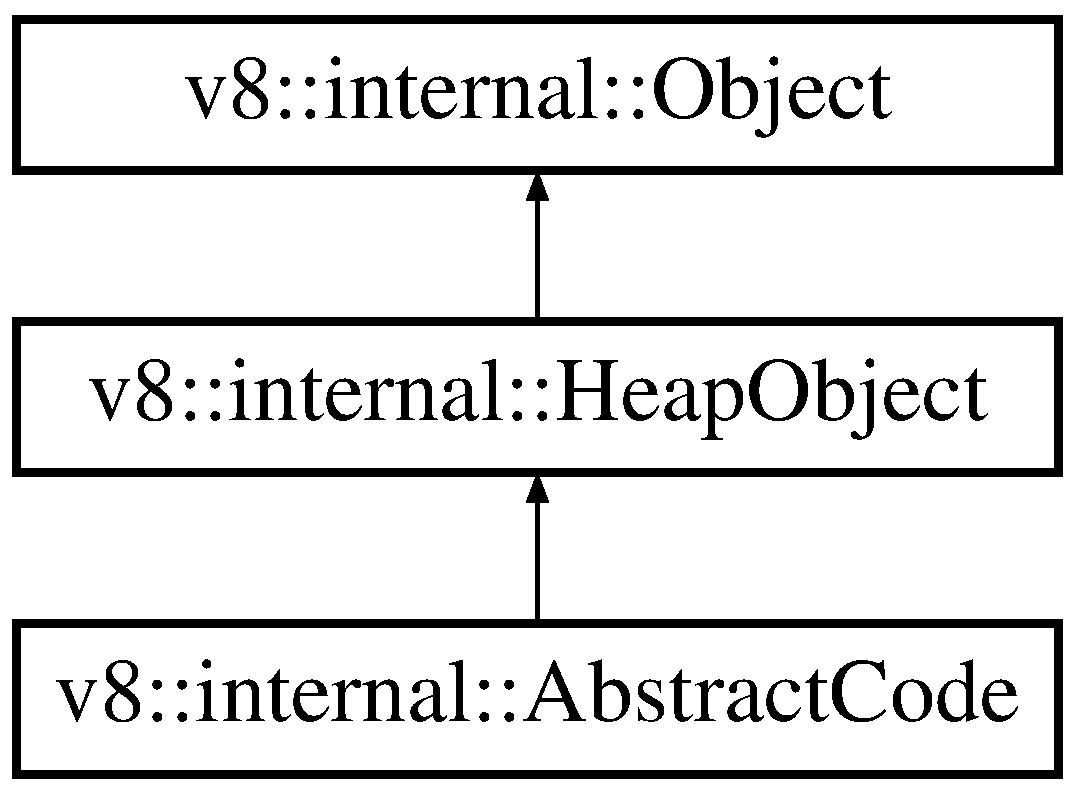
\includegraphics[height=3.000000cm]{classv8_1_1internal_1_1_abstract_code}
\end{center}
\end{figure}
\subsection*{Public Types}
\begin{DoxyCompactItemize}
\item 
enum {\bfseries Kind} \{ {\bfseries I\+N\+T\+E\+R\+P\+R\+E\+T\+E\+D\+\_\+\+F\+U\+N\+C\+T\+I\+ON}
 \}\hypertarget{classv8_1_1internal_1_1_abstract_code_a915d9a221d696e00492c45273de7d7c0}{}\label{classv8_1_1internal_1_1_abstract_code_a915d9a221d696e00492c45273de7d7c0}

\end{DoxyCompactItemize}
\subsection*{Public Member Functions}
\begin{DoxyCompactItemize}
\item 
int {\bfseries Source\+Position} (int offset)\hypertarget{classv8_1_1internal_1_1_abstract_code_acc3eba496172fd777c49536ba6563acf}{}\label{classv8_1_1internal_1_1_abstract_code_acc3eba496172fd777c49536ba6563acf}

\item 
int {\bfseries Source\+Statement\+Position} (int offset)\hypertarget{classv8_1_1internal_1_1_abstract_code_aeb9a9cdd430bb3c67e5810ac9fe340fb}{}\label{classv8_1_1internal_1_1_abstract_code_aeb9a9cdd430bb3c67e5810ac9fe340fb}

\item 
Address {\bfseries instruction\+\_\+start} ()\hypertarget{classv8_1_1internal_1_1_abstract_code_a5d65a3ecf8d493c1111839b5c6586e1f}{}\label{classv8_1_1internal_1_1_abstract_code_a5d65a3ecf8d493c1111839b5c6586e1f}

\item 
Address {\bfseries instruction\+\_\+end} ()\hypertarget{classv8_1_1internal_1_1_abstract_code_a4d3edc49282d5223eb890a93a7958c5d}{}\label{classv8_1_1internal_1_1_abstract_code_a4d3edc49282d5223eb890a93a7958c5d}

\item 
int {\bfseries instruction\+\_\+size} ()\hypertarget{classv8_1_1internal_1_1_abstract_code_a4a20676d355d56cff7972088ee2020fe}{}\label{classv8_1_1internal_1_1_abstract_code_a4a20676d355d56cff7972088ee2020fe}

\item 
bool {\bfseries contains} (byte $\ast$pc)\hypertarget{classv8_1_1internal_1_1_abstract_code_a93085d006c8af663984933c8c2ad25f9}{}\label{classv8_1_1internal_1_1_abstract_code_a93085d006c8af663984933c8c2ad25f9}

\item 
Kind {\bfseries kind} ()\hypertarget{classv8_1_1internal_1_1_abstract_code_a4467c4bef4b3900db4abc40a31f3ad55}{}\label{classv8_1_1internal_1_1_abstract_code_a4467c4bef4b3900db4abc40a31f3ad55}

\item 
int {\bfseries Executable\+Size} ()\hypertarget{classv8_1_1internal_1_1_abstract_code_affc1c1a7e415b017546f2a51c9677026}{}\label{classv8_1_1internal_1_1_abstract_code_affc1c1a7e415b017546f2a51c9677026}

\item 
\hyperlink{classv8_1_1internal_1_1_code}{Code} $\ast$ {\bfseries Get\+Code} ()\hypertarget{classv8_1_1internal_1_1_abstract_code_acaa5564ed3d80692b173047802758714}{}\label{classv8_1_1internal_1_1_abstract_code_acaa5564ed3d80692b173047802758714}

\item 
\hyperlink{classv8_1_1internal_1_1_bytecode_array}{Bytecode\+Array} $\ast$ {\bfseries Get\+Bytecode\+Array} ()\hypertarget{classv8_1_1internal_1_1_abstract_code_aa6026051cd3477398a7d1a2f92f544e8}{}\label{classv8_1_1internal_1_1_abstract_code_aa6026051cd3477398a7d1a2f92f544e8}

\end{DoxyCompactItemize}
\subsection*{Additional Inherited Members}


The documentation for this class was generated from the following files\+:\begin{DoxyCompactItemize}
\item 
/\+Users/joshgav/node/v8/src/objects.\+h\item 
/\+Users/joshgav/node/v8/src/objects-\/inl.\+h\item 
/\+Users/joshgav/node/v8/src/objects.\+cc\end{DoxyCompactItemize}

\hypertarget{classv8_1_1internal_1_1_access}{}\section{v8\+:\+:internal\+:\+:Access$<$ T $>$ Class Template Reference}
\label{classv8_1_1internal_1_1_access}\index{v8\+::internal\+::\+Access$<$ T $>$@{v8\+::internal\+::\+Access$<$ T $>$}}
\subsection*{Public Member Functions}
\begin{DoxyCompactItemize}
\item 
{\bfseries Access} (\hyperlink{classv8_1_1internal_1_1_static_resource}{Static\+Resource}$<$ T $>$ $\ast$resource)\hypertarget{classv8_1_1internal_1_1_access_a73d4e4a39835cc3d2314a328d80d0073}{}\label{classv8_1_1internal_1_1_access_a73d4e4a39835cc3d2314a328d80d0073}

\item 
T $\ast$ {\bfseries value} ()\hypertarget{classv8_1_1internal_1_1_access_ab9a3512d394b376ccba107df5f3c3d67}{}\label{classv8_1_1internal_1_1_access_ab9a3512d394b376ccba107df5f3c3d67}

\item 
T $\ast$ {\bfseries operator-\/$>$} ()\hypertarget{classv8_1_1internal_1_1_access_a71f5c7a9a355f726f309a13a5b6a8ab4}{}\label{classv8_1_1internal_1_1_access_a71f5c7a9a355f726f309a13a5b6a8ab4}

\end{DoxyCompactItemize}
\subsection*{Private Attributes}
\begin{DoxyCompactItemize}
\item 
\hyperlink{classv8_1_1internal_1_1_static_resource}{Static\+Resource}$<$ T $>$ $\ast$ {\bfseries resource\+\_\+}\hypertarget{classv8_1_1internal_1_1_access_af4bb6967363005f70e5377603c1e9677}{}\label{classv8_1_1internal_1_1_access_af4bb6967363005f70e5377603c1e9677}

\item 
T $\ast$ {\bfseries instance\+\_\+}\hypertarget{classv8_1_1internal_1_1_access_a554eca372f1a8dfe0dd35fc7206e94a2}{}\label{classv8_1_1internal_1_1_access_a554eca372f1a8dfe0dd35fc7206e94a2}

\end{DoxyCompactItemize}


The documentation for this class was generated from the following file\+:\begin{DoxyCompactItemize}
\item 
/\+Users/joshgav/node/v8/src/utils.\+h\end{DoxyCompactItemize}

\hypertarget{classv8_1_1internal_1_1compiler_1_1_access_builder}{}\section{v8\+:\+:internal\+:\+:compiler\+:\+:Access\+Builder Class Reference}
\label{classv8_1_1internal_1_1compiler_1_1_access_builder}\index{v8\+::internal\+::compiler\+::\+Access\+Builder@{v8\+::internal\+::compiler\+::\+Access\+Builder}}
Inheritance diagram for v8\+:\+:internal\+:\+:compiler\+:\+:Access\+Builder\+:\begin{figure}[H]
\begin{center}
\leavevmode
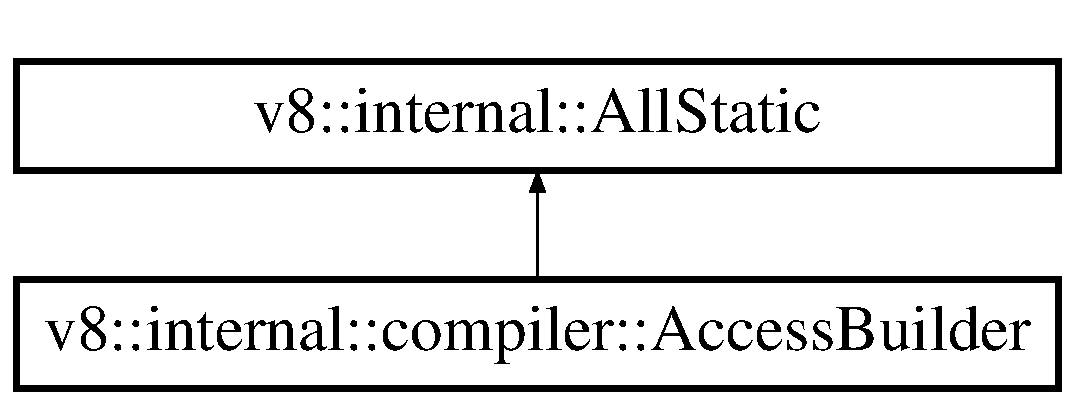
\includegraphics[height=2.000000cm]{classv8_1_1internal_1_1compiler_1_1_access_builder}
\end{center}
\end{figure}
\subsection*{Static Public Member Functions}
\begin{DoxyCompactItemize}
\item 
static \hyperlink{structv8_1_1internal_1_1compiler_1_1_field_access}{Field\+Access} {\bfseries For\+Map} ()\hypertarget{classv8_1_1internal_1_1compiler_1_1_access_builder_ac2bb52ee54e5b0ae7bbbbd4ea32a2647}{}\label{classv8_1_1internal_1_1compiler_1_1_access_builder_ac2bb52ee54e5b0ae7bbbbd4ea32a2647}

\item 
static \hyperlink{structv8_1_1internal_1_1compiler_1_1_field_access}{Field\+Access} {\bfseries For\+Heap\+Number\+Value} ()\hypertarget{classv8_1_1internal_1_1compiler_1_1_access_builder_a1fa84722d5a19479546399b5803d9325}{}\label{classv8_1_1internal_1_1compiler_1_1_access_builder_a1fa84722d5a19479546399b5803d9325}

\item 
static \hyperlink{structv8_1_1internal_1_1compiler_1_1_field_access}{Field\+Access} {\bfseries For\+J\+S\+Object\+Properties} ()\hypertarget{classv8_1_1internal_1_1compiler_1_1_access_builder_a0d6105104006aa27356444f0bfdbbf52}{}\label{classv8_1_1internal_1_1compiler_1_1_access_builder_a0d6105104006aa27356444f0bfdbbf52}

\item 
static \hyperlink{structv8_1_1internal_1_1compiler_1_1_field_access}{Field\+Access} {\bfseries For\+J\+S\+Object\+Elements} ()\hypertarget{classv8_1_1internal_1_1compiler_1_1_access_builder_afce72fe75259f693baee5435e7f9073d}{}\label{classv8_1_1internal_1_1compiler_1_1_access_builder_afce72fe75259f693baee5435e7f9073d}

\item 
static \hyperlink{structv8_1_1internal_1_1compiler_1_1_field_access}{Field\+Access} {\bfseries For\+J\+S\+Object\+In\+Object\+Property} (\hyperlink{classv8_1_1internal_1_1_handle}{Handle}$<$ \hyperlink{classv8_1_1internal_1_1_map}{Map} $>$ map, int index)\hypertarget{classv8_1_1internal_1_1compiler_1_1_access_builder_a1966ddbbd8f28ce33b30f700eb345f42}{}\label{classv8_1_1internal_1_1compiler_1_1_access_builder_a1966ddbbd8f28ce33b30f700eb345f42}

\item 
static \hyperlink{structv8_1_1internal_1_1compiler_1_1_field_access}{Field\+Access} {\bfseries For\+J\+S\+Function\+Prototype\+Or\+Initial\+Map} ()\hypertarget{classv8_1_1internal_1_1compiler_1_1_access_builder_ae67ee224508da0a19ca07ad72ac025ec}{}\label{classv8_1_1internal_1_1compiler_1_1_access_builder_ae67ee224508da0a19ca07ad72ac025ec}

\item 
static \hyperlink{structv8_1_1internal_1_1compiler_1_1_field_access}{Field\+Access} {\bfseries For\+J\+S\+Function\+Context} ()\hypertarget{classv8_1_1internal_1_1compiler_1_1_access_builder_a85fdfa37dd29156e9ae70b0a4865b431}{}\label{classv8_1_1internal_1_1compiler_1_1_access_builder_a85fdfa37dd29156e9ae70b0a4865b431}

\item 
static \hyperlink{structv8_1_1internal_1_1compiler_1_1_field_access}{Field\+Access} {\bfseries For\+J\+S\+Function\+Shared\+Function\+Info} ()\hypertarget{classv8_1_1internal_1_1compiler_1_1_access_builder_a62fbc921459ee05856f58ef1413221c5}{}\label{classv8_1_1internal_1_1compiler_1_1_access_builder_a62fbc921459ee05856f58ef1413221c5}

\item 
static \hyperlink{structv8_1_1internal_1_1compiler_1_1_field_access}{Field\+Access} {\bfseries For\+J\+S\+Function\+Literals} ()\hypertarget{classv8_1_1internal_1_1compiler_1_1_access_builder_afe3b44fc3f9a102a9b4b1b586632fb1f}{}\label{classv8_1_1internal_1_1compiler_1_1_access_builder_afe3b44fc3f9a102a9b4b1b586632fb1f}

\item 
static \hyperlink{structv8_1_1internal_1_1compiler_1_1_field_access}{Field\+Access} {\bfseries For\+J\+S\+Function\+Code\+Entry} ()\hypertarget{classv8_1_1internal_1_1compiler_1_1_access_builder_a3eb53bea6eb7faa73587aa143783abba}{}\label{classv8_1_1internal_1_1compiler_1_1_access_builder_a3eb53bea6eb7faa73587aa143783abba}

\item 
static \hyperlink{structv8_1_1internal_1_1compiler_1_1_field_access}{Field\+Access} {\bfseries For\+J\+S\+Function\+Next\+Function\+Link} ()\hypertarget{classv8_1_1internal_1_1compiler_1_1_access_builder_ae0046c3ec8727b235f1fbc923bdb81d6}{}\label{classv8_1_1internal_1_1compiler_1_1_access_builder_ae0046c3ec8727b235f1fbc923bdb81d6}

\item 
static \hyperlink{structv8_1_1internal_1_1compiler_1_1_field_access}{Field\+Access} {\bfseries For\+J\+S\+Array\+Length} (Elements\+Kind elements\+\_\+kind)\hypertarget{classv8_1_1internal_1_1compiler_1_1_access_builder_a6d1b43f02967d574807132fa27865e46}{}\label{classv8_1_1internal_1_1compiler_1_1_access_builder_a6d1b43f02967d574807132fa27865e46}

\item 
static \hyperlink{structv8_1_1internal_1_1compiler_1_1_field_access}{Field\+Access} {\bfseries For\+J\+S\+Array\+Buffer\+Backing\+Store} ()\hypertarget{classv8_1_1internal_1_1compiler_1_1_access_builder_a46eb6092a6a00b4d88958e64ae226518}{}\label{classv8_1_1internal_1_1compiler_1_1_access_builder_a46eb6092a6a00b4d88958e64ae226518}

\item 
static \hyperlink{structv8_1_1internal_1_1compiler_1_1_field_access}{Field\+Access} {\bfseries For\+J\+S\+Array\+Buffer\+Bit\+Field} ()\hypertarget{classv8_1_1internal_1_1compiler_1_1_access_builder_a49b702262a9c8d1484190ff9f038e8e9}{}\label{classv8_1_1internal_1_1compiler_1_1_access_builder_a49b702262a9c8d1484190ff9f038e8e9}

\item 
static \hyperlink{structv8_1_1internal_1_1compiler_1_1_field_access}{Field\+Access} {\bfseries For\+J\+S\+Array\+Buffer\+View\+Buffer} ()\hypertarget{classv8_1_1internal_1_1compiler_1_1_access_builder_a02537ce5d5a1ce7d1a1fef121a1626cd}{}\label{classv8_1_1internal_1_1compiler_1_1_access_builder_a02537ce5d5a1ce7d1a1fef121a1626cd}

\item 
static \hyperlink{structv8_1_1internal_1_1compiler_1_1_field_access}{Field\+Access} {\bfseries For\+J\+S\+Date\+Field} (J\+S\+Date\+::\+Field\+Index index)\hypertarget{classv8_1_1internal_1_1compiler_1_1_access_builder_a6694da00d86790879f46f22007099b7a}{}\label{classv8_1_1internal_1_1compiler_1_1_access_builder_a6694da00d86790879f46f22007099b7a}

\item 
static \hyperlink{structv8_1_1internal_1_1compiler_1_1_field_access}{Field\+Access} {\bfseries For\+J\+S\+Iterator\+Result\+Done} ()\hypertarget{classv8_1_1internal_1_1compiler_1_1_access_builder_a904efe1b02040e264c368a2a9386cddc}{}\label{classv8_1_1internal_1_1compiler_1_1_access_builder_a904efe1b02040e264c368a2a9386cddc}

\item 
static \hyperlink{structv8_1_1internal_1_1compiler_1_1_field_access}{Field\+Access} {\bfseries For\+J\+S\+Iterator\+Result\+Value} ()\hypertarget{classv8_1_1internal_1_1compiler_1_1_access_builder_a762b46b9e79781286d8d56ffb9d5f2bd}{}\label{classv8_1_1internal_1_1compiler_1_1_access_builder_a762b46b9e79781286d8d56ffb9d5f2bd}

\item 
static \hyperlink{structv8_1_1internal_1_1compiler_1_1_field_access}{Field\+Access} {\bfseries For\+J\+S\+Reg\+Exp\+Flags} ()\hypertarget{classv8_1_1internal_1_1compiler_1_1_access_builder_ade9388e3deec65b7df0b4f296ba3ad89}{}\label{classv8_1_1internal_1_1compiler_1_1_access_builder_ade9388e3deec65b7df0b4f296ba3ad89}

\item 
static \hyperlink{structv8_1_1internal_1_1compiler_1_1_field_access}{Field\+Access} {\bfseries For\+J\+S\+Reg\+Exp\+Source} ()\hypertarget{classv8_1_1internal_1_1compiler_1_1_access_builder_afce14f046b4b206b1386dba28a2ea568}{}\label{classv8_1_1internal_1_1compiler_1_1_access_builder_afce14f046b4b206b1386dba28a2ea568}

\item 
static \hyperlink{structv8_1_1internal_1_1compiler_1_1_field_access}{Field\+Access} {\bfseries For\+Fixed\+Array\+Length} ()\hypertarget{classv8_1_1internal_1_1compiler_1_1_access_builder_a60f2fc93086167e98d96af50182a5ca8}{}\label{classv8_1_1internal_1_1compiler_1_1_access_builder_a60f2fc93086167e98d96af50182a5ca8}

\item 
static \hyperlink{structv8_1_1internal_1_1compiler_1_1_field_access}{Field\+Access} {\bfseries For\+Descriptor\+Array\+Enum\+Cache} ()\hypertarget{classv8_1_1internal_1_1compiler_1_1_access_builder_af4b34439c6af9c48094ba98f5812c31c}{}\label{classv8_1_1internal_1_1compiler_1_1_access_builder_af4b34439c6af9c48094ba98f5812c31c}

\item 
static \hyperlink{structv8_1_1internal_1_1compiler_1_1_field_access}{Field\+Access} {\bfseries For\+Descriptor\+Array\+Enum\+Cache\+Bridge\+Cache} ()\hypertarget{classv8_1_1internal_1_1compiler_1_1_access_builder_ac89c350ecd6e8273743ae18294695287}{}\label{classv8_1_1internal_1_1compiler_1_1_access_builder_ac89c350ecd6e8273743ae18294695287}

\item 
static \hyperlink{structv8_1_1internal_1_1compiler_1_1_field_access}{Field\+Access} {\bfseries For\+Map\+Bit\+Field} ()\hypertarget{classv8_1_1internal_1_1compiler_1_1_access_builder_abf9c53e5e381ea12252cc705cb2621e6}{}\label{classv8_1_1internal_1_1compiler_1_1_access_builder_abf9c53e5e381ea12252cc705cb2621e6}

\item 
static \hyperlink{structv8_1_1internal_1_1compiler_1_1_field_access}{Field\+Access} {\bfseries For\+Map\+Bit\+Field3} ()\hypertarget{classv8_1_1internal_1_1compiler_1_1_access_builder_ac6bbccd21c20179cd7c22472c20ee91c}{}\label{classv8_1_1internal_1_1compiler_1_1_access_builder_ac6bbccd21c20179cd7c22472c20ee91c}

\item 
static \hyperlink{structv8_1_1internal_1_1compiler_1_1_field_access}{Field\+Access} {\bfseries For\+Map\+Descriptors} ()\hypertarget{classv8_1_1internal_1_1compiler_1_1_access_builder_ac06c1e97dd810afabadcf9c07c407816}{}\label{classv8_1_1internal_1_1compiler_1_1_access_builder_ac06c1e97dd810afabadcf9c07c407816}

\item 
static \hyperlink{structv8_1_1internal_1_1compiler_1_1_field_access}{Field\+Access} {\bfseries For\+Map\+Instance\+Type} ()\hypertarget{classv8_1_1internal_1_1compiler_1_1_access_builder_aa310a137a1d7db1810306fb147b6bcbb}{}\label{classv8_1_1internal_1_1compiler_1_1_access_builder_aa310a137a1d7db1810306fb147b6bcbb}

\item 
static \hyperlink{structv8_1_1internal_1_1compiler_1_1_field_access}{Field\+Access} {\bfseries For\+Map\+Prototype} ()\hypertarget{classv8_1_1internal_1_1compiler_1_1_access_builder_a8d21c3e3546bf52bab18509c099bfacf}{}\label{classv8_1_1internal_1_1compiler_1_1_access_builder_a8d21c3e3546bf52bab18509c099bfacf}

\item 
static \hyperlink{structv8_1_1internal_1_1compiler_1_1_field_access}{Field\+Access} {\bfseries For\+String\+Length} ()\hypertarget{classv8_1_1internal_1_1compiler_1_1_access_builder_a63dda93634c3e9a53600203247bb8835}{}\label{classv8_1_1internal_1_1compiler_1_1_access_builder_a63dda93634c3e9a53600203247bb8835}

\item 
static \hyperlink{structv8_1_1internal_1_1compiler_1_1_field_access}{Field\+Access} {\bfseries For\+J\+S\+Global\+Object\+Global\+Proxy} ()\hypertarget{classv8_1_1internal_1_1compiler_1_1_access_builder_a835be16ed015a9f1e41d2e2c5173b79c}{}\label{classv8_1_1internal_1_1compiler_1_1_access_builder_a835be16ed015a9f1e41d2e2c5173b79c}

\item 
static \hyperlink{structv8_1_1internal_1_1compiler_1_1_field_access}{Field\+Access} {\bfseries For\+J\+S\+Global\+Object\+Native\+Context} ()\hypertarget{classv8_1_1internal_1_1compiler_1_1_access_builder_ac92df8e73ddb8ca443ceeef62d35de7f}{}\label{classv8_1_1internal_1_1compiler_1_1_access_builder_ac92df8e73ddb8ca443ceeef62d35de7f}

\item 
static \hyperlink{structv8_1_1internal_1_1compiler_1_1_field_access}{Field\+Access} {\bfseries For\+Value} ()\hypertarget{classv8_1_1internal_1_1compiler_1_1_access_builder_af19b57601c7d120b9481439278728283}{}\label{classv8_1_1internal_1_1compiler_1_1_access_builder_af19b57601c7d120b9481439278728283}

\item 
static \hyperlink{structv8_1_1internal_1_1compiler_1_1_field_access}{Field\+Access} {\bfseries For\+Arguments\+Length} ()\hypertarget{classv8_1_1internal_1_1compiler_1_1_access_builder_a243c17c4a768954c87037f776d7f201b}{}\label{classv8_1_1internal_1_1compiler_1_1_access_builder_a243c17c4a768954c87037f776d7f201b}

\item 
static \hyperlink{structv8_1_1internal_1_1compiler_1_1_field_access}{Field\+Access} {\bfseries For\+Arguments\+Callee} ()\hypertarget{classv8_1_1internal_1_1compiler_1_1_access_builder_a6bfeffa464912a295c5a8bbdb353df3e}{}\label{classv8_1_1internal_1_1compiler_1_1_access_builder_a6bfeffa464912a295c5a8bbdb353df3e}

\item 
static \hyperlink{structv8_1_1internal_1_1compiler_1_1_field_access}{Field\+Access} {\bfseries For\+Fixed\+Array\+Slot} (size\+\_\+t index)\hypertarget{classv8_1_1internal_1_1compiler_1_1_access_builder_a0c333616e603afb52325cea0f19a2a41}{}\label{classv8_1_1internal_1_1compiler_1_1_access_builder_a0c333616e603afb52325cea0f19a2a41}

\item 
static \hyperlink{structv8_1_1internal_1_1compiler_1_1_field_access}{Field\+Access} {\bfseries For\+Context\+Slot} (size\+\_\+t index)\hypertarget{classv8_1_1internal_1_1compiler_1_1_access_builder_a849c1e08947e7016768fd469278a0359}{}\label{classv8_1_1internal_1_1compiler_1_1_access_builder_a849c1e08947e7016768fd469278a0359}

\item 
static \hyperlink{structv8_1_1internal_1_1compiler_1_1_field_access}{Field\+Access} {\bfseries For\+Property\+Cell\+Value} ()\hypertarget{classv8_1_1internal_1_1compiler_1_1_access_builder_ad0db4ca47805de76a85750ad558017cd}{}\label{classv8_1_1internal_1_1compiler_1_1_access_builder_ad0db4ca47805de76a85750ad558017cd}

\item 
static \hyperlink{structv8_1_1internal_1_1compiler_1_1_field_access}{Field\+Access} {\bfseries For\+Property\+Cell\+Value} (\hyperlink{classv8_1_1internal_1_1_type}{Type} $\ast$type)\hypertarget{classv8_1_1internal_1_1compiler_1_1_access_builder_a49af5c95d8d81871a9af82903e3b49da}{}\label{classv8_1_1internal_1_1compiler_1_1_access_builder_a49af5c95d8d81871a9af82903e3b49da}

\item 
static \hyperlink{structv8_1_1internal_1_1compiler_1_1_field_access}{Field\+Access} {\bfseries For\+Shared\+Function\+Info\+Type\+Feedback\+Vector} ()\hypertarget{classv8_1_1internal_1_1compiler_1_1_access_builder_ac9fac30910c737f9250961495d295522}{}\label{classv8_1_1internal_1_1compiler_1_1_access_builder_ac9fac30910c737f9250961495d295522}

\item 
static \hyperlink{structv8_1_1internal_1_1compiler_1_1_element_access}{Element\+Access} {\bfseries For\+Fixed\+Array\+Element} ()\hypertarget{classv8_1_1internal_1_1compiler_1_1_access_builder_a035b9d06a48396c4796334a518525118}{}\label{classv8_1_1internal_1_1compiler_1_1_access_builder_a035b9d06a48396c4796334a518525118}

\item 
static \hyperlink{structv8_1_1internal_1_1compiler_1_1_element_access}{Element\+Access} {\bfseries For\+Fixed\+Double\+Array\+Element} ()\hypertarget{classv8_1_1internal_1_1compiler_1_1_access_builder_a907683f6dc1f3397f18cf7d36c382747}{}\label{classv8_1_1internal_1_1compiler_1_1_access_builder_a907683f6dc1f3397f18cf7d36c382747}

\item 
static \hyperlink{structv8_1_1internal_1_1compiler_1_1_element_access}{Element\+Access} {\bfseries For\+Typed\+Array\+Element} (External\+Array\+Type type, bool is\+\_\+external)\hypertarget{classv8_1_1internal_1_1compiler_1_1_access_builder_abd1ea13ee9156b6e746a9fd8f21c53f2}{}\label{classv8_1_1internal_1_1compiler_1_1_access_builder_abd1ea13ee9156b6e746a9fd8f21c53f2}

\end{DoxyCompactItemize}
\subsection*{Private Member Functions}
\begin{DoxyCompactItemize}
\item 
{\bfseries D\+I\+S\+A\+L\+L\+O\+W\+\_\+\+I\+M\+P\+L\+I\+C\+I\+T\+\_\+\+C\+O\+N\+S\+T\+R\+U\+C\+T\+O\+RS} (\hyperlink{classv8_1_1internal_1_1compiler_1_1_access_builder}{Access\+Builder})\hypertarget{classv8_1_1internal_1_1compiler_1_1_access_builder_acf60793e7eaffbc18215caafa3b831a0}{}\label{classv8_1_1internal_1_1compiler_1_1_access_builder_acf60793e7eaffbc18215caafa3b831a0}

\end{DoxyCompactItemize}


The documentation for this class was generated from the following files\+:\begin{DoxyCompactItemize}
\item 
/\+Users/joshgav/node/v8/src/compiler/access-\/builder.\+h\item 
/\+Users/joshgav/node/v8/src/compiler/access-\/builder.\+cc\end{DoxyCompactItemize}

\hypertarget{classv8_1_1internal_1_1_access_check_info}{}\section{v8\+:\+:internal\+:\+:Access\+Check\+Info Class Reference}
\label{classv8_1_1internal_1_1_access_check_info}\index{v8\+::internal\+::\+Access\+Check\+Info@{v8\+::internal\+::\+Access\+Check\+Info}}
Inheritance diagram for v8\+:\+:internal\+:\+:Access\+Check\+Info\+:\begin{figure}[H]
\begin{center}
\leavevmode
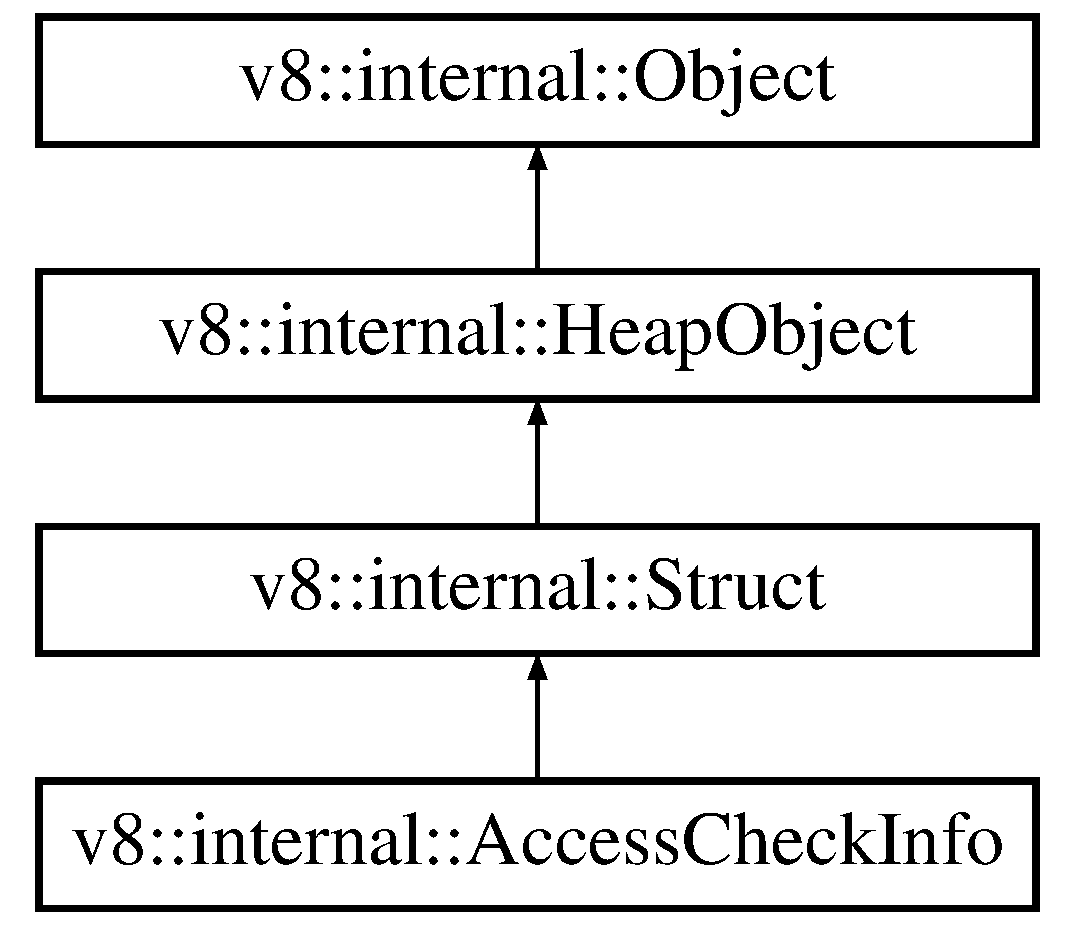
\includegraphics[height=4.000000cm]{classv8_1_1internal_1_1_access_check_info}
\end{center}
\end{figure}
\subsection*{Static Public Attributes}
\begin{DoxyCompactItemize}
\item 
static const int {\bfseries k\+Named\+Callback\+Offset} = Heap\+Object\+::k\+Header\+Size\hypertarget{classv8_1_1internal_1_1_access_check_info_a6cbd64c953819b14e3944340ad05e048}{}\label{classv8_1_1internal_1_1_access_check_info_a6cbd64c953819b14e3944340ad05e048}

\item 
static const int {\bfseries k\+Indexed\+Callback\+Offset} = k\+Named\+Callback\+Offset + k\+Pointer\+Size\hypertarget{classv8_1_1internal_1_1_access_check_info_a5bcd567490f425a95da4a3dae4e73e11}{}\label{classv8_1_1internal_1_1_access_check_info_a5bcd567490f425a95da4a3dae4e73e11}

\item 
static const int {\bfseries k\+Callback\+Offset} = k\+Indexed\+Callback\+Offset + k\+Pointer\+Size\hypertarget{classv8_1_1internal_1_1_access_check_info_ad7efe45a5c6352736d2a37edcebc9eda}{}\label{classv8_1_1internal_1_1_access_check_info_ad7efe45a5c6352736d2a37edcebc9eda}

\item 
static const int {\bfseries k\+Data\+Offset} = k\+Callback\+Offset + k\+Pointer\+Size\hypertarget{classv8_1_1internal_1_1_access_check_info_a1739da947958ae7735ac674e2aac415b}{}\label{classv8_1_1internal_1_1_access_check_info_a1739da947958ae7735ac674e2aac415b}

\item 
static const int {\bfseries k\+Size} = k\+Data\+Offset + k\+Pointer\+Size\hypertarget{classv8_1_1internal_1_1_access_check_info_a30e7585ebfa4c24c214bc5a9f77ad0c3}{}\label{classv8_1_1internal_1_1_access_check_info_a30e7585ebfa4c24c214bc5a9f77ad0c3}

\end{DoxyCompactItemize}
\subsection*{Private Member Functions}
\begin{DoxyCompactItemize}
\item 
{\bfseries D\+I\+S\+A\+L\+L\+O\+W\+\_\+\+I\+M\+P\+L\+I\+C\+I\+T\+\_\+\+C\+O\+N\+S\+T\+R\+U\+C\+T\+O\+RS} (\hyperlink{classv8_1_1internal_1_1_access_check_info}{Access\+Check\+Info})\hypertarget{classv8_1_1internal_1_1_access_check_info_a95720e5a1661f82278ec82cd0e9b4c98}{}\label{classv8_1_1internal_1_1_access_check_info_a95720e5a1661f82278ec82cd0e9b4c98}

\end{DoxyCompactItemize}
\subsection*{Additional Inherited Members}


The documentation for this class was generated from the following file\+:\begin{DoxyCompactItemize}
\item 
/\+Users/joshgav/node/v8/src/objects.\+h\end{DoxyCompactItemize}

\hypertarget{classv8_1_1internal_1_1compiler_1_1_access_info_factory}{}\section{v8\+:\+:internal\+:\+:compiler\+:\+:Access\+Info\+Factory Class Reference}
\label{classv8_1_1internal_1_1compiler_1_1_access_info_factory}\index{v8\+::internal\+::compiler\+::\+Access\+Info\+Factory@{v8\+::internal\+::compiler\+::\+Access\+Info\+Factory}}
\subsection*{Public Member Functions}
\begin{DoxyCompactItemize}
\item 
{\bfseries Access\+Info\+Factory} (\hyperlink{classv8_1_1internal_1_1_compilation_dependencies}{Compilation\+Dependencies} $\ast$dependencies, \hyperlink{classv8_1_1internal_1_1_handle}{Handle}$<$ \hyperlink{classv8_1_1internal_1_1_context}{Context} $>$ native\+\_\+context, \hyperlink{classv8_1_1internal_1_1_zone}{Zone} $\ast$zone)\hypertarget{classv8_1_1internal_1_1compiler_1_1_access_info_factory_aafc5535293ee123adc93261670871aa2}{}\label{classv8_1_1internal_1_1compiler_1_1_access_info_factory_aafc5535293ee123adc93261670871aa2}

\item 
bool {\bfseries Compute\+Element\+Access\+Info} (\hyperlink{classv8_1_1internal_1_1_handle}{Handle}$<$ \hyperlink{classv8_1_1internal_1_1_map}{Map} $>$ map, Access\+Mode access\+\_\+mode, \hyperlink{classv8_1_1internal_1_1compiler_1_1_element_access_info}{Element\+Access\+Info} $\ast$access\+\_\+info)\hypertarget{classv8_1_1internal_1_1compiler_1_1_access_info_factory_aa7540604d39b50722ee923b8ffaf2145}{}\label{classv8_1_1internal_1_1compiler_1_1_access_info_factory_aa7540604d39b50722ee923b8ffaf2145}

\item 
bool {\bfseries Compute\+Element\+Access\+Infos} (\hyperlink{classv8_1_1internal_1_1_list}{Map\+Handle\+List} const \&maps, Access\+Mode access\+\_\+mode, \hyperlink{classv8_1_1internal_1_1_zone_vector}{Zone\+Vector}$<$ \hyperlink{classv8_1_1internal_1_1compiler_1_1_element_access_info}{Element\+Access\+Info} $>$ $\ast$access\+\_\+infos)\hypertarget{classv8_1_1internal_1_1compiler_1_1_access_info_factory_a428bf7e578848656823cdbb64a88e91a}{}\label{classv8_1_1internal_1_1compiler_1_1_access_info_factory_a428bf7e578848656823cdbb64a88e91a}

\item 
bool {\bfseries Compute\+Property\+Access\+Info} (\hyperlink{classv8_1_1internal_1_1_handle}{Handle}$<$ \hyperlink{classv8_1_1internal_1_1_map}{Map} $>$ map, \hyperlink{classv8_1_1internal_1_1_handle}{Handle}$<$ \hyperlink{classv8_1_1internal_1_1_name}{Name} $>$ name, Access\+Mode access\+\_\+mode, \hyperlink{classv8_1_1internal_1_1compiler_1_1_property_access_info}{Property\+Access\+Info} $\ast$access\+\_\+info)\hypertarget{classv8_1_1internal_1_1compiler_1_1_access_info_factory_a099ee7c7da8ee81a875f4f5570cdfbae}{}\label{classv8_1_1internal_1_1compiler_1_1_access_info_factory_a099ee7c7da8ee81a875f4f5570cdfbae}

\item 
bool {\bfseries Compute\+Property\+Access\+Infos} (\hyperlink{classv8_1_1internal_1_1_list}{Map\+Handle\+List} const \&maps, \hyperlink{classv8_1_1internal_1_1_handle}{Handle}$<$ \hyperlink{classv8_1_1internal_1_1_name}{Name} $>$ name, Access\+Mode access\+\_\+mode, \hyperlink{classv8_1_1internal_1_1_zone_vector}{Zone\+Vector}$<$ \hyperlink{classv8_1_1internal_1_1compiler_1_1_property_access_info}{Property\+Access\+Info} $>$ $\ast$access\+\_\+infos)\hypertarget{classv8_1_1internal_1_1compiler_1_1_access_info_factory_a0abedcc1b1b7aa570b27991f36d3d31c}{}\label{classv8_1_1internal_1_1compiler_1_1_access_info_factory_a0abedcc1b1b7aa570b27991f36d3d31c}

\end{DoxyCompactItemize}
\subsection*{Private Member Functions}
\begin{DoxyCompactItemize}
\item 
bool {\bfseries Lookup\+Special\+Field\+Accessor} (\hyperlink{classv8_1_1internal_1_1_handle}{Handle}$<$ \hyperlink{classv8_1_1internal_1_1_map}{Map} $>$ map, \hyperlink{classv8_1_1internal_1_1_handle}{Handle}$<$ \hyperlink{classv8_1_1internal_1_1_name}{Name} $>$ name, \hyperlink{classv8_1_1internal_1_1compiler_1_1_property_access_info}{Property\+Access\+Info} $\ast$access\+\_\+info)\hypertarget{classv8_1_1internal_1_1compiler_1_1_access_info_factory_aaa37cfffafa24b3c04487708dab6e99b}{}\label{classv8_1_1internal_1_1compiler_1_1_access_info_factory_aaa37cfffafa24b3c04487708dab6e99b}

\item 
bool {\bfseries Lookup\+Transition} (\hyperlink{classv8_1_1internal_1_1_handle}{Handle}$<$ \hyperlink{classv8_1_1internal_1_1_map}{Map} $>$ map, \hyperlink{classv8_1_1internal_1_1_handle}{Handle}$<$ \hyperlink{classv8_1_1internal_1_1_name}{Name} $>$ name, \hyperlink{classv8_1_1internal_1_1_maybe_handle}{Maybe\+Handle}$<$ \hyperlink{classv8_1_1internal_1_1_j_s_object}{J\+S\+Object} $>$ holder, \hyperlink{classv8_1_1internal_1_1compiler_1_1_property_access_info}{Property\+Access\+Info} $\ast$access\+\_\+info)\hypertarget{classv8_1_1internal_1_1compiler_1_1_access_info_factory_ac4e8c3a84f8f63a087a8ad76978bcf76}{}\label{classv8_1_1internal_1_1compiler_1_1_access_info_factory_ac4e8c3a84f8f63a087a8ad76978bcf76}

\item 
\hyperlink{classv8_1_1internal_1_1_compilation_dependencies}{Compilation\+Dependencies} $\ast$ {\bfseries dependencies} () const \hypertarget{classv8_1_1internal_1_1compiler_1_1_access_info_factory_ad49204a5516119cd4ecf2092c1a5fbf3}{}\label{classv8_1_1internal_1_1compiler_1_1_access_info_factory_ad49204a5516119cd4ecf2092c1a5fbf3}

\item 
\hyperlink{classv8_1_1internal_1_1_factory}{Factory} $\ast$ {\bfseries factory} () const \hypertarget{classv8_1_1internal_1_1compiler_1_1_access_info_factory_a506bc9c13103839833703cfac3433d23}{}\label{classv8_1_1internal_1_1compiler_1_1_access_info_factory_a506bc9c13103839833703cfac3433d23}

\item 
\hyperlink{classv8_1_1internal_1_1_isolate}{Isolate} $\ast$ {\bfseries isolate} () const \hypertarget{classv8_1_1internal_1_1compiler_1_1_access_info_factory_a2b5f9560950230607d9bc9da5ad35809}{}\label{classv8_1_1internal_1_1compiler_1_1_access_info_factory_a2b5f9560950230607d9bc9da5ad35809}

\item 
\hyperlink{classv8_1_1internal_1_1_handle}{Handle}$<$ \hyperlink{classv8_1_1internal_1_1_context}{Context} $>$ {\bfseries native\+\_\+context} () const \hypertarget{classv8_1_1internal_1_1compiler_1_1_access_info_factory_a971ed0253bf44e64700e24cdd4ca1810}{}\label{classv8_1_1internal_1_1compiler_1_1_access_info_factory_a971ed0253bf44e64700e24cdd4ca1810}

\item 
\hyperlink{classv8_1_1internal_1_1_zone}{Zone} $\ast$ {\bfseries zone} () const \hypertarget{classv8_1_1internal_1_1compiler_1_1_access_info_factory_aa4f8c73983e5a5ee4c0a106507274df5}{}\label{classv8_1_1internal_1_1compiler_1_1_access_info_factory_aa4f8c73983e5a5ee4c0a106507274df5}

\item 
{\bfseries D\+I\+S\+A\+L\+L\+O\+W\+\_\+\+C\+O\+P\+Y\+\_\+\+A\+N\+D\+\_\+\+A\+S\+S\+I\+GN} (\hyperlink{classv8_1_1internal_1_1compiler_1_1_access_info_factory}{Access\+Info\+Factory})\hypertarget{classv8_1_1internal_1_1compiler_1_1_access_info_factory_a8d171dfabb5db320db1f92903b2cb4ef}{}\label{classv8_1_1internal_1_1compiler_1_1_access_info_factory_a8d171dfabb5db320db1f92903b2cb4ef}

\end{DoxyCompactItemize}
\subsection*{Private Attributes}
\begin{DoxyCompactItemize}
\item 
\hyperlink{classv8_1_1internal_1_1_compilation_dependencies}{Compilation\+Dependencies} $\ast$const {\bfseries dependencies\+\_\+}\hypertarget{classv8_1_1internal_1_1compiler_1_1_access_info_factory_a40431c52616f5ab622a3f6ee1505a5d6}{}\label{classv8_1_1internal_1_1compiler_1_1_access_info_factory_a40431c52616f5ab622a3f6ee1505a5d6}

\item 
\hyperlink{classv8_1_1internal_1_1_handle}{Handle}$<$ \hyperlink{classv8_1_1internal_1_1_context}{Context} $>$ const {\bfseries native\+\_\+context\+\_\+}\hypertarget{classv8_1_1internal_1_1compiler_1_1_access_info_factory_a646063a9300faf25ac27ba61181f4e17}{}\label{classv8_1_1internal_1_1compiler_1_1_access_info_factory_a646063a9300faf25ac27ba61181f4e17}

\item 
\hyperlink{classv8_1_1internal_1_1_isolate}{Isolate} $\ast$const {\bfseries isolate\+\_\+}\hypertarget{classv8_1_1internal_1_1compiler_1_1_access_info_factory_a59312ab517b84bc8755373307473249b}{}\label{classv8_1_1internal_1_1compiler_1_1_access_info_factory_a59312ab517b84bc8755373307473249b}

\item 
\hyperlink{classv8_1_1internal_1_1_type_cache}{Type\+Cache} const \& {\bfseries type\+\_\+cache\+\_\+}\hypertarget{classv8_1_1internal_1_1compiler_1_1_access_info_factory_ac1417e678c5bdaa0fdf19888cb551236}{}\label{classv8_1_1internal_1_1compiler_1_1_access_info_factory_ac1417e678c5bdaa0fdf19888cb551236}

\item 
\hyperlink{classv8_1_1internal_1_1_zone}{Zone} $\ast$const {\bfseries zone\+\_\+}\hypertarget{classv8_1_1internal_1_1compiler_1_1_access_info_factory_a0b2cd82eee5d3dd62c56b47ff1f0e144}{}\label{classv8_1_1internal_1_1compiler_1_1_access_info_factory_a0b2cd82eee5d3dd62c56b47ff1f0e144}

\end{DoxyCompactItemize}


The documentation for this class was generated from the following files\+:\begin{DoxyCompactItemize}
\item 
/\+Users/joshgav/node/v8/src/compiler/access-\/info.\+h\item 
/\+Users/joshgav/node/v8/src/compiler/access-\/info.\+cc\end{DoxyCompactItemize}

\hypertarget{classv8_1_1internal_1_1_accessor_constant_descriptor}{}\section{v8\+:\+:internal\+:\+:Accessor\+Constant\+Descriptor Class Reference}
\label{classv8_1_1internal_1_1_accessor_constant_descriptor}\index{v8\+::internal\+::\+Accessor\+Constant\+Descriptor@{v8\+::internal\+::\+Accessor\+Constant\+Descriptor}}
Inheritance diagram for v8\+:\+:internal\+:\+:Accessor\+Constant\+Descriptor\+:\begin{figure}[H]
\begin{center}
\leavevmode
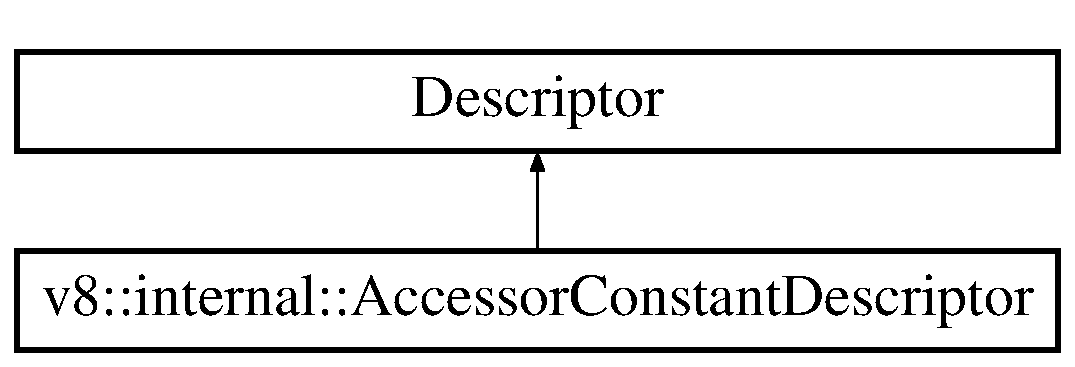
\includegraphics[height=2.000000cm]{classv8_1_1internal_1_1_accessor_constant_descriptor}
\end{center}
\end{figure}
\subsection*{Public Member Functions}
\begin{DoxyCompactItemize}
\item 
{\bfseries Accessor\+Constant\+Descriptor} (\hyperlink{classv8_1_1internal_1_1_handle}{Handle}$<$ \hyperlink{classv8_1_1internal_1_1_name}{Name} $>$ key, \hyperlink{classv8_1_1internal_1_1_handle}{Handle}$<$ \hyperlink{classv8_1_1internal_1_1_object}{Object} $>$ foreign, Property\+Attributes attributes)\hypertarget{classv8_1_1internal_1_1_accessor_constant_descriptor_af3252e5d188b9614d30566194b2bedb6}{}\label{classv8_1_1internal_1_1_accessor_constant_descriptor_af3252e5d188b9614d30566194b2bedb6}

\end{DoxyCompactItemize}


The documentation for this class was generated from the following file\+:\begin{DoxyCompactItemize}
\item 
/\+Users/joshgav/node/v8/src/property.\+h\end{DoxyCompactItemize}

\hypertarget{structv8_1_1internal_1_1_accessor_descriptor}{}\section{v8\+:\+:internal\+:\+:Accessor\+Descriptor Struct Reference}
\label{structv8_1_1internal_1_1_accessor_descriptor}\index{v8\+::internal\+::\+Accessor\+Descriptor@{v8\+::internal\+::\+Accessor\+Descriptor}}
\subsection*{Public Attributes}
\begin{DoxyCompactItemize}
\item 
\hyperlink{classv8_1_1internal_1_1_object}{Object} $\ast$($\ast$ {\bfseries getter} )(\hyperlink{classv8_1_1internal_1_1_isolate}{Isolate} $\ast$isolate, \hyperlink{classv8_1_1internal_1_1_object}{Object} $\ast$object, void $\ast$data)\hypertarget{structv8_1_1internal_1_1_accessor_descriptor_a0fd4975f95e4accee711fe7144fcd91c}{}\label{structv8_1_1internal_1_1_accessor_descriptor_a0fd4975f95e4accee711fe7144fcd91c}

\item 
\hyperlink{classv8_1_1internal_1_1_object}{Object} $\ast$($\ast$ {\bfseries setter} )(\hyperlink{classv8_1_1internal_1_1_isolate}{Isolate} $\ast$isolate, \hyperlink{classv8_1_1internal_1_1_j_s_object}{J\+S\+Object} $\ast$object, \hyperlink{classv8_1_1internal_1_1_object}{Object} $\ast$value, void $\ast$data)\hypertarget{structv8_1_1internal_1_1_accessor_descriptor_abe99f0b12d8048825a324b575b837dca}{}\label{structv8_1_1internal_1_1_accessor_descriptor_abe99f0b12d8048825a324b575b837dca}

\item 
void $\ast$ {\bfseries data}\hypertarget{structv8_1_1internal_1_1_accessor_descriptor_acc4fa03840c10eea3f97798ea0cfc632}{}\label{structv8_1_1internal_1_1_accessor_descriptor_acc4fa03840c10eea3f97798ea0cfc632}

\end{DoxyCompactItemize}


The documentation for this struct was generated from the following file\+:\begin{DoxyCompactItemize}
\item 
/\+Users/joshgav/node/v8/src/globals.\+h\end{DoxyCompactItemize}

\hypertarget{classv8_1_1internal_1_1_accessor_info}{}\section{v8\+:\+:internal\+:\+:Accessor\+Info Class Reference}
\label{classv8_1_1internal_1_1_accessor_info}\index{v8\+::internal\+::\+Accessor\+Info@{v8\+::internal\+::\+Accessor\+Info}}
Inheritance diagram for v8\+:\+:internal\+:\+:Accessor\+Info\+:\begin{figure}[H]
\begin{center}
\leavevmode
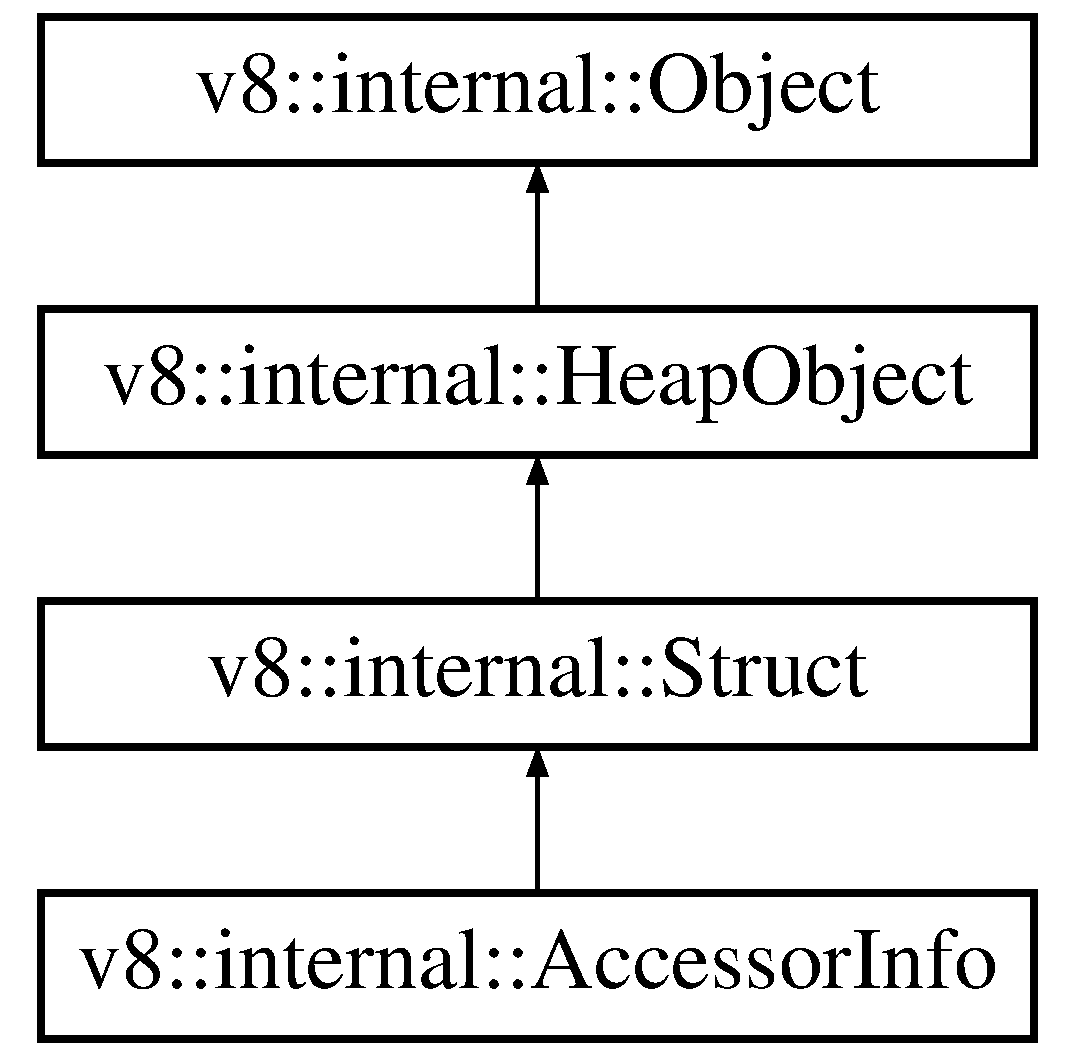
\includegraphics[height=4.000000cm]{classv8_1_1internal_1_1_accessor_info}
\end{center}
\end{figure}
\subsection*{Classes}
\begin{DoxyCompactItemize}
\item 
class \hyperlink{classv8_1_1internal_1_1_accessor_info_1_1_attributes_field}{Attributes\+Field}
\end{DoxyCompactItemize}
\subsection*{Public Member Functions}
\begin{DoxyCompactItemize}
\item 
Address {\bfseries redirected\+\_\+getter} () const \hypertarget{classv8_1_1internal_1_1_accessor_info_af5366b96ec3b5d836dbc226478c36afc}{}\label{classv8_1_1internal_1_1_accessor_info_af5366b96ec3b5d836dbc226478c36afc}

\item 
bool {\bfseries all\+\_\+can\+\_\+read} ()\hypertarget{classv8_1_1internal_1_1_accessor_info_a15ee717df70fd30880f5a3e15a90b02a}{}\label{classv8_1_1internal_1_1_accessor_info_a15ee717df70fd30880f5a3e15a90b02a}

\item 
void {\bfseries set\+\_\+all\+\_\+can\+\_\+read} (bool value)\hypertarget{classv8_1_1internal_1_1_accessor_info_afc007f500afa962d19ef75d52de03c89}{}\label{classv8_1_1internal_1_1_accessor_info_afc007f500afa962d19ef75d52de03c89}

\item 
bool {\bfseries all\+\_\+can\+\_\+write} ()\hypertarget{classv8_1_1internal_1_1_accessor_info_acb963c18a2b77d7b79ebca64b8192a12}{}\label{classv8_1_1internal_1_1_accessor_info_acb963c18a2b77d7b79ebca64b8192a12}

\item 
void {\bfseries set\+\_\+all\+\_\+can\+\_\+write} (bool value)\hypertarget{classv8_1_1internal_1_1_accessor_info_a7845e45a30b59305f606d8b3dbbabb13}{}\label{classv8_1_1internal_1_1_accessor_info_a7845e45a30b59305f606d8b3dbbabb13}

\item 
bool {\bfseries is\+\_\+special\+\_\+data\+\_\+property} ()\hypertarget{classv8_1_1internal_1_1_accessor_info_a1593220a13db54879356273d2282bc59}{}\label{classv8_1_1internal_1_1_accessor_info_a1593220a13db54879356273d2282bc59}

\item 
void {\bfseries set\+\_\+is\+\_\+special\+\_\+data\+\_\+property} (bool value)\hypertarget{classv8_1_1internal_1_1_accessor_info_a371c23f5c55f35df10826494ed9fa469}{}\label{classv8_1_1internal_1_1_accessor_info_a371c23f5c55f35df10826494ed9fa469}

\item 
Property\+Attributes {\bfseries property\+\_\+attributes} ()\hypertarget{classv8_1_1internal_1_1_accessor_info_a13c8eb4416eee0482ef82e32c7df4ea6}{}\label{classv8_1_1internal_1_1_accessor_info_a13c8eb4416eee0482ef82e32c7df4ea6}

\item 
void {\bfseries set\+\_\+property\+\_\+attributes} (Property\+Attributes attributes)\hypertarget{classv8_1_1internal_1_1_accessor_info_ad7d09993c5975f13a58aced7e1b482eb}{}\label{classv8_1_1internal_1_1_accessor_info_ad7d09993c5975f13a58aced7e1b482eb}

\item 
bool {\bfseries Is\+Compatible\+Receiver} (\hyperlink{classv8_1_1internal_1_1_object}{Object} $\ast$receiver)\hypertarget{classv8_1_1internal_1_1_accessor_info_af90ccc9b509016f749a5d69a29cebdf4}{}\label{classv8_1_1internal_1_1_accessor_info_af90ccc9b509016f749a5d69a29cebdf4}

\end{DoxyCompactItemize}
\subsection*{Static Public Member Functions}
\begin{DoxyCompactItemize}
\item 
static Address {\bfseries redirect} (\hyperlink{classv8_1_1internal_1_1_isolate}{Isolate} $\ast$isolate, Address address, Accessor\+Component component)\hypertarget{classv8_1_1internal_1_1_accessor_info_a5c296b2f2826fd5c775bda98dbb04989}{}\label{classv8_1_1internal_1_1_accessor_info_a5c296b2f2826fd5c775bda98dbb04989}

\item 
static bool {\bfseries Is\+Compatible\+Receiver\+Map} (\hyperlink{classv8_1_1internal_1_1_isolate}{Isolate} $\ast$isolate, \hyperlink{classv8_1_1internal_1_1_handle}{Handle}$<$ \hyperlink{classv8_1_1internal_1_1_accessor_info}{Accessor\+Info} $>$ info, \hyperlink{classv8_1_1internal_1_1_handle}{Handle}$<$ \hyperlink{classv8_1_1internal_1_1_map}{Map} $>$ map)\hypertarget{classv8_1_1internal_1_1_accessor_info_a2fe16a7c65b85aac347446457999fc51}{}\label{classv8_1_1internal_1_1_accessor_info_a2fe16a7c65b85aac347446457999fc51}

\item 
static int {\bfseries Append\+Unique} (\hyperlink{classv8_1_1internal_1_1_handle}{Handle}$<$ \hyperlink{classv8_1_1internal_1_1_object}{Object} $>$ descriptors, \hyperlink{classv8_1_1internal_1_1_handle}{Handle}$<$ \hyperlink{classv8_1_1internal_1_1_fixed_array}{Fixed\+Array} $>$ array, int valid\+\_\+descriptors)\hypertarget{classv8_1_1internal_1_1_accessor_info_a10dfefe3dc1780c1ca553aec96177b1b}{}\label{classv8_1_1internal_1_1_accessor_info_a10dfefe3dc1780c1ca553aec96177b1b}

\end{DoxyCompactItemize}
\subsection*{Static Public Attributes}
\begin{DoxyCompactItemize}
\item 
static const int {\bfseries k\+Name\+Offset} = Heap\+Object\+::k\+Header\+Size\hypertarget{classv8_1_1internal_1_1_accessor_info_a75d3700bea71b63895455a5d5cc5dae9}{}\label{classv8_1_1internal_1_1_accessor_info_a75d3700bea71b63895455a5d5cc5dae9}

\item 
static const int {\bfseries k\+Flag\+Offset} = k\+Name\+Offset + k\+Pointer\+Size\hypertarget{classv8_1_1internal_1_1_accessor_info_abc6115491f2bb799141ce228267cdeb9}{}\label{classv8_1_1internal_1_1_accessor_info_abc6115491f2bb799141ce228267cdeb9}

\item 
static const int {\bfseries k\+Expected\+Receiver\+Type\+Offset} = k\+Flag\+Offset + k\+Pointer\+Size\hypertarget{classv8_1_1internal_1_1_accessor_info_a5f52bf6fac49df3619209bcda5e68824}{}\label{classv8_1_1internal_1_1_accessor_info_a5f52bf6fac49df3619209bcda5e68824}

\item 
static const int {\bfseries k\+Setter\+Offset} = k\+Expected\+Receiver\+Type\+Offset + k\+Pointer\+Size\hypertarget{classv8_1_1internal_1_1_accessor_info_abc65c6b98df53a943293bf870b422260}{}\label{classv8_1_1internal_1_1_accessor_info_abc65c6b98df53a943293bf870b422260}

\item 
static const int {\bfseries k\+Getter\+Offset} = k\+Setter\+Offset + k\+Pointer\+Size\hypertarget{classv8_1_1internal_1_1_accessor_info_a2432493f28b06a6ff274402643c96cd5}{}\label{classv8_1_1internal_1_1_accessor_info_a2432493f28b06a6ff274402643c96cd5}

\item 
static const int {\bfseries k\+Js\+Getter\+Offset} = k\+Getter\+Offset + k\+Pointer\+Size\hypertarget{classv8_1_1internal_1_1_accessor_info_aff59be71d0caa1979f2a907451ad5593}{}\label{classv8_1_1internal_1_1_accessor_info_aff59be71d0caa1979f2a907451ad5593}

\item 
static const int {\bfseries k\+Data\+Offset} = k\+Js\+Getter\+Offset + k\+Pointer\+Size\hypertarget{classv8_1_1internal_1_1_accessor_info_a3b175d886897a1f79c9d75900637642d}{}\label{classv8_1_1internal_1_1_accessor_info_a3b175d886897a1f79c9d75900637642d}

\item 
static const int {\bfseries k\+Size} = k\+Data\+Offset + k\+Pointer\+Size\hypertarget{classv8_1_1internal_1_1_accessor_info_a0fbd2218bb9f31efd29c8b17d4f1908a}{}\label{classv8_1_1internal_1_1_accessor_info_a0fbd2218bb9f31efd29c8b17d4f1908a}

\end{DoxyCompactItemize}
\subsection*{Private Member Functions}
\begin{DoxyCompactItemize}
\item 
bool {\bfseries Has\+Expected\+Receiver\+Type} ()\hypertarget{classv8_1_1internal_1_1_accessor_info_a8ef0e04f4a3f7995cbabec338bbad4dd}{}\label{classv8_1_1internal_1_1_accessor_info_a8ef0e04f4a3f7995cbabec338bbad4dd}

\item 
{\bfseries D\+I\+S\+A\+L\+L\+O\+W\+\_\+\+I\+M\+P\+L\+I\+C\+I\+T\+\_\+\+C\+O\+N\+S\+T\+R\+U\+C\+T\+O\+RS} (\hyperlink{classv8_1_1internal_1_1_accessor_info}{Accessor\+Info})\hypertarget{classv8_1_1internal_1_1_accessor_info_af92ad1d057d3cf199ebaf4914d8de20f}{}\label{classv8_1_1internal_1_1_accessor_info_af92ad1d057d3cf199ebaf4914d8de20f}

\end{DoxyCompactItemize}
\subsection*{Static Private Attributes}
\begin{DoxyCompactItemize}
\item 
static const int {\bfseries k\+All\+Can\+Read\+Bit} = 0\hypertarget{classv8_1_1internal_1_1_accessor_info_abcb6346ebc8e1464f028d6a6fbfb0fba}{}\label{classv8_1_1internal_1_1_accessor_info_abcb6346ebc8e1464f028d6a6fbfb0fba}

\item 
static const int {\bfseries k\+All\+Can\+Write\+Bit} = 1\hypertarget{classv8_1_1internal_1_1_accessor_info_ab7995e53bd4504ec1fb63f3cb2b34f97}{}\label{classv8_1_1internal_1_1_accessor_info_ab7995e53bd4504ec1fb63f3cb2b34f97}

\item 
static const int {\bfseries k\+Special\+Data\+Property} = 2\hypertarget{classv8_1_1internal_1_1_accessor_info_a4b9610c559e59c461e19c3081555a1c0}{}\label{classv8_1_1internal_1_1_accessor_info_a4b9610c559e59c461e19c3081555a1c0}

\end{DoxyCompactItemize}
\subsection*{Additional Inherited Members}


The documentation for this class was generated from the following files\+:\begin{DoxyCompactItemize}
\item 
/\+Users/joshgav/node/v8/src/objects.\+h\item 
/\+Users/joshgav/node/v8/src/objects-\/inl.\+h\item 
/\+Users/joshgav/node/v8/src/objects.\+cc\end{DoxyCompactItemize}

\hypertarget{classv8_1_1internal_1_1_accessor_pair}{}\section{v8\+:\+:internal\+:\+:Accessor\+Pair Class Reference}
\label{classv8_1_1internal_1_1_accessor_pair}\index{v8\+::internal\+::\+Accessor\+Pair@{v8\+::internal\+::\+Accessor\+Pair}}
Inheritance diagram for v8\+:\+:internal\+:\+:Accessor\+Pair\+:\begin{figure}[H]
\begin{center}
\leavevmode
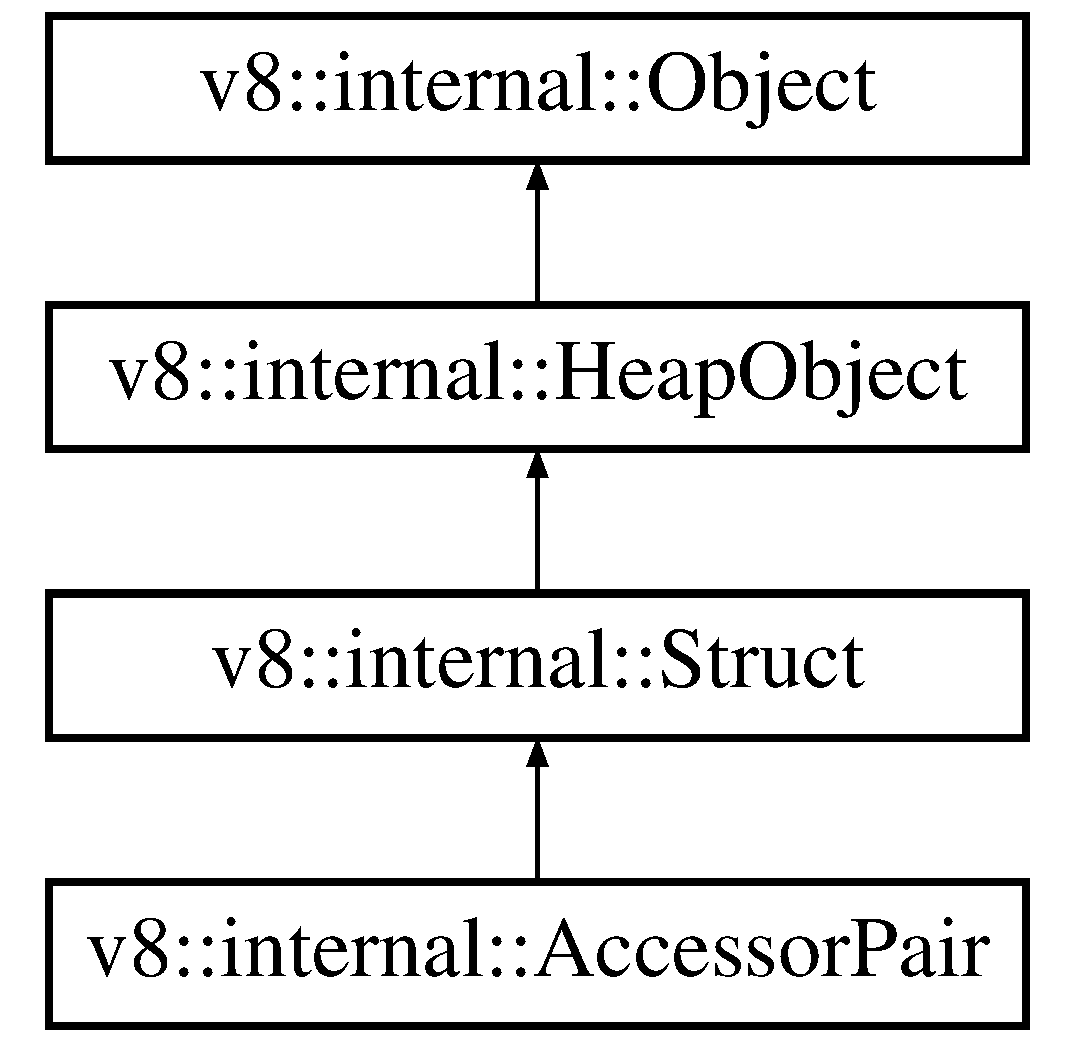
\includegraphics[height=4.000000cm]{classv8_1_1internal_1_1_accessor_pair}
\end{center}
\end{figure}
\subsection*{Public Member Functions}
\begin{DoxyCompactItemize}
\item 
\hyperlink{classv8_1_1internal_1_1_object}{Object} $\ast$ {\bfseries get} (Accessor\+Component component)\hypertarget{classv8_1_1internal_1_1_accessor_pair_a66569cd687b684427f0d9d34514858a6}{}\label{classv8_1_1internal_1_1_accessor_pair_a66569cd687b684427f0d9d34514858a6}

\item 
void {\bfseries set} (Accessor\+Component component, \hyperlink{classv8_1_1internal_1_1_object}{Object} $\ast$value)\hypertarget{classv8_1_1internal_1_1_accessor_pair_ad2a9c19f26306e325c88a48431f1f2c1}{}\label{classv8_1_1internal_1_1_accessor_pair_ad2a9c19f26306e325c88a48431f1f2c1}

\item 
void {\bfseries Set\+Components} (\hyperlink{classv8_1_1internal_1_1_object}{Object} $\ast$getter, \hyperlink{classv8_1_1internal_1_1_object}{Object} $\ast$setter)\hypertarget{classv8_1_1internal_1_1_accessor_pair_a6e5a2de9676c59e75ff73635f152a27d}{}\label{classv8_1_1internal_1_1_accessor_pair_a6e5a2de9676c59e75ff73635f152a27d}

\item 
bool {\bfseries Equals} (\hyperlink{classv8_1_1internal_1_1_accessor_pair}{Accessor\+Pair} $\ast$pair)\hypertarget{classv8_1_1internal_1_1_accessor_pair_a074f0577eb38b61f347071f85120339b}{}\label{classv8_1_1internal_1_1_accessor_pair_a074f0577eb38b61f347071f85120339b}

\item 
bool {\bfseries Equals} (\hyperlink{classv8_1_1internal_1_1_object}{Object} $\ast$getter\+\_\+value, \hyperlink{classv8_1_1internal_1_1_object}{Object} $\ast$setter\+\_\+value)\hypertarget{classv8_1_1internal_1_1_accessor_pair_aeb0ab989aa8c299311ea5ad17c496732}{}\label{classv8_1_1internal_1_1_accessor_pair_aeb0ab989aa8c299311ea5ad17c496732}

\item 
bool {\bfseries Contains\+Accessor} ()\hypertarget{classv8_1_1internal_1_1_accessor_pair_a3776e1f65c6612d9cb544747211bd3f0}{}\label{classv8_1_1internal_1_1_accessor_pair_a3776e1f65c6612d9cb544747211bd3f0}

\end{DoxyCompactItemize}
\subsection*{Static Public Member Functions}
\begin{DoxyCompactItemize}
\item 
static \hyperlink{classv8_1_1internal_1_1_handle}{Handle}$<$ \hyperlink{classv8_1_1internal_1_1_accessor_pair}{Accessor\+Pair} $>$ {\bfseries Copy} (\hyperlink{classv8_1_1internal_1_1_handle}{Handle}$<$ \hyperlink{classv8_1_1internal_1_1_accessor_pair}{Accessor\+Pair} $>$ pair)\hypertarget{classv8_1_1internal_1_1_accessor_pair_a9030ddc2b46863a79de840206d6c549c}{}\label{classv8_1_1internal_1_1_accessor_pair_a9030ddc2b46863a79de840206d6c549c}

\item 
static \hyperlink{classv8_1_1internal_1_1_handle}{Handle}$<$ \hyperlink{classv8_1_1internal_1_1_object}{Object} $>$ {\bfseries Get\+Component} (\hyperlink{classv8_1_1internal_1_1_handle}{Handle}$<$ \hyperlink{classv8_1_1internal_1_1_accessor_pair}{Accessor\+Pair} $>$ accessor\+\_\+pair, Accessor\+Component component)\hypertarget{classv8_1_1internal_1_1_accessor_pair_a432a76bc810fc281eb04f2b0b1ae8772}{}\label{classv8_1_1internal_1_1_accessor_pair_a432a76bc810fc281eb04f2b0b1ae8772}

\end{DoxyCompactItemize}
\subsection*{Static Public Attributes}
\begin{DoxyCompactItemize}
\item 
static const int {\bfseries k\+Getter\+Offset} = Heap\+Object\+::k\+Header\+Size\hypertarget{classv8_1_1internal_1_1_accessor_pair_aa7ee07b7098a35f0e1340c33dadb90db}{}\label{classv8_1_1internal_1_1_accessor_pair_aa7ee07b7098a35f0e1340c33dadb90db}

\item 
static const int {\bfseries k\+Setter\+Offset} = k\+Getter\+Offset + k\+Pointer\+Size\hypertarget{classv8_1_1internal_1_1_accessor_pair_adaca2d4fb0dfcf2e29fd37fc5549737b}{}\label{classv8_1_1internal_1_1_accessor_pair_adaca2d4fb0dfcf2e29fd37fc5549737b}

\item 
static const int {\bfseries k\+Size} = k\+Setter\+Offset + k\+Pointer\+Size\hypertarget{classv8_1_1internal_1_1_accessor_pair_a89c0268865b5203f29820f82b5e46cb5}{}\label{classv8_1_1internal_1_1_accessor_pair_a89c0268865b5203f29820f82b5e46cb5}

\end{DoxyCompactItemize}
\subsection*{Private Member Functions}
\begin{DoxyCompactItemize}
\item 
bool {\bfseries Is\+J\+S\+Accessor} (\hyperlink{classv8_1_1internal_1_1_object}{Object} $\ast$obj)\hypertarget{classv8_1_1internal_1_1_accessor_pair_a9aaa05972bbd7ccc9cdfb67618063a99}{}\label{classv8_1_1internal_1_1_accessor_pair_a9aaa05972bbd7ccc9cdfb67618063a99}

\item 
{\bfseries D\+I\+S\+A\+L\+L\+O\+W\+\_\+\+I\+M\+P\+L\+I\+C\+I\+T\+\_\+\+C\+O\+N\+S\+T\+R\+U\+C\+T\+O\+RS} (\hyperlink{classv8_1_1internal_1_1_accessor_pair}{Accessor\+Pair})\hypertarget{classv8_1_1internal_1_1_accessor_pair_ae52e8536100b025147dec6b149b42b50}{}\label{classv8_1_1internal_1_1_accessor_pair_ae52e8536100b025147dec6b149b42b50}

\end{DoxyCompactItemize}
\subsection*{Additional Inherited Members}


The documentation for this class was generated from the following files\+:\begin{DoxyCompactItemize}
\item 
/\+Users/joshgav/node/v8/src/objects.\+h\item 
/\+Users/joshgav/node/v8/src/objects-\/inl.\+h\item 
/\+Users/joshgav/node/v8/src/objects.\+cc\end{DoxyCompactItemize}

\hypertarget{structv8_1_1internal_1_1_object_literal_1_1_accessors}{}\section{v8\+:\+:internal\+:\+:Object\+Literal\+:\+:Accessors Struct Reference}
\label{structv8_1_1internal_1_1_object_literal_1_1_accessors}\index{v8\+::internal\+::\+Object\+Literal\+::\+Accessors@{v8\+::internal\+::\+Object\+Literal\+::\+Accessors}}
Inheritance diagram for v8\+:\+:internal\+:\+:Object\+Literal\+:\+:Accessors\+:\begin{figure}[H]
\begin{center}
\leavevmode
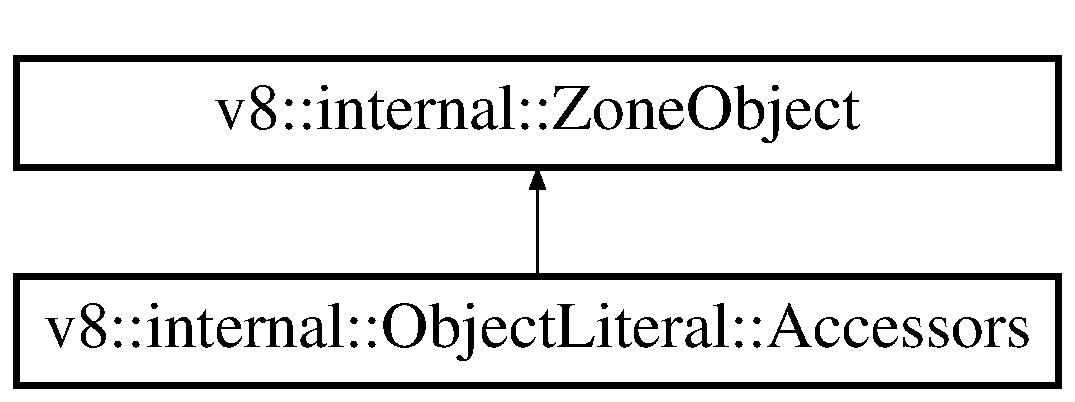
\includegraphics[height=2.000000cm]{structv8_1_1internal_1_1_object_literal_1_1_accessors}
\end{center}
\end{figure}
\subsection*{Public Attributes}
\begin{DoxyCompactItemize}
\item 
\hyperlink{classv8_1_1internal_1_1_object_literal_property}{Object\+Literal\+Property} $\ast$ {\bfseries getter}\hypertarget{structv8_1_1internal_1_1_object_literal_1_1_accessors_ad6206e1f4b41848f1b36116ae972da8c}{}\label{structv8_1_1internal_1_1_object_literal_1_1_accessors_ad6206e1f4b41848f1b36116ae972da8c}

\item 
\hyperlink{classv8_1_1internal_1_1_object_literal_property}{Object\+Literal\+Property} $\ast$ {\bfseries setter}\hypertarget{structv8_1_1internal_1_1_object_literal_1_1_accessors_a5d319b2c9b5e07d608c478e11c9e467e}{}\label{structv8_1_1internal_1_1_object_literal_1_1_accessors_a5d319b2c9b5e07d608c478e11c9e467e}

\end{DoxyCompactItemize}
\subsection*{Additional Inherited Members}


The documentation for this struct was generated from the following file\+:\begin{DoxyCompactItemize}
\item 
/\+Users/joshgav/node/v8/src/ast/ast.\+h\end{DoxyCompactItemize}

\hypertarget{classv8_1_1internal_1_1_accessors}{}\section{v8\+:\+:internal\+:\+:Accessors Class Reference}
\label{classv8_1_1internal_1_1_accessors}\index{v8\+::internal\+::\+Accessors@{v8\+::internal\+::\+Accessors}}
Inheritance diagram for v8\+:\+:internal\+:\+:Accessors\+:\begin{figure}[H]
\begin{center}
\leavevmode
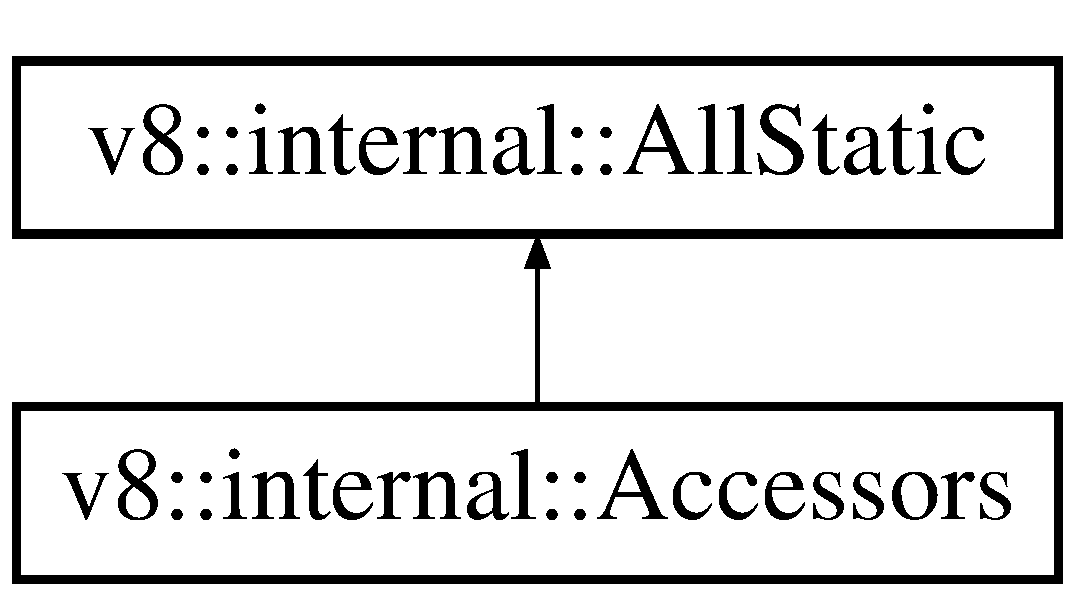
\includegraphics[height=2.000000cm]{classv8_1_1internal_1_1_accessors}
\end{center}
\end{figure}
\subsection*{Public Types}
\begin{DoxyCompactItemize}
\item 
enum {\bfseries Descriptor\+Id} \{ {\bfseries descriptor\+Count}
 \}\hypertarget{classv8_1_1internal_1_1_accessors_a1c466e7b9e4df52b9cd44f01d41faf3b}{}\label{classv8_1_1internal_1_1_accessors_a1c466e7b9e4df52b9cd44f01d41faf3b}

\end{DoxyCompactItemize}
\subsection*{Static Public Member Functions}
\begin{DoxyCompactItemize}
\item 
static M\+U\+S\+T\+\_\+\+U\+S\+E\+\_\+\+R\+E\+S\+U\+LT \hyperlink{classv8_1_1internal_1_1_maybe_handle}{Maybe\+Handle}$<$ \hyperlink{classv8_1_1internal_1_1_object}{Object} $>$ {\bfseries Function\+Set\+Prototype} (\hyperlink{classv8_1_1internal_1_1_handle}{Handle}$<$ \hyperlink{classv8_1_1internal_1_1_j_s_function}{J\+S\+Function} $>$ object, \hyperlink{classv8_1_1internal_1_1_handle}{Handle}$<$ \hyperlink{classv8_1_1internal_1_1_object}{Object} $>$ value)\hypertarget{classv8_1_1internal_1_1_accessors_a46069cc262b04995f4464b2a6b77f419}{}\label{classv8_1_1internal_1_1_accessors_a46069cc262b04995f4464b2a6b77f419}

\item 
static \hyperlink{classv8_1_1internal_1_1_handle}{Handle}$<$ \hyperlink{classv8_1_1internal_1_1_j_s_object}{J\+S\+Object} $>$ {\bfseries Function\+Get\+Arguments} (\hyperlink{classv8_1_1internal_1_1_handle}{Handle}$<$ \hyperlink{classv8_1_1internal_1_1_j_s_function}{J\+S\+Function} $>$ object)\hypertarget{classv8_1_1internal_1_1_accessors_ac04c9e4d84d0ee6a47df67d582652bdc}{}\label{classv8_1_1internal_1_1_accessors_ac04c9e4d84d0ee6a47df67d582652bdc}

\item 
static \hyperlink{classv8_1_1internal_1_1_handle}{Handle}$<$ \hyperlink{classv8_1_1internal_1_1_accessor_info}{Accessor\+Info} $>$ {\bfseries Make\+Module\+Export} (\hyperlink{classv8_1_1internal_1_1_handle}{Handle}$<$ \hyperlink{classv8_1_1internal_1_1_string}{String} $>$ name, int index, Property\+Attributes attributes)\hypertarget{classv8_1_1internal_1_1_accessors_a659f5cfdc0ce5805f19fd0fe320e4e5c}{}\label{classv8_1_1internal_1_1_accessors_a659f5cfdc0ce5805f19fd0fe320e4e5c}

\item 
static bool {\bfseries Is\+J\+S\+Object\+Field\+Accessor} (\hyperlink{classv8_1_1internal_1_1_handle}{Handle}$<$ \hyperlink{classv8_1_1internal_1_1_map}{Map} $>$ map, \hyperlink{classv8_1_1internal_1_1_handle}{Handle}$<$ \hyperlink{classv8_1_1internal_1_1_name}{Name} $>$ name, int $\ast$object\+\_\+offset)\hypertarget{classv8_1_1internal_1_1_accessors_a5b4d1d26837b68779b95631f8693c1ba}{}\label{classv8_1_1internal_1_1_accessors_a5b4d1d26837b68779b95631f8693c1ba}

\item 
static bool {\bfseries Is\+J\+S\+Array\+Buffer\+View\+Field\+Accessor} (\hyperlink{classv8_1_1internal_1_1_handle}{Handle}$<$ \hyperlink{classv8_1_1internal_1_1_map}{Map} $>$ map, \hyperlink{classv8_1_1internal_1_1_handle}{Handle}$<$ \hyperlink{classv8_1_1internal_1_1_name}{Name} $>$ name, int $\ast$object\+\_\+offset)\hypertarget{classv8_1_1internal_1_1_accessors_a168e807486046775d456de908f3c7d50}{}\label{classv8_1_1internal_1_1_accessors_a168e807486046775d456de908f3c7d50}

\item 
static \hyperlink{classv8_1_1internal_1_1_handle}{Handle}$<$ \hyperlink{classv8_1_1internal_1_1_accessor_info}{Accessor\+Info} $>$ {\bfseries Make\+Accessor} (\hyperlink{classv8_1_1internal_1_1_isolate}{Isolate} $\ast$isolate, \hyperlink{classv8_1_1internal_1_1_handle}{Handle}$<$ \hyperlink{classv8_1_1internal_1_1_name}{Name} $>$ name, Accessor\+Name\+Getter\+Callback getter, Accessor\+Name\+Setter\+Callback setter, Property\+Attributes attributes)\hypertarget{classv8_1_1internal_1_1_accessors_aadd6bb21bc0712cdf252a60170504385}{}\label{classv8_1_1internal_1_1_accessors_aadd6bb21bc0712cdf252a60170504385}

\end{DoxyCompactItemize}


The documentation for this class was generated from the following files\+:\begin{DoxyCompactItemize}
\item 
/\+Users/joshgav/node/v8/src/accessors.\+h\item 
/\+Users/joshgav/node/v8/src/accessors.\+cc\end{DoxyCompactItemize}

\hypertarget{classv8_1_1_accessor_signature}{}\section{v8\+:\+:Accessor\+Signature Class Reference}
\label{classv8_1_1_accessor_signature}\index{v8\+::\+Accessor\+Signature@{v8\+::\+Accessor\+Signature}}


{\ttfamily \#include $<$v8.\+h$>$}

Inheritance diagram for v8\+:\+:Accessor\+Signature\+:\begin{figure}[H]
\begin{center}
\leavevmode
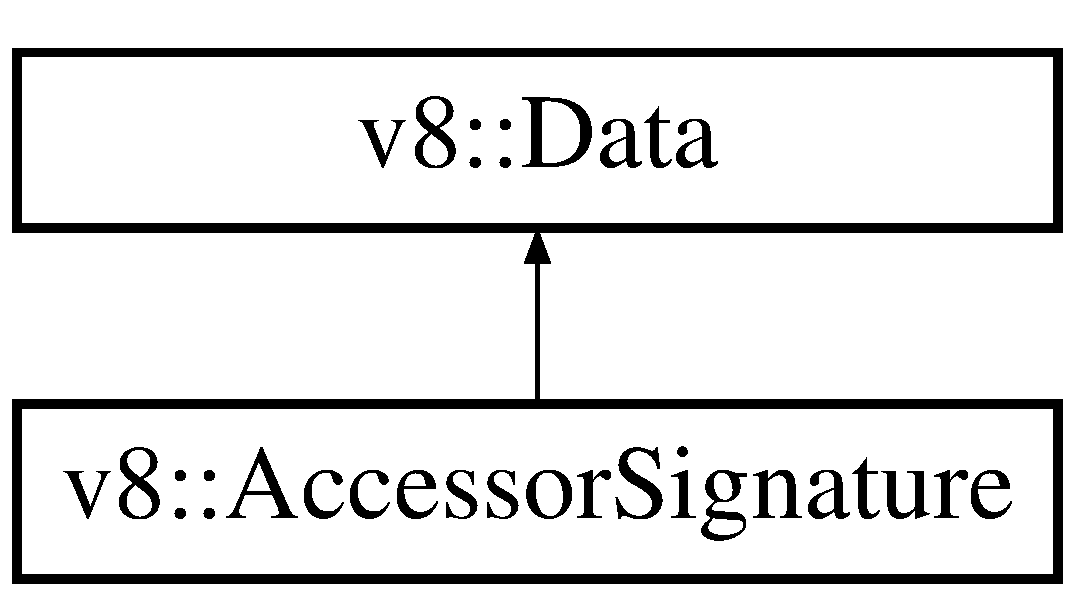
\includegraphics[height=2.000000cm]{classv8_1_1_accessor_signature}
\end{center}
\end{figure}
\subsection*{Static Public Member Functions}
\begin{DoxyCompactItemize}
\item 
static \hyperlink{classv8_1_1_local}{Local}$<$ \hyperlink{classv8_1_1_accessor_signature}{Accessor\+Signature} $>$ {\bfseries New} (\hyperlink{classv8_1_1_isolate}{Isolate} $\ast$isolate, \hyperlink{classv8_1_1_local}{Local}$<$ \hyperlink{classv8_1_1_function_template}{Function\+Template} $>$ receiver=\hyperlink{classv8_1_1_local}{Local}$<$ \hyperlink{classv8_1_1_function_template}{Function\+Template} $>$())\hypertarget{classv8_1_1_accessor_signature_a2d7f28b404be5ecdb501aaf572a7ee52}{}\label{classv8_1_1_accessor_signature_a2d7f28b404be5ecdb501aaf572a7ee52}

\end{DoxyCompactItemize}


\subsection{Detailed Description}
An \hyperlink{classv8_1_1_accessor_signature}{Accessor\+Signature} specifies which receivers are valid parameters to an accessor callback. 

The documentation for this class was generated from the following file\+:\begin{DoxyCompactItemize}
\item 
/\+Users/joshgav/node/v8/include/v8.\+h\end{DoxyCompactItemize}

\hypertarget{classv8_1_1internal_1_1_accessor_table}{}\section{v8\+:\+:internal\+:\+:Accessor\+Table Class Reference}
\label{classv8_1_1internal_1_1_accessor_table}\index{v8\+::internal\+::\+Accessor\+Table@{v8\+::internal\+::\+Accessor\+Table}}
Inheritance diagram for v8\+:\+:internal\+:\+:Accessor\+Table\+:\begin{figure}[H]
\begin{center}
\leavevmode
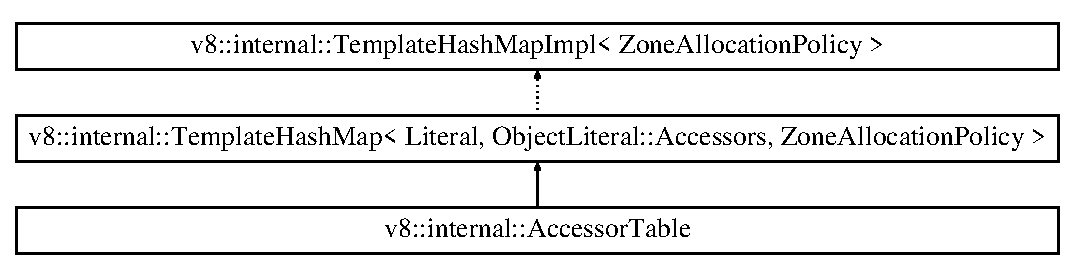
\includegraphics[height=3.000000cm]{classv8_1_1internal_1_1_accessor_table}
\end{center}
\end{figure}
\subsection*{Public Member Functions}
\begin{DoxyCompactItemize}
\item 
{\bfseries Accessor\+Table} (\hyperlink{classv8_1_1internal_1_1_zone}{Zone} $\ast$zone)\hypertarget{classv8_1_1internal_1_1_accessor_table_adcee86ad1000d3d63e7360d0895fc2ae}{}\label{classv8_1_1internal_1_1_accessor_table_adcee86ad1000d3d63e7360d0895fc2ae}

\item 
Iterator {\bfseries lookup} (\hyperlink{classv8_1_1internal_1_1_literal}{Literal} $\ast$literal)\hypertarget{classv8_1_1internal_1_1_accessor_table_a064e2528f1da85829d8742c69adaba19}{}\label{classv8_1_1internal_1_1_accessor_table_a064e2528f1da85829d8742c69adaba19}

\end{DoxyCompactItemize}
\subsection*{Private Attributes}
\begin{DoxyCompactItemize}
\item 
\hyperlink{classv8_1_1internal_1_1_zone}{Zone} $\ast$ {\bfseries zone\+\_\+}\hypertarget{classv8_1_1internal_1_1_accessor_table_ae47d4062d555902a4f0bf13bfff5fba2}{}\label{classv8_1_1internal_1_1_accessor_table_ae47d4062d555902a4f0bf13bfff5fba2}

\end{DoxyCompactItemize}


The documentation for this class was generated from the following file\+:\begin{DoxyCompactItemize}
\item 
/\+Users/joshgav/node/v8/src/ast/ast.\+h\end{DoxyCompactItemize}

\hypertarget{classv8_1_1base_1_1_accounting_allocator}{}\section{v8\+:\+:base\+:\+:Accounting\+Allocator Class Reference}
\label{classv8_1_1base_1_1_accounting_allocator}\index{v8\+::base\+::\+Accounting\+Allocator@{v8\+::base\+::\+Accounting\+Allocator}}
\subsection*{Public Member Functions}
\begin{DoxyCompactItemize}
\item 
void $\ast$ {\bfseries Allocate} (size\+\_\+t bytes)\hypertarget{classv8_1_1base_1_1_accounting_allocator_a404780a6834e17311df8a2f000ceed7e}{}\label{classv8_1_1base_1_1_accounting_allocator_a404780a6834e17311df8a2f000ceed7e}

\item 
void {\bfseries Free} (void $\ast$memory, size\+\_\+t bytes)\hypertarget{classv8_1_1base_1_1_accounting_allocator_a0c565703354789bd498b41ba7dfa5b7c}{}\label{classv8_1_1base_1_1_accounting_allocator_a0c565703354789bd498b41ba7dfa5b7c}

\item 
size\+\_\+t {\bfseries Get\+Current\+Memory\+Usage} () const \hypertarget{classv8_1_1base_1_1_accounting_allocator_ab9d7491c6011fd2c5bb90ea4a0f2fe78}{}\label{classv8_1_1base_1_1_accounting_allocator_ab9d7491c6011fd2c5bb90ea4a0f2fe78}

\end{DoxyCompactItemize}
\subsection*{Private Member Functions}
\begin{DoxyCompactItemize}
\item 
{\bfseries D\+I\+S\+A\+L\+L\+O\+W\+\_\+\+C\+O\+P\+Y\+\_\+\+A\+N\+D\+\_\+\+A\+S\+S\+I\+GN} (\hyperlink{classv8_1_1base_1_1_accounting_allocator}{Accounting\+Allocator})\hypertarget{classv8_1_1base_1_1_accounting_allocator_a4d74238f0929f80468ffeef862113cb9}{}\label{classv8_1_1base_1_1_accounting_allocator_a4d74238f0929f80468ffeef862113cb9}

\end{DoxyCompactItemize}
\subsection*{Private Attributes}
\begin{DoxyCompactItemize}
\item 
Atomic\+Word {\bfseries current\+\_\+memory\+\_\+usage\+\_\+} = 0\hypertarget{classv8_1_1base_1_1_accounting_allocator_a445a2bfa4ae01aadf4f4dd5367598092}{}\label{classv8_1_1base_1_1_accounting_allocator_a445a2bfa4ae01aadf4f4dd5367598092}

\end{DoxyCompactItemize}


The documentation for this class was generated from the following files\+:\begin{DoxyCompactItemize}
\item 
/\+Users/joshgav/node/v8/src/base/accounting-\/allocator.\+h\item 
/\+Users/joshgav/node/v8/src/base/accounting-\/allocator.\+cc\end{DoxyCompactItemize}

\hypertarget{classv8_1_1internal_1_1interpreter_1_1_bytecode_generator_1_1_accumulator_result_scope}{}\section{v8\+:\+:internal\+:\+:interpreter\+:\+:Bytecode\+Generator\+:\+:Accumulator\+Result\+Scope Class Reference}
\label{classv8_1_1internal_1_1interpreter_1_1_bytecode_generator_1_1_accumulator_result_scope}\index{v8\+::internal\+::interpreter\+::\+Bytecode\+Generator\+::\+Accumulator\+Result\+Scope@{v8\+::internal\+::interpreter\+::\+Bytecode\+Generator\+::\+Accumulator\+Result\+Scope}}
Inheritance diagram for v8\+:\+:internal\+:\+:interpreter\+:\+:Bytecode\+Generator\+:\+:Accumulator\+Result\+Scope\+:\begin{figure}[H]
\begin{center}
\leavevmode
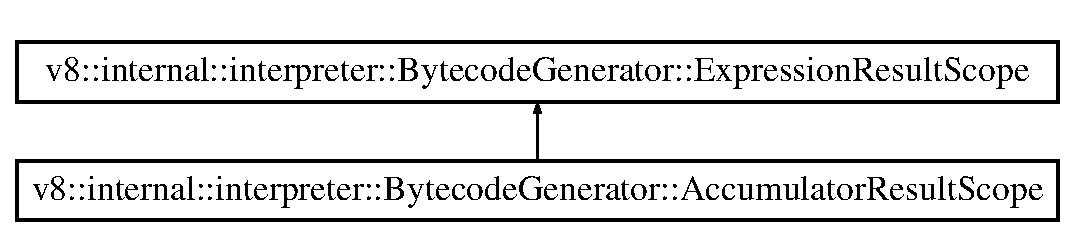
\includegraphics[height=2.000000cm]{classv8_1_1internal_1_1interpreter_1_1_bytecode_generator_1_1_accumulator_result_scope}
\end{center}
\end{figure}
\subsection*{Public Member Functions}
\begin{DoxyCompactItemize}
\item 
{\bfseries Accumulator\+Result\+Scope} (\hyperlink{classv8_1_1internal_1_1interpreter_1_1_bytecode_generator}{Bytecode\+Generator} $\ast$generator)\hypertarget{classv8_1_1internal_1_1interpreter_1_1_bytecode_generator_1_1_accumulator_result_scope_afefbdb515862ac85249afcd77f78feb7}{}\label{classv8_1_1internal_1_1interpreter_1_1_bytecode_generator_1_1_accumulator_result_scope_afefbdb515862ac85249afcd77f78feb7}

\item 
virtual void {\bfseries Set\+Result\+In\+Accumulator} ()\hypertarget{classv8_1_1internal_1_1interpreter_1_1_bytecode_generator_1_1_accumulator_result_scope_a61ed8e64cbc3664b03b893cc866b25f1}{}\label{classv8_1_1internal_1_1interpreter_1_1_bytecode_generator_1_1_accumulator_result_scope_a61ed8e64cbc3664b03b893cc866b25f1}

\item 
virtual void {\bfseries Set\+Result\+In\+Register} (\hyperlink{classv8_1_1internal_1_1interpreter_1_1_register}{Register} reg)\hypertarget{classv8_1_1internal_1_1interpreter_1_1_bytecode_generator_1_1_accumulator_result_scope_addfbfaa2866937a51f879cb347f490c8}{}\label{classv8_1_1internal_1_1interpreter_1_1_bytecode_generator_1_1_accumulator_result_scope_addfbfaa2866937a51f879cb347f490c8}

\end{DoxyCompactItemize}
\subsection*{Additional Inherited Members}


The documentation for this class was generated from the following file\+:\begin{DoxyCompactItemize}
\item 
/\+Users/joshgav/node/v8/src/interpreter/bytecode-\/generator.\+cc\end{DoxyCompactItemize}

\hypertarget{classv8_1_1internal_1_1_full_code_generator_1_1_accumulator_value_context}{}\section{v8\+:\+:internal\+:\+:Full\+Code\+Generator\+:\+:Accumulator\+Value\+Context Class Reference}
\label{classv8_1_1internal_1_1_full_code_generator_1_1_accumulator_value_context}\index{v8\+::internal\+::\+Full\+Code\+Generator\+::\+Accumulator\+Value\+Context@{v8\+::internal\+::\+Full\+Code\+Generator\+::\+Accumulator\+Value\+Context}}
Inheritance diagram for v8\+:\+:internal\+:\+:Full\+Code\+Generator\+:\+:Accumulator\+Value\+Context\+:\begin{figure}[H]
\begin{center}
\leavevmode
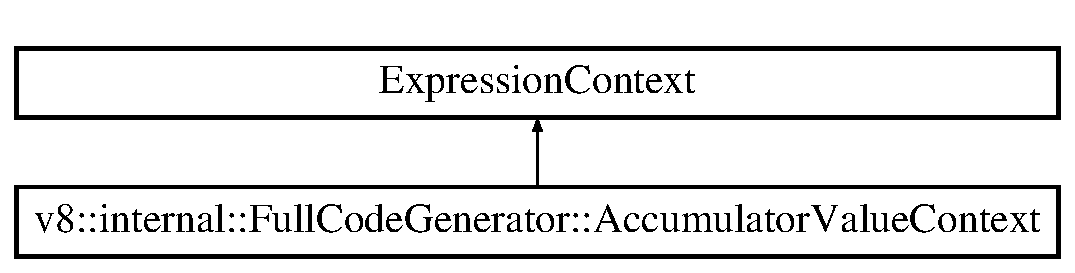
\includegraphics[height=2.000000cm]{classv8_1_1internal_1_1_full_code_generator_1_1_accumulator_value_context}
\end{center}
\end{figure}
\subsection*{Public Member Functions}
\begin{DoxyCompactItemize}
\item 
{\bfseries Accumulator\+Value\+Context} (\hyperlink{classv8_1_1internal_1_1_full_code_generator}{Full\+Code\+Generator} $\ast$codegen)\hypertarget{classv8_1_1internal_1_1_full_code_generator_1_1_accumulator_value_context_acaf85d1dacd64e3889ffd29fd6e8b5e6}{}\label{classv8_1_1internal_1_1_full_code_generator_1_1_accumulator_value_context_acaf85d1dacd64e3889ffd29fd6e8b5e6}

\item 
void {\bfseries Plug} (bool flag) const  override\hypertarget{classv8_1_1internal_1_1_full_code_generator_1_1_accumulator_value_context_a132632b035aa524bb5bd52f06024d7e6}{}\label{classv8_1_1internal_1_1_full_code_generator_1_1_accumulator_value_context_a132632b035aa524bb5bd52f06024d7e6}

\item 
void {\bfseries Plug} (\hyperlink{structv8_1_1internal_1_1_register}{Register} reg) const  override\hypertarget{classv8_1_1internal_1_1_full_code_generator_1_1_accumulator_value_context_ac5b465e0ef98af1602b8948253acd919}{}\label{classv8_1_1internal_1_1_full_code_generator_1_1_accumulator_value_context_ac5b465e0ef98af1602b8948253acd919}

\item 
void {\bfseries Plug} (\hyperlink{classv8_1_1internal_1_1_label}{Label} $\ast$materialize\+\_\+true, \hyperlink{classv8_1_1internal_1_1_label}{Label} $\ast$materialize\+\_\+false) const  override\hypertarget{classv8_1_1internal_1_1_full_code_generator_1_1_accumulator_value_context_a4b9053a97b77e077e5f245924f3d532b}{}\label{classv8_1_1internal_1_1_full_code_generator_1_1_accumulator_value_context_a4b9053a97b77e077e5f245924f3d532b}

\item 
void {\bfseries Plug} (\hyperlink{classv8_1_1internal_1_1_variable}{Variable} $\ast$var) const  override\hypertarget{classv8_1_1internal_1_1_full_code_generator_1_1_accumulator_value_context_a4fd6b87fc575c3014627896ffc7f2c1b}{}\label{classv8_1_1internal_1_1_full_code_generator_1_1_accumulator_value_context_a4fd6b87fc575c3014627896ffc7f2c1b}

\item 
void {\bfseries Plug} (\hyperlink{classv8_1_1internal_1_1_handle}{Handle}$<$ \hyperlink{classv8_1_1internal_1_1_object}{Object} $>$ lit) const  override\hypertarget{classv8_1_1internal_1_1_full_code_generator_1_1_accumulator_value_context_ab3c75037693081717e8385c2e9b84a93}{}\label{classv8_1_1internal_1_1_full_code_generator_1_1_accumulator_value_context_ab3c75037693081717e8385c2e9b84a93}

\item 
void {\bfseries Plug} (Heap\+::\+Root\+List\+Index) const  override\hypertarget{classv8_1_1internal_1_1_full_code_generator_1_1_accumulator_value_context_a589c763fbb18e59f9f44bf335333775e}{}\label{classv8_1_1internal_1_1_full_code_generator_1_1_accumulator_value_context_a589c763fbb18e59f9f44bf335333775e}

\item 
void {\bfseries Plug\+T\+OS} () const  override\hypertarget{classv8_1_1internal_1_1_full_code_generator_1_1_accumulator_value_context_a7710c8085856e8a8f45031ac9e6d0502}{}\label{classv8_1_1internal_1_1_full_code_generator_1_1_accumulator_value_context_a7710c8085856e8a8f45031ac9e6d0502}

\item 
void {\bfseries Drop\+And\+Plug} (int count, \hyperlink{structv8_1_1internal_1_1_register}{Register} reg) const  override\hypertarget{classv8_1_1internal_1_1_full_code_generator_1_1_accumulator_value_context_a809be7887775f63549ee281dbafccb4f}{}\label{classv8_1_1internal_1_1_full_code_generator_1_1_accumulator_value_context_a809be7887775f63549ee281dbafccb4f}

\item 
void {\bfseries Prepare\+Test} (\hyperlink{classv8_1_1internal_1_1_label}{Label} $\ast$materialize\+\_\+true, \hyperlink{classv8_1_1internal_1_1_label}{Label} $\ast$materialize\+\_\+false, \hyperlink{classv8_1_1internal_1_1_label}{Label} $\ast$$\ast$if\+\_\+true, \hyperlink{classv8_1_1internal_1_1_label}{Label} $\ast$$\ast$if\+\_\+false, \hyperlink{classv8_1_1internal_1_1_label}{Label} $\ast$$\ast$fall\+\_\+through) const  override\hypertarget{classv8_1_1internal_1_1_full_code_generator_1_1_accumulator_value_context_a3b64159d3356198a2ce1767cabe3d32b}{}\label{classv8_1_1internal_1_1_full_code_generator_1_1_accumulator_value_context_a3b64159d3356198a2ce1767cabe3d32b}

\item 
bool {\bfseries Is\+Accumulator\+Value} () const  override\hypertarget{classv8_1_1internal_1_1_full_code_generator_1_1_accumulator_value_context_aae0528cd170cdfd2190c40e983df7332}{}\label{classv8_1_1internal_1_1_full_code_generator_1_1_accumulator_value_context_aae0528cd170cdfd2190c40e983df7332}

\end{DoxyCompactItemize}


The documentation for this class was generated from the following files\+:\begin{DoxyCompactItemize}
\item 
/\+Users/joshgav/node/v8/src/full-\/codegen/full-\/codegen.\+h\item 
/\+Users/joshgav/node/v8/src/full-\/codegen/full-\/codegen.\+cc\end{DoxyCompactItemize}

\hypertarget{classv8_1_1internal_1_1_action_node}{}\section{v8\+:\+:internal\+:\+:Action\+Node Class Reference}
\label{classv8_1_1internal_1_1_action_node}\index{v8\+::internal\+::\+Action\+Node@{v8\+::internal\+::\+Action\+Node}}
Inheritance diagram for v8\+:\+:internal\+:\+:Action\+Node\+:\begin{figure}[H]
\begin{center}
\leavevmode
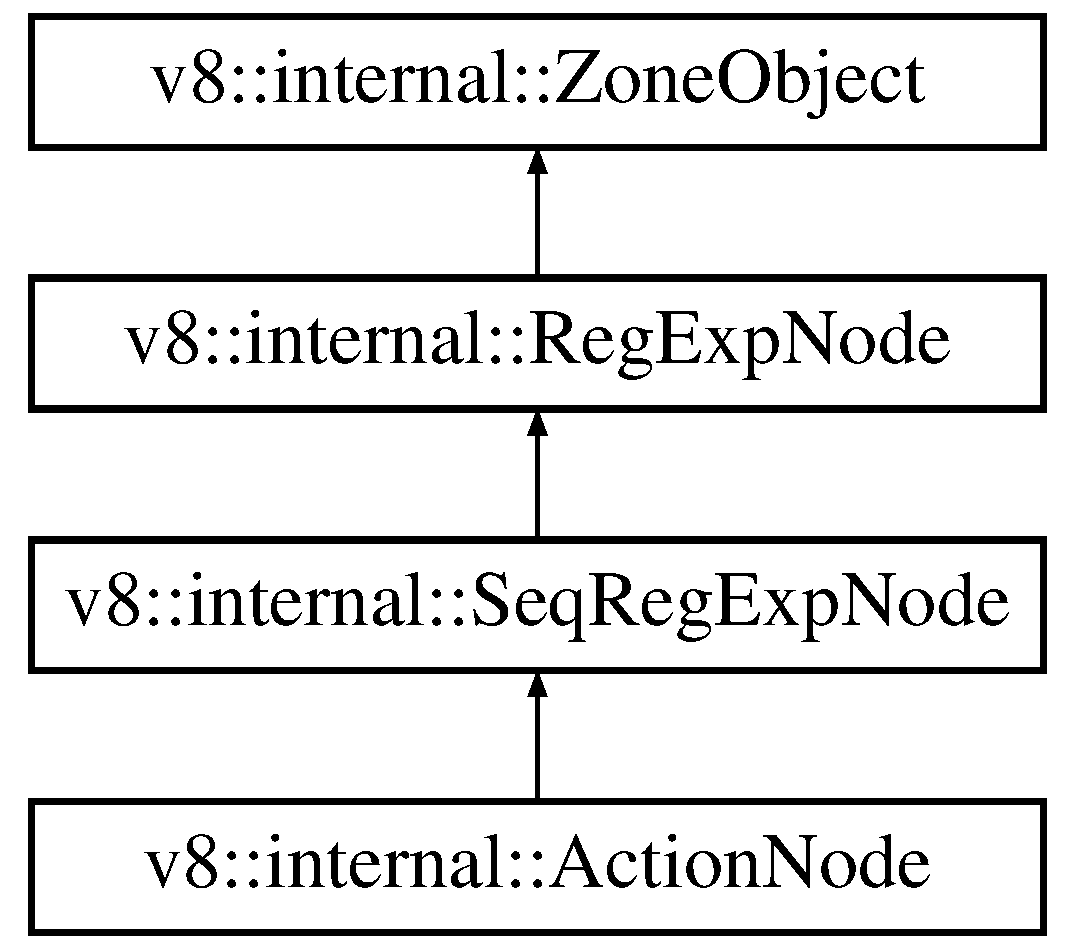
\includegraphics[height=4.000000cm]{classv8_1_1internal_1_1_action_node}
\end{center}
\end{figure}
\subsection*{Public Types}
\begin{DoxyCompactItemize}
\item 
enum {\bfseries Action\+Type} \{ \\*
{\bfseries S\+E\+T\+\_\+\+R\+E\+G\+I\+S\+T\+ER}, 
\\*
{\bfseries I\+N\+C\+R\+E\+M\+E\+N\+T\+\_\+\+R\+E\+G\+I\+S\+T\+ER}, 
\\*
{\bfseries S\+T\+O\+R\+E\+\_\+\+P\+O\+S\+I\+T\+I\+ON}, 
\\*
{\bfseries B\+E\+G\+I\+N\+\_\+\+S\+U\+B\+M\+A\+T\+CH}, 
\\*
{\bfseries P\+O\+S\+I\+T\+I\+V\+E\+\_\+\+S\+U\+B\+M\+A\+T\+C\+H\+\_\+\+S\+U\+C\+C\+E\+SS}, 
\\*
{\bfseries E\+M\+P\+T\+Y\+\_\+\+M\+A\+T\+C\+H\+\_\+\+C\+H\+E\+CK}, 
\\*
{\bfseries C\+L\+E\+A\+R\+\_\+\+C\+A\+P\+T\+U\+R\+ES}
 \}\hypertarget{classv8_1_1internal_1_1_action_node_ab695380c09977f360b2d4f817f9124bc}{}\label{classv8_1_1internal_1_1_action_node_ab695380c09977f360b2d4f817f9124bc}

\end{DoxyCompactItemize}
\subsection*{Public Member Functions}
\begin{DoxyCompactItemize}
\item 
virtual void {\bfseries Accept} (\hyperlink{classv8_1_1internal_1_1_node_visitor}{Node\+Visitor} $\ast$visitor)\hypertarget{classv8_1_1internal_1_1_action_node_acd110b20896658ef66be07589828c835}{}\label{classv8_1_1internal_1_1_action_node_acd110b20896658ef66be07589828c835}

\item 
virtual void {\bfseries Emit} (\hyperlink{classv8_1_1internal_1_1_reg_exp_compiler}{Reg\+Exp\+Compiler} $\ast$compiler, \hyperlink{classv8_1_1internal_1_1_trace}{Trace} $\ast$trace)\hypertarget{classv8_1_1internal_1_1_action_node_afac185d923c63324c4f18a2f0a23769d}{}\label{classv8_1_1internal_1_1_action_node_afac185d923c63324c4f18a2f0a23769d}

\item 
virtual int {\bfseries Eats\+At\+Least} (int still\+\_\+to\+\_\+find, int budget, bool not\+\_\+at\+\_\+start)\hypertarget{classv8_1_1internal_1_1_action_node_ab36ade74ae2623b654002605bb0c5144}{}\label{classv8_1_1internal_1_1_action_node_ab36ade74ae2623b654002605bb0c5144}

\item 
virtual void {\bfseries Get\+Quick\+Check\+Details} (\hyperlink{classv8_1_1internal_1_1_quick_check_details}{Quick\+Check\+Details} $\ast$details, \hyperlink{classv8_1_1internal_1_1_reg_exp_compiler}{Reg\+Exp\+Compiler} $\ast$compiler, int filled\+\_\+in, bool not\+\_\+at\+\_\+start)\hypertarget{classv8_1_1internal_1_1_action_node_abc51b0f5a4a393425181f6a0583e6b0a}{}\label{classv8_1_1internal_1_1_action_node_abc51b0f5a4a393425181f6a0583e6b0a}

\item 
virtual void {\bfseries Fill\+In\+B\+M\+Info} (\hyperlink{classv8_1_1internal_1_1_isolate}{Isolate} $\ast$isolate, int offset, int budget, \hyperlink{classv8_1_1internal_1_1_boyer_moore_lookahead}{Boyer\+Moore\+Lookahead} $\ast$bm, bool not\+\_\+at\+\_\+start)\hypertarget{classv8_1_1internal_1_1_action_node_a1b606d25338b60303b4219c72e10db46}{}\label{classv8_1_1internal_1_1_action_node_a1b606d25338b60303b4219c72e10db46}

\item 
Action\+Type {\bfseries action\+\_\+type} ()\hypertarget{classv8_1_1internal_1_1_action_node_ae848c71b17d244a67f3f34afe142fac8}{}\label{classv8_1_1internal_1_1_action_node_ae848c71b17d244a67f3f34afe142fac8}

\item 
virtual int {\bfseries Greedy\+Loop\+Text\+Length} ()\hypertarget{classv8_1_1internal_1_1_action_node_a22be07519e46e566272847427d939793}{}\label{classv8_1_1internal_1_1_action_node_a22be07519e46e566272847427d939793}

\end{DoxyCompactItemize}
\subsection*{Static Public Member Functions}
\begin{DoxyCompactItemize}
\item 
static \hyperlink{classv8_1_1internal_1_1_action_node}{Action\+Node} $\ast$ {\bfseries Set\+Register} (int reg, int val, \hyperlink{classv8_1_1internal_1_1_reg_exp_node}{Reg\+Exp\+Node} $\ast$on\+\_\+success)\hypertarget{classv8_1_1internal_1_1_action_node_ab0232aafb29641c830970993c18ca5a7}{}\label{classv8_1_1internal_1_1_action_node_ab0232aafb29641c830970993c18ca5a7}

\item 
static \hyperlink{classv8_1_1internal_1_1_action_node}{Action\+Node} $\ast$ {\bfseries Increment\+Register} (int reg, \hyperlink{classv8_1_1internal_1_1_reg_exp_node}{Reg\+Exp\+Node} $\ast$on\+\_\+success)\hypertarget{classv8_1_1internal_1_1_action_node_ac2fea920241e4412a3bba2d10acb91ef}{}\label{classv8_1_1internal_1_1_action_node_ac2fea920241e4412a3bba2d10acb91ef}

\item 
static \hyperlink{classv8_1_1internal_1_1_action_node}{Action\+Node} $\ast$ {\bfseries Store\+Position} (int reg, bool is\+\_\+capture, \hyperlink{classv8_1_1internal_1_1_reg_exp_node}{Reg\+Exp\+Node} $\ast$on\+\_\+success)\hypertarget{classv8_1_1internal_1_1_action_node_a7b7c1ea99df9360c97a7e73e2672a834}{}\label{classv8_1_1internal_1_1_action_node_a7b7c1ea99df9360c97a7e73e2672a834}

\item 
static \hyperlink{classv8_1_1internal_1_1_action_node}{Action\+Node} $\ast$ {\bfseries Clear\+Captures} (\hyperlink{classv8_1_1internal_1_1_interval}{Interval} range, \hyperlink{classv8_1_1internal_1_1_reg_exp_node}{Reg\+Exp\+Node} $\ast$on\+\_\+success)\hypertarget{classv8_1_1internal_1_1_action_node_af5c152a32e7afbe31390f57c07eed05a}{}\label{classv8_1_1internal_1_1_action_node_af5c152a32e7afbe31390f57c07eed05a}

\item 
static \hyperlink{classv8_1_1internal_1_1_action_node}{Action\+Node} $\ast$ {\bfseries Begin\+Submatch} (int stack\+\_\+pointer\+\_\+reg, int position\+\_\+reg, \hyperlink{classv8_1_1internal_1_1_reg_exp_node}{Reg\+Exp\+Node} $\ast$on\+\_\+success)\hypertarget{classv8_1_1internal_1_1_action_node_a84297f33bee6dffd0cc7a6b5341fb106}{}\label{classv8_1_1internal_1_1_action_node_a84297f33bee6dffd0cc7a6b5341fb106}

\item 
static \hyperlink{classv8_1_1internal_1_1_action_node}{Action\+Node} $\ast$ {\bfseries Positive\+Submatch\+Success} (int stack\+\_\+pointer\+\_\+reg, int restore\+\_\+reg, int clear\+\_\+capture\+\_\+count, int clear\+\_\+capture\+\_\+from, \hyperlink{classv8_1_1internal_1_1_reg_exp_node}{Reg\+Exp\+Node} $\ast$on\+\_\+success)\hypertarget{classv8_1_1internal_1_1_action_node_a89bed32eadb39ad776f7e5523d8d152b}{}\label{classv8_1_1internal_1_1_action_node_a89bed32eadb39ad776f7e5523d8d152b}

\item 
static \hyperlink{classv8_1_1internal_1_1_action_node}{Action\+Node} $\ast$ {\bfseries Empty\+Match\+Check} (int start\+\_\+register, int repetition\+\_\+register, int repetition\+\_\+limit, \hyperlink{classv8_1_1internal_1_1_reg_exp_node}{Reg\+Exp\+Node} $\ast$on\+\_\+success)\hypertarget{classv8_1_1internal_1_1_action_node_a1f8492811dde72cce77b5b7f8d083292}{}\label{classv8_1_1internal_1_1_action_node_a1f8492811dde72cce77b5b7f8d083292}

\end{DoxyCompactItemize}
\subsection*{Private Member Functions}
\begin{DoxyCompactItemize}
\item 
{\bfseries Action\+Node} (Action\+Type action\+\_\+type, \hyperlink{classv8_1_1internal_1_1_reg_exp_node}{Reg\+Exp\+Node} $\ast$on\+\_\+success)\hypertarget{classv8_1_1internal_1_1_action_node_a4e387d38254ec87a46dd1cdb983607bf}{}\label{classv8_1_1internal_1_1_action_node_a4e387d38254ec87a46dd1cdb983607bf}

\end{DoxyCompactItemize}
\subsection*{Private Attributes}
\begin{DoxyCompactItemize}
\item 
\begin{tabbing}
xx\=xx\=xx\=xx\=xx\=xx\=xx\=xx\=xx\=\kill
union \{\\
\>struct \{\\
\>\>int {\bfseries reg}\\
\>\>int {\bfseries value}\\
\>\} {\bfseries u\_store\_register}\\
\>struct \{\\
\>\>int {\bfseries reg}\\
\>\} {\bfseries u\_increment\_register}\\
\>struct \{\\
\>\>int {\bfseries reg}\\
\>\>bool {\bfseries is\_capture}\\
\>\} {\bfseries u\_position\_register}\\
\>struct \{\\
\>\>int {\bfseries stack\_pointer\_register}\\
\>\>int {\bfseries current\_position\_register}\\
\>\>int {\bfseries clear\_register\_count}\\
\>\>int {\bfseries clear\_register\_from}\\
\>\} {\bfseries u\_submatch}\\
\>struct \{\\
\>\>int {\bfseries start\_register}\\
\>\>int {\bfseries repetition\_register}\\
\>\>int {\bfseries repetition\_limit}\\
\>\} {\bfseries u\_empty\_match\_check}\\
\>struct \{\\
\>\>int {\bfseries range\_from}\\
\>\>int {\bfseries range\_to}\\
\>\} {\bfseries u\_clear\_captures}\\
\} {\bfseries data\_}\hypertarget{classv8_1_1internal_1_1_action_node_a853e1d249c32c866e33aeada51e8eb75}{}\label{classv8_1_1internal_1_1_action_node_a853e1d249c32c866e33aeada51e8eb75}
\\

\end{tabbing}\item 
Action\+Type {\bfseries action\+\_\+type\+\_\+}\hypertarget{classv8_1_1internal_1_1_action_node_a96d572496c0ccc0ad7d17d5079cd3bb8}{}\label{classv8_1_1internal_1_1_action_node_a96d572496c0ccc0ad7d17d5079cd3bb8}

\end{DoxyCompactItemize}
\subsection*{Friends}
\begin{DoxyCompactItemize}
\item 
class {\bfseries Dot\+Printer}\hypertarget{classv8_1_1internal_1_1_action_node_a9c19d4d6fc300c029ba554cbe4d3d2e0}{}\label{classv8_1_1internal_1_1_action_node_a9c19d4d6fc300c029ba554cbe4d3d2e0}

\end{DoxyCompactItemize}
\subsection*{Additional Inherited Members}


The documentation for this class was generated from the following files\+:\begin{DoxyCompactItemize}
\item 
/\+Users/joshgav/node/v8/src/regexp/jsregexp.\+h\item 
/\+Users/joshgav/node/v8/src/regexp/jsregexp.\+cc\end{DoxyCompactItemize}

\hypertarget{classv8_1_1internal_1_1_activations_finder}{}\section{v8\+:\+:internal\+:\+:Activations\+Finder Class Reference}
\label{classv8_1_1internal_1_1_activations_finder}\index{v8\+::internal\+::\+Activations\+Finder@{v8\+::internal\+::\+Activations\+Finder}}
Inheritance diagram for v8\+:\+:internal\+:\+:Activations\+Finder\+:\begin{figure}[H]
\begin{center}
\leavevmode
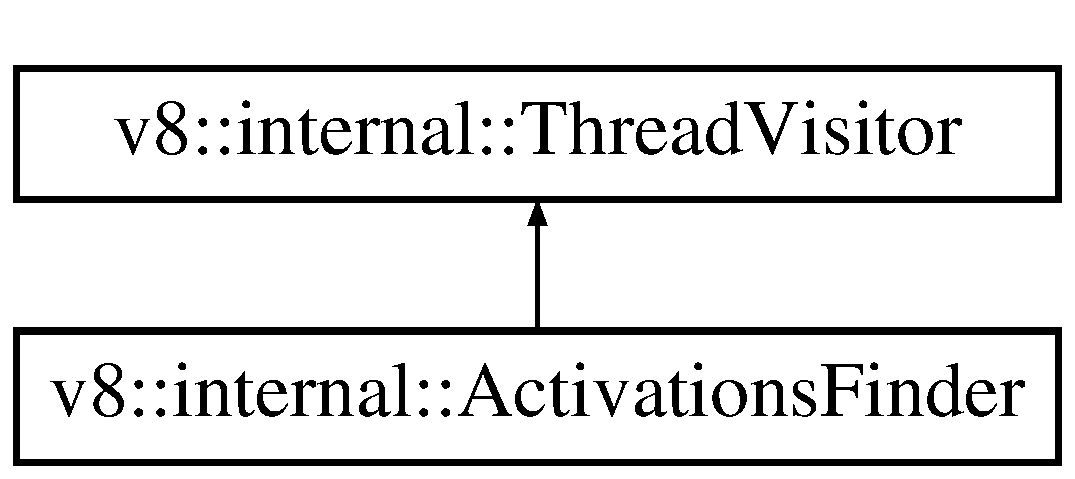
\includegraphics[height=2.000000cm]{classv8_1_1internal_1_1_activations_finder}
\end{center}
\end{figure}
\subsection*{Public Member Functions}
\begin{DoxyCompactItemize}
\item 
{\bfseries Activations\+Finder} (\hyperlink{classv8_1_1internal_1_1_code}{Code} $\ast$code)\hypertarget{classv8_1_1internal_1_1_activations_finder_a60e1f2fc90f683fe1e4d5f1a190dde8f}{}\label{classv8_1_1internal_1_1_activations_finder_a60e1f2fc90f683fe1e4d5f1a190dde8f}

\item 
void {\bfseries Visit\+Thread} (\hyperlink{classv8_1_1internal_1_1_isolate}{Isolate} $\ast$isolate, Thread\+Local\+Top $\ast$top)\hypertarget{classv8_1_1internal_1_1_activations_finder_a7eadc771094bec59bd76f6e5ff713a2c}{}\label{classv8_1_1internal_1_1_activations_finder_a7eadc771094bec59bd76f6e5ff713a2c}

\item 
void {\bfseries Visit\+Frames} (Java\+Script\+Frame\+Iterator $\ast$it)\hypertarget{classv8_1_1internal_1_1_activations_finder_a421dbf4202e15a9c29ed94354ea57a8c}{}\label{classv8_1_1internal_1_1_activations_finder_a421dbf4202e15a9c29ed94354ea57a8c}

\end{DoxyCompactItemize}
\subsection*{Public Attributes}
\begin{DoxyCompactItemize}
\item 
\hyperlink{classv8_1_1internal_1_1_code}{Code} $\ast$ {\bfseries code\+\_\+}\hypertarget{classv8_1_1internal_1_1_activations_finder_ac6ed1ea07a59270aae7aaf32f23cb537}{}\label{classv8_1_1internal_1_1_activations_finder_ac6ed1ea07a59270aae7aaf32f23cb537}

\item 
bool {\bfseries has\+\_\+code\+\_\+activations\+\_\+}\hypertarget{classv8_1_1internal_1_1_activations_finder_a0faceafe43a03036d7d86c6aaf231fdf}{}\label{classv8_1_1internal_1_1_activations_finder_a0faceafe43a03036d7d86c6aaf231fdf}

\end{DoxyCompactItemize}


The documentation for this class was generated from the following file\+:\begin{DoxyCompactItemize}
\item 
/\+Users/joshgav/node/v8/src/runtime/runtime-\/compiler.\+cc\end{DoxyCompactItemize}

\hypertarget{classv8_1_1_activity_control}{}\section{v8\+:\+:Activity\+Control Class Reference}
\label{classv8_1_1_activity_control}\index{v8\+::\+Activity\+Control@{v8\+::\+Activity\+Control}}


{\ttfamily \#include $<$v8-\/profiler.\+h$>$}

\subsection*{Public Types}
\begin{DoxyCompactItemize}
\item 
enum {\bfseries Control\+Option} \{ \\*
{\bfseries k\+Continue} = 0, 
\\*
{\bfseries k\+Abort} = 1
 \}\hypertarget{classv8_1_1_activity_control_a6d261e8c21e8076ce86b4add231a8ef9}{}\label{classv8_1_1_activity_control_a6d261e8c21e8076ce86b4add231a8ef9}

\end{DoxyCompactItemize}
\subsection*{Public Member Functions}
\begin{DoxyCompactItemize}
\item 
virtual Control\+Option \hyperlink{classv8_1_1_activity_control_a1300f10611306a3e8f79239e057eb0bf}{Report\+Progress\+Value} (int done, int total)=0
\end{DoxyCompactItemize}


\subsection{Detailed Description}
An interface for reporting progress and controlling long-\/running activities. 

\subsection{Member Function Documentation}
\index{v8\+::\+Activity\+Control@{v8\+::\+Activity\+Control}!Report\+Progress\+Value@{Report\+Progress\+Value}}
\index{Report\+Progress\+Value@{Report\+Progress\+Value}!v8\+::\+Activity\+Control@{v8\+::\+Activity\+Control}}
\subsubsection[{\texorpdfstring{Report\+Progress\+Value(int done, int total)=0}{ReportProgressValue(int done, int total)=0}}]{\setlength{\rightskip}{0pt plus 5cm}virtual Control\+Option v8\+::\+Activity\+Control\+::\+Report\+Progress\+Value (
\begin{DoxyParamCaption}
\item[{int}]{done, }
\item[{int}]{total}
\end{DoxyParamCaption}
)\hspace{0.3cm}{\ttfamily [pure virtual]}}\hypertarget{classv8_1_1_activity_control_a1300f10611306a3e8f79239e057eb0bf}{}\label{classv8_1_1_activity_control_a1300f10611306a3e8f79239e057eb0bf}
Notify about current progress. The activity can be stopped by returning k\+Abort as the callback result. 

The documentation for this class was generated from the following file\+:\begin{DoxyCompactItemize}
\item 
/\+Users/joshgav/node/v8/include/v8-\/profiler.\+h\end{DoxyCompactItemize}

\hypertarget{classv8_1_1internal_1_1_add_dispatch_range}{}\section{v8\+:\+:internal\+:\+:Add\+Dispatch\+Range Class Reference}
\label{classv8_1_1internal_1_1_add_dispatch_range}\index{v8\+::internal\+::\+Add\+Dispatch\+Range@{v8\+::internal\+::\+Add\+Dispatch\+Range}}
\subsection*{Public Member Functions}
\begin{DoxyCompactItemize}
\item 
{\bfseries Add\+Dispatch\+Range} (\hyperlink{classv8_1_1internal_1_1_dispatch_table_constructor}{Dispatch\+Table\+Constructor} $\ast$constructor)\hypertarget{classv8_1_1internal_1_1_add_dispatch_range_aabb3eb748f5a566349ae5946fef1103b}{}\label{classv8_1_1internal_1_1_add_dispatch_range_aabb3eb748f5a566349ae5946fef1103b}

\item 
void {\bfseries Call} (uc32 from, \hyperlink{classv8_1_1internal_1_1_dispatch_table_1_1_entry}{Dispatch\+Table\+::\+Entry} entry)\hypertarget{classv8_1_1internal_1_1_add_dispatch_range_a17e1406e159be04ef2b1fcc36d94c888}{}\label{classv8_1_1internal_1_1_add_dispatch_range_a17e1406e159be04ef2b1fcc36d94c888}

\end{DoxyCompactItemize}
\subsection*{Private Attributes}
\begin{DoxyCompactItemize}
\item 
\hyperlink{classv8_1_1internal_1_1_dispatch_table_constructor}{Dispatch\+Table\+Constructor} $\ast$ {\bfseries constructor\+\_\+}\hypertarget{classv8_1_1internal_1_1_add_dispatch_range_ad9e4986bc6b16cb976a50cebd857ecc0}{}\label{classv8_1_1internal_1_1_add_dispatch_range_ad9e4986bc6b16cb976a50cebd857ecc0}

\end{DoxyCompactItemize}


The documentation for this class was generated from the following file\+:\begin{DoxyCompactItemize}
\item 
/\+Users/joshgav/node/v8/src/regexp/jsregexp.\+cc\end{DoxyCompactItemize}

\hypertarget{structv8_1_1internal_1_1compiler_1_1_add_matcher}{}\section{v8\+:\+:internal\+:\+:compiler\+:\+:Add\+Matcher$<$ Binop\+Matcher, k\+Add\+Opcode, k\+Mul\+Opcode, k\+Shift\+Opcode $>$ Struct Template Reference}
\label{structv8_1_1internal_1_1compiler_1_1_add_matcher}\index{v8\+::internal\+::compiler\+::\+Add\+Matcher$<$ Binop\+Matcher, k\+Add\+Opcode, k\+Mul\+Opcode, k\+Shift\+Opcode $>$@{v8\+::internal\+::compiler\+::\+Add\+Matcher$<$ Binop\+Matcher, k\+Add\+Opcode, k\+Mul\+Opcode, k\+Shift\+Opcode $>$}}
Inheritance diagram for v8\+:\+:internal\+:\+:compiler\+:\+:Add\+Matcher$<$ Binop\+Matcher, k\+Add\+Opcode, k\+Mul\+Opcode, k\+Shift\+Opcode $>$\+:\begin{figure}[H]
\begin{center}
\leavevmode
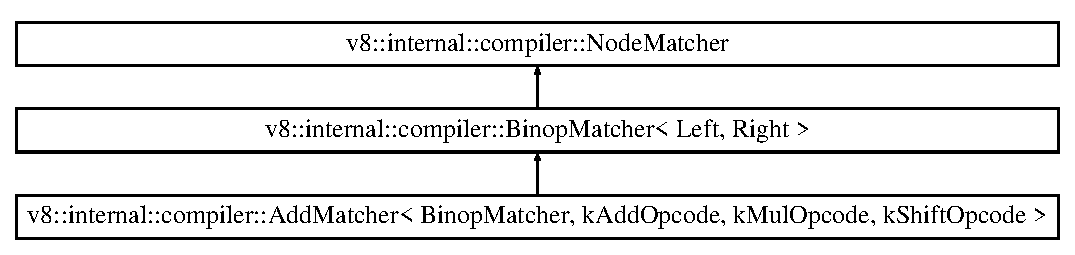
\includegraphics[height=2.978723cm]{structv8_1_1internal_1_1compiler_1_1_add_matcher}
\end{center}
\end{figure}
\subsection*{Public Types}
\begin{DoxyCompactItemize}
\item 
typedef \hyperlink{structv8_1_1internal_1_1compiler_1_1_scale_matcher}{Scale\+Matcher}$<$ \hyperlink{structv8_1_1internal_1_1compiler_1_1_binop_matcher}{Binop\+Matcher}, k\+Mul\+Opcode, k\+Shift\+Opcode $>$ {\bfseries Matcher}\hypertarget{structv8_1_1internal_1_1compiler_1_1_add_matcher_a4e62b8fd72e616549f23062291b6fa5d}{}\label{structv8_1_1internal_1_1compiler_1_1_add_matcher_a4e62b8fd72e616549f23062291b6fa5d}

\end{DoxyCompactItemize}
\subsection*{Public Member Functions}
\begin{DoxyCompactItemize}
\item 
{\bfseries Add\+Matcher} (\hyperlink{classv8_1_1internal_1_1compiler_1_1_node}{Node} $\ast$node, bool allow\+\_\+input\+\_\+swap)\hypertarget{structv8_1_1internal_1_1compiler_1_1_add_matcher_a67423087c3f808f0bce7bb59c6bb68a4}{}\label{structv8_1_1internal_1_1compiler_1_1_add_matcher_a67423087c3f808f0bce7bb59c6bb68a4}

\item 
{\bfseries Add\+Matcher} (\hyperlink{classv8_1_1internal_1_1compiler_1_1_node}{Node} $\ast$node)\hypertarget{structv8_1_1internal_1_1compiler_1_1_add_matcher_a5cbb85d2914277d4e29e4a9cc2f2a193}{}\label{structv8_1_1internal_1_1compiler_1_1_add_matcher_a5cbb85d2914277d4e29e4a9cc2f2a193}

\item 
bool {\bfseries Has\+Index\+Input} () const \hypertarget{structv8_1_1internal_1_1compiler_1_1_add_matcher_a53c90b9d097adbb89f01db8f06d5ab0e}{}\label{structv8_1_1internal_1_1compiler_1_1_add_matcher_a53c90b9d097adbb89f01db8f06d5ab0e}

\item 
\hyperlink{classv8_1_1internal_1_1compiler_1_1_node}{Node} $\ast$ {\bfseries Index\+Input} () const \hypertarget{structv8_1_1internal_1_1compiler_1_1_add_matcher_aaccdd17cae0efdc79ed510de81530c78}{}\label{structv8_1_1internal_1_1compiler_1_1_add_matcher_aaccdd17cae0efdc79ed510de81530c78}

\item 
int {\bfseries scale} () const \hypertarget{structv8_1_1internal_1_1compiler_1_1_add_matcher_ab3ab612b97b5ee712db9f267c8f24c81}{}\label{structv8_1_1internal_1_1compiler_1_1_add_matcher_ab3ab612b97b5ee712db9f267c8f24c81}

\item 
bool {\bfseries power\+\_\+of\+\_\+two\+\_\+plus\+\_\+one} () const \hypertarget{structv8_1_1internal_1_1compiler_1_1_add_matcher_a1b80d27debc000b2ccae8b180a22c7f7}{}\label{structv8_1_1internal_1_1compiler_1_1_add_matcher_a1b80d27debc000b2ccae8b180a22c7f7}

\end{DoxyCompactItemize}
\subsection*{Static Public Attributes}
\begin{DoxyCompactItemize}
\item 
static const Ir\+Opcode\+::\+Value {\bfseries k\+Opcode} = k\+Add\+Opcode\hypertarget{structv8_1_1internal_1_1compiler_1_1_add_matcher_a9f233656772a07527c3462fddbc0c2f6}{}\label{structv8_1_1internal_1_1compiler_1_1_add_matcher_a9f233656772a07527c3462fddbc0c2f6}

\end{DoxyCompactItemize}
\subsection*{Private Member Functions}
\begin{DoxyCompactItemize}
\item 
void {\bfseries Initialize} (\hyperlink{classv8_1_1internal_1_1compiler_1_1_node}{Node} $\ast$node, bool allow\+\_\+input\+\_\+swap)\hypertarget{structv8_1_1internal_1_1compiler_1_1_add_matcher_a448de8a5819c4a646080184d291ca83a}{}\label{structv8_1_1internal_1_1compiler_1_1_add_matcher_a448de8a5819c4a646080184d291ca83a}

\end{DoxyCompactItemize}
\subsection*{Private Attributes}
\begin{DoxyCompactItemize}
\item 
int {\bfseries scale\+\_\+}\hypertarget{structv8_1_1internal_1_1compiler_1_1_add_matcher_a901617772c720dddb9eb2f1ad10a58c2}{}\label{structv8_1_1internal_1_1compiler_1_1_add_matcher_a901617772c720dddb9eb2f1ad10a58c2}

\item 
bool {\bfseries power\+\_\+of\+\_\+two\+\_\+plus\+\_\+one\+\_\+}\hypertarget{structv8_1_1internal_1_1compiler_1_1_add_matcher_ac200c9a0db1de369be51649fb5fa5702}{}\label{structv8_1_1internal_1_1compiler_1_1_add_matcher_ac200c9a0db1de369be51649fb5fa5702}

\end{DoxyCompactItemize}
\subsection*{Additional Inherited Members}


The documentation for this struct was generated from the following file\+:\begin{DoxyCompactItemize}
\item 
/\+Users/joshgav/node/v8/src/compiler/node-\/matchers.\+h\end{DoxyCompactItemize}

\hypertarget{classv8_1_1internal_1_1_record_write_stub_1_1_address_bits}{}\section{v8\+:\+:internal\+:\+:Record\+Write\+Stub\+:\+:Address\+Bits Class Reference}
\label{classv8_1_1internal_1_1_record_write_stub_1_1_address_bits}\index{v8\+::internal\+::\+Record\+Write\+Stub\+::\+Address\+Bits@{v8\+::internal\+::\+Record\+Write\+Stub\+::\+Address\+Bits}}
Inheritance diagram for v8\+:\+:internal\+:\+:Record\+Write\+Stub\+:\+:Address\+Bits\+:\begin{figure}[H]
\begin{center}
\leavevmode
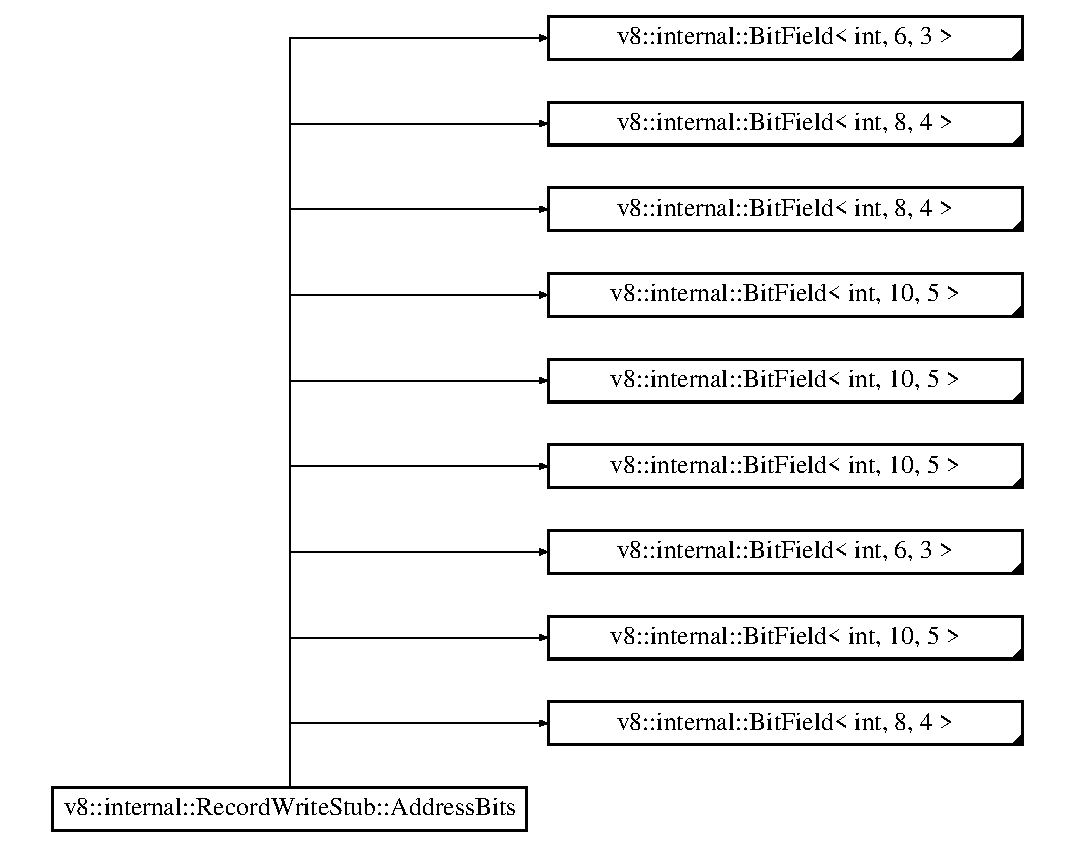
\includegraphics[height=10.000000cm]{classv8_1_1internal_1_1_record_write_stub_1_1_address_bits}
\end{center}
\end{figure}
\subsection*{Additional Inherited Members}


The documentation for this class was generated from the following file\+:\begin{DoxyCompactItemize}
\item 
/\+Users/joshgav/node/v8/src/arm/code-\/stubs-\/arm.\+h\end{DoxyCompactItemize}

\hypertarget{classv8_1_1internal_1_1_address_map_base}{}\section{v8\+:\+:internal\+:\+:Address\+Map\+Base Class Reference}
\label{classv8_1_1internal_1_1_address_map_base}\index{v8\+::internal\+::\+Address\+Map\+Base@{v8\+::internal\+::\+Address\+Map\+Base}}
Inheritance diagram for v8\+:\+:internal\+:\+:Address\+Map\+Base\+:\begin{figure}[H]
\begin{center}
\leavevmode
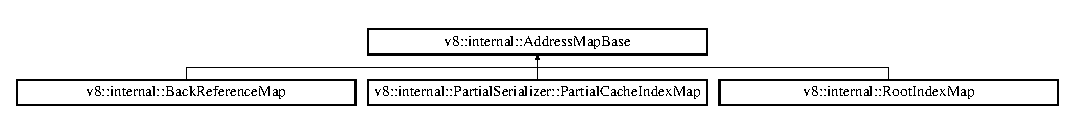
\includegraphics[height=1.196581cm]{classv8_1_1internal_1_1_address_map_base}
\end{center}
\end{figure}
\subsection*{Static Protected Member Functions}
\begin{DoxyCompactItemize}
\item 
static void {\bfseries Set\+Value} (Hash\+Map\+::\+Entry $\ast$entry, uint32\+\_\+t v)\hypertarget{classv8_1_1internal_1_1_address_map_base_ad901a40bc8f6ae8364f2fdaf10e46ee9}{}\label{classv8_1_1internal_1_1_address_map_base_ad901a40bc8f6ae8364f2fdaf10e46ee9}

\item 
static uint32\+\_\+t {\bfseries Get\+Value} (Hash\+Map\+::\+Entry $\ast$entry)\hypertarget{classv8_1_1internal_1_1_address_map_base_ac940b73338cebdd25c26ea0dea9a6512}{}\label{classv8_1_1internal_1_1_address_map_base_ac940b73338cebdd25c26ea0dea9a6512}

\item 
static Hash\+Map\+::\+Entry $\ast$ {\bfseries Lookup\+Entry} (\hyperlink{classv8_1_1internal_1_1_template_hash_map_impl}{Hash\+Map} $\ast$map, \hyperlink{classv8_1_1internal_1_1_heap_object}{Heap\+Object} $\ast$obj, bool insert)\hypertarget{classv8_1_1internal_1_1_address_map_base_a7753d398808cd59ba39d0de9a87a0912}{}\label{classv8_1_1internal_1_1_address_map_base_a7753d398808cd59ba39d0de9a87a0912}

\end{DoxyCompactItemize}
\subsection*{Static Private Member Functions}
\begin{DoxyCompactItemize}
\item 
static uint32\+\_\+t {\bfseries Hash} (\hyperlink{classv8_1_1internal_1_1_heap_object}{Heap\+Object} $\ast$obj)\hypertarget{classv8_1_1internal_1_1_address_map_base_a310a6ae7d8e9d54246c6fd76b8efc304}{}\label{classv8_1_1internal_1_1_address_map_base_a310a6ae7d8e9d54246c6fd76b8efc304}

\item 
static void $\ast$ {\bfseries Key} (\hyperlink{classv8_1_1internal_1_1_heap_object}{Heap\+Object} $\ast$obj)\hypertarget{classv8_1_1internal_1_1_address_map_base_a60eeafde4d0db85e402dfd02b9774816}{}\label{classv8_1_1internal_1_1_address_map_base_a60eeafde4d0db85e402dfd02b9774816}

\end{DoxyCompactItemize}


The documentation for this class was generated from the following file\+:\begin{DoxyCompactItemize}
\item 
/\+Users/joshgav/node/v8/src/address-\/map.\+h\end{DoxyCompactItemize}

\hypertarget{classv8_1_1internal_1_1_address_to_trace_map}{}\section{v8\+:\+:internal\+:\+:Address\+To\+Trace\+Map Class Reference}
\label{classv8_1_1internal_1_1_address_to_trace_map}\index{v8\+::internal\+::\+Address\+To\+Trace\+Map@{v8\+::internal\+::\+Address\+To\+Trace\+Map}}
\subsection*{Classes}
\begin{DoxyCompactItemize}
\item 
struct \hyperlink{structv8_1_1internal_1_1_address_to_trace_map_1_1_range_stack}{Range\+Stack}
\end{DoxyCompactItemize}
\subsection*{Public Member Functions}
\begin{DoxyCompactItemize}
\item 
void {\bfseries Add\+Range} (Address addr, int size, unsigned node\+\_\+id)\hypertarget{classv8_1_1internal_1_1_address_to_trace_map_a3b1bc8f1abc6f072a660d2b689852838}{}\label{classv8_1_1internal_1_1_address_to_trace_map_a3b1bc8f1abc6f072a660d2b689852838}

\item 
unsigned {\bfseries Get\+Trace\+Node\+Id} (Address addr)\hypertarget{classv8_1_1internal_1_1_address_to_trace_map_ab76fa587a105ae24f300f171d8cb22a6}{}\label{classv8_1_1internal_1_1_address_to_trace_map_ab76fa587a105ae24f300f171d8cb22a6}

\item 
void {\bfseries Move\+Object} (Address from, Address to, int size)\hypertarget{classv8_1_1internal_1_1_address_to_trace_map_a02c96d03b3486527aeb46a461c43cf15}{}\label{classv8_1_1internal_1_1_address_to_trace_map_a02c96d03b3486527aeb46a461c43cf15}

\item 
void {\bfseries Clear} ()\hypertarget{classv8_1_1internal_1_1_address_to_trace_map_aa705b7b0e3c00645af20ff4d61140f02}{}\label{classv8_1_1internal_1_1_address_to_trace_map_aa705b7b0e3c00645af20ff4d61140f02}

\item 
size\+\_\+t {\bfseries size} ()\hypertarget{classv8_1_1internal_1_1_address_to_trace_map_a6acf57cbb1975fe242c744f4ad5669f3}{}\label{classv8_1_1internal_1_1_address_to_trace_map_a6acf57cbb1975fe242c744f4ad5669f3}

\item 
void {\bfseries Print} ()\hypertarget{classv8_1_1internal_1_1_address_to_trace_map_a8aa12b1b9b85be5aba73b0631d1ea389}{}\label{classv8_1_1internal_1_1_address_to_trace_map_a8aa12b1b9b85be5aba73b0631d1ea389}

\end{DoxyCompactItemize}
\subsection*{Private Types}
\begin{DoxyCompactItemize}
\item 
typedef std\+::map$<$ Address, \hyperlink{structv8_1_1internal_1_1_address_to_trace_map_1_1_range_stack}{Range\+Stack} $>$ {\bfseries Range\+Map}\hypertarget{classv8_1_1internal_1_1_address_to_trace_map_afd65f8eb3d8a0b639299248866bec150}{}\label{classv8_1_1internal_1_1_address_to_trace_map_afd65f8eb3d8a0b639299248866bec150}

\end{DoxyCompactItemize}
\subsection*{Private Member Functions}
\begin{DoxyCompactItemize}
\item 
void {\bfseries Remove\+Range} (Address start, Address end)\hypertarget{classv8_1_1internal_1_1_address_to_trace_map_a5fced099832218b998c2bb3ab6de9906}{}\label{classv8_1_1internal_1_1_address_to_trace_map_a5fced099832218b998c2bb3ab6de9906}

\end{DoxyCompactItemize}
\subsection*{Private Attributes}
\begin{DoxyCompactItemize}
\item 
Range\+Map {\bfseries ranges\+\_\+}\hypertarget{classv8_1_1internal_1_1_address_to_trace_map_ad84aa834e379d1a872155acc3811b23c}{}\label{classv8_1_1internal_1_1_address_to_trace_map_ad84aa834e379d1a872155acc3811b23c}

\end{DoxyCompactItemize}


The documentation for this class was generated from the following files\+:\begin{DoxyCompactItemize}
\item 
/\+Users/joshgav/node/v8/src/profiler/allocation-\/tracker.\+h\item 
/\+Users/joshgav/node/v8/src/profiler/allocation-\/tracker.\+cc\end{DoxyCompactItemize}

\hypertarget{classv8_1_1internal_1_1_add_stub}{}\section{v8\+:\+:internal\+:\+:Add\+Stub Class Reference}
\label{classv8_1_1internal_1_1_add_stub}\index{v8\+::internal\+::\+Add\+Stub@{v8\+::internal\+::\+Add\+Stub}}
Inheritance diagram for v8\+:\+:internal\+:\+:Add\+Stub\+:\begin{figure}[H]
\begin{center}
\leavevmode
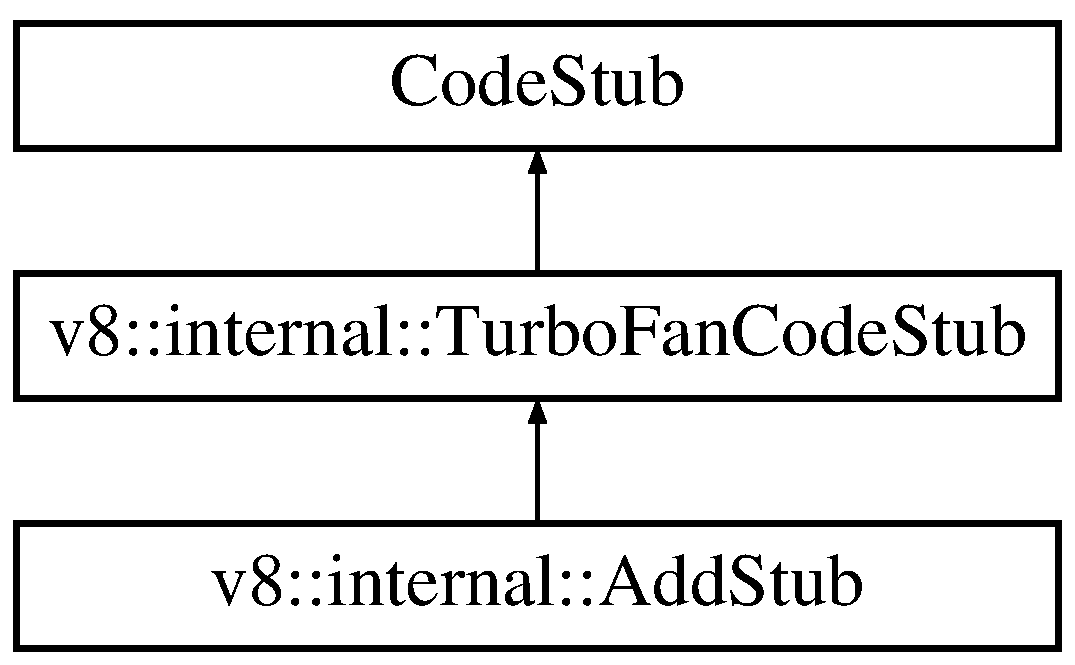
\includegraphics[height=3.000000cm]{classv8_1_1internal_1_1_add_stub}
\end{center}
\end{figure}
\subsection*{Public Member Functions}
\begin{DoxyCompactItemize}
\item 
{\bfseries Add\+Stub} (\hyperlink{classv8_1_1internal_1_1_isolate}{Isolate} $\ast$isolate)\hypertarget{classv8_1_1internal_1_1_add_stub_aea19c816f480842a69023beb9f605c49}{}\label{classv8_1_1internal_1_1_add_stub_aea19c816f480842a69023beb9f605c49}

\item 
{\bfseries D\+E\+F\+I\+N\+E\+\_\+\+C\+A\+L\+L\+\_\+\+I\+N\+T\+E\+R\+F\+A\+C\+E\+\_\+\+D\+E\+S\+C\+R\+I\+P\+T\+OR} (Binary\+Op)\hypertarget{classv8_1_1internal_1_1_add_stub_abefbccda3916278fca9e88c08ff3276d}{}\label{classv8_1_1internal_1_1_add_stub_abefbccda3916278fca9e88c08ff3276d}

\item 
{\bfseries D\+E\+F\+I\+N\+E\+\_\+\+T\+U\+R\+B\+O\+F\+A\+N\+\_\+\+C\+O\+D\+E\+\_\+\+S\+T\+UB} (Add, \hyperlink{classv8_1_1internal_1_1_turbo_fan_code_stub}{Turbo\+Fan\+Code\+Stub})\hypertarget{classv8_1_1internal_1_1_add_stub_a6194c80d1bea456707a8beffbd177087}{}\label{classv8_1_1internal_1_1_add_stub_a6194c80d1bea456707a8beffbd177087}

\end{DoxyCompactItemize}
\subsection*{Additional Inherited Members}


The documentation for this class was generated from the following file\+:\begin{DoxyCompactItemize}
\item 
/\+Users/joshgav/node/v8/src/code-\/stubs.\+h\end{DoxyCompactItemize}

\hypertarget{classv8_1_1internal_1_1compiler_1_1_advanced_reducer}{}\section{v8\+:\+:internal\+:\+:compiler\+:\+:Advanced\+Reducer Class Reference}
\label{classv8_1_1internal_1_1compiler_1_1_advanced_reducer}\index{v8\+::internal\+::compiler\+::\+Advanced\+Reducer@{v8\+::internal\+::compiler\+::\+Advanced\+Reducer}}
Inheritance diagram for v8\+:\+:internal\+:\+:compiler\+:\+:Advanced\+Reducer\+:\begin{figure}[H]
\begin{center}
\leavevmode
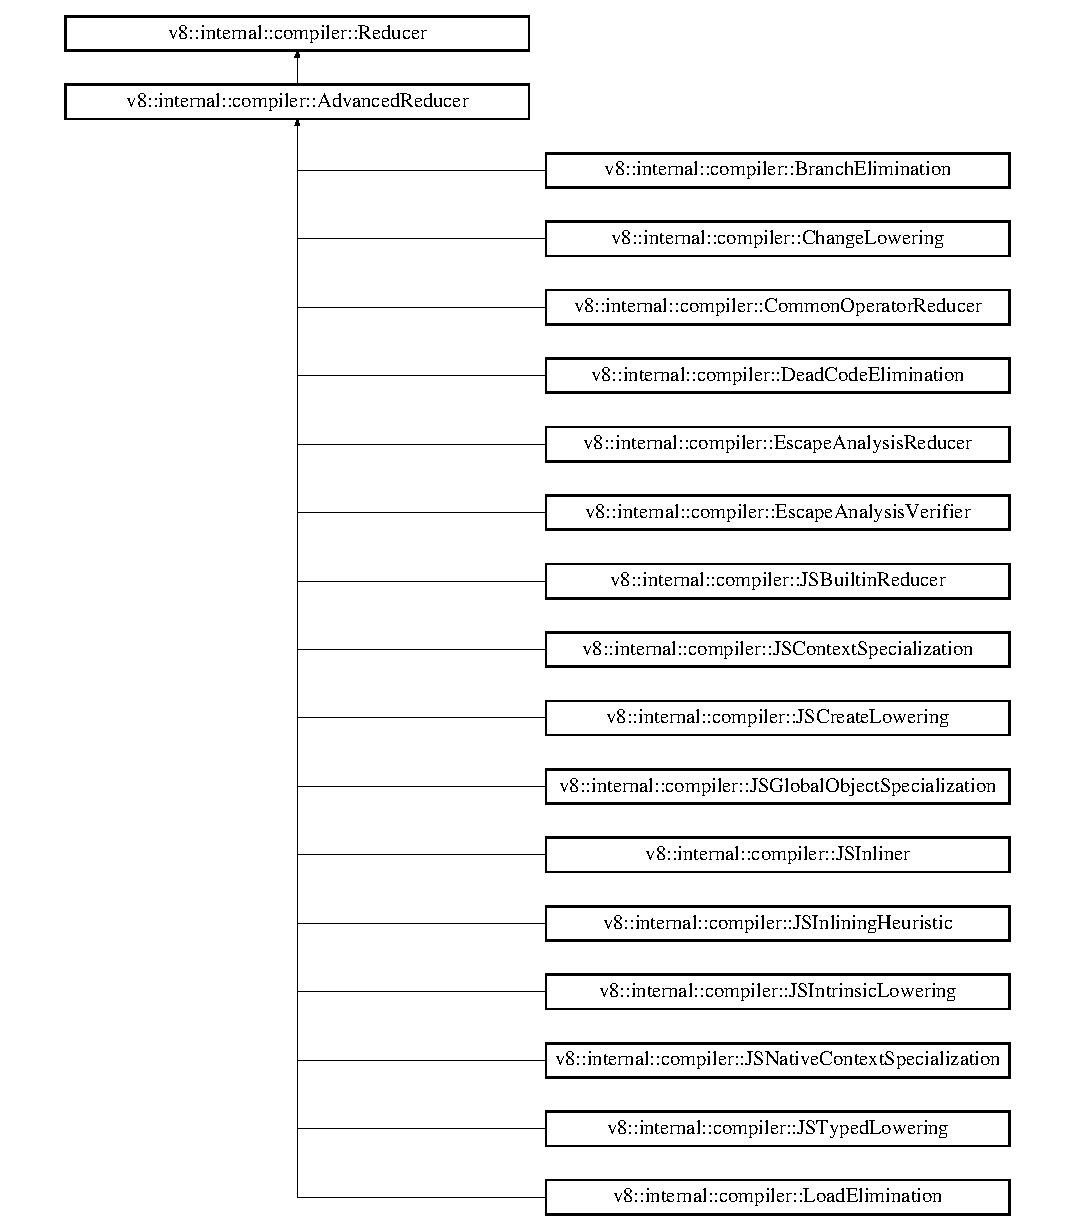
\includegraphics[height=12.000000cm]{classv8_1_1internal_1_1compiler_1_1_advanced_reducer}
\end{center}
\end{figure}
\subsection*{Classes}
\begin{DoxyCompactItemize}
\item 
class \hyperlink{classv8_1_1internal_1_1compiler_1_1_advanced_reducer_1_1_editor}{Editor}
\end{DoxyCompactItemize}
\subsection*{Public Member Functions}
\begin{DoxyCompactItemize}
\item 
{\bfseries Advanced\+Reducer} (\hyperlink{classv8_1_1internal_1_1compiler_1_1_advanced_reducer_1_1_editor}{Editor} $\ast$editor)\hypertarget{classv8_1_1internal_1_1compiler_1_1_advanced_reducer_abb941b5a245fa4b0c2e87c049fd78190}{}\label{classv8_1_1internal_1_1compiler_1_1_advanced_reducer_abb941b5a245fa4b0c2e87c049fd78190}

\end{DoxyCompactItemize}
\subsection*{Protected Member Functions}
\begin{DoxyCompactItemize}
\item 
void {\bfseries Replace} (\hyperlink{classv8_1_1internal_1_1compiler_1_1_node}{Node} $\ast$node, \hyperlink{classv8_1_1internal_1_1compiler_1_1_node}{Node} $\ast$replacement)\hypertarget{classv8_1_1internal_1_1compiler_1_1_advanced_reducer_a375f732a84655a28f171351dc76f8acc}{}\label{classv8_1_1internal_1_1compiler_1_1_advanced_reducer_a375f732a84655a28f171351dc76f8acc}

\item 
void {\bfseries Revisit} (\hyperlink{classv8_1_1internal_1_1compiler_1_1_node}{Node} $\ast$node)\hypertarget{classv8_1_1internal_1_1compiler_1_1_advanced_reducer_a64cae7699553789a4534c549c9170816}{}\label{classv8_1_1internal_1_1compiler_1_1_advanced_reducer_a64cae7699553789a4534c549c9170816}

\item 
void {\bfseries Replace\+With\+Value} (\hyperlink{classv8_1_1internal_1_1compiler_1_1_node}{Node} $\ast$node, \hyperlink{classv8_1_1internal_1_1compiler_1_1_node}{Node} $\ast$value, \hyperlink{classv8_1_1internal_1_1compiler_1_1_node}{Node} $\ast$effect=nullptr, \hyperlink{classv8_1_1internal_1_1compiler_1_1_node}{Node} $\ast$control=nullptr)\hypertarget{classv8_1_1internal_1_1compiler_1_1_advanced_reducer_a2573497dc120509db4c00a28d8d3a9cb}{}\label{classv8_1_1internal_1_1compiler_1_1_advanced_reducer_a2573497dc120509db4c00a28d8d3a9cb}

\item 
void {\bfseries Relax\+Effects\+And\+Controls} (\hyperlink{classv8_1_1internal_1_1compiler_1_1_node}{Node} $\ast$node)\hypertarget{classv8_1_1internal_1_1compiler_1_1_advanced_reducer_a2f1059b277571c651117544bd023cb8c}{}\label{classv8_1_1internal_1_1compiler_1_1_advanced_reducer_a2f1059b277571c651117544bd023cb8c}

\item 
void {\bfseries Relax\+Controls} (\hyperlink{classv8_1_1internal_1_1compiler_1_1_node}{Node} $\ast$node)\hypertarget{classv8_1_1internal_1_1compiler_1_1_advanced_reducer_a69dd3891050d9e54a9b82db9bd55eacc}{}\label{classv8_1_1internal_1_1compiler_1_1_advanced_reducer_a69dd3891050d9e54a9b82db9bd55eacc}

\end{DoxyCompactItemize}
\subsection*{Static Protected Member Functions}
\begin{DoxyCompactItemize}
\item 
static \hyperlink{classv8_1_1internal_1_1compiler_1_1_reduction}{Reduction} {\bfseries Replace} (\hyperlink{classv8_1_1internal_1_1compiler_1_1_node}{Node} $\ast$node)\hypertarget{classv8_1_1internal_1_1compiler_1_1_advanced_reducer_a6b9e69978e8440e00ca157d8e4fef297}{}\label{classv8_1_1internal_1_1compiler_1_1_advanced_reducer_a6b9e69978e8440e00ca157d8e4fef297}

\end{DoxyCompactItemize}
\subsection*{Private Attributes}
\begin{DoxyCompactItemize}
\item 
\hyperlink{classv8_1_1internal_1_1compiler_1_1_advanced_reducer_1_1_editor}{Editor} $\ast$const {\bfseries editor\+\_\+}\hypertarget{classv8_1_1internal_1_1compiler_1_1_advanced_reducer_ac6d09f2e5a2a0e06be0b38642e69efdb}{}\label{classv8_1_1internal_1_1compiler_1_1_advanced_reducer_ac6d09f2e5a2a0e06be0b38642e69efdb}

\end{DoxyCompactItemize}
\subsection*{Additional Inherited Members}


The documentation for this class was generated from the following file\+:\begin{DoxyCompactItemize}
\item 
/\+Users/joshgav/node/v8/src/compiler/graph-\/reducer.\+h\end{DoxyCompactItemize}

\hypertarget{classv8_1_1internal_1_1_aggregatable_histogram_timer}{}\section{v8\+:\+:internal\+:\+:Aggregatable\+Histogram\+Timer Class Reference}
\label{classv8_1_1internal_1_1_aggregatable_histogram_timer}\index{v8\+::internal\+::\+Aggregatable\+Histogram\+Timer@{v8\+::internal\+::\+Aggregatable\+Histogram\+Timer}}
Inheritance diagram for v8\+:\+:internal\+:\+:Aggregatable\+Histogram\+Timer\+:\begin{figure}[H]
\begin{center}
\leavevmode
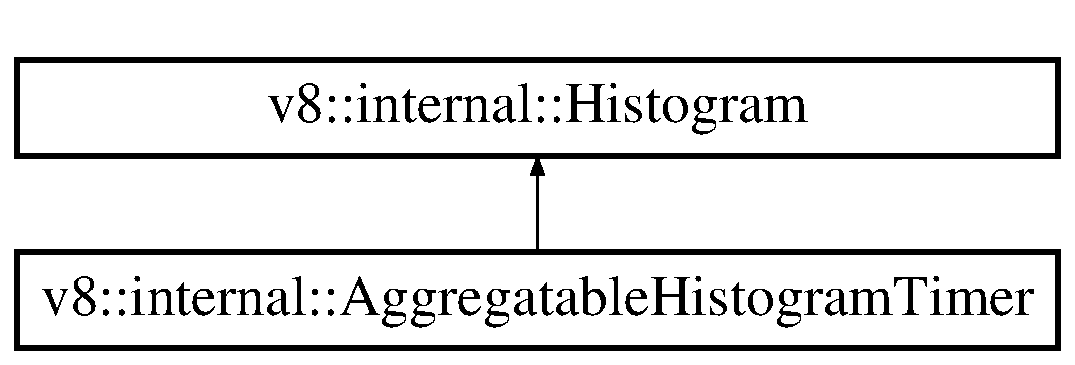
\includegraphics[height=2.000000cm]{classv8_1_1internal_1_1_aggregatable_histogram_timer}
\end{center}
\end{figure}
\subsection*{Public Member Functions}
\begin{DoxyCompactItemize}
\item 
{\bfseries Aggregatable\+Histogram\+Timer} (const char $\ast$name, int min, int max, int num\+\_\+buckets, \hyperlink{classv8_1_1internal_1_1_isolate}{Isolate} $\ast$isolate)\hypertarget{classv8_1_1internal_1_1_aggregatable_histogram_timer_aafe8f18c2f1b354ab265b82f2fde0aec}{}\label{classv8_1_1internal_1_1_aggregatable_histogram_timer_aafe8f18c2f1b354ab265b82f2fde0aec}

\item 
void {\bfseries Start} ()\hypertarget{classv8_1_1internal_1_1_aggregatable_histogram_timer_a90f85567bb20dba01c8d4e69578db899}{}\label{classv8_1_1internal_1_1_aggregatable_histogram_timer_a90f85567bb20dba01c8d4e69578db899}

\item 
void {\bfseries Stop} ()\hypertarget{classv8_1_1internal_1_1_aggregatable_histogram_timer_ada969f70c76ed1eace83ea0491d7af5e}{}\label{classv8_1_1internal_1_1_aggregatable_histogram_timer_ada969f70c76ed1eace83ea0491d7af5e}

\item 
void {\bfseries Add} (\hyperlink{classv8_1_1base_1_1_time_delta}{base\+::\+Time\+Delta} other)\hypertarget{classv8_1_1internal_1_1_aggregatable_histogram_timer_ad56ff543a2b2816fe290fdc2d259c844}{}\label{classv8_1_1internal_1_1_aggregatable_histogram_timer_ad56ff543a2b2816fe290fdc2d259c844}

\end{DoxyCompactItemize}
\subsection*{Private Attributes}
\begin{DoxyCompactItemize}
\item 
\hyperlink{classv8_1_1base_1_1_time_delta}{base\+::\+Time\+Delta} {\bfseries time\+\_\+}\hypertarget{classv8_1_1internal_1_1_aggregatable_histogram_timer_a90f4009c8b97572bfb5fc3b802c9f1e1}{}\label{classv8_1_1internal_1_1_aggregatable_histogram_timer_a90f4009c8b97572bfb5fc3b802c9f1e1}

\end{DoxyCompactItemize}
\subsection*{Additional Inherited Members}


The documentation for this class was generated from the following file\+:\begin{DoxyCompactItemize}
\item 
/\+Users/joshgav/node/v8/src/counters.\+h\end{DoxyCompactItemize}

\hypertarget{classv8_1_1internal_1_1_aggregated_histogram_timer_scope}{}\section{v8\+:\+:internal\+:\+:Aggregated\+Histogram\+Timer\+Scope Class Reference}
\label{classv8_1_1internal_1_1_aggregated_histogram_timer_scope}\index{v8\+::internal\+::\+Aggregated\+Histogram\+Timer\+Scope@{v8\+::internal\+::\+Aggregated\+Histogram\+Timer\+Scope}}
\subsection*{Public Member Functions}
\begin{DoxyCompactItemize}
\item 
{\bfseries Aggregated\+Histogram\+Timer\+Scope} (\hyperlink{classv8_1_1internal_1_1_aggregatable_histogram_timer}{Aggregatable\+Histogram\+Timer} $\ast$histogram)\hypertarget{classv8_1_1internal_1_1_aggregated_histogram_timer_scope_abaf836eb7bf83fe4ceeb79a4a5596af0}{}\label{classv8_1_1internal_1_1_aggregated_histogram_timer_scope_abaf836eb7bf83fe4ceeb79a4a5596af0}

\end{DoxyCompactItemize}
\subsection*{Private Attributes}
\begin{DoxyCompactItemize}
\item 
\hyperlink{classv8_1_1base_1_1_elapsed_timer}{base\+::\+Elapsed\+Timer} {\bfseries timer\+\_\+}\hypertarget{classv8_1_1internal_1_1_aggregated_histogram_timer_scope_a79e3e75deaf79d31c18fd6d574e482af}{}\label{classv8_1_1internal_1_1_aggregated_histogram_timer_scope_a79e3e75deaf79d31c18fd6d574e482af}

\item 
\hyperlink{classv8_1_1internal_1_1_aggregatable_histogram_timer}{Aggregatable\+Histogram\+Timer} $\ast$ {\bfseries histogram\+\_\+}\hypertarget{classv8_1_1internal_1_1_aggregated_histogram_timer_scope_acc8dd2854245945227a687c56c756964}{}\label{classv8_1_1internal_1_1_aggregated_histogram_timer_scope_acc8dd2854245945227a687c56c756964}

\end{DoxyCompactItemize}


The documentation for this class was generated from the following file\+:\begin{DoxyCompactItemize}
\item 
/\+Users/joshgav/node/v8/src/counters.\+h\end{DoxyCompactItemize}

\hypertarget{classv8_1_1internal_1_1_aggregated_memory_histogram}{}\section{v8\+:\+:internal\+:\+:Aggregated\+Memory\+Histogram$<$ Histogram $>$ Class Template Reference}
\label{classv8_1_1internal_1_1_aggregated_memory_histogram}\index{v8\+::internal\+::\+Aggregated\+Memory\+Histogram$<$ Histogram $>$@{v8\+::internal\+::\+Aggregated\+Memory\+Histogram$<$ Histogram $>$}}
\subsection*{Public Member Functions}
\begin{DoxyCompactItemize}
\item 
{\bfseries Aggregated\+Memory\+Histogram} (\hyperlink{classv8_1_1internal_1_1_histogram}{Histogram} $\ast$backing\+\_\+histogram)\hypertarget{classv8_1_1internal_1_1_aggregated_memory_histogram_a8b49cfff760e104f1150397b4a774806}{}\label{classv8_1_1internal_1_1_aggregated_memory_histogram_a8b49cfff760e104f1150397b4a774806}

\item 
void {\bfseries Add\+Sample} (double current\+\_\+ms, double current\+\_\+value)\hypertarget{classv8_1_1internal_1_1_aggregated_memory_histogram_afed07b5cc00d1e8f58be83d85ea6fe94}{}\label{classv8_1_1internal_1_1_aggregated_memory_histogram_afed07b5cc00d1e8f58be83d85ea6fe94}

\end{DoxyCompactItemize}
\subsection*{Private Member Functions}
\begin{DoxyCompactItemize}
\item 
double {\bfseries Aggregate} (double current\+\_\+ms, double current\+\_\+value)\hypertarget{classv8_1_1internal_1_1_aggregated_memory_histogram_a650db63f122dec851284bfe8bcf5c384}{}\label{classv8_1_1internal_1_1_aggregated_memory_histogram_a650db63f122dec851284bfe8bcf5c384}

\end{DoxyCompactItemize}
\subsection*{Private Attributes}
\begin{DoxyCompactItemize}
\item 
bool {\bfseries is\+\_\+initialized\+\_\+}\hypertarget{classv8_1_1internal_1_1_aggregated_memory_histogram_aed9608ee7e2534b8b3afe0885fe2ebd6}{}\label{classv8_1_1internal_1_1_aggregated_memory_histogram_aed9608ee7e2534b8b3afe0885fe2ebd6}

\item 
double {\bfseries start\+\_\+ms\+\_\+}\hypertarget{classv8_1_1internal_1_1_aggregated_memory_histogram_aabe767eedfb4212b74fa43a8c0b3fa4a}{}\label{classv8_1_1internal_1_1_aggregated_memory_histogram_aabe767eedfb4212b74fa43a8c0b3fa4a}

\item 
double {\bfseries last\+\_\+ms\+\_\+}\hypertarget{classv8_1_1internal_1_1_aggregated_memory_histogram_ad7dc697da1c27dcd8ec687c639014cca}{}\label{classv8_1_1internal_1_1_aggregated_memory_histogram_ad7dc697da1c27dcd8ec687c639014cca}

\item 
double {\bfseries aggregate\+\_\+value\+\_\+}\hypertarget{classv8_1_1internal_1_1_aggregated_memory_histogram_a7dac53fb4d4c6e894f7855f13ffc41ec}{}\label{classv8_1_1internal_1_1_aggregated_memory_histogram_a7dac53fb4d4c6e894f7855f13ffc41ec}

\item 
double {\bfseries last\+\_\+value\+\_\+}\hypertarget{classv8_1_1internal_1_1_aggregated_memory_histogram_a9894e3e20023b4b3f778e183951b2a29}{}\label{classv8_1_1internal_1_1_aggregated_memory_histogram_a9894e3e20023b4b3f778e183951b2a29}

\item 
\hyperlink{classv8_1_1internal_1_1_histogram}{Histogram} $\ast$ {\bfseries backing\+\_\+histogram\+\_\+}\hypertarget{classv8_1_1internal_1_1_aggregated_memory_histogram_a3a2874493130c162590db0f8f9c3032f}{}\label{classv8_1_1internal_1_1_aggregated_memory_histogram_a3a2874493130c162590db0f8f9c3032f}

\end{DoxyCompactItemize}


The documentation for this class was generated from the following file\+:\begin{DoxyCompactItemize}
\item 
/\+Users/joshgav/node/v8/src/counters.\+h\end{DoxyCompactItemize}

\hypertarget{classv8_1_1internal_1_1_aggregating_histogram_timer_scope}{}\section{v8\+:\+:internal\+:\+:Aggregating\+Histogram\+Timer\+Scope Class Reference}
\label{classv8_1_1internal_1_1_aggregating_histogram_timer_scope}\index{v8\+::internal\+::\+Aggregating\+Histogram\+Timer\+Scope@{v8\+::internal\+::\+Aggregating\+Histogram\+Timer\+Scope}}
\subsection*{Public Member Functions}
\begin{DoxyCompactItemize}
\item 
{\bfseries Aggregating\+Histogram\+Timer\+Scope} (\hyperlink{classv8_1_1internal_1_1_aggregatable_histogram_timer}{Aggregatable\+Histogram\+Timer} $\ast$histogram)\hypertarget{classv8_1_1internal_1_1_aggregating_histogram_timer_scope_a96403652799814786ac2fc73d2cbb2ce}{}\label{classv8_1_1internal_1_1_aggregating_histogram_timer_scope_a96403652799814786ac2fc73d2cbb2ce}

\end{DoxyCompactItemize}
\subsection*{Private Attributes}
\begin{DoxyCompactItemize}
\item 
\hyperlink{classv8_1_1internal_1_1_aggregatable_histogram_timer}{Aggregatable\+Histogram\+Timer} $\ast$ {\bfseries histogram\+\_\+}\hypertarget{classv8_1_1internal_1_1_aggregating_histogram_timer_scope_a463a44b8978b0434cc925103e7d632b5}{}\label{classv8_1_1internal_1_1_aggregating_histogram_timer_scope_a463a44b8978b0434cc925103e7d632b5}

\end{DoxyCompactItemize}


The documentation for this class was generated from the following file\+:\begin{DoxyCompactItemize}
\item 
/\+Users/joshgav/node/v8/src/counters.\+h\end{DoxyCompactItemize}

\hypertarget{classv8_1_1internal_1_1_aliased_arguments_entry}{}\section{v8\+:\+:internal\+:\+:Aliased\+Arguments\+Entry Class Reference}
\label{classv8_1_1internal_1_1_aliased_arguments_entry}\index{v8\+::internal\+::\+Aliased\+Arguments\+Entry@{v8\+::internal\+::\+Aliased\+Arguments\+Entry}}
Inheritance diagram for v8\+:\+:internal\+:\+:Aliased\+Arguments\+Entry\+:\begin{figure}[H]
\begin{center}
\leavevmode
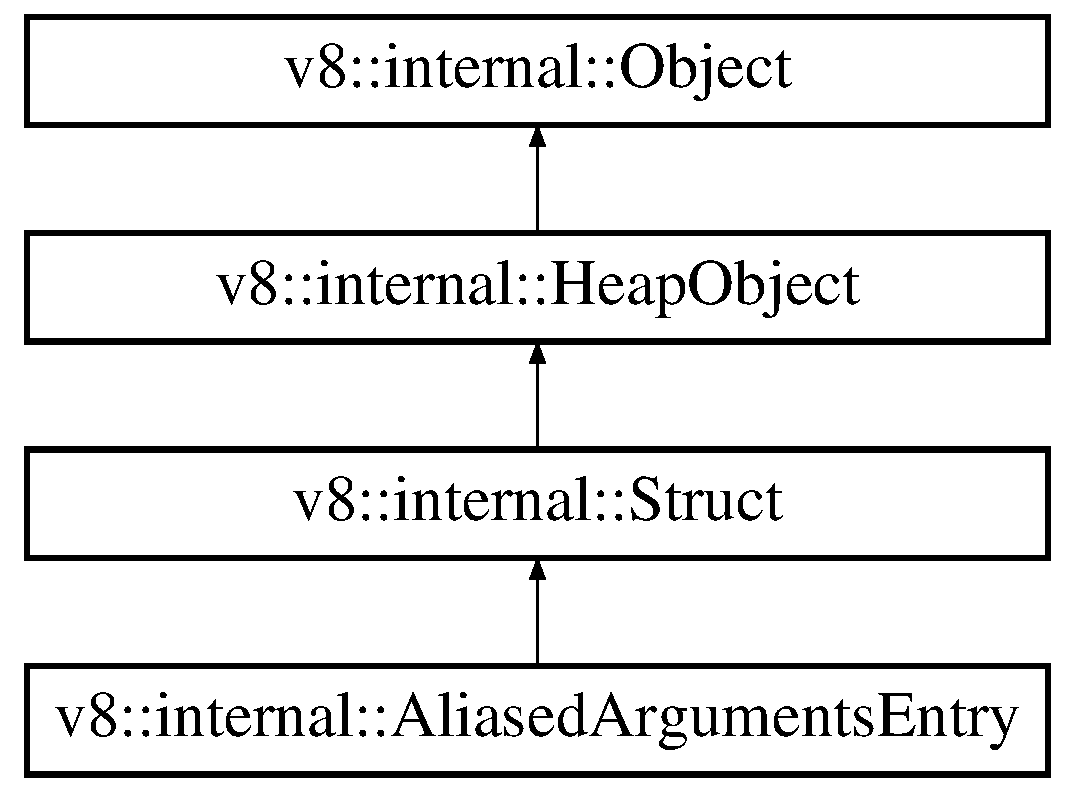
\includegraphics[height=4.000000cm]{classv8_1_1internal_1_1_aliased_arguments_entry}
\end{center}
\end{figure}
\subsection*{Public Member Functions}
\begin{DoxyCompactItemize}
\item 
int {\bfseries aliased\+\_\+context\+\_\+slot} () const \hypertarget{classv8_1_1internal_1_1_aliased_arguments_entry_a5362f3a14badae7882341093623de3fb}{}\label{classv8_1_1internal_1_1_aliased_arguments_entry_a5362f3a14badae7882341093623de3fb}

\item 
void {\bfseries set\+\_\+aliased\+\_\+context\+\_\+slot} (int count)\hypertarget{classv8_1_1internal_1_1_aliased_arguments_entry_ad2f671a7089a9e775abd7e1c039aeee7}{}\label{classv8_1_1internal_1_1_aliased_arguments_entry_ad2f671a7089a9e775abd7e1c039aeee7}

\end{DoxyCompactItemize}
\subsection*{Static Public Attributes}
\begin{DoxyCompactItemize}
\item 
static const int {\bfseries k\+Aliased\+Context\+Slot} = Heap\+Object\+::k\+Header\+Size\hypertarget{classv8_1_1internal_1_1_aliased_arguments_entry_a176665f23529fbe29ad19856967a7ee7}{}\label{classv8_1_1internal_1_1_aliased_arguments_entry_a176665f23529fbe29ad19856967a7ee7}

\item 
static const int {\bfseries k\+Size} = k\+Aliased\+Context\+Slot + k\+Pointer\+Size\hypertarget{classv8_1_1internal_1_1_aliased_arguments_entry_ad9980e02f526db5b9f4e095848a2d325}{}\label{classv8_1_1internal_1_1_aliased_arguments_entry_ad9980e02f526db5b9f4e095848a2d325}

\end{DoxyCompactItemize}
\subsection*{Private Member Functions}
\begin{DoxyCompactItemize}
\item 
{\bfseries D\+I\+S\+A\+L\+L\+O\+W\+\_\+\+I\+M\+P\+L\+I\+C\+I\+T\+\_\+\+C\+O\+N\+S\+T\+R\+U\+C\+T\+O\+RS} (\hyperlink{classv8_1_1internal_1_1_aliased_arguments_entry}{Aliased\+Arguments\+Entry})\hypertarget{classv8_1_1internal_1_1_aliased_arguments_entry_a0fc1be43c76bf0470598d5ad8f9b7419}{}\label{classv8_1_1internal_1_1_aliased_arguments_entry_a0fc1be43c76bf0470598d5ad8f9b7419}

\end{DoxyCompactItemize}
\subsection*{Additional Inherited Members}


The documentation for this class was generated from the following file\+:\begin{DoxyCompactItemize}
\item 
/\+Users/joshgav/node/v8/src/objects.\+h\end{DoxyCompactItemize}

\hypertarget{classv8_1_1_align_of_helper}{}\section{v8\+:\+:Align\+Of\+Helper$<$ T $>$ Class Template Reference}
\label{classv8_1_1_align_of_helper}\index{v8\+::\+Align\+Of\+Helper$<$ T $>$@{v8\+::\+Align\+Of\+Helper$<$ T $>$}}
\subsection*{Private Attributes}
\begin{DoxyCompactItemize}
\item 
char {\bfseries c}\hypertarget{classv8_1_1_align_of_helper_ac23697d1381684b3f4a53f8ff0f29897}{}\label{classv8_1_1_align_of_helper_ac23697d1381684b3f4a53f8ff0f29897}

\item 
T {\bfseries t}\hypertarget{classv8_1_1_align_of_helper_aebba37d9841cf6fb72eaf24e2ba9e33a}{}\label{classv8_1_1_align_of_helper_aebba37d9841cf6fb72eaf24e2ba9e33a}

\end{DoxyCompactItemize}


The documentation for this class was generated from the following file\+:\begin{DoxyCompactItemize}
\item 
include/v8config.\+h\end{DoxyCompactItemize}

\hypertarget{classv8_1_1internal_1_1compiler_1_1_all_nodes}{}\section{v8\+:\+:internal\+:\+:compiler\+:\+:All\+Nodes Class Reference}
\label{classv8_1_1internal_1_1compiler_1_1_all_nodes}\index{v8\+::internal\+::compiler\+::\+All\+Nodes@{v8\+::internal\+::compiler\+::\+All\+Nodes}}
\subsection*{Public Member Functions}
\begin{DoxyCompactItemize}
\item 
{\bfseries All\+Nodes} (\hyperlink{classv8_1_1internal_1_1_zone}{Zone} $\ast$local\+\_\+zone, const \hyperlink{classv8_1_1internal_1_1compiler_1_1_graph}{Graph} $\ast$graph)\hypertarget{classv8_1_1internal_1_1compiler_1_1_all_nodes_a3b882faab79c9cab2b1d21f45120d87f}{}\label{classv8_1_1internal_1_1compiler_1_1_all_nodes_a3b882faab79c9cab2b1d21f45120d87f}

\item 
bool {\bfseries Is\+Live} (\hyperlink{classv8_1_1internal_1_1compiler_1_1_node}{Node} $\ast$node)\hypertarget{classv8_1_1internal_1_1compiler_1_1_all_nodes_af01fc377c76f6e40af7148085c6f58fa}{}\label{classv8_1_1internal_1_1compiler_1_1_all_nodes_af01fc377c76f6e40af7148085c6f58fa}

\end{DoxyCompactItemize}
\subsection*{Public Attributes}
\begin{DoxyCompactItemize}
\item 
\hyperlink{classv8_1_1internal_1_1_zone_vector}{Node\+Vector} {\bfseries live}\hypertarget{classv8_1_1internal_1_1compiler_1_1_all_nodes_a8d081eabc413fca190f999e26a5e61b8}{}\label{classv8_1_1internal_1_1compiler_1_1_all_nodes_a8d081eabc413fca190f999e26a5e61b8}

\end{DoxyCompactItemize}
\subsection*{Private Attributes}
\begin{DoxyCompactItemize}
\item 
\hyperlink{classv8_1_1internal_1_1_zone_vector}{Bool\+Vector} {\bfseries is\+\_\+live}\hypertarget{classv8_1_1internal_1_1compiler_1_1_all_nodes_a1b92888635b4f7c74367393dab98bd12}{}\label{classv8_1_1internal_1_1compiler_1_1_all_nodes_a1b92888635b4f7c74367393dab98bd12}

\end{DoxyCompactItemize}


The documentation for this class was generated from the following files\+:\begin{DoxyCompactItemize}
\item 
/\+Users/joshgav/node/v8/src/compiler/all-\/nodes.\+h\item 
/\+Users/joshgav/node/v8/src/compiler/all-\/nodes.\+cc\end{DoxyCompactItemize}

\hypertarget{structv8_1_1internal_1_1compiler_1_1_allocated_interval}{}\section{v8\+:\+:internal\+:\+:compiler\+:\+:Allocated\+Interval Struct Reference}
\label{structv8_1_1internal_1_1compiler_1_1_allocated_interval}\index{v8\+::internal\+::compiler\+::\+Allocated\+Interval@{v8\+::internal\+::compiler\+::\+Allocated\+Interval}}
\subsection*{Public Member Functions}
\begin{DoxyCompactItemize}
\item 
{\bfseries Allocated\+Interval} (\hyperlink{classv8_1_1internal_1_1compiler_1_1_lifetime_position}{Lifetime\+Position} start, \hyperlink{classv8_1_1internal_1_1compiler_1_1_lifetime_position}{Lifetime\+Position} end, \hyperlink{classv8_1_1internal_1_1compiler_1_1_live_range}{Live\+Range} $\ast$range)\hypertarget{structv8_1_1internal_1_1compiler_1_1_allocated_interval_a97341cd7e61929ffab012657f8b0ec58}{}\label{structv8_1_1internal_1_1compiler_1_1_allocated_interval_a97341cd7e61929ffab012657f8b0ec58}

\item 
bool {\bfseries operator$<$} (const \hyperlink{structv8_1_1internal_1_1compiler_1_1_allocated_interval}{Allocated\+Interval} \&other) const \hypertarget{structv8_1_1internal_1_1compiler_1_1_allocated_interval_abdf129f7851a9bcee7b434e9695cebdd}{}\label{structv8_1_1internal_1_1compiler_1_1_allocated_interval_abdf129f7851a9bcee7b434e9695cebdd}

\item 
bool {\bfseries operator$>$} (const \hyperlink{structv8_1_1internal_1_1compiler_1_1_allocated_interval}{Allocated\+Interval} \&other) const \hypertarget{structv8_1_1internal_1_1compiler_1_1_allocated_interval_a198cb61f14b9887a954eab6373bd928c}{}\label{structv8_1_1internal_1_1compiler_1_1_allocated_interval_a198cb61f14b9887a954eab6373bd928c}

\end{DoxyCompactItemize}
\subsection*{Public Attributes}
\begin{DoxyCompactItemize}
\item 
\hyperlink{classv8_1_1internal_1_1compiler_1_1_lifetime_position}{Lifetime\+Position} {\bfseries start\+\_\+}\hypertarget{structv8_1_1internal_1_1compiler_1_1_allocated_interval_a50322de66a9eee09efcf89c53a3fc224}{}\label{structv8_1_1internal_1_1compiler_1_1_allocated_interval_a50322de66a9eee09efcf89c53a3fc224}

\item 
\hyperlink{classv8_1_1internal_1_1compiler_1_1_lifetime_position}{Lifetime\+Position} {\bfseries end\+\_\+}\hypertarget{structv8_1_1internal_1_1compiler_1_1_allocated_interval_ad20b71681736c733dc69b1aac1f702b8}{}\label{structv8_1_1internal_1_1compiler_1_1_allocated_interval_ad20b71681736c733dc69b1aac1f702b8}

\item 
\hyperlink{classv8_1_1internal_1_1compiler_1_1_live_range}{Live\+Range} $\ast$ {\bfseries range\+\_\+}\hypertarget{structv8_1_1internal_1_1compiler_1_1_allocated_interval_a69abbbd196f1c8422350540d4fc33c0c}{}\label{structv8_1_1internal_1_1compiler_1_1_allocated_interval_a69abbbd196f1c8422350540d4fc33c0c}

\end{DoxyCompactItemize}


The documentation for this struct was generated from the following file\+:\begin{DoxyCompactItemize}
\item 
/\+Users/joshgav/node/v8/src/compiler/coalesced-\/live-\/ranges.\+h\end{DoxyCompactItemize}

\hypertarget{classv8_1_1internal_1_1compiler_1_1_allocated_operand}{}\section{v8\+:\+:internal\+:\+:compiler\+:\+:Allocated\+Operand Class Reference}
\label{classv8_1_1internal_1_1compiler_1_1_allocated_operand}\index{v8\+::internal\+::compiler\+::\+Allocated\+Operand@{v8\+::internal\+::compiler\+::\+Allocated\+Operand}}
Inheritance diagram for v8\+:\+:internal\+:\+:compiler\+:\+:Allocated\+Operand\+:\begin{figure}[H]
\begin{center}
\leavevmode
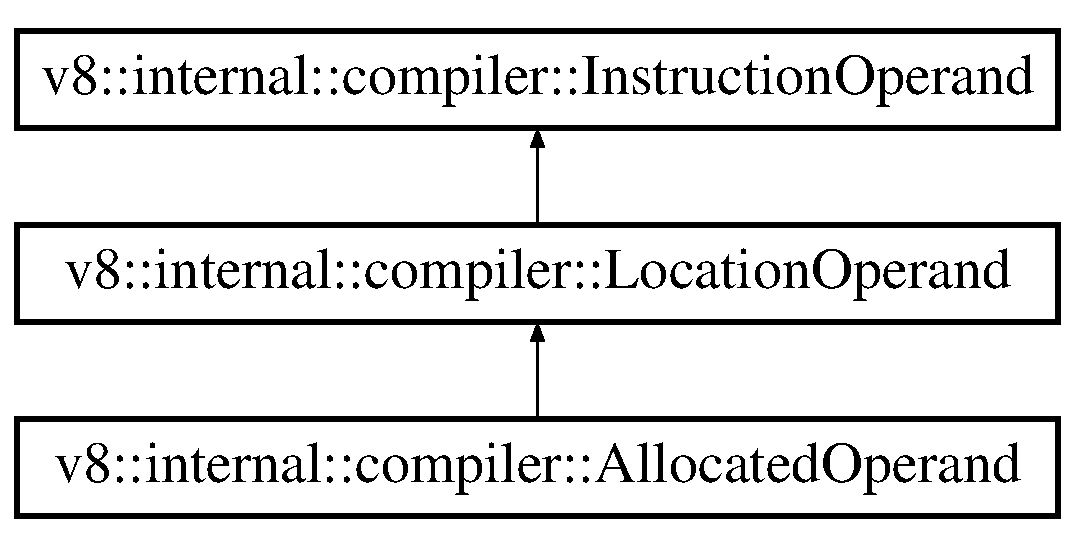
\includegraphics[height=3.000000cm]{classv8_1_1internal_1_1compiler_1_1_allocated_operand}
\end{center}
\end{figure}
\subsection*{Public Member Functions}
\begin{DoxyCompactItemize}
\item 
{\bfseries Allocated\+Operand} (Location\+Kind kind, Machine\+Representation rep, int index)\hypertarget{classv8_1_1internal_1_1compiler_1_1_allocated_operand_a1e23e5746e40802c4376243abdbe8e48}{}\label{classv8_1_1internal_1_1compiler_1_1_allocated_operand_a1e23e5746e40802c4376243abdbe8e48}

\item 
{\bfseries I\+N\+S\+T\+R\+U\+C\+T\+I\+O\+N\+\_\+\+O\+P\+E\+R\+A\+N\+D\+\_\+\+C\+A\+S\+TS} (\hyperlink{classv8_1_1internal_1_1compiler_1_1_allocated_operand}{Allocated\+Operand}, A\+L\+L\+O\+C\+A\+T\+ED)\hypertarget{classv8_1_1internal_1_1compiler_1_1_allocated_operand_a7dc1520248d33f029a009fdc7d5951a1}{}\label{classv8_1_1internal_1_1compiler_1_1_allocated_operand_a7dc1520248d33f029a009fdc7d5951a1}

\end{DoxyCompactItemize}
\subsection*{Static Public Member Functions}
\begin{DoxyCompactItemize}
\item 
static \hyperlink{classv8_1_1internal_1_1compiler_1_1_allocated_operand}{Allocated\+Operand} $\ast$ {\bfseries New} (\hyperlink{classv8_1_1internal_1_1_zone}{Zone} $\ast$zone, Location\+Kind kind, Machine\+Representation rep, int index)\hypertarget{classv8_1_1internal_1_1compiler_1_1_allocated_operand_a5981dcc601391236e463e4afaee84bbe}{}\label{classv8_1_1internal_1_1compiler_1_1_allocated_operand_a5981dcc601391236e463e4afaee84bbe}

\end{DoxyCompactItemize}
\subsection*{Additional Inherited Members}


The documentation for this class was generated from the following file\+:\begin{DoxyCompactItemize}
\item 
/\+Users/joshgav/node/v8/src/compiler/instruction.\+h\end{DoxyCompactItemize}

\hypertarget{classv8_1_1internal_1_1_allocate_double_align_flag}{}\section{v8\+:\+:internal\+:\+:Allocate\+Double\+Align\+Flag Class Reference}
\label{classv8_1_1internal_1_1_allocate_double_align_flag}\index{v8\+::internal\+::\+Allocate\+Double\+Align\+Flag@{v8\+::internal\+::\+Allocate\+Double\+Align\+Flag}}
Inheritance diagram for v8\+:\+:internal\+:\+:Allocate\+Double\+Align\+Flag\+:\begin{figure}[H]
\begin{center}
\leavevmode
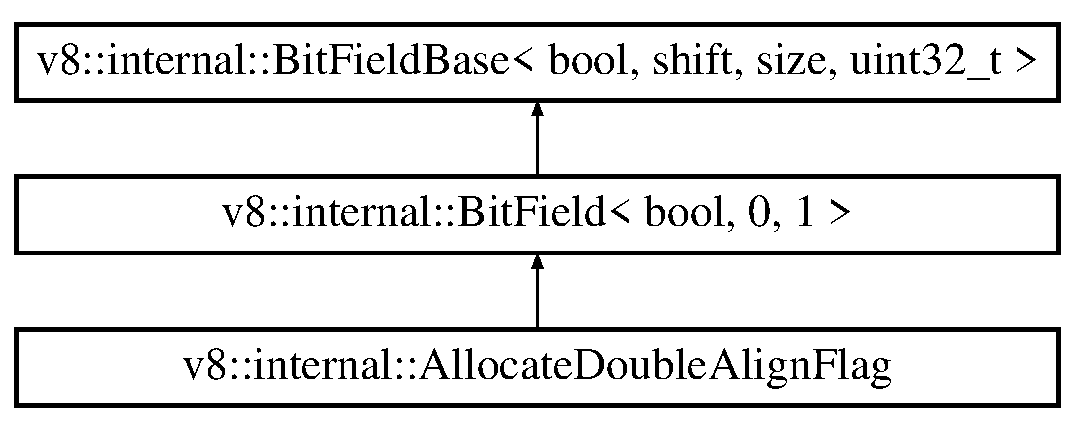
\includegraphics[height=3.000000cm]{classv8_1_1internal_1_1_allocate_double_align_flag}
\end{center}
\end{figure}
\subsection*{Additional Inherited Members}


The documentation for this class was generated from the following file\+:\begin{DoxyCompactItemize}
\item 
/\+Users/joshgav/node/v8/src/runtime/runtime.\+h\end{DoxyCompactItemize}

\hypertarget{structv8_1_1internal_1_1compiler_1_1_allocate_f_p_registers_phase}{}\section{v8\+:\+:internal\+:\+:compiler\+:\+:Allocate\+F\+P\+Registers\+Phase$<$ Reg\+Allocator $>$ Struct Template Reference}
\label{structv8_1_1internal_1_1compiler_1_1_allocate_f_p_registers_phase}\index{v8\+::internal\+::compiler\+::\+Allocate\+F\+P\+Registers\+Phase$<$ Reg\+Allocator $>$@{v8\+::internal\+::compiler\+::\+Allocate\+F\+P\+Registers\+Phase$<$ Reg\+Allocator $>$}}
\subsection*{Public Member Functions}
\begin{DoxyCompactItemize}
\item 
void {\bfseries Run} (\hyperlink{classv8_1_1internal_1_1compiler_1_1_pipeline_data}{Pipeline\+Data} $\ast$data, \hyperlink{classv8_1_1internal_1_1_zone}{Zone} $\ast$temp\+\_\+zone)\hypertarget{structv8_1_1internal_1_1compiler_1_1_allocate_f_p_registers_phase_a4c6dd764c8c48b49f8ecd1e1035f5079}{}\label{structv8_1_1internal_1_1compiler_1_1_allocate_f_p_registers_phase_a4c6dd764c8c48b49f8ecd1e1035f5079}

\end{DoxyCompactItemize}
\subsection*{Static Public Member Functions}
\begin{DoxyCompactItemize}
\item 
static const char $\ast$ {\bfseries phase\+\_\+name} ()\hypertarget{structv8_1_1internal_1_1compiler_1_1_allocate_f_p_registers_phase_a29ced843c54c50d3169abe3aaa193858}{}\label{structv8_1_1internal_1_1compiler_1_1_allocate_f_p_registers_phase_a29ced843c54c50d3169abe3aaa193858}

\end{DoxyCompactItemize}


The documentation for this struct was generated from the following file\+:\begin{DoxyCompactItemize}
\item 
/\+Users/joshgav/node/v8/src/compiler/pipeline.\+cc\end{DoxyCompactItemize}

\hypertarget{structv8_1_1internal_1_1compiler_1_1_allocate_general_registers_phase}{}\section{v8\+:\+:internal\+:\+:compiler\+:\+:Allocate\+General\+Registers\+Phase$<$ Reg\+Allocator $>$ Struct Template Reference}
\label{structv8_1_1internal_1_1compiler_1_1_allocate_general_registers_phase}\index{v8\+::internal\+::compiler\+::\+Allocate\+General\+Registers\+Phase$<$ Reg\+Allocator $>$@{v8\+::internal\+::compiler\+::\+Allocate\+General\+Registers\+Phase$<$ Reg\+Allocator $>$}}
\subsection*{Public Member Functions}
\begin{DoxyCompactItemize}
\item 
void {\bfseries Run} (\hyperlink{classv8_1_1internal_1_1compiler_1_1_pipeline_data}{Pipeline\+Data} $\ast$data, \hyperlink{classv8_1_1internal_1_1_zone}{Zone} $\ast$temp\+\_\+zone)\hypertarget{structv8_1_1internal_1_1compiler_1_1_allocate_general_registers_phase_a55c00393389c82edb2c9a5bd71e19465}{}\label{structv8_1_1internal_1_1compiler_1_1_allocate_general_registers_phase_a55c00393389c82edb2c9a5bd71e19465}

\end{DoxyCompactItemize}
\subsection*{Static Public Member Functions}
\begin{DoxyCompactItemize}
\item 
static const char $\ast$ {\bfseries phase\+\_\+name} ()\hypertarget{structv8_1_1internal_1_1compiler_1_1_allocate_general_registers_phase_a1e84383afb21659a68d7ee495ff46edd}{}\label{structv8_1_1internal_1_1compiler_1_1_allocate_general_registers_phase_a1e84383afb21659a68d7ee495ff46edd}

\end{DoxyCompactItemize}


The documentation for this struct was generated from the following file\+:\begin{DoxyCompactItemize}
\item 
/\+Users/joshgav/node/v8/src/compiler/pipeline.\+cc\end{DoxyCompactItemize}

\hypertarget{classv8_1_1internal_1_1_allocate_heap_number_descriptor}{}\section{v8\+:\+:internal\+:\+:Allocate\+Heap\+Number\+Descriptor Class Reference}
\label{classv8_1_1internal_1_1_allocate_heap_number_descriptor}\index{v8\+::internal\+::\+Allocate\+Heap\+Number\+Descriptor@{v8\+::internal\+::\+Allocate\+Heap\+Number\+Descriptor}}
Inheritance diagram for v8\+:\+:internal\+:\+:Allocate\+Heap\+Number\+Descriptor\+:\begin{figure}[H]
\begin{center}
\leavevmode
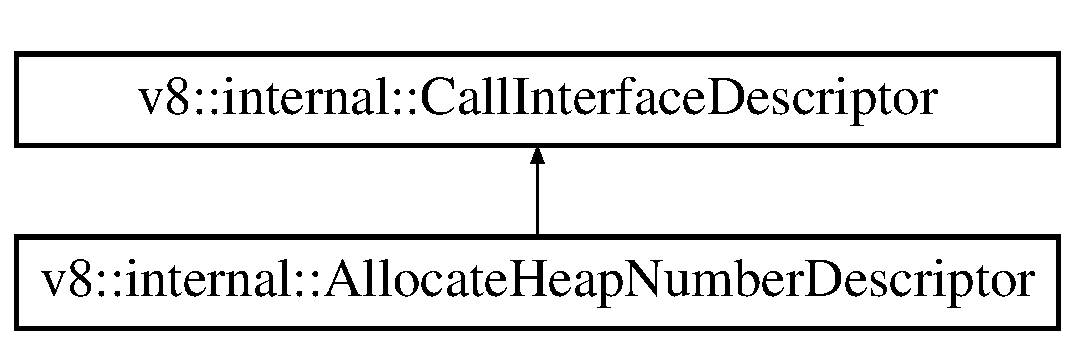
\includegraphics[height=2.000000cm]{classv8_1_1internal_1_1_allocate_heap_number_descriptor}
\end{center}
\end{figure}
\subsection*{Additional Inherited Members}


The documentation for this class was generated from the following file\+:\begin{DoxyCompactItemize}
\item 
/\+Users/joshgav/node/v8/src/interface-\/descriptors.\+h\end{DoxyCompactItemize}

\hypertarget{classv8_1_1internal_1_1_allocate_heap_number_stub}{}\section{v8\+:\+:internal\+:\+:Allocate\+Heap\+Number\+Stub Class Reference}
\label{classv8_1_1internal_1_1_allocate_heap_number_stub}\index{v8\+::internal\+::\+Allocate\+Heap\+Number\+Stub@{v8\+::internal\+::\+Allocate\+Heap\+Number\+Stub}}
Inheritance diagram for v8\+:\+:internal\+:\+:Allocate\+Heap\+Number\+Stub\+:\begin{figure}[H]
\begin{center}
\leavevmode
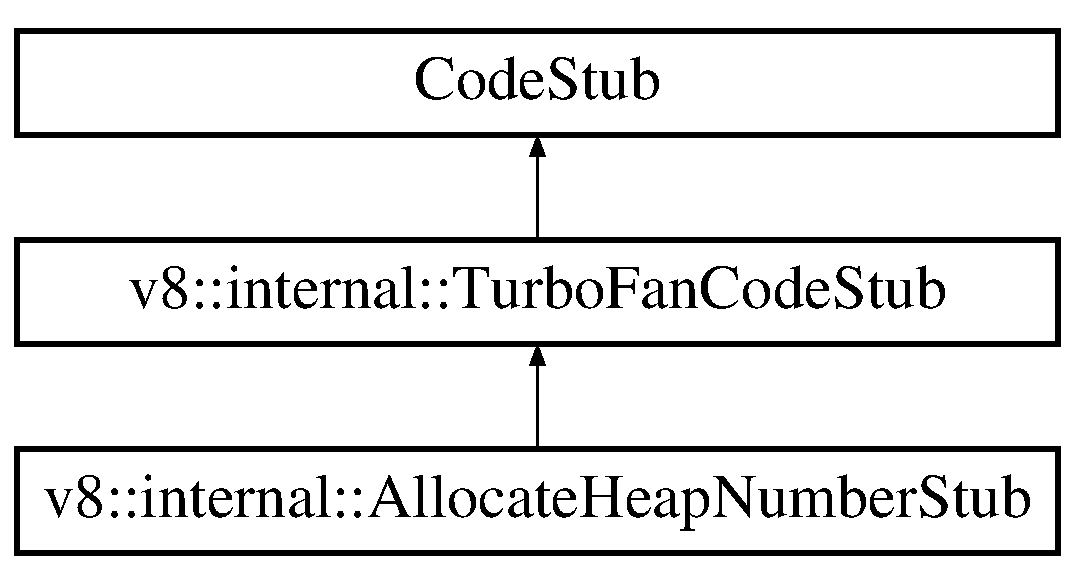
\includegraphics[height=3.000000cm]{classv8_1_1internal_1_1_allocate_heap_number_stub}
\end{center}
\end{figure}
\subsection*{Public Member Functions}
\begin{DoxyCompactItemize}
\item 
{\bfseries Allocate\+Heap\+Number\+Stub} (\hyperlink{classv8_1_1internal_1_1_isolate}{Isolate} $\ast$isolate)\hypertarget{classv8_1_1internal_1_1_allocate_heap_number_stub_ac285714f22f78a67883c629865140df3}{}\label{classv8_1_1internal_1_1_allocate_heap_number_stub_ac285714f22f78a67883c629865140df3}

\item 
void {\bfseries Initialize\+Descriptor} (\hyperlink{classv8_1_1internal_1_1_code_stub_descriptor}{Code\+Stub\+Descriptor} $\ast$descriptor) override\hypertarget{classv8_1_1internal_1_1_allocate_heap_number_stub_a155eddb4265ddd3d3e7b1c0f13ca5b3a}{}\label{classv8_1_1internal_1_1_allocate_heap_number_stub_a155eddb4265ddd3d3e7b1c0f13ca5b3a}

\item 
void {\bfseries Generate\+Assembly} (\hyperlink{classv8_1_1internal_1_1_code_stub_assembler}{Code\+Stub\+Assembler} $\ast$assembler) const  override\hypertarget{classv8_1_1internal_1_1_allocate_heap_number_stub_a52b84b91e9ae150affb006eb65072d57}{}\label{classv8_1_1internal_1_1_allocate_heap_number_stub_a52b84b91e9ae150affb006eb65072d57}

\item 
{\bfseries D\+E\+F\+I\+N\+E\+\_\+\+C\+A\+L\+L\+\_\+\+I\+N\+T\+E\+R\+F\+A\+C\+E\+\_\+\+D\+E\+S\+C\+R\+I\+P\+T\+OR} (Allocate\+Heap\+Number)\hypertarget{classv8_1_1internal_1_1_allocate_heap_number_stub_aed9342cc507778b8067e3373547f41ea}{}\label{classv8_1_1internal_1_1_allocate_heap_number_stub_aed9342cc507778b8067e3373547f41ea}

\item 
{\bfseries D\+E\+F\+I\+N\+E\+\_\+\+C\+O\+D\+E\+\_\+\+S\+T\+UB} (Allocate\+Heap\+Number, \hyperlink{classv8_1_1internal_1_1_turbo_fan_code_stub}{Turbo\+Fan\+Code\+Stub})\hypertarget{classv8_1_1internal_1_1_allocate_heap_number_stub_afccc06b0e8470c101e5db8c6b9908a44}{}\label{classv8_1_1internal_1_1_allocate_heap_number_stub_afccc06b0e8470c101e5db8c6b9908a44}

\end{DoxyCompactItemize}
\subsection*{Additional Inherited Members}


The documentation for this class was generated from the following files\+:\begin{DoxyCompactItemize}
\item 
/\+Users/joshgav/node/v8/src/code-\/stubs.\+h\item 
/\+Users/joshgav/node/v8/src/code-\/stubs.\+cc\end{DoxyCompactItemize}

\hypertarget{classv8_1_1internal_1_1_allocate_mutable_heap_number_descriptor}{}\section{v8\+:\+:internal\+:\+:Allocate\+Mutable\+Heap\+Number\+Descriptor Class Reference}
\label{classv8_1_1internal_1_1_allocate_mutable_heap_number_descriptor}\index{v8\+::internal\+::\+Allocate\+Mutable\+Heap\+Number\+Descriptor@{v8\+::internal\+::\+Allocate\+Mutable\+Heap\+Number\+Descriptor}}
Inheritance diagram for v8\+:\+:internal\+:\+:Allocate\+Mutable\+Heap\+Number\+Descriptor\+:\begin{figure}[H]
\begin{center}
\leavevmode
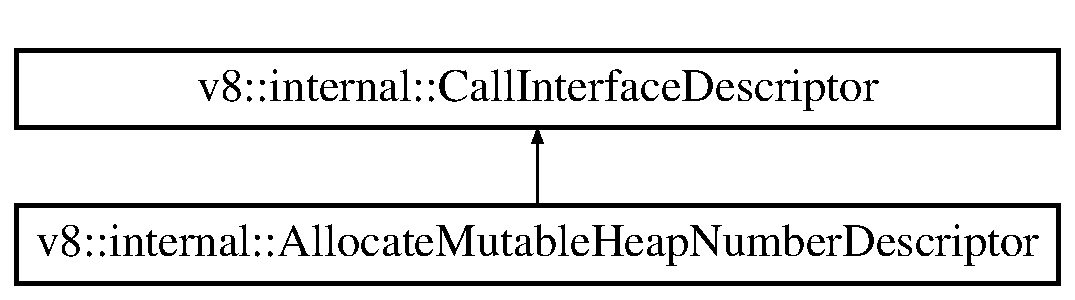
\includegraphics[height=2.000000cm]{classv8_1_1internal_1_1_allocate_mutable_heap_number_descriptor}
\end{center}
\end{figure}
\subsection*{Additional Inherited Members}


The documentation for this class was generated from the following file\+:\begin{DoxyCompactItemize}
\item 
/\+Users/joshgav/node/v8/src/interface-\/descriptors.\+h\end{DoxyCompactItemize}

\hypertarget{classv8_1_1internal_1_1_allocate_mutable_heap_number_stub}{}\section{v8\+:\+:internal\+:\+:Allocate\+Mutable\+Heap\+Number\+Stub Class Reference}
\label{classv8_1_1internal_1_1_allocate_mutable_heap_number_stub}\index{v8\+::internal\+::\+Allocate\+Mutable\+Heap\+Number\+Stub@{v8\+::internal\+::\+Allocate\+Mutable\+Heap\+Number\+Stub}}
Inheritance diagram for v8\+:\+:internal\+:\+:Allocate\+Mutable\+Heap\+Number\+Stub\+:\begin{figure}[H]
\begin{center}
\leavevmode
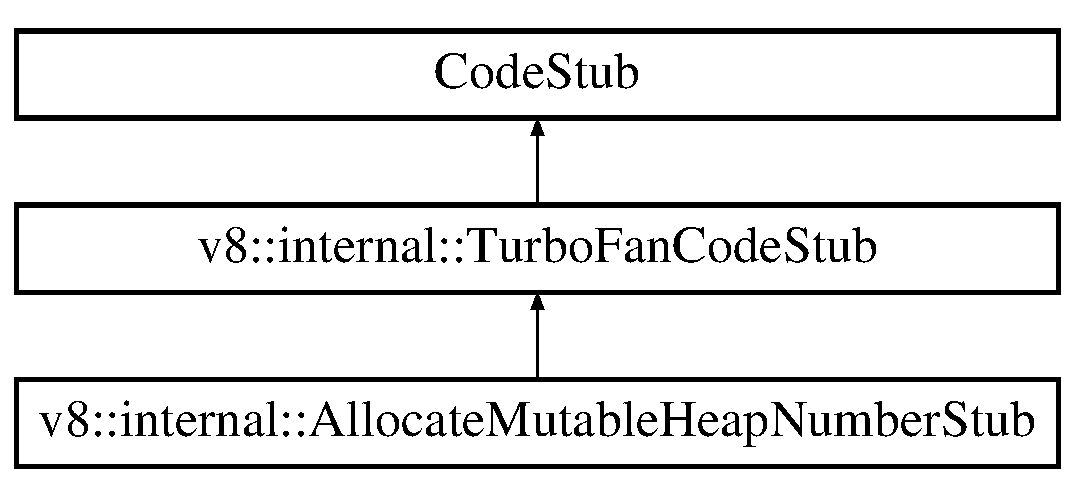
\includegraphics[height=3.000000cm]{classv8_1_1internal_1_1_allocate_mutable_heap_number_stub}
\end{center}
\end{figure}
\subsection*{Public Member Functions}
\begin{DoxyCompactItemize}
\item 
{\bfseries Allocate\+Mutable\+Heap\+Number\+Stub} (\hyperlink{classv8_1_1internal_1_1_isolate}{Isolate} $\ast$isolate)\hypertarget{classv8_1_1internal_1_1_allocate_mutable_heap_number_stub_a5b61c3eec69b2050e51bef42d5dad1ff}{}\label{classv8_1_1internal_1_1_allocate_mutable_heap_number_stub_a5b61c3eec69b2050e51bef42d5dad1ff}

\item 
void {\bfseries Initialize\+Descriptor} (\hyperlink{classv8_1_1internal_1_1_code_stub_descriptor}{Code\+Stub\+Descriptor} $\ast$descriptor) override\hypertarget{classv8_1_1internal_1_1_allocate_mutable_heap_number_stub_ada6a404574d7fc9cb9001f680ff5c770}{}\label{classv8_1_1internal_1_1_allocate_mutable_heap_number_stub_ada6a404574d7fc9cb9001f680ff5c770}

\item 
void {\bfseries Generate\+Assembly} (\hyperlink{classv8_1_1internal_1_1_code_stub_assembler}{Code\+Stub\+Assembler} $\ast$assembler) const  override\hypertarget{classv8_1_1internal_1_1_allocate_mutable_heap_number_stub_ae0f29e99bd8459ca3810d22feb0e77f8}{}\label{classv8_1_1internal_1_1_allocate_mutable_heap_number_stub_ae0f29e99bd8459ca3810d22feb0e77f8}

\item 
{\bfseries D\+E\+F\+I\+N\+E\+\_\+\+C\+A\+L\+L\+\_\+\+I\+N\+T\+E\+R\+F\+A\+C\+E\+\_\+\+D\+E\+S\+C\+R\+I\+P\+T\+OR} (Allocate\+Mutable\+Heap\+Number)\hypertarget{classv8_1_1internal_1_1_allocate_mutable_heap_number_stub_a75d00c69f9e30178442f27929efe37a8}{}\label{classv8_1_1internal_1_1_allocate_mutable_heap_number_stub_a75d00c69f9e30178442f27929efe37a8}

\item 
{\bfseries D\+E\+F\+I\+N\+E\+\_\+\+C\+O\+D\+E\+\_\+\+S\+T\+UB} (Allocate\+Mutable\+Heap\+Number, \hyperlink{classv8_1_1internal_1_1_turbo_fan_code_stub}{Turbo\+Fan\+Code\+Stub})\hypertarget{classv8_1_1internal_1_1_allocate_mutable_heap_number_stub_af4ffe2405d8d5e12b92a3206c3b65a3a}{}\label{classv8_1_1internal_1_1_allocate_mutable_heap_number_stub_af4ffe2405d8d5e12b92a3206c3b65a3a}

\end{DoxyCompactItemize}
\subsection*{Additional Inherited Members}


The documentation for this class was generated from the following files\+:\begin{DoxyCompactItemize}
\item 
/\+Users/joshgav/node/v8/src/code-\/stubs.\+h\item 
/\+Users/joshgav/node/v8/src/code-\/stubs.\+cc\end{DoxyCompactItemize}

\hypertarget{structv8_1_1internal_1_1compiler_1_1_simplified_operator_global_cache_1_1_allocate_operator}{}\section{v8\+:\+:internal\+:\+:compiler\+:\+:Simplified\+Operator\+Global\+Cache\+:\+:Allocate\+Operator$<$ k\+Pretenure $>$ Struct Template Reference}
\label{structv8_1_1internal_1_1compiler_1_1_simplified_operator_global_cache_1_1_allocate_operator}\index{v8\+::internal\+::compiler\+::\+Simplified\+Operator\+Global\+Cache\+::\+Allocate\+Operator$<$ k\+Pretenure $>$@{v8\+::internal\+::compiler\+::\+Simplified\+Operator\+Global\+Cache\+::\+Allocate\+Operator$<$ k\+Pretenure $>$}}
Inheritance diagram for v8\+:\+:internal\+:\+:compiler\+:\+:Simplified\+Operator\+Global\+Cache\+:\+:Allocate\+Operator$<$ k\+Pretenure $>$\+:\begin{figure}[H]
\begin{center}
\leavevmode
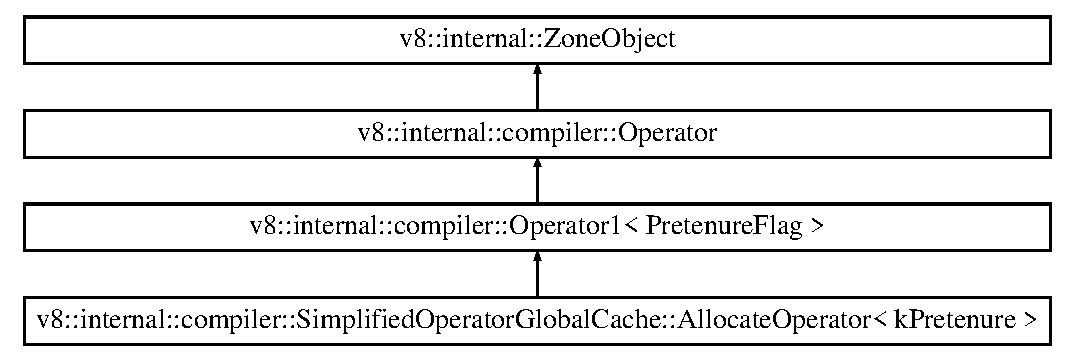
\includegraphics[height=4.000000cm]{structv8_1_1internal_1_1compiler_1_1_simplified_operator_global_cache_1_1_allocate_operator}
\end{center}
\end{figure}
\subsection*{Additional Inherited Members}


The documentation for this struct was generated from the following file\+:\begin{DoxyCompactItemize}
\item 
/\+Users/joshgav/node/v8/src/compiler/simplified-\/operator.\+cc\end{DoxyCompactItemize}

\hypertarget{classv8_1_1internal_1_1_allocate_target_space}{}\section{v8\+:\+:internal\+:\+:Allocate\+Target\+Space Class Reference}
\label{classv8_1_1internal_1_1_allocate_target_space}\index{v8\+::internal\+::\+Allocate\+Target\+Space@{v8\+::internal\+::\+Allocate\+Target\+Space}}
Inheritance diagram for v8\+:\+:internal\+:\+:Allocate\+Target\+Space\+:\begin{figure}[H]
\begin{center}
\leavevmode
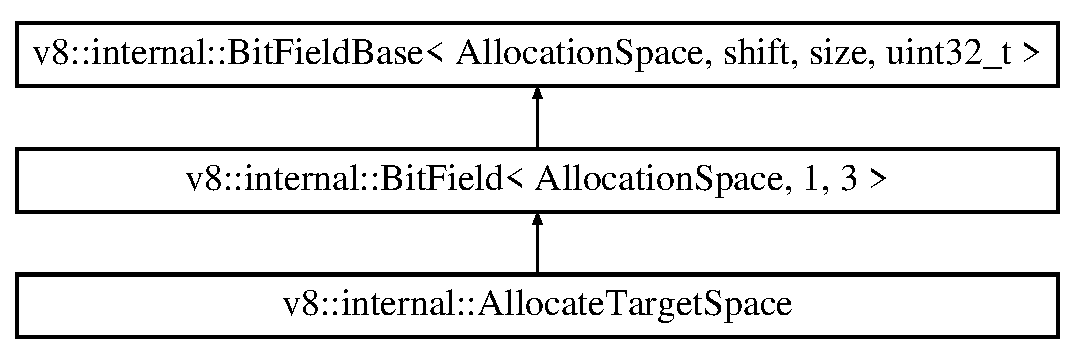
\includegraphics[height=3.000000cm]{classv8_1_1internal_1_1_allocate_target_space}
\end{center}
\end{figure}
\subsection*{Additional Inherited Members}


The documentation for this class was generated from the following file\+:\begin{DoxyCompactItemize}
\item 
/\+Users/joshgav/node/v8/src/runtime/runtime.\+h\end{DoxyCompactItemize}

\hypertarget{structv8_1_1_allocation_profile_1_1_allocation}{}\section{v8\+:\+:Allocation\+Profile\+:\+:Allocation Struct Reference}
\label{structv8_1_1_allocation_profile_1_1_allocation}\index{v8\+::\+Allocation\+Profile\+::\+Allocation@{v8\+::\+Allocation\+Profile\+::\+Allocation}}
\subsection*{Public Attributes}
\begin{DoxyCompactItemize}
\item 
size\+\_\+t \hyperlink{structv8_1_1_allocation_profile_1_1_allocation_a346410fa5dfb796dff396069897c0aba}{size}
\item 
unsigned int \hyperlink{structv8_1_1_allocation_profile_1_1_allocation_a012fe5238f5ebec039d7832f2d3ae8ed}{count}
\end{DoxyCompactItemize}


\subsection{Member Data Documentation}
\index{v8\+::\+Allocation\+Profile\+::\+Allocation@{v8\+::\+Allocation\+Profile\+::\+Allocation}!count@{count}}
\index{count@{count}!v8\+::\+Allocation\+Profile\+::\+Allocation@{v8\+::\+Allocation\+Profile\+::\+Allocation}}
\subsubsection[{\texorpdfstring{count}{count}}]{\setlength{\rightskip}{0pt plus 5cm}unsigned int v8\+::\+Allocation\+Profile\+::\+Allocation\+::count}\hypertarget{structv8_1_1_allocation_profile_1_1_allocation_a012fe5238f5ebec039d7832f2d3ae8ed}{}\label{structv8_1_1_allocation_profile_1_1_allocation_a012fe5238f5ebec039d7832f2d3ae8ed}
The number of objects of such size that were sampled. \index{v8\+::\+Allocation\+Profile\+::\+Allocation@{v8\+::\+Allocation\+Profile\+::\+Allocation}!size@{size}}
\index{size@{size}!v8\+::\+Allocation\+Profile\+::\+Allocation@{v8\+::\+Allocation\+Profile\+::\+Allocation}}
\subsubsection[{\texorpdfstring{size}{size}}]{\setlength{\rightskip}{0pt plus 5cm}size\+\_\+t v8\+::\+Allocation\+Profile\+::\+Allocation\+::size}\hypertarget{structv8_1_1_allocation_profile_1_1_allocation_a346410fa5dfb796dff396069897c0aba}{}\label{structv8_1_1_allocation_profile_1_1_allocation_a346410fa5dfb796dff396069897c0aba}
Size of the sampled allocation object. 

The documentation for this struct was generated from the following file\+:\begin{DoxyCompactItemize}
\item 
include/v8-\/profiler.\+h\end{DoxyCompactItemize}

\hypertarget{classv8_1_1internal_1_1compiler_1_1_allocation_candidate}{}\section{v8\+:\+:internal\+:\+:compiler\+:\+:Allocation\+Candidate Class Reference}
\label{classv8_1_1internal_1_1compiler_1_1_allocation_candidate}\index{v8\+::internal\+::compiler\+::\+Allocation\+Candidate@{v8\+::internal\+::compiler\+::\+Allocation\+Candidate}}
\subsection*{Public Member Functions}
\begin{DoxyCompactItemize}
\item 
{\bfseries Allocation\+Candidate} (\hyperlink{classv8_1_1internal_1_1compiler_1_1_live_range}{Live\+Range} $\ast$range)\hypertarget{classv8_1_1internal_1_1compiler_1_1_allocation_candidate_a3e140e7b35ae72e52535935f4822bca9}{}\label{classv8_1_1internal_1_1compiler_1_1_allocation_candidate_a3e140e7b35ae72e52535935f4822bca9}

\item 
{\bfseries Allocation\+Candidate} (\hyperlink{classv8_1_1internal_1_1compiler_1_1_live_range_group}{Live\+Range\+Group} $\ast$ranges)\hypertarget{classv8_1_1internal_1_1compiler_1_1_allocation_candidate_a65a45c65bc233708cf32069ec77a29f7}{}\label{classv8_1_1internal_1_1compiler_1_1_allocation_candidate_a65a45c65bc233708cf32069ec77a29f7}

\item 
bool {\bfseries operator$<$} (const \hyperlink{classv8_1_1internal_1_1compiler_1_1_allocation_candidate}{Allocation\+Candidate} \&other) const \hypertarget{classv8_1_1internal_1_1compiler_1_1_allocation_candidate_a7cf271b7cb8e74a59d544e6234b9c816}{}\label{classv8_1_1internal_1_1compiler_1_1_allocation_candidate_a7cf271b7cb8e74a59d544e6234b9c816}

\item 
bool {\bfseries operator$>$} (const \hyperlink{classv8_1_1internal_1_1compiler_1_1_allocation_candidate}{Allocation\+Candidate} \&other) const \hypertarget{classv8_1_1internal_1_1compiler_1_1_allocation_candidate_a139b67ca930375b1a9f919e87d221921}{}\label{classv8_1_1internal_1_1compiler_1_1_allocation_candidate_a139b67ca930375b1a9f919e87d221921}

\item 
bool {\bfseries is\+\_\+group} () const \hypertarget{classv8_1_1internal_1_1compiler_1_1_allocation_candidate_a67cc07784837a85a82c1b520cb6f145c}{}\label{classv8_1_1internal_1_1compiler_1_1_allocation_candidate_a67cc07784837a85a82c1b520cb6f145c}

\item 
\hyperlink{classv8_1_1internal_1_1compiler_1_1_live_range}{Live\+Range} $\ast$ {\bfseries live\+\_\+range} () const \hypertarget{classv8_1_1internal_1_1compiler_1_1_allocation_candidate_a4300af72689fb1aee4e87d1fdcf2ff77}{}\label{classv8_1_1internal_1_1compiler_1_1_allocation_candidate_a4300af72689fb1aee4e87d1fdcf2ff77}

\item 
\hyperlink{classv8_1_1internal_1_1compiler_1_1_live_range_group}{Live\+Range\+Group} $\ast$ {\bfseries group} () const \hypertarget{classv8_1_1internal_1_1compiler_1_1_allocation_candidate_a62e59d137fd609d39eb61cd3c07dbea7}{}\label{classv8_1_1internal_1_1compiler_1_1_allocation_candidate_a62e59d137fd609d39eb61cd3c07dbea7}

\end{DoxyCompactItemize}
\subsection*{Private Member Functions}
\begin{DoxyCompactItemize}
\item 
unsigned {\bfseries Calculate\+Group\+Size} (\hyperlink{classv8_1_1internal_1_1compiler_1_1_live_range_group}{Live\+Range\+Group} $\ast$group)\hypertarget{classv8_1_1internal_1_1compiler_1_1_allocation_candidate_a153265c65236606a92f80c60259e506f}{}\label{classv8_1_1internal_1_1compiler_1_1_allocation_candidate_a153265c65236606a92f80c60259e506f}

\item 
unsigned {\bfseries size} () const \hypertarget{classv8_1_1internal_1_1compiler_1_1_allocation_candidate_a0279df190b0bc0a7d77a82c4f2b28977}{}\label{classv8_1_1internal_1_1compiler_1_1_allocation_candidate_a0279df190b0bc0a7d77a82c4f2b28977}

\end{DoxyCompactItemize}
\subsection*{Private Attributes}
\begin{DoxyCompactItemize}
\item 
bool {\bfseries is\+\_\+group\+\_\+}\hypertarget{classv8_1_1internal_1_1compiler_1_1_allocation_candidate_a728739b4eb20f6cd6e5f22e08bad5d4a}{}\label{classv8_1_1internal_1_1compiler_1_1_allocation_candidate_a728739b4eb20f6cd6e5f22e08bad5d4a}

\item 
unsigned {\bfseries size\+\_\+}\hypertarget{classv8_1_1internal_1_1compiler_1_1_allocation_candidate_a05cd4e6ed01b82f4a84fe2e2073fe757}{}\label{classv8_1_1internal_1_1compiler_1_1_allocation_candidate_a05cd4e6ed01b82f4a84fe2e2073fe757}

\item 
\begin{tabbing}
xx\=xx\=xx\=xx\=xx\=xx\=xx\=xx\=xx\=\kill
union \{\\
\>\hyperlink{classv8_1_1internal_1_1compiler_1_1_live_range}{LiveRange} $\ast$ {\bfseries range\_}\\
\>\hyperlink{classv8_1_1internal_1_1compiler_1_1_live_range_group}{LiveRangeGroup} $\ast$ {\bfseries group\_}\\
\} {\bfseries candidate\_}\hypertarget{classv8_1_1internal_1_1compiler_1_1_allocation_candidate_a64a5418e7043df0a4a86faca9854cca7}{}\label{classv8_1_1internal_1_1compiler_1_1_allocation_candidate_a64a5418e7043df0a4a86faca9854cca7}
\\

\end{tabbing}\end{DoxyCompactItemize}


The documentation for this class was generated from the following file\+:\begin{DoxyCompactItemize}
\item 
/\+Users/joshgav/node/v8/src/compiler/greedy-\/allocator.\+h\end{DoxyCompactItemize}

\hypertarget{classv8_1_1internal_1_1_allocation_info}{}\section{v8\+:\+:internal\+:\+:Allocation\+Info Class Reference}
\label{classv8_1_1internal_1_1_allocation_info}\index{v8\+::internal\+::\+Allocation\+Info@{v8\+::internal\+::\+Allocation\+Info}}
\subsection*{Public Member Functions}
\begin{DoxyCompactItemize}
\item 
{\bfseries Allocation\+Info} (Address top, Address limit)\hypertarget{classv8_1_1internal_1_1_allocation_info_a97a9e451a9be15f1e24f5c4b240443f7}{}\label{classv8_1_1internal_1_1_allocation_info_a97a9e451a9be15f1e24f5c4b240443f7}

\item 
void {\bfseries Reset} (Address top, Address limit)\hypertarget{classv8_1_1internal_1_1_allocation_info_aef663a7e9109d1760e2028bce25ba6b8}{}\label{classv8_1_1internal_1_1_allocation_info_aef663a7e9109d1760e2028bce25ba6b8}

\item 
{\bfseries I\+N\+L\+I\+NE} (void set\+\_\+top(Address top))\hypertarget{classv8_1_1internal_1_1_allocation_info_af8f9686e08052a9e066add347241077f}{}\label{classv8_1_1internal_1_1_allocation_info_af8f9686e08052a9e066add347241077f}

\item 
{\bfseries I\+N\+L\+I\+NE} (Address top()) const \hypertarget{classv8_1_1internal_1_1_allocation_info_aa897b4df37d75634898fa85fb8d5e809}{}\label{classv8_1_1internal_1_1_allocation_info_aa897b4df37d75634898fa85fb8d5e809}

\item 
Address $\ast$ {\bfseries top\+\_\+address} ()\hypertarget{classv8_1_1internal_1_1_allocation_info_a897145eaa96721ed52c65092c197457f}{}\label{classv8_1_1internal_1_1_allocation_info_a897145eaa96721ed52c65092c197457f}

\item 
{\bfseries I\+N\+L\+I\+NE} (void set\+\_\+limit(Address limit))\hypertarget{classv8_1_1internal_1_1_allocation_info_a35b76f68233e807ec468ed3e7aa0deeb}{}\label{classv8_1_1internal_1_1_allocation_info_a35b76f68233e807ec468ed3e7aa0deeb}

\item 
{\bfseries I\+N\+L\+I\+NE} (Address limit()) const \hypertarget{classv8_1_1internal_1_1_allocation_info_a69e969e80f07b3878c74cc5eebb4ccbb}{}\label{classv8_1_1internal_1_1_allocation_info_a69e969e80f07b3878c74cc5eebb4ccbb}

\item 
Address $\ast$ {\bfseries limit\+\_\+address} ()\hypertarget{classv8_1_1internal_1_1_allocation_info_aed8145b18c14b88152d715424f0056fa}{}\label{classv8_1_1internal_1_1_allocation_info_aed8145b18c14b88152d715424f0056fa}

\end{DoxyCompactItemize}
\subsection*{Private Attributes}
\begin{DoxyCompactItemize}
\item 
Address {\bfseries top\+\_\+}\hypertarget{classv8_1_1internal_1_1_allocation_info_a1e162eb9f63ebb1dc1828e233ad44138}{}\label{classv8_1_1internal_1_1_allocation_info_a1e162eb9f63ebb1dc1828e233ad44138}

\item 
Address {\bfseries limit\+\_\+}\hypertarget{classv8_1_1internal_1_1_allocation_info_aecc7f293097e731c1b8eabb846d05642}{}\label{classv8_1_1internal_1_1_allocation_info_aecc7f293097e731c1b8eabb846d05642}

\end{DoxyCompactItemize}


The documentation for this class was generated from the following file\+:\begin{DoxyCompactItemize}
\item 
/\+Users/joshgav/node/v8/src/heap/spaces.\+h\end{DoxyCompactItemize}

\hypertarget{classv8_1_1internal_1_1_allocation_memento}{}\section{v8\+:\+:internal\+:\+:Allocation\+Memento Class Reference}
\label{classv8_1_1internal_1_1_allocation_memento}\index{v8\+::internal\+::\+Allocation\+Memento@{v8\+::internal\+::\+Allocation\+Memento}}
Inheritance diagram for v8\+:\+:internal\+:\+:Allocation\+Memento\+:\begin{figure}[H]
\begin{center}
\leavevmode
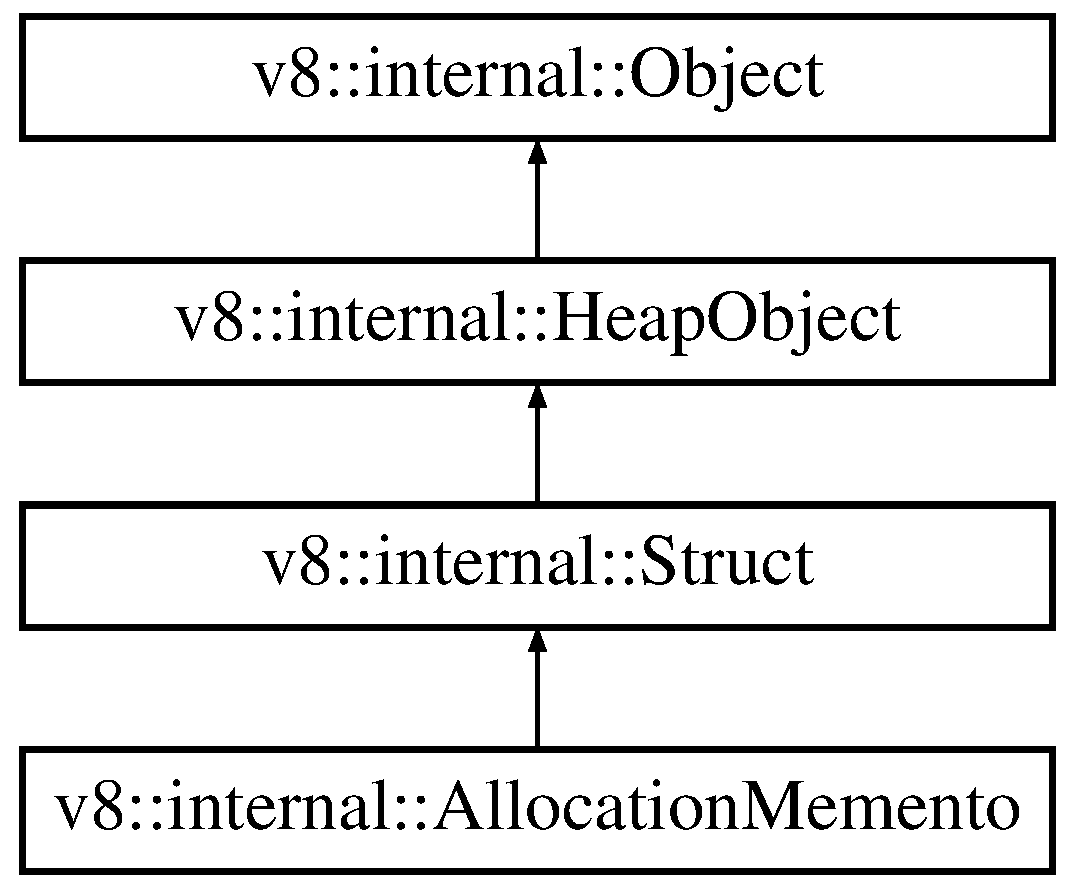
\includegraphics[height=4.000000cm]{classv8_1_1internal_1_1_allocation_memento}
\end{center}
\end{figure}
\subsection*{Public Member Functions}
\begin{DoxyCompactItemize}
\item 
bool {\bfseries Is\+Valid} ()\hypertarget{classv8_1_1internal_1_1_allocation_memento_add097e221c27cfdae3cc58466d9decab}{}\label{classv8_1_1internal_1_1_allocation_memento_add097e221c27cfdae3cc58466d9decab}

\item 
\hyperlink{classv8_1_1internal_1_1_allocation_site}{Allocation\+Site} $\ast$ {\bfseries Get\+Allocation\+Site} ()\hypertarget{classv8_1_1internal_1_1_allocation_memento_a1c22fe44c3a621ff2f88239f7efb042c}{}\label{classv8_1_1internal_1_1_allocation_memento_a1c22fe44c3a621ff2f88239f7efb042c}

\item 
Address {\bfseries Get\+Allocation\+Site\+Unchecked} ()\hypertarget{classv8_1_1internal_1_1_allocation_memento_af20d0fce1d25f3f996fcf24a658cc113}{}\label{classv8_1_1internal_1_1_allocation_memento_af20d0fce1d25f3f996fcf24a658cc113}

\end{DoxyCompactItemize}
\subsection*{Static Public Attributes}
\begin{DoxyCompactItemize}
\item 
static const int {\bfseries k\+Allocation\+Site\+Offset} = Heap\+Object\+::k\+Header\+Size\hypertarget{classv8_1_1internal_1_1_allocation_memento_ab07187e61f49dfb2c298a49b5aea49d7}{}\label{classv8_1_1internal_1_1_allocation_memento_ab07187e61f49dfb2c298a49b5aea49d7}

\item 
static const int {\bfseries k\+Size} = k\+Allocation\+Site\+Offset + k\+Pointer\+Size\hypertarget{classv8_1_1internal_1_1_allocation_memento_acf92166b75198263c67253249c64edf1}{}\label{classv8_1_1internal_1_1_allocation_memento_acf92166b75198263c67253249c64edf1}

\end{DoxyCompactItemize}
\subsection*{Private Member Functions}
\begin{DoxyCompactItemize}
\item 
{\bfseries D\+I\+S\+A\+L\+L\+O\+W\+\_\+\+I\+M\+P\+L\+I\+C\+I\+T\+\_\+\+C\+O\+N\+S\+T\+R\+U\+C\+T\+O\+RS} (\hyperlink{classv8_1_1internal_1_1_allocation_memento}{Allocation\+Memento})\hypertarget{classv8_1_1internal_1_1_allocation_memento_ae63138efc64a1f100fa781887f64ebd2}{}\label{classv8_1_1internal_1_1_allocation_memento_ae63138efc64a1f100fa781887f64ebd2}

\end{DoxyCompactItemize}
\subsection*{Additional Inherited Members}


The documentation for this class was generated from the following files\+:\begin{DoxyCompactItemize}
\item 
/\+Users/joshgav/node/v8/src/objects.\+h\item 
/\+Users/joshgav/node/v8/src/objects-\/inl.\+h\end{DoxyCompactItemize}

\hypertarget{classv8_1_1internal_1_1_sampling_heap_profiler_1_1_allocation_node}{}\section{v8\+:\+:internal\+:\+:Sampling\+Heap\+Profiler\+:\+:Allocation\+Node Class Reference}
\label{classv8_1_1internal_1_1_sampling_heap_profiler_1_1_allocation_node}\index{v8\+::internal\+::\+Sampling\+Heap\+Profiler\+::\+Allocation\+Node@{v8\+::internal\+::\+Sampling\+Heap\+Profiler\+::\+Allocation\+Node}}
\subsection*{Public Member Functions}
\begin{DoxyCompactItemize}
\item 
{\bfseries Allocation\+Node} (\hyperlink{classv8_1_1internal_1_1_sampling_heap_profiler_1_1_allocation_node}{Allocation\+Node} $\ast$parent, const char $\ast$name, int script\+\_\+id, int start\+\_\+position)\hypertarget{classv8_1_1internal_1_1_sampling_heap_profiler_1_1_allocation_node_afa0aa2a60ef0ad8e092ffc11e49ba7b8}{}\label{classv8_1_1internal_1_1_sampling_heap_profiler_1_1_allocation_node_afa0aa2a60ef0ad8e092ffc11e49ba7b8}

\end{DoxyCompactItemize}
\subsection*{Private Member Functions}
\begin{DoxyCompactItemize}
\item 
{\bfseries D\+I\+S\+A\+L\+L\+O\+W\+\_\+\+C\+O\+P\+Y\+\_\+\+A\+N\+D\+\_\+\+A\+S\+S\+I\+GN} (\hyperlink{classv8_1_1internal_1_1_sampling_heap_profiler_1_1_allocation_node}{Allocation\+Node})\hypertarget{classv8_1_1internal_1_1_sampling_heap_profiler_1_1_allocation_node_a81048530f209735fdffc403075201c6a}{}\label{classv8_1_1internal_1_1_sampling_heap_profiler_1_1_allocation_node_a81048530f209735fdffc403075201c6a}

\end{DoxyCompactItemize}
\subsection*{Private Attributes}
\begin{DoxyCompactItemize}
\item 
std\+::map$<$ size\+\_\+t, unsigned int $>$ {\bfseries allocations\+\_\+}\hypertarget{classv8_1_1internal_1_1_sampling_heap_profiler_1_1_allocation_node_ae88c671879b6539e3bc26b1d8cf4272f}{}\label{classv8_1_1internal_1_1_sampling_heap_profiler_1_1_allocation_node_ae88c671879b6539e3bc26b1d8cf4272f}

\item 
std\+::vector$<$ \hyperlink{classv8_1_1internal_1_1_sampling_heap_profiler_1_1_allocation_node}{Allocation\+Node} $\ast$ $>$ {\bfseries children\+\_\+}\hypertarget{classv8_1_1internal_1_1_sampling_heap_profiler_1_1_allocation_node_a5f2a47dca1cc526fe4a6cfe47f141106}{}\label{classv8_1_1internal_1_1_sampling_heap_profiler_1_1_allocation_node_a5f2a47dca1cc526fe4a6cfe47f141106}

\item 
\hyperlink{classv8_1_1internal_1_1_sampling_heap_profiler_1_1_allocation_node}{Allocation\+Node} $\ast$const {\bfseries parent\+\_\+}\hypertarget{classv8_1_1internal_1_1_sampling_heap_profiler_1_1_allocation_node_a53d60d3b24211b41a9265ce3a6fc5e5c}{}\label{classv8_1_1internal_1_1_sampling_heap_profiler_1_1_allocation_node_a53d60d3b24211b41a9265ce3a6fc5e5c}

\item 
const int {\bfseries script\+\_\+id\+\_\+}\hypertarget{classv8_1_1internal_1_1_sampling_heap_profiler_1_1_allocation_node_a3dc1319dd28b8d9c6984a0d719d9a3cf}{}\label{classv8_1_1internal_1_1_sampling_heap_profiler_1_1_allocation_node_a3dc1319dd28b8d9c6984a0d719d9a3cf}

\item 
const int {\bfseries script\+\_\+position\+\_\+}\hypertarget{classv8_1_1internal_1_1_sampling_heap_profiler_1_1_allocation_node_adc1e03de4b13b957222e53dea59cb4e5}{}\label{classv8_1_1internal_1_1_sampling_heap_profiler_1_1_allocation_node_adc1e03de4b13b957222e53dea59cb4e5}

\item 
const char $\ast$const {\bfseries name\+\_\+}\hypertarget{classv8_1_1internal_1_1_sampling_heap_profiler_1_1_allocation_node_abfb50c4d2c3f8a667e676d9e48748196}{}\label{classv8_1_1internal_1_1_sampling_heap_profiler_1_1_allocation_node_abfb50c4d2c3f8a667e676d9e48748196}

\item 
bool {\bfseries pinned\+\_\+}\hypertarget{classv8_1_1internal_1_1_sampling_heap_profiler_1_1_allocation_node_a09c975dfafe36c8a1ade23f4e657a2ee}{}\label{classv8_1_1internal_1_1_sampling_heap_profiler_1_1_allocation_node_a09c975dfafe36c8a1ade23f4e657a2ee}

\end{DoxyCompactItemize}
\subsection*{Friends}
\begin{DoxyCompactItemize}
\item 
class {\bfseries Sampling\+Heap\+Profiler}\hypertarget{classv8_1_1internal_1_1_sampling_heap_profiler_1_1_allocation_node_a1c4268235229c6a40ca92cbcd4591c9b}{}\label{classv8_1_1internal_1_1_sampling_heap_profiler_1_1_allocation_node_a1c4268235229c6a40ca92cbcd4591c9b}

\end{DoxyCompactItemize}


The documentation for this class was generated from the following file\+:\begin{DoxyCompactItemize}
\item 
/\+Users/joshgav/node/v8/src/profiler/sampling-\/heap-\/profiler.\+h\end{DoxyCompactItemize}

\hypertarget{classv8_1_1internal_1_1_allocation_observer}{}\section{v8\+:\+:internal\+:\+:Allocation\+Observer Class Reference}
\label{classv8_1_1internal_1_1_allocation_observer}\index{v8\+::internal\+::\+Allocation\+Observer@{v8\+::internal\+::\+Allocation\+Observer}}
Inheritance diagram for v8\+:\+:internal\+:\+:Allocation\+Observer\+:\begin{figure}[H]
\begin{center}
\leavevmode
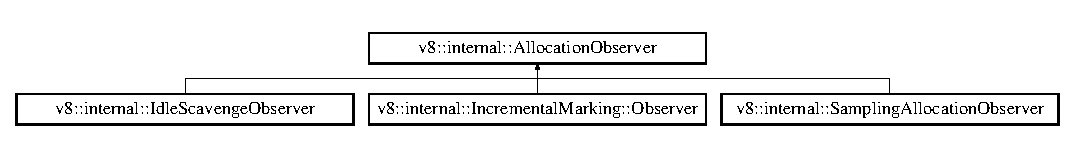
\includegraphics[height=1.441442cm]{classv8_1_1internal_1_1_allocation_observer}
\end{center}
\end{figure}
\subsection*{Public Member Functions}
\begin{DoxyCompactItemize}
\item 
{\bfseries Allocation\+Observer} (intptr\+\_\+t step\+\_\+size)\hypertarget{classv8_1_1internal_1_1_allocation_observer_afd17faabb89efdf1211915e9e684a31f}{}\label{classv8_1_1internal_1_1_allocation_observer_afd17faabb89efdf1211915e9e684a31f}

\item 
void {\bfseries Allocation\+Step} (int bytes\+\_\+allocated, Address soon\+\_\+object, size\+\_\+t size)\hypertarget{classv8_1_1internal_1_1_allocation_observer_a83b330ab2d41bd63c8463c98e3b44139}{}\label{classv8_1_1internal_1_1_allocation_observer_a83b330ab2d41bd63c8463c98e3b44139}

\end{DoxyCompactItemize}
\subsection*{Protected Member Functions}
\begin{DoxyCompactItemize}
\item 
intptr\+\_\+t {\bfseries step\+\_\+size} () const \hypertarget{classv8_1_1internal_1_1_allocation_observer_a2b39228326fc6f112821fd3bc9e3d368}{}\label{classv8_1_1internal_1_1_allocation_observer_a2b39228326fc6f112821fd3bc9e3d368}

\item 
intptr\+\_\+t {\bfseries bytes\+\_\+to\+\_\+next\+\_\+step} () const \hypertarget{classv8_1_1internal_1_1_allocation_observer_acd1e26bb58cf45790d605dbc96ea5dac}{}\label{classv8_1_1internal_1_1_allocation_observer_acd1e26bb58cf45790d605dbc96ea5dac}

\item 
virtual void {\bfseries Step} (int bytes\+\_\+allocated, Address soon\+\_\+object, size\+\_\+t size)=0\hypertarget{classv8_1_1internal_1_1_allocation_observer_a41118152d2c9a9834a486eccf08043a5}{}\label{classv8_1_1internal_1_1_allocation_observer_a41118152d2c9a9834a486eccf08043a5}

\item 
virtual intptr\+\_\+t {\bfseries Get\+Next\+Step\+Size} ()\hypertarget{classv8_1_1internal_1_1_allocation_observer_a91fb6ffe2d4b42ff7b4221dad89db465}{}\label{classv8_1_1internal_1_1_allocation_observer_a91fb6ffe2d4b42ff7b4221dad89db465}

\end{DoxyCompactItemize}
\subsection*{Protected Attributes}
\begin{DoxyCompactItemize}
\item 
intptr\+\_\+t {\bfseries step\+\_\+size\+\_\+}\hypertarget{classv8_1_1internal_1_1_allocation_observer_aca0c9295ca497a26f08cd8244f84d5aa}{}\label{classv8_1_1internal_1_1_allocation_observer_aca0c9295ca497a26f08cd8244f84d5aa}

\item 
intptr\+\_\+t {\bfseries bytes\+\_\+to\+\_\+next\+\_\+step\+\_\+}\hypertarget{classv8_1_1internal_1_1_allocation_observer_a5f02cbcbd88c5b87439c31ada838923e}{}\label{classv8_1_1internal_1_1_allocation_observer_a5f02cbcbd88c5b87439c31ada838923e}

\end{DoxyCompactItemize}
\subsection*{Private Member Functions}
\begin{DoxyCompactItemize}
\item 
{\bfseries D\+I\+S\+A\+L\+L\+O\+W\+\_\+\+C\+O\+P\+Y\+\_\+\+A\+N\+D\+\_\+\+A\+S\+S\+I\+GN} (\hyperlink{classv8_1_1internal_1_1_allocation_observer}{Allocation\+Observer})\hypertarget{classv8_1_1internal_1_1_allocation_observer_a8e27676bc76f2081c8c6920f873e3f3c}{}\label{classv8_1_1internal_1_1_allocation_observer_a8e27676bc76f2081c8c6920f873e3f3c}

\end{DoxyCompactItemize}
\subsection*{Friends}
\begin{DoxyCompactItemize}
\item 
class {\bfseries Large\+Object\+Space}\hypertarget{classv8_1_1internal_1_1_allocation_observer_ae7bd71eb9e957e0b89a7d3a76836d4b3}{}\label{classv8_1_1internal_1_1_allocation_observer_ae7bd71eb9e957e0b89a7d3a76836d4b3}

\item 
class {\bfseries New\+Space}\hypertarget{classv8_1_1internal_1_1_allocation_observer_a71065109e762b07b59b80cd64d885ff8}{}\label{classv8_1_1internal_1_1_allocation_observer_a71065109e762b07b59b80cd64d885ff8}

\item 
class {\bfseries Paged\+Space}\hypertarget{classv8_1_1internal_1_1_allocation_observer_a57d18a423c610563132a99ab1e1c1b8e}{}\label{classv8_1_1internal_1_1_allocation_observer_a57d18a423c610563132a99ab1e1c1b8e}

\end{DoxyCompactItemize}


The documentation for this class was generated from the following file\+:\begin{DoxyCompactItemize}
\item 
/\+Users/joshgav/node/v8/src/heap/heap.\+h\end{DoxyCompactItemize}

\hypertarget{classv8_1_1_allocation_profile}{}\section{v8\+:\+:Allocation\+Profile Class Reference}
\label{classv8_1_1_allocation_profile}\index{v8\+::\+Allocation\+Profile@{v8\+::\+Allocation\+Profile}}


{\ttfamily \#include $<$v8-\/profiler.\+h$>$}

Inheritance diagram for v8\+:\+:Allocation\+Profile\+:\begin{figure}[H]
\begin{center}
\leavevmode
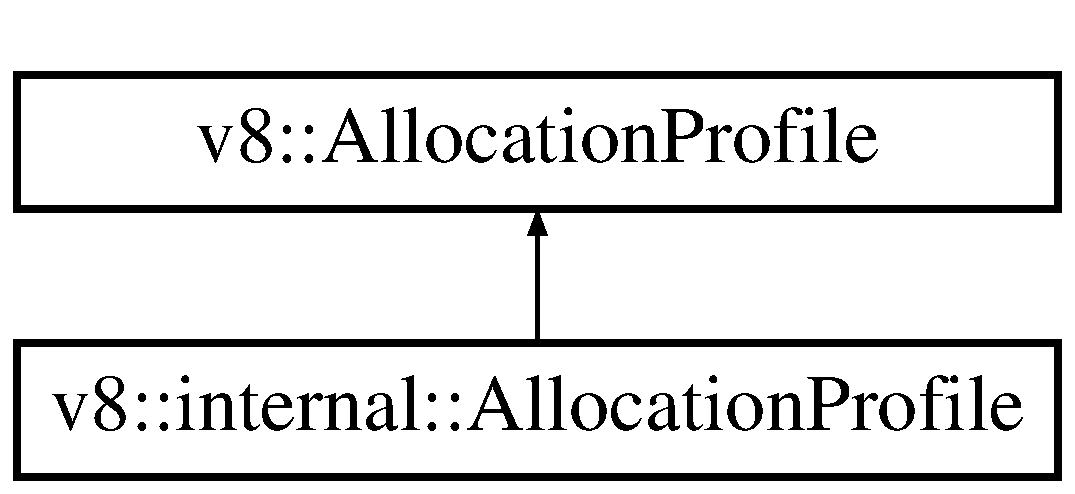
\includegraphics[height=2.000000cm]{classv8_1_1_allocation_profile}
\end{center}
\end{figure}
\subsection*{Classes}
\begin{DoxyCompactItemize}
\item 
struct \hyperlink{structv8_1_1_allocation_profile_1_1_allocation}{Allocation}
\item 
struct \hyperlink{structv8_1_1_allocation_profile_1_1_node}{Node}
\end{DoxyCompactItemize}
\subsection*{Public Member Functions}
\begin{DoxyCompactItemize}
\item 
virtual \hyperlink{structv8_1_1_allocation_profile_1_1_node}{Node} $\ast$ \hyperlink{classv8_1_1_allocation_profile_afea045dae30df5477088e2f0b7edb6c4}{Get\+Root\+Node} ()=0
\end{DoxyCompactItemize}
\subsection*{Static Public Attributes}
\begin{DoxyCompactItemize}
\item 
static const int {\bfseries k\+No\+Line\+Number\+Info} = Message\+::k\+No\+Line\+Number\+Info\hypertarget{classv8_1_1_allocation_profile_a26fdfe9e4846d26c83d0ad8c2ed2d783}{}\label{classv8_1_1_allocation_profile_a26fdfe9e4846d26c83d0ad8c2ed2d783}

\item 
static const int {\bfseries k\+No\+Column\+Number\+Info} = Message\+::k\+No\+Column\+Info\hypertarget{classv8_1_1_allocation_profile_a9cfa103f73e82629694eee3734826eb7}{}\label{classv8_1_1_allocation_profile_a9cfa103f73e82629694eee3734826eb7}

\end{DoxyCompactItemize}


\subsection{Detailed Description}
\hyperlink{classv8_1_1_allocation_profile}{Allocation\+Profile} is a sampled profile of allocations done by the program. This is structured as a call-\/graph. 

\subsection{Member Function Documentation}
\index{v8\+::\+Allocation\+Profile@{v8\+::\+Allocation\+Profile}!Get\+Root\+Node@{Get\+Root\+Node}}
\index{Get\+Root\+Node@{Get\+Root\+Node}!v8\+::\+Allocation\+Profile@{v8\+::\+Allocation\+Profile}}
\subsubsection[{\texorpdfstring{Get\+Root\+Node()=0}{GetRootNode()=0}}]{\setlength{\rightskip}{0pt plus 5cm}virtual {\bf Node}$\ast$ v8\+::\+Allocation\+Profile\+::\+Get\+Root\+Node (
\begin{DoxyParamCaption}
{}
\end{DoxyParamCaption}
)\hspace{0.3cm}{\ttfamily [pure virtual]}}\hypertarget{classv8_1_1_allocation_profile_afea045dae30df5477088e2f0b7edb6c4}{}\label{classv8_1_1_allocation_profile_afea045dae30df5477088e2f0b7edb6c4}
Returns the root node of the call-\/graph. The root node corresponds to an empty JS call-\/stack. The lifetime of the returned Node$\ast$ is scoped to the containing \hyperlink{classv8_1_1_allocation_profile}{Allocation\+Profile}. 

Implemented in \hyperlink{classv8_1_1internal_1_1_allocation_profile_abb93406eaccd8b37de3e080d0620bc2b}{v8\+::internal\+::\+Allocation\+Profile}.



The documentation for this class was generated from the following file\+:\begin{DoxyCompactItemize}
\item 
/\+Users/joshgav/node/v8/include/v8-\/profiler.\+h\end{DoxyCompactItemize}

\hypertarget{classv8_1_1internal_1_1_allocation_profile}{}\section{v8\+:\+:internal\+:\+:Allocation\+Profile Class Reference}
\label{classv8_1_1internal_1_1_allocation_profile}\index{v8\+::internal\+::\+Allocation\+Profile@{v8\+::internal\+::\+Allocation\+Profile}}
Inheritance diagram for v8\+:\+:internal\+:\+:Allocation\+Profile\+:\begin{figure}[H]
\begin{center}
\leavevmode
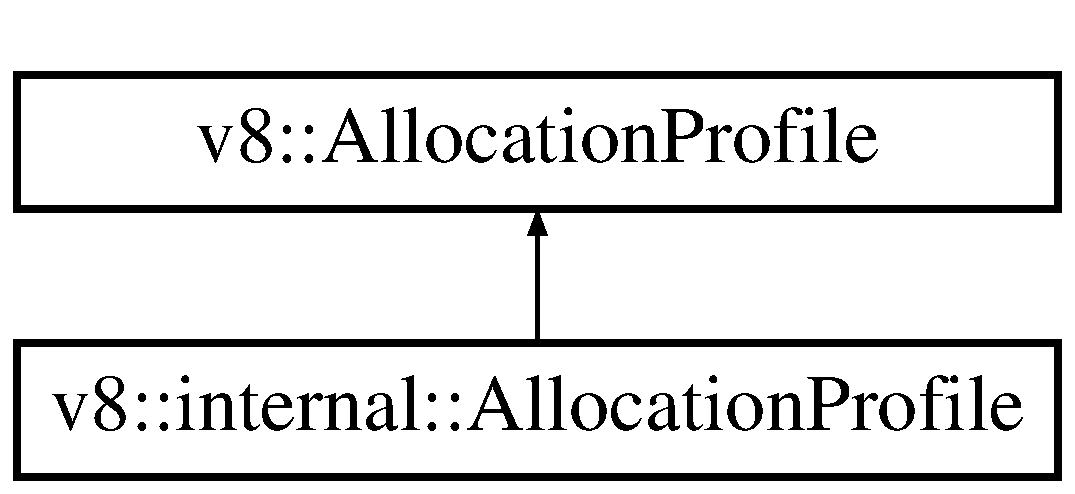
\includegraphics[height=2.000000cm]{classv8_1_1internal_1_1_allocation_profile}
\end{center}
\end{figure}
\subsection*{Public Member Functions}
\begin{DoxyCompactItemize}
\item 
\hyperlink{structv8_1_1_allocation_profile_1_1_node}{v8\+::\+Allocation\+Profile\+::\+Node} $\ast$ \hyperlink{classv8_1_1internal_1_1_allocation_profile_abb93406eaccd8b37de3e080d0620bc2b}{Get\+Root\+Node} () override
\item 
std\+::deque$<$ \hyperlink{structv8_1_1_allocation_profile_1_1_node}{v8\+::\+Allocation\+Profile\+::\+Node} $>$ \& {\bfseries nodes} ()\hypertarget{classv8_1_1internal_1_1_allocation_profile_aae4669a89f83fbb4cb0d6bcf334d617b}{}\label{classv8_1_1internal_1_1_allocation_profile_aae4669a89f83fbb4cb0d6bcf334d617b}

\end{DoxyCompactItemize}
\subsection*{Private Member Functions}
\begin{DoxyCompactItemize}
\item 
{\bfseries D\+I\+S\+A\+L\+L\+O\+W\+\_\+\+C\+O\+P\+Y\+\_\+\+A\+N\+D\+\_\+\+A\+S\+S\+I\+GN} (\hyperlink{classv8_1_1internal_1_1_allocation_profile}{Allocation\+Profile})\hypertarget{classv8_1_1internal_1_1_allocation_profile_a6d8a3ded6b83bf1a664d05b7940070df}{}\label{classv8_1_1internal_1_1_allocation_profile_a6d8a3ded6b83bf1a664d05b7940070df}

\end{DoxyCompactItemize}
\subsection*{Private Attributes}
\begin{DoxyCompactItemize}
\item 
std\+::deque$<$ \hyperlink{structv8_1_1_allocation_profile_1_1_node}{v8\+::\+Allocation\+Profile\+::\+Node} $>$ {\bfseries nodes\+\_\+}\hypertarget{classv8_1_1internal_1_1_allocation_profile_a43cc2c37b9ea845241551f7d165a530e}{}\label{classv8_1_1internal_1_1_allocation_profile_a43cc2c37b9ea845241551f7d165a530e}

\end{DoxyCompactItemize}
\subsection*{Additional Inherited Members}


\subsection{Member Function Documentation}
\index{v8\+::internal\+::\+Allocation\+Profile@{v8\+::internal\+::\+Allocation\+Profile}!Get\+Root\+Node@{Get\+Root\+Node}}
\index{Get\+Root\+Node@{Get\+Root\+Node}!v8\+::internal\+::\+Allocation\+Profile@{v8\+::internal\+::\+Allocation\+Profile}}
\subsubsection[{\texorpdfstring{Get\+Root\+Node() override}{GetRootNode() override}}]{\setlength{\rightskip}{0pt plus 5cm}{\bf v8\+::\+Allocation\+Profile\+::\+Node}$\ast$ v8\+::internal\+::\+Allocation\+Profile\+::\+Get\+Root\+Node (
\begin{DoxyParamCaption}
{}
\end{DoxyParamCaption}
)\hspace{0.3cm}{\ttfamily [inline]}, {\ttfamily [override]}, {\ttfamily [virtual]}}\hypertarget{classv8_1_1internal_1_1_allocation_profile_abb93406eaccd8b37de3e080d0620bc2b}{}\label{classv8_1_1internal_1_1_allocation_profile_abb93406eaccd8b37de3e080d0620bc2b}
Returns the root node of the call-\/graph. The root node corresponds to an empty JS call-\/stack. The lifetime of the returned Node$\ast$ is scoped to the containing \hyperlink{classv8_1_1internal_1_1_allocation_profile}{Allocation\+Profile}. 

Implements \hyperlink{classv8_1_1_allocation_profile_afea045dae30df5477088e2f0b7edb6c4}{v8\+::\+Allocation\+Profile}.



The documentation for this class was generated from the following file\+:\begin{DoxyCompactItemize}
\item 
/\+Users/joshgav/node/v8/src/profiler/sampling-\/heap-\/profiler.\+h\end{DoxyCompactItemize}

\hypertarget{classv8_1_1internal_1_1_allocation_result}{}\section{v8\+:\+:internal\+:\+:Allocation\+Result Class Reference}
\label{classv8_1_1internal_1_1_allocation_result}\index{v8\+::internal\+::\+Allocation\+Result@{v8\+::internal\+::\+Allocation\+Result}}
\subsection*{Public Member Functions}
\begin{DoxyCompactItemize}
\item 
{\bfseries Allocation\+Result} (\hyperlink{classv8_1_1internal_1_1_object}{Object} $\ast$object)\hypertarget{classv8_1_1internal_1_1_allocation_result_a070cd4a633aea946bc22da35de4e20d3}{}\label{classv8_1_1internal_1_1_allocation_result_a070cd4a633aea946bc22da35de4e20d3}

\item 
bool {\bfseries Is\+Retry} ()\hypertarget{classv8_1_1internal_1_1_allocation_result_a42620ae6917b2e46beb01e6d5ab1af9d}{}\label{classv8_1_1internal_1_1_allocation_result_a42620ae6917b2e46beb01e6d5ab1af9d}

\item 
{\footnotesize template$<$typename T $>$ }\\bool {\bfseries To} (T $\ast$$\ast$obj)\hypertarget{classv8_1_1internal_1_1_allocation_result_a200458fd748f27686583ca3e36fa7792}{}\label{classv8_1_1internal_1_1_allocation_result_a200458fd748f27686583ca3e36fa7792}

\item 
\hyperlink{classv8_1_1internal_1_1_object}{Object} $\ast$ {\bfseries To\+Object\+Checked} ()\hypertarget{classv8_1_1internal_1_1_allocation_result_a77e1f4d2f30a754f6a75b68867b7c259}{}\label{classv8_1_1internal_1_1_allocation_result_a77e1f4d2f30a754f6a75b68867b7c259}

\item 
Allocation\+Space {\bfseries Retry\+Space} ()\hypertarget{classv8_1_1internal_1_1_allocation_result_a112be2639d4a26bacacdd582fdd67feb}{}\label{classv8_1_1internal_1_1_allocation_result_a112be2639d4a26bacacdd582fdd67feb}

\end{DoxyCompactItemize}
\subsection*{Static Public Member Functions}
\begin{DoxyCompactItemize}
\item 
static \hyperlink{classv8_1_1internal_1_1_allocation_result}{Allocation\+Result} {\bfseries Retry} (Allocation\+Space space=N\+E\+W\+\_\+\+S\+P\+A\+CE)\hypertarget{classv8_1_1internal_1_1_allocation_result_a89de42812f610b130c34d3ecbe3321a5}{}\label{classv8_1_1internal_1_1_allocation_result_a89de42812f610b130c34d3ecbe3321a5}

\end{DoxyCompactItemize}
\subsection*{Private Member Functions}
\begin{DoxyCompactItemize}
\item 
{\bfseries Allocation\+Result} (Allocation\+Space space)\hypertarget{classv8_1_1internal_1_1_allocation_result_aed72dcbbf9c83eec64918f3773c16d97}{}\label{classv8_1_1internal_1_1_allocation_result_aed72dcbbf9c83eec64918f3773c16d97}

\end{DoxyCompactItemize}
\subsection*{Private Attributes}
\begin{DoxyCompactItemize}
\item 
\hyperlink{classv8_1_1internal_1_1_object}{Object} $\ast$ {\bfseries object\+\_\+}\hypertarget{classv8_1_1internal_1_1_allocation_result_a97c6fd4f49b3e18efd87ce17b24f9bc1}{}\label{classv8_1_1internal_1_1_allocation_result_a97c6fd4f49b3e18efd87ce17b24f9bc1}

\end{DoxyCompactItemize}


The documentation for this class was generated from the following files\+:\begin{DoxyCompactItemize}
\item 
/\+Users/joshgav/node/v8/src/heap/spaces.\+h\item 
/\+Users/joshgav/node/v8/src/heap/spaces-\/inl.\+h\end{DoxyCompactItemize}

\hypertarget{classv8_1_1internal_1_1compiler_1_1_allocation_scheduler}{}\section{v8\+:\+:internal\+:\+:compiler\+:\+:Allocation\+Scheduler Class Reference}
\label{classv8_1_1internal_1_1compiler_1_1_allocation_scheduler}\index{v8\+::internal\+::compiler\+::\+Allocation\+Scheduler@{v8\+::internal\+::compiler\+::\+Allocation\+Scheduler}}
Inheritance diagram for v8\+:\+:internal\+:\+:compiler\+:\+:Allocation\+Scheduler\+:\begin{figure}[H]
\begin{center}
\leavevmode
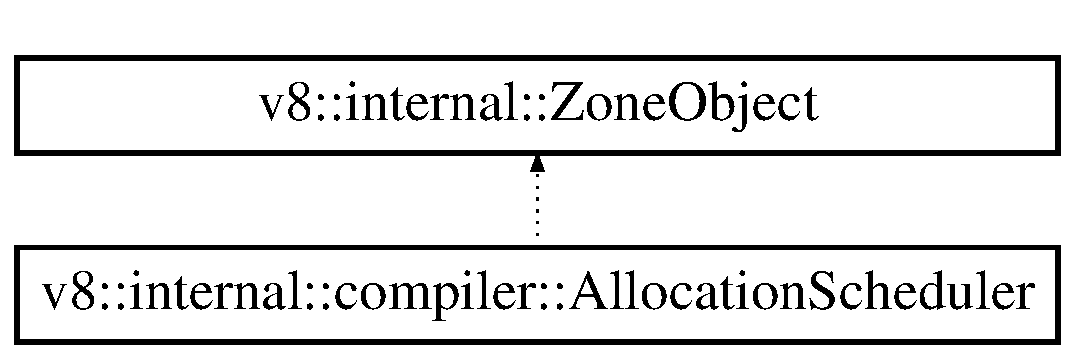
\includegraphics[height=2.000000cm]{classv8_1_1internal_1_1compiler_1_1_allocation_scheduler}
\end{center}
\end{figure}
\subsection*{Public Member Functions}
\begin{DoxyCompactItemize}
\item 
{\bfseries Allocation\+Scheduler} (\hyperlink{classv8_1_1internal_1_1_zone}{Zone} $\ast$zone)\hypertarget{classv8_1_1internal_1_1compiler_1_1_allocation_scheduler_a956ef2950ead9f2b11fa045d5bd2e810}{}\label{classv8_1_1internal_1_1compiler_1_1_allocation_scheduler_a956ef2950ead9f2b11fa045d5bd2e810}

\item 
void {\bfseries Schedule} (\hyperlink{classv8_1_1internal_1_1compiler_1_1_live_range}{Live\+Range} $\ast$range)\hypertarget{classv8_1_1internal_1_1compiler_1_1_allocation_scheduler_a38c05c59502d3683407a5c73844085f8}{}\label{classv8_1_1internal_1_1compiler_1_1_allocation_scheduler_a38c05c59502d3683407a5c73844085f8}

\item 
void {\bfseries Schedule} (\hyperlink{classv8_1_1internal_1_1compiler_1_1_live_range_group}{Live\+Range\+Group} $\ast$group)\hypertarget{classv8_1_1internal_1_1compiler_1_1_allocation_scheduler_ac0363114e1cb39d114e57a9466dc00b6}{}\label{classv8_1_1internal_1_1compiler_1_1_allocation_scheduler_ac0363114e1cb39d114e57a9466dc00b6}

\item 
\hyperlink{classv8_1_1internal_1_1compiler_1_1_allocation_candidate}{Allocation\+Candidate} {\bfseries Get\+Next} ()\hypertarget{classv8_1_1internal_1_1compiler_1_1_allocation_scheduler_a9701278a58e1819b4a0b4e6370bd7de7}{}\label{classv8_1_1internal_1_1compiler_1_1_allocation_scheduler_a9701278a58e1819b4a0b4e6370bd7de7}

\item 
bool {\bfseries empty} () const \hypertarget{classv8_1_1internal_1_1compiler_1_1_allocation_scheduler_adfd981f23281187a10e3fab7e91593eb}{}\label{classv8_1_1internal_1_1compiler_1_1_allocation_scheduler_adfd981f23281187a10e3fab7e91593eb}

\end{DoxyCompactItemize}
\subsection*{Private Types}
\begin{DoxyCompactItemize}
\item 
typedef \hyperlink{classv8_1_1internal_1_1_zone_priority_queue}{Zone\+Priority\+Queue}$<$ \hyperlink{classv8_1_1internal_1_1compiler_1_1_allocation_candidate}{Allocation\+Candidate} $>$ {\bfseries Schedule\+Queue}\hypertarget{classv8_1_1internal_1_1compiler_1_1_allocation_scheduler_a043b2cf4cd6202733136b679677ec127}{}\label{classv8_1_1internal_1_1compiler_1_1_allocation_scheduler_a043b2cf4cd6202733136b679677ec127}

\end{DoxyCompactItemize}
\subsection*{Private Member Functions}
\begin{DoxyCompactItemize}
\item 
{\bfseries D\+I\+S\+A\+L\+L\+O\+W\+\_\+\+C\+O\+P\+Y\+\_\+\+A\+N\+D\+\_\+\+A\+S\+S\+I\+GN} (\hyperlink{classv8_1_1internal_1_1compiler_1_1_allocation_scheduler}{Allocation\+Scheduler})\hypertarget{classv8_1_1internal_1_1compiler_1_1_allocation_scheduler_ae506454e2c0219bfc886c8cfe60a8c8f}{}\label{classv8_1_1internal_1_1compiler_1_1_allocation_scheduler_ae506454e2c0219bfc886c8cfe60a8c8f}

\end{DoxyCompactItemize}
\subsection*{Private Attributes}
\begin{DoxyCompactItemize}
\item 
\hyperlink{classv8_1_1internal_1_1_zone_priority_queue}{Schedule\+Queue} {\bfseries queue\+\_\+}\hypertarget{classv8_1_1internal_1_1compiler_1_1_allocation_scheduler_a1783d7d2c7ad1c4169932562f85c95e3}{}\label{classv8_1_1internal_1_1compiler_1_1_allocation_scheduler_a1783d7d2c7ad1c4169932562f85c95e3}

\end{DoxyCompactItemize}


The documentation for this class was generated from the following files\+:\begin{DoxyCompactItemize}
\item 
/\+Users/joshgav/node/v8/src/compiler/greedy-\/allocator.\+h\item 
/\+Users/joshgav/node/v8/src/compiler/greedy-\/allocator.\+cc\end{DoxyCompactItemize}

\hypertarget{classv8_1_1internal_1_1_allocation_site}{}\section{v8\+:\+:internal\+:\+:Allocation\+Site Class Reference}
\label{classv8_1_1internal_1_1_allocation_site}\index{v8\+::internal\+::\+Allocation\+Site@{v8\+::internal\+::\+Allocation\+Site}}
Inheritance diagram for v8\+:\+:internal\+:\+:Allocation\+Site\+:\begin{figure}[H]
\begin{center}
\leavevmode
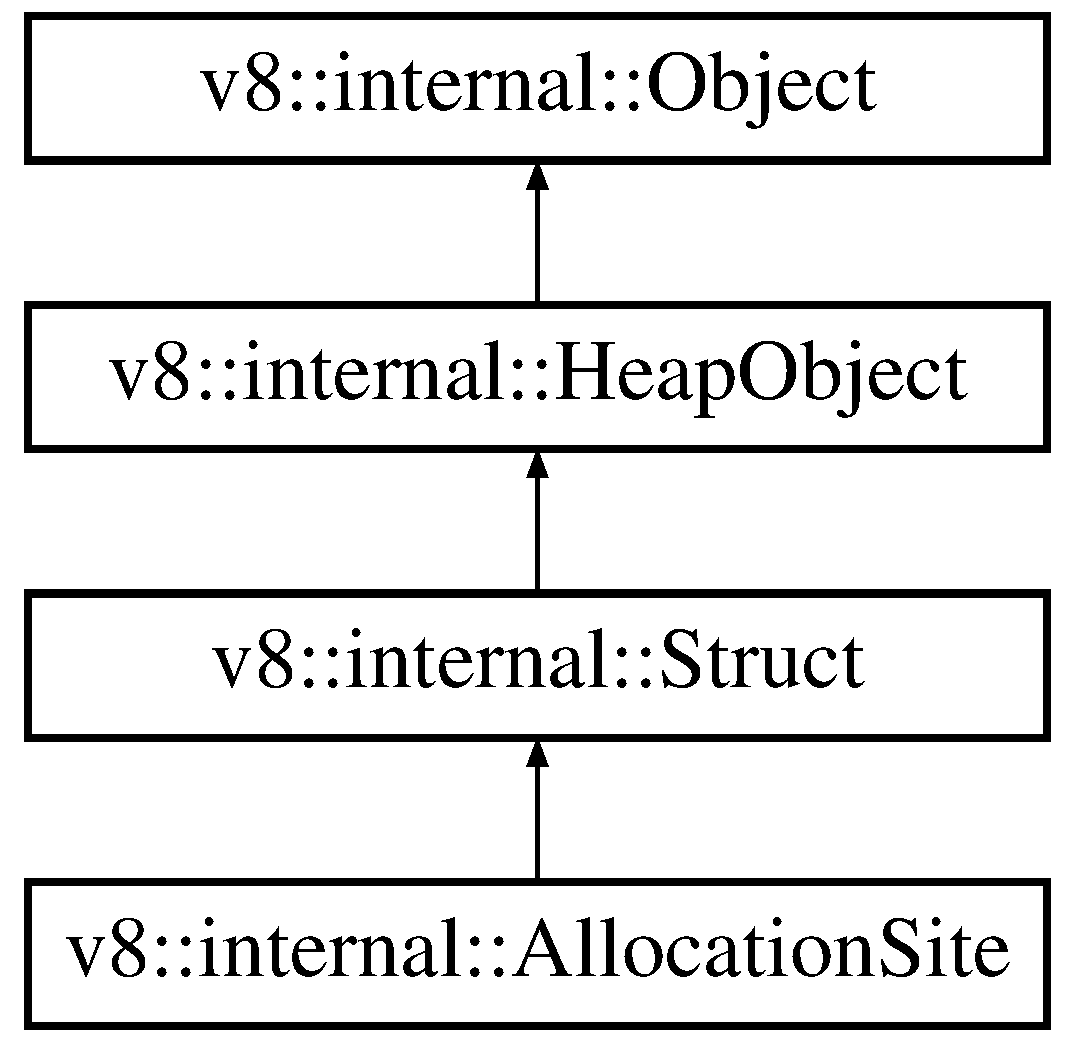
\includegraphics[height=4.000000cm]{classv8_1_1internal_1_1_allocation_site}
\end{center}
\end{figure}
\subsection*{Classes}
\begin{DoxyCompactItemize}
\item 
class \hyperlink{classv8_1_1internal_1_1_allocation_site_1_1_deopt_dependent_code_bit}{Deopt\+Dependent\+Code\+Bit}
\item 
class \hyperlink{classv8_1_1internal_1_1_allocation_site_1_1_do_not_inline_bit}{Do\+Not\+Inline\+Bit}
\item 
class \hyperlink{classv8_1_1internal_1_1_allocation_site_1_1_elements_kind_bits}{Elements\+Kind\+Bits}
\item 
class \hyperlink{classv8_1_1internal_1_1_allocation_site_1_1_memento_found_count_bits}{Memento\+Found\+Count\+Bits}
\item 
class \hyperlink{classv8_1_1internal_1_1_allocation_site_1_1_pretenure_decision_bits}{Pretenure\+Decision\+Bits}
\item 
class \hyperlink{classv8_1_1internal_1_1_allocation_site_1_1_unused_bits}{Unused\+Bits}
\end{DoxyCompactItemize}
\subsection*{Public Types}
\begin{DoxyCompactItemize}
\item 
enum {\bfseries Pretenure\+Decision} \{ \\*
{\bfseries k\+Undecided} = 0, 
\\*
{\bfseries k\+Dont\+Tenure} = 1, 
\\*
{\bfseries k\+Maybe\+Tenure} = 2, 
\\*
{\bfseries k\+Tenure} = 3, 
\\*
{\bfseries k\+Zombie} = 4, 
\\*
{\bfseries k\+Last\+Pretenure\+Decision\+Value} = k\+Zombie
 \}\hypertarget{classv8_1_1internal_1_1_allocation_site_a90e0736002b73f20d96abede63a5395b}{}\label{classv8_1_1internal_1_1_allocation_site_a90e0736002b73f20d96abede63a5395b}

\item 
typedef \hyperlink{classv8_1_1internal_1_1_fixed_body_descriptor}{Fixed\+Body\+Descriptor}$<$ Heap\+Object\+::k\+Header\+Size, k\+Size, k\+Size $>$ {\bfseries Body\+Descriptor}\hypertarget{classv8_1_1internal_1_1_allocation_site_a8cacad07f0e02a96cbd772ab4f3f8e70}{}\label{classv8_1_1internal_1_1_allocation_site_a8cacad07f0e02a96cbd772ab4f3f8e70}

\end{DoxyCompactItemize}
\subsection*{Public Member Functions}
\begin{DoxyCompactItemize}
\item 
const char $\ast$ {\bfseries Pretenure\+Decision\+Name} (Pretenure\+Decision decision)\hypertarget{classv8_1_1internal_1_1_allocation_site_a015895d2a527877f98749eb13b16a38f}{}\label{classv8_1_1internal_1_1_allocation_site_a015895d2a527877f98749eb13b16a38f}

\item 
void {\bfseries Initialize} ()\hypertarget{classv8_1_1internal_1_1_allocation_site_a81f61008e147366d1eea6cdbae9d5ded}{}\label{classv8_1_1internal_1_1_allocation_site_a81f61008e147366d1eea6cdbae9d5ded}

\item 
bool {\bfseries Is\+Nested\+Site} ()\hypertarget{classv8_1_1internal_1_1_allocation_site_ab9a3fce3780154b3da48ae09cb0b8d46}{}\label{classv8_1_1internal_1_1_allocation_site_ab9a3fce3780154b3da48ae09cb0b8d46}

\item 
{\bfseries S\+T\+A\+T\+I\+C\+\_\+\+A\+S\+S\+E\+RT} (Pretenure\+Decision\+Bits\+::k\+Max $>$=k\+Last\+Pretenure\+Decision\+Value)\hypertarget{classv8_1_1internal_1_1_allocation_site_ad1c0e4e32b7e2db1483fa7a518bec030}{}\label{classv8_1_1internal_1_1_allocation_site_ad1c0e4e32b7e2db1483fa7a518bec030}

\item 
bool {\bfseries Increment\+Memento\+Found\+Count} (int increment=1)\hypertarget{classv8_1_1internal_1_1_allocation_site_ad402f0d78d12a670cf7eb371f65fc1c0}{}\label{classv8_1_1internal_1_1_allocation_site_ad402f0d78d12a670cf7eb371f65fc1c0}

\item 
void {\bfseries Increment\+Memento\+Create\+Count} ()\hypertarget{classv8_1_1internal_1_1_allocation_site_ac32fcfb926ce03239f5df6aca880f18c}{}\label{classv8_1_1internal_1_1_allocation_site_ac32fcfb926ce03239f5df6aca880f18c}

\item 
Pretenure\+Flag {\bfseries Get\+Pretenure\+Mode} ()\hypertarget{classv8_1_1internal_1_1_allocation_site_a06aadcce1164186ecce0962c359abb0c}{}\label{classv8_1_1internal_1_1_allocation_site_a06aadcce1164186ecce0962c359abb0c}

\item 
void {\bfseries Reset\+Pretenure\+Decision} ()\hypertarget{classv8_1_1internal_1_1_allocation_site_aa1b323951edb619dd9078164b9fabd5c}{}\label{classv8_1_1internal_1_1_allocation_site_aa1b323951edb619dd9078164b9fabd5c}

\item 
Pretenure\+Decision {\bfseries pretenure\+\_\+decision} ()\hypertarget{classv8_1_1internal_1_1_allocation_site_a7103887124921d6ff4eb401bff563a52}{}\label{classv8_1_1internal_1_1_allocation_site_a7103887124921d6ff4eb401bff563a52}

\item 
void {\bfseries set\+\_\+pretenure\+\_\+decision} (Pretenure\+Decision decision)\hypertarget{classv8_1_1internal_1_1_allocation_site_a3eb7bfb649894bc1ea0875152aff118e}{}\label{classv8_1_1internal_1_1_allocation_site_a3eb7bfb649894bc1ea0875152aff118e}

\item 
bool {\bfseries deopt\+\_\+dependent\+\_\+code} ()\hypertarget{classv8_1_1internal_1_1_allocation_site_ad346c72b5d5c204cbb5ca3c5d42de25b}{}\label{classv8_1_1internal_1_1_allocation_site_ad346c72b5d5c204cbb5ca3c5d42de25b}

\item 
void {\bfseries set\+\_\+deopt\+\_\+dependent\+\_\+code} (bool deopt)\hypertarget{classv8_1_1internal_1_1_allocation_site_a6b6321178dbb71e389194b39a6ee51ee}{}\label{classv8_1_1internal_1_1_allocation_site_a6b6321178dbb71e389194b39a6ee51ee}

\item 
int {\bfseries memento\+\_\+found\+\_\+count} ()\hypertarget{classv8_1_1internal_1_1_allocation_site_a09e237ddea93fe5f26592f3f4d86d73b}{}\label{classv8_1_1internal_1_1_allocation_site_a09e237ddea93fe5f26592f3f4d86d73b}

\item 
void {\bfseries set\+\_\+memento\+\_\+found\+\_\+count} (int count)\hypertarget{classv8_1_1internal_1_1_allocation_site_ad74c42dccc41adcc6d7f2dd22fa56176}{}\label{classv8_1_1internal_1_1_allocation_site_ad74c42dccc41adcc6d7f2dd22fa56176}

\item 
int {\bfseries memento\+\_\+create\+\_\+count} ()\hypertarget{classv8_1_1internal_1_1_allocation_site_aa5dae1f833730f55ab548a2981c577fd}{}\label{classv8_1_1internal_1_1_allocation_site_aa5dae1f833730f55ab548a2981c577fd}

\item 
void {\bfseries set\+\_\+memento\+\_\+create\+\_\+count} (int count)\hypertarget{classv8_1_1internal_1_1_allocation_site_ab95f8e888faad709405944f3f5223378}{}\label{classv8_1_1internal_1_1_allocation_site_ab95f8e888faad709405944f3f5223378}

\item 
bool {\bfseries Is\+Zombie} ()\hypertarget{classv8_1_1internal_1_1_allocation_site_ab43e6d803b8a1f9b160936060e487542}{}\label{classv8_1_1internal_1_1_allocation_site_ab43e6d803b8a1f9b160936060e487542}

\item 
bool {\bfseries Is\+Maybe\+Tenure} ()\hypertarget{classv8_1_1internal_1_1_allocation_site_aa1870a70bef3585f613d95509e3c026e}{}\label{classv8_1_1internal_1_1_allocation_site_aa1870a70bef3585f613d95509e3c026e}

\item 
void {\bfseries Mark\+Zombie} ()\hypertarget{classv8_1_1internal_1_1_allocation_site_af432e0790ebdfc00d36c9a6234e98389}{}\label{classv8_1_1internal_1_1_allocation_site_af432e0790ebdfc00d36c9a6234e98389}

\item 
bool {\bfseries Make\+Pretenure\+Decision} (Pretenure\+Decision current\+\_\+decision, double ratio, bool maximum\+\_\+size\+\_\+scavenge)\hypertarget{classv8_1_1internal_1_1_allocation_site_ac56e44521833202855156f6c8f06101f}{}\label{classv8_1_1internal_1_1_allocation_site_ac56e44521833202855156f6c8f06101f}

\item 
bool {\bfseries Digest\+Pretenuring\+Feedback} (bool maximum\+\_\+size\+\_\+scavenge)\hypertarget{classv8_1_1internal_1_1_allocation_site_ab06a9db3e9fa8256f8cd97cc5cefeff5}{}\label{classv8_1_1internal_1_1_allocation_site_ab06a9db3e9fa8256f8cd97cc5cefeff5}

\item 
Elements\+Kind {\bfseries Get\+Elements\+Kind} ()\hypertarget{classv8_1_1internal_1_1_allocation_site_ad32f0453a6a51c271b6207227ec2959d}{}\label{classv8_1_1internal_1_1_allocation_site_ad32f0453a6a51c271b6207227ec2959d}

\item 
void {\bfseries Set\+Elements\+Kind} (Elements\+Kind kind)\hypertarget{classv8_1_1internal_1_1_allocation_site_adf1136948311998f7ead14bcf8f2cfd8}{}\label{classv8_1_1internal_1_1_allocation_site_adf1136948311998f7ead14bcf8f2cfd8}

\item 
bool {\bfseries Can\+Inline\+Call} ()\hypertarget{classv8_1_1internal_1_1_allocation_site_aeb29ad379adc7425340ae3b2e38f72f3}{}\label{classv8_1_1internal_1_1_allocation_site_aeb29ad379adc7425340ae3b2e38f72f3}

\item 
void {\bfseries Set\+Do\+Not\+Inline\+Call} ()\hypertarget{classv8_1_1internal_1_1_allocation_site_a3e9fcf250995d87d2c31e05c6e4e6ce5}{}\label{classv8_1_1internal_1_1_allocation_site_a3e9fcf250995d87d2c31e05c6e4e6ce5}

\item 
bool {\bfseries Site\+Points\+To\+Literal} ()\hypertarget{classv8_1_1internal_1_1_allocation_site_adca3580eb9a8d18cf1becc2b9a1995bb}{}\label{classv8_1_1internal_1_1_allocation_site_adca3580eb9a8d18cf1becc2b9a1995bb}

\end{DoxyCompactItemize}
\subsection*{Static Public Member Functions}
\begin{DoxyCompactItemize}
\item 
static void {\bfseries Digest\+Transition\+Feedback} (\hyperlink{classv8_1_1internal_1_1_handle}{Handle}$<$ \hyperlink{classv8_1_1internal_1_1_allocation_site}{Allocation\+Site} $>$ site, Elements\+Kind to\+\_\+kind)\hypertarget{classv8_1_1internal_1_1_allocation_site_a0bfecad8387c5d8ce19551d9ec7326ce}{}\label{classv8_1_1internal_1_1_allocation_site_a0bfecad8387c5d8ce19551d9ec7326ce}

\item 
static Allocation\+Site\+Mode {\bfseries Get\+Mode} (Elements\+Kind boilerplate\+\_\+elements\+\_\+kind)\hypertarget{classv8_1_1internal_1_1_allocation_site_a6ac30d18f89c9a43eaff3ca894671851}{}\label{classv8_1_1internal_1_1_allocation_site_a6ac30d18f89c9a43eaff3ca894671851}

\item 
static Allocation\+Site\+Mode {\bfseries Get\+Mode} (Elements\+Kind from, Elements\+Kind to)\hypertarget{classv8_1_1internal_1_1_allocation_site_a4c5f330f48db33d18eaa5346fd89130c}{}\label{classv8_1_1internal_1_1_allocation_site_a4c5f330f48db33d18eaa5346fd89130c}

\item 
static bool {\bfseries Can\+Track} (Instance\+Type type)\hypertarget{classv8_1_1internal_1_1_allocation_site_a5bce0a6a275e0f9a9c8a3e87babab0d9}{}\label{classv8_1_1internal_1_1_allocation_site_a5bce0a6a275e0f9a9c8a3e87babab0d9}

\end{DoxyCompactItemize}
\subsection*{Static Public Attributes}
\begin{DoxyCompactItemize}
\item 
static const uint32\+\_\+t {\bfseries k\+Maximum\+Array\+Bytes\+To\+Pretransition} = 8 $\ast$ 1024\hypertarget{classv8_1_1internal_1_1_allocation_site_aeead57f97b16bf614a5631349d0bc7f1}{}\label{classv8_1_1internal_1_1_allocation_site_aeead57f97b16bf614a5631349d0bc7f1}

\item 
static const double {\bfseries k\+Pretenure\+Ratio} = 0.\+85\hypertarget{classv8_1_1internal_1_1_allocation_site_a45d58b4d64823e7d33eeb2291b26fb3a}{}\label{classv8_1_1internal_1_1_allocation_site_a45d58b4d64823e7d33eeb2291b26fb3a}

\item 
static const int {\bfseries k\+Pretenure\+Minimum\+Created} = 100\hypertarget{classv8_1_1internal_1_1_allocation_site_a60cc20b9d1f816783e6c112029776861}{}\label{classv8_1_1internal_1_1_allocation_site_a60cc20b9d1f816783e6c112029776861}

\item 
static const int {\bfseries k\+Transition\+Info\+Offset} = Heap\+Object\+::k\+Header\+Size\hypertarget{classv8_1_1internal_1_1_allocation_site_ab16a1b6151317cfa89ad5ff7d49f7f23}{}\label{classv8_1_1internal_1_1_allocation_site_ab16a1b6151317cfa89ad5ff7d49f7f23}

\item 
static const int {\bfseries k\+Nested\+Site\+Offset} = k\+Transition\+Info\+Offset + k\+Pointer\+Size\hypertarget{classv8_1_1internal_1_1_allocation_site_af3315748586cedda1896811766e0f944}{}\label{classv8_1_1internal_1_1_allocation_site_af3315748586cedda1896811766e0f944}

\item 
static const int {\bfseries k\+Pretenure\+Data\+Offset} = k\+Nested\+Site\+Offset + k\+Pointer\+Size\hypertarget{classv8_1_1internal_1_1_allocation_site_a1700918589b01582d697f3e1b4916e8b}{}\label{classv8_1_1internal_1_1_allocation_site_a1700918589b01582d697f3e1b4916e8b}

\item 
static const int {\bfseries k\+Pretenure\+Create\+Count\+Offset}
\item 
static const int {\bfseries k\+Dependent\+Code\+Offset}
\item 
static const int {\bfseries k\+Weak\+Next\+Offset} = k\+Dependent\+Code\+Offset + k\+Pointer\+Size\hypertarget{classv8_1_1internal_1_1_allocation_site_a455b0be20fe32fd7e81fcdc4ca510484}{}\label{classv8_1_1internal_1_1_allocation_site_a455b0be20fe32fd7e81fcdc4ca510484}

\item 
static const int {\bfseries k\+Size} = k\+Weak\+Next\+Offset + k\+Pointer\+Size\hypertarget{classv8_1_1internal_1_1_allocation_site_a8563fdab6231c9e2d1346a3d2a726d9c}{}\label{classv8_1_1internal_1_1_allocation_site_a8563fdab6231c9e2d1346a3d2a726d9c}

\item 
static const int {\bfseries k\+Pointer\+Fields\+Begin\+Offset} = k\+Transition\+Info\+Offset\hypertarget{classv8_1_1internal_1_1_allocation_site_a0a718e12a1ec05d53dde6dd61835db66}{}\label{classv8_1_1internal_1_1_allocation_site_a0a718e12a1ec05d53dde6dd61835db66}

\item 
static const int {\bfseries k\+Pointer\+Fields\+End\+Offset} = k\+Weak\+Next\+Offset\hypertarget{classv8_1_1internal_1_1_allocation_site_a8f06e59d25cc4c6946f902d3c79ebbc5}{}\label{classv8_1_1internal_1_1_allocation_site_a8f06e59d25cc4c6946f902d3c79ebbc5}

\end{DoxyCompactItemize}
\subsection*{Private Member Functions}
\begin{DoxyCompactItemize}
\item 
bool {\bfseries Pretenuring\+Decision\+Made} ()\hypertarget{classv8_1_1internal_1_1_allocation_site_ae5b6a0858a7a3a697a5cbf1e44307d99}{}\label{classv8_1_1internal_1_1_allocation_site_ae5b6a0858a7a3a697a5cbf1e44307d99}

\item 
{\bfseries D\+I\+S\+A\+L\+L\+O\+W\+\_\+\+I\+M\+P\+L\+I\+C\+I\+T\+\_\+\+C\+O\+N\+S\+T\+R\+U\+C\+T\+O\+RS} (\hyperlink{classv8_1_1internal_1_1_allocation_site}{Allocation\+Site})\hypertarget{classv8_1_1internal_1_1_allocation_site_aabf4ae202f82927bd29f0f70d6d3f2fd}{}\label{classv8_1_1internal_1_1_allocation_site_aabf4ae202f82927bd29f0f70d6d3f2fd}

\end{DoxyCompactItemize}


\subsection{Member Data Documentation}
\index{v8\+::internal\+::\+Allocation\+Site@{v8\+::internal\+::\+Allocation\+Site}!k\+Dependent\+Code\+Offset@{k\+Dependent\+Code\+Offset}}
\index{k\+Dependent\+Code\+Offset@{k\+Dependent\+Code\+Offset}!v8\+::internal\+::\+Allocation\+Site@{v8\+::internal\+::\+Allocation\+Site}}
\subsubsection[{\texorpdfstring{k\+Dependent\+Code\+Offset}{kDependentCodeOffset}}]{\setlength{\rightskip}{0pt plus 5cm}const int v8\+::internal\+::\+Allocation\+Site\+::k\+Dependent\+Code\+Offset\hspace{0.3cm}{\ttfamily [static]}}\hypertarget{classv8_1_1internal_1_1_allocation_site_a4c5455657e57dde03629911e0c1fba19}{}\label{classv8_1_1internal_1_1_allocation_site_a4c5455657e57dde03629911e0c1fba19}
{\bfseries Initial value\+:}
\begin{DoxyCode}
=
      kPretenureCreateCountOffset + kPointerSize
\end{DoxyCode}
\index{v8\+::internal\+::\+Allocation\+Site@{v8\+::internal\+::\+Allocation\+Site}!k\+Pretenure\+Create\+Count\+Offset@{k\+Pretenure\+Create\+Count\+Offset}}
\index{k\+Pretenure\+Create\+Count\+Offset@{k\+Pretenure\+Create\+Count\+Offset}!v8\+::internal\+::\+Allocation\+Site@{v8\+::internal\+::\+Allocation\+Site}}
\subsubsection[{\texorpdfstring{k\+Pretenure\+Create\+Count\+Offset}{kPretenureCreateCountOffset}}]{\setlength{\rightskip}{0pt plus 5cm}const int v8\+::internal\+::\+Allocation\+Site\+::k\+Pretenure\+Create\+Count\+Offset\hspace{0.3cm}{\ttfamily [static]}}\hypertarget{classv8_1_1internal_1_1_allocation_site_ad4371d69986a9a4dad979104ed388710}{}\label{classv8_1_1internal_1_1_allocation_site_ad4371d69986a9a4dad979104ed388710}
{\bfseries Initial value\+:}
\begin{DoxyCode}
=
      kPretenureDataOffset + kPointerSize
\end{DoxyCode}


The documentation for this class was generated from the following files\+:\begin{DoxyCompactItemize}
\item 
/\+Users/joshgav/node/v8/src/objects.\+h\item 
/\+Users/joshgav/node/v8/src/objects-\/inl.\+h\item 
/\+Users/joshgav/node/v8/src/objects.\+cc\end{DoxyCompactItemize}

\hypertarget{classv8_1_1internal_1_1_allocation_site_context}{}\section{v8\+:\+:internal\+:\+:Allocation\+Site\+Context Class Reference}
\label{classv8_1_1internal_1_1_allocation_site_context}\index{v8\+::internal\+::\+Allocation\+Site\+Context@{v8\+::internal\+::\+Allocation\+Site\+Context}}
Inheritance diagram for v8\+:\+:internal\+:\+:Allocation\+Site\+Context\+:\begin{figure}[H]
\begin{center}
\leavevmode
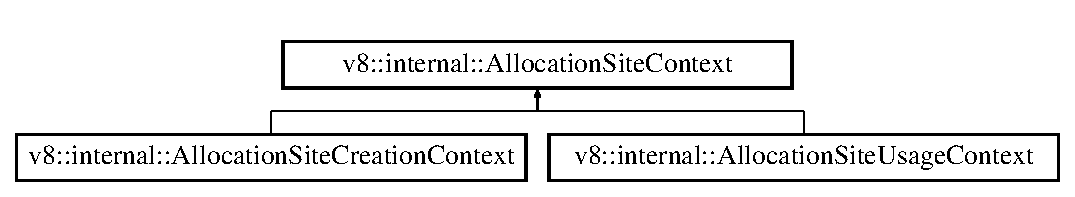
\includegraphics[height=2.000000cm]{classv8_1_1internal_1_1_allocation_site_context}
\end{center}
\end{figure}
\subsection*{Public Member Functions}
\begin{DoxyCompactItemize}
\item 
{\bfseries Allocation\+Site\+Context} (\hyperlink{classv8_1_1internal_1_1_isolate}{Isolate} $\ast$isolate)\hypertarget{classv8_1_1internal_1_1_allocation_site_context_acad3aa6b62e34d542b6fd6c9b87e2093}{}\label{classv8_1_1internal_1_1_allocation_site_context_acad3aa6b62e34d542b6fd6c9b87e2093}

\item 
\hyperlink{classv8_1_1internal_1_1_handle}{Handle}$<$ \hyperlink{classv8_1_1internal_1_1_allocation_site}{Allocation\+Site} $>$ {\bfseries top} ()\hypertarget{classv8_1_1internal_1_1_allocation_site_context_a76427a09d8c0eef6794ecfd804ca8eea}{}\label{classv8_1_1internal_1_1_allocation_site_context_a76427a09d8c0eef6794ecfd804ca8eea}

\item 
\hyperlink{classv8_1_1internal_1_1_handle}{Handle}$<$ \hyperlink{classv8_1_1internal_1_1_allocation_site}{Allocation\+Site} $>$ {\bfseries current} ()\hypertarget{classv8_1_1internal_1_1_allocation_site_context_a20943342b9c850bc0f1c3fd0aef56e9a}{}\label{classv8_1_1internal_1_1_allocation_site_context_a20943342b9c850bc0f1c3fd0aef56e9a}

\item 
bool {\bfseries Should\+Create\+Memento} (\hyperlink{classv8_1_1internal_1_1_handle}{Handle}$<$ \hyperlink{classv8_1_1internal_1_1_j_s_object}{J\+S\+Object} $>$ object)\hypertarget{classv8_1_1internal_1_1_allocation_site_context_adfa2a2817414d94fd00728a2c163d7b0}{}\label{classv8_1_1internal_1_1_allocation_site_context_adfa2a2817414d94fd00728a2c163d7b0}

\item 
\hyperlink{classv8_1_1internal_1_1_isolate}{Isolate} $\ast$ {\bfseries isolate} ()\hypertarget{classv8_1_1internal_1_1_allocation_site_context_a8adcb0b60cf5fbda807b0a11c128ab4a}{}\label{classv8_1_1internal_1_1_allocation_site_context_a8adcb0b60cf5fbda807b0a11c128ab4a}

\end{DoxyCompactItemize}
\subsection*{Protected Member Functions}
\begin{DoxyCompactItemize}
\item 
void {\bfseries update\+\_\+current\+\_\+site} (\hyperlink{classv8_1_1internal_1_1_allocation_site}{Allocation\+Site} $\ast$site)\hypertarget{classv8_1_1internal_1_1_allocation_site_context_a2e094902dbadc8931c82eb04333807c0}{}\label{classv8_1_1internal_1_1_allocation_site_context_a2e094902dbadc8931c82eb04333807c0}

\item 
void {\bfseries Initialize\+Traversal} (\hyperlink{classv8_1_1internal_1_1_handle}{Handle}$<$ \hyperlink{classv8_1_1internal_1_1_allocation_site}{Allocation\+Site} $>$ site)\hypertarget{classv8_1_1internal_1_1_allocation_site_context_a2ae0994fc850605cbea75aeddf980b44}{}\label{classv8_1_1internal_1_1_allocation_site_context_a2ae0994fc850605cbea75aeddf980b44}

\end{DoxyCompactItemize}
\subsection*{Private Attributes}
\begin{DoxyCompactItemize}
\item 
\hyperlink{classv8_1_1internal_1_1_isolate}{Isolate} $\ast$ {\bfseries isolate\+\_\+}\hypertarget{classv8_1_1internal_1_1_allocation_site_context_a774ff272d33c5c3c423cba36caa8a66b}{}\label{classv8_1_1internal_1_1_allocation_site_context_a774ff272d33c5c3c423cba36caa8a66b}

\item 
\hyperlink{classv8_1_1internal_1_1_handle}{Handle}$<$ \hyperlink{classv8_1_1internal_1_1_allocation_site}{Allocation\+Site} $>$ {\bfseries top\+\_\+}\hypertarget{classv8_1_1internal_1_1_allocation_site_context_a17471d31386627bbb4fdc62058bddd5e}{}\label{classv8_1_1internal_1_1_allocation_site_context_a17471d31386627bbb4fdc62058bddd5e}

\item 
\hyperlink{classv8_1_1internal_1_1_handle}{Handle}$<$ \hyperlink{classv8_1_1internal_1_1_allocation_site}{Allocation\+Site} $>$ {\bfseries current\+\_\+}\hypertarget{classv8_1_1internal_1_1_allocation_site_context_a9c419688f56549c620c1d35e77d596e2}{}\label{classv8_1_1internal_1_1_allocation_site_context_a9c419688f56549c620c1d35e77d596e2}

\end{DoxyCompactItemize}


The documentation for this class was generated from the following file\+:\begin{DoxyCompactItemize}
\item 
/\+Users/joshgav/node/v8/src/allocation-\/site-\/scopes.\+h\end{DoxyCompactItemize}

\hypertarget{classv8_1_1internal_1_1_allocation_site_creation_context}{}\section{v8\+:\+:internal\+:\+:Allocation\+Site\+Creation\+Context Class Reference}
\label{classv8_1_1internal_1_1_allocation_site_creation_context}\index{v8\+::internal\+::\+Allocation\+Site\+Creation\+Context@{v8\+::internal\+::\+Allocation\+Site\+Creation\+Context}}
Inheritance diagram for v8\+:\+:internal\+:\+:Allocation\+Site\+Creation\+Context\+:\begin{figure}[H]
\begin{center}
\leavevmode
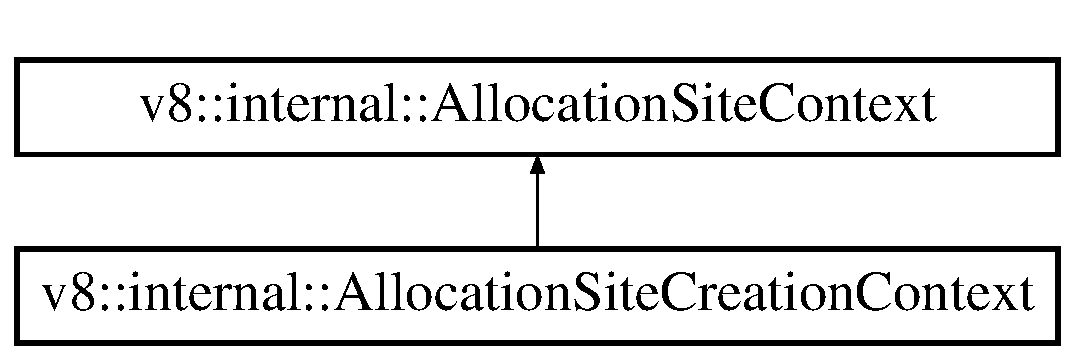
\includegraphics[height=2.000000cm]{classv8_1_1internal_1_1_allocation_site_creation_context}
\end{center}
\end{figure}
\subsection*{Public Member Functions}
\begin{DoxyCompactItemize}
\item 
{\bfseries Allocation\+Site\+Creation\+Context} (\hyperlink{classv8_1_1internal_1_1_isolate}{Isolate} $\ast$isolate)\hypertarget{classv8_1_1internal_1_1_allocation_site_creation_context_a159a45da25ad238b0b67ec380121780e}{}\label{classv8_1_1internal_1_1_allocation_site_creation_context_a159a45da25ad238b0b67ec380121780e}

\item 
\hyperlink{classv8_1_1internal_1_1_handle}{Handle}$<$ \hyperlink{classv8_1_1internal_1_1_allocation_site}{Allocation\+Site} $>$ {\bfseries Enter\+New\+Scope} ()\hypertarget{classv8_1_1internal_1_1_allocation_site_creation_context_ac01c9bd1361ef78f22c301bdfdcb2076}{}\label{classv8_1_1internal_1_1_allocation_site_creation_context_ac01c9bd1361ef78f22c301bdfdcb2076}

\item 
void {\bfseries Exit\+Scope} (\hyperlink{classv8_1_1internal_1_1_handle}{Handle}$<$ \hyperlink{classv8_1_1internal_1_1_allocation_site}{Allocation\+Site} $>$ site, \hyperlink{classv8_1_1internal_1_1_handle}{Handle}$<$ \hyperlink{classv8_1_1internal_1_1_j_s_object}{J\+S\+Object} $>$ object)\hypertarget{classv8_1_1internal_1_1_allocation_site_creation_context_a42deb3f83fd733f54d1a0c32a74f2f46}{}\label{classv8_1_1internal_1_1_allocation_site_creation_context_a42deb3f83fd733f54d1a0c32a74f2f46}

\end{DoxyCompactItemize}
\subsection*{Additional Inherited Members}


The documentation for this class was generated from the following files\+:\begin{DoxyCompactItemize}
\item 
/\+Users/joshgav/node/v8/src/allocation-\/site-\/scopes.\+h\item 
/\+Users/joshgav/node/v8/src/allocation-\/site-\/scopes.\+cc\end{DoxyCompactItemize}

\hypertarget{classv8_1_1internal_1_1_fast_clone_shallow_array_stub_1_1_allocation_site_mode_bits}{}\section{v8\+:\+:internal\+:\+:Fast\+Clone\+Shallow\+Array\+Stub\+:\+:Allocation\+Site\+Mode\+Bits Class Reference}
\label{classv8_1_1internal_1_1_fast_clone_shallow_array_stub_1_1_allocation_site_mode_bits}\index{v8\+::internal\+::\+Fast\+Clone\+Shallow\+Array\+Stub\+::\+Allocation\+Site\+Mode\+Bits@{v8\+::internal\+::\+Fast\+Clone\+Shallow\+Array\+Stub\+::\+Allocation\+Site\+Mode\+Bits}}
Inheritance diagram for v8\+:\+:internal\+:\+:Fast\+Clone\+Shallow\+Array\+Stub\+:\+:Allocation\+Site\+Mode\+Bits\+:\begin{figure}[H]
\begin{center}
\leavevmode
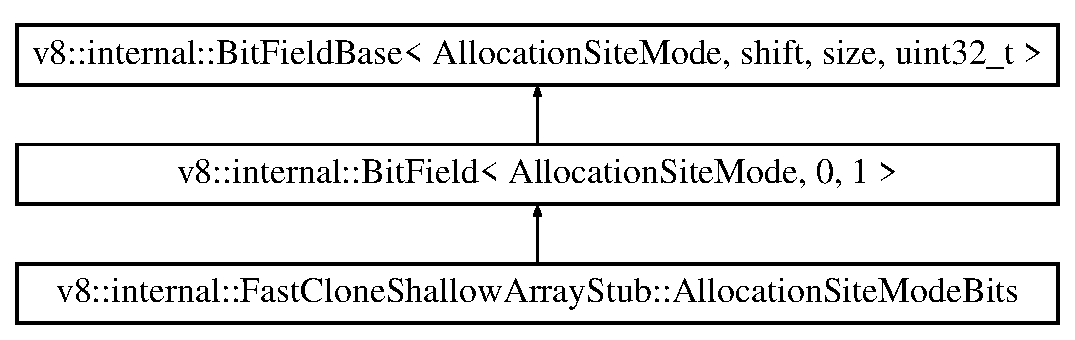
\includegraphics[height=3.000000cm]{classv8_1_1internal_1_1_fast_clone_shallow_array_stub_1_1_allocation_site_mode_bits}
\end{center}
\end{figure}
\subsection*{Additional Inherited Members}


The documentation for this class was generated from the following file\+:\begin{DoxyCompactItemize}
\item 
/\+Users/joshgav/node/v8/src/code-\/stubs.\+h\end{DoxyCompactItemize}

\hypertarget{classv8_1_1internal_1_1_array_constructor_stub_base_1_1_allocation_site_override_mode_bits}{}\section{v8\+:\+:internal\+:\+:Array\+Constructor\+Stub\+Base\+:\+:Allocation\+Site\+Override\+Mode\+Bits Class Reference}
\label{classv8_1_1internal_1_1_array_constructor_stub_base_1_1_allocation_site_override_mode_bits}\index{v8\+::internal\+::\+Array\+Constructor\+Stub\+Base\+::\+Allocation\+Site\+Override\+Mode\+Bits@{v8\+::internal\+::\+Array\+Constructor\+Stub\+Base\+::\+Allocation\+Site\+Override\+Mode\+Bits}}
Inheritance diagram for v8\+:\+:internal\+:\+:Array\+Constructor\+Stub\+Base\+:\+:Allocation\+Site\+Override\+Mode\+Bits\+:\begin{figure}[H]
\begin{center}
\leavevmode
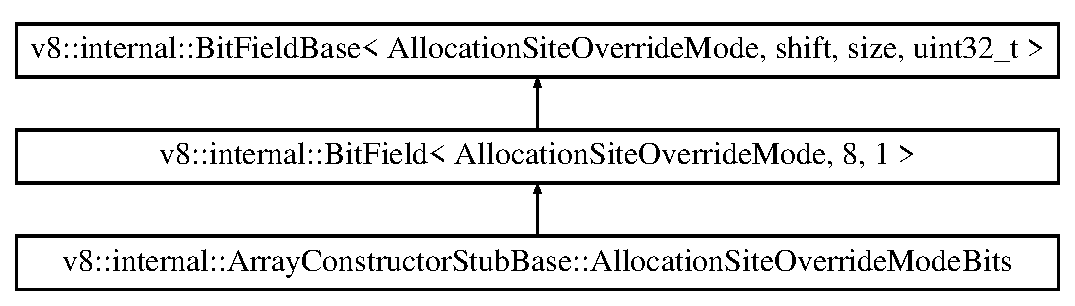
\includegraphics[height=3.000000cm]{classv8_1_1internal_1_1_array_constructor_stub_base_1_1_allocation_site_override_mode_bits}
\end{center}
\end{figure}
\subsection*{Additional Inherited Members}


The documentation for this class was generated from the following file\+:\begin{DoxyCompactItemize}
\item 
/\+Users/joshgav/node/v8/src/code-\/stubs.\+h\end{DoxyCompactItemize}

\hypertarget{classv8_1_1internal_1_1_common_array_constructor_stub_1_1_allocation_site_override_mode_bits}{}\section{v8\+:\+:internal\+:\+:Common\+Array\+Constructor\+Stub\+:\+:Allocation\+Site\+Override\+Mode\+Bits Class Reference}
\label{classv8_1_1internal_1_1_common_array_constructor_stub_1_1_allocation_site_override_mode_bits}\index{v8\+::internal\+::\+Common\+Array\+Constructor\+Stub\+::\+Allocation\+Site\+Override\+Mode\+Bits@{v8\+::internal\+::\+Common\+Array\+Constructor\+Stub\+::\+Allocation\+Site\+Override\+Mode\+Bits}}
Inheritance diagram for v8\+:\+:internal\+:\+:Common\+Array\+Constructor\+Stub\+:\+:Allocation\+Site\+Override\+Mode\+Bits\+:\begin{figure}[H]
\begin{center}
\leavevmode
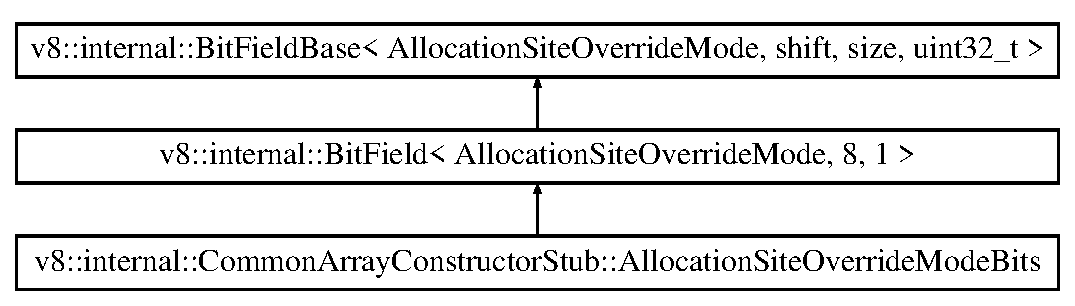
\includegraphics[height=3.000000cm]{classv8_1_1internal_1_1_common_array_constructor_stub_1_1_allocation_site_override_mode_bits}
\end{center}
\end{figure}
\subsection*{Additional Inherited Members}


The documentation for this class was generated from the following file\+:\begin{DoxyCompactItemize}
\item 
/\+Users/joshgav/node/v8/src/code-\/stubs.\+h\end{DoxyCompactItemize}

\hypertarget{classv8_1_1internal_1_1_allocation_site_usage_context}{}\section{v8\+:\+:internal\+:\+:Allocation\+Site\+Usage\+Context Class Reference}
\label{classv8_1_1internal_1_1_allocation_site_usage_context}\index{v8\+::internal\+::\+Allocation\+Site\+Usage\+Context@{v8\+::internal\+::\+Allocation\+Site\+Usage\+Context}}
Inheritance diagram for v8\+:\+:internal\+:\+:Allocation\+Site\+Usage\+Context\+:\begin{figure}[H]
\begin{center}
\leavevmode
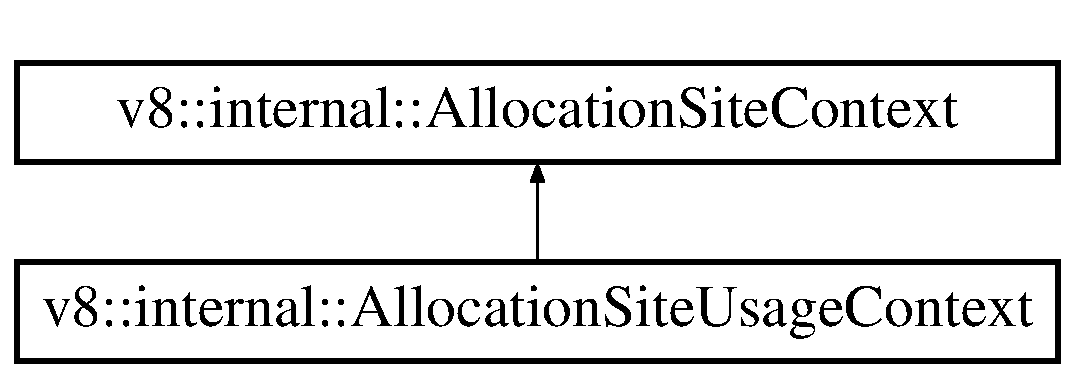
\includegraphics[height=2.000000cm]{classv8_1_1internal_1_1_allocation_site_usage_context}
\end{center}
\end{figure}
\subsection*{Public Member Functions}
\begin{DoxyCompactItemize}
\item 
{\bfseries Allocation\+Site\+Usage\+Context} (\hyperlink{classv8_1_1internal_1_1_isolate}{Isolate} $\ast$isolate, \hyperlink{classv8_1_1internal_1_1_handle}{Handle}$<$ \hyperlink{classv8_1_1internal_1_1_allocation_site}{Allocation\+Site} $>$ site, bool activated)\hypertarget{classv8_1_1internal_1_1_allocation_site_usage_context_aa9b5b62dbc43c89fbb14b22f32d3f68e}{}\label{classv8_1_1internal_1_1_allocation_site_usage_context_aa9b5b62dbc43c89fbb14b22f32d3f68e}

\item 
\hyperlink{classv8_1_1internal_1_1_handle}{Handle}$<$ \hyperlink{classv8_1_1internal_1_1_allocation_site}{Allocation\+Site} $>$ {\bfseries Enter\+New\+Scope} ()\hypertarget{classv8_1_1internal_1_1_allocation_site_usage_context_a7155f90f38a179371cbd03d42d3311a4}{}\label{classv8_1_1internal_1_1_allocation_site_usage_context_a7155f90f38a179371cbd03d42d3311a4}

\item 
void {\bfseries Exit\+Scope} (\hyperlink{classv8_1_1internal_1_1_handle}{Handle}$<$ \hyperlink{classv8_1_1internal_1_1_allocation_site}{Allocation\+Site} $>$ scope\+\_\+site, \hyperlink{classv8_1_1internal_1_1_handle}{Handle}$<$ \hyperlink{classv8_1_1internal_1_1_j_s_object}{J\+S\+Object} $>$ object)\hypertarget{classv8_1_1internal_1_1_allocation_site_usage_context_a27c29c9de5fb9a5afdc56a262b7d095d}{}\label{classv8_1_1internal_1_1_allocation_site_usage_context_a27c29c9de5fb9a5afdc56a262b7d095d}

\item 
bool {\bfseries Should\+Create\+Memento} (\hyperlink{classv8_1_1internal_1_1_handle}{Handle}$<$ \hyperlink{classv8_1_1internal_1_1_j_s_object}{J\+S\+Object} $>$ object)\hypertarget{classv8_1_1internal_1_1_allocation_site_usage_context_a9b8b4f20046612a1dc28823efe000043}{}\label{classv8_1_1internal_1_1_allocation_site_usage_context_a9b8b4f20046612a1dc28823efe000043}

\end{DoxyCompactItemize}
\subsection*{Private Attributes}
\begin{DoxyCompactItemize}
\item 
\hyperlink{classv8_1_1internal_1_1_handle}{Handle}$<$ \hyperlink{classv8_1_1internal_1_1_allocation_site}{Allocation\+Site} $>$ {\bfseries top\+\_\+site\+\_\+}\hypertarget{classv8_1_1internal_1_1_allocation_site_usage_context_a2ac61f80b107f7fb8bb16366d27c4a99}{}\label{classv8_1_1internal_1_1_allocation_site_usage_context_a2ac61f80b107f7fb8bb16366d27c4a99}

\item 
bool {\bfseries activated\+\_\+}\hypertarget{classv8_1_1internal_1_1_allocation_site_usage_context_af145939858ec956498e774717642cc26}{}\label{classv8_1_1internal_1_1_allocation_site_usage_context_af145939858ec956498e774717642cc26}

\end{DoxyCompactItemize}
\subsection*{Additional Inherited Members}


The documentation for this class was generated from the following files\+:\begin{DoxyCompactItemize}
\item 
/\+Users/joshgav/node/v8/src/allocation-\/site-\/scopes.\+h\item 
/\+Users/joshgav/node/v8/src/allocation-\/site-\/scopes.\+cc\end{DoxyCompactItemize}

\hypertarget{classv8_1_1internal_1_1_allocation_trace_node}{}\section{v8\+:\+:internal\+:\+:Allocation\+Trace\+Node Class Reference}
\label{classv8_1_1internal_1_1_allocation_trace_node}\index{v8\+::internal\+::\+Allocation\+Trace\+Node@{v8\+::internal\+::\+Allocation\+Trace\+Node}}
\subsection*{Public Member Functions}
\begin{DoxyCompactItemize}
\item 
{\bfseries Allocation\+Trace\+Node} (\hyperlink{classv8_1_1internal_1_1_allocation_trace_tree}{Allocation\+Trace\+Tree} $\ast$tree, unsigned function\+\_\+info\+\_\+index)\hypertarget{classv8_1_1internal_1_1_allocation_trace_node_aca8caa93d6a5309e2fc2529b71a5a70a}{}\label{classv8_1_1internal_1_1_allocation_trace_node_aca8caa93d6a5309e2fc2529b71a5a70a}

\item 
\hyperlink{classv8_1_1internal_1_1_allocation_trace_node}{Allocation\+Trace\+Node} $\ast$ {\bfseries Find\+Child} (unsigned function\+\_\+info\+\_\+index)\hypertarget{classv8_1_1internal_1_1_allocation_trace_node_afbb942277677c19a257ff8781f034c1d}{}\label{classv8_1_1internal_1_1_allocation_trace_node_afbb942277677c19a257ff8781f034c1d}

\item 
\hyperlink{classv8_1_1internal_1_1_allocation_trace_node}{Allocation\+Trace\+Node} $\ast$ {\bfseries Find\+Or\+Add\+Child} (unsigned function\+\_\+info\+\_\+index)\hypertarget{classv8_1_1internal_1_1_allocation_trace_node_a780262d490b639c1782e3a7212297709}{}\label{classv8_1_1internal_1_1_allocation_trace_node_a780262d490b639c1782e3a7212297709}

\item 
void {\bfseries Add\+Allocation} (unsigned size)\hypertarget{classv8_1_1internal_1_1_allocation_trace_node_ab3952f0610968cabfdb6a6134395f4a8}{}\label{classv8_1_1internal_1_1_allocation_trace_node_ab3952f0610968cabfdb6a6134395f4a8}

\item 
unsigned {\bfseries function\+\_\+info\+\_\+index} () const \hypertarget{classv8_1_1internal_1_1_allocation_trace_node_a7615a9d517ad2c292ef197fa5178afef}{}\label{classv8_1_1internal_1_1_allocation_trace_node_a7615a9d517ad2c292ef197fa5178afef}

\item 
unsigned {\bfseries allocation\+\_\+size} () const \hypertarget{classv8_1_1internal_1_1_allocation_trace_node_aaecc079598de291e9411b0b1143338bb}{}\label{classv8_1_1internal_1_1_allocation_trace_node_aaecc079598de291e9411b0b1143338bb}

\item 
unsigned {\bfseries allocation\+\_\+count} () const \hypertarget{classv8_1_1internal_1_1_allocation_trace_node_a2a31df2800608396686f67576477c648}{}\label{classv8_1_1internal_1_1_allocation_trace_node_a2a31df2800608396686f67576477c648}

\item 
unsigned {\bfseries id} () const \hypertarget{classv8_1_1internal_1_1_allocation_trace_node_a9f11563e9cbd3d46a0bd9eee2d8e0f3c}{}\label{classv8_1_1internal_1_1_allocation_trace_node_a9f11563e9cbd3d46a0bd9eee2d8e0f3c}

\item 
\hyperlink{classv8_1_1internal_1_1_vector}{Vector}$<$ \hyperlink{classv8_1_1internal_1_1_allocation_trace_node}{Allocation\+Trace\+Node} $\ast$ $>$ {\bfseries children} () const \hypertarget{classv8_1_1internal_1_1_allocation_trace_node_a81a9b60b273378fff6eee02960e44bea}{}\label{classv8_1_1internal_1_1_allocation_trace_node_a81a9b60b273378fff6eee02960e44bea}

\item 
void {\bfseries Print} (int indent, \hyperlink{classv8_1_1internal_1_1_allocation_tracker}{Allocation\+Tracker} $\ast$tracker)\hypertarget{classv8_1_1internal_1_1_allocation_trace_node_acfba1229f80910c5746758f8afdff7af}{}\label{classv8_1_1internal_1_1_allocation_trace_node_acfba1229f80910c5746758f8afdff7af}

\end{DoxyCompactItemize}
\subsection*{Private Member Functions}
\begin{DoxyCompactItemize}
\item 
{\bfseries D\+I\+S\+A\+L\+L\+O\+W\+\_\+\+C\+O\+P\+Y\+\_\+\+A\+N\+D\+\_\+\+A\+S\+S\+I\+GN} (\hyperlink{classv8_1_1internal_1_1_allocation_trace_node}{Allocation\+Trace\+Node})\hypertarget{classv8_1_1internal_1_1_allocation_trace_node_a41b0dffe34b9d338d359a5a60d53f6a7}{}\label{classv8_1_1internal_1_1_allocation_trace_node_a41b0dffe34b9d338d359a5a60d53f6a7}

\end{DoxyCompactItemize}
\subsection*{Private Attributes}
\begin{DoxyCompactItemize}
\item 
\hyperlink{classv8_1_1internal_1_1_allocation_trace_tree}{Allocation\+Trace\+Tree} $\ast$ {\bfseries tree\+\_\+}\hypertarget{classv8_1_1internal_1_1_allocation_trace_node_a1e3fa25a87aaa44042b54073123edc7b}{}\label{classv8_1_1internal_1_1_allocation_trace_node_a1e3fa25a87aaa44042b54073123edc7b}

\item 
unsigned {\bfseries function\+\_\+info\+\_\+index\+\_\+}\hypertarget{classv8_1_1internal_1_1_allocation_trace_node_a70d789a2c7edffb1f96b0d9d539e6210}{}\label{classv8_1_1internal_1_1_allocation_trace_node_a70d789a2c7edffb1f96b0d9d539e6210}

\item 
unsigned {\bfseries total\+\_\+size\+\_\+}\hypertarget{classv8_1_1internal_1_1_allocation_trace_node_a25c93ade36d5ce7dd45eb65dee6c168f}{}\label{classv8_1_1internal_1_1_allocation_trace_node_a25c93ade36d5ce7dd45eb65dee6c168f}

\item 
unsigned {\bfseries allocation\+\_\+count\+\_\+}\hypertarget{classv8_1_1internal_1_1_allocation_trace_node_ab5762ad1769ff5844cb73e544a78dcd3}{}\label{classv8_1_1internal_1_1_allocation_trace_node_ab5762ad1769ff5844cb73e544a78dcd3}

\item 
unsigned {\bfseries id\+\_\+}\hypertarget{classv8_1_1internal_1_1_allocation_trace_node_a188a73ce1d741181cf90866f5f095e65}{}\label{classv8_1_1internal_1_1_allocation_trace_node_a188a73ce1d741181cf90866f5f095e65}

\item 
\hyperlink{classv8_1_1internal_1_1_list}{List}$<$ \hyperlink{classv8_1_1internal_1_1_allocation_trace_node}{Allocation\+Trace\+Node} $\ast$ $>$ {\bfseries children\+\_\+}\hypertarget{classv8_1_1internal_1_1_allocation_trace_node_af2a1f30b035e6d6e61260957c862cda1}{}\label{classv8_1_1internal_1_1_allocation_trace_node_af2a1f30b035e6d6e61260957c862cda1}

\end{DoxyCompactItemize}


The documentation for this class was generated from the following files\+:\begin{DoxyCompactItemize}
\item 
/\+Users/joshgav/node/v8/src/profiler/allocation-\/tracker.\+h\item 
/\+Users/joshgav/node/v8/src/profiler/allocation-\/tracker.\+cc\end{DoxyCompactItemize}

\hypertarget{classv8_1_1internal_1_1_allocation_trace_tree}{}\section{v8\+:\+:internal\+:\+:Allocation\+Trace\+Tree Class Reference}
\label{classv8_1_1internal_1_1_allocation_trace_tree}\index{v8\+::internal\+::\+Allocation\+Trace\+Tree@{v8\+::internal\+::\+Allocation\+Trace\+Tree}}
\subsection*{Public Member Functions}
\begin{DoxyCompactItemize}
\item 
\hyperlink{classv8_1_1internal_1_1_allocation_trace_node}{Allocation\+Trace\+Node} $\ast$ {\bfseries Add\+Path\+From\+End} (const \hyperlink{classv8_1_1internal_1_1_vector}{Vector}$<$ unsigned $>$ \&path)\hypertarget{classv8_1_1internal_1_1_allocation_trace_tree_ac5d8e76d5c1250e5a0c0453d79fc656e}{}\label{classv8_1_1internal_1_1_allocation_trace_tree_ac5d8e76d5c1250e5a0c0453d79fc656e}

\item 
\hyperlink{classv8_1_1internal_1_1_allocation_trace_node}{Allocation\+Trace\+Node} $\ast$ {\bfseries root} ()\hypertarget{classv8_1_1internal_1_1_allocation_trace_tree_af36cd4ae9797ba6e8681349f3db7d0b0}{}\label{classv8_1_1internal_1_1_allocation_trace_tree_af36cd4ae9797ba6e8681349f3db7d0b0}

\item 
unsigned {\bfseries next\+\_\+node\+\_\+id} ()\hypertarget{classv8_1_1internal_1_1_allocation_trace_tree_aed92bbd12c4ca3ea8dfabf9f3ce16d9e}{}\label{classv8_1_1internal_1_1_allocation_trace_tree_aed92bbd12c4ca3ea8dfabf9f3ce16d9e}

\item 
void {\bfseries Print} (\hyperlink{classv8_1_1internal_1_1_allocation_tracker}{Allocation\+Tracker} $\ast$tracker)\hypertarget{classv8_1_1internal_1_1_allocation_trace_tree_a37ac3b1e978232c6150a1d3edf4da9ce}{}\label{classv8_1_1internal_1_1_allocation_trace_tree_a37ac3b1e978232c6150a1d3edf4da9ce}

\end{DoxyCompactItemize}
\subsection*{Private Member Functions}
\begin{DoxyCompactItemize}
\item 
{\bfseries D\+I\+S\+A\+L\+L\+O\+W\+\_\+\+C\+O\+P\+Y\+\_\+\+A\+N\+D\+\_\+\+A\+S\+S\+I\+GN} (\hyperlink{classv8_1_1internal_1_1_allocation_trace_tree}{Allocation\+Trace\+Tree})\hypertarget{classv8_1_1internal_1_1_allocation_trace_tree_abf63511271337fe2fe331a321e053fba}{}\label{classv8_1_1internal_1_1_allocation_trace_tree_abf63511271337fe2fe331a321e053fba}

\end{DoxyCompactItemize}
\subsection*{Private Attributes}
\begin{DoxyCompactItemize}
\item 
unsigned {\bfseries next\+\_\+node\+\_\+id\+\_\+}\hypertarget{classv8_1_1internal_1_1_allocation_trace_tree_ae9d3215ae36599a252b482a526a19cae}{}\label{classv8_1_1internal_1_1_allocation_trace_tree_ae9d3215ae36599a252b482a526a19cae}

\item 
\hyperlink{classv8_1_1internal_1_1_allocation_trace_node}{Allocation\+Trace\+Node} {\bfseries root\+\_\+}\hypertarget{classv8_1_1internal_1_1_allocation_trace_tree_a4a53c39a0297e768c5725c8e1c63503d}{}\label{classv8_1_1internal_1_1_allocation_trace_tree_a4a53c39a0297e768c5725c8e1c63503d}

\end{DoxyCompactItemize}


The documentation for this class was generated from the following files\+:\begin{DoxyCompactItemize}
\item 
/\+Users/joshgav/node/v8/src/profiler/allocation-\/tracker.\+h\item 
/\+Users/joshgav/node/v8/src/profiler/allocation-\/tracker.\+cc\end{DoxyCompactItemize}

\hypertarget{classv8_1_1internal_1_1_allocation_tracker}{}\section{v8\+:\+:internal\+:\+:Allocation\+Tracker Class Reference}
\label{classv8_1_1internal_1_1_allocation_tracker}\index{v8\+::internal\+::\+Allocation\+Tracker@{v8\+::internal\+::\+Allocation\+Tracker}}
\subsection*{Classes}
\begin{DoxyCompactItemize}
\item 
struct \hyperlink{structv8_1_1internal_1_1_allocation_tracker_1_1_function_info}{Function\+Info}
\item 
class \hyperlink{classv8_1_1internal_1_1_allocation_tracker_1_1_unresolved_location}{Unresolved\+Location}
\end{DoxyCompactItemize}
\subsection*{Public Member Functions}
\begin{DoxyCompactItemize}
\item 
{\bfseries Allocation\+Tracker} (\hyperlink{classv8_1_1internal_1_1_heap_objects_map}{Heap\+Objects\+Map} $\ast$ids, \hyperlink{classv8_1_1internal_1_1_strings_storage}{Strings\+Storage} $\ast$names)\hypertarget{classv8_1_1internal_1_1_allocation_tracker_ae705bae00ff323c41efc0b1d50afc62c}{}\label{classv8_1_1internal_1_1_allocation_tracker_ae705bae00ff323c41efc0b1d50afc62c}

\item 
void {\bfseries Prepare\+For\+Serialization} ()\hypertarget{classv8_1_1internal_1_1_allocation_tracker_a06984664822efec67f15cfc200f9c1c8}{}\label{classv8_1_1internal_1_1_allocation_tracker_a06984664822efec67f15cfc200f9c1c8}

\item 
void {\bfseries Allocation\+Event} (Address addr, int size)\hypertarget{classv8_1_1internal_1_1_allocation_tracker_af59e0f4c414b6fe00ff0729e616ae219}{}\label{classv8_1_1internal_1_1_allocation_tracker_af59e0f4c414b6fe00ff0729e616ae219}

\item 
\hyperlink{classv8_1_1internal_1_1_allocation_trace_tree}{Allocation\+Trace\+Tree} $\ast$ {\bfseries trace\+\_\+tree} ()\hypertarget{classv8_1_1internal_1_1_allocation_tracker_aa0471186f074acec90232839b6e22431}{}\label{classv8_1_1internal_1_1_allocation_tracker_aa0471186f074acec90232839b6e22431}

\item 
const \hyperlink{classv8_1_1internal_1_1_list}{List}$<$ \hyperlink{structv8_1_1internal_1_1_allocation_tracker_1_1_function_info}{Function\+Info} $\ast$ $>$ \& {\bfseries function\+\_\+info\+\_\+list} () const \hypertarget{classv8_1_1internal_1_1_allocation_tracker_a25d10af2d1bde8601599623c34754b2e}{}\label{classv8_1_1internal_1_1_allocation_tracker_a25d10af2d1bde8601599623c34754b2e}

\item 
\hyperlink{classv8_1_1internal_1_1_address_to_trace_map}{Address\+To\+Trace\+Map} $\ast$ {\bfseries address\+\_\+to\+\_\+trace} ()\hypertarget{classv8_1_1internal_1_1_allocation_tracker_adacf25ec6310501fb4d9ae02c1737621}{}\label{classv8_1_1internal_1_1_allocation_tracker_adacf25ec6310501fb4d9ae02c1737621}

\end{DoxyCompactItemize}
\subsection*{Private Member Functions}
\begin{DoxyCompactItemize}
\item 
unsigned {\bfseries Add\+Function\+Info} (\hyperlink{classv8_1_1internal_1_1_shared_function_info}{Shared\+Function\+Info} $\ast$info, Snapshot\+Object\+Id id)\hypertarget{classv8_1_1internal_1_1_allocation_tracker_a230cbe58c384c06817de9b1a15c7cb09}{}\label{classv8_1_1internal_1_1_allocation_tracker_a230cbe58c384c06817de9b1a15c7cb09}

\item 
unsigned {\bfseries function\+Info\+Index\+For\+V\+M\+State} (State\+Tag state)\hypertarget{classv8_1_1internal_1_1_allocation_tracker_a45e9bdead8b15ff607262ae84127b038}{}\label{classv8_1_1internal_1_1_allocation_tracker_a45e9bdead8b15ff607262ae84127b038}

\item 
{\bfseries D\+I\+S\+A\+L\+L\+O\+W\+\_\+\+C\+O\+P\+Y\+\_\+\+A\+N\+D\+\_\+\+A\+S\+S\+I\+GN} (\hyperlink{classv8_1_1internal_1_1_allocation_tracker}{Allocation\+Tracker})\hypertarget{classv8_1_1internal_1_1_allocation_tracker_a0164c24c32589a2e09f645f410fea381}{}\label{classv8_1_1internal_1_1_allocation_tracker_a0164c24c32589a2e09f645f410fea381}

\end{DoxyCompactItemize}
\subsection*{Static Private Member Functions}
\begin{DoxyCompactItemize}
\item 
static void {\bfseries Delete\+Function\+Info} (\hyperlink{structv8_1_1internal_1_1_allocation_tracker_1_1_function_info}{Function\+Info} $\ast$$\ast$info)\hypertarget{classv8_1_1internal_1_1_allocation_tracker_aa8c6d9f918ab4f4fac36215599c71faa}{}\label{classv8_1_1internal_1_1_allocation_tracker_aa8c6d9f918ab4f4fac36215599c71faa}

\item 
static void {\bfseries Delete\+Unresolved\+Location} (\hyperlink{classv8_1_1internal_1_1_allocation_tracker_1_1_unresolved_location}{Unresolved\+Location} $\ast$$\ast$location)\hypertarget{classv8_1_1internal_1_1_allocation_tracker_af0643d03e87ccb06ea0d2d2eee79b8a3}{}\label{classv8_1_1internal_1_1_allocation_tracker_af0643d03e87ccb06ea0d2d2eee79b8a3}

\end{DoxyCompactItemize}
\subsection*{Private Attributes}
\begin{DoxyCompactItemize}
\item 
\hyperlink{classv8_1_1internal_1_1_heap_objects_map}{Heap\+Objects\+Map} $\ast$ {\bfseries ids\+\_\+}\hypertarget{classv8_1_1internal_1_1_allocation_tracker_a09898522d9f5a3ddb83ac341da54c775}{}\label{classv8_1_1internal_1_1_allocation_tracker_a09898522d9f5a3ddb83ac341da54c775}

\item 
\hyperlink{classv8_1_1internal_1_1_strings_storage}{Strings\+Storage} $\ast$ {\bfseries names\+\_\+}\hypertarget{classv8_1_1internal_1_1_allocation_tracker_a4ff70d57e19c616436e54ffc1856ced7}{}\label{classv8_1_1internal_1_1_allocation_tracker_a4ff70d57e19c616436e54ffc1856ced7}

\item 
\hyperlink{classv8_1_1internal_1_1_allocation_trace_tree}{Allocation\+Trace\+Tree} {\bfseries trace\+\_\+tree\+\_\+}\hypertarget{classv8_1_1internal_1_1_allocation_tracker_a870259fdd00406cd018dd6f122b30962}{}\label{classv8_1_1internal_1_1_allocation_tracker_a870259fdd00406cd018dd6f122b30962}

\item 
unsigned {\bfseries allocation\+\_\+trace\+\_\+buffer\+\_\+} \mbox{[}k\+Max\+Allocation\+Trace\+Length\mbox{]}\hypertarget{classv8_1_1internal_1_1_allocation_tracker_a4f124d5e95ed5b432c35c208db680577}{}\label{classv8_1_1internal_1_1_allocation_tracker_a4f124d5e95ed5b432c35c208db680577}

\item 
\hyperlink{classv8_1_1internal_1_1_list}{List}$<$ \hyperlink{structv8_1_1internal_1_1_allocation_tracker_1_1_function_info}{Function\+Info} $\ast$ $>$ {\bfseries function\+\_\+info\+\_\+list\+\_\+}\hypertarget{classv8_1_1internal_1_1_allocation_tracker_ae5b86f333eccf1561c5f650bf50b23a9}{}\label{classv8_1_1internal_1_1_allocation_tracker_ae5b86f333eccf1561c5f650bf50b23a9}

\item 
\hyperlink{classv8_1_1internal_1_1_template_hash_map_impl}{Hash\+Map} {\bfseries id\+\_\+to\+\_\+function\+\_\+info\+\_\+index\+\_\+}\hypertarget{classv8_1_1internal_1_1_allocation_tracker_a462cfcfd917d60b928758f0bafd83792}{}\label{classv8_1_1internal_1_1_allocation_tracker_a462cfcfd917d60b928758f0bafd83792}

\item 
\hyperlink{classv8_1_1internal_1_1_list}{List}$<$ \hyperlink{classv8_1_1internal_1_1_allocation_tracker_1_1_unresolved_location}{Unresolved\+Location} $\ast$ $>$ {\bfseries unresolved\+\_\+locations\+\_\+}\hypertarget{classv8_1_1internal_1_1_allocation_tracker_aa3e21b01c4eb5ac83edb180ef9e269bb}{}\label{classv8_1_1internal_1_1_allocation_tracker_aa3e21b01c4eb5ac83edb180ef9e269bb}

\item 
unsigned {\bfseries info\+\_\+index\+\_\+for\+\_\+other\+\_\+state\+\_\+}\hypertarget{classv8_1_1internal_1_1_allocation_tracker_a11021be4a0873ee3ea9ead9e081e48b7}{}\label{classv8_1_1internal_1_1_allocation_tracker_a11021be4a0873ee3ea9ead9e081e48b7}

\item 
\hyperlink{classv8_1_1internal_1_1_address_to_trace_map}{Address\+To\+Trace\+Map} {\bfseries address\+\_\+to\+\_\+trace\+\_\+}\hypertarget{classv8_1_1internal_1_1_allocation_tracker_a3e196ef67967218217b9d2c5131fa7c1}{}\label{classv8_1_1internal_1_1_allocation_tracker_a3e196ef67967218217b9d2c5131fa7c1}

\end{DoxyCompactItemize}
\subsection*{Static Private Attributes}
\begin{DoxyCompactItemize}
\item 
static const int {\bfseries k\+Max\+Allocation\+Trace\+Length} = 64\hypertarget{classv8_1_1internal_1_1_allocation_tracker_ac8b14ca549f6776ca3a67585a56ba805}{}\label{classv8_1_1internal_1_1_allocation_tracker_ac8b14ca549f6776ca3a67585a56ba805}

\end{DoxyCompactItemize}


The documentation for this class was generated from the following files\+:\begin{DoxyCompactItemize}
\item 
/\+Users/joshgav/node/v8/src/profiler/allocation-\/tracker.\+h\item 
/\+Users/joshgav/node/v8/src/profiler/allocation-\/tracker.\+cc\end{DoxyCompactItemize}

\hypertarget{classv8_1_1internal_1_1_allocation_utils}{}\section{v8\+:\+:internal\+:\+:Allocation\+Utils Class Reference}
\label{classv8_1_1internal_1_1_allocation_utils}\index{v8\+::internal\+::\+Allocation\+Utils@{v8\+::internal\+::\+Allocation\+Utils}}
\subsection*{Static Public Member Functions}
\begin{DoxyCompactItemize}
\item 
static External\+Reference {\bfseries Get\+Allocation\+Top\+Reference} (\hyperlink{classv8_1_1internal_1_1_isolate}{Isolate} $\ast$isolate, Allocation\+Flags flags)\hypertarget{classv8_1_1internal_1_1_allocation_utils_a5aea70b8a44c214a3638c585c4a342d1}{}\label{classv8_1_1internal_1_1_allocation_utils_a5aea70b8a44c214a3638c585c4a342d1}

\item 
static External\+Reference {\bfseries Get\+Allocation\+Limit\+Reference} (\hyperlink{classv8_1_1internal_1_1_isolate}{Isolate} $\ast$isolate, Allocation\+Flags flags)\hypertarget{classv8_1_1internal_1_1_allocation_utils_a6a4322d4278ca1f666fdcee2c9eecfca}{}\label{classv8_1_1internal_1_1_allocation_utils_a6a4322d4278ca1f666fdcee2c9eecfca}

\end{DoxyCompactItemize}


The documentation for this class was generated from the following file\+:\begin{DoxyCompactItemize}
\item 
/\+Users/joshgav/node/v8/src/macro-\/assembler.\+h\end{DoxyCompactItemize}

\hypertarget{classv8_1_1_array_buffer_1_1_allocator}{}\section{v8\+:\+:Array\+Buffer\+:\+:Allocator Class Reference}
\label{classv8_1_1_array_buffer_1_1_allocator}\index{v8\+::\+Array\+Buffer\+::\+Allocator@{v8\+::\+Array\+Buffer\+::\+Allocator}}


{\ttfamily \#include $<$v8.\+h$>$}

\subsection*{Public Member Functions}
\begin{DoxyCompactItemize}
\item 
virtual void $\ast$ \hyperlink{classv8_1_1_array_buffer_1_1_allocator_a106b0d80120ed04fe9b9675e96f0340b}{Allocate} (size\+\_\+t length)=0
\item 
virtual void $\ast$ \hyperlink{classv8_1_1_array_buffer_1_1_allocator_a92b2d5c0a826d3c435e12f3ee178f37a}{Allocate\+Uninitialized} (size\+\_\+t length)=0
\item 
virtual void \hyperlink{classv8_1_1_array_buffer_1_1_allocator_a419f59d2a103a5a8863809d7977c9cd8}{Free} (void $\ast$data, size\+\_\+t length)=0
\end{DoxyCompactItemize}


\subsection{Detailed Description}
\hyperlink{classv8_1_1_array_buffer_1_1_allocator}{Allocator} that \hyperlink{classv8_1_1_v8}{V8} uses to allocate $\vert$\+Array\+Buffer$\vert$\textquotesingle{}s memory. The allocator is a global \hyperlink{classv8_1_1_v8}{V8} setting. It has to be set via \hyperlink{structv8_1_1_isolate_1_1_create_params}{Isolate\+::\+Create\+Params}.

This A\+PI is experimental and may change significantly. 

\subsection{Member Function Documentation}
\index{v8\+::\+Array\+Buffer\+::\+Allocator@{v8\+::\+Array\+Buffer\+::\+Allocator}!Allocate@{Allocate}}
\index{Allocate@{Allocate}!v8\+::\+Array\+Buffer\+::\+Allocator@{v8\+::\+Array\+Buffer\+::\+Allocator}}
\subsubsection[{\texorpdfstring{Allocate(size\+\_\+t length)=0}{Allocate(size_t length)=0}}]{\setlength{\rightskip}{0pt plus 5cm}virtual void$\ast$ v8\+::\+Array\+Buffer\+::\+Allocator\+::\+Allocate (
\begin{DoxyParamCaption}
\item[{size\+\_\+t}]{length}
\end{DoxyParamCaption}
)\hspace{0.3cm}{\ttfamily [pure virtual]}}\hypertarget{classv8_1_1_array_buffer_1_1_allocator_a106b0d80120ed04fe9b9675e96f0340b}{}\label{classv8_1_1_array_buffer_1_1_allocator_a106b0d80120ed04fe9b9675e96f0340b}
Allocate $\vert$length$\vert$ bytes. Return N\+U\+LL if allocation is not successful. Memory should be initialized to zeroes. \index{v8\+::\+Array\+Buffer\+::\+Allocator@{v8\+::\+Array\+Buffer\+::\+Allocator}!Allocate\+Uninitialized@{Allocate\+Uninitialized}}
\index{Allocate\+Uninitialized@{Allocate\+Uninitialized}!v8\+::\+Array\+Buffer\+::\+Allocator@{v8\+::\+Array\+Buffer\+::\+Allocator}}
\subsubsection[{\texorpdfstring{Allocate\+Uninitialized(size\+\_\+t length)=0}{AllocateUninitialized(size_t length)=0}}]{\setlength{\rightskip}{0pt plus 5cm}virtual void$\ast$ v8\+::\+Array\+Buffer\+::\+Allocator\+::\+Allocate\+Uninitialized (
\begin{DoxyParamCaption}
\item[{size\+\_\+t}]{length}
\end{DoxyParamCaption}
)\hspace{0.3cm}{\ttfamily [pure virtual]}}\hypertarget{classv8_1_1_array_buffer_1_1_allocator_a92b2d5c0a826d3c435e12f3ee178f37a}{}\label{classv8_1_1_array_buffer_1_1_allocator_a92b2d5c0a826d3c435e12f3ee178f37a}
Allocate $\vert$length$\vert$ bytes. Return N\+U\+LL if allocation is not successful. Memory does not have to be initialized. \index{v8\+::\+Array\+Buffer\+::\+Allocator@{v8\+::\+Array\+Buffer\+::\+Allocator}!Free@{Free}}
\index{Free@{Free}!v8\+::\+Array\+Buffer\+::\+Allocator@{v8\+::\+Array\+Buffer\+::\+Allocator}}
\subsubsection[{\texorpdfstring{Free(void $\ast$data, size\+\_\+t length)=0}{Free(void *data, size_t length)=0}}]{\setlength{\rightskip}{0pt plus 5cm}virtual void v8\+::\+Array\+Buffer\+::\+Allocator\+::\+Free (
\begin{DoxyParamCaption}
\item[{void $\ast$}]{data, }
\item[{size\+\_\+t}]{length}
\end{DoxyParamCaption}
)\hspace{0.3cm}{\ttfamily [pure virtual]}}\hypertarget{classv8_1_1_array_buffer_1_1_allocator_a419f59d2a103a5a8863809d7977c9cd8}{}\label{classv8_1_1_array_buffer_1_1_allocator_a419f59d2a103a5a8863809d7977c9cd8}
Free the memory block of size $\vert$length$\vert$, pointed to by $\vert$data$\vert$. That memory is guaranteed to be previously allocated by $\vert$\+Allocate$\vert$. 

The documentation for this class was generated from the following file\+:\begin{DoxyCompactItemize}
\item 
/\+Users/joshgav/node/v8/include/v8.\+h\end{DoxyCompactItemize}

\hypertarget{classv8_1_1internal_1_1_allow_external_call_that_cant_cause_g_c}{}\section{v8\+:\+:internal\+:\+:Allow\+External\+Call\+That\+Cant\+Cause\+GC Class Reference}
\label{classv8_1_1internal_1_1_allow_external_call_that_cant_cause_g_c}\index{v8\+::internal\+::\+Allow\+External\+Call\+That\+Cant\+Cause\+GC@{v8\+::internal\+::\+Allow\+External\+Call\+That\+Cant\+Cause\+GC}}
Inheritance diagram for v8\+:\+:internal\+:\+:Allow\+External\+Call\+That\+Cant\+Cause\+GC\+:\begin{figure}[H]
\begin{center}
\leavevmode
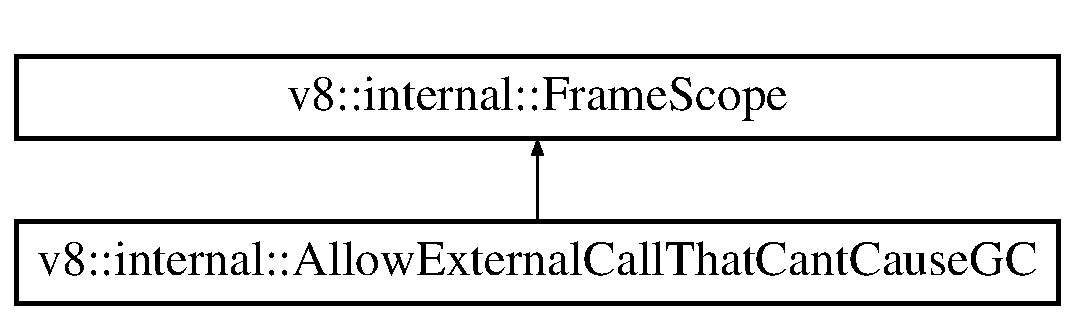
\includegraphics[height=2.000000cm]{classv8_1_1internal_1_1_allow_external_call_that_cant_cause_g_c}
\end{center}
\end{figure}
\subsection*{Public Member Functions}
\begin{DoxyCompactItemize}
\item 
{\bfseries Allow\+External\+Call\+That\+Cant\+Cause\+GC} (\hyperlink{classv8_1_1internal_1_1_macro_assembler}{Macro\+Assembler} $\ast$masm)\hypertarget{classv8_1_1internal_1_1_allow_external_call_that_cant_cause_g_c_ae136159f715f0afd4a7f76629f7bca48}{}\label{classv8_1_1internal_1_1_allow_external_call_that_cant_cause_g_c_ae136159f715f0afd4a7f76629f7bca48}

\end{DoxyCompactItemize}


The documentation for this class was generated from the following file\+:\begin{DoxyCompactItemize}
\item 
/\+Users/joshgav/node/v8/src/macro-\/assembler.\+h\end{DoxyCompactItemize}

\hypertarget{classv8_1_1_isolate_1_1_allow_javascript_execution_scope}{}\section{v8\+:\+:Isolate\+:\+:Allow\+Javascript\+Execution\+Scope Class Reference}
\label{classv8_1_1_isolate_1_1_allow_javascript_execution_scope}\index{v8\+::\+Isolate\+::\+Allow\+Javascript\+Execution\+Scope@{v8\+::\+Isolate\+::\+Allow\+Javascript\+Execution\+Scope}}


{\ttfamily \#include $<$v8.\+h$>$}

\subsection*{Public Member Functions}
\begin{DoxyCompactItemize}
\item 
{\bfseries Allow\+Javascript\+Execution\+Scope} (\hyperlink{classv8_1_1_isolate}{Isolate} $\ast$isolate)\hypertarget{classv8_1_1_isolate_1_1_allow_javascript_execution_scope_ac73a647c33756c6b7c3896170e069e8c}{}\label{classv8_1_1_isolate_1_1_allow_javascript_execution_scope_ac73a647c33756c6b7c3896170e069e8c}

\end{DoxyCompactItemize}
\subsection*{Private Member Functions}
\begin{DoxyCompactItemize}
\item 
{\bfseries Allow\+Javascript\+Execution\+Scope} (const \hyperlink{classv8_1_1_isolate_1_1_allow_javascript_execution_scope}{Allow\+Javascript\+Execution\+Scope} \&)\hypertarget{classv8_1_1_isolate_1_1_allow_javascript_execution_scope_a9968118fbefa05ce6cb97373efe32656}{}\label{classv8_1_1_isolate_1_1_allow_javascript_execution_scope_a9968118fbefa05ce6cb97373efe32656}

\item 
\hyperlink{classv8_1_1_isolate_1_1_allow_javascript_execution_scope}{Allow\+Javascript\+Execution\+Scope} \& {\bfseries operator=} (const \hyperlink{classv8_1_1_isolate_1_1_allow_javascript_execution_scope}{Allow\+Javascript\+Execution\+Scope} \&)\hypertarget{classv8_1_1_isolate_1_1_allow_javascript_execution_scope_a4ca08db8ddcb39695011739c31b54349}{}\label{classv8_1_1_isolate_1_1_allow_javascript_execution_scope_a4ca08db8ddcb39695011739c31b54349}

\end{DoxyCompactItemize}
\subsection*{Private Attributes}
\begin{DoxyCompactItemize}
\item 
void $\ast$ {\bfseries internal\+\_\+throws\+\_\+}\hypertarget{classv8_1_1_isolate_1_1_allow_javascript_execution_scope_a991c6fdbad58aae983e2107de2423f80}{}\label{classv8_1_1_isolate_1_1_allow_javascript_execution_scope_a991c6fdbad58aae983e2107de2423f80}

\item 
void $\ast$ {\bfseries internal\+\_\+assert\+\_\+}\hypertarget{classv8_1_1_isolate_1_1_allow_javascript_execution_scope_a5ef196e5ce1c7c3602b3bbe4674dab3c}{}\label{classv8_1_1_isolate_1_1_allow_javascript_execution_scope_a5ef196e5ce1c7c3602b3bbe4674dab3c}

\end{DoxyCompactItemize}


\subsection{Detailed Description}
Introduce exception to \hyperlink{classv8_1_1_isolate_1_1_disallow_javascript_execution_scope}{Disallow\+Javascript\+Execution\+Scope}. 

The documentation for this class was generated from the following file\+:\begin{DoxyCompactItemize}
\item 
/\+Users/joshgav/node/v8/include/v8.\+h\end{DoxyCompactItemize}

\hypertarget{classv8_1_1internal_1_1_code_1_1_allow_o_s_r_at_loop_nesting_level_field}{}\section{v8\+:\+:internal\+:\+:Code\+:\+:Allow\+O\+S\+R\+At\+Loop\+Nesting\+Level\+Field Class Reference}
\label{classv8_1_1internal_1_1_code_1_1_allow_o_s_r_at_loop_nesting_level_field}\index{v8\+::internal\+::\+Code\+::\+Allow\+O\+S\+R\+At\+Loop\+Nesting\+Level\+Field@{v8\+::internal\+::\+Code\+::\+Allow\+O\+S\+R\+At\+Loop\+Nesting\+Level\+Field}}
Inheritance diagram for v8\+:\+:internal\+:\+:Code\+:\+:Allow\+O\+S\+R\+At\+Loop\+Nesting\+Level\+Field\+:\begin{figure}[H]
\begin{center}
\leavevmode
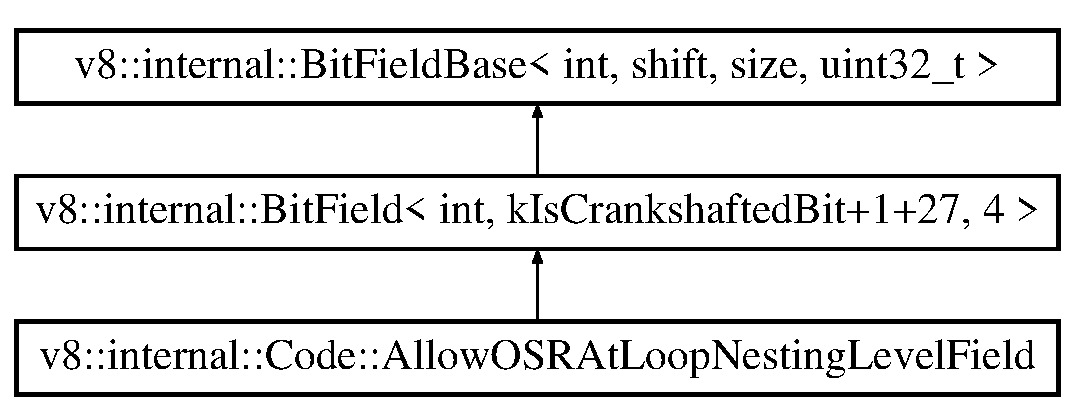
\includegraphics[height=3.000000cm]{classv8_1_1internal_1_1_code_1_1_allow_o_s_r_at_loop_nesting_level_field}
\end{center}
\end{figure}
\subsection*{Additional Inherited Members}


The documentation for this class was generated from the following file\+:\begin{DoxyCompactItemize}
\item 
/\+Users/joshgav/node/v8/src/objects.\+h\end{DoxyCompactItemize}

\hypertarget{classv8_1_1internal_1_1_all_static}{}\section{v8\+:\+:internal\+:\+:All\+Static Class Reference}
\label{classv8_1_1internal_1_1_all_static}\index{v8\+::internal\+::\+All\+Static@{v8\+::internal\+::\+All\+Static}}
Inheritance diagram for v8\+:\+:internal\+:\+:All\+Static\+:\begin{figure}[H]
\begin{center}
\leavevmode
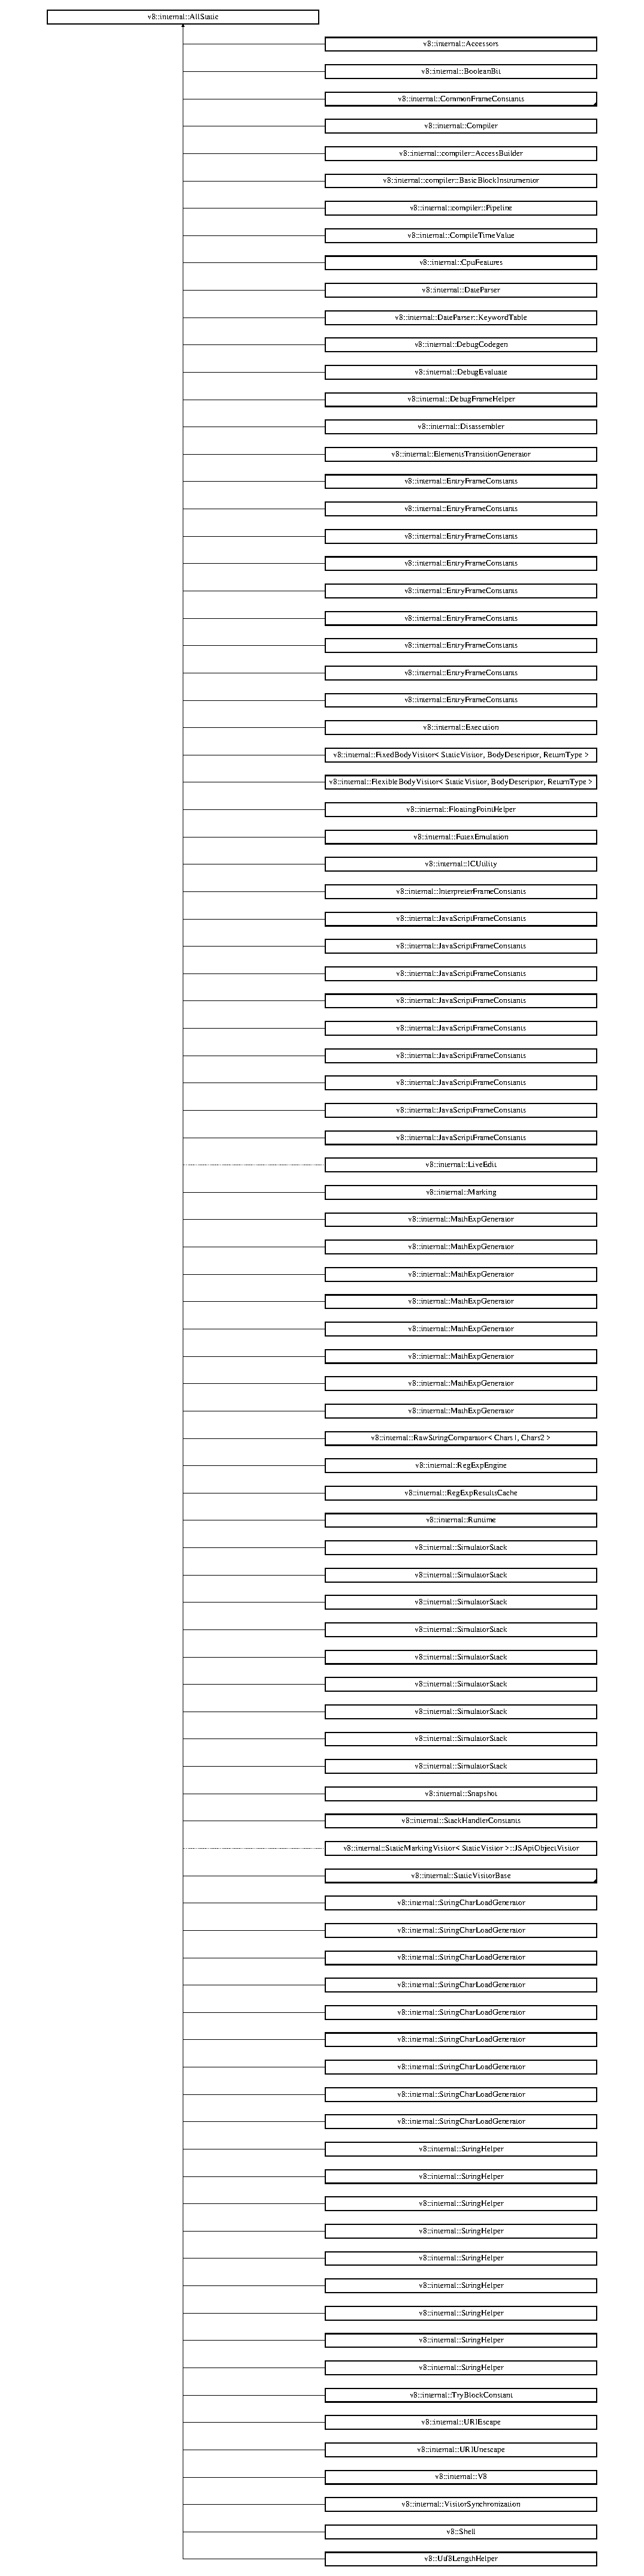
\includegraphics[height=12.000000cm]{classv8_1_1internal_1_1_all_static}
\end{center}
\end{figure}


The documentation for this class was generated from the following file\+:\begin{DoxyCompactItemize}
\item 
/\+Users/joshgav/node/v8/src/allocation.\+h\end{DoxyCompactItemize}

\hypertarget{classv8_1_1internal_1_1_alternative_generation}{}\section{v8\+:\+:internal\+:\+:Alternative\+Generation Class Reference}
\label{classv8_1_1internal_1_1_alternative_generation}\index{v8\+::internal\+::\+Alternative\+Generation@{v8\+::internal\+::\+Alternative\+Generation}}
Inheritance diagram for v8\+:\+:internal\+:\+:Alternative\+Generation\+:\begin{figure}[H]
\begin{center}
\leavevmode
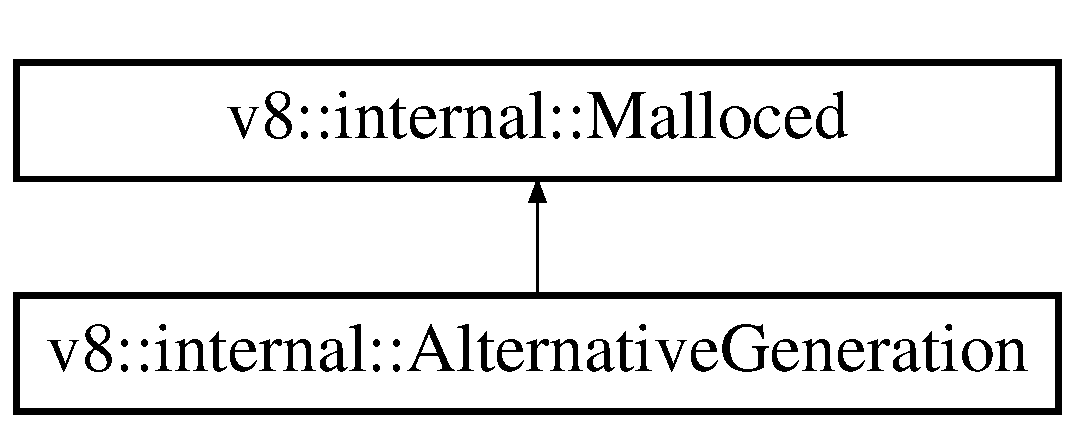
\includegraphics[height=2.000000cm]{classv8_1_1internal_1_1_alternative_generation}
\end{center}
\end{figure}
\subsection*{Public Attributes}
\begin{DoxyCompactItemize}
\item 
\hyperlink{classv8_1_1internal_1_1_label}{Label} {\bfseries possible\+\_\+success}\hypertarget{classv8_1_1internal_1_1_alternative_generation_a6b2881c2cd1292cb0423fd4dab2ca823}{}\label{classv8_1_1internal_1_1_alternative_generation_a6b2881c2cd1292cb0423fd4dab2ca823}

\item 
bool {\bfseries expects\+\_\+preload}\hypertarget{classv8_1_1internal_1_1_alternative_generation_a71eb17f16f4e5201f9f251c9fe74a507}{}\label{classv8_1_1internal_1_1_alternative_generation_a71eb17f16f4e5201f9f251c9fe74a507}

\item 
\hyperlink{classv8_1_1internal_1_1_label}{Label} {\bfseries after}\hypertarget{classv8_1_1internal_1_1_alternative_generation_a5640bb3e3f745d0b4705cd21ae741361}{}\label{classv8_1_1internal_1_1_alternative_generation_a5640bb3e3f745d0b4705cd21ae741361}

\item 
\hyperlink{classv8_1_1internal_1_1_quick_check_details}{Quick\+Check\+Details} {\bfseries quick\+\_\+check\+\_\+details}\hypertarget{classv8_1_1internal_1_1_alternative_generation_a727fcad75b108bd5288f5771aae86831}{}\label{classv8_1_1internal_1_1_alternative_generation_a727fcad75b108bd5288f5771aae86831}

\end{DoxyCompactItemize}
\subsection*{Additional Inherited Members}


The documentation for this class was generated from the following file\+:\begin{DoxyCompactItemize}
\item 
/\+Users/joshgav/node/v8/src/regexp/jsregexp.\+cc\end{DoxyCompactItemize}

\hypertarget{classv8_1_1internal_1_1_alternative_generation_list}{}\section{v8\+:\+:internal\+:\+:Alternative\+Generation\+List Class Reference}
\label{classv8_1_1internal_1_1_alternative_generation_list}\index{v8\+::internal\+::\+Alternative\+Generation\+List@{v8\+::internal\+::\+Alternative\+Generation\+List}}
\subsection*{Public Member Functions}
\begin{DoxyCompactItemize}
\item 
{\bfseries Alternative\+Generation\+List} (int count, \hyperlink{classv8_1_1internal_1_1_zone}{Zone} $\ast$zone)\hypertarget{classv8_1_1internal_1_1_alternative_generation_list_a12e31ade267f3b97c25bf9201fe3b65a}{}\label{classv8_1_1internal_1_1_alternative_generation_list_a12e31ade267f3b97c25bf9201fe3b65a}

\item 
\hyperlink{classv8_1_1internal_1_1_alternative_generation}{Alternative\+Generation} $\ast$ {\bfseries at} (int i)\hypertarget{classv8_1_1internal_1_1_alternative_generation_list_a074eac77994a3714b4214b777fce5b2a}{}\label{classv8_1_1internal_1_1_alternative_generation_list_a074eac77994a3714b4214b777fce5b2a}

\end{DoxyCompactItemize}
\subsection*{Private Attributes}
\begin{DoxyCompactItemize}
\item 
\hyperlink{classv8_1_1internal_1_1_zone_list}{Zone\+List}$<$ \hyperlink{classv8_1_1internal_1_1_alternative_generation}{Alternative\+Generation} $\ast$ $>$ {\bfseries alt\+\_\+gens\+\_\+}\hypertarget{classv8_1_1internal_1_1_alternative_generation_list_af6fd3dd431e003ed0bc03213b62f7004}{}\label{classv8_1_1internal_1_1_alternative_generation_list_af6fd3dd431e003ed0bc03213b62f7004}

\item 
\hyperlink{classv8_1_1internal_1_1_alternative_generation}{Alternative\+Generation} {\bfseries a\+\_\+few\+\_\+alt\+\_\+gens\+\_\+} \mbox{[}k\+A\+Few\mbox{]}\hypertarget{classv8_1_1internal_1_1_alternative_generation_list_a053e7a2deb11d3e4904f3ad551297532}{}\label{classv8_1_1internal_1_1_alternative_generation_list_a053e7a2deb11d3e4904f3ad551297532}

\end{DoxyCompactItemize}
\subsection*{Static Private Attributes}
\begin{DoxyCompactItemize}
\item 
static const int {\bfseries k\+A\+Few} = 10\hypertarget{classv8_1_1internal_1_1_alternative_generation_list_a70fc4fd2e074b5218a3ea5a28be625bd}{}\label{classv8_1_1internal_1_1_alternative_generation_list_a70fc4fd2e074b5218a3ea5a28be625bd}

\end{DoxyCompactItemize}


The documentation for this class was generated from the following file\+:\begin{DoxyCompactItemize}
\item 
/\+Users/joshgav/node/v8/src/regexp/jsregexp.\+cc\end{DoxyCompactItemize}

\hypertarget{structv8_1_1internal_1_1_effects_mixin_1_1_alt_merger}{}\section{v8\+:\+:internal\+:\+:Effects\+Mixin$<$ Var, Base, Effects $>$\+:\+:Alt\+Merger$<$ Self $>$ Struct Template Reference}
\label{structv8_1_1internal_1_1_effects_mixin_1_1_alt_merger}\index{v8\+::internal\+::\+Effects\+Mixin$<$ Var, Base, Effects $>$\+::\+Alt\+Merger$<$ Self $>$@{v8\+::internal\+::\+Effects\+Mixin$<$ Var, Base, Effects $>$\+::\+Alt\+Merger$<$ Self $>$}}
\subsection*{Public Member Functions}
\begin{DoxyCompactItemize}
\item 
void {\bfseries Call} (Var var, \hyperlink{structv8_1_1internal_1_1_effect}{Effect} effect)\hypertarget{structv8_1_1internal_1_1_effects_mixin_1_1_alt_merger_af4a6516fe49c9b9287f1618f37d357b3}{}\label{structv8_1_1internal_1_1_effects_mixin_1_1_alt_merger_af4a6516fe49c9b9287f1618f37d357b3}

\end{DoxyCompactItemize}
\subsection*{Public Attributes}
\begin{DoxyCompactItemize}
\item 
Self {\bfseries self}\hypertarget{structv8_1_1internal_1_1_effects_mixin_1_1_alt_merger_a89a5575969d2cbfab82bd8726165e2ac}{}\label{structv8_1_1internal_1_1_effects_mixin_1_1_alt_merger_a89a5575969d2cbfab82bd8726165e2ac}

\end{DoxyCompactItemize}


The documentation for this struct was generated from the following file\+:\begin{DoxyCompactItemize}
\item 
/\+Users/joshgav/node/v8/src/effects.\+h\end{DoxyCompactItemize}

\hypertarget{structv8_1_1internal_1_1_effects_mixin_1_1_alt_weakener}{}\section{v8\+:\+:internal\+:\+:Effects\+Mixin$<$ Var, Base, Effects $>$\+:\+:Alt\+Weakener$<$ Self $>$ Struct Template Reference}
\label{structv8_1_1internal_1_1_effects_mixin_1_1_alt_weakener}\index{v8\+::internal\+::\+Effects\+Mixin$<$ Var, Base, Effects $>$\+::\+Alt\+Weakener$<$ Self $>$@{v8\+::internal\+::\+Effects\+Mixin$<$ Var, Base, Effects $>$\+::\+Alt\+Weakener$<$ Self $>$}}
\subsection*{Public Member Functions}
\begin{DoxyCompactItemize}
\item 
void {\bfseries Call} (Var var, \hyperlink{structv8_1_1internal_1_1_effect}{Effect} effect)\hypertarget{structv8_1_1internal_1_1_effects_mixin_1_1_alt_weakener_a651cd436a421f5b78abc43754e8309a3}{}\label{structv8_1_1internal_1_1_effects_mixin_1_1_alt_weakener_a651cd436a421f5b78abc43754e8309a3}

\end{DoxyCompactItemize}
\subsection*{Public Attributes}
\begin{DoxyCompactItemize}
\item 
Self {\bfseries self}\hypertarget{structv8_1_1internal_1_1_effects_mixin_1_1_alt_weakener_ae73da3655748ec9da62f755efd66633a}{}\label{structv8_1_1internal_1_1_effects_mixin_1_1_alt_weakener_ae73da3655748ec9da62f755efd66633a}

\item 
\hyperlink{classv8_1_1internal_1_1_effects}{Effects} {\bfseries other}\hypertarget{structv8_1_1internal_1_1_effects_mixin_1_1_alt_weakener_adde1918061d0bb8bd6148becfeef5e84}{}\label{structv8_1_1internal_1_1_effects_mixin_1_1_alt_weakener_adde1918061d0bb8bd6148becfeef5e84}

\end{DoxyCompactItemize}


The documentation for this struct was generated from the following file\+:\begin{DoxyCompactItemize}
\item 
/\+Users/joshgav/node/v8/src/effects.\+h\end{DoxyCompactItemize}

\hypertarget{classv8_1_1internal_1_1_always_allocate_scope}{}\section{v8\+:\+:internal\+:\+:Always\+Allocate\+Scope Class Reference}
\label{classv8_1_1internal_1_1_always_allocate_scope}\index{v8\+::internal\+::\+Always\+Allocate\+Scope@{v8\+::internal\+::\+Always\+Allocate\+Scope}}
\subsection*{Public Member Functions}
\begin{DoxyCompactItemize}
\item 
{\bfseries Always\+Allocate\+Scope} (\hyperlink{classv8_1_1internal_1_1_isolate}{Isolate} $\ast$isolate)\hypertarget{classv8_1_1internal_1_1_always_allocate_scope_a34c521892b9b7d7b65feb1c9e56bddf0}{}\label{classv8_1_1internal_1_1_always_allocate_scope_a34c521892b9b7d7b65feb1c9e56bddf0}

\end{DoxyCompactItemize}
\subsection*{Private Attributes}
\begin{DoxyCompactItemize}
\item 
\hyperlink{classv8_1_1internal_1_1_heap}{Heap} $\ast$ {\bfseries heap\+\_\+}\hypertarget{classv8_1_1internal_1_1_always_allocate_scope_af71f11b2b6a94288793f8ef48083c72a}{}\label{classv8_1_1internal_1_1_always_allocate_scope_af71f11b2b6a94288793f8ef48083c72a}

\end{DoxyCompactItemize}


The documentation for this class was generated from the following files\+:\begin{DoxyCompactItemize}
\item 
/\+Users/joshgav/node/v8/src/heap/heap.\+h\item 
/\+Users/joshgav/node/v8/src/heap/heap-\/inl.\+h\end{DoxyCompactItemize}

\hypertarget{classv8_1_1internal_1_1_analysis}{}\section{v8\+:\+:internal\+:\+:Analysis Class Reference}
\label{classv8_1_1internal_1_1_analysis}\index{v8\+::internal\+::\+Analysis@{v8\+::internal\+::\+Analysis}}
Inheritance diagram for v8\+:\+:internal\+:\+:Analysis\+:\begin{figure}[H]
\begin{center}
\leavevmode
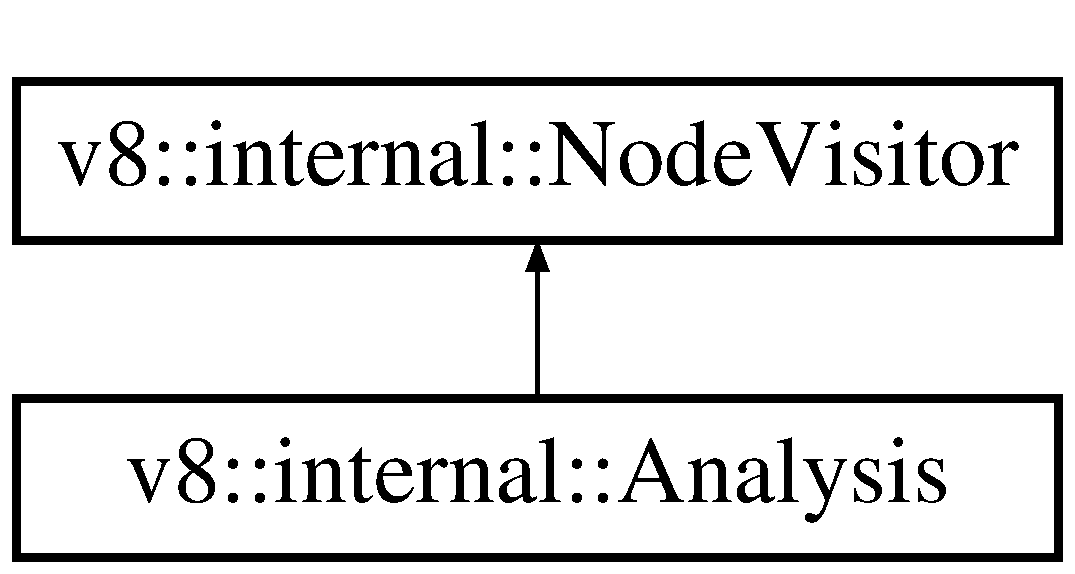
\includegraphics[height=2.000000cm]{classv8_1_1internal_1_1_analysis}
\end{center}
\end{figure}
\subsection*{Public Member Functions}
\begin{DoxyCompactItemize}
\item 
{\bfseries Analysis} (\hyperlink{classv8_1_1internal_1_1_isolate}{Isolate} $\ast$isolate, \hyperlink{classv8_1_1base_1_1_flags}{J\+S\+Reg\+Exp\+::\+Flags} flags, bool is\+\_\+one\+\_\+byte)\hypertarget{classv8_1_1internal_1_1_analysis_ad580622ff0451870580c586d710e7c0c}{}\label{classv8_1_1internal_1_1_analysis_ad580622ff0451870580c586d710e7c0c}

\item 
void {\bfseries Ensure\+Analyzed} (\hyperlink{classv8_1_1internal_1_1_reg_exp_node}{Reg\+Exp\+Node} $\ast$node)\hypertarget{classv8_1_1internal_1_1_analysis_a91ea9ab34a0b720e4ba0414997e6f978}{}\label{classv8_1_1internal_1_1_analysis_a91ea9ab34a0b720e4ba0414997e6f978}

\item 
virtual void {\bfseries Visit\+Loop\+Choice} (\hyperlink{classv8_1_1internal_1_1_loop_choice_node}{Loop\+Choice\+Node} $\ast$that)\hypertarget{classv8_1_1internal_1_1_analysis_aa6a0b113e9b8a9268a3af41dbdc24ff6}{}\label{classv8_1_1internal_1_1_analysis_aa6a0b113e9b8a9268a3af41dbdc24ff6}

\item 
bool {\bfseries has\+\_\+failed} ()\hypertarget{classv8_1_1internal_1_1_analysis_a49fb801db5532a96bc0c078e3c928910}{}\label{classv8_1_1internal_1_1_analysis_a49fb801db5532a96bc0c078e3c928910}

\item 
const char $\ast$ {\bfseries error\+\_\+message} ()\hypertarget{classv8_1_1internal_1_1_analysis_a70729ef89c68f6ba50909873d438fe47}{}\label{classv8_1_1internal_1_1_analysis_a70729ef89c68f6ba50909873d438fe47}

\item 
void {\bfseries fail} (const char $\ast$error\+\_\+message)\hypertarget{classv8_1_1internal_1_1_analysis_ae430a167d7e2e6cf98834465c537a64e}{}\label{classv8_1_1internal_1_1_analysis_ae430a167d7e2e6cf98834465c537a64e}

\item 
\hyperlink{classv8_1_1internal_1_1_isolate}{Isolate} $\ast$ {\bfseries isolate} () const \hypertarget{classv8_1_1internal_1_1_analysis_af2055729bffb64459d1129ec5135fdef}{}\label{classv8_1_1internal_1_1_analysis_af2055729bffb64459d1129ec5135fdef}

\item 
bool {\bfseries ignore\+\_\+case} () const \hypertarget{classv8_1_1internal_1_1_analysis_a21a59737aea76ed146fdce63faaabdd8}{}\label{classv8_1_1internal_1_1_analysis_a21a59737aea76ed146fdce63faaabdd8}

\item 
bool {\bfseries unicode} () const \hypertarget{classv8_1_1internal_1_1_analysis_ad4692b73a5071229c9a5641b2f077150}{}\label{classv8_1_1internal_1_1_analysis_ad4692b73a5071229c9a5641b2f077150}

\end{DoxyCompactItemize}
\subsection*{Private Member Functions}
\begin{DoxyCompactItemize}
\item 
{\bfseries D\+I\+S\+A\+L\+L\+O\+W\+\_\+\+I\+M\+P\+L\+I\+C\+I\+T\+\_\+\+C\+O\+N\+S\+T\+R\+U\+C\+T\+O\+RS} (\hyperlink{classv8_1_1internal_1_1_analysis}{Analysis})\hypertarget{classv8_1_1internal_1_1_analysis_a5644d696a2169bb5eb1fdec268fccd23}{}\label{classv8_1_1internal_1_1_analysis_a5644d696a2169bb5eb1fdec268fccd23}

\end{DoxyCompactItemize}
\subsection*{Private Attributes}
\begin{DoxyCompactItemize}
\item 
\hyperlink{classv8_1_1internal_1_1_isolate}{Isolate} $\ast$ {\bfseries isolate\+\_\+}\hypertarget{classv8_1_1internal_1_1_analysis_adb4ca99ba3a828a0e9f8447b928d505f}{}\label{classv8_1_1internal_1_1_analysis_adb4ca99ba3a828a0e9f8447b928d505f}

\item 
\hyperlink{classv8_1_1base_1_1_flags}{J\+S\+Reg\+Exp\+::\+Flags} {\bfseries flags\+\_\+}\hypertarget{classv8_1_1internal_1_1_analysis_a17c7794660581032c28b72c4d1431710}{}\label{classv8_1_1internal_1_1_analysis_a17c7794660581032c28b72c4d1431710}

\item 
bool {\bfseries is\+\_\+one\+\_\+byte\+\_\+}\hypertarget{classv8_1_1internal_1_1_analysis_afe88275e82e128eb4f84ad51b9b6d71f}{}\label{classv8_1_1internal_1_1_analysis_afe88275e82e128eb4f84ad51b9b6d71f}

\item 
const char $\ast$ {\bfseries error\+\_\+message\+\_\+}\hypertarget{classv8_1_1internal_1_1_analysis_abe0c372b8260ec967c145a7de7e6f71b}{}\label{classv8_1_1internal_1_1_analysis_abe0c372b8260ec967c145a7de7e6f71b}

\end{DoxyCompactItemize}


The documentation for this class was generated from the following files\+:\begin{DoxyCompactItemize}
\item 
/\+Users/joshgav/node/v8/src/regexp/jsregexp.\+h\item 
/\+Users/joshgav/node/v8/src/regexp/jsregexp.\+cc\end{DoxyCompactItemize}

\hypertarget{classv8_1_1internal_1_1_api_callback_descriptor_base}{}\section{v8\+:\+:internal\+:\+:Api\+Callback\+Descriptor\+Base Class Reference}
\label{classv8_1_1internal_1_1_api_callback_descriptor_base}\index{v8\+::internal\+::\+Api\+Callback\+Descriptor\+Base@{v8\+::internal\+::\+Api\+Callback\+Descriptor\+Base}}
Inheritance diagram for v8\+:\+:internal\+:\+:Api\+Callback\+Descriptor\+Base\+:\begin{figure}[H]
\begin{center}
\leavevmode
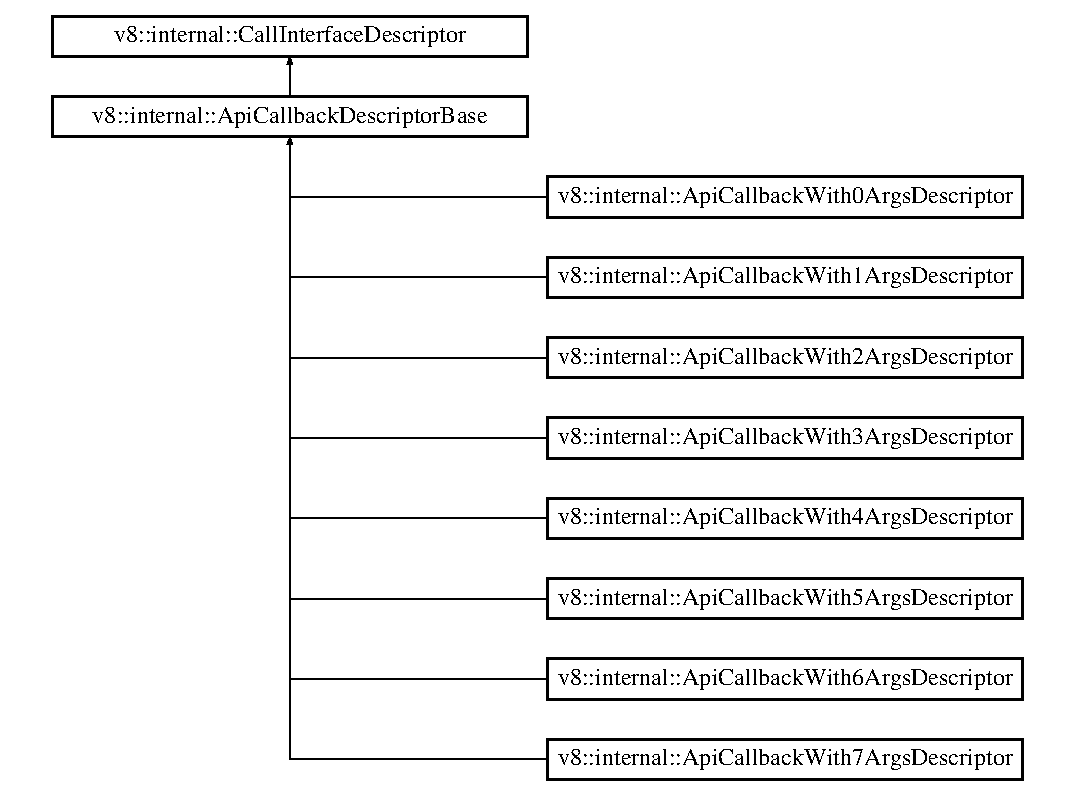
\includegraphics[height=10.000000cm]{classv8_1_1internal_1_1_api_callback_descriptor_base}
\end{center}
\end{figure}
\subsection*{Static Public Member Functions}
\begin{DoxyCompactItemize}
\item 
static \hyperlink{classv8_1_1internal_1_1_call_interface_descriptor}{Call\+Interface\+Descriptor} {\bfseries For\+Args} (\hyperlink{classv8_1_1internal_1_1_isolate}{Isolate} $\ast$isolate, int argc)\hypertarget{classv8_1_1internal_1_1_api_callback_descriptor_base_a607ad9694235e6b4950834330bdfe132}{}\label{classv8_1_1internal_1_1_api_callback_descriptor_base_a607ad9694235e6b4950834330bdfe132}

\end{DoxyCompactItemize}
\subsection*{Protected Member Functions}
\begin{DoxyCompactItemize}
\item 
{\bfseries Api\+Callback\+Descriptor\+Base} (\hyperlink{classv8_1_1internal_1_1_isolate}{Isolate} $\ast$isolate, Call\+Descriptors\+::\+Key key)\hypertarget{classv8_1_1internal_1_1_api_callback_descriptor_base_ae34ce6c137da5a8764d6fe0584a3dafa}{}\label{classv8_1_1internal_1_1_api_callback_descriptor_base_ae34ce6c137da5a8764d6fe0584a3dafa}

\item 
void {\bfseries Initialize\+Platform\+Specific} (\hyperlink{classv8_1_1internal_1_1_call_interface_descriptor_data}{Call\+Interface\+Descriptor\+Data} $\ast$data) override\hypertarget{classv8_1_1internal_1_1_api_callback_descriptor_base_a5dbf77b8fb657373ce3f0f57e127c7f2}{}\label{classv8_1_1internal_1_1_api_callback_descriptor_base_a5dbf77b8fb657373ce3f0f57e127c7f2}

\item 
\hyperlink{classv8_1_1internal_1_1_function_type}{Function\+Type} $\ast$ {\bfseries Build\+Call\+Interface\+Descriptor\+Function\+Type\+With\+Arg} (\hyperlink{classv8_1_1internal_1_1_isolate}{Isolate} $\ast$isolate, int parameter\+\_\+count, int argc)\hypertarget{classv8_1_1internal_1_1_api_callback_descriptor_base_a7767b1dd2c94c543a9b348e7cf85e5aa}{}\label{classv8_1_1internal_1_1_api_callback_descriptor_base_a7767b1dd2c94c543a9b348e7cf85e5aa}

\end{DoxyCompactItemize}
\subsection*{Additional Inherited Members}


The documentation for this class was generated from the following files\+:\begin{DoxyCompactItemize}
\item 
/\+Users/joshgav/node/v8/src/interface-\/descriptors.\+h\item 
/\+Users/joshgav/node/v8/src/interface-\/descriptors.\+cc\end{DoxyCompactItemize}

\hypertarget{classv8_1_1internal_1_1_api_callback_with0_args_descriptor}{}\section{v8\+:\+:internal\+:\+:Api\+Callback\+With0\+Args\+Descriptor Class Reference}
\label{classv8_1_1internal_1_1_api_callback_with0_args_descriptor}\index{v8\+::internal\+::\+Api\+Callback\+With0\+Args\+Descriptor@{v8\+::internal\+::\+Api\+Callback\+With0\+Args\+Descriptor}}
Inheritance diagram for v8\+:\+:internal\+:\+:Api\+Callback\+With0\+Args\+Descriptor\+:\begin{figure}[H]
\begin{center}
\leavevmode
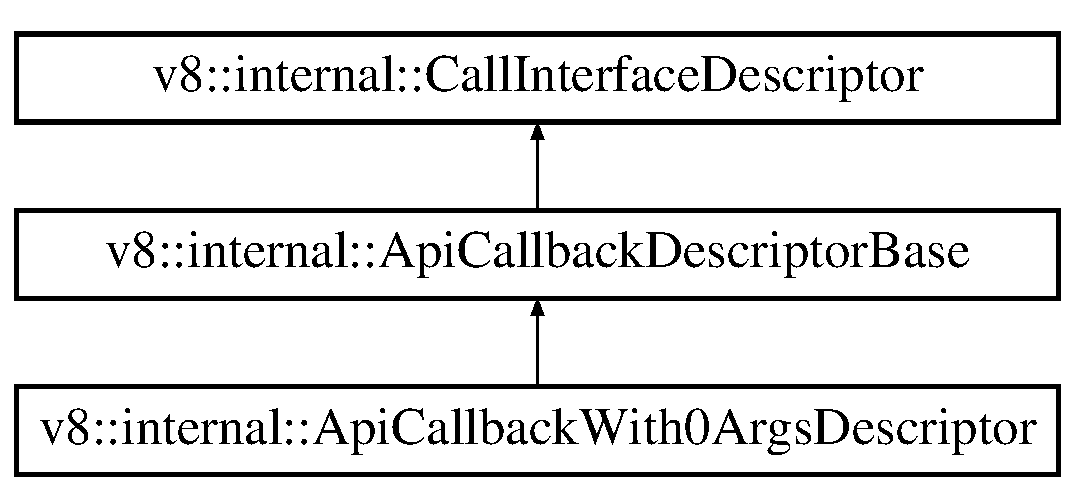
\includegraphics[height=3.000000cm]{classv8_1_1internal_1_1_api_callback_with0_args_descriptor}
\end{center}
\end{figure}
\subsection*{Additional Inherited Members}


The documentation for this class was generated from the following file\+:\begin{DoxyCompactItemize}
\item 
/\+Users/joshgav/node/v8/src/interface-\/descriptors.\+h\end{DoxyCompactItemize}

\hypertarget{classv8_1_1internal_1_1_api_callback_with1_args_descriptor}{}\section{v8\+:\+:internal\+:\+:Api\+Callback\+With1\+Args\+Descriptor Class Reference}
\label{classv8_1_1internal_1_1_api_callback_with1_args_descriptor}\index{v8\+::internal\+::\+Api\+Callback\+With1\+Args\+Descriptor@{v8\+::internal\+::\+Api\+Callback\+With1\+Args\+Descriptor}}
Inheritance diagram for v8\+:\+:internal\+:\+:Api\+Callback\+With1\+Args\+Descriptor\+:\begin{figure}[H]
\begin{center}
\leavevmode
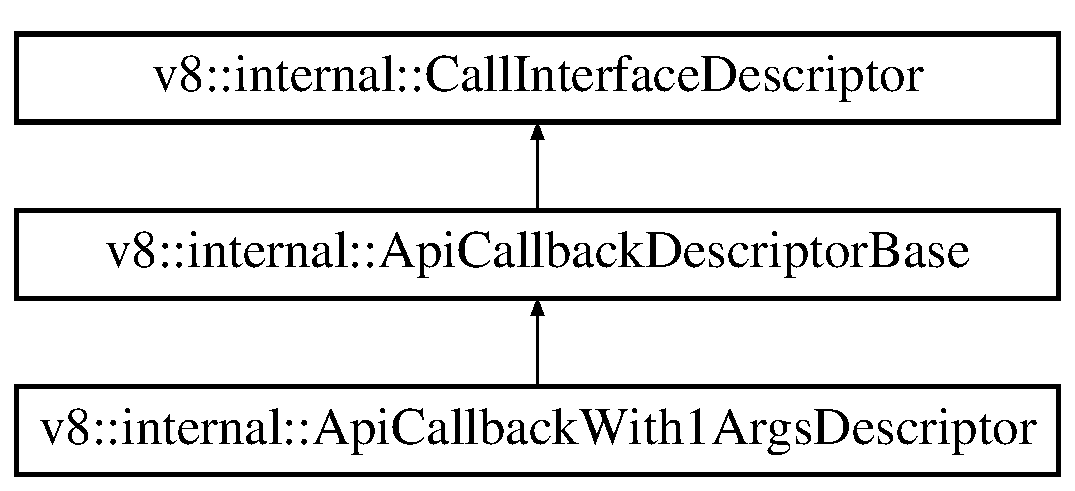
\includegraphics[height=3.000000cm]{classv8_1_1internal_1_1_api_callback_with1_args_descriptor}
\end{center}
\end{figure}
\subsection*{Additional Inherited Members}


The documentation for this class was generated from the following file\+:\begin{DoxyCompactItemize}
\item 
/\+Users/joshgav/node/v8/src/interface-\/descriptors.\+h\end{DoxyCompactItemize}

\hypertarget{classv8_1_1internal_1_1_api_callback_with2_args_descriptor}{}\section{v8\+:\+:internal\+:\+:Api\+Callback\+With2\+Args\+Descriptor Class Reference}
\label{classv8_1_1internal_1_1_api_callback_with2_args_descriptor}\index{v8\+::internal\+::\+Api\+Callback\+With2\+Args\+Descriptor@{v8\+::internal\+::\+Api\+Callback\+With2\+Args\+Descriptor}}
Inheritance diagram for v8\+:\+:internal\+:\+:Api\+Callback\+With2\+Args\+Descriptor\+:\begin{figure}[H]
\begin{center}
\leavevmode
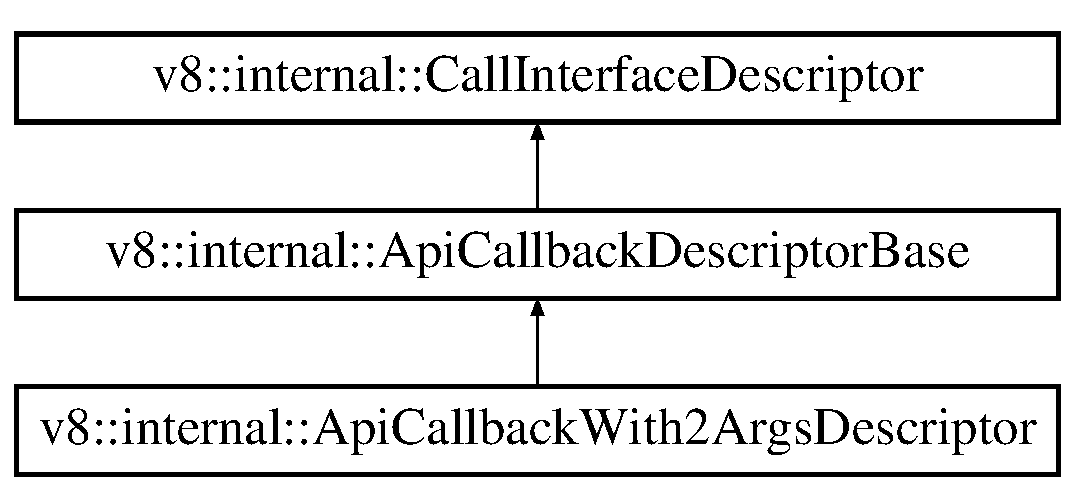
\includegraphics[height=3.000000cm]{classv8_1_1internal_1_1_api_callback_with2_args_descriptor}
\end{center}
\end{figure}
\subsection*{Additional Inherited Members}


The documentation for this class was generated from the following file\+:\begin{DoxyCompactItemize}
\item 
/\+Users/joshgav/node/v8/src/interface-\/descriptors.\+h\end{DoxyCompactItemize}

\hypertarget{classv8_1_1internal_1_1_api_callback_with3_args_descriptor}{}\section{v8\+:\+:internal\+:\+:Api\+Callback\+With3\+Args\+Descriptor Class Reference}
\label{classv8_1_1internal_1_1_api_callback_with3_args_descriptor}\index{v8\+::internal\+::\+Api\+Callback\+With3\+Args\+Descriptor@{v8\+::internal\+::\+Api\+Callback\+With3\+Args\+Descriptor}}
Inheritance diagram for v8\+:\+:internal\+:\+:Api\+Callback\+With3\+Args\+Descriptor\+:\begin{figure}[H]
\begin{center}
\leavevmode
\includegraphics[height=3.000000cm]{classv8_1_1internal_1_1_api_callback_with3_args_descriptor}
\end{center}
\end{figure}
\subsection*{Additional Inherited Members}


The documentation for this class was generated from the following file\+:\begin{DoxyCompactItemize}
\item 
/\+Users/joshgav/node/v8/src/interface-\/descriptors.\+h\end{DoxyCompactItemize}

\hypertarget{classv8_1_1internal_1_1_api_callback_with4_args_descriptor}{}\section{v8\+:\+:internal\+:\+:Api\+Callback\+With4\+Args\+Descriptor Class Reference}
\label{classv8_1_1internal_1_1_api_callback_with4_args_descriptor}\index{v8\+::internal\+::\+Api\+Callback\+With4\+Args\+Descriptor@{v8\+::internal\+::\+Api\+Callback\+With4\+Args\+Descriptor}}
Inheritance diagram for v8\+:\+:internal\+:\+:Api\+Callback\+With4\+Args\+Descriptor\+:\begin{figure}[H]
\begin{center}
\leavevmode
\includegraphics[height=3.000000cm]{classv8_1_1internal_1_1_api_callback_with4_args_descriptor}
\end{center}
\end{figure}
\subsection*{Additional Inherited Members}


The documentation for this class was generated from the following file\+:\begin{DoxyCompactItemize}
\item 
/\+Users/joshgav/node/v8/src/interface-\/descriptors.\+h\end{DoxyCompactItemize}

\hypertarget{classv8_1_1internal_1_1_api_callback_with5_args_descriptor}{}\section{v8\+:\+:internal\+:\+:Api\+Callback\+With5\+Args\+Descriptor Class Reference}
\label{classv8_1_1internal_1_1_api_callback_with5_args_descriptor}\index{v8\+::internal\+::\+Api\+Callback\+With5\+Args\+Descriptor@{v8\+::internal\+::\+Api\+Callback\+With5\+Args\+Descriptor}}
Inheritance diagram for v8\+:\+:internal\+:\+:Api\+Callback\+With5\+Args\+Descriptor\+:\begin{figure}[H]
\begin{center}
\leavevmode
\includegraphics[height=3.000000cm]{classv8_1_1internal_1_1_api_callback_with5_args_descriptor}
\end{center}
\end{figure}
\subsection*{Additional Inherited Members}


The documentation for this class was generated from the following file\+:\begin{DoxyCompactItemize}
\item 
/\+Users/joshgav/node/v8/src/interface-\/descriptors.\+h\end{DoxyCompactItemize}

\hypertarget{classv8_1_1internal_1_1_api_callback_with6_args_descriptor}{}\section{v8\+:\+:internal\+:\+:Api\+Callback\+With6\+Args\+Descriptor Class Reference}
\label{classv8_1_1internal_1_1_api_callback_with6_args_descriptor}\index{v8\+::internal\+::\+Api\+Callback\+With6\+Args\+Descriptor@{v8\+::internal\+::\+Api\+Callback\+With6\+Args\+Descriptor}}
Inheritance diagram for v8\+:\+:internal\+:\+:Api\+Callback\+With6\+Args\+Descriptor\+:\begin{figure}[H]
\begin{center}
\leavevmode
\includegraphics[height=3.000000cm]{classv8_1_1internal_1_1_api_callback_with6_args_descriptor}
\end{center}
\end{figure}
\subsection*{Additional Inherited Members}


The documentation for this class was generated from the following file\+:\begin{DoxyCompactItemize}
\item 
/\+Users/joshgav/node/v8/src/interface-\/descriptors.\+h\end{DoxyCompactItemize}

\hypertarget{classv8_1_1internal_1_1_api_callback_with7_args_descriptor}{}\section{v8\+:\+:internal\+:\+:Api\+Callback\+With7\+Args\+Descriptor Class Reference}
\label{classv8_1_1internal_1_1_api_callback_with7_args_descriptor}\index{v8\+::internal\+::\+Api\+Callback\+With7\+Args\+Descriptor@{v8\+::internal\+::\+Api\+Callback\+With7\+Args\+Descriptor}}
Inheritance diagram for v8\+:\+:internal\+:\+:Api\+Callback\+With7\+Args\+Descriptor\+:\begin{figure}[H]
\begin{center}
\leavevmode
\includegraphics[height=3.000000cm]{classv8_1_1internal_1_1_api_callback_with7_args_descriptor}
\end{center}
\end{figure}
\subsection*{Additional Inherited Members}


The documentation for this class was generated from the following file\+:\begin{DoxyCompactItemize}
\item 
/\+Users/joshgav/node/v8/src/interface-\/descriptors.\+h\end{DoxyCompactItemize}

\hypertarget{classv8_1_1_api_function}{}\section{v8\+:\+:Api\+Function Class Reference}
\label{classv8_1_1_api_function}\index{v8\+::\+Api\+Function@{v8\+::\+Api\+Function}}
\subsection*{Public Member Functions}
\begin{DoxyCompactItemize}
\item 
{\bfseries Api\+Function} (v8\+::internal\+::\+Address addr)\hypertarget{classv8_1_1_api_function_a711c062e7328b2cd864a755290ccc70c}{}\label{classv8_1_1_api_function_a711c062e7328b2cd864a755290ccc70c}

\item 
v8\+::internal\+::\+Address {\bfseries address} ()\hypertarget{classv8_1_1_api_function_ae3168a2d34c3c799c4aae32a9c3bdba2}{}\label{classv8_1_1_api_function_ae3168a2d34c3c799c4aae32a9c3bdba2}

\end{DoxyCompactItemize}
\subsection*{Private Attributes}
\begin{DoxyCompactItemize}
\item 
v8\+::internal\+::\+Address {\bfseries addr\+\_\+}\hypertarget{classv8_1_1_api_function_af919d8ecbe8f85c017fc4f311327980f}{}\label{classv8_1_1_api_function_af919d8ecbe8f85c017fc4f311327980f}

\end{DoxyCompactItemize}


The documentation for this class was generated from the following file\+:\begin{DoxyCompactItemize}
\item 
/\+Users/joshgav/node/v8/src/api.\+h\end{DoxyCompactItemize}

\hypertarget{classv8_1_1internal_1_1_api_getter_descriptor}{}\section{v8\+:\+:internal\+:\+:Api\+Getter\+Descriptor Class Reference}
\label{classv8_1_1internal_1_1_api_getter_descriptor}\index{v8\+::internal\+::\+Api\+Getter\+Descriptor@{v8\+::internal\+::\+Api\+Getter\+Descriptor}}
Inheritance diagram for v8\+:\+:internal\+:\+:Api\+Getter\+Descriptor\+:\begin{figure}[H]
\begin{center}
\leavevmode
\includegraphics[height=2.000000cm]{classv8_1_1internal_1_1_api_getter_descriptor}
\end{center}
\end{figure}
\subsection*{Static Public Member Functions}
\begin{DoxyCompactItemize}
\item 
static const \hyperlink{structv8_1_1internal_1_1_register}{Register} {\bfseries Receiver\+Register} ()\hypertarget{classv8_1_1internal_1_1_api_getter_descriptor_aca30c34699283e5f463df6b7ffb7bcf1}{}\label{classv8_1_1internal_1_1_api_getter_descriptor_aca30c34699283e5f463df6b7ffb7bcf1}

\item 
static const \hyperlink{structv8_1_1internal_1_1_register}{Register} {\bfseries Holder\+Register} ()\hypertarget{classv8_1_1internal_1_1_api_getter_descriptor_a3a2ad818edc83502718c466b5dad01b5}{}\label{classv8_1_1internal_1_1_api_getter_descriptor_a3a2ad818edc83502718c466b5dad01b5}

\item 
static const \hyperlink{structv8_1_1internal_1_1_register}{Register} {\bfseries Callback\+Register} ()\hypertarget{classv8_1_1internal_1_1_api_getter_descriptor_a1289ae62e1bf71022cdedd9d84ca1082}{}\label{classv8_1_1internal_1_1_api_getter_descriptor_a1289ae62e1bf71022cdedd9d84ca1082}

\end{DoxyCompactItemize}
\subsection*{Additional Inherited Members}


The documentation for this class was generated from the following files\+:\begin{DoxyCompactItemize}
\item 
/\+Users/joshgav/node/v8/src/interface-\/descriptors.\+h\item 
/\+Users/joshgav/node/v8/src/interface-\/descriptors.\+cc\end{DoxyCompactItemize}

\hypertarget{classv8_1_1internal_1_1_api_natives}{}\section{v8\+:\+:internal\+:\+:Api\+Natives Class Reference}
\label{classv8_1_1internal_1_1_api_natives}\index{v8\+::internal\+::\+Api\+Natives@{v8\+::internal\+::\+Api\+Natives}}
\subsection*{Public Types}
\begin{DoxyCompactItemize}
\item 
enum {\bfseries Api\+Instance\+Type} \{ \\*
{\bfseries Java\+Script\+Object\+Type}, 
\\*
{\bfseries Global\+Object\+Type}, 
\\*
{\bfseries Global\+Proxy\+Type}
 \}\hypertarget{classv8_1_1internal_1_1_api_natives_aa8eeaaed51f9aa1ff3d25fbf81ba178b}{}\label{classv8_1_1internal_1_1_api_natives_aa8eeaaed51f9aa1ff3d25fbf81ba178b}

\end{DoxyCompactItemize}
\subsection*{Static Public Member Functions}
\begin{DoxyCompactItemize}
\item 
static M\+U\+S\+T\+\_\+\+U\+S\+E\+\_\+\+R\+E\+S\+U\+LT \hyperlink{classv8_1_1internal_1_1_maybe_handle}{Maybe\+Handle}$<$ \hyperlink{classv8_1_1internal_1_1_j_s_function}{J\+S\+Function} $>$ {\bfseries Instantiate\+Function} (\hyperlink{classv8_1_1internal_1_1_handle}{Handle}$<$ \hyperlink{classv8_1_1internal_1_1_function_template_info}{Function\+Template\+Info} $>$ data)\hypertarget{classv8_1_1internal_1_1_api_natives_a7e1150fde2bed4a4d1c2039f053e5de6}{}\label{classv8_1_1internal_1_1_api_natives_a7e1150fde2bed4a4d1c2039f053e5de6}

\item 
static M\+U\+S\+T\+\_\+\+U\+S\+E\+\_\+\+R\+E\+S\+U\+LT \hyperlink{classv8_1_1internal_1_1_maybe_handle}{Maybe\+Handle}$<$ \hyperlink{classv8_1_1internal_1_1_j_s_object}{J\+S\+Object} $>$ {\bfseries Instantiate\+Object} (\hyperlink{classv8_1_1internal_1_1_handle}{Handle}$<$ \hyperlink{classv8_1_1internal_1_1_object_template_info}{Object\+Template\+Info} $>$ data)\hypertarget{classv8_1_1internal_1_1_api_natives_a41f2a1366a63626da65f9a6209921d40}{}\label{classv8_1_1internal_1_1_api_natives_a41f2a1366a63626da65f9a6209921d40}

\item 
static \hyperlink{classv8_1_1internal_1_1_handle}{Handle}$<$ \hyperlink{classv8_1_1internal_1_1_j_s_function}{J\+S\+Function} $>$ {\bfseries Create\+Api\+Function} (\hyperlink{classv8_1_1internal_1_1_isolate}{Isolate} $\ast$isolate, \hyperlink{classv8_1_1internal_1_1_handle}{Handle}$<$ \hyperlink{classv8_1_1internal_1_1_function_template_info}{Function\+Template\+Info} $>$ obj, \hyperlink{classv8_1_1internal_1_1_handle}{Handle}$<$ \hyperlink{classv8_1_1internal_1_1_object}{Object} $>$ prototype, Api\+Instance\+Type instance\+\_\+type)\hypertarget{classv8_1_1internal_1_1_api_natives_a743e0ee576669f8618704dcb95e97b74}{}\label{classv8_1_1internal_1_1_api_natives_a743e0ee576669f8618704dcb95e97b74}

\item 
static void {\bfseries Add\+Data\+Property} (\hyperlink{classv8_1_1internal_1_1_isolate}{Isolate} $\ast$isolate, \hyperlink{classv8_1_1internal_1_1_handle}{Handle}$<$ \hyperlink{classv8_1_1internal_1_1_template_info}{Template\+Info} $>$ info, \hyperlink{classv8_1_1internal_1_1_handle}{Handle}$<$ \hyperlink{classv8_1_1internal_1_1_name}{Name} $>$ name, \hyperlink{classv8_1_1internal_1_1_handle}{Handle}$<$ \hyperlink{classv8_1_1internal_1_1_object}{Object} $>$ value, Property\+Attributes attributes)\hypertarget{classv8_1_1internal_1_1_api_natives_ae3ee4ad0fcbf129bbdc461d1bb3efa1a}{}\label{classv8_1_1internal_1_1_api_natives_ae3ee4ad0fcbf129bbdc461d1bb3efa1a}

\item 
static void {\bfseries Add\+Data\+Property} (\hyperlink{classv8_1_1internal_1_1_isolate}{Isolate} $\ast$isolate, \hyperlink{classv8_1_1internal_1_1_handle}{Handle}$<$ \hyperlink{classv8_1_1internal_1_1_template_info}{Template\+Info} $>$ info, \hyperlink{classv8_1_1internal_1_1_handle}{Handle}$<$ \hyperlink{classv8_1_1internal_1_1_name}{Name} $>$ name, v8\+::\+Intrinsic intrinsic, Property\+Attributes attributes)\hypertarget{classv8_1_1internal_1_1_api_natives_a00f025df8155d3f3aa5949422109f23e}{}\label{classv8_1_1internal_1_1_api_natives_a00f025df8155d3f3aa5949422109f23e}

\item 
static void {\bfseries Add\+Accessor\+Property} (\hyperlink{classv8_1_1internal_1_1_isolate}{Isolate} $\ast$isolate, \hyperlink{classv8_1_1internal_1_1_handle}{Handle}$<$ \hyperlink{classv8_1_1internal_1_1_template_info}{Template\+Info} $>$ info, \hyperlink{classv8_1_1internal_1_1_handle}{Handle}$<$ \hyperlink{classv8_1_1internal_1_1_name}{Name} $>$ name, \hyperlink{classv8_1_1internal_1_1_handle}{Handle}$<$ \hyperlink{classv8_1_1internal_1_1_function_template_info}{Function\+Template\+Info} $>$ getter, \hyperlink{classv8_1_1internal_1_1_handle}{Handle}$<$ \hyperlink{classv8_1_1internal_1_1_function_template_info}{Function\+Template\+Info} $>$ setter, Property\+Attributes attributes)\hypertarget{classv8_1_1internal_1_1_api_natives_a6934eedf60bf86e845fd9f483839191c}{}\label{classv8_1_1internal_1_1_api_natives_a6934eedf60bf86e845fd9f483839191c}

\item 
static void {\bfseries Add\+Native\+Data\+Property} (\hyperlink{classv8_1_1internal_1_1_isolate}{Isolate} $\ast$isolate, \hyperlink{classv8_1_1internal_1_1_handle}{Handle}$<$ \hyperlink{classv8_1_1internal_1_1_template_info}{Template\+Info} $>$ info, \hyperlink{classv8_1_1internal_1_1_handle}{Handle}$<$ \hyperlink{classv8_1_1internal_1_1_accessor_info}{Accessor\+Info} $>$ property)\hypertarget{classv8_1_1internal_1_1_api_natives_aa3f534fe84b42a099d7af3d7dae423c5}{}\label{classv8_1_1internal_1_1_api_natives_aa3f534fe84b42a099d7af3d7dae423c5}

\end{DoxyCompactItemize}
\subsection*{Static Public Attributes}
\begin{DoxyCompactItemize}
\item 
static const int {\bfseries k\+Initial\+Function\+Cache\+Size} = 256\hypertarget{classv8_1_1internal_1_1_api_natives_aca69c9efcc2949a8eb362d0fe599b4b9}{}\label{classv8_1_1internal_1_1_api_natives_aca69c9efcc2949a8eb362d0fe599b4b9}

\end{DoxyCompactItemize}


The documentation for this class was generated from the following files\+:\begin{DoxyCompactItemize}
\item 
/\+Users/joshgav/node/v8/src/api-\/natives.\+h\item 
/\+Users/joshgav/node/v8/src/api-\/natives.\+cc\end{DoxyCompactItemize}

\hypertarget{classv8_1_1internal_1_1_argument_adaptor_descriptor}{}\section{v8\+:\+:internal\+:\+:Argument\+Adaptor\+Descriptor Class Reference}
\label{classv8_1_1internal_1_1_argument_adaptor_descriptor}\index{v8\+::internal\+::\+Argument\+Adaptor\+Descriptor@{v8\+::internal\+::\+Argument\+Adaptor\+Descriptor}}
Inheritance diagram for v8\+:\+:internal\+:\+:Argument\+Adaptor\+Descriptor\+:\begin{figure}[H]
\begin{center}
\leavevmode
\includegraphics[height=2.000000cm]{classv8_1_1internal_1_1_argument_adaptor_descriptor}
\end{center}
\end{figure}
\subsection*{Additional Inherited Members}


The documentation for this class was generated from the following file\+:\begin{DoxyCompactItemize}
\item 
/\+Users/joshgav/node/v8/src/interface-\/descriptors.\+h\end{DoxyCompactItemize}

\hypertarget{classv8_1_1internal_1_1_call_api_callback_stub_1_1_argument_bits}{}\section{v8\+:\+:internal\+:\+:Call\+Api\+Callback\+Stub\+:\+:Argument\+Bits Class Reference}
\label{classv8_1_1internal_1_1_call_api_callback_stub_1_1_argument_bits}\index{v8\+::internal\+::\+Call\+Api\+Callback\+Stub\+::\+Argument\+Bits@{v8\+::internal\+::\+Call\+Api\+Callback\+Stub\+::\+Argument\+Bits}}
Inheritance diagram for v8\+:\+:internal\+:\+:Call\+Api\+Callback\+Stub\+:\+:Argument\+Bits\+:\begin{figure}[H]
\begin{center}
\leavevmode
\includegraphics[height=3.000000cm]{classv8_1_1internal_1_1_call_api_callback_stub_1_1_argument_bits}
\end{center}
\end{figure}
\subsection*{Additional Inherited Members}


The documentation for this class was generated from the following file\+:\begin{DoxyCompactItemize}
\item 
/\+Users/joshgav/node/v8/src/code-\/stubs.\+h\end{DoxyCompactItemize}

\hypertarget{classv8_1_1internal_1_1_array_constructor_stub_1_1_argument_count_bits}{}\section{v8\+:\+:internal\+:\+:Array\+Constructor\+Stub\+:\+:Argument\+Count\+Bits Class Reference}
\label{classv8_1_1internal_1_1_array_constructor_stub_1_1_argument_count_bits}\index{v8\+::internal\+::\+Array\+Constructor\+Stub\+::\+Argument\+Count\+Bits@{v8\+::internal\+::\+Array\+Constructor\+Stub\+::\+Argument\+Count\+Bits}}
Inheritance diagram for v8\+:\+:internal\+:\+:Array\+Constructor\+Stub\+:\+:Argument\+Count\+Bits\+:\begin{figure}[H]
\begin{center}
\leavevmode
\includegraphics[height=3.000000cm]{classv8_1_1internal_1_1_array_constructor_stub_1_1_argument_count_bits}
\end{center}
\end{figure}
\subsection*{Additional Inherited Members}


The documentation for this class was generated from the following file\+:\begin{DoxyCompactItemize}
\item 
/\+Users/joshgav/node/v8/src/code-\/stubs.\+h\end{DoxyCompactItemize}

\hypertarget{classv8_1_1internal_1_1_arguments_adaptor_frame}{}\section{v8\+:\+:internal\+:\+:Arguments\+Adaptor\+Frame Class Reference}
\label{classv8_1_1internal_1_1_arguments_adaptor_frame}\index{v8\+::internal\+::\+Arguments\+Adaptor\+Frame@{v8\+::internal\+::\+Arguments\+Adaptor\+Frame}}
Inheritance diagram for v8\+:\+:internal\+:\+:Arguments\+Adaptor\+Frame\+:\begin{figure}[H]
\begin{center}
\leavevmode
\includegraphics[height=4.000000cm]{classv8_1_1internal_1_1_arguments_adaptor_frame}
\end{center}
\end{figure}
\subsection*{Public Member Functions}
\begin{DoxyCompactItemize}
\item 
\hyperlink{classv8_1_1internal_1_1_type}{Type} {\bfseries type} () const  override\hypertarget{classv8_1_1internal_1_1_arguments_adaptor_frame_a41a2a6927fd531a5915e7a814ed3a4cf}{}\label{classv8_1_1internal_1_1_arguments_adaptor_frame_a41a2a6927fd531a5915e7a814ed3a4cf}

\item 
\hyperlink{classv8_1_1internal_1_1_code}{Code} $\ast$ {\bfseries unchecked\+\_\+code} () const  override\hypertarget{classv8_1_1internal_1_1_arguments_adaptor_frame_a3c5828b4f0cec0495414552a5c1179c5}{}\label{classv8_1_1internal_1_1_arguments_adaptor_frame_a3c5828b4f0cec0495414552a5c1179c5}

\item 
void {\bfseries Print} (\hyperlink{classv8_1_1internal_1_1_string_stream}{String\+Stream} $\ast$accumulator, Print\+Mode mode, int index) const  override\hypertarget{classv8_1_1internal_1_1_arguments_adaptor_frame_a732c0ccd5b48d54e020f5cc24b86c8b1}{}\label{classv8_1_1internal_1_1_arguments_adaptor_frame_a732c0ccd5b48d54e020f5cc24b86c8b1}

\end{DoxyCompactItemize}
\subsection*{Static Public Member Functions}
\begin{DoxyCompactItemize}
\item 
static \hyperlink{classv8_1_1internal_1_1_arguments_adaptor_frame}{Arguments\+Adaptor\+Frame} $\ast$ {\bfseries cast} (\hyperlink{classv8_1_1_stack_frame}{Stack\+Frame} $\ast$frame)\hypertarget{classv8_1_1internal_1_1_arguments_adaptor_frame_a6b8283fe3991c88663621fdf586b67ca}{}\label{classv8_1_1internal_1_1_arguments_adaptor_frame_a6b8283fe3991c88663621fdf586b67ca}

\item 
static int {\bfseries Get\+Length} (Address fp)\hypertarget{classv8_1_1internal_1_1_arguments_adaptor_frame_a51d99c9b090136f304bcabda96e04ec8}{}\label{classv8_1_1internal_1_1_arguments_adaptor_frame_a51d99c9b090136f304bcabda96e04ec8}

\end{DoxyCompactItemize}
\subsection*{Protected Member Functions}
\begin{DoxyCompactItemize}
\item 
{\bfseries Arguments\+Adaptor\+Frame} (Stack\+Frame\+Iterator\+Base $\ast$iterator)\hypertarget{classv8_1_1internal_1_1_arguments_adaptor_frame_ac2681526413000e2f5879bc2c0b0fd2f}{}\label{classv8_1_1internal_1_1_arguments_adaptor_frame_ac2681526413000e2f5879bc2c0b0fd2f}

\item 
int {\bfseries Get\+Number\+Of\+Incoming\+Arguments} () const  override\hypertarget{classv8_1_1internal_1_1_arguments_adaptor_frame_a9addd6367930c8183ce0e8cc89b76f16}{}\label{classv8_1_1internal_1_1_arguments_adaptor_frame_a9addd6367930c8183ce0e8cc89b76f16}

\item 
Address {\bfseries Get\+Caller\+Stack\+Pointer} () const  override\hypertarget{classv8_1_1internal_1_1_arguments_adaptor_frame_a6bc23d016faea1e6dfe9d328efd119b1}{}\label{classv8_1_1internal_1_1_arguments_adaptor_frame_a6bc23d016faea1e6dfe9d328efd119b1}

\end{DoxyCompactItemize}
\subsection*{Friends}
\begin{DoxyCompactItemize}
\item 
class {\bfseries Stack\+Frame\+Iterator\+Base}\hypertarget{classv8_1_1internal_1_1_arguments_adaptor_frame_ac7310421866976ca454bbe11c5f926c3}{}\label{classv8_1_1internal_1_1_arguments_adaptor_frame_ac7310421866976ca454bbe11c5f926c3}

\end{DoxyCompactItemize}
\subsection*{Additional Inherited Members}


The documentation for this class was generated from the following files\+:\begin{DoxyCompactItemize}
\item 
/\+Users/joshgav/node/v8/src/frames.\+h\item 
/\+Users/joshgav/node/v8/src/frames-\/inl.\+h\item 
/\+Users/joshgav/node/v8/src/frames.\+cc\end{DoxyCompactItemize}

\hypertarget{classv8_1_1internal_1_1_arguments_adaptor_frame_constants}{}\section{v8\+:\+:internal\+:\+:Arguments\+Adaptor\+Frame\+Constants Class Reference}
\label{classv8_1_1internal_1_1_arguments_adaptor_frame_constants}\index{v8\+::internal\+::\+Arguments\+Adaptor\+Frame\+Constants@{v8\+::internal\+::\+Arguments\+Adaptor\+Frame\+Constants}}
Inheritance diagram for v8\+:\+:internal\+:\+:Arguments\+Adaptor\+Frame\+Constants\+:\begin{figure}[H]
\begin{center}
\leavevmode
\includegraphics[height=4.000000cm]{classv8_1_1internal_1_1_arguments_adaptor_frame_constants}
\end{center}
\end{figure}
\subsection*{Public Member Functions}
\begin{DoxyCompactItemize}
\item 
{\bfseries D\+E\+F\+I\+N\+E\+\_\+\+T\+Y\+P\+E\+D\+\_\+\+F\+R\+A\+M\+E\+\_\+\+S\+I\+Z\+ES} (2)\hypertarget{classv8_1_1internal_1_1_arguments_adaptor_frame_constants_a08da9edaeee92cad0267ac27b06e4f2a}{}\label{classv8_1_1internal_1_1_arguments_adaptor_frame_constants_a08da9edaeee92cad0267ac27b06e4f2a}

\end{DoxyCompactItemize}
\subsection*{Static Public Attributes}
\begin{DoxyCompactItemize}
\item 
static const int {\bfseries k\+Function\+Offset} = T\+Y\+P\+E\+D\+\_\+\+F\+R\+A\+M\+E\+\_\+\+P\+U\+S\+H\+E\+D\+\_\+\+V\+A\+L\+U\+E\+\_\+\+O\+F\+F\+S\+ET(0)\hypertarget{classv8_1_1internal_1_1_arguments_adaptor_frame_constants_a41bc6e56669b492c733f8530ebebd272}{}\label{classv8_1_1internal_1_1_arguments_adaptor_frame_constants_a41bc6e56669b492c733f8530ebebd272}

\item 
static const int {\bfseries k\+Length\+Offset} = T\+Y\+P\+E\+D\+\_\+\+F\+R\+A\+M\+E\+\_\+\+P\+U\+S\+H\+E\+D\+\_\+\+V\+A\+L\+U\+E\+\_\+\+O\+F\+F\+S\+ET(1)\hypertarget{classv8_1_1internal_1_1_arguments_adaptor_frame_constants_a272f31e6f70a111d5038a23890c9dfe6}{}\label{classv8_1_1internal_1_1_arguments_adaptor_frame_constants_a272f31e6f70a111d5038a23890c9dfe6}

\end{DoxyCompactItemize}


The documentation for this class was generated from the following file\+:\begin{DoxyCompactItemize}
\item 
/\+Users/joshgav/node/v8/src/frames.\+h\end{DoxyCompactItemize}

\hypertarget{classv8_1_1internal_1_1_b_a_s_e___e_m_b_e_d_d_e_d_1_1_arguments_field}{}\section{v8\+:\+:internal\+:\+:B\+A\+S\+E\+\_\+\+E\+M\+B\+E\+D\+D\+ED\+:\+:Arguments\+Field Class Reference}
\label{classv8_1_1internal_1_1_b_a_s_e___e_m_b_e_d_d_e_d_1_1_arguments_field}\index{v8\+::internal\+::\+B\+A\+S\+E\+\_\+\+E\+M\+B\+E\+D\+D\+E\+D\+::\+Arguments\+Field@{v8\+::internal\+::\+B\+A\+S\+E\+\_\+\+E\+M\+B\+E\+D\+D\+E\+D\+::\+Arguments\+Field}}
Inheritance diagram for v8\+:\+:internal\+:\+:B\+A\+S\+E\+\_\+\+E\+M\+B\+E\+D\+D\+ED\+:\+:Arguments\+Field\+:\begin{figure}[H]
\begin{center}
\leavevmode
\includegraphics[height=3.000000cm]{classv8_1_1internal_1_1_b_a_s_e___e_m_b_e_d_d_e_d_1_1_arguments_field}
\end{center}
\end{figure}
\subsection*{Additional Inherited Members}


The documentation for this class was generated from the following file\+:\begin{DoxyCompactItemize}
\item 
/\+Users/joshgav/node/v8/src/safepoint-\/table.\+h\end{DoxyCompactItemize}

\hypertarget{classv8_1_1internal_1_1_c_entry_stub_1_1_argv_mode}{}\section{v8\+:\+:internal\+:\+:C\+Entry\+Stub\+:\+:Argv\+Mode Class Reference}
\label{classv8_1_1internal_1_1_c_entry_stub_1_1_argv_mode}\index{v8\+::internal\+::\+C\+Entry\+Stub\+::\+Argv\+Mode@{v8\+::internal\+::\+C\+Entry\+Stub\+::\+Argv\+Mode}}
Inheritance diagram for v8\+:\+:internal\+:\+:C\+Entry\+Stub\+:\+:Argv\+Mode\+:\begin{figure}[H]
\begin{center}
\leavevmode
\includegraphics[height=3.000000cm]{classv8_1_1internal_1_1_c_entry_stub_1_1_argv_mode}
\end{center}
\end{figure}
\subsection*{Additional Inherited Members}


The documentation for this class was generated from the following file\+:\begin{DoxyCompactItemize}
\item 
/\+Users/joshgav/node/v8/src/code-\/stubs.\+h\end{DoxyCompactItemize}

\hypertarget{structv8_1_1base_1_1internal_1_1_arithmetic_promotion}{}\section{v8\+:\+:base\+:\+:internal\+:\+:Arithmetic\+Promotion$<$ Lhs, Rhs, Promotion $>$ Struct Template Reference}
\label{structv8_1_1base_1_1internal_1_1_arithmetic_promotion}\index{v8\+::base\+::internal\+::\+Arithmetic\+Promotion$<$ Lhs, Rhs, Promotion $>$@{v8\+::base\+::internal\+::\+Arithmetic\+Promotion$<$ Lhs, Rhs, Promotion $>$}}


The documentation for this struct was generated from the following file\+:\begin{DoxyCompactItemize}
\item 
/\+Users/joshgav/node/v8/src/base/safe\+\_\+math\+\_\+impl.\+h\end{DoxyCompactItemize}

\hypertarget{structv8_1_1base_1_1internal_1_1_arithmetic_promotion_3_01_lhs_00_01_rhs_00_01_d_e_f_a_u_l_t___p_r_o_m_o_t_i_o_n_01_4}{}\section{v8\+:\+:base\+:\+:internal\+:\+:Arithmetic\+Promotion$<$ Lhs, Rhs, D\+E\+F\+A\+U\+L\+T\+\_\+\+P\+R\+O\+M\+O\+T\+I\+ON $>$ Struct Template Reference}
\label{structv8_1_1base_1_1internal_1_1_arithmetic_promotion_3_01_lhs_00_01_rhs_00_01_d_e_f_a_u_l_t___p_r_o_m_o_t_i_o_n_01_4}\index{v8\+::base\+::internal\+::\+Arithmetic\+Promotion$<$ Lhs, Rhs, D\+E\+F\+A\+U\+L\+T\+\_\+\+P\+R\+O\+M\+O\+T\+I\+O\+N $>$@{v8\+::base\+::internal\+::\+Arithmetic\+Promotion$<$ Lhs, Rhs, D\+E\+F\+A\+U\+L\+T\+\_\+\+P\+R\+O\+M\+O\+T\+I\+O\+N $>$}}
\subsection*{Public Types}
\begin{DoxyCompactItemize}
\item 
typedef int {\bfseries type}\hypertarget{structv8_1_1base_1_1internal_1_1_arithmetic_promotion_3_01_lhs_00_01_rhs_00_01_d_e_f_a_u_l_t___p_r_o_m_o_t_i_o_n_01_4_a3700971f01b0a6dc93a795502bb45cdd}{}\label{structv8_1_1base_1_1internal_1_1_arithmetic_promotion_3_01_lhs_00_01_rhs_00_01_d_e_f_a_u_l_t___p_r_o_m_o_t_i_o_n_01_4_a3700971f01b0a6dc93a795502bb45cdd}

\end{DoxyCompactItemize}


The documentation for this struct was generated from the following file\+:\begin{DoxyCompactItemize}
\item 
/\+Users/joshgav/node/v8/src/base/safe\+\_\+math\+\_\+impl.\+h\end{DoxyCompactItemize}

\hypertarget{structv8_1_1base_1_1internal_1_1_arithmetic_promotion_3_01_lhs_00_01_rhs_00_01_l_e_f_t___p_r_o_m_o_t_i_o_n_01_4}{}\section{v8\+:\+:base\+:\+:internal\+:\+:Arithmetic\+Promotion$<$ Lhs, Rhs, L\+E\+F\+T\+\_\+\+P\+R\+O\+M\+O\+T\+I\+ON $>$ Struct Template Reference}
\label{structv8_1_1base_1_1internal_1_1_arithmetic_promotion_3_01_lhs_00_01_rhs_00_01_l_e_f_t___p_r_o_m_o_t_i_o_n_01_4}\index{v8\+::base\+::internal\+::\+Arithmetic\+Promotion$<$ Lhs, Rhs, L\+E\+F\+T\+\_\+\+P\+R\+O\+M\+O\+T\+I\+O\+N $>$@{v8\+::base\+::internal\+::\+Arithmetic\+Promotion$<$ Lhs, Rhs, L\+E\+F\+T\+\_\+\+P\+R\+O\+M\+O\+T\+I\+O\+N $>$}}
\subsection*{Public Types}
\begin{DoxyCompactItemize}
\item 
typedef Lhs {\bfseries type}\hypertarget{structv8_1_1base_1_1internal_1_1_arithmetic_promotion_3_01_lhs_00_01_rhs_00_01_l_e_f_t___p_r_o_m_o_t_i_o_n_01_4_a45b66410f428ca9f1a9b4ae9fe31957c}{}\label{structv8_1_1base_1_1internal_1_1_arithmetic_promotion_3_01_lhs_00_01_rhs_00_01_l_e_f_t___p_r_o_m_o_t_i_o_n_01_4_a45b66410f428ca9f1a9b4ae9fe31957c}

\end{DoxyCompactItemize}


The documentation for this struct was generated from the following file\+:\begin{DoxyCompactItemize}
\item 
/\+Users/joshgav/node/v8/src/base/safe\+\_\+math\+\_\+impl.\+h\end{DoxyCompactItemize}

\hypertarget{structv8_1_1base_1_1internal_1_1_arithmetic_promotion_3_01_lhs_00_01_rhs_00_01_r_i_g_h_t___p_r_o_m_o_t_i_o_n_01_4}{}\section{v8\+:\+:base\+:\+:internal\+:\+:Arithmetic\+Promotion$<$ Lhs, Rhs, R\+I\+G\+H\+T\+\_\+\+P\+R\+O\+M\+O\+T\+I\+ON $>$ Struct Template Reference}
\label{structv8_1_1base_1_1internal_1_1_arithmetic_promotion_3_01_lhs_00_01_rhs_00_01_r_i_g_h_t___p_r_o_m_o_t_i_o_n_01_4}\index{v8\+::base\+::internal\+::\+Arithmetic\+Promotion$<$ Lhs, Rhs, R\+I\+G\+H\+T\+\_\+\+P\+R\+O\+M\+O\+T\+I\+O\+N $>$@{v8\+::base\+::internal\+::\+Arithmetic\+Promotion$<$ Lhs, Rhs, R\+I\+G\+H\+T\+\_\+\+P\+R\+O\+M\+O\+T\+I\+O\+N $>$}}
\subsection*{Public Types}
\begin{DoxyCompactItemize}
\item 
typedef Rhs {\bfseries type}\hypertarget{structv8_1_1base_1_1internal_1_1_arithmetic_promotion_3_01_lhs_00_01_rhs_00_01_r_i_g_h_t___p_r_o_m_o_t_i_o_n_01_4_a95c5df9835e2fe65234e08aff0c957b2}{}\label{structv8_1_1base_1_1internal_1_1_arithmetic_promotion_3_01_lhs_00_01_rhs_00_01_r_i_g_h_t___p_r_o_m_o_t_i_o_n_01_4_a95c5df9835e2fe65234e08aff0c957b2}

\end{DoxyCompactItemize}


The documentation for this struct was generated from the following file\+:\begin{DoxyCompactItemize}
\item 
/\+Users/joshgav/node/v8/src/base/safe\+\_\+math\+\_\+impl.\+h\end{DoxyCompactItemize}

\hypertarget{classv8_1_1internal_1_1compiler_1_1_arm64_operand_converter}{}\section{v8\+:\+:internal\+:\+:compiler\+:\+:Arm64\+Operand\+Converter Class Reference}
\label{classv8_1_1internal_1_1compiler_1_1_arm64_operand_converter}\index{v8\+::internal\+::compiler\+::\+Arm64\+Operand\+Converter@{v8\+::internal\+::compiler\+::\+Arm64\+Operand\+Converter}}
Inheritance diagram for v8\+:\+:internal\+:\+:compiler\+:\+:Arm64\+Operand\+Converter\+:\begin{figure}[H]
\begin{center}
\leavevmode
\includegraphics[height=2.000000cm]{classv8_1_1internal_1_1compiler_1_1_arm64_operand_converter}
\end{center}
\end{figure}
\subsection*{Public Member Functions}
\begin{DoxyCompactItemize}
\item 
{\bfseries Arm64\+Operand\+Converter} (\hyperlink{classv8_1_1internal_1_1compiler_1_1_code_generator}{Code\+Generator} $\ast$gen, \hyperlink{classv8_1_1internal_1_1compiler_1_1_instruction}{Instruction} $\ast$instr)\hypertarget{classv8_1_1internal_1_1compiler_1_1_arm64_operand_converter_aab60a3c4a831be61260f6c2c649b6349}{}\label{classv8_1_1internal_1_1compiler_1_1_arm64_operand_converter_aab60a3c4a831be61260f6c2c649b6349}

\item 
\hyperlink{structv8_1_1internal_1_1_double_register}{Double\+Register} {\bfseries Input\+Float32\+Register} (size\+\_\+t index)\hypertarget{classv8_1_1internal_1_1compiler_1_1_arm64_operand_converter_a8be581b3bb1772104deb40f9e7d82b40}{}\label{classv8_1_1internal_1_1compiler_1_1_arm64_operand_converter_a8be581b3bb1772104deb40f9e7d82b40}

\item 
\hyperlink{structv8_1_1internal_1_1_double_register}{Double\+Register} {\bfseries Input\+Float64\+Register} (size\+\_\+t index)\hypertarget{classv8_1_1internal_1_1compiler_1_1_arm64_operand_converter_a3c6bd2d38a0e60edd6b73b8dd96284cf}{}\label{classv8_1_1internal_1_1compiler_1_1_arm64_operand_converter_a3c6bd2d38a0e60edd6b73b8dd96284cf}

\item 
\hyperlink{structv8_1_1internal_1_1_c_p_u_register}{C\+P\+U\+Register} {\bfseries Input\+Float32\+Or\+Zero\+Register} (size\+\_\+t index)\hypertarget{classv8_1_1internal_1_1compiler_1_1_arm64_operand_converter_a09a69bea27deb488c2c2fa1d6c7e1dd5}{}\label{classv8_1_1internal_1_1compiler_1_1_arm64_operand_converter_a09a69bea27deb488c2c2fa1d6c7e1dd5}

\item 
\hyperlink{structv8_1_1internal_1_1_c_p_u_register}{C\+P\+U\+Register} {\bfseries Input\+Float64\+Or\+Zero\+Register} (size\+\_\+t index)\hypertarget{classv8_1_1internal_1_1compiler_1_1_arm64_operand_converter_a851b69de5330eccac3034c451d12e2db}{}\label{classv8_1_1internal_1_1compiler_1_1_arm64_operand_converter_a851b69de5330eccac3034c451d12e2db}

\item 
size\+\_\+t {\bfseries Output\+Count} ()\hypertarget{classv8_1_1internal_1_1compiler_1_1_arm64_operand_converter_a491a68d3acb64590b11ffa50f791aff9}{}\label{classv8_1_1internal_1_1compiler_1_1_arm64_operand_converter_a491a68d3acb64590b11ffa50f791aff9}

\item 
\hyperlink{structv8_1_1internal_1_1_double_register}{Double\+Register} {\bfseries Output\+Float32\+Register} ()\hypertarget{classv8_1_1internal_1_1compiler_1_1_arm64_operand_converter_a16115f2af49b8398afa11acfdf4af8dc}{}\label{classv8_1_1internal_1_1compiler_1_1_arm64_operand_converter_a16115f2af49b8398afa11acfdf4af8dc}

\item 
\hyperlink{structv8_1_1internal_1_1_double_register}{Double\+Register} {\bfseries Output\+Float64\+Register} ()\hypertarget{classv8_1_1internal_1_1compiler_1_1_arm64_operand_converter_a3542c2ef6fe5138dd45e268e57de1ab3}{}\label{classv8_1_1internal_1_1compiler_1_1_arm64_operand_converter_a3542c2ef6fe5138dd45e268e57de1ab3}

\item 
\hyperlink{structv8_1_1internal_1_1_register}{Register} {\bfseries Input\+Register32} (size\+\_\+t index)\hypertarget{classv8_1_1internal_1_1compiler_1_1_arm64_operand_converter_a69336469db39d290adfc52712697e87e}{}\label{classv8_1_1internal_1_1compiler_1_1_arm64_operand_converter_a69336469db39d290adfc52712697e87e}

\item 
\hyperlink{structv8_1_1internal_1_1_register}{Register} {\bfseries Input\+Or\+Zero\+Register32} (size\+\_\+t index)\hypertarget{classv8_1_1internal_1_1compiler_1_1_arm64_operand_converter_acbcca0385313f62567975520bce9e5bb}{}\label{classv8_1_1internal_1_1compiler_1_1_arm64_operand_converter_acbcca0385313f62567975520bce9e5bb}

\item 
\hyperlink{structv8_1_1internal_1_1_register}{Register} {\bfseries Input\+Register64} (size\+\_\+t index)\hypertarget{classv8_1_1internal_1_1compiler_1_1_arm64_operand_converter_a734650d80022526577ee22c2d39d1104}{}\label{classv8_1_1internal_1_1compiler_1_1_arm64_operand_converter_a734650d80022526577ee22c2d39d1104}

\item 
\hyperlink{structv8_1_1internal_1_1_register}{Register} {\bfseries Input\+Or\+Zero\+Register64} (size\+\_\+t index)\hypertarget{classv8_1_1internal_1_1compiler_1_1_arm64_operand_converter_aaa8fecf5e2c7e31f112e52854551abb0}{}\label{classv8_1_1internal_1_1compiler_1_1_arm64_operand_converter_aaa8fecf5e2c7e31f112e52854551abb0}

\item 
\hyperlink{classv8_1_1internal_1_1_operand}{Operand} {\bfseries Input\+Immediate} (size\+\_\+t index)\hypertarget{classv8_1_1internal_1_1compiler_1_1_arm64_operand_converter_a1797dc3461eb416a654763a0885e544b}{}\label{classv8_1_1internal_1_1compiler_1_1_arm64_operand_converter_a1797dc3461eb416a654763a0885e544b}

\item 
\hyperlink{classv8_1_1internal_1_1_operand}{Operand} {\bfseries Input\+Operand} (size\+\_\+t index)\hypertarget{classv8_1_1internal_1_1compiler_1_1_arm64_operand_converter_ac8ac3ac041a3064c657a96a739819630}{}\label{classv8_1_1internal_1_1compiler_1_1_arm64_operand_converter_ac8ac3ac041a3064c657a96a739819630}

\item 
\hyperlink{classv8_1_1internal_1_1_operand}{Operand} {\bfseries Input\+Operand64} (size\+\_\+t index)\hypertarget{classv8_1_1internal_1_1compiler_1_1_arm64_operand_converter_a3103f91dac5c0e8849d95f316976bb45}{}\label{classv8_1_1internal_1_1compiler_1_1_arm64_operand_converter_a3103f91dac5c0e8849d95f316976bb45}

\item 
\hyperlink{classv8_1_1internal_1_1_operand}{Operand} {\bfseries Input\+Operand32} (size\+\_\+t index)\hypertarget{classv8_1_1internal_1_1compiler_1_1_arm64_operand_converter_ac2d6bdbf0b880fef46ec41344ede9e9a}{}\label{classv8_1_1internal_1_1compiler_1_1_arm64_operand_converter_ac2d6bdbf0b880fef46ec41344ede9e9a}

\item 
\hyperlink{structv8_1_1internal_1_1_register}{Register} {\bfseries Output\+Register64} ()\hypertarget{classv8_1_1internal_1_1compiler_1_1_arm64_operand_converter_a5f1ae0407fd7e57c19cb0f3b55b29018}{}\label{classv8_1_1internal_1_1compiler_1_1_arm64_operand_converter_a5f1ae0407fd7e57c19cb0f3b55b29018}

\item 
\hyperlink{structv8_1_1internal_1_1_register}{Register} {\bfseries Output\+Register32} ()\hypertarget{classv8_1_1internal_1_1compiler_1_1_arm64_operand_converter_a3b7c0ad0ccfd0bbdacbf1e3fb28b3e7f}{}\label{classv8_1_1internal_1_1compiler_1_1_arm64_operand_converter_a3b7c0ad0ccfd0bbdacbf1e3fb28b3e7f}

\item 
\hyperlink{classv8_1_1internal_1_1_operand}{Operand} {\bfseries Input\+Operand2\+\_\+32} (size\+\_\+t index)\hypertarget{classv8_1_1internal_1_1compiler_1_1_arm64_operand_converter_a558592c0e76f252e3b22f26ad6d7737c}{}\label{classv8_1_1internal_1_1compiler_1_1_arm64_operand_converter_a558592c0e76f252e3b22f26ad6d7737c}

\item 
\hyperlink{classv8_1_1internal_1_1_operand}{Operand} {\bfseries Input\+Operand2\+\_\+64} (size\+\_\+t index)\hypertarget{classv8_1_1internal_1_1compiler_1_1_arm64_operand_converter_ac31914312582fa429153433c2d10e2f7}{}\label{classv8_1_1internal_1_1compiler_1_1_arm64_operand_converter_ac31914312582fa429153433c2d10e2f7}

\item 
\hyperlink{classv8_1_1internal_1_1_mem_operand}{Mem\+Operand} {\bfseries Memory\+Operand} (size\+\_\+t $\ast$first\+\_\+index)\hypertarget{classv8_1_1internal_1_1compiler_1_1_arm64_operand_converter_a0a56364562477c1d8e925d4f15d419a3}{}\label{classv8_1_1internal_1_1compiler_1_1_arm64_operand_converter_a0a56364562477c1d8e925d4f15d419a3}

\item 
\hyperlink{classv8_1_1internal_1_1_mem_operand}{Mem\+Operand} {\bfseries Memory\+Operand} (size\+\_\+t first\+\_\+index=0)\hypertarget{classv8_1_1internal_1_1compiler_1_1_arm64_operand_converter_ade5336b900d70f957a2151f38465d13e}{}\label{classv8_1_1internal_1_1compiler_1_1_arm64_operand_converter_ade5336b900d70f957a2151f38465d13e}

\item 
\hyperlink{classv8_1_1internal_1_1_operand}{Operand} {\bfseries To\+Operand} (\hyperlink{classv8_1_1internal_1_1compiler_1_1_instruction_operand}{Instruction\+Operand} $\ast$op)\hypertarget{classv8_1_1internal_1_1compiler_1_1_arm64_operand_converter_a9578a1c57f9ece2648b43865ef5b0c6a}{}\label{classv8_1_1internal_1_1compiler_1_1_arm64_operand_converter_a9578a1c57f9ece2648b43865ef5b0c6a}

\item 
\hyperlink{classv8_1_1internal_1_1_operand}{Operand} {\bfseries To\+Operand32} (\hyperlink{classv8_1_1internal_1_1compiler_1_1_instruction_operand}{Instruction\+Operand} $\ast$op)\hypertarget{classv8_1_1internal_1_1compiler_1_1_arm64_operand_converter_ad0e7ee92e6b2394604546f36d763662b}{}\label{classv8_1_1internal_1_1compiler_1_1_arm64_operand_converter_ad0e7ee92e6b2394604546f36d763662b}

\item 
\hyperlink{classv8_1_1internal_1_1_operand}{Operand} {\bfseries To\+Immediate} (\hyperlink{classv8_1_1internal_1_1compiler_1_1_instruction_operand}{Instruction\+Operand} $\ast$operand)\hypertarget{classv8_1_1internal_1_1compiler_1_1_arm64_operand_converter_a48617400ce311d44cd2c229fa242e587}{}\label{classv8_1_1internal_1_1compiler_1_1_arm64_operand_converter_a48617400ce311d44cd2c229fa242e587}

\item 
\hyperlink{classv8_1_1internal_1_1_mem_operand}{Mem\+Operand} {\bfseries To\+Mem\+Operand} (\hyperlink{classv8_1_1internal_1_1compiler_1_1_instruction_operand}{Instruction\+Operand} $\ast$op, \hyperlink{classv8_1_1internal_1_1_macro_assembler}{Macro\+Assembler} $\ast$masm) const \hypertarget{classv8_1_1internal_1_1compiler_1_1_arm64_operand_converter_afd4d13e31bebafa096ac0683aa6d74e6}{}\label{classv8_1_1internal_1_1compiler_1_1_arm64_operand_converter_afd4d13e31bebafa096ac0683aa6d74e6}

\item 
\hyperlink{classv8_1_1internal_1_1_mem_operand}{Mem\+Operand} {\bfseries Slot\+To\+Mem\+Operand} (int slot, \hyperlink{classv8_1_1internal_1_1_macro_assembler}{Macro\+Assembler} $\ast$masm) const \hypertarget{classv8_1_1internal_1_1compiler_1_1_arm64_operand_converter_a7fed632b9f7de6a381f17f00af907027}{}\label{classv8_1_1internal_1_1compiler_1_1_arm64_operand_converter_a7fed632b9f7de6a381f17f00af907027}

\end{DoxyCompactItemize}
\subsection*{Additional Inherited Members}


The documentation for this class was generated from the following file\+:\begin{DoxyCompactItemize}
\item 
/\+Users/joshgav/node/v8/src/compiler/arm64/code-\/generator-\/arm64.\+cc\end{DoxyCompactItemize}

\hypertarget{classv8_1_1internal_1_1compiler_1_1_arm64_operand_generator}{}\section{v8\+:\+:internal\+:\+:compiler\+:\+:Arm64\+Operand\+Generator Class Reference}
\label{classv8_1_1internal_1_1compiler_1_1_arm64_operand_generator}\index{v8\+::internal\+::compiler\+::\+Arm64\+Operand\+Generator@{v8\+::internal\+::compiler\+::\+Arm64\+Operand\+Generator}}
Inheritance diagram for v8\+:\+:internal\+:\+:compiler\+:\+:Arm64\+Operand\+Generator\+:\begin{figure}[H]
\begin{center}
\leavevmode
\includegraphics[height=2.000000cm]{classv8_1_1internal_1_1compiler_1_1_arm64_operand_generator}
\end{center}
\end{figure}
\subsection*{Public Member Functions}
\begin{DoxyCompactItemize}
\item 
{\bfseries Arm64\+Operand\+Generator} (\hyperlink{classv8_1_1internal_1_1compiler_1_1_instruction_selector}{Instruction\+Selector} $\ast$selector)\hypertarget{classv8_1_1internal_1_1compiler_1_1_arm64_operand_generator_aeefa43ecf6592649707952f88b853c0e}{}\label{classv8_1_1internal_1_1compiler_1_1_arm64_operand_generator_aeefa43ecf6592649707952f88b853c0e}

\item 
\hyperlink{classv8_1_1internal_1_1compiler_1_1_instruction_operand}{Instruction\+Operand} {\bfseries Use\+Operand} (\hyperlink{classv8_1_1internal_1_1compiler_1_1_node}{Node} $\ast$node, Immediate\+Mode mode)\hypertarget{classv8_1_1internal_1_1compiler_1_1_arm64_operand_generator_a151403a095acbf06175ca3103a1ef4cc}{}\label{classv8_1_1internal_1_1compiler_1_1_arm64_operand_generator_a151403a095acbf06175ca3103a1ef4cc}

\item 
\hyperlink{classv8_1_1internal_1_1compiler_1_1_instruction_operand}{Instruction\+Operand} {\bfseries Use\+Register\+Or\+Immediate\+Zero} (\hyperlink{classv8_1_1internal_1_1compiler_1_1_node}{Node} $\ast$node)\hypertarget{classv8_1_1internal_1_1compiler_1_1_arm64_operand_generator_a34aca8cb0f4cfec0de893f0564d3206a}{}\label{classv8_1_1internal_1_1compiler_1_1_arm64_operand_generator_a34aca8cb0f4cfec0de893f0564d3206a}

\item 
\hyperlink{classv8_1_1internal_1_1compiler_1_1_instruction_operand}{Instruction\+Operand} {\bfseries Use\+Immediate\+Or\+Temp} (\hyperlink{classv8_1_1internal_1_1compiler_1_1_node}{Node} $\ast$node, int32\+\_\+t value)\hypertarget{classv8_1_1internal_1_1compiler_1_1_arm64_operand_generator_a177c26efdba3aae437b3080e7bb0ce16}{}\label{classv8_1_1internal_1_1compiler_1_1_arm64_operand_generator_a177c26efdba3aae437b3080e7bb0ce16}

\item 
bool {\bfseries Is\+Integer\+Constant} (\hyperlink{classv8_1_1internal_1_1compiler_1_1_node}{Node} $\ast$node)\hypertarget{classv8_1_1internal_1_1compiler_1_1_arm64_operand_generator_aa69f60c9702b367f05e1b0ba68440842}{}\label{classv8_1_1internal_1_1compiler_1_1_arm64_operand_generator_aa69f60c9702b367f05e1b0ba68440842}

\item 
int64\+\_\+t {\bfseries Get\+Integer\+Constant\+Value} (\hyperlink{classv8_1_1internal_1_1compiler_1_1_node}{Node} $\ast$node)\hypertarget{classv8_1_1internal_1_1compiler_1_1_arm64_operand_generator_a7d722c9454c869b4805290eda03eb0ec}{}\label{classv8_1_1internal_1_1compiler_1_1_arm64_operand_generator_a7d722c9454c869b4805290eda03eb0ec}

\item 
bool {\bfseries Is\+Float\+Constant} (\hyperlink{classv8_1_1internal_1_1compiler_1_1_node}{Node} $\ast$node)\hypertarget{classv8_1_1internal_1_1compiler_1_1_arm64_operand_generator_a71914a8203678e368f20876843d4bc1d}{}\label{classv8_1_1internal_1_1compiler_1_1_arm64_operand_generator_a71914a8203678e368f20876843d4bc1d}

\item 
double {\bfseries Get\+Float\+Constant\+Value} (\hyperlink{classv8_1_1internal_1_1compiler_1_1_node}{Node} $\ast$node)\hypertarget{classv8_1_1internal_1_1compiler_1_1_arm64_operand_generator_ae570be798733a54bcee9f559b3f7debc}{}\label{classv8_1_1internal_1_1compiler_1_1_arm64_operand_generator_ae570be798733a54bcee9f559b3f7debc}

\item 
bool {\bfseries Can\+Be\+Immediate} (\hyperlink{classv8_1_1internal_1_1compiler_1_1_node}{Node} $\ast$node, Immediate\+Mode mode)\hypertarget{classv8_1_1internal_1_1compiler_1_1_arm64_operand_generator_ac369443cd34e7d1c0fc3f0649824284e}{}\label{classv8_1_1internal_1_1compiler_1_1_arm64_operand_generator_ac369443cd34e7d1c0fc3f0649824284e}

\item 
bool {\bfseries Can\+Be\+Immediate} (int64\+\_\+t value, Immediate\+Mode mode)\hypertarget{classv8_1_1internal_1_1compiler_1_1_arm64_operand_generator_a2f5538f12c78b7d3805620d55639021b}{}\label{classv8_1_1internal_1_1compiler_1_1_arm64_operand_generator_a2f5538f12c78b7d3805620d55639021b}

\end{DoxyCompactItemize}
\subsection*{Private Member Functions}
\begin{DoxyCompactItemize}
\item 
bool {\bfseries Is\+Load\+Store\+Immediate} (int64\+\_\+t value, L\+S\+Data\+Size size)\hypertarget{classv8_1_1internal_1_1compiler_1_1_arm64_operand_generator_a2502c762c360eed10a51b2d09a4bd919}{}\label{classv8_1_1internal_1_1compiler_1_1_arm64_operand_generator_a2502c762c360eed10a51b2d09a4bd919}

\end{DoxyCompactItemize}
\subsection*{Additional Inherited Members}


The documentation for this class was generated from the following file\+:\begin{DoxyCompactItemize}
\item 
/\+Users/joshgav/node/v8/src/compiler/arm64/instruction-\/selector-\/arm64.\+cc\end{DoxyCompactItemize}

\hypertarget{classv8_1_1internal_1_1compiler_1_1_arm_operand_converter}{}\section{v8\+:\+:internal\+:\+:compiler\+:\+:Arm\+Operand\+Converter Class Reference}
\label{classv8_1_1internal_1_1compiler_1_1_arm_operand_converter}\index{v8\+::internal\+::compiler\+::\+Arm\+Operand\+Converter@{v8\+::internal\+::compiler\+::\+Arm\+Operand\+Converter}}
Inheritance diagram for v8\+:\+:internal\+:\+:compiler\+:\+:Arm\+Operand\+Converter\+:\begin{figure}[H]
\begin{center}
\leavevmode
\includegraphics[height=2.000000cm]{classv8_1_1internal_1_1compiler_1_1_arm_operand_converter}
\end{center}
\end{figure}
\subsection*{Public Member Functions}
\begin{DoxyCompactItemize}
\item 
{\bfseries Arm\+Operand\+Converter} (\hyperlink{classv8_1_1internal_1_1compiler_1_1_code_generator}{Code\+Generator} $\ast$gen, \hyperlink{classv8_1_1internal_1_1compiler_1_1_instruction}{Instruction} $\ast$instr)\hypertarget{classv8_1_1internal_1_1compiler_1_1_arm_operand_converter_adad200cb10696b6ae6a7be2b8651eee8}{}\label{classv8_1_1internal_1_1compiler_1_1_arm_operand_converter_adad200cb10696b6ae6a7be2b8651eee8}

\item 
\hyperlink{structv8_1_1internal_1_1_sw_vfp_register}{Sw\+Vfp\+Register} {\bfseries Output\+Float32\+Register} (size\+\_\+t index=0)\hypertarget{classv8_1_1internal_1_1compiler_1_1_arm_operand_converter_a60d0041c0cf69e1cf0f27e0860b48cd3}{}\label{classv8_1_1internal_1_1compiler_1_1_arm_operand_converter_a60d0041c0cf69e1cf0f27e0860b48cd3}

\item 
\hyperlink{structv8_1_1internal_1_1_sw_vfp_register}{Sw\+Vfp\+Register} {\bfseries Input\+Float32\+Register} (size\+\_\+t index)\hypertarget{classv8_1_1internal_1_1compiler_1_1_arm_operand_converter_a698f9725f19ed67da7c478108cc1a57a}{}\label{classv8_1_1internal_1_1compiler_1_1_arm_operand_converter_a698f9725f19ed67da7c478108cc1a57a}

\item 
\hyperlink{structv8_1_1internal_1_1_sw_vfp_register}{Sw\+Vfp\+Register} {\bfseries To\+Float32\+Register} (\hyperlink{classv8_1_1internal_1_1compiler_1_1_instruction_operand}{Instruction\+Operand} $\ast$op)\hypertarget{classv8_1_1internal_1_1compiler_1_1_arm_operand_converter_ab69758ac2aa5bdd3e1256178b99c4a2b}{}\label{classv8_1_1internal_1_1compiler_1_1_arm_operand_converter_ab69758ac2aa5bdd3e1256178b99c4a2b}

\item 
\hyperlink{structv8_1_1internal_1_1_low_dw_vfp_register}{Low\+Dw\+Vfp\+Register} {\bfseries Output\+Float64\+Register} (size\+\_\+t index=0)\hypertarget{classv8_1_1internal_1_1compiler_1_1_arm_operand_converter_ad97cc3738c962f94041b17f3e7e0eba1}{}\label{classv8_1_1internal_1_1compiler_1_1_arm_operand_converter_ad97cc3738c962f94041b17f3e7e0eba1}

\item 
\hyperlink{structv8_1_1internal_1_1_low_dw_vfp_register}{Low\+Dw\+Vfp\+Register} {\bfseries Input\+Float64\+Register} (size\+\_\+t index)\hypertarget{classv8_1_1internal_1_1compiler_1_1_arm_operand_converter_ae2c8310133b6597440ded36b83d9852e}{}\label{classv8_1_1internal_1_1compiler_1_1_arm_operand_converter_ae2c8310133b6597440ded36b83d9852e}

\item 
\hyperlink{structv8_1_1internal_1_1_low_dw_vfp_register}{Low\+Dw\+Vfp\+Register} {\bfseries To\+Float64\+Register} (\hyperlink{classv8_1_1internal_1_1compiler_1_1_instruction_operand}{Instruction\+Operand} $\ast$op)\hypertarget{classv8_1_1internal_1_1compiler_1_1_arm_operand_converter_adbce11e141f4a2714eca9af1948236ed}{}\label{classv8_1_1internal_1_1compiler_1_1_arm_operand_converter_adbce11e141f4a2714eca9af1948236ed}

\item 
S\+Bit {\bfseries Output\+S\+Bit} () const \hypertarget{classv8_1_1internal_1_1compiler_1_1_arm_operand_converter_a99028527c2fc6ac0d857aed386249118}{}\label{classv8_1_1internal_1_1compiler_1_1_arm_operand_converter_a99028527c2fc6ac0d857aed386249118}

\item 
\hyperlink{classv8_1_1internal_1_1_operand}{Operand} {\bfseries Input\+Immediate} (size\+\_\+t index)\hypertarget{classv8_1_1internal_1_1compiler_1_1_arm_operand_converter_a88d969057024c8e2c5598b4b57e4ee10}{}\label{classv8_1_1internal_1_1compiler_1_1_arm_operand_converter_a88d969057024c8e2c5598b4b57e4ee10}

\item 
\hyperlink{classv8_1_1internal_1_1_operand}{Operand} {\bfseries Input\+Operand2} (size\+\_\+t first\+\_\+index)\hypertarget{classv8_1_1internal_1_1compiler_1_1_arm_operand_converter_a9c3f60c336ab369f989dae735c8f8e7c}{}\label{classv8_1_1internal_1_1compiler_1_1_arm_operand_converter_a9c3f60c336ab369f989dae735c8f8e7c}

\item 
\hyperlink{classv8_1_1internal_1_1_mem_operand}{Mem\+Operand} {\bfseries Input\+Offset} (size\+\_\+t $\ast$first\+\_\+index)\hypertarget{classv8_1_1internal_1_1compiler_1_1_arm_operand_converter_a94fa5318669d2fc386c77a69d8fb883f}{}\label{classv8_1_1internal_1_1compiler_1_1_arm_operand_converter_a94fa5318669d2fc386c77a69d8fb883f}

\item 
\hyperlink{classv8_1_1internal_1_1_mem_operand}{Mem\+Operand} {\bfseries Input\+Offset} (size\+\_\+t first\+\_\+index=0)\hypertarget{classv8_1_1internal_1_1compiler_1_1_arm_operand_converter_a2851c3df1f5aed11b07f8b4ba6bf1a7d}{}\label{classv8_1_1internal_1_1compiler_1_1_arm_operand_converter_a2851c3df1f5aed11b07f8b4ba6bf1a7d}

\item 
\hyperlink{classv8_1_1internal_1_1_mem_operand}{Mem\+Operand} {\bfseries To\+Mem\+Operand} (\hyperlink{classv8_1_1internal_1_1compiler_1_1_instruction_operand}{Instruction\+Operand} $\ast$op) const \hypertarget{classv8_1_1internal_1_1compiler_1_1_arm_operand_converter_a1dd7f0263faa368af4afc69323ecb4e3}{}\label{classv8_1_1internal_1_1compiler_1_1_arm_operand_converter_a1dd7f0263faa368af4afc69323ecb4e3}

\item 
\hyperlink{classv8_1_1internal_1_1_mem_operand}{Mem\+Operand} {\bfseries Slot\+To\+Mem\+Operand} (int slot) const \hypertarget{classv8_1_1internal_1_1compiler_1_1_arm_operand_converter_a77522938ef2c637f6fb6d78713215491}{}\label{classv8_1_1internal_1_1compiler_1_1_arm_operand_converter_a77522938ef2c637f6fb6d78713215491}

\end{DoxyCompactItemize}
\subsection*{Additional Inherited Members}


The documentation for this class was generated from the following file\+:\begin{DoxyCompactItemize}
\item 
/\+Users/joshgav/node/v8/src/compiler/arm/code-\/generator-\/arm.\+cc\end{DoxyCompactItemize}

\hypertarget{classv8_1_1internal_1_1compiler_1_1_arm_operand_generator}{}\section{v8\+:\+:internal\+:\+:compiler\+:\+:Arm\+Operand\+Generator Class Reference}
\label{classv8_1_1internal_1_1compiler_1_1_arm_operand_generator}\index{v8\+::internal\+::compiler\+::\+Arm\+Operand\+Generator@{v8\+::internal\+::compiler\+::\+Arm\+Operand\+Generator}}
Inheritance diagram for v8\+:\+:internal\+:\+:compiler\+:\+:Arm\+Operand\+Generator\+:\begin{figure}[H]
\begin{center}
\leavevmode
\includegraphics[height=2.000000cm]{classv8_1_1internal_1_1compiler_1_1_arm_operand_generator}
\end{center}
\end{figure}
\subsection*{Public Member Functions}
\begin{DoxyCompactItemize}
\item 
{\bfseries Arm\+Operand\+Generator} (\hyperlink{classv8_1_1internal_1_1compiler_1_1_instruction_selector}{Instruction\+Selector} $\ast$selector)\hypertarget{classv8_1_1internal_1_1compiler_1_1_arm_operand_generator_a5844390d4f360a0dde8fb866f7a65b6e}{}\label{classv8_1_1internal_1_1compiler_1_1_arm_operand_generator_a5844390d4f360a0dde8fb866f7a65b6e}

\item 
bool {\bfseries Can\+Be\+Immediate} (int32\+\_\+t value) const \hypertarget{classv8_1_1internal_1_1compiler_1_1_arm_operand_generator_a25bb4de4072c061985c6e31e17822d8f}{}\label{classv8_1_1internal_1_1compiler_1_1_arm_operand_generator_a25bb4de4072c061985c6e31e17822d8f}

\item 
bool {\bfseries Can\+Be\+Immediate} (uint32\+\_\+t value) const \hypertarget{classv8_1_1internal_1_1compiler_1_1_arm_operand_generator_ac12857ca17eeb3ee229818c8750e6f67}{}\label{classv8_1_1internal_1_1compiler_1_1_arm_operand_generator_ac12857ca17eeb3ee229818c8750e6f67}

\item 
bool {\bfseries Can\+Be\+Immediate} (\hyperlink{classv8_1_1internal_1_1compiler_1_1_node}{Node} $\ast$node, Instruction\+Code opcode)\hypertarget{classv8_1_1internal_1_1compiler_1_1_arm_operand_generator_a92b56593f00f3ff06025e2438dc9747f}{}\label{classv8_1_1internal_1_1compiler_1_1_arm_operand_generator_a92b56593f00f3ff06025e2438dc9747f}

\end{DoxyCompactItemize}
\subsection*{Additional Inherited Members}


The documentation for this class was generated from the following file\+:\begin{DoxyCompactItemize}
\item 
/\+Users/joshgav/node/v8/src/compiler/arm/instruction-\/selector-\/arm.\+cc\end{DoxyCompactItemize}

\hypertarget{classv8_1_1_array}{}\section{v8\+:\+:Array Class Reference}
\label{classv8_1_1_array}\index{v8\+::\+Array@{v8\+::\+Array}}


{\ttfamily \#include $<$v8.\+h$>$}

Inheritance diagram for v8\+:\+:Array\+:\begin{figure}[H]
\begin{center}
\leavevmode
\includegraphics[height=4.000000cm]{classv8_1_1_array}
\end{center}
\end{figure}
\subsection*{Public Member Functions}
\begin{DoxyCompactItemize}
\item 
uint32\+\_\+t {\bfseries Length} () const \hypertarget{classv8_1_1_array_a3c47dfd8d26e60ed4fcdc683034d6d9c}{}\label{classv8_1_1_array_a3c47dfd8d26e60ed4fcdc683034d6d9c}

\item 
\hyperlink{classv8_1_1_array_ae4d15fb9781bcd653e5eecffd4d0ffac}{V8\+\_\+\+D\+E\+P\+R\+E\+C\+A\+T\+ED} (\char`\"{}Cloning is not supported.\char`\"{}, Local$<$ \hyperlink{classv8_1_1_object}{Object} $>$ Clone\+Element\+At(uint32\+\_\+t index))
\item 
{\bfseries V8\+\_\+\+D\+E\+P\+R\+E\+C\+A\+T\+ED} (\char`\"{}Cloning is not supported.\char`\"{}, Maybe\+Local$<$ \hyperlink{classv8_1_1_object}{Object} $>$ Clone\+Element\+At(\hyperlink{classv8_1_1_local}{Local}$<$ \hyperlink{classv8_1_1_context}{Context} $>$ context,                                                                                                                                                                                               uint32\+\_\+t index))\hypertarget{classv8_1_1_array_ae30e4a34fc94cd4b52cd21d508b6e3b7}{}\label{classv8_1_1_array_ae30e4a34fc94cd4b52cd21d508b6e3b7}

\end{DoxyCompactItemize}
\subsection*{Static Public Member Functions}
\begin{DoxyCompactItemize}
\item 
static \hyperlink{classv8_1_1_local}{Local}$<$ \hyperlink{classv8_1_1_array}{Array} $>$ \hyperlink{classv8_1_1_array_a892f18fe6a25dfc0bc7b435759a30226}{New} (\hyperlink{classv8_1_1_isolate}{Isolate} $\ast$isolate, int length=0)
\item 
static V8\+\_\+\+I\+N\+L\+I\+NE \hyperlink{classv8_1_1_array}{Array} $\ast$ {\bfseries Cast} (\hyperlink{classv8_1_1_value}{Value} $\ast$obj)\hypertarget{classv8_1_1_array_ae56792766f8513395c3ebe8c29afde4b}{}\label{classv8_1_1_array_ae56792766f8513395c3ebe8c29afde4b}

\end{DoxyCompactItemize}
\subsection*{Static Private Member Functions}
\begin{DoxyCompactItemize}
\item 
static void {\bfseries Check\+Cast} (\hyperlink{classv8_1_1_value}{Value} $\ast$obj)\hypertarget{classv8_1_1_array_af0b37e9453a594b16c7f6ad2c07b11ac}{}\label{classv8_1_1_array_af0b37e9453a594b16c7f6ad2c07b11ac}

\end{DoxyCompactItemize}


\subsection{Detailed Description}
An instance of the built-\/in array constructor (E\+C\+M\+A-\/262, 15.\+4.\+2). 

\subsection{Member Function Documentation}
\index{v8\+::\+Array@{v8\+::\+Array}!New@{New}}
\index{New@{New}!v8\+::\+Array@{v8\+::\+Array}}
\subsubsection[{\texorpdfstring{New(\+Isolate $\ast$isolate, int length=0)}{New(Isolate *isolate, int length=0)}}]{\setlength{\rightskip}{0pt plus 5cm}static {\bf Local}$<${\bf Array}$>$ v8\+::\+Array\+::\+New (
\begin{DoxyParamCaption}
\item[{{\bf Isolate} $\ast$}]{isolate, }
\item[{int}]{length = {\ttfamily 0}}
\end{DoxyParamCaption}
)\hspace{0.3cm}{\ttfamily [static]}}\hypertarget{classv8_1_1_array_a892f18fe6a25dfc0bc7b435759a30226}{}\label{classv8_1_1_array_a892f18fe6a25dfc0bc7b435759a30226}
Creates a Java\+Script array with the given length. If the length is negative the returned array will have length 0. \index{v8\+::\+Array@{v8\+::\+Array}!V8\+\_\+\+D\+E\+P\+R\+E\+C\+A\+T\+ED@{V8\+\_\+\+D\+E\+P\+R\+E\+C\+A\+T\+ED}}
\index{V8\+\_\+\+D\+E\+P\+R\+E\+C\+A\+T\+ED@{V8\+\_\+\+D\+E\+P\+R\+E\+C\+A\+T\+ED}!v8\+::\+Array@{v8\+::\+Array}}
\subsubsection[{\texorpdfstring{V8\+\_\+\+D\+E\+P\+R\+E\+C\+A\+T\+E\+D(""Cloning is not supported."", Local$<$ Object $>$ Clone\+Element\+At(uint32\+\_\+t index))}{V8_DEPRECATED("Cloning is not supported.", Local< Object > CloneElementAt(uint32_t index))}}]{\setlength{\rightskip}{0pt plus 5cm}v8\+::\+Array\+::\+V8\+\_\+\+D\+E\+P\+R\+E\+C\+A\+T\+ED (
\begin{DoxyParamCaption}
\item[{\char`\"{}Cloning is not supported.\char`\"{}}]{, }
\item[{{\bf Local}$<$ {\bf Object} $>$ }]{Clone\+Element\+Atuint32\+\_\+t index}
\end{DoxyParamCaption}
)}\hypertarget{classv8_1_1_array_ae4d15fb9781bcd653e5eecffd4d0ffac}{}\label{classv8_1_1_array_ae4d15fb9781bcd653e5eecffd4d0ffac}
Clones an element at index $\vert$index$\vert$. Returns an empty handle if cloning fails (for any reason). 

The documentation for this class was generated from the following file\+:\begin{DoxyCompactItemize}
\item 
include/v8.\+h\end{DoxyCompactItemize}

\hypertarget{classv8_1_1_array_buffer}{}\section{v8\+:\+:Array\+Buffer Class Reference}
\label{classv8_1_1_array_buffer}\index{v8\+::\+Array\+Buffer@{v8\+::\+Array\+Buffer}}


{\ttfamily \#include $<$v8.\+h$>$}

Inheritance diagram for v8\+:\+:Array\+Buffer\+:\begin{figure}[H]
\begin{center}
\leavevmode
\includegraphics[height=4.000000cm]{classv8_1_1_array_buffer}
\end{center}
\end{figure}
\subsection*{Classes}
\begin{DoxyCompactItemize}
\item 
class \hyperlink{classv8_1_1_array_buffer_1_1_allocator}{Allocator}
\item 
class \hyperlink{classv8_1_1_array_buffer_1_1_contents}{Contents}
\end{DoxyCompactItemize}
\subsection*{Public Member Functions}
\begin{DoxyCompactItemize}
\item 
size\+\_\+t \hyperlink{classv8_1_1_array_buffer_ab73b98ba6436b57c5a1b3d29429e0199}{Byte\+Length} () const 
\item 
bool \hyperlink{classv8_1_1_array_buffer_a50dd263917559439525048c623425c6f}{Is\+External} () const 
\item 
bool \hyperlink{classv8_1_1_array_buffer_aed177cd83c3368837f740fa2929b3c8d}{Is\+Neuterable} () const 
\item 
void \hyperlink{classv8_1_1_array_buffer_a3420f7d38a8fe20e8f40fb82e6acb325}{Neuter} ()
\item 
\hyperlink{classv8_1_1_array_buffer_1_1_contents}{Contents} \hyperlink{classv8_1_1_array_buffer_a8b90b72486cfacb4fbec157f4803f889}{Externalize} ()
\item 
\hyperlink{classv8_1_1_array_buffer_1_1_contents}{Contents} \hyperlink{classv8_1_1_array_buffer_ae44291df12ca35de9b519e7372aa640a}{Get\+Contents} ()
\end{DoxyCompactItemize}
\subsection*{Static Public Member Functions}
\begin{DoxyCompactItemize}
\item 
static \hyperlink{classv8_1_1_local}{Local}$<$ \hyperlink{classv8_1_1_array_buffer}{Array\+Buffer} $>$ \hyperlink{classv8_1_1_array_buffer_ad752e03d7cc7fe863656ad6183785ab7}{New} (\hyperlink{classv8_1_1_isolate}{Isolate} $\ast$isolate, size\+\_\+t byte\+\_\+length)
\item 
static \hyperlink{classv8_1_1_local}{Local}$<$ \hyperlink{classv8_1_1_array_buffer}{Array\+Buffer} $>$ \hyperlink{classv8_1_1_array_buffer_acc65e714766b0d0d791b0d43ec52d0bb}{New} (\hyperlink{classv8_1_1_isolate}{Isolate} $\ast$isolate, void $\ast$data, size\+\_\+t byte\+\_\+length, Array\+Buffer\+Creation\+Mode mode=Array\+Buffer\+Creation\+Mode\+::k\+Externalized)
\item 
static V8\+\_\+\+I\+N\+L\+I\+NE \hyperlink{classv8_1_1_array_buffer}{Array\+Buffer} $\ast$ {\bfseries Cast} (\hyperlink{classv8_1_1_value}{Value} $\ast$obj)\hypertarget{classv8_1_1_array_buffer_a4b0a703ae34217507a8ebc9cabf7336a}{}\label{classv8_1_1_array_buffer_a4b0a703ae34217507a8ebc9cabf7336a}

\end{DoxyCompactItemize}
\subsection*{Static Public Attributes}
\begin{DoxyCompactItemize}
\item 
static const int {\bfseries k\+Internal\+Field\+Count} = V8\+\_\+\+A\+R\+R\+A\+Y\+\_\+\+B\+U\+F\+F\+E\+R\+\_\+\+I\+N\+T\+E\+R\+N\+A\+L\+\_\+\+F\+I\+E\+L\+D\+\_\+\+C\+O\+U\+NT\hypertarget{classv8_1_1_array_buffer_af49000a2ea120e49da846ef02a42ac69}{}\label{classv8_1_1_array_buffer_af49000a2ea120e49da846ef02a42ac69}

\end{DoxyCompactItemize}
\subsection*{Static Private Member Functions}
\begin{DoxyCompactItemize}
\item 
static void {\bfseries Check\+Cast} (\hyperlink{classv8_1_1_value}{Value} $\ast$obj)\hypertarget{classv8_1_1_array_buffer_af22a450a92f781cbf0dbac30ac560a3c}{}\label{classv8_1_1_array_buffer_af22a450a92f781cbf0dbac30ac560a3c}

\end{DoxyCompactItemize}


\subsection{Detailed Description}
An instance of the built-\/in \hyperlink{classv8_1_1_array_buffer}{Array\+Buffer} constructor (E\+S6 draft 15.\+13.\+5). This A\+PI is experimental and may change significantly. 

\subsection{Member Function Documentation}
\index{v8\+::\+Array\+Buffer@{v8\+::\+Array\+Buffer}!Byte\+Length@{Byte\+Length}}
\index{Byte\+Length@{Byte\+Length}!v8\+::\+Array\+Buffer@{v8\+::\+Array\+Buffer}}
\subsubsection[{\texorpdfstring{Byte\+Length() const }{ByteLength() const }}]{\setlength{\rightskip}{0pt plus 5cm}size\+\_\+t v8\+::\+Array\+Buffer\+::\+Byte\+Length (
\begin{DoxyParamCaption}
{}
\end{DoxyParamCaption}
) const}\hypertarget{classv8_1_1_array_buffer_ab73b98ba6436b57c5a1b3d29429e0199}{}\label{classv8_1_1_array_buffer_ab73b98ba6436b57c5a1b3d29429e0199}
\hyperlink{classv8_1_1_data}{Data} length in bytes. \index{v8\+::\+Array\+Buffer@{v8\+::\+Array\+Buffer}!Externalize@{Externalize}}
\index{Externalize@{Externalize}!v8\+::\+Array\+Buffer@{v8\+::\+Array\+Buffer}}
\subsubsection[{\texorpdfstring{Externalize()}{Externalize()}}]{\setlength{\rightskip}{0pt plus 5cm}{\bf Contents} v8\+::\+Array\+Buffer\+::\+Externalize (
\begin{DoxyParamCaption}
{}
\end{DoxyParamCaption}
)}\hypertarget{classv8_1_1_array_buffer_a8b90b72486cfacb4fbec157f4803f889}{}\label{classv8_1_1_array_buffer_a8b90b72486cfacb4fbec157f4803f889}
Make this \hyperlink{classv8_1_1_array_buffer}{Array\+Buffer} external. The pointer to underlying memory block and byte length are returned as $\vert$\+Contents$\vert$ structure. After \hyperlink{classv8_1_1_array_buffer}{Array\+Buffer} had been etxrenalized, it does no longer owns the memory block. The caller should take steps to free memory when it is no longer needed.

The memory block is guaranteed to be allocated with $\vert$\+Allocator\+::\+Allocate$\vert$ that has been set via \hyperlink{structv8_1_1_isolate_1_1_create_params}{Isolate\+::\+Create\+Params}. \index{v8\+::\+Array\+Buffer@{v8\+::\+Array\+Buffer}!Get\+Contents@{Get\+Contents}}
\index{Get\+Contents@{Get\+Contents}!v8\+::\+Array\+Buffer@{v8\+::\+Array\+Buffer}}
\subsubsection[{\texorpdfstring{Get\+Contents()}{GetContents()}}]{\setlength{\rightskip}{0pt plus 5cm}{\bf Contents} v8\+::\+Array\+Buffer\+::\+Get\+Contents (
\begin{DoxyParamCaption}
{}
\end{DoxyParamCaption}
)}\hypertarget{classv8_1_1_array_buffer_ae44291df12ca35de9b519e7372aa640a}{}\label{classv8_1_1_array_buffer_ae44291df12ca35de9b519e7372aa640a}
Get a pointer to the \hyperlink{classv8_1_1_array_buffer}{Array\+Buffer}\textquotesingle{}s underlying memory block without externalizing it. If the \hyperlink{classv8_1_1_array_buffer}{Array\+Buffer} is not externalized, this pointer will become invalid as soon as the \hyperlink{classv8_1_1_array_buffer}{Array\+Buffer} became garbage collected.

The embedder should make sure to hold a strong reference to the \hyperlink{classv8_1_1_array_buffer}{Array\+Buffer} while accessing this pointer.

The memory block is guaranteed to be allocated with $\vert$\+Allocator\+::\+Allocate$\vert$. \index{v8\+::\+Array\+Buffer@{v8\+::\+Array\+Buffer}!Is\+External@{Is\+External}}
\index{Is\+External@{Is\+External}!v8\+::\+Array\+Buffer@{v8\+::\+Array\+Buffer}}
\subsubsection[{\texorpdfstring{Is\+External() const }{IsExternal() const }}]{\setlength{\rightskip}{0pt plus 5cm}bool v8\+::\+Array\+Buffer\+::\+Is\+External (
\begin{DoxyParamCaption}
{}
\end{DoxyParamCaption}
) const}\hypertarget{classv8_1_1_array_buffer_a50dd263917559439525048c623425c6f}{}\label{classv8_1_1_array_buffer_a50dd263917559439525048c623425c6f}
Returns true if \hyperlink{classv8_1_1_array_buffer}{Array\+Buffer} is externalized, that is, does not own its memory block. \index{v8\+::\+Array\+Buffer@{v8\+::\+Array\+Buffer}!Is\+Neuterable@{Is\+Neuterable}}
\index{Is\+Neuterable@{Is\+Neuterable}!v8\+::\+Array\+Buffer@{v8\+::\+Array\+Buffer}}
\subsubsection[{\texorpdfstring{Is\+Neuterable() const }{IsNeuterable() const }}]{\setlength{\rightskip}{0pt plus 5cm}bool v8\+::\+Array\+Buffer\+::\+Is\+Neuterable (
\begin{DoxyParamCaption}
{}
\end{DoxyParamCaption}
) const}\hypertarget{classv8_1_1_array_buffer_aed177cd83c3368837f740fa2929b3c8d}{}\label{classv8_1_1_array_buffer_aed177cd83c3368837f740fa2929b3c8d}
Returns true if this \hyperlink{classv8_1_1_array_buffer}{Array\+Buffer} may be neutered. \index{v8\+::\+Array\+Buffer@{v8\+::\+Array\+Buffer}!Neuter@{Neuter}}
\index{Neuter@{Neuter}!v8\+::\+Array\+Buffer@{v8\+::\+Array\+Buffer}}
\subsubsection[{\texorpdfstring{Neuter()}{Neuter()}}]{\setlength{\rightskip}{0pt plus 5cm}void v8\+::\+Array\+Buffer\+::\+Neuter (
\begin{DoxyParamCaption}
{}
\end{DoxyParamCaption}
)}\hypertarget{classv8_1_1_array_buffer_a3420f7d38a8fe20e8f40fb82e6acb325}{}\label{classv8_1_1_array_buffer_a3420f7d38a8fe20e8f40fb82e6acb325}
Neuters this \hyperlink{classv8_1_1_array_buffer}{Array\+Buffer} and all its views (typed arrays). Neutering sets the byte length of the buffer and all typed arrays to zero, preventing Java\+Script from ever accessing underlying backing store. \hyperlink{classv8_1_1_array_buffer}{Array\+Buffer} should have been externalized and must be neuterable. \index{v8\+::\+Array\+Buffer@{v8\+::\+Array\+Buffer}!New@{New}}
\index{New@{New}!v8\+::\+Array\+Buffer@{v8\+::\+Array\+Buffer}}
\subsubsection[{\texorpdfstring{New(\+Isolate $\ast$isolate, size\+\_\+t byte\+\_\+length)}{New(Isolate *isolate, size_t byte_length)}}]{\setlength{\rightskip}{0pt plus 5cm}static {\bf Local}$<${\bf Array\+Buffer}$>$ v8\+::\+Array\+Buffer\+::\+New (
\begin{DoxyParamCaption}
\item[{{\bf Isolate} $\ast$}]{isolate, }
\item[{size\+\_\+t}]{byte\+\_\+length}
\end{DoxyParamCaption}
)\hspace{0.3cm}{\ttfamily [static]}}\hypertarget{classv8_1_1_array_buffer_ad752e03d7cc7fe863656ad6183785ab7}{}\label{classv8_1_1_array_buffer_ad752e03d7cc7fe863656ad6183785ab7}
Create a new \hyperlink{classv8_1_1_array_buffer}{Array\+Buffer}. Allocate $\vert$byte\+\_\+length$\vert$ bytes. Allocated memory will be owned by a created \hyperlink{classv8_1_1_array_buffer}{Array\+Buffer} and will be deallocated when it is garbage-\/collected, unless the object is externalized. \index{v8\+::\+Array\+Buffer@{v8\+::\+Array\+Buffer}!New@{New}}
\index{New@{New}!v8\+::\+Array\+Buffer@{v8\+::\+Array\+Buffer}}
\subsubsection[{\texorpdfstring{New(\+Isolate $\ast$isolate, void $\ast$data, size\+\_\+t byte\+\_\+length, Array\+Buffer\+Creation\+Mode mode=\+Array\+Buffer\+Creation\+Mode\+::k\+Externalized)}{New(Isolate *isolate, void *data, size_t byte_length, ArrayBufferCreationMode mode=ArrayBufferCreationMode::kExternalized)}}]{\setlength{\rightskip}{0pt plus 5cm}static {\bf Local}$<${\bf Array\+Buffer}$>$ v8\+::\+Array\+Buffer\+::\+New (
\begin{DoxyParamCaption}
\item[{{\bf Isolate} $\ast$}]{isolate, }
\item[{void $\ast$}]{data, }
\item[{size\+\_\+t}]{byte\+\_\+length, }
\item[{Array\+Buffer\+Creation\+Mode}]{mode = {\ttfamily ArrayBufferCreationMode\+:\+:kExternalized}}
\end{DoxyParamCaption}
)\hspace{0.3cm}{\ttfamily [static]}}\hypertarget{classv8_1_1_array_buffer_acc65e714766b0d0d791b0d43ec52d0bb}{}\label{classv8_1_1_array_buffer_acc65e714766b0d0d791b0d43ec52d0bb}
Create a new \hyperlink{classv8_1_1_array_buffer}{Array\+Buffer} over an existing memory block. The created array buffer is by default immediately in externalized state. The memory block will not be reclaimed when a created \hyperlink{classv8_1_1_array_buffer}{Array\+Buffer} is garbage-\/collected. 

The documentation for this class was generated from the following file\+:\begin{DoxyCompactItemize}
\item 
/\+Users/joshgav/node/v8/include/v8.\+h\end{DoxyCompactItemize}

\hypertarget{classv8_1_1internal_1_1_array_buffer_tracker}{}\section{v8\+:\+:internal\+:\+:Array\+Buffer\+Tracker Class Reference}
\label{classv8_1_1internal_1_1_array_buffer_tracker}\index{v8\+::internal\+::\+Array\+Buffer\+Tracker@{v8\+::internal\+::\+Array\+Buffer\+Tracker}}
\subsection*{Public Member Functions}
\begin{DoxyCompactItemize}
\item 
{\bfseries Array\+Buffer\+Tracker} (\hyperlink{classv8_1_1internal_1_1_heap}{Heap} $\ast$heap)\hypertarget{classv8_1_1internal_1_1_array_buffer_tracker_a6809e66763ac50ced74836a6983ef2be}{}\label{classv8_1_1internal_1_1_array_buffer_tracker_a6809e66763ac50ced74836a6983ef2be}

\item 
\hyperlink{classv8_1_1internal_1_1_heap}{Heap} $\ast$ {\bfseries heap} ()\hypertarget{classv8_1_1internal_1_1_array_buffer_tracker_a692c236a3192997f0e0e19aeabccc36c}{}\label{classv8_1_1internal_1_1_array_buffer_tracker_a692c236a3192997f0e0e19aeabccc36c}

\item 
void {\bfseries Register\+New} (\hyperlink{classv8_1_1internal_1_1_j_s_array_buffer}{J\+S\+Array\+Buffer} $\ast$buffer)\hypertarget{classv8_1_1internal_1_1_array_buffer_tracker_acc2e15caf873dfcfbe2b5c8671f2db92}{}\label{classv8_1_1internal_1_1_array_buffer_tracker_acc2e15caf873dfcfbe2b5c8671f2db92}

\item 
void {\bfseries Unregister} (\hyperlink{classv8_1_1internal_1_1_j_s_array_buffer}{J\+S\+Array\+Buffer} $\ast$buffer)\hypertarget{classv8_1_1internal_1_1_array_buffer_tracker_a778fb04c482ab51395aaf9d08e74e156}{}\label{classv8_1_1internal_1_1_array_buffer_tracker_a778fb04c482ab51395aaf9d08e74e156}

\item 
void {\bfseries Mark\+Live} (\hyperlink{classv8_1_1internal_1_1_j_s_array_buffer}{J\+S\+Array\+Buffer} $\ast$buffer)\hypertarget{classv8_1_1internal_1_1_array_buffer_tracker_a2278d3154147a26ab90fed6e01241a89}{}\label{classv8_1_1internal_1_1_array_buffer_tracker_a2278d3154147a26ab90fed6e01241a89}

\item 
void {\bfseries Free\+Dead} (bool from\+\_\+scavenge)\hypertarget{classv8_1_1internal_1_1_array_buffer_tracker_af2b171c002d0cfcad566921abebe1f40}{}\label{classv8_1_1internal_1_1_array_buffer_tracker_af2b171c002d0cfcad566921abebe1f40}

\item 
void {\bfseries Prepare\+Discovery\+In\+New\+Space} ()\hypertarget{classv8_1_1internal_1_1_array_buffer_tracker_a8498b5c0a908de9e03a3e48288857129}{}\label{classv8_1_1internal_1_1_array_buffer_tracker_a8498b5c0a908de9e03a3e48288857129}

\item 
void {\bfseries Promote} (\hyperlink{classv8_1_1internal_1_1_j_s_array_buffer}{J\+S\+Array\+Buffer} $\ast$buffer)\hypertarget{classv8_1_1internal_1_1_array_buffer_tracker_a2192e34668b32c0138186f3ec5a1069e}{}\label{classv8_1_1internal_1_1_array_buffer_tracker_a2192e34668b32c0138186f3ec5a1069e}

\end{DoxyCompactItemize}
\subsection*{Private Attributes}
\begin{DoxyCompactItemize}
\item 
\hyperlink{classv8_1_1base_1_1_mutex}{base\+::\+Mutex} {\bfseries mutex\+\_\+}\hypertarget{classv8_1_1internal_1_1_array_buffer_tracker_af46b03f57cc3c41ec2804aaaca724941}{}\label{classv8_1_1internal_1_1_array_buffer_tracker_af46b03f57cc3c41ec2804aaaca724941}

\item 
\hyperlink{classv8_1_1internal_1_1_heap}{Heap} $\ast$ {\bfseries heap\+\_\+}\hypertarget{classv8_1_1internal_1_1_array_buffer_tracker_ade46351b214fce01c0d6274edae30b9b}{}\label{classv8_1_1internal_1_1_array_buffer_tracker_ade46351b214fce01c0d6274edae30b9b}

\item 
std\+::map$<$ void $\ast$, size\+\_\+t $>$ {\bfseries live\+\_\+array\+\_\+buffers\+\_\+}\hypertarget{classv8_1_1internal_1_1_array_buffer_tracker_ae4efd1407eb796a22ee9e1814ca894bd}{}\label{classv8_1_1internal_1_1_array_buffer_tracker_ae4efd1407eb796a22ee9e1814ca894bd}

\item 
std\+::map$<$ void $\ast$, size\+\_\+t $>$ {\bfseries not\+\_\+yet\+\_\+discovered\+\_\+array\+\_\+buffers\+\_\+}\hypertarget{classv8_1_1internal_1_1_array_buffer_tracker_a74bed629bdb228be46d04c70c4584d19}{}\label{classv8_1_1internal_1_1_array_buffer_tracker_a74bed629bdb228be46d04c70c4584d19}

\item 
std\+::map$<$ void $\ast$, size\+\_\+t $>$ {\bfseries live\+\_\+array\+\_\+buffers\+\_\+for\+\_\+scavenge\+\_\+}\hypertarget{classv8_1_1internal_1_1_array_buffer_tracker_a4db5dc805b7fa92a3e27c7d50b1b54dc}{}\label{classv8_1_1internal_1_1_array_buffer_tracker_a4db5dc805b7fa92a3e27c7d50b1b54dc}

\item 
std\+::map$<$ void $\ast$, size\+\_\+t $>$ {\bfseries not\+\_\+yet\+\_\+discovered\+\_\+array\+\_\+buffers\+\_\+for\+\_\+scavenge\+\_\+}\hypertarget{classv8_1_1internal_1_1_array_buffer_tracker_a8d762f9133170f4c1adbc50e251ae4d0}{}\label{classv8_1_1internal_1_1_array_buffer_tracker_a8d762f9133170f4c1adbc50e251ae4d0}

\end{DoxyCompactItemize}


The documentation for this class was generated from the following files\+:\begin{DoxyCompactItemize}
\item 
/\+Users/joshgav/node/v8/src/heap/array-\/buffer-\/tracker.\+h\item 
/\+Users/joshgav/node/v8/src/heap/array-\/buffer-\/tracker.\+cc\end{DoxyCompactItemize}

\hypertarget{classv8_1_1_array_buffer_view}{}\section{v8\+:\+:Array\+Buffer\+View Class Reference}
\label{classv8_1_1_array_buffer_view}\index{v8\+::\+Array\+Buffer\+View@{v8\+::\+Array\+Buffer\+View}}


{\ttfamily \#include $<$v8.\+h$>$}

Inheritance diagram for v8\+:\+:Array\+Buffer\+View\+:\begin{figure}[H]
\begin{center}
\leavevmode
\includegraphics[height=12.000000cm]{classv8_1_1_array_buffer_view}
\end{center}
\end{figure}
\subsection*{Public Member Functions}
\begin{DoxyCompactItemize}
\item 
\hyperlink{classv8_1_1_local}{Local}$<$ \hyperlink{classv8_1_1_array_buffer}{Array\+Buffer} $>$ \hyperlink{classv8_1_1_array_buffer_view_a134c62b37be7a9e8437a56b832f1800a}{Buffer} ()
\item 
size\+\_\+t \hyperlink{classv8_1_1_array_buffer_view_a4739a31269f5ebc5b88a708b9429c688}{Byte\+Offset} ()
\item 
size\+\_\+t \hyperlink{classv8_1_1_array_buffer_view_a9fc7563c97e0b639a6c0a3274995bb3c}{Byte\+Length} ()
\item 
size\+\_\+t \hyperlink{classv8_1_1_array_buffer_view_aa728e762ed43194f3a5e05e792fff64e}{Copy\+Contents} (void $\ast$dest, size\+\_\+t byte\+\_\+length)
\item 
bool \hyperlink{classv8_1_1_array_buffer_view_ab3a7de283cab4140632d190a1e3eef22}{Has\+Buffer} () const 
\end{DoxyCompactItemize}
\subsection*{Static Public Member Functions}
\begin{DoxyCompactItemize}
\item 
static V8\+\_\+\+I\+N\+L\+I\+NE \hyperlink{classv8_1_1_array_buffer_view}{Array\+Buffer\+View} $\ast$ {\bfseries Cast} (\hyperlink{classv8_1_1_value}{Value} $\ast$obj)\hypertarget{classv8_1_1_array_buffer_view_a84db315fe904ca1421c0e8e3f615cccb}{}\label{classv8_1_1_array_buffer_view_a84db315fe904ca1421c0e8e3f615cccb}

\end{DoxyCompactItemize}
\subsection*{Static Public Attributes}
\begin{DoxyCompactItemize}
\item 
static const int {\bfseries k\+Internal\+Field\+Count}
\end{DoxyCompactItemize}
\subsection*{Static Private Member Functions}
\begin{DoxyCompactItemize}
\item 
static void {\bfseries Check\+Cast} (\hyperlink{classv8_1_1_value}{Value} $\ast$obj)\hypertarget{classv8_1_1_array_buffer_view_ab22a11e6d470cebc51942e72f3999722}{}\label{classv8_1_1_array_buffer_view_ab22a11e6d470cebc51942e72f3999722}

\end{DoxyCompactItemize}


\subsection{Detailed Description}
A base class for an instance of one of \char`\"{}views\char`\"{} over \hyperlink{classv8_1_1_array_buffer}{Array\+Buffer}, including Typed\+Arrays and \hyperlink{classv8_1_1_data_view}{Data\+View} (E\+S6 draft 15.\+13).

This A\+PI is experimental and may change significantly. 

\subsection{Member Function Documentation}
\index{v8\+::\+Array\+Buffer\+View@{v8\+::\+Array\+Buffer\+View}!Buffer@{Buffer}}
\index{Buffer@{Buffer}!v8\+::\+Array\+Buffer\+View@{v8\+::\+Array\+Buffer\+View}}
\subsubsection[{\texorpdfstring{Buffer()}{Buffer()}}]{\setlength{\rightskip}{0pt plus 5cm}{\bf Local}$<$ {\bf Array\+Buffer} $>$ v8\+::\+Array\+Buffer\+View\+::\+Buffer (
\begin{DoxyParamCaption}
{}
\end{DoxyParamCaption}
)}\hypertarget{classv8_1_1_array_buffer_view_a134c62b37be7a9e8437a56b832f1800a}{}\label{classv8_1_1_array_buffer_view_a134c62b37be7a9e8437a56b832f1800a}
Returns underlying \hyperlink{classv8_1_1_array_buffer}{Array\+Buffer}. \index{v8\+::\+Array\+Buffer\+View@{v8\+::\+Array\+Buffer\+View}!Byte\+Length@{Byte\+Length}}
\index{Byte\+Length@{Byte\+Length}!v8\+::\+Array\+Buffer\+View@{v8\+::\+Array\+Buffer\+View}}
\subsubsection[{\texorpdfstring{Byte\+Length()}{ByteLength()}}]{\setlength{\rightskip}{0pt plus 5cm}size\+\_\+t v8\+::\+Array\+Buffer\+View\+::\+Byte\+Length (
\begin{DoxyParamCaption}
{}
\end{DoxyParamCaption}
)}\hypertarget{classv8_1_1_array_buffer_view_a9fc7563c97e0b639a6c0a3274995bb3c}{}\label{classv8_1_1_array_buffer_view_a9fc7563c97e0b639a6c0a3274995bb3c}
Size of a view in bytes. \index{v8\+::\+Array\+Buffer\+View@{v8\+::\+Array\+Buffer\+View}!Byte\+Offset@{Byte\+Offset}}
\index{Byte\+Offset@{Byte\+Offset}!v8\+::\+Array\+Buffer\+View@{v8\+::\+Array\+Buffer\+View}}
\subsubsection[{\texorpdfstring{Byte\+Offset()}{ByteOffset()}}]{\setlength{\rightskip}{0pt plus 5cm}size\+\_\+t v8\+::\+Array\+Buffer\+View\+::\+Byte\+Offset (
\begin{DoxyParamCaption}
{}
\end{DoxyParamCaption}
)}\hypertarget{classv8_1_1_array_buffer_view_a4739a31269f5ebc5b88a708b9429c688}{}\label{classv8_1_1_array_buffer_view_a4739a31269f5ebc5b88a708b9429c688}
Byte offset in $\vert$\+Buffer$\vert$. \index{v8\+::\+Array\+Buffer\+View@{v8\+::\+Array\+Buffer\+View}!Copy\+Contents@{Copy\+Contents}}
\index{Copy\+Contents@{Copy\+Contents}!v8\+::\+Array\+Buffer\+View@{v8\+::\+Array\+Buffer\+View}}
\subsubsection[{\texorpdfstring{Copy\+Contents(void $\ast$dest, size\+\_\+t byte\+\_\+length)}{CopyContents(void *dest, size_t byte_length)}}]{\setlength{\rightskip}{0pt plus 5cm}size\+\_\+t v8\+::\+Array\+Buffer\+View\+::\+Copy\+Contents (
\begin{DoxyParamCaption}
\item[{void $\ast$}]{dest, }
\item[{size\+\_\+t}]{byte\+\_\+length}
\end{DoxyParamCaption}
)}\hypertarget{classv8_1_1_array_buffer_view_aa728e762ed43194f3a5e05e792fff64e}{}\label{classv8_1_1_array_buffer_view_aa728e762ed43194f3a5e05e792fff64e}
Copy the contents of the \hyperlink{classv8_1_1_array_buffer_view}{Array\+Buffer\+View}\textquotesingle{}s buffer to an embedder defined memory without additional overhead that calling \hyperlink{classv8_1_1_array_buffer_view_a134c62b37be7a9e8437a56b832f1800a}{Array\+Buffer\+View\+::\+Buffer} might incur.

Will write at most min($\vert$byte\+\_\+length$\vert$, Byte\+Length) bytes starting at Byte\+Offset of the underling buffer to the memory starting at $\vert$dest$\vert$. Returns the number of bytes actually written. \index{v8\+::\+Array\+Buffer\+View@{v8\+::\+Array\+Buffer\+View}!Has\+Buffer@{Has\+Buffer}}
\index{Has\+Buffer@{Has\+Buffer}!v8\+::\+Array\+Buffer\+View@{v8\+::\+Array\+Buffer\+View}}
\subsubsection[{\texorpdfstring{Has\+Buffer() const }{HasBuffer() const }}]{\setlength{\rightskip}{0pt plus 5cm}bool v8\+::\+Array\+Buffer\+View\+::\+Has\+Buffer (
\begin{DoxyParamCaption}
{}
\end{DoxyParamCaption}
) const}\hypertarget{classv8_1_1_array_buffer_view_ab3a7de283cab4140632d190a1e3eef22}{}\label{classv8_1_1_array_buffer_view_ab3a7de283cab4140632d190a1e3eef22}
Returns true if \hyperlink{classv8_1_1_array_buffer_view}{Array\+Buffer\+View}\textquotesingle{}s backing \hyperlink{classv8_1_1_array_buffer}{Array\+Buffer} has already been allocated. 

\subsection{Member Data Documentation}
\index{v8\+::\+Array\+Buffer\+View@{v8\+::\+Array\+Buffer\+View}!k\+Internal\+Field\+Count@{k\+Internal\+Field\+Count}}
\index{k\+Internal\+Field\+Count@{k\+Internal\+Field\+Count}!v8\+::\+Array\+Buffer\+View@{v8\+::\+Array\+Buffer\+View}}
\subsubsection[{\texorpdfstring{k\+Internal\+Field\+Count}{kInternalFieldCount}}]{\setlength{\rightskip}{0pt plus 5cm}const int v8\+::\+Array\+Buffer\+View\+::k\+Internal\+Field\+Count\hspace{0.3cm}{\ttfamily [static]}}\hypertarget{classv8_1_1_array_buffer_view_a1cccb675b1a91e61411fee5918d451db}{}\label{classv8_1_1_array_buffer_view_a1cccb675b1a91e61411fee5918d451db}
{\bfseries Initial value\+:}
\begin{DoxyCode}
=
      V8\_ARRAY\_BUFFER\_VIEW\_INTERNAL\_FIELD\_COUNT
\end{DoxyCode}


The documentation for this class was generated from the following files\+:\begin{DoxyCompactItemize}
\item 
/\+Users/joshgav/node/v8/include/v8.\+h\item 
/\+Users/joshgav/node/v8/src/api.\+cc\end{DoxyCompactItemize}

\hypertarget{classv8_1_1internal_1_1_array_buffer_view_load_field_stub_1_1_array_buffer_view_load_field_by_index_bits}{}\section{v8\+:\+:internal\+:\+:Array\+Buffer\+View\+Load\+Field\+Stub\+:\+:Array\+Buffer\+View\+Load\+Field\+By\+Index\+Bits Class Reference}
\label{classv8_1_1internal_1_1_array_buffer_view_load_field_stub_1_1_array_buffer_view_load_field_by_index_bits}\index{v8\+::internal\+::\+Array\+Buffer\+View\+Load\+Field\+Stub\+::\+Array\+Buffer\+View\+Load\+Field\+By\+Index\+Bits@{v8\+::internal\+::\+Array\+Buffer\+View\+Load\+Field\+Stub\+::\+Array\+Buffer\+View\+Load\+Field\+By\+Index\+Bits}}
Inheritance diagram for v8\+:\+:internal\+:\+:Array\+Buffer\+View\+Load\+Field\+Stub\+:\+:Array\+Buffer\+View\+Load\+Field\+By\+Index\+Bits\+:\begin{figure}[H]
\begin{center}
\leavevmode
\includegraphics[height=3.000000cm]{classv8_1_1internal_1_1_array_buffer_view_load_field_stub_1_1_array_buffer_view_load_field_by_index_bits}
\end{center}
\end{figure}
\subsection*{Additional Inherited Members}


The documentation for this class was generated from the following file\+:\begin{DoxyCompactItemize}
\item 
/\+Users/joshgav/node/v8/src/code-\/stubs.\+h\end{DoxyCompactItemize}

\hypertarget{classv8_1_1internal_1_1_array_buffer_view_load_field_stub}{}\section{v8\+:\+:internal\+:\+:Array\+Buffer\+View\+Load\+Field\+Stub Class Reference}
\label{classv8_1_1internal_1_1_array_buffer_view_load_field_stub}\index{v8\+::internal\+::\+Array\+Buffer\+View\+Load\+Field\+Stub@{v8\+::internal\+::\+Array\+Buffer\+View\+Load\+Field\+Stub}}
Inheritance diagram for v8\+:\+:internal\+:\+:Array\+Buffer\+View\+Load\+Field\+Stub\+:\begin{figure}[H]
\begin{center}
\leavevmode
\includegraphics[height=4.000000cm]{classv8_1_1internal_1_1_array_buffer_view_load_field_stub}
\end{center}
\end{figure}
\subsection*{Classes}
\begin{DoxyCompactItemize}
\item 
class \hyperlink{classv8_1_1internal_1_1_array_buffer_view_load_field_stub_1_1_array_buffer_view_load_field_by_index_bits}{Array\+Buffer\+View\+Load\+Field\+By\+Index\+Bits}
\end{DoxyCompactItemize}
\subsection*{Public Member Functions}
\begin{DoxyCompactItemize}
\item 
{\bfseries Array\+Buffer\+View\+Load\+Field\+Stub} (\hyperlink{classv8_1_1internal_1_1_isolate}{Isolate} $\ast$isolate, \hyperlink{classv8_1_1internal_1_1_field_index}{Field\+Index} index)\hypertarget{classv8_1_1internal_1_1_array_buffer_view_load_field_stub_a0712272b3d94ef2749e269e4adfc9d0d}{}\label{classv8_1_1internal_1_1_array_buffer_view_load_field_stub_a0712272b3d94ef2749e269e4adfc9d0d}

\item 
\hyperlink{classv8_1_1internal_1_1_field_index}{Field\+Index} {\bfseries index} () const \hypertarget{classv8_1_1internal_1_1_array_buffer_view_load_field_stub_ae581bb5979908a062ba2f8055531c0a1}{}\label{classv8_1_1internal_1_1_array_buffer_view_load_field_stub_ae581bb5979908a062ba2f8055531c0a1}

\end{DoxyCompactItemize}
\subsection*{Protected Member Functions}
\begin{DoxyCompactItemize}
\item 
Code\+::\+Kind {\bfseries kind} () const  override\hypertarget{classv8_1_1internal_1_1_array_buffer_view_load_field_stub_ae13e5f21429f1c83c3de6df9f4cf6380}{}\label{classv8_1_1internal_1_1_array_buffer_view_load_field_stub_ae13e5f21429f1c83c3de6df9f4cf6380}

\end{DoxyCompactItemize}
\subsection*{Private Member Functions}
\begin{DoxyCompactItemize}
\item 
{\bfseries D\+E\+F\+I\+N\+E\+\_\+\+H\+A\+N\+D\+L\+E\+R\+\_\+\+C\+O\+D\+E\+\_\+\+S\+T\+UB} (Array\+Buffer\+View\+Load\+Field, \hyperlink{classv8_1_1internal_1_1_handler_stub}{Handler\+Stub})\hypertarget{classv8_1_1internal_1_1_array_buffer_view_load_field_stub_a46f73152c174c10a2b2be3b335029cf2}{}\label{classv8_1_1internal_1_1_array_buffer_view_load_field_stub_a46f73152c174c10a2b2be3b335029cf2}

\end{DoxyCompactItemize}
\subsection*{Additional Inherited Members}


The documentation for this class was generated from the following file\+:\begin{DoxyCompactItemize}
\item 
/\+Users/joshgav/node/v8/src/code-\/stubs.\+h\end{DoxyCompactItemize}

\hypertarget{classv8_1_1internal_1_1_array_constructor_constant_arg_count_descriptor}{}\section{v8\+:\+:internal\+:\+:Array\+Constructor\+Constant\+Arg\+Count\+Descriptor Class Reference}
\label{classv8_1_1internal_1_1_array_constructor_constant_arg_count_descriptor}\index{v8\+::internal\+::\+Array\+Constructor\+Constant\+Arg\+Count\+Descriptor@{v8\+::internal\+::\+Array\+Constructor\+Constant\+Arg\+Count\+Descriptor}}
Inheritance diagram for v8\+:\+:internal\+:\+:Array\+Constructor\+Constant\+Arg\+Count\+Descriptor\+:\begin{figure}[H]
\begin{center}
\leavevmode
\includegraphics[height=2.000000cm]{classv8_1_1internal_1_1_array_constructor_constant_arg_count_descriptor}
\end{center}
\end{figure}
\subsection*{Additional Inherited Members}


The documentation for this class was generated from the following file\+:\begin{DoxyCompactItemize}
\item 
/\+Users/joshgav/node/v8/src/interface-\/descriptors.\+h\end{DoxyCompactItemize}

\hypertarget{classv8_1_1internal_1_1_array_constructor_descriptor}{}\section{v8\+:\+:internal\+:\+:Array\+Constructor\+Descriptor Class Reference}
\label{classv8_1_1internal_1_1_array_constructor_descriptor}\index{v8\+::internal\+::\+Array\+Constructor\+Descriptor@{v8\+::internal\+::\+Array\+Constructor\+Descriptor}}
Inheritance diagram for v8\+:\+:internal\+:\+:Array\+Constructor\+Descriptor\+:\begin{figure}[H]
\begin{center}
\leavevmode
\includegraphics[height=2.000000cm]{classv8_1_1internal_1_1_array_constructor_descriptor}
\end{center}
\end{figure}
\subsection*{Additional Inherited Members}


The documentation for this class was generated from the following file\+:\begin{DoxyCompactItemize}
\item 
/\+Users/joshgav/node/v8/src/interface-\/descriptors.\+h\end{DoxyCompactItemize}

\hypertarget{classv8_1_1internal_1_1_array_constructor_stub}{}\section{v8\+:\+:internal\+:\+:Array\+Constructor\+Stub Class Reference}
\label{classv8_1_1internal_1_1_array_constructor_stub}\index{v8\+::internal\+::\+Array\+Constructor\+Stub@{v8\+::internal\+::\+Array\+Constructor\+Stub}}
Inheritance diagram for v8\+:\+:internal\+:\+:Array\+Constructor\+Stub\+:\begin{figure}[H]
\begin{center}
\leavevmode
\includegraphics[height=3.000000cm]{classv8_1_1internal_1_1_array_constructor_stub}
\end{center}
\end{figure}
\subsection*{Classes}
\begin{DoxyCompactItemize}
\item 
class \hyperlink{classv8_1_1internal_1_1_array_constructor_stub_1_1_argument_count_bits}{Argument\+Count\+Bits}
\end{DoxyCompactItemize}
\subsection*{Public Types}
\begin{DoxyCompactItemize}
\item 
enum {\bfseries Argument\+Count\+Key} \{ \\*
{\bfseries A\+NY}, 
\\*
{\bfseries N\+O\+NE}, 
\\*
{\bfseries O\+NE}, 
\\*
{\bfseries M\+O\+R\+E\+\_\+\+T\+H\+A\+N\+\_\+\+O\+NE}
 \}\hypertarget{classv8_1_1internal_1_1_array_constructor_stub_ad22d0f4b8c460b9c3cd6f1f96222a05f}{}\label{classv8_1_1internal_1_1_array_constructor_stub_ad22d0f4b8c460b9c3cd6f1f96222a05f}

\end{DoxyCompactItemize}
\subsection*{Public Member Functions}
\begin{DoxyCompactItemize}
\item 
{\bfseries Array\+Constructor\+Stub} (\hyperlink{classv8_1_1internal_1_1_isolate}{Isolate} $\ast$isolate, int argument\+\_\+count)\hypertarget{classv8_1_1internal_1_1_array_constructor_stub_ace8064ca0370fc661e2c52326016d7df}{}\label{classv8_1_1internal_1_1_array_constructor_stub_ace8064ca0370fc661e2c52326016d7df}

\item 
{\bfseries Array\+Constructor\+Stub} (\hyperlink{classv8_1_1internal_1_1_isolate}{Isolate} $\ast$isolate)\hypertarget{classv8_1_1internal_1_1_array_constructor_stub_a091aa6dc4cd77eb388afaea10ea0a0d1}{}\label{classv8_1_1internal_1_1_array_constructor_stub_a091aa6dc4cd77eb388afaea10ea0a0d1}

\end{DoxyCompactItemize}
\subsection*{Private Member Functions}
\begin{DoxyCompactItemize}
\item 
Argument\+Count\+Key {\bfseries argument\+\_\+count} () const \hypertarget{classv8_1_1internal_1_1_array_constructor_stub_aae6acf5e896fb1e67cc09f859d1dfaf4}{}\label{classv8_1_1internal_1_1_array_constructor_stub_aae6acf5e896fb1e67cc09f859d1dfaf4}

\item 
void {\bfseries Generate\+Dispatch\+To\+Array\+Stub} (\hyperlink{classv8_1_1internal_1_1_macro_assembler}{Macro\+Assembler} $\ast$masm, Allocation\+Site\+Override\+Mode mode)\hypertarget{classv8_1_1internal_1_1_array_constructor_stub_aa3d00b1356b3eb7620faf8d7da288add}{}\label{classv8_1_1internal_1_1_array_constructor_stub_aa3d00b1356b3eb7620faf8d7da288add}

\item 
void {\bfseries Print\+Name} (std\+::ostream \&os) const  override\hypertarget{classv8_1_1internal_1_1_array_constructor_stub_afc41034a6fe188d2ab677774455f4b43}{}\label{classv8_1_1internal_1_1_array_constructor_stub_afc41034a6fe188d2ab677774455f4b43}

\item 
{\bfseries D\+E\+F\+I\+N\+E\+\_\+\+C\+A\+L\+L\+\_\+\+I\+N\+T\+E\+R\+F\+A\+C\+E\+\_\+\+D\+E\+S\+C\+R\+I\+P\+T\+OR} (Array\+Constructor)\hypertarget{classv8_1_1internal_1_1_array_constructor_stub_a6e59efd6cda8789234fcfaa8345b12b0}{}\label{classv8_1_1internal_1_1_array_constructor_stub_a6e59efd6cda8789234fcfaa8345b12b0}

\item 
{\bfseries D\+E\+F\+I\+N\+E\+\_\+\+P\+L\+A\+T\+F\+O\+R\+M\+\_\+\+C\+O\+D\+E\+\_\+\+S\+T\+UB} (Array\+Constructor, \hyperlink{classv8_1_1internal_1_1_platform_code_stub}{Platform\+Code\+Stub})\hypertarget{classv8_1_1internal_1_1_array_constructor_stub_ad2cda5e69c793ccffa88cc8b77051c59}{}\label{classv8_1_1internal_1_1_array_constructor_stub_ad2cda5e69c793ccffa88cc8b77051c59}

\end{DoxyCompactItemize}
\subsection*{Additional Inherited Members}


The documentation for this class was generated from the following files\+:\begin{DoxyCompactItemize}
\item 
/\+Users/joshgav/node/v8/src/code-\/stubs.\+h\item 
/\+Users/joshgav/node/v8/src/code-\/stubs.\+cc\end{DoxyCompactItemize}

\hypertarget{classv8_1_1internal_1_1_array_constructor_stub_base}{}\section{v8\+:\+:internal\+:\+:Array\+Constructor\+Stub\+Base Class Reference}
\label{classv8_1_1internal_1_1_array_constructor_stub_base}\index{v8\+::internal\+::\+Array\+Constructor\+Stub\+Base@{v8\+::internal\+::\+Array\+Constructor\+Stub\+Base}}
Inheritance diagram for v8\+:\+:internal\+:\+:Array\+Constructor\+Stub\+Base\+:\begin{figure}[H]
\begin{center}
\leavevmode
\includegraphics[height=3.720930cm]{classv8_1_1internal_1_1_array_constructor_stub_base}
\end{center}
\end{figure}
\subsection*{Classes}
\begin{DoxyCompactItemize}
\item 
class \hyperlink{classv8_1_1internal_1_1_array_constructor_stub_base_1_1_allocation_site_override_mode_bits}{Allocation\+Site\+Override\+Mode\+Bits}
\item 
class \hyperlink{classv8_1_1internal_1_1_array_constructor_stub_base_1_1_elements_kind_bits}{Elements\+Kind\+Bits}
\end{DoxyCompactItemize}
\subsection*{Public Member Functions}
\begin{DoxyCompactItemize}
\item 
{\bfseries Array\+Constructor\+Stub\+Base} (\hyperlink{classv8_1_1internal_1_1_isolate}{Isolate} $\ast$isolate, Elements\+Kind kind, Allocation\+Site\+Override\+Mode override\+\_\+mode)\hypertarget{classv8_1_1internal_1_1_array_constructor_stub_base_a5f0e0ca83fe21bfce0f2504fd44cedc5}{}\label{classv8_1_1internal_1_1_array_constructor_stub_base_a5f0e0ca83fe21bfce0f2504fd44cedc5}

\item 
Elements\+Kind {\bfseries elements\+\_\+kind} () const \hypertarget{classv8_1_1internal_1_1_array_constructor_stub_base_ac736069b779982eb6c1e8c6049a419a4}{}\label{classv8_1_1internal_1_1_array_constructor_stub_base_ac736069b779982eb6c1e8c6049a419a4}

\item 
Allocation\+Site\+Override\+Mode {\bfseries override\+\_\+mode} () const \hypertarget{classv8_1_1internal_1_1_array_constructor_stub_base_a0d4e21d13752ba4a649c4b12c5beb8b3}{}\label{classv8_1_1internal_1_1_array_constructor_stub_base_a0d4e21d13752ba4a649c4b12c5beb8b3}

\end{DoxyCompactItemize}
\subsection*{Static Public Member Functions}
\begin{DoxyCompactItemize}
\item 
static void {\bfseries Generate\+Stubs\+Ahead\+Of\+Time} (\hyperlink{classv8_1_1internal_1_1_isolate}{Isolate} $\ast$isolate)\hypertarget{classv8_1_1internal_1_1_array_constructor_stub_base_a2a1630e7b51bd5b96b1b742cd57f0225}{}\label{classv8_1_1internal_1_1_array_constructor_stub_base_a2a1630e7b51bd5b96b1b742cd57f0225}

\end{DoxyCompactItemize}
\subsection*{Static Public Attributes}
\begin{DoxyCompactItemize}
\item 
static const int {\bfseries k\+Constructor} = 0\hypertarget{classv8_1_1internal_1_1_array_constructor_stub_base_a1f996ab3d2ddf2b485379945f126708d}{}\label{classv8_1_1internal_1_1_array_constructor_stub_base_a1f996ab3d2ddf2b485379945f126708d}

\item 
static const int {\bfseries k\+Allocation\+Site} = 1\hypertarget{classv8_1_1internal_1_1_array_constructor_stub_base_a95c8024ef3984c0a3862451761ea4226}{}\label{classv8_1_1internal_1_1_array_constructor_stub_base_a95c8024ef3984c0a3862451761ea4226}

\end{DoxyCompactItemize}
\subsection*{Protected Member Functions}
\begin{DoxyCompactItemize}
\item 
std\+::ostream \& {\bfseries Base\+Print\+Name} (std\+::ostream \&os, const char $\ast$name) const \hypertarget{classv8_1_1internal_1_1_array_constructor_stub_base_a8c9043c3d4da034c95543ca9c1a817d9}{}\label{classv8_1_1internal_1_1_array_constructor_stub_base_a8c9043c3d4da034c95543ca9c1a817d9}

\end{DoxyCompactItemize}
\subsection*{Private Member Functions}
\begin{DoxyCompactItemize}
\item 
{\bfseries S\+T\+A\+T\+I\+C\+\_\+\+A\+S\+S\+E\+RT} (L\+A\+S\+T\+\_\+\+A\+L\+L\+O\+C\+A\+T\+I\+O\+N\+\_\+\+S\+I\+T\+E\+\_\+\+O\+V\+E\+R\+R\+I\+D\+E\+\_\+\+M\+O\+DE==1)\hypertarget{classv8_1_1internal_1_1_array_constructor_stub_base_a06f2b5912e681a81d494e9f0c2ae18b8}{}\label{classv8_1_1internal_1_1_array_constructor_stub_base_a06f2b5912e681a81d494e9f0c2ae18b8}

\item 
{\bfseries D\+E\+F\+I\+N\+E\+\_\+\+C\+O\+D\+E\+\_\+\+S\+T\+U\+B\+\_\+\+B\+A\+SE} (\hyperlink{classv8_1_1internal_1_1_array_constructor_stub_base}{Array\+Constructor\+Stub\+Base}, \hyperlink{classv8_1_1internal_1_1_hydrogen_code_stub}{Hydrogen\+Code\+Stub})\hypertarget{classv8_1_1internal_1_1_array_constructor_stub_base_a9b1564fdc1af979f5dc9b84526121071}{}\label{classv8_1_1internal_1_1_array_constructor_stub_base_a9b1564fdc1af979f5dc9b84526121071}

\end{DoxyCompactItemize}
\subsection*{Additional Inherited Members}


The documentation for this class was generated from the following files\+:\begin{DoxyCompactItemize}
\item 
/\+Users/joshgav/node/v8/src/code-\/stubs.\+h\item 
/\+Users/joshgav/node/v8/src/code-\/stubs.\+cc\end{DoxyCompactItemize}

\hypertarget{structv8_1_1base_1_1_array_deallocator}{}\section{v8\+:\+:base\+:\+:Array\+Deallocator$<$ T $>$ Struct Template Reference}
\label{structv8_1_1base_1_1_array_deallocator}\index{v8\+::base\+::\+Array\+Deallocator$<$ T $>$@{v8\+::base\+::\+Array\+Deallocator$<$ T $>$}}
\subsection*{Static Public Member Functions}
\begin{DoxyCompactItemize}
\item 
static void {\bfseries Delete} (T $\ast$array)\hypertarget{structv8_1_1base_1_1_array_deallocator_af96065b52610a96a631db98da1eac008}{}\label{structv8_1_1base_1_1_array_deallocator_af96065b52610a96a631db98da1eac008}

\end{DoxyCompactItemize}


The documentation for this struct was generated from the following file\+:\begin{DoxyCompactItemize}
\item 
/\+Users/joshgav/node/v8/src/base/smart-\/pointers.\+h\end{DoxyCompactItemize}

\hypertarget{classv8_1_1internal_1_1_name_1_1_array_index_length_bits}{}\section{v8\+:\+:internal\+:\+:Name\+:\+:Array\+Index\+Length\+Bits Class Reference}
\label{classv8_1_1internal_1_1_name_1_1_array_index_length_bits}\index{v8\+::internal\+::\+Name\+::\+Array\+Index\+Length\+Bits@{v8\+::internal\+::\+Name\+::\+Array\+Index\+Length\+Bits}}
Inheritance diagram for v8\+:\+:internal\+:\+:Name\+:\+:Array\+Index\+Length\+Bits\+:\begin{figure}[H]
\begin{center}
\leavevmode
\includegraphics[height=2.800000cm]{classv8_1_1internal_1_1_name_1_1_array_index_length_bits}
\end{center}
\end{figure}
\subsection*{Additional Inherited Members}


The documentation for this class was generated from the following file\+:\begin{DoxyCompactItemize}
\item 
/\+Users/joshgav/node/v8/src/objects.\+h\end{DoxyCompactItemize}

\hypertarget{classv8_1_1internal_1_1_string_1_1_array_index_length_bits}{}\section{v8\+:\+:internal\+:\+:String\+:\+:Array\+Index\+Length\+Bits Class Reference}
\label{classv8_1_1internal_1_1_string_1_1_array_index_length_bits}\index{v8\+::internal\+::\+String\+::\+Array\+Index\+Length\+Bits@{v8\+::internal\+::\+String\+::\+Array\+Index\+Length\+Bits}}
Inheritance diagram for v8\+:\+:internal\+:\+:String\+:\+:Array\+Index\+Length\+Bits\+:\begin{figure}[H]
\begin{center}
\leavevmode
\includegraphics[height=2.800000cm]{classv8_1_1internal_1_1_string_1_1_array_index_length_bits}
\end{center}
\end{figure}
\subsection*{Additional Inherited Members}


The documentation for this class was generated from the following file\+:\begin{DoxyCompactItemize}
\item 
/\+Users/joshgav/node/v8/src/objects.\+h\end{DoxyCompactItemize}

\hypertarget{classv8_1_1internal_1_1_name_1_1_array_index_value_bits}{}\section{v8\+:\+:internal\+:\+:Name\+:\+:Array\+Index\+Value\+Bits Class Reference}
\label{classv8_1_1internal_1_1_name_1_1_array_index_value_bits}\index{v8\+::internal\+::\+Name\+::\+Array\+Index\+Value\+Bits@{v8\+::internal\+::\+Name\+::\+Array\+Index\+Value\+Bits}}
Inheritance diagram for v8\+:\+:internal\+:\+:Name\+:\+:Array\+Index\+Value\+Bits\+:\begin{figure}[H]
\begin{center}
\leavevmode
\includegraphics[height=3.000000cm]{classv8_1_1internal_1_1_name_1_1_array_index_value_bits}
\end{center}
\end{figure}
\subsection*{Additional Inherited Members}


The documentation for this class was generated from the following file\+:\begin{DoxyCompactItemize}
\item 
/\+Users/joshgav/node/v8/src/objects.\+h\end{DoxyCompactItemize}

\hypertarget{classv8_1_1internal_1_1_string_1_1_array_index_value_bits}{}\section{v8\+:\+:internal\+:\+:String\+:\+:Array\+Index\+Value\+Bits Class Reference}
\label{classv8_1_1internal_1_1_string_1_1_array_index_value_bits}\index{v8\+::internal\+::\+String\+::\+Array\+Index\+Value\+Bits@{v8\+::internal\+::\+String\+::\+Array\+Index\+Value\+Bits}}
Inheritance diagram for v8\+:\+:internal\+:\+:String\+:\+:Array\+Index\+Value\+Bits\+:\begin{figure}[H]
\begin{center}
\leavevmode
\includegraphics[height=3.000000cm]{classv8_1_1internal_1_1_string_1_1_array_index_value_bits}
\end{center}
\end{figure}
\subsection*{Additional Inherited Members}


The documentation for this class was generated from the following file\+:\begin{DoxyCompactItemize}
\item 
/\+Users/joshgav/node/v8/src/objects.\+h\end{DoxyCompactItemize}

\hypertarget{classv8_1_1internal_1_1_array_instruction_interface}{}\section{v8\+:\+:internal\+:\+:Array\+Instruction\+Interface Class Reference}
\label{classv8_1_1internal_1_1_array_instruction_interface}\index{v8\+::internal\+::\+Array\+Instruction\+Interface@{v8\+::internal\+::\+Array\+Instruction\+Interface}}
Inheritance diagram for v8\+:\+:internal\+:\+:Array\+Instruction\+Interface\+:\begin{figure}[H]
\begin{center}
\leavevmode
\includegraphics[height=2.000000cm]{classv8_1_1internal_1_1_array_instruction_interface}
\end{center}
\end{figure}
\subsection*{Public Member Functions}
\begin{DoxyCompactItemize}
\item 
virtual \hyperlink{classv8_1_1internal_1_1_h_value}{H\+Value} $\ast$ {\bfseries Get\+Key} ()=0\hypertarget{classv8_1_1internal_1_1_array_instruction_interface_a3b00965803a4aa2d245049e197386bb9}{}\label{classv8_1_1internal_1_1_array_instruction_interface_a3b00965803a4aa2d245049e197386bb9}

\item 
virtual void {\bfseries Set\+Key} (\hyperlink{classv8_1_1internal_1_1_h_value}{H\+Value} $\ast$key)=0\hypertarget{classv8_1_1internal_1_1_array_instruction_interface_a69d53bd082b5e37c7921cedcfcec11ca}{}\label{classv8_1_1internal_1_1_array_instruction_interface_a69d53bd082b5e37c7921cedcfcec11ca}

\item 
virtual Elements\+Kind {\bfseries elements\+\_\+kind} () const  =0\hypertarget{classv8_1_1internal_1_1_array_instruction_interface_ac041c83bc40455ff09c22caec9607500}{}\label{classv8_1_1internal_1_1_array_instruction_interface_ac041c83bc40455ff09c22caec9607500}

\item 
virtual bool {\bfseries Try\+Increase\+Base\+Offset} (uint32\+\_\+t increase\+\_\+by\+\_\+value)=0\hypertarget{classv8_1_1internal_1_1_array_instruction_interface_a5413df5ba2cb580d7687ae5a44f43123}{}\label{classv8_1_1internal_1_1_array_instruction_interface_a5413df5ba2cb580d7687ae5a44f43123}

\item 
virtual bool {\bfseries Is\+Dehoisted} () const  =0\hypertarget{classv8_1_1internal_1_1_array_instruction_interface_a97a9a64d1f73967ea6e1add74ed71017}{}\label{classv8_1_1internal_1_1_array_instruction_interface_a97a9a64d1f73967ea6e1add74ed71017}

\item 
virtual void {\bfseries Set\+Dehoisted} (bool is\+\_\+dehoisted)=0\hypertarget{classv8_1_1internal_1_1_array_instruction_interface_a83bec181df124504e55948b6847f60ac}{}\label{classv8_1_1internal_1_1_array_instruction_interface_a83bec181df124504e55948b6847f60ac}

\end{DoxyCompactItemize}
\subsection*{Static Public Member Functions}
\begin{DoxyCompactItemize}
\item 
static \hyperlink{classv8_1_1internal_1_1_representation}{Representation} {\bfseries Keyed\+Access\+Index\+Requirement} (\hyperlink{classv8_1_1internal_1_1_representation}{Representation} r)\hypertarget{classv8_1_1internal_1_1_array_instruction_interface_a3e05ea86b4cb765cfb92f4b5f5b504f5}{}\label{classv8_1_1internal_1_1_array_instruction_interface_a3e05ea86b4cb765cfb92f4b5f5b504f5}

\end{DoxyCompactItemize}


The documentation for this class was generated from the following file\+:\begin{DoxyCompactItemize}
\item 
/\+Users/joshgav/node/v8/src/crankshaft/hydrogen-\/instructions.\+h\end{DoxyCompactItemize}

\hypertarget{classv8_1_1internal_1_1_array_list}{}\section{v8\+:\+:internal\+:\+:Array\+List Class Reference}
\label{classv8_1_1internal_1_1_array_list}\index{v8\+::internal\+::\+Array\+List@{v8\+::internal\+::\+Array\+List}}
Inheritance diagram for v8\+:\+:internal\+:\+:Array\+List\+:\begin{figure}[H]
\begin{center}
\leavevmode
\includegraphics[height=5.000000cm]{classv8_1_1internal_1_1_array_list}
\end{center}
\end{figure}
\subsection*{Public Types}
\begin{DoxyCompactItemize}
\item 
enum {\bfseries Add\+Mode} \{ \\*
{\bfseries k\+None}, 
\\*
{\bfseries k\+Reload\+Length\+After\+Allocation}
 \}\hypertarget{classv8_1_1internal_1_1_array_list_a2e15c88724a58d1b3f3754d5e5db4928}{}\label{classv8_1_1internal_1_1_array_list_a2e15c88724a58d1b3f3754d5e5db4928}

\end{DoxyCompactItemize}
\subsection*{Public Member Functions}
\begin{DoxyCompactItemize}
\item 
int {\bfseries Length} ()\hypertarget{classv8_1_1internal_1_1_array_list_a1547572f5cff365957641103fea8dcbe}{}\label{classv8_1_1internal_1_1_array_list_a1547572f5cff365957641103fea8dcbe}

\item 
void {\bfseries Set\+Length} (int length)\hypertarget{classv8_1_1internal_1_1_array_list_a15b456ed07c5c716ba0d7fa5c8701945}{}\label{classv8_1_1internal_1_1_array_list_a15b456ed07c5c716ba0d7fa5c8701945}

\item 
\hyperlink{classv8_1_1internal_1_1_object}{Object} $\ast$ {\bfseries Get} (int index)\hypertarget{classv8_1_1internal_1_1_array_list_ae5ad3db538d43cd61ef58123354664b9}{}\label{classv8_1_1internal_1_1_array_list_ae5ad3db538d43cd61ef58123354664b9}

\item 
\hyperlink{classv8_1_1internal_1_1_object}{Object} $\ast$$\ast$ {\bfseries Slot} (int index)\hypertarget{classv8_1_1internal_1_1_array_list_a70587414fea0237faf778528ee75bb58}{}\label{classv8_1_1internal_1_1_array_list_a70587414fea0237faf778528ee75bb58}

\item 
void {\bfseries Set} (int index, \hyperlink{classv8_1_1internal_1_1_object}{Object} $\ast$obj)\hypertarget{classv8_1_1internal_1_1_array_list_a76a71387a27754442ba08a5f4f90a554}{}\label{classv8_1_1internal_1_1_array_list_a76a71387a27754442ba08a5f4f90a554}

\item 
void {\bfseries Clear} (int index, \hyperlink{classv8_1_1internal_1_1_object}{Object} $\ast$undefined)\hypertarget{classv8_1_1internal_1_1_array_list_af35b1f83c87e11bb5671f89f4e09b90d}{}\label{classv8_1_1internal_1_1_array_list_af35b1f83c87e11bb5671f89f4e09b90d}

\item 
bool {\bfseries Is\+Full} ()\hypertarget{classv8_1_1internal_1_1_array_list_a98bc85eadd8fe4c523fa1f0f758deadc}{}\label{classv8_1_1internal_1_1_array_list_a98bc85eadd8fe4c523fa1f0f758deadc}

\end{DoxyCompactItemize}
\subsection*{Static Public Member Functions}
\begin{DoxyCompactItemize}
\item 
static \hyperlink{classv8_1_1internal_1_1_handle}{Handle}$<$ \hyperlink{classv8_1_1internal_1_1_array_list}{Array\+List} $>$ {\bfseries Add} (\hyperlink{classv8_1_1internal_1_1_handle}{Handle}$<$ \hyperlink{classv8_1_1internal_1_1_array_list}{Array\+List} $>$ array, \hyperlink{classv8_1_1internal_1_1_handle}{Handle}$<$ \hyperlink{classv8_1_1internal_1_1_object}{Object} $>$ obj, Add\+Mode mode=k\+None)\hypertarget{classv8_1_1internal_1_1_array_list_a333de52fea519b21742427c13b6efa7f}{}\label{classv8_1_1internal_1_1_array_list_a333de52fea519b21742427c13b6efa7f}

\item 
static \hyperlink{classv8_1_1internal_1_1_handle}{Handle}$<$ \hyperlink{classv8_1_1internal_1_1_array_list}{Array\+List} $>$ {\bfseries Add} (\hyperlink{classv8_1_1internal_1_1_handle}{Handle}$<$ \hyperlink{classv8_1_1internal_1_1_array_list}{Array\+List} $>$ array, \hyperlink{classv8_1_1internal_1_1_handle}{Handle}$<$ \hyperlink{classv8_1_1internal_1_1_object}{Object} $>$ obj1, \hyperlink{classv8_1_1internal_1_1_handle}{Handle}$<$ \hyperlink{classv8_1_1internal_1_1_object}{Object} $>$ obj2, Add\+Mode=k\+None)\hypertarget{classv8_1_1internal_1_1_array_list_a24b7217a2e2b4548515575ef53f05c4c}{}\label{classv8_1_1internal_1_1_array_list_a24b7217a2e2b4548515575ef53f05c4c}

\end{DoxyCompactItemize}
\subsection*{Private Member Functions}
\begin{DoxyCompactItemize}
\item 
{\bfseries D\+I\+S\+A\+L\+L\+O\+W\+\_\+\+I\+M\+P\+L\+I\+C\+I\+T\+\_\+\+C\+O\+N\+S\+T\+R\+U\+C\+T\+O\+RS} (\hyperlink{classv8_1_1internal_1_1_array_list}{Array\+List})\hypertarget{classv8_1_1internal_1_1_array_list_af83c9bc5fe2092595058c8db909de241}{}\label{classv8_1_1internal_1_1_array_list_af83c9bc5fe2092595058c8db909de241}

\end{DoxyCompactItemize}
\subsection*{Static Private Member Functions}
\begin{DoxyCompactItemize}
\item 
static \hyperlink{classv8_1_1internal_1_1_handle}{Handle}$<$ \hyperlink{classv8_1_1internal_1_1_array_list}{Array\+List} $>$ {\bfseries Ensure\+Space} (\hyperlink{classv8_1_1internal_1_1_handle}{Handle}$<$ \hyperlink{classv8_1_1internal_1_1_array_list}{Array\+List} $>$ array, int length)\hypertarget{classv8_1_1internal_1_1_array_list_a67f1fcabc5847c3f452d03e97ecb5adc}{}\label{classv8_1_1internal_1_1_array_list_a67f1fcabc5847c3f452d03e97ecb5adc}

\end{DoxyCompactItemize}
\subsection*{Static Private Attributes}
\begin{DoxyCompactItemize}
\item 
static const int {\bfseries k\+Length\+Index} = 0\hypertarget{classv8_1_1internal_1_1_array_list_a2a750c6b71423d67308436d2a3e489eb}{}\label{classv8_1_1internal_1_1_array_list_a2a750c6b71423d67308436d2a3e489eb}

\item 
static const int {\bfseries k\+First\+Index} = 1\hypertarget{classv8_1_1internal_1_1_array_list_a792087dc2a084bad9fd11aa8c8080ee2}{}\label{classv8_1_1internal_1_1_array_list_a792087dc2a084bad9fd11aa8c8080ee2}

\end{DoxyCompactItemize}
\subsection*{Additional Inherited Members}


The documentation for this class was generated from the following files\+:\begin{DoxyCompactItemize}
\item 
/\+Users/joshgav/node/v8/src/objects.\+h\item 
/\+Users/joshgav/node/v8/src/objects-\/inl.\+h\item 
/\+Users/joshgav/node/v8/src/objects.\+cc\end{DoxyCompactItemize}

\hypertarget{classv8_1_1internal_1_1_array_literal}{}\section{v8\+:\+:internal\+:\+:Array\+Literal Class Reference}
\label{classv8_1_1internal_1_1_array_literal}\index{v8\+::internal\+::\+Array\+Literal@{v8\+::internal\+::\+Array\+Literal}}
Inheritance diagram for v8\+:\+:internal\+:\+:Array\+Literal\+:\begin{figure}[H]
\begin{center}
\leavevmode
\includegraphics[height=5.000000cm]{classv8_1_1internal_1_1_array_literal}
\end{center}
\end{figure}
\subsection*{Public Types}
\begin{DoxyCompactItemize}
\item 
enum {\bfseries Flags} \{ \\*
{\bfseries k\+No\+Flags} = 0, 
\\*
{\bfseries k\+Shallow\+Elements} = 1, 
\\*
{\bfseries k\+Disable\+Mementos} = 1 $<$$<$ 1
 \}\hypertarget{classv8_1_1internal_1_1_array_literal_a6b34203716549cca6f3b51d99e32aecd}{}\label{classv8_1_1internal_1_1_array_literal_a6b34203716549cca6f3b51d99e32aecd}

\end{DoxyCompactItemize}
\subsection*{Public Member Functions}
\begin{DoxyCompactItemize}
\item 
\hyperlink{classv8_1_1internal_1_1_handle}{Handle}$<$ \hyperlink{classv8_1_1internal_1_1_fixed_array}{Fixed\+Array} $>$ {\bfseries constant\+\_\+elements} () const \hypertarget{classv8_1_1internal_1_1_array_literal_a002a9a13a866683dfd5eda8c79262fb7}{}\label{classv8_1_1internal_1_1_array_literal_a002a9a13a866683dfd5eda8c79262fb7}

\item 
Elements\+Kind {\bfseries constant\+\_\+elements\+\_\+kind} () const \hypertarget{classv8_1_1internal_1_1_array_literal_ad4dadd0d290f1922ef4529c2e45ba332}{}\label{classv8_1_1internal_1_1_array_literal_ad4dadd0d290f1922ef4529c2e45ba332}

\item 
\hyperlink{classv8_1_1internal_1_1_zone_list}{Zone\+List}$<$ \hyperlink{classv8_1_1internal_1_1_expression}{Expression} $\ast$ $>$ $\ast$ {\bfseries values} () const \hypertarget{classv8_1_1internal_1_1_array_literal_ad67607b8facceaf7e6af416e265ede83}{}\label{classv8_1_1internal_1_1_array_literal_ad67607b8facceaf7e6af416e265ede83}

\item 
\hyperlink{classv8_1_1internal_1_1_bailout_id}{Bailout\+Id} {\bfseries Create\+Literal\+Id} () const \hypertarget{classv8_1_1internal_1_1_array_literal_a75c6a1be5b563f79cb35fc7662e9d5c9}{}\label{classv8_1_1internal_1_1_array_literal_a75c6a1be5b563f79cb35fc7662e9d5c9}

\item 
\hyperlink{classv8_1_1internal_1_1_bailout_id}{Bailout\+Id} {\bfseries Get\+Id\+For\+Element} (int i)\hypertarget{classv8_1_1internal_1_1_array_literal_ac6c3346b77409ba04b3821968a93adf8}{}\label{classv8_1_1internal_1_1_array_literal_ac6c3346b77409ba04b3821968a93adf8}

\item 
int {\bfseries num\+\_\+ids} () const \hypertarget{classv8_1_1internal_1_1_array_literal_a93f7f58a5ed6da6ae58d47a5c62ebd73}{}\label{classv8_1_1internal_1_1_array_literal_a93f7f58a5ed6da6ae58d47a5c62ebd73}

\item 
void {\bfseries Build\+Constant\+Elements} (\hyperlink{classv8_1_1internal_1_1_isolate}{Isolate} $\ast$isolate)\hypertarget{classv8_1_1internal_1_1_array_literal_a358250fbd37d0c353259dbfad5986260}{}\label{classv8_1_1internal_1_1_array_literal_a358250fbd37d0c353259dbfad5986260}

\item 
int {\bfseries Compute\+Flags} (bool disable\+\_\+mementos=false) const \hypertarget{classv8_1_1internal_1_1_array_literal_a2c6b7d89f636f9922c93034844decfb0}{}\label{classv8_1_1internal_1_1_array_literal_a2c6b7d89f636f9922c93034844decfb0}

\item 
\hyperlink{classv8_1_1internal_1_1_zone_list}{Zone\+List}$<$ \hyperlink{classv8_1_1internal_1_1_expression}{Expression} $\ast$ $>$\+::iterator {\bfseries First\+Spread} () const \hypertarget{classv8_1_1internal_1_1_array_literal_a320dfa8128e8951b00b7d963072c938d}{}\label{classv8_1_1internal_1_1_array_literal_a320dfa8128e8951b00b7d963072c938d}

\item 
\hyperlink{classv8_1_1internal_1_1_zone_list}{Zone\+List}$<$ \hyperlink{classv8_1_1internal_1_1_expression}{Expression} $\ast$ $>$\+::iterator {\bfseries End\+Value} () const \hypertarget{classv8_1_1internal_1_1_array_literal_a45df219b1eb64aad5ce0f6c9451d0f71}{}\label{classv8_1_1internal_1_1_array_literal_a45df219b1eb64aad5ce0f6c9451d0f71}

\item 
void {\bfseries Rewind\+Spreads} ()\hypertarget{classv8_1_1internal_1_1_array_literal_a15e6066d7fd1258ecd9d334cecc67087}{}\label{classv8_1_1internal_1_1_array_literal_a15e6066d7fd1258ecd9d334cecc67087}

\item 
void {\bfseries Assign\+Feedback\+Vector\+Slots} (\hyperlink{classv8_1_1internal_1_1_isolate}{Isolate} $\ast$isolate, \hyperlink{classv8_1_1internal_1_1_feedback_vector_spec}{Feedback\+Vector\+Spec} $\ast$spec, \hyperlink{classv8_1_1internal_1_1_feedback_vector_slot_cache}{Feedback\+Vector\+Slot\+Cache} $\ast$cache) override\hypertarget{classv8_1_1internal_1_1_array_literal_ada3eb0a30e2334b845a9fa02a900b99b}{}\label{classv8_1_1internal_1_1_array_literal_ada3eb0a30e2334b845a9fa02a900b99b}

\item 
\hyperlink{classv8_1_1internal_1_1_feedback_vector_slot}{Feedback\+Vector\+Slot} {\bfseries Literal\+Feedback\+Slot} () const \hypertarget{classv8_1_1internal_1_1_array_literal_ad12a5c2a27ee41ff8fa7a44321fba6dd}{}\label{classv8_1_1internal_1_1_array_literal_ad12a5c2a27ee41ff8fa7a44321fba6dd}

\end{DoxyCompactItemize}
\subsection*{Protected Member Functions}
\begin{DoxyCompactItemize}
\item 
{\bfseries Array\+Literal} (\hyperlink{classv8_1_1internal_1_1_zone}{Zone} $\ast$zone, \hyperlink{classv8_1_1internal_1_1_zone_list}{Zone\+List}$<$ \hyperlink{classv8_1_1internal_1_1_expression}{Expression} $\ast$ $>$ $\ast$values, int first\+\_\+spread\+\_\+index, int literal\+\_\+index, int pos)\hypertarget{classv8_1_1internal_1_1_array_literal_aa525ecda43e041b8dff9a504400a6437}{}\label{classv8_1_1internal_1_1_array_literal_aa525ecda43e041b8dff9a504400a6437}

\end{DoxyCompactItemize}
\subsection*{Static Protected Member Functions}
\begin{DoxyCompactItemize}
\item 
static int {\bfseries parent\+\_\+num\+\_\+ids} ()\hypertarget{classv8_1_1internal_1_1_array_literal_a4bfbb3f6dab028be8ba70ecf40e7b4fc}{}\label{classv8_1_1internal_1_1_array_literal_a4bfbb3f6dab028be8ba70ecf40e7b4fc}

\end{DoxyCompactItemize}
\subsection*{Private Member Functions}
\begin{DoxyCompactItemize}
\item 
int {\bfseries local\+\_\+id} (int n) const \hypertarget{classv8_1_1internal_1_1_array_literal_acd2ba950618da3d583e5e66becc4f28e}{}\label{classv8_1_1internal_1_1_array_literal_acd2ba950618da3d583e5e66becc4f28e}

\end{DoxyCompactItemize}
\subsection*{Private Attributes}
\begin{DoxyCompactItemize}
\item 
\hyperlink{classv8_1_1internal_1_1_handle}{Handle}$<$ \hyperlink{classv8_1_1internal_1_1_fixed_array}{Fixed\+Array} $>$ {\bfseries constant\+\_\+elements\+\_\+}\hypertarget{classv8_1_1internal_1_1_array_literal_aa6ca241065a0919b44d8f3894ebff497}{}\label{classv8_1_1internal_1_1_array_literal_aa6ca241065a0919b44d8f3894ebff497}

\item 
\hyperlink{classv8_1_1internal_1_1_zone_list}{Zone\+List}$<$ \hyperlink{classv8_1_1internal_1_1_expression}{Expression} $\ast$ $>$ $\ast$ {\bfseries values\+\_\+}\hypertarget{classv8_1_1internal_1_1_array_literal_a8c4b703d6c85e025282b042923cd0ce2}{}\label{classv8_1_1internal_1_1_array_literal_a8c4b703d6c85e025282b042923cd0ce2}

\item 
int {\bfseries first\+\_\+spread\+\_\+index\+\_\+}\hypertarget{classv8_1_1internal_1_1_array_literal_a270009f1ea0ef63edd4169dd393729aa}{}\label{classv8_1_1internal_1_1_array_literal_a270009f1ea0ef63edd4169dd393729aa}

\item 
\hyperlink{classv8_1_1internal_1_1_feedback_vector_slot}{Feedback\+Vector\+Slot} {\bfseries literal\+\_\+slot\+\_\+}\hypertarget{classv8_1_1internal_1_1_array_literal_a1d2a45605cbf6b732e2bfc3df748305c}{}\label{classv8_1_1internal_1_1_array_literal_a1d2a45605cbf6b732e2bfc3df748305c}

\end{DoxyCompactItemize}
\subsection*{Additional Inherited Members}


The documentation for this class was generated from the following files\+:\begin{DoxyCompactItemize}
\item 
/\+Users/joshgav/node/v8/src/ast/ast.\+h\item 
/\+Users/joshgav/node/v8/src/ast/ast.\+cc\end{DoxyCompactItemize}

\hypertarget{classv8_1_1internal_1_1_array_n_arguments_constructor_stub}{}\section{v8\+:\+:internal\+:\+:Array\+N\+Arguments\+Constructor\+Stub Class Reference}
\label{classv8_1_1internal_1_1_array_n_arguments_constructor_stub}\index{v8\+::internal\+::\+Array\+N\+Arguments\+Constructor\+Stub@{v8\+::internal\+::\+Array\+N\+Arguments\+Constructor\+Stub}}
Inheritance diagram for v8\+:\+:internal\+:\+:Array\+N\+Arguments\+Constructor\+Stub\+:\begin{figure}[H]
\begin{center}
\leavevmode
\includegraphics[height=4.000000cm]{classv8_1_1internal_1_1_array_n_arguments_constructor_stub}
\end{center}
\end{figure}
\subsection*{Public Member Functions}
\begin{DoxyCompactItemize}
\item 
{\bfseries Array\+N\+Arguments\+Constructor\+Stub} (\hyperlink{classv8_1_1internal_1_1_isolate}{Isolate} $\ast$isolate, Elements\+Kind kind, Allocation\+Site\+Override\+Mode override\+\_\+mode=D\+O\+N\+T\+\_\+\+O\+V\+E\+R\+R\+I\+DE)\hypertarget{classv8_1_1internal_1_1_array_n_arguments_constructor_stub_a9ec2931b8761a2b39a5c9b569d404a47}{}\label{classv8_1_1internal_1_1_array_n_arguments_constructor_stub_a9ec2931b8761a2b39a5c9b569d404a47}

\end{DoxyCompactItemize}
\subsection*{Private Member Functions}
\begin{DoxyCompactItemize}
\item 
void {\bfseries Print\+Name} (std\+::ostream \&os) const  override\hypertarget{classv8_1_1internal_1_1_array_n_arguments_constructor_stub_a2b9a491a83275fe6c2f1f046c618ea65}{}\label{classv8_1_1internal_1_1_array_n_arguments_constructor_stub_a2b9a491a83275fe6c2f1f046c618ea65}

\item 
{\bfseries D\+E\+F\+I\+N\+E\+\_\+\+C\+A\+L\+L\+\_\+\+I\+N\+T\+E\+R\+F\+A\+C\+E\+\_\+\+D\+E\+S\+C\+R\+I\+P\+T\+OR} (Array\+Constructor)\hypertarget{classv8_1_1internal_1_1_array_n_arguments_constructor_stub_a80b82e0f047f3d26b2c2c350d1abd05a}{}\label{classv8_1_1internal_1_1_array_n_arguments_constructor_stub_a80b82e0f047f3d26b2c2c350d1abd05a}

\item 
{\bfseries D\+E\+F\+I\+N\+E\+\_\+\+H\+Y\+D\+R\+O\+G\+E\+N\+\_\+\+C\+O\+D\+E\+\_\+\+S\+T\+UB} (Array\+N\+Arguments\+Constructor, \hyperlink{classv8_1_1internal_1_1_array_constructor_stub_base}{Array\+Constructor\+Stub\+Base})\hypertarget{classv8_1_1internal_1_1_array_n_arguments_constructor_stub_a9ec7e819074388045ab604bd98266d75}{}\label{classv8_1_1internal_1_1_array_n_arguments_constructor_stub_a9ec7e819074388045ab604bd98266d75}

\end{DoxyCompactItemize}
\subsection*{Additional Inherited Members}


The documentation for this class was generated from the following file\+:\begin{DoxyCompactItemize}
\item 
/\+Users/joshgav/node/v8/src/code-\/stubs.\+h\end{DoxyCompactItemize}

\hypertarget{classv8_1_1internal_1_1_array_no_argument_constructor_descriptor}{}\section{v8\+:\+:internal\+:\+:Array\+No\+Argument\+Constructor\+Descriptor Class Reference}
\label{classv8_1_1internal_1_1_array_no_argument_constructor_descriptor}\index{v8\+::internal\+::\+Array\+No\+Argument\+Constructor\+Descriptor@{v8\+::internal\+::\+Array\+No\+Argument\+Constructor\+Descriptor}}
Inheritance diagram for v8\+:\+:internal\+:\+:Array\+No\+Argument\+Constructor\+Descriptor\+:\begin{figure}[H]
\begin{center}
\leavevmode
\includegraphics[height=2.000000cm]{classv8_1_1internal_1_1_array_no_argument_constructor_descriptor}
\end{center}
\end{figure}
\subsection*{Public Member Functions}
\begin{DoxyCompactItemize}
\item 
{\bfseries D\+E\+C\+L\+A\+R\+E\+\_\+\+D\+E\+S\+C\+R\+I\+P\+T\+O\+R\+\_\+\+W\+I\+T\+H\+\_\+\+C\+U\+S\+T\+O\+M\+\_\+\+F\+U\+N\+C\+T\+I\+O\+N\+\_\+\+T\+Y\+PE} (\hyperlink{classv8_1_1internal_1_1_array_no_argument_constructor_descriptor}{Array\+No\+Argument\+Constructor\+Descriptor}, \hyperlink{classv8_1_1internal_1_1_call_interface_descriptor}{Call\+Interface\+Descriptor}) enum Parameter\+Indices\hypertarget{classv8_1_1internal_1_1_array_no_argument_constructor_descriptor_a61c5822d186e806cb8ed603e183d6a2c}{}\label{classv8_1_1internal_1_1_array_no_argument_constructor_descriptor_a61c5822d186e806cb8ed603e183d6a2c}

\end{DoxyCompactItemize}
\subsection*{Additional Inherited Members}


The documentation for this class was generated from the following file\+:\begin{DoxyCompactItemize}
\item 
/\+Users/joshgav/node/v8/src/interface-\/descriptors.\+h\end{DoxyCompactItemize}

\hypertarget{classv8_1_1internal_1_1_array_no_argument_constructor_stub}{}\section{v8\+:\+:internal\+:\+:Array\+No\+Argument\+Constructor\+Stub Class Reference}
\label{classv8_1_1internal_1_1_array_no_argument_constructor_stub}\index{v8\+::internal\+::\+Array\+No\+Argument\+Constructor\+Stub@{v8\+::internal\+::\+Array\+No\+Argument\+Constructor\+Stub}}
Inheritance diagram for v8\+:\+:internal\+:\+:Array\+No\+Argument\+Constructor\+Stub\+:\begin{figure}[H]
\begin{center}
\leavevmode
\includegraphics[height=4.000000cm]{classv8_1_1internal_1_1_array_no_argument_constructor_stub}
\end{center}
\end{figure}
\subsection*{Public Member Functions}
\begin{DoxyCompactItemize}
\item 
{\bfseries Array\+No\+Argument\+Constructor\+Stub} (\hyperlink{classv8_1_1internal_1_1_isolate}{Isolate} $\ast$isolate, Elements\+Kind kind, Allocation\+Site\+Override\+Mode override\+\_\+mode=D\+O\+N\+T\+\_\+\+O\+V\+E\+R\+R\+I\+DE)\hypertarget{classv8_1_1internal_1_1_array_no_argument_constructor_stub_a4b397b510eb1fa18711048d7ffb4b2ca}{}\label{classv8_1_1internal_1_1_array_no_argument_constructor_stub_a4b397b510eb1fa18711048d7ffb4b2ca}

\end{DoxyCompactItemize}
\subsection*{Private Member Functions}
\begin{DoxyCompactItemize}
\item 
void {\bfseries Print\+Name} (std\+::ostream \&os) const  override\hypertarget{classv8_1_1internal_1_1_array_no_argument_constructor_stub_a668c8407f86ca97b62a5fcf6267790a6}{}\label{classv8_1_1internal_1_1_array_no_argument_constructor_stub_a668c8407f86ca97b62a5fcf6267790a6}

\item 
{\bfseries D\+E\+F\+I\+N\+E\+\_\+\+C\+A\+L\+L\+\_\+\+I\+N\+T\+E\+R\+F\+A\+C\+E\+\_\+\+D\+E\+S\+C\+R\+I\+P\+T\+OR} (Array\+No\+Argument\+Constructor)\hypertarget{classv8_1_1internal_1_1_array_no_argument_constructor_stub_a97a9e4dc7c7a0b4b9be966bf517001f4}{}\label{classv8_1_1internal_1_1_array_no_argument_constructor_stub_a97a9e4dc7c7a0b4b9be966bf517001f4}

\item 
{\bfseries D\+E\+F\+I\+N\+E\+\_\+\+T\+U\+R\+B\+O\+F\+A\+N\+\_\+\+C\+O\+D\+E\+\_\+\+S\+T\+UB} (Array\+No\+Argument\+Constructor, \hyperlink{classv8_1_1internal_1_1_common_array_constructor_stub}{Common\+Array\+Constructor\+Stub})\hypertarget{classv8_1_1internal_1_1_array_no_argument_constructor_stub_a1048e0b060ffbdc29da7be3bd4900bd7}{}\label{classv8_1_1internal_1_1_array_no_argument_constructor_stub_a1048e0b060ffbdc29da7be3bd4900bd7}

\end{DoxyCompactItemize}
\subsection*{Additional Inherited Members}


The documentation for this class was generated from the following file\+:\begin{DoxyCompactItemize}
\item 
/\+Users/joshgav/node/v8/src/code-\/stubs.\+h\end{DoxyCompactItemize}

\hypertarget{classv8_1_1internal_1_1_array_single_argument_constructor_stub}{}\section{v8\+:\+:internal\+:\+:Array\+Single\+Argument\+Constructor\+Stub Class Reference}
\label{classv8_1_1internal_1_1_array_single_argument_constructor_stub}\index{v8\+::internal\+::\+Array\+Single\+Argument\+Constructor\+Stub@{v8\+::internal\+::\+Array\+Single\+Argument\+Constructor\+Stub}}
Inheritance diagram for v8\+:\+:internal\+:\+:Array\+Single\+Argument\+Constructor\+Stub\+:\begin{figure}[H]
\begin{center}
\leavevmode
\includegraphics[height=4.000000cm]{classv8_1_1internal_1_1_array_single_argument_constructor_stub}
\end{center}
\end{figure}
\subsection*{Public Member Functions}
\begin{DoxyCompactItemize}
\item 
{\bfseries Array\+Single\+Argument\+Constructor\+Stub} (\hyperlink{classv8_1_1internal_1_1_isolate}{Isolate} $\ast$isolate, Elements\+Kind kind, Allocation\+Site\+Override\+Mode override\+\_\+mode=D\+O\+N\+T\+\_\+\+O\+V\+E\+R\+R\+I\+DE)\hypertarget{classv8_1_1internal_1_1_array_single_argument_constructor_stub_a0cd99a369645effeaa12c445b17084bc}{}\label{classv8_1_1internal_1_1_array_single_argument_constructor_stub_a0cd99a369645effeaa12c445b17084bc}

\end{DoxyCompactItemize}
\subsection*{Private Member Functions}
\begin{DoxyCompactItemize}
\item 
void {\bfseries Print\+Name} (std\+::ostream \&os) const  override\hypertarget{classv8_1_1internal_1_1_array_single_argument_constructor_stub_add27a5cb6d26fdae5eab6e8933b4d1b4}{}\label{classv8_1_1internal_1_1_array_single_argument_constructor_stub_add27a5cb6d26fdae5eab6e8933b4d1b4}

\item 
{\bfseries D\+E\+F\+I\+N\+E\+\_\+\+C\+A\+L\+L\+\_\+\+I\+N\+T\+E\+R\+F\+A\+C\+E\+\_\+\+D\+E\+S\+C\+R\+I\+P\+T\+OR} (Array\+Constructor)\hypertarget{classv8_1_1internal_1_1_array_single_argument_constructor_stub_af6bc134fa9108eccbe9f8fd3ac8ecad1}{}\label{classv8_1_1internal_1_1_array_single_argument_constructor_stub_af6bc134fa9108eccbe9f8fd3ac8ecad1}

\item 
{\bfseries D\+E\+F\+I\+N\+E\+\_\+\+H\+Y\+D\+R\+O\+G\+E\+N\+\_\+\+C\+O\+D\+E\+\_\+\+S\+T\+UB} (Array\+Single\+Argument\+Constructor, \hyperlink{classv8_1_1internal_1_1_array_constructor_stub_base}{Array\+Constructor\+Stub\+Base})\hypertarget{classv8_1_1internal_1_1_array_single_argument_constructor_stub_afb1eaea83a6323427ae61c435aa52c96}{}\label{classv8_1_1internal_1_1_array_single_argument_constructor_stub_afb1eaea83a6323427ae61c435aa52c96}

\end{DoxyCompactItemize}
\subsection*{Additional Inherited Members}


The documentation for this class was generated from the following file\+:\begin{DoxyCompactItemize}
\item 
/\+Users/joshgav/node/v8/src/code-\/stubs.\+h\end{DoxyCompactItemize}

\hypertarget{classv8_1_1internal_1_1_array_type}{}\section{v8\+:\+:internal\+:\+:Array\+Type Class Reference}
\label{classv8_1_1internal_1_1_array_type}\index{v8\+::internal\+::\+Array\+Type@{v8\+::internal\+::\+Array\+Type}}
Inheritance diagram for v8\+:\+:internal\+:\+:Array\+Type\+:\begin{figure}[H]
\begin{center}
\leavevmode
\includegraphics[height=2.000000cm]{classv8_1_1internal_1_1_array_type}
\end{center}
\end{figure}
\subsection*{Public Member Functions}
\begin{DoxyCompactItemize}
\item 
\hyperlink{classv8_1_1internal_1_1_type}{Type} $\ast$ {\bfseries Element} ()\hypertarget{classv8_1_1internal_1_1_array_type_a5a726d70ed18474e64e6cf705f39ad4d}{}\label{classv8_1_1internal_1_1_array_type_a5a726d70ed18474e64e6cf705f39ad4d}

\end{DoxyCompactItemize}
\subsection*{Private Member Functions}
\begin{DoxyCompactItemize}
\item 
{\bfseries Array\+Type} (\hyperlink{classv8_1_1internal_1_1_type}{Type} $\ast$element)\hypertarget{classv8_1_1internal_1_1_array_type_a0f06e57f3c85a0089b6496025ff4abf5}{}\label{classv8_1_1internal_1_1_array_type_a0f06e57f3c85a0089b6496025ff4abf5}

\end{DoxyCompactItemize}
\subsection*{Static Private Member Functions}
\begin{DoxyCompactItemize}
\item 
static \hyperlink{classv8_1_1internal_1_1_type}{Type} $\ast$ {\bfseries New} (\hyperlink{classv8_1_1internal_1_1_type}{Type} $\ast$element, \hyperlink{classv8_1_1internal_1_1_zone}{Zone} $\ast$zone)\hypertarget{classv8_1_1internal_1_1_array_type_a3318cc2a49161892cc0a07a748bda56c}{}\label{classv8_1_1internal_1_1_array_type_a3318cc2a49161892cc0a07a748bda56c}

\item 
static \hyperlink{classv8_1_1internal_1_1_array_type}{Array\+Type} $\ast$ {\bfseries cast} (\hyperlink{classv8_1_1internal_1_1_type}{Type} $\ast$type)\hypertarget{classv8_1_1internal_1_1_array_type_a51804fcd61025e38b554d53fb6953f36}{}\label{classv8_1_1internal_1_1_array_type_a51804fcd61025e38b554d53fb6953f36}

\end{DoxyCompactItemize}
\subsection*{Private Attributes}
\begin{DoxyCompactItemize}
\item 
\hyperlink{classv8_1_1internal_1_1_type}{Type} $\ast$ {\bfseries element\+\_\+}\hypertarget{classv8_1_1internal_1_1_array_type_aa80812e86e5a33e3d89a4b496a085529}{}\label{classv8_1_1internal_1_1_array_type_aa80812e86e5a33e3d89a4b496a085529}

\end{DoxyCompactItemize}
\subsection*{Friends}
\begin{DoxyCompactItemize}
\item 
class {\bfseries Type}\hypertarget{classv8_1_1internal_1_1_array_type_a18dba29b4f3e91d6d2bc53472a6bb7cc}{}\label{classv8_1_1internal_1_1_array_type_a18dba29b4f3e91d6d2bc53472a6bb7cc}

\end{DoxyCompactItemize}
\subsection*{Additional Inherited Members}


The documentation for this class was generated from the following file\+:\begin{DoxyCompactItemize}
\item 
/\+Users/joshgav/node/v8/src/types.\+h\end{DoxyCompactItemize}

\hypertarget{structv8_1_1internal_1_1compiler_1_1_as_c1_v}{}\section{v8\+:\+:internal\+:\+:compiler\+:\+:As\+C1V Struct Reference}
\label{structv8_1_1internal_1_1compiler_1_1_as_c1_v}\index{v8\+::internal\+::compiler\+::\+As\+C1V@{v8\+::internal\+::compiler\+::\+As\+C1V}}
\subsection*{Public Member Functions}
\begin{DoxyCompactItemize}
\item 
{\bfseries As\+C1V} (const char $\ast$phase, const \hyperlink{classv8_1_1internal_1_1compiler_1_1_schedule}{Schedule} $\ast$schedule, const \hyperlink{classv8_1_1internal_1_1compiler_1_1_source_position_table}{Source\+Position\+Table} $\ast$positions=nullptr, const \hyperlink{classv8_1_1internal_1_1compiler_1_1_instruction_sequence}{Instruction\+Sequence} $\ast$instructions=nullptr)\hypertarget{structv8_1_1internal_1_1compiler_1_1_as_c1_v_ab07075a3ab7e2376d3a1386d9012911c}{}\label{structv8_1_1internal_1_1compiler_1_1_as_c1_v_ab07075a3ab7e2376d3a1386d9012911c}

\end{DoxyCompactItemize}
\subsection*{Public Attributes}
\begin{DoxyCompactItemize}
\item 
const \hyperlink{classv8_1_1internal_1_1compiler_1_1_schedule}{Schedule} $\ast$ {\bfseries schedule\+\_\+}\hypertarget{structv8_1_1internal_1_1compiler_1_1_as_c1_v_a70da8ae295a48ad94170a23b98c714b4}{}\label{structv8_1_1internal_1_1compiler_1_1_as_c1_v_a70da8ae295a48ad94170a23b98c714b4}

\item 
const \hyperlink{classv8_1_1internal_1_1compiler_1_1_instruction_sequence}{Instruction\+Sequence} $\ast$ {\bfseries instructions\+\_\+}\hypertarget{structv8_1_1internal_1_1compiler_1_1_as_c1_v_ac03fd49601725862023437474e702b60}{}\label{structv8_1_1internal_1_1compiler_1_1_as_c1_v_ac03fd49601725862023437474e702b60}

\item 
const \hyperlink{classv8_1_1internal_1_1compiler_1_1_source_position_table}{Source\+Position\+Table} $\ast$ {\bfseries positions\+\_\+}\hypertarget{structv8_1_1internal_1_1compiler_1_1_as_c1_v_a33f639b804e5589874dedc81f1824f5f}{}\label{structv8_1_1internal_1_1compiler_1_1_as_c1_v_a33f639b804e5589874dedc81f1824f5f}

\item 
const char $\ast$ {\bfseries phase\+\_\+}\hypertarget{structv8_1_1internal_1_1compiler_1_1_as_c1_v_ae93a6721597cb97ae1c6efb5cde259a9}{}\label{structv8_1_1internal_1_1compiler_1_1_as_c1_v_ae93a6721597cb97ae1c6efb5cde259a9}

\end{DoxyCompactItemize}


The documentation for this struct was generated from the following file\+:\begin{DoxyCompactItemize}
\item 
/\+Users/joshgav/node/v8/src/compiler/graph-\/visualizer.\+h\end{DoxyCompactItemize}

\hypertarget{structv8_1_1internal_1_1compiler_1_1_as_c1_v_compilation}{}\section{v8\+:\+:internal\+:\+:compiler\+:\+:As\+C1\+V\+Compilation Struct Reference}
\label{structv8_1_1internal_1_1compiler_1_1_as_c1_v_compilation}\index{v8\+::internal\+::compiler\+::\+As\+C1\+V\+Compilation@{v8\+::internal\+::compiler\+::\+As\+C1\+V\+Compilation}}
\subsection*{Public Member Functions}
\begin{DoxyCompactItemize}
\item 
{\bfseries As\+C1\+V\+Compilation} (const \hyperlink{classv8_1_1internal_1_1_compilation_info}{Compilation\+Info} $\ast$info)\hypertarget{structv8_1_1internal_1_1compiler_1_1_as_c1_v_compilation_aef631cb34c8afb739b6129d1cb8a5ae0}{}\label{structv8_1_1internal_1_1compiler_1_1_as_c1_v_compilation_aef631cb34c8afb739b6129d1cb8a5ae0}

\end{DoxyCompactItemize}
\subsection*{Public Attributes}
\begin{DoxyCompactItemize}
\item 
const \hyperlink{classv8_1_1internal_1_1_compilation_info}{Compilation\+Info} $\ast$ {\bfseries info\+\_\+}\hypertarget{structv8_1_1internal_1_1compiler_1_1_as_c1_v_compilation_a961e6b9228a064d2e3a3a417c2969fdd}{}\label{structv8_1_1internal_1_1compiler_1_1_as_c1_v_compilation_a961e6b9228a064d2e3a3a417c2969fdd}

\end{DoxyCompactItemize}


The documentation for this struct was generated from the following file\+:\begin{DoxyCompactItemize}
\item 
/\+Users/joshgav/node/v8/src/compiler/graph-\/visualizer.\+h\end{DoxyCompactItemize}

\hypertarget{structv8_1_1internal_1_1compiler_1_1_as_c1_v_register_allocation_data}{}\section{v8\+:\+:internal\+:\+:compiler\+:\+:As\+C1\+V\+Register\+Allocation\+Data Struct Reference}
\label{structv8_1_1internal_1_1compiler_1_1_as_c1_v_register_allocation_data}\index{v8\+::internal\+::compiler\+::\+As\+C1\+V\+Register\+Allocation\+Data@{v8\+::internal\+::compiler\+::\+As\+C1\+V\+Register\+Allocation\+Data}}
\subsection*{Public Member Functions}
\begin{DoxyCompactItemize}
\item 
{\bfseries As\+C1\+V\+Register\+Allocation\+Data} (const char $\ast$phase, const \hyperlink{classv8_1_1internal_1_1compiler_1_1_register_allocation_data}{Register\+Allocation\+Data} $\ast$data=nullptr)\hypertarget{structv8_1_1internal_1_1compiler_1_1_as_c1_v_register_allocation_data_ae9442047711e720756b551818a66b533}{}\label{structv8_1_1internal_1_1compiler_1_1_as_c1_v_register_allocation_data_ae9442047711e720756b551818a66b533}

\end{DoxyCompactItemize}
\subsection*{Public Attributes}
\begin{DoxyCompactItemize}
\item 
const char $\ast$ {\bfseries phase\+\_\+}\hypertarget{structv8_1_1internal_1_1compiler_1_1_as_c1_v_register_allocation_data_a179a0b3dc98004412380d53663ba1290}{}\label{structv8_1_1internal_1_1compiler_1_1_as_c1_v_register_allocation_data_a179a0b3dc98004412380d53663ba1290}

\item 
const \hyperlink{classv8_1_1internal_1_1compiler_1_1_register_allocation_data}{Register\+Allocation\+Data} $\ast$ {\bfseries data\+\_\+}\hypertarget{structv8_1_1internal_1_1compiler_1_1_as_c1_v_register_allocation_data_a281a39025bf7a8c1dfb6f4f74995df1d}{}\label{structv8_1_1internal_1_1compiler_1_1_as_c1_v_register_allocation_data_a281a39025bf7a8c1dfb6f4f74995df1d}

\end{DoxyCompactItemize}


The documentation for this struct was generated from the following file\+:\begin{DoxyCompactItemize}
\item 
/\+Users/joshgav/node/v8/src/compiler/graph-\/visualizer.\+h\end{DoxyCompactItemize}

\hypertarget{structv8_1_1internal_1_1_as_escaped_u_c16_for_j_s_o_n}{}\section{v8\+:\+:internal\+:\+:As\+Escaped\+U\+C16\+For\+J\+S\+ON Struct Reference}
\label{structv8_1_1internal_1_1_as_escaped_u_c16_for_j_s_o_n}\index{v8\+::internal\+::\+As\+Escaped\+U\+C16\+For\+J\+S\+ON@{v8\+::internal\+::\+As\+Escaped\+U\+C16\+For\+J\+S\+ON}}
\subsection*{Public Member Functions}
\begin{DoxyCompactItemize}
\item 
{\bfseries As\+Escaped\+U\+C16\+For\+J\+S\+ON} (uint16\+\_\+t v)\hypertarget{structv8_1_1internal_1_1_as_escaped_u_c16_for_j_s_o_n_a4d97551c422a243cd107ffe34f830e2c}{}\label{structv8_1_1internal_1_1_as_escaped_u_c16_for_j_s_o_n_a4d97551c422a243cd107ffe34f830e2c}

\end{DoxyCompactItemize}
\subsection*{Public Attributes}
\begin{DoxyCompactItemize}
\item 
uint16\+\_\+t {\bfseries value}\hypertarget{structv8_1_1internal_1_1_as_escaped_u_c16_for_j_s_o_n_a5edc3c77938e90205a97c78c7ffcff05}{}\label{structv8_1_1internal_1_1_as_escaped_u_c16_for_j_s_o_n_a5edc3c77938e90205a97c78c7ffcff05}

\end{DoxyCompactItemize}


The documentation for this struct was generated from the following file\+:\begin{DoxyCompactItemize}
\item 
/\+Users/joshgav/node/v8/src/ostreams.\+h\end{DoxyCompactItemize}

\hypertarget{structv8_1_1internal_1_1compiler_1_1_as_j_s_o_n}{}\section{v8\+:\+:internal\+:\+:compiler\+:\+:As\+J\+S\+ON Struct Reference}
\label{structv8_1_1internal_1_1compiler_1_1_as_j_s_o_n}\index{v8\+::internal\+::compiler\+::\+As\+J\+S\+ON@{v8\+::internal\+::compiler\+::\+As\+J\+S\+ON}}
\subsection*{Public Member Functions}
\begin{DoxyCompactItemize}
\item 
{\bfseries As\+J\+S\+ON} (const \hyperlink{classv8_1_1internal_1_1compiler_1_1_graph}{Graph} \&g, \hyperlink{classv8_1_1internal_1_1compiler_1_1_source_position_table}{Source\+Position\+Table} $\ast$p)\hypertarget{structv8_1_1internal_1_1compiler_1_1_as_j_s_o_n_a1c90105bfa77d90bdea7e407249398f7}{}\label{structv8_1_1internal_1_1compiler_1_1_as_j_s_o_n_a1c90105bfa77d90bdea7e407249398f7}

\end{DoxyCompactItemize}
\subsection*{Public Attributes}
\begin{DoxyCompactItemize}
\item 
const \hyperlink{classv8_1_1internal_1_1compiler_1_1_graph}{Graph} \& {\bfseries graph}\hypertarget{structv8_1_1internal_1_1compiler_1_1_as_j_s_o_n_a443b665ba2ef21fbf653f5839265a084}{}\label{structv8_1_1internal_1_1compiler_1_1_as_j_s_o_n_a443b665ba2ef21fbf653f5839265a084}

\item 
const \hyperlink{classv8_1_1internal_1_1compiler_1_1_source_position_table}{Source\+Position\+Table} $\ast$ {\bfseries positions}\hypertarget{structv8_1_1internal_1_1compiler_1_1_as_j_s_o_n_a3d3a100e79ab0cd73dcca9d7c1bd3f26}{}\label{structv8_1_1internal_1_1compiler_1_1_as_j_s_o_n_a3d3a100e79ab0cd73dcca9d7c1bd3f26}

\end{DoxyCompactItemize}


The documentation for this struct was generated from the following file\+:\begin{DoxyCompactItemize}
\item 
/\+Users/joshgav/node/v8/src/compiler/graph-\/visualizer.\+h\end{DoxyCompactItemize}

\hypertarget{classv8_1_1internal_1_1_scope_info_1_1_asm_function_field}{}\section{v8\+:\+:internal\+:\+:Scope\+Info\+:\+:Asm\+Function\+Field Class Reference}
\label{classv8_1_1internal_1_1_scope_info_1_1_asm_function_field}\index{v8\+::internal\+::\+Scope\+Info\+::\+Asm\+Function\+Field@{v8\+::internal\+::\+Scope\+Info\+::\+Asm\+Function\+Field}}
Inheritance diagram for v8\+:\+:internal\+:\+:Scope\+Info\+:\+:Asm\+Function\+Field\+:\begin{figure}[H]
\begin{center}
\leavevmode
\includegraphics[height=3.000000cm]{classv8_1_1internal_1_1_scope_info_1_1_asm_function_field}
\end{center}
\end{figure}
\subsection*{Additional Inherited Members}


The documentation for this class was generated from the following file\+:\begin{DoxyCompactItemize}
\item 
/\+Users/joshgav/node/v8/src/objects.\+h\end{DoxyCompactItemize}

\hypertarget{classv8_1_1internal_1_1_scope_info_1_1_asm_module_field}{}\section{v8\+:\+:internal\+:\+:Scope\+Info\+:\+:Asm\+Module\+Field Class Reference}
\label{classv8_1_1internal_1_1_scope_info_1_1_asm_module_field}\index{v8\+::internal\+::\+Scope\+Info\+::\+Asm\+Module\+Field@{v8\+::internal\+::\+Scope\+Info\+::\+Asm\+Module\+Field}}
Inheritance diagram for v8\+:\+:internal\+:\+:Scope\+Info\+:\+:Asm\+Module\+Field\+:\begin{figure}[H]
\begin{center}
\leavevmode
\includegraphics[height=3.000000cm]{classv8_1_1internal_1_1_scope_info_1_1_asm_module_field}
\end{center}
\end{figure}
\subsection*{Additional Inherited Members}


The documentation for this class was generated from the following file\+:\begin{DoxyCompactItemize}
\item 
/\+Users/joshgav/node/v8/src/objects.\+h\end{DoxyCompactItemize}

\hypertarget{classv8_1_1internal_1_1_asm_typer}{}\section{v8\+:\+:internal\+:\+:Asm\+Typer Class Reference}
\label{classv8_1_1internal_1_1_asm_typer}\index{v8\+::internal\+::\+Asm\+Typer@{v8\+::internal\+::\+Asm\+Typer}}
Inheritance diagram for v8\+:\+:internal\+:\+:Asm\+Typer\+:\begin{figure}[H]
\begin{center}
\leavevmode
\includegraphics[height=2.000000cm]{classv8_1_1internal_1_1_asm_typer}
\end{center}
\end{figure}
\subsection*{Classes}
\begin{DoxyCompactItemize}
\item 
struct \hyperlink{structv8_1_1internal_1_1_asm_typer_1_1_variable_info}{Variable\+Info}
\end{DoxyCompactItemize}
\subsection*{Public Types}
\begin{DoxyCompactItemize}
\item 
enum {\bfseries Standard\+Member} \{ \\*
{\bfseries k\+None} = 0, 
\\*
{\bfseries k\+Stdlib}, 
\\*
{\bfseries k\+Infinity}, 
\\*
{\bfseries k\+NaN}, 
\\*
{\bfseries k\+Math\+Acos}, 
\\*
{\bfseries k\+Math\+Asin}, 
\\*
{\bfseries k\+Math\+Atan}, 
\\*
{\bfseries k\+Math\+Cos}, 
\\*
{\bfseries k\+Math\+Sin}, 
\\*
{\bfseries k\+Math\+Tan}, 
\\*
{\bfseries k\+Math\+Exp}, 
\\*
{\bfseries k\+Math\+Log}, 
\\*
{\bfseries k\+Math\+Ceil}, 
\\*
{\bfseries k\+Math\+Floor}, 
\\*
{\bfseries k\+Math\+Sqrt}, 
\\*
{\bfseries k\+Math\+Abs}, 
\\*
{\bfseries k\+Math\+Min}, 
\\*
{\bfseries k\+Math\+Max}, 
\\*
{\bfseries k\+Math\+Atan2}, 
\\*
{\bfseries k\+Math\+Pow}, 
\\*
{\bfseries k\+Math\+Imul}, 
\\*
{\bfseries k\+Math\+Fround}, 
\\*
{\bfseries k\+MathE}, 
\\*
{\bfseries k\+Math\+L\+N10}, 
\\*
{\bfseries k\+Math\+L\+N2}, 
\\*
{\bfseries k\+Math\+L\+O\+G2E}, 
\\*
{\bfseries k\+Math\+L\+O\+G10E}, 
\\*
{\bfseries k\+Math\+PI}, 
\\*
{\bfseries k\+Math\+S\+Q\+R\+T1\+\_\+2}, 
\\*
{\bfseries k\+Math\+S\+Q\+R\+T2}
 \}\hypertarget{classv8_1_1internal_1_1_asm_typer_aeac2bb83472c2463c498e43faa7e9ed3}{}\label{classv8_1_1internal_1_1_asm_typer_aeac2bb83472c2463c498e43faa7e9ed3}

\end{DoxyCompactItemize}
\subsection*{Public Member Functions}
\begin{DoxyCompactItemize}
\item 
{\bfseries Asm\+Typer} (\hyperlink{classv8_1_1internal_1_1_isolate}{Isolate} $\ast$isolate, \hyperlink{classv8_1_1internal_1_1_zone}{Zone} $\ast$zone, \hyperlink{classv8_1_1internal_1_1_script}{Script} $\ast$script, \hyperlink{classv8_1_1internal_1_1_function_literal}{Function\+Literal} $\ast$root)\hypertarget{classv8_1_1internal_1_1_asm_typer_ac9263d583816e6e244fa645f2c2af52f}{}\label{classv8_1_1internal_1_1_asm_typer_ac9263d583816e6e244fa645f2c2af52f}

\item 
bool {\bfseries Validate} ()\hypertarget{classv8_1_1internal_1_1_asm_typer_a591f8996a620b2d77db7d3fdf8a62ea3}{}\label{classv8_1_1internal_1_1_asm_typer_a591f8996a620b2d77db7d3fdf8a62ea3}

\item 
void {\bfseries set\+\_\+allow\+\_\+simd} (bool simd)\hypertarget{classv8_1_1internal_1_1_asm_typer_a121e040ae0a36bf3d13065f7b069e728}{}\label{classv8_1_1internal_1_1_asm_typer_a121e040ae0a36bf3d13065f7b069e728}

\item 
const char $\ast$ {\bfseries error\+\_\+message} ()\hypertarget{classv8_1_1internal_1_1_asm_typer_a9037e023a7daba592b02559fdaca85f1}{}\label{classv8_1_1internal_1_1_asm_typer_a9037e023a7daba592b02559fdaca85f1}

\item 
Standard\+Member {\bfseries Variable\+As\+Standard\+Member} (\hyperlink{classv8_1_1internal_1_1_variable}{Variable} $\ast$variable)\hypertarget{classv8_1_1internal_1_1_asm_typer_aa0d36e23b4a161cdfed6245dbf107b99}{}\label{classv8_1_1internal_1_1_asm_typer_aa0d36e23b4a161cdfed6245dbf107b99}

\item 
{\bfseries D\+E\+F\+I\+N\+E\+\_\+\+A\+S\+T\+\_\+\+V\+I\+S\+I\+T\+O\+R\+\_\+\+S\+U\+B\+C\+L\+A\+S\+S\+\_\+\+M\+E\+M\+B\+E\+RS} ()\hypertarget{classv8_1_1internal_1_1_asm_typer_a86d04229ebddb93cb627274aeed54942}{}\label{classv8_1_1internal_1_1_asm_typer_a86d04229ebddb93cb627274aeed54942}

\end{DoxyCompactItemize}
\subsection*{Private Types}
\begin{DoxyCompactItemize}
\item 
typedef \hyperlink{classv8_1_1internal_1_1_zone_map}{Zone\+Map}$<$ std\+::string, \hyperlink{structv8_1_1internal_1_1_asm_typer_1_1_variable_info}{Variable\+Info} $\ast$ $>$ {\bfseries Object\+Type\+Map}\hypertarget{classv8_1_1internal_1_1_asm_typer_a68ed83b1319440e4c71e9d1dc796b4ba}{}\label{classv8_1_1internal_1_1_asm_typer_a68ed83b1319440e4c71e9d1dc796b4ba}

\end{DoxyCompactItemize}
\subsection*{Private Member Functions}
\begin{DoxyCompactItemize}
\item 
void {\bfseries Initialize\+Stdlib} ()\hypertarget{classv8_1_1internal_1_1_asm_typer_a500a706e249be88e5bd3b5185c7c6624}{}\label{classv8_1_1internal_1_1_asm_typer_a500a706e249be88e5bd3b5185c7c6624}

\item 
void {\bfseries Initialize\+Stdlib\+S\+I\+MD} ()\hypertarget{classv8_1_1internal_1_1_asm_typer_a1b783ba4c59fd4ab88e92a536cd4bc15}{}\label{classv8_1_1internal_1_1_asm_typer_a1b783ba4c59fd4ab88e92a536cd4bc15}

\item 
void {\bfseries Visit\+Declarations} (\hyperlink{classv8_1_1internal_1_1_zone_list}{Zone\+List}$<$ \hyperlink{classv8_1_1internal_1_1_declaration}{Declaration} $\ast$ $>$ $\ast$d) override\hypertarget{classv8_1_1internal_1_1_asm_typer_a8a1842b9db8264f6f3066e3bf84f540b}{}\label{classv8_1_1internal_1_1_asm_typer_a8a1842b9db8264f6f3066e3bf84f540b}

\item 
void {\bfseries Visit\+Statements} (\hyperlink{classv8_1_1internal_1_1_zone_list}{Zone\+List}$<$ \hyperlink{classv8_1_1internal_1_1_statement}{Statement} $\ast$ $>$ $\ast$s) override\hypertarget{classv8_1_1internal_1_1_asm_typer_a69192e4565cced885cad607cbd65b934}{}\label{classv8_1_1internal_1_1_asm_typer_a69192e4565cced885cad607cbd65b934}

\item 
void {\bfseries Visit\+Expression\+Annotation} (\hyperlink{classv8_1_1internal_1_1_expression}{Expression} $\ast$e, \hyperlink{classv8_1_1internal_1_1_variable}{Variable} $\ast$var, bool is\+\_\+return)\hypertarget{classv8_1_1internal_1_1_asm_typer_a80c161308dead8a61b7abc7227fc3cb3}{}\label{classv8_1_1internal_1_1_asm_typer_a80c161308dead8a61b7abc7227fc3cb3}

\item 
void {\bfseries Visit\+Function\+Annotation} (\hyperlink{classv8_1_1internal_1_1_function_literal}{Function\+Literal} $\ast$f)\hypertarget{classv8_1_1internal_1_1_asm_typer_a97012c7d415782694e17293c02d67ba8}{}\label{classv8_1_1internal_1_1_asm_typer_a97012c7d415782694e17293c02d67ba8}

\item 
void {\bfseries Visit\+Asm\+Module} (\hyperlink{classv8_1_1internal_1_1_function_literal}{Function\+Literal} $\ast$f)\hypertarget{classv8_1_1internal_1_1_asm_typer_ac990ea428a84a56eb06733986f554bc7}{}\label{classv8_1_1internal_1_1_asm_typer_ac990ea428a84a56eb06733986f554bc7}

\item 
void {\bfseries Visit\+Heap\+Access} (\hyperlink{classv8_1_1internal_1_1_property}{Property} $\ast$expr, bool assigning, \hyperlink{classv8_1_1internal_1_1_type}{Type} $\ast$assignment\+\_\+type)\hypertarget{classv8_1_1internal_1_1_asm_typer_a8df4da9034f0fc49c874f958a646805c}{}\label{classv8_1_1internal_1_1_asm_typer_a8df4da9034f0fc49c874f958a646805c}

\item 
void {\bfseries Check\+Polymorphic\+Stdlib\+Arguments} (enum Standard\+Member standard\+\_\+member, \hyperlink{classv8_1_1internal_1_1_zone_list}{Zone\+List}$<$ \hyperlink{classv8_1_1internal_1_1_expression}{Expression} $\ast$ $>$ $\ast$args)\hypertarget{classv8_1_1internal_1_1_asm_typer_ade46bcc183e15dd2375bf1653c196f21}{}\label{classv8_1_1internal_1_1_asm_typer_ade46bcc183e15dd2375bf1653c196f21}

\item 
\hyperlink{classv8_1_1internal_1_1_expression}{Expression} $\ast$ {\bfseries Get\+Receiver\+Of\+Property\+Access} (\hyperlink{classv8_1_1internal_1_1_expression}{Expression} $\ast$expr, const char $\ast$name)\hypertarget{classv8_1_1internal_1_1_asm_typer_aa1a0226ab1d34ce5652b948e1272a4fb}{}\label{classv8_1_1internal_1_1_asm_typer_aa1a0226ab1d34ce5652b948e1272a4fb}

\item 
bool {\bfseries Is\+Math\+Object} (\hyperlink{classv8_1_1internal_1_1_expression}{Expression} $\ast$expr)\hypertarget{classv8_1_1internal_1_1_asm_typer_a2ba0a81b63da0bdb1e51205548388a5f}{}\label{classv8_1_1internal_1_1_asm_typer_a2ba0a81b63da0bdb1e51205548388a5f}

\item 
bool {\bfseries Is\+S\+I\+M\+D\+Object} (\hyperlink{classv8_1_1internal_1_1_expression}{Expression} $\ast$expr)\hypertarget{classv8_1_1internal_1_1_asm_typer_ab303f635825d45bd6c863cc98e15063a}{}\label{classv8_1_1internal_1_1_asm_typer_ab303f635825d45bd6c863cc98e15063a}

\item 
bool {\bfseries Is\+S\+I\+M\+D\+Type\+Object} (\hyperlink{classv8_1_1internal_1_1_expression}{Expression} $\ast$expr, const char $\ast$name)\hypertarget{classv8_1_1internal_1_1_asm_typer_a4763333abbb54435797a227755cb5a11}{}\label{classv8_1_1internal_1_1_asm_typer_a4763333abbb54435797a227755cb5a11}

\item 
bool {\bfseries Is\+Stdlib\+Object} (\hyperlink{classv8_1_1internal_1_1_expression}{Expression} $\ast$expr)\hypertarget{classv8_1_1internal_1_1_asm_typer_a9da09ed1ba7f8bfe9b2cc43dfc80749a}{}\label{classv8_1_1internal_1_1_asm_typer_a9da09ed1ba7f8bfe9b2cc43dfc80749a}

\item 
void {\bfseries Visit\+S\+I\+M\+D\+Property} (\hyperlink{classv8_1_1internal_1_1_property}{Property} $\ast$expr)\hypertarget{classv8_1_1internal_1_1_asm_typer_a067eaa84f2885f0bfdcb9c34004bbbaf}{}\label{classv8_1_1internal_1_1_asm_typer_a067eaa84f2885f0bfdcb9c34004bbbaf}

\item 
int {\bfseries Element\+Shift\+Size} (\hyperlink{classv8_1_1internal_1_1_type}{Type} $\ast$type)\hypertarget{classv8_1_1internal_1_1_asm_typer_addce89390dfade81873236397be6e547}{}\label{classv8_1_1internal_1_1_asm_typer_addce89390dfade81873236397be6e547}

\item 
\hyperlink{classv8_1_1internal_1_1_type}{Type} $\ast$ {\bfseries Storage\+Type} (\hyperlink{classv8_1_1internal_1_1_type}{Type} $\ast$type)\hypertarget{classv8_1_1internal_1_1_asm_typer_ad0cd1c711eba08e5c17fd122e43ba976}{}\label{classv8_1_1internal_1_1_asm_typer_ad0cd1c711eba08e5c17fd122e43ba976}

\item 
void {\bfseries Set\+Type} (\hyperlink{classv8_1_1internal_1_1_variable}{Variable} $\ast$variable, \hyperlink{classv8_1_1internal_1_1_type}{Type} $\ast$type)\hypertarget{classv8_1_1internal_1_1_asm_typer_ab57d4729ccf64c2a4265b04008249f0f}{}\label{classv8_1_1internal_1_1_asm_typer_ab57d4729ccf64c2a4265b04008249f0f}

\item 
\hyperlink{classv8_1_1internal_1_1_type}{Type} $\ast$ {\bfseries Get\+Type} (\hyperlink{classv8_1_1internal_1_1_variable}{Variable} $\ast$variable)\hypertarget{classv8_1_1internal_1_1_asm_typer_a8844e293eafaae3ff9413225baa2db1d}{}\label{classv8_1_1internal_1_1_asm_typer_a8844e293eafaae3ff9413225baa2db1d}

\item 
\hyperlink{structv8_1_1internal_1_1_asm_typer_1_1_variable_info}{Variable\+Info} $\ast$ {\bfseries Get\+Variable\+Info} (\hyperlink{classv8_1_1internal_1_1_variable}{Variable} $\ast$variable, bool setting)\hypertarget{classv8_1_1internal_1_1_asm_typer_a887121fef00c960b706c205146459083}{}\label{classv8_1_1internal_1_1_asm_typer_a887121fef00c960b706c205146459083}

\item 
void {\bfseries Set\+Variable\+Info} (\hyperlink{classv8_1_1internal_1_1_variable}{Variable} $\ast$variable, const \hyperlink{structv8_1_1internal_1_1_asm_typer_1_1_variable_info}{Variable\+Info} $\ast$info)\hypertarget{classv8_1_1internal_1_1_asm_typer_a351f3ea6df9064d97a06c234632aa5f9}{}\label{classv8_1_1internal_1_1_asm_typer_a351f3ea6df9064d97a06c234632aa5f9}

\item 
\hyperlink{structv8_1_1internal_1_1_asm_typer_1_1_variable_info}{Variable\+Info} $\ast$ {\bfseries Lib\+Type} (\hyperlink{classv8_1_1internal_1_1_zone_map}{Object\+Type\+Map} $\ast$map, \hyperlink{classv8_1_1internal_1_1_handle}{Handle}$<$ \hyperlink{classv8_1_1internal_1_1_string}{String} $>$ name)\hypertarget{classv8_1_1internal_1_1_asm_typer_a0c89d09cb6e0d06632c8522c7ba3fbad}{}\label{classv8_1_1internal_1_1_asm_typer_a0c89d09cb6e0d06632c8522c7ba3fbad}

\item 
void {\bfseries Visit\+Library\+Access} (\hyperlink{classv8_1_1internal_1_1_zone_map}{Object\+Type\+Map} $\ast$map, \hyperlink{classv8_1_1internal_1_1_property}{Property} $\ast$expr)\hypertarget{classv8_1_1internal_1_1_asm_typer_a7da09f97dcccf14476ebaed848756d67}{}\label{classv8_1_1internal_1_1_asm_typer_a7da09f97dcccf14476ebaed848756d67}

\item 
void {\bfseries Set\+Result} (\hyperlink{classv8_1_1internal_1_1_expression}{Expression} $\ast$expr, \hyperlink{classv8_1_1internal_1_1_type}{Type} $\ast$type)\hypertarget{classv8_1_1internal_1_1_asm_typer_ad48ac0ba77ea558bb071e5d6e48edcac}{}\label{classv8_1_1internal_1_1_asm_typer_ad48ac0ba77ea558bb071e5d6e48edcac}

\item 
void {\bfseries Intersect\+Result} (\hyperlink{classv8_1_1internal_1_1_expression}{Expression} $\ast$expr, \hyperlink{classv8_1_1internal_1_1_type}{Type} $\ast$type)\hypertarget{classv8_1_1internal_1_1_asm_typer_a447a2a69dcc3725a3401c1941c8cc43b}{}\label{classv8_1_1internal_1_1_asm_typer_a447a2a69dcc3725a3401c1941c8cc43b}

\item 
void {\bfseries Visit\+With\+Expectation} (\hyperlink{classv8_1_1internal_1_1_expression}{Expression} $\ast$expr, \hyperlink{classv8_1_1internal_1_1_type}{Type} $\ast$expected\+\_\+type, const char $\ast$msg)\hypertarget{classv8_1_1internal_1_1_asm_typer_ac79d337227224cd2eaa38ba0d10deb22}{}\label{classv8_1_1internal_1_1_asm_typer_ac79d337227224cd2eaa38ba0d10deb22}

\item 
void {\bfseries Visit\+Literal} (\hyperlink{classv8_1_1internal_1_1_literal}{Literal} $\ast$expr, bool is\+\_\+return)\hypertarget{classv8_1_1internal_1_1_asm_typer_af5af27b913a62a916fc6ff51b3ef58d9}{}\label{classv8_1_1internal_1_1_asm_typer_af5af27b913a62a916fc6ff51b3ef58d9}

\item 
void {\bfseries Visit\+Variable\+Proxy} (\hyperlink{classv8_1_1internal_1_1_variable_proxy}{Variable\+Proxy} $\ast$expr, bool assignment)\hypertarget{classv8_1_1internal_1_1_asm_typer_a29b036ab6f839b47eca632d0553fc190}{}\label{classv8_1_1internal_1_1_asm_typer_a29b036ab6f839b47eca632d0553fc190}

\item 
void {\bfseries Visit\+Integer\+Bitwise\+Operator} (\hyperlink{classv8_1_1internal_1_1_binary_operation}{Binary\+Operation} $\ast$expr, \hyperlink{classv8_1_1internal_1_1_type}{Type} $\ast$left\+\_\+expected, \hyperlink{classv8_1_1internal_1_1_type}{Type} $\ast$right\+\_\+expected, \hyperlink{classv8_1_1internal_1_1_type}{Type} $\ast$result\+\_\+type, bool conversion)\hypertarget{classv8_1_1internal_1_1_asm_typer_ada03bba88a816c4e29989844b4540dfb}{}\label{classv8_1_1internal_1_1_asm_typer_ada03bba88a816c4e29989844b4540dfb}

\item 
\hyperlink{classv8_1_1internal_1_1_zone}{Zone} $\ast$ {\bfseries zone} () const \hypertarget{classv8_1_1internal_1_1_asm_typer_ac02239c9c7c95bc9bd1bf8ab5ff5c4ed}{}\label{classv8_1_1internal_1_1_asm_typer_ac02239c9c7c95bc9bd1bf8ab5ff5c4ed}

\item 
{\bfseries D\+I\+S\+A\+L\+L\+O\+W\+\_\+\+C\+O\+P\+Y\+\_\+\+A\+N\+D\+\_\+\+A\+S\+S\+I\+GN} (\hyperlink{classv8_1_1internal_1_1_asm_typer}{Asm\+Typer})\hypertarget{classv8_1_1internal_1_1_asm_typer_a8e34a96933391f8d183ff472e53872ca}{}\label{classv8_1_1internal_1_1_asm_typer_a8e34a96933391f8d183ff472e53872ca}

\end{DoxyCompactItemize}
\subsection*{Private Attributes}
\begin{DoxyCompactItemize}
\item 
\hyperlink{classv8_1_1internal_1_1_zone}{Zone} $\ast$ {\bfseries zone\+\_\+}\hypertarget{classv8_1_1internal_1_1_asm_typer_aa4514c32dd3ca4773afcfaa4d86d6319}{}\label{classv8_1_1internal_1_1_asm_typer_aa4514c32dd3ca4773afcfaa4d86d6319}

\item 
\hyperlink{classv8_1_1internal_1_1_isolate}{Isolate} $\ast$ {\bfseries isolate\+\_\+}\hypertarget{classv8_1_1internal_1_1_asm_typer_a7486bf275886d18b66a8c44a6f0021c9}{}\label{classv8_1_1internal_1_1_asm_typer_a7486bf275886d18b66a8c44a6f0021c9}

\item 
\hyperlink{classv8_1_1internal_1_1_script}{Script} $\ast$ {\bfseries script\+\_\+}\hypertarget{classv8_1_1internal_1_1_asm_typer_a163f482c7ee174cce0e35802c0c18dba}{}\label{classv8_1_1internal_1_1_asm_typer_a163f482c7ee174cce0e35802c0c18dba}

\item 
\hyperlink{classv8_1_1internal_1_1_function_literal}{Function\+Literal} $\ast$ {\bfseries root\+\_\+}\hypertarget{classv8_1_1internal_1_1_asm_typer_a8581251a05a17454e6d4215a1cde80cf}{}\label{classv8_1_1internal_1_1_asm_typer_a8581251a05a17454e6d4215a1cde80cf}

\item 
bool {\bfseries valid\+\_\+}\hypertarget{classv8_1_1internal_1_1_asm_typer_a33bd7567529b67ce1c1c2e8f678f2206}{}\label{classv8_1_1internal_1_1_asm_typer_a33bd7567529b67ce1c1c2e8f678f2206}

\item 
bool {\bfseries allow\+\_\+simd\+\_\+}\hypertarget{classv8_1_1internal_1_1_asm_typer_a999ab53b4e3c26c33afb9a2ce7dbe429}{}\label{classv8_1_1internal_1_1_asm_typer_a999ab53b4e3c26c33afb9a2ce7dbe429}

\item 
\hyperlink{classv8_1_1internal_1_1_type}{Type} $\ast$ {\bfseries expected\+\_\+type\+\_\+}\hypertarget{classv8_1_1internal_1_1_asm_typer_a30e6252201a9ae257a1bb8ad182c2eb5}{}\label{classv8_1_1internal_1_1_asm_typer_a30e6252201a9ae257a1bb8ad182c2eb5}

\item 
\hyperlink{classv8_1_1internal_1_1_type}{Type} $\ast$ {\bfseries computed\+\_\+type\+\_\+}\hypertarget{classv8_1_1internal_1_1_asm_typer_a43dc3cfe5e8b418207a8db4cd834f149}{}\label{classv8_1_1internal_1_1_asm_typer_a43dc3cfe5e8b418207a8db4cd834f149}

\item 
\hyperlink{structv8_1_1internal_1_1_asm_typer_1_1_variable_info}{Variable\+Info} $\ast$ {\bfseries property\+\_\+info\+\_\+}\hypertarget{classv8_1_1internal_1_1_asm_typer_a44313bc3440888fd8fd82c6bbf37a2ff}{}\label{classv8_1_1internal_1_1_asm_typer_a44313bc3440888fd8fd82c6bbf37a2ff}

\item 
int32\+\_\+t {\bfseries intish\+\_\+}\hypertarget{classv8_1_1internal_1_1_asm_typer_a2583ae89265c87e2c458ff82c5a1da40}{}\label{classv8_1_1internal_1_1_asm_typer_a2583ae89265c87e2c458ff82c5a1da40}

\item 
\hyperlink{classv8_1_1internal_1_1_type}{Type} $\ast$ {\bfseries return\+\_\+type\+\_\+}\hypertarget{classv8_1_1internal_1_1_asm_typer_a63f8fef0ffb5c1e53b6369040b0c7287}{}\label{classv8_1_1internal_1_1_asm_typer_a63f8fef0ffb5c1e53b6369040b0c7287}

\item 
size\+\_\+t {\bfseries array\+\_\+size\+\_\+}\hypertarget{classv8_1_1internal_1_1_asm_typer_a2fc1e241ad5eaefebebe48d4810cf7f0}{}\label{classv8_1_1internal_1_1_asm_typer_a2fc1e241ad5eaefebebe48d4810cf7f0}

\item 
\hyperlink{classv8_1_1internal_1_1_zone_map}{Object\+Type\+Map} {\bfseries stdlib\+\_\+types\+\_\+}\hypertarget{classv8_1_1internal_1_1_asm_typer_ac65f8a71cabf9adf8f0404190861ef5b}{}\label{classv8_1_1internal_1_1_asm_typer_ac65f8a71cabf9adf8f0404190861ef5b}

\item 
\hyperlink{classv8_1_1internal_1_1_zone_map}{Object\+Type\+Map} {\bfseries stdlib\+\_\+heap\+\_\+types\+\_\+}\hypertarget{classv8_1_1internal_1_1_asm_typer_aac65c775674320cb7135ac781bbef95e}{}\label{classv8_1_1internal_1_1_asm_typer_aac65c775674320cb7135ac781bbef95e}

\item 
\hyperlink{classv8_1_1internal_1_1_zone_map}{Object\+Type\+Map} {\bfseries stdlib\+\_\+math\+\_\+types\+\_\+}\hypertarget{classv8_1_1internal_1_1_asm_typer_aa68f9cd8dc63ffd0399f030f766c391e}{}\label{classv8_1_1internal_1_1_asm_typer_aa68f9cd8dc63ffd0399f030f766c391e}

\item 
\hyperlink{classv8_1_1internal_1_1_template_hash_map_impl}{Zone\+Hash\+Map} {\bfseries global\+\_\+variable\+\_\+type\+\_\+}\hypertarget{classv8_1_1internal_1_1_asm_typer_a0eb448ac8e61e0f5424fb23c001c5d0e}{}\label{classv8_1_1internal_1_1_asm_typer_a0eb448ac8e61e0f5424fb23c001c5d0e}

\item 
\hyperlink{classv8_1_1internal_1_1_template_hash_map_impl}{Zone\+Hash\+Map} {\bfseries local\+\_\+variable\+\_\+type\+\_\+}\hypertarget{classv8_1_1internal_1_1_asm_typer_ad0d6680d45cfbc1485f090adea3411ae}{}\label{classv8_1_1internal_1_1_asm_typer_ad0d6680d45cfbc1485f090adea3411ae}

\item 
bool {\bfseries in\+\_\+function\+\_\+}\hypertarget{classv8_1_1internal_1_1_asm_typer_aa493458117efb01e24cd7de9eba195a8}{}\label{classv8_1_1internal_1_1_asm_typer_aa493458117efb01e24cd7de9eba195a8}

\item 
bool {\bfseries building\+\_\+function\+\_\+tables\+\_\+}\hypertarget{classv8_1_1internal_1_1_asm_typer_af1b575d3bc0b1784d0fcb478130c7828}{}\label{classv8_1_1internal_1_1_asm_typer_af1b575d3bc0b1784d0fcb478130c7828}

\item 
bool {\bfseries visiting\+\_\+exports\+\_\+}\hypertarget{classv8_1_1internal_1_1_asm_typer_a7f446071c08ed052af6f5ed3093ccac2}{}\label{classv8_1_1internal_1_1_asm_typer_a7f446071c08ed052af6f5ed3093ccac2}

\item 
\hyperlink{classv8_1_1internal_1_1_type_cache}{Type\+Cache} const \& {\bfseries cache\+\_\+}\hypertarget{classv8_1_1internal_1_1_asm_typer_a21c698af59c067883b7fc163766854a5}{}\label{classv8_1_1internal_1_1_asm_typer_a21c698af59c067883b7fc163766854a5}

\item 
char {\bfseries error\+\_\+message\+\_\+} \mbox{[}k\+Error\+Message\+Limit\mbox{]}\hypertarget{classv8_1_1internal_1_1_asm_typer_ae7dcf276fbd51b5f9374f505fb265899}{}\label{classv8_1_1internal_1_1_asm_typer_ae7dcf276fbd51b5f9374f505fb265899}

\end{DoxyCompactItemize}
\subsection*{Static Private Attributes}
\begin{DoxyCompactItemize}
\item 
static const int {\bfseries k\+Error\+Message\+Limit} = 100\hypertarget{classv8_1_1internal_1_1_asm_typer_a8927fde3993f920db0176aa091709b8d}{}\label{classv8_1_1internal_1_1_asm_typer_a8927fde3993f920db0176aa091709b8d}

\item 
static const int {\bfseries k\+Max\+Uncombined\+Additive\+Steps} = 1 $<$$<$ 20\hypertarget{classv8_1_1internal_1_1_asm_typer_a21f79e75af8154f9a43b4ef1350f2047}{}\label{classv8_1_1internal_1_1_asm_typer_a21f79e75af8154f9a43b4ef1350f2047}

\item 
static const int {\bfseries k\+Max\+Uncombined\+Multiplicative\+Steps} = 1\hypertarget{classv8_1_1internal_1_1_asm_typer_a2290d1c6eb84aeb78570ec647b70f771}{}\label{classv8_1_1internal_1_1_asm_typer_a2290d1c6eb84aeb78570ec647b70f771}

\end{DoxyCompactItemize}


The documentation for this class was generated from the following files\+:\begin{DoxyCompactItemize}
\item 
/\+Users/joshgav/node/v8/src/typing-\/asm.\+h\item 
/\+Users/joshgav/node/v8/src/typing-\/asm.\+cc\end{DoxyCompactItemize}

\hypertarget{classv8_1_1internal_1_1wasm_1_1_asm_wasm_builder}{}\section{v8\+:\+:internal\+:\+:wasm\+:\+:Asm\+Wasm\+Builder Class Reference}
\label{classv8_1_1internal_1_1wasm_1_1_asm_wasm_builder}\index{v8\+::internal\+::wasm\+::\+Asm\+Wasm\+Builder@{v8\+::internal\+::wasm\+::\+Asm\+Wasm\+Builder}}
\subsection*{Public Member Functions}
\begin{DoxyCompactItemize}
\item 
{\bfseries Asm\+Wasm\+Builder} (\hyperlink{classv8_1_1internal_1_1_isolate}{Isolate} $\ast$isolate, \hyperlink{classv8_1_1internal_1_1_zone}{Zone} $\ast$zone, \hyperlink{classv8_1_1internal_1_1_function_literal}{Function\+Literal} $\ast$root, \hyperlink{classv8_1_1internal_1_1_handle}{Handle}$<$ \hyperlink{classv8_1_1internal_1_1_object}{Object} $>$ foreign, \hyperlink{classv8_1_1internal_1_1_asm_typer}{Asm\+Typer} $\ast$typer)\hypertarget{classv8_1_1internal_1_1wasm_1_1_asm_wasm_builder_a8b3d3f9df63b12b2712b8c4886f1c33d}{}\label{classv8_1_1internal_1_1wasm_1_1_asm_wasm_builder_a8b3d3f9df63b12b2712b8c4886f1c33d}

\item 
\hyperlink{classv8_1_1internal_1_1wasm_1_1_wasm_module_index}{Wasm\+Module\+Index} $\ast$ {\bfseries Run} ()\hypertarget{classv8_1_1internal_1_1wasm_1_1_asm_wasm_builder_ac56405640bd7a20328883f689f700de3}{}\label{classv8_1_1internal_1_1wasm_1_1_asm_wasm_builder_ac56405640bd7a20328883f689f700de3}

\end{DoxyCompactItemize}
\subsection*{Private Attributes}
\begin{DoxyCompactItemize}
\item 
\hyperlink{classv8_1_1internal_1_1_isolate}{Isolate} $\ast$ {\bfseries isolate\+\_\+}\hypertarget{classv8_1_1internal_1_1wasm_1_1_asm_wasm_builder_a9ac5e06a859389d05dbbee19a2a06a26}{}\label{classv8_1_1internal_1_1wasm_1_1_asm_wasm_builder_a9ac5e06a859389d05dbbee19a2a06a26}

\item 
\hyperlink{classv8_1_1internal_1_1_zone}{Zone} $\ast$ {\bfseries zone\+\_\+}\hypertarget{classv8_1_1internal_1_1wasm_1_1_asm_wasm_builder_a47953bf830868f4115ee834a0b209741}{}\label{classv8_1_1internal_1_1wasm_1_1_asm_wasm_builder_a47953bf830868f4115ee834a0b209741}

\item 
\hyperlink{classv8_1_1internal_1_1_function_literal}{Function\+Literal} $\ast$ {\bfseries literal\+\_\+}\hypertarget{classv8_1_1internal_1_1wasm_1_1_asm_wasm_builder_a86bdabadc625092bb30fa98fc3cc746f}{}\label{classv8_1_1internal_1_1wasm_1_1_asm_wasm_builder_a86bdabadc625092bb30fa98fc3cc746f}

\item 
\hyperlink{classv8_1_1internal_1_1_handle}{Handle}$<$ \hyperlink{classv8_1_1internal_1_1_object}{Object} $>$ {\bfseries foreign\+\_\+}\hypertarget{classv8_1_1internal_1_1wasm_1_1_asm_wasm_builder_a17af30022acbc2c241f370a0046e6e60}{}\label{classv8_1_1internal_1_1wasm_1_1_asm_wasm_builder_a17af30022acbc2c241f370a0046e6e60}

\item 
\hyperlink{classv8_1_1internal_1_1_asm_typer}{Asm\+Typer} $\ast$ {\bfseries typer\+\_\+}\hypertarget{classv8_1_1internal_1_1wasm_1_1_asm_wasm_builder_ac3539654de99e2e7d5226296c7f058d7}{}\label{classv8_1_1internal_1_1wasm_1_1_asm_wasm_builder_ac3539654de99e2e7d5226296c7f058d7}

\end{DoxyCompactItemize}


The documentation for this class was generated from the following files\+:\begin{DoxyCompactItemize}
\item 
/\+Users/joshgav/node/v8/src/wasm/asm-\/wasm-\/builder.\+h\item 
/\+Users/joshgav/node/v8/src/wasm/asm-\/wasm-\/builder.\+cc\end{DoxyCompactItemize}

\hypertarget{classv8_1_1internal_1_1wasm_1_1_asm_wasm_builder_impl}{}\section{v8\+:\+:internal\+:\+:wasm\+:\+:Asm\+Wasm\+Builder\+Impl Class Reference}
\label{classv8_1_1internal_1_1wasm_1_1_asm_wasm_builder_impl}\index{v8\+::internal\+::wasm\+::\+Asm\+Wasm\+Builder\+Impl@{v8\+::internal\+::wasm\+::\+Asm\+Wasm\+Builder\+Impl}}
Inheritance diagram for v8\+:\+:internal\+:\+:wasm\+:\+:Asm\+Wasm\+Builder\+Impl\+:\begin{figure}[H]
\begin{center}
\leavevmode
\includegraphics[height=2.000000cm]{classv8_1_1internal_1_1wasm_1_1_asm_wasm_builder_impl}
\end{center}
\end{figure}
\subsection*{Classes}
\begin{DoxyCompactItemize}
\item 
class \hyperlink{classv8_1_1internal_1_1wasm_1_1_asm_wasm_builder_impl_1_1_block_visitor}{Block\+Visitor}
\item 
struct \hyperlink{structv8_1_1internal_1_1wasm_1_1_asm_wasm_builder_impl_1_1_function_table_indices}{Function\+Table\+Indices}
\item 
class \hyperlink{classv8_1_1internal_1_1wasm_1_1_asm_wasm_builder_impl_1_1_imported_function_table}{Imported\+Function\+Table}
\item 
struct \hyperlink{structv8_1_1internal_1_1wasm_1_1_asm_wasm_builder_impl_1_1_index_container}{Index\+Container}
\end{DoxyCompactItemize}
\subsection*{Public Types}
\begin{DoxyCompactItemize}
\item 
enum {\bfseries Convert\+Operation} \{ \\*
{\bfseries k\+None}, 
\\*
{\bfseries k\+As\+Is}, 
\\*
{\bfseries k\+To\+Int}, 
\\*
{\bfseries k\+To\+Double}
 \}\hypertarget{classv8_1_1internal_1_1wasm_1_1_asm_wasm_builder_impl_a1eac4240d8bd7634145a0caf53911bbb}{}\label{classv8_1_1internal_1_1wasm_1_1_asm_wasm_builder_impl_a1eac4240d8bd7634145a0caf53911bbb}

\item 
enum {\bfseries Type\+Index} \{ \\*
{\bfseries k\+Int32} = 0, 
\\*
{\bfseries k\+Uint32} = 1, 
\\*
{\bfseries k\+Float32} = 2, 
\\*
{\bfseries k\+Float64} = 3, 
\\*
{\bfseries k\+Fixnum} = 4
 \}\hypertarget{classv8_1_1internal_1_1wasm_1_1_asm_wasm_builder_impl_a2e16aa2df24f630721b32846b859561a}{}\label{classv8_1_1internal_1_1wasm_1_1_asm_wasm_builder_impl_a2e16aa2df24f630721b32846b859561a}

\end{DoxyCompactItemize}
\subsection*{Public Member Functions}
\begin{DoxyCompactItemize}
\item 
{\bfseries Asm\+Wasm\+Builder\+Impl} (\hyperlink{classv8_1_1internal_1_1_isolate}{Isolate} $\ast$isolate, \hyperlink{classv8_1_1internal_1_1_zone}{Zone} $\ast$zone, \hyperlink{classv8_1_1internal_1_1_function_literal}{Function\+Literal} $\ast$literal, \hyperlink{classv8_1_1internal_1_1_handle}{Handle}$<$ \hyperlink{classv8_1_1internal_1_1_object}{Object} $>$ foreign, \hyperlink{classv8_1_1internal_1_1_asm_typer}{Asm\+Typer} $\ast$typer)\hypertarget{classv8_1_1internal_1_1wasm_1_1_asm_wasm_builder_impl_ae2200d7ed9e24034e88717bead170686}{}\label{classv8_1_1internal_1_1wasm_1_1_asm_wasm_builder_impl_ae2200d7ed9e24034e88717bead170686}

\item 
void {\bfseries Initialize\+Init\+Function} ()\hypertarget{classv8_1_1internal_1_1wasm_1_1_asm_wasm_builder_impl_ac192b79608cf94e36421a2f7668153d9}{}\label{classv8_1_1internal_1_1wasm_1_1_asm_wasm_builder_impl_ac192b79608cf94e36421a2f7668153d9}

\item 
void {\bfseries Compile} ()\hypertarget{classv8_1_1internal_1_1wasm_1_1_asm_wasm_builder_impl_a8bab6ccaf5fe5559a55bb08e92a5c554}{}\label{classv8_1_1internal_1_1wasm_1_1_asm_wasm_builder_impl_a8bab6ccaf5fe5559a55bb08e92a5c554}

\item 
void {\bfseries Visit\+Variable\+Declaration} (\hyperlink{classv8_1_1internal_1_1_variable_declaration}{Variable\+Declaration} $\ast$decl)\hypertarget{classv8_1_1internal_1_1wasm_1_1_asm_wasm_builder_impl_ae4bac98194004fd844966758b2a89a9d}{}\label{classv8_1_1internal_1_1wasm_1_1_asm_wasm_builder_impl_ae4bac98194004fd844966758b2a89a9d}

\item 
void {\bfseries Visit\+Function\+Declaration} (\hyperlink{classv8_1_1internal_1_1_function_declaration}{Function\+Declaration} $\ast$decl)\hypertarget{classv8_1_1internal_1_1wasm_1_1_asm_wasm_builder_impl_a694e7149b280db094d055d956009bd91}{}\label{classv8_1_1internal_1_1wasm_1_1_asm_wasm_builder_impl_a694e7149b280db094d055d956009bd91}

\item 
void {\bfseries Visit\+Import\+Declaration} (\hyperlink{classv8_1_1internal_1_1_import_declaration}{Import\+Declaration} $\ast$decl)\hypertarget{classv8_1_1internal_1_1wasm_1_1_asm_wasm_builder_impl_afc6f06bff416acdccf9874f93f20e397}{}\label{classv8_1_1internal_1_1wasm_1_1_asm_wasm_builder_impl_afc6f06bff416acdccf9874f93f20e397}

\item 
void {\bfseries Visit\+Export\+Declaration} (\hyperlink{classv8_1_1internal_1_1_export_declaration}{Export\+Declaration} $\ast$decl)\hypertarget{classv8_1_1internal_1_1wasm_1_1_asm_wasm_builder_impl_ad0579c3c68b8377412c2a352ffc99a6c}{}\label{classv8_1_1internal_1_1wasm_1_1_asm_wasm_builder_impl_ad0579c3c68b8377412c2a352ffc99a6c}

\item 
void {\bfseries Visit\+Statements} (\hyperlink{classv8_1_1internal_1_1_zone_list}{Zone\+List}$<$ \hyperlink{classv8_1_1internal_1_1_statement}{Statement} $\ast$ $>$ $\ast$stmts)\hypertarget{classv8_1_1internal_1_1wasm_1_1_asm_wasm_builder_impl_a3b4b1dd04358219789e6cffb7dc2844d}{}\label{classv8_1_1internal_1_1wasm_1_1_asm_wasm_builder_impl_a3b4b1dd04358219789e6cffb7dc2844d}

\item 
void {\bfseries Visit\+Block} (\hyperlink{classv8_1_1internal_1_1_block}{Block} $\ast$stmt)\hypertarget{classv8_1_1internal_1_1wasm_1_1_asm_wasm_builder_impl_a09df0c91d4f3d13cb101151d29e98e37}{}\label{classv8_1_1internal_1_1wasm_1_1_asm_wasm_builder_impl_a09df0c91d4f3d13cb101151d29e98e37}

\item 
void {\bfseries Visit\+Expression\+Statement} (\hyperlink{classv8_1_1internal_1_1_expression_statement}{Expression\+Statement} $\ast$stmt)\hypertarget{classv8_1_1internal_1_1wasm_1_1_asm_wasm_builder_impl_a36e9c55d1a0815e18dd8acd25d40911f}{}\label{classv8_1_1internal_1_1wasm_1_1_asm_wasm_builder_impl_a36e9c55d1a0815e18dd8acd25d40911f}

\item 
void {\bfseries Visit\+Empty\+Statement} (\hyperlink{classv8_1_1internal_1_1_empty_statement}{Empty\+Statement} $\ast$stmt)\hypertarget{classv8_1_1internal_1_1wasm_1_1_asm_wasm_builder_impl_a818a2952c7a2e31b4ab92c649666aa1b}{}\label{classv8_1_1internal_1_1wasm_1_1_asm_wasm_builder_impl_a818a2952c7a2e31b4ab92c649666aa1b}

\item 
void {\bfseries Visit\+Empty\+Parentheses} (\hyperlink{classv8_1_1internal_1_1_empty_parentheses}{Empty\+Parentheses} $\ast$paren)\hypertarget{classv8_1_1internal_1_1wasm_1_1_asm_wasm_builder_impl_a6997f1d3e2f2c666d4936f5bf84dc7ca}{}\label{classv8_1_1internal_1_1wasm_1_1_asm_wasm_builder_impl_a6997f1d3e2f2c666d4936f5bf84dc7ca}

\item 
void {\bfseries Visit\+If\+Statement} (\hyperlink{classv8_1_1internal_1_1_if_statement}{If\+Statement} $\ast$stmt)\hypertarget{classv8_1_1internal_1_1wasm_1_1_asm_wasm_builder_impl_a161d9827a7c78a0c7ae6010c74d56555}{}\label{classv8_1_1internal_1_1wasm_1_1_asm_wasm_builder_impl_a161d9827a7c78a0c7ae6010c74d56555}

\item 
void {\bfseries Visit\+Continue\+Statement} (\hyperlink{classv8_1_1internal_1_1_continue_statement}{Continue\+Statement} $\ast$stmt)\hypertarget{classv8_1_1internal_1_1wasm_1_1_asm_wasm_builder_impl_aa4860162627edca9b5c2b680dd0b2c2d}{}\label{classv8_1_1internal_1_1wasm_1_1_asm_wasm_builder_impl_aa4860162627edca9b5c2b680dd0b2c2d}

\item 
void {\bfseries Visit\+Break\+Statement} (\hyperlink{classv8_1_1internal_1_1_break_statement}{Break\+Statement} $\ast$stmt)\hypertarget{classv8_1_1internal_1_1wasm_1_1_asm_wasm_builder_impl_aa41f3c40e3fd6f6e3324d298031bb423}{}\label{classv8_1_1internal_1_1wasm_1_1_asm_wasm_builder_impl_aa41f3c40e3fd6f6e3324d298031bb423}

\item 
void {\bfseries Visit\+Return\+Statement} (\hyperlink{classv8_1_1internal_1_1_return_statement}{Return\+Statement} $\ast$stmt)\hypertarget{classv8_1_1internal_1_1wasm_1_1_asm_wasm_builder_impl_a4579006a06893da9d2511dc8ab821342}{}\label{classv8_1_1internal_1_1wasm_1_1_asm_wasm_builder_impl_a4579006a06893da9d2511dc8ab821342}

\item 
void {\bfseries Visit\+With\+Statement} (\hyperlink{classv8_1_1internal_1_1_with_statement}{With\+Statement} $\ast$stmt)\hypertarget{classv8_1_1internal_1_1wasm_1_1_asm_wasm_builder_impl_a0852c72c251d0338fb0f3b3ac4596ba4}{}\label{classv8_1_1internal_1_1wasm_1_1_asm_wasm_builder_impl_a0852c72c251d0338fb0f3b3ac4596ba4}

\item 
void {\bfseries Handle\+Case} (\hyperlink{structv8_1_1internal_1_1wasm_1_1_case_node}{Case\+Node} $\ast$node, const \hyperlink{classv8_1_1internal_1_1_zone_map}{Zone\+Map}$<$ int, unsigned int $>$ \&case\+\_\+to\+\_\+block, \hyperlink{classv8_1_1internal_1_1_variable_proxy}{Variable\+Proxy} $\ast$tag, int default\+\_\+block, int if\+\_\+depth)\hypertarget{classv8_1_1internal_1_1wasm_1_1_asm_wasm_builder_impl_aa342df751442095198c8266ddf0975bc}{}\label{classv8_1_1internal_1_1wasm_1_1_asm_wasm_builder_impl_aa342df751442095198c8266ddf0975bc}

\item 
void {\bfseries Visit\+Switch\+Statement} (\hyperlink{classv8_1_1internal_1_1_switch_statement}{Switch\+Statement} $\ast$stmt)\hypertarget{classv8_1_1internal_1_1wasm_1_1_asm_wasm_builder_impl_ab25f80c5923867ab9f7e5af7d9870fa7}{}\label{classv8_1_1internal_1_1wasm_1_1_asm_wasm_builder_impl_ab25f80c5923867ab9f7e5af7d9870fa7}

\item 
void {\bfseries Visit\+Case\+Clause} (\hyperlink{classv8_1_1internal_1_1_case_clause}{Case\+Clause} $\ast$clause)\hypertarget{classv8_1_1internal_1_1wasm_1_1_asm_wasm_builder_impl_a60e2fac2774d3c80c1e2b2d5289794fa}{}\label{classv8_1_1internal_1_1wasm_1_1_asm_wasm_builder_impl_a60e2fac2774d3c80c1e2b2d5289794fa}

\item 
void {\bfseries Visit\+Do\+While\+Statement} (\hyperlink{classv8_1_1internal_1_1_do_while_statement}{Do\+While\+Statement} $\ast$stmt)\hypertarget{classv8_1_1internal_1_1wasm_1_1_asm_wasm_builder_impl_aa7cc00ed976c8938a72ffa92dcae77ed}{}\label{classv8_1_1internal_1_1wasm_1_1_asm_wasm_builder_impl_aa7cc00ed976c8938a72ffa92dcae77ed}

\item 
void {\bfseries Visit\+While\+Statement} (\hyperlink{classv8_1_1internal_1_1_while_statement}{While\+Statement} $\ast$stmt)\hypertarget{classv8_1_1internal_1_1wasm_1_1_asm_wasm_builder_impl_a907091940ec3d14fa9c679feec59989a}{}\label{classv8_1_1internal_1_1wasm_1_1_asm_wasm_builder_impl_a907091940ec3d14fa9c679feec59989a}

\item 
void {\bfseries Visit\+For\+Statement} (\hyperlink{classv8_1_1internal_1_1_for_statement}{For\+Statement} $\ast$stmt)\hypertarget{classv8_1_1internal_1_1wasm_1_1_asm_wasm_builder_impl_ad2920d4afe851b550fe6f18e54d57ab1}{}\label{classv8_1_1internal_1_1wasm_1_1_asm_wasm_builder_impl_ad2920d4afe851b550fe6f18e54d57ab1}

\item 
void {\bfseries Visit\+For\+In\+Statement} (\hyperlink{classv8_1_1internal_1_1_for_in_statement}{For\+In\+Statement} $\ast$stmt)\hypertarget{classv8_1_1internal_1_1wasm_1_1_asm_wasm_builder_impl_aa6a610e491422a41340322e47a51dd8e}{}\label{classv8_1_1internal_1_1wasm_1_1_asm_wasm_builder_impl_aa6a610e491422a41340322e47a51dd8e}

\item 
void {\bfseries Visit\+For\+Of\+Statement} (\hyperlink{classv8_1_1internal_1_1_for_of_statement}{For\+Of\+Statement} $\ast$stmt)\hypertarget{classv8_1_1internal_1_1wasm_1_1_asm_wasm_builder_impl_a6bb7c172c95ee17c6386de880e624963}{}\label{classv8_1_1internal_1_1wasm_1_1_asm_wasm_builder_impl_a6bb7c172c95ee17c6386de880e624963}

\item 
void {\bfseries Visit\+Try\+Catch\+Statement} (\hyperlink{classv8_1_1internal_1_1_try_catch_statement}{Try\+Catch\+Statement} $\ast$stmt)\hypertarget{classv8_1_1internal_1_1wasm_1_1_asm_wasm_builder_impl_ab1065fdd2993a6351fd99607049eb3c3}{}\label{classv8_1_1internal_1_1wasm_1_1_asm_wasm_builder_impl_ab1065fdd2993a6351fd99607049eb3c3}

\item 
void {\bfseries Visit\+Try\+Finally\+Statement} (\hyperlink{classv8_1_1internal_1_1_try_finally_statement}{Try\+Finally\+Statement} $\ast$stmt)\hypertarget{classv8_1_1internal_1_1wasm_1_1_asm_wasm_builder_impl_a01f28f9de02a04ef178cfed94c0a5160}{}\label{classv8_1_1internal_1_1wasm_1_1_asm_wasm_builder_impl_a01f28f9de02a04ef178cfed94c0a5160}

\item 
void {\bfseries Visit\+Debugger\+Statement} (\hyperlink{classv8_1_1internal_1_1_debugger_statement}{Debugger\+Statement} $\ast$stmt)\hypertarget{classv8_1_1internal_1_1wasm_1_1_asm_wasm_builder_impl_aae6c5e4fbcfd846f285d4f254b69a040}{}\label{classv8_1_1internal_1_1wasm_1_1_asm_wasm_builder_impl_aae6c5e4fbcfd846f285d4f254b69a040}

\item 
void {\bfseries Visit\+Function\+Literal} (\hyperlink{classv8_1_1internal_1_1_function_literal}{Function\+Literal} $\ast$expr)\hypertarget{classv8_1_1internal_1_1wasm_1_1_asm_wasm_builder_impl_a00c39d5ff1087dd58f8a9dea6eb08084}{}\label{classv8_1_1internal_1_1wasm_1_1_asm_wasm_builder_impl_a00c39d5ff1087dd58f8a9dea6eb08084}

\item 
void {\bfseries Visit\+Native\+Function\+Literal} (\hyperlink{classv8_1_1internal_1_1_native_function_literal}{Native\+Function\+Literal} $\ast$expr)\hypertarget{classv8_1_1internal_1_1wasm_1_1_asm_wasm_builder_impl_a1be5ed79cf0450b1055a6009fe01446d}{}\label{classv8_1_1internal_1_1wasm_1_1_asm_wasm_builder_impl_a1be5ed79cf0450b1055a6009fe01446d}

\item 
void {\bfseries Visit\+Conditional} (\hyperlink{classv8_1_1internal_1_1_conditional}{Conditional} $\ast$expr)\hypertarget{classv8_1_1internal_1_1wasm_1_1_asm_wasm_builder_impl_a6677cf4577a6129cb4300a879e7f82db}{}\label{classv8_1_1internal_1_1wasm_1_1_asm_wasm_builder_impl_a6677cf4577a6129cb4300a879e7f82db}

\item 
bool {\bfseries Visit\+Stdlib\+Constant} (\hyperlink{classv8_1_1internal_1_1_variable}{Variable} $\ast$var)\hypertarget{classv8_1_1internal_1_1wasm_1_1_asm_wasm_builder_impl_a0a01495e2f15d483d462d6244a994acc}{}\label{classv8_1_1internal_1_1wasm_1_1_asm_wasm_builder_impl_a0a01495e2f15d483d462d6244a994acc}

\item 
void {\bfseries Visit\+Variable\+Proxy} (\hyperlink{classv8_1_1internal_1_1_variable_proxy}{Variable\+Proxy} $\ast$expr)\hypertarget{classv8_1_1internal_1_1wasm_1_1_asm_wasm_builder_impl_a2a079bc90d2748cd2ebea72c21b4fa69}{}\label{classv8_1_1internal_1_1wasm_1_1_asm_wasm_builder_impl_a2a079bc90d2748cd2ebea72c21b4fa69}

\item 
void {\bfseries Visit\+Literal} (\hyperlink{classv8_1_1internal_1_1_literal}{Literal} $\ast$expr)\hypertarget{classv8_1_1internal_1_1wasm_1_1_asm_wasm_builder_impl_ac543c674a9b48dc6d200dad3a20e966d}{}\label{classv8_1_1internal_1_1wasm_1_1_asm_wasm_builder_impl_ac543c674a9b48dc6d200dad3a20e966d}

\item 
void {\bfseries Visit\+Reg\+Exp\+Literal} (\hyperlink{classv8_1_1internal_1_1_reg_exp_literal}{Reg\+Exp\+Literal} $\ast$expr)\hypertarget{classv8_1_1internal_1_1wasm_1_1_asm_wasm_builder_impl_ad2d4f4797588ba221893444abe0a2888}{}\label{classv8_1_1internal_1_1wasm_1_1_asm_wasm_builder_impl_ad2d4f4797588ba221893444abe0a2888}

\item 
void {\bfseries Visit\+Object\+Literal} (\hyperlink{classv8_1_1internal_1_1_object_literal}{Object\+Literal} $\ast$expr)\hypertarget{classv8_1_1internal_1_1wasm_1_1_asm_wasm_builder_impl_ad0167902f0994a60c248ada92ec1a3ae}{}\label{classv8_1_1internal_1_1wasm_1_1_asm_wasm_builder_impl_ad0167902f0994a60c248ada92ec1a3ae}

\item 
void {\bfseries Visit\+Array\+Literal} (\hyperlink{classv8_1_1internal_1_1_array_literal}{Array\+Literal} $\ast$expr)\hypertarget{classv8_1_1internal_1_1wasm_1_1_asm_wasm_builder_impl_ac892e379ddc3a690a1eb559b13e055e2}{}\label{classv8_1_1internal_1_1wasm_1_1_asm_wasm_builder_impl_ac892e379ddc3a690a1eb559b13e055e2}

\item 
void {\bfseries Load\+Init\+Function} ()\hypertarget{classv8_1_1internal_1_1wasm_1_1_asm_wasm_builder_impl_a5fc854a69ec286793d808175e1ea9a09}{}\label{classv8_1_1internal_1_1wasm_1_1_asm_wasm_builder_impl_a5fc854a69ec286793d808175e1ea9a09}

\item 
void {\bfseries Un\+Load\+Init\+Function} ()\hypertarget{classv8_1_1internal_1_1wasm_1_1_asm_wasm_builder_impl_ad7c8078e2a0754bdadda4c9a71f2feb7}{}\label{classv8_1_1internal_1_1wasm_1_1_asm_wasm_builder_impl_ad7c8078e2a0754bdadda4c9a71f2feb7}

\item 
void {\bfseries Add\+Function\+Table} (\hyperlink{classv8_1_1internal_1_1_variable_proxy}{Variable\+Proxy} $\ast$table, \hyperlink{classv8_1_1internal_1_1_array_literal}{Array\+Literal} $\ast$funcs)\hypertarget{classv8_1_1internal_1_1wasm_1_1_asm_wasm_builder_impl_aeb2982d1288a1de56b7d24e83bae7194}{}\label{classv8_1_1internal_1_1wasm_1_1_asm_wasm_builder_impl_aeb2982d1288a1de56b7d24e83bae7194}

\item 
void {\bfseries Insert\+Function\+Table} (\hyperlink{classv8_1_1internal_1_1_variable}{Variable} $\ast$v, uint32\+\_\+t start\+\_\+index, uint16\+\_\+t signature\+\_\+index)\hypertarget{classv8_1_1internal_1_1wasm_1_1_asm_wasm_builder_impl_ae96287cc733f9811482dd1de3240fd8b}{}\label{classv8_1_1internal_1_1wasm_1_1_asm_wasm_builder_impl_ae96287cc733f9811482dd1de3240fd8b}

\item 
\hyperlink{structv8_1_1internal_1_1wasm_1_1_asm_wasm_builder_impl_1_1_function_table_indices}{Function\+Table\+Indices} $\ast$ {\bfseries Lookup\+Function\+Table} (\hyperlink{classv8_1_1internal_1_1_variable}{Variable} $\ast$v)\hypertarget{classv8_1_1internal_1_1wasm_1_1_asm_wasm_builder_impl_a68ff07323d04492de6c01136d172e3f5}{}\label{classv8_1_1internal_1_1wasm_1_1_asm_wasm_builder_impl_a68ff07323d04492de6c01136d172e3f5}

\item 
void {\bfseries Emit\+Assignment\+Lhs} (\hyperlink{classv8_1_1internal_1_1_expression}{Expression} $\ast$target, \hyperlink{classv8_1_1internal_1_1_machine_type}{Machine\+Type} $\ast$mtype)\hypertarget{classv8_1_1internal_1_1wasm_1_1_asm_wasm_builder_impl_affeb29fc6f7cd27a16a360093f7cce3f}{}\label{classv8_1_1internal_1_1wasm_1_1_asm_wasm_builder_impl_affeb29fc6f7cd27a16a360093f7cce3f}

\item 
void {\bfseries Emit\+Assignment\+Rhs} (\hyperlink{classv8_1_1internal_1_1_expression}{Expression} $\ast$target, \hyperlink{classv8_1_1internal_1_1_expression}{Expression} $\ast$value, bool $\ast$is\+\_\+nop)\hypertarget{classv8_1_1internal_1_1wasm_1_1_asm_wasm_builder_impl_a84239e59ed53b8aad5abb1ac71f0835a}{}\label{classv8_1_1internal_1_1wasm_1_1_asm_wasm_builder_impl_a84239e59ed53b8aad5abb1ac71f0835a}

\item 
void {\bfseries Emit\+Assignment} (\hyperlink{classv8_1_1internal_1_1_assignment}{Assignment} $\ast$expr, \hyperlink{classv8_1_1internal_1_1_machine_type}{Machine\+Type} mtype)\hypertarget{classv8_1_1internal_1_1wasm_1_1_asm_wasm_builder_impl_a80bb042541ec4b1e973cb78a28da5101}{}\label{classv8_1_1internal_1_1wasm_1_1_asm_wasm_builder_impl_a80bb042541ec4b1e973cb78a28da5101}

\item 
void {\bfseries Visit\+Assignment} (\hyperlink{classv8_1_1internal_1_1_assignment}{Assignment} $\ast$expr)\hypertarget{classv8_1_1internal_1_1wasm_1_1_asm_wasm_builder_impl_a45e4ca44f645d7543353253b5cf776fe}{}\label{classv8_1_1internal_1_1wasm_1_1_asm_wasm_builder_impl_a45e4ca44f645d7543353253b5cf776fe}

\item 
void {\bfseries Visit\+Yield} (\hyperlink{classv8_1_1internal_1_1_yield}{Yield} $\ast$expr)\hypertarget{classv8_1_1internal_1_1wasm_1_1_asm_wasm_builder_impl_a4c277387cd5f19a1ba9a0688f71a284d}{}\label{classv8_1_1internal_1_1wasm_1_1_asm_wasm_builder_impl_a4c277387cd5f19a1ba9a0688f71a284d}

\item 
void {\bfseries Visit\+Throw} (\hyperlink{classv8_1_1internal_1_1_throw}{Throw} $\ast$expr)\hypertarget{classv8_1_1internal_1_1wasm_1_1_asm_wasm_builder_impl_a745857b6a36836c028df3f023214584a}{}\label{classv8_1_1internal_1_1wasm_1_1_asm_wasm_builder_impl_a745857b6a36836c028df3f023214584a}

\item 
void {\bfseries Visit\+Foreign\+Variable} (bool is\+\_\+float, \hyperlink{classv8_1_1internal_1_1_property}{Property} $\ast$expr)\hypertarget{classv8_1_1internal_1_1wasm_1_1_asm_wasm_builder_impl_acfe556a25283de8b05eb587a5339c103}{}\label{classv8_1_1internal_1_1wasm_1_1_asm_wasm_builder_impl_acfe556a25283de8b05eb587a5339c103}

\item 
void {\bfseries Visit\+Property\+And\+Emit\+Index} (\hyperlink{classv8_1_1internal_1_1_property}{Property} $\ast$expr, \hyperlink{classv8_1_1internal_1_1_machine_type}{Machine\+Type} $\ast$mtype)\hypertarget{classv8_1_1internal_1_1wasm_1_1_asm_wasm_builder_impl_aafcd555e33e15e27e2a9e1081b75d41f}{}\label{classv8_1_1internal_1_1wasm_1_1_asm_wasm_builder_impl_aafcd555e33e15e27e2a9e1081b75d41f}

\item 
void {\bfseries Visit\+Property} (\hyperlink{classv8_1_1internal_1_1_property}{Property} $\ast$expr)\hypertarget{classv8_1_1internal_1_1wasm_1_1_asm_wasm_builder_impl_a5da6ceebab449cd733737aae67d5f7b0}{}\label{classv8_1_1internal_1_1wasm_1_1_asm_wasm_builder_impl_a5da6ceebab449cd733737aae67d5f7b0}

\item 
bool {\bfseries Visit\+Stdlib\+Function} (\hyperlink{classv8_1_1internal_1_1_call}{Call} $\ast$call, \hyperlink{classv8_1_1internal_1_1_variable_proxy}{Variable\+Proxy} $\ast$expr)\hypertarget{classv8_1_1internal_1_1wasm_1_1_asm_wasm_builder_impl_adc0ec90798251217a4a007f04c130c2c}{}\label{classv8_1_1internal_1_1wasm_1_1_asm_wasm_builder_impl_adc0ec90798251217a4a007f04c130c2c}

\item 
void {\bfseries Visit\+Call\+Args} (\hyperlink{classv8_1_1internal_1_1_call}{Call} $\ast$expr)\hypertarget{classv8_1_1internal_1_1wasm_1_1_asm_wasm_builder_impl_a2fea95dbf367b20c71c4b73625ad93e3}{}\label{classv8_1_1internal_1_1wasm_1_1_asm_wasm_builder_impl_a2fea95dbf367b20c71c4b73625ad93e3}

\item 
void {\bfseries Visit\+Call} (\hyperlink{classv8_1_1internal_1_1_call}{Call} $\ast$expr)\hypertarget{classv8_1_1internal_1_1wasm_1_1_asm_wasm_builder_impl_a09e6e294550dcef31c7216080f8089c2}{}\label{classv8_1_1internal_1_1wasm_1_1_asm_wasm_builder_impl_a09e6e294550dcef31c7216080f8089c2}

\item 
void {\bfseries Visit\+Call\+New} (\hyperlink{classv8_1_1internal_1_1_call_new}{Call\+New} $\ast$expr)\hypertarget{classv8_1_1internal_1_1wasm_1_1_asm_wasm_builder_impl_ae704931569eb70e9e41c45f9812bce37}{}\label{classv8_1_1internal_1_1wasm_1_1_asm_wasm_builder_impl_ae704931569eb70e9e41c45f9812bce37}

\item 
void {\bfseries Visit\+Call\+Runtime} (\hyperlink{classv8_1_1internal_1_1_call_runtime}{Call\+Runtime} $\ast$expr)\hypertarget{classv8_1_1internal_1_1wasm_1_1_asm_wasm_builder_impl_a2cd6b4cb7f178d38e745a6ef79470319}{}\label{classv8_1_1internal_1_1wasm_1_1_asm_wasm_builder_impl_a2cd6b4cb7f178d38e745a6ef79470319}

\item 
void {\bfseries Visit\+Unary\+Operation} (\hyperlink{classv8_1_1internal_1_1_unary_operation}{Unary\+Operation} $\ast$expr)\hypertarget{classv8_1_1internal_1_1wasm_1_1_asm_wasm_builder_impl_aedda2dfd587a8a02936512e37a8f849c}{}\label{classv8_1_1internal_1_1wasm_1_1_asm_wasm_builder_impl_aedda2dfd587a8a02936512e37a8f849c}

\item 
void {\bfseries Visit\+Count\+Operation} (\hyperlink{classv8_1_1internal_1_1_count_operation}{Count\+Operation} $\ast$expr)\hypertarget{classv8_1_1internal_1_1wasm_1_1_asm_wasm_builder_impl_a6d3f7766944b983ca8698cf3757c5fe9}{}\label{classv8_1_1internal_1_1wasm_1_1_asm_wasm_builder_impl_a6d3f7766944b983ca8698cf3757c5fe9}

\item 
bool {\bfseries Match\+Int\+Binary\+Operation} (\hyperlink{classv8_1_1internal_1_1_binary_operation}{Binary\+Operation} $\ast$expr, Token\+::\+Value op, int32\+\_\+t val)\hypertarget{classv8_1_1internal_1_1wasm_1_1_asm_wasm_builder_impl_a99a0b62fd1fbae4004bc8410e54e0d29}{}\label{classv8_1_1internal_1_1wasm_1_1_asm_wasm_builder_impl_a99a0b62fd1fbae4004bc8410e54e0d29}

\item 
bool {\bfseries Match\+Double\+Binary\+Operation} (\hyperlink{classv8_1_1internal_1_1_binary_operation}{Binary\+Operation} $\ast$expr, Token\+::\+Value op, double val)\hypertarget{classv8_1_1internal_1_1wasm_1_1_asm_wasm_builder_impl_a64c016153c82f37b9129e8358e692dc1}{}\label{classv8_1_1internal_1_1wasm_1_1_asm_wasm_builder_impl_a64c016153c82f37b9129e8358e692dc1}

\item 
Convert\+Operation {\bfseries Match\+Or} (\hyperlink{classv8_1_1internal_1_1_binary_operation}{Binary\+Operation} $\ast$expr)\hypertarget{classv8_1_1internal_1_1wasm_1_1_asm_wasm_builder_impl_a2f35c998ab2f95ecd6ecb77704caa2b1}{}\label{classv8_1_1internal_1_1wasm_1_1_asm_wasm_builder_impl_a2f35c998ab2f95ecd6ecb77704caa2b1}

\item 
Convert\+Operation {\bfseries Match\+Shr} (\hyperlink{classv8_1_1internal_1_1_binary_operation}{Binary\+Operation} $\ast$expr)\hypertarget{classv8_1_1internal_1_1wasm_1_1_asm_wasm_builder_impl_a890b42c3e41216c91991033ea842a823}{}\label{classv8_1_1internal_1_1wasm_1_1_asm_wasm_builder_impl_a890b42c3e41216c91991033ea842a823}

\item 
Convert\+Operation {\bfseries Match\+Xor} (\hyperlink{classv8_1_1internal_1_1_binary_operation}{Binary\+Operation} $\ast$expr)\hypertarget{classv8_1_1internal_1_1wasm_1_1_asm_wasm_builder_impl_ae769ef30bcec375de9f9db4996b37e7a}{}\label{classv8_1_1internal_1_1wasm_1_1_asm_wasm_builder_impl_ae769ef30bcec375de9f9db4996b37e7a}

\item 
Convert\+Operation {\bfseries Match\+Mul} (\hyperlink{classv8_1_1internal_1_1_binary_operation}{Binary\+Operation} $\ast$expr)\hypertarget{classv8_1_1internal_1_1wasm_1_1_asm_wasm_builder_impl_a4b9efa520f31b73f6567de5e4582a0ec}{}\label{classv8_1_1internal_1_1wasm_1_1_asm_wasm_builder_impl_a4b9efa520f31b73f6567de5e4582a0ec}

\item 
Convert\+Operation {\bfseries Match\+Binary\+Operation} (\hyperlink{classv8_1_1internal_1_1_binary_operation}{Binary\+Operation} $\ast$expr)\hypertarget{classv8_1_1internal_1_1wasm_1_1_asm_wasm_builder_impl_a661000d6a4bf8a630dd5b9db031bc04f}{}\label{classv8_1_1internal_1_1wasm_1_1_asm_wasm_builder_impl_a661000d6a4bf8a630dd5b9db031bc04f}

\item 
\hyperlink{classv8_1_1internal_1_1_expression}{Expression} $\ast$ {\bfseries Get\+Left} (\hyperlink{classv8_1_1internal_1_1_binary_operation}{Binary\+Operation} $\ast$expr)\hypertarget{classv8_1_1internal_1_1wasm_1_1_asm_wasm_builder_impl_a373085ce52148472b1be0d2e4ceb19ff}{}\label{classv8_1_1internal_1_1wasm_1_1_asm_wasm_builder_impl_a373085ce52148472b1be0d2e4ceb19ff}

\item 
void {\bfseries Visit\+Binary\+Operation} (\hyperlink{classv8_1_1internal_1_1_binary_operation}{Binary\+Operation} $\ast$expr)\hypertarget{classv8_1_1internal_1_1wasm_1_1_asm_wasm_builder_impl_a65bb782c4ed167de4419fb53d6525ac0}{}\label{classv8_1_1internal_1_1wasm_1_1_asm_wasm_builder_impl_a65bb782c4ed167de4419fb53d6525ac0}

\item 
void {\bfseries Visit\+Compare\+Operation} (\hyperlink{classv8_1_1internal_1_1_compare_operation}{Compare\+Operation} $\ast$expr)\hypertarget{classv8_1_1internal_1_1wasm_1_1_asm_wasm_builder_impl_af52756969aef7d7153c2b12cffddef3b}{}\label{classv8_1_1internal_1_1wasm_1_1_asm_wasm_builder_impl_af52756969aef7d7153c2b12cffddef3b}

\item 
Type\+Index {\bfseries Type\+Index\+Of} (\hyperlink{classv8_1_1internal_1_1_expression}{Expression} $\ast$left, \hyperlink{classv8_1_1internal_1_1_expression}{Expression} $\ast$right, bool ignore\+\_\+sign)\hypertarget{classv8_1_1internal_1_1wasm_1_1_asm_wasm_builder_impl_aa5c1d8655e59fb42d0f995f7dbfbd00b}{}\label{classv8_1_1internal_1_1wasm_1_1_asm_wasm_builder_impl_aa5c1d8655e59fb42d0f995f7dbfbd00b}

\item 
Type\+Index {\bfseries Type\+Index\+Of} (\hyperlink{classv8_1_1internal_1_1_expression}{Expression} $\ast$expr)\hypertarget{classv8_1_1internal_1_1wasm_1_1_asm_wasm_builder_impl_ab64b283d5c5e6d8598c53cd6d2f39c6c}{}\label{classv8_1_1internal_1_1wasm_1_1_asm_wasm_builder_impl_ab64b283d5c5e6d8598c53cd6d2f39c6c}

\item 
void {\bfseries Visit\+This\+Function} (\hyperlink{classv8_1_1internal_1_1_this_function}{This\+Function} $\ast$expr)\hypertarget{classv8_1_1internal_1_1wasm_1_1_asm_wasm_builder_impl_a407d456bfc3a4b0ff6fd98781f0d5153}{}\label{classv8_1_1internal_1_1wasm_1_1_asm_wasm_builder_impl_a407d456bfc3a4b0ff6fd98781f0d5153}

\item 
void {\bfseries Visit\+Declarations} (\hyperlink{classv8_1_1internal_1_1_zone_list}{Zone\+List}$<$ \hyperlink{classv8_1_1internal_1_1_declaration}{Declaration} $\ast$ $>$ $\ast$decls)\hypertarget{classv8_1_1internal_1_1wasm_1_1_asm_wasm_builder_impl_aa85a31db32b7f621301ef2f2b20f8f65}{}\label{classv8_1_1internal_1_1wasm_1_1_asm_wasm_builder_impl_aa85a31db32b7f621301ef2f2b20f8f65}

\item 
void {\bfseries Visit\+Class\+Literal} (\hyperlink{classv8_1_1internal_1_1_class_literal}{Class\+Literal} $\ast$expr)\hypertarget{classv8_1_1internal_1_1wasm_1_1_asm_wasm_builder_impl_ae0047a067faa1e2d023ddd3748fb1ddf}{}\label{classv8_1_1internal_1_1wasm_1_1_asm_wasm_builder_impl_ae0047a067faa1e2d023ddd3748fb1ddf}

\item 
void {\bfseries Visit\+Spread} (\hyperlink{classv8_1_1internal_1_1_spread}{Spread} $\ast$expr)\hypertarget{classv8_1_1internal_1_1wasm_1_1_asm_wasm_builder_impl_ad605728789fc719c0bb1aad7c01bc079}{}\label{classv8_1_1internal_1_1wasm_1_1_asm_wasm_builder_impl_ad605728789fc719c0bb1aad7c01bc079}

\item 
void {\bfseries Visit\+Super\+Property\+Reference} (\hyperlink{classv8_1_1internal_1_1_super_property_reference}{Super\+Property\+Reference} $\ast$expr)\hypertarget{classv8_1_1internal_1_1wasm_1_1_asm_wasm_builder_impl_ae7e1390be1807b6b1def78762529ccce}{}\label{classv8_1_1internal_1_1wasm_1_1_asm_wasm_builder_impl_ae7e1390be1807b6b1def78762529ccce}

\item 
void {\bfseries Visit\+Super\+Call\+Reference} (\hyperlink{classv8_1_1internal_1_1_super_call_reference}{Super\+Call\+Reference} $\ast$expr)\hypertarget{classv8_1_1internal_1_1wasm_1_1_asm_wasm_builder_impl_a19483d009b120ea100ad586cf6e0c9dd}{}\label{classv8_1_1internal_1_1wasm_1_1_asm_wasm_builder_impl_a19483d009b120ea100ad586cf6e0c9dd}

\item 
void {\bfseries Visit\+Sloppy\+Block\+Function\+Statement} (\hyperlink{classv8_1_1internal_1_1_sloppy_block_function_statement}{Sloppy\+Block\+Function\+Statement} $\ast$expr)\hypertarget{classv8_1_1internal_1_1wasm_1_1_asm_wasm_builder_impl_a913c4511ed572489587a97e3f67b3f81}{}\label{classv8_1_1internal_1_1wasm_1_1_asm_wasm_builder_impl_a913c4511ed572489587a97e3f67b3f81}

\item 
void {\bfseries Visit\+Do\+Expression} (\hyperlink{classv8_1_1internal_1_1_do_expression}{Do\+Expression} $\ast$expr)\hypertarget{classv8_1_1internal_1_1wasm_1_1_asm_wasm_builder_impl_a96d35491f163571b7527a6ca0288615f}{}\label{classv8_1_1internal_1_1wasm_1_1_asm_wasm_builder_impl_a96d35491f163571b7527a6ca0288615f}

\item 
void {\bfseries Visit\+Rewritable\+Expression} (\hyperlink{classv8_1_1internal_1_1_rewritable_expression}{Rewritable\+Expression} $\ast$expr)\hypertarget{classv8_1_1internal_1_1wasm_1_1_asm_wasm_builder_impl_a5ecc52b74cf0ce6d54629f159148dda3}{}\label{classv8_1_1internal_1_1wasm_1_1_asm_wasm_builder_impl_a5ecc52b74cf0ce6d54629f159148dda3}

\item 
uint16\+\_\+t {\bfseries Lookup\+Or\+Insert\+Local} (\hyperlink{classv8_1_1internal_1_1_variable}{Variable} $\ast$v, Local\+Type type)\hypertarget{classv8_1_1internal_1_1wasm_1_1_asm_wasm_builder_impl_a1638f0a872136ce4098ea860f075fd47}{}\label{classv8_1_1internal_1_1wasm_1_1_asm_wasm_builder_impl_a1638f0a872136ce4098ea860f075fd47}

\item 
uint16\+\_\+t {\bfseries Lookup\+Or\+Insert\+Global} (\hyperlink{classv8_1_1internal_1_1_variable}{Variable} $\ast$v, Local\+Type type)\hypertarget{classv8_1_1internal_1_1wasm_1_1_asm_wasm_builder_impl_a8b557b093918a270f9abb27fa92108b3}{}\label{classv8_1_1internal_1_1wasm_1_1_asm_wasm_builder_impl_a8b557b093918a270f9abb27fa92108b3}

\item 
uint16\+\_\+t {\bfseries Lookup\+Or\+Insert\+Function} (\hyperlink{classv8_1_1internal_1_1_variable}{Variable} $\ast$v)\hypertarget{classv8_1_1internal_1_1wasm_1_1_asm_wasm_builder_impl_a20d40bd2d9923ff097d17773abfbde90}{}\label{classv8_1_1internal_1_1wasm_1_1_asm_wasm_builder_impl_a20d40bd2d9923ff097d17773abfbde90}

\item 
Local\+Type {\bfseries Type\+Of} (\hyperlink{classv8_1_1internal_1_1_expression}{Expression} $\ast$expr)\hypertarget{classv8_1_1internal_1_1wasm_1_1_asm_wasm_builder_impl_a9bf43b09e976ae3b23e32c6716fb9517}{}\label{classv8_1_1internal_1_1wasm_1_1_asm_wasm_builder_impl_a9bf43b09e976ae3b23e32c6716fb9517}

\item 
Local\+Type {\bfseries Type\+From} (\hyperlink{classv8_1_1internal_1_1_type}{Type} $\ast$type)\hypertarget{classv8_1_1internal_1_1wasm_1_1_asm_wasm_builder_impl_a840fc9bd2ddf454744ee6d539f8b0469}{}\label{classv8_1_1internal_1_1wasm_1_1_asm_wasm_builder_impl_a840fc9bd2ddf454744ee6d539f8b0469}

\item 
\hyperlink{classv8_1_1internal_1_1_zone}{Zone} $\ast$ {\bfseries zone} ()\hypertarget{classv8_1_1internal_1_1wasm_1_1_asm_wasm_builder_impl_affd8dfd18238ccef196e479413351cac}{}\label{classv8_1_1internal_1_1wasm_1_1_asm_wasm_builder_impl_affd8dfd18238ccef196e479413351cac}

\item 
{\bfseries D\+E\+F\+I\+N\+E\+\_\+\+A\+S\+T\+\_\+\+V\+I\+S\+I\+T\+O\+R\+\_\+\+S\+U\+B\+C\+L\+A\+S\+S\+\_\+\+M\+E\+M\+B\+E\+RS} ()\hypertarget{classv8_1_1internal_1_1wasm_1_1_asm_wasm_builder_impl_a91ab3c903c778bb989fdcae67824cf64}{}\label{classv8_1_1internal_1_1wasm_1_1_asm_wasm_builder_impl_a91ab3c903c778bb989fdcae67824cf64}

\end{DoxyCompactItemize}
\subsection*{Public Attributes}
\begin{DoxyCompactItemize}
\item 
\hyperlink{classv8_1_1internal_1_1_template_hash_map_impl}{Zone\+Hash\+Map} {\bfseries local\+\_\+variables\+\_\+}\hypertarget{classv8_1_1internal_1_1wasm_1_1_asm_wasm_builder_impl_aeddfc81e2426983b7a1a052c68066f09}{}\label{classv8_1_1internal_1_1wasm_1_1_asm_wasm_builder_impl_aeddfc81e2426983b7a1a052c68066f09}

\item 
\hyperlink{classv8_1_1internal_1_1_template_hash_map_impl}{Zone\+Hash\+Map} {\bfseries functions\+\_\+}\hypertarget{classv8_1_1internal_1_1wasm_1_1_asm_wasm_builder_impl_a42af9c864e248e2b2c304ae4ce2ba323}{}\label{classv8_1_1internal_1_1wasm_1_1_asm_wasm_builder_impl_a42af9c864e248e2b2c304ae4ce2ba323}

\item 
\hyperlink{classv8_1_1internal_1_1_template_hash_map_impl}{Zone\+Hash\+Map} {\bfseries global\+\_\+variables\+\_\+}\hypertarget{classv8_1_1internal_1_1wasm_1_1_asm_wasm_builder_impl_aeb1b7a6903708c8d395f845b22bb8a2d}{}\label{classv8_1_1internal_1_1wasm_1_1_asm_wasm_builder_impl_aeb1b7a6903708c8d395f845b22bb8a2d}

\item 
Asm\+Scope {\bfseries scope\+\_\+}\hypertarget{classv8_1_1internal_1_1wasm_1_1_asm_wasm_builder_impl_ae892428438eafc9bf13d76e0c6644f51}{}\label{classv8_1_1internal_1_1wasm_1_1_asm_wasm_builder_impl_ae892428438eafc9bf13d76e0c6644f51}

\item 
\hyperlink{classv8_1_1internal_1_1wasm_1_1_wasm_module_builder}{Wasm\+Module\+Builder} $\ast$ {\bfseries builder\+\_\+}\hypertarget{classv8_1_1internal_1_1wasm_1_1_asm_wasm_builder_impl_a92a86574fab7099694652cccc655197d}{}\label{classv8_1_1internal_1_1wasm_1_1_asm_wasm_builder_impl_a92a86574fab7099694652cccc655197d}

\item 
\hyperlink{classv8_1_1internal_1_1wasm_1_1_wasm_function_builder}{Wasm\+Function\+Builder} $\ast$ {\bfseries current\+\_\+function\+\_\+builder\+\_\+}\hypertarget{classv8_1_1internal_1_1wasm_1_1_asm_wasm_builder_impl_a0462fb945385214b70780bf94508e98a}{}\label{classv8_1_1internal_1_1wasm_1_1_asm_wasm_builder_impl_a0462fb945385214b70780bf94508e98a}

\item 
\hyperlink{classv8_1_1internal_1_1_function_literal}{Function\+Literal} $\ast$ {\bfseries literal\+\_\+}\hypertarget{classv8_1_1internal_1_1wasm_1_1_asm_wasm_builder_impl_ad6943bcdec3a463096835bf593fd6522}{}\label{classv8_1_1internal_1_1wasm_1_1_asm_wasm_builder_impl_ad6943bcdec3a463096835bf593fd6522}

\item 
\hyperlink{classv8_1_1internal_1_1_isolate}{Isolate} $\ast$ {\bfseries isolate\+\_\+}\hypertarget{classv8_1_1internal_1_1wasm_1_1_asm_wasm_builder_impl_a9ef5a2eb614134f8eaacd2c9b4a1499c}{}\label{classv8_1_1internal_1_1wasm_1_1_asm_wasm_builder_impl_a9ef5a2eb614134f8eaacd2c9b4a1499c}

\item 
\hyperlink{classv8_1_1internal_1_1_zone}{Zone} $\ast$ {\bfseries zone\+\_\+}\hypertarget{classv8_1_1internal_1_1wasm_1_1_asm_wasm_builder_impl_a4f351755d32693140de690ff7411b525}{}\label{classv8_1_1internal_1_1wasm_1_1_asm_wasm_builder_impl_a4f351755d32693140de690ff7411b525}

\item 
\hyperlink{classv8_1_1internal_1_1_handle}{Handle}$<$ \hyperlink{classv8_1_1internal_1_1_object}{Object} $>$ {\bfseries foreign\+\_\+}\hypertarget{classv8_1_1internal_1_1wasm_1_1_asm_wasm_builder_impl_a798fb8ff0a456d62fcf65d850ed2fb78}{}\label{classv8_1_1internal_1_1wasm_1_1_asm_wasm_builder_impl_a798fb8ff0a456d62fcf65d850ed2fb78}

\item 
\hyperlink{classv8_1_1internal_1_1_asm_typer}{Asm\+Typer} $\ast$ {\bfseries typer\+\_\+}\hypertarget{classv8_1_1internal_1_1wasm_1_1_asm_wasm_builder_impl_a678fcc33ea7fe926ec213c3e030ca972}{}\label{classv8_1_1internal_1_1wasm_1_1_asm_wasm_builder_impl_a678fcc33ea7fe926ec213c3e030ca972}

\item 
\hyperlink{classv8_1_1internal_1_1_type_cache}{Type\+Cache} const \& {\bfseries cache\+\_\+}\hypertarget{classv8_1_1internal_1_1wasm_1_1_asm_wasm_builder_impl_a73def57c4bbf1f800fba0ff937f029c0}{}\label{classv8_1_1internal_1_1wasm_1_1_asm_wasm_builder_impl_a73def57c4bbf1f800fba0ff937f029c0}

\item 
\hyperlink{classv8_1_1internal_1_1_zone_vector}{Zone\+Vector}$<$ std\+::pair$<$ \hyperlink{classv8_1_1internal_1_1_breakable_statement}{Breakable\+Statement} $\ast$, bool $>$ $>$ {\bfseries breakable\+\_\+blocks\+\_\+}\hypertarget{classv8_1_1internal_1_1wasm_1_1_asm_wasm_builder_impl_aba4b950b311ff4e86dde04b965915585}{}\label{classv8_1_1internal_1_1wasm_1_1_asm_wasm_builder_impl_aba4b950b311ff4e86dde04b965915585}

\item 
uint16\+\_\+t {\bfseries init\+\_\+function\+\_\+index\+\_\+}\hypertarget{classv8_1_1internal_1_1wasm_1_1_asm_wasm_builder_impl_a38f6c069615599163d0047851e831132}{}\label{classv8_1_1internal_1_1wasm_1_1_asm_wasm_builder_impl_a38f6c069615599163d0047851e831132}

\item 
uint32\+\_\+t {\bfseries next\+\_\+table\+\_\+index\+\_\+}\hypertarget{classv8_1_1internal_1_1wasm_1_1_asm_wasm_builder_impl_a8206f5e3362ebfcabe00014e3b1fb959}{}\label{classv8_1_1internal_1_1wasm_1_1_asm_wasm_builder_impl_a8206f5e3362ebfcabe00014e3b1fb959}

\item 
\hyperlink{classv8_1_1internal_1_1_template_hash_map_impl}{Zone\+Hash\+Map} {\bfseries function\+\_\+tables\+\_\+}\hypertarget{classv8_1_1internal_1_1wasm_1_1_asm_wasm_builder_impl_a8fc1c7535c001e44ccc4b613ee435e30}{}\label{classv8_1_1internal_1_1wasm_1_1_asm_wasm_builder_impl_a8fc1c7535c001e44ccc4b613ee435e30}

\item 
\hyperlink{classv8_1_1internal_1_1wasm_1_1_asm_wasm_builder_impl_1_1_imported_function_table}{Imported\+Function\+Table} {\bfseries imported\+\_\+function\+\_\+table\+\_\+}\hypertarget{classv8_1_1internal_1_1wasm_1_1_asm_wasm_builder_impl_a323b285c4a649f29c99725d90cced3c5}{}\label{classv8_1_1internal_1_1wasm_1_1_asm_wasm_builder_impl_a323b285c4a649f29c99725d90cced3c5}

\end{DoxyCompactItemize}
\subsection*{Private Member Functions}
\begin{DoxyCompactItemize}
\item 
{\bfseries D\+I\+S\+A\+L\+L\+O\+W\+\_\+\+C\+O\+P\+Y\+\_\+\+A\+N\+D\+\_\+\+A\+S\+S\+I\+GN} (\hyperlink{classv8_1_1internal_1_1wasm_1_1_asm_wasm_builder_impl}{Asm\+Wasm\+Builder\+Impl})\hypertarget{classv8_1_1internal_1_1wasm_1_1_asm_wasm_builder_impl_a72aab449a9518904dedaa5c2c9b0c176}{}\label{classv8_1_1internal_1_1wasm_1_1_asm_wasm_builder_impl_a72aab449a9518904dedaa5c2c9b0c176}

\end{DoxyCompactItemize}


The documentation for this class was generated from the following file\+:\begin{DoxyCompactItemize}
\item 
/\+Users/joshgav/node/v8/src/wasm/asm-\/wasm-\/builder.\+cc\end{DoxyCompactItemize}

\hypertarget{structv8_1_1internal_1_1_as_reversibly_escaped_u_c16}{}\section{v8\+:\+:internal\+:\+:As\+Reversibly\+Escaped\+U\+C16 Struct Reference}
\label{structv8_1_1internal_1_1_as_reversibly_escaped_u_c16}\index{v8\+::internal\+::\+As\+Reversibly\+Escaped\+U\+C16@{v8\+::internal\+::\+As\+Reversibly\+Escaped\+U\+C16}}
\subsection*{Public Member Functions}
\begin{DoxyCompactItemize}
\item 
{\bfseries As\+Reversibly\+Escaped\+U\+C16} (uint16\+\_\+t v)\hypertarget{structv8_1_1internal_1_1_as_reversibly_escaped_u_c16_ac717767d695ca1c9a5a583d9dbc679d0}{}\label{structv8_1_1internal_1_1_as_reversibly_escaped_u_c16_ac717767d695ca1c9a5a583d9dbc679d0}

\end{DoxyCompactItemize}
\subsection*{Public Attributes}
\begin{DoxyCompactItemize}
\item 
uint16\+\_\+t {\bfseries value}\hypertarget{structv8_1_1internal_1_1_as_reversibly_escaped_u_c16_a60d74ea24e39df7e99a6b9cb00b71e0b}{}\label{structv8_1_1internal_1_1_as_reversibly_escaped_u_c16_a60d74ea24e39df7e99a6b9cb00b71e0b}

\end{DoxyCompactItemize}


The documentation for this struct was generated from the following file\+:\begin{DoxyCompactItemize}
\item 
/\+Users/joshgav/node/v8/src/ostreams.\+h\end{DoxyCompactItemize}

\hypertarget{structv8_1_1internal_1_1compiler_1_1_as_r_p_o}{}\section{v8\+:\+:internal\+:\+:compiler\+:\+:As\+R\+PO Struct Reference}
\label{structv8_1_1internal_1_1compiler_1_1_as_r_p_o}\index{v8\+::internal\+::compiler\+::\+As\+R\+PO@{v8\+::internal\+::compiler\+::\+As\+R\+PO}}
\subsection*{Public Member Functions}
\begin{DoxyCompactItemize}
\item 
{\bfseries As\+R\+PO} (const \hyperlink{classv8_1_1internal_1_1compiler_1_1_graph}{Graph} \&g)\hypertarget{structv8_1_1internal_1_1compiler_1_1_as_r_p_o_a9211ea2f00b34d3ea8ca614de4963716}{}\label{structv8_1_1internal_1_1compiler_1_1_as_r_p_o_a9211ea2f00b34d3ea8ca614de4963716}

\end{DoxyCompactItemize}
\subsection*{Public Attributes}
\begin{DoxyCompactItemize}
\item 
const \hyperlink{classv8_1_1internal_1_1compiler_1_1_graph}{Graph} \& {\bfseries graph}\hypertarget{structv8_1_1internal_1_1compiler_1_1_as_r_p_o_a3c00c6d27814245ad8fa87c0a7309cd4}{}\label{structv8_1_1internal_1_1compiler_1_1_as_r_p_o_a3c00c6d27814245ad8fa87c0a7309cd4}

\end{DoxyCompactItemize}


The documentation for this struct was generated from the following file\+:\begin{DoxyCompactItemize}
\item 
/\+Users/joshgav/node/v8/src/compiler/graph-\/visualizer.\+h\end{DoxyCompactItemize}

\hypertarget{classv8_1_1internal_1_1_assembler}{}\section{v8\+:\+:internal\+:\+:Assembler Class Reference}
\label{classv8_1_1internal_1_1_assembler}\index{v8\+::internal\+::\+Assembler@{v8\+::internal\+::\+Assembler}}
Inheritance diagram for v8\+:\+:internal\+:\+:Assembler\+:\begin{figure}[H]
\begin{center}
\leavevmode
\includegraphics[height=12.000000cm]{classv8_1_1internal_1_1_assembler}
\end{center}
\end{figure}
\subsection*{Classes}
\begin{DoxyCompactItemize}
\item 
class \hyperlink{classv8_1_1internal_1_1_assembler_1_1_block_constant_pool_entry_sharing_scope}{Block\+Constant\+Pool\+Entry\+Sharing\+Scope}
\item 
class \hyperlink{classv8_1_1internal_1_1_assembler_1_1_block_const_pool_scope}{Block\+Const\+Pool\+Scope}
\item 
class \hyperlink{classv8_1_1internal_1_1_assembler_1_1_block_grow_buffer_scope}{Block\+Grow\+Buffer\+Scope}
\item 
class \hyperlink{classv8_1_1internal_1_1_assembler_1_1_block_pools_scope}{Block\+Pools\+Scope}
\item 
class \hyperlink{classv8_1_1internal_1_1_assembler_1_1_block_trampoline_pool_scope}{Block\+Trampoline\+Pool\+Scope}
\item 
class \hyperlink{classv8_1_1internal_1_1_assembler_1_1_far_branch_info}{Far\+Branch\+Info}
\item 
class \hyperlink{classv8_1_1internal_1_1_assembler_1_1_trampoline}{Trampoline}
\end{DoxyCompactItemize}
\subsection*{Public Types}
\begin{DoxyCompactItemize}
\item 
enum {\bfseries Nop\+Marker\+Types} \{ \\*
{\bfseries N\+O\+N\+\_\+\+M\+A\+R\+K\+I\+N\+G\+\_\+\+N\+OP} = 0, 
\\*
{\bfseries D\+E\+B\+U\+G\+\_\+\+B\+R\+E\+A\+K\+\_\+\+N\+OP}, 
\\*
{\bfseries P\+R\+O\+P\+E\+R\+T\+Y\+\_\+\+A\+C\+C\+E\+S\+S\+\_\+\+I\+N\+L\+I\+N\+ED}, 
\\*
{\bfseries P\+R\+O\+P\+E\+R\+T\+Y\+\_\+\+A\+C\+C\+E\+S\+S\+\_\+\+I\+N\+L\+I\+N\+E\+D\+\_\+\+C\+O\+N\+T\+E\+XT}, 
\\*
{\bfseries P\+R\+O\+P\+E\+R\+T\+Y\+\_\+\+A\+C\+C\+E\+S\+S\+\_\+\+I\+N\+L\+I\+N\+E\+D\+\_\+\+C\+O\+N\+T\+E\+X\+T\+\_\+\+D\+O\+N\+T\+\_\+\+D\+E\+L\+E\+TE}, 
\\*
{\bfseries L\+A\+S\+T\+\_\+\+C\+O\+D\+E\+\_\+\+M\+A\+R\+K\+ER}, 
\\*
{\bfseries F\+I\+R\+S\+T\+\_\+\+I\+C\+\_\+\+M\+A\+R\+K\+ER} = P\+R\+O\+P\+E\+R\+T\+Y\+\_\+\+A\+C\+C\+E\+S\+S\+\_\+\+I\+N\+L\+I\+N\+ED, 
\\*
{\bfseries D\+E\+B\+U\+G\+\_\+\+B\+R\+E\+A\+K\+\_\+\+N\+OP}, 
\\*
{\bfseries I\+N\+T\+E\+R\+R\+U\+P\+T\+\_\+\+C\+O\+D\+E\+\_\+\+N\+OP}, 
\\*
{\bfseries A\+D\+R\+\_\+\+F\+A\+R\+\_\+\+N\+OP}, 
\\*
{\bfseries F\+I\+R\+S\+T\+\_\+\+N\+O\+P\+\_\+\+M\+A\+R\+K\+ER} = D\+E\+B\+U\+G\+\_\+\+B\+R\+E\+A\+K\+\_\+\+N\+OP, 
\\*
{\bfseries L\+A\+S\+T\+\_\+\+N\+O\+P\+\_\+\+M\+A\+R\+K\+ER} = A\+D\+R\+\_\+\+F\+A\+R\+\_\+\+N\+OP, 
\\*
{\bfseries N\+O\+N\+\_\+\+M\+A\+R\+K\+I\+N\+G\+\_\+\+N\+OP} = 0, 
\\*
{\bfseries D\+E\+B\+U\+G\+\_\+\+B\+R\+E\+A\+K\+\_\+\+N\+OP}, 
\\*
{\bfseries P\+R\+O\+P\+E\+R\+T\+Y\+\_\+\+A\+C\+C\+E\+S\+S\+\_\+\+I\+N\+L\+I\+N\+ED}, 
\\*
{\bfseries P\+R\+O\+P\+E\+R\+T\+Y\+\_\+\+A\+C\+C\+E\+S\+S\+\_\+\+I\+N\+L\+I\+N\+E\+D\+\_\+\+C\+O\+N\+T\+E\+XT}, 
\\*
{\bfseries P\+R\+O\+P\+E\+R\+T\+Y\+\_\+\+A\+C\+C\+E\+S\+S\+\_\+\+I\+N\+L\+I\+N\+E\+D\+\_\+\+C\+O\+N\+T\+E\+X\+T\+\_\+\+D\+O\+N\+T\+\_\+\+D\+E\+L\+E\+TE}, 
\\*
{\bfseries L\+A\+S\+T\+\_\+\+C\+O\+D\+E\+\_\+\+M\+A\+R\+K\+ER}, 
\\*
{\bfseries F\+I\+R\+S\+T\+\_\+\+I\+C\+\_\+\+M\+A\+R\+K\+ER} = P\+R\+O\+P\+E\+R\+T\+Y\+\_\+\+A\+C\+C\+E\+S\+S\+\_\+\+I\+N\+L\+I\+N\+ED, 
\\*
{\bfseries C\+O\+D\+E\+\_\+\+A\+G\+E\+\_\+\+M\+A\+R\+K\+E\+R\+\_\+\+N\+OP} = 6, 
\\*
{\bfseries C\+O\+D\+E\+\_\+\+A\+G\+E\+\_\+\+S\+E\+Q\+U\+E\+N\+C\+E\+\_\+\+N\+OP}, 
\\*
{\bfseries N\+O\+N\+\_\+\+M\+A\+R\+K\+I\+N\+G\+\_\+\+N\+OP} = 0, 
\\*
{\bfseries D\+E\+B\+U\+G\+\_\+\+B\+R\+E\+A\+K\+\_\+\+N\+OP}, 
\\*
{\bfseries P\+R\+O\+P\+E\+R\+T\+Y\+\_\+\+A\+C\+C\+E\+S\+S\+\_\+\+I\+N\+L\+I\+N\+ED}, 
\\*
{\bfseries P\+R\+O\+P\+E\+R\+T\+Y\+\_\+\+A\+C\+C\+E\+S\+S\+\_\+\+I\+N\+L\+I\+N\+E\+D\+\_\+\+C\+O\+N\+T\+E\+XT}, 
\\*
{\bfseries P\+R\+O\+P\+E\+R\+T\+Y\+\_\+\+A\+C\+C\+E\+S\+S\+\_\+\+I\+N\+L\+I\+N\+E\+D\+\_\+\+C\+O\+N\+T\+E\+X\+T\+\_\+\+D\+O\+N\+T\+\_\+\+D\+E\+L\+E\+TE}, 
\\*
{\bfseries L\+A\+S\+T\+\_\+\+C\+O\+D\+E\+\_\+\+M\+A\+R\+K\+ER}, 
\\*
{\bfseries F\+I\+R\+S\+T\+\_\+\+I\+C\+\_\+\+M\+A\+R\+K\+ER} = P\+R\+O\+P\+E\+R\+T\+Y\+\_\+\+A\+C\+C\+E\+S\+S\+\_\+\+I\+N\+L\+I\+N\+ED, 
\\*
{\bfseries C\+O\+D\+E\+\_\+\+A\+G\+E\+\_\+\+M\+A\+R\+K\+E\+R\+\_\+\+N\+OP} = 6, 
\\*
{\bfseries C\+O\+D\+E\+\_\+\+A\+G\+E\+\_\+\+S\+E\+Q\+U\+E\+N\+C\+E\+\_\+\+N\+OP}, 
\\*
{\bfseries N\+O\+N\+\_\+\+M\+A\+R\+K\+I\+N\+G\+\_\+\+N\+OP} = 0, 
\\*
{\bfseries G\+R\+O\+U\+P\+\_\+\+E\+N\+D\+I\+N\+G\+\_\+\+N\+OP}, 
\\*
{\bfseries D\+E\+B\+U\+G\+\_\+\+B\+R\+E\+A\+K\+\_\+\+N\+OP}, 
\\*
{\bfseries P\+R\+O\+P\+E\+R\+T\+Y\+\_\+\+A\+C\+C\+E\+S\+S\+\_\+\+I\+N\+L\+I\+N\+ED}, 
\\*
{\bfseries P\+R\+O\+P\+E\+R\+T\+Y\+\_\+\+A\+C\+C\+E\+S\+S\+\_\+\+I\+N\+L\+I\+N\+E\+D\+\_\+\+C\+O\+N\+T\+E\+XT}, 
\\*
{\bfseries P\+R\+O\+P\+E\+R\+T\+Y\+\_\+\+A\+C\+C\+E\+S\+S\+\_\+\+I\+N\+L\+I\+N\+E\+D\+\_\+\+C\+O\+N\+T\+E\+X\+T\+\_\+\+D\+O\+N\+T\+\_\+\+D\+E\+L\+E\+TE}, 
\\*
{\bfseries L\+A\+S\+T\+\_\+\+C\+O\+D\+E\+\_\+\+M\+A\+R\+K\+ER}, 
\\*
{\bfseries F\+I\+R\+S\+T\+\_\+\+I\+C\+\_\+\+M\+A\+R\+K\+ER} = P\+R\+O\+P\+E\+R\+T\+Y\+\_\+\+A\+C\+C\+E\+S\+S\+\_\+\+I\+N\+L\+I\+N\+ED, 
\\*
{\bfseries N\+O\+N\+\_\+\+M\+A\+R\+K\+I\+N\+G\+\_\+\+N\+OP} = 0, 
\\*
{\bfseries G\+R\+O\+U\+P\+\_\+\+E\+N\+D\+I\+N\+G\+\_\+\+N\+OP}, 
\\*
{\bfseries D\+E\+B\+U\+G\+\_\+\+B\+R\+E\+A\+K\+\_\+\+N\+OP}, 
\\*
{\bfseries P\+R\+O\+P\+E\+R\+T\+Y\+\_\+\+A\+C\+C\+E\+S\+S\+\_\+\+I\+N\+L\+I\+N\+ED}, 
\\*
{\bfseries P\+R\+O\+P\+E\+R\+T\+Y\+\_\+\+A\+C\+C\+E\+S\+S\+\_\+\+I\+N\+L\+I\+N\+E\+D\+\_\+\+C\+O\+N\+T\+E\+XT}, 
\\*
{\bfseries P\+R\+O\+P\+E\+R\+T\+Y\+\_\+\+A\+C\+C\+E\+S\+S\+\_\+\+I\+N\+L\+I\+N\+E\+D\+\_\+\+C\+O\+N\+T\+E\+X\+T\+\_\+\+D\+O\+N\+T\+\_\+\+D\+E\+L\+E\+TE}, 
\\*
{\bfseries L\+A\+S\+T\+\_\+\+C\+O\+D\+E\+\_\+\+M\+A\+R\+K\+ER}, 
\\*
{\bfseries F\+I\+R\+S\+T\+\_\+\+I\+C\+\_\+\+M\+A\+R\+K\+ER} = P\+R\+O\+P\+E\+R\+T\+Y\+\_\+\+A\+C\+C\+E\+S\+S\+\_\+\+I\+N\+L\+I\+N\+ED
 \}\hypertarget{classv8_1_1internal_1_1_assembler_a5db8ed89c9040e4804b2008a81aeee8d}{}\label{classv8_1_1internal_1_1_assembler_a5db8ed89c9040e4804b2008a81aeee8d}

\item 
enum {\bfseries Nop\+Marker\+Types} \{ \\*
{\bfseries N\+O\+N\+\_\+\+M\+A\+R\+K\+I\+N\+G\+\_\+\+N\+OP} = 0, 
\\*
{\bfseries D\+E\+B\+U\+G\+\_\+\+B\+R\+E\+A\+K\+\_\+\+N\+OP}, 
\\*
{\bfseries P\+R\+O\+P\+E\+R\+T\+Y\+\_\+\+A\+C\+C\+E\+S\+S\+\_\+\+I\+N\+L\+I\+N\+ED}, 
\\*
{\bfseries P\+R\+O\+P\+E\+R\+T\+Y\+\_\+\+A\+C\+C\+E\+S\+S\+\_\+\+I\+N\+L\+I\+N\+E\+D\+\_\+\+C\+O\+N\+T\+E\+XT}, 
\\*
{\bfseries P\+R\+O\+P\+E\+R\+T\+Y\+\_\+\+A\+C\+C\+E\+S\+S\+\_\+\+I\+N\+L\+I\+N\+E\+D\+\_\+\+C\+O\+N\+T\+E\+X\+T\+\_\+\+D\+O\+N\+T\+\_\+\+D\+E\+L\+E\+TE}, 
\\*
{\bfseries L\+A\+S\+T\+\_\+\+C\+O\+D\+E\+\_\+\+M\+A\+R\+K\+ER}, 
\\*
{\bfseries F\+I\+R\+S\+T\+\_\+\+I\+C\+\_\+\+M\+A\+R\+K\+ER} = P\+R\+O\+P\+E\+R\+T\+Y\+\_\+\+A\+C\+C\+E\+S\+S\+\_\+\+I\+N\+L\+I\+N\+ED, 
\\*
{\bfseries D\+E\+B\+U\+G\+\_\+\+B\+R\+E\+A\+K\+\_\+\+N\+OP}, 
\\*
{\bfseries I\+N\+T\+E\+R\+R\+U\+P\+T\+\_\+\+C\+O\+D\+E\+\_\+\+N\+OP}, 
\\*
{\bfseries A\+D\+R\+\_\+\+F\+A\+R\+\_\+\+N\+OP}, 
\\*
{\bfseries F\+I\+R\+S\+T\+\_\+\+N\+O\+P\+\_\+\+M\+A\+R\+K\+ER} = D\+E\+B\+U\+G\+\_\+\+B\+R\+E\+A\+K\+\_\+\+N\+OP, 
\\*
{\bfseries L\+A\+S\+T\+\_\+\+N\+O\+P\+\_\+\+M\+A\+R\+K\+ER} = A\+D\+R\+\_\+\+F\+A\+R\+\_\+\+N\+OP, 
\\*
{\bfseries N\+O\+N\+\_\+\+M\+A\+R\+K\+I\+N\+G\+\_\+\+N\+OP} = 0, 
\\*
{\bfseries D\+E\+B\+U\+G\+\_\+\+B\+R\+E\+A\+K\+\_\+\+N\+OP}, 
\\*
{\bfseries P\+R\+O\+P\+E\+R\+T\+Y\+\_\+\+A\+C\+C\+E\+S\+S\+\_\+\+I\+N\+L\+I\+N\+ED}, 
\\*
{\bfseries P\+R\+O\+P\+E\+R\+T\+Y\+\_\+\+A\+C\+C\+E\+S\+S\+\_\+\+I\+N\+L\+I\+N\+E\+D\+\_\+\+C\+O\+N\+T\+E\+XT}, 
\\*
{\bfseries P\+R\+O\+P\+E\+R\+T\+Y\+\_\+\+A\+C\+C\+E\+S\+S\+\_\+\+I\+N\+L\+I\+N\+E\+D\+\_\+\+C\+O\+N\+T\+E\+X\+T\+\_\+\+D\+O\+N\+T\+\_\+\+D\+E\+L\+E\+TE}, 
\\*
{\bfseries L\+A\+S\+T\+\_\+\+C\+O\+D\+E\+\_\+\+M\+A\+R\+K\+ER}, 
\\*
{\bfseries F\+I\+R\+S\+T\+\_\+\+I\+C\+\_\+\+M\+A\+R\+K\+ER} = P\+R\+O\+P\+E\+R\+T\+Y\+\_\+\+A\+C\+C\+E\+S\+S\+\_\+\+I\+N\+L\+I\+N\+ED, 
\\*
{\bfseries C\+O\+D\+E\+\_\+\+A\+G\+E\+\_\+\+M\+A\+R\+K\+E\+R\+\_\+\+N\+OP} = 6, 
\\*
{\bfseries C\+O\+D\+E\+\_\+\+A\+G\+E\+\_\+\+S\+E\+Q\+U\+E\+N\+C\+E\+\_\+\+N\+OP}, 
\\*
{\bfseries N\+O\+N\+\_\+\+M\+A\+R\+K\+I\+N\+G\+\_\+\+N\+OP} = 0, 
\\*
{\bfseries D\+E\+B\+U\+G\+\_\+\+B\+R\+E\+A\+K\+\_\+\+N\+OP}, 
\\*
{\bfseries P\+R\+O\+P\+E\+R\+T\+Y\+\_\+\+A\+C\+C\+E\+S\+S\+\_\+\+I\+N\+L\+I\+N\+ED}, 
\\*
{\bfseries P\+R\+O\+P\+E\+R\+T\+Y\+\_\+\+A\+C\+C\+E\+S\+S\+\_\+\+I\+N\+L\+I\+N\+E\+D\+\_\+\+C\+O\+N\+T\+E\+XT}, 
\\*
{\bfseries P\+R\+O\+P\+E\+R\+T\+Y\+\_\+\+A\+C\+C\+E\+S\+S\+\_\+\+I\+N\+L\+I\+N\+E\+D\+\_\+\+C\+O\+N\+T\+E\+X\+T\+\_\+\+D\+O\+N\+T\+\_\+\+D\+E\+L\+E\+TE}, 
\\*
{\bfseries L\+A\+S\+T\+\_\+\+C\+O\+D\+E\+\_\+\+M\+A\+R\+K\+ER}, 
\\*
{\bfseries F\+I\+R\+S\+T\+\_\+\+I\+C\+\_\+\+M\+A\+R\+K\+ER} = P\+R\+O\+P\+E\+R\+T\+Y\+\_\+\+A\+C\+C\+E\+S\+S\+\_\+\+I\+N\+L\+I\+N\+ED, 
\\*
{\bfseries C\+O\+D\+E\+\_\+\+A\+G\+E\+\_\+\+M\+A\+R\+K\+E\+R\+\_\+\+N\+OP} = 6, 
\\*
{\bfseries C\+O\+D\+E\+\_\+\+A\+G\+E\+\_\+\+S\+E\+Q\+U\+E\+N\+C\+E\+\_\+\+N\+OP}, 
\\*
{\bfseries N\+O\+N\+\_\+\+M\+A\+R\+K\+I\+N\+G\+\_\+\+N\+OP} = 0, 
\\*
{\bfseries G\+R\+O\+U\+P\+\_\+\+E\+N\+D\+I\+N\+G\+\_\+\+N\+OP}, 
\\*
{\bfseries D\+E\+B\+U\+G\+\_\+\+B\+R\+E\+A\+K\+\_\+\+N\+OP}, 
\\*
{\bfseries P\+R\+O\+P\+E\+R\+T\+Y\+\_\+\+A\+C\+C\+E\+S\+S\+\_\+\+I\+N\+L\+I\+N\+ED}, 
\\*
{\bfseries P\+R\+O\+P\+E\+R\+T\+Y\+\_\+\+A\+C\+C\+E\+S\+S\+\_\+\+I\+N\+L\+I\+N\+E\+D\+\_\+\+C\+O\+N\+T\+E\+XT}, 
\\*
{\bfseries P\+R\+O\+P\+E\+R\+T\+Y\+\_\+\+A\+C\+C\+E\+S\+S\+\_\+\+I\+N\+L\+I\+N\+E\+D\+\_\+\+C\+O\+N\+T\+E\+X\+T\+\_\+\+D\+O\+N\+T\+\_\+\+D\+E\+L\+E\+TE}, 
\\*
{\bfseries L\+A\+S\+T\+\_\+\+C\+O\+D\+E\+\_\+\+M\+A\+R\+K\+ER}, 
\\*
{\bfseries F\+I\+R\+S\+T\+\_\+\+I\+C\+\_\+\+M\+A\+R\+K\+ER} = P\+R\+O\+P\+E\+R\+T\+Y\+\_\+\+A\+C\+C\+E\+S\+S\+\_\+\+I\+N\+L\+I\+N\+ED, 
\\*
{\bfseries N\+O\+N\+\_\+\+M\+A\+R\+K\+I\+N\+G\+\_\+\+N\+OP} = 0, 
\\*
{\bfseries G\+R\+O\+U\+P\+\_\+\+E\+N\+D\+I\+N\+G\+\_\+\+N\+OP}, 
\\*
{\bfseries D\+E\+B\+U\+G\+\_\+\+B\+R\+E\+A\+K\+\_\+\+N\+OP}, 
\\*
{\bfseries P\+R\+O\+P\+E\+R\+T\+Y\+\_\+\+A\+C\+C\+E\+S\+S\+\_\+\+I\+N\+L\+I\+N\+ED}, 
\\*
{\bfseries P\+R\+O\+P\+E\+R\+T\+Y\+\_\+\+A\+C\+C\+E\+S\+S\+\_\+\+I\+N\+L\+I\+N\+E\+D\+\_\+\+C\+O\+N\+T\+E\+XT}, 
\\*
{\bfseries P\+R\+O\+P\+E\+R\+T\+Y\+\_\+\+A\+C\+C\+E\+S\+S\+\_\+\+I\+N\+L\+I\+N\+E\+D\+\_\+\+C\+O\+N\+T\+E\+X\+T\+\_\+\+D\+O\+N\+T\+\_\+\+D\+E\+L\+E\+TE}, 
\\*
{\bfseries L\+A\+S\+T\+\_\+\+C\+O\+D\+E\+\_\+\+M\+A\+R\+K\+ER}, 
\\*
{\bfseries F\+I\+R\+S\+T\+\_\+\+I\+C\+\_\+\+M\+A\+R\+K\+ER} = P\+R\+O\+P\+E\+R\+T\+Y\+\_\+\+A\+C\+C\+E\+S\+S\+\_\+\+I\+N\+L\+I\+N\+ED
 \}\hypertarget{classv8_1_1internal_1_1_assembler_a5db8ed89c9040e4804b2008a81aeee8d}{}\label{classv8_1_1internal_1_1_assembler_a5db8ed89c9040e4804b2008a81aeee8d}

\item 
enum {\bfseries Offset\+Size} \+: int \{ \\*
{\bfseries k\+Offset26} = 26, 
\\*
{\bfseries k\+Offset21} = 21, 
\\*
{\bfseries k\+Offset16} = 16, 
\\*
{\bfseries k\+Offset26} = 26, 
\\*
{\bfseries k\+Offset21} = 21, 
\\*
{\bfseries k\+Offset16} = 16
 \}\hypertarget{classv8_1_1internal_1_1_assembler_a88ee17230fdb6906138ce027be88c5b4}{}\label{classv8_1_1internal_1_1_assembler_a88ee17230fdb6906138ce027be88c5b4}

\item 
enum {\bfseries Nop\+Marker\+Types} \{ \\*
{\bfseries N\+O\+N\+\_\+\+M\+A\+R\+K\+I\+N\+G\+\_\+\+N\+OP} = 0, 
\\*
{\bfseries D\+E\+B\+U\+G\+\_\+\+B\+R\+E\+A\+K\+\_\+\+N\+OP}, 
\\*
{\bfseries P\+R\+O\+P\+E\+R\+T\+Y\+\_\+\+A\+C\+C\+E\+S\+S\+\_\+\+I\+N\+L\+I\+N\+ED}, 
\\*
{\bfseries P\+R\+O\+P\+E\+R\+T\+Y\+\_\+\+A\+C\+C\+E\+S\+S\+\_\+\+I\+N\+L\+I\+N\+E\+D\+\_\+\+C\+O\+N\+T\+E\+XT}, 
\\*
{\bfseries P\+R\+O\+P\+E\+R\+T\+Y\+\_\+\+A\+C\+C\+E\+S\+S\+\_\+\+I\+N\+L\+I\+N\+E\+D\+\_\+\+C\+O\+N\+T\+E\+X\+T\+\_\+\+D\+O\+N\+T\+\_\+\+D\+E\+L\+E\+TE}, 
\\*
{\bfseries L\+A\+S\+T\+\_\+\+C\+O\+D\+E\+\_\+\+M\+A\+R\+K\+ER}, 
\\*
{\bfseries F\+I\+R\+S\+T\+\_\+\+I\+C\+\_\+\+M\+A\+R\+K\+ER} = P\+R\+O\+P\+E\+R\+T\+Y\+\_\+\+A\+C\+C\+E\+S\+S\+\_\+\+I\+N\+L\+I\+N\+ED, 
\\*
{\bfseries D\+E\+B\+U\+G\+\_\+\+B\+R\+E\+A\+K\+\_\+\+N\+OP}, 
\\*
{\bfseries I\+N\+T\+E\+R\+R\+U\+P\+T\+\_\+\+C\+O\+D\+E\+\_\+\+N\+OP}, 
\\*
{\bfseries A\+D\+R\+\_\+\+F\+A\+R\+\_\+\+N\+OP}, 
\\*
{\bfseries F\+I\+R\+S\+T\+\_\+\+N\+O\+P\+\_\+\+M\+A\+R\+K\+ER} = D\+E\+B\+U\+G\+\_\+\+B\+R\+E\+A\+K\+\_\+\+N\+OP, 
\\*
{\bfseries L\+A\+S\+T\+\_\+\+N\+O\+P\+\_\+\+M\+A\+R\+K\+ER} = A\+D\+R\+\_\+\+F\+A\+R\+\_\+\+N\+OP, 
\\*
{\bfseries N\+O\+N\+\_\+\+M\+A\+R\+K\+I\+N\+G\+\_\+\+N\+OP} = 0, 
\\*
{\bfseries D\+E\+B\+U\+G\+\_\+\+B\+R\+E\+A\+K\+\_\+\+N\+OP}, 
\\*
{\bfseries P\+R\+O\+P\+E\+R\+T\+Y\+\_\+\+A\+C\+C\+E\+S\+S\+\_\+\+I\+N\+L\+I\+N\+ED}, 
\\*
{\bfseries P\+R\+O\+P\+E\+R\+T\+Y\+\_\+\+A\+C\+C\+E\+S\+S\+\_\+\+I\+N\+L\+I\+N\+E\+D\+\_\+\+C\+O\+N\+T\+E\+XT}, 
\\*
{\bfseries P\+R\+O\+P\+E\+R\+T\+Y\+\_\+\+A\+C\+C\+E\+S\+S\+\_\+\+I\+N\+L\+I\+N\+E\+D\+\_\+\+C\+O\+N\+T\+E\+X\+T\+\_\+\+D\+O\+N\+T\+\_\+\+D\+E\+L\+E\+TE}, 
\\*
{\bfseries L\+A\+S\+T\+\_\+\+C\+O\+D\+E\+\_\+\+M\+A\+R\+K\+ER}, 
\\*
{\bfseries F\+I\+R\+S\+T\+\_\+\+I\+C\+\_\+\+M\+A\+R\+K\+ER} = P\+R\+O\+P\+E\+R\+T\+Y\+\_\+\+A\+C\+C\+E\+S\+S\+\_\+\+I\+N\+L\+I\+N\+ED, 
\\*
{\bfseries C\+O\+D\+E\+\_\+\+A\+G\+E\+\_\+\+M\+A\+R\+K\+E\+R\+\_\+\+N\+OP} = 6, 
\\*
{\bfseries C\+O\+D\+E\+\_\+\+A\+G\+E\+\_\+\+S\+E\+Q\+U\+E\+N\+C\+E\+\_\+\+N\+OP}, 
\\*
{\bfseries N\+O\+N\+\_\+\+M\+A\+R\+K\+I\+N\+G\+\_\+\+N\+OP} = 0, 
\\*
{\bfseries D\+E\+B\+U\+G\+\_\+\+B\+R\+E\+A\+K\+\_\+\+N\+OP}, 
\\*
{\bfseries P\+R\+O\+P\+E\+R\+T\+Y\+\_\+\+A\+C\+C\+E\+S\+S\+\_\+\+I\+N\+L\+I\+N\+ED}, 
\\*
{\bfseries P\+R\+O\+P\+E\+R\+T\+Y\+\_\+\+A\+C\+C\+E\+S\+S\+\_\+\+I\+N\+L\+I\+N\+E\+D\+\_\+\+C\+O\+N\+T\+E\+XT}, 
\\*
{\bfseries P\+R\+O\+P\+E\+R\+T\+Y\+\_\+\+A\+C\+C\+E\+S\+S\+\_\+\+I\+N\+L\+I\+N\+E\+D\+\_\+\+C\+O\+N\+T\+E\+X\+T\+\_\+\+D\+O\+N\+T\+\_\+\+D\+E\+L\+E\+TE}, 
\\*
{\bfseries L\+A\+S\+T\+\_\+\+C\+O\+D\+E\+\_\+\+M\+A\+R\+K\+ER}, 
\\*
{\bfseries F\+I\+R\+S\+T\+\_\+\+I\+C\+\_\+\+M\+A\+R\+K\+ER} = P\+R\+O\+P\+E\+R\+T\+Y\+\_\+\+A\+C\+C\+E\+S\+S\+\_\+\+I\+N\+L\+I\+N\+ED, 
\\*
{\bfseries C\+O\+D\+E\+\_\+\+A\+G\+E\+\_\+\+M\+A\+R\+K\+E\+R\+\_\+\+N\+OP} = 6, 
\\*
{\bfseries C\+O\+D\+E\+\_\+\+A\+G\+E\+\_\+\+S\+E\+Q\+U\+E\+N\+C\+E\+\_\+\+N\+OP}, 
\\*
{\bfseries N\+O\+N\+\_\+\+M\+A\+R\+K\+I\+N\+G\+\_\+\+N\+OP} = 0, 
\\*
{\bfseries G\+R\+O\+U\+P\+\_\+\+E\+N\+D\+I\+N\+G\+\_\+\+N\+OP}, 
\\*
{\bfseries D\+E\+B\+U\+G\+\_\+\+B\+R\+E\+A\+K\+\_\+\+N\+OP}, 
\\*
{\bfseries P\+R\+O\+P\+E\+R\+T\+Y\+\_\+\+A\+C\+C\+E\+S\+S\+\_\+\+I\+N\+L\+I\+N\+ED}, 
\\*
{\bfseries P\+R\+O\+P\+E\+R\+T\+Y\+\_\+\+A\+C\+C\+E\+S\+S\+\_\+\+I\+N\+L\+I\+N\+E\+D\+\_\+\+C\+O\+N\+T\+E\+XT}, 
\\*
{\bfseries P\+R\+O\+P\+E\+R\+T\+Y\+\_\+\+A\+C\+C\+E\+S\+S\+\_\+\+I\+N\+L\+I\+N\+E\+D\+\_\+\+C\+O\+N\+T\+E\+X\+T\+\_\+\+D\+O\+N\+T\+\_\+\+D\+E\+L\+E\+TE}, 
\\*
{\bfseries L\+A\+S\+T\+\_\+\+C\+O\+D\+E\+\_\+\+M\+A\+R\+K\+ER}, 
\\*
{\bfseries F\+I\+R\+S\+T\+\_\+\+I\+C\+\_\+\+M\+A\+R\+K\+ER} = P\+R\+O\+P\+E\+R\+T\+Y\+\_\+\+A\+C\+C\+E\+S\+S\+\_\+\+I\+N\+L\+I\+N\+ED, 
\\*
{\bfseries N\+O\+N\+\_\+\+M\+A\+R\+K\+I\+N\+G\+\_\+\+N\+OP} = 0, 
\\*
{\bfseries G\+R\+O\+U\+P\+\_\+\+E\+N\+D\+I\+N\+G\+\_\+\+N\+OP}, 
\\*
{\bfseries D\+E\+B\+U\+G\+\_\+\+B\+R\+E\+A\+K\+\_\+\+N\+OP}, 
\\*
{\bfseries P\+R\+O\+P\+E\+R\+T\+Y\+\_\+\+A\+C\+C\+E\+S\+S\+\_\+\+I\+N\+L\+I\+N\+ED}, 
\\*
{\bfseries P\+R\+O\+P\+E\+R\+T\+Y\+\_\+\+A\+C\+C\+E\+S\+S\+\_\+\+I\+N\+L\+I\+N\+E\+D\+\_\+\+C\+O\+N\+T\+E\+XT}, 
\\*
{\bfseries P\+R\+O\+P\+E\+R\+T\+Y\+\_\+\+A\+C\+C\+E\+S\+S\+\_\+\+I\+N\+L\+I\+N\+E\+D\+\_\+\+C\+O\+N\+T\+E\+X\+T\+\_\+\+D\+O\+N\+T\+\_\+\+D\+E\+L\+E\+TE}, 
\\*
{\bfseries L\+A\+S\+T\+\_\+\+C\+O\+D\+E\+\_\+\+M\+A\+R\+K\+ER}, 
\\*
{\bfseries F\+I\+R\+S\+T\+\_\+\+I\+C\+\_\+\+M\+A\+R\+K\+ER} = P\+R\+O\+P\+E\+R\+T\+Y\+\_\+\+A\+C\+C\+E\+S\+S\+\_\+\+I\+N\+L\+I\+N\+ED
 \}\hypertarget{classv8_1_1internal_1_1_assembler_a5db8ed89c9040e4804b2008a81aeee8d}{}\label{classv8_1_1internal_1_1_assembler_a5db8ed89c9040e4804b2008a81aeee8d}

\item 
enum {\bfseries Offset\+Size} \+: int \{ \\*
{\bfseries k\+Offset26} = 26, 
\\*
{\bfseries k\+Offset21} = 21, 
\\*
{\bfseries k\+Offset16} = 16, 
\\*
{\bfseries k\+Offset26} = 26, 
\\*
{\bfseries k\+Offset21} = 21, 
\\*
{\bfseries k\+Offset16} = 16
 \}\hypertarget{classv8_1_1internal_1_1_assembler_a88ee17230fdb6906138ce027be88c5b4}{}\label{classv8_1_1internal_1_1_assembler_a88ee17230fdb6906138ce027be88c5b4}

\item 
enum {\bfseries Nop\+Marker\+Types} \{ \\*
{\bfseries N\+O\+N\+\_\+\+M\+A\+R\+K\+I\+N\+G\+\_\+\+N\+OP} = 0, 
\\*
{\bfseries D\+E\+B\+U\+G\+\_\+\+B\+R\+E\+A\+K\+\_\+\+N\+OP}, 
\\*
{\bfseries P\+R\+O\+P\+E\+R\+T\+Y\+\_\+\+A\+C\+C\+E\+S\+S\+\_\+\+I\+N\+L\+I\+N\+ED}, 
\\*
{\bfseries P\+R\+O\+P\+E\+R\+T\+Y\+\_\+\+A\+C\+C\+E\+S\+S\+\_\+\+I\+N\+L\+I\+N\+E\+D\+\_\+\+C\+O\+N\+T\+E\+XT}, 
\\*
{\bfseries P\+R\+O\+P\+E\+R\+T\+Y\+\_\+\+A\+C\+C\+E\+S\+S\+\_\+\+I\+N\+L\+I\+N\+E\+D\+\_\+\+C\+O\+N\+T\+E\+X\+T\+\_\+\+D\+O\+N\+T\+\_\+\+D\+E\+L\+E\+TE}, 
\\*
{\bfseries L\+A\+S\+T\+\_\+\+C\+O\+D\+E\+\_\+\+M\+A\+R\+K\+ER}, 
\\*
{\bfseries F\+I\+R\+S\+T\+\_\+\+I\+C\+\_\+\+M\+A\+R\+K\+ER} = P\+R\+O\+P\+E\+R\+T\+Y\+\_\+\+A\+C\+C\+E\+S\+S\+\_\+\+I\+N\+L\+I\+N\+ED, 
\\*
{\bfseries D\+E\+B\+U\+G\+\_\+\+B\+R\+E\+A\+K\+\_\+\+N\+OP}, 
\\*
{\bfseries I\+N\+T\+E\+R\+R\+U\+P\+T\+\_\+\+C\+O\+D\+E\+\_\+\+N\+OP}, 
\\*
{\bfseries A\+D\+R\+\_\+\+F\+A\+R\+\_\+\+N\+OP}, 
\\*
{\bfseries F\+I\+R\+S\+T\+\_\+\+N\+O\+P\+\_\+\+M\+A\+R\+K\+ER} = D\+E\+B\+U\+G\+\_\+\+B\+R\+E\+A\+K\+\_\+\+N\+OP, 
\\*
{\bfseries L\+A\+S\+T\+\_\+\+N\+O\+P\+\_\+\+M\+A\+R\+K\+ER} = A\+D\+R\+\_\+\+F\+A\+R\+\_\+\+N\+OP, 
\\*
{\bfseries N\+O\+N\+\_\+\+M\+A\+R\+K\+I\+N\+G\+\_\+\+N\+OP} = 0, 
\\*
{\bfseries D\+E\+B\+U\+G\+\_\+\+B\+R\+E\+A\+K\+\_\+\+N\+OP}, 
\\*
{\bfseries P\+R\+O\+P\+E\+R\+T\+Y\+\_\+\+A\+C\+C\+E\+S\+S\+\_\+\+I\+N\+L\+I\+N\+ED}, 
\\*
{\bfseries P\+R\+O\+P\+E\+R\+T\+Y\+\_\+\+A\+C\+C\+E\+S\+S\+\_\+\+I\+N\+L\+I\+N\+E\+D\+\_\+\+C\+O\+N\+T\+E\+XT}, 
\\*
{\bfseries P\+R\+O\+P\+E\+R\+T\+Y\+\_\+\+A\+C\+C\+E\+S\+S\+\_\+\+I\+N\+L\+I\+N\+E\+D\+\_\+\+C\+O\+N\+T\+E\+X\+T\+\_\+\+D\+O\+N\+T\+\_\+\+D\+E\+L\+E\+TE}, 
\\*
{\bfseries L\+A\+S\+T\+\_\+\+C\+O\+D\+E\+\_\+\+M\+A\+R\+K\+ER}, 
\\*
{\bfseries F\+I\+R\+S\+T\+\_\+\+I\+C\+\_\+\+M\+A\+R\+K\+ER} = P\+R\+O\+P\+E\+R\+T\+Y\+\_\+\+A\+C\+C\+E\+S\+S\+\_\+\+I\+N\+L\+I\+N\+ED, 
\\*
{\bfseries C\+O\+D\+E\+\_\+\+A\+G\+E\+\_\+\+M\+A\+R\+K\+E\+R\+\_\+\+N\+OP} = 6, 
\\*
{\bfseries C\+O\+D\+E\+\_\+\+A\+G\+E\+\_\+\+S\+E\+Q\+U\+E\+N\+C\+E\+\_\+\+N\+OP}, 
\\*
{\bfseries N\+O\+N\+\_\+\+M\+A\+R\+K\+I\+N\+G\+\_\+\+N\+OP} = 0, 
\\*
{\bfseries D\+E\+B\+U\+G\+\_\+\+B\+R\+E\+A\+K\+\_\+\+N\+OP}, 
\\*
{\bfseries P\+R\+O\+P\+E\+R\+T\+Y\+\_\+\+A\+C\+C\+E\+S\+S\+\_\+\+I\+N\+L\+I\+N\+ED}, 
\\*
{\bfseries P\+R\+O\+P\+E\+R\+T\+Y\+\_\+\+A\+C\+C\+E\+S\+S\+\_\+\+I\+N\+L\+I\+N\+E\+D\+\_\+\+C\+O\+N\+T\+E\+XT}, 
\\*
{\bfseries P\+R\+O\+P\+E\+R\+T\+Y\+\_\+\+A\+C\+C\+E\+S\+S\+\_\+\+I\+N\+L\+I\+N\+E\+D\+\_\+\+C\+O\+N\+T\+E\+X\+T\+\_\+\+D\+O\+N\+T\+\_\+\+D\+E\+L\+E\+TE}, 
\\*
{\bfseries L\+A\+S\+T\+\_\+\+C\+O\+D\+E\+\_\+\+M\+A\+R\+K\+ER}, 
\\*
{\bfseries F\+I\+R\+S\+T\+\_\+\+I\+C\+\_\+\+M\+A\+R\+K\+ER} = P\+R\+O\+P\+E\+R\+T\+Y\+\_\+\+A\+C\+C\+E\+S\+S\+\_\+\+I\+N\+L\+I\+N\+ED, 
\\*
{\bfseries C\+O\+D\+E\+\_\+\+A\+G\+E\+\_\+\+M\+A\+R\+K\+E\+R\+\_\+\+N\+OP} = 6, 
\\*
{\bfseries C\+O\+D\+E\+\_\+\+A\+G\+E\+\_\+\+S\+E\+Q\+U\+E\+N\+C\+E\+\_\+\+N\+OP}, 
\\*
{\bfseries N\+O\+N\+\_\+\+M\+A\+R\+K\+I\+N\+G\+\_\+\+N\+OP} = 0, 
\\*
{\bfseries G\+R\+O\+U\+P\+\_\+\+E\+N\+D\+I\+N\+G\+\_\+\+N\+OP}, 
\\*
{\bfseries D\+E\+B\+U\+G\+\_\+\+B\+R\+E\+A\+K\+\_\+\+N\+OP}, 
\\*
{\bfseries P\+R\+O\+P\+E\+R\+T\+Y\+\_\+\+A\+C\+C\+E\+S\+S\+\_\+\+I\+N\+L\+I\+N\+ED}, 
\\*
{\bfseries P\+R\+O\+P\+E\+R\+T\+Y\+\_\+\+A\+C\+C\+E\+S\+S\+\_\+\+I\+N\+L\+I\+N\+E\+D\+\_\+\+C\+O\+N\+T\+E\+XT}, 
\\*
{\bfseries P\+R\+O\+P\+E\+R\+T\+Y\+\_\+\+A\+C\+C\+E\+S\+S\+\_\+\+I\+N\+L\+I\+N\+E\+D\+\_\+\+C\+O\+N\+T\+E\+X\+T\+\_\+\+D\+O\+N\+T\+\_\+\+D\+E\+L\+E\+TE}, 
\\*
{\bfseries L\+A\+S\+T\+\_\+\+C\+O\+D\+E\+\_\+\+M\+A\+R\+K\+ER}, 
\\*
{\bfseries F\+I\+R\+S\+T\+\_\+\+I\+C\+\_\+\+M\+A\+R\+K\+ER} = P\+R\+O\+P\+E\+R\+T\+Y\+\_\+\+A\+C\+C\+E\+S\+S\+\_\+\+I\+N\+L\+I\+N\+ED, 
\\*
{\bfseries N\+O\+N\+\_\+\+M\+A\+R\+K\+I\+N\+G\+\_\+\+N\+OP} = 0, 
\\*
{\bfseries G\+R\+O\+U\+P\+\_\+\+E\+N\+D\+I\+N\+G\+\_\+\+N\+OP}, 
\\*
{\bfseries D\+E\+B\+U\+G\+\_\+\+B\+R\+E\+A\+K\+\_\+\+N\+OP}, 
\\*
{\bfseries P\+R\+O\+P\+E\+R\+T\+Y\+\_\+\+A\+C\+C\+E\+S\+S\+\_\+\+I\+N\+L\+I\+N\+ED}, 
\\*
{\bfseries P\+R\+O\+P\+E\+R\+T\+Y\+\_\+\+A\+C\+C\+E\+S\+S\+\_\+\+I\+N\+L\+I\+N\+E\+D\+\_\+\+C\+O\+N\+T\+E\+XT}, 
\\*
{\bfseries P\+R\+O\+P\+E\+R\+T\+Y\+\_\+\+A\+C\+C\+E\+S\+S\+\_\+\+I\+N\+L\+I\+N\+E\+D\+\_\+\+C\+O\+N\+T\+E\+X\+T\+\_\+\+D\+O\+N\+T\+\_\+\+D\+E\+L\+E\+TE}, 
\\*
{\bfseries L\+A\+S\+T\+\_\+\+C\+O\+D\+E\+\_\+\+M\+A\+R\+K\+ER}, 
\\*
{\bfseries F\+I\+R\+S\+T\+\_\+\+I\+C\+\_\+\+M\+A\+R\+K\+ER} = P\+R\+O\+P\+E\+R\+T\+Y\+\_\+\+A\+C\+C\+E\+S\+S\+\_\+\+I\+N\+L\+I\+N\+ED
 \}\hypertarget{classv8_1_1internal_1_1_assembler_a5db8ed89c9040e4804b2008a81aeee8d}{}\label{classv8_1_1internal_1_1_assembler_a5db8ed89c9040e4804b2008a81aeee8d}

\item 
enum {\bfseries Nop\+Marker\+Types} \{ \\*
{\bfseries N\+O\+N\+\_\+\+M\+A\+R\+K\+I\+N\+G\+\_\+\+N\+OP} = 0, 
\\*
{\bfseries D\+E\+B\+U\+G\+\_\+\+B\+R\+E\+A\+K\+\_\+\+N\+OP}, 
\\*
{\bfseries P\+R\+O\+P\+E\+R\+T\+Y\+\_\+\+A\+C\+C\+E\+S\+S\+\_\+\+I\+N\+L\+I\+N\+ED}, 
\\*
{\bfseries P\+R\+O\+P\+E\+R\+T\+Y\+\_\+\+A\+C\+C\+E\+S\+S\+\_\+\+I\+N\+L\+I\+N\+E\+D\+\_\+\+C\+O\+N\+T\+E\+XT}, 
\\*
{\bfseries P\+R\+O\+P\+E\+R\+T\+Y\+\_\+\+A\+C\+C\+E\+S\+S\+\_\+\+I\+N\+L\+I\+N\+E\+D\+\_\+\+C\+O\+N\+T\+E\+X\+T\+\_\+\+D\+O\+N\+T\+\_\+\+D\+E\+L\+E\+TE}, 
\\*
{\bfseries L\+A\+S\+T\+\_\+\+C\+O\+D\+E\+\_\+\+M\+A\+R\+K\+ER}, 
\\*
{\bfseries F\+I\+R\+S\+T\+\_\+\+I\+C\+\_\+\+M\+A\+R\+K\+ER} = P\+R\+O\+P\+E\+R\+T\+Y\+\_\+\+A\+C\+C\+E\+S\+S\+\_\+\+I\+N\+L\+I\+N\+ED, 
\\*
{\bfseries D\+E\+B\+U\+G\+\_\+\+B\+R\+E\+A\+K\+\_\+\+N\+OP}, 
\\*
{\bfseries I\+N\+T\+E\+R\+R\+U\+P\+T\+\_\+\+C\+O\+D\+E\+\_\+\+N\+OP}, 
\\*
{\bfseries A\+D\+R\+\_\+\+F\+A\+R\+\_\+\+N\+OP}, 
\\*
{\bfseries F\+I\+R\+S\+T\+\_\+\+N\+O\+P\+\_\+\+M\+A\+R\+K\+ER} = D\+E\+B\+U\+G\+\_\+\+B\+R\+E\+A\+K\+\_\+\+N\+OP, 
\\*
{\bfseries L\+A\+S\+T\+\_\+\+N\+O\+P\+\_\+\+M\+A\+R\+K\+ER} = A\+D\+R\+\_\+\+F\+A\+R\+\_\+\+N\+OP, 
\\*
{\bfseries N\+O\+N\+\_\+\+M\+A\+R\+K\+I\+N\+G\+\_\+\+N\+OP} = 0, 
\\*
{\bfseries D\+E\+B\+U\+G\+\_\+\+B\+R\+E\+A\+K\+\_\+\+N\+OP}, 
\\*
{\bfseries P\+R\+O\+P\+E\+R\+T\+Y\+\_\+\+A\+C\+C\+E\+S\+S\+\_\+\+I\+N\+L\+I\+N\+ED}, 
\\*
{\bfseries P\+R\+O\+P\+E\+R\+T\+Y\+\_\+\+A\+C\+C\+E\+S\+S\+\_\+\+I\+N\+L\+I\+N\+E\+D\+\_\+\+C\+O\+N\+T\+E\+XT}, 
\\*
{\bfseries P\+R\+O\+P\+E\+R\+T\+Y\+\_\+\+A\+C\+C\+E\+S\+S\+\_\+\+I\+N\+L\+I\+N\+E\+D\+\_\+\+C\+O\+N\+T\+E\+X\+T\+\_\+\+D\+O\+N\+T\+\_\+\+D\+E\+L\+E\+TE}, 
\\*
{\bfseries L\+A\+S\+T\+\_\+\+C\+O\+D\+E\+\_\+\+M\+A\+R\+K\+ER}, 
\\*
{\bfseries F\+I\+R\+S\+T\+\_\+\+I\+C\+\_\+\+M\+A\+R\+K\+ER} = P\+R\+O\+P\+E\+R\+T\+Y\+\_\+\+A\+C\+C\+E\+S\+S\+\_\+\+I\+N\+L\+I\+N\+ED, 
\\*
{\bfseries C\+O\+D\+E\+\_\+\+A\+G\+E\+\_\+\+M\+A\+R\+K\+E\+R\+\_\+\+N\+OP} = 6, 
\\*
{\bfseries C\+O\+D\+E\+\_\+\+A\+G\+E\+\_\+\+S\+E\+Q\+U\+E\+N\+C\+E\+\_\+\+N\+OP}, 
\\*
{\bfseries N\+O\+N\+\_\+\+M\+A\+R\+K\+I\+N\+G\+\_\+\+N\+OP} = 0, 
\\*
{\bfseries D\+E\+B\+U\+G\+\_\+\+B\+R\+E\+A\+K\+\_\+\+N\+OP}, 
\\*
{\bfseries P\+R\+O\+P\+E\+R\+T\+Y\+\_\+\+A\+C\+C\+E\+S\+S\+\_\+\+I\+N\+L\+I\+N\+ED}, 
\\*
{\bfseries P\+R\+O\+P\+E\+R\+T\+Y\+\_\+\+A\+C\+C\+E\+S\+S\+\_\+\+I\+N\+L\+I\+N\+E\+D\+\_\+\+C\+O\+N\+T\+E\+XT}, 
\\*
{\bfseries P\+R\+O\+P\+E\+R\+T\+Y\+\_\+\+A\+C\+C\+E\+S\+S\+\_\+\+I\+N\+L\+I\+N\+E\+D\+\_\+\+C\+O\+N\+T\+E\+X\+T\+\_\+\+D\+O\+N\+T\+\_\+\+D\+E\+L\+E\+TE}, 
\\*
{\bfseries L\+A\+S\+T\+\_\+\+C\+O\+D\+E\+\_\+\+M\+A\+R\+K\+ER}, 
\\*
{\bfseries F\+I\+R\+S\+T\+\_\+\+I\+C\+\_\+\+M\+A\+R\+K\+ER} = P\+R\+O\+P\+E\+R\+T\+Y\+\_\+\+A\+C\+C\+E\+S\+S\+\_\+\+I\+N\+L\+I\+N\+ED, 
\\*
{\bfseries C\+O\+D\+E\+\_\+\+A\+G\+E\+\_\+\+M\+A\+R\+K\+E\+R\+\_\+\+N\+OP} = 6, 
\\*
{\bfseries C\+O\+D\+E\+\_\+\+A\+G\+E\+\_\+\+S\+E\+Q\+U\+E\+N\+C\+E\+\_\+\+N\+OP}, 
\\*
{\bfseries N\+O\+N\+\_\+\+M\+A\+R\+K\+I\+N\+G\+\_\+\+N\+OP} = 0, 
\\*
{\bfseries G\+R\+O\+U\+P\+\_\+\+E\+N\+D\+I\+N\+G\+\_\+\+N\+OP}, 
\\*
{\bfseries D\+E\+B\+U\+G\+\_\+\+B\+R\+E\+A\+K\+\_\+\+N\+OP}, 
\\*
{\bfseries P\+R\+O\+P\+E\+R\+T\+Y\+\_\+\+A\+C\+C\+E\+S\+S\+\_\+\+I\+N\+L\+I\+N\+ED}, 
\\*
{\bfseries P\+R\+O\+P\+E\+R\+T\+Y\+\_\+\+A\+C\+C\+E\+S\+S\+\_\+\+I\+N\+L\+I\+N\+E\+D\+\_\+\+C\+O\+N\+T\+E\+XT}, 
\\*
{\bfseries P\+R\+O\+P\+E\+R\+T\+Y\+\_\+\+A\+C\+C\+E\+S\+S\+\_\+\+I\+N\+L\+I\+N\+E\+D\+\_\+\+C\+O\+N\+T\+E\+X\+T\+\_\+\+D\+O\+N\+T\+\_\+\+D\+E\+L\+E\+TE}, 
\\*
{\bfseries L\+A\+S\+T\+\_\+\+C\+O\+D\+E\+\_\+\+M\+A\+R\+K\+ER}, 
\\*
{\bfseries F\+I\+R\+S\+T\+\_\+\+I\+C\+\_\+\+M\+A\+R\+K\+ER} = P\+R\+O\+P\+E\+R\+T\+Y\+\_\+\+A\+C\+C\+E\+S\+S\+\_\+\+I\+N\+L\+I\+N\+ED, 
\\*
{\bfseries N\+O\+N\+\_\+\+M\+A\+R\+K\+I\+N\+G\+\_\+\+N\+OP} = 0, 
\\*
{\bfseries G\+R\+O\+U\+P\+\_\+\+E\+N\+D\+I\+N\+G\+\_\+\+N\+OP}, 
\\*
{\bfseries D\+E\+B\+U\+G\+\_\+\+B\+R\+E\+A\+K\+\_\+\+N\+OP}, 
\\*
{\bfseries P\+R\+O\+P\+E\+R\+T\+Y\+\_\+\+A\+C\+C\+E\+S\+S\+\_\+\+I\+N\+L\+I\+N\+ED}, 
\\*
{\bfseries P\+R\+O\+P\+E\+R\+T\+Y\+\_\+\+A\+C\+C\+E\+S\+S\+\_\+\+I\+N\+L\+I\+N\+E\+D\+\_\+\+C\+O\+N\+T\+E\+XT}, 
\\*
{\bfseries P\+R\+O\+P\+E\+R\+T\+Y\+\_\+\+A\+C\+C\+E\+S\+S\+\_\+\+I\+N\+L\+I\+N\+E\+D\+\_\+\+C\+O\+N\+T\+E\+X\+T\+\_\+\+D\+O\+N\+T\+\_\+\+D\+E\+L\+E\+TE}, 
\\*
{\bfseries L\+A\+S\+T\+\_\+\+C\+O\+D\+E\+\_\+\+M\+A\+R\+K\+ER}, 
\\*
{\bfseries F\+I\+R\+S\+T\+\_\+\+I\+C\+\_\+\+M\+A\+R\+K\+ER} = P\+R\+O\+P\+E\+R\+T\+Y\+\_\+\+A\+C\+C\+E\+S\+S\+\_\+\+I\+N\+L\+I\+N\+ED
 \}\hypertarget{classv8_1_1internal_1_1_assembler_a5db8ed89c9040e4804b2008a81aeee8d}{}\label{classv8_1_1internal_1_1_assembler_a5db8ed89c9040e4804b2008a81aeee8d}

\item 
enum {\bfseries F\+I\+D\+B\+R\+A\+\_\+\+M\+A\+S\+K3} \{ \\*
{\bfseries F\+I\+D\+B\+R\+A\+\_\+\+C\+U\+R\+R\+E\+N\+T\+\_\+\+R\+O\+U\+N\+D\+I\+N\+G\+\_\+\+M\+O\+DE} = 0, 
\\*
{\bfseries F\+I\+D\+B\+R\+A\+\_\+\+R\+O\+U\+N\+D\+\_\+\+T\+O\+\_\+\+N\+E\+A\+R\+E\+S\+T\+\_\+\+A\+W\+A\+Y\+\_\+\+F\+R\+O\+M\+\_\+0} = 1, 
\\*
{\bfseries F\+I\+D\+B\+R\+A\+\_\+\+R\+O\+U\+N\+D\+\_\+\+T\+O\+W\+A\+R\+D\+\_\+0} = 5, 
\\*
{\bfseries F\+I\+D\+B\+R\+A\+\_\+\+R\+O\+U\+N\+D\+\_\+\+T\+O\+W\+A\+R\+D\+\_\+\+P\+O\+S\+\_\+\+I\+NF} = 6, 
\\*
{\bfseries F\+I\+D\+B\+R\+A\+\_\+\+R\+O\+U\+N\+D\+\_\+\+T\+O\+W\+A\+R\+D\+\_\+\+N\+E\+G\+\_\+\+I\+NF} = 7
 \}\hypertarget{classv8_1_1internal_1_1_assembler_a0292cd85567ba4bb330c9cc7d3ec7760}{}\label{classv8_1_1internal_1_1_assembler_a0292cd85567ba4bb330c9cc7d3ec7760}

\item 
enum {\bfseries Nop\+Marker\+Types} \{ \\*
{\bfseries N\+O\+N\+\_\+\+M\+A\+R\+K\+I\+N\+G\+\_\+\+N\+OP} = 0, 
\\*
{\bfseries D\+E\+B\+U\+G\+\_\+\+B\+R\+E\+A\+K\+\_\+\+N\+OP}, 
\\*
{\bfseries P\+R\+O\+P\+E\+R\+T\+Y\+\_\+\+A\+C\+C\+E\+S\+S\+\_\+\+I\+N\+L\+I\+N\+ED}, 
\\*
{\bfseries P\+R\+O\+P\+E\+R\+T\+Y\+\_\+\+A\+C\+C\+E\+S\+S\+\_\+\+I\+N\+L\+I\+N\+E\+D\+\_\+\+C\+O\+N\+T\+E\+XT}, 
\\*
{\bfseries P\+R\+O\+P\+E\+R\+T\+Y\+\_\+\+A\+C\+C\+E\+S\+S\+\_\+\+I\+N\+L\+I\+N\+E\+D\+\_\+\+C\+O\+N\+T\+E\+X\+T\+\_\+\+D\+O\+N\+T\+\_\+\+D\+E\+L\+E\+TE}, 
\\*
{\bfseries L\+A\+S\+T\+\_\+\+C\+O\+D\+E\+\_\+\+M\+A\+R\+K\+ER}, 
\\*
{\bfseries F\+I\+R\+S\+T\+\_\+\+I\+C\+\_\+\+M\+A\+R\+K\+ER} = P\+R\+O\+P\+E\+R\+T\+Y\+\_\+\+A\+C\+C\+E\+S\+S\+\_\+\+I\+N\+L\+I\+N\+ED, 
\\*
{\bfseries D\+E\+B\+U\+G\+\_\+\+B\+R\+E\+A\+K\+\_\+\+N\+OP}, 
\\*
{\bfseries I\+N\+T\+E\+R\+R\+U\+P\+T\+\_\+\+C\+O\+D\+E\+\_\+\+N\+OP}, 
\\*
{\bfseries A\+D\+R\+\_\+\+F\+A\+R\+\_\+\+N\+OP}, 
\\*
{\bfseries F\+I\+R\+S\+T\+\_\+\+N\+O\+P\+\_\+\+M\+A\+R\+K\+ER} = D\+E\+B\+U\+G\+\_\+\+B\+R\+E\+A\+K\+\_\+\+N\+OP, 
\\*
{\bfseries L\+A\+S\+T\+\_\+\+N\+O\+P\+\_\+\+M\+A\+R\+K\+ER} = A\+D\+R\+\_\+\+F\+A\+R\+\_\+\+N\+OP, 
\\*
{\bfseries N\+O\+N\+\_\+\+M\+A\+R\+K\+I\+N\+G\+\_\+\+N\+OP} = 0, 
\\*
{\bfseries D\+E\+B\+U\+G\+\_\+\+B\+R\+E\+A\+K\+\_\+\+N\+OP}, 
\\*
{\bfseries P\+R\+O\+P\+E\+R\+T\+Y\+\_\+\+A\+C\+C\+E\+S\+S\+\_\+\+I\+N\+L\+I\+N\+ED}, 
\\*
{\bfseries P\+R\+O\+P\+E\+R\+T\+Y\+\_\+\+A\+C\+C\+E\+S\+S\+\_\+\+I\+N\+L\+I\+N\+E\+D\+\_\+\+C\+O\+N\+T\+E\+XT}, 
\\*
{\bfseries P\+R\+O\+P\+E\+R\+T\+Y\+\_\+\+A\+C\+C\+E\+S\+S\+\_\+\+I\+N\+L\+I\+N\+E\+D\+\_\+\+C\+O\+N\+T\+E\+X\+T\+\_\+\+D\+O\+N\+T\+\_\+\+D\+E\+L\+E\+TE}, 
\\*
{\bfseries L\+A\+S\+T\+\_\+\+C\+O\+D\+E\+\_\+\+M\+A\+R\+K\+ER}, 
\\*
{\bfseries F\+I\+R\+S\+T\+\_\+\+I\+C\+\_\+\+M\+A\+R\+K\+ER} = P\+R\+O\+P\+E\+R\+T\+Y\+\_\+\+A\+C\+C\+E\+S\+S\+\_\+\+I\+N\+L\+I\+N\+ED, 
\\*
{\bfseries C\+O\+D\+E\+\_\+\+A\+G\+E\+\_\+\+M\+A\+R\+K\+E\+R\+\_\+\+N\+OP} = 6, 
\\*
{\bfseries C\+O\+D\+E\+\_\+\+A\+G\+E\+\_\+\+S\+E\+Q\+U\+E\+N\+C\+E\+\_\+\+N\+OP}, 
\\*
{\bfseries N\+O\+N\+\_\+\+M\+A\+R\+K\+I\+N\+G\+\_\+\+N\+OP} = 0, 
\\*
{\bfseries D\+E\+B\+U\+G\+\_\+\+B\+R\+E\+A\+K\+\_\+\+N\+OP}, 
\\*
{\bfseries P\+R\+O\+P\+E\+R\+T\+Y\+\_\+\+A\+C\+C\+E\+S\+S\+\_\+\+I\+N\+L\+I\+N\+ED}, 
\\*
{\bfseries P\+R\+O\+P\+E\+R\+T\+Y\+\_\+\+A\+C\+C\+E\+S\+S\+\_\+\+I\+N\+L\+I\+N\+E\+D\+\_\+\+C\+O\+N\+T\+E\+XT}, 
\\*
{\bfseries P\+R\+O\+P\+E\+R\+T\+Y\+\_\+\+A\+C\+C\+E\+S\+S\+\_\+\+I\+N\+L\+I\+N\+E\+D\+\_\+\+C\+O\+N\+T\+E\+X\+T\+\_\+\+D\+O\+N\+T\+\_\+\+D\+E\+L\+E\+TE}, 
\\*
{\bfseries L\+A\+S\+T\+\_\+\+C\+O\+D\+E\+\_\+\+M\+A\+R\+K\+ER}, 
\\*
{\bfseries F\+I\+R\+S\+T\+\_\+\+I\+C\+\_\+\+M\+A\+R\+K\+ER} = P\+R\+O\+P\+E\+R\+T\+Y\+\_\+\+A\+C\+C\+E\+S\+S\+\_\+\+I\+N\+L\+I\+N\+ED, 
\\*
{\bfseries C\+O\+D\+E\+\_\+\+A\+G\+E\+\_\+\+M\+A\+R\+K\+E\+R\+\_\+\+N\+OP} = 6, 
\\*
{\bfseries C\+O\+D\+E\+\_\+\+A\+G\+E\+\_\+\+S\+E\+Q\+U\+E\+N\+C\+E\+\_\+\+N\+OP}, 
\\*
{\bfseries N\+O\+N\+\_\+\+M\+A\+R\+K\+I\+N\+G\+\_\+\+N\+OP} = 0, 
\\*
{\bfseries G\+R\+O\+U\+P\+\_\+\+E\+N\+D\+I\+N\+G\+\_\+\+N\+OP}, 
\\*
{\bfseries D\+E\+B\+U\+G\+\_\+\+B\+R\+E\+A\+K\+\_\+\+N\+OP}, 
\\*
{\bfseries P\+R\+O\+P\+E\+R\+T\+Y\+\_\+\+A\+C\+C\+E\+S\+S\+\_\+\+I\+N\+L\+I\+N\+ED}, 
\\*
{\bfseries P\+R\+O\+P\+E\+R\+T\+Y\+\_\+\+A\+C\+C\+E\+S\+S\+\_\+\+I\+N\+L\+I\+N\+E\+D\+\_\+\+C\+O\+N\+T\+E\+XT}, 
\\*
{\bfseries P\+R\+O\+P\+E\+R\+T\+Y\+\_\+\+A\+C\+C\+E\+S\+S\+\_\+\+I\+N\+L\+I\+N\+E\+D\+\_\+\+C\+O\+N\+T\+E\+X\+T\+\_\+\+D\+O\+N\+T\+\_\+\+D\+E\+L\+E\+TE}, 
\\*
{\bfseries L\+A\+S\+T\+\_\+\+C\+O\+D\+E\+\_\+\+M\+A\+R\+K\+ER}, 
\\*
{\bfseries F\+I\+R\+S\+T\+\_\+\+I\+C\+\_\+\+M\+A\+R\+K\+ER} = P\+R\+O\+P\+E\+R\+T\+Y\+\_\+\+A\+C\+C\+E\+S\+S\+\_\+\+I\+N\+L\+I\+N\+ED, 
\\*
{\bfseries N\+O\+N\+\_\+\+M\+A\+R\+K\+I\+N\+G\+\_\+\+N\+OP} = 0, 
\\*
{\bfseries G\+R\+O\+U\+P\+\_\+\+E\+N\+D\+I\+N\+G\+\_\+\+N\+OP}, 
\\*
{\bfseries D\+E\+B\+U\+G\+\_\+\+B\+R\+E\+A\+K\+\_\+\+N\+OP}, 
\\*
{\bfseries P\+R\+O\+P\+E\+R\+T\+Y\+\_\+\+A\+C\+C\+E\+S\+S\+\_\+\+I\+N\+L\+I\+N\+ED}, 
\\*
{\bfseries P\+R\+O\+P\+E\+R\+T\+Y\+\_\+\+A\+C\+C\+E\+S\+S\+\_\+\+I\+N\+L\+I\+N\+E\+D\+\_\+\+C\+O\+N\+T\+E\+XT}, 
\\*
{\bfseries P\+R\+O\+P\+E\+R\+T\+Y\+\_\+\+A\+C\+C\+E\+S\+S\+\_\+\+I\+N\+L\+I\+N\+E\+D\+\_\+\+C\+O\+N\+T\+E\+X\+T\+\_\+\+D\+O\+N\+T\+\_\+\+D\+E\+L\+E\+TE}, 
\\*
{\bfseries L\+A\+S\+T\+\_\+\+C\+O\+D\+E\+\_\+\+M\+A\+R\+K\+ER}, 
\\*
{\bfseries F\+I\+R\+S\+T\+\_\+\+I\+C\+\_\+\+M\+A\+R\+K\+ER} = P\+R\+O\+P\+E\+R\+T\+Y\+\_\+\+A\+C\+C\+E\+S\+S\+\_\+\+I\+N\+L\+I\+N\+ED
 \}\hypertarget{classv8_1_1internal_1_1_assembler_a5db8ed89c9040e4804b2008a81aeee8d}{}\label{classv8_1_1internal_1_1_assembler_a5db8ed89c9040e4804b2008a81aeee8d}

\item 
enum {\bfseries S\+I\+M\+D\+Prefix} \{ \\*
{\bfseries k\+None} = 0x0, 
\\*
{\bfseries k66} = 0x1, 
\\*
{\bfseries k\+F3} = 0x2, 
\\*
{\bfseries k\+F2} = 0x3, 
\\*
{\bfseries k\+None} = 0x0, 
\\*
{\bfseries k66} = 0x1, 
\\*
{\bfseries k\+F3} = 0x2, 
\\*
{\bfseries k\+F2} = 0x3
 \}\hypertarget{classv8_1_1internal_1_1_assembler_ad9779bf1791e7eb87afecab756b586dc}{}\label{classv8_1_1internal_1_1_assembler_ad9779bf1791e7eb87afecab756b586dc}

\item 
enum {\bfseries Vector\+Length} \{ \\*
{\bfseries k\+L128} = 0x0, 
\\*
{\bfseries k\+L256} = 0x4, 
\\*
{\bfseries k\+L\+IG} = k\+L128, 
\\*
{\bfseries k\+LZ} = k\+L128, 
\\*
{\bfseries k\+L128} = 0x0, 
\\*
{\bfseries k\+L256} = 0x4, 
\\*
{\bfseries k\+L\+IG} = k\+L128, 
\\*
{\bfseries k\+LZ} = k\+L128
 \}\hypertarget{classv8_1_1internal_1_1_assembler_a5be56802321fdfebf990785c1b78c4ff}{}\label{classv8_1_1internal_1_1_assembler_a5be56802321fdfebf990785c1b78c4ff}

\item 
enum {\bfseries VexW} \{ \\*
{\bfseries k\+W0} = 0x0, 
\\*
{\bfseries k\+W1} = 0x80, 
\\*
{\bfseries k\+W\+IG} = k\+W0, 
\\*
{\bfseries k\+W0} = 0x0, 
\\*
{\bfseries k\+W1} = 0x80, 
\\*
{\bfseries k\+W\+IG} = k\+W0
 \}\hypertarget{classv8_1_1internal_1_1_assembler_a08640e023aa1a5e912803a55b644e5f6}{}\label{classv8_1_1internal_1_1_assembler_a08640e023aa1a5e912803a55b644e5f6}

\item 
enum {\bfseries Leading\+Opcode} \{ \\*
{\bfseries k0F} = 0x1, 
\\*
{\bfseries k0\+F38} = 0x2, 
\\*
{\bfseries k0\+F3A} = 0x3, 
\\*
{\bfseries k0F} = 0x1, 
\\*
{\bfseries k0\+F38} = 0x2, 
\\*
{\bfseries k0\+F3A} = 0x3
 \}\hypertarget{classv8_1_1internal_1_1_assembler_a856153c7ce5561ddc4d91cde26853c67}{}\label{classv8_1_1internal_1_1_assembler_a856153c7ce5561ddc4d91cde26853c67}

\end{DoxyCompactItemize}
\subsection*{Public Member Functions}
\begin{DoxyCompactItemize}
\item 
{\bfseries Assembler} (\hyperlink{classv8_1_1internal_1_1_isolate}{Isolate} $\ast$isolate, void $\ast$buffer, int buffer\+\_\+size)\hypertarget{classv8_1_1internal_1_1_assembler_aea7deb612f8e4d18da3d1d62791501f3}{}\label{classv8_1_1internal_1_1_assembler_aea7deb612f8e4d18da3d1d62791501f3}

\item 
void {\bfseries Get\+Code} (\hyperlink{structv8_1_1internal_1_1_code_desc}{Code\+Desc} $\ast$desc)\hypertarget{classv8_1_1internal_1_1_assembler_a47754d28efa9bfad89dd68deb1f40314}{}\label{classv8_1_1internal_1_1_assembler_a47754d28efa9bfad89dd68deb1f40314}

\item 
void {\bfseries bind} (\hyperlink{classv8_1_1internal_1_1_label}{Label} $\ast$L)\hypertarget{classv8_1_1internal_1_1_assembler_a94b6e449bfdecb7917c909a37ff2ff85}{}\label{classv8_1_1internal_1_1_assembler_a94b6e449bfdecb7917c909a37ff2ff85}

\item 
int {\bfseries branch\+\_\+offset} (\hyperlink{classv8_1_1internal_1_1_label}{Label} $\ast$L)\hypertarget{classv8_1_1internal_1_1_assembler_a2d1577b0e7020e378433d5ff8f11f353}{}\label{classv8_1_1internal_1_1_assembler_a2d1577b0e7020e378433d5ff8f11f353}

\item 
{\bfseries I\+N\+L\+I\+NE} (static bool is\+\_\+constant\+\_\+pool\+\_\+load(Address pc))\hypertarget{classv8_1_1internal_1_1_assembler_a3a060a10551c6ddf3a715a7fbce34f33}{}\label{classv8_1_1internal_1_1_assembler_a3a060a10551c6ddf3a715a7fbce34f33}

\item 
{\bfseries I\+N\+L\+I\+NE} (static Address constant\+\_\+pool\+\_\+entry\+\_\+address(Address pc,                                                                                                                                                                                                       Address constant\+\_\+pool))\hypertarget{classv8_1_1internal_1_1_assembler_ae66de7a4380699aed394074a1ffc664f}{}\label{classv8_1_1internal_1_1_assembler_ae66de7a4380699aed394074a1ffc664f}

\item 
{\bfseries I\+N\+L\+I\+NE} (static Address target\+\_\+address\+\_\+at(Address pc, Address constant\+\_\+pool))\hypertarget{classv8_1_1internal_1_1_assembler_aa074610df29134ae937a984db8281858}{}\label{classv8_1_1internal_1_1_assembler_aa074610df29134ae937a984db8281858}

\item 
{\bfseries I\+N\+L\+I\+NE} (static void set\+\_\+target\+\_\+address\+\_\+at(               \hyperlink{classv8_1_1internal_1_1_isolate}{Isolate} $\ast$isolate, Address pc, Address constant\+\_\+pool, Address target,               I\+Cache\+Flush\+Mode icache\+\_\+flush\+\_\+mode=F\+L\+U\+S\+H\+\_\+\+I\+C\+A\+C\+H\+E\+\_\+\+I\+F\+\_\+\+N\+E\+E\+D\+ED))\hypertarget{classv8_1_1internal_1_1_assembler_aef754d770cc2b5121320d628d1bf2e35}{}\label{classv8_1_1internal_1_1_assembler_aef754d770cc2b5121320d628d1bf2e35}

\item 
{\bfseries I\+N\+L\+I\+NE} (static Address target\+\_\+address\+\_\+at(Address pc, \hyperlink{classv8_1_1internal_1_1_code}{Code} $\ast$code))\hypertarget{classv8_1_1internal_1_1_assembler_a7b68bf8cd8201a63d670acacddc6a4e5}{}\label{classv8_1_1internal_1_1_assembler_a7b68bf8cd8201a63d670acacddc6a4e5}

\item 
{\bfseries I\+N\+L\+I\+NE} (static void set\+\_\+target\+\_\+address\+\_\+at(               \hyperlink{classv8_1_1internal_1_1_isolate}{Isolate} $\ast$isolate, Address pc, \hyperlink{classv8_1_1internal_1_1_code}{Code} $\ast$code, Address target,               I\+Cache\+Flush\+Mode icache\+\_\+flush\+\_\+mode=F\+L\+U\+S\+H\+\_\+\+I\+C\+A\+C\+H\+E\+\_\+\+I\+F\+\_\+\+N\+E\+E\+D\+ED))\hypertarget{classv8_1_1internal_1_1_assembler_a1644ac113060821776682ae70584e84b}{}\label{classv8_1_1internal_1_1_assembler_a1644ac113060821776682ae70584e84b}

\item 
{\bfseries I\+N\+L\+I\+NE} (static Address target\+\_\+address\+\_\+from\+\_\+return\+\_\+address(Address pc))\hypertarget{classv8_1_1internal_1_1_assembler_aa9fcc43aff69fe2274b1ffa0c548a304}{}\label{classv8_1_1internal_1_1_assembler_aa9fcc43aff69fe2274b1ffa0c548a304}

\item 
{\bfseries I\+N\+L\+I\+NE} (static Address return\+\_\+address\+\_\+from\+\_\+call\+\_\+start(Address pc))\hypertarget{classv8_1_1internal_1_1_assembler_a7444a0b671a9119dcb7f14d57b04ea58}{}\label{classv8_1_1internal_1_1_assembler_a7444a0b671a9119dcb7f14d57b04ea58}

\item 
void {\bfseries Align} (int m)\hypertarget{classv8_1_1internal_1_1_assembler_ac9a921b9bd7e2d63a502ad3da99e5ea3}{}\label{classv8_1_1internal_1_1_assembler_ac9a921b9bd7e2d63a502ad3da99e5ea3}

\item 
void {\bfseries Data\+Align} (int m)\hypertarget{classv8_1_1internal_1_1_assembler_adc0761fb7a35099b48dd7a81d02eed90}{}\label{classv8_1_1internal_1_1_assembler_adc0761fb7a35099b48dd7a81d02eed90}

\item 
void {\bfseries Code\+Target\+Align} ()\hypertarget{classv8_1_1internal_1_1_assembler_a5ab98f2e09e16354320b348a47a776f8}{}\label{classv8_1_1internal_1_1_assembler_a5ab98f2e09e16354320b348a47a776f8}

\item 
void {\bfseries b} (int branch\+\_\+offset, Condition cond=al)\hypertarget{classv8_1_1internal_1_1_assembler_a9f57b8b3f106879423b48e33946626fc}{}\label{classv8_1_1internal_1_1_assembler_a9f57b8b3f106879423b48e33946626fc}

\item 
void {\bfseries bl} (int branch\+\_\+offset, Condition cond=al)\hypertarget{classv8_1_1internal_1_1_assembler_a8c89d5f45f7519fc98aec5c43866653b}{}\label{classv8_1_1internal_1_1_assembler_a8c89d5f45f7519fc98aec5c43866653b}

\item 
void {\bfseries blx} (int branch\+\_\+offset)\hypertarget{classv8_1_1internal_1_1_assembler_a96851700c744c110df89bf0e59a96cf9}{}\label{classv8_1_1internal_1_1_assembler_a96851700c744c110df89bf0e59a96cf9}

\item 
void {\bfseries blx} (\hyperlink{structv8_1_1internal_1_1_register}{Register} target, Condition cond=al)\hypertarget{classv8_1_1internal_1_1_assembler_a6cf2846d3e2d63d9fb28362d1571e7a6}{}\label{classv8_1_1internal_1_1_assembler_a6cf2846d3e2d63d9fb28362d1571e7a6}

\item 
void {\bfseries bx} (\hyperlink{structv8_1_1internal_1_1_register}{Register} target, Condition cond=al)\hypertarget{classv8_1_1internal_1_1_assembler_ae42283ba0e79957222e805b59f3c138b}{}\label{classv8_1_1internal_1_1_assembler_ae42283ba0e79957222e805b59f3c138b}

\item 
void {\bfseries b} (\hyperlink{classv8_1_1internal_1_1_label}{Label} $\ast$L, Condition cond=al)\hypertarget{classv8_1_1internal_1_1_assembler_a1193c77f1f36dda0e75496273facf0fe}{}\label{classv8_1_1internal_1_1_assembler_a1193c77f1f36dda0e75496273facf0fe}

\item 
void {\bfseries b} (Condition cond, \hyperlink{classv8_1_1internal_1_1_label}{Label} $\ast$L)\hypertarget{classv8_1_1internal_1_1_assembler_a7bdd11a96fd7a0a516b789a6bfdd4c68}{}\label{classv8_1_1internal_1_1_assembler_a7bdd11a96fd7a0a516b789a6bfdd4c68}

\item 
void {\bfseries bl} (\hyperlink{classv8_1_1internal_1_1_label}{Label} $\ast$L, Condition cond=al)\hypertarget{classv8_1_1internal_1_1_assembler_a5b36729b7a5a10168bfc07e2b3ec0623}{}\label{classv8_1_1internal_1_1_assembler_a5b36729b7a5a10168bfc07e2b3ec0623}

\item 
void {\bfseries bl} (Condition cond, \hyperlink{classv8_1_1internal_1_1_label}{Label} $\ast$L)\hypertarget{classv8_1_1internal_1_1_assembler_a499d2c5fea6c9fed3cdcb3e07bda03db}{}\label{classv8_1_1internal_1_1_assembler_a499d2c5fea6c9fed3cdcb3e07bda03db}

\item 
void {\bfseries blx} (\hyperlink{classv8_1_1internal_1_1_label}{Label} $\ast$L)\hypertarget{classv8_1_1internal_1_1_assembler_a496c1051cac8a6d0318d76b1d9ec2db1}{}\label{classv8_1_1internal_1_1_assembler_a496c1051cac8a6d0318d76b1d9ec2db1}

\item 
void {\bfseries and\+\_\+} (\hyperlink{structv8_1_1internal_1_1_register}{Register} dst, \hyperlink{structv8_1_1internal_1_1_register}{Register} src1, const \hyperlink{classv8_1_1internal_1_1_operand}{Operand} \&src2, S\+Bit s=Leave\+CC, Condition cond=al)\hypertarget{classv8_1_1internal_1_1_assembler_a1824a7c23f6ecfd2bc8aaf29febb2774}{}\label{classv8_1_1internal_1_1_assembler_a1824a7c23f6ecfd2bc8aaf29febb2774}

\item 
void {\bfseries eor} (\hyperlink{structv8_1_1internal_1_1_register}{Register} dst, \hyperlink{structv8_1_1internal_1_1_register}{Register} src1, const \hyperlink{classv8_1_1internal_1_1_operand}{Operand} \&src2, S\+Bit s=Leave\+CC, Condition cond=al)\hypertarget{classv8_1_1internal_1_1_assembler_a9ebb4b5cc6a0a9cdf7f7794d4b261881}{}\label{classv8_1_1internal_1_1_assembler_a9ebb4b5cc6a0a9cdf7f7794d4b261881}

\item 
void {\bfseries sub} (\hyperlink{structv8_1_1internal_1_1_register}{Register} dst, \hyperlink{structv8_1_1internal_1_1_register}{Register} src1, const \hyperlink{classv8_1_1internal_1_1_operand}{Operand} \&src2, S\+Bit s=Leave\+CC, Condition cond=al)\hypertarget{classv8_1_1internal_1_1_assembler_a84389c769b34bcc18ad7691afe2ae392}{}\label{classv8_1_1internal_1_1_assembler_a84389c769b34bcc18ad7691afe2ae392}

\item 
void {\bfseries sub} (\hyperlink{structv8_1_1internal_1_1_register}{Register} dst, \hyperlink{structv8_1_1internal_1_1_register}{Register} src1, \hyperlink{structv8_1_1internal_1_1_register}{Register} src2, S\+Bit s=Leave\+CC, Condition cond=al)\hypertarget{classv8_1_1internal_1_1_assembler_a4f9b35057455e5fdc4e8b06315715558}{}\label{classv8_1_1internal_1_1_assembler_a4f9b35057455e5fdc4e8b06315715558}

\item 
void {\bfseries rsb} (\hyperlink{structv8_1_1internal_1_1_register}{Register} dst, \hyperlink{structv8_1_1internal_1_1_register}{Register} src1, const \hyperlink{classv8_1_1internal_1_1_operand}{Operand} \&src2, S\+Bit s=Leave\+CC, Condition cond=al)\hypertarget{classv8_1_1internal_1_1_assembler_a053f62ae687bf0ab542a10d4facb9926}{}\label{classv8_1_1internal_1_1_assembler_a053f62ae687bf0ab542a10d4facb9926}

\item 
void {\bfseries add} (\hyperlink{structv8_1_1internal_1_1_register}{Register} dst, \hyperlink{structv8_1_1internal_1_1_register}{Register} src1, const \hyperlink{classv8_1_1internal_1_1_operand}{Operand} \&src2, S\+Bit s=Leave\+CC, Condition cond=al)\hypertarget{classv8_1_1internal_1_1_assembler_a4b9a88ea4a7a7474f53ec8bd8e90a61e}{}\label{classv8_1_1internal_1_1_assembler_a4b9a88ea4a7a7474f53ec8bd8e90a61e}

\item 
void {\bfseries add} (\hyperlink{structv8_1_1internal_1_1_register}{Register} dst, \hyperlink{structv8_1_1internal_1_1_register}{Register} src1, \hyperlink{structv8_1_1internal_1_1_register}{Register} src2, S\+Bit s=Leave\+CC, Condition cond=al)\hypertarget{classv8_1_1internal_1_1_assembler_af55ed252e2fecf9e8ef15d9bb643bf5c}{}\label{classv8_1_1internal_1_1_assembler_af55ed252e2fecf9e8ef15d9bb643bf5c}

\item 
void {\bfseries adc} (\hyperlink{structv8_1_1internal_1_1_register}{Register} dst, \hyperlink{structv8_1_1internal_1_1_register}{Register} src1, const \hyperlink{classv8_1_1internal_1_1_operand}{Operand} \&src2, S\+Bit s=Leave\+CC, Condition cond=al)\hypertarget{classv8_1_1internal_1_1_assembler_a4110cdcd4b9ec4942fdb9e96be0e5fdb}{}\label{classv8_1_1internal_1_1_assembler_a4110cdcd4b9ec4942fdb9e96be0e5fdb}

\item 
void {\bfseries sbc} (\hyperlink{structv8_1_1internal_1_1_register}{Register} dst, \hyperlink{structv8_1_1internal_1_1_register}{Register} src1, const \hyperlink{classv8_1_1internal_1_1_operand}{Operand} \&src2, S\+Bit s=Leave\+CC, Condition cond=al)\hypertarget{classv8_1_1internal_1_1_assembler_a2e140847a0b0c738c2b7a7fef0866373}{}\label{classv8_1_1internal_1_1_assembler_a2e140847a0b0c738c2b7a7fef0866373}

\item 
void {\bfseries rsc} (\hyperlink{structv8_1_1internal_1_1_register}{Register} dst, \hyperlink{structv8_1_1internal_1_1_register}{Register} src1, const \hyperlink{classv8_1_1internal_1_1_operand}{Operand} \&src2, S\+Bit s=Leave\+CC, Condition cond=al)\hypertarget{classv8_1_1internal_1_1_assembler_a5d39a77a86b1b07949fe64f96e7c5c1a}{}\label{classv8_1_1internal_1_1_assembler_a5d39a77a86b1b07949fe64f96e7c5c1a}

\item 
void {\bfseries tst} (\hyperlink{structv8_1_1internal_1_1_register}{Register} src1, const \hyperlink{classv8_1_1internal_1_1_operand}{Operand} \&src2, Condition cond=al)\hypertarget{classv8_1_1internal_1_1_assembler_acb2f52f6e9b145dc3c444622db2e8c8b}{}\label{classv8_1_1internal_1_1_assembler_acb2f52f6e9b145dc3c444622db2e8c8b}

\item 
void {\bfseries tst} (\hyperlink{structv8_1_1internal_1_1_register}{Register} src1, \hyperlink{structv8_1_1internal_1_1_register}{Register} src2, Condition cond=al)\hypertarget{classv8_1_1internal_1_1_assembler_ad77b14301b195eaf5e2d817aab2a042b}{}\label{classv8_1_1internal_1_1_assembler_ad77b14301b195eaf5e2d817aab2a042b}

\item 
void {\bfseries teq} (\hyperlink{structv8_1_1internal_1_1_register}{Register} src1, const \hyperlink{classv8_1_1internal_1_1_operand}{Operand} \&src2, Condition cond=al)\hypertarget{classv8_1_1internal_1_1_assembler_a4ead9ea524335ac12779adaf3a900454}{}\label{classv8_1_1internal_1_1_assembler_a4ead9ea524335ac12779adaf3a900454}

\item 
void {\bfseries cmp} (\hyperlink{structv8_1_1internal_1_1_register}{Register} src1, const \hyperlink{classv8_1_1internal_1_1_operand}{Operand} \&src2, Condition cond=al)\hypertarget{classv8_1_1internal_1_1_assembler_a5c0bd3c5f44605a45d782083351e8613}{}\label{classv8_1_1internal_1_1_assembler_a5c0bd3c5f44605a45d782083351e8613}

\item 
void {\bfseries cmp} (\hyperlink{structv8_1_1internal_1_1_register}{Register} src1, \hyperlink{structv8_1_1internal_1_1_register}{Register} src2, Condition cond=al)\hypertarget{classv8_1_1internal_1_1_assembler_a0cad4d0843b43a49f149f13c02b33e7b}{}\label{classv8_1_1internal_1_1_assembler_a0cad4d0843b43a49f149f13c02b33e7b}

\item 
void {\bfseries cmp\+\_\+raw\+\_\+immediate} (\hyperlink{structv8_1_1internal_1_1_register}{Register} src1, int raw\+\_\+immediate, Condition cond=al)\hypertarget{classv8_1_1internal_1_1_assembler_a24a09520a9703dd62832cb5965f1078a}{}\label{classv8_1_1internal_1_1_assembler_a24a09520a9703dd62832cb5965f1078a}

\item 
void {\bfseries cmn} (\hyperlink{structv8_1_1internal_1_1_register}{Register} src1, const \hyperlink{classv8_1_1internal_1_1_operand}{Operand} \&src2, Condition cond=al)\hypertarget{classv8_1_1internal_1_1_assembler_af2ed0171e2a59b4205f18a4406f49066}{}\label{classv8_1_1internal_1_1_assembler_af2ed0171e2a59b4205f18a4406f49066}

\item 
void {\bfseries orr} (\hyperlink{structv8_1_1internal_1_1_register}{Register} dst, \hyperlink{structv8_1_1internal_1_1_register}{Register} src1, const \hyperlink{classv8_1_1internal_1_1_operand}{Operand} \&src2, S\+Bit s=Leave\+CC, Condition cond=al)\hypertarget{classv8_1_1internal_1_1_assembler_ac654e5d1c81ee37df4b008186e804323}{}\label{classv8_1_1internal_1_1_assembler_ac654e5d1c81ee37df4b008186e804323}

\item 
void {\bfseries orr} (\hyperlink{structv8_1_1internal_1_1_register}{Register} dst, \hyperlink{structv8_1_1internal_1_1_register}{Register} src1, \hyperlink{structv8_1_1internal_1_1_register}{Register} src2, S\+Bit s=Leave\+CC, Condition cond=al)\hypertarget{classv8_1_1internal_1_1_assembler_aaedde211b16db089f910342b6ba66439}{}\label{classv8_1_1internal_1_1_assembler_aaedde211b16db089f910342b6ba66439}

\item 
void {\bfseries mov} (\hyperlink{structv8_1_1internal_1_1_register}{Register} dst, const \hyperlink{classv8_1_1internal_1_1_operand}{Operand} \&src, S\+Bit s=Leave\+CC, Condition cond=al)\hypertarget{classv8_1_1internal_1_1_assembler_aa17b46ac0339c0b8d0dd73ad272869a2}{}\label{classv8_1_1internal_1_1_assembler_aa17b46ac0339c0b8d0dd73ad272869a2}

\item 
void {\bfseries mov} (\hyperlink{structv8_1_1internal_1_1_register}{Register} dst, \hyperlink{structv8_1_1internal_1_1_register}{Register} src, S\+Bit s=Leave\+CC, Condition cond=al)\hypertarget{classv8_1_1internal_1_1_assembler_a60891b0383651961c6cbd1cea917214e}{}\label{classv8_1_1internal_1_1_assembler_a60891b0383651961c6cbd1cea917214e}

\item 
void {\bfseries mov\+\_\+label\+\_\+offset} (\hyperlink{structv8_1_1internal_1_1_register}{Register} dst, \hyperlink{classv8_1_1internal_1_1_label}{Label} $\ast$label)\hypertarget{classv8_1_1internal_1_1_assembler_a21f147fbdc1fb9018ef6a852bebae49c}{}\label{classv8_1_1internal_1_1_assembler_a21f147fbdc1fb9018ef6a852bebae49c}

\item 
void {\bfseries movw} (\hyperlink{structv8_1_1internal_1_1_register}{Register} reg, uint32\+\_\+t immediate, Condition cond=al)\hypertarget{classv8_1_1internal_1_1_assembler_a86331d765cf988aad017c24f2e09c436}{}\label{classv8_1_1internal_1_1_assembler_a86331d765cf988aad017c24f2e09c436}

\item 
void {\bfseries movt} (\hyperlink{structv8_1_1internal_1_1_register}{Register} reg, uint32\+\_\+t immediate, Condition cond=al)\hypertarget{classv8_1_1internal_1_1_assembler_ac61dde803b01e1e2690cbb236ce17846}{}\label{classv8_1_1internal_1_1_assembler_ac61dde803b01e1e2690cbb236ce17846}

\item 
void {\bfseries bic} (\hyperlink{structv8_1_1internal_1_1_register}{Register} dst, \hyperlink{structv8_1_1internal_1_1_register}{Register} src1, const \hyperlink{classv8_1_1internal_1_1_operand}{Operand} \&src2, S\+Bit s=Leave\+CC, Condition cond=al)\hypertarget{classv8_1_1internal_1_1_assembler_ad2aa164899ac3d95235da52d8fece517}{}\label{classv8_1_1internal_1_1_assembler_ad2aa164899ac3d95235da52d8fece517}

\item 
void {\bfseries mvn} (\hyperlink{structv8_1_1internal_1_1_register}{Register} dst, const \hyperlink{classv8_1_1internal_1_1_operand}{Operand} \&src, S\+Bit s=Leave\+CC, Condition cond=al)\hypertarget{classv8_1_1internal_1_1_assembler_aa107f7c6c62f28430b55cccb691a395f}{}\label{classv8_1_1internal_1_1_assembler_aa107f7c6c62f28430b55cccb691a395f}

\item 
void {\bfseries asr} (\hyperlink{structv8_1_1internal_1_1_register}{Register} dst, \hyperlink{structv8_1_1internal_1_1_register}{Register} src1, const \hyperlink{classv8_1_1internal_1_1_operand}{Operand} \&src2, S\+Bit s=Leave\+CC, Condition cond=al)\hypertarget{classv8_1_1internal_1_1_assembler_af8a696c00b4ca891352a6299d820d4b6}{}\label{classv8_1_1internal_1_1_assembler_af8a696c00b4ca891352a6299d820d4b6}

\item 
void {\bfseries lsl} (\hyperlink{structv8_1_1internal_1_1_register}{Register} dst, \hyperlink{structv8_1_1internal_1_1_register}{Register} src1, const \hyperlink{classv8_1_1internal_1_1_operand}{Operand} \&src2, S\+Bit s=Leave\+CC, Condition cond=al)\hypertarget{classv8_1_1internal_1_1_assembler_a985b40fc0acd872e0a665656c89bfc72}{}\label{classv8_1_1internal_1_1_assembler_a985b40fc0acd872e0a665656c89bfc72}

\item 
void {\bfseries lsr} (\hyperlink{structv8_1_1internal_1_1_register}{Register} dst, \hyperlink{structv8_1_1internal_1_1_register}{Register} src1, const \hyperlink{classv8_1_1internal_1_1_operand}{Operand} \&src2, S\+Bit s=Leave\+CC, Condition cond=al)\hypertarget{classv8_1_1internal_1_1_assembler_a655b5f06e6a1cd0e8de321b61c0d4c81}{}\label{classv8_1_1internal_1_1_assembler_a655b5f06e6a1cd0e8de321b61c0d4c81}

\item 
void {\bfseries mla} (\hyperlink{structv8_1_1internal_1_1_register}{Register} dst, \hyperlink{structv8_1_1internal_1_1_register}{Register} src1, \hyperlink{structv8_1_1internal_1_1_register}{Register} src2, \hyperlink{structv8_1_1internal_1_1_register}{Register} srcA, S\+Bit s=Leave\+CC, Condition cond=al)\hypertarget{classv8_1_1internal_1_1_assembler_a9dafbe9b50bef43583b8b1df4cb44c00}{}\label{classv8_1_1internal_1_1_assembler_a9dafbe9b50bef43583b8b1df4cb44c00}

\item 
void {\bfseries mls} (\hyperlink{structv8_1_1internal_1_1_register}{Register} dst, \hyperlink{structv8_1_1internal_1_1_register}{Register} src1, \hyperlink{structv8_1_1internal_1_1_register}{Register} src2, \hyperlink{structv8_1_1internal_1_1_register}{Register} srcA, Condition cond=al)\hypertarget{classv8_1_1internal_1_1_assembler_a2895c4dfdb0d393802370abe4198eaf0}{}\label{classv8_1_1internal_1_1_assembler_a2895c4dfdb0d393802370abe4198eaf0}

\item 
void {\bfseries sdiv} (\hyperlink{structv8_1_1internal_1_1_register}{Register} dst, \hyperlink{structv8_1_1internal_1_1_register}{Register} src1, \hyperlink{structv8_1_1internal_1_1_register}{Register} src2, Condition cond=al)\hypertarget{classv8_1_1internal_1_1_assembler_aba3060c518bf4a1e5f0ed61efc6b176c}{}\label{classv8_1_1internal_1_1_assembler_aba3060c518bf4a1e5f0ed61efc6b176c}

\item 
void {\bfseries udiv} (\hyperlink{structv8_1_1internal_1_1_register}{Register} dst, \hyperlink{structv8_1_1internal_1_1_register}{Register} src1, \hyperlink{structv8_1_1internal_1_1_register}{Register} src2, Condition cond=al)\hypertarget{classv8_1_1internal_1_1_assembler_a87dc623638e325f53cef323212b9440a}{}\label{classv8_1_1internal_1_1_assembler_a87dc623638e325f53cef323212b9440a}

\item 
void {\bfseries mul} (\hyperlink{structv8_1_1internal_1_1_register}{Register} dst, \hyperlink{structv8_1_1internal_1_1_register}{Register} src1, \hyperlink{structv8_1_1internal_1_1_register}{Register} src2, S\+Bit s=Leave\+CC, Condition cond=al)\hypertarget{classv8_1_1internal_1_1_assembler_a40026923db9c28231ea8f052f9d8065b}{}\label{classv8_1_1internal_1_1_assembler_a40026923db9c28231ea8f052f9d8065b}

\item 
void {\bfseries smmla} (\hyperlink{structv8_1_1internal_1_1_register}{Register} dst, \hyperlink{structv8_1_1internal_1_1_register}{Register} src1, \hyperlink{structv8_1_1internal_1_1_register}{Register} src2, \hyperlink{structv8_1_1internal_1_1_register}{Register} srcA, Condition cond=al)\hypertarget{classv8_1_1internal_1_1_assembler_a38d1d99817f10369239b8df8fd853c1f}{}\label{classv8_1_1internal_1_1_assembler_a38d1d99817f10369239b8df8fd853c1f}

\item 
void {\bfseries smmul} (\hyperlink{structv8_1_1internal_1_1_register}{Register} dst, \hyperlink{structv8_1_1internal_1_1_register}{Register} src1, \hyperlink{structv8_1_1internal_1_1_register}{Register} src2, Condition cond=al)\hypertarget{classv8_1_1internal_1_1_assembler_ac81354a156d08d3b759d18f8faa5d6c1}{}\label{classv8_1_1internal_1_1_assembler_ac81354a156d08d3b759d18f8faa5d6c1}

\item 
void {\bfseries smlal} (\hyperlink{structv8_1_1internal_1_1_register}{Register} dstL, \hyperlink{structv8_1_1internal_1_1_register}{Register} dstH, \hyperlink{structv8_1_1internal_1_1_register}{Register} src1, \hyperlink{structv8_1_1internal_1_1_register}{Register} src2, S\+Bit s=Leave\+CC, Condition cond=al)\hypertarget{classv8_1_1internal_1_1_assembler_a7556303f757c560bdcdfd3df4e582c32}{}\label{classv8_1_1internal_1_1_assembler_a7556303f757c560bdcdfd3df4e582c32}

\item 
void {\bfseries smull} (\hyperlink{structv8_1_1internal_1_1_register}{Register} dstL, \hyperlink{structv8_1_1internal_1_1_register}{Register} dstH, \hyperlink{structv8_1_1internal_1_1_register}{Register} src1, \hyperlink{structv8_1_1internal_1_1_register}{Register} src2, S\+Bit s=Leave\+CC, Condition cond=al)\hypertarget{classv8_1_1internal_1_1_assembler_a29c9fda577b5255f962e69d81a8ccbc0}{}\label{classv8_1_1internal_1_1_assembler_a29c9fda577b5255f962e69d81a8ccbc0}

\item 
void {\bfseries umlal} (\hyperlink{structv8_1_1internal_1_1_register}{Register} dstL, \hyperlink{structv8_1_1internal_1_1_register}{Register} dstH, \hyperlink{structv8_1_1internal_1_1_register}{Register} src1, \hyperlink{structv8_1_1internal_1_1_register}{Register} src2, S\+Bit s=Leave\+CC, Condition cond=al)\hypertarget{classv8_1_1internal_1_1_assembler_a0de4ae0727d62e9e169bd6e2ffe88358}{}\label{classv8_1_1internal_1_1_assembler_a0de4ae0727d62e9e169bd6e2ffe88358}

\item 
void {\bfseries umull} (\hyperlink{structv8_1_1internal_1_1_register}{Register} dstL, \hyperlink{structv8_1_1internal_1_1_register}{Register} dstH, \hyperlink{structv8_1_1internal_1_1_register}{Register} src1, \hyperlink{structv8_1_1internal_1_1_register}{Register} src2, S\+Bit s=Leave\+CC, Condition cond=al)\hypertarget{classv8_1_1internal_1_1_assembler_abdbafa6c004324727b595f35035e4b0b}{}\label{classv8_1_1internal_1_1_assembler_abdbafa6c004324727b595f35035e4b0b}

\item 
void {\bfseries clz} (\hyperlink{structv8_1_1internal_1_1_register}{Register} dst, \hyperlink{structv8_1_1internal_1_1_register}{Register} src, Condition cond=al)\hypertarget{classv8_1_1internal_1_1_assembler_a7f8aa4ca640b5fb2a9f153603e119097}{}\label{classv8_1_1internal_1_1_assembler_a7f8aa4ca640b5fb2a9f153603e119097}

\item 
void {\bfseries usat} (\hyperlink{structv8_1_1internal_1_1_register}{Register} dst, int satpos, const \hyperlink{classv8_1_1internal_1_1_operand}{Operand} \&src, Condition cond=al)\hypertarget{classv8_1_1internal_1_1_assembler_a158f134efb371c806d40e82b0a869eff}{}\label{classv8_1_1internal_1_1_assembler_a158f134efb371c806d40e82b0a869eff}

\item 
void {\bfseries ubfx} (\hyperlink{structv8_1_1internal_1_1_register}{Register} dst, \hyperlink{structv8_1_1internal_1_1_register}{Register} src, int lsb, int width, Condition cond=al)\hypertarget{classv8_1_1internal_1_1_assembler_aa6871537e6d2b2628c0b9292672f6db8}{}\label{classv8_1_1internal_1_1_assembler_aa6871537e6d2b2628c0b9292672f6db8}

\item 
void {\bfseries sbfx} (\hyperlink{structv8_1_1internal_1_1_register}{Register} dst, \hyperlink{structv8_1_1internal_1_1_register}{Register} src, int lsb, int width, Condition cond=al)\hypertarget{classv8_1_1internal_1_1_assembler_a4fa5819fc29db83887955e703f64b850}{}\label{classv8_1_1internal_1_1_assembler_a4fa5819fc29db83887955e703f64b850}

\item 
void {\bfseries bfc} (\hyperlink{structv8_1_1internal_1_1_register}{Register} dst, int lsb, int width, Condition cond=al)\hypertarget{classv8_1_1internal_1_1_assembler_af52ffc251e306bd12a3e72eda2932963}{}\label{classv8_1_1internal_1_1_assembler_af52ffc251e306bd12a3e72eda2932963}

\item 
void {\bfseries bfi} (\hyperlink{structv8_1_1internal_1_1_register}{Register} dst, \hyperlink{structv8_1_1internal_1_1_register}{Register} src, int lsb, int width, Condition cond=al)\hypertarget{classv8_1_1internal_1_1_assembler_a21c23f729a0fc14fa6ed9134e9e16698}{}\label{classv8_1_1internal_1_1_assembler_a21c23f729a0fc14fa6ed9134e9e16698}

\item 
void {\bfseries pkhbt} (\hyperlink{structv8_1_1internal_1_1_register}{Register} dst, \hyperlink{structv8_1_1internal_1_1_register}{Register} src1, const \hyperlink{classv8_1_1internal_1_1_operand}{Operand} \&src2, Condition cond=al)\hypertarget{classv8_1_1internal_1_1_assembler_a8e52783c085d7609668194ec4baed61e}{}\label{classv8_1_1internal_1_1_assembler_a8e52783c085d7609668194ec4baed61e}

\item 
void {\bfseries pkhtb} (\hyperlink{structv8_1_1internal_1_1_register}{Register} dst, \hyperlink{structv8_1_1internal_1_1_register}{Register} src1, const \hyperlink{classv8_1_1internal_1_1_operand}{Operand} \&src2, Condition cond=al)\hypertarget{classv8_1_1internal_1_1_assembler_a08b53299c1818a33262c9a4e3550bcdd}{}\label{classv8_1_1internal_1_1_assembler_a08b53299c1818a33262c9a4e3550bcdd}

\item 
void {\bfseries sxtb} (\hyperlink{structv8_1_1internal_1_1_register}{Register} dst, \hyperlink{structv8_1_1internal_1_1_register}{Register} src, int rotate=0, Condition cond=al)\hypertarget{classv8_1_1internal_1_1_assembler_a386e8b89937ad2f6fc78edd4fab9a125}{}\label{classv8_1_1internal_1_1_assembler_a386e8b89937ad2f6fc78edd4fab9a125}

\item 
void {\bfseries sxtab} (\hyperlink{structv8_1_1internal_1_1_register}{Register} dst, \hyperlink{structv8_1_1internal_1_1_register}{Register} src1, \hyperlink{structv8_1_1internal_1_1_register}{Register} src2, int rotate=0, Condition cond=al)\hypertarget{classv8_1_1internal_1_1_assembler_aea8b33f6656c88dc511c42282105d4b7}{}\label{classv8_1_1internal_1_1_assembler_aea8b33f6656c88dc511c42282105d4b7}

\item 
void {\bfseries sxth} (\hyperlink{structv8_1_1internal_1_1_register}{Register} dst, \hyperlink{structv8_1_1internal_1_1_register}{Register} src, int rotate=0, Condition cond=al)\hypertarget{classv8_1_1internal_1_1_assembler_a60aca901a555d156f1c53175689b1721}{}\label{classv8_1_1internal_1_1_assembler_a60aca901a555d156f1c53175689b1721}

\item 
void {\bfseries sxtah} (\hyperlink{structv8_1_1internal_1_1_register}{Register} dst, \hyperlink{structv8_1_1internal_1_1_register}{Register} src1, \hyperlink{structv8_1_1internal_1_1_register}{Register} src2, int rotate=0, Condition cond=al)\hypertarget{classv8_1_1internal_1_1_assembler_a6621cf92c74dbc53b519171435d0fb4e}{}\label{classv8_1_1internal_1_1_assembler_a6621cf92c74dbc53b519171435d0fb4e}

\item 
void {\bfseries uxtb} (\hyperlink{structv8_1_1internal_1_1_register}{Register} dst, \hyperlink{structv8_1_1internal_1_1_register}{Register} src, int rotate=0, Condition cond=al)\hypertarget{classv8_1_1internal_1_1_assembler_a03dcd83001a74f699c20c3cb3fda3b54}{}\label{classv8_1_1internal_1_1_assembler_a03dcd83001a74f699c20c3cb3fda3b54}

\item 
void {\bfseries uxtab} (\hyperlink{structv8_1_1internal_1_1_register}{Register} dst, \hyperlink{structv8_1_1internal_1_1_register}{Register} src1, \hyperlink{structv8_1_1internal_1_1_register}{Register} src2, int rotate=0, Condition cond=al)\hypertarget{classv8_1_1internal_1_1_assembler_a4dec40a304b0722f79e62ceea140eec5}{}\label{classv8_1_1internal_1_1_assembler_a4dec40a304b0722f79e62ceea140eec5}

\item 
void {\bfseries uxtb16} (\hyperlink{structv8_1_1internal_1_1_register}{Register} dst, \hyperlink{structv8_1_1internal_1_1_register}{Register} src, int rotate=0, Condition cond=al)\hypertarget{classv8_1_1internal_1_1_assembler_a895d1283afcedf0103dc4d8bb15b2b65}{}\label{classv8_1_1internal_1_1_assembler_a895d1283afcedf0103dc4d8bb15b2b65}

\item 
void {\bfseries uxth} (\hyperlink{structv8_1_1internal_1_1_register}{Register} dst, \hyperlink{structv8_1_1internal_1_1_register}{Register} src, int rotate=0, Condition cond=al)\hypertarget{classv8_1_1internal_1_1_assembler_aa0597901e1fd50d8ab5d40bf89e4d9c9}{}\label{classv8_1_1internal_1_1_assembler_aa0597901e1fd50d8ab5d40bf89e4d9c9}

\item 
void {\bfseries uxtah} (\hyperlink{structv8_1_1internal_1_1_register}{Register} dst, \hyperlink{structv8_1_1internal_1_1_register}{Register} src1, \hyperlink{structv8_1_1internal_1_1_register}{Register} src2, int rotate=0, Condition cond=al)\hypertarget{classv8_1_1internal_1_1_assembler_ab9bd880991111fb50e22b1e516e2a546}{}\label{classv8_1_1internal_1_1_assembler_ab9bd880991111fb50e22b1e516e2a546}

\item 
void {\bfseries rbit} (\hyperlink{structv8_1_1internal_1_1_register}{Register} dst, \hyperlink{structv8_1_1internal_1_1_register}{Register} src, Condition cond=al)\hypertarget{classv8_1_1internal_1_1_assembler_a7cd94edfc42a90189d0fd702708e7195}{}\label{classv8_1_1internal_1_1_assembler_a7cd94edfc42a90189d0fd702708e7195}

\item 
void {\bfseries mrs} (\hyperlink{structv8_1_1internal_1_1_register}{Register} dst, S\+Register s, Condition cond=al)\hypertarget{classv8_1_1internal_1_1_assembler_aa99e7f347800e347bbe543499db492d6}{}\label{classv8_1_1internal_1_1_assembler_aa99e7f347800e347bbe543499db492d6}

\item 
void {\bfseries msr} (S\+Register\+Field\+Mask fields, const \hyperlink{classv8_1_1internal_1_1_operand}{Operand} \&src, Condition cond=al)\hypertarget{classv8_1_1internal_1_1_assembler_a538ecc3b67c4af91c79aca55398d18f1}{}\label{classv8_1_1internal_1_1_assembler_a538ecc3b67c4af91c79aca55398d18f1}

\item 
void {\bfseries ldr} (\hyperlink{structv8_1_1internal_1_1_register}{Register} dst, const \hyperlink{classv8_1_1internal_1_1_mem_operand}{Mem\+Operand} \&src, Condition cond=al)\hypertarget{classv8_1_1internal_1_1_assembler_ad286d152dadb6011abc9426043e7631f}{}\label{classv8_1_1internal_1_1_assembler_ad286d152dadb6011abc9426043e7631f}

\item 
void {\bfseries str} (\hyperlink{structv8_1_1internal_1_1_register}{Register} src, const \hyperlink{classv8_1_1internal_1_1_mem_operand}{Mem\+Operand} \&dst, Condition cond=al)\hypertarget{classv8_1_1internal_1_1_assembler_a7979dc4c0d02b3d25dac7d51bede028a}{}\label{classv8_1_1internal_1_1_assembler_a7979dc4c0d02b3d25dac7d51bede028a}

\item 
void {\bfseries ldrb} (\hyperlink{structv8_1_1internal_1_1_register}{Register} dst, const \hyperlink{classv8_1_1internal_1_1_mem_operand}{Mem\+Operand} \&src, Condition cond=al)\hypertarget{classv8_1_1internal_1_1_assembler_a9a3a1db97c06c66b29562610879d948d}{}\label{classv8_1_1internal_1_1_assembler_a9a3a1db97c06c66b29562610879d948d}

\item 
void {\bfseries strb} (\hyperlink{structv8_1_1internal_1_1_register}{Register} src, const \hyperlink{classv8_1_1internal_1_1_mem_operand}{Mem\+Operand} \&dst, Condition cond=al)\hypertarget{classv8_1_1internal_1_1_assembler_a960b1fb05568b4085c3eee09d220084d}{}\label{classv8_1_1internal_1_1_assembler_a960b1fb05568b4085c3eee09d220084d}

\item 
void {\bfseries ldrh} (\hyperlink{structv8_1_1internal_1_1_register}{Register} dst, const \hyperlink{classv8_1_1internal_1_1_mem_operand}{Mem\+Operand} \&src, Condition cond=al)\hypertarget{classv8_1_1internal_1_1_assembler_a7c5495a93d9141370c031e9a464a4d57}{}\label{classv8_1_1internal_1_1_assembler_a7c5495a93d9141370c031e9a464a4d57}

\item 
void {\bfseries strh} (\hyperlink{structv8_1_1internal_1_1_register}{Register} src, const \hyperlink{classv8_1_1internal_1_1_mem_operand}{Mem\+Operand} \&dst, Condition cond=al)\hypertarget{classv8_1_1internal_1_1_assembler_aa5f465a7b19331bef371661f058cae6f}{}\label{classv8_1_1internal_1_1_assembler_aa5f465a7b19331bef371661f058cae6f}

\item 
void {\bfseries ldrsb} (\hyperlink{structv8_1_1internal_1_1_register}{Register} dst, const \hyperlink{classv8_1_1internal_1_1_mem_operand}{Mem\+Operand} \&src, Condition cond=al)\hypertarget{classv8_1_1internal_1_1_assembler_a747070a8e91c3425be396530771f7b8a}{}\label{classv8_1_1internal_1_1_assembler_a747070a8e91c3425be396530771f7b8a}

\item 
void {\bfseries ldrsh} (\hyperlink{structv8_1_1internal_1_1_register}{Register} dst, const \hyperlink{classv8_1_1internal_1_1_mem_operand}{Mem\+Operand} \&src, Condition cond=al)\hypertarget{classv8_1_1internal_1_1_assembler_a6f519d43552d85e68e40383be21de8b1}{}\label{classv8_1_1internal_1_1_assembler_a6f519d43552d85e68e40383be21de8b1}

\item 
void {\bfseries ldrd} (\hyperlink{structv8_1_1internal_1_1_register}{Register} dst1, \hyperlink{structv8_1_1internal_1_1_register}{Register} dst2, const \hyperlink{classv8_1_1internal_1_1_mem_operand}{Mem\+Operand} \&src, Condition cond=al)\hypertarget{classv8_1_1internal_1_1_assembler_a105a9100205043c7fbe94dc6b33d3dbe}{}\label{classv8_1_1internal_1_1_assembler_a105a9100205043c7fbe94dc6b33d3dbe}

\item 
void {\bfseries strd} (\hyperlink{structv8_1_1internal_1_1_register}{Register} src1, \hyperlink{structv8_1_1internal_1_1_register}{Register} src2, const \hyperlink{classv8_1_1internal_1_1_mem_operand}{Mem\+Operand} \&dst, Condition cond=al)\hypertarget{classv8_1_1internal_1_1_assembler_a7f3f1dda312c6cc31ed1cf25d1f35b2d}{}\label{classv8_1_1internal_1_1_assembler_a7f3f1dda312c6cc31ed1cf25d1f35b2d}

\item 
void {\bfseries pld} (const \hyperlink{classv8_1_1internal_1_1_mem_operand}{Mem\+Operand} \&address)\hypertarget{classv8_1_1internal_1_1_assembler_acdfa389daab74c5b577ef79f997b4aa5}{}\label{classv8_1_1internal_1_1_assembler_acdfa389daab74c5b577ef79f997b4aa5}

\item 
void {\bfseries ldm} (Block\+Addr\+Mode am, \hyperlink{structv8_1_1internal_1_1_register}{Register} base, Reg\+List dst, Condition cond=al)\hypertarget{classv8_1_1internal_1_1_assembler_ac6cd5061e8d0ab9d21f7092547ca0a4d}{}\label{classv8_1_1internal_1_1_assembler_ac6cd5061e8d0ab9d21f7092547ca0a4d}

\item 
void {\bfseries stm} (Block\+Addr\+Mode am, \hyperlink{structv8_1_1internal_1_1_register}{Register} base, Reg\+List src, Condition cond=al)\hypertarget{classv8_1_1internal_1_1_assembler_a31f4730000cce7255d4daa261c2322a1}{}\label{classv8_1_1internal_1_1_assembler_a31f4730000cce7255d4daa261c2322a1}

\item 
void {\bfseries stop} (const char $\ast$msg, Condition cond=al, int32\+\_\+t code=k\+Default\+Stop\+Code)\hypertarget{classv8_1_1internal_1_1_assembler_aa85054d788c722d6e2929684a2e47d5f}{}\label{classv8_1_1internal_1_1_assembler_aa85054d788c722d6e2929684a2e47d5f}

\item 
void {\bfseries bkpt} (uint32\+\_\+t imm16)\hypertarget{classv8_1_1internal_1_1_assembler_add2f0c701f621d043283b395b7396c3a}{}\label{classv8_1_1internal_1_1_assembler_add2f0c701f621d043283b395b7396c3a}

\item 
void {\bfseries svc} (uint32\+\_\+t imm24, Condition cond=al)\hypertarget{classv8_1_1internal_1_1_assembler_aa3b7104f79ebd19a5e460ab5075db61b}{}\label{classv8_1_1internal_1_1_assembler_aa3b7104f79ebd19a5e460ab5075db61b}

\item 
void {\bfseries dmb} (Barrier\+Option option)\hypertarget{classv8_1_1internal_1_1_assembler_a83de9eaae3068ad732c19da00183a5a7}{}\label{classv8_1_1internal_1_1_assembler_a83de9eaae3068ad732c19da00183a5a7}

\item 
void {\bfseries dsb} (Barrier\+Option option)\hypertarget{classv8_1_1internal_1_1_assembler_aa993b1eab50004d17300fc7c74065804}{}\label{classv8_1_1internal_1_1_assembler_aa993b1eab50004d17300fc7c74065804}

\item 
void {\bfseries isb} (Barrier\+Option option)\hypertarget{classv8_1_1internal_1_1_assembler_aa3db90dda40976c4703eb75041520edf}{}\label{classv8_1_1internal_1_1_assembler_aa3db90dda40976c4703eb75041520edf}

\item 
void {\bfseries cdp} (Coprocessor coproc, int opcode\+\_\+1, \hyperlink{structv8_1_1internal_1_1_c_register}{C\+Register} crd, \hyperlink{structv8_1_1internal_1_1_c_register}{C\+Register} crn, \hyperlink{structv8_1_1internal_1_1_c_register}{C\+Register} crm, int opcode\+\_\+2, Condition cond=al)\hypertarget{classv8_1_1internal_1_1_assembler_a23e535897d90729d3dcb5f2a1abab03e}{}\label{classv8_1_1internal_1_1_assembler_a23e535897d90729d3dcb5f2a1abab03e}

\item 
void {\bfseries cdp2} (Coprocessor coproc, int opcode\+\_\+1, \hyperlink{structv8_1_1internal_1_1_c_register}{C\+Register} crd, \hyperlink{structv8_1_1internal_1_1_c_register}{C\+Register} crn, \hyperlink{structv8_1_1internal_1_1_c_register}{C\+Register} crm, int opcode\+\_\+2)\hypertarget{classv8_1_1internal_1_1_assembler_ade96376b38527c7719570375f5d5389c}{}\label{classv8_1_1internal_1_1_assembler_ade96376b38527c7719570375f5d5389c}

\item 
void {\bfseries mcr} (Coprocessor coproc, int opcode\+\_\+1, \hyperlink{structv8_1_1internal_1_1_register}{Register} rd, \hyperlink{structv8_1_1internal_1_1_c_register}{C\+Register} crn, \hyperlink{structv8_1_1internal_1_1_c_register}{C\+Register} crm, int opcode\+\_\+2=0, Condition cond=al)\hypertarget{classv8_1_1internal_1_1_assembler_a2a9551b59ea79f9c5755db9053afa04c}{}\label{classv8_1_1internal_1_1_assembler_a2a9551b59ea79f9c5755db9053afa04c}

\item 
void {\bfseries mcr2} (Coprocessor coproc, int opcode\+\_\+1, \hyperlink{structv8_1_1internal_1_1_register}{Register} rd, \hyperlink{structv8_1_1internal_1_1_c_register}{C\+Register} crn, \hyperlink{structv8_1_1internal_1_1_c_register}{C\+Register} crm, int opcode\+\_\+2=0)\hypertarget{classv8_1_1internal_1_1_assembler_ad71f919003c76c94e88d9f3d4ca1ca1c}{}\label{classv8_1_1internal_1_1_assembler_ad71f919003c76c94e88d9f3d4ca1ca1c}

\item 
void {\bfseries mrc} (Coprocessor coproc, int opcode\+\_\+1, \hyperlink{structv8_1_1internal_1_1_register}{Register} rd, \hyperlink{structv8_1_1internal_1_1_c_register}{C\+Register} crn, \hyperlink{structv8_1_1internal_1_1_c_register}{C\+Register} crm, int opcode\+\_\+2=0, Condition cond=al)\hypertarget{classv8_1_1internal_1_1_assembler_a2e08a8994486c6019a82e47e92ed8ad0}{}\label{classv8_1_1internal_1_1_assembler_a2e08a8994486c6019a82e47e92ed8ad0}

\item 
void {\bfseries mrc2} (Coprocessor coproc, int opcode\+\_\+1, \hyperlink{structv8_1_1internal_1_1_register}{Register} rd, \hyperlink{structv8_1_1internal_1_1_c_register}{C\+Register} crn, \hyperlink{structv8_1_1internal_1_1_c_register}{C\+Register} crm, int opcode\+\_\+2=0)\hypertarget{classv8_1_1internal_1_1_assembler_a804f3d27e5879ed8b2d0c2c96c1efc91}{}\label{classv8_1_1internal_1_1_assembler_a804f3d27e5879ed8b2d0c2c96c1efc91}

\item 
void {\bfseries ldc} (Coprocessor coproc, \hyperlink{structv8_1_1internal_1_1_c_register}{C\+Register} crd, const \hyperlink{classv8_1_1internal_1_1_mem_operand}{Mem\+Operand} \&src, L\+Flag l=Short, Condition cond=al)\hypertarget{classv8_1_1internal_1_1_assembler_aacf5ba5b92bab556d2a1fb38b10c4e57}{}\label{classv8_1_1internal_1_1_assembler_aacf5ba5b92bab556d2a1fb38b10c4e57}

\item 
void {\bfseries ldc} (Coprocessor coproc, \hyperlink{structv8_1_1internal_1_1_c_register}{C\+Register} crd, \hyperlink{structv8_1_1internal_1_1_register}{Register} base, int option, L\+Flag l=Short, Condition cond=al)\hypertarget{classv8_1_1internal_1_1_assembler_aea1c0bc236999f84bba7d8d44cba5876}{}\label{classv8_1_1internal_1_1_assembler_aea1c0bc236999f84bba7d8d44cba5876}

\item 
void {\bfseries ldc2} (Coprocessor coproc, \hyperlink{structv8_1_1internal_1_1_c_register}{C\+Register} crd, const \hyperlink{classv8_1_1internal_1_1_mem_operand}{Mem\+Operand} \&src, L\+Flag l=Short)\hypertarget{classv8_1_1internal_1_1_assembler_a25e705692e521798b33c7d1222a1210c}{}\label{classv8_1_1internal_1_1_assembler_a25e705692e521798b33c7d1222a1210c}

\item 
void {\bfseries ldc2} (Coprocessor coproc, \hyperlink{structv8_1_1internal_1_1_c_register}{C\+Register} crd, \hyperlink{structv8_1_1internal_1_1_register}{Register} base, int option, L\+Flag l=Short)\hypertarget{classv8_1_1internal_1_1_assembler_a8334643cbbb2d1c2052d04c3e68388ef}{}\label{classv8_1_1internal_1_1_assembler_a8334643cbbb2d1c2052d04c3e68388ef}

\item 
void {\bfseries vldr} (const \hyperlink{structv8_1_1internal_1_1_double_register}{Dw\+Vfp\+Register} dst, const \hyperlink{structv8_1_1internal_1_1_register}{Register} base, int offset, const Condition cond=al)\hypertarget{classv8_1_1internal_1_1_assembler_af0d58c82b1ce4a5c4db4fe8f151c56aa}{}\label{classv8_1_1internal_1_1_assembler_af0d58c82b1ce4a5c4db4fe8f151c56aa}

\item 
void {\bfseries vldr} (const \hyperlink{structv8_1_1internal_1_1_double_register}{Dw\+Vfp\+Register} dst, const \hyperlink{classv8_1_1internal_1_1_mem_operand}{Mem\+Operand} \&src, const Condition cond=al)\hypertarget{classv8_1_1internal_1_1_assembler_a4a7d7660c706c4456c70f77968b0772b}{}\label{classv8_1_1internal_1_1_assembler_a4a7d7660c706c4456c70f77968b0772b}

\item 
void {\bfseries vldr} (const \hyperlink{structv8_1_1internal_1_1_sw_vfp_register}{Sw\+Vfp\+Register} dst, const \hyperlink{structv8_1_1internal_1_1_register}{Register} base, int offset, const Condition cond=al)\hypertarget{classv8_1_1internal_1_1_assembler_afd7447896110309e6f6d6ece1c2bdfaa}{}\label{classv8_1_1internal_1_1_assembler_afd7447896110309e6f6d6ece1c2bdfaa}

\item 
void {\bfseries vldr} (const \hyperlink{structv8_1_1internal_1_1_sw_vfp_register}{Sw\+Vfp\+Register} dst, const \hyperlink{classv8_1_1internal_1_1_mem_operand}{Mem\+Operand} \&src, const Condition cond=al)\hypertarget{classv8_1_1internal_1_1_assembler_a18de5337500fefec84ac18113e82ac05}{}\label{classv8_1_1internal_1_1_assembler_a18de5337500fefec84ac18113e82ac05}

\item 
void {\bfseries vstr} (const \hyperlink{structv8_1_1internal_1_1_double_register}{Dw\+Vfp\+Register} src, const \hyperlink{structv8_1_1internal_1_1_register}{Register} base, int offset, const Condition cond=al)\hypertarget{classv8_1_1internal_1_1_assembler_ac960086f93786b7cf09f0e2a2e4923d4}{}\label{classv8_1_1internal_1_1_assembler_ac960086f93786b7cf09f0e2a2e4923d4}

\item 
void {\bfseries vstr} (const \hyperlink{structv8_1_1internal_1_1_double_register}{Dw\+Vfp\+Register} src, const \hyperlink{classv8_1_1internal_1_1_mem_operand}{Mem\+Operand} \&dst, const Condition cond=al)\hypertarget{classv8_1_1internal_1_1_assembler_a9290b0cbc8931cb03efc3773ff69a2df}{}\label{classv8_1_1internal_1_1_assembler_a9290b0cbc8931cb03efc3773ff69a2df}

\item 
void {\bfseries vstr} (const \hyperlink{structv8_1_1internal_1_1_sw_vfp_register}{Sw\+Vfp\+Register} src, const \hyperlink{structv8_1_1internal_1_1_register}{Register} base, int offset, const Condition cond=al)\hypertarget{classv8_1_1internal_1_1_assembler_a05f3e7b1a4cc12e283c65629e5a15c9c}{}\label{classv8_1_1internal_1_1_assembler_a05f3e7b1a4cc12e283c65629e5a15c9c}

\item 
void {\bfseries vstr} (const \hyperlink{structv8_1_1internal_1_1_sw_vfp_register}{Sw\+Vfp\+Register} src, const \hyperlink{classv8_1_1internal_1_1_mem_operand}{Mem\+Operand} \&dst, const Condition cond=al)\hypertarget{classv8_1_1internal_1_1_assembler_a3c401f4b3f23de3759e0abaa36ed0372}{}\label{classv8_1_1internal_1_1_assembler_a3c401f4b3f23de3759e0abaa36ed0372}

\item 
void {\bfseries vldm} (Block\+Addr\+Mode am, \hyperlink{structv8_1_1internal_1_1_register}{Register} base, \hyperlink{structv8_1_1internal_1_1_double_register}{Dw\+Vfp\+Register} first, \hyperlink{structv8_1_1internal_1_1_double_register}{Dw\+Vfp\+Register} last, Condition cond=al)\hypertarget{classv8_1_1internal_1_1_assembler_a1e5342e36f1a13cc9419579e884a3168}{}\label{classv8_1_1internal_1_1_assembler_a1e5342e36f1a13cc9419579e884a3168}

\item 
void {\bfseries vstm} (Block\+Addr\+Mode am, \hyperlink{structv8_1_1internal_1_1_register}{Register} base, \hyperlink{structv8_1_1internal_1_1_double_register}{Dw\+Vfp\+Register} first, \hyperlink{structv8_1_1internal_1_1_double_register}{Dw\+Vfp\+Register} last, Condition cond=al)\hypertarget{classv8_1_1internal_1_1_assembler_a7a42feb585df52eb3ab306331eee069f}{}\label{classv8_1_1internal_1_1_assembler_a7a42feb585df52eb3ab306331eee069f}

\item 
void {\bfseries vldm} (Block\+Addr\+Mode am, \hyperlink{structv8_1_1internal_1_1_register}{Register} base, \hyperlink{structv8_1_1internal_1_1_sw_vfp_register}{Sw\+Vfp\+Register} first, \hyperlink{structv8_1_1internal_1_1_sw_vfp_register}{Sw\+Vfp\+Register} last, Condition cond=al)\hypertarget{classv8_1_1internal_1_1_assembler_a50c885853f6223997a292c28bb8a46cb}{}\label{classv8_1_1internal_1_1_assembler_a50c885853f6223997a292c28bb8a46cb}

\item 
void {\bfseries vstm} (Block\+Addr\+Mode am, \hyperlink{structv8_1_1internal_1_1_register}{Register} base, \hyperlink{structv8_1_1internal_1_1_sw_vfp_register}{Sw\+Vfp\+Register} first, \hyperlink{structv8_1_1internal_1_1_sw_vfp_register}{Sw\+Vfp\+Register} last, Condition cond=al)\hypertarget{classv8_1_1internal_1_1_assembler_aa72ef53597b84ce31ab5f3da7e166224}{}\label{classv8_1_1internal_1_1_assembler_aa72ef53597b84ce31ab5f3da7e166224}

\item 
void {\bfseries vmov} (const \hyperlink{structv8_1_1internal_1_1_sw_vfp_register}{Sw\+Vfp\+Register} dst, float imm)\hypertarget{classv8_1_1internal_1_1_assembler_aa34481a1dff70d9fbdc5c6578384b916}{}\label{classv8_1_1internal_1_1_assembler_aa34481a1dff70d9fbdc5c6578384b916}

\item 
void {\bfseries vmov} (const \hyperlink{structv8_1_1internal_1_1_double_register}{Dw\+Vfp\+Register} dst, double imm, const \hyperlink{structv8_1_1internal_1_1_register}{Register} scratch=no\+\_\+reg)\hypertarget{classv8_1_1internal_1_1_assembler_a9d94139abf6c9a5b94b04b9c016629fc}{}\label{classv8_1_1internal_1_1_assembler_a9d94139abf6c9a5b94b04b9c016629fc}

\item 
void {\bfseries vmov} (const \hyperlink{structv8_1_1internal_1_1_sw_vfp_register}{Sw\+Vfp\+Register} dst, const \hyperlink{structv8_1_1internal_1_1_sw_vfp_register}{Sw\+Vfp\+Register} src, const Condition cond=al)\hypertarget{classv8_1_1internal_1_1_assembler_ae309d16f76d429d6510cf8aeb6d235a6}{}\label{classv8_1_1internal_1_1_assembler_ae309d16f76d429d6510cf8aeb6d235a6}

\item 
void {\bfseries vmov} (const \hyperlink{structv8_1_1internal_1_1_double_register}{Dw\+Vfp\+Register} dst, const \hyperlink{structv8_1_1internal_1_1_double_register}{Dw\+Vfp\+Register} src, const Condition cond=al)\hypertarget{classv8_1_1internal_1_1_assembler_a8487e6e2a0f72f0cebdef81f39a39ec9}{}\label{classv8_1_1internal_1_1_assembler_a8487e6e2a0f72f0cebdef81f39a39ec9}

\item 
void {\bfseries vmov} (const \hyperlink{structv8_1_1internal_1_1_double_register}{Dw\+Vfp\+Register} dst, const \hyperlink{structv8_1_1internal_1_1_vmov_index}{Vmov\+Index} index, const \hyperlink{structv8_1_1internal_1_1_register}{Register} src, const Condition cond=al)\hypertarget{classv8_1_1internal_1_1_assembler_a9b717e276da1e00f52ed60710e63067b}{}\label{classv8_1_1internal_1_1_assembler_a9b717e276da1e00f52ed60710e63067b}

\item 
void {\bfseries vmov} (const \hyperlink{structv8_1_1internal_1_1_register}{Register} dst, const \hyperlink{structv8_1_1internal_1_1_vmov_index}{Vmov\+Index} index, const \hyperlink{structv8_1_1internal_1_1_double_register}{Dw\+Vfp\+Register} src, const Condition cond=al)\hypertarget{classv8_1_1internal_1_1_assembler_a6ab0c10860fc88b8dc658daace5cc164}{}\label{classv8_1_1internal_1_1_assembler_a6ab0c10860fc88b8dc658daace5cc164}

\item 
void {\bfseries vmov} (const \hyperlink{structv8_1_1internal_1_1_double_register}{Dw\+Vfp\+Register} dst, const \hyperlink{structv8_1_1internal_1_1_register}{Register} src1, const \hyperlink{structv8_1_1internal_1_1_register}{Register} src2, const Condition cond=al)\hypertarget{classv8_1_1internal_1_1_assembler_a8bac55ecbf51800b825f0898f0df9f71}{}\label{classv8_1_1internal_1_1_assembler_a8bac55ecbf51800b825f0898f0df9f71}

\item 
void {\bfseries vmov} (const \hyperlink{structv8_1_1internal_1_1_register}{Register} dst1, const \hyperlink{structv8_1_1internal_1_1_register}{Register} dst2, const \hyperlink{structv8_1_1internal_1_1_double_register}{Dw\+Vfp\+Register} src, const Condition cond=al)\hypertarget{classv8_1_1internal_1_1_assembler_adb84c0ec86098b7258a173aa547af41e}{}\label{classv8_1_1internal_1_1_assembler_adb84c0ec86098b7258a173aa547af41e}

\item 
void {\bfseries vmov} (const \hyperlink{structv8_1_1internal_1_1_sw_vfp_register}{Sw\+Vfp\+Register} dst, const \hyperlink{structv8_1_1internal_1_1_register}{Register} src, const Condition cond=al)\hypertarget{classv8_1_1internal_1_1_assembler_ac9d08d4f8bbc49743a63525894c861be}{}\label{classv8_1_1internal_1_1_assembler_ac9d08d4f8bbc49743a63525894c861be}

\item 
void {\bfseries vmov} (const \hyperlink{structv8_1_1internal_1_1_register}{Register} dst, const \hyperlink{structv8_1_1internal_1_1_sw_vfp_register}{Sw\+Vfp\+Register} src, const Condition cond=al)\hypertarget{classv8_1_1internal_1_1_assembler_ac742ac2e76a7049743e538a1384b6476}{}\label{classv8_1_1internal_1_1_assembler_ac742ac2e76a7049743e538a1384b6476}

\item 
void {\bfseries vcvt\+\_\+f64\+\_\+s32} (const \hyperlink{structv8_1_1internal_1_1_double_register}{Dw\+Vfp\+Register} dst, const \hyperlink{structv8_1_1internal_1_1_sw_vfp_register}{Sw\+Vfp\+Register} src, V\+F\+P\+Conversion\+Mode mode=k\+Default\+Round\+To\+Zero, const Condition cond=al)\hypertarget{classv8_1_1internal_1_1_assembler_a55a49e1a6ea9ac1def9220a03bf15a14}{}\label{classv8_1_1internal_1_1_assembler_a55a49e1a6ea9ac1def9220a03bf15a14}

\item 
void {\bfseries vcvt\+\_\+f32\+\_\+s32} (const \hyperlink{structv8_1_1internal_1_1_sw_vfp_register}{Sw\+Vfp\+Register} dst, const \hyperlink{structv8_1_1internal_1_1_sw_vfp_register}{Sw\+Vfp\+Register} src, V\+F\+P\+Conversion\+Mode mode=k\+Default\+Round\+To\+Zero, const Condition cond=al)\hypertarget{classv8_1_1internal_1_1_assembler_acb82e28058dd6607a8b525b827805bc3}{}\label{classv8_1_1internal_1_1_assembler_acb82e28058dd6607a8b525b827805bc3}

\item 
void {\bfseries vcvt\+\_\+f64\+\_\+u32} (const \hyperlink{structv8_1_1internal_1_1_double_register}{Dw\+Vfp\+Register} dst, const \hyperlink{structv8_1_1internal_1_1_sw_vfp_register}{Sw\+Vfp\+Register} src, V\+F\+P\+Conversion\+Mode mode=k\+Default\+Round\+To\+Zero, const Condition cond=al)\hypertarget{classv8_1_1internal_1_1_assembler_aae66c57cee21dc92c4e2aeacbe7a9e81}{}\label{classv8_1_1internal_1_1_assembler_aae66c57cee21dc92c4e2aeacbe7a9e81}

\item 
void {\bfseries vcvt\+\_\+f32\+\_\+u32} (const \hyperlink{structv8_1_1internal_1_1_sw_vfp_register}{Sw\+Vfp\+Register} dst, const \hyperlink{structv8_1_1internal_1_1_sw_vfp_register}{Sw\+Vfp\+Register} src, V\+F\+P\+Conversion\+Mode mode=k\+Default\+Round\+To\+Zero, const Condition cond=al)\hypertarget{classv8_1_1internal_1_1_assembler_a372d6ba3f2b4649b5edde8cc25858356}{}\label{classv8_1_1internal_1_1_assembler_a372d6ba3f2b4649b5edde8cc25858356}

\item 
void {\bfseries vcvt\+\_\+s32\+\_\+f32} (const \hyperlink{structv8_1_1internal_1_1_sw_vfp_register}{Sw\+Vfp\+Register} dst, const \hyperlink{structv8_1_1internal_1_1_sw_vfp_register}{Sw\+Vfp\+Register} src, V\+F\+P\+Conversion\+Mode mode=k\+Default\+Round\+To\+Zero, const Condition cond=al)\hypertarget{classv8_1_1internal_1_1_assembler_abf5ac81c5f5c7bed06f61a55412a6f01}{}\label{classv8_1_1internal_1_1_assembler_abf5ac81c5f5c7bed06f61a55412a6f01}

\item 
void {\bfseries vcvt\+\_\+u32\+\_\+f32} (const \hyperlink{structv8_1_1internal_1_1_sw_vfp_register}{Sw\+Vfp\+Register} dst, const \hyperlink{structv8_1_1internal_1_1_sw_vfp_register}{Sw\+Vfp\+Register} src, V\+F\+P\+Conversion\+Mode mode=k\+Default\+Round\+To\+Zero, const Condition cond=al)\hypertarget{classv8_1_1internal_1_1_assembler_a83bde87823422c03a5816c436809a89a}{}\label{classv8_1_1internal_1_1_assembler_a83bde87823422c03a5816c436809a89a}

\item 
void {\bfseries vcvt\+\_\+s32\+\_\+f64} (const \hyperlink{structv8_1_1internal_1_1_sw_vfp_register}{Sw\+Vfp\+Register} dst, const \hyperlink{structv8_1_1internal_1_1_double_register}{Dw\+Vfp\+Register} src, V\+F\+P\+Conversion\+Mode mode=k\+Default\+Round\+To\+Zero, const Condition cond=al)\hypertarget{classv8_1_1internal_1_1_assembler_aba7424029cf2d61415329b8fb0013083}{}\label{classv8_1_1internal_1_1_assembler_aba7424029cf2d61415329b8fb0013083}

\item 
void {\bfseries vcvt\+\_\+u32\+\_\+f64} (const \hyperlink{structv8_1_1internal_1_1_sw_vfp_register}{Sw\+Vfp\+Register} dst, const \hyperlink{structv8_1_1internal_1_1_double_register}{Dw\+Vfp\+Register} src, V\+F\+P\+Conversion\+Mode mode=k\+Default\+Round\+To\+Zero, const Condition cond=al)\hypertarget{classv8_1_1internal_1_1_assembler_a0f0814a725db88f57e1d82033201d334}{}\label{classv8_1_1internal_1_1_assembler_a0f0814a725db88f57e1d82033201d334}

\item 
void {\bfseries vcvt\+\_\+f64\+\_\+f32} (const \hyperlink{structv8_1_1internal_1_1_double_register}{Dw\+Vfp\+Register} dst, const \hyperlink{structv8_1_1internal_1_1_sw_vfp_register}{Sw\+Vfp\+Register} src, V\+F\+P\+Conversion\+Mode mode=k\+Default\+Round\+To\+Zero, const Condition cond=al)\hypertarget{classv8_1_1internal_1_1_assembler_a77431fb40802f8a9e4c1acf6e38c9418}{}\label{classv8_1_1internal_1_1_assembler_a77431fb40802f8a9e4c1acf6e38c9418}

\item 
void {\bfseries vcvt\+\_\+f32\+\_\+f64} (const \hyperlink{structv8_1_1internal_1_1_sw_vfp_register}{Sw\+Vfp\+Register} dst, const \hyperlink{structv8_1_1internal_1_1_double_register}{Dw\+Vfp\+Register} src, V\+F\+P\+Conversion\+Mode mode=k\+Default\+Round\+To\+Zero, const Condition cond=al)\hypertarget{classv8_1_1internal_1_1_assembler_a9aafcf520d5b6d5ba41137a8496a246a}{}\label{classv8_1_1internal_1_1_assembler_a9aafcf520d5b6d5ba41137a8496a246a}

\item 
void {\bfseries vcvt\+\_\+f64\+\_\+s32} (const \hyperlink{structv8_1_1internal_1_1_double_register}{Dw\+Vfp\+Register} dst, int fraction\+\_\+bits, const Condition cond=al)\hypertarget{classv8_1_1internal_1_1_assembler_a6fd6e2fc0da32cfd2777aa7316b99934}{}\label{classv8_1_1internal_1_1_assembler_a6fd6e2fc0da32cfd2777aa7316b99934}

\item 
void {\bfseries vmrs} (const \hyperlink{structv8_1_1internal_1_1_register}{Register} dst, const Condition cond=al)\hypertarget{classv8_1_1internal_1_1_assembler_a0d176327ef97d8dac0c022e69d66529c}{}\label{classv8_1_1internal_1_1_assembler_a0d176327ef97d8dac0c022e69d66529c}

\item 
void {\bfseries vmsr} (const \hyperlink{structv8_1_1internal_1_1_register}{Register} dst, const Condition cond=al)\hypertarget{classv8_1_1internal_1_1_assembler_a32e926bc70a3007afa36f10e71eb6d6f}{}\label{classv8_1_1internal_1_1_assembler_a32e926bc70a3007afa36f10e71eb6d6f}

\item 
void {\bfseries vneg} (const \hyperlink{structv8_1_1internal_1_1_double_register}{Dw\+Vfp\+Register} dst, const \hyperlink{structv8_1_1internal_1_1_double_register}{Dw\+Vfp\+Register} src, const Condition cond=al)\hypertarget{classv8_1_1internal_1_1_assembler_a19d24e47c06aaafe1718e7e72b9829a8}{}\label{classv8_1_1internal_1_1_assembler_a19d24e47c06aaafe1718e7e72b9829a8}

\item 
void {\bfseries vneg} (const \hyperlink{structv8_1_1internal_1_1_sw_vfp_register}{Sw\+Vfp\+Register} dst, const \hyperlink{structv8_1_1internal_1_1_sw_vfp_register}{Sw\+Vfp\+Register} src, const Condition cond=al)\hypertarget{classv8_1_1internal_1_1_assembler_a7135a5985a31fe4b7791fb00bc98486d}{}\label{classv8_1_1internal_1_1_assembler_a7135a5985a31fe4b7791fb00bc98486d}

\item 
void {\bfseries vabs} (const \hyperlink{structv8_1_1internal_1_1_double_register}{Dw\+Vfp\+Register} dst, const \hyperlink{structv8_1_1internal_1_1_double_register}{Dw\+Vfp\+Register} src, const Condition cond=al)\hypertarget{classv8_1_1internal_1_1_assembler_aa0dd38b09a3015d8980789a8506cd0e6}{}\label{classv8_1_1internal_1_1_assembler_aa0dd38b09a3015d8980789a8506cd0e6}

\item 
void {\bfseries vabs} (const \hyperlink{structv8_1_1internal_1_1_sw_vfp_register}{Sw\+Vfp\+Register} dst, const \hyperlink{structv8_1_1internal_1_1_sw_vfp_register}{Sw\+Vfp\+Register} src, const Condition cond=al)\hypertarget{classv8_1_1internal_1_1_assembler_aba3604db6ce6f68d9ccf04e3f8cee4bb}{}\label{classv8_1_1internal_1_1_assembler_aba3604db6ce6f68d9ccf04e3f8cee4bb}

\item 
void {\bfseries vadd} (const \hyperlink{structv8_1_1internal_1_1_double_register}{Dw\+Vfp\+Register} dst, const \hyperlink{structv8_1_1internal_1_1_double_register}{Dw\+Vfp\+Register} src1, const \hyperlink{structv8_1_1internal_1_1_double_register}{Dw\+Vfp\+Register} src2, const Condition cond=al)\hypertarget{classv8_1_1internal_1_1_assembler_add23ddbba384e5be21e64d8a03f6e134}{}\label{classv8_1_1internal_1_1_assembler_add23ddbba384e5be21e64d8a03f6e134}

\item 
void {\bfseries vadd} (const \hyperlink{structv8_1_1internal_1_1_sw_vfp_register}{Sw\+Vfp\+Register} dst, const \hyperlink{structv8_1_1internal_1_1_sw_vfp_register}{Sw\+Vfp\+Register} src1, const \hyperlink{structv8_1_1internal_1_1_sw_vfp_register}{Sw\+Vfp\+Register} src2, const Condition cond=al)\hypertarget{classv8_1_1internal_1_1_assembler_a21cff386aa612db2309ab23451ee499c}{}\label{classv8_1_1internal_1_1_assembler_a21cff386aa612db2309ab23451ee499c}

\item 
void {\bfseries vsub} (const \hyperlink{structv8_1_1internal_1_1_double_register}{Dw\+Vfp\+Register} dst, const \hyperlink{structv8_1_1internal_1_1_double_register}{Dw\+Vfp\+Register} src1, const \hyperlink{structv8_1_1internal_1_1_double_register}{Dw\+Vfp\+Register} src2, const Condition cond=al)\hypertarget{classv8_1_1internal_1_1_assembler_aca200997859599764ffc27ebd78a5e9c}{}\label{classv8_1_1internal_1_1_assembler_aca200997859599764ffc27ebd78a5e9c}

\item 
void {\bfseries vsub} (const \hyperlink{structv8_1_1internal_1_1_sw_vfp_register}{Sw\+Vfp\+Register} dst, const \hyperlink{structv8_1_1internal_1_1_sw_vfp_register}{Sw\+Vfp\+Register} src1, const \hyperlink{structv8_1_1internal_1_1_sw_vfp_register}{Sw\+Vfp\+Register} src2, const Condition cond=al)\hypertarget{classv8_1_1internal_1_1_assembler_ab1b7fc59e2a271c79327004639e37c19}{}\label{classv8_1_1internal_1_1_assembler_ab1b7fc59e2a271c79327004639e37c19}

\item 
void {\bfseries vmul} (const \hyperlink{structv8_1_1internal_1_1_double_register}{Dw\+Vfp\+Register} dst, const \hyperlink{structv8_1_1internal_1_1_double_register}{Dw\+Vfp\+Register} src1, const \hyperlink{structv8_1_1internal_1_1_double_register}{Dw\+Vfp\+Register} src2, const Condition cond=al)\hypertarget{classv8_1_1internal_1_1_assembler_ad582047817be6a9122cc453fb2f75183}{}\label{classv8_1_1internal_1_1_assembler_ad582047817be6a9122cc453fb2f75183}

\item 
void {\bfseries vmul} (const \hyperlink{structv8_1_1internal_1_1_sw_vfp_register}{Sw\+Vfp\+Register} dst, const \hyperlink{structv8_1_1internal_1_1_sw_vfp_register}{Sw\+Vfp\+Register} src1, const \hyperlink{structv8_1_1internal_1_1_sw_vfp_register}{Sw\+Vfp\+Register} src2, const Condition cond=al)\hypertarget{classv8_1_1internal_1_1_assembler_a7ead96523357cfe34d3b970c98410fc3}{}\label{classv8_1_1internal_1_1_assembler_a7ead96523357cfe34d3b970c98410fc3}

\item 
void {\bfseries vmla} (const \hyperlink{structv8_1_1internal_1_1_double_register}{Dw\+Vfp\+Register} dst, const \hyperlink{structv8_1_1internal_1_1_double_register}{Dw\+Vfp\+Register} src1, const \hyperlink{structv8_1_1internal_1_1_double_register}{Dw\+Vfp\+Register} src2, const Condition cond=al)\hypertarget{classv8_1_1internal_1_1_assembler_a65708094211d167be2e09a50852a901d}{}\label{classv8_1_1internal_1_1_assembler_a65708094211d167be2e09a50852a901d}

\item 
void {\bfseries vmla} (const \hyperlink{structv8_1_1internal_1_1_sw_vfp_register}{Sw\+Vfp\+Register} dst, const \hyperlink{structv8_1_1internal_1_1_sw_vfp_register}{Sw\+Vfp\+Register} src1, const \hyperlink{structv8_1_1internal_1_1_sw_vfp_register}{Sw\+Vfp\+Register} src2, const Condition cond=al)\hypertarget{classv8_1_1internal_1_1_assembler_a82e83c2cc8638a392bfa18c886442160}{}\label{classv8_1_1internal_1_1_assembler_a82e83c2cc8638a392bfa18c886442160}

\item 
void {\bfseries vmls} (const \hyperlink{structv8_1_1internal_1_1_double_register}{Dw\+Vfp\+Register} dst, const \hyperlink{structv8_1_1internal_1_1_double_register}{Dw\+Vfp\+Register} src1, const \hyperlink{structv8_1_1internal_1_1_double_register}{Dw\+Vfp\+Register} src2, const Condition cond=al)\hypertarget{classv8_1_1internal_1_1_assembler_a59099cf4aa1d126b09ede38b6fbed2ad}{}\label{classv8_1_1internal_1_1_assembler_a59099cf4aa1d126b09ede38b6fbed2ad}

\item 
void {\bfseries vmls} (const \hyperlink{structv8_1_1internal_1_1_sw_vfp_register}{Sw\+Vfp\+Register} dst, const \hyperlink{structv8_1_1internal_1_1_sw_vfp_register}{Sw\+Vfp\+Register} src1, const \hyperlink{structv8_1_1internal_1_1_sw_vfp_register}{Sw\+Vfp\+Register} src2, const Condition cond=al)\hypertarget{classv8_1_1internal_1_1_assembler_a323b0c1c3766c79a80c15143ea376532}{}\label{classv8_1_1internal_1_1_assembler_a323b0c1c3766c79a80c15143ea376532}

\item 
void {\bfseries vdiv} (const \hyperlink{structv8_1_1internal_1_1_double_register}{Dw\+Vfp\+Register} dst, const \hyperlink{structv8_1_1internal_1_1_double_register}{Dw\+Vfp\+Register} src1, const \hyperlink{structv8_1_1internal_1_1_double_register}{Dw\+Vfp\+Register} src2, const Condition cond=al)\hypertarget{classv8_1_1internal_1_1_assembler_aa320274c2af9f10578ead841140a51c6}{}\label{classv8_1_1internal_1_1_assembler_aa320274c2af9f10578ead841140a51c6}

\item 
void {\bfseries vdiv} (const \hyperlink{structv8_1_1internal_1_1_sw_vfp_register}{Sw\+Vfp\+Register} dst, const \hyperlink{structv8_1_1internal_1_1_sw_vfp_register}{Sw\+Vfp\+Register} src1, const \hyperlink{structv8_1_1internal_1_1_sw_vfp_register}{Sw\+Vfp\+Register} src2, const Condition cond=al)\hypertarget{classv8_1_1internal_1_1_assembler_a34433ed3ce9f97b1bcb2109cdb5489c5}{}\label{classv8_1_1internal_1_1_assembler_a34433ed3ce9f97b1bcb2109cdb5489c5}

\item 
void {\bfseries vcmp} (const \hyperlink{structv8_1_1internal_1_1_double_register}{Dw\+Vfp\+Register} src1, const \hyperlink{structv8_1_1internal_1_1_double_register}{Dw\+Vfp\+Register} src2, const Condition cond=al)\hypertarget{classv8_1_1internal_1_1_assembler_aade8163be1954da9faaaea73f84b2028}{}\label{classv8_1_1internal_1_1_assembler_aade8163be1954da9faaaea73f84b2028}

\item 
void {\bfseries vcmp} (const \hyperlink{structv8_1_1internal_1_1_sw_vfp_register}{Sw\+Vfp\+Register} src1, const \hyperlink{structv8_1_1internal_1_1_sw_vfp_register}{Sw\+Vfp\+Register} src2, const Condition cond=al)\hypertarget{classv8_1_1internal_1_1_assembler_ae82be5116d9de5105ad241faf3231f7e}{}\label{classv8_1_1internal_1_1_assembler_ae82be5116d9de5105ad241faf3231f7e}

\item 
void {\bfseries vcmp} (const \hyperlink{structv8_1_1internal_1_1_double_register}{Dw\+Vfp\+Register} src1, const double src2, const Condition cond=al)\hypertarget{classv8_1_1internal_1_1_assembler_a003b39d3e1adfdefb6f11825a2d1310b}{}\label{classv8_1_1internal_1_1_assembler_a003b39d3e1adfdefb6f11825a2d1310b}

\item 
void {\bfseries vcmp} (const \hyperlink{structv8_1_1internal_1_1_sw_vfp_register}{Sw\+Vfp\+Register} src1, const float src2, const Condition cond=al)\hypertarget{classv8_1_1internal_1_1_assembler_ae2a1797902521db9909161f17dd97036}{}\label{classv8_1_1internal_1_1_assembler_ae2a1797902521db9909161f17dd97036}

\item 
void {\bfseries vsel} (const Condition cond, const \hyperlink{structv8_1_1internal_1_1_double_register}{Dw\+Vfp\+Register} dst, const \hyperlink{structv8_1_1internal_1_1_double_register}{Dw\+Vfp\+Register} src1, const \hyperlink{structv8_1_1internal_1_1_double_register}{Dw\+Vfp\+Register} src2)\hypertarget{classv8_1_1internal_1_1_assembler_ab76c1a2b130051374442cd8ad886278f}{}\label{classv8_1_1internal_1_1_assembler_ab76c1a2b130051374442cd8ad886278f}

\item 
void {\bfseries vsel} (const Condition cond, const \hyperlink{structv8_1_1internal_1_1_sw_vfp_register}{Sw\+Vfp\+Register} dst, const \hyperlink{structv8_1_1internal_1_1_sw_vfp_register}{Sw\+Vfp\+Register} src1, const \hyperlink{structv8_1_1internal_1_1_sw_vfp_register}{Sw\+Vfp\+Register} src2)\hypertarget{classv8_1_1internal_1_1_assembler_a73a6128f429c224ce48a54d693027b07}{}\label{classv8_1_1internal_1_1_assembler_a73a6128f429c224ce48a54d693027b07}

\item 
void {\bfseries vsqrt} (const \hyperlink{structv8_1_1internal_1_1_double_register}{Dw\+Vfp\+Register} dst, const \hyperlink{structv8_1_1internal_1_1_double_register}{Dw\+Vfp\+Register} src, const Condition cond=al)\hypertarget{classv8_1_1internal_1_1_assembler_a533b7946fd1848476c1660aae18f8564}{}\label{classv8_1_1internal_1_1_assembler_a533b7946fd1848476c1660aae18f8564}

\item 
void {\bfseries vsqrt} (const \hyperlink{structv8_1_1internal_1_1_sw_vfp_register}{Sw\+Vfp\+Register} dst, const \hyperlink{structv8_1_1internal_1_1_sw_vfp_register}{Sw\+Vfp\+Register} src, const Condition cond=al)\hypertarget{classv8_1_1internal_1_1_assembler_a7498d113670d75d2f6e34024b16d5ce4}{}\label{classv8_1_1internal_1_1_assembler_a7498d113670d75d2f6e34024b16d5ce4}

\item 
void {\bfseries vrinta} (const \hyperlink{structv8_1_1internal_1_1_sw_vfp_register}{Sw\+Vfp\+Register} dst, const \hyperlink{structv8_1_1internal_1_1_sw_vfp_register}{Sw\+Vfp\+Register} src)\hypertarget{classv8_1_1internal_1_1_assembler_a2b5a3a4f76b52181072c565afbb92e64}{}\label{classv8_1_1internal_1_1_assembler_a2b5a3a4f76b52181072c565afbb92e64}

\item 
void {\bfseries vrinta} (const \hyperlink{structv8_1_1internal_1_1_double_register}{Dw\+Vfp\+Register} dst, const \hyperlink{structv8_1_1internal_1_1_double_register}{Dw\+Vfp\+Register} src)\hypertarget{classv8_1_1internal_1_1_assembler_a86cbb5bb8b11f3faf2a0ef710fe1de41}{}\label{classv8_1_1internal_1_1_assembler_a86cbb5bb8b11f3faf2a0ef710fe1de41}

\item 
void {\bfseries vrintn} (const \hyperlink{structv8_1_1internal_1_1_sw_vfp_register}{Sw\+Vfp\+Register} dst, const \hyperlink{structv8_1_1internal_1_1_sw_vfp_register}{Sw\+Vfp\+Register} src)\hypertarget{classv8_1_1internal_1_1_assembler_a8775d628c7323afe5fe70ebf3172cdfb}{}\label{classv8_1_1internal_1_1_assembler_a8775d628c7323afe5fe70ebf3172cdfb}

\item 
void {\bfseries vrintn} (const \hyperlink{structv8_1_1internal_1_1_double_register}{Dw\+Vfp\+Register} dst, const \hyperlink{structv8_1_1internal_1_1_double_register}{Dw\+Vfp\+Register} src)\hypertarget{classv8_1_1internal_1_1_assembler_ae8e8a7f56217cec0aa2315b2aa059773}{}\label{classv8_1_1internal_1_1_assembler_ae8e8a7f56217cec0aa2315b2aa059773}

\item 
void {\bfseries vrintm} (const \hyperlink{structv8_1_1internal_1_1_sw_vfp_register}{Sw\+Vfp\+Register} dst, const \hyperlink{structv8_1_1internal_1_1_sw_vfp_register}{Sw\+Vfp\+Register} src)\hypertarget{classv8_1_1internal_1_1_assembler_ab759e631395dda9471a8d404c32cd6e7}{}\label{classv8_1_1internal_1_1_assembler_ab759e631395dda9471a8d404c32cd6e7}

\item 
void {\bfseries vrintm} (const \hyperlink{structv8_1_1internal_1_1_double_register}{Dw\+Vfp\+Register} dst, const \hyperlink{structv8_1_1internal_1_1_double_register}{Dw\+Vfp\+Register} src)\hypertarget{classv8_1_1internal_1_1_assembler_a482510c9669e47126e5535dc031c7b9e}{}\label{classv8_1_1internal_1_1_assembler_a482510c9669e47126e5535dc031c7b9e}

\item 
void {\bfseries vrintp} (const \hyperlink{structv8_1_1internal_1_1_sw_vfp_register}{Sw\+Vfp\+Register} dst, const \hyperlink{structv8_1_1internal_1_1_sw_vfp_register}{Sw\+Vfp\+Register} src)\hypertarget{classv8_1_1internal_1_1_assembler_aa82f12623447d722f13b468802408206}{}\label{classv8_1_1internal_1_1_assembler_aa82f12623447d722f13b468802408206}

\item 
void {\bfseries vrintp} (const \hyperlink{structv8_1_1internal_1_1_double_register}{Dw\+Vfp\+Register} dst, const \hyperlink{structv8_1_1internal_1_1_double_register}{Dw\+Vfp\+Register} src)\hypertarget{classv8_1_1internal_1_1_assembler_a0c4e4b8d7fbe0f688c7a823f89017a3c}{}\label{classv8_1_1internal_1_1_assembler_a0c4e4b8d7fbe0f688c7a823f89017a3c}

\item 
void {\bfseries vrintz} (const \hyperlink{structv8_1_1internal_1_1_sw_vfp_register}{Sw\+Vfp\+Register} dst, const \hyperlink{structv8_1_1internal_1_1_sw_vfp_register}{Sw\+Vfp\+Register} src, const Condition cond=al)\hypertarget{classv8_1_1internal_1_1_assembler_a8fcfc7c191974405438e1297f1ae365c}{}\label{classv8_1_1internal_1_1_assembler_a8fcfc7c191974405438e1297f1ae365c}

\item 
void {\bfseries vrintz} (const \hyperlink{structv8_1_1internal_1_1_double_register}{Dw\+Vfp\+Register} dst, const \hyperlink{structv8_1_1internal_1_1_double_register}{Dw\+Vfp\+Register} src, const Condition cond=al)\hypertarget{classv8_1_1internal_1_1_assembler_a35237c91457cffb04fb489dca005747a}{}\label{classv8_1_1internal_1_1_assembler_a35237c91457cffb04fb489dca005747a}

\item 
void {\bfseries vld1} (Neon\+Size size, const Neon\+List\+Operand \&dst, const Neon\+Mem\+Operand \&src)\hypertarget{classv8_1_1internal_1_1_assembler_a8dca4f6683badbe5ace825d9e3982f20}{}\label{classv8_1_1internal_1_1_assembler_a8dca4f6683badbe5ace825d9e3982f20}

\item 
void {\bfseries vst1} (Neon\+Size size, const Neon\+List\+Operand \&src, const Neon\+Mem\+Operand \&dst)\hypertarget{classv8_1_1internal_1_1_assembler_ae4511c0101dfa9181b04cf83f44e4d0b}{}\label{classv8_1_1internal_1_1_assembler_ae4511c0101dfa9181b04cf83f44e4d0b}

\item 
void {\bfseries vmovl} (Neon\+Data\+Type dt, \hyperlink{structv8_1_1internal_1_1_qw_neon_register}{Qw\+Neon\+Register} dst, \hyperlink{structv8_1_1internal_1_1_double_register}{Dw\+Vfp\+Register} src)\hypertarget{classv8_1_1internal_1_1_assembler_a0d27fd8ddc7ad27db369f95f9ba7a787}{}\label{classv8_1_1internal_1_1_assembler_a0d27fd8ddc7ad27db369f95f9ba7a787}

\item 
void {\bfseries nop} (int type=0)\hypertarget{classv8_1_1internal_1_1_assembler_ada10c470b3c0c01c6937a0f9d2187254}{}\label{classv8_1_1internal_1_1_assembler_ada10c470b3c0c01c6937a0f9d2187254}

\item 
void {\bfseries push} (\hyperlink{structv8_1_1internal_1_1_register}{Register} src, Condition cond=al)\hypertarget{classv8_1_1internal_1_1_assembler_a439f1c62a8692e54ed680b7b9372f468}{}\label{classv8_1_1internal_1_1_assembler_a439f1c62a8692e54ed680b7b9372f468}

\item 
void {\bfseries pop} (\hyperlink{structv8_1_1internal_1_1_register}{Register} dst, Condition cond=al)\hypertarget{classv8_1_1internal_1_1_assembler_a7665c665f0b7113e17283c111d7f0462}{}\label{classv8_1_1internal_1_1_assembler_a7665c665f0b7113e17283c111d7f0462}

\item 
void {\bfseries pop} ()\hypertarget{classv8_1_1internal_1_1_assembler_a87d3924b36821b5c4740c25128fe8cf9}{}\label{classv8_1_1internal_1_1_assembler_a87d3924b36821b5c4740c25128fe8cf9}

\item 
void {\bfseries vpush} (\hyperlink{structv8_1_1internal_1_1_double_register}{Dw\+Vfp\+Register} src, Condition cond=al)\hypertarget{classv8_1_1internal_1_1_assembler_a65b65238bd6723179f34146add5635e4}{}\label{classv8_1_1internal_1_1_assembler_a65b65238bd6723179f34146add5635e4}

\item 
void {\bfseries vpop} (\hyperlink{structv8_1_1internal_1_1_double_register}{Dw\+Vfp\+Register} dst, Condition cond=al)\hypertarget{classv8_1_1internal_1_1_assembler_a76f465370014bd9c6704a7af5963dd67}{}\label{classv8_1_1internal_1_1_assembler_a76f465370014bd9c6704a7af5963dd67}

\item 
void {\bfseries jmp} (\hyperlink{classv8_1_1internal_1_1_label}{Label} $\ast$L)\hypertarget{classv8_1_1internal_1_1_assembler_aa838f372b67324e035a4cf9dd024ad1d}{}\label{classv8_1_1internal_1_1_assembler_aa838f372b67324e035a4cf9dd024ad1d}

\item 
int {\bfseries Size\+Of\+Code\+Generated\+Since} (\hyperlink{classv8_1_1internal_1_1_label}{Label} $\ast$label)\hypertarget{classv8_1_1internal_1_1_assembler_af083ee4f7384bab4d5aba824189469c8}{}\label{classv8_1_1internal_1_1_assembler_af083ee4f7384bab4d5aba824189469c8}

\item 
int {\bfseries Instructions\+Generated\+Since} (\hyperlink{classv8_1_1internal_1_1_label}{Label} $\ast$label)\hypertarget{classv8_1_1internal_1_1_assembler_a485d8e02c03c16917fb5ce95cb01cea6}{}\label{classv8_1_1internal_1_1_assembler_a485d8e02c03c16917fb5ce95cb01cea6}

\item 
bool {\bfseries Immediate\+Fits\+Addr\+Mode2\+Instruction} (int32\+\_\+t imm32)\hypertarget{classv8_1_1internal_1_1_assembler_a48603bf9626178302949247583ebca78}{}\label{classv8_1_1internal_1_1_assembler_a48603bf9626178302949247583ebca78}

\item 
void {\bfseries Record\+Generator\+Continuation} ()\hypertarget{classv8_1_1internal_1_1_assembler_a86b24aa99ab3aab2aac51fa6a4682e1e}{}\label{classv8_1_1internal_1_1_assembler_a86b24aa99ab3aab2aac51fa6a4682e1e}

\item 
void {\bfseries Record\+Debug\+Break\+Slot} (Reloc\+Info\+::\+Mode mode)\hypertarget{classv8_1_1internal_1_1_assembler_a180bbd75f57c4dce3e2d094af8f4e734}{}\label{classv8_1_1internal_1_1_assembler_a180bbd75f57c4dce3e2d094af8f4e734}

\item 
void {\bfseries Set\+Recorded\+Ast\+Id} (\hyperlink{classv8_1_1internal_1_1_type_feedback_id}{Type\+Feedback\+Id} ast\+\_\+id)\hypertarget{classv8_1_1internal_1_1_assembler_aa50ac28283c155b3de03004c43fcffd9}{}\label{classv8_1_1internal_1_1_assembler_aa50ac28283c155b3de03004c43fcffd9}

\item 
\hyperlink{classv8_1_1internal_1_1_type_feedback_id}{Type\+Feedback\+Id} {\bfseries Recorded\+Ast\+Id} ()\hypertarget{classv8_1_1internal_1_1_assembler_a2f9bb15e8b472fd1e5000f55bf13c18f}{}\label{classv8_1_1internal_1_1_assembler_a2f9bb15e8b472fd1e5000f55bf13c18f}

\item 
void {\bfseries Clear\+Recorded\+Ast\+Id} ()\hypertarget{classv8_1_1internal_1_1_assembler_a3dffabda25480df566844a9d53c2c5d3}{}\label{classv8_1_1internal_1_1_assembler_a3dffabda25480df566844a9d53c2c5d3}

\item 
void {\bfseries Record\+Comment} (const char $\ast$msg)\hypertarget{classv8_1_1internal_1_1_assembler_a9094f3deddec376f1ea5316a817c4abe}{}\label{classv8_1_1internal_1_1_assembler_a9094f3deddec376f1ea5316a817c4abe}

\item 
void {\bfseries Record\+Deopt\+Reason} (const int reason, int raw\+\_\+position)\hypertarget{classv8_1_1internal_1_1_assembler_a6bee332ec5b3fb0ab07fca447a1ae0eb}{}\label{classv8_1_1internal_1_1_assembler_a6bee332ec5b3fb0ab07fca447a1ae0eb}

\item 
void {\bfseries Record\+Const\+Pool} (int size)\hypertarget{classv8_1_1internal_1_1_assembler_a1f9a5a8ab6004349179f1f03bf26d1dd}{}\label{classv8_1_1internal_1_1_assembler_a1f9a5a8ab6004349179f1f03bf26d1dd}

\item 
void {\bfseries db} (uint8\+\_\+t data)\hypertarget{classv8_1_1internal_1_1_assembler_a4910f409bee5fa9bbf932c8789c25fc0}{}\label{classv8_1_1internal_1_1_assembler_a4910f409bee5fa9bbf932c8789c25fc0}

\item 
void {\bfseries dd} (uint32\+\_\+t data)\hypertarget{classv8_1_1internal_1_1_assembler_add7b2edc7a6551fbf8b354d73d3549d5}{}\label{classv8_1_1internal_1_1_assembler_add7b2edc7a6551fbf8b354d73d3549d5}

\item 
void {\bfseries dq} (uint64\+\_\+t data)\hypertarget{classv8_1_1internal_1_1_assembler_aaa388a83b8ad63d7d7e74b81c290dcb2}{}\label{classv8_1_1internal_1_1_assembler_aaa388a83b8ad63d7d7e74b81c290dcb2}

\item 
void {\bfseries dp} (uintptr\+\_\+t data)\hypertarget{classv8_1_1internal_1_1_assembler_aca457123eb98790256a0e716e3109e1c}{}\label{classv8_1_1internal_1_1_assembler_aca457123eb98790256a0e716e3109e1c}

\item 
void {\bfseries emit\+\_\+code\+\_\+stub\+\_\+address} (\hyperlink{classv8_1_1internal_1_1_code}{Code} $\ast$stub)\hypertarget{classv8_1_1internal_1_1_assembler_acfcd93b139c1e6ca8f0d9e54d2db28f4}{}\label{classv8_1_1internal_1_1_assembler_acfcd93b139c1e6ca8f0d9e54d2db28f4}

\item 
\hyperlink{classv8_1_1internal_1_1_assembler_positions_recorder}{Assembler\+Positions\+Recorder} $\ast$ {\bfseries positions\+\_\+recorder} ()\hypertarget{classv8_1_1internal_1_1_assembler_abc8eb253b53a50206413e0d1bd24da2b}{}\label{classv8_1_1internal_1_1_assembler_abc8eb253b53a50206413e0d1bd24da2b}

\item 
Instr {\bfseries instr\+\_\+at} (int pos)\hypertarget{classv8_1_1internal_1_1_assembler_ab3bc777adf20192ef78f4027a29916f2}{}\label{classv8_1_1internal_1_1_assembler_ab3bc777adf20192ef78f4027a29916f2}

\item 
void {\bfseries instr\+\_\+at\+\_\+put} (int pos, Instr instr)\hypertarget{classv8_1_1internal_1_1_assembler_a4ead50de2501c5051e9d30b70f976b12}{}\label{classv8_1_1internal_1_1_assembler_a4ead50de2501c5051e9d30b70f976b12}

\item 
void {\bfseries Block\+Const\+Pool\+For} (int instructions)\hypertarget{classv8_1_1internal_1_1_assembler_a5ccdb69d294315bf7c83b486d535478f}{}\label{classv8_1_1internal_1_1_assembler_a5ccdb69d294315bf7c83b486d535478f}

\item 
void {\bfseries Check\+Const\+Pool} (bool force\+\_\+emit, bool require\+\_\+jump)\hypertarget{classv8_1_1internal_1_1_assembler_a4bdd0c29c89a98a7c4f8efea036d9d32}{}\label{classv8_1_1internal_1_1_assembler_a4bdd0c29c89a98a7c4f8efea036d9d32}

\item 
void {\bfseries Maybe\+Check\+Const\+Pool} ()\hypertarget{classv8_1_1internal_1_1_assembler_a269bef86eebfae574702deda66ace868}{}\label{classv8_1_1internal_1_1_assembler_a269bef86eebfae574702deda66ace868}

\item 
int {\bfseries Emit\+Embedded\+Constant\+Pool} ()\hypertarget{classv8_1_1internal_1_1_assembler_af5c4e67627be2f9e280d7bbacb8f0fdb}{}\label{classv8_1_1internal_1_1_assembler_af5c4e67627be2f9e280d7bbacb8f0fdb}

\item 
bool {\bfseries Constant\+Pool\+Access\+Is\+In\+Overflow} () const \hypertarget{classv8_1_1internal_1_1_assembler_ae0c78b2983c2c1266b782e444064df02}{}\label{classv8_1_1internal_1_1_assembler_ae0c78b2983c2c1266b782e444064df02}

\item 
void {\bfseries Patch\+Constant\+Pool\+Access\+Instruction} (int pc\+\_\+offset, int offset, Constant\+Pool\+Entry\+::\+Access access, Constant\+Pool\+Entry\+::\+Type type)\hypertarget{classv8_1_1internal_1_1_assembler_a25d398cde6ee3461144ced6202c0d947}{}\label{classv8_1_1internal_1_1_assembler_a25d398cde6ee3461144ced6202c0d947}

\item 
{\bfseries Assembler} (\hyperlink{classv8_1_1internal_1_1_isolate}{Isolate} $\ast$arg\+\_\+isolate, void $\ast$buffer, int buffer\+\_\+size)\hypertarget{classv8_1_1internal_1_1_assembler_a6b3ea1be567b10be25d151713bb67d65}{}\label{classv8_1_1internal_1_1_assembler_a6b3ea1be567b10be25d151713bb67d65}

\item 
virtual void {\bfseries Aborted\+Code\+Generation} ()\hypertarget{classv8_1_1internal_1_1_assembler_acd02e59b8ad6dfe34b3b4f22b4240c25}{}\label{classv8_1_1internal_1_1_assembler_acd02e59b8ad6dfe34b3b4f22b4240c25}

\item 
void {\bfseries Reset} ()\hypertarget{classv8_1_1internal_1_1_assembler_a09c8f03e11358cf37fe3b8e31666c678}{}\label{classv8_1_1internal_1_1_assembler_a09c8f03e11358cf37fe3b8e31666c678}

\item 
void {\bfseries Get\+Code} (\hyperlink{structv8_1_1internal_1_1_code_desc}{Code\+Desc} $\ast$desc)\hypertarget{classv8_1_1internal_1_1_assembler_a47754d28efa9bfad89dd68deb1f40314}{}\label{classv8_1_1internal_1_1_assembler_a47754d28efa9bfad89dd68deb1f40314}

\item 
void {\bfseries Align} (int m)\hypertarget{classv8_1_1internal_1_1_assembler_ac9a921b9bd7e2d63a502ad3da99e5ea3}{}\label{classv8_1_1internal_1_1_assembler_ac9a921b9bd7e2d63a502ad3da99e5ea3}

\item 
void {\bfseries Data\+Align} (int m)\hypertarget{classv8_1_1internal_1_1_assembler_adc0761fb7a35099b48dd7a81d02eed90}{}\label{classv8_1_1internal_1_1_assembler_adc0761fb7a35099b48dd7a81d02eed90}

\item 
void {\bfseries Unreachable} ()\hypertarget{classv8_1_1internal_1_1_assembler_a70b86c9c70916ce6abde5a16856e93d3}{}\label{classv8_1_1internal_1_1_assembler_a70b86c9c70916ce6abde5a16856e93d3}

\item 
void {\bfseries bind} (\hyperlink{classv8_1_1internal_1_1_label}{Label} $\ast$label)\hypertarget{classv8_1_1internal_1_1_assembler_a3a92b0dcb098ca12b969a0ea191be696}{}\label{classv8_1_1internal_1_1_assembler_a3a92b0dcb098ca12b969a0ea191be696}

\item 
void {\bfseries Record\+Reloc\+Info} (Reloc\+Info\+::\+Mode rmode, intptr\+\_\+t data=0)\hypertarget{classv8_1_1internal_1_1_assembler_a65fe23a0ca3cb6eb7a3839ac654d1819}{}\label{classv8_1_1internal_1_1_assembler_a65fe23a0ca3cb6eb7a3839ac654d1819}

\item 
uint64\+\_\+t {\bfseries Size\+Of\+Generated\+Code} () const \hypertarget{classv8_1_1internal_1_1_assembler_a12daf28f5f93e335228e1776ba40b735}{}\label{classv8_1_1internal_1_1_assembler_a12daf28f5f93e335228e1776ba40b735}

\item 
uint64\+\_\+t {\bfseries Size\+Of\+Code\+Generated\+Since} (const \hyperlink{classv8_1_1internal_1_1_label}{Label} $\ast$label)\hypertarget{classv8_1_1internal_1_1_assembler_a2fe88b4906f7ed93ee44e371a9fa9f98}{}\label{classv8_1_1internal_1_1_assembler_a2fe88b4906f7ed93ee44e371a9fa9f98}

\item 
void {\bfseries Assert\+Size\+Of\+Code\+Generated\+Since} (const \hyperlink{classv8_1_1internal_1_1_label}{Label} $\ast$label, ptrdiff\+\_\+t size)\hypertarget{classv8_1_1internal_1_1_assembler_a54524593f442e4e829a4ad63460fd988}{}\label{classv8_1_1internal_1_1_assembler_a54524593f442e4e829a4ad63460fd988}

\item 
uint64\+\_\+t {\bfseries Instructions\+Generated\+Since} (const \hyperlink{classv8_1_1internal_1_1_label}{Label} $\ast$label)\hypertarget{classv8_1_1internal_1_1_assembler_a058e160e3b678430deeb8bda77c149ff}{}\label{classv8_1_1internal_1_1_assembler_a058e160e3b678430deeb8bda77c149ff}

\item 
void {\bfseries Start\+Block\+Const\+Pool} ()\hypertarget{classv8_1_1internal_1_1_assembler_a5291c3f9a74d0c595d5e2b51fb542dc3}{}\label{classv8_1_1internal_1_1_assembler_a5291c3f9a74d0c595d5e2b51fb542dc3}

\item 
void {\bfseries End\+Block\+Const\+Pool} ()\hypertarget{classv8_1_1internal_1_1_assembler_a3c9b01d11b78e2b60228b31df2fa2060}{}\label{classv8_1_1internal_1_1_assembler_a3c9b01d11b78e2b60228b31df2fa2060}

\item 
bool {\bfseries is\+\_\+const\+\_\+pool\+\_\+blocked} () const \hypertarget{classv8_1_1internal_1_1_assembler_ad5b3c4b92026bd5f6326852772cbc20e}{}\label{classv8_1_1internal_1_1_assembler_ad5b3c4b92026bd5f6326852772cbc20e}

\item 
void {\bfseries Emit\+Pool\+Guard} ()\hypertarget{classv8_1_1internal_1_1_assembler_a33f2fd69e2fcaa863583f0e9f1ab6394}{}\label{classv8_1_1internal_1_1_assembler_a33f2fd69e2fcaa863583f0e9f1ab6394}

\item 
void {\bfseries Start\+Block\+Veneer\+Pool} ()\hypertarget{classv8_1_1internal_1_1_assembler_a5c0c8ec8e5acc2035eacd9c1ebb6f746}{}\label{classv8_1_1internal_1_1_assembler_a5c0c8ec8e5acc2035eacd9c1ebb6f746}

\item 
void {\bfseries End\+Block\+Veneer\+Pool} ()\hypertarget{classv8_1_1internal_1_1_assembler_a438d3525689de3a6f07189ed6eaf118a}{}\label{classv8_1_1internal_1_1_assembler_a438d3525689de3a6f07189ed6eaf118a}

\item 
bool {\bfseries is\+\_\+veneer\+\_\+pool\+\_\+blocked} () const \hypertarget{classv8_1_1internal_1_1_assembler_aa80ff5c592888102d4662355b2000926}{}\label{classv8_1_1internal_1_1_assembler_aa80ff5c592888102d4662355b2000926}

\item 
void {\bfseries Start\+Block\+Pools} ()\hypertarget{classv8_1_1internal_1_1_assembler_a5be1481bc2907eba19b6130280717f39}{}\label{classv8_1_1internal_1_1_assembler_a5be1481bc2907eba19b6130280717f39}

\item 
void {\bfseries End\+Block\+Pools} ()\hypertarget{classv8_1_1internal_1_1_assembler_a7f5f5259a6a28bcde53164b948d1c787}{}\label{classv8_1_1internal_1_1_assembler_a7f5f5259a6a28bcde53164b948d1c787}

\item 
\hyperlink{classv8_1_1internal_1_1_assembler_positions_recorder}{Assembler\+Positions\+Recorder} $\ast$ {\bfseries positions\+\_\+recorder} ()\hypertarget{classv8_1_1internal_1_1_assembler_abc8eb253b53a50206413e0d1bd24da2b}{}\label{classv8_1_1internal_1_1_assembler_abc8eb253b53a50206413e0d1bd24da2b}

\item 
void {\bfseries Record\+Comment} (const char $\ast$msg)\hypertarget{classv8_1_1internal_1_1_assembler_a9094f3deddec376f1ea5316a817c4abe}{}\label{classv8_1_1internal_1_1_assembler_a9094f3deddec376f1ea5316a817c4abe}

\item 
void {\bfseries Record\+Deopt\+Reason} (const int reason, int raw\+\_\+position)\hypertarget{classv8_1_1internal_1_1_assembler_a6bee332ec5b3fb0ab07fca447a1ae0eb}{}\label{classv8_1_1internal_1_1_assembler_a6bee332ec5b3fb0ab07fca447a1ae0eb}

\item 
int {\bfseries buffer\+\_\+space} () const \hypertarget{classv8_1_1internal_1_1_assembler_a8ba929054f66b875624f0df958d44cd8}{}\label{classv8_1_1internal_1_1_assembler_a8ba929054f66b875624f0df958d44cd8}

\item 
void {\bfseries Record\+Generator\+Continuation} ()\hypertarget{classv8_1_1internal_1_1_assembler_a86b24aa99ab3aab2aac51fa6a4682e1e}{}\label{classv8_1_1internal_1_1_assembler_a86b24aa99ab3aab2aac51fa6a4682e1e}

\item 
void {\bfseries Record\+Debug\+Break\+Slot} (Reloc\+Info\+::\+Mode mode)\hypertarget{classv8_1_1internal_1_1_assembler_a180bbd75f57c4dce3e2d094af8f4e734}{}\label{classv8_1_1internal_1_1_assembler_a180bbd75f57c4dce3e2d094af8f4e734}

\item 
void {\bfseries Record\+Const\+Pool} (int size)\hypertarget{classv8_1_1internal_1_1_assembler_a1f9a5a8ab6004349179f1f03bf26d1dd}{}\label{classv8_1_1internal_1_1_assembler_a1f9a5a8ab6004349179f1f03bf26d1dd}

\item 
void {\bfseries br} (const \hyperlink{structv8_1_1internal_1_1_register}{Register} \&xn)\hypertarget{classv8_1_1internal_1_1_assembler_a2aa6b479f85589df3083ee45afaf4c20}{}\label{classv8_1_1internal_1_1_assembler_a2aa6b479f85589df3083ee45afaf4c20}

\item 
void {\bfseries blr} (const \hyperlink{structv8_1_1internal_1_1_register}{Register} \&xn)\hypertarget{classv8_1_1internal_1_1_assembler_accf7cd6df28f5162c854d64db319a164}{}\label{classv8_1_1internal_1_1_assembler_accf7cd6df28f5162c854d64db319a164}

\item 
void {\bfseries ret} (const \hyperlink{structv8_1_1internal_1_1_register}{Register} \&xn=lr)\hypertarget{classv8_1_1internal_1_1_assembler_af08fb699a2b60ee1feb4864cfa3eceac}{}\label{classv8_1_1internal_1_1_assembler_af08fb699a2b60ee1feb4864cfa3eceac}

\item 
void {\bfseries b} (\hyperlink{classv8_1_1internal_1_1_label}{Label} $\ast$label)\hypertarget{classv8_1_1internal_1_1_assembler_af94abf7321400b6d30842c83e826bcef}{}\label{classv8_1_1internal_1_1_assembler_af94abf7321400b6d30842c83e826bcef}

\item 
void {\bfseries b} (\hyperlink{classv8_1_1internal_1_1_label}{Label} $\ast$label, Condition cond)\hypertarget{classv8_1_1internal_1_1_assembler_a4fbc91f824fc56204d9ca35aa69cd5b1}{}\label{classv8_1_1internal_1_1_assembler_a4fbc91f824fc56204d9ca35aa69cd5b1}

\item 
void {\bfseries b} (int imm26)\hypertarget{classv8_1_1internal_1_1_assembler_a20f33da39b862e75d1b56b9f64fb96ba}{}\label{classv8_1_1internal_1_1_assembler_a20f33da39b862e75d1b56b9f64fb96ba}

\item 
void {\bfseries b} (int imm19, Condition cond)\hypertarget{classv8_1_1internal_1_1_assembler_aad320237d1ebdae3290718e249c2110f}{}\label{classv8_1_1internal_1_1_assembler_aad320237d1ebdae3290718e249c2110f}

\item 
void {\bfseries bl} (\hyperlink{classv8_1_1internal_1_1_label}{Label} $\ast$label)\hypertarget{classv8_1_1internal_1_1_assembler_a90608ebe3c7f67b450cfad41978e7643}{}\label{classv8_1_1internal_1_1_assembler_a90608ebe3c7f67b450cfad41978e7643}

\item 
void {\bfseries bl} (int imm26)\hypertarget{classv8_1_1internal_1_1_assembler_a1f88300b91b47bf3119c8d234bb7e6c4}{}\label{classv8_1_1internal_1_1_assembler_a1f88300b91b47bf3119c8d234bb7e6c4}

\item 
void {\bfseries cbz} (const \hyperlink{structv8_1_1internal_1_1_register}{Register} \&rt, \hyperlink{classv8_1_1internal_1_1_label}{Label} $\ast$label)\hypertarget{classv8_1_1internal_1_1_assembler_ae3b9ead0f11cfffe9c7f1579b0d9fca0}{}\label{classv8_1_1internal_1_1_assembler_ae3b9ead0f11cfffe9c7f1579b0d9fca0}

\item 
void {\bfseries cbz} (const \hyperlink{structv8_1_1internal_1_1_register}{Register} \&rt, int imm19)\hypertarget{classv8_1_1internal_1_1_assembler_ae0f47dca8736180e85935154fc988634}{}\label{classv8_1_1internal_1_1_assembler_ae0f47dca8736180e85935154fc988634}

\item 
void {\bfseries cbnz} (const \hyperlink{structv8_1_1internal_1_1_register}{Register} \&rt, \hyperlink{classv8_1_1internal_1_1_label}{Label} $\ast$label)\hypertarget{classv8_1_1internal_1_1_assembler_add605d9aaf5a41471cd12e76ecc82993}{}\label{classv8_1_1internal_1_1_assembler_add605d9aaf5a41471cd12e76ecc82993}

\item 
void {\bfseries cbnz} (const \hyperlink{structv8_1_1internal_1_1_register}{Register} \&rt, int imm19)\hypertarget{classv8_1_1internal_1_1_assembler_aaea53990addf702be688ceb0a77e4e84}{}\label{classv8_1_1internal_1_1_assembler_aaea53990addf702be688ceb0a77e4e84}

\item 
void {\bfseries tbz} (const \hyperlink{structv8_1_1internal_1_1_register}{Register} \&rt, unsigned bit\+\_\+pos, \hyperlink{classv8_1_1internal_1_1_label}{Label} $\ast$label)\hypertarget{classv8_1_1internal_1_1_assembler_a545aef606d763282b425c595c75fb3ca}{}\label{classv8_1_1internal_1_1_assembler_a545aef606d763282b425c595c75fb3ca}

\item 
void {\bfseries tbz} (const \hyperlink{structv8_1_1internal_1_1_register}{Register} \&rt, unsigned bit\+\_\+pos, int imm14)\hypertarget{classv8_1_1internal_1_1_assembler_aa787f29665b2b13ecad6070839330051}{}\label{classv8_1_1internal_1_1_assembler_aa787f29665b2b13ecad6070839330051}

\item 
void {\bfseries tbnz} (const \hyperlink{structv8_1_1internal_1_1_register}{Register} \&rt, unsigned bit\+\_\+pos, \hyperlink{classv8_1_1internal_1_1_label}{Label} $\ast$label)\hypertarget{classv8_1_1internal_1_1_assembler_ab19ed22c0efe8329ecb8305912eb27d6}{}\label{classv8_1_1internal_1_1_assembler_ab19ed22c0efe8329ecb8305912eb27d6}

\item 
void {\bfseries tbnz} (const \hyperlink{structv8_1_1internal_1_1_register}{Register} \&rt, unsigned bit\+\_\+pos, int imm14)\hypertarget{classv8_1_1internal_1_1_assembler_ad27e8c75c0c7d35bdbcd1617197fa58c}{}\label{classv8_1_1internal_1_1_assembler_ad27e8c75c0c7d35bdbcd1617197fa58c}

\item 
void {\bfseries adr} (const \hyperlink{structv8_1_1internal_1_1_register}{Register} \&rd, \hyperlink{classv8_1_1internal_1_1_label}{Label} $\ast$label)\hypertarget{classv8_1_1internal_1_1_assembler_a922dcebf3408fda0f569741a19da9fb2}{}\label{classv8_1_1internal_1_1_assembler_a922dcebf3408fda0f569741a19da9fb2}

\item 
void {\bfseries adr} (const \hyperlink{structv8_1_1internal_1_1_register}{Register} \&rd, int imm21)\hypertarget{classv8_1_1internal_1_1_assembler_a95aa0d126ae57b033dea444469e098c1}{}\label{classv8_1_1internal_1_1_assembler_a95aa0d126ae57b033dea444469e098c1}

\item 
void {\bfseries add} (const \hyperlink{structv8_1_1internal_1_1_register}{Register} \&rd, const \hyperlink{structv8_1_1internal_1_1_register}{Register} \&rn, const \hyperlink{classv8_1_1internal_1_1_operand}{Operand} \&operand)\hypertarget{classv8_1_1internal_1_1_assembler_a71a7ff611ce00e38b698844a167a6227}{}\label{classv8_1_1internal_1_1_assembler_a71a7ff611ce00e38b698844a167a6227}

\item 
void {\bfseries adds} (const \hyperlink{structv8_1_1internal_1_1_register}{Register} \&rd, const \hyperlink{structv8_1_1internal_1_1_register}{Register} \&rn, const \hyperlink{classv8_1_1internal_1_1_operand}{Operand} \&operand)\hypertarget{classv8_1_1internal_1_1_assembler_abba704a124b31ce56b9eb948bec6fdc0}{}\label{classv8_1_1internal_1_1_assembler_abba704a124b31ce56b9eb948bec6fdc0}

\item 
void {\bfseries cmn} (const \hyperlink{structv8_1_1internal_1_1_register}{Register} \&rn, const \hyperlink{classv8_1_1internal_1_1_operand}{Operand} \&operand)\hypertarget{classv8_1_1internal_1_1_assembler_a2f15737d5ad27ea041fdfdc2fe87e214}{}\label{classv8_1_1internal_1_1_assembler_a2f15737d5ad27ea041fdfdc2fe87e214}

\item 
void {\bfseries sub} (const \hyperlink{structv8_1_1internal_1_1_register}{Register} \&rd, const \hyperlink{structv8_1_1internal_1_1_register}{Register} \&rn, const \hyperlink{classv8_1_1internal_1_1_operand}{Operand} \&operand)\hypertarget{classv8_1_1internal_1_1_assembler_aa0cfa3e480ac919e552d0058e0689bd8}{}\label{classv8_1_1internal_1_1_assembler_aa0cfa3e480ac919e552d0058e0689bd8}

\item 
void {\bfseries subs} (const \hyperlink{structv8_1_1internal_1_1_register}{Register} \&rd, const \hyperlink{structv8_1_1internal_1_1_register}{Register} \&rn, const \hyperlink{classv8_1_1internal_1_1_operand}{Operand} \&operand)\hypertarget{classv8_1_1internal_1_1_assembler_a431bc8578c0b5dfe73bb56075ef7b559}{}\label{classv8_1_1internal_1_1_assembler_a431bc8578c0b5dfe73bb56075ef7b559}

\item 
void {\bfseries cmp} (const \hyperlink{structv8_1_1internal_1_1_register}{Register} \&rn, const \hyperlink{classv8_1_1internal_1_1_operand}{Operand} \&operand)\hypertarget{classv8_1_1internal_1_1_assembler_a5ff79b74cabb96c029e922db59b3705a}{}\label{classv8_1_1internal_1_1_assembler_a5ff79b74cabb96c029e922db59b3705a}

\item 
void {\bfseries neg} (const \hyperlink{structv8_1_1internal_1_1_register}{Register} \&rd, const \hyperlink{classv8_1_1internal_1_1_operand}{Operand} \&operand)\hypertarget{classv8_1_1internal_1_1_assembler_a53ba427a3d97f1a9cc2456efc9d3a642}{}\label{classv8_1_1internal_1_1_assembler_a53ba427a3d97f1a9cc2456efc9d3a642}

\item 
void {\bfseries negs} (const \hyperlink{structv8_1_1internal_1_1_register}{Register} \&rd, const \hyperlink{classv8_1_1internal_1_1_operand}{Operand} \&operand)\hypertarget{classv8_1_1internal_1_1_assembler_adb61cd792b6d0d6e8ed5333f74c38cf0}{}\label{classv8_1_1internal_1_1_assembler_adb61cd792b6d0d6e8ed5333f74c38cf0}

\item 
void {\bfseries adc} (const \hyperlink{structv8_1_1internal_1_1_register}{Register} \&rd, const \hyperlink{structv8_1_1internal_1_1_register}{Register} \&rn, const \hyperlink{classv8_1_1internal_1_1_operand}{Operand} \&operand)\hypertarget{classv8_1_1internal_1_1_assembler_a6ebd028664c5fd8fa3b82633440ea1b9}{}\label{classv8_1_1internal_1_1_assembler_a6ebd028664c5fd8fa3b82633440ea1b9}

\item 
void {\bfseries adcs} (const \hyperlink{structv8_1_1internal_1_1_register}{Register} \&rd, const \hyperlink{structv8_1_1internal_1_1_register}{Register} \&rn, const \hyperlink{classv8_1_1internal_1_1_operand}{Operand} \&operand)\hypertarget{classv8_1_1internal_1_1_assembler_a288e2e7d5ea1a015b5d653115369c154}{}\label{classv8_1_1internal_1_1_assembler_a288e2e7d5ea1a015b5d653115369c154}

\item 
void {\bfseries sbc} (const \hyperlink{structv8_1_1internal_1_1_register}{Register} \&rd, const \hyperlink{structv8_1_1internal_1_1_register}{Register} \&rn, const \hyperlink{classv8_1_1internal_1_1_operand}{Operand} \&operand)\hypertarget{classv8_1_1internal_1_1_assembler_af13b5f5bd3bc889304d736eb581f0a14}{}\label{classv8_1_1internal_1_1_assembler_af13b5f5bd3bc889304d736eb581f0a14}

\item 
void {\bfseries sbcs} (const \hyperlink{structv8_1_1internal_1_1_register}{Register} \&rd, const \hyperlink{structv8_1_1internal_1_1_register}{Register} \&rn, const \hyperlink{classv8_1_1internal_1_1_operand}{Operand} \&operand)\hypertarget{classv8_1_1internal_1_1_assembler_a039a7f0140626609a4a570a327082eb5}{}\label{classv8_1_1internal_1_1_assembler_a039a7f0140626609a4a570a327082eb5}

\item 
void {\bfseries ngc} (const \hyperlink{structv8_1_1internal_1_1_register}{Register} \&rd, const \hyperlink{classv8_1_1internal_1_1_operand}{Operand} \&operand)\hypertarget{classv8_1_1internal_1_1_assembler_a4cbefb9a485fcc89e6a1b2a27c53def5}{}\label{classv8_1_1internal_1_1_assembler_a4cbefb9a485fcc89e6a1b2a27c53def5}

\item 
void {\bfseries ngcs} (const \hyperlink{structv8_1_1internal_1_1_register}{Register} \&rd, const \hyperlink{classv8_1_1internal_1_1_operand}{Operand} \&operand)\hypertarget{classv8_1_1internal_1_1_assembler_a1a7ec62e036da917442b2720007c1316}{}\label{classv8_1_1internal_1_1_assembler_a1a7ec62e036da917442b2720007c1316}

\item 
void {\bfseries and\+\_\+} (const \hyperlink{structv8_1_1internal_1_1_register}{Register} \&rd, const \hyperlink{structv8_1_1internal_1_1_register}{Register} \&rn, const \hyperlink{classv8_1_1internal_1_1_operand}{Operand} \&operand)\hypertarget{classv8_1_1internal_1_1_assembler_aa83edbf7705b16c8eb6777f5d3343183}{}\label{classv8_1_1internal_1_1_assembler_aa83edbf7705b16c8eb6777f5d3343183}

\item 
void {\bfseries ands} (const \hyperlink{structv8_1_1internal_1_1_register}{Register} \&rd, const \hyperlink{structv8_1_1internal_1_1_register}{Register} \&rn, const \hyperlink{classv8_1_1internal_1_1_operand}{Operand} \&operand)\hypertarget{classv8_1_1internal_1_1_assembler_a2776b165859987262d8bda3d01fe1df8}{}\label{classv8_1_1internal_1_1_assembler_a2776b165859987262d8bda3d01fe1df8}

\item 
void {\bfseries tst} (const \hyperlink{structv8_1_1internal_1_1_register}{Register} \&rn, const \hyperlink{classv8_1_1internal_1_1_operand}{Operand} \&operand)\hypertarget{classv8_1_1internal_1_1_assembler_aa4ede8fa0105a52896c2500ed14a25ab}{}\label{classv8_1_1internal_1_1_assembler_aa4ede8fa0105a52896c2500ed14a25ab}

\item 
void {\bfseries bic} (const \hyperlink{structv8_1_1internal_1_1_register}{Register} \&rd, const \hyperlink{structv8_1_1internal_1_1_register}{Register} \&rn, const \hyperlink{classv8_1_1internal_1_1_operand}{Operand} \&operand)\hypertarget{classv8_1_1internal_1_1_assembler_ac50dddf2f23960d335cbd8d8dfb0518a}{}\label{classv8_1_1internal_1_1_assembler_ac50dddf2f23960d335cbd8d8dfb0518a}

\item 
void {\bfseries bics} (const \hyperlink{structv8_1_1internal_1_1_register}{Register} \&rd, const \hyperlink{structv8_1_1internal_1_1_register}{Register} \&rn, const \hyperlink{classv8_1_1internal_1_1_operand}{Operand} \&operand)\hypertarget{classv8_1_1internal_1_1_assembler_aa79df3b7f395f65993eba949303dd479}{}\label{classv8_1_1internal_1_1_assembler_aa79df3b7f395f65993eba949303dd479}

\item 
void {\bfseries orr} (const \hyperlink{structv8_1_1internal_1_1_register}{Register} \&rd, const \hyperlink{structv8_1_1internal_1_1_register}{Register} \&rn, const \hyperlink{classv8_1_1internal_1_1_operand}{Operand} \&operand)\hypertarget{classv8_1_1internal_1_1_assembler_a9b0fbc0b0b03c27e54c499b3208c4eaa}{}\label{classv8_1_1internal_1_1_assembler_a9b0fbc0b0b03c27e54c499b3208c4eaa}

\item 
void {\bfseries orn} (const \hyperlink{structv8_1_1internal_1_1_register}{Register} \&rd, const \hyperlink{structv8_1_1internal_1_1_register}{Register} \&rn, const \hyperlink{classv8_1_1internal_1_1_operand}{Operand} \&operand)\hypertarget{classv8_1_1internal_1_1_assembler_ac43ad8db6e95f6507a70c8d61e7030ab}{}\label{classv8_1_1internal_1_1_assembler_ac43ad8db6e95f6507a70c8d61e7030ab}

\item 
void {\bfseries eor} (const \hyperlink{structv8_1_1internal_1_1_register}{Register} \&rd, const \hyperlink{structv8_1_1internal_1_1_register}{Register} \&rn, const \hyperlink{classv8_1_1internal_1_1_operand}{Operand} \&operand)\hypertarget{classv8_1_1internal_1_1_assembler_a20e78d219c279d4d3ef632c58b747a92}{}\label{classv8_1_1internal_1_1_assembler_a20e78d219c279d4d3ef632c58b747a92}

\item 
void {\bfseries eon} (const \hyperlink{structv8_1_1internal_1_1_register}{Register} \&rd, const \hyperlink{structv8_1_1internal_1_1_register}{Register} \&rn, const \hyperlink{classv8_1_1internal_1_1_operand}{Operand} \&operand)\hypertarget{classv8_1_1internal_1_1_assembler_aa9866ac8c69b12d3ca5749669fcfa8ee}{}\label{classv8_1_1internal_1_1_assembler_aa9866ac8c69b12d3ca5749669fcfa8ee}

\item 
void {\bfseries lslv} (const \hyperlink{structv8_1_1internal_1_1_register}{Register} \&rd, const \hyperlink{structv8_1_1internal_1_1_register}{Register} \&rn, const \hyperlink{structv8_1_1internal_1_1_register}{Register} \&rm)\hypertarget{classv8_1_1internal_1_1_assembler_a5d84d498fb5dbed3dbaee108b327a057}{}\label{classv8_1_1internal_1_1_assembler_a5d84d498fb5dbed3dbaee108b327a057}

\item 
void {\bfseries lsrv} (const \hyperlink{structv8_1_1internal_1_1_register}{Register} \&rd, const \hyperlink{structv8_1_1internal_1_1_register}{Register} \&rn, const \hyperlink{structv8_1_1internal_1_1_register}{Register} \&rm)\hypertarget{classv8_1_1internal_1_1_assembler_afe2a4509c33a3c69696b3c03037f4193}{}\label{classv8_1_1internal_1_1_assembler_afe2a4509c33a3c69696b3c03037f4193}

\item 
void {\bfseries asrv} (const \hyperlink{structv8_1_1internal_1_1_register}{Register} \&rd, const \hyperlink{structv8_1_1internal_1_1_register}{Register} \&rn, const \hyperlink{structv8_1_1internal_1_1_register}{Register} \&rm)\hypertarget{classv8_1_1internal_1_1_assembler_a46749086d82e93ab385c4bafbdc3fe1b}{}\label{classv8_1_1internal_1_1_assembler_a46749086d82e93ab385c4bafbdc3fe1b}

\item 
void {\bfseries rorv} (const \hyperlink{structv8_1_1internal_1_1_register}{Register} \&rd, const \hyperlink{structv8_1_1internal_1_1_register}{Register} \&rn, const \hyperlink{structv8_1_1internal_1_1_register}{Register} \&rm)\hypertarget{classv8_1_1internal_1_1_assembler_a7a3e1c5810efa73f9cc3096b230bcfd3}{}\label{classv8_1_1internal_1_1_assembler_a7a3e1c5810efa73f9cc3096b230bcfd3}

\item 
void {\bfseries bfm} (const \hyperlink{structv8_1_1internal_1_1_register}{Register} \&rd, const \hyperlink{structv8_1_1internal_1_1_register}{Register} \&rn, int immr, int imms)\hypertarget{classv8_1_1internal_1_1_assembler_a5d44c030297fa6958687d40880f904f9}{}\label{classv8_1_1internal_1_1_assembler_a5d44c030297fa6958687d40880f904f9}

\item 
void {\bfseries sbfm} (const \hyperlink{structv8_1_1internal_1_1_register}{Register} \&rd, const \hyperlink{structv8_1_1internal_1_1_register}{Register} \&rn, int immr, int imms)\hypertarget{classv8_1_1internal_1_1_assembler_ac0c2b024c08241198fc30a63aaabda23}{}\label{classv8_1_1internal_1_1_assembler_ac0c2b024c08241198fc30a63aaabda23}

\item 
void {\bfseries ubfm} (const \hyperlink{structv8_1_1internal_1_1_register}{Register} \&rd, const \hyperlink{structv8_1_1internal_1_1_register}{Register} \&rn, int immr, int imms)\hypertarget{classv8_1_1internal_1_1_assembler_ab8a7ac2f56cc575a7a900af13a4898fa}{}\label{classv8_1_1internal_1_1_assembler_ab8a7ac2f56cc575a7a900af13a4898fa}

\item 
void {\bfseries bfi} (const \hyperlink{structv8_1_1internal_1_1_register}{Register} \&rd, const \hyperlink{structv8_1_1internal_1_1_register}{Register} \&rn, int lsb, int width)\hypertarget{classv8_1_1internal_1_1_assembler_af293bd5d16cf687eec2bf0c4981e353b}{}\label{classv8_1_1internal_1_1_assembler_af293bd5d16cf687eec2bf0c4981e353b}

\item 
void {\bfseries bfxil} (const \hyperlink{structv8_1_1internal_1_1_register}{Register} \&rd, const \hyperlink{structv8_1_1internal_1_1_register}{Register} \&rn, int lsb, int width)\hypertarget{classv8_1_1internal_1_1_assembler_a9ffbfcf6a827ca8ec6a59e2d5e32e263}{}\label{classv8_1_1internal_1_1_assembler_a9ffbfcf6a827ca8ec6a59e2d5e32e263}

\item 
void {\bfseries asr} (const \hyperlink{structv8_1_1internal_1_1_register}{Register} \&rd, const \hyperlink{structv8_1_1internal_1_1_register}{Register} \&rn, int shift)\hypertarget{classv8_1_1internal_1_1_assembler_af02345f18b3f7541220518cb16c83c2b}{}\label{classv8_1_1internal_1_1_assembler_af02345f18b3f7541220518cb16c83c2b}

\item 
void {\bfseries sbfiz} (const \hyperlink{structv8_1_1internal_1_1_register}{Register} \&rd, const \hyperlink{structv8_1_1internal_1_1_register}{Register} \&rn, int lsb, int width)\hypertarget{classv8_1_1internal_1_1_assembler_a32d3ba5f6b908581ca9106ba47ada908}{}\label{classv8_1_1internal_1_1_assembler_a32d3ba5f6b908581ca9106ba47ada908}

\item 
void {\bfseries sbfx} (const \hyperlink{structv8_1_1internal_1_1_register}{Register} \&rd, const \hyperlink{structv8_1_1internal_1_1_register}{Register} \&rn, int lsb, int width)\hypertarget{classv8_1_1internal_1_1_assembler_a44beca4a0ff89a7cd5f9651a5625ec56}{}\label{classv8_1_1internal_1_1_assembler_a44beca4a0ff89a7cd5f9651a5625ec56}

\item 
void {\bfseries sxtb} (const \hyperlink{structv8_1_1internal_1_1_register}{Register} \&rd, const \hyperlink{structv8_1_1internal_1_1_register}{Register} \&rn)\hypertarget{classv8_1_1internal_1_1_assembler_aee206c23803011242d036853cfa857d0}{}\label{classv8_1_1internal_1_1_assembler_aee206c23803011242d036853cfa857d0}

\item 
void {\bfseries sxth} (const \hyperlink{structv8_1_1internal_1_1_register}{Register} \&rd, const \hyperlink{structv8_1_1internal_1_1_register}{Register} \&rn)\hypertarget{classv8_1_1internal_1_1_assembler_a5288565704d8aee5c2e21eabc5116177}{}\label{classv8_1_1internal_1_1_assembler_a5288565704d8aee5c2e21eabc5116177}

\item 
void {\bfseries sxtw} (const \hyperlink{structv8_1_1internal_1_1_register}{Register} \&rd, const \hyperlink{structv8_1_1internal_1_1_register}{Register} \&rn)\hypertarget{classv8_1_1internal_1_1_assembler_a354377c26175e84c9b478dcc49ad4ab7}{}\label{classv8_1_1internal_1_1_assembler_a354377c26175e84c9b478dcc49ad4ab7}

\item 
void {\bfseries lsl} (const \hyperlink{structv8_1_1internal_1_1_register}{Register} \&rd, const \hyperlink{structv8_1_1internal_1_1_register}{Register} \&rn, int shift)\hypertarget{classv8_1_1internal_1_1_assembler_aaedee434775ed684da5629251c571600}{}\label{classv8_1_1internal_1_1_assembler_aaedee434775ed684da5629251c571600}

\item 
void {\bfseries lsr} (const \hyperlink{structv8_1_1internal_1_1_register}{Register} \&rd, const \hyperlink{structv8_1_1internal_1_1_register}{Register} \&rn, int shift)\hypertarget{classv8_1_1internal_1_1_assembler_a0196d2d2a2fb44e4f178cb03a4c16997}{}\label{classv8_1_1internal_1_1_assembler_a0196d2d2a2fb44e4f178cb03a4c16997}

\item 
void {\bfseries ubfiz} (const \hyperlink{structv8_1_1internal_1_1_register}{Register} \&rd, const \hyperlink{structv8_1_1internal_1_1_register}{Register} \&rn, int lsb, int width)\hypertarget{classv8_1_1internal_1_1_assembler_a9e41f73befee0b12a00551f3059bf1b8}{}\label{classv8_1_1internal_1_1_assembler_a9e41f73befee0b12a00551f3059bf1b8}

\item 
void {\bfseries ubfx} (const \hyperlink{structv8_1_1internal_1_1_register}{Register} \&rd, const \hyperlink{structv8_1_1internal_1_1_register}{Register} \&rn, int lsb, int width)\hypertarget{classv8_1_1internal_1_1_assembler_a7ba0004c350928700b099d2f0004c282}{}\label{classv8_1_1internal_1_1_assembler_a7ba0004c350928700b099d2f0004c282}

\item 
void {\bfseries uxtb} (const \hyperlink{structv8_1_1internal_1_1_register}{Register} \&rd, const \hyperlink{structv8_1_1internal_1_1_register}{Register} \&rn)\hypertarget{classv8_1_1internal_1_1_assembler_a00a9931fd6263eb45d31a9dd71226450}{}\label{classv8_1_1internal_1_1_assembler_a00a9931fd6263eb45d31a9dd71226450}

\item 
void {\bfseries uxth} (const \hyperlink{structv8_1_1internal_1_1_register}{Register} \&rd, const \hyperlink{structv8_1_1internal_1_1_register}{Register} \&rn)\hypertarget{classv8_1_1internal_1_1_assembler_a45289ce280cfe5a2a2ffd5022a4715c4}{}\label{classv8_1_1internal_1_1_assembler_a45289ce280cfe5a2a2ffd5022a4715c4}

\item 
void {\bfseries uxtw} (const \hyperlink{structv8_1_1internal_1_1_register}{Register} \&rd, const \hyperlink{structv8_1_1internal_1_1_register}{Register} \&rn)\hypertarget{classv8_1_1internal_1_1_assembler_ae96637343a51e93abc43fc9f40c1ee61}{}\label{classv8_1_1internal_1_1_assembler_ae96637343a51e93abc43fc9f40c1ee61}

\item 
void {\bfseries extr} (const \hyperlink{structv8_1_1internal_1_1_register}{Register} \&rd, const \hyperlink{structv8_1_1internal_1_1_register}{Register} \&rn, const \hyperlink{structv8_1_1internal_1_1_register}{Register} \&rm, int lsb)\hypertarget{classv8_1_1internal_1_1_assembler_a7ffbefe80413aa8b325e2b746c8c872c}{}\label{classv8_1_1internal_1_1_assembler_a7ffbefe80413aa8b325e2b746c8c872c}

\item 
void {\bfseries csel} (const \hyperlink{structv8_1_1internal_1_1_register}{Register} \&rd, const \hyperlink{structv8_1_1internal_1_1_register}{Register} \&rn, const \hyperlink{structv8_1_1internal_1_1_register}{Register} \&rm, Condition cond)\hypertarget{classv8_1_1internal_1_1_assembler_aa1832c042b9b19a761b3d818195d81ef}{}\label{classv8_1_1internal_1_1_assembler_aa1832c042b9b19a761b3d818195d81ef}

\item 
void {\bfseries csinc} (const \hyperlink{structv8_1_1internal_1_1_register}{Register} \&rd, const \hyperlink{structv8_1_1internal_1_1_register}{Register} \&rn, const \hyperlink{structv8_1_1internal_1_1_register}{Register} \&rm, Condition cond)\hypertarget{classv8_1_1internal_1_1_assembler_a27e542f0d78205552847fce176b783b3}{}\label{classv8_1_1internal_1_1_assembler_a27e542f0d78205552847fce176b783b3}

\item 
void {\bfseries csinv} (const \hyperlink{structv8_1_1internal_1_1_register}{Register} \&rd, const \hyperlink{structv8_1_1internal_1_1_register}{Register} \&rn, const \hyperlink{structv8_1_1internal_1_1_register}{Register} \&rm, Condition cond)\hypertarget{classv8_1_1internal_1_1_assembler_afcf4823dab03d69a1e65bf3b2b917f39}{}\label{classv8_1_1internal_1_1_assembler_afcf4823dab03d69a1e65bf3b2b917f39}

\item 
void {\bfseries csneg} (const \hyperlink{structv8_1_1internal_1_1_register}{Register} \&rd, const \hyperlink{structv8_1_1internal_1_1_register}{Register} \&rn, const \hyperlink{structv8_1_1internal_1_1_register}{Register} \&rm, Condition cond)\hypertarget{classv8_1_1internal_1_1_assembler_afd3c650ad3a6ce29994f9766d07adf67}{}\label{classv8_1_1internal_1_1_assembler_afd3c650ad3a6ce29994f9766d07adf67}

\item 
void {\bfseries cset} (const \hyperlink{structv8_1_1internal_1_1_register}{Register} \&rd, Condition cond)\hypertarget{classv8_1_1internal_1_1_assembler_a07e9f79696cf02cc90e01b7c131c840f}{}\label{classv8_1_1internal_1_1_assembler_a07e9f79696cf02cc90e01b7c131c840f}

\item 
void {\bfseries csetm} (const \hyperlink{structv8_1_1internal_1_1_register}{Register} \&rd, Condition cond)\hypertarget{classv8_1_1internal_1_1_assembler_a1477763b86f491fa18e31f4b6468ca2a}{}\label{classv8_1_1internal_1_1_assembler_a1477763b86f491fa18e31f4b6468ca2a}

\item 
void {\bfseries cinc} (const \hyperlink{structv8_1_1internal_1_1_register}{Register} \&rd, const \hyperlink{structv8_1_1internal_1_1_register}{Register} \&rn, Condition cond)\hypertarget{classv8_1_1internal_1_1_assembler_a9cb08a42af14051d8aecbc8a5b11945c}{}\label{classv8_1_1internal_1_1_assembler_a9cb08a42af14051d8aecbc8a5b11945c}

\item 
void {\bfseries cinv} (const \hyperlink{structv8_1_1internal_1_1_register}{Register} \&rd, const \hyperlink{structv8_1_1internal_1_1_register}{Register} \&rn, Condition cond)\hypertarget{classv8_1_1internal_1_1_assembler_ac55932ef611abf45e1f6c3edaa03da4e}{}\label{classv8_1_1internal_1_1_assembler_ac55932ef611abf45e1f6c3edaa03da4e}

\item 
void {\bfseries cneg} (const \hyperlink{structv8_1_1internal_1_1_register}{Register} \&rd, const \hyperlink{structv8_1_1internal_1_1_register}{Register} \&rn, Condition cond)\hypertarget{classv8_1_1internal_1_1_assembler_a6d9fdad28da9e872c4dcdd8878d06172}{}\label{classv8_1_1internal_1_1_assembler_a6d9fdad28da9e872c4dcdd8878d06172}

\item 
void {\bfseries ror} (const \hyperlink{structv8_1_1internal_1_1_register}{Register} \&rd, const \hyperlink{structv8_1_1internal_1_1_register}{Register} \&rs, unsigned shift)\hypertarget{classv8_1_1internal_1_1_assembler_a4a1506f78d2b38cbfb509ee7aeb9f9d7}{}\label{classv8_1_1internal_1_1_assembler_a4a1506f78d2b38cbfb509ee7aeb9f9d7}

\item 
void {\bfseries ccmn} (const \hyperlink{structv8_1_1internal_1_1_register}{Register} \&rn, const \hyperlink{classv8_1_1internal_1_1_operand}{Operand} \&operand, Status\+Flags nzcv, Condition cond)\hypertarget{classv8_1_1internal_1_1_assembler_a3c797fedf6bd7dd1a8a48e5eaaa31fac}{}\label{classv8_1_1internal_1_1_assembler_a3c797fedf6bd7dd1a8a48e5eaaa31fac}

\item 
void {\bfseries ccmp} (const \hyperlink{structv8_1_1internal_1_1_register}{Register} \&rn, const \hyperlink{classv8_1_1internal_1_1_operand}{Operand} \&operand, Status\+Flags nzcv, Condition cond)\hypertarget{classv8_1_1internal_1_1_assembler_ab1f85d0d854f5d24f5214c6575d3fe2d}{}\label{classv8_1_1internal_1_1_assembler_ab1f85d0d854f5d24f5214c6575d3fe2d}

\item 
void {\bfseries mul} (const \hyperlink{structv8_1_1internal_1_1_register}{Register} \&rd, const \hyperlink{structv8_1_1internal_1_1_register}{Register} \&rn, const \hyperlink{structv8_1_1internal_1_1_register}{Register} \&rm)\hypertarget{classv8_1_1internal_1_1_assembler_a08eefb0df13e85f5b45896f3abac6e8e}{}\label{classv8_1_1internal_1_1_assembler_a08eefb0df13e85f5b45896f3abac6e8e}

\item 
void {\bfseries madd} (const \hyperlink{structv8_1_1internal_1_1_register}{Register} \&rd, const \hyperlink{structv8_1_1internal_1_1_register}{Register} \&rn, const \hyperlink{structv8_1_1internal_1_1_register}{Register} \&rm, const \hyperlink{structv8_1_1internal_1_1_register}{Register} \&ra)\hypertarget{classv8_1_1internal_1_1_assembler_a4d6baf3fabfacc7efd3cafcfa730403b}{}\label{classv8_1_1internal_1_1_assembler_a4d6baf3fabfacc7efd3cafcfa730403b}

\item 
void {\bfseries mneg} (const \hyperlink{structv8_1_1internal_1_1_register}{Register} \&rd, const \hyperlink{structv8_1_1internal_1_1_register}{Register} \&rn, const \hyperlink{structv8_1_1internal_1_1_register}{Register} \&rm)\hypertarget{classv8_1_1internal_1_1_assembler_a3679e26bd3e849be2dfab368709c5ad8}{}\label{classv8_1_1internal_1_1_assembler_a3679e26bd3e849be2dfab368709c5ad8}

\item 
void {\bfseries msub} (const \hyperlink{structv8_1_1internal_1_1_register}{Register} \&rd, const \hyperlink{structv8_1_1internal_1_1_register}{Register} \&rn, const \hyperlink{structv8_1_1internal_1_1_register}{Register} \&rm, const \hyperlink{structv8_1_1internal_1_1_register}{Register} \&ra)\hypertarget{classv8_1_1internal_1_1_assembler_a6bae704aafc0acfe530dcdaa78c69ab5}{}\label{classv8_1_1internal_1_1_assembler_a6bae704aafc0acfe530dcdaa78c69ab5}

\item 
void {\bfseries smull} (const \hyperlink{structv8_1_1internal_1_1_register}{Register} \&rd, const \hyperlink{structv8_1_1internal_1_1_register}{Register} \&rn, const \hyperlink{structv8_1_1internal_1_1_register}{Register} \&rm)\hypertarget{classv8_1_1internal_1_1_assembler_a219b78a4f68b6be5e2bf55c320ec75fa}{}\label{classv8_1_1internal_1_1_assembler_a219b78a4f68b6be5e2bf55c320ec75fa}

\item 
void {\bfseries smulh} (const \hyperlink{structv8_1_1internal_1_1_register}{Register} \&rd, const \hyperlink{structv8_1_1internal_1_1_register}{Register} \&rn, const \hyperlink{structv8_1_1internal_1_1_register}{Register} \&rm)\hypertarget{classv8_1_1internal_1_1_assembler_a9e5160b495c31284c593dfb567c248d8}{}\label{classv8_1_1internal_1_1_assembler_a9e5160b495c31284c593dfb567c248d8}

\item 
void {\bfseries smaddl} (const \hyperlink{structv8_1_1internal_1_1_register}{Register} \&rd, const \hyperlink{structv8_1_1internal_1_1_register}{Register} \&rn, const \hyperlink{structv8_1_1internal_1_1_register}{Register} \&rm, const \hyperlink{structv8_1_1internal_1_1_register}{Register} \&ra)\hypertarget{classv8_1_1internal_1_1_assembler_a7ca2f7e49d895a590086d8da1b4fbd92}{}\label{classv8_1_1internal_1_1_assembler_a7ca2f7e49d895a590086d8da1b4fbd92}

\item 
void {\bfseries umaddl} (const \hyperlink{structv8_1_1internal_1_1_register}{Register} \&rd, const \hyperlink{structv8_1_1internal_1_1_register}{Register} \&rn, const \hyperlink{structv8_1_1internal_1_1_register}{Register} \&rm, const \hyperlink{structv8_1_1internal_1_1_register}{Register} \&ra)\hypertarget{classv8_1_1internal_1_1_assembler_a07f32a3e0919f7e5f2d96b79a759a6a7}{}\label{classv8_1_1internal_1_1_assembler_a07f32a3e0919f7e5f2d96b79a759a6a7}

\item 
void {\bfseries smsubl} (const \hyperlink{structv8_1_1internal_1_1_register}{Register} \&rd, const \hyperlink{structv8_1_1internal_1_1_register}{Register} \&rn, const \hyperlink{structv8_1_1internal_1_1_register}{Register} \&rm, const \hyperlink{structv8_1_1internal_1_1_register}{Register} \&ra)\hypertarget{classv8_1_1internal_1_1_assembler_a8848d30d36b06d93f8555b8d516bcb8f}{}\label{classv8_1_1internal_1_1_assembler_a8848d30d36b06d93f8555b8d516bcb8f}

\item 
void {\bfseries umsubl} (const \hyperlink{structv8_1_1internal_1_1_register}{Register} \&rd, const \hyperlink{structv8_1_1internal_1_1_register}{Register} \&rn, const \hyperlink{structv8_1_1internal_1_1_register}{Register} \&rm, const \hyperlink{structv8_1_1internal_1_1_register}{Register} \&ra)\hypertarget{classv8_1_1internal_1_1_assembler_af0c5e09d66aa4c22af72270c7b528a10}{}\label{classv8_1_1internal_1_1_assembler_af0c5e09d66aa4c22af72270c7b528a10}

\item 
void {\bfseries sdiv} (const \hyperlink{structv8_1_1internal_1_1_register}{Register} \&rd, const \hyperlink{structv8_1_1internal_1_1_register}{Register} \&rn, const \hyperlink{structv8_1_1internal_1_1_register}{Register} \&rm)\hypertarget{classv8_1_1internal_1_1_assembler_aec4aef81f589792c5416dbcaeae79dd4}{}\label{classv8_1_1internal_1_1_assembler_aec4aef81f589792c5416dbcaeae79dd4}

\item 
void {\bfseries udiv} (const \hyperlink{structv8_1_1internal_1_1_register}{Register} \&rd, const \hyperlink{structv8_1_1internal_1_1_register}{Register} \&rn, const \hyperlink{structv8_1_1internal_1_1_register}{Register} \&rm)\hypertarget{classv8_1_1internal_1_1_assembler_a3e2ef5b8be888aefad99b4e0c4b8148f}{}\label{classv8_1_1internal_1_1_assembler_a3e2ef5b8be888aefad99b4e0c4b8148f}

\item 
void {\bfseries rbit} (const \hyperlink{structv8_1_1internal_1_1_register}{Register} \&rd, const \hyperlink{structv8_1_1internal_1_1_register}{Register} \&rn)\hypertarget{classv8_1_1internal_1_1_assembler_a1bff0302ef17805bf4b9a531b7fcf93c}{}\label{classv8_1_1internal_1_1_assembler_a1bff0302ef17805bf4b9a531b7fcf93c}

\item 
void {\bfseries rev16} (const \hyperlink{structv8_1_1internal_1_1_register}{Register} \&rd, const \hyperlink{structv8_1_1internal_1_1_register}{Register} \&rn)\hypertarget{classv8_1_1internal_1_1_assembler_ab2925776ddab1c0dfa1020b7fa2de416}{}\label{classv8_1_1internal_1_1_assembler_ab2925776ddab1c0dfa1020b7fa2de416}

\item 
void {\bfseries rev32} (const \hyperlink{structv8_1_1internal_1_1_register}{Register} \&rd, const \hyperlink{structv8_1_1internal_1_1_register}{Register} \&rn)\hypertarget{classv8_1_1internal_1_1_assembler_a03e8d6418d67f0998509bda284ede60e}{}\label{classv8_1_1internal_1_1_assembler_a03e8d6418d67f0998509bda284ede60e}

\item 
void {\bfseries rev} (const \hyperlink{structv8_1_1internal_1_1_register}{Register} \&rd, const \hyperlink{structv8_1_1internal_1_1_register}{Register} \&rn)\hypertarget{classv8_1_1internal_1_1_assembler_aef93bcf2461a17cea7158b6fe723fb46}{}\label{classv8_1_1internal_1_1_assembler_aef93bcf2461a17cea7158b6fe723fb46}

\item 
void {\bfseries clz} (const \hyperlink{structv8_1_1internal_1_1_register}{Register} \&rd, const \hyperlink{structv8_1_1internal_1_1_register}{Register} \&rn)\hypertarget{classv8_1_1internal_1_1_assembler_aeb2f97011103b8a0b055a2b53cd0f5ed}{}\label{classv8_1_1internal_1_1_assembler_aeb2f97011103b8a0b055a2b53cd0f5ed}

\item 
void {\bfseries cls} (const \hyperlink{structv8_1_1internal_1_1_register}{Register} \&rd, const \hyperlink{structv8_1_1internal_1_1_register}{Register} \&rn)\hypertarget{classv8_1_1internal_1_1_assembler_a74ce8c06f91ebde79831c2482d1a71d7}{}\label{classv8_1_1internal_1_1_assembler_a74ce8c06f91ebde79831c2482d1a71d7}

\item 
void {\bfseries ldr} (const \hyperlink{structv8_1_1internal_1_1_c_p_u_register}{C\+P\+U\+Register} \&rt, const \hyperlink{classv8_1_1internal_1_1_mem_operand}{Mem\+Operand} \&src)\hypertarget{classv8_1_1internal_1_1_assembler_af6fe064be9edbbfca2364deb8e9aa447}{}\label{classv8_1_1internal_1_1_assembler_af6fe064be9edbbfca2364deb8e9aa447}

\item 
void {\bfseries str} (const \hyperlink{structv8_1_1internal_1_1_c_p_u_register}{C\+P\+U\+Register} \&rt, const \hyperlink{classv8_1_1internal_1_1_mem_operand}{Mem\+Operand} \&dst)\hypertarget{classv8_1_1internal_1_1_assembler_a2dc48e582518ef2ebc1258beb47ee480}{}\label{classv8_1_1internal_1_1_assembler_a2dc48e582518ef2ebc1258beb47ee480}

\item 
void {\bfseries ldrsw} (const \hyperlink{structv8_1_1internal_1_1_register}{Register} \&rt, const \hyperlink{classv8_1_1internal_1_1_mem_operand}{Mem\+Operand} \&src)\hypertarget{classv8_1_1internal_1_1_assembler_a5576098b7ce8423e94236e6ef711a5a6}{}\label{classv8_1_1internal_1_1_assembler_a5576098b7ce8423e94236e6ef711a5a6}

\item 
void {\bfseries ldrb} (const \hyperlink{structv8_1_1internal_1_1_register}{Register} \&rt, const \hyperlink{classv8_1_1internal_1_1_mem_operand}{Mem\+Operand} \&src)\hypertarget{classv8_1_1internal_1_1_assembler_a71cc326b7c2a3f4a4efb13feb7d67c2b}{}\label{classv8_1_1internal_1_1_assembler_a71cc326b7c2a3f4a4efb13feb7d67c2b}

\item 
void {\bfseries strb} (const \hyperlink{structv8_1_1internal_1_1_register}{Register} \&rt, const \hyperlink{classv8_1_1internal_1_1_mem_operand}{Mem\+Operand} \&dst)\hypertarget{classv8_1_1internal_1_1_assembler_a6403551bc4764eaf36ff68e8b50c40df}{}\label{classv8_1_1internal_1_1_assembler_a6403551bc4764eaf36ff68e8b50c40df}

\item 
void {\bfseries ldrsb} (const \hyperlink{structv8_1_1internal_1_1_register}{Register} \&rt, const \hyperlink{classv8_1_1internal_1_1_mem_operand}{Mem\+Operand} \&src)\hypertarget{classv8_1_1internal_1_1_assembler_a726495ce67068e634c896599ac523544}{}\label{classv8_1_1internal_1_1_assembler_a726495ce67068e634c896599ac523544}

\item 
void {\bfseries ldrh} (const \hyperlink{structv8_1_1internal_1_1_register}{Register} \&rt, const \hyperlink{classv8_1_1internal_1_1_mem_operand}{Mem\+Operand} \&src)\hypertarget{classv8_1_1internal_1_1_assembler_af61b0644185e11fe580c3d582a40cb26}{}\label{classv8_1_1internal_1_1_assembler_af61b0644185e11fe580c3d582a40cb26}

\item 
void {\bfseries strh} (const \hyperlink{structv8_1_1internal_1_1_register}{Register} \&rt, const \hyperlink{classv8_1_1internal_1_1_mem_operand}{Mem\+Operand} \&dst)\hypertarget{classv8_1_1internal_1_1_assembler_a33f931ece5e6c4100fa034bc5a0099c0}{}\label{classv8_1_1internal_1_1_assembler_a33f931ece5e6c4100fa034bc5a0099c0}

\item 
void {\bfseries ldrsh} (const \hyperlink{structv8_1_1internal_1_1_register}{Register} \&rt, const \hyperlink{classv8_1_1internal_1_1_mem_operand}{Mem\+Operand} \&src)\hypertarget{classv8_1_1internal_1_1_assembler_aa68e3f29bfb83efc809320ba6443c228}{}\label{classv8_1_1internal_1_1_assembler_aa68e3f29bfb83efc809320ba6443c228}

\item 
void {\bfseries ldp} (const \hyperlink{structv8_1_1internal_1_1_c_p_u_register}{C\+P\+U\+Register} \&rt, const \hyperlink{structv8_1_1internal_1_1_c_p_u_register}{C\+P\+U\+Register} \&rt2, const \hyperlink{classv8_1_1internal_1_1_mem_operand}{Mem\+Operand} \&src)\hypertarget{classv8_1_1internal_1_1_assembler_a85dd3f6263d88e3f66dad454d57520b7}{}\label{classv8_1_1internal_1_1_assembler_a85dd3f6263d88e3f66dad454d57520b7}

\item 
void {\bfseries stp} (const \hyperlink{structv8_1_1internal_1_1_c_p_u_register}{C\+P\+U\+Register} \&rt, const \hyperlink{structv8_1_1internal_1_1_c_p_u_register}{C\+P\+U\+Register} \&rt2, const \hyperlink{classv8_1_1internal_1_1_mem_operand}{Mem\+Operand} \&dst)\hypertarget{classv8_1_1internal_1_1_assembler_ad589621c98129f03454904baacf2486e}{}\label{classv8_1_1internal_1_1_assembler_ad589621c98129f03454904baacf2486e}

\item 
void {\bfseries ldpsw} (const \hyperlink{structv8_1_1internal_1_1_register}{Register} \&rt, const \hyperlink{structv8_1_1internal_1_1_register}{Register} \&rt2, const \hyperlink{classv8_1_1internal_1_1_mem_operand}{Mem\+Operand} \&src)\hypertarget{classv8_1_1internal_1_1_assembler_aff687408be7f5641a7d6b160da62b9da}{}\label{classv8_1_1internal_1_1_assembler_aff687408be7f5641a7d6b160da62b9da}

\item 
void {\bfseries ldr\+\_\+pcrel} (const \hyperlink{structv8_1_1internal_1_1_c_p_u_register}{C\+P\+U\+Register} \&rt, int imm19)\hypertarget{classv8_1_1internal_1_1_assembler_a488b52329ead011e37a2f4f889f9cbed}{}\label{classv8_1_1internal_1_1_assembler_a488b52329ead011e37a2f4f889f9cbed}

\item 
void {\bfseries ldr} (const \hyperlink{structv8_1_1internal_1_1_c_p_u_register}{C\+P\+U\+Register} \&rt, const \hyperlink{classv8_1_1internal_1_1_immediate}{Immediate} \&imm)\hypertarget{classv8_1_1internal_1_1_assembler_aa91a0785e29562777a9632a58761c59e}{}\label{classv8_1_1internal_1_1_assembler_aa91a0785e29562777a9632a58761c59e}

\item 
void {\bfseries movk} (const \hyperlink{structv8_1_1internal_1_1_register}{Register} \&rd, uint64\+\_\+t imm, int shift=-\/1)\hypertarget{classv8_1_1internal_1_1_assembler_ac03d711da402696c441a69dded412a24}{}\label{classv8_1_1internal_1_1_assembler_ac03d711da402696c441a69dded412a24}

\item 
void {\bfseries movn} (const \hyperlink{structv8_1_1internal_1_1_register}{Register} \&rd, uint64\+\_\+t imm, int shift=-\/1)\hypertarget{classv8_1_1internal_1_1_assembler_a1c921527cd459d926e2e0b77005fc2e3}{}\label{classv8_1_1internal_1_1_assembler_a1c921527cd459d926e2e0b77005fc2e3}

\item 
void {\bfseries movz} (const \hyperlink{structv8_1_1internal_1_1_register}{Register} \&rd, uint64\+\_\+t imm, int shift=-\/1)\hypertarget{classv8_1_1internal_1_1_assembler_aaab74b58f722a091bd1af7dfb22c27bc}{}\label{classv8_1_1internal_1_1_assembler_aaab74b58f722a091bd1af7dfb22c27bc}

\item 
void {\bfseries brk} (int code)\hypertarget{classv8_1_1internal_1_1_assembler_abb645f903fc8be59e8029ccc8588118c}{}\label{classv8_1_1internal_1_1_assembler_abb645f903fc8be59e8029ccc8588118c}

\item 
void {\bfseries hlt} (int code)\hypertarget{classv8_1_1internal_1_1_assembler_a54f36d839dacf202e941ddf736fc1b55}{}\label{classv8_1_1internal_1_1_assembler_a54f36d839dacf202e941ddf736fc1b55}

\item 
void {\bfseries mov} (const \hyperlink{structv8_1_1internal_1_1_register}{Register} \&rd, const \hyperlink{structv8_1_1internal_1_1_register}{Register} \&rn)\hypertarget{classv8_1_1internal_1_1_assembler_a60230e2a31c7c35690c23bb94982228c}{}\label{classv8_1_1internal_1_1_assembler_a60230e2a31c7c35690c23bb94982228c}

\item 
void {\bfseries mvn} (const \hyperlink{structv8_1_1internal_1_1_register}{Register} \&rd, const \hyperlink{classv8_1_1internal_1_1_operand}{Operand} \&operand)\hypertarget{classv8_1_1internal_1_1_assembler_a369017219860d7e219642e28d614cd85}{}\label{classv8_1_1internal_1_1_assembler_a369017219860d7e219642e28d614cd85}

\item 
void {\bfseries mrs} (const \hyperlink{structv8_1_1internal_1_1_register}{Register} \&rt, System\+Register sysreg)\hypertarget{classv8_1_1internal_1_1_assembler_aed1a8fc61a52ac536c8e8f7eb9c66e54}{}\label{classv8_1_1internal_1_1_assembler_aed1a8fc61a52ac536c8e8f7eb9c66e54}

\item 
void {\bfseries msr} (System\+Register sysreg, const \hyperlink{structv8_1_1internal_1_1_register}{Register} \&rt)\hypertarget{classv8_1_1internal_1_1_assembler_a64e93c28f6e649a83dd35cdefd8a1f35}{}\label{classv8_1_1internal_1_1_assembler_a64e93c28f6e649a83dd35cdefd8a1f35}

\item 
void {\bfseries hint} (System\+Hint code)\hypertarget{classv8_1_1internal_1_1_assembler_a1df6eb4c333a5c96da8a076df7ef6e94}{}\label{classv8_1_1internal_1_1_assembler_a1df6eb4c333a5c96da8a076df7ef6e94}

\item 
void {\bfseries dmb} (Barrier\+Domain domain, Barrier\+Type type)\hypertarget{classv8_1_1internal_1_1_assembler_a72f89730bcfb5042e2a1a607bb8be42b}{}\label{classv8_1_1internal_1_1_assembler_a72f89730bcfb5042e2a1a607bb8be42b}

\item 
void {\bfseries dsb} (Barrier\+Domain domain, Barrier\+Type type)\hypertarget{classv8_1_1internal_1_1_assembler_a6dcad14ced1a692b4c5692a97be843cb}{}\label{classv8_1_1internal_1_1_assembler_a6dcad14ced1a692b4c5692a97be843cb}

\item 
void {\bfseries isb} ()\hypertarget{classv8_1_1internal_1_1_assembler_a58c5a3a00e0d9ef1a9073dc285336922}{}\label{classv8_1_1internal_1_1_assembler_a58c5a3a00e0d9ef1a9073dc285336922}

\item 
void {\bfseries nop} ()\hypertarget{classv8_1_1internal_1_1_assembler_a6bd5a524af1cd68d708bf8819acb69ff}{}\label{classv8_1_1internal_1_1_assembler_a6bd5a524af1cd68d708bf8819acb69ff}

\item 
void {\bfseries nop} (Nop\+Marker\+Types n)\hypertarget{classv8_1_1internal_1_1_assembler_ad093f9dbe389ca8c8ea6dbcb4b25c374}{}\label{classv8_1_1internal_1_1_assembler_ad093f9dbe389ca8c8ea6dbcb4b25c374}

\item 
void {\bfseries fmov} (\hyperlink{structv8_1_1internal_1_1_f_p_register}{F\+P\+Register} fd, double imm)\hypertarget{classv8_1_1internal_1_1_assembler_a09e6ac11d53768b5506c5b43db7f1130}{}\label{classv8_1_1internal_1_1_assembler_a09e6ac11d53768b5506c5b43db7f1130}

\item 
void {\bfseries fmov} (\hyperlink{structv8_1_1internal_1_1_f_p_register}{F\+P\+Register} fd, float imm)\hypertarget{classv8_1_1internal_1_1_assembler_a0fe7ee41a9d0b13b2b017c5504166c45}{}\label{classv8_1_1internal_1_1_assembler_a0fe7ee41a9d0b13b2b017c5504166c45}

\item 
void {\bfseries fmov} (\hyperlink{structv8_1_1internal_1_1_register}{Register} rd, \hyperlink{structv8_1_1internal_1_1_f_p_register}{F\+P\+Register} fn)\hypertarget{classv8_1_1internal_1_1_assembler_aeb1994799ba27b166ea39e7d2905464e}{}\label{classv8_1_1internal_1_1_assembler_aeb1994799ba27b166ea39e7d2905464e}

\item 
void {\bfseries fmov} (\hyperlink{structv8_1_1internal_1_1_f_p_register}{F\+P\+Register} fd, \hyperlink{structv8_1_1internal_1_1_register}{Register} rn)\hypertarget{classv8_1_1internal_1_1_assembler_a7745a52324581afe4c271ed268e74507}{}\label{classv8_1_1internal_1_1_assembler_a7745a52324581afe4c271ed268e74507}

\item 
void {\bfseries fmov} (\hyperlink{structv8_1_1internal_1_1_f_p_register}{F\+P\+Register} fd, \hyperlink{structv8_1_1internal_1_1_f_p_register}{F\+P\+Register} fn)\hypertarget{classv8_1_1internal_1_1_assembler_a28ec7f5911b4ceccad4424aab637d669}{}\label{classv8_1_1internal_1_1_assembler_a28ec7f5911b4ceccad4424aab637d669}

\item 
void {\bfseries fadd} (const \hyperlink{structv8_1_1internal_1_1_f_p_register}{F\+P\+Register} \&fd, const \hyperlink{structv8_1_1internal_1_1_f_p_register}{F\+P\+Register} \&fn, const \hyperlink{structv8_1_1internal_1_1_f_p_register}{F\+P\+Register} \&fm)\hypertarget{classv8_1_1internal_1_1_assembler_a6ba84a7792fe89bd0b9464e5b7ea18f4}{}\label{classv8_1_1internal_1_1_assembler_a6ba84a7792fe89bd0b9464e5b7ea18f4}

\item 
void {\bfseries fsub} (const \hyperlink{structv8_1_1internal_1_1_f_p_register}{F\+P\+Register} \&fd, const \hyperlink{structv8_1_1internal_1_1_f_p_register}{F\+P\+Register} \&fn, const \hyperlink{structv8_1_1internal_1_1_f_p_register}{F\+P\+Register} \&fm)\hypertarget{classv8_1_1internal_1_1_assembler_acf03e75fcb543fd4d4b211986b4be8d8}{}\label{classv8_1_1internal_1_1_assembler_acf03e75fcb543fd4d4b211986b4be8d8}

\item 
void {\bfseries fmul} (const \hyperlink{structv8_1_1internal_1_1_f_p_register}{F\+P\+Register} \&fd, const \hyperlink{structv8_1_1internal_1_1_f_p_register}{F\+P\+Register} \&fn, const \hyperlink{structv8_1_1internal_1_1_f_p_register}{F\+P\+Register} \&fm)\hypertarget{classv8_1_1internal_1_1_assembler_aa07301df817d8d5f4b1843bae1218ddf}{}\label{classv8_1_1internal_1_1_assembler_aa07301df817d8d5f4b1843bae1218ddf}

\item 
void {\bfseries fmadd} (const \hyperlink{structv8_1_1internal_1_1_f_p_register}{F\+P\+Register} \&fd, const \hyperlink{structv8_1_1internal_1_1_f_p_register}{F\+P\+Register} \&fn, const \hyperlink{structv8_1_1internal_1_1_f_p_register}{F\+P\+Register} \&fm, const \hyperlink{structv8_1_1internal_1_1_f_p_register}{F\+P\+Register} \&fa)\hypertarget{classv8_1_1internal_1_1_assembler_ad313e9281e704681e75a07dda20d8749}{}\label{classv8_1_1internal_1_1_assembler_ad313e9281e704681e75a07dda20d8749}

\item 
void {\bfseries fmsub} (const \hyperlink{structv8_1_1internal_1_1_f_p_register}{F\+P\+Register} \&fd, const \hyperlink{structv8_1_1internal_1_1_f_p_register}{F\+P\+Register} \&fn, const \hyperlink{structv8_1_1internal_1_1_f_p_register}{F\+P\+Register} \&fm, const \hyperlink{structv8_1_1internal_1_1_f_p_register}{F\+P\+Register} \&fa)\hypertarget{classv8_1_1internal_1_1_assembler_ae4511f93f0d86332543ed26a1b4faa6b}{}\label{classv8_1_1internal_1_1_assembler_ae4511f93f0d86332543ed26a1b4faa6b}

\item 
void {\bfseries fnmadd} (const \hyperlink{structv8_1_1internal_1_1_f_p_register}{F\+P\+Register} \&fd, const \hyperlink{structv8_1_1internal_1_1_f_p_register}{F\+P\+Register} \&fn, const \hyperlink{structv8_1_1internal_1_1_f_p_register}{F\+P\+Register} \&fm, const \hyperlink{structv8_1_1internal_1_1_f_p_register}{F\+P\+Register} \&fa)\hypertarget{classv8_1_1internal_1_1_assembler_aa205a497b6e916e816469a3b132d0cf1}{}\label{classv8_1_1internal_1_1_assembler_aa205a497b6e916e816469a3b132d0cf1}

\item 
void {\bfseries fnmsub} (const \hyperlink{structv8_1_1internal_1_1_f_p_register}{F\+P\+Register} \&fd, const \hyperlink{structv8_1_1internal_1_1_f_p_register}{F\+P\+Register} \&fn, const \hyperlink{structv8_1_1internal_1_1_f_p_register}{F\+P\+Register} \&fm, const \hyperlink{structv8_1_1internal_1_1_f_p_register}{F\+P\+Register} \&fa)\hypertarget{classv8_1_1internal_1_1_assembler_a1ff85d2040e953b87f41e5727709c902}{}\label{classv8_1_1internal_1_1_assembler_a1ff85d2040e953b87f41e5727709c902}

\item 
void {\bfseries fdiv} (const \hyperlink{structv8_1_1internal_1_1_f_p_register}{F\+P\+Register} \&fd, const \hyperlink{structv8_1_1internal_1_1_f_p_register}{F\+P\+Register} \&fn, const \hyperlink{structv8_1_1internal_1_1_f_p_register}{F\+P\+Register} \&fm)\hypertarget{classv8_1_1internal_1_1_assembler_a58d6761b588829346a38160bb74bdc54}{}\label{classv8_1_1internal_1_1_assembler_a58d6761b588829346a38160bb74bdc54}

\item 
void {\bfseries fmax} (const \hyperlink{structv8_1_1internal_1_1_f_p_register}{F\+P\+Register} \&fd, const \hyperlink{structv8_1_1internal_1_1_f_p_register}{F\+P\+Register} \&fn, const \hyperlink{structv8_1_1internal_1_1_f_p_register}{F\+P\+Register} \&fm)\hypertarget{classv8_1_1internal_1_1_assembler_a35a233059e20049301fd1d0e997ad4e4}{}\label{classv8_1_1internal_1_1_assembler_a35a233059e20049301fd1d0e997ad4e4}

\item 
void {\bfseries fmin} (const \hyperlink{structv8_1_1internal_1_1_f_p_register}{F\+P\+Register} \&fd, const \hyperlink{structv8_1_1internal_1_1_f_p_register}{F\+P\+Register} \&fn, const \hyperlink{structv8_1_1internal_1_1_f_p_register}{F\+P\+Register} \&fm)\hypertarget{classv8_1_1internal_1_1_assembler_a6cb96aa7bc968f074fd6004f3e5eafda}{}\label{classv8_1_1internal_1_1_assembler_a6cb96aa7bc968f074fd6004f3e5eafda}

\item 
void {\bfseries fmaxnm} (const \hyperlink{structv8_1_1internal_1_1_f_p_register}{F\+P\+Register} \&fd, const \hyperlink{structv8_1_1internal_1_1_f_p_register}{F\+P\+Register} \&fn, const \hyperlink{structv8_1_1internal_1_1_f_p_register}{F\+P\+Register} \&fm)\hypertarget{classv8_1_1internal_1_1_assembler_a7f0944dd7763e6970330f6a5e28f9c41}{}\label{classv8_1_1internal_1_1_assembler_a7f0944dd7763e6970330f6a5e28f9c41}

\item 
void {\bfseries fminnm} (const \hyperlink{structv8_1_1internal_1_1_f_p_register}{F\+P\+Register} \&fd, const \hyperlink{structv8_1_1internal_1_1_f_p_register}{F\+P\+Register} \&fn, const \hyperlink{structv8_1_1internal_1_1_f_p_register}{F\+P\+Register} \&fm)\hypertarget{classv8_1_1internal_1_1_assembler_a22b1d2377a33cda4d6d5fca4d4e10bcb}{}\label{classv8_1_1internal_1_1_assembler_a22b1d2377a33cda4d6d5fca4d4e10bcb}

\item 
void {\bfseries fabs} (const \hyperlink{structv8_1_1internal_1_1_f_p_register}{F\+P\+Register} \&fd, const \hyperlink{structv8_1_1internal_1_1_f_p_register}{F\+P\+Register} \&fn)\hypertarget{classv8_1_1internal_1_1_assembler_a0200955ff32d8ea0ec52f7829afb522c}{}\label{classv8_1_1internal_1_1_assembler_a0200955ff32d8ea0ec52f7829afb522c}

\item 
void {\bfseries fneg} (const \hyperlink{structv8_1_1internal_1_1_f_p_register}{F\+P\+Register} \&fd, const \hyperlink{structv8_1_1internal_1_1_f_p_register}{F\+P\+Register} \&fn)\hypertarget{classv8_1_1internal_1_1_assembler_a907eca1bb7e68947229aa78a344e9d6b}{}\label{classv8_1_1internal_1_1_assembler_a907eca1bb7e68947229aa78a344e9d6b}

\item 
void {\bfseries fsqrt} (const \hyperlink{structv8_1_1internal_1_1_f_p_register}{F\+P\+Register} \&fd, const \hyperlink{structv8_1_1internal_1_1_f_p_register}{F\+P\+Register} \&fn)\hypertarget{classv8_1_1internal_1_1_assembler_a7a5e135c148df2e92e451d6bb77d290b}{}\label{classv8_1_1internal_1_1_assembler_a7a5e135c148df2e92e451d6bb77d290b}

\item 
void {\bfseries frinta} (const \hyperlink{structv8_1_1internal_1_1_f_p_register}{F\+P\+Register} \&fd, const \hyperlink{structv8_1_1internal_1_1_f_p_register}{F\+P\+Register} \&fn)\hypertarget{classv8_1_1internal_1_1_assembler_a58567c01b67a0c6d194117706fb851b9}{}\label{classv8_1_1internal_1_1_assembler_a58567c01b67a0c6d194117706fb851b9}

\item 
void {\bfseries frintm} (const \hyperlink{structv8_1_1internal_1_1_f_p_register}{F\+P\+Register} \&fd, const \hyperlink{structv8_1_1internal_1_1_f_p_register}{F\+P\+Register} \&fn)\hypertarget{classv8_1_1internal_1_1_assembler_ac2035ca1146d36fcc12ded048ce4035b}{}\label{classv8_1_1internal_1_1_assembler_ac2035ca1146d36fcc12ded048ce4035b}

\item 
void {\bfseries frintn} (const \hyperlink{structv8_1_1internal_1_1_f_p_register}{F\+P\+Register} \&fd, const \hyperlink{structv8_1_1internal_1_1_f_p_register}{F\+P\+Register} \&fn)\hypertarget{classv8_1_1internal_1_1_assembler_a1c0da4bad5e93a2609425b9987d21d25}{}\label{classv8_1_1internal_1_1_assembler_a1c0da4bad5e93a2609425b9987d21d25}

\item 
void {\bfseries frintp} (const \hyperlink{structv8_1_1internal_1_1_f_p_register}{F\+P\+Register} \&fd, const \hyperlink{structv8_1_1internal_1_1_f_p_register}{F\+P\+Register} \&fn)\hypertarget{classv8_1_1internal_1_1_assembler_af85d327122cf72c7a437262570395663}{}\label{classv8_1_1internal_1_1_assembler_af85d327122cf72c7a437262570395663}

\item 
void {\bfseries frintz} (const \hyperlink{structv8_1_1internal_1_1_f_p_register}{F\+P\+Register} \&fd, const \hyperlink{structv8_1_1internal_1_1_f_p_register}{F\+P\+Register} \&fn)\hypertarget{classv8_1_1internal_1_1_assembler_a91aab0334064a39acc39ec89b198d3ef}{}\label{classv8_1_1internal_1_1_assembler_a91aab0334064a39acc39ec89b198d3ef}

\item 
void {\bfseries fcmp} (const \hyperlink{structv8_1_1internal_1_1_f_p_register}{F\+P\+Register} \&fn, const \hyperlink{structv8_1_1internal_1_1_f_p_register}{F\+P\+Register} \&fm)\hypertarget{classv8_1_1internal_1_1_assembler_a2fbf51f9a7336e4421e0d0efcbd5ba63}{}\label{classv8_1_1internal_1_1_assembler_a2fbf51f9a7336e4421e0d0efcbd5ba63}

\item 
void {\bfseries fcmp} (const \hyperlink{structv8_1_1internal_1_1_f_p_register}{F\+P\+Register} \&fn, double value)\hypertarget{classv8_1_1internal_1_1_assembler_ad5c9f50fc448823b87aa3ef09c4d214c}{}\label{classv8_1_1internal_1_1_assembler_ad5c9f50fc448823b87aa3ef09c4d214c}

\item 
void {\bfseries fccmp} (const \hyperlink{structv8_1_1internal_1_1_f_p_register}{F\+P\+Register} \&fn, const \hyperlink{structv8_1_1internal_1_1_f_p_register}{F\+P\+Register} \&fm, Status\+Flags nzcv, Condition cond)\hypertarget{classv8_1_1internal_1_1_assembler_ae968cfad411a5cf12638fda7c4dbbdf2}{}\label{classv8_1_1internal_1_1_assembler_ae968cfad411a5cf12638fda7c4dbbdf2}

\item 
void {\bfseries fcsel} (const \hyperlink{structv8_1_1internal_1_1_f_p_register}{F\+P\+Register} \&fd, const \hyperlink{structv8_1_1internal_1_1_f_p_register}{F\+P\+Register} \&fn, const \hyperlink{structv8_1_1internal_1_1_f_p_register}{F\+P\+Register} \&fm, Condition cond)\hypertarget{classv8_1_1internal_1_1_assembler_a74b01e473a3e4f8564dc9f11afd5bfd4}{}\label{classv8_1_1internal_1_1_assembler_a74b01e473a3e4f8564dc9f11afd5bfd4}

\item 
void {\bfseries F\+P\+Convert\+To\+Int} (const \hyperlink{structv8_1_1internal_1_1_register}{Register} \&rd, const \hyperlink{structv8_1_1internal_1_1_f_p_register}{F\+P\+Register} \&fn, F\+P\+Integer\+Convert\+Op op)\hypertarget{classv8_1_1internal_1_1_assembler_a9821fff53c49c80037b3b3809771f656}{}\label{classv8_1_1internal_1_1_assembler_a9821fff53c49c80037b3b3809771f656}

\item 
void {\bfseries fcvt} (const \hyperlink{structv8_1_1internal_1_1_f_p_register}{F\+P\+Register} \&fd, const \hyperlink{structv8_1_1internal_1_1_f_p_register}{F\+P\+Register} \&fn)\hypertarget{classv8_1_1internal_1_1_assembler_ab697ad236179acc4c8064e513a8f3e1c}{}\label{classv8_1_1internal_1_1_assembler_ab697ad236179acc4c8064e513a8f3e1c}

\item 
void {\bfseries fcvtau} (const \hyperlink{structv8_1_1internal_1_1_register}{Register} \&rd, const \hyperlink{structv8_1_1internal_1_1_f_p_register}{F\+P\+Register} \&fn)\hypertarget{classv8_1_1internal_1_1_assembler_acb63dc28771895c78042815f1937ffe6}{}\label{classv8_1_1internal_1_1_assembler_acb63dc28771895c78042815f1937ffe6}

\item 
void {\bfseries fcvtas} (const \hyperlink{structv8_1_1internal_1_1_register}{Register} \&rd, const \hyperlink{structv8_1_1internal_1_1_f_p_register}{F\+P\+Register} \&fn)\hypertarget{classv8_1_1internal_1_1_assembler_adcd035e8f1177295d6565dca24523d4b}{}\label{classv8_1_1internal_1_1_assembler_adcd035e8f1177295d6565dca24523d4b}

\item 
void {\bfseries fcvtmu} (const \hyperlink{structv8_1_1internal_1_1_register}{Register} \&rd, const \hyperlink{structv8_1_1internal_1_1_f_p_register}{F\+P\+Register} \&fn)\hypertarget{classv8_1_1internal_1_1_assembler_a133313ea9c66b42b2efb43891b65710a}{}\label{classv8_1_1internal_1_1_assembler_a133313ea9c66b42b2efb43891b65710a}

\item 
void {\bfseries fcvtms} (const \hyperlink{structv8_1_1internal_1_1_register}{Register} \&rd, const \hyperlink{structv8_1_1internal_1_1_f_p_register}{F\+P\+Register} \&fn)\hypertarget{classv8_1_1internal_1_1_assembler_a08caf3268c96731394af293cb03aeacd}{}\label{classv8_1_1internal_1_1_assembler_a08caf3268c96731394af293cb03aeacd}

\item 
void {\bfseries fcvtnu} (const \hyperlink{structv8_1_1internal_1_1_register}{Register} \&rd, const \hyperlink{structv8_1_1internal_1_1_f_p_register}{F\+P\+Register} \&fn)\hypertarget{classv8_1_1internal_1_1_assembler_a4b0ca61cfbd6039138ed8e12eac7002b}{}\label{classv8_1_1internal_1_1_assembler_a4b0ca61cfbd6039138ed8e12eac7002b}

\item 
void {\bfseries fcvtns} (const \hyperlink{structv8_1_1internal_1_1_register}{Register} \&rd, const \hyperlink{structv8_1_1internal_1_1_f_p_register}{F\+P\+Register} \&fn)\hypertarget{classv8_1_1internal_1_1_assembler_a72684fd5ee87d8307a16b1ba7cd82bbe}{}\label{classv8_1_1internal_1_1_assembler_a72684fd5ee87d8307a16b1ba7cd82bbe}

\item 
void {\bfseries fcvtzu} (const \hyperlink{structv8_1_1internal_1_1_register}{Register} \&rd, const \hyperlink{structv8_1_1internal_1_1_f_p_register}{F\+P\+Register} \&fn)\hypertarget{classv8_1_1internal_1_1_assembler_a337a282153b98d8f42d32e5f79e2a4c6}{}\label{classv8_1_1internal_1_1_assembler_a337a282153b98d8f42d32e5f79e2a4c6}

\item 
void {\bfseries fcvtzs} (const \hyperlink{structv8_1_1internal_1_1_register}{Register} \&rd, const \hyperlink{structv8_1_1internal_1_1_f_p_register}{F\+P\+Register} \&fn)\hypertarget{classv8_1_1internal_1_1_assembler_a594fad48136f1773cc5e30f0a2c69fb8}{}\label{classv8_1_1internal_1_1_assembler_a594fad48136f1773cc5e30f0a2c69fb8}

\item 
void {\bfseries scvtf} (const \hyperlink{structv8_1_1internal_1_1_f_p_register}{F\+P\+Register} \&fd, const \hyperlink{structv8_1_1internal_1_1_register}{Register} \&rn, unsigned fbits=0)\hypertarget{classv8_1_1internal_1_1_assembler_a83dbbe0a6d0fd0fd7b757c2154e94626}{}\label{classv8_1_1internal_1_1_assembler_a83dbbe0a6d0fd0fd7b757c2154e94626}

\item 
void {\bfseries ucvtf} (const \hyperlink{structv8_1_1internal_1_1_f_p_register}{F\+P\+Register} \&fd, const \hyperlink{structv8_1_1internal_1_1_register}{Register} \&rn, unsigned fbits=0)\hypertarget{classv8_1_1internal_1_1_assembler_aa883d07923f190e6398790ee9a034f1b}{}\label{classv8_1_1internal_1_1_assembler_aa883d07923f190e6398790ee9a034f1b}

\item 
void {\bfseries dci} (Instr raw\+\_\+inst)\hypertarget{classv8_1_1internal_1_1_assembler_a385f3ff80b37ecaac12c28838e98da71}{}\label{classv8_1_1internal_1_1_assembler_a385f3ff80b37ecaac12c28838e98da71}

\item 
void {\bfseries dc8} (uint8\+\_\+t data)\hypertarget{classv8_1_1internal_1_1_assembler_af816f19e46da3db5d39366a701928d7d}{}\label{classv8_1_1internal_1_1_assembler_af816f19e46da3db5d39366a701928d7d}

\item 
void {\bfseries dc32} (uint32\+\_\+t data)\hypertarget{classv8_1_1internal_1_1_assembler_a73d0218f1ecc2a79aa17445851992dbe}{}\label{classv8_1_1internal_1_1_assembler_a73d0218f1ecc2a79aa17445851992dbe}

\item 
void {\bfseries dc64} (uint64\+\_\+t data)\hypertarget{classv8_1_1internal_1_1_assembler_a907ecc8210c322e47a127b871946d01a}{}\label{classv8_1_1internal_1_1_assembler_a907ecc8210c322e47a127b871946d01a}

\item 
void {\bfseries dcptr} (\hyperlink{classv8_1_1internal_1_1_label}{Label} $\ast$label)\hypertarget{classv8_1_1internal_1_1_assembler_a76e6f3c8acaca9f70dda13d764218471}{}\label{classv8_1_1internal_1_1_assembler_a76e6f3c8acaca9f70dda13d764218471}

\item 
void {\bfseries Emit\+String\+Data} (const char $\ast$string)\hypertarget{classv8_1_1internal_1_1_assembler_aca0618578b117c0d1fddf5435da49f2b}{}\label{classv8_1_1internal_1_1_assembler_aca0618578b117c0d1fddf5435da49f2b}

\item 
void {\bfseries debug} (const char $\ast$message, uint32\+\_\+t code, Instr params=B\+R\+E\+AK)\hypertarget{classv8_1_1internal_1_1_assembler_aee325cf15860b524604cfacdfa3b73e9}{}\label{classv8_1_1internal_1_1_assembler_aee325cf15860b524604cfacdfa3b73e9}

\item 
void {\bfseries dd} (uint32\+\_\+t data)\hypertarget{classv8_1_1internal_1_1_assembler_add7b2edc7a6551fbf8b354d73d3549d5}{}\label{classv8_1_1internal_1_1_assembler_add7b2edc7a6551fbf8b354d73d3549d5}

\item 
void {\bfseries db} (uint8\+\_\+t data)\hypertarget{classv8_1_1internal_1_1_assembler_a4910f409bee5fa9bbf932c8789c25fc0}{}\label{classv8_1_1internal_1_1_assembler_a4910f409bee5fa9bbf932c8789c25fc0}

\item 
void {\bfseries dq} (uint64\+\_\+t data)\hypertarget{classv8_1_1internal_1_1_assembler_aaa388a83b8ad63d7d7e74b81c290dcb2}{}\label{classv8_1_1internal_1_1_assembler_aaa388a83b8ad63d7d7e74b81c290dcb2}

\item 
void {\bfseries dp} (uintptr\+\_\+t data)\hypertarget{classv8_1_1internal_1_1_assembler_aca457123eb98790256a0e716e3109e1c}{}\label{classv8_1_1internal_1_1_assembler_aca457123eb98790256a0e716e3109e1c}

\item 
bool {\bfseries Is\+Const\+Pool\+Empty} () const \hypertarget{classv8_1_1internal_1_1_assembler_abea66c6688d8d12b2a175293be2f97d0}{}\label{classv8_1_1internal_1_1_assembler_abea66c6688d8d12b2a175293be2f97d0}

\item 
\hyperlink{classv8_1_1internal_1_1_instruction}{Instruction} $\ast$ {\bfseries pc} () const \hypertarget{classv8_1_1internal_1_1_assembler_a27984083a529e8a29122347a286e49b4}{}\label{classv8_1_1internal_1_1_assembler_a27984083a529e8a29122347a286e49b4}

\item 
\hyperlink{classv8_1_1internal_1_1_instruction}{Instruction} $\ast$ {\bfseries Instruction\+At} (ptrdiff\+\_\+t offset) const \hypertarget{classv8_1_1internal_1_1_assembler_afc6f53f72721edf4a3dc763d4b1460c9}{}\label{classv8_1_1internal_1_1_assembler_afc6f53f72721edf4a3dc763d4b1460c9}

\item 
ptrdiff\+\_\+t {\bfseries Instruction\+Offset} (\hyperlink{classv8_1_1internal_1_1_instruction}{Instruction} $\ast$instr) const \hypertarget{classv8_1_1internal_1_1_assembler_ac517e79cd9c88309c93d76f0d17e4a5c}{}\label{classv8_1_1internal_1_1_assembler_ac517e79cd9c88309c93d76f0d17e4a5c}

\item 
void {\bfseries Check\+Const\+Pool} (bool force\+\_\+emit, bool require\+\_\+jump)\hypertarget{classv8_1_1internal_1_1_assembler_a4bdd0c29c89a98a7c4f8efea036d9d32}{}\label{classv8_1_1internal_1_1_assembler_a4bdd0c29c89a98a7c4f8efea036d9d32}

\item 
void {\bfseries Patch\+Constant\+Pool\+Access\+Instruction} (int pc\+\_\+offset, int offset, Constant\+Pool\+Entry\+::\+Access access, Constant\+Pool\+Entry\+::\+Type type)\hypertarget{classv8_1_1internal_1_1_assembler_a25d398cde6ee3461144ced6202c0d947}{}\label{classv8_1_1internal_1_1_assembler_a25d398cde6ee3461144ced6202c0d947}

\item 
bool {\bfseries Should\+Emit\+Veneer} (int max\+\_\+reachable\+\_\+pc, int margin=k\+Veneer\+Distance\+Margin)\hypertarget{classv8_1_1internal_1_1_assembler_afd8270739533ebab1c2632c26565222b}{}\label{classv8_1_1internal_1_1_assembler_afd8270739533ebab1c2632c26565222b}

\item 
bool {\bfseries Should\+Emit\+Veneers} (int margin=k\+Veneer\+Distance\+Margin)\hypertarget{classv8_1_1internal_1_1_assembler_a760fd400e57d56712f7b7ce25eba08f5}{}\label{classv8_1_1internal_1_1_assembler_a760fd400e57d56712f7b7ce25eba08f5}

\item 
void {\bfseries Record\+Veneer\+Pool} (int location\+\_\+offset, int size)\hypertarget{classv8_1_1internal_1_1_assembler_a3113bafa9263b31864fa790d00de63d8}{}\label{classv8_1_1internal_1_1_assembler_a3113bafa9263b31864fa790d00de63d8}

\item 
void {\bfseries Emit\+Veneers} (bool force\+\_\+emit, bool need\+\_\+protection, int margin=k\+Veneer\+Distance\+Margin)\hypertarget{classv8_1_1internal_1_1_assembler_a8dc7aee04fc9a90a782d8eff15329009}{}\label{classv8_1_1internal_1_1_assembler_a8dc7aee04fc9a90a782d8eff15329009}

\item 
void {\bfseries Emit\+Veneers\+Guard} ()\hypertarget{classv8_1_1internal_1_1_assembler_ad0a851d7954267994b7d03536ce1514e}{}\label{classv8_1_1internal_1_1_assembler_ad0a851d7954267994b7d03536ce1514e}

\item 
void {\bfseries Check\+Veneer\+Pool} (bool force\+\_\+emit, bool require\+\_\+jump, int margin=k\+Veneer\+Distance\+Margin)\hypertarget{classv8_1_1internal_1_1_assembler_ac45410ac8f3114fedbd44778bff9fd5d}{}\label{classv8_1_1internal_1_1_assembler_ac45410ac8f3114fedbd44778bff9fd5d}

\item 
{\bfseries Assembler} (\hyperlink{classv8_1_1internal_1_1_isolate}{Isolate} $\ast$isolate, void $\ast$buffer, int buffer\+\_\+size)\hypertarget{classv8_1_1internal_1_1_assembler_aea7deb612f8e4d18da3d1d62791501f3}{}\label{classv8_1_1internal_1_1_assembler_aea7deb612f8e4d18da3d1d62791501f3}

\item 
void {\bfseries Get\+Code} (\hyperlink{structv8_1_1internal_1_1_code_desc}{Code\+Desc} $\ast$desc)\hypertarget{classv8_1_1internal_1_1_assembler_a47754d28efa9bfad89dd68deb1f40314}{}\label{classv8_1_1internal_1_1_assembler_a47754d28efa9bfad89dd68deb1f40314}

\item 
void {\bfseries Align} (int m)\hypertarget{classv8_1_1internal_1_1_assembler_ac9a921b9bd7e2d63a502ad3da99e5ea3}{}\label{classv8_1_1internal_1_1_assembler_ac9a921b9bd7e2d63a502ad3da99e5ea3}

\item 
void {\bfseries Data\+Align} (int m)\hypertarget{classv8_1_1internal_1_1_assembler_adc0761fb7a35099b48dd7a81d02eed90}{}\label{classv8_1_1internal_1_1_assembler_adc0761fb7a35099b48dd7a81d02eed90}

\item 
void {\bfseries Nop} (int bytes=1)\hypertarget{classv8_1_1internal_1_1_assembler_a0cd44d7f2f541dff88959201994ddef1}{}\label{classv8_1_1internal_1_1_assembler_a0cd44d7f2f541dff88959201994ddef1}

\item 
void {\bfseries Code\+Target\+Align} ()\hypertarget{classv8_1_1internal_1_1_assembler_a5ab98f2e09e16354320b348a47a776f8}{}\label{classv8_1_1internal_1_1_assembler_a5ab98f2e09e16354320b348a47a776f8}

\item 
void {\bfseries pushad} ()\hypertarget{classv8_1_1internal_1_1_assembler_a6011855a69b8522d4388a9d644754888}{}\label{classv8_1_1internal_1_1_assembler_a6011855a69b8522d4388a9d644754888}

\item 
void {\bfseries popad} ()\hypertarget{classv8_1_1internal_1_1_assembler_af346f1a40eebc381c43462b929dbc78e}{}\label{classv8_1_1internal_1_1_assembler_af346f1a40eebc381c43462b929dbc78e}

\item 
void {\bfseries pushfd} ()\hypertarget{classv8_1_1internal_1_1_assembler_a8e3bb165442c587587265e7586dd5c40}{}\label{classv8_1_1internal_1_1_assembler_a8e3bb165442c587587265e7586dd5c40}

\item 
void {\bfseries popfd} ()\hypertarget{classv8_1_1internal_1_1_assembler_a6ab057345f64c437f4a502feec702133}{}\label{classv8_1_1internal_1_1_assembler_a6ab057345f64c437f4a502feec702133}

\item 
void {\bfseries push} (const \hyperlink{classv8_1_1internal_1_1_immediate}{Immediate} \&x)\hypertarget{classv8_1_1internal_1_1_assembler_ac657a9492a9f0230c3f87f0b49d43857}{}\label{classv8_1_1internal_1_1_assembler_ac657a9492a9f0230c3f87f0b49d43857}

\item 
void {\bfseries push\+\_\+imm32} (int32\+\_\+t imm32)\hypertarget{classv8_1_1internal_1_1_assembler_add33e45e76d89be0851e6917fa346535}{}\label{classv8_1_1internal_1_1_assembler_add33e45e76d89be0851e6917fa346535}

\item 
void {\bfseries push} (\hyperlink{structv8_1_1internal_1_1_register}{Register} src)\hypertarget{classv8_1_1internal_1_1_assembler_a7c65e095866bb252142abf940c7956dc}{}\label{classv8_1_1internal_1_1_assembler_a7c65e095866bb252142abf940c7956dc}

\item 
void {\bfseries push} (const \hyperlink{classv8_1_1internal_1_1_operand}{Operand} \&src)\hypertarget{classv8_1_1internal_1_1_assembler_afe437f9b15d387809f72c881fde48ad3}{}\label{classv8_1_1internal_1_1_assembler_afe437f9b15d387809f72c881fde48ad3}

\item 
void {\bfseries pop} (\hyperlink{structv8_1_1internal_1_1_register}{Register} dst)\hypertarget{classv8_1_1internal_1_1_assembler_a6346789a32569c4c56b8987bf5bc925f}{}\label{classv8_1_1internal_1_1_assembler_a6346789a32569c4c56b8987bf5bc925f}

\item 
void {\bfseries pop} (const \hyperlink{classv8_1_1internal_1_1_operand}{Operand} \&dst)\hypertarget{classv8_1_1internal_1_1_assembler_a4286a1ca231d7b71b60b21136da39e4a}{}\label{classv8_1_1internal_1_1_assembler_a4286a1ca231d7b71b60b21136da39e4a}

\item 
void {\bfseries enter} (const \hyperlink{classv8_1_1internal_1_1_immediate}{Immediate} \&size)\hypertarget{classv8_1_1internal_1_1_assembler_a214fedee8c5b102aea5277aeb9356193}{}\label{classv8_1_1internal_1_1_assembler_a214fedee8c5b102aea5277aeb9356193}

\item 
void {\bfseries leave} ()\hypertarget{classv8_1_1internal_1_1_assembler_a1e18ca548367ae9834fd94ce658d49d0}{}\label{classv8_1_1internal_1_1_assembler_a1e18ca548367ae9834fd94ce658d49d0}

\item 
void {\bfseries mov\+\_\+b} (\hyperlink{structv8_1_1internal_1_1_register}{Register} dst, \hyperlink{structv8_1_1internal_1_1_register}{Register} src)\hypertarget{classv8_1_1internal_1_1_assembler_a74c22e2805af6e7371b40eb2f31e3bea}{}\label{classv8_1_1internal_1_1_assembler_a74c22e2805af6e7371b40eb2f31e3bea}

\item 
void {\bfseries mov\+\_\+b} (\hyperlink{structv8_1_1internal_1_1_register}{Register} dst, const \hyperlink{classv8_1_1internal_1_1_operand}{Operand} \&src)\hypertarget{classv8_1_1internal_1_1_assembler_a685b054836ed92ddbea684faa79935fd}{}\label{classv8_1_1internal_1_1_assembler_a685b054836ed92ddbea684faa79935fd}

\item 
void {\bfseries mov\+\_\+b} (\hyperlink{structv8_1_1internal_1_1_register}{Register} dst, int8\+\_\+t imm8)\hypertarget{classv8_1_1internal_1_1_assembler_a3b053e7b2608471fa2e1532eae905de9}{}\label{classv8_1_1internal_1_1_assembler_a3b053e7b2608471fa2e1532eae905de9}

\item 
void {\bfseries mov\+\_\+b} (const \hyperlink{classv8_1_1internal_1_1_operand}{Operand} \&dst, int8\+\_\+t src)\hypertarget{classv8_1_1internal_1_1_assembler_a9d41ea6fbe368d3598d8f293ca088ba3}{}\label{classv8_1_1internal_1_1_assembler_a9d41ea6fbe368d3598d8f293ca088ba3}

\item 
void {\bfseries mov\+\_\+b} (const \hyperlink{classv8_1_1internal_1_1_operand}{Operand} \&dst, const \hyperlink{classv8_1_1internal_1_1_immediate}{Immediate} \&src)\hypertarget{classv8_1_1internal_1_1_assembler_a20c98c11314ca951acdb519a754d6606}{}\label{classv8_1_1internal_1_1_assembler_a20c98c11314ca951acdb519a754d6606}

\item 
void {\bfseries mov\+\_\+b} (const \hyperlink{classv8_1_1internal_1_1_operand}{Operand} \&dst, \hyperlink{structv8_1_1internal_1_1_register}{Register} src)\hypertarget{classv8_1_1internal_1_1_assembler_ad104634447b544fadcae9e64f43139cb}{}\label{classv8_1_1internal_1_1_assembler_ad104634447b544fadcae9e64f43139cb}

\item 
void {\bfseries mov\+\_\+w} (\hyperlink{structv8_1_1internal_1_1_register}{Register} dst, const \hyperlink{classv8_1_1internal_1_1_operand}{Operand} \&src)\hypertarget{classv8_1_1internal_1_1_assembler_aef2b7c0246d5d386757a964a9fd3c57d}{}\label{classv8_1_1internal_1_1_assembler_aef2b7c0246d5d386757a964a9fd3c57d}

\item 
void {\bfseries mov\+\_\+w} (const \hyperlink{classv8_1_1internal_1_1_operand}{Operand} \&dst, int16\+\_\+t src)\hypertarget{classv8_1_1internal_1_1_assembler_ae3a7e5b9ac0b98cdaad8f4184b92fe23}{}\label{classv8_1_1internal_1_1_assembler_ae3a7e5b9ac0b98cdaad8f4184b92fe23}

\item 
void {\bfseries mov\+\_\+w} (const \hyperlink{classv8_1_1internal_1_1_operand}{Operand} \&dst, const \hyperlink{classv8_1_1internal_1_1_immediate}{Immediate} \&src)\hypertarget{classv8_1_1internal_1_1_assembler_a067958ceeb51c2ba4883c7a73230e8ec}{}\label{classv8_1_1internal_1_1_assembler_a067958ceeb51c2ba4883c7a73230e8ec}

\item 
void {\bfseries mov\+\_\+w} (const \hyperlink{classv8_1_1internal_1_1_operand}{Operand} \&dst, \hyperlink{structv8_1_1internal_1_1_register}{Register} src)\hypertarget{classv8_1_1internal_1_1_assembler_ac6805e718e39839bf661c8c1e8f95547}{}\label{classv8_1_1internal_1_1_assembler_ac6805e718e39839bf661c8c1e8f95547}

\item 
void {\bfseries mov} (\hyperlink{structv8_1_1internal_1_1_register}{Register} dst, int32\+\_\+t imm32)\hypertarget{classv8_1_1internal_1_1_assembler_aeb0adbf2a736a5e660bb76abf3cf995b}{}\label{classv8_1_1internal_1_1_assembler_aeb0adbf2a736a5e660bb76abf3cf995b}

\item 
void {\bfseries mov} (\hyperlink{structv8_1_1internal_1_1_register}{Register} dst, const \hyperlink{classv8_1_1internal_1_1_immediate}{Immediate} \&x)\hypertarget{classv8_1_1internal_1_1_assembler_a8684b25bf7e819f18110e6aff626aaa7}{}\label{classv8_1_1internal_1_1_assembler_a8684b25bf7e819f18110e6aff626aaa7}

\item 
void {\bfseries mov} (\hyperlink{structv8_1_1internal_1_1_register}{Register} dst, \hyperlink{classv8_1_1internal_1_1_handle}{Handle}$<$ \hyperlink{classv8_1_1internal_1_1_object}{Object} $>$ handle)\hypertarget{classv8_1_1internal_1_1_assembler_a15f2f587fc29df39f80b7a2fd2ed1d00}{}\label{classv8_1_1internal_1_1_assembler_a15f2f587fc29df39f80b7a2fd2ed1d00}

\item 
void {\bfseries mov} (\hyperlink{structv8_1_1internal_1_1_register}{Register} dst, const \hyperlink{classv8_1_1internal_1_1_operand}{Operand} \&src)\hypertarget{classv8_1_1internal_1_1_assembler_a73e32bca96264f2eba8128f4e965847a}{}\label{classv8_1_1internal_1_1_assembler_a73e32bca96264f2eba8128f4e965847a}

\item 
void {\bfseries mov} (\hyperlink{structv8_1_1internal_1_1_register}{Register} dst, \hyperlink{structv8_1_1internal_1_1_register}{Register} src)\hypertarget{classv8_1_1internal_1_1_assembler_aebb6962a8a42995bffc81481ae42466e}{}\label{classv8_1_1internal_1_1_assembler_aebb6962a8a42995bffc81481ae42466e}

\item 
void {\bfseries mov} (const \hyperlink{classv8_1_1internal_1_1_operand}{Operand} \&dst, const \hyperlink{classv8_1_1internal_1_1_immediate}{Immediate} \&x)\hypertarget{classv8_1_1internal_1_1_assembler_a835da9209f0ff68ca0b106957bf7c04a}{}\label{classv8_1_1internal_1_1_assembler_a835da9209f0ff68ca0b106957bf7c04a}

\item 
void {\bfseries mov} (const \hyperlink{classv8_1_1internal_1_1_operand}{Operand} \&dst, \hyperlink{classv8_1_1internal_1_1_handle}{Handle}$<$ \hyperlink{classv8_1_1internal_1_1_object}{Object} $>$ handle)\hypertarget{classv8_1_1internal_1_1_assembler_ab9b1d69cfe63f6dc04c540cb6a5e8bf3}{}\label{classv8_1_1internal_1_1_assembler_ab9b1d69cfe63f6dc04c540cb6a5e8bf3}

\item 
void {\bfseries mov} (const \hyperlink{classv8_1_1internal_1_1_operand}{Operand} \&dst, \hyperlink{structv8_1_1internal_1_1_register}{Register} src)\hypertarget{classv8_1_1internal_1_1_assembler_ae023a2634727c29120bacb3f567b3bf6}{}\label{classv8_1_1internal_1_1_assembler_ae023a2634727c29120bacb3f567b3bf6}

\item 
void {\bfseries movsx\+\_\+b} (\hyperlink{structv8_1_1internal_1_1_register}{Register} dst, \hyperlink{structv8_1_1internal_1_1_register}{Register} src)\hypertarget{classv8_1_1internal_1_1_assembler_ad3ffa2974b2052a5aab01765f11f0655}{}\label{classv8_1_1internal_1_1_assembler_ad3ffa2974b2052a5aab01765f11f0655}

\item 
void {\bfseries movsx\+\_\+b} (\hyperlink{structv8_1_1internal_1_1_register}{Register} dst, const \hyperlink{classv8_1_1internal_1_1_operand}{Operand} \&src)\hypertarget{classv8_1_1internal_1_1_assembler_a73658a17935c014098ec54b4ae320d92}{}\label{classv8_1_1internal_1_1_assembler_a73658a17935c014098ec54b4ae320d92}

\item 
void {\bfseries movsx\+\_\+w} (\hyperlink{structv8_1_1internal_1_1_register}{Register} dst, \hyperlink{structv8_1_1internal_1_1_register}{Register} src)\hypertarget{classv8_1_1internal_1_1_assembler_a9d15d2c27f5cfa1e779125dddb3baa1c}{}\label{classv8_1_1internal_1_1_assembler_a9d15d2c27f5cfa1e779125dddb3baa1c}

\item 
void {\bfseries movsx\+\_\+w} (\hyperlink{structv8_1_1internal_1_1_register}{Register} dst, const \hyperlink{classv8_1_1internal_1_1_operand}{Operand} \&src)\hypertarget{classv8_1_1internal_1_1_assembler_a03a32934234a54f7b044a0256259d27e}{}\label{classv8_1_1internal_1_1_assembler_a03a32934234a54f7b044a0256259d27e}

\item 
void {\bfseries movzx\+\_\+b} (\hyperlink{structv8_1_1internal_1_1_register}{Register} dst, \hyperlink{structv8_1_1internal_1_1_register}{Register} src)\hypertarget{classv8_1_1internal_1_1_assembler_a85d5c80bc11276553a6a44ff9c76259b}{}\label{classv8_1_1internal_1_1_assembler_a85d5c80bc11276553a6a44ff9c76259b}

\item 
void {\bfseries movzx\+\_\+b} (\hyperlink{structv8_1_1internal_1_1_register}{Register} dst, const \hyperlink{classv8_1_1internal_1_1_operand}{Operand} \&src)\hypertarget{classv8_1_1internal_1_1_assembler_ae97fbd6d9f7648ed6e1b70e8e3df38a3}{}\label{classv8_1_1internal_1_1_assembler_ae97fbd6d9f7648ed6e1b70e8e3df38a3}

\item 
void {\bfseries movzx\+\_\+w} (\hyperlink{structv8_1_1internal_1_1_register}{Register} dst, \hyperlink{structv8_1_1internal_1_1_register}{Register} src)\hypertarget{classv8_1_1internal_1_1_assembler_a822bad22ddf0df8eac0f253f7e896da8}{}\label{classv8_1_1internal_1_1_assembler_a822bad22ddf0df8eac0f253f7e896da8}

\item 
void {\bfseries movzx\+\_\+w} (\hyperlink{structv8_1_1internal_1_1_register}{Register} dst, const \hyperlink{classv8_1_1internal_1_1_operand}{Operand} \&src)\hypertarget{classv8_1_1internal_1_1_assembler_ac89dea107d231d69f27f646c638329b1}{}\label{classv8_1_1internal_1_1_assembler_ac89dea107d231d69f27f646c638329b1}

\item 
void {\bfseries cmov} (Condition cc, \hyperlink{structv8_1_1internal_1_1_register}{Register} dst, \hyperlink{structv8_1_1internal_1_1_register}{Register} src)\hypertarget{classv8_1_1internal_1_1_assembler_a046d280c408f381831a44cedaac4814c}{}\label{classv8_1_1internal_1_1_assembler_a046d280c408f381831a44cedaac4814c}

\item 
void {\bfseries cmov} (Condition cc, \hyperlink{structv8_1_1internal_1_1_register}{Register} dst, const \hyperlink{classv8_1_1internal_1_1_operand}{Operand} \&src)\hypertarget{classv8_1_1internal_1_1_assembler_a2053fdd83d53f75654da200cc42bb546}{}\label{classv8_1_1internal_1_1_assembler_a2053fdd83d53f75654da200cc42bb546}

\item 
void {\bfseries cld} ()\hypertarget{classv8_1_1internal_1_1_assembler_a2a180d791ee7780f6ef35e9e5ea9722a}{}\label{classv8_1_1internal_1_1_assembler_a2a180d791ee7780f6ef35e9e5ea9722a}

\item 
void {\bfseries rep\+\_\+movs} ()\hypertarget{classv8_1_1internal_1_1_assembler_acc41e98031393f563a1a8bfad4c96526}{}\label{classv8_1_1internal_1_1_assembler_acc41e98031393f563a1a8bfad4c96526}

\item 
void {\bfseries rep\+\_\+stos} ()\hypertarget{classv8_1_1internal_1_1_assembler_ac4f5023827156674b739f06f9ca7e203}{}\label{classv8_1_1internal_1_1_assembler_ac4f5023827156674b739f06f9ca7e203}

\item 
void {\bfseries stos} ()\hypertarget{classv8_1_1internal_1_1_assembler_a845d1ac323b3fccfce1af512c9a5106e}{}\label{classv8_1_1internal_1_1_assembler_a845d1ac323b3fccfce1af512c9a5106e}

\item 
void {\bfseries xchg} (\hyperlink{structv8_1_1internal_1_1_register}{Register} dst, \hyperlink{structv8_1_1internal_1_1_register}{Register} src)\hypertarget{classv8_1_1internal_1_1_assembler_a9d6da7bec1f33ebe86d67c612710861b}{}\label{classv8_1_1internal_1_1_assembler_a9d6da7bec1f33ebe86d67c612710861b}

\item 
void {\bfseries xchg} (\hyperlink{structv8_1_1internal_1_1_register}{Register} dst, const \hyperlink{classv8_1_1internal_1_1_operand}{Operand} \&src)\hypertarget{classv8_1_1internal_1_1_assembler_abe0671e4f41ac589fd1a856950c4a38d}{}\label{classv8_1_1internal_1_1_assembler_abe0671e4f41ac589fd1a856950c4a38d}

\item 
void {\bfseries xchg\+\_\+b} (\hyperlink{structv8_1_1internal_1_1_register}{Register} reg, const \hyperlink{classv8_1_1internal_1_1_operand}{Operand} \&op)\hypertarget{classv8_1_1internal_1_1_assembler_ab996053b8b7e7db6494df871259a7b3e}{}\label{classv8_1_1internal_1_1_assembler_ab996053b8b7e7db6494df871259a7b3e}

\item 
void {\bfseries xchg\+\_\+w} (\hyperlink{structv8_1_1internal_1_1_register}{Register} reg, const \hyperlink{classv8_1_1internal_1_1_operand}{Operand} \&op)\hypertarget{classv8_1_1internal_1_1_assembler_a669bd9d4406216196796b914033af87d}{}\label{classv8_1_1internal_1_1_assembler_a669bd9d4406216196796b914033af87d}

\item 
void {\bfseries adc} (\hyperlink{structv8_1_1internal_1_1_register}{Register} dst, int32\+\_\+t imm32)\hypertarget{classv8_1_1internal_1_1_assembler_a0f95dd97361c1c58dea0bef09b9bac92}{}\label{classv8_1_1internal_1_1_assembler_a0f95dd97361c1c58dea0bef09b9bac92}

\item 
void {\bfseries adc} (\hyperlink{structv8_1_1internal_1_1_register}{Register} dst, const \hyperlink{classv8_1_1internal_1_1_operand}{Operand} \&src)\hypertarget{classv8_1_1internal_1_1_assembler_a283816165f9bf66e53700b61030ece6b}{}\label{classv8_1_1internal_1_1_assembler_a283816165f9bf66e53700b61030ece6b}

\item 
void {\bfseries add} (\hyperlink{structv8_1_1internal_1_1_register}{Register} dst, \hyperlink{structv8_1_1internal_1_1_register}{Register} src)\hypertarget{classv8_1_1internal_1_1_assembler_a73aea98733d027df1fa6ec1794e49615}{}\label{classv8_1_1internal_1_1_assembler_a73aea98733d027df1fa6ec1794e49615}

\item 
void {\bfseries add} (\hyperlink{structv8_1_1internal_1_1_register}{Register} dst, const \hyperlink{classv8_1_1internal_1_1_operand}{Operand} \&src)\hypertarget{classv8_1_1internal_1_1_assembler_a24b7631943549e765afa53da8c14d70f}{}\label{classv8_1_1internal_1_1_assembler_a24b7631943549e765afa53da8c14d70f}

\item 
void {\bfseries add} (const \hyperlink{classv8_1_1internal_1_1_operand}{Operand} \&dst, \hyperlink{structv8_1_1internal_1_1_register}{Register} src)\hypertarget{classv8_1_1internal_1_1_assembler_a47ea150643899fdfa9a361c4c2489ea8}{}\label{classv8_1_1internal_1_1_assembler_a47ea150643899fdfa9a361c4c2489ea8}

\item 
void {\bfseries add} (\hyperlink{structv8_1_1internal_1_1_register}{Register} dst, const \hyperlink{classv8_1_1internal_1_1_immediate}{Immediate} \&imm)\hypertarget{classv8_1_1internal_1_1_assembler_a5894a6cb451fadd77681cc81b967df50}{}\label{classv8_1_1internal_1_1_assembler_a5894a6cb451fadd77681cc81b967df50}

\item 
void {\bfseries add} (const \hyperlink{classv8_1_1internal_1_1_operand}{Operand} \&dst, const \hyperlink{classv8_1_1internal_1_1_immediate}{Immediate} \&x)\hypertarget{classv8_1_1internal_1_1_assembler_aeb213214c1828e11c60c5052c67af270}{}\label{classv8_1_1internal_1_1_assembler_aeb213214c1828e11c60c5052c67af270}

\item 
void {\bfseries and\+\_\+} (\hyperlink{structv8_1_1internal_1_1_register}{Register} dst, int32\+\_\+t imm32)\hypertarget{classv8_1_1internal_1_1_assembler_a4d42006f54846db46e7213e433ddf71d}{}\label{classv8_1_1internal_1_1_assembler_a4d42006f54846db46e7213e433ddf71d}

\item 
void {\bfseries and\+\_\+} (\hyperlink{structv8_1_1internal_1_1_register}{Register} dst, const \hyperlink{classv8_1_1internal_1_1_immediate}{Immediate} \&x)\hypertarget{classv8_1_1internal_1_1_assembler_a19e3050eb2e2c5d5d7b931f8ab1cbc02}{}\label{classv8_1_1internal_1_1_assembler_a19e3050eb2e2c5d5d7b931f8ab1cbc02}

\item 
void {\bfseries and\+\_\+} (\hyperlink{structv8_1_1internal_1_1_register}{Register} dst, \hyperlink{structv8_1_1internal_1_1_register}{Register} src)\hypertarget{classv8_1_1internal_1_1_assembler_a93921afd0bee2ca3c55a6d7c2011070a}{}\label{classv8_1_1internal_1_1_assembler_a93921afd0bee2ca3c55a6d7c2011070a}

\item 
void {\bfseries and\+\_\+} (\hyperlink{structv8_1_1internal_1_1_register}{Register} dst, const \hyperlink{classv8_1_1internal_1_1_operand}{Operand} \&src)\hypertarget{classv8_1_1internal_1_1_assembler_aba10236771fa714d8d80ba448d3976cf}{}\label{classv8_1_1internal_1_1_assembler_aba10236771fa714d8d80ba448d3976cf}

\item 
void {\bfseries and\+\_\+} (const \hyperlink{classv8_1_1internal_1_1_operand}{Operand} \&dst, \hyperlink{structv8_1_1internal_1_1_register}{Register} src)\hypertarget{classv8_1_1internal_1_1_assembler_a5c6b1955562a1c684c48118e2de948f5}{}\label{classv8_1_1internal_1_1_assembler_a5c6b1955562a1c684c48118e2de948f5}

\item 
void {\bfseries and\+\_\+} (const \hyperlink{classv8_1_1internal_1_1_operand}{Operand} \&dst, const \hyperlink{classv8_1_1internal_1_1_immediate}{Immediate} \&x)\hypertarget{classv8_1_1internal_1_1_assembler_a0a1fa971ff823ce7df9851e7331ca571}{}\label{classv8_1_1internal_1_1_assembler_a0a1fa971ff823ce7df9851e7331ca571}

\item 
void {\bfseries cmpb} (\hyperlink{structv8_1_1internal_1_1_register}{Register} reg, \hyperlink{classv8_1_1internal_1_1_immediate}{Immediate} imm8)\hypertarget{classv8_1_1internal_1_1_assembler_aa685ed8e2d54f130e250607a51745949}{}\label{classv8_1_1internal_1_1_assembler_aa685ed8e2d54f130e250607a51745949}

\item 
void {\bfseries cmpb} (const \hyperlink{classv8_1_1internal_1_1_operand}{Operand} \&op, \hyperlink{classv8_1_1internal_1_1_immediate}{Immediate} imm8)\hypertarget{classv8_1_1internal_1_1_assembler_a429060bc5ea5b85334deadb319fd2ff2}{}\label{classv8_1_1internal_1_1_assembler_a429060bc5ea5b85334deadb319fd2ff2}

\item 
void {\bfseries cmpb} (\hyperlink{structv8_1_1internal_1_1_register}{Register} reg, const \hyperlink{classv8_1_1internal_1_1_operand}{Operand} \&op)\hypertarget{classv8_1_1internal_1_1_assembler_ad12e134fe190a8b8271ebda9da9161ad}{}\label{classv8_1_1internal_1_1_assembler_ad12e134fe190a8b8271ebda9da9161ad}

\item 
void {\bfseries cmpb} (const \hyperlink{classv8_1_1internal_1_1_operand}{Operand} \&op, \hyperlink{structv8_1_1internal_1_1_register}{Register} reg)\hypertarget{classv8_1_1internal_1_1_assembler_ac7b9d07dfd3061d156b809ee57a2ef51}{}\label{classv8_1_1internal_1_1_assembler_ac7b9d07dfd3061d156b809ee57a2ef51}

\item 
void {\bfseries cmpb} (\hyperlink{structv8_1_1internal_1_1_register}{Register} dst, \hyperlink{structv8_1_1internal_1_1_register}{Register} src)\hypertarget{classv8_1_1internal_1_1_assembler_a0e7c02e5abbbd2dff64bf0b6d1cba4e6}{}\label{classv8_1_1internal_1_1_assembler_a0e7c02e5abbbd2dff64bf0b6d1cba4e6}

\item 
void {\bfseries cmpb\+\_\+al} (const \hyperlink{classv8_1_1internal_1_1_operand}{Operand} \&op)\hypertarget{classv8_1_1internal_1_1_assembler_ab344ba36544fb343a3f146e3a6842a15}{}\label{classv8_1_1internal_1_1_assembler_ab344ba36544fb343a3f146e3a6842a15}

\item 
void {\bfseries cmpw\+\_\+ax} (const \hyperlink{classv8_1_1internal_1_1_operand}{Operand} \&op)\hypertarget{classv8_1_1internal_1_1_assembler_a3dc7d1f681769b1138ef9b414af14c66}{}\label{classv8_1_1internal_1_1_assembler_a3dc7d1f681769b1138ef9b414af14c66}

\item 
void {\bfseries cmpw} (const \hyperlink{classv8_1_1internal_1_1_operand}{Operand} \&dst, \hyperlink{classv8_1_1internal_1_1_immediate}{Immediate} src)\hypertarget{classv8_1_1internal_1_1_assembler_a28e4c2a7ff20e9d687852e9ae3ce7de4}{}\label{classv8_1_1internal_1_1_assembler_a28e4c2a7ff20e9d687852e9ae3ce7de4}

\item 
void {\bfseries cmpw} (\hyperlink{structv8_1_1internal_1_1_register}{Register} dst, \hyperlink{classv8_1_1internal_1_1_immediate}{Immediate} src)\hypertarget{classv8_1_1internal_1_1_assembler_a0dd66aafce5979fa8ce93ddd90f49ef3}{}\label{classv8_1_1internal_1_1_assembler_a0dd66aafce5979fa8ce93ddd90f49ef3}

\item 
void {\bfseries cmpw} (\hyperlink{structv8_1_1internal_1_1_register}{Register} dst, const \hyperlink{classv8_1_1internal_1_1_operand}{Operand} \&src)\hypertarget{classv8_1_1internal_1_1_assembler_aa6798775504fa2f96e807f978ab7aa63}{}\label{classv8_1_1internal_1_1_assembler_aa6798775504fa2f96e807f978ab7aa63}

\item 
void {\bfseries cmpw} (\hyperlink{structv8_1_1internal_1_1_register}{Register} dst, \hyperlink{structv8_1_1internal_1_1_register}{Register} src)\hypertarget{classv8_1_1internal_1_1_assembler_a7831506851c513df7050a1f1ef47be7d}{}\label{classv8_1_1internal_1_1_assembler_a7831506851c513df7050a1f1ef47be7d}

\item 
void {\bfseries cmpw} (const \hyperlink{classv8_1_1internal_1_1_operand}{Operand} \&dst, \hyperlink{structv8_1_1internal_1_1_register}{Register} src)\hypertarget{classv8_1_1internal_1_1_assembler_a8c0db7f39d7c1a3fbd8fe6df9005d712}{}\label{classv8_1_1internal_1_1_assembler_a8c0db7f39d7c1a3fbd8fe6df9005d712}

\item 
void {\bfseries cmp} (\hyperlink{structv8_1_1internal_1_1_register}{Register} reg, int32\+\_\+t imm32)\hypertarget{classv8_1_1internal_1_1_assembler_a8443c40e751174fb563ba7564d9cb3ca}{}\label{classv8_1_1internal_1_1_assembler_a8443c40e751174fb563ba7564d9cb3ca}

\item 
void {\bfseries cmp} (\hyperlink{structv8_1_1internal_1_1_register}{Register} reg, \hyperlink{classv8_1_1internal_1_1_handle}{Handle}$<$ \hyperlink{classv8_1_1internal_1_1_object}{Object} $>$ handle)\hypertarget{classv8_1_1internal_1_1_assembler_a8cccd8c54e94c1b6efbfda226b90f4c5}{}\label{classv8_1_1internal_1_1_assembler_a8cccd8c54e94c1b6efbfda226b90f4c5}

\item 
void {\bfseries cmp} (\hyperlink{structv8_1_1internal_1_1_register}{Register} reg0, \hyperlink{structv8_1_1internal_1_1_register}{Register} reg1)\hypertarget{classv8_1_1internal_1_1_assembler_ad40455fcbec9fa824798ccf13f5771ae}{}\label{classv8_1_1internal_1_1_assembler_ad40455fcbec9fa824798ccf13f5771ae}

\item 
void {\bfseries cmp} (\hyperlink{structv8_1_1internal_1_1_register}{Register} reg, const \hyperlink{classv8_1_1internal_1_1_operand}{Operand} \&op)\hypertarget{classv8_1_1internal_1_1_assembler_ae752be15f42372d76b09676c61606c55}{}\label{classv8_1_1internal_1_1_assembler_ae752be15f42372d76b09676c61606c55}

\item 
void {\bfseries cmp} (\hyperlink{structv8_1_1internal_1_1_register}{Register} reg, const \hyperlink{classv8_1_1internal_1_1_immediate}{Immediate} \&imm)\hypertarget{classv8_1_1internal_1_1_assembler_a91cbaa8f2f34e64c824800b095a78435}{}\label{classv8_1_1internal_1_1_assembler_a91cbaa8f2f34e64c824800b095a78435}

\item 
void {\bfseries cmp} (const \hyperlink{classv8_1_1internal_1_1_operand}{Operand} \&op, \hyperlink{structv8_1_1internal_1_1_register}{Register} reg)\hypertarget{classv8_1_1internal_1_1_assembler_ade4bfd306ee0b89c9a6c56be87cd9a19}{}\label{classv8_1_1internal_1_1_assembler_ade4bfd306ee0b89c9a6c56be87cd9a19}

\item 
void {\bfseries cmp} (const \hyperlink{classv8_1_1internal_1_1_operand}{Operand} \&op, const \hyperlink{classv8_1_1internal_1_1_immediate}{Immediate} \&imm)\hypertarget{classv8_1_1internal_1_1_assembler_a0431d0478568bdd591db6099410e63bf}{}\label{classv8_1_1internal_1_1_assembler_a0431d0478568bdd591db6099410e63bf}

\item 
void {\bfseries cmp} (const \hyperlink{classv8_1_1internal_1_1_operand}{Operand} \&op, \hyperlink{classv8_1_1internal_1_1_handle}{Handle}$<$ \hyperlink{classv8_1_1internal_1_1_object}{Object} $>$ handle)\hypertarget{classv8_1_1internal_1_1_assembler_a6011646eb4f69fd5e92f097f86bfc04d}{}\label{classv8_1_1internal_1_1_assembler_a6011646eb4f69fd5e92f097f86bfc04d}

\item 
void {\bfseries dec\+\_\+b} (\hyperlink{structv8_1_1internal_1_1_register}{Register} dst)\hypertarget{classv8_1_1internal_1_1_assembler_afd994a4413d3e8aef7545c0eddbd2d1a}{}\label{classv8_1_1internal_1_1_assembler_afd994a4413d3e8aef7545c0eddbd2d1a}

\item 
void {\bfseries dec\+\_\+b} (const \hyperlink{classv8_1_1internal_1_1_operand}{Operand} \&dst)\hypertarget{classv8_1_1internal_1_1_assembler_a631ae0eb1c5377ddacd9848eaa82fdcf}{}\label{classv8_1_1internal_1_1_assembler_a631ae0eb1c5377ddacd9848eaa82fdcf}

\item 
void {\bfseries dec} (\hyperlink{structv8_1_1internal_1_1_register}{Register} dst)\hypertarget{classv8_1_1internal_1_1_assembler_a51e55609853b1513ecfeb366bf3a3705}{}\label{classv8_1_1internal_1_1_assembler_a51e55609853b1513ecfeb366bf3a3705}

\item 
void {\bfseries dec} (const \hyperlink{classv8_1_1internal_1_1_operand}{Operand} \&dst)\hypertarget{classv8_1_1internal_1_1_assembler_ae6f07f9a1352fcfe2639ca64565c3cef}{}\label{classv8_1_1internal_1_1_assembler_ae6f07f9a1352fcfe2639ca64565c3cef}

\item 
void {\bfseries cdq} ()\hypertarget{classv8_1_1internal_1_1_assembler_ae7c7de42a89195be33ab8d9dbe5b87da}{}\label{classv8_1_1internal_1_1_assembler_ae7c7de42a89195be33ab8d9dbe5b87da}

\item 
void {\bfseries idiv} (\hyperlink{structv8_1_1internal_1_1_register}{Register} src)\hypertarget{classv8_1_1internal_1_1_assembler_a4630a56556fa1ec98ead0389746272a4}{}\label{classv8_1_1internal_1_1_assembler_a4630a56556fa1ec98ead0389746272a4}

\item 
void {\bfseries idiv} (const \hyperlink{classv8_1_1internal_1_1_operand}{Operand} \&src)\hypertarget{classv8_1_1internal_1_1_assembler_ad3ad2f45ce81b514b9886534254da630}{}\label{classv8_1_1internal_1_1_assembler_ad3ad2f45ce81b514b9886534254da630}

\item 
void {\bfseries div} (\hyperlink{structv8_1_1internal_1_1_register}{Register} src)\hypertarget{classv8_1_1internal_1_1_assembler_a3aaa5b50be7c2c92837e11314670d7a8}{}\label{classv8_1_1internal_1_1_assembler_a3aaa5b50be7c2c92837e11314670d7a8}

\item 
void {\bfseries div} (const \hyperlink{classv8_1_1internal_1_1_operand}{Operand} \&src)\hypertarget{classv8_1_1internal_1_1_assembler_a0f1659d6adbacaafc45e882e1bf7ce68}{}\label{classv8_1_1internal_1_1_assembler_a0f1659d6adbacaafc45e882e1bf7ce68}

\item 
void {\bfseries imul} (\hyperlink{structv8_1_1internal_1_1_register}{Register} src)\hypertarget{classv8_1_1internal_1_1_assembler_ae2ffdd55ada37de3088aa31cb5f69759}{}\label{classv8_1_1internal_1_1_assembler_ae2ffdd55ada37de3088aa31cb5f69759}

\item 
void {\bfseries imul} (\hyperlink{structv8_1_1internal_1_1_register}{Register} dst, \hyperlink{structv8_1_1internal_1_1_register}{Register} src)\hypertarget{classv8_1_1internal_1_1_assembler_a92a0e7f4ec7cdc8f5952e9d84a4421e6}{}\label{classv8_1_1internal_1_1_assembler_a92a0e7f4ec7cdc8f5952e9d84a4421e6}

\item 
void {\bfseries imul} (\hyperlink{structv8_1_1internal_1_1_register}{Register} dst, const \hyperlink{classv8_1_1internal_1_1_operand}{Operand} \&src)\hypertarget{classv8_1_1internal_1_1_assembler_a189df3bfc681b7db942c4b17010434d0}{}\label{classv8_1_1internal_1_1_assembler_a189df3bfc681b7db942c4b17010434d0}

\item 
void {\bfseries imul} (\hyperlink{structv8_1_1internal_1_1_register}{Register} dst, \hyperlink{structv8_1_1internal_1_1_register}{Register} src, int32\+\_\+t imm32)\hypertarget{classv8_1_1internal_1_1_assembler_a2e066f2dcfdfbcace8146e1c09188b50}{}\label{classv8_1_1internal_1_1_assembler_a2e066f2dcfdfbcace8146e1c09188b50}

\item 
void {\bfseries imul} (\hyperlink{structv8_1_1internal_1_1_register}{Register} dst, const \hyperlink{classv8_1_1internal_1_1_operand}{Operand} \&src, int32\+\_\+t imm32)\hypertarget{classv8_1_1internal_1_1_assembler_ae7b3d8d990c1cd069cccd6725101e110}{}\label{classv8_1_1internal_1_1_assembler_ae7b3d8d990c1cd069cccd6725101e110}

\item 
void {\bfseries inc} (\hyperlink{structv8_1_1internal_1_1_register}{Register} dst)\hypertarget{classv8_1_1internal_1_1_assembler_a79e47532af4741eeeb8ca73d9926ba9c}{}\label{classv8_1_1internal_1_1_assembler_a79e47532af4741eeeb8ca73d9926ba9c}

\item 
void {\bfseries inc} (const \hyperlink{classv8_1_1internal_1_1_operand}{Operand} \&dst)\hypertarget{classv8_1_1internal_1_1_assembler_ab7837ff643139799c743dcf3c1087b87}{}\label{classv8_1_1internal_1_1_assembler_ab7837ff643139799c743dcf3c1087b87}

\item 
void {\bfseries lea} (\hyperlink{structv8_1_1internal_1_1_register}{Register} dst, const \hyperlink{classv8_1_1internal_1_1_operand}{Operand} \&src)\hypertarget{classv8_1_1internal_1_1_assembler_a4ca2cf9464a17d870367eed280bd74e6}{}\label{classv8_1_1internal_1_1_assembler_a4ca2cf9464a17d870367eed280bd74e6}

\item 
void {\bfseries mul} (\hyperlink{structv8_1_1internal_1_1_register}{Register} src)\hypertarget{classv8_1_1internal_1_1_assembler_a42459be1f9bee7b0a1eedaee97432cf1}{}\label{classv8_1_1internal_1_1_assembler_a42459be1f9bee7b0a1eedaee97432cf1}

\item 
void {\bfseries neg} (\hyperlink{structv8_1_1internal_1_1_register}{Register} dst)\hypertarget{classv8_1_1internal_1_1_assembler_a01a516258d539e54f08c1e1547f72115}{}\label{classv8_1_1internal_1_1_assembler_a01a516258d539e54f08c1e1547f72115}

\item 
void {\bfseries neg} (const \hyperlink{classv8_1_1internal_1_1_operand}{Operand} \&dst)\hypertarget{classv8_1_1internal_1_1_assembler_ad37815b14778183e9d6453efa3f3b72f}{}\label{classv8_1_1internal_1_1_assembler_ad37815b14778183e9d6453efa3f3b72f}

\item 
void {\bfseries not\+\_\+} (\hyperlink{structv8_1_1internal_1_1_register}{Register} dst)\hypertarget{classv8_1_1internal_1_1_assembler_a25fb5c512dd503062351303c97cb12b3}{}\label{classv8_1_1internal_1_1_assembler_a25fb5c512dd503062351303c97cb12b3}

\item 
void {\bfseries not\+\_\+} (const \hyperlink{classv8_1_1internal_1_1_operand}{Operand} \&dst)\hypertarget{classv8_1_1internal_1_1_assembler_af288dfe428fc5010ab3b9f2607fb5e57}{}\label{classv8_1_1internal_1_1_assembler_af288dfe428fc5010ab3b9f2607fb5e57}

\item 
void {\bfseries or\+\_\+} (\hyperlink{structv8_1_1internal_1_1_register}{Register} dst, int32\+\_\+t imm32)\hypertarget{classv8_1_1internal_1_1_assembler_a7fe1cdb31e95023b429e2965164e851f}{}\label{classv8_1_1internal_1_1_assembler_a7fe1cdb31e95023b429e2965164e851f}

\item 
void {\bfseries or\+\_\+} (\hyperlink{structv8_1_1internal_1_1_register}{Register} dst, \hyperlink{structv8_1_1internal_1_1_register}{Register} src)\hypertarget{classv8_1_1internal_1_1_assembler_a130bb3be6bda9d77e20a9f199abbcbeb}{}\label{classv8_1_1internal_1_1_assembler_a130bb3be6bda9d77e20a9f199abbcbeb}

\item 
void {\bfseries or\+\_\+} (\hyperlink{structv8_1_1internal_1_1_register}{Register} dst, const \hyperlink{classv8_1_1internal_1_1_operand}{Operand} \&src)\hypertarget{classv8_1_1internal_1_1_assembler_a5ee824d5117f3a915313070b8681018e}{}\label{classv8_1_1internal_1_1_assembler_a5ee824d5117f3a915313070b8681018e}

\item 
void {\bfseries or\+\_\+} (const \hyperlink{classv8_1_1internal_1_1_operand}{Operand} \&dst, \hyperlink{structv8_1_1internal_1_1_register}{Register} src)\hypertarget{classv8_1_1internal_1_1_assembler_aee9e44e24da3c7b4e4c99effd2799c26}{}\label{classv8_1_1internal_1_1_assembler_aee9e44e24da3c7b4e4c99effd2799c26}

\item 
void {\bfseries or\+\_\+} (\hyperlink{structv8_1_1internal_1_1_register}{Register} dst, const \hyperlink{classv8_1_1internal_1_1_immediate}{Immediate} \&imm)\hypertarget{classv8_1_1internal_1_1_assembler_ac36685bf136c2d786bff2d9a3864b31e}{}\label{classv8_1_1internal_1_1_assembler_ac36685bf136c2d786bff2d9a3864b31e}

\item 
void {\bfseries or\+\_\+} (const \hyperlink{classv8_1_1internal_1_1_operand}{Operand} \&dst, const \hyperlink{classv8_1_1internal_1_1_immediate}{Immediate} \&x)\hypertarget{classv8_1_1internal_1_1_assembler_a4b3e32942d479c670ab10abdfb231f29}{}\label{classv8_1_1internal_1_1_assembler_a4b3e32942d479c670ab10abdfb231f29}

\item 
void {\bfseries rcl} (\hyperlink{structv8_1_1internal_1_1_register}{Register} dst, uint8\+\_\+t imm8)\hypertarget{classv8_1_1internal_1_1_assembler_ac753391fef745f680a778d82b32a772c}{}\label{classv8_1_1internal_1_1_assembler_ac753391fef745f680a778d82b32a772c}

\item 
void {\bfseries rcr} (\hyperlink{structv8_1_1internal_1_1_register}{Register} dst, uint8\+\_\+t imm8)\hypertarget{classv8_1_1internal_1_1_assembler_a18a361b7c79a3b58996ab7e01711788e}{}\label{classv8_1_1internal_1_1_assembler_a18a361b7c79a3b58996ab7e01711788e}

\item 
void {\bfseries ror} (\hyperlink{structv8_1_1internal_1_1_register}{Register} dst, uint8\+\_\+t imm8)\hypertarget{classv8_1_1internal_1_1_assembler_a487870ec39f99640d1043c16eb6e80d7}{}\label{classv8_1_1internal_1_1_assembler_a487870ec39f99640d1043c16eb6e80d7}

\item 
void {\bfseries ror} (const \hyperlink{classv8_1_1internal_1_1_operand}{Operand} \&dst, uint8\+\_\+t imm8)\hypertarget{classv8_1_1internal_1_1_assembler_ac4d9f9df5077428bc8cf0dd175976ae8}{}\label{classv8_1_1internal_1_1_assembler_ac4d9f9df5077428bc8cf0dd175976ae8}

\item 
void {\bfseries ror\+\_\+cl} (\hyperlink{structv8_1_1internal_1_1_register}{Register} dst)\hypertarget{classv8_1_1internal_1_1_assembler_a17cbec45c64711820135bcc8876aa111}{}\label{classv8_1_1internal_1_1_assembler_a17cbec45c64711820135bcc8876aa111}

\item 
void {\bfseries ror\+\_\+cl} (const \hyperlink{classv8_1_1internal_1_1_operand}{Operand} \&dst)\hypertarget{classv8_1_1internal_1_1_assembler_a0e99c53d2573099f312b78850d32bc47}{}\label{classv8_1_1internal_1_1_assembler_a0e99c53d2573099f312b78850d32bc47}

\item 
void {\bfseries sar} (\hyperlink{structv8_1_1internal_1_1_register}{Register} dst, uint8\+\_\+t imm8)\hypertarget{classv8_1_1internal_1_1_assembler_a27a015d38abe5ef8efa5c19c5f5cf58d}{}\label{classv8_1_1internal_1_1_assembler_a27a015d38abe5ef8efa5c19c5f5cf58d}

\item 
void {\bfseries sar} (const \hyperlink{classv8_1_1internal_1_1_operand}{Operand} \&dst, uint8\+\_\+t imm8)\hypertarget{classv8_1_1internal_1_1_assembler_a3fdfa69c4e64666b95aaa9cf357d3885}{}\label{classv8_1_1internal_1_1_assembler_a3fdfa69c4e64666b95aaa9cf357d3885}

\item 
void {\bfseries sar\+\_\+cl} (\hyperlink{structv8_1_1internal_1_1_register}{Register} dst)\hypertarget{classv8_1_1internal_1_1_assembler_ad8cd0f2af676afc58fa3214e6556791b}{}\label{classv8_1_1internal_1_1_assembler_ad8cd0f2af676afc58fa3214e6556791b}

\item 
void {\bfseries sar\+\_\+cl} (const \hyperlink{classv8_1_1internal_1_1_operand}{Operand} \&dst)\hypertarget{classv8_1_1internal_1_1_assembler_a032a22504ff01f523aab0147ae864f53}{}\label{classv8_1_1internal_1_1_assembler_a032a22504ff01f523aab0147ae864f53}

\item 
void {\bfseries sbb} (\hyperlink{structv8_1_1internal_1_1_register}{Register} dst, const \hyperlink{classv8_1_1internal_1_1_operand}{Operand} \&src)\hypertarget{classv8_1_1internal_1_1_assembler_a4300e2b2fdd84c4d4485cbdba6898e4c}{}\label{classv8_1_1internal_1_1_assembler_a4300e2b2fdd84c4d4485cbdba6898e4c}

\item 
void {\bfseries shl} (\hyperlink{structv8_1_1internal_1_1_register}{Register} dst, uint8\+\_\+t imm8)\hypertarget{classv8_1_1internal_1_1_assembler_a683f613cca2a60bd61cc97a041a142b8}{}\label{classv8_1_1internal_1_1_assembler_a683f613cca2a60bd61cc97a041a142b8}

\item 
void {\bfseries shl} (const \hyperlink{classv8_1_1internal_1_1_operand}{Operand} \&dst, uint8\+\_\+t imm8)\hypertarget{classv8_1_1internal_1_1_assembler_a66aa20746bf7ca2e1c074905ec5f0142}{}\label{classv8_1_1internal_1_1_assembler_a66aa20746bf7ca2e1c074905ec5f0142}

\item 
void {\bfseries shl\+\_\+cl} (\hyperlink{structv8_1_1internal_1_1_register}{Register} dst)\hypertarget{classv8_1_1internal_1_1_assembler_a59014c82e77e9b0e7e05da4458390123}{}\label{classv8_1_1internal_1_1_assembler_a59014c82e77e9b0e7e05da4458390123}

\item 
void {\bfseries shl\+\_\+cl} (const \hyperlink{classv8_1_1internal_1_1_operand}{Operand} \&dst)\hypertarget{classv8_1_1internal_1_1_assembler_af999e21e51c58e05b553de4307664d10}{}\label{classv8_1_1internal_1_1_assembler_af999e21e51c58e05b553de4307664d10}

\item 
void {\bfseries shld} (\hyperlink{structv8_1_1internal_1_1_register}{Register} dst, \hyperlink{structv8_1_1internal_1_1_register}{Register} src, uint8\+\_\+t shift)\hypertarget{classv8_1_1internal_1_1_assembler_aef0e18e04dc5344e33a71e8f41135fb7}{}\label{classv8_1_1internal_1_1_assembler_aef0e18e04dc5344e33a71e8f41135fb7}

\item 
void {\bfseries shld\+\_\+cl} (\hyperlink{structv8_1_1internal_1_1_register}{Register} dst, \hyperlink{structv8_1_1internal_1_1_register}{Register} src)\hypertarget{classv8_1_1internal_1_1_assembler_a88ed420db692e51204edd6cde31bf216}{}\label{classv8_1_1internal_1_1_assembler_a88ed420db692e51204edd6cde31bf216}

\item 
void {\bfseries shr} (\hyperlink{structv8_1_1internal_1_1_register}{Register} dst, uint8\+\_\+t imm8)\hypertarget{classv8_1_1internal_1_1_assembler_a572fc3ad4e6db8122ffe5dbea774a19a}{}\label{classv8_1_1internal_1_1_assembler_a572fc3ad4e6db8122ffe5dbea774a19a}

\item 
void {\bfseries shr} (const \hyperlink{classv8_1_1internal_1_1_operand}{Operand} \&dst, uint8\+\_\+t imm8)\hypertarget{classv8_1_1internal_1_1_assembler_a67a1029b63265ac8b73de63133014bbf}{}\label{classv8_1_1internal_1_1_assembler_a67a1029b63265ac8b73de63133014bbf}

\item 
void {\bfseries shr\+\_\+cl} (\hyperlink{structv8_1_1internal_1_1_register}{Register} dst)\hypertarget{classv8_1_1internal_1_1_assembler_abfbfe1a9d42d6de437aedffaf7e17277}{}\label{classv8_1_1internal_1_1_assembler_abfbfe1a9d42d6de437aedffaf7e17277}

\item 
void {\bfseries shr\+\_\+cl} (const \hyperlink{classv8_1_1internal_1_1_operand}{Operand} \&dst)\hypertarget{classv8_1_1internal_1_1_assembler_a1595c6673024c68430cbb50edaa10c09}{}\label{classv8_1_1internal_1_1_assembler_a1595c6673024c68430cbb50edaa10c09}

\item 
void {\bfseries shrd} (\hyperlink{structv8_1_1internal_1_1_register}{Register} dst, \hyperlink{structv8_1_1internal_1_1_register}{Register} src, uint8\+\_\+t shift)\hypertarget{classv8_1_1internal_1_1_assembler_a6c19d785cfe1a96f0a31fd1ab1bb6341}{}\label{classv8_1_1internal_1_1_assembler_a6c19d785cfe1a96f0a31fd1ab1bb6341}

\item 
void {\bfseries shrd\+\_\+cl} (\hyperlink{structv8_1_1internal_1_1_register}{Register} dst, \hyperlink{structv8_1_1internal_1_1_register}{Register} src)\hypertarget{classv8_1_1internal_1_1_assembler_a4ae55a7edb3c70313c2df755cf0e6e7c}{}\label{classv8_1_1internal_1_1_assembler_a4ae55a7edb3c70313c2df755cf0e6e7c}

\item 
void {\bfseries shrd\+\_\+cl} (const \hyperlink{classv8_1_1internal_1_1_operand}{Operand} \&dst, \hyperlink{structv8_1_1internal_1_1_register}{Register} src)\hypertarget{classv8_1_1internal_1_1_assembler_af997a4f009d64d2936047e3618956992}{}\label{classv8_1_1internal_1_1_assembler_af997a4f009d64d2936047e3618956992}

\item 
void {\bfseries sub} (\hyperlink{structv8_1_1internal_1_1_register}{Register} dst, const \hyperlink{classv8_1_1internal_1_1_immediate}{Immediate} \&imm)\hypertarget{classv8_1_1internal_1_1_assembler_a1a7141069a9e9cad600a24abe4582ed3}{}\label{classv8_1_1internal_1_1_assembler_a1a7141069a9e9cad600a24abe4582ed3}

\item 
void {\bfseries sub} (const \hyperlink{classv8_1_1internal_1_1_operand}{Operand} \&dst, const \hyperlink{classv8_1_1internal_1_1_immediate}{Immediate} \&x)\hypertarget{classv8_1_1internal_1_1_assembler_a8975ae64190f7aaf720391a4450cbfc8}{}\label{classv8_1_1internal_1_1_assembler_a8975ae64190f7aaf720391a4450cbfc8}

\item 
void {\bfseries sub} (\hyperlink{structv8_1_1internal_1_1_register}{Register} dst, \hyperlink{structv8_1_1internal_1_1_register}{Register} src)\hypertarget{classv8_1_1internal_1_1_assembler_a13102f704b22577f52649cf365dde1a4}{}\label{classv8_1_1internal_1_1_assembler_a13102f704b22577f52649cf365dde1a4}

\item 
void {\bfseries sub} (\hyperlink{structv8_1_1internal_1_1_register}{Register} dst, const \hyperlink{classv8_1_1internal_1_1_operand}{Operand} \&src)\hypertarget{classv8_1_1internal_1_1_assembler_a9d2ec43370e9724d62d6e54c36c072b4}{}\label{classv8_1_1internal_1_1_assembler_a9d2ec43370e9724d62d6e54c36c072b4}

\item 
void {\bfseries sub} (const \hyperlink{classv8_1_1internal_1_1_operand}{Operand} \&dst, \hyperlink{structv8_1_1internal_1_1_register}{Register} src)\hypertarget{classv8_1_1internal_1_1_assembler_a147781004c3b37e64eff895af22cfe3d}{}\label{classv8_1_1internal_1_1_assembler_a147781004c3b37e64eff895af22cfe3d}

\item 
void {\bfseries test} (\hyperlink{structv8_1_1internal_1_1_register}{Register} reg, const \hyperlink{classv8_1_1internal_1_1_immediate}{Immediate} \&imm)\hypertarget{classv8_1_1internal_1_1_assembler_a805a3d57d2bcb337670e0920d2e0243e}{}\label{classv8_1_1internal_1_1_assembler_a805a3d57d2bcb337670e0920d2e0243e}

\item 
void {\bfseries test} (\hyperlink{structv8_1_1internal_1_1_register}{Register} reg0, \hyperlink{structv8_1_1internal_1_1_register}{Register} reg1)\hypertarget{classv8_1_1internal_1_1_assembler_aa7e25dae172f6831bb15bad5a08709ff}{}\label{classv8_1_1internal_1_1_assembler_aa7e25dae172f6831bb15bad5a08709ff}

\item 
void {\bfseries test} (\hyperlink{structv8_1_1internal_1_1_register}{Register} reg, const \hyperlink{classv8_1_1internal_1_1_operand}{Operand} \&op)\hypertarget{classv8_1_1internal_1_1_assembler_a9a4f88f6f6eacf29a0e608dbfc32439d}{}\label{classv8_1_1internal_1_1_assembler_a9a4f88f6f6eacf29a0e608dbfc32439d}

\item 
void {\bfseries test} (const \hyperlink{classv8_1_1internal_1_1_operand}{Operand} \&op, const \hyperlink{classv8_1_1internal_1_1_immediate}{Immediate} \&imm)\hypertarget{classv8_1_1internal_1_1_assembler_a76401f998a1ac70a0ba402c42ffd08ec}{}\label{classv8_1_1internal_1_1_assembler_a76401f998a1ac70a0ba402c42ffd08ec}

\item 
void {\bfseries test} (const \hyperlink{classv8_1_1internal_1_1_operand}{Operand} \&op, \hyperlink{structv8_1_1internal_1_1_register}{Register} reg)\hypertarget{classv8_1_1internal_1_1_assembler_a246c2dfc61c3d3c8e1b48e311d2ae3f4}{}\label{classv8_1_1internal_1_1_assembler_a246c2dfc61c3d3c8e1b48e311d2ae3f4}

\item 
void {\bfseries test\+\_\+b} (\hyperlink{structv8_1_1internal_1_1_register}{Register} reg, const \hyperlink{classv8_1_1internal_1_1_operand}{Operand} \&op)\hypertarget{classv8_1_1internal_1_1_assembler_a47aae336bded0b4a95951f2882d024a6}{}\label{classv8_1_1internal_1_1_assembler_a47aae336bded0b4a95951f2882d024a6}

\item 
void {\bfseries test\+\_\+b} (\hyperlink{structv8_1_1internal_1_1_register}{Register} reg, \hyperlink{classv8_1_1internal_1_1_immediate}{Immediate} imm8)\hypertarget{classv8_1_1internal_1_1_assembler_abd7054f5716df81aff83607720060d10}{}\label{classv8_1_1internal_1_1_assembler_abd7054f5716df81aff83607720060d10}

\item 
void {\bfseries test\+\_\+b} (const \hyperlink{classv8_1_1internal_1_1_operand}{Operand} \&op, \hyperlink{classv8_1_1internal_1_1_immediate}{Immediate} imm8)\hypertarget{classv8_1_1internal_1_1_assembler_a7b31d083e9480305e5093f85969686c6}{}\label{classv8_1_1internal_1_1_assembler_a7b31d083e9480305e5093f85969686c6}

\item 
void {\bfseries test\+\_\+b} (const \hyperlink{classv8_1_1internal_1_1_operand}{Operand} \&op, \hyperlink{structv8_1_1internal_1_1_register}{Register} reg)\hypertarget{classv8_1_1internal_1_1_assembler_ac633e3a95fed2f35ad3fbac11b63491e}{}\label{classv8_1_1internal_1_1_assembler_ac633e3a95fed2f35ad3fbac11b63491e}

\item 
void {\bfseries test\+\_\+b} (\hyperlink{structv8_1_1internal_1_1_register}{Register} dst, \hyperlink{structv8_1_1internal_1_1_register}{Register} src)\hypertarget{classv8_1_1internal_1_1_assembler_a235a292785d2109ca6c12ed4d787ce3b}{}\label{classv8_1_1internal_1_1_assembler_a235a292785d2109ca6c12ed4d787ce3b}

\item 
void {\bfseries test\+\_\+w} (\hyperlink{structv8_1_1internal_1_1_register}{Register} reg, const \hyperlink{classv8_1_1internal_1_1_operand}{Operand} \&op)\hypertarget{classv8_1_1internal_1_1_assembler_a55101dc1f02249880303763cbdab6912}{}\label{classv8_1_1internal_1_1_assembler_a55101dc1f02249880303763cbdab6912}

\item 
void {\bfseries test\+\_\+w} (\hyperlink{structv8_1_1internal_1_1_register}{Register} reg, \hyperlink{classv8_1_1internal_1_1_immediate}{Immediate} imm16)\hypertarget{classv8_1_1internal_1_1_assembler_a020416b0f2be23fb2331a258da5f862c}{}\label{classv8_1_1internal_1_1_assembler_a020416b0f2be23fb2331a258da5f862c}

\item 
void {\bfseries test\+\_\+w} (const \hyperlink{classv8_1_1internal_1_1_operand}{Operand} \&op, \hyperlink{classv8_1_1internal_1_1_immediate}{Immediate} imm16)\hypertarget{classv8_1_1internal_1_1_assembler_a3e3c9d302974bb1f8b86cc04e974ac81}{}\label{classv8_1_1internal_1_1_assembler_a3e3c9d302974bb1f8b86cc04e974ac81}

\item 
void {\bfseries test\+\_\+w} (const \hyperlink{classv8_1_1internal_1_1_operand}{Operand} \&op, \hyperlink{structv8_1_1internal_1_1_register}{Register} reg)\hypertarget{classv8_1_1internal_1_1_assembler_a3c6061c218ffddb170930460f2ad4b7f}{}\label{classv8_1_1internal_1_1_assembler_a3c6061c218ffddb170930460f2ad4b7f}

\item 
void {\bfseries test\+\_\+w} (\hyperlink{structv8_1_1internal_1_1_register}{Register} dst, \hyperlink{structv8_1_1internal_1_1_register}{Register} src)\hypertarget{classv8_1_1internal_1_1_assembler_aed5e8e32eb2acac86625e6abea4665db}{}\label{classv8_1_1internal_1_1_assembler_aed5e8e32eb2acac86625e6abea4665db}

\item 
void {\bfseries xor\+\_\+} (\hyperlink{structv8_1_1internal_1_1_register}{Register} dst, int32\+\_\+t imm32)\hypertarget{classv8_1_1internal_1_1_assembler_a8727b7137dedddfdf9e347480e4fc9ae}{}\label{classv8_1_1internal_1_1_assembler_a8727b7137dedddfdf9e347480e4fc9ae}

\item 
void {\bfseries xor\+\_\+} (\hyperlink{structv8_1_1internal_1_1_register}{Register} dst, \hyperlink{structv8_1_1internal_1_1_register}{Register} src)\hypertarget{classv8_1_1internal_1_1_assembler_ae47822b82997353028b6345e979ee5f8}{}\label{classv8_1_1internal_1_1_assembler_ae47822b82997353028b6345e979ee5f8}

\item 
void {\bfseries xor\+\_\+} (\hyperlink{structv8_1_1internal_1_1_register}{Register} dst, const \hyperlink{classv8_1_1internal_1_1_operand}{Operand} \&src)\hypertarget{classv8_1_1internal_1_1_assembler_ae02d9d2eb25cebc50f463a1d36a590e3}{}\label{classv8_1_1internal_1_1_assembler_ae02d9d2eb25cebc50f463a1d36a590e3}

\item 
void {\bfseries xor\+\_\+} (const \hyperlink{classv8_1_1internal_1_1_operand}{Operand} \&dst, \hyperlink{structv8_1_1internal_1_1_register}{Register} src)\hypertarget{classv8_1_1internal_1_1_assembler_ac669a970048504d50e0343326639e1f7}{}\label{classv8_1_1internal_1_1_assembler_ac669a970048504d50e0343326639e1f7}

\item 
void {\bfseries xor\+\_\+} (\hyperlink{structv8_1_1internal_1_1_register}{Register} dst, const \hyperlink{classv8_1_1internal_1_1_immediate}{Immediate} \&imm)\hypertarget{classv8_1_1internal_1_1_assembler_ad38328d58ee7a11db02e168111b8646d}{}\label{classv8_1_1internal_1_1_assembler_ad38328d58ee7a11db02e168111b8646d}

\item 
void {\bfseries xor\+\_\+} (const \hyperlink{classv8_1_1internal_1_1_operand}{Operand} \&dst, const \hyperlink{classv8_1_1internal_1_1_immediate}{Immediate} \&x)\hypertarget{classv8_1_1internal_1_1_assembler_a2fa4364785cb5d71f5ed0943e2a45d04}{}\label{classv8_1_1internal_1_1_assembler_a2fa4364785cb5d71f5ed0943e2a45d04}

\item 
void {\bfseries bt} (const \hyperlink{classv8_1_1internal_1_1_operand}{Operand} \&dst, \hyperlink{structv8_1_1internal_1_1_register}{Register} src)\hypertarget{classv8_1_1internal_1_1_assembler_ad0f990c1c0cc8f539cf8688fc7743986}{}\label{classv8_1_1internal_1_1_assembler_ad0f990c1c0cc8f539cf8688fc7743986}

\item 
void {\bfseries bts} (\hyperlink{structv8_1_1internal_1_1_register}{Register} dst, \hyperlink{structv8_1_1internal_1_1_register}{Register} src)\hypertarget{classv8_1_1internal_1_1_assembler_ad535f55f453b6d3afa26da67874eed47}{}\label{classv8_1_1internal_1_1_assembler_ad535f55f453b6d3afa26da67874eed47}

\item 
void {\bfseries bts} (const \hyperlink{classv8_1_1internal_1_1_operand}{Operand} \&dst, \hyperlink{structv8_1_1internal_1_1_register}{Register} src)\hypertarget{classv8_1_1internal_1_1_assembler_ac21e7dfd003f7afa594225e0f27924f4}{}\label{classv8_1_1internal_1_1_assembler_ac21e7dfd003f7afa594225e0f27924f4}

\item 
void {\bfseries bsr} (\hyperlink{structv8_1_1internal_1_1_register}{Register} dst, \hyperlink{structv8_1_1internal_1_1_register}{Register} src)\hypertarget{classv8_1_1internal_1_1_assembler_ad1a8285d40e7c4a31f7bef3807605160}{}\label{classv8_1_1internal_1_1_assembler_ad1a8285d40e7c4a31f7bef3807605160}

\item 
void {\bfseries bsr} (\hyperlink{structv8_1_1internal_1_1_register}{Register} dst, const \hyperlink{classv8_1_1internal_1_1_operand}{Operand} \&src)\hypertarget{classv8_1_1internal_1_1_assembler_ab613b5c43def0587dd7bdfa3ae489ee9}{}\label{classv8_1_1internal_1_1_assembler_ab613b5c43def0587dd7bdfa3ae489ee9}

\item 
void {\bfseries bsf} (\hyperlink{structv8_1_1internal_1_1_register}{Register} dst, \hyperlink{structv8_1_1internal_1_1_register}{Register} src)\hypertarget{classv8_1_1internal_1_1_assembler_a92290704b6ab47c2c2bf970c5df632ef}{}\label{classv8_1_1internal_1_1_assembler_a92290704b6ab47c2c2bf970c5df632ef}

\item 
void {\bfseries bsf} (\hyperlink{structv8_1_1internal_1_1_register}{Register} dst, const \hyperlink{classv8_1_1internal_1_1_operand}{Operand} \&src)\hypertarget{classv8_1_1internal_1_1_assembler_adf52ebaada63d8cbba4b9751345f3feb}{}\label{classv8_1_1internal_1_1_assembler_adf52ebaada63d8cbba4b9751345f3feb}

\item 
void {\bfseries hlt} ()\hypertarget{classv8_1_1internal_1_1_assembler_a03d55d7fa7b0032b98d1785eb03d2428}{}\label{classv8_1_1internal_1_1_assembler_a03d55d7fa7b0032b98d1785eb03d2428}

\item 
void {\bfseries int3} ()\hypertarget{classv8_1_1internal_1_1_assembler_a94eff9e97013eeccc14674636ec694c2}{}\label{classv8_1_1internal_1_1_assembler_a94eff9e97013eeccc14674636ec694c2}

\item 
void {\bfseries nop} ()\hypertarget{classv8_1_1internal_1_1_assembler_a6bd5a524af1cd68d708bf8819acb69ff}{}\label{classv8_1_1internal_1_1_assembler_a6bd5a524af1cd68d708bf8819acb69ff}

\item 
void {\bfseries ret} (int imm16)\hypertarget{classv8_1_1internal_1_1_assembler_aa402a5ce156c93bf33530b05ebf2eeaa}{}\label{classv8_1_1internal_1_1_assembler_aa402a5ce156c93bf33530b05ebf2eeaa}

\item 
void {\bfseries ud2} ()\hypertarget{classv8_1_1internal_1_1_assembler_a31466a0dc2024601caa30f8f1ca175af}{}\label{classv8_1_1internal_1_1_assembler_a31466a0dc2024601caa30f8f1ca175af}

\item 
void {\bfseries bind} (\hyperlink{classv8_1_1internal_1_1_label}{Label} $\ast$L)\hypertarget{classv8_1_1internal_1_1_assembler_a94b6e449bfdecb7917c909a37ff2ff85}{}\label{classv8_1_1internal_1_1_assembler_a94b6e449bfdecb7917c909a37ff2ff85}

\item 
void {\bfseries call} (\hyperlink{classv8_1_1internal_1_1_label}{Label} $\ast$L)\hypertarget{classv8_1_1internal_1_1_assembler_a97ba373a143459972de87683bf49ed35}{}\label{classv8_1_1internal_1_1_assembler_a97ba373a143459972de87683bf49ed35}

\item 
void {\bfseries call} (byte $\ast$entry, Reloc\+Info\+::\+Mode rmode)\hypertarget{classv8_1_1internal_1_1_assembler_a8e83dc5e7d2044cee56cc9b7ed24b606}{}\label{classv8_1_1internal_1_1_assembler_a8e83dc5e7d2044cee56cc9b7ed24b606}

\item 
int {\bfseries Call\+Size} (const \hyperlink{classv8_1_1internal_1_1_operand}{Operand} \&adr)\hypertarget{classv8_1_1internal_1_1_assembler_a06581455b2dc8becb30c48de4fb259bd}{}\label{classv8_1_1internal_1_1_assembler_a06581455b2dc8becb30c48de4fb259bd}

\item 
void {\bfseries call} (\hyperlink{structv8_1_1internal_1_1_register}{Register} reg)\hypertarget{classv8_1_1internal_1_1_assembler_a7fb4212a931a1c014b8e7304a6ff056a}{}\label{classv8_1_1internal_1_1_assembler_a7fb4212a931a1c014b8e7304a6ff056a}

\item 
void {\bfseries call} (const \hyperlink{classv8_1_1internal_1_1_operand}{Operand} \&adr)\hypertarget{classv8_1_1internal_1_1_assembler_ab609f61cc0958d3438a3c5f613fff1ac}{}\label{classv8_1_1internal_1_1_assembler_ab609f61cc0958d3438a3c5f613fff1ac}

\item 
int {\bfseries Call\+Size} (\hyperlink{classv8_1_1internal_1_1_handle}{Handle}$<$ \hyperlink{classv8_1_1internal_1_1_code}{Code} $>$ code, Reloc\+Info\+::\+Mode mode)\hypertarget{classv8_1_1internal_1_1_assembler_ac82f7854e6663db2a02be08dadf48014}{}\label{classv8_1_1internal_1_1_assembler_ac82f7854e6663db2a02be08dadf48014}

\item 
void {\bfseries call} (\hyperlink{classv8_1_1internal_1_1_handle}{Handle}$<$ \hyperlink{classv8_1_1internal_1_1_code}{Code} $>$ code, Reloc\+Info\+::\+Mode rmode, \hyperlink{classv8_1_1internal_1_1_type_feedback_id}{Type\+Feedback\+Id} id=Type\+Feedback\+Id\+::\+None())\hypertarget{classv8_1_1internal_1_1_assembler_ace0e72f662581105041124002508163b}{}\label{classv8_1_1internal_1_1_assembler_ace0e72f662581105041124002508163b}

\item 
void {\bfseries jmp} (\hyperlink{classv8_1_1internal_1_1_label}{Label} $\ast$L, Label\+::\+Distance distance=Label\+::k\+Far)\hypertarget{classv8_1_1internal_1_1_assembler_a963cffce4f07eed6dd03b01cfb080351}{}\label{classv8_1_1internal_1_1_assembler_a963cffce4f07eed6dd03b01cfb080351}

\item 
void {\bfseries jmp} (byte $\ast$entry, Reloc\+Info\+::\+Mode rmode)\hypertarget{classv8_1_1internal_1_1_assembler_a8471a0ff689c0320ad4512ab2cda609f}{}\label{classv8_1_1internal_1_1_assembler_a8471a0ff689c0320ad4512ab2cda609f}

\item 
void {\bfseries jmp} (\hyperlink{structv8_1_1internal_1_1_register}{Register} reg)\hypertarget{classv8_1_1internal_1_1_assembler_a4f7bc99d0d10e333cbb33a7f81f92b8a}{}\label{classv8_1_1internal_1_1_assembler_a4f7bc99d0d10e333cbb33a7f81f92b8a}

\item 
void {\bfseries jmp} (const \hyperlink{classv8_1_1internal_1_1_operand}{Operand} \&adr)\hypertarget{classv8_1_1internal_1_1_assembler_a288e43f886ff26e52997969a02fd046e}{}\label{classv8_1_1internal_1_1_assembler_a288e43f886ff26e52997969a02fd046e}

\item 
void {\bfseries jmp} (\hyperlink{classv8_1_1internal_1_1_handle}{Handle}$<$ \hyperlink{classv8_1_1internal_1_1_code}{Code} $>$ code, Reloc\+Info\+::\+Mode rmode)\hypertarget{classv8_1_1internal_1_1_assembler_a489e58dab39ad6ab541a19079b65631a}{}\label{classv8_1_1internal_1_1_assembler_a489e58dab39ad6ab541a19079b65631a}

\item 
void {\bfseries j} (Condition cc, \hyperlink{classv8_1_1internal_1_1_label}{Label} $\ast$L, Label\+::\+Distance distance=Label\+::k\+Far)\hypertarget{classv8_1_1internal_1_1_assembler_a3fcb6abaa15890cc6de145c3aa4719ee}{}\label{classv8_1_1internal_1_1_assembler_a3fcb6abaa15890cc6de145c3aa4719ee}

\item 
void {\bfseries j} (Condition cc, byte $\ast$entry, Reloc\+Info\+::\+Mode rmode)\hypertarget{classv8_1_1internal_1_1_assembler_a19b621dd4a421cf4bc234999f830741a}{}\label{classv8_1_1internal_1_1_assembler_a19b621dd4a421cf4bc234999f830741a}

\item 
void {\bfseries j} (Condition cc, \hyperlink{classv8_1_1internal_1_1_handle}{Handle}$<$ \hyperlink{classv8_1_1internal_1_1_code}{Code} $>$ code, Reloc\+Info\+::\+Mode rmode=Reloc\+Info\+::\+C\+O\+D\+E\+\_\+\+T\+A\+R\+G\+ET)\hypertarget{classv8_1_1internal_1_1_assembler_ab6c171918fa9bed25138268ed0381554}{}\label{classv8_1_1internal_1_1_assembler_ab6c171918fa9bed25138268ed0381554}

\item 
void {\bfseries fld} (int i)\hypertarget{classv8_1_1internal_1_1_assembler_ae06d7401420627d17ffdd8bf027dc99e}{}\label{classv8_1_1internal_1_1_assembler_ae06d7401420627d17ffdd8bf027dc99e}

\item 
void {\bfseries fstp} (int i)\hypertarget{classv8_1_1internal_1_1_assembler_a9d4a0502b9501e60574a6ce177779e97}{}\label{classv8_1_1internal_1_1_assembler_a9d4a0502b9501e60574a6ce177779e97}

\item 
void {\bfseries fld1} ()\hypertarget{classv8_1_1internal_1_1_assembler_aa2e9e54e3f16c6e3a75b4619c884cd97}{}\label{classv8_1_1internal_1_1_assembler_aa2e9e54e3f16c6e3a75b4619c884cd97}

\item 
void {\bfseries fldz} ()\hypertarget{classv8_1_1internal_1_1_assembler_a517535d7927935382a34aa9277081193}{}\label{classv8_1_1internal_1_1_assembler_a517535d7927935382a34aa9277081193}

\item 
void {\bfseries fldpi} ()\hypertarget{classv8_1_1internal_1_1_assembler_acfb059cae45267079549d4751927b43a}{}\label{classv8_1_1internal_1_1_assembler_acfb059cae45267079549d4751927b43a}

\item 
void {\bfseries fldln2} ()\hypertarget{classv8_1_1internal_1_1_assembler_a77cdc0d0dc2d79480e62173c53a0d0da}{}\label{classv8_1_1internal_1_1_assembler_a77cdc0d0dc2d79480e62173c53a0d0da}

\item 
void {\bfseries fld\+\_\+s} (const \hyperlink{classv8_1_1internal_1_1_operand}{Operand} \&adr)\hypertarget{classv8_1_1internal_1_1_assembler_a79e033e8c725a09a9443d3107cae91be}{}\label{classv8_1_1internal_1_1_assembler_a79e033e8c725a09a9443d3107cae91be}

\item 
void {\bfseries fld\+\_\+d} (const \hyperlink{classv8_1_1internal_1_1_operand}{Operand} \&adr)\hypertarget{classv8_1_1internal_1_1_assembler_a6d89003932a7d061557b778fe2f63b63}{}\label{classv8_1_1internal_1_1_assembler_a6d89003932a7d061557b778fe2f63b63}

\item 
void {\bfseries fstp\+\_\+s} (const \hyperlink{classv8_1_1internal_1_1_operand}{Operand} \&adr)\hypertarget{classv8_1_1internal_1_1_assembler_acd2721d65119809c42cab94e42420cd4}{}\label{classv8_1_1internal_1_1_assembler_acd2721d65119809c42cab94e42420cd4}

\item 
void {\bfseries fst\+\_\+s} (const \hyperlink{classv8_1_1internal_1_1_operand}{Operand} \&adr)\hypertarget{classv8_1_1internal_1_1_assembler_a0c681106724095a3a7621d3b7a80ee87}{}\label{classv8_1_1internal_1_1_assembler_a0c681106724095a3a7621d3b7a80ee87}

\item 
void {\bfseries fstp\+\_\+d} (const \hyperlink{classv8_1_1internal_1_1_operand}{Operand} \&adr)\hypertarget{classv8_1_1internal_1_1_assembler_a8ee8e52eb7cd74bbe15bf1333e2d577d}{}\label{classv8_1_1internal_1_1_assembler_a8ee8e52eb7cd74bbe15bf1333e2d577d}

\item 
void {\bfseries fst\+\_\+d} (const \hyperlink{classv8_1_1internal_1_1_operand}{Operand} \&adr)\hypertarget{classv8_1_1internal_1_1_assembler_a1a5d9f898a5e927a0799871ac4879b15}{}\label{classv8_1_1internal_1_1_assembler_a1a5d9f898a5e927a0799871ac4879b15}

\item 
void {\bfseries fild\+\_\+s} (const \hyperlink{classv8_1_1internal_1_1_operand}{Operand} \&adr)\hypertarget{classv8_1_1internal_1_1_assembler_a33c40996c0dcca941181ff867f27ed6b}{}\label{classv8_1_1internal_1_1_assembler_a33c40996c0dcca941181ff867f27ed6b}

\item 
void {\bfseries fild\+\_\+d} (const \hyperlink{classv8_1_1internal_1_1_operand}{Operand} \&adr)\hypertarget{classv8_1_1internal_1_1_assembler_ae6f104cfd01a88421639f0871ca460cf}{}\label{classv8_1_1internal_1_1_assembler_ae6f104cfd01a88421639f0871ca460cf}

\item 
void {\bfseries fist\+\_\+s} (const \hyperlink{classv8_1_1internal_1_1_operand}{Operand} \&adr)\hypertarget{classv8_1_1internal_1_1_assembler_a7ae3f6309be0c31e09c0e32aab44cf67}{}\label{classv8_1_1internal_1_1_assembler_a7ae3f6309be0c31e09c0e32aab44cf67}

\item 
void {\bfseries fistp\+\_\+s} (const \hyperlink{classv8_1_1internal_1_1_operand}{Operand} \&adr)\hypertarget{classv8_1_1internal_1_1_assembler_ad092ba8bcb237555ad4e7ba54276ea6b}{}\label{classv8_1_1internal_1_1_assembler_ad092ba8bcb237555ad4e7ba54276ea6b}

\item 
void {\bfseries fistp\+\_\+d} (const \hyperlink{classv8_1_1internal_1_1_operand}{Operand} \&adr)\hypertarget{classv8_1_1internal_1_1_assembler_a879ae2f92eddc0fba1657280096c07dd}{}\label{classv8_1_1internal_1_1_assembler_a879ae2f92eddc0fba1657280096c07dd}

\item 
void {\bfseries fisttp\+\_\+s} (const \hyperlink{classv8_1_1internal_1_1_operand}{Operand} \&adr)\hypertarget{classv8_1_1internal_1_1_assembler_a7cf08bc36d746ea18dfda9b1725a93b5}{}\label{classv8_1_1internal_1_1_assembler_a7cf08bc36d746ea18dfda9b1725a93b5}

\item 
void {\bfseries fisttp\+\_\+d} (const \hyperlink{classv8_1_1internal_1_1_operand}{Operand} \&adr)\hypertarget{classv8_1_1internal_1_1_assembler_a23b32a004ea54d42fbb7f9bc1af1b387}{}\label{classv8_1_1internal_1_1_assembler_a23b32a004ea54d42fbb7f9bc1af1b387}

\item 
void {\bfseries fabs} ()\hypertarget{classv8_1_1internal_1_1_assembler_a9445257eee0950619ea0d2c8f635b780}{}\label{classv8_1_1internal_1_1_assembler_a9445257eee0950619ea0d2c8f635b780}

\item 
void {\bfseries fchs} ()\hypertarget{classv8_1_1internal_1_1_assembler_a9d4ba3649db75b6eabedceef5191e140}{}\label{classv8_1_1internal_1_1_assembler_a9d4ba3649db75b6eabedceef5191e140}

\item 
void {\bfseries fcos} ()\hypertarget{classv8_1_1internal_1_1_assembler_abfbc8e7b32a691968f604b1a2759eb07}{}\label{classv8_1_1internal_1_1_assembler_abfbc8e7b32a691968f604b1a2759eb07}

\item 
void {\bfseries fsin} ()\hypertarget{classv8_1_1internal_1_1_assembler_acd2b2f67919a540e1475f6f391af979c}{}\label{classv8_1_1internal_1_1_assembler_acd2b2f67919a540e1475f6f391af979c}

\item 
void {\bfseries fptan} ()\hypertarget{classv8_1_1internal_1_1_assembler_ac72db5ca7dcdc84529158b0b6dccc0a9}{}\label{classv8_1_1internal_1_1_assembler_ac72db5ca7dcdc84529158b0b6dccc0a9}

\item 
void {\bfseries fyl2x} ()\hypertarget{classv8_1_1internal_1_1_assembler_a50fe79d3cb8a177fdb5fb04f6c0c3a3e}{}\label{classv8_1_1internal_1_1_assembler_a50fe79d3cb8a177fdb5fb04f6c0c3a3e}

\item 
void {\bfseries f2xm1} ()\hypertarget{classv8_1_1internal_1_1_assembler_aae5ba14683315f69fd61a71d0bf727ad}{}\label{classv8_1_1internal_1_1_assembler_aae5ba14683315f69fd61a71d0bf727ad}

\item 
void {\bfseries fscale} ()\hypertarget{classv8_1_1internal_1_1_assembler_a48657a6e630b6e6119f3edb97ea4e781}{}\label{classv8_1_1internal_1_1_assembler_a48657a6e630b6e6119f3edb97ea4e781}

\item 
void {\bfseries fninit} ()\hypertarget{classv8_1_1internal_1_1_assembler_ad19647c87ffbec1a2fb7bcc2fa276ce3}{}\label{classv8_1_1internal_1_1_assembler_ad19647c87ffbec1a2fb7bcc2fa276ce3}

\item 
void {\bfseries fadd} (int i)\hypertarget{classv8_1_1internal_1_1_assembler_ad3568af65ef988ec5aa57e4d95a94c18}{}\label{classv8_1_1internal_1_1_assembler_ad3568af65ef988ec5aa57e4d95a94c18}

\item 
void {\bfseries fadd\+\_\+i} (int i)\hypertarget{classv8_1_1internal_1_1_assembler_a0894d8923ad1a3adcab8fc9ff473dd58}{}\label{classv8_1_1internal_1_1_assembler_a0894d8923ad1a3adcab8fc9ff473dd58}

\item 
void {\bfseries fsub} (int i)\hypertarget{classv8_1_1internal_1_1_assembler_a028ff45b558142b350b6ddeaa61d12ba}{}\label{classv8_1_1internal_1_1_assembler_a028ff45b558142b350b6ddeaa61d12ba}

\item 
void {\bfseries fsub\+\_\+i} (int i)\hypertarget{classv8_1_1internal_1_1_assembler_ace0abf701e521651ad0dd9342a52c21e}{}\label{classv8_1_1internal_1_1_assembler_ace0abf701e521651ad0dd9342a52c21e}

\item 
void {\bfseries fmul} (int i)\hypertarget{classv8_1_1internal_1_1_assembler_af2111478828559dbfc949b23ed7de2c4}{}\label{classv8_1_1internal_1_1_assembler_af2111478828559dbfc949b23ed7de2c4}

\item 
void {\bfseries fmul\+\_\+i} (int i)\hypertarget{classv8_1_1internal_1_1_assembler_aec8853effcaeecfac635aff90b70c6da}{}\label{classv8_1_1internal_1_1_assembler_aec8853effcaeecfac635aff90b70c6da}

\item 
void {\bfseries fdiv} (int i)\hypertarget{classv8_1_1internal_1_1_assembler_ac2a8913197cdd5d94fe849074eb04584}{}\label{classv8_1_1internal_1_1_assembler_ac2a8913197cdd5d94fe849074eb04584}

\item 
void {\bfseries fdiv\+\_\+i} (int i)\hypertarget{classv8_1_1internal_1_1_assembler_a3f137432c9f3bc85d5e75ca20f060bb7}{}\label{classv8_1_1internal_1_1_assembler_a3f137432c9f3bc85d5e75ca20f060bb7}

\item 
void {\bfseries fisub\+\_\+s} (const \hyperlink{classv8_1_1internal_1_1_operand}{Operand} \&adr)\hypertarget{classv8_1_1internal_1_1_assembler_aa9b17841429a1aa0208479a1b0fa1f56}{}\label{classv8_1_1internal_1_1_assembler_aa9b17841429a1aa0208479a1b0fa1f56}

\item 
void {\bfseries faddp} (int i=1)\hypertarget{classv8_1_1internal_1_1_assembler_ab401f753c48551c1417ba7c16e31b555}{}\label{classv8_1_1internal_1_1_assembler_ab401f753c48551c1417ba7c16e31b555}

\item 
void {\bfseries fsubp} (int i=1)\hypertarget{classv8_1_1internal_1_1_assembler_a611b6e0f9518b27c04f01c02d9a583fd}{}\label{classv8_1_1internal_1_1_assembler_a611b6e0f9518b27c04f01c02d9a583fd}

\item 
void {\bfseries fsubrp} (int i=1)\hypertarget{classv8_1_1internal_1_1_assembler_aa63b4b809569a65057fe8dfd9f64bfd0}{}\label{classv8_1_1internal_1_1_assembler_aa63b4b809569a65057fe8dfd9f64bfd0}

\item 
void {\bfseries fmulp} (int i=1)\hypertarget{classv8_1_1internal_1_1_assembler_a331c7e846fbd0d733c797c13d1e1fb64}{}\label{classv8_1_1internal_1_1_assembler_a331c7e846fbd0d733c797c13d1e1fb64}

\item 
void {\bfseries fdivp} (int i=1)\hypertarget{classv8_1_1internal_1_1_assembler_a31958723593ee66a4659143ab0b41984}{}\label{classv8_1_1internal_1_1_assembler_a31958723593ee66a4659143ab0b41984}

\item 
void {\bfseries fprem} ()\hypertarget{classv8_1_1internal_1_1_assembler_a2d436262a091973b42fbec9c49c2ebcc}{}\label{classv8_1_1internal_1_1_assembler_a2d436262a091973b42fbec9c49c2ebcc}

\item 
void {\bfseries fprem1} ()\hypertarget{classv8_1_1internal_1_1_assembler_afa58548087ce8269b192b4a40fdf1c84}{}\label{classv8_1_1internal_1_1_assembler_afa58548087ce8269b192b4a40fdf1c84}

\item 
void {\bfseries fxch} (int i=1)\hypertarget{classv8_1_1internal_1_1_assembler_a0b9a32ca67dd29b2ae61aaa525c4e43b}{}\label{classv8_1_1internal_1_1_assembler_a0b9a32ca67dd29b2ae61aaa525c4e43b}

\item 
void {\bfseries fincstp} ()\hypertarget{classv8_1_1internal_1_1_assembler_a400472af843c8e7908f2809cacaca448}{}\label{classv8_1_1internal_1_1_assembler_a400472af843c8e7908f2809cacaca448}

\item 
void {\bfseries ffree} (int i=0)\hypertarget{classv8_1_1internal_1_1_assembler_ae599c742ecbd67e536300bb0b0cc9cfc}{}\label{classv8_1_1internal_1_1_assembler_ae599c742ecbd67e536300bb0b0cc9cfc}

\item 
void {\bfseries ftst} ()\hypertarget{classv8_1_1internal_1_1_assembler_a22a4a19af43bccd2235a875bb6f4c2fb}{}\label{classv8_1_1internal_1_1_assembler_a22a4a19af43bccd2235a875bb6f4c2fb}

\item 
void {\bfseries fucomp} (int i)\hypertarget{classv8_1_1internal_1_1_assembler_a6cfe0f78db91d2a2a9169cda6b782ce3}{}\label{classv8_1_1internal_1_1_assembler_a6cfe0f78db91d2a2a9169cda6b782ce3}

\item 
void {\bfseries fucompp} ()\hypertarget{classv8_1_1internal_1_1_assembler_a16c252a2050ad428bb8a854af47c4f38}{}\label{classv8_1_1internal_1_1_assembler_a16c252a2050ad428bb8a854af47c4f38}

\item 
void {\bfseries fucomi} (int i)\hypertarget{classv8_1_1internal_1_1_assembler_a1463841b23c1d5e015becf802b662487}{}\label{classv8_1_1internal_1_1_assembler_a1463841b23c1d5e015becf802b662487}

\item 
void {\bfseries fucomip} ()\hypertarget{classv8_1_1internal_1_1_assembler_aebaef076afd02ad0ccf63c0755072b37}{}\label{classv8_1_1internal_1_1_assembler_aebaef076afd02ad0ccf63c0755072b37}

\item 
void {\bfseries fcompp} ()\hypertarget{classv8_1_1internal_1_1_assembler_af170273790610c0547f842b76f31cfbb}{}\label{classv8_1_1internal_1_1_assembler_af170273790610c0547f842b76f31cfbb}

\item 
void {\bfseries fnstsw\+\_\+ax} ()\hypertarget{classv8_1_1internal_1_1_assembler_aca858096aa9e8663aeb8562406322d7a}{}\label{classv8_1_1internal_1_1_assembler_aca858096aa9e8663aeb8562406322d7a}

\item 
void {\bfseries fwait} ()\hypertarget{classv8_1_1internal_1_1_assembler_a7f24bdd0f3c4a5dd1945e1724fa9d87f}{}\label{classv8_1_1internal_1_1_assembler_a7f24bdd0f3c4a5dd1945e1724fa9d87f}

\item 
void {\bfseries fnclex} ()\hypertarget{classv8_1_1internal_1_1_assembler_aaa31cded5fc292b95a84bcae9bb3f8ba}{}\label{classv8_1_1internal_1_1_assembler_aaa31cded5fc292b95a84bcae9bb3f8ba}

\item 
void {\bfseries frndint} ()\hypertarget{classv8_1_1internal_1_1_assembler_a0be3a071ce581fa739b660d2e154811d}{}\label{classv8_1_1internal_1_1_assembler_a0be3a071ce581fa739b660d2e154811d}

\item 
void {\bfseries sahf} ()\hypertarget{classv8_1_1internal_1_1_assembler_add0ff0735f0b90db8b1b09a27d0e1987}{}\label{classv8_1_1internal_1_1_assembler_add0ff0735f0b90db8b1b09a27d0e1987}

\item 
void {\bfseries setcc} (Condition cc, \hyperlink{structv8_1_1internal_1_1_register}{Register} reg)\hypertarget{classv8_1_1internal_1_1_assembler_a6a027b1a3774606a66e03599f5e36ed2}{}\label{classv8_1_1internal_1_1_assembler_a6a027b1a3774606a66e03599f5e36ed2}

\item 
void {\bfseries cpuid} ()\hypertarget{classv8_1_1internal_1_1_assembler_a5d19c2ef32093cfa2218a88c0bbe2ad5}{}\label{classv8_1_1internal_1_1_assembler_a5d19c2ef32093cfa2218a88c0bbe2ad5}

\item 
void {\bfseries addss} (\hyperlink{structv8_1_1internal_1_1_double_register}{X\+M\+M\+Register} dst, \hyperlink{structv8_1_1internal_1_1_double_register}{X\+M\+M\+Register} src)\hypertarget{classv8_1_1internal_1_1_assembler_af5e2bce6109a2e490baf7b0b76ec8fbf}{}\label{classv8_1_1internal_1_1_assembler_af5e2bce6109a2e490baf7b0b76ec8fbf}

\item 
void {\bfseries addss} (\hyperlink{structv8_1_1internal_1_1_double_register}{X\+M\+M\+Register} dst, const \hyperlink{classv8_1_1internal_1_1_operand}{Operand} \&src)\hypertarget{classv8_1_1internal_1_1_assembler_aa62b3123705b691bd01f46b9a0a467c2}{}\label{classv8_1_1internal_1_1_assembler_aa62b3123705b691bd01f46b9a0a467c2}

\item 
void {\bfseries subss} (\hyperlink{structv8_1_1internal_1_1_double_register}{X\+M\+M\+Register} dst, \hyperlink{structv8_1_1internal_1_1_double_register}{X\+M\+M\+Register} src)\hypertarget{classv8_1_1internal_1_1_assembler_a1d91260fa1862d86cbd9bfd1c905067f}{}\label{classv8_1_1internal_1_1_assembler_a1d91260fa1862d86cbd9bfd1c905067f}

\item 
void {\bfseries subss} (\hyperlink{structv8_1_1internal_1_1_double_register}{X\+M\+M\+Register} dst, const \hyperlink{classv8_1_1internal_1_1_operand}{Operand} \&src)\hypertarget{classv8_1_1internal_1_1_assembler_a007225b8cbb1ce865a0dac2952aa5de6}{}\label{classv8_1_1internal_1_1_assembler_a007225b8cbb1ce865a0dac2952aa5de6}

\item 
void {\bfseries mulss} (\hyperlink{structv8_1_1internal_1_1_double_register}{X\+M\+M\+Register} dst, \hyperlink{structv8_1_1internal_1_1_double_register}{X\+M\+M\+Register} src)\hypertarget{classv8_1_1internal_1_1_assembler_a3e82707597f05a6ccd9277ee3300a8ea}{}\label{classv8_1_1internal_1_1_assembler_a3e82707597f05a6ccd9277ee3300a8ea}

\item 
void {\bfseries mulss} (\hyperlink{structv8_1_1internal_1_1_double_register}{X\+M\+M\+Register} dst, const \hyperlink{classv8_1_1internal_1_1_operand}{Operand} \&src)\hypertarget{classv8_1_1internal_1_1_assembler_ad3eda746b2513b3f467c2bd9b58dcfc2}{}\label{classv8_1_1internal_1_1_assembler_ad3eda746b2513b3f467c2bd9b58dcfc2}

\item 
void {\bfseries divss} (\hyperlink{structv8_1_1internal_1_1_double_register}{X\+M\+M\+Register} dst, \hyperlink{structv8_1_1internal_1_1_double_register}{X\+M\+M\+Register} src)\hypertarget{classv8_1_1internal_1_1_assembler_a078b2cf1af181d6b7953b578cfd3235b}{}\label{classv8_1_1internal_1_1_assembler_a078b2cf1af181d6b7953b578cfd3235b}

\item 
void {\bfseries divss} (\hyperlink{structv8_1_1internal_1_1_double_register}{X\+M\+M\+Register} dst, const \hyperlink{classv8_1_1internal_1_1_operand}{Operand} \&src)\hypertarget{classv8_1_1internal_1_1_assembler_ad29d278b2eca651978557ec7c34320aa}{}\label{classv8_1_1internal_1_1_assembler_ad29d278b2eca651978557ec7c34320aa}

\item 
void {\bfseries sqrtss} (\hyperlink{structv8_1_1internal_1_1_double_register}{X\+M\+M\+Register} dst, \hyperlink{structv8_1_1internal_1_1_double_register}{X\+M\+M\+Register} src)\hypertarget{classv8_1_1internal_1_1_assembler_aa56f1ae581d50bab81be4553eef9c381}{}\label{classv8_1_1internal_1_1_assembler_aa56f1ae581d50bab81be4553eef9c381}

\item 
void {\bfseries sqrtss} (\hyperlink{structv8_1_1internal_1_1_double_register}{X\+M\+M\+Register} dst, const \hyperlink{classv8_1_1internal_1_1_operand}{Operand} \&src)\hypertarget{classv8_1_1internal_1_1_assembler_ad1331f688481e6617e2e068907ecbe19}{}\label{classv8_1_1internal_1_1_assembler_ad1331f688481e6617e2e068907ecbe19}

\item 
void {\bfseries ucomiss} (\hyperlink{structv8_1_1internal_1_1_double_register}{X\+M\+M\+Register} dst, \hyperlink{structv8_1_1internal_1_1_double_register}{X\+M\+M\+Register} src)\hypertarget{classv8_1_1internal_1_1_assembler_a1ac1ba7fa69f9235c3f67bfe2b2b58b8}{}\label{classv8_1_1internal_1_1_assembler_a1ac1ba7fa69f9235c3f67bfe2b2b58b8}

\item 
void {\bfseries ucomiss} (\hyperlink{structv8_1_1internal_1_1_double_register}{X\+M\+M\+Register} dst, const \hyperlink{classv8_1_1internal_1_1_operand}{Operand} \&src)\hypertarget{classv8_1_1internal_1_1_assembler_a26791faf7119c56b3df5dbd98a92f7a4}{}\label{classv8_1_1internal_1_1_assembler_a26791faf7119c56b3df5dbd98a92f7a4}

\item 
void {\bfseries movaps} (\hyperlink{structv8_1_1internal_1_1_double_register}{X\+M\+M\+Register} dst, \hyperlink{structv8_1_1internal_1_1_double_register}{X\+M\+M\+Register} src)\hypertarget{classv8_1_1internal_1_1_assembler_a94565fef79d67e9d6cfc14b875cfe7f7}{}\label{classv8_1_1internal_1_1_assembler_a94565fef79d67e9d6cfc14b875cfe7f7}

\item 
void {\bfseries shufps} (\hyperlink{structv8_1_1internal_1_1_double_register}{X\+M\+M\+Register} dst, \hyperlink{structv8_1_1internal_1_1_double_register}{X\+M\+M\+Register} src, byte imm8)\hypertarget{classv8_1_1internal_1_1_assembler_a074549d1e1553880e3a78af3bcf5c3d5}{}\label{classv8_1_1internal_1_1_assembler_a074549d1e1553880e3a78af3bcf5c3d5}

\item 
void {\bfseries maxss} (\hyperlink{structv8_1_1internal_1_1_double_register}{X\+M\+M\+Register} dst, \hyperlink{structv8_1_1internal_1_1_double_register}{X\+M\+M\+Register} src)\hypertarget{classv8_1_1internal_1_1_assembler_a2dc107ac39216193aad4eafbc15fd6b1}{}\label{classv8_1_1internal_1_1_assembler_a2dc107ac39216193aad4eafbc15fd6b1}

\item 
void {\bfseries maxss} (\hyperlink{structv8_1_1internal_1_1_double_register}{X\+M\+M\+Register} dst, const \hyperlink{classv8_1_1internal_1_1_operand}{Operand} \&src)\hypertarget{classv8_1_1internal_1_1_assembler_a773cfe464dba5761382fcf00caea313c}{}\label{classv8_1_1internal_1_1_assembler_a773cfe464dba5761382fcf00caea313c}

\item 
void {\bfseries minss} (\hyperlink{structv8_1_1internal_1_1_double_register}{X\+M\+M\+Register} dst, \hyperlink{structv8_1_1internal_1_1_double_register}{X\+M\+M\+Register} src)\hypertarget{classv8_1_1internal_1_1_assembler_aea12eb5b35eb847846dd53f579046996}{}\label{classv8_1_1internal_1_1_assembler_aea12eb5b35eb847846dd53f579046996}

\item 
void {\bfseries minss} (\hyperlink{structv8_1_1internal_1_1_double_register}{X\+M\+M\+Register} dst, const \hyperlink{classv8_1_1internal_1_1_operand}{Operand} \&src)\hypertarget{classv8_1_1internal_1_1_assembler_a4bb71da068990bdafab9259e99bdd800}{}\label{classv8_1_1internal_1_1_assembler_a4bb71da068990bdafab9259e99bdd800}

\item 
void {\bfseries andps} (\hyperlink{structv8_1_1internal_1_1_double_register}{X\+M\+M\+Register} dst, const \hyperlink{classv8_1_1internal_1_1_operand}{Operand} \&src)\hypertarget{classv8_1_1internal_1_1_assembler_a3a1f2356aa35795a49f06542b6356936}{}\label{classv8_1_1internal_1_1_assembler_a3a1f2356aa35795a49f06542b6356936}

\item 
void {\bfseries andps} (\hyperlink{structv8_1_1internal_1_1_double_register}{X\+M\+M\+Register} dst, \hyperlink{structv8_1_1internal_1_1_double_register}{X\+M\+M\+Register} src)\hypertarget{classv8_1_1internal_1_1_assembler_a9133b788237d4d729bbbd4ad9e0f06d8}{}\label{classv8_1_1internal_1_1_assembler_a9133b788237d4d729bbbd4ad9e0f06d8}

\item 
void {\bfseries xorps} (\hyperlink{structv8_1_1internal_1_1_double_register}{X\+M\+M\+Register} dst, const \hyperlink{classv8_1_1internal_1_1_operand}{Operand} \&src)\hypertarget{classv8_1_1internal_1_1_assembler_af92a501462db0e7d2df404b6710b74ea}{}\label{classv8_1_1internal_1_1_assembler_af92a501462db0e7d2df404b6710b74ea}

\item 
void {\bfseries xorps} (\hyperlink{structv8_1_1internal_1_1_double_register}{X\+M\+M\+Register} dst, \hyperlink{structv8_1_1internal_1_1_double_register}{X\+M\+M\+Register} src)\hypertarget{classv8_1_1internal_1_1_assembler_a5317b3bab5d6f90b813582109a30df5e}{}\label{classv8_1_1internal_1_1_assembler_a5317b3bab5d6f90b813582109a30df5e}

\item 
void {\bfseries orps} (\hyperlink{structv8_1_1internal_1_1_double_register}{X\+M\+M\+Register} dst, const \hyperlink{classv8_1_1internal_1_1_operand}{Operand} \&src)\hypertarget{classv8_1_1internal_1_1_assembler_aff00e176df6c7adef1e7b21425c3b2a6}{}\label{classv8_1_1internal_1_1_assembler_aff00e176df6c7adef1e7b21425c3b2a6}

\item 
void {\bfseries orps} (\hyperlink{structv8_1_1internal_1_1_double_register}{X\+M\+M\+Register} dst, \hyperlink{structv8_1_1internal_1_1_double_register}{X\+M\+M\+Register} src)\hypertarget{classv8_1_1internal_1_1_assembler_ac875e4b876b0a3d04fda4ff5ab3a0da3}{}\label{classv8_1_1internal_1_1_assembler_ac875e4b876b0a3d04fda4ff5ab3a0da3}

\item 
void {\bfseries addps} (\hyperlink{structv8_1_1internal_1_1_double_register}{X\+M\+M\+Register} dst, const \hyperlink{classv8_1_1internal_1_1_operand}{Operand} \&src)\hypertarget{classv8_1_1internal_1_1_assembler_aeff67f0e912fcf4e944038c1e6c81e39}{}\label{classv8_1_1internal_1_1_assembler_aeff67f0e912fcf4e944038c1e6c81e39}

\item 
void {\bfseries addps} (\hyperlink{structv8_1_1internal_1_1_double_register}{X\+M\+M\+Register} dst, \hyperlink{structv8_1_1internal_1_1_double_register}{X\+M\+M\+Register} src)\hypertarget{classv8_1_1internal_1_1_assembler_ae20a465782716021caf7b27ac3514177}{}\label{classv8_1_1internal_1_1_assembler_ae20a465782716021caf7b27ac3514177}

\item 
void {\bfseries subps} (\hyperlink{structv8_1_1internal_1_1_double_register}{X\+M\+M\+Register} dst, const \hyperlink{classv8_1_1internal_1_1_operand}{Operand} \&src)\hypertarget{classv8_1_1internal_1_1_assembler_a1496d230d7068bda3101cfe25c141eb4}{}\label{classv8_1_1internal_1_1_assembler_a1496d230d7068bda3101cfe25c141eb4}

\item 
void {\bfseries subps} (\hyperlink{structv8_1_1internal_1_1_double_register}{X\+M\+M\+Register} dst, \hyperlink{structv8_1_1internal_1_1_double_register}{X\+M\+M\+Register} src)\hypertarget{classv8_1_1internal_1_1_assembler_ae599529f9c9a003c8bbbd92ddf849ccf}{}\label{classv8_1_1internal_1_1_assembler_ae599529f9c9a003c8bbbd92ddf849ccf}

\item 
void {\bfseries mulps} (\hyperlink{structv8_1_1internal_1_1_double_register}{X\+M\+M\+Register} dst, const \hyperlink{classv8_1_1internal_1_1_operand}{Operand} \&src)\hypertarget{classv8_1_1internal_1_1_assembler_acd2ac0c15853a37f24eb29aad8ad4123}{}\label{classv8_1_1internal_1_1_assembler_acd2ac0c15853a37f24eb29aad8ad4123}

\item 
void {\bfseries mulps} (\hyperlink{structv8_1_1internal_1_1_double_register}{X\+M\+M\+Register} dst, \hyperlink{structv8_1_1internal_1_1_double_register}{X\+M\+M\+Register} src)\hypertarget{classv8_1_1internal_1_1_assembler_ac9b6afa2f0bd70743381683cc2b21d37}{}\label{classv8_1_1internal_1_1_assembler_ac9b6afa2f0bd70743381683cc2b21d37}

\item 
void {\bfseries divps} (\hyperlink{structv8_1_1internal_1_1_double_register}{X\+M\+M\+Register} dst, const \hyperlink{classv8_1_1internal_1_1_operand}{Operand} \&src)\hypertarget{classv8_1_1internal_1_1_assembler_a9d26ea05ea6e9764287ffddc6eb314fd}{}\label{classv8_1_1internal_1_1_assembler_a9d26ea05ea6e9764287ffddc6eb314fd}

\item 
void {\bfseries divps} (\hyperlink{structv8_1_1internal_1_1_double_register}{X\+M\+M\+Register} dst, \hyperlink{structv8_1_1internal_1_1_double_register}{X\+M\+M\+Register} src)\hypertarget{classv8_1_1internal_1_1_assembler_aa4f5fe97e88bad5984792183600d88bf}{}\label{classv8_1_1internal_1_1_assembler_aa4f5fe97e88bad5984792183600d88bf}

\item 
void {\bfseries cvttss2si} (\hyperlink{structv8_1_1internal_1_1_register}{Register} dst, const \hyperlink{classv8_1_1internal_1_1_operand}{Operand} \&src)\hypertarget{classv8_1_1internal_1_1_assembler_a69a59073659236bdaba0b62d7ac2edd3}{}\label{classv8_1_1internal_1_1_assembler_a69a59073659236bdaba0b62d7ac2edd3}

\item 
void {\bfseries cvttss2si} (\hyperlink{structv8_1_1internal_1_1_register}{Register} dst, \hyperlink{structv8_1_1internal_1_1_double_register}{X\+M\+M\+Register} src)\hypertarget{classv8_1_1internal_1_1_assembler_a0fec69f909a1fc029f0376758477cf3c}{}\label{classv8_1_1internal_1_1_assembler_a0fec69f909a1fc029f0376758477cf3c}

\item 
void {\bfseries cvttsd2si} (\hyperlink{structv8_1_1internal_1_1_register}{Register} dst, const \hyperlink{classv8_1_1internal_1_1_operand}{Operand} \&src)\hypertarget{classv8_1_1internal_1_1_assembler_a08f8b6402cf9546804a3cf9ed90b2458}{}\label{classv8_1_1internal_1_1_assembler_a08f8b6402cf9546804a3cf9ed90b2458}

\item 
void {\bfseries cvttsd2si} (\hyperlink{structv8_1_1internal_1_1_register}{Register} dst, \hyperlink{structv8_1_1internal_1_1_double_register}{X\+M\+M\+Register} src)\hypertarget{classv8_1_1internal_1_1_assembler_a9e76b7a1d4a82fda0125d732ed11ab8d}{}\label{classv8_1_1internal_1_1_assembler_a9e76b7a1d4a82fda0125d732ed11ab8d}

\item 
void {\bfseries cvtsd2si} (\hyperlink{structv8_1_1internal_1_1_register}{Register} dst, \hyperlink{structv8_1_1internal_1_1_double_register}{X\+M\+M\+Register} src)\hypertarget{classv8_1_1internal_1_1_assembler_aae05fa35fd14c16c89d648d36f7652b3}{}\label{classv8_1_1internal_1_1_assembler_aae05fa35fd14c16c89d648d36f7652b3}

\item 
void {\bfseries cvtsi2ss} (\hyperlink{structv8_1_1internal_1_1_double_register}{X\+M\+M\+Register} dst, \hyperlink{structv8_1_1internal_1_1_register}{Register} src)\hypertarget{classv8_1_1internal_1_1_assembler_ae65ca18639a12312357e5a92a2c181b9}{}\label{classv8_1_1internal_1_1_assembler_ae65ca18639a12312357e5a92a2c181b9}

\item 
void {\bfseries cvtsi2ss} (\hyperlink{structv8_1_1internal_1_1_double_register}{X\+M\+M\+Register} dst, const \hyperlink{classv8_1_1internal_1_1_operand}{Operand} \&src)\hypertarget{classv8_1_1internal_1_1_assembler_a434605c8f65992adf3fb9f37940fe748}{}\label{classv8_1_1internal_1_1_assembler_a434605c8f65992adf3fb9f37940fe748}

\item 
void {\bfseries cvtsi2sd} (\hyperlink{structv8_1_1internal_1_1_double_register}{X\+M\+M\+Register} dst, \hyperlink{structv8_1_1internal_1_1_register}{Register} src)\hypertarget{classv8_1_1internal_1_1_assembler_a94bf320647f180f65ad63e8460e56b04}{}\label{classv8_1_1internal_1_1_assembler_a94bf320647f180f65ad63e8460e56b04}

\item 
void {\bfseries cvtsi2sd} (\hyperlink{structv8_1_1internal_1_1_double_register}{X\+M\+M\+Register} dst, const \hyperlink{classv8_1_1internal_1_1_operand}{Operand} \&src)\hypertarget{classv8_1_1internal_1_1_assembler_afb1a1d9f8e76e00846c2eb5e80d36ac3}{}\label{classv8_1_1internal_1_1_assembler_afb1a1d9f8e76e00846c2eb5e80d36ac3}

\item 
void {\bfseries cvtss2sd} (\hyperlink{structv8_1_1internal_1_1_double_register}{X\+M\+M\+Register} dst, const \hyperlink{classv8_1_1internal_1_1_operand}{Operand} \&src)\hypertarget{classv8_1_1internal_1_1_assembler_a960a871efe63392c19674762dedd6427}{}\label{classv8_1_1internal_1_1_assembler_a960a871efe63392c19674762dedd6427}

\item 
void {\bfseries cvtss2sd} (\hyperlink{structv8_1_1internal_1_1_double_register}{X\+M\+M\+Register} dst, \hyperlink{structv8_1_1internal_1_1_double_register}{X\+M\+M\+Register} src)\hypertarget{classv8_1_1internal_1_1_assembler_afce8d9b7a8fdf8a676d3a9192f7eac6b}{}\label{classv8_1_1internal_1_1_assembler_afce8d9b7a8fdf8a676d3a9192f7eac6b}

\item 
void {\bfseries cvtsd2ss} (\hyperlink{structv8_1_1internal_1_1_double_register}{X\+M\+M\+Register} dst, const \hyperlink{classv8_1_1internal_1_1_operand}{Operand} \&src)\hypertarget{classv8_1_1internal_1_1_assembler_a89fb5b9bc815e784ef37083b86342ec0}{}\label{classv8_1_1internal_1_1_assembler_a89fb5b9bc815e784ef37083b86342ec0}

\item 
void {\bfseries cvtsd2ss} (\hyperlink{structv8_1_1internal_1_1_double_register}{X\+M\+M\+Register} dst, \hyperlink{structv8_1_1internal_1_1_double_register}{X\+M\+M\+Register} src)\hypertarget{classv8_1_1internal_1_1_assembler_adb626bd4cb290b3336e180d519dcfbeb}{}\label{classv8_1_1internal_1_1_assembler_adb626bd4cb290b3336e180d519dcfbeb}

\item 
void {\bfseries addsd} (\hyperlink{structv8_1_1internal_1_1_double_register}{X\+M\+M\+Register} dst, \hyperlink{structv8_1_1internal_1_1_double_register}{X\+M\+M\+Register} src)\hypertarget{classv8_1_1internal_1_1_assembler_a3cb116ef4d842096cc9f737d0f37ca64}{}\label{classv8_1_1internal_1_1_assembler_a3cb116ef4d842096cc9f737d0f37ca64}

\item 
void {\bfseries addsd} (\hyperlink{structv8_1_1internal_1_1_double_register}{X\+M\+M\+Register} dst, const \hyperlink{classv8_1_1internal_1_1_operand}{Operand} \&src)\hypertarget{classv8_1_1internal_1_1_assembler_aa5c9b01733820642cfa94d0147333140}{}\label{classv8_1_1internal_1_1_assembler_aa5c9b01733820642cfa94d0147333140}

\item 
void {\bfseries subsd} (\hyperlink{structv8_1_1internal_1_1_double_register}{X\+M\+M\+Register} dst, \hyperlink{structv8_1_1internal_1_1_double_register}{X\+M\+M\+Register} src)\hypertarget{classv8_1_1internal_1_1_assembler_a09ca78c36ed5e00deb81666c5c135fc4}{}\label{classv8_1_1internal_1_1_assembler_a09ca78c36ed5e00deb81666c5c135fc4}

\item 
void {\bfseries subsd} (\hyperlink{structv8_1_1internal_1_1_double_register}{X\+M\+M\+Register} dst, const \hyperlink{classv8_1_1internal_1_1_operand}{Operand} \&src)\hypertarget{classv8_1_1internal_1_1_assembler_a8e1f58fd7157cb4c72bda64ccc9ed38c}{}\label{classv8_1_1internal_1_1_assembler_a8e1f58fd7157cb4c72bda64ccc9ed38c}

\item 
void {\bfseries mulsd} (\hyperlink{structv8_1_1internal_1_1_double_register}{X\+M\+M\+Register} dst, \hyperlink{structv8_1_1internal_1_1_double_register}{X\+M\+M\+Register} src)\hypertarget{classv8_1_1internal_1_1_assembler_ac58ec0a4b0830b6f75382a1b2d1fc504}{}\label{classv8_1_1internal_1_1_assembler_ac58ec0a4b0830b6f75382a1b2d1fc504}

\item 
void {\bfseries mulsd} (\hyperlink{structv8_1_1internal_1_1_double_register}{X\+M\+M\+Register} dst, const \hyperlink{classv8_1_1internal_1_1_operand}{Operand} \&src)\hypertarget{classv8_1_1internal_1_1_assembler_a40cc53050165162d0a12d9ee8c39cf22}{}\label{classv8_1_1internal_1_1_assembler_a40cc53050165162d0a12d9ee8c39cf22}

\item 
void {\bfseries divsd} (\hyperlink{structv8_1_1internal_1_1_double_register}{X\+M\+M\+Register} dst, \hyperlink{structv8_1_1internal_1_1_double_register}{X\+M\+M\+Register} src)\hypertarget{classv8_1_1internal_1_1_assembler_a65ce02eff6b38c9bd87cf8ad0f270698}{}\label{classv8_1_1internal_1_1_assembler_a65ce02eff6b38c9bd87cf8ad0f270698}

\item 
void {\bfseries divsd} (\hyperlink{structv8_1_1internal_1_1_double_register}{X\+M\+M\+Register} dst, const \hyperlink{classv8_1_1internal_1_1_operand}{Operand} \&src)\hypertarget{classv8_1_1internal_1_1_assembler_a4f6a657fa59b40a19e3248e63b92f7b8}{}\label{classv8_1_1internal_1_1_assembler_a4f6a657fa59b40a19e3248e63b92f7b8}

\item 
void {\bfseries xorpd} (\hyperlink{structv8_1_1internal_1_1_double_register}{X\+M\+M\+Register} dst, \hyperlink{structv8_1_1internal_1_1_double_register}{X\+M\+M\+Register} src)\hypertarget{classv8_1_1internal_1_1_assembler_a4e34136334214e415a3de27a42a4d9e8}{}\label{classv8_1_1internal_1_1_assembler_a4e34136334214e415a3de27a42a4d9e8}

\item 
void {\bfseries sqrtsd} (\hyperlink{structv8_1_1internal_1_1_double_register}{X\+M\+M\+Register} dst, \hyperlink{structv8_1_1internal_1_1_double_register}{X\+M\+M\+Register} src)\hypertarget{classv8_1_1internal_1_1_assembler_a30bd11e1fedfbef723746f88a1f08de3}{}\label{classv8_1_1internal_1_1_assembler_a30bd11e1fedfbef723746f88a1f08de3}

\item 
void {\bfseries sqrtsd} (\hyperlink{structv8_1_1internal_1_1_double_register}{X\+M\+M\+Register} dst, const \hyperlink{classv8_1_1internal_1_1_operand}{Operand} \&src)\hypertarget{classv8_1_1internal_1_1_assembler_a1f2ab320f19d12eb2082e1885e42068a}{}\label{classv8_1_1internal_1_1_assembler_a1f2ab320f19d12eb2082e1885e42068a}

\item 
void {\bfseries andpd} (\hyperlink{structv8_1_1internal_1_1_double_register}{X\+M\+M\+Register} dst, \hyperlink{structv8_1_1internal_1_1_double_register}{X\+M\+M\+Register} src)\hypertarget{classv8_1_1internal_1_1_assembler_abc2f49b0a6c26824fac797c3f3b7714d}{}\label{classv8_1_1internal_1_1_assembler_abc2f49b0a6c26824fac797c3f3b7714d}

\item 
void {\bfseries orpd} (\hyperlink{structv8_1_1internal_1_1_double_register}{X\+M\+M\+Register} dst, \hyperlink{structv8_1_1internal_1_1_double_register}{X\+M\+M\+Register} src)\hypertarget{classv8_1_1internal_1_1_assembler_a3116229d45c79257d4a2672c4cca11b1}{}\label{classv8_1_1internal_1_1_assembler_a3116229d45c79257d4a2672c4cca11b1}

\item 
void {\bfseries ucomisd} (\hyperlink{structv8_1_1internal_1_1_double_register}{X\+M\+M\+Register} dst, \hyperlink{structv8_1_1internal_1_1_double_register}{X\+M\+M\+Register} src)\hypertarget{classv8_1_1internal_1_1_assembler_a2dae7db81f7ac38bd5ee059e82348ce6}{}\label{classv8_1_1internal_1_1_assembler_a2dae7db81f7ac38bd5ee059e82348ce6}

\item 
void {\bfseries ucomisd} (\hyperlink{structv8_1_1internal_1_1_double_register}{X\+M\+M\+Register} dst, const \hyperlink{classv8_1_1internal_1_1_operand}{Operand} \&src)\hypertarget{classv8_1_1internal_1_1_assembler_a588a0d9e17d0276c51d581b72e9b9a5f}{}\label{classv8_1_1internal_1_1_assembler_a588a0d9e17d0276c51d581b72e9b9a5f}

\item 
void {\bfseries roundss} (\hyperlink{structv8_1_1internal_1_1_double_register}{X\+M\+M\+Register} dst, \hyperlink{structv8_1_1internal_1_1_double_register}{X\+M\+M\+Register} src, Rounding\+Mode mode)\hypertarget{classv8_1_1internal_1_1_assembler_a237ced3844f97d3009cc66ebe4280db1}{}\label{classv8_1_1internal_1_1_assembler_a237ced3844f97d3009cc66ebe4280db1}

\item 
void {\bfseries roundsd} (\hyperlink{structv8_1_1internal_1_1_double_register}{X\+M\+M\+Register} dst, \hyperlink{structv8_1_1internal_1_1_double_register}{X\+M\+M\+Register} src, Rounding\+Mode mode)\hypertarget{classv8_1_1internal_1_1_assembler_a8033380a5f62c7b91d054a546bbce0e8}{}\label{classv8_1_1internal_1_1_assembler_a8033380a5f62c7b91d054a546bbce0e8}

\item 
void {\bfseries movmskpd} (\hyperlink{structv8_1_1internal_1_1_register}{Register} dst, \hyperlink{structv8_1_1internal_1_1_double_register}{X\+M\+M\+Register} src)\hypertarget{classv8_1_1internal_1_1_assembler_ad4ef2db3a4eaa00c682e82cf5d49f8df}{}\label{classv8_1_1internal_1_1_assembler_ad4ef2db3a4eaa00c682e82cf5d49f8df}

\item 
void {\bfseries movmskps} (\hyperlink{structv8_1_1internal_1_1_register}{Register} dst, \hyperlink{structv8_1_1internal_1_1_double_register}{X\+M\+M\+Register} src)\hypertarget{classv8_1_1internal_1_1_assembler_a32c04e6a0fae798264b400f2fce1bb54}{}\label{classv8_1_1internal_1_1_assembler_a32c04e6a0fae798264b400f2fce1bb54}

\item 
void {\bfseries cmpltsd} (\hyperlink{structv8_1_1internal_1_1_double_register}{X\+M\+M\+Register} dst, \hyperlink{structv8_1_1internal_1_1_double_register}{X\+M\+M\+Register} src)\hypertarget{classv8_1_1internal_1_1_assembler_a8c50a73190c851a693ed3fdc2c21e23c}{}\label{classv8_1_1internal_1_1_assembler_a8c50a73190c851a693ed3fdc2c21e23c}

\item 
void {\bfseries pcmpeqd} (\hyperlink{structv8_1_1internal_1_1_double_register}{X\+M\+M\+Register} dst, \hyperlink{structv8_1_1internal_1_1_double_register}{X\+M\+M\+Register} src)\hypertarget{classv8_1_1internal_1_1_assembler_a8c0cbd3adc70b989bcca483b30663c06}{}\label{classv8_1_1internal_1_1_assembler_a8c0cbd3adc70b989bcca483b30663c06}

\item 
void {\bfseries punpckldq} (\hyperlink{structv8_1_1internal_1_1_double_register}{X\+M\+M\+Register} dst, \hyperlink{structv8_1_1internal_1_1_double_register}{X\+M\+M\+Register} src)\hypertarget{classv8_1_1internal_1_1_assembler_ab2bfb3361c4311e6f41b271afa4002e2}{}\label{classv8_1_1internal_1_1_assembler_ab2bfb3361c4311e6f41b271afa4002e2}

\item 
void {\bfseries punpckhdq} (\hyperlink{structv8_1_1internal_1_1_double_register}{X\+M\+M\+Register} dst, \hyperlink{structv8_1_1internal_1_1_double_register}{X\+M\+M\+Register} src)\hypertarget{classv8_1_1internal_1_1_assembler_a01291a94fb77ae562d27c0b10805a3b4}{}\label{classv8_1_1internal_1_1_assembler_a01291a94fb77ae562d27c0b10805a3b4}

\item 
void {\bfseries maxsd} (\hyperlink{structv8_1_1internal_1_1_double_register}{X\+M\+M\+Register} dst, \hyperlink{structv8_1_1internal_1_1_double_register}{X\+M\+M\+Register} src)\hypertarget{classv8_1_1internal_1_1_assembler_a4f1da0fac46dcb58560465dd0ddb7f56}{}\label{classv8_1_1internal_1_1_assembler_a4f1da0fac46dcb58560465dd0ddb7f56}

\item 
void {\bfseries maxsd} (\hyperlink{structv8_1_1internal_1_1_double_register}{X\+M\+M\+Register} dst, const \hyperlink{classv8_1_1internal_1_1_operand}{Operand} \&src)\hypertarget{classv8_1_1internal_1_1_assembler_af6681ac8bd8bd952834d40fa9005f767}{}\label{classv8_1_1internal_1_1_assembler_af6681ac8bd8bd952834d40fa9005f767}

\item 
void {\bfseries minsd} (\hyperlink{structv8_1_1internal_1_1_double_register}{X\+M\+M\+Register} dst, \hyperlink{structv8_1_1internal_1_1_double_register}{X\+M\+M\+Register} src)\hypertarget{classv8_1_1internal_1_1_assembler_aaed7a8571a3bf7723f96efe7228e5191}{}\label{classv8_1_1internal_1_1_assembler_aaed7a8571a3bf7723f96efe7228e5191}

\item 
void {\bfseries minsd} (\hyperlink{structv8_1_1internal_1_1_double_register}{X\+M\+M\+Register} dst, const \hyperlink{classv8_1_1internal_1_1_operand}{Operand} \&src)\hypertarget{classv8_1_1internal_1_1_assembler_ab59ff25281ab0600bd924c59599a56a2}{}\label{classv8_1_1internal_1_1_assembler_ab59ff25281ab0600bd924c59599a56a2}

\item 
void {\bfseries movdqa} (\hyperlink{structv8_1_1internal_1_1_double_register}{X\+M\+M\+Register} dst, const \hyperlink{classv8_1_1internal_1_1_operand}{Operand} \&src)\hypertarget{classv8_1_1internal_1_1_assembler_a2980795b51d6495049ac988cf7af101b}{}\label{classv8_1_1internal_1_1_assembler_a2980795b51d6495049ac988cf7af101b}

\item 
void {\bfseries movdqa} (const \hyperlink{classv8_1_1internal_1_1_operand}{Operand} \&dst, \hyperlink{structv8_1_1internal_1_1_double_register}{X\+M\+M\+Register} src)\hypertarget{classv8_1_1internal_1_1_assembler_aa0c31220c66b5f430758a8fb69b3c1d3}{}\label{classv8_1_1internal_1_1_assembler_aa0c31220c66b5f430758a8fb69b3c1d3}

\item 
void {\bfseries movdqu} (\hyperlink{structv8_1_1internal_1_1_double_register}{X\+M\+M\+Register} dst, const \hyperlink{classv8_1_1internal_1_1_operand}{Operand} \&src)\hypertarget{classv8_1_1internal_1_1_assembler_a15b04981509d91934037e8442f42bccf}{}\label{classv8_1_1internal_1_1_assembler_a15b04981509d91934037e8442f42bccf}

\item 
void {\bfseries movdqu} (const \hyperlink{classv8_1_1internal_1_1_operand}{Operand} \&dst, \hyperlink{structv8_1_1internal_1_1_double_register}{X\+M\+M\+Register} src)\hypertarget{classv8_1_1internal_1_1_assembler_acbf08c9f489ce965b0a4bd2e3bcedcb4}{}\label{classv8_1_1internal_1_1_assembler_acbf08c9f489ce965b0a4bd2e3bcedcb4}

\item 
void {\bfseries movdq} (bool aligned, \hyperlink{structv8_1_1internal_1_1_double_register}{X\+M\+M\+Register} dst, const \hyperlink{classv8_1_1internal_1_1_operand}{Operand} \&src)\hypertarget{classv8_1_1internal_1_1_assembler_a769304923b3c16209dde05df4ecc1da3}{}\label{classv8_1_1internal_1_1_assembler_a769304923b3c16209dde05df4ecc1da3}

\item 
void {\bfseries movd} (\hyperlink{structv8_1_1internal_1_1_double_register}{X\+M\+M\+Register} dst, \hyperlink{structv8_1_1internal_1_1_register}{Register} src)\hypertarget{classv8_1_1internal_1_1_assembler_a42a11e7070608c271a646e525acca6f3}{}\label{classv8_1_1internal_1_1_assembler_a42a11e7070608c271a646e525acca6f3}

\item 
void {\bfseries movd} (\hyperlink{structv8_1_1internal_1_1_double_register}{X\+M\+M\+Register} dst, const \hyperlink{classv8_1_1internal_1_1_operand}{Operand} \&src)\hypertarget{classv8_1_1internal_1_1_assembler_aa97dd88f17b31cbbefce9a7250df3afe}{}\label{classv8_1_1internal_1_1_assembler_aa97dd88f17b31cbbefce9a7250df3afe}

\item 
void {\bfseries movd} (\hyperlink{structv8_1_1internal_1_1_register}{Register} dst, \hyperlink{structv8_1_1internal_1_1_double_register}{X\+M\+M\+Register} src)\hypertarget{classv8_1_1internal_1_1_assembler_ad79e470a63c840a7b3b5f23b29ed39d7}{}\label{classv8_1_1internal_1_1_assembler_ad79e470a63c840a7b3b5f23b29ed39d7}

\item 
void {\bfseries movd} (const \hyperlink{classv8_1_1internal_1_1_operand}{Operand} \&dst, \hyperlink{structv8_1_1internal_1_1_double_register}{X\+M\+M\+Register} src)\hypertarget{classv8_1_1internal_1_1_assembler_a9b13483eba1755f8e7261a689d610862}{}\label{classv8_1_1internal_1_1_assembler_a9b13483eba1755f8e7261a689d610862}

\item 
void {\bfseries movsd} (\hyperlink{structv8_1_1internal_1_1_double_register}{X\+M\+M\+Register} dst, \hyperlink{structv8_1_1internal_1_1_double_register}{X\+M\+M\+Register} src)\hypertarget{classv8_1_1internal_1_1_assembler_a92d3af6bd1819068cda795fb62f8a827}{}\label{classv8_1_1internal_1_1_assembler_a92d3af6bd1819068cda795fb62f8a827}

\item 
void {\bfseries movsd} (\hyperlink{structv8_1_1internal_1_1_double_register}{X\+M\+M\+Register} dst, const \hyperlink{classv8_1_1internal_1_1_operand}{Operand} \&src)\hypertarget{classv8_1_1internal_1_1_assembler_a63d6ea0d269d4517422432c9c7d4383c}{}\label{classv8_1_1internal_1_1_assembler_a63d6ea0d269d4517422432c9c7d4383c}

\item 
void {\bfseries movsd} (const \hyperlink{classv8_1_1internal_1_1_operand}{Operand} \&dst, \hyperlink{structv8_1_1internal_1_1_double_register}{X\+M\+M\+Register} src)\hypertarget{classv8_1_1internal_1_1_assembler_a1e587624c47abd9c2dba6e44a8e2f4f9}{}\label{classv8_1_1internal_1_1_assembler_a1e587624c47abd9c2dba6e44a8e2f4f9}

\item 
void {\bfseries movss} (\hyperlink{structv8_1_1internal_1_1_double_register}{X\+M\+M\+Register} dst, const \hyperlink{classv8_1_1internal_1_1_operand}{Operand} \&src)\hypertarget{classv8_1_1internal_1_1_assembler_aa431e5998ad8de60c9aa0a1f4fb4a96e}{}\label{classv8_1_1internal_1_1_assembler_aa431e5998ad8de60c9aa0a1f4fb4a96e}

\item 
void {\bfseries movss} (const \hyperlink{classv8_1_1internal_1_1_operand}{Operand} \&dst, \hyperlink{structv8_1_1internal_1_1_double_register}{X\+M\+M\+Register} src)\hypertarget{classv8_1_1internal_1_1_assembler_a44ded5caa5d71fac17cc14b9bfd84b3d}{}\label{classv8_1_1internal_1_1_assembler_a44ded5caa5d71fac17cc14b9bfd84b3d}

\item 
void {\bfseries movss} (\hyperlink{structv8_1_1internal_1_1_double_register}{X\+M\+M\+Register} dst, \hyperlink{structv8_1_1internal_1_1_double_register}{X\+M\+M\+Register} src)\hypertarget{classv8_1_1internal_1_1_assembler_a76f49056e4e75fad6b8f0ecc0bda98f1}{}\label{classv8_1_1internal_1_1_assembler_a76f49056e4e75fad6b8f0ecc0bda98f1}

\item 
void {\bfseries extractps} (\hyperlink{structv8_1_1internal_1_1_register}{Register} dst, \hyperlink{structv8_1_1internal_1_1_double_register}{X\+M\+M\+Register} src, byte imm8)\hypertarget{classv8_1_1internal_1_1_assembler_a903836df6ae365597a273d11632b3cbf}{}\label{classv8_1_1internal_1_1_assembler_a903836df6ae365597a273d11632b3cbf}

\item 
void {\bfseries pand} (\hyperlink{structv8_1_1internal_1_1_double_register}{X\+M\+M\+Register} dst, \hyperlink{structv8_1_1internal_1_1_double_register}{X\+M\+M\+Register} src)\hypertarget{classv8_1_1internal_1_1_assembler_ae908a4c4530a583c37be74aad913db31}{}\label{classv8_1_1internal_1_1_assembler_ae908a4c4530a583c37be74aad913db31}

\item 
void {\bfseries pxor} (\hyperlink{structv8_1_1internal_1_1_double_register}{X\+M\+M\+Register} dst, \hyperlink{structv8_1_1internal_1_1_double_register}{X\+M\+M\+Register} src)\hypertarget{classv8_1_1internal_1_1_assembler_a05b44a680c36a66c588760ba0edef546}{}\label{classv8_1_1internal_1_1_assembler_a05b44a680c36a66c588760ba0edef546}

\item 
void {\bfseries por} (\hyperlink{structv8_1_1internal_1_1_double_register}{X\+M\+M\+Register} dst, \hyperlink{structv8_1_1internal_1_1_double_register}{X\+M\+M\+Register} src)\hypertarget{classv8_1_1internal_1_1_assembler_aa121d39cf22e38ed8d36688a04f172d7}{}\label{classv8_1_1internal_1_1_assembler_aa121d39cf22e38ed8d36688a04f172d7}

\item 
void {\bfseries ptest} (\hyperlink{structv8_1_1internal_1_1_double_register}{X\+M\+M\+Register} dst, \hyperlink{structv8_1_1internal_1_1_double_register}{X\+M\+M\+Register} src)\hypertarget{classv8_1_1internal_1_1_assembler_aace05d4cab7a53cbc6fad6f6648c531a}{}\label{classv8_1_1internal_1_1_assembler_aace05d4cab7a53cbc6fad6f6648c531a}

\item 
void {\bfseries pslld} (\hyperlink{structv8_1_1internal_1_1_double_register}{X\+M\+M\+Register} reg, int8\+\_\+t shift)\hypertarget{classv8_1_1internal_1_1_assembler_a56d6a251774480a0a0707725f37c31cb}{}\label{classv8_1_1internal_1_1_assembler_a56d6a251774480a0a0707725f37c31cb}

\item 
void {\bfseries psrld} (\hyperlink{structv8_1_1internal_1_1_double_register}{X\+M\+M\+Register} reg, int8\+\_\+t shift)\hypertarget{classv8_1_1internal_1_1_assembler_a26e27d9c381607c34f90df802e25c58a}{}\label{classv8_1_1internal_1_1_assembler_a26e27d9c381607c34f90df802e25c58a}

\item 
void {\bfseries psllq} (\hyperlink{structv8_1_1internal_1_1_double_register}{X\+M\+M\+Register} reg, int8\+\_\+t shift)\hypertarget{classv8_1_1internal_1_1_assembler_a67a68dd0fae6d60852ca162ec775ca11}{}\label{classv8_1_1internal_1_1_assembler_a67a68dd0fae6d60852ca162ec775ca11}

\item 
void {\bfseries psllq} (\hyperlink{structv8_1_1internal_1_1_double_register}{X\+M\+M\+Register} dst, \hyperlink{structv8_1_1internal_1_1_double_register}{X\+M\+M\+Register} src)\hypertarget{classv8_1_1internal_1_1_assembler_a64927bba79c1c2c3051e67960e3fb1db}{}\label{classv8_1_1internal_1_1_assembler_a64927bba79c1c2c3051e67960e3fb1db}

\item 
void {\bfseries psrlq} (\hyperlink{structv8_1_1internal_1_1_double_register}{X\+M\+M\+Register} reg, int8\+\_\+t shift)\hypertarget{classv8_1_1internal_1_1_assembler_a74873d0bdcfe40e120d80c837dddf4eb}{}\label{classv8_1_1internal_1_1_assembler_a74873d0bdcfe40e120d80c837dddf4eb}

\item 
void {\bfseries psrlq} (\hyperlink{structv8_1_1internal_1_1_double_register}{X\+M\+M\+Register} dst, \hyperlink{structv8_1_1internal_1_1_double_register}{X\+M\+M\+Register} src)\hypertarget{classv8_1_1internal_1_1_assembler_a9f85e8da92c90f13680327bd49d0a301}{}\label{classv8_1_1internal_1_1_assembler_a9f85e8da92c90f13680327bd49d0a301}

\item 
void {\bfseries pshufd} (\hyperlink{structv8_1_1internal_1_1_double_register}{X\+M\+M\+Register} dst, \hyperlink{structv8_1_1internal_1_1_double_register}{X\+M\+M\+Register} src, uint8\+\_\+t shuffle)\hypertarget{classv8_1_1internal_1_1_assembler_ae43523ae372616be56bb67fce7d29a61}{}\label{classv8_1_1internal_1_1_assembler_ae43523ae372616be56bb67fce7d29a61}

\item 
void {\bfseries pextrd} (\hyperlink{structv8_1_1internal_1_1_register}{Register} dst, \hyperlink{structv8_1_1internal_1_1_double_register}{X\+M\+M\+Register} src, int8\+\_\+t offset)\hypertarget{classv8_1_1internal_1_1_assembler_afa16b55c909181200950300f7b44a32f}{}\label{classv8_1_1internal_1_1_assembler_afa16b55c909181200950300f7b44a32f}

\item 
void {\bfseries pextrd} (const \hyperlink{classv8_1_1internal_1_1_operand}{Operand} \&dst, \hyperlink{structv8_1_1internal_1_1_double_register}{X\+M\+M\+Register} src, int8\+\_\+t offset)\hypertarget{classv8_1_1internal_1_1_assembler_abf27dac3f6a876582d667e198ea97ee3}{}\label{classv8_1_1internal_1_1_assembler_abf27dac3f6a876582d667e198ea97ee3}

\item 
void {\bfseries pinsrd} (\hyperlink{structv8_1_1internal_1_1_double_register}{X\+M\+M\+Register} dst, \hyperlink{structv8_1_1internal_1_1_register}{Register} src, int8\+\_\+t offset)\hypertarget{classv8_1_1internal_1_1_assembler_a2f157de98f34ab2878bb2521eedc03b5}{}\label{classv8_1_1internal_1_1_assembler_a2f157de98f34ab2878bb2521eedc03b5}

\item 
void {\bfseries pinsrd} (\hyperlink{structv8_1_1internal_1_1_double_register}{X\+M\+M\+Register} dst, const \hyperlink{classv8_1_1internal_1_1_operand}{Operand} \&src, int8\+\_\+t offset)\hypertarget{classv8_1_1internal_1_1_assembler_a802a92fa50f0e908c621922b2b583e3d}{}\label{classv8_1_1internal_1_1_assembler_a802a92fa50f0e908c621922b2b583e3d}

\item 
void {\bfseries vfmadd132sd} (\hyperlink{structv8_1_1internal_1_1_double_register}{X\+M\+M\+Register} dst, \hyperlink{structv8_1_1internal_1_1_double_register}{X\+M\+M\+Register} src1, \hyperlink{structv8_1_1internal_1_1_double_register}{X\+M\+M\+Register} src2)\hypertarget{classv8_1_1internal_1_1_assembler_a819d9a030ee041a6b2882f9aacc2a6db}{}\label{classv8_1_1internal_1_1_assembler_a819d9a030ee041a6b2882f9aacc2a6db}

\item 
void {\bfseries vfmadd213sd} (\hyperlink{structv8_1_1internal_1_1_double_register}{X\+M\+M\+Register} dst, \hyperlink{structv8_1_1internal_1_1_double_register}{X\+M\+M\+Register} src1, \hyperlink{structv8_1_1internal_1_1_double_register}{X\+M\+M\+Register} src2)\hypertarget{classv8_1_1internal_1_1_assembler_a857d931b8f4e5cbcd52a95a4d9588b58}{}\label{classv8_1_1internal_1_1_assembler_a857d931b8f4e5cbcd52a95a4d9588b58}

\item 
void {\bfseries vfmadd231sd} (\hyperlink{structv8_1_1internal_1_1_double_register}{X\+M\+M\+Register} dst, \hyperlink{structv8_1_1internal_1_1_double_register}{X\+M\+M\+Register} src1, \hyperlink{structv8_1_1internal_1_1_double_register}{X\+M\+M\+Register} src2)\hypertarget{classv8_1_1internal_1_1_assembler_ac56697c3f674333a4d9281aea70d72ed}{}\label{classv8_1_1internal_1_1_assembler_ac56697c3f674333a4d9281aea70d72ed}

\item 
void {\bfseries vfmadd132sd} (\hyperlink{structv8_1_1internal_1_1_double_register}{X\+M\+M\+Register} dst, \hyperlink{structv8_1_1internal_1_1_double_register}{X\+M\+M\+Register} src1, const \hyperlink{classv8_1_1internal_1_1_operand}{Operand} \&src2)\hypertarget{classv8_1_1internal_1_1_assembler_a206dbb9b1de362fd0a699286dbbf44a6}{}\label{classv8_1_1internal_1_1_assembler_a206dbb9b1de362fd0a699286dbbf44a6}

\item 
void {\bfseries vfmadd213sd} (\hyperlink{structv8_1_1internal_1_1_double_register}{X\+M\+M\+Register} dst, \hyperlink{structv8_1_1internal_1_1_double_register}{X\+M\+M\+Register} src1, const \hyperlink{classv8_1_1internal_1_1_operand}{Operand} \&src2)\hypertarget{classv8_1_1internal_1_1_assembler_ad4d5aa2a1a0df1219dc9a40aef9bd588}{}\label{classv8_1_1internal_1_1_assembler_ad4d5aa2a1a0df1219dc9a40aef9bd588}

\item 
void {\bfseries vfmadd231sd} (\hyperlink{structv8_1_1internal_1_1_double_register}{X\+M\+M\+Register} dst, \hyperlink{structv8_1_1internal_1_1_double_register}{X\+M\+M\+Register} src1, const \hyperlink{classv8_1_1internal_1_1_operand}{Operand} \&src2)\hypertarget{classv8_1_1internal_1_1_assembler_a7afb543c4213045a15c65b450568b47f}{}\label{classv8_1_1internal_1_1_assembler_a7afb543c4213045a15c65b450568b47f}

\item 
void {\bfseries vfmsub132sd} (\hyperlink{structv8_1_1internal_1_1_double_register}{X\+M\+M\+Register} dst, \hyperlink{structv8_1_1internal_1_1_double_register}{X\+M\+M\+Register} src1, \hyperlink{structv8_1_1internal_1_1_double_register}{X\+M\+M\+Register} src2)\hypertarget{classv8_1_1internal_1_1_assembler_ad99de57ea9c91f25afd4e3639a457983}{}\label{classv8_1_1internal_1_1_assembler_ad99de57ea9c91f25afd4e3639a457983}

\item 
void {\bfseries vfmsub213sd} (\hyperlink{structv8_1_1internal_1_1_double_register}{X\+M\+M\+Register} dst, \hyperlink{structv8_1_1internal_1_1_double_register}{X\+M\+M\+Register} src1, \hyperlink{structv8_1_1internal_1_1_double_register}{X\+M\+M\+Register} src2)\hypertarget{classv8_1_1internal_1_1_assembler_a4ac8cf901341c765d0788ede36c9299a}{}\label{classv8_1_1internal_1_1_assembler_a4ac8cf901341c765d0788ede36c9299a}

\item 
void {\bfseries vfmsub231sd} (\hyperlink{structv8_1_1internal_1_1_double_register}{X\+M\+M\+Register} dst, \hyperlink{structv8_1_1internal_1_1_double_register}{X\+M\+M\+Register} src1, \hyperlink{structv8_1_1internal_1_1_double_register}{X\+M\+M\+Register} src2)\hypertarget{classv8_1_1internal_1_1_assembler_a068d80569810d0713e4553256ffba764}{}\label{classv8_1_1internal_1_1_assembler_a068d80569810d0713e4553256ffba764}

\item 
void {\bfseries vfmsub132sd} (\hyperlink{structv8_1_1internal_1_1_double_register}{X\+M\+M\+Register} dst, \hyperlink{structv8_1_1internal_1_1_double_register}{X\+M\+M\+Register} src1, const \hyperlink{classv8_1_1internal_1_1_operand}{Operand} \&src2)\hypertarget{classv8_1_1internal_1_1_assembler_a9b2687e0952cc1f9d45229f9922cd652}{}\label{classv8_1_1internal_1_1_assembler_a9b2687e0952cc1f9d45229f9922cd652}

\item 
void {\bfseries vfmsub213sd} (\hyperlink{structv8_1_1internal_1_1_double_register}{X\+M\+M\+Register} dst, \hyperlink{structv8_1_1internal_1_1_double_register}{X\+M\+M\+Register} src1, const \hyperlink{classv8_1_1internal_1_1_operand}{Operand} \&src2)\hypertarget{classv8_1_1internal_1_1_assembler_a75c6b9ad1661b0466e66e98449f91745}{}\label{classv8_1_1internal_1_1_assembler_a75c6b9ad1661b0466e66e98449f91745}

\item 
void {\bfseries vfmsub231sd} (\hyperlink{structv8_1_1internal_1_1_double_register}{X\+M\+M\+Register} dst, \hyperlink{structv8_1_1internal_1_1_double_register}{X\+M\+M\+Register} src1, const \hyperlink{classv8_1_1internal_1_1_operand}{Operand} \&src2)\hypertarget{classv8_1_1internal_1_1_assembler_a585f72b4c5f5c711a55dea8212fb2b55}{}\label{classv8_1_1internal_1_1_assembler_a585f72b4c5f5c711a55dea8212fb2b55}

\item 
void {\bfseries vfnmadd132sd} (\hyperlink{structv8_1_1internal_1_1_double_register}{X\+M\+M\+Register} dst, \hyperlink{structv8_1_1internal_1_1_double_register}{X\+M\+M\+Register} src1, \hyperlink{structv8_1_1internal_1_1_double_register}{X\+M\+M\+Register} src2)\hypertarget{classv8_1_1internal_1_1_assembler_af221248f4110bb67074df20f104b4b17}{}\label{classv8_1_1internal_1_1_assembler_af221248f4110bb67074df20f104b4b17}

\item 
void {\bfseries vfnmadd213sd} (\hyperlink{structv8_1_1internal_1_1_double_register}{X\+M\+M\+Register} dst, \hyperlink{structv8_1_1internal_1_1_double_register}{X\+M\+M\+Register} src1, \hyperlink{structv8_1_1internal_1_1_double_register}{X\+M\+M\+Register} src2)\hypertarget{classv8_1_1internal_1_1_assembler_a9425a56b826284ffe025f26f63e6dc2a}{}\label{classv8_1_1internal_1_1_assembler_a9425a56b826284ffe025f26f63e6dc2a}

\item 
void {\bfseries vfnmadd231sd} (\hyperlink{structv8_1_1internal_1_1_double_register}{X\+M\+M\+Register} dst, \hyperlink{structv8_1_1internal_1_1_double_register}{X\+M\+M\+Register} src1, \hyperlink{structv8_1_1internal_1_1_double_register}{X\+M\+M\+Register} src2)\hypertarget{classv8_1_1internal_1_1_assembler_a4d377b2f947f536fd412695920af412a}{}\label{classv8_1_1internal_1_1_assembler_a4d377b2f947f536fd412695920af412a}

\item 
void {\bfseries vfnmadd132sd} (\hyperlink{structv8_1_1internal_1_1_double_register}{X\+M\+M\+Register} dst, \hyperlink{structv8_1_1internal_1_1_double_register}{X\+M\+M\+Register} src1, const \hyperlink{classv8_1_1internal_1_1_operand}{Operand} \&src2)\hypertarget{classv8_1_1internal_1_1_assembler_ab68b76f23c352e584527b5c04a106e04}{}\label{classv8_1_1internal_1_1_assembler_ab68b76f23c352e584527b5c04a106e04}

\item 
void {\bfseries vfnmadd213sd} (\hyperlink{structv8_1_1internal_1_1_double_register}{X\+M\+M\+Register} dst, \hyperlink{structv8_1_1internal_1_1_double_register}{X\+M\+M\+Register} src1, const \hyperlink{classv8_1_1internal_1_1_operand}{Operand} \&src2)\hypertarget{classv8_1_1internal_1_1_assembler_ab20c4524be39fb598a6dd24cb850a739}{}\label{classv8_1_1internal_1_1_assembler_ab20c4524be39fb598a6dd24cb850a739}

\item 
void {\bfseries vfnmadd231sd} (\hyperlink{structv8_1_1internal_1_1_double_register}{X\+M\+M\+Register} dst, \hyperlink{structv8_1_1internal_1_1_double_register}{X\+M\+M\+Register} src1, const \hyperlink{classv8_1_1internal_1_1_operand}{Operand} \&src2)\hypertarget{classv8_1_1internal_1_1_assembler_ac7e96eec6aefa08a5d9369ce2c098876}{}\label{classv8_1_1internal_1_1_assembler_ac7e96eec6aefa08a5d9369ce2c098876}

\item 
void {\bfseries vfnmsub132sd} (\hyperlink{structv8_1_1internal_1_1_double_register}{X\+M\+M\+Register} dst, \hyperlink{structv8_1_1internal_1_1_double_register}{X\+M\+M\+Register} src1, \hyperlink{structv8_1_1internal_1_1_double_register}{X\+M\+M\+Register} src2)\hypertarget{classv8_1_1internal_1_1_assembler_a5aee3ec33dcde6e632b309c3fb98f843}{}\label{classv8_1_1internal_1_1_assembler_a5aee3ec33dcde6e632b309c3fb98f843}

\item 
void {\bfseries vfnmsub213sd} (\hyperlink{structv8_1_1internal_1_1_double_register}{X\+M\+M\+Register} dst, \hyperlink{structv8_1_1internal_1_1_double_register}{X\+M\+M\+Register} src1, \hyperlink{structv8_1_1internal_1_1_double_register}{X\+M\+M\+Register} src2)\hypertarget{classv8_1_1internal_1_1_assembler_a4be6ad7adec870eb8ee53f6feaa46ca4}{}\label{classv8_1_1internal_1_1_assembler_a4be6ad7adec870eb8ee53f6feaa46ca4}

\item 
void {\bfseries vfnmsub231sd} (\hyperlink{structv8_1_1internal_1_1_double_register}{X\+M\+M\+Register} dst, \hyperlink{structv8_1_1internal_1_1_double_register}{X\+M\+M\+Register} src1, \hyperlink{structv8_1_1internal_1_1_double_register}{X\+M\+M\+Register} src2)\hypertarget{classv8_1_1internal_1_1_assembler_abe726d0adefac91b25ef24d5493d4836}{}\label{classv8_1_1internal_1_1_assembler_abe726d0adefac91b25ef24d5493d4836}

\item 
void {\bfseries vfnmsub132sd} (\hyperlink{structv8_1_1internal_1_1_double_register}{X\+M\+M\+Register} dst, \hyperlink{structv8_1_1internal_1_1_double_register}{X\+M\+M\+Register} src1, const \hyperlink{classv8_1_1internal_1_1_operand}{Operand} \&src2)\hypertarget{classv8_1_1internal_1_1_assembler_ac6ff1dacf3b60a25707b10d468675831}{}\label{classv8_1_1internal_1_1_assembler_ac6ff1dacf3b60a25707b10d468675831}

\item 
void {\bfseries vfnmsub213sd} (\hyperlink{structv8_1_1internal_1_1_double_register}{X\+M\+M\+Register} dst, \hyperlink{structv8_1_1internal_1_1_double_register}{X\+M\+M\+Register} src1, const \hyperlink{classv8_1_1internal_1_1_operand}{Operand} \&src2)\hypertarget{classv8_1_1internal_1_1_assembler_a08a6dd07d8a468bbece4bafbc4b627a1}{}\label{classv8_1_1internal_1_1_assembler_a08a6dd07d8a468bbece4bafbc4b627a1}

\item 
void {\bfseries vfnmsub231sd} (\hyperlink{structv8_1_1internal_1_1_double_register}{X\+M\+M\+Register} dst, \hyperlink{structv8_1_1internal_1_1_double_register}{X\+M\+M\+Register} src1, const \hyperlink{classv8_1_1internal_1_1_operand}{Operand} \&src2)\hypertarget{classv8_1_1internal_1_1_assembler_a876b5e8524b8bc43a9b53c14b3e6ef32}{}\label{classv8_1_1internal_1_1_assembler_a876b5e8524b8bc43a9b53c14b3e6ef32}

\item 
void {\bfseries vfmasd} (byte op, \hyperlink{structv8_1_1internal_1_1_double_register}{X\+M\+M\+Register} dst, \hyperlink{structv8_1_1internal_1_1_double_register}{X\+M\+M\+Register} src1, const \hyperlink{classv8_1_1internal_1_1_operand}{Operand} \&src2)\hypertarget{classv8_1_1internal_1_1_assembler_a285b6320848bed06f5b4e9808eaf2b60}{}\label{classv8_1_1internal_1_1_assembler_a285b6320848bed06f5b4e9808eaf2b60}

\item 
void {\bfseries vfmadd132ss} (\hyperlink{structv8_1_1internal_1_1_double_register}{X\+M\+M\+Register} dst, \hyperlink{structv8_1_1internal_1_1_double_register}{X\+M\+M\+Register} src1, \hyperlink{structv8_1_1internal_1_1_double_register}{X\+M\+M\+Register} src2)\hypertarget{classv8_1_1internal_1_1_assembler_ac822ec222e95e4eb3b7993851e1c5416}{}\label{classv8_1_1internal_1_1_assembler_ac822ec222e95e4eb3b7993851e1c5416}

\item 
void {\bfseries vfmadd213ss} (\hyperlink{structv8_1_1internal_1_1_double_register}{X\+M\+M\+Register} dst, \hyperlink{structv8_1_1internal_1_1_double_register}{X\+M\+M\+Register} src1, \hyperlink{structv8_1_1internal_1_1_double_register}{X\+M\+M\+Register} src2)\hypertarget{classv8_1_1internal_1_1_assembler_a0d317a1b7323aea7edf83f503038f2b9}{}\label{classv8_1_1internal_1_1_assembler_a0d317a1b7323aea7edf83f503038f2b9}

\item 
void {\bfseries vfmadd231ss} (\hyperlink{structv8_1_1internal_1_1_double_register}{X\+M\+M\+Register} dst, \hyperlink{structv8_1_1internal_1_1_double_register}{X\+M\+M\+Register} src1, \hyperlink{structv8_1_1internal_1_1_double_register}{X\+M\+M\+Register} src2)\hypertarget{classv8_1_1internal_1_1_assembler_a3edfdc1e2a9636c1c6f0dda62b3041b3}{}\label{classv8_1_1internal_1_1_assembler_a3edfdc1e2a9636c1c6f0dda62b3041b3}

\item 
void {\bfseries vfmadd132ss} (\hyperlink{structv8_1_1internal_1_1_double_register}{X\+M\+M\+Register} dst, \hyperlink{structv8_1_1internal_1_1_double_register}{X\+M\+M\+Register} src1, const \hyperlink{classv8_1_1internal_1_1_operand}{Operand} \&src2)\hypertarget{classv8_1_1internal_1_1_assembler_a2a8521ab7d834f36ae0b99045d1ba432}{}\label{classv8_1_1internal_1_1_assembler_a2a8521ab7d834f36ae0b99045d1ba432}

\item 
void {\bfseries vfmadd213ss} (\hyperlink{structv8_1_1internal_1_1_double_register}{X\+M\+M\+Register} dst, \hyperlink{structv8_1_1internal_1_1_double_register}{X\+M\+M\+Register} src1, const \hyperlink{classv8_1_1internal_1_1_operand}{Operand} \&src2)\hypertarget{classv8_1_1internal_1_1_assembler_afa922902262b8cb300043ada89ab9d64}{}\label{classv8_1_1internal_1_1_assembler_afa922902262b8cb300043ada89ab9d64}

\item 
void {\bfseries vfmadd231ss} (\hyperlink{structv8_1_1internal_1_1_double_register}{X\+M\+M\+Register} dst, \hyperlink{structv8_1_1internal_1_1_double_register}{X\+M\+M\+Register} src1, const \hyperlink{classv8_1_1internal_1_1_operand}{Operand} \&src2)\hypertarget{classv8_1_1internal_1_1_assembler_a338d87f3bc8c1e7d70efd1f42e9f6d75}{}\label{classv8_1_1internal_1_1_assembler_a338d87f3bc8c1e7d70efd1f42e9f6d75}

\item 
void {\bfseries vfmsub132ss} (\hyperlink{structv8_1_1internal_1_1_double_register}{X\+M\+M\+Register} dst, \hyperlink{structv8_1_1internal_1_1_double_register}{X\+M\+M\+Register} src1, \hyperlink{structv8_1_1internal_1_1_double_register}{X\+M\+M\+Register} src2)\hypertarget{classv8_1_1internal_1_1_assembler_a236902738c9d2ddac8fd3e4c4cd555c3}{}\label{classv8_1_1internal_1_1_assembler_a236902738c9d2ddac8fd3e4c4cd555c3}

\item 
void {\bfseries vfmsub213ss} (\hyperlink{structv8_1_1internal_1_1_double_register}{X\+M\+M\+Register} dst, \hyperlink{structv8_1_1internal_1_1_double_register}{X\+M\+M\+Register} src1, \hyperlink{structv8_1_1internal_1_1_double_register}{X\+M\+M\+Register} src2)\hypertarget{classv8_1_1internal_1_1_assembler_a5bdb35b3facdb341e1a75453bb40d5f0}{}\label{classv8_1_1internal_1_1_assembler_a5bdb35b3facdb341e1a75453bb40d5f0}

\item 
void {\bfseries vfmsub231ss} (\hyperlink{structv8_1_1internal_1_1_double_register}{X\+M\+M\+Register} dst, \hyperlink{structv8_1_1internal_1_1_double_register}{X\+M\+M\+Register} src1, \hyperlink{structv8_1_1internal_1_1_double_register}{X\+M\+M\+Register} src2)\hypertarget{classv8_1_1internal_1_1_assembler_a45858543c1002ffd06a8e4e3d09061ac}{}\label{classv8_1_1internal_1_1_assembler_a45858543c1002ffd06a8e4e3d09061ac}

\item 
void {\bfseries vfmsub132ss} (\hyperlink{structv8_1_1internal_1_1_double_register}{X\+M\+M\+Register} dst, \hyperlink{structv8_1_1internal_1_1_double_register}{X\+M\+M\+Register} src1, const \hyperlink{classv8_1_1internal_1_1_operand}{Operand} \&src2)\hypertarget{classv8_1_1internal_1_1_assembler_aacd67cbaf5b3cd05f7c47821480e590f}{}\label{classv8_1_1internal_1_1_assembler_aacd67cbaf5b3cd05f7c47821480e590f}

\item 
void {\bfseries vfmsub213ss} (\hyperlink{structv8_1_1internal_1_1_double_register}{X\+M\+M\+Register} dst, \hyperlink{structv8_1_1internal_1_1_double_register}{X\+M\+M\+Register} src1, const \hyperlink{classv8_1_1internal_1_1_operand}{Operand} \&src2)\hypertarget{classv8_1_1internal_1_1_assembler_a9175ec5ee6b0ac9bde053ac5db6273e8}{}\label{classv8_1_1internal_1_1_assembler_a9175ec5ee6b0ac9bde053ac5db6273e8}

\item 
void {\bfseries vfmsub231ss} (\hyperlink{structv8_1_1internal_1_1_double_register}{X\+M\+M\+Register} dst, \hyperlink{structv8_1_1internal_1_1_double_register}{X\+M\+M\+Register} src1, const \hyperlink{classv8_1_1internal_1_1_operand}{Operand} \&src2)\hypertarget{classv8_1_1internal_1_1_assembler_a440fbba132dd04c14010d265324e9c06}{}\label{classv8_1_1internal_1_1_assembler_a440fbba132dd04c14010d265324e9c06}

\item 
void {\bfseries vfnmadd132ss} (\hyperlink{structv8_1_1internal_1_1_double_register}{X\+M\+M\+Register} dst, \hyperlink{structv8_1_1internal_1_1_double_register}{X\+M\+M\+Register} src1, \hyperlink{structv8_1_1internal_1_1_double_register}{X\+M\+M\+Register} src2)\hypertarget{classv8_1_1internal_1_1_assembler_aedd2f5a8598a7f098d96c8149e89a285}{}\label{classv8_1_1internal_1_1_assembler_aedd2f5a8598a7f098d96c8149e89a285}

\item 
void {\bfseries vfnmadd213ss} (\hyperlink{structv8_1_1internal_1_1_double_register}{X\+M\+M\+Register} dst, \hyperlink{structv8_1_1internal_1_1_double_register}{X\+M\+M\+Register} src1, \hyperlink{structv8_1_1internal_1_1_double_register}{X\+M\+M\+Register} src2)\hypertarget{classv8_1_1internal_1_1_assembler_a81661615c4a1076e02497342495b3747}{}\label{classv8_1_1internal_1_1_assembler_a81661615c4a1076e02497342495b3747}

\item 
void {\bfseries vfnmadd231ss} (\hyperlink{structv8_1_1internal_1_1_double_register}{X\+M\+M\+Register} dst, \hyperlink{structv8_1_1internal_1_1_double_register}{X\+M\+M\+Register} src1, \hyperlink{structv8_1_1internal_1_1_double_register}{X\+M\+M\+Register} src2)\hypertarget{classv8_1_1internal_1_1_assembler_ac759a439f9a6c16bc098c0eedfee3280}{}\label{classv8_1_1internal_1_1_assembler_ac759a439f9a6c16bc098c0eedfee3280}

\item 
void {\bfseries vfnmadd132ss} (\hyperlink{structv8_1_1internal_1_1_double_register}{X\+M\+M\+Register} dst, \hyperlink{structv8_1_1internal_1_1_double_register}{X\+M\+M\+Register} src1, const \hyperlink{classv8_1_1internal_1_1_operand}{Operand} \&src2)\hypertarget{classv8_1_1internal_1_1_assembler_ad2597a51602665628f9eb670c0b06847}{}\label{classv8_1_1internal_1_1_assembler_ad2597a51602665628f9eb670c0b06847}

\item 
void {\bfseries vfnmadd213ss} (\hyperlink{structv8_1_1internal_1_1_double_register}{X\+M\+M\+Register} dst, \hyperlink{structv8_1_1internal_1_1_double_register}{X\+M\+M\+Register} src1, const \hyperlink{classv8_1_1internal_1_1_operand}{Operand} \&src2)\hypertarget{classv8_1_1internal_1_1_assembler_aa2f896b094f79c7ca31a9ac35df157ff}{}\label{classv8_1_1internal_1_1_assembler_aa2f896b094f79c7ca31a9ac35df157ff}

\item 
void {\bfseries vfnmadd231ss} (\hyperlink{structv8_1_1internal_1_1_double_register}{X\+M\+M\+Register} dst, \hyperlink{structv8_1_1internal_1_1_double_register}{X\+M\+M\+Register} src1, const \hyperlink{classv8_1_1internal_1_1_operand}{Operand} \&src2)\hypertarget{classv8_1_1internal_1_1_assembler_a842b7ef3430720e4d8143e06f87ce27d}{}\label{classv8_1_1internal_1_1_assembler_a842b7ef3430720e4d8143e06f87ce27d}

\item 
void {\bfseries vfnmsub132ss} (\hyperlink{structv8_1_1internal_1_1_double_register}{X\+M\+M\+Register} dst, \hyperlink{structv8_1_1internal_1_1_double_register}{X\+M\+M\+Register} src1, \hyperlink{structv8_1_1internal_1_1_double_register}{X\+M\+M\+Register} src2)\hypertarget{classv8_1_1internal_1_1_assembler_adbdf832fac5439fe0efcc760a8067388}{}\label{classv8_1_1internal_1_1_assembler_adbdf832fac5439fe0efcc760a8067388}

\item 
void {\bfseries vfnmsub213ss} (\hyperlink{structv8_1_1internal_1_1_double_register}{X\+M\+M\+Register} dst, \hyperlink{structv8_1_1internal_1_1_double_register}{X\+M\+M\+Register} src1, \hyperlink{structv8_1_1internal_1_1_double_register}{X\+M\+M\+Register} src2)\hypertarget{classv8_1_1internal_1_1_assembler_ad3d1760e9a3b4eeebb475d4fb438fac3}{}\label{classv8_1_1internal_1_1_assembler_ad3d1760e9a3b4eeebb475d4fb438fac3}

\item 
void {\bfseries vfnmsub231ss} (\hyperlink{structv8_1_1internal_1_1_double_register}{X\+M\+M\+Register} dst, \hyperlink{structv8_1_1internal_1_1_double_register}{X\+M\+M\+Register} src1, \hyperlink{structv8_1_1internal_1_1_double_register}{X\+M\+M\+Register} src2)\hypertarget{classv8_1_1internal_1_1_assembler_afea86e7349179901eeca99c549deef18}{}\label{classv8_1_1internal_1_1_assembler_afea86e7349179901eeca99c549deef18}

\item 
void {\bfseries vfnmsub132ss} (\hyperlink{structv8_1_1internal_1_1_double_register}{X\+M\+M\+Register} dst, \hyperlink{structv8_1_1internal_1_1_double_register}{X\+M\+M\+Register} src1, const \hyperlink{classv8_1_1internal_1_1_operand}{Operand} \&src2)\hypertarget{classv8_1_1internal_1_1_assembler_a7fb892d232a9c7fa58329f8eb5dcdd90}{}\label{classv8_1_1internal_1_1_assembler_a7fb892d232a9c7fa58329f8eb5dcdd90}

\item 
void {\bfseries vfnmsub213ss} (\hyperlink{structv8_1_1internal_1_1_double_register}{X\+M\+M\+Register} dst, \hyperlink{structv8_1_1internal_1_1_double_register}{X\+M\+M\+Register} src1, const \hyperlink{classv8_1_1internal_1_1_operand}{Operand} \&src2)\hypertarget{classv8_1_1internal_1_1_assembler_a07b76c814362bdacfa15790527d4fe7f}{}\label{classv8_1_1internal_1_1_assembler_a07b76c814362bdacfa15790527d4fe7f}

\item 
void {\bfseries vfnmsub231ss} (\hyperlink{structv8_1_1internal_1_1_double_register}{X\+M\+M\+Register} dst, \hyperlink{structv8_1_1internal_1_1_double_register}{X\+M\+M\+Register} src1, const \hyperlink{classv8_1_1internal_1_1_operand}{Operand} \&src2)\hypertarget{classv8_1_1internal_1_1_assembler_a79712b26fda0945411d6f7c3b7de6220}{}\label{classv8_1_1internal_1_1_assembler_a79712b26fda0945411d6f7c3b7de6220}

\item 
void {\bfseries vfmass} (byte op, \hyperlink{structv8_1_1internal_1_1_double_register}{X\+M\+M\+Register} dst, \hyperlink{structv8_1_1internal_1_1_double_register}{X\+M\+M\+Register} src1, const \hyperlink{classv8_1_1internal_1_1_operand}{Operand} \&src2)\hypertarget{classv8_1_1internal_1_1_assembler_a05273f49bcbf6e1d7f9ceb1cb1158f6f}{}\label{classv8_1_1internal_1_1_assembler_a05273f49bcbf6e1d7f9ceb1cb1158f6f}

\item 
void {\bfseries vaddsd} (\hyperlink{structv8_1_1internal_1_1_double_register}{X\+M\+M\+Register} dst, \hyperlink{structv8_1_1internal_1_1_double_register}{X\+M\+M\+Register} src1, \hyperlink{structv8_1_1internal_1_1_double_register}{X\+M\+M\+Register} src2)\hypertarget{classv8_1_1internal_1_1_assembler_a25302fb257248fa1de5cb91157d60d6a}{}\label{classv8_1_1internal_1_1_assembler_a25302fb257248fa1de5cb91157d60d6a}

\item 
void {\bfseries vaddsd} (\hyperlink{structv8_1_1internal_1_1_double_register}{X\+M\+M\+Register} dst, \hyperlink{structv8_1_1internal_1_1_double_register}{X\+M\+M\+Register} src1, const \hyperlink{classv8_1_1internal_1_1_operand}{Operand} \&src2)\hypertarget{classv8_1_1internal_1_1_assembler_a674314e259869817ee633856b7309481}{}\label{classv8_1_1internal_1_1_assembler_a674314e259869817ee633856b7309481}

\item 
void {\bfseries vsubsd} (\hyperlink{structv8_1_1internal_1_1_double_register}{X\+M\+M\+Register} dst, \hyperlink{structv8_1_1internal_1_1_double_register}{X\+M\+M\+Register} src1, \hyperlink{structv8_1_1internal_1_1_double_register}{X\+M\+M\+Register} src2)\hypertarget{classv8_1_1internal_1_1_assembler_a5c7aee1caadb447c7b36cfcfbe2e35ce}{}\label{classv8_1_1internal_1_1_assembler_a5c7aee1caadb447c7b36cfcfbe2e35ce}

\item 
void {\bfseries vsubsd} (\hyperlink{structv8_1_1internal_1_1_double_register}{X\+M\+M\+Register} dst, \hyperlink{structv8_1_1internal_1_1_double_register}{X\+M\+M\+Register} src1, const \hyperlink{classv8_1_1internal_1_1_operand}{Operand} \&src2)\hypertarget{classv8_1_1internal_1_1_assembler_ab46361ea2ad95fd483f19deecb7b4c9b}{}\label{classv8_1_1internal_1_1_assembler_ab46361ea2ad95fd483f19deecb7b4c9b}

\item 
void {\bfseries vmulsd} (\hyperlink{structv8_1_1internal_1_1_double_register}{X\+M\+M\+Register} dst, \hyperlink{structv8_1_1internal_1_1_double_register}{X\+M\+M\+Register} src1, \hyperlink{structv8_1_1internal_1_1_double_register}{X\+M\+M\+Register} src2)\hypertarget{classv8_1_1internal_1_1_assembler_a7e1ad6e5725f29242517bff9410ceb92}{}\label{classv8_1_1internal_1_1_assembler_a7e1ad6e5725f29242517bff9410ceb92}

\item 
void {\bfseries vmulsd} (\hyperlink{structv8_1_1internal_1_1_double_register}{X\+M\+M\+Register} dst, \hyperlink{structv8_1_1internal_1_1_double_register}{X\+M\+M\+Register} src1, const \hyperlink{classv8_1_1internal_1_1_operand}{Operand} \&src2)\hypertarget{classv8_1_1internal_1_1_assembler_abeba61b7693ba38bef602494c6036f69}{}\label{classv8_1_1internal_1_1_assembler_abeba61b7693ba38bef602494c6036f69}

\item 
void {\bfseries vdivsd} (\hyperlink{structv8_1_1internal_1_1_double_register}{X\+M\+M\+Register} dst, \hyperlink{structv8_1_1internal_1_1_double_register}{X\+M\+M\+Register} src1, \hyperlink{structv8_1_1internal_1_1_double_register}{X\+M\+M\+Register} src2)\hypertarget{classv8_1_1internal_1_1_assembler_af3db6cb5abc8f9c0b07ea089c6ac69b0}{}\label{classv8_1_1internal_1_1_assembler_af3db6cb5abc8f9c0b07ea089c6ac69b0}

\item 
void {\bfseries vdivsd} (\hyperlink{structv8_1_1internal_1_1_double_register}{X\+M\+M\+Register} dst, \hyperlink{structv8_1_1internal_1_1_double_register}{X\+M\+M\+Register} src1, const \hyperlink{classv8_1_1internal_1_1_operand}{Operand} \&src2)\hypertarget{classv8_1_1internal_1_1_assembler_adadee84552752d988d6db57f3004e9c7}{}\label{classv8_1_1internal_1_1_assembler_adadee84552752d988d6db57f3004e9c7}

\item 
void {\bfseries vmaxsd} (\hyperlink{structv8_1_1internal_1_1_double_register}{X\+M\+M\+Register} dst, \hyperlink{structv8_1_1internal_1_1_double_register}{X\+M\+M\+Register} src1, \hyperlink{structv8_1_1internal_1_1_double_register}{X\+M\+M\+Register} src2)\hypertarget{classv8_1_1internal_1_1_assembler_a7cbd91af9651324e9188257b9bb1a6eb}{}\label{classv8_1_1internal_1_1_assembler_a7cbd91af9651324e9188257b9bb1a6eb}

\item 
void {\bfseries vmaxsd} (\hyperlink{structv8_1_1internal_1_1_double_register}{X\+M\+M\+Register} dst, \hyperlink{structv8_1_1internal_1_1_double_register}{X\+M\+M\+Register} src1, const \hyperlink{classv8_1_1internal_1_1_operand}{Operand} \&src2)\hypertarget{classv8_1_1internal_1_1_assembler_aa13c22fa98bd9394a062bf15ffde9794}{}\label{classv8_1_1internal_1_1_assembler_aa13c22fa98bd9394a062bf15ffde9794}

\item 
void {\bfseries vminsd} (\hyperlink{structv8_1_1internal_1_1_double_register}{X\+M\+M\+Register} dst, \hyperlink{structv8_1_1internal_1_1_double_register}{X\+M\+M\+Register} src1, \hyperlink{structv8_1_1internal_1_1_double_register}{X\+M\+M\+Register} src2)\hypertarget{classv8_1_1internal_1_1_assembler_afeb7fed5f1aecc23a6b0714417ac67eb}{}\label{classv8_1_1internal_1_1_assembler_afeb7fed5f1aecc23a6b0714417ac67eb}

\item 
void {\bfseries vminsd} (\hyperlink{structv8_1_1internal_1_1_double_register}{X\+M\+M\+Register} dst, \hyperlink{structv8_1_1internal_1_1_double_register}{X\+M\+M\+Register} src1, const \hyperlink{classv8_1_1internal_1_1_operand}{Operand} \&src2)\hypertarget{classv8_1_1internal_1_1_assembler_a209b5ab6d95e09c15ee358867f425b4d}{}\label{classv8_1_1internal_1_1_assembler_a209b5ab6d95e09c15ee358867f425b4d}

\item 
void {\bfseries vsd} (byte op, \hyperlink{structv8_1_1internal_1_1_double_register}{X\+M\+M\+Register} dst, \hyperlink{structv8_1_1internal_1_1_double_register}{X\+M\+M\+Register} src1, const \hyperlink{classv8_1_1internal_1_1_operand}{Operand} \&src2)\hypertarget{classv8_1_1internal_1_1_assembler_a108163af90f63986a5d07df627839b96}{}\label{classv8_1_1internal_1_1_assembler_a108163af90f63986a5d07df627839b96}

\item 
void {\bfseries vaddss} (\hyperlink{structv8_1_1internal_1_1_double_register}{X\+M\+M\+Register} dst, \hyperlink{structv8_1_1internal_1_1_double_register}{X\+M\+M\+Register} src1, \hyperlink{structv8_1_1internal_1_1_double_register}{X\+M\+M\+Register} src2)\hypertarget{classv8_1_1internal_1_1_assembler_a3845ec5d58a4b483318de8f74521c3d0}{}\label{classv8_1_1internal_1_1_assembler_a3845ec5d58a4b483318de8f74521c3d0}

\item 
void {\bfseries vaddss} (\hyperlink{structv8_1_1internal_1_1_double_register}{X\+M\+M\+Register} dst, \hyperlink{structv8_1_1internal_1_1_double_register}{X\+M\+M\+Register} src1, const \hyperlink{classv8_1_1internal_1_1_operand}{Operand} \&src2)\hypertarget{classv8_1_1internal_1_1_assembler_ab438be21b1f9afd6fff022413a6ce4c1}{}\label{classv8_1_1internal_1_1_assembler_ab438be21b1f9afd6fff022413a6ce4c1}

\item 
void {\bfseries vsubss} (\hyperlink{structv8_1_1internal_1_1_double_register}{X\+M\+M\+Register} dst, \hyperlink{structv8_1_1internal_1_1_double_register}{X\+M\+M\+Register} src1, \hyperlink{structv8_1_1internal_1_1_double_register}{X\+M\+M\+Register} src2)\hypertarget{classv8_1_1internal_1_1_assembler_a60211c269a98626e97c39857e60d36a5}{}\label{classv8_1_1internal_1_1_assembler_a60211c269a98626e97c39857e60d36a5}

\item 
void {\bfseries vsubss} (\hyperlink{structv8_1_1internal_1_1_double_register}{X\+M\+M\+Register} dst, \hyperlink{structv8_1_1internal_1_1_double_register}{X\+M\+M\+Register} src1, const \hyperlink{classv8_1_1internal_1_1_operand}{Operand} \&src2)\hypertarget{classv8_1_1internal_1_1_assembler_a7f3d0e626705367ea96f2074365ad844}{}\label{classv8_1_1internal_1_1_assembler_a7f3d0e626705367ea96f2074365ad844}

\item 
void {\bfseries vmulss} (\hyperlink{structv8_1_1internal_1_1_double_register}{X\+M\+M\+Register} dst, \hyperlink{structv8_1_1internal_1_1_double_register}{X\+M\+M\+Register} src1, \hyperlink{structv8_1_1internal_1_1_double_register}{X\+M\+M\+Register} src2)\hypertarget{classv8_1_1internal_1_1_assembler_a45b2fecee56675175419595a3bb3da3c}{}\label{classv8_1_1internal_1_1_assembler_a45b2fecee56675175419595a3bb3da3c}

\item 
void {\bfseries vmulss} (\hyperlink{structv8_1_1internal_1_1_double_register}{X\+M\+M\+Register} dst, \hyperlink{structv8_1_1internal_1_1_double_register}{X\+M\+M\+Register} src1, const \hyperlink{classv8_1_1internal_1_1_operand}{Operand} \&src2)\hypertarget{classv8_1_1internal_1_1_assembler_a422064766edbfe1805c90064a18c68b6}{}\label{classv8_1_1internal_1_1_assembler_a422064766edbfe1805c90064a18c68b6}

\item 
void {\bfseries vdivss} (\hyperlink{structv8_1_1internal_1_1_double_register}{X\+M\+M\+Register} dst, \hyperlink{structv8_1_1internal_1_1_double_register}{X\+M\+M\+Register} src1, \hyperlink{structv8_1_1internal_1_1_double_register}{X\+M\+M\+Register} src2)\hypertarget{classv8_1_1internal_1_1_assembler_a68f760008846c53e09c27d88cea9b3d3}{}\label{classv8_1_1internal_1_1_assembler_a68f760008846c53e09c27d88cea9b3d3}

\item 
void {\bfseries vdivss} (\hyperlink{structv8_1_1internal_1_1_double_register}{X\+M\+M\+Register} dst, \hyperlink{structv8_1_1internal_1_1_double_register}{X\+M\+M\+Register} src1, const \hyperlink{classv8_1_1internal_1_1_operand}{Operand} \&src2)\hypertarget{classv8_1_1internal_1_1_assembler_a233817ae5e72819bae23df2d621ccefc}{}\label{classv8_1_1internal_1_1_assembler_a233817ae5e72819bae23df2d621ccefc}

\item 
void {\bfseries vmaxss} (\hyperlink{structv8_1_1internal_1_1_double_register}{X\+M\+M\+Register} dst, \hyperlink{structv8_1_1internal_1_1_double_register}{X\+M\+M\+Register} src1, \hyperlink{structv8_1_1internal_1_1_double_register}{X\+M\+M\+Register} src2)\hypertarget{classv8_1_1internal_1_1_assembler_a1aba4d093aadc9d8097171cc3bf9668c}{}\label{classv8_1_1internal_1_1_assembler_a1aba4d093aadc9d8097171cc3bf9668c}

\item 
void {\bfseries vmaxss} (\hyperlink{structv8_1_1internal_1_1_double_register}{X\+M\+M\+Register} dst, \hyperlink{structv8_1_1internal_1_1_double_register}{X\+M\+M\+Register} src1, const \hyperlink{classv8_1_1internal_1_1_operand}{Operand} \&src2)\hypertarget{classv8_1_1internal_1_1_assembler_a9763f4d5fe75e8682157c59a770d62eb}{}\label{classv8_1_1internal_1_1_assembler_a9763f4d5fe75e8682157c59a770d62eb}

\item 
void {\bfseries vminss} (\hyperlink{structv8_1_1internal_1_1_double_register}{X\+M\+M\+Register} dst, \hyperlink{structv8_1_1internal_1_1_double_register}{X\+M\+M\+Register} src1, \hyperlink{structv8_1_1internal_1_1_double_register}{X\+M\+M\+Register} src2)\hypertarget{classv8_1_1internal_1_1_assembler_ac76247a866691d97b5f753e76556d136}{}\label{classv8_1_1internal_1_1_assembler_ac76247a866691d97b5f753e76556d136}

\item 
void {\bfseries vminss} (\hyperlink{structv8_1_1internal_1_1_double_register}{X\+M\+M\+Register} dst, \hyperlink{structv8_1_1internal_1_1_double_register}{X\+M\+M\+Register} src1, const \hyperlink{classv8_1_1internal_1_1_operand}{Operand} \&src2)\hypertarget{classv8_1_1internal_1_1_assembler_a4c1638d5b07a987ac01cdef2ef73945e}{}\label{classv8_1_1internal_1_1_assembler_a4c1638d5b07a987ac01cdef2ef73945e}

\item 
void {\bfseries vss} (byte op, \hyperlink{structv8_1_1internal_1_1_double_register}{X\+M\+M\+Register} dst, \hyperlink{structv8_1_1internal_1_1_double_register}{X\+M\+M\+Register} src1, const \hyperlink{classv8_1_1internal_1_1_operand}{Operand} \&src2)\hypertarget{classv8_1_1internal_1_1_assembler_a7d5c8345bc0c04fbc6715bee84d310c1}{}\label{classv8_1_1internal_1_1_assembler_a7d5c8345bc0c04fbc6715bee84d310c1}

\item 
void {\bfseries andn} (\hyperlink{structv8_1_1internal_1_1_register}{Register} dst, \hyperlink{structv8_1_1internal_1_1_register}{Register} src1, \hyperlink{structv8_1_1internal_1_1_register}{Register} src2)\hypertarget{classv8_1_1internal_1_1_assembler_aa83c3ebb1fd5695d185d0e5f78c42e6f}{}\label{classv8_1_1internal_1_1_assembler_aa83c3ebb1fd5695d185d0e5f78c42e6f}

\item 
void {\bfseries andn} (\hyperlink{structv8_1_1internal_1_1_register}{Register} dst, \hyperlink{structv8_1_1internal_1_1_register}{Register} src1, const \hyperlink{classv8_1_1internal_1_1_operand}{Operand} \&src2)\hypertarget{classv8_1_1internal_1_1_assembler_a147af9f80466356c719d2f5877b49d77}{}\label{classv8_1_1internal_1_1_assembler_a147af9f80466356c719d2f5877b49d77}

\item 
void {\bfseries bextr} (\hyperlink{structv8_1_1internal_1_1_register}{Register} dst, \hyperlink{structv8_1_1internal_1_1_register}{Register} src1, \hyperlink{structv8_1_1internal_1_1_register}{Register} src2)\hypertarget{classv8_1_1internal_1_1_assembler_a65e615658ad947526daf0d0b9fa88ad6}{}\label{classv8_1_1internal_1_1_assembler_a65e615658ad947526daf0d0b9fa88ad6}

\item 
void {\bfseries bextr} (\hyperlink{structv8_1_1internal_1_1_register}{Register} dst, const \hyperlink{classv8_1_1internal_1_1_operand}{Operand} \&src1, \hyperlink{structv8_1_1internal_1_1_register}{Register} src2)\hypertarget{classv8_1_1internal_1_1_assembler_a21d8a97853cac760bd097a9a98289894}{}\label{classv8_1_1internal_1_1_assembler_a21d8a97853cac760bd097a9a98289894}

\item 
void {\bfseries blsi} (\hyperlink{structv8_1_1internal_1_1_register}{Register} dst, \hyperlink{structv8_1_1internal_1_1_register}{Register} src)\hypertarget{classv8_1_1internal_1_1_assembler_ae179cbcfd16810f5cba3e6645edc5c8b}{}\label{classv8_1_1internal_1_1_assembler_ae179cbcfd16810f5cba3e6645edc5c8b}

\item 
void {\bfseries blsi} (\hyperlink{structv8_1_1internal_1_1_register}{Register} dst, const \hyperlink{classv8_1_1internal_1_1_operand}{Operand} \&src)\hypertarget{classv8_1_1internal_1_1_assembler_a4389d47c9b41cdbbdf13badc7667a50a}{}\label{classv8_1_1internal_1_1_assembler_a4389d47c9b41cdbbdf13badc7667a50a}

\item 
void {\bfseries blsmsk} (\hyperlink{structv8_1_1internal_1_1_register}{Register} dst, \hyperlink{structv8_1_1internal_1_1_register}{Register} src)\hypertarget{classv8_1_1internal_1_1_assembler_a2e82e90dfc356959e56c5c1908766932}{}\label{classv8_1_1internal_1_1_assembler_a2e82e90dfc356959e56c5c1908766932}

\item 
void {\bfseries blsmsk} (\hyperlink{structv8_1_1internal_1_1_register}{Register} dst, const \hyperlink{classv8_1_1internal_1_1_operand}{Operand} \&src)\hypertarget{classv8_1_1internal_1_1_assembler_a33fca76bd234d7e7ba3dcd83f27a8bc3}{}\label{classv8_1_1internal_1_1_assembler_a33fca76bd234d7e7ba3dcd83f27a8bc3}

\item 
void {\bfseries blsr} (\hyperlink{structv8_1_1internal_1_1_register}{Register} dst, \hyperlink{structv8_1_1internal_1_1_register}{Register} src)\hypertarget{classv8_1_1internal_1_1_assembler_aa1eee3bccaac5aceca5184c19076c736}{}\label{classv8_1_1internal_1_1_assembler_aa1eee3bccaac5aceca5184c19076c736}

\item 
void {\bfseries blsr} (\hyperlink{structv8_1_1internal_1_1_register}{Register} dst, const \hyperlink{classv8_1_1internal_1_1_operand}{Operand} \&src)\hypertarget{classv8_1_1internal_1_1_assembler_a10726ff77780932efa34c8060ea8e169}{}\label{classv8_1_1internal_1_1_assembler_a10726ff77780932efa34c8060ea8e169}

\item 
void {\bfseries tzcnt} (\hyperlink{structv8_1_1internal_1_1_register}{Register} dst, \hyperlink{structv8_1_1internal_1_1_register}{Register} src)\hypertarget{classv8_1_1internal_1_1_assembler_aeee2d99d0fe9cf244f83338c66507d0b}{}\label{classv8_1_1internal_1_1_assembler_aeee2d99d0fe9cf244f83338c66507d0b}

\item 
void {\bfseries tzcnt} (\hyperlink{structv8_1_1internal_1_1_register}{Register} dst, const \hyperlink{classv8_1_1internal_1_1_operand}{Operand} \&src)\hypertarget{classv8_1_1internal_1_1_assembler_a46c1f1eb492a071dc57a791862f44107}{}\label{classv8_1_1internal_1_1_assembler_a46c1f1eb492a071dc57a791862f44107}

\item 
void {\bfseries lzcnt} (\hyperlink{structv8_1_1internal_1_1_register}{Register} dst, \hyperlink{structv8_1_1internal_1_1_register}{Register} src)\hypertarget{classv8_1_1internal_1_1_assembler_a21ebe13b348b0ebec942fa9bc0beaf22}{}\label{classv8_1_1internal_1_1_assembler_a21ebe13b348b0ebec942fa9bc0beaf22}

\item 
void {\bfseries lzcnt} (\hyperlink{structv8_1_1internal_1_1_register}{Register} dst, const \hyperlink{classv8_1_1internal_1_1_operand}{Operand} \&src)\hypertarget{classv8_1_1internal_1_1_assembler_a814aaeafdb446f276630a64ffb67021c}{}\label{classv8_1_1internal_1_1_assembler_a814aaeafdb446f276630a64ffb67021c}

\item 
void {\bfseries popcnt} (\hyperlink{structv8_1_1internal_1_1_register}{Register} dst, \hyperlink{structv8_1_1internal_1_1_register}{Register} src)\hypertarget{classv8_1_1internal_1_1_assembler_a109f0aeeb6920dec010acfa36c256241}{}\label{classv8_1_1internal_1_1_assembler_a109f0aeeb6920dec010acfa36c256241}

\item 
void {\bfseries popcnt} (\hyperlink{structv8_1_1internal_1_1_register}{Register} dst, const \hyperlink{classv8_1_1internal_1_1_operand}{Operand} \&src)\hypertarget{classv8_1_1internal_1_1_assembler_a0e967afea86f674d39401f1122d6d7ad}{}\label{classv8_1_1internal_1_1_assembler_a0e967afea86f674d39401f1122d6d7ad}

\item 
void {\bfseries bzhi} (\hyperlink{structv8_1_1internal_1_1_register}{Register} dst, \hyperlink{structv8_1_1internal_1_1_register}{Register} src1, \hyperlink{structv8_1_1internal_1_1_register}{Register} src2)\hypertarget{classv8_1_1internal_1_1_assembler_a6bb6976a0bef259159c4f0a523caf292}{}\label{classv8_1_1internal_1_1_assembler_a6bb6976a0bef259159c4f0a523caf292}

\item 
void {\bfseries bzhi} (\hyperlink{structv8_1_1internal_1_1_register}{Register} dst, const \hyperlink{classv8_1_1internal_1_1_operand}{Operand} \&src1, \hyperlink{structv8_1_1internal_1_1_register}{Register} src2)\hypertarget{classv8_1_1internal_1_1_assembler_aa2c30bb95ddcdff1005a55cfc0e9027c}{}\label{classv8_1_1internal_1_1_assembler_aa2c30bb95ddcdff1005a55cfc0e9027c}

\item 
void {\bfseries mulx} (\hyperlink{structv8_1_1internal_1_1_register}{Register} dst1, \hyperlink{structv8_1_1internal_1_1_register}{Register} dst2, \hyperlink{structv8_1_1internal_1_1_register}{Register} src)\hypertarget{classv8_1_1internal_1_1_assembler_a0da31014eac5a52693ad87b488c97f03}{}\label{classv8_1_1internal_1_1_assembler_a0da31014eac5a52693ad87b488c97f03}

\item 
void {\bfseries mulx} (\hyperlink{structv8_1_1internal_1_1_register}{Register} dst1, \hyperlink{structv8_1_1internal_1_1_register}{Register} dst2, const \hyperlink{classv8_1_1internal_1_1_operand}{Operand} \&src)\hypertarget{classv8_1_1internal_1_1_assembler_a0d6374d0618163e7a4fb82185cead76f}{}\label{classv8_1_1internal_1_1_assembler_a0d6374d0618163e7a4fb82185cead76f}

\item 
void {\bfseries pdep} (\hyperlink{structv8_1_1internal_1_1_register}{Register} dst, \hyperlink{structv8_1_1internal_1_1_register}{Register} src1, \hyperlink{structv8_1_1internal_1_1_register}{Register} src2)\hypertarget{classv8_1_1internal_1_1_assembler_a83e28d6cde940856064d99b97b2c66e5}{}\label{classv8_1_1internal_1_1_assembler_a83e28d6cde940856064d99b97b2c66e5}

\item 
void {\bfseries pdep} (\hyperlink{structv8_1_1internal_1_1_register}{Register} dst, \hyperlink{structv8_1_1internal_1_1_register}{Register} src1, const \hyperlink{classv8_1_1internal_1_1_operand}{Operand} \&src2)\hypertarget{classv8_1_1internal_1_1_assembler_a123f416a6af416283d6b895fb863a25d}{}\label{classv8_1_1internal_1_1_assembler_a123f416a6af416283d6b895fb863a25d}

\item 
void {\bfseries pext} (\hyperlink{structv8_1_1internal_1_1_register}{Register} dst, \hyperlink{structv8_1_1internal_1_1_register}{Register} src1, \hyperlink{structv8_1_1internal_1_1_register}{Register} src2)\hypertarget{classv8_1_1internal_1_1_assembler_a19989b2811888d57fe83e8005bb481cf}{}\label{classv8_1_1internal_1_1_assembler_a19989b2811888d57fe83e8005bb481cf}

\item 
void {\bfseries pext} (\hyperlink{structv8_1_1internal_1_1_register}{Register} dst, \hyperlink{structv8_1_1internal_1_1_register}{Register} src1, const \hyperlink{classv8_1_1internal_1_1_operand}{Operand} \&src2)\hypertarget{classv8_1_1internal_1_1_assembler_a3795a2f6a218c8ab1fd993510b21659d}{}\label{classv8_1_1internal_1_1_assembler_a3795a2f6a218c8ab1fd993510b21659d}

\item 
void {\bfseries sarx} (\hyperlink{structv8_1_1internal_1_1_register}{Register} dst, \hyperlink{structv8_1_1internal_1_1_register}{Register} src1, \hyperlink{structv8_1_1internal_1_1_register}{Register} src2)\hypertarget{classv8_1_1internal_1_1_assembler_a8efe1aead10ad1af032fbca8feb071af}{}\label{classv8_1_1internal_1_1_assembler_a8efe1aead10ad1af032fbca8feb071af}

\item 
void {\bfseries sarx} (\hyperlink{structv8_1_1internal_1_1_register}{Register} dst, const \hyperlink{classv8_1_1internal_1_1_operand}{Operand} \&src1, \hyperlink{structv8_1_1internal_1_1_register}{Register} src2)\hypertarget{classv8_1_1internal_1_1_assembler_a36629ff7c9163ecd005d2edc0602abe3}{}\label{classv8_1_1internal_1_1_assembler_a36629ff7c9163ecd005d2edc0602abe3}

\item 
void {\bfseries shlx} (\hyperlink{structv8_1_1internal_1_1_register}{Register} dst, \hyperlink{structv8_1_1internal_1_1_register}{Register} src1, \hyperlink{structv8_1_1internal_1_1_register}{Register} src2)\hypertarget{classv8_1_1internal_1_1_assembler_acbb1701aa7ce3d414fb4a2faa68499e1}{}\label{classv8_1_1internal_1_1_assembler_acbb1701aa7ce3d414fb4a2faa68499e1}

\item 
void {\bfseries shlx} (\hyperlink{structv8_1_1internal_1_1_register}{Register} dst, const \hyperlink{classv8_1_1internal_1_1_operand}{Operand} \&src1, \hyperlink{structv8_1_1internal_1_1_register}{Register} src2)\hypertarget{classv8_1_1internal_1_1_assembler_a11724decf590f12ff15d3a7d3b266727}{}\label{classv8_1_1internal_1_1_assembler_a11724decf590f12ff15d3a7d3b266727}

\item 
void {\bfseries shrx} (\hyperlink{structv8_1_1internal_1_1_register}{Register} dst, \hyperlink{structv8_1_1internal_1_1_register}{Register} src1, \hyperlink{structv8_1_1internal_1_1_register}{Register} src2)\hypertarget{classv8_1_1internal_1_1_assembler_a00950faca2647c7e77cb89bfb6b0ef00}{}\label{classv8_1_1internal_1_1_assembler_a00950faca2647c7e77cb89bfb6b0ef00}

\item 
void {\bfseries shrx} (\hyperlink{structv8_1_1internal_1_1_register}{Register} dst, const \hyperlink{classv8_1_1internal_1_1_operand}{Operand} \&src1, \hyperlink{structv8_1_1internal_1_1_register}{Register} src2)\hypertarget{classv8_1_1internal_1_1_assembler_a7e6e85ca587651c842bf4fbe7185b075}{}\label{classv8_1_1internal_1_1_assembler_a7e6e85ca587651c842bf4fbe7185b075}

\item 
void {\bfseries rorx} (\hyperlink{structv8_1_1internal_1_1_register}{Register} dst, \hyperlink{structv8_1_1internal_1_1_register}{Register} src, byte imm8)\hypertarget{classv8_1_1internal_1_1_assembler_a40ad6bed92f0fdb6153e2570931e7376}{}\label{classv8_1_1internal_1_1_assembler_a40ad6bed92f0fdb6153e2570931e7376}

\item 
void {\bfseries rorx} (\hyperlink{structv8_1_1internal_1_1_register}{Register} dst, const \hyperlink{classv8_1_1internal_1_1_operand}{Operand} \&src, byte imm8)\hypertarget{classv8_1_1internal_1_1_assembler_ac348f681261cf1be27b1c3bae2960cdc}{}\label{classv8_1_1internal_1_1_assembler_ac348f681261cf1be27b1c3bae2960cdc}

\item 
{\bfseries P\+A\+C\+K\+E\+D\+\_\+\+O\+P\+\_\+\+L\+I\+ST} (A\+V\+X\+\_\+\+P\+A\+C\+K\+E\+D\+\_\+\+O\+P\+\_\+\+D\+E\+C\+L\+A\+RE)\hypertarget{classv8_1_1internal_1_1_assembler_a09865ba9e38ca99ee37dbad1d33dcaee}{}\label{classv8_1_1internal_1_1_assembler_a09865ba9e38ca99ee37dbad1d33dcaee}

\item 
void {\bfseries vps} (byte op, \hyperlink{structv8_1_1internal_1_1_double_register}{X\+M\+M\+Register} dst, \hyperlink{structv8_1_1internal_1_1_double_register}{X\+M\+M\+Register} src1, \hyperlink{structv8_1_1internal_1_1_double_register}{X\+M\+M\+Register} src2)\hypertarget{classv8_1_1internal_1_1_assembler_a00c754a45e3524c62d86207cd3d81484}{}\label{classv8_1_1internal_1_1_assembler_a00c754a45e3524c62d86207cd3d81484}

\item 
void {\bfseries vps} (byte op, \hyperlink{structv8_1_1internal_1_1_double_register}{X\+M\+M\+Register} dst, \hyperlink{structv8_1_1internal_1_1_double_register}{X\+M\+M\+Register} src1, const \hyperlink{classv8_1_1internal_1_1_operand}{Operand} \&src2)\hypertarget{classv8_1_1internal_1_1_assembler_a316cb39d8fe8f38b3fadc91bf5edb603}{}\label{classv8_1_1internal_1_1_assembler_a316cb39d8fe8f38b3fadc91bf5edb603}

\item 
void {\bfseries vpd} (byte op, \hyperlink{structv8_1_1internal_1_1_double_register}{X\+M\+M\+Register} dst, \hyperlink{structv8_1_1internal_1_1_double_register}{X\+M\+M\+Register} src1, \hyperlink{structv8_1_1internal_1_1_double_register}{X\+M\+M\+Register} src2)\hypertarget{classv8_1_1internal_1_1_assembler_a4ebde43cd123dbb4970e38de32dfed3d}{}\label{classv8_1_1internal_1_1_assembler_a4ebde43cd123dbb4970e38de32dfed3d}

\item 
void {\bfseries vpd} (byte op, \hyperlink{structv8_1_1internal_1_1_double_register}{X\+M\+M\+Register} dst, \hyperlink{structv8_1_1internal_1_1_double_register}{X\+M\+M\+Register} src1, const \hyperlink{classv8_1_1internal_1_1_operand}{Operand} \&src2)\hypertarget{classv8_1_1internal_1_1_assembler_a676666f4dee91aa6969af78f01aeeae1}{}\label{classv8_1_1internal_1_1_assembler_a676666f4dee91aa6969af78f01aeeae1}

\item 
void {\bfseries prefetch} (const \hyperlink{classv8_1_1internal_1_1_operand}{Operand} \&src, int level)\hypertarget{classv8_1_1internal_1_1_assembler_ad35ac842becd98e154ad3d515788bedc}{}\label{classv8_1_1internal_1_1_assembler_ad35ac842becd98e154ad3d515788bedc}

\item 
int {\bfseries Size\+Of\+Code\+Generated\+Since} (\hyperlink{classv8_1_1internal_1_1_label}{Label} $\ast$label)\hypertarget{classv8_1_1internal_1_1_assembler_af083ee4f7384bab4d5aba824189469c8}{}\label{classv8_1_1internal_1_1_assembler_af083ee4f7384bab4d5aba824189469c8}

\item 
void {\bfseries Record\+Generator\+Continuation} ()\hypertarget{classv8_1_1internal_1_1_assembler_a86b24aa99ab3aab2aac51fa6a4682e1e}{}\label{classv8_1_1internal_1_1_assembler_a86b24aa99ab3aab2aac51fa6a4682e1e}

\item 
void {\bfseries Record\+Debug\+Break\+Slot} (Reloc\+Info\+::\+Mode mode)\hypertarget{classv8_1_1internal_1_1_assembler_a180bbd75f57c4dce3e2d094af8f4e734}{}\label{classv8_1_1internal_1_1_assembler_a180bbd75f57c4dce3e2d094af8f4e734}

\item 
void {\bfseries Record\+Comment} (const char $\ast$msg)\hypertarget{classv8_1_1internal_1_1_assembler_a9094f3deddec376f1ea5316a817c4abe}{}\label{classv8_1_1internal_1_1_assembler_a9094f3deddec376f1ea5316a817c4abe}

\item 
void {\bfseries Record\+Deopt\+Reason} (const int reason, int raw\+\_\+position)\hypertarget{classv8_1_1internal_1_1_assembler_a6bee332ec5b3fb0ab07fca447a1ae0eb}{}\label{classv8_1_1internal_1_1_assembler_a6bee332ec5b3fb0ab07fca447a1ae0eb}

\item 
void {\bfseries db} (uint8\+\_\+t data)\hypertarget{classv8_1_1internal_1_1_assembler_a4910f409bee5fa9bbf932c8789c25fc0}{}\label{classv8_1_1internal_1_1_assembler_a4910f409bee5fa9bbf932c8789c25fc0}

\item 
void {\bfseries dd} (uint32\+\_\+t data)\hypertarget{classv8_1_1internal_1_1_assembler_add7b2edc7a6551fbf8b354d73d3549d5}{}\label{classv8_1_1internal_1_1_assembler_add7b2edc7a6551fbf8b354d73d3549d5}

\item 
void {\bfseries dq} (uint64\+\_\+t data)\hypertarget{classv8_1_1internal_1_1_assembler_aaa388a83b8ad63d7d7e74b81c290dcb2}{}\label{classv8_1_1internal_1_1_assembler_aaa388a83b8ad63d7d7e74b81c290dcb2}

\item 
void {\bfseries dp} (uintptr\+\_\+t data)\hypertarget{classv8_1_1internal_1_1_assembler_aca457123eb98790256a0e716e3109e1c}{}\label{classv8_1_1internal_1_1_assembler_aca457123eb98790256a0e716e3109e1c}

\item 
void {\bfseries dd} (\hyperlink{classv8_1_1internal_1_1_label}{Label} $\ast$label)\hypertarget{classv8_1_1internal_1_1_assembler_a9dd6792fdd303233225ceebd47f07203}{}\label{classv8_1_1internal_1_1_assembler_a9dd6792fdd303233225ceebd47f07203}

\item 
bool {\bfseries buffer\+\_\+overflow} () const \hypertarget{classv8_1_1internal_1_1_assembler_a54887689bdf6b893947bc59eb85880f7}{}\label{classv8_1_1internal_1_1_assembler_a54887689bdf6b893947bc59eb85880f7}

\item 
int {\bfseries available\+\_\+space} () const \hypertarget{classv8_1_1internal_1_1_assembler_a06be68a0a4a1b09b90feaf8f29d1ba80}{}\label{classv8_1_1internal_1_1_assembler_a06be68a0a4a1b09b90feaf8f29d1ba80}

\item 
\hyperlink{classv8_1_1internal_1_1_assembler_positions_recorder}{Assembler\+Positions\+Recorder} $\ast$ {\bfseries positions\+\_\+recorder} ()\hypertarget{classv8_1_1internal_1_1_assembler_abc8eb253b53a50206413e0d1bd24da2b}{}\label{classv8_1_1internal_1_1_assembler_abc8eb253b53a50206413e0d1bd24da2b}

\item 
int {\bfseries relocation\+\_\+writer\+\_\+size} ()\hypertarget{classv8_1_1internal_1_1_assembler_a82bda6d2148604969108baeb572d1984}{}\label{classv8_1_1internal_1_1_assembler_a82bda6d2148604969108baeb572d1984}

\item 
byte {\bfseries byte\+\_\+at} (int pos)\hypertarget{classv8_1_1internal_1_1_assembler_a7b799ae1dd0f5c6c79e8f9f19d2136a8}{}\label{classv8_1_1internal_1_1_assembler_a7b799ae1dd0f5c6c79e8f9f19d2136a8}

\item 
void {\bfseries set\+\_\+byte\+\_\+at} (int pos, byte value)\hypertarget{classv8_1_1internal_1_1_assembler_ac210083314d45b8c87b8fa4f5979b18a}{}\label{classv8_1_1internal_1_1_assembler_ac210083314d45b8c87b8fa4f5979b18a}

\item 
void {\bfseries Patch\+Constant\+Pool\+Access\+Instruction} (int pc\+\_\+offset, int offset, Constant\+Pool\+Entry\+::\+Access access, Constant\+Pool\+Entry\+::\+Type type)\hypertarget{classv8_1_1internal_1_1_assembler_a25d398cde6ee3461144ced6202c0d947}{}\label{classv8_1_1internal_1_1_assembler_a25d398cde6ee3461144ced6202c0d947}

\item 
{\bfseries Assembler} (\hyperlink{classv8_1_1internal_1_1_isolate}{Isolate} $\ast$isolate, void $\ast$buffer, int buffer\+\_\+size)\hypertarget{classv8_1_1internal_1_1_assembler_aea7deb612f8e4d18da3d1d62791501f3}{}\label{classv8_1_1internal_1_1_assembler_aea7deb612f8e4d18da3d1d62791501f3}

\item 
void {\bfseries Get\+Code} (\hyperlink{structv8_1_1internal_1_1_code_desc}{Code\+Desc} $\ast$desc)\hypertarget{classv8_1_1internal_1_1_assembler_a47754d28efa9bfad89dd68deb1f40314}{}\label{classv8_1_1internal_1_1_assembler_a47754d28efa9bfad89dd68deb1f40314}

\item 
void {\bfseries bind} (\hyperlink{classv8_1_1internal_1_1_label}{Label} $\ast$L)\hypertarget{classv8_1_1internal_1_1_assembler_a94b6e449bfdecb7917c909a37ff2ff85}{}\label{classv8_1_1internal_1_1_assembler_a94b6e449bfdecb7917c909a37ff2ff85}

\item 
bool {\bfseries is\+\_\+near} (\hyperlink{classv8_1_1internal_1_1_label}{Label} $\ast$L)\hypertarget{classv8_1_1internal_1_1_assembler_a1b9f67ddce1f7beca858d029331ddd2b}{}\label{classv8_1_1internal_1_1_assembler_a1b9f67ddce1f7beca858d029331ddd2b}

\item 
bool {\bfseries is\+\_\+near} (\hyperlink{classv8_1_1internal_1_1_label}{Label} $\ast$L, Offset\+Size bits)\hypertarget{classv8_1_1internal_1_1_assembler_a0ad60ee6d1a756e9279515ac7a19fb23}{}\label{classv8_1_1internal_1_1_assembler_a0ad60ee6d1a756e9279515ac7a19fb23}

\item 
bool {\bfseries is\+\_\+near\+\_\+branch} (\hyperlink{classv8_1_1internal_1_1_label}{Label} $\ast$L)\hypertarget{classv8_1_1internal_1_1_assembler_ac6b2bd809f4a739f8285068a2a2cc1a6}{}\label{classv8_1_1internal_1_1_assembler_ac6b2bd809f4a739f8285068a2a2cc1a6}

\item 
bool {\bfseries is\+\_\+near\+\_\+pre\+\_\+r6} (\hyperlink{classv8_1_1internal_1_1_label}{Label} $\ast$L)\hypertarget{classv8_1_1internal_1_1_assembler_ad389e92d408ee57d087aa524513b2bb0}{}\label{classv8_1_1internal_1_1_assembler_ad389e92d408ee57d087aa524513b2bb0}

\item 
bool {\bfseries is\+\_\+near\+\_\+r6} (\hyperlink{classv8_1_1internal_1_1_label}{Label} $\ast$L)\hypertarget{classv8_1_1internal_1_1_assembler_a5e036b06b63f135ab816883312c27c01}{}\label{classv8_1_1internal_1_1_assembler_a5e036b06b63f135ab816883312c27c01}

\item 
int {\bfseries Branch\+Offset} (Instr instr)\hypertarget{classv8_1_1internal_1_1_assembler_ada491ae6acc1a4c87f1950d372f12f01}{}\label{classv8_1_1internal_1_1_assembler_ada491ae6acc1a4c87f1950d372f12f01}

\item 
int32\+\_\+t {\bfseries branch\+\_\+offset\+\_\+helper} (\hyperlink{classv8_1_1internal_1_1_label}{Label} $\ast$L, Offset\+Size bits)\hypertarget{classv8_1_1internal_1_1_assembler_aad7801b7b8006ca64d7cef98337650a4}{}\label{classv8_1_1internal_1_1_assembler_aad7801b7b8006ca64d7cef98337650a4}

\item 
int32\+\_\+t {\bfseries branch\+\_\+offset} (\hyperlink{classv8_1_1internal_1_1_label}{Label} $\ast$L)\hypertarget{classv8_1_1internal_1_1_assembler_adba9524b2cf646b20def0cd5c873b00f}{}\label{classv8_1_1internal_1_1_assembler_adba9524b2cf646b20def0cd5c873b00f}

\item 
int32\+\_\+t {\bfseries branch\+\_\+offset21} (\hyperlink{classv8_1_1internal_1_1_label}{Label} $\ast$L)\hypertarget{classv8_1_1internal_1_1_assembler_af5484dcb3891d239c536250d052e57fa}{}\label{classv8_1_1internal_1_1_assembler_af5484dcb3891d239c536250d052e57fa}

\item 
int32\+\_\+t {\bfseries branch\+\_\+offset26} (\hyperlink{classv8_1_1internal_1_1_label}{Label} $\ast$L)\hypertarget{classv8_1_1internal_1_1_assembler_a59e55bc863048fefbfc5be04136d0d49}{}\label{classv8_1_1internal_1_1_assembler_a59e55bc863048fefbfc5be04136d0d49}

\item 
int32\+\_\+t {\bfseries shifted\+\_\+branch\+\_\+offset} (\hyperlink{classv8_1_1internal_1_1_label}{Label} $\ast$L)\hypertarget{classv8_1_1internal_1_1_assembler_a4d4548004251b96e399b99410c5d8731}{}\label{classv8_1_1internal_1_1_assembler_a4d4548004251b96e399b99410c5d8731}

\item 
int32\+\_\+t {\bfseries shifted\+\_\+branch\+\_\+offset21} (\hyperlink{classv8_1_1internal_1_1_label}{Label} $\ast$L)\hypertarget{classv8_1_1internal_1_1_assembler_a7ad9c868d2561a9ccb3f826e7e859dc0}{}\label{classv8_1_1internal_1_1_assembler_a7ad9c868d2561a9ccb3f826e7e859dc0}

\item 
int32\+\_\+t {\bfseries shifted\+\_\+branch\+\_\+offset26} (\hyperlink{classv8_1_1internal_1_1_label}{Label} $\ast$L)\hypertarget{classv8_1_1internal_1_1_assembler_a4749cd3eff1a6955cb600ec7eb9f308b}{}\label{classv8_1_1internal_1_1_assembler_a4749cd3eff1a6955cb600ec7eb9f308b}

\item 
uint32\+\_\+t {\bfseries jump\+\_\+address} (\hyperlink{classv8_1_1internal_1_1_label}{Label} $\ast$L)\hypertarget{classv8_1_1internal_1_1_assembler_a96bf5a89f7d37c04214853484e1c8651}{}\label{classv8_1_1internal_1_1_assembler_a96bf5a89f7d37c04214853484e1c8651}

\item 
void {\bfseries label\+\_\+at\+\_\+put} (\hyperlink{classv8_1_1internal_1_1_label}{Label} $\ast$L, int at\+\_\+offset)\hypertarget{classv8_1_1internal_1_1_assembler_a14173b85205e472fadc8bb2cc16506f5}{}\label{classv8_1_1internal_1_1_assembler_a14173b85205e472fadc8bb2cc16506f5}

\item 
{\bfseries I\+N\+L\+I\+NE} (static Address target\+\_\+address\+\_\+at(Address pc, Address constant\+\_\+pool))\hypertarget{classv8_1_1internal_1_1_assembler_aa074610df29134ae937a984db8281858}{}\label{classv8_1_1internal_1_1_assembler_aa074610df29134ae937a984db8281858}

\item 
{\bfseries I\+N\+L\+I\+NE} (static void set\+\_\+target\+\_\+address\+\_\+at(               \hyperlink{classv8_1_1internal_1_1_isolate}{Isolate} $\ast$isolate, Address pc, Address constant\+\_\+pool, Address target,               I\+Cache\+Flush\+Mode icache\+\_\+flush\+\_\+mode=F\+L\+U\+S\+H\+\_\+\+I\+C\+A\+C\+H\+E\+\_\+\+I\+F\+\_\+\+N\+E\+E\+D\+ED))\hypertarget{classv8_1_1internal_1_1_assembler_aef754d770cc2b5121320d628d1bf2e35}{}\label{classv8_1_1internal_1_1_assembler_aef754d770cc2b5121320d628d1bf2e35}

\item 
{\bfseries I\+N\+L\+I\+NE} (static Address target\+\_\+address\+\_\+at(Address pc, \hyperlink{classv8_1_1internal_1_1_code}{Code} $\ast$code))\hypertarget{classv8_1_1internal_1_1_assembler_a7b68bf8cd8201a63d670acacddc6a4e5}{}\label{classv8_1_1internal_1_1_assembler_a7b68bf8cd8201a63d670acacddc6a4e5}

\item 
{\bfseries I\+N\+L\+I\+NE} (static void set\+\_\+target\+\_\+address\+\_\+at(               \hyperlink{classv8_1_1internal_1_1_isolate}{Isolate} $\ast$isolate, Address pc, \hyperlink{classv8_1_1internal_1_1_code}{Code} $\ast$code, Address target,               I\+Cache\+Flush\+Mode icache\+\_\+flush\+\_\+mode=F\+L\+U\+S\+H\+\_\+\+I\+C\+A\+C\+H\+E\+\_\+\+I\+F\+\_\+\+N\+E\+E\+D\+ED))\hypertarget{classv8_1_1internal_1_1_assembler_a1644ac113060821776682ae70584e84b}{}\label{classv8_1_1internal_1_1_assembler_a1644ac113060821776682ae70584e84b}

\item 
void {\bfseries Align} (int m)\hypertarget{classv8_1_1internal_1_1_assembler_ac9a921b9bd7e2d63a502ad3da99e5ea3}{}\label{classv8_1_1internal_1_1_assembler_ac9a921b9bd7e2d63a502ad3da99e5ea3}

\item 
void {\bfseries Data\+Align} (int m)\hypertarget{classv8_1_1internal_1_1_assembler_adc0761fb7a35099b48dd7a81d02eed90}{}\label{classv8_1_1internal_1_1_assembler_adc0761fb7a35099b48dd7a81d02eed90}

\item 
void {\bfseries Code\+Target\+Align} ()\hypertarget{classv8_1_1internal_1_1_assembler_a5ab98f2e09e16354320b348a47a776f8}{}\label{classv8_1_1internal_1_1_assembler_a5ab98f2e09e16354320b348a47a776f8}

\item 
void {\bfseries nop} (unsigned int type=0)\hypertarget{classv8_1_1internal_1_1_assembler_a4380f2abc3f49e51e21bf818f904ade4}{}\label{classv8_1_1internal_1_1_assembler_a4380f2abc3f49e51e21bf818f904ade4}

\item 
void {\bfseries b} (int16\+\_\+t offset)\hypertarget{classv8_1_1internal_1_1_assembler_a6b28f843b4b12981dbe2b56aae080028}{}\label{classv8_1_1internal_1_1_assembler_a6b28f843b4b12981dbe2b56aae080028}

\item 
void {\bfseries b} (\hyperlink{classv8_1_1internal_1_1_label}{Label} $\ast$L)\hypertarget{classv8_1_1internal_1_1_assembler_ae3c54fe4bc8c361fcbfcc2eaba788fe5}{}\label{classv8_1_1internal_1_1_assembler_ae3c54fe4bc8c361fcbfcc2eaba788fe5}

\item 
void {\bfseries bal} (int16\+\_\+t offset)\hypertarget{classv8_1_1internal_1_1_assembler_a0089d4c8fc3ec02b14604728f75128d9}{}\label{classv8_1_1internal_1_1_assembler_a0089d4c8fc3ec02b14604728f75128d9}

\item 
void {\bfseries bal} (\hyperlink{classv8_1_1internal_1_1_label}{Label} $\ast$L)\hypertarget{classv8_1_1internal_1_1_assembler_adddf10deca6f4247491b91f83f87ccaf}{}\label{classv8_1_1internal_1_1_assembler_adddf10deca6f4247491b91f83f87ccaf}

\item 
void {\bfseries bc} (int32\+\_\+t offset)\hypertarget{classv8_1_1internal_1_1_assembler_a732d4d2b94843c465c4f8fdcb5538620}{}\label{classv8_1_1internal_1_1_assembler_a732d4d2b94843c465c4f8fdcb5538620}

\item 
void {\bfseries bc} (\hyperlink{classv8_1_1internal_1_1_label}{Label} $\ast$L)\hypertarget{classv8_1_1internal_1_1_assembler_a01214a6a2d6e1946185c1709ea6ea4e3}{}\label{classv8_1_1internal_1_1_assembler_a01214a6a2d6e1946185c1709ea6ea4e3}

\item 
void {\bfseries balc} (int32\+\_\+t offset)\hypertarget{classv8_1_1internal_1_1_assembler_a4d52c0f03b77a5a3987e4cd90aedd454}{}\label{classv8_1_1internal_1_1_assembler_a4d52c0f03b77a5a3987e4cd90aedd454}

\item 
void {\bfseries balc} (\hyperlink{classv8_1_1internal_1_1_label}{Label} $\ast$L)\hypertarget{classv8_1_1internal_1_1_assembler_a95ba0ffec1ee8b14ad2908ed83037fc0}{}\label{classv8_1_1internal_1_1_assembler_a95ba0ffec1ee8b14ad2908ed83037fc0}

\item 
void {\bfseries beq} (\hyperlink{structv8_1_1internal_1_1_register}{Register} rs, \hyperlink{structv8_1_1internal_1_1_register}{Register} rt, int16\+\_\+t offset)\hypertarget{classv8_1_1internal_1_1_assembler_ac1e47ac2ceb28ed5552ff9f4b166eab7}{}\label{classv8_1_1internal_1_1_assembler_ac1e47ac2ceb28ed5552ff9f4b166eab7}

\item 
void {\bfseries beq} (\hyperlink{structv8_1_1internal_1_1_register}{Register} rs, \hyperlink{structv8_1_1internal_1_1_register}{Register} rt, \hyperlink{classv8_1_1internal_1_1_label}{Label} $\ast$L)\hypertarget{classv8_1_1internal_1_1_assembler_ade55b6ce87a83a8f9c96420529c2f3f4}{}\label{classv8_1_1internal_1_1_assembler_ade55b6ce87a83a8f9c96420529c2f3f4}

\item 
void {\bfseries bgez} (\hyperlink{structv8_1_1internal_1_1_register}{Register} rs, int16\+\_\+t offset)\hypertarget{classv8_1_1internal_1_1_assembler_a24f5796014525fa8d1c3548e7e15b9c3}{}\label{classv8_1_1internal_1_1_assembler_a24f5796014525fa8d1c3548e7e15b9c3}

\item 
void {\bfseries bgezc} (\hyperlink{structv8_1_1internal_1_1_register}{Register} rt, int16\+\_\+t offset)\hypertarget{classv8_1_1internal_1_1_assembler_afd2433743744eeb6f13f9b9f1be47609}{}\label{classv8_1_1internal_1_1_assembler_afd2433743744eeb6f13f9b9f1be47609}

\item 
void {\bfseries bgezc} (\hyperlink{structv8_1_1internal_1_1_register}{Register} rt, \hyperlink{classv8_1_1internal_1_1_label}{Label} $\ast$L)\hypertarget{classv8_1_1internal_1_1_assembler_a157dbacda4018a2c7eaa4260efd76c9f}{}\label{classv8_1_1internal_1_1_assembler_a157dbacda4018a2c7eaa4260efd76c9f}

\item 
void {\bfseries bgeuc} (\hyperlink{structv8_1_1internal_1_1_register}{Register} rs, \hyperlink{structv8_1_1internal_1_1_register}{Register} rt, int16\+\_\+t offset)\hypertarget{classv8_1_1internal_1_1_assembler_a16171ac91e9682ceee852dac12b20895}{}\label{classv8_1_1internal_1_1_assembler_a16171ac91e9682ceee852dac12b20895}

\item 
void {\bfseries bgeuc} (\hyperlink{structv8_1_1internal_1_1_register}{Register} rs, \hyperlink{structv8_1_1internal_1_1_register}{Register} rt, \hyperlink{classv8_1_1internal_1_1_label}{Label} $\ast$L)\hypertarget{classv8_1_1internal_1_1_assembler_af776bd0cc54ed9205b5ba6ef0ab7999d}{}\label{classv8_1_1internal_1_1_assembler_af776bd0cc54ed9205b5ba6ef0ab7999d}

\item 
void {\bfseries bgec} (\hyperlink{structv8_1_1internal_1_1_register}{Register} rs, \hyperlink{structv8_1_1internal_1_1_register}{Register} rt, int16\+\_\+t offset)\hypertarget{classv8_1_1internal_1_1_assembler_acd7e476d0a2a41775906cca276edf2bf}{}\label{classv8_1_1internal_1_1_assembler_acd7e476d0a2a41775906cca276edf2bf}

\item 
void {\bfseries bgec} (\hyperlink{structv8_1_1internal_1_1_register}{Register} rs, \hyperlink{structv8_1_1internal_1_1_register}{Register} rt, \hyperlink{classv8_1_1internal_1_1_label}{Label} $\ast$L)\hypertarget{classv8_1_1internal_1_1_assembler_a79bdbce8318df0c3ed6d5e7df89ce49e}{}\label{classv8_1_1internal_1_1_assembler_a79bdbce8318df0c3ed6d5e7df89ce49e}

\item 
void {\bfseries bgezal} (\hyperlink{structv8_1_1internal_1_1_register}{Register} rs, int16\+\_\+t offset)\hypertarget{classv8_1_1internal_1_1_assembler_a14aef973da7ed448ebb04160ed2e960c}{}\label{classv8_1_1internal_1_1_assembler_a14aef973da7ed448ebb04160ed2e960c}

\item 
void {\bfseries bgezalc} (\hyperlink{structv8_1_1internal_1_1_register}{Register} rt, int16\+\_\+t offset)\hypertarget{classv8_1_1internal_1_1_assembler_abfa070b47b8ca66ebb62dc4522f13a8e}{}\label{classv8_1_1internal_1_1_assembler_abfa070b47b8ca66ebb62dc4522f13a8e}

\item 
void {\bfseries bgezalc} (\hyperlink{structv8_1_1internal_1_1_register}{Register} rt, \hyperlink{classv8_1_1internal_1_1_label}{Label} $\ast$L)\hypertarget{classv8_1_1internal_1_1_assembler_a7ea6cac08d74a5ac521d8a49418f7505}{}\label{classv8_1_1internal_1_1_assembler_a7ea6cac08d74a5ac521d8a49418f7505}

\item 
void {\bfseries bgezall} (\hyperlink{structv8_1_1internal_1_1_register}{Register} rs, int16\+\_\+t offset)\hypertarget{classv8_1_1internal_1_1_assembler_affbecdcc6df4cba83fa4635889e693e4}{}\label{classv8_1_1internal_1_1_assembler_affbecdcc6df4cba83fa4635889e693e4}

\item 
void {\bfseries bgezall} (\hyperlink{structv8_1_1internal_1_1_register}{Register} rs, \hyperlink{classv8_1_1internal_1_1_label}{Label} $\ast$L)\hypertarget{classv8_1_1internal_1_1_assembler_a5079cd74c9b22e86e6918d6266b08828}{}\label{classv8_1_1internal_1_1_assembler_a5079cd74c9b22e86e6918d6266b08828}

\item 
void {\bfseries bgtz} (\hyperlink{structv8_1_1internal_1_1_register}{Register} rs, int16\+\_\+t offset)\hypertarget{classv8_1_1internal_1_1_assembler_acc46e55d2cde95c4b2e85df43188f048}{}\label{classv8_1_1internal_1_1_assembler_acc46e55d2cde95c4b2e85df43188f048}

\item 
void {\bfseries bgtzc} (\hyperlink{structv8_1_1internal_1_1_register}{Register} rt, int16\+\_\+t offset)\hypertarget{classv8_1_1internal_1_1_assembler_af1d150ee91aaf3c6481097a1f76955c9}{}\label{classv8_1_1internal_1_1_assembler_af1d150ee91aaf3c6481097a1f76955c9}

\item 
void {\bfseries bgtzc} (\hyperlink{structv8_1_1internal_1_1_register}{Register} rt, \hyperlink{classv8_1_1internal_1_1_label}{Label} $\ast$L)\hypertarget{classv8_1_1internal_1_1_assembler_aa590d1bc9d0160156a4ff3ce73dcc653}{}\label{classv8_1_1internal_1_1_assembler_aa590d1bc9d0160156a4ff3ce73dcc653}

\item 
void {\bfseries blez} (\hyperlink{structv8_1_1internal_1_1_register}{Register} rs, int16\+\_\+t offset)\hypertarget{classv8_1_1internal_1_1_assembler_ab7e01e0cde6caebf8ff96ec4dd8b7f5f}{}\label{classv8_1_1internal_1_1_assembler_ab7e01e0cde6caebf8ff96ec4dd8b7f5f}

\item 
void {\bfseries blezc} (\hyperlink{structv8_1_1internal_1_1_register}{Register} rt, int16\+\_\+t offset)\hypertarget{classv8_1_1internal_1_1_assembler_a528dae61fae6e4ffb1242e6a1d9ff4f4}{}\label{classv8_1_1internal_1_1_assembler_a528dae61fae6e4ffb1242e6a1d9ff4f4}

\item 
void {\bfseries blezc} (\hyperlink{structv8_1_1internal_1_1_register}{Register} rt, \hyperlink{classv8_1_1internal_1_1_label}{Label} $\ast$L)\hypertarget{classv8_1_1internal_1_1_assembler_aed6ef5d779cc715ee7123c1f2c320de1}{}\label{classv8_1_1internal_1_1_assembler_aed6ef5d779cc715ee7123c1f2c320de1}

\item 
void {\bfseries bltz} (\hyperlink{structv8_1_1internal_1_1_register}{Register} rs, int16\+\_\+t offset)\hypertarget{classv8_1_1internal_1_1_assembler_a03073bfac653747e72bbb2934012bd04}{}\label{classv8_1_1internal_1_1_assembler_a03073bfac653747e72bbb2934012bd04}

\item 
void {\bfseries bltzc} (\hyperlink{structv8_1_1internal_1_1_register}{Register} rt, int16\+\_\+t offset)\hypertarget{classv8_1_1internal_1_1_assembler_a69bfa9ff00fe0fae821fbbef9c6639f4}{}\label{classv8_1_1internal_1_1_assembler_a69bfa9ff00fe0fae821fbbef9c6639f4}

\item 
void {\bfseries bltzc} (\hyperlink{structv8_1_1internal_1_1_register}{Register} rt, \hyperlink{classv8_1_1internal_1_1_label}{Label} $\ast$L)\hypertarget{classv8_1_1internal_1_1_assembler_acb6b781ec63c10676401a74fc8f7aedb}{}\label{classv8_1_1internal_1_1_assembler_acb6b781ec63c10676401a74fc8f7aedb}

\item 
void {\bfseries bltuc} (\hyperlink{structv8_1_1internal_1_1_register}{Register} rs, \hyperlink{structv8_1_1internal_1_1_register}{Register} rt, int16\+\_\+t offset)\hypertarget{classv8_1_1internal_1_1_assembler_a3671b6d2083a1dd9d84885ad2bb5b069}{}\label{classv8_1_1internal_1_1_assembler_a3671b6d2083a1dd9d84885ad2bb5b069}

\item 
void {\bfseries bltuc} (\hyperlink{structv8_1_1internal_1_1_register}{Register} rs, \hyperlink{structv8_1_1internal_1_1_register}{Register} rt, \hyperlink{classv8_1_1internal_1_1_label}{Label} $\ast$L)\hypertarget{classv8_1_1internal_1_1_assembler_ac1ffc3ab579b703e13dd47947c7e79a9}{}\label{classv8_1_1internal_1_1_assembler_ac1ffc3ab579b703e13dd47947c7e79a9}

\item 
void {\bfseries bltc} (\hyperlink{structv8_1_1internal_1_1_register}{Register} rs, \hyperlink{structv8_1_1internal_1_1_register}{Register} rt, int16\+\_\+t offset)\hypertarget{classv8_1_1internal_1_1_assembler_a569d49358a06fc428c9879693a918336}{}\label{classv8_1_1internal_1_1_assembler_a569d49358a06fc428c9879693a918336}

\item 
void {\bfseries bltc} (\hyperlink{structv8_1_1internal_1_1_register}{Register} rs, \hyperlink{structv8_1_1internal_1_1_register}{Register} rt, \hyperlink{classv8_1_1internal_1_1_label}{Label} $\ast$L)\hypertarget{classv8_1_1internal_1_1_assembler_acd96f83206a744e59b35010a707aca22}{}\label{classv8_1_1internal_1_1_assembler_acd96f83206a744e59b35010a707aca22}

\item 
void {\bfseries bltzal} (\hyperlink{structv8_1_1internal_1_1_register}{Register} rs, int16\+\_\+t offset)\hypertarget{classv8_1_1internal_1_1_assembler_a995183fc24102684557d4ca4e4b7567f}{}\label{classv8_1_1internal_1_1_assembler_a995183fc24102684557d4ca4e4b7567f}

\item 
void {\bfseries blezalc} (\hyperlink{structv8_1_1internal_1_1_register}{Register} rt, int16\+\_\+t offset)\hypertarget{classv8_1_1internal_1_1_assembler_ad1cabb716c5b1980742da5118c8976c0}{}\label{classv8_1_1internal_1_1_assembler_ad1cabb716c5b1980742da5118c8976c0}

\item 
void {\bfseries blezalc} (\hyperlink{structv8_1_1internal_1_1_register}{Register} rt, \hyperlink{classv8_1_1internal_1_1_label}{Label} $\ast$L)\hypertarget{classv8_1_1internal_1_1_assembler_a8a982370e0a12018538dab13d519fff8}{}\label{classv8_1_1internal_1_1_assembler_a8a982370e0a12018538dab13d519fff8}

\item 
void {\bfseries bltzalc} (\hyperlink{structv8_1_1internal_1_1_register}{Register} rt, int16\+\_\+t offset)\hypertarget{classv8_1_1internal_1_1_assembler_ae94179ef71fba67ef53d287915963ff5}{}\label{classv8_1_1internal_1_1_assembler_ae94179ef71fba67ef53d287915963ff5}

\item 
void {\bfseries bltzalc} (\hyperlink{structv8_1_1internal_1_1_register}{Register} rt, \hyperlink{classv8_1_1internal_1_1_label}{Label} $\ast$L)\hypertarget{classv8_1_1internal_1_1_assembler_a34c4f98efb729f7f89ce98e0764c4577}{}\label{classv8_1_1internal_1_1_assembler_a34c4f98efb729f7f89ce98e0764c4577}

\item 
void {\bfseries bgtzalc} (\hyperlink{structv8_1_1internal_1_1_register}{Register} rt, int16\+\_\+t offset)\hypertarget{classv8_1_1internal_1_1_assembler_afa1bd0c1b4562b1c5311370a49d1545d}{}\label{classv8_1_1internal_1_1_assembler_afa1bd0c1b4562b1c5311370a49d1545d}

\item 
void {\bfseries bgtzalc} (\hyperlink{structv8_1_1internal_1_1_register}{Register} rt, \hyperlink{classv8_1_1internal_1_1_label}{Label} $\ast$L)\hypertarget{classv8_1_1internal_1_1_assembler_a8ddf9ae8a6a6b713e635b3df3c536527}{}\label{classv8_1_1internal_1_1_assembler_a8ddf9ae8a6a6b713e635b3df3c536527}

\item 
void {\bfseries beqzalc} (\hyperlink{structv8_1_1internal_1_1_register}{Register} rt, int16\+\_\+t offset)\hypertarget{classv8_1_1internal_1_1_assembler_a211336c3b993c4702211ff22a0baceed}{}\label{classv8_1_1internal_1_1_assembler_a211336c3b993c4702211ff22a0baceed}

\item 
void {\bfseries beqzalc} (\hyperlink{structv8_1_1internal_1_1_register}{Register} rt, \hyperlink{classv8_1_1internal_1_1_label}{Label} $\ast$L)\hypertarget{classv8_1_1internal_1_1_assembler_a673f65646d154f83cfcda95deed6c9b8}{}\label{classv8_1_1internal_1_1_assembler_a673f65646d154f83cfcda95deed6c9b8}

\item 
void {\bfseries beqc} (\hyperlink{structv8_1_1internal_1_1_register}{Register} rs, \hyperlink{structv8_1_1internal_1_1_register}{Register} rt, int16\+\_\+t offset)\hypertarget{classv8_1_1internal_1_1_assembler_a00d1f11355eb850b4450f7fd76565ae7}{}\label{classv8_1_1internal_1_1_assembler_a00d1f11355eb850b4450f7fd76565ae7}

\item 
void {\bfseries beqc} (\hyperlink{structv8_1_1internal_1_1_register}{Register} rs, \hyperlink{structv8_1_1internal_1_1_register}{Register} rt, \hyperlink{classv8_1_1internal_1_1_label}{Label} $\ast$L)\hypertarget{classv8_1_1internal_1_1_assembler_a22b86d8a2624fa8b0299c34c5dfbe305}{}\label{classv8_1_1internal_1_1_assembler_a22b86d8a2624fa8b0299c34c5dfbe305}

\item 
void {\bfseries beqzc} (\hyperlink{structv8_1_1internal_1_1_register}{Register} rs, int32\+\_\+t offset)\hypertarget{classv8_1_1internal_1_1_assembler_aa5d532197c4672f121f9ad15f758f728}{}\label{classv8_1_1internal_1_1_assembler_aa5d532197c4672f121f9ad15f758f728}

\item 
void {\bfseries beqzc} (\hyperlink{structv8_1_1internal_1_1_register}{Register} rs, \hyperlink{classv8_1_1internal_1_1_label}{Label} $\ast$L)\hypertarget{classv8_1_1internal_1_1_assembler_a4ed74355a800d6ae587a00385d3f52d9}{}\label{classv8_1_1internal_1_1_assembler_a4ed74355a800d6ae587a00385d3f52d9}

\item 
void {\bfseries bnezalc} (\hyperlink{structv8_1_1internal_1_1_register}{Register} rt, int16\+\_\+t offset)\hypertarget{classv8_1_1internal_1_1_assembler_a2fb55233714ea2c8b6b04583897d56ec}{}\label{classv8_1_1internal_1_1_assembler_a2fb55233714ea2c8b6b04583897d56ec}

\item 
void {\bfseries bnezalc} (\hyperlink{structv8_1_1internal_1_1_register}{Register} rt, \hyperlink{classv8_1_1internal_1_1_label}{Label} $\ast$L)\hypertarget{classv8_1_1internal_1_1_assembler_a1366620b8c7314cf42597044082b74a8}{}\label{classv8_1_1internal_1_1_assembler_a1366620b8c7314cf42597044082b74a8}

\item 
void {\bfseries bnec} (\hyperlink{structv8_1_1internal_1_1_register}{Register} rs, \hyperlink{structv8_1_1internal_1_1_register}{Register} rt, int16\+\_\+t offset)\hypertarget{classv8_1_1internal_1_1_assembler_a550dc3602ab1737231500b02390d5c89}{}\label{classv8_1_1internal_1_1_assembler_a550dc3602ab1737231500b02390d5c89}

\item 
void {\bfseries bnec} (\hyperlink{structv8_1_1internal_1_1_register}{Register} rs, \hyperlink{structv8_1_1internal_1_1_register}{Register} rt, \hyperlink{classv8_1_1internal_1_1_label}{Label} $\ast$L)\hypertarget{classv8_1_1internal_1_1_assembler_a38bb3cac1509f613e1175d480fe75def}{}\label{classv8_1_1internal_1_1_assembler_a38bb3cac1509f613e1175d480fe75def}

\item 
void {\bfseries bnezc} (\hyperlink{structv8_1_1internal_1_1_register}{Register} rt, int32\+\_\+t offset)\hypertarget{classv8_1_1internal_1_1_assembler_ac8ba13893c0bfea9a23c0c68cf76884f}{}\label{classv8_1_1internal_1_1_assembler_ac8ba13893c0bfea9a23c0c68cf76884f}

\item 
void {\bfseries bnezc} (\hyperlink{structv8_1_1internal_1_1_register}{Register} rt, \hyperlink{classv8_1_1internal_1_1_label}{Label} $\ast$L)\hypertarget{classv8_1_1internal_1_1_assembler_adeb004a57119c9895aacab6208c38201}{}\label{classv8_1_1internal_1_1_assembler_adeb004a57119c9895aacab6208c38201}

\item 
void {\bfseries bne} (\hyperlink{structv8_1_1internal_1_1_register}{Register} rs, \hyperlink{structv8_1_1internal_1_1_register}{Register} rt, int16\+\_\+t offset)\hypertarget{classv8_1_1internal_1_1_assembler_a5ecb7420e9cad971ddfb90321736d360}{}\label{classv8_1_1internal_1_1_assembler_a5ecb7420e9cad971ddfb90321736d360}

\item 
void {\bfseries bne} (\hyperlink{structv8_1_1internal_1_1_register}{Register} rs, \hyperlink{structv8_1_1internal_1_1_register}{Register} rt, \hyperlink{classv8_1_1internal_1_1_label}{Label} $\ast$L)\hypertarget{classv8_1_1internal_1_1_assembler_aa96f15f168cf962df90eb92363d151d0}{}\label{classv8_1_1internal_1_1_assembler_aa96f15f168cf962df90eb92363d151d0}

\item 
void {\bfseries bovc} (\hyperlink{structv8_1_1internal_1_1_register}{Register} rs, \hyperlink{structv8_1_1internal_1_1_register}{Register} rt, int16\+\_\+t offset)\hypertarget{classv8_1_1internal_1_1_assembler_aa76dc21db63a86791b4785c537b827f5}{}\label{classv8_1_1internal_1_1_assembler_aa76dc21db63a86791b4785c537b827f5}

\item 
void {\bfseries bovc} (\hyperlink{structv8_1_1internal_1_1_register}{Register} rs, \hyperlink{structv8_1_1internal_1_1_register}{Register} rt, \hyperlink{classv8_1_1internal_1_1_label}{Label} $\ast$L)\hypertarget{classv8_1_1internal_1_1_assembler_ac60b3940637b2dd0b4b60873358e5401}{}\label{classv8_1_1internal_1_1_assembler_ac60b3940637b2dd0b4b60873358e5401}

\item 
void {\bfseries bnvc} (\hyperlink{structv8_1_1internal_1_1_register}{Register} rs, \hyperlink{structv8_1_1internal_1_1_register}{Register} rt, int16\+\_\+t offset)\hypertarget{classv8_1_1internal_1_1_assembler_a574d9718ce5da0bfb7ef203feaca8f73}{}\label{classv8_1_1internal_1_1_assembler_a574d9718ce5da0bfb7ef203feaca8f73}

\item 
void {\bfseries bnvc} (\hyperlink{structv8_1_1internal_1_1_register}{Register} rs, \hyperlink{structv8_1_1internal_1_1_register}{Register} rt, \hyperlink{classv8_1_1internal_1_1_label}{Label} $\ast$L)\hypertarget{classv8_1_1internal_1_1_assembler_a3690084040f17cf5eedeb91d9252283c}{}\label{classv8_1_1internal_1_1_assembler_a3690084040f17cf5eedeb91d9252283c}

\item 
void {\bfseries j} (int32\+\_\+t target)\hypertarget{classv8_1_1internal_1_1_assembler_a2107422825f8905881507f34e3aee9ef}{}\label{classv8_1_1internal_1_1_assembler_a2107422825f8905881507f34e3aee9ef}

\item 
void {\bfseries jal} (int32\+\_\+t target)\hypertarget{classv8_1_1internal_1_1_assembler_acad3c6a59ac94b39ee9c2fcccaa69c80}{}\label{classv8_1_1internal_1_1_assembler_acad3c6a59ac94b39ee9c2fcccaa69c80}

\item 
void {\bfseries jalr} (\hyperlink{structv8_1_1internal_1_1_register}{Register} rs, \hyperlink{structv8_1_1internal_1_1_register}{Register} rd=ra)\hypertarget{classv8_1_1internal_1_1_assembler_a2afad19958abfaa9dde7c130a4cdd911}{}\label{classv8_1_1internal_1_1_assembler_a2afad19958abfaa9dde7c130a4cdd911}

\item 
void {\bfseries jr} (\hyperlink{structv8_1_1internal_1_1_register}{Register} target)\hypertarget{classv8_1_1internal_1_1_assembler_a23da3d4fc0f970f51d79fd14a366758f}{}\label{classv8_1_1internal_1_1_assembler_a23da3d4fc0f970f51d79fd14a366758f}

\item 
void {\bfseries jic} (\hyperlink{structv8_1_1internal_1_1_register}{Register} rt, int16\+\_\+t offset)\hypertarget{classv8_1_1internal_1_1_assembler_a0edadeb17e26eda38a1a51e5a4afec87}{}\label{classv8_1_1internal_1_1_assembler_a0edadeb17e26eda38a1a51e5a4afec87}

\item 
void {\bfseries jialc} (\hyperlink{structv8_1_1internal_1_1_register}{Register} rt, int16\+\_\+t offset)\hypertarget{classv8_1_1internal_1_1_assembler_a2f609620c95813d9f56af2f97034fb42}{}\label{classv8_1_1internal_1_1_assembler_a2f609620c95813d9f56af2f97034fb42}

\item 
void {\bfseries addu} (\hyperlink{structv8_1_1internal_1_1_register}{Register} rd, \hyperlink{structv8_1_1internal_1_1_register}{Register} rs, \hyperlink{structv8_1_1internal_1_1_register}{Register} rt)\hypertarget{classv8_1_1internal_1_1_assembler_a16cc3ab94dc074a4ac45de61cbce4787}{}\label{classv8_1_1internal_1_1_assembler_a16cc3ab94dc074a4ac45de61cbce4787}

\item 
void {\bfseries subu} (\hyperlink{structv8_1_1internal_1_1_register}{Register} rd, \hyperlink{structv8_1_1internal_1_1_register}{Register} rs, \hyperlink{structv8_1_1internal_1_1_register}{Register} rt)\hypertarget{classv8_1_1internal_1_1_assembler_afbb29f6b6036eae70f971585d76a03b4}{}\label{classv8_1_1internal_1_1_assembler_afbb29f6b6036eae70f971585d76a03b4}

\item 
void {\bfseries mult} (\hyperlink{structv8_1_1internal_1_1_register}{Register} rs, \hyperlink{structv8_1_1internal_1_1_register}{Register} rt)\hypertarget{classv8_1_1internal_1_1_assembler_a9c3fdd901b4694812240af97523e1ed9}{}\label{classv8_1_1internal_1_1_assembler_a9c3fdd901b4694812240af97523e1ed9}

\item 
void {\bfseries multu} (\hyperlink{structv8_1_1internal_1_1_register}{Register} rs, \hyperlink{structv8_1_1internal_1_1_register}{Register} rt)\hypertarget{classv8_1_1internal_1_1_assembler_ae70c2724254ce10f05bb2f0b90bd58c4}{}\label{classv8_1_1internal_1_1_assembler_ae70c2724254ce10f05bb2f0b90bd58c4}

\item 
void {\bfseries div} (\hyperlink{structv8_1_1internal_1_1_register}{Register} rs, \hyperlink{structv8_1_1internal_1_1_register}{Register} rt)\hypertarget{classv8_1_1internal_1_1_assembler_a4cfbe362e8f796ea8fd4657d7bcce5a1}{}\label{classv8_1_1internal_1_1_assembler_a4cfbe362e8f796ea8fd4657d7bcce5a1}

\item 
void {\bfseries divu} (\hyperlink{structv8_1_1internal_1_1_register}{Register} rs, \hyperlink{structv8_1_1internal_1_1_register}{Register} rt)\hypertarget{classv8_1_1internal_1_1_assembler_aec89b224e583ed563f6c7b0c129f1a80}{}\label{classv8_1_1internal_1_1_assembler_aec89b224e583ed563f6c7b0c129f1a80}

\item 
void {\bfseries div} (\hyperlink{structv8_1_1internal_1_1_register}{Register} rd, \hyperlink{structv8_1_1internal_1_1_register}{Register} rs, \hyperlink{structv8_1_1internal_1_1_register}{Register} rt)\hypertarget{classv8_1_1internal_1_1_assembler_a80832f8fe66be8f76e6b1b60b8ffee0b}{}\label{classv8_1_1internal_1_1_assembler_a80832f8fe66be8f76e6b1b60b8ffee0b}

\item 
void {\bfseries divu} (\hyperlink{structv8_1_1internal_1_1_register}{Register} rd, \hyperlink{structv8_1_1internal_1_1_register}{Register} rs, \hyperlink{structv8_1_1internal_1_1_register}{Register} rt)\hypertarget{classv8_1_1internal_1_1_assembler_a36e9f78ead2736345bfc97917135d9c4}{}\label{classv8_1_1internal_1_1_assembler_a36e9f78ead2736345bfc97917135d9c4}

\item 
void {\bfseries mod} (\hyperlink{structv8_1_1internal_1_1_register}{Register} rd, \hyperlink{structv8_1_1internal_1_1_register}{Register} rs, \hyperlink{structv8_1_1internal_1_1_register}{Register} rt)\hypertarget{classv8_1_1internal_1_1_assembler_aa8c80e629af97941d8dd5a48c5037607}{}\label{classv8_1_1internal_1_1_assembler_aa8c80e629af97941d8dd5a48c5037607}

\item 
void {\bfseries modu} (\hyperlink{structv8_1_1internal_1_1_register}{Register} rd, \hyperlink{structv8_1_1internal_1_1_register}{Register} rs, \hyperlink{structv8_1_1internal_1_1_register}{Register} rt)\hypertarget{classv8_1_1internal_1_1_assembler_a37953644cbf6f7a4ee30604a3fbedd1c}{}\label{classv8_1_1internal_1_1_assembler_a37953644cbf6f7a4ee30604a3fbedd1c}

\item 
void {\bfseries mul} (\hyperlink{structv8_1_1internal_1_1_register}{Register} rd, \hyperlink{structv8_1_1internal_1_1_register}{Register} rs, \hyperlink{structv8_1_1internal_1_1_register}{Register} rt)\hypertarget{classv8_1_1internal_1_1_assembler_a58773e468717979a14ffb75eec46cd4e}{}\label{classv8_1_1internal_1_1_assembler_a58773e468717979a14ffb75eec46cd4e}

\item 
void {\bfseries muh} (\hyperlink{structv8_1_1internal_1_1_register}{Register} rd, \hyperlink{structv8_1_1internal_1_1_register}{Register} rs, \hyperlink{structv8_1_1internal_1_1_register}{Register} rt)\hypertarget{classv8_1_1internal_1_1_assembler_a926f8b3feadb9f04b99811838f98d0d4}{}\label{classv8_1_1internal_1_1_assembler_a926f8b3feadb9f04b99811838f98d0d4}

\item 
void {\bfseries mulu} (\hyperlink{structv8_1_1internal_1_1_register}{Register} rd, \hyperlink{structv8_1_1internal_1_1_register}{Register} rs, \hyperlink{structv8_1_1internal_1_1_register}{Register} rt)\hypertarget{classv8_1_1internal_1_1_assembler_a3319d6d9492da4e2922f03b0ebdc0442}{}\label{classv8_1_1internal_1_1_assembler_a3319d6d9492da4e2922f03b0ebdc0442}

\item 
void {\bfseries muhu} (\hyperlink{structv8_1_1internal_1_1_register}{Register} rd, \hyperlink{structv8_1_1internal_1_1_register}{Register} rs, \hyperlink{structv8_1_1internal_1_1_register}{Register} rt)\hypertarget{classv8_1_1internal_1_1_assembler_ad2219ae8ccbbd41f9d860ac4252b5970}{}\label{classv8_1_1internal_1_1_assembler_ad2219ae8ccbbd41f9d860ac4252b5970}

\item 
void {\bfseries addiu} (\hyperlink{structv8_1_1internal_1_1_register}{Register} rd, \hyperlink{structv8_1_1internal_1_1_register}{Register} rs, int32\+\_\+t j)\hypertarget{classv8_1_1internal_1_1_assembler_a73cda4412f5207f506e5f533d08f8b75}{}\label{classv8_1_1internal_1_1_assembler_a73cda4412f5207f506e5f533d08f8b75}

\item 
void {\bfseries and\+\_\+} (\hyperlink{structv8_1_1internal_1_1_register}{Register} rd, \hyperlink{structv8_1_1internal_1_1_register}{Register} rs, \hyperlink{structv8_1_1internal_1_1_register}{Register} rt)\hypertarget{classv8_1_1internal_1_1_assembler_a94c72389b11882a33e04783fbd8dd03b}{}\label{classv8_1_1internal_1_1_assembler_a94c72389b11882a33e04783fbd8dd03b}

\item 
void {\bfseries or\+\_\+} (\hyperlink{structv8_1_1internal_1_1_register}{Register} rd, \hyperlink{structv8_1_1internal_1_1_register}{Register} rs, \hyperlink{structv8_1_1internal_1_1_register}{Register} rt)\hypertarget{classv8_1_1internal_1_1_assembler_abf2eed9f0dbd59148b72948cd755886b}{}\label{classv8_1_1internal_1_1_assembler_abf2eed9f0dbd59148b72948cd755886b}

\item 
void {\bfseries xor\+\_\+} (\hyperlink{structv8_1_1internal_1_1_register}{Register} rd, \hyperlink{structv8_1_1internal_1_1_register}{Register} rs, \hyperlink{structv8_1_1internal_1_1_register}{Register} rt)\hypertarget{classv8_1_1internal_1_1_assembler_abe3ae8f6ffe6fcf03f495615a0e2cf71}{}\label{classv8_1_1internal_1_1_assembler_abe3ae8f6ffe6fcf03f495615a0e2cf71}

\item 
void {\bfseries nor} (\hyperlink{structv8_1_1internal_1_1_register}{Register} rd, \hyperlink{structv8_1_1internal_1_1_register}{Register} rs, \hyperlink{structv8_1_1internal_1_1_register}{Register} rt)\hypertarget{classv8_1_1internal_1_1_assembler_aefafbeb1da35013c804598990caee496}{}\label{classv8_1_1internal_1_1_assembler_aefafbeb1da35013c804598990caee496}

\item 
void {\bfseries andi} (\hyperlink{structv8_1_1internal_1_1_register}{Register} rd, \hyperlink{structv8_1_1internal_1_1_register}{Register} rs, int32\+\_\+t j)\hypertarget{classv8_1_1internal_1_1_assembler_a7a7c07c1d7c220b078c51d69ac023238}{}\label{classv8_1_1internal_1_1_assembler_a7a7c07c1d7c220b078c51d69ac023238}

\item 
void {\bfseries ori} (\hyperlink{structv8_1_1internal_1_1_register}{Register} rd, \hyperlink{structv8_1_1internal_1_1_register}{Register} rs, int32\+\_\+t j)\hypertarget{classv8_1_1internal_1_1_assembler_a7939aa5ba392e40164a31e2e0fecb0eb}{}\label{classv8_1_1internal_1_1_assembler_a7939aa5ba392e40164a31e2e0fecb0eb}

\item 
void {\bfseries xori} (\hyperlink{structv8_1_1internal_1_1_register}{Register} rd, \hyperlink{structv8_1_1internal_1_1_register}{Register} rs, int32\+\_\+t j)\hypertarget{classv8_1_1internal_1_1_assembler_a74b8778e4d298fefe08a97d7571f5d1e}{}\label{classv8_1_1internal_1_1_assembler_a74b8778e4d298fefe08a97d7571f5d1e}

\item 
void {\bfseries lui} (\hyperlink{structv8_1_1internal_1_1_register}{Register} rd, int32\+\_\+t j)\hypertarget{classv8_1_1internal_1_1_assembler_a8abd9e6c57f23ca66a35f39cbaf52eda}{}\label{classv8_1_1internal_1_1_assembler_a8abd9e6c57f23ca66a35f39cbaf52eda}

\item 
void {\bfseries aui} (\hyperlink{structv8_1_1internal_1_1_register}{Register} rs, \hyperlink{structv8_1_1internal_1_1_register}{Register} rt, int32\+\_\+t j)\hypertarget{classv8_1_1internal_1_1_assembler_aebf8a1acc25932608d96821cc9236898}{}\label{classv8_1_1internal_1_1_assembler_aebf8a1acc25932608d96821cc9236898}

\item 
void {\bfseries sll} (\hyperlink{structv8_1_1internal_1_1_register}{Register} rd, \hyperlink{structv8_1_1internal_1_1_register}{Register} rt, uint16\+\_\+t sa, bool coming\+\_\+from\+\_\+nop=false)\hypertarget{classv8_1_1internal_1_1_assembler_aad4ec30caff9272722d37b4a6b184379}{}\label{classv8_1_1internal_1_1_assembler_aad4ec30caff9272722d37b4a6b184379}

\item 
void {\bfseries sllv} (\hyperlink{structv8_1_1internal_1_1_register}{Register} rd, \hyperlink{structv8_1_1internal_1_1_register}{Register} rt, \hyperlink{structv8_1_1internal_1_1_register}{Register} rs)\hypertarget{classv8_1_1internal_1_1_assembler_af03c8d31fa9e42bf9515beba98ba5601}{}\label{classv8_1_1internal_1_1_assembler_af03c8d31fa9e42bf9515beba98ba5601}

\item 
void {\bfseries srl} (\hyperlink{structv8_1_1internal_1_1_register}{Register} rd, \hyperlink{structv8_1_1internal_1_1_register}{Register} rt, uint16\+\_\+t sa)\hypertarget{classv8_1_1internal_1_1_assembler_aa7738f8f53c2ed41930d535813954074}{}\label{classv8_1_1internal_1_1_assembler_aa7738f8f53c2ed41930d535813954074}

\item 
void {\bfseries srlv} (\hyperlink{structv8_1_1internal_1_1_register}{Register} rd, \hyperlink{structv8_1_1internal_1_1_register}{Register} rt, \hyperlink{structv8_1_1internal_1_1_register}{Register} rs)\hypertarget{classv8_1_1internal_1_1_assembler_ab7fb887d94054d9983f52887c5e34e92}{}\label{classv8_1_1internal_1_1_assembler_ab7fb887d94054d9983f52887c5e34e92}

\item 
void {\bfseries sra} (\hyperlink{structv8_1_1internal_1_1_register}{Register} rt, \hyperlink{structv8_1_1internal_1_1_register}{Register} rd, uint16\+\_\+t sa)\hypertarget{classv8_1_1internal_1_1_assembler_af8d4a7abced87151148d8e3b36fe1980}{}\label{classv8_1_1internal_1_1_assembler_af8d4a7abced87151148d8e3b36fe1980}

\item 
void {\bfseries srav} (\hyperlink{structv8_1_1internal_1_1_register}{Register} rt, \hyperlink{structv8_1_1internal_1_1_register}{Register} rd, \hyperlink{structv8_1_1internal_1_1_register}{Register} rs)\hypertarget{classv8_1_1internal_1_1_assembler_a8d8b383bc07cefb4c7caf848e9096df3}{}\label{classv8_1_1internal_1_1_assembler_a8d8b383bc07cefb4c7caf848e9096df3}

\item 
void {\bfseries rotr} (\hyperlink{structv8_1_1internal_1_1_register}{Register} rd, \hyperlink{structv8_1_1internal_1_1_register}{Register} rt, uint16\+\_\+t sa)\hypertarget{classv8_1_1internal_1_1_assembler_a6116853e84550fcd5db5658b85b1dfbf}{}\label{classv8_1_1internal_1_1_assembler_a6116853e84550fcd5db5658b85b1dfbf}

\item 
void {\bfseries rotrv} (\hyperlink{structv8_1_1internal_1_1_register}{Register} rd, \hyperlink{structv8_1_1internal_1_1_register}{Register} rt, \hyperlink{structv8_1_1internal_1_1_register}{Register} rs)\hypertarget{classv8_1_1internal_1_1_assembler_a7675792315f110d56c4917e3dab83115}{}\label{classv8_1_1internal_1_1_assembler_a7675792315f110d56c4917e3dab83115}

\item 
void {\bfseries lb} (\hyperlink{structv8_1_1internal_1_1_register}{Register} rd, const \hyperlink{classv8_1_1internal_1_1_mem_operand}{Mem\+Operand} \&rs)\hypertarget{classv8_1_1internal_1_1_assembler_a2aeadcc80a724b877726324fcf72e8c5}{}\label{classv8_1_1internal_1_1_assembler_a2aeadcc80a724b877726324fcf72e8c5}

\item 
void {\bfseries lbu} (\hyperlink{structv8_1_1internal_1_1_register}{Register} rd, const \hyperlink{classv8_1_1internal_1_1_mem_operand}{Mem\+Operand} \&rs)\hypertarget{classv8_1_1internal_1_1_assembler_a103363365b89b875bfe07fa0fc0505d8}{}\label{classv8_1_1internal_1_1_assembler_a103363365b89b875bfe07fa0fc0505d8}

\item 
void {\bfseries lh} (\hyperlink{structv8_1_1internal_1_1_register}{Register} rd, const \hyperlink{classv8_1_1internal_1_1_mem_operand}{Mem\+Operand} \&rs)\hypertarget{classv8_1_1internal_1_1_assembler_a8b9b0df190295211cb63b5291898f637}{}\label{classv8_1_1internal_1_1_assembler_a8b9b0df190295211cb63b5291898f637}

\item 
void {\bfseries lhu} (\hyperlink{structv8_1_1internal_1_1_register}{Register} rd, const \hyperlink{classv8_1_1internal_1_1_mem_operand}{Mem\+Operand} \&rs)\hypertarget{classv8_1_1internal_1_1_assembler_aca61e5a27e3695c5187cd4a68656ea29}{}\label{classv8_1_1internal_1_1_assembler_aca61e5a27e3695c5187cd4a68656ea29}

\item 
void {\bfseries lw} (\hyperlink{structv8_1_1internal_1_1_register}{Register} rd, const \hyperlink{classv8_1_1internal_1_1_mem_operand}{Mem\+Operand} \&rs)\hypertarget{classv8_1_1internal_1_1_assembler_a6554f0ec423b809737d560cf31fc11a0}{}\label{classv8_1_1internal_1_1_assembler_a6554f0ec423b809737d560cf31fc11a0}

\item 
void {\bfseries lwl} (\hyperlink{structv8_1_1internal_1_1_register}{Register} rd, const \hyperlink{classv8_1_1internal_1_1_mem_operand}{Mem\+Operand} \&rs)\hypertarget{classv8_1_1internal_1_1_assembler_a0ed78bf9824af2940d9717ea2b4b97b8}{}\label{classv8_1_1internal_1_1_assembler_a0ed78bf9824af2940d9717ea2b4b97b8}

\item 
void {\bfseries lwr} (\hyperlink{structv8_1_1internal_1_1_register}{Register} rd, const \hyperlink{classv8_1_1internal_1_1_mem_operand}{Mem\+Operand} \&rs)\hypertarget{classv8_1_1internal_1_1_assembler_a2407b6072a70093195d24997f6e186e6}{}\label{classv8_1_1internal_1_1_assembler_a2407b6072a70093195d24997f6e186e6}

\item 
void {\bfseries sb} (\hyperlink{structv8_1_1internal_1_1_register}{Register} rd, const \hyperlink{classv8_1_1internal_1_1_mem_operand}{Mem\+Operand} \&rs)\hypertarget{classv8_1_1internal_1_1_assembler_a8593f3df5e5b2d54030d9135772ffd11}{}\label{classv8_1_1internal_1_1_assembler_a8593f3df5e5b2d54030d9135772ffd11}

\item 
void {\bfseries sh} (\hyperlink{structv8_1_1internal_1_1_register}{Register} rd, const \hyperlink{classv8_1_1internal_1_1_mem_operand}{Mem\+Operand} \&rs)\hypertarget{classv8_1_1internal_1_1_assembler_ae5da557860e5d8e59c3fb757919b26e7}{}\label{classv8_1_1internal_1_1_assembler_ae5da557860e5d8e59c3fb757919b26e7}

\item 
void {\bfseries sw} (\hyperlink{structv8_1_1internal_1_1_register}{Register} rd, const \hyperlink{classv8_1_1internal_1_1_mem_operand}{Mem\+Operand} \&rs)\hypertarget{classv8_1_1internal_1_1_assembler_acec20aa3cffa97d5384d593a939cce56}{}\label{classv8_1_1internal_1_1_assembler_acec20aa3cffa97d5384d593a939cce56}

\item 
void {\bfseries swl} (\hyperlink{structv8_1_1internal_1_1_register}{Register} rd, const \hyperlink{classv8_1_1internal_1_1_mem_operand}{Mem\+Operand} \&rs)\hypertarget{classv8_1_1internal_1_1_assembler_a84c9f46dc46d539d441021b6ecce7e36}{}\label{classv8_1_1internal_1_1_assembler_a84c9f46dc46d539d441021b6ecce7e36}

\item 
void {\bfseries swr} (\hyperlink{structv8_1_1internal_1_1_register}{Register} rd, const \hyperlink{classv8_1_1internal_1_1_mem_operand}{Mem\+Operand} \&rs)\hypertarget{classv8_1_1internal_1_1_assembler_aef3c6c9086f734ea20ca43095885aa86}{}\label{classv8_1_1internal_1_1_assembler_aef3c6c9086f734ea20ca43095885aa86}

\item 
void {\bfseries addiupc} (\hyperlink{structv8_1_1internal_1_1_register}{Register} rs, int32\+\_\+t imm19)\hypertarget{classv8_1_1internal_1_1_assembler_a7906ca405f008958c4ea1497d2223564}{}\label{classv8_1_1internal_1_1_assembler_a7906ca405f008958c4ea1497d2223564}

\item 
void {\bfseries lwpc} (\hyperlink{structv8_1_1internal_1_1_register}{Register} rs, int32\+\_\+t offset19)\hypertarget{classv8_1_1internal_1_1_assembler_ae7c990efc68fa000416da4b75fd14d18}{}\label{classv8_1_1internal_1_1_assembler_ae7c990efc68fa000416da4b75fd14d18}

\item 
void {\bfseries auipc} (\hyperlink{structv8_1_1internal_1_1_register}{Register} rs, int16\+\_\+t imm16)\hypertarget{classv8_1_1internal_1_1_assembler_a431804f831cd2e98205b89b51470e293}{}\label{classv8_1_1internal_1_1_assembler_a431804f831cd2e98205b89b51470e293}

\item 
void {\bfseries aluipc} (\hyperlink{structv8_1_1internal_1_1_register}{Register} rs, int16\+\_\+t imm16)\hypertarget{classv8_1_1internal_1_1_assembler_af4c79ec55826980e119a398c60477ee7}{}\label{classv8_1_1internal_1_1_assembler_af4c79ec55826980e119a398c60477ee7}

\item 
void {\bfseries pref} (int32\+\_\+t hint, const \hyperlink{classv8_1_1internal_1_1_mem_operand}{Mem\+Operand} \&rs)\hypertarget{classv8_1_1internal_1_1_assembler_a1e8348d12b7c4a055c2e9d789b31df27}{}\label{classv8_1_1internal_1_1_assembler_a1e8348d12b7c4a055c2e9d789b31df27}

\item 
void {\bfseries break\+\_\+} (uint32\+\_\+t code, bool break\+\_\+as\+\_\+stop=false)\hypertarget{classv8_1_1internal_1_1_assembler_a11fa438411c27ddf9537d197fdd4ae41}{}\label{classv8_1_1internal_1_1_assembler_a11fa438411c27ddf9537d197fdd4ae41}

\item 
void {\bfseries stop} (const char $\ast$msg, uint32\+\_\+t code=k\+Max\+Stop\+Code)\hypertarget{classv8_1_1internal_1_1_assembler_a2365d6fd5c4a09b868934a83a14f8211}{}\label{classv8_1_1internal_1_1_assembler_a2365d6fd5c4a09b868934a83a14f8211}

\item 
void {\bfseries tge} (\hyperlink{structv8_1_1internal_1_1_register}{Register} rs, \hyperlink{structv8_1_1internal_1_1_register}{Register} rt, uint16\+\_\+t code)\hypertarget{classv8_1_1internal_1_1_assembler_ace48a33841c457f4e7b193e40b2b5632}{}\label{classv8_1_1internal_1_1_assembler_ace48a33841c457f4e7b193e40b2b5632}

\item 
void {\bfseries tgeu} (\hyperlink{structv8_1_1internal_1_1_register}{Register} rs, \hyperlink{structv8_1_1internal_1_1_register}{Register} rt, uint16\+\_\+t code)\hypertarget{classv8_1_1internal_1_1_assembler_a2d42e4eaf7a86ad4675d96e48adf94d1}{}\label{classv8_1_1internal_1_1_assembler_a2d42e4eaf7a86ad4675d96e48adf94d1}

\item 
void {\bfseries tlt} (\hyperlink{structv8_1_1internal_1_1_register}{Register} rs, \hyperlink{structv8_1_1internal_1_1_register}{Register} rt, uint16\+\_\+t code)\hypertarget{classv8_1_1internal_1_1_assembler_a5bfb37a0202529ac53ad245bba36bcf6}{}\label{classv8_1_1internal_1_1_assembler_a5bfb37a0202529ac53ad245bba36bcf6}

\item 
void {\bfseries tltu} (\hyperlink{structv8_1_1internal_1_1_register}{Register} rs, \hyperlink{structv8_1_1internal_1_1_register}{Register} rt, uint16\+\_\+t code)\hypertarget{classv8_1_1internal_1_1_assembler_a2d3dcb8a4480ac5b66bdd0bf291a0a76}{}\label{classv8_1_1internal_1_1_assembler_a2d3dcb8a4480ac5b66bdd0bf291a0a76}

\item 
void {\bfseries teq} (\hyperlink{structv8_1_1internal_1_1_register}{Register} rs, \hyperlink{structv8_1_1internal_1_1_register}{Register} rt, uint16\+\_\+t code)\hypertarget{classv8_1_1internal_1_1_assembler_a59f3be8d7694e71b68a6a9ee9638c068}{}\label{classv8_1_1internal_1_1_assembler_a59f3be8d7694e71b68a6a9ee9638c068}

\item 
void {\bfseries tne} (\hyperlink{structv8_1_1internal_1_1_register}{Register} rs, \hyperlink{structv8_1_1internal_1_1_register}{Register} rt, uint16\+\_\+t code)\hypertarget{classv8_1_1internal_1_1_assembler_aca142021085e7b63307e78a70a4115da}{}\label{classv8_1_1internal_1_1_assembler_aca142021085e7b63307e78a70a4115da}

\item 
void {\bfseries sync} ()\hypertarget{classv8_1_1internal_1_1_assembler_af2c45dc8b2e6c740b489daf57be90f11}{}\label{classv8_1_1internal_1_1_assembler_af2c45dc8b2e6c740b489daf57be90f11}

\item 
void {\bfseries mfhi} (\hyperlink{structv8_1_1internal_1_1_register}{Register} rd)\hypertarget{classv8_1_1internal_1_1_assembler_a77a5ff75030f8968b086a3934f7994f0}{}\label{classv8_1_1internal_1_1_assembler_a77a5ff75030f8968b086a3934f7994f0}

\item 
void {\bfseries mflo} (\hyperlink{structv8_1_1internal_1_1_register}{Register} rd)\hypertarget{classv8_1_1internal_1_1_assembler_a375132aa3c39bc56f2ed2a354e727152}{}\label{classv8_1_1internal_1_1_assembler_a375132aa3c39bc56f2ed2a354e727152}

\item 
void {\bfseries slt} (\hyperlink{structv8_1_1internal_1_1_register}{Register} rd, \hyperlink{structv8_1_1internal_1_1_register}{Register} rs, \hyperlink{structv8_1_1internal_1_1_register}{Register} rt)\hypertarget{classv8_1_1internal_1_1_assembler_a0eb46a1d369e7e8fa2cebe94cb6598bd}{}\label{classv8_1_1internal_1_1_assembler_a0eb46a1d369e7e8fa2cebe94cb6598bd}

\item 
void {\bfseries sltu} (\hyperlink{structv8_1_1internal_1_1_register}{Register} rd, \hyperlink{structv8_1_1internal_1_1_register}{Register} rs, \hyperlink{structv8_1_1internal_1_1_register}{Register} rt)\hypertarget{classv8_1_1internal_1_1_assembler_a790493bbd62e65367b4d1e9dbec0e5fb}{}\label{classv8_1_1internal_1_1_assembler_a790493bbd62e65367b4d1e9dbec0e5fb}

\item 
void {\bfseries slti} (\hyperlink{structv8_1_1internal_1_1_register}{Register} rd, \hyperlink{structv8_1_1internal_1_1_register}{Register} rs, int32\+\_\+t j)\hypertarget{classv8_1_1internal_1_1_assembler_a0da53f8945c6e2a196a3b8b08da26837}{}\label{classv8_1_1internal_1_1_assembler_a0da53f8945c6e2a196a3b8b08da26837}

\item 
void {\bfseries sltiu} (\hyperlink{structv8_1_1internal_1_1_register}{Register} rd, \hyperlink{structv8_1_1internal_1_1_register}{Register} rs, int32\+\_\+t j)\hypertarget{classv8_1_1internal_1_1_assembler_a2bcd5718104112c4494652ecac26e042}{}\label{classv8_1_1internal_1_1_assembler_a2bcd5718104112c4494652ecac26e042}

\item 
void {\bfseries movz} (\hyperlink{structv8_1_1internal_1_1_register}{Register} rd, \hyperlink{structv8_1_1internal_1_1_register}{Register} rs, \hyperlink{structv8_1_1internal_1_1_register}{Register} rt)\hypertarget{classv8_1_1internal_1_1_assembler_a2b0e1b490bf28fbf433bb5f765817739}{}\label{classv8_1_1internal_1_1_assembler_a2b0e1b490bf28fbf433bb5f765817739}

\item 
void {\bfseries movn} (\hyperlink{structv8_1_1internal_1_1_register}{Register} rd, \hyperlink{structv8_1_1internal_1_1_register}{Register} rs, \hyperlink{structv8_1_1internal_1_1_register}{Register} rt)\hypertarget{classv8_1_1internal_1_1_assembler_ad4b03d7be2d324039f133cfd7124b170}{}\label{classv8_1_1internal_1_1_assembler_ad4b03d7be2d324039f133cfd7124b170}

\item 
void {\bfseries movt} (\hyperlink{structv8_1_1internal_1_1_register}{Register} rd, \hyperlink{structv8_1_1internal_1_1_register}{Register} rs, uint16\+\_\+t cc=0)\hypertarget{classv8_1_1internal_1_1_assembler_ab81a83055fe9874c7ca0e14d7e8f6ac1}{}\label{classv8_1_1internal_1_1_assembler_ab81a83055fe9874c7ca0e14d7e8f6ac1}

\item 
void {\bfseries movf} (\hyperlink{structv8_1_1internal_1_1_register}{Register} rd, \hyperlink{structv8_1_1internal_1_1_register}{Register} rs, uint16\+\_\+t cc=0)\hypertarget{classv8_1_1internal_1_1_assembler_a1193c35d6739ea516a665ef1d091f741}{}\label{classv8_1_1internal_1_1_assembler_a1193c35d6739ea516a665ef1d091f741}

\item 
void {\bfseries sel} (Secondary\+Field fmt, \hyperlink{structv8_1_1internal_1_1_double_register}{F\+P\+U\+Register} fd, \hyperlink{structv8_1_1internal_1_1_double_register}{F\+P\+U\+Register} fs, \hyperlink{structv8_1_1internal_1_1_double_register}{F\+P\+U\+Register} ft)\hypertarget{classv8_1_1internal_1_1_assembler_ac41e73ea62f5c09c2187e5c90da6543c}{}\label{classv8_1_1internal_1_1_assembler_ac41e73ea62f5c09c2187e5c90da6543c}

\item 
void {\bfseries sel\+\_\+s} (\hyperlink{structv8_1_1internal_1_1_double_register}{F\+P\+U\+Register} fd, \hyperlink{structv8_1_1internal_1_1_double_register}{F\+P\+U\+Register} fs, \hyperlink{structv8_1_1internal_1_1_double_register}{F\+P\+U\+Register} ft)\hypertarget{classv8_1_1internal_1_1_assembler_a64504c8766ac4937f2025968d6445dc7}{}\label{classv8_1_1internal_1_1_assembler_a64504c8766ac4937f2025968d6445dc7}

\item 
void {\bfseries sel\+\_\+d} (\hyperlink{structv8_1_1internal_1_1_double_register}{F\+P\+U\+Register} fd, \hyperlink{structv8_1_1internal_1_1_double_register}{F\+P\+U\+Register} fs, \hyperlink{structv8_1_1internal_1_1_double_register}{F\+P\+U\+Register} ft)\hypertarget{classv8_1_1internal_1_1_assembler_ab0a16b1f7db80fc127ff5aba8a707679}{}\label{classv8_1_1internal_1_1_assembler_ab0a16b1f7db80fc127ff5aba8a707679}

\item 
void {\bfseries seleqz} (\hyperlink{structv8_1_1internal_1_1_register}{Register} rd, \hyperlink{structv8_1_1internal_1_1_register}{Register} rs, \hyperlink{structv8_1_1internal_1_1_register}{Register} rt)\hypertarget{classv8_1_1internal_1_1_assembler_adf7fb6f3147acbffbfe198f3aafb3a6f}{}\label{classv8_1_1internal_1_1_assembler_adf7fb6f3147acbffbfe198f3aafb3a6f}

\item 
void {\bfseries seleqz} (Secondary\+Field fmt, \hyperlink{structv8_1_1internal_1_1_double_register}{F\+P\+U\+Register} fd, \hyperlink{structv8_1_1internal_1_1_double_register}{F\+P\+U\+Register} fs, \hyperlink{structv8_1_1internal_1_1_double_register}{F\+P\+U\+Register} ft)\hypertarget{classv8_1_1internal_1_1_assembler_a2940ed00955ac1827db057decf927905}{}\label{classv8_1_1internal_1_1_assembler_a2940ed00955ac1827db057decf927905}

\item 
void {\bfseries selnez} (\hyperlink{structv8_1_1internal_1_1_register}{Register} rd, \hyperlink{structv8_1_1internal_1_1_register}{Register} rs, \hyperlink{structv8_1_1internal_1_1_register}{Register} rt)\hypertarget{classv8_1_1internal_1_1_assembler_aa055c90fe1957ac09fc35b83f657a5d8}{}\label{classv8_1_1internal_1_1_assembler_aa055c90fe1957ac09fc35b83f657a5d8}

\item 
void {\bfseries selnez} (Secondary\+Field fmt, \hyperlink{structv8_1_1internal_1_1_double_register}{F\+P\+U\+Register} fd, \hyperlink{structv8_1_1internal_1_1_double_register}{F\+P\+U\+Register} fs, \hyperlink{structv8_1_1internal_1_1_double_register}{F\+P\+U\+Register} ft)\hypertarget{classv8_1_1internal_1_1_assembler_a7882a45af438c22d7552c64de9c72646}{}\label{classv8_1_1internal_1_1_assembler_a7882a45af438c22d7552c64de9c72646}

\item 
void {\bfseries seleqz\+\_\+d} (\hyperlink{structv8_1_1internal_1_1_double_register}{F\+P\+U\+Register} fd, \hyperlink{structv8_1_1internal_1_1_double_register}{F\+P\+U\+Register} fs, \hyperlink{structv8_1_1internal_1_1_double_register}{F\+P\+U\+Register} ft)\hypertarget{classv8_1_1internal_1_1_assembler_a6cc3ead851bb12aa1a737e05645f1f27}{}\label{classv8_1_1internal_1_1_assembler_a6cc3ead851bb12aa1a737e05645f1f27}

\item 
void {\bfseries seleqz\+\_\+s} (\hyperlink{structv8_1_1internal_1_1_double_register}{F\+P\+U\+Register} fd, \hyperlink{structv8_1_1internal_1_1_double_register}{F\+P\+U\+Register} fs, \hyperlink{structv8_1_1internal_1_1_double_register}{F\+P\+U\+Register} ft)\hypertarget{classv8_1_1internal_1_1_assembler_adda6c0fd331b6e555efb97ab5f4ea3df}{}\label{classv8_1_1internal_1_1_assembler_adda6c0fd331b6e555efb97ab5f4ea3df}

\item 
void {\bfseries selnez\+\_\+d} (\hyperlink{structv8_1_1internal_1_1_double_register}{F\+P\+U\+Register} fd, \hyperlink{structv8_1_1internal_1_1_double_register}{F\+P\+U\+Register} fs, \hyperlink{structv8_1_1internal_1_1_double_register}{F\+P\+U\+Register} ft)\hypertarget{classv8_1_1internal_1_1_assembler_a77624ae3dbde4e53f743251429e0ff08}{}\label{classv8_1_1internal_1_1_assembler_a77624ae3dbde4e53f743251429e0ff08}

\item 
void {\bfseries selnez\+\_\+s} (\hyperlink{structv8_1_1internal_1_1_double_register}{F\+P\+U\+Register} fd, \hyperlink{structv8_1_1internal_1_1_double_register}{F\+P\+U\+Register} fs, \hyperlink{structv8_1_1internal_1_1_double_register}{F\+P\+U\+Register} ft)\hypertarget{classv8_1_1internal_1_1_assembler_abcc14d13a65d1f3eeb51c642915efa68}{}\label{classv8_1_1internal_1_1_assembler_abcc14d13a65d1f3eeb51c642915efa68}

\item 
void {\bfseries movz\+\_\+s} (\hyperlink{structv8_1_1internal_1_1_double_register}{F\+P\+U\+Register} fd, \hyperlink{structv8_1_1internal_1_1_double_register}{F\+P\+U\+Register} fs, \hyperlink{structv8_1_1internal_1_1_register}{Register} rt)\hypertarget{classv8_1_1internal_1_1_assembler_a15deca3d5523a4ef04898b432d1abe46}{}\label{classv8_1_1internal_1_1_assembler_a15deca3d5523a4ef04898b432d1abe46}

\item 
void {\bfseries movz\+\_\+d} (\hyperlink{structv8_1_1internal_1_1_double_register}{F\+P\+U\+Register} fd, \hyperlink{structv8_1_1internal_1_1_double_register}{F\+P\+U\+Register} fs, \hyperlink{structv8_1_1internal_1_1_register}{Register} rt)\hypertarget{classv8_1_1internal_1_1_assembler_a19cd17dd5a679d0c1726998f7e35e6af}{}\label{classv8_1_1internal_1_1_assembler_a19cd17dd5a679d0c1726998f7e35e6af}

\item 
void {\bfseries movt\+\_\+s} (\hyperlink{structv8_1_1internal_1_1_double_register}{F\+P\+U\+Register} fd, \hyperlink{structv8_1_1internal_1_1_double_register}{F\+P\+U\+Register} fs, uint16\+\_\+t cc=0)\hypertarget{classv8_1_1internal_1_1_assembler_ada0460ab18432b593940d6126809ece8}{}\label{classv8_1_1internal_1_1_assembler_ada0460ab18432b593940d6126809ece8}

\item 
void {\bfseries movt\+\_\+d} (\hyperlink{structv8_1_1internal_1_1_double_register}{F\+P\+U\+Register} fd, \hyperlink{structv8_1_1internal_1_1_double_register}{F\+P\+U\+Register} fs, uint16\+\_\+t cc=0)\hypertarget{classv8_1_1internal_1_1_assembler_ab881d2ebff737ec411ee4a2c3458e7ce}{}\label{classv8_1_1internal_1_1_assembler_ab881d2ebff737ec411ee4a2c3458e7ce}

\item 
void {\bfseries movf\+\_\+s} (\hyperlink{structv8_1_1internal_1_1_double_register}{F\+P\+U\+Register} fd, \hyperlink{structv8_1_1internal_1_1_double_register}{F\+P\+U\+Register} fs, uint16\+\_\+t cc=0)\hypertarget{classv8_1_1internal_1_1_assembler_ab631c0f2ba15c54cac90b73722179249}{}\label{classv8_1_1internal_1_1_assembler_ab631c0f2ba15c54cac90b73722179249}

\item 
void {\bfseries movf\+\_\+d} (\hyperlink{structv8_1_1internal_1_1_double_register}{F\+P\+U\+Register} fd, \hyperlink{structv8_1_1internal_1_1_double_register}{F\+P\+U\+Register} fs, uint16\+\_\+t cc=0)\hypertarget{classv8_1_1internal_1_1_assembler_af0c6cbc2f314023b5a297b3b5301451b}{}\label{classv8_1_1internal_1_1_assembler_af0c6cbc2f314023b5a297b3b5301451b}

\item 
void {\bfseries movn\+\_\+s} (\hyperlink{structv8_1_1internal_1_1_double_register}{F\+P\+U\+Register} fd, \hyperlink{structv8_1_1internal_1_1_double_register}{F\+P\+U\+Register} fs, \hyperlink{structv8_1_1internal_1_1_register}{Register} rt)\hypertarget{classv8_1_1internal_1_1_assembler_aec776cbfad230f279ca58765a4ee06e3}{}\label{classv8_1_1internal_1_1_assembler_aec776cbfad230f279ca58765a4ee06e3}

\item 
void {\bfseries movn\+\_\+d} (\hyperlink{structv8_1_1internal_1_1_double_register}{F\+P\+U\+Register} fd, \hyperlink{structv8_1_1internal_1_1_double_register}{F\+P\+U\+Register} fs, \hyperlink{structv8_1_1internal_1_1_register}{Register} rt)\hypertarget{classv8_1_1internal_1_1_assembler_a22fed1c5828d2282d3bdf9e79c2be82f}{}\label{classv8_1_1internal_1_1_assembler_a22fed1c5828d2282d3bdf9e79c2be82f}

\item 
void {\bfseries clz} (\hyperlink{structv8_1_1internal_1_1_register}{Register} rd, \hyperlink{structv8_1_1internal_1_1_register}{Register} rs)\hypertarget{classv8_1_1internal_1_1_assembler_aec8a843d322bc61d75c115fdecd4fe87}{}\label{classv8_1_1internal_1_1_assembler_aec8a843d322bc61d75c115fdecd4fe87}

\item 
void {\bfseries ins\+\_\+} (\hyperlink{structv8_1_1internal_1_1_register}{Register} rt, \hyperlink{structv8_1_1internal_1_1_register}{Register} rs, uint16\+\_\+t pos, uint16\+\_\+t size)\hypertarget{classv8_1_1internal_1_1_assembler_a8799088b6e9391aeffbe270c38d58842}{}\label{classv8_1_1internal_1_1_assembler_a8799088b6e9391aeffbe270c38d58842}

\item 
void {\bfseries ext\+\_\+} (\hyperlink{structv8_1_1internal_1_1_register}{Register} rt, \hyperlink{structv8_1_1internal_1_1_register}{Register} rs, uint16\+\_\+t pos, uint16\+\_\+t size)\hypertarget{classv8_1_1internal_1_1_assembler_a9ba8ee48cacee75721798c7cb1960539}{}\label{classv8_1_1internal_1_1_assembler_a9ba8ee48cacee75721798c7cb1960539}

\item 
void {\bfseries bitswap} (\hyperlink{structv8_1_1internal_1_1_register}{Register} rd, \hyperlink{structv8_1_1internal_1_1_register}{Register} rt)\hypertarget{classv8_1_1internal_1_1_assembler_ae7d9cf7f1a18b80412c58f02b66c9fb2}{}\label{classv8_1_1internal_1_1_assembler_ae7d9cf7f1a18b80412c58f02b66c9fb2}

\item 
void {\bfseries align} (\hyperlink{structv8_1_1internal_1_1_register}{Register} rd, \hyperlink{structv8_1_1internal_1_1_register}{Register} rs, \hyperlink{structv8_1_1internal_1_1_register}{Register} rt, uint8\+\_\+t bp)\hypertarget{classv8_1_1internal_1_1_assembler_a8e4aa033edab8b6b512ba211590e30e8}{}\label{classv8_1_1internal_1_1_assembler_a8e4aa033edab8b6b512ba211590e30e8}

\item 
void {\bfseries lwc1} (\hyperlink{structv8_1_1internal_1_1_double_register}{F\+P\+U\+Register} fd, const \hyperlink{classv8_1_1internal_1_1_mem_operand}{Mem\+Operand} \&src)\hypertarget{classv8_1_1internal_1_1_assembler_ae3ad59071284b74aa9fdcd77e2a15921}{}\label{classv8_1_1internal_1_1_assembler_ae3ad59071284b74aa9fdcd77e2a15921}

\item 
void {\bfseries ldc1} (\hyperlink{structv8_1_1internal_1_1_double_register}{F\+P\+U\+Register} fd, const \hyperlink{classv8_1_1internal_1_1_mem_operand}{Mem\+Operand} \&src)\hypertarget{classv8_1_1internal_1_1_assembler_a986bb16d0c2297a2202971cdfec5ab30}{}\label{classv8_1_1internal_1_1_assembler_a986bb16d0c2297a2202971cdfec5ab30}

\item 
void {\bfseries swc1} (\hyperlink{structv8_1_1internal_1_1_double_register}{F\+P\+U\+Register} fs, const \hyperlink{classv8_1_1internal_1_1_mem_operand}{Mem\+Operand} \&dst)\hypertarget{classv8_1_1internal_1_1_assembler_a2998c788c10d317cd6da1454e1d9645c}{}\label{classv8_1_1internal_1_1_assembler_a2998c788c10d317cd6da1454e1d9645c}

\item 
void {\bfseries sdc1} (\hyperlink{structv8_1_1internal_1_1_double_register}{F\+P\+U\+Register} fs, const \hyperlink{classv8_1_1internal_1_1_mem_operand}{Mem\+Operand} \&dst)\hypertarget{classv8_1_1internal_1_1_assembler_a358bc190444f569d7a642a99e4dc9941}{}\label{classv8_1_1internal_1_1_assembler_a358bc190444f569d7a642a99e4dc9941}

\item 
void {\bfseries mtc1} (\hyperlink{structv8_1_1internal_1_1_register}{Register} rt, \hyperlink{structv8_1_1internal_1_1_double_register}{F\+P\+U\+Register} fs)\hypertarget{classv8_1_1internal_1_1_assembler_a628e94661e518d6c195d7998e0b75bf1}{}\label{classv8_1_1internal_1_1_assembler_a628e94661e518d6c195d7998e0b75bf1}

\item 
void {\bfseries mthc1} (\hyperlink{structv8_1_1internal_1_1_register}{Register} rt, \hyperlink{structv8_1_1internal_1_1_double_register}{F\+P\+U\+Register} fs)\hypertarget{classv8_1_1internal_1_1_assembler_ad52a131c5644be6cf6eef9cac754ef9f}{}\label{classv8_1_1internal_1_1_assembler_ad52a131c5644be6cf6eef9cac754ef9f}

\item 
void {\bfseries mfc1} (\hyperlink{structv8_1_1internal_1_1_register}{Register} rt, \hyperlink{structv8_1_1internal_1_1_double_register}{F\+P\+U\+Register} fs)\hypertarget{classv8_1_1internal_1_1_assembler_ab222cd369e3c2773fc909fd6a3c971d6}{}\label{classv8_1_1internal_1_1_assembler_ab222cd369e3c2773fc909fd6a3c971d6}

\item 
void {\bfseries mfhc1} (\hyperlink{structv8_1_1internal_1_1_register}{Register} rt, \hyperlink{structv8_1_1internal_1_1_double_register}{F\+P\+U\+Register} fs)\hypertarget{classv8_1_1internal_1_1_assembler_a130eb9d81a11659d93cb180fdf9219d6}{}\label{classv8_1_1internal_1_1_assembler_a130eb9d81a11659d93cb180fdf9219d6}

\item 
void {\bfseries ctc1} (\hyperlink{structv8_1_1internal_1_1_register}{Register} rt, \hyperlink{structv8_1_1internal_1_1_f_p_u_control_register}{F\+P\+U\+Control\+Register} fs)\hypertarget{classv8_1_1internal_1_1_assembler_a1f3e52ad4987f332faf02610a6e91467}{}\label{classv8_1_1internal_1_1_assembler_a1f3e52ad4987f332faf02610a6e91467}

\item 
void {\bfseries cfc1} (\hyperlink{structv8_1_1internal_1_1_register}{Register} rt, \hyperlink{structv8_1_1internal_1_1_f_p_u_control_register}{F\+P\+U\+Control\+Register} fs)\hypertarget{classv8_1_1internal_1_1_assembler_aa774948a12178be922e5d6c6b8cffe64}{}\label{classv8_1_1internal_1_1_assembler_aa774948a12178be922e5d6c6b8cffe64}

\item 
void {\bfseries add\+\_\+s} (\hyperlink{structv8_1_1internal_1_1_double_register}{F\+P\+U\+Register} fd, \hyperlink{structv8_1_1internal_1_1_double_register}{F\+P\+U\+Register} fs, \hyperlink{structv8_1_1internal_1_1_double_register}{F\+P\+U\+Register} ft)\hypertarget{classv8_1_1internal_1_1_assembler_a81443fd7038f13f31edf968bc3b69b72}{}\label{classv8_1_1internal_1_1_assembler_a81443fd7038f13f31edf968bc3b69b72}

\item 
void {\bfseries add\+\_\+d} (\hyperlink{structv8_1_1internal_1_1_double_register}{F\+P\+U\+Register} fd, \hyperlink{structv8_1_1internal_1_1_double_register}{F\+P\+U\+Register} fs, \hyperlink{structv8_1_1internal_1_1_double_register}{F\+P\+U\+Register} ft)\hypertarget{classv8_1_1internal_1_1_assembler_a0f0ebfda13f4fad9d984206715f04b04}{}\label{classv8_1_1internal_1_1_assembler_a0f0ebfda13f4fad9d984206715f04b04}

\item 
void {\bfseries sub\+\_\+s} (\hyperlink{structv8_1_1internal_1_1_double_register}{F\+P\+U\+Register} fd, \hyperlink{structv8_1_1internal_1_1_double_register}{F\+P\+U\+Register} fs, \hyperlink{structv8_1_1internal_1_1_double_register}{F\+P\+U\+Register} ft)\hypertarget{classv8_1_1internal_1_1_assembler_a81402672115c9471fbcb861dd09628ca}{}\label{classv8_1_1internal_1_1_assembler_a81402672115c9471fbcb861dd09628ca}

\item 
void {\bfseries sub\+\_\+d} (\hyperlink{structv8_1_1internal_1_1_double_register}{F\+P\+U\+Register} fd, \hyperlink{structv8_1_1internal_1_1_double_register}{F\+P\+U\+Register} fs, \hyperlink{structv8_1_1internal_1_1_double_register}{F\+P\+U\+Register} ft)\hypertarget{classv8_1_1internal_1_1_assembler_af808bf933938efb2dc05cbbe56b0fcd8}{}\label{classv8_1_1internal_1_1_assembler_af808bf933938efb2dc05cbbe56b0fcd8}

\item 
void {\bfseries mul\+\_\+s} (\hyperlink{structv8_1_1internal_1_1_double_register}{F\+P\+U\+Register} fd, \hyperlink{structv8_1_1internal_1_1_double_register}{F\+P\+U\+Register} fs, \hyperlink{structv8_1_1internal_1_1_double_register}{F\+P\+U\+Register} ft)\hypertarget{classv8_1_1internal_1_1_assembler_a3fcc26a9d72bbc508bf88c5f7b9ea6bb}{}\label{classv8_1_1internal_1_1_assembler_a3fcc26a9d72bbc508bf88c5f7b9ea6bb}

\item 
void {\bfseries mul\+\_\+d} (\hyperlink{structv8_1_1internal_1_1_double_register}{F\+P\+U\+Register} fd, \hyperlink{structv8_1_1internal_1_1_double_register}{F\+P\+U\+Register} fs, \hyperlink{structv8_1_1internal_1_1_double_register}{F\+P\+U\+Register} ft)\hypertarget{classv8_1_1internal_1_1_assembler_af6dcdef4797e5a3171338e869a2f17c9}{}\label{classv8_1_1internal_1_1_assembler_af6dcdef4797e5a3171338e869a2f17c9}

\item 
void {\bfseries madd\+\_\+d} (\hyperlink{structv8_1_1internal_1_1_double_register}{F\+P\+U\+Register} fd, \hyperlink{structv8_1_1internal_1_1_double_register}{F\+P\+U\+Register} fr, \hyperlink{structv8_1_1internal_1_1_double_register}{F\+P\+U\+Register} fs, \hyperlink{structv8_1_1internal_1_1_double_register}{F\+P\+U\+Register} ft)\hypertarget{classv8_1_1internal_1_1_assembler_a863e712d2f7d2da54805c246c54df4df}{}\label{classv8_1_1internal_1_1_assembler_a863e712d2f7d2da54805c246c54df4df}

\item 
void {\bfseries div\+\_\+s} (\hyperlink{structv8_1_1internal_1_1_double_register}{F\+P\+U\+Register} fd, \hyperlink{structv8_1_1internal_1_1_double_register}{F\+P\+U\+Register} fs, \hyperlink{structv8_1_1internal_1_1_double_register}{F\+P\+U\+Register} ft)\hypertarget{classv8_1_1internal_1_1_assembler_af35012ff76b33dcbf534c71c98be3045}{}\label{classv8_1_1internal_1_1_assembler_af35012ff76b33dcbf534c71c98be3045}

\item 
void {\bfseries div\+\_\+d} (\hyperlink{structv8_1_1internal_1_1_double_register}{F\+P\+U\+Register} fd, \hyperlink{structv8_1_1internal_1_1_double_register}{F\+P\+U\+Register} fs, \hyperlink{structv8_1_1internal_1_1_double_register}{F\+P\+U\+Register} ft)\hypertarget{classv8_1_1internal_1_1_assembler_abb9460fda3450e3aff701ac050f9a65b}{}\label{classv8_1_1internal_1_1_assembler_abb9460fda3450e3aff701ac050f9a65b}

\item 
void {\bfseries abs\+\_\+s} (\hyperlink{structv8_1_1internal_1_1_double_register}{F\+P\+U\+Register} fd, \hyperlink{structv8_1_1internal_1_1_double_register}{F\+P\+U\+Register} fs)\hypertarget{classv8_1_1internal_1_1_assembler_ae232a5a6cc140cbe4c471605f164bf09}{}\label{classv8_1_1internal_1_1_assembler_ae232a5a6cc140cbe4c471605f164bf09}

\item 
void {\bfseries abs\+\_\+d} (\hyperlink{structv8_1_1internal_1_1_double_register}{F\+P\+U\+Register} fd, \hyperlink{structv8_1_1internal_1_1_double_register}{F\+P\+U\+Register} fs)\hypertarget{classv8_1_1internal_1_1_assembler_a495b12f7b941ce7ebd85c8f8d60ee3c2}{}\label{classv8_1_1internal_1_1_assembler_a495b12f7b941ce7ebd85c8f8d60ee3c2}

\item 
void {\bfseries mov\+\_\+d} (\hyperlink{structv8_1_1internal_1_1_double_register}{F\+P\+U\+Register} fd, \hyperlink{structv8_1_1internal_1_1_double_register}{F\+P\+U\+Register} fs)\hypertarget{classv8_1_1internal_1_1_assembler_a371d4e58507ee2aea62620d367a26d1c}{}\label{classv8_1_1internal_1_1_assembler_a371d4e58507ee2aea62620d367a26d1c}

\item 
void {\bfseries mov\+\_\+s} (\hyperlink{structv8_1_1internal_1_1_double_register}{F\+P\+U\+Register} fd, \hyperlink{structv8_1_1internal_1_1_double_register}{F\+P\+U\+Register} fs)\hypertarget{classv8_1_1internal_1_1_assembler_a83e0a93866063e3c49008b4a74de838b}{}\label{classv8_1_1internal_1_1_assembler_a83e0a93866063e3c49008b4a74de838b}

\item 
void {\bfseries neg\+\_\+s} (\hyperlink{structv8_1_1internal_1_1_double_register}{F\+P\+U\+Register} fd, \hyperlink{structv8_1_1internal_1_1_double_register}{F\+P\+U\+Register} fs)\hypertarget{classv8_1_1internal_1_1_assembler_ac2276cb60705727e509025b9fcff04b4}{}\label{classv8_1_1internal_1_1_assembler_ac2276cb60705727e509025b9fcff04b4}

\item 
void {\bfseries neg\+\_\+d} (\hyperlink{structv8_1_1internal_1_1_double_register}{F\+P\+U\+Register} fd, \hyperlink{structv8_1_1internal_1_1_double_register}{F\+P\+U\+Register} fs)\hypertarget{classv8_1_1internal_1_1_assembler_a51cec01e8e96aa685fb6b729359aab40}{}\label{classv8_1_1internal_1_1_assembler_a51cec01e8e96aa685fb6b729359aab40}

\item 
void {\bfseries sqrt\+\_\+s} (\hyperlink{structv8_1_1internal_1_1_double_register}{F\+P\+U\+Register} fd, \hyperlink{structv8_1_1internal_1_1_double_register}{F\+P\+U\+Register} fs)\hypertarget{classv8_1_1internal_1_1_assembler_af8156ae283462b03e9e803b6f5079c59}{}\label{classv8_1_1internal_1_1_assembler_af8156ae283462b03e9e803b6f5079c59}

\item 
void {\bfseries sqrt\+\_\+d} (\hyperlink{structv8_1_1internal_1_1_double_register}{F\+P\+U\+Register} fd, \hyperlink{structv8_1_1internal_1_1_double_register}{F\+P\+U\+Register} fs)\hypertarget{classv8_1_1internal_1_1_assembler_adb0c335715c2a6438b2bb0511f859e16}{}\label{classv8_1_1internal_1_1_assembler_adb0c335715c2a6438b2bb0511f859e16}

\item 
void {\bfseries rsqrt\+\_\+s} (\hyperlink{structv8_1_1internal_1_1_double_register}{F\+P\+U\+Register} fd, \hyperlink{structv8_1_1internal_1_1_double_register}{F\+P\+U\+Register} fs)\hypertarget{classv8_1_1internal_1_1_assembler_abb26a0dffe35dbf73970416e4c21c122}{}\label{classv8_1_1internal_1_1_assembler_abb26a0dffe35dbf73970416e4c21c122}

\item 
void {\bfseries rsqrt\+\_\+d} (\hyperlink{structv8_1_1internal_1_1_double_register}{F\+P\+U\+Register} fd, \hyperlink{structv8_1_1internal_1_1_double_register}{F\+P\+U\+Register} fs)\hypertarget{classv8_1_1internal_1_1_assembler_a805ff97e8a0ced12c30a57a6c3ea2acb}{}\label{classv8_1_1internal_1_1_assembler_a805ff97e8a0ced12c30a57a6c3ea2acb}

\item 
void {\bfseries recip\+\_\+d} (\hyperlink{structv8_1_1internal_1_1_double_register}{F\+P\+U\+Register} fd, \hyperlink{structv8_1_1internal_1_1_double_register}{F\+P\+U\+Register} fs)\hypertarget{classv8_1_1internal_1_1_assembler_aaf3a1211131b61d8bdde31739e78beb4}{}\label{classv8_1_1internal_1_1_assembler_aaf3a1211131b61d8bdde31739e78beb4}

\item 
void {\bfseries recip\+\_\+s} (\hyperlink{structv8_1_1internal_1_1_double_register}{F\+P\+U\+Register} fd, \hyperlink{structv8_1_1internal_1_1_double_register}{F\+P\+U\+Register} fs)\hypertarget{classv8_1_1internal_1_1_assembler_a45d066ba436e5911ba72357244e69ebf}{}\label{classv8_1_1internal_1_1_assembler_a45d066ba436e5911ba72357244e69ebf}

\item 
void {\bfseries cvt\+\_\+w\+\_\+s} (\hyperlink{structv8_1_1internal_1_1_double_register}{F\+P\+U\+Register} fd, \hyperlink{structv8_1_1internal_1_1_double_register}{F\+P\+U\+Register} fs)\hypertarget{classv8_1_1internal_1_1_assembler_ada3a3aab819ae512839cdde82ad3921c}{}\label{classv8_1_1internal_1_1_assembler_ada3a3aab819ae512839cdde82ad3921c}

\item 
void {\bfseries cvt\+\_\+w\+\_\+d} (\hyperlink{structv8_1_1internal_1_1_double_register}{F\+P\+U\+Register} fd, \hyperlink{structv8_1_1internal_1_1_double_register}{F\+P\+U\+Register} fs)\hypertarget{classv8_1_1internal_1_1_assembler_a497ac88700aa76b140f657081546a158}{}\label{classv8_1_1internal_1_1_assembler_a497ac88700aa76b140f657081546a158}

\item 
void {\bfseries trunc\+\_\+w\+\_\+s} (\hyperlink{structv8_1_1internal_1_1_double_register}{F\+P\+U\+Register} fd, \hyperlink{structv8_1_1internal_1_1_double_register}{F\+P\+U\+Register} fs)\hypertarget{classv8_1_1internal_1_1_assembler_a54b6f2e3e0731edf2433c530fae999f8}{}\label{classv8_1_1internal_1_1_assembler_a54b6f2e3e0731edf2433c530fae999f8}

\item 
void {\bfseries trunc\+\_\+w\+\_\+d} (\hyperlink{structv8_1_1internal_1_1_double_register}{F\+P\+U\+Register} fd, \hyperlink{structv8_1_1internal_1_1_double_register}{F\+P\+U\+Register} fs)\hypertarget{classv8_1_1internal_1_1_assembler_a77b93454305741970de4b38e05d01cce}{}\label{classv8_1_1internal_1_1_assembler_a77b93454305741970de4b38e05d01cce}

\item 
void {\bfseries round\+\_\+w\+\_\+s} (\hyperlink{structv8_1_1internal_1_1_double_register}{F\+P\+U\+Register} fd, \hyperlink{structv8_1_1internal_1_1_double_register}{F\+P\+U\+Register} fs)\hypertarget{classv8_1_1internal_1_1_assembler_a472697c820861bd91b84d4ec396debed}{}\label{classv8_1_1internal_1_1_assembler_a472697c820861bd91b84d4ec396debed}

\item 
void {\bfseries round\+\_\+w\+\_\+d} (\hyperlink{structv8_1_1internal_1_1_double_register}{F\+P\+U\+Register} fd, \hyperlink{structv8_1_1internal_1_1_double_register}{F\+P\+U\+Register} fs)\hypertarget{classv8_1_1internal_1_1_assembler_ab8204b1a6e8e28f0023e75b90730a7b6}{}\label{classv8_1_1internal_1_1_assembler_ab8204b1a6e8e28f0023e75b90730a7b6}

\item 
void {\bfseries floor\+\_\+w\+\_\+s} (\hyperlink{structv8_1_1internal_1_1_double_register}{F\+P\+U\+Register} fd, \hyperlink{structv8_1_1internal_1_1_double_register}{F\+P\+U\+Register} fs)\hypertarget{classv8_1_1internal_1_1_assembler_a5aeea75294397207eb00ea7c268b1a21}{}\label{classv8_1_1internal_1_1_assembler_a5aeea75294397207eb00ea7c268b1a21}

\item 
void {\bfseries floor\+\_\+w\+\_\+d} (\hyperlink{structv8_1_1internal_1_1_double_register}{F\+P\+U\+Register} fd, \hyperlink{structv8_1_1internal_1_1_double_register}{F\+P\+U\+Register} fs)\hypertarget{classv8_1_1internal_1_1_assembler_af93773b5b1cdcbd74d02d0c9ba13c206}{}\label{classv8_1_1internal_1_1_assembler_af93773b5b1cdcbd74d02d0c9ba13c206}

\item 
void {\bfseries ceil\+\_\+w\+\_\+s} (\hyperlink{structv8_1_1internal_1_1_double_register}{F\+P\+U\+Register} fd, \hyperlink{structv8_1_1internal_1_1_double_register}{F\+P\+U\+Register} fs)\hypertarget{classv8_1_1internal_1_1_assembler_a20524b5cf4d6aaf356efd810af52df68}{}\label{classv8_1_1internal_1_1_assembler_a20524b5cf4d6aaf356efd810af52df68}

\item 
void {\bfseries ceil\+\_\+w\+\_\+d} (\hyperlink{structv8_1_1internal_1_1_double_register}{F\+P\+U\+Register} fd, \hyperlink{structv8_1_1internal_1_1_double_register}{F\+P\+U\+Register} fs)\hypertarget{classv8_1_1internal_1_1_assembler_af24572f93c59adee620a8bd326a37d98}{}\label{classv8_1_1internal_1_1_assembler_af24572f93c59adee620a8bd326a37d98}

\item 
void {\bfseries rint\+\_\+s} (\hyperlink{structv8_1_1internal_1_1_double_register}{F\+P\+U\+Register} fd, \hyperlink{structv8_1_1internal_1_1_double_register}{F\+P\+U\+Register} fs)\hypertarget{classv8_1_1internal_1_1_assembler_a52b29998e1c3685457fd7b01535d88eb}{}\label{classv8_1_1internal_1_1_assembler_a52b29998e1c3685457fd7b01535d88eb}

\item 
void {\bfseries rint\+\_\+d} (\hyperlink{structv8_1_1internal_1_1_double_register}{F\+P\+U\+Register} fd, \hyperlink{structv8_1_1internal_1_1_double_register}{F\+P\+U\+Register} fs)\hypertarget{classv8_1_1internal_1_1_assembler_a37a56dd44f6037c11ca518c2e1103480}{}\label{classv8_1_1internal_1_1_assembler_a37a56dd44f6037c11ca518c2e1103480}

\item 
void {\bfseries rint} (Secondary\+Field fmt, \hyperlink{structv8_1_1internal_1_1_double_register}{F\+P\+U\+Register} fd, \hyperlink{structv8_1_1internal_1_1_double_register}{F\+P\+U\+Register} fs)\hypertarget{classv8_1_1internal_1_1_assembler_a53e375abb85059225836536c1a8303b6}{}\label{classv8_1_1internal_1_1_assembler_a53e375abb85059225836536c1a8303b6}

\item 
void {\bfseries cvt\+\_\+l\+\_\+s} (\hyperlink{structv8_1_1internal_1_1_double_register}{F\+P\+U\+Register} fd, \hyperlink{structv8_1_1internal_1_1_double_register}{F\+P\+U\+Register} fs)\hypertarget{classv8_1_1internal_1_1_assembler_a2a00cd111a438e3076425babfd68c97c}{}\label{classv8_1_1internal_1_1_assembler_a2a00cd111a438e3076425babfd68c97c}

\item 
void {\bfseries cvt\+\_\+l\+\_\+d} (\hyperlink{structv8_1_1internal_1_1_double_register}{F\+P\+U\+Register} fd, \hyperlink{structv8_1_1internal_1_1_double_register}{F\+P\+U\+Register} fs)\hypertarget{classv8_1_1internal_1_1_assembler_a45ba3c018eeca325e7492c93c77058c0}{}\label{classv8_1_1internal_1_1_assembler_a45ba3c018eeca325e7492c93c77058c0}

\item 
void {\bfseries trunc\+\_\+l\+\_\+s} (\hyperlink{structv8_1_1internal_1_1_double_register}{F\+P\+U\+Register} fd, \hyperlink{structv8_1_1internal_1_1_double_register}{F\+P\+U\+Register} fs)\hypertarget{classv8_1_1internal_1_1_assembler_a84ec912a4419b55bea1b226566304806}{}\label{classv8_1_1internal_1_1_assembler_a84ec912a4419b55bea1b226566304806}

\item 
void {\bfseries trunc\+\_\+l\+\_\+d} (\hyperlink{structv8_1_1internal_1_1_double_register}{F\+P\+U\+Register} fd, \hyperlink{structv8_1_1internal_1_1_double_register}{F\+P\+U\+Register} fs)\hypertarget{classv8_1_1internal_1_1_assembler_a57516a7cad8800b348cdf2c0b42f7eb9}{}\label{classv8_1_1internal_1_1_assembler_a57516a7cad8800b348cdf2c0b42f7eb9}

\item 
void {\bfseries round\+\_\+l\+\_\+s} (\hyperlink{structv8_1_1internal_1_1_double_register}{F\+P\+U\+Register} fd, \hyperlink{structv8_1_1internal_1_1_double_register}{F\+P\+U\+Register} fs)\hypertarget{classv8_1_1internal_1_1_assembler_ab6af578b9a3a37473d1d9beda097646a}{}\label{classv8_1_1internal_1_1_assembler_ab6af578b9a3a37473d1d9beda097646a}

\item 
void {\bfseries round\+\_\+l\+\_\+d} (\hyperlink{structv8_1_1internal_1_1_double_register}{F\+P\+U\+Register} fd, \hyperlink{structv8_1_1internal_1_1_double_register}{F\+P\+U\+Register} fs)\hypertarget{classv8_1_1internal_1_1_assembler_a161165bd57e50c44f716ce552bb8754a}{}\label{classv8_1_1internal_1_1_assembler_a161165bd57e50c44f716ce552bb8754a}

\item 
void {\bfseries floor\+\_\+l\+\_\+s} (\hyperlink{structv8_1_1internal_1_1_double_register}{F\+P\+U\+Register} fd, \hyperlink{structv8_1_1internal_1_1_double_register}{F\+P\+U\+Register} fs)\hypertarget{classv8_1_1internal_1_1_assembler_a3c8d1c7ba2bff13727059b7090326715}{}\label{classv8_1_1internal_1_1_assembler_a3c8d1c7ba2bff13727059b7090326715}

\item 
void {\bfseries floor\+\_\+l\+\_\+d} (\hyperlink{structv8_1_1internal_1_1_double_register}{F\+P\+U\+Register} fd, \hyperlink{structv8_1_1internal_1_1_double_register}{F\+P\+U\+Register} fs)\hypertarget{classv8_1_1internal_1_1_assembler_a687bf877e246e9dfd02409fd21c3bbdc}{}\label{classv8_1_1internal_1_1_assembler_a687bf877e246e9dfd02409fd21c3bbdc}

\item 
void {\bfseries ceil\+\_\+l\+\_\+s} (\hyperlink{structv8_1_1internal_1_1_double_register}{F\+P\+U\+Register} fd, \hyperlink{structv8_1_1internal_1_1_double_register}{F\+P\+U\+Register} fs)\hypertarget{classv8_1_1internal_1_1_assembler_a707553fb29768c2337e902a3b01aa463}{}\label{classv8_1_1internal_1_1_assembler_a707553fb29768c2337e902a3b01aa463}

\item 
void {\bfseries ceil\+\_\+l\+\_\+d} (\hyperlink{structv8_1_1internal_1_1_double_register}{F\+P\+U\+Register} fd, \hyperlink{structv8_1_1internal_1_1_double_register}{F\+P\+U\+Register} fs)\hypertarget{classv8_1_1internal_1_1_assembler_adb329713c6e22b6fe8a71bb72a876a69}{}\label{classv8_1_1internal_1_1_assembler_adb329713c6e22b6fe8a71bb72a876a69}

\item 
void {\bfseries class\+\_\+s} (\hyperlink{structv8_1_1internal_1_1_double_register}{F\+P\+U\+Register} fd, \hyperlink{structv8_1_1internal_1_1_double_register}{F\+P\+U\+Register} fs)\hypertarget{classv8_1_1internal_1_1_assembler_a0e6254ca25386d5cadce2dcb9c5acee7}{}\label{classv8_1_1internal_1_1_assembler_a0e6254ca25386d5cadce2dcb9c5acee7}

\item 
void {\bfseries class\+\_\+d} (\hyperlink{structv8_1_1internal_1_1_double_register}{F\+P\+U\+Register} fd, \hyperlink{structv8_1_1internal_1_1_double_register}{F\+P\+U\+Register} fs)\hypertarget{classv8_1_1internal_1_1_assembler_a521eec7ab8bc57d78c01a0d8f2017a7e}{}\label{classv8_1_1internal_1_1_assembler_a521eec7ab8bc57d78c01a0d8f2017a7e}

\item 
void {\bfseries min} (Secondary\+Field fmt, \hyperlink{structv8_1_1internal_1_1_double_register}{F\+P\+U\+Register} fd, \hyperlink{structv8_1_1internal_1_1_double_register}{F\+P\+U\+Register} fs, \hyperlink{structv8_1_1internal_1_1_double_register}{F\+P\+U\+Register} ft)\hypertarget{classv8_1_1internal_1_1_assembler_ae6bf7a20ce6016724aa9c2b2181ab52d}{}\label{classv8_1_1internal_1_1_assembler_ae6bf7a20ce6016724aa9c2b2181ab52d}

\item 
void {\bfseries mina} (Secondary\+Field fmt, \hyperlink{structv8_1_1internal_1_1_double_register}{F\+P\+U\+Register} fd, \hyperlink{structv8_1_1internal_1_1_double_register}{F\+P\+U\+Register} fs, \hyperlink{structv8_1_1internal_1_1_double_register}{F\+P\+U\+Register} ft)\hypertarget{classv8_1_1internal_1_1_assembler_ad45f4a516d7a1f762567e6958bdc2ffb}{}\label{classv8_1_1internal_1_1_assembler_ad45f4a516d7a1f762567e6958bdc2ffb}

\item 
void {\bfseries max} (Secondary\+Field fmt, \hyperlink{structv8_1_1internal_1_1_double_register}{F\+P\+U\+Register} fd, \hyperlink{structv8_1_1internal_1_1_double_register}{F\+P\+U\+Register} fs, \hyperlink{structv8_1_1internal_1_1_double_register}{F\+P\+U\+Register} ft)\hypertarget{classv8_1_1internal_1_1_assembler_a8adfb5a61fbc613115d808467be7f03a}{}\label{classv8_1_1internal_1_1_assembler_a8adfb5a61fbc613115d808467be7f03a}

\item 
void {\bfseries maxa} (Secondary\+Field fmt, \hyperlink{structv8_1_1internal_1_1_double_register}{F\+P\+U\+Register} fd, \hyperlink{structv8_1_1internal_1_1_double_register}{F\+P\+U\+Register} fs, \hyperlink{structv8_1_1internal_1_1_double_register}{F\+P\+U\+Register} ft)\hypertarget{classv8_1_1internal_1_1_assembler_ab2316c10f9fea4efbe43748bde0dcd2a}{}\label{classv8_1_1internal_1_1_assembler_ab2316c10f9fea4efbe43748bde0dcd2a}

\item 
void {\bfseries min\+\_\+s} (\hyperlink{structv8_1_1internal_1_1_double_register}{F\+P\+U\+Register} fd, \hyperlink{structv8_1_1internal_1_1_double_register}{F\+P\+U\+Register} fs, \hyperlink{structv8_1_1internal_1_1_double_register}{F\+P\+U\+Register} ft)\hypertarget{classv8_1_1internal_1_1_assembler_ac7f3fc41494c7c5ebdce486740c66a39}{}\label{classv8_1_1internal_1_1_assembler_ac7f3fc41494c7c5ebdce486740c66a39}

\item 
void {\bfseries min\+\_\+d} (\hyperlink{structv8_1_1internal_1_1_double_register}{F\+P\+U\+Register} fd, \hyperlink{structv8_1_1internal_1_1_double_register}{F\+P\+U\+Register} fs, \hyperlink{structv8_1_1internal_1_1_double_register}{F\+P\+U\+Register} ft)\hypertarget{classv8_1_1internal_1_1_assembler_a3793b6cabcc801aa1fc2697c65b2cd76}{}\label{classv8_1_1internal_1_1_assembler_a3793b6cabcc801aa1fc2697c65b2cd76}

\item 
void {\bfseries max\+\_\+s} (\hyperlink{structv8_1_1internal_1_1_double_register}{F\+P\+U\+Register} fd, \hyperlink{structv8_1_1internal_1_1_double_register}{F\+P\+U\+Register} fs, \hyperlink{structv8_1_1internal_1_1_double_register}{F\+P\+U\+Register} ft)\hypertarget{classv8_1_1internal_1_1_assembler_a91846e72f809ebe13db56c11d154e8f8}{}\label{classv8_1_1internal_1_1_assembler_a91846e72f809ebe13db56c11d154e8f8}

\item 
void {\bfseries max\+\_\+d} (\hyperlink{structv8_1_1internal_1_1_double_register}{F\+P\+U\+Register} fd, \hyperlink{structv8_1_1internal_1_1_double_register}{F\+P\+U\+Register} fs, \hyperlink{structv8_1_1internal_1_1_double_register}{F\+P\+U\+Register} ft)\hypertarget{classv8_1_1internal_1_1_assembler_a792354c4568235c90365a724a162b65b}{}\label{classv8_1_1internal_1_1_assembler_a792354c4568235c90365a724a162b65b}

\item 
void {\bfseries mina\+\_\+s} (\hyperlink{structv8_1_1internal_1_1_double_register}{F\+P\+U\+Register} fd, \hyperlink{structv8_1_1internal_1_1_double_register}{F\+P\+U\+Register} fs, \hyperlink{structv8_1_1internal_1_1_double_register}{F\+P\+U\+Register} ft)\hypertarget{classv8_1_1internal_1_1_assembler_a1b8113c4abe838d154ac376eaf82597e}{}\label{classv8_1_1internal_1_1_assembler_a1b8113c4abe838d154ac376eaf82597e}

\item 
void {\bfseries mina\+\_\+d} (\hyperlink{structv8_1_1internal_1_1_double_register}{F\+P\+U\+Register} fd, \hyperlink{structv8_1_1internal_1_1_double_register}{F\+P\+U\+Register} fs, \hyperlink{structv8_1_1internal_1_1_double_register}{F\+P\+U\+Register} ft)\hypertarget{classv8_1_1internal_1_1_assembler_ae32551973d4023d6becc165a13c57639}{}\label{classv8_1_1internal_1_1_assembler_ae32551973d4023d6becc165a13c57639}

\item 
void {\bfseries maxa\+\_\+s} (\hyperlink{structv8_1_1internal_1_1_double_register}{F\+P\+U\+Register} fd, \hyperlink{structv8_1_1internal_1_1_double_register}{F\+P\+U\+Register} fs, \hyperlink{structv8_1_1internal_1_1_double_register}{F\+P\+U\+Register} ft)\hypertarget{classv8_1_1internal_1_1_assembler_a2c129792701bd2805ebaf11ca09d6623}{}\label{classv8_1_1internal_1_1_assembler_a2c129792701bd2805ebaf11ca09d6623}

\item 
void {\bfseries maxa\+\_\+d} (\hyperlink{structv8_1_1internal_1_1_double_register}{F\+P\+U\+Register} fd, \hyperlink{structv8_1_1internal_1_1_double_register}{F\+P\+U\+Register} fs, \hyperlink{structv8_1_1internal_1_1_double_register}{F\+P\+U\+Register} ft)\hypertarget{classv8_1_1internal_1_1_assembler_aced3dea614e8a0967d1c07bc9eb85882}{}\label{classv8_1_1internal_1_1_assembler_aced3dea614e8a0967d1c07bc9eb85882}

\item 
void {\bfseries cvt\+\_\+s\+\_\+w} (\hyperlink{structv8_1_1internal_1_1_double_register}{F\+P\+U\+Register} fd, \hyperlink{structv8_1_1internal_1_1_double_register}{F\+P\+U\+Register} fs)\hypertarget{classv8_1_1internal_1_1_assembler_a14c2209395136c96f830ea1c877f419d}{}\label{classv8_1_1internal_1_1_assembler_a14c2209395136c96f830ea1c877f419d}

\item 
void {\bfseries cvt\+\_\+s\+\_\+l} (\hyperlink{structv8_1_1internal_1_1_double_register}{F\+P\+U\+Register} fd, \hyperlink{structv8_1_1internal_1_1_double_register}{F\+P\+U\+Register} fs)\hypertarget{classv8_1_1internal_1_1_assembler_abfeb8d74ba593e272286b0645724282b}{}\label{classv8_1_1internal_1_1_assembler_abfeb8d74ba593e272286b0645724282b}

\item 
void {\bfseries cvt\+\_\+s\+\_\+d} (\hyperlink{structv8_1_1internal_1_1_double_register}{F\+P\+U\+Register} fd, \hyperlink{structv8_1_1internal_1_1_double_register}{F\+P\+U\+Register} fs)\hypertarget{classv8_1_1internal_1_1_assembler_ab37f30cbdbc620b6e23ce3b03ac02d64}{}\label{classv8_1_1internal_1_1_assembler_ab37f30cbdbc620b6e23ce3b03ac02d64}

\item 
void {\bfseries cvt\+\_\+d\+\_\+w} (\hyperlink{structv8_1_1internal_1_1_double_register}{F\+P\+U\+Register} fd, \hyperlink{structv8_1_1internal_1_1_double_register}{F\+P\+U\+Register} fs)\hypertarget{classv8_1_1internal_1_1_assembler_a47f7b9dd4a1b89c3efb17db65f6a250a}{}\label{classv8_1_1internal_1_1_assembler_a47f7b9dd4a1b89c3efb17db65f6a250a}

\item 
void {\bfseries cvt\+\_\+d\+\_\+l} (\hyperlink{structv8_1_1internal_1_1_double_register}{F\+P\+U\+Register} fd, \hyperlink{structv8_1_1internal_1_1_double_register}{F\+P\+U\+Register} fs)\hypertarget{classv8_1_1internal_1_1_assembler_ab08e4c3b8bc1ca21450162334b37ef3d}{}\label{classv8_1_1internal_1_1_assembler_ab08e4c3b8bc1ca21450162334b37ef3d}

\item 
void {\bfseries cvt\+\_\+d\+\_\+s} (\hyperlink{structv8_1_1internal_1_1_double_register}{F\+P\+U\+Register} fd, \hyperlink{structv8_1_1internal_1_1_double_register}{F\+P\+U\+Register} fs)\hypertarget{classv8_1_1internal_1_1_assembler_a47629c7de92f8b288db8ae8b2f7cfe3a}{}\label{classv8_1_1internal_1_1_assembler_a47629c7de92f8b288db8ae8b2f7cfe3a}

\item 
void {\bfseries cmp} (F\+P\+U\+Condition cond, Secondary\+Field fmt, \hyperlink{structv8_1_1internal_1_1_double_register}{F\+P\+U\+Register} fd, \hyperlink{structv8_1_1internal_1_1_double_register}{F\+P\+U\+Register} ft, \hyperlink{structv8_1_1internal_1_1_double_register}{F\+P\+U\+Register} fs)\hypertarget{classv8_1_1internal_1_1_assembler_a2614b068c46b7e4e30fcbeb128d3076b}{}\label{classv8_1_1internal_1_1_assembler_a2614b068c46b7e4e30fcbeb128d3076b}

\item 
void {\bfseries cmp\+\_\+s} (F\+P\+U\+Condition cond, \hyperlink{structv8_1_1internal_1_1_double_register}{F\+P\+U\+Register} fd, \hyperlink{structv8_1_1internal_1_1_double_register}{F\+P\+U\+Register} fs, \hyperlink{structv8_1_1internal_1_1_double_register}{F\+P\+U\+Register} ft)\hypertarget{classv8_1_1internal_1_1_assembler_a8835dd732ce375ef4dc36aab25c47b44}{}\label{classv8_1_1internal_1_1_assembler_a8835dd732ce375ef4dc36aab25c47b44}

\item 
void {\bfseries cmp\+\_\+d} (F\+P\+U\+Condition cond, \hyperlink{structv8_1_1internal_1_1_double_register}{F\+P\+U\+Register} fd, \hyperlink{structv8_1_1internal_1_1_double_register}{F\+P\+U\+Register} fs, \hyperlink{structv8_1_1internal_1_1_double_register}{F\+P\+U\+Register} ft)\hypertarget{classv8_1_1internal_1_1_assembler_ac05b3897502089425fc88b151d9b9ec3}{}\label{classv8_1_1internal_1_1_assembler_ac05b3897502089425fc88b151d9b9ec3}

\item 
void {\bfseries bc1eqz} (int16\+\_\+t offset, \hyperlink{structv8_1_1internal_1_1_double_register}{F\+P\+U\+Register} ft)\hypertarget{classv8_1_1internal_1_1_assembler_a31d26eaac1da1944694551e66fc85458}{}\label{classv8_1_1internal_1_1_assembler_a31d26eaac1da1944694551e66fc85458}

\item 
void {\bfseries bc1eqz} (\hyperlink{classv8_1_1internal_1_1_label}{Label} $\ast$L, \hyperlink{structv8_1_1internal_1_1_double_register}{F\+P\+U\+Register} ft)\hypertarget{classv8_1_1internal_1_1_assembler_a5ba243228cc2383e37e7dbc0394aec14}{}\label{classv8_1_1internal_1_1_assembler_a5ba243228cc2383e37e7dbc0394aec14}

\item 
void {\bfseries bc1nez} (int16\+\_\+t offset, \hyperlink{structv8_1_1internal_1_1_double_register}{F\+P\+U\+Register} ft)\hypertarget{classv8_1_1internal_1_1_assembler_a31bc5491fcc64966b3c39c0a5f185910}{}\label{classv8_1_1internal_1_1_assembler_a31bc5491fcc64966b3c39c0a5f185910}

\item 
void {\bfseries bc1nez} (\hyperlink{classv8_1_1internal_1_1_label}{Label} $\ast$L, \hyperlink{structv8_1_1internal_1_1_double_register}{F\+P\+U\+Register} ft)\hypertarget{classv8_1_1internal_1_1_assembler_aa0a265bf62fc48caf8816d3afa8a88bc}{}\label{classv8_1_1internal_1_1_assembler_aa0a265bf62fc48caf8816d3afa8a88bc}

\item 
void {\bfseries c} (F\+P\+U\+Condition cond, Secondary\+Field fmt, \hyperlink{structv8_1_1internal_1_1_double_register}{F\+P\+U\+Register} ft, \hyperlink{structv8_1_1internal_1_1_double_register}{F\+P\+U\+Register} fs, uint16\+\_\+t cc=0)\hypertarget{classv8_1_1internal_1_1_assembler_a3f46a86b4798ee83224618639854a4ca}{}\label{classv8_1_1internal_1_1_assembler_a3f46a86b4798ee83224618639854a4ca}

\item 
void {\bfseries c\+\_\+s} (F\+P\+U\+Condition cond, \hyperlink{structv8_1_1internal_1_1_double_register}{F\+P\+U\+Register} ft, \hyperlink{structv8_1_1internal_1_1_double_register}{F\+P\+U\+Register} fs, uint16\+\_\+t cc=0)\hypertarget{classv8_1_1internal_1_1_assembler_a41b495a950f2d196c897ee248c71aa4e}{}\label{classv8_1_1internal_1_1_assembler_a41b495a950f2d196c897ee248c71aa4e}

\item 
void {\bfseries c\+\_\+d} (F\+P\+U\+Condition cond, \hyperlink{structv8_1_1internal_1_1_double_register}{F\+P\+U\+Register} ft, \hyperlink{structv8_1_1internal_1_1_double_register}{F\+P\+U\+Register} fs, uint16\+\_\+t cc=0)\hypertarget{classv8_1_1internal_1_1_assembler_ad6a6bc761d9dc163030962e83974665d}{}\label{classv8_1_1internal_1_1_assembler_ad6a6bc761d9dc163030962e83974665d}

\item 
void {\bfseries bc1f} (int16\+\_\+t offset, uint16\+\_\+t cc=0)\hypertarget{classv8_1_1internal_1_1_assembler_a2e58a19af8461136aaad782edbd75b0b}{}\label{classv8_1_1internal_1_1_assembler_a2e58a19af8461136aaad782edbd75b0b}

\item 
void {\bfseries bc1f} (\hyperlink{classv8_1_1internal_1_1_label}{Label} $\ast$L, uint16\+\_\+t cc=0)\hypertarget{classv8_1_1internal_1_1_assembler_af36add8a5946a221eb93b2461cecb584}{}\label{classv8_1_1internal_1_1_assembler_af36add8a5946a221eb93b2461cecb584}

\item 
void {\bfseries bc1t} (int16\+\_\+t offset, uint16\+\_\+t cc=0)\hypertarget{classv8_1_1internal_1_1_assembler_a44bdba422ecf25d4d3fbc456cf8f2ea0}{}\label{classv8_1_1internal_1_1_assembler_a44bdba422ecf25d4d3fbc456cf8f2ea0}

\item 
void {\bfseries bc1t} (\hyperlink{classv8_1_1internal_1_1_label}{Label} $\ast$L, uint16\+\_\+t cc=0)\hypertarget{classv8_1_1internal_1_1_assembler_a3dac6fb27e4d6f79d8664b284754d799}{}\label{classv8_1_1internal_1_1_assembler_a3dac6fb27e4d6f79d8664b284754d799}

\item 
void {\bfseries fcmp} (\hyperlink{structv8_1_1internal_1_1_double_register}{F\+P\+U\+Register} src1, const double src2, F\+P\+U\+Condition cond)\hypertarget{classv8_1_1internal_1_1_assembler_a34767a3958666738a52eda3400baf95d}{}\label{classv8_1_1internal_1_1_assembler_a34767a3958666738a52eda3400baf95d}

\item 
int {\bfseries Size\+Of\+Code\+Generated\+Since} (\hyperlink{classv8_1_1internal_1_1_label}{Label} $\ast$label)\hypertarget{classv8_1_1internal_1_1_assembler_af083ee4f7384bab4d5aba824189469c8}{}\label{classv8_1_1internal_1_1_assembler_af083ee4f7384bab4d5aba824189469c8}

\item 
int {\bfseries Instructions\+Generated\+Since} (\hyperlink{classv8_1_1internal_1_1_label}{Label} $\ast$label)\hypertarget{classv8_1_1internal_1_1_assembler_a485d8e02c03c16917fb5ce95cb01cea6}{}\label{classv8_1_1internal_1_1_assembler_a485d8e02c03c16917fb5ce95cb01cea6}

\item 
void {\bfseries Record\+Generator\+Continuation} ()\hypertarget{classv8_1_1internal_1_1_assembler_a86b24aa99ab3aab2aac51fa6a4682e1e}{}\label{classv8_1_1internal_1_1_assembler_a86b24aa99ab3aab2aac51fa6a4682e1e}

\item 
void {\bfseries Record\+Debug\+Break\+Slot} (Reloc\+Info\+::\+Mode mode)\hypertarget{classv8_1_1internal_1_1_assembler_a180bbd75f57c4dce3e2d094af8f4e734}{}\label{classv8_1_1internal_1_1_assembler_a180bbd75f57c4dce3e2d094af8f4e734}

\item 
void {\bfseries Set\+Recorded\+Ast\+Id} (\hyperlink{classv8_1_1internal_1_1_type_feedback_id}{Type\+Feedback\+Id} ast\+\_\+id)\hypertarget{classv8_1_1internal_1_1_assembler_aa50ac28283c155b3de03004c43fcffd9}{}\label{classv8_1_1internal_1_1_assembler_aa50ac28283c155b3de03004c43fcffd9}

\item 
\hyperlink{classv8_1_1internal_1_1_type_feedback_id}{Type\+Feedback\+Id} {\bfseries Recorded\+Ast\+Id} ()\hypertarget{classv8_1_1internal_1_1_assembler_a2f9bb15e8b472fd1e5000f55bf13c18f}{}\label{classv8_1_1internal_1_1_assembler_a2f9bb15e8b472fd1e5000f55bf13c18f}

\item 
void {\bfseries Clear\+Recorded\+Ast\+Id} ()\hypertarget{classv8_1_1internal_1_1_assembler_a3dffabda25480df566844a9d53c2c5d3}{}\label{classv8_1_1internal_1_1_assembler_a3dffabda25480df566844a9d53c2c5d3}

\item 
void {\bfseries Record\+Comment} (const char $\ast$msg)\hypertarget{classv8_1_1internal_1_1_assembler_a9094f3deddec376f1ea5316a817c4abe}{}\label{classv8_1_1internal_1_1_assembler_a9094f3deddec376f1ea5316a817c4abe}

\item 
void {\bfseries Record\+Deopt\+Reason} (const int reason, int raw\+\_\+position)\hypertarget{classv8_1_1internal_1_1_assembler_a6bee332ec5b3fb0ab07fca447a1ae0eb}{}\label{classv8_1_1internal_1_1_assembler_a6bee332ec5b3fb0ab07fca447a1ae0eb}

\item 
void {\bfseries db} (uint8\+\_\+t data)\hypertarget{classv8_1_1internal_1_1_assembler_a4910f409bee5fa9bbf932c8789c25fc0}{}\label{classv8_1_1internal_1_1_assembler_a4910f409bee5fa9bbf932c8789c25fc0}

\item 
void {\bfseries dd} (uint32\+\_\+t data)\hypertarget{classv8_1_1internal_1_1_assembler_add7b2edc7a6551fbf8b354d73d3549d5}{}\label{classv8_1_1internal_1_1_assembler_add7b2edc7a6551fbf8b354d73d3549d5}

\item 
void {\bfseries dq} (uint64\+\_\+t data)\hypertarget{classv8_1_1internal_1_1_assembler_aaa388a83b8ad63d7d7e74b81c290dcb2}{}\label{classv8_1_1internal_1_1_assembler_aaa388a83b8ad63d7d7e74b81c290dcb2}

\item 
void {\bfseries dp} (uintptr\+\_\+t data)\hypertarget{classv8_1_1internal_1_1_assembler_aca457123eb98790256a0e716e3109e1c}{}\label{classv8_1_1internal_1_1_assembler_aca457123eb98790256a0e716e3109e1c}

\item 
void {\bfseries dd} (\hyperlink{classv8_1_1internal_1_1_label}{Label} $\ast$label)\hypertarget{classv8_1_1internal_1_1_assembler_a9dd6792fdd303233225ceebd47f07203}{}\label{classv8_1_1internal_1_1_assembler_a9dd6792fdd303233225ceebd47f07203}

\item 
\hyperlink{classv8_1_1internal_1_1_assembler_positions_recorder}{Assembler\+Positions\+Recorder} $\ast$ {\bfseries positions\+\_\+recorder} ()\hypertarget{classv8_1_1internal_1_1_assembler_abc8eb253b53a50206413e0d1bd24da2b}{}\label{classv8_1_1internal_1_1_assembler_abc8eb253b53a50206413e0d1bd24da2b}

\item 
void {\bfseries Block\+Trampoline\+Pool\+For} (int instructions)\hypertarget{classv8_1_1internal_1_1_assembler_a931dd9f1fe38ab728968056f885ef2e4}{}\label{classv8_1_1internal_1_1_assembler_a931dd9f1fe38ab728968056f885ef2e4}

\item 
bool {\bfseries overflow} () const \hypertarget{classv8_1_1internal_1_1_assembler_a9f1ffba1a7d494ae0a59161ece0719ae}{}\label{classv8_1_1internal_1_1_assembler_a9f1ffba1a7d494ae0a59161ece0719ae}

\item 
int {\bfseries available\+\_\+space} () const \hypertarget{classv8_1_1internal_1_1_assembler_a06be68a0a4a1b09b90feaf8f29d1ba80}{}\label{classv8_1_1internal_1_1_assembler_a06be68a0a4a1b09b90feaf8f29d1ba80}

\item 
Instr {\bfseries instr\+\_\+at} (int pos)\hypertarget{classv8_1_1internal_1_1_assembler_ab3bc777adf20192ef78f4027a29916f2}{}\label{classv8_1_1internal_1_1_assembler_ab3bc777adf20192ef78f4027a29916f2}

\item 
void {\bfseries instr\+\_\+at\+\_\+put} (int pos, Instr instr)\hypertarget{classv8_1_1internal_1_1_assembler_a4ead50de2501c5051e9d30b70f976b12}{}\label{classv8_1_1internal_1_1_assembler_a4ead50de2501c5051e9d30b70f976b12}

\item 
void {\bfseries Check\+Trampoline\+Pool} ()\hypertarget{classv8_1_1internal_1_1_assembler_a175629df54920cc956f9718fbdfbf3cc}{}\label{classv8_1_1internal_1_1_assembler_a175629df54920cc956f9718fbdfbf3cc}

\item 
void {\bfseries Patch\+Constant\+Pool\+Access\+Instruction} (int pc\+\_\+offset, int offset, Constant\+Pool\+Entry\+::\+Access access, Constant\+Pool\+Entry\+::\+Type type)\hypertarget{classv8_1_1internal_1_1_assembler_a25d398cde6ee3461144ced6202c0d947}{}\label{classv8_1_1internal_1_1_assembler_a25d398cde6ee3461144ced6202c0d947}

\item 
bool {\bfseries Is\+Prev\+Instr\+Compact\+Branch} ()\hypertarget{classv8_1_1internal_1_1_assembler_a6f4e185f95bfb3f095f2e4cb889706fe}{}\label{classv8_1_1internal_1_1_assembler_a6f4e185f95bfb3f095f2e4cb889706fe}

\item 
int {\bfseries Unbound\+Labels\+Count} ()\hypertarget{classv8_1_1internal_1_1_assembler_a08a9a7c6e1854c9aa8b2bd532cda48b0}{}\label{classv8_1_1internal_1_1_assembler_a08a9a7c6e1854c9aa8b2bd532cda48b0}

\item 
{\bfseries Assembler} (\hyperlink{classv8_1_1internal_1_1_isolate}{Isolate} $\ast$isolate, void $\ast$buffer, int buffer\+\_\+size)\hypertarget{classv8_1_1internal_1_1_assembler_aea7deb612f8e4d18da3d1d62791501f3}{}\label{classv8_1_1internal_1_1_assembler_aea7deb612f8e4d18da3d1d62791501f3}

\item 
void {\bfseries Get\+Code} (\hyperlink{structv8_1_1internal_1_1_code_desc}{Code\+Desc} $\ast$desc)\hypertarget{classv8_1_1internal_1_1_assembler_a47754d28efa9bfad89dd68deb1f40314}{}\label{classv8_1_1internal_1_1_assembler_a47754d28efa9bfad89dd68deb1f40314}

\item 
void {\bfseries bind} (\hyperlink{classv8_1_1internal_1_1_label}{Label} $\ast$L)\hypertarget{classv8_1_1internal_1_1_assembler_a94b6e449bfdecb7917c909a37ff2ff85}{}\label{classv8_1_1internal_1_1_assembler_a94b6e449bfdecb7917c909a37ff2ff85}

\item 
bool {\bfseries is\+\_\+near} (\hyperlink{classv8_1_1internal_1_1_label}{Label} $\ast$L)\hypertarget{classv8_1_1internal_1_1_assembler_a1b9f67ddce1f7beca858d029331ddd2b}{}\label{classv8_1_1internal_1_1_assembler_a1b9f67ddce1f7beca858d029331ddd2b}

\item 
bool {\bfseries is\+\_\+near} (\hyperlink{classv8_1_1internal_1_1_label}{Label} $\ast$L, Offset\+Size bits)\hypertarget{classv8_1_1internal_1_1_assembler_a0ad60ee6d1a756e9279515ac7a19fb23}{}\label{classv8_1_1internal_1_1_assembler_a0ad60ee6d1a756e9279515ac7a19fb23}

\item 
bool {\bfseries is\+\_\+near\+\_\+branch} (\hyperlink{classv8_1_1internal_1_1_label}{Label} $\ast$L)\hypertarget{classv8_1_1internal_1_1_assembler_ac6b2bd809f4a739f8285068a2a2cc1a6}{}\label{classv8_1_1internal_1_1_assembler_ac6b2bd809f4a739f8285068a2a2cc1a6}

\item 
bool {\bfseries is\+\_\+near\+\_\+pre\+\_\+r6} (\hyperlink{classv8_1_1internal_1_1_label}{Label} $\ast$L)\hypertarget{classv8_1_1internal_1_1_assembler_ad389e92d408ee57d087aa524513b2bb0}{}\label{classv8_1_1internal_1_1_assembler_ad389e92d408ee57d087aa524513b2bb0}

\item 
bool {\bfseries is\+\_\+near\+\_\+r6} (\hyperlink{classv8_1_1internal_1_1_label}{Label} $\ast$L)\hypertarget{classv8_1_1internal_1_1_assembler_a5e036b06b63f135ab816883312c27c01}{}\label{classv8_1_1internal_1_1_assembler_a5e036b06b63f135ab816883312c27c01}

\item 
int {\bfseries Branch\+Offset} (Instr instr)\hypertarget{classv8_1_1internal_1_1_assembler_ada491ae6acc1a4c87f1950d372f12f01}{}\label{classv8_1_1internal_1_1_assembler_ada491ae6acc1a4c87f1950d372f12f01}

\item 
int32\+\_\+t {\bfseries branch\+\_\+offset\+\_\+helper} (\hyperlink{classv8_1_1internal_1_1_label}{Label} $\ast$L, Offset\+Size bits)\hypertarget{classv8_1_1internal_1_1_assembler_aad7801b7b8006ca64d7cef98337650a4}{}\label{classv8_1_1internal_1_1_assembler_aad7801b7b8006ca64d7cef98337650a4}

\item 
int32\+\_\+t {\bfseries branch\+\_\+offset} (\hyperlink{classv8_1_1internal_1_1_label}{Label} $\ast$L)\hypertarget{classv8_1_1internal_1_1_assembler_adba9524b2cf646b20def0cd5c873b00f}{}\label{classv8_1_1internal_1_1_assembler_adba9524b2cf646b20def0cd5c873b00f}

\item 
int32\+\_\+t {\bfseries branch\+\_\+offset21} (\hyperlink{classv8_1_1internal_1_1_label}{Label} $\ast$L)\hypertarget{classv8_1_1internal_1_1_assembler_af5484dcb3891d239c536250d052e57fa}{}\label{classv8_1_1internal_1_1_assembler_af5484dcb3891d239c536250d052e57fa}

\item 
int32\+\_\+t {\bfseries branch\+\_\+offset26} (\hyperlink{classv8_1_1internal_1_1_label}{Label} $\ast$L)\hypertarget{classv8_1_1internal_1_1_assembler_a59e55bc863048fefbfc5be04136d0d49}{}\label{classv8_1_1internal_1_1_assembler_a59e55bc863048fefbfc5be04136d0d49}

\item 
int32\+\_\+t {\bfseries shifted\+\_\+branch\+\_\+offset} (\hyperlink{classv8_1_1internal_1_1_label}{Label} $\ast$L)\hypertarget{classv8_1_1internal_1_1_assembler_a4d4548004251b96e399b99410c5d8731}{}\label{classv8_1_1internal_1_1_assembler_a4d4548004251b96e399b99410c5d8731}

\item 
int32\+\_\+t {\bfseries shifted\+\_\+branch\+\_\+offset21} (\hyperlink{classv8_1_1internal_1_1_label}{Label} $\ast$L)\hypertarget{classv8_1_1internal_1_1_assembler_a7ad9c868d2561a9ccb3f826e7e859dc0}{}\label{classv8_1_1internal_1_1_assembler_a7ad9c868d2561a9ccb3f826e7e859dc0}

\item 
int32\+\_\+t {\bfseries shifted\+\_\+branch\+\_\+offset26} (\hyperlink{classv8_1_1internal_1_1_label}{Label} $\ast$L)\hypertarget{classv8_1_1internal_1_1_assembler_a4749cd3eff1a6955cb600ec7eb9f308b}{}\label{classv8_1_1internal_1_1_assembler_a4749cd3eff1a6955cb600ec7eb9f308b}

\item 
uint64\+\_\+t {\bfseries jump\+\_\+address} (\hyperlink{classv8_1_1internal_1_1_label}{Label} $\ast$L)\hypertarget{classv8_1_1internal_1_1_assembler_ab8d156bea409d32e806f41e5ef96a053}{}\label{classv8_1_1internal_1_1_assembler_ab8d156bea409d32e806f41e5ef96a053}

\item 
uint64\+\_\+t {\bfseries jump\+\_\+offset} (\hyperlink{classv8_1_1internal_1_1_label}{Label} $\ast$L)\hypertarget{classv8_1_1internal_1_1_assembler_a89aac3ae9bd823271d1fed0b5bbc9b34}{}\label{classv8_1_1internal_1_1_assembler_a89aac3ae9bd823271d1fed0b5bbc9b34}

\item 
void {\bfseries label\+\_\+at\+\_\+put} (\hyperlink{classv8_1_1internal_1_1_label}{Label} $\ast$L, int at\+\_\+offset)\hypertarget{classv8_1_1internal_1_1_assembler_a14173b85205e472fadc8bb2cc16506f5}{}\label{classv8_1_1internal_1_1_assembler_a14173b85205e472fadc8bb2cc16506f5}

\item 
{\bfseries I\+N\+L\+I\+NE} (static Address target\+\_\+address\+\_\+at(Address pc, Address constant\+\_\+pool))\hypertarget{classv8_1_1internal_1_1_assembler_aa074610df29134ae937a984db8281858}{}\label{classv8_1_1internal_1_1_assembler_aa074610df29134ae937a984db8281858}

\item 
{\bfseries I\+N\+L\+I\+NE} (static void set\+\_\+target\+\_\+address\+\_\+at(               \hyperlink{classv8_1_1internal_1_1_isolate}{Isolate} $\ast$isolate, Address pc, Address constant\+\_\+pool, Address target,               I\+Cache\+Flush\+Mode icache\+\_\+flush\+\_\+mode=F\+L\+U\+S\+H\+\_\+\+I\+C\+A\+C\+H\+E\+\_\+\+I\+F\+\_\+\+N\+E\+E\+D\+ED))\hypertarget{classv8_1_1internal_1_1_assembler_aef754d770cc2b5121320d628d1bf2e35}{}\label{classv8_1_1internal_1_1_assembler_aef754d770cc2b5121320d628d1bf2e35}

\item 
{\bfseries I\+N\+L\+I\+NE} (static Address target\+\_\+address\+\_\+at(Address pc, \hyperlink{classv8_1_1internal_1_1_code}{Code} $\ast$code))\hypertarget{classv8_1_1internal_1_1_assembler_a7b68bf8cd8201a63d670acacddc6a4e5}{}\label{classv8_1_1internal_1_1_assembler_a7b68bf8cd8201a63d670acacddc6a4e5}

\item 
{\bfseries I\+N\+L\+I\+NE} (static void set\+\_\+target\+\_\+address\+\_\+at(               \hyperlink{classv8_1_1internal_1_1_isolate}{Isolate} $\ast$isolate, Address pc, \hyperlink{classv8_1_1internal_1_1_code}{Code} $\ast$code, Address target,               I\+Cache\+Flush\+Mode icache\+\_\+flush\+\_\+mode=F\+L\+U\+S\+H\+\_\+\+I\+C\+A\+C\+H\+E\+\_\+\+I\+F\+\_\+\+N\+E\+E\+D\+ED))\hypertarget{classv8_1_1internal_1_1_assembler_a1644ac113060821776682ae70584e84b}{}\label{classv8_1_1internal_1_1_assembler_a1644ac113060821776682ae70584e84b}

\item 
void {\bfseries Align} (int m)\hypertarget{classv8_1_1internal_1_1_assembler_ac9a921b9bd7e2d63a502ad3da99e5ea3}{}\label{classv8_1_1internal_1_1_assembler_ac9a921b9bd7e2d63a502ad3da99e5ea3}

\item 
void {\bfseries Data\+Align} (int m)\hypertarget{classv8_1_1internal_1_1_assembler_adc0761fb7a35099b48dd7a81d02eed90}{}\label{classv8_1_1internal_1_1_assembler_adc0761fb7a35099b48dd7a81d02eed90}

\item 
void {\bfseries Code\+Target\+Align} ()\hypertarget{classv8_1_1internal_1_1_assembler_a5ab98f2e09e16354320b348a47a776f8}{}\label{classv8_1_1internal_1_1_assembler_a5ab98f2e09e16354320b348a47a776f8}

\item 
void {\bfseries nop} (unsigned int type=0)\hypertarget{classv8_1_1internal_1_1_assembler_a4380f2abc3f49e51e21bf818f904ade4}{}\label{classv8_1_1internal_1_1_assembler_a4380f2abc3f49e51e21bf818f904ade4}

\item 
void {\bfseries b} (int16\+\_\+t offset)\hypertarget{classv8_1_1internal_1_1_assembler_a6b28f843b4b12981dbe2b56aae080028}{}\label{classv8_1_1internal_1_1_assembler_a6b28f843b4b12981dbe2b56aae080028}

\item 
void {\bfseries b} (\hyperlink{classv8_1_1internal_1_1_label}{Label} $\ast$L)\hypertarget{classv8_1_1internal_1_1_assembler_ae3c54fe4bc8c361fcbfcc2eaba788fe5}{}\label{classv8_1_1internal_1_1_assembler_ae3c54fe4bc8c361fcbfcc2eaba788fe5}

\item 
void {\bfseries bal} (int16\+\_\+t offset)\hypertarget{classv8_1_1internal_1_1_assembler_a0089d4c8fc3ec02b14604728f75128d9}{}\label{classv8_1_1internal_1_1_assembler_a0089d4c8fc3ec02b14604728f75128d9}

\item 
void {\bfseries bal} (\hyperlink{classv8_1_1internal_1_1_label}{Label} $\ast$L)\hypertarget{classv8_1_1internal_1_1_assembler_adddf10deca6f4247491b91f83f87ccaf}{}\label{classv8_1_1internal_1_1_assembler_adddf10deca6f4247491b91f83f87ccaf}

\item 
void {\bfseries bc} (int32\+\_\+t offset)\hypertarget{classv8_1_1internal_1_1_assembler_a732d4d2b94843c465c4f8fdcb5538620}{}\label{classv8_1_1internal_1_1_assembler_a732d4d2b94843c465c4f8fdcb5538620}

\item 
void {\bfseries bc} (\hyperlink{classv8_1_1internal_1_1_label}{Label} $\ast$L)\hypertarget{classv8_1_1internal_1_1_assembler_a01214a6a2d6e1946185c1709ea6ea4e3}{}\label{classv8_1_1internal_1_1_assembler_a01214a6a2d6e1946185c1709ea6ea4e3}

\item 
void {\bfseries balc} (int32\+\_\+t offset)\hypertarget{classv8_1_1internal_1_1_assembler_a4d52c0f03b77a5a3987e4cd90aedd454}{}\label{classv8_1_1internal_1_1_assembler_a4d52c0f03b77a5a3987e4cd90aedd454}

\item 
void {\bfseries balc} (\hyperlink{classv8_1_1internal_1_1_label}{Label} $\ast$L)\hypertarget{classv8_1_1internal_1_1_assembler_a95ba0ffec1ee8b14ad2908ed83037fc0}{}\label{classv8_1_1internal_1_1_assembler_a95ba0ffec1ee8b14ad2908ed83037fc0}

\item 
void {\bfseries beq} (\hyperlink{structv8_1_1internal_1_1_register}{Register} rs, \hyperlink{structv8_1_1internal_1_1_register}{Register} rt, int16\+\_\+t offset)\hypertarget{classv8_1_1internal_1_1_assembler_ac1e47ac2ceb28ed5552ff9f4b166eab7}{}\label{classv8_1_1internal_1_1_assembler_ac1e47ac2ceb28ed5552ff9f4b166eab7}

\item 
void {\bfseries beq} (\hyperlink{structv8_1_1internal_1_1_register}{Register} rs, \hyperlink{structv8_1_1internal_1_1_register}{Register} rt, \hyperlink{classv8_1_1internal_1_1_label}{Label} $\ast$L)\hypertarget{classv8_1_1internal_1_1_assembler_ade55b6ce87a83a8f9c96420529c2f3f4}{}\label{classv8_1_1internal_1_1_assembler_ade55b6ce87a83a8f9c96420529c2f3f4}

\item 
void {\bfseries bgez} (\hyperlink{structv8_1_1internal_1_1_register}{Register} rs, int16\+\_\+t offset)\hypertarget{classv8_1_1internal_1_1_assembler_a24f5796014525fa8d1c3548e7e15b9c3}{}\label{classv8_1_1internal_1_1_assembler_a24f5796014525fa8d1c3548e7e15b9c3}

\item 
void {\bfseries bgezc} (\hyperlink{structv8_1_1internal_1_1_register}{Register} rt, int16\+\_\+t offset)\hypertarget{classv8_1_1internal_1_1_assembler_afd2433743744eeb6f13f9b9f1be47609}{}\label{classv8_1_1internal_1_1_assembler_afd2433743744eeb6f13f9b9f1be47609}

\item 
void {\bfseries bgezc} (\hyperlink{structv8_1_1internal_1_1_register}{Register} rt, \hyperlink{classv8_1_1internal_1_1_label}{Label} $\ast$L)\hypertarget{classv8_1_1internal_1_1_assembler_a157dbacda4018a2c7eaa4260efd76c9f}{}\label{classv8_1_1internal_1_1_assembler_a157dbacda4018a2c7eaa4260efd76c9f}

\item 
void {\bfseries bgeuc} (\hyperlink{structv8_1_1internal_1_1_register}{Register} rs, \hyperlink{structv8_1_1internal_1_1_register}{Register} rt, int16\+\_\+t offset)\hypertarget{classv8_1_1internal_1_1_assembler_a16171ac91e9682ceee852dac12b20895}{}\label{classv8_1_1internal_1_1_assembler_a16171ac91e9682ceee852dac12b20895}

\item 
void {\bfseries bgeuc} (\hyperlink{structv8_1_1internal_1_1_register}{Register} rs, \hyperlink{structv8_1_1internal_1_1_register}{Register} rt, \hyperlink{classv8_1_1internal_1_1_label}{Label} $\ast$L)\hypertarget{classv8_1_1internal_1_1_assembler_af776bd0cc54ed9205b5ba6ef0ab7999d}{}\label{classv8_1_1internal_1_1_assembler_af776bd0cc54ed9205b5ba6ef0ab7999d}

\item 
void {\bfseries bgec} (\hyperlink{structv8_1_1internal_1_1_register}{Register} rs, \hyperlink{structv8_1_1internal_1_1_register}{Register} rt, int16\+\_\+t offset)\hypertarget{classv8_1_1internal_1_1_assembler_acd7e476d0a2a41775906cca276edf2bf}{}\label{classv8_1_1internal_1_1_assembler_acd7e476d0a2a41775906cca276edf2bf}

\item 
void {\bfseries bgec} (\hyperlink{structv8_1_1internal_1_1_register}{Register} rs, \hyperlink{structv8_1_1internal_1_1_register}{Register} rt, \hyperlink{classv8_1_1internal_1_1_label}{Label} $\ast$L)\hypertarget{classv8_1_1internal_1_1_assembler_a79bdbce8318df0c3ed6d5e7df89ce49e}{}\label{classv8_1_1internal_1_1_assembler_a79bdbce8318df0c3ed6d5e7df89ce49e}

\item 
void {\bfseries bgezal} (\hyperlink{structv8_1_1internal_1_1_register}{Register} rs, int16\+\_\+t offset)\hypertarget{classv8_1_1internal_1_1_assembler_a14aef973da7ed448ebb04160ed2e960c}{}\label{classv8_1_1internal_1_1_assembler_a14aef973da7ed448ebb04160ed2e960c}

\item 
void {\bfseries bgezalc} (\hyperlink{structv8_1_1internal_1_1_register}{Register} rt, int16\+\_\+t offset)\hypertarget{classv8_1_1internal_1_1_assembler_abfa070b47b8ca66ebb62dc4522f13a8e}{}\label{classv8_1_1internal_1_1_assembler_abfa070b47b8ca66ebb62dc4522f13a8e}

\item 
void {\bfseries bgezalc} (\hyperlink{structv8_1_1internal_1_1_register}{Register} rt, \hyperlink{classv8_1_1internal_1_1_label}{Label} $\ast$L)\hypertarget{classv8_1_1internal_1_1_assembler_a7ea6cac08d74a5ac521d8a49418f7505}{}\label{classv8_1_1internal_1_1_assembler_a7ea6cac08d74a5ac521d8a49418f7505}

\item 
void {\bfseries bgezall} (\hyperlink{structv8_1_1internal_1_1_register}{Register} rs, int16\+\_\+t offset)\hypertarget{classv8_1_1internal_1_1_assembler_affbecdcc6df4cba83fa4635889e693e4}{}\label{classv8_1_1internal_1_1_assembler_affbecdcc6df4cba83fa4635889e693e4}

\item 
void {\bfseries bgezall} (\hyperlink{structv8_1_1internal_1_1_register}{Register} rs, \hyperlink{classv8_1_1internal_1_1_label}{Label} $\ast$L)\hypertarget{classv8_1_1internal_1_1_assembler_a5079cd74c9b22e86e6918d6266b08828}{}\label{classv8_1_1internal_1_1_assembler_a5079cd74c9b22e86e6918d6266b08828}

\item 
void {\bfseries bgtz} (\hyperlink{structv8_1_1internal_1_1_register}{Register} rs, int16\+\_\+t offset)\hypertarget{classv8_1_1internal_1_1_assembler_acc46e55d2cde95c4b2e85df43188f048}{}\label{classv8_1_1internal_1_1_assembler_acc46e55d2cde95c4b2e85df43188f048}

\item 
void {\bfseries bgtzc} (\hyperlink{structv8_1_1internal_1_1_register}{Register} rt, int16\+\_\+t offset)\hypertarget{classv8_1_1internal_1_1_assembler_af1d150ee91aaf3c6481097a1f76955c9}{}\label{classv8_1_1internal_1_1_assembler_af1d150ee91aaf3c6481097a1f76955c9}

\item 
void {\bfseries bgtzc} (\hyperlink{structv8_1_1internal_1_1_register}{Register} rt, \hyperlink{classv8_1_1internal_1_1_label}{Label} $\ast$L)\hypertarget{classv8_1_1internal_1_1_assembler_aa590d1bc9d0160156a4ff3ce73dcc653}{}\label{classv8_1_1internal_1_1_assembler_aa590d1bc9d0160156a4ff3ce73dcc653}

\item 
void {\bfseries blez} (\hyperlink{structv8_1_1internal_1_1_register}{Register} rs, int16\+\_\+t offset)\hypertarget{classv8_1_1internal_1_1_assembler_ab7e01e0cde6caebf8ff96ec4dd8b7f5f}{}\label{classv8_1_1internal_1_1_assembler_ab7e01e0cde6caebf8ff96ec4dd8b7f5f}

\item 
void {\bfseries blezc} (\hyperlink{structv8_1_1internal_1_1_register}{Register} rt, int16\+\_\+t offset)\hypertarget{classv8_1_1internal_1_1_assembler_a528dae61fae6e4ffb1242e6a1d9ff4f4}{}\label{classv8_1_1internal_1_1_assembler_a528dae61fae6e4ffb1242e6a1d9ff4f4}

\item 
void {\bfseries blezc} (\hyperlink{structv8_1_1internal_1_1_register}{Register} rt, \hyperlink{classv8_1_1internal_1_1_label}{Label} $\ast$L)\hypertarget{classv8_1_1internal_1_1_assembler_aed6ef5d779cc715ee7123c1f2c320de1}{}\label{classv8_1_1internal_1_1_assembler_aed6ef5d779cc715ee7123c1f2c320de1}

\item 
void {\bfseries bltz} (\hyperlink{structv8_1_1internal_1_1_register}{Register} rs, int16\+\_\+t offset)\hypertarget{classv8_1_1internal_1_1_assembler_a03073bfac653747e72bbb2934012bd04}{}\label{classv8_1_1internal_1_1_assembler_a03073bfac653747e72bbb2934012bd04}

\item 
void {\bfseries bltzc} (\hyperlink{structv8_1_1internal_1_1_register}{Register} rt, int16\+\_\+t offset)\hypertarget{classv8_1_1internal_1_1_assembler_a69bfa9ff00fe0fae821fbbef9c6639f4}{}\label{classv8_1_1internal_1_1_assembler_a69bfa9ff00fe0fae821fbbef9c6639f4}

\item 
void {\bfseries bltzc} (\hyperlink{structv8_1_1internal_1_1_register}{Register} rt, \hyperlink{classv8_1_1internal_1_1_label}{Label} $\ast$L)\hypertarget{classv8_1_1internal_1_1_assembler_acb6b781ec63c10676401a74fc8f7aedb}{}\label{classv8_1_1internal_1_1_assembler_acb6b781ec63c10676401a74fc8f7aedb}

\item 
void {\bfseries bltuc} (\hyperlink{structv8_1_1internal_1_1_register}{Register} rs, \hyperlink{structv8_1_1internal_1_1_register}{Register} rt, int16\+\_\+t offset)\hypertarget{classv8_1_1internal_1_1_assembler_a3671b6d2083a1dd9d84885ad2bb5b069}{}\label{classv8_1_1internal_1_1_assembler_a3671b6d2083a1dd9d84885ad2bb5b069}

\item 
void {\bfseries bltuc} (\hyperlink{structv8_1_1internal_1_1_register}{Register} rs, \hyperlink{structv8_1_1internal_1_1_register}{Register} rt, \hyperlink{classv8_1_1internal_1_1_label}{Label} $\ast$L)\hypertarget{classv8_1_1internal_1_1_assembler_ac1ffc3ab579b703e13dd47947c7e79a9}{}\label{classv8_1_1internal_1_1_assembler_ac1ffc3ab579b703e13dd47947c7e79a9}

\item 
void {\bfseries bltc} (\hyperlink{structv8_1_1internal_1_1_register}{Register} rs, \hyperlink{structv8_1_1internal_1_1_register}{Register} rt, int16\+\_\+t offset)\hypertarget{classv8_1_1internal_1_1_assembler_a569d49358a06fc428c9879693a918336}{}\label{classv8_1_1internal_1_1_assembler_a569d49358a06fc428c9879693a918336}

\item 
void {\bfseries bltc} (\hyperlink{structv8_1_1internal_1_1_register}{Register} rs, \hyperlink{structv8_1_1internal_1_1_register}{Register} rt, \hyperlink{classv8_1_1internal_1_1_label}{Label} $\ast$L)\hypertarget{classv8_1_1internal_1_1_assembler_acd96f83206a744e59b35010a707aca22}{}\label{classv8_1_1internal_1_1_assembler_acd96f83206a744e59b35010a707aca22}

\item 
void {\bfseries bltzal} (\hyperlink{structv8_1_1internal_1_1_register}{Register} rs, int16\+\_\+t offset)\hypertarget{classv8_1_1internal_1_1_assembler_a995183fc24102684557d4ca4e4b7567f}{}\label{classv8_1_1internal_1_1_assembler_a995183fc24102684557d4ca4e4b7567f}

\item 
void {\bfseries blezalc} (\hyperlink{structv8_1_1internal_1_1_register}{Register} rt, int16\+\_\+t offset)\hypertarget{classv8_1_1internal_1_1_assembler_ad1cabb716c5b1980742da5118c8976c0}{}\label{classv8_1_1internal_1_1_assembler_ad1cabb716c5b1980742da5118c8976c0}

\item 
void {\bfseries blezalc} (\hyperlink{structv8_1_1internal_1_1_register}{Register} rt, \hyperlink{classv8_1_1internal_1_1_label}{Label} $\ast$L)\hypertarget{classv8_1_1internal_1_1_assembler_a8a982370e0a12018538dab13d519fff8}{}\label{classv8_1_1internal_1_1_assembler_a8a982370e0a12018538dab13d519fff8}

\item 
void {\bfseries bltzalc} (\hyperlink{structv8_1_1internal_1_1_register}{Register} rt, int16\+\_\+t offset)\hypertarget{classv8_1_1internal_1_1_assembler_ae94179ef71fba67ef53d287915963ff5}{}\label{classv8_1_1internal_1_1_assembler_ae94179ef71fba67ef53d287915963ff5}

\item 
void {\bfseries bltzalc} (\hyperlink{structv8_1_1internal_1_1_register}{Register} rt, \hyperlink{classv8_1_1internal_1_1_label}{Label} $\ast$L)\hypertarget{classv8_1_1internal_1_1_assembler_a34c4f98efb729f7f89ce98e0764c4577}{}\label{classv8_1_1internal_1_1_assembler_a34c4f98efb729f7f89ce98e0764c4577}

\item 
void {\bfseries bgtzalc} (\hyperlink{structv8_1_1internal_1_1_register}{Register} rt, int16\+\_\+t offset)\hypertarget{classv8_1_1internal_1_1_assembler_afa1bd0c1b4562b1c5311370a49d1545d}{}\label{classv8_1_1internal_1_1_assembler_afa1bd0c1b4562b1c5311370a49d1545d}

\item 
void {\bfseries bgtzalc} (\hyperlink{structv8_1_1internal_1_1_register}{Register} rt, \hyperlink{classv8_1_1internal_1_1_label}{Label} $\ast$L)\hypertarget{classv8_1_1internal_1_1_assembler_a8ddf9ae8a6a6b713e635b3df3c536527}{}\label{classv8_1_1internal_1_1_assembler_a8ddf9ae8a6a6b713e635b3df3c536527}

\item 
void {\bfseries beqzalc} (\hyperlink{structv8_1_1internal_1_1_register}{Register} rt, int16\+\_\+t offset)\hypertarget{classv8_1_1internal_1_1_assembler_a211336c3b993c4702211ff22a0baceed}{}\label{classv8_1_1internal_1_1_assembler_a211336c3b993c4702211ff22a0baceed}

\item 
void {\bfseries beqzalc} (\hyperlink{structv8_1_1internal_1_1_register}{Register} rt, \hyperlink{classv8_1_1internal_1_1_label}{Label} $\ast$L)\hypertarget{classv8_1_1internal_1_1_assembler_a673f65646d154f83cfcda95deed6c9b8}{}\label{classv8_1_1internal_1_1_assembler_a673f65646d154f83cfcda95deed6c9b8}

\item 
void {\bfseries beqc} (\hyperlink{structv8_1_1internal_1_1_register}{Register} rs, \hyperlink{structv8_1_1internal_1_1_register}{Register} rt, int16\+\_\+t offset)\hypertarget{classv8_1_1internal_1_1_assembler_a00d1f11355eb850b4450f7fd76565ae7}{}\label{classv8_1_1internal_1_1_assembler_a00d1f11355eb850b4450f7fd76565ae7}

\item 
void {\bfseries beqc} (\hyperlink{structv8_1_1internal_1_1_register}{Register} rs, \hyperlink{structv8_1_1internal_1_1_register}{Register} rt, \hyperlink{classv8_1_1internal_1_1_label}{Label} $\ast$L)\hypertarget{classv8_1_1internal_1_1_assembler_a22b86d8a2624fa8b0299c34c5dfbe305}{}\label{classv8_1_1internal_1_1_assembler_a22b86d8a2624fa8b0299c34c5dfbe305}

\item 
void {\bfseries beqzc} (\hyperlink{structv8_1_1internal_1_1_register}{Register} rs, int32\+\_\+t offset)\hypertarget{classv8_1_1internal_1_1_assembler_aa5d532197c4672f121f9ad15f758f728}{}\label{classv8_1_1internal_1_1_assembler_aa5d532197c4672f121f9ad15f758f728}

\item 
void {\bfseries beqzc} (\hyperlink{structv8_1_1internal_1_1_register}{Register} rs, \hyperlink{classv8_1_1internal_1_1_label}{Label} $\ast$L)\hypertarget{classv8_1_1internal_1_1_assembler_a4ed74355a800d6ae587a00385d3f52d9}{}\label{classv8_1_1internal_1_1_assembler_a4ed74355a800d6ae587a00385d3f52d9}

\item 
void {\bfseries bnezalc} (\hyperlink{structv8_1_1internal_1_1_register}{Register} rt, int16\+\_\+t offset)\hypertarget{classv8_1_1internal_1_1_assembler_a2fb55233714ea2c8b6b04583897d56ec}{}\label{classv8_1_1internal_1_1_assembler_a2fb55233714ea2c8b6b04583897d56ec}

\item 
void {\bfseries bnezalc} (\hyperlink{structv8_1_1internal_1_1_register}{Register} rt, \hyperlink{classv8_1_1internal_1_1_label}{Label} $\ast$L)\hypertarget{classv8_1_1internal_1_1_assembler_a1366620b8c7314cf42597044082b74a8}{}\label{classv8_1_1internal_1_1_assembler_a1366620b8c7314cf42597044082b74a8}

\item 
void {\bfseries bnec} (\hyperlink{structv8_1_1internal_1_1_register}{Register} rs, \hyperlink{structv8_1_1internal_1_1_register}{Register} rt, int16\+\_\+t offset)\hypertarget{classv8_1_1internal_1_1_assembler_a550dc3602ab1737231500b02390d5c89}{}\label{classv8_1_1internal_1_1_assembler_a550dc3602ab1737231500b02390d5c89}

\item 
void {\bfseries bnec} (\hyperlink{structv8_1_1internal_1_1_register}{Register} rs, \hyperlink{structv8_1_1internal_1_1_register}{Register} rt, \hyperlink{classv8_1_1internal_1_1_label}{Label} $\ast$L)\hypertarget{classv8_1_1internal_1_1_assembler_a38bb3cac1509f613e1175d480fe75def}{}\label{classv8_1_1internal_1_1_assembler_a38bb3cac1509f613e1175d480fe75def}

\item 
void {\bfseries bnezc} (\hyperlink{structv8_1_1internal_1_1_register}{Register} rt, int32\+\_\+t offset)\hypertarget{classv8_1_1internal_1_1_assembler_ac8ba13893c0bfea9a23c0c68cf76884f}{}\label{classv8_1_1internal_1_1_assembler_ac8ba13893c0bfea9a23c0c68cf76884f}

\item 
void {\bfseries bnezc} (\hyperlink{structv8_1_1internal_1_1_register}{Register} rt, \hyperlink{classv8_1_1internal_1_1_label}{Label} $\ast$L)\hypertarget{classv8_1_1internal_1_1_assembler_adeb004a57119c9895aacab6208c38201}{}\label{classv8_1_1internal_1_1_assembler_adeb004a57119c9895aacab6208c38201}

\item 
void {\bfseries bne} (\hyperlink{structv8_1_1internal_1_1_register}{Register} rs, \hyperlink{structv8_1_1internal_1_1_register}{Register} rt, int16\+\_\+t offset)\hypertarget{classv8_1_1internal_1_1_assembler_a5ecb7420e9cad971ddfb90321736d360}{}\label{classv8_1_1internal_1_1_assembler_a5ecb7420e9cad971ddfb90321736d360}

\item 
void {\bfseries bne} (\hyperlink{structv8_1_1internal_1_1_register}{Register} rs, \hyperlink{structv8_1_1internal_1_1_register}{Register} rt, \hyperlink{classv8_1_1internal_1_1_label}{Label} $\ast$L)\hypertarget{classv8_1_1internal_1_1_assembler_aa96f15f168cf962df90eb92363d151d0}{}\label{classv8_1_1internal_1_1_assembler_aa96f15f168cf962df90eb92363d151d0}

\item 
void {\bfseries bovc} (\hyperlink{structv8_1_1internal_1_1_register}{Register} rs, \hyperlink{structv8_1_1internal_1_1_register}{Register} rt, int16\+\_\+t offset)\hypertarget{classv8_1_1internal_1_1_assembler_aa76dc21db63a86791b4785c537b827f5}{}\label{classv8_1_1internal_1_1_assembler_aa76dc21db63a86791b4785c537b827f5}

\item 
void {\bfseries bovc} (\hyperlink{structv8_1_1internal_1_1_register}{Register} rs, \hyperlink{structv8_1_1internal_1_1_register}{Register} rt, \hyperlink{classv8_1_1internal_1_1_label}{Label} $\ast$L)\hypertarget{classv8_1_1internal_1_1_assembler_ac60b3940637b2dd0b4b60873358e5401}{}\label{classv8_1_1internal_1_1_assembler_ac60b3940637b2dd0b4b60873358e5401}

\item 
void {\bfseries bnvc} (\hyperlink{structv8_1_1internal_1_1_register}{Register} rs, \hyperlink{structv8_1_1internal_1_1_register}{Register} rt, int16\+\_\+t offset)\hypertarget{classv8_1_1internal_1_1_assembler_a574d9718ce5da0bfb7ef203feaca8f73}{}\label{classv8_1_1internal_1_1_assembler_a574d9718ce5da0bfb7ef203feaca8f73}

\item 
void {\bfseries bnvc} (\hyperlink{structv8_1_1internal_1_1_register}{Register} rs, \hyperlink{structv8_1_1internal_1_1_register}{Register} rt, \hyperlink{classv8_1_1internal_1_1_label}{Label} $\ast$L)\hypertarget{classv8_1_1internal_1_1_assembler_a3690084040f17cf5eedeb91d9252283c}{}\label{classv8_1_1internal_1_1_assembler_a3690084040f17cf5eedeb91d9252283c}

\item 
void {\bfseries j} (int64\+\_\+t target)\hypertarget{classv8_1_1internal_1_1_assembler_ac3b3152af66521d499e65880eb2263d9}{}\label{classv8_1_1internal_1_1_assembler_ac3b3152af66521d499e65880eb2263d9}

\item 
void {\bfseries jal} (int64\+\_\+t target)\hypertarget{classv8_1_1internal_1_1_assembler_a670e173c1f6f65c90ccf01cb86b3c5ba}{}\label{classv8_1_1internal_1_1_assembler_a670e173c1f6f65c90ccf01cb86b3c5ba}

\item 
void {\bfseries j} (\hyperlink{classv8_1_1internal_1_1_label}{Label} $\ast$target)\hypertarget{classv8_1_1internal_1_1_assembler_a4ec774f8508572aef3729475767e9e0d}{}\label{classv8_1_1internal_1_1_assembler_a4ec774f8508572aef3729475767e9e0d}

\item 
void {\bfseries jal} (\hyperlink{classv8_1_1internal_1_1_label}{Label} $\ast$target)\hypertarget{classv8_1_1internal_1_1_assembler_ae2801d1d08d95bb240f2e38054437e59}{}\label{classv8_1_1internal_1_1_assembler_ae2801d1d08d95bb240f2e38054437e59}

\item 
void {\bfseries jalr} (\hyperlink{structv8_1_1internal_1_1_register}{Register} rs, \hyperlink{structv8_1_1internal_1_1_register}{Register} rd=ra)\hypertarget{classv8_1_1internal_1_1_assembler_a2afad19958abfaa9dde7c130a4cdd911}{}\label{classv8_1_1internal_1_1_assembler_a2afad19958abfaa9dde7c130a4cdd911}

\item 
void {\bfseries jr} (\hyperlink{structv8_1_1internal_1_1_register}{Register} target)\hypertarget{classv8_1_1internal_1_1_assembler_a23da3d4fc0f970f51d79fd14a366758f}{}\label{classv8_1_1internal_1_1_assembler_a23da3d4fc0f970f51d79fd14a366758f}

\item 
void {\bfseries jic} (\hyperlink{structv8_1_1internal_1_1_register}{Register} rt, int16\+\_\+t offset)\hypertarget{classv8_1_1internal_1_1_assembler_a0edadeb17e26eda38a1a51e5a4afec87}{}\label{classv8_1_1internal_1_1_assembler_a0edadeb17e26eda38a1a51e5a4afec87}

\item 
void {\bfseries jialc} (\hyperlink{structv8_1_1internal_1_1_register}{Register} rt, int16\+\_\+t offset)\hypertarget{classv8_1_1internal_1_1_assembler_a2f609620c95813d9f56af2f97034fb42}{}\label{classv8_1_1internal_1_1_assembler_a2f609620c95813d9f56af2f97034fb42}

\item 
void {\bfseries addu} (\hyperlink{structv8_1_1internal_1_1_register}{Register} rd, \hyperlink{structv8_1_1internal_1_1_register}{Register} rs, \hyperlink{structv8_1_1internal_1_1_register}{Register} rt)\hypertarget{classv8_1_1internal_1_1_assembler_a16cc3ab94dc074a4ac45de61cbce4787}{}\label{classv8_1_1internal_1_1_assembler_a16cc3ab94dc074a4ac45de61cbce4787}

\item 
void {\bfseries subu} (\hyperlink{structv8_1_1internal_1_1_register}{Register} rd, \hyperlink{structv8_1_1internal_1_1_register}{Register} rs, \hyperlink{structv8_1_1internal_1_1_register}{Register} rt)\hypertarget{classv8_1_1internal_1_1_assembler_afbb29f6b6036eae70f971585d76a03b4}{}\label{classv8_1_1internal_1_1_assembler_afbb29f6b6036eae70f971585d76a03b4}

\item 
void {\bfseries div} (\hyperlink{structv8_1_1internal_1_1_register}{Register} rs, \hyperlink{structv8_1_1internal_1_1_register}{Register} rt)\hypertarget{classv8_1_1internal_1_1_assembler_a4cfbe362e8f796ea8fd4657d7bcce5a1}{}\label{classv8_1_1internal_1_1_assembler_a4cfbe362e8f796ea8fd4657d7bcce5a1}

\item 
void {\bfseries divu} (\hyperlink{structv8_1_1internal_1_1_register}{Register} rs, \hyperlink{structv8_1_1internal_1_1_register}{Register} rt)\hypertarget{classv8_1_1internal_1_1_assembler_aec89b224e583ed563f6c7b0c129f1a80}{}\label{classv8_1_1internal_1_1_assembler_aec89b224e583ed563f6c7b0c129f1a80}

\item 
void {\bfseries ddiv} (\hyperlink{structv8_1_1internal_1_1_register}{Register} rs, \hyperlink{structv8_1_1internal_1_1_register}{Register} rt)\hypertarget{classv8_1_1internal_1_1_assembler_ab453e51a88583563170b27d92ee64fdc}{}\label{classv8_1_1internal_1_1_assembler_ab453e51a88583563170b27d92ee64fdc}

\item 
void {\bfseries ddivu} (\hyperlink{structv8_1_1internal_1_1_register}{Register} rs, \hyperlink{structv8_1_1internal_1_1_register}{Register} rt)\hypertarget{classv8_1_1internal_1_1_assembler_a37c8233f30baad97d90bff73098db3c5}{}\label{classv8_1_1internal_1_1_assembler_a37c8233f30baad97d90bff73098db3c5}

\item 
void {\bfseries div} (\hyperlink{structv8_1_1internal_1_1_register}{Register} rd, \hyperlink{structv8_1_1internal_1_1_register}{Register} rs, \hyperlink{structv8_1_1internal_1_1_register}{Register} rt)\hypertarget{classv8_1_1internal_1_1_assembler_a80832f8fe66be8f76e6b1b60b8ffee0b}{}\label{classv8_1_1internal_1_1_assembler_a80832f8fe66be8f76e6b1b60b8ffee0b}

\item 
void {\bfseries divu} (\hyperlink{structv8_1_1internal_1_1_register}{Register} rd, \hyperlink{structv8_1_1internal_1_1_register}{Register} rs, \hyperlink{structv8_1_1internal_1_1_register}{Register} rt)\hypertarget{classv8_1_1internal_1_1_assembler_a36e9f78ead2736345bfc97917135d9c4}{}\label{classv8_1_1internal_1_1_assembler_a36e9f78ead2736345bfc97917135d9c4}

\item 
void {\bfseries ddiv} (\hyperlink{structv8_1_1internal_1_1_register}{Register} rd, \hyperlink{structv8_1_1internal_1_1_register}{Register} rs, \hyperlink{structv8_1_1internal_1_1_register}{Register} rt)\hypertarget{classv8_1_1internal_1_1_assembler_a7e7c88fa649bc615810adfc6e199ee26}{}\label{classv8_1_1internal_1_1_assembler_a7e7c88fa649bc615810adfc6e199ee26}

\item 
void {\bfseries ddivu} (\hyperlink{structv8_1_1internal_1_1_register}{Register} rd, \hyperlink{structv8_1_1internal_1_1_register}{Register} rs, \hyperlink{structv8_1_1internal_1_1_register}{Register} rt)\hypertarget{classv8_1_1internal_1_1_assembler_ae96be5c88e760ae30c70e6e33b3a5bf9}{}\label{classv8_1_1internal_1_1_assembler_ae96be5c88e760ae30c70e6e33b3a5bf9}

\item 
void {\bfseries mod} (\hyperlink{structv8_1_1internal_1_1_register}{Register} rd, \hyperlink{structv8_1_1internal_1_1_register}{Register} rs, \hyperlink{structv8_1_1internal_1_1_register}{Register} rt)\hypertarget{classv8_1_1internal_1_1_assembler_aa8c80e629af97941d8dd5a48c5037607}{}\label{classv8_1_1internal_1_1_assembler_aa8c80e629af97941d8dd5a48c5037607}

\item 
void {\bfseries modu} (\hyperlink{structv8_1_1internal_1_1_register}{Register} rd, \hyperlink{structv8_1_1internal_1_1_register}{Register} rs, \hyperlink{structv8_1_1internal_1_1_register}{Register} rt)\hypertarget{classv8_1_1internal_1_1_assembler_a37953644cbf6f7a4ee30604a3fbedd1c}{}\label{classv8_1_1internal_1_1_assembler_a37953644cbf6f7a4ee30604a3fbedd1c}

\item 
void {\bfseries dmod} (\hyperlink{structv8_1_1internal_1_1_register}{Register} rd, \hyperlink{structv8_1_1internal_1_1_register}{Register} rs, \hyperlink{structv8_1_1internal_1_1_register}{Register} rt)\hypertarget{classv8_1_1internal_1_1_assembler_a141d3e7c1e9a66f3fe42e8ee0a1b175b}{}\label{classv8_1_1internal_1_1_assembler_a141d3e7c1e9a66f3fe42e8ee0a1b175b}

\item 
void {\bfseries dmodu} (\hyperlink{structv8_1_1internal_1_1_register}{Register} rd, \hyperlink{structv8_1_1internal_1_1_register}{Register} rs, \hyperlink{structv8_1_1internal_1_1_register}{Register} rt)\hypertarget{classv8_1_1internal_1_1_assembler_a664c2dc6c05f241aba2f66d215b56d72}{}\label{classv8_1_1internal_1_1_assembler_a664c2dc6c05f241aba2f66d215b56d72}

\item 
void {\bfseries mul} (\hyperlink{structv8_1_1internal_1_1_register}{Register} rd, \hyperlink{structv8_1_1internal_1_1_register}{Register} rs, \hyperlink{structv8_1_1internal_1_1_register}{Register} rt)\hypertarget{classv8_1_1internal_1_1_assembler_a58773e468717979a14ffb75eec46cd4e}{}\label{classv8_1_1internal_1_1_assembler_a58773e468717979a14ffb75eec46cd4e}

\item 
void {\bfseries muh} (\hyperlink{structv8_1_1internal_1_1_register}{Register} rd, \hyperlink{structv8_1_1internal_1_1_register}{Register} rs, \hyperlink{structv8_1_1internal_1_1_register}{Register} rt)\hypertarget{classv8_1_1internal_1_1_assembler_a926f8b3feadb9f04b99811838f98d0d4}{}\label{classv8_1_1internal_1_1_assembler_a926f8b3feadb9f04b99811838f98d0d4}

\item 
void {\bfseries mulu} (\hyperlink{structv8_1_1internal_1_1_register}{Register} rd, \hyperlink{structv8_1_1internal_1_1_register}{Register} rs, \hyperlink{structv8_1_1internal_1_1_register}{Register} rt)\hypertarget{classv8_1_1internal_1_1_assembler_a3319d6d9492da4e2922f03b0ebdc0442}{}\label{classv8_1_1internal_1_1_assembler_a3319d6d9492da4e2922f03b0ebdc0442}

\item 
void {\bfseries muhu} (\hyperlink{structv8_1_1internal_1_1_register}{Register} rd, \hyperlink{structv8_1_1internal_1_1_register}{Register} rs, \hyperlink{structv8_1_1internal_1_1_register}{Register} rt)\hypertarget{classv8_1_1internal_1_1_assembler_ad2219ae8ccbbd41f9d860ac4252b5970}{}\label{classv8_1_1internal_1_1_assembler_ad2219ae8ccbbd41f9d860ac4252b5970}

\item 
void {\bfseries mult} (\hyperlink{structv8_1_1internal_1_1_register}{Register} rs, \hyperlink{structv8_1_1internal_1_1_register}{Register} rt)\hypertarget{classv8_1_1internal_1_1_assembler_a9c3fdd901b4694812240af97523e1ed9}{}\label{classv8_1_1internal_1_1_assembler_a9c3fdd901b4694812240af97523e1ed9}

\item 
void {\bfseries multu} (\hyperlink{structv8_1_1internal_1_1_register}{Register} rs, \hyperlink{structv8_1_1internal_1_1_register}{Register} rt)\hypertarget{classv8_1_1internal_1_1_assembler_ae70c2724254ce10f05bb2f0b90bd58c4}{}\label{classv8_1_1internal_1_1_assembler_ae70c2724254ce10f05bb2f0b90bd58c4}

\item 
void {\bfseries dmul} (\hyperlink{structv8_1_1internal_1_1_register}{Register} rd, \hyperlink{structv8_1_1internal_1_1_register}{Register} rs, \hyperlink{structv8_1_1internal_1_1_register}{Register} rt)\hypertarget{classv8_1_1internal_1_1_assembler_a61d12c423db5d83897450f2277c2e00c}{}\label{classv8_1_1internal_1_1_assembler_a61d12c423db5d83897450f2277c2e00c}

\item 
void {\bfseries dmuh} (\hyperlink{structv8_1_1internal_1_1_register}{Register} rd, \hyperlink{structv8_1_1internal_1_1_register}{Register} rs, \hyperlink{structv8_1_1internal_1_1_register}{Register} rt)\hypertarget{classv8_1_1internal_1_1_assembler_a5c5355b579d284dfaf859b7f95c5488d}{}\label{classv8_1_1internal_1_1_assembler_a5c5355b579d284dfaf859b7f95c5488d}

\item 
void {\bfseries dmulu} (\hyperlink{structv8_1_1internal_1_1_register}{Register} rd, \hyperlink{structv8_1_1internal_1_1_register}{Register} rs, \hyperlink{structv8_1_1internal_1_1_register}{Register} rt)\hypertarget{classv8_1_1internal_1_1_assembler_ae28aa447e76af3fe9011c947a93ee04d}{}\label{classv8_1_1internal_1_1_assembler_ae28aa447e76af3fe9011c947a93ee04d}

\item 
void {\bfseries dmuhu} (\hyperlink{structv8_1_1internal_1_1_register}{Register} rd, \hyperlink{structv8_1_1internal_1_1_register}{Register} rs, \hyperlink{structv8_1_1internal_1_1_register}{Register} rt)\hypertarget{classv8_1_1internal_1_1_assembler_a04488c274b24084a43dc5b3d92755d62}{}\label{classv8_1_1internal_1_1_assembler_a04488c274b24084a43dc5b3d92755d62}

\item 
void {\bfseries daddu} (\hyperlink{structv8_1_1internal_1_1_register}{Register} rd, \hyperlink{structv8_1_1internal_1_1_register}{Register} rs, \hyperlink{structv8_1_1internal_1_1_register}{Register} rt)\hypertarget{classv8_1_1internal_1_1_assembler_ae2f509c9252a2adeb548404e82e800f5}{}\label{classv8_1_1internal_1_1_assembler_ae2f509c9252a2adeb548404e82e800f5}

\item 
void {\bfseries dsubu} (\hyperlink{structv8_1_1internal_1_1_register}{Register} rd, \hyperlink{structv8_1_1internal_1_1_register}{Register} rs, \hyperlink{structv8_1_1internal_1_1_register}{Register} rt)\hypertarget{classv8_1_1internal_1_1_assembler_a01f52cf4fe8d91858ed7529b230ef4b2}{}\label{classv8_1_1internal_1_1_assembler_a01f52cf4fe8d91858ed7529b230ef4b2}

\item 
void {\bfseries dmult} (\hyperlink{structv8_1_1internal_1_1_register}{Register} rs, \hyperlink{structv8_1_1internal_1_1_register}{Register} rt)\hypertarget{classv8_1_1internal_1_1_assembler_a1e8f4f51d21efc00f4464d5929192df6}{}\label{classv8_1_1internal_1_1_assembler_a1e8f4f51d21efc00f4464d5929192df6}

\item 
void {\bfseries dmultu} (\hyperlink{structv8_1_1internal_1_1_register}{Register} rs, \hyperlink{structv8_1_1internal_1_1_register}{Register} rt)\hypertarget{classv8_1_1internal_1_1_assembler_a7f270126777ab633fe7855fd60c9a3ce}{}\label{classv8_1_1internal_1_1_assembler_a7f270126777ab633fe7855fd60c9a3ce}

\item 
void {\bfseries addiu} (\hyperlink{structv8_1_1internal_1_1_register}{Register} rd, \hyperlink{structv8_1_1internal_1_1_register}{Register} rs, int32\+\_\+t j)\hypertarget{classv8_1_1internal_1_1_assembler_a73cda4412f5207f506e5f533d08f8b75}{}\label{classv8_1_1internal_1_1_assembler_a73cda4412f5207f506e5f533d08f8b75}

\item 
void {\bfseries daddiu} (\hyperlink{structv8_1_1internal_1_1_register}{Register} rd, \hyperlink{structv8_1_1internal_1_1_register}{Register} rs, int32\+\_\+t j)\hypertarget{classv8_1_1internal_1_1_assembler_a8757a96bbfea7e0b3a08f12b47aa829b}{}\label{classv8_1_1internal_1_1_assembler_a8757a96bbfea7e0b3a08f12b47aa829b}

\item 
void {\bfseries and\+\_\+} (\hyperlink{structv8_1_1internal_1_1_register}{Register} rd, \hyperlink{structv8_1_1internal_1_1_register}{Register} rs, \hyperlink{structv8_1_1internal_1_1_register}{Register} rt)\hypertarget{classv8_1_1internal_1_1_assembler_a94c72389b11882a33e04783fbd8dd03b}{}\label{classv8_1_1internal_1_1_assembler_a94c72389b11882a33e04783fbd8dd03b}

\item 
void {\bfseries or\+\_\+} (\hyperlink{structv8_1_1internal_1_1_register}{Register} rd, \hyperlink{structv8_1_1internal_1_1_register}{Register} rs, \hyperlink{structv8_1_1internal_1_1_register}{Register} rt)\hypertarget{classv8_1_1internal_1_1_assembler_abf2eed9f0dbd59148b72948cd755886b}{}\label{classv8_1_1internal_1_1_assembler_abf2eed9f0dbd59148b72948cd755886b}

\item 
void {\bfseries xor\+\_\+} (\hyperlink{structv8_1_1internal_1_1_register}{Register} rd, \hyperlink{structv8_1_1internal_1_1_register}{Register} rs, \hyperlink{structv8_1_1internal_1_1_register}{Register} rt)\hypertarget{classv8_1_1internal_1_1_assembler_abe3ae8f6ffe6fcf03f495615a0e2cf71}{}\label{classv8_1_1internal_1_1_assembler_abe3ae8f6ffe6fcf03f495615a0e2cf71}

\item 
void {\bfseries nor} (\hyperlink{structv8_1_1internal_1_1_register}{Register} rd, \hyperlink{structv8_1_1internal_1_1_register}{Register} rs, \hyperlink{structv8_1_1internal_1_1_register}{Register} rt)\hypertarget{classv8_1_1internal_1_1_assembler_aefafbeb1da35013c804598990caee496}{}\label{classv8_1_1internal_1_1_assembler_aefafbeb1da35013c804598990caee496}

\item 
void {\bfseries andi} (\hyperlink{structv8_1_1internal_1_1_register}{Register} rd, \hyperlink{structv8_1_1internal_1_1_register}{Register} rs, int32\+\_\+t j)\hypertarget{classv8_1_1internal_1_1_assembler_a7a7c07c1d7c220b078c51d69ac023238}{}\label{classv8_1_1internal_1_1_assembler_a7a7c07c1d7c220b078c51d69ac023238}

\item 
void {\bfseries ori} (\hyperlink{structv8_1_1internal_1_1_register}{Register} rd, \hyperlink{structv8_1_1internal_1_1_register}{Register} rs, int32\+\_\+t j)\hypertarget{classv8_1_1internal_1_1_assembler_a7939aa5ba392e40164a31e2e0fecb0eb}{}\label{classv8_1_1internal_1_1_assembler_a7939aa5ba392e40164a31e2e0fecb0eb}

\item 
void {\bfseries xori} (\hyperlink{structv8_1_1internal_1_1_register}{Register} rd, \hyperlink{structv8_1_1internal_1_1_register}{Register} rs, int32\+\_\+t j)\hypertarget{classv8_1_1internal_1_1_assembler_a74b8778e4d298fefe08a97d7571f5d1e}{}\label{classv8_1_1internal_1_1_assembler_a74b8778e4d298fefe08a97d7571f5d1e}

\item 
void {\bfseries lui} (\hyperlink{structv8_1_1internal_1_1_register}{Register} rd, int32\+\_\+t j)\hypertarget{classv8_1_1internal_1_1_assembler_a8abd9e6c57f23ca66a35f39cbaf52eda}{}\label{classv8_1_1internal_1_1_assembler_a8abd9e6c57f23ca66a35f39cbaf52eda}

\item 
void {\bfseries aui} (\hyperlink{structv8_1_1internal_1_1_register}{Register} rt, \hyperlink{structv8_1_1internal_1_1_register}{Register} rs, int32\+\_\+t j)\hypertarget{classv8_1_1internal_1_1_assembler_adbf8ac3fb629e966ce726b51aef86491}{}\label{classv8_1_1internal_1_1_assembler_adbf8ac3fb629e966ce726b51aef86491}

\item 
void {\bfseries daui} (\hyperlink{structv8_1_1internal_1_1_register}{Register} rt, \hyperlink{structv8_1_1internal_1_1_register}{Register} rs, int32\+\_\+t j)\hypertarget{classv8_1_1internal_1_1_assembler_a51a8b43fc3750e952db41c8ee90926df}{}\label{classv8_1_1internal_1_1_assembler_a51a8b43fc3750e952db41c8ee90926df}

\item 
void {\bfseries dahi} (\hyperlink{structv8_1_1internal_1_1_register}{Register} rs, int32\+\_\+t j)\hypertarget{classv8_1_1internal_1_1_assembler_ae1f3608fc2458a2f8cd4b45fd709d279}{}\label{classv8_1_1internal_1_1_assembler_ae1f3608fc2458a2f8cd4b45fd709d279}

\item 
void {\bfseries dati} (\hyperlink{structv8_1_1internal_1_1_register}{Register} rs, int32\+\_\+t j)\hypertarget{classv8_1_1internal_1_1_assembler_a1060a1da69096c79f45fc66ddb418d49}{}\label{classv8_1_1internal_1_1_assembler_a1060a1da69096c79f45fc66ddb418d49}

\item 
void {\bfseries sll} (\hyperlink{structv8_1_1internal_1_1_register}{Register} rd, \hyperlink{structv8_1_1internal_1_1_register}{Register} rt, uint16\+\_\+t sa, bool coming\+\_\+from\+\_\+nop=false)\hypertarget{classv8_1_1internal_1_1_assembler_aad4ec30caff9272722d37b4a6b184379}{}\label{classv8_1_1internal_1_1_assembler_aad4ec30caff9272722d37b4a6b184379}

\item 
void {\bfseries sllv} (\hyperlink{structv8_1_1internal_1_1_register}{Register} rd, \hyperlink{structv8_1_1internal_1_1_register}{Register} rt, \hyperlink{structv8_1_1internal_1_1_register}{Register} rs)\hypertarget{classv8_1_1internal_1_1_assembler_af03c8d31fa9e42bf9515beba98ba5601}{}\label{classv8_1_1internal_1_1_assembler_af03c8d31fa9e42bf9515beba98ba5601}

\item 
void {\bfseries srl} (\hyperlink{structv8_1_1internal_1_1_register}{Register} rd, \hyperlink{structv8_1_1internal_1_1_register}{Register} rt, uint16\+\_\+t sa)\hypertarget{classv8_1_1internal_1_1_assembler_aa7738f8f53c2ed41930d535813954074}{}\label{classv8_1_1internal_1_1_assembler_aa7738f8f53c2ed41930d535813954074}

\item 
void {\bfseries srlv} (\hyperlink{structv8_1_1internal_1_1_register}{Register} rd, \hyperlink{structv8_1_1internal_1_1_register}{Register} rt, \hyperlink{structv8_1_1internal_1_1_register}{Register} rs)\hypertarget{classv8_1_1internal_1_1_assembler_ab7fb887d94054d9983f52887c5e34e92}{}\label{classv8_1_1internal_1_1_assembler_ab7fb887d94054d9983f52887c5e34e92}

\item 
void {\bfseries sra} (\hyperlink{structv8_1_1internal_1_1_register}{Register} rt, \hyperlink{structv8_1_1internal_1_1_register}{Register} rd, uint16\+\_\+t sa)\hypertarget{classv8_1_1internal_1_1_assembler_af8d4a7abced87151148d8e3b36fe1980}{}\label{classv8_1_1internal_1_1_assembler_af8d4a7abced87151148d8e3b36fe1980}

\item 
void {\bfseries srav} (\hyperlink{structv8_1_1internal_1_1_register}{Register} rt, \hyperlink{structv8_1_1internal_1_1_register}{Register} rd, \hyperlink{structv8_1_1internal_1_1_register}{Register} rs)\hypertarget{classv8_1_1internal_1_1_assembler_a8d8b383bc07cefb4c7caf848e9096df3}{}\label{classv8_1_1internal_1_1_assembler_a8d8b383bc07cefb4c7caf848e9096df3}

\item 
void {\bfseries rotr} (\hyperlink{structv8_1_1internal_1_1_register}{Register} rd, \hyperlink{structv8_1_1internal_1_1_register}{Register} rt, uint16\+\_\+t sa)\hypertarget{classv8_1_1internal_1_1_assembler_a6116853e84550fcd5db5658b85b1dfbf}{}\label{classv8_1_1internal_1_1_assembler_a6116853e84550fcd5db5658b85b1dfbf}

\item 
void {\bfseries rotrv} (\hyperlink{structv8_1_1internal_1_1_register}{Register} rd, \hyperlink{structv8_1_1internal_1_1_register}{Register} rt, \hyperlink{structv8_1_1internal_1_1_register}{Register} rs)\hypertarget{classv8_1_1internal_1_1_assembler_a7675792315f110d56c4917e3dab83115}{}\label{classv8_1_1internal_1_1_assembler_a7675792315f110d56c4917e3dab83115}

\item 
void {\bfseries dsll} (\hyperlink{structv8_1_1internal_1_1_register}{Register} rd, \hyperlink{structv8_1_1internal_1_1_register}{Register} rt, uint16\+\_\+t sa)\hypertarget{classv8_1_1internal_1_1_assembler_af48020f44f1d7ff49d4b39ef18123109}{}\label{classv8_1_1internal_1_1_assembler_af48020f44f1d7ff49d4b39ef18123109}

\item 
void {\bfseries dsllv} (\hyperlink{structv8_1_1internal_1_1_register}{Register} rd, \hyperlink{structv8_1_1internal_1_1_register}{Register} rt, \hyperlink{structv8_1_1internal_1_1_register}{Register} rs)\hypertarget{classv8_1_1internal_1_1_assembler_aee4f41450edd0bf590aad034b7ca219b}{}\label{classv8_1_1internal_1_1_assembler_aee4f41450edd0bf590aad034b7ca219b}

\item 
void {\bfseries dsrl} (\hyperlink{structv8_1_1internal_1_1_register}{Register} rd, \hyperlink{structv8_1_1internal_1_1_register}{Register} rt, uint16\+\_\+t sa)\hypertarget{classv8_1_1internal_1_1_assembler_a5a7c7c3f81af9c4a5f479519a8d30ca9}{}\label{classv8_1_1internal_1_1_assembler_a5a7c7c3f81af9c4a5f479519a8d30ca9}

\item 
void {\bfseries dsrlv} (\hyperlink{structv8_1_1internal_1_1_register}{Register} rd, \hyperlink{structv8_1_1internal_1_1_register}{Register} rt, \hyperlink{structv8_1_1internal_1_1_register}{Register} rs)\hypertarget{classv8_1_1internal_1_1_assembler_a9f8bc549b229d128e8abc64e3e149ffe}{}\label{classv8_1_1internal_1_1_assembler_a9f8bc549b229d128e8abc64e3e149ffe}

\item 
void {\bfseries drotr} (\hyperlink{structv8_1_1internal_1_1_register}{Register} rd, \hyperlink{structv8_1_1internal_1_1_register}{Register} rt, uint16\+\_\+t sa)\hypertarget{classv8_1_1internal_1_1_assembler_afba0e90f370c2bfe2c2145ac493ab87d}{}\label{classv8_1_1internal_1_1_assembler_afba0e90f370c2bfe2c2145ac493ab87d}

\item 
void {\bfseries drotr32} (\hyperlink{structv8_1_1internal_1_1_register}{Register} rd, \hyperlink{structv8_1_1internal_1_1_register}{Register} rt, uint16\+\_\+t sa)\hypertarget{classv8_1_1internal_1_1_assembler_aef6a9807ffe99d9a3faa6aec846330aa}{}\label{classv8_1_1internal_1_1_assembler_aef6a9807ffe99d9a3faa6aec846330aa}

\item 
void {\bfseries drotrv} (\hyperlink{structv8_1_1internal_1_1_register}{Register} rd, \hyperlink{structv8_1_1internal_1_1_register}{Register} rt, \hyperlink{structv8_1_1internal_1_1_register}{Register} rs)\hypertarget{classv8_1_1internal_1_1_assembler_ad003ad27e13639b3719ac4043797bd87}{}\label{classv8_1_1internal_1_1_assembler_ad003ad27e13639b3719ac4043797bd87}

\item 
void {\bfseries dsra} (\hyperlink{structv8_1_1internal_1_1_register}{Register} rt, \hyperlink{structv8_1_1internal_1_1_register}{Register} rd, uint16\+\_\+t sa)\hypertarget{classv8_1_1internal_1_1_assembler_a18c3947fdc6b3fe7134f338407967ad8}{}\label{classv8_1_1internal_1_1_assembler_a18c3947fdc6b3fe7134f338407967ad8}

\item 
void {\bfseries dsrav} (\hyperlink{structv8_1_1internal_1_1_register}{Register} rd, \hyperlink{structv8_1_1internal_1_1_register}{Register} rt, \hyperlink{structv8_1_1internal_1_1_register}{Register} rs)\hypertarget{classv8_1_1internal_1_1_assembler_aafe1de9708ef2acf3e520066cae16451}{}\label{classv8_1_1internal_1_1_assembler_aafe1de9708ef2acf3e520066cae16451}

\item 
void {\bfseries dsll32} (\hyperlink{structv8_1_1internal_1_1_register}{Register} rt, \hyperlink{structv8_1_1internal_1_1_register}{Register} rd, uint16\+\_\+t sa)\hypertarget{classv8_1_1internal_1_1_assembler_af6bc51e36849de5bde6e0cb79ffa7aef}{}\label{classv8_1_1internal_1_1_assembler_af6bc51e36849de5bde6e0cb79ffa7aef}

\item 
void {\bfseries dsrl32} (\hyperlink{structv8_1_1internal_1_1_register}{Register} rt, \hyperlink{structv8_1_1internal_1_1_register}{Register} rd, uint16\+\_\+t sa)\hypertarget{classv8_1_1internal_1_1_assembler_a692f740bb6014c5d389b82318264d633}{}\label{classv8_1_1internal_1_1_assembler_a692f740bb6014c5d389b82318264d633}

\item 
void {\bfseries dsra32} (\hyperlink{structv8_1_1internal_1_1_register}{Register} rt, \hyperlink{structv8_1_1internal_1_1_register}{Register} rd, uint16\+\_\+t sa)\hypertarget{classv8_1_1internal_1_1_assembler_a6b656ecf7bb730cc78c0bda16ec19481}{}\label{classv8_1_1internal_1_1_assembler_a6b656ecf7bb730cc78c0bda16ec19481}

\item 
void {\bfseries lb} (\hyperlink{structv8_1_1internal_1_1_register}{Register} rd, const \hyperlink{classv8_1_1internal_1_1_mem_operand}{Mem\+Operand} \&rs)\hypertarget{classv8_1_1internal_1_1_assembler_a2aeadcc80a724b877726324fcf72e8c5}{}\label{classv8_1_1internal_1_1_assembler_a2aeadcc80a724b877726324fcf72e8c5}

\item 
void {\bfseries lbu} (\hyperlink{structv8_1_1internal_1_1_register}{Register} rd, const \hyperlink{classv8_1_1internal_1_1_mem_operand}{Mem\+Operand} \&rs)\hypertarget{classv8_1_1internal_1_1_assembler_a103363365b89b875bfe07fa0fc0505d8}{}\label{classv8_1_1internal_1_1_assembler_a103363365b89b875bfe07fa0fc0505d8}

\item 
void {\bfseries lh} (\hyperlink{structv8_1_1internal_1_1_register}{Register} rd, const \hyperlink{classv8_1_1internal_1_1_mem_operand}{Mem\+Operand} \&rs)\hypertarget{classv8_1_1internal_1_1_assembler_a8b9b0df190295211cb63b5291898f637}{}\label{classv8_1_1internal_1_1_assembler_a8b9b0df190295211cb63b5291898f637}

\item 
void {\bfseries lhu} (\hyperlink{structv8_1_1internal_1_1_register}{Register} rd, const \hyperlink{classv8_1_1internal_1_1_mem_operand}{Mem\+Operand} \&rs)\hypertarget{classv8_1_1internal_1_1_assembler_aca61e5a27e3695c5187cd4a68656ea29}{}\label{classv8_1_1internal_1_1_assembler_aca61e5a27e3695c5187cd4a68656ea29}

\item 
void {\bfseries lw} (\hyperlink{structv8_1_1internal_1_1_register}{Register} rd, const \hyperlink{classv8_1_1internal_1_1_mem_operand}{Mem\+Operand} \&rs)\hypertarget{classv8_1_1internal_1_1_assembler_a6554f0ec423b809737d560cf31fc11a0}{}\label{classv8_1_1internal_1_1_assembler_a6554f0ec423b809737d560cf31fc11a0}

\item 
void {\bfseries lwu} (\hyperlink{structv8_1_1internal_1_1_register}{Register} rd, const \hyperlink{classv8_1_1internal_1_1_mem_operand}{Mem\+Operand} \&rs)\hypertarget{classv8_1_1internal_1_1_assembler_aa3e2488533d49c86fd1d82ad0eb621b3}{}\label{classv8_1_1internal_1_1_assembler_aa3e2488533d49c86fd1d82ad0eb621b3}

\item 
void {\bfseries lwl} (\hyperlink{structv8_1_1internal_1_1_register}{Register} rd, const \hyperlink{classv8_1_1internal_1_1_mem_operand}{Mem\+Operand} \&rs)\hypertarget{classv8_1_1internal_1_1_assembler_a0ed78bf9824af2940d9717ea2b4b97b8}{}\label{classv8_1_1internal_1_1_assembler_a0ed78bf9824af2940d9717ea2b4b97b8}

\item 
void {\bfseries lwr} (\hyperlink{structv8_1_1internal_1_1_register}{Register} rd, const \hyperlink{classv8_1_1internal_1_1_mem_operand}{Mem\+Operand} \&rs)\hypertarget{classv8_1_1internal_1_1_assembler_a2407b6072a70093195d24997f6e186e6}{}\label{classv8_1_1internal_1_1_assembler_a2407b6072a70093195d24997f6e186e6}

\item 
void {\bfseries sb} (\hyperlink{structv8_1_1internal_1_1_register}{Register} rd, const \hyperlink{classv8_1_1internal_1_1_mem_operand}{Mem\+Operand} \&rs)\hypertarget{classv8_1_1internal_1_1_assembler_a8593f3df5e5b2d54030d9135772ffd11}{}\label{classv8_1_1internal_1_1_assembler_a8593f3df5e5b2d54030d9135772ffd11}

\item 
void {\bfseries sh} (\hyperlink{structv8_1_1internal_1_1_register}{Register} rd, const \hyperlink{classv8_1_1internal_1_1_mem_operand}{Mem\+Operand} \&rs)\hypertarget{classv8_1_1internal_1_1_assembler_ae5da557860e5d8e59c3fb757919b26e7}{}\label{classv8_1_1internal_1_1_assembler_ae5da557860e5d8e59c3fb757919b26e7}

\item 
void {\bfseries sw} (\hyperlink{structv8_1_1internal_1_1_register}{Register} rd, const \hyperlink{classv8_1_1internal_1_1_mem_operand}{Mem\+Operand} \&rs)\hypertarget{classv8_1_1internal_1_1_assembler_acec20aa3cffa97d5384d593a939cce56}{}\label{classv8_1_1internal_1_1_assembler_acec20aa3cffa97d5384d593a939cce56}

\item 
void {\bfseries swl} (\hyperlink{structv8_1_1internal_1_1_register}{Register} rd, const \hyperlink{classv8_1_1internal_1_1_mem_operand}{Mem\+Operand} \&rs)\hypertarget{classv8_1_1internal_1_1_assembler_a84c9f46dc46d539d441021b6ecce7e36}{}\label{classv8_1_1internal_1_1_assembler_a84c9f46dc46d539d441021b6ecce7e36}

\item 
void {\bfseries swr} (\hyperlink{structv8_1_1internal_1_1_register}{Register} rd, const \hyperlink{classv8_1_1internal_1_1_mem_operand}{Mem\+Operand} \&rs)\hypertarget{classv8_1_1internal_1_1_assembler_aef3c6c9086f734ea20ca43095885aa86}{}\label{classv8_1_1internal_1_1_assembler_aef3c6c9086f734ea20ca43095885aa86}

\item 
void {\bfseries ldl} (\hyperlink{structv8_1_1internal_1_1_register}{Register} rd, const \hyperlink{classv8_1_1internal_1_1_mem_operand}{Mem\+Operand} \&rs)\hypertarget{classv8_1_1internal_1_1_assembler_ad1d151f8014f63a2f561245a10fce9d1}{}\label{classv8_1_1internal_1_1_assembler_ad1d151f8014f63a2f561245a10fce9d1}

\item 
void {\bfseries ldr} (\hyperlink{structv8_1_1internal_1_1_register}{Register} rd, const \hyperlink{classv8_1_1internal_1_1_mem_operand}{Mem\+Operand} \&rs)\hypertarget{classv8_1_1internal_1_1_assembler_a7d6ba0e4d7c68b99a1648938919244ad}{}\label{classv8_1_1internal_1_1_assembler_a7d6ba0e4d7c68b99a1648938919244ad}

\item 
void {\bfseries sdl} (\hyperlink{structv8_1_1internal_1_1_register}{Register} rd, const \hyperlink{classv8_1_1internal_1_1_mem_operand}{Mem\+Operand} \&rs)\hypertarget{classv8_1_1internal_1_1_assembler_a9765e59c3c6738b687643d80ab271c2a}{}\label{classv8_1_1internal_1_1_assembler_a9765e59c3c6738b687643d80ab271c2a}

\item 
void {\bfseries sdr} (\hyperlink{structv8_1_1internal_1_1_register}{Register} rd, const \hyperlink{classv8_1_1internal_1_1_mem_operand}{Mem\+Operand} \&rs)\hypertarget{classv8_1_1internal_1_1_assembler_a3b84723fd06b712fa7cd8966a46a3034}{}\label{classv8_1_1internal_1_1_assembler_a3b84723fd06b712fa7cd8966a46a3034}

\item 
void {\bfseries ld} (\hyperlink{structv8_1_1internal_1_1_register}{Register} rd, const \hyperlink{classv8_1_1internal_1_1_mem_operand}{Mem\+Operand} \&rs)\hypertarget{classv8_1_1internal_1_1_assembler_a042b66c8ef0173b3a2e6b934a1696b97}{}\label{classv8_1_1internal_1_1_assembler_a042b66c8ef0173b3a2e6b934a1696b97}

\item 
void {\bfseries sd} (\hyperlink{structv8_1_1internal_1_1_register}{Register} rd, const \hyperlink{classv8_1_1internal_1_1_mem_operand}{Mem\+Operand} \&rs)\hypertarget{classv8_1_1internal_1_1_assembler_a05e9f50130b0f6d6ffd215a73985cfc2}{}\label{classv8_1_1internal_1_1_assembler_a05e9f50130b0f6d6ffd215a73985cfc2}

\item 
void {\bfseries addiupc} (\hyperlink{structv8_1_1internal_1_1_register}{Register} rs, int32\+\_\+t imm19)\hypertarget{classv8_1_1internal_1_1_assembler_a7906ca405f008958c4ea1497d2223564}{}\label{classv8_1_1internal_1_1_assembler_a7906ca405f008958c4ea1497d2223564}

\item 
void {\bfseries lwpc} (\hyperlink{structv8_1_1internal_1_1_register}{Register} rs, int32\+\_\+t offset19)\hypertarget{classv8_1_1internal_1_1_assembler_ae7c990efc68fa000416da4b75fd14d18}{}\label{classv8_1_1internal_1_1_assembler_ae7c990efc68fa000416da4b75fd14d18}

\item 
void {\bfseries lwupc} (\hyperlink{structv8_1_1internal_1_1_register}{Register} rs, int32\+\_\+t offset19)\hypertarget{classv8_1_1internal_1_1_assembler_a6bc4cc0ab2fda85d34d9662eb552663e}{}\label{classv8_1_1internal_1_1_assembler_a6bc4cc0ab2fda85d34d9662eb552663e}

\item 
void {\bfseries ldpc} (\hyperlink{structv8_1_1internal_1_1_register}{Register} rs, int32\+\_\+t offset18)\hypertarget{classv8_1_1internal_1_1_assembler_accf82b1ccd90e293ebe0a29f3bbe5491}{}\label{classv8_1_1internal_1_1_assembler_accf82b1ccd90e293ebe0a29f3bbe5491}

\item 
void {\bfseries auipc} (\hyperlink{structv8_1_1internal_1_1_register}{Register} rs, int16\+\_\+t imm16)\hypertarget{classv8_1_1internal_1_1_assembler_a431804f831cd2e98205b89b51470e293}{}\label{classv8_1_1internal_1_1_assembler_a431804f831cd2e98205b89b51470e293}

\item 
void {\bfseries aluipc} (\hyperlink{structv8_1_1internal_1_1_register}{Register} rs, int16\+\_\+t imm16)\hypertarget{classv8_1_1internal_1_1_assembler_af4c79ec55826980e119a398c60477ee7}{}\label{classv8_1_1internal_1_1_assembler_af4c79ec55826980e119a398c60477ee7}

\item 
void {\bfseries pref} (int32\+\_\+t hint, const \hyperlink{classv8_1_1internal_1_1_mem_operand}{Mem\+Operand} \&rs)\hypertarget{classv8_1_1internal_1_1_assembler_a1e8348d12b7c4a055c2e9d789b31df27}{}\label{classv8_1_1internal_1_1_assembler_a1e8348d12b7c4a055c2e9d789b31df27}

\item 
void {\bfseries break\+\_\+} (uint32\+\_\+t code, bool break\+\_\+as\+\_\+stop=false)\hypertarget{classv8_1_1internal_1_1_assembler_a11fa438411c27ddf9537d197fdd4ae41}{}\label{classv8_1_1internal_1_1_assembler_a11fa438411c27ddf9537d197fdd4ae41}

\item 
void {\bfseries stop} (const char $\ast$msg, uint32\+\_\+t code=k\+Max\+Stop\+Code)\hypertarget{classv8_1_1internal_1_1_assembler_a2365d6fd5c4a09b868934a83a14f8211}{}\label{classv8_1_1internal_1_1_assembler_a2365d6fd5c4a09b868934a83a14f8211}

\item 
void {\bfseries tge} (\hyperlink{structv8_1_1internal_1_1_register}{Register} rs, \hyperlink{structv8_1_1internal_1_1_register}{Register} rt, uint16\+\_\+t code)\hypertarget{classv8_1_1internal_1_1_assembler_ace48a33841c457f4e7b193e40b2b5632}{}\label{classv8_1_1internal_1_1_assembler_ace48a33841c457f4e7b193e40b2b5632}

\item 
void {\bfseries tgeu} (\hyperlink{structv8_1_1internal_1_1_register}{Register} rs, \hyperlink{structv8_1_1internal_1_1_register}{Register} rt, uint16\+\_\+t code)\hypertarget{classv8_1_1internal_1_1_assembler_a2d42e4eaf7a86ad4675d96e48adf94d1}{}\label{classv8_1_1internal_1_1_assembler_a2d42e4eaf7a86ad4675d96e48adf94d1}

\item 
void {\bfseries tlt} (\hyperlink{structv8_1_1internal_1_1_register}{Register} rs, \hyperlink{structv8_1_1internal_1_1_register}{Register} rt, uint16\+\_\+t code)\hypertarget{classv8_1_1internal_1_1_assembler_a5bfb37a0202529ac53ad245bba36bcf6}{}\label{classv8_1_1internal_1_1_assembler_a5bfb37a0202529ac53ad245bba36bcf6}

\item 
void {\bfseries tltu} (\hyperlink{structv8_1_1internal_1_1_register}{Register} rs, \hyperlink{structv8_1_1internal_1_1_register}{Register} rt, uint16\+\_\+t code)\hypertarget{classv8_1_1internal_1_1_assembler_a2d3dcb8a4480ac5b66bdd0bf291a0a76}{}\label{classv8_1_1internal_1_1_assembler_a2d3dcb8a4480ac5b66bdd0bf291a0a76}

\item 
void {\bfseries teq} (\hyperlink{structv8_1_1internal_1_1_register}{Register} rs, \hyperlink{structv8_1_1internal_1_1_register}{Register} rt, uint16\+\_\+t code)\hypertarget{classv8_1_1internal_1_1_assembler_a59f3be8d7694e71b68a6a9ee9638c068}{}\label{classv8_1_1internal_1_1_assembler_a59f3be8d7694e71b68a6a9ee9638c068}

\item 
void {\bfseries tne} (\hyperlink{structv8_1_1internal_1_1_register}{Register} rs, \hyperlink{structv8_1_1internal_1_1_register}{Register} rt, uint16\+\_\+t code)\hypertarget{classv8_1_1internal_1_1_assembler_aca142021085e7b63307e78a70a4115da}{}\label{classv8_1_1internal_1_1_assembler_aca142021085e7b63307e78a70a4115da}

\item 
void {\bfseries sync} ()\hypertarget{classv8_1_1internal_1_1_assembler_af2c45dc8b2e6c740b489daf57be90f11}{}\label{classv8_1_1internal_1_1_assembler_af2c45dc8b2e6c740b489daf57be90f11}

\item 
void {\bfseries mfhi} (\hyperlink{structv8_1_1internal_1_1_register}{Register} rd)\hypertarget{classv8_1_1internal_1_1_assembler_a77a5ff75030f8968b086a3934f7994f0}{}\label{classv8_1_1internal_1_1_assembler_a77a5ff75030f8968b086a3934f7994f0}

\item 
void {\bfseries mflo} (\hyperlink{structv8_1_1internal_1_1_register}{Register} rd)\hypertarget{classv8_1_1internal_1_1_assembler_a375132aa3c39bc56f2ed2a354e727152}{}\label{classv8_1_1internal_1_1_assembler_a375132aa3c39bc56f2ed2a354e727152}

\item 
void {\bfseries slt} (\hyperlink{structv8_1_1internal_1_1_register}{Register} rd, \hyperlink{structv8_1_1internal_1_1_register}{Register} rs, \hyperlink{structv8_1_1internal_1_1_register}{Register} rt)\hypertarget{classv8_1_1internal_1_1_assembler_a0eb46a1d369e7e8fa2cebe94cb6598bd}{}\label{classv8_1_1internal_1_1_assembler_a0eb46a1d369e7e8fa2cebe94cb6598bd}

\item 
void {\bfseries sltu} (\hyperlink{structv8_1_1internal_1_1_register}{Register} rd, \hyperlink{structv8_1_1internal_1_1_register}{Register} rs, \hyperlink{structv8_1_1internal_1_1_register}{Register} rt)\hypertarget{classv8_1_1internal_1_1_assembler_a790493bbd62e65367b4d1e9dbec0e5fb}{}\label{classv8_1_1internal_1_1_assembler_a790493bbd62e65367b4d1e9dbec0e5fb}

\item 
void {\bfseries slti} (\hyperlink{structv8_1_1internal_1_1_register}{Register} rd, \hyperlink{structv8_1_1internal_1_1_register}{Register} rs, int32\+\_\+t j)\hypertarget{classv8_1_1internal_1_1_assembler_a0da53f8945c6e2a196a3b8b08da26837}{}\label{classv8_1_1internal_1_1_assembler_a0da53f8945c6e2a196a3b8b08da26837}

\item 
void {\bfseries sltiu} (\hyperlink{structv8_1_1internal_1_1_register}{Register} rd, \hyperlink{structv8_1_1internal_1_1_register}{Register} rs, int32\+\_\+t j)\hypertarget{classv8_1_1internal_1_1_assembler_a2bcd5718104112c4494652ecac26e042}{}\label{classv8_1_1internal_1_1_assembler_a2bcd5718104112c4494652ecac26e042}

\item 
void {\bfseries movz} (\hyperlink{structv8_1_1internal_1_1_register}{Register} rd, \hyperlink{structv8_1_1internal_1_1_register}{Register} rs, \hyperlink{structv8_1_1internal_1_1_register}{Register} rt)\hypertarget{classv8_1_1internal_1_1_assembler_a2b0e1b490bf28fbf433bb5f765817739}{}\label{classv8_1_1internal_1_1_assembler_a2b0e1b490bf28fbf433bb5f765817739}

\item 
void {\bfseries movn} (\hyperlink{structv8_1_1internal_1_1_register}{Register} rd, \hyperlink{structv8_1_1internal_1_1_register}{Register} rs, \hyperlink{structv8_1_1internal_1_1_register}{Register} rt)\hypertarget{classv8_1_1internal_1_1_assembler_ad4b03d7be2d324039f133cfd7124b170}{}\label{classv8_1_1internal_1_1_assembler_ad4b03d7be2d324039f133cfd7124b170}

\item 
void {\bfseries movt} (\hyperlink{structv8_1_1internal_1_1_register}{Register} rd, \hyperlink{structv8_1_1internal_1_1_register}{Register} rs, uint16\+\_\+t cc=0)\hypertarget{classv8_1_1internal_1_1_assembler_ab81a83055fe9874c7ca0e14d7e8f6ac1}{}\label{classv8_1_1internal_1_1_assembler_ab81a83055fe9874c7ca0e14d7e8f6ac1}

\item 
void {\bfseries movf} (\hyperlink{structv8_1_1internal_1_1_register}{Register} rd, \hyperlink{structv8_1_1internal_1_1_register}{Register} rs, uint16\+\_\+t cc=0)\hypertarget{classv8_1_1internal_1_1_assembler_a1193c35d6739ea516a665ef1d091f741}{}\label{classv8_1_1internal_1_1_assembler_a1193c35d6739ea516a665ef1d091f741}

\item 
void {\bfseries sel} (Secondary\+Field fmt, \hyperlink{structv8_1_1internal_1_1_double_register}{F\+P\+U\+Register} fd, \hyperlink{structv8_1_1internal_1_1_double_register}{F\+P\+U\+Register} fs, \hyperlink{structv8_1_1internal_1_1_double_register}{F\+P\+U\+Register} ft)\hypertarget{classv8_1_1internal_1_1_assembler_ac41e73ea62f5c09c2187e5c90da6543c}{}\label{classv8_1_1internal_1_1_assembler_ac41e73ea62f5c09c2187e5c90da6543c}

\item 
void {\bfseries sel\+\_\+s} (\hyperlink{structv8_1_1internal_1_1_double_register}{F\+P\+U\+Register} fd, \hyperlink{structv8_1_1internal_1_1_double_register}{F\+P\+U\+Register} fs, \hyperlink{structv8_1_1internal_1_1_double_register}{F\+P\+U\+Register} ft)\hypertarget{classv8_1_1internal_1_1_assembler_a64504c8766ac4937f2025968d6445dc7}{}\label{classv8_1_1internal_1_1_assembler_a64504c8766ac4937f2025968d6445dc7}

\item 
void {\bfseries sel\+\_\+d} (\hyperlink{structv8_1_1internal_1_1_double_register}{F\+P\+U\+Register} fd, \hyperlink{structv8_1_1internal_1_1_double_register}{F\+P\+U\+Register} fs, \hyperlink{structv8_1_1internal_1_1_double_register}{F\+P\+U\+Register} ft)\hypertarget{classv8_1_1internal_1_1_assembler_ab0a16b1f7db80fc127ff5aba8a707679}{}\label{classv8_1_1internal_1_1_assembler_ab0a16b1f7db80fc127ff5aba8a707679}

\item 
void {\bfseries seleqz} (\hyperlink{structv8_1_1internal_1_1_register}{Register} rd, \hyperlink{structv8_1_1internal_1_1_register}{Register} rs, \hyperlink{structv8_1_1internal_1_1_register}{Register} rt)\hypertarget{classv8_1_1internal_1_1_assembler_adf7fb6f3147acbffbfe198f3aafb3a6f}{}\label{classv8_1_1internal_1_1_assembler_adf7fb6f3147acbffbfe198f3aafb3a6f}

\item 
void {\bfseries seleqz} (Secondary\+Field fmt, \hyperlink{structv8_1_1internal_1_1_double_register}{F\+P\+U\+Register} fd, \hyperlink{structv8_1_1internal_1_1_double_register}{F\+P\+U\+Register} fs, \hyperlink{structv8_1_1internal_1_1_double_register}{F\+P\+U\+Register} ft)\hypertarget{classv8_1_1internal_1_1_assembler_a2940ed00955ac1827db057decf927905}{}\label{classv8_1_1internal_1_1_assembler_a2940ed00955ac1827db057decf927905}

\item 
void {\bfseries selnez} (\hyperlink{structv8_1_1internal_1_1_register}{Register} rs, \hyperlink{structv8_1_1internal_1_1_register}{Register} rt, \hyperlink{structv8_1_1internal_1_1_register}{Register} rd)\hypertarget{classv8_1_1internal_1_1_assembler_a7b3d11ebd6f3d328c19438dbeb4d9ee1}{}\label{classv8_1_1internal_1_1_assembler_a7b3d11ebd6f3d328c19438dbeb4d9ee1}

\item 
void {\bfseries selnez} (Secondary\+Field fmt, \hyperlink{structv8_1_1internal_1_1_double_register}{F\+P\+U\+Register} fd, \hyperlink{structv8_1_1internal_1_1_double_register}{F\+P\+U\+Register} fs, \hyperlink{structv8_1_1internal_1_1_double_register}{F\+P\+U\+Register} ft)\hypertarget{classv8_1_1internal_1_1_assembler_a7882a45af438c22d7552c64de9c72646}{}\label{classv8_1_1internal_1_1_assembler_a7882a45af438c22d7552c64de9c72646}

\item 
void {\bfseries seleqz\+\_\+d} (\hyperlink{structv8_1_1internal_1_1_double_register}{F\+P\+U\+Register} fd, \hyperlink{structv8_1_1internal_1_1_double_register}{F\+P\+U\+Register} fs, \hyperlink{structv8_1_1internal_1_1_double_register}{F\+P\+U\+Register} ft)\hypertarget{classv8_1_1internal_1_1_assembler_a6cc3ead851bb12aa1a737e05645f1f27}{}\label{classv8_1_1internal_1_1_assembler_a6cc3ead851bb12aa1a737e05645f1f27}

\item 
void {\bfseries seleqz\+\_\+s} (\hyperlink{structv8_1_1internal_1_1_double_register}{F\+P\+U\+Register} fd, \hyperlink{structv8_1_1internal_1_1_double_register}{F\+P\+U\+Register} fs, \hyperlink{structv8_1_1internal_1_1_double_register}{F\+P\+U\+Register} ft)\hypertarget{classv8_1_1internal_1_1_assembler_adda6c0fd331b6e555efb97ab5f4ea3df}{}\label{classv8_1_1internal_1_1_assembler_adda6c0fd331b6e555efb97ab5f4ea3df}

\item 
void {\bfseries selnez\+\_\+d} (\hyperlink{structv8_1_1internal_1_1_double_register}{F\+P\+U\+Register} fd, \hyperlink{structv8_1_1internal_1_1_double_register}{F\+P\+U\+Register} fs, \hyperlink{structv8_1_1internal_1_1_double_register}{F\+P\+U\+Register} ft)\hypertarget{classv8_1_1internal_1_1_assembler_a77624ae3dbde4e53f743251429e0ff08}{}\label{classv8_1_1internal_1_1_assembler_a77624ae3dbde4e53f743251429e0ff08}

\item 
void {\bfseries selnez\+\_\+s} (\hyperlink{structv8_1_1internal_1_1_double_register}{F\+P\+U\+Register} fd, \hyperlink{structv8_1_1internal_1_1_double_register}{F\+P\+U\+Register} fs, \hyperlink{structv8_1_1internal_1_1_double_register}{F\+P\+U\+Register} ft)\hypertarget{classv8_1_1internal_1_1_assembler_abcc14d13a65d1f3eeb51c642915efa68}{}\label{classv8_1_1internal_1_1_assembler_abcc14d13a65d1f3eeb51c642915efa68}

\item 
void {\bfseries movz\+\_\+s} (\hyperlink{structv8_1_1internal_1_1_double_register}{F\+P\+U\+Register} fd, \hyperlink{structv8_1_1internal_1_1_double_register}{F\+P\+U\+Register} fs, \hyperlink{structv8_1_1internal_1_1_register}{Register} rt)\hypertarget{classv8_1_1internal_1_1_assembler_a15deca3d5523a4ef04898b432d1abe46}{}\label{classv8_1_1internal_1_1_assembler_a15deca3d5523a4ef04898b432d1abe46}

\item 
void {\bfseries movz\+\_\+d} (\hyperlink{structv8_1_1internal_1_1_double_register}{F\+P\+U\+Register} fd, \hyperlink{structv8_1_1internal_1_1_double_register}{F\+P\+U\+Register} fs, \hyperlink{structv8_1_1internal_1_1_register}{Register} rt)\hypertarget{classv8_1_1internal_1_1_assembler_a19cd17dd5a679d0c1726998f7e35e6af}{}\label{classv8_1_1internal_1_1_assembler_a19cd17dd5a679d0c1726998f7e35e6af}

\item 
void {\bfseries movt\+\_\+s} (\hyperlink{structv8_1_1internal_1_1_double_register}{F\+P\+U\+Register} fd, \hyperlink{structv8_1_1internal_1_1_double_register}{F\+P\+U\+Register} fs, uint16\+\_\+t cc=0)\hypertarget{classv8_1_1internal_1_1_assembler_ada0460ab18432b593940d6126809ece8}{}\label{classv8_1_1internal_1_1_assembler_ada0460ab18432b593940d6126809ece8}

\item 
void {\bfseries movt\+\_\+d} (\hyperlink{structv8_1_1internal_1_1_double_register}{F\+P\+U\+Register} fd, \hyperlink{structv8_1_1internal_1_1_double_register}{F\+P\+U\+Register} fs, uint16\+\_\+t cc=0)\hypertarget{classv8_1_1internal_1_1_assembler_ab881d2ebff737ec411ee4a2c3458e7ce}{}\label{classv8_1_1internal_1_1_assembler_ab881d2ebff737ec411ee4a2c3458e7ce}

\item 
void {\bfseries movf\+\_\+s} (\hyperlink{structv8_1_1internal_1_1_double_register}{F\+P\+U\+Register} fd, \hyperlink{structv8_1_1internal_1_1_double_register}{F\+P\+U\+Register} fs, uint16\+\_\+t cc=0)\hypertarget{classv8_1_1internal_1_1_assembler_ab631c0f2ba15c54cac90b73722179249}{}\label{classv8_1_1internal_1_1_assembler_ab631c0f2ba15c54cac90b73722179249}

\item 
void {\bfseries movf\+\_\+d} (\hyperlink{structv8_1_1internal_1_1_double_register}{F\+P\+U\+Register} fd, \hyperlink{structv8_1_1internal_1_1_double_register}{F\+P\+U\+Register} fs, uint16\+\_\+t cc=0)\hypertarget{classv8_1_1internal_1_1_assembler_af0c6cbc2f314023b5a297b3b5301451b}{}\label{classv8_1_1internal_1_1_assembler_af0c6cbc2f314023b5a297b3b5301451b}

\item 
void {\bfseries movn\+\_\+s} (\hyperlink{structv8_1_1internal_1_1_double_register}{F\+P\+U\+Register} fd, \hyperlink{structv8_1_1internal_1_1_double_register}{F\+P\+U\+Register} fs, \hyperlink{structv8_1_1internal_1_1_register}{Register} rt)\hypertarget{classv8_1_1internal_1_1_assembler_aec776cbfad230f279ca58765a4ee06e3}{}\label{classv8_1_1internal_1_1_assembler_aec776cbfad230f279ca58765a4ee06e3}

\item 
void {\bfseries movn\+\_\+d} (\hyperlink{structv8_1_1internal_1_1_double_register}{F\+P\+U\+Register} fd, \hyperlink{structv8_1_1internal_1_1_double_register}{F\+P\+U\+Register} fs, \hyperlink{structv8_1_1internal_1_1_register}{Register} rt)\hypertarget{classv8_1_1internal_1_1_assembler_a22fed1c5828d2282d3bdf9e79c2be82f}{}\label{classv8_1_1internal_1_1_assembler_a22fed1c5828d2282d3bdf9e79c2be82f}

\item 
void {\bfseries clz} (\hyperlink{structv8_1_1internal_1_1_register}{Register} rd, \hyperlink{structv8_1_1internal_1_1_register}{Register} rs)\hypertarget{classv8_1_1internal_1_1_assembler_aec8a843d322bc61d75c115fdecd4fe87}{}\label{classv8_1_1internal_1_1_assembler_aec8a843d322bc61d75c115fdecd4fe87}

\item 
void {\bfseries dclz} (\hyperlink{structv8_1_1internal_1_1_register}{Register} rd, \hyperlink{structv8_1_1internal_1_1_register}{Register} rs)\hypertarget{classv8_1_1internal_1_1_assembler_ab362f81eae300041e7cea496265c0561}{}\label{classv8_1_1internal_1_1_assembler_ab362f81eae300041e7cea496265c0561}

\item 
void {\bfseries ins\+\_\+} (\hyperlink{structv8_1_1internal_1_1_register}{Register} rt, \hyperlink{structv8_1_1internal_1_1_register}{Register} rs, uint16\+\_\+t pos, uint16\+\_\+t size)\hypertarget{classv8_1_1internal_1_1_assembler_a8799088b6e9391aeffbe270c38d58842}{}\label{classv8_1_1internal_1_1_assembler_a8799088b6e9391aeffbe270c38d58842}

\item 
void {\bfseries ext\+\_\+} (\hyperlink{structv8_1_1internal_1_1_register}{Register} rt, \hyperlink{structv8_1_1internal_1_1_register}{Register} rs, uint16\+\_\+t pos, uint16\+\_\+t size)\hypertarget{classv8_1_1internal_1_1_assembler_a9ba8ee48cacee75721798c7cb1960539}{}\label{classv8_1_1internal_1_1_assembler_a9ba8ee48cacee75721798c7cb1960539}

\item 
void {\bfseries dext\+\_\+} (\hyperlink{structv8_1_1internal_1_1_register}{Register} rt, \hyperlink{structv8_1_1internal_1_1_register}{Register} rs, uint16\+\_\+t pos, uint16\+\_\+t size)\hypertarget{classv8_1_1internal_1_1_assembler_a8c5018f747750f74e46a0a3ac16c91b4}{}\label{classv8_1_1internal_1_1_assembler_a8c5018f747750f74e46a0a3ac16c91b4}

\item 
void {\bfseries dextm} (\hyperlink{structv8_1_1internal_1_1_register}{Register} rt, \hyperlink{structv8_1_1internal_1_1_register}{Register} rs, uint16\+\_\+t pos, uint16\+\_\+t size)\hypertarget{classv8_1_1internal_1_1_assembler_a08245d74e2b8e3cfc0f23fa5255c2236}{}\label{classv8_1_1internal_1_1_assembler_a08245d74e2b8e3cfc0f23fa5255c2236}

\item 
void {\bfseries dextu} (\hyperlink{structv8_1_1internal_1_1_register}{Register} rt, \hyperlink{structv8_1_1internal_1_1_register}{Register} rs, uint16\+\_\+t pos, uint16\+\_\+t size)\hypertarget{classv8_1_1internal_1_1_assembler_a438347d6d33a59991abe1b029aa93f11}{}\label{classv8_1_1internal_1_1_assembler_a438347d6d33a59991abe1b029aa93f11}

\item 
void {\bfseries dins\+\_\+} (\hyperlink{structv8_1_1internal_1_1_register}{Register} rt, \hyperlink{structv8_1_1internal_1_1_register}{Register} rs, uint16\+\_\+t pos, uint16\+\_\+t size)\hypertarget{classv8_1_1internal_1_1_assembler_aee5a0999d1d741c20cc0955cb422b351}{}\label{classv8_1_1internal_1_1_assembler_aee5a0999d1d741c20cc0955cb422b351}

\item 
void {\bfseries bitswap} (\hyperlink{structv8_1_1internal_1_1_register}{Register} rd, \hyperlink{structv8_1_1internal_1_1_register}{Register} rt)\hypertarget{classv8_1_1internal_1_1_assembler_ae7d9cf7f1a18b80412c58f02b66c9fb2}{}\label{classv8_1_1internal_1_1_assembler_ae7d9cf7f1a18b80412c58f02b66c9fb2}

\item 
void {\bfseries dbitswap} (\hyperlink{structv8_1_1internal_1_1_register}{Register} rd, \hyperlink{structv8_1_1internal_1_1_register}{Register} rt)\hypertarget{classv8_1_1internal_1_1_assembler_a302ee95283f6574e2349ff2ac47574b1}{}\label{classv8_1_1internal_1_1_assembler_a302ee95283f6574e2349ff2ac47574b1}

\item 
void {\bfseries align} (\hyperlink{structv8_1_1internal_1_1_register}{Register} rd, \hyperlink{structv8_1_1internal_1_1_register}{Register} rs, \hyperlink{structv8_1_1internal_1_1_register}{Register} rt, uint8\+\_\+t bp)\hypertarget{classv8_1_1internal_1_1_assembler_a8e4aa033edab8b6b512ba211590e30e8}{}\label{classv8_1_1internal_1_1_assembler_a8e4aa033edab8b6b512ba211590e30e8}

\item 
void {\bfseries dalign} (\hyperlink{structv8_1_1internal_1_1_register}{Register} rd, \hyperlink{structv8_1_1internal_1_1_register}{Register} rs, \hyperlink{structv8_1_1internal_1_1_register}{Register} rt, uint8\+\_\+t bp)\hypertarget{classv8_1_1internal_1_1_assembler_a391e914a882e5a5e9b54b7c49bea29b2}{}\label{classv8_1_1internal_1_1_assembler_a391e914a882e5a5e9b54b7c49bea29b2}

\item 
void {\bfseries lwc1} (\hyperlink{structv8_1_1internal_1_1_double_register}{F\+P\+U\+Register} fd, const \hyperlink{classv8_1_1internal_1_1_mem_operand}{Mem\+Operand} \&src)\hypertarget{classv8_1_1internal_1_1_assembler_ae3ad59071284b74aa9fdcd77e2a15921}{}\label{classv8_1_1internal_1_1_assembler_ae3ad59071284b74aa9fdcd77e2a15921}

\item 
void {\bfseries ldc1} (\hyperlink{structv8_1_1internal_1_1_double_register}{F\+P\+U\+Register} fd, const \hyperlink{classv8_1_1internal_1_1_mem_operand}{Mem\+Operand} \&src)\hypertarget{classv8_1_1internal_1_1_assembler_a986bb16d0c2297a2202971cdfec5ab30}{}\label{classv8_1_1internal_1_1_assembler_a986bb16d0c2297a2202971cdfec5ab30}

\item 
void {\bfseries swc1} (\hyperlink{structv8_1_1internal_1_1_double_register}{F\+P\+U\+Register} fs, const \hyperlink{classv8_1_1internal_1_1_mem_operand}{Mem\+Operand} \&dst)\hypertarget{classv8_1_1internal_1_1_assembler_a2998c788c10d317cd6da1454e1d9645c}{}\label{classv8_1_1internal_1_1_assembler_a2998c788c10d317cd6da1454e1d9645c}

\item 
void {\bfseries sdc1} (\hyperlink{structv8_1_1internal_1_1_double_register}{F\+P\+U\+Register} fs, const \hyperlink{classv8_1_1internal_1_1_mem_operand}{Mem\+Operand} \&dst)\hypertarget{classv8_1_1internal_1_1_assembler_a358bc190444f569d7a642a99e4dc9941}{}\label{classv8_1_1internal_1_1_assembler_a358bc190444f569d7a642a99e4dc9941}

\item 
void {\bfseries mtc1} (\hyperlink{structv8_1_1internal_1_1_register}{Register} rt, \hyperlink{structv8_1_1internal_1_1_double_register}{F\+P\+U\+Register} fs)\hypertarget{classv8_1_1internal_1_1_assembler_a628e94661e518d6c195d7998e0b75bf1}{}\label{classv8_1_1internal_1_1_assembler_a628e94661e518d6c195d7998e0b75bf1}

\item 
void {\bfseries mthc1} (\hyperlink{structv8_1_1internal_1_1_register}{Register} rt, \hyperlink{structv8_1_1internal_1_1_double_register}{F\+P\+U\+Register} fs)\hypertarget{classv8_1_1internal_1_1_assembler_ad52a131c5644be6cf6eef9cac754ef9f}{}\label{classv8_1_1internal_1_1_assembler_ad52a131c5644be6cf6eef9cac754ef9f}

\item 
void {\bfseries dmtc1} (\hyperlink{structv8_1_1internal_1_1_register}{Register} rt, \hyperlink{structv8_1_1internal_1_1_double_register}{F\+P\+U\+Register} fs)\hypertarget{classv8_1_1internal_1_1_assembler_ac718750dfe648883ae6454cbd4d35b4c}{}\label{classv8_1_1internal_1_1_assembler_ac718750dfe648883ae6454cbd4d35b4c}

\item 
void {\bfseries mfc1} (\hyperlink{structv8_1_1internal_1_1_register}{Register} rt, \hyperlink{structv8_1_1internal_1_1_double_register}{F\+P\+U\+Register} fs)\hypertarget{classv8_1_1internal_1_1_assembler_ab222cd369e3c2773fc909fd6a3c971d6}{}\label{classv8_1_1internal_1_1_assembler_ab222cd369e3c2773fc909fd6a3c971d6}

\item 
void {\bfseries mfhc1} (\hyperlink{structv8_1_1internal_1_1_register}{Register} rt, \hyperlink{structv8_1_1internal_1_1_double_register}{F\+P\+U\+Register} fs)\hypertarget{classv8_1_1internal_1_1_assembler_a130eb9d81a11659d93cb180fdf9219d6}{}\label{classv8_1_1internal_1_1_assembler_a130eb9d81a11659d93cb180fdf9219d6}

\item 
void {\bfseries dmfc1} (\hyperlink{structv8_1_1internal_1_1_register}{Register} rt, \hyperlink{structv8_1_1internal_1_1_double_register}{F\+P\+U\+Register} fs)\hypertarget{classv8_1_1internal_1_1_assembler_af711e86d5ba8d7915d49e896de92da88}{}\label{classv8_1_1internal_1_1_assembler_af711e86d5ba8d7915d49e896de92da88}

\item 
void {\bfseries ctc1} (\hyperlink{structv8_1_1internal_1_1_register}{Register} rt, \hyperlink{structv8_1_1internal_1_1_f_p_u_control_register}{F\+P\+U\+Control\+Register} fs)\hypertarget{classv8_1_1internal_1_1_assembler_a1f3e52ad4987f332faf02610a6e91467}{}\label{classv8_1_1internal_1_1_assembler_a1f3e52ad4987f332faf02610a6e91467}

\item 
void {\bfseries cfc1} (\hyperlink{structv8_1_1internal_1_1_register}{Register} rt, \hyperlink{structv8_1_1internal_1_1_f_p_u_control_register}{F\+P\+U\+Control\+Register} fs)\hypertarget{classv8_1_1internal_1_1_assembler_aa774948a12178be922e5d6c6b8cffe64}{}\label{classv8_1_1internal_1_1_assembler_aa774948a12178be922e5d6c6b8cffe64}

\item 
void {\bfseries add\+\_\+s} (\hyperlink{structv8_1_1internal_1_1_double_register}{F\+P\+U\+Register} fd, \hyperlink{structv8_1_1internal_1_1_double_register}{F\+P\+U\+Register} fs, \hyperlink{structv8_1_1internal_1_1_double_register}{F\+P\+U\+Register} ft)\hypertarget{classv8_1_1internal_1_1_assembler_a81443fd7038f13f31edf968bc3b69b72}{}\label{classv8_1_1internal_1_1_assembler_a81443fd7038f13f31edf968bc3b69b72}

\item 
void {\bfseries add\+\_\+d} (\hyperlink{structv8_1_1internal_1_1_double_register}{F\+P\+U\+Register} fd, \hyperlink{structv8_1_1internal_1_1_double_register}{F\+P\+U\+Register} fs, \hyperlink{structv8_1_1internal_1_1_double_register}{F\+P\+U\+Register} ft)\hypertarget{classv8_1_1internal_1_1_assembler_a0f0ebfda13f4fad9d984206715f04b04}{}\label{classv8_1_1internal_1_1_assembler_a0f0ebfda13f4fad9d984206715f04b04}

\item 
void {\bfseries sub\+\_\+s} (\hyperlink{structv8_1_1internal_1_1_double_register}{F\+P\+U\+Register} fd, \hyperlink{structv8_1_1internal_1_1_double_register}{F\+P\+U\+Register} fs, \hyperlink{structv8_1_1internal_1_1_double_register}{F\+P\+U\+Register} ft)\hypertarget{classv8_1_1internal_1_1_assembler_a81402672115c9471fbcb861dd09628ca}{}\label{classv8_1_1internal_1_1_assembler_a81402672115c9471fbcb861dd09628ca}

\item 
void {\bfseries sub\+\_\+d} (\hyperlink{structv8_1_1internal_1_1_double_register}{F\+P\+U\+Register} fd, \hyperlink{structv8_1_1internal_1_1_double_register}{F\+P\+U\+Register} fs, \hyperlink{structv8_1_1internal_1_1_double_register}{F\+P\+U\+Register} ft)\hypertarget{classv8_1_1internal_1_1_assembler_af808bf933938efb2dc05cbbe56b0fcd8}{}\label{classv8_1_1internal_1_1_assembler_af808bf933938efb2dc05cbbe56b0fcd8}

\item 
void {\bfseries mul\+\_\+s} (\hyperlink{structv8_1_1internal_1_1_double_register}{F\+P\+U\+Register} fd, \hyperlink{structv8_1_1internal_1_1_double_register}{F\+P\+U\+Register} fs, \hyperlink{structv8_1_1internal_1_1_double_register}{F\+P\+U\+Register} ft)\hypertarget{classv8_1_1internal_1_1_assembler_a3fcc26a9d72bbc508bf88c5f7b9ea6bb}{}\label{classv8_1_1internal_1_1_assembler_a3fcc26a9d72bbc508bf88c5f7b9ea6bb}

\item 
void {\bfseries mul\+\_\+d} (\hyperlink{structv8_1_1internal_1_1_double_register}{F\+P\+U\+Register} fd, \hyperlink{structv8_1_1internal_1_1_double_register}{F\+P\+U\+Register} fs, \hyperlink{structv8_1_1internal_1_1_double_register}{F\+P\+U\+Register} ft)\hypertarget{classv8_1_1internal_1_1_assembler_af6dcdef4797e5a3171338e869a2f17c9}{}\label{classv8_1_1internal_1_1_assembler_af6dcdef4797e5a3171338e869a2f17c9}

\item 
void {\bfseries madd\+\_\+d} (\hyperlink{structv8_1_1internal_1_1_double_register}{F\+P\+U\+Register} fd, \hyperlink{structv8_1_1internal_1_1_double_register}{F\+P\+U\+Register} fr, \hyperlink{structv8_1_1internal_1_1_double_register}{F\+P\+U\+Register} fs, \hyperlink{structv8_1_1internal_1_1_double_register}{F\+P\+U\+Register} ft)\hypertarget{classv8_1_1internal_1_1_assembler_a863e712d2f7d2da54805c246c54df4df}{}\label{classv8_1_1internal_1_1_assembler_a863e712d2f7d2da54805c246c54df4df}

\item 
void {\bfseries div\+\_\+s} (\hyperlink{structv8_1_1internal_1_1_double_register}{F\+P\+U\+Register} fd, \hyperlink{structv8_1_1internal_1_1_double_register}{F\+P\+U\+Register} fs, \hyperlink{structv8_1_1internal_1_1_double_register}{F\+P\+U\+Register} ft)\hypertarget{classv8_1_1internal_1_1_assembler_af35012ff76b33dcbf534c71c98be3045}{}\label{classv8_1_1internal_1_1_assembler_af35012ff76b33dcbf534c71c98be3045}

\item 
void {\bfseries div\+\_\+d} (\hyperlink{structv8_1_1internal_1_1_double_register}{F\+P\+U\+Register} fd, \hyperlink{structv8_1_1internal_1_1_double_register}{F\+P\+U\+Register} fs, \hyperlink{structv8_1_1internal_1_1_double_register}{F\+P\+U\+Register} ft)\hypertarget{classv8_1_1internal_1_1_assembler_abb9460fda3450e3aff701ac050f9a65b}{}\label{classv8_1_1internal_1_1_assembler_abb9460fda3450e3aff701ac050f9a65b}

\item 
void {\bfseries abs\+\_\+s} (\hyperlink{structv8_1_1internal_1_1_double_register}{F\+P\+U\+Register} fd, \hyperlink{structv8_1_1internal_1_1_double_register}{F\+P\+U\+Register} fs)\hypertarget{classv8_1_1internal_1_1_assembler_ae232a5a6cc140cbe4c471605f164bf09}{}\label{classv8_1_1internal_1_1_assembler_ae232a5a6cc140cbe4c471605f164bf09}

\item 
void {\bfseries abs\+\_\+d} (\hyperlink{structv8_1_1internal_1_1_double_register}{F\+P\+U\+Register} fd, \hyperlink{structv8_1_1internal_1_1_double_register}{F\+P\+U\+Register} fs)\hypertarget{classv8_1_1internal_1_1_assembler_a495b12f7b941ce7ebd85c8f8d60ee3c2}{}\label{classv8_1_1internal_1_1_assembler_a495b12f7b941ce7ebd85c8f8d60ee3c2}

\item 
void {\bfseries mov\+\_\+d} (\hyperlink{structv8_1_1internal_1_1_double_register}{F\+P\+U\+Register} fd, \hyperlink{structv8_1_1internal_1_1_double_register}{F\+P\+U\+Register} fs)\hypertarget{classv8_1_1internal_1_1_assembler_a371d4e58507ee2aea62620d367a26d1c}{}\label{classv8_1_1internal_1_1_assembler_a371d4e58507ee2aea62620d367a26d1c}

\item 
void {\bfseries mov\+\_\+s} (\hyperlink{structv8_1_1internal_1_1_double_register}{F\+P\+U\+Register} fd, \hyperlink{structv8_1_1internal_1_1_double_register}{F\+P\+U\+Register} fs)\hypertarget{classv8_1_1internal_1_1_assembler_a83e0a93866063e3c49008b4a74de838b}{}\label{classv8_1_1internal_1_1_assembler_a83e0a93866063e3c49008b4a74de838b}

\item 
void {\bfseries neg\+\_\+s} (\hyperlink{structv8_1_1internal_1_1_double_register}{F\+P\+U\+Register} fd, \hyperlink{structv8_1_1internal_1_1_double_register}{F\+P\+U\+Register} fs)\hypertarget{classv8_1_1internal_1_1_assembler_ac2276cb60705727e509025b9fcff04b4}{}\label{classv8_1_1internal_1_1_assembler_ac2276cb60705727e509025b9fcff04b4}

\item 
void {\bfseries neg\+\_\+d} (\hyperlink{structv8_1_1internal_1_1_double_register}{F\+P\+U\+Register} fd, \hyperlink{structv8_1_1internal_1_1_double_register}{F\+P\+U\+Register} fs)\hypertarget{classv8_1_1internal_1_1_assembler_a51cec01e8e96aa685fb6b729359aab40}{}\label{classv8_1_1internal_1_1_assembler_a51cec01e8e96aa685fb6b729359aab40}

\item 
void {\bfseries sqrt\+\_\+s} (\hyperlink{structv8_1_1internal_1_1_double_register}{F\+P\+U\+Register} fd, \hyperlink{structv8_1_1internal_1_1_double_register}{F\+P\+U\+Register} fs)\hypertarget{classv8_1_1internal_1_1_assembler_af8156ae283462b03e9e803b6f5079c59}{}\label{classv8_1_1internal_1_1_assembler_af8156ae283462b03e9e803b6f5079c59}

\item 
void {\bfseries sqrt\+\_\+d} (\hyperlink{structv8_1_1internal_1_1_double_register}{F\+P\+U\+Register} fd, \hyperlink{structv8_1_1internal_1_1_double_register}{F\+P\+U\+Register} fs)\hypertarget{classv8_1_1internal_1_1_assembler_adb0c335715c2a6438b2bb0511f859e16}{}\label{classv8_1_1internal_1_1_assembler_adb0c335715c2a6438b2bb0511f859e16}

\item 
void {\bfseries rsqrt\+\_\+s} (\hyperlink{structv8_1_1internal_1_1_double_register}{F\+P\+U\+Register} fd, \hyperlink{structv8_1_1internal_1_1_double_register}{F\+P\+U\+Register} fs)\hypertarget{classv8_1_1internal_1_1_assembler_abb26a0dffe35dbf73970416e4c21c122}{}\label{classv8_1_1internal_1_1_assembler_abb26a0dffe35dbf73970416e4c21c122}

\item 
void {\bfseries rsqrt\+\_\+d} (\hyperlink{structv8_1_1internal_1_1_double_register}{F\+P\+U\+Register} fd, \hyperlink{structv8_1_1internal_1_1_double_register}{F\+P\+U\+Register} fs)\hypertarget{classv8_1_1internal_1_1_assembler_a805ff97e8a0ced12c30a57a6c3ea2acb}{}\label{classv8_1_1internal_1_1_assembler_a805ff97e8a0ced12c30a57a6c3ea2acb}

\item 
void {\bfseries recip\+\_\+d} (\hyperlink{structv8_1_1internal_1_1_double_register}{F\+P\+U\+Register} fd, \hyperlink{structv8_1_1internal_1_1_double_register}{F\+P\+U\+Register} fs)\hypertarget{classv8_1_1internal_1_1_assembler_aaf3a1211131b61d8bdde31739e78beb4}{}\label{classv8_1_1internal_1_1_assembler_aaf3a1211131b61d8bdde31739e78beb4}

\item 
void {\bfseries recip\+\_\+s} (\hyperlink{structv8_1_1internal_1_1_double_register}{F\+P\+U\+Register} fd, \hyperlink{structv8_1_1internal_1_1_double_register}{F\+P\+U\+Register} fs)\hypertarget{classv8_1_1internal_1_1_assembler_a45d066ba436e5911ba72357244e69ebf}{}\label{classv8_1_1internal_1_1_assembler_a45d066ba436e5911ba72357244e69ebf}

\item 
void {\bfseries cvt\+\_\+w\+\_\+s} (\hyperlink{structv8_1_1internal_1_1_double_register}{F\+P\+U\+Register} fd, \hyperlink{structv8_1_1internal_1_1_double_register}{F\+P\+U\+Register} fs)\hypertarget{classv8_1_1internal_1_1_assembler_ada3a3aab819ae512839cdde82ad3921c}{}\label{classv8_1_1internal_1_1_assembler_ada3a3aab819ae512839cdde82ad3921c}

\item 
void {\bfseries cvt\+\_\+w\+\_\+d} (\hyperlink{structv8_1_1internal_1_1_double_register}{F\+P\+U\+Register} fd, \hyperlink{structv8_1_1internal_1_1_double_register}{F\+P\+U\+Register} fs)\hypertarget{classv8_1_1internal_1_1_assembler_a497ac88700aa76b140f657081546a158}{}\label{classv8_1_1internal_1_1_assembler_a497ac88700aa76b140f657081546a158}

\item 
void {\bfseries trunc\+\_\+w\+\_\+s} (\hyperlink{structv8_1_1internal_1_1_double_register}{F\+P\+U\+Register} fd, \hyperlink{structv8_1_1internal_1_1_double_register}{F\+P\+U\+Register} fs)\hypertarget{classv8_1_1internal_1_1_assembler_a54b6f2e3e0731edf2433c530fae999f8}{}\label{classv8_1_1internal_1_1_assembler_a54b6f2e3e0731edf2433c530fae999f8}

\item 
void {\bfseries trunc\+\_\+w\+\_\+d} (\hyperlink{structv8_1_1internal_1_1_double_register}{F\+P\+U\+Register} fd, \hyperlink{structv8_1_1internal_1_1_double_register}{F\+P\+U\+Register} fs)\hypertarget{classv8_1_1internal_1_1_assembler_a77b93454305741970de4b38e05d01cce}{}\label{classv8_1_1internal_1_1_assembler_a77b93454305741970de4b38e05d01cce}

\item 
void {\bfseries round\+\_\+w\+\_\+s} (\hyperlink{structv8_1_1internal_1_1_double_register}{F\+P\+U\+Register} fd, \hyperlink{structv8_1_1internal_1_1_double_register}{F\+P\+U\+Register} fs)\hypertarget{classv8_1_1internal_1_1_assembler_a472697c820861bd91b84d4ec396debed}{}\label{classv8_1_1internal_1_1_assembler_a472697c820861bd91b84d4ec396debed}

\item 
void {\bfseries round\+\_\+w\+\_\+d} (\hyperlink{structv8_1_1internal_1_1_double_register}{F\+P\+U\+Register} fd, \hyperlink{structv8_1_1internal_1_1_double_register}{F\+P\+U\+Register} fs)\hypertarget{classv8_1_1internal_1_1_assembler_ab8204b1a6e8e28f0023e75b90730a7b6}{}\label{classv8_1_1internal_1_1_assembler_ab8204b1a6e8e28f0023e75b90730a7b6}

\item 
void {\bfseries floor\+\_\+w\+\_\+s} (\hyperlink{structv8_1_1internal_1_1_double_register}{F\+P\+U\+Register} fd, \hyperlink{structv8_1_1internal_1_1_double_register}{F\+P\+U\+Register} fs)\hypertarget{classv8_1_1internal_1_1_assembler_a5aeea75294397207eb00ea7c268b1a21}{}\label{classv8_1_1internal_1_1_assembler_a5aeea75294397207eb00ea7c268b1a21}

\item 
void {\bfseries floor\+\_\+w\+\_\+d} (\hyperlink{structv8_1_1internal_1_1_double_register}{F\+P\+U\+Register} fd, \hyperlink{structv8_1_1internal_1_1_double_register}{F\+P\+U\+Register} fs)\hypertarget{classv8_1_1internal_1_1_assembler_af93773b5b1cdcbd74d02d0c9ba13c206}{}\label{classv8_1_1internal_1_1_assembler_af93773b5b1cdcbd74d02d0c9ba13c206}

\item 
void {\bfseries ceil\+\_\+w\+\_\+s} (\hyperlink{structv8_1_1internal_1_1_double_register}{F\+P\+U\+Register} fd, \hyperlink{structv8_1_1internal_1_1_double_register}{F\+P\+U\+Register} fs)\hypertarget{classv8_1_1internal_1_1_assembler_a20524b5cf4d6aaf356efd810af52df68}{}\label{classv8_1_1internal_1_1_assembler_a20524b5cf4d6aaf356efd810af52df68}

\item 
void {\bfseries ceil\+\_\+w\+\_\+d} (\hyperlink{structv8_1_1internal_1_1_double_register}{F\+P\+U\+Register} fd, \hyperlink{structv8_1_1internal_1_1_double_register}{F\+P\+U\+Register} fs)\hypertarget{classv8_1_1internal_1_1_assembler_af24572f93c59adee620a8bd326a37d98}{}\label{classv8_1_1internal_1_1_assembler_af24572f93c59adee620a8bd326a37d98}

\item 
void {\bfseries rint\+\_\+s} (\hyperlink{structv8_1_1internal_1_1_double_register}{F\+P\+U\+Register} fd, \hyperlink{structv8_1_1internal_1_1_double_register}{F\+P\+U\+Register} fs)\hypertarget{classv8_1_1internal_1_1_assembler_a52b29998e1c3685457fd7b01535d88eb}{}\label{classv8_1_1internal_1_1_assembler_a52b29998e1c3685457fd7b01535d88eb}

\item 
void {\bfseries rint\+\_\+d} (\hyperlink{structv8_1_1internal_1_1_double_register}{F\+P\+U\+Register} fd, \hyperlink{structv8_1_1internal_1_1_double_register}{F\+P\+U\+Register} fs)\hypertarget{classv8_1_1internal_1_1_assembler_a37a56dd44f6037c11ca518c2e1103480}{}\label{classv8_1_1internal_1_1_assembler_a37a56dd44f6037c11ca518c2e1103480}

\item 
void {\bfseries rint} (Secondary\+Field fmt, \hyperlink{structv8_1_1internal_1_1_double_register}{F\+P\+U\+Register} fd, \hyperlink{structv8_1_1internal_1_1_double_register}{F\+P\+U\+Register} fs)\hypertarget{classv8_1_1internal_1_1_assembler_a53e375abb85059225836536c1a8303b6}{}\label{classv8_1_1internal_1_1_assembler_a53e375abb85059225836536c1a8303b6}

\item 
void {\bfseries cvt\+\_\+l\+\_\+s} (\hyperlink{structv8_1_1internal_1_1_double_register}{F\+P\+U\+Register} fd, \hyperlink{structv8_1_1internal_1_1_double_register}{F\+P\+U\+Register} fs)\hypertarget{classv8_1_1internal_1_1_assembler_a2a00cd111a438e3076425babfd68c97c}{}\label{classv8_1_1internal_1_1_assembler_a2a00cd111a438e3076425babfd68c97c}

\item 
void {\bfseries cvt\+\_\+l\+\_\+d} (\hyperlink{structv8_1_1internal_1_1_double_register}{F\+P\+U\+Register} fd, \hyperlink{structv8_1_1internal_1_1_double_register}{F\+P\+U\+Register} fs)\hypertarget{classv8_1_1internal_1_1_assembler_a45ba3c018eeca325e7492c93c77058c0}{}\label{classv8_1_1internal_1_1_assembler_a45ba3c018eeca325e7492c93c77058c0}

\item 
void {\bfseries trunc\+\_\+l\+\_\+s} (\hyperlink{structv8_1_1internal_1_1_double_register}{F\+P\+U\+Register} fd, \hyperlink{structv8_1_1internal_1_1_double_register}{F\+P\+U\+Register} fs)\hypertarget{classv8_1_1internal_1_1_assembler_a84ec912a4419b55bea1b226566304806}{}\label{classv8_1_1internal_1_1_assembler_a84ec912a4419b55bea1b226566304806}

\item 
void {\bfseries trunc\+\_\+l\+\_\+d} (\hyperlink{structv8_1_1internal_1_1_double_register}{F\+P\+U\+Register} fd, \hyperlink{structv8_1_1internal_1_1_double_register}{F\+P\+U\+Register} fs)\hypertarget{classv8_1_1internal_1_1_assembler_a57516a7cad8800b348cdf2c0b42f7eb9}{}\label{classv8_1_1internal_1_1_assembler_a57516a7cad8800b348cdf2c0b42f7eb9}

\item 
void {\bfseries round\+\_\+l\+\_\+s} (\hyperlink{structv8_1_1internal_1_1_double_register}{F\+P\+U\+Register} fd, \hyperlink{structv8_1_1internal_1_1_double_register}{F\+P\+U\+Register} fs)\hypertarget{classv8_1_1internal_1_1_assembler_ab6af578b9a3a37473d1d9beda097646a}{}\label{classv8_1_1internal_1_1_assembler_ab6af578b9a3a37473d1d9beda097646a}

\item 
void {\bfseries round\+\_\+l\+\_\+d} (\hyperlink{structv8_1_1internal_1_1_double_register}{F\+P\+U\+Register} fd, \hyperlink{structv8_1_1internal_1_1_double_register}{F\+P\+U\+Register} fs)\hypertarget{classv8_1_1internal_1_1_assembler_a161165bd57e50c44f716ce552bb8754a}{}\label{classv8_1_1internal_1_1_assembler_a161165bd57e50c44f716ce552bb8754a}

\item 
void {\bfseries floor\+\_\+l\+\_\+s} (\hyperlink{structv8_1_1internal_1_1_double_register}{F\+P\+U\+Register} fd, \hyperlink{structv8_1_1internal_1_1_double_register}{F\+P\+U\+Register} fs)\hypertarget{classv8_1_1internal_1_1_assembler_a3c8d1c7ba2bff13727059b7090326715}{}\label{classv8_1_1internal_1_1_assembler_a3c8d1c7ba2bff13727059b7090326715}

\item 
void {\bfseries floor\+\_\+l\+\_\+d} (\hyperlink{structv8_1_1internal_1_1_double_register}{F\+P\+U\+Register} fd, \hyperlink{structv8_1_1internal_1_1_double_register}{F\+P\+U\+Register} fs)\hypertarget{classv8_1_1internal_1_1_assembler_a687bf877e246e9dfd02409fd21c3bbdc}{}\label{classv8_1_1internal_1_1_assembler_a687bf877e246e9dfd02409fd21c3bbdc}

\item 
void {\bfseries ceil\+\_\+l\+\_\+s} (\hyperlink{structv8_1_1internal_1_1_double_register}{F\+P\+U\+Register} fd, \hyperlink{structv8_1_1internal_1_1_double_register}{F\+P\+U\+Register} fs)\hypertarget{classv8_1_1internal_1_1_assembler_a707553fb29768c2337e902a3b01aa463}{}\label{classv8_1_1internal_1_1_assembler_a707553fb29768c2337e902a3b01aa463}

\item 
void {\bfseries ceil\+\_\+l\+\_\+d} (\hyperlink{structv8_1_1internal_1_1_double_register}{F\+P\+U\+Register} fd, \hyperlink{structv8_1_1internal_1_1_double_register}{F\+P\+U\+Register} fs)\hypertarget{classv8_1_1internal_1_1_assembler_adb329713c6e22b6fe8a71bb72a876a69}{}\label{classv8_1_1internal_1_1_assembler_adb329713c6e22b6fe8a71bb72a876a69}

\item 
void {\bfseries class\+\_\+s} (\hyperlink{structv8_1_1internal_1_1_double_register}{F\+P\+U\+Register} fd, \hyperlink{structv8_1_1internal_1_1_double_register}{F\+P\+U\+Register} fs)\hypertarget{classv8_1_1internal_1_1_assembler_a0e6254ca25386d5cadce2dcb9c5acee7}{}\label{classv8_1_1internal_1_1_assembler_a0e6254ca25386d5cadce2dcb9c5acee7}

\item 
void {\bfseries class\+\_\+d} (\hyperlink{structv8_1_1internal_1_1_double_register}{F\+P\+U\+Register} fd, \hyperlink{structv8_1_1internal_1_1_double_register}{F\+P\+U\+Register} fs)\hypertarget{classv8_1_1internal_1_1_assembler_a521eec7ab8bc57d78c01a0d8f2017a7e}{}\label{classv8_1_1internal_1_1_assembler_a521eec7ab8bc57d78c01a0d8f2017a7e}

\item 
void {\bfseries min} (Secondary\+Field fmt, \hyperlink{structv8_1_1internal_1_1_double_register}{F\+P\+U\+Register} fd, \hyperlink{structv8_1_1internal_1_1_double_register}{F\+P\+U\+Register} fs, \hyperlink{structv8_1_1internal_1_1_double_register}{F\+P\+U\+Register} ft)\hypertarget{classv8_1_1internal_1_1_assembler_ae6bf7a20ce6016724aa9c2b2181ab52d}{}\label{classv8_1_1internal_1_1_assembler_ae6bf7a20ce6016724aa9c2b2181ab52d}

\item 
void {\bfseries mina} (Secondary\+Field fmt, \hyperlink{structv8_1_1internal_1_1_double_register}{F\+P\+U\+Register} fd, \hyperlink{structv8_1_1internal_1_1_double_register}{F\+P\+U\+Register} fs, \hyperlink{structv8_1_1internal_1_1_double_register}{F\+P\+U\+Register} ft)\hypertarget{classv8_1_1internal_1_1_assembler_ad45f4a516d7a1f762567e6958bdc2ffb}{}\label{classv8_1_1internal_1_1_assembler_ad45f4a516d7a1f762567e6958bdc2ffb}

\item 
void {\bfseries max} (Secondary\+Field fmt, \hyperlink{structv8_1_1internal_1_1_double_register}{F\+P\+U\+Register} fd, \hyperlink{structv8_1_1internal_1_1_double_register}{F\+P\+U\+Register} fs, \hyperlink{structv8_1_1internal_1_1_double_register}{F\+P\+U\+Register} ft)\hypertarget{classv8_1_1internal_1_1_assembler_a8adfb5a61fbc613115d808467be7f03a}{}\label{classv8_1_1internal_1_1_assembler_a8adfb5a61fbc613115d808467be7f03a}

\item 
void {\bfseries maxa} (Secondary\+Field fmt, \hyperlink{structv8_1_1internal_1_1_double_register}{F\+P\+U\+Register} fd, \hyperlink{structv8_1_1internal_1_1_double_register}{F\+P\+U\+Register} fs, \hyperlink{structv8_1_1internal_1_1_double_register}{F\+P\+U\+Register} ft)\hypertarget{classv8_1_1internal_1_1_assembler_ab2316c10f9fea4efbe43748bde0dcd2a}{}\label{classv8_1_1internal_1_1_assembler_ab2316c10f9fea4efbe43748bde0dcd2a}

\item 
void {\bfseries min\+\_\+s} (\hyperlink{structv8_1_1internal_1_1_double_register}{F\+P\+U\+Register} fd, \hyperlink{structv8_1_1internal_1_1_double_register}{F\+P\+U\+Register} fs, \hyperlink{structv8_1_1internal_1_1_double_register}{F\+P\+U\+Register} ft)\hypertarget{classv8_1_1internal_1_1_assembler_ac7f3fc41494c7c5ebdce486740c66a39}{}\label{classv8_1_1internal_1_1_assembler_ac7f3fc41494c7c5ebdce486740c66a39}

\item 
void {\bfseries min\+\_\+d} (\hyperlink{structv8_1_1internal_1_1_double_register}{F\+P\+U\+Register} fd, \hyperlink{structv8_1_1internal_1_1_double_register}{F\+P\+U\+Register} fs, \hyperlink{structv8_1_1internal_1_1_double_register}{F\+P\+U\+Register} ft)\hypertarget{classv8_1_1internal_1_1_assembler_a3793b6cabcc801aa1fc2697c65b2cd76}{}\label{classv8_1_1internal_1_1_assembler_a3793b6cabcc801aa1fc2697c65b2cd76}

\item 
void {\bfseries max\+\_\+s} (\hyperlink{structv8_1_1internal_1_1_double_register}{F\+P\+U\+Register} fd, \hyperlink{structv8_1_1internal_1_1_double_register}{F\+P\+U\+Register} fs, \hyperlink{structv8_1_1internal_1_1_double_register}{F\+P\+U\+Register} ft)\hypertarget{classv8_1_1internal_1_1_assembler_a91846e72f809ebe13db56c11d154e8f8}{}\label{classv8_1_1internal_1_1_assembler_a91846e72f809ebe13db56c11d154e8f8}

\item 
void {\bfseries max\+\_\+d} (\hyperlink{structv8_1_1internal_1_1_double_register}{F\+P\+U\+Register} fd, \hyperlink{structv8_1_1internal_1_1_double_register}{F\+P\+U\+Register} fs, \hyperlink{structv8_1_1internal_1_1_double_register}{F\+P\+U\+Register} ft)\hypertarget{classv8_1_1internal_1_1_assembler_a792354c4568235c90365a724a162b65b}{}\label{classv8_1_1internal_1_1_assembler_a792354c4568235c90365a724a162b65b}

\item 
void {\bfseries mina\+\_\+s} (\hyperlink{structv8_1_1internal_1_1_double_register}{F\+P\+U\+Register} fd, \hyperlink{structv8_1_1internal_1_1_double_register}{F\+P\+U\+Register} fs, \hyperlink{structv8_1_1internal_1_1_double_register}{F\+P\+U\+Register} ft)\hypertarget{classv8_1_1internal_1_1_assembler_a1b8113c4abe838d154ac376eaf82597e}{}\label{classv8_1_1internal_1_1_assembler_a1b8113c4abe838d154ac376eaf82597e}

\item 
void {\bfseries mina\+\_\+d} (\hyperlink{structv8_1_1internal_1_1_double_register}{F\+P\+U\+Register} fd, \hyperlink{structv8_1_1internal_1_1_double_register}{F\+P\+U\+Register} fs, \hyperlink{structv8_1_1internal_1_1_double_register}{F\+P\+U\+Register} ft)\hypertarget{classv8_1_1internal_1_1_assembler_ae32551973d4023d6becc165a13c57639}{}\label{classv8_1_1internal_1_1_assembler_ae32551973d4023d6becc165a13c57639}

\item 
void {\bfseries maxa\+\_\+s} (\hyperlink{structv8_1_1internal_1_1_double_register}{F\+P\+U\+Register} fd, \hyperlink{structv8_1_1internal_1_1_double_register}{F\+P\+U\+Register} fs, \hyperlink{structv8_1_1internal_1_1_double_register}{F\+P\+U\+Register} ft)\hypertarget{classv8_1_1internal_1_1_assembler_a2c129792701bd2805ebaf11ca09d6623}{}\label{classv8_1_1internal_1_1_assembler_a2c129792701bd2805ebaf11ca09d6623}

\item 
void {\bfseries maxa\+\_\+d} (\hyperlink{structv8_1_1internal_1_1_double_register}{F\+P\+U\+Register} fd, \hyperlink{structv8_1_1internal_1_1_double_register}{F\+P\+U\+Register} fs, \hyperlink{structv8_1_1internal_1_1_double_register}{F\+P\+U\+Register} ft)\hypertarget{classv8_1_1internal_1_1_assembler_aced3dea614e8a0967d1c07bc9eb85882}{}\label{classv8_1_1internal_1_1_assembler_aced3dea614e8a0967d1c07bc9eb85882}

\item 
void {\bfseries cvt\+\_\+s\+\_\+w} (\hyperlink{structv8_1_1internal_1_1_double_register}{F\+P\+U\+Register} fd, \hyperlink{structv8_1_1internal_1_1_double_register}{F\+P\+U\+Register} fs)\hypertarget{classv8_1_1internal_1_1_assembler_a14c2209395136c96f830ea1c877f419d}{}\label{classv8_1_1internal_1_1_assembler_a14c2209395136c96f830ea1c877f419d}

\item 
void {\bfseries cvt\+\_\+s\+\_\+l} (\hyperlink{structv8_1_1internal_1_1_double_register}{F\+P\+U\+Register} fd, \hyperlink{structv8_1_1internal_1_1_double_register}{F\+P\+U\+Register} fs)\hypertarget{classv8_1_1internal_1_1_assembler_abfeb8d74ba593e272286b0645724282b}{}\label{classv8_1_1internal_1_1_assembler_abfeb8d74ba593e272286b0645724282b}

\item 
void {\bfseries cvt\+\_\+s\+\_\+d} (\hyperlink{structv8_1_1internal_1_1_double_register}{F\+P\+U\+Register} fd, \hyperlink{structv8_1_1internal_1_1_double_register}{F\+P\+U\+Register} fs)\hypertarget{classv8_1_1internal_1_1_assembler_ab37f30cbdbc620b6e23ce3b03ac02d64}{}\label{classv8_1_1internal_1_1_assembler_ab37f30cbdbc620b6e23ce3b03ac02d64}

\item 
void {\bfseries cvt\+\_\+d\+\_\+w} (\hyperlink{structv8_1_1internal_1_1_double_register}{F\+P\+U\+Register} fd, \hyperlink{structv8_1_1internal_1_1_double_register}{F\+P\+U\+Register} fs)\hypertarget{classv8_1_1internal_1_1_assembler_a47f7b9dd4a1b89c3efb17db65f6a250a}{}\label{classv8_1_1internal_1_1_assembler_a47f7b9dd4a1b89c3efb17db65f6a250a}

\item 
void {\bfseries cvt\+\_\+d\+\_\+l} (\hyperlink{structv8_1_1internal_1_1_double_register}{F\+P\+U\+Register} fd, \hyperlink{structv8_1_1internal_1_1_double_register}{F\+P\+U\+Register} fs)\hypertarget{classv8_1_1internal_1_1_assembler_ab08e4c3b8bc1ca21450162334b37ef3d}{}\label{classv8_1_1internal_1_1_assembler_ab08e4c3b8bc1ca21450162334b37ef3d}

\item 
void {\bfseries cvt\+\_\+d\+\_\+s} (\hyperlink{structv8_1_1internal_1_1_double_register}{F\+P\+U\+Register} fd, \hyperlink{structv8_1_1internal_1_1_double_register}{F\+P\+U\+Register} fs)\hypertarget{classv8_1_1internal_1_1_assembler_a47629c7de92f8b288db8ae8b2f7cfe3a}{}\label{classv8_1_1internal_1_1_assembler_a47629c7de92f8b288db8ae8b2f7cfe3a}

\item 
void {\bfseries cmp} (F\+P\+U\+Condition cond, Secondary\+Field fmt, \hyperlink{structv8_1_1internal_1_1_double_register}{F\+P\+U\+Register} fd, \hyperlink{structv8_1_1internal_1_1_double_register}{F\+P\+U\+Register} ft, \hyperlink{structv8_1_1internal_1_1_double_register}{F\+P\+U\+Register} fs)\hypertarget{classv8_1_1internal_1_1_assembler_a2614b068c46b7e4e30fcbeb128d3076b}{}\label{classv8_1_1internal_1_1_assembler_a2614b068c46b7e4e30fcbeb128d3076b}

\item 
void {\bfseries cmp\+\_\+s} (F\+P\+U\+Condition cond, \hyperlink{structv8_1_1internal_1_1_double_register}{F\+P\+U\+Register} fd, \hyperlink{structv8_1_1internal_1_1_double_register}{F\+P\+U\+Register} fs, \hyperlink{structv8_1_1internal_1_1_double_register}{F\+P\+U\+Register} ft)\hypertarget{classv8_1_1internal_1_1_assembler_a8835dd732ce375ef4dc36aab25c47b44}{}\label{classv8_1_1internal_1_1_assembler_a8835dd732ce375ef4dc36aab25c47b44}

\item 
void {\bfseries cmp\+\_\+d} (F\+P\+U\+Condition cond, \hyperlink{structv8_1_1internal_1_1_double_register}{F\+P\+U\+Register} fd, \hyperlink{structv8_1_1internal_1_1_double_register}{F\+P\+U\+Register} fs, \hyperlink{structv8_1_1internal_1_1_double_register}{F\+P\+U\+Register} ft)\hypertarget{classv8_1_1internal_1_1_assembler_ac05b3897502089425fc88b151d9b9ec3}{}\label{classv8_1_1internal_1_1_assembler_ac05b3897502089425fc88b151d9b9ec3}

\item 
void {\bfseries bc1eqz} (int16\+\_\+t offset, \hyperlink{structv8_1_1internal_1_1_double_register}{F\+P\+U\+Register} ft)\hypertarget{classv8_1_1internal_1_1_assembler_a31d26eaac1da1944694551e66fc85458}{}\label{classv8_1_1internal_1_1_assembler_a31d26eaac1da1944694551e66fc85458}

\item 
void {\bfseries bc1eqz} (\hyperlink{classv8_1_1internal_1_1_label}{Label} $\ast$L, \hyperlink{structv8_1_1internal_1_1_double_register}{F\+P\+U\+Register} ft)\hypertarget{classv8_1_1internal_1_1_assembler_a5ba243228cc2383e37e7dbc0394aec14}{}\label{classv8_1_1internal_1_1_assembler_a5ba243228cc2383e37e7dbc0394aec14}

\item 
void {\bfseries bc1nez} (int16\+\_\+t offset, \hyperlink{structv8_1_1internal_1_1_double_register}{F\+P\+U\+Register} ft)\hypertarget{classv8_1_1internal_1_1_assembler_a31bc5491fcc64966b3c39c0a5f185910}{}\label{classv8_1_1internal_1_1_assembler_a31bc5491fcc64966b3c39c0a5f185910}

\item 
void {\bfseries bc1nez} (\hyperlink{classv8_1_1internal_1_1_label}{Label} $\ast$L, \hyperlink{structv8_1_1internal_1_1_double_register}{F\+P\+U\+Register} ft)\hypertarget{classv8_1_1internal_1_1_assembler_aa0a265bf62fc48caf8816d3afa8a88bc}{}\label{classv8_1_1internal_1_1_assembler_aa0a265bf62fc48caf8816d3afa8a88bc}

\item 
void {\bfseries c} (F\+P\+U\+Condition cond, Secondary\+Field fmt, \hyperlink{structv8_1_1internal_1_1_double_register}{F\+P\+U\+Register} ft, \hyperlink{structv8_1_1internal_1_1_double_register}{F\+P\+U\+Register} fs, uint16\+\_\+t cc=0)\hypertarget{classv8_1_1internal_1_1_assembler_a3f46a86b4798ee83224618639854a4ca}{}\label{classv8_1_1internal_1_1_assembler_a3f46a86b4798ee83224618639854a4ca}

\item 
void {\bfseries c\+\_\+s} (F\+P\+U\+Condition cond, \hyperlink{structv8_1_1internal_1_1_double_register}{F\+P\+U\+Register} ft, \hyperlink{structv8_1_1internal_1_1_double_register}{F\+P\+U\+Register} fs, uint16\+\_\+t cc=0)\hypertarget{classv8_1_1internal_1_1_assembler_a41b495a950f2d196c897ee248c71aa4e}{}\label{classv8_1_1internal_1_1_assembler_a41b495a950f2d196c897ee248c71aa4e}

\item 
void {\bfseries c\+\_\+d} (F\+P\+U\+Condition cond, \hyperlink{structv8_1_1internal_1_1_double_register}{F\+P\+U\+Register} ft, \hyperlink{structv8_1_1internal_1_1_double_register}{F\+P\+U\+Register} fs, uint16\+\_\+t cc=0)\hypertarget{classv8_1_1internal_1_1_assembler_ad6a6bc761d9dc163030962e83974665d}{}\label{classv8_1_1internal_1_1_assembler_ad6a6bc761d9dc163030962e83974665d}

\item 
void {\bfseries bc1f} (int16\+\_\+t offset, uint16\+\_\+t cc=0)\hypertarget{classv8_1_1internal_1_1_assembler_a2e58a19af8461136aaad782edbd75b0b}{}\label{classv8_1_1internal_1_1_assembler_a2e58a19af8461136aaad782edbd75b0b}

\item 
void {\bfseries bc1f} (\hyperlink{classv8_1_1internal_1_1_label}{Label} $\ast$L, uint16\+\_\+t cc=0)\hypertarget{classv8_1_1internal_1_1_assembler_af36add8a5946a221eb93b2461cecb584}{}\label{classv8_1_1internal_1_1_assembler_af36add8a5946a221eb93b2461cecb584}

\item 
void {\bfseries bc1t} (int16\+\_\+t offset, uint16\+\_\+t cc=0)\hypertarget{classv8_1_1internal_1_1_assembler_a44bdba422ecf25d4d3fbc456cf8f2ea0}{}\label{classv8_1_1internal_1_1_assembler_a44bdba422ecf25d4d3fbc456cf8f2ea0}

\item 
void {\bfseries bc1t} (\hyperlink{classv8_1_1internal_1_1_label}{Label} $\ast$L, uint16\+\_\+t cc=0)\hypertarget{classv8_1_1internal_1_1_assembler_a3dac6fb27e4d6f79d8664b284754d799}{}\label{classv8_1_1internal_1_1_assembler_a3dac6fb27e4d6f79d8664b284754d799}

\item 
void {\bfseries fcmp} (\hyperlink{structv8_1_1internal_1_1_double_register}{F\+P\+U\+Register} src1, const double src2, F\+P\+U\+Condition cond)\hypertarget{classv8_1_1internal_1_1_assembler_a34767a3958666738a52eda3400baf95d}{}\label{classv8_1_1internal_1_1_assembler_a34767a3958666738a52eda3400baf95d}

\item 
int {\bfseries Size\+Of\+Code\+Generated\+Since} (\hyperlink{classv8_1_1internal_1_1_label}{Label} $\ast$label)\hypertarget{classv8_1_1internal_1_1_assembler_af083ee4f7384bab4d5aba824189469c8}{}\label{classv8_1_1internal_1_1_assembler_af083ee4f7384bab4d5aba824189469c8}

\item 
int {\bfseries Instructions\+Generated\+Since} (\hyperlink{classv8_1_1internal_1_1_label}{Label} $\ast$label)\hypertarget{classv8_1_1internal_1_1_assembler_a485d8e02c03c16917fb5ce95cb01cea6}{}\label{classv8_1_1internal_1_1_assembler_a485d8e02c03c16917fb5ce95cb01cea6}

\item 
void {\bfseries Record\+Generator\+Continuation} ()\hypertarget{classv8_1_1internal_1_1_assembler_a86b24aa99ab3aab2aac51fa6a4682e1e}{}\label{classv8_1_1internal_1_1_assembler_a86b24aa99ab3aab2aac51fa6a4682e1e}

\item 
void {\bfseries Record\+Debug\+Break\+Slot} (Reloc\+Info\+::\+Mode mode)\hypertarget{classv8_1_1internal_1_1_assembler_a180bbd75f57c4dce3e2d094af8f4e734}{}\label{classv8_1_1internal_1_1_assembler_a180bbd75f57c4dce3e2d094af8f4e734}

\item 
void {\bfseries Set\+Recorded\+Ast\+Id} (\hyperlink{classv8_1_1internal_1_1_type_feedback_id}{Type\+Feedback\+Id} ast\+\_\+id)\hypertarget{classv8_1_1internal_1_1_assembler_aa50ac28283c155b3de03004c43fcffd9}{}\label{classv8_1_1internal_1_1_assembler_aa50ac28283c155b3de03004c43fcffd9}

\item 
\hyperlink{classv8_1_1internal_1_1_type_feedback_id}{Type\+Feedback\+Id} {\bfseries Recorded\+Ast\+Id} ()\hypertarget{classv8_1_1internal_1_1_assembler_a2f9bb15e8b472fd1e5000f55bf13c18f}{}\label{classv8_1_1internal_1_1_assembler_a2f9bb15e8b472fd1e5000f55bf13c18f}

\item 
void {\bfseries Clear\+Recorded\+Ast\+Id} ()\hypertarget{classv8_1_1internal_1_1_assembler_a3dffabda25480df566844a9d53c2c5d3}{}\label{classv8_1_1internal_1_1_assembler_a3dffabda25480df566844a9d53c2c5d3}

\item 
void {\bfseries Record\+Comment} (const char $\ast$msg)\hypertarget{classv8_1_1internal_1_1_assembler_a9094f3deddec376f1ea5316a817c4abe}{}\label{classv8_1_1internal_1_1_assembler_a9094f3deddec376f1ea5316a817c4abe}

\item 
void {\bfseries Record\+Deopt\+Reason} (const int reason, int raw\+\_\+position)\hypertarget{classv8_1_1internal_1_1_assembler_a6bee332ec5b3fb0ab07fca447a1ae0eb}{}\label{classv8_1_1internal_1_1_assembler_a6bee332ec5b3fb0ab07fca447a1ae0eb}

\item 
void {\bfseries db} (uint8\+\_\+t data)\hypertarget{classv8_1_1internal_1_1_assembler_a4910f409bee5fa9bbf932c8789c25fc0}{}\label{classv8_1_1internal_1_1_assembler_a4910f409bee5fa9bbf932c8789c25fc0}

\item 
void {\bfseries dd} (uint32\+\_\+t data)\hypertarget{classv8_1_1internal_1_1_assembler_add7b2edc7a6551fbf8b354d73d3549d5}{}\label{classv8_1_1internal_1_1_assembler_add7b2edc7a6551fbf8b354d73d3549d5}

\item 
void {\bfseries dq} (uint64\+\_\+t data)\hypertarget{classv8_1_1internal_1_1_assembler_aaa388a83b8ad63d7d7e74b81c290dcb2}{}\label{classv8_1_1internal_1_1_assembler_aaa388a83b8ad63d7d7e74b81c290dcb2}

\item 
void {\bfseries dp} (uintptr\+\_\+t data)\hypertarget{classv8_1_1internal_1_1_assembler_aca457123eb98790256a0e716e3109e1c}{}\label{classv8_1_1internal_1_1_assembler_aca457123eb98790256a0e716e3109e1c}

\item 
void {\bfseries dd} (\hyperlink{classv8_1_1internal_1_1_label}{Label} $\ast$label)\hypertarget{classv8_1_1internal_1_1_assembler_a9dd6792fdd303233225ceebd47f07203}{}\label{classv8_1_1internal_1_1_assembler_a9dd6792fdd303233225ceebd47f07203}

\item 
\hyperlink{classv8_1_1internal_1_1_assembler_positions_recorder}{Assembler\+Positions\+Recorder} $\ast$ {\bfseries positions\+\_\+recorder} ()\hypertarget{classv8_1_1internal_1_1_assembler_abc8eb253b53a50206413e0d1bd24da2b}{}\label{classv8_1_1internal_1_1_assembler_abc8eb253b53a50206413e0d1bd24da2b}

\item 
void {\bfseries Block\+Trampoline\+Pool\+For} (int instructions)\hypertarget{classv8_1_1internal_1_1_assembler_a931dd9f1fe38ab728968056f885ef2e4}{}\label{classv8_1_1internal_1_1_assembler_a931dd9f1fe38ab728968056f885ef2e4}

\item 
bool {\bfseries overflow} () const \hypertarget{classv8_1_1internal_1_1_assembler_a9f1ffba1a7d494ae0a59161ece0719ae}{}\label{classv8_1_1internal_1_1_assembler_a9f1ffba1a7d494ae0a59161ece0719ae}

\item 
intptr\+\_\+t {\bfseries available\+\_\+space} () const \hypertarget{classv8_1_1internal_1_1_assembler_ac9e248f8b119bdb254ea43d7f47f8d07}{}\label{classv8_1_1internal_1_1_assembler_ac9e248f8b119bdb254ea43d7f47f8d07}

\item 
Instr {\bfseries instr\+\_\+at} (int pos)\hypertarget{classv8_1_1internal_1_1_assembler_ab3bc777adf20192ef78f4027a29916f2}{}\label{classv8_1_1internal_1_1_assembler_ab3bc777adf20192ef78f4027a29916f2}

\item 
void {\bfseries instr\+\_\+at\+\_\+put} (int pos, Instr instr)\hypertarget{classv8_1_1internal_1_1_assembler_a4ead50de2501c5051e9d30b70f976b12}{}\label{classv8_1_1internal_1_1_assembler_a4ead50de2501c5051e9d30b70f976b12}

\item 
void {\bfseries Check\+Trampoline\+Pool} ()\hypertarget{classv8_1_1internal_1_1_assembler_a175629df54920cc956f9718fbdfbf3cc}{}\label{classv8_1_1internal_1_1_assembler_a175629df54920cc956f9718fbdfbf3cc}

\item 
void {\bfseries Patch\+Constant\+Pool\+Access\+Instruction} (int pc\+\_\+offset, int offset, Constant\+Pool\+Entry\+::\+Access access, Constant\+Pool\+Entry\+::\+Type type)\hypertarget{classv8_1_1internal_1_1_assembler_a25d398cde6ee3461144ced6202c0d947}{}\label{classv8_1_1internal_1_1_assembler_a25d398cde6ee3461144ced6202c0d947}

\item 
bool {\bfseries Is\+Prev\+Instr\+Compact\+Branch} ()\hypertarget{classv8_1_1internal_1_1_assembler_a6f4e185f95bfb3f095f2e4cb889706fe}{}\label{classv8_1_1internal_1_1_assembler_a6f4e185f95bfb3f095f2e4cb889706fe}

\item 
int {\bfseries Unbound\+Labels\+Count} ()\hypertarget{classv8_1_1internal_1_1_assembler_a08a9a7c6e1854c9aa8b2bd532cda48b0}{}\label{classv8_1_1internal_1_1_assembler_a08a9a7c6e1854c9aa8b2bd532cda48b0}

\item 
{\bfseries Assembler} (\hyperlink{classv8_1_1internal_1_1_isolate}{Isolate} $\ast$isolate, void $\ast$buffer, int buffer\+\_\+size)\hypertarget{classv8_1_1internal_1_1_assembler_aea7deb612f8e4d18da3d1d62791501f3}{}\label{classv8_1_1internal_1_1_assembler_aea7deb612f8e4d18da3d1d62791501f3}

\item 
void {\bfseries Get\+Code} (\hyperlink{structv8_1_1internal_1_1_code_desc}{Code\+Desc} $\ast$desc)\hypertarget{classv8_1_1internal_1_1_assembler_a47754d28efa9bfad89dd68deb1f40314}{}\label{classv8_1_1internal_1_1_assembler_a47754d28efa9bfad89dd68deb1f40314}

\item 
void {\bfseries bind} (\hyperlink{classv8_1_1internal_1_1_label}{Label} $\ast$L)\hypertarget{classv8_1_1internal_1_1_assembler_a94b6e449bfdecb7917c909a37ff2ff85}{}\label{classv8_1_1internal_1_1_assembler_a94b6e449bfdecb7917c909a37ff2ff85}

\item 
int {\bfseries link} (\hyperlink{classv8_1_1internal_1_1_label}{Label} $\ast$L)\hypertarget{classv8_1_1internal_1_1_assembler_aeb6ed09f4bd8452661f8e9f05fe68fdb}{}\label{classv8_1_1internal_1_1_assembler_aeb6ed09f4bd8452661f8e9f05fe68fdb}

\item 
bool {\bfseries is\+\_\+near} (\hyperlink{classv8_1_1internal_1_1_label}{Label} $\ast$L, Condition cond)\hypertarget{classv8_1_1internal_1_1_assembler_a1cde9eccbae4bb3c9900bf2e1e0d99a2}{}\label{classv8_1_1internal_1_1_assembler_a1cde9eccbae4bb3c9900bf2e1e0d99a2}

\item 
int {\bfseries branch\+\_\+offset} (\hyperlink{classv8_1_1internal_1_1_label}{Label} $\ast$L)\hypertarget{classv8_1_1internal_1_1_assembler_a2d1577b0e7020e378433d5ff8f11f353}{}\label{classv8_1_1internal_1_1_assembler_a2d1577b0e7020e378433d5ff8f11f353}

\item 
void {\bfseries label\+\_\+at\+\_\+put} (\hyperlink{classv8_1_1internal_1_1_label}{Label} $\ast$L, int at\+\_\+offset)\hypertarget{classv8_1_1internal_1_1_assembler_a14173b85205e472fadc8bb2cc16506f5}{}\label{classv8_1_1internal_1_1_assembler_a14173b85205e472fadc8bb2cc16506f5}

\item 
{\bfseries I\+N\+L\+I\+NE} (static bool Is\+Constant\+Pool\+Load\+Start(               Address pc, Constant\+Pool\+Entry\+::\+Access $\ast$access=nullptr))\hypertarget{classv8_1_1internal_1_1_assembler_a456a3e97a7c06e25481684fba3e2dc35}{}\label{classv8_1_1internal_1_1_assembler_a456a3e97a7c06e25481684fba3e2dc35}

\item 
{\bfseries I\+N\+L\+I\+NE} (static bool Is\+Constant\+Pool\+Load\+End(               Address pc, Constant\+Pool\+Entry\+::\+Access $\ast$access=nullptr))\hypertarget{classv8_1_1internal_1_1_assembler_aa117da676861a2410aec8f3bd8d0d862}{}\label{classv8_1_1internal_1_1_assembler_aa117da676861a2410aec8f3bd8d0d862}

\item 
{\bfseries I\+N\+L\+I\+NE} (static int Get\+Constant\+Pool\+Offset(Address pc,                                                                                                                                                               Constant\+Pool\+Entry\+::\+Access access,                                                                                                                                                               Constant\+Pool\+Entry\+::\+Type type))\hypertarget{classv8_1_1internal_1_1_assembler_ad4636feb847e811108a71b9487a113f1}{}\label{classv8_1_1internal_1_1_assembler_ad4636feb847e811108a71b9487a113f1}

\item 
{\bfseries I\+N\+L\+I\+NE} (void Patch\+Constant\+Pool\+Access\+Instruction(               int pc\+\_\+offset, int offset, Constant\+Pool\+Entry\+::\+Access access,               Constant\+Pool\+Entry\+::\+Type type))\hypertarget{classv8_1_1internal_1_1_assembler_a9ba97e43e901a4152c871669f93d56ba}{}\label{classv8_1_1internal_1_1_assembler_a9ba97e43e901a4152c871669f93d56ba}

\item 
{\bfseries I\+N\+L\+I\+NE} (static Address target\+\_\+constant\+\_\+pool\+\_\+address\+\_\+at(               Address pc, Address constant\+\_\+pool, Constant\+Pool\+Entry\+::\+Access access,               Constant\+Pool\+Entry\+::\+Type type))\hypertarget{classv8_1_1internal_1_1_assembler_a65cd086c9759407338e1fc47ab317840}{}\label{classv8_1_1internal_1_1_assembler_a65cd086c9759407338e1fc47ab317840}

\item 
{\bfseries I\+N\+L\+I\+NE} (static Address target\+\_\+address\+\_\+at(Address pc, Address constant\+\_\+pool))\hypertarget{classv8_1_1internal_1_1_assembler_aa074610df29134ae937a984db8281858}{}\label{classv8_1_1internal_1_1_assembler_aa074610df29134ae937a984db8281858}

\item 
{\bfseries I\+N\+L\+I\+NE} (static void set\+\_\+target\+\_\+address\+\_\+at(               \hyperlink{classv8_1_1internal_1_1_isolate}{Isolate} $\ast$isolate, Address pc, Address constant\+\_\+pool, Address target,               I\+Cache\+Flush\+Mode icache\+\_\+flush\+\_\+mode=F\+L\+U\+S\+H\+\_\+\+I\+C\+A\+C\+H\+E\+\_\+\+I\+F\+\_\+\+N\+E\+E\+D\+ED))\hypertarget{classv8_1_1internal_1_1_assembler_aef754d770cc2b5121320d628d1bf2e35}{}\label{classv8_1_1internal_1_1_assembler_aef754d770cc2b5121320d628d1bf2e35}

\item 
{\bfseries I\+N\+L\+I\+NE} (static Address target\+\_\+address\+\_\+at(Address pc, \hyperlink{classv8_1_1internal_1_1_code}{Code} $\ast$code))\hypertarget{classv8_1_1internal_1_1_assembler_a7b68bf8cd8201a63d670acacddc6a4e5}{}\label{classv8_1_1internal_1_1_assembler_a7b68bf8cd8201a63d670acacddc6a4e5}

\item 
{\bfseries I\+N\+L\+I\+NE} (static void set\+\_\+target\+\_\+address\+\_\+at(               \hyperlink{classv8_1_1internal_1_1_isolate}{Isolate} $\ast$isolate, Address pc, \hyperlink{classv8_1_1internal_1_1_code}{Code} $\ast$code, Address target,               I\+Cache\+Flush\+Mode icache\+\_\+flush\+\_\+mode=F\+L\+U\+S\+H\+\_\+\+I\+C\+A\+C\+H\+E\+\_\+\+I\+F\+\_\+\+N\+E\+E\+D\+ED))\hypertarget{classv8_1_1internal_1_1_assembler_a1644ac113060821776682ae70584e84b}{}\label{classv8_1_1internal_1_1_assembler_a1644ac113060821776682ae70584e84b}

\item 
{\bfseries I\+N\+L\+I\+NE} (static Address return\+\_\+address\+\_\+from\+\_\+call\+\_\+start(Address pc))\hypertarget{classv8_1_1internal_1_1_assembler_a7444a0b671a9119dcb7f14d57b04ea58}{}\label{classv8_1_1internal_1_1_assembler_a7444a0b671a9119dcb7f14d57b04ea58}

\item 
void {\bfseries Align} (int m)\hypertarget{classv8_1_1internal_1_1_assembler_ac9a921b9bd7e2d63a502ad3da99e5ea3}{}\label{classv8_1_1internal_1_1_assembler_ac9a921b9bd7e2d63a502ad3da99e5ea3}

\item 
void {\bfseries Data\+Align} (int m)\hypertarget{classv8_1_1internal_1_1_assembler_adc0761fb7a35099b48dd7a81d02eed90}{}\label{classv8_1_1internal_1_1_assembler_adc0761fb7a35099b48dd7a81d02eed90}

\item 
void {\bfseries Code\+Target\+Align} ()\hypertarget{classv8_1_1internal_1_1_assembler_a5ab98f2e09e16354320b348a47a776f8}{}\label{classv8_1_1internal_1_1_assembler_a5ab98f2e09e16354320b348a47a776f8}

\item 
void {\bfseries bclr} (B\+Ofield bo, int condition\+\_\+bit, L\+K\+Bit lk)\hypertarget{classv8_1_1internal_1_1_assembler_ad6ab3d7d7b891bfea1638ddff98e8df7}{}\label{classv8_1_1internal_1_1_assembler_ad6ab3d7d7b891bfea1638ddff98e8df7}

\item 
void {\bfseries blr} ()\hypertarget{classv8_1_1internal_1_1_assembler_aa29bd63c381d9a44dce3839ed8b4db2e}{}\label{classv8_1_1internal_1_1_assembler_aa29bd63c381d9a44dce3839ed8b4db2e}

\item 
void {\bfseries bc} (int branch\+\_\+offset, B\+Ofield bo, int condition\+\_\+bit, L\+K\+Bit lk=Leave\+LK)\hypertarget{classv8_1_1internal_1_1_assembler_a3f8945577d9c4c6cdf9c9b9d2a051c05}{}\label{classv8_1_1internal_1_1_assembler_a3f8945577d9c4c6cdf9c9b9d2a051c05}

\item 
void {\bfseries b} (int branch\+\_\+offset, L\+K\+Bit lk)\hypertarget{classv8_1_1internal_1_1_assembler_a03b63f0f5e91e8f14986cc34afc74435}{}\label{classv8_1_1internal_1_1_assembler_a03b63f0f5e91e8f14986cc34afc74435}

\item 
void {\bfseries bcctr} (B\+Ofield bo, int condition\+\_\+bit, L\+K\+Bit lk)\hypertarget{classv8_1_1internal_1_1_assembler_abba848092f92770c1106101f91c67a67}{}\label{classv8_1_1internal_1_1_assembler_abba848092f92770c1106101f91c67a67}

\item 
void {\bfseries bctr} ()\hypertarget{classv8_1_1internal_1_1_assembler_a78454d4748fde6a1e0dc8751e686f095}{}\label{classv8_1_1internal_1_1_assembler_a78454d4748fde6a1e0dc8751e686f095}

\item 
void {\bfseries bctrl} ()\hypertarget{classv8_1_1internal_1_1_assembler_a1325a2566d9c863aa2dca652035515e7}{}\label{classv8_1_1internal_1_1_assembler_a1325a2566d9c863aa2dca652035515e7}

\item 
void {\bfseries b} (\hyperlink{classv8_1_1internal_1_1_label}{Label} $\ast$L, L\+K\+Bit lk=Leave\+LK)\hypertarget{classv8_1_1internal_1_1_assembler_a99747a9bb6f2d610fca83628dfcf24a8}{}\label{classv8_1_1internal_1_1_assembler_a99747a9bb6f2d610fca83628dfcf24a8}

\item 
\hyperlink{structv8_1_1internal_1_1_c_register}{C\+Register} {\bfseries cmpi\+\_\+optimization} (\hyperlink{structv8_1_1internal_1_1_c_register}{C\+Register} cr)\hypertarget{classv8_1_1internal_1_1_assembler_ae0ed1f695802f25595854d44d9151c9c}{}\label{classv8_1_1internal_1_1_assembler_ae0ed1f695802f25595854d44d9151c9c}

\item 
void {\bfseries bc\+\_\+short} (Condition cond, \hyperlink{classv8_1_1internal_1_1_label}{Label} $\ast$L, \hyperlink{structv8_1_1internal_1_1_c_register}{C\+Register} cr=cr7, L\+K\+Bit lk=Leave\+LK)\hypertarget{classv8_1_1internal_1_1_assembler_a2507b3bfd2a33d7c589e3820f8071025}{}\label{classv8_1_1internal_1_1_assembler_a2507b3bfd2a33d7c589e3820f8071025}

\item 
void {\bfseries bclr} (Condition cond, \hyperlink{structv8_1_1internal_1_1_c_register}{C\+Register} cr=cr7, L\+K\+Bit lk=Leave\+LK)\hypertarget{classv8_1_1internal_1_1_assembler_afbefcb710022630350bab73e622c109b}{}\label{classv8_1_1internal_1_1_assembler_afbefcb710022630350bab73e622c109b}

\item 
void {\bfseries isel} (\hyperlink{structv8_1_1internal_1_1_register}{Register} rt, \hyperlink{structv8_1_1internal_1_1_register}{Register} ra, \hyperlink{structv8_1_1internal_1_1_register}{Register} rb, int cb)\hypertarget{classv8_1_1internal_1_1_assembler_a4794e7b9eed594af6c6ff4b775737eee}{}\label{classv8_1_1internal_1_1_assembler_a4794e7b9eed594af6c6ff4b775737eee}

\item 
void {\bfseries isel} (Condition cond, \hyperlink{structv8_1_1internal_1_1_register}{Register} rt, \hyperlink{structv8_1_1internal_1_1_register}{Register} ra, \hyperlink{structv8_1_1internal_1_1_register}{Register} rb, \hyperlink{structv8_1_1internal_1_1_c_register}{C\+Register} cr=cr7)\hypertarget{classv8_1_1internal_1_1_assembler_ae43139598ea4b8a11ec27715429b925b}{}\label{classv8_1_1internal_1_1_assembler_ae43139598ea4b8a11ec27715429b925b}

\item 
void {\bfseries b} (Condition cond, \hyperlink{classv8_1_1internal_1_1_label}{Label} $\ast$L, \hyperlink{structv8_1_1internal_1_1_c_register}{C\+Register} cr=cr7, L\+K\+Bit lk=Leave\+LK)\hypertarget{classv8_1_1internal_1_1_assembler_a855a5cfe6342c476d1e8f405180309fe}{}\label{classv8_1_1internal_1_1_assembler_a855a5cfe6342c476d1e8f405180309fe}

\item 
void {\bfseries bne} (\hyperlink{classv8_1_1internal_1_1_label}{Label} $\ast$L, \hyperlink{structv8_1_1internal_1_1_c_register}{C\+Register} cr=cr7, L\+K\+Bit lk=Leave\+LK)\hypertarget{classv8_1_1internal_1_1_assembler_a8e09da963a2b97cf9033e42e7b8a4fb9}{}\label{classv8_1_1internal_1_1_assembler_a8e09da963a2b97cf9033e42e7b8a4fb9}

\item 
void {\bfseries beq} (\hyperlink{classv8_1_1internal_1_1_label}{Label} $\ast$L, \hyperlink{structv8_1_1internal_1_1_c_register}{C\+Register} cr=cr7, L\+K\+Bit lk=Leave\+LK)\hypertarget{classv8_1_1internal_1_1_assembler_a6a317c2d55e8a46a5798c5242044a700}{}\label{classv8_1_1internal_1_1_assembler_a6a317c2d55e8a46a5798c5242044a700}

\item 
void {\bfseries blt} (\hyperlink{classv8_1_1internal_1_1_label}{Label} $\ast$L, \hyperlink{structv8_1_1internal_1_1_c_register}{C\+Register} cr=cr7, L\+K\+Bit lk=Leave\+LK)\hypertarget{classv8_1_1internal_1_1_assembler_a35173cdfe4c5ca3d385af26828e106c3}{}\label{classv8_1_1internal_1_1_assembler_a35173cdfe4c5ca3d385af26828e106c3}

\item 
void {\bfseries bge} (\hyperlink{classv8_1_1internal_1_1_label}{Label} $\ast$L, \hyperlink{structv8_1_1internal_1_1_c_register}{C\+Register} cr=cr7, L\+K\+Bit lk=Leave\+LK)\hypertarget{classv8_1_1internal_1_1_assembler_adbcfc4f28496cacb4a922fff72d46233}{}\label{classv8_1_1internal_1_1_assembler_adbcfc4f28496cacb4a922fff72d46233}

\item 
void {\bfseries ble} (\hyperlink{classv8_1_1internal_1_1_label}{Label} $\ast$L, \hyperlink{structv8_1_1internal_1_1_c_register}{C\+Register} cr=cr7, L\+K\+Bit lk=Leave\+LK)\hypertarget{classv8_1_1internal_1_1_assembler_acfbe3621794f17a8e6748833b43bc712}{}\label{classv8_1_1internal_1_1_assembler_acfbe3621794f17a8e6748833b43bc712}

\item 
void {\bfseries bgt} (\hyperlink{classv8_1_1internal_1_1_label}{Label} $\ast$L, \hyperlink{structv8_1_1internal_1_1_c_register}{C\+Register} cr=cr7, L\+K\+Bit lk=Leave\+LK)\hypertarget{classv8_1_1internal_1_1_assembler_a0a1bcdc26cf5416bf3efdeba07a23e27}{}\label{classv8_1_1internal_1_1_assembler_a0a1bcdc26cf5416bf3efdeba07a23e27}

\item 
void {\bfseries bunordered} (\hyperlink{classv8_1_1internal_1_1_label}{Label} $\ast$L, \hyperlink{structv8_1_1internal_1_1_c_register}{C\+Register} cr=cr7, L\+K\+Bit lk=Leave\+LK)\hypertarget{classv8_1_1internal_1_1_assembler_a626be8a0112632d4dbc0bb51e240cffe}{}\label{classv8_1_1internal_1_1_assembler_a626be8a0112632d4dbc0bb51e240cffe}

\item 
void {\bfseries bordered} (\hyperlink{classv8_1_1internal_1_1_label}{Label} $\ast$L, \hyperlink{structv8_1_1internal_1_1_c_register}{C\+Register} cr=cr7, L\+K\+Bit lk=Leave\+LK)\hypertarget{classv8_1_1internal_1_1_assembler_a8e375630a7b1611c1e4b6864f6233a8b}{}\label{classv8_1_1internal_1_1_assembler_a8e375630a7b1611c1e4b6864f6233a8b}

\item 
void {\bfseries boverflow} (\hyperlink{classv8_1_1internal_1_1_label}{Label} $\ast$L, \hyperlink{structv8_1_1internal_1_1_c_register}{C\+Register} cr=cr0, L\+K\+Bit lk=Leave\+LK)\hypertarget{classv8_1_1internal_1_1_assembler_aecfc57034243402ac0feb20227c16407}{}\label{classv8_1_1internal_1_1_assembler_aecfc57034243402ac0feb20227c16407}

\item 
void {\bfseries bnooverflow} (\hyperlink{classv8_1_1internal_1_1_label}{Label} $\ast$L, \hyperlink{structv8_1_1internal_1_1_c_register}{C\+Register} cr=cr0, L\+K\+Bit lk=Leave\+LK)\hypertarget{classv8_1_1internal_1_1_assembler_ae5aae72598209737a33f8d9378c585ef}{}\label{classv8_1_1internal_1_1_assembler_ae5aae72598209737a33f8d9378c585ef}

\item 
void {\bfseries bdnz} (\hyperlink{classv8_1_1internal_1_1_label}{Label} $\ast$L, L\+K\+Bit lk=Leave\+LK)\hypertarget{classv8_1_1internal_1_1_assembler_afac7184d96193f4183527d74e8dbe5dd}{}\label{classv8_1_1internal_1_1_assembler_afac7184d96193f4183527d74e8dbe5dd}

\item 
void {\bfseries sub} (\hyperlink{structv8_1_1internal_1_1_register}{Register} dst, \hyperlink{structv8_1_1internal_1_1_register}{Register} src1, \hyperlink{structv8_1_1internal_1_1_register}{Register} src2, O\+E\+Bit s=Leave\+OE, R\+C\+Bit r=Leave\+RC)\hypertarget{classv8_1_1internal_1_1_assembler_a52e06032f3e8b9e8110d14fb88ae05b4}{}\label{classv8_1_1internal_1_1_assembler_a52e06032f3e8b9e8110d14fb88ae05b4}

\item 
void {\bfseries subc} (\hyperlink{structv8_1_1internal_1_1_register}{Register} dst, \hyperlink{structv8_1_1internal_1_1_register}{Register} src1, \hyperlink{structv8_1_1internal_1_1_register}{Register} src2, O\+E\+Bit s=Leave\+OE, R\+C\+Bit r=Leave\+RC)\hypertarget{classv8_1_1internal_1_1_assembler_a3b609208238d6df9b70ed85b92ed39da}{}\label{classv8_1_1internal_1_1_assembler_a3b609208238d6df9b70ed85b92ed39da}

\item 
void {\bfseries sube} (\hyperlink{structv8_1_1internal_1_1_register}{Register} dst, \hyperlink{structv8_1_1internal_1_1_register}{Register} src1, \hyperlink{structv8_1_1internal_1_1_register}{Register} src2, O\+E\+Bit s=Leave\+OE, R\+C\+Bit r=Leave\+RC)\hypertarget{classv8_1_1internal_1_1_assembler_ad8734313930c9d2b7de372dc61386ee6}{}\label{classv8_1_1internal_1_1_assembler_ad8734313930c9d2b7de372dc61386ee6}

\item 
void {\bfseries subfic} (\hyperlink{structv8_1_1internal_1_1_register}{Register} dst, \hyperlink{structv8_1_1internal_1_1_register}{Register} src, const \hyperlink{classv8_1_1internal_1_1_operand}{Operand} \&imm)\hypertarget{classv8_1_1internal_1_1_assembler_ab1105a6fbcefd757a79108f377fa58e7}{}\label{classv8_1_1internal_1_1_assembler_ab1105a6fbcefd757a79108f377fa58e7}

\item 
void {\bfseries add} (\hyperlink{structv8_1_1internal_1_1_register}{Register} dst, \hyperlink{structv8_1_1internal_1_1_register}{Register} src1, \hyperlink{structv8_1_1internal_1_1_register}{Register} src2, O\+E\+Bit s=Leave\+OE, R\+C\+Bit r=Leave\+RC)\hypertarget{classv8_1_1internal_1_1_assembler_a6747547cebf9b467e7748858cdad7d52}{}\label{classv8_1_1internal_1_1_assembler_a6747547cebf9b467e7748858cdad7d52}

\item 
void {\bfseries addc} (\hyperlink{structv8_1_1internal_1_1_register}{Register} dst, \hyperlink{structv8_1_1internal_1_1_register}{Register} src1, \hyperlink{structv8_1_1internal_1_1_register}{Register} src2, O\+E\+Bit o=Leave\+OE, R\+C\+Bit r=Leave\+RC)\hypertarget{classv8_1_1internal_1_1_assembler_a9a981213985999508225d830b38fefe8}{}\label{classv8_1_1internal_1_1_assembler_a9a981213985999508225d830b38fefe8}

\item 
void {\bfseries adde} (\hyperlink{structv8_1_1internal_1_1_register}{Register} dst, \hyperlink{structv8_1_1internal_1_1_register}{Register} src1, \hyperlink{structv8_1_1internal_1_1_register}{Register} src2, O\+E\+Bit o=Leave\+OE, R\+C\+Bit r=Leave\+RC)\hypertarget{classv8_1_1internal_1_1_assembler_afdf153b0210215b12c10dd4a4845c380}{}\label{classv8_1_1internal_1_1_assembler_afdf153b0210215b12c10dd4a4845c380}

\item 
void {\bfseries addze} (\hyperlink{structv8_1_1internal_1_1_register}{Register} dst, \hyperlink{structv8_1_1internal_1_1_register}{Register} src1, O\+E\+Bit o=Leave\+OE, R\+C\+Bit r=Leave\+RC)\hypertarget{classv8_1_1internal_1_1_assembler_a13eeda8f8ed1f4cb1c36e3f484974dd6}{}\label{classv8_1_1internal_1_1_assembler_a13eeda8f8ed1f4cb1c36e3f484974dd6}

\item 
void {\bfseries mullw} (\hyperlink{structv8_1_1internal_1_1_register}{Register} dst, \hyperlink{structv8_1_1internal_1_1_register}{Register} src1, \hyperlink{structv8_1_1internal_1_1_register}{Register} src2, O\+E\+Bit o=Leave\+OE, R\+C\+Bit r=Leave\+RC)\hypertarget{classv8_1_1internal_1_1_assembler_aea5778342a16d8dfaa3c50616e1916b0}{}\label{classv8_1_1internal_1_1_assembler_aea5778342a16d8dfaa3c50616e1916b0}

\item 
void {\bfseries mulhw} (\hyperlink{structv8_1_1internal_1_1_register}{Register} dst, \hyperlink{structv8_1_1internal_1_1_register}{Register} src1, \hyperlink{structv8_1_1internal_1_1_register}{Register} src2, R\+C\+Bit r=Leave\+RC)\hypertarget{classv8_1_1internal_1_1_assembler_a2f900c2e10b056bcc6eeca06a9357946}{}\label{classv8_1_1internal_1_1_assembler_a2f900c2e10b056bcc6eeca06a9357946}

\item 
void {\bfseries mulhwu} (\hyperlink{structv8_1_1internal_1_1_register}{Register} dst, \hyperlink{structv8_1_1internal_1_1_register}{Register} src1, \hyperlink{structv8_1_1internal_1_1_register}{Register} src2, R\+C\+Bit r=Leave\+RC)\hypertarget{classv8_1_1internal_1_1_assembler_acf28d82ce7a24bbba0d8c4fc90940b11}{}\label{classv8_1_1internal_1_1_assembler_acf28d82ce7a24bbba0d8c4fc90940b11}

\item 
void {\bfseries divw} (\hyperlink{structv8_1_1internal_1_1_register}{Register} dst, \hyperlink{structv8_1_1internal_1_1_register}{Register} src1, \hyperlink{structv8_1_1internal_1_1_register}{Register} src2, O\+E\+Bit o=Leave\+OE, R\+C\+Bit r=Leave\+RC)\hypertarget{classv8_1_1internal_1_1_assembler_a12b699d5c04c453bef38022ec8149dda}{}\label{classv8_1_1internal_1_1_assembler_a12b699d5c04c453bef38022ec8149dda}

\item 
void {\bfseries divwu} (\hyperlink{structv8_1_1internal_1_1_register}{Register} dst, \hyperlink{structv8_1_1internal_1_1_register}{Register} src1, \hyperlink{structv8_1_1internal_1_1_register}{Register} src2, O\+E\+Bit o=Leave\+OE, R\+C\+Bit r=Leave\+RC)\hypertarget{classv8_1_1internal_1_1_assembler_a08a5a19e4043e407f7a457461d49deb2}{}\label{classv8_1_1internal_1_1_assembler_a08a5a19e4043e407f7a457461d49deb2}

\item 
void {\bfseries addi} (\hyperlink{structv8_1_1internal_1_1_register}{Register} dst, \hyperlink{structv8_1_1internal_1_1_register}{Register} src, const \hyperlink{classv8_1_1internal_1_1_operand}{Operand} \&imm)\hypertarget{classv8_1_1internal_1_1_assembler_a0fd17bfdb2653d03face99a4af4e17d4}{}\label{classv8_1_1internal_1_1_assembler_a0fd17bfdb2653d03face99a4af4e17d4}

\item 
void {\bfseries addis} (\hyperlink{structv8_1_1internal_1_1_register}{Register} dst, \hyperlink{structv8_1_1internal_1_1_register}{Register} src, const \hyperlink{classv8_1_1internal_1_1_operand}{Operand} \&imm)\hypertarget{classv8_1_1internal_1_1_assembler_a643213cd1a3526cebf7ef98c3a569598}{}\label{classv8_1_1internal_1_1_assembler_a643213cd1a3526cebf7ef98c3a569598}

\item 
void {\bfseries addic} (\hyperlink{structv8_1_1internal_1_1_register}{Register} dst, \hyperlink{structv8_1_1internal_1_1_register}{Register} src, const \hyperlink{classv8_1_1internal_1_1_operand}{Operand} \&imm)\hypertarget{classv8_1_1internal_1_1_assembler_a6a1279ff0c1317ca2ff07109c0fc56d2}{}\label{classv8_1_1internal_1_1_assembler_a6a1279ff0c1317ca2ff07109c0fc56d2}

\item 
void {\bfseries and\+\_\+} (\hyperlink{structv8_1_1internal_1_1_register}{Register} dst, \hyperlink{structv8_1_1internal_1_1_register}{Register} src1, \hyperlink{structv8_1_1internal_1_1_register}{Register} src2, R\+C\+Bit rc=Leave\+RC)\hypertarget{classv8_1_1internal_1_1_assembler_a82129b4535f30e5a0b9ffe51ed8cd90b}{}\label{classv8_1_1internal_1_1_assembler_a82129b4535f30e5a0b9ffe51ed8cd90b}

\item 
void {\bfseries andc} (\hyperlink{structv8_1_1internal_1_1_register}{Register} dst, \hyperlink{structv8_1_1internal_1_1_register}{Register} src1, \hyperlink{structv8_1_1internal_1_1_register}{Register} src2, R\+C\+Bit rc=Leave\+RC)\hypertarget{classv8_1_1internal_1_1_assembler_af5258e9539a5f3ad3f044c36662e48bc}{}\label{classv8_1_1internal_1_1_assembler_af5258e9539a5f3ad3f044c36662e48bc}

\item 
void {\bfseries andi} (\hyperlink{structv8_1_1internal_1_1_register}{Register} ra, \hyperlink{structv8_1_1internal_1_1_register}{Register} rs, const \hyperlink{classv8_1_1internal_1_1_operand}{Operand} \&imm)\hypertarget{classv8_1_1internal_1_1_assembler_a084436aeb4294947147e57a21710dca9}{}\label{classv8_1_1internal_1_1_assembler_a084436aeb4294947147e57a21710dca9}

\item 
void {\bfseries andis} (\hyperlink{structv8_1_1internal_1_1_register}{Register} ra, \hyperlink{structv8_1_1internal_1_1_register}{Register} rs, const \hyperlink{classv8_1_1internal_1_1_operand}{Operand} \&imm)\hypertarget{classv8_1_1internal_1_1_assembler_a06f7878e8ab3f0233d2b2f0c7c290312}{}\label{classv8_1_1internal_1_1_assembler_a06f7878e8ab3f0233d2b2f0c7c290312}

\item 
void {\bfseries nor} (\hyperlink{structv8_1_1internal_1_1_register}{Register} dst, \hyperlink{structv8_1_1internal_1_1_register}{Register} src1, \hyperlink{structv8_1_1internal_1_1_register}{Register} src2, R\+C\+Bit r=Leave\+RC)\hypertarget{classv8_1_1internal_1_1_assembler_ab0bb7d0e9f8da502b55dd69467b85549}{}\label{classv8_1_1internal_1_1_assembler_ab0bb7d0e9f8da502b55dd69467b85549}

\item 
void {\bfseries notx} (\hyperlink{structv8_1_1internal_1_1_register}{Register} dst, \hyperlink{structv8_1_1internal_1_1_register}{Register} src, R\+C\+Bit r=Leave\+RC)\hypertarget{classv8_1_1internal_1_1_assembler_a3515a73f4cb25d1aa761fc4cb26f18b7}{}\label{classv8_1_1internal_1_1_assembler_a3515a73f4cb25d1aa761fc4cb26f18b7}

\item 
void {\bfseries ori} (\hyperlink{structv8_1_1internal_1_1_register}{Register} dst, \hyperlink{structv8_1_1internal_1_1_register}{Register} src, const \hyperlink{classv8_1_1internal_1_1_operand}{Operand} \&imm)\hypertarget{classv8_1_1internal_1_1_assembler_a5d41b67aa35b2b42e100df4bc81380a0}{}\label{classv8_1_1internal_1_1_assembler_a5d41b67aa35b2b42e100df4bc81380a0}

\item 
void {\bfseries oris} (\hyperlink{structv8_1_1internal_1_1_register}{Register} dst, \hyperlink{structv8_1_1internal_1_1_register}{Register} src, const \hyperlink{classv8_1_1internal_1_1_operand}{Operand} \&imm)\hypertarget{classv8_1_1internal_1_1_assembler_ab59176f0dbccf691a00c7d9774a7a950}{}\label{classv8_1_1internal_1_1_assembler_ab59176f0dbccf691a00c7d9774a7a950}

\item 
void {\bfseries orx} (\hyperlink{structv8_1_1internal_1_1_register}{Register} dst, \hyperlink{structv8_1_1internal_1_1_register}{Register} src1, \hyperlink{structv8_1_1internal_1_1_register}{Register} src2, R\+C\+Bit rc=Leave\+RC)\hypertarget{classv8_1_1internal_1_1_assembler_a729c44b369975b75e7f266de3bc2dcf0}{}\label{classv8_1_1internal_1_1_assembler_a729c44b369975b75e7f266de3bc2dcf0}

\item 
void {\bfseries orc} (\hyperlink{structv8_1_1internal_1_1_register}{Register} dst, \hyperlink{structv8_1_1internal_1_1_register}{Register} src1, \hyperlink{structv8_1_1internal_1_1_register}{Register} src2, R\+C\+Bit rc=Leave\+RC)\hypertarget{classv8_1_1internal_1_1_assembler_a154e8ce58b70db73c9dee1352b53e853}{}\label{classv8_1_1internal_1_1_assembler_a154e8ce58b70db73c9dee1352b53e853}

\item 
void {\bfseries xori} (\hyperlink{structv8_1_1internal_1_1_register}{Register} dst, \hyperlink{structv8_1_1internal_1_1_register}{Register} src, const \hyperlink{classv8_1_1internal_1_1_operand}{Operand} \&imm)\hypertarget{classv8_1_1internal_1_1_assembler_a599791980a4ea583d2c9930106d8dbe3}{}\label{classv8_1_1internal_1_1_assembler_a599791980a4ea583d2c9930106d8dbe3}

\item 
void {\bfseries xoris} (\hyperlink{structv8_1_1internal_1_1_register}{Register} ra, \hyperlink{structv8_1_1internal_1_1_register}{Register} rs, const \hyperlink{classv8_1_1internal_1_1_operand}{Operand} \&imm)\hypertarget{classv8_1_1internal_1_1_assembler_aa36210a8f263e79bfae783cec7738762}{}\label{classv8_1_1internal_1_1_assembler_aa36210a8f263e79bfae783cec7738762}

\item 
void {\bfseries xor\+\_\+} (\hyperlink{structv8_1_1internal_1_1_register}{Register} dst, \hyperlink{structv8_1_1internal_1_1_register}{Register} src1, \hyperlink{structv8_1_1internal_1_1_register}{Register} src2, R\+C\+Bit rc=Leave\+RC)\hypertarget{classv8_1_1internal_1_1_assembler_ab36dc472bb32db8bd0c8932066393902}{}\label{classv8_1_1internal_1_1_assembler_ab36dc472bb32db8bd0c8932066393902}

\item 
void {\bfseries cmpi} (\hyperlink{structv8_1_1internal_1_1_register}{Register} src1, const \hyperlink{classv8_1_1internal_1_1_operand}{Operand} \&src2, \hyperlink{structv8_1_1internal_1_1_c_register}{C\+Register} cr=cr7)\hypertarget{classv8_1_1internal_1_1_assembler_a3c29cc975e8bd9477cf17f60c41a734d}{}\label{classv8_1_1internal_1_1_assembler_a3c29cc975e8bd9477cf17f60c41a734d}

\item 
void {\bfseries cmpli} (\hyperlink{structv8_1_1internal_1_1_register}{Register} src1, const \hyperlink{classv8_1_1internal_1_1_operand}{Operand} \&src2, \hyperlink{structv8_1_1internal_1_1_c_register}{C\+Register} cr=cr7)\hypertarget{classv8_1_1internal_1_1_assembler_a6ebb19048d09bdedea95f7a7cf22df34}{}\label{classv8_1_1internal_1_1_assembler_a6ebb19048d09bdedea95f7a7cf22df34}

\item 
void {\bfseries cmpwi} (\hyperlink{structv8_1_1internal_1_1_register}{Register} src1, const \hyperlink{classv8_1_1internal_1_1_operand}{Operand} \&src2, \hyperlink{structv8_1_1internal_1_1_c_register}{C\+Register} cr=cr7)\hypertarget{classv8_1_1internal_1_1_assembler_a9b24b3ad4cf7b970a60bfa368c4223d0}{}\label{classv8_1_1internal_1_1_assembler_a9b24b3ad4cf7b970a60bfa368c4223d0}

\item 
void {\bfseries cmplwi} (\hyperlink{structv8_1_1internal_1_1_register}{Register} src1, const \hyperlink{classv8_1_1internal_1_1_operand}{Operand} \&src2, \hyperlink{structv8_1_1internal_1_1_c_register}{C\+Register} cr=cr7)\hypertarget{classv8_1_1internal_1_1_assembler_a8636427e743af4a3cb819a8126adb710}{}\label{classv8_1_1internal_1_1_assembler_a8636427e743af4a3cb819a8126adb710}

\item 
void {\bfseries li} (\hyperlink{structv8_1_1internal_1_1_register}{Register} dst, const \hyperlink{classv8_1_1internal_1_1_operand}{Operand} \&src)\hypertarget{classv8_1_1internal_1_1_assembler_acd5db711f0f3b41cfa3b8bb02dc4b5ae}{}\label{classv8_1_1internal_1_1_assembler_acd5db711f0f3b41cfa3b8bb02dc4b5ae}

\item 
void {\bfseries lis} (\hyperlink{structv8_1_1internal_1_1_register}{Register} dst, const \hyperlink{classv8_1_1internal_1_1_operand}{Operand} \&imm)\hypertarget{classv8_1_1internal_1_1_assembler_a1d708b203b56f053a16409e87d645c45}{}\label{classv8_1_1internal_1_1_assembler_a1d708b203b56f053a16409e87d645c45}

\item 
void {\bfseries mr} (\hyperlink{structv8_1_1internal_1_1_register}{Register} dst, \hyperlink{structv8_1_1internal_1_1_register}{Register} src)\hypertarget{classv8_1_1internal_1_1_assembler_a27b533d9399d84d5c8ceee681d633880}{}\label{classv8_1_1internal_1_1_assembler_a27b533d9399d84d5c8ceee681d633880}

\item 
void {\bfseries lbz} (\hyperlink{structv8_1_1internal_1_1_register}{Register} dst, const \hyperlink{classv8_1_1internal_1_1_mem_operand}{Mem\+Operand} \&src)\hypertarget{classv8_1_1internal_1_1_assembler_ad62ea9958257f7a9eb86f4e0297c517f}{}\label{classv8_1_1internal_1_1_assembler_ad62ea9958257f7a9eb86f4e0297c517f}

\item 
void {\bfseries lbzx} (\hyperlink{structv8_1_1internal_1_1_register}{Register} dst, const \hyperlink{classv8_1_1internal_1_1_mem_operand}{Mem\+Operand} \&src)\hypertarget{classv8_1_1internal_1_1_assembler_a27fb6c3de67ae5a84a79f3ff05513635}{}\label{classv8_1_1internal_1_1_assembler_a27fb6c3de67ae5a84a79f3ff05513635}

\item 
void {\bfseries lbzux} (\hyperlink{structv8_1_1internal_1_1_register}{Register} dst, const \hyperlink{classv8_1_1internal_1_1_mem_operand}{Mem\+Operand} \&src)\hypertarget{classv8_1_1internal_1_1_assembler_a9a705aeb4655fd1e26c842ea142e2346}{}\label{classv8_1_1internal_1_1_assembler_a9a705aeb4655fd1e26c842ea142e2346}

\item 
void {\bfseries lhz} (\hyperlink{structv8_1_1internal_1_1_register}{Register} dst, const \hyperlink{classv8_1_1internal_1_1_mem_operand}{Mem\+Operand} \&src)\hypertarget{classv8_1_1internal_1_1_assembler_a4e82907280e285cd56362d9ec105ecb6}{}\label{classv8_1_1internal_1_1_assembler_a4e82907280e285cd56362d9ec105ecb6}

\item 
void {\bfseries lhzx} (\hyperlink{structv8_1_1internal_1_1_register}{Register} dst, const \hyperlink{classv8_1_1internal_1_1_mem_operand}{Mem\+Operand} \&src)\hypertarget{classv8_1_1internal_1_1_assembler_abd33cdccce2f75a63011cc27761e84aa}{}\label{classv8_1_1internal_1_1_assembler_abd33cdccce2f75a63011cc27761e84aa}

\item 
void {\bfseries lhzux} (\hyperlink{structv8_1_1internal_1_1_register}{Register} dst, const \hyperlink{classv8_1_1internal_1_1_mem_operand}{Mem\+Operand} \&src)\hypertarget{classv8_1_1internal_1_1_assembler_a407e4d596a5150c9cdbefa1615a78cce}{}\label{classv8_1_1internal_1_1_assembler_a407e4d596a5150c9cdbefa1615a78cce}

\item 
void {\bfseries lha} (\hyperlink{structv8_1_1internal_1_1_register}{Register} dst, const \hyperlink{classv8_1_1internal_1_1_mem_operand}{Mem\+Operand} \&src)\hypertarget{classv8_1_1internal_1_1_assembler_a9adaf6acec9612e4e98ac1ce87f748f9}{}\label{classv8_1_1internal_1_1_assembler_a9adaf6acec9612e4e98ac1ce87f748f9}

\item 
void {\bfseries lhax} (\hyperlink{structv8_1_1internal_1_1_register}{Register} dst, const \hyperlink{classv8_1_1internal_1_1_mem_operand}{Mem\+Operand} \&src)\hypertarget{classv8_1_1internal_1_1_assembler_a691091a56d68d50c4d960ba54a949b38}{}\label{classv8_1_1internal_1_1_assembler_a691091a56d68d50c4d960ba54a949b38}

\item 
void {\bfseries lwz} (\hyperlink{structv8_1_1internal_1_1_register}{Register} dst, const \hyperlink{classv8_1_1internal_1_1_mem_operand}{Mem\+Operand} \&src)\hypertarget{classv8_1_1internal_1_1_assembler_a95bef13c7c195c5cd09a4d7be1d2a4c4}{}\label{classv8_1_1internal_1_1_assembler_a95bef13c7c195c5cd09a4d7be1d2a4c4}

\item 
void {\bfseries lwzu} (\hyperlink{structv8_1_1internal_1_1_register}{Register} dst, const \hyperlink{classv8_1_1internal_1_1_mem_operand}{Mem\+Operand} \&src)\hypertarget{classv8_1_1internal_1_1_assembler_a9899761bcdcbfa8ba06367c3f1d9200e}{}\label{classv8_1_1internal_1_1_assembler_a9899761bcdcbfa8ba06367c3f1d9200e}

\item 
void {\bfseries lwzx} (\hyperlink{structv8_1_1internal_1_1_register}{Register} dst, const \hyperlink{classv8_1_1internal_1_1_mem_operand}{Mem\+Operand} \&src)\hypertarget{classv8_1_1internal_1_1_assembler_a32f9a80831d4134201e9fdcf0c6040d3}{}\label{classv8_1_1internal_1_1_assembler_a32f9a80831d4134201e9fdcf0c6040d3}

\item 
void {\bfseries lwzux} (\hyperlink{structv8_1_1internal_1_1_register}{Register} dst, const \hyperlink{classv8_1_1internal_1_1_mem_operand}{Mem\+Operand} \&src)\hypertarget{classv8_1_1internal_1_1_assembler_a3792d3932c00ffe2eacc07220c094da4}{}\label{classv8_1_1internal_1_1_assembler_a3792d3932c00ffe2eacc07220c094da4}

\item 
void {\bfseries lwa} (\hyperlink{structv8_1_1internal_1_1_register}{Register} dst, const \hyperlink{classv8_1_1internal_1_1_mem_operand}{Mem\+Operand} \&src)\hypertarget{classv8_1_1internal_1_1_assembler_a6d5d051139ab699ac81f8a70ae31a111}{}\label{classv8_1_1internal_1_1_assembler_a6d5d051139ab699ac81f8a70ae31a111}

\item 
void {\bfseries lwax} (\hyperlink{structv8_1_1internal_1_1_register}{Register} dst, const \hyperlink{classv8_1_1internal_1_1_mem_operand}{Mem\+Operand} \&src)\hypertarget{classv8_1_1internal_1_1_assembler_a327589ef05cda0ae425fb11b3356a62a}{}\label{classv8_1_1internal_1_1_assembler_a327589ef05cda0ae425fb11b3356a62a}

\item 
void {\bfseries stb} (\hyperlink{structv8_1_1internal_1_1_register}{Register} dst, const \hyperlink{classv8_1_1internal_1_1_mem_operand}{Mem\+Operand} \&src)\hypertarget{classv8_1_1internal_1_1_assembler_a0830464f031a10c6eea188903558b796}{}\label{classv8_1_1internal_1_1_assembler_a0830464f031a10c6eea188903558b796}

\item 
void {\bfseries stbx} (\hyperlink{structv8_1_1internal_1_1_register}{Register} dst, const \hyperlink{classv8_1_1internal_1_1_mem_operand}{Mem\+Operand} \&src)\hypertarget{classv8_1_1internal_1_1_assembler_a0f84eff5f640efe7ff49daa238976888}{}\label{classv8_1_1internal_1_1_assembler_a0f84eff5f640efe7ff49daa238976888}

\item 
void {\bfseries stbux} (\hyperlink{structv8_1_1internal_1_1_register}{Register} dst, const \hyperlink{classv8_1_1internal_1_1_mem_operand}{Mem\+Operand} \&src)\hypertarget{classv8_1_1internal_1_1_assembler_a79056a913d682135fb9b052ebaddb830}{}\label{classv8_1_1internal_1_1_assembler_a79056a913d682135fb9b052ebaddb830}

\item 
void {\bfseries sth} (\hyperlink{structv8_1_1internal_1_1_register}{Register} dst, const \hyperlink{classv8_1_1internal_1_1_mem_operand}{Mem\+Operand} \&src)\hypertarget{classv8_1_1internal_1_1_assembler_ae8a3957f9c0679c7c2cac9f97ab38a73}{}\label{classv8_1_1internal_1_1_assembler_ae8a3957f9c0679c7c2cac9f97ab38a73}

\item 
void {\bfseries sthx} (\hyperlink{structv8_1_1internal_1_1_register}{Register} dst, const \hyperlink{classv8_1_1internal_1_1_mem_operand}{Mem\+Operand} \&src)\hypertarget{classv8_1_1internal_1_1_assembler_a95a9c5beb6f229ae5606cc28aaa7a643}{}\label{classv8_1_1internal_1_1_assembler_a95a9c5beb6f229ae5606cc28aaa7a643}

\item 
void {\bfseries sthux} (\hyperlink{structv8_1_1internal_1_1_register}{Register} dst, const \hyperlink{classv8_1_1internal_1_1_mem_operand}{Mem\+Operand} \&src)\hypertarget{classv8_1_1internal_1_1_assembler_a25e0d49fc295a0064543ff1435a62d1f}{}\label{classv8_1_1internal_1_1_assembler_a25e0d49fc295a0064543ff1435a62d1f}

\item 
void {\bfseries stw} (\hyperlink{structv8_1_1internal_1_1_register}{Register} dst, const \hyperlink{classv8_1_1internal_1_1_mem_operand}{Mem\+Operand} \&src)\hypertarget{classv8_1_1internal_1_1_assembler_ae262ab7dc76896943c5ec05a3e47ab1b}{}\label{classv8_1_1internal_1_1_assembler_ae262ab7dc76896943c5ec05a3e47ab1b}

\item 
void {\bfseries stwu} (\hyperlink{structv8_1_1internal_1_1_register}{Register} dst, const \hyperlink{classv8_1_1internal_1_1_mem_operand}{Mem\+Operand} \&src)\hypertarget{classv8_1_1internal_1_1_assembler_ab885ae74f51a60014575ec428cc552b2}{}\label{classv8_1_1internal_1_1_assembler_ab885ae74f51a60014575ec428cc552b2}

\item 
void {\bfseries stwx} (\hyperlink{structv8_1_1internal_1_1_register}{Register} rs, const \hyperlink{classv8_1_1internal_1_1_mem_operand}{Mem\+Operand} \&src)\hypertarget{classv8_1_1internal_1_1_assembler_aef2b97151dfeeba34474a91060a5aa25}{}\label{classv8_1_1internal_1_1_assembler_aef2b97151dfeeba34474a91060a5aa25}

\item 
void {\bfseries stwux} (\hyperlink{structv8_1_1internal_1_1_register}{Register} rs, const \hyperlink{classv8_1_1internal_1_1_mem_operand}{Mem\+Operand} \&src)\hypertarget{classv8_1_1internal_1_1_assembler_a1b48f4cbe1bc5264e13d7214e001a4af}{}\label{classv8_1_1internal_1_1_assembler_a1b48f4cbe1bc5264e13d7214e001a4af}

\item 
void {\bfseries extsb} (\hyperlink{structv8_1_1internal_1_1_register}{Register} rs, \hyperlink{structv8_1_1internal_1_1_register}{Register} ra, R\+C\+Bit r=Leave\+RC)\hypertarget{classv8_1_1internal_1_1_assembler_abafdafeb61ad383fb5ad88a7779e7080}{}\label{classv8_1_1internal_1_1_assembler_abafdafeb61ad383fb5ad88a7779e7080}

\item 
void {\bfseries extsh} (\hyperlink{structv8_1_1internal_1_1_register}{Register} rs, \hyperlink{structv8_1_1internal_1_1_register}{Register} ra, R\+C\+Bit r=Leave\+RC)\hypertarget{classv8_1_1internal_1_1_assembler_a87df651c6faf89663d58bcf9a0c2400b}{}\label{classv8_1_1internal_1_1_assembler_a87df651c6faf89663d58bcf9a0c2400b}

\item 
void {\bfseries extsw} (\hyperlink{structv8_1_1internal_1_1_register}{Register} rs, \hyperlink{structv8_1_1internal_1_1_register}{Register} ra, R\+C\+Bit r=Leave\+RC)\hypertarget{classv8_1_1internal_1_1_assembler_a99000524434031e277a2378da3dc7fb7}{}\label{classv8_1_1internal_1_1_assembler_a99000524434031e277a2378da3dc7fb7}

\item 
void {\bfseries neg} (\hyperlink{structv8_1_1internal_1_1_register}{Register} rt, \hyperlink{structv8_1_1internal_1_1_register}{Register} ra, O\+E\+Bit o=Leave\+OE, R\+C\+Bit c=Leave\+RC)\hypertarget{classv8_1_1internal_1_1_assembler_aef915a351b76f4d778e1533eb99b950a}{}\label{classv8_1_1internal_1_1_assembler_aef915a351b76f4d778e1533eb99b950a}

\item 
void {\bfseries rlwinm} (\hyperlink{structv8_1_1internal_1_1_register}{Register} ra, \hyperlink{structv8_1_1internal_1_1_register}{Register} rs, int sh, int mb, int me, R\+C\+Bit rc=Leave\+RC)\hypertarget{classv8_1_1internal_1_1_assembler_abb479d70ed3ee543bc2b73eebe4b85b0}{}\label{classv8_1_1internal_1_1_assembler_abb479d70ed3ee543bc2b73eebe4b85b0}

\item 
void {\bfseries rlwimi} (\hyperlink{structv8_1_1internal_1_1_register}{Register} ra, \hyperlink{structv8_1_1internal_1_1_register}{Register} rs, int sh, int mb, int me, R\+C\+Bit rc=Leave\+RC)\hypertarget{classv8_1_1internal_1_1_assembler_a87c2b2397f34405df7da6dde22cb01be}{}\label{classv8_1_1internal_1_1_assembler_a87c2b2397f34405df7da6dde22cb01be}

\item 
void {\bfseries rlwnm} (\hyperlink{structv8_1_1internal_1_1_register}{Register} ra, \hyperlink{structv8_1_1internal_1_1_register}{Register} rs, \hyperlink{structv8_1_1internal_1_1_register}{Register} rb, int mb, int me, R\+C\+Bit rc=Leave\+RC)\hypertarget{classv8_1_1internal_1_1_assembler_a53974666467b195e7f86fd8c791d87e7}{}\label{classv8_1_1internal_1_1_assembler_a53974666467b195e7f86fd8c791d87e7}

\item 
void {\bfseries slwi} (\hyperlink{structv8_1_1internal_1_1_register}{Register} dst, \hyperlink{structv8_1_1internal_1_1_register}{Register} src, const \hyperlink{classv8_1_1internal_1_1_operand}{Operand} \&val, R\+C\+Bit rc=Leave\+RC)\hypertarget{classv8_1_1internal_1_1_assembler_aff8b8e814fb6f4b5e5a49a1c77f4d927}{}\label{classv8_1_1internal_1_1_assembler_aff8b8e814fb6f4b5e5a49a1c77f4d927}

\item 
void {\bfseries srwi} (\hyperlink{structv8_1_1internal_1_1_register}{Register} dst, \hyperlink{structv8_1_1internal_1_1_register}{Register} src, const \hyperlink{classv8_1_1internal_1_1_operand}{Operand} \&val, R\+C\+Bit rc=Leave\+RC)\hypertarget{classv8_1_1internal_1_1_assembler_a660d92bc3ecb4e0a70a8ceff4d31e833}{}\label{classv8_1_1internal_1_1_assembler_a660d92bc3ecb4e0a70a8ceff4d31e833}

\item 
void {\bfseries clrrwi} (\hyperlink{structv8_1_1internal_1_1_register}{Register} dst, \hyperlink{structv8_1_1internal_1_1_register}{Register} src, const \hyperlink{classv8_1_1internal_1_1_operand}{Operand} \&val, R\+C\+Bit rc=Leave\+RC)\hypertarget{classv8_1_1internal_1_1_assembler_aae1b529123f8ecf2454106af45d4da18}{}\label{classv8_1_1internal_1_1_assembler_aae1b529123f8ecf2454106af45d4da18}

\item 
void {\bfseries clrlwi} (\hyperlink{structv8_1_1internal_1_1_register}{Register} dst, \hyperlink{structv8_1_1internal_1_1_register}{Register} src, const \hyperlink{classv8_1_1internal_1_1_operand}{Operand} \&val, R\+C\+Bit rc=Leave\+RC)\hypertarget{classv8_1_1internal_1_1_assembler_a4bad75bec4be6751cc7e96d3c9df0e73}{}\label{classv8_1_1internal_1_1_assembler_a4bad75bec4be6751cc7e96d3c9df0e73}

\item 
void {\bfseries srawi} (\hyperlink{structv8_1_1internal_1_1_register}{Register} ra, \hyperlink{structv8_1_1internal_1_1_register}{Register} rs, int sh, R\+C\+Bit r=Leave\+RC)\hypertarget{classv8_1_1internal_1_1_assembler_a395f7a426c9e9b1b86e81cf5d898d32b}{}\label{classv8_1_1internal_1_1_assembler_a395f7a426c9e9b1b86e81cf5d898d32b}

\item 
void {\bfseries srw} (\hyperlink{structv8_1_1internal_1_1_register}{Register} dst, \hyperlink{structv8_1_1internal_1_1_register}{Register} src1, \hyperlink{structv8_1_1internal_1_1_register}{Register} src2, R\+C\+Bit r=Leave\+RC)\hypertarget{classv8_1_1internal_1_1_assembler_acb1f79980f517c728fc9552f93da82ac}{}\label{classv8_1_1internal_1_1_assembler_acb1f79980f517c728fc9552f93da82ac}

\item 
void {\bfseries slw} (\hyperlink{structv8_1_1internal_1_1_register}{Register} dst, \hyperlink{structv8_1_1internal_1_1_register}{Register} src1, \hyperlink{structv8_1_1internal_1_1_register}{Register} src2, R\+C\+Bit r=Leave\+RC)\hypertarget{classv8_1_1internal_1_1_assembler_a1bd1434cdc4bd8e5efeab1e180994885}{}\label{classv8_1_1internal_1_1_assembler_a1bd1434cdc4bd8e5efeab1e180994885}

\item 
void {\bfseries sraw} (\hyperlink{structv8_1_1internal_1_1_register}{Register} dst, \hyperlink{structv8_1_1internal_1_1_register}{Register} src1, \hyperlink{structv8_1_1internal_1_1_register}{Register} src2, R\+C\+Bit r=Leave\+RC)\hypertarget{classv8_1_1internal_1_1_assembler_a598f713f50200490a4ffe8d2edd16f54}{}\label{classv8_1_1internal_1_1_assembler_a598f713f50200490a4ffe8d2edd16f54}

\item 
void {\bfseries rotlw} (\hyperlink{structv8_1_1internal_1_1_register}{Register} ra, \hyperlink{structv8_1_1internal_1_1_register}{Register} rs, \hyperlink{structv8_1_1internal_1_1_register}{Register} rb, R\+C\+Bit r=Leave\+RC)\hypertarget{classv8_1_1internal_1_1_assembler_a08e16bc066dd74b030b4d620452bb98d}{}\label{classv8_1_1internal_1_1_assembler_a08e16bc066dd74b030b4d620452bb98d}

\item 
void {\bfseries rotlwi} (\hyperlink{structv8_1_1internal_1_1_register}{Register} ra, \hyperlink{structv8_1_1internal_1_1_register}{Register} rs, int sh, R\+C\+Bit r=Leave\+RC)\hypertarget{classv8_1_1internal_1_1_assembler_ae19934c4ba33cae0fb67670655d56c33}{}\label{classv8_1_1internal_1_1_assembler_ae19934c4ba33cae0fb67670655d56c33}

\item 
void {\bfseries rotrwi} (\hyperlink{structv8_1_1internal_1_1_register}{Register} ra, \hyperlink{structv8_1_1internal_1_1_register}{Register} rs, int sh, R\+C\+Bit r=Leave\+RC)\hypertarget{classv8_1_1internal_1_1_assembler_a81e5aff5e07fae5ae0cc1c3982aa96c9}{}\label{classv8_1_1internal_1_1_assembler_a81e5aff5e07fae5ae0cc1c3982aa96c9}

\item 
void {\bfseries cntlzw\+\_\+} (\hyperlink{structv8_1_1internal_1_1_register}{Register} dst, \hyperlink{structv8_1_1internal_1_1_register}{Register} src, R\+C\+Bit rc=Leave\+RC)\hypertarget{classv8_1_1internal_1_1_assembler_a21c3efd1306450540b2ddd33077624a3}{}\label{classv8_1_1internal_1_1_assembler_a21c3efd1306450540b2ddd33077624a3}

\item 
void {\bfseries popcntw} (\hyperlink{structv8_1_1internal_1_1_register}{Register} dst, \hyperlink{structv8_1_1internal_1_1_register}{Register} src)\hypertarget{classv8_1_1internal_1_1_assembler_a75a5701a87d7eaa4a05b7676b8a6ab70}{}\label{classv8_1_1internal_1_1_assembler_a75a5701a87d7eaa4a05b7676b8a6ab70}

\item 
void {\bfseries subi} (\hyperlink{structv8_1_1internal_1_1_register}{Register} dst, \hyperlink{structv8_1_1internal_1_1_register}{Register} src1, const \hyperlink{classv8_1_1internal_1_1_operand}{Operand} \&src2)\hypertarget{classv8_1_1internal_1_1_assembler_ae7ed1cdcfcafbc135d5fa205a3e3eb4e}{}\label{classv8_1_1internal_1_1_assembler_ae7ed1cdcfcafbc135d5fa205a3e3eb4e}

\item 
void {\bfseries cmp} (\hyperlink{structv8_1_1internal_1_1_register}{Register} src1, \hyperlink{structv8_1_1internal_1_1_register}{Register} src2, \hyperlink{structv8_1_1internal_1_1_c_register}{C\+Register} cr=cr7)\hypertarget{classv8_1_1internal_1_1_assembler_a94c68ae59fb895693dbfcedffe829779}{}\label{classv8_1_1internal_1_1_assembler_a94c68ae59fb895693dbfcedffe829779}

\item 
void {\bfseries cmpl} (\hyperlink{structv8_1_1internal_1_1_register}{Register} src1, \hyperlink{structv8_1_1internal_1_1_register}{Register} src2, \hyperlink{structv8_1_1internal_1_1_c_register}{C\+Register} cr=cr7)\hypertarget{classv8_1_1internal_1_1_assembler_a819145c5173e0141b778f76c77887c9a}{}\label{classv8_1_1internal_1_1_assembler_a819145c5173e0141b778f76c77887c9a}

\item 
void {\bfseries cmpw} (\hyperlink{structv8_1_1internal_1_1_register}{Register} src1, \hyperlink{structv8_1_1internal_1_1_register}{Register} src2, \hyperlink{structv8_1_1internal_1_1_c_register}{C\+Register} cr=cr7)\hypertarget{classv8_1_1internal_1_1_assembler_a3e24b4d00a33a355f17e8e22d3c8d21b}{}\label{classv8_1_1internal_1_1_assembler_a3e24b4d00a33a355f17e8e22d3c8d21b}

\item 
void {\bfseries cmplw} (\hyperlink{structv8_1_1internal_1_1_register}{Register} src1, \hyperlink{structv8_1_1internal_1_1_register}{Register} src2, \hyperlink{structv8_1_1internal_1_1_c_register}{C\+Register} cr=cr7)\hypertarget{classv8_1_1internal_1_1_assembler_a4282c5c54efd2079eb5ba072d881ddff}{}\label{classv8_1_1internal_1_1_assembler_a4282c5c54efd2079eb5ba072d881ddff}

\item 
void {\bfseries mov} (\hyperlink{structv8_1_1internal_1_1_register}{Register} dst, const \hyperlink{classv8_1_1internal_1_1_operand}{Operand} \&src)\hypertarget{classv8_1_1internal_1_1_assembler_a73e32bca96264f2eba8128f4e965847a}{}\label{classv8_1_1internal_1_1_assembler_a73e32bca96264f2eba8128f4e965847a}

\item 
void {\bfseries bitwise\+\_\+mov} (\hyperlink{structv8_1_1internal_1_1_register}{Register} dst, intptr\+\_\+t value)\hypertarget{classv8_1_1internal_1_1_assembler_ada0db5c15683b27539e9d021098ce7de}{}\label{classv8_1_1internal_1_1_assembler_ada0db5c15683b27539e9d021098ce7de}

\item 
void {\bfseries bitwise\+\_\+mov32} (\hyperlink{structv8_1_1internal_1_1_register}{Register} dst, int32\+\_\+t value)\hypertarget{classv8_1_1internal_1_1_assembler_acc803b54abddad86ae688b282e6e2434}{}\label{classv8_1_1internal_1_1_assembler_acc803b54abddad86ae688b282e6e2434}

\item 
void {\bfseries bitwise\+\_\+add32} (\hyperlink{structv8_1_1internal_1_1_register}{Register} dst, \hyperlink{structv8_1_1internal_1_1_register}{Register} src, int32\+\_\+t value)\hypertarget{classv8_1_1internal_1_1_assembler_a56ecf58749798adab789449dc7806ec3}{}\label{classv8_1_1internal_1_1_assembler_a56ecf58749798adab789449dc7806ec3}

\item 
void {\bfseries mov\+\_\+label\+\_\+offset} (\hyperlink{structv8_1_1internal_1_1_register}{Register} dst, \hyperlink{classv8_1_1internal_1_1_label}{Label} $\ast$label)\hypertarget{classv8_1_1internal_1_1_assembler_a21f147fbdc1fb9018ef6a852bebae49c}{}\label{classv8_1_1internal_1_1_assembler_a21f147fbdc1fb9018ef6a852bebae49c}

\item 
void {\bfseries add\+\_\+label\+\_\+offset} (\hyperlink{structv8_1_1internal_1_1_register}{Register} dst, \hyperlink{structv8_1_1internal_1_1_register}{Register} base, \hyperlink{classv8_1_1internal_1_1_label}{Label} $\ast$label, int delta=0)\hypertarget{classv8_1_1internal_1_1_assembler_a98c05058896a4a87fab87b70f424c872}{}\label{classv8_1_1internal_1_1_assembler_a98c05058896a4a87fab87b70f424c872}

\item 
void {\bfseries mov\+\_\+label\+\_\+addr} (\hyperlink{structv8_1_1internal_1_1_register}{Register} dst, \hyperlink{classv8_1_1internal_1_1_label}{Label} $\ast$label)\hypertarget{classv8_1_1internal_1_1_assembler_ab0b6f1e5de08f4c921563087805a2c7b}{}\label{classv8_1_1internal_1_1_assembler_ab0b6f1e5de08f4c921563087805a2c7b}

\item 
void {\bfseries emit\+\_\+label\+\_\+addr} (\hyperlink{classv8_1_1internal_1_1_label}{Label} $\ast$label)\hypertarget{classv8_1_1internal_1_1_assembler_a35141950b190032d65c2165b8467cad7}{}\label{classv8_1_1internal_1_1_assembler_a35141950b190032d65c2165b8467cad7}

\item 
void {\bfseries mul} (\hyperlink{structv8_1_1internal_1_1_register}{Register} dst, \hyperlink{structv8_1_1internal_1_1_register}{Register} src1, \hyperlink{structv8_1_1internal_1_1_register}{Register} src2, O\+E\+Bit s=Leave\+OE, R\+C\+Bit r=Leave\+RC)\hypertarget{classv8_1_1internal_1_1_assembler_a63d0cfd7423dc15648984aa408f4bbca}{}\label{classv8_1_1internal_1_1_assembler_a63d0cfd7423dc15648984aa408f4bbca}

\item 
void {\bfseries crxor} (int bt, int ba, int bb)\hypertarget{classv8_1_1internal_1_1_assembler_a61b2124617f148dd09402fa023f75ad8}{}\label{classv8_1_1internal_1_1_assembler_a61b2124617f148dd09402fa023f75ad8}

\item 
void {\bfseries crclr} (int bt)\hypertarget{classv8_1_1internal_1_1_assembler_a7ad405979eb1a778faa379987e3c4bf0}{}\label{classv8_1_1internal_1_1_assembler_a7ad405979eb1a778faa379987e3c4bf0}

\item 
void {\bfseries creqv} (int bt, int ba, int bb)\hypertarget{classv8_1_1internal_1_1_assembler_a614b3cba5190d7ff0f1e5a28d3c7193c}{}\label{classv8_1_1internal_1_1_assembler_a614b3cba5190d7ff0f1e5a28d3c7193c}

\item 
void {\bfseries crset} (int bt)\hypertarget{classv8_1_1internal_1_1_assembler_a4e38689d69a04a0d7ecaebf190024c4a}{}\label{classv8_1_1internal_1_1_assembler_a4e38689d69a04a0d7ecaebf190024c4a}

\item 
void {\bfseries mflr} (\hyperlink{structv8_1_1internal_1_1_register}{Register} dst)\hypertarget{classv8_1_1internal_1_1_assembler_a31840e20cde8663127b0b54b4d2df548}{}\label{classv8_1_1internal_1_1_assembler_a31840e20cde8663127b0b54b4d2df548}

\item 
void {\bfseries mtlr} (\hyperlink{structv8_1_1internal_1_1_register}{Register} src)\hypertarget{classv8_1_1internal_1_1_assembler_a7bfc0b93cb14ce50b74605d6d04562ae}{}\label{classv8_1_1internal_1_1_assembler_a7bfc0b93cb14ce50b74605d6d04562ae}

\item 
void {\bfseries mtctr} (\hyperlink{structv8_1_1internal_1_1_register}{Register} src)\hypertarget{classv8_1_1internal_1_1_assembler_a384265c06197c63c82d81a282faade15}{}\label{classv8_1_1internal_1_1_assembler_a384265c06197c63c82d81a282faade15}

\item 
void {\bfseries mtxer} (\hyperlink{structv8_1_1internal_1_1_register}{Register} src)\hypertarget{classv8_1_1internal_1_1_assembler_acf3019b0e8ab72a1591c8c1193f43dc4}{}\label{classv8_1_1internal_1_1_assembler_acf3019b0e8ab72a1591c8c1193f43dc4}

\item 
void {\bfseries mcrfs} (\hyperlink{structv8_1_1internal_1_1_c_register}{C\+Register} cr, F\+P\+S\+C\+R\+Bit bit)\hypertarget{classv8_1_1internal_1_1_assembler_a8965dde3586637e658e475c625fd83d9}{}\label{classv8_1_1internal_1_1_assembler_a8965dde3586637e658e475c625fd83d9}

\item 
void {\bfseries mfcr} (\hyperlink{structv8_1_1internal_1_1_register}{Register} dst)\hypertarget{classv8_1_1internal_1_1_assembler_a5d5cffe85d37a61c9329bd53b6b0d274}{}\label{classv8_1_1internal_1_1_assembler_a5d5cffe85d37a61c9329bd53b6b0d274}

\item 
void {\bfseries function\+\_\+descriptor} ()\hypertarget{classv8_1_1internal_1_1_assembler_a82b9d1b5fb420e9358842f223d4d7603}{}\label{classv8_1_1internal_1_1_assembler_a82b9d1b5fb420e9358842f223d4d7603}

\item 
void {\bfseries stop} (const char $\ast$msg, Condition cond=al, int32\+\_\+t code=k\+Default\+Stop\+Code, \hyperlink{structv8_1_1internal_1_1_c_register}{C\+Register} cr=cr7)\hypertarget{classv8_1_1internal_1_1_assembler_ade9c145fb883fe6ed240e5f549b27ba0}{}\label{classv8_1_1internal_1_1_assembler_ade9c145fb883fe6ed240e5f549b27ba0}

\item 
void {\bfseries bkpt} (uint32\+\_\+t imm16)\hypertarget{classv8_1_1internal_1_1_assembler_add2f0c701f621d043283b395b7396c3a}{}\label{classv8_1_1internal_1_1_assembler_add2f0c701f621d043283b395b7396c3a}

\item 
void {\bfseries dcbf} (\hyperlink{structv8_1_1internal_1_1_register}{Register} ra, \hyperlink{structv8_1_1internal_1_1_register}{Register} rb)\hypertarget{classv8_1_1internal_1_1_assembler_a8cb3138c5568b32d5b50294d80fe318e}{}\label{classv8_1_1internal_1_1_assembler_a8cb3138c5568b32d5b50294d80fe318e}

\item 
void {\bfseries sync} ()\hypertarget{classv8_1_1internal_1_1_assembler_af2c45dc8b2e6c740b489daf57be90f11}{}\label{classv8_1_1internal_1_1_assembler_af2c45dc8b2e6c740b489daf57be90f11}

\item 
void {\bfseries lwsync} ()\hypertarget{classv8_1_1internal_1_1_assembler_a64f5251f66f6ac095fef8809a46bf273}{}\label{classv8_1_1internal_1_1_assembler_a64f5251f66f6ac095fef8809a46bf273}

\item 
void {\bfseries icbi} (\hyperlink{structv8_1_1internal_1_1_register}{Register} ra, \hyperlink{structv8_1_1internal_1_1_register}{Register} rb)\hypertarget{classv8_1_1internal_1_1_assembler_a1b98e69b995b40e1d7184e6a2b6688f7}{}\label{classv8_1_1internal_1_1_assembler_a1b98e69b995b40e1d7184e6a2b6688f7}

\item 
void {\bfseries isync} ()\hypertarget{classv8_1_1internal_1_1_assembler_af115f59e7fe51fb57e96e4d2a37d4067}{}\label{classv8_1_1internal_1_1_assembler_af115f59e7fe51fb57e96e4d2a37d4067}

\item 
void {\bfseries lfd} (const \hyperlink{structv8_1_1internal_1_1_double_register}{Double\+Register} frt, const \hyperlink{classv8_1_1internal_1_1_mem_operand}{Mem\+Operand} \&src)\hypertarget{classv8_1_1internal_1_1_assembler_a8450245a25b0fc1ca20b2ff4495844f3}{}\label{classv8_1_1internal_1_1_assembler_a8450245a25b0fc1ca20b2ff4495844f3}

\item 
void {\bfseries lfdu} (const \hyperlink{structv8_1_1internal_1_1_double_register}{Double\+Register} frt, const \hyperlink{classv8_1_1internal_1_1_mem_operand}{Mem\+Operand} \&src)\hypertarget{classv8_1_1internal_1_1_assembler_ae65a5203d3442ff7d723c7e50377d4e2}{}\label{classv8_1_1internal_1_1_assembler_ae65a5203d3442ff7d723c7e50377d4e2}

\item 
void {\bfseries lfdx} (const \hyperlink{structv8_1_1internal_1_1_double_register}{Double\+Register} frt, const \hyperlink{classv8_1_1internal_1_1_mem_operand}{Mem\+Operand} \&src)\hypertarget{classv8_1_1internal_1_1_assembler_af8874708d277cbccad3b49edcb230163}{}\label{classv8_1_1internal_1_1_assembler_af8874708d277cbccad3b49edcb230163}

\item 
void {\bfseries lfdux} (const \hyperlink{structv8_1_1internal_1_1_double_register}{Double\+Register} frt, const \hyperlink{classv8_1_1internal_1_1_mem_operand}{Mem\+Operand} \&src)\hypertarget{classv8_1_1internal_1_1_assembler_a221b4888e685a757cf6d521cf1b01141}{}\label{classv8_1_1internal_1_1_assembler_a221b4888e685a757cf6d521cf1b01141}

\item 
void {\bfseries lfs} (const \hyperlink{structv8_1_1internal_1_1_double_register}{Double\+Register} frt, const \hyperlink{classv8_1_1internal_1_1_mem_operand}{Mem\+Operand} \&src)\hypertarget{classv8_1_1internal_1_1_assembler_a9d19affd9270f561686fb4f6b8b23522}{}\label{classv8_1_1internal_1_1_assembler_a9d19affd9270f561686fb4f6b8b23522}

\item 
void {\bfseries lfsu} (const \hyperlink{structv8_1_1internal_1_1_double_register}{Double\+Register} frt, const \hyperlink{classv8_1_1internal_1_1_mem_operand}{Mem\+Operand} \&src)\hypertarget{classv8_1_1internal_1_1_assembler_a16bdde4bcdb9522647a6701da6169176}{}\label{classv8_1_1internal_1_1_assembler_a16bdde4bcdb9522647a6701da6169176}

\item 
void {\bfseries lfsx} (const \hyperlink{structv8_1_1internal_1_1_double_register}{Double\+Register} frt, const \hyperlink{classv8_1_1internal_1_1_mem_operand}{Mem\+Operand} \&src)\hypertarget{classv8_1_1internal_1_1_assembler_a343d7887e1b7c89821caf4c3f5393388}{}\label{classv8_1_1internal_1_1_assembler_a343d7887e1b7c89821caf4c3f5393388}

\item 
void {\bfseries lfsux} (const \hyperlink{structv8_1_1internal_1_1_double_register}{Double\+Register} frt, const \hyperlink{classv8_1_1internal_1_1_mem_operand}{Mem\+Operand} \&src)\hypertarget{classv8_1_1internal_1_1_assembler_a2f82b5184002ffaaf3d3df6da8ae2d14}{}\label{classv8_1_1internal_1_1_assembler_a2f82b5184002ffaaf3d3df6da8ae2d14}

\item 
void {\bfseries stfd} (const \hyperlink{structv8_1_1internal_1_1_double_register}{Double\+Register} frs, const \hyperlink{classv8_1_1internal_1_1_mem_operand}{Mem\+Operand} \&src)\hypertarget{classv8_1_1internal_1_1_assembler_a8f6bf120c29cee173360361e87c5afa0}{}\label{classv8_1_1internal_1_1_assembler_a8f6bf120c29cee173360361e87c5afa0}

\item 
void {\bfseries stfdu} (const \hyperlink{structv8_1_1internal_1_1_double_register}{Double\+Register} frs, const \hyperlink{classv8_1_1internal_1_1_mem_operand}{Mem\+Operand} \&src)\hypertarget{classv8_1_1internal_1_1_assembler_aeaff9dd5ff5e3410abcde98cea55f2f9}{}\label{classv8_1_1internal_1_1_assembler_aeaff9dd5ff5e3410abcde98cea55f2f9}

\item 
void {\bfseries stfdx} (const \hyperlink{structv8_1_1internal_1_1_double_register}{Double\+Register} frs, const \hyperlink{classv8_1_1internal_1_1_mem_operand}{Mem\+Operand} \&src)\hypertarget{classv8_1_1internal_1_1_assembler_a228360f4024c4105f3f68968274f934e}{}\label{classv8_1_1internal_1_1_assembler_a228360f4024c4105f3f68968274f934e}

\item 
void {\bfseries stfdux} (const \hyperlink{structv8_1_1internal_1_1_double_register}{Double\+Register} frs, const \hyperlink{classv8_1_1internal_1_1_mem_operand}{Mem\+Operand} \&src)\hypertarget{classv8_1_1internal_1_1_assembler_a6392b334385b05fbc94f7e1803785492}{}\label{classv8_1_1internal_1_1_assembler_a6392b334385b05fbc94f7e1803785492}

\item 
void {\bfseries stfs} (const \hyperlink{structv8_1_1internal_1_1_double_register}{Double\+Register} frs, const \hyperlink{classv8_1_1internal_1_1_mem_operand}{Mem\+Operand} \&src)\hypertarget{classv8_1_1internal_1_1_assembler_ae261a3388f947818ac51e2b3d33d296e}{}\label{classv8_1_1internal_1_1_assembler_ae261a3388f947818ac51e2b3d33d296e}

\item 
void {\bfseries stfsu} (const \hyperlink{structv8_1_1internal_1_1_double_register}{Double\+Register} frs, const \hyperlink{classv8_1_1internal_1_1_mem_operand}{Mem\+Operand} \&src)\hypertarget{classv8_1_1internal_1_1_assembler_a1b632e982fefcc7045d80de12dbc14df}{}\label{classv8_1_1internal_1_1_assembler_a1b632e982fefcc7045d80de12dbc14df}

\item 
void {\bfseries stfsx} (const \hyperlink{structv8_1_1internal_1_1_double_register}{Double\+Register} frs, const \hyperlink{classv8_1_1internal_1_1_mem_operand}{Mem\+Operand} \&src)\hypertarget{classv8_1_1internal_1_1_assembler_aec4c093326a67344b7d52688089595e3}{}\label{classv8_1_1internal_1_1_assembler_aec4c093326a67344b7d52688089595e3}

\item 
void {\bfseries stfsux} (const \hyperlink{structv8_1_1internal_1_1_double_register}{Double\+Register} frs, const \hyperlink{classv8_1_1internal_1_1_mem_operand}{Mem\+Operand} \&src)\hypertarget{classv8_1_1internal_1_1_assembler_aa089d644c2664744fdcca54db6d7a263}{}\label{classv8_1_1internal_1_1_assembler_aa089d644c2664744fdcca54db6d7a263}

\item 
void {\bfseries fadd} (const \hyperlink{structv8_1_1internal_1_1_double_register}{Double\+Register} frt, const \hyperlink{structv8_1_1internal_1_1_double_register}{Double\+Register} fra, const \hyperlink{structv8_1_1internal_1_1_double_register}{Double\+Register} frb, R\+C\+Bit rc=Leave\+RC)\hypertarget{classv8_1_1internal_1_1_assembler_ab9ac2e4b9772734c550e69a0766a34cd}{}\label{classv8_1_1internal_1_1_assembler_ab9ac2e4b9772734c550e69a0766a34cd}

\item 
void {\bfseries fsub} (const \hyperlink{structv8_1_1internal_1_1_double_register}{Double\+Register} frt, const \hyperlink{structv8_1_1internal_1_1_double_register}{Double\+Register} fra, const \hyperlink{structv8_1_1internal_1_1_double_register}{Double\+Register} frb, R\+C\+Bit rc=Leave\+RC)\hypertarget{classv8_1_1internal_1_1_assembler_a5dccf61de3ba525c7c4510bf00e08445}{}\label{classv8_1_1internal_1_1_assembler_a5dccf61de3ba525c7c4510bf00e08445}

\item 
void {\bfseries fdiv} (const \hyperlink{structv8_1_1internal_1_1_double_register}{Double\+Register} frt, const \hyperlink{structv8_1_1internal_1_1_double_register}{Double\+Register} fra, const \hyperlink{structv8_1_1internal_1_1_double_register}{Double\+Register} frb, R\+C\+Bit rc=Leave\+RC)\hypertarget{classv8_1_1internal_1_1_assembler_a32183c00f661aa70eb74986b8a512269}{}\label{classv8_1_1internal_1_1_assembler_a32183c00f661aa70eb74986b8a512269}

\item 
void {\bfseries fmul} (const \hyperlink{structv8_1_1internal_1_1_double_register}{Double\+Register} frt, const \hyperlink{structv8_1_1internal_1_1_double_register}{Double\+Register} fra, const \hyperlink{structv8_1_1internal_1_1_double_register}{Double\+Register} frc, R\+C\+Bit rc=Leave\+RC)\hypertarget{classv8_1_1internal_1_1_assembler_a22b1bbd25934e8d912d01c7b229ac5c9}{}\label{classv8_1_1internal_1_1_assembler_a22b1bbd25934e8d912d01c7b229ac5c9}

\item 
void {\bfseries fcmpu} (const \hyperlink{structv8_1_1internal_1_1_double_register}{Double\+Register} fra, const \hyperlink{structv8_1_1internal_1_1_double_register}{Double\+Register} frb, \hyperlink{structv8_1_1internal_1_1_c_register}{C\+Register} cr=cr7)\hypertarget{classv8_1_1internal_1_1_assembler_a58dda78bedb6ada3efc0b5be413cf096}{}\label{classv8_1_1internal_1_1_assembler_a58dda78bedb6ada3efc0b5be413cf096}

\item 
void {\bfseries fmr} (const \hyperlink{structv8_1_1internal_1_1_double_register}{Double\+Register} frt, const \hyperlink{structv8_1_1internal_1_1_double_register}{Double\+Register} frb, R\+C\+Bit rc=Leave\+RC)\hypertarget{classv8_1_1internal_1_1_assembler_abe0b63a1eeefd7128237c1bbb88b752c}{}\label{classv8_1_1internal_1_1_assembler_abe0b63a1eeefd7128237c1bbb88b752c}

\item 
void {\bfseries fctiwz} (const \hyperlink{structv8_1_1internal_1_1_double_register}{Double\+Register} frt, const \hyperlink{structv8_1_1internal_1_1_double_register}{Double\+Register} frb)\hypertarget{classv8_1_1internal_1_1_assembler_a8bfb07f59457eab2ffaa0fb26b396503}{}\label{classv8_1_1internal_1_1_assembler_a8bfb07f59457eab2ffaa0fb26b396503}

\item 
void {\bfseries fctiw} (const \hyperlink{structv8_1_1internal_1_1_double_register}{Double\+Register} frt, const \hyperlink{structv8_1_1internal_1_1_double_register}{Double\+Register} frb)\hypertarget{classv8_1_1internal_1_1_assembler_af53e00c7bd96e84386eea60be5e2ed0d}{}\label{classv8_1_1internal_1_1_assembler_af53e00c7bd96e84386eea60be5e2ed0d}

\item 
void {\bfseries frin} (const \hyperlink{structv8_1_1internal_1_1_double_register}{Double\+Register} frt, const \hyperlink{structv8_1_1internal_1_1_double_register}{Double\+Register} frb, R\+C\+Bit rc=Leave\+RC)\hypertarget{classv8_1_1internal_1_1_assembler_a38d052f880ea39d29cd6b5316a9aa069}{}\label{classv8_1_1internal_1_1_assembler_a38d052f880ea39d29cd6b5316a9aa069}

\item 
void {\bfseries friz} (const \hyperlink{structv8_1_1internal_1_1_double_register}{Double\+Register} frt, const \hyperlink{structv8_1_1internal_1_1_double_register}{Double\+Register} frb, R\+C\+Bit rc=Leave\+RC)\hypertarget{classv8_1_1internal_1_1_assembler_a96dfd84e25905e61be3a0ce87aebb8dd}{}\label{classv8_1_1internal_1_1_assembler_a96dfd84e25905e61be3a0ce87aebb8dd}

\item 
void {\bfseries frip} (const \hyperlink{structv8_1_1internal_1_1_double_register}{Double\+Register} frt, const \hyperlink{structv8_1_1internal_1_1_double_register}{Double\+Register} frb, R\+C\+Bit rc=Leave\+RC)\hypertarget{classv8_1_1internal_1_1_assembler_a2513bbd399eb6d43209c4950a5f998a5}{}\label{classv8_1_1internal_1_1_assembler_a2513bbd399eb6d43209c4950a5f998a5}

\item 
void {\bfseries frim} (const \hyperlink{structv8_1_1internal_1_1_double_register}{Double\+Register} frt, const \hyperlink{structv8_1_1internal_1_1_double_register}{Double\+Register} frb, R\+C\+Bit rc=Leave\+RC)\hypertarget{classv8_1_1internal_1_1_assembler_ab205842be297b9683881437fba91bd87}{}\label{classv8_1_1internal_1_1_assembler_ab205842be297b9683881437fba91bd87}

\item 
void {\bfseries frsp} (const \hyperlink{structv8_1_1internal_1_1_double_register}{Double\+Register} frt, const \hyperlink{structv8_1_1internal_1_1_double_register}{Double\+Register} frb, R\+C\+Bit rc=Leave\+RC)\hypertarget{classv8_1_1internal_1_1_assembler_a4e7302275162e1a8e3976f2b125991ae}{}\label{classv8_1_1internal_1_1_assembler_a4e7302275162e1a8e3976f2b125991ae}

\item 
void {\bfseries fcfid} (const \hyperlink{structv8_1_1internal_1_1_double_register}{Double\+Register} frt, const \hyperlink{structv8_1_1internal_1_1_double_register}{Double\+Register} frb, R\+C\+Bit rc=Leave\+RC)\hypertarget{classv8_1_1internal_1_1_assembler_aa3370a8139158578480fcc9235efca33}{}\label{classv8_1_1internal_1_1_assembler_aa3370a8139158578480fcc9235efca33}

\item 
void {\bfseries fcfidu} (const \hyperlink{structv8_1_1internal_1_1_double_register}{Double\+Register} frt, const \hyperlink{structv8_1_1internal_1_1_double_register}{Double\+Register} frb, R\+C\+Bit rc=Leave\+RC)\hypertarget{classv8_1_1internal_1_1_assembler_a7d71a242873f1f44af739ce71907fe7c}{}\label{classv8_1_1internal_1_1_assembler_a7d71a242873f1f44af739ce71907fe7c}

\item 
void {\bfseries fcfidus} (const \hyperlink{structv8_1_1internal_1_1_double_register}{Double\+Register} frt, const \hyperlink{structv8_1_1internal_1_1_double_register}{Double\+Register} frb, R\+C\+Bit rc=Leave\+RC)\hypertarget{classv8_1_1internal_1_1_assembler_ae9955ebb01d272d5247b91aa1489d8d5}{}\label{classv8_1_1internal_1_1_assembler_ae9955ebb01d272d5247b91aa1489d8d5}

\item 
void {\bfseries fcfids} (const \hyperlink{structv8_1_1internal_1_1_double_register}{Double\+Register} frt, const \hyperlink{structv8_1_1internal_1_1_double_register}{Double\+Register} frb, R\+C\+Bit rc=Leave\+RC)\hypertarget{classv8_1_1internal_1_1_assembler_aad6a5ff9a3a8bfb38ccbe4a24d2f4b97}{}\label{classv8_1_1internal_1_1_assembler_aad6a5ff9a3a8bfb38ccbe4a24d2f4b97}

\item 
void {\bfseries fctid} (const \hyperlink{structv8_1_1internal_1_1_double_register}{Double\+Register} frt, const \hyperlink{structv8_1_1internal_1_1_double_register}{Double\+Register} frb, R\+C\+Bit rc=Leave\+RC)\hypertarget{classv8_1_1internal_1_1_assembler_a37ebc267928195b5db43ff21b1b1e42b}{}\label{classv8_1_1internal_1_1_assembler_a37ebc267928195b5db43ff21b1b1e42b}

\item 
void {\bfseries fctidz} (const \hyperlink{structv8_1_1internal_1_1_double_register}{Double\+Register} frt, const \hyperlink{structv8_1_1internal_1_1_double_register}{Double\+Register} frb, R\+C\+Bit rc=Leave\+RC)\hypertarget{classv8_1_1internal_1_1_assembler_aa27ee074aa4b99ae2fe3b4afc614393a}{}\label{classv8_1_1internal_1_1_assembler_aa27ee074aa4b99ae2fe3b4afc614393a}

\item 
void {\bfseries fctidu} (const \hyperlink{structv8_1_1internal_1_1_double_register}{Double\+Register} frt, const \hyperlink{structv8_1_1internal_1_1_double_register}{Double\+Register} frb, R\+C\+Bit rc=Leave\+RC)\hypertarget{classv8_1_1internal_1_1_assembler_a1e78fc0aeb6cd072993b0df18cf979cb}{}\label{classv8_1_1internal_1_1_assembler_a1e78fc0aeb6cd072993b0df18cf979cb}

\item 
void {\bfseries fctiduz} (const \hyperlink{structv8_1_1internal_1_1_double_register}{Double\+Register} frt, const \hyperlink{structv8_1_1internal_1_1_double_register}{Double\+Register} frb, R\+C\+Bit rc=Leave\+RC)\hypertarget{classv8_1_1internal_1_1_assembler_a397c3ddcc06fd0450e5a8fa3547395ba}{}\label{classv8_1_1internal_1_1_assembler_a397c3ddcc06fd0450e5a8fa3547395ba}

\item 
void {\bfseries fsel} (const \hyperlink{structv8_1_1internal_1_1_double_register}{Double\+Register} frt, const \hyperlink{structv8_1_1internal_1_1_double_register}{Double\+Register} fra, const \hyperlink{structv8_1_1internal_1_1_double_register}{Double\+Register} frc, const \hyperlink{structv8_1_1internal_1_1_double_register}{Double\+Register} frb, R\+C\+Bit rc=Leave\+RC)\hypertarget{classv8_1_1internal_1_1_assembler_aafb4fa219ac269ff7871d47e262ae2dd}{}\label{classv8_1_1internal_1_1_assembler_aafb4fa219ac269ff7871d47e262ae2dd}

\item 
void {\bfseries fneg} (const \hyperlink{structv8_1_1internal_1_1_double_register}{Double\+Register} frt, const \hyperlink{structv8_1_1internal_1_1_double_register}{Double\+Register} frb, R\+C\+Bit rc=Leave\+RC)\hypertarget{classv8_1_1internal_1_1_assembler_a661a7c74666ac0d953db306b4b5316fa}{}\label{classv8_1_1internal_1_1_assembler_a661a7c74666ac0d953db306b4b5316fa}

\item 
void {\bfseries mtfsb0} (F\+P\+S\+C\+R\+Bit bit, R\+C\+Bit rc=Leave\+RC)\hypertarget{classv8_1_1internal_1_1_assembler_a156134e93c2d8264d76d6bf138432423}{}\label{classv8_1_1internal_1_1_assembler_a156134e93c2d8264d76d6bf138432423}

\item 
void {\bfseries mtfsb1} (F\+P\+S\+C\+R\+Bit bit, R\+C\+Bit rc=Leave\+RC)\hypertarget{classv8_1_1internal_1_1_assembler_af464d0398c5b53d049901e7f4afeb798}{}\label{classv8_1_1internal_1_1_assembler_af464d0398c5b53d049901e7f4afeb798}

\item 
void {\bfseries mtfsfi} (int bf, int immediate, R\+C\+Bit rc=Leave\+RC)\hypertarget{classv8_1_1internal_1_1_assembler_aed817c73e655251f023c9a70e70351d4}{}\label{classv8_1_1internal_1_1_assembler_aed817c73e655251f023c9a70e70351d4}

\item 
void {\bfseries mffs} (const \hyperlink{structv8_1_1internal_1_1_double_register}{Double\+Register} frt, R\+C\+Bit rc=Leave\+RC)\hypertarget{classv8_1_1internal_1_1_assembler_aa732c14b3b0eeaa89cfbae5a4f446722}{}\label{classv8_1_1internal_1_1_assembler_aa732c14b3b0eeaa89cfbae5a4f446722}

\item 
void {\bfseries mtfsf} (const \hyperlink{structv8_1_1internal_1_1_double_register}{Double\+Register} frb, bool L=1, int F\+LM=0, bool W=0, R\+C\+Bit rc=Leave\+RC)\hypertarget{classv8_1_1internal_1_1_assembler_a91844c3dba0795a7152f09a2bca66626}{}\label{classv8_1_1internal_1_1_assembler_a91844c3dba0795a7152f09a2bca66626}

\item 
void {\bfseries fsqrt} (const \hyperlink{structv8_1_1internal_1_1_double_register}{Double\+Register} frt, const \hyperlink{structv8_1_1internal_1_1_double_register}{Double\+Register} frb, R\+C\+Bit rc=Leave\+RC)\hypertarget{classv8_1_1internal_1_1_assembler_aefc6779b134e76903ef379fcd63af686}{}\label{classv8_1_1internal_1_1_assembler_aefc6779b134e76903ef379fcd63af686}

\item 
void {\bfseries fabs} (const \hyperlink{structv8_1_1internal_1_1_double_register}{Double\+Register} frt, const \hyperlink{structv8_1_1internal_1_1_double_register}{Double\+Register} frb, R\+C\+Bit rc=Leave\+RC)\hypertarget{classv8_1_1internal_1_1_assembler_aae6b1b8c910c7ac2ca0d673a67a937a3}{}\label{classv8_1_1internal_1_1_assembler_aae6b1b8c910c7ac2ca0d673a67a937a3}

\item 
void {\bfseries fmadd} (const \hyperlink{structv8_1_1internal_1_1_double_register}{Double\+Register} frt, const \hyperlink{structv8_1_1internal_1_1_double_register}{Double\+Register} fra, const \hyperlink{structv8_1_1internal_1_1_double_register}{Double\+Register} frc, const \hyperlink{structv8_1_1internal_1_1_double_register}{Double\+Register} frb, R\+C\+Bit rc=Leave\+RC)\hypertarget{classv8_1_1internal_1_1_assembler_ac0f39307a9bd2e734358d408d4936f87}{}\label{classv8_1_1internal_1_1_assembler_ac0f39307a9bd2e734358d408d4936f87}

\item 
void {\bfseries fmsub} (const \hyperlink{structv8_1_1internal_1_1_double_register}{Double\+Register} frt, const \hyperlink{structv8_1_1internal_1_1_double_register}{Double\+Register} fra, const \hyperlink{structv8_1_1internal_1_1_double_register}{Double\+Register} frc, const \hyperlink{structv8_1_1internal_1_1_double_register}{Double\+Register} frb, R\+C\+Bit rc=Leave\+RC)\hypertarget{classv8_1_1internal_1_1_assembler_a43fb136af45b48cd36b41d5451e5b9da}{}\label{classv8_1_1internal_1_1_assembler_a43fb136af45b48cd36b41d5451e5b9da}

\item 
void {\bfseries nop} (int type=0)\hypertarget{classv8_1_1internal_1_1_assembler_ada10c470b3c0c01c6937a0f9d2187254}{}\label{classv8_1_1internal_1_1_assembler_ada10c470b3c0c01c6937a0f9d2187254}

\item 
void {\bfseries push} (\hyperlink{structv8_1_1internal_1_1_register}{Register} src)\hypertarget{classv8_1_1internal_1_1_assembler_a7c65e095866bb252142abf940c7956dc}{}\label{classv8_1_1internal_1_1_assembler_a7c65e095866bb252142abf940c7956dc}

\item 
void {\bfseries pop} (\hyperlink{structv8_1_1internal_1_1_register}{Register} dst)\hypertarget{classv8_1_1internal_1_1_assembler_a6346789a32569c4c56b8987bf5bc925f}{}\label{classv8_1_1internal_1_1_assembler_a6346789a32569c4c56b8987bf5bc925f}

\item 
void {\bfseries pop} ()\hypertarget{classv8_1_1internal_1_1_assembler_a87d3924b36821b5c4740c25128fe8cf9}{}\label{classv8_1_1internal_1_1_assembler_a87d3924b36821b5c4740c25128fe8cf9}

\item 
void {\bfseries jmp} (\hyperlink{classv8_1_1internal_1_1_label}{Label} $\ast$L)\hypertarget{classv8_1_1internal_1_1_assembler_aa838f372b67324e035a4cf9dd024ad1d}{}\label{classv8_1_1internal_1_1_assembler_aa838f372b67324e035a4cf9dd024ad1d}

\item 
int {\bfseries Size\+Of\+Code\+Generated\+Since} (\hyperlink{classv8_1_1internal_1_1_label}{Label} $\ast$label)\hypertarget{classv8_1_1internal_1_1_assembler_af083ee4f7384bab4d5aba824189469c8}{}\label{classv8_1_1internal_1_1_assembler_af083ee4f7384bab4d5aba824189469c8}

\item 
int {\bfseries Instructions\+Generated\+Since} (\hyperlink{classv8_1_1internal_1_1_label}{Label} $\ast$label)\hypertarget{classv8_1_1internal_1_1_assembler_a485d8e02c03c16917fb5ce95cb01cea6}{}\label{classv8_1_1internal_1_1_assembler_a485d8e02c03c16917fb5ce95cb01cea6}

\item 
void {\bfseries Record\+Generator\+Continuation} ()\hypertarget{classv8_1_1internal_1_1_assembler_a86b24aa99ab3aab2aac51fa6a4682e1e}{}\label{classv8_1_1internal_1_1_assembler_a86b24aa99ab3aab2aac51fa6a4682e1e}

\item 
void {\bfseries Record\+Debug\+Break\+Slot} (Reloc\+Info\+::\+Mode mode)\hypertarget{classv8_1_1internal_1_1_assembler_a180bbd75f57c4dce3e2d094af8f4e734}{}\label{classv8_1_1internal_1_1_assembler_a180bbd75f57c4dce3e2d094af8f4e734}

\item 
void {\bfseries Set\+Recorded\+Ast\+Id} (\hyperlink{classv8_1_1internal_1_1_type_feedback_id}{Type\+Feedback\+Id} ast\+\_\+id)\hypertarget{classv8_1_1internal_1_1_assembler_aa50ac28283c155b3de03004c43fcffd9}{}\label{classv8_1_1internal_1_1_assembler_aa50ac28283c155b3de03004c43fcffd9}

\item 
\hyperlink{classv8_1_1internal_1_1_type_feedback_id}{Type\+Feedback\+Id} {\bfseries Recorded\+Ast\+Id} ()\hypertarget{classv8_1_1internal_1_1_assembler_a2f9bb15e8b472fd1e5000f55bf13c18f}{}\label{classv8_1_1internal_1_1_assembler_a2f9bb15e8b472fd1e5000f55bf13c18f}

\item 
void {\bfseries Clear\+Recorded\+Ast\+Id} ()\hypertarget{classv8_1_1internal_1_1_assembler_a3dffabda25480df566844a9d53c2c5d3}{}\label{classv8_1_1internal_1_1_assembler_a3dffabda25480df566844a9d53c2c5d3}

\item 
void {\bfseries Record\+Comment} (const char $\ast$msg)\hypertarget{classv8_1_1internal_1_1_assembler_a9094f3deddec376f1ea5316a817c4abe}{}\label{classv8_1_1internal_1_1_assembler_a9094f3deddec376f1ea5316a817c4abe}

\item 
void {\bfseries Record\+Deopt\+Reason} (const int reason, int raw\+\_\+position)\hypertarget{classv8_1_1internal_1_1_assembler_a6bee332ec5b3fb0ab07fca447a1ae0eb}{}\label{classv8_1_1internal_1_1_assembler_a6bee332ec5b3fb0ab07fca447a1ae0eb}

\item 
void {\bfseries db} (uint8\+\_\+t data)\hypertarget{classv8_1_1internal_1_1_assembler_a4910f409bee5fa9bbf932c8789c25fc0}{}\label{classv8_1_1internal_1_1_assembler_a4910f409bee5fa9bbf932c8789c25fc0}

\item 
void {\bfseries dd} (uint32\+\_\+t data)\hypertarget{classv8_1_1internal_1_1_assembler_add7b2edc7a6551fbf8b354d73d3549d5}{}\label{classv8_1_1internal_1_1_assembler_add7b2edc7a6551fbf8b354d73d3549d5}

\item 
void {\bfseries dq} (uint64\+\_\+t data)\hypertarget{classv8_1_1internal_1_1_assembler_aaa388a83b8ad63d7d7e74b81c290dcb2}{}\label{classv8_1_1internal_1_1_assembler_aaa388a83b8ad63d7d7e74b81c290dcb2}

\item 
void {\bfseries dp} (uintptr\+\_\+t data)\hypertarget{classv8_1_1internal_1_1_assembler_aca457123eb98790256a0e716e3109e1c}{}\label{classv8_1_1internal_1_1_assembler_aca457123eb98790256a0e716e3109e1c}

\item 
\hyperlink{classv8_1_1internal_1_1_assembler_positions_recorder}{Assembler\+Positions\+Recorder} $\ast$ {\bfseries positions\+\_\+recorder} ()\hypertarget{classv8_1_1internal_1_1_assembler_abc8eb253b53a50206413e0d1bd24da2b}{}\label{classv8_1_1internal_1_1_assembler_abc8eb253b53a50206413e0d1bd24da2b}

\item 
Instr {\bfseries instr\+\_\+at} (int pos)\hypertarget{classv8_1_1internal_1_1_assembler_ab3bc777adf20192ef78f4027a29916f2}{}\label{classv8_1_1internal_1_1_assembler_ab3bc777adf20192ef78f4027a29916f2}

\item 
void {\bfseries instr\+\_\+at\+\_\+put} (int pos, Instr instr)\hypertarget{classv8_1_1internal_1_1_assembler_a4ead50de2501c5051e9d30b70f976b12}{}\label{classv8_1_1internal_1_1_assembler_a4ead50de2501c5051e9d30b70f976b12}

\item 
void {\bfseries Block\+Trampoline\+Pool\+For} (int instructions)\hypertarget{classv8_1_1internal_1_1_assembler_a931dd9f1fe38ab728968056f885ef2e4}{}\label{classv8_1_1internal_1_1_assembler_a931dd9f1fe38ab728968056f885ef2e4}

\item 
void {\bfseries Check\+Trampoline\+Pool} ()\hypertarget{classv8_1_1internal_1_1_assembler_a175629df54920cc956f9718fbdfbf3cc}{}\label{classv8_1_1internal_1_1_assembler_a175629df54920cc956f9718fbdfbf3cc}

\item 
int {\bfseries instructions\+\_\+required\+\_\+for\+\_\+mov} (\hyperlink{structv8_1_1internal_1_1_register}{Register} dst, const \hyperlink{classv8_1_1internal_1_1_operand}{Operand} \&src) const \hypertarget{classv8_1_1internal_1_1_assembler_a4f3673c03275eb767df539d85dce143c}{}\label{classv8_1_1internal_1_1_assembler_a4f3673c03275eb767df539d85dce143c}

\item 
bool {\bfseries use\+\_\+constant\+\_\+pool\+\_\+for\+\_\+mov} (\hyperlink{structv8_1_1internal_1_1_register}{Register} dst, const \hyperlink{classv8_1_1internal_1_1_operand}{Operand} \&src, bool can\+Optimize) const \hypertarget{classv8_1_1internal_1_1_assembler_a4683ad97f7b9abdcc9410f731965e311}{}\label{classv8_1_1internal_1_1_assembler_a4683ad97f7b9abdcc9410f731965e311}

\item 
void {\bfseries Ensure\+Space\+For} (int space\+\_\+needed)\hypertarget{classv8_1_1internal_1_1_assembler_a93b1291f72314c24bc16936309ae8ec2}{}\label{classv8_1_1internal_1_1_assembler_a93b1291f72314c24bc16936309ae8ec2}

\item 
int {\bfseries Emit\+Constant\+Pool} ()\hypertarget{classv8_1_1internal_1_1_assembler_a036cc066f9b8397b06c94c45d5ef27f4}{}\label{classv8_1_1internal_1_1_assembler_a036cc066f9b8397b06c94c45d5ef27f4}

\item 
bool {\bfseries Constant\+Pool\+Access\+Is\+In\+Overflow} () const \hypertarget{classv8_1_1internal_1_1_assembler_ae0c78b2983c2c1266b782e444064df02}{}\label{classv8_1_1internal_1_1_assembler_ae0c78b2983c2c1266b782e444064df02}

\item 
\hyperlink{classv8_1_1internal_1_1_label}{Label} $\ast$ {\bfseries Constant\+Pool\+Position} ()\hypertarget{classv8_1_1internal_1_1_assembler_a20648198eea4f5b0111123f51824f765}{}\label{classv8_1_1internal_1_1_assembler_a20648198eea4f5b0111123f51824f765}

\item 
void {\bfseries Emit\+Relocations} ()\hypertarget{classv8_1_1internal_1_1_assembler_a1c9ff423c1b8425dfbec29e387c33e3d}{}\label{classv8_1_1internal_1_1_assembler_a1c9ff423c1b8425dfbec29e387c33e3d}

\item 
{\bfseries Assembler} (\hyperlink{classv8_1_1internal_1_1_isolate}{Isolate} $\ast$isolate, void $\ast$buffer, int buffer\+\_\+size)\hypertarget{classv8_1_1internal_1_1_assembler_aea7deb612f8e4d18da3d1d62791501f3}{}\label{classv8_1_1internal_1_1_assembler_aea7deb612f8e4d18da3d1d62791501f3}

\item 
void {\bfseries Get\+Code} (\hyperlink{structv8_1_1internal_1_1_code_desc}{Code\+Desc} $\ast$desc)\hypertarget{classv8_1_1internal_1_1_assembler_a47754d28efa9bfad89dd68deb1f40314}{}\label{classv8_1_1internal_1_1_assembler_a47754d28efa9bfad89dd68deb1f40314}

\item 
void {\bfseries bind} (\hyperlink{classv8_1_1internal_1_1_label}{Label} $\ast$L)\hypertarget{classv8_1_1internal_1_1_assembler_a94b6e449bfdecb7917c909a37ff2ff85}{}\label{classv8_1_1internal_1_1_assembler_a94b6e449bfdecb7917c909a37ff2ff85}

\item 
int {\bfseries link} (\hyperlink{classv8_1_1internal_1_1_label}{Label} $\ast$L)\hypertarget{classv8_1_1internal_1_1_assembler_aeb6ed09f4bd8452661f8e9f05fe68fdb}{}\label{classv8_1_1internal_1_1_assembler_aeb6ed09f4bd8452661f8e9f05fe68fdb}

\item 
bool {\bfseries is\+\_\+near} (\hyperlink{classv8_1_1internal_1_1_label}{Label} $\ast$L, Condition cond)\hypertarget{classv8_1_1internal_1_1_assembler_a1cde9eccbae4bb3c9900bf2e1e0d99a2}{}\label{classv8_1_1internal_1_1_assembler_a1cde9eccbae4bb3c9900bf2e1e0d99a2}

\item 
int {\bfseries branch\+\_\+offset} (\hyperlink{classv8_1_1internal_1_1_label}{Label} $\ast$L)\hypertarget{classv8_1_1internal_1_1_assembler_a2d1577b0e7020e378433d5ff8f11f353}{}\label{classv8_1_1internal_1_1_assembler_a2d1577b0e7020e378433d5ff8f11f353}

\item 
void {\bfseries label\+\_\+at\+\_\+put} (\hyperlink{classv8_1_1internal_1_1_label}{Label} $\ast$L, int at\+\_\+offset)\hypertarget{classv8_1_1internal_1_1_assembler_a14173b85205e472fadc8bb2cc16506f5}{}\label{classv8_1_1internal_1_1_assembler_a14173b85205e472fadc8bb2cc16506f5}

\item 
void {\bfseries load\+\_\+label\+\_\+offset} (\hyperlink{structv8_1_1internal_1_1_register}{Register} r1, \hyperlink{classv8_1_1internal_1_1_label}{Label} $\ast$L)\hypertarget{classv8_1_1internal_1_1_assembler_a5c0616a85f4902b13150e65b40c5ebab}{}\label{classv8_1_1internal_1_1_assembler_a5c0616a85f4902b13150e65b40c5ebab}

\item 
{\bfseries I\+N\+L\+I\+NE} (static Address target\+\_\+address\+\_\+at(Address pc, Address constant\+\_\+pool))\hypertarget{classv8_1_1internal_1_1_assembler_aa074610df29134ae937a984db8281858}{}\label{classv8_1_1internal_1_1_assembler_aa074610df29134ae937a984db8281858}

\item 
{\bfseries I\+N\+L\+I\+NE} (static void set\+\_\+target\+\_\+address\+\_\+at(               \hyperlink{classv8_1_1internal_1_1_isolate}{Isolate} $\ast$isolate, Address pc, Address constant\+\_\+pool, Address target,               I\+Cache\+Flush\+Mode icache\+\_\+flush\+\_\+mode=F\+L\+U\+S\+H\+\_\+\+I\+C\+A\+C\+H\+E\+\_\+\+I\+F\+\_\+\+N\+E\+E\+D\+ED))\hypertarget{classv8_1_1internal_1_1_assembler_aef754d770cc2b5121320d628d1bf2e35}{}\label{classv8_1_1internal_1_1_assembler_aef754d770cc2b5121320d628d1bf2e35}

\item 
{\bfseries I\+N\+L\+I\+NE} (static Address target\+\_\+address\+\_\+at(Address pc, \hyperlink{classv8_1_1internal_1_1_code}{Code} $\ast$code))\hypertarget{classv8_1_1internal_1_1_assembler_a7b68bf8cd8201a63d670acacddc6a4e5}{}\label{classv8_1_1internal_1_1_assembler_a7b68bf8cd8201a63d670acacddc6a4e5}

\item 
{\bfseries I\+N\+L\+I\+NE} (static void set\+\_\+target\+\_\+address\+\_\+at(               \hyperlink{classv8_1_1internal_1_1_isolate}{Isolate} $\ast$isolate, Address pc, \hyperlink{classv8_1_1internal_1_1_code}{Code} $\ast$code, Address target,               I\+Cache\+Flush\+Mode icache\+\_\+flush\+\_\+mode=F\+L\+U\+S\+H\+\_\+\+I\+C\+A\+C\+H\+E\+\_\+\+I\+F\+\_\+\+N\+E\+E\+D\+ED))\hypertarget{classv8_1_1internal_1_1_assembler_a1644ac113060821776682ae70584e84b}{}\label{classv8_1_1internal_1_1_assembler_a1644ac113060821776682ae70584e84b}

\item 
{\bfseries I\+N\+L\+I\+NE} (static Address return\+\_\+address\+\_\+from\+\_\+call\+\_\+start(Address pc))\hypertarget{classv8_1_1internal_1_1_assembler_a7444a0b671a9119dcb7f14d57b04ea58}{}\label{classv8_1_1internal_1_1_assembler_a7444a0b671a9119dcb7f14d57b04ea58}

\item 
\hyperlink{classv8_1_1internal_1_1_handle}{Handle}$<$ \hyperlink{classv8_1_1internal_1_1_object}{Object} $>$ {\bfseries code\+\_\+target\+\_\+object\+\_\+handle\+\_\+at} (Address pc)\hypertarget{classv8_1_1internal_1_1_assembler_aa86d0476c55e986f90b0085c61603baa}{}\label{classv8_1_1internal_1_1_assembler_aa86d0476c55e986f90b0085c61603baa}

\item 
void {\bfseries b} (\hyperlink{structv8_1_1internal_1_1_register}{Register} r, \hyperlink{classv8_1_1internal_1_1_label}{Label} $\ast$l)\hypertarget{classv8_1_1internal_1_1_assembler_a67cb75c21520ace01c669f8b7d410979}{}\label{classv8_1_1internal_1_1_assembler_a67cb75c21520ace01c669f8b7d410979}

\item 
void {\bfseries branch\+On\+Cond} (Condition c, int branch\+\_\+offset, bool is\+\_\+bound=false)\hypertarget{classv8_1_1internal_1_1_assembler_a982c3bb049961e73580bd0eef748c66a}{}\label{classv8_1_1internal_1_1_assembler_a982c3bb049961e73580bd0eef748c66a}

\item 
void {\bfseries b} (Condition cond, \hyperlink{classv8_1_1internal_1_1_label}{Label} $\ast$l, Label\+::\+Distance dist=Label\+::k\+Far)\hypertarget{classv8_1_1internal_1_1_assembler_a48a0786dbb7233e3888986a07cbe51c2}{}\label{classv8_1_1internal_1_1_assembler_a48a0786dbb7233e3888986a07cbe51c2}

\item 
void {\bfseries bc\+\_\+short} (Condition cond, \hyperlink{classv8_1_1internal_1_1_label}{Label} $\ast$l, Label\+::\+Distance dist=Label\+::k\+Far)\hypertarget{classv8_1_1internal_1_1_assembler_adbf6d3d110bfb664ec12b79d3165ac8b}{}\label{classv8_1_1internal_1_1_assembler_adbf6d3d110bfb664ec12b79d3165ac8b}

\item 
void {\bfseries beq} (\hyperlink{classv8_1_1internal_1_1_label}{Label} $\ast$l, Label\+::\+Distance dist=Label\+::k\+Far)\hypertarget{classv8_1_1internal_1_1_assembler_a840c43431e1d823e32d825b9c7710b95}{}\label{classv8_1_1internal_1_1_assembler_a840c43431e1d823e32d825b9c7710b95}

\item 
void {\bfseries bne} (\hyperlink{classv8_1_1internal_1_1_label}{Label} $\ast$l, Label\+::\+Distance dist=Label\+::k\+Far)\hypertarget{classv8_1_1internal_1_1_assembler_ad1aa7b16ffef66e6dd2895afc3b7d638}{}\label{classv8_1_1internal_1_1_assembler_ad1aa7b16ffef66e6dd2895afc3b7d638}

\item 
void {\bfseries blt} (\hyperlink{classv8_1_1internal_1_1_label}{Label} $\ast$l, Label\+::\+Distance dist=Label\+::k\+Far)\hypertarget{classv8_1_1internal_1_1_assembler_ae1f49e54513527ee7b2a2bf2ac4b99e3}{}\label{classv8_1_1internal_1_1_assembler_ae1f49e54513527ee7b2a2bf2ac4b99e3}

\item 
void {\bfseries ble} (\hyperlink{classv8_1_1internal_1_1_label}{Label} $\ast$l, Label\+::\+Distance dist=Label\+::k\+Far)\hypertarget{classv8_1_1internal_1_1_assembler_a194187452dc037f19837d5075a747ac5}{}\label{classv8_1_1internal_1_1_assembler_a194187452dc037f19837d5075a747ac5}

\item 
void {\bfseries bgt} (\hyperlink{classv8_1_1internal_1_1_label}{Label} $\ast$l, Label\+::\+Distance dist=Label\+::k\+Far)\hypertarget{classv8_1_1internal_1_1_assembler_ab7993972a792cb47fe633b165a8a427d}{}\label{classv8_1_1internal_1_1_assembler_ab7993972a792cb47fe633b165a8a427d}

\item 
void {\bfseries bge} (\hyperlink{classv8_1_1internal_1_1_label}{Label} $\ast$l, Label\+::\+Distance dist=Label\+::k\+Far)\hypertarget{classv8_1_1internal_1_1_assembler_ac86b6d516b42b816004dd4ce594680bd}{}\label{classv8_1_1internal_1_1_assembler_ac86b6d516b42b816004dd4ce594680bd}

\item 
void {\bfseries b} (\hyperlink{classv8_1_1internal_1_1_label}{Label} $\ast$l, Label\+::\+Distance dist=Label\+::k\+Far)\hypertarget{classv8_1_1internal_1_1_assembler_a515d09aedc50e94d31eeb5a95e781146}{}\label{classv8_1_1internal_1_1_assembler_a515d09aedc50e94d31eeb5a95e781146}

\item 
void {\bfseries jmp} (\hyperlink{classv8_1_1internal_1_1_label}{Label} $\ast$l, Label\+::\+Distance dist=Label\+::k\+Far)\hypertarget{classv8_1_1internal_1_1_assembler_a8e3b82183da4e40426816c5ee2642efb}{}\label{classv8_1_1internal_1_1_assembler_a8e3b82183da4e40426816c5ee2642efb}

\item 
void {\bfseries bunordered} (\hyperlink{classv8_1_1internal_1_1_label}{Label} $\ast$l, Label\+::\+Distance dist=Label\+::k\+Far)\hypertarget{classv8_1_1internal_1_1_assembler_a591e2944015bb314f67c55c5c6370f04}{}\label{classv8_1_1internal_1_1_assembler_a591e2944015bb314f67c55c5c6370f04}

\item 
void {\bfseries bordered} (\hyperlink{classv8_1_1internal_1_1_label}{Label} $\ast$l, Label\+::\+Distance dist=Label\+::k\+Far)\hypertarget{classv8_1_1internal_1_1_assembler_acabd83982093a6a6e99d2e6c568f80b0}{}\label{classv8_1_1internal_1_1_assembler_acabd83982093a6a6e99d2e6c568f80b0}

\item 
void {\bfseries b} (Condition cond, \hyperlink{structv8_1_1internal_1_1_register}{Register} r)\hypertarget{classv8_1_1internal_1_1_assembler_a130b8ed0eb8c6901da392a22a70e62a8}{}\label{classv8_1_1internal_1_1_assembler_a130b8ed0eb8c6901da392a22a70e62a8}

\item 
void {\bfseries beq} (\hyperlink{structv8_1_1internal_1_1_register}{Register} r)\hypertarget{classv8_1_1internal_1_1_assembler_ad941e71bc90a1ae72ad5980812832bf8}{}\label{classv8_1_1internal_1_1_assembler_ad941e71bc90a1ae72ad5980812832bf8}

\item 
void {\bfseries bne} (\hyperlink{structv8_1_1internal_1_1_register}{Register} r)\hypertarget{classv8_1_1internal_1_1_assembler_a692615f5842f724327c74857998e074d}{}\label{classv8_1_1internal_1_1_assembler_a692615f5842f724327c74857998e074d}

\item 
void {\bfseries blt} (\hyperlink{structv8_1_1internal_1_1_register}{Register} r)\hypertarget{classv8_1_1internal_1_1_assembler_a7e7af306e8d41fd553d9c818987e9c52}{}\label{classv8_1_1internal_1_1_assembler_a7e7af306e8d41fd553d9c818987e9c52}

\item 
void {\bfseries ble} (\hyperlink{structv8_1_1internal_1_1_register}{Register} r)\hypertarget{classv8_1_1internal_1_1_assembler_aa994c03997e2bbe92a87b8907a9e2253}{}\label{classv8_1_1internal_1_1_assembler_aa994c03997e2bbe92a87b8907a9e2253}

\item 
void {\bfseries bgt} (\hyperlink{structv8_1_1internal_1_1_register}{Register} r)\hypertarget{classv8_1_1internal_1_1_assembler_aca71537a1d4786e93f41861302c71861}{}\label{classv8_1_1internal_1_1_assembler_aca71537a1d4786e93f41861302c71861}

\item 
void {\bfseries bge} (\hyperlink{structv8_1_1internal_1_1_register}{Register} r)\hypertarget{classv8_1_1internal_1_1_assembler_a14ec416cac6820fe590493d05254c53a}{}\label{classv8_1_1internal_1_1_assembler_a14ec416cac6820fe590493d05254c53a}

\item 
void {\bfseries b} (\hyperlink{structv8_1_1internal_1_1_register}{Register} r)\hypertarget{classv8_1_1internal_1_1_assembler_ac4ccc9b0a889d1bed95ff0215d35ae6b}{}\label{classv8_1_1internal_1_1_assembler_ac4ccc9b0a889d1bed95ff0215d35ae6b}

\item 
void {\bfseries jmp} (\hyperlink{structv8_1_1internal_1_1_register}{Register} r)\hypertarget{classv8_1_1internal_1_1_assembler_a7da904bfb638d3e310946ba185ca3a10}{}\label{classv8_1_1internal_1_1_assembler_a7da904bfb638d3e310946ba185ca3a10}

\item 
void {\bfseries bunordered} (\hyperlink{structv8_1_1internal_1_1_register}{Register} r)\hypertarget{classv8_1_1internal_1_1_assembler_af9cee24aef10fbd5a09ef1c71f023ef3}{}\label{classv8_1_1internal_1_1_assembler_af9cee24aef10fbd5a09ef1c71f023ef3}

\item 
void {\bfseries bordered} (\hyperlink{structv8_1_1internal_1_1_register}{Register} r)\hypertarget{classv8_1_1internal_1_1_assembler_a9faada4344ddb4a214d87e52fb60b746}{}\label{classv8_1_1internal_1_1_assembler_a9faada4344ddb4a214d87e52fb60b746}

\item 
void {\bfseries Align} (int m)\hypertarget{classv8_1_1internal_1_1_assembler_ac9a921b9bd7e2d63a502ad3da99e5ea3}{}\label{classv8_1_1internal_1_1_assembler_ac9a921b9bd7e2d63a502ad3da99e5ea3}

\item 
void {\bfseries Data\+Align} (int m)\hypertarget{classv8_1_1internal_1_1_assembler_adc0761fb7a35099b48dd7a81d02eed90}{}\label{classv8_1_1internal_1_1_assembler_adc0761fb7a35099b48dd7a81d02eed90}

\item 
void {\bfseries Code\+Target\+Align} ()\hypertarget{classv8_1_1internal_1_1_assembler_a5ab98f2e09e16354320b348a47a776f8}{}\label{classv8_1_1internal_1_1_assembler_a5ab98f2e09e16354320b348a47a776f8}

\item 
void {\bfseries breakpoint} (bool do\+\_\+print)\hypertarget{classv8_1_1internal_1_1_assembler_a99e5fe9f80b1d9cf4f2f2aec14676ac2}{}\label{classv8_1_1internal_1_1_assembler_a99e5fe9f80b1d9cf4f2f2aec14676ac2}

\item 
void {\bfseries call} (\hyperlink{classv8_1_1internal_1_1_handle}{Handle}$<$ \hyperlink{classv8_1_1internal_1_1_code}{Code} $>$ target, Reloc\+Info\+::\+Mode rmode, \hyperlink{classv8_1_1internal_1_1_type_feedback_id}{Type\+Feedback\+Id} ast\+\_\+id=Type\+Feedback\+Id\+::\+None())\hypertarget{classv8_1_1internal_1_1_assembler_a5d011e2413cd68543be31221df681e70}{}\label{classv8_1_1internal_1_1_assembler_a5d011e2413cd68543be31221df681e70}

\item 
void {\bfseries jump} (\hyperlink{classv8_1_1internal_1_1_handle}{Handle}$<$ \hyperlink{classv8_1_1internal_1_1_code}{Code} $>$ target, Reloc\+Info\+::\+Mode rmode, Condition cond)\hypertarget{classv8_1_1internal_1_1_assembler_a4ae1c96ed32f349f01abd2994a244c09}{}\label{classv8_1_1internal_1_1_assembler_a4ae1c96ed32f349f01abd2994a244c09}

\item 
{\bfseries R\+X\+\_\+\+F\+O\+RM} (bc)\hypertarget{classv8_1_1internal_1_1_assembler_ab299c3b04b190e3b105483d1c20338be}{}\label{classv8_1_1internal_1_1_assembler_ab299c3b04b190e3b105483d1c20338be}

\item 
{\bfseries R\+R\+\_\+\+F\+O\+RM} (bctr)\hypertarget{classv8_1_1internal_1_1_assembler_a0e51ee82a80dca28d66f9b8e781bbc4f}{}\label{classv8_1_1internal_1_1_assembler_a0e51ee82a80dca28d66f9b8e781bbc4f}

\item 
{\bfseries R\+X\+\_\+\+F\+O\+RM} (cd)\hypertarget{classv8_1_1internal_1_1_assembler_a5d286fe4b59f2bc39b8c9624aedf480f}{}\label{classv8_1_1internal_1_1_assembler_a5d286fe4b59f2bc39b8c9624aedf480f}

\item 
{\bfseries R\+R\+E\+\_\+\+F\+O\+RM} (cdr)\hypertarget{classv8_1_1internal_1_1_assembler_a19687f1b1def0f6dc033a1caeddddebb}{}\label{classv8_1_1internal_1_1_assembler_a19687f1b1def0f6dc033a1caeddddebb}

\item 
{\bfseries R\+X\+E\+\_\+\+F\+O\+RM} (cdb)\hypertarget{classv8_1_1internal_1_1_assembler_a343e8724d5a9b03332e835c8085fb69b}{}\label{classv8_1_1internal_1_1_assembler_a343e8724d5a9b03332e835c8085fb69b}

\item 
{\bfseries R\+X\+E\+\_\+\+F\+O\+RM} (ceb)\hypertarget{classv8_1_1internal_1_1_assembler_a1af5b18ac95d68ba6f94ce8e45c00348}{}\label{classv8_1_1internal_1_1_assembler_a1af5b18ac95d68ba6f94ce8e45c00348}

\item 
{\bfseries R\+R\+E\+\_\+\+F\+O\+RM} (cefbr)\hypertarget{classv8_1_1internal_1_1_assembler_a896eb409e55f3dd98296f04d99554c90}{}\label{classv8_1_1internal_1_1_assembler_a896eb409e55f3dd98296f04d99554c90}

\item 
{\bfseries R\+X\+E\+\_\+\+F\+O\+RM} (ddb)\hypertarget{classv8_1_1internal_1_1_assembler_a7655edfa1c65211aa0dd62977ac83f67}{}\label{classv8_1_1internal_1_1_assembler_a7655edfa1c65211aa0dd62977ac83f67}

\item 
{\bfseries R\+R\+E\+\_\+\+F\+O\+RM} (ddbr)\hypertarget{classv8_1_1internal_1_1_assembler_a4b67cdf216d59dd4fbde53fc9fc40f45}{}\label{classv8_1_1internal_1_1_assembler_a4b67cdf216d59dd4fbde53fc9fc40f45}

\item 
{\bfseries S\+S1\+\_\+\+F\+O\+RM} (ed)\hypertarget{classv8_1_1internal_1_1_assembler_a8bb0416d10b891bc0a607614eafc3ee0}{}\label{classv8_1_1internal_1_1_assembler_a8bb0416d10b891bc0a607614eafc3ee0}

\item 
{\bfseries R\+R\+E\+\_\+\+F\+O\+RM} (epair)\hypertarget{classv8_1_1internal_1_1_assembler_ab35b022c036816b50fb2d91139b548bd}{}\label{classv8_1_1internal_1_1_assembler_ab35b022c036816b50fb2d91139b548bd}

\item 
{\bfseries R\+X\+\_\+\+F\+O\+RM} (ex)\hypertarget{classv8_1_1internal_1_1_assembler_a1fd1008f0e2a814d724acfe87792f27c}{}\label{classv8_1_1internal_1_1_assembler_a1fd1008f0e2a814d724acfe87792f27c}

\item 
{\bfseries R\+R\+F2\+\_\+\+F\+O\+RM} (fidbr)\hypertarget{classv8_1_1internal_1_1_assembler_a6c181c1851677058f2b336d89a67468d}{}\label{classv8_1_1internal_1_1_assembler_a6c181c1851677058f2b336d89a67468d}

\item 
{\bfseries R\+R\+E\+\_\+\+F\+O\+RM} (flogr)\hypertarget{classv8_1_1internal_1_1_assembler_aa1d1e038e0dc333cac3ab7b44bff897e}{}\label{classv8_1_1internal_1_1_assembler_aa1d1e038e0dc333cac3ab7b44bff897e}

\item 
{\bfseries R\+X\+\_\+\+F\+O\+RM} (ic\+\_\+z)\hypertarget{classv8_1_1internal_1_1_assembler_a7e95ec1d4af275db52165cbd806c8edb}{}\label{classv8_1_1internal_1_1_assembler_a7e95ec1d4af275db52165cbd806c8edb}

\item 
{\bfseries R\+X\+Y\+\_\+\+F\+O\+RM} (icy)\hypertarget{classv8_1_1internal_1_1_assembler_ad28129795ff4f450b4b0a972737b827a}{}\label{classv8_1_1internal_1_1_assembler_ad28129795ff4f450b4b0a972737b827a}

\item 
{\bfseries R\+I\+L1\+\_\+\+F\+O\+RM} (iihf)\hypertarget{classv8_1_1internal_1_1_assembler_afc79298aa0784c78020f51c02947aeb6}{}\label{classv8_1_1internal_1_1_assembler_afc79298aa0784c78020f51c02947aeb6}

\item 
{\bfseries R\+I1\+\_\+\+F\+O\+RM} (iihh)\hypertarget{classv8_1_1internal_1_1_assembler_aeea4674e4b69742529946f02c60a1918}{}\label{classv8_1_1internal_1_1_assembler_aeea4674e4b69742529946f02c60a1918}

\item 
{\bfseries R\+I1\+\_\+\+F\+O\+RM} (iihl)\hypertarget{classv8_1_1internal_1_1_assembler_a82b2408c91726bf53407a53bc48efb57}{}\label{classv8_1_1internal_1_1_assembler_a82b2408c91726bf53407a53bc48efb57}

\item 
{\bfseries R\+I\+L1\+\_\+\+F\+O\+RM} (iilf)\hypertarget{classv8_1_1internal_1_1_assembler_a2e60c8382d4f3159e2f3e65c4927e23f}{}\label{classv8_1_1internal_1_1_assembler_a2e60c8382d4f3159e2f3e65c4927e23f}

\item 
{\bfseries R\+I1\+\_\+\+F\+O\+RM} (iilh)\hypertarget{classv8_1_1internal_1_1_assembler_a3b7cf9c4a227fd210e08b15cb71504b3}{}\label{classv8_1_1internal_1_1_assembler_a3b7cf9c4a227fd210e08b15cb71504b3}

\item 
{\bfseries R\+I1\+\_\+\+F\+O\+RM} (iill)\hypertarget{classv8_1_1internal_1_1_assembler_a879093eee9ab1970bb486afe2cab0e44}{}\label{classv8_1_1internal_1_1_assembler_a879093eee9ab1970bb486afe2cab0e44}

\item 
{\bfseries R\+R\+E\+\_\+\+F\+O\+RM} (lcgr)\hypertarget{classv8_1_1internal_1_1_assembler_a5acdb944f3e8614b77fa6ca68dc9cd4f}{}\label{classv8_1_1internal_1_1_assembler_a5acdb944f3e8614b77fa6ca68dc9cd4f}

\item 
{\bfseries R\+R\+\_\+\+F\+O\+RM} (lcr)\hypertarget{classv8_1_1internal_1_1_assembler_a722ceee211635b7c0fcf5c93d8f847f4}{}\label{classv8_1_1internal_1_1_assembler_a722ceee211635b7c0fcf5c93d8f847f4}

\item 
{\bfseries R\+X\+\_\+\+F\+O\+RM} (le\+\_\+z)\hypertarget{classv8_1_1internal_1_1_assembler_a45820264881b5a7fed53816abfd02f79}{}\label{classv8_1_1internal_1_1_assembler_a45820264881b5a7fed53816abfd02f79}

\item 
{\bfseries R\+X\+Y\+\_\+\+F\+O\+RM} (ley)\hypertarget{classv8_1_1internal_1_1_assembler_acf1a43be7e39e87e3c43a2f13b07dce0}{}\label{classv8_1_1internal_1_1_assembler_acf1a43be7e39e87e3c43a2f13b07dce0}

\item 
{\bfseries R\+I\+L1\+\_\+\+F\+O\+RM} (llihf)\hypertarget{classv8_1_1internal_1_1_assembler_a15bf66bd59c9777c08ab23f0059882ce}{}\label{classv8_1_1internal_1_1_assembler_a15bf66bd59c9777c08ab23f0059882ce}

\item 
{\bfseries R\+I\+L1\+\_\+\+F\+O\+RM} (llilf)\hypertarget{classv8_1_1internal_1_1_assembler_afaa1485203084291feb0b5fd172ecf28}{}\label{classv8_1_1internal_1_1_assembler_afaa1485203084291feb0b5fd172ecf28}

\item 
{\bfseries R\+R\+E\+\_\+\+F\+O\+RM} (lngr)\hypertarget{classv8_1_1internal_1_1_assembler_a0ac7d1bdf922e79d2e9af165e2a3c504}{}\label{classv8_1_1internal_1_1_assembler_a0ac7d1bdf922e79d2e9af165e2a3c504}

\item 
{\bfseries R\+R\+\_\+\+F\+O\+RM} (lnr)\hypertarget{classv8_1_1internal_1_1_assembler_a976164fe338e8328d1dbf7c6d5729812}{}\label{classv8_1_1internal_1_1_assembler_a976164fe338e8328d1dbf7c6d5729812}

\item 
{\bfseries R\+S\+Y1\+\_\+\+F\+O\+RM} (loc)\hypertarget{classv8_1_1internal_1_1_assembler_a56f61333bceda082afc2646330786eb4}{}\label{classv8_1_1internal_1_1_assembler_a56f61333bceda082afc2646330786eb4}

\item 
{\bfseries R\+X\+Y\+\_\+\+F\+O\+RM} (lrv)\hypertarget{classv8_1_1internal_1_1_assembler_a058484f97a84b59dc8843ed86e0478f4}{}\label{classv8_1_1internal_1_1_assembler_a058484f97a84b59dc8843ed86e0478f4}

\item 
{\bfseries R\+X\+Y\+\_\+\+F\+O\+RM} (lrvh)\hypertarget{classv8_1_1internal_1_1_assembler_a3b224b1dd4c7824e5fadbb23b89f6a42}{}\label{classv8_1_1internal_1_1_assembler_a3b224b1dd4c7824e5fadbb23b89f6a42}

\item 
{\bfseries R\+X\+E\+\_\+\+F\+O\+RM} (mdb)\hypertarget{classv8_1_1internal_1_1_assembler_ac11f9c08d166cb87699e02a89cc9ea9a}{}\label{classv8_1_1internal_1_1_assembler_ac11f9c08d166cb87699e02a89cc9ea9a}

\item 
{\bfseries R\+R\+E\+\_\+\+F\+O\+RM} (mdbr)\hypertarget{classv8_1_1internal_1_1_assembler_aeecb6d3eeb673706c232f96307d4545d}{}\label{classv8_1_1internal_1_1_assembler_aeecb6d3eeb673706c232f96307d4545d}

\item 
{\bfseries S\+S4\+\_\+\+F\+O\+RM} (mvck)\hypertarget{classv8_1_1internal_1_1_assembler_ac002d231c92821ece355170ea0b09b2d}{}\label{classv8_1_1internal_1_1_assembler_ac002d231c92821ece355170ea0b09b2d}

\item 
{\bfseries S\+S\+F\+\_\+\+F\+O\+RM} (mvcos)\hypertarget{classv8_1_1internal_1_1_assembler_ab7e503ceded562ed0cfbc27efd519c4f}{}\label{classv8_1_1internal_1_1_assembler_ab7e503ceded562ed0cfbc27efd519c4f}

\item 
{\bfseries S\+S4\+\_\+\+F\+O\+RM} (mvcs)\hypertarget{classv8_1_1internal_1_1_assembler_a7f139f0372de80a2d9125191fe12cc96}{}\label{classv8_1_1internal_1_1_assembler_a7f139f0372de80a2d9125191fe12cc96}

\item 
{\bfseries S\+S1\+\_\+\+F\+O\+RM} (mvn)\hypertarget{classv8_1_1internal_1_1_assembler_aca7bf31938878d7f76ed55af5c77eb8f}{}\label{classv8_1_1internal_1_1_assembler_aca7bf31938878d7f76ed55af5c77eb8f}

\item 
{\bfseries S\+S1\+\_\+\+F\+O\+RM} (nc)\hypertarget{classv8_1_1internal_1_1_assembler_aa445b7a8cf67bed5a6f803cb6bd397b0}{}\label{classv8_1_1internal_1_1_assembler_aa445b7a8cf67bed5a6f803cb6bd397b0}

\item 
{\bfseries S\+I\+\_\+\+F\+O\+RM} (ni)\hypertarget{classv8_1_1internal_1_1_assembler_a0a2ff640bb4689d213475b861a8696ff}{}\label{classv8_1_1internal_1_1_assembler_a0a2ff640bb4689d213475b861a8696ff}

\item 
{\bfseries R\+I\+L1\+\_\+\+F\+O\+RM} (nihf)\hypertarget{classv8_1_1internal_1_1_assembler_a4dfa33a8a1af01a6fd502d4400d12a0c}{}\label{classv8_1_1internal_1_1_assembler_a4dfa33a8a1af01a6fd502d4400d12a0c}

\item 
{\bfseries R\+I\+L1\+\_\+\+F\+O\+RM} (nilf)\hypertarget{classv8_1_1internal_1_1_assembler_a2cce6d392319121c975fa59a57295829}{}\label{classv8_1_1internal_1_1_assembler_a2cce6d392319121c975fa59a57295829}

\item 
{\bfseries R\+I1\+\_\+\+F\+O\+RM} (nilh)\hypertarget{classv8_1_1internal_1_1_assembler_aa0a2d0b5f595405b1738bc94aab9acc7}{}\label{classv8_1_1internal_1_1_assembler_aa0a2d0b5f595405b1738bc94aab9acc7}

\item 
{\bfseries R\+I1\+\_\+\+F\+O\+RM} (nill)\hypertarget{classv8_1_1internal_1_1_assembler_a9216b3dcf12be9da43600bdc9a7ab4a3}{}\label{classv8_1_1internal_1_1_assembler_a9216b3dcf12be9da43600bdc9a7ab4a3}

\item 
{\bfseries R\+I\+L1\+\_\+\+F\+O\+RM} (oihf)\hypertarget{classv8_1_1internal_1_1_assembler_ab7ae632b3238e8664dbd87d1dd2872e0}{}\label{classv8_1_1internal_1_1_assembler_ab7ae632b3238e8664dbd87d1dd2872e0}

\item 
{\bfseries R\+I\+L1\+\_\+\+F\+O\+RM} (oilf)\hypertarget{classv8_1_1internal_1_1_assembler_a604a2a0fc5a5b86fc6aed51e296f17da}{}\label{classv8_1_1internal_1_1_assembler_a604a2a0fc5a5b86fc6aed51e296f17da}

\item 
{\bfseries R\+I1\+\_\+\+F\+O\+RM} (oill)\hypertarget{classv8_1_1internal_1_1_assembler_a67c545c56bc44c7bf0fe088f452ac914}{}\label{classv8_1_1internal_1_1_assembler_a67c545c56bc44c7bf0fe088f452ac914}

\item 
{\bfseries R\+R\+E\+\_\+\+F\+O\+RM} (popcnt)\hypertarget{classv8_1_1internal_1_1_assembler_abdd5ff5a489f3554ec7d32135571ba26}{}\label{classv8_1_1internal_1_1_assembler_abdd5ff5a489f3554ec7d32135571ba26}

\item 
{\bfseries R\+X\+E\+\_\+\+F\+O\+RM} (sdb)\hypertarget{classv8_1_1internal_1_1_assembler_a2f3e6f22a640b322938294beffc8925e}{}\label{classv8_1_1internal_1_1_assembler_a2f3e6f22a640b322938294beffc8925e}

\item 
{\bfseries R\+R\+E\+\_\+\+F\+O\+RM} (sdbr)\hypertarget{classv8_1_1internal_1_1_assembler_a35dad7b356e7f615f01ce9a3ca2d6aee}{}\label{classv8_1_1internal_1_1_assembler_a35dad7b356e7f615f01ce9a3ca2d6aee}

\item 
{\bfseries R\+I\+L1\+\_\+\+F\+O\+RM} (slfi)\hypertarget{classv8_1_1internal_1_1_assembler_a3d60d7bfd11ec0809a0a625d45daa0ce}{}\label{classv8_1_1internal_1_1_assembler_a3d60d7bfd11ec0809a0a625d45daa0ce}

\item 
{\bfseries R\+X\+Y\+\_\+\+F\+O\+RM} (slgf)\hypertarget{classv8_1_1internal_1_1_assembler_a2f15c840bd95820bba3004f8f2344b03}{}\label{classv8_1_1internal_1_1_assembler_a2f15c840bd95820bba3004f8f2344b03}

\item 
{\bfseries R\+I\+L1\+\_\+\+F\+O\+RM} (slgfi)\hypertarget{classv8_1_1internal_1_1_assembler_af8dc79a44c2069f1325312e70bc66891}{}\label{classv8_1_1internal_1_1_assembler_af8dc79a44c2069f1325312e70bc66891}

\item 
{\bfseries R\+S1\+\_\+\+F\+O\+RM} (srdl)\hypertarget{classv8_1_1internal_1_1_assembler_a2c9a501629a16024930fd246e00f9ca4}{}\label{classv8_1_1internal_1_1_assembler_a2c9a501629a16024930fd246e00f9ca4}

\item 
{\bfseries R\+X\+\_\+\+F\+O\+RM} (ste)\hypertarget{classv8_1_1internal_1_1_assembler_aad151efbfcccec0a60159666236e4d97}{}\label{classv8_1_1internal_1_1_assembler_aad151efbfcccec0a60159666236e4d97}

\item 
{\bfseries R\+X\+Y\+\_\+\+F\+O\+RM} (stey)\hypertarget{classv8_1_1internal_1_1_assembler_ab87a4ba35bee175b7f4c7a490bb42375}{}\label{classv8_1_1internal_1_1_assembler_ab87a4ba35bee175b7f4c7a490bb42375}

\item 
{\bfseries R\+X\+Y\+\_\+\+F\+O\+RM} (strv)\hypertarget{classv8_1_1internal_1_1_assembler_a5ad15422dd605f936daf682386fa5d06}{}\label{classv8_1_1internal_1_1_assembler_a5ad15422dd605f936daf682386fa5d06}

\item 
{\bfseries R\+I1\+\_\+\+F\+O\+RM} (tmll)\hypertarget{classv8_1_1internal_1_1_assembler_adaeb4354cc3999d6c634548b41e2e028}{}\label{classv8_1_1internal_1_1_assembler_adaeb4354cc3999d6c634548b41e2e028}

\item 
{\bfseries S\+S1\+\_\+\+F\+O\+RM} (tr)\hypertarget{classv8_1_1internal_1_1_assembler_a884d9594d738559a77525642da358f47}{}\label{classv8_1_1internal_1_1_assembler_a884d9594d738559a77525642da358f47}

\item 
{\bfseries S\+\_\+\+F\+O\+RM} (ts)\hypertarget{classv8_1_1internal_1_1_assembler_ad0693b1680735391fda7cd508e9c6c2b}{}\label{classv8_1_1internal_1_1_assembler_ad0693b1680735391fda7cd508e9c6c2b}

\item 
{\bfseries R\+I\+L1\+\_\+\+F\+O\+RM} (xihf)\hypertarget{classv8_1_1internal_1_1_assembler_a9e4b5cc2765dbb7571bb0ea16d885fad}{}\label{classv8_1_1internal_1_1_assembler_a9e4b5cc2765dbb7571bb0ea16d885fad}

\item 
{\bfseries R\+I\+L1\+\_\+\+F\+O\+RM} (xilf)\hypertarget{classv8_1_1internal_1_1_assembler_a9794bf1676904172850870f5a98fc606}{}\label{classv8_1_1internal_1_1_assembler_a9794bf1676904172850870f5a98fc606}

\item 
void {\bfseries la} (\hyperlink{structv8_1_1internal_1_1_register}{Register} r, const \hyperlink{classv8_1_1internal_1_1_mem_operand}{Mem\+Operand} \&opnd)\hypertarget{classv8_1_1internal_1_1_assembler_a7514151cbe774e84b4eaf99da74e6659}{}\label{classv8_1_1internal_1_1_assembler_a7514151cbe774e84b4eaf99da74e6659}

\item 
void {\bfseries lay} (\hyperlink{structv8_1_1internal_1_1_register}{Register} r, const \hyperlink{classv8_1_1internal_1_1_mem_operand}{Mem\+Operand} \&opnd)\hypertarget{classv8_1_1internal_1_1_assembler_a6376f7c2322eae9969d2297405c69979}{}\label{classv8_1_1internal_1_1_assembler_a6376f7c2322eae9969d2297405c69979}

\item 
void {\bfseries larl} (\hyperlink{structv8_1_1internal_1_1_register}{Register} r1, const \hyperlink{classv8_1_1internal_1_1_operand}{Operand} \&opnd)\hypertarget{classv8_1_1internal_1_1_assembler_ac8264d891c9ebc461b2c62d05bcdaa0b}{}\label{classv8_1_1internal_1_1_assembler_ac8264d891c9ebc461b2c62d05bcdaa0b}

\item 
void {\bfseries larl} (\hyperlink{structv8_1_1internal_1_1_register}{Register} r, \hyperlink{classv8_1_1internal_1_1_label}{Label} $\ast$l)\hypertarget{classv8_1_1internal_1_1_assembler_a890ab1ee4d2a930b12baa04759127d30}{}\label{classv8_1_1internal_1_1_assembler_a890ab1ee4d2a930b12baa04759127d30}

\item 
void {\bfseries lb} (\hyperlink{structv8_1_1internal_1_1_register}{Register} r, const \hyperlink{classv8_1_1internal_1_1_mem_operand}{Mem\+Operand} \&src)\hypertarget{classv8_1_1internal_1_1_assembler_ad9dca86ca821f3d747bc2be81818a37e}{}\label{classv8_1_1internal_1_1_assembler_ad9dca86ca821f3d747bc2be81818a37e}

\item 
void {\bfseries lbr} (\hyperlink{structv8_1_1internal_1_1_register}{Register} r1, \hyperlink{structv8_1_1internal_1_1_register}{Register} r2)\hypertarget{classv8_1_1internal_1_1_assembler_a5ef69d10f4552ebd18e8dee92c8c4bab}{}\label{classv8_1_1internal_1_1_assembler_a5ef69d10f4552ebd18e8dee92c8c4bab}

\item 
void {\bfseries lgb} (\hyperlink{structv8_1_1internal_1_1_register}{Register} r, const \hyperlink{classv8_1_1internal_1_1_mem_operand}{Mem\+Operand} \&src)\hypertarget{classv8_1_1internal_1_1_assembler_a42e24d16e94db9f61e6af878c07952d9}{}\label{classv8_1_1internal_1_1_assembler_a42e24d16e94db9f61e6af878c07952d9}

\item 
void {\bfseries lgbr} (\hyperlink{structv8_1_1internal_1_1_register}{Register} r1, \hyperlink{structv8_1_1internal_1_1_register}{Register} r2)\hypertarget{classv8_1_1internal_1_1_assembler_ac70ab78a76de1155804cfadc608f2d35}{}\label{classv8_1_1internal_1_1_assembler_ac70ab78a76de1155804cfadc608f2d35}

\item 
void {\bfseries lh} (\hyperlink{structv8_1_1internal_1_1_register}{Register} r, const \hyperlink{classv8_1_1internal_1_1_mem_operand}{Mem\+Operand} \&src)\hypertarget{classv8_1_1internal_1_1_assembler_a4575d1589c5bcf5cfa95adce4ec271b6}{}\label{classv8_1_1internal_1_1_assembler_a4575d1589c5bcf5cfa95adce4ec271b6}

\item 
void {\bfseries lhy} (\hyperlink{structv8_1_1internal_1_1_register}{Register} r, const \hyperlink{classv8_1_1internal_1_1_mem_operand}{Mem\+Operand} \&src)\hypertarget{classv8_1_1internal_1_1_assembler_ac99c3f617e7945e5ed606d368abe03cb}{}\label{classv8_1_1internal_1_1_assembler_ac99c3f617e7945e5ed606d368abe03cb}

\item 
void {\bfseries lhr} (\hyperlink{structv8_1_1internal_1_1_register}{Register} r1, \hyperlink{structv8_1_1internal_1_1_register}{Register} r2)\hypertarget{classv8_1_1internal_1_1_assembler_abea4e4edd52afbdc03ddece97e215d6a}{}\label{classv8_1_1internal_1_1_assembler_abea4e4edd52afbdc03ddece97e215d6a}

\item 
void {\bfseries lgh} (\hyperlink{structv8_1_1internal_1_1_register}{Register} r, const \hyperlink{classv8_1_1internal_1_1_mem_operand}{Mem\+Operand} \&src)\hypertarget{classv8_1_1internal_1_1_assembler_a81e20917dfc98e1234ec230487806077}{}\label{classv8_1_1internal_1_1_assembler_a81e20917dfc98e1234ec230487806077}

\item 
void {\bfseries lghr} (\hyperlink{structv8_1_1internal_1_1_register}{Register} r1, \hyperlink{structv8_1_1internal_1_1_register}{Register} r2)\hypertarget{classv8_1_1internal_1_1_assembler_ab388962a8e400a2fc5e9bfb62f18bc58}{}\label{classv8_1_1internal_1_1_assembler_ab388962a8e400a2fc5e9bfb62f18bc58}

\item 
void {\bfseries l} (\hyperlink{structv8_1_1internal_1_1_register}{Register} r, const \hyperlink{classv8_1_1internal_1_1_mem_operand}{Mem\+Operand} \&src)\hypertarget{classv8_1_1internal_1_1_assembler_afe39d9cded047c7a473bf8a67e7a1a78}{}\label{classv8_1_1internal_1_1_assembler_afe39d9cded047c7a473bf8a67e7a1a78}

\item 
void {\bfseries ly} (\hyperlink{structv8_1_1internal_1_1_register}{Register} r, const \hyperlink{classv8_1_1internal_1_1_mem_operand}{Mem\+Operand} \&src)\hypertarget{classv8_1_1internal_1_1_assembler_a61f972cad37ec7479f721cf4d22ddcf5}{}\label{classv8_1_1internal_1_1_assembler_a61f972cad37ec7479f721cf4d22ddcf5}

\item 
void {\bfseries lr} (\hyperlink{structv8_1_1internal_1_1_register}{Register} r1, \hyperlink{structv8_1_1internal_1_1_register}{Register} r2)\hypertarget{classv8_1_1internal_1_1_assembler_a49e7eda80e577faa8d5d000f945224db}{}\label{classv8_1_1internal_1_1_assembler_a49e7eda80e577faa8d5d000f945224db}

\item 
void {\bfseries lg} (\hyperlink{structv8_1_1internal_1_1_register}{Register} r, const \hyperlink{classv8_1_1internal_1_1_mem_operand}{Mem\+Operand} \&src)\hypertarget{classv8_1_1internal_1_1_assembler_a4a740c8bb74dc6de12c486599e948e35}{}\label{classv8_1_1internal_1_1_assembler_a4a740c8bb74dc6de12c486599e948e35}

\item 
void {\bfseries lgr} (\hyperlink{structv8_1_1internal_1_1_register}{Register} r1, \hyperlink{structv8_1_1internal_1_1_register}{Register} r2)\hypertarget{classv8_1_1internal_1_1_assembler_ac276c87c4bb61fe2575ac77c710bb3f3}{}\label{classv8_1_1internal_1_1_assembler_ac276c87c4bb61fe2575ac77c710bb3f3}

\item 
void {\bfseries lgf} (\hyperlink{structv8_1_1internal_1_1_register}{Register} r, const \hyperlink{classv8_1_1internal_1_1_mem_operand}{Mem\+Operand} \&src)\hypertarget{classv8_1_1internal_1_1_assembler_a11c03f72378cf1c1fd73e943a47bf040}{}\label{classv8_1_1internal_1_1_assembler_a11c03f72378cf1c1fd73e943a47bf040}

\item 
void {\bfseries lgfr} (\hyperlink{structv8_1_1internal_1_1_register}{Register} r1, \hyperlink{structv8_1_1internal_1_1_register}{Register} r2)\hypertarget{classv8_1_1internal_1_1_assembler_a010561e418116e88601076883b73a149}{}\label{classv8_1_1internal_1_1_assembler_a010561e418116e88601076883b73a149}

\item 
void {\bfseries lhi} (\hyperlink{structv8_1_1internal_1_1_register}{Register} r, const \hyperlink{classv8_1_1internal_1_1_operand}{Operand} \&imm)\hypertarget{classv8_1_1internal_1_1_assembler_a760ed5e851196b52283480e70f836ad4}{}\label{classv8_1_1internal_1_1_assembler_a760ed5e851196b52283480e70f836ad4}

\item 
void {\bfseries lghi} (\hyperlink{structv8_1_1internal_1_1_register}{Register} r, const \hyperlink{classv8_1_1internal_1_1_operand}{Operand} \&imm)\hypertarget{classv8_1_1internal_1_1_assembler_a1f90f16fbd60085f6ccbb393255ad456}{}\label{classv8_1_1internal_1_1_assembler_a1f90f16fbd60085f6ccbb393255ad456}

\item 
void {\bfseries lt\+\_\+z} (\hyperlink{structv8_1_1internal_1_1_register}{Register} r, const \hyperlink{classv8_1_1internal_1_1_mem_operand}{Mem\+Operand} \&src)\hypertarget{classv8_1_1internal_1_1_assembler_a87a5742cef30f1241c1a3a8adf6f8b21}{}\label{classv8_1_1internal_1_1_assembler_a87a5742cef30f1241c1a3a8adf6f8b21}

\item 
void {\bfseries ltg} (\hyperlink{structv8_1_1internal_1_1_register}{Register} r, const \hyperlink{classv8_1_1internal_1_1_mem_operand}{Mem\+Operand} \&src)\hypertarget{classv8_1_1internal_1_1_assembler_ac3df2cf3938e43d80114f5ddd93e9382}{}\label{classv8_1_1internal_1_1_assembler_ac3df2cf3938e43d80114f5ddd93e9382}

\item 
void {\bfseries ltr} (\hyperlink{structv8_1_1internal_1_1_register}{Register} r1, \hyperlink{structv8_1_1internal_1_1_register}{Register} r2)\hypertarget{classv8_1_1internal_1_1_assembler_ab58adfe375a342713aa2e2183fdd2347}{}\label{classv8_1_1internal_1_1_assembler_ab58adfe375a342713aa2e2183fdd2347}

\item 
void {\bfseries ltgr} (\hyperlink{structv8_1_1internal_1_1_register}{Register} r1, \hyperlink{structv8_1_1internal_1_1_register}{Register} r2)\hypertarget{classv8_1_1internal_1_1_assembler_af52e082784d7a8634412d166da91d3c2}{}\label{classv8_1_1internal_1_1_assembler_af52e082784d7a8634412d166da91d3c2}

\item 
void {\bfseries ltgfr} (\hyperlink{structv8_1_1internal_1_1_register}{Register} r1, \hyperlink{structv8_1_1internal_1_1_register}{Register} r2)\hypertarget{classv8_1_1internal_1_1_assembler_aa8e8c8ae45c92828350bce6c37561262}{}\label{classv8_1_1internal_1_1_assembler_aa8e8c8ae45c92828350bce6c37561262}

\item 
void {\bfseries llc} (\hyperlink{structv8_1_1internal_1_1_register}{Register} r, const \hyperlink{classv8_1_1internal_1_1_mem_operand}{Mem\+Operand} \&src)\hypertarget{classv8_1_1internal_1_1_assembler_af9e0e118e62c21d327679f3a4bb04c2b}{}\label{classv8_1_1internal_1_1_assembler_af9e0e118e62c21d327679f3a4bb04c2b}

\item 
void {\bfseries llgc} (\hyperlink{structv8_1_1internal_1_1_register}{Register} r, const \hyperlink{classv8_1_1internal_1_1_mem_operand}{Mem\+Operand} \&src)\hypertarget{classv8_1_1internal_1_1_assembler_aa0eba5cc65991c871229b756c9dc94f0}{}\label{classv8_1_1internal_1_1_assembler_aa0eba5cc65991c871229b756c9dc94f0}

\item 
void {\bfseries llgf} (\hyperlink{structv8_1_1internal_1_1_register}{Register} r, const \hyperlink{classv8_1_1internal_1_1_mem_operand}{Mem\+Operand} \&src)\hypertarget{classv8_1_1internal_1_1_assembler_a0208aa28724546be1c9ac3a8f6d51356}{}\label{classv8_1_1internal_1_1_assembler_a0208aa28724546be1c9ac3a8f6d51356}

\item 
void {\bfseries llgfr} (\hyperlink{structv8_1_1internal_1_1_register}{Register} r1, \hyperlink{structv8_1_1internal_1_1_register}{Register} r2)\hypertarget{classv8_1_1internal_1_1_assembler_a905e66d11c2631d5b07b9c052b155000}{}\label{classv8_1_1internal_1_1_assembler_a905e66d11c2631d5b07b9c052b155000}

\item 
void {\bfseries llh} (\hyperlink{structv8_1_1internal_1_1_register}{Register} r, const \hyperlink{classv8_1_1internal_1_1_mem_operand}{Mem\+Operand} \&src)\hypertarget{classv8_1_1internal_1_1_assembler_a7635ed5e3f34d1d2865ea6c9eb070fed}{}\label{classv8_1_1internal_1_1_assembler_a7635ed5e3f34d1d2865ea6c9eb070fed}

\item 
void {\bfseries llgh} (\hyperlink{structv8_1_1internal_1_1_register}{Register} r, const \hyperlink{classv8_1_1internal_1_1_mem_operand}{Mem\+Operand} \&src)\hypertarget{classv8_1_1internal_1_1_assembler_af8a0112e45062b3574af8bc1ec5bf65e}{}\label{classv8_1_1internal_1_1_assembler_af8a0112e45062b3574af8bc1ec5bf65e}

\item 
void {\bfseries llhr} (\hyperlink{structv8_1_1internal_1_1_register}{Register} r1, \hyperlink{structv8_1_1internal_1_1_register}{Register} r2)\hypertarget{classv8_1_1internal_1_1_assembler_a9c31aa6cee2ae45363e5a21f2d01a8e7}{}\label{classv8_1_1internal_1_1_assembler_a9c31aa6cee2ae45363e5a21f2d01a8e7}

\item 
void {\bfseries llghr} (\hyperlink{structv8_1_1internal_1_1_register}{Register} r1, \hyperlink{structv8_1_1internal_1_1_register}{Register} r2)\hypertarget{classv8_1_1internal_1_1_assembler_a829270dace606263b94dc58eb2c76f48}{}\label{classv8_1_1internal_1_1_assembler_a829270dace606263b94dc58eb2c76f48}

\item 
void {\bfseries lm} (\hyperlink{structv8_1_1internal_1_1_register}{Register} r1, \hyperlink{structv8_1_1internal_1_1_register}{Register} r2, const \hyperlink{classv8_1_1internal_1_1_mem_operand}{Mem\+Operand} \&src)\hypertarget{classv8_1_1internal_1_1_assembler_ad759157529ee2896c894dd4ad3cf4f7a}{}\label{classv8_1_1internal_1_1_assembler_ad759157529ee2896c894dd4ad3cf4f7a}

\item 
void {\bfseries lmy} (\hyperlink{structv8_1_1internal_1_1_register}{Register} r1, \hyperlink{structv8_1_1internal_1_1_register}{Register} r2, const \hyperlink{classv8_1_1internal_1_1_mem_operand}{Mem\+Operand} \&src)\hypertarget{classv8_1_1internal_1_1_assembler_a6e3d27f74a48d8947a60d101ed33bcd9}{}\label{classv8_1_1internal_1_1_assembler_a6e3d27f74a48d8947a60d101ed33bcd9}

\item 
void {\bfseries lmg} (\hyperlink{structv8_1_1internal_1_1_register}{Register} r1, \hyperlink{structv8_1_1internal_1_1_register}{Register} r2, const \hyperlink{classv8_1_1internal_1_1_mem_operand}{Mem\+Operand} \&src)\hypertarget{classv8_1_1internal_1_1_assembler_afc3a185770481f97b94a30c868defc5b}{}\label{classv8_1_1internal_1_1_assembler_afc3a185770481f97b94a30c868defc5b}

\item 
void {\bfseries st} (\hyperlink{structv8_1_1internal_1_1_register}{Register} r, const \hyperlink{classv8_1_1internal_1_1_mem_operand}{Mem\+Operand} \&src)\hypertarget{classv8_1_1internal_1_1_assembler_aa64725b77d3003a0bd5c54c7a1602ca1}{}\label{classv8_1_1internal_1_1_assembler_aa64725b77d3003a0bd5c54c7a1602ca1}

\item 
void {\bfseries stc} (\hyperlink{structv8_1_1internal_1_1_register}{Register} r, const \hyperlink{classv8_1_1internal_1_1_mem_operand}{Mem\+Operand} \&src)\hypertarget{classv8_1_1internal_1_1_assembler_a2759ee26ef7bcb696cf9a7d6f8eb2e88}{}\label{classv8_1_1internal_1_1_assembler_a2759ee26ef7bcb696cf9a7d6f8eb2e88}

\item 
void {\bfseries stcy} (\hyperlink{structv8_1_1internal_1_1_register}{Register} r, const \hyperlink{classv8_1_1internal_1_1_mem_operand}{Mem\+Operand} \&src)\hypertarget{classv8_1_1internal_1_1_assembler_afcc3d8ea50a85d8658eaed76750cfdd1}{}\label{classv8_1_1internal_1_1_assembler_afcc3d8ea50a85d8658eaed76750cfdd1}

\item 
void {\bfseries stg} (\hyperlink{structv8_1_1internal_1_1_register}{Register} r, const \hyperlink{classv8_1_1internal_1_1_mem_operand}{Mem\+Operand} \&src)\hypertarget{classv8_1_1internal_1_1_assembler_ac3fb0b267b1dab96497099f612cf603f}{}\label{classv8_1_1internal_1_1_assembler_ac3fb0b267b1dab96497099f612cf603f}

\item 
void {\bfseries sth} (\hyperlink{structv8_1_1internal_1_1_register}{Register} r, const \hyperlink{classv8_1_1internal_1_1_mem_operand}{Mem\+Operand} \&src)\hypertarget{classv8_1_1internal_1_1_assembler_a0e7364dbe56fc673e6d7de989614441c}{}\label{classv8_1_1internal_1_1_assembler_a0e7364dbe56fc673e6d7de989614441c}

\item 
void {\bfseries sthy} (\hyperlink{structv8_1_1internal_1_1_register}{Register} r, const \hyperlink{classv8_1_1internal_1_1_mem_operand}{Mem\+Operand} \&src)\hypertarget{classv8_1_1internal_1_1_assembler_ab1adda55d3e19023b396018ee9cff116}{}\label{classv8_1_1internal_1_1_assembler_ab1adda55d3e19023b396018ee9cff116}

\item 
void {\bfseries sty} (\hyperlink{structv8_1_1internal_1_1_register}{Register} r, const \hyperlink{classv8_1_1internal_1_1_mem_operand}{Mem\+Operand} \&src)\hypertarget{classv8_1_1internal_1_1_assembler_ad02322d4dadc68154b3230bead961323}{}\label{classv8_1_1internal_1_1_assembler_ad02322d4dadc68154b3230bead961323}

\item 
void {\bfseries stm} (\hyperlink{structv8_1_1internal_1_1_register}{Register} r1, \hyperlink{structv8_1_1internal_1_1_register}{Register} r2, const \hyperlink{classv8_1_1internal_1_1_mem_operand}{Mem\+Operand} \&src)\hypertarget{classv8_1_1internal_1_1_assembler_aa0d24dc5ce8a58084e1a605c9bcfeb01}{}\label{classv8_1_1internal_1_1_assembler_aa0d24dc5ce8a58084e1a605c9bcfeb01}

\item 
void {\bfseries stmy} (\hyperlink{structv8_1_1internal_1_1_register}{Register} r1, \hyperlink{structv8_1_1internal_1_1_register}{Register} r2, const \hyperlink{classv8_1_1internal_1_1_mem_operand}{Mem\+Operand} \&src)\hypertarget{classv8_1_1internal_1_1_assembler_a520bb2c12a11d9dc83d692eead61f27c}{}\label{classv8_1_1internal_1_1_assembler_a520bb2c12a11d9dc83d692eead61f27c}

\item 
void {\bfseries stmg} (\hyperlink{structv8_1_1internal_1_1_register}{Register} r1, \hyperlink{structv8_1_1internal_1_1_register}{Register} r2, const \hyperlink{classv8_1_1internal_1_1_mem_operand}{Mem\+Operand} \&src)\hypertarget{classv8_1_1internal_1_1_assembler_a2e8b9cceb13395a7334b09aaffee127d}{}\label{classv8_1_1internal_1_1_assembler_a2e8b9cceb13395a7334b09aaffee127d}

\item 
void {\bfseries c} (\hyperlink{structv8_1_1internal_1_1_register}{Register} r, const \hyperlink{classv8_1_1internal_1_1_mem_operand}{Mem\+Operand} \&opnd)\hypertarget{classv8_1_1internal_1_1_assembler_a7604bb177d968057fe086f369f79af53}{}\label{classv8_1_1internal_1_1_assembler_a7604bb177d968057fe086f369f79af53}

\item 
void {\bfseries cy} (\hyperlink{structv8_1_1internal_1_1_register}{Register} r, const \hyperlink{classv8_1_1internal_1_1_mem_operand}{Mem\+Operand} \&opnd)\hypertarget{classv8_1_1internal_1_1_assembler_abbef0d5e9451b370ce52c39f68ca20b0}{}\label{classv8_1_1internal_1_1_assembler_abbef0d5e9451b370ce52c39f68ca20b0}

\item 
void {\bfseries cr\+\_\+z} (\hyperlink{structv8_1_1internal_1_1_register}{Register} r1, \hyperlink{structv8_1_1internal_1_1_register}{Register} r2)\hypertarget{classv8_1_1internal_1_1_assembler_ac733a501c13ddfb174d351df9504478a}{}\label{classv8_1_1internal_1_1_assembler_ac733a501c13ddfb174d351df9504478a}

\item 
void {\bfseries cg} (\hyperlink{structv8_1_1internal_1_1_register}{Register} r, const \hyperlink{classv8_1_1internal_1_1_mem_operand}{Mem\+Operand} \&opnd)\hypertarget{classv8_1_1internal_1_1_assembler_a72ab453f4ddb9e72814f0d62102d91ec}{}\label{classv8_1_1internal_1_1_assembler_a72ab453f4ddb9e72814f0d62102d91ec}

\item 
void {\bfseries cgr} (\hyperlink{structv8_1_1internal_1_1_register}{Register} r1, \hyperlink{structv8_1_1internal_1_1_register}{Register} r2)\hypertarget{classv8_1_1internal_1_1_assembler_af72da227a8383361e8835d512b23841d}{}\label{classv8_1_1internal_1_1_assembler_af72da227a8383361e8835d512b23841d}

\item 
void {\bfseries ch} (\hyperlink{structv8_1_1internal_1_1_register}{Register} r, const \hyperlink{classv8_1_1internal_1_1_mem_operand}{Mem\+Operand} \&opnd)\hypertarget{classv8_1_1internal_1_1_assembler_af09bc4df356222994c2e4081b6106779}{}\label{classv8_1_1internal_1_1_assembler_af09bc4df356222994c2e4081b6106779}

\item 
void {\bfseries chy} (\hyperlink{structv8_1_1internal_1_1_register}{Register} r, const \hyperlink{classv8_1_1internal_1_1_mem_operand}{Mem\+Operand} \&opnd)\hypertarget{classv8_1_1internal_1_1_assembler_ac9ca77713551b9177f67e0db97ad7e3e}{}\label{classv8_1_1internal_1_1_assembler_ac9ca77713551b9177f67e0db97ad7e3e}

\item 
void {\bfseries chi} (\hyperlink{structv8_1_1internal_1_1_register}{Register} r, const \hyperlink{classv8_1_1internal_1_1_operand}{Operand} \&opnd)\hypertarget{classv8_1_1internal_1_1_assembler_a88f2287c59b2ed38821ab6e37da09fe7}{}\label{classv8_1_1internal_1_1_assembler_a88f2287c59b2ed38821ab6e37da09fe7}

\item 
void {\bfseries cghi} (\hyperlink{structv8_1_1internal_1_1_register}{Register} r, const \hyperlink{classv8_1_1internal_1_1_operand}{Operand} \&opnd)\hypertarget{classv8_1_1internal_1_1_assembler_a031ea65dfd8c1db6edec040856831893}{}\label{classv8_1_1internal_1_1_assembler_a031ea65dfd8c1db6edec040856831893}

\item 
void {\bfseries cfi} (\hyperlink{structv8_1_1internal_1_1_register}{Register} r, const \hyperlink{classv8_1_1internal_1_1_operand}{Operand} \&opnd)\hypertarget{classv8_1_1internal_1_1_assembler_a6134fc021e1b01dac9325c39589b11cd}{}\label{classv8_1_1internal_1_1_assembler_a6134fc021e1b01dac9325c39589b11cd}

\item 
void {\bfseries cgfi} (\hyperlink{structv8_1_1internal_1_1_register}{Register} r, const \hyperlink{classv8_1_1internal_1_1_operand}{Operand} \&opnd)\hypertarget{classv8_1_1internal_1_1_assembler_a26b747c16d1e3d4ba5cf860741a7a597}{}\label{classv8_1_1internal_1_1_assembler_a26b747c16d1e3d4ba5cf860741a7a597}

\item 
void {\bfseries cl} (\hyperlink{structv8_1_1internal_1_1_register}{Register} r, const \hyperlink{classv8_1_1internal_1_1_mem_operand}{Mem\+Operand} \&opnd)\hypertarget{classv8_1_1internal_1_1_assembler_a7eeac09a258562e944a36fc2f2558ccf}{}\label{classv8_1_1internal_1_1_assembler_a7eeac09a258562e944a36fc2f2558ccf}

\item 
void {\bfseries cly} (\hyperlink{structv8_1_1internal_1_1_register}{Register} r, const \hyperlink{classv8_1_1internal_1_1_mem_operand}{Mem\+Operand} \&opnd)\hypertarget{classv8_1_1internal_1_1_assembler_a07c8bf926fc119b54eee3fe7c7993ec2}{}\label{classv8_1_1internal_1_1_assembler_a07c8bf926fc119b54eee3fe7c7993ec2}

\item 
void {\bfseries clr} (\hyperlink{structv8_1_1internal_1_1_register}{Register} r1, \hyperlink{structv8_1_1internal_1_1_register}{Register} r2)\hypertarget{classv8_1_1internal_1_1_assembler_a17ee8943d8427fd1ed4f0736efd2ef43}{}\label{classv8_1_1internal_1_1_assembler_a17ee8943d8427fd1ed4f0736efd2ef43}

\item 
void {\bfseries clg} (\hyperlink{structv8_1_1internal_1_1_register}{Register} r, const \hyperlink{classv8_1_1internal_1_1_mem_operand}{Mem\+Operand} \&opnd)\hypertarget{classv8_1_1internal_1_1_assembler_ac9d709e245c3458d060710aa2a7c56e6}{}\label{classv8_1_1internal_1_1_assembler_ac9d709e245c3458d060710aa2a7c56e6}

\item 
void {\bfseries clgr} (\hyperlink{structv8_1_1internal_1_1_register}{Register} r1, \hyperlink{structv8_1_1internal_1_1_register}{Register} r2)\hypertarget{classv8_1_1internal_1_1_assembler_a62376b64bce076d0ebabb4116826f875}{}\label{classv8_1_1internal_1_1_assembler_a62376b64bce076d0ebabb4116826f875}

\item 
void {\bfseries clfi} (\hyperlink{structv8_1_1internal_1_1_register}{Register} r, const \hyperlink{classv8_1_1internal_1_1_operand}{Operand} \&opnd)\hypertarget{classv8_1_1internal_1_1_assembler_acf3a0d5f843857cd099fbc652d2f3ed6}{}\label{classv8_1_1internal_1_1_assembler_acf3a0d5f843857cd099fbc652d2f3ed6}

\item 
void {\bfseries clgfi} (\hyperlink{structv8_1_1internal_1_1_register}{Register} r, const \hyperlink{classv8_1_1internal_1_1_operand}{Operand} \&opnd)\hypertarget{classv8_1_1internal_1_1_assembler_a5d2a04e7ed303ce2dcd2bfca5f2d63c7}{}\label{classv8_1_1internal_1_1_assembler_a5d2a04e7ed303ce2dcd2bfca5f2d63c7}

\item 
void {\bfseries cli} (const \hyperlink{classv8_1_1internal_1_1_mem_operand}{Mem\+Operand} \&mem, const \hyperlink{classv8_1_1internal_1_1_operand}{Operand} \&imm)\hypertarget{classv8_1_1internal_1_1_assembler_ae3ab02baee9f12982069475a2386e7e5}{}\label{classv8_1_1internal_1_1_assembler_ae3ab02baee9f12982069475a2386e7e5}

\item 
void {\bfseries cliy} (const \hyperlink{classv8_1_1internal_1_1_mem_operand}{Mem\+Operand} \&mem, const \hyperlink{classv8_1_1internal_1_1_operand}{Operand} \&imm)\hypertarget{classv8_1_1internal_1_1_assembler_afba916111b7c2f3985ce045db20c4bb1}{}\label{classv8_1_1internal_1_1_assembler_afba916111b7c2f3985ce045db20c4bb1}

\item 
void {\bfseries clc} (const \hyperlink{classv8_1_1internal_1_1_mem_operand}{Mem\+Operand} \&opnd1, const \hyperlink{classv8_1_1internal_1_1_mem_operand}{Mem\+Operand} \&opnd2, Length length)\hypertarget{classv8_1_1internal_1_1_assembler_a5bd669b79de637389ad33cce7628684e}{}\label{classv8_1_1internal_1_1_assembler_a5bd669b79de637389ad33cce7628684e}

\item 
void {\bfseries tm} (const \hyperlink{classv8_1_1internal_1_1_mem_operand}{Mem\+Operand} \&mem, const \hyperlink{classv8_1_1internal_1_1_operand}{Operand} \&imm)\hypertarget{classv8_1_1internal_1_1_assembler_a475a6787b3cb71f532ea3267011b17a9}{}\label{classv8_1_1internal_1_1_assembler_a475a6787b3cb71f532ea3267011b17a9}

\item 
void {\bfseries tmy} (const \hyperlink{classv8_1_1internal_1_1_mem_operand}{Mem\+Operand} \&mem, const \hyperlink{classv8_1_1internal_1_1_operand}{Operand} \&imm)\hypertarget{classv8_1_1internal_1_1_assembler_a5192201e5efccc161400dd829403df8e}{}\label{classv8_1_1internal_1_1_assembler_a5192201e5efccc161400dd829403df8e}

\item 
void {\bfseries rll} (\hyperlink{structv8_1_1internal_1_1_register}{Register} r1, \hyperlink{structv8_1_1internal_1_1_register}{Register} r3, \hyperlink{structv8_1_1internal_1_1_register}{Register} opnd)\hypertarget{classv8_1_1internal_1_1_assembler_ad330fda9ac004d620fd3d63678097177}{}\label{classv8_1_1internal_1_1_assembler_ad330fda9ac004d620fd3d63678097177}

\item 
void {\bfseries rll} (\hyperlink{structv8_1_1internal_1_1_register}{Register} r1, \hyperlink{structv8_1_1internal_1_1_register}{Register} r3, const \hyperlink{classv8_1_1internal_1_1_operand}{Operand} \&opnd)\hypertarget{classv8_1_1internal_1_1_assembler_a7c1a50bca19f4def181e5d5233a68caf}{}\label{classv8_1_1internal_1_1_assembler_a7c1a50bca19f4def181e5d5233a68caf}

\item 
void {\bfseries rll} (\hyperlink{structv8_1_1internal_1_1_register}{Register} r1, \hyperlink{structv8_1_1internal_1_1_register}{Register} r3, \hyperlink{structv8_1_1internal_1_1_register}{Register} r2, const \hyperlink{classv8_1_1internal_1_1_operand}{Operand} \&opnd)\hypertarget{classv8_1_1internal_1_1_assembler_a2581c2f742e3d9497b86b475aa94db82}{}\label{classv8_1_1internal_1_1_assembler_a2581c2f742e3d9497b86b475aa94db82}

\item 
void {\bfseries rllg} (\hyperlink{structv8_1_1internal_1_1_register}{Register} r1, \hyperlink{structv8_1_1internal_1_1_register}{Register} r3, const \hyperlink{classv8_1_1internal_1_1_operand}{Operand} \&opnd)\hypertarget{classv8_1_1internal_1_1_assembler_a6fce144b348313d1115d34aa0b3a3751}{}\label{classv8_1_1internal_1_1_assembler_a6fce144b348313d1115d34aa0b3a3751}

\item 
void {\bfseries rllg} (\hyperlink{structv8_1_1internal_1_1_register}{Register} r1, \hyperlink{structv8_1_1internal_1_1_register}{Register} r3, const \hyperlink{structv8_1_1internal_1_1_register}{Register} opnd)\hypertarget{classv8_1_1internal_1_1_assembler_a96370750560d9b899ba37f82d11867db}{}\label{classv8_1_1internal_1_1_assembler_a96370750560d9b899ba37f82d11867db}

\item 
void {\bfseries rllg} (\hyperlink{structv8_1_1internal_1_1_register}{Register} r1, \hyperlink{structv8_1_1internal_1_1_register}{Register} r3, \hyperlink{structv8_1_1internal_1_1_register}{Register} r2, const \hyperlink{classv8_1_1internal_1_1_operand}{Operand} \&opnd)\hypertarget{classv8_1_1internal_1_1_assembler_aa644a7da2002d3fa72a20574416bcf72}{}\label{classv8_1_1internal_1_1_assembler_aa644a7da2002d3fa72a20574416bcf72}

\item 
void {\bfseries sll} (\hyperlink{structv8_1_1internal_1_1_register}{Register} r1, \hyperlink{structv8_1_1internal_1_1_register}{Register} opnd)\hypertarget{classv8_1_1internal_1_1_assembler_ad1183f2ff7547e1f024209cf898d73c1}{}\label{classv8_1_1internal_1_1_assembler_ad1183f2ff7547e1f024209cf898d73c1}

\item 
void {\bfseries sll} (\hyperlink{structv8_1_1internal_1_1_register}{Register} r1, const \hyperlink{classv8_1_1internal_1_1_operand}{Operand} \&opnd)\hypertarget{classv8_1_1internal_1_1_assembler_a58f359ec3ce3962657bf36055498629c}{}\label{classv8_1_1internal_1_1_assembler_a58f359ec3ce3962657bf36055498629c}

\item 
void {\bfseries sllk} (\hyperlink{structv8_1_1internal_1_1_register}{Register} r1, \hyperlink{structv8_1_1internal_1_1_register}{Register} r3, \hyperlink{structv8_1_1internal_1_1_register}{Register} opnd)\hypertarget{classv8_1_1internal_1_1_assembler_a3d0ad1b2577aba10582ad8d53cb6adaf}{}\label{classv8_1_1internal_1_1_assembler_a3d0ad1b2577aba10582ad8d53cb6adaf}

\item 
void {\bfseries sllk} (\hyperlink{structv8_1_1internal_1_1_register}{Register} r1, \hyperlink{structv8_1_1internal_1_1_register}{Register} r3, const \hyperlink{classv8_1_1internal_1_1_operand}{Operand} \&opnd)\hypertarget{classv8_1_1internal_1_1_assembler_ae79d2c15bc3213ac49d1cbfea508c4b4}{}\label{classv8_1_1internal_1_1_assembler_ae79d2c15bc3213ac49d1cbfea508c4b4}

\item 
void {\bfseries srl} (\hyperlink{structv8_1_1internal_1_1_register}{Register} r1, \hyperlink{structv8_1_1internal_1_1_register}{Register} opnd)\hypertarget{classv8_1_1internal_1_1_assembler_a5206088b50a8cc82da942956e086dbf5}{}\label{classv8_1_1internal_1_1_assembler_a5206088b50a8cc82da942956e086dbf5}

\item 
void {\bfseries srl} (\hyperlink{structv8_1_1internal_1_1_register}{Register} r1, const \hyperlink{classv8_1_1internal_1_1_operand}{Operand} \&opnd)\hypertarget{classv8_1_1internal_1_1_assembler_a4dc4c89d97dbfdde2f3fab74568374c3}{}\label{classv8_1_1internal_1_1_assembler_a4dc4c89d97dbfdde2f3fab74568374c3}

\item 
void {\bfseries srlk} (\hyperlink{structv8_1_1internal_1_1_register}{Register} r1, \hyperlink{structv8_1_1internal_1_1_register}{Register} r3, \hyperlink{structv8_1_1internal_1_1_register}{Register} opnd)\hypertarget{classv8_1_1internal_1_1_assembler_a9c7cf9058f2d2896862c117abd2ccebf}{}\label{classv8_1_1internal_1_1_assembler_a9c7cf9058f2d2896862c117abd2ccebf}

\item 
void {\bfseries srlk} (\hyperlink{structv8_1_1internal_1_1_register}{Register} r1, \hyperlink{structv8_1_1internal_1_1_register}{Register} r3, const \hyperlink{classv8_1_1internal_1_1_operand}{Operand} \&opnd)\hypertarget{classv8_1_1internal_1_1_assembler_ad372f683209fb86e421eb6b247481a45}{}\label{classv8_1_1internal_1_1_assembler_ad372f683209fb86e421eb6b247481a45}

\item 
void {\bfseries sra} (\hyperlink{structv8_1_1internal_1_1_register}{Register} r1, \hyperlink{structv8_1_1internal_1_1_register}{Register} opnd)\hypertarget{classv8_1_1internal_1_1_assembler_a06e5cf1b5ec450bd63d54116b2c09433}{}\label{classv8_1_1internal_1_1_assembler_a06e5cf1b5ec450bd63d54116b2c09433}

\item 
void {\bfseries sra} (\hyperlink{structv8_1_1internal_1_1_register}{Register} r1, const \hyperlink{classv8_1_1internal_1_1_operand}{Operand} \&opnd)\hypertarget{classv8_1_1internal_1_1_assembler_a57f49b05d38f086498af62923f52e806}{}\label{classv8_1_1internal_1_1_assembler_a57f49b05d38f086498af62923f52e806}

\item 
void {\bfseries srak} (\hyperlink{structv8_1_1internal_1_1_register}{Register} r1, \hyperlink{structv8_1_1internal_1_1_register}{Register} r3, \hyperlink{structv8_1_1internal_1_1_register}{Register} opnd)\hypertarget{classv8_1_1internal_1_1_assembler_ac3c294c3abc478ee2e03a342aad4f486}{}\label{classv8_1_1internal_1_1_assembler_ac3c294c3abc478ee2e03a342aad4f486}

\item 
void {\bfseries srak} (\hyperlink{structv8_1_1internal_1_1_register}{Register} r1, \hyperlink{structv8_1_1internal_1_1_register}{Register} r3, const \hyperlink{classv8_1_1internal_1_1_operand}{Operand} \&opnd)\hypertarget{classv8_1_1internal_1_1_assembler_a7bb5e7215b48ea9ff368204242c27a12}{}\label{classv8_1_1internal_1_1_assembler_a7bb5e7215b48ea9ff368204242c27a12}

\item 
void {\bfseries sla} (\hyperlink{structv8_1_1internal_1_1_register}{Register} r1, \hyperlink{structv8_1_1internal_1_1_register}{Register} opnd)\hypertarget{classv8_1_1internal_1_1_assembler_a96bcfc261491de15d6298e96684e4ff1}{}\label{classv8_1_1internal_1_1_assembler_a96bcfc261491de15d6298e96684e4ff1}

\item 
void {\bfseries sla} (\hyperlink{structv8_1_1internal_1_1_register}{Register} r1, const \hyperlink{classv8_1_1internal_1_1_operand}{Operand} \&opnd)\hypertarget{classv8_1_1internal_1_1_assembler_a0d6cb6b301e80abca57a3a91c432c144}{}\label{classv8_1_1internal_1_1_assembler_a0d6cb6b301e80abca57a3a91c432c144}

\item 
void {\bfseries slak} (\hyperlink{structv8_1_1internal_1_1_register}{Register} r1, \hyperlink{structv8_1_1internal_1_1_register}{Register} r3, \hyperlink{structv8_1_1internal_1_1_register}{Register} opnd)\hypertarget{classv8_1_1internal_1_1_assembler_a8c19778401eff330f74a3e48ab78613d}{}\label{classv8_1_1internal_1_1_assembler_a8c19778401eff330f74a3e48ab78613d}

\item 
void {\bfseries slak} (\hyperlink{structv8_1_1internal_1_1_register}{Register} r1, \hyperlink{structv8_1_1internal_1_1_register}{Register} r3, const \hyperlink{classv8_1_1internal_1_1_operand}{Operand} \&opnd)\hypertarget{classv8_1_1internal_1_1_assembler_a1e35b8d2e2c5c03b94ca553ffc362644}{}\label{classv8_1_1internal_1_1_assembler_a1e35b8d2e2c5c03b94ca553ffc362644}

\item 
void {\bfseries sllg} (\hyperlink{structv8_1_1internal_1_1_register}{Register} r1, \hyperlink{structv8_1_1internal_1_1_register}{Register} r3, const \hyperlink{classv8_1_1internal_1_1_operand}{Operand} \&opnd)\hypertarget{classv8_1_1internal_1_1_assembler_ab08ec1807108f7c6f8b076436cd6a737}{}\label{classv8_1_1internal_1_1_assembler_ab08ec1807108f7c6f8b076436cd6a737}

\item 
void {\bfseries sllg} (\hyperlink{structv8_1_1internal_1_1_register}{Register} r1, \hyperlink{structv8_1_1internal_1_1_register}{Register} r3, const \hyperlink{structv8_1_1internal_1_1_register}{Register} opnd)\hypertarget{classv8_1_1internal_1_1_assembler_a8634681e229b18b2a23334f5344417b4}{}\label{classv8_1_1internal_1_1_assembler_a8634681e229b18b2a23334f5344417b4}

\item 
void {\bfseries srlg} (\hyperlink{structv8_1_1internal_1_1_register}{Register} r1, \hyperlink{structv8_1_1internal_1_1_register}{Register} r3, const \hyperlink{classv8_1_1internal_1_1_operand}{Operand} \&opnd)\hypertarget{classv8_1_1internal_1_1_assembler_a0c1a18beccd568486c2d09951462ca40}{}\label{classv8_1_1internal_1_1_assembler_a0c1a18beccd568486c2d09951462ca40}

\item 
void {\bfseries srlg} (\hyperlink{structv8_1_1internal_1_1_register}{Register} r1, \hyperlink{structv8_1_1internal_1_1_register}{Register} r3, const \hyperlink{structv8_1_1internal_1_1_register}{Register} opnd)\hypertarget{classv8_1_1internal_1_1_assembler_a5694bf334d258c220bdb6a6248dc489a}{}\label{classv8_1_1internal_1_1_assembler_a5694bf334d258c220bdb6a6248dc489a}

\item 
void {\bfseries srag} (\hyperlink{structv8_1_1internal_1_1_register}{Register} r1, \hyperlink{structv8_1_1internal_1_1_register}{Register} r3, const \hyperlink{classv8_1_1internal_1_1_operand}{Operand} \&opnd)\hypertarget{classv8_1_1internal_1_1_assembler_af98118037bed603b96250baed78cc48d}{}\label{classv8_1_1internal_1_1_assembler_af98118037bed603b96250baed78cc48d}

\item 
void {\bfseries srag} (\hyperlink{structv8_1_1internal_1_1_register}{Register} r1, \hyperlink{structv8_1_1internal_1_1_register}{Register} r3, const \hyperlink{structv8_1_1internal_1_1_register}{Register} opnd)\hypertarget{classv8_1_1internal_1_1_assembler_a20ab55e73389608658365549593acf06}{}\label{classv8_1_1internal_1_1_assembler_a20ab55e73389608658365549593acf06}

\item 
void {\bfseries srda} (\hyperlink{structv8_1_1internal_1_1_register}{Register} r1, const \hyperlink{classv8_1_1internal_1_1_operand}{Operand} \&opnd)\hypertarget{classv8_1_1internal_1_1_assembler_a4dde36f422790bf381ca075360efa31a}{}\label{classv8_1_1internal_1_1_assembler_a4dde36f422790bf381ca075360efa31a}

\item 
void {\bfseries srdl} (\hyperlink{structv8_1_1internal_1_1_register}{Register} r1, const \hyperlink{classv8_1_1internal_1_1_operand}{Operand} \&opnd)\hypertarget{classv8_1_1internal_1_1_assembler_a1590fe998a86df411318dfcb7f1f36ea}{}\label{classv8_1_1internal_1_1_assembler_a1590fe998a86df411318dfcb7f1f36ea}

\item 
void {\bfseries slag} (\hyperlink{structv8_1_1internal_1_1_register}{Register} r1, \hyperlink{structv8_1_1internal_1_1_register}{Register} r3, const \hyperlink{classv8_1_1internal_1_1_operand}{Operand} \&opnd)\hypertarget{classv8_1_1internal_1_1_assembler_a9260c1f99da271f806adaf6208d9a173}{}\label{classv8_1_1internal_1_1_assembler_a9260c1f99da271f806adaf6208d9a173}

\item 
void {\bfseries slag} (\hyperlink{structv8_1_1internal_1_1_register}{Register} r1, \hyperlink{structv8_1_1internal_1_1_register}{Register} r3, const \hyperlink{structv8_1_1internal_1_1_register}{Register} opnd)\hypertarget{classv8_1_1internal_1_1_assembler_a6fc1485fbc78b2e0fcad027f8afa2bd0}{}\label{classv8_1_1internal_1_1_assembler_a6fc1485fbc78b2e0fcad027f8afa2bd0}

\item 
void {\bfseries sldl} (\hyperlink{structv8_1_1internal_1_1_register}{Register} r1, \hyperlink{structv8_1_1internal_1_1_register}{Register} b2, const \hyperlink{classv8_1_1internal_1_1_operand}{Operand} \&opnd)\hypertarget{classv8_1_1internal_1_1_assembler_a11b252bbe0b23494fceb8ec3eeb25a4e}{}\label{classv8_1_1internal_1_1_assembler_a11b252bbe0b23494fceb8ec3eeb25a4e}

\item 
void {\bfseries srdl} (\hyperlink{structv8_1_1internal_1_1_register}{Register} r1, \hyperlink{structv8_1_1internal_1_1_register}{Register} b2, const \hyperlink{classv8_1_1internal_1_1_operand}{Operand} \&opnd)\hypertarget{classv8_1_1internal_1_1_assembler_aad039e61415db309ade4f3c2df393664}{}\label{classv8_1_1internal_1_1_assembler_aad039e61415db309ade4f3c2df393664}

\item 
void {\bfseries srda} (\hyperlink{structv8_1_1internal_1_1_register}{Register} r1, \hyperlink{structv8_1_1internal_1_1_register}{Register} b2, const \hyperlink{classv8_1_1internal_1_1_operand}{Operand} \&opnd)\hypertarget{classv8_1_1internal_1_1_assembler_a9d605fc9072e8fe309d894e34ad33a90}{}\label{classv8_1_1internal_1_1_assembler_a9d605fc9072e8fe309d894e34ad33a90}

\item 
void {\bfseries risbg} (\hyperlink{structv8_1_1internal_1_1_register}{Register} dst, \hyperlink{structv8_1_1internal_1_1_register}{Register} src, const \hyperlink{classv8_1_1internal_1_1_operand}{Operand} \&start\+Bit, const \hyperlink{classv8_1_1internal_1_1_operand}{Operand} \&end\+Bit, const \hyperlink{classv8_1_1internal_1_1_operand}{Operand} \&shift\+Amt, bool zero\+Bits=true)\hypertarget{classv8_1_1internal_1_1_assembler_ae33e8f2fd58135a072bf07689ed8bed1}{}\label{classv8_1_1internal_1_1_assembler_ae33e8f2fd58135a072bf07689ed8bed1}

\item 
void {\bfseries risbgn} (\hyperlink{structv8_1_1internal_1_1_register}{Register} dst, \hyperlink{structv8_1_1internal_1_1_register}{Register} src, const \hyperlink{classv8_1_1internal_1_1_operand}{Operand} \&start\+Bit, const \hyperlink{classv8_1_1internal_1_1_operand}{Operand} \&end\+Bit, const \hyperlink{classv8_1_1internal_1_1_operand}{Operand} \&shift\+Amt, bool zero\+Bits=true)\hypertarget{classv8_1_1internal_1_1_assembler_a19a1278321aaa240c0a063228d85a117}{}\label{classv8_1_1internal_1_1_assembler_a19a1278321aaa240c0a063228d85a117}

\item 
void {\bfseries mvc} (const \hyperlink{classv8_1_1internal_1_1_mem_operand}{Mem\+Operand} \&opnd1, const \hyperlink{classv8_1_1internal_1_1_mem_operand}{Mem\+Operand} \&opnd2, uint32\+\_\+t length)\hypertarget{classv8_1_1internal_1_1_assembler_a34c850256c80359af2744b244f0e5103}{}\label{classv8_1_1internal_1_1_assembler_a34c850256c80359af2744b244f0e5103}

\item 
void {\bfseries basr} (\hyperlink{structv8_1_1internal_1_1_register}{Register} r1, \hyperlink{structv8_1_1internal_1_1_register}{Register} r2)\hypertarget{classv8_1_1internal_1_1_assembler_a2a784ceacf7b50f0feceabc408a5f04e}{}\label{classv8_1_1internal_1_1_assembler_a2a784ceacf7b50f0feceabc408a5f04e}

\item 
void {\bfseries bcr} (Condition m, \hyperlink{structv8_1_1internal_1_1_register}{Register} target)\hypertarget{classv8_1_1internal_1_1_assembler_a25cfac0790a3539a8e04953db0ac1208}{}\label{classv8_1_1internal_1_1_assembler_a25cfac0790a3539a8e04953db0ac1208}

\item 
void {\bfseries bct} (\hyperlink{structv8_1_1internal_1_1_register}{Register} r, const \hyperlink{classv8_1_1internal_1_1_mem_operand}{Mem\+Operand} \&opnd)\hypertarget{classv8_1_1internal_1_1_assembler_a9bae0fc548b256f6b87602bfb8f0d735}{}\label{classv8_1_1internal_1_1_assembler_a9bae0fc548b256f6b87602bfb8f0d735}

\item 
void {\bfseries bctg} (\hyperlink{structv8_1_1internal_1_1_register}{Register} r, const \hyperlink{classv8_1_1internal_1_1_mem_operand}{Mem\+Operand} \&opnd)\hypertarget{classv8_1_1internal_1_1_assembler_a1e6a2d799b7b5471fe46a9407359691f}{}\label{classv8_1_1internal_1_1_assembler_a1e6a2d799b7b5471fe46a9407359691f}

\item 
void {\bfseries bras} (\hyperlink{structv8_1_1internal_1_1_register}{Register} r, const \hyperlink{classv8_1_1internal_1_1_operand}{Operand} \&opnd)\hypertarget{classv8_1_1internal_1_1_assembler_a4c7c45dc1d24da17011e4ff9450028ae}{}\label{classv8_1_1internal_1_1_assembler_a4c7c45dc1d24da17011e4ff9450028ae}

\item 
void {\bfseries brasl} (\hyperlink{structv8_1_1internal_1_1_register}{Register} r, const \hyperlink{classv8_1_1internal_1_1_operand}{Operand} \&opnd)\hypertarget{classv8_1_1internal_1_1_assembler_aa973dec6053795e3fe89375ad4cec5d0}{}\label{classv8_1_1internal_1_1_assembler_aa973dec6053795e3fe89375ad4cec5d0}

\item 
void {\bfseries brc} (Condition c, const \hyperlink{classv8_1_1internal_1_1_operand}{Operand} \&opnd)\hypertarget{classv8_1_1internal_1_1_assembler_a9db2dad65331e1945a427e7025d3af68}{}\label{classv8_1_1internal_1_1_assembler_a9db2dad65331e1945a427e7025d3af68}

\item 
void {\bfseries brcl} (Condition m, const \hyperlink{classv8_1_1internal_1_1_operand}{Operand} \&opnd, bool is\+Code\+Target=false)\hypertarget{classv8_1_1internal_1_1_assembler_a7bfca6017571ffff18eb869c0365e78b}{}\label{classv8_1_1internal_1_1_assembler_a7bfca6017571ffff18eb869c0365e78b}

\item 
void {\bfseries brct} (\hyperlink{structv8_1_1internal_1_1_register}{Register} r1, const \hyperlink{classv8_1_1internal_1_1_operand}{Operand} \&opnd)\hypertarget{classv8_1_1internal_1_1_assembler_a817f70a5f7e922ec47531fa0dc90ee12}{}\label{classv8_1_1internal_1_1_assembler_a817f70a5f7e922ec47531fa0dc90ee12}

\item 
void {\bfseries brctg} (\hyperlink{structv8_1_1internal_1_1_register}{Register} r1, const \hyperlink{classv8_1_1internal_1_1_operand}{Operand} \&opnd)\hypertarget{classv8_1_1internal_1_1_assembler_a1dc58a2b060f0ab3754451c55e340209}{}\label{classv8_1_1internal_1_1_assembler_a1dc58a2b060f0ab3754451c55e340209}

\item 
void {\bfseries a} (\hyperlink{structv8_1_1internal_1_1_register}{Register} r1, const \hyperlink{classv8_1_1internal_1_1_mem_operand}{Mem\+Operand} \&opnd)\hypertarget{classv8_1_1internal_1_1_assembler_a49e04ee2e222bb7bd76dec72894a7478}{}\label{classv8_1_1internal_1_1_assembler_a49e04ee2e222bb7bd76dec72894a7478}

\item 
void {\bfseries ay} (\hyperlink{structv8_1_1internal_1_1_register}{Register} r1, const \hyperlink{classv8_1_1internal_1_1_mem_operand}{Mem\+Operand} \&opnd)\hypertarget{classv8_1_1internal_1_1_assembler_afd13a9aa59a2d1ace354288ff96f541e}{}\label{classv8_1_1internal_1_1_assembler_afd13a9aa59a2d1ace354288ff96f541e}

\item 
void {\bfseries afi} (\hyperlink{structv8_1_1internal_1_1_register}{Register} r1, const \hyperlink{classv8_1_1internal_1_1_operand}{Operand} \&opnd)\hypertarget{classv8_1_1internal_1_1_assembler_a3f35326d33b8719fa5a6949db1e2f41d}{}\label{classv8_1_1internal_1_1_assembler_a3f35326d33b8719fa5a6949db1e2f41d}

\item 
void {\bfseries ah} (\hyperlink{structv8_1_1internal_1_1_register}{Register} r1, const \hyperlink{classv8_1_1internal_1_1_mem_operand}{Mem\+Operand} \&opnd)\hypertarget{classv8_1_1internal_1_1_assembler_a5875f1e6aaaf6637e9427e5e358d6d48}{}\label{classv8_1_1internal_1_1_assembler_a5875f1e6aaaf6637e9427e5e358d6d48}

\item 
void {\bfseries ahy} (\hyperlink{structv8_1_1internal_1_1_register}{Register} r1, const \hyperlink{classv8_1_1internal_1_1_mem_operand}{Mem\+Operand} \&opnd)\hypertarget{classv8_1_1internal_1_1_assembler_a6bdb098d93694fc4000e762ce38074c1}{}\label{classv8_1_1internal_1_1_assembler_a6bdb098d93694fc4000e762ce38074c1}

\item 
void {\bfseries ahi} (\hyperlink{structv8_1_1internal_1_1_register}{Register} r1, const \hyperlink{classv8_1_1internal_1_1_operand}{Operand} \&opnd)\hypertarget{classv8_1_1internal_1_1_assembler_a8ed6b2b0831938ad29ea020c1458d3bc}{}\label{classv8_1_1internal_1_1_assembler_a8ed6b2b0831938ad29ea020c1458d3bc}

\item 
void {\bfseries ahik} (\hyperlink{structv8_1_1internal_1_1_register}{Register} r1, \hyperlink{structv8_1_1internal_1_1_register}{Register} r3, const \hyperlink{classv8_1_1internal_1_1_operand}{Operand} \&opnd)\hypertarget{classv8_1_1internal_1_1_assembler_a14d464eed50a97ad022999c4cc8c8822}{}\label{classv8_1_1internal_1_1_assembler_a14d464eed50a97ad022999c4cc8c8822}

\item 
void {\bfseries ar} (\hyperlink{structv8_1_1internal_1_1_register}{Register} r1, \hyperlink{structv8_1_1internal_1_1_register}{Register} r2)\hypertarget{classv8_1_1internal_1_1_assembler_a46883c74cd47404abe4d75c1b0fdf27e}{}\label{classv8_1_1internal_1_1_assembler_a46883c74cd47404abe4d75c1b0fdf27e}

\item 
void {\bfseries ark} (\hyperlink{structv8_1_1internal_1_1_register}{Register} r1, \hyperlink{structv8_1_1internal_1_1_register}{Register} r2, \hyperlink{structv8_1_1internal_1_1_register}{Register} r3)\hypertarget{classv8_1_1internal_1_1_assembler_a7918ca6afd543990abde5b64038eceaf}{}\label{classv8_1_1internal_1_1_assembler_a7918ca6afd543990abde5b64038eceaf}

\item 
void {\bfseries asi} (const \hyperlink{classv8_1_1internal_1_1_mem_operand}{Mem\+Operand} \&, const \hyperlink{classv8_1_1internal_1_1_operand}{Operand} \&)\hypertarget{classv8_1_1internal_1_1_assembler_a8ca62fe03577c4f58def4fe51b4fd2b1}{}\label{classv8_1_1internal_1_1_assembler_a8ca62fe03577c4f58def4fe51b4fd2b1}

\item 
void {\bfseries ag} (\hyperlink{structv8_1_1internal_1_1_register}{Register} r1, const \hyperlink{classv8_1_1internal_1_1_mem_operand}{Mem\+Operand} \&opnd)\hypertarget{classv8_1_1internal_1_1_assembler_a0207ee345f6998285119cd54d5c56195}{}\label{classv8_1_1internal_1_1_assembler_a0207ee345f6998285119cd54d5c56195}

\item 
void {\bfseries agf} (\hyperlink{structv8_1_1internal_1_1_register}{Register} r1, const \hyperlink{classv8_1_1internal_1_1_mem_operand}{Mem\+Operand} \&opnd)\hypertarget{classv8_1_1internal_1_1_assembler_a642ef7b0a35fc42388ad867997336916}{}\label{classv8_1_1internal_1_1_assembler_a642ef7b0a35fc42388ad867997336916}

\item 
void {\bfseries agfi} (\hyperlink{structv8_1_1internal_1_1_register}{Register} r1, const \hyperlink{classv8_1_1internal_1_1_operand}{Operand} \&opnd)\hypertarget{classv8_1_1internal_1_1_assembler_af14831e6fc7a6e57a8206e144fe06ac3}{}\label{classv8_1_1internal_1_1_assembler_af14831e6fc7a6e57a8206e144fe06ac3}

\item 
void {\bfseries agfr} (\hyperlink{structv8_1_1internal_1_1_register}{Register} r1, \hyperlink{structv8_1_1internal_1_1_register}{Register} r2)\hypertarget{classv8_1_1internal_1_1_assembler_a51cd3789c3203c0e1974d2046fd4109b}{}\label{classv8_1_1internal_1_1_assembler_a51cd3789c3203c0e1974d2046fd4109b}

\item 
void {\bfseries aghi} (\hyperlink{structv8_1_1internal_1_1_register}{Register} r1, const \hyperlink{classv8_1_1internal_1_1_operand}{Operand} \&opnd)\hypertarget{classv8_1_1internal_1_1_assembler_ad5c7e8151d5e9b54732d43443ff80e26}{}\label{classv8_1_1internal_1_1_assembler_ad5c7e8151d5e9b54732d43443ff80e26}

\item 
void {\bfseries aghik} (\hyperlink{structv8_1_1internal_1_1_register}{Register} r1, \hyperlink{structv8_1_1internal_1_1_register}{Register} r3, const \hyperlink{classv8_1_1internal_1_1_operand}{Operand} \&opnd)\hypertarget{classv8_1_1internal_1_1_assembler_a55633157e250b3229c79a41b037e3f8c}{}\label{classv8_1_1internal_1_1_assembler_a55633157e250b3229c79a41b037e3f8c}

\item 
void {\bfseries agr} (\hyperlink{structv8_1_1internal_1_1_register}{Register} r1, \hyperlink{structv8_1_1internal_1_1_register}{Register} r2)\hypertarget{classv8_1_1internal_1_1_assembler_ac47e02c838b524a9e4dd24d1a854ef79}{}\label{classv8_1_1internal_1_1_assembler_ac47e02c838b524a9e4dd24d1a854ef79}

\item 
void {\bfseries agrk} (\hyperlink{structv8_1_1internal_1_1_register}{Register} r1, \hyperlink{structv8_1_1internal_1_1_register}{Register} r2, \hyperlink{structv8_1_1internal_1_1_register}{Register} r3)\hypertarget{classv8_1_1internal_1_1_assembler_a37e7bf9db0d145271f8a78bec7dd179a}{}\label{classv8_1_1internal_1_1_assembler_a37e7bf9db0d145271f8a78bec7dd179a}

\item 
void {\bfseries agsi} (const \hyperlink{classv8_1_1internal_1_1_mem_operand}{Mem\+Operand} \&, const \hyperlink{classv8_1_1internal_1_1_operand}{Operand} \&)\hypertarget{classv8_1_1internal_1_1_assembler_a20eaefa4da6f81ee233ad8f43a911948}{}\label{classv8_1_1internal_1_1_assembler_a20eaefa4da6f81ee233ad8f43a911948}

\item 
void {\bfseries al\+\_\+z} (\hyperlink{structv8_1_1internal_1_1_register}{Register} r1, const \hyperlink{classv8_1_1internal_1_1_mem_operand}{Mem\+Operand} \&opnd)\hypertarget{classv8_1_1internal_1_1_assembler_a6d7e4ee1dae366bad6a275780ea6a66f}{}\label{classv8_1_1internal_1_1_assembler_a6d7e4ee1dae366bad6a275780ea6a66f}

\item 
void {\bfseries aly} (\hyperlink{structv8_1_1internal_1_1_register}{Register} r1, const \hyperlink{classv8_1_1internal_1_1_mem_operand}{Mem\+Operand} \&opnd)\hypertarget{classv8_1_1internal_1_1_assembler_ac4eb9a18e9962dda5c715bbfdc4ca26c}{}\label{classv8_1_1internal_1_1_assembler_ac4eb9a18e9962dda5c715bbfdc4ca26c}

\item 
void {\bfseries alfi} (\hyperlink{structv8_1_1internal_1_1_register}{Register} r1, const \hyperlink{classv8_1_1internal_1_1_operand}{Operand} \&opnd)\hypertarget{classv8_1_1internal_1_1_assembler_ade2b9b4a8cc3eca76d668c85b120cd0a}{}\label{classv8_1_1internal_1_1_assembler_ade2b9b4a8cc3eca76d668c85b120cd0a}

\item 
void {\bfseries alr} (\hyperlink{structv8_1_1internal_1_1_register}{Register} r1, \hyperlink{structv8_1_1internal_1_1_register}{Register} r2)\hypertarget{classv8_1_1internal_1_1_assembler_a48a52adce868a5b8b1948cc69571e953}{}\label{classv8_1_1internal_1_1_assembler_a48a52adce868a5b8b1948cc69571e953}

\item 
void {\bfseries alcr} (\hyperlink{structv8_1_1internal_1_1_register}{Register} r1, \hyperlink{structv8_1_1internal_1_1_register}{Register} r2)\hypertarget{classv8_1_1internal_1_1_assembler_a8460a15e838cdf5285a5f218609d97ea}{}\label{classv8_1_1internal_1_1_assembler_a8460a15e838cdf5285a5f218609d97ea}

\item 
void {\bfseries alrk} (\hyperlink{structv8_1_1internal_1_1_register}{Register} r1, \hyperlink{structv8_1_1internal_1_1_register}{Register} r2, \hyperlink{structv8_1_1internal_1_1_register}{Register} r3)\hypertarget{classv8_1_1internal_1_1_assembler_a61c6e58a91fd99ae72aebd8913297b69}{}\label{classv8_1_1internal_1_1_assembler_a61c6e58a91fd99ae72aebd8913297b69}

\item 
void {\bfseries alg} (\hyperlink{structv8_1_1internal_1_1_register}{Register} r1, const \hyperlink{classv8_1_1internal_1_1_mem_operand}{Mem\+Operand} \&opnd)\hypertarget{classv8_1_1internal_1_1_assembler_ab8fb795c98dbd8612802f79ce3ac6071}{}\label{classv8_1_1internal_1_1_assembler_ab8fb795c98dbd8612802f79ce3ac6071}

\item 
void {\bfseries algfi} (\hyperlink{structv8_1_1internal_1_1_register}{Register} r1, const \hyperlink{classv8_1_1internal_1_1_operand}{Operand} \&opnd)\hypertarget{classv8_1_1internal_1_1_assembler_a2df6f5f91b9a68c5dd6c26a54aa4e309}{}\label{classv8_1_1internal_1_1_assembler_a2df6f5f91b9a68c5dd6c26a54aa4e309}

\item 
void {\bfseries algr} (\hyperlink{structv8_1_1internal_1_1_register}{Register} r1, \hyperlink{structv8_1_1internal_1_1_register}{Register} r2)\hypertarget{classv8_1_1internal_1_1_assembler_ae8551da35dc110c438ef8a4a8c70da6f}{}\label{classv8_1_1internal_1_1_assembler_ae8551da35dc110c438ef8a4a8c70da6f}

\item 
void {\bfseries algrk} (\hyperlink{structv8_1_1internal_1_1_register}{Register} r1, \hyperlink{structv8_1_1internal_1_1_register}{Register} r2, \hyperlink{structv8_1_1internal_1_1_register}{Register} r3)\hypertarget{classv8_1_1internal_1_1_assembler_ac202208d8c1ffa094997f3a48f91b300}{}\label{classv8_1_1internal_1_1_assembler_ac202208d8c1ffa094997f3a48f91b300}

\item 
void {\bfseries s} (\hyperlink{structv8_1_1internal_1_1_register}{Register} r1, const \hyperlink{classv8_1_1internal_1_1_mem_operand}{Mem\+Operand} \&opnd)\hypertarget{classv8_1_1internal_1_1_assembler_a805aee88f5f2b6e7a7832805b5ac55e4}{}\label{classv8_1_1internal_1_1_assembler_a805aee88f5f2b6e7a7832805b5ac55e4}

\item 
void {\bfseries sy} (\hyperlink{structv8_1_1internal_1_1_register}{Register} r1, const \hyperlink{classv8_1_1internal_1_1_mem_operand}{Mem\+Operand} \&opnd)\hypertarget{classv8_1_1internal_1_1_assembler_a006a27d4e6f8ed442b8acea54c53053c}{}\label{classv8_1_1internal_1_1_assembler_a006a27d4e6f8ed442b8acea54c53053c}

\item 
void {\bfseries sh} (\hyperlink{structv8_1_1internal_1_1_register}{Register} r1, const \hyperlink{classv8_1_1internal_1_1_mem_operand}{Mem\+Operand} \&opnd)\hypertarget{classv8_1_1internal_1_1_assembler_a8ddcd0efa31ee6579e4f06d019da9aa2}{}\label{classv8_1_1internal_1_1_assembler_a8ddcd0efa31ee6579e4f06d019da9aa2}

\item 
void {\bfseries shy} (\hyperlink{structv8_1_1internal_1_1_register}{Register} r1, const \hyperlink{classv8_1_1internal_1_1_mem_operand}{Mem\+Operand} \&opnd)\hypertarget{classv8_1_1internal_1_1_assembler_a3b5678e62c1afebd0eeae45b14fbae31}{}\label{classv8_1_1internal_1_1_assembler_a3b5678e62c1afebd0eeae45b14fbae31}

\item 
void {\bfseries sr} (\hyperlink{structv8_1_1internal_1_1_register}{Register} r1, \hyperlink{structv8_1_1internal_1_1_register}{Register} r2)\hypertarget{classv8_1_1internal_1_1_assembler_a0fc4ab0ce251d0196a60f58fab1297fb}{}\label{classv8_1_1internal_1_1_assembler_a0fc4ab0ce251d0196a60f58fab1297fb}

\item 
void {\bfseries srk} (\hyperlink{structv8_1_1internal_1_1_register}{Register} r1, \hyperlink{structv8_1_1internal_1_1_register}{Register} r2, \hyperlink{structv8_1_1internal_1_1_register}{Register} r3)\hypertarget{classv8_1_1internal_1_1_assembler_adb007c81d14d54a822a582e119165304}{}\label{classv8_1_1internal_1_1_assembler_adb007c81d14d54a822a582e119165304}

\item 
void {\bfseries sg} (\hyperlink{structv8_1_1internal_1_1_register}{Register} r1, const \hyperlink{classv8_1_1internal_1_1_mem_operand}{Mem\+Operand} \&opnd)\hypertarget{classv8_1_1internal_1_1_assembler_aa33713fc08110cd41fdbc0b036ea40be}{}\label{classv8_1_1internal_1_1_assembler_aa33713fc08110cd41fdbc0b036ea40be}

\item 
void {\bfseries sgf} (\hyperlink{structv8_1_1internal_1_1_register}{Register} r1, const \hyperlink{classv8_1_1internal_1_1_mem_operand}{Mem\+Operand} \&opnd)\hypertarget{classv8_1_1internal_1_1_assembler_a74e05e51e5aa3df10f6ff3d2082de0e6}{}\label{classv8_1_1internal_1_1_assembler_a74e05e51e5aa3df10f6ff3d2082de0e6}

\item 
void {\bfseries sgr} (\hyperlink{structv8_1_1internal_1_1_register}{Register} r1, \hyperlink{structv8_1_1internal_1_1_register}{Register} r2)\hypertarget{classv8_1_1internal_1_1_assembler_a8e158c1b56b3ea30a5e3828cf982cb3e}{}\label{classv8_1_1internal_1_1_assembler_a8e158c1b56b3ea30a5e3828cf982cb3e}

\item 
void {\bfseries sgfr} (\hyperlink{structv8_1_1internal_1_1_register}{Register} r1, \hyperlink{structv8_1_1internal_1_1_register}{Register} r2)\hypertarget{classv8_1_1internal_1_1_assembler_a2cb01cad93c26e648b2ff469a11836ae}{}\label{classv8_1_1internal_1_1_assembler_a2cb01cad93c26e648b2ff469a11836ae}

\item 
void {\bfseries sgrk} (\hyperlink{structv8_1_1internal_1_1_register}{Register} r1, \hyperlink{structv8_1_1internal_1_1_register}{Register} r2, \hyperlink{structv8_1_1internal_1_1_register}{Register} r3)\hypertarget{classv8_1_1internal_1_1_assembler_af0c0c213b8ca4812455760a375a2b2e8}{}\label{classv8_1_1internal_1_1_assembler_af0c0c213b8ca4812455760a375a2b2e8}

\item 
void {\bfseries sl} (\hyperlink{structv8_1_1internal_1_1_register}{Register} r1, const \hyperlink{classv8_1_1internal_1_1_mem_operand}{Mem\+Operand} \&opnd)\hypertarget{classv8_1_1internal_1_1_assembler_ac22f813ff8d5fa0d80628ac1a900cebe}{}\label{classv8_1_1internal_1_1_assembler_ac22f813ff8d5fa0d80628ac1a900cebe}

\item 
void {\bfseries sly} (\hyperlink{structv8_1_1internal_1_1_register}{Register} r1, const \hyperlink{classv8_1_1internal_1_1_mem_operand}{Mem\+Operand} \&opnd)\hypertarget{classv8_1_1internal_1_1_assembler_a44766aa976a502124adc3d08c921c0fe}{}\label{classv8_1_1internal_1_1_assembler_a44766aa976a502124adc3d08c921c0fe}

\item 
void {\bfseries slr} (\hyperlink{structv8_1_1internal_1_1_register}{Register} r1, \hyperlink{structv8_1_1internal_1_1_register}{Register} r2)\hypertarget{classv8_1_1internal_1_1_assembler_a3c5ba4441eade9360ae56e0cee387d88}{}\label{classv8_1_1internal_1_1_assembler_a3c5ba4441eade9360ae56e0cee387d88}

\item 
void {\bfseries slrk} (\hyperlink{structv8_1_1internal_1_1_register}{Register} r1, \hyperlink{structv8_1_1internal_1_1_register}{Register} r2, \hyperlink{structv8_1_1internal_1_1_register}{Register} r3)\hypertarget{classv8_1_1internal_1_1_assembler_adbc11ea6b14c243f2af5862e0e711561}{}\label{classv8_1_1internal_1_1_assembler_adbc11ea6b14c243f2af5862e0e711561}

\item 
void {\bfseries slbr} (\hyperlink{structv8_1_1internal_1_1_register}{Register} r1, \hyperlink{structv8_1_1internal_1_1_register}{Register} r2)\hypertarget{classv8_1_1internal_1_1_assembler_ab29f6882237c08d932b2acd3c9e80c95}{}\label{classv8_1_1internal_1_1_assembler_ab29f6882237c08d932b2acd3c9e80c95}

\item 
void {\bfseries slg} (\hyperlink{structv8_1_1internal_1_1_register}{Register} r1, const \hyperlink{classv8_1_1internal_1_1_mem_operand}{Mem\+Operand} \&opnd)\hypertarget{classv8_1_1internal_1_1_assembler_a6beae5f17f049da93aa8ae0b18d40df8}{}\label{classv8_1_1internal_1_1_assembler_a6beae5f17f049da93aa8ae0b18d40df8}

\item 
void {\bfseries slgr} (\hyperlink{structv8_1_1internal_1_1_register}{Register} r1, \hyperlink{structv8_1_1internal_1_1_register}{Register} r2)\hypertarget{classv8_1_1internal_1_1_assembler_aedbb8538a885cd3e5462d0a71eb87152}{}\label{classv8_1_1internal_1_1_assembler_aedbb8538a885cd3e5462d0a71eb87152}

\item 
void {\bfseries slgrk} (\hyperlink{structv8_1_1internal_1_1_register}{Register} r1, \hyperlink{structv8_1_1internal_1_1_register}{Register} r2, \hyperlink{structv8_1_1internal_1_1_register}{Register} r3)\hypertarget{classv8_1_1internal_1_1_assembler_aa9dd68897fd0e0434c9fbb42154abd85}{}\label{classv8_1_1internal_1_1_assembler_aa9dd68897fd0e0434c9fbb42154abd85}

\item 
void {\bfseries m} (\hyperlink{structv8_1_1internal_1_1_register}{Register} r1, const \hyperlink{classv8_1_1internal_1_1_mem_operand}{Mem\+Operand} \&opnd)\hypertarget{classv8_1_1internal_1_1_assembler_a86cceacd9c04958956f20106792b8f5a}{}\label{classv8_1_1internal_1_1_assembler_a86cceacd9c04958956f20106792b8f5a}

\item 
void {\bfseries mr\+\_\+z} (\hyperlink{structv8_1_1internal_1_1_register}{Register} r1, \hyperlink{structv8_1_1internal_1_1_register}{Register} r2)\hypertarget{classv8_1_1internal_1_1_assembler_ad8b475811c0f21d22c2b7785ff90285d}{}\label{classv8_1_1internal_1_1_assembler_ad8b475811c0f21d22c2b7785ff90285d}

\item 
void {\bfseries ml} (\hyperlink{structv8_1_1internal_1_1_register}{Register} r1, const \hyperlink{classv8_1_1internal_1_1_mem_operand}{Mem\+Operand} \&opnd)\hypertarget{classv8_1_1internal_1_1_assembler_afd87629396ef8d211769169b246f6f4a}{}\label{classv8_1_1internal_1_1_assembler_afd87629396ef8d211769169b246f6f4a}

\item 
void {\bfseries mlr} (\hyperlink{structv8_1_1internal_1_1_register}{Register} r1, \hyperlink{structv8_1_1internal_1_1_register}{Register} r2)\hypertarget{classv8_1_1internal_1_1_assembler_ab211e47f709060804e3181b2d7cd5d10}{}\label{classv8_1_1internal_1_1_assembler_ab211e47f709060804e3181b2d7cd5d10}

\item 
void {\bfseries ms} (\hyperlink{structv8_1_1internal_1_1_register}{Register} r1, const \hyperlink{classv8_1_1internal_1_1_mem_operand}{Mem\+Operand} \&opnd)\hypertarget{classv8_1_1internal_1_1_assembler_a0f7c565207efa974280d9faed62cbe21}{}\label{classv8_1_1internal_1_1_assembler_a0f7c565207efa974280d9faed62cbe21}

\item 
void {\bfseries msy} (\hyperlink{structv8_1_1internal_1_1_register}{Register} r1, const \hyperlink{classv8_1_1internal_1_1_mem_operand}{Mem\+Operand} \&opnd)\hypertarget{classv8_1_1internal_1_1_assembler_a66b53b85fa92aff46f80d2ce81797d42}{}\label{classv8_1_1internal_1_1_assembler_a66b53b85fa92aff46f80d2ce81797d42}

\item 
void {\bfseries msfi} (\hyperlink{structv8_1_1internal_1_1_register}{Register} r1, const \hyperlink{classv8_1_1internal_1_1_operand}{Operand} \&opnd)\hypertarget{classv8_1_1internal_1_1_assembler_a44500b8b49afc03739dd17fb14e7d398}{}\label{classv8_1_1internal_1_1_assembler_a44500b8b49afc03739dd17fb14e7d398}

\item 
void {\bfseries msr} (\hyperlink{structv8_1_1internal_1_1_register}{Register} r1, \hyperlink{structv8_1_1internal_1_1_register}{Register} r2)\hypertarget{classv8_1_1internal_1_1_assembler_a99b851d844bf39024d38dfe7643673c3}{}\label{classv8_1_1internal_1_1_assembler_a99b851d844bf39024d38dfe7643673c3}

\item 
void {\bfseries mh} (\hyperlink{structv8_1_1internal_1_1_register}{Register} r1, const \hyperlink{classv8_1_1internal_1_1_mem_operand}{Mem\+Operand} \&opnd)\hypertarget{classv8_1_1internal_1_1_assembler_a1d92a99a6ecc900ee70b0dac0e7d61ab}{}\label{classv8_1_1internal_1_1_assembler_a1d92a99a6ecc900ee70b0dac0e7d61ab}

\item 
void {\bfseries mhy} (\hyperlink{structv8_1_1internal_1_1_register}{Register} r1, const \hyperlink{classv8_1_1internal_1_1_mem_operand}{Mem\+Operand} \&opnd)\hypertarget{classv8_1_1internal_1_1_assembler_a9b65f0213661286e9a085f4c2ce54a30}{}\label{classv8_1_1internal_1_1_assembler_a9b65f0213661286e9a085f4c2ce54a30}

\item 
void {\bfseries mhi} (\hyperlink{structv8_1_1internal_1_1_register}{Register} r1, const \hyperlink{classv8_1_1internal_1_1_operand}{Operand} \&opnd)\hypertarget{classv8_1_1internal_1_1_assembler_a01d3567d87c31e0d2b7f61aa3b498b4e}{}\label{classv8_1_1internal_1_1_assembler_a01d3567d87c31e0d2b7f61aa3b498b4e}

\item 
void {\bfseries mlg} (\hyperlink{structv8_1_1internal_1_1_register}{Register} r1, const \hyperlink{classv8_1_1internal_1_1_mem_operand}{Mem\+Operand} \&opnd)\hypertarget{classv8_1_1internal_1_1_assembler_a8f26bac1c68edfb40c6ae578bddcc4a1}{}\label{classv8_1_1internal_1_1_assembler_a8f26bac1c68edfb40c6ae578bddcc4a1}

\item 
void {\bfseries mlgr} (\hyperlink{structv8_1_1internal_1_1_register}{Register} r1, \hyperlink{structv8_1_1internal_1_1_register}{Register} r2)\hypertarget{classv8_1_1internal_1_1_assembler_a6d8f5a206cb2d2852f3b6cfbe92ee554}{}\label{classv8_1_1internal_1_1_assembler_a6d8f5a206cb2d2852f3b6cfbe92ee554}

\item 
void {\bfseries mghi} (\hyperlink{structv8_1_1internal_1_1_register}{Register} r1, const \hyperlink{classv8_1_1internal_1_1_operand}{Operand} \&opnd)\hypertarget{classv8_1_1internal_1_1_assembler_a47fe90997f82c5f93f23b0a33b170c59}{}\label{classv8_1_1internal_1_1_assembler_a47fe90997f82c5f93f23b0a33b170c59}

\item 
void {\bfseries msgfi} (\hyperlink{structv8_1_1internal_1_1_register}{Register} r1, const \hyperlink{classv8_1_1internal_1_1_operand}{Operand} \&opnd)\hypertarget{classv8_1_1internal_1_1_assembler_a7c962d433b3e0346f2ae3104112c5567}{}\label{classv8_1_1internal_1_1_assembler_a7c962d433b3e0346f2ae3104112c5567}

\item 
void {\bfseries msg} (\hyperlink{structv8_1_1internal_1_1_register}{Register} r1, const \hyperlink{classv8_1_1internal_1_1_mem_operand}{Mem\+Operand} \&opnd)\hypertarget{classv8_1_1internal_1_1_assembler_aecef7184a413aa20a05b17a68cf275fd}{}\label{classv8_1_1internal_1_1_assembler_aecef7184a413aa20a05b17a68cf275fd}

\item 
void {\bfseries msgr} (\hyperlink{structv8_1_1internal_1_1_register}{Register} r1, \hyperlink{structv8_1_1internal_1_1_register}{Register} r2)\hypertarget{classv8_1_1internal_1_1_assembler_a47ce4056c9ef830fdb09910d320b4728}{}\label{classv8_1_1internal_1_1_assembler_a47ce4056c9ef830fdb09910d320b4728}

\item 
void {\bfseries d} (\hyperlink{structv8_1_1internal_1_1_register}{Register} r1, const \hyperlink{classv8_1_1internal_1_1_mem_operand}{Mem\+Operand} \&opnd)\hypertarget{classv8_1_1internal_1_1_assembler_a5cfdbc11ff2278d57970f0634f7be3d9}{}\label{classv8_1_1internal_1_1_assembler_a5cfdbc11ff2278d57970f0634f7be3d9}

\item 
void {\bfseries dr} (\hyperlink{structv8_1_1internal_1_1_register}{Register} r1, \hyperlink{structv8_1_1internal_1_1_register}{Register} r2)\hypertarget{classv8_1_1internal_1_1_assembler_aa9c5cc917208b8062afb0de005afbfbb}{}\label{classv8_1_1internal_1_1_assembler_aa9c5cc917208b8062afb0de005afbfbb}

\item 
void {\bfseries dl} (\hyperlink{structv8_1_1internal_1_1_register}{Register} r1, const \hyperlink{classv8_1_1internal_1_1_mem_operand}{Mem\+Operand} \&opnd)\hypertarget{classv8_1_1internal_1_1_assembler_a765c3f1fcba7733a4f06bdc5474bf863}{}\label{classv8_1_1internal_1_1_assembler_a765c3f1fcba7733a4f06bdc5474bf863}

\item 
void {\bfseries dlr} (\hyperlink{structv8_1_1internal_1_1_register}{Register} r1, \hyperlink{structv8_1_1internal_1_1_register}{Register} r2)\hypertarget{classv8_1_1internal_1_1_assembler_aa7f3c9e72577a62132114d056cafe52f}{}\label{classv8_1_1internal_1_1_assembler_aa7f3c9e72577a62132114d056cafe52f}

\item 
void {\bfseries dlgr} (\hyperlink{structv8_1_1internal_1_1_register}{Register} r1, \hyperlink{structv8_1_1internal_1_1_register}{Register} r2)\hypertarget{classv8_1_1internal_1_1_assembler_aef7cbc37cf6463559e20f3f7c1a9989a}{}\label{classv8_1_1internal_1_1_assembler_aef7cbc37cf6463559e20f3f7c1a9989a}

\item 
void {\bfseries dsgr} (\hyperlink{structv8_1_1internal_1_1_register}{Register} r1, \hyperlink{structv8_1_1internal_1_1_register}{Register} r2)\hypertarget{classv8_1_1internal_1_1_assembler_af575de0a7cdfcca8f03d885a8bbb3ffd}{}\label{classv8_1_1internal_1_1_assembler_af575de0a7cdfcca8f03d885a8bbb3ffd}

\item 
void {\bfseries n} (\hyperlink{structv8_1_1internal_1_1_register}{Register} r1, const \hyperlink{classv8_1_1internal_1_1_mem_operand}{Mem\+Operand} \&opnd)\hypertarget{classv8_1_1internal_1_1_assembler_ad80ac185283cf242cae6d7db31acefe2}{}\label{classv8_1_1internal_1_1_assembler_ad80ac185283cf242cae6d7db31acefe2}

\item 
void {\bfseries ny} (\hyperlink{structv8_1_1internal_1_1_register}{Register} r1, const \hyperlink{classv8_1_1internal_1_1_mem_operand}{Mem\+Operand} \&opnd)\hypertarget{classv8_1_1internal_1_1_assembler_ac479a98b540c49a2172cc365da667959}{}\label{classv8_1_1internal_1_1_assembler_ac479a98b540c49a2172cc365da667959}

\item 
void {\bfseries nr} (\hyperlink{structv8_1_1internal_1_1_register}{Register} r1, \hyperlink{structv8_1_1internal_1_1_register}{Register} r2)\hypertarget{classv8_1_1internal_1_1_assembler_ae314f5da6a4f884f8f534073c35310ad}{}\label{classv8_1_1internal_1_1_assembler_ae314f5da6a4f884f8f534073c35310ad}

\item 
void {\bfseries nrk} (\hyperlink{structv8_1_1internal_1_1_register}{Register} r1, \hyperlink{structv8_1_1internal_1_1_register}{Register} r2, \hyperlink{structv8_1_1internal_1_1_register}{Register} r3)\hypertarget{classv8_1_1internal_1_1_assembler_a219f13e09d873deac5bfdeab3cfbf394}{}\label{classv8_1_1internal_1_1_assembler_a219f13e09d873deac5bfdeab3cfbf394}

\item 
void {\bfseries ng} (\hyperlink{structv8_1_1internal_1_1_register}{Register} r1, const \hyperlink{classv8_1_1internal_1_1_mem_operand}{Mem\+Operand} \&opnd)\hypertarget{classv8_1_1internal_1_1_assembler_a4ed34a8123df92da42a9f56cf44ce5a5}{}\label{classv8_1_1internal_1_1_assembler_a4ed34a8123df92da42a9f56cf44ce5a5}

\item 
void {\bfseries ngr} (\hyperlink{structv8_1_1internal_1_1_register}{Register} r1, \hyperlink{structv8_1_1internal_1_1_register}{Register} r2)\hypertarget{classv8_1_1internal_1_1_assembler_aa546e96b2f550d19c12109154ddf0445}{}\label{classv8_1_1internal_1_1_assembler_aa546e96b2f550d19c12109154ddf0445}

\item 
void {\bfseries ngrk} (\hyperlink{structv8_1_1internal_1_1_register}{Register} r1, \hyperlink{structv8_1_1internal_1_1_register}{Register} r2, \hyperlink{structv8_1_1internal_1_1_register}{Register} r3)\hypertarget{classv8_1_1internal_1_1_assembler_a61267c1666de94385ad9164b306c3026}{}\label{classv8_1_1internal_1_1_assembler_a61267c1666de94385ad9164b306c3026}

\item 
void {\bfseries o} (\hyperlink{structv8_1_1internal_1_1_register}{Register} r1, const \hyperlink{classv8_1_1internal_1_1_mem_operand}{Mem\+Operand} \&opnd)\hypertarget{classv8_1_1internal_1_1_assembler_a31ac37a07fa51e24c21d530cd6b50f9d}{}\label{classv8_1_1internal_1_1_assembler_a31ac37a07fa51e24c21d530cd6b50f9d}

\item 
void {\bfseries oy} (\hyperlink{structv8_1_1internal_1_1_register}{Register} r1, const \hyperlink{classv8_1_1internal_1_1_mem_operand}{Mem\+Operand} \&opnd)\hypertarget{classv8_1_1internal_1_1_assembler_aa1dc1ff15cab91f8315171b9e3aa1b79}{}\label{classv8_1_1internal_1_1_assembler_aa1dc1ff15cab91f8315171b9e3aa1b79}

\item 
void {\bfseries or\+\_\+z} (\hyperlink{structv8_1_1internal_1_1_register}{Register} r1, \hyperlink{structv8_1_1internal_1_1_register}{Register} r2)\hypertarget{classv8_1_1internal_1_1_assembler_ab048aa23d1d2f8aca64096b7a789fdc8}{}\label{classv8_1_1internal_1_1_assembler_ab048aa23d1d2f8aca64096b7a789fdc8}

\item 
void {\bfseries ork} (\hyperlink{structv8_1_1internal_1_1_register}{Register} r1, \hyperlink{structv8_1_1internal_1_1_register}{Register} r2, \hyperlink{structv8_1_1internal_1_1_register}{Register} r3)\hypertarget{classv8_1_1internal_1_1_assembler_a492bc18852196a667c35cc72a062d968}{}\label{classv8_1_1internal_1_1_assembler_a492bc18852196a667c35cc72a062d968}

\item 
void {\bfseries og} (\hyperlink{structv8_1_1internal_1_1_register}{Register} r1, const \hyperlink{classv8_1_1internal_1_1_mem_operand}{Mem\+Operand} \&opnd)\hypertarget{classv8_1_1internal_1_1_assembler_a813bff800f9d8b9d59d77a0be3106268}{}\label{classv8_1_1internal_1_1_assembler_a813bff800f9d8b9d59d77a0be3106268}

\item 
void {\bfseries ogr} (\hyperlink{structv8_1_1internal_1_1_register}{Register} r1, \hyperlink{structv8_1_1internal_1_1_register}{Register} r2)\hypertarget{classv8_1_1internal_1_1_assembler_a6e9ddeeae1e1766848981518dd031c3f}{}\label{classv8_1_1internal_1_1_assembler_a6e9ddeeae1e1766848981518dd031c3f}

\item 
void {\bfseries ogrk} (\hyperlink{structv8_1_1internal_1_1_register}{Register} r1, \hyperlink{structv8_1_1internal_1_1_register}{Register} r2, \hyperlink{structv8_1_1internal_1_1_register}{Register} r3)\hypertarget{classv8_1_1internal_1_1_assembler_a34684f7fd1c212ff04a71dc6411e9bea}{}\label{classv8_1_1internal_1_1_assembler_a34684f7fd1c212ff04a71dc6411e9bea}

\item 
void {\bfseries x} (\hyperlink{structv8_1_1internal_1_1_register}{Register} r1, const \hyperlink{classv8_1_1internal_1_1_mem_operand}{Mem\+Operand} \&opnd)\hypertarget{classv8_1_1internal_1_1_assembler_ad1e14aabf1d39eae45c21b5a5ed4af10}{}\label{classv8_1_1internal_1_1_assembler_ad1e14aabf1d39eae45c21b5a5ed4af10}

\item 
void {\bfseries xy} (\hyperlink{structv8_1_1internal_1_1_register}{Register} r1, const \hyperlink{classv8_1_1internal_1_1_mem_operand}{Mem\+Operand} \&opnd)\hypertarget{classv8_1_1internal_1_1_assembler_ae8f22b3b6d2febdde5828070c5748ce4}{}\label{classv8_1_1internal_1_1_assembler_ae8f22b3b6d2febdde5828070c5748ce4}

\item 
void {\bfseries xr} (\hyperlink{structv8_1_1internal_1_1_register}{Register} r1, \hyperlink{structv8_1_1internal_1_1_register}{Register} r2)\hypertarget{classv8_1_1internal_1_1_assembler_af1f4a760b51315ba60c7006d8b363d9d}{}\label{classv8_1_1internal_1_1_assembler_af1f4a760b51315ba60c7006d8b363d9d}

\item 
void {\bfseries xrk} (\hyperlink{structv8_1_1internal_1_1_register}{Register} r1, \hyperlink{structv8_1_1internal_1_1_register}{Register} r2, \hyperlink{structv8_1_1internal_1_1_register}{Register} r3)\hypertarget{classv8_1_1internal_1_1_assembler_a017cfb744820078c59c5df27cf79d552}{}\label{classv8_1_1internal_1_1_assembler_a017cfb744820078c59c5df27cf79d552}

\item 
void {\bfseries xg} (\hyperlink{structv8_1_1internal_1_1_register}{Register} r1, const \hyperlink{classv8_1_1internal_1_1_mem_operand}{Mem\+Operand} \&opnd)\hypertarget{classv8_1_1internal_1_1_assembler_a319fde2b586b562ab0f276d2acab870a}{}\label{classv8_1_1internal_1_1_assembler_a319fde2b586b562ab0f276d2acab870a}

\item 
void {\bfseries xgr} (\hyperlink{structv8_1_1internal_1_1_register}{Register} r1, \hyperlink{structv8_1_1internal_1_1_register}{Register} r2)\hypertarget{classv8_1_1internal_1_1_assembler_a48fcb96218f4163bc6c6d1e9343af2c9}{}\label{classv8_1_1internal_1_1_assembler_a48fcb96218f4163bc6c6d1e9343af2c9}

\item 
void {\bfseries xgrk} (\hyperlink{structv8_1_1internal_1_1_register}{Register} r1, \hyperlink{structv8_1_1internal_1_1_register}{Register} r2, \hyperlink{structv8_1_1internal_1_1_register}{Register} r3)\hypertarget{classv8_1_1internal_1_1_assembler_a18a7133f0659745387c914bc64bf5b35}{}\label{classv8_1_1internal_1_1_assembler_a18a7133f0659745387c914bc64bf5b35}

\item 
void {\bfseries xc} (const \hyperlink{classv8_1_1internal_1_1_mem_operand}{Mem\+Operand} \&opnd1, const \hyperlink{classv8_1_1internal_1_1_mem_operand}{Mem\+Operand} \&opnd2, Length length)\hypertarget{classv8_1_1internal_1_1_assembler_a13c490361a76828b42cf94679aaf9b31}{}\label{classv8_1_1internal_1_1_assembler_a13c490361a76828b42cf94679aaf9b31}

\item 
void {\bfseries lgdr} (\hyperlink{structv8_1_1internal_1_1_register}{Register} r1, \hyperlink{structv8_1_1internal_1_1_double_register}{Double\+Register} f2)\hypertarget{classv8_1_1internal_1_1_assembler_ac74e87765b2fdda22f2dc95201e918c1}{}\label{classv8_1_1internal_1_1_assembler_ac74e87765b2fdda22f2dc95201e918c1}

\item 
void {\bfseries ldgr} (\hyperlink{structv8_1_1internal_1_1_double_register}{Double\+Register} f1, \hyperlink{structv8_1_1internal_1_1_register}{Register} r2)\hypertarget{classv8_1_1internal_1_1_assembler_adfc567b974b6fc2356dd5555e8a4f3be}{}\label{classv8_1_1internal_1_1_assembler_adfc567b974b6fc2356dd5555e8a4f3be}

\item 
void {\bfseries ld} (\hyperlink{structv8_1_1internal_1_1_double_register}{Double\+Register} r1, const \hyperlink{classv8_1_1internal_1_1_mem_operand}{Mem\+Operand} \&opnd)\hypertarget{classv8_1_1internal_1_1_assembler_a817fc7641e8d51c75a798d278da80be6}{}\label{classv8_1_1internal_1_1_assembler_a817fc7641e8d51c75a798d278da80be6}

\item 
void {\bfseries ldy} (\hyperlink{structv8_1_1internal_1_1_double_register}{Double\+Register} r1, const \hyperlink{classv8_1_1internal_1_1_mem_operand}{Mem\+Operand} \&opnd)\hypertarget{classv8_1_1internal_1_1_assembler_a4c0796756dfe192ee7ffa81a3d1f9e4d}{}\label{classv8_1_1internal_1_1_assembler_a4c0796756dfe192ee7ffa81a3d1f9e4d}

\item 
void {\bfseries le\+\_\+z} (\hyperlink{structv8_1_1internal_1_1_double_register}{Double\+Register} r1, const \hyperlink{classv8_1_1internal_1_1_mem_operand}{Mem\+Operand} \&opnd)\hypertarget{classv8_1_1internal_1_1_assembler_a36b8ffe318ed9b70eeb1b8ba7a5665cb}{}\label{classv8_1_1internal_1_1_assembler_a36b8ffe318ed9b70eeb1b8ba7a5665cb}

\item 
void {\bfseries ley} (\hyperlink{structv8_1_1internal_1_1_double_register}{Double\+Register} r1, const \hyperlink{classv8_1_1internal_1_1_mem_operand}{Mem\+Operand} \&opnd)\hypertarget{classv8_1_1internal_1_1_assembler_a0f0c5e0ea03f3dec9ead62f31b4c9c34}{}\label{classv8_1_1internal_1_1_assembler_a0f0c5e0ea03f3dec9ead62f31b4c9c34}

\item 
void {\bfseries ldr} (\hyperlink{structv8_1_1internal_1_1_double_register}{Double\+Register} r1, \hyperlink{structv8_1_1internal_1_1_double_register}{Double\+Register} r2)\hypertarget{classv8_1_1internal_1_1_assembler_aacd2846e291b14024dd484264cdf63d8}{}\label{classv8_1_1internal_1_1_assembler_aacd2846e291b14024dd484264cdf63d8}

\item 
void {\bfseries ltdbr} (\hyperlink{structv8_1_1internal_1_1_double_register}{Double\+Register} r1, \hyperlink{structv8_1_1internal_1_1_double_register}{Double\+Register} r2)\hypertarget{classv8_1_1internal_1_1_assembler_a021784b7edf472b8b372283ae91715ef}{}\label{classv8_1_1internal_1_1_assembler_a021784b7edf472b8b372283ae91715ef}

\item 
void {\bfseries ltebr} (\hyperlink{structv8_1_1internal_1_1_double_register}{Double\+Register} r1, \hyperlink{structv8_1_1internal_1_1_double_register}{Double\+Register} r2)\hypertarget{classv8_1_1internal_1_1_assembler_ac7ecebba27a519bae465f2362c235703}{}\label{classv8_1_1internal_1_1_assembler_ac7ecebba27a519bae465f2362c235703}

\item 
void {\bfseries std} (\hyperlink{structv8_1_1internal_1_1_double_register}{Double\+Register} r1, const \hyperlink{classv8_1_1internal_1_1_mem_operand}{Mem\+Operand} \&opnd)\hypertarget{classv8_1_1internal_1_1_assembler_a251244e03a145b5d47bcb138de6a0b30}{}\label{classv8_1_1internal_1_1_assembler_a251244e03a145b5d47bcb138de6a0b30}

\item 
void {\bfseries stdy} (\hyperlink{structv8_1_1internal_1_1_double_register}{Double\+Register} r1, const \hyperlink{classv8_1_1internal_1_1_mem_operand}{Mem\+Operand} \&opnd)\hypertarget{classv8_1_1internal_1_1_assembler_a9ffdd1d6911e573fcbf91e86f0490bbf}{}\label{classv8_1_1internal_1_1_assembler_a9ffdd1d6911e573fcbf91e86f0490bbf}

\item 
void {\bfseries ste} (\hyperlink{structv8_1_1internal_1_1_double_register}{Double\+Register} r1, const \hyperlink{classv8_1_1internal_1_1_mem_operand}{Mem\+Operand} \&opnd)\hypertarget{classv8_1_1internal_1_1_assembler_aff76f5ad3d9c20a55412bcefea47bd5e}{}\label{classv8_1_1internal_1_1_assembler_aff76f5ad3d9c20a55412bcefea47bd5e}

\item 
void {\bfseries stey} (\hyperlink{structv8_1_1internal_1_1_double_register}{Double\+Register} r1, const \hyperlink{classv8_1_1internal_1_1_mem_operand}{Mem\+Operand} \&opnd)\hypertarget{classv8_1_1internal_1_1_assembler_aa9094a8ff6b02eca34dbe87e1284f670}{}\label{classv8_1_1internal_1_1_assembler_aa9094a8ff6b02eca34dbe87e1284f670}

\item 
void {\bfseries ledbr} (\hyperlink{structv8_1_1internal_1_1_double_register}{Double\+Register} r1, \hyperlink{structv8_1_1internal_1_1_double_register}{Double\+Register} r2)\hypertarget{classv8_1_1internal_1_1_assembler_aaca6ba57a175353d1ca5259c69686ce2}{}\label{classv8_1_1internal_1_1_assembler_aaca6ba57a175353d1ca5259c69686ce2}

\item 
void {\bfseries ldebr} (\hyperlink{structv8_1_1internal_1_1_double_register}{Double\+Register} r1, \hyperlink{structv8_1_1internal_1_1_double_register}{Double\+Register} r2)\hypertarget{classv8_1_1internal_1_1_assembler_a9b07eeb72c3af858f2be9d8b42577095}{}\label{classv8_1_1internal_1_1_assembler_a9b07eeb72c3af858f2be9d8b42577095}

\item 
void {\bfseries lpebr} (\hyperlink{structv8_1_1internal_1_1_double_register}{Double\+Register} r1, \hyperlink{structv8_1_1internal_1_1_double_register}{Double\+Register} r2)\hypertarget{classv8_1_1internal_1_1_assembler_ad8b6adb6c36708147ebbaf0ac37e97f7}{}\label{classv8_1_1internal_1_1_assembler_ad8b6adb6c36708147ebbaf0ac37e97f7}

\item 
void {\bfseries lpdbr} (\hyperlink{structv8_1_1internal_1_1_double_register}{Double\+Register} r1, \hyperlink{structv8_1_1internal_1_1_double_register}{Double\+Register} r2)\hypertarget{classv8_1_1internal_1_1_assembler_ac439278514858073bc1035d9394c2373}{}\label{classv8_1_1internal_1_1_assembler_ac439278514858073bc1035d9394c2373}

\item 
void {\bfseries cdlfbr} (Condition m3, Condition m4, \hyperlink{structv8_1_1internal_1_1_double_register}{Double\+Register} flt\+Reg, \hyperlink{structv8_1_1internal_1_1_register}{Register} fix\+Reg)\hypertarget{classv8_1_1internal_1_1_assembler_a54bf51278e1df0486a2c0bcb936c75ec}{}\label{classv8_1_1internal_1_1_assembler_a54bf51278e1df0486a2c0bcb936c75ec}

\item 
void {\bfseries cdlgbr} (Condition m3, Condition m4, \hyperlink{structv8_1_1internal_1_1_double_register}{Double\+Register} flt\+Reg, \hyperlink{structv8_1_1internal_1_1_register}{Register} fix\+Reg)\hypertarget{classv8_1_1internal_1_1_assembler_aca376d29987c703a20a32c361ab3513f}{}\label{classv8_1_1internal_1_1_assembler_aca376d29987c703a20a32c361ab3513f}

\item 
void {\bfseries celgbr} (Condition m3, Condition m4, \hyperlink{structv8_1_1internal_1_1_double_register}{Double\+Register} flt\+Reg, \hyperlink{structv8_1_1internal_1_1_register}{Register} fix\+Reg)\hypertarget{classv8_1_1internal_1_1_assembler_ad7f90894afd916276b7397bd30b438a4}{}\label{classv8_1_1internal_1_1_assembler_ad7f90894afd916276b7397bd30b438a4}

\item 
void {\bfseries celfbr} (Condition m3, Condition m4, \hyperlink{structv8_1_1internal_1_1_double_register}{Double\+Register} flt\+Reg, \hyperlink{structv8_1_1internal_1_1_register}{Register} fix\+Reg)\hypertarget{classv8_1_1internal_1_1_assembler_a17a0e9bbfbc94ab31883c353d9c36713}{}\label{classv8_1_1internal_1_1_assembler_a17a0e9bbfbc94ab31883c353d9c36713}

\item 
void {\bfseries clfdbr} (Condition m3, Condition m4, \hyperlink{structv8_1_1internal_1_1_register}{Register} fix\+Reg, \hyperlink{structv8_1_1internal_1_1_double_register}{Double\+Register} flt\+Reg)\hypertarget{classv8_1_1internal_1_1_assembler_a0ff31ef24541b4311cb2bc95efb7d305}{}\label{classv8_1_1internal_1_1_assembler_a0ff31ef24541b4311cb2bc95efb7d305}

\item 
void {\bfseries clfebr} (Condition m3, Condition m4, \hyperlink{structv8_1_1internal_1_1_register}{Register} fix\+Reg, \hyperlink{structv8_1_1internal_1_1_double_register}{Double\+Register} flt\+Reg)\hypertarget{classv8_1_1internal_1_1_assembler_a6b6c8e65430068c11944b5b0c7df6995}{}\label{classv8_1_1internal_1_1_assembler_a6b6c8e65430068c11944b5b0c7df6995}

\item 
void {\bfseries clgdbr} (Condition m3, Condition m4, \hyperlink{structv8_1_1internal_1_1_register}{Register} fix\+Reg, \hyperlink{structv8_1_1internal_1_1_double_register}{Double\+Register} flt\+Reg)\hypertarget{classv8_1_1internal_1_1_assembler_a311b9fda43abed44c99b73fcf033410f}{}\label{classv8_1_1internal_1_1_assembler_a311b9fda43abed44c99b73fcf033410f}

\item 
void {\bfseries clgebr} (Condition m3, Condition m4, \hyperlink{structv8_1_1internal_1_1_register}{Register} fix\+Reg, \hyperlink{structv8_1_1internal_1_1_double_register}{Double\+Register} flt\+Reg)\hypertarget{classv8_1_1internal_1_1_assembler_aa127b95164a9079eac1c548c5d905097}{}\label{classv8_1_1internal_1_1_assembler_aa127b95164a9079eac1c548c5d905097}

\item 
void {\bfseries cfdbr} (Condition m, \hyperlink{structv8_1_1internal_1_1_register}{Register} fix\+Reg, \hyperlink{structv8_1_1internal_1_1_double_register}{Double\+Register} flt\+Reg)\hypertarget{classv8_1_1internal_1_1_assembler_af8b104a224123f3abd9a2be5485768f6}{}\label{classv8_1_1internal_1_1_assembler_af8b104a224123f3abd9a2be5485768f6}

\item 
void {\bfseries cdfbr} (\hyperlink{structv8_1_1internal_1_1_double_register}{Double\+Register} flt\+Reg, \hyperlink{structv8_1_1internal_1_1_register}{Register} fix\+Reg)\hypertarget{classv8_1_1internal_1_1_assembler_a8e3055e56297123f87e2465d87acc712}{}\label{classv8_1_1internal_1_1_assembler_a8e3055e56297123f87e2465d87acc712}

\item 
void {\bfseries cgebr} (Condition m, \hyperlink{structv8_1_1internal_1_1_register}{Register} fix\+Reg, \hyperlink{structv8_1_1internal_1_1_double_register}{Double\+Register} flt\+Reg)\hypertarget{classv8_1_1internal_1_1_assembler_ae01ae84330ef112e6549a540463cc4f0}{}\label{classv8_1_1internal_1_1_assembler_ae01ae84330ef112e6549a540463cc4f0}

\item 
void {\bfseries cgdbr} (Condition m, \hyperlink{structv8_1_1internal_1_1_register}{Register} fix\+Reg, \hyperlink{structv8_1_1internal_1_1_double_register}{Double\+Register} flt\+Reg)\hypertarget{classv8_1_1internal_1_1_assembler_a56ff985d48636468d226d9c1bdc6e718}{}\label{classv8_1_1internal_1_1_assembler_a56ff985d48636468d226d9c1bdc6e718}

\item 
void {\bfseries cegbr} (\hyperlink{structv8_1_1internal_1_1_double_register}{Double\+Register} flt\+Reg, \hyperlink{structv8_1_1internal_1_1_register}{Register} fix\+Reg)\hypertarget{classv8_1_1internal_1_1_assembler_ab7d24ed4d516dd8a912d9f4db6370db0}{}\label{classv8_1_1internal_1_1_assembler_ab7d24ed4d516dd8a912d9f4db6370db0}

\item 
void {\bfseries cdgbr} (\hyperlink{structv8_1_1internal_1_1_double_register}{Double\+Register} flt\+Reg, \hyperlink{structv8_1_1internal_1_1_register}{Register} fix\+Reg)\hypertarget{classv8_1_1internal_1_1_assembler_aa3bcdcfd072fbe2fb3cdea01e89ad65f}{}\label{classv8_1_1internal_1_1_assembler_aa3bcdcfd072fbe2fb3cdea01e89ad65f}

\item 
void {\bfseries cfebr} (Condition m3, \hyperlink{structv8_1_1internal_1_1_register}{Register} fix\+Reg, \hyperlink{structv8_1_1internal_1_1_double_register}{Double\+Register} flt\+Reg)\hypertarget{classv8_1_1internal_1_1_assembler_afccc978fbcdd627a9ad0b55af64dc8c4}{}\label{classv8_1_1internal_1_1_assembler_afccc978fbcdd627a9ad0b55af64dc8c4}

\item 
void {\bfseries cefbr} (\hyperlink{structv8_1_1internal_1_1_double_register}{Double\+Register} flt\+Reg, \hyperlink{structv8_1_1internal_1_1_register}{Register} fix\+Reg)\hypertarget{classv8_1_1internal_1_1_assembler_aeb67613a496b74243249882b35fc0fe7}{}\label{classv8_1_1internal_1_1_assembler_aeb67613a496b74243249882b35fc0fe7}

\item 
void {\bfseries cebr} (\hyperlink{structv8_1_1internal_1_1_double_register}{Double\+Register} r1, \hyperlink{structv8_1_1internal_1_1_double_register}{Double\+Register} r2)\hypertarget{classv8_1_1internal_1_1_assembler_a1c3f29fa791627c78befe31b28e392a4}{}\label{classv8_1_1internal_1_1_assembler_a1c3f29fa791627c78befe31b28e392a4}

\item 
void {\bfseries cdb} (\hyperlink{structv8_1_1internal_1_1_double_register}{Double\+Register} r1, const \hyperlink{classv8_1_1internal_1_1_mem_operand}{Mem\+Operand} \&opnd)\hypertarget{classv8_1_1internal_1_1_assembler_a7a6fe2791d64c6ed9b0f968da68b6f63}{}\label{classv8_1_1internal_1_1_assembler_a7a6fe2791d64c6ed9b0f968da68b6f63}

\item 
void {\bfseries cdbr} (\hyperlink{structv8_1_1internal_1_1_double_register}{Double\+Register} r1, \hyperlink{structv8_1_1internal_1_1_double_register}{Double\+Register} r2)\hypertarget{classv8_1_1internal_1_1_assembler_a7f896a33fd2ea83d22308c3633719426}{}\label{classv8_1_1internal_1_1_assembler_a7f896a33fd2ea83d22308c3633719426}

\item 
void {\bfseries aebr} (\hyperlink{structv8_1_1internal_1_1_double_register}{Double\+Register} r1, \hyperlink{structv8_1_1internal_1_1_double_register}{Double\+Register} r2)\hypertarget{classv8_1_1internal_1_1_assembler_ad7b36dedea61e93ff2f1e48a857d2591}{}\label{classv8_1_1internal_1_1_assembler_ad7b36dedea61e93ff2f1e48a857d2591}

\item 
void {\bfseries adb} (\hyperlink{structv8_1_1internal_1_1_double_register}{Double\+Register} r1, const \hyperlink{classv8_1_1internal_1_1_mem_operand}{Mem\+Operand} \&opnd)\hypertarget{classv8_1_1internal_1_1_assembler_a6ffea8e2927cef62d2ad3b77f130a824}{}\label{classv8_1_1internal_1_1_assembler_a6ffea8e2927cef62d2ad3b77f130a824}

\item 
void {\bfseries adbr} (\hyperlink{structv8_1_1internal_1_1_double_register}{Double\+Register} r1, \hyperlink{structv8_1_1internal_1_1_double_register}{Double\+Register} r2)\hypertarget{classv8_1_1internal_1_1_assembler_afaad21304e865e1be7bcc404ea6cbeae}{}\label{classv8_1_1internal_1_1_assembler_afaad21304e865e1be7bcc404ea6cbeae}

\item 
void {\bfseries lzdr} (\hyperlink{structv8_1_1internal_1_1_double_register}{Double\+Register} r1)\hypertarget{classv8_1_1internal_1_1_assembler_a48b559c789b15dbefb65bc6a3c2530db}{}\label{classv8_1_1internal_1_1_assembler_a48b559c789b15dbefb65bc6a3c2530db}

\item 
void {\bfseries sebr} (\hyperlink{structv8_1_1internal_1_1_double_register}{Double\+Register} r1, \hyperlink{structv8_1_1internal_1_1_double_register}{Double\+Register} r2)\hypertarget{classv8_1_1internal_1_1_assembler_a310bb4495b976c1b6a219a31bce8e759}{}\label{classv8_1_1internal_1_1_assembler_a310bb4495b976c1b6a219a31bce8e759}

\item 
void {\bfseries sdb} (\hyperlink{structv8_1_1internal_1_1_double_register}{Double\+Register} r1, const \hyperlink{classv8_1_1internal_1_1_mem_operand}{Mem\+Operand} \&opnd)\hypertarget{classv8_1_1internal_1_1_assembler_a83032cfef5a52e177572ef3c9a4ab165}{}\label{classv8_1_1internal_1_1_assembler_a83032cfef5a52e177572ef3c9a4ab165}

\item 
void {\bfseries sdbr} (\hyperlink{structv8_1_1internal_1_1_double_register}{Double\+Register} r1, \hyperlink{structv8_1_1internal_1_1_double_register}{Double\+Register} r2)\hypertarget{classv8_1_1internal_1_1_assembler_ae2dd3c4a8adbe672cb1f30b92b0f5e91}{}\label{classv8_1_1internal_1_1_assembler_ae2dd3c4a8adbe672cb1f30b92b0f5e91}

\item 
void {\bfseries meebr} (\hyperlink{structv8_1_1internal_1_1_double_register}{Double\+Register} r1, \hyperlink{structv8_1_1internal_1_1_double_register}{Double\+Register} r2)\hypertarget{classv8_1_1internal_1_1_assembler_a2782d8c2f41e339c487673cdfb12b141}{}\label{classv8_1_1internal_1_1_assembler_a2782d8c2f41e339c487673cdfb12b141}

\item 
void {\bfseries mdb} (\hyperlink{structv8_1_1internal_1_1_double_register}{Double\+Register} r1, const \hyperlink{classv8_1_1internal_1_1_mem_operand}{Mem\+Operand} \&opnd)\hypertarget{classv8_1_1internal_1_1_assembler_a4ba58ada02896152d0e7a1a237f452ae}{}\label{classv8_1_1internal_1_1_assembler_a4ba58ada02896152d0e7a1a237f452ae}

\item 
void {\bfseries mdbr} (\hyperlink{structv8_1_1internal_1_1_double_register}{Double\+Register} r1, \hyperlink{structv8_1_1internal_1_1_double_register}{Double\+Register} r2)\hypertarget{classv8_1_1internal_1_1_assembler_af83bd55591e416cd0d90fd00bb53c65f}{}\label{classv8_1_1internal_1_1_assembler_af83bd55591e416cd0d90fd00bb53c65f}

\item 
void {\bfseries debr} (\hyperlink{structv8_1_1internal_1_1_double_register}{Double\+Register} r1, \hyperlink{structv8_1_1internal_1_1_double_register}{Double\+Register} r2)\hypertarget{classv8_1_1internal_1_1_assembler_a90f03e6476b20cca7a95291be6b4c20f}{}\label{classv8_1_1internal_1_1_assembler_a90f03e6476b20cca7a95291be6b4c20f}

\item 
void {\bfseries ddb} (\hyperlink{structv8_1_1internal_1_1_double_register}{Double\+Register} r1, const \hyperlink{classv8_1_1internal_1_1_mem_operand}{Mem\+Operand} \&opnd)\hypertarget{classv8_1_1internal_1_1_assembler_a0052a1d4ea0d4353b95b1b085201ae29}{}\label{classv8_1_1internal_1_1_assembler_a0052a1d4ea0d4353b95b1b085201ae29}

\item 
void {\bfseries ddbr} (\hyperlink{structv8_1_1internal_1_1_double_register}{Double\+Register} r1, \hyperlink{structv8_1_1internal_1_1_double_register}{Double\+Register} r2)\hypertarget{classv8_1_1internal_1_1_assembler_a3e74395193a843a5d858aa6acb46ebdb}{}\label{classv8_1_1internal_1_1_assembler_a3e74395193a843a5d858aa6acb46ebdb}

\item 
void {\bfseries madbr} (\hyperlink{structv8_1_1internal_1_1_double_register}{Double\+Register} r1, \hyperlink{structv8_1_1internal_1_1_double_register}{Double\+Register} r2, \hyperlink{structv8_1_1internal_1_1_double_register}{Double\+Register} r3)\hypertarget{classv8_1_1internal_1_1_assembler_a4251b9b398136ed1b453aa0944f7220c}{}\label{classv8_1_1internal_1_1_assembler_a4251b9b398136ed1b453aa0944f7220c}

\item 
void {\bfseries msdbr} (\hyperlink{structv8_1_1internal_1_1_double_register}{Double\+Register} r1, \hyperlink{structv8_1_1internal_1_1_double_register}{Double\+Register} r2, \hyperlink{structv8_1_1internal_1_1_double_register}{Double\+Register} r3)\hypertarget{classv8_1_1internal_1_1_assembler_a4092c860634dfe96d65824064e506fd3}{}\label{classv8_1_1internal_1_1_assembler_a4092c860634dfe96d65824064e506fd3}

\item 
void {\bfseries sqebr} (\hyperlink{structv8_1_1internal_1_1_double_register}{Double\+Register} r1, \hyperlink{structv8_1_1internal_1_1_double_register}{Double\+Register} r2)\hypertarget{classv8_1_1internal_1_1_assembler_af2befc2557ee8f3b295cdd6e918a22f6}{}\label{classv8_1_1internal_1_1_assembler_af2befc2557ee8f3b295cdd6e918a22f6}

\item 
void {\bfseries sqdb} (\hyperlink{structv8_1_1internal_1_1_double_register}{Double\+Register} r1, const \hyperlink{classv8_1_1internal_1_1_mem_operand}{Mem\+Operand} \&opnd)\hypertarget{classv8_1_1internal_1_1_assembler_a7c5fc72b1daa960f282b9770877c4956}{}\label{classv8_1_1internal_1_1_assembler_a7c5fc72b1daa960f282b9770877c4956}

\item 
void {\bfseries sqdbr} (\hyperlink{structv8_1_1internal_1_1_double_register}{Double\+Register} r1, \hyperlink{structv8_1_1internal_1_1_double_register}{Double\+Register} r2)\hypertarget{classv8_1_1internal_1_1_assembler_a82c07580fa012dc4ea0545f0f451fc1c}{}\label{classv8_1_1internal_1_1_assembler_a82c07580fa012dc4ea0545f0f451fc1c}

\item 
void {\bfseries lcdbr} (\hyperlink{structv8_1_1internal_1_1_double_register}{Double\+Register} r1, \hyperlink{structv8_1_1internal_1_1_double_register}{Double\+Register} r2)\hypertarget{classv8_1_1internal_1_1_assembler_a40bbdb270aa9b24a49198d752f616464}{}\label{classv8_1_1internal_1_1_assembler_a40bbdb270aa9b24a49198d752f616464}

\item 
void {\bfseries ldeb} (\hyperlink{structv8_1_1internal_1_1_double_register}{Double\+Register} r1, const \hyperlink{classv8_1_1internal_1_1_mem_operand}{Mem\+Operand} \&opnd)\hypertarget{classv8_1_1internal_1_1_assembler_add26b56cf64043ed18f040da897ad7bc}{}\label{classv8_1_1internal_1_1_assembler_add26b56cf64043ed18f040da897ad7bc}

\item 
void {\bfseries fiebra} (\hyperlink{structv8_1_1internal_1_1_double_register}{Double\+Register} d1, \hyperlink{structv8_1_1internal_1_1_double_register}{Double\+Register} d2, F\+I\+D\+B\+R\+A\+\_\+\+M\+A\+S\+K3 m3)\hypertarget{classv8_1_1internal_1_1_assembler_a34b91bf810615958acf7fe7d1ef205c6}{}\label{classv8_1_1internal_1_1_assembler_a34b91bf810615958acf7fe7d1ef205c6}

\item 
void {\bfseries fidbra} (\hyperlink{structv8_1_1internal_1_1_double_register}{Double\+Register} d1, \hyperlink{structv8_1_1internal_1_1_double_register}{Double\+Register} d2, F\+I\+D\+B\+R\+A\+\_\+\+M\+A\+S\+K3 m3)\hypertarget{classv8_1_1internal_1_1_assembler_a207c362eabfaa4fd3ce140b048115d6b}{}\label{classv8_1_1internal_1_1_assembler_a207c362eabfaa4fd3ce140b048115d6b}

\item 
void {\bfseries mvhi} (const \hyperlink{classv8_1_1internal_1_1_mem_operand}{Mem\+Operand} \&opnd1, const \hyperlink{classv8_1_1internal_1_1_operand}{Operand} \&i2)\hypertarget{classv8_1_1internal_1_1_assembler_a99df202935a6ff8d66dda936c1401e40}{}\label{classv8_1_1internal_1_1_assembler_a99df202935a6ff8d66dda936c1401e40}

\item 
void {\bfseries mvghi} (const \hyperlink{classv8_1_1internal_1_1_mem_operand}{Mem\+Operand} \&opnd1, const \hyperlink{classv8_1_1internal_1_1_operand}{Operand} \&i2)\hypertarget{classv8_1_1internal_1_1_assembler_adebda3358125cbae76ebdada3ad9baf3}{}\label{classv8_1_1internal_1_1_assembler_adebda3358125cbae76ebdada3ad9baf3}

\item 
void {\bfseries stop} (const char $\ast$msg, Condition cond=al, int32\+\_\+t code=k\+Default\+Stop\+Code, \hyperlink{structv8_1_1internal_1_1_c_register}{C\+Register} cr=cr7)\hypertarget{classv8_1_1internal_1_1_assembler_ade9c145fb883fe6ed240e5f549b27ba0}{}\label{classv8_1_1internal_1_1_assembler_ade9c145fb883fe6ed240e5f549b27ba0}

\item 
void {\bfseries bkpt} (uint32\+\_\+t imm16)\hypertarget{classv8_1_1internal_1_1_assembler_add2f0c701f621d043283b395b7396c3a}{}\label{classv8_1_1internal_1_1_assembler_add2f0c701f621d043283b395b7396c3a}

\item 
void {\bfseries nop} (int type=0)\hypertarget{classv8_1_1internal_1_1_assembler_ada10c470b3c0c01c6937a0f9d2187254}{}\label{classv8_1_1internal_1_1_assembler_ada10c470b3c0c01c6937a0f9d2187254}

\item 
int {\bfseries Size\+Of\+Code\+Generated\+Since} (\hyperlink{classv8_1_1internal_1_1_label}{Label} $\ast$label)\hypertarget{classv8_1_1internal_1_1_assembler_af083ee4f7384bab4d5aba824189469c8}{}\label{classv8_1_1internal_1_1_assembler_af083ee4f7384bab4d5aba824189469c8}

\item 
void {\bfseries Record\+Generator\+Continuation} ()\hypertarget{classv8_1_1internal_1_1_assembler_a86b24aa99ab3aab2aac51fa6a4682e1e}{}\label{classv8_1_1internal_1_1_assembler_a86b24aa99ab3aab2aac51fa6a4682e1e}

\item 
void {\bfseries Record\+Debug\+Break\+Slot} (Reloc\+Info\+::\+Mode mode)\hypertarget{classv8_1_1internal_1_1_assembler_a180bbd75f57c4dce3e2d094af8f4e734}{}\label{classv8_1_1internal_1_1_assembler_a180bbd75f57c4dce3e2d094af8f4e734}

\item 
void {\bfseries Set\+Recorded\+Ast\+Id} (\hyperlink{classv8_1_1internal_1_1_type_feedback_id}{Type\+Feedback\+Id} ast\+\_\+id)\hypertarget{classv8_1_1internal_1_1_assembler_aa50ac28283c155b3de03004c43fcffd9}{}\label{classv8_1_1internal_1_1_assembler_aa50ac28283c155b3de03004c43fcffd9}

\item 
\hyperlink{classv8_1_1internal_1_1_type_feedback_id}{Type\+Feedback\+Id} {\bfseries Recorded\+Ast\+Id} ()\hypertarget{classv8_1_1internal_1_1_assembler_a2f9bb15e8b472fd1e5000f55bf13c18f}{}\label{classv8_1_1internal_1_1_assembler_a2f9bb15e8b472fd1e5000f55bf13c18f}

\item 
void {\bfseries Clear\+Recorded\+Ast\+Id} ()\hypertarget{classv8_1_1internal_1_1_assembler_a3dffabda25480df566844a9d53c2c5d3}{}\label{classv8_1_1internal_1_1_assembler_a3dffabda25480df566844a9d53c2c5d3}

\item 
void {\bfseries Record\+Comment} (const char $\ast$msg)\hypertarget{classv8_1_1internal_1_1_assembler_a9094f3deddec376f1ea5316a817c4abe}{}\label{classv8_1_1internal_1_1_assembler_a9094f3deddec376f1ea5316a817c4abe}

\item 
void {\bfseries Record\+Deopt\+Reason} (const int reason, int raw\+\_\+position)\hypertarget{classv8_1_1internal_1_1_assembler_a6bee332ec5b3fb0ab07fca447a1ae0eb}{}\label{classv8_1_1internal_1_1_assembler_a6bee332ec5b3fb0ab07fca447a1ae0eb}

\item 
void {\bfseries db} (uint8\+\_\+t data)\hypertarget{classv8_1_1internal_1_1_assembler_a4910f409bee5fa9bbf932c8789c25fc0}{}\label{classv8_1_1internal_1_1_assembler_a4910f409bee5fa9bbf932c8789c25fc0}

\item 
void {\bfseries dd} (uint32\+\_\+t data)\hypertarget{classv8_1_1internal_1_1_assembler_add7b2edc7a6551fbf8b354d73d3549d5}{}\label{classv8_1_1internal_1_1_assembler_add7b2edc7a6551fbf8b354d73d3549d5}

\item 
void {\bfseries dq} (uint64\+\_\+t data)\hypertarget{classv8_1_1internal_1_1_assembler_aaa388a83b8ad63d7d7e74b81c290dcb2}{}\label{classv8_1_1internal_1_1_assembler_aaa388a83b8ad63d7d7e74b81c290dcb2}

\item 
void {\bfseries dp} (uintptr\+\_\+t data)\hypertarget{classv8_1_1internal_1_1_assembler_aca457123eb98790256a0e716e3109e1c}{}\label{classv8_1_1internal_1_1_assembler_aca457123eb98790256a0e716e3109e1c}

\item 
\hyperlink{classv8_1_1internal_1_1_assembler_positions_recorder}{Assembler\+Positions\+Recorder} $\ast$ {\bfseries positions\+\_\+recorder} ()\hypertarget{classv8_1_1internal_1_1_assembler_abc8eb253b53a50206413e0d1bd24da2b}{}\label{classv8_1_1internal_1_1_assembler_abc8eb253b53a50206413e0d1bd24da2b}

\item 
void {\bfseries Patch\+Constant\+Pool\+Access\+Instruction} (int pc\+\_\+offset, int offset, Constant\+Pool\+Entry\+::\+Access access, Constant\+Pool\+Entry\+::\+Type type)\hypertarget{classv8_1_1internal_1_1_assembler_a25d398cde6ee3461144ced6202c0d947}{}\label{classv8_1_1internal_1_1_assembler_a25d398cde6ee3461144ced6202c0d947}

\item 
Six\+Byte\+Instr {\bfseries instr\+\_\+at} (int pos)\hypertarget{classv8_1_1internal_1_1_assembler_a02854dc8515a0b064fe677837e50876b}{}\label{classv8_1_1internal_1_1_assembler_a02854dc8515a0b064fe677837e50876b}

\item 
{\footnotesize template$<$typename T $>$ }\\void {\bfseries instr\+\_\+at\+\_\+put} (int pos, T instr)\hypertarget{classv8_1_1internal_1_1_assembler_aaeae1f22e414aa25229f6052d403a42d}{}\label{classv8_1_1internal_1_1_assembler_aaeae1f22e414aa25229f6052d403a42d}

\item 
int32\+\_\+t {\bfseries instr\+\_\+length\+\_\+at} (int pos)\hypertarget{classv8_1_1internal_1_1_assembler_ad5282cbf80a5443d62a9a508f6baca2d}{}\label{classv8_1_1internal_1_1_assembler_ad5282cbf80a5443d62a9a508f6baca2d}

\item 
void {\bfseries Ensure\+Space\+For} (int space\+\_\+needed)\hypertarget{classv8_1_1internal_1_1_assembler_a93b1291f72314c24bc16936309ae8ec2}{}\label{classv8_1_1internal_1_1_assembler_a93b1291f72314c24bc16936309ae8ec2}

\item 
void {\bfseries Emit\+Relocations} ()\hypertarget{classv8_1_1internal_1_1_assembler_a1c9ff423c1b8425dfbec29e387c33e3d}{}\label{classv8_1_1internal_1_1_assembler_a1c9ff423c1b8425dfbec29e387c33e3d}

\item 
void {\bfseries emit\+\_\+label\+\_\+addr} (\hyperlink{classv8_1_1internal_1_1_label}{Label} $\ast$label)\hypertarget{classv8_1_1internal_1_1_assembler_a35141950b190032d65c2165b8467cad7}{}\label{classv8_1_1internal_1_1_assembler_a35141950b190032d65c2165b8467cad7}

\item 
byte $\ast$ {\bfseries buffer\+\_\+pos} () const \hypertarget{classv8_1_1internal_1_1_assembler_adff8d81d8ab9ee32961b07402c23414d}{}\label{classv8_1_1internal_1_1_assembler_adff8d81d8ab9ee32961b07402c23414d}

\item 
{\bfseries Assembler} (\hyperlink{classv8_1_1internal_1_1_isolate}{Isolate} $\ast$isolate, void $\ast$buffer, int buffer\+\_\+size)\hypertarget{classv8_1_1internal_1_1_assembler_aea7deb612f8e4d18da3d1d62791501f3}{}\label{classv8_1_1internal_1_1_assembler_aea7deb612f8e4d18da3d1d62791501f3}

\item 
void {\bfseries Get\+Code} (\hyperlink{structv8_1_1internal_1_1_code_desc}{Code\+Desc} $\ast$desc)\hypertarget{classv8_1_1internal_1_1_assembler_a47754d28efa9bfad89dd68deb1f40314}{}\label{classv8_1_1internal_1_1_assembler_a47754d28efa9bfad89dd68deb1f40314}

\item 
\hyperlink{classv8_1_1internal_1_1_handle}{Handle}$<$ \hyperlink{classv8_1_1internal_1_1_object}{Object} $>$ {\bfseries code\+\_\+target\+\_\+object\+\_\+handle\+\_\+at} (Address pc)\hypertarget{classv8_1_1internal_1_1_assembler_aef3bc6d11d8e6998150db05cab2daf8d}{}\label{classv8_1_1internal_1_1_assembler_aef3bc6d11d8e6998150db05cab2daf8d}

\item 
Address {\bfseries runtime\+\_\+entry\+\_\+at} (Address pc)\hypertarget{classv8_1_1internal_1_1_assembler_a1b29672ee0a50f9768e8783757d177ce}{}\label{classv8_1_1internal_1_1_assembler_a1b29672ee0a50f9768e8783757d177ce}

\item 
{\bfseries S\+T\+A\+T\+I\+C\+\_\+\+A\+S\+S\+E\+RT} (k\+Pointer\+Size==k\+Int64\+Size$\vert$$\vert$k\+Pointer\+Size==k\+Int32\+Size)\hypertarget{classv8_1_1internal_1_1_assembler_acbceefd1d24691386d0cdb508f431420}{}\label{classv8_1_1internal_1_1_assembler_acbceefd1d24691386d0cdb508f431420}

\item 
void {\bfseries Align} (int m)\hypertarget{classv8_1_1internal_1_1_assembler_ac9a921b9bd7e2d63a502ad3da99e5ea3}{}\label{classv8_1_1internal_1_1_assembler_ac9a921b9bd7e2d63a502ad3da99e5ea3}

\item 
void {\bfseries Data\+Align} (int m)\hypertarget{classv8_1_1internal_1_1_assembler_adc0761fb7a35099b48dd7a81d02eed90}{}\label{classv8_1_1internal_1_1_assembler_adc0761fb7a35099b48dd7a81d02eed90}

\item 
void {\bfseries Nop} (int bytes=1)\hypertarget{classv8_1_1internal_1_1_assembler_a0cd44d7f2f541dff88959201994ddef1}{}\label{classv8_1_1internal_1_1_assembler_a0cd44d7f2f541dff88959201994ddef1}

\item 
void {\bfseries Code\+Target\+Align} ()\hypertarget{classv8_1_1internal_1_1_assembler_a5ab98f2e09e16354320b348a47a776f8}{}\label{classv8_1_1internal_1_1_assembler_a5ab98f2e09e16354320b348a47a776f8}

\item 
void {\bfseries pushfq} ()\hypertarget{classv8_1_1internal_1_1_assembler_afad4328b0bbc9a5385176a2cab3e29c0}{}\label{classv8_1_1internal_1_1_assembler_afad4328b0bbc9a5385176a2cab3e29c0}

\item 
void {\bfseries popfq} ()\hypertarget{classv8_1_1internal_1_1_assembler_a7510000c035ade97694e96bfab68e30c}{}\label{classv8_1_1internal_1_1_assembler_a7510000c035ade97694e96bfab68e30c}

\item 
void {\bfseries pushq} (\hyperlink{classv8_1_1internal_1_1_immediate}{Immediate} value)\hypertarget{classv8_1_1internal_1_1_assembler_a6af5438f6630662677a88c26623945d6}{}\label{classv8_1_1internal_1_1_assembler_a6af5438f6630662677a88c26623945d6}

\item 
void {\bfseries pushq\+\_\+imm32} (int32\+\_\+t imm32)\hypertarget{classv8_1_1internal_1_1_assembler_a937c76dd4bc9dc33a4aa2c93eaa77ef4}{}\label{classv8_1_1internal_1_1_assembler_a937c76dd4bc9dc33a4aa2c93eaa77ef4}

\item 
void {\bfseries pushq} (\hyperlink{structv8_1_1internal_1_1_register}{Register} src)\hypertarget{classv8_1_1internal_1_1_assembler_a324a5747b8d4dcfac8e0180df05963e3}{}\label{classv8_1_1internal_1_1_assembler_a324a5747b8d4dcfac8e0180df05963e3}

\item 
void {\bfseries pushq} (const \hyperlink{classv8_1_1internal_1_1_operand}{Operand} \&src)\hypertarget{classv8_1_1internal_1_1_assembler_aac17abf55ebb57cc9c5c1c094b551b6e}{}\label{classv8_1_1internal_1_1_assembler_aac17abf55ebb57cc9c5c1c094b551b6e}

\item 
void {\bfseries popq} (\hyperlink{structv8_1_1internal_1_1_register}{Register} dst)\hypertarget{classv8_1_1internal_1_1_assembler_ac0b71a208d4c0e15dd2e86bf90e608e2}{}\label{classv8_1_1internal_1_1_assembler_ac0b71a208d4c0e15dd2e86bf90e608e2}

\item 
void {\bfseries popq} (const \hyperlink{classv8_1_1internal_1_1_operand}{Operand} \&dst)\hypertarget{classv8_1_1internal_1_1_assembler_a054de8085bd7a2506946cba005f32dbb}{}\label{classv8_1_1internal_1_1_assembler_a054de8085bd7a2506946cba005f32dbb}

\item 
void {\bfseries enter} (\hyperlink{classv8_1_1internal_1_1_immediate}{Immediate} size)\hypertarget{classv8_1_1internal_1_1_assembler_ac95fd9ba06a4cf0f6917d2d8e6aabf70}{}\label{classv8_1_1internal_1_1_assembler_ac95fd9ba06a4cf0f6917d2d8e6aabf70}

\item 
void {\bfseries leave} ()\hypertarget{classv8_1_1internal_1_1_assembler_a1e18ca548367ae9834fd94ce658d49d0}{}\label{classv8_1_1internal_1_1_assembler_a1e18ca548367ae9834fd94ce658d49d0}

\item 
void {\bfseries movb} (\hyperlink{structv8_1_1internal_1_1_register}{Register} dst, const \hyperlink{classv8_1_1internal_1_1_operand}{Operand} \&src)\hypertarget{classv8_1_1internal_1_1_assembler_a824729a1f86d8f75f00cf68d54205cd7}{}\label{classv8_1_1internal_1_1_assembler_a824729a1f86d8f75f00cf68d54205cd7}

\item 
void {\bfseries movb} (\hyperlink{structv8_1_1internal_1_1_register}{Register} dst, \hyperlink{classv8_1_1internal_1_1_immediate}{Immediate} imm)\hypertarget{classv8_1_1internal_1_1_assembler_a154c674adca4a4dc93a51b880b2af583}{}\label{classv8_1_1internal_1_1_assembler_a154c674adca4a4dc93a51b880b2af583}

\item 
void {\bfseries movb} (const \hyperlink{classv8_1_1internal_1_1_operand}{Operand} \&dst, \hyperlink{structv8_1_1internal_1_1_register}{Register} src)\hypertarget{classv8_1_1internal_1_1_assembler_a70b063e8318462f62ffa342e8a4363c6}{}\label{classv8_1_1internal_1_1_assembler_a70b063e8318462f62ffa342e8a4363c6}

\item 
void {\bfseries movb} (const \hyperlink{classv8_1_1internal_1_1_operand}{Operand} \&dst, \hyperlink{classv8_1_1internal_1_1_immediate}{Immediate} imm)\hypertarget{classv8_1_1internal_1_1_assembler_aa9de7534335ef2c30662323d86f2f46a}{}\label{classv8_1_1internal_1_1_assembler_aa9de7534335ef2c30662323d86f2f46a}

\item 
void {\bfseries movw} (\hyperlink{structv8_1_1internal_1_1_register}{Register} dst, const \hyperlink{classv8_1_1internal_1_1_operand}{Operand} \&src)\hypertarget{classv8_1_1internal_1_1_assembler_a94621035356c126f87a0ca6600073931}{}\label{classv8_1_1internal_1_1_assembler_a94621035356c126f87a0ca6600073931}

\item 
void {\bfseries movw} (const \hyperlink{classv8_1_1internal_1_1_operand}{Operand} \&dst, \hyperlink{structv8_1_1internal_1_1_register}{Register} src)\hypertarget{classv8_1_1internal_1_1_assembler_a393115f1725a2fe2a89af59684c74059}{}\label{classv8_1_1internal_1_1_assembler_a393115f1725a2fe2a89af59684c74059}

\item 
void {\bfseries movw} (const \hyperlink{classv8_1_1internal_1_1_operand}{Operand} \&dst, \hyperlink{classv8_1_1internal_1_1_immediate}{Immediate} imm)\hypertarget{classv8_1_1internal_1_1_assembler_afd9f9d361d00a20a3b0e1b27647096bd}{}\label{classv8_1_1internal_1_1_assembler_afd9f9d361d00a20a3b0e1b27647096bd}

\item 
void {\bfseries movl} (const \hyperlink{classv8_1_1internal_1_1_operand}{Operand} \&dst, \hyperlink{classv8_1_1internal_1_1_label}{Label} $\ast$src)\hypertarget{classv8_1_1internal_1_1_assembler_aeae4b2251d59bc13f0d1f2be0b839b96}{}\label{classv8_1_1internal_1_1_assembler_aeae4b2251d59bc13f0d1f2be0b839b96}

\item 
void {\bfseries movp} (\hyperlink{structv8_1_1internal_1_1_register}{Register} dst, void $\ast$ptr, Reloc\+Info\+::\+Mode rmode)\hypertarget{classv8_1_1internal_1_1_assembler_a50d031aa4e1c74940a945bfab99c6561}{}\label{classv8_1_1internal_1_1_assembler_a50d031aa4e1c74940a945bfab99c6561}

\item 
void {\bfseries movq} (\hyperlink{structv8_1_1internal_1_1_register}{Register} dst, int64\+\_\+t value, Reloc\+Info\+::\+Mode rmode=Reloc\+Info\+::\+N\+O\+N\+E64)\hypertarget{classv8_1_1internal_1_1_assembler_ac6afa189578c60e6a3a4d838d3d681e7}{}\label{classv8_1_1internal_1_1_assembler_ac6afa189578c60e6a3a4d838d3d681e7}

\item 
void {\bfseries movq} (\hyperlink{structv8_1_1internal_1_1_register}{Register} dst, uint64\+\_\+t value, Reloc\+Info\+::\+Mode rmode=Reloc\+Info\+::\+N\+O\+N\+E64)\hypertarget{classv8_1_1internal_1_1_assembler_ac7c7e149932fe2c7460d27ddc8bcb4d1}{}\label{classv8_1_1internal_1_1_assembler_ac7c7e149932fe2c7460d27ddc8bcb4d1}

\item 
void {\bfseries movsxbl} (\hyperlink{structv8_1_1internal_1_1_register}{Register} dst, \hyperlink{structv8_1_1internal_1_1_register}{Register} src)\hypertarget{classv8_1_1internal_1_1_assembler_a98674504ee531501a290661731de2461}{}\label{classv8_1_1internal_1_1_assembler_a98674504ee531501a290661731de2461}

\item 
void {\bfseries movsxbl} (\hyperlink{structv8_1_1internal_1_1_register}{Register} dst, const \hyperlink{classv8_1_1internal_1_1_operand}{Operand} \&src)\hypertarget{classv8_1_1internal_1_1_assembler_abb9b1225817fd88a9776870dc85bdd35}{}\label{classv8_1_1internal_1_1_assembler_abb9b1225817fd88a9776870dc85bdd35}

\item 
void {\bfseries movsxbq} (\hyperlink{structv8_1_1internal_1_1_register}{Register} dst, const \hyperlink{classv8_1_1internal_1_1_operand}{Operand} \&src)\hypertarget{classv8_1_1internal_1_1_assembler_a80e20b6d25900c9d96e25ab182f74fa8}{}\label{classv8_1_1internal_1_1_assembler_a80e20b6d25900c9d96e25ab182f74fa8}

\item 
void {\bfseries movsxwl} (\hyperlink{structv8_1_1internal_1_1_register}{Register} dst, \hyperlink{structv8_1_1internal_1_1_register}{Register} src)\hypertarget{classv8_1_1internal_1_1_assembler_a7b09787170a82cb659575123e63d0ca8}{}\label{classv8_1_1internal_1_1_assembler_a7b09787170a82cb659575123e63d0ca8}

\item 
void {\bfseries movsxwl} (\hyperlink{structv8_1_1internal_1_1_register}{Register} dst, const \hyperlink{classv8_1_1internal_1_1_operand}{Operand} \&src)\hypertarget{classv8_1_1internal_1_1_assembler_a707f5b5772137b2825166feef074c8dc}{}\label{classv8_1_1internal_1_1_assembler_a707f5b5772137b2825166feef074c8dc}

\item 
void {\bfseries movsxwq} (\hyperlink{structv8_1_1internal_1_1_register}{Register} dst, const \hyperlink{classv8_1_1internal_1_1_operand}{Operand} \&src)\hypertarget{classv8_1_1internal_1_1_assembler_a4bc006da708552394055d386e78212f8}{}\label{classv8_1_1internal_1_1_assembler_a4bc006da708552394055d386e78212f8}

\item 
void {\bfseries movsxlq} (\hyperlink{structv8_1_1internal_1_1_register}{Register} dst, \hyperlink{structv8_1_1internal_1_1_register}{Register} src)\hypertarget{classv8_1_1internal_1_1_assembler_adb0cc858f36aa28e59cead2011fe2703}{}\label{classv8_1_1internal_1_1_assembler_adb0cc858f36aa28e59cead2011fe2703}

\item 
void {\bfseries movsxlq} (\hyperlink{structv8_1_1internal_1_1_register}{Register} dst, const \hyperlink{classv8_1_1internal_1_1_operand}{Operand} \&src)\hypertarget{classv8_1_1internal_1_1_assembler_a20929267b07c552cafa396a8341fa3a4}{}\label{classv8_1_1internal_1_1_assembler_a20929267b07c552cafa396a8341fa3a4}

\item 
void {\bfseries repmovsb} ()\hypertarget{classv8_1_1internal_1_1_assembler_a715fa7db8f41ddd8d8f09af2e872f638}{}\label{classv8_1_1internal_1_1_assembler_a715fa7db8f41ddd8d8f09af2e872f638}

\item 
void {\bfseries repmovsw} ()\hypertarget{classv8_1_1internal_1_1_assembler_ac63e52448c5796ec2afc37ef08e91f6b}{}\label{classv8_1_1internal_1_1_assembler_ac63e52448c5796ec2afc37ef08e91f6b}

\item 
void {\bfseries repmovsp} ()\hypertarget{classv8_1_1internal_1_1_assembler_a3de2745096ea83e40082e23ad86cb0ad}{}\label{classv8_1_1internal_1_1_assembler_a3de2745096ea83e40082e23ad86cb0ad}

\item 
void {\bfseries repmovsl} ()\hypertarget{classv8_1_1internal_1_1_assembler_afec522711822739e972c434c315151ab}{}\label{classv8_1_1internal_1_1_assembler_afec522711822739e972c434c315151ab}

\item 
void {\bfseries repmovsq} ()\hypertarget{classv8_1_1internal_1_1_assembler_a97e2272bada9493c311cfddcd032a779}{}\label{classv8_1_1internal_1_1_assembler_a97e2272bada9493c311cfddcd032a779}

\item 
void {\bfseries load\+\_\+rax} (void $\ast$ptr, Reloc\+Info\+::\+Mode rmode)\hypertarget{classv8_1_1internal_1_1_assembler_a95c655c49c867c98d688ec29bd2af1ee}{}\label{classv8_1_1internal_1_1_assembler_a95c655c49c867c98d688ec29bd2af1ee}

\item 
void {\bfseries load\+\_\+rax} (External\+Reference ext)\hypertarget{classv8_1_1internal_1_1_assembler_a71004cbdab5ec31b1342438f29dd24f4}{}\label{classv8_1_1internal_1_1_assembler_a71004cbdab5ec31b1342438f29dd24f4}

\item 
void {\bfseries cmovq} (Condition cc, \hyperlink{structv8_1_1internal_1_1_register}{Register} dst, \hyperlink{structv8_1_1internal_1_1_register}{Register} src)\hypertarget{classv8_1_1internal_1_1_assembler_a48be8b2c272411690c42ad5611440935}{}\label{classv8_1_1internal_1_1_assembler_a48be8b2c272411690c42ad5611440935}

\item 
void {\bfseries cmovq} (Condition cc, \hyperlink{structv8_1_1internal_1_1_register}{Register} dst, const \hyperlink{classv8_1_1internal_1_1_operand}{Operand} \&src)\hypertarget{classv8_1_1internal_1_1_assembler_a08f5f0be304044722fb9f21529bf679b}{}\label{classv8_1_1internal_1_1_assembler_a08f5f0be304044722fb9f21529bf679b}

\item 
void {\bfseries cmovl} (Condition cc, \hyperlink{structv8_1_1internal_1_1_register}{Register} dst, \hyperlink{structv8_1_1internal_1_1_register}{Register} src)\hypertarget{classv8_1_1internal_1_1_assembler_aa1fb1f91f20db08b73ee230d265aa4f3}{}\label{classv8_1_1internal_1_1_assembler_aa1fb1f91f20db08b73ee230d265aa4f3}

\item 
void {\bfseries cmovl} (Condition cc, \hyperlink{structv8_1_1internal_1_1_register}{Register} dst, const \hyperlink{classv8_1_1internal_1_1_operand}{Operand} \&src)\hypertarget{classv8_1_1internal_1_1_assembler_a8a730dd52996f75b207560f11dedddc6}{}\label{classv8_1_1internal_1_1_assembler_a8a730dd52996f75b207560f11dedddc6}

\item 
void {\bfseries cmpb} (\hyperlink{structv8_1_1internal_1_1_register}{Register} dst, \hyperlink{classv8_1_1internal_1_1_immediate}{Immediate} src)\hypertarget{classv8_1_1internal_1_1_assembler_a7372496538f7161be3f9c2bc89b0f304}{}\label{classv8_1_1internal_1_1_assembler_a7372496538f7161be3f9c2bc89b0f304}

\item 
void {\bfseries cmpb\+\_\+al} (\hyperlink{classv8_1_1internal_1_1_immediate}{Immediate} src)\hypertarget{classv8_1_1internal_1_1_assembler_a28e01c464a00bc7a4e1ca2ec3b86aa73}{}\label{classv8_1_1internal_1_1_assembler_a28e01c464a00bc7a4e1ca2ec3b86aa73}

\item 
void {\bfseries cmpb} (\hyperlink{structv8_1_1internal_1_1_register}{Register} dst, \hyperlink{structv8_1_1internal_1_1_register}{Register} src)\hypertarget{classv8_1_1internal_1_1_assembler_a0e7c02e5abbbd2dff64bf0b6d1cba4e6}{}\label{classv8_1_1internal_1_1_assembler_a0e7c02e5abbbd2dff64bf0b6d1cba4e6}

\item 
void {\bfseries cmpb} (\hyperlink{structv8_1_1internal_1_1_register}{Register} dst, const \hyperlink{classv8_1_1internal_1_1_operand}{Operand} \&src)\hypertarget{classv8_1_1internal_1_1_assembler_a787d9279277312de8fb14487a6ddcbd9}{}\label{classv8_1_1internal_1_1_assembler_a787d9279277312de8fb14487a6ddcbd9}

\item 
void {\bfseries cmpb} (const \hyperlink{classv8_1_1internal_1_1_operand}{Operand} \&dst, \hyperlink{structv8_1_1internal_1_1_register}{Register} src)\hypertarget{classv8_1_1internal_1_1_assembler_ac50699420ffe8e53d76b1273e767236a}{}\label{classv8_1_1internal_1_1_assembler_ac50699420ffe8e53d76b1273e767236a}

\item 
void {\bfseries cmpb} (const \hyperlink{classv8_1_1internal_1_1_operand}{Operand} \&dst, \hyperlink{classv8_1_1internal_1_1_immediate}{Immediate} src)\hypertarget{classv8_1_1internal_1_1_assembler_ac77e1464a26243302144055d5c61d394}{}\label{classv8_1_1internal_1_1_assembler_ac77e1464a26243302144055d5c61d394}

\item 
void {\bfseries cmpw} (const \hyperlink{classv8_1_1internal_1_1_operand}{Operand} \&dst, \hyperlink{classv8_1_1internal_1_1_immediate}{Immediate} src)\hypertarget{classv8_1_1internal_1_1_assembler_a28e4c2a7ff20e9d687852e9ae3ce7de4}{}\label{classv8_1_1internal_1_1_assembler_a28e4c2a7ff20e9d687852e9ae3ce7de4}

\item 
void {\bfseries cmpw} (\hyperlink{structv8_1_1internal_1_1_register}{Register} dst, \hyperlink{classv8_1_1internal_1_1_immediate}{Immediate} src)\hypertarget{classv8_1_1internal_1_1_assembler_a0dd66aafce5979fa8ce93ddd90f49ef3}{}\label{classv8_1_1internal_1_1_assembler_a0dd66aafce5979fa8ce93ddd90f49ef3}

\item 
void {\bfseries cmpw} (\hyperlink{structv8_1_1internal_1_1_register}{Register} dst, const \hyperlink{classv8_1_1internal_1_1_operand}{Operand} \&src)\hypertarget{classv8_1_1internal_1_1_assembler_aa6798775504fa2f96e807f978ab7aa63}{}\label{classv8_1_1internal_1_1_assembler_aa6798775504fa2f96e807f978ab7aa63}

\item 
void {\bfseries cmpw} (\hyperlink{structv8_1_1internal_1_1_register}{Register} dst, \hyperlink{structv8_1_1internal_1_1_register}{Register} src)\hypertarget{classv8_1_1internal_1_1_assembler_a7831506851c513df7050a1f1ef47be7d}{}\label{classv8_1_1internal_1_1_assembler_a7831506851c513df7050a1f1ef47be7d}

\item 
void {\bfseries cmpw} (const \hyperlink{classv8_1_1internal_1_1_operand}{Operand} \&dst, \hyperlink{structv8_1_1internal_1_1_register}{Register} src)\hypertarget{classv8_1_1internal_1_1_assembler_a8c0db7f39d7c1a3fbd8fe6df9005d712}{}\label{classv8_1_1internal_1_1_assembler_a8c0db7f39d7c1a3fbd8fe6df9005d712}

\item 
void {\bfseries testb} (\hyperlink{structv8_1_1internal_1_1_register}{Register} reg, const \hyperlink{classv8_1_1internal_1_1_operand}{Operand} \&op)\hypertarget{classv8_1_1internal_1_1_assembler_a625c4fc45c569fde3867aa4ac7118d6e}{}\label{classv8_1_1internal_1_1_assembler_a625c4fc45c569fde3867aa4ac7118d6e}

\item 
void {\bfseries testw} (\hyperlink{structv8_1_1internal_1_1_register}{Register} reg, const \hyperlink{classv8_1_1internal_1_1_operand}{Operand} \&op)\hypertarget{classv8_1_1internal_1_1_assembler_afe9c0350fcb373706686418d3a0171c5}{}\label{classv8_1_1internal_1_1_assembler_afe9c0350fcb373706686418d3a0171c5}

\item 
void {\bfseries andb} (\hyperlink{structv8_1_1internal_1_1_register}{Register} dst, \hyperlink{classv8_1_1internal_1_1_immediate}{Immediate} src)\hypertarget{classv8_1_1internal_1_1_assembler_a9f6c5feee8a3f555549136d27ea10de1}{}\label{classv8_1_1internal_1_1_assembler_a9f6c5feee8a3f555549136d27ea10de1}

\item 
void {\bfseries decb} (\hyperlink{structv8_1_1internal_1_1_register}{Register} dst)\hypertarget{classv8_1_1internal_1_1_assembler_a2f8e40cc1fc4d54832659fa3ea68bb54}{}\label{classv8_1_1internal_1_1_assembler_a2f8e40cc1fc4d54832659fa3ea68bb54}

\item 
void {\bfseries decb} (const \hyperlink{classv8_1_1internal_1_1_operand}{Operand} \&dst)\hypertarget{classv8_1_1internal_1_1_assembler_addded2d9eeaaa3bc5665744d35633d43}{}\label{classv8_1_1internal_1_1_assembler_addded2d9eeaaa3bc5665744d35633d43}

\item 
void {\bfseries xchgb} (\hyperlink{structv8_1_1internal_1_1_register}{Register} reg, const \hyperlink{classv8_1_1internal_1_1_operand}{Operand} \&op)\hypertarget{classv8_1_1internal_1_1_assembler_a50935fe99608775e75bb5e31bca21103}{}\label{classv8_1_1internal_1_1_assembler_a50935fe99608775e75bb5e31bca21103}

\item 
void {\bfseries xchgw} (\hyperlink{structv8_1_1internal_1_1_register}{Register} reg, const \hyperlink{classv8_1_1internal_1_1_operand}{Operand} \&op)\hypertarget{classv8_1_1internal_1_1_assembler_a4efe33f5cd4c7fb62c5b9c4af11b5160}{}\label{classv8_1_1internal_1_1_assembler_a4efe33f5cd4c7fb62c5b9c4af11b5160}

\item 
void {\bfseries cqo} ()\hypertarget{classv8_1_1internal_1_1_assembler_a81dab916185166794d23e84653181b9b}{}\label{classv8_1_1internal_1_1_assembler_a81dab916185166794d23e84653181b9b}

\item 
void {\bfseries cdq} ()\hypertarget{classv8_1_1internal_1_1_assembler_ae7c7de42a89195be33ab8d9dbe5b87da}{}\label{classv8_1_1internal_1_1_assembler_ae7c7de42a89195be33ab8d9dbe5b87da}

\item 
void {\bfseries mull} (\hyperlink{structv8_1_1internal_1_1_register}{Register} src)\hypertarget{classv8_1_1internal_1_1_assembler_aae35e85e23804a45abe457b0660df66b}{}\label{classv8_1_1internal_1_1_assembler_aae35e85e23804a45abe457b0660df66b}

\item 
void {\bfseries mull} (const \hyperlink{classv8_1_1internal_1_1_operand}{Operand} \&src)\hypertarget{classv8_1_1internal_1_1_assembler_af6d366dcfcd371ef52b813e9a47987c2}{}\label{classv8_1_1internal_1_1_assembler_af6d366dcfcd371ef52b813e9a47987c2}

\item 
void {\bfseries mulq} (\hyperlink{structv8_1_1internal_1_1_register}{Register} src)\hypertarget{classv8_1_1internal_1_1_assembler_a8ab19f58d2d6e997acc7573839f9b8b4}{}\label{classv8_1_1internal_1_1_assembler_a8ab19f58d2d6e997acc7573839f9b8b4}

\item 
void {\bfseries shld} (\hyperlink{structv8_1_1internal_1_1_register}{Register} dst, \hyperlink{structv8_1_1internal_1_1_register}{Register} src)\hypertarget{classv8_1_1internal_1_1_assembler_aa23721ddea03cadb9a7c81c9c803ed05}{}\label{classv8_1_1internal_1_1_assembler_aa23721ddea03cadb9a7c81c9c803ed05}

\item 
void {\bfseries shrd} (\hyperlink{structv8_1_1internal_1_1_register}{Register} dst, \hyperlink{structv8_1_1internal_1_1_register}{Register} src)\hypertarget{classv8_1_1internal_1_1_assembler_a097dfea069082da5bbc608168b45b591}{}\label{classv8_1_1internal_1_1_assembler_a097dfea069082da5bbc608168b45b591}

\item 
void {\bfseries store\+\_\+rax} (void $\ast$dst, Reloc\+Info\+::\+Mode mode)\hypertarget{classv8_1_1internal_1_1_assembler_a4d69ba59462853554543a1d87c8bd9d6}{}\label{classv8_1_1internal_1_1_assembler_a4d69ba59462853554543a1d87c8bd9d6}

\item 
void {\bfseries store\+\_\+rax} (External\+Reference ref)\hypertarget{classv8_1_1internal_1_1_assembler_a04ef0c5517bff123467aedb8eff1101d}{}\label{classv8_1_1internal_1_1_assembler_a04ef0c5517bff123467aedb8eff1101d}

\item 
void {\bfseries subb} (\hyperlink{structv8_1_1internal_1_1_register}{Register} dst, \hyperlink{classv8_1_1internal_1_1_immediate}{Immediate} src)\hypertarget{classv8_1_1internal_1_1_assembler_a787f66f1b85a85f181f058f623a38a29}{}\label{classv8_1_1internal_1_1_assembler_a787f66f1b85a85f181f058f623a38a29}

\item 
void {\bfseries testb} (\hyperlink{structv8_1_1internal_1_1_register}{Register} dst, \hyperlink{structv8_1_1internal_1_1_register}{Register} src)\hypertarget{classv8_1_1internal_1_1_assembler_a39f01b1ff7ae1edeeb5839b75f1dc9df}{}\label{classv8_1_1internal_1_1_assembler_a39f01b1ff7ae1edeeb5839b75f1dc9df}

\item 
void {\bfseries testb} (\hyperlink{structv8_1_1internal_1_1_register}{Register} reg, \hyperlink{classv8_1_1internal_1_1_immediate}{Immediate} mask)\hypertarget{classv8_1_1internal_1_1_assembler_a47f04f0b9da694251a36a70caf4a12b5}{}\label{classv8_1_1internal_1_1_assembler_a47f04f0b9da694251a36a70caf4a12b5}

\item 
void {\bfseries testb} (const \hyperlink{classv8_1_1internal_1_1_operand}{Operand} \&op, \hyperlink{classv8_1_1internal_1_1_immediate}{Immediate} mask)\hypertarget{classv8_1_1internal_1_1_assembler_a06bd9351fbfe4e3ae6e3f70ac1f1d83b}{}\label{classv8_1_1internal_1_1_assembler_a06bd9351fbfe4e3ae6e3f70ac1f1d83b}

\item 
void {\bfseries testb} (const \hyperlink{classv8_1_1internal_1_1_operand}{Operand} \&op, \hyperlink{structv8_1_1internal_1_1_register}{Register} reg)\hypertarget{classv8_1_1internal_1_1_assembler_a6957c7cef39d3de2747272485f1f7de9}{}\label{classv8_1_1internal_1_1_assembler_a6957c7cef39d3de2747272485f1f7de9}

\item 
void {\bfseries testw} (\hyperlink{structv8_1_1internal_1_1_register}{Register} dst, \hyperlink{structv8_1_1internal_1_1_register}{Register} src)\hypertarget{classv8_1_1internal_1_1_assembler_aeaf327e828002e97771fd6b74d0c5028}{}\label{classv8_1_1internal_1_1_assembler_aeaf327e828002e97771fd6b74d0c5028}

\item 
void {\bfseries testw} (\hyperlink{structv8_1_1internal_1_1_register}{Register} reg, \hyperlink{classv8_1_1internal_1_1_immediate}{Immediate} mask)\hypertarget{classv8_1_1internal_1_1_assembler_a26d73cf87ea0bd979dbae75c85d7fa2a}{}\label{classv8_1_1internal_1_1_assembler_a26d73cf87ea0bd979dbae75c85d7fa2a}

\item 
void {\bfseries testw} (const \hyperlink{classv8_1_1internal_1_1_operand}{Operand} \&op, \hyperlink{classv8_1_1internal_1_1_immediate}{Immediate} mask)\hypertarget{classv8_1_1internal_1_1_assembler_a78c7b5146f3fb2d8c12a2ab68b750d11}{}\label{classv8_1_1internal_1_1_assembler_a78c7b5146f3fb2d8c12a2ab68b750d11}

\item 
void {\bfseries testw} (const \hyperlink{classv8_1_1internal_1_1_operand}{Operand} \&op, \hyperlink{structv8_1_1internal_1_1_register}{Register} reg)\hypertarget{classv8_1_1internal_1_1_assembler_ac8837703657fc3d01146b8ff0859a6d4}{}\label{classv8_1_1internal_1_1_assembler_ac8837703657fc3d01146b8ff0859a6d4}

\item 
void {\bfseries bt} (const \hyperlink{classv8_1_1internal_1_1_operand}{Operand} \&dst, \hyperlink{structv8_1_1internal_1_1_register}{Register} src)\hypertarget{classv8_1_1internal_1_1_assembler_ad0f990c1c0cc8f539cf8688fc7743986}{}\label{classv8_1_1internal_1_1_assembler_ad0f990c1c0cc8f539cf8688fc7743986}

\item 
void {\bfseries bts} (const \hyperlink{classv8_1_1internal_1_1_operand}{Operand} \&dst, \hyperlink{structv8_1_1internal_1_1_register}{Register} src)\hypertarget{classv8_1_1internal_1_1_assembler_ac21e7dfd003f7afa594225e0f27924f4}{}\label{classv8_1_1internal_1_1_assembler_ac21e7dfd003f7afa594225e0f27924f4}

\item 
void {\bfseries bsrq} (\hyperlink{structv8_1_1internal_1_1_register}{Register} dst, \hyperlink{structv8_1_1internal_1_1_register}{Register} src)\hypertarget{classv8_1_1internal_1_1_assembler_a58c6c32c6e915ca2f50ce9ed8228efb0}{}\label{classv8_1_1internal_1_1_assembler_a58c6c32c6e915ca2f50ce9ed8228efb0}

\item 
void {\bfseries bsrq} (\hyperlink{structv8_1_1internal_1_1_register}{Register} dst, const \hyperlink{classv8_1_1internal_1_1_operand}{Operand} \&src)\hypertarget{classv8_1_1internal_1_1_assembler_adbbce3101ff19e8f4de724cfb735914f}{}\label{classv8_1_1internal_1_1_assembler_adbbce3101ff19e8f4de724cfb735914f}

\item 
void {\bfseries bsrl} (\hyperlink{structv8_1_1internal_1_1_register}{Register} dst, \hyperlink{structv8_1_1internal_1_1_register}{Register} src)\hypertarget{classv8_1_1internal_1_1_assembler_abfda64556bfb000faab7e6615142338d}{}\label{classv8_1_1internal_1_1_assembler_abfda64556bfb000faab7e6615142338d}

\item 
void {\bfseries bsrl} (\hyperlink{structv8_1_1internal_1_1_register}{Register} dst, const \hyperlink{classv8_1_1internal_1_1_operand}{Operand} \&src)\hypertarget{classv8_1_1internal_1_1_assembler_a2ca7c03ef93d6fa8e208060da23eb768}{}\label{classv8_1_1internal_1_1_assembler_a2ca7c03ef93d6fa8e208060da23eb768}

\item 
void {\bfseries bsfq} (\hyperlink{structv8_1_1internal_1_1_register}{Register} dst, \hyperlink{structv8_1_1internal_1_1_register}{Register} src)\hypertarget{classv8_1_1internal_1_1_assembler_a46b94673b936e8b792bd007b02588928}{}\label{classv8_1_1internal_1_1_assembler_a46b94673b936e8b792bd007b02588928}

\item 
void {\bfseries bsfq} (\hyperlink{structv8_1_1internal_1_1_register}{Register} dst, const \hyperlink{classv8_1_1internal_1_1_operand}{Operand} \&src)\hypertarget{classv8_1_1internal_1_1_assembler_a823b934626338aa1de4d1a331f71ccd7}{}\label{classv8_1_1internal_1_1_assembler_a823b934626338aa1de4d1a331f71ccd7}

\item 
void {\bfseries bsfl} (\hyperlink{structv8_1_1internal_1_1_register}{Register} dst, \hyperlink{structv8_1_1internal_1_1_register}{Register} src)\hypertarget{classv8_1_1internal_1_1_assembler_aece23cd690aa2592b7b7cb6c141daf5c}{}\label{classv8_1_1internal_1_1_assembler_aece23cd690aa2592b7b7cb6c141daf5c}

\item 
void {\bfseries bsfl} (\hyperlink{structv8_1_1internal_1_1_register}{Register} dst, const \hyperlink{classv8_1_1internal_1_1_operand}{Operand} \&src)\hypertarget{classv8_1_1internal_1_1_assembler_ad07ce5b95c53ae652a8bce74b641b667}{}\label{classv8_1_1internal_1_1_assembler_ad07ce5b95c53ae652a8bce74b641b667}

\item 
void {\bfseries clc} ()\hypertarget{classv8_1_1internal_1_1_assembler_a94583561fcd16b346b3ef73841ef12f3}{}\label{classv8_1_1internal_1_1_assembler_a94583561fcd16b346b3ef73841ef12f3}

\item 
void {\bfseries cld} ()\hypertarget{classv8_1_1internal_1_1_assembler_a2a180d791ee7780f6ef35e9e5ea9722a}{}\label{classv8_1_1internal_1_1_assembler_a2a180d791ee7780f6ef35e9e5ea9722a}

\item 
void {\bfseries cpuid} ()\hypertarget{classv8_1_1internal_1_1_assembler_a5d19c2ef32093cfa2218a88c0bbe2ad5}{}\label{classv8_1_1internal_1_1_assembler_a5d19c2ef32093cfa2218a88c0bbe2ad5}

\item 
void {\bfseries hlt} ()\hypertarget{classv8_1_1internal_1_1_assembler_a03d55d7fa7b0032b98d1785eb03d2428}{}\label{classv8_1_1internal_1_1_assembler_a03d55d7fa7b0032b98d1785eb03d2428}

\item 
void {\bfseries int3} ()\hypertarget{classv8_1_1internal_1_1_assembler_a94eff9e97013eeccc14674636ec694c2}{}\label{classv8_1_1internal_1_1_assembler_a94eff9e97013eeccc14674636ec694c2}

\item 
void {\bfseries nop} ()\hypertarget{classv8_1_1internal_1_1_assembler_a6bd5a524af1cd68d708bf8819acb69ff}{}\label{classv8_1_1internal_1_1_assembler_a6bd5a524af1cd68d708bf8819acb69ff}

\item 
void {\bfseries ret} (int imm16)\hypertarget{classv8_1_1internal_1_1_assembler_aa402a5ce156c93bf33530b05ebf2eeaa}{}\label{classv8_1_1internal_1_1_assembler_aa402a5ce156c93bf33530b05ebf2eeaa}

\item 
void {\bfseries ud2} ()\hypertarget{classv8_1_1internal_1_1_assembler_a31466a0dc2024601caa30f8f1ca175af}{}\label{classv8_1_1internal_1_1_assembler_a31466a0dc2024601caa30f8f1ca175af}

\item 
void {\bfseries setcc} (Condition cc, \hyperlink{structv8_1_1internal_1_1_register}{Register} reg)\hypertarget{classv8_1_1internal_1_1_assembler_a6a027b1a3774606a66e03599f5e36ed2}{}\label{classv8_1_1internal_1_1_assembler_a6a027b1a3774606a66e03599f5e36ed2}

\item 
void {\bfseries bind} (\hyperlink{classv8_1_1internal_1_1_label}{Label} $\ast$L)\hypertarget{classv8_1_1internal_1_1_assembler_a94b6e449bfdecb7917c909a37ff2ff85}{}\label{classv8_1_1internal_1_1_assembler_a94b6e449bfdecb7917c909a37ff2ff85}

\item 
void {\bfseries call} (\hyperlink{classv8_1_1internal_1_1_label}{Label} $\ast$L)\hypertarget{classv8_1_1internal_1_1_assembler_a97ba373a143459972de87683bf49ed35}{}\label{classv8_1_1internal_1_1_assembler_a97ba373a143459972de87683bf49ed35}

\item 
void {\bfseries call} (Address entry, Reloc\+Info\+::\+Mode rmode)\hypertarget{classv8_1_1internal_1_1_assembler_a0c595056c64c6177fab27c84a20290b2}{}\label{classv8_1_1internal_1_1_assembler_a0c595056c64c6177fab27c84a20290b2}

\item 
void {\bfseries call} (\hyperlink{classv8_1_1internal_1_1_handle}{Handle}$<$ \hyperlink{classv8_1_1internal_1_1_code}{Code} $>$ target, Reloc\+Info\+::\+Mode rmode=Reloc\+Info\+::\+C\+O\+D\+E\+\_\+\+T\+A\+R\+G\+ET, \hyperlink{classv8_1_1internal_1_1_type_feedback_id}{Type\+Feedback\+Id} ast\+\_\+id=Type\+Feedback\+Id\+::\+None())\hypertarget{classv8_1_1internal_1_1_assembler_adf671f854d0e8814f928b78b822f38b3}{}\label{classv8_1_1internal_1_1_assembler_adf671f854d0e8814f928b78b822f38b3}

\item 
void {\bfseries call} (Address target)\hypertarget{classv8_1_1internal_1_1_assembler_a625afffc0a39ca5937dbe0800f294386}{}\label{classv8_1_1internal_1_1_assembler_a625afffc0a39ca5937dbe0800f294386}

\item 
void {\bfseries call} (\hyperlink{structv8_1_1internal_1_1_register}{Register} adr)\hypertarget{classv8_1_1internal_1_1_assembler_a5d6269179cbd2de9b575ff5a8078f35a}{}\label{classv8_1_1internal_1_1_assembler_a5d6269179cbd2de9b575ff5a8078f35a}

\item 
void {\bfseries jmp} (\hyperlink{classv8_1_1internal_1_1_label}{Label} $\ast$L, Label\+::\+Distance distance=Label\+::k\+Far)\hypertarget{classv8_1_1internal_1_1_assembler_a963cffce4f07eed6dd03b01cfb080351}{}\label{classv8_1_1internal_1_1_assembler_a963cffce4f07eed6dd03b01cfb080351}

\item 
void {\bfseries jmp} (Address entry, Reloc\+Info\+::\+Mode rmode)\hypertarget{classv8_1_1internal_1_1_assembler_a2aaeca49d4ab77a2b06c2f8d898783d7}{}\label{classv8_1_1internal_1_1_assembler_a2aaeca49d4ab77a2b06c2f8d898783d7}

\item 
void {\bfseries jmp} (\hyperlink{classv8_1_1internal_1_1_handle}{Handle}$<$ \hyperlink{classv8_1_1internal_1_1_code}{Code} $>$ target, Reloc\+Info\+::\+Mode rmode)\hypertarget{classv8_1_1internal_1_1_assembler_a73c3d872ebfb738dcfd1836504c9122d}{}\label{classv8_1_1internal_1_1_assembler_a73c3d872ebfb738dcfd1836504c9122d}

\item 
void {\bfseries jmp} (\hyperlink{structv8_1_1internal_1_1_register}{Register} adr)\hypertarget{classv8_1_1internal_1_1_assembler_a1c5d570abb2bb8ee1b4b27cdc39462fc}{}\label{classv8_1_1internal_1_1_assembler_a1c5d570abb2bb8ee1b4b27cdc39462fc}

\item 
void {\bfseries jmp} (const \hyperlink{classv8_1_1internal_1_1_operand}{Operand} \&src)\hypertarget{classv8_1_1internal_1_1_assembler_ae9f44ab1b6a06f4629e5f13e6b2266b6}{}\label{classv8_1_1internal_1_1_assembler_ae9f44ab1b6a06f4629e5f13e6b2266b6}

\item 
void {\bfseries j} (Condition cc, \hyperlink{classv8_1_1internal_1_1_label}{Label} $\ast$L, Label\+::\+Distance distance=Label\+::k\+Far)\hypertarget{classv8_1_1internal_1_1_assembler_a3fcb6abaa15890cc6de145c3aa4719ee}{}\label{classv8_1_1internal_1_1_assembler_a3fcb6abaa15890cc6de145c3aa4719ee}

\item 
void {\bfseries j} (Condition cc, Address entry, Reloc\+Info\+::\+Mode rmode)\hypertarget{classv8_1_1internal_1_1_assembler_a3b26ce5d934ad07b2bf177b18e230f32}{}\label{classv8_1_1internal_1_1_assembler_a3b26ce5d934ad07b2bf177b18e230f32}

\item 
void {\bfseries j} (Condition cc, \hyperlink{classv8_1_1internal_1_1_handle}{Handle}$<$ \hyperlink{classv8_1_1internal_1_1_code}{Code} $>$ target, Reloc\+Info\+::\+Mode rmode)\hypertarget{classv8_1_1internal_1_1_assembler_a842466b3f36a5b882fc41187a4ebd308}{}\label{classv8_1_1internal_1_1_assembler_a842466b3f36a5b882fc41187a4ebd308}

\item 
void {\bfseries fld} (int i)\hypertarget{classv8_1_1internal_1_1_assembler_ae06d7401420627d17ffdd8bf027dc99e}{}\label{classv8_1_1internal_1_1_assembler_ae06d7401420627d17ffdd8bf027dc99e}

\item 
void {\bfseries fld1} ()\hypertarget{classv8_1_1internal_1_1_assembler_aa2e9e54e3f16c6e3a75b4619c884cd97}{}\label{classv8_1_1internal_1_1_assembler_aa2e9e54e3f16c6e3a75b4619c884cd97}

\item 
void {\bfseries fldz} ()\hypertarget{classv8_1_1internal_1_1_assembler_a517535d7927935382a34aa9277081193}{}\label{classv8_1_1internal_1_1_assembler_a517535d7927935382a34aa9277081193}

\item 
void {\bfseries fldpi} ()\hypertarget{classv8_1_1internal_1_1_assembler_acfb059cae45267079549d4751927b43a}{}\label{classv8_1_1internal_1_1_assembler_acfb059cae45267079549d4751927b43a}

\item 
void {\bfseries fldln2} ()\hypertarget{classv8_1_1internal_1_1_assembler_a77cdc0d0dc2d79480e62173c53a0d0da}{}\label{classv8_1_1internal_1_1_assembler_a77cdc0d0dc2d79480e62173c53a0d0da}

\item 
void {\bfseries fld\+\_\+s} (const \hyperlink{classv8_1_1internal_1_1_operand}{Operand} \&adr)\hypertarget{classv8_1_1internal_1_1_assembler_a79e033e8c725a09a9443d3107cae91be}{}\label{classv8_1_1internal_1_1_assembler_a79e033e8c725a09a9443d3107cae91be}

\item 
void {\bfseries fld\+\_\+d} (const \hyperlink{classv8_1_1internal_1_1_operand}{Operand} \&adr)\hypertarget{classv8_1_1internal_1_1_assembler_a6d89003932a7d061557b778fe2f63b63}{}\label{classv8_1_1internal_1_1_assembler_a6d89003932a7d061557b778fe2f63b63}

\item 
void {\bfseries fstp\+\_\+s} (const \hyperlink{classv8_1_1internal_1_1_operand}{Operand} \&adr)\hypertarget{classv8_1_1internal_1_1_assembler_acd2721d65119809c42cab94e42420cd4}{}\label{classv8_1_1internal_1_1_assembler_acd2721d65119809c42cab94e42420cd4}

\item 
void {\bfseries fstp\+\_\+d} (const \hyperlink{classv8_1_1internal_1_1_operand}{Operand} \&adr)\hypertarget{classv8_1_1internal_1_1_assembler_a8ee8e52eb7cd74bbe15bf1333e2d577d}{}\label{classv8_1_1internal_1_1_assembler_a8ee8e52eb7cd74bbe15bf1333e2d577d}

\item 
void {\bfseries fstp} (int index)\hypertarget{classv8_1_1internal_1_1_assembler_a3f5f6dfe86c80919cf07198891a92109}{}\label{classv8_1_1internal_1_1_assembler_a3f5f6dfe86c80919cf07198891a92109}

\item 
void {\bfseries fild\+\_\+s} (const \hyperlink{classv8_1_1internal_1_1_operand}{Operand} \&adr)\hypertarget{classv8_1_1internal_1_1_assembler_a33c40996c0dcca941181ff867f27ed6b}{}\label{classv8_1_1internal_1_1_assembler_a33c40996c0dcca941181ff867f27ed6b}

\item 
void {\bfseries fild\+\_\+d} (const \hyperlink{classv8_1_1internal_1_1_operand}{Operand} \&adr)\hypertarget{classv8_1_1internal_1_1_assembler_ae6f104cfd01a88421639f0871ca460cf}{}\label{classv8_1_1internal_1_1_assembler_ae6f104cfd01a88421639f0871ca460cf}

\item 
void {\bfseries fist\+\_\+s} (const \hyperlink{classv8_1_1internal_1_1_operand}{Operand} \&adr)\hypertarget{classv8_1_1internal_1_1_assembler_a7ae3f6309be0c31e09c0e32aab44cf67}{}\label{classv8_1_1internal_1_1_assembler_a7ae3f6309be0c31e09c0e32aab44cf67}

\item 
void {\bfseries fistp\+\_\+s} (const \hyperlink{classv8_1_1internal_1_1_operand}{Operand} \&adr)\hypertarget{classv8_1_1internal_1_1_assembler_ad092ba8bcb237555ad4e7ba54276ea6b}{}\label{classv8_1_1internal_1_1_assembler_ad092ba8bcb237555ad4e7ba54276ea6b}

\item 
void {\bfseries fistp\+\_\+d} (const \hyperlink{classv8_1_1internal_1_1_operand}{Operand} \&adr)\hypertarget{classv8_1_1internal_1_1_assembler_a879ae2f92eddc0fba1657280096c07dd}{}\label{classv8_1_1internal_1_1_assembler_a879ae2f92eddc0fba1657280096c07dd}

\item 
void {\bfseries fisttp\+\_\+s} (const \hyperlink{classv8_1_1internal_1_1_operand}{Operand} \&adr)\hypertarget{classv8_1_1internal_1_1_assembler_a7cf08bc36d746ea18dfda9b1725a93b5}{}\label{classv8_1_1internal_1_1_assembler_a7cf08bc36d746ea18dfda9b1725a93b5}

\item 
void {\bfseries fisttp\+\_\+d} (const \hyperlink{classv8_1_1internal_1_1_operand}{Operand} \&adr)\hypertarget{classv8_1_1internal_1_1_assembler_a23b32a004ea54d42fbb7f9bc1af1b387}{}\label{classv8_1_1internal_1_1_assembler_a23b32a004ea54d42fbb7f9bc1af1b387}

\item 
void {\bfseries fabs} ()\hypertarget{classv8_1_1internal_1_1_assembler_a9445257eee0950619ea0d2c8f635b780}{}\label{classv8_1_1internal_1_1_assembler_a9445257eee0950619ea0d2c8f635b780}

\item 
void {\bfseries fchs} ()\hypertarget{classv8_1_1internal_1_1_assembler_a9d4ba3649db75b6eabedceef5191e140}{}\label{classv8_1_1internal_1_1_assembler_a9d4ba3649db75b6eabedceef5191e140}

\item 
void {\bfseries fadd} (int i)\hypertarget{classv8_1_1internal_1_1_assembler_ad3568af65ef988ec5aa57e4d95a94c18}{}\label{classv8_1_1internal_1_1_assembler_ad3568af65ef988ec5aa57e4d95a94c18}

\item 
void {\bfseries fsub} (int i)\hypertarget{classv8_1_1internal_1_1_assembler_a028ff45b558142b350b6ddeaa61d12ba}{}\label{classv8_1_1internal_1_1_assembler_a028ff45b558142b350b6ddeaa61d12ba}

\item 
void {\bfseries fmul} (int i)\hypertarget{classv8_1_1internal_1_1_assembler_af2111478828559dbfc949b23ed7de2c4}{}\label{classv8_1_1internal_1_1_assembler_af2111478828559dbfc949b23ed7de2c4}

\item 
void {\bfseries fdiv} (int i)\hypertarget{classv8_1_1internal_1_1_assembler_ac2a8913197cdd5d94fe849074eb04584}{}\label{classv8_1_1internal_1_1_assembler_ac2a8913197cdd5d94fe849074eb04584}

\item 
void {\bfseries fisub\+\_\+s} (const \hyperlink{classv8_1_1internal_1_1_operand}{Operand} \&adr)\hypertarget{classv8_1_1internal_1_1_assembler_aa9b17841429a1aa0208479a1b0fa1f56}{}\label{classv8_1_1internal_1_1_assembler_aa9b17841429a1aa0208479a1b0fa1f56}

\item 
void {\bfseries faddp} (int i=1)\hypertarget{classv8_1_1internal_1_1_assembler_ab401f753c48551c1417ba7c16e31b555}{}\label{classv8_1_1internal_1_1_assembler_ab401f753c48551c1417ba7c16e31b555}

\item 
void {\bfseries fsubp} (int i=1)\hypertarget{classv8_1_1internal_1_1_assembler_a611b6e0f9518b27c04f01c02d9a583fd}{}\label{classv8_1_1internal_1_1_assembler_a611b6e0f9518b27c04f01c02d9a583fd}

\item 
void {\bfseries fsubrp} (int i=1)\hypertarget{classv8_1_1internal_1_1_assembler_aa63b4b809569a65057fe8dfd9f64bfd0}{}\label{classv8_1_1internal_1_1_assembler_aa63b4b809569a65057fe8dfd9f64bfd0}

\item 
void {\bfseries fmulp} (int i=1)\hypertarget{classv8_1_1internal_1_1_assembler_a331c7e846fbd0d733c797c13d1e1fb64}{}\label{classv8_1_1internal_1_1_assembler_a331c7e846fbd0d733c797c13d1e1fb64}

\item 
void {\bfseries fdivp} (int i=1)\hypertarget{classv8_1_1internal_1_1_assembler_a31958723593ee66a4659143ab0b41984}{}\label{classv8_1_1internal_1_1_assembler_a31958723593ee66a4659143ab0b41984}

\item 
void {\bfseries fprem} ()\hypertarget{classv8_1_1internal_1_1_assembler_a2d436262a091973b42fbec9c49c2ebcc}{}\label{classv8_1_1internal_1_1_assembler_a2d436262a091973b42fbec9c49c2ebcc}

\item 
void {\bfseries fprem1} ()\hypertarget{classv8_1_1internal_1_1_assembler_afa58548087ce8269b192b4a40fdf1c84}{}\label{classv8_1_1internal_1_1_assembler_afa58548087ce8269b192b4a40fdf1c84}

\item 
void {\bfseries fxch} (int i=1)\hypertarget{classv8_1_1internal_1_1_assembler_a0b9a32ca67dd29b2ae61aaa525c4e43b}{}\label{classv8_1_1internal_1_1_assembler_a0b9a32ca67dd29b2ae61aaa525c4e43b}

\item 
void {\bfseries fincstp} ()\hypertarget{classv8_1_1internal_1_1_assembler_a400472af843c8e7908f2809cacaca448}{}\label{classv8_1_1internal_1_1_assembler_a400472af843c8e7908f2809cacaca448}

\item 
void {\bfseries ffree} (int i=0)\hypertarget{classv8_1_1internal_1_1_assembler_ae599c742ecbd67e536300bb0b0cc9cfc}{}\label{classv8_1_1internal_1_1_assembler_ae599c742ecbd67e536300bb0b0cc9cfc}

\item 
void {\bfseries ftst} ()\hypertarget{classv8_1_1internal_1_1_assembler_a22a4a19af43bccd2235a875bb6f4c2fb}{}\label{classv8_1_1internal_1_1_assembler_a22a4a19af43bccd2235a875bb6f4c2fb}

\item 
void {\bfseries fucomp} (int i)\hypertarget{classv8_1_1internal_1_1_assembler_a6cfe0f78db91d2a2a9169cda6b782ce3}{}\label{classv8_1_1internal_1_1_assembler_a6cfe0f78db91d2a2a9169cda6b782ce3}

\item 
void {\bfseries fucompp} ()\hypertarget{classv8_1_1internal_1_1_assembler_a16c252a2050ad428bb8a854af47c4f38}{}\label{classv8_1_1internal_1_1_assembler_a16c252a2050ad428bb8a854af47c4f38}

\item 
void {\bfseries fucomi} (int i)\hypertarget{classv8_1_1internal_1_1_assembler_a1463841b23c1d5e015becf802b662487}{}\label{classv8_1_1internal_1_1_assembler_a1463841b23c1d5e015becf802b662487}

\item 
void {\bfseries fucomip} ()\hypertarget{classv8_1_1internal_1_1_assembler_aebaef076afd02ad0ccf63c0755072b37}{}\label{classv8_1_1internal_1_1_assembler_aebaef076afd02ad0ccf63c0755072b37}

\item 
void {\bfseries fcompp} ()\hypertarget{classv8_1_1internal_1_1_assembler_af170273790610c0547f842b76f31cfbb}{}\label{classv8_1_1internal_1_1_assembler_af170273790610c0547f842b76f31cfbb}

\item 
void {\bfseries fnstsw\+\_\+ax} ()\hypertarget{classv8_1_1internal_1_1_assembler_aca858096aa9e8663aeb8562406322d7a}{}\label{classv8_1_1internal_1_1_assembler_aca858096aa9e8663aeb8562406322d7a}

\item 
void {\bfseries fwait} ()\hypertarget{classv8_1_1internal_1_1_assembler_a7f24bdd0f3c4a5dd1945e1724fa9d87f}{}\label{classv8_1_1internal_1_1_assembler_a7f24bdd0f3c4a5dd1945e1724fa9d87f}

\item 
void {\bfseries fnclex} ()\hypertarget{classv8_1_1internal_1_1_assembler_aaa31cded5fc292b95a84bcae9bb3f8ba}{}\label{classv8_1_1internal_1_1_assembler_aaa31cded5fc292b95a84bcae9bb3f8ba}

\item 
void {\bfseries fsin} ()\hypertarget{classv8_1_1internal_1_1_assembler_acd2b2f67919a540e1475f6f391af979c}{}\label{classv8_1_1internal_1_1_assembler_acd2b2f67919a540e1475f6f391af979c}

\item 
void {\bfseries fcos} ()\hypertarget{classv8_1_1internal_1_1_assembler_abfbc8e7b32a691968f604b1a2759eb07}{}\label{classv8_1_1internal_1_1_assembler_abfbc8e7b32a691968f604b1a2759eb07}

\item 
void {\bfseries fptan} ()\hypertarget{classv8_1_1internal_1_1_assembler_ac72db5ca7dcdc84529158b0b6dccc0a9}{}\label{classv8_1_1internal_1_1_assembler_ac72db5ca7dcdc84529158b0b6dccc0a9}

\item 
void {\bfseries fyl2x} ()\hypertarget{classv8_1_1internal_1_1_assembler_a50fe79d3cb8a177fdb5fb04f6c0c3a3e}{}\label{classv8_1_1internal_1_1_assembler_a50fe79d3cb8a177fdb5fb04f6c0c3a3e}

\item 
void {\bfseries f2xm1} ()\hypertarget{classv8_1_1internal_1_1_assembler_aae5ba14683315f69fd61a71d0bf727ad}{}\label{classv8_1_1internal_1_1_assembler_aae5ba14683315f69fd61a71d0bf727ad}

\item 
void {\bfseries fscale} ()\hypertarget{classv8_1_1internal_1_1_assembler_a48657a6e630b6e6119f3edb97ea4e781}{}\label{classv8_1_1internal_1_1_assembler_a48657a6e630b6e6119f3edb97ea4e781}

\item 
void {\bfseries fninit} ()\hypertarget{classv8_1_1internal_1_1_assembler_ad19647c87ffbec1a2fb7bcc2fa276ce3}{}\label{classv8_1_1internal_1_1_assembler_ad19647c87ffbec1a2fb7bcc2fa276ce3}

\item 
void {\bfseries frndint} ()\hypertarget{classv8_1_1internal_1_1_assembler_a0be3a071ce581fa739b660d2e154811d}{}\label{classv8_1_1internal_1_1_assembler_a0be3a071ce581fa739b660d2e154811d}

\item 
void {\bfseries sahf} ()\hypertarget{classv8_1_1internal_1_1_assembler_add0ff0735f0b90db8b1b09a27d0e1987}{}\label{classv8_1_1internal_1_1_assembler_add0ff0735f0b90db8b1b09a27d0e1987}

\item 
void {\bfseries addss} (\hyperlink{structv8_1_1internal_1_1_double_register}{X\+M\+M\+Register} dst, \hyperlink{structv8_1_1internal_1_1_double_register}{X\+M\+M\+Register} src)\hypertarget{classv8_1_1internal_1_1_assembler_af5e2bce6109a2e490baf7b0b76ec8fbf}{}\label{classv8_1_1internal_1_1_assembler_af5e2bce6109a2e490baf7b0b76ec8fbf}

\item 
void {\bfseries addss} (\hyperlink{structv8_1_1internal_1_1_double_register}{X\+M\+M\+Register} dst, const \hyperlink{classv8_1_1internal_1_1_operand}{Operand} \&src)\hypertarget{classv8_1_1internal_1_1_assembler_aa62b3123705b691bd01f46b9a0a467c2}{}\label{classv8_1_1internal_1_1_assembler_aa62b3123705b691bd01f46b9a0a467c2}

\item 
void {\bfseries subss} (\hyperlink{structv8_1_1internal_1_1_double_register}{X\+M\+M\+Register} dst, \hyperlink{structv8_1_1internal_1_1_double_register}{X\+M\+M\+Register} src)\hypertarget{classv8_1_1internal_1_1_assembler_a1d91260fa1862d86cbd9bfd1c905067f}{}\label{classv8_1_1internal_1_1_assembler_a1d91260fa1862d86cbd9bfd1c905067f}

\item 
void {\bfseries subss} (\hyperlink{structv8_1_1internal_1_1_double_register}{X\+M\+M\+Register} dst, const \hyperlink{classv8_1_1internal_1_1_operand}{Operand} \&src)\hypertarget{classv8_1_1internal_1_1_assembler_a007225b8cbb1ce865a0dac2952aa5de6}{}\label{classv8_1_1internal_1_1_assembler_a007225b8cbb1ce865a0dac2952aa5de6}

\item 
void {\bfseries mulss} (\hyperlink{structv8_1_1internal_1_1_double_register}{X\+M\+M\+Register} dst, \hyperlink{structv8_1_1internal_1_1_double_register}{X\+M\+M\+Register} src)\hypertarget{classv8_1_1internal_1_1_assembler_a3e82707597f05a6ccd9277ee3300a8ea}{}\label{classv8_1_1internal_1_1_assembler_a3e82707597f05a6ccd9277ee3300a8ea}

\item 
void {\bfseries mulss} (\hyperlink{structv8_1_1internal_1_1_double_register}{X\+M\+M\+Register} dst, const \hyperlink{classv8_1_1internal_1_1_operand}{Operand} \&src)\hypertarget{classv8_1_1internal_1_1_assembler_ad3eda746b2513b3f467c2bd9b58dcfc2}{}\label{classv8_1_1internal_1_1_assembler_ad3eda746b2513b3f467c2bd9b58dcfc2}

\item 
void {\bfseries divss} (\hyperlink{structv8_1_1internal_1_1_double_register}{X\+M\+M\+Register} dst, \hyperlink{structv8_1_1internal_1_1_double_register}{X\+M\+M\+Register} src)\hypertarget{classv8_1_1internal_1_1_assembler_a078b2cf1af181d6b7953b578cfd3235b}{}\label{classv8_1_1internal_1_1_assembler_a078b2cf1af181d6b7953b578cfd3235b}

\item 
void {\bfseries divss} (\hyperlink{structv8_1_1internal_1_1_double_register}{X\+M\+M\+Register} dst, const \hyperlink{classv8_1_1internal_1_1_operand}{Operand} \&src)\hypertarget{classv8_1_1internal_1_1_assembler_ad29d278b2eca651978557ec7c34320aa}{}\label{classv8_1_1internal_1_1_assembler_ad29d278b2eca651978557ec7c34320aa}

\item 
void {\bfseries maxss} (\hyperlink{structv8_1_1internal_1_1_double_register}{X\+M\+M\+Register} dst, \hyperlink{structv8_1_1internal_1_1_double_register}{X\+M\+M\+Register} src)\hypertarget{classv8_1_1internal_1_1_assembler_a2dc107ac39216193aad4eafbc15fd6b1}{}\label{classv8_1_1internal_1_1_assembler_a2dc107ac39216193aad4eafbc15fd6b1}

\item 
void {\bfseries maxss} (\hyperlink{structv8_1_1internal_1_1_double_register}{X\+M\+M\+Register} dst, const \hyperlink{classv8_1_1internal_1_1_operand}{Operand} \&src)\hypertarget{classv8_1_1internal_1_1_assembler_a773cfe464dba5761382fcf00caea313c}{}\label{classv8_1_1internal_1_1_assembler_a773cfe464dba5761382fcf00caea313c}

\item 
void {\bfseries minss} (\hyperlink{structv8_1_1internal_1_1_double_register}{X\+M\+M\+Register} dst, \hyperlink{structv8_1_1internal_1_1_double_register}{X\+M\+M\+Register} src)\hypertarget{classv8_1_1internal_1_1_assembler_aea12eb5b35eb847846dd53f579046996}{}\label{classv8_1_1internal_1_1_assembler_aea12eb5b35eb847846dd53f579046996}

\item 
void {\bfseries minss} (\hyperlink{structv8_1_1internal_1_1_double_register}{X\+M\+M\+Register} dst, const \hyperlink{classv8_1_1internal_1_1_operand}{Operand} \&src)\hypertarget{classv8_1_1internal_1_1_assembler_a4bb71da068990bdafab9259e99bdd800}{}\label{classv8_1_1internal_1_1_assembler_a4bb71da068990bdafab9259e99bdd800}

\item 
void {\bfseries sqrtss} (\hyperlink{structv8_1_1internal_1_1_double_register}{X\+M\+M\+Register} dst, \hyperlink{structv8_1_1internal_1_1_double_register}{X\+M\+M\+Register} src)\hypertarget{classv8_1_1internal_1_1_assembler_aa56f1ae581d50bab81be4553eef9c381}{}\label{classv8_1_1internal_1_1_assembler_aa56f1ae581d50bab81be4553eef9c381}

\item 
void {\bfseries sqrtss} (\hyperlink{structv8_1_1internal_1_1_double_register}{X\+M\+M\+Register} dst, const \hyperlink{classv8_1_1internal_1_1_operand}{Operand} \&src)\hypertarget{classv8_1_1internal_1_1_assembler_ad1331f688481e6617e2e068907ecbe19}{}\label{classv8_1_1internal_1_1_assembler_ad1331f688481e6617e2e068907ecbe19}

\item 
void {\bfseries ucomiss} (\hyperlink{structv8_1_1internal_1_1_double_register}{X\+M\+M\+Register} dst, \hyperlink{structv8_1_1internal_1_1_double_register}{X\+M\+M\+Register} src)\hypertarget{classv8_1_1internal_1_1_assembler_a1ac1ba7fa69f9235c3f67bfe2b2b58b8}{}\label{classv8_1_1internal_1_1_assembler_a1ac1ba7fa69f9235c3f67bfe2b2b58b8}

\item 
void {\bfseries ucomiss} (\hyperlink{structv8_1_1internal_1_1_double_register}{X\+M\+M\+Register} dst, const \hyperlink{classv8_1_1internal_1_1_operand}{Operand} \&src)\hypertarget{classv8_1_1internal_1_1_assembler_a26791faf7119c56b3df5dbd98a92f7a4}{}\label{classv8_1_1internal_1_1_assembler_a26791faf7119c56b3df5dbd98a92f7a4}

\item 
void {\bfseries movaps} (\hyperlink{structv8_1_1internal_1_1_double_register}{X\+M\+M\+Register} dst, \hyperlink{structv8_1_1internal_1_1_double_register}{X\+M\+M\+Register} src)\hypertarget{classv8_1_1internal_1_1_assembler_a94565fef79d67e9d6cfc14b875cfe7f7}{}\label{classv8_1_1internal_1_1_assembler_a94565fef79d67e9d6cfc14b875cfe7f7}

\item 
void {\bfseries movss} (\hyperlink{structv8_1_1internal_1_1_double_register}{X\+M\+M\+Register} dst, \hyperlink{structv8_1_1internal_1_1_double_register}{X\+M\+M\+Register} src)\hypertarget{classv8_1_1internal_1_1_assembler_a76f49056e4e75fad6b8f0ecc0bda98f1}{}\label{classv8_1_1internal_1_1_assembler_a76f49056e4e75fad6b8f0ecc0bda98f1}

\item 
void {\bfseries movss} (\hyperlink{structv8_1_1internal_1_1_double_register}{X\+M\+M\+Register} dst, const \hyperlink{classv8_1_1internal_1_1_operand}{Operand} \&src)\hypertarget{classv8_1_1internal_1_1_assembler_aa431e5998ad8de60c9aa0a1f4fb4a96e}{}\label{classv8_1_1internal_1_1_assembler_aa431e5998ad8de60c9aa0a1f4fb4a96e}

\item 
void {\bfseries movss} (const \hyperlink{classv8_1_1internal_1_1_operand}{Operand} \&dst, \hyperlink{structv8_1_1internal_1_1_double_register}{X\+M\+M\+Register} src)\hypertarget{classv8_1_1internal_1_1_assembler_a44ded5caa5d71fac17cc14b9bfd84b3d}{}\label{classv8_1_1internal_1_1_assembler_a44ded5caa5d71fac17cc14b9bfd84b3d}

\item 
void {\bfseries shufps} (\hyperlink{structv8_1_1internal_1_1_double_register}{X\+M\+M\+Register} dst, \hyperlink{structv8_1_1internal_1_1_double_register}{X\+M\+M\+Register} src, byte imm8)\hypertarget{classv8_1_1internal_1_1_assembler_a074549d1e1553880e3a78af3bcf5c3d5}{}\label{classv8_1_1internal_1_1_assembler_a074549d1e1553880e3a78af3bcf5c3d5}

\item 
void {\bfseries cvttss2si} (\hyperlink{structv8_1_1internal_1_1_register}{Register} dst, const \hyperlink{classv8_1_1internal_1_1_operand}{Operand} \&src)\hypertarget{classv8_1_1internal_1_1_assembler_a69a59073659236bdaba0b62d7ac2edd3}{}\label{classv8_1_1internal_1_1_assembler_a69a59073659236bdaba0b62d7ac2edd3}

\item 
void {\bfseries cvttss2si} (\hyperlink{structv8_1_1internal_1_1_register}{Register} dst, \hyperlink{structv8_1_1internal_1_1_double_register}{X\+M\+M\+Register} src)\hypertarget{classv8_1_1internal_1_1_assembler_a0fec69f909a1fc029f0376758477cf3c}{}\label{classv8_1_1internal_1_1_assembler_a0fec69f909a1fc029f0376758477cf3c}

\item 
void {\bfseries cvtlsi2ss} (\hyperlink{structv8_1_1internal_1_1_double_register}{X\+M\+M\+Register} dst, const \hyperlink{classv8_1_1internal_1_1_operand}{Operand} \&src)\hypertarget{classv8_1_1internal_1_1_assembler_adea9c9c3faed5b59d066835381ab6eed}{}\label{classv8_1_1internal_1_1_assembler_adea9c9c3faed5b59d066835381ab6eed}

\item 
void {\bfseries cvtlsi2ss} (\hyperlink{structv8_1_1internal_1_1_double_register}{X\+M\+M\+Register} dst, \hyperlink{structv8_1_1internal_1_1_register}{Register} src)\hypertarget{classv8_1_1internal_1_1_assembler_a2e8dee1e860a8e7c487a146dddecaee4}{}\label{classv8_1_1internal_1_1_assembler_a2e8dee1e860a8e7c487a146dddecaee4}

\item 
void {\bfseries andps} (\hyperlink{structv8_1_1internal_1_1_double_register}{X\+M\+M\+Register} dst, \hyperlink{structv8_1_1internal_1_1_double_register}{X\+M\+M\+Register} src)\hypertarget{classv8_1_1internal_1_1_assembler_a9133b788237d4d729bbbd4ad9e0f06d8}{}\label{classv8_1_1internal_1_1_assembler_a9133b788237d4d729bbbd4ad9e0f06d8}

\item 
void {\bfseries andps} (\hyperlink{structv8_1_1internal_1_1_double_register}{X\+M\+M\+Register} dst, const \hyperlink{classv8_1_1internal_1_1_operand}{Operand} \&src)\hypertarget{classv8_1_1internal_1_1_assembler_a3a1f2356aa35795a49f06542b6356936}{}\label{classv8_1_1internal_1_1_assembler_a3a1f2356aa35795a49f06542b6356936}

\item 
void {\bfseries orps} (\hyperlink{structv8_1_1internal_1_1_double_register}{X\+M\+M\+Register} dst, \hyperlink{structv8_1_1internal_1_1_double_register}{X\+M\+M\+Register} src)\hypertarget{classv8_1_1internal_1_1_assembler_ac875e4b876b0a3d04fda4ff5ab3a0da3}{}\label{classv8_1_1internal_1_1_assembler_ac875e4b876b0a3d04fda4ff5ab3a0da3}

\item 
void {\bfseries orps} (\hyperlink{structv8_1_1internal_1_1_double_register}{X\+M\+M\+Register} dst, const \hyperlink{classv8_1_1internal_1_1_operand}{Operand} \&src)\hypertarget{classv8_1_1internal_1_1_assembler_aff00e176df6c7adef1e7b21425c3b2a6}{}\label{classv8_1_1internal_1_1_assembler_aff00e176df6c7adef1e7b21425c3b2a6}

\item 
void {\bfseries xorps} (\hyperlink{structv8_1_1internal_1_1_double_register}{X\+M\+M\+Register} dst, \hyperlink{structv8_1_1internal_1_1_double_register}{X\+M\+M\+Register} src)\hypertarget{classv8_1_1internal_1_1_assembler_a5317b3bab5d6f90b813582109a30df5e}{}\label{classv8_1_1internal_1_1_assembler_a5317b3bab5d6f90b813582109a30df5e}

\item 
void {\bfseries xorps} (\hyperlink{structv8_1_1internal_1_1_double_register}{X\+M\+M\+Register} dst, const \hyperlink{classv8_1_1internal_1_1_operand}{Operand} \&src)\hypertarget{classv8_1_1internal_1_1_assembler_af92a501462db0e7d2df404b6710b74ea}{}\label{classv8_1_1internal_1_1_assembler_af92a501462db0e7d2df404b6710b74ea}

\item 
void {\bfseries addps} (\hyperlink{structv8_1_1internal_1_1_double_register}{X\+M\+M\+Register} dst, \hyperlink{structv8_1_1internal_1_1_double_register}{X\+M\+M\+Register} src)\hypertarget{classv8_1_1internal_1_1_assembler_ae20a465782716021caf7b27ac3514177}{}\label{classv8_1_1internal_1_1_assembler_ae20a465782716021caf7b27ac3514177}

\item 
void {\bfseries addps} (\hyperlink{structv8_1_1internal_1_1_double_register}{X\+M\+M\+Register} dst, const \hyperlink{classv8_1_1internal_1_1_operand}{Operand} \&src)\hypertarget{classv8_1_1internal_1_1_assembler_aeff67f0e912fcf4e944038c1e6c81e39}{}\label{classv8_1_1internal_1_1_assembler_aeff67f0e912fcf4e944038c1e6c81e39}

\item 
void {\bfseries subps} (\hyperlink{structv8_1_1internal_1_1_double_register}{X\+M\+M\+Register} dst, \hyperlink{structv8_1_1internal_1_1_double_register}{X\+M\+M\+Register} src)\hypertarget{classv8_1_1internal_1_1_assembler_ae599529f9c9a003c8bbbd92ddf849ccf}{}\label{classv8_1_1internal_1_1_assembler_ae599529f9c9a003c8bbbd92ddf849ccf}

\item 
void {\bfseries subps} (\hyperlink{structv8_1_1internal_1_1_double_register}{X\+M\+M\+Register} dst, const \hyperlink{classv8_1_1internal_1_1_operand}{Operand} \&src)\hypertarget{classv8_1_1internal_1_1_assembler_a1496d230d7068bda3101cfe25c141eb4}{}\label{classv8_1_1internal_1_1_assembler_a1496d230d7068bda3101cfe25c141eb4}

\item 
void {\bfseries mulps} (\hyperlink{structv8_1_1internal_1_1_double_register}{X\+M\+M\+Register} dst, \hyperlink{structv8_1_1internal_1_1_double_register}{X\+M\+M\+Register} src)\hypertarget{classv8_1_1internal_1_1_assembler_ac9b6afa2f0bd70743381683cc2b21d37}{}\label{classv8_1_1internal_1_1_assembler_ac9b6afa2f0bd70743381683cc2b21d37}

\item 
void {\bfseries mulps} (\hyperlink{structv8_1_1internal_1_1_double_register}{X\+M\+M\+Register} dst, const \hyperlink{classv8_1_1internal_1_1_operand}{Operand} \&src)\hypertarget{classv8_1_1internal_1_1_assembler_acd2ac0c15853a37f24eb29aad8ad4123}{}\label{classv8_1_1internal_1_1_assembler_acd2ac0c15853a37f24eb29aad8ad4123}

\item 
void {\bfseries divps} (\hyperlink{structv8_1_1internal_1_1_double_register}{X\+M\+M\+Register} dst, \hyperlink{structv8_1_1internal_1_1_double_register}{X\+M\+M\+Register} src)\hypertarget{classv8_1_1internal_1_1_assembler_aa4f5fe97e88bad5984792183600d88bf}{}\label{classv8_1_1internal_1_1_assembler_aa4f5fe97e88bad5984792183600d88bf}

\item 
void {\bfseries divps} (\hyperlink{structv8_1_1internal_1_1_double_register}{X\+M\+M\+Register} dst, const \hyperlink{classv8_1_1internal_1_1_operand}{Operand} \&src)\hypertarget{classv8_1_1internal_1_1_assembler_a9d26ea05ea6e9764287ffddc6eb314fd}{}\label{classv8_1_1internal_1_1_assembler_a9d26ea05ea6e9764287ffddc6eb314fd}

\item 
void {\bfseries movmskps} (\hyperlink{structv8_1_1internal_1_1_register}{Register} dst, \hyperlink{structv8_1_1internal_1_1_double_register}{X\+M\+M\+Register} src)\hypertarget{classv8_1_1internal_1_1_assembler_a32c04e6a0fae798264b400f2fce1bb54}{}\label{classv8_1_1internal_1_1_assembler_a32c04e6a0fae798264b400f2fce1bb54}

\item 
void {\bfseries movd} (\hyperlink{structv8_1_1internal_1_1_double_register}{X\+M\+M\+Register} dst, \hyperlink{structv8_1_1internal_1_1_register}{Register} src)\hypertarget{classv8_1_1internal_1_1_assembler_a42a11e7070608c271a646e525acca6f3}{}\label{classv8_1_1internal_1_1_assembler_a42a11e7070608c271a646e525acca6f3}

\item 
void {\bfseries movd} (\hyperlink{structv8_1_1internal_1_1_double_register}{X\+M\+M\+Register} dst, const \hyperlink{classv8_1_1internal_1_1_operand}{Operand} \&src)\hypertarget{classv8_1_1internal_1_1_assembler_aa97dd88f17b31cbbefce9a7250df3afe}{}\label{classv8_1_1internal_1_1_assembler_aa97dd88f17b31cbbefce9a7250df3afe}

\item 
void {\bfseries movd} (\hyperlink{structv8_1_1internal_1_1_register}{Register} dst, \hyperlink{structv8_1_1internal_1_1_double_register}{X\+M\+M\+Register} src)\hypertarget{classv8_1_1internal_1_1_assembler_ad79e470a63c840a7b3b5f23b29ed39d7}{}\label{classv8_1_1internal_1_1_assembler_ad79e470a63c840a7b3b5f23b29ed39d7}

\item 
void {\bfseries movq} (\hyperlink{structv8_1_1internal_1_1_double_register}{X\+M\+M\+Register} dst, \hyperlink{structv8_1_1internal_1_1_register}{Register} src)\hypertarget{classv8_1_1internal_1_1_assembler_ad315224ead76b241a4a951edda1aa332}{}\label{classv8_1_1internal_1_1_assembler_ad315224ead76b241a4a951edda1aa332}

\item 
void {\bfseries movq} (\hyperlink{structv8_1_1internal_1_1_register}{Register} dst, \hyperlink{structv8_1_1internal_1_1_double_register}{X\+M\+M\+Register} src)\hypertarget{classv8_1_1internal_1_1_assembler_a279193ec5068fd3eca6a00e088085e80}{}\label{classv8_1_1internal_1_1_assembler_a279193ec5068fd3eca6a00e088085e80}

\item 
void {\bfseries movq} (\hyperlink{structv8_1_1internal_1_1_double_register}{X\+M\+M\+Register} dst, \hyperlink{structv8_1_1internal_1_1_double_register}{X\+M\+M\+Register} src)\hypertarget{classv8_1_1internal_1_1_assembler_af11e8615a57519c65f4c97def427b2f1}{}\label{classv8_1_1internal_1_1_assembler_af11e8615a57519c65f4c97def427b2f1}

\item 
void {\bfseries movsd} (\hyperlink{structv8_1_1internal_1_1_double_register}{X\+M\+M\+Register} dst, \hyperlink{structv8_1_1internal_1_1_double_register}{X\+M\+M\+Register} src)\hypertarget{classv8_1_1internal_1_1_assembler_a92d3af6bd1819068cda795fb62f8a827}{}\label{classv8_1_1internal_1_1_assembler_a92d3af6bd1819068cda795fb62f8a827}

\item 
void {\bfseries movsd} (const \hyperlink{classv8_1_1internal_1_1_operand}{Operand} \&dst, \hyperlink{structv8_1_1internal_1_1_double_register}{X\+M\+M\+Register} src)\hypertarget{classv8_1_1internal_1_1_assembler_a1e587624c47abd9c2dba6e44a8e2f4f9}{}\label{classv8_1_1internal_1_1_assembler_a1e587624c47abd9c2dba6e44a8e2f4f9}

\item 
void {\bfseries movsd} (\hyperlink{structv8_1_1internal_1_1_double_register}{X\+M\+M\+Register} dst, const \hyperlink{classv8_1_1internal_1_1_operand}{Operand} \&src)\hypertarget{classv8_1_1internal_1_1_assembler_a63d6ea0d269d4517422432c9c7d4383c}{}\label{classv8_1_1internal_1_1_assembler_a63d6ea0d269d4517422432c9c7d4383c}

\item 
void {\bfseries movdqa} (const \hyperlink{classv8_1_1internal_1_1_operand}{Operand} \&dst, \hyperlink{structv8_1_1internal_1_1_double_register}{X\+M\+M\+Register} src)\hypertarget{classv8_1_1internal_1_1_assembler_aa0c31220c66b5f430758a8fb69b3c1d3}{}\label{classv8_1_1internal_1_1_assembler_aa0c31220c66b5f430758a8fb69b3c1d3}

\item 
void {\bfseries movdqa} (\hyperlink{structv8_1_1internal_1_1_double_register}{X\+M\+M\+Register} dst, const \hyperlink{classv8_1_1internal_1_1_operand}{Operand} \&src)\hypertarget{classv8_1_1internal_1_1_assembler_a2980795b51d6495049ac988cf7af101b}{}\label{classv8_1_1internal_1_1_assembler_a2980795b51d6495049ac988cf7af101b}

\item 
void {\bfseries movdqu} (const \hyperlink{classv8_1_1internal_1_1_operand}{Operand} \&dst, \hyperlink{structv8_1_1internal_1_1_double_register}{X\+M\+M\+Register} src)\hypertarget{classv8_1_1internal_1_1_assembler_acbf08c9f489ce965b0a4bd2e3bcedcb4}{}\label{classv8_1_1internal_1_1_assembler_acbf08c9f489ce965b0a4bd2e3bcedcb4}

\item 
void {\bfseries movdqu} (\hyperlink{structv8_1_1internal_1_1_double_register}{X\+M\+M\+Register} dst, const \hyperlink{classv8_1_1internal_1_1_operand}{Operand} \&src)\hypertarget{classv8_1_1internal_1_1_assembler_a15b04981509d91934037e8442f42bccf}{}\label{classv8_1_1internal_1_1_assembler_a15b04981509d91934037e8442f42bccf}

\item 
void {\bfseries movapd} (\hyperlink{structv8_1_1internal_1_1_double_register}{X\+M\+M\+Register} dst, \hyperlink{structv8_1_1internal_1_1_double_register}{X\+M\+M\+Register} src)\hypertarget{classv8_1_1internal_1_1_assembler_a0f84f202783a5b9257eb22e9d8b6e146}{}\label{classv8_1_1internal_1_1_assembler_a0f84f202783a5b9257eb22e9d8b6e146}

\item 
void {\bfseries psllq} (\hyperlink{structv8_1_1internal_1_1_double_register}{X\+M\+M\+Register} reg, byte imm8)\hypertarget{classv8_1_1internal_1_1_assembler_a139942733cff5f63a77dc6df3544164b}{}\label{classv8_1_1internal_1_1_assembler_a139942733cff5f63a77dc6df3544164b}

\item 
void {\bfseries psrlq} (\hyperlink{structv8_1_1internal_1_1_double_register}{X\+M\+M\+Register} reg, byte imm8)\hypertarget{classv8_1_1internal_1_1_assembler_a208bf34fbf66395546ad16364f4763c2}{}\label{classv8_1_1internal_1_1_assembler_a208bf34fbf66395546ad16364f4763c2}

\item 
void {\bfseries pslld} (\hyperlink{structv8_1_1internal_1_1_double_register}{X\+M\+M\+Register} reg, byte imm8)\hypertarget{classv8_1_1internal_1_1_assembler_accbe9154f4fbd707970a28b5aacf9a70}{}\label{classv8_1_1internal_1_1_assembler_accbe9154f4fbd707970a28b5aacf9a70}

\item 
void {\bfseries psrld} (\hyperlink{structv8_1_1internal_1_1_double_register}{X\+M\+M\+Register} reg, byte imm8)\hypertarget{classv8_1_1internal_1_1_assembler_a1d77bbac0335ee3fb32e1e949e208dfd}{}\label{classv8_1_1internal_1_1_assembler_a1d77bbac0335ee3fb32e1e949e208dfd}

\item 
void {\bfseries cvttsd2si} (\hyperlink{structv8_1_1internal_1_1_register}{Register} dst, const \hyperlink{classv8_1_1internal_1_1_operand}{Operand} \&src)\hypertarget{classv8_1_1internal_1_1_assembler_a08f8b6402cf9546804a3cf9ed90b2458}{}\label{classv8_1_1internal_1_1_assembler_a08f8b6402cf9546804a3cf9ed90b2458}

\item 
void {\bfseries cvttsd2si} (\hyperlink{structv8_1_1internal_1_1_register}{Register} dst, \hyperlink{structv8_1_1internal_1_1_double_register}{X\+M\+M\+Register} src)\hypertarget{classv8_1_1internal_1_1_assembler_a9e76b7a1d4a82fda0125d732ed11ab8d}{}\label{classv8_1_1internal_1_1_assembler_a9e76b7a1d4a82fda0125d732ed11ab8d}

\item 
void {\bfseries cvttss2siq} (\hyperlink{structv8_1_1internal_1_1_register}{Register} dst, \hyperlink{structv8_1_1internal_1_1_double_register}{X\+M\+M\+Register} src)\hypertarget{classv8_1_1internal_1_1_assembler_abcef69bdc4b5220a99accfae88abf2cb}{}\label{classv8_1_1internal_1_1_assembler_abcef69bdc4b5220a99accfae88abf2cb}

\item 
void {\bfseries cvttss2siq} (\hyperlink{structv8_1_1internal_1_1_register}{Register} dst, const \hyperlink{classv8_1_1internal_1_1_operand}{Operand} \&src)\hypertarget{classv8_1_1internal_1_1_assembler_a5699dc7ffeda548092f59e1240970513}{}\label{classv8_1_1internal_1_1_assembler_a5699dc7ffeda548092f59e1240970513}

\item 
void {\bfseries cvttsd2siq} (\hyperlink{structv8_1_1internal_1_1_register}{Register} dst, \hyperlink{structv8_1_1internal_1_1_double_register}{X\+M\+M\+Register} src)\hypertarget{classv8_1_1internal_1_1_assembler_ac8cf7540ce5d0a3511397f593d822b46}{}\label{classv8_1_1internal_1_1_assembler_ac8cf7540ce5d0a3511397f593d822b46}

\item 
void {\bfseries cvttsd2siq} (\hyperlink{structv8_1_1internal_1_1_register}{Register} dst, const \hyperlink{classv8_1_1internal_1_1_operand}{Operand} \&src)\hypertarget{classv8_1_1internal_1_1_assembler_a451f25d11ad9cf5d08c2b8cd01b745e2}{}\label{classv8_1_1internal_1_1_assembler_a451f25d11ad9cf5d08c2b8cd01b745e2}

\item 
void {\bfseries cvtlsi2sd} (\hyperlink{structv8_1_1internal_1_1_double_register}{X\+M\+M\+Register} dst, const \hyperlink{classv8_1_1internal_1_1_operand}{Operand} \&src)\hypertarget{classv8_1_1internal_1_1_assembler_ad105ab0c412925e37239613efb120c26}{}\label{classv8_1_1internal_1_1_assembler_ad105ab0c412925e37239613efb120c26}

\item 
void {\bfseries cvtlsi2sd} (\hyperlink{structv8_1_1internal_1_1_double_register}{X\+M\+M\+Register} dst, \hyperlink{structv8_1_1internal_1_1_register}{Register} src)\hypertarget{classv8_1_1internal_1_1_assembler_a17588d739d9870222c37cf1437956ebd}{}\label{classv8_1_1internal_1_1_assembler_a17588d739d9870222c37cf1437956ebd}

\item 
void {\bfseries cvtqsi2ss} (\hyperlink{structv8_1_1internal_1_1_double_register}{X\+M\+M\+Register} dst, const \hyperlink{classv8_1_1internal_1_1_operand}{Operand} \&src)\hypertarget{classv8_1_1internal_1_1_assembler_a45d8c8ee633c7db9eb2761627a269841}{}\label{classv8_1_1internal_1_1_assembler_a45d8c8ee633c7db9eb2761627a269841}

\item 
void {\bfseries cvtqsi2ss} (\hyperlink{structv8_1_1internal_1_1_double_register}{X\+M\+M\+Register} dst, \hyperlink{structv8_1_1internal_1_1_register}{Register} src)\hypertarget{classv8_1_1internal_1_1_assembler_a9fd48d7bdfc65558d845fd232751d97f}{}\label{classv8_1_1internal_1_1_assembler_a9fd48d7bdfc65558d845fd232751d97f}

\item 
void {\bfseries cvtqsi2sd} (\hyperlink{structv8_1_1internal_1_1_double_register}{X\+M\+M\+Register} dst, const \hyperlink{classv8_1_1internal_1_1_operand}{Operand} \&src)\hypertarget{classv8_1_1internal_1_1_assembler_ad4068f4de4adcaed469e90cc52389694}{}\label{classv8_1_1internal_1_1_assembler_ad4068f4de4adcaed469e90cc52389694}

\item 
void {\bfseries cvtqsi2sd} (\hyperlink{structv8_1_1internal_1_1_double_register}{X\+M\+M\+Register} dst, \hyperlink{structv8_1_1internal_1_1_register}{Register} src)\hypertarget{classv8_1_1internal_1_1_assembler_a5d883a21d604cbaa62ee9415e6817c0e}{}\label{classv8_1_1internal_1_1_assembler_a5d883a21d604cbaa62ee9415e6817c0e}

\item 
void {\bfseries cvtss2sd} (\hyperlink{structv8_1_1internal_1_1_double_register}{X\+M\+M\+Register} dst, \hyperlink{structv8_1_1internal_1_1_double_register}{X\+M\+M\+Register} src)\hypertarget{classv8_1_1internal_1_1_assembler_afce8d9b7a8fdf8a676d3a9192f7eac6b}{}\label{classv8_1_1internal_1_1_assembler_afce8d9b7a8fdf8a676d3a9192f7eac6b}

\item 
void {\bfseries cvtss2sd} (\hyperlink{structv8_1_1internal_1_1_double_register}{X\+M\+M\+Register} dst, const \hyperlink{classv8_1_1internal_1_1_operand}{Operand} \&src)\hypertarget{classv8_1_1internal_1_1_assembler_a960a871efe63392c19674762dedd6427}{}\label{classv8_1_1internal_1_1_assembler_a960a871efe63392c19674762dedd6427}

\item 
void {\bfseries cvtsd2ss} (\hyperlink{structv8_1_1internal_1_1_double_register}{X\+M\+M\+Register} dst, \hyperlink{structv8_1_1internal_1_1_double_register}{X\+M\+M\+Register} src)\hypertarget{classv8_1_1internal_1_1_assembler_adb626bd4cb290b3336e180d519dcfbeb}{}\label{classv8_1_1internal_1_1_assembler_adb626bd4cb290b3336e180d519dcfbeb}

\item 
void {\bfseries cvtsd2ss} (\hyperlink{structv8_1_1internal_1_1_double_register}{X\+M\+M\+Register} dst, const \hyperlink{classv8_1_1internal_1_1_operand}{Operand} \&src)\hypertarget{classv8_1_1internal_1_1_assembler_a89fb5b9bc815e784ef37083b86342ec0}{}\label{classv8_1_1internal_1_1_assembler_a89fb5b9bc815e784ef37083b86342ec0}

\item 
void {\bfseries cvtsd2si} (\hyperlink{structv8_1_1internal_1_1_register}{Register} dst, \hyperlink{structv8_1_1internal_1_1_double_register}{X\+M\+M\+Register} src)\hypertarget{classv8_1_1internal_1_1_assembler_aae05fa35fd14c16c89d648d36f7652b3}{}\label{classv8_1_1internal_1_1_assembler_aae05fa35fd14c16c89d648d36f7652b3}

\item 
void {\bfseries cvtsd2siq} (\hyperlink{structv8_1_1internal_1_1_register}{Register} dst, \hyperlink{structv8_1_1internal_1_1_double_register}{X\+M\+M\+Register} src)\hypertarget{classv8_1_1internal_1_1_assembler_ac153869f28deb3b21ac6bb88e9363a51}{}\label{classv8_1_1internal_1_1_assembler_ac153869f28deb3b21ac6bb88e9363a51}

\item 
void {\bfseries addsd} (\hyperlink{structv8_1_1internal_1_1_double_register}{X\+M\+M\+Register} dst, \hyperlink{structv8_1_1internal_1_1_double_register}{X\+M\+M\+Register} src)\hypertarget{classv8_1_1internal_1_1_assembler_a3cb116ef4d842096cc9f737d0f37ca64}{}\label{classv8_1_1internal_1_1_assembler_a3cb116ef4d842096cc9f737d0f37ca64}

\item 
void {\bfseries addsd} (\hyperlink{structv8_1_1internal_1_1_double_register}{X\+M\+M\+Register} dst, const \hyperlink{classv8_1_1internal_1_1_operand}{Operand} \&src)\hypertarget{classv8_1_1internal_1_1_assembler_aa5c9b01733820642cfa94d0147333140}{}\label{classv8_1_1internal_1_1_assembler_aa5c9b01733820642cfa94d0147333140}

\item 
void {\bfseries subsd} (\hyperlink{structv8_1_1internal_1_1_double_register}{X\+M\+M\+Register} dst, \hyperlink{structv8_1_1internal_1_1_double_register}{X\+M\+M\+Register} src)\hypertarget{classv8_1_1internal_1_1_assembler_a09ca78c36ed5e00deb81666c5c135fc4}{}\label{classv8_1_1internal_1_1_assembler_a09ca78c36ed5e00deb81666c5c135fc4}

\item 
void {\bfseries subsd} (\hyperlink{structv8_1_1internal_1_1_double_register}{X\+M\+M\+Register} dst, const \hyperlink{classv8_1_1internal_1_1_operand}{Operand} \&src)\hypertarget{classv8_1_1internal_1_1_assembler_a8e1f58fd7157cb4c72bda64ccc9ed38c}{}\label{classv8_1_1internal_1_1_assembler_a8e1f58fd7157cb4c72bda64ccc9ed38c}

\item 
void {\bfseries mulsd} (\hyperlink{structv8_1_1internal_1_1_double_register}{X\+M\+M\+Register} dst, \hyperlink{structv8_1_1internal_1_1_double_register}{X\+M\+M\+Register} src)\hypertarget{classv8_1_1internal_1_1_assembler_ac58ec0a4b0830b6f75382a1b2d1fc504}{}\label{classv8_1_1internal_1_1_assembler_ac58ec0a4b0830b6f75382a1b2d1fc504}

\item 
void {\bfseries mulsd} (\hyperlink{structv8_1_1internal_1_1_double_register}{X\+M\+M\+Register} dst, const \hyperlink{classv8_1_1internal_1_1_operand}{Operand} \&src)\hypertarget{classv8_1_1internal_1_1_assembler_a40cc53050165162d0a12d9ee8c39cf22}{}\label{classv8_1_1internal_1_1_assembler_a40cc53050165162d0a12d9ee8c39cf22}

\item 
void {\bfseries divsd} (\hyperlink{structv8_1_1internal_1_1_double_register}{X\+M\+M\+Register} dst, \hyperlink{structv8_1_1internal_1_1_double_register}{X\+M\+M\+Register} src)\hypertarget{classv8_1_1internal_1_1_assembler_a65ce02eff6b38c9bd87cf8ad0f270698}{}\label{classv8_1_1internal_1_1_assembler_a65ce02eff6b38c9bd87cf8ad0f270698}

\item 
void {\bfseries divsd} (\hyperlink{structv8_1_1internal_1_1_double_register}{X\+M\+M\+Register} dst, const \hyperlink{classv8_1_1internal_1_1_operand}{Operand} \&src)\hypertarget{classv8_1_1internal_1_1_assembler_a4f6a657fa59b40a19e3248e63b92f7b8}{}\label{classv8_1_1internal_1_1_assembler_a4f6a657fa59b40a19e3248e63b92f7b8}

\item 
void {\bfseries maxsd} (\hyperlink{structv8_1_1internal_1_1_double_register}{X\+M\+M\+Register} dst, \hyperlink{structv8_1_1internal_1_1_double_register}{X\+M\+M\+Register} src)\hypertarget{classv8_1_1internal_1_1_assembler_a4f1da0fac46dcb58560465dd0ddb7f56}{}\label{classv8_1_1internal_1_1_assembler_a4f1da0fac46dcb58560465dd0ddb7f56}

\item 
void {\bfseries maxsd} (\hyperlink{structv8_1_1internal_1_1_double_register}{X\+M\+M\+Register} dst, const \hyperlink{classv8_1_1internal_1_1_operand}{Operand} \&src)\hypertarget{classv8_1_1internal_1_1_assembler_af6681ac8bd8bd952834d40fa9005f767}{}\label{classv8_1_1internal_1_1_assembler_af6681ac8bd8bd952834d40fa9005f767}

\item 
void {\bfseries minsd} (\hyperlink{structv8_1_1internal_1_1_double_register}{X\+M\+M\+Register} dst, \hyperlink{structv8_1_1internal_1_1_double_register}{X\+M\+M\+Register} src)\hypertarget{classv8_1_1internal_1_1_assembler_aaed7a8571a3bf7723f96efe7228e5191}{}\label{classv8_1_1internal_1_1_assembler_aaed7a8571a3bf7723f96efe7228e5191}

\item 
void {\bfseries minsd} (\hyperlink{structv8_1_1internal_1_1_double_register}{X\+M\+M\+Register} dst, const \hyperlink{classv8_1_1internal_1_1_operand}{Operand} \&src)\hypertarget{classv8_1_1internal_1_1_assembler_ab59ff25281ab0600bd924c59599a56a2}{}\label{classv8_1_1internal_1_1_assembler_ab59ff25281ab0600bd924c59599a56a2}

\item 
void {\bfseries andpd} (\hyperlink{structv8_1_1internal_1_1_double_register}{X\+M\+M\+Register} dst, \hyperlink{structv8_1_1internal_1_1_double_register}{X\+M\+M\+Register} src)\hypertarget{classv8_1_1internal_1_1_assembler_abc2f49b0a6c26824fac797c3f3b7714d}{}\label{classv8_1_1internal_1_1_assembler_abc2f49b0a6c26824fac797c3f3b7714d}

\item 
void {\bfseries orpd} (\hyperlink{structv8_1_1internal_1_1_double_register}{X\+M\+M\+Register} dst, \hyperlink{structv8_1_1internal_1_1_double_register}{X\+M\+M\+Register} src)\hypertarget{classv8_1_1internal_1_1_assembler_a3116229d45c79257d4a2672c4cca11b1}{}\label{classv8_1_1internal_1_1_assembler_a3116229d45c79257d4a2672c4cca11b1}

\item 
void {\bfseries xorpd} (\hyperlink{structv8_1_1internal_1_1_double_register}{X\+M\+M\+Register} dst, \hyperlink{structv8_1_1internal_1_1_double_register}{X\+M\+M\+Register} src)\hypertarget{classv8_1_1internal_1_1_assembler_a4e34136334214e415a3de27a42a4d9e8}{}\label{classv8_1_1internal_1_1_assembler_a4e34136334214e415a3de27a42a4d9e8}

\item 
void {\bfseries sqrtsd} (\hyperlink{structv8_1_1internal_1_1_double_register}{X\+M\+M\+Register} dst, \hyperlink{structv8_1_1internal_1_1_double_register}{X\+M\+M\+Register} src)\hypertarget{classv8_1_1internal_1_1_assembler_a30bd11e1fedfbef723746f88a1f08de3}{}\label{classv8_1_1internal_1_1_assembler_a30bd11e1fedfbef723746f88a1f08de3}

\item 
void {\bfseries sqrtsd} (\hyperlink{structv8_1_1internal_1_1_double_register}{X\+M\+M\+Register} dst, const \hyperlink{classv8_1_1internal_1_1_operand}{Operand} \&src)\hypertarget{classv8_1_1internal_1_1_assembler_a1f2ab320f19d12eb2082e1885e42068a}{}\label{classv8_1_1internal_1_1_assembler_a1f2ab320f19d12eb2082e1885e42068a}

\item 
void {\bfseries ucomisd} (\hyperlink{structv8_1_1internal_1_1_double_register}{X\+M\+M\+Register} dst, \hyperlink{structv8_1_1internal_1_1_double_register}{X\+M\+M\+Register} src)\hypertarget{classv8_1_1internal_1_1_assembler_a2dae7db81f7ac38bd5ee059e82348ce6}{}\label{classv8_1_1internal_1_1_assembler_a2dae7db81f7ac38bd5ee059e82348ce6}

\item 
void {\bfseries ucomisd} (\hyperlink{structv8_1_1internal_1_1_double_register}{X\+M\+M\+Register} dst, const \hyperlink{classv8_1_1internal_1_1_operand}{Operand} \&src)\hypertarget{classv8_1_1internal_1_1_assembler_a588a0d9e17d0276c51d581b72e9b9a5f}{}\label{classv8_1_1internal_1_1_assembler_a588a0d9e17d0276c51d581b72e9b9a5f}

\item 
void {\bfseries cmpltsd} (\hyperlink{structv8_1_1internal_1_1_double_register}{X\+M\+M\+Register} dst, \hyperlink{structv8_1_1internal_1_1_double_register}{X\+M\+M\+Register} src)\hypertarget{classv8_1_1internal_1_1_assembler_a8c50a73190c851a693ed3fdc2c21e23c}{}\label{classv8_1_1internal_1_1_assembler_a8c50a73190c851a693ed3fdc2c21e23c}

\item 
void {\bfseries pcmpeqd} (\hyperlink{structv8_1_1internal_1_1_double_register}{X\+M\+M\+Register} dst, \hyperlink{structv8_1_1internal_1_1_double_register}{X\+M\+M\+Register} src)\hypertarget{classv8_1_1internal_1_1_assembler_a8c0cbd3adc70b989bcca483b30663c06}{}\label{classv8_1_1internal_1_1_assembler_a8c0cbd3adc70b989bcca483b30663c06}

\item 
void {\bfseries movmskpd} (\hyperlink{structv8_1_1internal_1_1_register}{Register} dst, \hyperlink{structv8_1_1internal_1_1_double_register}{X\+M\+M\+Register} src)\hypertarget{classv8_1_1internal_1_1_assembler_ad4ef2db3a4eaa00c682e82cf5d49f8df}{}\label{classv8_1_1internal_1_1_assembler_ad4ef2db3a4eaa00c682e82cf5d49f8df}

\item 
void {\bfseries punpckldq} (\hyperlink{structv8_1_1internal_1_1_double_register}{X\+M\+M\+Register} dst, \hyperlink{structv8_1_1internal_1_1_double_register}{X\+M\+M\+Register} src)\hypertarget{classv8_1_1internal_1_1_assembler_ab2bfb3361c4311e6f41b271afa4002e2}{}\label{classv8_1_1internal_1_1_assembler_ab2bfb3361c4311e6f41b271afa4002e2}

\item 
void {\bfseries punpckhdq} (\hyperlink{structv8_1_1internal_1_1_double_register}{X\+M\+M\+Register} dst, \hyperlink{structv8_1_1internal_1_1_double_register}{X\+M\+M\+Register} src)\hypertarget{classv8_1_1internal_1_1_assembler_a01291a94fb77ae562d27c0b10805a3b4}{}\label{classv8_1_1internal_1_1_assembler_a01291a94fb77ae562d27c0b10805a3b4}

\item 
void {\bfseries extractps} (\hyperlink{structv8_1_1internal_1_1_register}{Register} dst, \hyperlink{structv8_1_1internal_1_1_double_register}{X\+M\+M\+Register} src, byte imm8)\hypertarget{classv8_1_1internal_1_1_assembler_a903836df6ae365597a273d11632b3cbf}{}\label{classv8_1_1internal_1_1_assembler_a903836df6ae365597a273d11632b3cbf}

\item 
void {\bfseries pextrd} (\hyperlink{structv8_1_1internal_1_1_register}{Register} dst, \hyperlink{structv8_1_1internal_1_1_double_register}{X\+M\+M\+Register} src, int8\+\_\+t imm8)\hypertarget{classv8_1_1internal_1_1_assembler_a6bca26532f7680554d7d23ccfcabf8d5}{}\label{classv8_1_1internal_1_1_assembler_a6bca26532f7680554d7d23ccfcabf8d5}

\item 
void {\bfseries pinsrd} (\hyperlink{structv8_1_1internal_1_1_double_register}{X\+M\+M\+Register} dst, \hyperlink{structv8_1_1internal_1_1_register}{Register} src, int8\+\_\+t imm8)\hypertarget{classv8_1_1internal_1_1_assembler_aef25d41ffb031f8ddb52022df4113b95}{}\label{classv8_1_1internal_1_1_assembler_aef25d41ffb031f8ddb52022df4113b95}

\item 
void {\bfseries pinsrd} (\hyperlink{structv8_1_1internal_1_1_double_register}{X\+M\+M\+Register} dst, const \hyperlink{classv8_1_1internal_1_1_operand}{Operand} \&src, int8\+\_\+t imm8)\hypertarget{classv8_1_1internal_1_1_assembler_a2abe7845d5942a8ad2bffe0a443decd2}{}\label{classv8_1_1internal_1_1_assembler_a2abe7845d5942a8ad2bffe0a443decd2}

\item 
void {\bfseries roundss} (\hyperlink{structv8_1_1internal_1_1_double_register}{X\+M\+M\+Register} dst, \hyperlink{structv8_1_1internal_1_1_double_register}{X\+M\+M\+Register} src, Rounding\+Mode mode)\hypertarget{classv8_1_1internal_1_1_assembler_a237ced3844f97d3009cc66ebe4280db1}{}\label{classv8_1_1internal_1_1_assembler_a237ced3844f97d3009cc66ebe4280db1}

\item 
void {\bfseries roundsd} (\hyperlink{structv8_1_1internal_1_1_double_register}{X\+M\+M\+Register} dst, \hyperlink{structv8_1_1internal_1_1_double_register}{X\+M\+M\+Register} src, Rounding\+Mode mode)\hypertarget{classv8_1_1internal_1_1_assembler_a8033380a5f62c7b91d054a546bbce0e8}{}\label{classv8_1_1internal_1_1_assembler_a8033380a5f62c7b91d054a546bbce0e8}

\item 
void {\bfseries vfmadd132sd} (\hyperlink{structv8_1_1internal_1_1_double_register}{X\+M\+M\+Register} dst, \hyperlink{structv8_1_1internal_1_1_double_register}{X\+M\+M\+Register} src1, \hyperlink{structv8_1_1internal_1_1_double_register}{X\+M\+M\+Register} src2)\hypertarget{classv8_1_1internal_1_1_assembler_a819d9a030ee041a6b2882f9aacc2a6db}{}\label{classv8_1_1internal_1_1_assembler_a819d9a030ee041a6b2882f9aacc2a6db}

\item 
void {\bfseries vfmadd213sd} (\hyperlink{structv8_1_1internal_1_1_double_register}{X\+M\+M\+Register} dst, \hyperlink{structv8_1_1internal_1_1_double_register}{X\+M\+M\+Register} src1, \hyperlink{structv8_1_1internal_1_1_double_register}{X\+M\+M\+Register} src2)\hypertarget{classv8_1_1internal_1_1_assembler_a857d931b8f4e5cbcd52a95a4d9588b58}{}\label{classv8_1_1internal_1_1_assembler_a857d931b8f4e5cbcd52a95a4d9588b58}

\item 
void {\bfseries vfmadd231sd} (\hyperlink{structv8_1_1internal_1_1_double_register}{X\+M\+M\+Register} dst, \hyperlink{structv8_1_1internal_1_1_double_register}{X\+M\+M\+Register} src1, \hyperlink{structv8_1_1internal_1_1_double_register}{X\+M\+M\+Register} src2)\hypertarget{classv8_1_1internal_1_1_assembler_ac56697c3f674333a4d9281aea70d72ed}{}\label{classv8_1_1internal_1_1_assembler_ac56697c3f674333a4d9281aea70d72ed}

\item 
void {\bfseries vfmadd132sd} (\hyperlink{structv8_1_1internal_1_1_double_register}{X\+M\+M\+Register} dst, \hyperlink{structv8_1_1internal_1_1_double_register}{X\+M\+M\+Register} src1, const \hyperlink{classv8_1_1internal_1_1_operand}{Operand} \&src2)\hypertarget{classv8_1_1internal_1_1_assembler_a206dbb9b1de362fd0a699286dbbf44a6}{}\label{classv8_1_1internal_1_1_assembler_a206dbb9b1de362fd0a699286dbbf44a6}

\item 
void {\bfseries vfmadd213sd} (\hyperlink{structv8_1_1internal_1_1_double_register}{X\+M\+M\+Register} dst, \hyperlink{structv8_1_1internal_1_1_double_register}{X\+M\+M\+Register} src1, const \hyperlink{classv8_1_1internal_1_1_operand}{Operand} \&src2)\hypertarget{classv8_1_1internal_1_1_assembler_ad4d5aa2a1a0df1219dc9a40aef9bd588}{}\label{classv8_1_1internal_1_1_assembler_ad4d5aa2a1a0df1219dc9a40aef9bd588}

\item 
void {\bfseries vfmadd231sd} (\hyperlink{structv8_1_1internal_1_1_double_register}{X\+M\+M\+Register} dst, \hyperlink{structv8_1_1internal_1_1_double_register}{X\+M\+M\+Register} src1, const \hyperlink{classv8_1_1internal_1_1_operand}{Operand} \&src2)\hypertarget{classv8_1_1internal_1_1_assembler_a7afb543c4213045a15c65b450568b47f}{}\label{classv8_1_1internal_1_1_assembler_a7afb543c4213045a15c65b450568b47f}

\item 
void {\bfseries vfmsub132sd} (\hyperlink{structv8_1_1internal_1_1_double_register}{X\+M\+M\+Register} dst, \hyperlink{structv8_1_1internal_1_1_double_register}{X\+M\+M\+Register} src1, \hyperlink{structv8_1_1internal_1_1_double_register}{X\+M\+M\+Register} src2)\hypertarget{classv8_1_1internal_1_1_assembler_ad99de57ea9c91f25afd4e3639a457983}{}\label{classv8_1_1internal_1_1_assembler_ad99de57ea9c91f25afd4e3639a457983}

\item 
void {\bfseries vfmsub213sd} (\hyperlink{structv8_1_1internal_1_1_double_register}{X\+M\+M\+Register} dst, \hyperlink{structv8_1_1internal_1_1_double_register}{X\+M\+M\+Register} src1, \hyperlink{structv8_1_1internal_1_1_double_register}{X\+M\+M\+Register} src2)\hypertarget{classv8_1_1internal_1_1_assembler_a4ac8cf901341c765d0788ede36c9299a}{}\label{classv8_1_1internal_1_1_assembler_a4ac8cf901341c765d0788ede36c9299a}

\item 
void {\bfseries vfmsub231sd} (\hyperlink{structv8_1_1internal_1_1_double_register}{X\+M\+M\+Register} dst, \hyperlink{structv8_1_1internal_1_1_double_register}{X\+M\+M\+Register} src1, \hyperlink{structv8_1_1internal_1_1_double_register}{X\+M\+M\+Register} src2)\hypertarget{classv8_1_1internal_1_1_assembler_a068d80569810d0713e4553256ffba764}{}\label{classv8_1_1internal_1_1_assembler_a068d80569810d0713e4553256ffba764}

\item 
void {\bfseries vfmsub132sd} (\hyperlink{structv8_1_1internal_1_1_double_register}{X\+M\+M\+Register} dst, \hyperlink{structv8_1_1internal_1_1_double_register}{X\+M\+M\+Register} src1, const \hyperlink{classv8_1_1internal_1_1_operand}{Operand} \&src2)\hypertarget{classv8_1_1internal_1_1_assembler_a9b2687e0952cc1f9d45229f9922cd652}{}\label{classv8_1_1internal_1_1_assembler_a9b2687e0952cc1f9d45229f9922cd652}

\item 
void {\bfseries vfmsub213sd} (\hyperlink{structv8_1_1internal_1_1_double_register}{X\+M\+M\+Register} dst, \hyperlink{structv8_1_1internal_1_1_double_register}{X\+M\+M\+Register} src1, const \hyperlink{classv8_1_1internal_1_1_operand}{Operand} \&src2)\hypertarget{classv8_1_1internal_1_1_assembler_a75c6b9ad1661b0466e66e98449f91745}{}\label{classv8_1_1internal_1_1_assembler_a75c6b9ad1661b0466e66e98449f91745}

\item 
void {\bfseries vfmsub231sd} (\hyperlink{structv8_1_1internal_1_1_double_register}{X\+M\+M\+Register} dst, \hyperlink{structv8_1_1internal_1_1_double_register}{X\+M\+M\+Register} src1, const \hyperlink{classv8_1_1internal_1_1_operand}{Operand} \&src2)\hypertarget{classv8_1_1internal_1_1_assembler_a585f72b4c5f5c711a55dea8212fb2b55}{}\label{classv8_1_1internal_1_1_assembler_a585f72b4c5f5c711a55dea8212fb2b55}

\item 
void {\bfseries vfnmadd132sd} (\hyperlink{structv8_1_1internal_1_1_double_register}{X\+M\+M\+Register} dst, \hyperlink{structv8_1_1internal_1_1_double_register}{X\+M\+M\+Register} src1, \hyperlink{structv8_1_1internal_1_1_double_register}{X\+M\+M\+Register} src2)\hypertarget{classv8_1_1internal_1_1_assembler_af221248f4110bb67074df20f104b4b17}{}\label{classv8_1_1internal_1_1_assembler_af221248f4110bb67074df20f104b4b17}

\item 
void {\bfseries vfnmadd213sd} (\hyperlink{structv8_1_1internal_1_1_double_register}{X\+M\+M\+Register} dst, \hyperlink{structv8_1_1internal_1_1_double_register}{X\+M\+M\+Register} src1, \hyperlink{structv8_1_1internal_1_1_double_register}{X\+M\+M\+Register} src2)\hypertarget{classv8_1_1internal_1_1_assembler_a9425a56b826284ffe025f26f63e6dc2a}{}\label{classv8_1_1internal_1_1_assembler_a9425a56b826284ffe025f26f63e6dc2a}

\item 
void {\bfseries vfnmadd231sd} (\hyperlink{structv8_1_1internal_1_1_double_register}{X\+M\+M\+Register} dst, \hyperlink{structv8_1_1internal_1_1_double_register}{X\+M\+M\+Register} src1, \hyperlink{structv8_1_1internal_1_1_double_register}{X\+M\+M\+Register} src2)\hypertarget{classv8_1_1internal_1_1_assembler_a4d377b2f947f536fd412695920af412a}{}\label{classv8_1_1internal_1_1_assembler_a4d377b2f947f536fd412695920af412a}

\item 
void {\bfseries vfnmadd132sd} (\hyperlink{structv8_1_1internal_1_1_double_register}{X\+M\+M\+Register} dst, \hyperlink{structv8_1_1internal_1_1_double_register}{X\+M\+M\+Register} src1, const \hyperlink{classv8_1_1internal_1_1_operand}{Operand} \&src2)\hypertarget{classv8_1_1internal_1_1_assembler_ab68b76f23c352e584527b5c04a106e04}{}\label{classv8_1_1internal_1_1_assembler_ab68b76f23c352e584527b5c04a106e04}

\item 
void {\bfseries vfnmadd213sd} (\hyperlink{structv8_1_1internal_1_1_double_register}{X\+M\+M\+Register} dst, \hyperlink{structv8_1_1internal_1_1_double_register}{X\+M\+M\+Register} src1, const \hyperlink{classv8_1_1internal_1_1_operand}{Operand} \&src2)\hypertarget{classv8_1_1internal_1_1_assembler_ab20c4524be39fb598a6dd24cb850a739}{}\label{classv8_1_1internal_1_1_assembler_ab20c4524be39fb598a6dd24cb850a739}

\item 
void {\bfseries vfnmadd231sd} (\hyperlink{structv8_1_1internal_1_1_double_register}{X\+M\+M\+Register} dst, \hyperlink{structv8_1_1internal_1_1_double_register}{X\+M\+M\+Register} src1, const \hyperlink{classv8_1_1internal_1_1_operand}{Operand} \&src2)\hypertarget{classv8_1_1internal_1_1_assembler_ac7e96eec6aefa08a5d9369ce2c098876}{}\label{classv8_1_1internal_1_1_assembler_ac7e96eec6aefa08a5d9369ce2c098876}

\item 
void {\bfseries vfnmsub132sd} (\hyperlink{structv8_1_1internal_1_1_double_register}{X\+M\+M\+Register} dst, \hyperlink{structv8_1_1internal_1_1_double_register}{X\+M\+M\+Register} src1, \hyperlink{structv8_1_1internal_1_1_double_register}{X\+M\+M\+Register} src2)\hypertarget{classv8_1_1internal_1_1_assembler_a5aee3ec33dcde6e632b309c3fb98f843}{}\label{classv8_1_1internal_1_1_assembler_a5aee3ec33dcde6e632b309c3fb98f843}

\item 
void {\bfseries vfnmsub213sd} (\hyperlink{structv8_1_1internal_1_1_double_register}{X\+M\+M\+Register} dst, \hyperlink{structv8_1_1internal_1_1_double_register}{X\+M\+M\+Register} src1, \hyperlink{structv8_1_1internal_1_1_double_register}{X\+M\+M\+Register} src2)\hypertarget{classv8_1_1internal_1_1_assembler_a4be6ad7adec870eb8ee53f6feaa46ca4}{}\label{classv8_1_1internal_1_1_assembler_a4be6ad7adec870eb8ee53f6feaa46ca4}

\item 
void {\bfseries vfnmsub231sd} (\hyperlink{structv8_1_1internal_1_1_double_register}{X\+M\+M\+Register} dst, \hyperlink{structv8_1_1internal_1_1_double_register}{X\+M\+M\+Register} src1, \hyperlink{structv8_1_1internal_1_1_double_register}{X\+M\+M\+Register} src2)\hypertarget{classv8_1_1internal_1_1_assembler_abe726d0adefac91b25ef24d5493d4836}{}\label{classv8_1_1internal_1_1_assembler_abe726d0adefac91b25ef24d5493d4836}

\item 
void {\bfseries vfnmsub132sd} (\hyperlink{structv8_1_1internal_1_1_double_register}{X\+M\+M\+Register} dst, \hyperlink{structv8_1_1internal_1_1_double_register}{X\+M\+M\+Register} src1, const \hyperlink{classv8_1_1internal_1_1_operand}{Operand} \&src2)\hypertarget{classv8_1_1internal_1_1_assembler_ac6ff1dacf3b60a25707b10d468675831}{}\label{classv8_1_1internal_1_1_assembler_ac6ff1dacf3b60a25707b10d468675831}

\item 
void {\bfseries vfnmsub213sd} (\hyperlink{structv8_1_1internal_1_1_double_register}{X\+M\+M\+Register} dst, \hyperlink{structv8_1_1internal_1_1_double_register}{X\+M\+M\+Register} src1, const \hyperlink{classv8_1_1internal_1_1_operand}{Operand} \&src2)\hypertarget{classv8_1_1internal_1_1_assembler_a08a6dd07d8a468bbece4bafbc4b627a1}{}\label{classv8_1_1internal_1_1_assembler_a08a6dd07d8a468bbece4bafbc4b627a1}

\item 
void {\bfseries vfnmsub231sd} (\hyperlink{structv8_1_1internal_1_1_double_register}{X\+M\+M\+Register} dst, \hyperlink{structv8_1_1internal_1_1_double_register}{X\+M\+M\+Register} src1, const \hyperlink{classv8_1_1internal_1_1_operand}{Operand} \&src2)\hypertarget{classv8_1_1internal_1_1_assembler_a876b5e8524b8bc43a9b53c14b3e6ef32}{}\label{classv8_1_1internal_1_1_assembler_a876b5e8524b8bc43a9b53c14b3e6ef32}

\item 
void {\bfseries vfmasd} (byte op, \hyperlink{structv8_1_1internal_1_1_double_register}{X\+M\+M\+Register} dst, \hyperlink{structv8_1_1internal_1_1_double_register}{X\+M\+M\+Register} src1, \hyperlink{structv8_1_1internal_1_1_double_register}{X\+M\+M\+Register} src2)\hypertarget{classv8_1_1internal_1_1_assembler_a41ac52ce0dad430f2d3ed38e7a93f147}{}\label{classv8_1_1internal_1_1_assembler_a41ac52ce0dad430f2d3ed38e7a93f147}

\item 
void {\bfseries vfmasd} (byte op, \hyperlink{structv8_1_1internal_1_1_double_register}{X\+M\+M\+Register} dst, \hyperlink{structv8_1_1internal_1_1_double_register}{X\+M\+M\+Register} src1, const \hyperlink{classv8_1_1internal_1_1_operand}{Operand} \&src2)\hypertarget{classv8_1_1internal_1_1_assembler_a285b6320848bed06f5b4e9808eaf2b60}{}\label{classv8_1_1internal_1_1_assembler_a285b6320848bed06f5b4e9808eaf2b60}

\item 
void {\bfseries vfmadd132ss} (\hyperlink{structv8_1_1internal_1_1_double_register}{X\+M\+M\+Register} dst, \hyperlink{structv8_1_1internal_1_1_double_register}{X\+M\+M\+Register} src1, \hyperlink{structv8_1_1internal_1_1_double_register}{X\+M\+M\+Register} src2)\hypertarget{classv8_1_1internal_1_1_assembler_ac822ec222e95e4eb3b7993851e1c5416}{}\label{classv8_1_1internal_1_1_assembler_ac822ec222e95e4eb3b7993851e1c5416}

\item 
void {\bfseries vfmadd213ss} (\hyperlink{structv8_1_1internal_1_1_double_register}{X\+M\+M\+Register} dst, \hyperlink{structv8_1_1internal_1_1_double_register}{X\+M\+M\+Register} src1, \hyperlink{structv8_1_1internal_1_1_double_register}{X\+M\+M\+Register} src2)\hypertarget{classv8_1_1internal_1_1_assembler_a0d317a1b7323aea7edf83f503038f2b9}{}\label{classv8_1_1internal_1_1_assembler_a0d317a1b7323aea7edf83f503038f2b9}

\item 
void {\bfseries vfmadd231ss} (\hyperlink{structv8_1_1internal_1_1_double_register}{X\+M\+M\+Register} dst, \hyperlink{structv8_1_1internal_1_1_double_register}{X\+M\+M\+Register} src1, \hyperlink{structv8_1_1internal_1_1_double_register}{X\+M\+M\+Register} src2)\hypertarget{classv8_1_1internal_1_1_assembler_a3edfdc1e2a9636c1c6f0dda62b3041b3}{}\label{classv8_1_1internal_1_1_assembler_a3edfdc1e2a9636c1c6f0dda62b3041b3}

\item 
void {\bfseries vfmadd132ss} (\hyperlink{structv8_1_1internal_1_1_double_register}{X\+M\+M\+Register} dst, \hyperlink{structv8_1_1internal_1_1_double_register}{X\+M\+M\+Register} src1, const \hyperlink{classv8_1_1internal_1_1_operand}{Operand} \&src2)\hypertarget{classv8_1_1internal_1_1_assembler_a2a8521ab7d834f36ae0b99045d1ba432}{}\label{classv8_1_1internal_1_1_assembler_a2a8521ab7d834f36ae0b99045d1ba432}

\item 
void {\bfseries vfmadd213ss} (\hyperlink{structv8_1_1internal_1_1_double_register}{X\+M\+M\+Register} dst, \hyperlink{structv8_1_1internal_1_1_double_register}{X\+M\+M\+Register} src1, const \hyperlink{classv8_1_1internal_1_1_operand}{Operand} \&src2)\hypertarget{classv8_1_1internal_1_1_assembler_afa922902262b8cb300043ada89ab9d64}{}\label{classv8_1_1internal_1_1_assembler_afa922902262b8cb300043ada89ab9d64}

\item 
void {\bfseries vfmadd231ss} (\hyperlink{structv8_1_1internal_1_1_double_register}{X\+M\+M\+Register} dst, \hyperlink{structv8_1_1internal_1_1_double_register}{X\+M\+M\+Register} src1, const \hyperlink{classv8_1_1internal_1_1_operand}{Operand} \&src2)\hypertarget{classv8_1_1internal_1_1_assembler_a338d87f3bc8c1e7d70efd1f42e9f6d75}{}\label{classv8_1_1internal_1_1_assembler_a338d87f3bc8c1e7d70efd1f42e9f6d75}

\item 
void {\bfseries vfmsub132ss} (\hyperlink{structv8_1_1internal_1_1_double_register}{X\+M\+M\+Register} dst, \hyperlink{structv8_1_1internal_1_1_double_register}{X\+M\+M\+Register} src1, \hyperlink{structv8_1_1internal_1_1_double_register}{X\+M\+M\+Register} src2)\hypertarget{classv8_1_1internal_1_1_assembler_a236902738c9d2ddac8fd3e4c4cd555c3}{}\label{classv8_1_1internal_1_1_assembler_a236902738c9d2ddac8fd3e4c4cd555c3}

\item 
void {\bfseries vfmsub213ss} (\hyperlink{structv8_1_1internal_1_1_double_register}{X\+M\+M\+Register} dst, \hyperlink{structv8_1_1internal_1_1_double_register}{X\+M\+M\+Register} src1, \hyperlink{structv8_1_1internal_1_1_double_register}{X\+M\+M\+Register} src2)\hypertarget{classv8_1_1internal_1_1_assembler_a5bdb35b3facdb341e1a75453bb40d5f0}{}\label{classv8_1_1internal_1_1_assembler_a5bdb35b3facdb341e1a75453bb40d5f0}

\item 
void {\bfseries vfmsub231ss} (\hyperlink{structv8_1_1internal_1_1_double_register}{X\+M\+M\+Register} dst, \hyperlink{structv8_1_1internal_1_1_double_register}{X\+M\+M\+Register} src1, \hyperlink{structv8_1_1internal_1_1_double_register}{X\+M\+M\+Register} src2)\hypertarget{classv8_1_1internal_1_1_assembler_a45858543c1002ffd06a8e4e3d09061ac}{}\label{classv8_1_1internal_1_1_assembler_a45858543c1002ffd06a8e4e3d09061ac}

\item 
void {\bfseries vfmsub132ss} (\hyperlink{structv8_1_1internal_1_1_double_register}{X\+M\+M\+Register} dst, \hyperlink{structv8_1_1internal_1_1_double_register}{X\+M\+M\+Register} src1, const \hyperlink{classv8_1_1internal_1_1_operand}{Operand} \&src2)\hypertarget{classv8_1_1internal_1_1_assembler_aacd67cbaf5b3cd05f7c47821480e590f}{}\label{classv8_1_1internal_1_1_assembler_aacd67cbaf5b3cd05f7c47821480e590f}

\item 
void {\bfseries vfmsub213ss} (\hyperlink{structv8_1_1internal_1_1_double_register}{X\+M\+M\+Register} dst, \hyperlink{structv8_1_1internal_1_1_double_register}{X\+M\+M\+Register} src1, const \hyperlink{classv8_1_1internal_1_1_operand}{Operand} \&src2)\hypertarget{classv8_1_1internal_1_1_assembler_a9175ec5ee6b0ac9bde053ac5db6273e8}{}\label{classv8_1_1internal_1_1_assembler_a9175ec5ee6b0ac9bde053ac5db6273e8}

\item 
void {\bfseries vfmsub231ss} (\hyperlink{structv8_1_1internal_1_1_double_register}{X\+M\+M\+Register} dst, \hyperlink{structv8_1_1internal_1_1_double_register}{X\+M\+M\+Register} src1, const \hyperlink{classv8_1_1internal_1_1_operand}{Operand} \&src2)\hypertarget{classv8_1_1internal_1_1_assembler_a440fbba132dd04c14010d265324e9c06}{}\label{classv8_1_1internal_1_1_assembler_a440fbba132dd04c14010d265324e9c06}

\item 
void {\bfseries vfnmadd132ss} (\hyperlink{structv8_1_1internal_1_1_double_register}{X\+M\+M\+Register} dst, \hyperlink{structv8_1_1internal_1_1_double_register}{X\+M\+M\+Register} src1, \hyperlink{structv8_1_1internal_1_1_double_register}{X\+M\+M\+Register} src2)\hypertarget{classv8_1_1internal_1_1_assembler_aedd2f5a8598a7f098d96c8149e89a285}{}\label{classv8_1_1internal_1_1_assembler_aedd2f5a8598a7f098d96c8149e89a285}

\item 
void {\bfseries vfnmadd213ss} (\hyperlink{structv8_1_1internal_1_1_double_register}{X\+M\+M\+Register} dst, \hyperlink{structv8_1_1internal_1_1_double_register}{X\+M\+M\+Register} src1, \hyperlink{structv8_1_1internal_1_1_double_register}{X\+M\+M\+Register} src2)\hypertarget{classv8_1_1internal_1_1_assembler_a81661615c4a1076e02497342495b3747}{}\label{classv8_1_1internal_1_1_assembler_a81661615c4a1076e02497342495b3747}

\item 
void {\bfseries vfnmadd231ss} (\hyperlink{structv8_1_1internal_1_1_double_register}{X\+M\+M\+Register} dst, \hyperlink{structv8_1_1internal_1_1_double_register}{X\+M\+M\+Register} src1, \hyperlink{structv8_1_1internal_1_1_double_register}{X\+M\+M\+Register} src2)\hypertarget{classv8_1_1internal_1_1_assembler_ac759a439f9a6c16bc098c0eedfee3280}{}\label{classv8_1_1internal_1_1_assembler_ac759a439f9a6c16bc098c0eedfee3280}

\item 
void {\bfseries vfnmadd132ss} (\hyperlink{structv8_1_1internal_1_1_double_register}{X\+M\+M\+Register} dst, \hyperlink{structv8_1_1internal_1_1_double_register}{X\+M\+M\+Register} src1, const \hyperlink{classv8_1_1internal_1_1_operand}{Operand} \&src2)\hypertarget{classv8_1_1internal_1_1_assembler_ad2597a51602665628f9eb670c0b06847}{}\label{classv8_1_1internal_1_1_assembler_ad2597a51602665628f9eb670c0b06847}

\item 
void {\bfseries vfnmadd213ss} (\hyperlink{structv8_1_1internal_1_1_double_register}{X\+M\+M\+Register} dst, \hyperlink{structv8_1_1internal_1_1_double_register}{X\+M\+M\+Register} src1, const \hyperlink{classv8_1_1internal_1_1_operand}{Operand} \&src2)\hypertarget{classv8_1_1internal_1_1_assembler_aa2f896b094f79c7ca31a9ac35df157ff}{}\label{classv8_1_1internal_1_1_assembler_aa2f896b094f79c7ca31a9ac35df157ff}

\item 
void {\bfseries vfnmadd231ss} (\hyperlink{structv8_1_1internal_1_1_double_register}{X\+M\+M\+Register} dst, \hyperlink{structv8_1_1internal_1_1_double_register}{X\+M\+M\+Register} src1, const \hyperlink{classv8_1_1internal_1_1_operand}{Operand} \&src2)\hypertarget{classv8_1_1internal_1_1_assembler_a842b7ef3430720e4d8143e06f87ce27d}{}\label{classv8_1_1internal_1_1_assembler_a842b7ef3430720e4d8143e06f87ce27d}

\item 
void {\bfseries vfnmsub132ss} (\hyperlink{structv8_1_1internal_1_1_double_register}{X\+M\+M\+Register} dst, \hyperlink{structv8_1_1internal_1_1_double_register}{X\+M\+M\+Register} src1, \hyperlink{structv8_1_1internal_1_1_double_register}{X\+M\+M\+Register} src2)\hypertarget{classv8_1_1internal_1_1_assembler_adbdf832fac5439fe0efcc760a8067388}{}\label{classv8_1_1internal_1_1_assembler_adbdf832fac5439fe0efcc760a8067388}

\item 
void {\bfseries vfnmsub213ss} (\hyperlink{structv8_1_1internal_1_1_double_register}{X\+M\+M\+Register} dst, \hyperlink{structv8_1_1internal_1_1_double_register}{X\+M\+M\+Register} src1, \hyperlink{structv8_1_1internal_1_1_double_register}{X\+M\+M\+Register} src2)\hypertarget{classv8_1_1internal_1_1_assembler_ad3d1760e9a3b4eeebb475d4fb438fac3}{}\label{classv8_1_1internal_1_1_assembler_ad3d1760e9a3b4eeebb475d4fb438fac3}

\item 
void {\bfseries vfnmsub231ss} (\hyperlink{structv8_1_1internal_1_1_double_register}{X\+M\+M\+Register} dst, \hyperlink{structv8_1_1internal_1_1_double_register}{X\+M\+M\+Register} src1, \hyperlink{structv8_1_1internal_1_1_double_register}{X\+M\+M\+Register} src2)\hypertarget{classv8_1_1internal_1_1_assembler_afea86e7349179901eeca99c549deef18}{}\label{classv8_1_1internal_1_1_assembler_afea86e7349179901eeca99c549deef18}

\item 
void {\bfseries vfnmsub132ss} (\hyperlink{structv8_1_1internal_1_1_double_register}{X\+M\+M\+Register} dst, \hyperlink{structv8_1_1internal_1_1_double_register}{X\+M\+M\+Register} src1, const \hyperlink{classv8_1_1internal_1_1_operand}{Operand} \&src2)\hypertarget{classv8_1_1internal_1_1_assembler_a7fb892d232a9c7fa58329f8eb5dcdd90}{}\label{classv8_1_1internal_1_1_assembler_a7fb892d232a9c7fa58329f8eb5dcdd90}

\item 
void {\bfseries vfnmsub213ss} (\hyperlink{structv8_1_1internal_1_1_double_register}{X\+M\+M\+Register} dst, \hyperlink{structv8_1_1internal_1_1_double_register}{X\+M\+M\+Register} src1, const \hyperlink{classv8_1_1internal_1_1_operand}{Operand} \&src2)\hypertarget{classv8_1_1internal_1_1_assembler_a07b76c814362bdacfa15790527d4fe7f}{}\label{classv8_1_1internal_1_1_assembler_a07b76c814362bdacfa15790527d4fe7f}

\item 
void {\bfseries vfnmsub231ss} (\hyperlink{structv8_1_1internal_1_1_double_register}{X\+M\+M\+Register} dst, \hyperlink{structv8_1_1internal_1_1_double_register}{X\+M\+M\+Register} src1, const \hyperlink{classv8_1_1internal_1_1_operand}{Operand} \&src2)\hypertarget{classv8_1_1internal_1_1_assembler_a79712b26fda0945411d6f7c3b7de6220}{}\label{classv8_1_1internal_1_1_assembler_a79712b26fda0945411d6f7c3b7de6220}

\item 
void {\bfseries vfmass} (byte op, \hyperlink{structv8_1_1internal_1_1_double_register}{X\+M\+M\+Register} dst, \hyperlink{structv8_1_1internal_1_1_double_register}{X\+M\+M\+Register} src1, \hyperlink{structv8_1_1internal_1_1_double_register}{X\+M\+M\+Register} src2)\hypertarget{classv8_1_1internal_1_1_assembler_ad2b7598eee0a2421d465648444a7dd01}{}\label{classv8_1_1internal_1_1_assembler_ad2b7598eee0a2421d465648444a7dd01}

\item 
void {\bfseries vfmass} (byte op, \hyperlink{structv8_1_1internal_1_1_double_register}{X\+M\+M\+Register} dst, \hyperlink{structv8_1_1internal_1_1_double_register}{X\+M\+M\+Register} src1, const \hyperlink{classv8_1_1internal_1_1_operand}{Operand} \&src2)\hypertarget{classv8_1_1internal_1_1_assembler_a05273f49bcbf6e1d7f9ceb1cb1158f6f}{}\label{classv8_1_1internal_1_1_assembler_a05273f49bcbf6e1d7f9ceb1cb1158f6f}

\item 
void {\bfseries vmovd} (\hyperlink{structv8_1_1internal_1_1_double_register}{X\+M\+M\+Register} dst, \hyperlink{structv8_1_1internal_1_1_register}{Register} src)\hypertarget{classv8_1_1internal_1_1_assembler_a22d204fee3df666388ad26a974077537}{}\label{classv8_1_1internal_1_1_assembler_a22d204fee3df666388ad26a974077537}

\item 
void {\bfseries vmovd} (\hyperlink{structv8_1_1internal_1_1_double_register}{X\+M\+M\+Register} dst, const \hyperlink{classv8_1_1internal_1_1_operand}{Operand} \&src)\hypertarget{classv8_1_1internal_1_1_assembler_a7bc3beb94101490e331c087bab1ca219}{}\label{classv8_1_1internal_1_1_assembler_a7bc3beb94101490e331c087bab1ca219}

\item 
void {\bfseries vmovd} (\hyperlink{structv8_1_1internal_1_1_register}{Register} dst, \hyperlink{structv8_1_1internal_1_1_double_register}{X\+M\+M\+Register} src)\hypertarget{classv8_1_1internal_1_1_assembler_a87104d8a7140b6ccbbeebe22866bbac0}{}\label{classv8_1_1internal_1_1_assembler_a87104d8a7140b6ccbbeebe22866bbac0}

\item 
void {\bfseries vmovq} (\hyperlink{structv8_1_1internal_1_1_double_register}{X\+M\+M\+Register} dst, \hyperlink{structv8_1_1internal_1_1_register}{Register} src)\hypertarget{classv8_1_1internal_1_1_assembler_a259faa22f6d961342a45e30188502592}{}\label{classv8_1_1internal_1_1_assembler_a259faa22f6d961342a45e30188502592}

\item 
void {\bfseries vmovq} (\hyperlink{structv8_1_1internal_1_1_double_register}{X\+M\+M\+Register} dst, const \hyperlink{classv8_1_1internal_1_1_operand}{Operand} \&src)\hypertarget{classv8_1_1internal_1_1_assembler_a5123294207593a2f4368911ecbba7e16}{}\label{classv8_1_1internal_1_1_assembler_a5123294207593a2f4368911ecbba7e16}

\item 
void {\bfseries vmovq} (\hyperlink{structv8_1_1internal_1_1_register}{Register} dst, \hyperlink{structv8_1_1internal_1_1_double_register}{X\+M\+M\+Register} src)\hypertarget{classv8_1_1internal_1_1_assembler_ae2c0b4dc669c13bdf1b81a8ca8f47c97}{}\label{classv8_1_1internal_1_1_assembler_ae2c0b4dc669c13bdf1b81a8ca8f47c97}

\item 
void {\bfseries vmovsd} (\hyperlink{structv8_1_1internal_1_1_double_register}{X\+M\+M\+Register} dst, \hyperlink{structv8_1_1internal_1_1_double_register}{X\+M\+M\+Register} src1, \hyperlink{structv8_1_1internal_1_1_double_register}{X\+M\+M\+Register} src2)\hypertarget{classv8_1_1internal_1_1_assembler_aafbf517a61dbfa521334a3675f503e35}{}\label{classv8_1_1internal_1_1_assembler_aafbf517a61dbfa521334a3675f503e35}

\item 
void {\bfseries vmovsd} (\hyperlink{structv8_1_1internal_1_1_double_register}{X\+M\+M\+Register} dst, const \hyperlink{classv8_1_1internal_1_1_operand}{Operand} \&src)\hypertarget{classv8_1_1internal_1_1_assembler_a7c86c25f68e154a15e2b32af34aa25b0}{}\label{classv8_1_1internal_1_1_assembler_a7c86c25f68e154a15e2b32af34aa25b0}

\item 
void {\bfseries vmovsd} (const \hyperlink{classv8_1_1internal_1_1_operand}{Operand} \&dst, \hyperlink{structv8_1_1internal_1_1_double_register}{X\+M\+M\+Register} src)\hypertarget{classv8_1_1internal_1_1_assembler_a5ee88f48a03c10d1bd80f883d8d61801}{}\label{classv8_1_1internal_1_1_assembler_a5ee88f48a03c10d1bd80f883d8d61801}

\item 
{\bfseries A\+V\+X\+\_\+\+S\+P\+\_\+3} (vsqrt, 0x51)\hypertarget{classv8_1_1internal_1_1_assembler_a72caa87be385d9d39d03197637cd312a}{}\label{classv8_1_1internal_1_1_assembler_a72caa87be385d9d39d03197637cd312a}

\item 
{\bfseries A\+V\+X\+\_\+\+S\+P\+\_\+3} (vadd, 0x58)\hypertarget{classv8_1_1internal_1_1_assembler_a29fe02311aaf65cc3fd70cf04be2e651}{}\label{classv8_1_1internal_1_1_assembler_a29fe02311aaf65cc3fd70cf04be2e651}

\item 
{\bfseries A\+V\+X\+\_\+\+S\+P\+\_\+3} (vsub, 0x5c)\hypertarget{classv8_1_1internal_1_1_assembler_a1bfd15613d36565c885aa110fecc0765}{}\label{classv8_1_1internal_1_1_assembler_a1bfd15613d36565c885aa110fecc0765}

\item 
{\bfseries A\+V\+X\+\_\+\+S\+P\+\_\+3} (vmul, 0x59)\hypertarget{classv8_1_1internal_1_1_assembler_a6f3698ffce3f671c57295e7bbd3576f1}{}\label{classv8_1_1internal_1_1_assembler_a6f3698ffce3f671c57295e7bbd3576f1}

\item 
{\bfseries A\+V\+X\+\_\+\+S\+P\+\_\+3} (vdiv, 0x5e)\hypertarget{classv8_1_1internal_1_1_assembler_ad4ea9fe8678a677b3700ae7be2861faf}{}\label{classv8_1_1internal_1_1_assembler_ad4ea9fe8678a677b3700ae7be2861faf}

\item 
{\bfseries A\+V\+X\+\_\+\+S\+P\+\_\+3} (vmin, 0x5d)\hypertarget{classv8_1_1internal_1_1_assembler_a5ca8725fe82035d642277c83f3d112f0}{}\label{classv8_1_1internal_1_1_assembler_a5ca8725fe82035d642277c83f3d112f0}

\item 
{\bfseries A\+V\+X\+\_\+\+S\+P\+\_\+3} (vmax, 0x5f)\hypertarget{classv8_1_1internal_1_1_assembler_a8ae8539a8eed4bac2d369ca71934b4de}{}\label{classv8_1_1internal_1_1_assembler_a8ae8539a8eed4bac2d369ca71934b4de}

\item 
{\bfseries A\+V\+X\+\_\+\+P\+\_\+3} (vand, 0x54)\hypertarget{classv8_1_1internal_1_1_assembler_aaa351f77552cc26a35e709fb4db85aab}{}\label{classv8_1_1internal_1_1_assembler_aaa351f77552cc26a35e709fb4db85aab}

\item 
{\bfseries A\+V\+X\+\_\+\+P\+\_\+3} (vor, 0x56)\hypertarget{classv8_1_1internal_1_1_assembler_a195d2b50ae547753ddbd75e104b4f261}{}\label{classv8_1_1internal_1_1_assembler_a195d2b50ae547753ddbd75e104b4f261}

\item 
{\bfseries A\+V\+X\+\_\+\+P\+\_\+3} (vxor, 0x57)\hypertarget{classv8_1_1internal_1_1_assembler_ae354d7e313d52520aeff292d239b9803}{}\label{classv8_1_1internal_1_1_assembler_ae354d7e313d52520aeff292d239b9803}

\item 
{\bfseries A\+V\+X\+\_\+3} (vpcmpeqd, 0x76, vpd)\hypertarget{classv8_1_1internal_1_1_assembler_a7f4fbcd655579799b02f3af50e075d37}{}\label{classv8_1_1internal_1_1_assembler_a7f4fbcd655579799b02f3af50e075d37}

\item 
{\bfseries A\+V\+X\+\_\+3} (vcvtsd2ss, 0x5a, vsd)\hypertarget{classv8_1_1internal_1_1_assembler_a8630af5cdfb506065862bff5baab7864}{}\label{classv8_1_1internal_1_1_assembler_a8630af5cdfb506065862bff5baab7864}

\item 
void {\bfseries vpsrlq} (\hyperlink{structv8_1_1internal_1_1_double_register}{X\+M\+M\+Register} dst, \hyperlink{structv8_1_1internal_1_1_double_register}{X\+M\+M\+Register} src, byte imm8)\hypertarget{classv8_1_1internal_1_1_assembler_add24d4667f80ea09e17e3bdf3bf89daf}{}\label{classv8_1_1internal_1_1_assembler_add24d4667f80ea09e17e3bdf3bf89daf}

\item 
void {\bfseries vpsllq} (\hyperlink{structv8_1_1internal_1_1_double_register}{X\+M\+M\+Register} dst, \hyperlink{structv8_1_1internal_1_1_double_register}{X\+M\+M\+Register} src, byte imm8)\hypertarget{classv8_1_1internal_1_1_assembler_a1e8d035ef614302fa650a091aaaf247e}{}\label{classv8_1_1internal_1_1_assembler_a1e8d035ef614302fa650a091aaaf247e}

\item 
void {\bfseries vcvtss2sd} (\hyperlink{structv8_1_1internal_1_1_double_register}{X\+M\+M\+Register} dst, \hyperlink{structv8_1_1internal_1_1_double_register}{X\+M\+M\+Register} src1, \hyperlink{structv8_1_1internal_1_1_double_register}{X\+M\+M\+Register} src2)\hypertarget{classv8_1_1internal_1_1_assembler_a34aa47566078497d121011701d850820}{}\label{classv8_1_1internal_1_1_assembler_a34aa47566078497d121011701d850820}

\item 
void {\bfseries vcvtss2sd} (\hyperlink{structv8_1_1internal_1_1_double_register}{X\+M\+M\+Register} dst, \hyperlink{structv8_1_1internal_1_1_double_register}{X\+M\+M\+Register} src1, const \hyperlink{classv8_1_1internal_1_1_operand}{Operand} \&src2)\hypertarget{classv8_1_1internal_1_1_assembler_a9266725ef323d9e29ee35ae8e38e5055}{}\label{classv8_1_1internal_1_1_assembler_a9266725ef323d9e29ee35ae8e38e5055}

\item 
void {\bfseries vcvtlsi2sd} (\hyperlink{structv8_1_1internal_1_1_double_register}{X\+M\+M\+Register} dst, \hyperlink{structv8_1_1internal_1_1_double_register}{X\+M\+M\+Register} src1, \hyperlink{structv8_1_1internal_1_1_register}{Register} src2)\hypertarget{classv8_1_1internal_1_1_assembler_a786335b9986ea0b7b2648d5a9d3058fc}{}\label{classv8_1_1internal_1_1_assembler_a786335b9986ea0b7b2648d5a9d3058fc}

\item 
void {\bfseries vcvtlsi2sd} (\hyperlink{structv8_1_1internal_1_1_double_register}{X\+M\+M\+Register} dst, \hyperlink{structv8_1_1internal_1_1_double_register}{X\+M\+M\+Register} src1, const \hyperlink{classv8_1_1internal_1_1_operand}{Operand} \&src2)\hypertarget{classv8_1_1internal_1_1_assembler_a0b500bebba21dc4922add26346618b01}{}\label{classv8_1_1internal_1_1_assembler_a0b500bebba21dc4922add26346618b01}

\item 
void {\bfseries vcvtlsi2ss} (\hyperlink{structv8_1_1internal_1_1_double_register}{X\+M\+M\+Register} dst, \hyperlink{structv8_1_1internal_1_1_double_register}{X\+M\+M\+Register} src1, \hyperlink{structv8_1_1internal_1_1_register}{Register} src2)\hypertarget{classv8_1_1internal_1_1_assembler_a945cd78ddfd61f42f477cf7bae999363}{}\label{classv8_1_1internal_1_1_assembler_a945cd78ddfd61f42f477cf7bae999363}

\item 
void {\bfseries vcvtlsi2ss} (\hyperlink{structv8_1_1internal_1_1_double_register}{X\+M\+M\+Register} dst, \hyperlink{structv8_1_1internal_1_1_double_register}{X\+M\+M\+Register} src1, const \hyperlink{classv8_1_1internal_1_1_operand}{Operand} \&src2)\hypertarget{classv8_1_1internal_1_1_assembler_a46856bef4ea8a165e4380a0e1feb2672}{}\label{classv8_1_1internal_1_1_assembler_a46856bef4ea8a165e4380a0e1feb2672}

\item 
void {\bfseries vcvtqsi2ss} (\hyperlink{structv8_1_1internal_1_1_double_register}{X\+M\+M\+Register} dst, \hyperlink{structv8_1_1internal_1_1_double_register}{X\+M\+M\+Register} src1, \hyperlink{structv8_1_1internal_1_1_register}{Register} src2)\hypertarget{classv8_1_1internal_1_1_assembler_a48ccf8f06ebd41ad723b0cfadb5451b8}{}\label{classv8_1_1internal_1_1_assembler_a48ccf8f06ebd41ad723b0cfadb5451b8}

\item 
void {\bfseries vcvtqsi2ss} (\hyperlink{structv8_1_1internal_1_1_double_register}{X\+M\+M\+Register} dst, \hyperlink{structv8_1_1internal_1_1_double_register}{X\+M\+M\+Register} src1, const \hyperlink{classv8_1_1internal_1_1_operand}{Operand} \&src2)\hypertarget{classv8_1_1internal_1_1_assembler_afecd903a3c866393db2510ef474b5e79}{}\label{classv8_1_1internal_1_1_assembler_afecd903a3c866393db2510ef474b5e79}

\item 
void {\bfseries vcvtqsi2sd} (\hyperlink{structv8_1_1internal_1_1_double_register}{X\+M\+M\+Register} dst, \hyperlink{structv8_1_1internal_1_1_double_register}{X\+M\+M\+Register} src1, \hyperlink{structv8_1_1internal_1_1_register}{Register} src2)\hypertarget{classv8_1_1internal_1_1_assembler_a32ec9ec37485b899ffe6e8fd79823a05}{}\label{classv8_1_1internal_1_1_assembler_a32ec9ec37485b899ffe6e8fd79823a05}

\item 
void {\bfseries vcvtqsi2sd} (\hyperlink{structv8_1_1internal_1_1_double_register}{X\+M\+M\+Register} dst, \hyperlink{structv8_1_1internal_1_1_double_register}{X\+M\+M\+Register} src1, const \hyperlink{classv8_1_1internal_1_1_operand}{Operand} \&src2)\hypertarget{classv8_1_1internal_1_1_assembler_a7ed2806f9080d4785a47b51a723290ac}{}\label{classv8_1_1internal_1_1_assembler_a7ed2806f9080d4785a47b51a723290ac}

\item 
void {\bfseries vcvttss2si} (\hyperlink{structv8_1_1internal_1_1_register}{Register} dst, \hyperlink{structv8_1_1internal_1_1_double_register}{X\+M\+M\+Register} src)\hypertarget{classv8_1_1internal_1_1_assembler_a650c9a8b168eeb8659dba27f93f4f5f5}{}\label{classv8_1_1internal_1_1_assembler_a650c9a8b168eeb8659dba27f93f4f5f5}

\item 
void {\bfseries vcvttss2si} (\hyperlink{structv8_1_1internal_1_1_register}{Register} dst, const \hyperlink{classv8_1_1internal_1_1_operand}{Operand} \&src)\hypertarget{classv8_1_1internal_1_1_assembler_adb0db901bb626c9c1cd99ff5df15222b}{}\label{classv8_1_1internal_1_1_assembler_adb0db901bb626c9c1cd99ff5df15222b}

\item 
void {\bfseries vcvttsd2si} (\hyperlink{structv8_1_1internal_1_1_register}{Register} dst, \hyperlink{structv8_1_1internal_1_1_double_register}{X\+M\+M\+Register} src)\hypertarget{classv8_1_1internal_1_1_assembler_a52398893b5802fc3f6acd4320dbc3f1a}{}\label{classv8_1_1internal_1_1_assembler_a52398893b5802fc3f6acd4320dbc3f1a}

\item 
void {\bfseries vcvttsd2si} (\hyperlink{structv8_1_1internal_1_1_register}{Register} dst, const \hyperlink{classv8_1_1internal_1_1_operand}{Operand} \&src)\hypertarget{classv8_1_1internal_1_1_assembler_a93a7438c79b6c38ea0cd1676cf318ecb}{}\label{classv8_1_1internal_1_1_assembler_a93a7438c79b6c38ea0cd1676cf318ecb}

\item 
void {\bfseries vcvttss2siq} (\hyperlink{structv8_1_1internal_1_1_register}{Register} dst, \hyperlink{structv8_1_1internal_1_1_double_register}{X\+M\+M\+Register} src)\hypertarget{classv8_1_1internal_1_1_assembler_a42dd9eae5e84bb0b2b0d0de96ca524d8}{}\label{classv8_1_1internal_1_1_assembler_a42dd9eae5e84bb0b2b0d0de96ca524d8}

\item 
void {\bfseries vcvttss2siq} (\hyperlink{structv8_1_1internal_1_1_register}{Register} dst, const \hyperlink{classv8_1_1internal_1_1_operand}{Operand} \&src)\hypertarget{classv8_1_1internal_1_1_assembler_ade91983e9e6ed08f2d737fc896be0dec}{}\label{classv8_1_1internal_1_1_assembler_ade91983e9e6ed08f2d737fc896be0dec}

\item 
void {\bfseries vcvttsd2siq} (\hyperlink{structv8_1_1internal_1_1_register}{Register} dst, \hyperlink{structv8_1_1internal_1_1_double_register}{X\+M\+M\+Register} src)\hypertarget{classv8_1_1internal_1_1_assembler_ac9d242a696aa91b16995a4fb64dc3e5e}{}\label{classv8_1_1internal_1_1_assembler_ac9d242a696aa91b16995a4fb64dc3e5e}

\item 
void {\bfseries vcvttsd2siq} (\hyperlink{structv8_1_1internal_1_1_register}{Register} dst, const \hyperlink{classv8_1_1internal_1_1_operand}{Operand} \&src)\hypertarget{classv8_1_1internal_1_1_assembler_a1a3dfe9c94350f79c8cc4544d82b4f36}{}\label{classv8_1_1internal_1_1_assembler_a1a3dfe9c94350f79c8cc4544d82b4f36}

\item 
void {\bfseries vcvtsd2si} (\hyperlink{structv8_1_1internal_1_1_register}{Register} dst, \hyperlink{structv8_1_1internal_1_1_double_register}{X\+M\+M\+Register} src)\hypertarget{classv8_1_1internal_1_1_assembler_a5e4cf16e9a03920bd84f05ab5ac5698a}{}\label{classv8_1_1internal_1_1_assembler_a5e4cf16e9a03920bd84f05ab5ac5698a}

\item 
void {\bfseries vucomisd} (\hyperlink{structv8_1_1internal_1_1_double_register}{X\+M\+M\+Register} dst, \hyperlink{structv8_1_1internal_1_1_double_register}{X\+M\+M\+Register} src)\hypertarget{classv8_1_1internal_1_1_assembler_a70ef1b12f5cffa5e619b21491cee94cd}{}\label{classv8_1_1internal_1_1_assembler_a70ef1b12f5cffa5e619b21491cee94cd}

\item 
void {\bfseries vucomisd} (\hyperlink{structv8_1_1internal_1_1_double_register}{X\+M\+M\+Register} dst, const \hyperlink{classv8_1_1internal_1_1_operand}{Operand} \&src)\hypertarget{classv8_1_1internal_1_1_assembler_a445047d64016d5c2e44ac33b8d6f77bb}{}\label{classv8_1_1internal_1_1_assembler_a445047d64016d5c2e44ac33b8d6f77bb}

\item 
void {\bfseries vroundss} (\hyperlink{structv8_1_1internal_1_1_double_register}{X\+M\+M\+Register} dst, \hyperlink{structv8_1_1internal_1_1_double_register}{X\+M\+M\+Register} src1, \hyperlink{structv8_1_1internal_1_1_double_register}{X\+M\+M\+Register} src2, Rounding\+Mode mode)\hypertarget{classv8_1_1internal_1_1_assembler_a7d1e26ece2e52b0f7f0a9537d532b23b}{}\label{classv8_1_1internal_1_1_assembler_a7d1e26ece2e52b0f7f0a9537d532b23b}

\item 
void {\bfseries vroundsd} (\hyperlink{structv8_1_1internal_1_1_double_register}{X\+M\+M\+Register} dst, \hyperlink{structv8_1_1internal_1_1_double_register}{X\+M\+M\+Register} src1, \hyperlink{structv8_1_1internal_1_1_double_register}{X\+M\+M\+Register} src2, Rounding\+Mode mode)\hypertarget{classv8_1_1internal_1_1_assembler_a1de2daf7d67fdfd4b6ce74c7a06d471a}{}\label{classv8_1_1internal_1_1_assembler_a1de2daf7d67fdfd4b6ce74c7a06d471a}

\item 
void {\bfseries vsd} (byte op, \hyperlink{structv8_1_1internal_1_1_double_register}{X\+M\+M\+Register} dst, \hyperlink{structv8_1_1internal_1_1_double_register}{X\+M\+M\+Register} src1, \hyperlink{structv8_1_1internal_1_1_double_register}{X\+M\+M\+Register} src2)\hypertarget{classv8_1_1internal_1_1_assembler_a15cc6b9d5da7b3ef943090a910ae6bb6}{}\label{classv8_1_1internal_1_1_assembler_a15cc6b9d5da7b3ef943090a910ae6bb6}

\item 
void {\bfseries vsd} (byte op, \hyperlink{structv8_1_1internal_1_1_double_register}{X\+M\+M\+Register} dst, \hyperlink{structv8_1_1internal_1_1_double_register}{X\+M\+M\+Register} src1, const \hyperlink{classv8_1_1internal_1_1_operand}{Operand} \&src2)\hypertarget{classv8_1_1internal_1_1_assembler_a108163af90f63986a5d07df627839b96}{}\label{classv8_1_1internal_1_1_assembler_a108163af90f63986a5d07df627839b96}

\item 
void {\bfseries vsd} (byte op, \hyperlink{structv8_1_1internal_1_1_double_register}{X\+M\+M\+Register} dst, \hyperlink{structv8_1_1internal_1_1_double_register}{X\+M\+M\+Register} src1, \hyperlink{structv8_1_1internal_1_1_double_register}{X\+M\+M\+Register} src2, S\+I\+M\+D\+Prefix pp, Leading\+Opcode m, VexW w)\hypertarget{classv8_1_1internal_1_1_assembler_af9d7877af9d632e2b85c3176aa301342}{}\label{classv8_1_1internal_1_1_assembler_af9d7877af9d632e2b85c3176aa301342}

\item 
void {\bfseries vsd} (byte op, \hyperlink{structv8_1_1internal_1_1_double_register}{X\+M\+M\+Register} dst, \hyperlink{structv8_1_1internal_1_1_double_register}{X\+M\+M\+Register} src1, const \hyperlink{classv8_1_1internal_1_1_operand}{Operand} \&src2, S\+I\+M\+D\+Prefix pp, Leading\+Opcode m, VexW w)\hypertarget{classv8_1_1internal_1_1_assembler_a627bd10c0c3aac816f14f0dd3d60306e}{}\label{classv8_1_1internal_1_1_assembler_a627bd10c0c3aac816f14f0dd3d60306e}

\item 
void {\bfseries vmovss} (\hyperlink{structv8_1_1internal_1_1_double_register}{X\+M\+M\+Register} dst, \hyperlink{structv8_1_1internal_1_1_double_register}{X\+M\+M\+Register} src1, \hyperlink{structv8_1_1internal_1_1_double_register}{X\+M\+M\+Register} src2)\hypertarget{classv8_1_1internal_1_1_assembler_a1ce3ed16ab957b2aecc39d98905977fe}{}\label{classv8_1_1internal_1_1_assembler_a1ce3ed16ab957b2aecc39d98905977fe}

\item 
void {\bfseries vmovss} (\hyperlink{structv8_1_1internal_1_1_double_register}{X\+M\+M\+Register} dst, const \hyperlink{classv8_1_1internal_1_1_operand}{Operand} \&src)\hypertarget{classv8_1_1internal_1_1_assembler_a331adffa7340759c2782aa23526b5420}{}\label{classv8_1_1internal_1_1_assembler_a331adffa7340759c2782aa23526b5420}

\item 
void {\bfseries vmovss} (const \hyperlink{classv8_1_1internal_1_1_operand}{Operand} \&dst, \hyperlink{structv8_1_1internal_1_1_double_register}{X\+M\+M\+Register} src)\hypertarget{classv8_1_1internal_1_1_assembler_a9b3c0071b918682859a9d7d30b33054a}{}\label{classv8_1_1internal_1_1_assembler_a9b3c0071b918682859a9d7d30b33054a}

\item 
void {\bfseries vucomiss} (\hyperlink{structv8_1_1internal_1_1_double_register}{X\+M\+M\+Register} dst, \hyperlink{structv8_1_1internal_1_1_double_register}{X\+M\+M\+Register} src)\hypertarget{classv8_1_1internal_1_1_assembler_a843882c5f2c820f21c1eb47937365b6a}{}\label{classv8_1_1internal_1_1_assembler_a843882c5f2c820f21c1eb47937365b6a}

\item 
void {\bfseries vucomiss} (\hyperlink{structv8_1_1internal_1_1_double_register}{X\+M\+M\+Register} dst, const \hyperlink{classv8_1_1internal_1_1_operand}{Operand} \&src)\hypertarget{classv8_1_1internal_1_1_assembler_a10fece42efefea8094f03564b2ea4ffc}{}\label{classv8_1_1internal_1_1_assembler_a10fece42efefea8094f03564b2ea4ffc}

\item 
void {\bfseries vss} (byte op, \hyperlink{structv8_1_1internal_1_1_double_register}{X\+M\+M\+Register} dst, \hyperlink{structv8_1_1internal_1_1_double_register}{X\+M\+M\+Register} src1, \hyperlink{structv8_1_1internal_1_1_double_register}{X\+M\+M\+Register} src2)\hypertarget{classv8_1_1internal_1_1_assembler_ab62e435dd42aa01ee1ca49b5c771a4db}{}\label{classv8_1_1internal_1_1_assembler_ab62e435dd42aa01ee1ca49b5c771a4db}

\item 
void {\bfseries vss} (byte op, \hyperlink{structv8_1_1internal_1_1_double_register}{X\+M\+M\+Register} dst, \hyperlink{structv8_1_1internal_1_1_double_register}{X\+M\+M\+Register} src1, const \hyperlink{classv8_1_1internal_1_1_operand}{Operand} \&src2)\hypertarget{classv8_1_1internal_1_1_assembler_a7d5c8345bc0c04fbc6715bee84d310c1}{}\label{classv8_1_1internal_1_1_assembler_a7d5c8345bc0c04fbc6715bee84d310c1}

\item 
void {\bfseries vmovaps} (\hyperlink{structv8_1_1internal_1_1_double_register}{X\+M\+M\+Register} dst, \hyperlink{structv8_1_1internal_1_1_double_register}{X\+M\+M\+Register} src)\hypertarget{classv8_1_1internal_1_1_assembler_ac476a68ebb6e2b9f960a42a5f8ae9a3b}{}\label{classv8_1_1internal_1_1_assembler_ac476a68ebb6e2b9f960a42a5f8ae9a3b}

\item 
void {\bfseries vmovapd} (\hyperlink{structv8_1_1internal_1_1_double_register}{X\+M\+M\+Register} dst, \hyperlink{structv8_1_1internal_1_1_double_register}{X\+M\+M\+Register} src)\hypertarget{classv8_1_1internal_1_1_assembler_a5e3a74a1688823a4a62f3b3d820d28b7}{}\label{classv8_1_1internal_1_1_assembler_a5e3a74a1688823a4a62f3b3d820d28b7}

\item 
void {\bfseries vmovmskpd} (\hyperlink{structv8_1_1internal_1_1_register}{Register} dst, \hyperlink{structv8_1_1internal_1_1_double_register}{X\+M\+M\+Register} src)\hypertarget{classv8_1_1internal_1_1_assembler_ad0eaba38a2c6edb0bddd5b43dde98a4f}{}\label{classv8_1_1internal_1_1_assembler_ad0eaba38a2c6edb0bddd5b43dde98a4f}

\item 
void {\bfseries vps} (byte op, \hyperlink{structv8_1_1internal_1_1_double_register}{X\+M\+M\+Register} dst, \hyperlink{structv8_1_1internal_1_1_double_register}{X\+M\+M\+Register} src1, \hyperlink{structv8_1_1internal_1_1_double_register}{X\+M\+M\+Register} src2)\hypertarget{classv8_1_1internal_1_1_assembler_a00c754a45e3524c62d86207cd3d81484}{}\label{classv8_1_1internal_1_1_assembler_a00c754a45e3524c62d86207cd3d81484}

\item 
void {\bfseries vps} (byte op, \hyperlink{structv8_1_1internal_1_1_double_register}{X\+M\+M\+Register} dst, \hyperlink{structv8_1_1internal_1_1_double_register}{X\+M\+M\+Register} src1, const \hyperlink{classv8_1_1internal_1_1_operand}{Operand} \&src2)\hypertarget{classv8_1_1internal_1_1_assembler_a316cb39d8fe8f38b3fadc91bf5edb603}{}\label{classv8_1_1internal_1_1_assembler_a316cb39d8fe8f38b3fadc91bf5edb603}

\item 
void {\bfseries vpd} (byte op, \hyperlink{structv8_1_1internal_1_1_double_register}{X\+M\+M\+Register} dst, \hyperlink{structv8_1_1internal_1_1_double_register}{X\+M\+M\+Register} src1, \hyperlink{structv8_1_1internal_1_1_double_register}{X\+M\+M\+Register} src2)\hypertarget{classv8_1_1internal_1_1_assembler_a4ebde43cd123dbb4970e38de32dfed3d}{}\label{classv8_1_1internal_1_1_assembler_a4ebde43cd123dbb4970e38de32dfed3d}

\item 
void {\bfseries vpd} (byte op, \hyperlink{structv8_1_1internal_1_1_double_register}{X\+M\+M\+Register} dst, \hyperlink{structv8_1_1internal_1_1_double_register}{X\+M\+M\+Register} src1, const \hyperlink{classv8_1_1internal_1_1_operand}{Operand} \&src2)\hypertarget{classv8_1_1internal_1_1_assembler_a676666f4dee91aa6969af78f01aeeae1}{}\label{classv8_1_1internal_1_1_assembler_a676666f4dee91aa6969af78f01aeeae1}

\item 
void {\bfseries andnq} (\hyperlink{structv8_1_1internal_1_1_register}{Register} dst, \hyperlink{structv8_1_1internal_1_1_register}{Register} src1, \hyperlink{structv8_1_1internal_1_1_register}{Register} src2)\hypertarget{classv8_1_1internal_1_1_assembler_a5e89e939f9ba8407df13a5dfe01e2470}{}\label{classv8_1_1internal_1_1_assembler_a5e89e939f9ba8407df13a5dfe01e2470}

\item 
void {\bfseries andnq} (\hyperlink{structv8_1_1internal_1_1_register}{Register} dst, \hyperlink{structv8_1_1internal_1_1_register}{Register} src1, const \hyperlink{classv8_1_1internal_1_1_operand}{Operand} \&src2)\hypertarget{classv8_1_1internal_1_1_assembler_ac0a90f8a888e45baa46699614cd4287b}{}\label{classv8_1_1internal_1_1_assembler_ac0a90f8a888e45baa46699614cd4287b}

\item 
void {\bfseries andnl} (\hyperlink{structv8_1_1internal_1_1_register}{Register} dst, \hyperlink{structv8_1_1internal_1_1_register}{Register} src1, \hyperlink{structv8_1_1internal_1_1_register}{Register} src2)\hypertarget{classv8_1_1internal_1_1_assembler_add6c97f32c1029a95a64fe7b0b066f44}{}\label{classv8_1_1internal_1_1_assembler_add6c97f32c1029a95a64fe7b0b066f44}

\item 
void {\bfseries andnl} (\hyperlink{structv8_1_1internal_1_1_register}{Register} dst, \hyperlink{structv8_1_1internal_1_1_register}{Register} src1, const \hyperlink{classv8_1_1internal_1_1_operand}{Operand} \&src2)\hypertarget{classv8_1_1internal_1_1_assembler_a729ca7f47bdef3f307949f78d57dc01b}{}\label{classv8_1_1internal_1_1_assembler_a729ca7f47bdef3f307949f78d57dc01b}

\item 
void {\bfseries bextrq} (\hyperlink{structv8_1_1internal_1_1_register}{Register} dst, \hyperlink{structv8_1_1internal_1_1_register}{Register} src1, \hyperlink{structv8_1_1internal_1_1_register}{Register} src2)\hypertarget{classv8_1_1internal_1_1_assembler_a71ec54aeb36434d6c159f241043328a9}{}\label{classv8_1_1internal_1_1_assembler_a71ec54aeb36434d6c159f241043328a9}

\item 
void {\bfseries bextrq} (\hyperlink{structv8_1_1internal_1_1_register}{Register} dst, const \hyperlink{classv8_1_1internal_1_1_operand}{Operand} \&src1, \hyperlink{structv8_1_1internal_1_1_register}{Register} src2)\hypertarget{classv8_1_1internal_1_1_assembler_ac972b69dae54f553bb18193d5b5c3da7}{}\label{classv8_1_1internal_1_1_assembler_ac972b69dae54f553bb18193d5b5c3da7}

\item 
void {\bfseries bextrl} (\hyperlink{structv8_1_1internal_1_1_register}{Register} dst, \hyperlink{structv8_1_1internal_1_1_register}{Register} src1, \hyperlink{structv8_1_1internal_1_1_register}{Register} src2)\hypertarget{classv8_1_1internal_1_1_assembler_a4594e5303d53de40581cacccf75c0b1e}{}\label{classv8_1_1internal_1_1_assembler_a4594e5303d53de40581cacccf75c0b1e}

\item 
void {\bfseries bextrl} (\hyperlink{structv8_1_1internal_1_1_register}{Register} dst, const \hyperlink{classv8_1_1internal_1_1_operand}{Operand} \&src1, \hyperlink{structv8_1_1internal_1_1_register}{Register} src2)\hypertarget{classv8_1_1internal_1_1_assembler_a01aaf06c5ad2262f046898f006282a03}{}\label{classv8_1_1internal_1_1_assembler_a01aaf06c5ad2262f046898f006282a03}

\item 
void {\bfseries blsiq} (\hyperlink{structv8_1_1internal_1_1_register}{Register} dst, \hyperlink{structv8_1_1internal_1_1_register}{Register} src)\hypertarget{classv8_1_1internal_1_1_assembler_a60e5debfba25fcc22b4f4a1314f9d3ba}{}\label{classv8_1_1internal_1_1_assembler_a60e5debfba25fcc22b4f4a1314f9d3ba}

\item 
void {\bfseries blsiq} (\hyperlink{structv8_1_1internal_1_1_register}{Register} dst, const \hyperlink{classv8_1_1internal_1_1_operand}{Operand} \&src)\hypertarget{classv8_1_1internal_1_1_assembler_ae821a52c474ae5398d1235a3533ab956}{}\label{classv8_1_1internal_1_1_assembler_ae821a52c474ae5398d1235a3533ab956}

\item 
void {\bfseries blsil} (\hyperlink{structv8_1_1internal_1_1_register}{Register} dst, \hyperlink{structv8_1_1internal_1_1_register}{Register} src)\hypertarget{classv8_1_1internal_1_1_assembler_a790e492e2311e79a491f28752476985b}{}\label{classv8_1_1internal_1_1_assembler_a790e492e2311e79a491f28752476985b}

\item 
void {\bfseries blsil} (\hyperlink{structv8_1_1internal_1_1_register}{Register} dst, const \hyperlink{classv8_1_1internal_1_1_operand}{Operand} \&src)\hypertarget{classv8_1_1internal_1_1_assembler_a7805aae71e9c4a12b074709ad0ac00cf}{}\label{classv8_1_1internal_1_1_assembler_a7805aae71e9c4a12b074709ad0ac00cf}

\item 
void {\bfseries blsmskq} (\hyperlink{structv8_1_1internal_1_1_register}{Register} dst, \hyperlink{structv8_1_1internal_1_1_register}{Register} src)\hypertarget{classv8_1_1internal_1_1_assembler_a03ecfa9ca0935372a53e1de6a9d845d2}{}\label{classv8_1_1internal_1_1_assembler_a03ecfa9ca0935372a53e1de6a9d845d2}

\item 
void {\bfseries blsmskq} (\hyperlink{structv8_1_1internal_1_1_register}{Register} dst, const \hyperlink{classv8_1_1internal_1_1_operand}{Operand} \&src)\hypertarget{classv8_1_1internal_1_1_assembler_ab90e3adf37238e3c9136270d76afa678}{}\label{classv8_1_1internal_1_1_assembler_ab90e3adf37238e3c9136270d76afa678}

\item 
void {\bfseries blsmskl} (\hyperlink{structv8_1_1internal_1_1_register}{Register} dst, \hyperlink{structv8_1_1internal_1_1_register}{Register} src)\hypertarget{classv8_1_1internal_1_1_assembler_a6dd4d079960f159646780bd20f8bec0b}{}\label{classv8_1_1internal_1_1_assembler_a6dd4d079960f159646780bd20f8bec0b}

\item 
void {\bfseries blsmskl} (\hyperlink{structv8_1_1internal_1_1_register}{Register} dst, const \hyperlink{classv8_1_1internal_1_1_operand}{Operand} \&src)\hypertarget{classv8_1_1internal_1_1_assembler_a59a60cb2adcc153ad65b899461746b64}{}\label{classv8_1_1internal_1_1_assembler_a59a60cb2adcc153ad65b899461746b64}

\item 
void {\bfseries blsrq} (\hyperlink{structv8_1_1internal_1_1_register}{Register} dst, \hyperlink{structv8_1_1internal_1_1_register}{Register} src)\hypertarget{classv8_1_1internal_1_1_assembler_a62370383fb26ddda0e9c495c5bee389c}{}\label{classv8_1_1internal_1_1_assembler_a62370383fb26ddda0e9c495c5bee389c}

\item 
void {\bfseries blsrq} (\hyperlink{structv8_1_1internal_1_1_register}{Register} dst, const \hyperlink{classv8_1_1internal_1_1_operand}{Operand} \&src)\hypertarget{classv8_1_1internal_1_1_assembler_a4d739bd1fe01d29120647c72985dfa7f}{}\label{classv8_1_1internal_1_1_assembler_a4d739bd1fe01d29120647c72985dfa7f}

\item 
void {\bfseries blsrl} (\hyperlink{structv8_1_1internal_1_1_register}{Register} dst, \hyperlink{structv8_1_1internal_1_1_register}{Register} src)\hypertarget{classv8_1_1internal_1_1_assembler_a9e32991e44ae6823fca06906bafac59d}{}\label{classv8_1_1internal_1_1_assembler_a9e32991e44ae6823fca06906bafac59d}

\item 
void {\bfseries blsrl} (\hyperlink{structv8_1_1internal_1_1_register}{Register} dst, const \hyperlink{classv8_1_1internal_1_1_operand}{Operand} \&src)\hypertarget{classv8_1_1internal_1_1_assembler_a020a36cd10d7b1a041f66105394ba5a6}{}\label{classv8_1_1internal_1_1_assembler_a020a36cd10d7b1a041f66105394ba5a6}

\item 
void {\bfseries tzcntq} (\hyperlink{structv8_1_1internal_1_1_register}{Register} dst, \hyperlink{structv8_1_1internal_1_1_register}{Register} src)\hypertarget{classv8_1_1internal_1_1_assembler_aaaa1aff32dd0f35b753eab5305df6f94}{}\label{classv8_1_1internal_1_1_assembler_aaaa1aff32dd0f35b753eab5305df6f94}

\item 
void {\bfseries tzcntq} (\hyperlink{structv8_1_1internal_1_1_register}{Register} dst, const \hyperlink{classv8_1_1internal_1_1_operand}{Operand} \&src)\hypertarget{classv8_1_1internal_1_1_assembler_ab617782dd1f7c6f3c2f1f7c3f2cb532a}{}\label{classv8_1_1internal_1_1_assembler_ab617782dd1f7c6f3c2f1f7c3f2cb532a}

\item 
void {\bfseries tzcntl} (\hyperlink{structv8_1_1internal_1_1_register}{Register} dst, \hyperlink{structv8_1_1internal_1_1_register}{Register} src)\hypertarget{classv8_1_1internal_1_1_assembler_a5b87aba17413df4348029d390d737e9c}{}\label{classv8_1_1internal_1_1_assembler_a5b87aba17413df4348029d390d737e9c}

\item 
void {\bfseries tzcntl} (\hyperlink{structv8_1_1internal_1_1_register}{Register} dst, const \hyperlink{classv8_1_1internal_1_1_operand}{Operand} \&src)\hypertarget{classv8_1_1internal_1_1_assembler_a7b4a6f08c4c82633acc7f3836147bb02}{}\label{classv8_1_1internal_1_1_assembler_a7b4a6f08c4c82633acc7f3836147bb02}

\item 
void {\bfseries lzcntq} (\hyperlink{structv8_1_1internal_1_1_register}{Register} dst, \hyperlink{structv8_1_1internal_1_1_register}{Register} src)\hypertarget{classv8_1_1internal_1_1_assembler_abe158af5674be92b91e027f508edaf0d}{}\label{classv8_1_1internal_1_1_assembler_abe158af5674be92b91e027f508edaf0d}

\item 
void {\bfseries lzcntq} (\hyperlink{structv8_1_1internal_1_1_register}{Register} dst, const \hyperlink{classv8_1_1internal_1_1_operand}{Operand} \&src)\hypertarget{classv8_1_1internal_1_1_assembler_af6efab6a2822c320141afcc8b670c6cd}{}\label{classv8_1_1internal_1_1_assembler_af6efab6a2822c320141afcc8b670c6cd}

\item 
void {\bfseries lzcntl} (\hyperlink{structv8_1_1internal_1_1_register}{Register} dst, \hyperlink{structv8_1_1internal_1_1_register}{Register} src)\hypertarget{classv8_1_1internal_1_1_assembler_aab192b20aaceac7907dd00c9dfa0a8bb}{}\label{classv8_1_1internal_1_1_assembler_aab192b20aaceac7907dd00c9dfa0a8bb}

\item 
void {\bfseries lzcntl} (\hyperlink{structv8_1_1internal_1_1_register}{Register} dst, const \hyperlink{classv8_1_1internal_1_1_operand}{Operand} \&src)\hypertarget{classv8_1_1internal_1_1_assembler_a09df3e2424f8416cc68fb6964a5f5754}{}\label{classv8_1_1internal_1_1_assembler_a09df3e2424f8416cc68fb6964a5f5754}

\item 
void {\bfseries popcntq} (\hyperlink{structv8_1_1internal_1_1_register}{Register} dst, \hyperlink{structv8_1_1internal_1_1_register}{Register} src)\hypertarget{classv8_1_1internal_1_1_assembler_ad5854fdee5438fb205b4e6c063e8927b}{}\label{classv8_1_1internal_1_1_assembler_ad5854fdee5438fb205b4e6c063e8927b}

\item 
void {\bfseries popcntq} (\hyperlink{structv8_1_1internal_1_1_register}{Register} dst, const \hyperlink{classv8_1_1internal_1_1_operand}{Operand} \&src)\hypertarget{classv8_1_1internal_1_1_assembler_a503e525717518ffac9cc063acb62f768}{}\label{classv8_1_1internal_1_1_assembler_a503e525717518ffac9cc063acb62f768}

\item 
void {\bfseries popcntl} (\hyperlink{structv8_1_1internal_1_1_register}{Register} dst, \hyperlink{structv8_1_1internal_1_1_register}{Register} src)\hypertarget{classv8_1_1internal_1_1_assembler_a3910791b721b40d487257bc6a38b2189}{}\label{classv8_1_1internal_1_1_assembler_a3910791b721b40d487257bc6a38b2189}

\item 
void {\bfseries popcntl} (\hyperlink{structv8_1_1internal_1_1_register}{Register} dst, const \hyperlink{classv8_1_1internal_1_1_operand}{Operand} \&src)\hypertarget{classv8_1_1internal_1_1_assembler_a9a7995052a1f47ac378d1777ae58a583}{}\label{classv8_1_1internal_1_1_assembler_a9a7995052a1f47ac378d1777ae58a583}

\item 
void {\bfseries bzhiq} (\hyperlink{structv8_1_1internal_1_1_register}{Register} dst, \hyperlink{structv8_1_1internal_1_1_register}{Register} src1, \hyperlink{structv8_1_1internal_1_1_register}{Register} src2)\hypertarget{classv8_1_1internal_1_1_assembler_a318d9cafc10a41b09904b5ea5fa1800d}{}\label{classv8_1_1internal_1_1_assembler_a318d9cafc10a41b09904b5ea5fa1800d}

\item 
void {\bfseries bzhiq} (\hyperlink{structv8_1_1internal_1_1_register}{Register} dst, const \hyperlink{classv8_1_1internal_1_1_operand}{Operand} \&src1, \hyperlink{structv8_1_1internal_1_1_register}{Register} src2)\hypertarget{classv8_1_1internal_1_1_assembler_a9f6c4941bc25699af90b643c7a6a02bb}{}\label{classv8_1_1internal_1_1_assembler_a9f6c4941bc25699af90b643c7a6a02bb}

\item 
void {\bfseries bzhil} (\hyperlink{structv8_1_1internal_1_1_register}{Register} dst, \hyperlink{structv8_1_1internal_1_1_register}{Register} src1, \hyperlink{structv8_1_1internal_1_1_register}{Register} src2)\hypertarget{classv8_1_1internal_1_1_assembler_afa207b9bbc61910d1d38a140d490f305}{}\label{classv8_1_1internal_1_1_assembler_afa207b9bbc61910d1d38a140d490f305}

\item 
void {\bfseries bzhil} (\hyperlink{structv8_1_1internal_1_1_register}{Register} dst, const \hyperlink{classv8_1_1internal_1_1_operand}{Operand} \&src1, \hyperlink{structv8_1_1internal_1_1_register}{Register} src2)\hypertarget{classv8_1_1internal_1_1_assembler_a48cba1ede9694e6f6edbf80e27a805f6}{}\label{classv8_1_1internal_1_1_assembler_a48cba1ede9694e6f6edbf80e27a805f6}

\item 
void {\bfseries mulxq} (\hyperlink{structv8_1_1internal_1_1_register}{Register} dst1, \hyperlink{structv8_1_1internal_1_1_register}{Register} dst2, \hyperlink{structv8_1_1internal_1_1_register}{Register} src)\hypertarget{classv8_1_1internal_1_1_assembler_a3389415df15e228a9533aff3cd85a2ce}{}\label{classv8_1_1internal_1_1_assembler_a3389415df15e228a9533aff3cd85a2ce}

\item 
void {\bfseries mulxq} (\hyperlink{structv8_1_1internal_1_1_register}{Register} dst1, \hyperlink{structv8_1_1internal_1_1_register}{Register} dst2, const \hyperlink{classv8_1_1internal_1_1_operand}{Operand} \&src)\hypertarget{classv8_1_1internal_1_1_assembler_af0a1405d247a5bef7c86b1915029db70}{}\label{classv8_1_1internal_1_1_assembler_af0a1405d247a5bef7c86b1915029db70}

\item 
void {\bfseries mulxl} (\hyperlink{structv8_1_1internal_1_1_register}{Register} dst1, \hyperlink{structv8_1_1internal_1_1_register}{Register} dst2, \hyperlink{structv8_1_1internal_1_1_register}{Register} src)\hypertarget{classv8_1_1internal_1_1_assembler_ac30eed9b57db24f88be6cca0354f51a4}{}\label{classv8_1_1internal_1_1_assembler_ac30eed9b57db24f88be6cca0354f51a4}

\item 
void {\bfseries mulxl} (\hyperlink{structv8_1_1internal_1_1_register}{Register} dst1, \hyperlink{structv8_1_1internal_1_1_register}{Register} dst2, const \hyperlink{classv8_1_1internal_1_1_operand}{Operand} \&src)\hypertarget{classv8_1_1internal_1_1_assembler_a86389ba297df467481eee65d304a3637}{}\label{classv8_1_1internal_1_1_assembler_a86389ba297df467481eee65d304a3637}

\item 
void {\bfseries pdepq} (\hyperlink{structv8_1_1internal_1_1_register}{Register} dst, \hyperlink{structv8_1_1internal_1_1_register}{Register} src1, \hyperlink{structv8_1_1internal_1_1_register}{Register} src2)\hypertarget{classv8_1_1internal_1_1_assembler_a1a1d61e88f2de7e4809a57d7f5829247}{}\label{classv8_1_1internal_1_1_assembler_a1a1d61e88f2de7e4809a57d7f5829247}

\item 
void {\bfseries pdepq} (\hyperlink{structv8_1_1internal_1_1_register}{Register} dst, \hyperlink{structv8_1_1internal_1_1_register}{Register} src1, const \hyperlink{classv8_1_1internal_1_1_operand}{Operand} \&src2)\hypertarget{classv8_1_1internal_1_1_assembler_af43ccd74965b995c44a589f6f9bc9a60}{}\label{classv8_1_1internal_1_1_assembler_af43ccd74965b995c44a589f6f9bc9a60}

\item 
void {\bfseries pdepl} (\hyperlink{structv8_1_1internal_1_1_register}{Register} dst, \hyperlink{structv8_1_1internal_1_1_register}{Register} src1, \hyperlink{structv8_1_1internal_1_1_register}{Register} src2)\hypertarget{classv8_1_1internal_1_1_assembler_a7f97d4a06581edfc75784cb90d4b3b3b}{}\label{classv8_1_1internal_1_1_assembler_a7f97d4a06581edfc75784cb90d4b3b3b}

\item 
void {\bfseries pdepl} (\hyperlink{structv8_1_1internal_1_1_register}{Register} dst, \hyperlink{structv8_1_1internal_1_1_register}{Register} src1, const \hyperlink{classv8_1_1internal_1_1_operand}{Operand} \&src2)\hypertarget{classv8_1_1internal_1_1_assembler_a621b0b398f990b77d7ac28e9ed12f256}{}\label{classv8_1_1internal_1_1_assembler_a621b0b398f990b77d7ac28e9ed12f256}

\item 
void {\bfseries pextq} (\hyperlink{structv8_1_1internal_1_1_register}{Register} dst, \hyperlink{structv8_1_1internal_1_1_register}{Register} src1, \hyperlink{structv8_1_1internal_1_1_register}{Register} src2)\hypertarget{classv8_1_1internal_1_1_assembler_a19b9c09dd52413336b1145ea2dcc817b}{}\label{classv8_1_1internal_1_1_assembler_a19b9c09dd52413336b1145ea2dcc817b}

\item 
void {\bfseries pextq} (\hyperlink{structv8_1_1internal_1_1_register}{Register} dst, \hyperlink{structv8_1_1internal_1_1_register}{Register} src1, const \hyperlink{classv8_1_1internal_1_1_operand}{Operand} \&src2)\hypertarget{classv8_1_1internal_1_1_assembler_a9c59127cc6af21b5b3f82afb3fa6648d}{}\label{classv8_1_1internal_1_1_assembler_a9c59127cc6af21b5b3f82afb3fa6648d}

\item 
void {\bfseries pextl} (\hyperlink{structv8_1_1internal_1_1_register}{Register} dst, \hyperlink{structv8_1_1internal_1_1_register}{Register} src1, \hyperlink{structv8_1_1internal_1_1_register}{Register} src2)\hypertarget{classv8_1_1internal_1_1_assembler_ab9ada9758ec145b53828822c513aca8a}{}\label{classv8_1_1internal_1_1_assembler_ab9ada9758ec145b53828822c513aca8a}

\item 
void {\bfseries pextl} (\hyperlink{structv8_1_1internal_1_1_register}{Register} dst, \hyperlink{structv8_1_1internal_1_1_register}{Register} src1, const \hyperlink{classv8_1_1internal_1_1_operand}{Operand} \&src2)\hypertarget{classv8_1_1internal_1_1_assembler_a27e2d1f1b01357b1fa2bfe54be16ca01}{}\label{classv8_1_1internal_1_1_assembler_a27e2d1f1b01357b1fa2bfe54be16ca01}

\item 
void {\bfseries sarxq} (\hyperlink{structv8_1_1internal_1_1_register}{Register} dst, \hyperlink{structv8_1_1internal_1_1_register}{Register} src1, \hyperlink{structv8_1_1internal_1_1_register}{Register} src2)\hypertarget{classv8_1_1internal_1_1_assembler_a5663e388647654f36ecea6afb4fc59f7}{}\label{classv8_1_1internal_1_1_assembler_a5663e388647654f36ecea6afb4fc59f7}

\item 
void {\bfseries sarxq} (\hyperlink{structv8_1_1internal_1_1_register}{Register} dst, const \hyperlink{classv8_1_1internal_1_1_operand}{Operand} \&src1, \hyperlink{structv8_1_1internal_1_1_register}{Register} src2)\hypertarget{classv8_1_1internal_1_1_assembler_a3f1357fc1d0a2a1c0985955146114a6a}{}\label{classv8_1_1internal_1_1_assembler_a3f1357fc1d0a2a1c0985955146114a6a}

\item 
void {\bfseries sarxl} (\hyperlink{structv8_1_1internal_1_1_register}{Register} dst, \hyperlink{structv8_1_1internal_1_1_register}{Register} src1, \hyperlink{structv8_1_1internal_1_1_register}{Register} src2)\hypertarget{classv8_1_1internal_1_1_assembler_a5e3873814f3a2088309f2e9bd8c20373}{}\label{classv8_1_1internal_1_1_assembler_a5e3873814f3a2088309f2e9bd8c20373}

\item 
void {\bfseries sarxl} (\hyperlink{structv8_1_1internal_1_1_register}{Register} dst, const \hyperlink{classv8_1_1internal_1_1_operand}{Operand} \&src1, \hyperlink{structv8_1_1internal_1_1_register}{Register} src2)\hypertarget{classv8_1_1internal_1_1_assembler_a3035ab2824093dfe7ecc3fcb12684b9e}{}\label{classv8_1_1internal_1_1_assembler_a3035ab2824093dfe7ecc3fcb12684b9e}

\item 
void {\bfseries shlxq} (\hyperlink{structv8_1_1internal_1_1_register}{Register} dst, \hyperlink{structv8_1_1internal_1_1_register}{Register} src1, \hyperlink{structv8_1_1internal_1_1_register}{Register} src2)\hypertarget{classv8_1_1internal_1_1_assembler_aefebf77b834e5bab5d642a1b58194594}{}\label{classv8_1_1internal_1_1_assembler_aefebf77b834e5bab5d642a1b58194594}

\item 
void {\bfseries shlxq} (\hyperlink{structv8_1_1internal_1_1_register}{Register} dst, const \hyperlink{classv8_1_1internal_1_1_operand}{Operand} \&src1, \hyperlink{structv8_1_1internal_1_1_register}{Register} src2)\hypertarget{classv8_1_1internal_1_1_assembler_a98a18aebc88c1d1a4584f13f934dedd0}{}\label{classv8_1_1internal_1_1_assembler_a98a18aebc88c1d1a4584f13f934dedd0}

\item 
void {\bfseries shlxl} (\hyperlink{structv8_1_1internal_1_1_register}{Register} dst, \hyperlink{structv8_1_1internal_1_1_register}{Register} src1, \hyperlink{structv8_1_1internal_1_1_register}{Register} src2)\hypertarget{classv8_1_1internal_1_1_assembler_a1ac1c7131b3c8681abe1d2a09c444df6}{}\label{classv8_1_1internal_1_1_assembler_a1ac1c7131b3c8681abe1d2a09c444df6}

\item 
void {\bfseries shlxl} (\hyperlink{structv8_1_1internal_1_1_register}{Register} dst, const \hyperlink{classv8_1_1internal_1_1_operand}{Operand} \&src1, \hyperlink{structv8_1_1internal_1_1_register}{Register} src2)\hypertarget{classv8_1_1internal_1_1_assembler_a7f502b79d30982be81919fe2dec1e247}{}\label{classv8_1_1internal_1_1_assembler_a7f502b79d30982be81919fe2dec1e247}

\item 
void {\bfseries shrxq} (\hyperlink{structv8_1_1internal_1_1_register}{Register} dst, \hyperlink{structv8_1_1internal_1_1_register}{Register} src1, \hyperlink{structv8_1_1internal_1_1_register}{Register} src2)\hypertarget{classv8_1_1internal_1_1_assembler_a5b21072f890258f01d780b08096edab1}{}\label{classv8_1_1internal_1_1_assembler_a5b21072f890258f01d780b08096edab1}

\item 
void {\bfseries shrxq} (\hyperlink{structv8_1_1internal_1_1_register}{Register} dst, const \hyperlink{classv8_1_1internal_1_1_operand}{Operand} \&src1, \hyperlink{structv8_1_1internal_1_1_register}{Register} src2)\hypertarget{classv8_1_1internal_1_1_assembler_a69ba1fd35f6cce11b7edce1e3bc32ea9}{}\label{classv8_1_1internal_1_1_assembler_a69ba1fd35f6cce11b7edce1e3bc32ea9}

\item 
void {\bfseries shrxl} (\hyperlink{structv8_1_1internal_1_1_register}{Register} dst, \hyperlink{structv8_1_1internal_1_1_register}{Register} src1, \hyperlink{structv8_1_1internal_1_1_register}{Register} src2)\hypertarget{classv8_1_1internal_1_1_assembler_a00211d4e4e54c457543d591506e735e7}{}\label{classv8_1_1internal_1_1_assembler_a00211d4e4e54c457543d591506e735e7}

\item 
void {\bfseries shrxl} (\hyperlink{structv8_1_1internal_1_1_register}{Register} dst, const \hyperlink{classv8_1_1internal_1_1_operand}{Operand} \&src1, \hyperlink{structv8_1_1internal_1_1_register}{Register} src2)\hypertarget{classv8_1_1internal_1_1_assembler_abea73af4b187d74f467568ac98de0a64}{}\label{classv8_1_1internal_1_1_assembler_abea73af4b187d74f467568ac98de0a64}

\item 
void {\bfseries rorxq} (\hyperlink{structv8_1_1internal_1_1_register}{Register} dst, \hyperlink{structv8_1_1internal_1_1_register}{Register} src, byte imm8)\hypertarget{classv8_1_1internal_1_1_assembler_a9c6f37487c28652a5124764a4c343b22}{}\label{classv8_1_1internal_1_1_assembler_a9c6f37487c28652a5124764a4c343b22}

\item 
void {\bfseries rorxq} (\hyperlink{structv8_1_1internal_1_1_register}{Register} dst, const \hyperlink{classv8_1_1internal_1_1_operand}{Operand} \&src, byte imm8)\hypertarget{classv8_1_1internal_1_1_assembler_a31aa7ea068868e2b4c6cc22ab554cfbf}{}\label{classv8_1_1internal_1_1_assembler_a31aa7ea068868e2b4c6cc22ab554cfbf}

\item 
void {\bfseries rorxl} (\hyperlink{structv8_1_1internal_1_1_register}{Register} dst, \hyperlink{structv8_1_1internal_1_1_register}{Register} src, byte imm8)\hypertarget{classv8_1_1internal_1_1_assembler_a78a81f0ca634445603829f96ab0ca7e4}{}\label{classv8_1_1internal_1_1_assembler_a78a81f0ca634445603829f96ab0ca7e4}

\item 
void {\bfseries rorxl} (\hyperlink{structv8_1_1internal_1_1_register}{Register} dst, const \hyperlink{classv8_1_1internal_1_1_operand}{Operand} \&src, byte imm8)\hypertarget{classv8_1_1internal_1_1_assembler_ad937244547b6a07b85ddf910d1d4ee84}{}\label{classv8_1_1internal_1_1_assembler_ad937244547b6a07b85ddf910d1d4ee84}

\item 
int {\bfseries Size\+Of\+Code\+Generated\+Since} (\hyperlink{classv8_1_1internal_1_1_label}{Label} $\ast$label)\hypertarget{classv8_1_1internal_1_1_assembler_af083ee4f7384bab4d5aba824189469c8}{}\label{classv8_1_1internal_1_1_assembler_af083ee4f7384bab4d5aba824189469c8}

\item 
void {\bfseries Record\+Generator\+Continuation} ()\hypertarget{classv8_1_1internal_1_1_assembler_a86b24aa99ab3aab2aac51fa6a4682e1e}{}\label{classv8_1_1internal_1_1_assembler_a86b24aa99ab3aab2aac51fa6a4682e1e}

\item 
void {\bfseries Record\+Debug\+Break\+Slot} (Reloc\+Info\+::\+Mode mode)\hypertarget{classv8_1_1internal_1_1_assembler_a180bbd75f57c4dce3e2d094af8f4e734}{}\label{classv8_1_1internal_1_1_assembler_a180bbd75f57c4dce3e2d094af8f4e734}

\item 
void {\bfseries Record\+Comment} (const char $\ast$msg)\hypertarget{classv8_1_1internal_1_1_assembler_a9094f3deddec376f1ea5316a817c4abe}{}\label{classv8_1_1internal_1_1_assembler_a9094f3deddec376f1ea5316a817c4abe}

\item 
void {\bfseries Record\+Deopt\+Reason} (const int reason, int raw\+\_\+position)\hypertarget{classv8_1_1internal_1_1_assembler_a6bee332ec5b3fb0ab07fca447a1ae0eb}{}\label{classv8_1_1internal_1_1_assembler_a6bee332ec5b3fb0ab07fca447a1ae0eb}

\item 
void {\bfseries Patch\+Constant\+Pool\+Access\+Instruction} (int pc\+\_\+offset, int offset, Constant\+Pool\+Entry\+::\+Access access, Constant\+Pool\+Entry\+::\+Type type)\hypertarget{classv8_1_1internal_1_1_assembler_a25d398cde6ee3461144ced6202c0d947}{}\label{classv8_1_1internal_1_1_assembler_a25d398cde6ee3461144ced6202c0d947}

\item 
void {\bfseries db} (uint8\+\_\+t data)\hypertarget{classv8_1_1internal_1_1_assembler_a4910f409bee5fa9bbf932c8789c25fc0}{}\label{classv8_1_1internal_1_1_assembler_a4910f409bee5fa9bbf932c8789c25fc0}

\item 
void {\bfseries dd} (uint32\+\_\+t data)\hypertarget{classv8_1_1internal_1_1_assembler_add7b2edc7a6551fbf8b354d73d3549d5}{}\label{classv8_1_1internal_1_1_assembler_add7b2edc7a6551fbf8b354d73d3549d5}

\item 
void {\bfseries dq} (uint64\+\_\+t data)\hypertarget{classv8_1_1internal_1_1_assembler_aaa388a83b8ad63d7d7e74b81c290dcb2}{}\label{classv8_1_1internal_1_1_assembler_aaa388a83b8ad63d7d7e74b81c290dcb2}

\item 
void {\bfseries dp} (uintptr\+\_\+t data)\hypertarget{classv8_1_1internal_1_1_assembler_aca457123eb98790256a0e716e3109e1c}{}\label{classv8_1_1internal_1_1_assembler_aca457123eb98790256a0e716e3109e1c}

\item 
void {\bfseries dq} (\hyperlink{classv8_1_1internal_1_1_label}{Label} $\ast$label)\hypertarget{classv8_1_1internal_1_1_assembler_a9d3afa6c1cddd590d2d6cc7a83e5ab6d}{}\label{classv8_1_1internal_1_1_assembler_a9d3afa6c1cddd590d2d6cc7a83e5ab6d}

\item 
\hyperlink{classv8_1_1internal_1_1_assembler_positions_recorder}{Assembler\+Positions\+Recorder} $\ast$ {\bfseries positions\+\_\+recorder} ()\hypertarget{classv8_1_1internal_1_1_assembler_abc8eb253b53a50206413e0d1bd24da2b}{}\label{classv8_1_1internal_1_1_assembler_abc8eb253b53a50206413e0d1bd24da2b}

\item 
bool {\bfseries buffer\+\_\+overflow} () const \hypertarget{classv8_1_1internal_1_1_assembler_a54887689bdf6b893947bc59eb85880f7}{}\label{classv8_1_1internal_1_1_assembler_a54887689bdf6b893947bc59eb85880f7}

\item 
int {\bfseries available\+\_\+space} () const \hypertarget{classv8_1_1internal_1_1_assembler_a06be68a0a4a1b09b90feaf8f29d1ba80}{}\label{classv8_1_1internal_1_1_assembler_a06be68a0a4a1b09b90feaf8f29d1ba80}

\item 
byte {\bfseries byte\+\_\+at} (int pos)\hypertarget{classv8_1_1internal_1_1_assembler_a7b799ae1dd0f5c6c79e8f9f19d2136a8}{}\label{classv8_1_1internal_1_1_assembler_a7b799ae1dd0f5c6c79e8f9f19d2136a8}

\item 
void {\bfseries set\+\_\+byte\+\_\+at} (int pos, byte value)\hypertarget{classv8_1_1internal_1_1_assembler_ac210083314d45b8c87b8fa4f5979b18a}{}\label{classv8_1_1internal_1_1_assembler_ac210083314d45b8c87b8fa4f5979b18a}

\item 
{\bfseries Assembler} (\hyperlink{classv8_1_1internal_1_1_isolate}{Isolate} $\ast$isolate, void $\ast$buffer, int buffer\+\_\+size)\hypertarget{classv8_1_1internal_1_1_assembler_aea7deb612f8e4d18da3d1d62791501f3}{}\label{classv8_1_1internal_1_1_assembler_aea7deb612f8e4d18da3d1d62791501f3}

\item 
void {\bfseries Get\+Code} (\hyperlink{structv8_1_1internal_1_1_code_desc}{Code\+Desc} $\ast$desc)\hypertarget{classv8_1_1internal_1_1_assembler_a47754d28efa9bfad89dd68deb1f40314}{}\label{classv8_1_1internal_1_1_assembler_a47754d28efa9bfad89dd68deb1f40314}

\item 
void {\bfseries Align} (int m)\hypertarget{classv8_1_1internal_1_1_assembler_ac9a921b9bd7e2d63a502ad3da99e5ea3}{}\label{classv8_1_1internal_1_1_assembler_ac9a921b9bd7e2d63a502ad3da99e5ea3}

\item 
void {\bfseries Data\+Align} (int m)\hypertarget{classv8_1_1internal_1_1_assembler_adc0761fb7a35099b48dd7a81d02eed90}{}\label{classv8_1_1internal_1_1_assembler_adc0761fb7a35099b48dd7a81d02eed90}

\item 
void {\bfseries Nop} (int bytes=1)\hypertarget{classv8_1_1internal_1_1_assembler_a0cd44d7f2f541dff88959201994ddef1}{}\label{classv8_1_1internal_1_1_assembler_a0cd44d7f2f541dff88959201994ddef1}

\item 
void {\bfseries Code\+Target\+Align} ()\hypertarget{classv8_1_1internal_1_1_assembler_a5ab98f2e09e16354320b348a47a776f8}{}\label{classv8_1_1internal_1_1_assembler_a5ab98f2e09e16354320b348a47a776f8}

\item 
void {\bfseries pushad} ()\hypertarget{classv8_1_1internal_1_1_assembler_a6011855a69b8522d4388a9d644754888}{}\label{classv8_1_1internal_1_1_assembler_a6011855a69b8522d4388a9d644754888}

\item 
void {\bfseries popad} ()\hypertarget{classv8_1_1internal_1_1_assembler_af346f1a40eebc381c43462b929dbc78e}{}\label{classv8_1_1internal_1_1_assembler_af346f1a40eebc381c43462b929dbc78e}

\item 
void {\bfseries pushfd} ()\hypertarget{classv8_1_1internal_1_1_assembler_a8e3bb165442c587587265e7586dd5c40}{}\label{classv8_1_1internal_1_1_assembler_a8e3bb165442c587587265e7586dd5c40}

\item 
void {\bfseries popfd} ()\hypertarget{classv8_1_1internal_1_1_assembler_a6ab057345f64c437f4a502feec702133}{}\label{classv8_1_1internal_1_1_assembler_a6ab057345f64c437f4a502feec702133}

\item 
void {\bfseries push} (const \hyperlink{classv8_1_1internal_1_1_immediate}{Immediate} \&x)\hypertarget{classv8_1_1internal_1_1_assembler_ac657a9492a9f0230c3f87f0b49d43857}{}\label{classv8_1_1internal_1_1_assembler_ac657a9492a9f0230c3f87f0b49d43857}

\item 
void {\bfseries push\+\_\+imm32} (int32\+\_\+t imm32)\hypertarget{classv8_1_1internal_1_1_assembler_add33e45e76d89be0851e6917fa346535}{}\label{classv8_1_1internal_1_1_assembler_add33e45e76d89be0851e6917fa346535}

\item 
void {\bfseries push} (\hyperlink{structv8_1_1internal_1_1_register}{Register} src)\hypertarget{classv8_1_1internal_1_1_assembler_a7c65e095866bb252142abf940c7956dc}{}\label{classv8_1_1internal_1_1_assembler_a7c65e095866bb252142abf940c7956dc}

\item 
void {\bfseries push} (const \hyperlink{classv8_1_1internal_1_1_operand}{Operand} \&src)\hypertarget{classv8_1_1internal_1_1_assembler_afe437f9b15d387809f72c881fde48ad3}{}\label{classv8_1_1internal_1_1_assembler_afe437f9b15d387809f72c881fde48ad3}

\item 
void {\bfseries pop} (\hyperlink{structv8_1_1internal_1_1_register}{Register} dst)\hypertarget{classv8_1_1internal_1_1_assembler_a6346789a32569c4c56b8987bf5bc925f}{}\label{classv8_1_1internal_1_1_assembler_a6346789a32569c4c56b8987bf5bc925f}

\item 
void {\bfseries pop} (const \hyperlink{classv8_1_1internal_1_1_operand}{Operand} \&dst)\hypertarget{classv8_1_1internal_1_1_assembler_a4286a1ca231d7b71b60b21136da39e4a}{}\label{classv8_1_1internal_1_1_assembler_a4286a1ca231d7b71b60b21136da39e4a}

\item 
void {\bfseries enter} (const \hyperlink{classv8_1_1internal_1_1_immediate}{Immediate} \&size)\hypertarget{classv8_1_1internal_1_1_assembler_a214fedee8c5b102aea5277aeb9356193}{}\label{classv8_1_1internal_1_1_assembler_a214fedee8c5b102aea5277aeb9356193}

\item 
void {\bfseries leave} ()\hypertarget{classv8_1_1internal_1_1_assembler_a1e18ca548367ae9834fd94ce658d49d0}{}\label{classv8_1_1internal_1_1_assembler_a1e18ca548367ae9834fd94ce658d49d0}

\item 
void {\bfseries mov\+\_\+b} (\hyperlink{structv8_1_1internal_1_1_register}{Register} dst, \hyperlink{structv8_1_1internal_1_1_register}{Register} src)\hypertarget{classv8_1_1internal_1_1_assembler_a74c22e2805af6e7371b40eb2f31e3bea}{}\label{classv8_1_1internal_1_1_assembler_a74c22e2805af6e7371b40eb2f31e3bea}

\item 
void {\bfseries mov\+\_\+b} (\hyperlink{structv8_1_1internal_1_1_register}{Register} dst, const \hyperlink{classv8_1_1internal_1_1_operand}{Operand} \&src)\hypertarget{classv8_1_1internal_1_1_assembler_a685b054836ed92ddbea684faa79935fd}{}\label{classv8_1_1internal_1_1_assembler_a685b054836ed92ddbea684faa79935fd}

\item 
void {\bfseries mov\+\_\+b} (\hyperlink{structv8_1_1internal_1_1_register}{Register} dst, int8\+\_\+t imm8)\hypertarget{classv8_1_1internal_1_1_assembler_a3b053e7b2608471fa2e1532eae905de9}{}\label{classv8_1_1internal_1_1_assembler_a3b053e7b2608471fa2e1532eae905de9}

\item 
void {\bfseries mov\+\_\+b} (const \hyperlink{classv8_1_1internal_1_1_operand}{Operand} \&dst, int8\+\_\+t imm8)\hypertarget{classv8_1_1internal_1_1_assembler_a8f030254ded32904755ae7974bb9d275}{}\label{classv8_1_1internal_1_1_assembler_a8f030254ded32904755ae7974bb9d275}

\item 
void {\bfseries mov\+\_\+b} (const \hyperlink{classv8_1_1internal_1_1_operand}{Operand} \&dst, const \hyperlink{classv8_1_1internal_1_1_immediate}{Immediate} \&src)\hypertarget{classv8_1_1internal_1_1_assembler_a20c98c11314ca951acdb519a754d6606}{}\label{classv8_1_1internal_1_1_assembler_a20c98c11314ca951acdb519a754d6606}

\item 
void {\bfseries mov\+\_\+b} (const \hyperlink{classv8_1_1internal_1_1_operand}{Operand} \&dst, \hyperlink{structv8_1_1internal_1_1_register}{Register} src)\hypertarget{classv8_1_1internal_1_1_assembler_ad104634447b544fadcae9e64f43139cb}{}\label{classv8_1_1internal_1_1_assembler_ad104634447b544fadcae9e64f43139cb}

\item 
void {\bfseries mov\+\_\+w} (\hyperlink{structv8_1_1internal_1_1_register}{Register} dst, const \hyperlink{classv8_1_1internal_1_1_operand}{Operand} \&src)\hypertarget{classv8_1_1internal_1_1_assembler_aef2b7c0246d5d386757a964a9fd3c57d}{}\label{classv8_1_1internal_1_1_assembler_aef2b7c0246d5d386757a964a9fd3c57d}

\item 
void {\bfseries mov\+\_\+w} (const \hyperlink{classv8_1_1internal_1_1_operand}{Operand} \&dst, \hyperlink{structv8_1_1internal_1_1_register}{Register} src)\hypertarget{classv8_1_1internal_1_1_assembler_ac6805e718e39839bf661c8c1e8f95547}{}\label{classv8_1_1internal_1_1_assembler_ac6805e718e39839bf661c8c1e8f95547}

\item 
void {\bfseries mov\+\_\+w} (const \hyperlink{classv8_1_1internal_1_1_operand}{Operand} \&dst, int16\+\_\+t imm16)\hypertarget{classv8_1_1internal_1_1_assembler_ab2202e1b20c9f178541863071f3091c5}{}\label{classv8_1_1internal_1_1_assembler_ab2202e1b20c9f178541863071f3091c5}

\item 
void {\bfseries mov\+\_\+w} (const \hyperlink{classv8_1_1internal_1_1_operand}{Operand} \&dst, const \hyperlink{classv8_1_1internal_1_1_immediate}{Immediate} \&src)\hypertarget{classv8_1_1internal_1_1_assembler_a067958ceeb51c2ba4883c7a73230e8ec}{}\label{classv8_1_1internal_1_1_assembler_a067958ceeb51c2ba4883c7a73230e8ec}

\item 
void {\bfseries mov} (\hyperlink{structv8_1_1internal_1_1_register}{Register} dst, int32\+\_\+t imm32)\hypertarget{classv8_1_1internal_1_1_assembler_aeb0adbf2a736a5e660bb76abf3cf995b}{}\label{classv8_1_1internal_1_1_assembler_aeb0adbf2a736a5e660bb76abf3cf995b}

\item 
void {\bfseries mov} (\hyperlink{structv8_1_1internal_1_1_register}{Register} dst, const \hyperlink{classv8_1_1internal_1_1_immediate}{Immediate} \&x)\hypertarget{classv8_1_1internal_1_1_assembler_a8684b25bf7e819f18110e6aff626aaa7}{}\label{classv8_1_1internal_1_1_assembler_a8684b25bf7e819f18110e6aff626aaa7}

\item 
void {\bfseries mov} (\hyperlink{structv8_1_1internal_1_1_register}{Register} dst, \hyperlink{classv8_1_1internal_1_1_handle}{Handle}$<$ \hyperlink{classv8_1_1internal_1_1_object}{Object} $>$ handle)\hypertarget{classv8_1_1internal_1_1_assembler_a15f2f587fc29df39f80b7a2fd2ed1d00}{}\label{classv8_1_1internal_1_1_assembler_a15f2f587fc29df39f80b7a2fd2ed1d00}

\item 
void {\bfseries mov} (\hyperlink{structv8_1_1internal_1_1_register}{Register} dst, const \hyperlink{classv8_1_1internal_1_1_operand}{Operand} \&src)\hypertarget{classv8_1_1internal_1_1_assembler_a73e32bca96264f2eba8128f4e965847a}{}\label{classv8_1_1internal_1_1_assembler_a73e32bca96264f2eba8128f4e965847a}

\item 
void {\bfseries mov} (\hyperlink{structv8_1_1internal_1_1_register}{Register} dst, \hyperlink{structv8_1_1internal_1_1_register}{Register} src)\hypertarget{classv8_1_1internal_1_1_assembler_aebb6962a8a42995bffc81481ae42466e}{}\label{classv8_1_1internal_1_1_assembler_aebb6962a8a42995bffc81481ae42466e}

\item 
void {\bfseries mov} (const \hyperlink{classv8_1_1internal_1_1_operand}{Operand} \&dst, const \hyperlink{classv8_1_1internal_1_1_immediate}{Immediate} \&x)\hypertarget{classv8_1_1internal_1_1_assembler_a835da9209f0ff68ca0b106957bf7c04a}{}\label{classv8_1_1internal_1_1_assembler_a835da9209f0ff68ca0b106957bf7c04a}

\item 
void {\bfseries mov} (const \hyperlink{classv8_1_1internal_1_1_operand}{Operand} \&dst, \hyperlink{classv8_1_1internal_1_1_handle}{Handle}$<$ \hyperlink{classv8_1_1internal_1_1_object}{Object} $>$ handle)\hypertarget{classv8_1_1internal_1_1_assembler_ab9b1d69cfe63f6dc04c540cb6a5e8bf3}{}\label{classv8_1_1internal_1_1_assembler_ab9b1d69cfe63f6dc04c540cb6a5e8bf3}

\item 
void {\bfseries mov} (const \hyperlink{classv8_1_1internal_1_1_operand}{Operand} \&dst, \hyperlink{structv8_1_1internal_1_1_register}{Register} src)\hypertarget{classv8_1_1internal_1_1_assembler_ae023a2634727c29120bacb3f567b3bf6}{}\label{classv8_1_1internal_1_1_assembler_ae023a2634727c29120bacb3f567b3bf6}

\item 
void {\bfseries movsx\+\_\+b} (\hyperlink{structv8_1_1internal_1_1_register}{Register} dst, \hyperlink{structv8_1_1internal_1_1_register}{Register} src)\hypertarget{classv8_1_1internal_1_1_assembler_ad3ffa2974b2052a5aab01765f11f0655}{}\label{classv8_1_1internal_1_1_assembler_ad3ffa2974b2052a5aab01765f11f0655}

\item 
void {\bfseries movsx\+\_\+b} (\hyperlink{structv8_1_1internal_1_1_register}{Register} dst, const \hyperlink{classv8_1_1internal_1_1_operand}{Operand} \&src)\hypertarget{classv8_1_1internal_1_1_assembler_a73658a17935c014098ec54b4ae320d92}{}\label{classv8_1_1internal_1_1_assembler_a73658a17935c014098ec54b4ae320d92}

\item 
void {\bfseries movsx\+\_\+w} (\hyperlink{structv8_1_1internal_1_1_register}{Register} dst, \hyperlink{structv8_1_1internal_1_1_register}{Register} src)\hypertarget{classv8_1_1internal_1_1_assembler_a9d15d2c27f5cfa1e779125dddb3baa1c}{}\label{classv8_1_1internal_1_1_assembler_a9d15d2c27f5cfa1e779125dddb3baa1c}

\item 
void {\bfseries movsx\+\_\+w} (\hyperlink{structv8_1_1internal_1_1_register}{Register} dst, const \hyperlink{classv8_1_1internal_1_1_operand}{Operand} \&src)\hypertarget{classv8_1_1internal_1_1_assembler_a03a32934234a54f7b044a0256259d27e}{}\label{classv8_1_1internal_1_1_assembler_a03a32934234a54f7b044a0256259d27e}

\item 
void {\bfseries movzx\+\_\+b} (\hyperlink{structv8_1_1internal_1_1_register}{Register} dst, \hyperlink{structv8_1_1internal_1_1_register}{Register} src)\hypertarget{classv8_1_1internal_1_1_assembler_a85d5c80bc11276553a6a44ff9c76259b}{}\label{classv8_1_1internal_1_1_assembler_a85d5c80bc11276553a6a44ff9c76259b}

\item 
void {\bfseries movzx\+\_\+b} (\hyperlink{structv8_1_1internal_1_1_register}{Register} dst, const \hyperlink{classv8_1_1internal_1_1_operand}{Operand} \&src)\hypertarget{classv8_1_1internal_1_1_assembler_ae97fbd6d9f7648ed6e1b70e8e3df38a3}{}\label{classv8_1_1internal_1_1_assembler_ae97fbd6d9f7648ed6e1b70e8e3df38a3}

\item 
void {\bfseries movzx\+\_\+w} (\hyperlink{structv8_1_1internal_1_1_register}{Register} dst, \hyperlink{structv8_1_1internal_1_1_register}{Register} src)\hypertarget{classv8_1_1internal_1_1_assembler_a822bad22ddf0df8eac0f253f7e896da8}{}\label{classv8_1_1internal_1_1_assembler_a822bad22ddf0df8eac0f253f7e896da8}

\item 
void {\bfseries movzx\+\_\+w} (\hyperlink{structv8_1_1internal_1_1_register}{Register} dst, const \hyperlink{classv8_1_1internal_1_1_operand}{Operand} \&src)\hypertarget{classv8_1_1internal_1_1_assembler_ac89dea107d231d69f27f646c638329b1}{}\label{classv8_1_1internal_1_1_assembler_ac89dea107d231d69f27f646c638329b1}

\item 
void {\bfseries cld} ()\hypertarget{classv8_1_1internal_1_1_assembler_a2a180d791ee7780f6ef35e9e5ea9722a}{}\label{classv8_1_1internal_1_1_assembler_a2a180d791ee7780f6ef35e9e5ea9722a}

\item 
void {\bfseries rep\+\_\+movs} ()\hypertarget{classv8_1_1internal_1_1_assembler_acc41e98031393f563a1a8bfad4c96526}{}\label{classv8_1_1internal_1_1_assembler_acc41e98031393f563a1a8bfad4c96526}

\item 
void {\bfseries rep\+\_\+stos} ()\hypertarget{classv8_1_1internal_1_1_assembler_ac4f5023827156674b739f06f9ca7e203}{}\label{classv8_1_1internal_1_1_assembler_ac4f5023827156674b739f06f9ca7e203}

\item 
void {\bfseries stos} ()\hypertarget{classv8_1_1internal_1_1_assembler_a845d1ac323b3fccfce1af512c9a5106e}{}\label{classv8_1_1internal_1_1_assembler_a845d1ac323b3fccfce1af512c9a5106e}

\item 
void {\bfseries xchg} (\hyperlink{structv8_1_1internal_1_1_register}{Register} dst, \hyperlink{structv8_1_1internal_1_1_register}{Register} src)\hypertarget{classv8_1_1internal_1_1_assembler_a9d6da7bec1f33ebe86d67c612710861b}{}\label{classv8_1_1internal_1_1_assembler_a9d6da7bec1f33ebe86d67c612710861b}

\item 
void {\bfseries xchg} (\hyperlink{structv8_1_1internal_1_1_register}{Register} dst, const \hyperlink{classv8_1_1internal_1_1_operand}{Operand} \&src)\hypertarget{classv8_1_1internal_1_1_assembler_abe0671e4f41ac589fd1a856950c4a38d}{}\label{classv8_1_1internal_1_1_assembler_abe0671e4f41ac589fd1a856950c4a38d}

\item 
void {\bfseries xchg\+\_\+b} (\hyperlink{structv8_1_1internal_1_1_register}{Register} reg, const \hyperlink{classv8_1_1internal_1_1_operand}{Operand} \&op)\hypertarget{classv8_1_1internal_1_1_assembler_ab996053b8b7e7db6494df871259a7b3e}{}\label{classv8_1_1internal_1_1_assembler_ab996053b8b7e7db6494df871259a7b3e}

\item 
void {\bfseries xchg\+\_\+w} (\hyperlink{structv8_1_1internal_1_1_register}{Register} reg, const \hyperlink{classv8_1_1internal_1_1_operand}{Operand} \&op)\hypertarget{classv8_1_1internal_1_1_assembler_a669bd9d4406216196796b914033af87d}{}\label{classv8_1_1internal_1_1_assembler_a669bd9d4406216196796b914033af87d}

\item 
void {\bfseries adc} (\hyperlink{structv8_1_1internal_1_1_register}{Register} dst, int32\+\_\+t imm32)\hypertarget{classv8_1_1internal_1_1_assembler_a0f95dd97361c1c58dea0bef09b9bac92}{}\label{classv8_1_1internal_1_1_assembler_a0f95dd97361c1c58dea0bef09b9bac92}

\item 
void {\bfseries adc} (\hyperlink{structv8_1_1internal_1_1_register}{Register} dst, const \hyperlink{classv8_1_1internal_1_1_operand}{Operand} \&src)\hypertarget{classv8_1_1internal_1_1_assembler_a283816165f9bf66e53700b61030ece6b}{}\label{classv8_1_1internal_1_1_assembler_a283816165f9bf66e53700b61030ece6b}

\item 
void {\bfseries add} (\hyperlink{structv8_1_1internal_1_1_register}{Register} dst, \hyperlink{structv8_1_1internal_1_1_register}{Register} src)\hypertarget{classv8_1_1internal_1_1_assembler_a73aea98733d027df1fa6ec1794e49615}{}\label{classv8_1_1internal_1_1_assembler_a73aea98733d027df1fa6ec1794e49615}

\item 
void {\bfseries add} (\hyperlink{structv8_1_1internal_1_1_register}{Register} dst, const \hyperlink{classv8_1_1internal_1_1_operand}{Operand} \&src)\hypertarget{classv8_1_1internal_1_1_assembler_a24b7631943549e765afa53da8c14d70f}{}\label{classv8_1_1internal_1_1_assembler_a24b7631943549e765afa53da8c14d70f}

\item 
void {\bfseries add} (const \hyperlink{classv8_1_1internal_1_1_operand}{Operand} \&dst, \hyperlink{structv8_1_1internal_1_1_register}{Register} src)\hypertarget{classv8_1_1internal_1_1_assembler_a47ea150643899fdfa9a361c4c2489ea8}{}\label{classv8_1_1internal_1_1_assembler_a47ea150643899fdfa9a361c4c2489ea8}

\item 
void {\bfseries add} (\hyperlink{structv8_1_1internal_1_1_register}{Register} dst, const \hyperlink{classv8_1_1internal_1_1_immediate}{Immediate} \&imm)\hypertarget{classv8_1_1internal_1_1_assembler_a5894a6cb451fadd77681cc81b967df50}{}\label{classv8_1_1internal_1_1_assembler_a5894a6cb451fadd77681cc81b967df50}

\item 
void {\bfseries add} (const \hyperlink{classv8_1_1internal_1_1_operand}{Operand} \&dst, const \hyperlink{classv8_1_1internal_1_1_immediate}{Immediate} \&x)\hypertarget{classv8_1_1internal_1_1_assembler_aeb213214c1828e11c60c5052c67af270}{}\label{classv8_1_1internal_1_1_assembler_aeb213214c1828e11c60c5052c67af270}

\item 
void {\bfseries and\+\_\+} (\hyperlink{structv8_1_1internal_1_1_register}{Register} dst, int32\+\_\+t imm32)\hypertarget{classv8_1_1internal_1_1_assembler_a4d42006f54846db46e7213e433ddf71d}{}\label{classv8_1_1internal_1_1_assembler_a4d42006f54846db46e7213e433ddf71d}

\item 
void {\bfseries and\+\_\+} (\hyperlink{structv8_1_1internal_1_1_register}{Register} dst, const \hyperlink{classv8_1_1internal_1_1_immediate}{Immediate} \&x)\hypertarget{classv8_1_1internal_1_1_assembler_a19e3050eb2e2c5d5d7b931f8ab1cbc02}{}\label{classv8_1_1internal_1_1_assembler_a19e3050eb2e2c5d5d7b931f8ab1cbc02}

\item 
void {\bfseries and\+\_\+} (\hyperlink{structv8_1_1internal_1_1_register}{Register} dst, \hyperlink{structv8_1_1internal_1_1_register}{Register} src)\hypertarget{classv8_1_1internal_1_1_assembler_a93921afd0bee2ca3c55a6d7c2011070a}{}\label{classv8_1_1internal_1_1_assembler_a93921afd0bee2ca3c55a6d7c2011070a}

\item 
void {\bfseries and\+\_\+} (\hyperlink{structv8_1_1internal_1_1_register}{Register} dst, const \hyperlink{classv8_1_1internal_1_1_operand}{Operand} \&src)\hypertarget{classv8_1_1internal_1_1_assembler_aba10236771fa714d8d80ba448d3976cf}{}\label{classv8_1_1internal_1_1_assembler_aba10236771fa714d8d80ba448d3976cf}

\item 
void {\bfseries and\+\_\+} (const \hyperlink{classv8_1_1internal_1_1_operand}{Operand} \&dst, \hyperlink{structv8_1_1internal_1_1_register}{Register} src)\hypertarget{classv8_1_1internal_1_1_assembler_a5c6b1955562a1c684c48118e2de948f5}{}\label{classv8_1_1internal_1_1_assembler_a5c6b1955562a1c684c48118e2de948f5}

\item 
void {\bfseries and\+\_\+} (const \hyperlink{classv8_1_1internal_1_1_operand}{Operand} \&dst, const \hyperlink{classv8_1_1internal_1_1_immediate}{Immediate} \&x)\hypertarget{classv8_1_1internal_1_1_assembler_a0a1fa971ff823ce7df9851e7331ca571}{}\label{classv8_1_1internal_1_1_assembler_a0a1fa971ff823ce7df9851e7331ca571}

\item 
void {\bfseries cmpb} (\hyperlink{structv8_1_1internal_1_1_register}{Register} reg, \hyperlink{classv8_1_1internal_1_1_immediate}{Immediate} imm8)\hypertarget{classv8_1_1internal_1_1_assembler_aa685ed8e2d54f130e250607a51745949}{}\label{classv8_1_1internal_1_1_assembler_aa685ed8e2d54f130e250607a51745949}

\item 
void {\bfseries cmpb} (const \hyperlink{classv8_1_1internal_1_1_operand}{Operand} \&op, \hyperlink{classv8_1_1internal_1_1_immediate}{Immediate} imm8)\hypertarget{classv8_1_1internal_1_1_assembler_a429060bc5ea5b85334deadb319fd2ff2}{}\label{classv8_1_1internal_1_1_assembler_a429060bc5ea5b85334deadb319fd2ff2}

\item 
void {\bfseries cmpb} (\hyperlink{structv8_1_1internal_1_1_register}{Register} reg, const \hyperlink{classv8_1_1internal_1_1_operand}{Operand} \&op)\hypertarget{classv8_1_1internal_1_1_assembler_ad12e134fe190a8b8271ebda9da9161ad}{}\label{classv8_1_1internal_1_1_assembler_ad12e134fe190a8b8271ebda9da9161ad}

\item 
void {\bfseries cmpb} (const \hyperlink{classv8_1_1internal_1_1_operand}{Operand} \&op, \hyperlink{structv8_1_1internal_1_1_register}{Register} reg)\hypertarget{classv8_1_1internal_1_1_assembler_ac7b9d07dfd3061d156b809ee57a2ef51}{}\label{classv8_1_1internal_1_1_assembler_ac7b9d07dfd3061d156b809ee57a2ef51}

\item 
void {\bfseries cmpb} (\hyperlink{structv8_1_1internal_1_1_register}{Register} dst, \hyperlink{structv8_1_1internal_1_1_register}{Register} src)\hypertarget{classv8_1_1internal_1_1_assembler_a0e7c02e5abbbd2dff64bf0b6d1cba4e6}{}\label{classv8_1_1internal_1_1_assembler_a0e7c02e5abbbd2dff64bf0b6d1cba4e6}

\item 
void {\bfseries cmpb\+\_\+al} (const \hyperlink{classv8_1_1internal_1_1_operand}{Operand} \&op)\hypertarget{classv8_1_1internal_1_1_assembler_ab344ba36544fb343a3f146e3a6842a15}{}\label{classv8_1_1internal_1_1_assembler_ab344ba36544fb343a3f146e3a6842a15}

\item 
void {\bfseries cmpw\+\_\+ax} (const \hyperlink{classv8_1_1internal_1_1_operand}{Operand} \&op)\hypertarget{classv8_1_1internal_1_1_assembler_a3dc7d1f681769b1138ef9b414af14c66}{}\label{classv8_1_1internal_1_1_assembler_a3dc7d1f681769b1138ef9b414af14c66}

\item 
void {\bfseries cmpw} (const \hyperlink{classv8_1_1internal_1_1_operand}{Operand} \&dst, \hyperlink{classv8_1_1internal_1_1_immediate}{Immediate} src)\hypertarget{classv8_1_1internal_1_1_assembler_a28e4c2a7ff20e9d687852e9ae3ce7de4}{}\label{classv8_1_1internal_1_1_assembler_a28e4c2a7ff20e9d687852e9ae3ce7de4}

\item 
void {\bfseries cmpw} (\hyperlink{structv8_1_1internal_1_1_register}{Register} dst, \hyperlink{classv8_1_1internal_1_1_immediate}{Immediate} src)\hypertarget{classv8_1_1internal_1_1_assembler_a0dd66aafce5979fa8ce93ddd90f49ef3}{}\label{classv8_1_1internal_1_1_assembler_a0dd66aafce5979fa8ce93ddd90f49ef3}

\item 
void {\bfseries cmpw} (\hyperlink{structv8_1_1internal_1_1_register}{Register} dst, const \hyperlink{classv8_1_1internal_1_1_operand}{Operand} \&src)\hypertarget{classv8_1_1internal_1_1_assembler_aa6798775504fa2f96e807f978ab7aa63}{}\label{classv8_1_1internal_1_1_assembler_aa6798775504fa2f96e807f978ab7aa63}

\item 
void {\bfseries cmpw} (\hyperlink{structv8_1_1internal_1_1_register}{Register} dst, \hyperlink{structv8_1_1internal_1_1_register}{Register} src)\hypertarget{classv8_1_1internal_1_1_assembler_a7831506851c513df7050a1f1ef47be7d}{}\label{classv8_1_1internal_1_1_assembler_a7831506851c513df7050a1f1ef47be7d}

\item 
void {\bfseries cmpw} (const \hyperlink{classv8_1_1internal_1_1_operand}{Operand} \&dst, \hyperlink{structv8_1_1internal_1_1_register}{Register} src)\hypertarget{classv8_1_1internal_1_1_assembler_a8c0db7f39d7c1a3fbd8fe6df9005d712}{}\label{classv8_1_1internal_1_1_assembler_a8c0db7f39d7c1a3fbd8fe6df9005d712}

\item 
void {\bfseries cmp} (\hyperlink{structv8_1_1internal_1_1_register}{Register} reg, int32\+\_\+t imm32)\hypertarget{classv8_1_1internal_1_1_assembler_a8443c40e751174fb563ba7564d9cb3ca}{}\label{classv8_1_1internal_1_1_assembler_a8443c40e751174fb563ba7564d9cb3ca}

\item 
void {\bfseries cmp} (\hyperlink{structv8_1_1internal_1_1_register}{Register} reg, \hyperlink{classv8_1_1internal_1_1_handle}{Handle}$<$ \hyperlink{classv8_1_1internal_1_1_object}{Object} $>$ handle)\hypertarget{classv8_1_1internal_1_1_assembler_a8cccd8c54e94c1b6efbfda226b90f4c5}{}\label{classv8_1_1internal_1_1_assembler_a8cccd8c54e94c1b6efbfda226b90f4c5}

\item 
void {\bfseries cmp} (\hyperlink{structv8_1_1internal_1_1_register}{Register} reg0, \hyperlink{structv8_1_1internal_1_1_register}{Register} reg1)\hypertarget{classv8_1_1internal_1_1_assembler_ad40455fcbec9fa824798ccf13f5771ae}{}\label{classv8_1_1internal_1_1_assembler_ad40455fcbec9fa824798ccf13f5771ae}

\item 
void {\bfseries cmp} (\hyperlink{structv8_1_1internal_1_1_register}{Register} reg, const \hyperlink{classv8_1_1internal_1_1_operand}{Operand} \&op)\hypertarget{classv8_1_1internal_1_1_assembler_ae752be15f42372d76b09676c61606c55}{}\label{classv8_1_1internal_1_1_assembler_ae752be15f42372d76b09676c61606c55}

\item 
void {\bfseries cmp} (\hyperlink{structv8_1_1internal_1_1_register}{Register} reg, const \hyperlink{classv8_1_1internal_1_1_immediate}{Immediate} \&imm)\hypertarget{classv8_1_1internal_1_1_assembler_a91cbaa8f2f34e64c824800b095a78435}{}\label{classv8_1_1internal_1_1_assembler_a91cbaa8f2f34e64c824800b095a78435}

\item 
void {\bfseries cmp} (const \hyperlink{classv8_1_1internal_1_1_operand}{Operand} \&op, \hyperlink{structv8_1_1internal_1_1_register}{Register} reg)\hypertarget{classv8_1_1internal_1_1_assembler_ade4bfd306ee0b89c9a6c56be87cd9a19}{}\label{classv8_1_1internal_1_1_assembler_ade4bfd306ee0b89c9a6c56be87cd9a19}

\item 
void {\bfseries cmp} (const \hyperlink{classv8_1_1internal_1_1_operand}{Operand} \&op, const \hyperlink{classv8_1_1internal_1_1_immediate}{Immediate} \&imm)\hypertarget{classv8_1_1internal_1_1_assembler_a0431d0478568bdd591db6099410e63bf}{}\label{classv8_1_1internal_1_1_assembler_a0431d0478568bdd591db6099410e63bf}

\item 
void {\bfseries cmp} (const \hyperlink{classv8_1_1internal_1_1_operand}{Operand} \&op, \hyperlink{classv8_1_1internal_1_1_handle}{Handle}$<$ \hyperlink{classv8_1_1internal_1_1_object}{Object} $>$ handle)\hypertarget{classv8_1_1internal_1_1_assembler_a6011646eb4f69fd5e92f097f86bfc04d}{}\label{classv8_1_1internal_1_1_assembler_a6011646eb4f69fd5e92f097f86bfc04d}

\item 
void {\bfseries dec\+\_\+b} (\hyperlink{structv8_1_1internal_1_1_register}{Register} dst)\hypertarget{classv8_1_1internal_1_1_assembler_afd994a4413d3e8aef7545c0eddbd2d1a}{}\label{classv8_1_1internal_1_1_assembler_afd994a4413d3e8aef7545c0eddbd2d1a}

\item 
void {\bfseries dec\+\_\+b} (const \hyperlink{classv8_1_1internal_1_1_operand}{Operand} \&dst)\hypertarget{classv8_1_1internal_1_1_assembler_a631ae0eb1c5377ddacd9848eaa82fdcf}{}\label{classv8_1_1internal_1_1_assembler_a631ae0eb1c5377ddacd9848eaa82fdcf}

\item 
void {\bfseries dec} (\hyperlink{structv8_1_1internal_1_1_register}{Register} dst)\hypertarget{classv8_1_1internal_1_1_assembler_a51e55609853b1513ecfeb366bf3a3705}{}\label{classv8_1_1internal_1_1_assembler_a51e55609853b1513ecfeb366bf3a3705}

\item 
void {\bfseries dec} (const \hyperlink{classv8_1_1internal_1_1_operand}{Operand} \&dst)\hypertarget{classv8_1_1internal_1_1_assembler_ae6f07f9a1352fcfe2639ca64565c3cef}{}\label{classv8_1_1internal_1_1_assembler_ae6f07f9a1352fcfe2639ca64565c3cef}

\item 
void {\bfseries cdq} ()\hypertarget{classv8_1_1internal_1_1_assembler_ae7c7de42a89195be33ab8d9dbe5b87da}{}\label{classv8_1_1internal_1_1_assembler_ae7c7de42a89195be33ab8d9dbe5b87da}

\item 
void {\bfseries idiv} (\hyperlink{structv8_1_1internal_1_1_register}{Register} src)\hypertarget{classv8_1_1internal_1_1_assembler_a4630a56556fa1ec98ead0389746272a4}{}\label{classv8_1_1internal_1_1_assembler_a4630a56556fa1ec98ead0389746272a4}

\item 
void {\bfseries idiv} (const \hyperlink{classv8_1_1internal_1_1_operand}{Operand} \&src)\hypertarget{classv8_1_1internal_1_1_assembler_ad3ad2f45ce81b514b9886534254da630}{}\label{classv8_1_1internal_1_1_assembler_ad3ad2f45ce81b514b9886534254da630}

\item 
void {\bfseries div} (\hyperlink{structv8_1_1internal_1_1_register}{Register} src)\hypertarget{classv8_1_1internal_1_1_assembler_a3aaa5b50be7c2c92837e11314670d7a8}{}\label{classv8_1_1internal_1_1_assembler_a3aaa5b50be7c2c92837e11314670d7a8}

\item 
void {\bfseries div} (const \hyperlink{classv8_1_1internal_1_1_operand}{Operand} \&src)\hypertarget{classv8_1_1internal_1_1_assembler_a0f1659d6adbacaafc45e882e1bf7ce68}{}\label{classv8_1_1internal_1_1_assembler_a0f1659d6adbacaafc45e882e1bf7ce68}

\item 
void {\bfseries imul} (\hyperlink{structv8_1_1internal_1_1_register}{Register} src)\hypertarget{classv8_1_1internal_1_1_assembler_ae2ffdd55ada37de3088aa31cb5f69759}{}\label{classv8_1_1internal_1_1_assembler_ae2ffdd55ada37de3088aa31cb5f69759}

\item 
void {\bfseries imul} (\hyperlink{structv8_1_1internal_1_1_register}{Register} dst, \hyperlink{structv8_1_1internal_1_1_register}{Register} src)\hypertarget{classv8_1_1internal_1_1_assembler_a92a0e7f4ec7cdc8f5952e9d84a4421e6}{}\label{classv8_1_1internal_1_1_assembler_a92a0e7f4ec7cdc8f5952e9d84a4421e6}

\item 
void {\bfseries imul} (\hyperlink{structv8_1_1internal_1_1_register}{Register} dst, const \hyperlink{classv8_1_1internal_1_1_operand}{Operand} \&src)\hypertarget{classv8_1_1internal_1_1_assembler_a189df3bfc681b7db942c4b17010434d0}{}\label{classv8_1_1internal_1_1_assembler_a189df3bfc681b7db942c4b17010434d0}

\item 
void {\bfseries imul} (\hyperlink{structv8_1_1internal_1_1_register}{Register} dst, \hyperlink{structv8_1_1internal_1_1_register}{Register} src, int32\+\_\+t imm32)\hypertarget{classv8_1_1internal_1_1_assembler_a2e066f2dcfdfbcace8146e1c09188b50}{}\label{classv8_1_1internal_1_1_assembler_a2e066f2dcfdfbcace8146e1c09188b50}

\item 
void {\bfseries imul} (\hyperlink{structv8_1_1internal_1_1_register}{Register} dst, const \hyperlink{classv8_1_1internal_1_1_operand}{Operand} \&src, int32\+\_\+t imm32)\hypertarget{classv8_1_1internal_1_1_assembler_ae7b3d8d990c1cd069cccd6725101e110}{}\label{classv8_1_1internal_1_1_assembler_ae7b3d8d990c1cd069cccd6725101e110}

\item 
void {\bfseries inc} (\hyperlink{structv8_1_1internal_1_1_register}{Register} dst)\hypertarget{classv8_1_1internal_1_1_assembler_a79e47532af4741eeeb8ca73d9926ba9c}{}\label{classv8_1_1internal_1_1_assembler_a79e47532af4741eeeb8ca73d9926ba9c}

\item 
void {\bfseries inc} (const \hyperlink{classv8_1_1internal_1_1_operand}{Operand} \&dst)\hypertarget{classv8_1_1internal_1_1_assembler_ab7837ff643139799c743dcf3c1087b87}{}\label{classv8_1_1internal_1_1_assembler_ab7837ff643139799c743dcf3c1087b87}

\item 
void {\bfseries lea} (\hyperlink{structv8_1_1internal_1_1_register}{Register} dst, const \hyperlink{classv8_1_1internal_1_1_operand}{Operand} \&src)\hypertarget{classv8_1_1internal_1_1_assembler_a4ca2cf9464a17d870367eed280bd74e6}{}\label{classv8_1_1internal_1_1_assembler_a4ca2cf9464a17d870367eed280bd74e6}

\item 
void {\bfseries mul} (\hyperlink{structv8_1_1internal_1_1_register}{Register} src)\hypertarget{classv8_1_1internal_1_1_assembler_a42459be1f9bee7b0a1eedaee97432cf1}{}\label{classv8_1_1internal_1_1_assembler_a42459be1f9bee7b0a1eedaee97432cf1}

\item 
void {\bfseries neg} (\hyperlink{structv8_1_1internal_1_1_register}{Register} dst)\hypertarget{classv8_1_1internal_1_1_assembler_a01a516258d539e54f08c1e1547f72115}{}\label{classv8_1_1internal_1_1_assembler_a01a516258d539e54f08c1e1547f72115}

\item 
void {\bfseries neg} (const \hyperlink{classv8_1_1internal_1_1_operand}{Operand} \&dst)\hypertarget{classv8_1_1internal_1_1_assembler_ad37815b14778183e9d6453efa3f3b72f}{}\label{classv8_1_1internal_1_1_assembler_ad37815b14778183e9d6453efa3f3b72f}

\item 
void {\bfseries not\+\_\+} (\hyperlink{structv8_1_1internal_1_1_register}{Register} dst)\hypertarget{classv8_1_1internal_1_1_assembler_a25fb5c512dd503062351303c97cb12b3}{}\label{classv8_1_1internal_1_1_assembler_a25fb5c512dd503062351303c97cb12b3}

\item 
void {\bfseries not\+\_\+} (const \hyperlink{classv8_1_1internal_1_1_operand}{Operand} \&dst)\hypertarget{classv8_1_1internal_1_1_assembler_af288dfe428fc5010ab3b9f2607fb5e57}{}\label{classv8_1_1internal_1_1_assembler_af288dfe428fc5010ab3b9f2607fb5e57}

\item 
void {\bfseries or\+\_\+} (\hyperlink{structv8_1_1internal_1_1_register}{Register} dst, int32\+\_\+t imm32)\hypertarget{classv8_1_1internal_1_1_assembler_a7fe1cdb31e95023b429e2965164e851f}{}\label{classv8_1_1internal_1_1_assembler_a7fe1cdb31e95023b429e2965164e851f}

\item 
void {\bfseries or\+\_\+} (\hyperlink{structv8_1_1internal_1_1_register}{Register} dst, \hyperlink{structv8_1_1internal_1_1_register}{Register} src)\hypertarget{classv8_1_1internal_1_1_assembler_a130bb3be6bda9d77e20a9f199abbcbeb}{}\label{classv8_1_1internal_1_1_assembler_a130bb3be6bda9d77e20a9f199abbcbeb}

\item 
void {\bfseries or\+\_\+} (\hyperlink{structv8_1_1internal_1_1_register}{Register} dst, const \hyperlink{classv8_1_1internal_1_1_operand}{Operand} \&src)\hypertarget{classv8_1_1internal_1_1_assembler_a5ee824d5117f3a915313070b8681018e}{}\label{classv8_1_1internal_1_1_assembler_a5ee824d5117f3a915313070b8681018e}

\item 
void {\bfseries or\+\_\+} (const \hyperlink{classv8_1_1internal_1_1_operand}{Operand} \&dst, \hyperlink{structv8_1_1internal_1_1_register}{Register} src)\hypertarget{classv8_1_1internal_1_1_assembler_aee9e44e24da3c7b4e4c99effd2799c26}{}\label{classv8_1_1internal_1_1_assembler_aee9e44e24da3c7b4e4c99effd2799c26}

\item 
void {\bfseries or\+\_\+} (\hyperlink{structv8_1_1internal_1_1_register}{Register} dst, const \hyperlink{classv8_1_1internal_1_1_immediate}{Immediate} \&imm)\hypertarget{classv8_1_1internal_1_1_assembler_ac36685bf136c2d786bff2d9a3864b31e}{}\label{classv8_1_1internal_1_1_assembler_ac36685bf136c2d786bff2d9a3864b31e}

\item 
void {\bfseries or\+\_\+} (const \hyperlink{classv8_1_1internal_1_1_operand}{Operand} \&dst, const \hyperlink{classv8_1_1internal_1_1_immediate}{Immediate} \&x)\hypertarget{classv8_1_1internal_1_1_assembler_a4b3e32942d479c670ab10abdfb231f29}{}\label{classv8_1_1internal_1_1_assembler_a4b3e32942d479c670ab10abdfb231f29}

\item 
void {\bfseries rcl} (\hyperlink{structv8_1_1internal_1_1_register}{Register} dst, uint8\+\_\+t imm8)\hypertarget{classv8_1_1internal_1_1_assembler_ac753391fef745f680a778d82b32a772c}{}\label{classv8_1_1internal_1_1_assembler_ac753391fef745f680a778d82b32a772c}

\item 
void {\bfseries rcr} (\hyperlink{structv8_1_1internal_1_1_register}{Register} dst, uint8\+\_\+t imm8)\hypertarget{classv8_1_1internal_1_1_assembler_a18a361b7c79a3b58996ab7e01711788e}{}\label{classv8_1_1internal_1_1_assembler_a18a361b7c79a3b58996ab7e01711788e}

\item 
void {\bfseries ror} (\hyperlink{structv8_1_1internal_1_1_register}{Register} dst, uint8\+\_\+t imm8)\hypertarget{classv8_1_1internal_1_1_assembler_a487870ec39f99640d1043c16eb6e80d7}{}\label{classv8_1_1internal_1_1_assembler_a487870ec39f99640d1043c16eb6e80d7}

\item 
void {\bfseries ror} (const \hyperlink{classv8_1_1internal_1_1_operand}{Operand} \&dst, uint8\+\_\+t imm8)\hypertarget{classv8_1_1internal_1_1_assembler_ac4d9f9df5077428bc8cf0dd175976ae8}{}\label{classv8_1_1internal_1_1_assembler_ac4d9f9df5077428bc8cf0dd175976ae8}

\item 
void {\bfseries ror\+\_\+cl} (\hyperlink{structv8_1_1internal_1_1_register}{Register} dst)\hypertarget{classv8_1_1internal_1_1_assembler_a17cbec45c64711820135bcc8876aa111}{}\label{classv8_1_1internal_1_1_assembler_a17cbec45c64711820135bcc8876aa111}

\item 
void {\bfseries ror\+\_\+cl} (const \hyperlink{classv8_1_1internal_1_1_operand}{Operand} \&dst)\hypertarget{classv8_1_1internal_1_1_assembler_a0e99c53d2573099f312b78850d32bc47}{}\label{classv8_1_1internal_1_1_assembler_a0e99c53d2573099f312b78850d32bc47}

\item 
void {\bfseries sar} (\hyperlink{structv8_1_1internal_1_1_register}{Register} dst, uint8\+\_\+t imm8)\hypertarget{classv8_1_1internal_1_1_assembler_a27a015d38abe5ef8efa5c19c5f5cf58d}{}\label{classv8_1_1internal_1_1_assembler_a27a015d38abe5ef8efa5c19c5f5cf58d}

\item 
void {\bfseries sar} (const \hyperlink{classv8_1_1internal_1_1_operand}{Operand} \&dst, uint8\+\_\+t imm8)\hypertarget{classv8_1_1internal_1_1_assembler_a3fdfa69c4e64666b95aaa9cf357d3885}{}\label{classv8_1_1internal_1_1_assembler_a3fdfa69c4e64666b95aaa9cf357d3885}

\item 
void {\bfseries sar\+\_\+cl} (\hyperlink{structv8_1_1internal_1_1_register}{Register} dst)\hypertarget{classv8_1_1internal_1_1_assembler_ad8cd0f2af676afc58fa3214e6556791b}{}\label{classv8_1_1internal_1_1_assembler_ad8cd0f2af676afc58fa3214e6556791b}

\item 
void {\bfseries sar\+\_\+cl} (const \hyperlink{classv8_1_1internal_1_1_operand}{Operand} \&dst)\hypertarget{classv8_1_1internal_1_1_assembler_a032a22504ff01f523aab0147ae864f53}{}\label{classv8_1_1internal_1_1_assembler_a032a22504ff01f523aab0147ae864f53}

\item 
void {\bfseries sbb} (\hyperlink{structv8_1_1internal_1_1_register}{Register} dst, const \hyperlink{classv8_1_1internal_1_1_operand}{Operand} \&src)\hypertarget{classv8_1_1internal_1_1_assembler_a4300e2b2fdd84c4d4485cbdba6898e4c}{}\label{classv8_1_1internal_1_1_assembler_a4300e2b2fdd84c4d4485cbdba6898e4c}

\item 
void {\bfseries shl} (\hyperlink{structv8_1_1internal_1_1_register}{Register} dst, uint8\+\_\+t imm8)\hypertarget{classv8_1_1internal_1_1_assembler_a683f613cca2a60bd61cc97a041a142b8}{}\label{classv8_1_1internal_1_1_assembler_a683f613cca2a60bd61cc97a041a142b8}

\item 
void {\bfseries shl} (const \hyperlink{classv8_1_1internal_1_1_operand}{Operand} \&dst, uint8\+\_\+t imm8)\hypertarget{classv8_1_1internal_1_1_assembler_a66aa20746bf7ca2e1c074905ec5f0142}{}\label{classv8_1_1internal_1_1_assembler_a66aa20746bf7ca2e1c074905ec5f0142}

\item 
void {\bfseries shl\+\_\+cl} (\hyperlink{structv8_1_1internal_1_1_register}{Register} dst)\hypertarget{classv8_1_1internal_1_1_assembler_a59014c82e77e9b0e7e05da4458390123}{}\label{classv8_1_1internal_1_1_assembler_a59014c82e77e9b0e7e05da4458390123}

\item 
void {\bfseries shl\+\_\+cl} (const \hyperlink{classv8_1_1internal_1_1_operand}{Operand} \&dst)\hypertarget{classv8_1_1internal_1_1_assembler_af999e21e51c58e05b553de4307664d10}{}\label{classv8_1_1internal_1_1_assembler_af999e21e51c58e05b553de4307664d10}

\item 
void {\bfseries shld} (\hyperlink{structv8_1_1internal_1_1_register}{Register} dst, \hyperlink{structv8_1_1internal_1_1_register}{Register} src, uint8\+\_\+t shift)\hypertarget{classv8_1_1internal_1_1_assembler_aef0e18e04dc5344e33a71e8f41135fb7}{}\label{classv8_1_1internal_1_1_assembler_aef0e18e04dc5344e33a71e8f41135fb7}

\item 
void {\bfseries shld\+\_\+cl} (\hyperlink{structv8_1_1internal_1_1_register}{Register} dst, \hyperlink{structv8_1_1internal_1_1_register}{Register} src)\hypertarget{classv8_1_1internal_1_1_assembler_a88ed420db692e51204edd6cde31bf216}{}\label{classv8_1_1internal_1_1_assembler_a88ed420db692e51204edd6cde31bf216}

\item 
void {\bfseries shr} (\hyperlink{structv8_1_1internal_1_1_register}{Register} dst, uint8\+\_\+t imm8)\hypertarget{classv8_1_1internal_1_1_assembler_a572fc3ad4e6db8122ffe5dbea774a19a}{}\label{classv8_1_1internal_1_1_assembler_a572fc3ad4e6db8122ffe5dbea774a19a}

\item 
void {\bfseries shr} (const \hyperlink{classv8_1_1internal_1_1_operand}{Operand} \&dst, uint8\+\_\+t imm8)\hypertarget{classv8_1_1internal_1_1_assembler_a67a1029b63265ac8b73de63133014bbf}{}\label{classv8_1_1internal_1_1_assembler_a67a1029b63265ac8b73de63133014bbf}

\item 
void {\bfseries shr\+\_\+cl} (\hyperlink{structv8_1_1internal_1_1_register}{Register} dst)\hypertarget{classv8_1_1internal_1_1_assembler_abfbfe1a9d42d6de437aedffaf7e17277}{}\label{classv8_1_1internal_1_1_assembler_abfbfe1a9d42d6de437aedffaf7e17277}

\item 
void {\bfseries shr\+\_\+cl} (const \hyperlink{classv8_1_1internal_1_1_operand}{Operand} \&dst)\hypertarget{classv8_1_1internal_1_1_assembler_a1595c6673024c68430cbb50edaa10c09}{}\label{classv8_1_1internal_1_1_assembler_a1595c6673024c68430cbb50edaa10c09}

\item 
void {\bfseries shrd} (\hyperlink{structv8_1_1internal_1_1_register}{Register} dst, \hyperlink{structv8_1_1internal_1_1_register}{Register} src, uint8\+\_\+t shift)\hypertarget{classv8_1_1internal_1_1_assembler_a6c19d785cfe1a96f0a31fd1ab1bb6341}{}\label{classv8_1_1internal_1_1_assembler_a6c19d785cfe1a96f0a31fd1ab1bb6341}

\item 
void {\bfseries shrd\+\_\+cl} (\hyperlink{structv8_1_1internal_1_1_register}{Register} dst, \hyperlink{structv8_1_1internal_1_1_register}{Register} src)\hypertarget{classv8_1_1internal_1_1_assembler_a4ae55a7edb3c70313c2df755cf0e6e7c}{}\label{classv8_1_1internal_1_1_assembler_a4ae55a7edb3c70313c2df755cf0e6e7c}

\item 
void {\bfseries shrd\+\_\+cl} (const \hyperlink{classv8_1_1internal_1_1_operand}{Operand} \&dst, \hyperlink{structv8_1_1internal_1_1_register}{Register} src)\hypertarget{classv8_1_1internal_1_1_assembler_af997a4f009d64d2936047e3618956992}{}\label{classv8_1_1internal_1_1_assembler_af997a4f009d64d2936047e3618956992}

\item 
void {\bfseries sub} (\hyperlink{structv8_1_1internal_1_1_register}{Register} dst, const \hyperlink{classv8_1_1internal_1_1_immediate}{Immediate} \&imm)\hypertarget{classv8_1_1internal_1_1_assembler_a1a7141069a9e9cad600a24abe4582ed3}{}\label{classv8_1_1internal_1_1_assembler_a1a7141069a9e9cad600a24abe4582ed3}

\item 
void {\bfseries sub} (const \hyperlink{classv8_1_1internal_1_1_operand}{Operand} \&dst, const \hyperlink{classv8_1_1internal_1_1_immediate}{Immediate} \&x)\hypertarget{classv8_1_1internal_1_1_assembler_a8975ae64190f7aaf720391a4450cbfc8}{}\label{classv8_1_1internal_1_1_assembler_a8975ae64190f7aaf720391a4450cbfc8}

\item 
void {\bfseries sub} (\hyperlink{structv8_1_1internal_1_1_register}{Register} dst, \hyperlink{structv8_1_1internal_1_1_register}{Register} src)\hypertarget{classv8_1_1internal_1_1_assembler_a13102f704b22577f52649cf365dde1a4}{}\label{classv8_1_1internal_1_1_assembler_a13102f704b22577f52649cf365dde1a4}

\item 
void {\bfseries sub} (\hyperlink{structv8_1_1internal_1_1_register}{Register} dst, const \hyperlink{classv8_1_1internal_1_1_operand}{Operand} \&src)\hypertarget{classv8_1_1internal_1_1_assembler_a9d2ec43370e9724d62d6e54c36c072b4}{}\label{classv8_1_1internal_1_1_assembler_a9d2ec43370e9724d62d6e54c36c072b4}

\item 
void {\bfseries sub} (const \hyperlink{classv8_1_1internal_1_1_operand}{Operand} \&dst, \hyperlink{structv8_1_1internal_1_1_register}{Register} src)\hypertarget{classv8_1_1internal_1_1_assembler_a147781004c3b37e64eff895af22cfe3d}{}\label{classv8_1_1internal_1_1_assembler_a147781004c3b37e64eff895af22cfe3d}

\item 
void {\bfseries test} (\hyperlink{structv8_1_1internal_1_1_register}{Register} reg, const \hyperlink{classv8_1_1internal_1_1_immediate}{Immediate} \&imm)\hypertarget{classv8_1_1internal_1_1_assembler_a805a3d57d2bcb337670e0920d2e0243e}{}\label{classv8_1_1internal_1_1_assembler_a805a3d57d2bcb337670e0920d2e0243e}

\item 
void {\bfseries test} (\hyperlink{structv8_1_1internal_1_1_register}{Register} reg0, \hyperlink{structv8_1_1internal_1_1_register}{Register} reg1)\hypertarget{classv8_1_1internal_1_1_assembler_aa7e25dae172f6831bb15bad5a08709ff}{}\label{classv8_1_1internal_1_1_assembler_aa7e25dae172f6831bb15bad5a08709ff}

\item 
void {\bfseries test} (\hyperlink{structv8_1_1internal_1_1_register}{Register} reg, const \hyperlink{classv8_1_1internal_1_1_operand}{Operand} \&op)\hypertarget{classv8_1_1internal_1_1_assembler_a9a4f88f6f6eacf29a0e608dbfc32439d}{}\label{classv8_1_1internal_1_1_assembler_a9a4f88f6f6eacf29a0e608dbfc32439d}

\item 
void {\bfseries test} (const \hyperlink{classv8_1_1internal_1_1_operand}{Operand} \&op, const \hyperlink{classv8_1_1internal_1_1_immediate}{Immediate} \&imm)\hypertarget{classv8_1_1internal_1_1_assembler_a76401f998a1ac70a0ba402c42ffd08ec}{}\label{classv8_1_1internal_1_1_assembler_a76401f998a1ac70a0ba402c42ffd08ec}

\item 
void {\bfseries test} (const \hyperlink{classv8_1_1internal_1_1_operand}{Operand} \&op, \hyperlink{structv8_1_1internal_1_1_register}{Register} reg)\hypertarget{classv8_1_1internal_1_1_assembler_a246c2dfc61c3d3c8e1b48e311d2ae3f4}{}\label{classv8_1_1internal_1_1_assembler_a246c2dfc61c3d3c8e1b48e311d2ae3f4}

\item 
void {\bfseries test\+\_\+b} (\hyperlink{structv8_1_1internal_1_1_register}{Register} reg, const \hyperlink{classv8_1_1internal_1_1_operand}{Operand} \&op)\hypertarget{classv8_1_1internal_1_1_assembler_a47aae336bded0b4a95951f2882d024a6}{}\label{classv8_1_1internal_1_1_assembler_a47aae336bded0b4a95951f2882d024a6}

\item 
void {\bfseries test\+\_\+b} (\hyperlink{structv8_1_1internal_1_1_register}{Register} reg, \hyperlink{classv8_1_1internal_1_1_immediate}{Immediate} imm8)\hypertarget{classv8_1_1internal_1_1_assembler_abd7054f5716df81aff83607720060d10}{}\label{classv8_1_1internal_1_1_assembler_abd7054f5716df81aff83607720060d10}

\item 
void {\bfseries test\+\_\+b} (const \hyperlink{classv8_1_1internal_1_1_operand}{Operand} \&op, \hyperlink{classv8_1_1internal_1_1_immediate}{Immediate} imm8)\hypertarget{classv8_1_1internal_1_1_assembler_a7b31d083e9480305e5093f85969686c6}{}\label{classv8_1_1internal_1_1_assembler_a7b31d083e9480305e5093f85969686c6}

\item 
void {\bfseries test\+\_\+b} (const \hyperlink{classv8_1_1internal_1_1_operand}{Operand} \&op, \hyperlink{structv8_1_1internal_1_1_register}{Register} reg)\hypertarget{classv8_1_1internal_1_1_assembler_ac633e3a95fed2f35ad3fbac11b63491e}{}\label{classv8_1_1internal_1_1_assembler_ac633e3a95fed2f35ad3fbac11b63491e}

\item 
void {\bfseries test\+\_\+b} (\hyperlink{structv8_1_1internal_1_1_register}{Register} dst, \hyperlink{structv8_1_1internal_1_1_register}{Register} src)\hypertarget{classv8_1_1internal_1_1_assembler_a235a292785d2109ca6c12ed4d787ce3b}{}\label{classv8_1_1internal_1_1_assembler_a235a292785d2109ca6c12ed4d787ce3b}

\item 
void {\bfseries test\+\_\+w} (\hyperlink{structv8_1_1internal_1_1_register}{Register} reg, const \hyperlink{classv8_1_1internal_1_1_operand}{Operand} \&op)\hypertarget{classv8_1_1internal_1_1_assembler_a55101dc1f02249880303763cbdab6912}{}\label{classv8_1_1internal_1_1_assembler_a55101dc1f02249880303763cbdab6912}

\item 
void {\bfseries test\+\_\+w} (\hyperlink{structv8_1_1internal_1_1_register}{Register} reg, \hyperlink{classv8_1_1internal_1_1_immediate}{Immediate} imm16)\hypertarget{classv8_1_1internal_1_1_assembler_a020416b0f2be23fb2331a258da5f862c}{}\label{classv8_1_1internal_1_1_assembler_a020416b0f2be23fb2331a258da5f862c}

\item 
void {\bfseries test\+\_\+w} (const \hyperlink{classv8_1_1internal_1_1_operand}{Operand} \&op, \hyperlink{classv8_1_1internal_1_1_immediate}{Immediate} imm16)\hypertarget{classv8_1_1internal_1_1_assembler_a3e3c9d302974bb1f8b86cc04e974ac81}{}\label{classv8_1_1internal_1_1_assembler_a3e3c9d302974bb1f8b86cc04e974ac81}

\item 
void {\bfseries test\+\_\+w} (const \hyperlink{classv8_1_1internal_1_1_operand}{Operand} \&op, \hyperlink{structv8_1_1internal_1_1_register}{Register} reg)\hypertarget{classv8_1_1internal_1_1_assembler_a3c6061c218ffddb170930460f2ad4b7f}{}\label{classv8_1_1internal_1_1_assembler_a3c6061c218ffddb170930460f2ad4b7f}

\item 
void {\bfseries test\+\_\+w} (\hyperlink{structv8_1_1internal_1_1_register}{Register} dst, \hyperlink{structv8_1_1internal_1_1_register}{Register} src)\hypertarget{classv8_1_1internal_1_1_assembler_aed5e8e32eb2acac86625e6abea4665db}{}\label{classv8_1_1internal_1_1_assembler_aed5e8e32eb2acac86625e6abea4665db}

\item 
void {\bfseries xor\+\_\+} (\hyperlink{structv8_1_1internal_1_1_register}{Register} dst, int32\+\_\+t imm32)\hypertarget{classv8_1_1internal_1_1_assembler_a8727b7137dedddfdf9e347480e4fc9ae}{}\label{classv8_1_1internal_1_1_assembler_a8727b7137dedddfdf9e347480e4fc9ae}

\item 
void {\bfseries xor\+\_\+} (\hyperlink{structv8_1_1internal_1_1_register}{Register} dst, \hyperlink{structv8_1_1internal_1_1_register}{Register} src)\hypertarget{classv8_1_1internal_1_1_assembler_ae47822b82997353028b6345e979ee5f8}{}\label{classv8_1_1internal_1_1_assembler_ae47822b82997353028b6345e979ee5f8}

\item 
void {\bfseries xor\+\_\+} (\hyperlink{structv8_1_1internal_1_1_register}{Register} dst, const \hyperlink{classv8_1_1internal_1_1_operand}{Operand} \&src)\hypertarget{classv8_1_1internal_1_1_assembler_ae02d9d2eb25cebc50f463a1d36a590e3}{}\label{classv8_1_1internal_1_1_assembler_ae02d9d2eb25cebc50f463a1d36a590e3}

\item 
void {\bfseries xor\+\_\+} (const \hyperlink{classv8_1_1internal_1_1_operand}{Operand} \&dst, \hyperlink{structv8_1_1internal_1_1_register}{Register} src)\hypertarget{classv8_1_1internal_1_1_assembler_ac669a970048504d50e0343326639e1f7}{}\label{classv8_1_1internal_1_1_assembler_ac669a970048504d50e0343326639e1f7}

\item 
void {\bfseries xor\+\_\+} (\hyperlink{structv8_1_1internal_1_1_register}{Register} dst, const \hyperlink{classv8_1_1internal_1_1_immediate}{Immediate} \&imm)\hypertarget{classv8_1_1internal_1_1_assembler_ad38328d58ee7a11db02e168111b8646d}{}\label{classv8_1_1internal_1_1_assembler_ad38328d58ee7a11db02e168111b8646d}

\item 
void {\bfseries xor\+\_\+} (const \hyperlink{classv8_1_1internal_1_1_operand}{Operand} \&dst, const \hyperlink{classv8_1_1internal_1_1_immediate}{Immediate} \&x)\hypertarget{classv8_1_1internal_1_1_assembler_a2fa4364785cb5d71f5ed0943e2a45d04}{}\label{classv8_1_1internal_1_1_assembler_a2fa4364785cb5d71f5ed0943e2a45d04}

\item 
void {\bfseries bt} (const \hyperlink{classv8_1_1internal_1_1_operand}{Operand} \&dst, \hyperlink{structv8_1_1internal_1_1_register}{Register} src)\hypertarget{classv8_1_1internal_1_1_assembler_ad0f990c1c0cc8f539cf8688fc7743986}{}\label{classv8_1_1internal_1_1_assembler_ad0f990c1c0cc8f539cf8688fc7743986}

\item 
void {\bfseries bts} (\hyperlink{structv8_1_1internal_1_1_register}{Register} dst, \hyperlink{structv8_1_1internal_1_1_register}{Register} src)\hypertarget{classv8_1_1internal_1_1_assembler_ad535f55f453b6d3afa26da67874eed47}{}\label{classv8_1_1internal_1_1_assembler_ad535f55f453b6d3afa26da67874eed47}

\item 
void {\bfseries bts} (const \hyperlink{classv8_1_1internal_1_1_operand}{Operand} \&dst, \hyperlink{structv8_1_1internal_1_1_register}{Register} src)\hypertarget{classv8_1_1internal_1_1_assembler_ac21e7dfd003f7afa594225e0f27924f4}{}\label{classv8_1_1internal_1_1_assembler_ac21e7dfd003f7afa594225e0f27924f4}

\item 
void {\bfseries bsr} (\hyperlink{structv8_1_1internal_1_1_register}{Register} dst, \hyperlink{structv8_1_1internal_1_1_register}{Register} src)\hypertarget{classv8_1_1internal_1_1_assembler_ad1a8285d40e7c4a31f7bef3807605160}{}\label{classv8_1_1internal_1_1_assembler_ad1a8285d40e7c4a31f7bef3807605160}

\item 
void {\bfseries bsr} (\hyperlink{structv8_1_1internal_1_1_register}{Register} dst, const \hyperlink{classv8_1_1internal_1_1_operand}{Operand} \&src)\hypertarget{classv8_1_1internal_1_1_assembler_ab613b5c43def0587dd7bdfa3ae489ee9}{}\label{classv8_1_1internal_1_1_assembler_ab613b5c43def0587dd7bdfa3ae489ee9}

\item 
void {\bfseries bsf} (\hyperlink{structv8_1_1internal_1_1_register}{Register} dst, \hyperlink{structv8_1_1internal_1_1_register}{Register} src)\hypertarget{classv8_1_1internal_1_1_assembler_a92290704b6ab47c2c2bf970c5df632ef}{}\label{classv8_1_1internal_1_1_assembler_a92290704b6ab47c2c2bf970c5df632ef}

\item 
void {\bfseries bsf} (\hyperlink{structv8_1_1internal_1_1_register}{Register} dst, const \hyperlink{classv8_1_1internal_1_1_operand}{Operand} \&src)\hypertarget{classv8_1_1internal_1_1_assembler_adf52ebaada63d8cbba4b9751345f3feb}{}\label{classv8_1_1internal_1_1_assembler_adf52ebaada63d8cbba4b9751345f3feb}

\item 
void {\bfseries hlt} ()\hypertarget{classv8_1_1internal_1_1_assembler_a03d55d7fa7b0032b98d1785eb03d2428}{}\label{classv8_1_1internal_1_1_assembler_a03d55d7fa7b0032b98d1785eb03d2428}

\item 
void {\bfseries int3} ()\hypertarget{classv8_1_1internal_1_1_assembler_a94eff9e97013eeccc14674636ec694c2}{}\label{classv8_1_1internal_1_1_assembler_a94eff9e97013eeccc14674636ec694c2}

\item 
void {\bfseries nop} ()\hypertarget{classv8_1_1internal_1_1_assembler_a6bd5a524af1cd68d708bf8819acb69ff}{}\label{classv8_1_1internal_1_1_assembler_a6bd5a524af1cd68d708bf8819acb69ff}

\item 
void {\bfseries ret} (int imm16)\hypertarget{classv8_1_1internal_1_1_assembler_aa402a5ce156c93bf33530b05ebf2eeaa}{}\label{classv8_1_1internal_1_1_assembler_aa402a5ce156c93bf33530b05ebf2eeaa}

\item 
void {\bfseries ud2} ()\hypertarget{classv8_1_1internal_1_1_assembler_a31466a0dc2024601caa30f8f1ca175af}{}\label{classv8_1_1internal_1_1_assembler_a31466a0dc2024601caa30f8f1ca175af}

\item 
void {\bfseries bind} (\hyperlink{classv8_1_1internal_1_1_label}{Label} $\ast$L)\hypertarget{classv8_1_1internal_1_1_assembler_a94b6e449bfdecb7917c909a37ff2ff85}{}\label{classv8_1_1internal_1_1_assembler_a94b6e449bfdecb7917c909a37ff2ff85}

\item 
void {\bfseries call} (\hyperlink{classv8_1_1internal_1_1_label}{Label} $\ast$L)\hypertarget{classv8_1_1internal_1_1_assembler_a97ba373a143459972de87683bf49ed35}{}\label{classv8_1_1internal_1_1_assembler_a97ba373a143459972de87683bf49ed35}

\item 
void {\bfseries call} (byte $\ast$entry, Reloc\+Info\+::\+Mode rmode)\hypertarget{classv8_1_1internal_1_1_assembler_a8e83dc5e7d2044cee56cc9b7ed24b606}{}\label{classv8_1_1internal_1_1_assembler_a8e83dc5e7d2044cee56cc9b7ed24b606}

\item 
int {\bfseries Call\+Size} (const \hyperlink{classv8_1_1internal_1_1_operand}{Operand} \&adr)\hypertarget{classv8_1_1internal_1_1_assembler_a06581455b2dc8becb30c48de4fb259bd}{}\label{classv8_1_1internal_1_1_assembler_a06581455b2dc8becb30c48de4fb259bd}

\item 
void {\bfseries call} (\hyperlink{structv8_1_1internal_1_1_register}{Register} reg)\hypertarget{classv8_1_1internal_1_1_assembler_a7fb4212a931a1c014b8e7304a6ff056a}{}\label{classv8_1_1internal_1_1_assembler_a7fb4212a931a1c014b8e7304a6ff056a}

\item 
void {\bfseries call} (const \hyperlink{classv8_1_1internal_1_1_operand}{Operand} \&adr)\hypertarget{classv8_1_1internal_1_1_assembler_ab609f61cc0958d3438a3c5f613fff1ac}{}\label{classv8_1_1internal_1_1_assembler_ab609f61cc0958d3438a3c5f613fff1ac}

\item 
int {\bfseries Call\+Size} (\hyperlink{classv8_1_1internal_1_1_handle}{Handle}$<$ \hyperlink{classv8_1_1internal_1_1_code}{Code} $>$ code, Reloc\+Info\+::\+Mode mode)\hypertarget{classv8_1_1internal_1_1_assembler_ac82f7854e6663db2a02be08dadf48014}{}\label{classv8_1_1internal_1_1_assembler_ac82f7854e6663db2a02be08dadf48014}

\item 
void {\bfseries call} (\hyperlink{classv8_1_1internal_1_1_handle}{Handle}$<$ \hyperlink{classv8_1_1internal_1_1_code}{Code} $>$ code, Reloc\+Info\+::\+Mode rmode, \hyperlink{classv8_1_1internal_1_1_type_feedback_id}{Type\+Feedback\+Id} id=Type\+Feedback\+Id\+::\+None())\hypertarget{classv8_1_1internal_1_1_assembler_ace0e72f662581105041124002508163b}{}\label{classv8_1_1internal_1_1_assembler_ace0e72f662581105041124002508163b}

\item 
void {\bfseries jmp} (\hyperlink{classv8_1_1internal_1_1_label}{Label} $\ast$L, Label\+::\+Distance distance=Label\+::k\+Far)\hypertarget{classv8_1_1internal_1_1_assembler_a963cffce4f07eed6dd03b01cfb080351}{}\label{classv8_1_1internal_1_1_assembler_a963cffce4f07eed6dd03b01cfb080351}

\item 
void {\bfseries jmp} (byte $\ast$entry, Reloc\+Info\+::\+Mode rmode)\hypertarget{classv8_1_1internal_1_1_assembler_a8471a0ff689c0320ad4512ab2cda609f}{}\label{classv8_1_1internal_1_1_assembler_a8471a0ff689c0320ad4512ab2cda609f}

\item 
void {\bfseries jmp} (\hyperlink{structv8_1_1internal_1_1_register}{Register} reg)\hypertarget{classv8_1_1internal_1_1_assembler_a4f7bc99d0d10e333cbb33a7f81f92b8a}{}\label{classv8_1_1internal_1_1_assembler_a4f7bc99d0d10e333cbb33a7f81f92b8a}

\item 
void {\bfseries jmp} (const \hyperlink{classv8_1_1internal_1_1_operand}{Operand} \&adr)\hypertarget{classv8_1_1internal_1_1_assembler_a288e43f886ff26e52997969a02fd046e}{}\label{classv8_1_1internal_1_1_assembler_a288e43f886ff26e52997969a02fd046e}

\item 
void {\bfseries jmp} (\hyperlink{classv8_1_1internal_1_1_handle}{Handle}$<$ \hyperlink{classv8_1_1internal_1_1_code}{Code} $>$ code, Reloc\+Info\+::\+Mode rmode)\hypertarget{classv8_1_1internal_1_1_assembler_a489e58dab39ad6ab541a19079b65631a}{}\label{classv8_1_1internal_1_1_assembler_a489e58dab39ad6ab541a19079b65631a}

\item 
void {\bfseries j} (Condition cc, \hyperlink{classv8_1_1internal_1_1_label}{Label} $\ast$L, Label\+::\+Distance distance=Label\+::k\+Far)\hypertarget{classv8_1_1internal_1_1_assembler_a3fcb6abaa15890cc6de145c3aa4719ee}{}\label{classv8_1_1internal_1_1_assembler_a3fcb6abaa15890cc6de145c3aa4719ee}

\item 
void {\bfseries j} (Condition cc, byte $\ast$entry, Reloc\+Info\+::\+Mode rmode)\hypertarget{classv8_1_1internal_1_1_assembler_a19b621dd4a421cf4bc234999f830741a}{}\label{classv8_1_1internal_1_1_assembler_a19b621dd4a421cf4bc234999f830741a}

\item 
void {\bfseries j} (Condition cc, \hyperlink{classv8_1_1internal_1_1_handle}{Handle}$<$ \hyperlink{classv8_1_1internal_1_1_code}{Code} $>$ code, Reloc\+Info\+::\+Mode rmode=Reloc\+Info\+::\+C\+O\+D\+E\+\_\+\+T\+A\+R\+G\+ET)\hypertarget{classv8_1_1internal_1_1_assembler_ab6c171918fa9bed25138268ed0381554}{}\label{classv8_1_1internal_1_1_assembler_ab6c171918fa9bed25138268ed0381554}

\item 
void {\bfseries fld} (int i)\hypertarget{classv8_1_1internal_1_1_assembler_ae06d7401420627d17ffdd8bf027dc99e}{}\label{classv8_1_1internal_1_1_assembler_ae06d7401420627d17ffdd8bf027dc99e}

\item 
void {\bfseries fstp} (int i)\hypertarget{classv8_1_1internal_1_1_assembler_a9d4a0502b9501e60574a6ce177779e97}{}\label{classv8_1_1internal_1_1_assembler_a9d4a0502b9501e60574a6ce177779e97}

\item 
void {\bfseries fld1} ()\hypertarget{classv8_1_1internal_1_1_assembler_aa2e9e54e3f16c6e3a75b4619c884cd97}{}\label{classv8_1_1internal_1_1_assembler_aa2e9e54e3f16c6e3a75b4619c884cd97}

\item 
void {\bfseries fldz} ()\hypertarget{classv8_1_1internal_1_1_assembler_a517535d7927935382a34aa9277081193}{}\label{classv8_1_1internal_1_1_assembler_a517535d7927935382a34aa9277081193}

\item 
void {\bfseries fldpi} ()\hypertarget{classv8_1_1internal_1_1_assembler_acfb059cae45267079549d4751927b43a}{}\label{classv8_1_1internal_1_1_assembler_acfb059cae45267079549d4751927b43a}

\item 
void {\bfseries fldln2} ()\hypertarget{classv8_1_1internal_1_1_assembler_a77cdc0d0dc2d79480e62173c53a0d0da}{}\label{classv8_1_1internal_1_1_assembler_a77cdc0d0dc2d79480e62173c53a0d0da}

\item 
void {\bfseries fld\+\_\+s} (const \hyperlink{classv8_1_1internal_1_1_operand}{Operand} \&adr)\hypertarget{classv8_1_1internal_1_1_assembler_a79e033e8c725a09a9443d3107cae91be}{}\label{classv8_1_1internal_1_1_assembler_a79e033e8c725a09a9443d3107cae91be}

\item 
void {\bfseries fld\+\_\+d} (const \hyperlink{classv8_1_1internal_1_1_operand}{Operand} \&adr)\hypertarget{classv8_1_1internal_1_1_assembler_a6d89003932a7d061557b778fe2f63b63}{}\label{classv8_1_1internal_1_1_assembler_a6d89003932a7d061557b778fe2f63b63}

\item 
void {\bfseries fstp\+\_\+s} (const \hyperlink{classv8_1_1internal_1_1_operand}{Operand} \&adr)\hypertarget{classv8_1_1internal_1_1_assembler_acd2721d65119809c42cab94e42420cd4}{}\label{classv8_1_1internal_1_1_assembler_acd2721d65119809c42cab94e42420cd4}

\item 
void {\bfseries fst\+\_\+s} (const \hyperlink{classv8_1_1internal_1_1_operand}{Operand} \&adr)\hypertarget{classv8_1_1internal_1_1_assembler_a0c681106724095a3a7621d3b7a80ee87}{}\label{classv8_1_1internal_1_1_assembler_a0c681106724095a3a7621d3b7a80ee87}

\item 
void {\bfseries fstp\+\_\+d} (const \hyperlink{classv8_1_1internal_1_1_operand}{Operand} \&adr)\hypertarget{classv8_1_1internal_1_1_assembler_a8ee8e52eb7cd74bbe15bf1333e2d577d}{}\label{classv8_1_1internal_1_1_assembler_a8ee8e52eb7cd74bbe15bf1333e2d577d}

\item 
void {\bfseries fst\+\_\+d} (const \hyperlink{classv8_1_1internal_1_1_operand}{Operand} \&adr)\hypertarget{classv8_1_1internal_1_1_assembler_a1a5d9f898a5e927a0799871ac4879b15}{}\label{classv8_1_1internal_1_1_assembler_a1a5d9f898a5e927a0799871ac4879b15}

\item 
void {\bfseries fild\+\_\+s} (const \hyperlink{classv8_1_1internal_1_1_operand}{Operand} \&adr)\hypertarget{classv8_1_1internal_1_1_assembler_a33c40996c0dcca941181ff867f27ed6b}{}\label{classv8_1_1internal_1_1_assembler_a33c40996c0dcca941181ff867f27ed6b}

\item 
void {\bfseries fild\+\_\+d} (const \hyperlink{classv8_1_1internal_1_1_operand}{Operand} \&adr)\hypertarget{classv8_1_1internal_1_1_assembler_ae6f104cfd01a88421639f0871ca460cf}{}\label{classv8_1_1internal_1_1_assembler_ae6f104cfd01a88421639f0871ca460cf}

\item 
void {\bfseries fist\+\_\+s} (const \hyperlink{classv8_1_1internal_1_1_operand}{Operand} \&adr)\hypertarget{classv8_1_1internal_1_1_assembler_a7ae3f6309be0c31e09c0e32aab44cf67}{}\label{classv8_1_1internal_1_1_assembler_a7ae3f6309be0c31e09c0e32aab44cf67}

\item 
void {\bfseries fistp\+\_\+s} (const \hyperlink{classv8_1_1internal_1_1_operand}{Operand} \&adr)\hypertarget{classv8_1_1internal_1_1_assembler_ad092ba8bcb237555ad4e7ba54276ea6b}{}\label{classv8_1_1internal_1_1_assembler_ad092ba8bcb237555ad4e7ba54276ea6b}

\item 
void {\bfseries fistp\+\_\+d} (const \hyperlink{classv8_1_1internal_1_1_operand}{Operand} \&adr)\hypertarget{classv8_1_1internal_1_1_assembler_a879ae2f92eddc0fba1657280096c07dd}{}\label{classv8_1_1internal_1_1_assembler_a879ae2f92eddc0fba1657280096c07dd}

\item 
void {\bfseries fisttp\+\_\+s} (const \hyperlink{classv8_1_1internal_1_1_operand}{Operand} \&adr)\hypertarget{classv8_1_1internal_1_1_assembler_a7cf08bc36d746ea18dfda9b1725a93b5}{}\label{classv8_1_1internal_1_1_assembler_a7cf08bc36d746ea18dfda9b1725a93b5}

\item 
void {\bfseries fisttp\+\_\+d} (const \hyperlink{classv8_1_1internal_1_1_operand}{Operand} \&adr)\hypertarget{classv8_1_1internal_1_1_assembler_a23b32a004ea54d42fbb7f9bc1af1b387}{}\label{classv8_1_1internal_1_1_assembler_a23b32a004ea54d42fbb7f9bc1af1b387}

\item 
void {\bfseries fabs} ()\hypertarget{classv8_1_1internal_1_1_assembler_a9445257eee0950619ea0d2c8f635b780}{}\label{classv8_1_1internal_1_1_assembler_a9445257eee0950619ea0d2c8f635b780}

\item 
void {\bfseries fchs} ()\hypertarget{classv8_1_1internal_1_1_assembler_a9d4ba3649db75b6eabedceef5191e140}{}\label{classv8_1_1internal_1_1_assembler_a9d4ba3649db75b6eabedceef5191e140}

\item 
void {\bfseries fsqrt} ()\hypertarget{classv8_1_1internal_1_1_assembler_adc0c997ecf153f664aeb2cc03eb2da0b}{}\label{classv8_1_1internal_1_1_assembler_adc0c997ecf153f664aeb2cc03eb2da0b}

\item 
void {\bfseries fcos} ()\hypertarget{classv8_1_1internal_1_1_assembler_abfbc8e7b32a691968f604b1a2759eb07}{}\label{classv8_1_1internal_1_1_assembler_abfbc8e7b32a691968f604b1a2759eb07}

\item 
void {\bfseries fsin} ()\hypertarget{classv8_1_1internal_1_1_assembler_acd2b2f67919a540e1475f6f391af979c}{}\label{classv8_1_1internal_1_1_assembler_acd2b2f67919a540e1475f6f391af979c}

\item 
void {\bfseries fptan} ()\hypertarget{classv8_1_1internal_1_1_assembler_ac72db5ca7dcdc84529158b0b6dccc0a9}{}\label{classv8_1_1internal_1_1_assembler_ac72db5ca7dcdc84529158b0b6dccc0a9}

\item 
void {\bfseries fyl2x} ()\hypertarget{classv8_1_1internal_1_1_assembler_a50fe79d3cb8a177fdb5fb04f6c0c3a3e}{}\label{classv8_1_1internal_1_1_assembler_a50fe79d3cb8a177fdb5fb04f6c0c3a3e}

\item 
void {\bfseries f2xm1} ()\hypertarget{classv8_1_1internal_1_1_assembler_aae5ba14683315f69fd61a71d0bf727ad}{}\label{classv8_1_1internal_1_1_assembler_aae5ba14683315f69fd61a71d0bf727ad}

\item 
void {\bfseries fscale} ()\hypertarget{classv8_1_1internal_1_1_assembler_a48657a6e630b6e6119f3edb97ea4e781}{}\label{classv8_1_1internal_1_1_assembler_a48657a6e630b6e6119f3edb97ea4e781}

\item 
void {\bfseries fninit} ()\hypertarget{classv8_1_1internal_1_1_assembler_ad19647c87ffbec1a2fb7bcc2fa276ce3}{}\label{classv8_1_1internal_1_1_assembler_ad19647c87ffbec1a2fb7bcc2fa276ce3}

\item 
void {\bfseries fadd} (int i)\hypertarget{classv8_1_1internal_1_1_assembler_ad3568af65ef988ec5aa57e4d95a94c18}{}\label{classv8_1_1internal_1_1_assembler_ad3568af65ef988ec5aa57e4d95a94c18}

\item 
void {\bfseries fadd\+\_\+i} (int i)\hypertarget{classv8_1_1internal_1_1_assembler_a0894d8923ad1a3adcab8fc9ff473dd58}{}\label{classv8_1_1internal_1_1_assembler_a0894d8923ad1a3adcab8fc9ff473dd58}

\item 
void {\bfseries fadd\+\_\+d} (const \hyperlink{classv8_1_1internal_1_1_operand}{Operand} \&adr)\hypertarget{classv8_1_1internal_1_1_assembler_a0ae31844e10f7db7429b6a9c93f74a76}{}\label{classv8_1_1internal_1_1_assembler_a0ae31844e10f7db7429b6a9c93f74a76}

\item 
void {\bfseries fsub} (int i)\hypertarget{classv8_1_1internal_1_1_assembler_a028ff45b558142b350b6ddeaa61d12ba}{}\label{classv8_1_1internal_1_1_assembler_a028ff45b558142b350b6ddeaa61d12ba}

\item 
void {\bfseries fsub\+\_\+i} (int i)\hypertarget{classv8_1_1internal_1_1_assembler_ace0abf701e521651ad0dd9342a52c21e}{}\label{classv8_1_1internal_1_1_assembler_ace0abf701e521651ad0dd9342a52c21e}

\item 
void {\bfseries fsub\+\_\+d} (const \hyperlink{classv8_1_1internal_1_1_operand}{Operand} \&adr)\hypertarget{classv8_1_1internal_1_1_assembler_ae594946cf459beae6f6d7dee6b29ffbc}{}\label{classv8_1_1internal_1_1_assembler_ae594946cf459beae6f6d7dee6b29ffbc}

\item 
void {\bfseries fsubr\+\_\+d} (const \hyperlink{classv8_1_1internal_1_1_operand}{Operand} \&adr)\hypertarget{classv8_1_1internal_1_1_assembler_a9c3390e5d8ef85487ac5a55d1d9f9f29}{}\label{classv8_1_1internal_1_1_assembler_a9c3390e5d8ef85487ac5a55d1d9f9f29}

\item 
void {\bfseries fmul} (int i)\hypertarget{classv8_1_1internal_1_1_assembler_af2111478828559dbfc949b23ed7de2c4}{}\label{classv8_1_1internal_1_1_assembler_af2111478828559dbfc949b23ed7de2c4}

\item 
void {\bfseries fmul\+\_\+d} (const \hyperlink{classv8_1_1internal_1_1_operand}{Operand} \&adr)\hypertarget{classv8_1_1internal_1_1_assembler_a35b48c67994e407f5c880aaaa0ab6904}{}\label{classv8_1_1internal_1_1_assembler_a35b48c67994e407f5c880aaaa0ab6904}

\item 
void {\bfseries fmul\+\_\+i} (int i)\hypertarget{classv8_1_1internal_1_1_assembler_aec8853effcaeecfac635aff90b70c6da}{}\label{classv8_1_1internal_1_1_assembler_aec8853effcaeecfac635aff90b70c6da}

\item 
void {\bfseries fdiv} (int i)\hypertarget{classv8_1_1internal_1_1_assembler_ac2a8913197cdd5d94fe849074eb04584}{}\label{classv8_1_1internal_1_1_assembler_ac2a8913197cdd5d94fe849074eb04584}

\item 
void {\bfseries fdiv\+\_\+d} (const \hyperlink{classv8_1_1internal_1_1_operand}{Operand} \&adr)\hypertarget{classv8_1_1internal_1_1_assembler_a9d70fb769649f5201a8f9ce5efe6234e}{}\label{classv8_1_1internal_1_1_assembler_a9d70fb769649f5201a8f9ce5efe6234e}

\item 
void {\bfseries fdivr\+\_\+d} (const \hyperlink{classv8_1_1internal_1_1_operand}{Operand} \&adr)\hypertarget{classv8_1_1internal_1_1_assembler_ac6de8dd377fa64a7801441cbbbf5dcb2}{}\label{classv8_1_1internal_1_1_assembler_ac6de8dd377fa64a7801441cbbbf5dcb2}

\item 
void {\bfseries fdiv\+\_\+i} (int i)\hypertarget{classv8_1_1internal_1_1_assembler_a3f137432c9f3bc85d5e75ca20f060bb7}{}\label{classv8_1_1internal_1_1_assembler_a3f137432c9f3bc85d5e75ca20f060bb7}

\item 
void {\bfseries fisub\+\_\+s} (const \hyperlink{classv8_1_1internal_1_1_operand}{Operand} \&adr)\hypertarget{classv8_1_1internal_1_1_assembler_aa9b17841429a1aa0208479a1b0fa1f56}{}\label{classv8_1_1internal_1_1_assembler_aa9b17841429a1aa0208479a1b0fa1f56}

\item 
void {\bfseries faddp} (int i=1)\hypertarget{classv8_1_1internal_1_1_assembler_ab401f753c48551c1417ba7c16e31b555}{}\label{classv8_1_1internal_1_1_assembler_ab401f753c48551c1417ba7c16e31b555}

\item 
void {\bfseries fsubp} (int i=1)\hypertarget{classv8_1_1internal_1_1_assembler_a611b6e0f9518b27c04f01c02d9a583fd}{}\label{classv8_1_1internal_1_1_assembler_a611b6e0f9518b27c04f01c02d9a583fd}

\item 
void {\bfseries fsubr} (int i=1)\hypertarget{classv8_1_1internal_1_1_assembler_a89e5ce96cf6ee380c4046771ed486312}{}\label{classv8_1_1internal_1_1_assembler_a89e5ce96cf6ee380c4046771ed486312}

\item 
void {\bfseries fsubrp} (int i=1)\hypertarget{classv8_1_1internal_1_1_assembler_aa63b4b809569a65057fe8dfd9f64bfd0}{}\label{classv8_1_1internal_1_1_assembler_aa63b4b809569a65057fe8dfd9f64bfd0}

\item 
void {\bfseries fmulp} (int i=1)\hypertarget{classv8_1_1internal_1_1_assembler_a331c7e846fbd0d733c797c13d1e1fb64}{}\label{classv8_1_1internal_1_1_assembler_a331c7e846fbd0d733c797c13d1e1fb64}

\item 
void {\bfseries fdivp} (int i=1)\hypertarget{classv8_1_1internal_1_1_assembler_a31958723593ee66a4659143ab0b41984}{}\label{classv8_1_1internal_1_1_assembler_a31958723593ee66a4659143ab0b41984}

\item 
void {\bfseries fprem} ()\hypertarget{classv8_1_1internal_1_1_assembler_a2d436262a091973b42fbec9c49c2ebcc}{}\label{classv8_1_1internal_1_1_assembler_a2d436262a091973b42fbec9c49c2ebcc}

\item 
void {\bfseries fprem1} ()\hypertarget{classv8_1_1internal_1_1_assembler_afa58548087ce8269b192b4a40fdf1c84}{}\label{classv8_1_1internal_1_1_assembler_afa58548087ce8269b192b4a40fdf1c84}

\item 
void {\bfseries fxch} (int i=1)\hypertarget{classv8_1_1internal_1_1_assembler_a0b9a32ca67dd29b2ae61aaa525c4e43b}{}\label{classv8_1_1internal_1_1_assembler_a0b9a32ca67dd29b2ae61aaa525c4e43b}

\item 
void {\bfseries fincstp} ()\hypertarget{classv8_1_1internal_1_1_assembler_a400472af843c8e7908f2809cacaca448}{}\label{classv8_1_1internal_1_1_assembler_a400472af843c8e7908f2809cacaca448}

\item 
void {\bfseries ffree} (int i=0)\hypertarget{classv8_1_1internal_1_1_assembler_ae599c742ecbd67e536300bb0b0cc9cfc}{}\label{classv8_1_1internal_1_1_assembler_ae599c742ecbd67e536300bb0b0cc9cfc}

\item 
void {\bfseries ftst} ()\hypertarget{classv8_1_1internal_1_1_assembler_a22a4a19af43bccd2235a875bb6f4c2fb}{}\label{classv8_1_1internal_1_1_assembler_a22a4a19af43bccd2235a875bb6f4c2fb}

\item 
void {\bfseries fxam} ()\hypertarget{classv8_1_1internal_1_1_assembler_aeeec0332e5d1ad4c954d8bb3fb7ddf46}{}\label{classv8_1_1internal_1_1_assembler_aeeec0332e5d1ad4c954d8bb3fb7ddf46}

\item 
void {\bfseries fucomp} (int i)\hypertarget{classv8_1_1internal_1_1_assembler_a6cfe0f78db91d2a2a9169cda6b782ce3}{}\label{classv8_1_1internal_1_1_assembler_a6cfe0f78db91d2a2a9169cda6b782ce3}

\item 
void {\bfseries fucompp} ()\hypertarget{classv8_1_1internal_1_1_assembler_a16c252a2050ad428bb8a854af47c4f38}{}\label{classv8_1_1internal_1_1_assembler_a16c252a2050ad428bb8a854af47c4f38}

\item 
void {\bfseries fucomi} (int i)\hypertarget{classv8_1_1internal_1_1_assembler_a1463841b23c1d5e015becf802b662487}{}\label{classv8_1_1internal_1_1_assembler_a1463841b23c1d5e015becf802b662487}

\item 
void {\bfseries fucomip} ()\hypertarget{classv8_1_1internal_1_1_assembler_aebaef076afd02ad0ccf63c0755072b37}{}\label{classv8_1_1internal_1_1_assembler_aebaef076afd02ad0ccf63c0755072b37}

\item 
void {\bfseries fcompp} ()\hypertarget{classv8_1_1internal_1_1_assembler_af170273790610c0547f842b76f31cfbb}{}\label{classv8_1_1internal_1_1_assembler_af170273790610c0547f842b76f31cfbb}

\item 
void {\bfseries fnstsw\+\_\+ax} ()\hypertarget{classv8_1_1internal_1_1_assembler_aca858096aa9e8663aeb8562406322d7a}{}\label{classv8_1_1internal_1_1_assembler_aca858096aa9e8663aeb8562406322d7a}

\item 
void {\bfseries fldcw} (const \hyperlink{classv8_1_1internal_1_1_operand}{Operand} \&adr)\hypertarget{classv8_1_1internal_1_1_assembler_a4d0a1450e483cbe71e987f579b67a30c}{}\label{classv8_1_1internal_1_1_assembler_a4d0a1450e483cbe71e987f579b67a30c}

\item 
void {\bfseries fnstcw} (const \hyperlink{classv8_1_1internal_1_1_operand}{Operand} \&adr)\hypertarget{classv8_1_1internal_1_1_assembler_a1e5fc7767685e1993f77ca8f39481755}{}\label{classv8_1_1internal_1_1_assembler_a1e5fc7767685e1993f77ca8f39481755}

\item 
void {\bfseries fwait} ()\hypertarget{classv8_1_1internal_1_1_assembler_a7f24bdd0f3c4a5dd1945e1724fa9d87f}{}\label{classv8_1_1internal_1_1_assembler_a7f24bdd0f3c4a5dd1945e1724fa9d87f}

\item 
void {\bfseries fnclex} ()\hypertarget{classv8_1_1internal_1_1_assembler_aaa31cded5fc292b95a84bcae9bb3f8ba}{}\label{classv8_1_1internal_1_1_assembler_aaa31cded5fc292b95a84bcae9bb3f8ba}

\item 
void {\bfseries fnsave} (const \hyperlink{classv8_1_1internal_1_1_operand}{Operand} \&adr)\hypertarget{classv8_1_1internal_1_1_assembler_a4494ee85a2b1d091d3d1e962a92c9111}{}\label{classv8_1_1internal_1_1_assembler_a4494ee85a2b1d091d3d1e962a92c9111}

\item 
void {\bfseries frstor} (const \hyperlink{classv8_1_1internal_1_1_operand}{Operand} \&adr)\hypertarget{classv8_1_1internal_1_1_assembler_a9f6a4800c253a8f21a97df5167b5d91a}{}\label{classv8_1_1internal_1_1_assembler_a9f6a4800c253a8f21a97df5167b5d91a}

\item 
void {\bfseries frndint} ()\hypertarget{classv8_1_1internal_1_1_assembler_a0be3a071ce581fa739b660d2e154811d}{}\label{classv8_1_1internal_1_1_assembler_a0be3a071ce581fa739b660d2e154811d}

\item 
void {\bfseries sahf} ()\hypertarget{classv8_1_1internal_1_1_assembler_add0ff0735f0b90db8b1b09a27d0e1987}{}\label{classv8_1_1internal_1_1_assembler_add0ff0735f0b90db8b1b09a27d0e1987}

\item 
void {\bfseries setcc} (Condition cc, \hyperlink{structv8_1_1internal_1_1_register}{Register} reg)\hypertarget{classv8_1_1internal_1_1_assembler_a6a027b1a3774606a66e03599f5e36ed2}{}\label{classv8_1_1internal_1_1_assembler_a6a027b1a3774606a66e03599f5e36ed2}

\item 
void {\bfseries cpuid} ()\hypertarget{classv8_1_1internal_1_1_assembler_a5d19c2ef32093cfa2218a88c0bbe2ad5}{}\label{classv8_1_1internal_1_1_assembler_a5d19c2ef32093cfa2218a88c0bbe2ad5}

\item 
int {\bfseries Size\+Of\+Code\+Generated\+Since} (\hyperlink{classv8_1_1internal_1_1_label}{Label} $\ast$label)\hypertarget{classv8_1_1internal_1_1_assembler_af083ee4f7384bab4d5aba824189469c8}{}\label{classv8_1_1internal_1_1_assembler_af083ee4f7384bab4d5aba824189469c8}

\item 
void {\bfseries Record\+Generator\+Continuation} ()\hypertarget{classv8_1_1internal_1_1_assembler_a86b24aa99ab3aab2aac51fa6a4682e1e}{}\label{classv8_1_1internal_1_1_assembler_a86b24aa99ab3aab2aac51fa6a4682e1e}

\item 
void {\bfseries Record\+Debug\+Break\+Slot} (Reloc\+Info\+::\+Mode mode)\hypertarget{classv8_1_1internal_1_1_assembler_a180bbd75f57c4dce3e2d094af8f4e734}{}\label{classv8_1_1internal_1_1_assembler_a180bbd75f57c4dce3e2d094af8f4e734}

\item 
void {\bfseries Record\+Comment} (const char $\ast$msg)\hypertarget{classv8_1_1internal_1_1_assembler_a9094f3deddec376f1ea5316a817c4abe}{}\label{classv8_1_1internal_1_1_assembler_a9094f3deddec376f1ea5316a817c4abe}

\item 
void {\bfseries Record\+Deopt\+Reason} (const int reason, int raw\+\_\+position)\hypertarget{classv8_1_1internal_1_1_assembler_a6bee332ec5b3fb0ab07fca447a1ae0eb}{}\label{classv8_1_1internal_1_1_assembler_a6bee332ec5b3fb0ab07fca447a1ae0eb}

\item 
void {\bfseries db} (uint8\+\_\+t data)\hypertarget{classv8_1_1internal_1_1_assembler_a4910f409bee5fa9bbf932c8789c25fc0}{}\label{classv8_1_1internal_1_1_assembler_a4910f409bee5fa9bbf932c8789c25fc0}

\item 
void {\bfseries dd} (uint32\+\_\+t data)\hypertarget{classv8_1_1internal_1_1_assembler_add7b2edc7a6551fbf8b354d73d3549d5}{}\label{classv8_1_1internal_1_1_assembler_add7b2edc7a6551fbf8b354d73d3549d5}

\item 
void {\bfseries dq} (uint64\+\_\+t data)\hypertarget{classv8_1_1internal_1_1_assembler_aaa388a83b8ad63d7d7e74b81c290dcb2}{}\label{classv8_1_1internal_1_1_assembler_aaa388a83b8ad63d7d7e74b81c290dcb2}

\item 
void {\bfseries dp} (uintptr\+\_\+t data)\hypertarget{classv8_1_1internal_1_1_assembler_aca457123eb98790256a0e716e3109e1c}{}\label{classv8_1_1internal_1_1_assembler_aca457123eb98790256a0e716e3109e1c}

\item 
void {\bfseries dd} (\hyperlink{classv8_1_1internal_1_1_label}{Label} $\ast$label)\hypertarget{classv8_1_1internal_1_1_assembler_a9dd6792fdd303233225ceebd47f07203}{}\label{classv8_1_1internal_1_1_assembler_a9dd6792fdd303233225ceebd47f07203}

\item 
bool {\bfseries buffer\+\_\+overflow} () const \hypertarget{classv8_1_1internal_1_1_assembler_a54887689bdf6b893947bc59eb85880f7}{}\label{classv8_1_1internal_1_1_assembler_a54887689bdf6b893947bc59eb85880f7}

\item 
int {\bfseries available\+\_\+space} () const \hypertarget{classv8_1_1internal_1_1_assembler_a06be68a0a4a1b09b90feaf8f29d1ba80}{}\label{classv8_1_1internal_1_1_assembler_a06be68a0a4a1b09b90feaf8f29d1ba80}

\item 
\hyperlink{classv8_1_1internal_1_1_assembler_positions_recorder}{Assembler\+Positions\+Recorder} $\ast$ {\bfseries positions\+\_\+recorder} ()\hypertarget{classv8_1_1internal_1_1_assembler_abc8eb253b53a50206413e0d1bd24da2b}{}\label{classv8_1_1internal_1_1_assembler_abc8eb253b53a50206413e0d1bd24da2b}

\item 
int {\bfseries relocation\+\_\+writer\+\_\+size} ()\hypertarget{classv8_1_1internal_1_1_assembler_a82bda6d2148604969108baeb572d1984}{}\label{classv8_1_1internal_1_1_assembler_a82bda6d2148604969108baeb572d1984}

\item 
byte {\bfseries byte\+\_\+at} (int pos)\hypertarget{classv8_1_1internal_1_1_assembler_a7b799ae1dd0f5c6c79e8f9f19d2136a8}{}\label{classv8_1_1internal_1_1_assembler_a7b799ae1dd0f5c6c79e8f9f19d2136a8}

\item 
void {\bfseries set\+\_\+byte\+\_\+at} (int pos, byte value)\hypertarget{classv8_1_1internal_1_1_assembler_ac210083314d45b8c87b8fa4f5979b18a}{}\label{classv8_1_1internal_1_1_assembler_ac210083314d45b8c87b8fa4f5979b18a}

\item 
void {\bfseries Patch\+Constant\+Pool\+Access\+Instruction} (int pc\+\_\+offset, int offset, Constant\+Pool\+Entry\+::\+Access access, Constant\+Pool\+Entry\+::\+Type type)\hypertarget{classv8_1_1internal_1_1_assembler_a25d398cde6ee3461144ced6202c0d947}{}\label{classv8_1_1internal_1_1_assembler_a25d398cde6ee3461144ced6202c0d947}

\end{DoxyCompactItemize}
\subsection*{Static Public Member Functions}
\begin{DoxyCompactItemize}
\item 
static void {\bfseries deserialization\+\_\+set\+\_\+special\+\_\+target\+\_\+at} (\hyperlink{classv8_1_1internal_1_1_isolate}{Isolate} $\ast$isolate, Address constant\+\_\+pool\+\_\+entry, \hyperlink{classv8_1_1internal_1_1_code}{Code} $\ast$code, Address target)\hypertarget{classv8_1_1internal_1_1_assembler_a9cc761ac1e2663babf40ab41d42b81c5}{}\label{classv8_1_1internal_1_1_assembler_a9cc761ac1e2663babf40ab41d42b81c5}

\item 
static void {\bfseries deserialization\+\_\+set\+\_\+target\+\_\+internal\+\_\+reference\+\_\+at} (\hyperlink{classv8_1_1internal_1_1_isolate}{Isolate} $\ast$isolate, Address pc, Address target, Reloc\+Info\+::\+Mode mode=Reloc\+Info\+::\+I\+N\+T\+E\+R\+N\+A\+L\+\_\+\+R\+E\+F\+E\+R\+E\+N\+CE)\hypertarget{classv8_1_1internal_1_1_assembler_a9ba75d18f3e5cf31f36289efa265ba3a}{}\label{classv8_1_1internal_1_1_assembler_a9ba75d18f3e5cf31f36289efa265ba3a}

\item 
static bool {\bfseries Immediate\+Fits\+Addr\+Mode1\+Instruction} (int32\+\_\+t imm32)\hypertarget{classv8_1_1internal_1_1_assembler_ace09f667196a0a3ba5c3be13d1f9bf27}{}\label{classv8_1_1internal_1_1_assembler_ace09f667196a0a3ba5c3be13d1f9bf27}

\item 
static Instr {\bfseries instr\+\_\+at} (byte $\ast$pc)\hypertarget{classv8_1_1internal_1_1_assembler_a78442044ab76e3e2256d7e9a8e394718}{}\label{classv8_1_1internal_1_1_assembler_a78442044ab76e3e2256d7e9a8e394718}

\item 
static void {\bfseries instr\+\_\+at\+\_\+put} (byte $\ast$pc, Instr instr)\hypertarget{classv8_1_1internal_1_1_assembler_a3c92b7156c6df1a76bc2c32bb9860bd2}{}\label{classv8_1_1internal_1_1_assembler_a3c92b7156c6df1a76bc2c32bb9860bd2}

\item 
static Condition {\bfseries Get\+Condition} (Instr instr)\hypertarget{classv8_1_1internal_1_1_assembler_ad5aa90329d9d1f1e498f03f43aa62cc3}{}\label{classv8_1_1internal_1_1_assembler_ad5aa90329d9d1f1e498f03f43aa62cc3}

\item 
static bool {\bfseries Is\+Branch} (Instr instr)\hypertarget{classv8_1_1internal_1_1_assembler_a8b7c46153150eabef1e9758b325bcb65}{}\label{classv8_1_1internal_1_1_assembler_a8b7c46153150eabef1e9758b325bcb65}

\item 
static int {\bfseries Get\+Branch\+Offset} (Instr instr)\hypertarget{classv8_1_1internal_1_1_assembler_adda175b66f2f0c1915ea8d59fe5c0b84}{}\label{classv8_1_1internal_1_1_assembler_adda175b66f2f0c1915ea8d59fe5c0b84}

\item 
static bool {\bfseries Is\+Ldr\+Register\+Immediate} (Instr instr)\hypertarget{classv8_1_1internal_1_1_assembler_aec5f0f96c960d91f682d79cbaa3d3005}{}\label{classv8_1_1internal_1_1_assembler_aec5f0f96c960d91f682d79cbaa3d3005}

\item 
static bool {\bfseries Is\+Vldr\+D\+Register\+Immediate} (Instr instr)\hypertarget{classv8_1_1internal_1_1_assembler_a9f75e000df6f250cf5c09f3e871956b5}{}\label{classv8_1_1internal_1_1_assembler_a9f75e000df6f250cf5c09f3e871956b5}

\item 
static Instr {\bfseries Get\+Consant\+Pool\+Load\+Pattern} ()\hypertarget{classv8_1_1internal_1_1_assembler_a572f2a39b632f340f3ffd479c0e29ff5}{}\label{classv8_1_1internal_1_1_assembler_a572f2a39b632f340f3ffd479c0e29ff5}

\item 
static Instr {\bfseries Get\+Consant\+Pool\+Load\+Mask} ()\hypertarget{classv8_1_1internal_1_1_assembler_a31f2cb9de7c18983138668d610f8ad11}{}\label{classv8_1_1internal_1_1_assembler_a31f2cb9de7c18983138668d610f8ad11}

\item 
static bool {\bfseries Is\+Ldr\+Pp\+Reg\+Offset} (Instr instr)\hypertarget{classv8_1_1internal_1_1_assembler_ac374f9a1c853ec64c0b3204efc2c5aae}{}\label{classv8_1_1internal_1_1_assembler_ac374f9a1c853ec64c0b3204efc2c5aae}

\item 
static Instr {\bfseries Get\+Ldr\+Pp\+Reg\+Offset\+Pattern} ()\hypertarget{classv8_1_1internal_1_1_assembler_ab2ff1ae2a3ecd54ca19ea5a8525ac104}{}\label{classv8_1_1internal_1_1_assembler_ab2ff1ae2a3ecd54ca19ea5a8525ac104}

\item 
static bool {\bfseries Is\+Ldr\+Pp\+Immediate\+Offset} (Instr instr)\hypertarget{classv8_1_1internal_1_1_assembler_ada21cf96f7f3a45666070c994d167f36}{}\label{classv8_1_1internal_1_1_assembler_ada21cf96f7f3a45666070c994d167f36}

\item 
static bool {\bfseries Is\+Vldr\+D\+Pp\+Immediate\+Offset} (Instr instr)\hypertarget{classv8_1_1internal_1_1_assembler_a3d6e4980bcde1b4b59a63828f6fac889}{}\label{classv8_1_1internal_1_1_assembler_a3d6e4980bcde1b4b59a63828f6fac889}

\item 
static int {\bfseries Get\+Ldr\+Register\+Immediate\+Offset} (Instr instr)\hypertarget{classv8_1_1internal_1_1_assembler_aef8c00038e26e809c6f18a36a3d980c1}{}\label{classv8_1_1internal_1_1_assembler_aef8c00038e26e809c6f18a36a3d980c1}

\item 
static int {\bfseries Get\+Vldr\+D\+Register\+Immediate\+Offset} (Instr instr)\hypertarget{classv8_1_1internal_1_1_assembler_ab1231437b32997d4d5ef78011a8b9d72}{}\label{classv8_1_1internal_1_1_assembler_ab1231437b32997d4d5ef78011a8b9d72}

\item 
static Instr {\bfseries Set\+Ldr\+Register\+Immediate\+Offset} (Instr instr, int offset)\hypertarget{classv8_1_1internal_1_1_assembler_a2b6e0a1e2c53c10f13171d648f7c446b}{}\label{classv8_1_1internal_1_1_assembler_a2b6e0a1e2c53c10f13171d648f7c446b}

\item 
static Instr {\bfseries Set\+Vldr\+D\+Register\+Immediate\+Offset} (Instr instr, int offset)\hypertarget{classv8_1_1internal_1_1_assembler_a4a3481066ebc05a40fca99b8f5958eb0}{}\label{classv8_1_1internal_1_1_assembler_a4a3481066ebc05a40fca99b8f5958eb0}

\item 
static bool {\bfseries Is\+Str\+Register\+Immediate} (Instr instr)\hypertarget{classv8_1_1internal_1_1_assembler_a2fd1faf0b2f6a0cf550a1dd5037ea41f}{}\label{classv8_1_1internal_1_1_assembler_a2fd1faf0b2f6a0cf550a1dd5037ea41f}

\item 
static Instr {\bfseries Set\+Str\+Register\+Immediate\+Offset} (Instr instr, int offset)\hypertarget{classv8_1_1internal_1_1_assembler_a6a9ddb60093f3aa9fa14e8112af52da4}{}\label{classv8_1_1internal_1_1_assembler_a6a9ddb60093f3aa9fa14e8112af52da4}

\item 
static bool {\bfseries Is\+Add\+Register\+Immediate} (Instr instr)\hypertarget{classv8_1_1internal_1_1_assembler_ae518209328aea9916fd95316949cfa85}{}\label{classv8_1_1internal_1_1_assembler_ae518209328aea9916fd95316949cfa85}

\item 
static Instr {\bfseries Set\+Add\+Register\+Immediate\+Offset} (Instr instr, int offset)\hypertarget{classv8_1_1internal_1_1_assembler_a5a68d9ce6649b31ac24f1948d2432642}{}\label{classv8_1_1internal_1_1_assembler_a5a68d9ce6649b31ac24f1948d2432642}

\item 
static \hyperlink{structv8_1_1internal_1_1_register}{Register} {\bfseries Get\+Rd} (Instr instr)\hypertarget{classv8_1_1internal_1_1_assembler_a8af714059c04887cf21cdcaf7392a082}{}\label{classv8_1_1internal_1_1_assembler_a8af714059c04887cf21cdcaf7392a082}

\item 
static \hyperlink{structv8_1_1internal_1_1_register}{Register} {\bfseries Get\+Rn} (Instr instr)\hypertarget{classv8_1_1internal_1_1_assembler_a6cc6c88efd5da81de404942e9f3c5efe}{}\label{classv8_1_1internal_1_1_assembler_a6cc6c88efd5da81de404942e9f3c5efe}

\item 
static \hyperlink{structv8_1_1internal_1_1_register}{Register} {\bfseries Get\+Rm} (Instr instr)\hypertarget{classv8_1_1internal_1_1_assembler_a7fcd547f23349cd3837ab85985c87c35}{}\label{classv8_1_1internal_1_1_assembler_a7fcd547f23349cd3837ab85985c87c35}

\item 
static bool {\bfseries Is\+Push} (Instr instr)\hypertarget{classv8_1_1internal_1_1_assembler_a1488d6ccb3e3b3cfe12a987e010e6d71}{}\label{classv8_1_1internal_1_1_assembler_a1488d6ccb3e3b3cfe12a987e010e6d71}

\item 
static bool {\bfseries Is\+Pop} (Instr instr)\hypertarget{classv8_1_1internal_1_1_assembler_a2d2cfe00d0527482a35cad055d14342b}{}\label{classv8_1_1internal_1_1_assembler_a2d2cfe00d0527482a35cad055d14342b}

\item 
static bool {\bfseries Is\+Str\+Reg\+Fp\+Offset} (Instr instr)\hypertarget{classv8_1_1internal_1_1_assembler_a6e0b964cbff48f87b6878c0e5d14baff}{}\label{classv8_1_1internal_1_1_assembler_a6e0b964cbff48f87b6878c0e5d14baff}

\item 
static bool {\bfseries Is\+Ldr\+Reg\+Fp\+Offset} (Instr instr)\hypertarget{classv8_1_1internal_1_1_assembler_a164f95101ab2d4d52b91856f40bdbe2e}{}\label{classv8_1_1internal_1_1_assembler_a164f95101ab2d4d52b91856f40bdbe2e}

\item 
static bool {\bfseries Is\+Str\+Reg\+Fp\+Neg\+Offset} (Instr instr)\hypertarget{classv8_1_1internal_1_1_assembler_aeb102991a0fe6add457510ff3af655c4}{}\label{classv8_1_1internal_1_1_assembler_aeb102991a0fe6add457510ff3af655c4}

\item 
static bool {\bfseries Is\+Ldr\+Reg\+Fp\+Neg\+Offset} (Instr instr)\hypertarget{classv8_1_1internal_1_1_assembler_af38cb205016cb8c9059b2e1eb6cfe45c}{}\label{classv8_1_1internal_1_1_assembler_af38cb205016cb8c9059b2e1eb6cfe45c}

\item 
static bool {\bfseries Is\+Ldr\+Pc\+Immediate\+Offset} (Instr instr)\hypertarget{classv8_1_1internal_1_1_assembler_ac948fea5fb853a002dddbea633e61536}{}\label{classv8_1_1internal_1_1_assembler_ac948fea5fb853a002dddbea633e61536}

\item 
static bool {\bfseries Is\+Vldr\+D\+Pc\+Immediate\+Offset} (Instr instr)\hypertarget{classv8_1_1internal_1_1_assembler_a6b04d1b83af0d6d2ae818c3d8fbf4759}{}\label{classv8_1_1internal_1_1_assembler_a6b04d1b83af0d6d2ae818c3d8fbf4759}

\item 
static bool {\bfseries Is\+Blx\+Reg} (Instr instr)\hypertarget{classv8_1_1internal_1_1_assembler_adab84853f1aa6fe059a40f8ee78031cb}{}\label{classv8_1_1internal_1_1_assembler_adab84853f1aa6fe059a40f8ee78031cb}

\item 
static bool {\bfseries Is\+Blx\+Ip} (Instr instr)\hypertarget{classv8_1_1internal_1_1_assembler_ad6b6222bd32b068284d177d787acf568}{}\label{classv8_1_1internal_1_1_assembler_ad6b6222bd32b068284d177d787acf568}

\item 
static bool {\bfseries Is\+Tst\+Immediate} (Instr instr)\hypertarget{classv8_1_1internal_1_1_assembler_a47e1bf1c284af8c92eda455a50e9e527}{}\label{classv8_1_1internal_1_1_assembler_a47e1bf1c284af8c92eda455a50e9e527}

\item 
static bool {\bfseries Is\+Cmp\+Register} (Instr instr)\hypertarget{classv8_1_1internal_1_1_assembler_a1c94690cd551ca1912742a1393f039d5}{}\label{classv8_1_1internal_1_1_assembler_a1c94690cd551ca1912742a1393f039d5}

\item 
static bool {\bfseries Is\+Cmp\+Immediate} (Instr instr)\hypertarget{classv8_1_1internal_1_1_assembler_a3bfe4733b9a24a40205559bad0274507}{}\label{classv8_1_1internal_1_1_assembler_a3bfe4733b9a24a40205559bad0274507}

\item 
static \hyperlink{structv8_1_1internal_1_1_register}{Register} {\bfseries Get\+Cmp\+Immediate\+Register} (Instr instr)\hypertarget{classv8_1_1internal_1_1_assembler_a95f71d6bf17cf87f67dc5b4c4b33965a}{}\label{classv8_1_1internal_1_1_assembler_a95f71d6bf17cf87f67dc5b4c4b33965a}

\item 
static int {\bfseries Get\+Cmp\+Immediate\+Raw\+Immediate} (Instr instr)\hypertarget{classv8_1_1internal_1_1_assembler_a2034e58f2b241fda22c86bbf22f31a63}{}\label{classv8_1_1internal_1_1_assembler_a2034e58f2b241fda22c86bbf22f31a63}

\item 
static bool {\bfseries Is\+Nop} (Instr instr, int type=N\+O\+N\+\_\+\+M\+A\+R\+K\+I\+N\+G\+\_\+\+N\+OP)\hypertarget{classv8_1_1internal_1_1_assembler_a47edc31e0975a4f8fc2f607d64de6acb}{}\label{classv8_1_1internal_1_1_assembler_a47edc31e0975a4f8fc2f607d64de6acb}

\item 
static bool {\bfseries Is\+Mov\+Immed} (Instr instr)\hypertarget{classv8_1_1internal_1_1_assembler_a680508a50522dd2efe4384b4b47aff36}{}\label{classv8_1_1internal_1_1_assembler_a680508a50522dd2efe4384b4b47aff36}

\item 
static bool {\bfseries Is\+Orr\+Immed} (Instr instr)\hypertarget{classv8_1_1internal_1_1_assembler_aaee7192ce9db758506f9076af0b9ef64}{}\label{classv8_1_1internal_1_1_assembler_aaee7192ce9db758506f9076af0b9ef64}

\item 
static bool {\bfseries Is\+MovT} (Instr instr)\hypertarget{classv8_1_1internal_1_1_assembler_a978e1b978d8e27ef69a7518e52c1a8f2}{}\label{classv8_1_1internal_1_1_assembler_a978e1b978d8e27ef69a7518e52c1a8f2}

\item 
static Instr {\bfseries Get\+Mov\+T\+Pattern} ()\hypertarget{classv8_1_1internal_1_1_assembler_af3f759b068690adb2adf3475a3b5cb78}{}\label{classv8_1_1internal_1_1_assembler_af3f759b068690adb2adf3475a3b5cb78}

\item 
static bool {\bfseries Is\+MovW} (Instr instr)\hypertarget{classv8_1_1internal_1_1_assembler_a8dfd4e61f777f5613c84604f1d5d6f34}{}\label{classv8_1_1internal_1_1_assembler_a8dfd4e61f777f5613c84604f1d5d6f34}

\item 
static Instr {\bfseries Get\+Mov\+W\+Pattern} ()\hypertarget{classv8_1_1internal_1_1_assembler_a80c5922b4e586c02dcffd8754834f40e}{}\label{classv8_1_1internal_1_1_assembler_a80c5922b4e586c02dcffd8754834f40e}

\item 
static Instr {\bfseries Encode\+Movw\+Immediate} (uint32\+\_\+t immediate)\hypertarget{classv8_1_1internal_1_1_assembler_a788ddbd92b1a3015b970ef0dd5214e5b}{}\label{classv8_1_1internal_1_1_assembler_a788ddbd92b1a3015b970ef0dd5214e5b}

\item 
static Instr {\bfseries Patch\+Movw\+Immediate} (Instr instruction, uint32\+\_\+t immediate)\hypertarget{classv8_1_1internal_1_1_assembler_ae4e37c983266c53a4379e91763167089}{}\label{classv8_1_1internal_1_1_assembler_ae4e37c983266c53a4379e91763167089}

\item 
static int {\bfseries Decode\+Shift\+Imm} (Instr instr)\hypertarget{classv8_1_1internal_1_1_assembler_abc51ed4b54d49a0892cbca6e5ad8f66d}{}\label{classv8_1_1internal_1_1_assembler_abc51ed4b54d49a0892cbca6e5ad8f66d}

\item 
static Instr {\bfseries Patch\+Shift\+Imm} (Instr instr, int immed)\hypertarget{classv8_1_1internal_1_1_assembler_a85b891171a3363d3128b81d83352c43a}{}\label{classv8_1_1internal_1_1_assembler_a85b891171a3363d3128b81d83352c43a}

\item 
static Address {\bfseries target\+\_\+pointer\+\_\+address\+\_\+at} (Address pc)\hypertarget{classv8_1_1internal_1_1_assembler_a9d4ddd1f9baac35719830186f91dc1b4}{}\label{classv8_1_1internal_1_1_assembler_a9d4ddd1f9baac35719830186f91dc1b4}

\item 
static Address {\bfseries target\+\_\+address\+\_\+at} (Address pc, Address constant\+\_\+pool)\hypertarget{classv8_1_1internal_1_1_assembler_aef6034ee39ac5c1316aacb592b00acd5}{}\label{classv8_1_1internal_1_1_assembler_aef6034ee39ac5c1316aacb592b00acd5}

\item 
static void {\bfseries set\+\_\+target\+\_\+address\+\_\+at} (\hyperlink{classv8_1_1internal_1_1_isolate}{Isolate} $\ast$isolate, Address pc, Address constant\+\_\+pool, Address target, I\+Cache\+Flush\+Mode icache\+\_\+flush\+\_\+mode=F\+L\+U\+S\+H\+\_\+\+I\+C\+A\+C\+H\+E\+\_\+\+I\+F\+\_\+\+N\+E\+E\+D\+ED)\hypertarget{classv8_1_1internal_1_1_assembler_a23999f177a46aa02cbd1cf726bd05112}{}\label{classv8_1_1internal_1_1_assembler_a23999f177a46aa02cbd1cf726bd05112}

\item 
static Address {\bfseries target\+\_\+address\+\_\+at} (Address pc, \hyperlink{classv8_1_1internal_1_1_code}{Code} $\ast$code)\hypertarget{classv8_1_1internal_1_1_assembler_adb0f7c0487981fa00d538ffbe01f21d8}{}\label{classv8_1_1internal_1_1_assembler_adb0f7c0487981fa00d538ffbe01f21d8}

\item 
static void {\bfseries set\+\_\+target\+\_\+address\+\_\+at} (\hyperlink{classv8_1_1internal_1_1_isolate}{Isolate} $\ast$isolate, Address pc, \hyperlink{classv8_1_1internal_1_1_code}{Code} $\ast$code, Address target, I\+Cache\+Flush\+Mode icache\+\_\+flush\+\_\+mode=F\+L\+U\+S\+H\+\_\+\+I\+C\+A\+C\+H\+E\+\_\+\+I\+F\+\_\+\+N\+E\+E\+D\+ED)\hypertarget{classv8_1_1internal_1_1_assembler_a94a03fa65dac1ef5f930082e28208669}{}\label{classv8_1_1internal_1_1_assembler_a94a03fa65dac1ef5f930082e28208669}

\item 
static Address {\bfseries target\+\_\+address\+\_\+from\+\_\+return\+\_\+address} (Address pc)\hypertarget{classv8_1_1internal_1_1_assembler_aa22acbce34aa36fe7cc84ecb7649b077}{}\label{classv8_1_1internal_1_1_assembler_aa22acbce34aa36fe7cc84ecb7649b077}

\item 
static Address {\bfseries return\+\_\+address\+\_\+from\+\_\+call\+\_\+start} (Address pc)\hypertarget{classv8_1_1internal_1_1_assembler_ab1bbc3ce7c4b36faa9c6b12c93acafb7}{}\label{classv8_1_1internal_1_1_assembler_ab1bbc3ce7c4b36faa9c6b12c93acafb7}

\item 
static void {\bfseries deserialization\+\_\+set\+\_\+special\+\_\+target\+\_\+at} (\hyperlink{classv8_1_1internal_1_1_isolate}{Isolate} $\ast$isolate, Address constant\+\_\+pool\+\_\+entry, \hyperlink{classv8_1_1internal_1_1_code}{Code} $\ast$code, Address target)\hypertarget{classv8_1_1internal_1_1_assembler_a154f117ebabd865552d43b8834183229}{}\label{classv8_1_1internal_1_1_assembler_a154f117ebabd865552d43b8834183229}

\item 
static void {\bfseries deserialization\+\_\+set\+\_\+target\+\_\+internal\+\_\+reference\+\_\+at} (\hyperlink{classv8_1_1internal_1_1_isolate}{Isolate} $\ast$isolate, Address pc, Address target, Reloc\+Info\+::\+Mode mode=Reloc\+Info\+::\+I\+N\+T\+E\+R\+N\+A\+L\+\_\+\+R\+E\+F\+E\+R\+E\+N\+CE)\hypertarget{classv8_1_1internal_1_1_assembler_ad60b9ab388daaf3ccace2e2fe9dd28f0}{}\label{classv8_1_1internal_1_1_assembler_ad60b9ab388daaf3ccace2e2fe9dd28f0}

\item 
static bool {\bfseries Is\+Constant\+Pool\+At} (\hyperlink{classv8_1_1internal_1_1_instruction}{Instruction} $\ast$instr)\hypertarget{classv8_1_1internal_1_1_assembler_a329b7c84b82048c8fe9d00d9694644b6}{}\label{classv8_1_1internal_1_1_assembler_a329b7c84b82048c8fe9d00d9694644b6}

\item 
static int {\bfseries Constant\+Pool\+Size\+At} (\hyperlink{classv8_1_1internal_1_1_instruction}{Instruction} $\ast$instr)\hypertarget{classv8_1_1internal_1_1_assembler_afb8df5121cf86a774046df761bd1a032}{}\label{classv8_1_1internal_1_1_assembler_afb8df5121cf86a774046df761bd1a032}

\item 
static Instr {\bfseries Rd} (\hyperlink{structv8_1_1internal_1_1_c_p_u_register}{C\+P\+U\+Register} rd)\hypertarget{classv8_1_1internal_1_1_assembler_a350c27fb4c57b2657ea6083f8bd243dd}{}\label{classv8_1_1internal_1_1_assembler_a350c27fb4c57b2657ea6083f8bd243dd}

\item 
static Instr {\bfseries Rn} (\hyperlink{structv8_1_1internal_1_1_c_p_u_register}{C\+P\+U\+Register} rn)\hypertarget{classv8_1_1internal_1_1_assembler_ac35593736d5394c6855070374f9ab677}{}\label{classv8_1_1internal_1_1_assembler_ac35593736d5394c6855070374f9ab677}

\item 
static Instr {\bfseries Rm} (\hyperlink{structv8_1_1internal_1_1_c_p_u_register}{C\+P\+U\+Register} rm)\hypertarget{classv8_1_1internal_1_1_assembler_a34091dd675bb26bb47f48bb403e98ef6}{}\label{classv8_1_1internal_1_1_assembler_a34091dd675bb26bb47f48bb403e98ef6}

\item 
static Instr {\bfseries Ra} (\hyperlink{structv8_1_1internal_1_1_c_p_u_register}{C\+P\+U\+Register} ra)\hypertarget{classv8_1_1internal_1_1_assembler_a1f5c27afc9c41d0c63f045d9319a96f6}{}\label{classv8_1_1internal_1_1_assembler_a1f5c27afc9c41d0c63f045d9319a96f6}

\item 
static Instr {\bfseries Rt} (\hyperlink{structv8_1_1internal_1_1_c_p_u_register}{C\+P\+U\+Register} rt)\hypertarget{classv8_1_1internal_1_1_assembler_a572127b107a1a872a3f31177b7c986ac}{}\label{classv8_1_1internal_1_1_assembler_a572127b107a1a872a3f31177b7c986ac}

\item 
static Instr {\bfseries Rt2} (\hyperlink{structv8_1_1internal_1_1_c_p_u_register}{C\+P\+U\+Register} rt2)\hypertarget{classv8_1_1internal_1_1_assembler_a795a25a6549f5878fcf8e77ad093bddd}{}\label{classv8_1_1internal_1_1_assembler_a795a25a6549f5878fcf8e77ad093bddd}

\item 
static Instr {\bfseries Rd\+SP} (\hyperlink{structv8_1_1internal_1_1_register}{Register} rd)\hypertarget{classv8_1_1internal_1_1_assembler_a0b46c92a9c6a2c6d32a72dd651486308}{}\label{classv8_1_1internal_1_1_assembler_a0b46c92a9c6a2c6d32a72dd651486308}

\item 
static Instr {\bfseries Rn\+SP} (\hyperlink{structv8_1_1internal_1_1_register}{Register} rn)\hypertarget{classv8_1_1internal_1_1_assembler_a03edaa182604081bc64491ca1d54ca64}{}\label{classv8_1_1internal_1_1_assembler_a03edaa182604081bc64491ca1d54ca64}

\item 
static Instr {\bfseries Flags} (Flags\+Update S)\hypertarget{classv8_1_1internal_1_1_assembler_a007508ff9aec91db9683669f6d11f19c}{}\label{classv8_1_1internal_1_1_assembler_a007508ff9aec91db9683669f6d11f19c}

\item 
static Instr {\bfseries Cond} (Condition cond)\hypertarget{classv8_1_1internal_1_1_assembler_a33d84ed5bffec19dd25526b5fffcedf4}{}\label{classv8_1_1internal_1_1_assembler_a33d84ed5bffec19dd25526b5fffcedf4}

\item 
static Instr {\bfseries Imm\+P\+C\+Rel\+Address} (int imm21)\hypertarget{classv8_1_1internal_1_1_assembler_a247df1575b6c4bf1e1fd3eec57404267}{}\label{classv8_1_1internal_1_1_assembler_a247df1575b6c4bf1e1fd3eec57404267}

\item 
static Instr {\bfseries Imm\+Uncond\+Branch} (int imm26)\hypertarget{classv8_1_1internal_1_1_assembler_add0d93e6ec4dfbd3bb863f3c483165b2}{}\label{classv8_1_1internal_1_1_assembler_add0d93e6ec4dfbd3bb863f3c483165b2}

\item 
static Instr {\bfseries Imm\+Cond\+Branch} (int imm19)\hypertarget{classv8_1_1internal_1_1_assembler_aa80ee2f7b137dabd34115766596972f7}{}\label{classv8_1_1internal_1_1_assembler_aa80ee2f7b137dabd34115766596972f7}

\item 
static Instr {\bfseries Imm\+Cmp\+Branch} (int imm19)\hypertarget{classv8_1_1internal_1_1_assembler_a1cb8f04b99947762b5f89adb8eedbb6a}{}\label{classv8_1_1internal_1_1_assembler_a1cb8f04b99947762b5f89adb8eedbb6a}

\item 
static Instr {\bfseries Imm\+Test\+Branch} (int imm14)\hypertarget{classv8_1_1internal_1_1_assembler_a0810ce053bc67ba5ea8b044cd2302891}{}\label{classv8_1_1internal_1_1_assembler_a0810ce053bc67ba5ea8b044cd2302891}

\item 
static Instr {\bfseries Imm\+Test\+Branch\+Bit} (unsigned bit\+\_\+pos)\hypertarget{classv8_1_1internal_1_1_assembler_af56c05749497f8c7ee8e0fb02a707465}{}\label{classv8_1_1internal_1_1_assembler_af56c05749497f8c7ee8e0fb02a707465}

\item 
static Instr {\bfseries SF} (\hyperlink{structv8_1_1internal_1_1_register}{Register} rd)\hypertarget{classv8_1_1internal_1_1_assembler_a03d4d52e98fbbf1015c333356f441205}{}\label{classv8_1_1internal_1_1_assembler_a03d4d52e98fbbf1015c333356f441205}

\item 
static Instr {\bfseries Imm\+Add\+Sub} (int imm)\hypertarget{classv8_1_1internal_1_1_assembler_a2c184a0e8e2eeb7fa9ac76e8c6f902b7}{}\label{classv8_1_1internal_1_1_assembler_a2c184a0e8e2eeb7fa9ac76e8c6f902b7}

\item 
static Instr {\bfseries ImmS} (unsigned imms, unsigned reg\+\_\+size)\hypertarget{classv8_1_1internal_1_1_assembler_a9688620a74d585192f5d4fb4cd80b932}{}\label{classv8_1_1internal_1_1_assembler_a9688620a74d585192f5d4fb4cd80b932}

\item 
static Instr {\bfseries ImmR} (unsigned immr, unsigned reg\+\_\+size)\hypertarget{classv8_1_1internal_1_1_assembler_a07d4068ad7ffa5d9af8a23d280f17c76}{}\label{classv8_1_1internal_1_1_assembler_a07d4068ad7ffa5d9af8a23d280f17c76}

\item 
static Instr {\bfseries Imm\+Set\+Bits} (unsigned imms, unsigned reg\+\_\+size)\hypertarget{classv8_1_1internal_1_1_assembler_a648fe95f8c22582f523c327b9c3fa598}{}\label{classv8_1_1internal_1_1_assembler_a648fe95f8c22582f523c327b9c3fa598}

\item 
static Instr {\bfseries Imm\+Rotate} (unsigned immr, unsigned reg\+\_\+size)\hypertarget{classv8_1_1internal_1_1_assembler_a9688e953922caa2b36fdae8329b5afa2}{}\label{classv8_1_1internal_1_1_assembler_a9688e953922caa2b36fdae8329b5afa2}

\item 
static Instr {\bfseries Imm\+L\+Literal} (int imm19)\hypertarget{classv8_1_1internal_1_1_assembler_a5248696953f1ff892c3cedeb463dfb2f}{}\label{classv8_1_1internal_1_1_assembler_a5248696953f1ff892c3cedeb463dfb2f}

\item 
static Instr {\bfseries BitN} (unsigned bitn, unsigned reg\+\_\+size)\hypertarget{classv8_1_1internal_1_1_assembler_aab44b1701dea6f90ba867ef31a1bb290}{}\label{classv8_1_1internal_1_1_assembler_aab44b1701dea6f90ba867ef31a1bb290}

\item 
static Instr {\bfseries Shift\+DP} (Shift shift)\hypertarget{classv8_1_1internal_1_1_assembler_a973b1b3994077b58b1fab68c54573216}{}\label{classv8_1_1internal_1_1_assembler_a973b1b3994077b58b1fab68c54573216}

\item 
static Instr {\bfseries Imm\+D\+P\+Shift} (unsigned amount)\hypertarget{classv8_1_1internal_1_1_assembler_a67a914af445120789c02de2ffd5e9db6}{}\label{classv8_1_1internal_1_1_assembler_a67a914af445120789c02de2ffd5e9db6}

\item 
static Instr {\bfseries Extend\+Mode} (Extend extend)\hypertarget{classv8_1_1internal_1_1_assembler_a879ca6ad8e6b06c5d0e7593eb4fc17d9}{}\label{classv8_1_1internal_1_1_assembler_a879ca6ad8e6b06c5d0e7593eb4fc17d9}

\item 
static Instr {\bfseries Imm\+Extend\+Shift} (unsigned left\+\_\+shift)\hypertarget{classv8_1_1internal_1_1_assembler_a375512d98dabbc9aab4defb618f8dd39}{}\label{classv8_1_1internal_1_1_assembler_a375512d98dabbc9aab4defb618f8dd39}

\item 
static Instr {\bfseries Imm\+Cond\+Cmp} (unsigned imm)\hypertarget{classv8_1_1internal_1_1_assembler_a0f7d58f2ac9ba59c029f6ec43e95d334}{}\label{classv8_1_1internal_1_1_assembler_a0f7d58f2ac9ba59c029f6ec43e95d334}

\item 
static Instr {\bfseries Nzcv} (Status\+Flags nzcv)\hypertarget{classv8_1_1internal_1_1_assembler_a1d3442a530006ced2228cb796fdcd895}{}\label{classv8_1_1internal_1_1_assembler_a1d3442a530006ced2228cb796fdcd895}

\item 
static bool {\bfseries Is\+Imm\+Add\+Sub} (int64\+\_\+t immediate)\hypertarget{classv8_1_1internal_1_1_assembler_a664606fb5d0628042ad0394b5a20ca63}{}\label{classv8_1_1internal_1_1_assembler_a664606fb5d0628042ad0394b5a20ca63}

\item 
static bool {\bfseries Is\+Imm\+Logical} (uint64\+\_\+t value, unsigned width, unsigned $\ast$n, unsigned $\ast$imm\+\_\+s, unsigned $\ast$imm\+\_\+r)\hypertarget{classv8_1_1internal_1_1_assembler_ae170be28dbed93c968a0bc6a7c1a4dbf}{}\label{classv8_1_1internal_1_1_assembler_ae170be28dbed93c968a0bc6a7c1a4dbf}

\item 
static Instr {\bfseries Imm\+L\+S\+Unsigned} (int imm12)\hypertarget{classv8_1_1internal_1_1_assembler_aed3d5c4c3f04e4b246e3671c590ff71c}{}\label{classv8_1_1internal_1_1_assembler_aed3d5c4c3f04e4b246e3671c590ff71c}

\item 
static Instr {\bfseries Imm\+LS} (int imm9)\hypertarget{classv8_1_1internal_1_1_assembler_a60addbc02b301e89abe7fee1e12a6ccd}{}\label{classv8_1_1internal_1_1_assembler_a60addbc02b301e89abe7fee1e12a6ccd}

\item 
static Instr {\bfseries Imm\+L\+S\+Pair} (int imm7, L\+S\+Data\+Size size)\hypertarget{classv8_1_1internal_1_1_assembler_a1d6c8f984ee4daab90120d93a2a7abf8}{}\label{classv8_1_1internal_1_1_assembler_a1d6c8f984ee4daab90120d93a2a7abf8}

\item 
static Instr {\bfseries Imm\+Shift\+LS} (unsigned shift\+\_\+amount)\hypertarget{classv8_1_1internal_1_1_assembler_a5a1f6665198d253b447c182637fafefa}{}\label{classv8_1_1internal_1_1_assembler_a5a1f6665198d253b447c182637fafefa}

\item 
static Instr {\bfseries Imm\+Exception} (int imm16)\hypertarget{classv8_1_1internal_1_1_assembler_a24b07f49631d6a6bd690dc0d15126cd4}{}\label{classv8_1_1internal_1_1_assembler_a24b07f49631d6a6bd690dc0d15126cd4}

\item 
static Instr {\bfseries Imm\+System\+Register} (int imm15)\hypertarget{classv8_1_1internal_1_1_assembler_a5c7be378b5970dcede349e766cd5f29d}{}\label{classv8_1_1internal_1_1_assembler_a5c7be378b5970dcede349e766cd5f29d}

\item 
static Instr {\bfseries Imm\+Hint} (int imm7)\hypertarget{classv8_1_1internal_1_1_assembler_ab9bfeb8b404055743b595097dbcdf78a}{}\label{classv8_1_1internal_1_1_assembler_ab9bfeb8b404055743b595097dbcdf78a}

\item 
static Instr {\bfseries Imm\+Barrier\+Domain} (int imm2)\hypertarget{classv8_1_1internal_1_1_assembler_af6324676d8c0e365f4ada761064a834d}{}\label{classv8_1_1internal_1_1_assembler_af6324676d8c0e365f4ada761064a834d}

\item 
static Instr {\bfseries Imm\+Barrier\+Type} (int imm2)\hypertarget{classv8_1_1internal_1_1_assembler_a7aa7ab218824731b3449250bff6b77c8}{}\label{classv8_1_1internal_1_1_assembler_a7aa7ab218824731b3449250bff6b77c8}

\item 
static L\+S\+Data\+Size {\bfseries Calc\+L\+S\+Data\+Size} (Load\+Store\+Op op)\hypertarget{classv8_1_1internal_1_1_assembler_a99a27e1ff963d12b70043c182b6161ce}{}\label{classv8_1_1internal_1_1_assembler_a99a27e1ff963d12b70043c182b6161ce}

\item 
static bool {\bfseries Is\+Imm\+L\+S\+Unscaled} (int64\+\_\+t offset)\hypertarget{classv8_1_1internal_1_1_assembler_afcf525118bd9e1a4acbc17e627904378}{}\label{classv8_1_1internal_1_1_assembler_afcf525118bd9e1a4acbc17e627904378}

\item 
static bool {\bfseries Is\+Imm\+L\+S\+Scaled} (int64\+\_\+t offset, L\+S\+Data\+Size size)\hypertarget{classv8_1_1internal_1_1_assembler_a7db8aca5cb2a6cba56538a58633c82ce}{}\label{classv8_1_1internal_1_1_assembler_a7db8aca5cb2a6cba56538a58633c82ce}

\item 
static bool {\bfseries Is\+Imm\+L\+Literal} (int64\+\_\+t offset)\hypertarget{classv8_1_1internal_1_1_assembler_aab08ab7f4fa5a80fbed06694648a90cd}{}\label{classv8_1_1internal_1_1_assembler_aab08ab7f4fa5a80fbed06694648a90cd}

\item 
static Instr {\bfseries Imm\+Move\+Wide} (int imm)\hypertarget{classv8_1_1internal_1_1_assembler_a7ce29a416993889c8cb050f132772e9f}{}\label{classv8_1_1internal_1_1_assembler_a7ce29a416993889c8cb050f132772e9f}

\item 
static Instr {\bfseries Shift\+Move\+Wide} (int shift)\hypertarget{classv8_1_1internal_1_1_assembler_a9d66fe23a2c564727975da2e39cc2950}{}\label{classv8_1_1internal_1_1_assembler_a9d66fe23a2c564727975da2e39cc2950}

\item 
static Instr {\bfseries Imm\+F\+P32} (float imm)\hypertarget{classv8_1_1internal_1_1_assembler_a154138a586d1c469c1087f720b0590bb}{}\label{classv8_1_1internal_1_1_assembler_a154138a586d1c469c1087f720b0590bb}

\item 
static Instr {\bfseries Imm\+F\+P64} (double imm)\hypertarget{classv8_1_1internal_1_1_assembler_a708ead5255f19eb3d6db9a02ea248ad4}{}\label{classv8_1_1internal_1_1_assembler_a708ead5255f19eb3d6db9a02ea248ad4}

\item 
static Instr {\bfseries F\+P\+Scale} (unsigned scale)\hypertarget{classv8_1_1internal_1_1_assembler_ad60c63aceb135158683d6633fa672966}{}\label{classv8_1_1internal_1_1_assembler_ad60c63aceb135158683d6633fa672966}

\item 
static Instr {\bfseries F\+P\+Type} (\hyperlink{structv8_1_1internal_1_1_f_p_register}{F\+P\+Register} fd)\hypertarget{classv8_1_1internal_1_1_assembler_a71d3bf369bbdfb1cc3c0ebe4fcb6b595}{}\label{classv8_1_1internal_1_1_assembler_a71d3bf369bbdfb1cc3c0ebe4fcb6b595}

\item 
static Address {\bfseries target\+\_\+address\+\_\+at} (Address pc, Address constant\+\_\+pool)\hypertarget{classv8_1_1internal_1_1_assembler_a7a5853bb4160cca5c84dcbfb1b1163d2}{}\label{classv8_1_1internal_1_1_assembler_a7a5853bb4160cca5c84dcbfb1b1163d2}

\item 
static void {\bfseries set\+\_\+target\+\_\+address\+\_\+at} (\hyperlink{classv8_1_1internal_1_1_isolate}{Isolate} $\ast$isolate, Address pc, Address constant\+\_\+pool, Address target, I\+Cache\+Flush\+Mode icache\+\_\+flush\+\_\+mode=F\+L\+U\+S\+H\+\_\+\+I\+C\+A\+C\+H\+E\+\_\+\+I\+F\+\_\+\+N\+E\+E\+D\+ED)\hypertarget{classv8_1_1internal_1_1_assembler_ac29ed47042682a42d121c16483ca7f45}{}\label{classv8_1_1internal_1_1_assembler_ac29ed47042682a42d121c16483ca7f45}

\item 
static Address {\bfseries target\+\_\+address\+\_\+at} (Address pc, \hyperlink{classv8_1_1internal_1_1_code}{Code} $\ast$code)\hypertarget{classv8_1_1internal_1_1_assembler_a02cb2cf014c9b2a094e0c0d396182944}{}\label{classv8_1_1internal_1_1_assembler_a02cb2cf014c9b2a094e0c0d396182944}

\item 
static void {\bfseries set\+\_\+target\+\_\+address\+\_\+at} (\hyperlink{classv8_1_1internal_1_1_isolate}{Isolate} $\ast$isolate, Address pc, \hyperlink{classv8_1_1internal_1_1_code}{Code} $\ast$code, Address target, I\+Cache\+Flush\+Mode icache\+\_\+flush\+\_\+mode=F\+L\+U\+S\+H\+\_\+\+I\+C\+A\+C\+H\+E\+\_\+\+I\+F\+\_\+\+N\+E\+E\+D\+ED)\hypertarget{classv8_1_1internal_1_1_assembler_adbc42fd215e8f9f9753310dcc4515b21}{}\label{classv8_1_1internal_1_1_assembler_adbc42fd215e8f9f9753310dcc4515b21}

\item 
static Address {\bfseries target\+\_\+address\+\_\+from\+\_\+return\+\_\+address} (Address pc)\hypertarget{classv8_1_1internal_1_1_assembler_aecc18cb9e5585fd3ba8345da311271bc}{}\label{classv8_1_1internal_1_1_assembler_aecc18cb9e5585fd3ba8345da311271bc}

\item 
static void {\bfseries deserialization\+\_\+set\+\_\+special\+\_\+target\+\_\+at} (\hyperlink{classv8_1_1internal_1_1_isolate}{Isolate} $\ast$isolate, Address instruction\+\_\+payload, \hyperlink{classv8_1_1internal_1_1_code}{Code} $\ast$code, Address target)\hypertarget{classv8_1_1internal_1_1_assembler_a4a3e0fc9bcd3b17061bbd4d98a944779}{}\label{classv8_1_1internal_1_1_assembler_a4a3e0fc9bcd3b17061bbd4d98a944779}

\item 
static void {\bfseries deserialization\+\_\+set\+\_\+target\+\_\+internal\+\_\+reference\+\_\+at} (\hyperlink{classv8_1_1internal_1_1_isolate}{Isolate} $\ast$isolate, Address pc, Address target, Reloc\+Info\+::\+Mode mode=Reloc\+Info\+::\+I\+N\+T\+E\+R\+N\+A\+L\+\_\+\+R\+E\+F\+E\+R\+E\+N\+CE)\hypertarget{classv8_1_1internal_1_1_assembler_ad60b9ab388daaf3ccace2e2fe9dd28f0}{}\label{classv8_1_1internal_1_1_assembler_ad60b9ab388daaf3ccace2e2fe9dd28f0}

\item 
static bool {\bfseries Is\+Nop} (Address addr)\hypertarget{classv8_1_1internal_1_1_assembler_aab6f1218c65119d5a445a6c722cdebca}{}\label{classv8_1_1internal_1_1_assembler_aab6f1218c65119d5a445a6c722cdebca}

\item 
static Address {\bfseries target\+\_\+address\+\_\+at} (Address pc)\hypertarget{classv8_1_1internal_1_1_assembler_a3fc3739932fe3a2b0ce1dd35716b4976}{}\label{classv8_1_1internal_1_1_assembler_a3fc3739932fe3a2b0ce1dd35716b4976}

\item 
static void {\bfseries set\+\_\+target\+\_\+address\+\_\+at} (\hyperlink{classv8_1_1internal_1_1_isolate}{Isolate} $\ast$isolate, Address pc, Address target, I\+Cache\+Flush\+Mode icache\+\_\+flush\+\_\+mode=F\+L\+U\+S\+H\+\_\+\+I\+C\+A\+C\+H\+E\+\_\+\+I\+F\+\_\+\+N\+E\+E\+D\+ED)\hypertarget{classv8_1_1internal_1_1_assembler_a0e569a5edbcd5147be04fc541ca45bf2}{}\label{classv8_1_1internal_1_1_assembler_a0e569a5edbcd5147be04fc541ca45bf2}

\item 
static Address {\bfseries target\+\_\+address\+\_\+from\+\_\+return\+\_\+address} (Address pc)\hypertarget{classv8_1_1internal_1_1_assembler_aecc18cb9e5585fd3ba8345da311271bc}{}\label{classv8_1_1internal_1_1_assembler_aecc18cb9e5585fd3ba8345da311271bc}

\item 
static void {\bfseries Quiet\+NaN} (\hyperlink{classv8_1_1internal_1_1_heap_object}{Heap\+Object} $\ast$nan)\hypertarget{classv8_1_1internal_1_1_assembler_a3243f93f20ebc03d48e72bb6046fad03}{}\label{classv8_1_1internal_1_1_assembler_a3243f93f20ebc03d48e72bb6046fad03}

\item 
static void {\bfseries deserialization\+\_\+set\+\_\+special\+\_\+target\+\_\+at} (\hyperlink{classv8_1_1internal_1_1_isolate}{Isolate} $\ast$isolate, Address instruction\+\_\+payload, \hyperlink{classv8_1_1internal_1_1_code}{Code} $\ast$code, Address target)\hypertarget{classv8_1_1internal_1_1_assembler_a4a3e0fc9bcd3b17061bbd4d98a944779}{}\label{classv8_1_1internal_1_1_assembler_a4a3e0fc9bcd3b17061bbd4d98a944779}

\item 
static void {\bfseries deserialization\+\_\+set\+\_\+target\+\_\+internal\+\_\+reference\+\_\+at} (\hyperlink{classv8_1_1internal_1_1_isolate}{Isolate} $\ast$isolate, Address pc, Address target, Reloc\+Info\+::\+Mode mode=Reloc\+Info\+::\+I\+N\+T\+E\+R\+N\+A\+L\+\_\+\+R\+E\+F\+E\+R\+E\+N\+CE)\hypertarget{classv8_1_1internal_1_1_assembler_ad60b9ab388daaf3ccace2e2fe9dd28f0}{}\label{classv8_1_1internal_1_1_assembler_ad60b9ab388daaf3ccace2e2fe9dd28f0}

\item 
static int {\bfseries Relocate\+Internal\+Reference} (Reloc\+Info\+::\+Mode rmode, byte $\ast$pc, intptr\+\_\+t pc\+\_\+delta)\hypertarget{classv8_1_1internal_1_1_assembler_ad2d16e63502fb4d72a9f3860e83d75dd}{}\label{classv8_1_1internal_1_1_assembler_ad2d16e63502fb4d72a9f3860e83d75dd}

\item 
static Instr {\bfseries instr\+\_\+at} (byte $\ast$pc)\hypertarget{classv8_1_1internal_1_1_assembler_a78442044ab76e3e2256d7e9a8e394718}{}\label{classv8_1_1internal_1_1_assembler_a78442044ab76e3e2256d7e9a8e394718}

\item 
static void {\bfseries instr\+\_\+at\+\_\+put} (byte $\ast$pc, Instr instr)\hypertarget{classv8_1_1internal_1_1_assembler_a3c92b7156c6df1a76bc2c32bb9860bd2}{}\label{classv8_1_1internal_1_1_assembler_a3c92b7156c6df1a76bc2c32bb9860bd2}

\item 
static bool {\bfseries Is\+Branch} (Instr instr)\hypertarget{classv8_1_1internal_1_1_assembler_a8b7c46153150eabef1e9758b325bcb65}{}\label{classv8_1_1internal_1_1_assembler_a8b7c46153150eabef1e9758b325bcb65}

\item 
static bool {\bfseries Is\+Bc} (Instr instr)\hypertarget{classv8_1_1internal_1_1_assembler_a480c77c30931b2119ea38e5838795c17}{}\label{classv8_1_1internal_1_1_assembler_a480c77c30931b2119ea38e5838795c17}

\item 
static bool {\bfseries Is\+Bzc} (Instr instr)\hypertarget{classv8_1_1internal_1_1_assembler_a237a68e298ac1bf3f5a4b66bcb97d01d}{}\label{classv8_1_1internal_1_1_assembler_a237a68e298ac1bf3f5a4b66bcb97d01d}

\item 
static bool {\bfseries Is\+Beq} (Instr instr)\hypertarget{classv8_1_1internal_1_1_assembler_aefc1131a807e8bb3b0b06f5979e330ba}{}\label{classv8_1_1internal_1_1_assembler_aefc1131a807e8bb3b0b06f5979e330ba}

\item 
static bool {\bfseries Is\+Bne} (Instr instr)\hypertarget{classv8_1_1internal_1_1_assembler_a2c6bcaca94099588ce8a01c6e8dae0d6}{}\label{classv8_1_1internal_1_1_assembler_a2c6bcaca94099588ce8a01c6e8dae0d6}

\item 
static bool {\bfseries Is\+Beqzc} (Instr instr)\hypertarget{classv8_1_1internal_1_1_assembler_a8cb8e07c9b783f8f2e10f468f9027a88}{}\label{classv8_1_1internal_1_1_assembler_a8cb8e07c9b783f8f2e10f468f9027a88}

\item 
static bool {\bfseries Is\+Bnezc} (Instr instr)\hypertarget{classv8_1_1internal_1_1_assembler_a76c4c5ae5763ff5f7ae50c5ba4c5b5bf}{}\label{classv8_1_1internal_1_1_assembler_a76c4c5ae5763ff5f7ae50c5ba4c5b5bf}

\item 
static bool {\bfseries Is\+Beqc} (Instr instr)\hypertarget{classv8_1_1internal_1_1_assembler_ac73816aeebcb0a0b54ba20f21ebee362}{}\label{classv8_1_1internal_1_1_assembler_ac73816aeebcb0a0b54ba20f21ebee362}

\item 
static bool {\bfseries Is\+Bnec} (Instr instr)\hypertarget{classv8_1_1internal_1_1_assembler_a0a8ac15c7f12b7d81ef11bfa0f89655e}{}\label{classv8_1_1internal_1_1_assembler_a0a8ac15c7f12b7d81ef11bfa0f89655e}

\item 
static bool {\bfseries Is\+Jic\+Or\+Jialc} (Instr instr)\hypertarget{classv8_1_1internal_1_1_assembler_a931024ac68d0826ba9d53b5f6c05ff6c}{}\label{classv8_1_1internal_1_1_assembler_a931024ac68d0826ba9d53b5f6c05ff6c}

\item 
static bool {\bfseries Is\+Jump} (Instr instr)\hypertarget{classv8_1_1internal_1_1_assembler_a14e09a3d932bb49c3c27c6f123420e06}{}\label{classv8_1_1internal_1_1_assembler_a14e09a3d932bb49c3c27c6f123420e06}

\item 
static bool {\bfseries IsJ} (Instr instr)\hypertarget{classv8_1_1internal_1_1_assembler_a11a18a59ab8f635e5cdb89fddfb04528}{}\label{classv8_1_1internal_1_1_assembler_a11a18a59ab8f635e5cdb89fddfb04528}

\item 
static bool {\bfseries Is\+Lui} (Instr instr)\hypertarget{classv8_1_1internal_1_1_assembler_a697f88a8894676fd9a96beafe29fa7f0}{}\label{classv8_1_1internal_1_1_assembler_a697f88a8894676fd9a96beafe29fa7f0}

\item 
static bool {\bfseries Is\+Ori} (Instr instr)\hypertarget{classv8_1_1internal_1_1_assembler_a4d8cac0648a2220281529d6c55c5754e}{}\label{classv8_1_1internal_1_1_assembler_a4d8cac0648a2220281529d6c55c5754e}

\item 
static bool {\bfseries Is\+Jal} (Instr instr)\hypertarget{classv8_1_1internal_1_1_assembler_af32c46a28accd5b8e37bd996d3627d2c}{}\label{classv8_1_1internal_1_1_assembler_af32c46a28accd5b8e37bd996d3627d2c}

\item 
static bool {\bfseries Is\+Jr} (Instr instr)\hypertarget{classv8_1_1internal_1_1_assembler_a635178a9786b9e33102e256e7629fd52}{}\label{classv8_1_1internal_1_1_assembler_a635178a9786b9e33102e256e7629fd52}

\item 
static bool {\bfseries Is\+Jalr} (Instr instr)\hypertarget{classv8_1_1internal_1_1_assembler_a42e139396ef2f66c32683e2d7054fdd6}{}\label{classv8_1_1internal_1_1_assembler_a42e139396ef2f66c32683e2d7054fdd6}

\item 
static bool {\bfseries Is\+Nop} (Instr instr, unsigned int type)\hypertarget{classv8_1_1internal_1_1_assembler_af71bfe4809934b010ab9d7b555a4dd8f}{}\label{classv8_1_1internal_1_1_assembler_af71bfe4809934b010ab9d7b555a4dd8f}

\item 
static bool {\bfseries Is\+Pop} (Instr instr)\hypertarget{classv8_1_1internal_1_1_assembler_a2d2cfe00d0527482a35cad055d14342b}{}\label{classv8_1_1internal_1_1_assembler_a2d2cfe00d0527482a35cad055d14342b}

\item 
static bool {\bfseries Is\+Push} (Instr instr)\hypertarget{classv8_1_1internal_1_1_assembler_a1488d6ccb3e3b3cfe12a987e010e6d71}{}\label{classv8_1_1internal_1_1_assembler_a1488d6ccb3e3b3cfe12a987e010e6d71}

\item 
static bool {\bfseries Is\+Lw\+Reg\+Fp\+Offset} (Instr instr)\hypertarget{classv8_1_1internal_1_1_assembler_af009c0d315358134e9786440a248931b}{}\label{classv8_1_1internal_1_1_assembler_af009c0d315358134e9786440a248931b}

\item 
static bool {\bfseries Is\+Sw\+Reg\+Fp\+Offset} (Instr instr)\hypertarget{classv8_1_1internal_1_1_assembler_a3220f7e9ec51819a81b9d748be582260}{}\label{classv8_1_1internal_1_1_assembler_a3220f7e9ec51819a81b9d748be582260}

\item 
static bool {\bfseries Is\+Lw\+Reg\+Fp\+Neg\+Offset} (Instr instr)\hypertarget{classv8_1_1internal_1_1_assembler_aefe083fddfda87f3707c93f7c3118524}{}\label{classv8_1_1internal_1_1_assembler_aefe083fddfda87f3707c93f7c3118524}

\item 
static bool {\bfseries Is\+Sw\+Reg\+Fp\+Neg\+Offset} (Instr instr)\hypertarget{classv8_1_1internal_1_1_assembler_af0a0d4e2e1bd5eb54ef982c6516fedc7}{}\label{classv8_1_1internal_1_1_assembler_af0a0d4e2e1bd5eb54ef982c6516fedc7}

\item 
static \hyperlink{structv8_1_1internal_1_1_register}{Register} {\bfseries Get\+Rt\+Reg} (Instr instr)\hypertarget{classv8_1_1internal_1_1_assembler_abdb1df6b89e9404e50af48bcfb379efb}{}\label{classv8_1_1internal_1_1_assembler_abdb1df6b89e9404e50af48bcfb379efb}

\item 
static \hyperlink{structv8_1_1internal_1_1_register}{Register} {\bfseries Get\+Rs\+Reg} (Instr instr)\hypertarget{classv8_1_1internal_1_1_assembler_a884336a7f8d5d4a5ca25a6d1f2178fcd}{}\label{classv8_1_1internal_1_1_assembler_a884336a7f8d5d4a5ca25a6d1f2178fcd}

\item 
static \hyperlink{structv8_1_1internal_1_1_register}{Register} {\bfseries Get\+Rd\+Reg} (Instr instr)\hypertarget{classv8_1_1internal_1_1_assembler_a751d76b99f511cc4597a681203898652}{}\label{classv8_1_1internal_1_1_assembler_a751d76b99f511cc4597a681203898652}

\item 
static uint32\+\_\+t {\bfseries Get\+Rt} (Instr instr)\hypertarget{classv8_1_1internal_1_1_assembler_a74ebff70eeb56241313e11fd565473a9}{}\label{classv8_1_1internal_1_1_assembler_a74ebff70eeb56241313e11fd565473a9}

\item 
static uint32\+\_\+t {\bfseries Get\+Rt\+Field} (Instr instr)\hypertarget{classv8_1_1internal_1_1_assembler_a166ccd1b160e43510bbb304ac404c6c3}{}\label{classv8_1_1internal_1_1_assembler_a166ccd1b160e43510bbb304ac404c6c3}

\item 
static uint32\+\_\+t {\bfseries Get\+Rs} (Instr instr)\hypertarget{classv8_1_1internal_1_1_assembler_a8789b4430e106fbf4641a2f5b05aea1a}{}\label{classv8_1_1internal_1_1_assembler_a8789b4430e106fbf4641a2f5b05aea1a}

\item 
static uint32\+\_\+t {\bfseries Get\+Rs\+Field} (Instr instr)\hypertarget{classv8_1_1internal_1_1_assembler_a5a93c68e58f3e6359776310e34e3845b}{}\label{classv8_1_1internal_1_1_assembler_a5a93c68e58f3e6359776310e34e3845b}

\item 
static uint32\+\_\+t {\bfseries Get\+Rd} (Instr instr)\hypertarget{classv8_1_1internal_1_1_assembler_a9d25da8924ab6d07813f96e70406bea1}{}\label{classv8_1_1internal_1_1_assembler_a9d25da8924ab6d07813f96e70406bea1}

\item 
static uint32\+\_\+t {\bfseries Get\+Rd\+Field} (Instr instr)\hypertarget{classv8_1_1internal_1_1_assembler_a7270643a3cc0b13b40c9812a9fac6afc}{}\label{classv8_1_1internal_1_1_assembler_a7270643a3cc0b13b40c9812a9fac6afc}

\item 
static uint32\+\_\+t {\bfseries Get\+Sa} (Instr instr)\hypertarget{classv8_1_1internal_1_1_assembler_a4daadb3f73d101cfaab07162e768b67c}{}\label{classv8_1_1internal_1_1_assembler_a4daadb3f73d101cfaab07162e768b67c}

\item 
static uint32\+\_\+t {\bfseries Get\+Sa\+Field} (Instr instr)\hypertarget{classv8_1_1internal_1_1_assembler_a9caa057f715280cf0fb7f5a8b48da595}{}\label{classv8_1_1internal_1_1_assembler_a9caa057f715280cf0fb7f5a8b48da595}

\item 
static uint32\+\_\+t {\bfseries Get\+Opcode\+Field} (Instr instr)\hypertarget{classv8_1_1internal_1_1_assembler_a29052b8491d202b674be8f16d5404519}{}\label{classv8_1_1internal_1_1_assembler_a29052b8491d202b674be8f16d5404519}

\item 
static uint32\+\_\+t {\bfseries Get\+Function} (Instr instr)\hypertarget{classv8_1_1internal_1_1_assembler_a41dd1ba1f6a855b26b7e1a761b075638}{}\label{classv8_1_1internal_1_1_assembler_a41dd1ba1f6a855b26b7e1a761b075638}

\item 
static uint32\+\_\+t {\bfseries Get\+Function\+Field} (Instr instr)\hypertarget{classv8_1_1internal_1_1_assembler_a39dc763ea991d344a8e6fe44550570af}{}\label{classv8_1_1internal_1_1_assembler_a39dc763ea991d344a8e6fe44550570af}

\item 
static uint32\+\_\+t {\bfseries Get\+Immediate16} (Instr instr)\hypertarget{classv8_1_1internal_1_1_assembler_ad4cef273fa7b05a3e569efd7a47fce51}{}\label{classv8_1_1internal_1_1_assembler_ad4cef273fa7b05a3e569efd7a47fce51}

\item 
static uint32\+\_\+t {\bfseries Get\+Label\+Const} (Instr instr)\hypertarget{classv8_1_1internal_1_1_assembler_a5626ae8c9c963570b210ecf537d69a6d}{}\label{classv8_1_1internal_1_1_assembler_a5626ae8c9c963570b210ecf537d69a6d}

\item 
static int32\+\_\+t {\bfseries Get\+Branch\+Offset} (Instr instr)\hypertarget{classv8_1_1internal_1_1_assembler_a757346db1afcde39c9ea5bf7beef3881}{}\label{classv8_1_1internal_1_1_assembler_a757346db1afcde39c9ea5bf7beef3881}

\item 
static bool {\bfseries Is\+Lw} (Instr instr)\hypertarget{classv8_1_1internal_1_1_assembler_a1e862ce2e11365e82b7cf6cba29d5571}{}\label{classv8_1_1internal_1_1_assembler_a1e862ce2e11365e82b7cf6cba29d5571}

\item 
static int16\+\_\+t {\bfseries Get\+Lw\+Offset} (Instr instr)\hypertarget{classv8_1_1internal_1_1_assembler_a95cb028a8545b4207316c9f8bb1ffe36}{}\label{classv8_1_1internal_1_1_assembler_a95cb028a8545b4207316c9f8bb1ffe36}

\item 
static int16\+\_\+t {\bfseries Get\+Jic\+Or\+Jialc\+Offset} (Instr instr)\hypertarget{classv8_1_1internal_1_1_assembler_a0517c11ac27c46d70dbaf91a9d829fe4}{}\label{classv8_1_1internal_1_1_assembler_a0517c11ac27c46d70dbaf91a9d829fe4}

\item 
static int16\+\_\+t {\bfseries Get\+Lui\+Offset} (Instr instr)\hypertarget{classv8_1_1internal_1_1_assembler_ac31d9463f97b5fcc013ae26ee01cb860}{}\label{classv8_1_1internal_1_1_assembler_ac31d9463f97b5fcc013ae26ee01cb860}

\item 
static Instr {\bfseries Set\+Lw\+Offset} (Instr instr, int16\+\_\+t offset)\hypertarget{classv8_1_1internal_1_1_assembler_a9dfb4b57f35e0b916bb904b256934cea}{}\label{classv8_1_1internal_1_1_assembler_a9dfb4b57f35e0b916bb904b256934cea}

\item 
static bool {\bfseries Is\+Sw} (Instr instr)\hypertarget{classv8_1_1internal_1_1_assembler_ac0e7213c2f20744067ebdd37f9edc815}{}\label{classv8_1_1internal_1_1_assembler_ac0e7213c2f20744067ebdd37f9edc815}

\item 
static Instr {\bfseries Set\+Sw\+Offset} (Instr instr, int16\+\_\+t offset)\hypertarget{classv8_1_1internal_1_1_assembler_a5e3dbca9258925732f02f7ba4c5efb7e}{}\label{classv8_1_1internal_1_1_assembler_a5e3dbca9258925732f02f7ba4c5efb7e}

\item 
static bool {\bfseries Is\+Add\+Immediate} (Instr instr)\hypertarget{classv8_1_1internal_1_1_assembler_a79feb16d6d45ebd9807a0e11188ff67b}{}\label{classv8_1_1internal_1_1_assembler_a79feb16d6d45ebd9807a0e11188ff67b}

\item 
static Instr {\bfseries Set\+Add\+Immediate\+Offset} (Instr instr, int16\+\_\+t offset)\hypertarget{classv8_1_1internal_1_1_assembler_a998b7efd1ec5670f55128c49963bd5ed}{}\label{classv8_1_1internal_1_1_assembler_a998b7efd1ec5670f55128c49963bd5ed}

\item 
static uint32\+\_\+t {\bfseries Create\+Target\+Address} (Instr instr\+\_\+lui, Instr instr\+\_\+jic)\hypertarget{classv8_1_1internal_1_1_assembler_a23d8214b67bd1f53fcad3e7072e3ff39}{}\label{classv8_1_1internal_1_1_assembler_a23d8214b67bd1f53fcad3e7072e3ff39}

\item 
static void {\bfseries Unpack\+Target\+Address} (uint32\+\_\+t address, int16\+\_\+t \&lui\+\_\+offset, int16\+\_\+t \&jic\+\_\+offset)\hypertarget{classv8_1_1internal_1_1_assembler_a2726ba2abd8541a085dff8d78df01323}{}\label{classv8_1_1internal_1_1_assembler_a2726ba2abd8541a085dff8d78df01323}

\item 
static void {\bfseries Unpack\+Target\+Address\+Unsigned} (uint32\+\_\+t address, uint32\+\_\+t \&lui\+\_\+offset, uint32\+\_\+t \&jic\+\_\+offset)\hypertarget{classv8_1_1internal_1_1_assembler_a16243408bd0526c7e874c7c2f40629de}{}\label{classv8_1_1internal_1_1_assembler_a16243408bd0526c7e874c7c2f40629de}

\item 
static bool {\bfseries Is\+And\+Immediate} (Instr instr)\hypertarget{classv8_1_1internal_1_1_assembler_ae160be8cd383ec76a8c5688f8df5126e}{}\label{classv8_1_1internal_1_1_assembler_ae160be8cd383ec76a8c5688f8df5126e}

\item 
static bool {\bfseries Is\+Emitted\+Constant} (Instr instr)\hypertarget{classv8_1_1internal_1_1_assembler_ab240a0b9b72e230d19c02d83694b91d6}{}\label{classv8_1_1internal_1_1_assembler_ab240a0b9b72e230d19c02d83694b91d6}

\item 
static Address {\bfseries target\+\_\+address\+\_\+at} (Address pc)\hypertarget{classv8_1_1internal_1_1_assembler_a3fc3739932fe3a2b0ce1dd35716b4976}{}\label{classv8_1_1internal_1_1_assembler_a3fc3739932fe3a2b0ce1dd35716b4976}

\item 
static void {\bfseries set\+\_\+target\+\_\+address\+\_\+at} (\hyperlink{classv8_1_1internal_1_1_isolate}{Isolate} $\ast$isolate, Address pc, Address target, I\+Cache\+Flush\+Mode icache\+\_\+flush\+\_\+mode=F\+L\+U\+S\+H\+\_\+\+I\+C\+A\+C\+H\+E\+\_\+\+I\+F\+\_\+\+N\+E\+E\+D\+ED)\hypertarget{classv8_1_1internal_1_1_assembler_a0e569a5edbcd5147be04fc541ca45bf2}{}\label{classv8_1_1internal_1_1_assembler_a0e569a5edbcd5147be04fc541ca45bf2}

\item 
static Address {\bfseries target\+\_\+address\+\_\+from\+\_\+return\+\_\+address} (Address pc)\hypertarget{classv8_1_1internal_1_1_assembler_aecc18cb9e5585fd3ba8345da311271bc}{}\label{classv8_1_1internal_1_1_assembler_aecc18cb9e5585fd3ba8345da311271bc}

\item 
static void {\bfseries Jump\+Label\+To\+Jump\+Register} (Address pc)\hypertarget{classv8_1_1internal_1_1_assembler_ad7015fbd7b02b8c2443054592d733884}{}\label{classv8_1_1internal_1_1_assembler_ad7015fbd7b02b8c2443054592d733884}

\item 
static void {\bfseries Quiet\+NaN} (\hyperlink{classv8_1_1internal_1_1_heap_object}{Heap\+Object} $\ast$nan)\hypertarget{classv8_1_1internal_1_1_assembler_a3243f93f20ebc03d48e72bb6046fad03}{}\label{classv8_1_1internal_1_1_assembler_a3243f93f20ebc03d48e72bb6046fad03}

\item 
static void {\bfseries deserialization\+\_\+set\+\_\+special\+\_\+target\+\_\+at} (\hyperlink{classv8_1_1internal_1_1_isolate}{Isolate} $\ast$isolate, Address instruction\+\_\+payload, \hyperlink{classv8_1_1internal_1_1_code}{Code} $\ast$code, Address target)\hypertarget{classv8_1_1internal_1_1_assembler_a4a3e0fc9bcd3b17061bbd4d98a944779}{}\label{classv8_1_1internal_1_1_assembler_a4a3e0fc9bcd3b17061bbd4d98a944779}

\item 
static void {\bfseries deserialization\+\_\+set\+\_\+target\+\_\+internal\+\_\+reference\+\_\+at} (\hyperlink{classv8_1_1internal_1_1_isolate}{Isolate} $\ast$isolate, Address pc, Address target, Reloc\+Info\+::\+Mode mode=Reloc\+Info\+::\+I\+N\+T\+E\+R\+N\+A\+L\+\_\+\+R\+E\+F\+E\+R\+E\+N\+CE)\hypertarget{classv8_1_1internal_1_1_assembler_ad60b9ab388daaf3ccace2e2fe9dd28f0}{}\label{classv8_1_1internal_1_1_assembler_ad60b9ab388daaf3ccace2e2fe9dd28f0}

\item 
static int {\bfseries Relocate\+Internal\+Reference} (Reloc\+Info\+::\+Mode rmode, byte $\ast$pc, intptr\+\_\+t pc\+\_\+delta)\hypertarget{classv8_1_1internal_1_1_assembler_ad2d16e63502fb4d72a9f3860e83d75dd}{}\label{classv8_1_1internal_1_1_assembler_ad2d16e63502fb4d72a9f3860e83d75dd}

\item 
static Instr {\bfseries instr\+\_\+at} (byte $\ast$pc)\hypertarget{classv8_1_1internal_1_1_assembler_a78442044ab76e3e2256d7e9a8e394718}{}\label{classv8_1_1internal_1_1_assembler_a78442044ab76e3e2256d7e9a8e394718}

\item 
static void {\bfseries instr\+\_\+at\+\_\+put} (byte $\ast$pc, Instr instr)\hypertarget{classv8_1_1internal_1_1_assembler_a3c92b7156c6df1a76bc2c32bb9860bd2}{}\label{classv8_1_1internal_1_1_assembler_a3c92b7156c6df1a76bc2c32bb9860bd2}

\item 
static bool {\bfseries Is\+Branch} (Instr instr)\hypertarget{classv8_1_1internal_1_1_assembler_a8b7c46153150eabef1e9758b325bcb65}{}\label{classv8_1_1internal_1_1_assembler_a8b7c46153150eabef1e9758b325bcb65}

\item 
static bool {\bfseries Is\+Bc} (Instr instr)\hypertarget{classv8_1_1internal_1_1_assembler_a480c77c30931b2119ea38e5838795c17}{}\label{classv8_1_1internal_1_1_assembler_a480c77c30931b2119ea38e5838795c17}

\item 
static bool {\bfseries Is\+Bzc} (Instr instr)\hypertarget{classv8_1_1internal_1_1_assembler_a237a68e298ac1bf3f5a4b66bcb97d01d}{}\label{classv8_1_1internal_1_1_assembler_a237a68e298ac1bf3f5a4b66bcb97d01d}

\item 
static bool {\bfseries Is\+Beq} (Instr instr)\hypertarget{classv8_1_1internal_1_1_assembler_aefc1131a807e8bb3b0b06f5979e330ba}{}\label{classv8_1_1internal_1_1_assembler_aefc1131a807e8bb3b0b06f5979e330ba}

\item 
static bool {\bfseries Is\+Bne} (Instr instr)\hypertarget{classv8_1_1internal_1_1_assembler_a2c6bcaca94099588ce8a01c6e8dae0d6}{}\label{classv8_1_1internal_1_1_assembler_a2c6bcaca94099588ce8a01c6e8dae0d6}

\item 
static bool {\bfseries Is\+Beqzc} (Instr instr)\hypertarget{classv8_1_1internal_1_1_assembler_a8cb8e07c9b783f8f2e10f468f9027a88}{}\label{classv8_1_1internal_1_1_assembler_a8cb8e07c9b783f8f2e10f468f9027a88}

\item 
static bool {\bfseries Is\+Bnezc} (Instr instr)\hypertarget{classv8_1_1internal_1_1_assembler_a76c4c5ae5763ff5f7ae50c5ba4c5b5bf}{}\label{classv8_1_1internal_1_1_assembler_a76c4c5ae5763ff5f7ae50c5ba4c5b5bf}

\item 
static bool {\bfseries Is\+Beqc} (Instr instr)\hypertarget{classv8_1_1internal_1_1_assembler_ac73816aeebcb0a0b54ba20f21ebee362}{}\label{classv8_1_1internal_1_1_assembler_ac73816aeebcb0a0b54ba20f21ebee362}

\item 
static bool {\bfseries Is\+Bnec} (Instr instr)\hypertarget{classv8_1_1internal_1_1_assembler_a0a8ac15c7f12b7d81ef11bfa0f89655e}{}\label{classv8_1_1internal_1_1_assembler_a0a8ac15c7f12b7d81ef11bfa0f89655e}

\item 
static bool {\bfseries Is\+Jump} (Instr instr)\hypertarget{classv8_1_1internal_1_1_assembler_a14e09a3d932bb49c3c27c6f123420e06}{}\label{classv8_1_1internal_1_1_assembler_a14e09a3d932bb49c3c27c6f123420e06}

\item 
static bool {\bfseries IsJ} (Instr instr)\hypertarget{classv8_1_1internal_1_1_assembler_a11a18a59ab8f635e5cdb89fddfb04528}{}\label{classv8_1_1internal_1_1_assembler_a11a18a59ab8f635e5cdb89fddfb04528}

\item 
static bool {\bfseries Is\+Lui} (Instr instr)\hypertarget{classv8_1_1internal_1_1_assembler_a697f88a8894676fd9a96beafe29fa7f0}{}\label{classv8_1_1internal_1_1_assembler_a697f88a8894676fd9a96beafe29fa7f0}

\item 
static bool {\bfseries Is\+Ori} (Instr instr)\hypertarget{classv8_1_1internal_1_1_assembler_a4d8cac0648a2220281529d6c55c5754e}{}\label{classv8_1_1internal_1_1_assembler_a4d8cac0648a2220281529d6c55c5754e}

\item 
static bool {\bfseries Is\+Jal} (Instr instr)\hypertarget{classv8_1_1internal_1_1_assembler_af32c46a28accd5b8e37bd996d3627d2c}{}\label{classv8_1_1internal_1_1_assembler_af32c46a28accd5b8e37bd996d3627d2c}

\item 
static bool {\bfseries Is\+Jr} (Instr instr)\hypertarget{classv8_1_1internal_1_1_assembler_a635178a9786b9e33102e256e7629fd52}{}\label{classv8_1_1internal_1_1_assembler_a635178a9786b9e33102e256e7629fd52}

\item 
static bool {\bfseries Is\+Jalr} (Instr instr)\hypertarget{classv8_1_1internal_1_1_assembler_a42e139396ef2f66c32683e2d7054fdd6}{}\label{classv8_1_1internal_1_1_assembler_a42e139396ef2f66c32683e2d7054fdd6}

\item 
static bool {\bfseries Is\+Nop} (Instr instr, unsigned int type)\hypertarget{classv8_1_1internal_1_1_assembler_af71bfe4809934b010ab9d7b555a4dd8f}{}\label{classv8_1_1internal_1_1_assembler_af71bfe4809934b010ab9d7b555a4dd8f}

\item 
static bool {\bfseries Is\+Pop} (Instr instr)\hypertarget{classv8_1_1internal_1_1_assembler_a2d2cfe00d0527482a35cad055d14342b}{}\label{classv8_1_1internal_1_1_assembler_a2d2cfe00d0527482a35cad055d14342b}

\item 
static bool {\bfseries Is\+Push} (Instr instr)\hypertarget{classv8_1_1internal_1_1_assembler_a1488d6ccb3e3b3cfe12a987e010e6d71}{}\label{classv8_1_1internal_1_1_assembler_a1488d6ccb3e3b3cfe12a987e010e6d71}

\item 
static bool {\bfseries Is\+Lw\+Reg\+Fp\+Offset} (Instr instr)\hypertarget{classv8_1_1internal_1_1_assembler_af009c0d315358134e9786440a248931b}{}\label{classv8_1_1internal_1_1_assembler_af009c0d315358134e9786440a248931b}

\item 
static bool {\bfseries Is\+Sw\+Reg\+Fp\+Offset} (Instr instr)\hypertarget{classv8_1_1internal_1_1_assembler_a3220f7e9ec51819a81b9d748be582260}{}\label{classv8_1_1internal_1_1_assembler_a3220f7e9ec51819a81b9d748be582260}

\item 
static bool {\bfseries Is\+Lw\+Reg\+Fp\+Neg\+Offset} (Instr instr)\hypertarget{classv8_1_1internal_1_1_assembler_aefe083fddfda87f3707c93f7c3118524}{}\label{classv8_1_1internal_1_1_assembler_aefe083fddfda87f3707c93f7c3118524}

\item 
static bool {\bfseries Is\+Sw\+Reg\+Fp\+Neg\+Offset} (Instr instr)\hypertarget{classv8_1_1internal_1_1_assembler_af0a0d4e2e1bd5eb54ef982c6516fedc7}{}\label{classv8_1_1internal_1_1_assembler_af0a0d4e2e1bd5eb54ef982c6516fedc7}

\item 
static \hyperlink{structv8_1_1internal_1_1_register}{Register} {\bfseries Get\+Rt\+Reg} (Instr instr)\hypertarget{classv8_1_1internal_1_1_assembler_abdb1df6b89e9404e50af48bcfb379efb}{}\label{classv8_1_1internal_1_1_assembler_abdb1df6b89e9404e50af48bcfb379efb}

\item 
static \hyperlink{structv8_1_1internal_1_1_register}{Register} {\bfseries Get\+Rs\+Reg} (Instr instr)\hypertarget{classv8_1_1internal_1_1_assembler_a884336a7f8d5d4a5ca25a6d1f2178fcd}{}\label{classv8_1_1internal_1_1_assembler_a884336a7f8d5d4a5ca25a6d1f2178fcd}

\item 
static \hyperlink{structv8_1_1internal_1_1_register}{Register} {\bfseries Get\+Rd\+Reg} (Instr instr)\hypertarget{classv8_1_1internal_1_1_assembler_a751d76b99f511cc4597a681203898652}{}\label{classv8_1_1internal_1_1_assembler_a751d76b99f511cc4597a681203898652}

\item 
static uint32\+\_\+t {\bfseries Get\+Rt} (Instr instr)\hypertarget{classv8_1_1internal_1_1_assembler_a74ebff70eeb56241313e11fd565473a9}{}\label{classv8_1_1internal_1_1_assembler_a74ebff70eeb56241313e11fd565473a9}

\item 
static uint32\+\_\+t {\bfseries Get\+Rt\+Field} (Instr instr)\hypertarget{classv8_1_1internal_1_1_assembler_a166ccd1b160e43510bbb304ac404c6c3}{}\label{classv8_1_1internal_1_1_assembler_a166ccd1b160e43510bbb304ac404c6c3}

\item 
static uint32\+\_\+t {\bfseries Get\+Rs} (Instr instr)\hypertarget{classv8_1_1internal_1_1_assembler_a8789b4430e106fbf4641a2f5b05aea1a}{}\label{classv8_1_1internal_1_1_assembler_a8789b4430e106fbf4641a2f5b05aea1a}

\item 
static uint32\+\_\+t {\bfseries Get\+Rs\+Field} (Instr instr)\hypertarget{classv8_1_1internal_1_1_assembler_a5a93c68e58f3e6359776310e34e3845b}{}\label{classv8_1_1internal_1_1_assembler_a5a93c68e58f3e6359776310e34e3845b}

\item 
static uint32\+\_\+t {\bfseries Get\+Rd} (Instr instr)\hypertarget{classv8_1_1internal_1_1_assembler_a9d25da8924ab6d07813f96e70406bea1}{}\label{classv8_1_1internal_1_1_assembler_a9d25da8924ab6d07813f96e70406bea1}

\item 
static uint32\+\_\+t {\bfseries Get\+Rd\+Field} (Instr instr)\hypertarget{classv8_1_1internal_1_1_assembler_a7270643a3cc0b13b40c9812a9fac6afc}{}\label{classv8_1_1internal_1_1_assembler_a7270643a3cc0b13b40c9812a9fac6afc}

\item 
static uint32\+\_\+t {\bfseries Get\+Sa} (Instr instr)\hypertarget{classv8_1_1internal_1_1_assembler_a4daadb3f73d101cfaab07162e768b67c}{}\label{classv8_1_1internal_1_1_assembler_a4daadb3f73d101cfaab07162e768b67c}

\item 
static uint32\+\_\+t {\bfseries Get\+Sa\+Field} (Instr instr)\hypertarget{classv8_1_1internal_1_1_assembler_a9caa057f715280cf0fb7f5a8b48da595}{}\label{classv8_1_1internal_1_1_assembler_a9caa057f715280cf0fb7f5a8b48da595}

\item 
static uint32\+\_\+t {\bfseries Get\+Opcode\+Field} (Instr instr)\hypertarget{classv8_1_1internal_1_1_assembler_a29052b8491d202b674be8f16d5404519}{}\label{classv8_1_1internal_1_1_assembler_a29052b8491d202b674be8f16d5404519}

\item 
static uint32\+\_\+t {\bfseries Get\+Function} (Instr instr)\hypertarget{classv8_1_1internal_1_1_assembler_a41dd1ba1f6a855b26b7e1a761b075638}{}\label{classv8_1_1internal_1_1_assembler_a41dd1ba1f6a855b26b7e1a761b075638}

\item 
static uint32\+\_\+t {\bfseries Get\+Function\+Field} (Instr instr)\hypertarget{classv8_1_1internal_1_1_assembler_a39dc763ea991d344a8e6fe44550570af}{}\label{classv8_1_1internal_1_1_assembler_a39dc763ea991d344a8e6fe44550570af}

\item 
static uint32\+\_\+t {\bfseries Get\+Immediate16} (Instr instr)\hypertarget{classv8_1_1internal_1_1_assembler_ad4cef273fa7b05a3e569efd7a47fce51}{}\label{classv8_1_1internal_1_1_assembler_ad4cef273fa7b05a3e569efd7a47fce51}

\item 
static uint32\+\_\+t {\bfseries Get\+Label\+Const} (Instr instr)\hypertarget{classv8_1_1internal_1_1_assembler_a5626ae8c9c963570b210ecf537d69a6d}{}\label{classv8_1_1internal_1_1_assembler_a5626ae8c9c963570b210ecf537d69a6d}

\item 
static int32\+\_\+t {\bfseries Get\+Branch\+Offset} (Instr instr)\hypertarget{classv8_1_1internal_1_1_assembler_a757346db1afcde39c9ea5bf7beef3881}{}\label{classv8_1_1internal_1_1_assembler_a757346db1afcde39c9ea5bf7beef3881}

\item 
static bool {\bfseries Is\+Lw} (Instr instr)\hypertarget{classv8_1_1internal_1_1_assembler_a1e862ce2e11365e82b7cf6cba29d5571}{}\label{classv8_1_1internal_1_1_assembler_a1e862ce2e11365e82b7cf6cba29d5571}

\item 
static int16\+\_\+t {\bfseries Get\+Lw\+Offset} (Instr instr)\hypertarget{classv8_1_1internal_1_1_assembler_a95cb028a8545b4207316c9f8bb1ffe36}{}\label{classv8_1_1internal_1_1_assembler_a95cb028a8545b4207316c9f8bb1ffe36}

\item 
static Instr {\bfseries Set\+Lw\+Offset} (Instr instr, int16\+\_\+t offset)\hypertarget{classv8_1_1internal_1_1_assembler_a9dfb4b57f35e0b916bb904b256934cea}{}\label{classv8_1_1internal_1_1_assembler_a9dfb4b57f35e0b916bb904b256934cea}

\item 
static bool {\bfseries Is\+Sw} (Instr instr)\hypertarget{classv8_1_1internal_1_1_assembler_ac0e7213c2f20744067ebdd37f9edc815}{}\label{classv8_1_1internal_1_1_assembler_ac0e7213c2f20744067ebdd37f9edc815}

\item 
static Instr {\bfseries Set\+Sw\+Offset} (Instr instr, int16\+\_\+t offset)\hypertarget{classv8_1_1internal_1_1_assembler_a5e3dbca9258925732f02f7ba4c5efb7e}{}\label{classv8_1_1internal_1_1_assembler_a5e3dbca9258925732f02f7ba4c5efb7e}

\item 
static bool {\bfseries Is\+Add\+Immediate} (Instr instr)\hypertarget{classv8_1_1internal_1_1_assembler_a79feb16d6d45ebd9807a0e11188ff67b}{}\label{classv8_1_1internal_1_1_assembler_a79feb16d6d45ebd9807a0e11188ff67b}

\item 
static Instr {\bfseries Set\+Add\+Immediate\+Offset} (Instr instr, int16\+\_\+t offset)\hypertarget{classv8_1_1internal_1_1_assembler_a998b7efd1ec5670f55128c49963bd5ed}{}\label{classv8_1_1internal_1_1_assembler_a998b7efd1ec5670f55128c49963bd5ed}

\item 
static bool {\bfseries Is\+And\+Immediate} (Instr instr)\hypertarget{classv8_1_1internal_1_1_assembler_ae160be8cd383ec76a8c5688f8df5126e}{}\label{classv8_1_1internal_1_1_assembler_ae160be8cd383ec76a8c5688f8df5126e}

\item 
static bool {\bfseries Is\+Emitted\+Constant} (Instr instr)\hypertarget{classv8_1_1internal_1_1_assembler_ab240a0b9b72e230d19c02d83694b91d6}{}\label{classv8_1_1internal_1_1_assembler_ab240a0b9b72e230d19c02d83694b91d6}

\item 
static Address {\bfseries target\+\_\+address\+\_\+from\+\_\+return\+\_\+address} (Address pc)\hypertarget{classv8_1_1internal_1_1_assembler_aecc18cb9e5585fd3ba8345da311271bc}{}\label{classv8_1_1internal_1_1_assembler_aecc18cb9e5585fd3ba8345da311271bc}

\item 
static void {\bfseries deserialization\+\_\+set\+\_\+special\+\_\+target\+\_\+at} (\hyperlink{classv8_1_1internal_1_1_isolate}{Isolate} $\ast$isolate, Address instruction\+\_\+payload, \hyperlink{classv8_1_1internal_1_1_code}{Code} $\ast$code, Address target)\hypertarget{classv8_1_1internal_1_1_assembler_a4a3e0fc9bcd3b17061bbd4d98a944779}{}\label{classv8_1_1internal_1_1_assembler_a4a3e0fc9bcd3b17061bbd4d98a944779}

\item 
static void {\bfseries deserialization\+\_\+set\+\_\+target\+\_\+internal\+\_\+reference\+\_\+at} (\hyperlink{classv8_1_1internal_1_1_isolate}{Isolate} $\ast$isolate, Address pc, Address target, Reloc\+Info\+::\+Mode mode=Reloc\+Info\+::\+I\+N\+T\+E\+R\+N\+A\+L\+\_\+\+R\+E\+F\+E\+R\+E\+N\+CE)\hypertarget{classv8_1_1internal_1_1_assembler_ad60b9ab388daaf3ccace2e2fe9dd28f0}{}\label{classv8_1_1internal_1_1_assembler_ad60b9ab388daaf3ccace2e2fe9dd28f0}

\item 
static int {\bfseries encode\+\_\+crbit} (const \hyperlink{structv8_1_1internal_1_1_c_register}{C\+Register} \&cr, enum C\+R\+Bit crbit)\hypertarget{classv8_1_1internal_1_1_assembler_ab09d4334d3ac2b4e0378da6db12665b0}{}\label{classv8_1_1internal_1_1_assembler_ab09d4334d3ac2b4e0378da6db12665b0}

\item 
static Instr {\bfseries instr\+\_\+at} (byte $\ast$pc)\hypertarget{classv8_1_1internal_1_1_assembler_a78442044ab76e3e2256d7e9a8e394718}{}\label{classv8_1_1internal_1_1_assembler_a78442044ab76e3e2256d7e9a8e394718}

\item 
static void {\bfseries instr\+\_\+at\+\_\+put} (byte $\ast$pc, Instr instr)\hypertarget{classv8_1_1internal_1_1_assembler_a3c92b7156c6df1a76bc2c32bb9860bd2}{}\label{classv8_1_1internal_1_1_assembler_a3c92b7156c6df1a76bc2c32bb9860bd2}

\item 
static Condition {\bfseries Get\+Condition} (Instr instr)\hypertarget{classv8_1_1internal_1_1_assembler_ad5aa90329d9d1f1e498f03f43aa62cc3}{}\label{classv8_1_1internal_1_1_assembler_ad5aa90329d9d1f1e498f03f43aa62cc3}

\item 
static bool {\bfseries Is\+Lis} (Instr instr)\hypertarget{classv8_1_1internal_1_1_assembler_a79fa89ede5c09e3c22db848c20b27922}{}\label{classv8_1_1internal_1_1_assembler_a79fa89ede5c09e3c22db848c20b27922}

\item 
static bool {\bfseries Is\+Li} (Instr instr)\hypertarget{classv8_1_1internal_1_1_assembler_acf261500cef693a0f81f49c16257ac2f}{}\label{classv8_1_1internal_1_1_assembler_acf261500cef693a0f81f49c16257ac2f}

\item 
static bool {\bfseries Is\+Addic} (Instr instr)\hypertarget{classv8_1_1internal_1_1_assembler_a2a3b62726b2b0364f5377e3915f27692}{}\label{classv8_1_1internal_1_1_assembler_a2a3b62726b2b0364f5377e3915f27692}

\item 
static bool {\bfseries Is\+Ori} (Instr instr)\hypertarget{classv8_1_1internal_1_1_assembler_a4d8cac0648a2220281529d6c55c5754e}{}\label{classv8_1_1internal_1_1_assembler_a4d8cac0648a2220281529d6c55c5754e}

\item 
static bool {\bfseries Is\+Branch} (Instr instr)\hypertarget{classv8_1_1internal_1_1_assembler_a8b7c46153150eabef1e9758b325bcb65}{}\label{classv8_1_1internal_1_1_assembler_a8b7c46153150eabef1e9758b325bcb65}

\item 
static \hyperlink{structv8_1_1internal_1_1_register}{Register} {\bfseries Get\+RA} (Instr instr)\hypertarget{classv8_1_1internal_1_1_assembler_acb9dd6c7196ec3f10243ea1c4b22ff36}{}\label{classv8_1_1internal_1_1_assembler_acb9dd6c7196ec3f10243ea1c4b22ff36}

\item 
static \hyperlink{structv8_1_1internal_1_1_register}{Register} {\bfseries Get\+RB} (Instr instr)\hypertarget{classv8_1_1internal_1_1_assembler_ac5e7e18ba4c1ce4c8430228a287d4a2e}{}\label{classv8_1_1internal_1_1_assembler_ac5e7e18ba4c1ce4c8430228a287d4a2e}

\item 
static bool {\bfseries Is32\+Bit\+Load\+Into\+R12} (Instr instr1, Instr instr2)\hypertarget{classv8_1_1internal_1_1_assembler_adf501faa9dcc58792c740515425df19a}{}\label{classv8_1_1internal_1_1_assembler_adf501faa9dcc58792c740515425df19a}

\item 
static bool {\bfseries Is\+Cmp\+Register} (Instr instr)\hypertarget{classv8_1_1internal_1_1_assembler_a1c94690cd551ca1912742a1393f039d5}{}\label{classv8_1_1internal_1_1_assembler_a1c94690cd551ca1912742a1393f039d5}

\item 
static bool {\bfseries Is\+Cmp\+Immediate} (Instr instr)\hypertarget{classv8_1_1internal_1_1_assembler_a3bfe4733b9a24a40205559bad0274507}{}\label{classv8_1_1internal_1_1_assembler_a3bfe4733b9a24a40205559bad0274507}

\item 
static bool {\bfseries Is\+Rlwinm} (Instr instr)\hypertarget{classv8_1_1internal_1_1_assembler_aad64af7a1dd32bbe60e235202a49bf71}{}\label{classv8_1_1internal_1_1_assembler_aad64af7a1dd32bbe60e235202a49bf71}

\item 
static bool {\bfseries Is\+Andi} (Instr instr)\hypertarget{classv8_1_1internal_1_1_assembler_a5c1930ebeba15e4cb8b9d88cff602fa6}{}\label{classv8_1_1internal_1_1_assembler_a5c1930ebeba15e4cb8b9d88cff602fa6}

\item 
static bool {\bfseries Is\+Cr\+Set} (Instr instr)\hypertarget{classv8_1_1internal_1_1_assembler_a5711a127751989b51247b00f2a74a147}{}\label{classv8_1_1internal_1_1_assembler_a5711a127751989b51247b00f2a74a147}

\item 
static \hyperlink{structv8_1_1internal_1_1_register}{Register} {\bfseries Get\+Cmp\+Immediate\+Register} (Instr instr)\hypertarget{classv8_1_1internal_1_1_assembler_a95f71d6bf17cf87f67dc5b4c4b33965a}{}\label{classv8_1_1internal_1_1_assembler_a95f71d6bf17cf87f67dc5b4c4b33965a}

\item 
static int {\bfseries Get\+Cmp\+Immediate\+Raw\+Immediate} (Instr instr)\hypertarget{classv8_1_1internal_1_1_assembler_a2034e58f2b241fda22c86bbf22f31a63}{}\label{classv8_1_1internal_1_1_assembler_a2034e58f2b241fda22c86bbf22f31a63}

\item 
static bool {\bfseries Is\+Nop} (Instr instr, int type=N\+O\+N\+\_\+\+M\+A\+R\+K\+I\+N\+G\+\_\+\+N\+OP)\hypertarget{classv8_1_1internal_1_1_assembler_a47edc31e0975a4f8fc2f607d64de6acb}{}\label{classv8_1_1internal_1_1_assembler_a47edc31e0975a4f8fc2f607d64de6acb}

\item 
static Address {\bfseries target\+\_\+address\+\_\+from\+\_\+return\+\_\+address} (Address pc)\hypertarget{classv8_1_1internal_1_1_assembler_aecc18cb9e5585fd3ba8345da311271bc}{}\label{classv8_1_1internal_1_1_assembler_aecc18cb9e5585fd3ba8345da311271bc}

\item 
static void {\bfseries deserialization\+\_\+set\+\_\+special\+\_\+target\+\_\+at} (\hyperlink{classv8_1_1internal_1_1_isolate}{Isolate} $\ast$isolate, Address instruction\+\_\+payload, \hyperlink{classv8_1_1internal_1_1_code}{Code} $\ast$code, Address target)\hypertarget{classv8_1_1internal_1_1_assembler_a4a3e0fc9bcd3b17061bbd4d98a944779}{}\label{classv8_1_1internal_1_1_assembler_a4a3e0fc9bcd3b17061bbd4d98a944779}

\item 
static void {\bfseries deserialization\+\_\+set\+\_\+target\+\_\+internal\+\_\+reference\+\_\+at} (\hyperlink{classv8_1_1internal_1_1_isolate}{Isolate} $\ast$isolate, Address pc, Address target, Reloc\+Info\+::\+Mode mode=Reloc\+Info\+::\+I\+N\+T\+E\+R\+N\+A\+L\+\_\+\+R\+E\+F\+E\+R\+E\+N\+CE)\hypertarget{classv8_1_1internal_1_1_assembler_ad60b9ab388daaf3ccace2e2fe9dd28f0}{}\label{classv8_1_1internal_1_1_assembler_ad60b9ab388daaf3ccace2e2fe9dd28f0}

\item 
static int {\bfseries encode\+\_\+crbit} (const \hyperlink{structv8_1_1internal_1_1_c_register}{C\+Register} \&cr, enum C\+R\+Bit crbit)\hypertarget{classv8_1_1internal_1_1_assembler_ab09d4334d3ac2b4e0378da6db12665b0}{}\label{classv8_1_1internal_1_1_assembler_ab09d4334d3ac2b4e0378da6db12665b0}

\item 
static Six\+Byte\+Instr {\bfseries instr\+\_\+at} (byte $\ast$pc)\hypertarget{classv8_1_1internal_1_1_assembler_ac80371824e94729c3beefde30ee89b12}{}\label{classv8_1_1internal_1_1_assembler_ac80371824e94729c3beefde30ee89b12}

\item 
static Condition {\bfseries Get\+Condition} (Instr instr)\hypertarget{classv8_1_1internal_1_1_assembler_ad5aa90329d9d1f1e498f03f43aa62cc3}{}\label{classv8_1_1internal_1_1_assembler_ad5aa90329d9d1f1e498f03f43aa62cc3}

\item 
static bool {\bfseries Is\+Branch} (Instr instr)\hypertarget{classv8_1_1internal_1_1_assembler_a8b7c46153150eabef1e9758b325bcb65}{}\label{classv8_1_1internal_1_1_assembler_a8b7c46153150eabef1e9758b325bcb65}

\item 
static bool {\bfseries Is32\+Bit\+Load\+Into\+IP} (Six\+Byte\+Instr instr)\hypertarget{classv8_1_1internal_1_1_assembler_ab1ce85df13c4079afbfb4cad9eede4b8}{}\label{classv8_1_1internal_1_1_assembler_ab1ce85df13c4079afbfb4cad9eede4b8}

\item 
static bool {\bfseries Is\+Cmp\+Register} (Instr instr)\hypertarget{classv8_1_1internal_1_1_assembler_a1c94690cd551ca1912742a1393f039d5}{}\label{classv8_1_1internal_1_1_assembler_a1c94690cd551ca1912742a1393f039d5}

\item 
static bool {\bfseries Is\+Cmp\+Immediate} (Instr instr)\hypertarget{classv8_1_1internal_1_1_assembler_a3bfe4733b9a24a40205559bad0274507}{}\label{classv8_1_1internal_1_1_assembler_a3bfe4733b9a24a40205559bad0274507}

\item 
static bool {\bfseries Is\+Nop} (Six\+Byte\+Instr instr, int type=N\+O\+N\+\_\+\+M\+A\+R\+K\+I\+N\+G\+\_\+\+N\+OP)\hypertarget{classv8_1_1internal_1_1_assembler_a4195f6a46b2709c2adf430afedeeddb3}{}\label{classv8_1_1internal_1_1_assembler_a4195f6a46b2709c2adf430afedeeddb3}

\item 
static Address {\bfseries target\+\_\+address\+\_\+at} (Address pc, Address constant\+\_\+pool)\hypertarget{classv8_1_1internal_1_1_assembler_a7a5853bb4160cca5c84dcbfb1b1163d2}{}\label{classv8_1_1internal_1_1_assembler_a7a5853bb4160cca5c84dcbfb1b1163d2}

\item 
static void {\bfseries set\+\_\+target\+\_\+address\+\_\+at} (\hyperlink{classv8_1_1internal_1_1_isolate}{Isolate} $\ast$isolate, Address pc, Address constant\+\_\+pool, Address target, I\+Cache\+Flush\+Mode icache\+\_\+flush\+\_\+mode=F\+L\+U\+S\+H\+\_\+\+I\+C\+A\+C\+H\+E\+\_\+\+I\+F\+\_\+\+N\+E\+E\+D\+ED)\hypertarget{classv8_1_1internal_1_1_assembler_ac29ed47042682a42d121c16483ca7f45}{}\label{classv8_1_1internal_1_1_assembler_ac29ed47042682a42d121c16483ca7f45}

\item 
static Address {\bfseries target\+\_\+address\+\_\+at} (Address pc, \hyperlink{classv8_1_1internal_1_1_code}{Code} $\ast$code)\hypertarget{classv8_1_1internal_1_1_assembler_a02cb2cf014c9b2a094e0c0d396182944}{}\label{classv8_1_1internal_1_1_assembler_a02cb2cf014c9b2a094e0c0d396182944}

\item 
static void {\bfseries set\+\_\+target\+\_\+address\+\_\+at} (\hyperlink{classv8_1_1internal_1_1_isolate}{Isolate} $\ast$isolate, Address pc, \hyperlink{classv8_1_1internal_1_1_code}{Code} $\ast$code, Address target, I\+Cache\+Flush\+Mode icache\+\_\+flush\+\_\+mode=F\+L\+U\+S\+H\+\_\+\+I\+C\+A\+C\+H\+E\+\_\+\+I\+F\+\_\+\+N\+E\+E\+D\+ED)\hypertarget{classv8_1_1internal_1_1_assembler_adbc42fd215e8f9f9753310dcc4515b21}{}\label{classv8_1_1internal_1_1_assembler_adbc42fd215e8f9f9753310dcc4515b21}

\item 
static Address {\bfseries target\+\_\+address\+\_\+from\+\_\+return\+\_\+address} (Address pc)\hypertarget{classv8_1_1internal_1_1_assembler_aecc18cb9e5585fd3ba8345da311271bc}{}\label{classv8_1_1internal_1_1_assembler_aecc18cb9e5585fd3ba8345da311271bc}

\item 
static void {\bfseries deserialization\+\_\+set\+\_\+special\+\_\+target\+\_\+at} (\hyperlink{classv8_1_1internal_1_1_isolate}{Isolate} $\ast$isolate, Address instruction\+\_\+payload, \hyperlink{classv8_1_1internal_1_1_code}{Code} $\ast$code, Address target)\hypertarget{classv8_1_1internal_1_1_assembler_a4a3e0fc9bcd3b17061bbd4d98a944779}{}\label{classv8_1_1internal_1_1_assembler_a4a3e0fc9bcd3b17061bbd4d98a944779}

\item 
static void {\bfseries deserialization\+\_\+set\+\_\+target\+\_\+internal\+\_\+reference\+\_\+at} (\hyperlink{classv8_1_1internal_1_1_isolate}{Isolate} $\ast$isolate, Address pc, Address target, Reloc\+Info\+::\+Mode mode=Reloc\+Info\+::\+I\+N\+T\+E\+R\+N\+A\+L\+\_\+\+R\+E\+F\+E\+R\+E\+N\+CE)\hypertarget{classv8_1_1internal_1_1_assembler_ad60b9ab388daaf3ccace2e2fe9dd28f0}{}\label{classv8_1_1internal_1_1_assembler_ad60b9ab388daaf3ccace2e2fe9dd28f0}

\item 
static Reloc\+Info\+::\+Mode {\bfseries Reloc\+Info\+None} ()\hypertarget{classv8_1_1internal_1_1_assembler_a7c8fddad236e3cfebc274b262d2f5516}{}\label{classv8_1_1internal_1_1_assembler_a7c8fddad236e3cfebc274b262d2f5516}

\item 
static bool {\bfseries Is\+Nop} (Address addr)\hypertarget{classv8_1_1internal_1_1_assembler_aab6f1218c65119d5a445a6c722cdebca}{}\label{classv8_1_1internal_1_1_assembler_aab6f1218c65119d5a445a6c722cdebca}

\item 
static Address {\bfseries target\+\_\+address\+\_\+at} (Address pc, Address constant\+\_\+pool)\hypertarget{classv8_1_1internal_1_1_assembler_a7a5853bb4160cca5c84dcbfb1b1163d2}{}\label{classv8_1_1internal_1_1_assembler_a7a5853bb4160cca5c84dcbfb1b1163d2}

\item 
static void {\bfseries set\+\_\+target\+\_\+address\+\_\+at} (\hyperlink{classv8_1_1internal_1_1_isolate}{Isolate} $\ast$isolate, Address pc, Address constant\+\_\+pool, Address target, I\+Cache\+Flush\+Mode icache\+\_\+flush\+\_\+mode=F\+L\+U\+S\+H\+\_\+\+I\+C\+A\+C\+H\+E\+\_\+\+I\+F\+\_\+\+N\+E\+E\+D\+ED)\hypertarget{classv8_1_1internal_1_1_assembler_ac29ed47042682a42d121c16483ca7f45}{}\label{classv8_1_1internal_1_1_assembler_ac29ed47042682a42d121c16483ca7f45}

\item 
static Address {\bfseries target\+\_\+address\+\_\+at} (Address pc, \hyperlink{classv8_1_1internal_1_1_code}{Code} $\ast$code)\hypertarget{classv8_1_1internal_1_1_assembler_a02cb2cf014c9b2a094e0c0d396182944}{}\label{classv8_1_1internal_1_1_assembler_a02cb2cf014c9b2a094e0c0d396182944}

\item 
static void {\bfseries set\+\_\+target\+\_\+address\+\_\+at} (\hyperlink{classv8_1_1internal_1_1_isolate}{Isolate} $\ast$isolate, Address pc, \hyperlink{classv8_1_1internal_1_1_code}{Code} $\ast$code, Address target, I\+Cache\+Flush\+Mode icache\+\_\+flush\+\_\+mode=F\+L\+U\+S\+H\+\_\+\+I\+C\+A\+C\+H\+E\+\_\+\+I\+F\+\_\+\+N\+E\+E\+D\+ED)\hypertarget{classv8_1_1internal_1_1_assembler_adbc42fd215e8f9f9753310dcc4515b21}{}\label{classv8_1_1internal_1_1_assembler_adbc42fd215e8f9f9753310dcc4515b21}

\item 
static Address {\bfseries target\+\_\+address\+\_\+from\+\_\+return\+\_\+address} (Address pc)\hypertarget{classv8_1_1internal_1_1_assembler_aecc18cb9e5585fd3ba8345da311271bc}{}\label{classv8_1_1internal_1_1_assembler_aecc18cb9e5585fd3ba8345da311271bc}

\item 
static void {\bfseries deserialization\+\_\+set\+\_\+special\+\_\+target\+\_\+at} (\hyperlink{classv8_1_1internal_1_1_isolate}{Isolate} $\ast$isolate, Address instruction\+\_\+payload, \hyperlink{classv8_1_1internal_1_1_code}{Code} $\ast$code, Address target)\hypertarget{classv8_1_1internal_1_1_assembler_a4a3e0fc9bcd3b17061bbd4d98a944779}{}\label{classv8_1_1internal_1_1_assembler_a4a3e0fc9bcd3b17061bbd4d98a944779}

\item 
static void {\bfseries deserialization\+\_\+set\+\_\+target\+\_\+internal\+\_\+reference\+\_\+at} (\hyperlink{classv8_1_1internal_1_1_isolate}{Isolate} $\ast$isolate, Address pc, Address target, Reloc\+Info\+::\+Mode mode=Reloc\+Info\+::\+I\+N\+T\+E\+R\+N\+A\+L\+\_\+\+R\+E\+F\+E\+R\+E\+N\+CE)\hypertarget{classv8_1_1internal_1_1_assembler_ad60b9ab388daaf3ccace2e2fe9dd28f0}{}\label{classv8_1_1internal_1_1_assembler_ad60b9ab388daaf3ccace2e2fe9dd28f0}

\item 
static bool {\bfseries Is\+Nop} (Address addr)\hypertarget{classv8_1_1internal_1_1_assembler_aab6f1218c65119d5a445a6c722cdebca}{}\label{classv8_1_1internal_1_1_assembler_aab6f1218c65119d5a445a6c722cdebca}

\end{DoxyCompactItemize}
\subsection*{Static Public Attributes}
\begin{DoxyCompactItemize}
\item 
static const int {\bfseries k\+Special\+Target\+Size} = k\+Pointer\+Size\hypertarget{classv8_1_1internal_1_1_assembler_a0029a90c10703f080143c2d0bc6a9d0d}{}\label{classv8_1_1internal_1_1_assembler_a0029a90c10703f080143c2d0bc6a9d0d}

\item 
static const int {\bfseries k\+Instr\+Size} = sizeof(Instr)\hypertarget{classv8_1_1internal_1_1_assembler_a10762c95d6d0ae339137afa34c2b5024}{}\label{classv8_1_1internal_1_1_assembler_a10762c95d6d0ae339137afa34c2b5024}

\item 
static const int {\bfseries k\+Patch\+Debug\+Break\+Slot\+Address\+Offset} = 2 $\ast$ k\+Instr\+Size\hypertarget{classv8_1_1internal_1_1_assembler_a4c176c6033fabbe4073b09f0ae830c3c}{}\label{classv8_1_1internal_1_1_assembler_a4c176c6033fabbe4073b09f0ae830c3c}

\item 
static const int {\bfseries k\+Pc\+Load\+Delta} = 8\hypertarget{classv8_1_1internal_1_1_assembler_ae431ec4cf4e1054c687eb67711de45b0}{}\label{classv8_1_1internal_1_1_assembler_ae431ec4cf4e1054c687eb67711de45b0}

\item 
static const int {\bfseries k\+Debug\+Break\+Slot\+Instructions} = 4\hypertarget{classv8_1_1internal_1_1_assembler_a4746dcf25b4bf6d0e7918a665af501e8}{}\label{classv8_1_1internal_1_1_assembler_a4746dcf25b4bf6d0e7918a665af501e8}

\item 
static const int {\bfseries k\+Debug\+Break\+Slot\+Length}
\item 
static const int {\bfseries k\+Max\+Dist\+To\+Int\+Pool} = 4$\ast$KB\hypertarget{classv8_1_1internal_1_1_assembler_ab190fe0984ff6492338086b3ba7419db}{}\label{classv8_1_1internal_1_1_assembler_ab190fe0984ff6492338086b3ba7419db}

\item 
static const int {\bfseries k\+Max\+Dist\+To\+F\+P\+Pool} = 1$\ast$KB\hypertarget{classv8_1_1internal_1_1_assembler_ac0c80c1882188e953d7d7b96660188fc}{}\label{classv8_1_1internal_1_1_assembler_ac0c80c1882188e953d7d7b96660188fc}

\item 
static const int {\bfseries k\+Min\+Num\+Pending\+Constants} = 4\hypertarget{classv8_1_1internal_1_1_assembler_a9c9ccdcd77e1e2a77b7200f38d390efb}{}\label{classv8_1_1internal_1_1_assembler_a9c9ccdcd77e1e2a77b7200f38d390efb}

\item 
static const int {\bfseries k\+Max\+Num\+Pending32\+Constants} = k\+Max\+Dist\+To\+Int\+Pool / k\+Instr\+Size\hypertarget{classv8_1_1internal_1_1_assembler_a02ac692e910b9b48feb70d999bbe484e}{}\label{classv8_1_1internal_1_1_assembler_a02ac692e910b9b48feb70d999bbe484e}

\item 
static const int {\bfseries k\+Max\+Num\+Pending64\+Constants} = k\+Max\+Dist\+To\+F\+P\+Pool / k\+Instr\+Size\hypertarget{classv8_1_1internal_1_1_assembler_a666a10e08fc324d30fee5066fc3230ce}{}\label{classv8_1_1internal_1_1_assembler_a666a10e08fc324d30fee5066fc3230ce}

\item 
static const int {\bfseries k\+Call\+Size\+Without\+Relocation} = 4 $\ast$ k\+Instruction\+Size\hypertarget{classv8_1_1internal_1_1_assembler_a8521770a51e72429404fc1688d2d391d}{}\label{classv8_1_1internal_1_1_assembler_a8521770a51e72429404fc1688d2d391d}

\item 
static const int {\bfseries k\+Call\+Size\+With\+Relocation} = 2 $\ast$ k\+Instruction\+Size\hypertarget{classv8_1_1internal_1_1_assembler_aed9c22ed256a02f3b9bb364673f2047e}{}\label{classv8_1_1internal_1_1_assembler_aed9c22ed256a02f3b9bb364673f2047e}

\item 
static const int {\bfseries k\+Max\+Veneer\+Code\+Size} = 1 $\ast$ k\+Instruction\+Size\hypertarget{classv8_1_1internal_1_1_assembler_a9bd13d7a7831ad6b2aaca9f53c702c95}{}\label{classv8_1_1internal_1_1_assembler_a9bd13d7a7831ad6b2aaca9f53c702c95}

\item 
static const int {\bfseries k\+Call\+Target\+Address\+Offset} = k\+Pointer\+Size\hypertarget{classv8_1_1internal_1_1_assembler_acdf283cff6e93796d2df7b330dfd9e53}{}\label{classv8_1_1internal_1_1_assembler_acdf283cff6e93796d2df7b330dfd9e53}

\item 
static const int {\bfseries k\+Call\+Instruction\+Length} = 5\hypertarget{classv8_1_1internal_1_1_assembler_a046d8801b19667b5b8cce69459be56d8}{}\label{classv8_1_1internal_1_1_assembler_a046d8801b19667b5b8cce69459be56d8}

\item 
static const byte {\bfseries k\+Test\+Al\+Byte} = 0x\+A8\hypertarget{classv8_1_1internal_1_1_assembler_ac247b7eebb135a50f85ad1125ff9c9f5}{}\label{classv8_1_1internal_1_1_assembler_ac247b7eebb135a50f85ad1125ff9c9f5}

\item 
static const byte {\bfseries k\+Nop\+Byte} = 0x90\hypertarget{classv8_1_1internal_1_1_assembler_a2c2709aa24d4b63528f6065f1eb7f99a}{}\label{classv8_1_1internal_1_1_assembler_a2c2709aa24d4b63528f6065f1eb7f99a}

\item 
static const byte {\bfseries k\+Jmp\+Short\+Opcode} = 0x\+EB\hypertarget{classv8_1_1internal_1_1_assembler_a37e3ae24c2ba65caf7214713f6261dcc}{}\label{classv8_1_1internal_1_1_assembler_a37e3ae24c2ba65caf7214713f6261dcc}

\item 
static const byte {\bfseries k\+Jcc\+Short\+Prefix} = 0x70\hypertarget{classv8_1_1internal_1_1_assembler_a50b1af19d7ab11458a62d960ad410db4}{}\label{classv8_1_1internal_1_1_assembler_a50b1af19d7ab11458a62d960ad410db4}

\item 
static const byte {\bfseries k\+Jnc\+Short\+Opcode} = k\+Jcc\+Short\+Prefix $\vert$ not\+\_\+carry\hypertarget{classv8_1_1internal_1_1_assembler_ab94677be30ef77303e05924a7de77ab4}{}\label{classv8_1_1internal_1_1_assembler_ab94677be30ef77303e05924a7de77ab4}

\item 
static const byte {\bfseries k\+Jc\+Short\+Opcode} = k\+Jcc\+Short\+Prefix $\vert$ carry\hypertarget{classv8_1_1internal_1_1_assembler_adf82cc43141938b56b420709f4b22cbc}{}\label{classv8_1_1internal_1_1_assembler_adf82cc43141938b56b420709f4b22cbc}

\item 
static const byte {\bfseries k\+Jnz\+Short\+Opcode} = k\+Jcc\+Short\+Prefix $\vert$ not\+\_\+zero\hypertarget{classv8_1_1internal_1_1_assembler_a1bae7192a9c4292add3311d2e157349e}{}\label{classv8_1_1internal_1_1_assembler_a1bae7192a9c4292add3311d2e157349e}

\item 
static const byte {\bfseries k\+Jz\+Short\+Opcode} = k\+Jcc\+Short\+Prefix $\vert$ zero\hypertarget{classv8_1_1internal_1_1_assembler_afc999c5ae18cf8001be7ac404aaab00f}{}\label{classv8_1_1internal_1_1_assembler_afc999c5ae18cf8001be7ac404aaab00f}

\item 
static const int {\bfseries k\+Maximal\+Buffer\+Size} = 512$\ast$MB\hypertarget{classv8_1_1internal_1_1_assembler_a6ee2bf9ac17f21310c482bdfa529bc47}{}\label{classv8_1_1internal_1_1_assembler_a6ee2bf9ac17f21310c482bdfa529bc47}

\item 
static const int {\bfseries k\+Branch\+P\+C\+Offset} = 4\hypertarget{classv8_1_1internal_1_1_assembler_a23f43c63d5c07ca55f596eb86b871656}{}\label{classv8_1_1internal_1_1_assembler_a23f43c63d5c07ca55f596eb86b871656}

\item 
static const int {\bfseries k\+Instructions\+For32\+Bit\+Constant} = 2\hypertarget{classv8_1_1internal_1_1_assembler_a2b22846511c50accb8edd21614f9ea65}{}\label{classv8_1_1internal_1_1_assembler_a2b22846511c50accb8edd21614f9ea65}

\item 
static const int {\bfseries k\+Instructions\+For64\+Bit\+Constant} = 4\hypertarget{classv8_1_1internal_1_1_assembler_acf0925403f4703b5deef5a3477801dbd}{}\label{classv8_1_1internal_1_1_assembler_acf0925403f4703b5deef5a3477801dbd}

\item 
static const int {\bfseries k\+Mov\+Instructions\+Constant\+Pool} = 1\hypertarget{classv8_1_1internal_1_1_assembler_af8e990c5a887b602269fa7b062cb5429}{}\label{classv8_1_1internal_1_1_assembler_af8e990c5a887b602269fa7b062cb5429}

\item 
static const int {\bfseries k\+Mov\+Instructions\+No\+Constant\+Pool} = 2\hypertarget{classv8_1_1internal_1_1_assembler_ab4e1fc20bacb0a71a58808cd42f6f1a1}{}\label{classv8_1_1internal_1_1_assembler_ab4e1fc20bacb0a71a58808cd42f6f1a1}

\item 
static const int {\bfseries k\+Tagged\+Load\+Instructions} = 1\hypertarget{classv8_1_1internal_1_1_assembler_aeedc7f3073188742e852543e84389f4a}{}\label{classv8_1_1internal_1_1_assembler_aeedc7f3073188742e852543e84389f4a}

\item 
static const int {\bfseries k\+Mov\+Instructions}
\item 
static const int {\bfseries k\+Bytes\+For\+Ptr\+Constant} = 6\hypertarget{classv8_1_1internal_1_1_assembler_a283d06fbbd21b523eb446afed0e97811}{}\label{classv8_1_1internal_1_1_assembler_a283d06fbbd21b523eb446afed0e97811}

\item 
static const int {\bfseries k\+Call\+Sequence\+Length} = 8\hypertarget{classv8_1_1internal_1_1_assembler_af8ccdcdb385b2f219e5cf3eee8efbaca}{}\label{classv8_1_1internal_1_1_assembler_af8ccdcdb385b2f219e5cf3eee8efbaca}

\item 
static const int {\bfseries k\+Patch\+Debug\+Break\+Slot\+Return\+Offset} = k\+Call\+Target\+Address\+Offset\hypertarget{classv8_1_1internal_1_1_assembler_a7b44d0eb63217b88231db5a3d6398f13}{}\label{classv8_1_1internal_1_1_assembler_a7b44d0eb63217b88231db5a3d6398f13}

\item 
static const int {\bfseries k\+Call\+Scratch\+Register\+Instruction\+Length} = 3\hypertarget{classv8_1_1internal_1_1_assembler_a464d5e827a00a2b96d21d221a2df7deb}{}\label{classv8_1_1internal_1_1_assembler_a464d5e827a00a2b96d21d221a2df7deb}

\item 
static const int {\bfseries k\+Short\+Call\+Instruction\+Length} = 5\hypertarget{classv8_1_1internal_1_1_assembler_a173c5246b2a39dd655e41822666c4557}{}\label{classv8_1_1internal_1_1_assembler_a173c5246b2a39dd655e41822666c4557}

\item 
static const int {\bfseries k\+Move\+Address\+Into\+Scratch\+Register\+Instruction\+Length}
\item 
static const byte {\bfseries k\+Test\+Eax\+Byte} = 0x\+A9\hypertarget{classv8_1_1internal_1_1_assembler_a7f91a0f17765c3755cc058ff03f8b639}{}\label{classv8_1_1internal_1_1_assembler_a7f91a0f17765c3755cc058ff03f8b639}

\end{DoxyCompactItemize}
\subsection*{Protected Member Functions}
\begin{DoxyCompactItemize}
\item 
int {\bfseries buffer\+\_\+space} () const \hypertarget{classv8_1_1internal_1_1_assembler_a8ba929054f66b875624f0df958d44cd8}{}\label{classv8_1_1internal_1_1_assembler_a8ba929054f66b875624f0df958d44cd8}

\item 
int {\bfseries target\+\_\+at} (int pos)\hypertarget{classv8_1_1internal_1_1_assembler_af405015856cbe9163fb7cdaf9f78b01c}{}\label{classv8_1_1internal_1_1_assembler_af405015856cbe9163fb7cdaf9f78b01c}

\item 
void {\bfseries target\+\_\+at\+\_\+put} (int pos, int target\+\_\+pos)\hypertarget{classv8_1_1internal_1_1_assembler_ab967265347cac6fc1075a35157d5c4c5}{}\label{classv8_1_1internal_1_1_assembler_ab967265347cac6fc1075a35157d5c4c5}

\item 
void {\bfseries Start\+Block\+Const\+Pool} ()\hypertarget{classv8_1_1internal_1_1_assembler_a5291c3f9a74d0c595d5e2b51fb542dc3}{}\label{classv8_1_1internal_1_1_assembler_a5291c3f9a74d0c595d5e2b51fb542dc3}

\item 
void {\bfseries End\+Block\+Const\+Pool} ()\hypertarget{classv8_1_1internal_1_1_assembler_a3c9b01d11b78e2b60228b31df2fa2060}{}\label{classv8_1_1internal_1_1_assembler_a3c9b01d11b78e2b60228b31df2fa2060}

\item 
bool {\bfseries is\+\_\+const\+\_\+pool\+\_\+blocked} () const \hypertarget{classv8_1_1internal_1_1_assembler_ad5b3c4b92026bd5f6326852772cbc20e}{}\label{classv8_1_1internal_1_1_assembler_ad5b3c4b92026bd5f6326852772cbc20e}

\item 
const \hyperlink{structv8_1_1internal_1_1_register}{Register} \& {\bfseries Appropriate\+Zero\+Reg\+For} (const \hyperlink{structv8_1_1internal_1_1_c_p_u_register}{C\+P\+U\+Register} \&reg) const \hypertarget{classv8_1_1internal_1_1_assembler_aa2b60b226a36f7ff35faacb15af0334b}{}\label{classv8_1_1internal_1_1_assembler_aa2b60b226a36f7ff35faacb15af0334b}

\item 
void {\bfseries Load\+Store} (const \hyperlink{structv8_1_1internal_1_1_c_p_u_register}{C\+P\+U\+Register} \&rt, const \hyperlink{classv8_1_1internal_1_1_mem_operand}{Mem\+Operand} \&addr, Load\+Store\+Op op)\hypertarget{classv8_1_1internal_1_1_assembler_a8bf06491180ecef102e9d7f3d442cee7}{}\label{classv8_1_1internal_1_1_assembler_a8bf06491180ecef102e9d7f3d442cee7}

\item 
void {\bfseries Load\+Store\+Pair} (const \hyperlink{structv8_1_1internal_1_1_c_p_u_register}{C\+P\+U\+Register} \&rt, const \hyperlink{structv8_1_1internal_1_1_c_p_u_register}{C\+P\+U\+Register} \&rt2, const \hyperlink{classv8_1_1internal_1_1_mem_operand}{Mem\+Operand} \&addr, Load\+Store\+Pair\+Op op)\hypertarget{classv8_1_1internal_1_1_assembler_ad4648b55828be176da6e7a58ea9ae90a}{}\label{classv8_1_1internal_1_1_assembler_ad4648b55828be176da6e7a58ea9ae90a}

\item 
void {\bfseries Logical} (const \hyperlink{structv8_1_1internal_1_1_register}{Register} \&rd, const \hyperlink{structv8_1_1internal_1_1_register}{Register} \&rn, const \hyperlink{classv8_1_1internal_1_1_operand}{Operand} \&operand, Logical\+Op op)\hypertarget{classv8_1_1internal_1_1_assembler_af22c2e2b69c30c75cb24e6fa5b7ded3d}{}\label{classv8_1_1internal_1_1_assembler_af22c2e2b69c30c75cb24e6fa5b7ded3d}

\item 
void {\bfseries Logical\+Immediate} (const \hyperlink{structv8_1_1internal_1_1_register}{Register} \&rd, const \hyperlink{structv8_1_1internal_1_1_register}{Register} \&rn, unsigned n, unsigned imm\+\_\+s, unsigned imm\+\_\+r, Logical\+Op op)\hypertarget{classv8_1_1internal_1_1_assembler_a018755bcd66ab31ab30c9377ab4596de}{}\label{classv8_1_1internal_1_1_assembler_a018755bcd66ab31ab30c9377ab4596de}

\item 
void {\bfseries Conditional\+Compare} (const \hyperlink{structv8_1_1internal_1_1_register}{Register} \&rn, const \hyperlink{classv8_1_1internal_1_1_operand}{Operand} \&operand, Status\+Flags nzcv, Condition cond, Conditional\+Compare\+Op op)\hypertarget{classv8_1_1internal_1_1_assembler_a7baf3057bfbb5ee7d7b9f4a701336e67}{}\label{classv8_1_1internal_1_1_assembler_a7baf3057bfbb5ee7d7b9f4a701336e67}

\item 
void {\bfseries Add\+Sub\+With\+Carry} (const \hyperlink{structv8_1_1internal_1_1_register}{Register} \&rd, const \hyperlink{structv8_1_1internal_1_1_register}{Register} \&rn, const \hyperlink{classv8_1_1internal_1_1_operand}{Operand} \&operand, Flags\+Update S, Add\+Sub\+With\+Carry\+Op op)\hypertarget{classv8_1_1internal_1_1_assembler_a28ae7ee1d3bf4e205b3de9a24854f146}{}\label{classv8_1_1internal_1_1_assembler_a28ae7ee1d3bf4e205b3de9a24854f146}

\item 
void {\bfseries Emit\+Shift} (const \hyperlink{structv8_1_1internal_1_1_register}{Register} \&rd, const \hyperlink{structv8_1_1internal_1_1_register}{Register} \&rn, Shift shift, unsigned amount)\hypertarget{classv8_1_1internal_1_1_assembler_ab711cd49f146d38f2aaf9ec63094f1b4}{}\label{classv8_1_1internal_1_1_assembler_ab711cd49f146d38f2aaf9ec63094f1b4}

\item 
void {\bfseries Emit\+Extend\+Shift} (const \hyperlink{structv8_1_1internal_1_1_register}{Register} \&rd, const \hyperlink{structv8_1_1internal_1_1_register}{Register} \&rn, Extend extend, unsigned left\+\_\+shift)\hypertarget{classv8_1_1internal_1_1_assembler_a62118a7122e92d4f3561cae99745a620}{}\label{classv8_1_1internal_1_1_assembler_a62118a7122e92d4f3561cae99745a620}

\item 
void {\bfseries Add\+Sub} (const \hyperlink{structv8_1_1internal_1_1_register}{Register} \&rd, const \hyperlink{structv8_1_1internal_1_1_register}{Register} \&rn, const \hyperlink{classv8_1_1internal_1_1_operand}{Operand} \&operand, Flags\+Update S, Add\+Sub\+Op op)\hypertarget{classv8_1_1internal_1_1_assembler_adf061209b430dc3e6976979c970010da}{}\label{classv8_1_1internal_1_1_assembler_adf061209b430dc3e6976979c970010da}

\item 
void {\bfseries Remove\+Branch\+From\+Label\+Link\+Chain} (\hyperlink{classv8_1_1internal_1_1_instruction}{Instruction} $\ast$branch, \hyperlink{classv8_1_1internal_1_1_label}{Label} $\ast$label, \hyperlink{classv8_1_1internal_1_1_instruction}{Instruction} $\ast$label\+\_\+veneer=N\+U\+LL)\hypertarget{classv8_1_1internal_1_1_assembler_a7e1c4c79f003a1e5e61b5b0c4df36c8d}{}\label{classv8_1_1internal_1_1_assembler_a7e1c4c79f003a1e5e61b5b0c4df36c8d}

\item 
void {\bfseries Set\+Recorded\+Ast\+Id} (\hyperlink{classv8_1_1internal_1_1_type_feedback_id}{Type\+Feedback\+Id} ast\+\_\+id)\hypertarget{classv8_1_1internal_1_1_assembler_aa50ac28283c155b3de03004c43fcffd9}{}\label{classv8_1_1internal_1_1_assembler_aa50ac28283c155b3de03004c43fcffd9}

\item 
int {\bfseries unresolved\+\_\+branches\+\_\+first\+\_\+limit} () const \hypertarget{classv8_1_1internal_1_1_assembler_aef0fa1f4805a90491f32a26022244d06}{}\label{classv8_1_1internal_1_1_assembler_aef0fa1f4805a90491f32a26022244d06}

\item 
void {\bfseries emit\+\_\+sse\+\_\+operand} (\hyperlink{structv8_1_1internal_1_1_double_register}{X\+M\+M\+Register} reg, const \hyperlink{classv8_1_1internal_1_1_operand}{Operand} \&adr)\hypertarget{classv8_1_1internal_1_1_assembler_a51520d11018d7339e486fe3a8af037db}{}\label{classv8_1_1internal_1_1_assembler_a51520d11018d7339e486fe3a8af037db}

\item 
void {\bfseries emit\+\_\+sse\+\_\+operand} (\hyperlink{structv8_1_1internal_1_1_double_register}{X\+M\+M\+Register} dst, \hyperlink{structv8_1_1internal_1_1_double_register}{X\+M\+M\+Register} src)\hypertarget{classv8_1_1internal_1_1_assembler_a09f41e727d9deac694e46a3b7122fbc8}{}\label{classv8_1_1internal_1_1_assembler_a09f41e727d9deac694e46a3b7122fbc8}

\item 
void {\bfseries emit\+\_\+sse\+\_\+operand} (\hyperlink{structv8_1_1internal_1_1_register}{Register} dst, \hyperlink{structv8_1_1internal_1_1_double_register}{X\+M\+M\+Register} src)\hypertarget{classv8_1_1internal_1_1_assembler_a9cf4684f6e19e8cd398423d586472e6a}{}\label{classv8_1_1internal_1_1_assembler_a9cf4684f6e19e8cd398423d586472e6a}

\item 
void {\bfseries emit\+\_\+sse\+\_\+operand} (\hyperlink{structv8_1_1internal_1_1_double_register}{X\+M\+M\+Register} dst, \hyperlink{structv8_1_1internal_1_1_register}{Register} src)\hypertarget{classv8_1_1internal_1_1_assembler_a2412921440e4652da9087dd027f9fd7d}{}\label{classv8_1_1internal_1_1_assembler_a2412921440e4652da9087dd027f9fd7d}

\item 
byte $\ast$ {\bfseries addr\+\_\+at} (int pos)\hypertarget{classv8_1_1internal_1_1_assembler_a49ea29ab3d6097a421f3391fd621edb2}{}\label{classv8_1_1internal_1_1_assembler_a49ea29ab3d6097a421f3391fd621edb2}

\item 
void {\bfseries lsa} (\hyperlink{structv8_1_1internal_1_1_register}{Register} rd, \hyperlink{structv8_1_1internal_1_1_register}{Register} rt, \hyperlink{structv8_1_1internal_1_1_register}{Register} rs, uint8\+\_\+t sa)\hypertarget{classv8_1_1internal_1_1_assembler_a5a9e90bc4796401342337ec1e166832c}{}\label{classv8_1_1internal_1_1_assembler_a5a9e90bc4796401342337ec1e166832c}

\item 
void {\bfseries Load\+Reg\+Plus\+Offset\+To\+At} (const \hyperlink{classv8_1_1internal_1_1_mem_operand}{Mem\+Operand} \&src)\hypertarget{classv8_1_1internal_1_1_assembler_ac4a062980b2193fe3d7d6c77063acdca}{}\label{classv8_1_1internal_1_1_assembler_ac4a062980b2193fe3d7d6c77063acdca}

\item 
int32\+\_\+t {\bfseries buffer\+\_\+space} () const \hypertarget{classv8_1_1internal_1_1_assembler_a8772b8302d9c269364f00a0050495e25}{}\label{classv8_1_1internal_1_1_assembler_a8772b8302d9c269364f00a0050495e25}

\item 
int {\bfseries target\+\_\+at} (int pos, bool is\+\_\+internal)\hypertarget{classv8_1_1internal_1_1_assembler_afd050e9e2fbd10840e521917f8a161d7}{}\label{classv8_1_1internal_1_1_assembler_afd050e9e2fbd10840e521917f8a161d7}

\item 
void {\bfseries target\+\_\+at\+\_\+put} (int pos, int target\+\_\+pos, bool is\+\_\+internal)\hypertarget{classv8_1_1internal_1_1_assembler_a2030c1a28605fe12eb24057729704b4f}{}\label{classv8_1_1internal_1_1_assembler_a2030c1a28605fe12eb24057729704b4f}

\item 
bool {\bfseries Must\+Use\+Reg} (Reloc\+Info\+::\+Mode rmode)\hypertarget{classv8_1_1internal_1_1_assembler_a70b81845091889e06cec56a4c8c00bbb}{}\label{classv8_1_1internal_1_1_assembler_a70b81845091889e06cec56a4c8c00bbb}

\item 
void {\bfseries Record\+Reloc\+Info} (Reloc\+Info\+::\+Mode rmode, intptr\+\_\+t data=0)\hypertarget{classv8_1_1internal_1_1_assembler_a65fe23a0ca3cb6eb7a3839ac654d1819}{}\label{classv8_1_1internal_1_1_assembler_a65fe23a0ca3cb6eb7a3839ac654d1819}

\item 
void {\bfseries Block\+Trampoline\+Pool\+Before} (int pc\+\_\+offset)\hypertarget{classv8_1_1internal_1_1_assembler_af619a4b75eae85808bb3ac4033a33dd8}{}\label{classv8_1_1internal_1_1_assembler_af619a4b75eae85808bb3ac4033a33dd8}

\item 
void {\bfseries Start\+Block\+Trampoline\+Pool} ()\hypertarget{classv8_1_1internal_1_1_assembler_a423367f028590214fb9374a6cd99c87b}{}\label{classv8_1_1internal_1_1_assembler_a423367f028590214fb9374a6cd99c87b}

\item 
void {\bfseries End\+Block\+Trampoline\+Pool} ()\hypertarget{classv8_1_1internal_1_1_assembler_a2014c42ad0e1dda82cc2696f6a1c33e0}{}\label{classv8_1_1internal_1_1_assembler_a2014c42ad0e1dda82cc2696f6a1c33e0}

\item 
bool {\bfseries is\+\_\+trampoline\+\_\+pool\+\_\+blocked} () const \hypertarget{classv8_1_1internal_1_1_assembler_a4303c882ecf1a4db8b07179ad8e2ced1}{}\label{classv8_1_1internal_1_1_assembler_a4303c882ecf1a4db8b07179ad8e2ced1}

\item 
bool {\bfseries has\+\_\+exception} () const \hypertarget{classv8_1_1internal_1_1_assembler_a16903b2088f3052648947459771acb2e}{}\label{classv8_1_1internal_1_1_assembler_a16903b2088f3052648947459771acb2e}

\item 
void {\bfseries Double\+As\+Two\+U\+Int32} (double d, uint32\+\_\+t $\ast$lo, uint32\+\_\+t $\ast$hi)\hypertarget{classv8_1_1internal_1_1_assembler_aa31c555433d81a57d9f24e05b7262498}{}\label{classv8_1_1internal_1_1_assembler_aa31c555433d81a57d9f24e05b7262498}

\item 
bool {\bfseries is\+\_\+trampoline\+\_\+emitted} () const \hypertarget{classv8_1_1internal_1_1_assembler_ab1480d9651601fc73f7c264b497bd227}{}\label{classv8_1_1internal_1_1_assembler_ab1480d9651601fc73f7c264b497bd227}

\item 
void {\bfseries Start\+Block\+Grow\+Buffer} ()\hypertarget{classv8_1_1internal_1_1_assembler_a404777c325647b5388f49e7041b84721}{}\label{classv8_1_1internal_1_1_assembler_a404777c325647b5388f49e7041b84721}

\item 
void {\bfseries End\+Block\+Grow\+Buffer} ()\hypertarget{classv8_1_1internal_1_1_assembler_aca8fc8fc9bcaeb6e638e2b47550c764e}{}\label{classv8_1_1internal_1_1_assembler_aca8fc8fc9bcaeb6e638e2b47550c764e}

\item 
bool {\bfseries is\+\_\+buffer\+\_\+growth\+\_\+blocked} () const \hypertarget{classv8_1_1internal_1_1_assembler_abb132493b2e002ff8586d73498975cee}{}\label{classv8_1_1internal_1_1_assembler_abb132493b2e002ff8586d73498975cee}

\item 
void {\bfseries Emit\+Forbidden\+Slot\+Instruction} ()\hypertarget{classv8_1_1internal_1_1_assembler_a5c99009937ac1841a70a4733341ba64c}{}\label{classv8_1_1internal_1_1_assembler_a5c99009937ac1841a70a4733341ba64c}

\item 
void {\bfseries Check\+Trampoline\+Pool\+Quick} (int extra\+\_\+instructions=0)\hypertarget{classv8_1_1internal_1_1_assembler_af0749b236113331bc0b3b52fbac8b5ba}{}\label{classv8_1_1internal_1_1_assembler_af0749b236113331bc0b3b52fbac8b5ba}

\item 
void {\bfseries Check\+Buffer} ()\hypertarget{classv8_1_1internal_1_1_assembler_adaa13064b7c772b4bcbe67ea79c35695}{}\label{classv8_1_1internal_1_1_assembler_adaa13064b7c772b4bcbe67ea79c35695}

\item 
void {\bfseries lsa} (\hyperlink{structv8_1_1internal_1_1_register}{Register} rd, \hyperlink{structv8_1_1internal_1_1_register}{Register} rt, \hyperlink{structv8_1_1internal_1_1_register}{Register} rs, uint8\+\_\+t sa)\hypertarget{classv8_1_1internal_1_1_assembler_a5a9e90bc4796401342337ec1e166832c}{}\label{classv8_1_1internal_1_1_assembler_a5a9e90bc4796401342337ec1e166832c}

\item 
void {\bfseries dlsa} (\hyperlink{structv8_1_1internal_1_1_register}{Register} rd, \hyperlink{structv8_1_1internal_1_1_register}{Register} rt, \hyperlink{structv8_1_1internal_1_1_register}{Register} rs, uint8\+\_\+t sa)\hypertarget{classv8_1_1internal_1_1_assembler_a3c7bc0d43007f820b3272a5dbbe3f237}{}\label{classv8_1_1internal_1_1_assembler_a3c7bc0d43007f820b3272a5dbbe3f237}

\item 
void {\bfseries Load\+Reg\+Plus\+Offset\+To\+At} (const \hyperlink{classv8_1_1internal_1_1_mem_operand}{Mem\+Operand} \&src)\hypertarget{classv8_1_1internal_1_1_assembler_ac4a062980b2193fe3d7d6c77063acdca}{}\label{classv8_1_1internal_1_1_assembler_ac4a062980b2193fe3d7d6c77063acdca}

\item 
int64\+\_\+t {\bfseries buffer\+\_\+space} () const \hypertarget{classv8_1_1internal_1_1_assembler_aaf9befec3f2bc003dfa2c2e26ab02fd4}{}\label{classv8_1_1internal_1_1_assembler_aaf9befec3f2bc003dfa2c2e26ab02fd4}

\item 
int {\bfseries target\+\_\+at} (int pos, bool is\+\_\+internal)\hypertarget{classv8_1_1internal_1_1_assembler_afd050e9e2fbd10840e521917f8a161d7}{}\label{classv8_1_1internal_1_1_assembler_afd050e9e2fbd10840e521917f8a161d7}

\item 
void {\bfseries target\+\_\+at\+\_\+put} (int pos, int target\+\_\+pos, bool is\+\_\+internal)\hypertarget{classv8_1_1internal_1_1_assembler_a2030c1a28605fe12eb24057729704b4f}{}\label{classv8_1_1internal_1_1_assembler_a2030c1a28605fe12eb24057729704b4f}

\item 
bool {\bfseries Must\+Use\+Reg} (Reloc\+Info\+::\+Mode rmode)\hypertarget{classv8_1_1internal_1_1_assembler_a70b81845091889e06cec56a4c8c00bbb}{}\label{classv8_1_1internal_1_1_assembler_a70b81845091889e06cec56a4c8c00bbb}

\item 
void {\bfseries Record\+Reloc\+Info} (Reloc\+Info\+::\+Mode rmode, intptr\+\_\+t data=0)\hypertarget{classv8_1_1internal_1_1_assembler_a65fe23a0ca3cb6eb7a3839ac654d1819}{}\label{classv8_1_1internal_1_1_assembler_a65fe23a0ca3cb6eb7a3839ac654d1819}

\item 
void {\bfseries Block\+Trampoline\+Pool\+Before} (int pc\+\_\+offset)\hypertarget{classv8_1_1internal_1_1_assembler_af619a4b75eae85808bb3ac4033a33dd8}{}\label{classv8_1_1internal_1_1_assembler_af619a4b75eae85808bb3ac4033a33dd8}

\item 
void {\bfseries Start\+Block\+Trampoline\+Pool} ()\hypertarget{classv8_1_1internal_1_1_assembler_a423367f028590214fb9374a6cd99c87b}{}\label{classv8_1_1internal_1_1_assembler_a423367f028590214fb9374a6cd99c87b}

\item 
void {\bfseries End\+Block\+Trampoline\+Pool} ()\hypertarget{classv8_1_1internal_1_1_assembler_a2014c42ad0e1dda82cc2696f6a1c33e0}{}\label{classv8_1_1internal_1_1_assembler_a2014c42ad0e1dda82cc2696f6a1c33e0}

\item 
bool {\bfseries is\+\_\+trampoline\+\_\+pool\+\_\+blocked} () const \hypertarget{classv8_1_1internal_1_1_assembler_a4303c882ecf1a4db8b07179ad8e2ced1}{}\label{classv8_1_1internal_1_1_assembler_a4303c882ecf1a4db8b07179ad8e2ced1}

\item 
bool {\bfseries has\+\_\+exception} () const \hypertarget{classv8_1_1internal_1_1_assembler_a16903b2088f3052648947459771acb2e}{}\label{classv8_1_1internal_1_1_assembler_a16903b2088f3052648947459771acb2e}

\item 
void {\bfseries Double\+As\+Two\+U\+Int32} (double d, uint32\+\_\+t $\ast$lo, uint32\+\_\+t $\ast$hi)\hypertarget{classv8_1_1internal_1_1_assembler_aa31c555433d81a57d9f24e05b7262498}{}\label{classv8_1_1internal_1_1_assembler_aa31c555433d81a57d9f24e05b7262498}

\item 
bool {\bfseries is\+\_\+trampoline\+\_\+emitted} () const \hypertarget{classv8_1_1internal_1_1_assembler_ab1480d9651601fc73f7c264b497bd227}{}\label{classv8_1_1internal_1_1_assembler_ab1480d9651601fc73f7c264b497bd227}

\item 
void {\bfseries Start\+Block\+Grow\+Buffer} ()\hypertarget{classv8_1_1internal_1_1_assembler_a404777c325647b5388f49e7041b84721}{}\label{classv8_1_1internal_1_1_assembler_a404777c325647b5388f49e7041b84721}

\item 
void {\bfseries End\+Block\+Grow\+Buffer} ()\hypertarget{classv8_1_1internal_1_1_assembler_aca8fc8fc9bcaeb6e638e2b47550c764e}{}\label{classv8_1_1internal_1_1_assembler_aca8fc8fc9bcaeb6e638e2b47550c764e}

\item 
bool {\bfseries is\+\_\+buffer\+\_\+growth\+\_\+blocked} () const \hypertarget{classv8_1_1internal_1_1_assembler_abb132493b2e002ff8586d73498975cee}{}\label{classv8_1_1internal_1_1_assembler_abb132493b2e002ff8586d73498975cee}

\item 
void {\bfseries Emit\+Forbidden\+Slot\+Instruction} ()\hypertarget{classv8_1_1internal_1_1_assembler_a5c99009937ac1841a70a4733341ba64c}{}\label{classv8_1_1internal_1_1_assembler_a5c99009937ac1841a70a4733341ba64c}

\item 
void {\bfseries Check\+Trampoline\+Pool\+Quick} (int extra\+\_\+instructions=0)\hypertarget{classv8_1_1internal_1_1_assembler_af0749b236113331bc0b3b52fbac8b5ba}{}\label{classv8_1_1internal_1_1_assembler_af0749b236113331bc0b3b52fbac8b5ba}

\item 
int {\bfseries buffer\+\_\+space} () const \hypertarget{classv8_1_1internal_1_1_assembler_a8ba929054f66b875624f0df958d44cd8}{}\label{classv8_1_1internal_1_1_assembler_a8ba929054f66b875624f0df958d44cd8}

\item 
int {\bfseries target\+\_\+at} (int pos)\hypertarget{classv8_1_1internal_1_1_assembler_af405015856cbe9163fb7cdaf9f78b01c}{}\label{classv8_1_1internal_1_1_assembler_af405015856cbe9163fb7cdaf9f78b01c}

\item 
void {\bfseries target\+\_\+at\+\_\+put} (int pos, int target\+\_\+pos, bool $\ast$is\+\_\+branch=nullptr)\hypertarget{classv8_1_1internal_1_1_assembler_aa566b23bf93aac77963b74bd3a6a644f}{}\label{classv8_1_1internal_1_1_assembler_aa566b23bf93aac77963b74bd3a6a644f}

\item 
void {\bfseries Record\+Reloc\+Info} (Reloc\+Info\+::\+Mode rmode, intptr\+\_\+t data=0)\hypertarget{classv8_1_1internal_1_1_assembler_a65fe23a0ca3cb6eb7a3839ac654d1819}{}\label{classv8_1_1internal_1_1_assembler_a65fe23a0ca3cb6eb7a3839ac654d1819}

\item 
Constant\+Pool\+Entry\+::\+Access {\bfseries Constant\+Pool\+Add\+Entry} (Reloc\+Info\+::\+Mode rmode, intptr\+\_\+t value)\hypertarget{classv8_1_1internal_1_1_assembler_aad8c45b50c825d51e79b5dfc866e92be}{}\label{classv8_1_1internal_1_1_assembler_aad8c45b50c825d51e79b5dfc866e92be}

\item 
Constant\+Pool\+Entry\+::\+Access {\bfseries Constant\+Pool\+Add\+Entry} (double value)\hypertarget{classv8_1_1internal_1_1_assembler_a9f53115448aff9bcd0a78c7609fbff73}{}\label{classv8_1_1internal_1_1_assembler_a9f53115448aff9bcd0a78c7609fbff73}

\item 
void {\bfseries Block\+Trampoline\+Pool\+Before} (int pc\+\_\+offset)\hypertarget{classv8_1_1internal_1_1_assembler_af619a4b75eae85808bb3ac4033a33dd8}{}\label{classv8_1_1internal_1_1_assembler_af619a4b75eae85808bb3ac4033a33dd8}

\item 
void {\bfseries Start\+Block\+Trampoline\+Pool} ()\hypertarget{classv8_1_1internal_1_1_assembler_a423367f028590214fb9374a6cd99c87b}{}\label{classv8_1_1internal_1_1_assembler_a423367f028590214fb9374a6cd99c87b}

\item 
void {\bfseries End\+Block\+Trampoline\+Pool} ()\hypertarget{classv8_1_1internal_1_1_assembler_a2014c42ad0e1dda82cc2696f6a1c33e0}{}\label{classv8_1_1internal_1_1_assembler_a2014c42ad0e1dda82cc2696f6a1c33e0}

\item 
bool {\bfseries is\+\_\+trampoline\+\_\+pool\+\_\+blocked} () const \hypertarget{classv8_1_1internal_1_1_assembler_a4303c882ecf1a4db8b07179ad8e2ced1}{}\label{classv8_1_1internal_1_1_assembler_a4303c882ecf1a4db8b07179ad8e2ced1}

\item 
void {\bfseries Start\+Block\+Constant\+Pool\+Entry\+Sharing} ()\hypertarget{classv8_1_1internal_1_1_assembler_a305118d61d54a93a70d5fcead3f321fa}{}\label{classv8_1_1internal_1_1_assembler_a305118d61d54a93a70d5fcead3f321fa}

\item 
void {\bfseries End\+Block\+Constant\+Pool\+Entry\+Sharing} ()\hypertarget{classv8_1_1internal_1_1_assembler_ab3f7eaa5a0105347af3309e19dbd1416}{}\label{classv8_1_1internal_1_1_assembler_ab3f7eaa5a0105347af3309e19dbd1416}

\item 
bool {\bfseries is\+\_\+constant\+\_\+pool\+\_\+entry\+\_\+sharing\+\_\+blocked} () const \hypertarget{classv8_1_1internal_1_1_assembler_af574a01e0333301ac7d4672e509f7a83}{}\label{classv8_1_1internal_1_1_assembler_af574a01e0333301ac7d4672e509f7a83}

\item 
bool {\bfseries has\+\_\+exception} () const \hypertarget{classv8_1_1internal_1_1_assembler_a16903b2088f3052648947459771acb2e}{}\label{classv8_1_1internal_1_1_assembler_a16903b2088f3052648947459771acb2e}

\item 
bool {\bfseries is\+\_\+trampoline\+\_\+emitted} () const \hypertarget{classv8_1_1internal_1_1_assembler_ab1480d9651601fc73f7c264b497bd227}{}\label{classv8_1_1internal_1_1_assembler_ab1480d9651601fc73f7c264b497bd227}

\item 
int {\bfseries buffer\+\_\+space} () const \hypertarget{classv8_1_1internal_1_1_assembler_a8ba929054f66b875624f0df958d44cd8}{}\label{classv8_1_1internal_1_1_assembler_a8ba929054f66b875624f0df958d44cd8}

\item 
int {\bfseries target\+\_\+at} (int pos)\hypertarget{classv8_1_1internal_1_1_assembler_af405015856cbe9163fb7cdaf9f78b01c}{}\label{classv8_1_1internal_1_1_assembler_af405015856cbe9163fb7cdaf9f78b01c}

\item 
void {\bfseries target\+\_\+at\+\_\+put} (int pos, int target\+\_\+pos, bool $\ast$is\+\_\+branch=nullptr)\hypertarget{classv8_1_1internal_1_1_assembler_aa566b23bf93aac77963b74bd3a6a644f}{}\label{classv8_1_1internal_1_1_assembler_aa566b23bf93aac77963b74bd3a6a644f}

\item 
void {\bfseries Record\+Reloc\+Info} (Reloc\+Info\+::\+Mode rmode, intptr\+\_\+t data=0)\hypertarget{classv8_1_1internal_1_1_assembler_a65fe23a0ca3cb6eb7a3839ac654d1819}{}\label{classv8_1_1internal_1_1_assembler_a65fe23a0ca3cb6eb7a3839ac654d1819}

\item 
void {\bfseries call} (const \hyperlink{classv8_1_1internal_1_1_operand}{Operand} \&operand)\hypertarget{classv8_1_1internal_1_1_assembler_a2ba6eb440cb84ac9bf746b78e6dee776}{}\label{classv8_1_1internal_1_1_assembler_a2ba6eb440cb84ac9bf746b78e6dee776}

\item 
byte $\ast$ {\bfseries addr\+\_\+at} (int pos)\hypertarget{classv8_1_1internal_1_1_assembler_a49ea29ab3d6097a421f3391fd621edb2}{}\label{classv8_1_1internal_1_1_assembler_a49ea29ab3d6097a421f3391fd621edb2}

\end{DoxyCompactItemize}
\subsection*{Static Protected Member Functions}
\begin{DoxyCompactItemize}
\item 
static bool {\bfseries Is\+Imm\+L\+S\+Pair} (int64\+\_\+t offset, L\+S\+Data\+Size size)\hypertarget{classv8_1_1internal_1_1_assembler_a8976d947314b2fd321bc37cef3926b70}{}\label{classv8_1_1internal_1_1_assembler_a8976d947314b2fd321bc37cef3926b70}

\item 
static bool {\bfseries Is\+Imm\+Conditional\+Compare} (int64\+\_\+t immediate)\hypertarget{classv8_1_1internal_1_1_assembler_af47bc470c2ff65192254cf0e67480783}{}\label{classv8_1_1internal_1_1_assembler_af47bc470c2ff65192254cf0e67480783}

\item 
static bool {\bfseries Is\+Imm\+F\+P32} (float imm)\hypertarget{classv8_1_1internal_1_1_assembler_af544a0dc7657a70f81088452802f1f73}{}\label{classv8_1_1internal_1_1_assembler_af544a0dc7657a70f81088452802f1f73}

\item 
static bool {\bfseries Is\+Imm\+F\+P64} (double imm)\hypertarget{classv8_1_1internal_1_1_assembler_ae3473db82bba262e29da9281522cb7b0}{}\label{classv8_1_1internal_1_1_assembler_ae3473db82bba262e29da9281522cb7b0}

\item 
static Load\+Store\+Op {\bfseries Load\+Op\+For} (const \hyperlink{structv8_1_1internal_1_1_c_p_u_register}{C\+P\+U\+Register} \&rt)\hypertarget{classv8_1_1internal_1_1_assembler_acef88c0a31e789df2b2396de221ee242}{}\label{classv8_1_1internal_1_1_assembler_acef88c0a31e789df2b2396de221ee242}

\item 
static Load\+Store\+Pair\+Op {\bfseries Load\+Pair\+Op\+For} (const \hyperlink{structv8_1_1internal_1_1_c_p_u_register}{C\+P\+U\+Register} \&rt, const \hyperlink{structv8_1_1internal_1_1_c_p_u_register}{C\+P\+U\+Register} \&rt2)\hypertarget{classv8_1_1internal_1_1_assembler_a5607bdd5ae75155bda3bd05a10e675ec}{}\label{classv8_1_1internal_1_1_assembler_a5607bdd5ae75155bda3bd05a10e675ec}

\item 
static Load\+Store\+Op {\bfseries Store\+Op\+For} (const \hyperlink{structv8_1_1internal_1_1_c_p_u_register}{C\+P\+U\+Register} \&rt)\hypertarget{classv8_1_1internal_1_1_assembler_a2ab159f6f16d7bc847603091cf3a263a}{}\label{classv8_1_1internal_1_1_assembler_a2ab159f6f16d7bc847603091cf3a263a}

\item 
static Load\+Store\+Pair\+Op {\bfseries Store\+Pair\+Op\+For} (const \hyperlink{structv8_1_1internal_1_1_c_p_u_register}{C\+P\+U\+Register} \&rt, const \hyperlink{structv8_1_1internal_1_1_c_p_u_register}{C\+P\+U\+Register} \&rt2)\hypertarget{classv8_1_1internal_1_1_assembler_abb00ebd0be9953abe5ec306f133fd99a}{}\label{classv8_1_1internal_1_1_assembler_abb00ebd0be9953abe5ec306f133fd99a}

\item 
static Load\+Literal\+Op {\bfseries Load\+Literal\+Op\+For} (const \hyperlink{structv8_1_1internal_1_1_c_p_u_register}{C\+P\+U\+Register} \&rt)\hypertarget{classv8_1_1internal_1_1_assembler_a4f8e9cb4b94126372dc804004e5f7f38}{}\label{classv8_1_1internal_1_1_assembler_a4f8e9cb4b94126372dc804004e5f7f38}

\item 
static void {\bfseries set\+\_\+target\+\_\+internal\+\_\+reference\+\_\+encoded\+\_\+at} (Address pc, Address target)\hypertarget{classv8_1_1internal_1_1_assembler_af10937cfda3a2201e454b9fb1d3f304b}{}\label{classv8_1_1internal_1_1_assembler_af10937cfda3a2201e454b9fb1d3f304b}

\end{DoxyCompactItemize}
\subsection*{Protected Attributes}
\begin{DoxyCompactItemize}
\item 
\hyperlink{classv8_1_1internal_1_1_type_feedback_id}{Type\+Feedback\+Id} {\bfseries recorded\+\_\+ast\+\_\+id\+\_\+}\hypertarget{classv8_1_1internal_1_1_assembler_a4051f31f12bbf7c37ff79c7b425ccf65}{}\label{classv8_1_1internal_1_1_assembler_a4051f31f12bbf7c37ff79c7b425ccf65}

\item 
std\+::multimap$<$ int, \hyperlink{classv8_1_1internal_1_1_assembler_1_1_far_branch_info}{Far\+Branch\+Info} $>$ {\bfseries unresolved\+\_\+branches\+\_\+}\hypertarget{classv8_1_1internal_1_1_assembler_acc6ad406d845d74d00943913f95d87f6}{}\label{classv8_1_1internal_1_1_assembler_acc6ad406d845d74d00943913f95d87f6}

\item 
int {\bfseries next\+\_\+veneer\+\_\+pool\+\_\+check\+\_\+}\hypertarget{classv8_1_1internal_1_1_assembler_a169b3fca1659511110ef21324bde2844}{}\label{classv8_1_1internal_1_1_assembler_a169b3fca1659511110ef21324bde2844}

\end{DoxyCompactItemize}
\subsection*{Static Protected Attributes}
\begin{DoxyCompactItemize}
\item 
static const int {\bfseries k\+Veneer\+Distance\+Margin} = 1 $\ast$ KB\hypertarget{classv8_1_1internal_1_1_assembler_a4301a902112920f2d566c6c377fc215b}{}\label{classv8_1_1internal_1_1_assembler_a4301a902112920f2d566c6c377fc215b}

\item 
static const int {\bfseries k\+Veneer\+No\+Protection\+Factor} = 2\hypertarget{classv8_1_1internal_1_1_assembler_ad7042a2c52359c7e56726ae0c52b3cd6}{}\label{classv8_1_1internal_1_1_assembler_ad7042a2c52359c7e56726ae0c52b3cd6}

\item 
static const int {\bfseries k\+Veneer\+Distance\+Check\+Margin}
\end{DoxyCompactItemize}
\subsection*{Private Types}
\begin{DoxyCompactItemize}
\item 
enum {\bfseries S\+I\+M\+D\+Prefix} \{ \\*
{\bfseries k\+None} = 0x0, 
\\*
{\bfseries k66} = 0x1, 
\\*
{\bfseries k\+F3} = 0x2, 
\\*
{\bfseries k\+F2} = 0x3, 
\\*
{\bfseries k\+None} = 0x0, 
\\*
{\bfseries k66} = 0x1, 
\\*
{\bfseries k\+F3} = 0x2, 
\\*
{\bfseries k\+F2} = 0x3
 \}\hypertarget{classv8_1_1internal_1_1_assembler_ad9779bf1791e7eb87afecab756b586dc}{}\label{classv8_1_1internal_1_1_assembler_ad9779bf1791e7eb87afecab756b586dc}

\item 
enum {\bfseries Vector\+Length} \{ \\*
{\bfseries k\+L128} = 0x0, 
\\*
{\bfseries k\+L256} = 0x4, 
\\*
{\bfseries k\+L\+IG} = k\+L128, 
\\*
{\bfseries k\+LZ} = k\+L128, 
\\*
{\bfseries k\+L128} = 0x0, 
\\*
{\bfseries k\+L256} = 0x4, 
\\*
{\bfseries k\+L\+IG} = k\+L128, 
\\*
{\bfseries k\+LZ} = k\+L128
 \}\hypertarget{classv8_1_1internal_1_1_assembler_a5be56802321fdfebf990785c1b78c4ff}{}\label{classv8_1_1internal_1_1_assembler_a5be56802321fdfebf990785c1b78c4ff}

\item 
enum {\bfseries VexW} \{ \\*
{\bfseries k\+W0} = 0x0, 
\\*
{\bfseries k\+W1} = 0x80, 
\\*
{\bfseries k\+W\+IG} = k\+W0, 
\\*
{\bfseries k\+W0} = 0x0, 
\\*
{\bfseries k\+W1} = 0x80, 
\\*
{\bfseries k\+W\+IG} = k\+W0
 \}\hypertarget{classv8_1_1internal_1_1_assembler_a08640e023aa1a5e912803a55b644e5f6}{}\label{classv8_1_1internal_1_1_assembler_a08640e023aa1a5e912803a55b644e5f6}

\item 
enum {\bfseries Leading\+Opcode} \{ \\*
{\bfseries k0F} = 0x1, 
\\*
{\bfseries k0\+F38} = 0x2, 
\\*
{\bfseries k0\+F3A} = 0x3, 
\\*
{\bfseries k0F} = 0x1, 
\\*
{\bfseries k0\+F38} = 0x2, 
\\*
{\bfseries k0\+F3A} = 0x3
 \}\hypertarget{classv8_1_1internal_1_1_assembler_a856153c7ce5561ddc4d91cde26853c67}{}\label{classv8_1_1internal_1_1_assembler_a856153c7ce5561ddc4d91cde26853c67}

\item 
enum {\bfseries Compact\+Branch\+Type} \+: bool \{ \\*
{\bfseries NO} = false, 
\\*
{\bfseries C\+O\+M\+P\+A\+C\+T\+\_\+\+B\+R\+A\+N\+CH} = true, 
\\*
{\bfseries NO} = false, 
\\*
{\bfseries C\+O\+M\+P\+A\+C\+T\+\_\+\+B\+R\+A\+N\+CH} = true
 \}\hypertarget{classv8_1_1internal_1_1_assembler_a6a202cec52549e6efaa968d2d58eafbf}{}\label{classv8_1_1internal_1_1_assembler_a6a202cec52549e6efaa968d2d58eafbf}

\item 
enum {\bfseries Compact\+Branch\+Type} \+: bool \{ \\*
{\bfseries NO} = false, 
\\*
{\bfseries C\+O\+M\+P\+A\+C\+T\+\_\+\+B\+R\+A\+N\+CH} = true, 
\\*
{\bfseries NO} = false, 
\\*
{\bfseries C\+O\+M\+P\+A\+C\+T\+\_\+\+B\+R\+A\+N\+CH} = true
 \}\hypertarget{classv8_1_1internal_1_1_assembler_a6a202cec52549e6efaa968d2d58eafbf}{}\label{classv8_1_1internal_1_1_assembler_a6a202cec52549e6efaa968d2d58eafbf}

\end{DoxyCompactItemize}
\subsection*{Private Member Functions}
\begin{DoxyCompactItemize}
\item 
void {\bfseries Check\+Buffer} ()\hypertarget{classv8_1_1internal_1_1_assembler_adaa13064b7c772b4bcbe67ea79c35695}{}\label{classv8_1_1internal_1_1_assembler_adaa13064b7c772b4bcbe67ea79c35695}

\item 
void {\bfseries Grow\+Buffer} ()\hypertarget{classv8_1_1internal_1_1_assembler_ab5642cdbe1d9b1ab1cbdcdb1103478c9}{}\label{classv8_1_1internal_1_1_assembler_ab5642cdbe1d9b1ab1cbdcdb1103478c9}

\item 
void {\bfseries emit} (Instr x)\hypertarget{classv8_1_1internal_1_1_assembler_a7c53a5f2818abfa98bcd114bfe303c31}{}\label{classv8_1_1internal_1_1_assembler_a7c53a5f2818abfa98bcd114bfe303c31}

\item 
void {\bfseries move\+\_\+32\+\_\+bit\+\_\+immediate} (\hyperlink{structv8_1_1internal_1_1_register}{Register} rd, const \hyperlink{classv8_1_1internal_1_1_operand}{Operand} \&x, Condition cond=al)\hypertarget{classv8_1_1internal_1_1_assembler_abd366278a2e51fe431d5d4af967a7471}{}\label{classv8_1_1internal_1_1_assembler_abd366278a2e51fe431d5d4af967a7471}

\item 
void {\bfseries addrmod1} (Instr instr, \hyperlink{structv8_1_1internal_1_1_register}{Register} rn, \hyperlink{structv8_1_1internal_1_1_register}{Register} rd, const \hyperlink{classv8_1_1internal_1_1_operand}{Operand} \&x)\hypertarget{classv8_1_1internal_1_1_assembler_a9d545df483b05fb33f2fb4eb2534eccc}{}\label{classv8_1_1internal_1_1_assembler_a9d545df483b05fb33f2fb4eb2534eccc}

\item 
void {\bfseries addrmod2} (Instr instr, \hyperlink{structv8_1_1internal_1_1_register}{Register} rd, const \hyperlink{classv8_1_1internal_1_1_mem_operand}{Mem\+Operand} \&x)\hypertarget{classv8_1_1internal_1_1_assembler_a7163d464cb6799cbd5d73bc54d835080}{}\label{classv8_1_1internal_1_1_assembler_a7163d464cb6799cbd5d73bc54d835080}

\item 
void {\bfseries addrmod3} (Instr instr, \hyperlink{structv8_1_1internal_1_1_register}{Register} rd, const \hyperlink{classv8_1_1internal_1_1_mem_operand}{Mem\+Operand} \&x)\hypertarget{classv8_1_1internal_1_1_assembler_a34bc18536b6f45fc4a8ffb1357c12c18}{}\label{classv8_1_1internal_1_1_assembler_a34bc18536b6f45fc4a8ffb1357c12c18}

\item 
void {\bfseries addrmod4} (Instr instr, \hyperlink{structv8_1_1internal_1_1_register}{Register} rn, Reg\+List rl)\hypertarget{classv8_1_1internal_1_1_assembler_a2a56829e9752c470fb1af9a2e83cb86e}{}\label{classv8_1_1internal_1_1_assembler_a2a56829e9752c470fb1af9a2e83cb86e}

\item 
void {\bfseries addrmod5} (Instr instr, \hyperlink{structv8_1_1internal_1_1_c_register}{C\+Register} crd, const \hyperlink{classv8_1_1internal_1_1_mem_operand}{Mem\+Operand} \&x)\hypertarget{classv8_1_1internal_1_1_assembler_a99923f4f47e7fcdefeaf7593c887d70b}{}\label{classv8_1_1internal_1_1_assembler_a99923f4f47e7fcdefeaf7593c887d70b}

\item 
void {\bfseries print} (\hyperlink{classv8_1_1internal_1_1_label}{Label} $\ast$L)\hypertarget{classv8_1_1internal_1_1_assembler_a614b4e6b5882e7c0cc0ff797299acfdf}{}\label{classv8_1_1internal_1_1_assembler_a614b4e6b5882e7c0cc0ff797299acfdf}

\item 
void {\bfseries bind\+\_\+to} (\hyperlink{classv8_1_1internal_1_1_label}{Label} $\ast$L, int pos)\hypertarget{classv8_1_1internal_1_1_assembler_a003e0c07565861c51d33a460715ccc39}{}\label{classv8_1_1internal_1_1_assembler_a003e0c07565861c51d33a460715ccc39}

\item 
void {\bfseries next} (\hyperlink{classv8_1_1internal_1_1_label}{Label} $\ast$L)\hypertarget{classv8_1_1internal_1_1_assembler_a2141dd6d4425c8dffb5c2250f19bd3e9}{}\label{classv8_1_1internal_1_1_assembler_a2141dd6d4425c8dffb5c2250f19bd3e9}

\item 
void {\bfseries Record\+Reloc\+Info} (Reloc\+Info\+::\+Mode rmode, intptr\+\_\+t data=0)\hypertarget{classv8_1_1internal_1_1_assembler_a65fe23a0ca3cb6eb7a3839ac654d1819}{}\label{classv8_1_1internal_1_1_assembler_a65fe23a0ca3cb6eb7a3839ac654d1819}

\item 
Constant\+Pool\+Entry\+::\+Access {\bfseries Constant\+Pool\+Add\+Entry} (int position, Reloc\+Info\+::\+Mode rmode, intptr\+\_\+t value)\hypertarget{classv8_1_1internal_1_1_assembler_a1af7dcef3fa92d558f5f4eb2a3d7cc52}{}\label{classv8_1_1internal_1_1_assembler_a1af7dcef3fa92d558f5f4eb2a3d7cc52}

\item 
Constant\+Pool\+Entry\+::\+Access {\bfseries Constant\+Pool\+Add\+Entry} (int position, double value)\hypertarget{classv8_1_1internal_1_1_assembler_ab1d21633f5bbcbc1cd75eb37672df834}{}\label{classv8_1_1internal_1_1_assembler_ab1d21633f5bbcbc1cd75eb37672df834}

\item 
void {\bfseries Move\+Wide} (const \hyperlink{structv8_1_1internal_1_1_register}{Register} \&rd, uint64\+\_\+t imm, int shift, Move\+Wide\+Immediate\+Op mov\+\_\+op)\hypertarget{classv8_1_1internal_1_1_assembler_ab5bb5c817d2ea1dc18ba6dc6783331a6}{}\label{classv8_1_1internal_1_1_assembler_ab5bb5c817d2ea1dc18ba6dc6783331a6}

\item 
void {\bfseries Data\+Proc\+Shifted\+Register} (const \hyperlink{structv8_1_1internal_1_1_register}{Register} \&rd, const \hyperlink{structv8_1_1internal_1_1_register}{Register} \&rn, const \hyperlink{classv8_1_1internal_1_1_operand}{Operand} \&operand, Flags\+Update S, Instr op)\hypertarget{classv8_1_1internal_1_1_assembler_a718c714e0bf85797a369b40950c6f24b}{}\label{classv8_1_1internal_1_1_assembler_a718c714e0bf85797a369b40950c6f24b}

\item 
void {\bfseries Data\+Proc\+Extended\+Register} (const \hyperlink{structv8_1_1internal_1_1_register}{Register} \&rd, const \hyperlink{structv8_1_1internal_1_1_register}{Register} \&rn, const \hyperlink{classv8_1_1internal_1_1_operand}{Operand} \&operand, Flags\+Update S, Instr op)\hypertarget{classv8_1_1internal_1_1_assembler_a15f47f0302f899da9c9dbf14a44c102a}{}\label{classv8_1_1internal_1_1_assembler_a15f47f0302f899da9c9dbf14a44c102a}

\item 
void {\bfseries Conditional\+Select} (const \hyperlink{structv8_1_1internal_1_1_register}{Register} \&rd, const \hyperlink{structv8_1_1internal_1_1_register}{Register} \&rn, const \hyperlink{structv8_1_1internal_1_1_register}{Register} \&rm, Condition cond, Conditional\+Select\+Op op)\hypertarget{classv8_1_1internal_1_1_assembler_a223a613a156a3c26be042bbe4fc61dc5}{}\label{classv8_1_1internal_1_1_assembler_a223a613a156a3c26be042bbe4fc61dc5}

\item 
void {\bfseries Data\+Processing1\+Source} (const \hyperlink{structv8_1_1internal_1_1_register}{Register} \&rd, const \hyperlink{structv8_1_1internal_1_1_register}{Register} \&rn, Data\+Processing1\+Source\+Op op)\hypertarget{classv8_1_1internal_1_1_assembler_ad3d3c57bc1f95167c8d4c67c8fd6242e}{}\label{classv8_1_1internal_1_1_assembler_ad3d3c57bc1f95167c8d4c67c8fd6242e}

\item 
void {\bfseries Data\+Processing3\+Source} (const \hyperlink{structv8_1_1internal_1_1_register}{Register} \&rd, const \hyperlink{structv8_1_1internal_1_1_register}{Register} \&rn, const \hyperlink{structv8_1_1internal_1_1_register}{Register} \&rm, const \hyperlink{structv8_1_1internal_1_1_register}{Register} \&ra, Data\+Processing3\+Source\+Op op)\hypertarget{classv8_1_1internal_1_1_assembler_a41583c3d65577845bd1df0279825a4ec}{}\label{classv8_1_1internal_1_1_assembler_a41583c3d65577845bd1df0279825a4ec}

\item 
void {\bfseries F\+P\+Data\+Processing1\+Source} (const \hyperlink{structv8_1_1internal_1_1_f_p_register}{F\+P\+Register} \&fd, const \hyperlink{structv8_1_1internal_1_1_f_p_register}{F\+P\+Register} \&fn, F\+P\+Data\+Processing1\+Source\+Op op)\hypertarget{classv8_1_1internal_1_1_assembler_af83fe3fc677dac20b21309382bafeb9c}{}\label{classv8_1_1internal_1_1_assembler_af83fe3fc677dac20b21309382bafeb9c}

\item 
void {\bfseries F\+P\+Data\+Processing2\+Source} (const \hyperlink{structv8_1_1internal_1_1_f_p_register}{F\+P\+Register} \&fd, const \hyperlink{structv8_1_1internal_1_1_f_p_register}{F\+P\+Register} \&fn, const \hyperlink{structv8_1_1internal_1_1_f_p_register}{F\+P\+Register} \&fm, F\+P\+Data\+Processing2\+Source\+Op op)\hypertarget{classv8_1_1internal_1_1_assembler_af216830e774d8b833b9c97d55197fdbc}{}\label{classv8_1_1internal_1_1_assembler_af216830e774d8b833b9c97d55197fdbc}

\item 
void {\bfseries F\+P\+Data\+Processing3\+Source} (const \hyperlink{structv8_1_1internal_1_1_f_p_register}{F\+P\+Register} \&fd, const \hyperlink{structv8_1_1internal_1_1_f_p_register}{F\+P\+Register} \&fn, const \hyperlink{structv8_1_1internal_1_1_f_p_register}{F\+P\+Register} \&fm, const \hyperlink{structv8_1_1internal_1_1_f_p_register}{F\+P\+Register} \&fa, F\+P\+Data\+Processing3\+Source\+Op op)\hypertarget{classv8_1_1internal_1_1_assembler_a9155471116e48213fd82aef2ce2bcacf}{}\label{classv8_1_1internal_1_1_assembler_a9155471116e48213fd82aef2ce2bcacf}

\item 
int {\bfseries Link\+And\+Get\+Byte\+Offset\+To} (\hyperlink{classv8_1_1internal_1_1_label}{Label} $\ast$label)\hypertarget{classv8_1_1internal_1_1_assembler_a91736b30ab721639e5759a7a127dd566}{}\label{classv8_1_1internal_1_1_assembler_a91736b30ab721639e5759a7a127dd566}

\item 
int {\bfseries Link\+And\+Get\+Instruction\+Offset\+To} (\hyperlink{classv8_1_1internal_1_1_label}{Label} $\ast$label)\hypertarget{classv8_1_1internal_1_1_assembler_ac28481a6bde4e501b6b0a7212cd77be7}{}\label{classv8_1_1internal_1_1_assembler_ac28481a6bde4e501b6b0a7212cd77be7}

\item 
void {\bfseries Check\+Label\+Link\+Chain} (\hyperlink{classv8_1_1internal_1_1_label}{Label} const $\ast$label)\hypertarget{classv8_1_1internal_1_1_assembler_ae6ea9bc3ebc2354a53bc6d10a0445948}{}\label{classv8_1_1internal_1_1_assembler_ae6ea9bc3ebc2354a53bc6d10a0445948}

\item 
void {\bfseries Record\+Literal} (int64\+\_\+t imm, unsigned size)\hypertarget{classv8_1_1internal_1_1_assembler_a075c54e645863ef85033f6264586d5ff}{}\label{classv8_1_1internal_1_1_assembler_a075c54e645863ef85033f6264586d5ff}

\item 
void {\bfseries Block\+Const\+Pool\+For} (int instructions)\hypertarget{classv8_1_1internal_1_1_assembler_a5ccdb69d294315bf7c83b486d535478f}{}\label{classv8_1_1internal_1_1_assembler_a5ccdb69d294315bf7c83b486d535478f}

\item 
void {\bfseries Set\+Next\+Const\+Pool\+Check\+In} (int instructions)\hypertarget{classv8_1_1internal_1_1_assembler_acffb8ed7a24f2b8854a47dbdb61c0b8e}{}\label{classv8_1_1internal_1_1_assembler_acffb8ed7a24f2b8854a47dbdb61c0b8e}

\item 
void {\bfseries Emit} (Instr instruction)\hypertarget{classv8_1_1internal_1_1_assembler_a7ec7ac48b95ef07501b17186dbf886d1}{}\label{classv8_1_1internal_1_1_assembler_a7ec7ac48b95ef07501b17186dbf886d1}

\item 
void {\bfseries Emit\+Data} (void const $\ast$data, unsigned size)\hypertarget{classv8_1_1internal_1_1_assembler_aed3d77372a2476ae674239c724441a8c}{}\label{classv8_1_1internal_1_1_assembler_aed3d77372a2476ae674239c724441a8c}

\item 
void {\bfseries Grow\+Buffer} ()\hypertarget{classv8_1_1internal_1_1_assembler_ab5642cdbe1d9b1ab1cbdcdb1103478c9}{}\label{classv8_1_1internal_1_1_assembler_ab5642cdbe1d9b1ab1cbdcdb1103478c9}

\item 
void {\bfseries Check\+Buffer\+Space} ()\hypertarget{classv8_1_1internal_1_1_assembler_ad2fe3d07ccd8d03f279dee1e22777178}{}\label{classv8_1_1internal_1_1_assembler_ad2fe3d07ccd8d03f279dee1e22777178}

\item 
void {\bfseries Check\+Buffer} ()\hypertarget{classv8_1_1internal_1_1_assembler_adaa13064b7c772b4bcbe67ea79c35695}{}\label{classv8_1_1internal_1_1_assembler_adaa13064b7c772b4bcbe67ea79c35695}

\item 
\hyperlink{classv8_1_1internal_1_1_type_feedback_id}{Type\+Feedback\+Id} {\bfseries Recorded\+Ast\+Id} ()\hypertarget{classv8_1_1internal_1_1_assembler_a2f9bb15e8b472fd1e5000f55bf13c18f}{}\label{classv8_1_1internal_1_1_assembler_a2f9bb15e8b472fd1e5000f55bf13c18f}

\item 
void {\bfseries Clear\+Recorded\+Ast\+Id} ()\hypertarget{classv8_1_1internal_1_1_assembler_a3dffabda25480df566844a9d53c2c5d3}{}\label{classv8_1_1internal_1_1_assembler_a3dffabda25480df566844a9d53c2c5d3}

\item 
void {\bfseries Delete\+Unresolved\+Branch\+Info\+For\+Label} (\hyperlink{classv8_1_1internal_1_1_label}{Label} $\ast$label)\hypertarget{classv8_1_1internal_1_1_assembler_a6dd55dfd2acd8fc3f9782854ee2b237e}{}\label{classv8_1_1internal_1_1_assembler_a6dd55dfd2acd8fc3f9782854ee2b237e}

\item 
void {\bfseries Delete\+Unresolved\+Branch\+Info\+For\+Label\+Traverse} (\hyperlink{classv8_1_1internal_1_1_label}{Label} $\ast$label)\hypertarget{classv8_1_1internal_1_1_assembler_a2b246ea885d39265fae758b21a8e7288}{}\label{classv8_1_1internal_1_1_assembler_a2b246ea885d39265fae758b21a8e7288}

\item 
uint32\+\_\+t {\bfseries long\+\_\+at} (int pos)\hypertarget{classv8_1_1internal_1_1_assembler_a7b0049ce382b1fa5f441999bf4dec80c}{}\label{classv8_1_1internal_1_1_assembler_a7b0049ce382b1fa5f441999bf4dec80c}

\item 
void {\bfseries long\+\_\+at\+\_\+put} (int pos, uint32\+\_\+t x)\hypertarget{classv8_1_1internal_1_1_assembler_a530f1c80c78d3514538033aab1820ed4}{}\label{classv8_1_1internal_1_1_assembler_a530f1c80c78d3514538033aab1820ed4}

\item 
void {\bfseries Grow\+Buffer} ()\hypertarget{classv8_1_1internal_1_1_assembler_ab5642cdbe1d9b1ab1cbdcdb1103478c9}{}\label{classv8_1_1internal_1_1_assembler_ab5642cdbe1d9b1ab1cbdcdb1103478c9}

\item 
void {\bfseries emit} (uint32\+\_\+t x)\hypertarget{classv8_1_1internal_1_1_assembler_aee6319f52a8ac4d08ed49705794d3bfb}{}\label{classv8_1_1internal_1_1_assembler_aee6319f52a8ac4d08ed49705794d3bfb}

\item 
void {\bfseries emit} (\hyperlink{classv8_1_1internal_1_1_handle}{Handle}$<$ \hyperlink{classv8_1_1internal_1_1_object}{Object} $>$ handle)\hypertarget{classv8_1_1internal_1_1_assembler_a98415e7a2401f2c6f4e962d0ddc06bde}{}\label{classv8_1_1internal_1_1_assembler_a98415e7a2401f2c6f4e962d0ddc06bde}

\item 
void {\bfseries emit} (uint32\+\_\+t x, Reloc\+Info\+::\+Mode rmode, \hyperlink{classv8_1_1internal_1_1_type_feedback_id}{Type\+Feedback\+Id} id=Type\+Feedback\+Id\+::\+None())\hypertarget{classv8_1_1internal_1_1_assembler_aeefef4ac1a276ec06e294ff432701500}{}\label{classv8_1_1internal_1_1_assembler_aeefef4ac1a276ec06e294ff432701500}

\item 
void {\bfseries emit} (\hyperlink{classv8_1_1internal_1_1_handle}{Handle}$<$ \hyperlink{classv8_1_1internal_1_1_code}{Code} $>$ code, Reloc\+Info\+::\+Mode rmode, \hyperlink{classv8_1_1internal_1_1_type_feedback_id}{Type\+Feedback\+Id} id=Type\+Feedback\+Id\+::\+None())\hypertarget{classv8_1_1internal_1_1_assembler_ac5ebc0633d404a5eddf397c9e553ab37}{}\label{classv8_1_1internal_1_1_assembler_ac5ebc0633d404a5eddf397c9e553ab37}

\item 
void {\bfseries emit} (const \hyperlink{classv8_1_1internal_1_1_immediate}{Immediate} \&x)\hypertarget{classv8_1_1internal_1_1_assembler_a161f2d5798359a4dc196ab700bdad459}{}\label{classv8_1_1internal_1_1_assembler_a161f2d5798359a4dc196ab700bdad459}

\item 
void {\bfseries emit\+\_\+b} (\hyperlink{classv8_1_1internal_1_1_immediate}{Immediate} x)\hypertarget{classv8_1_1internal_1_1_assembler_a252fb2383e9c40e8c214aaa72808cc20}{}\label{classv8_1_1internal_1_1_assembler_a252fb2383e9c40e8c214aaa72808cc20}

\item 
void {\bfseries emit\+\_\+w} (const \hyperlink{classv8_1_1internal_1_1_immediate}{Immediate} \&x)\hypertarget{classv8_1_1internal_1_1_assembler_a12028fcefd201f0b1c0fa554ce9bec11}{}\label{classv8_1_1internal_1_1_assembler_a12028fcefd201f0b1c0fa554ce9bec11}

\item 
void {\bfseries emit\+\_\+q} (uint64\+\_\+t x)\hypertarget{classv8_1_1internal_1_1_assembler_a567342e5766a901893fb4e7544e939a4}{}\label{classv8_1_1internal_1_1_assembler_a567342e5766a901893fb4e7544e939a4}

\item 
void {\bfseries emit\+\_\+code\+\_\+relative\+\_\+offset} (\hyperlink{classv8_1_1internal_1_1_label}{Label} $\ast$label)\hypertarget{classv8_1_1internal_1_1_assembler_a3681c3661f388561feaa85f64cb1fa52}{}\label{classv8_1_1internal_1_1_assembler_a3681c3661f388561feaa85f64cb1fa52}

\item 
void {\bfseries emit\+\_\+arith\+\_\+b} (int op1, int op2, \hyperlink{structv8_1_1internal_1_1_register}{Register} dst, int imm8)\hypertarget{classv8_1_1internal_1_1_assembler_ac7bf87873b61645f890df4f44af1cee1}{}\label{classv8_1_1internal_1_1_assembler_ac7bf87873b61645f890df4f44af1cee1}

\item 
void {\bfseries emit\+\_\+arith} (int sel, \hyperlink{classv8_1_1internal_1_1_operand}{Operand} dst, const \hyperlink{classv8_1_1internal_1_1_immediate}{Immediate} \&x)\hypertarget{classv8_1_1internal_1_1_assembler_afa8ce9da451e374df705ddce8f23d7c8}{}\label{classv8_1_1internal_1_1_assembler_afa8ce9da451e374df705ddce8f23d7c8}

\item 
void {\bfseries emit\+\_\+operand} (\hyperlink{structv8_1_1internal_1_1_register}{Register} reg, const \hyperlink{classv8_1_1internal_1_1_operand}{Operand} \&adr)\hypertarget{classv8_1_1internal_1_1_assembler_a94813ab6c29d1b273cc08c9dfbbc582f}{}\label{classv8_1_1internal_1_1_assembler_a94813ab6c29d1b273cc08c9dfbbc582f}

\item 
void {\bfseries emit\+\_\+label} (\hyperlink{classv8_1_1internal_1_1_label}{Label} $\ast$label)\hypertarget{classv8_1_1internal_1_1_assembler_a2c641bb9844c4ea51ee510d26b506119}{}\label{classv8_1_1internal_1_1_assembler_a2c641bb9844c4ea51ee510d26b506119}

\item 
void {\bfseries emit\+\_\+farith} (int b1, int b2, int i)\hypertarget{classv8_1_1internal_1_1_assembler_abf68b4f219c78df2f9ef30f3f73d5c3a}{}\label{classv8_1_1internal_1_1_assembler_abf68b4f219c78df2f9ef30f3f73d5c3a}

\item 
void {\bfseries emit\+\_\+vex\+\_\+prefix} (\hyperlink{structv8_1_1internal_1_1_double_register}{X\+M\+M\+Register} v, Vector\+Length l, S\+I\+M\+D\+Prefix pp, Leading\+Opcode m, VexW w)\hypertarget{classv8_1_1internal_1_1_assembler_aa893d4c754d66c971eeea65fe9e8cdb2}{}\label{classv8_1_1internal_1_1_assembler_aa893d4c754d66c971eeea65fe9e8cdb2}

\item 
void {\bfseries emit\+\_\+vex\+\_\+prefix} (\hyperlink{structv8_1_1internal_1_1_register}{Register} v, Vector\+Length l, S\+I\+M\+D\+Prefix pp, Leading\+Opcode m, VexW w)\hypertarget{classv8_1_1internal_1_1_assembler_ab73dee5b762b290e560038d6243c8b17}{}\label{classv8_1_1internal_1_1_assembler_ab73dee5b762b290e560038d6243c8b17}

\item 
void {\bfseries print} (\hyperlink{classv8_1_1internal_1_1_label}{Label} $\ast$L)\hypertarget{classv8_1_1internal_1_1_assembler_a614b4e6b5882e7c0cc0ff797299acfdf}{}\label{classv8_1_1internal_1_1_assembler_a614b4e6b5882e7c0cc0ff797299acfdf}

\item 
void {\bfseries bind\+\_\+to} (\hyperlink{classv8_1_1internal_1_1_label}{Label} $\ast$L, int pos)\hypertarget{classv8_1_1internal_1_1_assembler_a003e0c07565861c51d33a460715ccc39}{}\label{classv8_1_1internal_1_1_assembler_a003e0c07565861c51d33a460715ccc39}

\item 
Displacement {\bfseries disp\+\_\+at} (\hyperlink{classv8_1_1internal_1_1_label}{Label} $\ast$L)\hypertarget{classv8_1_1internal_1_1_assembler_a63d724029af883e8d38cedb218dea72f}{}\label{classv8_1_1internal_1_1_assembler_a63d724029af883e8d38cedb218dea72f}

\item 
void {\bfseries disp\+\_\+at\+\_\+put} (\hyperlink{classv8_1_1internal_1_1_label}{Label} $\ast$L, Displacement disp)\hypertarget{classv8_1_1internal_1_1_assembler_a3157b699880c1894fdad0057377fd5df}{}\label{classv8_1_1internal_1_1_assembler_a3157b699880c1894fdad0057377fd5df}

\item 
void {\bfseries emit\+\_\+disp} (\hyperlink{classv8_1_1internal_1_1_label}{Label} $\ast$L, Displacement\+::\+Type type)\hypertarget{classv8_1_1internal_1_1_assembler_a44cf8b6b2a37494cb6de213af95234f9}{}\label{classv8_1_1internal_1_1_assembler_a44cf8b6b2a37494cb6de213af95234f9}

\item 
void {\bfseries emit\+\_\+near\+\_\+disp} (\hyperlink{classv8_1_1internal_1_1_label}{Label} $\ast$L)\hypertarget{classv8_1_1internal_1_1_assembler_a51af822f350dd0486475b41cbf8c3d92}{}\label{classv8_1_1internal_1_1_assembler_a51af822f350dd0486475b41cbf8c3d92}

\item 
void {\bfseries bmi1} (byte op, \hyperlink{structv8_1_1internal_1_1_register}{Register} reg, \hyperlink{structv8_1_1internal_1_1_register}{Register} vreg, const \hyperlink{classv8_1_1internal_1_1_operand}{Operand} \&rm)\hypertarget{classv8_1_1internal_1_1_assembler_acab6a3cf6ad0362f2ee43fa722ab6624}{}\label{classv8_1_1internal_1_1_assembler_acab6a3cf6ad0362f2ee43fa722ab6624}

\item 
void {\bfseries bmi2} (S\+I\+M\+D\+Prefix pp, byte op, \hyperlink{structv8_1_1internal_1_1_register}{Register} reg, \hyperlink{structv8_1_1internal_1_1_register}{Register} vreg, const \hyperlink{classv8_1_1internal_1_1_operand}{Operand} \&rm)\hypertarget{classv8_1_1internal_1_1_assembler_a0c3ffae21de0be843a971863b427907d}{}\label{classv8_1_1internal_1_1_assembler_a0c3ffae21de0be843a971863b427907d}

\item 
void {\bfseries Record\+Reloc\+Info} (Reloc\+Info\+::\+Mode rmode, intptr\+\_\+t data=0)\hypertarget{classv8_1_1internal_1_1_assembler_a65fe23a0ca3cb6eb7a3839ac654d1819}{}\label{classv8_1_1internal_1_1_assembler_a65fe23a0ca3cb6eb7a3839ac654d1819}

\item 
void {\bfseries Grow\+Buffer} ()\hypertarget{classv8_1_1internal_1_1_assembler_ab5642cdbe1d9b1ab1cbdcdb1103478c9}{}\label{classv8_1_1internal_1_1_assembler_ab5642cdbe1d9b1ab1cbdcdb1103478c9}

\item 
void {\bfseries emit} (Instr x, Compact\+Branch\+Type is\+\_\+compact\+\_\+branch=Compact\+Branch\+Type\+::\+NO)\hypertarget{classv8_1_1internal_1_1_assembler_aa36a39beba1ddee26d157eb304695e9e}{}\label{classv8_1_1internal_1_1_assembler_aa36a39beba1ddee26d157eb304695e9e}

\item 
void {\bfseries emit} (uint64\+\_\+t x)\hypertarget{classv8_1_1internal_1_1_assembler_a7e7e3bd219f8a0ab6140de0576c8c398}{}\label{classv8_1_1internal_1_1_assembler_a7e7e3bd219f8a0ab6140de0576c8c398}

\item 
void {\bfseries Check\+For\+Emit\+In\+Forbidden\+Slot} ()\hypertarget{classv8_1_1internal_1_1_assembler_aa4c4fb7353b3f61067b4996ba28a5a43}{}\label{classv8_1_1internal_1_1_assembler_aa4c4fb7353b3f61067b4996ba28a5a43}

\item 
{\footnotesize template$<$typename T $>$ }\\void {\bfseries Emit\+Helper} (T x)\hypertarget{classv8_1_1internal_1_1_assembler_a3d4c75eaa013e75ab782b481ab589e31}{}\label{classv8_1_1internal_1_1_assembler_a3d4c75eaa013e75ab782b481ab589e31}

\item 
void {\bfseries Emit\+Helper} (Instr x, Compact\+Branch\+Type is\+\_\+compact\+\_\+branch)\hypertarget{classv8_1_1internal_1_1_assembler_a28898397b61e2fb493052711b6dd6c87}{}\label{classv8_1_1internal_1_1_assembler_a28898397b61e2fb493052711b6dd6c87}

\item 
void {\bfseries Gen\+Instr\+Register} (Opcode opcode, \hyperlink{structv8_1_1internal_1_1_register}{Register} rs, \hyperlink{structv8_1_1internal_1_1_register}{Register} rt, \hyperlink{structv8_1_1internal_1_1_register}{Register} rd, uint16\+\_\+t sa=0, Secondary\+Field func=N\+U\+L\+L\+SF)\hypertarget{classv8_1_1internal_1_1_assembler_a092bd8f79aefa763dbcce5948ff94be1}{}\label{classv8_1_1internal_1_1_assembler_a092bd8f79aefa763dbcce5948ff94be1}

\item 
void {\bfseries Gen\+Instr\+Register} (Opcode opcode, \hyperlink{structv8_1_1internal_1_1_register}{Register} rs, \hyperlink{structv8_1_1internal_1_1_register}{Register} rt, uint16\+\_\+t msb, uint16\+\_\+t lsb, Secondary\+Field func)\hypertarget{classv8_1_1internal_1_1_assembler_a95ae5b04678728865fadbb7009523e7c}{}\label{classv8_1_1internal_1_1_assembler_a95ae5b04678728865fadbb7009523e7c}

\item 
void {\bfseries Gen\+Instr\+Register} (Opcode opcode, Secondary\+Field fmt, \hyperlink{structv8_1_1internal_1_1_double_register}{F\+P\+U\+Register} ft, \hyperlink{structv8_1_1internal_1_1_double_register}{F\+P\+U\+Register} fs, \hyperlink{structv8_1_1internal_1_1_double_register}{F\+P\+U\+Register} fd, Secondary\+Field func=N\+U\+L\+L\+SF)\hypertarget{classv8_1_1internal_1_1_assembler_a76bdca6978e72d85e5f708e2d0ded81f}{}\label{classv8_1_1internal_1_1_assembler_a76bdca6978e72d85e5f708e2d0ded81f}

\item 
void {\bfseries Gen\+Instr\+Register} (Opcode opcode, \hyperlink{structv8_1_1internal_1_1_double_register}{F\+P\+U\+Register} fr, \hyperlink{structv8_1_1internal_1_1_double_register}{F\+P\+U\+Register} ft, \hyperlink{structv8_1_1internal_1_1_double_register}{F\+P\+U\+Register} fs, \hyperlink{structv8_1_1internal_1_1_double_register}{F\+P\+U\+Register} fd, Secondary\+Field func=N\+U\+L\+L\+SF)\hypertarget{classv8_1_1internal_1_1_assembler_a816411f72424e4b5ad6a9c24e5b7697d}{}\label{classv8_1_1internal_1_1_assembler_a816411f72424e4b5ad6a9c24e5b7697d}

\item 
void {\bfseries Gen\+Instr\+Register} (Opcode opcode, Secondary\+Field fmt, \hyperlink{structv8_1_1internal_1_1_register}{Register} rt, \hyperlink{structv8_1_1internal_1_1_double_register}{F\+P\+U\+Register} fs, \hyperlink{structv8_1_1internal_1_1_double_register}{F\+P\+U\+Register} fd, Secondary\+Field func=N\+U\+L\+L\+SF)\hypertarget{classv8_1_1internal_1_1_assembler_ae0023aa687d408ef7b6861d05c8b7980}{}\label{classv8_1_1internal_1_1_assembler_ae0023aa687d408ef7b6861d05c8b7980}

\item 
void {\bfseries Gen\+Instr\+Register} (Opcode opcode, Secondary\+Field fmt, \hyperlink{structv8_1_1internal_1_1_register}{Register} rt, \hyperlink{structv8_1_1internal_1_1_f_p_u_control_register}{F\+P\+U\+Control\+Register} fs, Secondary\+Field func=N\+U\+L\+L\+SF)\hypertarget{classv8_1_1internal_1_1_assembler_a0e6da4cd8cc7572a7cdb3a9475269425}{}\label{classv8_1_1internal_1_1_assembler_a0e6da4cd8cc7572a7cdb3a9475269425}

\item 
void {\bfseries Gen\+Instr\+Immediate} (Opcode opcode, \hyperlink{structv8_1_1internal_1_1_register}{Register} rs, \hyperlink{structv8_1_1internal_1_1_register}{Register} rt, int32\+\_\+t j, Compact\+Branch\+Type is\+\_\+compact\+\_\+branch=Compact\+Branch\+Type\+::\+NO)\hypertarget{classv8_1_1internal_1_1_assembler_a96e9c015cc8fd0a4c98faa6888269170}{}\label{classv8_1_1internal_1_1_assembler_a96e9c015cc8fd0a4c98faa6888269170}

\item 
void {\bfseries Gen\+Instr\+Immediate} (Opcode opcode, \hyperlink{structv8_1_1internal_1_1_register}{Register} rs, Secondary\+Field SF, int32\+\_\+t j, Compact\+Branch\+Type is\+\_\+compact\+\_\+branch=Compact\+Branch\+Type\+::\+NO)\hypertarget{classv8_1_1internal_1_1_assembler_ac08eaed38596abe37400c11bb6a29908}{}\label{classv8_1_1internal_1_1_assembler_ac08eaed38596abe37400c11bb6a29908}

\item 
void {\bfseries Gen\+Instr\+Immediate} (Opcode opcode, \hyperlink{structv8_1_1internal_1_1_register}{Register} r1, \hyperlink{structv8_1_1internal_1_1_double_register}{F\+P\+U\+Register} r2, int32\+\_\+t j, Compact\+Branch\+Type is\+\_\+compact\+\_\+branch=Compact\+Branch\+Type\+::\+NO)\hypertarget{classv8_1_1internal_1_1_assembler_abbc4ecfe6b15d568d5e9d475fe465339}{}\label{classv8_1_1internal_1_1_assembler_abbc4ecfe6b15d568d5e9d475fe465339}

\item 
void {\bfseries Gen\+Instr\+Immediate} (Opcode opcode, \hyperlink{structv8_1_1internal_1_1_register}{Register} rs, int32\+\_\+t offset21, Compact\+Branch\+Type is\+\_\+compact\+\_\+branch=Compact\+Branch\+Type\+::\+NO)\hypertarget{classv8_1_1internal_1_1_assembler_ae3f21e4c8b43bbba735641ac31cba93c}{}\label{classv8_1_1internal_1_1_assembler_ae3f21e4c8b43bbba735641ac31cba93c}

\item 
void {\bfseries Gen\+Instr\+Immediate} (Opcode opcode, \hyperlink{structv8_1_1internal_1_1_register}{Register} rs, uint32\+\_\+t offset21)\hypertarget{classv8_1_1internal_1_1_assembler_a0c8674fa220d37eef343d5fa4cb58159}{}\label{classv8_1_1internal_1_1_assembler_a0c8674fa220d37eef343d5fa4cb58159}

\item 
void {\bfseries Gen\+Instr\+Immediate} (Opcode opcode, int32\+\_\+t offset26, Compact\+Branch\+Type is\+\_\+compact\+\_\+branch=Compact\+Branch\+Type\+::\+NO)\hypertarget{classv8_1_1internal_1_1_assembler_a7ec737b6df542487fe0987132137d0c1}{}\label{classv8_1_1internal_1_1_assembler_a7ec737b6df542487fe0987132137d0c1}

\item 
void {\bfseries Gen\+Instr\+Jump} (Opcode opcode, uint32\+\_\+t address)\hypertarget{classv8_1_1internal_1_1_assembler_a3351b2c86bfeed207e2fd277e6bbae32}{}\label{classv8_1_1internal_1_1_assembler_a3351b2c86bfeed207e2fd277e6bbae32}

\item 
void {\bfseries print} (\hyperlink{classv8_1_1internal_1_1_label}{Label} $\ast$L)\hypertarget{classv8_1_1internal_1_1_assembler_a614b4e6b5882e7c0cc0ff797299acfdf}{}\label{classv8_1_1internal_1_1_assembler_a614b4e6b5882e7c0cc0ff797299acfdf}

\item 
void {\bfseries bind\+\_\+to} (\hyperlink{classv8_1_1internal_1_1_label}{Label} $\ast$L, int pos)\hypertarget{classv8_1_1internal_1_1_assembler_a003e0c07565861c51d33a460715ccc39}{}\label{classv8_1_1internal_1_1_assembler_a003e0c07565861c51d33a460715ccc39}

\item 
void {\bfseries next} (\hyperlink{classv8_1_1internal_1_1_label}{Label} $\ast$L, bool is\+\_\+internal)\hypertarget{classv8_1_1internal_1_1_assembler_a3a0268a01a84fad5208c1a64d640ab24}{}\label{classv8_1_1internal_1_1_assembler_a3a0268a01a84fad5208c1a64d640ab24}

\item 
int32\+\_\+t {\bfseries get\+\_\+trampoline\+\_\+entry} (int32\+\_\+t pos)\hypertarget{classv8_1_1internal_1_1_assembler_aba97947fc3e2b872bc279a0c5b17abd8}{}\label{classv8_1_1internal_1_1_assembler_aba97947fc3e2b872bc279a0c5b17abd8}

\item 
void {\bfseries Emitted\+Compact\+Branch\+Instruction} ()\hypertarget{classv8_1_1internal_1_1_assembler_a3837567017d836ce49df43a1945aded0}{}\label{classv8_1_1internal_1_1_assembler_a3837567017d836ce49df43a1945aded0}

\item 
void {\bfseries Clear\+Compact\+Branch\+State} ()\hypertarget{classv8_1_1internal_1_1_assembler_ae177a3eadd30e616212af6e238159644}{}\label{classv8_1_1internal_1_1_assembler_ae177a3eadd30e616212af6e238159644}

\item 
void {\bfseries Check\+Buffer} ()\hypertarget{classv8_1_1internal_1_1_assembler_adaa13064b7c772b4bcbe67ea79c35695}{}\label{classv8_1_1internal_1_1_assembler_adaa13064b7c772b4bcbe67ea79c35695}

\item 
void {\bfseries Grow\+Buffer} ()\hypertarget{classv8_1_1internal_1_1_assembler_ab5642cdbe1d9b1ab1cbdcdb1103478c9}{}\label{classv8_1_1internal_1_1_assembler_ab5642cdbe1d9b1ab1cbdcdb1103478c9}

\item 
void {\bfseries emit} (Instr x, Compact\+Branch\+Type is\+\_\+compact\+\_\+branch=Compact\+Branch\+Type\+::\+NO)\hypertarget{classv8_1_1internal_1_1_assembler_aa36a39beba1ddee26d157eb304695e9e}{}\label{classv8_1_1internal_1_1_assembler_aa36a39beba1ddee26d157eb304695e9e}

\item 
void {\bfseries emit} (uint64\+\_\+t x)\hypertarget{classv8_1_1internal_1_1_assembler_a7e7e3bd219f8a0ab6140de0576c8c398}{}\label{classv8_1_1internal_1_1_assembler_a7e7e3bd219f8a0ab6140de0576c8c398}

\item 
void {\bfseries Check\+For\+Emit\+In\+Forbidden\+Slot} ()\hypertarget{classv8_1_1internal_1_1_assembler_aa4c4fb7353b3f61067b4996ba28a5a43}{}\label{classv8_1_1internal_1_1_assembler_aa4c4fb7353b3f61067b4996ba28a5a43}

\item 
{\footnotesize template$<$typename T $>$ }\\void {\bfseries Emit\+Helper} (T x)\hypertarget{classv8_1_1internal_1_1_assembler_a3d4c75eaa013e75ab782b481ab589e31}{}\label{classv8_1_1internal_1_1_assembler_a3d4c75eaa013e75ab782b481ab589e31}

\item 
void {\bfseries Emit\+Helper} (Instr x, Compact\+Branch\+Type is\+\_\+compact\+\_\+branch)\hypertarget{classv8_1_1internal_1_1_assembler_a28898397b61e2fb493052711b6dd6c87}{}\label{classv8_1_1internal_1_1_assembler_a28898397b61e2fb493052711b6dd6c87}

\item 
void {\bfseries Gen\+Instr\+Register} (Opcode opcode, \hyperlink{structv8_1_1internal_1_1_register}{Register} rs, \hyperlink{structv8_1_1internal_1_1_register}{Register} rt, \hyperlink{structv8_1_1internal_1_1_register}{Register} rd, uint16\+\_\+t sa=0, Secondary\+Field func=N\+U\+L\+L\+SF)\hypertarget{classv8_1_1internal_1_1_assembler_a092bd8f79aefa763dbcce5948ff94be1}{}\label{classv8_1_1internal_1_1_assembler_a092bd8f79aefa763dbcce5948ff94be1}

\item 
void {\bfseries Gen\+Instr\+Register} (Opcode opcode, \hyperlink{structv8_1_1internal_1_1_register}{Register} rs, \hyperlink{structv8_1_1internal_1_1_register}{Register} rt, uint16\+\_\+t msb, uint16\+\_\+t lsb, Secondary\+Field func)\hypertarget{classv8_1_1internal_1_1_assembler_a95ae5b04678728865fadbb7009523e7c}{}\label{classv8_1_1internal_1_1_assembler_a95ae5b04678728865fadbb7009523e7c}

\item 
void {\bfseries Gen\+Instr\+Register} (Opcode opcode, Secondary\+Field fmt, \hyperlink{structv8_1_1internal_1_1_double_register}{F\+P\+U\+Register} ft, \hyperlink{structv8_1_1internal_1_1_double_register}{F\+P\+U\+Register} fs, \hyperlink{structv8_1_1internal_1_1_double_register}{F\+P\+U\+Register} fd, Secondary\+Field func=N\+U\+L\+L\+SF)\hypertarget{classv8_1_1internal_1_1_assembler_a76bdca6978e72d85e5f708e2d0ded81f}{}\label{classv8_1_1internal_1_1_assembler_a76bdca6978e72d85e5f708e2d0ded81f}

\item 
void {\bfseries Gen\+Instr\+Register} (Opcode opcode, \hyperlink{structv8_1_1internal_1_1_double_register}{F\+P\+U\+Register} fr, \hyperlink{structv8_1_1internal_1_1_double_register}{F\+P\+U\+Register} ft, \hyperlink{structv8_1_1internal_1_1_double_register}{F\+P\+U\+Register} fs, \hyperlink{structv8_1_1internal_1_1_double_register}{F\+P\+U\+Register} fd, Secondary\+Field func=N\+U\+L\+L\+SF)\hypertarget{classv8_1_1internal_1_1_assembler_a816411f72424e4b5ad6a9c24e5b7697d}{}\label{classv8_1_1internal_1_1_assembler_a816411f72424e4b5ad6a9c24e5b7697d}

\item 
void {\bfseries Gen\+Instr\+Register} (Opcode opcode, Secondary\+Field fmt, \hyperlink{structv8_1_1internal_1_1_register}{Register} rt, \hyperlink{structv8_1_1internal_1_1_double_register}{F\+P\+U\+Register} fs, \hyperlink{structv8_1_1internal_1_1_double_register}{F\+P\+U\+Register} fd, Secondary\+Field func=N\+U\+L\+L\+SF)\hypertarget{classv8_1_1internal_1_1_assembler_ae0023aa687d408ef7b6861d05c8b7980}{}\label{classv8_1_1internal_1_1_assembler_ae0023aa687d408ef7b6861d05c8b7980}

\item 
void {\bfseries Gen\+Instr\+Register} (Opcode opcode, Secondary\+Field fmt, \hyperlink{structv8_1_1internal_1_1_register}{Register} rt, \hyperlink{structv8_1_1internal_1_1_f_p_u_control_register}{F\+P\+U\+Control\+Register} fs, Secondary\+Field func=N\+U\+L\+L\+SF)\hypertarget{classv8_1_1internal_1_1_assembler_a0e6da4cd8cc7572a7cdb3a9475269425}{}\label{classv8_1_1internal_1_1_assembler_a0e6da4cd8cc7572a7cdb3a9475269425}

\item 
void {\bfseries Gen\+Instr\+Immediate} (Opcode opcode, \hyperlink{structv8_1_1internal_1_1_register}{Register} rs, \hyperlink{structv8_1_1internal_1_1_register}{Register} rt, int32\+\_\+t j, Compact\+Branch\+Type is\+\_\+compact\+\_\+branch=Compact\+Branch\+Type\+::\+NO)\hypertarget{classv8_1_1internal_1_1_assembler_a96e9c015cc8fd0a4c98faa6888269170}{}\label{classv8_1_1internal_1_1_assembler_a96e9c015cc8fd0a4c98faa6888269170}

\item 
void {\bfseries Gen\+Instr\+Immediate} (Opcode opcode, \hyperlink{structv8_1_1internal_1_1_register}{Register} rs, Secondary\+Field SF, int32\+\_\+t j, Compact\+Branch\+Type is\+\_\+compact\+\_\+branch=Compact\+Branch\+Type\+::\+NO)\hypertarget{classv8_1_1internal_1_1_assembler_ac08eaed38596abe37400c11bb6a29908}{}\label{classv8_1_1internal_1_1_assembler_ac08eaed38596abe37400c11bb6a29908}

\item 
void {\bfseries Gen\+Instr\+Immediate} (Opcode opcode, \hyperlink{structv8_1_1internal_1_1_register}{Register} r1, \hyperlink{structv8_1_1internal_1_1_double_register}{F\+P\+U\+Register} r2, int32\+\_\+t j, Compact\+Branch\+Type is\+\_\+compact\+\_\+branch=Compact\+Branch\+Type\+::\+NO)\hypertarget{classv8_1_1internal_1_1_assembler_abbc4ecfe6b15d568d5e9d475fe465339}{}\label{classv8_1_1internal_1_1_assembler_abbc4ecfe6b15d568d5e9d475fe465339}

\item 
void {\bfseries Gen\+Instr\+Immediate} (Opcode opcode, \hyperlink{structv8_1_1internal_1_1_register}{Register} rs, int32\+\_\+t offset21, Compact\+Branch\+Type is\+\_\+compact\+\_\+branch=Compact\+Branch\+Type\+::\+NO)\hypertarget{classv8_1_1internal_1_1_assembler_ae3f21e4c8b43bbba735641ac31cba93c}{}\label{classv8_1_1internal_1_1_assembler_ae3f21e4c8b43bbba735641ac31cba93c}

\item 
void {\bfseries Gen\+Instr\+Immediate} (Opcode opcode, \hyperlink{structv8_1_1internal_1_1_register}{Register} rs, uint32\+\_\+t offset21)\hypertarget{classv8_1_1internal_1_1_assembler_a0c8674fa220d37eef343d5fa4cb58159}{}\label{classv8_1_1internal_1_1_assembler_a0c8674fa220d37eef343d5fa4cb58159}

\item 
void {\bfseries Gen\+Instr\+Immediate} (Opcode opcode, int32\+\_\+t offset26, Compact\+Branch\+Type is\+\_\+compact\+\_\+branch=Compact\+Branch\+Type\+::\+NO)\hypertarget{classv8_1_1internal_1_1_assembler_a7ec737b6df542487fe0987132137d0c1}{}\label{classv8_1_1internal_1_1_assembler_a7ec737b6df542487fe0987132137d0c1}

\item 
void {\bfseries Gen\+Instr\+Jump} (Opcode opcode, uint32\+\_\+t address)\hypertarget{classv8_1_1internal_1_1_assembler_a3351b2c86bfeed207e2fd277e6bbae32}{}\label{classv8_1_1internal_1_1_assembler_a3351b2c86bfeed207e2fd277e6bbae32}

\item 
void {\bfseries print} (\hyperlink{classv8_1_1internal_1_1_label}{Label} $\ast$L)\hypertarget{classv8_1_1internal_1_1_assembler_a614b4e6b5882e7c0cc0ff797299acfdf}{}\label{classv8_1_1internal_1_1_assembler_a614b4e6b5882e7c0cc0ff797299acfdf}

\item 
void {\bfseries bind\+\_\+to} (\hyperlink{classv8_1_1internal_1_1_label}{Label} $\ast$L, int pos)\hypertarget{classv8_1_1internal_1_1_assembler_a003e0c07565861c51d33a460715ccc39}{}\label{classv8_1_1internal_1_1_assembler_a003e0c07565861c51d33a460715ccc39}

\item 
void {\bfseries next} (\hyperlink{classv8_1_1internal_1_1_label}{Label} $\ast$L, bool is\+\_\+internal)\hypertarget{classv8_1_1internal_1_1_assembler_a3a0268a01a84fad5208c1a64d640ab24}{}\label{classv8_1_1internal_1_1_assembler_a3a0268a01a84fad5208c1a64d640ab24}

\item 
int32\+\_\+t {\bfseries get\+\_\+trampoline\+\_\+entry} (int32\+\_\+t pos)\hypertarget{classv8_1_1internal_1_1_assembler_aba97947fc3e2b872bc279a0c5b17abd8}{}\label{classv8_1_1internal_1_1_assembler_aba97947fc3e2b872bc279a0c5b17abd8}

\item 
void {\bfseries Emitted\+Compact\+Branch\+Instruction} ()\hypertarget{classv8_1_1internal_1_1_assembler_a3837567017d836ce49df43a1945aded0}{}\label{classv8_1_1internal_1_1_assembler_a3837567017d836ce49df43a1945aded0}

\item 
void {\bfseries Clear\+Compact\+Branch\+State} ()\hypertarget{classv8_1_1internal_1_1_assembler_ae177a3eadd30e616212af6e238159644}{}\label{classv8_1_1internal_1_1_assembler_ae177a3eadd30e616212af6e238159644}

\item 
void {\bfseries Check\+Buffer} ()\hypertarget{classv8_1_1internal_1_1_assembler_adaa13064b7c772b4bcbe67ea79c35695}{}\label{classv8_1_1internal_1_1_assembler_adaa13064b7c772b4bcbe67ea79c35695}

\item 
void {\bfseries Grow\+Buffer} (int needed=0)\hypertarget{classv8_1_1internal_1_1_assembler_affebb7e93ba51bad5e02eb77c88a23c9}{}\label{classv8_1_1internal_1_1_assembler_affebb7e93ba51bad5e02eb77c88a23c9}

\item 
void {\bfseries emit} (Instr x)\hypertarget{classv8_1_1internal_1_1_assembler_a7c53a5f2818abfa98bcd114bfe303c31}{}\label{classv8_1_1internal_1_1_assembler_a7c53a5f2818abfa98bcd114bfe303c31}

\item 
void {\bfseries Track\+Branch} ()\hypertarget{classv8_1_1internal_1_1_assembler_a259845715e736184472d9f3cf3965423}{}\label{classv8_1_1internal_1_1_assembler_a259845715e736184472d9f3cf3965423}

\item 
void {\bfseries Untrack\+Branch} ()\hypertarget{classv8_1_1internal_1_1_assembler_a2cb834c81ad7b179d104f8261b330ae7}{}\label{classv8_1_1internal_1_1_assembler_a2cb834c81ad7b179d104f8261b330ae7}

\item 
void {\bfseries Check\+Trampoline\+Pool\+Quick} ()\hypertarget{classv8_1_1internal_1_1_assembler_a2bf60d342f7f2f9bcb4e7cc92ad47893}{}\label{classv8_1_1internal_1_1_assembler_a2bf60d342f7f2f9bcb4e7cc92ad47893}

\item 
void {\bfseries a\+\_\+form} (Instr instr, \hyperlink{structv8_1_1internal_1_1_double_register}{Double\+Register} frt, \hyperlink{structv8_1_1internal_1_1_double_register}{Double\+Register} fra, \hyperlink{structv8_1_1internal_1_1_double_register}{Double\+Register} frb, R\+C\+Bit r)\hypertarget{classv8_1_1internal_1_1_assembler_a81c0f5c8e5fa8ecea836d9e70d121ab0}{}\label{classv8_1_1internal_1_1_assembler_a81c0f5c8e5fa8ecea836d9e70d121ab0}

\item 
void {\bfseries d\+\_\+form} (Instr instr, \hyperlink{structv8_1_1internal_1_1_register}{Register} rt, \hyperlink{structv8_1_1internal_1_1_register}{Register} ra, const intptr\+\_\+t val, bool signed\+\_\+disp)\hypertarget{classv8_1_1internal_1_1_assembler_a603c8b3ceaed9261cc854acaab2f737a}{}\label{classv8_1_1internal_1_1_assembler_a603c8b3ceaed9261cc854acaab2f737a}

\item 
void {\bfseries x\+\_\+form} (Instr instr, \hyperlink{structv8_1_1internal_1_1_register}{Register} ra, \hyperlink{structv8_1_1internal_1_1_register}{Register} rs, \hyperlink{structv8_1_1internal_1_1_register}{Register} rb, R\+C\+Bit r)\hypertarget{classv8_1_1internal_1_1_assembler_ad50c7a0cce10a33a59287aa0f52fb432}{}\label{classv8_1_1internal_1_1_assembler_ad50c7a0cce10a33a59287aa0f52fb432}

\item 
void {\bfseries xo\+\_\+form} (Instr instr, \hyperlink{structv8_1_1internal_1_1_register}{Register} rt, \hyperlink{structv8_1_1internal_1_1_register}{Register} ra, \hyperlink{structv8_1_1internal_1_1_register}{Register} rb, O\+E\+Bit o, R\+C\+Bit r)\hypertarget{classv8_1_1internal_1_1_assembler_a7485f14a698857984120a73b17d41717}{}\label{classv8_1_1internal_1_1_assembler_a7485f14a698857984120a73b17d41717}

\item 
void {\bfseries md\+\_\+form} (Instr instr, \hyperlink{structv8_1_1internal_1_1_register}{Register} ra, \hyperlink{structv8_1_1internal_1_1_register}{Register} rs, int shift, int maskbit, R\+C\+Bit r)\hypertarget{classv8_1_1internal_1_1_assembler_a42583ac398fd37dced76493e3a0d4df9}{}\label{classv8_1_1internal_1_1_assembler_a42583ac398fd37dced76493e3a0d4df9}

\item 
void {\bfseries mds\+\_\+form} (Instr instr, \hyperlink{structv8_1_1internal_1_1_register}{Register} ra, \hyperlink{structv8_1_1internal_1_1_register}{Register} rs, \hyperlink{structv8_1_1internal_1_1_register}{Register} rb, int maskbit, R\+C\+Bit r)\hypertarget{classv8_1_1internal_1_1_assembler_a1f78c9e50548c825e518a1e0f0e2e4f6}{}\label{classv8_1_1internal_1_1_assembler_a1f78c9e50548c825e518a1e0f0e2e4f6}

\item 
void {\bfseries print} (\hyperlink{classv8_1_1internal_1_1_label}{Label} $\ast$L)\hypertarget{classv8_1_1internal_1_1_assembler_a614b4e6b5882e7c0cc0ff797299acfdf}{}\label{classv8_1_1internal_1_1_assembler_a614b4e6b5882e7c0cc0ff797299acfdf}

\item 
int {\bfseries max\+\_\+reach\+\_\+from} (int pos)\hypertarget{classv8_1_1internal_1_1_assembler_aff46fb64b5c531be7b98966b86fb44d1}{}\label{classv8_1_1internal_1_1_assembler_aff46fb64b5c531be7b98966b86fb44d1}

\item 
void {\bfseries bind\+\_\+to} (\hyperlink{classv8_1_1internal_1_1_label}{Label} $\ast$L, int pos)\hypertarget{classv8_1_1internal_1_1_assembler_a003e0c07565861c51d33a460715ccc39}{}\label{classv8_1_1internal_1_1_assembler_a003e0c07565861c51d33a460715ccc39}

\item 
void {\bfseries next} (\hyperlink{classv8_1_1internal_1_1_label}{Label} $\ast$L)\hypertarget{classv8_1_1internal_1_1_assembler_a2141dd6d4425c8dffb5c2250f19bd3e9}{}\label{classv8_1_1internal_1_1_assembler_a2141dd6d4425c8dffb5c2250f19bd3e9}

\item 
int32\+\_\+t {\bfseries get\+\_\+trampoline\+\_\+entry} ()\hypertarget{classv8_1_1internal_1_1_assembler_a3a0e71e5263419d1be58ebba8d9e631b}{}\label{classv8_1_1internal_1_1_assembler_a3a0e71e5263419d1be58ebba8d9e631b}

\item 
void {\bfseries Check\+Buffer} ()\hypertarget{classv8_1_1internal_1_1_assembler_adaa13064b7c772b4bcbe67ea79c35695}{}\label{classv8_1_1internal_1_1_assembler_adaa13064b7c772b4bcbe67ea79c35695}

\item 
void {\bfseries Grow\+Buffer} (int needed=0)\hypertarget{classv8_1_1internal_1_1_assembler_affebb7e93ba51bad5e02eb77c88a23c9}{}\label{classv8_1_1internal_1_1_assembler_affebb7e93ba51bad5e02eb77c88a23c9}

\item 
void {\bfseries Track\+Branch} ()\hypertarget{classv8_1_1internal_1_1_assembler_a259845715e736184472d9f3cf3965423}{}\label{classv8_1_1internal_1_1_assembler_a259845715e736184472d9f3cf3965423}

\item 
void {\bfseries Untrack\+Branch} ()\hypertarget{classv8_1_1internal_1_1_assembler_a2cb834c81ad7b179d104f8261b330ae7}{}\label{classv8_1_1internal_1_1_assembler_a2cb834c81ad7b179d104f8261b330ae7}

\item 
int32\+\_\+t {\bfseries emit\+\_\+code\+\_\+target} (\hyperlink{classv8_1_1internal_1_1_handle}{Handle}$<$ \hyperlink{classv8_1_1internal_1_1_code}{Code} $>$ target, Reloc\+Info\+::\+Mode rmode, \hyperlink{classv8_1_1internal_1_1_type_feedback_id}{Type\+Feedback\+Id} ast\+\_\+id=Type\+Feedback\+Id\+::\+None())\hypertarget{classv8_1_1internal_1_1_assembler_a8829da9f3c87976722f907ac02245642}{}\label{classv8_1_1internal_1_1_assembler_a8829da9f3c87976722f907ac02245642}

\item 
void {\bfseries emit2bytes} (uint16\+\_\+t x)\hypertarget{classv8_1_1internal_1_1_assembler_a0f5afd9895e0052ef00f824ff457a77b}{}\label{classv8_1_1internal_1_1_assembler_a0f5afd9895e0052ef00f824ff457a77b}

\item 
void {\bfseries emit4bytes} (uint32\+\_\+t x)\hypertarget{classv8_1_1internal_1_1_assembler_ac6925986dea2afb7adf26ccd71571053}{}\label{classv8_1_1internal_1_1_assembler_ac6925986dea2afb7adf26ccd71571053}

\item 
void {\bfseries emit6bytes} (uint64\+\_\+t x)\hypertarget{classv8_1_1internal_1_1_assembler_a5210685ec1b6102239497a0462d782f9}{}\label{classv8_1_1internal_1_1_assembler_a5210685ec1b6102239497a0462d782f9}

\item 
void {\bfseries rr\+\_\+form} (Opcode op, \hyperlink{structv8_1_1internal_1_1_register}{Register} r1, \hyperlink{structv8_1_1internal_1_1_register}{Register} r2)\hypertarget{classv8_1_1internal_1_1_assembler_a5ee61ad8f25dbad1f8d410a0d43acc1a}{}\label{classv8_1_1internal_1_1_assembler_a5ee61ad8f25dbad1f8d410a0d43acc1a}

\item 
void {\bfseries rr\+\_\+form} (Opcode op, \hyperlink{structv8_1_1internal_1_1_double_register}{Double\+Register} r1, \hyperlink{structv8_1_1internal_1_1_double_register}{Double\+Register} r2)\hypertarget{classv8_1_1internal_1_1_assembler_aa7d241fa662965c51b58a6985beb4dd7}{}\label{classv8_1_1internal_1_1_assembler_aa7d241fa662965c51b58a6985beb4dd7}

\item 
void {\bfseries rr\+\_\+form} (Opcode op, Condition m1, \hyperlink{structv8_1_1internal_1_1_register}{Register} r2)\hypertarget{classv8_1_1internal_1_1_assembler_a3cfa8f1ae2de04ac82141a5f3e7e8f6b}{}\label{classv8_1_1internal_1_1_assembler_a3cfa8f1ae2de04ac82141a5f3e7e8f6b}

\item 
void {\bfseries rr2\+\_\+form} (uint8\+\_\+t op, Condition m1, \hyperlink{structv8_1_1internal_1_1_register}{Register} r2)\hypertarget{classv8_1_1internal_1_1_assembler_a683bc017d61ec70bcd2c3ab5a7e69c8a}{}\label{classv8_1_1internal_1_1_assembler_a683bc017d61ec70bcd2c3ab5a7e69c8a}

\item 
void {\bfseries rx\+\_\+form} (Opcode op, \hyperlink{structv8_1_1internal_1_1_register}{Register} r1, \hyperlink{structv8_1_1internal_1_1_register}{Register} x2, \hyperlink{structv8_1_1internal_1_1_register}{Register} b2, Disp d2)\hypertarget{classv8_1_1internal_1_1_assembler_afaeb9a3cb4c45106778e68e73376dcf8}{}\label{classv8_1_1internal_1_1_assembler_afaeb9a3cb4c45106778e68e73376dcf8}

\item 
void {\bfseries rx\+\_\+form} (Opcode op, \hyperlink{structv8_1_1internal_1_1_double_register}{Double\+Register} r1, \hyperlink{structv8_1_1internal_1_1_register}{Register} x2, \hyperlink{structv8_1_1internal_1_1_register}{Register} b2, Disp d2)\hypertarget{classv8_1_1internal_1_1_assembler_a8f17b1488745dbfc213f1421f1729f0c}{}\label{classv8_1_1internal_1_1_assembler_a8f17b1488745dbfc213f1421f1729f0c}

\item 
void {\bfseries ri\+\_\+form} (Opcode op, \hyperlink{structv8_1_1internal_1_1_register}{Register} r1, const \hyperlink{classv8_1_1internal_1_1_operand}{Operand} \&i2)\hypertarget{classv8_1_1internal_1_1_assembler_a056f6419e7a53c36f5f8eaf8804a5f48}{}\label{classv8_1_1internal_1_1_assembler_a056f6419e7a53c36f5f8eaf8804a5f48}

\item 
void {\bfseries ri\+\_\+form} (Opcode op, Condition m1, const \hyperlink{classv8_1_1internal_1_1_operand}{Operand} \&i2)\hypertarget{classv8_1_1internal_1_1_assembler_a8101695f19bbf90f262b3840a0d700e4}{}\label{classv8_1_1internal_1_1_assembler_a8101695f19bbf90f262b3840a0d700e4}

\item 
void {\bfseries rie\+\_\+form} (Opcode op, \hyperlink{structv8_1_1internal_1_1_register}{Register} r1, \hyperlink{structv8_1_1internal_1_1_register}{Register} r3, const \hyperlink{classv8_1_1internal_1_1_operand}{Operand} \&i2)\hypertarget{classv8_1_1internal_1_1_assembler_a70a637d5589e4c2d9cc6b971ef3c51c5}{}\label{classv8_1_1internal_1_1_assembler_a70a637d5589e4c2d9cc6b971ef3c51c5}

\item 
void {\bfseries rie\+\_\+f\+\_\+form} (Opcode op, \hyperlink{structv8_1_1internal_1_1_register}{Register} r1, \hyperlink{structv8_1_1internal_1_1_register}{Register} r2, const \hyperlink{classv8_1_1internal_1_1_operand}{Operand} \&i3, const \hyperlink{classv8_1_1internal_1_1_operand}{Operand} \&i4, const \hyperlink{classv8_1_1internal_1_1_operand}{Operand} \&i5)\hypertarget{classv8_1_1internal_1_1_assembler_a76c74d812e3366606e88abdd4e30aee5}{}\label{classv8_1_1internal_1_1_assembler_a76c74d812e3366606e88abdd4e30aee5}

\item 
void {\bfseries ril\+\_\+form} (Opcode op, \hyperlink{structv8_1_1internal_1_1_register}{Register} r1, const \hyperlink{classv8_1_1internal_1_1_operand}{Operand} \&i2)\hypertarget{classv8_1_1internal_1_1_assembler_a3ab339cdd6d7a139cfdbdbabb22758e7}{}\label{classv8_1_1internal_1_1_assembler_a3ab339cdd6d7a139cfdbdbabb22758e7}

\item 
void {\bfseries ril\+\_\+form} (Opcode op, Condition m1, const \hyperlink{classv8_1_1internal_1_1_operand}{Operand} \&i2)\hypertarget{classv8_1_1internal_1_1_assembler_a0082fd9ddfbefa64c3163f0ac68c1883}{}\label{classv8_1_1internal_1_1_assembler_a0082fd9ddfbefa64c3163f0ac68c1883}

\item 
void {\bfseries ris\+\_\+form} (Opcode op, \hyperlink{structv8_1_1internal_1_1_register}{Register} r1, Condition m3, \hyperlink{structv8_1_1internal_1_1_register}{Register} b4, Disp d4, const \hyperlink{classv8_1_1internal_1_1_operand}{Operand} \&i2)\hypertarget{classv8_1_1internal_1_1_assembler_a7df5b2c17f72d6313790f91790838894}{}\label{classv8_1_1internal_1_1_assembler_a7df5b2c17f72d6313790f91790838894}

\item 
void {\bfseries rrd\+\_\+form} (Opcode op, \hyperlink{structv8_1_1internal_1_1_register}{Register} r1, \hyperlink{structv8_1_1internal_1_1_register}{Register} r3, \hyperlink{structv8_1_1internal_1_1_register}{Register} r2)\hypertarget{classv8_1_1internal_1_1_assembler_adb6198e817b066f6747978f4d6a7e9ff}{}\label{classv8_1_1internal_1_1_assembler_adb6198e817b066f6747978f4d6a7e9ff}

\item 
void {\bfseries rre\+\_\+form} (Opcode op, \hyperlink{structv8_1_1internal_1_1_register}{Register} r1, \hyperlink{structv8_1_1internal_1_1_register}{Register} r2)\hypertarget{classv8_1_1internal_1_1_assembler_a73f404acafe5927843ba3b4a321319f0}{}\label{classv8_1_1internal_1_1_assembler_a73f404acafe5927843ba3b4a321319f0}

\item 
void {\bfseries rre\+\_\+form} (Opcode op, \hyperlink{structv8_1_1internal_1_1_double_register}{Double\+Register} r1, \hyperlink{structv8_1_1internal_1_1_double_register}{Double\+Register} r2)\hypertarget{classv8_1_1internal_1_1_assembler_a7a6011c0a8c8ea7aa8c8c93a1dcb4034}{}\label{classv8_1_1internal_1_1_assembler_a7a6011c0a8c8ea7aa8c8c93a1dcb4034}

\item 
void {\bfseries rrf1\+\_\+form} (Opcode op, \hyperlink{structv8_1_1internal_1_1_register}{Register} r1, \hyperlink{structv8_1_1internal_1_1_register}{Register} r2, \hyperlink{structv8_1_1internal_1_1_register}{Register} r3)\hypertarget{classv8_1_1internal_1_1_assembler_a6388d22ffaecf15d50f5643d623b2782}{}\label{classv8_1_1internal_1_1_assembler_a6388d22ffaecf15d50f5643d623b2782}

\item 
void {\bfseries rrf1\+\_\+form} (uint32\+\_\+t x)\hypertarget{classv8_1_1internal_1_1_assembler_ac015d6d50ccc14ba41f2f3124d22da54}{}\label{classv8_1_1internal_1_1_assembler_ac015d6d50ccc14ba41f2f3124d22da54}

\item 
void {\bfseries rrf2\+\_\+form} (uint32\+\_\+t x)\hypertarget{classv8_1_1internal_1_1_assembler_a4d058367790f936be529a14e6e03fcda}{}\label{classv8_1_1internal_1_1_assembler_a4d058367790f936be529a14e6e03fcda}

\item 
void {\bfseries rrf3\+\_\+form} (uint32\+\_\+t x)\hypertarget{classv8_1_1internal_1_1_assembler_aaac29f40fc2759b5dbea774d0cc13951}{}\label{classv8_1_1internal_1_1_assembler_aaac29f40fc2759b5dbea774d0cc13951}

\item 
void {\bfseries rrfe\+\_\+form} (Opcode op, Condition m3, Condition m4, \hyperlink{structv8_1_1internal_1_1_register}{Register} r1, \hyperlink{structv8_1_1internal_1_1_register}{Register} r2)\hypertarget{classv8_1_1internal_1_1_assembler_a139b8f6d00b2e5bb93729eba0faa96c5}{}\label{classv8_1_1internal_1_1_assembler_a139b8f6d00b2e5bb93729eba0faa96c5}

\item 
void {\bfseries rrs\+\_\+form} (Opcode op, \hyperlink{structv8_1_1internal_1_1_register}{Register} r1, \hyperlink{structv8_1_1internal_1_1_register}{Register} r2, \hyperlink{structv8_1_1internal_1_1_register}{Register} b4, Disp d4, Condition m3)\hypertarget{classv8_1_1internal_1_1_assembler_a69540e4303e3a63023a8fffad6446ef0}{}\label{classv8_1_1internal_1_1_assembler_a69540e4303e3a63023a8fffad6446ef0}

\item 
void {\bfseries rs\+\_\+form} (Opcode op, \hyperlink{structv8_1_1internal_1_1_register}{Register} r1, Condition m3, \hyperlink{structv8_1_1internal_1_1_register}{Register} b2, const Disp d2)\hypertarget{classv8_1_1internal_1_1_assembler_a20dd29141b5002a44d6b62419d820518}{}\label{classv8_1_1internal_1_1_assembler_a20dd29141b5002a44d6b62419d820518}

\item 
void {\bfseries rs\+\_\+form} (Opcode op, \hyperlink{structv8_1_1internal_1_1_register}{Register} r1, \hyperlink{structv8_1_1internal_1_1_register}{Register} r3, \hyperlink{structv8_1_1internal_1_1_register}{Register} b2, const Disp d2)\hypertarget{classv8_1_1internal_1_1_assembler_a53f241076c9986afa2c679a3c62f3c60}{}\label{classv8_1_1internal_1_1_assembler_a53f241076c9986afa2c679a3c62f3c60}

\item 
void {\bfseries rsi\+\_\+form} (Opcode op, \hyperlink{structv8_1_1internal_1_1_register}{Register} r1, \hyperlink{structv8_1_1internal_1_1_register}{Register} r3, const \hyperlink{classv8_1_1internal_1_1_operand}{Operand} \&i2)\hypertarget{classv8_1_1internal_1_1_assembler_abc5371adc2cf13366bc9c445469e7ca5}{}\label{classv8_1_1internal_1_1_assembler_abc5371adc2cf13366bc9c445469e7ca5}

\item 
void {\bfseries rsl\+\_\+form} (Opcode op, Length l1, \hyperlink{structv8_1_1internal_1_1_register}{Register} b2, Disp d2)\hypertarget{classv8_1_1internal_1_1_assembler_a797a50670194842cb8702922fd033ed9}{}\label{classv8_1_1internal_1_1_assembler_a797a50670194842cb8702922fd033ed9}

\item 
void {\bfseries rsy\+\_\+form} (Opcode op, \hyperlink{structv8_1_1internal_1_1_register}{Register} r1, \hyperlink{structv8_1_1internal_1_1_register}{Register} r3, \hyperlink{structv8_1_1internal_1_1_register}{Register} b2, const Disp d2)\hypertarget{classv8_1_1internal_1_1_assembler_aec9fa136fa2c11d599b6cb81bd908f77}{}\label{classv8_1_1internal_1_1_assembler_aec9fa136fa2c11d599b6cb81bd908f77}

\item 
void {\bfseries rsy\+\_\+form} (Opcode op, \hyperlink{structv8_1_1internal_1_1_register}{Register} r1, Condition m3, \hyperlink{structv8_1_1internal_1_1_register}{Register} b2, const Disp d2)\hypertarget{classv8_1_1internal_1_1_assembler_a628530b52fb838aacb0f605796b21d49}{}\label{classv8_1_1internal_1_1_assembler_a628530b52fb838aacb0f605796b21d49}

\item 
void {\bfseries rxe\+\_\+form} (Opcode op, \hyperlink{structv8_1_1internal_1_1_register}{Register} r1, \hyperlink{structv8_1_1internal_1_1_register}{Register} x2, \hyperlink{structv8_1_1internal_1_1_register}{Register} b2, Disp d2)\hypertarget{classv8_1_1internal_1_1_assembler_aa78b10f744a69b340d6f4909b1b54306}{}\label{classv8_1_1internal_1_1_assembler_aa78b10f744a69b340d6f4909b1b54306}

\item 
void {\bfseries rxf\+\_\+form} (Opcode op, \hyperlink{structv8_1_1internal_1_1_register}{Register} r1, \hyperlink{structv8_1_1internal_1_1_register}{Register} r3, \hyperlink{structv8_1_1internal_1_1_register}{Register} b2, \hyperlink{structv8_1_1internal_1_1_register}{Register} x2, Disp d2)\hypertarget{classv8_1_1internal_1_1_assembler_a7e904f3b4df1b818af5e5d0f3339f902}{}\label{classv8_1_1internal_1_1_assembler_a7e904f3b4df1b818af5e5d0f3339f902}

\item 
void {\bfseries rxy\+\_\+form} (Opcode op, \hyperlink{structv8_1_1internal_1_1_register}{Register} r1, \hyperlink{structv8_1_1internal_1_1_register}{Register} x2, \hyperlink{structv8_1_1internal_1_1_register}{Register} b2, Disp d2)\hypertarget{classv8_1_1internal_1_1_assembler_a0488b3a8a7d520ae1fdc750c11e1ad7e}{}\label{classv8_1_1internal_1_1_assembler_a0488b3a8a7d520ae1fdc750c11e1ad7e}

\item 
void {\bfseries rxy\+\_\+form} (Opcode op, \hyperlink{structv8_1_1internal_1_1_double_register}{Double\+Register} r1, \hyperlink{structv8_1_1internal_1_1_register}{Register} x2, \hyperlink{structv8_1_1internal_1_1_register}{Register} b2, Disp d2)\hypertarget{classv8_1_1internal_1_1_assembler_acb58460cba8848ff4b643ce6e2ba0996}{}\label{classv8_1_1internal_1_1_assembler_acb58460cba8848ff4b643ce6e2ba0996}

\item 
void {\bfseries s\+\_\+form} (Opcode op, \hyperlink{structv8_1_1internal_1_1_register}{Register} b1, Disp d2)\hypertarget{classv8_1_1internal_1_1_assembler_aa048f4d77a9ae39ef1972d3ce12d1508}{}\label{classv8_1_1internal_1_1_assembler_aa048f4d77a9ae39ef1972d3ce12d1508}

\item 
void {\bfseries si\+\_\+form} (Opcode op, const \hyperlink{classv8_1_1internal_1_1_operand}{Operand} \&i2, \hyperlink{structv8_1_1internal_1_1_register}{Register} b1, Disp d1)\hypertarget{classv8_1_1internal_1_1_assembler_a9e85f0a06701e11edb939051a3a470dc}{}\label{classv8_1_1internal_1_1_assembler_a9e85f0a06701e11edb939051a3a470dc}

\item 
void {\bfseries siy\+\_\+form} (Opcode op, const \hyperlink{classv8_1_1internal_1_1_operand}{Operand} \&i2, \hyperlink{structv8_1_1internal_1_1_register}{Register} b1, Disp d1)\hypertarget{classv8_1_1internal_1_1_assembler_a8eb2f022fdd811736c90034056a176c8}{}\label{classv8_1_1internal_1_1_assembler_a8eb2f022fdd811736c90034056a176c8}

\item 
void {\bfseries sil\+\_\+form} (Opcode op, \hyperlink{structv8_1_1internal_1_1_register}{Register} b1, Disp d1, const \hyperlink{classv8_1_1internal_1_1_operand}{Operand} \&i2)\hypertarget{classv8_1_1internal_1_1_assembler_a5e20d8f600de9af442db6d000d118247}{}\label{classv8_1_1internal_1_1_assembler_a5e20d8f600de9af442db6d000d118247}

\item 
void {\bfseries ss\+\_\+form} (Opcode op, Length l, \hyperlink{structv8_1_1internal_1_1_register}{Register} b1, Disp d1, \hyperlink{structv8_1_1internal_1_1_register}{Register} b2, Disp d2)\hypertarget{classv8_1_1internal_1_1_assembler_a3604e965f6d833d4187b0a8d543c3336}{}\label{classv8_1_1internal_1_1_assembler_a3604e965f6d833d4187b0a8d543c3336}

\item 
void {\bfseries ss\+\_\+form} (Opcode op, Length l1, Length l2, \hyperlink{structv8_1_1internal_1_1_register}{Register} b1, Disp d1, \hyperlink{structv8_1_1internal_1_1_register}{Register} b2, Disp d2)\hypertarget{classv8_1_1internal_1_1_assembler_af3e3e55058d052ba78981e5f7f7d12fd}{}\label{classv8_1_1internal_1_1_assembler_af3e3e55058d052ba78981e5f7f7d12fd}

\item 
void {\bfseries ss\+\_\+form} (Opcode op, Length l1, const \hyperlink{classv8_1_1internal_1_1_operand}{Operand} \&i3, \hyperlink{structv8_1_1internal_1_1_register}{Register} b1, Disp d1, \hyperlink{structv8_1_1internal_1_1_register}{Register} b2, Disp d2)\hypertarget{classv8_1_1internal_1_1_assembler_a84f8fdf28185d1fd8084341ec9760fdb}{}\label{classv8_1_1internal_1_1_assembler_a84f8fdf28185d1fd8084341ec9760fdb}

\item 
void {\bfseries ss\+\_\+form} (Opcode op, \hyperlink{structv8_1_1internal_1_1_register}{Register} r1, \hyperlink{structv8_1_1internal_1_1_register}{Register} r2, \hyperlink{structv8_1_1internal_1_1_register}{Register} b1, Disp d1, \hyperlink{structv8_1_1internal_1_1_register}{Register} b2, Disp d2)\hypertarget{classv8_1_1internal_1_1_assembler_aee8770c05a0bae199962defb96da502f}{}\label{classv8_1_1internal_1_1_assembler_aee8770c05a0bae199962defb96da502f}

\item 
void {\bfseries sse\+\_\+form} (Opcode op, \hyperlink{structv8_1_1internal_1_1_register}{Register} b1, Disp d1, \hyperlink{structv8_1_1internal_1_1_register}{Register} b2, Disp d2)\hypertarget{classv8_1_1internal_1_1_assembler_ae26694433f8c9fa1550c0f6e8573802d}{}\label{classv8_1_1internal_1_1_assembler_ae26694433f8c9fa1550c0f6e8573802d}

\item 
void {\bfseries ssf\+\_\+form} (Opcode op, \hyperlink{structv8_1_1internal_1_1_register}{Register} r3, \hyperlink{structv8_1_1internal_1_1_register}{Register} b1, Disp d1, \hyperlink{structv8_1_1internal_1_1_register}{Register} b2, Disp d2)\hypertarget{classv8_1_1internal_1_1_assembler_ae7f8e2fde7b7e4dd2b2faa866250fff1}{}\label{classv8_1_1internal_1_1_assembler_ae7f8e2fde7b7e4dd2b2faa866250fff1}

\item 
void {\bfseries print} (\hyperlink{classv8_1_1internal_1_1_label}{Label} $\ast$L)\hypertarget{classv8_1_1internal_1_1_assembler_a614b4e6b5882e7c0cc0ff797299acfdf}{}\label{classv8_1_1internal_1_1_assembler_a614b4e6b5882e7c0cc0ff797299acfdf}

\item 
int {\bfseries max\+\_\+reach\+\_\+from} (int pos)\hypertarget{classv8_1_1internal_1_1_assembler_aff46fb64b5c531be7b98966b86fb44d1}{}\label{classv8_1_1internal_1_1_assembler_aff46fb64b5c531be7b98966b86fb44d1}

\item 
void {\bfseries bind\+\_\+to} (\hyperlink{classv8_1_1internal_1_1_label}{Label} $\ast$L, int pos)\hypertarget{classv8_1_1internal_1_1_assembler_a003e0c07565861c51d33a460715ccc39}{}\label{classv8_1_1internal_1_1_assembler_a003e0c07565861c51d33a460715ccc39}

\item 
void {\bfseries next} (\hyperlink{classv8_1_1internal_1_1_label}{Label} $\ast$L)\hypertarget{classv8_1_1internal_1_1_assembler_a2141dd6d4425c8dffb5c2250f19bd3e9}{}\label{classv8_1_1internal_1_1_assembler_a2141dd6d4425c8dffb5c2250f19bd3e9}

\item 
byte $\ast$ {\bfseries addr\+\_\+at} (int pos)\hypertarget{classv8_1_1internal_1_1_assembler_a49ea29ab3d6097a421f3391fd621edb2}{}\label{classv8_1_1internal_1_1_assembler_a49ea29ab3d6097a421f3391fd621edb2}

\item 
uint32\+\_\+t {\bfseries long\+\_\+at} (int pos)\hypertarget{classv8_1_1internal_1_1_assembler_a7b0049ce382b1fa5f441999bf4dec80c}{}\label{classv8_1_1internal_1_1_assembler_a7b0049ce382b1fa5f441999bf4dec80c}

\item 
void {\bfseries long\+\_\+at\+\_\+put} (int pos, uint32\+\_\+t x)\hypertarget{classv8_1_1internal_1_1_assembler_a530f1c80c78d3514538033aab1820ed4}{}\label{classv8_1_1internal_1_1_assembler_a530f1c80c78d3514538033aab1820ed4}

\item 
void {\bfseries Grow\+Buffer} ()\hypertarget{classv8_1_1internal_1_1_assembler_ab5642cdbe1d9b1ab1cbdcdb1103478c9}{}\label{classv8_1_1internal_1_1_assembler_ab5642cdbe1d9b1ab1cbdcdb1103478c9}

\item 
void {\bfseries emit} (byte x)\hypertarget{classv8_1_1internal_1_1_assembler_a5feaa0f272d36963cc6bd7511abf2fa4}{}\label{classv8_1_1internal_1_1_assembler_a5feaa0f272d36963cc6bd7511abf2fa4}

\item 
void {\bfseries emitl} (uint32\+\_\+t x)\hypertarget{classv8_1_1internal_1_1_assembler_a2163833a026122b5ac51158ad5749898}{}\label{classv8_1_1internal_1_1_assembler_a2163833a026122b5ac51158ad5749898}

\item 
void {\bfseries emitp} (void $\ast$x, Reloc\+Info\+::\+Mode rmode)\hypertarget{classv8_1_1internal_1_1_assembler_ab0ea3851ef95cfcb425f6562edc76275}{}\label{classv8_1_1internal_1_1_assembler_ab0ea3851ef95cfcb425f6562edc76275}

\item 
void {\bfseries emitq} (uint64\+\_\+t x)\hypertarget{classv8_1_1internal_1_1_assembler_ac83231e6f93724383e7d2de38f455aba}{}\label{classv8_1_1internal_1_1_assembler_ac83231e6f93724383e7d2de38f455aba}

\item 
void {\bfseries emitw} (uint16\+\_\+t x)\hypertarget{classv8_1_1internal_1_1_assembler_a917761fa1d69f9fb5a71246083ca67df}{}\label{classv8_1_1internal_1_1_assembler_a917761fa1d69f9fb5a71246083ca67df}

\item 
void {\bfseries emit\+\_\+code\+\_\+target} (\hyperlink{classv8_1_1internal_1_1_handle}{Handle}$<$ \hyperlink{classv8_1_1internal_1_1_code}{Code} $>$ target, Reloc\+Info\+::\+Mode rmode, \hyperlink{classv8_1_1internal_1_1_type_feedback_id}{Type\+Feedback\+Id} ast\+\_\+id=Type\+Feedback\+Id\+::\+None())\hypertarget{classv8_1_1internal_1_1_assembler_a8829da9f3c87976722f907ac02245642}{}\label{classv8_1_1internal_1_1_assembler_a8829da9f3c87976722f907ac02245642}

\item 
void {\bfseries emit\+\_\+runtime\+\_\+entry} (Address entry, Reloc\+Info\+::\+Mode rmode)\hypertarget{classv8_1_1internal_1_1_assembler_a9b1c506ebff7e9b0170a5da30f966c81}{}\label{classv8_1_1internal_1_1_assembler_a9b1c506ebff7e9b0170a5da30f966c81}

\item 
void {\bfseries emit} (\hyperlink{classv8_1_1internal_1_1_immediate}{Immediate} x)\hypertarget{classv8_1_1internal_1_1_assembler_a78db4144091e4702778156449f4ea55c}{}\label{classv8_1_1internal_1_1_assembler_a78db4144091e4702778156449f4ea55c}

\item 
void {\bfseries emit\+\_\+rex\+\_\+64} (\hyperlink{structv8_1_1internal_1_1_double_register}{X\+M\+M\+Register} reg, \hyperlink{structv8_1_1internal_1_1_register}{Register} rm\+\_\+reg)\hypertarget{classv8_1_1internal_1_1_assembler_a2a42c77344f32bf0c0d06963579376fe}{}\label{classv8_1_1internal_1_1_assembler_a2a42c77344f32bf0c0d06963579376fe}

\item 
void {\bfseries emit\+\_\+rex\+\_\+64} (\hyperlink{structv8_1_1internal_1_1_register}{Register} reg, \hyperlink{structv8_1_1internal_1_1_double_register}{X\+M\+M\+Register} rm\+\_\+reg)\hypertarget{classv8_1_1internal_1_1_assembler_a224da065bbbf4075a75312f73e30cde7}{}\label{classv8_1_1internal_1_1_assembler_a224da065bbbf4075a75312f73e30cde7}

\item 
void {\bfseries emit\+\_\+rex\+\_\+64} (\hyperlink{structv8_1_1internal_1_1_register}{Register} reg, \hyperlink{structv8_1_1internal_1_1_register}{Register} rm\+\_\+reg)\hypertarget{classv8_1_1internal_1_1_assembler_a8aac8ca94875edc3878d17b6b8efdd38}{}\label{classv8_1_1internal_1_1_assembler_a8aac8ca94875edc3878d17b6b8efdd38}

\item 
void {\bfseries emit\+\_\+rex\+\_\+64} (\hyperlink{structv8_1_1internal_1_1_register}{Register} reg, const \hyperlink{classv8_1_1internal_1_1_operand}{Operand} \&op)\hypertarget{classv8_1_1internal_1_1_assembler_ae483201f4d43a78b73ed6b41cc18fd86}{}\label{classv8_1_1internal_1_1_assembler_ae483201f4d43a78b73ed6b41cc18fd86}

\item 
void {\bfseries emit\+\_\+rex\+\_\+64} (\hyperlink{structv8_1_1internal_1_1_double_register}{X\+M\+M\+Register} reg, const \hyperlink{classv8_1_1internal_1_1_operand}{Operand} \&op)\hypertarget{classv8_1_1internal_1_1_assembler_a0fe2d9cf360d48da4cd8961ca2ef2df5}{}\label{classv8_1_1internal_1_1_assembler_a0fe2d9cf360d48da4cd8961ca2ef2df5}

\item 
void {\bfseries emit\+\_\+rex\+\_\+64} (\hyperlink{structv8_1_1internal_1_1_register}{Register} rm\+\_\+reg)\hypertarget{classv8_1_1internal_1_1_assembler_a2620af4ea77044f0b7f37edec2a8f65a}{}\label{classv8_1_1internal_1_1_assembler_a2620af4ea77044f0b7f37edec2a8f65a}

\item 
void {\bfseries emit\+\_\+rex\+\_\+64} (const \hyperlink{classv8_1_1internal_1_1_operand}{Operand} \&op)\hypertarget{classv8_1_1internal_1_1_assembler_aa306c80389e850287a52e4852d38e172}{}\label{classv8_1_1internal_1_1_assembler_aa306c80389e850287a52e4852d38e172}

\item 
void {\bfseries emit\+\_\+rex\+\_\+64} ()\hypertarget{classv8_1_1internal_1_1_assembler_a4bd6a1bd3b965366a36bce0822b0a973}{}\label{classv8_1_1internal_1_1_assembler_a4bd6a1bd3b965366a36bce0822b0a973}

\item 
void {\bfseries emit\+\_\+rex\+\_\+32} (\hyperlink{structv8_1_1internal_1_1_register}{Register} reg, \hyperlink{structv8_1_1internal_1_1_register}{Register} rm\+\_\+reg)\hypertarget{classv8_1_1internal_1_1_assembler_a9084c3458d119f12a33b2d23b641231e}{}\label{classv8_1_1internal_1_1_assembler_a9084c3458d119f12a33b2d23b641231e}

\item 
void {\bfseries emit\+\_\+rex\+\_\+32} (\hyperlink{structv8_1_1internal_1_1_register}{Register} reg, const \hyperlink{classv8_1_1internal_1_1_operand}{Operand} \&op)\hypertarget{classv8_1_1internal_1_1_assembler_a35d07d6f5c388238b78d574336e386e2}{}\label{classv8_1_1internal_1_1_assembler_a35d07d6f5c388238b78d574336e386e2}

\item 
void {\bfseries emit\+\_\+rex\+\_\+32} (\hyperlink{structv8_1_1internal_1_1_register}{Register} rm\+\_\+reg)\hypertarget{classv8_1_1internal_1_1_assembler_a85ee8dbb96aabab36f6c40a6f83c1d4a}{}\label{classv8_1_1internal_1_1_assembler_a85ee8dbb96aabab36f6c40a6f83c1d4a}

\item 
void {\bfseries emit\+\_\+rex\+\_\+32} (const \hyperlink{classv8_1_1internal_1_1_operand}{Operand} \&op)\hypertarget{classv8_1_1internal_1_1_assembler_aa6e78093ec2d7370340902e3b9c74d2f}{}\label{classv8_1_1internal_1_1_assembler_aa6e78093ec2d7370340902e3b9c74d2f}

\item 
void {\bfseries emit\+\_\+optional\+\_\+rex\+\_\+32} (\hyperlink{structv8_1_1internal_1_1_register}{Register} reg, \hyperlink{structv8_1_1internal_1_1_register}{Register} rm\+\_\+reg)\hypertarget{classv8_1_1internal_1_1_assembler_a5751340d23a488b57463f406335f55bb}{}\label{classv8_1_1internal_1_1_assembler_a5751340d23a488b57463f406335f55bb}

\item 
void {\bfseries emit\+\_\+optional\+\_\+rex\+\_\+32} (\hyperlink{structv8_1_1internal_1_1_register}{Register} reg, const \hyperlink{classv8_1_1internal_1_1_operand}{Operand} \&op)\hypertarget{classv8_1_1internal_1_1_assembler_a35c542d1b9c30894a4765c1a2dc421ac}{}\label{classv8_1_1internal_1_1_assembler_a35c542d1b9c30894a4765c1a2dc421ac}

\item 
void {\bfseries emit\+\_\+optional\+\_\+rex\+\_\+32} (\hyperlink{structv8_1_1internal_1_1_double_register}{X\+M\+M\+Register} reg, \hyperlink{structv8_1_1internal_1_1_double_register}{X\+M\+M\+Register} base)\hypertarget{classv8_1_1internal_1_1_assembler_a1ec43785411c7c070a18af6fbc0a8db4}{}\label{classv8_1_1internal_1_1_assembler_a1ec43785411c7c070a18af6fbc0a8db4}

\item 
void {\bfseries emit\+\_\+optional\+\_\+rex\+\_\+32} (\hyperlink{structv8_1_1internal_1_1_double_register}{X\+M\+M\+Register} reg, \hyperlink{structv8_1_1internal_1_1_register}{Register} base)\hypertarget{classv8_1_1internal_1_1_assembler_a42a73475a441c8272f44cb8eaa1c937a}{}\label{classv8_1_1internal_1_1_assembler_a42a73475a441c8272f44cb8eaa1c937a}

\item 
void {\bfseries emit\+\_\+optional\+\_\+rex\+\_\+32} (\hyperlink{structv8_1_1internal_1_1_register}{Register} reg, \hyperlink{structv8_1_1internal_1_1_double_register}{X\+M\+M\+Register} base)\hypertarget{classv8_1_1internal_1_1_assembler_af249f11a12ae4cbfaff66df29331655a}{}\label{classv8_1_1internal_1_1_assembler_af249f11a12ae4cbfaff66df29331655a}

\item 
void {\bfseries emit\+\_\+optional\+\_\+rex\+\_\+32} (\hyperlink{structv8_1_1internal_1_1_double_register}{X\+M\+M\+Register} reg, const \hyperlink{classv8_1_1internal_1_1_operand}{Operand} \&op)\hypertarget{classv8_1_1internal_1_1_assembler_aa46eb360473f3151796aab2d51cc28d0}{}\label{classv8_1_1internal_1_1_assembler_aa46eb360473f3151796aab2d51cc28d0}

\item 
void {\bfseries emit\+\_\+optional\+\_\+rex\+\_\+32} (\hyperlink{structv8_1_1internal_1_1_register}{Register} rm\+\_\+reg)\hypertarget{classv8_1_1internal_1_1_assembler_ad64659638aeb9b548de74b6629ac9a3e}{}\label{classv8_1_1internal_1_1_assembler_ad64659638aeb9b548de74b6629ac9a3e}

\item 
void {\bfseries emit\+\_\+optional\+\_\+rex\+\_\+32} (\hyperlink{structv8_1_1internal_1_1_double_register}{X\+M\+M\+Register} rm\+\_\+reg)\hypertarget{classv8_1_1internal_1_1_assembler_a8be2e2cf1ab5df48b703e80b956dc374}{}\label{classv8_1_1internal_1_1_assembler_a8be2e2cf1ab5df48b703e80b956dc374}

\item 
void {\bfseries emit\+\_\+optional\+\_\+rex\+\_\+32} (const \hyperlink{classv8_1_1internal_1_1_operand}{Operand} \&op)\hypertarget{classv8_1_1internal_1_1_assembler_ac765707569b9019d944fbf594744909f}{}\label{classv8_1_1internal_1_1_assembler_ac765707569b9019d944fbf594744909f}

\item 
void {\bfseries emit\+\_\+rex} (int size)\hypertarget{classv8_1_1internal_1_1_assembler_a42ca8b628273281b99adafa96d390bb0}{}\label{classv8_1_1internal_1_1_assembler_a42ca8b628273281b99adafa96d390bb0}

\item 
{\footnotesize template$<$class P1 $>$ }\\void {\bfseries emit\+\_\+rex} (P1 p1, int size)\hypertarget{classv8_1_1internal_1_1_assembler_ad65a02dde2e13cdf8d9cac049b7e6a3d}{}\label{classv8_1_1internal_1_1_assembler_ad65a02dde2e13cdf8d9cac049b7e6a3d}

\item 
{\footnotesize template$<$class P1 , class P2 $>$ }\\void {\bfseries emit\+\_\+rex} (P1 p1, P2 p2, int size)\hypertarget{classv8_1_1internal_1_1_assembler_a9436f79266facd1191592d500c912837}{}\label{classv8_1_1internal_1_1_assembler_a9436f79266facd1191592d500c912837}

\item 
void {\bfseries emit\+\_\+vex2\+\_\+byte0} ()\hypertarget{classv8_1_1internal_1_1_assembler_a898dfd6a405fee9da242019a264230e5}{}\label{classv8_1_1internal_1_1_assembler_a898dfd6a405fee9da242019a264230e5}

\item 
void {\bfseries emit\+\_\+vex2\+\_\+byte1} (\hyperlink{structv8_1_1internal_1_1_double_register}{X\+M\+M\+Register} reg, \hyperlink{structv8_1_1internal_1_1_double_register}{X\+M\+M\+Register} v, Vector\+Length l, S\+I\+M\+D\+Prefix pp)\hypertarget{classv8_1_1internal_1_1_assembler_af0deb890f9623aaa5fdcef1cb0f84e5c}{}\label{classv8_1_1internal_1_1_assembler_af0deb890f9623aaa5fdcef1cb0f84e5c}

\item 
void {\bfseries emit\+\_\+vex3\+\_\+byte0} ()\hypertarget{classv8_1_1internal_1_1_assembler_ad14b43f79bd37fd8507aca5d0e510af5}{}\label{classv8_1_1internal_1_1_assembler_ad14b43f79bd37fd8507aca5d0e510af5}

\item 
void {\bfseries emit\+\_\+vex3\+\_\+byte1} (\hyperlink{structv8_1_1internal_1_1_double_register}{X\+M\+M\+Register} reg, \hyperlink{structv8_1_1internal_1_1_double_register}{X\+M\+M\+Register} rm, Leading\+Opcode m)\hypertarget{classv8_1_1internal_1_1_assembler_a859ffea32a8f41e4948229ef728639a6}{}\label{classv8_1_1internal_1_1_assembler_a859ffea32a8f41e4948229ef728639a6}

\item 
void {\bfseries emit\+\_\+vex3\+\_\+byte1} (\hyperlink{structv8_1_1internal_1_1_double_register}{X\+M\+M\+Register} reg, const \hyperlink{classv8_1_1internal_1_1_operand}{Operand} \&rm, Leading\+Opcode m)\hypertarget{classv8_1_1internal_1_1_assembler_a12b9fa7378bb23fe9cc2957662441bd6}{}\label{classv8_1_1internal_1_1_assembler_a12b9fa7378bb23fe9cc2957662441bd6}

\item 
void {\bfseries emit\+\_\+vex3\+\_\+byte2} (VexW w, \hyperlink{structv8_1_1internal_1_1_double_register}{X\+M\+M\+Register} v, Vector\+Length l, S\+I\+M\+D\+Prefix pp)\hypertarget{classv8_1_1internal_1_1_assembler_ae0500169428e217f075fb433f94d8b75}{}\label{classv8_1_1internal_1_1_assembler_ae0500169428e217f075fb433f94d8b75}

\item 
void {\bfseries emit\+\_\+vex\+\_\+prefix} (\hyperlink{structv8_1_1internal_1_1_double_register}{X\+M\+M\+Register} reg, \hyperlink{structv8_1_1internal_1_1_double_register}{X\+M\+M\+Register} v, \hyperlink{structv8_1_1internal_1_1_double_register}{X\+M\+M\+Register} rm, Vector\+Length l, S\+I\+M\+D\+Prefix pp, Leading\+Opcode m, VexW w)\hypertarget{classv8_1_1internal_1_1_assembler_a2b07c28b31a958ef523666149b51a170}{}\label{classv8_1_1internal_1_1_assembler_a2b07c28b31a958ef523666149b51a170}

\item 
void {\bfseries emit\+\_\+vex\+\_\+prefix} (\hyperlink{structv8_1_1internal_1_1_register}{Register} reg, \hyperlink{structv8_1_1internal_1_1_register}{Register} v, \hyperlink{structv8_1_1internal_1_1_register}{Register} rm, Vector\+Length l, S\+I\+M\+D\+Prefix pp, Leading\+Opcode m, VexW w)\hypertarget{classv8_1_1internal_1_1_assembler_a252b91371e00758d68705d027af442ba}{}\label{classv8_1_1internal_1_1_assembler_a252b91371e00758d68705d027af442ba}

\item 
void {\bfseries emit\+\_\+vex\+\_\+prefix} (\hyperlink{structv8_1_1internal_1_1_double_register}{X\+M\+M\+Register} reg, \hyperlink{structv8_1_1internal_1_1_double_register}{X\+M\+M\+Register} v, const \hyperlink{classv8_1_1internal_1_1_operand}{Operand} \&rm, Vector\+Length l, S\+I\+M\+D\+Prefix pp, Leading\+Opcode m, VexW w)\hypertarget{classv8_1_1internal_1_1_assembler_a08641cba711bc419142f9b4abce3b558}{}\label{classv8_1_1internal_1_1_assembler_a08641cba711bc419142f9b4abce3b558}

\item 
void {\bfseries emit\+\_\+vex\+\_\+prefix} (\hyperlink{structv8_1_1internal_1_1_register}{Register} reg, \hyperlink{structv8_1_1internal_1_1_register}{Register} v, const \hyperlink{classv8_1_1internal_1_1_operand}{Operand} \&rm, Vector\+Length l, S\+I\+M\+D\+Prefix pp, Leading\+Opcode m, VexW w)\hypertarget{classv8_1_1internal_1_1_assembler_ad39450c79b8ee956668c2372493770c7}{}\label{classv8_1_1internal_1_1_assembler_ad39450c79b8ee956668c2372493770c7}

\item 
void {\bfseries emit\+\_\+operand} (\hyperlink{structv8_1_1internal_1_1_register}{Register} reg, const \hyperlink{classv8_1_1internal_1_1_operand}{Operand} \&adr)\hypertarget{classv8_1_1internal_1_1_assembler_a94813ab6c29d1b273cc08c9dfbbc582f}{}\label{classv8_1_1internal_1_1_assembler_a94813ab6c29d1b273cc08c9dfbbc582f}

\item 
void {\bfseries emit\+\_\+operand} (int rm, const \hyperlink{classv8_1_1internal_1_1_operand}{Operand} \&adr)\hypertarget{classv8_1_1internal_1_1_assembler_aa829ba1f00b70d261003b0045883fbf5}{}\label{classv8_1_1internal_1_1_assembler_aa829ba1f00b70d261003b0045883fbf5}

\item 
void {\bfseries emit\+\_\+modrm} (\hyperlink{structv8_1_1internal_1_1_register}{Register} reg, \hyperlink{structv8_1_1internal_1_1_register}{Register} rm\+\_\+reg)\hypertarget{classv8_1_1internal_1_1_assembler_aadead614779a1e35649e966776896ca9}{}\label{classv8_1_1internal_1_1_assembler_aadead614779a1e35649e966776896ca9}

\item 
void {\bfseries emit\+\_\+modrm} (int code, \hyperlink{structv8_1_1internal_1_1_register}{Register} rm\+\_\+reg)\hypertarget{classv8_1_1internal_1_1_assembler_a5c6cf78f4ac0a1e3773df180aafd7e8b}{}\label{classv8_1_1internal_1_1_assembler_a5c6cf78f4ac0a1e3773df180aafd7e8b}

\item 
void {\bfseries emit\+\_\+code\+\_\+relative\+\_\+offset} (\hyperlink{classv8_1_1internal_1_1_label}{Label} $\ast$label)\hypertarget{classv8_1_1internal_1_1_assembler_a3681c3661f388561feaa85f64cb1fa52}{}\label{classv8_1_1internal_1_1_assembler_a3681c3661f388561feaa85f64cb1fa52}

\item 
void {\bfseries emit\+\_\+sse\+\_\+operand} (\hyperlink{structv8_1_1internal_1_1_double_register}{X\+M\+M\+Register} dst, \hyperlink{structv8_1_1internal_1_1_double_register}{X\+M\+M\+Register} src)\hypertarget{classv8_1_1internal_1_1_assembler_a09f41e727d9deac694e46a3b7122fbc8}{}\label{classv8_1_1internal_1_1_assembler_a09f41e727d9deac694e46a3b7122fbc8}

\item 
void {\bfseries emit\+\_\+sse\+\_\+operand} (\hyperlink{structv8_1_1internal_1_1_double_register}{X\+M\+M\+Register} reg, const \hyperlink{classv8_1_1internal_1_1_operand}{Operand} \&adr)\hypertarget{classv8_1_1internal_1_1_assembler_a51520d11018d7339e486fe3a8af037db}{}\label{classv8_1_1internal_1_1_assembler_a51520d11018d7339e486fe3a8af037db}

\item 
void {\bfseries emit\+\_\+sse\+\_\+operand} (\hyperlink{structv8_1_1internal_1_1_register}{Register} reg, const \hyperlink{classv8_1_1internal_1_1_operand}{Operand} \&adr)\hypertarget{classv8_1_1internal_1_1_assembler_a5be93523ccea5cf6bad7d882d8bd2f7d}{}\label{classv8_1_1internal_1_1_assembler_a5be93523ccea5cf6bad7d882d8bd2f7d}

\item 
void {\bfseries emit\+\_\+sse\+\_\+operand} (\hyperlink{structv8_1_1internal_1_1_double_register}{X\+M\+M\+Register} dst, \hyperlink{structv8_1_1internal_1_1_register}{Register} src)\hypertarget{classv8_1_1internal_1_1_assembler_a2412921440e4652da9087dd027f9fd7d}{}\label{classv8_1_1internal_1_1_assembler_a2412921440e4652da9087dd027f9fd7d}

\item 
void {\bfseries emit\+\_\+sse\+\_\+operand} (\hyperlink{structv8_1_1internal_1_1_register}{Register} dst, \hyperlink{structv8_1_1internal_1_1_double_register}{X\+M\+M\+Register} src)\hypertarget{classv8_1_1internal_1_1_assembler_a9cf4684f6e19e8cd398423d586472e6a}{}\label{classv8_1_1internal_1_1_assembler_a9cf4684f6e19e8cd398423d586472e6a}

\item 
void {\bfseries arithmetic\+\_\+op\+\_\+8} (byte opcode, \hyperlink{structv8_1_1internal_1_1_register}{Register} reg, \hyperlink{structv8_1_1internal_1_1_register}{Register} rm\+\_\+reg)\hypertarget{classv8_1_1internal_1_1_assembler_a8b5fb97f0ad90794fde70fedd9fd7ab1}{}\label{classv8_1_1internal_1_1_assembler_a8b5fb97f0ad90794fde70fedd9fd7ab1}

\item 
void {\bfseries arithmetic\+\_\+op\+\_\+8} (byte opcode, \hyperlink{structv8_1_1internal_1_1_register}{Register} reg, const \hyperlink{classv8_1_1internal_1_1_operand}{Operand} \&rm\+\_\+reg)\hypertarget{classv8_1_1internal_1_1_assembler_a08095c298e8b08b8ca10f49c95694b6e}{}\label{classv8_1_1internal_1_1_assembler_a08095c298e8b08b8ca10f49c95694b6e}

\item 
void {\bfseries arithmetic\+\_\+op\+\_\+16} (byte opcode, \hyperlink{structv8_1_1internal_1_1_register}{Register} reg, \hyperlink{structv8_1_1internal_1_1_register}{Register} rm\+\_\+reg)\hypertarget{classv8_1_1internal_1_1_assembler_aff6b0eeba939013cfb84f674c1dd28d2}{}\label{classv8_1_1internal_1_1_assembler_aff6b0eeba939013cfb84f674c1dd28d2}

\item 
void {\bfseries arithmetic\+\_\+op\+\_\+16} (byte opcode, \hyperlink{structv8_1_1internal_1_1_register}{Register} reg, const \hyperlink{classv8_1_1internal_1_1_operand}{Operand} \&rm\+\_\+reg)\hypertarget{classv8_1_1internal_1_1_assembler_a960a1a762df10857c00df5b77d8e4f68}{}\label{classv8_1_1internal_1_1_assembler_a960a1a762df10857c00df5b77d8e4f68}

\item 
void {\bfseries arithmetic\+\_\+op} (byte opcode, \hyperlink{structv8_1_1internal_1_1_register}{Register} reg, \hyperlink{structv8_1_1internal_1_1_register}{Register} rm\+\_\+reg, int size)\hypertarget{classv8_1_1internal_1_1_assembler_a781b8cdba0ef06dc12975e234d2f6285}{}\label{classv8_1_1internal_1_1_assembler_a781b8cdba0ef06dc12975e234d2f6285}

\item 
void {\bfseries arithmetic\+\_\+op} (byte opcode, \hyperlink{structv8_1_1internal_1_1_register}{Register} reg, const \hyperlink{classv8_1_1internal_1_1_operand}{Operand} \&rm\+\_\+reg, int size)\hypertarget{classv8_1_1internal_1_1_assembler_ad6622e426709e754603b20362788346d}{}\label{classv8_1_1internal_1_1_assembler_ad6622e426709e754603b20362788346d}

\item 
void {\bfseries immediate\+\_\+arithmetic\+\_\+op\+\_\+8} (byte subcode, \hyperlink{structv8_1_1internal_1_1_register}{Register} dst, \hyperlink{classv8_1_1internal_1_1_immediate}{Immediate} src)\hypertarget{classv8_1_1internal_1_1_assembler_a1cb4bf8a3226a644543d27d4d9c7d91e}{}\label{classv8_1_1internal_1_1_assembler_a1cb4bf8a3226a644543d27d4d9c7d91e}

\item 
void {\bfseries immediate\+\_\+arithmetic\+\_\+op\+\_\+8} (byte subcode, const \hyperlink{classv8_1_1internal_1_1_operand}{Operand} \&dst, \hyperlink{classv8_1_1internal_1_1_immediate}{Immediate} src)\hypertarget{classv8_1_1internal_1_1_assembler_a70327c2c954b096e124b0d41cfae1eec}{}\label{classv8_1_1internal_1_1_assembler_a70327c2c954b096e124b0d41cfae1eec}

\item 
void {\bfseries immediate\+\_\+arithmetic\+\_\+op\+\_\+16} (byte subcode, \hyperlink{structv8_1_1internal_1_1_register}{Register} dst, \hyperlink{classv8_1_1internal_1_1_immediate}{Immediate} src)\hypertarget{classv8_1_1internal_1_1_assembler_ad1addef9a16e041f43188a2f102ad2ff}{}\label{classv8_1_1internal_1_1_assembler_ad1addef9a16e041f43188a2f102ad2ff}

\item 
void {\bfseries immediate\+\_\+arithmetic\+\_\+op\+\_\+16} (byte subcode, const \hyperlink{classv8_1_1internal_1_1_operand}{Operand} \&dst, \hyperlink{classv8_1_1internal_1_1_immediate}{Immediate} src)\hypertarget{classv8_1_1internal_1_1_assembler_a794e27d4cbe77d7dc391d89b611122b8}{}\label{classv8_1_1internal_1_1_assembler_a794e27d4cbe77d7dc391d89b611122b8}

\item 
void {\bfseries immediate\+\_\+arithmetic\+\_\+op} (byte subcode, \hyperlink{structv8_1_1internal_1_1_register}{Register} dst, \hyperlink{classv8_1_1internal_1_1_immediate}{Immediate} src, int size)\hypertarget{classv8_1_1internal_1_1_assembler_a080f97631f5b9430040b876845038108}{}\label{classv8_1_1internal_1_1_assembler_a080f97631f5b9430040b876845038108}

\item 
void {\bfseries immediate\+\_\+arithmetic\+\_\+op} (byte subcode, const \hyperlink{classv8_1_1internal_1_1_operand}{Operand} \&dst, \hyperlink{classv8_1_1internal_1_1_immediate}{Immediate} src, int size)\hypertarget{classv8_1_1internal_1_1_assembler_a855ebfeff4f9da1c7c119436b762d580}{}\label{classv8_1_1internal_1_1_assembler_a855ebfeff4f9da1c7c119436b762d580}

\item 
void {\bfseries shift} (\hyperlink{classv8_1_1internal_1_1_operand}{Operand} dst, \hyperlink{classv8_1_1internal_1_1_immediate}{Immediate} shift\+\_\+amount, int subcode, int size)\hypertarget{classv8_1_1internal_1_1_assembler_a7d13d6cec810a69ca144bf88577eb86f}{}\label{classv8_1_1internal_1_1_assembler_a7d13d6cec810a69ca144bf88577eb86f}

\item 
void {\bfseries shift} (\hyperlink{structv8_1_1internal_1_1_register}{Register} dst, \hyperlink{classv8_1_1internal_1_1_immediate}{Immediate} shift\+\_\+amount, int subcode, int size)\hypertarget{classv8_1_1internal_1_1_assembler_a68a8c518adfb4ab45d006383a5ac549c}{}\label{classv8_1_1internal_1_1_assembler_a68a8c518adfb4ab45d006383a5ac549c}

\item 
void {\bfseries shift} (\hyperlink{structv8_1_1internal_1_1_register}{Register} dst, int subcode, int size)\hypertarget{classv8_1_1internal_1_1_assembler_a2ba4f44ef087b2f1e244c2d79b53b70e}{}\label{classv8_1_1internal_1_1_assembler_a2ba4f44ef087b2f1e244c2d79b53b70e}

\item 
void {\bfseries shift} (\hyperlink{classv8_1_1internal_1_1_operand}{Operand} dst, int subcode, int size)\hypertarget{classv8_1_1internal_1_1_assembler_ab708fb99d316dbefb119bb482c7e3722}{}\label{classv8_1_1internal_1_1_assembler_ab708fb99d316dbefb119bb482c7e3722}

\item 
void {\bfseries emit\+\_\+farith} (int b1, int b2, int i)\hypertarget{classv8_1_1internal_1_1_assembler_abf68b4f219c78df2f9ef30f3f73d5c3a}{}\label{classv8_1_1internal_1_1_assembler_abf68b4f219c78df2f9ef30f3f73d5c3a}

\item 
void {\bfseries bind\+\_\+to} (\hyperlink{classv8_1_1internal_1_1_label}{Label} $\ast$L, int pos)\hypertarget{classv8_1_1internal_1_1_assembler_a003e0c07565861c51d33a460715ccc39}{}\label{classv8_1_1internal_1_1_assembler_a003e0c07565861c51d33a460715ccc39}

\item 
void {\bfseries Record\+Reloc\+Info} (Reloc\+Info\+::\+Mode rmode, intptr\+\_\+t data=0)\hypertarget{classv8_1_1internal_1_1_assembler_a65fe23a0ca3cb6eb7a3839ac654d1819}{}\label{classv8_1_1internal_1_1_assembler_a65fe23a0ca3cb6eb7a3839ac654d1819}

\item 
void {\bfseries emit\+\_\+add} (\hyperlink{structv8_1_1internal_1_1_register}{Register} dst, \hyperlink{structv8_1_1internal_1_1_register}{Register} src, int size)\hypertarget{classv8_1_1internal_1_1_assembler_add1917f8653d4f46b094979f836de0cc}{}\label{classv8_1_1internal_1_1_assembler_add1917f8653d4f46b094979f836de0cc}

\item 
void {\bfseries emit\+\_\+add} (\hyperlink{structv8_1_1internal_1_1_register}{Register} dst, \hyperlink{classv8_1_1internal_1_1_immediate}{Immediate} src, int size)\hypertarget{classv8_1_1internal_1_1_assembler_ac95a791a2f6390e83109550bb993bdb9}{}\label{classv8_1_1internal_1_1_assembler_ac95a791a2f6390e83109550bb993bdb9}

\item 
void {\bfseries emit\+\_\+add} (\hyperlink{structv8_1_1internal_1_1_register}{Register} dst, const \hyperlink{classv8_1_1internal_1_1_operand}{Operand} \&src, int size)\hypertarget{classv8_1_1internal_1_1_assembler_a054b50a29cb4d7a41be5f639c1c71a2f}{}\label{classv8_1_1internal_1_1_assembler_a054b50a29cb4d7a41be5f639c1c71a2f}

\item 
void {\bfseries emit\+\_\+add} (const \hyperlink{classv8_1_1internal_1_1_operand}{Operand} \&dst, \hyperlink{structv8_1_1internal_1_1_register}{Register} src, int size)\hypertarget{classv8_1_1internal_1_1_assembler_a545ab9b4550cedaec9f08a2462dc2090}{}\label{classv8_1_1internal_1_1_assembler_a545ab9b4550cedaec9f08a2462dc2090}

\item 
void {\bfseries emit\+\_\+add} (const \hyperlink{classv8_1_1internal_1_1_operand}{Operand} \&dst, \hyperlink{classv8_1_1internal_1_1_immediate}{Immediate} src, int size)\hypertarget{classv8_1_1internal_1_1_assembler_a17a35fbe3ad26b8d68df29042d94338d}{}\label{classv8_1_1internal_1_1_assembler_a17a35fbe3ad26b8d68df29042d94338d}

\item 
void {\bfseries emit\+\_\+and} (\hyperlink{structv8_1_1internal_1_1_register}{Register} dst, \hyperlink{structv8_1_1internal_1_1_register}{Register} src, int size)\hypertarget{classv8_1_1internal_1_1_assembler_a45700b1e56ab386fc1d605def7f45a6f}{}\label{classv8_1_1internal_1_1_assembler_a45700b1e56ab386fc1d605def7f45a6f}

\item 
void {\bfseries emit\+\_\+and} (\hyperlink{structv8_1_1internal_1_1_register}{Register} dst, const \hyperlink{classv8_1_1internal_1_1_operand}{Operand} \&src, int size)\hypertarget{classv8_1_1internal_1_1_assembler_a38726ce3f7b4b198fc845f24625377b5}{}\label{classv8_1_1internal_1_1_assembler_a38726ce3f7b4b198fc845f24625377b5}

\item 
void {\bfseries emit\+\_\+and} (const \hyperlink{classv8_1_1internal_1_1_operand}{Operand} \&dst, \hyperlink{structv8_1_1internal_1_1_register}{Register} src, int size)\hypertarget{classv8_1_1internal_1_1_assembler_af936a8d91bb799fbd6d3f95f1e4dfc80}{}\label{classv8_1_1internal_1_1_assembler_af936a8d91bb799fbd6d3f95f1e4dfc80}

\item 
void {\bfseries emit\+\_\+and} (\hyperlink{structv8_1_1internal_1_1_register}{Register} dst, \hyperlink{classv8_1_1internal_1_1_immediate}{Immediate} src, int size)\hypertarget{classv8_1_1internal_1_1_assembler_a600bbe750e46abd8f0bff0e14e5e9eae}{}\label{classv8_1_1internal_1_1_assembler_a600bbe750e46abd8f0bff0e14e5e9eae}

\item 
void {\bfseries emit\+\_\+and} (const \hyperlink{classv8_1_1internal_1_1_operand}{Operand} \&dst, \hyperlink{classv8_1_1internal_1_1_immediate}{Immediate} src, int size)\hypertarget{classv8_1_1internal_1_1_assembler_ac3ec581adf998e6873aae27838ee7e54}{}\label{classv8_1_1internal_1_1_assembler_ac3ec581adf998e6873aae27838ee7e54}

\item 
void {\bfseries emit\+\_\+cmp} (\hyperlink{structv8_1_1internal_1_1_register}{Register} dst, \hyperlink{structv8_1_1internal_1_1_register}{Register} src, int size)\hypertarget{classv8_1_1internal_1_1_assembler_ab9cd539c01a38603ab693c15e712e1b5}{}\label{classv8_1_1internal_1_1_assembler_ab9cd539c01a38603ab693c15e712e1b5}

\item 
void {\bfseries emit\+\_\+cmp} (\hyperlink{structv8_1_1internal_1_1_register}{Register} dst, const \hyperlink{classv8_1_1internal_1_1_operand}{Operand} \&src, int size)\hypertarget{classv8_1_1internal_1_1_assembler_a7e2b6dfd557744f538de304b46b67ab8}{}\label{classv8_1_1internal_1_1_assembler_a7e2b6dfd557744f538de304b46b67ab8}

\item 
void {\bfseries emit\+\_\+cmp} (const \hyperlink{classv8_1_1internal_1_1_operand}{Operand} \&dst, \hyperlink{structv8_1_1internal_1_1_register}{Register} src, int size)\hypertarget{classv8_1_1internal_1_1_assembler_a1379fe937ed7179d97a5546d40cc85b8}{}\label{classv8_1_1internal_1_1_assembler_a1379fe937ed7179d97a5546d40cc85b8}

\item 
void {\bfseries emit\+\_\+cmp} (\hyperlink{structv8_1_1internal_1_1_register}{Register} dst, \hyperlink{classv8_1_1internal_1_1_immediate}{Immediate} src, int size)\hypertarget{classv8_1_1internal_1_1_assembler_a6cf60776c8850c09941bc83839b92580}{}\label{classv8_1_1internal_1_1_assembler_a6cf60776c8850c09941bc83839b92580}

\item 
void {\bfseries emit\+\_\+cmp} (const \hyperlink{classv8_1_1internal_1_1_operand}{Operand} \&dst, \hyperlink{classv8_1_1internal_1_1_immediate}{Immediate} src, int size)\hypertarget{classv8_1_1internal_1_1_assembler_a273922b205071b4f90b124b613aa25bc}{}\label{classv8_1_1internal_1_1_assembler_a273922b205071b4f90b124b613aa25bc}

\item 
void {\bfseries emit\+\_\+dec} (\hyperlink{structv8_1_1internal_1_1_register}{Register} dst, int size)\hypertarget{classv8_1_1internal_1_1_assembler_a72edd88ba1b88c938d817f6ab67838bb}{}\label{classv8_1_1internal_1_1_assembler_a72edd88ba1b88c938d817f6ab67838bb}

\item 
void {\bfseries emit\+\_\+dec} (const \hyperlink{classv8_1_1internal_1_1_operand}{Operand} \&dst, int size)\hypertarget{classv8_1_1internal_1_1_assembler_ab1aab937b521a654ff4035f451eb58b4}{}\label{classv8_1_1internal_1_1_assembler_ab1aab937b521a654ff4035f451eb58b4}

\item 
void {\bfseries emit\+\_\+idiv} (\hyperlink{structv8_1_1internal_1_1_register}{Register} src, int size)\hypertarget{classv8_1_1internal_1_1_assembler_a1ec4b6b0c5d8d99beab73b0c213b15d9}{}\label{classv8_1_1internal_1_1_assembler_a1ec4b6b0c5d8d99beab73b0c213b15d9}

\item 
void {\bfseries emit\+\_\+div} (\hyperlink{structv8_1_1internal_1_1_register}{Register} src, int size)\hypertarget{classv8_1_1internal_1_1_assembler_a568b539899c3a1f341fe5b792b4b0e8c}{}\label{classv8_1_1internal_1_1_assembler_a568b539899c3a1f341fe5b792b4b0e8c}

\item 
void {\bfseries emit\+\_\+imul} (\hyperlink{structv8_1_1internal_1_1_register}{Register} src, int size)\hypertarget{classv8_1_1internal_1_1_assembler_a0c8d2d262240b986fd207be9a8222080}{}\label{classv8_1_1internal_1_1_assembler_a0c8d2d262240b986fd207be9a8222080}

\item 
void {\bfseries emit\+\_\+imul} (const \hyperlink{classv8_1_1internal_1_1_operand}{Operand} \&src, int size)\hypertarget{classv8_1_1internal_1_1_assembler_a8676f7820bb567b425ca19a532a51202}{}\label{classv8_1_1internal_1_1_assembler_a8676f7820bb567b425ca19a532a51202}

\item 
void {\bfseries emit\+\_\+imul} (\hyperlink{structv8_1_1internal_1_1_register}{Register} dst, \hyperlink{structv8_1_1internal_1_1_register}{Register} src, int size)\hypertarget{classv8_1_1internal_1_1_assembler_a8d9b858137972b37218f0cedff29e4a5}{}\label{classv8_1_1internal_1_1_assembler_a8d9b858137972b37218f0cedff29e4a5}

\item 
void {\bfseries emit\+\_\+imul} (\hyperlink{structv8_1_1internal_1_1_register}{Register} dst, const \hyperlink{classv8_1_1internal_1_1_operand}{Operand} \&src, int size)\hypertarget{classv8_1_1internal_1_1_assembler_a39caad20511c84e92b0cc2f51e5e97a3}{}\label{classv8_1_1internal_1_1_assembler_a39caad20511c84e92b0cc2f51e5e97a3}

\item 
void {\bfseries emit\+\_\+imul} (\hyperlink{structv8_1_1internal_1_1_register}{Register} dst, \hyperlink{structv8_1_1internal_1_1_register}{Register} src, \hyperlink{classv8_1_1internal_1_1_immediate}{Immediate} imm, int size)\hypertarget{classv8_1_1internal_1_1_assembler_a93c735469736f1218f168437190f287c}{}\label{classv8_1_1internal_1_1_assembler_a93c735469736f1218f168437190f287c}

\item 
void {\bfseries emit\+\_\+imul} (\hyperlink{structv8_1_1internal_1_1_register}{Register} dst, const \hyperlink{classv8_1_1internal_1_1_operand}{Operand} \&src, \hyperlink{classv8_1_1internal_1_1_immediate}{Immediate} imm, int size)\hypertarget{classv8_1_1internal_1_1_assembler_a9bffb32434aba7d315fc2d9dba100884}{}\label{classv8_1_1internal_1_1_assembler_a9bffb32434aba7d315fc2d9dba100884}

\item 
void {\bfseries emit\+\_\+inc} (\hyperlink{structv8_1_1internal_1_1_register}{Register} dst, int size)\hypertarget{classv8_1_1internal_1_1_assembler_a28d64c80f149a167c07852ef177eeb54}{}\label{classv8_1_1internal_1_1_assembler_a28d64c80f149a167c07852ef177eeb54}

\item 
void {\bfseries emit\+\_\+inc} (const \hyperlink{classv8_1_1internal_1_1_operand}{Operand} \&dst, int size)\hypertarget{classv8_1_1internal_1_1_assembler_a75620d236b398b01d2d215f013de1b16}{}\label{classv8_1_1internal_1_1_assembler_a75620d236b398b01d2d215f013de1b16}

\item 
void {\bfseries emit\+\_\+lea} (\hyperlink{structv8_1_1internal_1_1_register}{Register} dst, const \hyperlink{classv8_1_1internal_1_1_operand}{Operand} \&src, int size)\hypertarget{classv8_1_1internal_1_1_assembler_afbfe368c1ac1fb5c6ca0ee5d1de4a39e}{}\label{classv8_1_1internal_1_1_assembler_afbfe368c1ac1fb5c6ca0ee5d1de4a39e}

\item 
void {\bfseries emit\+\_\+mov} (\hyperlink{structv8_1_1internal_1_1_register}{Register} dst, const \hyperlink{classv8_1_1internal_1_1_operand}{Operand} \&src, int size)\hypertarget{classv8_1_1internal_1_1_assembler_aea21864559f89ff062d7667926cbdee2}{}\label{classv8_1_1internal_1_1_assembler_aea21864559f89ff062d7667926cbdee2}

\item 
void {\bfseries emit\+\_\+mov} (\hyperlink{structv8_1_1internal_1_1_register}{Register} dst, \hyperlink{structv8_1_1internal_1_1_register}{Register} src, int size)\hypertarget{classv8_1_1internal_1_1_assembler_ad20a50d52b3572cb8031efa277bf5f94}{}\label{classv8_1_1internal_1_1_assembler_ad20a50d52b3572cb8031efa277bf5f94}

\item 
void {\bfseries emit\+\_\+mov} (const \hyperlink{classv8_1_1internal_1_1_operand}{Operand} \&dst, \hyperlink{structv8_1_1internal_1_1_register}{Register} src, int size)\hypertarget{classv8_1_1internal_1_1_assembler_affecf052275eea1cf7cdc82acd06c22b}{}\label{classv8_1_1internal_1_1_assembler_affecf052275eea1cf7cdc82acd06c22b}

\item 
void {\bfseries emit\+\_\+mov} (\hyperlink{structv8_1_1internal_1_1_register}{Register} dst, \hyperlink{classv8_1_1internal_1_1_immediate}{Immediate} value, int size)\hypertarget{classv8_1_1internal_1_1_assembler_afd279d8e669667ad2d5a570ff7f7bba2}{}\label{classv8_1_1internal_1_1_assembler_afd279d8e669667ad2d5a570ff7f7bba2}

\item 
void {\bfseries emit\+\_\+mov} (const \hyperlink{classv8_1_1internal_1_1_operand}{Operand} \&dst, \hyperlink{classv8_1_1internal_1_1_immediate}{Immediate} value, int size)\hypertarget{classv8_1_1internal_1_1_assembler_aed543cfcaccc9585048a9373c5174980}{}\label{classv8_1_1internal_1_1_assembler_aed543cfcaccc9585048a9373c5174980}

\item 
void {\bfseries emit\+\_\+movzxb} (\hyperlink{structv8_1_1internal_1_1_register}{Register} dst, const \hyperlink{classv8_1_1internal_1_1_operand}{Operand} \&src, int size)\hypertarget{classv8_1_1internal_1_1_assembler_af6569d191d73cdab7216ed6f4b6cb682}{}\label{classv8_1_1internal_1_1_assembler_af6569d191d73cdab7216ed6f4b6cb682}

\item 
void {\bfseries emit\+\_\+movzxb} (\hyperlink{structv8_1_1internal_1_1_register}{Register} dst, \hyperlink{structv8_1_1internal_1_1_register}{Register} src, int size)\hypertarget{classv8_1_1internal_1_1_assembler_ae6b3f384bac6be8f97f8ee8b3458a949}{}\label{classv8_1_1internal_1_1_assembler_ae6b3f384bac6be8f97f8ee8b3458a949}

\item 
void {\bfseries emit\+\_\+movzxw} (\hyperlink{structv8_1_1internal_1_1_register}{Register} dst, const \hyperlink{classv8_1_1internal_1_1_operand}{Operand} \&src, int size)\hypertarget{classv8_1_1internal_1_1_assembler_a3ee4a2e17633200cb06832bdda12fa70}{}\label{classv8_1_1internal_1_1_assembler_a3ee4a2e17633200cb06832bdda12fa70}

\item 
void {\bfseries emit\+\_\+movzxw} (\hyperlink{structv8_1_1internal_1_1_register}{Register} dst, \hyperlink{structv8_1_1internal_1_1_register}{Register} src, int size)\hypertarget{classv8_1_1internal_1_1_assembler_af6bdb99abbfded15b0f7db942beb6161}{}\label{classv8_1_1internal_1_1_assembler_af6bdb99abbfded15b0f7db942beb6161}

\item 
void {\bfseries emit\+\_\+neg} (\hyperlink{structv8_1_1internal_1_1_register}{Register} dst, int size)\hypertarget{classv8_1_1internal_1_1_assembler_ae5491e2817513ab048e43b61df6f46c8}{}\label{classv8_1_1internal_1_1_assembler_ae5491e2817513ab048e43b61df6f46c8}

\item 
void {\bfseries emit\+\_\+neg} (const \hyperlink{classv8_1_1internal_1_1_operand}{Operand} \&dst, int size)\hypertarget{classv8_1_1internal_1_1_assembler_aa4873c03289a112360d184b052ca3055}{}\label{classv8_1_1internal_1_1_assembler_aa4873c03289a112360d184b052ca3055}

\item 
void {\bfseries emit\+\_\+not} (\hyperlink{structv8_1_1internal_1_1_register}{Register} dst, int size)\hypertarget{classv8_1_1internal_1_1_assembler_a40fab5a55878a9bcc41341dd0564f29d}{}\label{classv8_1_1internal_1_1_assembler_a40fab5a55878a9bcc41341dd0564f29d}

\item 
void {\bfseries emit\+\_\+not} (const \hyperlink{classv8_1_1internal_1_1_operand}{Operand} \&dst, int size)\hypertarget{classv8_1_1internal_1_1_assembler_aca970cca6ba50e4eaa75c01986549742}{}\label{classv8_1_1internal_1_1_assembler_aca970cca6ba50e4eaa75c01986549742}

\item 
void {\bfseries emit\+\_\+or} (\hyperlink{structv8_1_1internal_1_1_register}{Register} dst, \hyperlink{structv8_1_1internal_1_1_register}{Register} src, int size)\hypertarget{classv8_1_1internal_1_1_assembler_a36e087934c48207b812d6ea3bdce6be3}{}\label{classv8_1_1internal_1_1_assembler_a36e087934c48207b812d6ea3bdce6be3}

\item 
void {\bfseries emit\+\_\+or} (\hyperlink{structv8_1_1internal_1_1_register}{Register} dst, const \hyperlink{classv8_1_1internal_1_1_operand}{Operand} \&src, int size)\hypertarget{classv8_1_1internal_1_1_assembler_aa36443ec2dd5541cbe4bed75cfbcdba3}{}\label{classv8_1_1internal_1_1_assembler_aa36443ec2dd5541cbe4bed75cfbcdba3}

\item 
void {\bfseries emit\+\_\+or} (const \hyperlink{classv8_1_1internal_1_1_operand}{Operand} \&dst, \hyperlink{structv8_1_1internal_1_1_register}{Register} src, int size)\hypertarget{classv8_1_1internal_1_1_assembler_a594c303c880bb21f93f67c828339b2fe}{}\label{classv8_1_1internal_1_1_assembler_a594c303c880bb21f93f67c828339b2fe}

\item 
void {\bfseries emit\+\_\+or} (\hyperlink{structv8_1_1internal_1_1_register}{Register} dst, \hyperlink{classv8_1_1internal_1_1_immediate}{Immediate} src, int size)\hypertarget{classv8_1_1internal_1_1_assembler_ad4d86942b05ef758f73e456a437ddab8}{}\label{classv8_1_1internal_1_1_assembler_ad4d86942b05ef758f73e456a437ddab8}

\item 
void {\bfseries emit\+\_\+or} (const \hyperlink{classv8_1_1internal_1_1_operand}{Operand} \&dst, \hyperlink{classv8_1_1internal_1_1_immediate}{Immediate} src, int size)\hypertarget{classv8_1_1internal_1_1_assembler_a771cea721176d660fc1558923fcf2d0d}{}\label{classv8_1_1internal_1_1_assembler_a771cea721176d660fc1558923fcf2d0d}

\item 
void {\bfseries emit\+\_\+repmovs} (int size)\hypertarget{classv8_1_1internal_1_1_assembler_a1291a3e68a9d3b5e36f3f16b13fa889d}{}\label{classv8_1_1internal_1_1_assembler_a1291a3e68a9d3b5e36f3f16b13fa889d}

\item 
void {\bfseries emit\+\_\+sbb} (\hyperlink{structv8_1_1internal_1_1_register}{Register} dst, \hyperlink{structv8_1_1internal_1_1_register}{Register} src, int size)\hypertarget{classv8_1_1internal_1_1_assembler_ad66ad9b008dedd29d901feac216857ed}{}\label{classv8_1_1internal_1_1_assembler_ad66ad9b008dedd29d901feac216857ed}

\item 
void {\bfseries emit\+\_\+sub} (\hyperlink{structv8_1_1internal_1_1_register}{Register} dst, \hyperlink{structv8_1_1internal_1_1_register}{Register} src, int size)\hypertarget{classv8_1_1internal_1_1_assembler_a44f72862146a39b2d0f7b872bf1242ac}{}\label{classv8_1_1internal_1_1_assembler_a44f72862146a39b2d0f7b872bf1242ac}

\item 
void {\bfseries emit\+\_\+sub} (\hyperlink{structv8_1_1internal_1_1_register}{Register} dst, \hyperlink{classv8_1_1internal_1_1_immediate}{Immediate} src, int size)\hypertarget{classv8_1_1internal_1_1_assembler_aa70fad461377dd007b955ce3aa9583c6}{}\label{classv8_1_1internal_1_1_assembler_aa70fad461377dd007b955ce3aa9583c6}

\item 
void {\bfseries emit\+\_\+sub} (\hyperlink{structv8_1_1internal_1_1_register}{Register} dst, const \hyperlink{classv8_1_1internal_1_1_operand}{Operand} \&src, int size)\hypertarget{classv8_1_1internal_1_1_assembler_a93b2c367e26c143617c5fbd591b015ba}{}\label{classv8_1_1internal_1_1_assembler_a93b2c367e26c143617c5fbd591b015ba}

\item 
void {\bfseries emit\+\_\+sub} (const \hyperlink{classv8_1_1internal_1_1_operand}{Operand} \&dst, \hyperlink{structv8_1_1internal_1_1_register}{Register} src, int size)\hypertarget{classv8_1_1internal_1_1_assembler_a0d94ff5b9d3e3002ba49add1d3728b55}{}\label{classv8_1_1internal_1_1_assembler_a0d94ff5b9d3e3002ba49add1d3728b55}

\item 
void {\bfseries emit\+\_\+sub} (const \hyperlink{classv8_1_1internal_1_1_operand}{Operand} \&dst, \hyperlink{classv8_1_1internal_1_1_immediate}{Immediate} src, int size)\hypertarget{classv8_1_1internal_1_1_assembler_ae1968a26cae4ac8f478e71615061a2dc}{}\label{classv8_1_1internal_1_1_assembler_ae1968a26cae4ac8f478e71615061a2dc}

\item 
void {\bfseries emit\+\_\+test} (\hyperlink{structv8_1_1internal_1_1_register}{Register} dst, \hyperlink{structv8_1_1internal_1_1_register}{Register} src, int size)\hypertarget{classv8_1_1internal_1_1_assembler_a6a16e30c88eda42c1265e185c64a7757}{}\label{classv8_1_1internal_1_1_assembler_a6a16e30c88eda42c1265e185c64a7757}

\item 
void {\bfseries emit\+\_\+test} (\hyperlink{structv8_1_1internal_1_1_register}{Register} reg, \hyperlink{classv8_1_1internal_1_1_immediate}{Immediate} mask, int size)\hypertarget{classv8_1_1internal_1_1_assembler_a651d7abe1bf7a098665d560324537656}{}\label{classv8_1_1internal_1_1_assembler_a651d7abe1bf7a098665d560324537656}

\item 
void {\bfseries emit\+\_\+test} (const \hyperlink{classv8_1_1internal_1_1_operand}{Operand} \&op, \hyperlink{structv8_1_1internal_1_1_register}{Register} reg, int size)\hypertarget{classv8_1_1internal_1_1_assembler_ab1ad3548621af83c1b4e91164df98208}{}\label{classv8_1_1internal_1_1_assembler_ab1ad3548621af83c1b4e91164df98208}

\item 
void {\bfseries emit\+\_\+test} (const \hyperlink{classv8_1_1internal_1_1_operand}{Operand} \&op, \hyperlink{classv8_1_1internal_1_1_immediate}{Immediate} mask, int size)\hypertarget{classv8_1_1internal_1_1_assembler_a7e222c3b7cb5d3eb73d7bfa870e3f463}{}\label{classv8_1_1internal_1_1_assembler_a7e222c3b7cb5d3eb73d7bfa870e3f463}

\item 
void {\bfseries emit\+\_\+test} (\hyperlink{structv8_1_1internal_1_1_register}{Register} reg, const \hyperlink{classv8_1_1internal_1_1_operand}{Operand} \&op, int size)\hypertarget{classv8_1_1internal_1_1_assembler_afa68d4a0a0659f2fdce9c194d0339e9d}{}\label{classv8_1_1internal_1_1_assembler_afa68d4a0a0659f2fdce9c194d0339e9d}

\item 
void {\bfseries emit\+\_\+xchg} (\hyperlink{structv8_1_1internal_1_1_register}{Register} dst, \hyperlink{structv8_1_1internal_1_1_register}{Register} src, int size)\hypertarget{classv8_1_1internal_1_1_assembler_a5009d2a021344174b7d8a9ba438a3e1b}{}\label{classv8_1_1internal_1_1_assembler_a5009d2a021344174b7d8a9ba438a3e1b}

\item 
void {\bfseries emit\+\_\+xchg} (\hyperlink{structv8_1_1internal_1_1_register}{Register} dst, const \hyperlink{classv8_1_1internal_1_1_operand}{Operand} \&src, int size)\hypertarget{classv8_1_1internal_1_1_assembler_a7943e5322cded8f7d6f80f27fbf2fc5a}{}\label{classv8_1_1internal_1_1_assembler_a7943e5322cded8f7d6f80f27fbf2fc5a}

\item 
void {\bfseries emit\+\_\+xor} (\hyperlink{structv8_1_1internal_1_1_register}{Register} dst, \hyperlink{structv8_1_1internal_1_1_register}{Register} src, int size)\hypertarget{classv8_1_1internal_1_1_assembler_a2c475959aa500650ec23c0ad087a5eed}{}\label{classv8_1_1internal_1_1_assembler_a2c475959aa500650ec23c0ad087a5eed}

\item 
void {\bfseries emit\+\_\+xor} (\hyperlink{structv8_1_1internal_1_1_register}{Register} dst, const \hyperlink{classv8_1_1internal_1_1_operand}{Operand} \&src, int size)\hypertarget{classv8_1_1internal_1_1_assembler_a22bb27e866b1ba4c08ce85d394d3411e}{}\label{classv8_1_1internal_1_1_assembler_a22bb27e866b1ba4c08ce85d394d3411e}

\item 
void {\bfseries emit\+\_\+xor} (\hyperlink{structv8_1_1internal_1_1_register}{Register} dst, \hyperlink{classv8_1_1internal_1_1_immediate}{Immediate} src, int size)\hypertarget{classv8_1_1internal_1_1_assembler_a1797d2d03474ea276ee45c8a4629fd04}{}\label{classv8_1_1internal_1_1_assembler_a1797d2d03474ea276ee45c8a4629fd04}

\item 
void {\bfseries emit\+\_\+xor} (const \hyperlink{classv8_1_1internal_1_1_operand}{Operand} \&dst, \hyperlink{classv8_1_1internal_1_1_immediate}{Immediate} src, int size)\hypertarget{classv8_1_1internal_1_1_assembler_ae84faac3e8bd6155c6fa0eef009c0217}{}\label{classv8_1_1internal_1_1_assembler_ae84faac3e8bd6155c6fa0eef009c0217}

\item 
void {\bfseries emit\+\_\+xor} (const \hyperlink{classv8_1_1internal_1_1_operand}{Operand} \&dst, \hyperlink{structv8_1_1internal_1_1_register}{Register} src, int size)\hypertarget{classv8_1_1internal_1_1_assembler_a52e623eb51d1df523664472864df7759}{}\label{classv8_1_1internal_1_1_assembler_a52e623eb51d1df523664472864df7759}

\item 
void {\bfseries bmi1q} (byte op, \hyperlink{structv8_1_1internal_1_1_register}{Register} reg, \hyperlink{structv8_1_1internal_1_1_register}{Register} vreg, \hyperlink{structv8_1_1internal_1_1_register}{Register} rm)\hypertarget{classv8_1_1internal_1_1_assembler_acde724d31dd9e483f51bf2f333b8336b}{}\label{classv8_1_1internal_1_1_assembler_acde724d31dd9e483f51bf2f333b8336b}

\item 
void {\bfseries bmi1q} (byte op, \hyperlink{structv8_1_1internal_1_1_register}{Register} reg, \hyperlink{structv8_1_1internal_1_1_register}{Register} vreg, const \hyperlink{classv8_1_1internal_1_1_operand}{Operand} \&rm)\hypertarget{classv8_1_1internal_1_1_assembler_a060f8a2e3ce9ceaf539975ddd68b262c}{}\label{classv8_1_1internal_1_1_assembler_a060f8a2e3ce9ceaf539975ddd68b262c}

\item 
void {\bfseries bmi1l} (byte op, \hyperlink{structv8_1_1internal_1_1_register}{Register} reg, \hyperlink{structv8_1_1internal_1_1_register}{Register} vreg, \hyperlink{structv8_1_1internal_1_1_register}{Register} rm)\hypertarget{classv8_1_1internal_1_1_assembler_a32e18f8637e378fbd99ef14a5cf1c7fc}{}\label{classv8_1_1internal_1_1_assembler_a32e18f8637e378fbd99ef14a5cf1c7fc}

\item 
void {\bfseries bmi1l} (byte op, \hyperlink{structv8_1_1internal_1_1_register}{Register} reg, \hyperlink{structv8_1_1internal_1_1_register}{Register} vreg, const \hyperlink{classv8_1_1internal_1_1_operand}{Operand} \&rm)\hypertarget{classv8_1_1internal_1_1_assembler_a2255ce72af84ad26e39c37eb18d030e4}{}\label{classv8_1_1internal_1_1_assembler_a2255ce72af84ad26e39c37eb18d030e4}

\item 
void {\bfseries bmi2q} (S\+I\+M\+D\+Prefix pp, byte op, \hyperlink{structv8_1_1internal_1_1_register}{Register} reg, \hyperlink{structv8_1_1internal_1_1_register}{Register} vreg, \hyperlink{structv8_1_1internal_1_1_register}{Register} rm)\hypertarget{classv8_1_1internal_1_1_assembler_a5d28003e040a942c21307a665d0f270c}{}\label{classv8_1_1internal_1_1_assembler_a5d28003e040a942c21307a665d0f270c}

\item 
void {\bfseries bmi2q} (S\+I\+M\+D\+Prefix pp, byte op, \hyperlink{structv8_1_1internal_1_1_register}{Register} reg, \hyperlink{structv8_1_1internal_1_1_register}{Register} vreg, const \hyperlink{classv8_1_1internal_1_1_operand}{Operand} \&rm)\hypertarget{classv8_1_1internal_1_1_assembler_a2d9b39a528f04ad042fb363d8dfa0193}{}\label{classv8_1_1internal_1_1_assembler_a2d9b39a528f04ad042fb363d8dfa0193}

\item 
void {\bfseries bmi2l} (S\+I\+M\+D\+Prefix pp, byte op, \hyperlink{structv8_1_1internal_1_1_register}{Register} reg, \hyperlink{structv8_1_1internal_1_1_register}{Register} vreg, \hyperlink{structv8_1_1internal_1_1_register}{Register} rm)\hypertarget{classv8_1_1internal_1_1_assembler_ab8ad7db572879727ba35015ea61242b7}{}\label{classv8_1_1internal_1_1_assembler_ab8ad7db572879727ba35015ea61242b7}

\item 
void {\bfseries bmi2l} (S\+I\+M\+D\+Prefix pp, byte op, \hyperlink{structv8_1_1internal_1_1_register}{Register} reg, \hyperlink{structv8_1_1internal_1_1_register}{Register} vreg, const \hyperlink{classv8_1_1internal_1_1_operand}{Operand} \&rm)\hypertarget{classv8_1_1internal_1_1_assembler_a6161cb638c338af638ac75a9c3539ed2}{}\label{classv8_1_1internal_1_1_assembler_a6161cb638c338af638ac75a9c3539ed2}

\item 
uint32\+\_\+t {\bfseries long\+\_\+at} (int pos)\hypertarget{classv8_1_1internal_1_1_assembler_a7b0049ce382b1fa5f441999bf4dec80c}{}\label{classv8_1_1internal_1_1_assembler_a7b0049ce382b1fa5f441999bf4dec80c}

\item 
void {\bfseries long\+\_\+at\+\_\+put} (int pos, uint32\+\_\+t x)\hypertarget{classv8_1_1internal_1_1_assembler_a530f1c80c78d3514538033aab1820ed4}{}\label{classv8_1_1internal_1_1_assembler_a530f1c80c78d3514538033aab1820ed4}

\item 
void {\bfseries Grow\+Buffer} ()\hypertarget{classv8_1_1internal_1_1_assembler_ab5642cdbe1d9b1ab1cbdcdb1103478c9}{}\label{classv8_1_1internal_1_1_assembler_ab5642cdbe1d9b1ab1cbdcdb1103478c9}

\item 
void {\bfseries emit} (uint32\+\_\+t x)\hypertarget{classv8_1_1internal_1_1_assembler_aee6319f52a8ac4d08ed49705794d3bfb}{}\label{classv8_1_1internal_1_1_assembler_aee6319f52a8ac4d08ed49705794d3bfb}

\item 
void {\bfseries emit} (\hyperlink{classv8_1_1internal_1_1_handle}{Handle}$<$ \hyperlink{classv8_1_1internal_1_1_object}{Object} $>$ handle)\hypertarget{classv8_1_1internal_1_1_assembler_a98415e7a2401f2c6f4e962d0ddc06bde}{}\label{classv8_1_1internal_1_1_assembler_a98415e7a2401f2c6f4e962d0ddc06bde}

\item 
void {\bfseries emit} (uint32\+\_\+t x, Reloc\+Info\+::\+Mode rmode, \hyperlink{classv8_1_1internal_1_1_type_feedback_id}{Type\+Feedback\+Id} id=Type\+Feedback\+Id\+::\+None())\hypertarget{classv8_1_1internal_1_1_assembler_aeefef4ac1a276ec06e294ff432701500}{}\label{classv8_1_1internal_1_1_assembler_aeefef4ac1a276ec06e294ff432701500}

\item 
void {\bfseries emit} (\hyperlink{classv8_1_1internal_1_1_handle}{Handle}$<$ \hyperlink{classv8_1_1internal_1_1_code}{Code} $>$ code, Reloc\+Info\+::\+Mode rmode, \hyperlink{classv8_1_1internal_1_1_type_feedback_id}{Type\+Feedback\+Id} id=Type\+Feedback\+Id\+::\+None())\hypertarget{classv8_1_1internal_1_1_assembler_ac5ebc0633d404a5eddf397c9e553ab37}{}\label{classv8_1_1internal_1_1_assembler_ac5ebc0633d404a5eddf397c9e553ab37}

\item 
void {\bfseries emit} (const \hyperlink{classv8_1_1internal_1_1_immediate}{Immediate} \&x)\hypertarget{classv8_1_1internal_1_1_assembler_a161f2d5798359a4dc196ab700bdad459}{}\label{classv8_1_1internal_1_1_assembler_a161f2d5798359a4dc196ab700bdad459}

\item 
void {\bfseries emit\+\_\+b} (\hyperlink{classv8_1_1internal_1_1_immediate}{Immediate} x)\hypertarget{classv8_1_1internal_1_1_assembler_a252fb2383e9c40e8c214aaa72808cc20}{}\label{classv8_1_1internal_1_1_assembler_a252fb2383e9c40e8c214aaa72808cc20}

\item 
void {\bfseries emit\+\_\+w} (const \hyperlink{classv8_1_1internal_1_1_immediate}{Immediate} \&x)\hypertarget{classv8_1_1internal_1_1_assembler_a12028fcefd201f0b1c0fa554ce9bec11}{}\label{classv8_1_1internal_1_1_assembler_a12028fcefd201f0b1c0fa554ce9bec11}

\item 
void {\bfseries emit\+\_\+q} (uint64\+\_\+t x)\hypertarget{classv8_1_1internal_1_1_assembler_a567342e5766a901893fb4e7544e939a4}{}\label{classv8_1_1internal_1_1_assembler_a567342e5766a901893fb4e7544e939a4}

\item 
void {\bfseries emit\+\_\+code\+\_\+relative\+\_\+offset} (\hyperlink{classv8_1_1internal_1_1_label}{Label} $\ast$label)\hypertarget{classv8_1_1internal_1_1_assembler_a3681c3661f388561feaa85f64cb1fa52}{}\label{classv8_1_1internal_1_1_assembler_a3681c3661f388561feaa85f64cb1fa52}

\item 
void {\bfseries emit\+\_\+arith\+\_\+b} (int op1, int op2, \hyperlink{structv8_1_1internal_1_1_register}{Register} dst, int imm8)\hypertarget{classv8_1_1internal_1_1_assembler_ac7bf87873b61645f890df4f44af1cee1}{}\label{classv8_1_1internal_1_1_assembler_ac7bf87873b61645f890df4f44af1cee1}

\item 
void {\bfseries emit\+\_\+arith} (int sel, \hyperlink{classv8_1_1internal_1_1_operand}{Operand} dst, const \hyperlink{classv8_1_1internal_1_1_immediate}{Immediate} \&x)\hypertarget{classv8_1_1internal_1_1_assembler_afa8ce9da451e374df705ddce8f23d7c8}{}\label{classv8_1_1internal_1_1_assembler_afa8ce9da451e374df705ddce8f23d7c8}

\item 
void {\bfseries emit\+\_\+operand} (\hyperlink{structv8_1_1internal_1_1_register}{Register} reg, const \hyperlink{classv8_1_1internal_1_1_operand}{Operand} \&adr)\hypertarget{classv8_1_1internal_1_1_assembler_a94813ab6c29d1b273cc08c9dfbbc582f}{}\label{classv8_1_1internal_1_1_assembler_a94813ab6c29d1b273cc08c9dfbbc582f}

\item 
void {\bfseries emit\+\_\+label} (\hyperlink{classv8_1_1internal_1_1_label}{Label} $\ast$label)\hypertarget{classv8_1_1internal_1_1_assembler_a2c641bb9844c4ea51ee510d26b506119}{}\label{classv8_1_1internal_1_1_assembler_a2c641bb9844c4ea51ee510d26b506119}

\item 
void {\bfseries emit\+\_\+farith} (int b1, int b2, int i)\hypertarget{classv8_1_1internal_1_1_assembler_abf68b4f219c78df2f9ef30f3f73d5c3a}{}\label{classv8_1_1internal_1_1_assembler_abf68b4f219c78df2f9ef30f3f73d5c3a}

\item 
void {\bfseries print} (\hyperlink{classv8_1_1internal_1_1_label}{Label} $\ast$L)\hypertarget{classv8_1_1internal_1_1_assembler_a614b4e6b5882e7c0cc0ff797299acfdf}{}\label{classv8_1_1internal_1_1_assembler_a614b4e6b5882e7c0cc0ff797299acfdf}

\item 
void {\bfseries bind\+\_\+to} (\hyperlink{classv8_1_1internal_1_1_label}{Label} $\ast$L, int pos)\hypertarget{classv8_1_1internal_1_1_assembler_a003e0c07565861c51d33a460715ccc39}{}\label{classv8_1_1internal_1_1_assembler_a003e0c07565861c51d33a460715ccc39}

\item 
Displacement {\bfseries disp\+\_\+at} (\hyperlink{classv8_1_1internal_1_1_label}{Label} $\ast$L)\hypertarget{classv8_1_1internal_1_1_assembler_a63d724029af883e8d38cedb218dea72f}{}\label{classv8_1_1internal_1_1_assembler_a63d724029af883e8d38cedb218dea72f}

\item 
void {\bfseries disp\+\_\+at\+\_\+put} (\hyperlink{classv8_1_1internal_1_1_label}{Label} $\ast$L, Displacement disp)\hypertarget{classv8_1_1internal_1_1_assembler_a3157b699880c1894fdad0057377fd5df}{}\label{classv8_1_1internal_1_1_assembler_a3157b699880c1894fdad0057377fd5df}

\item 
void {\bfseries emit\+\_\+disp} (\hyperlink{classv8_1_1internal_1_1_label}{Label} $\ast$L, Displacement\+::\+Type type)\hypertarget{classv8_1_1internal_1_1_assembler_a44cf8b6b2a37494cb6de213af95234f9}{}\label{classv8_1_1internal_1_1_assembler_a44cf8b6b2a37494cb6de213af95234f9}

\item 
void {\bfseries emit\+\_\+near\+\_\+disp} (\hyperlink{classv8_1_1internal_1_1_label}{Label} $\ast$L)\hypertarget{classv8_1_1internal_1_1_assembler_a51af822f350dd0486475b41cbf8c3d92}{}\label{classv8_1_1internal_1_1_assembler_a51af822f350dd0486475b41cbf8c3d92}

\item 
void {\bfseries Record\+Reloc\+Info} (Reloc\+Info\+::\+Mode rmode, intptr\+\_\+t data=0)\hypertarget{classv8_1_1internal_1_1_assembler_a65fe23a0ca3cb6eb7a3839ac654d1819}{}\label{classv8_1_1internal_1_1_assembler_a65fe23a0ca3cb6eb7a3839ac654d1819}

\end{DoxyCompactItemize}
\subsection*{Static Private Member Functions}
\begin{DoxyCompactItemize}
\item 
static void {\bfseries set\+\_\+target\+\_\+internal\+\_\+reference\+\_\+encoded\+\_\+at} (Address pc, Address target)\hypertarget{classv8_1_1internal_1_1_assembler_a757052334a2b5e9877e7913d4fffb966}{}\label{classv8_1_1internal_1_1_assembler_a757052334a2b5e9877e7913d4fffb966}

\end{DoxyCompactItemize}
\subsection*{Private Attributes}
\begin{DoxyCompactItemize}
\item 
int {\bfseries next\+\_\+buffer\+\_\+check\+\_\+}\hypertarget{classv8_1_1internal_1_1_assembler_a8047e4feac4338033e7465f2cdf39dc0}{}\label{classv8_1_1internal_1_1_assembler_a8047e4feac4338033e7465f2cdf39dc0}

\item 
int {\bfseries const\+\_\+pool\+\_\+blocked\+\_\+nesting\+\_\+}\hypertarget{classv8_1_1internal_1_1_assembler_a8a462e4898556731673e5a78ecd6960e}{}\label{classv8_1_1internal_1_1_assembler_a8a462e4898556731673e5a78ecd6960e}

\item 
int {\bfseries no\+\_\+const\+\_\+pool\+\_\+before\+\_\+}\hypertarget{classv8_1_1internal_1_1_assembler_acc09de082b2b3a8d29b1ed42f361fabf}{}\label{classv8_1_1internal_1_1_assembler_acc09de082b2b3a8d29b1ed42f361fabf}

\item 
int {\bfseries first\+\_\+const\+\_\+pool\+\_\+32\+\_\+use\+\_\+}\hypertarget{classv8_1_1internal_1_1_assembler_a335f22b9a2d6610cf0af3d07f6a79186}{}\label{classv8_1_1internal_1_1_assembler_a335f22b9a2d6610cf0af3d07f6a79186}

\item 
int {\bfseries first\+\_\+const\+\_\+pool\+\_\+64\+\_\+use\+\_\+}\hypertarget{classv8_1_1internal_1_1_assembler_a21291766743e54ae8a3c044a400b5b46}{}\label{classv8_1_1internal_1_1_assembler_a21291766743e54ae8a3c044a400b5b46}

\item 
Reloc\+Info\+Writer {\bfseries reloc\+\_\+info\+\_\+writer}\hypertarget{classv8_1_1internal_1_1_assembler_a06a5867b6b28057c27cb5bdca8b790f5}{}\label{classv8_1_1internal_1_1_assembler_a06a5867b6b28057c27cb5bdca8b790f5}

\item 
\hyperlink{classv8_1_1internal_1_1_constant_pool_entry}{Constant\+Pool\+Entry} {\bfseries pending\+\_\+32\+\_\+bit\+\_\+constants\+\_\+buffer\+\_\+} \mbox{[}k\+Min\+Num\+Pending\+Constants\mbox{]}\hypertarget{classv8_1_1internal_1_1_assembler_a52fefe8b4c83b46a18bb13576500e046}{}\label{classv8_1_1internal_1_1_assembler_a52fefe8b4c83b46a18bb13576500e046}

\item 
\hyperlink{classv8_1_1internal_1_1_constant_pool_entry}{Constant\+Pool\+Entry} {\bfseries pending\+\_\+64\+\_\+bit\+\_\+constants\+\_\+buffer\+\_\+} \mbox{[}k\+Min\+Num\+Pending\+Constants\mbox{]}\hypertarget{classv8_1_1internal_1_1_assembler_a0557e1a9ab255b2ae395dbe2860f3978}{}\label{classv8_1_1internal_1_1_assembler_a0557e1a9ab255b2ae395dbe2860f3978}

\item 
\hyperlink{classv8_1_1internal_1_1_constant_pool_entry}{Constant\+Pool\+Entry} $\ast$ {\bfseries pending\+\_\+32\+\_\+bit\+\_\+constants\+\_\+}\hypertarget{classv8_1_1internal_1_1_assembler_adc4c7a9850d82f174f0bf906c5f4ac86}{}\label{classv8_1_1internal_1_1_assembler_adc4c7a9850d82f174f0bf906c5f4ac86}

\item 
\hyperlink{classv8_1_1internal_1_1_constant_pool_entry}{Constant\+Pool\+Entry} $\ast$ {\bfseries pending\+\_\+64\+\_\+bit\+\_\+constants\+\_\+}\hypertarget{classv8_1_1internal_1_1_assembler_aabe58ba847151697511cff597a39cf27}{}\label{classv8_1_1internal_1_1_assembler_aabe58ba847151697511cff597a39cf27}

\item 
int {\bfseries num\+\_\+pending\+\_\+32\+\_\+bit\+\_\+constants\+\_\+}\hypertarget{classv8_1_1internal_1_1_assembler_a98d1ba7b3a00f61a8e5c22e04d231e1e}{}\label{classv8_1_1internal_1_1_assembler_a98d1ba7b3a00f61a8e5c22e04d231e1e}

\item 
int {\bfseries num\+\_\+pending\+\_\+64\+\_\+bit\+\_\+constants\+\_\+}\hypertarget{classv8_1_1internal_1_1_assembler_a32db641beb417891d620dd3fb9e74915}{}\label{classv8_1_1internal_1_1_assembler_a32db641beb417891d620dd3fb9e74915}

\item 
Constant\+Pool\+Builder {\bfseries constant\+\_\+pool\+\_\+builder\+\_\+}\hypertarget{classv8_1_1internal_1_1_assembler_afefef4617c67e6919239383414671cce}{}\label{classv8_1_1internal_1_1_assembler_afefef4617c67e6919239383414671cce}

\item 
int {\bfseries last\+\_\+bound\+\_\+pos\+\_\+}\hypertarget{classv8_1_1internal_1_1_assembler_a8231473e0cabec5c68254e060babe7bc}{}\label{classv8_1_1internal_1_1_assembler_a8231473e0cabec5c68254e060babe7bc}

\item 
\hyperlink{classv8_1_1internal_1_1_assembler_positions_recorder}{Assembler\+Positions\+Recorder} {\bfseries positions\+\_\+recorder\+\_\+}\hypertarget{classv8_1_1internal_1_1_assembler_a16a7e98c42ef3ba52412c16e62a9de3f}{}\label{classv8_1_1internal_1_1_assembler_a16a7e98c42ef3ba52412c16e62a9de3f}

\item 
int {\bfseries next\+\_\+constant\+\_\+pool\+\_\+check\+\_\+}\hypertarget{classv8_1_1internal_1_1_assembler_a0b5f3ed60c116fb684d30d8b8ef47619}{}\label{classv8_1_1internal_1_1_assembler_a0b5f3ed60c116fb684d30d8b8ef47619}

\item 
int {\bfseries veneer\+\_\+pool\+\_\+blocked\+\_\+nesting\+\_\+}\hypertarget{classv8_1_1internal_1_1_assembler_a9df4d725a1e98b5c2df338323f41d4b7}{}\label{classv8_1_1internal_1_1_assembler_a9df4d725a1e98b5c2df338323f41d4b7}

\item 
std\+::deque$<$ int $>$ {\bfseries internal\+\_\+reference\+\_\+positions\+\_\+}\hypertarget{classv8_1_1internal_1_1_assembler_a8aafea15412dd0d50be83ea4e7b15bc9}{}\label{classv8_1_1internal_1_1_assembler_a8aafea15412dd0d50be83ea4e7b15bc9}

\item 
\hyperlink{classv8_1_1internal_1_1_const_pool}{Const\+Pool} {\bfseries constpool\+\_\+}\hypertarget{classv8_1_1internal_1_1_assembler_ae3c373ab60cff53d53e7dbf3643d4dd6}{}\label{classv8_1_1internal_1_1_assembler_ae3c373ab60cff53d53e7dbf3643d4dd6}

\item 
int {\bfseries trampoline\+\_\+pool\+\_\+blocked\+\_\+nesting\+\_\+}\hypertarget{classv8_1_1internal_1_1_assembler_adcfbeb9d82d4d0a2725087a2b14da0fe}{}\label{classv8_1_1internal_1_1_assembler_adcfbeb9d82d4d0a2725087a2b14da0fe}

\item 
int {\bfseries no\+\_\+trampoline\+\_\+pool\+\_\+before\+\_\+}\hypertarget{classv8_1_1internal_1_1_assembler_aa4fde97c4816cc996594891790e62e46}{}\label{classv8_1_1internal_1_1_assembler_aa4fde97c4816cc996594891790e62e46}

\item 
int {\bfseries last\+\_\+trampoline\+\_\+pool\+\_\+end\+\_\+}\hypertarget{classv8_1_1internal_1_1_assembler_a5be834670de6ecbc87b61e4d6346136f}{}\label{classv8_1_1internal_1_1_assembler_a5be834670de6ecbc87b61e4d6346136f}

\item 
bool {\bfseries block\+\_\+buffer\+\_\+growth\+\_\+}\hypertarget{classv8_1_1internal_1_1_assembler_aea95c1384d9be623e04253a0aa57f48f}{}\label{classv8_1_1internal_1_1_assembler_aea95c1384d9be623e04253a0aa57f48f}

\item 
int {\bfseries unbound\+\_\+labels\+\_\+count\+\_\+}\hypertarget{classv8_1_1internal_1_1_assembler_abe027446d81f4b31f7972911a302cbac}{}\label{classv8_1_1internal_1_1_assembler_abe027446d81f4b31f7972911a302cbac}

\item 
bool {\bfseries trampoline\+\_\+emitted\+\_\+}\hypertarget{classv8_1_1internal_1_1_assembler_a10d7c778c51ce918197ad0a052570264}{}\label{classv8_1_1internal_1_1_assembler_a10d7c778c51ce918197ad0a052570264}

\item 
std\+::set$<$ int $>$ {\bfseries internal\+\_\+reference\+\_\+positions\+\_\+}\hypertarget{classv8_1_1internal_1_1_assembler_aa5be7ff8082ffa3260598d0edf533748}{}\label{classv8_1_1internal_1_1_assembler_aa5be7ff8082ffa3260598d0edf533748}

\item 
bool {\bfseries prev\+\_\+instr\+\_\+compact\+\_\+branch\+\_\+} = false\hypertarget{classv8_1_1internal_1_1_assembler_ae01fbb843e5dba1f79669490ce479d31}{}\label{classv8_1_1internal_1_1_assembler_ae01fbb843e5dba1f79669490ce479d31}

\item 
\hyperlink{classv8_1_1internal_1_1_assembler_1_1_trampoline}{Trampoline} {\bfseries trampoline\+\_\+}\hypertarget{classv8_1_1internal_1_1_assembler_a81217069f2b196d9095ef8f4774c7f51}{}\label{classv8_1_1internal_1_1_assembler_a81217069f2b196d9095ef8f4774c7f51}

\item 
bool {\bfseries internal\+\_\+trampoline\+\_\+exception\+\_\+}\hypertarget{classv8_1_1internal_1_1_assembler_a37a34b398309dc1f0b6858a53b624a8f}{}\label{classv8_1_1internal_1_1_assembler_a37a34b398309dc1f0b6858a53b624a8f}

\item 
std\+::set$<$ int64\+\_\+t $>$ {\bfseries internal\+\_\+reference\+\_\+positions\+\_\+}\hypertarget{classv8_1_1internal_1_1_assembler_a977882b6d098da478bda8b348d722bf6}{}\label{classv8_1_1internal_1_1_assembler_a977882b6d098da478bda8b348d722bf6}

\item 
int {\bfseries next\+\_\+trampoline\+\_\+check\+\_\+}\hypertarget{classv8_1_1internal_1_1_assembler_a24138db31b1c3268ae58d2dedbda1466}{}\label{classv8_1_1internal_1_1_assembler_a24138db31b1c3268ae58d2dedbda1466}

\item 
int {\bfseries constant\+\_\+pool\+\_\+entry\+\_\+sharing\+\_\+blocked\+\_\+nesting\+\_\+}\hypertarget{classv8_1_1internal_1_1_assembler_a8938fced0246137a28c606812492f265}{}\label{classv8_1_1internal_1_1_assembler_a8938fced0246137a28c606812492f265}

\item 
std\+::vector$<$ \hyperlink{classv8_1_1internal_1_1_deferred_reloc_info}{Deferred\+Reloc\+Info} $>$ {\bfseries relocations\+\_\+}\hypertarget{classv8_1_1internal_1_1_assembler_a35cc746344e2ed201d833db86ae59bab}{}\label{classv8_1_1internal_1_1_assembler_a35cc746344e2ed201d833db86ae59bab}

\item 
int {\bfseries optimizable\+\_\+cmpi\+\_\+pos\+\_\+}\hypertarget{classv8_1_1internal_1_1_assembler_a4f442612420d51a3ae1e5735f4007b84}{}\label{classv8_1_1internal_1_1_assembler_a4f442612420d51a3ae1e5735f4007b84}

\item 
\hyperlink{structv8_1_1internal_1_1_c_register}{C\+Register} {\bfseries cmpi\+\_\+cr\+\_\+}\hypertarget{classv8_1_1internal_1_1_assembler_a2f29ca7b84ae5b375c404bc2a9edbfef}{}\label{classv8_1_1internal_1_1_assembler_a2f29ca7b84ae5b375c404bc2a9edbfef}

\item 
int {\bfseries tracked\+\_\+branch\+\_\+count\+\_\+}\hypertarget{classv8_1_1internal_1_1_assembler_af4d36a0d3f678fa946ea2a333b5fffcd}{}\label{classv8_1_1internal_1_1_assembler_af4d36a0d3f678fa946ea2a333b5fffcd}

\item 
\hyperlink{classv8_1_1internal_1_1_list}{List}$<$ \hyperlink{classv8_1_1internal_1_1_handle}{Handle}$<$ \hyperlink{classv8_1_1internal_1_1_code}{Code} $>$ $>$ {\bfseries code\+\_\+targets\+\_\+}\hypertarget{classv8_1_1internal_1_1_assembler_ad6bc46529104c73f4059fbdbf26180a2}{}\label{classv8_1_1internal_1_1_assembler_ad6bc46529104c73f4059fbdbf26180a2}

\end{DoxyCompactItemize}
\subsection*{Static Private Attributes}
\begin{DoxyCompactItemize}
\item 
static const int {\bfseries k\+Gap} = 32\hypertarget{classv8_1_1internal_1_1_assembler_a618c599baa54401ff6bdcc15ed8bb464}{}\label{classv8_1_1internal_1_1_assembler_a618c599baa54401ff6bdcc15ed8bb464}

\item 
static const int {\bfseries k\+Check\+Pool\+Interval\+Inst} = 32\hypertarget{classv8_1_1internal_1_1_assembler_ae65071f0b2b3aede13f9df3cf3e8ccd6}{}\label{classv8_1_1internal_1_1_assembler_ae65071f0b2b3aede13f9df3cf3e8ccd6}

\item 
static const int {\bfseries k\+Check\+Pool\+Interval} = k\+Check\+Pool\+Interval\+Inst $\ast$ k\+Instr\+Size\hypertarget{classv8_1_1internal_1_1_assembler_afda2b0ce7f0849174e05b4f407353b58}{}\label{classv8_1_1internal_1_1_assembler_afda2b0ce7f0849174e05b4f407353b58}

\item 
static const int {\bfseries k\+Max\+Reloc\+Size} = Reloc\+Info\+Writer\+::k\+Max\+Size\hypertarget{classv8_1_1internal_1_1_assembler_a1009d16a16477fe3d822fc437f56ca97}{}\label{classv8_1_1internal_1_1_assembler_a1009d16a16477fe3d822fc437f56ca97}

\item 
static const int {\bfseries k\+Start\+Of\+Label\+Link\+Chain} = 0\hypertarget{classv8_1_1internal_1_1_assembler_a57ec45a286871e8e5ae648022318f755}{}\label{classv8_1_1internal_1_1_assembler_a57ec45a286871e8e5ae648022318f755}

\item 
static const int {\bfseries k\+Check\+Const\+Pool\+Interval} = 128\hypertarget{classv8_1_1internal_1_1_assembler_a11e2396b06518598b7e07dda27b021dc}{}\label{classv8_1_1internal_1_1_assembler_a11e2396b06518598b7e07dda27b021dc}

\item 
static const int {\bfseries k\+Approx\+Max\+Dist\+To\+Const\+Pool} = 64 $\ast$ KB\hypertarget{classv8_1_1internal_1_1_assembler_afb3de7dbf2bbb58972cf934ad0a7c72d}{}\label{classv8_1_1internal_1_1_assembler_afb3de7dbf2bbb58972cf934ad0a7c72d}

\item 
static const int {\bfseries k\+Approx\+Max\+Pool\+Entry\+Count} = 512\hypertarget{classv8_1_1internal_1_1_assembler_a791fab907f76af73e4bb6e717adb8554}{}\label{classv8_1_1internal_1_1_assembler_a791fab907f76af73e4bb6e717adb8554}

\item 
static const int {\bfseries k\+Buffer\+Check\+Interval} = 1$\ast$KB/2\hypertarget{classv8_1_1internal_1_1_assembler_a1c69a4826f066d42c268cb1bc8d9637b}{}\label{classv8_1_1internal_1_1_assembler_a1c69a4826f066d42c268cb1bc8d9637b}

\item 
static const int {\bfseries k\+Check\+Const\+Interval\+Inst} = 32\hypertarget{classv8_1_1internal_1_1_assembler_a918a0569330f632aa24e2dfaff9c5a28}{}\label{classv8_1_1internal_1_1_assembler_a918a0569330f632aa24e2dfaff9c5a28}

\item 
static const int {\bfseries k\+Check\+Const\+Interval} = k\+Check\+Const\+Interval\+Inst $\ast$ k\+Instr\+Size\hypertarget{classv8_1_1internal_1_1_assembler_ab1cd6122d0b2b6ee9f3f3fbb74d159f9}{}\label{classv8_1_1internal_1_1_assembler_ab1cd6122d0b2b6ee9f3f3fbb74d159f9}

\item 
static const int {\bfseries k\+Trampoline\+Slots\+Size} = 4 $\ast$ k\+Instr\+Size\hypertarget{classv8_1_1internal_1_1_assembler_a554ccf3392368ebbe0797a65f7efd02a}{}\label{classv8_1_1internal_1_1_assembler_a554ccf3392368ebbe0797a65f7efd02a}

\item 
static const int {\bfseries k\+Max\+Branch\+Offset} = (1 $<$$<$ (18 -\/ 1)) -\/ 1\hypertarget{classv8_1_1internal_1_1_assembler_aede10cb48fd3261c229c816fd13bc881}{}\label{classv8_1_1internal_1_1_assembler_aede10cb48fd3261c229c816fd13bc881}

\item 
static const int {\bfseries k\+Max\+Compact\+Branch\+Offset} = (1 $<$$<$ (28 -\/ 1)) -\/ 1\hypertarget{classv8_1_1internal_1_1_assembler_a5b6b7384ea1fcff4a089eb4598073647}{}\label{classv8_1_1internal_1_1_assembler_a5b6b7384ea1fcff4a089eb4598073647}

\item 
static const int {\bfseries k\+Invalid\+Slot\+Pos} = -\/1\hypertarget{classv8_1_1internal_1_1_assembler_a591f30fdcecac257714ca98b4e5e1fa2}{}\label{classv8_1_1internal_1_1_assembler_a591f30fdcecac257714ca98b4e5e1fa2}

\item 
static const int {\bfseries k\+Max\+Cond\+Branch\+Reach} = (1 $<$$<$ (16 -\/ 1)) -\/ 1\hypertarget{classv8_1_1internal_1_1_assembler_a2aab7b95ed7044139a5c8807438a4436}{}\label{classv8_1_1internal_1_1_assembler_a2aab7b95ed7044139a5c8807438a4436}

\item 
static const int {\bfseries k\+Max\+Block\+Trampoline\+Section\+Size} = 64 $\ast$ k\+Instr\+Size\hypertarget{classv8_1_1internal_1_1_assembler_af9e8537aa88b10e3aadb9a71ad900267}{}\label{classv8_1_1internal_1_1_assembler_af9e8537aa88b10e3aadb9a71ad900267}

\end{DoxyCompactItemize}
\subsection*{Friends}
\begin{DoxyCompactItemize}
\item 
class {\bfseries Reloc\+Info}\hypertarget{classv8_1_1internal_1_1_assembler_a53517f49c00ce863b31feeb6bc6b7576}{}\label{classv8_1_1internal_1_1_assembler_a53517f49c00ce863b31feeb6bc6b7576}

\item 
class {\bfseries Code\+Patcher}\hypertarget{classv8_1_1internal_1_1_assembler_a9a684c4e016c599d8e52267c5a942009}{}\label{classv8_1_1internal_1_1_assembler_a9a684c4e016c599d8e52267c5a942009}

\item 
class {\bfseries Block\+Const\+Pool\+Scope}\hypertarget{classv8_1_1internal_1_1_assembler_a65cab583443942c2600d60a9c1714f2b}{}\label{classv8_1_1internal_1_1_assembler_a65cab583443942c2600d60a9c1714f2b}

\item 
class {\bfseries Assembler\+Positions\+Recorder}\hypertarget{classv8_1_1internal_1_1_assembler_a7667a5ddc5c5f7cb5d5035ae169bccdf}{}\label{classv8_1_1internal_1_1_assembler_a7667a5ddc5c5f7cb5d5035ae169bccdf}

\item 
class {\bfseries Ensure\+Space}\hypertarget{classv8_1_1internal_1_1_assembler_a132b272fd79913a3c0eb0b8b554dfdcf}{}\label{classv8_1_1internal_1_1_assembler_a132b272fd79913a3c0eb0b8b554dfdcf}

\item 
class {\bfseries Const\+Pool}\hypertarget{classv8_1_1internal_1_1_assembler_a7e3c358a9389beb0c8e4656836cc75b0}{}\label{classv8_1_1internal_1_1_assembler_a7e3c358a9389beb0c8e4656836cc75b0}

\item 
class {\bfseries Reg\+Exp\+Macro\+Assembler\+M\+I\+PS}\hypertarget{classv8_1_1internal_1_1_assembler_a1594933fdd39819580d59b1d5e84d064}{}\label{classv8_1_1internal_1_1_assembler_a1594933fdd39819580d59b1d5e84d064}

\item 
class {\bfseries Block\+Trampoline\+Pool\+Scope}\hypertarget{classv8_1_1internal_1_1_assembler_a3dd4352690fc950f77b61bbab97c0d46}{}\label{classv8_1_1internal_1_1_assembler_a3dd4352690fc950f77b61bbab97c0d46}

\item 
class {\bfseries Reg\+Exp\+Macro\+Assembler\+P\+PC}\hypertarget{classv8_1_1internal_1_1_assembler_a1a58e3dd39a8da44a0803fe0d28aaa44}{}\label{classv8_1_1internal_1_1_assembler_a1a58e3dd39a8da44a0803fe0d28aaa44}

\item 
class {\bfseries Reg\+Exp\+Macro\+Assembler\+S390}\hypertarget{classv8_1_1internal_1_1_assembler_a64198a27ce1a97a64d7f8d5be3a87ba4}{}\label{classv8_1_1internal_1_1_assembler_a64198a27ce1a97a64d7f8d5be3a87ba4}

\item 
class {\bfseries Reg\+Exp\+Macro\+Assembler\+X64}\hypertarget{classv8_1_1internal_1_1_assembler_a6e2f196f16a21e21b7b526b105497d63}{}\label{classv8_1_1internal_1_1_assembler_a6e2f196f16a21e21b7b526b105497d63}

\end{DoxyCompactItemize}


\subsection{Member Data Documentation}
\index{v8\+::internal\+::\+Assembler@{v8\+::internal\+::\+Assembler}!k\+Debug\+Break\+Slot\+Length@{k\+Debug\+Break\+Slot\+Length}}
\index{k\+Debug\+Break\+Slot\+Length@{k\+Debug\+Break\+Slot\+Length}!v8\+::internal\+::\+Assembler@{v8\+::internal\+::\+Assembler}}
\subsubsection[{\texorpdfstring{k\+Debug\+Break\+Slot\+Length}{kDebugBreakSlotLength}}]{\setlength{\rightskip}{0pt plus 5cm}static const int v8\+::internal\+::\+Assembler\+::k\+Debug\+Break\+Slot\+Length\hspace{0.3cm}{\ttfamily [static]}}\hypertarget{classv8_1_1internal_1_1_assembler_ab8c7bdd36ece0041d9d90b15d7572f34}{}\label{classv8_1_1internal_1_1_assembler_ab8c7bdd36ece0041d9d90b15d7572f34}
{\bfseries Initial value\+:}
\begin{DoxyCode}
=
      kDebugBreakSlotInstructions * kInstrSize
\end{DoxyCode}
\index{v8\+::internal\+::\+Assembler@{v8\+::internal\+::\+Assembler}!k\+Move\+Address\+Into\+Scratch\+Register\+Instruction\+Length@{k\+Move\+Address\+Into\+Scratch\+Register\+Instruction\+Length}}
\index{k\+Move\+Address\+Into\+Scratch\+Register\+Instruction\+Length@{k\+Move\+Address\+Into\+Scratch\+Register\+Instruction\+Length}!v8\+::internal\+::\+Assembler@{v8\+::internal\+::\+Assembler}}
\subsubsection[{\texorpdfstring{k\+Move\+Address\+Into\+Scratch\+Register\+Instruction\+Length}{kMoveAddressIntoScratchRegisterInstructionLength}}]{\setlength{\rightskip}{0pt plus 5cm}const int v8\+::internal\+::\+Assembler\+::k\+Move\+Address\+Into\+Scratch\+Register\+Instruction\+Length\hspace{0.3cm}{\ttfamily [static]}}\hypertarget{classv8_1_1internal_1_1_assembler_aac5f335ec9f55b9ab923de2ea866d0bd}{}\label{classv8_1_1internal_1_1_assembler_aac5f335ec9f55b9ab923de2ea866d0bd}
{\bfseries Initial value\+:}
\begin{DoxyCode}
=
      2 + kPointerSize
\end{DoxyCode}
\index{v8\+::internal\+::\+Assembler@{v8\+::internal\+::\+Assembler}!k\+Mov\+Instructions@{k\+Mov\+Instructions}}
\index{k\+Mov\+Instructions@{k\+Mov\+Instructions}!v8\+::internal\+::\+Assembler@{v8\+::internal\+::\+Assembler}}
\subsubsection[{\texorpdfstring{k\+Mov\+Instructions}{kMovInstructions}}]{\setlength{\rightskip}{0pt plus 5cm}const int v8\+::internal\+::\+Assembler\+::k\+Mov\+Instructions\hspace{0.3cm}{\ttfamily [static]}}\hypertarget{classv8_1_1internal_1_1_assembler_a6636fed6cc01f6461449617f802a0e65}{}\label{classv8_1_1internal_1_1_assembler_a6636fed6cc01f6461449617f802a0e65}
{\bfseries Initial value\+:}
\begin{DoxyCode}
= FLAG\_enable\_embedded\_constant\_pool
                                          ? kMovInstructionsConstantPool
                                          : kMovInstructionsNoConstantPool
\end{DoxyCode}
\index{v8\+::internal\+::\+Assembler@{v8\+::internal\+::\+Assembler}!k\+Veneer\+Distance\+Check\+Margin@{k\+Veneer\+Distance\+Check\+Margin}}
\index{k\+Veneer\+Distance\+Check\+Margin@{k\+Veneer\+Distance\+Check\+Margin}!v8\+::internal\+::\+Assembler@{v8\+::internal\+::\+Assembler}}
\subsubsection[{\texorpdfstring{k\+Veneer\+Distance\+Check\+Margin}{kVeneerDistanceCheckMargin}}]{\setlength{\rightskip}{0pt plus 5cm}const int v8\+::internal\+::\+Assembler\+::k\+Veneer\+Distance\+Check\+Margin\hspace{0.3cm}{\ttfamily [static]}, {\ttfamily [protected]}}\hypertarget{classv8_1_1internal_1_1_assembler_a2344a073432a63cd526079ade8601db3}{}\label{classv8_1_1internal_1_1_assembler_a2344a073432a63cd526079ade8601db3}
{\bfseries Initial value\+:}
\begin{DoxyCode}
=
    kVeneerNoProtectionFactor * kVeneerDistanceMargin
\end{DoxyCode}


The documentation for this class was generated from the following files\+:\begin{DoxyCompactItemize}
\item 
/\+Users/joshgav/node/v8/src/arm/assembler-\/arm.\+h\item 
/\+Users/joshgav/node/v8/src/arm64/assembler-\/arm64.\+h\item 
/\+Users/joshgav/node/v8/src/ia32/assembler-\/ia32.\+h\item 
/\+Users/joshgav/node/v8/src/mips/assembler-\/mips.\+h\item 
/\+Users/joshgav/node/v8/src/mips64/assembler-\/mips64.\+h\item 
/\+Users/joshgav/node/v8/src/ppc/assembler-\/ppc.\+h\item 
/\+Users/joshgav/node/v8/src/s390/assembler-\/s390.\+h\item 
/\+Users/joshgav/node/v8/src/x64/assembler-\/x64.\+h\item 
/\+Users/joshgav/node/v8/src/x87/assembler-\/x87.\+h\item 
/\+Users/joshgav/node/v8/src/arm/assembler-\/arm-\/inl.\+h\item 
/\+Users/joshgav/node/v8/src/arm64/assembler-\/arm64-\/inl.\+h\item 
/\+Users/joshgav/node/v8/src/assembler.\+cc\item 
/\+Users/joshgav/node/v8/src/ia32/assembler-\/ia32-\/inl.\+h\item 
/\+Users/joshgav/node/v8/src/mips/assembler-\/mips-\/inl.\+h\item 
/\+Users/joshgav/node/v8/src/mips64/assembler-\/mips64-\/inl.\+h\item 
/\+Users/joshgav/node/v8/src/ppc/assembler-\/ppc-\/inl.\+h\item 
/\+Users/joshgav/node/v8/src/s390/assembler-\/s390-\/inl.\+h\item 
/\+Users/joshgav/node/v8/src/x64/assembler-\/x64-\/inl.\+h\item 
/\+Users/joshgav/node/v8/src/x87/assembler-\/x87-\/inl.\+h\end{DoxyCompactItemize}

\hypertarget{classv8_1_1internal_1_1compiler_1_1_gap_resolver_1_1_assembler}{}\section{v8\+:\+:internal\+:\+:compiler\+:\+:Gap\+Resolver\+:\+:Assembler Class Reference}
\label{classv8_1_1internal_1_1compiler_1_1_gap_resolver_1_1_assembler}\index{v8\+::internal\+::compiler\+::\+Gap\+Resolver\+::\+Assembler@{v8\+::internal\+::compiler\+::\+Gap\+Resolver\+::\+Assembler}}
Inheritance diagram for v8\+:\+:internal\+:\+:compiler\+:\+:Gap\+Resolver\+:\+:Assembler\+:\begin{figure}[H]
\begin{center}
\leavevmode
\includegraphics[height=2.000000cm]{classv8_1_1internal_1_1compiler_1_1_gap_resolver_1_1_assembler}
\end{center}
\end{figure}
\subsection*{Public Member Functions}
\begin{DoxyCompactItemize}
\item 
virtual void {\bfseries Assemble\+Move} (\hyperlink{classv8_1_1internal_1_1compiler_1_1_instruction_operand}{Instruction\+Operand} $\ast$source, \hyperlink{classv8_1_1internal_1_1compiler_1_1_instruction_operand}{Instruction\+Operand} $\ast$destination)=0\hypertarget{classv8_1_1internal_1_1compiler_1_1_gap_resolver_1_1_assembler_a6a0e6dc1f86df92f38d770fa454cce9a}{}\label{classv8_1_1internal_1_1compiler_1_1_gap_resolver_1_1_assembler_a6a0e6dc1f86df92f38d770fa454cce9a}

\item 
virtual void {\bfseries Assemble\+Swap} (\hyperlink{classv8_1_1internal_1_1compiler_1_1_instruction_operand}{Instruction\+Operand} $\ast$source, \hyperlink{classv8_1_1internal_1_1compiler_1_1_instruction_operand}{Instruction\+Operand} $\ast$destination)=0\hypertarget{classv8_1_1internal_1_1compiler_1_1_gap_resolver_1_1_assembler_aa4de0477b384c6559df4c875323ae3ee}{}\label{classv8_1_1internal_1_1compiler_1_1_gap_resolver_1_1_assembler_aa4de0477b384c6559df4c875323ae3ee}

\end{DoxyCompactItemize}


The documentation for this class was generated from the following file\+:\begin{DoxyCompactItemize}
\item 
/\+Users/joshgav/node/v8/src/compiler/gap-\/resolver.\+h\end{DoxyCompactItemize}

\hypertarget{classv8_1_1internal_1_1_assembler_base}{}\section{v8\+:\+:internal\+:\+:Assembler\+Base Class Reference}
\label{classv8_1_1internal_1_1_assembler_base}\index{v8\+::internal\+::\+Assembler\+Base@{v8\+::internal\+::\+Assembler\+Base}}
Inheritance diagram for v8\+:\+:internal\+:\+:Assembler\+Base\+:\begin{figure}[H]
\begin{center}
\leavevmode
\includegraphics[height=11.000000cm]{classv8_1_1internal_1_1_assembler_base}
\end{center}
\end{figure}
\subsection*{Public Member Functions}
\begin{DoxyCompactItemize}
\item 
{\bfseries Assembler\+Base} (\hyperlink{classv8_1_1internal_1_1_isolate}{Isolate} $\ast$isolate, void $\ast$buffer, int buffer\+\_\+size)\hypertarget{classv8_1_1internal_1_1_assembler_base_a7ffa22cc463c9ee16ed46bfa38a5cd5b}{}\label{classv8_1_1internal_1_1_assembler_base_a7ffa22cc463c9ee16ed46bfa38a5cd5b}

\item 
\hyperlink{classv8_1_1internal_1_1_isolate}{Isolate} $\ast$ {\bfseries isolate} () const \hypertarget{classv8_1_1internal_1_1_assembler_base_a51294386a61dda31ed1488228c48211a}{}\label{classv8_1_1internal_1_1_assembler_base_a51294386a61dda31ed1488228c48211a}

\item 
int {\bfseries jit\+\_\+cookie} () const \hypertarget{classv8_1_1internal_1_1_assembler_base_a47d3778081925b5ecf685b1a475c8057}{}\label{classv8_1_1internal_1_1_assembler_base_a47d3778081925b5ecf685b1a475c8057}

\item 
bool {\bfseries emit\+\_\+debug\+\_\+code} () const \hypertarget{classv8_1_1internal_1_1_assembler_base_afc598637650acda081c8ebedb21ae3fc}{}\label{classv8_1_1internal_1_1_assembler_base_afc598637650acda081c8ebedb21ae3fc}

\item 
void {\bfseries set\+\_\+emit\+\_\+debug\+\_\+code} (bool value)\hypertarget{classv8_1_1internal_1_1_assembler_base_a1bcbeda264b5026c463490820c91ffab}{}\label{classv8_1_1internal_1_1_assembler_base_a1bcbeda264b5026c463490820c91ffab}

\item 
bool {\bfseries serializer\+\_\+enabled} () const \hypertarget{classv8_1_1internal_1_1_assembler_base_a43270aa31fe8878c96b1cb2f07e11c17}{}\label{classv8_1_1internal_1_1_assembler_base_a43270aa31fe8878c96b1cb2f07e11c17}

\item 
void {\bfseries enable\+\_\+serializer} ()\hypertarget{classv8_1_1internal_1_1_assembler_base_a602b8f228f5491bdf8d02e7f3a55fdc9}{}\label{classv8_1_1internal_1_1_assembler_base_a602b8f228f5491bdf8d02e7f3a55fdc9}

\item 
bool {\bfseries predictable\+\_\+code\+\_\+size} () const \hypertarget{classv8_1_1internal_1_1_assembler_base_afdc8e88acea34bc05e20f10a7e511264}{}\label{classv8_1_1internal_1_1_assembler_base_afdc8e88acea34bc05e20f10a7e511264}

\item 
void {\bfseries set\+\_\+predictable\+\_\+code\+\_\+size} (bool value)\hypertarget{classv8_1_1internal_1_1_assembler_base_a8fb65d4cafef633546c2143aac9d090d}{}\label{classv8_1_1internal_1_1_assembler_base_a8fb65d4cafef633546c2143aac9d090d}

\item 
uint64\+\_\+t {\bfseries enabled\+\_\+cpu\+\_\+features} () const \hypertarget{classv8_1_1internal_1_1_assembler_base_a4037253a85548558ccb31c87f27c8401}{}\label{classv8_1_1internal_1_1_assembler_base_a4037253a85548558ccb31c87f27c8401}

\item 
void {\bfseries set\+\_\+enabled\+\_\+cpu\+\_\+features} (uint64\+\_\+t features)\hypertarget{classv8_1_1internal_1_1_assembler_base_a042d7907d4097ff5f4bc4cb0685b47a7}{}\label{classv8_1_1internal_1_1_assembler_base_a042d7907d4097ff5f4bc4cb0685b47a7}

\item 
bool {\bfseries Is\+Enabled} (Cpu\+Feature f)\hypertarget{classv8_1_1internal_1_1_assembler_base_a1eaf5b9a9d0998b6bc3104cf32c08d7c}{}\label{classv8_1_1internal_1_1_assembler_base_a1eaf5b9a9d0998b6bc3104cf32c08d7c}

\item 
bool {\bfseries is\+\_\+constant\+\_\+pool\+\_\+available} () const \hypertarget{classv8_1_1internal_1_1_assembler_base_a6634b86a7e1b02404e5c53a8f540e822}{}\label{classv8_1_1internal_1_1_assembler_base_a6634b86a7e1b02404e5c53a8f540e822}

\item 
int {\bfseries pc\+\_\+offset} () const \hypertarget{classv8_1_1internal_1_1_assembler_base_a956cd6617b0ebddba1df67bfe6b138cd}{}\label{classv8_1_1internal_1_1_assembler_base_a956cd6617b0ebddba1df67bfe6b138cd}

\item 
virtual void {\bfseries Aborted\+Code\+Generation} ()\hypertarget{classv8_1_1internal_1_1_assembler_base_aa5bf23c158a9df7762e8529aeda8e25e}{}\label{classv8_1_1internal_1_1_assembler_base_aa5bf23c158a9df7762e8529aeda8e25e}

\item 
void {\bfseries Print} ()\hypertarget{classv8_1_1internal_1_1_assembler_base_a7cdac86bb62fa1d385a6c180146674e7}{}\label{classv8_1_1internal_1_1_assembler_base_a7cdac86bb62fa1d385a6c180146674e7}

\end{DoxyCompactItemize}
\subsection*{Static Public Member Functions}
\begin{DoxyCompactItemize}
\item 
static void {\bfseries Quiet\+NaN} (\hyperlink{classv8_1_1internal_1_1_heap_object}{Heap\+Object} $\ast$nan)\hypertarget{classv8_1_1internal_1_1_assembler_base_a11f5cc896549fe763ac528492f16111e}{}\label{classv8_1_1internal_1_1_assembler_base_a11f5cc896549fe763ac528492f16111e}

\item 
static void {\bfseries Flush\+I\+Cache} (\hyperlink{classv8_1_1internal_1_1_isolate}{Isolate} $\ast$isolate, void $\ast$start, size\+\_\+t size)\hypertarget{classv8_1_1internal_1_1_assembler_base_ac2c098aeb17d412bf319f2e086ac0785}{}\label{classv8_1_1internal_1_1_assembler_base_ac2c098aeb17d412bf319f2e086ac0785}

\end{DoxyCompactItemize}
\subsection*{Static Public Attributes}
\begin{DoxyCompactItemize}
\item 
static const int {\bfseries k\+Minimal\+Buffer\+Size} = 4$\ast$KB\hypertarget{classv8_1_1internal_1_1_assembler_base_a58ac353bfad9e4a1206864e76baec7f8}{}\label{classv8_1_1internal_1_1_assembler_base_a58ac353bfad9e4a1206864e76baec7f8}

\end{DoxyCompactItemize}
\subsection*{Protected Member Functions}
\begin{DoxyCompactItemize}
\item 
void {\bfseries set\+\_\+constant\+\_\+pool\+\_\+available} (bool available)\hypertarget{classv8_1_1internal_1_1_assembler_base_af45536e3cf5df4078e5b8e2b5bb54dba}{}\label{classv8_1_1internal_1_1_assembler_base_af45536e3cf5df4078e5b8e2b5bb54dba}

\end{DoxyCompactItemize}
\subsection*{Protected Attributes}
\begin{DoxyCompactItemize}
\item 
byte $\ast$ {\bfseries buffer\+\_\+}\hypertarget{classv8_1_1internal_1_1_assembler_base_ad344ab4ee5927986bb2c17e63aa5a976}{}\label{classv8_1_1internal_1_1_assembler_base_ad344ab4ee5927986bb2c17e63aa5a976}

\item 
int {\bfseries buffer\+\_\+size\+\_\+}\hypertarget{classv8_1_1internal_1_1_assembler_base_a83cced380ff671163b1969b2ed2aa33c}{}\label{classv8_1_1internal_1_1_assembler_base_a83cced380ff671163b1969b2ed2aa33c}

\item 
bool {\bfseries own\+\_\+buffer\+\_\+}\hypertarget{classv8_1_1internal_1_1_assembler_base_a9ec9983a6ada967f6b1d03551b2615d2}{}\label{classv8_1_1internal_1_1_assembler_base_a9ec9983a6ada967f6b1d03551b2615d2}

\item 
byte $\ast$ {\bfseries pc\+\_\+}\hypertarget{classv8_1_1internal_1_1_assembler_base_ae4d9536957f5e1b5336125b9c5c4d2f8}{}\label{classv8_1_1internal_1_1_assembler_base_ae4d9536957f5e1b5336125b9c5c4d2f8}

\end{DoxyCompactItemize}
\subsection*{Private Attributes}
\begin{DoxyCompactItemize}
\item 
\hyperlink{classv8_1_1internal_1_1_isolate}{Isolate} $\ast$ {\bfseries isolate\+\_\+}\hypertarget{classv8_1_1internal_1_1_assembler_base_a1ed1d91fbb9e512d21baef9666f89cc6}{}\label{classv8_1_1internal_1_1_assembler_base_a1ed1d91fbb9e512d21baef9666f89cc6}

\item 
int {\bfseries jit\+\_\+cookie\+\_\+}\hypertarget{classv8_1_1internal_1_1_assembler_base_a57e9d5973c0d4b5e76087285ecb74dbb}{}\label{classv8_1_1internal_1_1_assembler_base_a57e9d5973c0d4b5e76087285ecb74dbb}

\item 
uint64\+\_\+t {\bfseries enabled\+\_\+cpu\+\_\+features\+\_\+}\hypertarget{classv8_1_1internal_1_1_assembler_base_a69e00196deec7c3aacd61b36637d47ff}{}\label{classv8_1_1internal_1_1_assembler_base_a69e00196deec7c3aacd61b36637d47ff}

\item 
bool {\bfseries emit\+\_\+debug\+\_\+code\+\_\+}\hypertarget{classv8_1_1internal_1_1_assembler_base_a7b7caa91d9e973cb31d4416b04ba72e5}{}\label{classv8_1_1internal_1_1_assembler_base_a7b7caa91d9e973cb31d4416b04ba72e5}

\item 
bool {\bfseries predictable\+\_\+code\+\_\+size\+\_\+}\hypertarget{classv8_1_1internal_1_1_assembler_base_acdc1a45ad7a632d51a71a95b5de4bd67}{}\label{classv8_1_1internal_1_1_assembler_base_acdc1a45ad7a632d51a71a95b5de4bd67}

\item 
bool {\bfseries serializer\+\_\+enabled\+\_\+}\hypertarget{classv8_1_1internal_1_1_assembler_base_a4894493ec5a13dd12381231a70bce756}{}\label{classv8_1_1internal_1_1_assembler_base_a4894493ec5a13dd12381231a70bce756}

\item 
bool {\bfseries constant\+\_\+pool\+\_\+available\+\_\+}\hypertarget{classv8_1_1internal_1_1_assembler_base_afca4de097da4982d38cb65c8b65a79a1}{}\label{classv8_1_1internal_1_1_assembler_base_afca4de097da4982d38cb65c8b65a79a1}

\end{DoxyCompactItemize}
\subsection*{Friends}
\begin{DoxyCompactItemize}
\item 
class {\bfseries Frame\+And\+Constant\+Pool\+Scope}\hypertarget{classv8_1_1internal_1_1_assembler_base_aa304fe9349eea268e71b1a8e1287d56e}{}\label{classv8_1_1internal_1_1_assembler_base_aa304fe9349eea268e71b1a8e1287d56e}

\item 
class {\bfseries Constant\+Pool\+Unavailable\+Scope}\hypertarget{classv8_1_1internal_1_1_assembler_base_a6eeae7aab06d03635ae81dd285ddd428}{}\label{classv8_1_1internal_1_1_assembler_base_a6eeae7aab06d03635ae81dd285ddd428}

\end{DoxyCompactItemize}


The documentation for this class was generated from the following files\+:\begin{DoxyCompactItemize}
\item 
/\+Users/joshgav/node/v8/src/assembler.\+h\item 
/\+Users/joshgav/node/v8/src/assembler.\+cc\end{DoxyCompactItemize}

\hypertarget{classv8_1_1internal_1_1_assembler_positions_recorder}{}\section{v8\+:\+:internal\+:\+:Assembler\+Positions\+Recorder Class Reference}
\label{classv8_1_1internal_1_1_assembler_positions_recorder}\index{v8\+::internal\+::\+Assembler\+Positions\+Recorder@{v8\+::internal\+::\+Assembler\+Positions\+Recorder}}
Inheritance diagram for v8\+:\+:internal\+:\+:Assembler\+Positions\+Recorder\+:\begin{figure}[H]
\begin{center}
\leavevmode
\includegraphics[height=2.000000cm]{classv8_1_1internal_1_1_assembler_positions_recorder}
\end{center}
\end{figure}
\subsection*{Public Member Functions}
\begin{DoxyCompactItemize}
\item 
{\bfseries Assembler\+Positions\+Recorder} (\hyperlink{classv8_1_1internal_1_1_assembler}{Assembler} $\ast$assembler)\hypertarget{classv8_1_1internal_1_1_assembler_positions_recorder_a92b3fe2c639a05f3a4b75ad0195a04a5}{}\label{classv8_1_1internal_1_1_assembler_positions_recorder_a92b3fe2c639a05f3a4b75ad0195a04a5}

\item 
void {\bfseries Record\+Position} (int pos)\hypertarget{classv8_1_1internal_1_1_assembler_positions_recorder_af1a00802e63e8b4820e8c76667a90e95}{}\label{classv8_1_1internal_1_1_assembler_positions_recorder_af1a00802e63e8b4820e8c76667a90e95}

\item 
void {\bfseries Record\+Statement\+Position} (int pos)\hypertarget{classv8_1_1internal_1_1_assembler_positions_recorder_a1044767c2b4101d2786c3ee8a6474e44}{}\label{classv8_1_1internal_1_1_assembler_positions_recorder_a1044767c2b4101d2786c3ee8a6474e44}

\item 
bool {\bfseries Write\+Recorded\+Positions} ()\hypertarget{classv8_1_1internal_1_1_assembler_positions_recorder_abe9a3f6119df6db08b3a59701b6b1e5f}{}\label{classv8_1_1internal_1_1_assembler_positions_recorder_abe9a3f6119df6db08b3a59701b6b1e5f}

\item 
int {\bfseries current\+\_\+position} () const \hypertarget{classv8_1_1internal_1_1_assembler_positions_recorder_ad5ad6c72993dffed04c7ebe64323124a}{}\label{classv8_1_1internal_1_1_assembler_positions_recorder_ad5ad6c72993dffed04c7ebe64323124a}

\item 
int {\bfseries current\+\_\+statement\+\_\+position} () const \hypertarget{classv8_1_1internal_1_1_assembler_positions_recorder_afc2b73ba6821be5a75498c1427724bff}{}\label{classv8_1_1internal_1_1_assembler_positions_recorder_afc2b73ba6821be5a75498c1427724bff}

\end{DoxyCompactItemize}
\subsection*{Private Member Functions}
\begin{DoxyCompactItemize}
\item 
{\bfseries D\+I\+S\+A\+L\+L\+O\+W\+\_\+\+C\+O\+P\+Y\+\_\+\+A\+N\+D\+\_\+\+A\+S\+S\+I\+GN} (\hyperlink{classv8_1_1internal_1_1_assembler_positions_recorder}{Assembler\+Positions\+Recorder})\hypertarget{classv8_1_1internal_1_1_assembler_positions_recorder_a9d8d82b5a10c4bd39f27ea673dfbb108}{}\label{classv8_1_1internal_1_1_assembler_positions_recorder_a9d8d82b5a10c4bd39f27ea673dfbb108}

\end{DoxyCompactItemize}
\subsection*{Private Attributes}
\begin{DoxyCompactItemize}
\item 
\hyperlink{classv8_1_1internal_1_1_assembler}{Assembler} $\ast$ {\bfseries assembler\+\_\+}\hypertarget{classv8_1_1internal_1_1_assembler_positions_recorder_a465363c40ca823943b4db05ba1b94381}{}\label{classv8_1_1internal_1_1_assembler_positions_recorder_a465363c40ca823943b4db05ba1b94381}

\item 
\hyperlink{structv8_1_1internal_1_1_position_state}{Position\+State} {\bfseries state\+\_\+}\hypertarget{classv8_1_1internal_1_1_assembler_positions_recorder_a5a68fad818ef5e094e4bd7ce4bd0bd70}{}\label{classv8_1_1internal_1_1_assembler_positions_recorder_a5a68fad818ef5e094e4bd7ce4bd0bd70}

\end{DoxyCompactItemize}


The documentation for this class was generated from the following files\+:\begin{DoxyCompactItemize}
\item 
/\+Users/joshgav/node/v8/src/assembler.\+h\item 
/\+Users/joshgav/node/v8/src/assembler.\+cc\end{DoxyCompactItemize}

\hypertarget{classv8_1_1internal_1_1_assertion_node}{}\section{v8\+:\+:internal\+:\+:Assertion\+Node Class Reference}
\label{classv8_1_1internal_1_1_assertion_node}\index{v8\+::internal\+::\+Assertion\+Node@{v8\+::internal\+::\+Assertion\+Node}}
Inheritance diagram for v8\+:\+:internal\+:\+:Assertion\+Node\+:\begin{figure}[H]
\begin{center}
\leavevmode
\includegraphics[height=4.000000cm]{classv8_1_1internal_1_1_assertion_node}
\end{center}
\end{figure}
\subsection*{Public Types}
\begin{DoxyCompactItemize}
\item 
enum {\bfseries Assertion\+Type} \{ \\*
{\bfseries A\+T\+\_\+\+E\+ND}, 
\\*
{\bfseries A\+T\+\_\+\+S\+T\+A\+RT}, 
\\*
{\bfseries A\+T\+\_\+\+B\+O\+U\+N\+D\+A\+RY}, 
\\*
{\bfseries A\+T\+\_\+\+N\+O\+N\+\_\+\+B\+O\+U\+N\+D\+A\+RY}, 
\\*
{\bfseries A\+F\+T\+E\+R\+\_\+\+N\+E\+W\+L\+I\+NE}
 \}\hypertarget{classv8_1_1internal_1_1_assertion_node_aa677ff26097f7ecb13c9283478981035}{}\label{classv8_1_1internal_1_1_assertion_node_aa677ff26097f7ecb13c9283478981035}

\end{DoxyCompactItemize}
\subsection*{Public Member Functions}
\begin{DoxyCompactItemize}
\item 
virtual void {\bfseries Accept} (\hyperlink{classv8_1_1internal_1_1_node_visitor}{Node\+Visitor} $\ast$visitor)\hypertarget{classv8_1_1internal_1_1_assertion_node_a76eda020ebd409df34ec748dfbbc02bc}{}\label{classv8_1_1internal_1_1_assertion_node_a76eda020ebd409df34ec748dfbbc02bc}

\item 
virtual void {\bfseries Emit} (\hyperlink{classv8_1_1internal_1_1_reg_exp_compiler}{Reg\+Exp\+Compiler} $\ast$compiler, \hyperlink{classv8_1_1internal_1_1_trace}{Trace} $\ast$trace)\hypertarget{classv8_1_1internal_1_1_assertion_node_a17e2a023a3d233b767f5222087e85672}{}\label{classv8_1_1internal_1_1_assertion_node_a17e2a023a3d233b767f5222087e85672}

\item 
virtual int {\bfseries Eats\+At\+Least} (int still\+\_\+to\+\_\+find, int budget, bool not\+\_\+at\+\_\+start)\hypertarget{classv8_1_1internal_1_1_assertion_node_a1524215fa69f2427d08dc13c0bce27d1}{}\label{classv8_1_1internal_1_1_assertion_node_a1524215fa69f2427d08dc13c0bce27d1}

\item 
virtual void {\bfseries Get\+Quick\+Check\+Details} (\hyperlink{classv8_1_1internal_1_1_quick_check_details}{Quick\+Check\+Details} $\ast$details, \hyperlink{classv8_1_1internal_1_1_reg_exp_compiler}{Reg\+Exp\+Compiler} $\ast$compiler, int filled\+\_\+in, bool not\+\_\+at\+\_\+start)\hypertarget{classv8_1_1internal_1_1_assertion_node_ad7ff94c39e2c1ce7660583e2d958c81f}{}\label{classv8_1_1internal_1_1_assertion_node_ad7ff94c39e2c1ce7660583e2d958c81f}

\item 
virtual void {\bfseries Fill\+In\+B\+M\+Info} (\hyperlink{classv8_1_1internal_1_1_isolate}{Isolate} $\ast$isolate, int offset, int budget, \hyperlink{classv8_1_1internal_1_1_boyer_moore_lookahead}{Boyer\+Moore\+Lookahead} $\ast$bm, bool not\+\_\+at\+\_\+start)\hypertarget{classv8_1_1internal_1_1_assertion_node_a61c63fdb2f179b1f4991b3702580f83e}{}\label{classv8_1_1internal_1_1_assertion_node_a61c63fdb2f179b1f4991b3702580f83e}

\item 
Assertion\+Type {\bfseries assertion\+\_\+type} ()\hypertarget{classv8_1_1internal_1_1_assertion_node_a1c1279600bc32129daf91cb75c982e09}{}\label{classv8_1_1internal_1_1_assertion_node_a1c1279600bc32129daf91cb75c982e09}

\end{DoxyCompactItemize}
\subsection*{Static Public Member Functions}
\begin{DoxyCompactItemize}
\item 
static \hyperlink{classv8_1_1internal_1_1_assertion_node}{Assertion\+Node} $\ast$ {\bfseries At\+End} (\hyperlink{classv8_1_1internal_1_1_reg_exp_node}{Reg\+Exp\+Node} $\ast$on\+\_\+success)\hypertarget{classv8_1_1internal_1_1_assertion_node_a7663a6a9a51975492c0bfe7b5a61a832}{}\label{classv8_1_1internal_1_1_assertion_node_a7663a6a9a51975492c0bfe7b5a61a832}

\item 
static \hyperlink{classv8_1_1internal_1_1_assertion_node}{Assertion\+Node} $\ast$ {\bfseries At\+Start} (\hyperlink{classv8_1_1internal_1_1_reg_exp_node}{Reg\+Exp\+Node} $\ast$on\+\_\+success)\hypertarget{classv8_1_1internal_1_1_assertion_node_ac3c21366bba17cf86759c0cdea7ae035}{}\label{classv8_1_1internal_1_1_assertion_node_ac3c21366bba17cf86759c0cdea7ae035}

\item 
static \hyperlink{classv8_1_1internal_1_1_assertion_node}{Assertion\+Node} $\ast$ {\bfseries At\+Boundary} (\hyperlink{classv8_1_1internal_1_1_reg_exp_node}{Reg\+Exp\+Node} $\ast$on\+\_\+success)\hypertarget{classv8_1_1internal_1_1_assertion_node_ac281096ab369662a023267aac4117bfd}{}\label{classv8_1_1internal_1_1_assertion_node_ac281096ab369662a023267aac4117bfd}

\item 
static \hyperlink{classv8_1_1internal_1_1_assertion_node}{Assertion\+Node} $\ast$ {\bfseries At\+Non\+Boundary} (\hyperlink{classv8_1_1internal_1_1_reg_exp_node}{Reg\+Exp\+Node} $\ast$on\+\_\+success)\hypertarget{classv8_1_1internal_1_1_assertion_node_ad6d20cd648da9b791ca9f35367f2470e}{}\label{classv8_1_1internal_1_1_assertion_node_ad6d20cd648da9b791ca9f35367f2470e}

\item 
static \hyperlink{classv8_1_1internal_1_1_assertion_node}{Assertion\+Node} $\ast$ {\bfseries After\+Newline} (\hyperlink{classv8_1_1internal_1_1_reg_exp_node}{Reg\+Exp\+Node} $\ast$on\+\_\+success)\hypertarget{classv8_1_1internal_1_1_assertion_node_aa84ccd02ac323be278e3cb07633793b0}{}\label{classv8_1_1internal_1_1_assertion_node_aa84ccd02ac323be278e3cb07633793b0}

\end{DoxyCompactItemize}
\subsection*{Private Types}
\begin{DoxyCompactItemize}
\item 
enum {\bfseries If\+Previous} \{ \\*
{\bfseries k\+Is\+Non\+Word}, 
\\*
{\bfseries k\+Is\+Word}
 \}\hypertarget{classv8_1_1internal_1_1_assertion_node_addcaff6060714517cb91aa289dd72dfa}{}\label{classv8_1_1internal_1_1_assertion_node_addcaff6060714517cb91aa289dd72dfa}

\end{DoxyCompactItemize}
\subsection*{Private Member Functions}
\begin{DoxyCompactItemize}
\item 
void {\bfseries Emit\+Boundary\+Check} (\hyperlink{classv8_1_1internal_1_1_reg_exp_compiler}{Reg\+Exp\+Compiler} $\ast$compiler, \hyperlink{classv8_1_1internal_1_1_trace}{Trace} $\ast$trace)\hypertarget{classv8_1_1internal_1_1_assertion_node_a22d9c5e07650f93a6d8e1926ad0648fa}{}\label{classv8_1_1internal_1_1_assertion_node_a22d9c5e07650f93a6d8e1926ad0648fa}

\item 
void {\bfseries Backtrack\+If\+Previous} (\hyperlink{classv8_1_1internal_1_1_reg_exp_compiler}{Reg\+Exp\+Compiler} $\ast$compiler, \hyperlink{classv8_1_1internal_1_1_trace}{Trace} $\ast$trace, If\+Previous backtrack\+\_\+if\+\_\+previous)\hypertarget{classv8_1_1internal_1_1_assertion_node_acfb79f9a1c09f0b229824c80ad6896b1}{}\label{classv8_1_1internal_1_1_assertion_node_acfb79f9a1c09f0b229824c80ad6896b1}

\item 
{\bfseries Assertion\+Node} (Assertion\+Type t, \hyperlink{classv8_1_1internal_1_1_reg_exp_node}{Reg\+Exp\+Node} $\ast$on\+\_\+success)\hypertarget{classv8_1_1internal_1_1_assertion_node_a19046ae302406d1553a53ce2d073f734}{}\label{classv8_1_1internal_1_1_assertion_node_a19046ae302406d1553a53ce2d073f734}

\end{DoxyCompactItemize}
\subsection*{Private Attributes}
\begin{DoxyCompactItemize}
\item 
Assertion\+Type {\bfseries assertion\+\_\+type\+\_\+}\hypertarget{classv8_1_1internal_1_1_assertion_node_a86e376475ad1dc573eb10c8ccc076ab4}{}\label{classv8_1_1internal_1_1_assertion_node_a86e376475ad1dc573eb10c8ccc076ab4}

\end{DoxyCompactItemize}
\subsection*{Additional Inherited Members}


The documentation for this class was generated from the following files\+:\begin{DoxyCompactItemize}
\item 
/\+Users/joshgav/node/v8/src/regexp/jsregexp.\+h\item 
/\+Users/joshgav/node/v8/src/regexp/jsregexp.\+cc\end{DoxyCompactItemize}

\hypertarget{classv8_1_1internal_1_1compiler_1_1_assessment}{}\section{v8\+:\+:internal\+:\+:compiler\+:\+:Assessment Class Reference}
\label{classv8_1_1internal_1_1compiler_1_1_assessment}\index{v8\+::internal\+::compiler\+::\+Assessment@{v8\+::internal\+::compiler\+::\+Assessment}}
Inheritance diagram for v8\+:\+:internal\+:\+:compiler\+:\+:Assessment\+:\begin{figure}[H]
\begin{center}
\leavevmode
\includegraphics[height=3.000000cm]{classv8_1_1internal_1_1compiler_1_1_assessment}
\end{center}
\end{figure}
\subsection*{Public Member Functions}
\begin{DoxyCompactItemize}
\item 
Assessment\+Kind {\bfseries kind} () const \hypertarget{classv8_1_1internal_1_1compiler_1_1_assessment_ab022f2817e13dec4bb8318c2ec1874de}{}\label{classv8_1_1internal_1_1compiler_1_1_assessment_ab022f2817e13dec4bb8318c2ec1874de}

\end{DoxyCompactItemize}
\subsection*{Protected Member Functions}
\begin{DoxyCompactItemize}
\item 
{\bfseries Assessment} (Assessment\+Kind kind)\hypertarget{classv8_1_1internal_1_1compiler_1_1_assessment_a8bedfc7bec0f2f77dfcab9bd98d232bf}{}\label{classv8_1_1internal_1_1compiler_1_1_assessment_a8bedfc7bec0f2f77dfcab9bd98d232bf}

\end{DoxyCompactItemize}
\subsection*{Protected Attributes}
\begin{DoxyCompactItemize}
\item 
Assessment\+Kind {\bfseries kind\+\_\+}\hypertarget{classv8_1_1internal_1_1compiler_1_1_assessment_a59a845038607ebb84ef021b985e67920}{}\label{classv8_1_1internal_1_1compiler_1_1_assessment_a59a845038607ebb84ef021b985e67920}

\end{DoxyCompactItemize}
\subsection*{Private Member Functions}
\begin{DoxyCompactItemize}
\item 
{\bfseries D\+I\+S\+A\+L\+L\+O\+W\+\_\+\+C\+O\+P\+Y\+\_\+\+A\+N\+D\+\_\+\+A\+S\+S\+I\+GN} (\hyperlink{classv8_1_1internal_1_1compiler_1_1_assessment}{Assessment})\hypertarget{classv8_1_1internal_1_1compiler_1_1_assessment_aefde439e84038080e95404bf4cf67de5}{}\label{classv8_1_1internal_1_1compiler_1_1_assessment_aefde439e84038080e95404bf4cf67de5}

\end{DoxyCompactItemize}


The documentation for this class was generated from the following file\+:\begin{DoxyCompactItemize}
\item 
/\+Users/joshgav/node/v8/src/compiler/register-\/allocator-\/verifier.\+h\end{DoxyCompactItemize}

\hypertarget{classv8_1_1internal_1_1_assignment}{}\section{v8\+:\+:internal\+:\+:Assignment Class Reference}
\label{classv8_1_1internal_1_1_assignment}\index{v8\+::internal\+::\+Assignment@{v8\+::internal\+::\+Assignment}}
Inheritance diagram for v8\+:\+:internal\+:\+:Assignment\+:\begin{figure}[H]
\begin{center}
\leavevmode
\includegraphics[height=4.000000cm]{classv8_1_1internal_1_1_assignment}
\end{center}
\end{figure}
\subsection*{Classes}
\begin{DoxyCompactItemize}
\item 
class \hyperlink{classv8_1_1internal_1_1_assignment_1_1_is_uninitialized_field}{Is\+Uninitialized\+Field}
\item 
class \hyperlink{classv8_1_1internal_1_1_assignment_1_1_key_type_field}{Key\+Type\+Field}
\item 
class \hyperlink{classv8_1_1internal_1_1_assignment_1_1_store_mode_field}{Store\+Mode\+Field}
\item 
class \hyperlink{classv8_1_1internal_1_1_assignment_1_1_token_field}{Token\+Field}
\end{DoxyCompactItemize}
\subsection*{Public Member Functions}
\begin{DoxyCompactItemize}
\item 
\hyperlink{classv8_1_1internal_1_1_assignment}{Assignment} $\ast$ {\bfseries As\+Simple\+Assignment} ()\hypertarget{classv8_1_1internal_1_1_assignment_a5879c90fa21efd0822c36445c75ef6f5}{}\label{classv8_1_1internal_1_1_assignment_a5879c90fa21efd0822c36445c75ef6f5}

\item 
Token\+::\+Value {\bfseries binary\+\_\+op} () const \hypertarget{classv8_1_1internal_1_1_assignment_acb351e899c71b99b88f754d2e06538da}{}\label{classv8_1_1internal_1_1_assignment_acb351e899c71b99b88f754d2e06538da}

\item 
Token\+::\+Value {\bfseries op} () const \hypertarget{classv8_1_1internal_1_1_assignment_aef09baba0131b7c21bbe059b2e9e5808}{}\label{classv8_1_1internal_1_1_assignment_aef09baba0131b7c21bbe059b2e9e5808}

\item 
\hyperlink{classv8_1_1internal_1_1_expression}{Expression} $\ast$ {\bfseries target} () const \hypertarget{classv8_1_1internal_1_1_assignment_a61ad74f9837c89f0fe2e9f2849ec4704}{}\label{classv8_1_1internal_1_1_assignment_a61ad74f9837c89f0fe2e9f2849ec4704}

\item 
\hyperlink{classv8_1_1internal_1_1_expression}{Expression} $\ast$ {\bfseries value} () const \hypertarget{classv8_1_1internal_1_1_assignment_a11f9ece5f9e40fec19aced9f7f71e738}{}\label{classv8_1_1internal_1_1_assignment_a11f9ece5f9e40fec19aced9f7f71e738}

\item 
void {\bfseries set\+\_\+target} (\hyperlink{classv8_1_1internal_1_1_expression}{Expression} $\ast$e)\hypertarget{classv8_1_1internal_1_1_assignment_a67603e04f21571ca5bedb18029775946}{}\label{classv8_1_1internal_1_1_assignment_a67603e04f21571ca5bedb18029775946}

\item 
void {\bfseries set\+\_\+value} (\hyperlink{classv8_1_1internal_1_1_expression}{Expression} $\ast$e)\hypertarget{classv8_1_1internal_1_1_assignment_ae27fcaec871ca02f5dc414ebd6d399dd}{}\label{classv8_1_1internal_1_1_assignment_ae27fcaec871ca02f5dc414ebd6d399dd}

\item 
\hyperlink{classv8_1_1internal_1_1_binary_operation}{Binary\+Operation} $\ast$ {\bfseries binary\+\_\+operation} () const \hypertarget{classv8_1_1internal_1_1_assignment_ac035625d3da400e7c6e1d7c6cb79c39a}{}\label{classv8_1_1internal_1_1_assignment_ac035625d3da400e7c6e1d7c6cb79c39a}

\item 
bool {\bfseries is\+\_\+compound} () const \hypertarget{classv8_1_1internal_1_1_assignment_a0cb27b55cac412fecd1aca1c1d01e56e}{}\label{classv8_1_1internal_1_1_assignment_a0cb27b55cac412fecd1aca1c1d01e56e}

\item 
\hyperlink{classv8_1_1internal_1_1_bailout_id}{Bailout\+Id} {\bfseries Assignment\+Id} () const \hypertarget{classv8_1_1internal_1_1_assignment_a0cb08aa8aee8e7a0ae8dc7de7cadb2ec}{}\label{classv8_1_1internal_1_1_assignment_a0cb08aa8aee8e7a0ae8dc7de7cadb2ec}

\item 
\hyperlink{classv8_1_1internal_1_1_type_feedback_id}{Type\+Feedback\+Id} {\bfseries Assignment\+Feedback\+Id} ()\hypertarget{classv8_1_1internal_1_1_assignment_a0a9f6a4eccedd5dd4284a777434fce7b}{}\label{classv8_1_1internal_1_1_assignment_a0a9f6a4eccedd5dd4284a777434fce7b}

\item 
bool {\bfseries Is\+Monomorphic} () override\hypertarget{classv8_1_1internal_1_1_assignment_a4b95b0d60f6c2f65f9b330043011887f}{}\label{classv8_1_1internal_1_1_assignment_a4b95b0d60f6c2f65f9b330043011887f}

\item 
bool {\bfseries Is\+Uninitialized} () const \hypertarget{classv8_1_1internal_1_1_assignment_abacaffac4117d1d753710b8b0ec0b2dc}{}\label{classv8_1_1internal_1_1_assignment_abacaffac4117d1d753710b8b0ec0b2dc}

\item 
bool {\bfseries Has\+No\+Type\+Information} ()\hypertarget{classv8_1_1internal_1_1_assignment_a26d9108311c75ce75fe2557750852600}{}\label{classv8_1_1internal_1_1_assignment_a26d9108311c75ce75fe2557750852600}

\item 
\hyperlink{classv8_1_1internal_1_1_small_map_list}{Small\+Map\+List} $\ast$ {\bfseries Get\+Receiver\+Types} () override\hypertarget{classv8_1_1internal_1_1_assignment_a2251a0bb7e6764324d9b5148f069c087}{}\label{classv8_1_1internal_1_1_assignment_a2251a0bb7e6764324d9b5148f069c087}

\item 
Ic\+Check\+Type {\bfseries Get\+Key\+Type} () const  override\hypertarget{classv8_1_1internal_1_1_assignment_adf7a22f921c8fb728826a84bbe26b382}{}\label{classv8_1_1internal_1_1_assignment_adf7a22f921c8fb728826a84bbe26b382}

\item 
Keyed\+Access\+Store\+Mode {\bfseries Get\+Store\+Mode} () const  override\hypertarget{classv8_1_1internal_1_1_assignment_ab48c22ae66b5d57d0db5e8aaf39af218}{}\label{classv8_1_1internal_1_1_assignment_ab48c22ae66b5d57d0db5e8aaf39af218}

\item 
void {\bfseries set\+\_\+is\+\_\+uninitialized} (bool b)\hypertarget{classv8_1_1internal_1_1_assignment_af170ba7407a41f25cc93947e6dba890c}{}\label{classv8_1_1internal_1_1_assignment_af170ba7407a41f25cc93947e6dba890c}

\item 
void {\bfseries set\+\_\+key\+\_\+type} (Ic\+Check\+Type key\+\_\+type)\hypertarget{classv8_1_1internal_1_1_assignment_a430eca50341b1fa4aeccedcfb6cba377}{}\label{classv8_1_1internal_1_1_assignment_a430eca50341b1fa4aeccedcfb6cba377}

\item 
void {\bfseries set\+\_\+store\+\_\+mode} (Keyed\+Access\+Store\+Mode mode)\hypertarget{classv8_1_1internal_1_1_assignment_a5ae7fa0ac1bf5445e6e11b888041a2a2}{}\label{classv8_1_1internal_1_1_assignment_a5ae7fa0ac1bf5445e6e11b888041a2a2}

\item 
void {\bfseries Assign\+Feedback\+Vector\+Slots} (\hyperlink{classv8_1_1internal_1_1_isolate}{Isolate} $\ast$isolate, \hyperlink{classv8_1_1internal_1_1_feedback_vector_spec}{Feedback\+Vector\+Spec} $\ast$spec, \hyperlink{classv8_1_1internal_1_1_feedback_vector_slot_cache}{Feedback\+Vector\+Slot\+Cache} $\ast$cache) override\hypertarget{classv8_1_1internal_1_1_assignment_a690703c3157847789400e35a3df765b2}{}\label{classv8_1_1internal_1_1_assignment_a690703c3157847789400e35a3df765b2}

\item 
\hyperlink{classv8_1_1internal_1_1_feedback_vector_slot}{Feedback\+Vector\+Slot} {\bfseries Assignment\+Slot} () const \hypertarget{classv8_1_1internal_1_1_assignment_a70dabcf6420a2adadd8de7266eb722ad}{}\label{classv8_1_1internal_1_1_assignment_a70dabcf6420a2adadd8de7266eb722ad}

\end{DoxyCompactItemize}
\subsection*{Static Public Member Functions}
\begin{DoxyCompactItemize}
\item 
static int {\bfseries num\+\_\+ids} ()\hypertarget{classv8_1_1internal_1_1_assignment_a5c0190623f12de36119a1f45ff457286}{}\label{classv8_1_1internal_1_1_assignment_a5c0190623f12de36119a1f45ff457286}

\end{DoxyCompactItemize}
\subsection*{Protected Member Functions}
\begin{DoxyCompactItemize}
\item 
{\bfseries Assignment} (\hyperlink{classv8_1_1internal_1_1_zone}{Zone} $\ast$zone, Token\+::\+Value op, \hyperlink{classv8_1_1internal_1_1_expression}{Expression} $\ast$target, \hyperlink{classv8_1_1internal_1_1_expression}{Expression} $\ast$value, int pos)\hypertarget{classv8_1_1internal_1_1_assignment_af123cd35f02f7c458d84c815abbd48c0}{}\label{classv8_1_1internal_1_1_assignment_af123cd35f02f7c458d84c815abbd48c0}

\end{DoxyCompactItemize}
\subsection*{Static Protected Member Functions}
\begin{DoxyCompactItemize}
\item 
static int {\bfseries parent\+\_\+num\+\_\+ids} ()\hypertarget{classv8_1_1internal_1_1_assignment_a57f3860e136326ae7abcf6c149de604d}{}\label{classv8_1_1internal_1_1_assignment_a57f3860e136326ae7abcf6c149de604d}

\end{DoxyCompactItemize}
\subsection*{Private Member Functions}
\begin{DoxyCompactItemize}
\item 
int {\bfseries local\+\_\+id} (int n) const \hypertarget{classv8_1_1internal_1_1_assignment_aa9fc10a2ac29b75507a3329628882af6}{}\label{classv8_1_1internal_1_1_assignment_aa9fc10a2ac29b75507a3329628882af6}

\end{DoxyCompactItemize}
\subsection*{Private Attributes}
\begin{DoxyCompactItemize}
\item 
uint16\+\_\+t {\bfseries bit\+\_\+field\+\_\+}\hypertarget{classv8_1_1internal_1_1_assignment_a3399b357581259f0c3a1f2de6f1542ca}{}\label{classv8_1_1internal_1_1_assignment_a3399b357581259f0c3a1f2de6f1542ca}

\item 
\hyperlink{classv8_1_1internal_1_1_expression}{Expression} $\ast$ {\bfseries target\+\_\+}\hypertarget{classv8_1_1internal_1_1_assignment_a32703a85f1c097275d14a7e8567de95b}{}\label{classv8_1_1internal_1_1_assignment_a32703a85f1c097275d14a7e8567de95b}

\item 
\hyperlink{classv8_1_1internal_1_1_expression}{Expression} $\ast$ {\bfseries value\+\_\+}\hypertarget{classv8_1_1internal_1_1_assignment_a54952963cd41fb8eb216d81eb760ea7b}{}\label{classv8_1_1internal_1_1_assignment_a54952963cd41fb8eb216d81eb760ea7b}

\item 
\hyperlink{classv8_1_1internal_1_1_binary_operation}{Binary\+Operation} $\ast$ {\bfseries binary\+\_\+operation\+\_\+}\hypertarget{classv8_1_1internal_1_1_assignment_a3cc55741d1df948e7ebd250ab36d9bee}{}\label{classv8_1_1internal_1_1_assignment_a3cc55741d1df948e7ebd250ab36d9bee}

\item 
\hyperlink{classv8_1_1internal_1_1_small_map_list}{Small\+Map\+List} {\bfseries receiver\+\_\+types\+\_\+}\hypertarget{classv8_1_1internal_1_1_assignment_a24e545cb91d2948dc7584211fcf366e9}{}\label{classv8_1_1internal_1_1_assignment_a24e545cb91d2948dc7584211fcf366e9}

\item 
\hyperlink{classv8_1_1internal_1_1_feedback_vector_slot}{Feedback\+Vector\+Slot} {\bfseries slot\+\_\+}\hypertarget{classv8_1_1internal_1_1_assignment_a4651f2a180160c0e9140d24ff12e4102}{}\label{classv8_1_1internal_1_1_assignment_a4651f2a180160c0e9140d24ff12e4102}

\end{DoxyCompactItemize}
\subsection*{Additional Inherited Members}


The documentation for this class was generated from the following files\+:\begin{DoxyCompactItemize}
\item 
/\+Users/joshgav/node/v8/src/ast/ast.\+h\item 
/\+Users/joshgav/node/v8/src/ast/ast.\+cc\end{DoxyCompactItemize}

\hypertarget{structv8_1_1internal_1_1compiler_1_1_assign_spill_slots_phase}{}\section{v8\+:\+:internal\+:\+:compiler\+:\+:Assign\+Spill\+Slots\+Phase Struct Reference}
\label{structv8_1_1internal_1_1compiler_1_1_assign_spill_slots_phase}\index{v8\+::internal\+::compiler\+::\+Assign\+Spill\+Slots\+Phase@{v8\+::internal\+::compiler\+::\+Assign\+Spill\+Slots\+Phase}}
\subsection*{Public Member Functions}
\begin{DoxyCompactItemize}
\item 
void {\bfseries Run} (\hyperlink{classv8_1_1internal_1_1compiler_1_1_pipeline_data}{Pipeline\+Data} $\ast$data, \hyperlink{classv8_1_1internal_1_1_zone}{Zone} $\ast$temp\+\_\+zone)\hypertarget{structv8_1_1internal_1_1compiler_1_1_assign_spill_slots_phase_af07dc8c98c4ddf64f3ca7aa7505ab2ca}{}\label{structv8_1_1internal_1_1compiler_1_1_assign_spill_slots_phase_af07dc8c98c4ddf64f3ca7aa7505ab2ca}

\end{DoxyCompactItemize}
\subsection*{Static Public Member Functions}
\begin{DoxyCompactItemize}
\item 
static const char $\ast$ {\bfseries phase\+\_\+name} ()\hypertarget{structv8_1_1internal_1_1compiler_1_1_assign_spill_slots_phase_ab98ee431175de3794efb9caab8f0ef8d}{}\label{structv8_1_1internal_1_1compiler_1_1_assign_spill_slots_phase_ab98ee431175de3794efb9caab8f0ef8d}

\end{DoxyCompactItemize}


The documentation for this struct was generated from the following file\+:\begin{DoxyCompactItemize}
\item 
/\+Users/joshgav/node/v8/src/compiler/pipeline.\+cc\end{DoxyCompactItemize}

\hypertarget{classv8_1_1internal_1_1_ast_cons_string}{}\section{v8\+:\+:internal\+:\+:Ast\+Cons\+String Class Reference}
\label{classv8_1_1internal_1_1_ast_cons_string}\index{v8\+::internal\+::\+Ast\+Cons\+String@{v8\+::internal\+::\+Ast\+Cons\+String}}
Inheritance diagram for v8\+:\+:internal\+:\+:Ast\+Cons\+String\+:\begin{figure}[H]
\begin{center}
\leavevmode
\includegraphics[height=3.000000cm]{classv8_1_1internal_1_1_ast_cons_string}
\end{center}
\end{figure}
\subsection*{Public Member Functions}
\begin{DoxyCompactItemize}
\item 
{\bfseries Ast\+Cons\+String} (const \hyperlink{classv8_1_1internal_1_1_ast_string}{Ast\+String} $\ast$left, const \hyperlink{classv8_1_1internal_1_1_ast_string}{Ast\+String} $\ast$right)\hypertarget{classv8_1_1internal_1_1_ast_cons_string_a63b072d83d50c6bfe1e7d3ae7720856b}{}\label{classv8_1_1internal_1_1_ast_cons_string_a63b072d83d50c6bfe1e7d3ae7720856b}

\item 
int {\bfseries length} () const  override\hypertarget{classv8_1_1internal_1_1_ast_cons_string_adf547406d1791358a11293ed7c061093}{}\label{classv8_1_1internal_1_1_ast_cons_string_adf547406d1791358a11293ed7c061093}

\item 
void {\bfseries Internalize} (\hyperlink{classv8_1_1internal_1_1_isolate}{Isolate} $\ast$isolate) override\hypertarget{classv8_1_1internal_1_1_ast_cons_string_a9bfc9c05c11ea9ad40a727608446852a}{}\label{classv8_1_1internal_1_1_ast_cons_string_a9bfc9c05c11ea9ad40a727608446852a}

\end{DoxyCompactItemize}
\subsection*{Private Attributes}
\begin{DoxyCompactItemize}
\item 
const int {\bfseries length\+\_\+}\hypertarget{classv8_1_1internal_1_1_ast_cons_string_a6d356fb087947bc26af1ff37799b9b04}{}\label{classv8_1_1internal_1_1_ast_cons_string_a6d356fb087947bc26af1ff37799b9b04}

\item 
const \hyperlink{classv8_1_1internal_1_1_ast_string}{Ast\+String} $\ast$ {\bfseries left\+\_\+}\hypertarget{classv8_1_1internal_1_1_ast_cons_string_ade04eb2d3ae63270587c70daa11477cc}{}\label{classv8_1_1internal_1_1_ast_cons_string_ade04eb2d3ae63270587c70daa11477cc}

\item 
const \hyperlink{classv8_1_1internal_1_1_ast_string}{Ast\+String} $\ast$ {\bfseries right\+\_\+}\hypertarget{classv8_1_1internal_1_1_ast_cons_string_a4b6ebabfa401fe73f26f59f90170fd4c}{}\label{classv8_1_1internal_1_1_ast_cons_string_a4b6ebabfa401fe73f26f59f90170fd4c}

\end{DoxyCompactItemize}
\subsection*{Additional Inherited Members}


The documentation for this class was generated from the following files\+:\begin{DoxyCompactItemize}
\item 
/\+Users/joshgav/node/v8/src/ast/ast-\/value-\/factory.\+h\item 
/\+Users/joshgav/node/v8/src/ast/ast-\/value-\/factory.\+cc\end{DoxyCompactItemize}

\hypertarget{classv8_1_1internal_1_1_ast_context}{}\section{v8\+:\+:internal\+:\+:Ast\+Context Class Reference}
\label{classv8_1_1internal_1_1_ast_context}\index{v8\+::internal\+::\+Ast\+Context@{v8\+::internal\+::\+Ast\+Context}}
Inheritance diagram for v8\+:\+:internal\+:\+:Ast\+Context\+:\begin{figure}[H]
\begin{center}
\leavevmode
\includegraphics[height=0.558882cm]{classv8_1_1internal_1_1_ast_context}
\end{center}
\end{figure}
\subsection*{Public Member Functions}
\begin{DoxyCompactItemize}
\item 
bool {\bfseries Is\+Effect} () const \hypertarget{classv8_1_1internal_1_1_ast_context_a9ef7dcdc0fc4878eac2fba9ec899cf74}{}\label{classv8_1_1internal_1_1_ast_context_a9ef7dcdc0fc4878eac2fba9ec899cf74}

\item 
bool {\bfseries Is\+Value} () const \hypertarget{classv8_1_1internal_1_1_ast_context_abab34ae1d1f4f30554e402981a9c8b41}{}\label{classv8_1_1internal_1_1_ast_context_abab34ae1d1f4f30554e402981a9c8b41}

\item 
bool {\bfseries Is\+Test} () const \hypertarget{classv8_1_1internal_1_1_ast_context_a745e8856780d7325898ee9ae28036876}{}\label{classv8_1_1internal_1_1_ast_context_a745e8856780d7325898ee9ae28036876}

\item 
virtual void {\bfseries Return\+Value} (\hyperlink{classv8_1_1internal_1_1_h_value}{H\+Value} $\ast$value)=0\hypertarget{classv8_1_1internal_1_1_ast_context_a02a778cd8697728b1d65c7784e81a708}{}\label{classv8_1_1internal_1_1_ast_context_a02a778cd8697728b1d65c7784e81a708}

\item 
virtual void {\bfseries Return\+Instruction} (\hyperlink{classv8_1_1internal_1_1_h_instruction}{H\+Instruction} $\ast$instr, \hyperlink{classv8_1_1internal_1_1_bailout_id}{Bailout\+Id} ast\+\_\+id)=0\hypertarget{classv8_1_1internal_1_1_ast_context_ac382417ecde5e65dd502ba717dfeb573}{}\label{classv8_1_1internal_1_1_ast_context_ac382417ecde5e65dd502ba717dfeb573}

\item 
virtual void {\bfseries Return\+Control} (\hyperlink{classv8_1_1internal_1_1_h_control_instruction}{H\+Control\+Instruction} $\ast$instr, \hyperlink{classv8_1_1internal_1_1_bailout_id}{Bailout\+Id} ast\+\_\+id)=0\hypertarget{classv8_1_1internal_1_1_ast_context_a0d14d70c6f23b3ed5a0b093546da90f7}{}\label{classv8_1_1internal_1_1_ast_context_a0d14d70c6f23b3ed5a0b093546da90f7}

\item 
virtual void {\bfseries Return\+Continuation} (\hyperlink{classv8_1_1internal_1_1_h_if_continuation}{H\+If\+Continuation} $\ast$continuation, \hyperlink{classv8_1_1internal_1_1_bailout_id}{Bailout\+Id} ast\+\_\+id)=0\hypertarget{classv8_1_1internal_1_1_ast_context_a31ce4d727e6c5c4476c385b53418aba9}{}\label{classv8_1_1internal_1_1_ast_context_a31ce4d727e6c5c4476c385b53418aba9}

\item 
void {\bfseries set\+\_\+typeof\+\_\+mode} (Typeof\+Mode typeof\+\_\+mode)\hypertarget{classv8_1_1internal_1_1_ast_context_ae393c0ac0aa2c0012be4659c17e3c9f2}{}\label{classv8_1_1internal_1_1_ast_context_ae393c0ac0aa2c0012be4659c17e3c9f2}

\item 
Typeof\+Mode {\bfseries typeof\+\_\+mode} ()\hypertarget{classv8_1_1internal_1_1_ast_context_aeb2fa99ba3732dfd745ef2c1ff059afb}{}\label{classv8_1_1internal_1_1_ast_context_aeb2fa99ba3732dfd745ef2c1ff059afb}

\end{DoxyCompactItemize}
\subsection*{Protected Member Functions}
\begin{DoxyCompactItemize}
\item 
{\bfseries Ast\+Context} (\hyperlink{classv8_1_1internal_1_1_h_optimized_graph_builder}{H\+Optimized\+Graph\+Builder} $\ast$owner, Expression\+::\+Context kind)\hypertarget{classv8_1_1internal_1_1_ast_context_a2f95ba98943cf65575eb4fde31afe7fb}{}\label{classv8_1_1internal_1_1_ast_context_a2f95ba98943cf65575eb4fde31afe7fb}

\item 
\hyperlink{classv8_1_1internal_1_1_h_optimized_graph_builder}{H\+Optimized\+Graph\+Builder} $\ast$ {\bfseries owner} () const \hypertarget{classv8_1_1internal_1_1_ast_context_a0faad2f9a48cd43801a1d84e9a0b0988}{}\label{classv8_1_1internal_1_1_ast_context_a0faad2f9a48cd43801a1d84e9a0b0988}

\item 
\hyperlink{classv8_1_1internal_1_1_zone}{Zone} $\ast$ {\bfseries zone} () const \hypertarget{classv8_1_1internal_1_1_ast_context_abea1ff333fcef5a2057297c917f1fe9b}{}\label{classv8_1_1internal_1_1_ast_context_abea1ff333fcef5a2057297c917f1fe9b}

\end{DoxyCompactItemize}
\subsection*{Private Attributes}
\begin{DoxyCompactItemize}
\item 
\hyperlink{classv8_1_1internal_1_1_h_optimized_graph_builder}{H\+Optimized\+Graph\+Builder} $\ast$ {\bfseries owner\+\_\+}\hypertarget{classv8_1_1internal_1_1_ast_context_a70a8c966fff979ab14458150cdbb3669}{}\label{classv8_1_1internal_1_1_ast_context_a70a8c966fff979ab14458150cdbb3669}

\item 
Expression\+::\+Context {\bfseries kind\+\_\+}\hypertarget{classv8_1_1internal_1_1_ast_context_a39e53cdf38b266d6bfb974067c7e47d6}{}\label{classv8_1_1internal_1_1_ast_context_a39e53cdf38b266d6bfb974067c7e47d6}

\item 
\hyperlink{classv8_1_1internal_1_1_ast_context}{Ast\+Context} $\ast$ {\bfseries outer\+\_\+}\hypertarget{classv8_1_1internal_1_1_ast_context_a3dcab964b38917952ca97bb277f407d1}{}\label{classv8_1_1internal_1_1_ast_context_a3dcab964b38917952ca97bb277f407d1}

\item 
Typeof\+Mode {\bfseries typeof\+\_\+mode\+\_\+}\hypertarget{classv8_1_1internal_1_1_ast_context_a910ea33a1d0fadf7d5e8665e29c9545e}{}\label{classv8_1_1internal_1_1_ast_context_a910ea33a1d0fadf7d5e8665e29c9545e}

\end{DoxyCompactItemize}


The documentation for this class was generated from the following files\+:\begin{DoxyCompactItemize}
\item 
/\+Users/joshgav/node/v8/src/crankshaft/hydrogen.\+h\item 
/\+Users/joshgav/node/v8/src/crankshaft/hydrogen.\+cc\end{DoxyCompactItemize}

\hypertarget{classv8_1_1internal_1_1compiler_1_1_ast_graph_builder_1_1_ast_effect_context}{}\section{v8\+:\+:internal\+:\+:compiler\+:\+:Ast\+Graph\+Builder\+:\+:Ast\+Effect\+Context Class Reference}
\label{classv8_1_1internal_1_1compiler_1_1_ast_graph_builder_1_1_ast_effect_context}\index{v8\+::internal\+::compiler\+::\+Ast\+Graph\+Builder\+::\+Ast\+Effect\+Context@{v8\+::internal\+::compiler\+::\+Ast\+Graph\+Builder\+::\+Ast\+Effect\+Context}}
Inheritance diagram for v8\+:\+:internal\+:\+:compiler\+:\+:Ast\+Graph\+Builder\+:\+:Ast\+Effect\+Context\+:\begin{figure}[H]
\begin{center}
\leavevmode
\includegraphics[height=2.000000cm]{classv8_1_1internal_1_1compiler_1_1_ast_graph_builder_1_1_ast_effect_context}
\end{center}
\end{figure}
\subsection*{Public Member Functions}
\begin{DoxyCompactItemize}
\item 
{\bfseries Ast\+Effect\+Context} (\hyperlink{classv8_1_1internal_1_1compiler_1_1_ast_graph_builder}{Ast\+Graph\+Builder} $\ast$owner)\hypertarget{classv8_1_1internal_1_1compiler_1_1_ast_graph_builder_1_1_ast_effect_context_adf14ed66a249bcff0d66e9bde5c4a734}{}\label{classv8_1_1internal_1_1compiler_1_1_ast_graph_builder_1_1_ast_effect_context_adf14ed66a249bcff0d66e9bde5c4a734}

\item 
void {\bfseries Produce\+Value} (\hyperlink{classv8_1_1internal_1_1compiler_1_1_node}{Node} $\ast$value) final\hypertarget{classv8_1_1internal_1_1compiler_1_1_ast_graph_builder_1_1_ast_effect_context_aa50243c25869b0ce924f483319aefa82}{}\label{classv8_1_1internal_1_1compiler_1_1_ast_graph_builder_1_1_ast_effect_context_aa50243c25869b0ce924f483319aefa82}

\item 
\hyperlink{classv8_1_1internal_1_1compiler_1_1_node}{Node} $\ast$ {\bfseries Consume\+Value} () final\hypertarget{classv8_1_1internal_1_1compiler_1_1_ast_graph_builder_1_1_ast_effect_context_aaa6bab35766efbae68927770efbbf3f8}{}\label{classv8_1_1internal_1_1compiler_1_1_ast_graph_builder_1_1_ast_effect_context_aaa6bab35766efbae68927770efbbf3f8}

\end{DoxyCompactItemize}
\subsection*{Additional Inherited Members}


The documentation for this class was generated from the following file\+:\begin{DoxyCompactItemize}
\item 
/\+Users/joshgav/node/v8/src/compiler/ast-\/graph-\/builder.\+cc\end{DoxyCompactItemize}

\hypertarget{classv8_1_1internal_1_1_ast_expression_rewriter}{}\section{v8\+:\+:internal\+:\+:Ast\+Expression\+Rewriter Class Reference}
\label{classv8_1_1internal_1_1_ast_expression_rewriter}\index{v8\+::internal\+::\+Ast\+Expression\+Rewriter@{v8\+::internal\+::\+Ast\+Expression\+Rewriter}}
Inheritance diagram for v8\+:\+:internal\+:\+:Ast\+Expression\+Rewriter\+:\begin{figure}[H]
\begin{center}
\leavevmode
\includegraphics[height=3.000000cm]{classv8_1_1internal_1_1_ast_expression_rewriter}
\end{center}
\end{figure}
\subsection*{Public Member Functions}
\begin{DoxyCompactItemize}
\item 
{\bfseries Ast\+Expression\+Rewriter} (\hyperlink{classv8_1_1internal_1_1_isolate}{Isolate} $\ast$isolate)\hypertarget{classv8_1_1internal_1_1_ast_expression_rewriter_a05d53eb8c0cc5e7c7403be4948b1fc3d}{}\label{classv8_1_1internal_1_1_ast_expression_rewriter_a05d53eb8c0cc5e7c7403be4948b1fc3d}

\item 
{\bfseries Ast\+Expression\+Rewriter} (uintptr\+\_\+t stack\+\_\+limit)\hypertarget{classv8_1_1internal_1_1_ast_expression_rewriter_aa23a8e6891c43a6b3eaac1d96383b674}{}\label{classv8_1_1internal_1_1_ast_expression_rewriter_aa23a8e6891c43a6b3eaac1d96383b674}

\item 
void {\bfseries Visit\+Declarations} (\hyperlink{classv8_1_1internal_1_1_zone_list}{Zone\+List}$<$ \hyperlink{classv8_1_1internal_1_1_declaration}{Declaration} $\ast$ $>$ $\ast$declarations) override\hypertarget{classv8_1_1internal_1_1_ast_expression_rewriter_abf4fd7c8f9c6535b28734b0a34956844}{}\label{classv8_1_1internal_1_1_ast_expression_rewriter_abf4fd7c8f9c6535b28734b0a34956844}

\item 
void {\bfseries Visit\+Statements} (\hyperlink{classv8_1_1internal_1_1_zone_list}{Zone\+List}$<$ \hyperlink{classv8_1_1internal_1_1_statement}{Statement} $\ast$ $>$ $\ast$statements) override\hypertarget{classv8_1_1internal_1_1_ast_expression_rewriter_a8d26860d6ebefcfbf3e13b80ff8b00f4}{}\label{classv8_1_1internal_1_1_ast_expression_rewriter_a8d26860d6ebefcfbf3e13b80ff8b00f4}

\item 
void {\bfseries Visit\+Expressions} (\hyperlink{classv8_1_1internal_1_1_zone_list}{Zone\+List}$<$ \hyperlink{classv8_1_1internal_1_1_expression}{Expression} $\ast$ $>$ $\ast$expressions) override\hypertarget{classv8_1_1internal_1_1_ast_expression_rewriter_a14e1d97eadcf74e011f99f2c46ca4e0c}{}\label{classv8_1_1internal_1_1_ast_expression_rewriter_a14e1d97eadcf74e011f99f2c46ca4e0c}

\item 
virtual void {\bfseries Visit\+Object\+Literal\+Property} (\hyperlink{classv8_1_1internal_1_1_object_literal_property}{Object\+Literal\+Property} $\ast$property)\hypertarget{classv8_1_1internal_1_1_ast_expression_rewriter_aa883c659ee21e63a205370c486dda222}{}\label{classv8_1_1internal_1_1_ast_expression_rewriter_aa883c659ee21e63a205370c486dda222}

\end{DoxyCompactItemize}
\subsection*{Protected Member Functions}
\begin{DoxyCompactItemize}
\item 
virtual bool {\bfseries Rewrite\+Expression} (\hyperlink{classv8_1_1internal_1_1_expression}{Expression} $\ast$expr)=0\hypertarget{classv8_1_1internal_1_1_ast_expression_rewriter_a740a6539641ff3f27246e7ce1601474e}{}\label{classv8_1_1internal_1_1_ast_expression_rewriter_a740a6539641ff3f27246e7ce1601474e}

\end{DoxyCompactItemize}
\subsection*{Private Member Functions}
\begin{DoxyCompactItemize}
\item 
{\bfseries D\+E\+F\+I\+N\+E\+\_\+\+A\+S\+T\+\_\+\+R\+E\+W\+R\+I\+T\+E\+R\+\_\+\+S\+U\+B\+C\+L\+A\+S\+S\+\_\+\+M\+E\+M\+B\+E\+RS} ()\hypertarget{classv8_1_1internal_1_1_ast_expression_rewriter_af5d8e61c5bee294e91312d72587c348b}{}\label{classv8_1_1internal_1_1_ast_expression_rewriter_af5d8e61c5bee294e91312d72587c348b}

\item 
{\bfseries D\+I\+S\+A\+L\+L\+O\+W\+\_\+\+C\+O\+P\+Y\+\_\+\+A\+N\+D\+\_\+\+A\+S\+S\+I\+GN} (\hyperlink{classv8_1_1internal_1_1_ast_expression_rewriter}{Ast\+Expression\+Rewriter})\hypertarget{classv8_1_1internal_1_1_ast_expression_rewriter_a1bf9bae00e4d5e669575d1fa7395560e}{}\label{classv8_1_1internal_1_1_ast_expression_rewriter_a1bf9bae00e4d5e669575d1fa7395560e}

\end{DoxyCompactItemize}


The documentation for this class was generated from the following files\+:\begin{DoxyCompactItemize}
\item 
/\+Users/joshgav/node/v8/src/ast/ast-\/expression-\/rewriter.\+h\item 
/\+Users/joshgav/node/v8/src/ast/ast-\/expression-\/rewriter.\+cc\end{DoxyCompactItemize}

\hypertarget{classv8_1_1internal_1_1_ast_expression_visitor}{}\section{v8\+:\+:internal\+:\+:Ast\+Expression\+Visitor Class Reference}
\label{classv8_1_1internal_1_1_ast_expression_visitor}\index{v8\+::internal\+::\+Ast\+Expression\+Visitor@{v8\+::internal\+::\+Ast\+Expression\+Visitor}}
Inheritance diagram for v8\+:\+:internal\+:\+:Ast\+Expression\+Visitor\+:\begin{figure}[H]
\begin{center}
\leavevmode
\includegraphics[height=2.745098cm]{classv8_1_1internal_1_1_ast_expression_visitor}
\end{center}
\end{figure}
\subsection*{Public Member Functions}
\begin{DoxyCompactItemize}
\item 
{\bfseries Ast\+Expression\+Visitor} (\hyperlink{classv8_1_1internal_1_1_isolate}{Isolate} $\ast$isolate, \hyperlink{classv8_1_1internal_1_1_expression}{Expression} $\ast$root)\hypertarget{classv8_1_1internal_1_1_ast_expression_visitor_a0f04d9b2eeb2585678441e10dee56ee1}{}\label{classv8_1_1internal_1_1_ast_expression_visitor_a0f04d9b2eeb2585678441e10dee56ee1}

\item 
{\bfseries Ast\+Expression\+Visitor} (uintptr\+\_\+t stack\+\_\+limit, \hyperlink{classv8_1_1internal_1_1_expression}{Expression} $\ast$root)\hypertarget{classv8_1_1internal_1_1_ast_expression_visitor_a56aedb707e53f46cf724731ebf41cc0a}{}\label{classv8_1_1internal_1_1_ast_expression_visitor_a56aedb707e53f46cf724731ebf41cc0a}

\item 
void {\bfseries Run} ()\hypertarget{classv8_1_1internal_1_1_ast_expression_visitor_a7eaeaa2d95b1cabf63e48c76883795e3}{}\label{classv8_1_1internal_1_1_ast_expression_visitor_a7eaeaa2d95b1cabf63e48c76883795e3}

\end{DoxyCompactItemize}
\subsection*{Protected Member Functions}
\begin{DoxyCompactItemize}
\item 
virtual void {\bfseries Visit\+Expression} (\hyperlink{classv8_1_1internal_1_1_expression}{Expression} $\ast$expression)=0\hypertarget{classv8_1_1internal_1_1_ast_expression_visitor_ad71791090dd0446e9646102213613566}{}\label{classv8_1_1internal_1_1_ast_expression_visitor_ad71791090dd0446e9646102213613566}

\item 
int {\bfseries depth} ()\hypertarget{classv8_1_1internal_1_1_ast_expression_visitor_a2d26bfcafb51a82ac8475b59f371d1ed}{}\label{classv8_1_1internal_1_1_ast_expression_visitor_a2d26bfcafb51a82ac8475b59f371d1ed}

\item 
void {\bfseries Visit\+Declarations} (\hyperlink{classv8_1_1internal_1_1_zone_list}{Zone\+List}$<$ \hyperlink{classv8_1_1internal_1_1_declaration}{Declaration} $\ast$ $>$ $\ast$d) override\hypertarget{classv8_1_1internal_1_1_ast_expression_visitor_ac22237d23356e730ee935638d0df86c2}{}\label{classv8_1_1internal_1_1_ast_expression_visitor_ac22237d23356e730ee935638d0df86c2}

\item 
void {\bfseries Visit\+Statements} (\hyperlink{classv8_1_1internal_1_1_zone_list}{Zone\+List}$<$ \hyperlink{classv8_1_1internal_1_1_statement}{Statement} $\ast$ $>$ $\ast$s) override\hypertarget{classv8_1_1internal_1_1_ast_expression_visitor_a19e47fa64828b128ef71e08b65bed2c9}{}\label{classv8_1_1internal_1_1_ast_expression_visitor_a19e47fa64828b128ef71e08b65bed2c9}

\end{DoxyCompactItemize}
\subsection*{Private Member Functions}
\begin{DoxyCompactItemize}
\item 
{\bfseries D\+E\+F\+I\+N\+E\+\_\+\+A\+S\+T\+\_\+\+V\+I\+S\+I\+T\+O\+R\+\_\+\+S\+U\+B\+C\+L\+A\+S\+S\+\_\+\+M\+E\+M\+B\+E\+RS} ()\hypertarget{classv8_1_1internal_1_1_ast_expression_visitor_a6727ffd006b60c417d302fcaca29f85a}{}\label{classv8_1_1internal_1_1_ast_expression_visitor_a6727ffd006b60c417d302fcaca29f85a}

\item 
{\bfseries D\+I\+S\+A\+L\+L\+O\+W\+\_\+\+C\+O\+P\+Y\+\_\+\+A\+N\+D\+\_\+\+A\+S\+S\+I\+GN} (\hyperlink{classv8_1_1internal_1_1_ast_expression_visitor}{Ast\+Expression\+Visitor})\hypertarget{classv8_1_1internal_1_1_ast_expression_visitor_a8931059dead7c5609b0bbcd1765648c0}{}\label{classv8_1_1internal_1_1_ast_expression_visitor_a8931059dead7c5609b0bbcd1765648c0}

\end{DoxyCompactItemize}
\subsection*{Private Attributes}
\begin{DoxyCompactItemize}
\item 
\hyperlink{classv8_1_1internal_1_1_expression}{Expression} $\ast$ {\bfseries root\+\_\+}\hypertarget{classv8_1_1internal_1_1_ast_expression_visitor_a7c27b20bc86c934d2a8bfa55aeebaa3a}{}\label{classv8_1_1internal_1_1_ast_expression_visitor_a7c27b20bc86c934d2a8bfa55aeebaa3a}

\item 
int {\bfseries depth\+\_\+}\hypertarget{classv8_1_1internal_1_1_ast_expression_visitor_a7f353591798649f576dd57315caed479}{}\label{classv8_1_1internal_1_1_ast_expression_visitor_a7f353591798649f576dd57315caed479}

\end{DoxyCompactItemize}


The documentation for this class was generated from the following files\+:\begin{DoxyCompactItemize}
\item 
/\+Users/joshgav/node/v8/src/ast/ast-\/expression-\/visitor.\+h\item 
/\+Users/joshgav/node/v8/src/ast/ast-\/expression-\/visitor.\+cc\end{DoxyCompactItemize}

\hypertarget{classv8_1_1internal_1_1compiler_1_1_ast_graph_builder}{}\section{v8\+:\+:internal\+:\+:compiler\+:\+:Ast\+Graph\+Builder Class Reference}
\label{classv8_1_1internal_1_1compiler_1_1_ast_graph_builder}\index{v8\+::internal\+::compiler\+::\+Ast\+Graph\+Builder@{v8\+::internal\+::compiler\+::\+Ast\+Graph\+Builder}}
Inheritance diagram for v8\+:\+:internal\+:\+:compiler\+:\+:Ast\+Graph\+Builder\+:\begin{figure}[H]
\begin{center}
\leavevmode
\includegraphics[height=2.000000cm]{classv8_1_1internal_1_1compiler_1_1_ast_graph_builder}
\end{center}
\end{figure}
\subsection*{Classes}
\begin{DoxyCompactItemize}
\item 
class \hyperlink{classv8_1_1internal_1_1compiler_1_1_ast_graph_builder_1_1_ast_effect_context}{Ast\+Effect\+Context}
\item 
class \hyperlink{classv8_1_1internal_1_1compiler_1_1_ast_graph_builder_1_1_ast_test_context}{Ast\+Test\+Context}
\item 
class \hyperlink{classv8_1_1internal_1_1compiler_1_1_ast_graph_builder_1_1_ast_value_context}{Ast\+Value\+Context}
\item 
class \hyperlink{classv8_1_1internal_1_1compiler_1_1_ast_graph_builder_1_1_control_scope_for_breakable}{Control\+Scope\+For\+Breakable}
\item 
class \hyperlink{classv8_1_1internal_1_1compiler_1_1_ast_graph_builder_1_1_control_scope_for_catch}{Control\+Scope\+For\+Catch}
\item 
class \hyperlink{classv8_1_1internal_1_1compiler_1_1_ast_graph_builder_1_1_control_scope_for_finally}{Control\+Scope\+For\+Finally}
\item 
class \hyperlink{classv8_1_1internal_1_1compiler_1_1_ast_graph_builder_1_1_control_scope_for_iteration}{Control\+Scope\+For\+Iteration}
\item 
class \hyperlink{classv8_1_1internal_1_1compiler_1_1_ast_graph_builder_1_1_environment}{Environment}
\item 
class \hyperlink{classv8_1_1internal_1_1compiler_1_1_ast_graph_builder_1_1_frame_state_before_and_after}{Frame\+State\+Before\+And\+After}
\end{DoxyCompactItemize}
\subsection*{Public Member Functions}
\begin{DoxyCompactItemize}
\item 
{\bfseries Ast\+Graph\+Builder} (\hyperlink{classv8_1_1internal_1_1_zone}{Zone} $\ast$local\+\_\+zone, \hyperlink{classv8_1_1internal_1_1_compilation_info}{Compilation\+Info} $\ast$info, \hyperlink{classv8_1_1internal_1_1compiler_1_1_j_s_graph}{J\+S\+Graph} $\ast$jsgraph, \hyperlink{classv8_1_1internal_1_1compiler_1_1_loop_assignment_analysis}{Loop\+Assignment\+Analysis} $\ast$loop\+\_\+assignment=nullptr, \hyperlink{classv8_1_1internal_1_1compiler_1_1_type_hint_analysis}{Type\+Hint\+Analysis} $\ast$type\+\_\+hint\+\_\+analysis=nullptr)\hypertarget{classv8_1_1internal_1_1compiler_1_1_ast_graph_builder_af055f098ea7e56c05164f1216bf7fee9}{}\label{classv8_1_1internal_1_1compiler_1_1_ast_graph_builder_af055f098ea7e56c05164f1216bf7fee9}

\item 
bool {\bfseries Create\+Graph} (bool stack\+\_\+check=true)\hypertarget{classv8_1_1internal_1_1compiler_1_1_ast_graph_builder_a649a4ddfa5224b4f9a149f6999f85ffe}{}\label{classv8_1_1internal_1_1compiler_1_1_ast_graph_builder_a649a4ddfa5224b4f9a149f6999f85ffe}

\item 
\hyperlink{classv8_1_1internal_1_1compiler_1_1_node}{Node} $\ast$ {\bfseries New\+If\+True} ()\hypertarget{classv8_1_1internal_1_1compiler_1_1_ast_graph_builder_aad3d06a4bda564f2e29313a379d69a8f}{}\label{classv8_1_1internal_1_1compiler_1_1_ast_graph_builder_aad3d06a4bda564f2e29313a379d69a8f}

\item 
\hyperlink{classv8_1_1internal_1_1compiler_1_1_node}{Node} $\ast$ {\bfseries New\+If\+False} ()\hypertarget{classv8_1_1internal_1_1compiler_1_1_ast_graph_builder_ad2b0a6bcb535a880913ec09880065f5e}{}\label{classv8_1_1internal_1_1compiler_1_1_ast_graph_builder_ad2b0a6bcb535a880913ec09880065f5e}

\item 
\hyperlink{classv8_1_1internal_1_1compiler_1_1_node}{Node} $\ast$ {\bfseries New\+Merge} ()\hypertarget{classv8_1_1internal_1_1compiler_1_1_ast_graph_builder_ae1904ae5249c4894a6521c742bb2678c}{}\label{classv8_1_1internal_1_1compiler_1_1_ast_graph_builder_ae1904ae5249c4894a6521c742bb2678c}

\item 
\hyperlink{classv8_1_1internal_1_1compiler_1_1_node}{Node} $\ast$ {\bfseries New\+Loop} ()\hypertarget{classv8_1_1internal_1_1compiler_1_1_ast_graph_builder_a1e1993c6bb53749afe2c8f7eca36797e}{}\label{classv8_1_1internal_1_1compiler_1_1_ast_graph_builder_a1e1993c6bb53749afe2c8f7eca36797e}

\item 
\hyperlink{classv8_1_1internal_1_1compiler_1_1_node}{Node} $\ast$ {\bfseries New\+Branch} (\hyperlink{classv8_1_1internal_1_1compiler_1_1_node}{Node} $\ast$condition, Branch\+Hint hint=Branch\+Hint\+::k\+None)\hypertarget{classv8_1_1internal_1_1compiler_1_1_ast_graph_builder_acb4edb90c9987466dfb63fd1ed4881a2}{}\label{classv8_1_1internal_1_1compiler_1_1_ast_graph_builder_acb4edb90c9987466dfb63fd1ed4881a2}

\end{DoxyCompactItemize}
\subsection*{Protected Member Functions}
\begin{DoxyCompactItemize}
\item 
void {\bfseries Visit\+Declarations} (\hyperlink{classv8_1_1internal_1_1_zone_list}{Zone\+List}$<$ \hyperlink{classv8_1_1internal_1_1_declaration}{Declaration} $\ast$ $>$ $\ast$declarations) override\hypertarget{classv8_1_1internal_1_1compiler_1_1_ast_graph_builder_a8a4a5d937485b3c739fc8ce2b10ae3b1}{}\label{classv8_1_1internal_1_1compiler_1_1_ast_graph_builder_a8a4a5d937485b3c739fc8ce2b10ae3b1}

\end{DoxyCompactItemize}
\subsection*{Private Member Functions}
\begin{DoxyCompactItemize}
\item 
\hyperlink{classv8_1_1internal_1_1_zone}{Zone} $\ast$ {\bfseries local\+\_\+zone} () const \hypertarget{classv8_1_1internal_1_1compiler_1_1_ast_graph_builder_ab5128568ec9711522eb7adb1ce51f385}{}\label{classv8_1_1internal_1_1compiler_1_1_ast_graph_builder_ab5128568ec9711522eb7adb1ce51f385}

\item 
\hyperlink{classv8_1_1internal_1_1compiler_1_1_ast_graph_builder_1_1_environment}{Environment} $\ast$ {\bfseries environment} () const \hypertarget{classv8_1_1internal_1_1compiler_1_1_ast_graph_builder_a9ac33b6bca798c7d85d0e3a62a8e9b33}{}\label{classv8_1_1internal_1_1compiler_1_1_ast_graph_builder_a9ac33b6bca798c7d85d0e3a62a8e9b33}

\item 
\hyperlink{classv8_1_1internal_1_1_ast_context}{Ast\+Context} $\ast$ {\bfseries ast\+\_\+context} () const \hypertarget{classv8_1_1internal_1_1compiler_1_1_ast_graph_builder_aac10f5957bb532456a6fa8fd47a8a121}{}\label{classv8_1_1internal_1_1compiler_1_1_ast_graph_builder_aac10f5957bb532456a6fa8fd47a8a121}

\item 
Control\+Scope $\ast$ {\bfseries execution\+\_\+control} () const \hypertarget{classv8_1_1internal_1_1compiler_1_1_ast_graph_builder_a5e9a6c2de9adf43b5dab3b92584f5fe3}{}\label{classv8_1_1internal_1_1compiler_1_1_ast_graph_builder_a5e9a6c2de9adf43b5dab3b92584f5fe3}

\item 
Context\+Scope $\ast$ {\bfseries execution\+\_\+context} () const \hypertarget{classv8_1_1internal_1_1compiler_1_1_ast_graph_builder_a1a03ad1d5e7bf41b271fb2bee1648b74}{}\label{classv8_1_1internal_1_1compiler_1_1_ast_graph_builder_a1a03ad1d5e7bf41b271fb2bee1648b74}

\item 
\hyperlink{classv8_1_1internal_1_1compiler_1_1_common_operator_builder}{Common\+Operator\+Builder} $\ast$ {\bfseries common} () const \hypertarget{classv8_1_1internal_1_1compiler_1_1_ast_graph_builder_a7f61e6ff07d1d8810b5c91e78ebe3f9a}{}\label{classv8_1_1internal_1_1compiler_1_1_ast_graph_builder_a7f61e6ff07d1d8810b5c91e78ebe3f9a}

\item 
\hyperlink{classv8_1_1internal_1_1_compilation_info}{Compilation\+Info} $\ast$ {\bfseries info} () const \hypertarget{classv8_1_1internal_1_1compiler_1_1_ast_graph_builder_a540f910175749c9c09b018321eefc668}{}\label{classv8_1_1internal_1_1compiler_1_1_ast_graph_builder_a540f910175749c9c09b018321eefc668}

\item 
\hyperlink{classv8_1_1internal_1_1_isolate}{Isolate} $\ast$ {\bfseries isolate} () const \hypertarget{classv8_1_1internal_1_1compiler_1_1_ast_graph_builder_a1364ef8e8fcd65bd0e7c40486e22c0f8}{}\label{classv8_1_1internal_1_1compiler_1_1_ast_graph_builder_a1364ef8e8fcd65bd0e7c40486e22c0f8}

\item 
Language\+Mode {\bfseries language\+\_\+mode} () const \hypertarget{classv8_1_1internal_1_1compiler_1_1_ast_graph_builder_ad1956970ca0761927002f36ed43c597d}{}\label{classv8_1_1internal_1_1compiler_1_1_ast_graph_builder_ad1956970ca0761927002f36ed43c597d}

\item 
\hyperlink{classv8_1_1internal_1_1compiler_1_1_j_s_graph}{J\+S\+Graph} $\ast$ {\bfseries jsgraph} ()\hypertarget{classv8_1_1internal_1_1compiler_1_1_ast_graph_builder_a1bd0292536bf0982f8d4afa2f83075f3}{}\label{classv8_1_1internal_1_1compiler_1_1_ast_graph_builder_a1bd0292536bf0982f8d4afa2f83075f3}

\item 
\hyperlink{classv8_1_1internal_1_1compiler_1_1_graph}{Graph} $\ast$ {\bfseries graph} ()\hypertarget{classv8_1_1internal_1_1compiler_1_1_ast_graph_builder_a3f8c2412aa0357a737c669c07d57faf9}{}\label{classv8_1_1internal_1_1compiler_1_1_ast_graph_builder_a3f8c2412aa0357a737c669c07d57faf9}

\item 
\hyperlink{classv8_1_1internal_1_1_zone}{Zone} $\ast$ {\bfseries graph\+\_\+zone} ()\hypertarget{classv8_1_1internal_1_1compiler_1_1_ast_graph_builder_a87aa05de28aaeeb6754039308f196461}{}\label{classv8_1_1internal_1_1compiler_1_1_ast_graph_builder_a87aa05de28aaeeb6754039308f196461}

\item 
\hyperlink{classv8_1_1internal_1_1compiler_1_1_j_s_operator_builder}{J\+S\+Operator\+Builder} $\ast$ {\bfseries javascript} ()\hypertarget{classv8_1_1internal_1_1compiler_1_1_ast_graph_builder_ae5eeb1e312e98049f2e42bb60c8e2259}{}\label{classv8_1_1internal_1_1compiler_1_1_ast_graph_builder_ae5eeb1e312e98049f2e42bb60c8e2259}

\item 
\hyperlink{classv8_1_1internal_1_1_zone_vector}{Zone\+Vector}$<$ \hyperlink{classv8_1_1internal_1_1_handle}{Handle}$<$ \hyperlink{classv8_1_1internal_1_1_object}{Object} $>$ $>$ $\ast$ {\bfseries globals} ()\hypertarget{classv8_1_1internal_1_1compiler_1_1_ast_graph_builder_a8c705f5283aa9a5cae63e9aaeaffcca8}{}\label{classv8_1_1internal_1_1compiler_1_1_ast_graph_builder_a8c705f5283aa9a5cae63e9aaeaffcca8}

\item 
\hyperlink{classv8_1_1internal_1_1_scope}{Scope} $\ast$ {\bfseries current\+\_\+scope} () const \hypertarget{classv8_1_1internal_1_1compiler_1_1_ast_graph_builder_ae797374857819acbebf149424c8e1068}{}\label{classv8_1_1internal_1_1compiler_1_1_ast_graph_builder_ae797374857819acbebf149424c8e1068}

\item 
\hyperlink{classv8_1_1internal_1_1compiler_1_1_node}{Node} $\ast$ {\bfseries current\+\_\+context} () const \hypertarget{classv8_1_1internal_1_1compiler_1_1_ast_graph_builder_a3f5937f7b8af145772f29b82d357e63d}{}\label{classv8_1_1internal_1_1compiler_1_1_ast_graph_builder_a3f5937f7b8af145772f29b82d357e63d}

\item 
\hyperlink{classv8_1_1internal_1_1compiler_1_1_liveness_analyzer}{Liveness\+Analyzer} $\ast$ {\bfseries liveness\+\_\+analyzer} ()\hypertarget{classv8_1_1internal_1_1compiler_1_1_ast_graph_builder_a71696366efbd2ea67d4548a9142f0d5c}{}\label{classv8_1_1internal_1_1compiler_1_1_ast_graph_builder_a71696366efbd2ea67d4548a9142f0d5c}

\item 
const \hyperlink{classv8_1_1internal_1_1compiler_1_1_frame_state_function_info}{Frame\+State\+Function\+Info} $\ast$ {\bfseries frame\+\_\+state\+\_\+function\+\_\+info} () const \hypertarget{classv8_1_1internal_1_1compiler_1_1_ast_graph_builder_aba475f35c9a6e5f57a8efd79db99d121}{}\label{classv8_1_1internal_1_1compiler_1_1_ast_graph_builder_aba475f35c9a6e5f57a8efd79db99d121}

\item 
void {\bfseries set\+\_\+environment} (\hyperlink{classv8_1_1internal_1_1compiler_1_1_ast_graph_builder_1_1_environment}{Environment} $\ast$env)\hypertarget{classv8_1_1internal_1_1compiler_1_1_ast_graph_builder_a15ec4a5cfebc8ec6eb6093621c099927}{}\label{classv8_1_1internal_1_1compiler_1_1_ast_graph_builder_a15ec4a5cfebc8ec6eb6093621c099927}

\item 
void {\bfseries set\+\_\+ast\+\_\+context} (\hyperlink{classv8_1_1internal_1_1_ast_context}{Ast\+Context} $\ast$ctx)\hypertarget{classv8_1_1internal_1_1compiler_1_1_ast_graph_builder_a6f0b6671cbef5ccdc230eb4b602f255b}{}\label{classv8_1_1internal_1_1compiler_1_1_ast_graph_builder_a6f0b6671cbef5ccdc230eb4b602f255b}

\item 
void {\bfseries set\+\_\+execution\+\_\+control} (Control\+Scope $\ast$ctrl)\hypertarget{classv8_1_1internal_1_1compiler_1_1_ast_graph_builder_a8fcccf5b6a175c2952ba7b6d6ffbb9b8}{}\label{classv8_1_1internal_1_1compiler_1_1_ast_graph_builder_a8fcccf5b6a175c2952ba7b6d6ffbb9b8}

\item 
void {\bfseries set\+\_\+execution\+\_\+context} (Context\+Scope $\ast$ctx)\hypertarget{classv8_1_1internal_1_1compiler_1_1_ast_graph_builder_a7c11115fd7f3318520741b81b8e4ab02}{}\label{classv8_1_1internal_1_1compiler_1_1_ast_graph_builder_a7c11115fd7f3318520741b81b8e4ab02}

\item 
void {\bfseries Create\+Graph\+Body} (bool stack\+\_\+check)\hypertarget{classv8_1_1internal_1_1compiler_1_1_ast_graph_builder_a3cd1d3fed0d7564f176435096ae80de3}{}\label{classv8_1_1internal_1_1compiler_1_1_ast_graph_builder_a3cd1d3fed0d7564f176435096ae80de3}

\item 
\hyperlink{classv8_1_1internal_1_1compiler_1_1_node}{Node} $\ast$ {\bfseries Get\+Function\+Closure\+For\+Context} ()\hypertarget{classv8_1_1internal_1_1compiler_1_1_ast_graph_builder_a24e483e1c0d00654ad455bf8bb08203d}{}\label{classv8_1_1internal_1_1compiler_1_1_ast_graph_builder_a24e483e1c0d00654ad455bf8bb08203d}

\item 
\hyperlink{classv8_1_1internal_1_1compiler_1_1_node}{Node} $\ast$ {\bfseries Get\+Function\+Closure} ()\hypertarget{classv8_1_1internal_1_1compiler_1_1_ast_graph_builder_a98cab6046f2de70efafa39a84eaab423}{}\label{classv8_1_1internal_1_1compiler_1_1_ast_graph_builder_a98cab6046f2de70efafa39a84eaab423}

\item 
\hyperlink{classv8_1_1internal_1_1compiler_1_1_node}{Node} $\ast$ {\bfseries Get\+Function\+Context} ()\hypertarget{classv8_1_1internal_1_1compiler_1_1_ast_graph_builder_aaa0087f7c92e251c32a8d2e4a509fedd}{}\label{classv8_1_1internal_1_1compiler_1_1_ast_graph_builder_aaa0087f7c92e251c32a8d2e4a509fedd}

\item 
\hyperlink{classv8_1_1internal_1_1compiler_1_1_node}{Node} $\ast$ {\bfseries Get\+New\+Target} ()\hypertarget{classv8_1_1internal_1_1compiler_1_1_ast_graph_builder_a9217e46d579700d4af77c38761b455f1}{}\label{classv8_1_1internal_1_1compiler_1_1_ast_graph_builder_a9217e46d579700d4af77c38761b455f1}

\item 
\hyperlink{classv8_1_1internal_1_1compiler_1_1_node}{Node} $\ast$ {\bfseries New\+Node} (const \hyperlink{classv8_1_1internal_1_1compiler_1_1_operator}{Operator} $\ast$op, bool incomplete=false)\hypertarget{classv8_1_1internal_1_1compiler_1_1_ast_graph_builder_a66ae4c8245053db22f20471028ae4b66}{}\label{classv8_1_1internal_1_1compiler_1_1_ast_graph_builder_a66ae4c8245053db22f20471028ae4b66}

\item 
\hyperlink{classv8_1_1internal_1_1compiler_1_1_node}{Node} $\ast$ {\bfseries New\+Node} (const \hyperlink{classv8_1_1internal_1_1compiler_1_1_operator}{Operator} $\ast$op, \hyperlink{classv8_1_1internal_1_1compiler_1_1_node}{Node} $\ast$n1)\hypertarget{classv8_1_1internal_1_1compiler_1_1_ast_graph_builder_afc9f29c37ebd8036c51f94fb784f752c}{}\label{classv8_1_1internal_1_1compiler_1_1_ast_graph_builder_afc9f29c37ebd8036c51f94fb784f752c}

\item 
\hyperlink{classv8_1_1internal_1_1compiler_1_1_node}{Node} $\ast$ {\bfseries New\+Node} (const \hyperlink{classv8_1_1internal_1_1compiler_1_1_operator}{Operator} $\ast$op, \hyperlink{classv8_1_1internal_1_1compiler_1_1_node}{Node} $\ast$n1, \hyperlink{classv8_1_1internal_1_1compiler_1_1_node}{Node} $\ast$n2)\hypertarget{classv8_1_1internal_1_1compiler_1_1_ast_graph_builder_a46d8f27c8295d8ae9e458f391eb61c42}{}\label{classv8_1_1internal_1_1compiler_1_1_ast_graph_builder_a46d8f27c8295d8ae9e458f391eb61c42}

\item 
\hyperlink{classv8_1_1internal_1_1compiler_1_1_node}{Node} $\ast$ {\bfseries New\+Node} (const \hyperlink{classv8_1_1internal_1_1compiler_1_1_operator}{Operator} $\ast$op, \hyperlink{classv8_1_1internal_1_1compiler_1_1_node}{Node} $\ast$n1, \hyperlink{classv8_1_1internal_1_1compiler_1_1_node}{Node} $\ast$n2, \hyperlink{classv8_1_1internal_1_1compiler_1_1_node}{Node} $\ast$n3)\hypertarget{classv8_1_1internal_1_1compiler_1_1_ast_graph_builder_a9a93958a15019a4e61c19977d7020553}{}\label{classv8_1_1internal_1_1compiler_1_1_ast_graph_builder_a9a93958a15019a4e61c19977d7020553}

\item 
\hyperlink{classv8_1_1internal_1_1compiler_1_1_node}{Node} $\ast$ {\bfseries New\+Node} (const \hyperlink{classv8_1_1internal_1_1compiler_1_1_operator}{Operator} $\ast$op, \hyperlink{classv8_1_1internal_1_1compiler_1_1_node}{Node} $\ast$n1, \hyperlink{classv8_1_1internal_1_1compiler_1_1_node}{Node} $\ast$n2, \hyperlink{classv8_1_1internal_1_1compiler_1_1_node}{Node} $\ast$n3, \hyperlink{classv8_1_1internal_1_1compiler_1_1_node}{Node} $\ast$n4)\hypertarget{classv8_1_1internal_1_1compiler_1_1_ast_graph_builder_a4c79e82d3d044ba26e17f364248726fb}{}\label{classv8_1_1internal_1_1compiler_1_1_ast_graph_builder_a4c79e82d3d044ba26e17f364248726fb}

\item 
\hyperlink{classv8_1_1internal_1_1compiler_1_1_node}{Node} $\ast$ {\bfseries New\+Node} (const \hyperlink{classv8_1_1internal_1_1compiler_1_1_operator}{Operator} $\ast$op, \hyperlink{classv8_1_1internal_1_1compiler_1_1_node}{Node} $\ast$n1, \hyperlink{classv8_1_1internal_1_1compiler_1_1_node}{Node} $\ast$n2, \hyperlink{classv8_1_1internal_1_1compiler_1_1_node}{Node} $\ast$n3, \hyperlink{classv8_1_1internal_1_1compiler_1_1_node}{Node} $\ast$n4, \hyperlink{classv8_1_1internal_1_1compiler_1_1_node}{Node} $\ast$n5)\hypertarget{classv8_1_1internal_1_1compiler_1_1_ast_graph_builder_acca05f2f29da77ffb70b210d284ffb10}{}\label{classv8_1_1internal_1_1compiler_1_1_ast_graph_builder_acca05f2f29da77ffb70b210d284ffb10}

\item 
\hyperlink{classv8_1_1internal_1_1compiler_1_1_node}{Node} $\ast$ {\bfseries New\+Node} (const \hyperlink{classv8_1_1internal_1_1compiler_1_1_operator}{Operator} $\ast$op, \hyperlink{classv8_1_1internal_1_1compiler_1_1_node}{Node} $\ast$n1, \hyperlink{classv8_1_1internal_1_1compiler_1_1_node}{Node} $\ast$n2, \hyperlink{classv8_1_1internal_1_1compiler_1_1_node}{Node} $\ast$n3, \hyperlink{classv8_1_1internal_1_1compiler_1_1_node}{Node} $\ast$n4, \hyperlink{classv8_1_1internal_1_1compiler_1_1_node}{Node} $\ast$n5, \hyperlink{classv8_1_1internal_1_1compiler_1_1_node}{Node} $\ast$n6)\hypertarget{classv8_1_1internal_1_1compiler_1_1_ast_graph_builder_aff1fe65509269068e71ada098992b6c1}{}\label{classv8_1_1internal_1_1compiler_1_1_ast_graph_builder_aff1fe65509269068e71ada098992b6c1}

\item 
\hyperlink{classv8_1_1internal_1_1compiler_1_1_node}{Node} $\ast$ {\bfseries New\+Node} (const \hyperlink{classv8_1_1internal_1_1compiler_1_1_operator}{Operator} $\ast$op, int value\+\_\+input\+\_\+count, \hyperlink{classv8_1_1internal_1_1compiler_1_1_node}{Node} $\ast$$\ast$value\+\_\+inputs, bool incomplete=false)\hypertarget{classv8_1_1internal_1_1compiler_1_1_ast_graph_builder_a40b73d2c09377bf8afa27a1e58242127}{}\label{classv8_1_1internal_1_1compiler_1_1_ast_graph_builder_a40b73d2c09377bf8afa27a1e58242127}

\item 
\hyperlink{classv8_1_1internal_1_1compiler_1_1_node}{Node} $\ast$ {\bfseries New\+Phi} (int count, \hyperlink{classv8_1_1internal_1_1compiler_1_1_node}{Node} $\ast$input, \hyperlink{classv8_1_1internal_1_1compiler_1_1_node}{Node} $\ast$control)\hypertarget{classv8_1_1internal_1_1compiler_1_1_ast_graph_builder_a4ee09e7cc76cbcca7d90434e39950127}{}\label{classv8_1_1internal_1_1compiler_1_1_ast_graph_builder_a4ee09e7cc76cbcca7d90434e39950127}

\item 
\hyperlink{classv8_1_1internal_1_1compiler_1_1_node}{Node} $\ast$ {\bfseries New\+Effect\+Phi} (int count, \hyperlink{classv8_1_1internal_1_1compiler_1_1_node}{Node} $\ast$input, \hyperlink{classv8_1_1internal_1_1compiler_1_1_node}{Node} $\ast$control)\hypertarget{classv8_1_1internal_1_1compiler_1_1_ast_graph_builder_ac9b783242d9804a14e6ad6cc2abbbc06}{}\label{classv8_1_1internal_1_1compiler_1_1_ast_graph_builder_ac9b783242d9804a14e6ad6cc2abbbc06}

\item 
\hyperlink{classv8_1_1internal_1_1compiler_1_1_node}{Node} $\ast$ {\bfseries Merge\+Control} (\hyperlink{classv8_1_1internal_1_1compiler_1_1_node}{Node} $\ast$control, \hyperlink{classv8_1_1internal_1_1compiler_1_1_node}{Node} $\ast$other)\hypertarget{classv8_1_1internal_1_1compiler_1_1_ast_graph_builder_a063b335f8f63720059bff10b50f728a3}{}\label{classv8_1_1internal_1_1compiler_1_1_ast_graph_builder_a063b335f8f63720059bff10b50f728a3}

\item 
\hyperlink{classv8_1_1internal_1_1compiler_1_1_node}{Node} $\ast$ {\bfseries Merge\+Effect} (\hyperlink{classv8_1_1internal_1_1compiler_1_1_node}{Node} $\ast$value, \hyperlink{classv8_1_1internal_1_1compiler_1_1_node}{Node} $\ast$other, \hyperlink{classv8_1_1internal_1_1compiler_1_1_node}{Node} $\ast$control)\hypertarget{classv8_1_1internal_1_1compiler_1_1_ast_graph_builder_a769fde56f855e3e0d55f7df827ae00fc}{}\label{classv8_1_1internal_1_1compiler_1_1_ast_graph_builder_a769fde56f855e3e0d55f7df827ae00fc}

\item 
\hyperlink{classv8_1_1internal_1_1compiler_1_1_node}{Node} $\ast$ {\bfseries Merge\+Value} (\hyperlink{classv8_1_1internal_1_1compiler_1_1_node}{Node} $\ast$value, \hyperlink{classv8_1_1internal_1_1compiler_1_1_node}{Node} $\ast$other, \hyperlink{classv8_1_1internal_1_1compiler_1_1_node}{Node} $\ast$control)\hypertarget{classv8_1_1internal_1_1compiler_1_1_ast_graph_builder_afb683ec753e5dd5174df95eef61da869}{}\label{classv8_1_1internal_1_1compiler_1_1_ast_graph_builder_afb683ec753e5dd5174df95eef61da869}

\item 
\hyperlink{classv8_1_1internal_1_1compiler_1_1_node}{Node} $\ast$ {\bfseries Make\+Node} (const \hyperlink{classv8_1_1internal_1_1compiler_1_1_operator}{Operator} $\ast$op, int value\+\_\+input\+\_\+count, \hyperlink{classv8_1_1internal_1_1compiler_1_1_node}{Node} $\ast$$\ast$value\+\_\+inputs, bool incomplete)\hypertarget{classv8_1_1internal_1_1compiler_1_1_ast_graph_builder_a230e2c946a99f3ae986cdf930b9c7cd6}{}\label{classv8_1_1internal_1_1compiler_1_1_ast_graph_builder_a230e2c946a99f3ae986cdf930b9c7cd6}

\item 
void {\bfseries Update\+Control\+Dependency\+To\+Leave\+Function} (\hyperlink{classv8_1_1internal_1_1compiler_1_1_node}{Node} $\ast$exit)\hypertarget{classv8_1_1internal_1_1compiler_1_1_ast_graph_builder_a60a58f7646f056d5f23af47da2522d2a}{}\label{classv8_1_1internal_1_1compiler_1_1_ast_graph_builder_a60a58f7646f056d5f23af47da2522d2a}

\item 
void {\bfseries Prepare\+Frame\+State} (\hyperlink{classv8_1_1internal_1_1compiler_1_1_node}{Node} $\ast$node, \hyperlink{classv8_1_1internal_1_1_bailout_id}{Bailout\+Id} ast\+\_\+id, \hyperlink{classv8_1_1internal_1_1compiler_1_1_output_frame_state_combine}{Output\+Frame\+State\+Combine} framestate\+\_\+combine=Output\+Frame\+State\+Combine\+::\+Ignore())\hypertarget{classv8_1_1internal_1_1compiler_1_1_ast_graph_builder_ad9582e1a7f7036f95efa82af0f987338}{}\label{classv8_1_1internal_1_1compiler_1_1_ast_graph_builder_ad9582e1a7f7036f95efa82af0f987338}

\item 
\hyperlink{classv8_1_1internal_1_1_bit_vector}{Bit\+Vector} $\ast$ {\bfseries Get\+Variables\+Assigned\+In\+Loop} (\hyperlink{classv8_1_1internal_1_1_iteration_statement}{Iteration\+Statement} $\ast$stmt)\hypertarget{classv8_1_1internal_1_1compiler_1_1_ast_graph_builder_a7cc4f6958682265d7f137b1dfcf790f7}{}\label{classv8_1_1internal_1_1compiler_1_1_ast_graph_builder_a7cc4f6958682265d7f137b1dfcf790f7}

\item 
bool {\bfseries Check\+Osr\+Entry} (\hyperlink{classv8_1_1internal_1_1_iteration_statement}{Iteration\+Statement} $\ast$stmt)\hypertarget{classv8_1_1internal_1_1compiler_1_1_ast_graph_builder_a7941696e48808eb6142bc9a710c31b68}{}\label{classv8_1_1internal_1_1compiler_1_1_ast_graph_builder_a7941696e48808eb6142bc9a710c31b68}

\item 
void {\bfseries Clear\+Non\+Live\+Slots\+In\+Frame\+States} ()\hypertarget{classv8_1_1internal_1_1compiler_1_1_ast_graph_builder_a26c42765cdee4d45a908c5a61a7c69f6}{}\label{classv8_1_1internal_1_1compiler_1_1_ast_graph_builder_a26c42765cdee4d45a908c5a61a7c69f6}

\item 
\hyperlink{classv8_1_1internal_1_1compiler_1_1_node}{Node} $\ast$$\ast$ {\bfseries Ensure\+Input\+Buffer\+Size} (int size)\hypertarget{classv8_1_1internal_1_1compiler_1_1_ast_graph_builder_afc5f62203fab01b2c6a0e41828a5924c}{}\label{classv8_1_1internal_1_1compiler_1_1_ast_graph_builder_afc5f62203fab01b2c6a0e41828a5924c}

\item 
\hyperlink{classv8_1_1internal_1_1compiler_1_1_vector_slot_pair}{Vector\+Slot\+Pair} {\bfseries Create\+Vector\+Slot\+Pair} (\hyperlink{classv8_1_1internal_1_1_feedback_vector_slot}{Feedback\+Vector\+Slot} slot) const \hypertarget{classv8_1_1internal_1_1compiler_1_1_ast_graph_builder_a2ccad2a8d84fd3872ec9d79828ed2113}{}\label{classv8_1_1internal_1_1compiler_1_1_ast_graph_builder_a2ccad2a8d84fd3872ec9d79828ed2113}

\item 
uint32\+\_\+t {\bfseries Compute\+Bitset\+For\+Dynamic\+Global} (\hyperlink{classv8_1_1internal_1_1_variable}{Variable} $\ast$variable)\hypertarget{classv8_1_1internal_1_1compiler_1_1_ast_graph_builder_ac17ba76ddb4fc8b26f32b9a206163c83}{}\label{classv8_1_1internal_1_1compiler_1_1_ast_graph_builder_ac17ba76ddb4fc8b26f32b9a206163c83}

\item 
uint32\+\_\+t {\bfseries Compute\+Bitset\+For\+Dynamic\+Context} (\hyperlink{classv8_1_1internal_1_1_variable}{Variable} $\ast$variable)\hypertarget{classv8_1_1internal_1_1compiler_1_1_ast_graph_builder_ad6a4ddfae9232457f2de6b993ce83858}{}\label{classv8_1_1internal_1_1compiler_1_1_ast_graph_builder_ad6a4ddfae9232457f2de6b993ce83858}

\item 
\hyperlink{classv8_1_1internal_1_1compiler_1_1_node}{Node} $\ast$ {\bfseries Build\+Local\+Activation\+Context} (\hyperlink{classv8_1_1internal_1_1compiler_1_1_node}{Node} $\ast$context)\hypertarget{classv8_1_1internal_1_1compiler_1_1_ast_graph_builder_a5616fd196f2256c6e5fda5a4ee82257e}{}\label{classv8_1_1internal_1_1compiler_1_1_ast_graph_builder_a5616fd196f2256c6e5fda5a4ee82257e}

\item 
\hyperlink{classv8_1_1internal_1_1compiler_1_1_node}{Node} $\ast$ {\bfseries Build\+Local\+Function\+Context} (\hyperlink{classv8_1_1internal_1_1_scope}{Scope} $\ast$scope)\hypertarget{classv8_1_1internal_1_1compiler_1_1_ast_graph_builder_afe2e499b393e1b0932582662b3b7a7ff}{}\label{classv8_1_1internal_1_1compiler_1_1_ast_graph_builder_afe2e499b393e1b0932582662b3b7a7ff}

\item 
\hyperlink{classv8_1_1internal_1_1compiler_1_1_node}{Node} $\ast$ {\bfseries Build\+Local\+Script\+Context} (\hyperlink{classv8_1_1internal_1_1_scope}{Scope} $\ast$scope)\hypertarget{classv8_1_1internal_1_1compiler_1_1_ast_graph_builder_a90d558682b82b4b56b7a288f950a6177}{}\label{classv8_1_1internal_1_1compiler_1_1_ast_graph_builder_a90d558682b82b4b56b7a288f950a6177}

\item 
\hyperlink{classv8_1_1internal_1_1compiler_1_1_node}{Node} $\ast$ {\bfseries Build\+Local\+Block\+Context} (\hyperlink{classv8_1_1internal_1_1_scope}{Scope} $\ast$scope)\hypertarget{classv8_1_1internal_1_1compiler_1_1_ast_graph_builder_a15a1c98e62ce52bb5ffbec72b4aa90ae}{}\label{classv8_1_1internal_1_1compiler_1_1_ast_graph_builder_a15a1c98e62ce52bb5ffbec72b4aa90ae}

\item 
\hyperlink{classv8_1_1internal_1_1compiler_1_1_node}{Node} $\ast$ {\bfseries Build\+Arguments\+Object} (\hyperlink{classv8_1_1internal_1_1_variable}{Variable} $\ast$arguments)\hypertarget{classv8_1_1internal_1_1compiler_1_1_ast_graph_builder_a3cd568ddf008b0f7068db2ded01feb8b}{}\label{classv8_1_1internal_1_1compiler_1_1_ast_graph_builder_a3cd568ddf008b0f7068db2ded01feb8b}

\item 
\hyperlink{classv8_1_1internal_1_1compiler_1_1_node}{Node} $\ast$ {\bfseries Build\+Rest\+Arguments\+Array} (\hyperlink{classv8_1_1internal_1_1_variable}{Variable} $\ast$rest, int index)\hypertarget{classv8_1_1internal_1_1compiler_1_1_ast_graph_builder_aff2cb92d009ae24ecd65fcf2209aa233}{}\label{classv8_1_1internal_1_1compiler_1_1_ast_graph_builder_aff2cb92d009ae24ecd65fcf2209aa233}

\item 
\hyperlink{classv8_1_1internal_1_1compiler_1_1_node}{Node} $\ast$ {\bfseries Build\+This\+Function\+Variable} (\hyperlink{classv8_1_1internal_1_1_variable}{Variable} $\ast$this\+\_\+function\+\_\+var)\hypertarget{classv8_1_1internal_1_1compiler_1_1_ast_graph_builder_a7f33f521847ab95409c4367a51c54161}{}\label{classv8_1_1internal_1_1compiler_1_1_ast_graph_builder_a7f33f521847ab95409c4367a51c54161}

\item 
\hyperlink{classv8_1_1internal_1_1compiler_1_1_node}{Node} $\ast$ {\bfseries Build\+New\+Target\+Variable} (\hyperlink{classv8_1_1internal_1_1_variable}{Variable} $\ast$new\+\_\+target\+\_\+var)\hypertarget{classv8_1_1internal_1_1compiler_1_1_ast_graph_builder_a6286785a9e9aa343d6d12cb0b685d107}{}\label{classv8_1_1internal_1_1compiler_1_1_ast_graph_builder_a6286785a9e9aa343d6d12cb0b685d107}

\item 
\hyperlink{classv8_1_1internal_1_1compiler_1_1_node}{Node} $\ast$ {\bfseries Build\+Variable\+Assignment} (\hyperlink{classv8_1_1internal_1_1_variable}{Variable} $\ast$variable, \hyperlink{classv8_1_1internal_1_1compiler_1_1_node}{Node} $\ast$value, Token\+::\+Value op, const \hyperlink{classv8_1_1internal_1_1compiler_1_1_vector_slot_pair}{Vector\+Slot\+Pair} \&slot, \hyperlink{classv8_1_1internal_1_1_bailout_id}{Bailout\+Id} bailout\+\_\+id, \hyperlink{classv8_1_1internal_1_1compiler_1_1_ast_graph_builder_1_1_frame_state_before_and_after}{Frame\+State\+Before\+And\+After} \&states, \hyperlink{classv8_1_1internal_1_1compiler_1_1_output_frame_state_combine}{Output\+Frame\+State\+Combine} framestate\+\_\+combine=Output\+Frame\+State\+Combine\+::\+Ignore())\hypertarget{classv8_1_1internal_1_1compiler_1_1_ast_graph_builder_ab8765f24790dc75bf3bf4c84a7bc0298}{}\label{classv8_1_1internal_1_1compiler_1_1_ast_graph_builder_ab8765f24790dc75bf3bf4c84a7bc0298}

\item 
\hyperlink{classv8_1_1internal_1_1compiler_1_1_node}{Node} $\ast$ {\bfseries Build\+Variable\+Delete} (\hyperlink{classv8_1_1internal_1_1_variable}{Variable} $\ast$variable, \hyperlink{classv8_1_1internal_1_1_bailout_id}{Bailout\+Id} bailout\+\_\+id, \hyperlink{classv8_1_1internal_1_1compiler_1_1_output_frame_state_combine}{Output\+Frame\+State\+Combine} framestate\+\_\+combine)\hypertarget{classv8_1_1internal_1_1compiler_1_1_ast_graph_builder_a795cf3f01e8a895fa3b331fb4a76df59}{}\label{classv8_1_1internal_1_1compiler_1_1_ast_graph_builder_a795cf3f01e8a895fa3b331fb4a76df59}

\item 
\hyperlink{classv8_1_1internal_1_1compiler_1_1_node}{Node} $\ast$ {\bfseries Build\+Variable\+Load} (\hyperlink{classv8_1_1internal_1_1_variable}{Variable} $\ast$variable, \hyperlink{classv8_1_1internal_1_1_bailout_id}{Bailout\+Id} bailout\+\_\+id, \hyperlink{classv8_1_1internal_1_1compiler_1_1_ast_graph_builder_1_1_frame_state_before_and_after}{Frame\+State\+Before\+And\+After} \&states, const \hyperlink{classv8_1_1internal_1_1compiler_1_1_vector_slot_pair}{Vector\+Slot\+Pair} \&feedback, \hyperlink{classv8_1_1internal_1_1compiler_1_1_output_frame_state_combine}{Output\+Frame\+State\+Combine} framestate\+\_\+combine, Typeof\+Mode typeof\+\_\+mode=N\+O\+T\+\_\+\+I\+N\+S\+I\+D\+E\+\_\+\+T\+Y\+P\+E\+OF)\hypertarget{classv8_1_1internal_1_1compiler_1_1_ast_graph_builder_ac201f923c3979575b698fd2a5747ca40}{}\label{classv8_1_1internal_1_1compiler_1_1_ast_graph_builder_ac201f923c3979575b698fd2a5747ca40}

\item 
\hyperlink{classv8_1_1internal_1_1compiler_1_1_node}{Node} $\ast$ {\bfseries Build\+Keyed\+Load} (\hyperlink{classv8_1_1internal_1_1compiler_1_1_node}{Node} $\ast$receiver, \hyperlink{classv8_1_1internal_1_1compiler_1_1_node}{Node} $\ast$key, const \hyperlink{classv8_1_1internal_1_1compiler_1_1_vector_slot_pair}{Vector\+Slot\+Pair} \&feedback)\hypertarget{classv8_1_1internal_1_1compiler_1_1_ast_graph_builder_a4aaa26a61d52b14d59d76f960ad5bff1}{}\label{classv8_1_1internal_1_1compiler_1_1_ast_graph_builder_a4aaa26a61d52b14d59d76f960ad5bff1}

\item 
\hyperlink{classv8_1_1internal_1_1compiler_1_1_node}{Node} $\ast$ {\bfseries Build\+Named\+Load} (\hyperlink{classv8_1_1internal_1_1compiler_1_1_node}{Node} $\ast$receiver, \hyperlink{classv8_1_1internal_1_1_handle}{Handle}$<$ \hyperlink{classv8_1_1internal_1_1_name}{Name} $>$ name, const \hyperlink{classv8_1_1internal_1_1compiler_1_1_vector_slot_pair}{Vector\+Slot\+Pair} \&feedback)\hypertarget{classv8_1_1internal_1_1compiler_1_1_ast_graph_builder_a5a43df35ac8f3d8895112ffd13aee40e}{}\label{classv8_1_1internal_1_1compiler_1_1_ast_graph_builder_a5a43df35ac8f3d8895112ffd13aee40e}

\item 
\hyperlink{classv8_1_1internal_1_1compiler_1_1_node}{Node} $\ast$ {\bfseries Build\+Keyed\+Store} (\hyperlink{classv8_1_1internal_1_1compiler_1_1_node}{Node} $\ast$receiver, \hyperlink{classv8_1_1internal_1_1compiler_1_1_node}{Node} $\ast$key, \hyperlink{classv8_1_1internal_1_1compiler_1_1_node}{Node} $\ast$value, const \hyperlink{classv8_1_1internal_1_1compiler_1_1_vector_slot_pair}{Vector\+Slot\+Pair} \&feedback)\hypertarget{classv8_1_1internal_1_1compiler_1_1_ast_graph_builder_a2f45242bfcf19725d11feb5f8606054a}{}\label{classv8_1_1internal_1_1compiler_1_1_ast_graph_builder_a2f45242bfcf19725d11feb5f8606054a}

\item 
\hyperlink{classv8_1_1internal_1_1compiler_1_1_node}{Node} $\ast$ {\bfseries Build\+Named\+Store} (\hyperlink{classv8_1_1internal_1_1compiler_1_1_node}{Node} $\ast$receiver, \hyperlink{classv8_1_1internal_1_1_handle}{Handle}$<$ \hyperlink{classv8_1_1internal_1_1_name}{Name} $>$ name, \hyperlink{classv8_1_1internal_1_1compiler_1_1_node}{Node} $\ast$value, const \hyperlink{classv8_1_1internal_1_1compiler_1_1_vector_slot_pair}{Vector\+Slot\+Pair} \&feedback)\hypertarget{classv8_1_1internal_1_1compiler_1_1_ast_graph_builder_a3fa49177bd1f709eaa90540e22832b57}{}\label{classv8_1_1internal_1_1compiler_1_1_ast_graph_builder_a3fa49177bd1f709eaa90540e22832b57}

\item 
\hyperlink{classv8_1_1internal_1_1compiler_1_1_node}{Node} $\ast$ {\bfseries Build\+Keyed\+Super\+Store} (\hyperlink{classv8_1_1internal_1_1compiler_1_1_node}{Node} $\ast$receiver, \hyperlink{classv8_1_1internal_1_1compiler_1_1_node}{Node} $\ast$home\+\_\+object, \hyperlink{classv8_1_1internal_1_1compiler_1_1_node}{Node} $\ast$key, \hyperlink{classv8_1_1internal_1_1compiler_1_1_node}{Node} $\ast$value)\hypertarget{classv8_1_1internal_1_1compiler_1_1_ast_graph_builder_a212138289e4b586a5135ac15fc7cfee9}{}\label{classv8_1_1internal_1_1compiler_1_1_ast_graph_builder_a212138289e4b586a5135ac15fc7cfee9}

\item 
\hyperlink{classv8_1_1internal_1_1compiler_1_1_node}{Node} $\ast$ {\bfseries Build\+Named\+Super\+Store} (\hyperlink{classv8_1_1internal_1_1compiler_1_1_node}{Node} $\ast$receiver, \hyperlink{classv8_1_1internal_1_1compiler_1_1_node}{Node} $\ast$home\+\_\+object, \hyperlink{classv8_1_1internal_1_1_handle}{Handle}$<$ \hyperlink{classv8_1_1internal_1_1_name}{Name} $>$ name, \hyperlink{classv8_1_1internal_1_1compiler_1_1_node}{Node} $\ast$value)\hypertarget{classv8_1_1internal_1_1compiler_1_1_ast_graph_builder_a4f1678d34d3def73959b27c4f232cb88}{}\label{classv8_1_1internal_1_1compiler_1_1_ast_graph_builder_a4f1678d34d3def73959b27c4f232cb88}

\item 
\hyperlink{classv8_1_1internal_1_1compiler_1_1_node}{Node} $\ast$ {\bfseries Build\+Named\+Super\+Load} (\hyperlink{classv8_1_1internal_1_1compiler_1_1_node}{Node} $\ast$receiver, \hyperlink{classv8_1_1internal_1_1compiler_1_1_node}{Node} $\ast$home\+\_\+object, \hyperlink{classv8_1_1internal_1_1_handle}{Handle}$<$ \hyperlink{classv8_1_1internal_1_1_name}{Name} $>$ name, const \hyperlink{classv8_1_1internal_1_1compiler_1_1_vector_slot_pair}{Vector\+Slot\+Pair} \&feedback)\hypertarget{classv8_1_1internal_1_1compiler_1_1_ast_graph_builder_a1352f32c401e6a28d40b21c78b11ab6a}{}\label{classv8_1_1internal_1_1compiler_1_1_ast_graph_builder_a1352f32c401e6a28d40b21c78b11ab6a}

\item 
\hyperlink{classv8_1_1internal_1_1compiler_1_1_node}{Node} $\ast$ {\bfseries Build\+Keyed\+Super\+Load} (\hyperlink{classv8_1_1internal_1_1compiler_1_1_node}{Node} $\ast$receiver, \hyperlink{classv8_1_1internal_1_1compiler_1_1_node}{Node} $\ast$home\+\_\+object, \hyperlink{classv8_1_1internal_1_1compiler_1_1_node}{Node} $\ast$key, const \hyperlink{classv8_1_1internal_1_1compiler_1_1_vector_slot_pair}{Vector\+Slot\+Pair} \&feedback)\hypertarget{classv8_1_1internal_1_1compiler_1_1_ast_graph_builder_a400604662847e3631d11b818c15ee410}{}\label{classv8_1_1internal_1_1compiler_1_1_ast_graph_builder_a400604662847e3631d11b818c15ee410}

\item 
\hyperlink{classv8_1_1internal_1_1compiler_1_1_node}{Node} $\ast$ {\bfseries Build\+Global\+Load} (\hyperlink{classv8_1_1internal_1_1_handle}{Handle}$<$ \hyperlink{classv8_1_1internal_1_1_name}{Name} $>$ name, const \hyperlink{classv8_1_1internal_1_1compiler_1_1_vector_slot_pair}{Vector\+Slot\+Pair} \&feedback, Typeof\+Mode typeof\+\_\+mode)\hypertarget{classv8_1_1internal_1_1compiler_1_1_ast_graph_builder_ac954c204a445fe26dfccee7bf6481f1a}{}\label{classv8_1_1internal_1_1compiler_1_1_ast_graph_builder_ac954c204a445fe26dfccee7bf6481f1a}

\item 
\hyperlink{classv8_1_1internal_1_1compiler_1_1_node}{Node} $\ast$ {\bfseries Build\+Global\+Store} (\hyperlink{classv8_1_1internal_1_1_handle}{Handle}$<$ \hyperlink{classv8_1_1internal_1_1_name}{Name} $>$ name, \hyperlink{classv8_1_1internal_1_1compiler_1_1_node}{Node} $\ast$value, const \hyperlink{classv8_1_1internal_1_1compiler_1_1_vector_slot_pair}{Vector\+Slot\+Pair} \&feedback)\hypertarget{classv8_1_1internal_1_1compiler_1_1_ast_graph_builder_a307c9640e4011711c01b6d41325a8928}{}\label{classv8_1_1internal_1_1compiler_1_1_ast_graph_builder_a307c9640e4011711c01b6d41325a8928}

\item 
\hyperlink{classv8_1_1internal_1_1compiler_1_1_node}{Node} $\ast$ {\bfseries Build\+Dynamic\+Load} (\hyperlink{classv8_1_1internal_1_1_handle}{Handle}$<$ \hyperlink{classv8_1_1internal_1_1_name}{Name} $>$ name, Typeof\+Mode typeof\+\_\+mode)\hypertarget{classv8_1_1internal_1_1compiler_1_1_ast_graph_builder_ad43d716f8b275ebab886ddb769a74cd0}{}\label{classv8_1_1internal_1_1compiler_1_1_ast_graph_builder_ad43d716f8b275ebab886ddb769a74cd0}

\item 
\hyperlink{classv8_1_1internal_1_1compiler_1_1_node}{Node} $\ast$ {\bfseries Build\+Dynamic\+Store} (\hyperlink{classv8_1_1internal_1_1_handle}{Handle}$<$ \hyperlink{classv8_1_1internal_1_1_name}{Name} $>$ name, \hyperlink{classv8_1_1internal_1_1compiler_1_1_node}{Node} $\ast$value)\hypertarget{classv8_1_1internal_1_1compiler_1_1_ast_graph_builder_a7b58c5755fb39bedbbd58f6b8ef5ce8c}{}\label{classv8_1_1internal_1_1compiler_1_1_ast_graph_builder_a7b58c5755fb39bedbbd58f6b8ef5ce8c}

\item 
\hyperlink{classv8_1_1internal_1_1compiler_1_1_node}{Node} $\ast$ {\bfseries Build\+Load\+Global\+Object} ()\hypertarget{classv8_1_1internal_1_1compiler_1_1_ast_graph_builder_ac63f86e7fe05e4dd2031b7829d850018}{}\label{classv8_1_1internal_1_1compiler_1_1_ast_graph_builder_ac63f86e7fe05e4dd2031b7829d850018}

\item 
\hyperlink{classv8_1_1internal_1_1compiler_1_1_node}{Node} $\ast$ {\bfseries Build\+Load\+Native\+Context\+Field} (int index)\hypertarget{classv8_1_1internal_1_1compiler_1_1_ast_graph_builder_a6ab10b1bf2b64786594ced54529f575b}{}\label{classv8_1_1internal_1_1compiler_1_1_ast_graph_builder_a6ab10b1bf2b64786594ced54529f575b}

\item 
\hyperlink{classv8_1_1internal_1_1compiler_1_1_node}{Node} $\ast$ {\bfseries Build\+To\+Boolean} (\hyperlink{classv8_1_1internal_1_1compiler_1_1_node}{Node} $\ast$input, \hyperlink{classv8_1_1internal_1_1_type_feedback_id}{Type\+Feedback\+Id} feedback\+\_\+id)\hypertarget{classv8_1_1internal_1_1compiler_1_1_ast_graph_builder_ae9bc18315520a261b1dd528d6f0993f1}{}\label{classv8_1_1internal_1_1compiler_1_1_ast_graph_builder_ae9bc18315520a261b1dd528d6f0993f1}

\item 
\hyperlink{classv8_1_1internal_1_1compiler_1_1_node}{Node} $\ast$ {\bfseries Build\+To\+Name} (\hyperlink{classv8_1_1internal_1_1compiler_1_1_node}{Node} $\ast$input, \hyperlink{classv8_1_1internal_1_1_bailout_id}{Bailout\+Id} bailout\+\_\+id)\hypertarget{classv8_1_1internal_1_1compiler_1_1_ast_graph_builder_a25e2b25c68d9c6fad35fa993cf471ded}{}\label{classv8_1_1internal_1_1compiler_1_1_ast_graph_builder_a25e2b25c68d9c6fad35fa993cf471ded}

\item 
\hyperlink{classv8_1_1internal_1_1compiler_1_1_node}{Node} $\ast$ {\bfseries Build\+To\+Object} (\hyperlink{classv8_1_1internal_1_1compiler_1_1_node}{Node} $\ast$input, \hyperlink{classv8_1_1internal_1_1_bailout_id}{Bailout\+Id} bailout\+\_\+id)\hypertarget{classv8_1_1internal_1_1compiler_1_1_ast_graph_builder_acbc56a2c9023cfd73d9e2b5b5db127df}{}\label{classv8_1_1internal_1_1compiler_1_1_ast_graph_builder_acbc56a2c9023cfd73d9e2b5b5db127df}

\item 
\hyperlink{classv8_1_1internal_1_1compiler_1_1_node}{Node} $\ast$ {\bfseries Build\+Set\+Home\+Object} (\hyperlink{classv8_1_1internal_1_1compiler_1_1_node}{Node} $\ast$value, \hyperlink{classv8_1_1internal_1_1compiler_1_1_node}{Node} $\ast$home\+\_\+object, \hyperlink{classv8_1_1internal_1_1_object_literal_property}{Object\+Literal\+Property} $\ast$property, int slot\+\_\+number=0)\hypertarget{classv8_1_1internal_1_1compiler_1_1_ast_graph_builder_a532280d7a293ba1708a567de9a5faa2a}{}\label{classv8_1_1internal_1_1compiler_1_1_ast_graph_builder_a532280d7a293ba1708a567de9a5faa2a}

\item 
\hyperlink{classv8_1_1internal_1_1compiler_1_1_node}{Node} $\ast$ {\bfseries Build\+Throw\+Error} (\hyperlink{classv8_1_1internal_1_1compiler_1_1_node}{Node} $\ast$exception, \hyperlink{classv8_1_1internal_1_1_bailout_id}{Bailout\+Id} bailout\+\_\+id)\hypertarget{classv8_1_1internal_1_1compiler_1_1_ast_graph_builder_af0629cadbf6504ffa0dce79d3feb1f03}{}\label{classv8_1_1internal_1_1compiler_1_1_ast_graph_builder_af0629cadbf6504ffa0dce79d3feb1f03}

\item 
\hyperlink{classv8_1_1internal_1_1compiler_1_1_node}{Node} $\ast$ {\bfseries Build\+Throw\+Reference\+Error} (\hyperlink{classv8_1_1internal_1_1_variable}{Variable} $\ast$var, \hyperlink{classv8_1_1internal_1_1_bailout_id}{Bailout\+Id} bailout\+\_\+id)\hypertarget{classv8_1_1internal_1_1compiler_1_1_ast_graph_builder_a717789b72c9a5f1c7a2ced01a243c67e}{}\label{classv8_1_1internal_1_1compiler_1_1_ast_graph_builder_a717789b72c9a5f1c7a2ced01a243c67e}

\item 
\hyperlink{classv8_1_1internal_1_1compiler_1_1_node}{Node} $\ast$ {\bfseries Build\+Throw\+Const\+Assign\+Error} (\hyperlink{classv8_1_1internal_1_1_bailout_id}{Bailout\+Id} bailout\+\_\+id)\hypertarget{classv8_1_1internal_1_1compiler_1_1_ast_graph_builder_a8182c7a4c8ff97ec6990e89fb01d2403}{}\label{classv8_1_1internal_1_1compiler_1_1_ast_graph_builder_a8182c7a4c8ff97ec6990e89fb01d2403}

\item 
\hyperlink{classv8_1_1internal_1_1compiler_1_1_node}{Node} $\ast$ {\bfseries Build\+Throw\+Static\+Prototype\+Error} (\hyperlink{classv8_1_1internal_1_1_bailout_id}{Bailout\+Id} bailout\+\_\+id)\hypertarget{classv8_1_1internal_1_1compiler_1_1_ast_graph_builder_ae29d869b19f0062ce98381a6ddc910eb}{}\label{classv8_1_1internal_1_1compiler_1_1_ast_graph_builder_ae29d869b19f0062ce98381a6ddc910eb}

\item 
\hyperlink{classv8_1_1internal_1_1compiler_1_1_node}{Node} $\ast$ {\bfseries Build\+Throw\+Unsupported\+Super\+Error} (\hyperlink{classv8_1_1internal_1_1_bailout_id}{Bailout\+Id} bailout\+\_\+id)\hypertarget{classv8_1_1internal_1_1compiler_1_1_ast_graph_builder_a29089c82caee4fa7335b170d55b311e5}{}\label{classv8_1_1internal_1_1compiler_1_1_ast_graph_builder_a29089c82caee4fa7335b170d55b311e5}

\item 
\hyperlink{classv8_1_1internal_1_1compiler_1_1_node}{Node} $\ast$ {\bfseries Build\+Hole\+Check\+Then\+Throw} (\hyperlink{classv8_1_1internal_1_1compiler_1_1_node}{Node} $\ast$value, \hyperlink{classv8_1_1internal_1_1_variable}{Variable} $\ast$var, \hyperlink{classv8_1_1internal_1_1compiler_1_1_node}{Node} $\ast$not\+\_\+hole, \hyperlink{classv8_1_1internal_1_1_bailout_id}{Bailout\+Id} bailout\+\_\+id)\hypertarget{classv8_1_1internal_1_1compiler_1_1_ast_graph_builder_a7c9994249ea23797344befa54174b1d2}{}\label{classv8_1_1internal_1_1compiler_1_1_ast_graph_builder_a7c9994249ea23797344befa54174b1d2}

\item 
\hyperlink{classv8_1_1internal_1_1compiler_1_1_node}{Node} $\ast$ {\bfseries Build\+Hole\+Check\+Else\+Throw} (\hyperlink{classv8_1_1internal_1_1compiler_1_1_node}{Node} $\ast$value, \hyperlink{classv8_1_1internal_1_1_variable}{Variable} $\ast$var, \hyperlink{classv8_1_1internal_1_1compiler_1_1_node}{Node} $\ast$for\+\_\+hole, \hyperlink{classv8_1_1internal_1_1_bailout_id}{Bailout\+Id} bailout\+\_\+id)\hypertarget{classv8_1_1internal_1_1compiler_1_1_ast_graph_builder_ab3b6a82345a3cb6e54723a46b701294c}{}\label{classv8_1_1internal_1_1compiler_1_1_ast_graph_builder_ab3b6a82345a3cb6e54723a46b701294c}

\item 
\hyperlink{classv8_1_1internal_1_1compiler_1_1_node}{Node} $\ast$ {\bfseries Build\+Throw\+If\+Static\+Prototype} (\hyperlink{classv8_1_1internal_1_1compiler_1_1_node}{Node} $\ast$name, \hyperlink{classv8_1_1internal_1_1_bailout_id}{Bailout\+Id} bailout\+\_\+id)\hypertarget{classv8_1_1internal_1_1compiler_1_1_ast_graph_builder_ac26041a6b3b5eb2e779c38f5c91be8d9}{}\label{classv8_1_1internal_1_1compiler_1_1_ast_graph_builder_ac26041a6b3b5eb2e779c38f5c91be8d9}

\item 
\hyperlink{classv8_1_1internal_1_1compiler_1_1_node}{Node} $\ast$ {\bfseries Build\+Return} (\hyperlink{classv8_1_1internal_1_1compiler_1_1_node}{Node} $\ast$return\+\_\+value)\hypertarget{classv8_1_1internal_1_1compiler_1_1_ast_graph_builder_a7472e7c08f5f84a3cfeffe771cd6387d}{}\label{classv8_1_1internal_1_1compiler_1_1_ast_graph_builder_a7472e7c08f5f84a3cfeffe771cd6387d}

\item 
\hyperlink{classv8_1_1internal_1_1compiler_1_1_node}{Node} $\ast$ {\bfseries Build\+Throw} (\hyperlink{classv8_1_1internal_1_1compiler_1_1_node}{Node} $\ast$exception\+\_\+value)\hypertarget{classv8_1_1internal_1_1compiler_1_1_ast_graph_builder_a28d2ffb3ee7dcf7e08e6287e60eceb6c}{}\label{classv8_1_1internal_1_1compiler_1_1_ast_graph_builder_a28d2ffb3ee7dcf7e08e6287e60eceb6c}

\item 
\hyperlink{classv8_1_1internal_1_1compiler_1_1_node}{Node} $\ast$ {\bfseries Build\+Binary\+Op} (\hyperlink{classv8_1_1internal_1_1compiler_1_1_node}{Node} $\ast$left, \hyperlink{classv8_1_1internal_1_1compiler_1_1_node}{Node} $\ast$right, Token\+::\+Value op, \hyperlink{classv8_1_1internal_1_1_type_feedback_id}{Type\+Feedback\+Id} feedback\+\_\+id)\hypertarget{classv8_1_1internal_1_1compiler_1_1_ast_graph_builder_a2f969d7e63aaeb00b352397f261d0c11}{}\label{classv8_1_1internal_1_1compiler_1_1_ast_graph_builder_a2f969d7e63aaeb00b352397f261d0c11}

\item 
\hyperlink{classv8_1_1internal_1_1compiler_1_1_node}{Node} $\ast$ {\bfseries Process\+Arguments} (const \hyperlink{classv8_1_1internal_1_1compiler_1_1_operator}{Operator} $\ast$op, int arity)\hypertarget{classv8_1_1internal_1_1compiler_1_1_ast_graph_builder_a7d6259337878ba2aca2ddb744b0aea1b}{}\label{classv8_1_1internal_1_1compiler_1_1_ast_graph_builder_a7d6259337878ba2aca2ddb744b0aea1b}

\item 
\hyperlink{classv8_1_1internal_1_1compiler_1_1_node}{Node} $\ast$ {\bfseries Try\+Load\+Global\+Constant} (\hyperlink{classv8_1_1internal_1_1_handle}{Handle}$<$ \hyperlink{classv8_1_1internal_1_1_name}{Name} $>$ name)\hypertarget{classv8_1_1internal_1_1compiler_1_1_ast_graph_builder_a383bda189200a7f71a50dde87db44b21}{}\label{classv8_1_1internal_1_1compiler_1_1_ast_graph_builder_a383bda189200a7f71a50dde87db44b21}

\item 
\hyperlink{classv8_1_1internal_1_1compiler_1_1_node}{Node} $\ast$ {\bfseries Try\+Load\+Dynamic\+Variable} (\hyperlink{classv8_1_1internal_1_1_variable}{Variable} $\ast$variable, \hyperlink{classv8_1_1internal_1_1_handle}{Handle}$<$ \hyperlink{classv8_1_1internal_1_1_string}{String} $>$ name, \hyperlink{classv8_1_1internal_1_1_bailout_id}{Bailout\+Id} bailout\+\_\+id, \hyperlink{classv8_1_1internal_1_1compiler_1_1_ast_graph_builder_1_1_frame_state_before_and_after}{Frame\+State\+Before\+And\+After} \&states, const \hyperlink{classv8_1_1internal_1_1compiler_1_1_vector_slot_pair}{Vector\+Slot\+Pair} \&feedback, \hyperlink{classv8_1_1internal_1_1compiler_1_1_output_frame_state_combine}{Output\+Frame\+State\+Combine} combine, Typeof\+Mode typeof\+\_\+mode)\hypertarget{classv8_1_1internal_1_1compiler_1_1_ast_graph_builder_aa52094e8aaeb08005719678e80590ec8}{}\label{classv8_1_1internal_1_1compiler_1_1_ast_graph_builder_aa52094e8aaeb08005719678e80590ec8}

\item 
\hyperlink{classv8_1_1internal_1_1compiler_1_1_node}{Node} $\ast$ {\bfseries Try\+Fast\+To\+Boolean} (\hyperlink{classv8_1_1internal_1_1compiler_1_1_node}{Node} $\ast$input)\hypertarget{classv8_1_1internal_1_1compiler_1_1_ast_graph_builder_a85c31b9bbaeb16fc832aba14204cfe72}{}\label{classv8_1_1internal_1_1compiler_1_1_ast_graph_builder_a85c31b9bbaeb16fc832aba14204cfe72}

\item 
\hyperlink{classv8_1_1internal_1_1compiler_1_1_node}{Node} $\ast$ {\bfseries Try\+Fast\+To\+Name} (\hyperlink{classv8_1_1internal_1_1compiler_1_1_node}{Node} $\ast$input)\hypertarget{classv8_1_1internal_1_1compiler_1_1_ast_graph_builder_a1d0fa9f9fd8885b989cc34cbdd634812}{}\label{classv8_1_1internal_1_1compiler_1_1_ast_graph_builder_a1d0fa9f9fd8885b989cc34cbdd634812}

\item 
void {\bfseries Visit\+If\+Not\+Null} (\hyperlink{classv8_1_1internal_1_1_statement}{Statement} $\ast$stmt)\hypertarget{classv8_1_1internal_1_1compiler_1_1_ast_graph_builder_a1551dd37efa701356af92eb8e9bbfafc}{}\label{classv8_1_1internal_1_1compiler_1_1_ast_graph_builder_a1551dd37efa701356af92eb8e9bbfafc}

\item 
void {\bfseries Visit\+In\+Scope} (\hyperlink{classv8_1_1internal_1_1_statement}{Statement} $\ast$stmt, \hyperlink{classv8_1_1internal_1_1_scope}{Scope} $\ast$scope, \hyperlink{classv8_1_1internal_1_1compiler_1_1_node}{Node} $\ast$context)\hypertarget{classv8_1_1internal_1_1compiler_1_1_ast_graph_builder_ab9ce3701692a916a483994c9c6df9606}{}\label{classv8_1_1internal_1_1compiler_1_1_ast_graph_builder_ab9ce3701692a916a483994c9c6df9606}

\item 
void {\bfseries Visit} (\hyperlink{classv8_1_1internal_1_1_expression}{Expression} $\ast$expr)\hypertarget{classv8_1_1internal_1_1compiler_1_1_ast_graph_builder_a96b6d6c4e01a4c4f5cd0e856728a6641}{}\label{classv8_1_1internal_1_1compiler_1_1_ast_graph_builder_a96b6d6c4e01a4c4f5cd0e856728a6641}

\item 
void {\bfseries Visit\+For\+Test} (\hyperlink{classv8_1_1internal_1_1_expression}{Expression} $\ast$expr)\hypertarget{classv8_1_1internal_1_1compiler_1_1_ast_graph_builder_ad0f825ea1fe26e3cfba30638b6dbc2bb}{}\label{classv8_1_1internal_1_1compiler_1_1_ast_graph_builder_ad0f825ea1fe26e3cfba30638b6dbc2bb}

\item 
void {\bfseries Visit\+For\+Effect} (\hyperlink{classv8_1_1internal_1_1_expression}{Expression} $\ast$expr)\hypertarget{classv8_1_1internal_1_1compiler_1_1_ast_graph_builder_ac0edb978841e0ffa7f64f150c10d22b4}{}\label{classv8_1_1internal_1_1compiler_1_1_ast_graph_builder_ac0edb978841e0ffa7f64f150c10d22b4}

\item 
void {\bfseries Visit\+For\+Value} (\hyperlink{classv8_1_1internal_1_1_expression}{Expression} $\ast$expr)\hypertarget{classv8_1_1internal_1_1compiler_1_1_ast_graph_builder_aee8a019c25a7bb4a6970d2d0924e87ed}{}\label{classv8_1_1internal_1_1compiler_1_1_ast_graph_builder_aee8a019c25a7bb4a6970d2d0924e87ed}

\item 
void {\bfseries Visit\+For\+Value\+Or\+Null} (\hyperlink{classv8_1_1internal_1_1_expression}{Expression} $\ast$expr)\hypertarget{classv8_1_1internal_1_1compiler_1_1_ast_graph_builder_aaa8c8ae631a870fa6ee6de9b497f898f}{}\label{classv8_1_1internal_1_1compiler_1_1_ast_graph_builder_aaa8c8ae631a870fa6ee6de9b497f898f}

\item 
void {\bfseries Visit\+For\+Value\+Or\+The\+Hole} (\hyperlink{classv8_1_1internal_1_1_expression}{Expression} $\ast$expr)\hypertarget{classv8_1_1internal_1_1compiler_1_1_ast_graph_builder_af27573441d0b0be9127e2f2e5ec18017}{}\label{classv8_1_1internal_1_1compiler_1_1_ast_graph_builder_af27573441d0b0be9127e2f2e5ec18017}

\item 
void {\bfseries Visit\+For\+Values} (\hyperlink{classv8_1_1internal_1_1_zone_list}{Zone\+List}$<$ \hyperlink{classv8_1_1internal_1_1_expression}{Expression} $\ast$ $>$ $\ast$exprs)\hypertarget{classv8_1_1internal_1_1compiler_1_1_ast_graph_builder_a85d497593c1d28313d3e8315c310244c}{}\label{classv8_1_1internal_1_1compiler_1_1_ast_graph_builder_a85d497593c1d28313d3e8315c310244c}

\item 
void {\bfseries Visit\+Iteration\+Body} (\hyperlink{classv8_1_1internal_1_1_iteration_statement}{Iteration\+Statement} $\ast$stmt, \hyperlink{classv8_1_1internal_1_1compiler_1_1_loop_builder}{Loop\+Builder} $\ast$loop)\hypertarget{classv8_1_1internal_1_1compiler_1_1_ast_graph_builder_abd3f13e8074291dd9005e49767de075c}{}\label{classv8_1_1internal_1_1compiler_1_1_ast_graph_builder_abd3f13e8074291dd9005e49767de075c}

\item 
void {\bfseries Visit\+Call\+Super} (\hyperlink{classv8_1_1internal_1_1_call}{Call} $\ast$expr)\hypertarget{classv8_1_1internal_1_1compiler_1_1_ast_graph_builder_a917ff595eb7bd569e994961cd8520084}{}\label{classv8_1_1internal_1_1compiler_1_1_ast_graph_builder_a917ff595eb7bd569e994961cd8520084}

\item 
void {\bfseries Visit\+Call\+J\+S\+Runtime} (\hyperlink{classv8_1_1internal_1_1_call_runtime}{Call\+Runtime} $\ast$expr)\hypertarget{classv8_1_1internal_1_1compiler_1_1_ast_graph_builder_af53e33206caeea0f1187e55ca2cae0cf}{}\label{classv8_1_1internal_1_1compiler_1_1_ast_graph_builder_af53e33206caeea0f1187e55ca2cae0cf}

\item 
void {\bfseries Visit\+Delete} (\hyperlink{classv8_1_1internal_1_1_unary_operation}{Unary\+Operation} $\ast$expr)\hypertarget{classv8_1_1internal_1_1compiler_1_1_ast_graph_builder_a4f4ba2af7eef49769839859018231f8d}{}\label{classv8_1_1internal_1_1compiler_1_1_ast_graph_builder_a4f4ba2af7eef49769839859018231f8d}

\item 
void {\bfseries Visit\+Void} (\hyperlink{classv8_1_1internal_1_1_unary_operation}{Unary\+Operation} $\ast$expr)\hypertarget{classv8_1_1internal_1_1compiler_1_1_ast_graph_builder_a7ce01b14f14a9b02826840b76914c0f3}{}\label{classv8_1_1internal_1_1compiler_1_1_ast_graph_builder_a7ce01b14f14a9b02826840b76914c0f3}

\item 
void {\bfseries Visit\+Typeof} (\hyperlink{classv8_1_1internal_1_1_unary_operation}{Unary\+Operation} $\ast$expr)\hypertarget{classv8_1_1internal_1_1compiler_1_1_ast_graph_builder_a6a6a879a31cff2dd662ff3c27d071a8c}{}\label{classv8_1_1internal_1_1compiler_1_1_ast_graph_builder_a6a6a879a31cff2dd662ff3c27d071a8c}

\item 
void {\bfseries Visit\+Not} (\hyperlink{classv8_1_1internal_1_1_unary_operation}{Unary\+Operation} $\ast$expr)\hypertarget{classv8_1_1internal_1_1compiler_1_1_ast_graph_builder_ad318292ca990c6aff785045453e624c9}{}\label{classv8_1_1internal_1_1compiler_1_1_ast_graph_builder_ad318292ca990c6aff785045453e624c9}

\item 
void {\bfseries Visit\+Typeof\+Expression} (\hyperlink{classv8_1_1internal_1_1_expression}{Expression} $\ast$expr)\hypertarget{classv8_1_1internal_1_1compiler_1_1_ast_graph_builder_a70e707eb61b76174035f7e6ffc758322}{}\label{classv8_1_1internal_1_1compiler_1_1_ast_graph_builder_a70e707eb61b76174035f7e6ffc758322}

\item 
void {\bfseries Visit\+Comma} (\hyperlink{classv8_1_1internal_1_1_binary_operation}{Binary\+Operation} $\ast$expr)\hypertarget{classv8_1_1internal_1_1compiler_1_1_ast_graph_builder_a5e5d7351b5506bb1a410ef280337d9a7}{}\label{classv8_1_1internal_1_1compiler_1_1_ast_graph_builder_a5e5d7351b5506bb1a410ef280337d9a7}

\item 
void {\bfseries Visit\+Logical\+Expression} (\hyperlink{classv8_1_1internal_1_1_binary_operation}{Binary\+Operation} $\ast$expr)\hypertarget{classv8_1_1internal_1_1compiler_1_1_ast_graph_builder_ac7ebc42121a871363826c4572dd0075a}{}\label{classv8_1_1internal_1_1compiler_1_1_ast_graph_builder_ac7ebc42121a871363826c4572dd0075a}

\item 
void {\bfseries Visit\+Arithmetic\+Expression} (\hyperlink{classv8_1_1internal_1_1_binary_operation}{Binary\+Operation} $\ast$expr)\hypertarget{classv8_1_1internal_1_1compiler_1_1_ast_graph_builder_ac16787b9b62dfc697b231e1e8a1e668e}{}\label{classv8_1_1internal_1_1compiler_1_1_ast_graph_builder_ac16787b9b62dfc697b231e1e8a1e668e}

\item 
void {\bfseries Visit\+Literal\+Compare\+Nil} (\hyperlink{classv8_1_1internal_1_1_compare_operation}{Compare\+Operation} $\ast$expr, \hyperlink{classv8_1_1internal_1_1_expression}{Expression} $\ast$sub\+\_\+expr, \hyperlink{classv8_1_1internal_1_1compiler_1_1_node}{Node} $\ast$nil\+\_\+value)\hypertarget{classv8_1_1internal_1_1compiler_1_1_ast_graph_builder_a55562619d6808814239f4d042cdb1a16}{}\label{classv8_1_1internal_1_1compiler_1_1_ast_graph_builder_a55562619d6808814239f4d042cdb1a16}

\item 
void {\bfseries Visit\+Literal\+Compare\+Typeof} (\hyperlink{classv8_1_1internal_1_1_compare_operation}{Compare\+Operation} $\ast$expr, \hyperlink{classv8_1_1internal_1_1_expression}{Expression} $\ast$sub\+\_\+expr, \hyperlink{classv8_1_1internal_1_1_handle}{Handle}$<$ \hyperlink{classv8_1_1internal_1_1_string}{String} $>$ check)\hypertarget{classv8_1_1internal_1_1compiler_1_1_ast_graph_builder_a864982e13de04ebe08f8f8f5a05e6166}{}\label{classv8_1_1internal_1_1compiler_1_1_ast_graph_builder_a864982e13de04ebe08f8f8f5a05e6166}

\item 
void {\bfseries Visit\+For\+In\+Assignment} (\hyperlink{classv8_1_1internal_1_1_expression}{Expression} $\ast$expr, \hyperlink{classv8_1_1internal_1_1compiler_1_1_node}{Node} $\ast$value, const \hyperlink{classv8_1_1internal_1_1compiler_1_1_vector_slot_pair}{Vector\+Slot\+Pair} \&feedback, \hyperlink{classv8_1_1internal_1_1_bailout_id}{Bailout\+Id} bailout\+\_\+id\+\_\+before, \hyperlink{classv8_1_1internal_1_1_bailout_id}{Bailout\+Id} bailout\+\_\+id\+\_\+after)\hypertarget{classv8_1_1internal_1_1compiler_1_1_ast_graph_builder_a69c909c417adc1fd2739c1a7ddabdebf}{}\label{classv8_1_1internal_1_1compiler_1_1_ast_graph_builder_a69c909c417adc1fd2739c1a7ddabdebf}

\item 
void {\bfseries Visit\+Object\+Literal\+Accessor} (\hyperlink{classv8_1_1internal_1_1compiler_1_1_node}{Node} $\ast$home\+\_\+object, \hyperlink{classv8_1_1internal_1_1_object_literal_property}{Object\+Literal\+Property} $\ast$property)\hypertarget{classv8_1_1internal_1_1compiler_1_1_ast_graph_builder_a46ff4b4b05482198df695399e0f442f7}{}\label{classv8_1_1internal_1_1compiler_1_1_ast_graph_builder_a46ff4b4b05482198df695399e0f442f7}

\item 
void {\bfseries Visit\+Class\+Literal\+Contents} (\hyperlink{classv8_1_1internal_1_1_class_literal}{Class\+Literal} $\ast$expr)\hypertarget{classv8_1_1internal_1_1compiler_1_1_ast_graph_builder_a8f43ecb3c9591d4ff4294d65980f6e7e}{}\label{classv8_1_1internal_1_1compiler_1_1_ast_graph_builder_a8f43ecb3c9591d4ff4294d65980f6e7e}

\item 
{\bfseries D\+E\+F\+I\+N\+E\+\_\+\+A\+S\+T\+\_\+\+V\+I\+S\+I\+T\+O\+R\+\_\+\+S\+U\+B\+C\+L\+A\+S\+S\+\_\+\+M\+E\+M\+B\+E\+RS} ()\hypertarget{classv8_1_1internal_1_1compiler_1_1_ast_graph_builder_ad00161d94c4c7d3f2ee373e4759d0ae6}{}\label{classv8_1_1internal_1_1compiler_1_1_ast_graph_builder_ad00161d94c4c7d3f2ee373e4759d0ae6}

\item 
{\bfseries D\+I\+S\+A\+L\+L\+O\+W\+\_\+\+C\+O\+P\+Y\+\_\+\+A\+N\+D\+\_\+\+A\+S\+S\+I\+GN} (\hyperlink{classv8_1_1internal_1_1compiler_1_1_ast_graph_builder}{Ast\+Graph\+Builder})\hypertarget{classv8_1_1internal_1_1compiler_1_1_ast_graph_builder_a7cb73a2d70cfb908725635a3086f57dd}{}\label{classv8_1_1internal_1_1compiler_1_1_ast_graph_builder_a7cb73a2d70cfb908725635a3086f57dd}

\end{DoxyCompactItemize}
\subsection*{Private Attributes}
\begin{DoxyCompactItemize}
\item 
\hyperlink{classv8_1_1internal_1_1_isolate}{Isolate} $\ast$ {\bfseries isolate\+\_\+}\hypertarget{classv8_1_1internal_1_1compiler_1_1_ast_graph_builder_a3790f7f1abb24bf83ad8ecdaad2b3c42}{}\label{classv8_1_1internal_1_1compiler_1_1_ast_graph_builder_a3790f7f1abb24bf83ad8ecdaad2b3c42}

\item 
\hyperlink{classv8_1_1internal_1_1_zone}{Zone} $\ast$ {\bfseries local\+\_\+zone\+\_\+}\hypertarget{classv8_1_1internal_1_1compiler_1_1_ast_graph_builder_ab0ed53c9775e25b17ec368f9b279abd3}{}\label{classv8_1_1internal_1_1compiler_1_1_ast_graph_builder_ab0ed53c9775e25b17ec368f9b279abd3}

\item 
\hyperlink{classv8_1_1internal_1_1_compilation_info}{Compilation\+Info} $\ast$ {\bfseries info\+\_\+}\hypertarget{classv8_1_1internal_1_1compiler_1_1_ast_graph_builder_a0052a229cf512883ffed3153ab3d034f}{}\label{classv8_1_1internal_1_1compiler_1_1_ast_graph_builder_a0052a229cf512883ffed3153ab3d034f}

\item 
\hyperlink{classv8_1_1internal_1_1compiler_1_1_j_s_graph}{J\+S\+Graph} $\ast$ {\bfseries jsgraph\+\_\+}\hypertarget{classv8_1_1internal_1_1compiler_1_1_ast_graph_builder_ac43127914fa1784208fce04f19ab4d4b}{}\label{classv8_1_1internal_1_1compiler_1_1_ast_graph_builder_ac43127914fa1784208fce04f19ab4d4b}

\item 
\hyperlink{classv8_1_1internal_1_1compiler_1_1_ast_graph_builder_1_1_environment}{Environment} $\ast$ {\bfseries environment\+\_\+}\hypertarget{classv8_1_1internal_1_1compiler_1_1_ast_graph_builder_a4b2d8ec23450ccac646a7a95247fc88b}{}\label{classv8_1_1internal_1_1compiler_1_1_ast_graph_builder_a4b2d8ec23450ccac646a7a95247fc88b}

\item 
\hyperlink{classv8_1_1internal_1_1_ast_context}{Ast\+Context} $\ast$ {\bfseries ast\+\_\+context\+\_\+}\hypertarget{classv8_1_1internal_1_1compiler_1_1_ast_graph_builder_a365bffd1450e1c78426d37d56b8d1fdb}{}\label{classv8_1_1internal_1_1compiler_1_1_ast_graph_builder_a365bffd1450e1c78426d37d56b8d1fdb}

\item 
\hyperlink{classv8_1_1internal_1_1_zone_vector}{Zone\+Vector}$<$ \hyperlink{classv8_1_1internal_1_1_handle}{Handle}$<$ \hyperlink{classv8_1_1internal_1_1_object}{Object} $>$ $>$ {\bfseries globals\+\_\+}\hypertarget{classv8_1_1internal_1_1compiler_1_1_ast_graph_builder_a2da1d067e66247906ee61d2cdada3d8d}{}\label{classv8_1_1internal_1_1compiler_1_1_ast_graph_builder_a2da1d067e66247906ee61d2cdada3d8d}

\item 
Control\+Scope $\ast$ {\bfseries execution\+\_\+control\+\_\+}\hypertarget{classv8_1_1internal_1_1compiler_1_1_ast_graph_builder_aca5fad87baee379217ea20a2cec38aff}{}\label{classv8_1_1internal_1_1compiler_1_1_ast_graph_builder_aca5fad87baee379217ea20a2cec38aff}

\item 
Context\+Scope $\ast$ {\bfseries execution\+\_\+context\+\_\+}\hypertarget{classv8_1_1internal_1_1compiler_1_1_ast_graph_builder_a432e823a310a137f75a93e877def0759}{}\label{classv8_1_1internal_1_1compiler_1_1_ast_graph_builder_a432e823a310a137f75a93e877def0759}

\item 
\hyperlink{classv8_1_1internal_1_1_set_once_pointer}{Set\+Once\+Pointer}$<$ \hyperlink{classv8_1_1internal_1_1compiler_1_1_node}{Node} $>$ {\bfseries function\+\_\+closure\+\_\+}\hypertarget{classv8_1_1internal_1_1compiler_1_1_ast_graph_builder_a257ca6c8c1f619f253d00d65755037b2}{}\label{classv8_1_1internal_1_1compiler_1_1_ast_graph_builder_a257ca6c8c1f619f253d00d65755037b2}

\item 
\hyperlink{classv8_1_1internal_1_1_set_once_pointer}{Set\+Once\+Pointer}$<$ \hyperlink{classv8_1_1internal_1_1compiler_1_1_node}{Node} $>$ {\bfseries function\+\_\+context\+\_\+}\hypertarget{classv8_1_1internal_1_1compiler_1_1_ast_graph_builder_a306cca8e4d12839f4594294b50f541ec}{}\label{classv8_1_1internal_1_1compiler_1_1_ast_graph_builder_a306cca8e4d12839f4594294b50f541ec}

\item 
\hyperlink{classv8_1_1internal_1_1_set_once_pointer}{Set\+Once\+Pointer}$<$ \hyperlink{classv8_1_1internal_1_1compiler_1_1_node}{Node} $>$ {\bfseries new\+\_\+target\+\_\+}\hypertarget{classv8_1_1internal_1_1compiler_1_1_ast_graph_builder_abb0641f85da2258cf0a9ef7d4cf42ebc}{}\label{classv8_1_1internal_1_1compiler_1_1_ast_graph_builder_abb0641f85da2258cf0a9ef7d4cf42ebc}

\item 
int {\bfseries try\+\_\+catch\+\_\+nesting\+\_\+level\+\_\+}\hypertarget{classv8_1_1internal_1_1compiler_1_1_ast_graph_builder_a04831dd672a426f3a55c285d9d201a55}{}\label{classv8_1_1internal_1_1compiler_1_1_ast_graph_builder_a04831dd672a426f3a55c285d9d201a55}

\item 
int {\bfseries try\+\_\+nesting\+\_\+level\+\_\+}\hypertarget{classv8_1_1internal_1_1compiler_1_1_ast_graph_builder_a6b326def052b280a1085f83f9a2453b0}{}\label{classv8_1_1internal_1_1compiler_1_1_ast_graph_builder_a6b326def052b280a1085f83f9a2453b0}

\item 
int {\bfseries input\+\_\+buffer\+\_\+size\+\_\+}\hypertarget{classv8_1_1internal_1_1compiler_1_1_ast_graph_builder_a2266b3b76cee9abed81ffb5642c6de43}{}\label{classv8_1_1internal_1_1compiler_1_1_ast_graph_builder_a2266b3b76cee9abed81ffb5642c6de43}

\item 
\hyperlink{classv8_1_1internal_1_1compiler_1_1_node}{Node} $\ast$$\ast$ {\bfseries input\+\_\+buffer\+\_\+}\hypertarget{classv8_1_1internal_1_1compiler_1_1_ast_graph_builder_a3fac3d4324da9a3b13b0f60fb48a09d5}{}\label{classv8_1_1internal_1_1compiler_1_1_ast_graph_builder_a3fac3d4324da9a3b13b0f60fb48a09d5}

\item 
\hyperlink{classv8_1_1internal_1_1_set_once_pointer}{Set\+Once\+Pointer}$<$ \hyperlink{classv8_1_1internal_1_1compiler_1_1_node}{Node} $>$ {\bfseries feedback\+\_\+vector\+\_\+}\hypertarget{classv8_1_1internal_1_1compiler_1_1_ast_graph_builder_a7c8485ab1ef46e3bd379c1d5784458c5}{}\label{classv8_1_1internal_1_1compiler_1_1_ast_graph_builder_a7c8485ab1ef46e3bd379c1d5784458c5}

\item 
\hyperlink{classv8_1_1internal_1_1_zone_vector}{Zone\+Vector}$<$ \hyperlink{classv8_1_1internal_1_1compiler_1_1_node}{Node} $\ast$ $>$ {\bfseries exit\+\_\+controls\+\_\+}\hypertarget{classv8_1_1internal_1_1compiler_1_1_ast_graph_builder_adb7995300b749dca1abc571af17082d8}{}\label{classv8_1_1internal_1_1compiler_1_1_ast_graph_builder_adb7995300b749dca1abc571af17082d8}

\item 
\hyperlink{classv8_1_1internal_1_1compiler_1_1_loop_assignment_analysis}{Loop\+Assignment\+Analysis} $\ast$ {\bfseries loop\+\_\+assignment\+\_\+analysis\+\_\+}\hypertarget{classv8_1_1internal_1_1compiler_1_1_ast_graph_builder_a292db150fdfc9de355e00bfa1f3fba37}{}\label{classv8_1_1internal_1_1compiler_1_1_ast_graph_builder_a292db150fdfc9de355e00bfa1f3fba37}

\item 
\hyperlink{classv8_1_1internal_1_1compiler_1_1_type_hint_analysis}{Type\+Hint\+Analysis} $\ast$ {\bfseries type\+\_\+hint\+\_\+analysis\+\_\+}\hypertarget{classv8_1_1internal_1_1compiler_1_1_ast_graph_builder_a04213e993951f426213022c7b2b9587d}{}\label{classv8_1_1internal_1_1compiler_1_1_ast_graph_builder_a04213e993951f426213022c7b2b9587d}

\item 
\hyperlink{classv8_1_1internal_1_1compiler_1_1_state_values_cache}{State\+Values\+Cache} {\bfseries state\+\_\+values\+\_\+cache\+\_\+}\hypertarget{classv8_1_1internal_1_1compiler_1_1_ast_graph_builder_aa31a93170097e2d3bb42177eae324c70}{}\label{classv8_1_1internal_1_1compiler_1_1_ast_graph_builder_aa31a93170097e2d3bb42177eae324c70}

\item 
\hyperlink{classv8_1_1internal_1_1compiler_1_1_liveness_analyzer}{Liveness\+Analyzer} {\bfseries liveness\+\_\+analyzer\+\_\+}\hypertarget{classv8_1_1internal_1_1compiler_1_1_ast_graph_builder_a20b4e4f481d06ce22d586405319e5253}{}\label{classv8_1_1internal_1_1compiler_1_1_ast_graph_builder_a20b4e4f481d06ce22d586405319e5253}

\item 
const \hyperlink{classv8_1_1internal_1_1compiler_1_1_frame_state_function_info}{Frame\+State\+Function\+Info} $\ast$const {\bfseries frame\+\_\+state\+\_\+function\+\_\+info\+\_\+}\hypertarget{classv8_1_1internal_1_1compiler_1_1_ast_graph_builder_aefe2acd9847ccf00f11a9cae60e79383}{}\label{classv8_1_1internal_1_1compiler_1_1_ast_graph_builder_aefe2acd9847ccf00f11a9cae60e79383}

\end{DoxyCompactItemize}
\subsection*{Static Private Attributes}
\begin{DoxyCompactItemize}
\item 
static const int {\bfseries k\+Input\+Buffer\+Size\+Increment} = 64\hypertarget{classv8_1_1internal_1_1compiler_1_1_ast_graph_builder_a01ab146df2539db4a0fcbae76a96cd14}{}\label{classv8_1_1internal_1_1compiler_1_1_ast_graph_builder_a01ab146df2539db4a0fcbae76a96cd14}

\end{DoxyCompactItemize}
\subsection*{Friends}
\begin{DoxyCompactItemize}
\item 
class {\bfseries Control\+Builder}\hypertarget{classv8_1_1internal_1_1compiler_1_1_ast_graph_builder_aff1860cbfcc831151e22f9dc2c848f34}{}\label{classv8_1_1internal_1_1compiler_1_1_ast_graph_builder_aff1860cbfcc831151e22f9dc2c848f34}

\end{DoxyCompactItemize}


The documentation for this class was generated from the following files\+:\begin{DoxyCompactItemize}
\item 
/\+Users/joshgav/node/v8/src/compiler/ast-\/graph-\/builder.\+h\item 
/\+Users/joshgav/node/v8/src/compiler/ast-\/graph-\/builder.\+cc\end{DoxyCompactItemize}

\hypertarget{classv8_1_1internal_1_1_ast_literal_reindexer}{}\section{v8\+:\+:internal\+:\+:Ast\+Literal\+Reindexer Class Reference}
\label{classv8_1_1internal_1_1_ast_literal_reindexer}\index{v8\+::internal\+::\+Ast\+Literal\+Reindexer@{v8\+::internal\+::\+Ast\+Literal\+Reindexer}}
Inheritance diagram for v8\+:\+:internal\+:\+:Ast\+Literal\+Reindexer\+:\begin{figure}[H]
\begin{center}
\leavevmode
\includegraphics[height=2.000000cm]{classv8_1_1internal_1_1_ast_literal_reindexer}
\end{center}
\end{figure}
\subsection*{Public Member Functions}
\begin{DoxyCompactItemize}
\item 
int {\bfseries count} () const \hypertarget{classv8_1_1internal_1_1_ast_literal_reindexer_a807d9e0544fa73c2d746b2ea793e0432}{}\label{classv8_1_1internal_1_1_ast_literal_reindexer_a807d9e0544fa73c2d746b2ea793e0432}

\item 
void {\bfseries Reindex} (\hyperlink{classv8_1_1internal_1_1_expression}{Expression} $\ast$pattern)\hypertarget{classv8_1_1internal_1_1_ast_literal_reindexer_a1aaa93eb134419a5922302e8eaddf967}{}\label{classv8_1_1internal_1_1_ast_literal_reindexer_a1aaa93eb134419a5922302e8eaddf967}

\end{DoxyCompactItemize}
\subsection*{Private Member Functions}
\begin{DoxyCompactItemize}
\item 
void {\bfseries Visit\+Statements} (\hyperlink{classv8_1_1internal_1_1_zone_list}{Zone\+List}$<$ \hyperlink{classv8_1_1internal_1_1_statement}{Statement} $\ast$ $>$ $\ast$statements) override\hypertarget{classv8_1_1internal_1_1_ast_literal_reindexer_aa7981806dc8fc27d659089aa70d7368f}{}\label{classv8_1_1internal_1_1_ast_literal_reindexer_aa7981806dc8fc27d659089aa70d7368f}

\item 
void {\bfseries Visit\+Declarations} (\hyperlink{classv8_1_1internal_1_1_zone_list}{Zone\+List}$<$ \hyperlink{classv8_1_1internal_1_1_declaration}{Declaration} $\ast$ $>$ $\ast$declarations) override\hypertarget{classv8_1_1internal_1_1_ast_literal_reindexer_ae706cc8d0ca9b9acb09d61be196d4c45}{}\label{classv8_1_1internal_1_1_ast_literal_reindexer_ae706cc8d0ca9b9acb09d61be196d4c45}

\item 
void {\bfseries Visit\+Arguments} (\hyperlink{classv8_1_1internal_1_1_zone_list}{Zone\+List}$<$ \hyperlink{classv8_1_1internal_1_1_expression}{Expression} $\ast$ $>$ $\ast$arguments)\hypertarget{classv8_1_1internal_1_1_ast_literal_reindexer_a12440badd1d7742781f6a2b4e5b8df62}{}\label{classv8_1_1internal_1_1_ast_literal_reindexer_a12440badd1d7742781f6a2b4e5b8df62}

\item 
void {\bfseries Visit\+Object\+Literal\+Property} (\hyperlink{classv8_1_1internal_1_1_object_literal_property}{Object\+Literal\+Property} $\ast$property)\hypertarget{classv8_1_1internal_1_1_ast_literal_reindexer_ac9e7010414105ea0dc0ab833fe7208e0}{}\label{classv8_1_1internal_1_1_ast_literal_reindexer_ac9e7010414105ea0dc0ab833fe7208e0}

\item 
void {\bfseries Update\+Index} (\hyperlink{classv8_1_1internal_1_1_materialized_literal}{Materialized\+Literal} $\ast$literal)\hypertarget{classv8_1_1internal_1_1_ast_literal_reindexer_a11b7f1ec6570c0aedb2b3566ab9c112d}{}\label{classv8_1_1internal_1_1_ast_literal_reindexer_a11b7f1ec6570c0aedb2b3566ab9c112d}

\item 
void {\bfseries Visit} (\hyperlink{classv8_1_1internal_1_1_ast_node}{Ast\+Node} $\ast$node) override\hypertarget{classv8_1_1internal_1_1_ast_literal_reindexer_a4969266eff6c059be068e2ef2249b7af}{}\label{classv8_1_1internal_1_1_ast_literal_reindexer_a4969266eff6c059be068e2ef2249b7af}

\item 
{\bfseries D\+I\+S\+A\+L\+L\+O\+W\+\_\+\+C\+O\+P\+Y\+\_\+\+A\+N\+D\+\_\+\+A\+S\+S\+I\+GN} (\hyperlink{classv8_1_1internal_1_1_ast_literal_reindexer}{Ast\+Literal\+Reindexer})\hypertarget{classv8_1_1internal_1_1_ast_literal_reindexer_add343edbddf6df39a446c63745e5bd0c}{}\label{classv8_1_1internal_1_1_ast_literal_reindexer_add343edbddf6df39a446c63745e5bd0c}

\end{DoxyCompactItemize}
\subsection*{Private Attributes}
\begin{DoxyCompactItemize}
\item 
int {\bfseries next\+\_\+index\+\_\+}\hypertarget{classv8_1_1internal_1_1_ast_literal_reindexer_ad4f3c6808d7eb49b82f1e6ca23d0e2a4}{}\label{classv8_1_1internal_1_1_ast_literal_reindexer_ad4f3c6808d7eb49b82f1e6ca23d0e2a4}

\end{DoxyCompactItemize}


The documentation for this class was generated from the following files\+:\begin{DoxyCompactItemize}
\item 
/\+Users/joshgav/node/v8/src/ast/ast-\/literal-\/reindexer.\+h\item 
/\+Users/joshgav/node/v8/src/ast/ast-\/literal-\/reindexer.\+cc\end{DoxyCompactItemize}

\hypertarget{structv8_1_1internal_1_1wasm_1_1_ast_local_decls}{}\section{v8\+:\+:internal\+:\+:wasm\+:\+:Ast\+Local\+Decls Struct Reference}
\label{structv8_1_1internal_1_1wasm_1_1_ast_local_decls}\index{v8\+::internal\+::wasm\+::\+Ast\+Local\+Decls@{v8\+::internal\+::wasm\+::\+Ast\+Local\+Decls}}
\subsection*{Public Member Functions}
\begin{DoxyCompactItemize}
\item 
{\bfseries Ast\+Local\+Decls} (\hyperlink{classv8_1_1internal_1_1_zone}{Zone} $\ast$zone)\hypertarget{structv8_1_1internal_1_1wasm_1_1_ast_local_decls_a095fa5bbbfcdadcc3811298a98abbb62}{}\label{structv8_1_1internal_1_1wasm_1_1_ast_local_decls_a095fa5bbbfcdadcc3811298a98abbb62}

\end{DoxyCompactItemize}
\subsection*{Public Attributes}
\begin{DoxyCompactItemize}
\item 
uint32\+\_\+t {\bfseries decls\+\_\+encoded\+\_\+size}\hypertarget{structv8_1_1internal_1_1wasm_1_1_ast_local_decls_a2e72b03d426b2b89f810a3badefef1e2}{}\label{structv8_1_1internal_1_1wasm_1_1_ast_local_decls_a2e72b03d426b2b89f810a3badefef1e2}

\item 
uint32\+\_\+t {\bfseries total\+\_\+local\+\_\+count}\hypertarget{structv8_1_1internal_1_1wasm_1_1_ast_local_decls_a0ce465257da2e423b1169b98552bf607}{}\label{structv8_1_1internal_1_1wasm_1_1_ast_local_decls_a0ce465257da2e423b1169b98552bf607}

\item 
\hyperlink{classv8_1_1internal_1_1_zone_vector}{Zone\+Vector}$<$ std\+::pair$<$ Local\+Type, uint32\+\_\+t $>$ $>$ {\bfseries local\+\_\+types}\hypertarget{structv8_1_1internal_1_1wasm_1_1_ast_local_decls_ae959a87751488a1d774758a5e133668c}{}\label{structv8_1_1internal_1_1wasm_1_1_ast_local_decls_ae959a87751488a1d774758a5e133668c}

\end{DoxyCompactItemize}


The documentation for this struct was generated from the following file\+:\begin{DoxyCompactItemize}
\item 
/\+Users/joshgav/node/v8/src/wasm/ast-\/decoder.\+h\end{DoxyCompactItemize}

\hypertarget{classv8_1_1internal_1_1compiler_1_1_ast_loop_assignment_analyzer}{}\section{v8\+:\+:internal\+:\+:compiler\+:\+:Ast\+Loop\+Assignment\+Analyzer Class Reference}
\label{classv8_1_1internal_1_1compiler_1_1_ast_loop_assignment_analyzer}\index{v8\+::internal\+::compiler\+::\+Ast\+Loop\+Assignment\+Analyzer@{v8\+::internal\+::compiler\+::\+Ast\+Loop\+Assignment\+Analyzer}}
Inheritance diagram for v8\+:\+:internal\+:\+:compiler\+:\+:Ast\+Loop\+Assignment\+Analyzer\+:\begin{figure}[H]
\begin{center}
\leavevmode
\includegraphics[height=2.000000cm]{classv8_1_1internal_1_1compiler_1_1_ast_loop_assignment_analyzer}
\end{center}
\end{figure}
\subsection*{Public Member Functions}
\begin{DoxyCompactItemize}
\item 
{\bfseries Ast\+Loop\+Assignment\+Analyzer} (\hyperlink{classv8_1_1internal_1_1_zone}{Zone} $\ast$zone, \hyperlink{classv8_1_1internal_1_1_compilation_info}{Compilation\+Info} $\ast$info)\hypertarget{classv8_1_1internal_1_1compiler_1_1_ast_loop_assignment_analyzer_ac8f42bcc7e07a704b14224eca06f83a4}{}\label{classv8_1_1internal_1_1compiler_1_1_ast_loop_assignment_analyzer_ac8f42bcc7e07a704b14224eca06f83a4}

\item 
\hyperlink{classv8_1_1internal_1_1compiler_1_1_loop_assignment_analysis}{Loop\+Assignment\+Analysis} $\ast$ {\bfseries Analyze} ()\hypertarget{classv8_1_1internal_1_1compiler_1_1_ast_loop_assignment_analyzer_aac73fbdf386cb9a7f192005a69a77159}{}\label{classv8_1_1internal_1_1compiler_1_1_ast_loop_assignment_analyzer_aac73fbdf386cb9a7f192005a69a77159}

\end{DoxyCompactItemize}
\subsection*{Static Public Member Functions}
\begin{DoxyCompactItemize}
\item 
static int {\bfseries Get\+Variable\+Index} (\hyperlink{classv8_1_1internal_1_1_scope}{Scope} $\ast$scope, \hyperlink{classv8_1_1internal_1_1_variable}{Variable} $\ast$var)\hypertarget{classv8_1_1internal_1_1compiler_1_1_ast_loop_assignment_analyzer_a49e97756b563ecbf37779d1f48f86b42}{}\label{classv8_1_1internal_1_1compiler_1_1_ast_loop_assignment_analyzer_a49e97756b563ecbf37779d1f48f86b42}

\end{DoxyCompactItemize}
\subsection*{Private Member Functions}
\begin{DoxyCompactItemize}
\item 
\hyperlink{classv8_1_1internal_1_1_compilation_info}{Compilation\+Info} $\ast$ {\bfseries info} ()\hypertarget{classv8_1_1internal_1_1compiler_1_1_ast_loop_assignment_analyzer_a5e7b098b4dede01ea4f315dddbf69f07}{}\label{classv8_1_1internal_1_1compiler_1_1_ast_loop_assignment_analyzer_a5e7b098b4dede01ea4f315dddbf69f07}

\item 
void {\bfseries Enter} (\hyperlink{classv8_1_1internal_1_1_iteration_statement}{Iteration\+Statement} $\ast$loop)\hypertarget{classv8_1_1internal_1_1compiler_1_1_ast_loop_assignment_analyzer_a2e0fc70c52ddba43ad5df95bf846c36d}{}\label{classv8_1_1internal_1_1compiler_1_1_ast_loop_assignment_analyzer_a2e0fc70c52ddba43ad5df95bf846c36d}

\item 
void {\bfseries Exit} (\hyperlink{classv8_1_1internal_1_1_iteration_statement}{Iteration\+Statement} $\ast$loop)\hypertarget{classv8_1_1internal_1_1compiler_1_1_ast_loop_assignment_analyzer_abe4a73265179590ee1ffda835e637954}{}\label{classv8_1_1internal_1_1compiler_1_1_ast_loop_assignment_analyzer_abe4a73265179590ee1ffda835e637954}

\item 
void {\bfseries Visit\+If\+Not\+Null} (\hyperlink{classv8_1_1internal_1_1_ast_node}{Ast\+Node} $\ast$node)\hypertarget{classv8_1_1internal_1_1compiler_1_1_ast_loop_assignment_analyzer_ac826382a25a131d5d9067b3f6353e669}{}\label{classv8_1_1internal_1_1compiler_1_1_ast_loop_assignment_analyzer_ac826382a25a131d5d9067b3f6353e669}

\item 
void {\bfseries Analyze\+Assignment} (\hyperlink{classv8_1_1internal_1_1_variable}{Variable} $\ast$var)\hypertarget{classv8_1_1internal_1_1compiler_1_1_ast_loop_assignment_analyzer_a9658c509693b8d834b611fa56361f8da}{}\label{classv8_1_1internal_1_1compiler_1_1_ast_loop_assignment_analyzer_a9658c509693b8d834b611fa56361f8da}

\item 
{\bfseries D\+E\+F\+I\+N\+E\+\_\+\+A\+S\+T\+\_\+\+V\+I\+S\+I\+T\+O\+R\+\_\+\+S\+U\+B\+C\+L\+A\+S\+S\+\_\+\+M\+E\+M\+B\+E\+RS} ()\hypertarget{classv8_1_1internal_1_1compiler_1_1_ast_loop_assignment_analyzer_a5ce3f5fe1b94f812966f227eba6ed986}{}\label{classv8_1_1internal_1_1compiler_1_1_ast_loop_assignment_analyzer_a5ce3f5fe1b94f812966f227eba6ed986}

\item 
{\bfseries D\+I\+S\+A\+L\+L\+O\+W\+\_\+\+C\+O\+P\+Y\+\_\+\+A\+N\+D\+\_\+\+A\+S\+S\+I\+GN} (\hyperlink{classv8_1_1internal_1_1compiler_1_1_ast_loop_assignment_analyzer}{Ast\+Loop\+Assignment\+Analyzer})\hypertarget{classv8_1_1internal_1_1compiler_1_1_ast_loop_assignment_analyzer_a6605b79f9896e8fbf7ea1f2f84476ad6}{}\label{classv8_1_1internal_1_1compiler_1_1_ast_loop_assignment_analyzer_a6605b79f9896e8fbf7ea1f2f84476ad6}

\end{DoxyCompactItemize}
\subsection*{Private Attributes}
\begin{DoxyCompactItemize}
\item 
\hyperlink{classv8_1_1internal_1_1_compilation_info}{Compilation\+Info} $\ast$ {\bfseries info\+\_\+}\hypertarget{classv8_1_1internal_1_1compiler_1_1_ast_loop_assignment_analyzer_aecb5385f933182ffbfc1a200c08f8b2a}{}\label{classv8_1_1internal_1_1compiler_1_1_ast_loop_assignment_analyzer_aecb5385f933182ffbfc1a200c08f8b2a}

\item 
\hyperlink{classv8_1_1internal_1_1_zone}{Zone} $\ast$ {\bfseries zone\+\_\+}\hypertarget{classv8_1_1internal_1_1compiler_1_1_ast_loop_assignment_analyzer_a044bbc4fa41f9152fb94aff11b365b41}{}\label{classv8_1_1internal_1_1compiler_1_1_ast_loop_assignment_analyzer_a044bbc4fa41f9152fb94aff11b365b41}

\item 
\hyperlink{classv8_1_1internal_1_1_zone_deque}{Zone\+Deque}$<$ \hyperlink{classv8_1_1internal_1_1_bit_vector}{Bit\+Vector} $\ast$ $>$ {\bfseries loop\+\_\+stack\+\_\+}\hypertarget{classv8_1_1internal_1_1compiler_1_1_ast_loop_assignment_analyzer_a8e8f7dc2a61789c5ed2304e8e84de0c7}{}\label{classv8_1_1internal_1_1compiler_1_1_ast_loop_assignment_analyzer_a8e8f7dc2a61789c5ed2304e8e84de0c7}

\item 
\hyperlink{classv8_1_1internal_1_1compiler_1_1_loop_assignment_analysis}{Loop\+Assignment\+Analysis} $\ast$ {\bfseries result\+\_\+}\hypertarget{classv8_1_1internal_1_1compiler_1_1_ast_loop_assignment_analyzer_a2bf3ca934327069aea0d5893b0341fe9}{}\label{classv8_1_1internal_1_1compiler_1_1_ast_loop_assignment_analyzer_a2bf3ca934327069aea0d5893b0341fe9}

\end{DoxyCompactItemize}


The documentation for this class was generated from the following file\+:\begin{DoxyCompactItemize}
\item 
/\+Users/joshgav/node/v8/src/compiler/ast-\/loop-\/assignment-\/analyzer.\+h\end{DoxyCompactItemize}

\hypertarget{classv8_1_1internal_1_1_ast_node}{}\section{v8\+:\+:internal\+:\+:Ast\+Node Class Reference}
\label{classv8_1_1internal_1_1_ast_node}\index{v8\+::internal\+::\+Ast\+Node@{v8\+::internal\+::\+Ast\+Node}}
Inheritance diagram for v8\+:\+:internal\+:\+:Ast\+Node\+:\begin{figure}[H]
\begin{center}
\leavevmode
\includegraphics[height=10.370370cm]{classv8_1_1internal_1_1_ast_node}
\end{center}
\end{figure}
\subsection*{Public Types}
\begin{DoxyCompactItemize}
\item 
enum {\bfseries Node\+Type} \{ {\bfseries k\+Invalid} = -\/1
 \}\hypertarget{classv8_1_1internal_1_1_ast_node_ab81d3ee3986451cb591842b06c4ee3bc}{}\label{classv8_1_1internal_1_1_ast_node_ab81d3ee3986451cb591842b06c4ee3bc}

\end{DoxyCompactItemize}
\subsection*{Public Member Functions}
\begin{DoxyCompactItemize}
\item 
void $\ast$ {\bfseries operator new} (size\+\_\+t size, \hyperlink{classv8_1_1internal_1_1_zone}{Zone} $\ast$zone)\hypertarget{classv8_1_1internal_1_1_ast_node_a3b42cf9e8f0c9685573ab0f445d30856}{}\label{classv8_1_1internal_1_1_ast_node_a3b42cf9e8f0c9685573ab0f445d30856}

\item 
{\bfseries Ast\+Node} (int position)\hypertarget{classv8_1_1internal_1_1_ast_node_a68e77a52aeaab6205eed81558e39b51b}{}\label{classv8_1_1internal_1_1_ast_node_a68e77a52aeaab6205eed81558e39b51b}

\item 
virtual void {\bfseries Accept} (Ast\+Visitor $\ast$v)=0\hypertarget{classv8_1_1internal_1_1_ast_node_a997460b9c5bb89418e5e2a3e760598bd}{}\label{classv8_1_1internal_1_1_ast_node_a997460b9c5bb89418e5e2a3e760598bd}

\item 
virtual Node\+Type {\bfseries node\+\_\+type} () const  =0\hypertarget{classv8_1_1internal_1_1_ast_node_a9dc5ff1661ce3dd6e2bf20f5ef631a60}{}\label{classv8_1_1internal_1_1_ast_node_a9dc5ff1661ce3dd6e2bf20f5ef631a60}

\item 
int {\bfseries position} () const \hypertarget{classv8_1_1internal_1_1_ast_node_ac0e91623e58fe05cab42baa305244763}{}\label{classv8_1_1internal_1_1_ast_node_ac0e91623e58fe05cab42baa305244763}

\item 
virtual \hyperlink{classv8_1_1internal_1_1_breakable_statement}{Breakable\+Statement} $\ast$ {\bfseries As\+Breakable\+Statement} ()\hypertarget{classv8_1_1internal_1_1_ast_node_abe218efc9b25b70a3b41dae3c770be66}{}\label{classv8_1_1internal_1_1_ast_node_abe218efc9b25b70a3b41dae3c770be66}

\item 
virtual \hyperlink{classv8_1_1internal_1_1_iteration_statement}{Iteration\+Statement} $\ast$ {\bfseries As\+Iteration\+Statement} ()\hypertarget{classv8_1_1internal_1_1_ast_node_aaa1521749945a0854c729246a1661132}{}\label{classv8_1_1internal_1_1_ast_node_aaa1521749945a0854c729246a1661132}

\item 
virtual \hyperlink{classv8_1_1internal_1_1_materialized_literal}{Materialized\+Literal} $\ast$ {\bfseries As\+Materialized\+Literal} ()\hypertarget{classv8_1_1internal_1_1_ast_node_a7025f31bbb7c7df1d753d06d2efd31fa}{}\label{classv8_1_1internal_1_1_ast_node_a7025f31bbb7c7df1d753d06d2efd31fa}

\item 
virtual void {\bfseries Assign\+Feedback\+Vector\+Slots} (\hyperlink{classv8_1_1internal_1_1_isolate}{Isolate} $\ast$isolate, \hyperlink{classv8_1_1internal_1_1_feedback_vector_spec}{Feedback\+Vector\+Spec} $\ast$spec, \hyperlink{classv8_1_1internal_1_1_feedback_vector_slot_cache}{Feedback\+Vector\+Slot\+Cache} $\ast$cache)\hypertarget{classv8_1_1internal_1_1_ast_node_ab3f5d4ead8c331573adbf3c17b6b5d41}{}\label{classv8_1_1internal_1_1_ast_node_ab3f5d4ead8c331573adbf3c17b6b5d41}

\end{DoxyCompactItemize}
\subsection*{Private Member Functions}
\begin{DoxyCompactItemize}
\item 
void $\ast$ {\bfseries operator new} (size\+\_\+t size)\hypertarget{classv8_1_1internal_1_1_ast_node_a85ea1df66c15432a1e33882b3b67afa2}{}\label{classv8_1_1internal_1_1_ast_node_a85ea1df66c15432a1e33882b3b67afa2}

\end{DoxyCompactItemize}
\subsection*{Private Attributes}
\begin{DoxyCompactItemize}
\item 
int {\bfseries position\+\_\+}\hypertarget{classv8_1_1internal_1_1_ast_node_a06d2ff7d09d56ba5353308a1fa1b4e54}{}\label{classv8_1_1internal_1_1_ast_node_a06d2ff7d09d56ba5353308a1fa1b4e54}

\end{DoxyCompactItemize}
\subsection*{Friends}
\begin{DoxyCompactItemize}
\item 
class {\bfseries Case\+Clause}\hypertarget{classv8_1_1internal_1_1_ast_node_a9d0fc316f19a46adb02ecfc40558a027}{}\label{classv8_1_1internal_1_1_ast_node_a9d0fc316f19a46adb02ecfc40558a027}

\end{DoxyCompactItemize}


The documentation for this class was generated from the following file\+:\begin{DoxyCompactItemize}
\item 
/\+Users/joshgav/node/v8/src/ast/ast.\+h\end{DoxyCompactItemize}

\hypertarget{classv8_1_1internal_1_1_ast_numbering_visitor}{}\section{v8\+:\+:internal\+:\+:Ast\+Numbering\+Visitor Class Reference}
\label{classv8_1_1internal_1_1_ast_numbering_visitor}\index{v8\+::internal\+::\+Ast\+Numbering\+Visitor@{v8\+::internal\+::\+Ast\+Numbering\+Visitor}}
Inheritance diagram for v8\+:\+:internal\+:\+:Ast\+Numbering\+Visitor\+:\begin{figure}[H]
\begin{center}
\leavevmode
\includegraphics[height=2.000000cm]{classv8_1_1internal_1_1_ast_numbering_visitor}
\end{center}
\end{figure}
\subsection*{Public Member Functions}
\begin{DoxyCompactItemize}
\item 
{\bfseries Ast\+Numbering\+Visitor} (\hyperlink{classv8_1_1internal_1_1_isolate}{Isolate} $\ast$isolate, \hyperlink{classv8_1_1internal_1_1_zone}{Zone} $\ast$zone)\hypertarget{classv8_1_1internal_1_1_ast_numbering_visitor_a010b1971412f010ce1075dd7c19fbe4f}{}\label{classv8_1_1internal_1_1_ast_numbering_visitor_a010b1971412f010ce1075dd7c19fbe4f}

\item 
bool {\bfseries Renumber} (\hyperlink{classv8_1_1internal_1_1_function_literal}{Function\+Literal} $\ast$node)\hypertarget{classv8_1_1internal_1_1_ast_numbering_visitor_ac69aa83326191d03a722d808f2ff0695}{}\label{classv8_1_1internal_1_1_ast_numbering_visitor_ac69aa83326191d03a722d808f2ff0695}

\end{DoxyCompactItemize}
\subsection*{Private Member Functions}
\begin{DoxyCompactItemize}
\item 
void {\bfseries Visit\+Variable\+Proxy\+Reference} (\hyperlink{classv8_1_1internal_1_1_variable_proxy}{Variable\+Proxy} $\ast$node)\hypertarget{classv8_1_1internal_1_1_ast_numbering_visitor_a0f27b6b047de74d801f44241eec687cc}{}\label{classv8_1_1internal_1_1_ast_numbering_visitor_a0f27b6b047de74d801f44241eec687cc}

\item 
void {\bfseries Visit\+Property\+Reference} (\hyperlink{classv8_1_1internal_1_1_property}{Property} $\ast$node)\hypertarget{classv8_1_1internal_1_1_ast_numbering_visitor_a8d0a4159db064fe88bf84a3da8166235}{}\label{classv8_1_1internal_1_1_ast_numbering_visitor_a8d0a4159db064fe88bf84a3da8166235}

\item 
void {\bfseries Visit\+Reference} (\hyperlink{classv8_1_1internal_1_1_expression}{Expression} $\ast$expr)\hypertarget{classv8_1_1internal_1_1_ast_numbering_visitor_a9a1133b54d9b0d50752daabc0a6383a6}{}\label{classv8_1_1internal_1_1_ast_numbering_visitor_a9a1133b54d9b0d50752daabc0a6383a6}

\item 
void {\bfseries Visit\+Statements} (\hyperlink{classv8_1_1internal_1_1_zone_list}{Zone\+List}$<$ \hyperlink{classv8_1_1internal_1_1_statement}{Statement} $\ast$ $>$ $\ast$statements) override\hypertarget{classv8_1_1internal_1_1_ast_numbering_visitor_a4635322ae62023c2ecf1c201777b2263}{}\label{classv8_1_1internal_1_1_ast_numbering_visitor_a4635322ae62023c2ecf1c201777b2263}

\item 
void {\bfseries Visit\+Declarations} (\hyperlink{classv8_1_1internal_1_1_zone_list}{Zone\+List}$<$ \hyperlink{classv8_1_1internal_1_1_declaration}{Declaration} $\ast$ $>$ $\ast$declarations) override\hypertarget{classv8_1_1internal_1_1_ast_numbering_visitor_a98076f4ae4468d086a87a31be5e4fe15}{}\label{classv8_1_1internal_1_1_ast_numbering_visitor_a98076f4ae4468d086a87a31be5e4fe15}

\item 
void {\bfseries Visit\+Arguments} (\hyperlink{classv8_1_1internal_1_1_zone_list}{Zone\+List}$<$ \hyperlink{classv8_1_1internal_1_1_expression}{Expression} $\ast$ $>$ $\ast$arguments)\hypertarget{classv8_1_1internal_1_1_ast_numbering_visitor_a908e71c49bcc51fb9a184b18468768db}{}\label{classv8_1_1internal_1_1_ast_numbering_visitor_a908e71c49bcc51fb9a184b18468768db}

\item 
void {\bfseries Visit\+Object\+Literal\+Property} (\hyperlink{classv8_1_1internal_1_1_object_literal_property}{Object\+Literal\+Property} $\ast$property)\hypertarget{classv8_1_1internal_1_1_ast_numbering_visitor_ae0beac08193ae5af961d6677e6dc8d62}{}\label{classv8_1_1internal_1_1_ast_numbering_visitor_ae0beac08193ae5af961d6677e6dc8d62}

\item 
int {\bfseries Reserve\+Id\+Range} (int n)\hypertarget{classv8_1_1internal_1_1_ast_numbering_visitor_a5e4f99d3e20b9a739cb745c51d2d7441}{}\label{classv8_1_1internal_1_1_ast_numbering_visitor_a5e4f99d3e20b9a739cb745c51d2d7441}

\item 
void {\bfseries Increment\+Node\+Count} ()\hypertarget{classv8_1_1internal_1_1_ast_numbering_visitor_afa12ba83b7fc2eb21b7a70718efcc1ee}{}\label{classv8_1_1internal_1_1_ast_numbering_visitor_afa12ba83b7fc2eb21b7a70718efcc1ee}

\item 
void {\bfseries Disable\+Self\+Optimization} ()\hypertarget{classv8_1_1internal_1_1_ast_numbering_visitor_a8961a4dbfdf6de02ffc808cce8ea6d79}{}\label{classv8_1_1internal_1_1_ast_numbering_visitor_a8961a4dbfdf6de02ffc808cce8ea6d79}

\item 
void {\bfseries Disable\+Optimization} (Bailout\+Reason reason)\hypertarget{classv8_1_1internal_1_1_ast_numbering_visitor_a42adf25e4ce919a9917e8f9646b61c70}{}\label{classv8_1_1internal_1_1_ast_numbering_visitor_a42adf25e4ce919a9917e8f9646b61c70}

\item 
void {\bfseries Disable\+Crankshaft} (Bailout\+Reason reason)\hypertarget{classv8_1_1internal_1_1_ast_numbering_visitor_a1298e7a8fba29ead9d414c35df88e5a4}{}\label{classv8_1_1internal_1_1_ast_numbering_visitor_a1298e7a8fba29ead9d414c35df88e5a4}

\item 
{\footnotesize template$<$typename Node $>$ }\\void {\bfseries Reserve\+Feedback\+Slots} (Node $\ast$node)\hypertarget{classv8_1_1internal_1_1_ast_numbering_visitor_aa2580a9e1686e0f8fcc77369dcf7df35}{}\label{classv8_1_1internal_1_1_ast_numbering_visitor_aa2580a9e1686e0f8fcc77369dcf7df35}

\item 
Bailout\+Reason {\bfseries dont\+\_\+optimize\+\_\+reason} () const \hypertarget{classv8_1_1internal_1_1_ast_numbering_visitor_a5a165ad17c819cdb27fccee2fb93bc41}{}\label{classv8_1_1internal_1_1_ast_numbering_visitor_a5a165ad17c819cdb27fccee2fb93bc41}

\item 
{\bfseries D\+E\+F\+I\+N\+E\+\_\+\+A\+S\+T\+\_\+\+V\+I\+S\+I\+T\+O\+R\+\_\+\+S\+U\+B\+C\+L\+A\+S\+S\+\_\+\+M\+E\+M\+B\+E\+RS} ()\hypertarget{classv8_1_1internal_1_1_ast_numbering_visitor_a8cf84490d5820e583ddad449c48f9274}{}\label{classv8_1_1internal_1_1_ast_numbering_visitor_a8cf84490d5820e583ddad449c48f9274}

\item 
{\bfseries D\+I\+S\+A\+L\+L\+O\+W\+\_\+\+C\+O\+P\+Y\+\_\+\+A\+N\+D\+\_\+\+A\+S\+S\+I\+GN} (\hyperlink{classv8_1_1internal_1_1_ast_numbering_visitor}{Ast\+Numbering\+Visitor})\hypertarget{classv8_1_1internal_1_1_ast_numbering_visitor_a45ff0dba6c65fa45af581eb5125fc56b}{}\label{classv8_1_1internal_1_1_ast_numbering_visitor_a45ff0dba6c65fa45af581eb5125fc56b}

\end{DoxyCompactItemize}
\subsection*{Private Attributes}
\begin{DoxyCompactItemize}
\item 
\hyperlink{classv8_1_1internal_1_1_isolate}{Isolate} $\ast$ {\bfseries isolate\+\_\+}\hypertarget{classv8_1_1internal_1_1_ast_numbering_visitor_a43f83bc9ed71519475ea54ab26228846}{}\label{classv8_1_1internal_1_1_ast_numbering_visitor_a43f83bc9ed71519475ea54ab26228846}

\item 
\hyperlink{classv8_1_1internal_1_1_zone}{Zone} $\ast$ {\bfseries zone\+\_\+}\hypertarget{classv8_1_1internal_1_1_ast_numbering_visitor_ae72329a2a57767537797f9af44105e19}{}\label{classv8_1_1internal_1_1_ast_numbering_visitor_ae72329a2a57767537797f9af44105e19}

\item 
int {\bfseries next\+\_\+id\+\_\+}\hypertarget{classv8_1_1internal_1_1_ast_numbering_visitor_af905663edd1d3c1cff95400c2049db46}{}\label{classv8_1_1internal_1_1_ast_numbering_visitor_af905663edd1d3c1cff95400c2049db46}

\item 
int {\bfseries yield\+\_\+count\+\_\+}\hypertarget{classv8_1_1internal_1_1_ast_numbering_visitor_ac7dfb476a80affcdbbad0ece223ec42c}{}\label{classv8_1_1internal_1_1_ast_numbering_visitor_ac7dfb476a80affcdbbad0ece223ec42c}

\item 
Ast\+Properties {\bfseries properties\+\_\+}\hypertarget{classv8_1_1internal_1_1_ast_numbering_visitor_adbc7878805b70ff63c56e19e6f0742ba}{}\label{classv8_1_1internal_1_1_ast_numbering_visitor_adbc7878805b70ff63c56e19e6f0742ba}

\item 
\hyperlink{classv8_1_1internal_1_1_feedback_vector_slot_cache}{Feedback\+Vector\+Slot\+Cache} {\bfseries slot\+\_\+cache\+\_\+}\hypertarget{classv8_1_1internal_1_1_ast_numbering_visitor_a34e2431c962ce68bfbb2dbedf1660dae}{}\label{classv8_1_1internal_1_1_ast_numbering_visitor_a34e2431c962ce68bfbb2dbedf1660dae}

\item 
Bailout\+Reason {\bfseries dont\+\_\+optimize\+\_\+reason\+\_\+}\hypertarget{classv8_1_1internal_1_1_ast_numbering_visitor_a53ff3bb0e556d065439f39146bea2d17}{}\label{classv8_1_1internal_1_1_ast_numbering_visitor_a53ff3bb0e556d065439f39146bea2d17}

\end{DoxyCompactItemize}


The documentation for this class was generated from the following file\+:\begin{DoxyCompactItemize}
\item 
/\+Users/joshgav/node/v8/src/ast/ast-\/numbering.\+cc\end{DoxyCompactItemize}

\hypertarget{classv8_1_1internal_1_1_ast_raw_string}{}\section{v8\+:\+:internal\+:\+:Ast\+Raw\+String Class Reference}
\label{classv8_1_1internal_1_1_ast_raw_string}\index{v8\+::internal\+::\+Ast\+Raw\+String@{v8\+::internal\+::\+Ast\+Raw\+String}}
Inheritance diagram for v8\+:\+:internal\+:\+:Ast\+Raw\+String\+:\begin{figure}[H]
\begin{center}
\leavevmode
\includegraphics[height=3.000000cm]{classv8_1_1internal_1_1_ast_raw_string}
\end{center}
\end{figure}
\subsection*{Public Member Functions}
\begin{DoxyCompactItemize}
\item 
int {\bfseries length} () const  override\hypertarget{classv8_1_1internal_1_1_ast_raw_string_a8cc26a55a46fde01b0706d7df862c769}{}\label{classv8_1_1internal_1_1_ast_raw_string_a8cc26a55a46fde01b0706d7df862c769}

\item 
int {\bfseries byte\+\_\+length} () const \hypertarget{classv8_1_1internal_1_1_ast_raw_string_aa29268cb3dbda013c098e48e5fbd595d}{}\label{classv8_1_1internal_1_1_ast_raw_string_aa29268cb3dbda013c098e48e5fbd595d}

\item 
void {\bfseries Internalize} (\hyperlink{classv8_1_1internal_1_1_isolate}{Isolate} $\ast$isolate) override\hypertarget{classv8_1_1internal_1_1_ast_raw_string_aad50b9678b44ece2774a3971ec9ddb37}{}\label{classv8_1_1internal_1_1_ast_raw_string_aad50b9678b44ece2774a3971ec9ddb37}

\item 
bool {\bfseries As\+Array\+Index} (uint32\+\_\+t $\ast$index) const \hypertarget{classv8_1_1internal_1_1_ast_raw_string_a3d50a9463da53958aad96da0729eda13}{}\label{classv8_1_1internal_1_1_ast_raw_string_a3d50a9463da53958aad96da0729eda13}

\item 
const unsigned char $\ast$ {\bfseries raw\+\_\+data} () const \hypertarget{classv8_1_1internal_1_1_ast_raw_string_a19b4f332aee9c58ebccf9130576828f0}{}\label{classv8_1_1internal_1_1_ast_raw_string_a19b4f332aee9c58ebccf9130576828f0}

\item 
bool {\bfseries is\+\_\+one\+\_\+byte} () const \hypertarget{classv8_1_1internal_1_1_ast_raw_string_af8f3bf741a731825048c0ade6dfc4b14}{}\label{classv8_1_1internal_1_1_ast_raw_string_af8f3bf741a731825048c0ade6dfc4b14}

\item 
bool {\bfseries Is\+One\+Byte\+Equal\+To} (const char $\ast$data) const \hypertarget{classv8_1_1internal_1_1_ast_raw_string_a447f234bce2635272c0ce6e3d65247d0}{}\label{classv8_1_1internal_1_1_ast_raw_string_a447f234bce2635272c0ce6e3d65247d0}

\item 
uint16\+\_\+t {\bfseries First\+Character} () const \hypertarget{classv8_1_1internal_1_1_ast_raw_string_a913e377b7afff07dc27fbd81932a2cb4}{}\label{classv8_1_1internal_1_1_ast_raw_string_a913e377b7afff07dc27fbd81932a2cb4}

\item 
uint32\+\_\+t {\bfseries hash} () const \hypertarget{classv8_1_1internal_1_1_ast_raw_string_a0e285ff9f228e2cb92cda7dc2461e2de}{}\label{classv8_1_1internal_1_1_ast_raw_string_a0e285ff9f228e2cb92cda7dc2461e2de}

\end{DoxyCompactItemize}
\subsection*{Private Member Functions}
\begin{DoxyCompactItemize}
\item 
{\bfseries Ast\+Raw\+String} (bool is\+\_\+one\+\_\+byte, const \hyperlink{classv8_1_1internal_1_1_vector}{Vector}$<$ const byte $>$ \&literal\+\_\+bytes, uint32\+\_\+t hash)\hypertarget{classv8_1_1internal_1_1_ast_raw_string_ac0efb25675ec085123debaa5ea6468cf}{}\label{classv8_1_1internal_1_1_ast_raw_string_ac0efb25675ec085123debaa5ea6468cf}

\end{DoxyCompactItemize}
\subsection*{Private Attributes}
\begin{DoxyCompactItemize}
\item 
bool {\bfseries is\+\_\+one\+\_\+byte\+\_\+}\hypertarget{classv8_1_1internal_1_1_ast_raw_string_a75e78e94dc2549f879a4c174f6b78ad6}{}\label{classv8_1_1internal_1_1_ast_raw_string_a75e78e94dc2549f879a4c174f6b78ad6}

\item 
\hyperlink{classv8_1_1internal_1_1_vector}{Vector}$<$ const byte $>$ {\bfseries literal\+\_\+bytes\+\_\+}\hypertarget{classv8_1_1internal_1_1_ast_raw_string_a54926880cb090f53ebc404c0ab532b4b}{}\label{classv8_1_1internal_1_1_ast_raw_string_a54926880cb090f53ebc404c0ab532b4b}

\item 
uint32\+\_\+t {\bfseries hash\+\_\+}\hypertarget{classv8_1_1internal_1_1_ast_raw_string_aaf34997efdc82fdaf12e99e707380d54}{}\label{classv8_1_1internal_1_1_ast_raw_string_aaf34997efdc82fdaf12e99e707380d54}

\end{DoxyCompactItemize}
\subsection*{Friends}
\begin{DoxyCompactItemize}
\item 
class {\bfseries Ast\+Value\+Factory}\hypertarget{classv8_1_1internal_1_1_ast_raw_string_a1d507e13f196677ce9bdd7b29efd96c0}{}\label{classv8_1_1internal_1_1_ast_raw_string_a1d507e13f196677ce9bdd7b29efd96c0}

\item 
class {\bfseries Ast\+Raw\+String\+Internalization\+Key}\hypertarget{classv8_1_1internal_1_1_ast_raw_string_aa99ea383a648693891f30539a9b5faad}{}\label{classv8_1_1internal_1_1_ast_raw_string_aa99ea383a648693891f30539a9b5faad}

\end{DoxyCompactItemize}
\subsection*{Additional Inherited Members}


The documentation for this class was generated from the following files\+:\begin{DoxyCompactItemize}
\item 
/\+Users/joshgav/node/v8/src/ast/ast-\/value-\/factory.\+h\item 
/\+Users/joshgav/node/v8/src/ast/ast-\/value-\/factory.\+cc\end{DoxyCompactItemize}

\hypertarget{classv8_1_1internal_1_1_ast_raw_string_internalization_key}{}\section{v8\+:\+:internal\+:\+:Ast\+Raw\+String\+Internalization\+Key Class Reference}
\label{classv8_1_1internal_1_1_ast_raw_string_internalization_key}\index{v8\+::internal\+::\+Ast\+Raw\+String\+Internalization\+Key@{v8\+::internal\+::\+Ast\+Raw\+String\+Internalization\+Key}}
Inheritance diagram for v8\+:\+:internal\+:\+:Ast\+Raw\+String\+Internalization\+Key\+:\begin{figure}[H]
\begin{center}
\leavevmode
\includegraphics[height=2.000000cm]{classv8_1_1internal_1_1_ast_raw_string_internalization_key}
\end{center}
\end{figure}
\subsection*{Public Member Functions}
\begin{DoxyCompactItemize}
\item 
{\bfseries Ast\+Raw\+String\+Internalization\+Key} (const \hyperlink{classv8_1_1internal_1_1_ast_raw_string}{Ast\+Raw\+String} $\ast$string)\hypertarget{classv8_1_1internal_1_1_ast_raw_string_internalization_key_af3086b894b997d1556f3501bcca631e1}{}\label{classv8_1_1internal_1_1_ast_raw_string_internalization_key_af3086b894b997d1556f3501bcca631e1}

\item 
bool {\bfseries Is\+Match} (\hyperlink{classv8_1_1internal_1_1_object}{Object} $\ast$other) override\hypertarget{classv8_1_1internal_1_1_ast_raw_string_internalization_key_a1c607363298ca68d533fd3dfa8fb21f5}{}\label{classv8_1_1internal_1_1_ast_raw_string_internalization_key_a1c607363298ca68d533fd3dfa8fb21f5}

\item 
uint32\+\_\+t {\bfseries Hash} () override\hypertarget{classv8_1_1internal_1_1_ast_raw_string_internalization_key_a173197bf3c4233b638b47cab50f5d87e}{}\label{classv8_1_1internal_1_1_ast_raw_string_internalization_key_a173197bf3c4233b638b47cab50f5d87e}

\item 
uint32\+\_\+t {\bfseries Hash\+For\+Object} (\hyperlink{classv8_1_1internal_1_1_object}{Object} $\ast$key) override\hypertarget{classv8_1_1internal_1_1_ast_raw_string_internalization_key_a8e55471b09116413a565d3171bd955a5}{}\label{classv8_1_1internal_1_1_ast_raw_string_internalization_key_a8e55471b09116413a565d3171bd955a5}

\item 
\hyperlink{classv8_1_1internal_1_1_handle}{Handle}$<$ \hyperlink{classv8_1_1internal_1_1_object}{Object} $>$ {\bfseries As\+Handle} (\hyperlink{classv8_1_1internal_1_1_isolate}{Isolate} $\ast$isolate) override\hypertarget{classv8_1_1internal_1_1_ast_raw_string_internalization_key_a3b0b1b8913f40a5ef7375b3390ebd06e}{}\label{classv8_1_1internal_1_1_ast_raw_string_internalization_key_a3b0b1b8913f40a5ef7375b3390ebd06e}

\end{DoxyCompactItemize}
\subsection*{Private Attributes}
\begin{DoxyCompactItemize}
\item 
const \hyperlink{classv8_1_1internal_1_1_ast_raw_string}{Ast\+Raw\+String} $\ast$ {\bfseries string\+\_\+}\hypertarget{classv8_1_1internal_1_1_ast_raw_string_internalization_key_a783b38b9d49d65d44997f3e6b6f8011e}{}\label{classv8_1_1internal_1_1_ast_raw_string_internalization_key_a783b38b9d49d65d44997f3e6b6f8011e}

\end{DoxyCompactItemize}


The documentation for this class was generated from the following file\+:\begin{DoxyCompactItemize}
\item 
/\+Users/joshgav/node/v8/src/ast/ast-\/value-\/factory.\+cc\end{DoxyCompactItemize}

\hypertarget{classv8_1_1internal_1_1_ast_string}{}\section{v8\+:\+:internal\+:\+:Ast\+String Class Reference}
\label{classv8_1_1internal_1_1_ast_string}\index{v8\+::internal\+::\+Ast\+String@{v8\+::internal\+::\+Ast\+String}}
Inheritance diagram for v8\+:\+:internal\+:\+:Ast\+String\+:\begin{figure}[H]
\begin{center}
\leavevmode
\includegraphics[height=3.000000cm]{classv8_1_1internal_1_1_ast_string}
\end{center}
\end{figure}
\subsection*{Public Member Functions}
\begin{DoxyCompactItemize}
\item 
virtual int {\bfseries length} () const  =0\hypertarget{classv8_1_1internal_1_1_ast_string_af83c51ee32c8cb8bd4d438732d3c2a81}{}\label{classv8_1_1internal_1_1_ast_string_af83c51ee32c8cb8bd4d438732d3c2a81}

\item 
bool {\bfseries Is\+Empty} () const \hypertarget{classv8_1_1internal_1_1_ast_string_a9012cbd49b91d14842777274e713b068}{}\label{classv8_1_1internal_1_1_ast_string_a9012cbd49b91d14842777274e713b068}

\item 
virtual void {\bfseries Internalize} (\hyperlink{classv8_1_1internal_1_1_isolate}{Isolate} $\ast$isolate)=0\hypertarget{classv8_1_1internal_1_1_ast_string_a7781994a37eb574c340844cfb235dd25}{}\label{classv8_1_1internal_1_1_ast_string_a7781994a37eb574c340844cfb235dd25}

\item 
V8\+\_\+\+I\+N\+L\+I\+NE \hyperlink{classv8_1_1internal_1_1_handle}{Handle}$<$ \hyperlink{classv8_1_1internal_1_1_string}{String} $>$ {\bfseries string} () const \hypertarget{classv8_1_1internal_1_1_ast_string_a44a57fccc07afe69c83171d66a334291}{}\label{classv8_1_1internal_1_1_ast_string_a44a57fccc07afe69c83171d66a334291}

\end{DoxyCompactItemize}
\subsection*{Protected Attributes}
\begin{DoxyCompactItemize}
\item 
\hyperlink{classv8_1_1internal_1_1_handle}{Handle}$<$ \hyperlink{classv8_1_1internal_1_1_string}{String} $>$ {\bfseries string\+\_\+}\hypertarget{classv8_1_1internal_1_1_ast_string_a031e411435d4c2749b7391eb9b3e18ae}{}\label{classv8_1_1internal_1_1_ast_string_a031e411435d4c2749b7391eb9b3e18ae}

\end{DoxyCompactItemize}


The documentation for this class was generated from the following file\+:\begin{DoxyCompactItemize}
\item 
/\+Users/joshgav/node/v8/src/ast/ast-\/value-\/factory.\+h\end{DoxyCompactItemize}

\hypertarget{classv8_1_1internal_1_1compiler_1_1_ast_graph_builder_1_1_ast_test_context}{}\section{v8\+:\+:internal\+:\+:compiler\+:\+:Ast\+Graph\+Builder\+:\+:Ast\+Test\+Context Class Reference}
\label{classv8_1_1internal_1_1compiler_1_1_ast_graph_builder_1_1_ast_test_context}\index{v8\+::internal\+::compiler\+::\+Ast\+Graph\+Builder\+::\+Ast\+Test\+Context@{v8\+::internal\+::compiler\+::\+Ast\+Graph\+Builder\+::\+Ast\+Test\+Context}}
Inheritance diagram for v8\+:\+:internal\+:\+:compiler\+:\+:Ast\+Graph\+Builder\+:\+:Ast\+Test\+Context\+:\begin{figure}[H]
\begin{center}
\leavevmode
\includegraphics[height=2.000000cm]{classv8_1_1internal_1_1compiler_1_1_ast_graph_builder_1_1_ast_test_context}
\end{center}
\end{figure}
\subsection*{Public Member Functions}
\begin{DoxyCompactItemize}
\item 
{\bfseries Ast\+Test\+Context} (\hyperlink{classv8_1_1internal_1_1compiler_1_1_ast_graph_builder}{Ast\+Graph\+Builder} $\ast$owner, \hyperlink{classv8_1_1internal_1_1_type_feedback_id}{Type\+Feedback\+Id} feedback\+\_\+id)\hypertarget{classv8_1_1internal_1_1compiler_1_1_ast_graph_builder_1_1_ast_test_context_ac46bce11e6643a4767d9838dbe644706}{}\label{classv8_1_1internal_1_1compiler_1_1_ast_graph_builder_1_1_ast_test_context_ac46bce11e6643a4767d9838dbe644706}

\item 
void {\bfseries Produce\+Value} (\hyperlink{classv8_1_1internal_1_1compiler_1_1_node}{Node} $\ast$value) final\hypertarget{classv8_1_1internal_1_1compiler_1_1_ast_graph_builder_1_1_ast_test_context_abd7306f5d4dbb72b20c65263b1568565}{}\label{classv8_1_1internal_1_1compiler_1_1_ast_graph_builder_1_1_ast_test_context_abd7306f5d4dbb72b20c65263b1568565}

\item 
\hyperlink{classv8_1_1internal_1_1compiler_1_1_node}{Node} $\ast$ {\bfseries Consume\+Value} () final\hypertarget{classv8_1_1internal_1_1compiler_1_1_ast_graph_builder_1_1_ast_test_context_a9cb5446e8bd9cdc765b601a9e6918792}{}\label{classv8_1_1internal_1_1compiler_1_1_ast_graph_builder_1_1_ast_test_context_a9cb5446e8bd9cdc765b601a9e6918792}

\end{DoxyCompactItemize}
\subsection*{Private Attributes}
\begin{DoxyCompactItemize}
\item 
\hyperlink{classv8_1_1internal_1_1_type_feedback_id}{Type\+Feedback\+Id} const {\bfseries feedback\+\_\+id\+\_\+}\hypertarget{classv8_1_1internal_1_1compiler_1_1_ast_graph_builder_1_1_ast_test_context_ad621abf3aab5ebf07e1d620b4964b83a}{}\label{classv8_1_1internal_1_1compiler_1_1_ast_graph_builder_1_1_ast_test_context_ad621abf3aab5ebf07e1d620b4964b83a}

\end{DoxyCompactItemize}
\subsection*{Additional Inherited Members}


The documentation for this class was generated from the following file\+:\begin{DoxyCompactItemize}
\item 
/\+Users/joshgav/node/v8/src/compiler/ast-\/graph-\/builder.\+cc\end{DoxyCompactItemize}

\hypertarget{classv8_1_1internal_1_1_ast_typer}{}\section{v8\+:\+:internal\+:\+:Ast\+Typer Class Reference}
\label{classv8_1_1internal_1_1_ast_typer}\index{v8\+::internal\+::\+Ast\+Typer@{v8\+::internal\+::\+Ast\+Typer}}
Inheritance diagram for v8\+:\+:internal\+:\+:Ast\+Typer\+:\begin{figure}[H]
\begin{center}
\leavevmode
\includegraphics[height=2.000000cm]{classv8_1_1internal_1_1_ast_typer}
\end{center}
\end{figure}
\subsection*{Public Member Functions}
\begin{DoxyCompactItemize}
\item 
{\bfseries Ast\+Typer} (\hyperlink{classv8_1_1internal_1_1_isolate}{Isolate} $\ast$isolate, \hyperlink{classv8_1_1internal_1_1_zone}{Zone} $\ast$zone, \hyperlink{classv8_1_1internal_1_1_handle}{Handle}$<$ \hyperlink{classv8_1_1internal_1_1_j_s_function}{J\+S\+Function} $>$ closure, \hyperlink{classv8_1_1internal_1_1_scope}{Scope} $\ast$scope, \hyperlink{classv8_1_1internal_1_1_bailout_id}{Bailout\+Id} osr\+\_\+ast\+\_\+id, \hyperlink{classv8_1_1internal_1_1_function_literal}{Function\+Literal} $\ast$root)\hypertarget{classv8_1_1internal_1_1_ast_typer_ac90d3cb3751ecbb87df215ed2acdbee4}{}\label{classv8_1_1internal_1_1_ast_typer_ac90d3cb3751ecbb87df215ed2acdbee4}

\item 
void {\bfseries Run} ()\hypertarget{classv8_1_1internal_1_1_ast_typer_a768476a3bb2123cb3a238445a0614101}{}\label{classv8_1_1internal_1_1_ast_typer_a768476a3bb2123cb3a238445a0614101}

\item 
{\bfseries D\+E\+F\+I\+N\+E\+\_\+\+A\+S\+T\+\_\+\+V\+I\+S\+I\+T\+O\+R\+\_\+\+S\+U\+B\+C\+L\+A\+S\+S\+\_\+\+M\+E\+M\+B\+E\+RS} ()\hypertarget{classv8_1_1internal_1_1_ast_typer_a911921c74252f2efa0cc6c0120706767}{}\label{classv8_1_1internal_1_1_ast_typer_a911921c74252f2efa0cc6c0120706767}

\end{DoxyCompactItemize}
\subsection*{Private Types}
\begin{DoxyCompactItemize}
\item 
typedef \hyperlink{classv8_1_1internal_1_1_effects}{v8\+::internal\+::\+Effects}$<$ int, k\+No\+Var $>$ {\bfseries Effects}\hypertarget{classv8_1_1internal_1_1_ast_typer_a2fed81b2f2d62bfd24d9ca0aeb55537a}{}\label{classv8_1_1internal_1_1_ast_typer_a2fed81b2f2d62bfd24d9ca0aeb55537a}

\item 
typedef \hyperlink{classv8_1_1internal_1_1_nested_effects}{v8\+::internal\+::\+Nested\+Effects}$<$ int, k\+No\+Var $>$ {\bfseries Store}\hypertarget{classv8_1_1internal_1_1_ast_typer_a11c795feb281454b2974aac13191a11b}{}\label{classv8_1_1internal_1_1_ast_typer_a11c795feb281454b2974aac13191a11b}

\end{DoxyCompactItemize}
\subsection*{Private Member Functions}
\begin{DoxyCompactItemize}
\item 
\hyperlink{structv8_1_1internal_1_1_effect}{Effect} {\bfseries Observed\+On\+Stack} (\hyperlink{classv8_1_1internal_1_1_object}{Object} $\ast$value)\hypertarget{classv8_1_1internal_1_1_ast_typer_a7efda1566e22e74f2ea982de00ca8277}{}\label{classv8_1_1internal_1_1_ast_typer_a7efda1566e22e74f2ea982de00ca8277}

\item 
void {\bfseries Observe\+Types\+At\+Osr\+Entry} (\hyperlink{classv8_1_1internal_1_1_iteration_statement}{Iteration\+Statement} $\ast$stmt)\hypertarget{classv8_1_1internal_1_1_ast_typer_a1994f5b19aac3558526e5e37e00d7d63}{}\label{classv8_1_1internal_1_1_ast_typer_a1994f5b19aac3558526e5e37e00d7d63}

\item 
\hyperlink{classv8_1_1internal_1_1_zone}{Zone} $\ast$ {\bfseries zone} () const \hypertarget{classv8_1_1internal_1_1_ast_typer_a14d4b5b1474df1a24e124b9fbad80c39}{}\label{classv8_1_1internal_1_1_ast_typer_a14d4b5b1474df1a24e124b9fbad80c39}

\item 
\hyperlink{classv8_1_1internal_1_1_type_feedback_oracle}{Type\+Feedback\+Oracle} $\ast$ {\bfseries oracle} ()\hypertarget{classv8_1_1internal_1_1_ast_typer_a8942555cddfaae9cd61214f7c6d8c3fb}{}\label{classv8_1_1internal_1_1_ast_typer_a8942555cddfaae9cd61214f7c6d8c3fb}

\item 
void {\bfseries Narrow\+Type} (\hyperlink{classv8_1_1internal_1_1_expression}{Expression} $\ast$e, \hyperlink{structv8_1_1internal_1_1_bounds}{Bounds} b)\hypertarget{classv8_1_1internal_1_1_ast_typer_a0883ec88e9231609c3a271ead25b68d3}{}\label{classv8_1_1internal_1_1_ast_typer_a0883ec88e9231609c3a271ead25b68d3}

\item 
void {\bfseries Narrow\+Lower\+Type} (\hyperlink{classv8_1_1internal_1_1_expression}{Expression} $\ast$e, \hyperlink{classv8_1_1internal_1_1_type}{Type} $\ast$t)\hypertarget{classv8_1_1internal_1_1_ast_typer_a396349c6607725893178074afb41bd76}{}\label{classv8_1_1internal_1_1_ast_typer_a396349c6607725893178074afb41bd76}

\item 
\hyperlink{classv8_1_1internal_1_1_effects}{Effects} {\bfseries Enter\+Effects} ()\hypertarget{classv8_1_1internal_1_1_ast_typer_ada5ed5f2e715f093524fc37c9716a984}{}\label{classv8_1_1internal_1_1_ast_typer_ada5ed5f2e715f093524fc37c9716a984}

\item 
void {\bfseries Exit\+Effects} ()\hypertarget{classv8_1_1internal_1_1_ast_typer_a4af1c0f8559d883050c516dc8b03b3ea}{}\label{classv8_1_1internal_1_1_ast_typer_a4af1c0f8559d883050c516dc8b03b3ea}

\item 
int {\bfseries parameter\+\_\+index} (int index)\hypertarget{classv8_1_1internal_1_1_ast_typer_a0cd8b3c4b5e9dfad46577350cb427ee5}{}\label{classv8_1_1internal_1_1_ast_typer_a0cd8b3c4b5e9dfad46577350cb427ee5}

\item 
int {\bfseries stack\+\_\+local\+\_\+index} (int index)\hypertarget{classv8_1_1internal_1_1_ast_typer_ad127c227a25f3373ac5f1717c0197df4}{}\label{classv8_1_1internal_1_1_ast_typer_ad127c227a25f3373ac5f1717c0197df4}

\item 
int {\bfseries variable\+\_\+index} (\hyperlink{classv8_1_1internal_1_1_variable}{Variable} $\ast$var)\hypertarget{classv8_1_1internal_1_1_ast_typer_a14dfb7c70683fb3d49a32e1dab5bae01}{}\label{classv8_1_1internal_1_1_ast_typer_a14dfb7c70683fb3d49a32e1dab5bae01}

\item 
void {\bfseries Visit\+Declarations} (\hyperlink{classv8_1_1internal_1_1_zone_list}{Zone\+List}$<$ \hyperlink{classv8_1_1internal_1_1_declaration}{Declaration} $\ast$ $>$ $\ast$declarations) override\hypertarget{classv8_1_1internal_1_1_ast_typer_ab0d598688462914105a912cf31f3006f}{}\label{classv8_1_1internal_1_1_ast_typer_ab0d598688462914105a912cf31f3006f}

\item 
void {\bfseries Visit\+Statements} (\hyperlink{classv8_1_1internal_1_1_zone_list}{Zone\+List}$<$ \hyperlink{classv8_1_1internal_1_1_statement}{Statement} $\ast$ $>$ $\ast$statements) override\hypertarget{classv8_1_1internal_1_1_ast_typer_ae6d47805ddbbcc92852c03f4916d28d8}{}\label{classv8_1_1internal_1_1_ast_typer_ae6d47805ddbbcc92852c03f4916d28d8}

\item 
{\bfseries D\+I\+S\+A\+L\+L\+O\+W\+\_\+\+C\+O\+P\+Y\+\_\+\+A\+N\+D\+\_\+\+A\+S\+S\+I\+GN} (\hyperlink{classv8_1_1internal_1_1_ast_typer}{Ast\+Typer})\hypertarget{classv8_1_1internal_1_1_ast_typer_a77cb17503da2bad75331293e8c958839}{}\label{classv8_1_1internal_1_1_ast_typer_a77cb17503da2bad75331293e8c958839}

\end{DoxyCompactItemize}
\subsection*{Private Attributes}
\begin{DoxyCompactItemize}
\item 
\hyperlink{classv8_1_1internal_1_1_isolate}{Isolate} $\ast$ {\bfseries isolate\+\_\+}\hypertarget{classv8_1_1internal_1_1_ast_typer_a2547365d912609d44aba9f80d5bb1065}{}\label{classv8_1_1internal_1_1_ast_typer_a2547365d912609d44aba9f80d5bb1065}

\item 
\hyperlink{classv8_1_1internal_1_1_zone}{Zone} $\ast$ {\bfseries zone\+\_\+}\hypertarget{classv8_1_1internal_1_1_ast_typer_a20ce21c40acb6cc7d8a7a76a33c33c96}{}\label{classv8_1_1internal_1_1_ast_typer_a20ce21c40acb6cc7d8a7a76a33c33c96}

\item 
\hyperlink{classv8_1_1internal_1_1_handle}{Handle}$<$ \hyperlink{classv8_1_1internal_1_1_j_s_function}{J\+S\+Function} $>$ {\bfseries closure\+\_\+}\hypertarget{classv8_1_1internal_1_1_ast_typer_a7e30a580f85095e7adc4cb4644c115aa}{}\label{classv8_1_1internal_1_1_ast_typer_a7e30a580f85095e7adc4cb4644c115aa}

\item 
\hyperlink{classv8_1_1internal_1_1_scope}{Scope} $\ast$ {\bfseries scope\+\_\+}\hypertarget{classv8_1_1internal_1_1_ast_typer_a1b0a56eb8118cdd2b526516d9b1db0de}{}\label{classv8_1_1internal_1_1_ast_typer_a1b0a56eb8118cdd2b526516d9b1db0de}

\item 
\hyperlink{classv8_1_1internal_1_1_bailout_id}{Bailout\+Id} {\bfseries osr\+\_\+ast\+\_\+id\+\_\+}\hypertarget{classv8_1_1internal_1_1_ast_typer_aa48444411b96806f4018af11aaca512e}{}\label{classv8_1_1internal_1_1_ast_typer_aa48444411b96806f4018af11aaca512e}

\item 
\hyperlink{classv8_1_1internal_1_1_function_literal}{Function\+Literal} $\ast$ {\bfseries root\+\_\+}\hypertarget{classv8_1_1internal_1_1_ast_typer_a577bc7eded767c5e60b60865d44b7d76}{}\label{classv8_1_1internal_1_1_ast_typer_a577bc7eded767c5e60b60865d44b7d76}

\item 
\hyperlink{classv8_1_1internal_1_1_type_feedback_oracle}{Type\+Feedback\+Oracle} {\bfseries oracle\+\_\+}\hypertarget{classv8_1_1internal_1_1_ast_typer_a24397f502efbf7cebe010b54746c01dc}{}\label{classv8_1_1internal_1_1_ast_typer_a24397f502efbf7cebe010b54746c01dc}

\item 
\hyperlink{classv8_1_1internal_1_1_nested_effects}{Store} {\bfseries store\+\_\+}\hypertarget{classv8_1_1internal_1_1_ast_typer_a472080a5b9fb35e90cc3f48b574eecd7}{}\label{classv8_1_1internal_1_1_ast_typer_a472080a5b9fb35e90cc3f48b574eecd7}

\end{DoxyCompactItemize}
\subsection*{Static Private Attributes}
\begin{DoxyCompactItemize}
\item 
static const int {\bfseries k\+No\+Var} = I\+N\+T\+\_\+\+M\+IN\hypertarget{classv8_1_1internal_1_1_ast_typer_a65e8878b7e5b2cdb361d38dd50fa1310}{}\label{classv8_1_1internal_1_1_ast_typer_a65e8878b7e5b2cdb361d38dd50fa1310}

\end{DoxyCompactItemize}


The documentation for this class was generated from the following files\+:\begin{DoxyCompactItemize}
\item 
/\+Users/joshgav/node/v8/src/crankshaft/typing.\+h\item 
/\+Users/joshgav/node/v8/src/crankshaft/typing.\+cc\end{DoxyCompactItemize}

\hypertarget{classv8_1_1internal_1_1_ast_value}{}\section{v8\+:\+:internal\+:\+:Ast\+Value Class Reference}
\label{classv8_1_1internal_1_1_ast_value}\index{v8\+::internal\+::\+Ast\+Value@{v8\+::internal\+::\+Ast\+Value}}
Inheritance diagram for v8\+:\+:internal\+:\+:Ast\+Value\+:\begin{figure}[H]
\begin{center}
\leavevmode
\includegraphics[height=2.000000cm]{classv8_1_1internal_1_1_ast_value}
\end{center}
\end{figure}
\subsection*{Public Member Functions}
\begin{DoxyCompactItemize}
\item 
bool {\bfseries Is\+String} () const \hypertarget{classv8_1_1internal_1_1_ast_value_ab70bfc634e17e29db259a26a757a05c9}{}\label{classv8_1_1internal_1_1_ast_value_ab70bfc634e17e29db259a26a757a05c9}

\item 
bool {\bfseries Is\+Number} () const \hypertarget{classv8_1_1internal_1_1_ast_value_a399b9f14cff4101983a3d2842d62c911}{}\label{classv8_1_1internal_1_1_ast_value_a399b9f14cff4101983a3d2842d62c911}

\item 
bool {\bfseries Contains\+Dot} () const \hypertarget{classv8_1_1internal_1_1_ast_value_a56a59b4648a82f91397567d8b1b815f9}{}\label{classv8_1_1internal_1_1_ast_value_a56a59b4648a82f91397567d8b1b815f9}

\item 
const \hyperlink{classv8_1_1internal_1_1_ast_raw_string}{Ast\+Raw\+String} $\ast$ {\bfseries As\+String} () const \hypertarget{classv8_1_1internal_1_1_ast_value_a80e071eba4956e10a281194df8a8668d}{}\label{classv8_1_1internal_1_1_ast_value_a80e071eba4956e10a281194df8a8668d}

\item 
double {\bfseries As\+Number} () const \hypertarget{classv8_1_1internal_1_1_ast_value_aa99e007e6191e0790578ed7addd4e182}{}\label{classv8_1_1internal_1_1_ast_value_aa99e007e6191e0790578ed7addd4e182}

\item 
bool {\bfseries Equals\+String} (const \hyperlink{classv8_1_1internal_1_1_ast_raw_string}{Ast\+Raw\+String} $\ast$string) const \hypertarget{classv8_1_1internal_1_1_ast_value_a57648a16dba0de8154a5a6690a556bf9}{}\label{classv8_1_1internal_1_1_ast_value_a57648a16dba0de8154a5a6690a556bf9}

\item 
bool {\bfseries Is\+Property\+Name} () const \hypertarget{classv8_1_1internal_1_1_ast_value_a42d04cc428b13f93d30262e298565a83}{}\label{classv8_1_1internal_1_1_ast_value_a42d04cc428b13f93d30262e298565a83}

\item 
bool {\bfseries Boolean\+Value} () const \hypertarget{classv8_1_1internal_1_1_ast_value_ab4be5ef2b7f23e682672333fed29f0f2}{}\label{classv8_1_1internal_1_1_ast_value_ab4be5ef2b7f23e682672333fed29f0f2}

\item 
bool {\bfseries Is\+The\+Hole} () const \hypertarget{classv8_1_1internal_1_1_ast_value_a9be486500221fc869fd176e8abdb5903}{}\label{classv8_1_1internal_1_1_ast_value_a9be486500221fc869fd176e8abdb5903}

\item 
void {\bfseries Internalize} (\hyperlink{classv8_1_1internal_1_1_isolate}{Isolate} $\ast$isolate)\hypertarget{classv8_1_1internal_1_1_ast_value_a71b8e2275ef7875e0ca7b48e4eaa2650}{}\label{classv8_1_1internal_1_1_ast_value_a71b8e2275ef7875e0ca7b48e4eaa2650}

\item 
V8\+\_\+\+I\+N\+L\+I\+NE \hyperlink{classv8_1_1internal_1_1_handle}{Handle}$<$ \hyperlink{classv8_1_1internal_1_1_object}{Object} $>$ {\bfseries value} () const \hypertarget{classv8_1_1internal_1_1_ast_value_a2c1bb2b42997f4dbc59919f38e013e09}{}\label{classv8_1_1internal_1_1_ast_value_a2c1bb2b42997f4dbc59919f38e013e09}

\end{DoxyCompactItemize}
\subsection*{Private Types}
\begin{DoxyCompactItemize}
\item 
enum {\bfseries Type} \{ \\*
{\bfseries S\+T\+R\+I\+NG}, 
\\*
{\bfseries S\+Y\+M\+B\+OL}, 
\\*
{\bfseries N\+U\+M\+B\+ER}, 
\\*
{\bfseries N\+U\+M\+B\+E\+R\+\_\+\+W\+I\+T\+H\+\_\+\+D\+OT}, 
\\*
{\bfseries S\+MI}, 
\\*
{\bfseries B\+O\+O\+L\+E\+AN}, 
\\*
{\bfseries N\+U\+L\+L\+\_\+\+T\+Y\+PE}, 
\\*
{\bfseries U\+N\+D\+E\+F\+I\+N\+ED}, 
\\*
{\bfseries T\+H\+E\+\_\+\+H\+O\+LE}
 \}\hypertarget{classv8_1_1internal_1_1_ast_value_abe695a8685558e5980a168732e63b152}{}\label{classv8_1_1internal_1_1_ast_value_abe695a8685558e5980a168732e63b152}

\end{DoxyCompactItemize}
\subsection*{Private Member Functions}
\begin{DoxyCompactItemize}
\item 
{\bfseries Ast\+Value} (const \hyperlink{classv8_1_1internal_1_1_ast_raw_string}{Ast\+Raw\+String} $\ast$s)\hypertarget{classv8_1_1internal_1_1_ast_value_af1fc1d3c95c118d5f67bb12109e33022}{}\label{classv8_1_1internal_1_1_ast_value_af1fc1d3c95c118d5f67bb12109e33022}

\item 
{\bfseries Ast\+Value} (const char $\ast$name)\hypertarget{classv8_1_1internal_1_1_ast_value_affa290be22b18cbc0f1790446dd2b5b1}{}\label{classv8_1_1internal_1_1_ast_value_affa290be22b18cbc0f1790446dd2b5b1}

\item 
{\bfseries Ast\+Value} (double n, bool with\+\_\+dot)\hypertarget{classv8_1_1internal_1_1_ast_value_a881a481c94fb60b33bd61932cba0b5a5}{}\label{classv8_1_1internal_1_1_ast_value_a881a481c94fb60b33bd61932cba0b5a5}

\item 
{\bfseries Ast\+Value} (Type t, int i)\hypertarget{classv8_1_1internal_1_1_ast_value_aada1e2007bf2ce4d91e6e86f36b1bfe8}{}\label{classv8_1_1internal_1_1_ast_value_aada1e2007bf2ce4d91e6e86f36b1bfe8}

\item 
{\bfseries Ast\+Value} (bool b)\hypertarget{classv8_1_1internal_1_1_ast_value_a49b7eb7fee2897632398a9db98885d1b}{}\label{classv8_1_1internal_1_1_ast_value_a49b7eb7fee2897632398a9db98885d1b}

\item 
{\bfseries Ast\+Value} (Type t)\hypertarget{classv8_1_1internal_1_1_ast_value_ae64267375cdeab6e3fe43be61891f692}{}\label{classv8_1_1internal_1_1_ast_value_ae64267375cdeab6e3fe43be61891f692}

\end{DoxyCompactItemize}
\subsection*{Private Attributes}
\begin{DoxyCompactItemize}
\item 
Type {\bfseries type\+\_\+}\hypertarget{classv8_1_1internal_1_1_ast_value_a4a3f6f5b870ff4730290eaa384326ca6}{}\label{classv8_1_1internal_1_1_ast_value_a4a3f6f5b870ff4730290eaa384326ca6}

\item 
\begin{tabbing}
xx\=xx\=xx\=xx\=xx\=xx\=xx\=xx\=xx\=\kill
union \{\\
\>const \hyperlink{classv8_1_1internal_1_1_ast_raw_string}{AstRawString} $\ast$ {\bfseries string\_}\\
\>double {\bfseries number\_}\\
\>int {\bfseries smi\_}\\
\>bool {\bfseries bool\_}\\
\>\hyperlink{classv8_1_1internal_1_1_zone_list}{ZoneList}$<$ const \hyperlink{classv8_1_1internal_1_1_ast_raw_string}{AstRawString} $\ast$ $>$ $\ast$ {\bfseries strings\_}\\
\>const char $\ast$ {\bfseries symbol\_name\_}\\
\}; \hypertarget{classv8_1_1internal_1_1_ast_value_aa74c3df04bc563133415d0d041f2855b}{}\label{classv8_1_1internal_1_1_ast_value_aa74c3df04bc563133415d0d041f2855b}
\\

\end{tabbing}\item 
\hyperlink{classv8_1_1internal_1_1_handle}{Handle}$<$ \hyperlink{classv8_1_1internal_1_1_object}{Object} $>$ {\bfseries value\+\_\+}\hypertarget{classv8_1_1internal_1_1_ast_value_a8fc2969c3c3d81facd3fc23b2999a4ea}{}\label{classv8_1_1internal_1_1_ast_value_a8fc2969c3c3d81facd3fc23b2999a4ea}

\end{DoxyCompactItemize}
\subsection*{Friends}
\begin{DoxyCompactItemize}
\item 
class {\bfseries Ast\+Value\+Factory}\hypertarget{classv8_1_1internal_1_1_ast_value_a1d507e13f196677ce9bdd7b29efd96c0}{}\label{classv8_1_1internal_1_1_ast_value_a1d507e13f196677ce9bdd7b29efd96c0}

\end{DoxyCompactItemize}


The documentation for this class was generated from the following files\+:\begin{DoxyCompactItemize}
\item 
/\+Users/joshgav/node/v8/src/ast/ast-\/value-\/factory.\+h\item 
/\+Users/joshgav/node/v8/src/ast/ast-\/value-\/factory.\+cc\end{DoxyCompactItemize}

\hypertarget{classv8_1_1internal_1_1compiler_1_1_ast_graph_builder_1_1_ast_value_context}{}\section{v8\+:\+:internal\+:\+:compiler\+:\+:Ast\+Graph\+Builder\+:\+:Ast\+Value\+Context Class Reference}
\label{classv8_1_1internal_1_1compiler_1_1_ast_graph_builder_1_1_ast_value_context}\index{v8\+::internal\+::compiler\+::\+Ast\+Graph\+Builder\+::\+Ast\+Value\+Context@{v8\+::internal\+::compiler\+::\+Ast\+Graph\+Builder\+::\+Ast\+Value\+Context}}
Inheritance diagram for v8\+:\+:internal\+:\+:compiler\+:\+:Ast\+Graph\+Builder\+:\+:Ast\+Value\+Context\+:\begin{figure}[H]
\begin{center}
\leavevmode
\includegraphics[height=2.000000cm]{classv8_1_1internal_1_1compiler_1_1_ast_graph_builder_1_1_ast_value_context}
\end{center}
\end{figure}
\subsection*{Public Member Functions}
\begin{DoxyCompactItemize}
\item 
{\bfseries Ast\+Value\+Context} (\hyperlink{classv8_1_1internal_1_1compiler_1_1_ast_graph_builder}{Ast\+Graph\+Builder} $\ast$owner)\hypertarget{classv8_1_1internal_1_1compiler_1_1_ast_graph_builder_1_1_ast_value_context_af1910abb08a912c34739fc864de6ffad}{}\label{classv8_1_1internal_1_1compiler_1_1_ast_graph_builder_1_1_ast_value_context_af1910abb08a912c34739fc864de6ffad}

\item 
void {\bfseries Produce\+Value} (\hyperlink{classv8_1_1internal_1_1compiler_1_1_node}{Node} $\ast$value) final\hypertarget{classv8_1_1internal_1_1compiler_1_1_ast_graph_builder_1_1_ast_value_context_af437d4faee0eb9285ca2fa5b9e522b15}{}\label{classv8_1_1internal_1_1compiler_1_1_ast_graph_builder_1_1_ast_value_context_af437d4faee0eb9285ca2fa5b9e522b15}

\item 
\hyperlink{classv8_1_1internal_1_1compiler_1_1_node}{Node} $\ast$ {\bfseries Consume\+Value} () final\hypertarget{classv8_1_1internal_1_1compiler_1_1_ast_graph_builder_1_1_ast_value_context_a6a256e48a3f86aead790f3cf724425a1}{}\label{classv8_1_1internal_1_1compiler_1_1_ast_graph_builder_1_1_ast_value_context_a6a256e48a3f86aead790f3cf724425a1}

\end{DoxyCompactItemize}
\subsection*{Additional Inherited Members}


The documentation for this class was generated from the following file\+:\begin{DoxyCompactItemize}
\item 
/\+Users/joshgav/node/v8/src/compiler/ast-\/graph-\/builder.\+cc\end{DoxyCompactItemize}

\hypertarget{classv8_1_1internal_1_1_ast_value_factory}{}\section{v8\+:\+:internal\+:\+:Ast\+Value\+Factory Class Reference}
\label{classv8_1_1internal_1_1_ast_value_factory}\index{v8\+::internal\+::\+Ast\+Value\+Factory@{v8\+::internal\+::\+Ast\+Value\+Factory}}
\subsection*{Public Member Functions}
\begin{DoxyCompactItemize}
\item 
{\bfseries Ast\+Value\+Factory} (\hyperlink{classv8_1_1internal_1_1_zone}{Zone} $\ast$zone, uint32\+\_\+t hash\+\_\+seed)\hypertarget{classv8_1_1internal_1_1_ast_value_factory_a70127bc521314ac55105a1725819c8c1}{}\label{classv8_1_1internal_1_1_ast_value_factory_a70127bc521314ac55105a1725819c8c1}

\item 
\hyperlink{classv8_1_1internal_1_1_zone}{Zone} $\ast$ {\bfseries zone} () const \hypertarget{classv8_1_1internal_1_1_ast_value_factory_a38655c4e34eea0f31f9e0252cebf0091}{}\label{classv8_1_1internal_1_1_ast_value_factory_a38655c4e34eea0f31f9e0252cebf0091}

\item 
const \hyperlink{classv8_1_1internal_1_1_ast_raw_string}{Ast\+Raw\+String} $\ast$ {\bfseries Get\+One\+Byte\+String} (\hyperlink{classv8_1_1internal_1_1_vector}{Vector}$<$ const uint8\+\_\+t $>$ literal)\hypertarget{classv8_1_1internal_1_1_ast_value_factory_a2474bab6fd2ffbb9b02058a058a146e6}{}\label{classv8_1_1internal_1_1_ast_value_factory_a2474bab6fd2ffbb9b02058a058a146e6}

\item 
const \hyperlink{classv8_1_1internal_1_1_ast_raw_string}{Ast\+Raw\+String} $\ast$ {\bfseries Get\+One\+Byte\+String} (const char $\ast$string)\hypertarget{classv8_1_1internal_1_1_ast_value_factory_a4de86ce5c6002dec8cd8e441a36871ac}{}\label{classv8_1_1internal_1_1_ast_value_factory_a4de86ce5c6002dec8cd8e441a36871ac}

\item 
const \hyperlink{classv8_1_1internal_1_1_ast_raw_string}{Ast\+Raw\+String} $\ast$ {\bfseries Get\+Two\+Byte\+String} (\hyperlink{classv8_1_1internal_1_1_vector}{Vector}$<$ const uint16\+\_\+t $>$ literal)\hypertarget{classv8_1_1internal_1_1_ast_value_factory_ac6cec94eb0417d5570d238e1f5a74504}{}\label{classv8_1_1internal_1_1_ast_value_factory_ac6cec94eb0417d5570d238e1f5a74504}

\item 
const \hyperlink{classv8_1_1internal_1_1_ast_raw_string}{Ast\+Raw\+String} $\ast$ {\bfseries Get\+String} (\hyperlink{classv8_1_1internal_1_1_handle}{Handle}$<$ \hyperlink{classv8_1_1internal_1_1_string}{String} $>$ literal)\hypertarget{classv8_1_1internal_1_1_ast_value_factory_aaf364273b48895f490ec1008ecd29bed}{}\label{classv8_1_1internal_1_1_ast_value_factory_aaf364273b48895f490ec1008ecd29bed}

\item 
const \hyperlink{classv8_1_1internal_1_1_ast_cons_string}{Ast\+Cons\+String} $\ast$ {\bfseries New\+Cons\+String} (const \hyperlink{classv8_1_1internal_1_1_ast_string}{Ast\+String} $\ast$left, const \hyperlink{classv8_1_1internal_1_1_ast_string}{Ast\+String} $\ast$right)\hypertarget{classv8_1_1internal_1_1_ast_value_factory_a97eccad8901b4bdfa0cc00d4a133f6f3}{}\label{classv8_1_1internal_1_1_ast_value_factory_a97eccad8901b4bdfa0cc00d4a133f6f3}

\item 
void {\bfseries Internalize} (\hyperlink{classv8_1_1internal_1_1_isolate}{Isolate} $\ast$isolate)\hypertarget{classv8_1_1internal_1_1_ast_value_factory_a5deb8e954fe78ec1910d5fe494e602d3}{}\label{classv8_1_1internal_1_1_ast_value_factory_a5deb8e954fe78ec1910d5fe494e602d3}

\item 
bool {\bfseries Is\+Internalized} ()\hypertarget{classv8_1_1internal_1_1_ast_value_factory_ad4d40aa31bd431a57a985f9c87242ed9}{}\label{classv8_1_1internal_1_1_ast_value_factory_ad4d40aa31bd431a57a985f9c87242ed9}

\item 
const \hyperlink{classv8_1_1internal_1_1_ast_value}{Ast\+Value} $\ast$ {\bfseries New\+String} (const \hyperlink{classv8_1_1internal_1_1_ast_raw_string}{Ast\+Raw\+String} $\ast$string)\hypertarget{classv8_1_1internal_1_1_ast_value_factory_acc10654c4900ddf6c9df0eb0db570c5d}{}\label{classv8_1_1internal_1_1_ast_value_factory_acc10654c4900ddf6c9df0eb0db570c5d}

\item 
const \hyperlink{classv8_1_1internal_1_1_ast_value}{Ast\+Value} $\ast$ {\bfseries New\+Symbol} (const char $\ast$name)\hypertarget{classv8_1_1internal_1_1_ast_value_factory_ae532fb5eee98a9b1aca33b08241b4798}{}\label{classv8_1_1internal_1_1_ast_value_factory_ae532fb5eee98a9b1aca33b08241b4798}

\item 
const \hyperlink{classv8_1_1internal_1_1_ast_value}{Ast\+Value} $\ast$ {\bfseries New\+Number} (double number, bool with\+\_\+dot=false)\hypertarget{classv8_1_1internal_1_1_ast_value_factory_a84ff508e5b950bd5232ba39fc7edd8c4}{}\label{classv8_1_1internal_1_1_ast_value_factory_a84ff508e5b950bd5232ba39fc7edd8c4}

\item 
const \hyperlink{classv8_1_1internal_1_1_ast_value}{Ast\+Value} $\ast$ {\bfseries New\+Smi} (int number)\hypertarget{classv8_1_1internal_1_1_ast_value_factory_a946e0af513192f073660d80e03a904d8}{}\label{classv8_1_1internal_1_1_ast_value_factory_a946e0af513192f073660d80e03a904d8}

\item 
const \hyperlink{classv8_1_1internal_1_1_ast_value}{Ast\+Value} $\ast$ {\bfseries New\+Boolean} (bool b)\hypertarget{classv8_1_1internal_1_1_ast_value_factory_ae03a5d1347d22306588b0e5709ccfc82}{}\label{classv8_1_1internal_1_1_ast_value_factory_ae03a5d1347d22306588b0e5709ccfc82}

\item 
const \hyperlink{classv8_1_1internal_1_1_ast_value}{Ast\+Value} $\ast$ {\bfseries New\+String\+List} (\hyperlink{classv8_1_1internal_1_1_zone_list}{Zone\+List}$<$ const \hyperlink{classv8_1_1internal_1_1_ast_raw_string}{Ast\+Raw\+String} $\ast$ $>$ $\ast$strings)\hypertarget{classv8_1_1internal_1_1_ast_value_factory_a903364929e3ecbb55a095dee48bfd7f9}{}\label{classv8_1_1internal_1_1_ast_value_factory_a903364929e3ecbb55a095dee48bfd7f9}

\item 
const \hyperlink{classv8_1_1internal_1_1_ast_value}{Ast\+Value} $\ast$ {\bfseries New\+Null} ()\hypertarget{classv8_1_1internal_1_1_ast_value_factory_a93026a40389b24fda775956f218248b8}{}\label{classv8_1_1internal_1_1_ast_value_factory_a93026a40389b24fda775956f218248b8}

\item 
const \hyperlink{classv8_1_1internal_1_1_ast_value}{Ast\+Value} $\ast$ {\bfseries New\+Undefined} ()\hypertarget{classv8_1_1internal_1_1_ast_value_factory_a8822771d32f8a55049f7698cc936b495}{}\label{classv8_1_1internal_1_1_ast_value_factory_a8822771d32f8a55049f7698cc936b495}

\item 
const \hyperlink{classv8_1_1internal_1_1_ast_value}{Ast\+Value} $\ast$ {\bfseries New\+The\+Hole} ()\hypertarget{classv8_1_1internal_1_1_ast_value_factory_acb9d0ab346a47b869034be56f9fda62d}{}\label{classv8_1_1internal_1_1_ast_value_factory_acb9d0ab346a47b869034be56f9fda62d}

\end{DoxyCompactItemize}
\subsection*{Private Member Functions}
\begin{DoxyCompactItemize}
\item 
\hyperlink{classv8_1_1internal_1_1_ast_raw_string}{Ast\+Raw\+String} $\ast$ {\bfseries Get\+One\+Byte\+String\+Internal} (\hyperlink{classv8_1_1internal_1_1_vector}{Vector}$<$ const uint8\+\_\+t $>$ literal)\hypertarget{classv8_1_1internal_1_1_ast_value_factory_aefd7d6f1e83885af83f7ec1e91034643}{}\label{classv8_1_1internal_1_1_ast_value_factory_aefd7d6f1e83885af83f7ec1e91034643}

\item 
\hyperlink{classv8_1_1internal_1_1_ast_raw_string}{Ast\+Raw\+String} $\ast$ {\bfseries Get\+Two\+Byte\+String\+Internal} (\hyperlink{classv8_1_1internal_1_1_vector}{Vector}$<$ const uint16\+\_\+t $>$ literal)\hypertarget{classv8_1_1internal_1_1_ast_value_factory_ae0b225955a8c899efa5a9e70ca7c6b7d}{}\label{classv8_1_1internal_1_1_ast_value_factory_ae0b225955a8c899efa5a9e70ca7c6b7d}

\item 
\hyperlink{classv8_1_1internal_1_1_ast_raw_string}{Ast\+Raw\+String} $\ast$ {\bfseries Get\+String} (uint32\+\_\+t hash, bool is\+\_\+one\+\_\+byte, \hyperlink{classv8_1_1internal_1_1_vector}{Vector}$<$ const byte $>$ literal\+\_\+bytes)\hypertarget{classv8_1_1internal_1_1_ast_value_factory_a1b393855278e1ad6acbb6d18052f056a}{}\label{classv8_1_1internal_1_1_ast_value_factory_a1b393855278e1ad6acbb6d18052f056a}

\end{DoxyCompactItemize}
\subsection*{Static Private Member Functions}
\begin{DoxyCompactItemize}
\item 
static bool {\bfseries Ast\+Raw\+String\+Compare} (void $\ast$a, void $\ast$b)\hypertarget{classv8_1_1internal_1_1_ast_value_factory_ab19b537fb49474dc71c24dd161552978}{}\label{classv8_1_1internal_1_1_ast_value_factory_ab19b537fb49474dc71c24dd161552978}

\end{DoxyCompactItemize}
\subsection*{Private Attributes}
\begin{DoxyCompactItemize}
\item 
\hyperlink{classv8_1_1internal_1_1_template_hash_map_impl}{Hash\+Map} {\bfseries string\+\_\+table\+\_\+}\hypertarget{classv8_1_1internal_1_1_ast_value_factory_af3adf857fb2ce6ca511a804e960ec2a4}{}\label{classv8_1_1internal_1_1_ast_value_factory_af3adf857fb2ce6ca511a804e960ec2a4}

\item 
\hyperlink{classv8_1_1internal_1_1_list}{List}$<$ \hyperlink{classv8_1_1internal_1_1_ast_value}{Ast\+Value} $\ast$ $>$ {\bfseries values\+\_\+}\hypertarget{classv8_1_1internal_1_1_ast_value_factory_aae1ff9d65fa39ed6c05bec51cb079c7b}{}\label{classv8_1_1internal_1_1_ast_value_factory_aae1ff9d65fa39ed6c05bec51cb079c7b}

\item 
\hyperlink{classv8_1_1internal_1_1_list}{List}$<$ \hyperlink{classv8_1_1internal_1_1_ast_string}{Ast\+String} $\ast$ $>$ {\bfseries strings\+\_\+}\hypertarget{classv8_1_1internal_1_1_ast_value_factory_a9d2885c82771b7e41d2cf12fa4e72ad6}{}\label{classv8_1_1internal_1_1_ast_value_factory_a9d2885c82771b7e41d2cf12fa4e72ad6}

\item 
\hyperlink{classv8_1_1internal_1_1_zone}{Zone} $\ast$ {\bfseries zone\+\_\+}\hypertarget{classv8_1_1internal_1_1_ast_value_factory_ad8257bd450dac36d74e885894ddf0ac3}{}\label{classv8_1_1internal_1_1_ast_value_factory_ad8257bd450dac36d74e885894ddf0ac3}

\item 
\hyperlink{classv8_1_1internal_1_1_isolate}{Isolate} $\ast$ {\bfseries isolate\+\_\+}\hypertarget{classv8_1_1internal_1_1_ast_value_factory_a264de10ddcd38decff1ad8f43cefd004}{}\label{classv8_1_1internal_1_1_ast_value_factory_a264de10ddcd38decff1ad8f43cefd004}

\item 
uint32\+\_\+t {\bfseries hash\+\_\+seed\+\_\+}\hypertarget{classv8_1_1internal_1_1_ast_value_factory_ae30dc72f200d74d3b55c952517420c2e}{}\label{classv8_1_1internal_1_1_ast_value_factory_ae30dc72f200d74d3b55c952517420c2e}

\end{DoxyCompactItemize}


The documentation for this class was generated from the following files\+:\begin{DoxyCompactItemize}
\item 
/\+Users/joshgav/node/v8/src/ast/ast-\/value-\/factory.\+h\item 
/\+Users/joshgav/node/v8/src/ast/ast-\/value-\/factory.\+cc\end{DoxyCompactItemize}

\hypertarget{structv8_1_1internal_1_1_as_u_c16}{}\section{v8\+:\+:internal\+:\+:As\+U\+C16 Struct Reference}
\label{structv8_1_1internal_1_1_as_u_c16}\index{v8\+::internal\+::\+As\+U\+C16@{v8\+::internal\+::\+As\+U\+C16}}
\subsection*{Public Member Functions}
\begin{DoxyCompactItemize}
\item 
{\bfseries As\+U\+C16} (uint16\+\_\+t v)\hypertarget{structv8_1_1internal_1_1_as_u_c16_a3e5320cfba0c7a9db5b53ea51badb725}{}\label{structv8_1_1internal_1_1_as_u_c16_a3e5320cfba0c7a9db5b53ea51badb725}

\end{DoxyCompactItemize}
\subsection*{Public Attributes}
\begin{DoxyCompactItemize}
\item 
uint16\+\_\+t {\bfseries value}\hypertarget{structv8_1_1internal_1_1_as_u_c16_a47b40c52eca0f02200a80f480afe07d5}{}\label{structv8_1_1internal_1_1_as_u_c16_a47b40c52eca0f02200a80f480afe07d5}

\end{DoxyCompactItemize}


The documentation for this struct was generated from the following file\+:\begin{DoxyCompactItemize}
\item 
/\+Users/joshgav/node/v8/src/ostreams.\+h\end{DoxyCompactItemize}

\hypertarget{structv8_1_1internal_1_1_as_u_c32}{}\section{v8\+:\+:internal\+:\+:As\+U\+C32 Struct Reference}
\label{structv8_1_1internal_1_1_as_u_c32}\index{v8\+::internal\+::\+As\+U\+C32@{v8\+::internal\+::\+As\+U\+C32}}
\subsection*{Public Member Functions}
\begin{DoxyCompactItemize}
\item 
{\bfseries As\+U\+C32} (int32\+\_\+t v)\hypertarget{structv8_1_1internal_1_1_as_u_c32_a55d751a53e563cf5c80f7e9f65c784bc}{}\label{structv8_1_1internal_1_1_as_u_c32_a55d751a53e563cf5c80f7e9f65c784bc}

\end{DoxyCompactItemize}
\subsection*{Public Attributes}
\begin{DoxyCompactItemize}
\item 
int32\+\_\+t {\bfseries value}\hypertarget{structv8_1_1internal_1_1_as_u_c32_a88d3f2de1bdd0a8b848e2f0a9f0557df}{}\label{structv8_1_1internal_1_1_as_u_c32_a88d3f2de1bdd0a8b848e2f0a9f0557df}

\end{DoxyCompactItemize}


The documentation for this struct was generated from the following file\+:\begin{DoxyCompactItemize}
\item 
/\+Users/joshgav/node/v8/src/ostreams.\+h\end{DoxyCompactItemize}

\hypertarget{classv8_1_1internal_1_1_atomic_enum_set}{}\section{v8\+:\+:internal\+:\+:Atomic\+Enum\+Set$<$ E $>$ Class Template Reference}
\label{classv8_1_1internal_1_1_atomic_enum_set}\index{v8\+::internal\+::\+Atomic\+Enum\+Set$<$ E $>$@{v8\+::internal\+::\+Atomic\+Enum\+Set$<$ E $>$}}
\subsection*{Public Member Functions}
\begin{DoxyCompactItemize}
\item 
{\bfseries Atomic\+Enum\+Set} (base\+::\+Atomic\+Word bits=0)\hypertarget{classv8_1_1internal_1_1_atomic_enum_set_aeb496d9622327aeeebd88635405ea712}{}\label{classv8_1_1internal_1_1_atomic_enum_set_aeb496d9622327aeeebd88635405ea712}

\item 
bool {\bfseries Is\+Empty} () const \hypertarget{classv8_1_1internal_1_1_atomic_enum_set_a2ff65c435f2684b63514838def8f188f}{}\label{classv8_1_1internal_1_1_atomic_enum_set_a2ff65c435f2684b63514838def8f188f}

\item 
bool {\bfseries Contains} (E element) const \hypertarget{classv8_1_1internal_1_1_atomic_enum_set_a60e58dcf32b1bc17935f92357825488b}{}\label{classv8_1_1internal_1_1_atomic_enum_set_a60e58dcf32b1bc17935f92357825488b}

\item 
bool {\bfseries Contains\+Any\+Of} (const \hyperlink{classv8_1_1internal_1_1_atomic_enum_set}{Atomic\+Enum\+Set} \&set) const \hypertarget{classv8_1_1internal_1_1_atomic_enum_set_aee3de09414f9863cfa4c7c2cf7056b11}{}\label{classv8_1_1internal_1_1_atomic_enum_set_aee3de09414f9863cfa4c7c2cf7056b11}

\item 
void {\bfseries Remove\+All} ()\hypertarget{classv8_1_1internal_1_1_atomic_enum_set_a7db4dd0c690a2af91d0c1b1ebfdb5fc1}{}\label{classv8_1_1internal_1_1_atomic_enum_set_a7db4dd0c690a2af91d0c1b1ebfdb5fc1}

\item 
bool {\bfseries operator==} (const \hyperlink{classv8_1_1internal_1_1_atomic_enum_set}{Atomic\+Enum\+Set} \&set) const \hypertarget{classv8_1_1internal_1_1_atomic_enum_set_a034e6093cd015079c1ebb77d3a501736}{}\label{classv8_1_1internal_1_1_atomic_enum_set_a034e6093cd015079c1ebb77d3a501736}

\item 
bool {\bfseries operator!=} (const \hyperlink{classv8_1_1internal_1_1_atomic_enum_set}{Atomic\+Enum\+Set} \&set) const \hypertarget{classv8_1_1internal_1_1_atomic_enum_set_afaf4322c5c0baeaf69182fa55bb4c157}{}\label{classv8_1_1internal_1_1_atomic_enum_set_afaf4322c5c0baeaf69182fa55bb4c157}

\item 
\hyperlink{classv8_1_1internal_1_1_atomic_enum_set}{Atomic\+Enum\+Set}$<$ E $>$ {\bfseries operator$\vert$} (const \hyperlink{classv8_1_1internal_1_1_atomic_enum_set}{Atomic\+Enum\+Set} \&set) const \hypertarget{classv8_1_1internal_1_1_atomic_enum_set_afd8bf6ddf59befa70a01cf94bcac0b8c}{}\label{classv8_1_1internal_1_1_atomic_enum_set_afd8bf6ddf59befa70a01cf94bcac0b8c}

\item 
void {\bfseries Add} (E element)\hypertarget{classv8_1_1internal_1_1_atomic_enum_set_a926b772a802ecdcb8e486b615a13e107}{}\label{classv8_1_1internal_1_1_atomic_enum_set_a926b772a802ecdcb8e486b615a13e107}

\item 
void {\bfseries Add} (const \hyperlink{classv8_1_1internal_1_1_atomic_enum_set}{Atomic\+Enum\+Set} \&set)\hypertarget{classv8_1_1internal_1_1_atomic_enum_set_af38efb6b46817d0e115bd7a05c4e9975}{}\label{classv8_1_1internal_1_1_atomic_enum_set_af38efb6b46817d0e115bd7a05c4e9975}

\item 
void {\bfseries Remove} (E element)\hypertarget{classv8_1_1internal_1_1_atomic_enum_set_ab6fb0550255463a8a68bde84a6515bef}{}\label{classv8_1_1internal_1_1_atomic_enum_set_ab6fb0550255463a8a68bde84a6515bef}

\item 
void {\bfseries Remove} (const \hyperlink{classv8_1_1internal_1_1_atomic_enum_set}{Atomic\+Enum\+Set} \&set)\hypertarget{classv8_1_1internal_1_1_atomic_enum_set_af50b087a2bae99c5cbf552531520e98d}{}\label{classv8_1_1internal_1_1_atomic_enum_set_af50b087a2bae99c5cbf552531520e98d}

\item 
void {\bfseries Intersect} (const \hyperlink{classv8_1_1internal_1_1_atomic_enum_set}{Atomic\+Enum\+Set} \&set)\hypertarget{classv8_1_1internal_1_1_atomic_enum_set_a9ba943f5b3455a92dcc47c51933daa1b}{}\label{classv8_1_1internal_1_1_atomic_enum_set_a9ba943f5b3455a92dcc47c51933daa1b}

\end{DoxyCompactItemize}
\subsection*{Private Member Functions}
\begin{DoxyCompactItemize}
\item 
{\bfseries S\+T\+A\+T\+I\+C\+\_\+\+A\+S\+S\+E\+RT} (E\+::k\+Last\+Value$<$ (sizeof(base\+::\+Atomic\+Word)$\ast$C\+H\+A\+R\+\_\+\+B\+IT))\hypertarget{classv8_1_1internal_1_1_atomic_enum_set_aab1804e4af523c9c55c6023378620983}{}\label{classv8_1_1internal_1_1_atomic_enum_set_aab1804e4af523c9c55c6023378620983}

\item 
V8\+\_\+\+I\+N\+L\+I\+NE base\+::\+Atomic\+Word {\bfseries To\+Integral} () const \hypertarget{classv8_1_1internal_1_1_atomic_enum_set_a8cfe57030edfa2f9bd6dbe5162bdbae7}{}\label{classv8_1_1internal_1_1_atomic_enum_set_a8cfe57030edfa2f9bd6dbe5162bdbae7}

\item 
V8\+\_\+\+I\+N\+L\+I\+NE base\+::\+Atomic\+Word {\bfseries Mask} (E element) const \hypertarget{classv8_1_1internal_1_1_atomic_enum_set_a73692735ec3cd3438118261f287c8213}{}\label{classv8_1_1internal_1_1_atomic_enum_set_a73692735ec3cd3438118261f287c8213}

\end{DoxyCompactItemize}
\subsection*{Private Attributes}
\begin{DoxyCompactItemize}
\item 
base\+::\+Atomic\+Word {\bfseries bits\+\_\+}\hypertarget{classv8_1_1internal_1_1_atomic_enum_set_a8ce8d3f59d7a8f04765411e079400fd9}{}\label{classv8_1_1internal_1_1_atomic_enum_set_a8ce8d3f59d7a8f04765411e079400fd9}

\end{DoxyCompactItemize}


The documentation for this class was generated from the following file\+:\begin{DoxyCompactItemize}
\item 
/\+Users/joshgav/node/v8/src/atomic-\/utils.\+h\end{DoxyCompactItemize}

\hypertarget{classv8_1_1internal_1_1_atomic_number}{}\section{v8\+:\+:internal\+:\+:Atomic\+Number$<$ T $>$ Class Template Reference}
\label{classv8_1_1internal_1_1_atomic_number}\index{v8\+::internal\+::\+Atomic\+Number$<$ T $>$@{v8\+::internal\+::\+Atomic\+Number$<$ T $>$}}
\subsection*{Public Member Functions}
\begin{DoxyCompactItemize}
\item 
{\bfseries Atomic\+Number} (T initial)\hypertarget{classv8_1_1internal_1_1_atomic_number_a720ef62102da75f17919ffd636fbacce}{}\label{classv8_1_1internal_1_1_atomic_number_a720ef62102da75f17919ffd636fbacce}

\item 
V8\+\_\+\+I\+N\+L\+I\+NE T {\bfseries Increment} (T increment)\hypertarget{classv8_1_1internal_1_1_atomic_number_ac84970118d9b6989f58a971fde4bd690}{}\label{classv8_1_1internal_1_1_atomic_number_ac84970118d9b6989f58a971fde4bd690}

\item 
V8\+\_\+\+I\+N\+L\+I\+NE T {\bfseries Value} ()\hypertarget{classv8_1_1internal_1_1_atomic_number_a7e471ee4c4b3a96816d849817d34d7cf}{}\label{classv8_1_1internal_1_1_atomic_number_a7e471ee4c4b3a96816d849817d34d7cf}

\item 
V8\+\_\+\+I\+N\+L\+I\+NE void {\bfseries Set\+Value} (T new\+\_\+value)\hypertarget{classv8_1_1internal_1_1_atomic_number_a60d37a9fb8e86f67cf70daedc1d12524}{}\label{classv8_1_1internal_1_1_atomic_number_a60d37a9fb8e86f67cf70daedc1d12524}

\item 
V8\+\_\+\+I\+N\+L\+I\+NE T {\bfseries operator=} (T value)\hypertarget{classv8_1_1internal_1_1_atomic_number_a1cd1953c8ed9e45c69240c6bc5fe0c1c}{}\label{classv8_1_1internal_1_1_atomic_number_a1cd1953c8ed9e45c69240c6bc5fe0c1c}

\end{DoxyCompactItemize}
\subsection*{Private Member Functions}
\begin{DoxyCompactItemize}
\item 
{\bfseries S\+T\+A\+T\+I\+C\+\_\+\+A\+S\+S\+E\+RT} (sizeof(T)$<$=sizeof(base\+::\+Atomic\+Word))\hypertarget{classv8_1_1internal_1_1_atomic_number_a51d548052252f338b5e881949994f69b}{}\label{classv8_1_1internal_1_1_atomic_number_a51d548052252f338b5e881949994f69b}

\end{DoxyCompactItemize}
\subsection*{Private Attributes}
\begin{DoxyCompactItemize}
\item 
base\+::\+Atomic\+Word {\bfseries value\+\_\+}\hypertarget{classv8_1_1internal_1_1_atomic_number_a6b867a663200c0d6df0b23f94c986771}{}\label{classv8_1_1internal_1_1_atomic_number_a6b867a663200c0d6df0b23f94c986771}

\end{DoxyCompactItemize}


The documentation for this class was generated from the following file\+:\begin{DoxyCompactItemize}
\item 
/\+Users/joshgav/node/v8/src/atomic-\/utils.\+h\end{DoxyCompactItemize}

\hypertarget{structv8_1_1base_1_1_atomic_ops__x86_c_p_u_feature_struct}{}\section{v8\+:\+:base\+:\+:Atomic\+Ops\+\_\+x86\+C\+P\+U\+Feature\+Struct Struct Reference}
\label{structv8_1_1base_1_1_atomic_ops__x86_c_p_u_feature_struct}\index{v8\+::base\+::\+Atomic\+Ops\+\_\+x86\+C\+P\+U\+Feature\+Struct@{v8\+::base\+::\+Atomic\+Ops\+\_\+x86\+C\+P\+U\+Feature\+Struct}}
\subsection*{Public Attributes}
\begin{DoxyCompactItemize}
\item 
bool {\bfseries has\+\_\+amd\+\_\+lock\+\_\+mb\+\_\+bug}\hypertarget{structv8_1_1base_1_1_atomic_ops__x86_c_p_u_feature_struct_a6498ea77fa78c053546c3b1f3f11f13c}{}\label{structv8_1_1base_1_1_atomic_ops__x86_c_p_u_feature_struct_a6498ea77fa78c053546c3b1f3f11f13c}

\item 
bool {\bfseries has\+\_\+sse2}\hypertarget{structv8_1_1base_1_1_atomic_ops__x86_c_p_u_feature_struct_a5476d193ad7ba586d83577b245776efb}{}\label{structv8_1_1base_1_1_atomic_ops__x86_c_p_u_feature_struct_a5476d193ad7ba586d83577b245776efb}

\end{DoxyCompactItemize}


The documentation for this struct was generated from the following file\+:\begin{DoxyCompactItemize}
\item 
/\+Users/joshgav/node/v8/src/base/atomicops\+\_\+internals\+\_\+x86\+\_\+gcc.\+h\end{DoxyCompactItemize}

\hypertarget{classv8_1_1internal_1_1_atomic_value}{}\section{v8\+:\+:internal\+:\+:Atomic\+Value$<$ T $>$ Class Template Reference}
\label{classv8_1_1internal_1_1_atomic_value}\index{v8\+::internal\+::\+Atomic\+Value$<$ T $>$@{v8\+::internal\+::\+Atomic\+Value$<$ T $>$}}
\subsection*{Classes}
\begin{DoxyCompactItemize}
\item 
struct \hyperlink{structv8_1_1internal_1_1_atomic_value_1_1cast__helper}{cast\+\_\+helper}
\item 
struct \hyperlink{structv8_1_1internal_1_1_atomic_value_1_1cast__helper_3_01_s_01_5_01_4}{cast\+\_\+helper$<$ S $\ast$ $>$}
\end{DoxyCompactItemize}
\subsection*{Public Member Functions}
\begin{DoxyCompactItemize}
\item 
{\bfseries Atomic\+Value} (T initial)\hypertarget{classv8_1_1internal_1_1_atomic_value_a5a22d462d0cc4f9dcce796813cd8b414}{}\label{classv8_1_1internal_1_1_atomic_value_a5a22d462d0cc4f9dcce796813cd8b414}

\item 
V8\+\_\+\+I\+N\+L\+I\+NE T {\bfseries Value} ()\hypertarget{classv8_1_1internal_1_1_atomic_value_a3fc361495dd4358bad0d82bab9561f24}{}\label{classv8_1_1internal_1_1_atomic_value_a3fc361495dd4358bad0d82bab9561f24}

\item 
V8\+\_\+\+I\+N\+L\+I\+NE bool {\bfseries Try\+Set\+Value} (T old\+\_\+value, T new\+\_\+value)\hypertarget{classv8_1_1internal_1_1_atomic_value_a9a7def585b59e56f1fe55e518a0daf77}{}\label{classv8_1_1internal_1_1_atomic_value_a9a7def585b59e56f1fe55e518a0daf77}

\item 
V8\+\_\+\+I\+N\+L\+I\+NE void {\bfseries Set\+Value} (T new\+\_\+value)\hypertarget{classv8_1_1internal_1_1_atomic_value_a183ae681a1422c72e6bdf62d9d668bf0}{}\label{classv8_1_1internal_1_1_atomic_value_a183ae681a1422c72e6bdf62d9d668bf0}

\end{DoxyCompactItemize}
\subsection*{Private Member Functions}
\begin{DoxyCompactItemize}
\item 
{\bfseries S\+T\+A\+T\+I\+C\+\_\+\+A\+S\+S\+E\+RT} (sizeof(T)$<$=sizeof(base\+::\+Atomic\+Word))\hypertarget{classv8_1_1internal_1_1_atomic_value_a8a5b7e77ab1d7f8c2806016798ac6ef3}{}\label{classv8_1_1internal_1_1_atomic_value_a8a5b7e77ab1d7f8c2806016798ac6ef3}

\end{DoxyCompactItemize}
\subsection*{Private Attributes}
\begin{DoxyCompactItemize}
\item 
base\+::\+Atomic\+Word {\bfseries value\+\_\+}\hypertarget{classv8_1_1internal_1_1_atomic_value_ae9785652b5da56fe3daf796a8c12a58f}{}\label{classv8_1_1internal_1_1_atomic_value_ae9785652b5da56fe3daf796a8c12a58f}

\end{DoxyCompactItemize}


The documentation for this class was generated from the following file\+:\begin{DoxyCompactItemize}
\item 
/\+Users/joshgav/node/v8/src/atomic-\/utils.\+h\end{DoxyCompactItemize}

\hypertarget{classv8_1_1internal_1_1_accessor_info_1_1_attributes_field}{}\section{v8\+:\+:internal\+:\+:Accessor\+Info\+:\+:Attributes\+Field Class Reference}
\label{classv8_1_1internal_1_1_accessor_info_1_1_attributes_field}\index{v8\+::internal\+::\+Accessor\+Info\+::\+Attributes\+Field@{v8\+::internal\+::\+Accessor\+Info\+::\+Attributes\+Field}}
Inheritance diagram for v8\+:\+:internal\+:\+:Accessor\+Info\+:\+:Attributes\+Field\+:\begin{figure}[H]
\begin{center}
\leavevmode
\includegraphics[height=3.000000cm]{classv8_1_1internal_1_1_accessor_info_1_1_attributes_field}
\end{center}
\end{figure}
\subsection*{Additional Inherited Members}


The documentation for this class was generated from the following file\+:\begin{DoxyCompactItemize}
\item 
/\+Users/joshgav/node/v8/src/objects.\+h\end{DoxyCompactItemize}

\hypertarget{classv8_1_1internal_1_1_b_a_s_e___e_m_b_e_d_d_e_d_1_1_attributes_field}{}\section{v8\+:\+:internal\+:\+:B\+A\+S\+E\+\_\+\+E\+M\+B\+E\+D\+D\+ED$<$ T $>$\+:\+:Attributes\+Field Class Reference}
\label{classv8_1_1internal_1_1_b_a_s_e___e_m_b_e_d_d_e_d_1_1_attributes_field}\index{v8\+::internal\+::\+B\+A\+S\+E\+\_\+\+E\+M\+B\+E\+D\+D\+E\+D$<$ T $>$\+::\+Attributes\+Field@{v8\+::internal\+::\+B\+A\+S\+E\+\_\+\+E\+M\+B\+E\+D\+D\+E\+D$<$ T $>$\+::\+Attributes\+Field}}
Inheritance diagram for v8\+:\+:internal\+:\+:B\+A\+S\+E\+\_\+\+E\+M\+B\+E\+D\+D\+ED$<$ T $>$\+:\+:Attributes\+Field\+:\begin{figure}[H]
\begin{center}
\leavevmode
\includegraphics[height=3.000000cm]{classv8_1_1internal_1_1_b_a_s_e___e_m_b_e_d_d_e_d_1_1_attributes_field}
\end{center}
\end{figure}
\subsection*{Additional Inherited Members}


The documentation for this class was generated from the following file\+:\begin{DoxyCompactItemize}
\item 
/\+Users/joshgav/node/v8/src/property-\/details.\+h\end{DoxyCompactItemize}

\hypertarget{structv8_1_1internal_1_1_full_code_generator_1_1_back_edge_entry}{}\section{v8\+:\+:internal\+:\+:Full\+Code\+Generator\+:\+:Back\+Edge\+Entry Struct Reference}
\label{structv8_1_1internal_1_1_full_code_generator_1_1_back_edge_entry}\index{v8\+::internal\+::\+Full\+Code\+Generator\+::\+Back\+Edge\+Entry@{v8\+::internal\+::\+Full\+Code\+Generator\+::\+Back\+Edge\+Entry}}
\subsection*{Public Attributes}
\begin{DoxyCompactItemize}
\item 
\hyperlink{classv8_1_1internal_1_1_bailout_id}{Bailout\+Id} {\bfseries id}\hypertarget{structv8_1_1internal_1_1_full_code_generator_1_1_back_edge_entry_a7615cba217b25267fb46ef1297a182a8}{}\label{structv8_1_1internal_1_1_full_code_generator_1_1_back_edge_entry_a7615cba217b25267fb46ef1297a182a8}

\item 
unsigned {\bfseries pc}\hypertarget{structv8_1_1internal_1_1_full_code_generator_1_1_back_edge_entry_a9c3f64821dc030987fee07f054a41f55}{}\label{structv8_1_1internal_1_1_full_code_generator_1_1_back_edge_entry_a9c3f64821dc030987fee07f054a41f55}

\item 
uint32\+\_\+t {\bfseries loop\+\_\+depth}\hypertarget{structv8_1_1internal_1_1_full_code_generator_1_1_back_edge_entry_a5ecb68672916b955237a8550d9a031ff}{}\label{structv8_1_1internal_1_1_full_code_generator_1_1_back_edge_entry_a5ecb68672916b955237a8550d9a031ff}

\end{DoxyCompactItemize}


The documentation for this struct was generated from the following file\+:\begin{DoxyCompactItemize}
\item 
/\+Users/joshgav/node/v8/src/full-\/codegen/full-\/codegen.\+h\end{DoxyCompactItemize}

\hypertarget{classv8_1_1internal_1_1_back_edge_table}{}\section{v8\+:\+:internal\+:\+:Back\+Edge\+Table Class Reference}
\label{classv8_1_1internal_1_1_back_edge_table}\index{v8\+::internal\+::\+Back\+Edge\+Table@{v8\+::internal\+::\+Back\+Edge\+Table}}
\subsection*{Public Types}
\begin{DoxyCompactItemize}
\item 
enum {\bfseries Back\+Edge\+State} \{ \\*
{\bfseries I\+N\+T\+E\+R\+R\+U\+PT}, 
\\*
{\bfseries O\+N\+\_\+\+S\+T\+A\+C\+K\+\_\+\+R\+E\+P\+L\+A\+C\+E\+M\+E\+NT}
 \}\hypertarget{classv8_1_1internal_1_1_back_edge_table_a5fdd294b989ae7d9c3c08deecd60efa2}{}\label{classv8_1_1internal_1_1_back_edge_table_a5fdd294b989ae7d9c3c08deecd60efa2}

\end{DoxyCompactItemize}
\subsection*{Public Member Functions}
\begin{DoxyCompactItemize}
\item 
{\bfseries Back\+Edge\+Table} (\hyperlink{classv8_1_1internal_1_1_code}{Code} $\ast$code, \hyperlink{classv8_1_1internal_1_1_per_thread_assert_scope_debug_only}{Disallow\+Heap\+Allocation} $\ast$required)\hypertarget{classv8_1_1internal_1_1_back_edge_table_a7db2b9b7aa7720c9ed264ad8514f590e}{}\label{classv8_1_1internal_1_1_back_edge_table_a7db2b9b7aa7720c9ed264ad8514f590e}

\item 
uint32\+\_\+t {\bfseries length} ()\hypertarget{classv8_1_1internal_1_1_back_edge_table_a56b23e90b541646f83902eb5e8653205}{}\label{classv8_1_1internal_1_1_back_edge_table_a56b23e90b541646f83902eb5e8653205}

\item 
\hyperlink{classv8_1_1internal_1_1_bailout_id}{Bailout\+Id} {\bfseries ast\+\_\+id} (uint32\+\_\+t index)\hypertarget{classv8_1_1internal_1_1_back_edge_table_ad2833701689e96f451ab733f1fea52a3}{}\label{classv8_1_1internal_1_1_back_edge_table_ad2833701689e96f451ab733f1fea52a3}

\item 
uint32\+\_\+t {\bfseries loop\+\_\+depth} (uint32\+\_\+t index)\hypertarget{classv8_1_1internal_1_1_back_edge_table_a4385d5f565fb0623ec77a3e150f5b770}{}\label{classv8_1_1internal_1_1_back_edge_table_a4385d5f565fb0623ec77a3e150f5b770}

\item 
uint32\+\_\+t {\bfseries pc\+\_\+offset} (uint32\+\_\+t index)\hypertarget{classv8_1_1internal_1_1_back_edge_table_a287333d13fd7c286ff7751a1c0465d75}{}\label{classv8_1_1internal_1_1_back_edge_table_a287333d13fd7c286ff7751a1c0465d75}

\item 
Address {\bfseries pc} (uint32\+\_\+t index)\hypertarget{classv8_1_1internal_1_1_back_edge_table_aea67e907fbd52b3fe1762f8a6c333259}{}\label{classv8_1_1internal_1_1_back_edge_table_aea67e907fbd52b3fe1762f8a6c333259}

\end{DoxyCompactItemize}
\subsection*{Static Public Member Functions}
\begin{DoxyCompactItemize}
\item 
static void {\bfseries Patch} (\hyperlink{classv8_1_1internal_1_1_isolate}{Isolate} $\ast$isolate, \hyperlink{classv8_1_1internal_1_1_code}{Code} $\ast$unoptimized\+\_\+code)\hypertarget{classv8_1_1internal_1_1_back_edge_table_a948f9633cd9b7de2c75db208b687329a}{}\label{classv8_1_1internal_1_1_back_edge_table_a948f9633cd9b7de2c75db208b687329a}

\item 
static void {\bfseries Patch\+At} (\hyperlink{classv8_1_1internal_1_1_code}{Code} $\ast$unoptimized\+\_\+code, Address pc, Back\+Edge\+State target\+\_\+state, \hyperlink{classv8_1_1internal_1_1_code}{Code} $\ast$replacement\+\_\+code)\hypertarget{classv8_1_1internal_1_1_back_edge_table_a6c051f1b5eca4c03f8f3147c71ac051c}{}\label{classv8_1_1internal_1_1_back_edge_table_a6c051f1b5eca4c03f8f3147c71ac051c}

\item 
static void {\bfseries Revert} (\hyperlink{classv8_1_1internal_1_1_isolate}{Isolate} $\ast$isolate, \hyperlink{classv8_1_1internal_1_1_code}{Code} $\ast$unoptimized\+\_\+code)\hypertarget{classv8_1_1internal_1_1_back_edge_table_aa4a8da5df024f0696f8be96ec8f5dbec}{}\label{classv8_1_1internal_1_1_back_edge_table_aa4a8da5df024f0696f8be96ec8f5dbec}

\item 
static Back\+Edge\+State {\bfseries Get\+Back\+Edge\+State} (\hyperlink{classv8_1_1internal_1_1_isolate}{Isolate} $\ast$isolate, \hyperlink{classv8_1_1internal_1_1_code}{Code} $\ast$unoptimized\+\_\+code, Address pc\+\_\+after)\hypertarget{classv8_1_1internal_1_1_back_edge_table_ae4104ee5562bfe57be87eb6ce940ed73}{}\label{classv8_1_1internal_1_1_back_edge_table_ae4104ee5562bfe57be87eb6ce940ed73}

\end{DoxyCompactItemize}
\subsection*{Private Member Functions}
\begin{DoxyCompactItemize}
\item 
Address {\bfseries entry\+\_\+at} (uint32\+\_\+t index)\hypertarget{classv8_1_1internal_1_1_back_edge_table_a981fbd793660c614f3d1ea56368b85d8}{}\label{classv8_1_1internal_1_1_back_edge_table_a981fbd793660c614f3d1ea56368b85d8}

\end{DoxyCompactItemize}
\subsection*{Private Attributes}
\begin{DoxyCompactItemize}
\item 
Address {\bfseries start\+\_\+}\hypertarget{classv8_1_1internal_1_1_back_edge_table_a86e3b0df2bfec3bf09926f74e6f195f7}{}\label{classv8_1_1internal_1_1_back_edge_table_a86e3b0df2bfec3bf09926f74e6f195f7}

\item 
Address {\bfseries instruction\+\_\+start\+\_\+}\hypertarget{classv8_1_1internal_1_1_back_edge_table_ac8756e080b323779682b70c98dc1fc76}{}\label{classv8_1_1internal_1_1_back_edge_table_ac8756e080b323779682b70c98dc1fc76}

\item 
uint32\+\_\+t {\bfseries length\+\_\+}\hypertarget{classv8_1_1internal_1_1_back_edge_table_aba88bdc9f658e964e5a8235a7e0a7a93}{}\label{classv8_1_1internal_1_1_back_edge_table_aba88bdc9f658e964e5a8235a7e0a7a93}

\end{DoxyCompactItemize}
\subsection*{Static Private Attributes}
\begin{DoxyCompactItemize}
\item 
static const int {\bfseries k\+Table\+Length\+Size} = k\+Int\+Size\hypertarget{classv8_1_1internal_1_1_back_edge_table_a1f8f0dc1cc15c8ef32bb1165fdc80dde}{}\label{classv8_1_1internal_1_1_back_edge_table_a1f8f0dc1cc15c8ef32bb1165fdc80dde}

\item 
static const int {\bfseries k\+Ast\+Id\+Offset} = 0 $\ast$ k\+Int\+Size\hypertarget{classv8_1_1internal_1_1_back_edge_table_aad51f56ec7f0d83e8f927664dd29783b}{}\label{classv8_1_1internal_1_1_back_edge_table_aad51f56ec7f0d83e8f927664dd29783b}

\item 
static const int {\bfseries k\+Pc\+Offset\+Offset} = 1 $\ast$ k\+Int\+Size\hypertarget{classv8_1_1internal_1_1_back_edge_table_aae9efd04afbab2db5e68a1cd2f4a7d3b}{}\label{classv8_1_1internal_1_1_back_edge_table_aae9efd04afbab2db5e68a1cd2f4a7d3b}

\item 
static const int {\bfseries k\+Loop\+Depth\+Offset} = 2 $\ast$ k\+Int\+Size\hypertarget{classv8_1_1internal_1_1_back_edge_table_a1847b70e9aacf108f35d3eb16e58a370}{}\label{classv8_1_1internal_1_1_back_edge_table_a1847b70e9aacf108f35d3eb16e58a370}

\item 
static const int {\bfseries k\+Entry\+Size} = 3 $\ast$ k\+Int\+Size\hypertarget{classv8_1_1internal_1_1_back_edge_table_a2e5054f34b30ed4c497e589af53a0db2}{}\label{classv8_1_1internal_1_1_back_edge_table_a2e5054f34b30ed4c497e589af53a0db2}

\end{DoxyCompactItemize}


The documentation for this class was generated from the following files\+:\begin{DoxyCompactItemize}
\item 
/\+Users/joshgav/node/v8/src/full-\/codegen/full-\/codegen.\+h\item 
/\+Users/joshgav/node/v8/src/full-\/codegen/full-\/codegen.\+cc\end{DoxyCompactItemize}

\hypertarget{classv8_1_1internal_1_1_code_1_1_back_edge_table_offset_field}{}\section{v8\+:\+:internal\+:\+:Code\+:\+:Back\+Edge\+Table\+Offset\+Field Class Reference}
\label{classv8_1_1internal_1_1_code_1_1_back_edge_table_offset_field}\index{v8\+::internal\+::\+Code\+::\+Back\+Edge\+Table\+Offset\+Field@{v8\+::internal\+::\+Code\+::\+Back\+Edge\+Table\+Offset\+Field}}
Inheritance diagram for v8\+:\+:internal\+:\+:Code\+:\+:Back\+Edge\+Table\+Offset\+Field\+:\begin{figure}[H]
\begin{center}
\leavevmode
\includegraphics[height=3.000000cm]{classv8_1_1internal_1_1_code_1_1_back_edge_table_offset_field}
\end{center}
\end{figure}
\subsection*{Additional Inherited Members}


The documentation for this class was generated from the following file\+:\begin{DoxyCompactItemize}
\item 
/\+Users/joshgav/node/v8/src/objects.\+h\end{DoxyCompactItemize}

\hypertarget{classv8_1_1internal_1_1_background_parsing_task}{}\section{v8\+:\+:internal\+:\+:Background\+Parsing\+Task Class Reference}
\label{classv8_1_1internal_1_1_background_parsing_task}\index{v8\+::internal\+::\+Background\+Parsing\+Task@{v8\+::internal\+::\+Background\+Parsing\+Task}}
Inheritance diagram for v8\+:\+:internal\+:\+:Background\+Parsing\+Task\+:\begin{figure}[H]
\begin{center}
\leavevmode
\includegraphics[height=2.000000cm]{classv8_1_1internal_1_1_background_parsing_task}
\end{center}
\end{figure}
\subsection*{Public Member Functions}
\begin{DoxyCompactItemize}
\item 
{\bfseries Background\+Parsing\+Task} (\hyperlink{structv8_1_1internal_1_1_streamed_source}{Streamed\+Source} $\ast$source, Script\+Compiler\+::\+Compile\+Options options, int stack\+\_\+size, \hyperlink{classv8_1_1internal_1_1_isolate}{Isolate} $\ast$isolate)\hypertarget{classv8_1_1internal_1_1_background_parsing_task_a64c8625e694fddc66a7e060eebf0ef62}{}\label{classv8_1_1internal_1_1_background_parsing_task_a64c8625e694fddc66a7e060eebf0ef62}

\item 
virtual void {\bfseries Run} ()\hypertarget{classv8_1_1internal_1_1_background_parsing_task_a04e575508cfd903edebc33e5d535e986}{}\label{classv8_1_1internal_1_1_background_parsing_task_a04e575508cfd903edebc33e5d535e986}

\end{DoxyCompactItemize}
\subsection*{Private Attributes}
\begin{DoxyCompactItemize}
\item 
\hyperlink{structv8_1_1internal_1_1_streamed_source}{Streamed\+Source} $\ast$ {\bfseries source\+\_\+}\hypertarget{classv8_1_1internal_1_1_background_parsing_task_ad0ef98b3b401fa78528c8696bf9f96fd}{}\label{classv8_1_1internal_1_1_background_parsing_task_ad0ef98b3b401fa78528c8696bf9f96fd}

\item 
int {\bfseries stack\+\_\+size\+\_\+}\hypertarget{classv8_1_1internal_1_1_background_parsing_task_ac3baa12666162a96d3e4efb48588d0e8}{}\label{classv8_1_1internal_1_1_background_parsing_task_ac3baa12666162a96d3e4efb48588d0e8}

\end{DoxyCompactItemize}


The documentation for this class was generated from the following files\+:\begin{DoxyCompactItemize}
\item 
/\+Users/joshgav/node/v8/src/background-\/parsing-\/task.\+h\item 
/\+Users/joshgav/node/v8/src/background-\/parsing-\/task.\+cc\end{DoxyCompactItemize}

\hypertarget{classv8_1_1internal_1_1_back_reference}{}\section{v8\+:\+:internal\+:\+:Back\+Reference Class Reference}
\label{classv8_1_1internal_1_1_back_reference}\index{v8\+::internal\+::\+Back\+Reference@{v8\+::internal\+::\+Back\+Reference}}
\subsection*{Classes}
\begin{DoxyCompactItemize}
\item 
class \hyperlink{classv8_1_1internal_1_1_back_reference_1_1_chunk_index_bits}{Chunk\+Index\+Bits}
\item 
class \hyperlink{classv8_1_1internal_1_1_back_reference_1_1_chunk_offset_bits}{Chunk\+Offset\+Bits}
\item 
class \hyperlink{classv8_1_1internal_1_1_back_reference_1_1_space_bits}{Space\+Bits}
\end{DoxyCompactItemize}
\subsection*{Public Member Functions}
\begin{DoxyCompactItemize}
\item 
{\bfseries Back\+Reference} (uint32\+\_\+t bitfield)\hypertarget{classv8_1_1internal_1_1_back_reference_a3dbc72957ceea14ede4b87c7c848634e}{}\label{classv8_1_1internal_1_1_back_reference_a3dbc72957ceea14ede4b87c7c848634e}

\item 
bool {\bfseries is\+\_\+valid} () const \hypertarget{classv8_1_1internal_1_1_back_reference_a98d178695e511581822c51802d230230}{}\label{classv8_1_1internal_1_1_back_reference_a98d178695e511581822c51802d230230}

\item 
bool {\bfseries is\+\_\+source} () const \hypertarget{classv8_1_1internal_1_1_back_reference_a5086d1c086439869c9a44d43ea32a785}{}\label{classv8_1_1internal_1_1_back_reference_a5086d1c086439869c9a44d43ea32a785}

\item 
bool {\bfseries is\+\_\+global\+\_\+proxy} () const \hypertarget{classv8_1_1internal_1_1_back_reference_aed1a8a48d279ccfdb9c7422f5f72ffc9}{}\label{classv8_1_1internal_1_1_back_reference_aed1a8a48d279ccfdb9c7422f5f72ffc9}

\item 
Allocation\+Space {\bfseries space} () const \hypertarget{classv8_1_1internal_1_1_back_reference_ac3ba4654215f709b95cc870891419125}{}\label{classv8_1_1internal_1_1_back_reference_ac3ba4654215f709b95cc870891419125}

\item 
uint32\+\_\+t {\bfseries chunk\+\_\+offset} () const \hypertarget{classv8_1_1internal_1_1_back_reference_ab16c1458ffd56bf07eac2bfc05162335}{}\label{classv8_1_1internal_1_1_back_reference_ab16c1458ffd56bf07eac2bfc05162335}

\item 
uint32\+\_\+t {\bfseries large\+\_\+object\+\_\+index} () const \hypertarget{classv8_1_1internal_1_1_back_reference_a5d02880eaa7600ea99009919c912395c}{}\label{classv8_1_1internal_1_1_back_reference_a5d02880eaa7600ea99009919c912395c}

\item 
uint32\+\_\+t {\bfseries chunk\+\_\+index} () const \hypertarget{classv8_1_1internal_1_1_back_reference_aeca20b52585c1a23c57a996df8705603}{}\label{classv8_1_1internal_1_1_back_reference_aeca20b52585c1a23c57a996df8705603}

\item 
uint32\+\_\+t {\bfseries reference} () const \hypertarget{classv8_1_1internal_1_1_back_reference_afe26e63a97ae644dadb823d07d08b538}{}\label{classv8_1_1internal_1_1_back_reference_afe26e63a97ae644dadb823d07d08b538}

\item 
uint32\+\_\+t {\bfseries bitfield} () const \hypertarget{classv8_1_1internal_1_1_back_reference_a9f39e24839e61951524ef681d1d3fb9c}{}\label{classv8_1_1internal_1_1_back_reference_a9f39e24839e61951524ef681d1d3fb9c}

\end{DoxyCompactItemize}
\subsection*{Static Public Member Functions}
\begin{DoxyCompactItemize}
\item 
static \hyperlink{classv8_1_1internal_1_1_back_reference}{Back\+Reference} {\bfseries Source\+Reference} ()\hypertarget{classv8_1_1internal_1_1_back_reference_a0f08be3c7f48c4538230646b76373430}{}\label{classv8_1_1internal_1_1_back_reference_a0f08be3c7f48c4538230646b76373430}

\item 
static \hyperlink{classv8_1_1internal_1_1_back_reference}{Back\+Reference} {\bfseries Global\+Proxy\+Reference} ()\hypertarget{classv8_1_1internal_1_1_back_reference_a75191ce9b1c832e8341c09ec3609b7a2}{}\label{classv8_1_1internal_1_1_back_reference_a75191ce9b1c832e8341c09ec3609b7a2}

\item 
static \hyperlink{classv8_1_1internal_1_1_back_reference}{Back\+Reference} {\bfseries Large\+Object\+Reference} (uint32\+\_\+t index)\hypertarget{classv8_1_1internal_1_1_back_reference_a72d8f9ec03e74258b2f83fcc3a7d6e14}{}\label{classv8_1_1internal_1_1_back_reference_a72d8f9ec03e74258b2f83fcc3a7d6e14}

\item 
static \hyperlink{classv8_1_1internal_1_1_back_reference}{Back\+Reference} {\bfseries Dummy\+Reference} ()\hypertarget{classv8_1_1internal_1_1_back_reference_a8dad99d0cb51900e2e57405b1eae3beb}{}\label{classv8_1_1internal_1_1_back_reference_a8dad99d0cb51900e2e57405b1eae3beb}

\item 
static \hyperlink{classv8_1_1internal_1_1_back_reference}{Back\+Reference} {\bfseries Reference} (Allocation\+Space space, uint32\+\_\+t chunk\+\_\+index, uint32\+\_\+t chunk\+\_\+offset)\hypertarget{classv8_1_1internal_1_1_back_reference_a02344bed308f774e9f3c41f88b48395d}{}\label{classv8_1_1internal_1_1_back_reference_a02344bed308f774e9f3c41f88b48395d}

\end{DoxyCompactItemize}
\subsection*{Static Public Attributes}
\begin{DoxyCompactItemize}
\item 
static const int {\bfseries k\+Max\+Chunk\+Index} = (1 $<$$<$ k\+Chunk\+Index\+Size) -\/ 1\hypertarget{classv8_1_1internal_1_1_back_reference_a4ba013b2fa2a98536aaef7c2a85b4668}{}\label{classv8_1_1internal_1_1_back_reference_a4ba013b2fa2a98536aaef7c2a85b4668}

\end{DoxyCompactItemize}
\subsection*{Private Attributes}
\begin{DoxyCompactItemize}
\item 
uint32\+\_\+t {\bfseries bitfield\+\_\+}\hypertarget{classv8_1_1internal_1_1_back_reference_aef2aafcadc28dd8f24549eaf3cc3f086}{}\label{classv8_1_1internal_1_1_back_reference_aef2aafcadc28dd8f24549eaf3cc3f086}

\end{DoxyCompactItemize}
\subsection*{Static Private Attributes}
\begin{DoxyCompactItemize}
\item 
static const uint32\+\_\+t {\bfseries k\+Invalid\+Value} = 0x\+F\+F\+F\+F\+F\+F\+FF\hypertarget{classv8_1_1internal_1_1_back_reference_a3d6b8548cfb7876b04db4d9aae007432}{}\label{classv8_1_1internal_1_1_back_reference_a3d6b8548cfb7876b04db4d9aae007432}

\item 
static const uint32\+\_\+t {\bfseries k\+Source\+Value} = 0x\+F\+F\+F\+F\+F\+F\+FE\hypertarget{classv8_1_1internal_1_1_back_reference_a834560ac80d077feb5aacc3362f55640}{}\label{classv8_1_1internal_1_1_back_reference_a834560ac80d077feb5aacc3362f55640}

\item 
static const uint32\+\_\+t {\bfseries k\+Global\+Proxy\+Value} = 0x\+F\+F\+F\+F\+F\+F\+FD\hypertarget{classv8_1_1internal_1_1_back_reference_a556a58c4e9df6c76324f784eb527101c}{}\label{classv8_1_1internal_1_1_back_reference_a556a58c4e9df6c76324f784eb527101c}

\item 
static const uint32\+\_\+t {\bfseries k\+Dummy\+Value} = 0x\+F\+F\+F\+F\+F\+F\+FC\hypertarget{classv8_1_1internal_1_1_back_reference_ab75e425e1a5972ce0cea7a292be8abf0}{}\label{classv8_1_1internal_1_1_back_reference_ab75e425e1a5972ce0cea7a292be8abf0}

\item 
static const int {\bfseries k\+Chunk\+Offset\+Size} = k\+Page\+Size\+Bits -\/ k\+Object\+Alignment\+Bits\hypertarget{classv8_1_1internal_1_1_back_reference_a4e1809773dc4c213254a3ae171a61329}{}\label{classv8_1_1internal_1_1_back_reference_a4e1809773dc4c213254a3ae171a61329}

\item 
static const int {\bfseries k\+Chunk\+Index\+Size} = 32 -\/ k\+Chunk\+Offset\+Size -\/ k\+Space\+Tag\+Size\hypertarget{classv8_1_1internal_1_1_back_reference_a61a1909af73872e4757b7d618fa72592}{}\label{classv8_1_1internal_1_1_back_reference_a61a1909af73872e4757b7d618fa72592}

\end{DoxyCompactItemize}


The documentation for this class was generated from the following file\+:\begin{DoxyCompactItemize}
\item 
/\+Users/joshgav/node/v8/src/address-\/map.\+h\end{DoxyCompactItemize}

\hypertarget{classv8_1_1internal_1_1_back_reference_map}{}\section{v8\+:\+:internal\+:\+:Back\+Reference\+Map Class Reference}
\label{classv8_1_1internal_1_1_back_reference_map}\index{v8\+::internal\+::\+Back\+Reference\+Map@{v8\+::internal\+::\+Back\+Reference\+Map}}
Inheritance diagram for v8\+:\+:internal\+:\+:Back\+Reference\+Map\+:\begin{figure}[H]
\begin{center}
\leavevmode
\includegraphics[height=2.000000cm]{classv8_1_1internal_1_1_back_reference_map}
\end{center}
\end{figure}
\subsection*{Public Member Functions}
\begin{DoxyCompactItemize}
\item 
\hyperlink{classv8_1_1internal_1_1_back_reference}{Back\+Reference} {\bfseries Lookup} (\hyperlink{classv8_1_1internal_1_1_heap_object}{Heap\+Object} $\ast$obj)\hypertarget{classv8_1_1internal_1_1_back_reference_map_aef7ea8f8be36d101101074526cccc968}{}\label{classv8_1_1internal_1_1_back_reference_map_aef7ea8f8be36d101101074526cccc968}

\item 
void {\bfseries Add} (\hyperlink{classv8_1_1internal_1_1_heap_object}{Heap\+Object} $\ast$obj, \hyperlink{classv8_1_1internal_1_1_back_reference}{Back\+Reference} b)\hypertarget{classv8_1_1internal_1_1_back_reference_map_a797e8d0fa759a51889c8c6b4647622a9}{}\label{classv8_1_1internal_1_1_back_reference_map_a797e8d0fa759a51889c8c6b4647622a9}

\item 
void {\bfseries Add\+Source\+String} (\hyperlink{classv8_1_1internal_1_1_string}{String} $\ast$string)\hypertarget{classv8_1_1internal_1_1_back_reference_map_a6e48c9da47cab604dc798ca9683011c6}{}\label{classv8_1_1internal_1_1_back_reference_map_a6e48c9da47cab604dc798ca9683011c6}

\item 
void {\bfseries Add\+Global\+Proxy} (\hyperlink{classv8_1_1internal_1_1_heap_object}{Heap\+Object} $\ast$global\+\_\+proxy)\hypertarget{classv8_1_1internal_1_1_back_reference_map_aa10e4b76f8c1b218a4c97f28a21d977a}{}\label{classv8_1_1internal_1_1_back_reference_map_aa10e4b76f8c1b218a4c97f28a21d977a}

\end{DoxyCompactItemize}
\subsection*{Private Member Functions}
\begin{DoxyCompactItemize}
\item 
{\bfseries D\+I\+S\+A\+L\+L\+O\+W\+\_\+\+C\+O\+P\+Y\+\_\+\+A\+N\+D\+\_\+\+A\+S\+S\+I\+GN} (\hyperlink{classv8_1_1internal_1_1_back_reference_map}{Back\+Reference\+Map})\hypertarget{classv8_1_1internal_1_1_back_reference_map_a23d7c38dd86b2f1efdd2236a688d0882}{}\label{classv8_1_1internal_1_1_back_reference_map_a23d7c38dd86b2f1efdd2236a688d0882}

\end{DoxyCompactItemize}
\subsection*{Private Attributes}
\begin{DoxyCompactItemize}
\item 
\hyperlink{classv8_1_1internal_1_1_per_thread_assert_scope_debug_only}{Disallow\+Heap\+Allocation} {\bfseries no\+\_\+allocation\+\_\+}\hypertarget{classv8_1_1internal_1_1_back_reference_map_a3468e744eda28250064407c870d8231d}{}\label{classv8_1_1internal_1_1_back_reference_map_a3468e744eda28250064407c870d8231d}

\item 
\hyperlink{classv8_1_1internal_1_1_template_hash_map_impl}{Hash\+Map} $\ast$ {\bfseries map\+\_\+}\hypertarget{classv8_1_1internal_1_1_back_reference_map_a002049fa4074d9d921001b252b83b314}{}\label{classv8_1_1internal_1_1_back_reference_map_a002049fa4074d9d921001b252b83b314}

\end{DoxyCompactItemize}
\subsection*{Additional Inherited Members}


The documentation for this class was generated from the following file\+:\begin{DoxyCompactItemize}
\item 
/\+Users/joshgav/node/v8/src/address-\/map.\+h\end{DoxyCompactItemize}

\hypertarget{classv8_1_1internal_1_1_back_reference_node}{}\section{v8\+:\+:internal\+:\+:Back\+Reference\+Node Class Reference}
\label{classv8_1_1internal_1_1_back_reference_node}\index{v8\+::internal\+::\+Back\+Reference\+Node@{v8\+::internal\+::\+Back\+Reference\+Node}}
Inheritance diagram for v8\+:\+:internal\+:\+:Back\+Reference\+Node\+:\begin{figure}[H]
\begin{center}
\leavevmode
\includegraphics[height=4.000000cm]{classv8_1_1internal_1_1_back_reference_node}
\end{center}
\end{figure}
\subsection*{Public Member Functions}
\begin{DoxyCompactItemize}
\item 
{\bfseries Back\+Reference\+Node} (int start\+\_\+reg, int end\+\_\+reg, bool read\+\_\+backward, \hyperlink{classv8_1_1internal_1_1_reg_exp_node}{Reg\+Exp\+Node} $\ast$on\+\_\+success)\hypertarget{classv8_1_1internal_1_1_back_reference_node_af3d1f36e2b901f1278af7c5ffd9af3db}{}\label{classv8_1_1internal_1_1_back_reference_node_af3d1f36e2b901f1278af7c5ffd9af3db}

\item 
virtual void {\bfseries Accept} (\hyperlink{classv8_1_1internal_1_1_node_visitor}{Node\+Visitor} $\ast$visitor)\hypertarget{classv8_1_1internal_1_1_back_reference_node_af0f0870c3f4113d8ad375a7c9436ddff}{}\label{classv8_1_1internal_1_1_back_reference_node_af0f0870c3f4113d8ad375a7c9436ddff}

\item 
int {\bfseries start\+\_\+register} ()\hypertarget{classv8_1_1internal_1_1_back_reference_node_a5898f97fe856e743638d8a4db8aae160}{}\label{classv8_1_1internal_1_1_back_reference_node_a5898f97fe856e743638d8a4db8aae160}

\item 
int {\bfseries end\+\_\+register} ()\hypertarget{classv8_1_1internal_1_1_back_reference_node_a9cc793e4e2defe8937482aa8d3462047}{}\label{classv8_1_1internal_1_1_back_reference_node_a9cc793e4e2defe8937482aa8d3462047}

\item 
bool {\bfseries read\+\_\+backward} ()\hypertarget{classv8_1_1internal_1_1_back_reference_node_a9f4bbaa6fe3c5ccd09d61aa0528b2b9b}{}\label{classv8_1_1internal_1_1_back_reference_node_a9f4bbaa6fe3c5ccd09d61aa0528b2b9b}

\item 
virtual void {\bfseries Emit} (\hyperlink{classv8_1_1internal_1_1_reg_exp_compiler}{Reg\+Exp\+Compiler} $\ast$compiler, \hyperlink{classv8_1_1internal_1_1_trace}{Trace} $\ast$trace)\hypertarget{classv8_1_1internal_1_1_back_reference_node_a3d835aa391ea61ddde7ac75ba0ee9536}{}\label{classv8_1_1internal_1_1_back_reference_node_a3d835aa391ea61ddde7ac75ba0ee9536}

\item 
virtual int {\bfseries Eats\+At\+Least} (int still\+\_\+to\+\_\+find, int recursion\+\_\+depth, bool not\+\_\+at\+\_\+start)\hypertarget{classv8_1_1internal_1_1_back_reference_node_ae4b888f1d81c4a136c4b2a17e3bb6c62}{}\label{classv8_1_1internal_1_1_back_reference_node_ae4b888f1d81c4a136c4b2a17e3bb6c62}

\item 
virtual void {\bfseries Get\+Quick\+Check\+Details} (\hyperlink{classv8_1_1internal_1_1_quick_check_details}{Quick\+Check\+Details} $\ast$details, \hyperlink{classv8_1_1internal_1_1_reg_exp_compiler}{Reg\+Exp\+Compiler} $\ast$compiler, int characters\+\_\+filled\+\_\+in, bool not\+\_\+at\+\_\+start)\hypertarget{classv8_1_1internal_1_1_back_reference_node_a3df1913104dfd6615350926bdbfa2a73}{}\label{classv8_1_1internal_1_1_back_reference_node_a3df1913104dfd6615350926bdbfa2a73}

\item 
virtual void {\bfseries Fill\+In\+B\+M\+Info} (\hyperlink{classv8_1_1internal_1_1_isolate}{Isolate} $\ast$isolate, int offset, int budget, \hyperlink{classv8_1_1internal_1_1_boyer_moore_lookahead}{Boyer\+Moore\+Lookahead} $\ast$bm, bool not\+\_\+at\+\_\+start)\hypertarget{classv8_1_1internal_1_1_back_reference_node_a83fc2ebf5ed700dbfb2674f77ff9f218}{}\label{classv8_1_1internal_1_1_back_reference_node_a83fc2ebf5ed700dbfb2674f77ff9f218}

\end{DoxyCompactItemize}
\subsection*{Private Attributes}
\begin{DoxyCompactItemize}
\item 
int {\bfseries start\+\_\+reg\+\_\+}\hypertarget{classv8_1_1internal_1_1_back_reference_node_af623c85f6116cb2401efd2286fd5e9aa}{}\label{classv8_1_1internal_1_1_back_reference_node_af623c85f6116cb2401efd2286fd5e9aa}

\item 
int {\bfseries end\+\_\+reg\+\_\+}\hypertarget{classv8_1_1internal_1_1_back_reference_node_a4eb551c88318a586d1b15657ae02fd1f}{}\label{classv8_1_1internal_1_1_back_reference_node_a4eb551c88318a586d1b15657ae02fd1f}

\item 
bool {\bfseries read\+\_\+backward\+\_\+}\hypertarget{classv8_1_1internal_1_1_back_reference_node_ac68f5ed6489a54933d0e2cda9d854294}{}\label{classv8_1_1internal_1_1_back_reference_node_ac68f5ed6489a54933d0e2cda9d854294}

\end{DoxyCompactItemize}
\subsection*{Additional Inherited Members}


The documentation for this class was generated from the following files\+:\begin{DoxyCompactItemize}
\item 
/\+Users/joshgav/node/v8/src/regexp/jsregexp.\+h\item 
/\+Users/joshgav/node/v8/src/regexp/jsregexp.\+cc\end{DoxyCompactItemize}

\hypertarget{structv8_1_1internal_1_1_full_code_generator_1_1_bailout_entry}{}\section{v8\+:\+:internal\+:\+:Full\+Code\+Generator\+:\+:Bailout\+Entry Struct Reference}
\label{structv8_1_1internal_1_1_full_code_generator_1_1_bailout_entry}\index{v8\+::internal\+::\+Full\+Code\+Generator\+::\+Bailout\+Entry@{v8\+::internal\+::\+Full\+Code\+Generator\+::\+Bailout\+Entry}}
\subsection*{Public Attributes}
\begin{DoxyCompactItemize}
\item 
\hyperlink{classv8_1_1internal_1_1_bailout_id}{Bailout\+Id} {\bfseries id}\hypertarget{structv8_1_1internal_1_1_full_code_generator_1_1_bailout_entry_a4c1d9c3aa5e556e3a0163d22fcc643d5}{}\label{structv8_1_1internal_1_1_full_code_generator_1_1_bailout_entry_a4c1d9c3aa5e556e3a0163d22fcc643d5}

\item 
unsigned {\bfseries pc\+\_\+and\+\_\+state}\hypertarget{structv8_1_1internal_1_1_full_code_generator_1_1_bailout_entry_a3f42c7e783bfe634e2eda213bc47b1b2}{}\label{structv8_1_1internal_1_1_full_code_generator_1_1_bailout_entry_a3f42c7e783bfe634e2eda213bc47b1b2}

\end{DoxyCompactItemize}


The documentation for this struct was generated from the following file\+:\begin{DoxyCompactItemize}
\item 
/\+Users/joshgav/node/v8/src/full-\/codegen/full-\/codegen.\+h\end{DoxyCompactItemize}

\hypertarget{classv8_1_1internal_1_1_bailout_id}{}\section{v8\+:\+:internal\+:\+:Bailout\+Id Class Reference}
\label{classv8_1_1internal_1_1_bailout_id}\index{v8\+::internal\+::\+Bailout\+Id@{v8\+::internal\+::\+Bailout\+Id}}
\subsection*{Public Member Functions}
\begin{DoxyCompactItemize}
\item 
{\bfseries Bailout\+Id} (int id)\hypertarget{classv8_1_1internal_1_1_bailout_id_a29bee41095d1f83d33c1e519877b324e}{}\label{classv8_1_1internal_1_1_bailout_id_a29bee41095d1f83d33c1e519877b324e}

\item 
int {\bfseries To\+Int} () const \hypertarget{classv8_1_1internal_1_1_bailout_id_a28600772827dde89522328e18caaef0c}{}\label{classv8_1_1internal_1_1_bailout_id_a28600772827dde89522328e18caaef0c}

\item 
bool {\bfseries Is\+None} () const \hypertarget{classv8_1_1internal_1_1_bailout_id_abaa5f387538060e4229834dd611b8a17}{}\label{classv8_1_1internal_1_1_bailout_id_abaa5f387538060e4229834dd611b8a17}

\item 
bool {\bfseries operator==} (const \hyperlink{classv8_1_1internal_1_1_bailout_id}{Bailout\+Id} \&other) const \hypertarget{classv8_1_1internal_1_1_bailout_id_ad56f5e5bca475897e778003958c1fc8a}{}\label{classv8_1_1internal_1_1_bailout_id_ad56f5e5bca475897e778003958c1fc8a}

\item 
bool {\bfseries operator!=} (const \hyperlink{classv8_1_1internal_1_1_bailout_id}{Bailout\+Id} \&other) const \hypertarget{classv8_1_1internal_1_1_bailout_id_a70b9c565a2c63cb954189ed581767f36}{}\label{classv8_1_1internal_1_1_bailout_id_a70b9c565a2c63cb954189ed581767f36}

\end{DoxyCompactItemize}
\subsection*{Static Public Member Functions}
\begin{DoxyCompactItemize}
\item 
static \hyperlink{classv8_1_1internal_1_1_bailout_id}{Bailout\+Id} {\bfseries None} ()\hypertarget{classv8_1_1internal_1_1_bailout_id_ae28ec2edaa82bbe4857e4e56e709ab33}{}\label{classv8_1_1internal_1_1_bailout_id_ae28ec2edaa82bbe4857e4e56e709ab33}

\item 
static \hyperlink{classv8_1_1internal_1_1_bailout_id}{Bailout\+Id} {\bfseries Script\+Context} ()\hypertarget{classv8_1_1internal_1_1_bailout_id_ae0210bdeb6562467228bcf31f5a5ee99}{}\label{classv8_1_1internal_1_1_bailout_id_ae0210bdeb6562467228bcf31f5a5ee99}

\item 
static \hyperlink{classv8_1_1internal_1_1_bailout_id}{Bailout\+Id} {\bfseries Function\+Context} ()\hypertarget{classv8_1_1internal_1_1_bailout_id_abedbdfc7ea37468549027b67b3a8ef88}{}\label{classv8_1_1internal_1_1_bailout_id_abedbdfc7ea37468549027b67b3a8ef88}

\item 
static \hyperlink{classv8_1_1internal_1_1_bailout_id}{Bailout\+Id} {\bfseries Function\+Entry} ()\hypertarget{classv8_1_1internal_1_1_bailout_id_a92ecb683edac7021e0430f3800aab6e1}{}\label{classv8_1_1internal_1_1_bailout_id_a92ecb683edac7021e0430f3800aab6e1}

\item 
static \hyperlink{classv8_1_1internal_1_1_bailout_id}{Bailout\+Id} {\bfseries Declarations} ()\hypertarget{classv8_1_1internal_1_1_bailout_id_a3cf70d09c511d9d723b08f7786b1c897}{}\label{classv8_1_1internal_1_1_bailout_id_a3cf70d09c511d9d723b08f7786b1c897}

\item 
static \hyperlink{classv8_1_1internal_1_1_bailout_id}{Bailout\+Id} {\bfseries First\+Usable} ()\hypertarget{classv8_1_1internal_1_1_bailout_id_a7fe9eca0a53d668361894dadd7a5f29b}{}\label{classv8_1_1internal_1_1_bailout_id_a7fe9eca0a53d668361894dadd7a5f29b}

\item 
static \hyperlink{classv8_1_1internal_1_1_bailout_id}{Bailout\+Id} {\bfseries Stub\+Entry} ()\hypertarget{classv8_1_1internal_1_1_bailout_id_a40e64c2d4e63153746fe3f1ae62ebc59}{}\label{classv8_1_1internal_1_1_bailout_id_a40e64c2d4e63153746fe3f1ae62ebc59}

\end{DoxyCompactItemize}
\subsection*{Private Attributes}
\begin{DoxyCompactItemize}
\item 
int {\bfseries id\+\_\+}\hypertarget{classv8_1_1internal_1_1_bailout_id_a584552353e825d6052c44044e1cbf5f1}{}\label{classv8_1_1internal_1_1_bailout_id_a584552353e825d6052c44044e1cbf5f1}

\end{DoxyCompactItemize}
\subsection*{Static Private Attributes}
\begin{DoxyCompactItemize}
\item 
static const int {\bfseries k\+None\+Id} = -\/1\hypertarget{classv8_1_1internal_1_1_bailout_id_a71055cead921b83951d24c45abe36a89}{}\label{classv8_1_1internal_1_1_bailout_id_a71055cead921b83951d24c45abe36a89}

\item 
static const int {\bfseries k\+Script\+Context\+Id} = 1\hypertarget{classv8_1_1internal_1_1_bailout_id_a125445186199b4071a5555268e9afce6}{}\label{classv8_1_1internal_1_1_bailout_id_a125445186199b4071a5555268e9afce6}

\item 
static const int {\bfseries k\+Function\+Context\+Id} = 2\hypertarget{classv8_1_1internal_1_1_bailout_id_aeb118a5da7b632729c23af688da4b7b6}{}\label{classv8_1_1internal_1_1_bailout_id_aeb118a5da7b632729c23af688da4b7b6}

\item 
static const int {\bfseries k\+Function\+Entry\+Id} = 3\hypertarget{classv8_1_1internal_1_1_bailout_id_ac9d71bf0b46ba2834a49896fbab05d3d}{}\label{classv8_1_1internal_1_1_bailout_id_ac9d71bf0b46ba2834a49896fbab05d3d}

\item 
static const int {\bfseries k\+Declarations\+Id} = 4\hypertarget{classv8_1_1internal_1_1_bailout_id_a16be2c91c750c9e227c0062c7884eee2}{}\label{classv8_1_1internal_1_1_bailout_id_a16be2c91c750c9e227c0062c7884eee2}

\item 
static const int {\bfseries k\+First\+Usable\+Id} = 5\hypertarget{classv8_1_1internal_1_1_bailout_id_a0b340b615231fe65874d01a1a58e8076}{}\label{classv8_1_1internal_1_1_bailout_id_a0b340b615231fe65874d01a1a58e8076}

\item 
static const int {\bfseries k\+Stub\+Entry\+Id} = 6\hypertarget{classv8_1_1internal_1_1_bailout_id_a984bfbc1a6df7a51163b8b75d6611c57}{}\label{classv8_1_1internal_1_1_bailout_id_a984bfbc1a6df7a51163b8b75d6611c57}

\end{DoxyCompactItemize}
\subsection*{Friends}
\begin{DoxyCompactItemize}
\item 
size\+\_\+t {\bfseries hash\+\_\+value} (\hyperlink{classv8_1_1internal_1_1_bailout_id}{Bailout\+Id})\hypertarget{classv8_1_1internal_1_1_bailout_id_abd47c7473aac8fb7ceacb1bf92be7efa}{}\label{classv8_1_1internal_1_1_bailout_id_abd47c7473aac8fb7ceacb1bf92be7efa}

\item 
std\+::ostream \& {\bfseries operator$<$$<$} (std\+::ostream \&, \hyperlink{classv8_1_1internal_1_1_bailout_id}{Bailout\+Id})\hypertarget{classv8_1_1internal_1_1_bailout_id_a4f5e91108ed694468cb3960ace6487b8}{}\label{classv8_1_1internal_1_1_bailout_id_a4f5e91108ed694468cb3960ace6487b8}

\end{DoxyCompactItemize}


The documentation for this class was generated from the following file\+:\begin{DoxyCompactItemize}
\item 
/\+Users/joshgav/node/v8/src/utils.\+h\end{DoxyCompactItemize}

\hypertarget{classv8_1_1internal_1_1_bit_vector_1_1_b_a_s_e___e_m_b_e_d_d_e_d}{}\section{v8\+:\+:internal\+:\+:Bit\+Vector\+:\+:B\+A\+S\+E\+\_\+\+E\+M\+B\+E\+D\+D\+ED Class Reference}
\label{classv8_1_1internal_1_1_bit_vector_1_1_b_a_s_e___e_m_b_e_d_d_e_d}\index{v8\+::internal\+::\+Bit\+Vector\+::\+B\+A\+S\+E\+\_\+\+E\+M\+B\+E\+D\+D\+ED@{v8\+::internal\+::\+Bit\+Vector\+::\+B\+A\+S\+E\+\_\+\+E\+M\+B\+E\+D\+D\+ED}}
\subsection*{Public Member Functions}
\begin{DoxyCompactItemize}
\item 
{\bfseries Iterator} (\hyperlink{classv8_1_1internal_1_1_bit_vector}{Bit\+Vector} $\ast$target)\hypertarget{classv8_1_1internal_1_1_bit_vector_1_1_b_a_s_e___e_m_b_e_d_d_e_d_adaf9ef5c42e0c648c060f8ab3e4235c3}{}\label{classv8_1_1internal_1_1_bit_vector_1_1_b_a_s_e___e_m_b_e_d_d_e_d_adaf9ef5c42e0c648c060f8ab3e4235c3}

\item 
bool {\bfseries Done} () const \hypertarget{classv8_1_1internal_1_1_bit_vector_1_1_b_a_s_e___e_m_b_e_d_d_e_d_ae6988869cfebb29b17c07bfcb65c1694}{}\label{classv8_1_1internal_1_1_bit_vector_1_1_b_a_s_e___e_m_b_e_d_d_e_d_ae6988869cfebb29b17c07bfcb65c1694}

\item 
void {\bfseries Advance} ()\hypertarget{classv8_1_1internal_1_1_bit_vector_1_1_b_a_s_e___e_m_b_e_d_d_e_d_a03c56bde179c06cec962c2cb05eaa08b}{}\label{classv8_1_1internal_1_1_bit_vector_1_1_b_a_s_e___e_m_b_e_d_d_e_d_a03c56bde179c06cec962c2cb05eaa08b}

\item 
int {\bfseries Current} () const \hypertarget{classv8_1_1internal_1_1_bit_vector_1_1_b_a_s_e___e_m_b_e_d_d_e_d_a8297bcf5e98da19cb8b3de091f85838b}{}\label{classv8_1_1internal_1_1_bit_vector_1_1_b_a_s_e___e_m_b_e_d_d_e_d_a8297bcf5e98da19cb8b3de091f85838b}

\end{DoxyCompactItemize}
\subsection*{Private Member Functions}
\begin{DoxyCompactItemize}
\item 
uintptr\+\_\+t {\bfseries Skip\+Zero\+Bytes} (uintptr\+\_\+t val)\hypertarget{classv8_1_1internal_1_1_bit_vector_1_1_b_a_s_e___e_m_b_e_d_d_e_d_ac69047709aebe576f894646bf5abe148}{}\label{classv8_1_1internal_1_1_bit_vector_1_1_b_a_s_e___e_m_b_e_d_d_e_d_ac69047709aebe576f894646bf5abe148}

\item 
uintptr\+\_\+t {\bfseries Skip\+Zero\+Bits} (uintptr\+\_\+t val)\hypertarget{classv8_1_1internal_1_1_bit_vector_1_1_b_a_s_e___e_m_b_e_d_d_e_d_a36d487012231ae329cf1cea935b838d4}{}\label{classv8_1_1internal_1_1_bit_vector_1_1_b_a_s_e___e_m_b_e_d_d_e_d_a36d487012231ae329cf1cea935b838d4}

\end{DoxyCompactItemize}
\subsection*{Private Attributes}
\begin{DoxyCompactItemize}
\item 
\hyperlink{classv8_1_1internal_1_1_bit_vector}{Bit\+Vector} $\ast$ {\bfseries target\+\_\+}\hypertarget{classv8_1_1internal_1_1_bit_vector_1_1_b_a_s_e___e_m_b_e_d_d_e_d_ac5fc3432c93f91aa3cb1d36f18b6f6b1}{}\label{classv8_1_1internal_1_1_bit_vector_1_1_b_a_s_e___e_m_b_e_d_d_e_d_ac5fc3432c93f91aa3cb1d36f18b6f6b1}

\item 
int {\bfseries current\+\_\+index\+\_\+}\hypertarget{classv8_1_1internal_1_1_bit_vector_1_1_b_a_s_e___e_m_b_e_d_d_e_d_aff34787082775a7b8f65867d569a71dc}{}\label{classv8_1_1internal_1_1_bit_vector_1_1_b_a_s_e___e_m_b_e_d_d_e_d_aff34787082775a7b8f65867d569a71dc}

\item 
uintptr\+\_\+t {\bfseries current\+\_\+value\+\_\+}\hypertarget{classv8_1_1internal_1_1_bit_vector_1_1_b_a_s_e___e_m_b_e_d_d_e_d_ac621531bb928327b02a1e1faae4eab47}{}\label{classv8_1_1internal_1_1_bit_vector_1_1_b_a_s_e___e_m_b_e_d_d_e_d_ac621531bb928327b02a1e1faae4eab47}

\item 
int {\bfseries current\+\_\+}\hypertarget{classv8_1_1internal_1_1_bit_vector_1_1_b_a_s_e___e_m_b_e_d_d_e_d_afd324f95adf5626fd829ce5e9975051f}{}\label{classv8_1_1internal_1_1_bit_vector_1_1_b_a_s_e___e_m_b_e_d_d_e_d_afd324f95adf5626fd829ce5e9975051f}

\end{DoxyCompactItemize}
\subsection*{Friends}
\begin{DoxyCompactItemize}
\item 
class {\bfseries Bit\+Vector}\hypertarget{classv8_1_1internal_1_1_bit_vector_1_1_b_a_s_e___e_m_b_e_d_d_e_d_a36e8ce805d9208092c1351bd2d513e2d}{}\label{classv8_1_1internal_1_1_bit_vector_1_1_b_a_s_e___e_m_b_e_d_d_e_d_a36e8ce805d9208092c1351bd2d513e2d}

\end{DoxyCompactItemize}


The documentation for this class was generated from the following file\+:\begin{DoxyCompactItemize}
\item 
/\+Users/joshgav/node/v8/src/bit-\/vector.\+h\end{DoxyCompactItemize}

\hypertarget{classv8_1_1internal_1_1_b_a_s_e___e_m_b_e_d_d_e_d_1_1_b_a_s_e___e_m_b_e_d_d_e_d}{}\section{v8\+:\+:internal\+:\+:B\+A\+S\+E\+\_\+\+E\+M\+B\+E\+D\+D\+ED$<$ T $>$\+:\+:B\+A\+S\+E\+\_\+\+E\+M\+B\+E\+D\+D\+ED Class Reference}
\label{classv8_1_1internal_1_1_b_a_s_e___e_m_b_e_d_d_e_d_1_1_b_a_s_e___e_m_b_e_d_d_e_d}\index{v8\+::internal\+::\+B\+A\+S\+E\+\_\+\+E\+M\+B\+E\+D\+D\+E\+D$<$ T $>$\+::\+B\+A\+S\+E\+\_\+\+E\+M\+B\+E\+D\+D\+ED@{v8\+::internal\+::\+B\+A\+S\+E\+\_\+\+E\+M\+B\+E\+D\+D\+E\+D$<$ T $>$\+::\+B\+A\+S\+E\+\_\+\+E\+M\+B\+E\+D\+D\+ED}}
\subsection*{Public Member Functions}
\begin{DoxyCompactItemize}
\item 
{\bfseries Iterator} (const Growable\+Bit\+Vector $\ast$target, \hyperlink{classv8_1_1internal_1_1_zone}{Zone} $\ast$zone)\hypertarget{classv8_1_1internal_1_1_b_a_s_e___e_m_b_e_d_d_e_d_1_1_b_a_s_e___e_m_b_e_d_d_e_d_a540c6dfe591b14fd1dabfcf4fba5277c}{}\label{classv8_1_1internal_1_1_b_a_s_e___e_m_b_e_d_d_e_d_1_1_b_a_s_e___e_m_b_e_d_d_e_d_a540c6dfe591b14fd1dabfcf4fba5277c}

\item 
bool {\bfseries Done} () const \hypertarget{classv8_1_1internal_1_1_b_a_s_e___e_m_b_e_d_d_e_d_1_1_b_a_s_e___e_m_b_e_d_d_e_d_a32088480f44953e9b9020e5f7fd77aa4}{}\label{classv8_1_1internal_1_1_b_a_s_e___e_m_b_e_d_d_e_d_1_1_b_a_s_e___e_m_b_e_d_d_e_d_a32088480f44953e9b9020e5f7fd77aa4}

\item 
void {\bfseries Advance} ()\hypertarget{classv8_1_1internal_1_1_b_a_s_e___e_m_b_e_d_d_e_d_1_1_b_a_s_e___e_m_b_e_d_d_e_d_a9d9c6149e31bfb337e15acb967b50dc6}{}\label{classv8_1_1internal_1_1_b_a_s_e___e_m_b_e_d_d_e_d_1_1_b_a_s_e___e_m_b_e_d_d_e_d_a9d9c6149e31bfb337e15acb967b50dc6}

\item 
int {\bfseries Current} () const \hypertarget{classv8_1_1internal_1_1_b_a_s_e___e_m_b_e_d_d_e_d_1_1_b_a_s_e___e_m_b_e_d_d_e_d_a7f0daf482765beb6fe63cb09837c7a9e}{}\label{classv8_1_1internal_1_1_b_a_s_e___e_m_b_e_d_d_e_d_1_1_b_a_s_e___e_m_b_e_d_d_e_d_a7f0daf482765beb6fe63cb09837c7a9e}

\end{DoxyCompactItemize}
\subsection*{Private Attributes}
\begin{DoxyCompactItemize}
\item 
Bit\+Vector\+::\+Iterator {\bfseries it\+\_\+}\hypertarget{classv8_1_1internal_1_1_b_a_s_e___e_m_b_e_d_d_e_d_1_1_b_a_s_e___e_m_b_e_d_d_e_d_a4e22f1b565cc12546955a0e07f59dbaa}{}\label{classv8_1_1internal_1_1_b_a_s_e___e_m_b_e_d_d_e_d_1_1_b_a_s_e___e_m_b_e_d_d_e_d_a4e22f1b565cc12546955a0e07f59dbaa}

\end{DoxyCompactItemize}


The documentation for this class was generated from the following file\+:\begin{DoxyCompactItemize}
\item 
/\+Users/joshgav/node/v8/src/bit-\/vector.\+h\end{DoxyCompactItemize}

\hypertarget{classv8_1_1internal_1_1interpreter_1_1_b_a_s_e___e_m_b_e_d_d_e_d}{}\section{v8\+:\+:internal\+:\+:interpreter\+:\+:B\+A\+S\+E\+\_\+\+E\+M\+B\+E\+D\+D\+ED Class Reference}
\label{classv8_1_1internal_1_1interpreter_1_1_b_a_s_e___e_m_b_e_d_d_e_d}\index{v8\+::internal\+::interpreter\+::\+B\+A\+S\+E\+\_\+\+E\+M\+B\+E\+D\+D\+ED@{v8\+::internal\+::interpreter\+::\+B\+A\+S\+E\+\_\+\+E\+M\+B\+E\+D\+D\+ED}}
\subsection*{Classes}
\begin{DoxyCompactItemize}
\item 
struct \hyperlink{structv8_1_1internal_1_1interpreter_1_1_b_a_s_e___e_m_b_e_d_d_e_d_1_1_constant_array_slice}{Constant\+Array\+Slice}
\item 
struct \hyperlink{structv8_1_1internal_1_1interpreter_1_1_b_a_s_e___e_m_b_e_d_d_e_d_1_1_entry}{Entry}
\end{DoxyCompactItemize}
\subsection*{Public Member Functions}
\begin{DoxyCompactItemize}
\item 
{\bfseries Previous\+Bytecode\+Helper} (const \hyperlink{classv8_1_1internal_1_1interpreter_1_1_bytecode_array_builder}{Bytecode\+Array\+Builder} \&array\+\_\+builder)\hypertarget{classv8_1_1internal_1_1interpreter_1_1_b_a_s_e___e_m_b_e_d_d_e_d_ae681df10dbfeafd926e8f693ade19d37}{}\label{classv8_1_1internal_1_1interpreter_1_1_b_a_s_e___e_m_b_e_d_d_e_d_ae681df10dbfeafd926e8f693ade19d37}

\item 
M\+U\+S\+T\+\_\+\+U\+S\+E\+\_\+\+R\+E\+S\+U\+LT Bytecode {\bfseries Get\+Bytecode} () const \hypertarget{classv8_1_1internal_1_1interpreter_1_1_b_a_s_e___e_m_b_e_d_d_e_d_a8984dfd2a23834aeb48a7ba712247fe3}{}\label{classv8_1_1internal_1_1interpreter_1_1_b_a_s_e___e_m_b_e_d_d_e_d_a8984dfd2a23834aeb48a7ba712247fe3}

\item 
M\+U\+S\+T\+\_\+\+U\+S\+E\+\_\+\+R\+E\+S\+U\+LT \hyperlink{classv8_1_1internal_1_1interpreter_1_1_register}{Register} {\bfseries Get\+Register\+Operand} (int operand\+\_\+index) const \hypertarget{classv8_1_1internal_1_1interpreter_1_1_b_a_s_e___e_m_b_e_d_d_e_d_a13e87c55bb2898707b5e5667d81293d6}{}\label{classv8_1_1internal_1_1interpreter_1_1_b_a_s_e___e_m_b_e_d_d_e_d_a13e87c55bb2898707b5e5667d81293d6}

\item 
M\+U\+S\+T\+\_\+\+U\+S\+E\+\_\+\+R\+E\+S\+U\+LT uint32\+\_\+t {\bfseries Get\+Index\+Operand} (int operand\+\_\+index) const \hypertarget{classv8_1_1internal_1_1interpreter_1_1_b_a_s_e___e_m_b_e_d_d_e_d_adc34c4c5a2595ac884e9b679a1290335}{}\label{classv8_1_1internal_1_1interpreter_1_1_b_a_s_e___e_m_b_e_d_d_e_d_adc34c4c5a2595ac884e9b679a1290335}

\item 
\hyperlink{classv8_1_1internal_1_1_handle}{Handle}$<$ \hyperlink{classv8_1_1internal_1_1_object}{Object} $>$ {\bfseries Get\+Constant\+For\+Index\+Operand} (int operand\+\_\+index) const \hypertarget{classv8_1_1internal_1_1interpreter_1_1_b_a_s_e___e_m_b_e_d_d_e_d_a530fe813c41ae448a923e9ca9eba95a8}{}\label{classv8_1_1internal_1_1interpreter_1_1_b_a_s_e___e_m_b_e_d_d_e_d_a530fe813c41ae448a923e9ca9eba95a8}

\item 
{\bfseries Context\+Scope} (\hyperlink{classv8_1_1internal_1_1interpreter_1_1_bytecode_generator}{Bytecode\+Generator} $\ast$generator, \hyperlink{classv8_1_1internal_1_1_scope}{Scope} $\ast$scope, bool should\+\_\+pop\+\_\+context=true)\hypertarget{classv8_1_1internal_1_1interpreter_1_1_b_a_s_e___e_m_b_e_d_d_e_d_accd80da5d4cc1636366e7930dc5108f3}{}\label{classv8_1_1internal_1_1interpreter_1_1_b_a_s_e___e_m_b_e_d_d_e_d_accd80da5d4cc1636366e7930dc5108f3}

\item 
int {\bfseries Context\+Chain\+Depth} (\hyperlink{classv8_1_1internal_1_1_scope}{Scope} $\ast$scope)\hypertarget{classv8_1_1internal_1_1interpreter_1_1_b_a_s_e___e_m_b_e_d_d_e_d_a6fadb2f1e818e166603022a9474d1d1b}{}\label{classv8_1_1internal_1_1interpreter_1_1_b_a_s_e___e_m_b_e_d_d_e_d_a6fadb2f1e818e166603022a9474d1d1b}

\item 
Context\+Scope $\ast$ {\bfseries Previous} (int depth)\hypertarget{classv8_1_1internal_1_1interpreter_1_1_b_a_s_e___e_m_b_e_d_d_e_d_a000b3c443a85a2b486993b1d3d241c21}{}\label{classv8_1_1internal_1_1interpreter_1_1_b_a_s_e___e_m_b_e_d_d_e_d_a000b3c443a85a2b486993b1d3d241c21}

\item 
\hyperlink{classv8_1_1internal_1_1_scope}{Scope} $\ast$ {\bfseries scope} () const \hypertarget{classv8_1_1internal_1_1interpreter_1_1_b_a_s_e___e_m_b_e_d_d_e_d_a6584fbb9e4b497c81b5f5e06214a113b}{}\label{classv8_1_1internal_1_1interpreter_1_1_b_a_s_e___e_m_b_e_d_d_e_d_a6584fbb9e4b497c81b5f5e06214a113b}

\item 
\hyperlink{classv8_1_1internal_1_1interpreter_1_1_register}{Register} {\bfseries reg} () const \hypertarget{classv8_1_1internal_1_1interpreter_1_1_b_a_s_e___e_m_b_e_d_d_e_d_a1575e8be4c6d6a2fa18489df763d15ff}{}\label{classv8_1_1internal_1_1interpreter_1_1_b_a_s_e___e_m_b_e_d_d_e_d_a1575e8be4c6d6a2fa18489df763d15ff}

\item 
bool {\bfseries Should\+Pop\+Context} ()\hypertarget{classv8_1_1internal_1_1interpreter_1_1_b_a_s_e___e_m_b_e_d_d_e_d_a0b841391a33b9d8da1ce4086596932ea}{}\label{classv8_1_1internal_1_1interpreter_1_1_b_a_s_e___e_m_b_e_d_d_e_d_a0b841391a33b9d8da1ce4086596932ea}

\item 
{\bfseries Control\+Scope} (\hyperlink{classv8_1_1internal_1_1interpreter_1_1_bytecode_generator}{Bytecode\+Generator} $\ast$generator)\hypertarget{classv8_1_1internal_1_1interpreter_1_1_b_a_s_e___e_m_b_e_d_d_e_d_aeaad567f562af8292ceaf78fd94b313d}{}\label{classv8_1_1internal_1_1interpreter_1_1_b_a_s_e___e_m_b_e_d_d_e_d_aeaad567f562af8292ceaf78fd94b313d}

\item 
void {\bfseries Break} (\hyperlink{classv8_1_1internal_1_1_statement}{Statement} $\ast$stmt)\hypertarget{classv8_1_1internal_1_1interpreter_1_1_b_a_s_e___e_m_b_e_d_d_e_d_a2c290cbc6e09b171e66058896076857f}{}\label{classv8_1_1internal_1_1interpreter_1_1_b_a_s_e___e_m_b_e_d_d_e_d_a2c290cbc6e09b171e66058896076857f}

\item 
void {\bfseries Continue} (\hyperlink{classv8_1_1internal_1_1_statement}{Statement} $\ast$stmt)\hypertarget{classv8_1_1internal_1_1interpreter_1_1_b_a_s_e___e_m_b_e_d_d_e_d_addceb71a4fed7b5b13c410f7d84a92e2}{}\label{classv8_1_1internal_1_1interpreter_1_1_b_a_s_e___e_m_b_e_d_d_e_d_addceb71a4fed7b5b13c410f7d84a92e2}

\item 
void {\bfseries Return\+Accumulator} ()\hypertarget{classv8_1_1internal_1_1interpreter_1_1_b_a_s_e___e_m_b_e_d_d_e_d_a72d8bac9a968419c0cc7160e0f6cabc0}{}\label{classv8_1_1internal_1_1interpreter_1_1_b_a_s_e___e_m_b_e_d_d_e_d_a72d8bac9a968419c0cc7160e0f6cabc0}

\item 
void {\bfseries Re\+Throw\+Accumulator} ()\hypertarget{classv8_1_1internal_1_1interpreter_1_1_b_a_s_e___e_m_b_e_d_d_e_d_ada44a15cb9bb1d015b7876c974226f8e}{}\label{classv8_1_1internal_1_1interpreter_1_1_b_a_s_e___e_m_b_e_d_d_e_d_ada44a15cb9bb1d015b7876c974226f8e}

\item 
{\bfseries Constant\+Array\+Builder} (\hyperlink{classv8_1_1internal_1_1_isolate}{Isolate} $\ast$isolate, \hyperlink{classv8_1_1internal_1_1_zone}{Zone} $\ast$zone)\hypertarget{classv8_1_1internal_1_1interpreter_1_1_b_a_s_e___e_m_b_e_d_d_e_d_a2ae7f214ed0ab24e6b738aef0ff0c4d2}{}\label{classv8_1_1internal_1_1interpreter_1_1_b_a_s_e___e_m_b_e_d_d_e_d_a2ae7f214ed0ab24e6b738aef0ff0c4d2}

\item 
\hyperlink{classv8_1_1internal_1_1_handle}{Handle}$<$ \hyperlink{classv8_1_1internal_1_1_fixed_array}{Fixed\+Array} $>$ {\bfseries To\+Fixed\+Array} ()\hypertarget{classv8_1_1internal_1_1interpreter_1_1_b_a_s_e___e_m_b_e_d_d_e_d_a0acc9bd703f4c446136c74633e8540cf}{}\label{classv8_1_1internal_1_1interpreter_1_1_b_a_s_e___e_m_b_e_d_d_e_d_a0acc9bd703f4c446136c74633e8540cf}

\item 
\hyperlink{classv8_1_1internal_1_1_handle}{Handle}$<$ \hyperlink{classv8_1_1internal_1_1_object}{Object} $>$ {\bfseries At} (size\+\_\+t index) const \hypertarget{classv8_1_1internal_1_1interpreter_1_1_b_a_s_e___e_m_b_e_d_d_e_d_ac198ed1077cc78f650bac24c8d8bf96d}{}\label{classv8_1_1internal_1_1interpreter_1_1_b_a_s_e___e_m_b_e_d_d_e_d_ac198ed1077cc78f650bac24c8d8bf96d}

\item 
size\+\_\+t {\bfseries size} () const \hypertarget{classv8_1_1internal_1_1interpreter_1_1_b_a_s_e___e_m_b_e_d_d_e_d_ac63e7b8cfc461a0f2b9917faadc5a718}{}\label{classv8_1_1internal_1_1interpreter_1_1_b_a_s_e___e_m_b_e_d_d_e_d_ac63e7b8cfc461a0f2b9917faadc5a718}

\item 
size\+\_\+t {\bfseries Insert} (\hyperlink{classv8_1_1internal_1_1_handle}{Handle}$<$ \hyperlink{classv8_1_1internal_1_1_object}{Object} $>$ object)\hypertarget{classv8_1_1internal_1_1interpreter_1_1_b_a_s_e___e_m_b_e_d_d_e_d_a3e75c4dd219a2caca47c3ab4bd1121ea}{}\label{classv8_1_1internal_1_1interpreter_1_1_b_a_s_e___e_m_b_e_d_d_e_d_a3e75c4dd219a2caca47c3ab4bd1121ea}

\item 
Operand\+Size {\bfseries Create\+Reserved\+Entry} ()\hypertarget{classv8_1_1internal_1_1interpreter_1_1_b_a_s_e___e_m_b_e_d_d_e_d_a2ae73b8d4403040e1e99575c9af0f0ff}{}\label{classv8_1_1internal_1_1interpreter_1_1_b_a_s_e___e_m_b_e_d_d_e_d_a2ae73b8d4403040e1e99575c9af0f0ff}

\item 
size\+\_\+t {\bfseries Commit\+Reserved\+Entry} (Operand\+Size operand\+\_\+size, \hyperlink{classv8_1_1internal_1_1_handle}{Handle}$<$ \hyperlink{classv8_1_1internal_1_1_object}{Object} $>$ object)\hypertarget{classv8_1_1internal_1_1interpreter_1_1_b_a_s_e___e_m_b_e_d_d_e_d_a1522269ce42683f51d47efe988dfccda}{}\label{classv8_1_1internal_1_1interpreter_1_1_b_a_s_e___e_m_b_e_d_d_e_d_a1522269ce42683f51d47efe988dfccda}

\item 
void {\bfseries Discard\+Reserved\+Entry} (Operand\+Size operand\+\_\+size)\hypertarget{classv8_1_1internal_1_1interpreter_1_1_b_a_s_e___e_m_b_e_d_d_e_d_a1d2eaa28859ff3b8e3631918af680a5c}{}\label{classv8_1_1internal_1_1interpreter_1_1_b_a_s_e___e_m_b_e_d_d_e_d_a1d2eaa28859ff3b8e3631918af680a5c}

\item 
{\bfseries Control\+Flow\+Builder} (\hyperlink{classv8_1_1internal_1_1interpreter_1_1_bytecode_array_builder}{Bytecode\+Array\+Builder} $\ast$builder)\hypertarget{classv8_1_1internal_1_1interpreter_1_1_b_a_s_e___e_m_b_e_d_d_e_d_a3954ff966bf9e6f3c05012eadbdc7071}{}\label{classv8_1_1internal_1_1interpreter_1_1_b_a_s_e___e_m_b_e_d_d_e_d_a3954ff966bf9e6f3c05012eadbdc7071}

\item 
{\bfseries Handler\+Table\+Builder} (\hyperlink{classv8_1_1internal_1_1_isolate}{Isolate} $\ast$isolate, \hyperlink{classv8_1_1internal_1_1_zone}{Zone} $\ast$zone)\hypertarget{classv8_1_1internal_1_1interpreter_1_1_b_a_s_e___e_m_b_e_d_d_e_d_ad95fc44f4933ab08ddd1c5e91913da2c}{}\label{classv8_1_1internal_1_1interpreter_1_1_b_a_s_e___e_m_b_e_d_d_e_d_ad95fc44f4933ab08ddd1c5e91913da2c}

\item 
\hyperlink{classv8_1_1internal_1_1_handle}{Handle}$<$ \hyperlink{classv8_1_1internal_1_1_handler_table}{Handler\+Table} $>$ {\bfseries To\+Handler\+Table} ()\hypertarget{classv8_1_1internal_1_1interpreter_1_1_b_a_s_e___e_m_b_e_d_d_e_d_a9e44b75971b3066095feed6c3ca676e2}{}\label{classv8_1_1internal_1_1interpreter_1_1_b_a_s_e___e_m_b_e_d_d_e_d_a9e44b75971b3066095feed6c3ca676e2}

\item 
int {\bfseries New\+Handler\+Entry} ()\hypertarget{classv8_1_1internal_1_1interpreter_1_1_b_a_s_e___e_m_b_e_d_d_e_d_a003eb9957425f9a6d9ab2c516811d29f}{}\label{classv8_1_1internal_1_1interpreter_1_1_b_a_s_e___e_m_b_e_d_d_e_d_a003eb9957425f9a6d9ab2c516811d29f}

\item 
void {\bfseries Set\+Try\+Region\+Start} (int handler\+\_\+id, size\+\_\+t offset)\hypertarget{classv8_1_1internal_1_1interpreter_1_1_b_a_s_e___e_m_b_e_d_d_e_d_acea29451dbe49016451088615f38e69e}{}\label{classv8_1_1internal_1_1interpreter_1_1_b_a_s_e___e_m_b_e_d_d_e_d_acea29451dbe49016451088615f38e69e}

\item 
void {\bfseries Set\+Try\+Region\+End} (int handler\+\_\+id, size\+\_\+t offset)\hypertarget{classv8_1_1internal_1_1interpreter_1_1_b_a_s_e___e_m_b_e_d_d_e_d_a815d82a01d9340340fe8e359db909b6e}{}\label{classv8_1_1internal_1_1interpreter_1_1_b_a_s_e___e_m_b_e_d_d_e_d_a815d82a01d9340340fe8e359db909b6e}

\item 
void {\bfseries Set\+Handler\+Target} (int handler\+\_\+id, size\+\_\+t offset)\hypertarget{classv8_1_1internal_1_1interpreter_1_1_b_a_s_e___e_m_b_e_d_d_e_d_abe8d3801898f7a1618abba8d7188115f}{}\label{classv8_1_1internal_1_1interpreter_1_1_b_a_s_e___e_m_b_e_d_d_e_d_abe8d3801898f7a1618abba8d7188115f}

\item 
void {\bfseries Set\+Prediction} (int handler\+\_\+id, bool will\+\_\+catch)\hypertarget{classv8_1_1internal_1_1interpreter_1_1_b_a_s_e___e_m_b_e_d_d_e_d_a6f42b7ca3e890a30041b668011960300}{}\label{classv8_1_1internal_1_1interpreter_1_1_b_a_s_e___e_m_b_e_d_d_e_d_a6f42b7ca3e890a30041b668011960300}

\item 
void {\bfseries Set\+Context\+Register} (int handler\+\_\+id, \hyperlink{classv8_1_1internal_1_1interpreter_1_1_register}{Register} reg)\hypertarget{classv8_1_1internal_1_1interpreter_1_1_b_a_s_e___e_m_b_e_d_d_e_d_a01eec23025e27bf67765b390311dcd6c}{}\label{classv8_1_1internal_1_1interpreter_1_1_b_a_s_e___e_m_b_e_d_d_e_d_a01eec23025e27bf67765b390311dcd6c}

\end{DoxyCompactItemize}
\subsection*{Static Public Attributes}
\begin{DoxyCompactItemize}
\item 
static const size\+\_\+t {\bfseries k8\+Bit\+Capacity} = 1u $<$$<$ k\+Bits\+Per\+Byte\hypertarget{classv8_1_1internal_1_1interpreter_1_1_b_a_s_e___e_m_b_e_d_d_e_d_ac101bb13e6a4d356c4c986b7f01ab4b7}{}\label{classv8_1_1internal_1_1interpreter_1_1_b_a_s_e___e_m_b_e_d_d_e_d_ac101bb13e6a4d356c4c986b7f01ab4b7}

\item 
static const size\+\_\+t {\bfseries k16\+Bit\+Capacity} = (1u $<$$<$ 2 $\ast$ k\+Bits\+Per\+Byte) -\/ k8\+Bit\+Capacity\hypertarget{classv8_1_1internal_1_1interpreter_1_1_b_a_s_e___e_m_b_e_d_d_e_d_a01a8e136298dd678eb3a07b332a94f13}{}\label{classv8_1_1internal_1_1interpreter_1_1_b_a_s_e___e_m_b_e_d_d_e_d_a01a8e136298dd678eb3a07b332a94f13}

\item 
static const size\+\_\+t {\bfseries k32\+Bit\+Capacity}
\end{DoxyCompactItemize}
\subsection*{Protected Types}
\begin{DoxyCompactItemize}
\item 
enum {\bfseries Command} \{ \\*
{\bfseries C\+M\+D\+\_\+\+B\+R\+E\+AK}, 
\\*
{\bfseries C\+M\+D\+\_\+\+C\+O\+N\+T\+I\+N\+UE}, 
\\*
{\bfseries C\+M\+D\+\_\+\+R\+E\+T\+U\+RN}, 
\\*
{\bfseries C\+M\+D\+\_\+\+R\+E\+T\+H\+R\+OW}
 \}\hypertarget{classv8_1_1internal_1_1interpreter_1_1_b_a_s_e___e_m_b_e_d_d_e_d_a8dba4e24fcc4d60619aff2b0775f0a34}{}\label{classv8_1_1internal_1_1interpreter_1_1_b_a_s_e___e_m_b_e_d_d_e_d_a8dba4e24fcc4d60619aff2b0775f0a34}

\end{DoxyCompactItemize}
\subsection*{Protected Member Functions}
\begin{DoxyCompactItemize}
\item 
void {\bfseries Perform\+Command} (Command command, \hyperlink{classv8_1_1internal_1_1_statement}{Statement} $\ast$statement)\hypertarget{classv8_1_1internal_1_1interpreter_1_1_b_a_s_e___e_m_b_e_d_d_e_d_a5aef272de54a3825a1f740aa6821b666}{}\label{classv8_1_1internal_1_1interpreter_1_1_b_a_s_e___e_m_b_e_d_d_e_d_a5aef272de54a3825a1f740aa6821b666}

\item 
virtual bool {\bfseries Execute} (Command command, \hyperlink{classv8_1_1internal_1_1_statement}{Statement} $\ast$statement)=0\hypertarget{classv8_1_1internal_1_1interpreter_1_1_b_a_s_e___e_m_b_e_d_d_e_d_abfbcf81ee0b9642e5335ee51091f6290}{}\label{classv8_1_1internal_1_1interpreter_1_1_b_a_s_e___e_m_b_e_d_d_e_d_abfbcf81ee0b9642e5335ee51091f6290}

\item 
\hyperlink{classv8_1_1internal_1_1interpreter_1_1_bytecode_generator}{Bytecode\+Generator} $\ast$ {\bfseries generator} () const \hypertarget{classv8_1_1internal_1_1interpreter_1_1_b_a_s_e___e_m_b_e_d_d_e_d_a6da2e22a0a50307d550b927060d5b4a9}{}\label{classv8_1_1internal_1_1interpreter_1_1_b_a_s_e___e_m_b_e_d_d_e_d_a6da2e22a0a50307d550b927060d5b4a9}

\item 
Control\+Scope $\ast$ {\bfseries outer} () const \hypertarget{classv8_1_1internal_1_1interpreter_1_1_b_a_s_e___e_m_b_e_d_d_e_d_a43b6c216f5558359d2bcd7e1e86fe9be}{}\label{classv8_1_1internal_1_1interpreter_1_1_b_a_s_e___e_m_b_e_d_d_e_d_a43b6c216f5558359d2bcd7e1e86fe9be}

\item 
Context\+Scope $\ast$ {\bfseries context} () const \hypertarget{classv8_1_1internal_1_1interpreter_1_1_b_a_s_e___e_m_b_e_d_d_e_d_a6d25ef25248cdf9d284c6fcee531ae4b}{}\label{classv8_1_1internal_1_1interpreter_1_1_b_a_s_e___e_m_b_e_d_d_e_d_a6d25ef25248cdf9d284c6fcee531ae4b}

\item 
\hyperlink{classv8_1_1internal_1_1interpreter_1_1_bytecode_array_builder}{Bytecode\+Array\+Builder} $\ast$ {\bfseries builder} () const \hypertarget{classv8_1_1internal_1_1interpreter_1_1_b_a_s_e___e_m_b_e_d_d_e_d_a0bcc79b2739102c69ab5aba44cbd3037}{}\label{classv8_1_1internal_1_1interpreter_1_1_b_a_s_e___e_m_b_e_d_d_e_d_a0bcc79b2739102c69ab5aba44cbd3037}

\end{DoxyCompactItemize}
\subsection*{Private Types}
\begin{DoxyCompactItemize}
\item 
typedef uint32\+\_\+t {\bfseries index\+\_\+t}\hypertarget{classv8_1_1internal_1_1interpreter_1_1_b_a_s_e___e_m_b_e_d_d_e_d_ab6c59e5d92b0240f587a015861e7c642}{}\label{classv8_1_1internal_1_1interpreter_1_1_b_a_s_e___e_m_b_e_d_d_e_d_ab6c59e5d92b0240f587a015861e7c642}

\end{DoxyCompactItemize}
\subsection*{Private Member Functions}
\begin{DoxyCompactItemize}
\item 
M\+U\+S\+T\+\_\+\+U\+S\+E\+\_\+\+R\+E\+S\+U\+LT int32\+\_\+t {\bfseries Get\+Signed\+Operand} (int operand\+\_\+index) const \hypertarget{classv8_1_1internal_1_1interpreter_1_1_b_a_s_e___e_m_b_e_d_d_e_d_a4c2fc9032b8493560398999b21edcc16}{}\label{classv8_1_1internal_1_1interpreter_1_1_b_a_s_e___e_m_b_e_d_d_e_d_a4c2fc9032b8493560398999b21edcc16}

\item 
M\+U\+S\+T\+\_\+\+U\+S\+E\+\_\+\+R\+E\+S\+U\+LT uint32\+\_\+t {\bfseries Get\+Unsigned\+Operand} (int operand\+\_\+index) const \hypertarget{classv8_1_1internal_1_1interpreter_1_1_b_a_s_e___e_m_b_e_d_d_e_d_a9edf1fe8385eec9de0fc5771a347eb9e}{}\label{classv8_1_1internal_1_1interpreter_1_1_b_a_s_e___e_m_b_e_d_d_e_d_a9edf1fe8385eec9de0fc5771a347eb9e}

\item 
const uint8\+\_\+t $\ast$ {\bfseries Get\+Operand\+Start} (int operand\+\_\+index) const \hypertarget{classv8_1_1internal_1_1interpreter_1_1_b_a_s_e___e_m_b_e_d_d_e_d_a29085383f52fcc6722ae69b2afca99c5}{}\label{classv8_1_1internal_1_1interpreter_1_1_b_a_s_e___e_m_b_e_d_d_e_d_a29085383f52fcc6722ae69b2afca99c5}

\item 
int {\bfseries prefix\+\_\+offset} () const \hypertarget{classv8_1_1internal_1_1interpreter_1_1_b_a_s_e___e_m_b_e_d_d_e_d_a104e2be18d057d6cbf2a2cf316ec1641}{}\label{classv8_1_1internal_1_1interpreter_1_1_b_a_s_e___e_m_b_e_d_d_e_d_a104e2be18d057d6cbf2a2cf316ec1641}

\item 
{\bfseries D\+I\+S\+A\+L\+L\+O\+W\+\_\+\+C\+O\+P\+Y\+\_\+\+A\+N\+D\+\_\+\+A\+S\+S\+I\+GN} (Previous\+Bytecode\+Helper)\hypertarget{classv8_1_1internal_1_1interpreter_1_1_b_a_s_e___e_m_b_e_d_d_e_d_a90300800858d53fd38f38bdff0c6aaac}{}\label{classv8_1_1internal_1_1interpreter_1_1_b_a_s_e___e_m_b_e_d_d_e_d_a90300800858d53fd38f38bdff0c6aaac}

\item 
const \hyperlink{classv8_1_1internal_1_1interpreter_1_1_bytecode_array_builder}{Bytecode\+Array\+Builder} $\ast$ {\bfseries builder} () const \hypertarget{classv8_1_1internal_1_1interpreter_1_1_b_a_s_e___e_m_b_e_d_d_e_d_a5e50d71e854d41ce5f97bffe216fdced}{}\label{classv8_1_1internal_1_1interpreter_1_1_b_a_s_e___e_m_b_e_d_d_e_d_a5e50d71e854d41ce5f97bffe216fdced}

\item 
void {\bfseries set\+\_\+register} (\hyperlink{classv8_1_1internal_1_1interpreter_1_1_register}{Register} reg)\hypertarget{classv8_1_1internal_1_1interpreter_1_1_b_a_s_e___e_m_b_e_d_d_e_d_a91589716768ac370d92aad4141543a42}{}\label{classv8_1_1internal_1_1interpreter_1_1_b_a_s_e___e_m_b_e_d_d_e_d_a91589716768ac370d92aad4141543a42}

\item 
{\bfseries D\+I\+S\+A\+L\+L\+O\+W\+\_\+\+C\+O\+P\+Y\+\_\+\+A\+N\+D\+\_\+\+A\+S\+S\+I\+GN} (Control\+Scope)\hypertarget{classv8_1_1internal_1_1interpreter_1_1_b_a_s_e___e_m_b_e_d_d_e_d_ae80c652b881f31ca069530393ad8c63c}{}\label{classv8_1_1internal_1_1interpreter_1_1_b_a_s_e___e_m_b_e_d_d_e_d_ae80c652b881f31ca069530393ad8c63c}

\item 
index\+\_\+t {\bfseries Allocate\+Entry} (\hyperlink{classv8_1_1internal_1_1_handle}{Handle}$<$ \hyperlink{classv8_1_1internal_1_1_object}{Object} $>$ object)\hypertarget{classv8_1_1internal_1_1interpreter_1_1_b_a_s_e___e_m_b_e_d_d_e_d_a33426ff66d397aea337bac1b934d9457}{}\label{classv8_1_1internal_1_1interpreter_1_1_b_a_s_e___e_m_b_e_d_d_e_d_a33426ff66d397aea337bac1b934d9457}

\item 
const \hyperlink{structv8_1_1internal_1_1interpreter_1_1_b_a_s_e___e_m_b_e_d_d_e_d_1_1_constant_array_slice}{Constant\+Array\+Slice} $\ast$ {\bfseries Index\+To\+Slice} (size\+\_\+t index) const \hypertarget{classv8_1_1internal_1_1interpreter_1_1_b_a_s_e___e_m_b_e_d_d_e_d_a511988c34c9d084abd236a7313c1db31}{}\label{classv8_1_1internal_1_1interpreter_1_1_b_a_s_e___e_m_b_e_d_d_e_d_a511988c34c9d084abd236a7313c1db31}

\item 
\hyperlink{structv8_1_1internal_1_1interpreter_1_1_b_a_s_e___e_m_b_e_d_d_e_d_1_1_constant_array_slice}{Constant\+Array\+Slice} $\ast$ {\bfseries Operand\+Size\+To\+Slice} (Operand\+Size operand\+\_\+size) const \hypertarget{classv8_1_1internal_1_1interpreter_1_1_b_a_s_e___e_m_b_e_d_d_e_d_a58dae89ef96a8eb18a03697aa890bed9}{}\label{classv8_1_1internal_1_1interpreter_1_1_b_a_s_e___e_m_b_e_d_d_e_d_a58dae89ef96a8eb18a03697aa890bed9}

\item 
\hyperlink{classv8_1_1internal_1_1_identity_map}{Identity\+Map}$<$ index\+\_\+t $>$ $\ast$ {\bfseries constants\+\_\+map} ()\hypertarget{classv8_1_1internal_1_1interpreter_1_1_b_a_s_e___e_m_b_e_d_d_e_d_a197004a4cf36aa4598e8b1c7a5d7011d}{}\label{classv8_1_1internal_1_1interpreter_1_1_b_a_s_e___e_m_b_e_d_d_e_d_a197004a4cf36aa4598e8b1c7a5d7011d}

\item 
{\bfseries D\+I\+S\+A\+L\+L\+O\+W\+\_\+\+C\+O\+P\+Y\+\_\+\+A\+N\+D\+\_\+\+A\+S\+S\+I\+GN} (Control\+Flow\+Builder)\hypertarget{classv8_1_1internal_1_1interpreter_1_1_b_a_s_e___e_m_b_e_d_d_e_d_a9c1538b6495f6df43f628aab3198ef5d}{}\label{classv8_1_1internal_1_1interpreter_1_1_b_a_s_e___e_m_b_e_d_d_e_d_a9c1538b6495f6df43f628aab3198ef5d}

\item 
{\bfseries D\+I\+S\+A\+L\+L\+O\+W\+\_\+\+C\+O\+P\+Y\+\_\+\+A\+N\+D\+\_\+\+A\+S\+S\+I\+GN} (Handler\+Table\+Builder)\hypertarget{classv8_1_1internal_1_1interpreter_1_1_b_a_s_e___e_m_b_e_d_d_e_d_a58793a5eaa928440b49a53694e579adc}{}\label{classv8_1_1internal_1_1interpreter_1_1_b_a_s_e___e_m_b_e_d_d_e_d_a58793a5eaa928440b49a53694e579adc}

\end{DoxyCompactItemize}
\subsection*{Private Attributes}
\begin{DoxyCompactItemize}
\item 
const \hyperlink{classv8_1_1internal_1_1interpreter_1_1_bytecode_array_builder}{Bytecode\+Array\+Builder} \& {\bfseries array\+\_\+builder\+\_\+}\hypertarget{classv8_1_1internal_1_1interpreter_1_1_b_a_s_e___e_m_b_e_d_d_e_d_a082f9b241084553660656cd8d75ea510}{}\label{classv8_1_1internal_1_1interpreter_1_1_b_a_s_e___e_m_b_e_d_d_e_d_a082f9b241084553660656cd8d75ea510}

\item 
Operand\+Scale {\bfseries operand\+\_\+scale\+\_\+}\hypertarget{classv8_1_1internal_1_1interpreter_1_1_b_a_s_e___e_m_b_e_d_d_e_d_aa940fb81a7658fc85bf4a851cc063f98}{}\label{classv8_1_1internal_1_1interpreter_1_1_b_a_s_e___e_m_b_e_d_d_e_d_aa940fb81a7658fc85bf4a851cc063f98}

\item 
Bytecode {\bfseries bytecode\+\_\+}\hypertarget{classv8_1_1internal_1_1interpreter_1_1_b_a_s_e___e_m_b_e_d_d_e_d_a13599b91e8e15f63b82471b9624d34ef}{}\label{classv8_1_1internal_1_1interpreter_1_1_b_a_s_e___e_m_b_e_d_d_e_d_a13599b91e8e15f63b82471b9624d34ef}

\item 
size\+\_\+t {\bfseries previous\+\_\+bytecode\+\_\+start\+\_\+}\hypertarget{classv8_1_1internal_1_1interpreter_1_1_b_a_s_e___e_m_b_e_d_d_e_d_a3a7259534812b9531c304fc57b551ee3}{}\label{classv8_1_1internal_1_1interpreter_1_1_b_a_s_e___e_m_b_e_d_d_e_d_a3a7259534812b9531c304fc57b551ee3}

\item 
\hyperlink{classv8_1_1internal_1_1interpreter_1_1_bytecode_generator}{Bytecode\+Generator} $\ast$ {\bfseries generator\+\_\+}\hypertarget{classv8_1_1internal_1_1interpreter_1_1_b_a_s_e___e_m_b_e_d_d_e_d_a6d5b66ea044819ee37a86ff34d344537}{}\label{classv8_1_1internal_1_1interpreter_1_1_b_a_s_e___e_m_b_e_d_d_e_d_a6d5b66ea044819ee37a86ff34d344537}

\item 
\hyperlink{classv8_1_1internal_1_1_scope}{Scope} $\ast$ {\bfseries scope\+\_\+}\hypertarget{classv8_1_1internal_1_1interpreter_1_1_b_a_s_e___e_m_b_e_d_d_e_d_a46a0a0b6458547e3b62ff554d07da6ca}{}\label{classv8_1_1internal_1_1interpreter_1_1_b_a_s_e___e_m_b_e_d_d_e_d_a46a0a0b6458547e3b62ff554d07da6ca}

\item 
Context\+Scope $\ast$ {\bfseries outer\+\_\+}\hypertarget{classv8_1_1internal_1_1interpreter_1_1_b_a_s_e___e_m_b_e_d_d_e_d_a8563a9d52f02b260533cadd4b6fbf732}{}\label{classv8_1_1internal_1_1interpreter_1_1_b_a_s_e___e_m_b_e_d_d_e_d_a8563a9d52f02b260533cadd4b6fbf732}

\item 
\hyperlink{classv8_1_1internal_1_1interpreter_1_1_register}{Register} {\bfseries register\+\_\+}\hypertarget{classv8_1_1internal_1_1interpreter_1_1_b_a_s_e___e_m_b_e_d_d_e_d_ae9d687c8eb2fb5a5732e26d84db4a2da}{}\label{classv8_1_1internal_1_1interpreter_1_1_b_a_s_e___e_m_b_e_d_d_e_d_ae9d687c8eb2fb5a5732e26d84db4a2da}

\item 
int {\bfseries depth\+\_\+}\hypertarget{classv8_1_1internal_1_1interpreter_1_1_b_a_s_e___e_m_b_e_d_d_e_d_a0192c32e3ead4e6238ae654b7e7eb996}{}\label{classv8_1_1internal_1_1interpreter_1_1_b_a_s_e___e_m_b_e_d_d_e_d_a0192c32e3ead4e6238ae654b7e7eb996}

\item 
bool {\bfseries should\+\_\+pop\+\_\+context\+\_\+}\hypertarget{classv8_1_1internal_1_1interpreter_1_1_b_a_s_e___e_m_b_e_d_d_e_d_a60d55f30aa6a3a6271c962ec57d5028b}{}\label{classv8_1_1internal_1_1interpreter_1_1_b_a_s_e___e_m_b_e_d_d_e_d_a60d55f30aa6a3a6271c962ec57d5028b}

\item 
Control\+Scope $\ast$ {\bfseries outer\+\_\+}\hypertarget{classv8_1_1internal_1_1interpreter_1_1_b_a_s_e___e_m_b_e_d_d_e_d_a07852f3a0dae6a25095bdc1df2778533}{}\label{classv8_1_1internal_1_1interpreter_1_1_b_a_s_e___e_m_b_e_d_d_e_d_a07852f3a0dae6a25095bdc1df2778533}

\item 
Context\+Scope $\ast$ {\bfseries context\+\_\+}\hypertarget{classv8_1_1internal_1_1interpreter_1_1_b_a_s_e___e_m_b_e_d_d_e_d_a33114e88f8c4d856d9c139fbbb119245}{}\label{classv8_1_1internal_1_1interpreter_1_1_b_a_s_e___e_m_b_e_d_d_e_d_a33114e88f8c4d856d9c139fbbb119245}

\item 
\hyperlink{classv8_1_1internal_1_1_isolate}{Isolate} $\ast$ {\bfseries isolate\+\_\+}\hypertarget{classv8_1_1internal_1_1interpreter_1_1_b_a_s_e___e_m_b_e_d_d_e_d_ae136e2d9e8631affab6d53b3fe76dc4d}{}\label{classv8_1_1internal_1_1interpreter_1_1_b_a_s_e___e_m_b_e_d_d_e_d_ae136e2d9e8631affab6d53b3fe76dc4d}

\item 
\hyperlink{structv8_1_1internal_1_1interpreter_1_1_b_a_s_e___e_m_b_e_d_d_e_d_1_1_constant_array_slice}{Constant\+Array\+Slice} $\ast$ {\bfseries idx\+\_\+slice\+\_\+} \mbox{[}3\mbox{]}\hypertarget{classv8_1_1internal_1_1interpreter_1_1_b_a_s_e___e_m_b_e_d_d_e_d_af71f63968b5e6019eb2402262af79e3e}{}\label{classv8_1_1internal_1_1interpreter_1_1_b_a_s_e___e_m_b_e_d_d_e_d_af71f63968b5e6019eb2402262af79e3e}

\item 
\hyperlink{classv8_1_1internal_1_1_identity_map}{Identity\+Map}$<$ index\+\_\+t $>$ {\bfseries constants\+\_\+map\+\_\+}\hypertarget{classv8_1_1internal_1_1interpreter_1_1_b_a_s_e___e_m_b_e_d_d_e_d_ae9df3dec970a0cd7d15adae997dc87a3}{}\label{classv8_1_1internal_1_1interpreter_1_1_b_a_s_e___e_m_b_e_d_d_e_d_ae9df3dec970a0cd7d15adae997dc87a3}

\item 
\hyperlink{classv8_1_1internal_1_1interpreter_1_1_bytecode_array_builder}{Bytecode\+Array\+Builder} $\ast$ {\bfseries builder\+\_\+}\hypertarget{classv8_1_1internal_1_1interpreter_1_1_b_a_s_e___e_m_b_e_d_d_e_d_a60ef7ea3ffcace4eb02c14391c20c3da}{}\label{classv8_1_1internal_1_1interpreter_1_1_b_a_s_e___e_m_b_e_d_d_e_d_a60ef7ea3ffcace4eb02c14391c20c3da}

\item 
\hyperlink{classv8_1_1internal_1_1_zone_vector}{Zone\+Vector}$<$ \hyperlink{structv8_1_1internal_1_1interpreter_1_1_b_a_s_e___e_m_b_e_d_d_e_d_1_1_entry}{Entry} $>$ {\bfseries entries\+\_\+}\hypertarget{classv8_1_1internal_1_1interpreter_1_1_b_a_s_e___e_m_b_e_d_d_e_d_a6a2721f069f66b4c3681144e79ddd4b0}{}\label{classv8_1_1internal_1_1interpreter_1_1_b_a_s_e___e_m_b_e_d_d_e_d_a6a2721f069f66b4c3681144e79ddd4b0}

\end{DoxyCompactItemize}


\subsection{Member Data Documentation}
\index{v8\+::internal\+::interpreter\+::\+B\+A\+S\+E\+\_\+\+E\+M\+B\+E\+D\+D\+ED@{v8\+::internal\+::interpreter\+::\+B\+A\+S\+E\+\_\+\+E\+M\+B\+E\+D\+D\+ED}!k32\+Bit\+Capacity@{k32\+Bit\+Capacity}}
\index{k32\+Bit\+Capacity@{k32\+Bit\+Capacity}!v8\+::internal\+::interpreter\+::\+B\+A\+S\+E\+\_\+\+E\+M\+B\+E\+D\+D\+ED@{v8\+::internal\+::interpreter\+::\+B\+A\+S\+E\+\_\+\+E\+M\+B\+E\+D\+D\+ED}}
\subsubsection[{\texorpdfstring{k32\+Bit\+Capacity}{k32BitCapacity}}]{\setlength{\rightskip}{0pt plus 5cm}const size\+\_\+t v8\+::internal\+::interpreter\+::\+B\+A\+S\+E\+\_\+\+E\+M\+B\+E\+D\+D\+E\+D\+::k32\+Bit\+Capacity\hspace{0.3cm}{\ttfamily [static]}}\hypertarget{classv8_1_1internal_1_1interpreter_1_1_b_a_s_e___e_m_b_e_d_d_e_d_a7b2daf07f2c75512b28f3e35f5b771d8}{}\label{classv8_1_1internal_1_1interpreter_1_1_b_a_s_e___e_m_b_e_d_d_e_d_a7b2daf07f2c75512b28f3e35f5b771d8}
{\bfseries Initial value\+:}
\begin{DoxyCode}
=
      kMaxUInt32 - k16BitCapacity - k8BitCapacity + 1
\end{DoxyCode}


The documentation for this class was generated from the following files\+:\begin{DoxyCompactItemize}
\item 
/\+Users/joshgav/node/v8/src/interpreter/bytecode-\/array-\/builder.\+cc\item 
/\+Users/joshgav/node/v8/src/interpreter/constant-\/array-\/builder.\+h\item 
/\+Users/joshgav/node/v8/src/interpreter/bytecode-\/generator.\+cc\item 
/\+Users/joshgav/node/v8/src/interpreter/control-\/flow-\/builders.\+h\item 
/\+Users/joshgav/node/v8/src/interpreter/handler-\/table-\/builder.\+h\end{DoxyCompactItemize}

\hypertarget{classv8_1_1internal_1_1_log_1_1_b_a_s_e___e_m_b_e_d_d_e_d}{}\section{v8\+:\+:internal\+:\+:Log\+:\+:B\+A\+S\+E\+\_\+\+E\+M\+B\+E\+D\+D\+ED Class Reference}
\label{classv8_1_1internal_1_1_log_1_1_b_a_s_e___e_m_b_e_d_d_e_d}\index{v8\+::internal\+::\+Log\+::\+B\+A\+S\+E\+\_\+\+E\+M\+B\+E\+D\+D\+ED@{v8\+::internal\+::\+Log\+::\+B\+A\+S\+E\+\_\+\+E\+M\+B\+E\+D\+D\+ED}}
\subsection*{Public Member Functions}
\begin{DoxyCompactItemize}
\item 
{\bfseries Message\+Builder} (\hyperlink{classv8_1_1internal_1_1_log}{Log} $\ast$log)\hypertarget{classv8_1_1internal_1_1_log_1_1_b_a_s_e___e_m_b_e_d_d_e_d_a5cd1e2e5253b4bb18d76abd5b3be545f}{}\label{classv8_1_1internal_1_1_log_1_1_b_a_s_e___e_m_b_e_d_d_e_d_a5cd1e2e5253b4bb18d76abd5b3be545f}

\item 
void {\bfseries P\+R\+I\+N\+T\+F\+\_\+\+F\+O\+R\+M\+AT} (2, 3) Append(const char $\ast$format\hypertarget{classv8_1_1internal_1_1_log_1_1_b_a_s_e___e_m_b_e_d_d_e_d_a47385a5127f9394837f2705bc0f94595}{}\label{classv8_1_1internal_1_1_log_1_1_b_a_s_e___e_m_b_e_d_d_e_d_a47385a5127f9394837f2705bc0f94595}

\item 
void void {\bfseries P\+R\+I\+N\+T\+F\+\_\+\+F\+O\+R\+M\+AT} (2, 0) Append\+VA(const char $\ast$format\hypertarget{classv8_1_1internal_1_1_log_1_1_b_a_s_e___e_m_b_e_d_d_e_d_a7f3fb68df96ffb2f078eac6fcb7d2282}{}\label{classv8_1_1internal_1_1_log_1_1_b_a_s_e___e_m_b_e_d_d_e_d_a7f3fb68df96ffb2f078eac6fcb7d2282}

\item 
void {\bfseries Append} (const char c)\hypertarget{classv8_1_1internal_1_1_log_1_1_b_a_s_e___e_m_b_e_d_d_e_d_a5cfb7887d4ab3e292d0f662dee92a14b}{}\label{classv8_1_1internal_1_1_log_1_1_b_a_s_e___e_m_b_e_d_d_e_d_a5cfb7887d4ab3e292d0f662dee92a14b}

\item 
void {\bfseries Append\+Double\+Quoted\+String} (const char $\ast$string)\hypertarget{classv8_1_1internal_1_1_log_1_1_b_a_s_e___e_m_b_e_d_d_e_d_a27f32f415acfd6b4587d0444eb83adc2}{}\label{classv8_1_1internal_1_1_log_1_1_b_a_s_e___e_m_b_e_d_d_e_d_a27f32f415acfd6b4587d0444eb83adc2}

\item 
void {\bfseries Append} (\hyperlink{classv8_1_1internal_1_1_string}{String} $\ast$str)\hypertarget{classv8_1_1internal_1_1_log_1_1_b_a_s_e___e_m_b_e_d_d_e_d_abac8ca72f987e2c57fa475a5ce06d1f2}{}\label{classv8_1_1internal_1_1_log_1_1_b_a_s_e___e_m_b_e_d_d_e_d_abac8ca72f987e2c57fa475a5ce06d1f2}

\item 
void {\bfseries Append\+Address} (Address addr)\hypertarget{classv8_1_1internal_1_1_log_1_1_b_a_s_e___e_m_b_e_d_d_e_d_a012f003f168ced14529e1b49b93aef6d}{}\label{classv8_1_1internal_1_1_log_1_1_b_a_s_e___e_m_b_e_d_d_e_d_a012f003f168ced14529e1b49b93aef6d}

\item 
void {\bfseries Append\+Symbol\+Name} (\hyperlink{classv8_1_1internal_1_1_symbol}{Symbol} $\ast$symbol)\hypertarget{classv8_1_1internal_1_1_log_1_1_b_a_s_e___e_m_b_e_d_d_e_d_aef171f48186258ec5e7a268f0b3d2f2d}{}\label{classv8_1_1internal_1_1_log_1_1_b_a_s_e___e_m_b_e_d_d_e_d_aef171f48186258ec5e7a268f0b3d2f2d}

\item 
void {\bfseries Append\+Detailed} (\hyperlink{classv8_1_1internal_1_1_string}{String} $\ast$str, bool show\+\_\+impl\+\_\+info)\hypertarget{classv8_1_1internal_1_1_log_1_1_b_a_s_e___e_m_b_e_d_d_e_d_a38a3fa294739ab23d3655f0f708e43d7}{}\label{classv8_1_1internal_1_1_log_1_1_b_a_s_e___e_m_b_e_d_d_e_d_a38a3fa294739ab23d3655f0f708e43d7}

\item 
void {\bfseries Append\+String\+Part} (const char $\ast$str, int len)\hypertarget{classv8_1_1internal_1_1_log_1_1_b_a_s_e___e_m_b_e_d_d_e_d_ac6780f6731458ef1567e2adc37a91cf4}{}\label{classv8_1_1internal_1_1_log_1_1_b_a_s_e___e_m_b_e_d_d_e_d_ac6780f6731458ef1567e2adc37a91cf4}

\item 
void {\bfseries Write\+To\+Log\+File} ()\hypertarget{classv8_1_1internal_1_1_log_1_1_b_a_s_e___e_m_b_e_d_d_e_d_a7e6f38e7cddc4f4c652fc654283cd7d0}{}\label{classv8_1_1internal_1_1_log_1_1_b_a_s_e___e_m_b_e_d_d_e_d_a7e6f38e7cddc4f4c652fc654283cd7d0}

\end{DoxyCompactItemize}
\subsection*{Public Attributes}
\begin{DoxyCompactItemize}
\item 
void void va\+\_\+list {\bfseries args}\hypertarget{classv8_1_1internal_1_1_log_1_1_b_a_s_e___e_m_b_e_d_d_e_d_a3559977377db572d89c3bf2f7adadbfb}{}\label{classv8_1_1internal_1_1_log_1_1_b_a_s_e___e_m_b_e_d_d_e_d_a3559977377db572d89c3bf2f7adadbfb}

\end{DoxyCompactItemize}
\subsection*{Private Attributes}
\begin{DoxyCompactItemize}
\item 
\hyperlink{classv8_1_1internal_1_1_log}{Log} $\ast$ {\bfseries log\+\_\+}\hypertarget{classv8_1_1internal_1_1_log_1_1_b_a_s_e___e_m_b_e_d_d_e_d_ac28d9c415664087c98d9b73c2eab177d}{}\label{classv8_1_1internal_1_1_log_1_1_b_a_s_e___e_m_b_e_d_d_e_d_ac28d9c415664087c98d9b73c2eab177d}

\item 
\hyperlink{classv8_1_1base_1_1_lock_guard}{base\+::\+Lock\+Guard}$<$ \hyperlink{classv8_1_1base_1_1_mutex}{base\+::\+Mutex} $>$ {\bfseries lock\+\_\+guard\+\_\+}\hypertarget{classv8_1_1internal_1_1_log_1_1_b_a_s_e___e_m_b_e_d_d_e_d_aedac8adb101f3a44369a68cc3b9381c8}{}\label{classv8_1_1internal_1_1_log_1_1_b_a_s_e___e_m_b_e_d_d_e_d_aedac8adb101f3a44369a68cc3b9381c8}

\item 
int {\bfseries pos\+\_\+}\hypertarget{classv8_1_1internal_1_1_log_1_1_b_a_s_e___e_m_b_e_d_d_e_d_a8fb4aec25044847c562c69ccbc013c4b}{}\label{classv8_1_1internal_1_1_log_1_1_b_a_s_e___e_m_b_e_d_d_e_d_a8fb4aec25044847c562c69ccbc013c4b}

\end{DoxyCompactItemize}


The documentation for this class was generated from the following file\+:\begin{DoxyCompactItemize}
\item 
/\+Users/joshgav/node/v8/src/log-\/utils.\+h\end{DoxyCompactItemize}

\hypertarget{classv8_1_1internal_1_1_parser_base_1_1_b_a_s_e___e_m_b_e_d_d_e_d}{}\section{v8\+:\+:internal\+:\+:Parser\+Base$<$ Traits $>$\+:\+:B\+A\+S\+E\+\_\+\+E\+M\+B\+E\+D\+D\+ED Class Reference}
\label{classv8_1_1internal_1_1_parser_base_1_1_b_a_s_e___e_m_b_e_d_d_e_d}\index{v8\+::internal\+::\+Parser\+Base$<$ Traits $>$\+::\+B\+A\+S\+E\+\_\+\+E\+M\+B\+E\+D\+D\+ED@{v8\+::internal\+::\+Parser\+Base$<$ Traits $>$\+::\+B\+A\+S\+E\+\_\+\+E\+M\+B\+E\+D\+D\+ED}}
\subsection*{Public Member Functions}
\begin{DoxyCompactItemize}
\item 
{\bfseries Block\+State} (\hyperlink{classv8_1_1internal_1_1_scope}{Scope} $\ast$$\ast$scope\+\_\+stack, \hyperlink{classv8_1_1internal_1_1_scope}{Scope} $\ast$scope)\hypertarget{classv8_1_1internal_1_1_parser_base_1_1_b_a_s_e___e_m_b_e_d_d_e_d_a68115b9f6b471b12840b0fa619291d60}{}\label{classv8_1_1internal_1_1_parser_base_1_1_b_a_s_e___e_m_b_e_d_d_e_d_a68115b9f6b471b12840b0fa619291d60}

\item 
{\bfseries Function\+State} (\hyperlink{classv8_1_1internal_1_1_function_state}{Function\+State} $\ast$$\ast$function\+\_\+state\+\_\+stack, \hyperlink{classv8_1_1internal_1_1_scope}{Scope} $\ast$$\ast$scope\+\_\+stack, \hyperlink{classv8_1_1internal_1_1_scope}{Scope} $\ast$scope, Function\+Kind kind, typename Traits\+::\+Type\+::\+Factory $\ast$factory)\hypertarget{classv8_1_1internal_1_1_parser_base_1_1_b_a_s_e___e_m_b_e_d_d_e_d_aa60006fe72a36f5fef92976c2697195d}{}\label{classv8_1_1internal_1_1_parser_base_1_1_b_a_s_e___e_m_b_e_d_d_e_d_aa60006fe72a36f5fef92976c2697195d}

\item 
int {\bfseries Next\+Materialized\+Literal\+Index} ()\hypertarget{classv8_1_1internal_1_1_parser_base_1_1_b_a_s_e___e_m_b_e_d_d_e_d_af00b51fa11ef142ca72114db8c07899b}{}\label{classv8_1_1internal_1_1_parser_base_1_1_b_a_s_e___e_m_b_e_d_d_e_d_af00b51fa11ef142ca72114db8c07899b}

\item 
int {\bfseries materialized\+\_\+literal\+\_\+count} ()\hypertarget{classv8_1_1internal_1_1_parser_base_1_1_b_a_s_e___e_m_b_e_d_d_e_d_a15cc1aa75cdcbb090f4c6f07241501a6}{}\label{classv8_1_1internal_1_1_parser_base_1_1_b_a_s_e___e_m_b_e_d_d_e_d_a15cc1aa75cdcbb090f4c6f07241501a6}

\item 
void {\bfseries Skip\+Materialized\+Literals} (int count)\hypertarget{classv8_1_1internal_1_1_parser_base_1_1_b_a_s_e___e_m_b_e_d_d_e_d_ad7f5f06532685f5850e425b0650a55cb}{}\label{classv8_1_1internal_1_1_parser_base_1_1_b_a_s_e___e_m_b_e_d_d_e_d_ad7f5f06532685f5850e425b0650a55cb}

\item 
void {\bfseries Add\+Property} ()\hypertarget{classv8_1_1internal_1_1_parser_base_1_1_b_a_s_e___e_m_b_e_d_d_e_d_afbefeeabe007ff2f5444b7309e2458ff}{}\label{classv8_1_1internal_1_1_parser_base_1_1_b_a_s_e___e_m_b_e_d_d_e_d_afbefeeabe007ff2f5444b7309e2458ff}

\item 
int {\bfseries expected\+\_\+property\+\_\+count} ()\hypertarget{classv8_1_1internal_1_1_parser_base_1_1_b_a_s_e___e_m_b_e_d_d_e_d_a9ca6c72c27f439d995aa34dc93526ec8}{}\label{classv8_1_1internal_1_1_parser_base_1_1_b_a_s_e___e_m_b_e_d_d_e_d_a9ca6c72c27f439d995aa34dc93526ec8}

\item 
\hyperlink{structv8_1_1internal_1_1_scanner_1_1_location}{Scanner\+::\+Location} {\bfseries this\+\_\+location} () const \hypertarget{classv8_1_1internal_1_1_parser_base_1_1_b_a_s_e___e_m_b_e_d_d_e_d_a426c77c5d7f85380beb5371f1a486fa9}{}\label{classv8_1_1internal_1_1_parser_base_1_1_b_a_s_e___e_m_b_e_d_d_e_d_a426c77c5d7f85380beb5371f1a486fa9}

\item 
\hyperlink{structv8_1_1internal_1_1_scanner_1_1_location}{Scanner\+::\+Location} {\bfseries super\+\_\+location} () const \hypertarget{classv8_1_1internal_1_1_parser_base_1_1_b_a_s_e___e_m_b_e_d_d_e_d_ab46e34c428c6ea1a1e97697aef38d3ad}{}\label{classv8_1_1internal_1_1_parser_base_1_1_b_a_s_e___e_m_b_e_d_d_e_d_ab46e34c428c6ea1a1e97697aef38d3ad}

\item 
\hyperlink{structv8_1_1internal_1_1_scanner_1_1_location}{Scanner\+::\+Location} {\bfseries return\+\_\+location} () const \hypertarget{classv8_1_1internal_1_1_parser_base_1_1_b_a_s_e___e_m_b_e_d_d_e_d_af010af70d0df73a21cdad13d88842fa8}{}\label{classv8_1_1internal_1_1_parser_base_1_1_b_a_s_e___e_m_b_e_d_d_e_d_af010af70d0df73a21cdad13d88842fa8}

\item 
void {\bfseries set\+\_\+this\+\_\+location} (\hyperlink{structv8_1_1internal_1_1_scanner_1_1_location}{Scanner\+::\+Location} location)\hypertarget{classv8_1_1internal_1_1_parser_base_1_1_b_a_s_e___e_m_b_e_d_d_e_d_a67b4523b3ebc9ed3f40e7a8bd95a3e6c}{}\label{classv8_1_1internal_1_1_parser_base_1_1_b_a_s_e___e_m_b_e_d_d_e_d_a67b4523b3ebc9ed3f40e7a8bd95a3e6c}

\item 
void {\bfseries set\+\_\+super\+\_\+location} (\hyperlink{structv8_1_1internal_1_1_scanner_1_1_location}{Scanner\+::\+Location} location)\hypertarget{classv8_1_1internal_1_1_parser_base_1_1_b_a_s_e___e_m_b_e_d_d_e_d_adb28e25e1303f63734d72118c5902684}{}\label{classv8_1_1internal_1_1_parser_base_1_1_b_a_s_e___e_m_b_e_d_d_e_d_adb28e25e1303f63734d72118c5902684}

\item 
void {\bfseries set\+\_\+return\+\_\+location} (\hyperlink{structv8_1_1internal_1_1_scanner_1_1_location}{Scanner\+::\+Location} location)\hypertarget{classv8_1_1internal_1_1_parser_base_1_1_b_a_s_e___e_m_b_e_d_d_e_d_ab2b3a34196fa37f7b25d7a6b29f87654}{}\label{classv8_1_1internal_1_1_parser_base_1_1_b_a_s_e___e_m_b_e_d_d_e_d_ab2b3a34196fa37f7b25d7a6b29f87654}

\item 
bool {\bfseries is\+\_\+generator} () const \hypertarget{classv8_1_1internal_1_1_parser_base_1_1_b_a_s_e___e_m_b_e_d_d_e_d_a47a9d82c53032671ba31fa7bd2981a20}{}\label{classv8_1_1internal_1_1_parser_base_1_1_b_a_s_e___e_m_b_e_d_d_e_d_a47a9d82c53032671ba31fa7bd2981a20}

\item 
Function\+Kind {\bfseries kind} () const \hypertarget{classv8_1_1internal_1_1_parser_base_1_1_b_a_s_e___e_m_b_e_d_d_e_d_a09737dbcc45b975624083542ceb8c3eb}{}\label{classv8_1_1internal_1_1_parser_base_1_1_b_a_s_e___e_m_b_e_d_d_e_d_a09737dbcc45b975624083542ceb8c3eb}

\item 
\hyperlink{classv8_1_1internal_1_1_function_state}{Function\+State} $\ast$ {\bfseries outer} () const \hypertarget{classv8_1_1internal_1_1_parser_base_1_1_b_a_s_e___e_m_b_e_d_d_e_d_a4d2a26bf2fe695e7ae959792c783a90f}{}\label{classv8_1_1internal_1_1_parser_base_1_1_b_a_s_e___e_m_b_e_d_d_e_d_a4d2a26bf2fe695e7ae959792c783a90f}

\item 
void {\bfseries set\+\_\+generator\+\_\+object\+\_\+variable} (typename Traits\+::\+Type\+::\+Generator\+Variable $\ast$variable)\hypertarget{classv8_1_1internal_1_1_parser_base_1_1_b_a_s_e___e_m_b_e_d_d_e_d_a093589069385eb98d8fa30899e994b1f}{}\label{classv8_1_1internal_1_1_parser_base_1_1_b_a_s_e___e_m_b_e_d_d_e_d_a093589069385eb98d8fa30899e994b1f}

\item 
Traits\+::\+Type\+::\+Generator\+Variable $\ast$ {\bfseries generator\+\_\+object\+\_\+variable} () const \hypertarget{classv8_1_1internal_1_1_parser_base_1_1_b_a_s_e___e_m_b_e_d_d_e_d_a1ca19792b3ccd1d09341844c5f9fd4b8}{}\label{classv8_1_1internal_1_1_parser_base_1_1_b_a_s_e___e_m_b_e_d_d_e_d_a1ca19792b3ccd1d09341844c5f9fd4b8}

\item 
Traits\+::\+Type\+::\+Factory $\ast$ {\bfseries factory} ()\hypertarget{classv8_1_1internal_1_1_parser_base_1_1_b_a_s_e___e_m_b_e_d_d_e_d_a53daa944fc570bb12e50b64bd7051cf0}{}\label{classv8_1_1internal_1_1_parser_base_1_1_b_a_s_e___e_m_b_e_d_d_e_d_a53daa944fc570bb12e50b64bd7051cf0}

\item 
const \hyperlink{classv8_1_1internal_1_1_list}{List}$<$ \hyperlink{structv8_1_1internal_1_1_parser_base_1_1_destructuring_assignment}{Destructuring\+Assignment} $>$ \& {\bfseries destructuring\+\_\+assignments\+\_\+to\+\_\+rewrite} () const \hypertarget{classv8_1_1internal_1_1_parser_base_1_1_b_a_s_e___e_m_b_e_d_d_e_d_a118572c9ea81497d582de558700779ea}{}\label{classv8_1_1internal_1_1_parser_base_1_1_b_a_s_e___e_m_b_e_d_d_e_d_a118572c9ea81497d582de558700779ea}

\item 
\hyperlink{classv8_1_1internal_1_1_parser_base_1_1_tail_call_expression_list}{Tail\+Call\+Expression\+List} \& {\bfseries tail\+\_\+call\+\_\+expressions} ()\hypertarget{classv8_1_1internal_1_1_parser_base_1_1_b_a_s_e___e_m_b_e_d_d_e_d_ad7032b59fa39e4e01b1ec777116be70b}{}\label{classv8_1_1internal_1_1_parser_base_1_1_b_a_s_e___e_m_b_e_d_d_e_d_ad7032b59fa39e4e01b1ec777116be70b}

\item 
void {\bfseries Add\+Expression\+In\+Tail\+Position} (ExpressionT expression, const \hyperlink{structv8_1_1internal_1_1_scanner_1_1_location}{Scanner\+::\+Location} \&loc)\hypertarget{classv8_1_1internal_1_1_parser_base_1_1_b_a_s_e___e_m_b_e_d_d_e_d_a018bd68cc691592af2718fcaa80f2ffc}{}\label{classv8_1_1internal_1_1_parser_base_1_1_b_a_s_e___e_m_b_e_d_d_e_d_a018bd68cc691592af2718fcaa80f2ffc}

\item 
Return\+Expr\+Context {\bfseries return\+\_\+expr\+\_\+context} () const \hypertarget{classv8_1_1internal_1_1_parser_base_1_1_b_a_s_e___e_m_b_e_d_d_e_d_ac7ae2ae751d75e9d579ebb13557e76a6}{}\label{classv8_1_1internal_1_1_parser_base_1_1_b_a_s_e___e_m_b_e_d_d_e_d_ac7ae2ae751d75e9d579ebb13557e76a6}

\item 
void {\bfseries set\+\_\+return\+\_\+expr\+\_\+context} (Return\+Expr\+Context context)\hypertarget{classv8_1_1internal_1_1_parser_base_1_1_b_a_s_e___e_m_b_e_d_d_e_d_a60f3f2cfe86c9c46c67eb6f8655e2eab}{}\label{classv8_1_1internal_1_1_parser_base_1_1_b_a_s_e___e_m_b_e_d_d_e_d_a60f3f2cfe86c9c46c67eb6f8655e2eab}

\item 
\hyperlink{classv8_1_1internal_1_1_zone_list}{Zone\+List}$<$ ExpressionT $>$ $\ast$ {\bfseries non\+\_\+patterns\+\_\+to\+\_\+rewrite} ()\hypertarget{classv8_1_1internal_1_1_parser_base_1_1_b_a_s_e___e_m_b_e_d_d_e_d_a899a865ef424457c7d0014bdebd3b85d}{}\label{classv8_1_1internal_1_1_parser_base_1_1_b_a_s_e___e_m_b_e_d_d_e_d_a899a865ef424457c7d0014bdebd3b85d}

\item 
void {\bfseries next\+\_\+function\+\_\+is\+\_\+parenthesized} (bool parenthesized)\hypertarget{classv8_1_1internal_1_1_parser_base_1_1_b_a_s_e___e_m_b_e_d_d_e_d_aca8db00f34d4e81d8a1af1df37dd26b3}{}\label{classv8_1_1internal_1_1_parser_base_1_1_b_a_s_e___e_m_b_e_d_d_e_d_aca8db00f34d4e81d8a1af1df37dd26b3}

\item 
bool {\bfseries this\+\_\+function\+\_\+is\+\_\+parenthesized} () const \hypertarget{classv8_1_1internal_1_1_parser_base_1_1_b_a_s_e___e_m_b_e_d_d_e_d_a6487e31b8d0c1842864adec9a03577e6}{}\label{classv8_1_1internal_1_1_parser_base_1_1_b_a_s_e___e_m_b_e_d_d_e_d_a6487e31b8d0c1842864adec9a03577e6}

\item 
{\bfseries Checkpoint} (\hyperlink{classv8_1_1internal_1_1_parser_base}{Parser\+Base} $\ast$parser)\hypertarget{classv8_1_1internal_1_1_parser_base_1_1_b_a_s_e___e_m_b_e_d_d_e_d_a7e34a78069e2f3736bdb015d8d4a0600}{}\label{classv8_1_1internal_1_1_parser_base_1_1_b_a_s_e___e_m_b_e_d_d_e_d_a7e34a78069e2f3736bdb015d8d4a0600}

\item 
void {\bfseries Restore} (int $\ast$materialized\+\_\+literal\+\_\+index\+\_\+delta)\hypertarget{classv8_1_1internal_1_1_parser_base_1_1_b_a_s_e___e_m_b_e_d_d_e_d_a0aaf6fc0a71462ea0504e0c7f291e0ff}{}\label{classv8_1_1internal_1_1_parser_base_1_1_b_a_s_e___e_m_b_e_d_d_e_d_a0aaf6fc0a71462ea0504e0c7f291e0ff}

\item 
{\bfseries Parsing\+Mode\+Scope} (\hyperlink{classv8_1_1internal_1_1_parser_base}{Parser\+Base} $\ast$parser, Mode mode)\hypertarget{classv8_1_1internal_1_1_parser_base_1_1_b_a_s_e___e_m_b_e_d_d_e_d_a194c39f59c32c9d0d4bbc73229a0853a}{}\label{classv8_1_1internal_1_1_parser_base_1_1_b_a_s_e___e_m_b_e_d_d_e_d_a194c39f59c32c9d0d4bbc73229a0853a}

\end{DoxyCompactItemize}
\subsection*{Private Member Functions}
\begin{DoxyCompactItemize}
\item 
void {\bfseries Add\+Destructuring\+Assignment} (\hyperlink{structv8_1_1internal_1_1_parser_base_1_1_destructuring_assignment}{Destructuring\+Assignment} pair)\hypertarget{classv8_1_1internal_1_1_parser_base_1_1_b_a_s_e___e_m_b_e_d_d_e_d_ab2f9b239941c4e20740b91e82eaa1fb4}{}\label{classv8_1_1internal_1_1_parser_base_1_1_b_a_s_e___e_m_b_e_d_d_e_d_ab2f9b239941c4e20740b91e82eaa1fb4}

\item 
V8\+\_\+\+I\+N\+L\+I\+NE \hyperlink{classv8_1_1internal_1_1_scope}{Scope} $\ast$ {\bfseries scope} ()\hypertarget{classv8_1_1internal_1_1_parser_base_1_1_b_a_s_e___e_m_b_e_d_d_e_d_a4958311abb55b9123f1aa52fcb003056}{}\label{classv8_1_1internal_1_1_parser_base_1_1_b_a_s_e___e_m_b_e_d_d_e_d_a4958311abb55b9123f1aa52fcb003056}

\item 
void {\bfseries Add\+Non\+Pattern\+For\+Rewriting} (ExpressionT expr)\hypertarget{classv8_1_1internal_1_1_parser_base_1_1_b_a_s_e___e_m_b_e_d_d_e_d_ac00454071dea5ef9a1c9c44510f79b06}{}\label{classv8_1_1internal_1_1_parser_base_1_1_b_a_s_e___e_m_b_e_d_d_e_d_ac00454071dea5ef9a1c9c44510f79b06}

\end{DoxyCompactItemize}
\subsection*{Private Attributes}
\begin{DoxyCompactItemize}
\item 
\hyperlink{classv8_1_1internal_1_1_scope}{Scope} $\ast$$\ast$ {\bfseries scope\+\_\+stack\+\_\+}\hypertarget{classv8_1_1internal_1_1_parser_base_1_1_b_a_s_e___e_m_b_e_d_d_e_d_ab83a81c48a10de1c738c617657751ae5}{}\label{classv8_1_1internal_1_1_parser_base_1_1_b_a_s_e___e_m_b_e_d_d_e_d_ab83a81c48a10de1c738c617657751ae5}

\item 
\hyperlink{classv8_1_1internal_1_1_scope}{Scope} $\ast$ {\bfseries outer\+\_\+scope\+\_\+}\hypertarget{classv8_1_1internal_1_1_parser_base_1_1_b_a_s_e___e_m_b_e_d_d_e_d_a257f226888fd243032b1e4212e863cd1}{}\label{classv8_1_1internal_1_1_parser_base_1_1_b_a_s_e___e_m_b_e_d_d_e_d_a257f226888fd243032b1e4212e863cd1}

\item 
int {\bfseries next\+\_\+materialized\+\_\+literal\+\_\+index\+\_\+}\hypertarget{classv8_1_1internal_1_1_parser_base_1_1_b_a_s_e___e_m_b_e_d_d_e_d_af163f0df920938f406c295aa48ede22d}{}\label{classv8_1_1internal_1_1_parser_base_1_1_b_a_s_e___e_m_b_e_d_d_e_d_af163f0df920938f406c295aa48ede22d}

\item 
int {\bfseries expected\+\_\+property\+\_\+count\+\_\+}\hypertarget{classv8_1_1internal_1_1_parser_base_1_1_b_a_s_e___e_m_b_e_d_d_e_d_a0d7c341a7e628d4a10fb9319b8c86231}{}\label{classv8_1_1internal_1_1_parser_base_1_1_b_a_s_e___e_m_b_e_d_d_e_d_a0d7c341a7e628d4a10fb9319b8c86231}

\item 
\hyperlink{structv8_1_1internal_1_1_scanner_1_1_location}{Scanner\+::\+Location} {\bfseries this\+\_\+location\+\_\+}\hypertarget{classv8_1_1internal_1_1_parser_base_1_1_b_a_s_e___e_m_b_e_d_d_e_d_ac084140e698391e025c2df1354620e54}{}\label{classv8_1_1internal_1_1_parser_base_1_1_b_a_s_e___e_m_b_e_d_d_e_d_ac084140e698391e025c2df1354620e54}

\item 
\hyperlink{structv8_1_1internal_1_1_scanner_1_1_location}{Scanner\+::\+Location} {\bfseries return\+\_\+location\+\_\+}\hypertarget{classv8_1_1internal_1_1_parser_base_1_1_b_a_s_e___e_m_b_e_d_d_e_d_ac99b1c4899d9e6505da8d147b9d00e72}{}\label{classv8_1_1internal_1_1_parser_base_1_1_b_a_s_e___e_m_b_e_d_d_e_d_ac99b1c4899d9e6505da8d147b9d00e72}

\item 
\hyperlink{structv8_1_1internal_1_1_scanner_1_1_location}{Scanner\+::\+Location} {\bfseries super\+\_\+location\+\_\+}\hypertarget{classv8_1_1internal_1_1_parser_base_1_1_b_a_s_e___e_m_b_e_d_d_e_d_ad3abd28f93e44cef2067d5e7901885ad}{}\label{classv8_1_1internal_1_1_parser_base_1_1_b_a_s_e___e_m_b_e_d_d_e_d_ad3abd28f93e44cef2067d5e7901885ad}

\item 
Function\+Kind {\bfseries kind\+\_\+}\hypertarget{classv8_1_1internal_1_1_parser_base_1_1_b_a_s_e___e_m_b_e_d_d_e_d_a858c346ce8bb82ebc0c8cda5ec729e10}{}\label{classv8_1_1internal_1_1_parser_base_1_1_b_a_s_e___e_m_b_e_d_d_e_d_a858c346ce8bb82ebc0c8cda5ec729e10}

\item 
\hyperlink{classv8_1_1internal_1_1_variable}{Variable} $\ast$ {\bfseries generator\+\_\+object\+\_\+variable\+\_\+}\hypertarget{classv8_1_1internal_1_1_parser_base_1_1_b_a_s_e___e_m_b_e_d_d_e_d_a7ba9a9a7fb5ba84ed7db200c3b617bdb}{}\label{classv8_1_1internal_1_1_parser_base_1_1_b_a_s_e___e_m_b_e_d_d_e_d_a7ba9a9a7fb5ba84ed7db200c3b617bdb}

\item 
\hyperlink{classv8_1_1internal_1_1_function_state}{Function\+State} $\ast$$\ast$ {\bfseries function\+\_\+state\+\_\+stack\+\_\+}\hypertarget{classv8_1_1internal_1_1_parser_base_1_1_b_a_s_e___e_m_b_e_d_d_e_d_a0dac3ec0650fd90ab4d6867aef288e58}{}\label{classv8_1_1internal_1_1_parser_base_1_1_b_a_s_e___e_m_b_e_d_d_e_d_a0dac3ec0650fd90ab4d6867aef288e58}

\item 
\hyperlink{classv8_1_1internal_1_1_function_state}{Function\+State} $\ast$ {\bfseries outer\+\_\+function\+\_\+state\+\_\+}\hypertarget{classv8_1_1internal_1_1_parser_base_1_1_b_a_s_e___e_m_b_e_d_d_e_d_a2f8098e80418005e855e76c03afdfebc}{}\label{classv8_1_1internal_1_1_parser_base_1_1_b_a_s_e___e_m_b_e_d_d_e_d_a2f8098e80418005e855e76c03afdfebc}

\item 
\hyperlink{classv8_1_1internal_1_1_list}{List}$<$ \hyperlink{structv8_1_1internal_1_1_parser_base_1_1_destructuring_assignment}{Destructuring\+Assignment} $>$ {\bfseries destructuring\+\_\+assignments\+\_\+to\+\_\+rewrite\+\_\+}\hypertarget{classv8_1_1internal_1_1_parser_base_1_1_b_a_s_e___e_m_b_e_d_d_e_d_ac85ee595dd333dd57e73bfba30729364}{}\label{classv8_1_1internal_1_1_parser_base_1_1_b_a_s_e___e_m_b_e_d_d_e_d_ac85ee595dd333dd57e73bfba30729364}

\item 
\hyperlink{classv8_1_1internal_1_1_parser_base_1_1_tail_call_expression_list}{Tail\+Call\+Expression\+List} {\bfseries tail\+\_\+call\+\_\+expressions\+\_\+}\hypertarget{classv8_1_1internal_1_1_parser_base_1_1_b_a_s_e___e_m_b_e_d_d_e_d_a7dc46afbd3e7b13f76cfefd17968c7ea}{}\label{classv8_1_1internal_1_1_parser_base_1_1_b_a_s_e___e_m_b_e_d_d_e_d_a7dc46afbd3e7b13f76cfefd17968c7ea}

\item 
Return\+Expr\+Context {\bfseries return\+\_\+expr\+\_\+context\+\_\+}\hypertarget{classv8_1_1internal_1_1_parser_base_1_1_b_a_s_e___e_m_b_e_d_d_e_d_a911187ff4dbe8d3e0227e9ca205f464e}{}\label{classv8_1_1internal_1_1_parser_base_1_1_b_a_s_e___e_m_b_e_d_d_e_d_a911187ff4dbe8d3e0227e9ca205f464e}

\item 
\hyperlink{classv8_1_1internal_1_1_zone_list}{Zone\+List}$<$ ExpressionT $>$ {\bfseries non\+\_\+patterns\+\_\+to\+\_\+rewrite\+\_\+}\hypertarget{classv8_1_1internal_1_1_parser_base_1_1_b_a_s_e___e_m_b_e_d_d_e_d_a03868cb62d08103db7f9a7c74c9c1cc7}{}\label{classv8_1_1internal_1_1_parser_base_1_1_b_a_s_e___e_m_b_e_d_d_e_d_a03868cb62d08103db7f9a7c74c9c1cc7}

\item 
Traits\+::\+Type\+::\+Factory $\ast$ {\bfseries factory\+\_\+}\hypertarget{classv8_1_1internal_1_1_parser_base_1_1_b_a_s_e___e_m_b_e_d_d_e_d_a65311ee665872c6d99a467755c3c64a4}{}\label{classv8_1_1internal_1_1_parser_base_1_1_b_a_s_e___e_m_b_e_d_d_e_d_a65311ee665872c6d99a467755c3c64a4}

\item 
bool {\bfseries next\+\_\+function\+\_\+is\+\_\+parenthesized\+\_\+}\hypertarget{classv8_1_1internal_1_1_parser_base_1_1_b_a_s_e___e_m_b_e_d_d_e_d_aced5aee16b6275bb8df9e339a715fd8a}{}\label{classv8_1_1internal_1_1_parser_base_1_1_b_a_s_e___e_m_b_e_d_d_e_d_aced5aee16b6275bb8df9e339a715fd8a}

\item 
bool {\bfseries this\+\_\+function\+\_\+is\+\_\+parenthesized\+\_\+}\hypertarget{classv8_1_1internal_1_1_parser_base_1_1_b_a_s_e___e_m_b_e_d_d_e_d_ac324adde8d7905b459f53d61993aa9b3}{}\label{classv8_1_1internal_1_1_parser_base_1_1_b_a_s_e___e_m_b_e_d_d_e_d_ac324adde8d7905b459f53d61993aa9b3}

\item 
\hyperlink{classv8_1_1internal_1_1_function_state}{Function\+State} $\ast$ {\bfseries function\+\_\+state\+\_\+}\hypertarget{classv8_1_1internal_1_1_parser_base_1_1_b_a_s_e___e_m_b_e_d_d_e_d_ae8e4776a32ecd8b19510c4b7088b0e8c}{}\label{classv8_1_1internal_1_1_parser_base_1_1_b_a_s_e___e_m_b_e_d_d_e_d_ae8e4776a32ecd8b19510c4b7088b0e8c}

\item 
\hyperlink{classv8_1_1internal_1_1_parser_base}{Parser\+Base} $\ast$ {\bfseries parser\+\_\+}\hypertarget{classv8_1_1internal_1_1_parser_base_1_1_b_a_s_e___e_m_b_e_d_d_e_d_a54e61f71ad3262f0f7035a5e26122896}{}\label{classv8_1_1internal_1_1_parser_base_1_1_b_a_s_e___e_m_b_e_d_d_e_d_a54e61f71ad3262f0f7035a5e26122896}

\item 
Mode {\bfseries old\+\_\+mode\+\_\+}\hypertarget{classv8_1_1internal_1_1_parser_base_1_1_b_a_s_e___e_m_b_e_d_d_e_d_a6d58ef12c8b12b7f649a03b4f4f7fd28}{}\label{classv8_1_1internal_1_1_parser_base_1_1_b_a_s_e___e_m_b_e_d_d_e_d_a6d58ef12c8b12b7f649a03b4f4f7fd28}

\end{DoxyCompactItemize}
\subsection*{Friends}
\begin{DoxyCompactItemize}
\item 
class {\bfseries Parser\+Traits}\hypertarget{classv8_1_1internal_1_1_parser_base_1_1_b_a_s_e___e_m_b_e_d_d_e_d_a5f14c645eff20b2a5bad62347cde341c}{}\label{classv8_1_1internal_1_1_parser_base_1_1_b_a_s_e___e_m_b_e_d_d_e_d_a5f14c645eff20b2a5bad62347cde341c}

\item 
class {\bfseries Pre\+Parser\+Traits}\hypertarget{classv8_1_1internal_1_1_parser_base_1_1_b_a_s_e___e_m_b_e_d_d_e_d_a13cc2d699d49f893ee3824107270498e}{}\label{classv8_1_1internal_1_1_parser_base_1_1_b_a_s_e___e_m_b_e_d_d_e_d_a13cc2d699d49f893ee3824107270498e}

\item 
class {\bfseries Checkpoint}\hypertarget{classv8_1_1internal_1_1_parser_base_1_1_b_a_s_e___e_m_b_e_d_d_e_d_a91368e0e09c8602b0d1df10a13a3fb81}{}\label{classv8_1_1internal_1_1_parser_base_1_1_b_a_s_e___e_m_b_e_d_d_e_d_a91368e0e09c8602b0d1df10a13a3fb81}

\end{DoxyCompactItemize}


The documentation for this class was generated from the following file\+:\begin{DoxyCompactItemize}
\item 
/\+Users/joshgav/node/v8/src/parsing/parser-\/base.\+h\end{DoxyCompactItemize}

\hypertarget{classv8_1_1internal_1_1_l_code_gen_1_1_b_a_s_e___e_m_b_e_d_d_e_d}{}\section{v8\+:\+:internal\+:\+:L\+Code\+Gen\+:\+:B\+A\+S\+E\+\_\+\+E\+M\+B\+E\+D\+D\+ED Class Reference}
\label{classv8_1_1internal_1_1_l_code_gen_1_1_b_a_s_e___e_m_b_e_d_d_e_d}\index{v8\+::internal\+::\+L\+Code\+Gen\+::\+B\+A\+S\+E\+\_\+\+E\+M\+B\+E\+D\+D\+ED@{v8\+::internal\+::\+L\+Code\+Gen\+::\+B\+A\+S\+E\+\_\+\+E\+M\+B\+E\+D\+D\+ED}}
\subsection*{Public Member Functions}
\begin{DoxyCompactItemize}
\item 
{\bfseries Push\+Safepoint\+Registers\+Scope} (\hyperlink{classv8_1_1internal_1_1_l_code_gen}{L\+Code\+Gen} $\ast$codegen)\hypertarget{classv8_1_1internal_1_1_l_code_gen_1_1_b_a_s_e___e_m_b_e_d_d_e_d_a6f1c40f7e330b9eccecbd2c2fe37ddb1}{}\label{classv8_1_1internal_1_1_l_code_gen_1_1_b_a_s_e___e_m_b_e_d_d_e_d_a6f1c40f7e330b9eccecbd2c2fe37ddb1}

\item 
{\bfseries Push\+Safepoint\+Registers\+Scope} (\hyperlink{classv8_1_1internal_1_1_l_code_gen}{L\+Code\+Gen} $\ast$codegen)\hypertarget{classv8_1_1internal_1_1_l_code_gen_1_1_b_a_s_e___e_m_b_e_d_d_e_d_a6f1c40f7e330b9eccecbd2c2fe37ddb1}{}\label{classv8_1_1internal_1_1_l_code_gen_1_1_b_a_s_e___e_m_b_e_d_d_e_d_a6f1c40f7e330b9eccecbd2c2fe37ddb1}

\item 
{\bfseries Push\+Safepoint\+Registers\+Scope} (\hyperlink{classv8_1_1internal_1_1_l_code_gen}{L\+Code\+Gen} $\ast$codegen)\hypertarget{classv8_1_1internal_1_1_l_code_gen_1_1_b_a_s_e___e_m_b_e_d_d_e_d_a6f1c40f7e330b9eccecbd2c2fe37ddb1}{}\label{classv8_1_1internal_1_1_l_code_gen_1_1_b_a_s_e___e_m_b_e_d_d_e_d_a6f1c40f7e330b9eccecbd2c2fe37ddb1}

\item 
{\bfseries Push\+Safepoint\+Registers\+Scope} (\hyperlink{classv8_1_1internal_1_1_l_code_gen}{L\+Code\+Gen} $\ast$codegen)\hypertarget{classv8_1_1internal_1_1_l_code_gen_1_1_b_a_s_e___e_m_b_e_d_d_e_d_a6f1c40f7e330b9eccecbd2c2fe37ddb1}{}\label{classv8_1_1internal_1_1_l_code_gen_1_1_b_a_s_e___e_m_b_e_d_d_e_d_a6f1c40f7e330b9eccecbd2c2fe37ddb1}

\item 
{\bfseries Push\+Safepoint\+Registers\+Scope} (\hyperlink{classv8_1_1internal_1_1_l_code_gen}{L\+Code\+Gen} $\ast$codegen)\hypertarget{classv8_1_1internal_1_1_l_code_gen_1_1_b_a_s_e___e_m_b_e_d_d_e_d_a6f1c40f7e330b9eccecbd2c2fe37ddb1}{}\label{classv8_1_1internal_1_1_l_code_gen_1_1_b_a_s_e___e_m_b_e_d_d_e_d_a6f1c40f7e330b9eccecbd2c2fe37ddb1}

\item 
{\bfseries Push\+Safepoint\+Registers\+Scope} (\hyperlink{classv8_1_1internal_1_1_l_code_gen}{L\+Code\+Gen} $\ast$codegen)\hypertarget{classv8_1_1internal_1_1_l_code_gen_1_1_b_a_s_e___e_m_b_e_d_d_e_d_a6f1c40f7e330b9eccecbd2c2fe37ddb1}{}\label{classv8_1_1internal_1_1_l_code_gen_1_1_b_a_s_e___e_m_b_e_d_d_e_d_a6f1c40f7e330b9eccecbd2c2fe37ddb1}

\item 
{\bfseries Push\+Safepoint\+Registers\+Scope} (\hyperlink{classv8_1_1internal_1_1_l_code_gen}{L\+Code\+Gen} $\ast$codegen)\hypertarget{classv8_1_1internal_1_1_l_code_gen_1_1_b_a_s_e___e_m_b_e_d_d_e_d_a6f1c40f7e330b9eccecbd2c2fe37ddb1}{}\label{classv8_1_1internal_1_1_l_code_gen_1_1_b_a_s_e___e_m_b_e_d_d_e_d_a6f1c40f7e330b9eccecbd2c2fe37ddb1}

\item 
{\bfseries Push\+Safepoint\+Registers\+Scope} (\hyperlink{classv8_1_1internal_1_1_l_code_gen}{L\+Code\+Gen} $\ast$codegen)\hypertarget{classv8_1_1internal_1_1_l_code_gen_1_1_b_a_s_e___e_m_b_e_d_d_e_d_a6f1c40f7e330b9eccecbd2c2fe37ddb1}{}\label{classv8_1_1internal_1_1_l_code_gen_1_1_b_a_s_e___e_m_b_e_d_d_e_d_a6f1c40f7e330b9eccecbd2c2fe37ddb1}

\item 
{\bfseries Push\+Safepoint\+Registers\+Scope} (\hyperlink{classv8_1_1internal_1_1_l_code_gen}{L\+Code\+Gen} $\ast$codegen)\hypertarget{classv8_1_1internal_1_1_l_code_gen_1_1_b_a_s_e___e_m_b_e_d_d_e_d_a6f1c40f7e330b9eccecbd2c2fe37ddb1}{}\label{classv8_1_1internal_1_1_l_code_gen_1_1_b_a_s_e___e_m_b_e_d_d_e_d_a6f1c40f7e330b9eccecbd2c2fe37ddb1}

\end{DoxyCompactItemize}
\subsection*{Private Attributes}
\begin{DoxyCompactItemize}
\item 
\hyperlink{classv8_1_1internal_1_1_l_code_gen}{L\+Code\+Gen} $\ast$ {\bfseries codegen\+\_\+}\hypertarget{classv8_1_1internal_1_1_l_code_gen_1_1_b_a_s_e___e_m_b_e_d_d_e_d_aaaf3ecc578a919ab80d8d1521afc7f56}{}\label{classv8_1_1internal_1_1_l_code_gen_1_1_b_a_s_e___e_m_b_e_d_d_e_d_aaaf3ecc578a919ab80d8d1521afc7f56}

\end{DoxyCompactItemize}


The documentation for this class was generated from the following files\+:\begin{DoxyCompactItemize}
\item 
/\+Users/joshgav/node/v8/src/crankshaft/arm/lithium-\/codegen-\/arm.\+h\item 
/\+Users/joshgav/node/v8/src/crankshaft/arm64/lithium-\/codegen-\/arm64.\+h\item 
/\+Users/joshgav/node/v8/src/crankshaft/ia32/lithium-\/codegen-\/ia32.\+h\item 
/\+Users/joshgav/node/v8/src/crankshaft/mips/lithium-\/codegen-\/mips.\+h\item 
/\+Users/joshgav/node/v8/src/crankshaft/mips64/lithium-\/codegen-\/mips64.\+h\item 
/\+Users/joshgav/node/v8/src/crankshaft/ppc/lithium-\/codegen-\/ppc.\+h\item 
/\+Users/joshgav/node/v8/src/crankshaft/s390/lithium-\/codegen-\/s390.\+h\item 
/\+Users/joshgav/node/v8/src/crankshaft/x64/lithium-\/codegen-\/x64.\+h\item 
/\+Users/joshgav/node/v8/src/crankshaft/x87/lithium-\/codegen-\/x87.\+h\end{DoxyCompactItemize}

\hypertarget{classv8_1_1internal_1_1_splay_tree_1_1_b_a_s_e___e_m_b_e_d_d_e_d}{}\section{v8\+:\+:internal\+:\+:Splay\+Tree$<$ Config, Allocation\+Policy $>$\+:\+:B\+A\+S\+E\+\_\+\+E\+M\+B\+E\+D\+D\+ED$<$ Callback $>$ Class Template Reference}
\label{classv8_1_1internal_1_1_splay_tree_1_1_b_a_s_e___e_m_b_e_d_d_e_d}\index{v8\+::internal\+::\+Splay\+Tree$<$ Config, Allocation\+Policy $>$\+::\+B\+A\+S\+E\+\_\+\+E\+M\+B\+E\+D\+D\+E\+D$<$ Callback $>$@{v8\+::internal\+::\+Splay\+Tree$<$ Config, Allocation\+Policy $>$\+::\+B\+A\+S\+E\+\_\+\+E\+M\+B\+E\+D\+D\+E\+D$<$ Callback $>$}}
\subsection*{Public Member Functions}
\begin{DoxyCompactItemize}
\item 
{\bfseries Locator} (\hyperlink{classv8_1_1internal_1_1_splay_tree_1_1_node}{Node} $\ast$node)\hypertarget{classv8_1_1internal_1_1_splay_tree_1_1_b_a_s_e___e_m_b_e_d_d_e_d_a19a57c9a69ed16044f4bfa4b3da70bb7}{}\label{classv8_1_1internal_1_1_splay_tree_1_1_b_a_s_e___e_m_b_e_d_d_e_d_a19a57c9a69ed16044f4bfa4b3da70bb7}

\item 
{\bfseries Locator} ()\hypertarget{classv8_1_1internal_1_1_splay_tree_1_1_b_a_s_e___e_m_b_e_d_d_e_d_a177e6f18907a22432c91adca8b30339d}{}\label{classv8_1_1internal_1_1_splay_tree_1_1_b_a_s_e___e_m_b_e_d_d_e_d_a177e6f18907a22432c91adca8b30339d}

\item 
const Key \& {\bfseries key} ()\hypertarget{classv8_1_1internal_1_1_splay_tree_1_1_b_a_s_e___e_m_b_e_d_d_e_d_aaef940c26374118c5a8d9156aea37ac7}{}\label{classv8_1_1internal_1_1_splay_tree_1_1_b_a_s_e___e_m_b_e_d_d_e_d_aaef940c26374118c5a8d9156aea37ac7}

\item 
Value \& {\bfseries value} ()\hypertarget{classv8_1_1internal_1_1_splay_tree_1_1_b_a_s_e___e_m_b_e_d_d_e_d_a143a0948ed7f887ccede5fa486bef2d1}{}\label{classv8_1_1internal_1_1_splay_tree_1_1_b_a_s_e___e_m_b_e_d_d_e_d_a143a0948ed7f887ccede5fa486bef2d1}

\item 
void {\bfseries set\+\_\+value} (const Value \&value)\hypertarget{classv8_1_1internal_1_1_splay_tree_1_1_b_a_s_e___e_m_b_e_d_d_e_d_a2b7bfeb6c98e916d3282b3b4e19a55c0}{}\label{classv8_1_1internal_1_1_splay_tree_1_1_b_a_s_e___e_m_b_e_d_d_e_d_a2b7bfeb6c98e916d3282b3b4e19a55c0}

\item 
void {\bfseries bind} (\hyperlink{classv8_1_1internal_1_1_splay_tree_1_1_node}{Node} $\ast$node)\hypertarget{classv8_1_1internal_1_1_splay_tree_1_1_b_a_s_e___e_m_b_e_d_d_e_d_ad88b47084dfd693e0c663b58b037ee6f}{}\label{classv8_1_1internal_1_1_splay_tree_1_1_b_a_s_e___e_m_b_e_d_d_e_d_ad88b47084dfd693e0c663b58b037ee6f}

\item 
{\bfseries Node\+To\+Pair\+Adaptor} (Callback $\ast$callback)\hypertarget{classv8_1_1internal_1_1_splay_tree_1_1_b_a_s_e___e_m_b_e_d_d_e_d_a3b441e2bfadadbbe083ba0f5f638486d}{}\label{classv8_1_1internal_1_1_splay_tree_1_1_b_a_s_e___e_m_b_e_d_d_e_d_a3b441e2bfadadbbe083ba0f5f638486d}

\item 
void {\bfseries Call} (\hyperlink{classv8_1_1internal_1_1_splay_tree_1_1_node}{Node} $\ast$node)\hypertarget{classv8_1_1internal_1_1_splay_tree_1_1_b_a_s_e___e_m_b_e_d_d_e_d_a07a0fd21214268a9b1f8bcbce2fd6c22}{}\label{classv8_1_1internal_1_1_splay_tree_1_1_b_a_s_e___e_m_b_e_d_d_e_d_a07a0fd21214268a9b1f8bcbce2fd6c22}

\item 
{\bfseries Node\+Deleter} ()\hypertarget{classv8_1_1internal_1_1_splay_tree_1_1_b_a_s_e___e_m_b_e_d_d_e_d_a4d2a7a81b4f4bb4282a44978855b5b0a}{}\label{classv8_1_1internal_1_1_splay_tree_1_1_b_a_s_e___e_m_b_e_d_d_e_d_a4d2a7a81b4f4bb4282a44978855b5b0a}

\item 
void {\bfseries Call} (\hyperlink{classv8_1_1internal_1_1_splay_tree_1_1_node}{Node} $\ast$node)\hypertarget{classv8_1_1internal_1_1_splay_tree_1_1_b_a_s_e___e_m_b_e_d_d_e_d_a07a0fd21214268a9b1f8bcbce2fd6c22}{}\label{classv8_1_1internal_1_1_splay_tree_1_1_b_a_s_e___e_m_b_e_d_d_e_d_a07a0fd21214268a9b1f8bcbce2fd6c22}

\end{DoxyCompactItemize}
\subsection*{Private Member Functions}
\begin{DoxyCompactItemize}
\item 
{\bfseries D\+I\+S\+A\+L\+L\+O\+W\+\_\+\+C\+O\+P\+Y\+\_\+\+A\+N\+D\+\_\+\+A\+S\+S\+I\+GN} (Node\+To\+Pair\+Adaptor)\hypertarget{classv8_1_1internal_1_1_splay_tree_1_1_b_a_s_e___e_m_b_e_d_d_e_d_ac7d2fad35dabf1b348e4076a4baa217a}{}\label{classv8_1_1internal_1_1_splay_tree_1_1_b_a_s_e___e_m_b_e_d_d_e_d_ac7d2fad35dabf1b348e4076a4baa217a}

\item 
{\bfseries D\+I\+S\+A\+L\+L\+O\+W\+\_\+\+C\+O\+P\+Y\+\_\+\+A\+N\+D\+\_\+\+A\+S\+S\+I\+GN} (Node\+Deleter)\hypertarget{classv8_1_1internal_1_1_splay_tree_1_1_b_a_s_e___e_m_b_e_d_d_e_d_aa5fff11008e8a46e1798944fdf4dd1da}{}\label{classv8_1_1internal_1_1_splay_tree_1_1_b_a_s_e___e_m_b_e_d_d_e_d_aa5fff11008e8a46e1798944fdf4dd1da}

\end{DoxyCompactItemize}
\subsection*{Private Attributes}
\begin{DoxyCompactItemize}
\item 
\hyperlink{classv8_1_1internal_1_1_splay_tree_1_1_node}{Node} $\ast$ {\bfseries node\+\_\+}\hypertarget{classv8_1_1internal_1_1_splay_tree_1_1_b_a_s_e___e_m_b_e_d_d_e_d_a14931d5742bd909672b61e000c6dc350}{}\label{classv8_1_1internal_1_1_splay_tree_1_1_b_a_s_e___e_m_b_e_d_d_e_d_a14931d5742bd909672b61e000c6dc350}

\item 
Callback $\ast$ {\bfseries callback\+\_\+}\hypertarget{classv8_1_1internal_1_1_splay_tree_1_1_b_a_s_e___e_m_b_e_d_d_e_d_acd5c853b9043615f142acb0f67168ed7}{}\label{classv8_1_1internal_1_1_splay_tree_1_1_b_a_s_e___e_m_b_e_d_d_e_d_acd5c853b9043615f142acb0f67168ed7}

\end{DoxyCompactItemize}


The documentation for this class was generated from the following file\+:\begin{DoxyCompactItemize}
\item 
/\+Users/joshgav/node/v8/src/splay-\/tree.\+h\end{DoxyCompactItemize}

\hypertarget{classv8_1_1internal_1_1_macro_assembler_1_1_b_a_s_e___e_m_b_e_d_d_e_d}{}\section{v8\+:\+:internal\+:\+:Macro\+Assembler\+:\+:B\+A\+S\+E\+\_\+\+E\+M\+B\+E\+D\+D\+ED Class Reference}
\label{classv8_1_1internal_1_1_macro_assembler_1_1_b_a_s_e___e_m_b_e_d_d_e_d}\index{v8\+::internal\+::\+Macro\+Assembler\+::\+B\+A\+S\+E\+\_\+\+E\+M\+B\+E\+D\+D\+ED@{v8\+::internal\+::\+Macro\+Assembler\+::\+B\+A\+S\+E\+\_\+\+E\+M\+B\+E\+D\+D\+ED}}
\subsection*{Public Member Functions}
\begin{DoxyCompactItemize}
\item 
{\bfseries No\+Root\+Array\+Scope} (\hyperlink{classv8_1_1internal_1_1_macro_assembler}{Macro\+Assembler} $\ast$assembler)\hypertarget{classv8_1_1internal_1_1_macro_assembler_1_1_b_a_s_e___e_m_b_e_d_d_e_d_a6d9a1e4d75ba4f74dd73b8379a310197}{}\label{classv8_1_1internal_1_1_macro_assembler_1_1_b_a_s_e___e_m_b_e_d_d_e_d_a6d9a1e4d75ba4f74dd73b8379a310197}

\end{DoxyCompactItemize}
\subsection*{Private Attributes}
\begin{DoxyCompactItemize}
\item 
bool $\ast$ {\bfseries variable\+\_\+}\hypertarget{classv8_1_1internal_1_1_macro_assembler_1_1_b_a_s_e___e_m_b_e_d_d_e_d_ab2f911486ad0d49ab7c3dbbce148e85e}{}\label{classv8_1_1internal_1_1_macro_assembler_1_1_b_a_s_e___e_m_b_e_d_d_e_d_ab2f911486ad0d49ab7c3dbbce148e85e}

\item 
bool {\bfseries old\+\_\+value\+\_\+}\hypertarget{classv8_1_1internal_1_1_macro_assembler_1_1_b_a_s_e___e_m_b_e_d_d_e_d_a3477ccd79f9faf9ddfa3e76886ecded0}{}\label{classv8_1_1internal_1_1_macro_assembler_1_1_b_a_s_e___e_m_b_e_d_d_e_d_a3477ccd79f9faf9ddfa3e76886ecded0}

\end{DoxyCompactItemize}


The documentation for this class was generated from the following file\+:\begin{DoxyCompactItemize}
\item 
/\+Users/joshgav/node/v8/src/x64/macro-\/assembler-\/x64.\+h\end{DoxyCompactItemize}

\hypertarget{classv8_1_1internal_1_1compiler_1_1_b_a_s_e___e_m_b_e_d_d_e_d}{}\section{v8\+:\+:internal\+:\+:compiler\+:\+:B\+A\+S\+E\+\_\+\+E\+M\+B\+E\+D\+D\+ED Class Reference}
\label{classv8_1_1internal_1_1compiler_1_1_b_a_s_e___e_m_b_e_d_d_e_d}\index{v8\+::internal\+::compiler\+::\+B\+A\+S\+E\+\_\+\+E\+M\+B\+E\+D\+D\+ED@{v8\+::internal\+::compiler\+::\+B\+A\+S\+E\+\_\+\+E\+M\+B\+E\+D\+D\+ED}}
\subsection*{Public Member Functions}
\begin{DoxyCompactItemize}
\item 
bool {\bfseries Is\+Effect} () const \hypertarget{classv8_1_1internal_1_1compiler_1_1_b_a_s_e___e_m_b_e_d_d_e_d_a699c48e07f64a6cec4beb709a26317b4}{}\label{classv8_1_1internal_1_1compiler_1_1_b_a_s_e___e_m_b_e_d_d_e_d_a699c48e07f64a6cec4beb709a26317b4}

\item 
bool {\bfseries Is\+Value} () const \hypertarget{classv8_1_1internal_1_1compiler_1_1_b_a_s_e___e_m_b_e_d_d_e_d_a766302be0fa5a62d28bc73d384f02bc0}{}\label{classv8_1_1internal_1_1compiler_1_1_b_a_s_e___e_m_b_e_d_d_e_d_a766302be0fa5a62d28bc73d384f02bc0}

\item 
bool {\bfseries Is\+Test} () const \hypertarget{classv8_1_1internal_1_1compiler_1_1_b_a_s_e___e_m_b_e_d_d_e_d_a79c138560cb60a4750e951f543fa82fe}{}\label{classv8_1_1internal_1_1compiler_1_1_b_a_s_e___e_m_b_e_d_d_e_d_a79c138560cb60a4750e951f543fa82fe}

\item 
\hyperlink{classv8_1_1internal_1_1compiler_1_1_output_frame_state_combine}{Output\+Frame\+State\+Combine} {\bfseries Get\+State\+Combine} ()\hypertarget{classv8_1_1internal_1_1compiler_1_1_b_a_s_e___e_m_b_e_d_d_e_d_aa55a77dd85adb86065397b45bd127737}{}\label{classv8_1_1internal_1_1compiler_1_1_b_a_s_e___e_m_b_e_d_d_e_d_aa55a77dd85adb86065397b45bd127737}

\item 
virtual void {\bfseries Produce\+Value} (\hyperlink{classv8_1_1internal_1_1compiler_1_1_node}{Node} $\ast$value)=0\hypertarget{classv8_1_1internal_1_1compiler_1_1_b_a_s_e___e_m_b_e_d_d_e_d_a85f3ba1c9810ba6ab5a0b81711ae1a53}{}\label{classv8_1_1internal_1_1compiler_1_1_b_a_s_e___e_m_b_e_d_d_e_d_a85f3ba1c9810ba6ab5a0b81711ae1a53}

\item 
virtual \hyperlink{classv8_1_1internal_1_1compiler_1_1_node}{Node} $\ast$ {\bfseries Consume\+Value} ()=0\hypertarget{classv8_1_1internal_1_1compiler_1_1_b_a_s_e___e_m_b_e_d_d_e_d_af99d96f8449eec21a900aa61994b8596}{}\label{classv8_1_1internal_1_1compiler_1_1_b_a_s_e___e_m_b_e_d_d_e_d_af99d96f8449eec21a900aa61994b8596}

\item 
void {\bfseries Replace\+Value} ()\hypertarget{classv8_1_1internal_1_1compiler_1_1_b_a_s_e___e_m_b_e_d_d_e_d_a5e98201a6ab2f7231f5f8c2e148a07a8}{}\label{classv8_1_1internal_1_1compiler_1_1_b_a_s_e___e_m_b_e_d_d_e_d_a5e98201a6ab2f7231f5f8c2e148a07a8}

\item 
{\bfseries Context\+Scope} (\hyperlink{classv8_1_1internal_1_1compiler_1_1_ast_graph_builder}{Ast\+Graph\+Builder} $\ast$builder, \hyperlink{classv8_1_1internal_1_1_scope}{Scope} $\ast$scope, \hyperlink{classv8_1_1internal_1_1compiler_1_1_node}{Node} $\ast$context)\hypertarget{classv8_1_1internal_1_1compiler_1_1_b_a_s_e___e_m_b_e_d_d_e_d_a3dc8cabe55cf77217a9ce1aa1efc079e}{}\label{classv8_1_1internal_1_1compiler_1_1_b_a_s_e___e_m_b_e_d_d_e_d_a3dc8cabe55cf77217a9ce1aa1efc079e}

\item 
\hyperlink{classv8_1_1internal_1_1_scope}{Scope} $\ast$ {\bfseries scope} () const \hypertarget{classv8_1_1internal_1_1compiler_1_1_b_a_s_e___e_m_b_e_d_d_e_d_a0eb9cf9fccfb2415ddb2279087b120dd}{}\label{classv8_1_1internal_1_1compiler_1_1_b_a_s_e___e_m_b_e_d_d_e_d_a0eb9cf9fccfb2415ddb2279087b120dd}

\item 
{\bfseries Control\+Scope} (\hyperlink{classv8_1_1internal_1_1compiler_1_1_ast_graph_builder}{Ast\+Graph\+Builder} $\ast$builder)\hypertarget{classv8_1_1internal_1_1compiler_1_1_b_a_s_e___e_m_b_e_d_d_e_d_a4807f77f4de75b00b5b2611a2fbb9c50}{}\label{classv8_1_1internal_1_1compiler_1_1_b_a_s_e___e_m_b_e_d_d_e_d_a4807f77f4de75b00b5b2611a2fbb9c50}

\item 
void {\bfseries Break\+To} (\hyperlink{classv8_1_1internal_1_1_breakable_statement}{Breakable\+Statement} $\ast$target)\hypertarget{classv8_1_1internal_1_1compiler_1_1_b_a_s_e___e_m_b_e_d_d_e_d_a2d1f6c1029d8e11a8500c2155027bbc2}{}\label{classv8_1_1internal_1_1compiler_1_1_b_a_s_e___e_m_b_e_d_d_e_d_a2d1f6c1029d8e11a8500c2155027bbc2}

\item 
void {\bfseries Continue\+To} (\hyperlink{classv8_1_1internal_1_1_breakable_statement}{Breakable\+Statement} $\ast$target)\hypertarget{classv8_1_1internal_1_1compiler_1_1_b_a_s_e___e_m_b_e_d_d_e_d_a3f192c5f4fa37cdbbdc5b779fec8d64d}{}\label{classv8_1_1internal_1_1compiler_1_1_b_a_s_e___e_m_b_e_d_d_e_d_a3f192c5f4fa37cdbbdc5b779fec8d64d}

\item 
void {\bfseries Return\+Value} (\hyperlink{classv8_1_1internal_1_1compiler_1_1_node}{Node} $\ast$return\+\_\+value)\hypertarget{classv8_1_1internal_1_1compiler_1_1_b_a_s_e___e_m_b_e_d_d_e_d_ac42fa42978327337fe33741e5eabbd74}{}\label{classv8_1_1internal_1_1compiler_1_1_b_a_s_e___e_m_b_e_d_d_e_d_ac42fa42978327337fe33741e5eabbd74}

\item 
void {\bfseries Throw\+Value} (\hyperlink{classv8_1_1internal_1_1compiler_1_1_node}{Node} $\ast$exception\+\_\+value)\hypertarget{classv8_1_1internal_1_1compiler_1_1_b_a_s_e___e_m_b_e_d_d_e_d_ace48c23596fcc049fc65500714f8ca17}{}\label{classv8_1_1internal_1_1compiler_1_1_b_a_s_e___e_m_b_e_d_d_e_d_ace48c23596fcc049fc65500714f8ca17}

\item 
{\bfseries Bytecode\+Branch\+Analysis} (\hyperlink{classv8_1_1internal_1_1_handle}{Handle}$<$ \hyperlink{classv8_1_1internal_1_1_bytecode_array}{Bytecode\+Array} $>$ bytecode\+\_\+array, \hyperlink{classv8_1_1internal_1_1_zone}{Zone} $\ast$zone)\hypertarget{classv8_1_1internal_1_1compiler_1_1_b_a_s_e___e_m_b_e_d_d_e_d_aba9d7ebba650829c93982d48d84351fc}{}\label{classv8_1_1internal_1_1compiler_1_1_b_a_s_e___e_m_b_e_d_d_e_d_aba9d7ebba650829c93982d48d84351fc}

\item 
void {\bfseries Analyze} ()\hypertarget{classv8_1_1internal_1_1compiler_1_1_b_a_s_e___e_m_b_e_d_d_e_d_a8b881780ad38741a471cf5ffdd64ab69}{}\label{classv8_1_1internal_1_1compiler_1_1_b_a_s_e___e_m_b_e_d_d_e_d_a8b881780ad38741a471cf5ffdd64ab69}

\item 
bool {\bfseries forward\+\_\+branches\+\_\+target} (int offset) const \hypertarget{classv8_1_1internal_1_1compiler_1_1_b_a_s_e___e_m_b_e_d_d_e_d_af91e5a03648eabeceeb4540bd53f61d4}{}\label{classv8_1_1internal_1_1compiler_1_1_b_a_s_e___e_m_b_e_d_d_e_d_af91e5a03648eabeceeb4540bd53f61d4}

\item 
bool {\bfseries backward\+\_\+branches\+\_\+target} (int offset) const \hypertarget{classv8_1_1internal_1_1compiler_1_1_b_a_s_e___e_m_b_e_d_d_e_d_a52b41e38af234e47c8e4e426b8243bcf}{}\label{classv8_1_1internal_1_1compiler_1_1_b_a_s_e___e_m_b_e_d_d_e_d_a52b41e38af234e47c8e4e426b8243bcf}

\end{DoxyCompactItemize}
\subsection*{Protected Types}
\begin{DoxyCompactItemize}
\item 
enum {\bfseries Command} \{ \\*
{\bfseries C\+M\+D\+\_\+\+B\+R\+E\+AK}, 
\\*
{\bfseries C\+M\+D\+\_\+\+C\+O\+N\+T\+I\+N\+UE}, 
\\*
{\bfseries C\+M\+D\+\_\+\+R\+E\+T\+U\+RN}, 
\\*
{\bfseries C\+M\+D\+\_\+\+T\+H\+R\+OW}
 \}\hypertarget{classv8_1_1internal_1_1compiler_1_1_b_a_s_e___e_m_b_e_d_d_e_d_a95297d7d004d31ebcaea92ab67ad40e0}{}\label{classv8_1_1internal_1_1compiler_1_1_b_a_s_e___e_m_b_e_d_d_e_d_a95297d7d004d31ebcaea92ab67ad40e0}

\end{DoxyCompactItemize}
\subsection*{Protected Member Functions}
\begin{DoxyCompactItemize}
\item 
{\bfseries Ast\+Context} (\hyperlink{classv8_1_1internal_1_1compiler_1_1_ast_graph_builder}{Ast\+Graph\+Builder} $\ast$owner, Expression\+::\+Context kind)\hypertarget{classv8_1_1internal_1_1compiler_1_1_b_a_s_e___e_m_b_e_d_d_e_d_a522cfb3974b5e9cb54dbb9ed71980234}{}\label{classv8_1_1internal_1_1compiler_1_1_b_a_s_e___e_m_b_e_d_d_e_d_a522cfb3974b5e9cb54dbb9ed71980234}

\item 
\hyperlink{classv8_1_1internal_1_1compiler_1_1_ast_graph_builder}{Ast\+Graph\+Builder} $\ast$ {\bfseries owner} () const \hypertarget{classv8_1_1internal_1_1compiler_1_1_b_a_s_e___e_m_b_e_d_d_e_d_ae6e17d11c0d9eafae1b1362da50e8ccc}{}\label{classv8_1_1internal_1_1compiler_1_1_b_a_s_e___e_m_b_e_d_d_e_d_ae6e17d11c0d9eafae1b1362da50e8ccc}

\item 
Environment $\ast$ {\bfseries environment} () const \hypertarget{classv8_1_1internal_1_1compiler_1_1_b_a_s_e___e_m_b_e_d_d_e_d_a0ab2a8af7fad8f660d08f510bd0676d7}{}\label{classv8_1_1internal_1_1compiler_1_1_b_a_s_e___e_m_b_e_d_d_e_d_a0ab2a8af7fad8f660d08f510bd0676d7}

\item 
void {\bfseries Perform\+Command} (Command cmd, \hyperlink{classv8_1_1internal_1_1_statement}{Statement} $\ast$target, \hyperlink{classv8_1_1internal_1_1compiler_1_1_node}{Node} $\ast$value)\hypertarget{classv8_1_1internal_1_1compiler_1_1_b_a_s_e___e_m_b_e_d_d_e_d_a6a3c4d0c33f73a75a9a0a38a108aaa58}{}\label{classv8_1_1internal_1_1compiler_1_1_b_a_s_e___e_m_b_e_d_d_e_d_a6a3c4d0c33f73a75a9a0a38a108aaa58}

\item 
virtual bool {\bfseries Execute} (Command cmd, \hyperlink{classv8_1_1internal_1_1_statement}{Statement} $\ast$target, \hyperlink{classv8_1_1internal_1_1compiler_1_1_node}{Node} $\ast$value)\hypertarget{classv8_1_1internal_1_1compiler_1_1_b_a_s_e___e_m_b_e_d_d_e_d_a22d8bea34180c056d44b64bf4f05846d}{}\label{classv8_1_1internal_1_1compiler_1_1_b_a_s_e___e_m_b_e_d_d_e_d_a22d8bea34180c056d44b64bf4f05846d}

\item 
Environment $\ast$ {\bfseries environment} ()\hypertarget{classv8_1_1internal_1_1compiler_1_1_b_a_s_e___e_m_b_e_d_d_e_d_a7da118bbd77611d1a18b4841d3ff70f8}{}\label{classv8_1_1internal_1_1compiler_1_1_b_a_s_e___e_m_b_e_d_d_e_d_a7da118bbd77611d1a18b4841d3ff70f8}

\item 
\hyperlink{classv8_1_1internal_1_1compiler_1_1_ast_graph_builder}{Ast\+Graph\+Builder} $\ast$ {\bfseries builder} () const \hypertarget{classv8_1_1internal_1_1compiler_1_1_b_a_s_e___e_m_b_e_d_d_e_d_a06723fe1f54b64aa164b3a66d6fea680}{}\label{classv8_1_1internal_1_1compiler_1_1_b_a_s_e___e_m_b_e_d_d_e_d_a06723fe1f54b64aa164b3a66d6fea680}

\item 
int {\bfseries context\+\_\+length} () const \hypertarget{classv8_1_1internal_1_1compiler_1_1_b_a_s_e___e_m_b_e_d_d_e_d_a7a8ef17bf56c72b2d05f011240ef243c}{}\label{classv8_1_1internal_1_1compiler_1_1_b_a_s_e___e_m_b_e_d_d_e_d_a7a8ef17bf56c72b2d05f011240ef243c}

\item 
int {\bfseries stack\+\_\+height} () const \hypertarget{classv8_1_1internal_1_1compiler_1_1_b_a_s_e___e_m_b_e_d_d_e_d_aa3c7061176205cca1198df4465d58db3}{}\label{classv8_1_1internal_1_1compiler_1_1_b_a_s_e___e_m_b_e_d_d_e_d_aa3c7061176205cca1198df4465d58db3}

\end{DoxyCompactItemize}
\subsection*{Private Member Functions}
\begin{DoxyCompactItemize}
\item 
void {\bfseries Add\+Branch} (int origin\+\_\+offset, int target\+\_\+offset)\hypertarget{classv8_1_1internal_1_1compiler_1_1_b_a_s_e___e_m_b_e_d_d_e_d_a1b5cbb9ca7974c89ca0d070694d08c06}{}\label{classv8_1_1internal_1_1compiler_1_1_b_a_s_e___e_m_b_e_d_d_e_d_a1b5cbb9ca7974c89ca0d070694d08c06}

\item 
\hyperlink{classv8_1_1internal_1_1_zone}{Zone} $\ast$ {\bfseries zone} () const \hypertarget{classv8_1_1internal_1_1compiler_1_1_b_a_s_e___e_m_b_e_d_d_e_d_a868abfb3a4cc840281253b573f99e133}{}\label{classv8_1_1internal_1_1compiler_1_1_b_a_s_e___e_m_b_e_d_d_e_d_a868abfb3a4cc840281253b573f99e133}

\item 
\hyperlink{classv8_1_1internal_1_1_handle}{Handle}$<$ \hyperlink{classv8_1_1internal_1_1_bytecode_array}{Bytecode\+Array} $>$ {\bfseries bytecode\+\_\+array} () const \hypertarget{classv8_1_1internal_1_1compiler_1_1_b_a_s_e___e_m_b_e_d_d_e_d_a10fbc636fcd91442022711f04ce520ae}{}\label{classv8_1_1internal_1_1compiler_1_1_b_a_s_e___e_m_b_e_d_d_e_d_a10fbc636fcd91442022711f04ce520ae}

\item 
{\bfseries D\+I\+S\+A\+L\+L\+O\+W\+\_\+\+C\+O\+P\+Y\+\_\+\+A\+N\+D\+\_\+\+A\+S\+S\+I\+GN} (Bytecode\+Branch\+Analysis)\hypertarget{classv8_1_1internal_1_1compiler_1_1_b_a_s_e___e_m_b_e_d_d_e_d_af49b583808aadbda2a051c5457b41f9c}{}\label{classv8_1_1internal_1_1compiler_1_1_b_a_s_e___e_m_b_e_d_d_e_d_af49b583808aadbda2a051c5457b41f9c}

\end{DoxyCompactItemize}
\subsection*{Private Attributes}
\begin{DoxyCompactItemize}
\item 
Expression\+::\+Context {\bfseries kind\+\_\+}\hypertarget{classv8_1_1internal_1_1compiler_1_1_b_a_s_e___e_m_b_e_d_d_e_d_a7ed45d36a798715a1a225b4b7857da89}{}\label{classv8_1_1internal_1_1compiler_1_1_b_a_s_e___e_m_b_e_d_d_e_d_a7ed45d36a798715a1a225b4b7857da89}

\item 
\hyperlink{classv8_1_1internal_1_1compiler_1_1_ast_graph_builder}{Ast\+Graph\+Builder} $\ast$ {\bfseries owner\+\_\+}\hypertarget{classv8_1_1internal_1_1compiler_1_1_b_a_s_e___e_m_b_e_d_d_e_d_aea87c0fd525bb09dd2f8c02e6ac6b088}{}\label{classv8_1_1internal_1_1compiler_1_1_b_a_s_e___e_m_b_e_d_d_e_d_aea87c0fd525bb09dd2f8c02e6ac6b088}

\item 
\hyperlink{classv8_1_1internal_1_1_ast_context}{Ast\+Context} $\ast$ {\bfseries outer\+\_\+}\hypertarget{classv8_1_1internal_1_1compiler_1_1_b_a_s_e___e_m_b_e_d_d_e_d_a5ee52d5fa08cbb883f01f97712671f1b}{}\label{classv8_1_1internal_1_1compiler_1_1_b_a_s_e___e_m_b_e_d_d_e_d_a5ee52d5fa08cbb883f01f97712671f1b}

\item 
\hyperlink{classv8_1_1internal_1_1compiler_1_1_ast_graph_builder}{Ast\+Graph\+Builder} $\ast$ {\bfseries builder\+\_\+}\hypertarget{classv8_1_1internal_1_1compiler_1_1_b_a_s_e___e_m_b_e_d_d_e_d_ae64b1fe4b8b059401969fff527c4598e}{}\label{classv8_1_1internal_1_1compiler_1_1_b_a_s_e___e_m_b_e_d_d_e_d_ae64b1fe4b8b059401969fff527c4598e}

\item 
Context\+Scope $\ast$ {\bfseries outer\+\_\+}\hypertarget{classv8_1_1internal_1_1compiler_1_1_b_a_s_e___e_m_b_e_d_d_e_d_a3e170fe3bb8020547e2ae2c35a2b9eb8}{}\label{classv8_1_1internal_1_1compiler_1_1_b_a_s_e___e_m_b_e_d_d_e_d_a3e170fe3bb8020547e2ae2c35a2b9eb8}

\item 
\hyperlink{classv8_1_1internal_1_1_scope}{Scope} $\ast$ {\bfseries scope\+\_\+}\hypertarget{classv8_1_1internal_1_1compiler_1_1_b_a_s_e___e_m_b_e_d_d_e_d_ab2c1eedee3849da5be9a2148ab6a8ea1}{}\label{classv8_1_1internal_1_1compiler_1_1_b_a_s_e___e_m_b_e_d_d_e_d_ab2c1eedee3849da5be9a2148ab6a8ea1}

\item 
int {\bfseries depth\+\_\+}\hypertarget{classv8_1_1internal_1_1compiler_1_1_b_a_s_e___e_m_b_e_d_d_e_d_a129424172b4632072c5eb3c2653b6ed3}{}\label{classv8_1_1internal_1_1compiler_1_1_b_a_s_e___e_m_b_e_d_d_e_d_a129424172b4632072c5eb3c2653b6ed3}

\item 
Control\+Scope $\ast$ {\bfseries outer\+\_\+}\hypertarget{classv8_1_1internal_1_1compiler_1_1_b_a_s_e___e_m_b_e_d_d_e_d_a6397771170cadaa99473ba843db0c0e1}{}\label{classv8_1_1internal_1_1compiler_1_1_b_a_s_e___e_m_b_e_d_d_e_d_a6397771170cadaa99473ba843db0c0e1}

\item 
int {\bfseries context\+\_\+length\+\_\+}\hypertarget{classv8_1_1internal_1_1compiler_1_1_b_a_s_e___e_m_b_e_d_d_e_d_a720f886d25ed1c3fd18c5cb22060ab34}{}\label{classv8_1_1internal_1_1compiler_1_1_b_a_s_e___e_m_b_e_d_d_e_d_a720f886d25ed1c3fd18c5cb22060ab34}

\item 
int {\bfseries stack\+\_\+height\+\_\+}\hypertarget{classv8_1_1internal_1_1compiler_1_1_b_a_s_e___e_m_b_e_d_d_e_d_a9a857f3de8e5f121bf561240a2888c53}{}\label{classv8_1_1internal_1_1compiler_1_1_b_a_s_e___e_m_b_e_d_d_e_d_a9a857f3de8e5f121bf561240a2888c53}

\item 
\hyperlink{classv8_1_1internal_1_1_handle}{Handle}$<$ \hyperlink{classv8_1_1internal_1_1_bytecode_array}{Bytecode\+Array} $>$ {\bfseries bytecode\+\_\+array\+\_\+}\hypertarget{classv8_1_1internal_1_1compiler_1_1_b_a_s_e___e_m_b_e_d_d_e_d_a7225e9e743ab2a926091797fb8b5e04f}{}\label{classv8_1_1internal_1_1compiler_1_1_b_a_s_e___e_m_b_e_d_d_e_d_a7225e9e743ab2a926091797fb8b5e04f}

\item 
\hyperlink{classv8_1_1internal_1_1_bit_vector}{Bit\+Vector} {\bfseries is\+\_\+backward\+\_\+target\+\_\+}\hypertarget{classv8_1_1internal_1_1compiler_1_1_b_a_s_e___e_m_b_e_d_d_e_d_acfa28f09127a361f8f214612df6a59ba}{}\label{classv8_1_1internal_1_1compiler_1_1_b_a_s_e___e_m_b_e_d_d_e_d_acfa28f09127a361f8f214612df6a59ba}

\item 
\hyperlink{classv8_1_1internal_1_1_bit_vector}{Bit\+Vector} {\bfseries is\+\_\+forward\+\_\+target\+\_\+}\hypertarget{classv8_1_1internal_1_1compiler_1_1_b_a_s_e___e_m_b_e_d_d_e_d_adf2ce3b0f2fadab5c7bfc0d437f6c844}{}\label{classv8_1_1internal_1_1compiler_1_1_b_a_s_e___e_m_b_e_d_d_e_d_adf2ce3b0f2fadab5c7bfc0d437f6c844}

\item 
\hyperlink{classv8_1_1internal_1_1_zone}{Zone} $\ast$ {\bfseries zone\+\_\+}\hypertarget{classv8_1_1internal_1_1compiler_1_1_b_a_s_e___e_m_b_e_d_d_e_d_ae6fe27b0609824db6b3e6ab94ec9e810}{}\label{classv8_1_1internal_1_1compiler_1_1_b_a_s_e___e_m_b_e_d_d_e_d_ae6fe27b0609824db6b3e6ab94ec9e810}

\end{DoxyCompactItemize}


The documentation for this class was generated from the following files\+:\begin{DoxyCompactItemize}
\item 
/\+Users/joshgav/node/v8/src/compiler/ast-\/graph-\/builder.\+cc\item 
/\+Users/joshgav/node/v8/src/compiler/bytecode-\/branch-\/analysis.\+h\end{DoxyCompactItemize}

\hypertarget{classv8_1_1internal_1_1_b_a_s_e___e_m_b_e_d_d_e_d}{}\section{v8\+:\+:internal\+:\+:B\+A\+S\+E\+\_\+\+E\+M\+B\+E\+D\+D\+ED$<$ T $>$ Class Template Reference}
\label{classv8_1_1internal_1_1_b_a_s_e___e_m_b_e_d_d_e_d}\index{v8\+::internal\+::\+B\+A\+S\+E\+\_\+\+E\+M\+B\+E\+D\+D\+E\+D$<$ T $>$@{v8\+::internal\+::\+B\+A\+S\+E\+\_\+\+E\+M\+B\+E\+D\+D\+E\+D$<$ T $>$}}
\subsection*{Classes}
\begin{DoxyCompactItemize}
\item 
class \hyperlink{classv8_1_1internal_1_1_b_a_s_e___e_m_b_e_d_d_e_d_1_1_attributes_field}{Attributes\+Field}
\item 
class \hyperlink{classv8_1_1internal_1_1_b_a_s_e___e_m_b_e_d_d_e_d_1_1_b_a_s_e___e_m_b_e_d_d_e_d}{B\+A\+S\+E\+\_\+\+E\+M\+B\+E\+D\+D\+ED}
\item 
class \hyperlink{classv8_1_1internal_1_1_b_a_s_e___e_m_b_e_d_d_e_d_1_1_body_scope}{Body\+Scope}
\item 
class \hyperlink{classv8_1_1internal_1_1_b_a_s_e___e_m_b_e_d_d_e_d_1_1_descriptor_pointer}{Descriptor\+Pointer}
\item 
class \hyperlink{classv8_1_1internal_1_1_b_a_s_e___e_m_b_e_d_d_e_d_1_1_dictionary_storage_field}{Dictionary\+Storage\+Field}
\item 
class \hyperlink{classv8_1_1internal_1_1_b_a_s_e___e_m_b_e_d_d_e_d_1_1_extension_states}{Extension\+States}
\item 
class \hyperlink{classv8_1_1internal_1_1_b_a_s_e___e_m_b_e_d_d_e_d_1_1_field_index_field}{Field\+Index\+Field}
\item 
class \hyperlink{classv8_1_1internal_1_1_b_a_s_e___e_m_b_e_d_d_e_d_1_1_fixed_right_arg_value_field}{Fixed\+Right\+Arg\+Value\+Field}
\item 
class \hyperlink{classv8_1_1internal_1_1_b_a_s_e___e_m_b_e_d_d_e_d_1_1_from_index_field}{From\+Index\+Field}
\item 
class \hyperlink{classv8_1_1internal_1_1_b_a_s_e___e_m_b_e_d_d_e_d_1_1_has_fixed_right_arg_field}{Has\+Fixed\+Right\+Arg\+Field}
\item 
class \hyperlink{classv8_1_1internal_1_1_b_a_s_e___e_m_b_e_d_d_e_d_1_1_kind_field}{Kind\+Field}
\item 
class \hyperlink{classv8_1_1internal_1_1_b_a_s_e___e_m_b_e_d_d_e_d_1_1_language_mode_state}{Language\+Mode\+State}
\item 
class \hyperlink{classv8_1_1internal_1_1_b_a_s_e___e_m_b_e_d_d_e_d_1_1_left_kind_field}{Left\+Kind\+Field}
\item 
class \hyperlink{classv8_1_1internal_1_1_b_a_s_e___e_m_b_e_d_d_e_d_1_1_location_field}{Location\+Field}
\item 
class \hyperlink{classv8_1_1internal_1_1_b_a_s_e___e_m_b_e_d_d_e_d_1_1_major_key_bits}{Major\+Key\+Bits}
\item 
struct \hyperlink{structv8_1_1internal_1_1_b_a_s_e___e_m_b_e_d_d_e_d_1_1_make_heap_iterable_helper}{Make\+Heap\+Iterable\+Helper}
\item 
class \hyperlink{classv8_1_1internal_1_1_b_a_s_e___e_m_b_e_d_d_e_d_1_1_minor_key_bits}{Minor\+Key\+Bits}
\item 
class \hyperlink{classv8_1_1internal_1_1_b_a_s_e___e_m_b_e_d_d_e_d_1_1_next_field}{Next\+Field}
\item 
class \hyperlink{classv8_1_1internal_1_1_b_a_s_e___e_m_b_e_d_d_e_d_1_1_op_field}{Op\+Field}
\item 
struct \hyperlink{structv8_1_1internal_1_1_b_a_s_e___e_m_b_e_d_d_e_d_1_1_per_type_entry_info}{Per\+Type\+Entry\+Info}
\item 
class \hyperlink{classv8_1_1internal_1_1_b_a_s_e___e_m_b_e_d_d_e_d_1_1_property_cell_type_field}{Property\+Cell\+Type\+Field}
\item 
class \hyperlink{classv8_1_1internal_1_1_b_a_s_e___e_m_b_e_d_d_e_d_1_1_reg_exp_parser_state}{Reg\+Exp\+Parser\+State}
\item 
class \hyperlink{classv8_1_1internal_1_1_b_a_s_e___e_m_b_e_d_d_e_d_1_1_representation_field}{Representation\+Field}
\item 
class \hyperlink{classv8_1_1internal_1_1_b_a_s_e___e_m_b_e_d_d_e_d_1_1_result_kind_field}{Result\+Kind\+Field}
\item 
class \hyperlink{classv8_1_1internal_1_1_b_a_s_e___e_m_b_e_d_d_e_d_1_1_right_kind_field}{Right\+Kind\+Field}
\item 
struct \hyperlink{structv8_1_1internal_1_1_b_a_s_e___e_m_b_e_d_d_e_d_1_1_state}{State}
\item 
class \hyperlink{classv8_1_1internal_1_1_b_a_s_e___e_m_b_e_d_d_e_d_1_1_type_field}{Type\+Field}
\item 
class \hyperlink{classv8_1_1internal_1_1_b_a_s_e___e_m_b_e_d_d_e_d_1_1_typeof_mode_bits}{Typeof\+Mode\+Bits}
\end{DoxyCompactItemize}
\subsection*{Public Types}
\begin{DoxyCompactItemize}
\item 
enum {\bfseries Type} \{ \\*
{\bfseries B\+U\+I\+L\+T\+I\+N\+\_\+\+C\+A\+LL}, 
\\*
{\bfseries B\+U\+I\+L\+T\+I\+N\+\_\+\+C\+A\+L\+L\+\_\+\+P\+A\+IR}, 
\\*
{\bfseries B\+U\+I\+L\+T\+I\+N\+\_\+\+C\+A\+L\+L\+\_\+\+T\+R\+I\+P\+LE}, 
\\*
{\bfseries B\+U\+I\+L\+T\+I\+N\+\_\+\+C\+O\+M\+P\+A\+R\+E\+\_\+\+C\+A\+LL}, 
\\*
{\bfseries B\+U\+I\+L\+T\+I\+N\+\_\+\+F\+P\+\_\+\+F\+P\+\_\+\+C\+A\+LL}, 
\\*
{\bfseries B\+U\+I\+L\+T\+I\+N\+\_\+\+F\+P\+\_\+\+C\+A\+LL}, 
\\*
{\bfseries B\+U\+I\+L\+T\+I\+N\+\_\+\+F\+P\+\_\+\+I\+N\+T\+\_\+\+C\+A\+LL}, 
\\*
{\bfseries D\+I\+R\+E\+C\+T\+\_\+\+A\+P\+I\+\_\+\+C\+A\+LL}, 
\\*
{\bfseries P\+R\+O\+F\+I\+L\+I\+N\+G\+\_\+\+A\+P\+I\+\_\+\+C\+A\+LL}, 
\\*
{\bfseries D\+I\+R\+E\+C\+T\+\_\+\+G\+E\+T\+T\+E\+R\+\_\+\+C\+A\+LL}, 
\\*
{\bfseries P\+R\+O\+F\+I\+L\+I\+N\+G\+\_\+\+G\+E\+T\+T\+E\+R\+\_\+\+C\+A\+LL}, 
\\*
{\bfseries N\+O\+NE} = 0, 
\\*
{\bfseries N\+U\+M\+B\+E\+R\+\_\+\+O\+F\+\_\+\+T\+Y\+P\+ES}, 
\\*
{\bfseries M\+A\+N\+U\+AL}, 
\\*
{\bfseries U\+N\+C\+O\+N\+D\+I\+T\+I\+O\+N\+A\+L\+\_\+\+J\+U\+MP}, 
\\*
{\bfseries C\+O\+D\+E\+\_\+\+R\+E\+L\+A\+T\+I\+VE}, 
\\*
{\bfseries O\+T\+H\+ER}, 
\\*
{\bfseries C\+O\+D\+E\+\_\+\+A\+B\+S\+O\+L\+U\+TE}, 
\\*
{\bfseries k\+Context\+Variable} = v8\+:\+:Heap\+Graph\+Edge\+:\+:k\+Context\+Variable, 
\\*
{\bfseries k\+Element} = v8\+:\+:Heap\+Graph\+Edge\+:\+:k\+Element, 
\\*
{\bfseries k\+Property} = v8\+:\+:Heap\+Graph\+Edge\+:\+:k\+Property, 
\\*
{\bfseries k\+Internal} = v8\+:\+:Heap\+Graph\+Edge\+:\+:k\+Internal, 
\\*
{\bfseries k\+Hidden} = 1 $<$$<$ 0, 
\\*
{\bfseries k\+Shortcut} = v8\+:\+:Heap\+Graph\+Edge\+:\+:k\+Shortcut, 
\\*
{\bfseries k\+Weak} = v8\+:\+:Heap\+Graph\+Edge\+:\+:k\+Weak, 
\\*
{\bfseries k\+Hidden} = 1 $<$$<$ 0, 
\\*
{\bfseries k\+Array} = v8\+:\+:Heap\+Graph\+Node\+:\+:k\+Array, 
\\*
{\bfseries k\+String} = v8\+:\+:Heap\+Graph\+Node\+:\+:k\+String, 
\\*
{\bfseries k\+Object} = v8\+:\+:Heap\+Graph\+Node\+:\+:k\+Object, 
\\*
{\bfseries k\+Code} = v8\+:\+:Heap\+Graph\+Node\+:\+:k\+Code, 
\\*
{\bfseries k\+Closure} = v8\+:\+:Heap\+Graph\+Node\+:\+:k\+Closure, 
\\*
{\bfseries k\+Reg\+Exp} = v8\+:\+:Heap\+Graph\+Node\+:\+:k\+Reg\+Exp, 
\\*
{\bfseries k\+Heap\+Number} = v8\+:\+:Heap\+Graph\+Node\+:\+:k\+Heap\+Number, 
\\*
{\bfseries k\+Native} = v8\+:\+:Heap\+Graph\+Node\+:\+:k\+Native, 
\\*
{\bfseries k\+Synthetic} = v8\+:\+:Heap\+Graph\+Node\+:\+:k\+Synthetic, 
\\*
{\bfseries k\+Cons\+String} = v8\+:\+:Heap\+Graph\+Node\+:\+:k\+Cons\+String, 
\\*
{\bfseries k\+Sliced\+String} = v8\+:\+:Heap\+Graph\+Node\+:\+:k\+Sliced\+String, 
\\*
{\bfseries k\+Symbol} = v8\+:\+:Heap\+Graph\+Node\+:\+:k\+Symbol, 
\\*
{\bfseries k\+Simd\+Value} = v8\+:\+:Heap\+Graph\+Node\+:\+:k\+Simd\+Value, 
\\*
{\bfseries U\+N\+C\+O\+N\+D\+I\+T\+I\+O\+N\+A\+L\+\_\+\+J\+U\+MP}, 
\\*
{\bfseries C\+O\+D\+E\+\_\+\+R\+E\+L\+A\+T\+I\+VE}, 
\\*
{\bfseries O\+T\+H\+ER}, 
\\*
{\bfseries C\+O\+D\+E\+\_\+\+A\+B\+S\+O\+L\+U\+TE}
 \}\hypertarget{classv8_1_1internal_1_1_b_a_s_e___e_m_b_e_d_d_e_d_a86d4e2d8815ac6f9c09a8ff25971ffb9}{}\label{classv8_1_1internal_1_1_b_a_s_e___e_m_b_e_d_d_e_d_a86d4e2d8815ac6f9c09a8ff25971ffb9}

\item 
enum {\bfseries Flag} \{ \\*
{\bfseries k\+No\+Flags} = 0, 
\\*
{\bfseries k\+Dont\+Self\+Optimize} = 1 $<$$<$ 0, 
\\*
{\bfseries k\+Dont\+Crankshaft} = 1 $<$$<$ 1
 \}\hypertarget{classv8_1_1internal_1_1_b_a_s_e___e_m_b_e_d_d_e_d_a882cdcd607f3e36cbdb24277a4927715}{}\label{classv8_1_1internal_1_1_b_a_s_e___e_m_b_e_d_d_e_d_a882cdcd607f3e36cbdb24277a4927715}

\item 
enum {\bfseries Major} \{ \\*
{\bfseries No\+Cache} = 0, 
\\*
{\bfseries N\+U\+M\+B\+E\+R\+\_\+\+O\+F\+\_\+\+I\+DS}
 \}\hypertarget{classv8_1_1internal_1_1_b_a_s_e___e_m_b_e_d_d_e_d_ac2849b502d70e20d5d6567fbd119c8f9}{}\label{classv8_1_1internal_1_1_b_a_s_e___e_m_b_e_d_d_e_d_ac2849b502d70e20d5d6567fbd119c8f9}

\item 
enum {\bfseries Opcode} \{ {\bfseries L\+A\+ST} = L\+I\+T\+E\+R\+AL
 \}\hypertarget{classv8_1_1internal_1_1_b_a_s_e___e_m_b_e_d_d_e_d_a796e8c3cc9a53628565341f982d2afc9}{}\label{classv8_1_1internal_1_1_b_a_s_e___e_m_b_e_d_d_e_d_a796e8c3cc9a53628565341f982d2afc9}

\item 
enum {\bfseries Type} \{ \\*
{\bfseries B\+U\+I\+L\+T\+I\+N\+\_\+\+C\+A\+LL}, 
\\*
{\bfseries B\+U\+I\+L\+T\+I\+N\+\_\+\+C\+A\+L\+L\+\_\+\+P\+A\+IR}, 
\\*
{\bfseries B\+U\+I\+L\+T\+I\+N\+\_\+\+C\+A\+L\+L\+\_\+\+T\+R\+I\+P\+LE}, 
\\*
{\bfseries B\+U\+I\+L\+T\+I\+N\+\_\+\+C\+O\+M\+P\+A\+R\+E\+\_\+\+C\+A\+LL}, 
\\*
{\bfseries B\+U\+I\+L\+T\+I\+N\+\_\+\+F\+P\+\_\+\+F\+P\+\_\+\+C\+A\+LL}, 
\\*
{\bfseries B\+U\+I\+L\+T\+I\+N\+\_\+\+F\+P\+\_\+\+C\+A\+LL}, 
\\*
{\bfseries B\+U\+I\+L\+T\+I\+N\+\_\+\+F\+P\+\_\+\+I\+N\+T\+\_\+\+C\+A\+LL}, 
\\*
{\bfseries D\+I\+R\+E\+C\+T\+\_\+\+A\+P\+I\+\_\+\+C\+A\+LL}, 
\\*
{\bfseries P\+R\+O\+F\+I\+L\+I\+N\+G\+\_\+\+A\+P\+I\+\_\+\+C\+A\+LL}, 
\\*
{\bfseries D\+I\+R\+E\+C\+T\+\_\+\+G\+E\+T\+T\+E\+R\+\_\+\+C\+A\+LL}, 
\\*
{\bfseries P\+R\+O\+F\+I\+L\+I\+N\+G\+\_\+\+G\+E\+T\+T\+E\+R\+\_\+\+C\+A\+LL}, 
\\*
{\bfseries N\+O\+NE} = 0, 
\\*
{\bfseries N\+U\+M\+B\+E\+R\+\_\+\+O\+F\+\_\+\+T\+Y\+P\+ES}, 
\\*
{\bfseries M\+A\+N\+U\+AL}, 
\\*
{\bfseries U\+N\+C\+O\+N\+D\+I\+T\+I\+O\+N\+A\+L\+\_\+\+J\+U\+MP}, 
\\*
{\bfseries C\+O\+D\+E\+\_\+\+R\+E\+L\+A\+T\+I\+VE}, 
\\*
{\bfseries O\+T\+H\+ER}, 
\\*
{\bfseries C\+O\+D\+E\+\_\+\+A\+B\+S\+O\+L\+U\+TE}, 
\\*
{\bfseries k\+Context\+Variable} = v8\+:\+:Heap\+Graph\+Edge\+:\+:k\+Context\+Variable, 
\\*
{\bfseries k\+Element} = v8\+:\+:Heap\+Graph\+Edge\+:\+:k\+Element, 
\\*
{\bfseries k\+Property} = v8\+:\+:Heap\+Graph\+Edge\+:\+:k\+Property, 
\\*
{\bfseries k\+Internal} = v8\+:\+:Heap\+Graph\+Edge\+:\+:k\+Internal, 
\\*
{\bfseries k\+Hidden} = 1 $<$$<$ 0, 
\\*
{\bfseries k\+Shortcut} = v8\+:\+:Heap\+Graph\+Edge\+:\+:k\+Shortcut, 
\\*
{\bfseries k\+Weak} = v8\+:\+:Heap\+Graph\+Edge\+:\+:k\+Weak, 
\\*
{\bfseries k\+Hidden} = 1 $<$$<$ 0, 
\\*
{\bfseries k\+Array} = v8\+:\+:Heap\+Graph\+Node\+:\+:k\+Array, 
\\*
{\bfseries k\+String} = v8\+:\+:Heap\+Graph\+Node\+:\+:k\+String, 
\\*
{\bfseries k\+Object} = v8\+:\+:Heap\+Graph\+Node\+:\+:k\+Object, 
\\*
{\bfseries k\+Code} = v8\+:\+:Heap\+Graph\+Node\+:\+:k\+Code, 
\\*
{\bfseries k\+Closure} = v8\+:\+:Heap\+Graph\+Node\+:\+:k\+Closure, 
\\*
{\bfseries k\+Reg\+Exp} = v8\+:\+:Heap\+Graph\+Node\+:\+:k\+Reg\+Exp, 
\\*
{\bfseries k\+Heap\+Number} = v8\+:\+:Heap\+Graph\+Node\+:\+:k\+Heap\+Number, 
\\*
{\bfseries k\+Native} = v8\+:\+:Heap\+Graph\+Node\+:\+:k\+Native, 
\\*
{\bfseries k\+Synthetic} = v8\+:\+:Heap\+Graph\+Node\+:\+:k\+Synthetic, 
\\*
{\bfseries k\+Cons\+String} = v8\+:\+:Heap\+Graph\+Node\+:\+:k\+Cons\+String, 
\\*
{\bfseries k\+Sliced\+String} = v8\+:\+:Heap\+Graph\+Node\+:\+:k\+Sliced\+String, 
\\*
{\bfseries k\+Symbol} = v8\+:\+:Heap\+Graph\+Node\+:\+:k\+Symbol, 
\\*
{\bfseries k\+Simd\+Value} = v8\+:\+:Heap\+Graph\+Node\+:\+:k\+Simd\+Value, 
\\*
{\bfseries U\+N\+C\+O\+N\+D\+I\+T\+I\+O\+N\+A\+L\+\_\+\+J\+U\+MP}, 
\\*
{\bfseries C\+O\+D\+E\+\_\+\+R\+E\+L\+A\+T\+I\+VE}, 
\\*
{\bfseries O\+T\+H\+ER}, 
\\*
{\bfseries C\+O\+D\+E\+\_\+\+A\+B\+S\+O\+L\+U\+TE}
 \}\hypertarget{classv8_1_1internal_1_1_b_a_s_e___e_m_b_e_d_d_e_d_a86d4e2d8815ac6f9c09a8ff25971ffb9}{}\label{classv8_1_1internal_1_1_b_a_s_e___e_m_b_e_d_d_e_d_a86d4e2d8815ac6f9c09a8ff25971ffb9}

\item 
enum {\bfseries Id} \{ \\*
{\bfseries I\+D\+\_\+\+M\+I\+N\+\_\+\+V\+A\+L\+UE} = k\+Min\+Int, 
\\*
{\bfseries I\+D\+\_\+\+M\+A\+X\+\_\+\+V\+A\+L\+UE} = k\+Max\+Int, 
\\*
{\bfseries N\+O\+\_\+\+ID} = 0
 \}\hypertarget{classv8_1_1internal_1_1_b_a_s_e___e_m_b_e_d_d_e_d_aaaee46232f5b050c6f414648c7c9188c}{}\label{classv8_1_1internal_1_1_b_a_s_e___e_m_b_e_d_d_e_d_aaaee46232f5b050c6f414648c7c9188c}

\item 
enum {\bfseries Js\+Frame\+Marker} \{ \\*
{\bfseries I\+N\+N\+E\+R\+\_\+\+J\+S\+E\+N\+T\+R\+Y\+\_\+\+F\+R\+A\+ME} = 0, 
\\*
{\bfseries O\+U\+T\+E\+R\+M\+O\+S\+T\+\_\+\+J\+S\+E\+N\+T\+R\+Y\+\_\+\+F\+R\+A\+ME} = 1
 \}\hypertarget{classv8_1_1internal_1_1_b_a_s_e___e_m_b_e_d_d_e_d_a6e8f0f08e4e94d957675dd02223a8c1a}{}\label{classv8_1_1internal_1_1_b_a_s_e___e_m_b_e_d_d_e_d_a6e8f0f08e4e94d957675dd02223a8c1a}

\item 
enum {\bfseries Print\+Mode} \{ \\*
{\bfseries O\+V\+E\+R\+V\+I\+EW}, 
\\*
{\bfseries D\+E\+T\+A\+I\+LS}
 \}\hypertarget{classv8_1_1internal_1_1_b_a_s_e___e_m_b_e_d_d_e_d_a7db761bcaf86c69d87422f9740db001b}{}\label{classv8_1_1internal_1_1_b_a_s_e___e_m_b_e_d_d_e_d_a7db761bcaf86c69d87422f9740db001b}

\item 
enum {\bfseries Mode} \{ \\*
{\bfseries k\+Exact\+Summary}, 
\\*
{\bfseries k\+Approximate\+Summary}, 
\\*
{\bfseries A\+LL}, 
\\*
{\bfseries A\+L\+L\+\_\+\+B\+U\+T\+\_\+\+M\+A\+P\+\_\+\+S\+P\+A\+CE}, 
\\*
{\bfseries A\+L\+L\+\_\+\+B\+U\+T\+\_\+\+C\+O\+D\+E\+\_\+\+S\+P\+A\+CE}
 \}\hypertarget{classv8_1_1internal_1_1_b_a_s_e___e_m_b_e_d_d_e_d_af8f1017bb278d327a70ab5e29c7cad84}{}\label{classv8_1_1internal_1_1_b_a_s_e___e_m_b_e_d_d_e_d_af8f1017bb278d327a70ab5e29c7cad84}

\item 
enum {\bfseries Heap\+Objects\+Filtering} \{ \\*
{\bfseries k\+No\+Filtering}, 
\\*
{\bfseries k\+Filter\+Unreachable}
 \}\hypertarget{classv8_1_1internal_1_1_b_a_s_e___e_m_b_e_d_d_e_d_aae6ffde1429354610bcff351a7a0afb4}{}\label{classv8_1_1internal_1_1_b_a_s_e___e_m_b_e_d_d_e_d_aae6ffde1429354610bcff351a7a0afb4}

\item 
enum {\bfseries Mode} \{ \\*
{\bfseries k\+Exact\+Summary}, 
\\*
{\bfseries k\+Approximate\+Summary}, 
\\*
{\bfseries A\+LL}, 
\\*
{\bfseries A\+L\+L\+\_\+\+B\+U\+T\+\_\+\+M\+A\+P\+\_\+\+S\+P\+A\+CE}, 
\\*
{\bfseries A\+L\+L\+\_\+\+B\+U\+T\+\_\+\+C\+O\+D\+E\+\_\+\+S\+P\+A\+CE}
 \}\hypertarget{classv8_1_1internal_1_1_b_a_s_e___e_m_b_e_d_d_e_d_af8f1017bb278d327a70ab5e29c7cad84}{}\label{classv8_1_1internal_1_1_b_a_s_e___e_m_b_e_d_d_e_d_af8f1017bb278d327a70ab5e29c7cad84}

\item 
enum {\bfseries Type} \{ \\*
{\bfseries B\+U\+I\+L\+T\+I\+N\+\_\+\+C\+A\+LL}, 
\\*
{\bfseries B\+U\+I\+L\+T\+I\+N\+\_\+\+C\+A\+L\+L\+\_\+\+P\+A\+IR}, 
\\*
{\bfseries B\+U\+I\+L\+T\+I\+N\+\_\+\+C\+A\+L\+L\+\_\+\+T\+R\+I\+P\+LE}, 
\\*
{\bfseries B\+U\+I\+L\+T\+I\+N\+\_\+\+C\+O\+M\+P\+A\+R\+E\+\_\+\+C\+A\+LL}, 
\\*
{\bfseries B\+U\+I\+L\+T\+I\+N\+\_\+\+F\+P\+\_\+\+F\+P\+\_\+\+C\+A\+LL}, 
\\*
{\bfseries B\+U\+I\+L\+T\+I\+N\+\_\+\+F\+P\+\_\+\+C\+A\+LL}, 
\\*
{\bfseries B\+U\+I\+L\+T\+I\+N\+\_\+\+F\+P\+\_\+\+I\+N\+T\+\_\+\+C\+A\+LL}, 
\\*
{\bfseries D\+I\+R\+E\+C\+T\+\_\+\+A\+P\+I\+\_\+\+C\+A\+LL}, 
\\*
{\bfseries P\+R\+O\+F\+I\+L\+I\+N\+G\+\_\+\+A\+P\+I\+\_\+\+C\+A\+LL}, 
\\*
{\bfseries D\+I\+R\+E\+C\+T\+\_\+\+G\+E\+T\+T\+E\+R\+\_\+\+C\+A\+LL}, 
\\*
{\bfseries P\+R\+O\+F\+I\+L\+I\+N\+G\+\_\+\+G\+E\+T\+T\+E\+R\+\_\+\+C\+A\+LL}, 
\\*
{\bfseries N\+O\+NE} = 0, 
\\*
{\bfseries N\+U\+M\+B\+E\+R\+\_\+\+O\+F\+\_\+\+T\+Y\+P\+ES}, 
\\*
{\bfseries M\+A\+N\+U\+AL}, 
\\*
{\bfseries U\+N\+C\+O\+N\+D\+I\+T\+I\+O\+N\+A\+L\+\_\+\+J\+U\+MP}, 
\\*
{\bfseries C\+O\+D\+E\+\_\+\+R\+E\+L\+A\+T\+I\+VE}, 
\\*
{\bfseries O\+T\+H\+ER}, 
\\*
{\bfseries C\+O\+D\+E\+\_\+\+A\+B\+S\+O\+L\+U\+TE}, 
\\*
{\bfseries k\+Context\+Variable} = v8\+:\+:Heap\+Graph\+Edge\+:\+:k\+Context\+Variable, 
\\*
{\bfseries k\+Element} = v8\+:\+:Heap\+Graph\+Edge\+:\+:k\+Element, 
\\*
{\bfseries k\+Property} = v8\+:\+:Heap\+Graph\+Edge\+:\+:k\+Property, 
\\*
{\bfseries k\+Internal} = v8\+:\+:Heap\+Graph\+Edge\+:\+:k\+Internal, 
\\*
{\bfseries k\+Hidden} = 1 $<$$<$ 0, 
\\*
{\bfseries k\+Shortcut} = v8\+:\+:Heap\+Graph\+Edge\+:\+:k\+Shortcut, 
\\*
{\bfseries k\+Weak} = v8\+:\+:Heap\+Graph\+Edge\+:\+:k\+Weak, 
\\*
{\bfseries k\+Hidden} = 1 $<$$<$ 0, 
\\*
{\bfseries k\+Array} = v8\+:\+:Heap\+Graph\+Node\+:\+:k\+Array, 
\\*
{\bfseries k\+String} = v8\+:\+:Heap\+Graph\+Node\+:\+:k\+String, 
\\*
{\bfseries k\+Object} = v8\+:\+:Heap\+Graph\+Node\+:\+:k\+Object, 
\\*
{\bfseries k\+Code} = v8\+:\+:Heap\+Graph\+Node\+:\+:k\+Code, 
\\*
{\bfseries k\+Closure} = v8\+:\+:Heap\+Graph\+Node\+:\+:k\+Closure, 
\\*
{\bfseries k\+Reg\+Exp} = v8\+:\+:Heap\+Graph\+Node\+:\+:k\+Reg\+Exp, 
\\*
{\bfseries k\+Heap\+Number} = v8\+:\+:Heap\+Graph\+Node\+:\+:k\+Heap\+Number, 
\\*
{\bfseries k\+Native} = v8\+:\+:Heap\+Graph\+Node\+:\+:k\+Native, 
\\*
{\bfseries k\+Synthetic} = v8\+:\+:Heap\+Graph\+Node\+:\+:k\+Synthetic, 
\\*
{\bfseries k\+Cons\+String} = v8\+:\+:Heap\+Graph\+Node\+:\+:k\+Cons\+String, 
\\*
{\bfseries k\+Sliced\+String} = v8\+:\+:Heap\+Graph\+Node\+:\+:k\+Sliced\+String, 
\\*
{\bfseries k\+Symbol} = v8\+:\+:Heap\+Graph\+Node\+:\+:k\+Symbol, 
\\*
{\bfseries k\+Simd\+Value} = v8\+:\+:Heap\+Graph\+Node\+:\+:k\+Simd\+Value, 
\\*
{\bfseries U\+N\+C\+O\+N\+D\+I\+T\+I\+O\+N\+A\+L\+\_\+\+J\+U\+MP}, 
\\*
{\bfseries C\+O\+D\+E\+\_\+\+R\+E\+L\+A\+T\+I\+VE}, 
\\*
{\bfseries O\+T\+H\+ER}, 
\\*
{\bfseries C\+O\+D\+E\+\_\+\+A\+B\+S\+O\+L\+U\+TE}
 \}\hypertarget{classv8_1_1internal_1_1_b_a_s_e___e_m_b_e_d_d_e_d_a86d4e2d8815ac6f9c09a8ff25971ffb9}{}\label{classv8_1_1internal_1_1_b_a_s_e___e_m_b_e_d_d_e_d_a86d4e2d8815ac6f9c09a8ff25971ffb9}

\item 
enum {\bfseries Holder\+Lookup} \{ \\*
{\bfseries k\+Holder\+Not\+Found}, 
\\*
{\bfseries k\+Holder\+Is\+Receiver}, 
\\*
{\bfseries k\+Holder\+Found}
 \}\hypertarget{classv8_1_1internal_1_1_b_a_s_e___e_m_b_e_d_d_e_d_a574780580d55298af45d52077d3422fe}{}\label{classv8_1_1internal_1_1_b_a_s_e___e_m_b_e_d_d_e_d_a574780580d55298af45d52077d3422fe}

\item 
enum {\bfseries Configuration} \{ \\*
{\bfseries k\+Hidden} = 1 $<$$<$ 0, 
\\*
{\bfseries k\+Interceptor} = 1 $<$$<$ 1, 
\\*
{\bfseries k\+Prototype\+Chain} = 1 $<$$<$ 2, 
\\*
{\bfseries O\+W\+N\+\_\+\+S\+K\+I\+P\+\_\+\+I\+N\+T\+E\+R\+C\+E\+P\+T\+OR} = 0, 
\\*
{\bfseries O\+WN} = k\+Interceptor, 
\\*
{\bfseries H\+I\+D\+D\+E\+N\+\_\+\+S\+K\+I\+P\+\_\+\+I\+N\+T\+E\+R\+C\+E\+P\+T\+OR} = k\+Hidden, 
\\*
{\bfseries H\+I\+D\+D\+EN} = k\+Hidden $\vert$ k\+Interceptor, 
\\*
{\bfseries P\+R\+O\+T\+O\+T\+Y\+P\+E\+\_\+\+C\+H\+A\+I\+N\+\_\+\+S\+K\+I\+P\+\_\+\+I\+N\+T\+E\+R\+C\+E\+P\+T\+OR} = k\+Hidden $\vert$ k\+Prototype\+Chain, 
\\*
{\bfseries P\+R\+O\+T\+O\+T\+Y\+P\+E\+\_\+\+C\+H\+A\+IN} = k\+Hidden $\vert$ k\+Prototype\+Chain $\vert$ k\+Interceptor, 
\\*
{\bfseries D\+E\+F\+A\+U\+LT} = P\+R\+O\+T\+O\+T\+Y\+P\+E\+\_\+\+C\+H\+A\+IN
 \}\hypertarget{classv8_1_1internal_1_1_b_a_s_e___e_m_b_e_d_d_e_d_ad8a2e468fa3dc4653942cd4be018625a}{}\label{classv8_1_1internal_1_1_b_a_s_e___e_m_b_e_d_d_e_d_ad8a2e468fa3dc4653942cd4be018625a}

\item 
enum {\bfseries State} \{ \\*
{\bfseries k\+Old\+Space\+State}, 
\\*
{\bfseries k\+Map\+State}, 
\\*
{\bfseries k\+Code\+State}, 
\\*
{\bfseries k\+Large\+Object\+State}, 
\\*
{\bfseries k\+Finished\+State}, 
\\*
{\bfseries A\+C\+C\+E\+S\+S\+\_\+\+C\+H\+E\+CK}, 
\\*
{\bfseries I\+N\+T\+E\+G\+E\+R\+\_\+\+I\+N\+D\+E\+X\+E\+D\+\_\+\+E\+X\+O\+T\+IC}, 
\\*
{\bfseries I\+N\+T\+E\+R\+C\+E\+P\+T\+OR}, 
\\*
{\bfseries J\+S\+P\+R\+O\+XY}, 
\\*
{\bfseries N\+O\+T\+\_\+\+F\+O\+U\+ND}, 
\\*
{\bfseries A\+C\+C\+E\+S\+S\+OR}, 
\\*
{\bfseries D\+A\+TA}, 
\\*
{\bfseries T\+R\+A\+N\+S\+I\+T\+I\+ON}, 
\\*
{\bfseries B\+E\+F\+O\+R\+E\+\_\+\+P\+R\+O\+P\+E\+R\+TY} = I\+N\+T\+E\+R\+C\+E\+P\+T\+OR
 \}\hypertarget{classv8_1_1internal_1_1_b_a_s_e___e_m_b_e_d_d_e_d_aea5e836b2c351dd71777783bbf36881f}{}\label{classv8_1_1internal_1_1_b_a_s_e___e_m_b_e_d_d_e_d_aea5e836b2c351dd71777783bbf36881f}

\item 
enum \{ \\*
{\bfseries k\+Start\+Position\+Index}, 
\\*
{\bfseries k\+End\+Position\+Index}, 
\\*
{\bfseries k\+Literal\+Count\+Index}, 
\\*
{\bfseries k\+Property\+Count\+Index}, 
\\*
{\bfseries k\+Language\+Mode\+Index}, 
\\*
{\bfseries k\+Uses\+Super\+Property\+Index}, 
\\*
{\bfseries k\+Calls\+Eval\+Index}, 
\\*
{\bfseries k\+Size}
 \}\hypertarget{classv8_1_1internal_1_1_b_a_s_e___e_m_b_e_d_d_e_d_a94bdc9fef7598240243f8785fdc751c7}{}\label{classv8_1_1internal_1_1_b_a_s_e___e_m_b_e_d_d_e_d_a94bdc9fef7598240243f8785fdc751c7}

\item 
enum {\bfseries Type} \{ \\*
{\bfseries B\+U\+I\+L\+T\+I\+N\+\_\+\+C\+A\+LL}, 
\\*
{\bfseries B\+U\+I\+L\+T\+I\+N\+\_\+\+C\+A\+L\+L\+\_\+\+P\+A\+IR}, 
\\*
{\bfseries B\+U\+I\+L\+T\+I\+N\+\_\+\+C\+A\+L\+L\+\_\+\+T\+R\+I\+P\+LE}, 
\\*
{\bfseries B\+U\+I\+L\+T\+I\+N\+\_\+\+C\+O\+M\+P\+A\+R\+E\+\_\+\+C\+A\+LL}, 
\\*
{\bfseries B\+U\+I\+L\+T\+I\+N\+\_\+\+F\+P\+\_\+\+F\+P\+\_\+\+C\+A\+LL}, 
\\*
{\bfseries B\+U\+I\+L\+T\+I\+N\+\_\+\+F\+P\+\_\+\+C\+A\+LL}, 
\\*
{\bfseries B\+U\+I\+L\+T\+I\+N\+\_\+\+F\+P\+\_\+\+I\+N\+T\+\_\+\+C\+A\+LL}, 
\\*
{\bfseries D\+I\+R\+E\+C\+T\+\_\+\+A\+P\+I\+\_\+\+C\+A\+LL}, 
\\*
{\bfseries P\+R\+O\+F\+I\+L\+I\+N\+G\+\_\+\+A\+P\+I\+\_\+\+C\+A\+LL}, 
\\*
{\bfseries D\+I\+R\+E\+C\+T\+\_\+\+G\+E\+T\+T\+E\+R\+\_\+\+C\+A\+LL}, 
\\*
{\bfseries P\+R\+O\+F\+I\+L\+I\+N\+G\+\_\+\+G\+E\+T\+T\+E\+R\+\_\+\+C\+A\+LL}, 
\\*
{\bfseries N\+O\+NE} = 0, 
\\*
{\bfseries N\+U\+M\+B\+E\+R\+\_\+\+O\+F\+\_\+\+T\+Y\+P\+ES}, 
\\*
{\bfseries M\+A\+N\+U\+AL}, 
\\*
{\bfseries U\+N\+C\+O\+N\+D\+I\+T\+I\+O\+N\+A\+L\+\_\+\+J\+U\+MP}, 
\\*
{\bfseries C\+O\+D\+E\+\_\+\+R\+E\+L\+A\+T\+I\+VE}, 
\\*
{\bfseries O\+T\+H\+ER}, 
\\*
{\bfseries C\+O\+D\+E\+\_\+\+A\+B\+S\+O\+L\+U\+TE}, 
\\*
{\bfseries k\+Context\+Variable} = v8\+:\+:Heap\+Graph\+Edge\+:\+:k\+Context\+Variable, 
\\*
{\bfseries k\+Element} = v8\+:\+:Heap\+Graph\+Edge\+:\+:k\+Element, 
\\*
{\bfseries k\+Property} = v8\+:\+:Heap\+Graph\+Edge\+:\+:k\+Property, 
\\*
{\bfseries k\+Internal} = v8\+:\+:Heap\+Graph\+Edge\+:\+:k\+Internal, 
\\*
{\bfseries k\+Hidden} = 1 $<$$<$ 0, 
\\*
{\bfseries k\+Shortcut} = v8\+:\+:Heap\+Graph\+Edge\+:\+:k\+Shortcut, 
\\*
{\bfseries k\+Weak} = v8\+:\+:Heap\+Graph\+Edge\+:\+:k\+Weak, 
\\*
{\bfseries k\+Hidden} = 1 $<$$<$ 0, 
\\*
{\bfseries k\+Array} = v8\+:\+:Heap\+Graph\+Node\+:\+:k\+Array, 
\\*
{\bfseries k\+String} = v8\+:\+:Heap\+Graph\+Node\+:\+:k\+String, 
\\*
{\bfseries k\+Object} = v8\+:\+:Heap\+Graph\+Node\+:\+:k\+Object, 
\\*
{\bfseries k\+Code} = v8\+:\+:Heap\+Graph\+Node\+:\+:k\+Code, 
\\*
{\bfseries k\+Closure} = v8\+:\+:Heap\+Graph\+Node\+:\+:k\+Closure, 
\\*
{\bfseries k\+Reg\+Exp} = v8\+:\+:Heap\+Graph\+Node\+:\+:k\+Reg\+Exp, 
\\*
{\bfseries k\+Heap\+Number} = v8\+:\+:Heap\+Graph\+Node\+:\+:k\+Heap\+Number, 
\\*
{\bfseries k\+Native} = v8\+:\+:Heap\+Graph\+Node\+:\+:k\+Native, 
\\*
{\bfseries k\+Synthetic} = v8\+:\+:Heap\+Graph\+Node\+:\+:k\+Synthetic, 
\\*
{\bfseries k\+Cons\+String} = v8\+:\+:Heap\+Graph\+Node\+:\+:k\+Cons\+String, 
\\*
{\bfseries k\+Sliced\+String} = v8\+:\+:Heap\+Graph\+Node\+:\+:k\+Sliced\+String, 
\\*
{\bfseries k\+Symbol} = v8\+:\+:Heap\+Graph\+Node\+:\+:k\+Symbol, 
\\*
{\bfseries k\+Simd\+Value} = v8\+:\+:Heap\+Graph\+Node\+:\+:k\+Simd\+Value, 
\\*
{\bfseries U\+N\+C\+O\+N\+D\+I\+T\+I\+O\+N\+A\+L\+\_\+\+J\+U\+MP}, 
\\*
{\bfseries C\+O\+D\+E\+\_\+\+R\+E\+L\+A\+T\+I\+VE}, 
\\*
{\bfseries O\+T\+H\+ER}, 
\\*
{\bfseries C\+O\+D\+E\+\_\+\+A\+B\+S\+O\+L\+U\+TE}
 \}\hypertarget{classv8_1_1internal_1_1_b_a_s_e___e_m_b_e_d_d_e_d_a86d4e2d8815ac6f9c09a8ff25971ffb9}{}\label{classv8_1_1internal_1_1_b_a_s_e___e_m_b_e_d_d_e_d_a86d4e2d8815ac6f9c09a8ff25971ffb9}

\item 
enum {\bfseries Type} \{ \\*
{\bfseries B\+U\+I\+L\+T\+I\+N\+\_\+\+C\+A\+LL}, 
\\*
{\bfseries B\+U\+I\+L\+T\+I\+N\+\_\+\+C\+A\+L\+L\+\_\+\+P\+A\+IR}, 
\\*
{\bfseries B\+U\+I\+L\+T\+I\+N\+\_\+\+C\+A\+L\+L\+\_\+\+T\+R\+I\+P\+LE}, 
\\*
{\bfseries B\+U\+I\+L\+T\+I\+N\+\_\+\+C\+O\+M\+P\+A\+R\+E\+\_\+\+C\+A\+LL}, 
\\*
{\bfseries B\+U\+I\+L\+T\+I\+N\+\_\+\+F\+P\+\_\+\+F\+P\+\_\+\+C\+A\+LL}, 
\\*
{\bfseries B\+U\+I\+L\+T\+I\+N\+\_\+\+F\+P\+\_\+\+C\+A\+LL}, 
\\*
{\bfseries B\+U\+I\+L\+T\+I\+N\+\_\+\+F\+P\+\_\+\+I\+N\+T\+\_\+\+C\+A\+LL}, 
\\*
{\bfseries D\+I\+R\+E\+C\+T\+\_\+\+A\+P\+I\+\_\+\+C\+A\+LL}, 
\\*
{\bfseries P\+R\+O\+F\+I\+L\+I\+N\+G\+\_\+\+A\+P\+I\+\_\+\+C\+A\+LL}, 
\\*
{\bfseries D\+I\+R\+E\+C\+T\+\_\+\+G\+E\+T\+T\+E\+R\+\_\+\+C\+A\+LL}, 
\\*
{\bfseries P\+R\+O\+F\+I\+L\+I\+N\+G\+\_\+\+G\+E\+T\+T\+E\+R\+\_\+\+C\+A\+LL}, 
\\*
{\bfseries N\+O\+NE} = 0, 
\\*
{\bfseries N\+U\+M\+B\+E\+R\+\_\+\+O\+F\+\_\+\+T\+Y\+P\+ES}, 
\\*
{\bfseries M\+A\+N\+U\+AL}, 
\\*
{\bfseries U\+N\+C\+O\+N\+D\+I\+T\+I\+O\+N\+A\+L\+\_\+\+J\+U\+MP}, 
\\*
{\bfseries C\+O\+D\+E\+\_\+\+R\+E\+L\+A\+T\+I\+VE}, 
\\*
{\bfseries O\+T\+H\+ER}, 
\\*
{\bfseries C\+O\+D\+E\+\_\+\+A\+B\+S\+O\+L\+U\+TE}, 
\\*
{\bfseries k\+Context\+Variable} = v8\+:\+:Heap\+Graph\+Edge\+:\+:k\+Context\+Variable, 
\\*
{\bfseries k\+Element} = v8\+:\+:Heap\+Graph\+Edge\+:\+:k\+Element, 
\\*
{\bfseries k\+Property} = v8\+:\+:Heap\+Graph\+Edge\+:\+:k\+Property, 
\\*
{\bfseries k\+Internal} = v8\+:\+:Heap\+Graph\+Edge\+:\+:k\+Internal, 
\\*
{\bfseries k\+Hidden} = 1 $<$$<$ 0, 
\\*
{\bfseries k\+Shortcut} = v8\+:\+:Heap\+Graph\+Edge\+:\+:k\+Shortcut, 
\\*
{\bfseries k\+Weak} = v8\+:\+:Heap\+Graph\+Edge\+:\+:k\+Weak, 
\\*
{\bfseries k\+Hidden} = 1 $<$$<$ 0, 
\\*
{\bfseries k\+Array} = v8\+:\+:Heap\+Graph\+Node\+:\+:k\+Array, 
\\*
{\bfseries k\+String} = v8\+:\+:Heap\+Graph\+Node\+:\+:k\+String, 
\\*
{\bfseries k\+Object} = v8\+:\+:Heap\+Graph\+Node\+:\+:k\+Object, 
\\*
{\bfseries k\+Code} = v8\+:\+:Heap\+Graph\+Node\+:\+:k\+Code, 
\\*
{\bfseries k\+Closure} = v8\+:\+:Heap\+Graph\+Node\+:\+:k\+Closure, 
\\*
{\bfseries k\+Reg\+Exp} = v8\+:\+:Heap\+Graph\+Node\+:\+:k\+Reg\+Exp, 
\\*
{\bfseries k\+Heap\+Number} = v8\+:\+:Heap\+Graph\+Node\+:\+:k\+Heap\+Number, 
\\*
{\bfseries k\+Native} = v8\+:\+:Heap\+Graph\+Node\+:\+:k\+Native, 
\\*
{\bfseries k\+Synthetic} = v8\+:\+:Heap\+Graph\+Node\+:\+:k\+Synthetic, 
\\*
{\bfseries k\+Cons\+String} = v8\+:\+:Heap\+Graph\+Node\+:\+:k\+Cons\+String, 
\\*
{\bfseries k\+Sliced\+String} = v8\+:\+:Heap\+Graph\+Node\+:\+:k\+Sliced\+String, 
\\*
{\bfseries k\+Symbol} = v8\+:\+:Heap\+Graph\+Node\+:\+:k\+Symbol, 
\\*
{\bfseries k\+Simd\+Value} = v8\+:\+:Heap\+Graph\+Node\+:\+:k\+Simd\+Value, 
\\*
{\bfseries U\+N\+C\+O\+N\+D\+I\+T\+I\+O\+N\+A\+L\+\_\+\+J\+U\+MP}, 
\\*
{\bfseries C\+O\+D\+E\+\_\+\+R\+E\+L\+A\+T\+I\+VE}, 
\\*
{\bfseries O\+T\+H\+ER}, 
\\*
{\bfseries C\+O\+D\+E\+\_\+\+A\+B\+S\+O\+L\+U\+TE}
 \}\hypertarget{classv8_1_1internal_1_1_b_a_s_e___e_m_b_e_d_d_e_d_a86d4e2d8815ac6f9c09a8ff25971ffb9}{}\label{classv8_1_1internal_1_1_b_a_s_e___e_m_b_e_d_d_e_d_a86d4e2d8815ac6f9c09a8ff25971ffb9}

\item 
enum {\bfseries Text\+Type} \{ \\*
{\bfseries A\+T\+OM}, 
\\*
{\bfseries C\+H\+A\+R\+\_\+\+C\+L\+A\+SS}
 \}\hypertarget{classv8_1_1internal_1_1_b_a_s_e___e_m_b_e_d_d_e_d_adff2dd6e8aec0ffdabe2135301a1dbb6}{}\label{classv8_1_1internal_1_1_b_a_s_e___e_m_b_e_d_d_e_d_adff2dd6e8aec0ffdabe2135301a1dbb6}

\item 
enum {\bfseries Kind} \{ \\*
{\bfseries N\+O\+NE} = 0, 
\\*
{\bfseries S\+MI}, 
\\*
{\bfseries I\+N\+T32}, 
\\*
{\bfseries N\+U\+M\+B\+ER}, 
\\*
{\bfseries S\+T\+R\+I\+NG}, 
\\*
{\bfseries G\+E\+N\+E\+R\+IC}, 
\\*
{\bfseries k\+Simple} = 0, 
\\*
{\bfseries k\+With\+Registers} = 1 $<$$<$ 0, 
\\*
{\bfseries k\+With\+Doubles} = 1 $<$$<$ 1, 
\\*
{\bfseries k\+With\+Registers\+And\+Doubles} = k\+With\+Registers $\vert$ k\+With\+Doubles
 \}\hypertarget{classv8_1_1internal_1_1_b_a_s_e___e_m_b_e_d_d_e_d_a597b8e57ea3ef503b8b2b9e3a70f42fa}{}\label{classv8_1_1internal_1_1_b_a_s_e___e_m_b_e_d_d_e_d_a597b8e57ea3ef503b8b2b9e3a70f42fa}

\item 
enum {\bfseries Deopt\+Mode} \{ \\*
{\bfseries k\+No\+Lazy\+Deopt}, 
\\*
{\bfseries k\+Lazy\+Deopt}
 \}\hypertarget{classv8_1_1internal_1_1_b_a_s_e___e_m_b_e_d_d_e_d_ae197182bf039524422c58a5eedc95670}{}\label{classv8_1_1internal_1_1_b_a_s_e___e_m_b_e_d_d_e_d_ae197182bf039524422c58a5eedc95670}

\item 
enum {\bfseries Type} \{ \\*
{\bfseries B\+U\+I\+L\+T\+I\+N\+\_\+\+C\+A\+LL}, 
\\*
{\bfseries B\+U\+I\+L\+T\+I\+N\+\_\+\+C\+A\+L\+L\+\_\+\+P\+A\+IR}, 
\\*
{\bfseries B\+U\+I\+L\+T\+I\+N\+\_\+\+C\+A\+L\+L\+\_\+\+T\+R\+I\+P\+LE}, 
\\*
{\bfseries B\+U\+I\+L\+T\+I\+N\+\_\+\+C\+O\+M\+P\+A\+R\+E\+\_\+\+C\+A\+LL}, 
\\*
{\bfseries B\+U\+I\+L\+T\+I\+N\+\_\+\+F\+P\+\_\+\+F\+P\+\_\+\+C\+A\+LL}, 
\\*
{\bfseries B\+U\+I\+L\+T\+I\+N\+\_\+\+F\+P\+\_\+\+C\+A\+LL}, 
\\*
{\bfseries B\+U\+I\+L\+T\+I\+N\+\_\+\+F\+P\+\_\+\+I\+N\+T\+\_\+\+C\+A\+LL}, 
\\*
{\bfseries D\+I\+R\+E\+C\+T\+\_\+\+A\+P\+I\+\_\+\+C\+A\+LL}, 
\\*
{\bfseries P\+R\+O\+F\+I\+L\+I\+N\+G\+\_\+\+A\+P\+I\+\_\+\+C\+A\+LL}, 
\\*
{\bfseries D\+I\+R\+E\+C\+T\+\_\+\+G\+E\+T\+T\+E\+R\+\_\+\+C\+A\+LL}, 
\\*
{\bfseries P\+R\+O\+F\+I\+L\+I\+N\+G\+\_\+\+G\+E\+T\+T\+E\+R\+\_\+\+C\+A\+LL}, 
\\*
{\bfseries N\+O\+NE} = 0, 
\\*
{\bfseries N\+U\+M\+B\+E\+R\+\_\+\+O\+F\+\_\+\+T\+Y\+P\+ES}, 
\\*
{\bfseries M\+A\+N\+U\+AL}, 
\\*
{\bfseries U\+N\+C\+O\+N\+D\+I\+T\+I\+O\+N\+A\+L\+\_\+\+J\+U\+MP}, 
\\*
{\bfseries C\+O\+D\+E\+\_\+\+R\+E\+L\+A\+T\+I\+VE}, 
\\*
{\bfseries O\+T\+H\+ER}, 
\\*
{\bfseries C\+O\+D\+E\+\_\+\+A\+B\+S\+O\+L\+U\+TE}, 
\\*
{\bfseries k\+Context\+Variable} = v8\+:\+:Heap\+Graph\+Edge\+:\+:k\+Context\+Variable, 
\\*
{\bfseries k\+Element} = v8\+:\+:Heap\+Graph\+Edge\+:\+:k\+Element, 
\\*
{\bfseries k\+Property} = v8\+:\+:Heap\+Graph\+Edge\+:\+:k\+Property, 
\\*
{\bfseries k\+Internal} = v8\+:\+:Heap\+Graph\+Edge\+:\+:k\+Internal, 
\\*
{\bfseries k\+Hidden} = 1 $<$$<$ 0, 
\\*
{\bfseries k\+Shortcut} = v8\+:\+:Heap\+Graph\+Edge\+:\+:k\+Shortcut, 
\\*
{\bfseries k\+Weak} = v8\+:\+:Heap\+Graph\+Edge\+:\+:k\+Weak, 
\\*
{\bfseries k\+Hidden} = 1 $<$$<$ 0, 
\\*
{\bfseries k\+Array} = v8\+:\+:Heap\+Graph\+Node\+:\+:k\+Array, 
\\*
{\bfseries k\+String} = v8\+:\+:Heap\+Graph\+Node\+:\+:k\+String, 
\\*
{\bfseries k\+Object} = v8\+:\+:Heap\+Graph\+Node\+:\+:k\+Object, 
\\*
{\bfseries k\+Code} = v8\+:\+:Heap\+Graph\+Node\+:\+:k\+Code, 
\\*
{\bfseries k\+Closure} = v8\+:\+:Heap\+Graph\+Node\+:\+:k\+Closure, 
\\*
{\bfseries k\+Reg\+Exp} = v8\+:\+:Heap\+Graph\+Node\+:\+:k\+Reg\+Exp, 
\\*
{\bfseries k\+Heap\+Number} = v8\+:\+:Heap\+Graph\+Node\+:\+:k\+Heap\+Number, 
\\*
{\bfseries k\+Native} = v8\+:\+:Heap\+Graph\+Node\+:\+:k\+Native, 
\\*
{\bfseries k\+Synthetic} = v8\+:\+:Heap\+Graph\+Node\+:\+:k\+Synthetic, 
\\*
{\bfseries k\+Cons\+String} = v8\+:\+:Heap\+Graph\+Node\+:\+:k\+Cons\+String, 
\\*
{\bfseries k\+Sliced\+String} = v8\+:\+:Heap\+Graph\+Node\+:\+:k\+Sliced\+String, 
\\*
{\bfseries k\+Symbol} = v8\+:\+:Heap\+Graph\+Node\+:\+:k\+Symbol, 
\\*
{\bfseries k\+Simd\+Value} = v8\+:\+:Heap\+Graph\+Node\+:\+:k\+Simd\+Value, 
\\*
{\bfseries U\+N\+C\+O\+N\+D\+I\+T\+I\+O\+N\+A\+L\+\_\+\+J\+U\+MP}, 
\\*
{\bfseries C\+O\+D\+E\+\_\+\+R\+E\+L\+A\+T\+I\+VE}, 
\\*
{\bfseries O\+T\+H\+ER}, 
\\*
{\bfseries C\+O\+D\+E\+\_\+\+A\+B\+S\+O\+L\+U\+TE}
 \}\hypertarget{classv8_1_1internal_1_1_b_a_s_e___e_m_b_e_d_d_e_d_a86d4e2d8815ac6f9c09a8ff25971ffb9}{}\label{classv8_1_1internal_1_1_b_a_s_e___e_m_b_e_d_d_e_d_a86d4e2d8815ac6f9c09a8ff25971ffb9}

\item 
typedef void $\ast$ {\bfseries External\+Reference\+Redirector}(\hyperlink{classv8_1_1internal_1_1_isolate}{Isolate} $\ast$isolate, void $\ast$original, Type type)\hypertarget{classv8_1_1internal_1_1_b_a_s_e___e_m_b_e_d_d_e_d_a02fb7e9bd631656de647e02af5427d1b}{}\label{classv8_1_1internal_1_1_b_a_s_e___e_m_b_e_d_d_e_d_a02fb7e9bd631656de647e02af5427d1b}

\item 
typedef \hyperlink{classv8_1_1base_1_1_flags}{base\+::\+Flags}$<$ Flag $>$ {\bfseries Flags}\hypertarget{classv8_1_1internal_1_1_b_a_s_e___e_m_b_e_d_d_e_d_aa126dfa67fd1aadbe449b02f858d8207}{}\label{classv8_1_1internal_1_1_b_a_s_e___e_m_b_e_d_d_e_d_aa126dfa67fd1aadbe449b02f858d8207}

\end{DoxyCompactItemize}
\subsection*{Public Member Functions}
\begin{DoxyCompactItemize}
\item 
{\bfseries Arguments} (int length, \hyperlink{classv8_1_1internal_1_1_object}{Object} $\ast$$\ast$arguments)\hypertarget{classv8_1_1internal_1_1_b_a_s_e___e_m_b_e_d_d_e_d_a61a25849aea8e3dfc16e9198106b98dd}{}\label{classv8_1_1internal_1_1_b_a_s_e___e_m_b_e_d_d_e_d_a61a25849aea8e3dfc16e9198106b98dd}

\item 
\hyperlink{classv8_1_1internal_1_1_object}{Object} $\ast$\& {\bfseries operator\mbox{[}$\,$\mbox{]}} (int index)\hypertarget{classv8_1_1internal_1_1_b_a_s_e___e_m_b_e_d_d_e_d_a23b2bd1c71987f58d06e3aaa1eed23ac}{}\label{classv8_1_1internal_1_1_b_a_s_e___e_m_b_e_d_d_e_d_a23b2bd1c71987f58d06e3aaa1eed23ac}

\item 
{\footnotesize template$<$class S $>$ }\\\hyperlink{classv8_1_1internal_1_1_handle}{Handle}$<$ S $>$ {\bfseries at} (int index)\hypertarget{classv8_1_1internal_1_1_b_a_s_e___e_m_b_e_d_d_e_d_a867a6fb6105ea573bd7256ab312aa7cd}{}\label{classv8_1_1internal_1_1_b_a_s_e___e_m_b_e_d_d_e_d_a867a6fb6105ea573bd7256ab312aa7cd}

\item 
int {\bfseries smi\+\_\+at} (int index)\hypertarget{classv8_1_1internal_1_1_b_a_s_e___e_m_b_e_d_d_e_d_aa8f634b097d83f88327630a320ffba10}{}\label{classv8_1_1internal_1_1_b_a_s_e___e_m_b_e_d_d_e_d_aa8f634b097d83f88327630a320ffba10}

\item 
double {\bfseries number\+\_\+at} (int index)\hypertarget{classv8_1_1internal_1_1_b_a_s_e___e_m_b_e_d_d_e_d_a32fe4c9bc552028cc7faaa5bec934c8d}{}\label{classv8_1_1internal_1_1_b_a_s_e___e_m_b_e_d_d_e_d_a32fe4c9bc552028cc7faaa5bec934c8d}

\item 
int {\bfseries length} () const \hypertarget{classv8_1_1internal_1_1_b_a_s_e___e_m_b_e_d_d_e_d_aa7027183c54054ccb6f2992d693e88bc}{}\label{classv8_1_1internal_1_1_b_a_s_e___e_m_b_e_d_d_e_d_aa7027183c54054ccb6f2992d693e88bc}

\item 
\hyperlink{classv8_1_1internal_1_1_object}{Object} $\ast$$\ast$ {\bfseries arguments} ()\hypertarget{classv8_1_1internal_1_1_b_a_s_e___e_m_b_e_d_d_e_d_ab2873c2ec315e7fadceb5c42af445fbc}{}\label{classv8_1_1internal_1_1_b_a_s_e___e_m_b_e_d_d_e_d_ab2873c2ec315e7fadceb5c42af445fbc}

\item 
\hyperlink{classv8_1_1internal_1_1_object}{Object} $\ast$$\ast$ {\bfseries lowest\+\_\+address} ()\hypertarget{classv8_1_1internal_1_1_b_a_s_e___e_m_b_e_d_d_e_d_a4986f095912dd9059031e7e49e62ea6f}{}\label{classv8_1_1internal_1_1_b_a_s_e___e_m_b_e_d_d_e_d_a4986f095912dd9059031e7e49e62ea6f}

\item 
\hyperlink{classv8_1_1internal_1_1_object}{Object} $\ast$$\ast$ {\bfseries highest\+\_\+address} ()\hypertarget{classv8_1_1internal_1_1_b_a_s_e___e_m_b_e_d_d_e_d_a6132f97e493d3ee756bebfb08e96f387}{}\label{classv8_1_1internal_1_1_b_a_s_e___e_m_b_e_d_d_e_d_a6132f97e493d3ee756bebfb08e96f387}

\item 
{\bfseries I\+N\+L\+I\+NE} (explicit \hyperlink{classv8_1_1internal_1_1_operand}{Operand}(int32\+\_\+t immediate,                           Reloc\+Info\+::\+Mode rmode=Reloc\+Info\+::\+N\+O\+N\+E32))\hypertarget{classv8_1_1internal_1_1_b_a_s_e___e_m_b_e_d_d_e_d_a2715aaa79413195839e60721e4c0a587}{}\label{classv8_1_1internal_1_1_b_a_s_e___e_m_b_e_d_d_e_d_a2715aaa79413195839e60721e4c0a587}

\item 
{\bfseries I\+N\+L\+I\+NE} (static \hyperlink{classv8_1_1internal_1_1_operand}{Operand} Zero())\hypertarget{classv8_1_1internal_1_1_b_a_s_e___e_m_b_e_d_d_e_d_af3515fc7100ada6639a823b5e7a078b0}{}\label{classv8_1_1internal_1_1_b_a_s_e___e_m_b_e_d_d_e_d_af3515fc7100ada6639a823b5e7a078b0}

\item 
{\bfseries I\+N\+L\+I\+NE} (explicit \hyperlink{classv8_1_1internal_1_1_operand}{Operand}(const External\+Reference \&f))\hypertarget{classv8_1_1internal_1_1_b_a_s_e___e_m_b_e_d_d_e_d_a5a7a275240d4134c48a50f3f58fbc6e9}{}\label{classv8_1_1internal_1_1_b_a_s_e___e_m_b_e_d_d_e_d_a5a7a275240d4134c48a50f3f58fbc6e9}

\item 
{\bfseries Operand} (\hyperlink{classv8_1_1internal_1_1_handle}{Handle}$<$ \hyperlink{classv8_1_1internal_1_1_object}{Object} $>$ handle)\hypertarget{classv8_1_1internal_1_1_b_a_s_e___e_m_b_e_d_d_e_d_ac0a960c31fb67bf909833310bf361508}{}\label{classv8_1_1internal_1_1_b_a_s_e___e_m_b_e_d_d_e_d_ac0a960c31fb67bf909833310bf361508}

\item 
{\bfseries I\+N\+L\+I\+NE} (explicit \hyperlink{classv8_1_1internal_1_1_operand}{Operand}(\hyperlink{classv8_1_1internal_1_1_smi}{Smi} $\ast$value))\hypertarget{classv8_1_1internal_1_1_b_a_s_e___e_m_b_e_d_d_e_d_a167180552d3855f80f886be1fcfefaaa}{}\label{classv8_1_1internal_1_1_b_a_s_e___e_m_b_e_d_d_e_d_a167180552d3855f80f886be1fcfefaaa}

\item 
{\bfseries I\+N\+L\+I\+NE} (explicit \hyperlink{classv8_1_1internal_1_1_operand}{Operand}(\hyperlink{structv8_1_1internal_1_1_register}{Register} rm))\hypertarget{classv8_1_1internal_1_1_b_a_s_e___e_m_b_e_d_d_e_d_a4843bae09407712b9b5ab252c9d229e8}{}\label{classv8_1_1internal_1_1_b_a_s_e___e_m_b_e_d_d_e_d_a4843bae09407712b9b5ab252c9d229e8}

\item 
{\bfseries Operand} (\hyperlink{structv8_1_1internal_1_1_register}{Register} rm, Shift\+Op shift\+\_\+op, int shift\+\_\+imm)\hypertarget{classv8_1_1internal_1_1_b_a_s_e___e_m_b_e_d_d_e_d_aa80baf2616462827782b9539c1be38b2}{}\label{classv8_1_1internal_1_1_b_a_s_e___e_m_b_e_d_d_e_d_aa80baf2616462827782b9539c1be38b2}

\item 
{\bfseries I\+N\+L\+I\+NE} (static \hyperlink{classv8_1_1internal_1_1_operand}{Operand} Smi\+Untag(\hyperlink{structv8_1_1internal_1_1_register}{Register} rm))\hypertarget{classv8_1_1internal_1_1_b_a_s_e___e_m_b_e_d_d_e_d_a6c37aca023536711b5a4ed0b37b79dd1}{}\label{classv8_1_1internal_1_1_b_a_s_e___e_m_b_e_d_d_e_d_a6c37aca023536711b5a4ed0b37b79dd1}

\item 
{\bfseries I\+N\+L\+I\+NE} (static \hyperlink{classv8_1_1internal_1_1_operand}{Operand} Pointer\+Offset\+From\+Smi\+Key(\hyperlink{structv8_1_1internal_1_1_register}{Register} key))\hypertarget{classv8_1_1internal_1_1_b_a_s_e___e_m_b_e_d_d_e_d_a8fadc1e0c879f6ac05a7b21620ed9160}{}\label{classv8_1_1internal_1_1_b_a_s_e___e_m_b_e_d_d_e_d_a8fadc1e0c879f6ac05a7b21620ed9160}

\item 
{\bfseries I\+N\+L\+I\+NE} (static \hyperlink{classv8_1_1internal_1_1_operand}{Operand} Double\+Offset\+From\+Smi\+Key(\hyperlink{structv8_1_1internal_1_1_register}{Register} key))\hypertarget{classv8_1_1internal_1_1_b_a_s_e___e_m_b_e_d_d_e_d_a0353cedf7eca59fd5925591a844a032d}{}\label{classv8_1_1internal_1_1_b_a_s_e___e_m_b_e_d_d_e_d_a0353cedf7eca59fd5925591a844a032d}

\item 
{\bfseries Operand} (\hyperlink{structv8_1_1internal_1_1_register}{Register} rm, Shift\+Op shift\+\_\+op, \hyperlink{structv8_1_1internal_1_1_register}{Register} rs)\hypertarget{classv8_1_1internal_1_1_b_a_s_e___e_m_b_e_d_d_e_d_ad77015deac9df9dacba7b1f20e8d37c9}{}\label{classv8_1_1internal_1_1_b_a_s_e___e_m_b_e_d_d_e_d_ad77015deac9df9dacba7b1f20e8d37c9}

\item 
{\bfseries I\+N\+L\+I\+NE} (bool is\+\_\+reg() const)\hypertarget{classv8_1_1internal_1_1_b_a_s_e___e_m_b_e_d_d_e_d_af96ed83955e2626794405e249b11dabd}{}\label{classv8_1_1internal_1_1_b_a_s_e___e_m_b_e_d_d_e_d_af96ed83955e2626794405e249b11dabd}

\item 
int {\bfseries instructions\+\_\+required} (const \hyperlink{classv8_1_1internal_1_1_assembler}{Assembler} $\ast$assembler, Instr instr=0) const \hypertarget{classv8_1_1internal_1_1_b_a_s_e___e_m_b_e_d_d_e_d_adfcd2b0f792ba2e3b969c3d64ba399fe}{}\label{classv8_1_1internal_1_1_b_a_s_e___e_m_b_e_d_d_e_d_adfcd2b0f792ba2e3b969c3d64ba399fe}

\item 
bool {\bfseries must\+\_\+output\+\_\+reloc\+\_\+info} (const \hyperlink{classv8_1_1internal_1_1_assembler}{Assembler} $\ast$assembler) const \hypertarget{classv8_1_1internal_1_1_b_a_s_e___e_m_b_e_d_d_e_d_a7de2cb63e5bc60d5444fef0f05f51808}{}\label{classv8_1_1internal_1_1_b_a_s_e___e_m_b_e_d_d_e_d_a7de2cb63e5bc60d5444fef0f05f51808}

\item 
int32\+\_\+t {\bfseries immediate} () const \hypertarget{classv8_1_1internal_1_1_b_a_s_e___e_m_b_e_d_d_e_d_a888588d3c6e6470287383ecbe056c15d}{}\label{classv8_1_1internal_1_1_b_a_s_e___e_m_b_e_d_d_e_d_a888588d3c6e6470287383ecbe056c15d}

\item 
\hyperlink{structv8_1_1internal_1_1_register}{Register} {\bfseries rm} () const \hypertarget{classv8_1_1internal_1_1_b_a_s_e___e_m_b_e_d_d_e_d_a3b52dc72ba96afd1a2469b5e3e490851}{}\label{classv8_1_1internal_1_1_b_a_s_e___e_m_b_e_d_d_e_d_a3b52dc72ba96afd1a2469b5e3e490851}

\item 
\hyperlink{structv8_1_1internal_1_1_register}{Register} {\bfseries rs} () const \hypertarget{classv8_1_1internal_1_1_b_a_s_e___e_m_b_e_d_d_e_d_aa3e3f73b31fef31005d1c3aa92196cbf}{}\label{classv8_1_1internal_1_1_b_a_s_e___e_m_b_e_d_d_e_d_aa3e3f73b31fef31005d1c3aa92196cbf}

\item 
Shift\+Op {\bfseries shift\+\_\+op} () const \hypertarget{classv8_1_1internal_1_1_b_a_s_e___e_m_b_e_d_d_e_d_afd61af28d74d1a8f8b669e5188526071}{}\label{classv8_1_1internal_1_1_b_a_s_e___e_m_b_e_d_d_e_d_afd61af28d74d1a8f8b669e5188526071}

\item 
{\bfseries Mem\+Operand} (\hyperlink{structv8_1_1internal_1_1_register}{Register} rn, int32\+\_\+t offset=0, Addr\+Mode am=Offset)\hypertarget{classv8_1_1internal_1_1_b_a_s_e___e_m_b_e_d_d_e_d_ab84169d8506387baa0d4b6c7fd6eb7a9}{}\label{classv8_1_1internal_1_1_b_a_s_e___e_m_b_e_d_d_e_d_ab84169d8506387baa0d4b6c7fd6eb7a9}

\item 
{\bfseries Mem\+Operand} (\hyperlink{structv8_1_1internal_1_1_register}{Register} rn, \hyperlink{structv8_1_1internal_1_1_register}{Register} rm, Addr\+Mode am=Offset)\hypertarget{classv8_1_1internal_1_1_b_a_s_e___e_m_b_e_d_d_e_d_a068f0965ac4605f7ee179f2bd3600702}{}\label{classv8_1_1internal_1_1_b_a_s_e___e_m_b_e_d_d_e_d_a068f0965ac4605f7ee179f2bd3600702}

\item 
{\bfseries Mem\+Operand} (\hyperlink{structv8_1_1internal_1_1_register}{Register} rn, \hyperlink{structv8_1_1internal_1_1_register}{Register} rm, Shift\+Op shift\+\_\+op, int shift\+\_\+imm, Addr\+Mode am=Offset)\hypertarget{classv8_1_1internal_1_1_b_a_s_e___e_m_b_e_d_d_e_d_a410758fd23b246391fabe0f68bf096a1}{}\label{classv8_1_1internal_1_1_b_a_s_e___e_m_b_e_d_d_e_d_a410758fd23b246391fabe0f68bf096a1}

\item 
{\bfseries I\+N\+L\+I\+NE} (static \hyperlink{classv8_1_1internal_1_1_mem_operand}{Mem\+Operand} Pointer\+Address\+From\+Smi\+Key(\hyperlink{structv8_1_1internal_1_1_register}{Register} array,                                                                                                                                                                                                       \hyperlink{structv8_1_1internal_1_1_register}{Register} key,                                                                                                                                                                                                       Addr\+Mode am=Offset))\hypertarget{classv8_1_1internal_1_1_b_a_s_e___e_m_b_e_d_d_e_d_a569be72e4504b48ff1cb777e97b35673}{}\label{classv8_1_1internal_1_1_b_a_s_e___e_m_b_e_d_d_e_d_a569be72e4504b48ff1cb777e97b35673}

\item 
void {\bfseries set\+\_\+offset} (int32\+\_\+t offset)\hypertarget{classv8_1_1internal_1_1_b_a_s_e___e_m_b_e_d_d_e_d_a9ff4fa66cabe515aafbfdc0439c7db5a}{}\label{classv8_1_1internal_1_1_b_a_s_e___e_m_b_e_d_d_e_d_a9ff4fa66cabe515aafbfdc0439c7db5a}

\item 
uint32\+\_\+t {\bfseries offset} () const \hypertarget{classv8_1_1internal_1_1_b_a_s_e___e_m_b_e_d_d_e_d_a04ebdcbc45f3496eae303a85974db071}{}\label{classv8_1_1internal_1_1_b_a_s_e___e_m_b_e_d_d_e_d_a04ebdcbc45f3496eae303a85974db071}

\item 
\hyperlink{structv8_1_1internal_1_1_register}{Register} {\bfseries rn} () const \hypertarget{classv8_1_1internal_1_1_b_a_s_e___e_m_b_e_d_d_e_d_aafc174fa57af8711b06f3b0e356c070c}{}\label{classv8_1_1internal_1_1_b_a_s_e___e_m_b_e_d_d_e_d_aafc174fa57af8711b06f3b0e356c070c}

\item 
\hyperlink{structv8_1_1internal_1_1_register}{Register} {\bfseries rm} () const \hypertarget{classv8_1_1internal_1_1_b_a_s_e___e_m_b_e_d_d_e_d_a3b52dc72ba96afd1a2469b5e3e490851}{}\label{classv8_1_1internal_1_1_b_a_s_e___e_m_b_e_d_d_e_d_a3b52dc72ba96afd1a2469b5e3e490851}

\item 
Addr\+Mode {\bfseries am} () const \hypertarget{classv8_1_1internal_1_1_b_a_s_e___e_m_b_e_d_d_e_d_a7b81c194f6f37dec4c34ecac3d7ce6b7}{}\label{classv8_1_1internal_1_1_b_a_s_e___e_m_b_e_d_d_e_d_a7b81c194f6f37dec4c34ecac3d7ce6b7}

\item 
bool {\bfseries Offset\+Is\+Uint12\+Encodable} () const \hypertarget{classv8_1_1internal_1_1_b_a_s_e___e_m_b_e_d_d_e_d_ac908f91d50f455c1dd40218470616a66}{}\label{classv8_1_1internal_1_1_b_a_s_e___e_m_b_e_d_d_e_d_ac908f91d50f455c1dd40218470616a66}

\item 
{\bfseries Neon\+Mem\+Operand} (\hyperlink{structv8_1_1internal_1_1_register}{Register} rn, Addr\+Mode am=Offset, int align=0)\hypertarget{classv8_1_1internal_1_1_b_a_s_e___e_m_b_e_d_d_e_d_a5580b5fd26392f128b6cf84dc5da5398}{}\label{classv8_1_1internal_1_1_b_a_s_e___e_m_b_e_d_d_e_d_a5580b5fd26392f128b6cf84dc5da5398}

\item 
{\bfseries Neon\+Mem\+Operand} (\hyperlink{structv8_1_1internal_1_1_register}{Register} rn, \hyperlink{structv8_1_1internal_1_1_register}{Register} rm, int align=0)\hypertarget{classv8_1_1internal_1_1_b_a_s_e___e_m_b_e_d_d_e_d_aa3d83f78ff640fa491e9a0bc8c05b2aa}{}\label{classv8_1_1internal_1_1_b_a_s_e___e_m_b_e_d_d_e_d_aa3d83f78ff640fa491e9a0bc8c05b2aa}

\item 
\hyperlink{structv8_1_1internal_1_1_register}{Register} {\bfseries rn} () const \hypertarget{classv8_1_1internal_1_1_b_a_s_e___e_m_b_e_d_d_e_d_aafc174fa57af8711b06f3b0e356c070c}{}\label{classv8_1_1internal_1_1_b_a_s_e___e_m_b_e_d_d_e_d_aafc174fa57af8711b06f3b0e356c070c}

\item 
\hyperlink{structv8_1_1internal_1_1_register}{Register} {\bfseries rm} () const \hypertarget{classv8_1_1internal_1_1_b_a_s_e___e_m_b_e_d_d_e_d_a3b52dc72ba96afd1a2469b5e3e490851}{}\label{classv8_1_1internal_1_1_b_a_s_e___e_m_b_e_d_d_e_d_a3b52dc72ba96afd1a2469b5e3e490851}

\item 
int {\bfseries align} () const \hypertarget{classv8_1_1internal_1_1_b_a_s_e___e_m_b_e_d_d_e_d_af418a6169985106b92fa057cfc9dbcd1}{}\label{classv8_1_1internal_1_1_b_a_s_e___e_m_b_e_d_d_e_d_af418a6169985106b92fa057cfc9dbcd1}

\item 
{\bfseries Neon\+List\+Operand} (\hyperlink{structv8_1_1internal_1_1_double_register}{Double\+Register} base, int registers\+\_\+count=1)\hypertarget{classv8_1_1internal_1_1_b_a_s_e___e_m_b_e_d_d_e_d_a4943e49f3ac3a1b81a36ed6664080240}{}\label{classv8_1_1internal_1_1_b_a_s_e___e_m_b_e_d_d_e_d_a4943e49f3ac3a1b81a36ed6664080240}

\item 
\hyperlink{structv8_1_1internal_1_1_double_register}{Double\+Register} {\bfseries base} () const \hypertarget{classv8_1_1internal_1_1_b_a_s_e___e_m_b_e_d_d_e_d_a61a5265d308a7b1a46b9bc56ed2fa41e}{}\label{classv8_1_1internal_1_1_b_a_s_e___e_m_b_e_d_d_e_d_a61a5265d308a7b1a46b9bc56ed2fa41e}

\item 
Neon\+List\+Type {\bfseries type} () const \hypertarget{classv8_1_1internal_1_1_b_a_s_e___e_m_b_e_d_d_e_d_a684cea33e02bd445250e040a11a1f843}{}\label{classv8_1_1internal_1_1_b_a_s_e___e_m_b_e_d_d_e_d_a684cea33e02bd445250e040a11a1f843}

\item 
{\bfseries Ensure\+Space} (\hyperlink{classv8_1_1internal_1_1_assembler}{Assembler} $\ast$assembler)\hypertarget{classv8_1_1internal_1_1_b_a_s_e___e_m_b_e_d_d_e_d_a1783ae45958467ea414d65905637641f}{}\label{classv8_1_1internal_1_1_b_a_s_e___e_m_b_e_d_d_e_d_a1783ae45958467ea414d65905637641f}

\item 
{\bfseries Ensure\+Space} (\hyperlink{classv8_1_1internal_1_1_assembler}{Assembler} $\ast$assembler)\hypertarget{classv8_1_1internal_1_1_b_a_s_e___e_m_b_e_d_d_e_d_a1783ae45958467ea414d65905637641f}{}\label{classv8_1_1internal_1_1_b_a_s_e___e_m_b_e_d_d_e_d_a1783ae45958467ea414d65905637641f}

\item 
{\bfseries Instruction\+Accurate\+Scope} (\hyperlink{classv8_1_1internal_1_1_macro_assembler}{Macro\+Assembler} $\ast$masm, size\+\_\+t count=0)\hypertarget{classv8_1_1internal_1_1_b_a_s_e___e_m_b_e_d_d_e_d_a6b722cf06ce4f0325b7ce37ab354b233}{}\label{classv8_1_1internal_1_1_b_a_s_e___e_m_b_e_d_d_e_d_a6b722cf06ce4f0325b7ce37ab354b233}

\item 
{\bfseries Dont\+Emit\+Debug\+Code\+Scope} (\hyperlink{classv8_1_1internal_1_1_assembler_base}{Assembler\+Base} $\ast$assembler)\hypertarget{classv8_1_1internal_1_1_b_a_s_e___e_m_b_e_d_d_e_d_a4780517ca3f161e5ebd56b8ed22ba403}{}\label{classv8_1_1internal_1_1_b_a_s_e___e_m_b_e_d_d_e_d_a4780517ca3f161e5ebd56b8ed22ba403}

\item 
{\bfseries Cpu\+Feature\+Scope} (\hyperlink{classv8_1_1internal_1_1_assembler_base}{Assembler\+Base} $\ast$assembler, Cpu\+Feature f)\hypertarget{classv8_1_1internal_1_1_b_a_s_e___e_m_b_e_d_d_e_d_a98a7a2009545f6b7a17d0195b1234a73}{}\label{classv8_1_1internal_1_1_b_a_s_e___e_m_b_e_d_d_e_d_a98a7a2009545f6b7a17d0195b1234a73}

\item 
{\bfseries Reloc\+Info\+Writer} ()\hypertarget{classv8_1_1internal_1_1_b_a_s_e___e_m_b_e_d_d_e_d_aadb1f2240acf4c52cb98fdc3938ecb33}{}\label{classv8_1_1internal_1_1_b_a_s_e___e_m_b_e_d_d_e_d_aadb1f2240acf4c52cb98fdc3938ecb33}

\item 
{\bfseries Reloc\+Info\+Writer} (byte $\ast$pos, byte $\ast$pc)\hypertarget{classv8_1_1internal_1_1_b_a_s_e___e_m_b_e_d_d_e_d_a58bd207ad9829e334caf258c86e8eeb5}{}\label{classv8_1_1internal_1_1_b_a_s_e___e_m_b_e_d_d_e_d_a58bd207ad9829e334caf258c86e8eeb5}

\item 
byte $\ast$ {\bfseries pos} () const \hypertarget{classv8_1_1internal_1_1_b_a_s_e___e_m_b_e_d_d_e_d_a7c91465efecbd5f6f04c433375201173}{}\label{classv8_1_1internal_1_1_b_a_s_e___e_m_b_e_d_d_e_d_a7c91465efecbd5f6f04c433375201173}

\item 
byte $\ast$ {\bfseries last\+\_\+pc} () const \hypertarget{classv8_1_1internal_1_1_b_a_s_e___e_m_b_e_d_d_e_d_abd10aa2108c1dd78f94a479cb4b2148f}{}\label{classv8_1_1internal_1_1_b_a_s_e___e_m_b_e_d_d_e_d_abd10aa2108c1dd78f94a479cb4b2148f}

\item 
void {\bfseries Write} (const \hyperlink{classv8_1_1internal_1_1_reloc_info}{Reloc\+Info} $\ast$rinfo)\hypertarget{classv8_1_1internal_1_1_b_a_s_e___e_m_b_e_d_d_e_d_a0be6c9ab97d0a0fd909926193107dc64}{}\label{classv8_1_1internal_1_1_b_a_s_e___e_m_b_e_d_d_e_d_a0be6c9ab97d0a0fd909926193107dc64}

\item 
void {\bfseries Reposition} (byte $\ast$pos, byte $\ast$pc)\hypertarget{classv8_1_1internal_1_1_b_a_s_e___e_m_b_e_d_d_e_d_ac04e5f289868ff06e062a1f4b32fad1f}{}\label{classv8_1_1internal_1_1_b_a_s_e___e_m_b_e_d_d_e_d_ac04e5f289868ff06e062a1f4b32fad1f}

\item 
void {\bfseries Finish} ()\hypertarget{classv8_1_1internal_1_1_b_a_s_e___e_m_b_e_d_d_e_d_ab548eea67f623b5c744d4cde85093de7}{}\label{classv8_1_1internal_1_1_b_a_s_e___e_m_b_e_d_d_e_d_ab548eea67f623b5c744d4cde85093de7}

\item 
{\bfseries External\+Reference} ()\hypertarget{classv8_1_1internal_1_1_b_a_s_e___e_m_b_e_d_d_e_d_a21853e95d8ab3c82c4fd127727d47c1a}{}\label{classv8_1_1internal_1_1_b_a_s_e___e_m_b_e_d_d_e_d_a21853e95d8ab3c82c4fd127727d47c1a}

\item 
{\bfseries External\+Reference} (Builtins\+::\+C\+Function\+Id id, \hyperlink{classv8_1_1internal_1_1_isolate}{Isolate} $\ast$isolate)\hypertarget{classv8_1_1internal_1_1_b_a_s_e___e_m_b_e_d_d_e_d_a57dd8532eeffaf63dbf3f30bafb795d6}{}\label{classv8_1_1internal_1_1_b_a_s_e___e_m_b_e_d_d_e_d_a57dd8532eeffaf63dbf3f30bafb795d6}

\item 
{\bfseries External\+Reference} (\hyperlink{classv8_1_1_api_function}{Api\+Function} $\ast$ptr, Type type, \hyperlink{classv8_1_1internal_1_1_isolate}{Isolate} $\ast$isolate)\hypertarget{classv8_1_1internal_1_1_b_a_s_e___e_m_b_e_d_d_e_d_a93be183b55383b0472937cdab7bdb8cd}{}\label{classv8_1_1internal_1_1_b_a_s_e___e_m_b_e_d_d_e_d_a93be183b55383b0472937cdab7bdb8cd}

\item 
{\bfseries External\+Reference} (Builtins\+::\+Name name, \hyperlink{classv8_1_1internal_1_1_isolate}{Isolate} $\ast$isolate)\hypertarget{classv8_1_1internal_1_1_b_a_s_e___e_m_b_e_d_d_e_d_a0c89c5bef1346490280ac5f2975922bf}{}\label{classv8_1_1internal_1_1_b_a_s_e___e_m_b_e_d_d_e_d_a0c89c5bef1346490280ac5f2975922bf}

\item 
{\bfseries External\+Reference} (Runtime\+::\+Function\+Id id, \hyperlink{classv8_1_1internal_1_1_isolate}{Isolate} $\ast$isolate)\hypertarget{classv8_1_1internal_1_1_b_a_s_e___e_m_b_e_d_d_e_d_ad8974b98a94d9233bfb6609018fdcd22}{}\label{classv8_1_1internal_1_1_b_a_s_e___e_m_b_e_d_d_e_d_ad8974b98a94d9233bfb6609018fdcd22}

\item 
{\bfseries External\+Reference} (const \hyperlink{structv8_1_1internal_1_1_runtime_1_1_function}{Runtime\+::\+Function} $\ast$f, \hyperlink{classv8_1_1internal_1_1_isolate}{Isolate} $\ast$isolate)\hypertarget{classv8_1_1internal_1_1_b_a_s_e___e_m_b_e_d_d_e_d_ac201d27d0140f2743a3e337a4670800c}{}\label{classv8_1_1internal_1_1_b_a_s_e___e_m_b_e_d_d_e_d_ac201d27d0140f2743a3e337a4670800c}

\item 
{\bfseries External\+Reference} (\hyperlink{classv8_1_1internal_1_1_stats_counter}{Stats\+Counter} $\ast$counter)\hypertarget{classv8_1_1internal_1_1_b_a_s_e___e_m_b_e_d_d_e_d_a8f45543cdc7222256794dcfb5dfe7e4d}{}\label{classv8_1_1internal_1_1_b_a_s_e___e_m_b_e_d_d_e_d_a8f45543cdc7222256794dcfb5dfe7e4d}

\item 
{\bfseries External\+Reference} (Isolate\+::\+Address\+Id id, \hyperlink{classv8_1_1internal_1_1_isolate}{Isolate} $\ast$isolate)\hypertarget{classv8_1_1internal_1_1_b_a_s_e___e_m_b_e_d_d_e_d_a3dd8e7e14774b55861b7f999a206978b}{}\label{classv8_1_1internal_1_1_b_a_s_e___e_m_b_e_d_d_e_d_a3dd8e7e14774b55861b7f999a206978b}

\item 
{\bfseries External\+Reference} (const \hyperlink{classv8_1_1internal_1_1_s_c_table_reference}{S\+C\+Table\+Reference} \&table\+\_\+ref)\hypertarget{classv8_1_1internal_1_1_b_a_s_e___e_m_b_e_d_d_e_d_a258ab641d429e00633880a2e3559cfb2}{}\label{classv8_1_1internal_1_1_b_a_s_e___e_m_b_e_d_d_e_d_a258ab641d429e00633880a2e3559cfb2}

\item 
Address {\bfseries address} () const \hypertarget{classv8_1_1internal_1_1_b_a_s_e___e_m_b_e_d_d_e_d_a51a0ede6e14d53b7ac296a0ee52b48c0}{}\label{classv8_1_1internal_1_1_b_a_s_e___e_m_b_e_d_d_e_d_a51a0ede6e14d53b7ac296a0ee52b48c0}

\item 
{\bfseries Constant\+Pool\+Builder} (int ptr\+\_\+reach\+\_\+bits, int double\+\_\+reach\+\_\+bits)\hypertarget{classv8_1_1internal_1_1_b_a_s_e___e_m_b_e_d_d_e_d_a88a647739dfaf455c333a78b382b57d1}{}\label{classv8_1_1internal_1_1_b_a_s_e___e_m_b_e_d_d_e_d_a88a647739dfaf455c333a78b382b57d1}

\item 
Constant\+Pool\+Entry\+::\+Access {\bfseries Add\+Entry} (int position, intptr\+\_\+t value, bool sharing\+\_\+ok)\hypertarget{classv8_1_1internal_1_1_b_a_s_e___e_m_b_e_d_d_e_d_a5ab5d5513e76a422cd1bea62fad9e0a0}{}\label{classv8_1_1internal_1_1_b_a_s_e___e_m_b_e_d_d_e_d_a5ab5d5513e76a422cd1bea62fad9e0a0}

\item 
Constant\+Pool\+Entry\+::\+Access {\bfseries Add\+Entry} (int position, double value)\hypertarget{classv8_1_1internal_1_1_b_a_s_e___e_m_b_e_d_d_e_d_ad51808ec40d0ef57fee51269c854f97c}{}\label{classv8_1_1internal_1_1_b_a_s_e___e_m_b_e_d_d_e_d_ad51808ec40d0ef57fee51269c854f97c}

\item 
Constant\+Pool\+Entry\+::\+Access {\bfseries Next\+Access} (Constant\+Pool\+Entry\+::\+Type type) const \hypertarget{classv8_1_1internal_1_1_b_a_s_e___e_m_b_e_d_d_e_d_a1db580176b8e8f5b024fbe3a3cb45b35}{}\label{classv8_1_1internal_1_1_b_a_s_e___e_m_b_e_d_d_e_d_a1db580176b8e8f5b024fbe3a3cb45b35}

\item 
bool {\bfseries Is\+Empty} ()\hypertarget{classv8_1_1internal_1_1_b_a_s_e___e_m_b_e_d_d_e_d_a5e82c908280a29e79f7c3a63b1142fbc}{}\label{classv8_1_1internal_1_1_b_a_s_e___e_m_b_e_d_d_e_d_a5e82c908280a29e79f7c3a63b1142fbc}

\item 
int {\bfseries Emit} (\hyperlink{classv8_1_1internal_1_1_assembler}{Assembler} $\ast$assm)\hypertarget{classv8_1_1internal_1_1_b_a_s_e___e_m_b_e_d_d_e_d_a7daba44b62847da86e4212a84b985be3}{}\label{classv8_1_1internal_1_1_b_a_s_e___e_m_b_e_d_d_e_d_a7daba44b62847da86e4212a84b985be3}

\item 
\hyperlink{classv8_1_1internal_1_1_label}{Label} $\ast$ {\bfseries Emitted\+Position} ()\hypertarget{classv8_1_1internal_1_1_b_a_s_e___e_m_b_e_d_d_e_d_afef290d523b8dd0de3ebde4bb5c2cb87}{}\label{classv8_1_1internal_1_1_b_a_s_e___e_m_b_e_d_d_e_d_afef290d523b8dd0de3ebde4bb5c2cb87}

\item 
{\bfseries Ast\+Properties} (\hyperlink{classv8_1_1internal_1_1_zone}{Zone} $\ast$zone)\hypertarget{classv8_1_1internal_1_1_b_a_s_e___e_m_b_e_d_d_e_d_ab8230033547da088c8001620d5e901e7}{}\label{classv8_1_1internal_1_1_b_a_s_e___e_m_b_e_d_d_e_d_ab8230033547da088c8001620d5e901e7}

\item 
\hyperlink{classv8_1_1base_1_1_flags}{Flags} \& {\bfseries flags} ()\hypertarget{classv8_1_1internal_1_1_b_a_s_e___e_m_b_e_d_d_e_d_a22289f8002eebf24141e5fbc63d83369}{}\label{classv8_1_1internal_1_1_b_a_s_e___e_m_b_e_d_d_e_d_a22289f8002eebf24141e5fbc63d83369}

\item 
\hyperlink{classv8_1_1base_1_1_flags}{Flags} {\bfseries flags} () const \hypertarget{classv8_1_1internal_1_1_b_a_s_e___e_m_b_e_d_d_e_d_acb33aa681043fc775c47a0a4ed4b1ef3}{}\label{classv8_1_1internal_1_1_b_a_s_e___e_m_b_e_d_d_e_d_acb33aa681043fc775c47a0a4ed4b1ef3}

\item 
int {\bfseries node\+\_\+count} ()\hypertarget{classv8_1_1internal_1_1_b_a_s_e___e_m_b_e_d_d_e_d_a7dfefc399cb0db29db1128b848a40514}{}\label{classv8_1_1internal_1_1_b_a_s_e___e_m_b_e_d_d_e_d_a7dfefc399cb0db29db1128b848a40514}

\item 
void {\bfseries add\+\_\+node\+\_\+count} (int count)\hypertarget{classv8_1_1internal_1_1_b_a_s_e___e_m_b_e_d_d_e_d_a2cfd7ec56d97f50b31b01e551a055a7e}{}\label{classv8_1_1internal_1_1_b_a_s_e___e_m_b_e_d_d_e_d_a2cfd7ec56d97f50b31b01e551a055a7e}

\item 
const \hyperlink{classv8_1_1internal_1_1_feedback_vector_spec}{Feedback\+Vector\+Spec} $\ast$ {\bfseries get\+\_\+spec} () const \hypertarget{classv8_1_1internal_1_1_b_a_s_e___e_m_b_e_d_d_e_d_a0e8d746baeb21a506e5e6ed3d59b4a10}{}\label{classv8_1_1internal_1_1_b_a_s_e___e_m_b_e_d_d_e_d_a0e8d746baeb21a506e5e6ed3d59b4a10}

\item 
\hyperlink{classv8_1_1internal_1_1_feedback_vector_spec}{Feedback\+Vector\+Spec} $\ast$ {\bfseries get\+\_\+spec} ()\hypertarget{classv8_1_1internal_1_1_b_a_s_e___e_m_b_e_d_d_e_d_adf5f1c29b57883534f95ba9054dc1714}{}\label{classv8_1_1internal_1_1_b_a_s_e___e_m_b_e_d_d_e_d_adf5f1c29b57883534f95ba9054dc1714}

\item 
{\bfseries Ast\+Visitor} ()\hypertarget{classv8_1_1internal_1_1_b_a_s_e___e_m_b_e_d_d_e_d_a5c7d20cb9616d4aded102819748eef52}{}\label{classv8_1_1internal_1_1_b_a_s_e___e_m_b_e_d_d_e_d_a5c7d20cb9616d4aded102819748eef52}

\item 
virtual void {\bfseries Visit} (\hyperlink{classv8_1_1internal_1_1_ast_node}{Ast\+Node} $\ast$node)=0\hypertarget{classv8_1_1internal_1_1_b_a_s_e___e_m_b_e_d_d_e_d_a31e2e076d45932ac23383921e4e3bfe2}{}\label{classv8_1_1internal_1_1_b_a_s_e___e_m_b_e_d_d_e_d_a31e2e076d45932ac23383921e4e3bfe2}

\item 
virtual void {\bfseries Visit\+Declarations} (\hyperlink{classv8_1_1internal_1_1_zone_list}{Zone\+List}$<$ \hyperlink{classv8_1_1internal_1_1_declaration}{Declaration} $\ast$ $>$ $\ast$declarations)\hypertarget{classv8_1_1internal_1_1_b_a_s_e___e_m_b_e_d_d_e_d_ae92ef664fe970fe665c8c0a3dae5d4f5}{}\label{classv8_1_1internal_1_1_b_a_s_e___e_m_b_e_d_d_e_d_ae92ef664fe970fe665c8c0a3dae5d4f5}

\item 
virtual void {\bfseries Visit\+Statements} (\hyperlink{classv8_1_1internal_1_1_zone_list}{Zone\+List}$<$ \hyperlink{classv8_1_1internal_1_1_statement}{Statement} $\ast$ $>$ $\ast$statements)\hypertarget{classv8_1_1internal_1_1_b_a_s_e___e_m_b_e_d_d_e_d_a06e33b8df3b8bd142ddcbc01036fe141}{}\label{classv8_1_1internal_1_1_b_a_s_e___e_m_b_e_d_d_e_d_a06e33b8df3b8bd142ddcbc01036fe141}

\item 
virtual void {\bfseries Visit\+Expressions} (\hyperlink{classv8_1_1internal_1_1_zone_list}{Zone\+List}$<$ \hyperlink{classv8_1_1internal_1_1_expression}{Expression} $\ast$ $>$ $\ast$expressions)\hypertarget{classv8_1_1internal_1_1_b_a_s_e___e_m_b_e_d_d_e_d_ae51b3a7ba2be8eed3190faf95253d085}{}\label{classv8_1_1internal_1_1_b_a_s_e___e_m_b_e_d_d_e_d_ae51b3a7ba2be8eed3190faf95253d085}

\item 
{\bfseries Ast\+Node\+Factory} (\hyperlink{classv8_1_1internal_1_1_ast_value_factory}{Ast\+Value\+Factory} $\ast$ast\+\_\+value\+\_\+factory)\hypertarget{classv8_1_1internal_1_1_b_a_s_e___e_m_b_e_d_d_e_d_a5edb9f8569a0bd135bc98122351d1dc0}{}\label{classv8_1_1internal_1_1_b_a_s_e___e_m_b_e_d_d_e_d_a5edb9f8569a0bd135bc98122351d1dc0}

\item 
\hyperlink{classv8_1_1internal_1_1_ast_value_factory}{Ast\+Value\+Factory} $\ast$ {\bfseries ast\+\_\+value\+\_\+factory} () const \hypertarget{classv8_1_1internal_1_1_b_a_s_e___e_m_b_e_d_d_e_d_aedda84ecd07a5b737e480f2ac4fa10eb}{}\label{classv8_1_1internal_1_1_b_a_s_e___e_m_b_e_d_d_e_d_aedda84ecd07a5b737e480f2ac4fa10eb}

\item 
\hyperlink{classv8_1_1internal_1_1_variable_declaration}{Variable\+Declaration} $\ast$ {\bfseries New\+Variable\+Declaration} (\hyperlink{classv8_1_1internal_1_1_variable_proxy}{Variable\+Proxy} $\ast$proxy, Variable\+Mode mode, \hyperlink{classv8_1_1internal_1_1_scope}{Scope} $\ast$scope, int pos)\hypertarget{classv8_1_1internal_1_1_b_a_s_e___e_m_b_e_d_d_e_d_a69569273c7361c4d030ff22185a0e4e4}{}\label{classv8_1_1internal_1_1_b_a_s_e___e_m_b_e_d_d_e_d_a69569273c7361c4d030ff22185a0e4e4}

\item 
\hyperlink{classv8_1_1internal_1_1_function_declaration}{Function\+Declaration} $\ast$ {\bfseries New\+Function\+Declaration} (\hyperlink{classv8_1_1internal_1_1_variable_proxy}{Variable\+Proxy} $\ast$proxy, Variable\+Mode mode, \hyperlink{classv8_1_1internal_1_1_function_literal}{Function\+Literal} $\ast$fun, \hyperlink{classv8_1_1internal_1_1_scope}{Scope} $\ast$scope, int pos)\hypertarget{classv8_1_1internal_1_1_b_a_s_e___e_m_b_e_d_d_e_d_aedc57d4c16df3ca839cad536b700265c}{}\label{classv8_1_1internal_1_1_b_a_s_e___e_m_b_e_d_d_e_d_aedc57d4c16df3ca839cad536b700265c}

\item 
\hyperlink{classv8_1_1internal_1_1_import_declaration}{Import\+Declaration} $\ast$ {\bfseries New\+Import\+Declaration} (\hyperlink{classv8_1_1internal_1_1_variable_proxy}{Variable\+Proxy} $\ast$proxy, const \hyperlink{classv8_1_1internal_1_1_ast_raw_string}{Ast\+Raw\+String} $\ast$import\+\_\+name, const \hyperlink{classv8_1_1internal_1_1_ast_raw_string}{Ast\+Raw\+String} $\ast$module\+\_\+specifier, \hyperlink{classv8_1_1internal_1_1_scope}{Scope} $\ast$scope, int pos)\hypertarget{classv8_1_1internal_1_1_b_a_s_e___e_m_b_e_d_d_e_d_a22607593df545ab670dc163ee92a148e}{}\label{classv8_1_1internal_1_1_b_a_s_e___e_m_b_e_d_d_e_d_a22607593df545ab670dc163ee92a148e}

\item 
\hyperlink{classv8_1_1internal_1_1_export_declaration}{Export\+Declaration} $\ast$ {\bfseries New\+Export\+Declaration} (\hyperlink{classv8_1_1internal_1_1_variable_proxy}{Variable\+Proxy} $\ast$proxy, \hyperlink{classv8_1_1internal_1_1_scope}{Scope} $\ast$scope, int pos)\hypertarget{classv8_1_1internal_1_1_b_a_s_e___e_m_b_e_d_d_e_d_a839824c6921b533dfd156953e45f9cac}{}\label{classv8_1_1internal_1_1_b_a_s_e___e_m_b_e_d_d_e_d_a839824c6921b533dfd156953e45f9cac}

\item 
\hyperlink{classv8_1_1internal_1_1_block}{Block} $\ast$ {\bfseries New\+Block} (\hyperlink{classv8_1_1internal_1_1_zone_list}{Zone\+List}$<$ const \hyperlink{classv8_1_1internal_1_1_ast_raw_string}{Ast\+Raw\+String} $\ast$ $>$ $\ast$labels, int capacity, bool ignore\+\_\+completion\+\_\+value, int pos)\hypertarget{classv8_1_1internal_1_1_b_a_s_e___e_m_b_e_d_d_e_d_ad70049416a4aecf1449740cc04e924e8}{}\label{classv8_1_1internal_1_1_b_a_s_e___e_m_b_e_d_d_e_d_ad70049416a4aecf1449740cc04e924e8}

\item 
\hyperlink{classv8_1_1internal_1_1_for_each_statement}{For\+Each\+Statement} $\ast$ {\bfseries New\+For\+Each\+Statement} (For\+Each\+Statement\+::\+Visit\+Mode visit\+\_\+mode, \hyperlink{classv8_1_1internal_1_1_zone_list}{Zone\+List}$<$ const \hyperlink{classv8_1_1internal_1_1_ast_raw_string}{Ast\+Raw\+String} $\ast$ $>$ $\ast$labels, int pos)\hypertarget{classv8_1_1internal_1_1_b_a_s_e___e_m_b_e_d_d_e_d_a215edb2f94f234b7d8e620425cdcc1c4}{}\label{classv8_1_1internal_1_1_b_a_s_e___e_m_b_e_d_d_e_d_a215edb2f94f234b7d8e620425cdcc1c4}

\item 
\hyperlink{classv8_1_1internal_1_1_expression_statement}{Expression\+Statement} $\ast$ {\bfseries New\+Expression\+Statement} (\hyperlink{classv8_1_1internal_1_1_expression}{Expression} $\ast$expression, int pos)\hypertarget{classv8_1_1internal_1_1_b_a_s_e___e_m_b_e_d_d_e_d_ae9a0eccb58baeee537534f7646c9fc18}{}\label{classv8_1_1internal_1_1_b_a_s_e___e_m_b_e_d_d_e_d_ae9a0eccb58baeee537534f7646c9fc18}

\item 
\hyperlink{classv8_1_1internal_1_1_continue_statement}{Continue\+Statement} $\ast$ {\bfseries New\+Continue\+Statement} (\hyperlink{classv8_1_1internal_1_1_iteration_statement}{Iteration\+Statement} $\ast$target, int pos)\hypertarget{classv8_1_1internal_1_1_b_a_s_e___e_m_b_e_d_d_e_d_abbf6e4a422b8b6e6511f5cf0b5e49a25}{}\label{classv8_1_1internal_1_1_b_a_s_e___e_m_b_e_d_d_e_d_abbf6e4a422b8b6e6511f5cf0b5e49a25}

\item 
\hyperlink{classv8_1_1internal_1_1_break_statement}{Break\+Statement} $\ast$ {\bfseries New\+Break\+Statement} (\hyperlink{classv8_1_1internal_1_1_breakable_statement}{Breakable\+Statement} $\ast$target, int pos)\hypertarget{classv8_1_1internal_1_1_b_a_s_e___e_m_b_e_d_d_e_d_a7194c80e4cef9cc169c1b200c88ba36e}{}\label{classv8_1_1internal_1_1_b_a_s_e___e_m_b_e_d_d_e_d_a7194c80e4cef9cc169c1b200c88ba36e}

\item 
\hyperlink{classv8_1_1internal_1_1_return_statement}{Return\+Statement} $\ast$ {\bfseries New\+Return\+Statement} (\hyperlink{classv8_1_1internal_1_1_expression}{Expression} $\ast$expression, int pos)\hypertarget{classv8_1_1internal_1_1_b_a_s_e___e_m_b_e_d_d_e_d_a927c213a101a1ab70bf2381ffe5a12ef}{}\label{classv8_1_1internal_1_1_b_a_s_e___e_m_b_e_d_d_e_d_a927c213a101a1ab70bf2381ffe5a12ef}

\item 
\hyperlink{classv8_1_1internal_1_1_with_statement}{With\+Statement} $\ast$ {\bfseries New\+With\+Statement} (\hyperlink{classv8_1_1internal_1_1_scope}{Scope} $\ast$scope, \hyperlink{classv8_1_1internal_1_1_expression}{Expression} $\ast$expression, \hyperlink{classv8_1_1internal_1_1_statement}{Statement} $\ast$statement, int pos)\hypertarget{classv8_1_1internal_1_1_b_a_s_e___e_m_b_e_d_d_e_d_a0d524437773869f27d3b57531de5a874}{}\label{classv8_1_1internal_1_1_b_a_s_e___e_m_b_e_d_d_e_d_a0d524437773869f27d3b57531de5a874}

\item 
\hyperlink{classv8_1_1internal_1_1_if_statement}{If\+Statement} $\ast$ {\bfseries New\+If\+Statement} (\hyperlink{classv8_1_1internal_1_1_expression}{Expression} $\ast$condition, \hyperlink{classv8_1_1internal_1_1_statement}{Statement} $\ast$then\+\_\+statement, \hyperlink{classv8_1_1internal_1_1_statement}{Statement} $\ast$else\+\_\+statement, int pos)\hypertarget{classv8_1_1internal_1_1_b_a_s_e___e_m_b_e_d_d_e_d_a144d691f47e74191d9197e2ed72acb59}{}\label{classv8_1_1internal_1_1_b_a_s_e___e_m_b_e_d_d_e_d_a144d691f47e74191d9197e2ed72acb59}

\item 
\hyperlink{classv8_1_1internal_1_1_try_catch_statement}{Try\+Catch\+Statement} $\ast$ {\bfseries New\+Try\+Catch\+Statement} (\hyperlink{classv8_1_1internal_1_1_block}{Block} $\ast$try\+\_\+block, \hyperlink{classv8_1_1internal_1_1_scope}{Scope} $\ast$scope, \hyperlink{classv8_1_1internal_1_1_variable}{Variable} $\ast$variable, \hyperlink{classv8_1_1internal_1_1_block}{Block} $\ast$catch\+\_\+block, int pos)\hypertarget{classv8_1_1internal_1_1_b_a_s_e___e_m_b_e_d_d_e_d_a68e37a6e0b94409684692b7488055890}{}\label{classv8_1_1internal_1_1_b_a_s_e___e_m_b_e_d_d_e_d_a68e37a6e0b94409684692b7488055890}

\item 
\hyperlink{classv8_1_1internal_1_1_try_catch_statement}{Try\+Catch\+Statement} $\ast$ {\bfseries New\+Try\+Catch\+Statement\+For\+Re\+Throw} (\hyperlink{classv8_1_1internal_1_1_block}{Block} $\ast$try\+\_\+block, \hyperlink{classv8_1_1internal_1_1_scope}{Scope} $\ast$scope, \hyperlink{classv8_1_1internal_1_1_variable}{Variable} $\ast$variable, \hyperlink{classv8_1_1internal_1_1_block}{Block} $\ast$catch\+\_\+block, int pos)\hypertarget{classv8_1_1internal_1_1_b_a_s_e___e_m_b_e_d_d_e_d_a19e9729effbb9b5f4df06b0269bd2a96}{}\label{classv8_1_1internal_1_1_b_a_s_e___e_m_b_e_d_d_e_d_a19e9729effbb9b5f4df06b0269bd2a96}

\item 
\hyperlink{classv8_1_1internal_1_1_try_finally_statement}{Try\+Finally\+Statement} $\ast$ {\bfseries New\+Try\+Finally\+Statement} (\hyperlink{classv8_1_1internal_1_1_block}{Block} $\ast$try\+\_\+block, \hyperlink{classv8_1_1internal_1_1_block}{Block} $\ast$finally\+\_\+block, int pos)\hypertarget{classv8_1_1internal_1_1_b_a_s_e___e_m_b_e_d_d_e_d_a8bb51a308c80e1d0cb86003496c45458}{}\label{classv8_1_1internal_1_1_b_a_s_e___e_m_b_e_d_d_e_d_a8bb51a308c80e1d0cb86003496c45458}

\item 
\hyperlink{classv8_1_1internal_1_1_debugger_statement}{Debugger\+Statement} $\ast$ {\bfseries New\+Debugger\+Statement} (int pos)\hypertarget{classv8_1_1internal_1_1_b_a_s_e___e_m_b_e_d_d_e_d_a6a4a66697cb92a36f8f923117545408e}{}\label{classv8_1_1internal_1_1_b_a_s_e___e_m_b_e_d_d_e_d_a6a4a66697cb92a36f8f923117545408e}

\item 
\hyperlink{classv8_1_1internal_1_1_empty_statement}{Empty\+Statement} $\ast$ {\bfseries New\+Empty\+Statement} (int pos)\hypertarget{classv8_1_1internal_1_1_b_a_s_e___e_m_b_e_d_d_e_d_adc4f43753fb40b1cfa09aae7a052cde4}{}\label{classv8_1_1internal_1_1_b_a_s_e___e_m_b_e_d_d_e_d_adc4f43753fb40b1cfa09aae7a052cde4}

\item 
\hyperlink{classv8_1_1internal_1_1_sloppy_block_function_statement}{Sloppy\+Block\+Function\+Statement} $\ast$ {\bfseries New\+Sloppy\+Block\+Function\+Statement} (\hyperlink{classv8_1_1internal_1_1_statement}{Statement} $\ast$statement, \hyperlink{classv8_1_1internal_1_1_scope}{Scope} $\ast$scope)\hypertarget{classv8_1_1internal_1_1_b_a_s_e___e_m_b_e_d_d_e_d_a711ac1beae27bd4a5b4e2ce76bbba444}{}\label{classv8_1_1internal_1_1_b_a_s_e___e_m_b_e_d_d_e_d_a711ac1beae27bd4a5b4e2ce76bbba444}

\item 
\hyperlink{classv8_1_1internal_1_1_case_clause}{Case\+Clause} $\ast$ {\bfseries New\+Case\+Clause} (\hyperlink{classv8_1_1internal_1_1_expression}{Expression} $\ast$label, \hyperlink{classv8_1_1internal_1_1_zone_list}{Zone\+List}$<$ \hyperlink{classv8_1_1internal_1_1_statement}{Statement} $\ast$ $>$ $\ast$statements, int pos)\hypertarget{classv8_1_1internal_1_1_b_a_s_e___e_m_b_e_d_d_e_d_a98e3fa1bf4969174121b5abca803d121}{}\label{classv8_1_1internal_1_1_b_a_s_e___e_m_b_e_d_d_e_d_a98e3fa1bf4969174121b5abca803d121}

\item 
\hyperlink{classv8_1_1internal_1_1_literal}{Literal} $\ast$ {\bfseries New\+String\+Literal} (const \hyperlink{classv8_1_1internal_1_1_ast_raw_string}{Ast\+Raw\+String} $\ast$string, int pos)\hypertarget{classv8_1_1internal_1_1_b_a_s_e___e_m_b_e_d_d_e_d_ae6be1c2726b90fce7052fa504a42169c}{}\label{classv8_1_1internal_1_1_b_a_s_e___e_m_b_e_d_d_e_d_ae6be1c2726b90fce7052fa504a42169c}

\item 
\hyperlink{classv8_1_1internal_1_1_literal}{Literal} $\ast$ {\bfseries New\+Symbol\+Literal} (const char $\ast$name, int pos)\hypertarget{classv8_1_1internal_1_1_b_a_s_e___e_m_b_e_d_d_e_d_a00c8bad29fe347bd1768d80ee35245f2}{}\label{classv8_1_1internal_1_1_b_a_s_e___e_m_b_e_d_d_e_d_a00c8bad29fe347bd1768d80ee35245f2}

\item 
\hyperlink{classv8_1_1internal_1_1_literal}{Literal} $\ast$ {\bfseries New\+Number\+Literal} (double number, int pos, bool with\+\_\+dot=false)\hypertarget{classv8_1_1internal_1_1_b_a_s_e___e_m_b_e_d_d_e_d_a2d3007bf07326d0730221f141da86676}{}\label{classv8_1_1internal_1_1_b_a_s_e___e_m_b_e_d_d_e_d_a2d3007bf07326d0730221f141da86676}

\item 
\hyperlink{classv8_1_1internal_1_1_literal}{Literal} $\ast$ {\bfseries New\+Smi\+Literal} (int number, int pos)\hypertarget{classv8_1_1internal_1_1_b_a_s_e___e_m_b_e_d_d_e_d_a0e34b934a4ca100df032ba1bd1e879c5}{}\label{classv8_1_1internal_1_1_b_a_s_e___e_m_b_e_d_d_e_d_a0e34b934a4ca100df032ba1bd1e879c5}

\item 
\hyperlink{classv8_1_1internal_1_1_literal}{Literal} $\ast$ {\bfseries New\+Boolean\+Literal} (bool b, int pos)\hypertarget{classv8_1_1internal_1_1_b_a_s_e___e_m_b_e_d_d_e_d_aa9f6b20fc2df1258110d99f66e4b901c}{}\label{classv8_1_1internal_1_1_b_a_s_e___e_m_b_e_d_d_e_d_aa9f6b20fc2df1258110d99f66e4b901c}

\item 
\hyperlink{classv8_1_1internal_1_1_literal}{Literal} $\ast$ {\bfseries New\+Null\+Literal} (int pos)\hypertarget{classv8_1_1internal_1_1_b_a_s_e___e_m_b_e_d_d_e_d_a80be6b44661b719b0c7376076fdc32df}{}\label{classv8_1_1internal_1_1_b_a_s_e___e_m_b_e_d_d_e_d_a80be6b44661b719b0c7376076fdc32df}

\item 
\hyperlink{classv8_1_1internal_1_1_literal}{Literal} $\ast$ {\bfseries New\+Undefined\+Literal} (int pos)\hypertarget{classv8_1_1internal_1_1_b_a_s_e___e_m_b_e_d_d_e_d_a816c43936ba0266ed0d97366f76e436d}{}\label{classv8_1_1internal_1_1_b_a_s_e___e_m_b_e_d_d_e_d_a816c43936ba0266ed0d97366f76e436d}

\item 
\hyperlink{classv8_1_1internal_1_1_literal}{Literal} $\ast$ {\bfseries New\+The\+Hole\+Literal} (int pos)\hypertarget{classv8_1_1internal_1_1_b_a_s_e___e_m_b_e_d_d_e_d_afc7ddb99c10dd97693ebcf8a1e8ddda5}{}\label{classv8_1_1internal_1_1_b_a_s_e___e_m_b_e_d_d_e_d_afc7ddb99c10dd97693ebcf8a1e8ddda5}

\item 
\hyperlink{classv8_1_1internal_1_1_object_literal}{Object\+Literal} $\ast$ {\bfseries New\+Object\+Literal} (\hyperlink{classv8_1_1internal_1_1_zone_list}{Zone\+List}$<$ \hyperlink{classv8_1_1internal_1_1_object_literal_property}{Object\+Literal\+::\+Property} $\ast$ $>$ $\ast$properties, int literal\+\_\+index, int boilerplate\+\_\+properties, int pos)\hypertarget{classv8_1_1internal_1_1_b_a_s_e___e_m_b_e_d_d_e_d_afa61780c7bef1d062a707322302430f5}{}\label{classv8_1_1internal_1_1_b_a_s_e___e_m_b_e_d_d_e_d_afa61780c7bef1d062a707322302430f5}

\item 
\hyperlink{classv8_1_1internal_1_1_object_literal_property}{Object\+Literal\+::\+Property} $\ast$ {\bfseries New\+Object\+Literal\+Property} (\hyperlink{classv8_1_1internal_1_1_expression}{Expression} $\ast$key, \hyperlink{classv8_1_1internal_1_1_expression}{Expression} $\ast$value, Object\+Literal\+Property\+::\+Kind kind, bool is\+\_\+static, bool is\+\_\+computed\+\_\+name)\hypertarget{classv8_1_1internal_1_1_b_a_s_e___e_m_b_e_d_d_e_d_a8607aabc0103e41ec61a368b2fdde5ea}{}\label{classv8_1_1internal_1_1_b_a_s_e___e_m_b_e_d_d_e_d_a8607aabc0103e41ec61a368b2fdde5ea}

\item 
\hyperlink{classv8_1_1internal_1_1_object_literal_property}{Object\+Literal\+::\+Property} $\ast$ {\bfseries New\+Object\+Literal\+Property} (\hyperlink{classv8_1_1internal_1_1_expression}{Expression} $\ast$key, \hyperlink{classv8_1_1internal_1_1_expression}{Expression} $\ast$value, bool is\+\_\+static, bool is\+\_\+computed\+\_\+name)\hypertarget{classv8_1_1internal_1_1_b_a_s_e___e_m_b_e_d_d_e_d_a8c8c50c09a56bbf339d2f7e60e683f9b}{}\label{classv8_1_1internal_1_1_b_a_s_e___e_m_b_e_d_d_e_d_a8c8c50c09a56bbf339d2f7e60e683f9b}

\item 
\hyperlink{classv8_1_1internal_1_1_reg_exp_literal}{Reg\+Exp\+Literal} $\ast$ {\bfseries New\+Reg\+Exp\+Literal} (const \hyperlink{classv8_1_1internal_1_1_ast_raw_string}{Ast\+Raw\+String} $\ast$pattern, int flags, int literal\+\_\+index, int pos)\hypertarget{classv8_1_1internal_1_1_b_a_s_e___e_m_b_e_d_d_e_d_a745cdb3343fba5420a01132984789b02}{}\label{classv8_1_1internal_1_1_b_a_s_e___e_m_b_e_d_d_e_d_a745cdb3343fba5420a01132984789b02}

\item 
\hyperlink{classv8_1_1internal_1_1_array_literal}{Array\+Literal} $\ast$ {\bfseries New\+Array\+Literal} (\hyperlink{classv8_1_1internal_1_1_zone_list}{Zone\+List}$<$ \hyperlink{classv8_1_1internal_1_1_expression}{Expression} $\ast$ $>$ $\ast$values, int literal\+\_\+index, int pos)\hypertarget{classv8_1_1internal_1_1_b_a_s_e___e_m_b_e_d_d_e_d_a5aac08054110b328ed65b1553b5cb9a1}{}\label{classv8_1_1internal_1_1_b_a_s_e___e_m_b_e_d_d_e_d_a5aac08054110b328ed65b1553b5cb9a1}

\item 
\hyperlink{classv8_1_1internal_1_1_array_literal}{Array\+Literal} $\ast$ {\bfseries New\+Array\+Literal} (\hyperlink{classv8_1_1internal_1_1_zone_list}{Zone\+List}$<$ \hyperlink{classv8_1_1internal_1_1_expression}{Expression} $\ast$ $>$ $\ast$values, int first\+\_\+spread\+\_\+index, int literal\+\_\+index, int pos)\hypertarget{classv8_1_1internal_1_1_b_a_s_e___e_m_b_e_d_d_e_d_a0a990f78fa8a9491b7aa09b35930f56c}{}\label{classv8_1_1internal_1_1_b_a_s_e___e_m_b_e_d_d_e_d_a0a990f78fa8a9491b7aa09b35930f56c}

\item 
\hyperlink{classv8_1_1internal_1_1_variable_proxy}{Variable\+Proxy} $\ast$ {\bfseries New\+Variable\+Proxy} (\hyperlink{classv8_1_1internal_1_1_variable}{Variable} $\ast$var, int start\+\_\+position=Reloc\+Info\+::k\+No\+Position, int end\+\_\+position=Reloc\+Info\+::k\+No\+Position)\hypertarget{classv8_1_1internal_1_1_b_a_s_e___e_m_b_e_d_d_e_d_a1b2b8a632ae814bf1c992c7ae26f1d5a}{}\label{classv8_1_1internal_1_1_b_a_s_e___e_m_b_e_d_d_e_d_a1b2b8a632ae814bf1c992c7ae26f1d5a}

\item 
\hyperlink{classv8_1_1internal_1_1_variable_proxy}{Variable\+Proxy} $\ast$ {\bfseries New\+Variable\+Proxy} (const \hyperlink{classv8_1_1internal_1_1_ast_raw_string}{Ast\+Raw\+String} $\ast$name, Variable\+::\+Kind variable\+\_\+kind, int start\+\_\+position=Reloc\+Info\+::k\+No\+Position, int end\+\_\+position=Reloc\+Info\+::k\+No\+Position)\hypertarget{classv8_1_1internal_1_1_b_a_s_e___e_m_b_e_d_d_e_d_a3f1c69e2cf3e8ec1385bea6d9333b837}{}\label{classv8_1_1internal_1_1_b_a_s_e___e_m_b_e_d_d_e_d_a3f1c69e2cf3e8ec1385bea6d9333b837}

\item 
\hyperlink{classv8_1_1internal_1_1_property}{Property} $\ast$ {\bfseries New\+Property} (\hyperlink{classv8_1_1internal_1_1_expression}{Expression} $\ast$obj, \hyperlink{classv8_1_1internal_1_1_expression}{Expression} $\ast$key, int pos)\hypertarget{classv8_1_1internal_1_1_b_a_s_e___e_m_b_e_d_d_e_d_a3b2729f897fc933cb411892661cb7378}{}\label{classv8_1_1internal_1_1_b_a_s_e___e_m_b_e_d_d_e_d_a3b2729f897fc933cb411892661cb7378}

\item 
\hyperlink{classv8_1_1internal_1_1_call}{Call} $\ast$ {\bfseries New\+Call} (\hyperlink{classv8_1_1internal_1_1_expression}{Expression} $\ast$expression, \hyperlink{classv8_1_1internal_1_1_zone_list}{Zone\+List}$<$ \hyperlink{classv8_1_1internal_1_1_expression}{Expression} $\ast$ $>$ $\ast$arguments, int pos)\hypertarget{classv8_1_1internal_1_1_b_a_s_e___e_m_b_e_d_d_e_d_ac182f0c434ebe561b69307dbeb9e4398}{}\label{classv8_1_1internal_1_1_b_a_s_e___e_m_b_e_d_d_e_d_ac182f0c434ebe561b69307dbeb9e4398}

\item 
\hyperlink{classv8_1_1internal_1_1_call_new}{Call\+New} $\ast$ {\bfseries New\+Call\+New} (\hyperlink{classv8_1_1internal_1_1_expression}{Expression} $\ast$expression, \hyperlink{classv8_1_1internal_1_1_zone_list}{Zone\+List}$<$ \hyperlink{classv8_1_1internal_1_1_expression}{Expression} $\ast$ $>$ $\ast$arguments, int pos)\hypertarget{classv8_1_1internal_1_1_b_a_s_e___e_m_b_e_d_d_e_d_abce7dc6a3659d40639591415c941a5a0}{}\label{classv8_1_1internal_1_1_b_a_s_e___e_m_b_e_d_d_e_d_abce7dc6a3659d40639591415c941a5a0}

\item 
\hyperlink{classv8_1_1internal_1_1_call_runtime}{Call\+Runtime} $\ast$ {\bfseries New\+Call\+Runtime} (Runtime\+::\+Function\+Id id, \hyperlink{classv8_1_1internal_1_1_zone_list}{Zone\+List}$<$ \hyperlink{classv8_1_1internal_1_1_expression}{Expression} $\ast$ $>$ $\ast$arguments, int pos)\hypertarget{classv8_1_1internal_1_1_b_a_s_e___e_m_b_e_d_d_e_d_ae0805e9e176e88bfec2938facd1f79d2}{}\label{classv8_1_1internal_1_1_b_a_s_e___e_m_b_e_d_d_e_d_ae0805e9e176e88bfec2938facd1f79d2}

\item 
\hyperlink{classv8_1_1internal_1_1_call_runtime}{Call\+Runtime} $\ast$ {\bfseries New\+Call\+Runtime} (const \hyperlink{structv8_1_1internal_1_1_runtime_1_1_function}{Runtime\+::\+Function} $\ast$function, \hyperlink{classv8_1_1internal_1_1_zone_list}{Zone\+List}$<$ \hyperlink{classv8_1_1internal_1_1_expression}{Expression} $\ast$ $>$ $\ast$arguments, int pos)\hypertarget{classv8_1_1internal_1_1_b_a_s_e___e_m_b_e_d_d_e_d_a66fb74a2686840af3287964cdc7eb527}{}\label{classv8_1_1internal_1_1_b_a_s_e___e_m_b_e_d_d_e_d_a66fb74a2686840af3287964cdc7eb527}

\item 
\hyperlink{classv8_1_1internal_1_1_call_runtime}{Call\+Runtime} $\ast$ {\bfseries New\+Call\+Runtime} (int context\+\_\+index, \hyperlink{classv8_1_1internal_1_1_zone_list}{Zone\+List}$<$ \hyperlink{classv8_1_1internal_1_1_expression}{Expression} $\ast$ $>$ $\ast$arguments, int pos)\hypertarget{classv8_1_1internal_1_1_b_a_s_e___e_m_b_e_d_d_e_d_a5affd53ab72cae88ac083b98f989fd2e}{}\label{classv8_1_1internal_1_1_b_a_s_e___e_m_b_e_d_d_e_d_a5affd53ab72cae88ac083b98f989fd2e}

\item 
\hyperlink{classv8_1_1internal_1_1_unary_operation}{Unary\+Operation} $\ast$ {\bfseries New\+Unary\+Operation} (Token\+::\+Value op, \hyperlink{classv8_1_1internal_1_1_expression}{Expression} $\ast$expression, int pos)\hypertarget{classv8_1_1internal_1_1_b_a_s_e___e_m_b_e_d_d_e_d_a37a7d2b6a478c349911bf3e4019a5f69}{}\label{classv8_1_1internal_1_1_b_a_s_e___e_m_b_e_d_d_e_d_a37a7d2b6a478c349911bf3e4019a5f69}

\item 
\hyperlink{classv8_1_1internal_1_1_binary_operation}{Binary\+Operation} $\ast$ {\bfseries New\+Binary\+Operation} (Token\+::\+Value op, \hyperlink{classv8_1_1internal_1_1_expression}{Expression} $\ast$left, \hyperlink{classv8_1_1internal_1_1_expression}{Expression} $\ast$right, int pos)\hypertarget{classv8_1_1internal_1_1_b_a_s_e___e_m_b_e_d_d_e_d_aec9791208fd263d1dd370ec0d7617357}{}\label{classv8_1_1internal_1_1_b_a_s_e___e_m_b_e_d_d_e_d_aec9791208fd263d1dd370ec0d7617357}

\item 
\hyperlink{classv8_1_1internal_1_1_count_operation}{Count\+Operation} $\ast$ {\bfseries New\+Count\+Operation} (Token\+::\+Value op, bool is\+\_\+prefix, \hyperlink{classv8_1_1internal_1_1_expression}{Expression} $\ast$expr, int pos)\hypertarget{classv8_1_1internal_1_1_b_a_s_e___e_m_b_e_d_d_e_d_a7ad8a8dde4fe02cc58b64a19b3d2202d}{}\label{classv8_1_1internal_1_1_b_a_s_e___e_m_b_e_d_d_e_d_a7ad8a8dde4fe02cc58b64a19b3d2202d}

\item 
\hyperlink{classv8_1_1internal_1_1_compare_operation}{Compare\+Operation} $\ast$ {\bfseries New\+Compare\+Operation} (Token\+::\+Value op, \hyperlink{classv8_1_1internal_1_1_expression}{Expression} $\ast$left, \hyperlink{classv8_1_1internal_1_1_expression}{Expression} $\ast$right, int pos)\hypertarget{classv8_1_1internal_1_1_b_a_s_e___e_m_b_e_d_d_e_d_ab0bae1c9948feec207677cb030f31cb0}{}\label{classv8_1_1internal_1_1_b_a_s_e___e_m_b_e_d_d_e_d_ab0bae1c9948feec207677cb030f31cb0}

\item 
\hyperlink{classv8_1_1internal_1_1_spread}{Spread} $\ast$ {\bfseries New\+Spread} (\hyperlink{classv8_1_1internal_1_1_expression}{Expression} $\ast$expression, int pos, int expr\+\_\+pos)\hypertarget{classv8_1_1internal_1_1_b_a_s_e___e_m_b_e_d_d_e_d_a90de6cb9daeadcda2559c1b87ccb95bd}{}\label{classv8_1_1internal_1_1_b_a_s_e___e_m_b_e_d_d_e_d_a90de6cb9daeadcda2559c1b87ccb95bd}

\item 
\hyperlink{classv8_1_1internal_1_1_conditional}{Conditional} $\ast$ {\bfseries New\+Conditional} (\hyperlink{classv8_1_1internal_1_1_expression}{Expression} $\ast$condition, \hyperlink{classv8_1_1internal_1_1_expression}{Expression} $\ast$then\+\_\+expression, \hyperlink{classv8_1_1internal_1_1_expression}{Expression} $\ast$else\+\_\+expression, int position)\hypertarget{classv8_1_1internal_1_1_b_a_s_e___e_m_b_e_d_d_e_d_ab9448c695792cc7e1356b6277016249f}{}\label{classv8_1_1internal_1_1_b_a_s_e___e_m_b_e_d_d_e_d_ab9448c695792cc7e1356b6277016249f}

\item 
\hyperlink{classv8_1_1internal_1_1_rewritable_expression}{Rewritable\+Expression} $\ast$ {\bfseries New\+Rewritable\+Expression} (\hyperlink{classv8_1_1internal_1_1_expression}{Expression} $\ast$expression)\hypertarget{classv8_1_1internal_1_1_b_a_s_e___e_m_b_e_d_d_e_d_aa0ae1cb330f8b004bdcb769c3d2d69ec}{}\label{classv8_1_1internal_1_1_b_a_s_e___e_m_b_e_d_d_e_d_aa0ae1cb330f8b004bdcb769c3d2d69ec}

\item 
\hyperlink{classv8_1_1internal_1_1_assignment}{Assignment} $\ast$ {\bfseries New\+Assignment} (Token\+::\+Value op, \hyperlink{classv8_1_1internal_1_1_expression}{Expression} $\ast$target, \hyperlink{classv8_1_1internal_1_1_expression}{Expression} $\ast$value, int pos)\hypertarget{classv8_1_1internal_1_1_b_a_s_e___e_m_b_e_d_d_e_d_a5519cf13afc323d68168a22e5d40ab6c}{}\label{classv8_1_1internal_1_1_b_a_s_e___e_m_b_e_d_d_e_d_a5519cf13afc323d68168a22e5d40ab6c}

\item 
\hyperlink{classv8_1_1internal_1_1_yield}{Yield} $\ast$ {\bfseries New\+Yield} (\hyperlink{classv8_1_1internal_1_1_expression}{Expression} $\ast$generator\+\_\+object, \hyperlink{classv8_1_1internal_1_1_expression}{Expression} $\ast$expression, int pos)\hypertarget{classv8_1_1internal_1_1_b_a_s_e___e_m_b_e_d_d_e_d_a767aa8d3ac2d24a241778d8e5b411d88}{}\label{classv8_1_1internal_1_1_b_a_s_e___e_m_b_e_d_d_e_d_a767aa8d3ac2d24a241778d8e5b411d88}

\item 
\hyperlink{classv8_1_1internal_1_1_throw}{Throw} $\ast$ {\bfseries New\+Throw} (\hyperlink{classv8_1_1internal_1_1_expression}{Expression} $\ast$exception, int pos)\hypertarget{classv8_1_1internal_1_1_b_a_s_e___e_m_b_e_d_d_e_d_a74e0493a4069f9899b1dc443eeac9793}{}\label{classv8_1_1internal_1_1_b_a_s_e___e_m_b_e_d_d_e_d_a74e0493a4069f9899b1dc443eeac9793}

\item 
\hyperlink{classv8_1_1internal_1_1_function_literal}{Function\+Literal} $\ast$ {\bfseries New\+Function\+Literal} (const \hyperlink{classv8_1_1internal_1_1_ast_raw_string}{Ast\+Raw\+String} $\ast$name, \hyperlink{classv8_1_1internal_1_1_scope}{Scope} $\ast$scope, \hyperlink{classv8_1_1internal_1_1_zone_list}{Zone\+List}$<$ \hyperlink{classv8_1_1internal_1_1_statement}{Statement} $\ast$ $>$ $\ast$body, int materialized\+\_\+literal\+\_\+count, int expected\+\_\+property\+\_\+count, int parameter\+\_\+count, Function\+Literal\+::\+Parameter\+Flag has\+\_\+duplicate\+\_\+parameters, Function\+Literal\+::\+Function\+Type function\+\_\+type, Function\+Literal\+::\+Eager\+Compile\+Hint eager\+\_\+compile\+\_\+hint, Function\+Kind kind, int position)\hypertarget{classv8_1_1internal_1_1_b_a_s_e___e_m_b_e_d_d_e_d_a5b464d77bbca26ed05dad4d3d215d59e}{}\label{classv8_1_1internal_1_1_b_a_s_e___e_m_b_e_d_d_e_d_a5b464d77bbca26ed05dad4d3d215d59e}

\item 
\hyperlink{classv8_1_1internal_1_1_function_literal}{Function\+Literal} $\ast$ {\bfseries New\+Script\+Or\+Eval\+Function\+Literal} (\hyperlink{classv8_1_1internal_1_1_scope}{Scope} $\ast$scope, \hyperlink{classv8_1_1internal_1_1_zone_list}{Zone\+List}$<$ \hyperlink{classv8_1_1internal_1_1_statement}{Statement} $\ast$ $>$ $\ast$body, int materialized\+\_\+literal\+\_\+count, int expected\+\_\+property\+\_\+count)\hypertarget{classv8_1_1internal_1_1_b_a_s_e___e_m_b_e_d_d_e_d_a4d69e15490dfc0351e055158e56ec9be}{}\label{classv8_1_1internal_1_1_b_a_s_e___e_m_b_e_d_d_e_d_a4d69e15490dfc0351e055158e56ec9be}

\item 
\hyperlink{classv8_1_1internal_1_1_class_literal}{Class\+Literal} $\ast$ {\bfseries New\+Class\+Literal} (\hyperlink{classv8_1_1internal_1_1_scope}{Scope} $\ast$scope, \hyperlink{classv8_1_1internal_1_1_variable_proxy}{Variable\+Proxy} $\ast$proxy, \hyperlink{classv8_1_1internal_1_1_expression}{Expression} $\ast$extends, \hyperlink{classv8_1_1internal_1_1_function_literal}{Function\+Literal} $\ast$constructor, \hyperlink{classv8_1_1internal_1_1_zone_list}{Zone\+List}$<$ \hyperlink{classv8_1_1internal_1_1_object_literal_property}{Object\+Literal\+::\+Property} $\ast$ $>$ $\ast$properties, int start\+\_\+position, int end\+\_\+position)\hypertarget{classv8_1_1internal_1_1_b_a_s_e___e_m_b_e_d_d_e_d_a031abe3daf24e5db64a380e7103c2b0e}{}\label{classv8_1_1internal_1_1_b_a_s_e___e_m_b_e_d_d_e_d_a031abe3daf24e5db64a380e7103c2b0e}

\item 
\hyperlink{classv8_1_1internal_1_1_native_function_literal}{Native\+Function\+Literal} $\ast$ {\bfseries New\+Native\+Function\+Literal} (const \hyperlink{classv8_1_1internal_1_1_ast_raw_string}{Ast\+Raw\+String} $\ast$name, \hyperlink{classv8_1_1_extension}{v8\+::\+Extension} $\ast$extension, int pos)\hypertarget{classv8_1_1internal_1_1_b_a_s_e___e_m_b_e_d_d_e_d_abd0b56304c6688cc67bdb998edc10415}{}\label{classv8_1_1internal_1_1_b_a_s_e___e_m_b_e_d_d_e_d_abd0b56304c6688cc67bdb998edc10415}

\item 
\hyperlink{classv8_1_1internal_1_1_do_expression}{Do\+Expression} $\ast$ {\bfseries New\+Do\+Expression} (\hyperlink{classv8_1_1internal_1_1_block}{Block} $\ast$block, \hyperlink{classv8_1_1internal_1_1_variable}{Variable} $\ast$result\+\_\+var, int pos)\hypertarget{classv8_1_1internal_1_1_b_a_s_e___e_m_b_e_d_d_e_d_a01945e3f46d5552d7c87bb90aa259a3f}{}\label{classv8_1_1internal_1_1_b_a_s_e___e_m_b_e_d_d_e_d_a01945e3f46d5552d7c87bb90aa259a3f}

\item 
\hyperlink{classv8_1_1internal_1_1_this_function}{This\+Function} $\ast$ {\bfseries New\+This\+Function} (int pos)\hypertarget{classv8_1_1internal_1_1_b_a_s_e___e_m_b_e_d_d_e_d_ad63483830a0052dffc1895a733189330}{}\label{classv8_1_1internal_1_1_b_a_s_e___e_m_b_e_d_d_e_d_ad63483830a0052dffc1895a733189330}

\item 
\hyperlink{classv8_1_1internal_1_1_super_property_reference}{Super\+Property\+Reference} $\ast$ {\bfseries New\+Super\+Property\+Reference} (\hyperlink{classv8_1_1internal_1_1_variable_proxy}{Variable\+Proxy} $\ast$this\+\_\+var, \hyperlink{classv8_1_1internal_1_1_expression}{Expression} $\ast$home\+\_\+object, int pos)\hypertarget{classv8_1_1internal_1_1_b_a_s_e___e_m_b_e_d_d_e_d_a065b19508d195729c983b2f8474a35df}{}\label{classv8_1_1internal_1_1_b_a_s_e___e_m_b_e_d_d_e_d_a065b19508d195729c983b2f8474a35df}

\item 
\hyperlink{classv8_1_1internal_1_1_super_call_reference}{Super\+Call\+Reference} $\ast$ {\bfseries New\+Super\+Call\+Reference} (\hyperlink{classv8_1_1internal_1_1_variable_proxy}{Variable\+Proxy} $\ast$this\+\_\+var, \hyperlink{classv8_1_1internal_1_1_variable_proxy}{Variable\+Proxy} $\ast$new\+\_\+target\+\_\+var, \hyperlink{classv8_1_1internal_1_1_variable_proxy}{Variable\+Proxy} $\ast$this\+\_\+function\+\_\+var, int pos)\hypertarget{classv8_1_1internal_1_1_b_a_s_e___e_m_b_e_d_d_e_d_a535b855f94cfac9c5f713fc35e2a7986}{}\label{classv8_1_1internal_1_1_b_a_s_e___e_m_b_e_d_d_e_d_a535b855f94cfac9c5f713fc35e2a7986}

\item 
\hyperlink{classv8_1_1internal_1_1_empty_parentheses}{Empty\+Parentheses} $\ast$ {\bfseries New\+Empty\+Parentheses} (int pos)\hypertarget{classv8_1_1internal_1_1_b_a_s_e___e_m_b_e_d_d_e_d_a36ec4a1e9de1f9ba9b811b004b6c7265}{}\label{classv8_1_1internal_1_1_b_a_s_e___e_m_b_e_d_d_e_d_a36ec4a1e9de1f9ba9b811b004b6c7265}

\item 
\hyperlink{classv8_1_1internal_1_1_zone}{Zone} $\ast$ {\bfseries zone} () const \hypertarget{classv8_1_1internal_1_1_b_a_s_e___e_m_b_e_d_d_e_d_a52fc0e306aa3628bf7e2d0c397a1f5c6}{}\label{classv8_1_1internal_1_1_b_a_s_e___e_m_b_e_d_d_e_d_a52fc0e306aa3628bf7e2d0c397a1f5c6}

\item 
{\bfseries Growable\+Bit\+Vector} ()\hypertarget{classv8_1_1internal_1_1_b_a_s_e___e_m_b_e_d_d_e_d_ae7533dfb8c0ac95e9533d9a162fcddae}{}\label{classv8_1_1internal_1_1_b_a_s_e___e_m_b_e_d_d_e_d_ae7533dfb8c0ac95e9533d9a162fcddae}

\item 
{\bfseries Growable\+Bit\+Vector} (int length, \hyperlink{classv8_1_1internal_1_1_zone}{Zone} $\ast$zone)\hypertarget{classv8_1_1internal_1_1_b_a_s_e___e_m_b_e_d_d_e_d_a72b76cc33a292519ad38e7fef5a51c33}{}\label{classv8_1_1internal_1_1_b_a_s_e___e_m_b_e_d_d_e_d_a72b76cc33a292519ad38e7fef5a51c33}

\item 
bool {\bfseries Contains} (int value) const \hypertarget{classv8_1_1internal_1_1_b_a_s_e___e_m_b_e_d_d_e_d_a793207c3d836f91946a00400581cb106}{}\label{classv8_1_1internal_1_1_b_a_s_e___e_m_b_e_d_d_e_d_a793207c3d836f91946a00400581cb106}

\item 
void {\bfseries Add} (int value, \hyperlink{classv8_1_1internal_1_1_zone}{Zone} $\ast$zone)\hypertarget{classv8_1_1internal_1_1_b_a_s_e___e_m_b_e_d_d_e_d_a8319fbbd54230cd7c54335aeee3d05c3}{}\label{classv8_1_1internal_1_1_b_a_s_e___e_m_b_e_d_d_e_d_a8319fbbd54230cd7c54335aeee3d05c3}

\item 
void {\bfseries Union} (const Growable\+Bit\+Vector \&other, \hyperlink{classv8_1_1internal_1_1_zone}{Zone} $\ast$zone)\hypertarget{classv8_1_1internal_1_1_b_a_s_e___e_m_b_e_d_d_e_d_a11cf75f181028349eb12917316e24843}{}\label{classv8_1_1internal_1_1_b_a_s_e___e_m_b_e_d_d_e_d_a11cf75f181028349eb12917316e24843}

\item 
void {\bfseries Clear} ()\hypertarget{classv8_1_1internal_1_1_b_a_s_e___e_m_b_e_d_d_e_d_ab116508b5f5cbaedc057424d77489933}{}\label{classv8_1_1internal_1_1_b_a_s_e___e_m_b_e_d_d_e_d_ab116508b5f5cbaedc057424d77489933}

\item 
{\bfseries Genesis} (\hyperlink{classv8_1_1internal_1_1_isolate}{Isolate} $\ast$isolate, \hyperlink{classv8_1_1internal_1_1_maybe_handle}{Maybe\+Handle}$<$ \hyperlink{classv8_1_1internal_1_1_j_s_global_proxy}{J\+S\+Global\+Proxy} $>$ maybe\+\_\+global\+\_\+proxy, \hyperlink{classv8_1_1_local}{v8\+::\+Local}$<$ \hyperlink{classv8_1_1_object_template}{v8\+::\+Object\+Template} $>$ global\+\_\+proxy\+\_\+template, \hyperlink{classv8_1_1_extension_configuration}{v8\+::\+Extension\+Configuration} $\ast$extensions, Global\+Context\+Type context\+\_\+type)\hypertarget{classv8_1_1internal_1_1_b_a_s_e___e_m_b_e_d_d_e_d_a362653a77473087ff0cefc5c040fae98}{}\label{classv8_1_1internal_1_1_b_a_s_e___e_m_b_e_d_d_e_d_a362653a77473087ff0cefc5c040fae98}

\item 
\hyperlink{classv8_1_1internal_1_1_isolate}{Isolate} $\ast$ {\bfseries isolate} () const \hypertarget{classv8_1_1internal_1_1_b_a_s_e___e_m_b_e_d_d_e_d_a8fd23ecb465f23cd3c60deb9a7bde1f8}{}\label{classv8_1_1internal_1_1_b_a_s_e___e_m_b_e_d_d_e_d_a8fd23ecb465f23cd3c60deb9a7bde1f8}

\item 
\hyperlink{classv8_1_1internal_1_1_factory}{Factory} $\ast$ {\bfseries factory} () const \hypertarget{classv8_1_1internal_1_1_b_a_s_e___e_m_b_e_d_d_e_d_a4804ce35bf86e0493b7e814ceea0fb8f}{}\label{classv8_1_1internal_1_1_b_a_s_e___e_m_b_e_d_d_e_d_a4804ce35bf86e0493b7e814ceea0fb8f}

\item 
\hyperlink{classv8_1_1internal_1_1_heap}{Heap} $\ast$ {\bfseries heap} () const \hypertarget{classv8_1_1internal_1_1_b_a_s_e___e_m_b_e_d_d_e_d_a865b72138f670421743f29092f13ef22}{}\label{classv8_1_1internal_1_1_b_a_s_e___e_m_b_e_d_d_e_d_a865b72138f670421743f29092f13ef22}

\item 
\hyperlink{classv8_1_1internal_1_1_handle}{Handle}$<$ \hyperlink{classv8_1_1internal_1_1_context}{Context} $>$ {\bfseries result} ()\hypertarget{classv8_1_1internal_1_1_b_a_s_e___e_m_b_e_d_d_e_d_af23e14709b72584a062d4fa04f437ff3}{}\label{classv8_1_1internal_1_1_b_a_s_e___e_m_b_e_d_d_e_d_af23e14709b72584a062d4fa04f437ff3}

\item 
{\bfseries Source\+Code\+Cache} (Script\+::\+Type type)\hypertarget{classv8_1_1internal_1_1_b_a_s_e___e_m_b_e_d_d_e_d_a54733cbfab74169453770a02449b7c82}{}\label{classv8_1_1internal_1_1_b_a_s_e___e_m_b_e_d_d_e_d_a54733cbfab74169453770a02449b7c82}

\item 
void {\bfseries Initialize} (\hyperlink{classv8_1_1internal_1_1_isolate}{Isolate} $\ast$isolate, bool create\+\_\+heap\+\_\+objects)\hypertarget{classv8_1_1internal_1_1_b_a_s_e___e_m_b_e_d_d_e_d_afc5432bea309ffc578ba79f0b27b39f5}{}\label{classv8_1_1internal_1_1_b_a_s_e___e_m_b_e_d_d_e_d_afc5432bea309ffc578ba79f0b27b39f5}

\item 
void {\bfseries Iterate} (Object\+Visitor $\ast$v)\hypertarget{classv8_1_1internal_1_1_b_a_s_e___e_m_b_e_d_d_e_d_af1d9d5f694a342b6e76ae0b28e91e76b}{}\label{classv8_1_1internal_1_1_b_a_s_e___e_m_b_e_d_d_e_d_af1d9d5f694a342b6e76ae0b28e91e76b}

\item 
bool {\bfseries Lookup} (\hyperlink{classv8_1_1internal_1_1_vector}{Vector}$<$ const char $>$ name, \hyperlink{classv8_1_1internal_1_1_handle}{Handle}$<$ \hyperlink{classv8_1_1internal_1_1_shared_function_info}{Shared\+Function\+Info} $>$ $\ast$handle)\hypertarget{classv8_1_1internal_1_1_b_a_s_e___e_m_b_e_d_d_e_d_a98d77c36f9bdc6bd4de810b7469906d2}{}\label{classv8_1_1internal_1_1_b_a_s_e___e_m_b_e_d_d_e_d_a98d77c36f9bdc6bd4de810b7469906d2}

\item 
void {\bfseries Add} (\hyperlink{classv8_1_1internal_1_1_vector}{Vector}$<$ const char $>$ name, \hyperlink{classv8_1_1internal_1_1_handle}{Handle}$<$ \hyperlink{classv8_1_1internal_1_1_shared_function_info}{Shared\+Function\+Info} $>$ shared)\hypertarget{classv8_1_1internal_1_1_b_a_s_e___e_m_b_e_d_d_e_d_a20b547df67aab8f08c25e630df0a561b}{}\label{classv8_1_1internal_1_1_b_a_s_e___e_m_b_e_d_d_e_d_a20b547df67aab8f08c25e630df0a561b}

\item 
{\bfseries Bootstrapper\+Active} (\hyperlink{classv8_1_1internal_1_1_bootstrapper}{Bootstrapper} $\ast$bootstrapper)\hypertarget{classv8_1_1internal_1_1_b_a_s_e___e_m_b_e_d_d_e_d_a0630fdc479794d8f1e016657491ee4e1}{}\label{classv8_1_1internal_1_1_b_a_s_e___e_m_b_e_d_d_e_d_a0630fdc479794d8f1e016657491ee4e1}

\item 
{\bfseries Callable} (\hyperlink{classv8_1_1internal_1_1_handle}{Handle}$<$ \hyperlink{classv8_1_1internal_1_1_code}{Code} $>$ code, \hyperlink{classv8_1_1internal_1_1_call_interface_descriptor}{Call\+Interface\+Descriptor} descriptor)\hypertarget{classv8_1_1internal_1_1_b_a_s_e___e_m_b_e_d_d_e_d_a61d891262bdd7370d98d7563e89e3cad}{}\label{classv8_1_1internal_1_1_b_a_s_e___e_m_b_e_d_d_e_d_a61d891262bdd7370d98d7563e89e3cad}

\item 
\hyperlink{classv8_1_1internal_1_1_handle}{Handle}$<$ \hyperlink{classv8_1_1internal_1_1_code}{Code} $>$ {\bfseries code} () const \hypertarget{classv8_1_1internal_1_1_b_a_s_e___e_m_b_e_d_d_e_d_a97a8181c994b8e3528a7a67118f67023}{}\label{classv8_1_1internal_1_1_b_a_s_e___e_m_b_e_d_d_e_d_a97a8181c994b8e3528a7a67118f67023}

\item 
\hyperlink{classv8_1_1internal_1_1_call_interface_descriptor}{Call\+Interface\+Descriptor} {\bfseries descriptor} () const \hypertarget{classv8_1_1internal_1_1_b_a_s_e___e_m_b_e_d_d_e_d_ab90116459b3bbb4cce4733d39204dbfa}{}\label{classv8_1_1internal_1_1_b_a_s_e___e_m_b_e_d_d_e_d_ab90116459b3bbb4cce4733d39204dbfa}

\item 
\hyperlink{classv8_1_1internal_1_1_handle}{Handle}$<$ \hyperlink{classv8_1_1internal_1_1_code}{Code} $>$ {\bfseries Get\+Code} ()\hypertarget{classv8_1_1internal_1_1_b_a_s_e___e_m_b_e_d_d_e_d_a054f3f99b9bd3b1d9148d916d143f88f}{}\label{classv8_1_1internal_1_1_b_a_s_e___e_m_b_e_d_d_e_d_a054f3f99b9bd3b1d9148d916d143f88f}

\item 
\hyperlink{classv8_1_1internal_1_1_handle}{Handle}$<$ \hyperlink{classv8_1_1internal_1_1_code}{Code} $>$ {\bfseries Get\+Code\+Copy} (const \hyperlink{classv8_1_1internal_1_1_code_1_1_find_and_replace_pattern}{Code\+::\+Find\+And\+Replace\+Pattern} \&pattern)\hypertarget{classv8_1_1internal_1_1_b_a_s_e___e_m_b_e_d_d_e_d_aa540c7c888d4e8b1fe7e1f73ed834f99}{}\label{classv8_1_1internal_1_1_b_a_s_e___e_m_b_e_d_d_e_d_aa540c7c888d4e8b1fe7e1f73ed834f99}

\item 
{\bfseries Code\+Stub} (\hyperlink{classv8_1_1internal_1_1_isolate}{Isolate} $\ast$isolate)\hypertarget{classv8_1_1internal_1_1_b_a_s_e___e_m_b_e_d_d_e_d_a0ea89142f84fb46b3c1b2ac421616e38}{}\label{classv8_1_1internal_1_1_b_a_s_e___e_m_b_e_d_d_e_d_a0ea89142f84fb46b3c1b2ac421616e38}

\item 
virtual bool {\bfseries Sometimes\+Sets\+Up\+A\+Frame} ()\hypertarget{classv8_1_1internal_1_1_b_a_s_e___e_m_b_e_d_d_e_d_a10d9ceed0def40920ccc9fc9a487a24a}{}\label{classv8_1_1internal_1_1_b_a_s_e___e_m_b_e_d_d_e_d_a10d9ceed0def40920ccc9fc9a487a24a}

\item 
bool {\bfseries Find\+Code\+In\+Cache} (\hyperlink{classv8_1_1internal_1_1_code}{Code} $\ast$$\ast$code\+\_\+out)\hypertarget{classv8_1_1internal_1_1_b_a_s_e___e_m_b_e_d_d_e_d_ac3f31a3ba49bd8d584a31d4e0a8a38f9}{}\label{classv8_1_1internal_1_1_b_a_s_e___e_m_b_e_d_d_e_d_ac3f31a3ba49bd8d584a31d4e0a8a38f9}

\item 
virtual \hyperlink{classv8_1_1internal_1_1_call_interface_descriptor}{Call\+Interface\+Descriptor} {\bfseries Get\+Call\+Interface\+Descriptor} () const  =0\hypertarget{classv8_1_1internal_1_1_b_a_s_e___e_m_b_e_d_d_e_d_aec4fd654d799348b25e1fb777352a940}{}\label{classv8_1_1internal_1_1_b_a_s_e___e_m_b_e_d_d_e_d_aec4fd654d799348b25e1fb777352a940}

\item 
virtual int {\bfseries Get\+Stack\+Parameter\+Count} () const \hypertarget{classv8_1_1internal_1_1_b_a_s_e___e_m_b_e_d_d_e_d_a5e6a91b772fb12e0e7cd9968ad57698f}{}\label{classv8_1_1internal_1_1_b_a_s_e___e_m_b_e_d_d_e_d_a5e6a91b772fb12e0e7cd9968ad57698f}

\item 
virtual void {\bfseries Initialize\+Descriptor} (\hyperlink{classv8_1_1internal_1_1_code_stub_descriptor}{Code\+Stub\+Descriptor} $\ast$descriptor)\hypertarget{classv8_1_1internal_1_1_b_a_s_e___e_m_b_e_d_d_e_d_a68934ed47e1886f0424a5b65086030e4}{}\label{classv8_1_1internal_1_1_b_a_s_e___e_m_b_e_d_d_e_d_a68934ed47e1886f0424a5b65086030e4}

\item 
virtual Major {\bfseries Major\+Key} () const  =0\hypertarget{classv8_1_1internal_1_1_b_a_s_e___e_m_b_e_d_d_e_d_af363bf624482d471f012f4a3d071f724}{}\label{classv8_1_1internal_1_1_b_a_s_e___e_m_b_e_d_d_e_d_af363bf624482d471f012f4a3d071f724}

\item 
uint32\+\_\+t {\bfseries Minor\+Key} () const \hypertarget{classv8_1_1internal_1_1_b_a_s_e___e_m_b_e_d_d_e_d_a65193cde94b18669602bf07e5052aae3}{}\label{classv8_1_1internal_1_1_b_a_s_e___e_m_b_e_d_d_e_d_a65193cde94b18669602bf07e5052aae3}

\item 
virtual Code\+::\+Kind {\bfseries Get\+Code\+Kind} () const \hypertarget{classv8_1_1internal_1_1_b_a_s_e___e_m_b_e_d_d_e_d_a74e2ff66457d9bcb54aafe486d83441a}{}\label{classv8_1_1internal_1_1_b_a_s_e___e_m_b_e_d_d_e_d_a74e2ff66457d9bcb54aafe486d83441a}

\item 
virtual Inline\+Cache\+State {\bfseries Get\+I\+C\+State} () const \hypertarget{classv8_1_1internal_1_1_b_a_s_e___e_m_b_e_d_d_e_d_aef54fe21f8f1d0fcf6d1fc3aafff5bf4}{}\label{classv8_1_1internal_1_1_b_a_s_e___e_m_b_e_d_d_e_d_aef54fe21f8f1d0fcf6d1fc3aafff5bf4}

\item 
virtual Extra\+I\+C\+State {\bfseries Get\+Extra\+I\+C\+State} () const \hypertarget{classv8_1_1internal_1_1_b_a_s_e___e_m_b_e_d_d_e_d_a5fb6299deb02a50c6e47d8c4a9d409fa}{}\label{classv8_1_1internal_1_1_b_a_s_e___e_m_b_e_d_d_e_d_a5fb6299deb02a50c6e47d8c4a9d409fa}

\item 
Code\+::\+Flags {\bfseries Get\+Code\+Flags} () const \hypertarget{classv8_1_1internal_1_1_b_a_s_e___e_m_b_e_d_d_e_d_a639e3ef67cb841986574eec0da6ac5cd}{}\label{classv8_1_1internal_1_1_b_a_s_e___e_m_b_e_d_d_e_d_a639e3ef67cb841986574eec0da6ac5cd}

\item 
\hyperlink{classv8_1_1internal_1_1_isolate}{Isolate} $\ast$ {\bfseries isolate} () const \hypertarget{classv8_1_1internal_1_1_b_a_s_e___e_m_b_e_d_d_e_d_a8fd23ecb465f23cd3c60deb9a7bde1f8}{}\label{classv8_1_1internal_1_1_b_a_s_e___e_m_b_e_d_d_e_d_a8fd23ecb465f23cd3c60deb9a7bde1f8}

\item 
{\bfseries Histogram\+Timer\+Scope} (\hyperlink{classv8_1_1internal_1_1_histogram_timer}{Histogram\+Timer} $\ast$timer, bool allow\+\_\+nesting=false)\hypertarget{classv8_1_1internal_1_1_b_a_s_e___e_m_b_e_d_d_e_d_ad3dc89f112f444675854841998099835}{}\label{classv8_1_1internal_1_1_b_a_s_e___e_m_b_e_d_d_e_d_ad3dc89f112f444675854841998099835}

\item 
{\bfseries L\+Gap\+Resolver} (\hyperlink{classv8_1_1internal_1_1_l_code_gen}{L\+Code\+Gen} $\ast$owner)\hypertarget{classv8_1_1internal_1_1_b_a_s_e___e_m_b_e_d_d_e_d_a0b23d339700f93d3affcf5f4f550d22b}{}\label{classv8_1_1internal_1_1_b_a_s_e___e_m_b_e_d_d_e_d_a0b23d339700f93d3affcf5f4f550d22b}

\item 
void {\bfseries Resolve} (\hyperlink{classv8_1_1internal_1_1_l_parallel_move}{L\+Parallel\+Move} $\ast$parallel\+\_\+move)\hypertarget{classv8_1_1internal_1_1_b_a_s_e___e_m_b_e_d_d_e_d_aa098bed4ffadf485fd317ccb5fe499e0}{}\label{classv8_1_1internal_1_1_b_a_s_e___e_m_b_e_d_d_e_d_aa098bed4ffadf485fd317ccb5fe499e0}

\item 
{\bfseries Delayed\+Masm} (\hyperlink{classv8_1_1internal_1_1_l_code_gen}{L\+Code\+Gen} $\ast$owner, \hyperlink{classv8_1_1internal_1_1_macro_assembler}{Macro\+Assembler} $\ast$masm, const \hyperlink{structv8_1_1internal_1_1_register}{Register} \&scratch\+\_\+register)\hypertarget{classv8_1_1internal_1_1_b_a_s_e___e_m_b_e_d_d_e_d_a312aa51403d7b6d97fae95795433c50b}{}\label{classv8_1_1internal_1_1_b_a_s_e___e_m_b_e_d_d_e_d_a312aa51403d7b6d97fae95795433c50b}

\item 
void {\bfseries End\+Delayed\+Use} ()\hypertarget{classv8_1_1internal_1_1_b_a_s_e___e_m_b_e_d_d_e_d_a0c8e035b617c4144d25f1097a57cd136}{}\label{classv8_1_1internal_1_1_b_a_s_e___e_m_b_e_d_d_e_d_a0c8e035b617c4144d25f1097a57cd136}

\item 
const \hyperlink{structv8_1_1internal_1_1_register}{Register} \& {\bfseries Scratch\+Register} ()\hypertarget{classv8_1_1internal_1_1_b_a_s_e___e_m_b_e_d_d_e_d_aeae432ef3a5492f1e2e748507dc6cf5b}{}\label{classv8_1_1internal_1_1_b_a_s_e___e_m_b_e_d_d_e_d_aeae432ef3a5492f1e2e748507dc6cf5b}

\item 
bool {\bfseries Is\+Scratch\+Register} (const \hyperlink{structv8_1_1internal_1_1_c_p_u_register}{C\+P\+U\+Register} \&reg)\hypertarget{classv8_1_1internal_1_1_b_a_s_e___e_m_b_e_d_d_e_d_a55341a2089244995b21ec070a78d490e}{}\label{classv8_1_1internal_1_1_b_a_s_e___e_m_b_e_d_d_e_d_a55341a2089244995b21ec070a78d490e}

\item 
bool {\bfseries scratch\+\_\+register\+\_\+used} () const \hypertarget{classv8_1_1internal_1_1_b_a_s_e___e_m_b_e_d_d_e_d_a2f8c51b82f7e2481c630f06320d35354}{}\label{classv8_1_1internal_1_1_b_a_s_e___e_m_b_e_d_d_e_d_a2f8c51b82f7e2481c630f06320d35354}

\item 
void {\bfseries reset\+\_\+scratch\+\_\+register\+\_\+used} ()\hypertarget{classv8_1_1internal_1_1_b_a_s_e___e_m_b_e_d_d_e_d_a6222f8816910ad2dad5a1beae9ca8574}{}\label{classv8_1_1internal_1_1_b_a_s_e___e_m_b_e_d_d_e_d_a6222f8816910ad2dad5a1beae9ca8574}

\item 
void {\bfseries Acquire\+Scratch\+Register} ()\hypertarget{classv8_1_1internal_1_1_b_a_s_e___e_m_b_e_d_d_e_d_a6a6ce15ceaf4f26986b23f78591194ab}{}\label{classv8_1_1internal_1_1_b_a_s_e___e_m_b_e_d_d_e_d_a6a6ce15ceaf4f26986b23f78591194ab}

\item 
void {\bfseries Release\+Scratch\+Register} ()\hypertarget{classv8_1_1internal_1_1_b_a_s_e___e_m_b_e_d_d_e_d_a4fc8020b097528e258d143860e8ab64e}{}\label{classv8_1_1internal_1_1_b_a_s_e___e_m_b_e_d_d_e_d_a4fc8020b097528e258d143860e8ab64e}

\item 
bool {\bfseries pending} ()\hypertarget{classv8_1_1internal_1_1_b_a_s_e___e_m_b_e_d_d_e_d_a07c967b57a0d650bf74443436a2f8b84}{}\label{classv8_1_1internal_1_1_b_a_s_e___e_m_b_e_d_d_e_d_a07c967b57a0d650bf74443436a2f8b84}

\item 
void {\bfseries Mov} (const \hyperlink{structv8_1_1internal_1_1_register}{Register} \&rd, const \hyperlink{classv8_1_1internal_1_1_operand}{Operand} \&operand, Discard\+Move\+Mode discard\+\_\+mode=k\+Dont\+Discard\+For\+Same\+W\+Reg)\hypertarget{classv8_1_1internal_1_1_b_a_s_e___e_m_b_e_d_d_e_d_aabacc6b56f606af6ec1c95109f94d13c}{}\label{classv8_1_1internal_1_1_b_a_s_e___e_m_b_e_d_d_e_d_aabacc6b56f606af6ec1c95109f94d13c}

\item 
void {\bfseries Fmov} (\hyperlink{structv8_1_1internal_1_1_f_p_register}{F\+P\+Register} fd, \hyperlink{structv8_1_1internal_1_1_f_p_register}{F\+P\+Register} fn)\hypertarget{classv8_1_1internal_1_1_b_a_s_e___e_m_b_e_d_d_e_d_a762d26da30e66ec6f3850c5d3c8dbea9}{}\label{classv8_1_1internal_1_1_b_a_s_e___e_m_b_e_d_d_e_d_a762d26da30e66ec6f3850c5d3c8dbea9}

\item 
void {\bfseries Fmov} (\hyperlink{structv8_1_1internal_1_1_f_p_register}{F\+P\+Register} fd, double imm)\hypertarget{classv8_1_1internal_1_1_b_a_s_e___e_m_b_e_d_d_e_d_a224568d598e6f32888608252fe11e5c7}{}\label{classv8_1_1internal_1_1_b_a_s_e___e_m_b_e_d_d_e_d_a224568d598e6f32888608252fe11e5c7}

\item 
void {\bfseries Load\+Object} (\hyperlink{structv8_1_1internal_1_1_register}{Register} result, \hyperlink{classv8_1_1internal_1_1_handle}{Handle}$<$ \hyperlink{classv8_1_1internal_1_1_object}{Object} $>$ object)\hypertarget{classv8_1_1internal_1_1_b_a_s_e___e_m_b_e_d_d_e_d_ab12dee8f8118fe58c75a4e06a4f68e36}{}\label{classv8_1_1internal_1_1_b_a_s_e___e_m_b_e_d_d_e_d_ab12dee8f8118fe58c75a4e06a4f68e36}

\item 
void {\bfseries Stack\+Slot\+Move} (\hyperlink{classv8_1_1internal_1_1_l_operand}{L\+Operand} $\ast$src, \hyperlink{classv8_1_1internal_1_1_l_operand}{L\+Operand} $\ast$dst)\hypertarget{classv8_1_1internal_1_1_b_a_s_e___e_m_b_e_d_d_e_d_a963b25ae39988a83f986553bde4b2d2f}{}\label{classv8_1_1internal_1_1_b_a_s_e___e_m_b_e_d_d_e_d_a963b25ae39988a83f986553bde4b2d2f}

\item 
void {\bfseries Store\+Constant} (uint64\+\_\+t value, const \hyperlink{classv8_1_1internal_1_1_mem_operand}{Mem\+Operand} \&operand)\hypertarget{classv8_1_1internal_1_1_b_a_s_e___e_m_b_e_d_d_e_d_ac90c4377c83f31cd1dd1b545e7e53eb9}{}\label{classv8_1_1internal_1_1_b_a_s_e___e_m_b_e_d_d_e_d_ac90c4377c83f31cd1dd1b545e7e53eb9}

\item 
void {\bfseries Load} (const \hyperlink{structv8_1_1internal_1_1_c_p_u_register}{C\+P\+U\+Register} \&rd, const \hyperlink{classv8_1_1internal_1_1_mem_operand}{Mem\+Operand} \&operand)\hypertarget{classv8_1_1internal_1_1_b_a_s_e___e_m_b_e_d_d_e_d_a70642ce58aa000360858b49a53eed6d1}{}\label{classv8_1_1internal_1_1_b_a_s_e___e_m_b_e_d_d_e_d_a70642ce58aa000360858b49a53eed6d1}

\item 
void {\bfseries Store} (const \hyperlink{structv8_1_1internal_1_1_c_p_u_register}{C\+P\+U\+Register} \&rd, const \hyperlink{classv8_1_1internal_1_1_mem_operand}{Mem\+Operand} \&operand)\hypertarget{classv8_1_1internal_1_1_b_a_s_e___e_m_b_e_d_d_e_d_a0b0f7f083df2331504b581fb7f219d3a}{}\label{classv8_1_1internal_1_1_b_a_s_e___e_m_b_e_d_d_e_d_a0b0f7f083df2331504b581fb7f219d3a}

\item 
void {\bfseries Emit\+Pending} ()\hypertarget{classv8_1_1internal_1_1_b_a_s_e___e_m_b_e_d_d_e_d_afb2fc6018a30b04829d6b146474a8488}{}\label{classv8_1_1internal_1_1_b_a_s_e___e_m_b_e_d_d_e_d_afb2fc6018a30b04829d6b146474a8488}

\item 
void {\bfseries Reset\+Pending} ()\hypertarget{classv8_1_1internal_1_1_b_a_s_e___e_m_b_e_d_d_e_d_a18041a9f1065c5c6b6c2266725560795}{}\label{classv8_1_1internal_1_1_b_a_s_e___e_m_b_e_d_d_e_d_a18041a9f1065c5c6b6c2266725560795}

\item 
void {\bfseries Initialize\+Root\+Register} ()\hypertarget{classv8_1_1internal_1_1_b_a_s_e___e_m_b_e_d_d_e_d_ae00f89468d8795d9276d0b729401ae48}{}\label{classv8_1_1internal_1_1_b_a_s_e___e_m_b_e_d_d_e_d_ae00f89468d8795d9276d0b729401ae48}

\item 
{\bfseries Branch\+Generator} (\hyperlink{classv8_1_1internal_1_1_l_code_gen}{L\+Code\+Gen} $\ast$codegen)\hypertarget{classv8_1_1internal_1_1_b_a_s_e___e_m_b_e_d_d_e_d_a25fead8fe9db15ff105d293f75e15068}{}\label{classv8_1_1internal_1_1_b_a_s_e___e_m_b_e_d_d_e_d_a25fead8fe9db15ff105d293f75e15068}

\item 
virtual void {\bfseries Emit} (\hyperlink{classv8_1_1internal_1_1_label}{Label} $\ast$label) const  =0\hypertarget{classv8_1_1internal_1_1_b_a_s_e___e_m_b_e_d_d_e_d_ae7ae3abc4d1d5bf092053644fe5b44dc}{}\label{classv8_1_1internal_1_1_b_a_s_e___e_m_b_e_d_d_e_d_ae7ae3abc4d1d5bf092053644fe5b44dc}

\item 
virtual void {\bfseries Emit\+Inverted} (\hyperlink{classv8_1_1internal_1_1_label}{Label} $\ast$label) const  =0\hypertarget{classv8_1_1internal_1_1_b_a_s_e___e_m_b_e_d_d_e_d_ae1b2481cb2f3ecc6606848f0bc1a87da}{}\label{classv8_1_1internal_1_1_b_a_s_e___e_m_b_e_d_d_e_d_ae1b2481cb2f3ecc6606848f0bc1a87da}

\item 
{\bfseries L\+Gap\+Resolver} (\hyperlink{classv8_1_1internal_1_1_l_code_gen}{L\+Code\+Gen} $\ast$owner)\hypertarget{classv8_1_1internal_1_1_b_a_s_e___e_m_b_e_d_d_e_d_a0b23d339700f93d3affcf5f4f550d22b}{}\label{classv8_1_1internal_1_1_b_a_s_e___e_m_b_e_d_d_e_d_a0b23d339700f93d3affcf5f4f550d22b}

\item 
void {\bfseries Resolve} (\hyperlink{classv8_1_1internal_1_1_l_parallel_move}{L\+Parallel\+Move} $\ast$parallel\+\_\+move)\hypertarget{classv8_1_1internal_1_1_b_a_s_e___e_m_b_e_d_d_e_d_aa098bed4ffadf485fd317ccb5fe499e0}{}\label{classv8_1_1internal_1_1_b_a_s_e___e_m_b_e_d_d_e_d_aa098bed4ffadf485fd317ccb5fe499e0}

\item 
{\bfseries Compilation\+Phase} (const char $\ast$name, \hyperlink{classv8_1_1internal_1_1_compilation_info}{Compilation\+Info} $\ast$info)\hypertarget{classv8_1_1internal_1_1_b_a_s_e___e_m_b_e_d_d_e_d_ab542d9729d4f5120eb74abe19957a562}{}\label{classv8_1_1internal_1_1_b_a_s_e___e_m_b_e_d_d_e_d_ab542d9729d4f5120eb74abe19957a562}

\item 
{\bfseries H\+Side\+Effect\+Map} ()\hypertarget{classv8_1_1internal_1_1_b_a_s_e___e_m_b_e_d_d_e_d_a50c15d76495aa79ff0f164a43083c265}{}\label{classv8_1_1internal_1_1_b_a_s_e___e_m_b_e_d_d_e_d_a50c15d76495aa79ff0f164a43083c265}

\item 
{\bfseries H\+Side\+Effect\+Map} (H\+Side\+Effect\+Map $\ast$other)\hypertarget{classv8_1_1internal_1_1_b_a_s_e___e_m_b_e_d_d_e_d_a31eb3f6dca25f4196a69c5dab1d3e0ca}{}\label{classv8_1_1internal_1_1_b_a_s_e___e_m_b_e_d_d_e_d_a31eb3f6dca25f4196a69c5dab1d3e0ca}

\item 
H\+Side\+Effect\+Map \& {\bfseries operator=} (const H\+Side\+Effect\+Map \&other)\hypertarget{classv8_1_1internal_1_1_b_a_s_e___e_m_b_e_d_d_e_d_a224b4419b54c76c4ae2099d8a1b35e13}{}\label{classv8_1_1internal_1_1_b_a_s_e___e_m_b_e_d_d_e_d_a224b4419b54c76c4ae2099d8a1b35e13}

\item 
void {\bfseries Kill} (\hyperlink{classv8_1_1internal_1_1_side_effects}{Side\+Effects} side\+\_\+effects)\hypertarget{classv8_1_1internal_1_1_b_a_s_e___e_m_b_e_d_d_e_d_a4b8bcc1b5e88e42adfd1f13fbefb08a6}{}\label{classv8_1_1internal_1_1_b_a_s_e___e_m_b_e_d_d_e_d_a4b8bcc1b5e88e42adfd1f13fbefb08a6}

\item 
void {\bfseries Store} (\hyperlink{classv8_1_1internal_1_1_side_effects}{Side\+Effects} side\+\_\+effects, \hyperlink{classv8_1_1internal_1_1_h_instruction}{H\+Instruction} $\ast$instr)\hypertarget{classv8_1_1internal_1_1_b_a_s_e___e_m_b_e_d_d_e_d_a4d9c4575003e6bb9ebc8f78779a8b13e}{}\label{classv8_1_1internal_1_1_b_a_s_e___e_m_b_e_d_d_e_d_a4d9c4575003e6bb9ebc8f78779a8b13e}

\item 
bool {\bfseries Is\+Empty} () const \hypertarget{classv8_1_1internal_1_1_b_a_s_e___e_m_b_e_d_d_e_d_a7b3920ce8dc8264975a0d2380dd7acd0}{}\label{classv8_1_1internal_1_1_b_a_s_e___e_m_b_e_d_d_e_d_a7b3920ce8dc8264975a0d2380dd7acd0}

\item 
\hyperlink{classv8_1_1internal_1_1_h_instruction}{H\+Instruction} $\ast$ {\bfseries operator\mbox{[}$\,$\mbox{]}} (int i) const \hypertarget{classv8_1_1internal_1_1_b_a_s_e___e_m_b_e_d_d_e_d_a062f57f3d4beaea06831a7d53a8a9086}{}\label{classv8_1_1internal_1_1_b_a_s_e___e_m_b_e_d_d_e_d_a062f57f3d4beaea06831a7d53a8a9086}

\item 
\hyperlink{classv8_1_1internal_1_1_h_instruction}{H\+Instruction} $\ast$ {\bfseries at} (int i) const \hypertarget{classv8_1_1internal_1_1_b_a_s_e___e_m_b_e_d_d_e_d_a859cc402db9c0e1d3b367bc33bf5ba8c}{}\label{classv8_1_1internal_1_1_b_a_s_e___e_m_b_e_d_d_e_d_a859cc402db9c0e1d3b367bc33bf5ba8c}

\item 
{\bfseries Side\+Effects\+Tracker} ()\hypertarget{classv8_1_1internal_1_1_b_a_s_e___e_m_b_e_d_d_e_d_a308ef328ab0fa76692a3f8447bec4f44}{}\label{classv8_1_1internal_1_1_b_a_s_e___e_m_b_e_d_d_e_d_a308ef328ab0fa76692a3f8447bec4f44}

\item 
\hyperlink{classv8_1_1internal_1_1_side_effects}{Side\+Effects} {\bfseries Compute\+Changes} (\hyperlink{classv8_1_1internal_1_1_h_instruction}{H\+Instruction} $\ast$instr)\hypertarget{classv8_1_1internal_1_1_b_a_s_e___e_m_b_e_d_d_e_d_a21a2212dbba5cf266f889ae657e9466e}{}\label{classv8_1_1internal_1_1_b_a_s_e___e_m_b_e_d_d_e_d_a21a2212dbba5cf266f889ae657e9466e}

\item 
\hyperlink{classv8_1_1internal_1_1_side_effects}{Side\+Effects} {\bfseries Compute\+Depends\+On} (\hyperlink{classv8_1_1internal_1_1_h_instruction}{H\+Instruction} $\ast$instr)\hypertarget{classv8_1_1internal_1_1_b_a_s_e___e_m_b_e_d_d_e_d_aa8e0d7e3ce874fe99dc3bd409e754ff7}{}\label{classv8_1_1internal_1_1_b_a_s_e___e_m_b_e_d_d_e_d_aa8e0d7e3ce874fe99dc3bd409e754ff7}

\item 
bool {\bfseries Done} ()\hypertarget{classv8_1_1internal_1_1_b_a_s_e___e_m_b_e_d_d_e_d_a6751c90815f98147a0742d7974e68eae}{}\label{classv8_1_1internal_1_1_b_a_s_e___e_m_b_e_d_d_e_d_a6751c90815f98147a0742d7974e68eae}

\item 
void {\bfseries Advance} ()\hypertarget{classv8_1_1internal_1_1_b_a_s_e___e_m_b_e_d_d_e_d_a3d99e222f406f37deb9382e9e370b68a}{}\label{classv8_1_1internal_1_1_b_a_s_e___e_m_b_e_d_d_e_d_a3d99e222f406f37deb9382e9e370b68a}

\item 
\hyperlink{classv8_1_1internal_1_1_h_value}{H\+Value} $\ast$ {\bfseries value} ()\hypertarget{classv8_1_1internal_1_1_b_a_s_e___e_m_b_e_d_d_e_d_a8e9df7bb730eb7cc0f875e2f63efafaf}{}\label{classv8_1_1internal_1_1_b_a_s_e___e_m_b_e_d_d_e_d_a8e9df7bb730eb7cc0f875e2f63efafaf}

\item 
int {\bfseries index} ()\hypertarget{classv8_1_1internal_1_1_b_a_s_e___e_m_b_e_d_d_e_d_ab1c83ed4992ecdf156c04883ff49b8a0}{}\label{classv8_1_1internal_1_1_b_a_s_e___e_m_b_e_d_d_e_d_ab1c83ed4992ecdf156c04883ff49b8a0}

\item 
{\bfseries Decomposition\+Result} ()\hypertarget{classv8_1_1internal_1_1_b_a_s_e___e_m_b_e_d_d_e_d_a0a268d545cd35ed373d228723a19c045}{}\label{classv8_1_1internal_1_1_b_a_s_e___e_m_b_e_d_d_e_d_a0a268d545cd35ed373d228723a19c045}

\item 
\hyperlink{classv8_1_1internal_1_1_h_value}{H\+Value} $\ast$ {\bfseries base} ()\hypertarget{classv8_1_1internal_1_1_b_a_s_e___e_m_b_e_d_d_e_d_af798fad2fac6ab3bb12f6aa2634f78f5}{}\label{classv8_1_1internal_1_1_b_a_s_e___e_m_b_e_d_d_e_d_af798fad2fac6ab3bb12f6aa2634f78f5}

\item 
int {\bfseries offset} ()\hypertarget{classv8_1_1internal_1_1_b_a_s_e___e_m_b_e_d_d_e_d_af25464bd56d72a7b1413e3df99cce050}{}\label{classv8_1_1internal_1_1_b_a_s_e___e_m_b_e_d_d_e_d_af25464bd56d72a7b1413e3df99cce050}

\item 
int {\bfseries scale} ()\hypertarget{classv8_1_1internal_1_1_b_a_s_e___e_m_b_e_d_d_e_d_a33505e82e07c25ffb33d91915eca463c}{}\label{classv8_1_1internal_1_1_b_a_s_e___e_m_b_e_d_d_e_d_a33505e82e07c25ffb33d91915eca463c}

\item 
bool {\bfseries Apply} (\hyperlink{classv8_1_1internal_1_1_h_value}{H\+Value} $\ast$other\+\_\+base, int other\+\_\+offset, int other\+\_\+scale=0)\hypertarget{classv8_1_1internal_1_1_b_a_s_e___e_m_b_e_d_d_e_d_a72cca0eb069919598fa1fb9145c70395}{}\label{classv8_1_1internal_1_1_b_a_s_e___e_m_b_e_d_d_e_d_a72cca0eb069919598fa1fb9145c70395}

\item 
void {\bfseries Swap\+Values} (\hyperlink{classv8_1_1internal_1_1_h_value}{H\+Value} $\ast$$\ast$other\+\_\+base, int $\ast$other\+\_\+offset, int $\ast$other\+\_\+scale)\hypertarget{classv8_1_1internal_1_1_b_a_s_e___e_m_b_e_d_d_e_d_a5b795a7552b77543abaab555d422e82a}{}\label{classv8_1_1internal_1_1_b_a_s_e___e_m_b_e_d_d_e_d_a5b795a7552b77543abaab555d422e82a}

\item 
{\bfseries H\+Successor\+Iterator} (const \hyperlink{classv8_1_1internal_1_1_h_control_instruction}{H\+Control\+Instruction} $\ast$instr)\hypertarget{classv8_1_1internal_1_1_b_a_s_e___e_m_b_e_d_d_e_d_a33ddc9624f8fa6e49295e68b2805d1a5}{}\label{classv8_1_1internal_1_1_b_a_s_e___e_m_b_e_d_d_e_d_a33ddc9624f8fa6e49295e68b2805d1a5}

\item 
bool {\bfseries Done} ()\hypertarget{classv8_1_1internal_1_1_b_a_s_e___e_m_b_e_d_d_e_d_a6751c90815f98147a0742d7974e68eae}{}\label{classv8_1_1internal_1_1_b_a_s_e___e_m_b_e_d_d_e_d_a6751c90815f98147a0742d7974e68eae}

\item 
\hyperlink{classv8_1_1internal_1_1_h_basic_block}{H\+Basic\+Block} $\ast$ {\bfseries Current} ()\hypertarget{classv8_1_1internal_1_1_b_a_s_e___e_m_b_e_d_d_e_d_a7695201cd06ddc4ee259e171fd61ce81}{}\label{classv8_1_1internal_1_1_b_a_s_e___e_m_b_e_d_d_e_d_a7695201cd06ddc4ee259e171fd61ce81}

\item 
void {\bfseries Advance} ()\hypertarget{classv8_1_1internal_1_1_b_a_s_e___e_m_b_e_d_d_e_d_a3d99e222f406f37deb9382e9e370b68a}{}\label{classv8_1_1internal_1_1_b_a_s_e___e_m_b_e_d_d_e_d_a3d99e222f406f37deb9382e9e370b68a}

\item 
{\bfseries H\+Predecessor\+Iterator} (\hyperlink{classv8_1_1internal_1_1_h_basic_block}{H\+Basic\+Block} $\ast$block)\hypertarget{classv8_1_1internal_1_1_b_a_s_e___e_m_b_e_d_d_e_d_abe26f11c4a09318d9086588642459491}{}\label{classv8_1_1internal_1_1_b_a_s_e___e_m_b_e_d_d_e_d_abe26f11c4a09318d9086588642459491}

\item 
bool {\bfseries Done} ()\hypertarget{classv8_1_1internal_1_1_b_a_s_e___e_m_b_e_d_d_e_d_a6751c90815f98147a0742d7974e68eae}{}\label{classv8_1_1internal_1_1_b_a_s_e___e_m_b_e_d_d_e_d_a6751c90815f98147a0742d7974e68eae}

\item 
\hyperlink{classv8_1_1internal_1_1_h_basic_block}{H\+Basic\+Block} $\ast$ {\bfseries Current} ()\hypertarget{classv8_1_1internal_1_1_b_a_s_e___e_m_b_e_d_d_e_d_a7695201cd06ddc4ee259e171fd61ce81}{}\label{classv8_1_1internal_1_1_b_a_s_e___e_m_b_e_d_d_e_d_a7695201cd06ddc4ee259e171fd61ce81}

\item 
void {\bfseries Advance} ()\hypertarget{classv8_1_1internal_1_1_b_a_s_e___e_m_b_e_d_d_e_d_a3d99e222f406f37deb9382e9e370b68a}{}\label{classv8_1_1internal_1_1_b_a_s_e___e_m_b_e_d_d_e_d_a3d99e222f406f37deb9382e9e370b68a}

\item 
{\bfseries H\+Instruction\+Iterator} (\hyperlink{classv8_1_1internal_1_1_h_basic_block}{H\+Basic\+Block} $\ast$block)\hypertarget{classv8_1_1internal_1_1_b_a_s_e___e_m_b_e_d_d_e_d_a3d06b62df384ee7cfeea830fa93d9e89}{}\label{classv8_1_1internal_1_1_b_a_s_e___e_m_b_e_d_d_e_d_a3d06b62df384ee7cfeea830fa93d9e89}

\item 
bool {\bfseries Done} () const \hypertarget{classv8_1_1internal_1_1_b_a_s_e___e_m_b_e_d_d_e_d_a8434a31674a7e0c9d8be81439e95c281}{}\label{classv8_1_1internal_1_1_b_a_s_e___e_m_b_e_d_d_e_d_a8434a31674a7e0c9d8be81439e95c281}

\item 
\hyperlink{classv8_1_1internal_1_1_h_instruction}{H\+Instruction} $\ast$ {\bfseries Current} ()\hypertarget{classv8_1_1internal_1_1_b_a_s_e___e_m_b_e_d_d_e_d_a40c899cce6d621bb88c373a66d8e3c4c}{}\label{classv8_1_1internal_1_1_b_a_s_e___e_m_b_e_d_d_e_d_a40c899cce6d621bb88c373a66d8e3c4c}

\item 
void {\bfseries Advance} ()\hypertarget{classv8_1_1internal_1_1_b_a_s_e___e_m_b_e_d_d_e_d_a3d99e222f406f37deb9382e9e370b68a}{}\label{classv8_1_1internal_1_1_b_a_s_e___e_m_b_e_d_d_e_d_a3d99e222f406f37deb9382e9e370b68a}

\item 
{\bfseries H\+Allocation\+Mode} (\hyperlink{classv8_1_1internal_1_1_handle}{Handle}$<$ \hyperlink{classv8_1_1internal_1_1_allocation_site}{Allocation\+Site} $>$ feedback\+\_\+site)\hypertarget{classv8_1_1internal_1_1_b_a_s_e___e_m_b_e_d_d_e_d_aa127a1f1dd41599aabb46abcd25c436f}{}\label{classv8_1_1internal_1_1_b_a_s_e___e_m_b_e_d_d_e_d_aa127a1f1dd41599aabb46abcd25c436f}

\item 
{\bfseries H\+Allocation\+Mode} (\hyperlink{classv8_1_1internal_1_1_h_value}{H\+Value} $\ast$current\+\_\+site)\hypertarget{classv8_1_1internal_1_1_b_a_s_e___e_m_b_e_d_d_e_d_ac34f6b19fbe89007a5a45e0f814481b0}{}\label{classv8_1_1internal_1_1_b_a_s_e___e_m_b_e_d_d_e_d_ac34f6b19fbe89007a5a45e0f814481b0}

\item 
{\bfseries H\+Allocation\+Mode} (Pretenure\+Flag pretenure\+\_\+flag)\hypertarget{classv8_1_1internal_1_1_b_a_s_e___e_m_b_e_d_d_e_d_a8b9f31c75715ada50b43e6c253529929}{}\label{classv8_1_1internal_1_1_b_a_s_e___e_m_b_e_d_d_e_d_a8b9f31c75715ada50b43e6c253529929}

\item 
{\bfseries H\+Allocation\+Mode} ()\hypertarget{classv8_1_1internal_1_1_b_a_s_e___e_m_b_e_d_d_e_d_ac57ee92f065c1b722be7b35ccaf4fe21}{}\label{classv8_1_1internal_1_1_b_a_s_e___e_m_b_e_d_d_e_d_ac57ee92f065c1b722be7b35ccaf4fe21}

\item 
\hyperlink{classv8_1_1internal_1_1_h_value}{H\+Value} $\ast$ {\bfseries current\+\_\+site} () const \hypertarget{classv8_1_1internal_1_1_b_a_s_e___e_m_b_e_d_d_e_d_ac3d49b3e8736987e051d18ac6aad0ebb}{}\label{classv8_1_1internal_1_1_b_a_s_e___e_m_b_e_d_d_e_d_ac3d49b3e8736987e051d18ac6aad0ebb}

\item 
\hyperlink{classv8_1_1internal_1_1_handle}{Handle}$<$ \hyperlink{classv8_1_1internal_1_1_allocation_site}{Allocation\+Site} $>$ {\bfseries feedback\+\_\+site} () const \hypertarget{classv8_1_1internal_1_1_b_a_s_e___e_m_b_e_d_d_e_d_aac38fbcd20aaeaae53224b42fcc335d8}{}\label{classv8_1_1internal_1_1_b_a_s_e___e_m_b_e_d_d_e_d_aac38fbcd20aaeaae53224b42fcc335d8}

\item 
bool {\bfseries Create\+Allocation\+Mementos} () const W\+A\+R\+N\+\_\+\+U\+N\+U\+S\+E\+D\+\_\+\+R\+E\+S\+U\+LT\hypertarget{classv8_1_1internal_1_1_b_a_s_e___e_m_b_e_d_d_e_d_a8d1c1c695a7ef7cf8cf0a03c98389c07}{}\label{classv8_1_1internal_1_1_b_a_s_e___e_m_b_e_d_d_e_d_a8d1c1c695a7ef7cf8cf0a03c98389c07}

\item 
Pretenure\+Flag {\bfseries Get\+Pretenure\+Mode} () const W\+A\+R\+N\+\_\+\+U\+N\+U\+S\+E\+D\+\_\+\+R\+E\+S\+U\+LT\hypertarget{classv8_1_1internal_1_1_b_a_s_e___e_m_b_e_d_d_e_d_ae98b3b49a9a7c8358fe860486f660aa6}{}\label{classv8_1_1internal_1_1_b_a_s_e___e_m_b_e_d_d_e_d_ae98b3b49a9a7c8358fe860486f660aa6}

\item 
{\bfseries L\+Gap\+Resolver} (\hyperlink{classv8_1_1internal_1_1_l_code_gen}{L\+Code\+Gen} $\ast$owner)\hypertarget{classv8_1_1internal_1_1_b_a_s_e___e_m_b_e_d_d_e_d_a0b23d339700f93d3affcf5f4f550d22b}{}\label{classv8_1_1internal_1_1_b_a_s_e___e_m_b_e_d_d_e_d_a0b23d339700f93d3affcf5f4f550d22b}

\item 
void {\bfseries Resolve} (\hyperlink{classv8_1_1internal_1_1_l_parallel_move}{L\+Parallel\+Move} $\ast$parallel\+\_\+move)\hypertarget{classv8_1_1internal_1_1_b_a_s_e___e_m_b_e_d_d_e_d_aa098bed4ffadf485fd317ccb5fe499e0}{}\label{classv8_1_1internal_1_1_b_a_s_e___e_m_b_e_d_d_e_d_aa098bed4ffadf485fd317ccb5fe499e0}

\item 
{\bfseries L\+Allocator} (int first\+\_\+virtual\+\_\+register, \hyperlink{classv8_1_1internal_1_1_h_graph}{H\+Graph} $\ast$graph)\hypertarget{classv8_1_1internal_1_1_b_a_s_e___e_m_b_e_d_d_e_d_a0bb693b8cf25eb2d5a2f831a6859e48f}{}\label{classv8_1_1internal_1_1_b_a_s_e___e_m_b_e_d_d_e_d_a0bb693b8cf25eb2d5a2f831a6859e48f}

\item 
static bool {\bfseries Has\+Tagged\+Value} (int virtual\+\_\+register) const \hypertarget{classv8_1_1internal_1_1_b_a_s_e___e_m_b_e_d_d_e_d_a3fcd69a79b54b1f5180bf5475d872bb8}{}\label{classv8_1_1internal_1_1_b_a_s_e___e_m_b_e_d_d_e_d_a3fcd69a79b54b1f5180bf5475d872bb8}

\item 
Register\+Kind {\bfseries Required\+Register\+Kind} (int virtual\+\_\+register) const \hypertarget{classv8_1_1internal_1_1_b_a_s_e___e_m_b_e_d_d_e_d_ae0274c8bc6f0c41cef734cdaae9b72eb}{}\label{classv8_1_1internal_1_1_b_a_s_e___e_m_b_e_d_d_e_d_ae0274c8bc6f0c41cef734cdaae9b72eb}

\item 
bool {\bfseries Allocate} (\hyperlink{classv8_1_1internal_1_1_l_chunk}{L\+Chunk} $\ast$chunk)\hypertarget{classv8_1_1internal_1_1_b_a_s_e___e_m_b_e_d_d_e_d_abf44993571df22e89454f56f35f67e4f}{}\label{classv8_1_1internal_1_1_b_a_s_e___e_m_b_e_d_d_e_d_abf44993571df22e89454f56f35f67e4f}

\item 
const \hyperlink{classv8_1_1internal_1_1_zone_list}{Zone\+List}$<$ \hyperlink{classv8_1_1internal_1_1_live_range}{Live\+Range} $\ast$ $>$ $\ast$ {\bfseries live\+\_\+ranges} () const \hypertarget{classv8_1_1internal_1_1_b_a_s_e___e_m_b_e_d_d_e_d_aebf352a50a05f5198bfe3ec645c238df}{}\label{classv8_1_1internal_1_1_b_a_s_e___e_m_b_e_d_d_e_d_aebf352a50a05f5198bfe3ec645c238df}

\item 
const \hyperlink{classv8_1_1internal_1_1_vector}{Vector}$<$ \hyperlink{classv8_1_1internal_1_1_live_range}{Live\+Range} $\ast$ $>$ $\ast$ {\bfseries fixed\+\_\+live\+\_\+ranges} () const \hypertarget{classv8_1_1internal_1_1_b_a_s_e___e_m_b_e_d_d_e_d_aacb436f3539dde1dc2c7683b0309c90b}{}\label{classv8_1_1internal_1_1_b_a_s_e___e_m_b_e_d_d_e_d_aacb436f3539dde1dc2c7683b0309c90b}

\item 
const \hyperlink{classv8_1_1internal_1_1_vector}{Vector}$<$ \hyperlink{classv8_1_1internal_1_1_live_range}{Live\+Range} $\ast$ $>$ $\ast$ {\bfseries fixed\+\_\+double\+\_\+live\+\_\+ranges} () const \hypertarget{classv8_1_1internal_1_1_b_a_s_e___e_m_b_e_d_d_e_d_a83cf8ffb8d7009cfa985734c54ab4852}{}\label{classv8_1_1internal_1_1_b_a_s_e___e_m_b_e_d_d_e_d_a83cf8ffb8d7009cfa985734c54ab4852}

\item 
\hyperlink{classv8_1_1internal_1_1_l_platform_chunk}{L\+Platform\+Chunk} $\ast$ {\bfseries chunk} () const \hypertarget{classv8_1_1internal_1_1_b_a_s_e___e_m_b_e_d_d_e_d_a5ad71a5061accec334446e13a5f58727}{}\label{classv8_1_1internal_1_1_b_a_s_e___e_m_b_e_d_d_e_d_a5ad71a5061accec334446e13a5f58727}

\item 
\hyperlink{classv8_1_1internal_1_1_h_graph}{H\+Graph} $\ast$ {\bfseries graph} () const \hypertarget{classv8_1_1internal_1_1_b_a_s_e___e_m_b_e_d_d_e_d_a020418e5b56272d58e8a93da1def9c59}{}\label{classv8_1_1internal_1_1_b_a_s_e___e_m_b_e_d_d_e_d_a020418e5b56272d58e8a93da1def9c59}

\item 
\hyperlink{classv8_1_1internal_1_1_isolate}{Isolate} $\ast$ {\bfseries isolate} () const \hypertarget{classv8_1_1internal_1_1_b_a_s_e___e_m_b_e_d_d_e_d_a8fd23ecb465f23cd3c60deb9a7bde1f8}{}\label{classv8_1_1internal_1_1_b_a_s_e___e_m_b_e_d_d_e_d_a8fd23ecb465f23cd3c60deb9a7bde1f8}

\item 
\hyperlink{classv8_1_1internal_1_1_zone}{Zone} $\ast$ {\bfseries zone} ()\hypertarget{classv8_1_1internal_1_1_b_a_s_e___e_m_b_e_d_d_e_d_ae6214d54efe6726a23405b185be2aa97}{}\label{classv8_1_1internal_1_1_b_a_s_e___e_m_b_e_d_d_e_d_ae6214d54efe6726a23405b185be2aa97}

\item 
int {\bfseries Get\+Virtual\+Register} ()\hypertarget{classv8_1_1internal_1_1_b_a_s_e___e_m_b_e_d_d_e_d_a5dcbf6c73d29bc557833df2ef58c9f6c}{}\label{classv8_1_1internal_1_1_b_a_s_e___e_m_b_e_d_d_e_d_a5dcbf6c73d29bc557833df2ef58c9f6c}

\item 
bool {\bfseries Allocation\+Ok} ()\hypertarget{classv8_1_1internal_1_1_b_a_s_e___e_m_b_e_d_d_e_d_add9af9f8fe4508f4cdb4e7418b358f01}{}\label{classv8_1_1internal_1_1_b_a_s_e___e_m_b_e_d_d_e_d_add9af9f8fe4508f4cdb4e7418b358f01}

\item 
void {\bfseries Mark\+As\+Osr\+Entry} ()\hypertarget{classv8_1_1internal_1_1_b_a_s_e___e_m_b_e_d_d_e_d_a77caae0640fe710b0d219a32e3c6e1de}{}\label{classv8_1_1internal_1_1_b_a_s_e___e_m_b_e_d_d_e_d_a77caae0640fe710b0d219a32e3c6e1de}

\item 
\hyperlink{classv8_1_1internal_1_1_bit_vector}{Bit\+Vector} $\ast$ {\bfseries assigned\+\_\+registers} ()\hypertarget{classv8_1_1internal_1_1_b_a_s_e___e_m_b_e_d_d_e_d_aba04f0709172d193b73c46185442cd05}{}\label{classv8_1_1internal_1_1_b_a_s_e___e_m_b_e_d_d_e_d_aba04f0709172d193b73c46185442cd05}

\item 
\hyperlink{classv8_1_1internal_1_1_bit_vector}{Bit\+Vector} $\ast$ {\bfseries assigned\+\_\+double\+\_\+registers} ()\hypertarget{classv8_1_1internal_1_1_b_a_s_e___e_m_b_e_d_d_e_d_aa6e2ae478d5ed9c6f4c6c106386f1600}{}\label{classv8_1_1internal_1_1_b_a_s_e___e_m_b_e_d_d_e_d_aa6e2ae478d5ed9c6f4c6c106386f1600}

\item 
{\bfseries L\+Code\+Gen\+Base} (\hyperlink{classv8_1_1internal_1_1_l_chunk}{L\+Chunk} $\ast$chunk, \hyperlink{classv8_1_1internal_1_1_macro_assembler}{Macro\+Assembler} $\ast$assembler, \hyperlink{classv8_1_1internal_1_1_compilation_info}{Compilation\+Info} $\ast$info)\hypertarget{classv8_1_1internal_1_1_b_a_s_e___e_m_b_e_d_d_e_d_ae71803cbae8d75aca383d03d495c7f0b}{}\label{classv8_1_1internal_1_1_b_a_s_e___e_m_b_e_d_d_e_d_ae71803cbae8d75aca383d03d495c7f0b}

\item 
\hyperlink{classv8_1_1internal_1_1_macro_assembler}{Macro\+Assembler} $\ast$ {\bfseries masm} () const \hypertarget{classv8_1_1internal_1_1_b_a_s_e___e_m_b_e_d_d_e_d_aa3ff2602d4b06a3d074d4d9e005d22f5}{}\label{classv8_1_1internal_1_1_b_a_s_e___e_m_b_e_d_d_e_d_aa3ff2602d4b06a3d074d4d9e005d22f5}

\item 
\hyperlink{classv8_1_1internal_1_1_compilation_info}{Compilation\+Info} $\ast$ {\bfseries info} () const \hypertarget{classv8_1_1internal_1_1_b_a_s_e___e_m_b_e_d_d_e_d_aea2c1678ce70231a92e37e067c06615d}{}\label{classv8_1_1internal_1_1_b_a_s_e___e_m_b_e_d_d_e_d_aea2c1678ce70231a92e37e067c06615d}

\item 
\hyperlink{classv8_1_1internal_1_1_isolate}{Isolate} $\ast$ {\bfseries isolate} () const \hypertarget{classv8_1_1internal_1_1_b_a_s_e___e_m_b_e_d_d_e_d_a8fd23ecb465f23cd3c60deb9a7bde1f8}{}\label{classv8_1_1internal_1_1_b_a_s_e___e_m_b_e_d_d_e_d_a8fd23ecb465f23cd3c60deb9a7bde1f8}

\item 
\hyperlink{classv8_1_1internal_1_1_factory}{Factory} $\ast$ {\bfseries factory} () const \hypertarget{classv8_1_1internal_1_1_b_a_s_e___e_m_b_e_d_d_e_d_a4804ce35bf86e0493b7e814ceea0fb8f}{}\label{classv8_1_1internal_1_1_b_a_s_e___e_m_b_e_d_d_e_d_a4804ce35bf86e0493b7e814ceea0fb8f}

\item 
\hyperlink{classv8_1_1internal_1_1_heap}{Heap} $\ast$ {\bfseries heap} () const \hypertarget{classv8_1_1internal_1_1_b_a_s_e___e_m_b_e_d_d_e_d_a865b72138f670421743f29092f13ef22}{}\label{classv8_1_1internal_1_1_b_a_s_e___e_m_b_e_d_d_e_d_a865b72138f670421743f29092f13ef22}

\item 
\hyperlink{classv8_1_1internal_1_1_zone}{Zone} $\ast$ {\bfseries zone} () const \hypertarget{classv8_1_1internal_1_1_b_a_s_e___e_m_b_e_d_d_e_d_a52fc0e306aa3628bf7e2d0c397a1f5c6}{}\label{classv8_1_1internal_1_1_b_a_s_e___e_m_b_e_d_d_e_d_a52fc0e306aa3628bf7e2d0c397a1f5c6}

\item 
\hyperlink{classv8_1_1internal_1_1_l_platform_chunk}{L\+Platform\+Chunk} $\ast$ {\bfseries chunk} () const \hypertarget{classv8_1_1internal_1_1_b_a_s_e___e_m_b_e_d_d_e_d_a5ad71a5061accec334446e13a5f58727}{}\label{classv8_1_1internal_1_1_b_a_s_e___e_m_b_e_d_d_e_d_a5ad71a5061accec334446e13a5f58727}

\item 
\hyperlink{classv8_1_1internal_1_1_h_graph}{H\+Graph} $\ast$ {\bfseries graph} () const \hypertarget{classv8_1_1internal_1_1_b_a_s_e___e_m_b_e_d_d_e_d_a020418e5b56272d58e8a93da1def9c59}{}\label{classv8_1_1internal_1_1_b_a_s_e___e_m_b_e_d_d_e_d_a020418e5b56272d58e8a93da1def9c59}

\item 
void {\bfseries P\+R\+I\+N\+T\+F\+\_\+\+F\+O\+R\+M\+AT} (2, 3) \hyperlink{classv8_1_1internal_1_1_comment}{Comment}(const char $\ast$format\hypertarget{classv8_1_1internal_1_1_b_a_s_e___e_m_b_e_d_d_e_d_aac21414b7fa2d856d29d41835c2c569f}{}\label{classv8_1_1internal_1_1_b_a_s_e___e_m_b_e_d_d_e_d_aac21414b7fa2d856d29d41835c2c569f}

\item 
void void {\bfseries Deopt\+Comment} (const \hyperlink{structv8_1_1internal_1_1_deoptimizer_1_1_deopt_info}{Deoptimizer\+::\+Deopt\+Info} \&deopt\+\_\+info)\hypertarget{classv8_1_1internal_1_1_b_a_s_e___e_m_b_e_d_d_e_d_afa2424980c4e4d65eee56de817075f53}{}\label{classv8_1_1internal_1_1_b_a_s_e___e_m_b_e_d_d_e_d_afa2424980c4e4d65eee56de817075f53}

\item 
bool {\bfseries Generate\+Body} ()\hypertarget{classv8_1_1internal_1_1_b_a_s_e___e_m_b_e_d_d_e_d_a11406fadd6c21d3aaa1ca8f084860090}{}\label{classv8_1_1internal_1_1_b_a_s_e___e_m_b_e_d_d_e_d_a11406fadd6c21d3aaa1ca8f084860090}

\item 
virtual void {\bfseries Generate\+Body\+Instruction\+Pre} (\hyperlink{classv8_1_1internal_1_1_l_instruction}{L\+Instruction} $\ast$instr)\hypertarget{classv8_1_1internal_1_1_b_a_s_e___e_m_b_e_d_d_e_d_aee73340520b542d0f3e12a859f621cf9}{}\label{classv8_1_1internal_1_1_b_a_s_e___e_m_b_e_d_d_e_d_aee73340520b542d0f3e12a859f621cf9}

\item 
virtual void {\bfseries Generate\+Body\+Instruction\+Post} (\hyperlink{classv8_1_1internal_1_1_l_instruction}{L\+Instruction} $\ast$instr)\hypertarget{classv8_1_1internal_1_1_b_a_s_e___e_m_b_e_d_d_e_d_a8fd765745d5f27b43ff38bb2387123fb}{}\label{classv8_1_1internal_1_1_b_a_s_e___e_m_b_e_d_d_e_d_a8fd765745d5f27b43ff38bb2387123fb}

\item 
virtual void {\bfseries Ensure\+Space\+For\+Lazy\+Deopt} (int space\+\_\+needed)=0\hypertarget{classv8_1_1internal_1_1_b_a_s_e___e_m_b_e_d_d_e_d_af1fb95c2739c46bd177baf5f6418c6c6}{}\label{classv8_1_1internal_1_1_b_a_s_e___e_m_b_e_d_d_e_d_af1fb95c2739c46bd177baf5f6418c6c6}

\item 
virtual void {\bfseries Record\+And\+Write\+Position} (int position)=0\hypertarget{classv8_1_1internal_1_1_b_a_s_e___e_m_b_e_d_d_e_d_a0c5bc9bdc31334ea82037a71ac68fbd0}{}\label{classv8_1_1internal_1_1_b_a_s_e___e_m_b_e_d_d_e_d_a0c5bc9bdc31334ea82037a71ac68fbd0}

\item 
int {\bfseries Get\+Next\+Emitted\+Block} () const \hypertarget{classv8_1_1internal_1_1_b_a_s_e___e_m_b_e_d_d_e_d_a3347a45749213ec39452cc8097e77b63}{}\label{classv8_1_1internal_1_1_b_a_s_e___e_m_b_e_d_d_e_d_a3347a45749213ec39452cc8097e77b63}

\item 
void {\bfseries Register\+Weak\+Objects\+In\+Optimized\+Code} (\hyperlink{classv8_1_1internal_1_1_handle}{Handle}$<$ \hyperlink{classv8_1_1internal_1_1_code}{Code} $>$ code)\hypertarget{classv8_1_1internal_1_1_b_a_s_e___e_m_b_e_d_d_e_d_aa558fa2dd57c999442aa6370098efb39}{}\label{classv8_1_1internal_1_1_b_a_s_e___e_m_b_e_d_d_e_d_aa558fa2dd57c999442aa6370098efb39}

\item 
void {\bfseries Write\+Translation\+Frame} (\hyperlink{classv8_1_1internal_1_1_l_environment}{L\+Environment} $\ast$environment, Translation $\ast$translation)\hypertarget{classv8_1_1internal_1_1_b_a_s_e___e_m_b_e_d_d_e_d_a07b9d7215f9fdb5b822e3ff5bbb00f7b}{}\label{classv8_1_1internal_1_1_b_a_s_e___e_m_b_e_d_d_e_d_a07b9d7215f9fdb5b822e3ff5bbb00f7b}

\item 
int {\bfseries Define\+Deoptimization\+Literal} (\hyperlink{classv8_1_1internal_1_1_handle}{Handle}$<$ \hyperlink{classv8_1_1internal_1_1_object}{Object} $>$ literal)\hypertarget{classv8_1_1internal_1_1_b_a_s_e___e_m_b_e_d_d_e_d_a31b4648bfa8a9ff10ac632f821a65a39}{}\label{classv8_1_1internal_1_1_b_a_s_e___e_m_b_e_d_d_e_d_a31b4648bfa8a9ff10ac632f821a65a39}

\item 
void {\bfseries Populate\+Deoptimization\+Data} (\hyperlink{classv8_1_1internal_1_1_handle}{Handle}$<$ \hyperlink{classv8_1_1internal_1_1_code}{Code} $>$ code)\hypertarget{classv8_1_1internal_1_1_b_a_s_e___e_m_b_e_d_d_e_d_a3f391ee60297725a2cd0dbcd147b74a8}{}\label{classv8_1_1internal_1_1_b_a_s_e___e_m_b_e_d_d_e_d_a3f391ee60297725a2cd0dbcd147b74a8}

\item 
void {\bfseries Populate\+Deoptimization\+Literals\+With\+Inlined\+Functions} ()\hypertarget{classv8_1_1internal_1_1_b_a_s_e___e_m_b_e_d_d_e_d_ad61aa11a1eee2ac2dfac7e44d7c9b74b}{}\label{classv8_1_1internal_1_1_b_a_s_e___e_m_b_e_d_d_e_d_ad61aa11a1eee2ac2dfac7e44d7c9b74b}

\item 
void {\bfseries Check\+Environment\+Usage} ()\hypertarget{classv8_1_1internal_1_1_b_a_s_e___e_m_b_e_d_d_e_d_ae85b03b6949a28a441da98693c95775b}{}\label{classv8_1_1internal_1_1_b_a_s_e___e_m_b_e_d_d_e_d_ae85b03b6949a28a441da98693c95775b}

\item 
{\bfseries L\+Move\+Operands} (\hyperlink{classv8_1_1internal_1_1_l_operand}{L\+Operand} $\ast$source, \hyperlink{classv8_1_1internal_1_1_l_operand}{L\+Operand} $\ast$destination)\hypertarget{classv8_1_1internal_1_1_b_a_s_e___e_m_b_e_d_d_e_d_a842295a61f99f36e8efcf8cf7adeb77a}{}\label{classv8_1_1internal_1_1_b_a_s_e___e_m_b_e_d_d_e_d_a842295a61f99f36e8efcf8cf7adeb77a}

\item 
\hyperlink{classv8_1_1internal_1_1_l_operand}{L\+Operand} $\ast$ {\bfseries source} () const \hypertarget{classv8_1_1internal_1_1_b_a_s_e___e_m_b_e_d_d_e_d_a638193ab0bc1c931c007f319a0a9228c}{}\label{classv8_1_1internal_1_1_b_a_s_e___e_m_b_e_d_d_e_d_a638193ab0bc1c931c007f319a0a9228c}

\item 
void {\bfseries set\+\_\+source} (\hyperlink{classv8_1_1internal_1_1_l_operand}{L\+Operand} $\ast$operand)\hypertarget{classv8_1_1internal_1_1_b_a_s_e___e_m_b_e_d_d_e_d_a8b8ea4fa650a29c07545cb6cd1cb77b6}{}\label{classv8_1_1internal_1_1_b_a_s_e___e_m_b_e_d_d_e_d_a8b8ea4fa650a29c07545cb6cd1cb77b6}

\item 
\hyperlink{classv8_1_1internal_1_1_l_operand}{L\+Operand} $\ast$ {\bfseries destination} () const \hypertarget{classv8_1_1internal_1_1_b_a_s_e___e_m_b_e_d_d_e_d_ae1aa2cdbc2e77678b0785b42fd759968}{}\label{classv8_1_1internal_1_1_b_a_s_e___e_m_b_e_d_d_e_d_ae1aa2cdbc2e77678b0785b42fd759968}

\item 
void {\bfseries set\+\_\+destination} (\hyperlink{classv8_1_1internal_1_1_l_operand}{L\+Operand} $\ast$operand)\hypertarget{classv8_1_1internal_1_1_b_a_s_e___e_m_b_e_d_d_e_d_a4b6a8b574db0bd3cd8f8983d9735dc0f}{}\label{classv8_1_1internal_1_1_b_a_s_e___e_m_b_e_d_d_e_d_a4b6a8b574db0bd3cd8f8983d9735dc0f}

\item 
bool {\bfseries Is\+Pending} () const \hypertarget{classv8_1_1internal_1_1_b_a_s_e___e_m_b_e_d_d_e_d_a6319ffc17930ba4f0f774d0608620556}{}\label{classv8_1_1internal_1_1_b_a_s_e___e_m_b_e_d_d_e_d_a6319ffc17930ba4f0f774d0608620556}

\item 
bool {\bfseries Blocks} (\hyperlink{classv8_1_1internal_1_1_l_operand}{L\+Operand} $\ast$operand) const \hypertarget{classv8_1_1internal_1_1_b_a_s_e___e_m_b_e_d_d_e_d_aa5d7822fa10d46be7e44e0149918c686}{}\label{classv8_1_1internal_1_1_b_a_s_e___e_m_b_e_d_d_e_d_aa5d7822fa10d46be7e44e0149918c686}

\item 
bool {\bfseries Is\+Redundant} () const \hypertarget{classv8_1_1internal_1_1_b_a_s_e___e_m_b_e_d_d_e_d_a9b94992aa5714e0ff09835108aa1f25e}{}\label{classv8_1_1internal_1_1_b_a_s_e___e_m_b_e_d_d_e_d_a9b94992aa5714e0ff09835108aa1f25e}

\item 
bool {\bfseries Is\+Ignored} () const \hypertarget{classv8_1_1internal_1_1_b_a_s_e___e_m_b_e_d_d_e_d_a2075e93aee683b7cca892c82be96752a}{}\label{classv8_1_1internal_1_1_b_a_s_e___e_m_b_e_d_d_e_d_a2075e93aee683b7cca892c82be96752a}

\item 
void {\bfseries Eliminate} ()\hypertarget{classv8_1_1internal_1_1_b_a_s_e___e_m_b_e_d_d_e_d_ae1b77ca48d6d5c3ba6218a5aa74f063a}{}\label{classv8_1_1internal_1_1_b_a_s_e___e_m_b_e_d_d_e_d_ae1b77ca48d6d5c3ba6218a5aa74f063a}

\item 
bool {\bfseries Is\+Eliminated} () const \hypertarget{classv8_1_1internal_1_1_b_a_s_e___e_m_b_e_d_d_e_d_aabb5367a3064a77a14823b022d0e7f69}{}\label{classv8_1_1internal_1_1_b_a_s_e___e_m_b_e_d_d_e_d_aabb5367a3064a77a14823b022d0e7f69}

\item 
{\bfseries Shallow\+Iterator} (\hyperlink{classv8_1_1internal_1_1_l_environment}{L\+Environment} $\ast$env)\hypertarget{classv8_1_1internal_1_1_b_a_s_e___e_m_b_e_d_d_e_d_a5ee27686c75ae50db268f5e6ed029647}{}\label{classv8_1_1internal_1_1_b_a_s_e___e_m_b_e_d_d_e_d_a5ee27686c75ae50db268f5e6ed029647}

\item 
bool {\bfseries Done} ()\hypertarget{classv8_1_1internal_1_1_b_a_s_e___e_m_b_e_d_d_e_d_a6751c90815f98147a0742d7974e68eae}{}\label{classv8_1_1internal_1_1_b_a_s_e___e_m_b_e_d_d_e_d_a6751c90815f98147a0742d7974e68eae}

\item 
\hyperlink{classv8_1_1internal_1_1_l_operand}{L\+Operand} $\ast$ {\bfseries Current} ()\hypertarget{classv8_1_1internal_1_1_b_a_s_e___e_m_b_e_d_d_e_d_a0b36f9bbdd7bed02b2f2e3e3be6cfd02}{}\label{classv8_1_1internal_1_1_b_a_s_e___e_m_b_e_d_d_e_d_a0b36f9bbdd7bed02b2f2e3e3be6cfd02}

\item 
void {\bfseries Advance} ()\hypertarget{classv8_1_1internal_1_1_b_a_s_e___e_m_b_e_d_d_e_d_a3d99e222f406f37deb9382e9e370b68a}{}\label{classv8_1_1internal_1_1_b_a_s_e___e_m_b_e_d_d_e_d_a3d99e222f406f37deb9382e9e370b68a}

\item 
\hyperlink{classv8_1_1internal_1_1_l_environment}{L\+Environment} $\ast$ {\bfseries env} ()\hypertarget{classv8_1_1internal_1_1_b_a_s_e___e_m_b_e_d_d_e_d_af13bd5d7afbc1ae258a26fcc69f599da}{}\label{classv8_1_1internal_1_1_b_a_s_e___e_m_b_e_d_d_e_d_af13bd5d7afbc1ae258a26fcc69f599da}

\item 
{\bfseries Deep\+Iterator} (\hyperlink{classv8_1_1internal_1_1_l_environment}{L\+Environment} $\ast$env)\hypertarget{classv8_1_1internal_1_1_b_a_s_e___e_m_b_e_d_d_e_d_a3512ba538d23276d48d92b1dff12610d}{}\label{classv8_1_1internal_1_1_b_a_s_e___e_m_b_e_d_d_e_d_a3512ba538d23276d48d92b1dff12610d}

\item 
bool {\bfseries Done} ()\hypertarget{classv8_1_1internal_1_1_b_a_s_e___e_m_b_e_d_d_e_d_a6751c90815f98147a0742d7974e68eae}{}\label{classv8_1_1internal_1_1_b_a_s_e___e_m_b_e_d_d_e_d_a6751c90815f98147a0742d7974e68eae}

\item 
\hyperlink{classv8_1_1internal_1_1_l_operand}{L\+Operand} $\ast$ {\bfseries Current} ()\hypertarget{classv8_1_1internal_1_1_b_a_s_e___e_m_b_e_d_d_e_d_a0b36f9bbdd7bed02b2f2e3e3be6cfd02}{}\label{classv8_1_1internal_1_1_b_a_s_e___e_m_b_e_d_d_e_d_a0b36f9bbdd7bed02b2f2e3e3be6cfd02}

\item 
void {\bfseries Advance} ()\hypertarget{classv8_1_1internal_1_1_b_a_s_e___e_m_b_e_d_d_e_d_a3d99e222f406f37deb9382e9e370b68a}{}\label{classv8_1_1internal_1_1_b_a_s_e___e_m_b_e_d_d_e_d_a3d99e222f406f37deb9382e9e370b68a}

\item 
{\bfseries L\+Chunk\+Builder\+Base} (\hyperlink{classv8_1_1internal_1_1_compilation_info}{Compilation\+Info} $\ast$info, \hyperlink{classv8_1_1internal_1_1_h_graph}{H\+Graph} $\ast$graph)\hypertarget{classv8_1_1internal_1_1_b_a_s_e___e_m_b_e_d_d_e_d_a14e7b06036b8b5002b2d6249dc8540c6}{}\label{classv8_1_1internal_1_1_b_a_s_e___e_m_b_e_d_d_e_d_a14e7b06036b8b5002b2d6249dc8540c6}

\item 
void {\bfseries Abort} (Bailout\+Reason reason)\hypertarget{classv8_1_1internal_1_1_b_a_s_e___e_m_b_e_d_d_e_d_ae06ab65769fc7aa8bbfb029a8457af66}{}\label{classv8_1_1internal_1_1_b_a_s_e___e_m_b_e_d_d_e_d_ae06ab65769fc7aa8bbfb029a8457af66}

\item 
void {\bfseries Retry} (Bailout\+Reason reason)\hypertarget{classv8_1_1internal_1_1_b_a_s_e___e_m_b_e_d_d_e_d_a020bd9e352dd28cd3e29ca3f9c04a1d9}{}\label{classv8_1_1internal_1_1_b_a_s_e___e_m_b_e_d_d_e_d_a020bd9e352dd28cd3e29ca3f9c04a1d9}

\item 
{\bfseries Temp\+Iterator} (\hyperlink{classv8_1_1internal_1_1_l_instruction}{L\+Instruction} $\ast$instr)\hypertarget{classv8_1_1internal_1_1_b_a_s_e___e_m_b_e_d_d_e_d_a2452385fc64e5b241bad4db9fd3e3a4d}{}\label{classv8_1_1internal_1_1_b_a_s_e___e_m_b_e_d_d_e_d_a2452385fc64e5b241bad4db9fd3e3a4d}

\item 
bool {\bfseries Done} ()\hypertarget{classv8_1_1internal_1_1_b_a_s_e___e_m_b_e_d_d_e_d_a6751c90815f98147a0742d7974e68eae}{}\label{classv8_1_1internal_1_1_b_a_s_e___e_m_b_e_d_d_e_d_a6751c90815f98147a0742d7974e68eae}

\item 
\hyperlink{classv8_1_1internal_1_1_l_operand}{L\+Operand} $\ast$ {\bfseries Current} ()\hypertarget{classv8_1_1internal_1_1_b_a_s_e___e_m_b_e_d_d_e_d_a0b36f9bbdd7bed02b2f2e3e3be6cfd02}{}\label{classv8_1_1internal_1_1_b_a_s_e___e_m_b_e_d_d_e_d_a0b36f9bbdd7bed02b2f2e3e3be6cfd02}

\item 
void {\bfseries Advance} ()\hypertarget{classv8_1_1internal_1_1_b_a_s_e___e_m_b_e_d_d_e_d_a3d99e222f406f37deb9382e9e370b68a}{}\label{classv8_1_1internal_1_1_b_a_s_e___e_m_b_e_d_d_e_d_a3d99e222f406f37deb9382e9e370b68a}

\item 
{\bfseries Input\+Iterator} (\hyperlink{classv8_1_1internal_1_1_l_instruction}{L\+Instruction} $\ast$instr)\hypertarget{classv8_1_1internal_1_1_b_a_s_e___e_m_b_e_d_d_e_d_aa48169918dea47af48c589ded36dbac2}{}\label{classv8_1_1internal_1_1_b_a_s_e___e_m_b_e_d_d_e_d_aa48169918dea47af48c589ded36dbac2}

\item 
bool {\bfseries Done} ()\hypertarget{classv8_1_1internal_1_1_b_a_s_e___e_m_b_e_d_d_e_d_a6751c90815f98147a0742d7974e68eae}{}\label{classv8_1_1internal_1_1_b_a_s_e___e_m_b_e_d_d_e_d_a6751c90815f98147a0742d7974e68eae}

\item 
\hyperlink{classv8_1_1internal_1_1_l_operand}{L\+Operand} $\ast$ {\bfseries Current} ()\hypertarget{classv8_1_1internal_1_1_b_a_s_e___e_m_b_e_d_d_e_d_a0b36f9bbdd7bed02b2f2e3e3be6cfd02}{}\label{classv8_1_1internal_1_1_b_a_s_e___e_m_b_e_d_d_e_d_a0b36f9bbdd7bed02b2f2e3e3be6cfd02}

\item 
void {\bfseries Advance} ()\hypertarget{classv8_1_1internal_1_1_b_a_s_e___e_m_b_e_d_d_e_d_a3d99e222f406f37deb9382e9e370b68a}{}\label{classv8_1_1internal_1_1_b_a_s_e___e_m_b_e_d_d_e_d_a3d99e222f406f37deb9382e9e370b68a}

\item 
{\bfseries Use\+Iterator} (\hyperlink{classv8_1_1internal_1_1_l_instruction}{L\+Instruction} $\ast$instr)\hypertarget{classv8_1_1internal_1_1_b_a_s_e___e_m_b_e_d_d_e_d_ac4464c03f20ee34a0eebdc2fa40ef21c}{}\label{classv8_1_1internal_1_1_b_a_s_e___e_m_b_e_d_d_e_d_ac4464c03f20ee34a0eebdc2fa40ef21c}

\item 
bool {\bfseries Done} ()\hypertarget{classv8_1_1internal_1_1_b_a_s_e___e_m_b_e_d_d_e_d_a6751c90815f98147a0742d7974e68eae}{}\label{classv8_1_1internal_1_1_b_a_s_e___e_m_b_e_d_d_e_d_a6751c90815f98147a0742d7974e68eae}

\item 
\hyperlink{classv8_1_1internal_1_1_l_operand}{L\+Operand} $\ast$ {\bfseries Current} ()\hypertarget{classv8_1_1internal_1_1_b_a_s_e___e_m_b_e_d_d_e_d_a0b36f9bbdd7bed02b2f2e3e3be6cfd02}{}\label{classv8_1_1internal_1_1_b_a_s_e___e_m_b_e_d_d_e_d_a0b36f9bbdd7bed02b2f2e3e3be6cfd02}

\item 
void {\bfseries Advance} ()\hypertarget{classv8_1_1internal_1_1_b_a_s_e___e_m_b_e_d_d_e_d_a3d99e222f406f37deb9382e9e370b68a}{}\label{classv8_1_1internal_1_1_b_a_s_e___e_m_b_e_d_d_e_d_a3d99e222f406f37deb9382e9e370b68a}

\item 
{\bfseries L\+Gap\+Resolver} (\hyperlink{classv8_1_1internal_1_1_l_code_gen}{L\+Code\+Gen} $\ast$owner)\hypertarget{classv8_1_1internal_1_1_b_a_s_e___e_m_b_e_d_d_e_d_a0b23d339700f93d3affcf5f4f550d22b}{}\label{classv8_1_1internal_1_1_b_a_s_e___e_m_b_e_d_d_e_d_a0b23d339700f93d3affcf5f4f550d22b}

\item 
void {\bfseries Resolve} (\hyperlink{classv8_1_1internal_1_1_l_parallel_move}{L\+Parallel\+Move} $\ast$parallel\+\_\+move)\hypertarget{classv8_1_1internal_1_1_b_a_s_e___e_m_b_e_d_d_e_d_aa098bed4ffadf485fd317ccb5fe499e0}{}\label{classv8_1_1internal_1_1_b_a_s_e___e_m_b_e_d_d_e_d_aa098bed4ffadf485fd317ccb5fe499e0}

\item 
{\bfseries L\+Gap\+Resolver} (\hyperlink{classv8_1_1internal_1_1_l_code_gen}{L\+Code\+Gen} $\ast$owner)\hypertarget{classv8_1_1internal_1_1_b_a_s_e___e_m_b_e_d_d_e_d_a0b23d339700f93d3affcf5f4f550d22b}{}\label{classv8_1_1internal_1_1_b_a_s_e___e_m_b_e_d_d_e_d_a0b23d339700f93d3affcf5f4f550d22b}

\item 
void {\bfseries Resolve} (\hyperlink{classv8_1_1internal_1_1_l_parallel_move}{L\+Parallel\+Move} $\ast$parallel\+\_\+move)\hypertarget{classv8_1_1internal_1_1_b_a_s_e___e_m_b_e_d_d_e_d_aa098bed4ffadf485fd317ccb5fe499e0}{}\label{classv8_1_1internal_1_1_b_a_s_e___e_m_b_e_d_d_e_d_aa098bed4ffadf485fd317ccb5fe499e0}

\item 
{\bfseries L\+Gap\+Resolver} (\hyperlink{classv8_1_1internal_1_1_l_code_gen}{L\+Code\+Gen} $\ast$owner)\hypertarget{classv8_1_1internal_1_1_b_a_s_e___e_m_b_e_d_d_e_d_a0b23d339700f93d3affcf5f4f550d22b}{}\label{classv8_1_1internal_1_1_b_a_s_e___e_m_b_e_d_d_e_d_a0b23d339700f93d3affcf5f4f550d22b}

\item 
void {\bfseries Resolve} (\hyperlink{classv8_1_1internal_1_1_l_parallel_move}{L\+Parallel\+Move} $\ast$parallel\+\_\+move)\hypertarget{classv8_1_1internal_1_1_b_a_s_e___e_m_b_e_d_d_e_d_aa098bed4ffadf485fd317ccb5fe499e0}{}\label{classv8_1_1internal_1_1_b_a_s_e___e_m_b_e_d_d_e_d_aa098bed4ffadf485fd317ccb5fe499e0}

\item 
{\bfseries L\+Gap\+Resolver} (\hyperlink{classv8_1_1internal_1_1_l_code_gen}{L\+Code\+Gen} $\ast$owner)\hypertarget{classv8_1_1internal_1_1_b_a_s_e___e_m_b_e_d_d_e_d_a0b23d339700f93d3affcf5f4f550d22b}{}\label{classv8_1_1internal_1_1_b_a_s_e___e_m_b_e_d_d_e_d_a0b23d339700f93d3affcf5f4f550d22b}

\item 
void {\bfseries Resolve} (\hyperlink{classv8_1_1internal_1_1_l_parallel_move}{L\+Parallel\+Move} $\ast$parallel\+\_\+move)\hypertarget{classv8_1_1internal_1_1_b_a_s_e___e_m_b_e_d_d_e_d_aa098bed4ffadf485fd317ccb5fe499e0}{}\label{classv8_1_1internal_1_1_b_a_s_e___e_m_b_e_d_d_e_d_aa098bed4ffadf485fd317ccb5fe499e0}

\item 
{\bfseries L\+Gap\+Resolver} (\hyperlink{classv8_1_1internal_1_1_l_code_gen}{L\+Code\+Gen} $\ast$owner)\hypertarget{classv8_1_1internal_1_1_b_a_s_e___e_m_b_e_d_d_e_d_a0b23d339700f93d3affcf5f4f550d22b}{}\label{classv8_1_1internal_1_1_b_a_s_e___e_m_b_e_d_d_e_d_a0b23d339700f93d3affcf5f4f550d22b}

\item 
void {\bfseries Resolve} (\hyperlink{classv8_1_1internal_1_1_l_parallel_move}{L\+Parallel\+Move} $\ast$parallel\+\_\+move)\hypertarget{classv8_1_1internal_1_1_b_a_s_e___e_m_b_e_d_d_e_d_aa098bed4ffadf485fd317ccb5fe499e0}{}\label{classv8_1_1internal_1_1_b_a_s_e___e_m_b_e_d_d_e_d_aa098bed4ffadf485fd317ccb5fe499e0}

\item 
{\bfseries L\+Gap\+Resolver} (\hyperlink{classv8_1_1internal_1_1_l_code_gen}{L\+Code\+Gen} $\ast$owner)\hypertarget{classv8_1_1internal_1_1_b_a_s_e___e_m_b_e_d_d_e_d_a0b23d339700f93d3affcf5f4f550d22b}{}\label{classv8_1_1internal_1_1_b_a_s_e___e_m_b_e_d_d_e_d_a0b23d339700f93d3affcf5f4f550d22b}

\item 
void {\bfseries Resolve} (\hyperlink{classv8_1_1internal_1_1_l_parallel_move}{L\+Parallel\+Move} $\ast$parallel\+\_\+move)\hypertarget{classv8_1_1internal_1_1_b_a_s_e___e_m_b_e_d_d_e_d_aa098bed4ffadf485fd317ccb5fe499e0}{}\label{classv8_1_1internal_1_1_b_a_s_e___e_m_b_e_d_d_e_d_aa098bed4ffadf485fd317ccb5fe499e0}

\item 
{\bfseries Command\+Message\+Queue} (int size)\hypertarget{classv8_1_1internal_1_1_b_a_s_e___e_m_b_e_d_d_e_d_ac1aa7af54b2ec81ce3819831205c0d07}{}\label{classv8_1_1internal_1_1_b_a_s_e___e_m_b_e_d_d_e_d_ac1aa7af54b2ec81ce3819831205c0d07}

\item 
bool {\bfseries Is\+Empty} () const \hypertarget{classv8_1_1internal_1_1_b_a_s_e___e_m_b_e_d_d_e_d_a7b3920ce8dc8264975a0d2380dd7acd0}{}\label{classv8_1_1internal_1_1_b_a_s_e___e_m_b_e_d_d_e_d_a7b3920ce8dc8264975a0d2380dd7acd0}

\item 
\hyperlink{classv8_1_1internal_1_1_command_message}{Command\+Message} {\bfseries Get} ()\hypertarget{classv8_1_1internal_1_1_b_a_s_e___e_m_b_e_d_d_e_d_a7d96df9ce8956c4f00171a9954fe4a29}{}\label{classv8_1_1internal_1_1_b_a_s_e___e_m_b_e_d_d_e_d_a7d96df9ce8956c4f00171a9954fe4a29}

\item 
void {\bfseries Put} (const \hyperlink{classv8_1_1internal_1_1_command_message}{Command\+Message} \&message)\hypertarget{classv8_1_1internal_1_1_b_a_s_e___e_m_b_e_d_d_e_d_aa805a0549e4b57d97e4bd13c4332142c}{}\label{classv8_1_1internal_1_1_b_a_s_e___e_m_b_e_d_d_e_d_aa805a0549e4b57d97e4bd13c4332142c}

\item 
void {\bfseries Clear} ()\hypertarget{classv8_1_1internal_1_1_b_a_s_e___e_m_b_e_d_d_e_d_ab116508b5f5cbaedc057424d77489933}{}\label{classv8_1_1internal_1_1_b_a_s_e___e_m_b_e_d_d_e_d_ab116508b5f5cbaedc057424d77489933}

\item 
{\bfseries Locking\+Command\+Message\+Queue} (\hyperlink{classv8_1_1internal_1_1_logger}{Logger} $\ast$logger, int size)\hypertarget{classv8_1_1internal_1_1_b_a_s_e___e_m_b_e_d_d_e_d_a93689fd6c07dccf0fe5127d5b0f9ff85}{}\label{classv8_1_1internal_1_1_b_a_s_e___e_m_b_e_d_d_e_d_a93689fd6c07dccf0fe5127d5b0f9ff85}

\item 
bool {\bfseries Is\+Empty} () const \hypertarget{classv8_1_1internal_1_1_b_a_s_e___e_m_b_e_d_d_e_d_a7b3920ce8dc8264975a0d2380dd7acd0}{}\label{classv8_1_1internal_1_1_b_a_s_e___e_m_b_e_d_d_e_d_a7b3920ce8dc8264975a0d2380dd7acd0}

\item 
\hyperlink{classv8_1_1internal_1_1_command_message}{Command\+Message} {\bfseries Get} ()\hypertarget{classv8_1_1internal_1_1_b_a_s_e___e_m_b_e_d_d_e_d_a7d96df9ce8956c4f00171a9954fe4a29}{}\label{classv8_1_1internal_1_1_b_a_s_e___e_m_b_e_d_d_e_d_a7d96df9ce8956c4f00171a9954fe4a29}

\item 
void {\bfseries Put} (const \hyperlink{classv8_1_1internal_1_1_command_message}{Command\+Message} \&message)\hypertarget{classv8_1_1internal_1_1_b_a_s_e___e_m_b_e_d_d_e_d_aa805a0549e4b57d97e4bd13c4332142c}{}\label{classv8_1_1internal_1_1_b_a_s_e___e_m_b_e_d_d_e_d_aa805a0549e4b57d97e4bd13c4332142c}

\item 
void {\bfseries Clear} ()\hypertarget{classv8_1_1internal_1_1_b_a_s_e___e_m_b_e_d_d_e_d_ab116508b5f5cbaedc057424d77489933}{}\label{classv8_1_1internal_1_1_b_a_s_e___e_m_b_e_d_d_e_d_ab116508b5f5cbaedc057424d77489933}

\item 
{\bfseries Debug\+Scope} (\hyperlink{classv8_1_1internal_1_1_debug}{Debug} $\ast$debug)\hypertarget{classv8_1_1internal_1_1_b_a_s_e___e_m_b_e_d_d_e_d_a5a132606abaf0e8e6e64a2b24f1b04ce}{}\label{classv8_1_1internal_1_1_b_a_s_e___e_m_b_e_d_d_e_d_a5a132606abaf0e8e6e64a2b24f1b04ce}

\item 
bool {\bfseries failed} ()\hypertarget{classv8_1_1internal_1_1_b_a_s_e___e_m_b_e_d_d_e_d_a600f599d1d65b90f09858376221fe817}{}\label{classv8_1_1internal_1_1_b_a_s_e___e_m_b_e_d_d_e_d_a600f599d1d65b90f09858376221fe817}

\item 
\hyperlink{classv8_1_1internal_1_1_handle}{Handle}$<$ \hyperlink{classv8_1_1internal_1_1_context}{Context} $>$ {\bfseries Get\+Context} ()\hypertarget{classv8_1_1internal_1_1_b_a_s_e___e_m_b_e_d_d_e_d_ab6ffa13e2acc170ce5ac8128726ce149}{}\label{classv8_1_1internal_1_1_b_a_s_e___e_m_b_e_d_d_e_d_ab6ffa13e2acc170ce5ac8128726ce149}

\item 
{\bfseries Disable\+Break} (\hyperlink{classv8_1_1internal_1_1_debug}{Debug} $\ast$debug, bool disable\+\_\+break)\hypertarget{classv8_1_1internal_1_1_b_a_s_e___e_m_b_e_d_d_e_d_a4c675c5110c4ec9838dc1a3fba319b37}{}\label{classv8_1_1internal_1_1_b_a_s_e___e_m_b_e_d_d_e_d_a4c675c5110c4ec9838dc1a3fba319b37}

\item 
{\bfseries Suppress\+Debug} (\hyperlink{classv8_1_1internal_1_1_debug}{Debug} $\ast$debug)\hypertarget{classv8_1_1internal_1_1_b_a_s_e___e_m_b_e_d_d_e_d_a04a3f58ae75274858484a268a94c23d6}{}\label{classv8_1_1internal_1_1_b_a_s_e___e_m_b_e_d_d_e_d_a04a3f58ae75274858484a268a94c23d6}

\item 
virtual void {\bfseries Enter\+Context} (\hyperlink{classv8_1_1internal_1_1_context}{Context} $\ast$context)=0\hypertarget{classv8_1_1internal_1_1_b_a_s_e___e_m_b_e_d_d_e_d_ab695fed276d051cfcf10afae123845d3}{}\label{classv8_1_1internal_1_1_b_a_s_e___e_m_b_e_d_d_e_d_ab695fed276d051cfcf10afae123845d3}

\item 
virtual void {\bfseries Visit\+Function} (\hyperlink{classv8_1_1internal_1_1_j_s_function}{J\+S\+Function} $\ast$function)=0\hypertarget{classv8_1_1internal_1_1_b_a_s_e___e_m_b_e_d_d_e_d_a2723312c9462781d62f9a86e7f14fed0}{}\label{classv8_1_1internal_1_1_b_a_s_e___e_m_b_e_d_d_e_d_a2723312c9462781d62f9a86e7f14fed0}

\item 
virtual void {\bfseries Leave\+Context} (\hyperlink{classv8_1_1internal_1_1_context}{Context} $\ast$context)=0\hypertarget{classv8_1_1internal_1_1_b_a_s_e___e_m_b_e_d_d_e_d_af987fcc5855f5cf5a1b8a324143fffb6}{}\label{classv8_1_1internal_1_1_b_a_s_e___e_m_b_e_d_d_e_d_af987fcc5855f5cf5a1b8a324143fffb6}

\item 
{\bfseries Translation\+Buffer} (\hyperlink{classv8_1_1internal_1_1_zone}{Zone} $\ast$zone)\hypertarget{classv8_1_1internal_1_1_b_a_s_e___e_m_b_e_d_d_e_d_abc4b9d98aeb5ee41d474a874c8c1339c}{}\label{classv8_1_1internal_1_1_b_a_s_e___e_m_b_e_d_d_e_d_abc4b9d98aeb5ee41d474a874c8c1339c}

\item 
int {\bfseries Current\+Index} () const \hypertarget{classv8_1_1internal_1_1_b_a_s_e___e_m_b_e_d_d_e_d_afa1681d7b86afbdfd5f395143a804a13}{}\label{classv8_1_1internal_1_1_b_a_s_e___e_m_b_e_d_d_e_d_afa1681d7b86afbdfd5f395143a804a13}

\item 
void {\bfseries Add} (int32\+\_\+t value, \hyperlink{classv8_1_1internal_1_1_zone}{Zone} $\ast$zone)\hypertarget{classv8_1_1internal_1_1_b_a_s_e___e_m_b_e_d_d_e_d_aa7448d576167c4c19fe0727f192a130f}{}\label{classv8_1_1internal_1_1_b_a_s_e___e_m_b_e_d_d_e_d_aa7448d576167c4c19fe0727f192a130f}

\item 
\hyperlink{classv8_1_1internal_1_1_handle}{Handle}$<$ \hyperlink{classv8_1_1internal_1_1_byte_array}{Byte\+Array} $>$ {\bfseries Create\+Byte\+Array} (\hyperlink{classv8_1_1internal_1_1_factory}{Factory} $\ast$factory)\hypertarget{classv8_1_1internal_1_1_b_a_s_e___e_m_b_e_d_d_e_d_afcd30a3493088912f1f4b8c998efd482}{}\label{classv8_1_1internal_1_1_b_a_s_e___e_m_b_e_d_d_e_d_afcd30a3493088912f1f4b8c998efd482}

\item 
{\bfseries Translation\+Iterator} (\hyperlink{classv8_1_1internal_1_1_byte_array}{Byte\+Array} $\ast$buffer, int index)\hypertarget{classv8_1_1internal_1_1_b_a_s_e___e_m_b_e_d_d_e_d_a5be35b08294e04358650c4418fd45293}{}\label{classv8_1_1internal_1_1_b_a_s_e___e_m_b_e_d_d_e_d_a5be35b08294e04358650c4418fd45293}

\item 
int32\+\_\+t {\bfseries Next} ()\hypertarget{classv8_1_1internal_1_1_b_a_s_e___e_m_b_e_d_d_e_d_a58fb813748d05c8dcebdcbb4a29b6915}{}\label{classv8_1_1internal_1_1_b_a_s_e___e_m_b_e_d_d_e_d_a58fb813748d05c8dcebdcbb4a29b6915}

\item 
bool {\bfseries Has\+Next} () const \hypertarget{classv8_1_1internal_1_1_b_a_s_e___e_m_b_e_d_d_e_d_ab95af53d999491af4d512a893fb3b884}{}\label{classv8_1_1internal_1_1_b_a_s_e___e_m_b_e_d_d_e_d_ab95af53d999491af4d512a893fb3b884}

\item 
void {\bfseries Skip} (int n)\hypertarget{classv8_1_1internal_1_1_b_a_s_e___e_m_b_e_d_d_e_d_a1e4a2ef31686ca4ae24ff061e7d3c007}{}\label{classv8_1_1internal_1_1_b_a_s_e___e_m_b_e_d_d_e_d_a1e4a2ef31686ca4ae24ff061e7d3c007}

\item 
{\bfseries Translation} (Translation\+Buffer $\ast$buffer, int frame\+\_\+count, int jsframe\+\_\+count, \hyperlink{classv8_1_1internal_1_1_zone}{Zone} $\ast$zone)\hypertarget{classv8_1_1internal_1_1_b_a_s_e___e_m_b_e_d_d_e_d_a4146d6a14f28636e8bf19dcda59bd29c}{}\label{classv8_1_1internal_1_1_b_a_s_e___e_m_b_e_d_d_e_d_a4146d6a14f28636e8bf19dcda59bd29c}

\item 
int {\bfseries index} () const \hypertarget{classv8_1_1internal_1_1_b_a_s_e___e_m_b_e_d_d_e_d_afa9166c3764bf180c48f1675f261f3a7}{}\label{classv8_1_1internal_1_1_b_a_s_e___e_m_b_e_d_d_e_d_afa9166c3764bf180c48f1675f261f3a7}

\item 
void {\bfseries Begin\+J\+S\+Frame} (\hyperlink{classv8_1_1internal_1_1_bailout_id}{Bailout\+Id} node\+\_\+id, int literal\+\_\+id, unsigned height)\hypertarget{classv8_1_1internal_1_1_b_a_s_e___e_m_b_e_d_d_e_d_a00bc633eb40f63d64e9604643019b86f}{}\label{classv8_1_1internal_1_1_b_a_s_e___e_m_b_e_d_d_e_d_a00bc633eb40f63d64e9604643019b86f}

\item 
void {\bfseries Begin\+Interpreted\+Frame} (\hyperlink{classv8_1_1internal_1_1_bailout_id}{Bailout\+Id} bytecode\+\_\+offset, int literal\+\_\+id, unsigned height)\hypertarget{classv8_1_1internal_1_1_b_a_s_e___e_m_b_e_d_d_e_d_a082c4d0705e86df60889afba0d9b480b}{}\label{classv8_1_1internal_1_1_b_a_s_e___e_m_b_e_d_d_e_d_a082c4d0705e86df60889afba0d9b480b}

\item 
void {\bfseries Begin\+Compiled\+Stub\+Frame} (int height)\hypertarget{classv8_1_1internal_1_1_b_a_s_e___e_m_b_e_d_d_e_d_a8b2ce920d5dc9024f616dcc953bbfb03}{}\label{classv8_1_1internal_1_1_b_a_s_e___e_m_b_e_d_d_e_d_a8b2ce920d5dc9024f616dcc953bbfb03}

\item 
void {\bfseries Begin\+Arguments\+Adaptor\+Frame} (int literal\+\_\+id, unsigned height)\hypertarget{classv8_1_1internal_1_1_b_a_s_e___e_m_b_e_d_d_e_d_adabf514243644e4c397b134da81dc20d}{}\label{classv8_1_1internal_1_1_b_a_s_e___e_m_b_e_d_d_e_d_adabf514243644e4c397b134da81dc20d}

\item 
void {\bfseries Begin\+Tail\+Caller\+Frame} (int literal\+\_\+id)\hypertarget{classv8_1_1internal_1_1_b_a_s_e___e_m_b_e_d_d_e_d_a5f82d37ec47378b00116a0add7b4f0d9}{}\label{classv8_1_1internal_1_1_b_a_s_e___e_m_b_e_d_d_e_d_a5f82d37ec47378b00116a0add7b4f0d9}

\item 
void {\bfseries Begin\+Construct\+Stub\+Frame} (int literal\+\_\+id, unsigned height)\hypertarget{classv8_1_1internal_1_1_b_a_s_e___e_m_b_e_d_d_e_d_a905f69186c3df7de1dc5f4f868b66018}{}\label{classv8_1_1internal_1_1_b_a_s_e___e_m_b_e_d_d_e_d_a905f69186c3df7de1dc5f4f868b66018}

\item 
void {\bfseries Begin\+Getter\+Stub\+Frame} (int literal\+\_\+id)\hypertarget{classv8_1_1internal_1_1_b_a_s_e___e_m_b_e_d_d_e_d_a4032a61ee54d10d693315b4b563e187a}{}\label{classv8_1_1internal_1_1_b_a_s_e___e_m_b_e_d_d_e_d_a4032a61ee54d10d693315b4b563e187a}

\item 
void {\bfseries Begin\+Setter\+Stub\+Frame} (int literal\+\_\+id)\hypertarget{classv8_1_1internal_1_1_b_a_s_e___e_m_b_e_d_d_e_d_a86205e0b8baa0b612796ca75dca4c235}{}\label{classv8_1_1internal_1_1_b_a_s_e___e_m_b_e_d_d_e_d_a86205e0b8baa0b612796ca75dca4c235}

\item 
void {\bfseries Begin\+Arguments\+Object} (int args\+\_\+length)\hypertarget{classv8_1_1internal_1_1_b_a_s_e___e_m_b_e_d_d_e_d_acc4bfb1731b4b1fdde6854d5d1da9f12}{}\label{classv8_1_1internal_1_1_b_a_s_e___e_m_b_e_d_d_e_d_acc4bfb1731b4b1fdde6854d5d1da9f12}

\item 
void {\bfseries Begin\+Captured\+Object} (int length)\hypertarget{classv8_1_1internal_1_1_b_a_s_e___e_m_b_e_d_d_e_d_a5e704c85f707f31b20bcca965ddf7b69}{}\label{classv8_1_1internal_1_1_b_a_s_e___e_m_b_e_d_d_e_d_a5e704c85f707f31b20bcca965ddf7b69}

\item 
void {\bfseries Duplicate\+Object} (int object\+\_\+index)\hypertarget{classv8_1_1internal_1_1_b_a_s_e___e_m_b_e_d_d_e_d_a503fb964169d2657b9f5aaff301123ac}{}\label{classv8_1_1internal_1_1_b_a_s_e___e_m_b_e_d_d_e_d_a503fb964169d2657b9f5aaff301123ac}

\item 
void {\bfseries Store\+Register} (\hyperlink{structv8_1_1internal_1_1_register}{Register} reg)\hypertarget{classv8_1_1internal_1_1_b_a_s_e___e_m_b_e_d_d_e_d_aa9bdc71793844e08011a88ae65173382}{}\label{classv8_1_1internal_1_1_b_a_s_e___e_m_b_e_d_d_e_d_aa9bdc71793844e08011a88ae65173382}

\item 
void {\bfseries Store\+Int32\+Register} (\hyperlink{structv8_1_1internal_1_1_register}{Register} reg)\hypertarget{classv8_1_1internal_1_1_b_a_s_e___e_m_b_e_d_d_e_d_a053f73022de57be3e55c997241052a54}{}\label{classv8_1_1internal_1_1_b_a_s_e___e_m_b_e_d_d_e_d_a053f73022de57be3e55c997241052a54}

\item 
void {\bfseries Store\+Uint32\+Register} (\hyperlink{structv8_1_1internal_1_1_register}{Register} reg)\hypertarget{classv8_1_1internal_1_1_b_a_s_e___e_m_b_e_d_d_e_d_a6281b3845b949e3bc433be28f775fcd4}{}\label{classv8_1_1internal_1_1_b_a_s_e___e_m_b_e_d_d_e_d_a6281b3845b949e3bc433be28f775fcd4}

\item 
void {\bfseries Store\+Bool\+Register} (\hyperlink{structv8_1_1internal_1_1_register}{Register} reg)\hypertarget{classv8_1_1internal_1_1_b_a_s_e___e_m_b_e_d_d_e_d_a80aa8a8527f04bacc6a0af36e08e4a35}{}\label{classv8_1_1internal_1_1_b_a_s_e___e_m_b_e_d_d_e_d_a80aa8a8527f04bacc6a0af36e08e4a35}

\item 
void {\bfseries Store\+Double\+Register} (\hyperlink{structv8_1_1internal_1_1_double_register}{Double\+Register} reg)\hypertarget{classv8_1_1internal_1_1_b_a_s_e___e_m_b_e_d_d_e_d_a8cd7abe8e0e5ce33e5d34cee3b2b3bea}{}\label{classv8_1_1internal_1_1_b_a_s_e___e_m_b_e_d_d_e_d_a8cd7abe8e0e5ce33e5d34cee3b2b3bea}

\item 
void {\bfseries Store\+Stack\+Slot} (int index)\hypertarget{classv8_1_1internal_1_1_b_a_s_e___e_m_b_e_d_d_e_d_a39c6ea94e2bd58ee012c75072e793468}{}\label{classv8_1_1internal_1_1_b_a_s_e___e_m_b_e_d_d_e_d_a39c6ea94e2bd58ee012c75072e793468}

\item 
void {\bfseries Store\+Int32\+Stack\+Slot} (int index)\hypertarget{classv8_1_1internal_1_1_b_a_s_e___e_m_b_e_d_d_e_d_ab119c97efc1223fb6d89825b3edbaa67}{}\label{classv8_1_1internal_1_1_b_a_s_e___e_m_b_e_d_d_e_d_ab119c97efc1223fb6d89825b3edbaa67}

\item 
void {\bfseries Store\+Uint32\+Stack\+Slot} (int index)\hypertarget{classv8_1_1internal_1_1_b_a_s_e___e_m_b_e_d_d_e_d_a91bcb7f832d533416df37715206f29ea}{}\label{classv8_1_1internal_1_1_b_a_s_e___e_m_b_e_d_d_e_d_a91bcb7f832d533416df37715206f29ea}

\item 
void {\bfseries Store\+Bool\+Stack\+Slot} (int index)\hypertarget{classv8_1_1internal_1_1_b_a_s_e___e_m_b_e_d_d_e_d_acfb3a21ecbdf72d04f9a512aa22e0170}{}\label{classv8_1_1internal_1_1_b_a_s_e___e_m_b_e_d_d_e_d_acfb3a21ecbdf72d04f9a512aa22e0170}

\item 
void {\bfseries Store\+Double\+Stack\+Slot} (int index)\hypertarget{classv8_1_1internal_1_1_b_a_s_e___e_m_b_e_d_d_e_d_a71b95eec7df1380003720e83b1ce36f0}{}\label{classv8_1_1internal_1_1_b_a_s_e___e_m_b_e_d_d_e_d_a71b95eec7df1380003720e83b1ce36f0}

\item 
void {\bfseries Store\+Literal} (int literal\+\_\+id)\hypertarget{classv8_1_1internal_1_1_b_a_s_e___e_m_b_e_d_d_e_d_a8dbaf3a0eea5d5530b167b4aea1d5578}{}\label{classv8_1_1internal_1_1_b_a_s_e___e_m_b_e_d_d_e_d_a8dbaf3a0eea5d5530b167b4aea1d5578}

\item 
void {\bfseries Store\+Arguments\+Object} (bool args\+\_\+known, int args\+\_\+index, int args\+\_\+length)\hypertarget{classv8_1_1internal_1_1_b_a_s_e___e_m_b_e_d_d_e_d_a2e861b01dfbe7f736be6d030cda1c7c6}{}\label{classv8_1_1internal_1_1_b_a_s_e___e_m_b_e_d_d_e_d_a2e861b01dfbe7f736be6d030cda1c7c6}

\item 
void {\bfseries Store\+J\+S\+Frame\+Function} ()\hypertarget{classv8_1_1internal_1_1_b_a_s_e___e_m_b_e_d_d_e_d_a1e70fc67bd0cdf098413dcda9b976b9e}{}\label{classv8_1_1internal_1_1_b_a_s_e___e_m_b_e_d_d_e_d_a1e70fc67bd0cdf098413dcda9b976b9e}

\item 
\hyperlink{classv8_1_1internal_1_1_zone}{Zone} $\ast$ {\bfseries zone} () const \hypertarget{classv8_1_1internal_1_1_b_a_s_e___e_m_b_e_d_d_e_d_a52fc0e306aa3628bf7e2d0c397a1f5c6}{}\label{classv8_1_1internal_1_1_b_a_s_e___e_m_b_e_d_d_e_d_a52fc0e306aa3628bf7e2d0c397a1f5c6}

\item 
{\bfseries Stack\+Handler\+Iterator} (const \hyperlink{classv8_1_1_stack_frame}{Stack\+Frame} $\ast$frame, Stack\+Handler $\ast$handler)\hypertarget{classv8_1_1internal_1_1_b_a_s_e___e_m_b_e_d_d_e_d_ab3e87f05abd12163642b2a13fe548564}{}\label{classv8_1_1internal_1_1_b_a_s_e___e_m_b_e_d_d_e_d_ab3e87f05abd12163642b2a13fe548564}

\item 
Stack\+Handler $\ast$ {\bfseries handler} () const \hypertarget{classv8_1_1internal_1_1_b_a_s_e___e_m_b_e_d_d_e_d_a17b24738b33e4e7b769cf45b217f4873}{}\label{classv8_1_1internal_1_1_b_a_s_e___e_m_b_e_d_d_e_d_a17b24738b33e4e7b769cf45b217f4873}

\item 
bool {\bfseries done} ()\hypertarget{classv8_1_1internal_1_1_b_a_s_e___e_m_b_e_d_d_e_d_a118ffb93fd223f5af92be43ac015571e}{}\label{classv8_1_1internal_1_1_b_a_s_e___e_m_b_e_d_d_e_d_a118ffb93fd223f5af92be43ac015571e}

\item 
void {\bfseries Advance} ()\hypertarget{classv8_1_1internal_1_1_b_a_s_e___e_m_b_e_d_d_e_d_a3d99e222f406f37deb9382e9e370b68a}{}\label{classv8_1_1internal_1_1_b_a_s_e___e_m_b_e_d_d_e_d_a3d99e222f406f37deb9382e9e370b68a}

\item 
Address {\bfseries address} () const \hypertarget{classv8_1_1internal_1_1_b_a_s_e___e_m_b_e_d_d_e_d_a51a0ede6e14d53b7ac296a0ee52b48c0}{}\label{classv8_1_1internal_1_1_b_a_s_e___e_m_b_e_d_d_e_d_a51a0ede6e14d53b7ac296a0ee52b48c0}

\item 
Stack\+Handler $\ast$ {\bfseries next} () const \hypertarget{classv8_1_1internal_1_1_b_a_s_e___e_m_b_e_d_d_e_d_a676ea35898a97184f6da4bc40f78d488}{}\label{classv8_1_1internal_1_1_b_a_s_e___e_m_b_e_d_d_e_d_a676ea35898a97184f6da4bc40f78d488}

\item 
{\bfseries Stack\+Frame} (const \hyperlink{classv8_1_1_stack_frame}{Stack\+Frame} \&original)\hypertarget{classv8_1_1internal_1_1_b_a_s_e___e_m_b_e_d_d_e_d_a3fc0d34220359fdad85cafce92da2125}{}\label{classv8_1_1internal_1_1_b_a_s_e___e_m_b_e_d_d_e_d_a3fc0d34220359fdad85cafce92da2125}

\item 
bool {\bfseries is\+\_\+entry} () const \hypertarget{classv8_1_1internal_1_1_b_a_s_e___e_m_b_e_d_d_e_d_a14f0cba726c0f441b664467d01fb2a8b}{}\label{classv8_1_1internal_1_1_b_a_s_e___e_m_b_e_d_d_e_d_a14f0cba726c0f441b664467d01fb2a8b}

\item 
bool {\bfseries is\+\_\+entry\+\_\+construct} () const \hypertarget{classv8_1_1internal_1_1_b_a_s_e___e_m_b_e_d_d_e_d_aab1084dfa6dff3bd0c8f4b975e961adf}{}\label{classv8_1_1internal_1_1_b_a_s_e___e_m_b_e_d_d_e_d_aab1084dfa6dff3bd0c8f4b975e961adf}

\item 
bool {\bfseries is\+\_\+exit} () const \hypertarget{classv8_1_1internal_1_1_b_a_s_e___e_m_b_e_d_d_e_d_a9f62323d2466374164b0cd36d267d005}{}\label{classv8_1_1internal_1_1_b_a_s_e___e_m_b_e_d_d_e_d_a9f62323d2466374164b0cd36d267d005}

\item 
bool {\bfseries is\+\_\+optimized} () const \hypertarget{classv8_1_1internal_1_1_b_a_s_e___e_m_b_e_d_d_e_d_ad9badd3aef9d0daec00ac89b4eabbddd}{}\label{classv8_1_1internal_1_1_b_a_s_e___e_m_b_e_d_d_e_d_ad9badd3aef9d0daec00ac89b4eabbddd}

\item 
bool {\bfseries is\+\_\+interpreted} () const \hypertarget{classv8_1_1internal_1_1_b_a_s_e___e_m_b_e_d_d_e_d_a4c86bcd992b8f20451095dff62be438b}{}\label{classv8_1_1internal_1_1_b_a_s_e___e_m_b_e_d_d_e_d_a4c86bcd992b8f20451095dff62be438b}

\item 
bool {\bfseries is\+\_\+wasm} () const \hypertarget{classv8_1_1internal_1_1_b_a_s_e___e_m_b_e_d_d_e_d_a34ab680ffa1bb43d573c38d486d6dbc6}{}\label{classv8_1_1internal_1_1_b_a_s_e___e_m_b_e_d_d_e_d_a34ab680ffa1bb43d573c38d486d6dbc6}

\item 
bool {\bfseries is\+\_\+wasm\+\_\+to\+\_\+js} () const \hypertarget{classv8_1_1internal_1_1_b_a_s_e___e_m_b_e_d_d_e_d_a05a2c25d7afc4968db402de43add2896}{}\label{classv8_1_1internal_1_1_b_a_s_e___e_m_b_e_d_d_e_d_a05a2c25d7afc4968db402de43add2896}

\item 
bool {\bfseries is\+\_\+js\+\_\+to\+\_\+wasm} () const \hypertarget{classv8_1_1internal_1_1_b_a_s_e___e_m_b_e_d_d_e_d_a65f7a0ff263916a6f08c82ba3b426b68}{}\label{classv8_1_1internal_1_1_b_a_s_e___e_m_b_e_d_d_e_d_a65f7a0ff263916a6f08c82ba3b426b68}

\item 
bool {\bfseries is\+\_\+arguments\+\_\+adaptor} () const \hypertarget{classv8_1_1internal_1_1_b_a_s_e___e_m_b_e_d_d_e_d_a5ae31f1ca1d8c0e2e76b44b2bc8e3749}{}\label{classv8_1_1internal_1_1_b_a_s_e___e_m_b_e_d_d_e_d_a5ae31f1ca1d8c0e2e76b44b2bc8e3749}

\item 
bool {\bfseries is\+\_\+internal} () const \hypertarget{classv8_1_1internal_1_1_b_a_s_e___e_m_b_e_d_d_e_d_a2004901e45c12738e759f23270b12acc}{}\label{classv8_1_1internal_1_1_b_a_s_e___e_m_b_e_d_d_e_d_a2004901e45c12738e759f23270b12acc}

\item 
bool {\bfseries is\+\_\+stub\+\_\+failure\+\_\+trampoline} () const \hypertarget{classv8_1_1internal_1_1_b_a_s_e___e_m_b_e_d_d_e_d_a0a98398d8bb9a5983c4832ee9911a871}{}\label{classv8_1_1internal_1_1_b_a_s_e___e_m_b_e_d_d_e_d_a0a98398d8bb9a5983c4832ee9911a871}

\item 
bool {\bfseries is\+\_\+construct} () const \hypertarget{classv8_1_1internal_1_1_b_a_s_e___e_m_b_e_d_d_e_d_a80ea333f134e3f484e416cf1b503f8a5}{}\label{classv8_1_1internal_1_1_b_a_s_e___e_m_b_e_d_d_e_d_a80ea333f134e3f484e416cf1b503f8a5}

\item 
virtual bool {\bfseries is\+\_\+standard} () const \hypertarget{classv8_1_1internal_1_1_b_a_s_e___e_m_b_e_d_d_e_d_aa99e49dca84c1e127ec89c8a15234bfb}{}\label{classv8_1_1internal_1_1_b_a_s_e___e_m_b_e_d_d_e_d_aa99e49dca84c1e127ec89c8a15234bfb}

\item 
bool {\bfseries is\+\_\+java\+\_\+script} () const \hypertarget{classv8_1_1internal_1_1_b_a_s_e___e_m_b_e_d_d_e_d_a6ba4000c20afe5bfd146661c517cfcb3}{}\label{classv8_1_1internal_1_1_b_a_s_e___e_m_b_e_d_d_e_d_a6ba4000c20afe5bfd146661c517cfcb3}

\item 
Address {\bfseries sp} () const \hypertarget{classv8_1_1internal_1_1_b_a_s_e___e_m_b_e_d_d_e_d_a9ced75a4b0d086f753e14ccb3e3e91c0}{}\label{classv8_1_1internal_1_1_b_a_s_e___e_m_b_e_d_d_e_d_a9ced75a4b0d086f753e14ccb3e3e91c0}

\item 
Address {\bfseries fp} () const \hypertarget{classv8_1_1internal_1_1_b_a_s_e___e_m_b_e_d_d_e_d_a98f69316609cf240464690d6479a1617}{}\label{classv8_1_1internal_1_1_b_a_s_e___e_m_b_e_d_d_e_d_a98f69316609cf240464690d6479a1617}

\item 
Address {\bfseries caller\+\_\+sp} () const \hypertarget{classv8_1_1internal_1_1_b_a_s_e___e_m_b_e_d_d_e_d_a5f01b8eefedbff5164e8653ef41a6acf}{}\label{classv8_1_1internal_1_1_b_a_s_e___e_m_b_e_d_d_e_d_a5f01b8eefedbff5164e8653ef41a6acf}

\item 
Address {\bfseries Unpadded\+FP} () const \hypertarget{classv8_1_1internal_1_1_b_a_s_e___e_m_b_e_d_d_e_d_a1eab9f0f21942030fb23051efcdcc54c}{}\label{classv8_1_1internal_1_1_b_a_s_e___e_m_b_e_d_d_e_d_a1eab9f0f21942030fb23051efcdcc54c}

\item 
Address {\bfseries pc} () const \hypertarget{classv8_1_1internal_1_1_b_a_s_e___e_m_b_e_d_d_e_d_a64ff12e519724820ee0908cf57c490a8}{}\label{classv8_1_1internal_1_1_b_a_s_e___e_m_b_e_d_d_e_d_a64ff12e519724820ee0908cf57c490a8}

\item 
void {\bfseries set\+\_\+pc} (Address pc)\hypertarget{classv8_1_1internal_1_1_b_a_s_e___e_m_b_e_d_d_e_d_a7e075fb58730649a63f18af3fba82a9c}{}\label{classv8_1_1internal_1_1_b_a_s_e___e_m_b_e_d_d_e_d_a7e075fb58730649a63f18af3fba82a9c}

\item 
Address {\bfseries constant\+\_\+pool} () const \hypertarget{classv8_1_1internal_1_1_b_a_s_e___e_m_b_e_d_d_e_d_a6c066effd6cd0c66bf8032dc9a082c33}{}\label{classv8_1_1internal_1_1_b_a_s_e___e_m_b_e_d_d_e_d_a6c066effd6cd0c66bf8032dc9a082c33}

\item 
void {\bfseries set\+\_\+constant\+\_\+pool} (Address constant\+\_\+pool)\hypertarget{classv8_1_1internal_1_1_b_a_s_e___e_m_b_e_d_d_e_d_abcdfec523b61a39a9a26616dbc32cee4}{}\label{classv8_1_1internal_1_1_b_a_s_e___e_m_b_e_d_d_e_d_abcdfec523b61a39a9a26616dbc32cee4}

\item 
virtual void {\bfseries Set\+Caller\+Fp} (Address caller\+\_\+fp)=0\hypertarget{classv8_1_1internal_1_1_b_a_s_e___e_m_b_e_d_d_e_d_af083933a8aa1eb9333b386ec441ece70}{}\label{classv8_1_1internal_1_1_b_a_s_e___e_m_b_e_d_d_e_d_af083933a8aa1eb9333b386ec441ece70}

\item 
void {\bfseries Update\+Fp} (Address fp)\hypertarget{classv8_1_1internal_1_1_b_a_s_e___e_m_b_e_d_d_e_d_aeba698aa061de261b8fa797f91b3c126}{}\label{classv8_1_1internal_1_1_b_a_s_e___e_m_b_e_d_d_e_d_aeba698aa061de261b8fa797f91b3c126}

\item 
Address $\ast$ {\bfseries pc\+\_\+address} () const \hypertarget{classv8_1_1internal_1_1_b_a_s_e___e_m_b_e_d_d_e_d_a415ed4e4e4f2fcfcb3cf5cc666131d99}{}\label{classv8_1_1internal_1_1_b_a_s_e___e_m_b_e_d_d_e_d_a415ed4e4e4f2fcfcb3cf5cc666131d99}

\item 
Address $\ast$ {\bfseries constant\+\_\+pool\+\_\+address} () const \hypertarget{classv8_1_1internal_1_1_b_a_s_e___e_m_b_e_d_d_e_d_acdb220070c72ab6a335cdbb807ae1967}{}\label{classv8_1_1internal_1_1_b_a_s_e___e_m_b_e_d_d_e_d_acdb220070c72ab6a335cdbb807ae1967}

\item 
Id {\bfseries id} () const \hypertarget{classv8_1_1internal_1_1_b_a_s_e___e_m_b_e_d_d_e_d_afa1b3f16a6bdaeeb2b0bbe6c7e94f584}{}\label{classv8_1_1internal_1_1_b_a_s_e___e_m_b_e_d_d_e_d_afa1b3f16a6bdaeeb2b0bbe6c7e94f584}

\item 
Stack\+Handler $\ast$ {\bfseries top\+\_\+handler} () const \hypertarget{classv8_1_1internal_1_1_b_a_s_e___e_m_b_e_d_d_e_d_a46b8b289f4cb4d5ade14e8d73bfb7a29}{}\label{classv8_1_1internal_1_1_b_a_s_e___e_m_b_e_d_d_e_d_a46b8b289f4cb4d5ade14e8d73bfb7a29}

\item 
virtual Type {\bfseries type} () const  =0\hypertarget{classv8_1_1internal_1_1_b_a_s_e___e_m_b_e_d_d_e_d_af679e8f722c0bf5377e0d69b011d8a48}{}\label{classv8_1_1internal_1_1_b_a_s_e___e_m_b_e_d_d_e_d_af679e8f722c0bf5377e0d69b011d8a48}

\item 
virtual \hyperlink{classv8_1_1internal_1_1_code}{Code} $\ast$ {\bfseries unchecked\+\_\+code} () const  =0\hypertarget{classv8_1_1internal_1_1_b_a_s_e___e_m_b_e_d_d_e_d_aef7be58bc26fa0bd215302a0ba62c3e9}{}\label{classv8_1_1internal_1_1_b_a_s_e___e_m_b_e_d_d_e_d_aef7be58bc26fa0bd215302a0ba62c3e9}

\item 
\hyperlink{classv8_1_1internal_1_1_code}{Code} $\ast$ {\bfseries Lookup\+Code} () const \hypertarget{classv8_1_1internal_1_1_b_a_s_e___e_m_b_e_d_d_e_d_a8fa1d120ffd6d78ee7347d13fc879bb0}{}\label{classv8_1_1internal_1_1_b_a_s_e___e_m_b_e_d_d_e_d_a8fa1d120ffd6d78ee7347d13fc879bb0}

\item 
virtual void {\bfseries Iterate} (Object\+Visitor $\ast$v) const  =0\hypertarget{classv8_1_1internal_1_1_b_a_s_e___e_m_b_e_d_d_e_d_aabb99db6365057fd06299472b393565c}{}\label{classv8_1_1internal_1_1_b_a_s_e___e_m_b_e_d_d_e_d_aabb99db6365057fd06299472b393565c}

\item 
virtual void {\bfseries Print} (\hyperlink{classv8_1_1internal_1_1_string_stream}{String\+Stream} $\ast$accumulator, Print\+Mode mode, int index) const \hypertarget{classv8_1_1internal_1_1_b_a_s_e___e_m_b_e_d_d_e_d_a43be1fc8e032e957bf4ed56c98ac2c14}{}\label{classv8_1_1internal_1_1_b_a_s_e___e_m_b_e_d_d_e_d_a43be1fc8e032e957bf4ed56c98ac2c14}

\item 
\hyperlink{classv8_1_1internal_1_1_isolate}{Isolate} $\ast$ {\bfseries isolate} () const \hypertarget{classv8_1_1internal_1_1_b_a_s_e___e_m_b_e_d_d_e_d_a8fd23ecb465f23cd3c60deb9a7bde1f8}{}\label{classv8_1_1internal_1_1_b_a_s_e___e_m_b_e_d_d_e_d_a8fd23ecb465f23cd3c60deb9a7bde1f8}

\item 
{\bfseries Frame\+Summary} (\hyperlink{classv8_1_1internal_1_1_object}{Object} $\ast$receiver, \hyperlink{classv8_1_1internal_1_1_j_s_function}{J\+S\+Function} $\ast$function, \hyperlink{classv8_1_1internal_1_1_abstract_code}{Abstract\+Code} $\ast$abstract\+\_\+code, int code\+\_\+offset, bool is\+\_\+constructor, Mode mode=k\+Exact\+Summary)\hypertarget{classv8_1_1internal_1_1_b_a_s_e___e_m_b_e_d_d_e_d_aa770c5e0eae82eb677971fea7d153a56}{}\label{classv8_1_1internal_1_1_b_a_s_e___e_m_b_e_d_d_e_d_aa770c5e0eae82eb677971fea7d153a56}

\item 
\hyperlink{classv8_1_1internal_1_1_handle}{Handle}$<$ \hyperlink{classv8_1_1internal_1_1_object}{Object} $>$ {\bfseries receiver} ()\hypertarget{classv8_1_1internal_1_1_b_a_s_e___e_m_b_e_d_d_e_d_ac5c021e4c412a7d6dbbc961c0a426dfb}{}\label{classv8_1_1internal_1_1_b_a_s_e___e_m_b_e_d_d_e_d_ac5c021e4c412a7d6dbbc961c0a426dfb}

\item 
\hyperlink{classv8_1_1internal_1_1_handle}{Handle}$<$ \hyperlink{classv8_1_1internal_1_1_j_s_function}{J\+S\+Function} $>$ {\bfseries function} ()\hypertarget{classv8_1_1internal_1_1_b_a_s_e___e_m_b_e_d_d_e_d_aba2aa67ae4e9d150eb5290d1c258d53d}{}\label{classv8_1_1internal_1_1_b_a_s_e___e_m_b_e_d_d_e_d_aba2aa67ae4e9d150eb5290d1c258d53d}

\item 
\hyperlink{classv8_1_1internal_1_1_handle}{Handle}$<$ \hyperlink{classv8_1_1internal_1_1_abstract_code}{Abstract\+Code} $>$ {\bfseries abstract\+\_\+code} ()\hypertarget{classv8_1_1internal_1_1_b_a_s_e___e_m_b_e_d_d_e_d_a6be8c7ddfaf6486bef83dfebe6c0eebe}{}\label{classv8_1_1internal_1_1_b_a_s_e___e_m_b_e_d_d_e_d_a6be8c7ddfaf6486bef83dfebe6c0eebe}

\item 
int {\bfseries code\+\_\+offset} ()\hypertarget{classv8_1_1internal_1_1_b_a_s_e___e_m_b_e_d_d_e_d_a59341303ce3b2bb85f611adfb7e1e26b}{}\label{classv8_1_1internal_1_1_b_a_s_e___e_m_b_e_d_d_e_d_a59341303ce3b2bb85f611adfb7e1e26b}

\item 
bool {\bfseries is\+\_\+constructor} ()\hypertarget{classv8_1_1internal_1_1_b_a_s_e___e_m_b_e_d_d_e_d_a1e8e4f12a6d781f24d6b36e42bfbb6e9}{}\label{classv8_1_1internal_1_1_b_a_s_e___e_m_b_e_d_d_e_d_a1e8e4f12a6d781f24d6b36e42bfbb6e9}

\item 
void {\bfseries Print} ()\hypertarget{classv8_1_1internal_1_1_b_a_s_e___e_m_b_e_d_d_e_d_a46a53ffebb3d6a5f5ba0096bb38e70a7}{}\label{classv8_1_1internal_1_1_b_a_s_e___e_m_b_e_d_d_e_d_a46a53ffebb3d6a5f5ba0096bb38e70a7}

\item 
\hyperlink{classv8_1_1internal_1_1_isolate}{Isolate} $\ast$ {\bfseries isolate} () const \hypertarget{classv8_1_1internal_1_1_b_a_s_e___e_m_b_e_d_d_e_d_a8fd23ecb465f23cd3c60deb9a7bde1f8}{}\label{classv8_1_1internal_1_1_b_a_s_e___e_m_b_e_d_d_e_d_a8fd23ecb465f23cd3c60deb9a7bde1f8}

\item 
bool {\bfseries done} () const \hypertarget{classv8_1_1internal_1_1_b_a_s_e___e_m_b_e_d_d_e_d_a77341a218534a8b462a85c130ee86cfc}{}\label{classv8_1_1internal_1_1_b_a_s_e___e_m_b_e_d_d_e_d_a77341a218534a8b462a85c130ee86cfc}

\item 
{\bfseries Java\+Script\+Frame\+Iterator} (\hyperlink{classv8_1_1internal_1_1_isolate}{Isolate} $\ast$isolate)\hypertarget{classv8_1_1internal_1_1_b_a_s_e___e_m_b_e_d_d_e_d_a511ffe36c262477bd8fa4cf10f6afff9}{}\label{classv8_1_1internal_1_1_b_a_s_e___e_m_b_e_d_d_e_d_a511ffe36c262477bd8fa4cf10f6afff9}

\item 
{\bfseries Java\+Script\+Frame\+Iterator} (\hyperlink{classv8_1_1internal_1_1_isolate}{Isolate} $\ast$isolate, Thread\+Local\+Top $\ast$top)\hypertarget{classv8_1_1internal_1_1_b_a_s_e___e_m_b_e_d_d_e_d_a31d1e8d546942c7819fca9b1c5adbfdd}{}\label{classv8_1_1internal_1_1_b_a_s_e___e_m_b_e_d_d_e_d_a31d1e8d546942c7819fca9b1c5adbfdd}

\item 
{\bfseries Java\+Script\+Frame\+Iterator} (\hyperlink{classv8_1_1internal_1_1_isolate}{Isolate} $\ast$isolate, Stack\+Frame\+::\+Id id)\hypertarget{classv8_1_1internal_1_1_b_a_s_e___e_m_b_e_d_d_e_d_a646cf41fecfaf37023def6909fb95f48}{}\label{classv8_1_1internal_1_1_b_a_s_e___e_m_b_e_d_d_e_d_a646cf41fecfaf37023def6909fb95f48}

\item 
\hyperlink{classv8_1_1internal_1_1_java_script_frame}{Java\+Script\+Frame} $\ast$ {\bfseries frame} () const \hypertarget{classv8_1_1internal_1_1_b_a_s_e___e_m_b_e_d_d_e_d_a2417cfd6ccce46fd74b417e6624ebd59}{}\label{classv8_1_1internal_1_1_b_a_s_e___e_m_b_e_d_d_e_d_a2417cfd6ccce46fd74b417e6624ebd59}

\item 
bool {\bfseries done} () const \hypertarget{classv8_1_1internal_1_1_b_a_s_e___e_m_b_e_d_d_e_d_a77341a218534a8b462a85c130ee86cfc}{}\label{classv8_1_1internal_1_1_b_a_s_e___e_m_b_e_d_d_e_d_a77341a218534a8b462a85c130ee86cfc}

\item 
void {\bfseries Advance} ()\hypertarget{classv8_1_1internal_1_1_b_a_s_e___e_m_b_e_d_d_e_d_a3d99e222f406f37deb9382e9e370b68a}{}\label{classv8_1_1internal_1_1_b_a_s_e___e_m_b_e_d_d_e_d_a3d99e222f406f37deb9382e9e370b68a}

\item 
void {\bfseries Advance\+To\+Arguments\+Frame} ()\hypertarget{classv8_1_1internal_1_1_b_a_s_e___e_m_b_e_d_d_e_d_aec1bae6cb06b64ae445fcccf983306d0}{}\label{classv8_1_1internal_1_1_b_a_s_e___e_m_b_e_d_d_e_d_aec1bae6cb06b64ae445fcccf983306d0}

\item 
{\bfseries Stack\+Trace\+Frame\+Iterator} (\hyperlink{classv8_1_1internal_1_1_isolate}{Isolate} $\ast$isolate)\hypertarget{classv8_1_1internal_1_1_b_a_s_e___e_m_b_e_d_d_e_d_a848ba9286d370b8248c893d914067907}{}\label{classv8_1_1internal_1_1_b_a_s_e___e_m_b_e_d_d_e_d_a848ba9286d370b8248c893d914067907}

\item 
bool {\bfseries done} () const \hypertarget{classv8_1_1internal_1_1_b_a_s_e___e_m_b_e_d_d_e_d_a77341a218534a8b462a85c130ee86cfc}{}\label{classv8_1_1internal_1_1_b_a_s_e___e_m_b_e_d_d_e_d_a77341a218534a8b462a85c130ee86cfc}

\item 
void {\bfseries Advance} ()\hypertarget{classv8_1_1internal_1_1_b_a_s_e___e_m_b_e_d_d_e_d_a3d99e222f406f37deb9382e9e370b68a}{}\label{classv8_1_1internal_1_1_b_a_s_e___e_m_b_e_d_d_e_d_a3d99e222f406f37deb9382e9e370b68a}

\item 
\hyperlink{classv8_1_1internal_1_1_standard_frame}{Standard\+Frame} $\ast$ {\bfseries frame} () const \hypertarget{classv8_1_1internal_1_1_b_a_s_e___e_m_b_e_d_d_e_d_afd1d4dc56bbaac584fcea837da6ac16e}{}\label{classv8_1_1internal_1_1_b_a_s_e___e_m_b_e_d_d_e_d_afd1d4dc56bbaac584fcea837da6ac16e}

\item 
bool {\bfseries is\+\_\+javascript} () const \hypertarget{classv8_1_1internal_1_1_b_a_s_e___e_m_b_e_d_d_e_d_a90e23549dd1829e598618414ec211cf6}{}\label{classv8_1_1internal_1_1_b_a_s_e___e_m_b_e_d_d_e_d_a90e23549dd1829e598618414ec211cf6}

\item 
bool {\bfseries is\+\_\+wasm} () const \hypertarget{classv8_1_1internal_1_1_b_a_s_e___e_m_b_e_d_d_e_d_a34ab680ffa1bb43d573c38d486d6dbc6}{}\label{classv8_1_1internal_1_1_b_a_s_e___e_m_b_e_d_d_e_d_a34ab680ffa1bb43d573c38d486d6dbc6}

\item 
\hyperlink{classv8_1_1internal_1_1_java_script_frame}{Java\+Script\+Frame} $\ast$ {\bfseries javascript\+\_\+frame} () const \hypertarget{classv8_1_1internal_1_1_b_a_s_e___e_m_b_e_d_d_e_d_a39fd546f54303575f2ee3e1cc2ecc254}{}\label{classv8_1_1internal_1_1_b_a_s_e___e_m_b_e_d_d_e_d_a39fd546f54303575f2ee3e1cc2ecc254}

\item 
\hyperlink{classv8_1_1internal_1_1_wasm_frame}{Wasm\+Frame} $\ast$ {\bfseries wasm\+\_\+frame} () const \hypertarget{classv8_1_1internal_1_1_b_a_s_e___e_m_b_e_d_d_e_d_a07f973ac1d8d6e0dabdbeda787e01a45}{}\label{classv8_1_1internal_1_1_b_a_s_e___e_m_b_e_d_d_e_d_a07f973ac1d8d6e0dabdbeda787e01a45}

\item 
{\bfseries Stack\+Frame\+Locator} (\hyperlink{classv8_1_1internal_1_1_isolate}{Isolate} $\ast$isolate)\hypertarget{classv8_1_1internal_1_1_b_a_s_e___e_m_b_e_d_d_e_d_a187d2631526a3160c12367fe869b5051}{}\label{classv8_1_1internal_1_1_b_a_s_e___e_m_b_e_d_d_e_d_a187d2631526a3160c12367fe869b5051}

\item 
\hyperlink{classv8_1_1internal_1_1_java_script_frame}{Java\+Script\+Frame} $\ast$ {\bfseries Find\+Java\+Script\+Frame} (int n)\hypertarget{classv8_1_1internal_1_1_b_a_s_e___e_m_b_e_d_d_e_d_a7e17bc07b713bf6554f459c7efdceecf}{}\label{classv8_1_1internal_1_1_b_a_s_e___e_m_b_e_d_d_e_d_a7e17bc07b713bf6554f459c7efdceecf}

\item 
{\bfseries All\+Spaces} (\hyperlink{classv8_1_1internal_1_1_heap}{Heap} $\ast$heap)\hypertarget{classv8_1_1internal_1_1_b_a_s_e___e_m_b_e_d_d_e_d_a67ffb5e6827e9a0bb7c7220efe86ea08}{}\label{classv8_1_1internal_1_1_b_a_s_e___e_m_b_e_d_d_e_d_a67ffb5e6827e9a0bb7c7220efe86ea08}

\item 
\hyperlink{classv8_1_1internal_1_1_space}{Space} $\ast$ {\bfseries next} ()\hypertarget{classv8_1_1internal_1_1_b_a_s_e___e_m_b_e_d_d_e_d_a59ed9f38100b49bab6496fd5641e7451}{}\label{classv8_1_1internal_1_1_b_a_s_e___e_m_b_e_d_d_e_d_a59ed9f38100b49bab6496fd5641e7451}

\item 
{\bfseries Old\+Spaces} (\hyperlink{classv8_1_1internal_1_1_heap}{Heap} $\ast$heap)\hypertarget{classv8_1_1internal_1_1_b_a_s_e___e_m_b_e_d_d_e_d_a7dabe0977fa828b1d893355c199d5f0a}{}\label{classv8_1_1internal_1_1_b_a_s_e___e_m_b_e_d_d_e_d_a7dabe0977fa828b1d893355c199d5f0a}

\item 
\hyperlink{classv8_1_1internal_1_1_old_space}{Old\+Space} $\ast$ {\bfseries next} ()\hypertarget{classv8_1_1internal_1_1_b_a_s_e___e_m_b_e_d_d_e_d_a6e2f633a13a5cd6d8e845cc2f487047e}{}\label{classv8_1_1internal_1_1_b_a_s_e___e_m_b_e_d_d_e_d_a6e2f633a13a5cd6d8e845cc2f487047e}

\item 
{\bfseries Paged\+Spaces} (\hyperlink{classv8_1_1internal_1_1_heap}{Heap} $\ast$heap)\hypertarget{classv8_1_1internal_1_1_b_a_s_e___e_m_b_e_d_d_e_d_aa0a856e90b520061cf0b97fe94554615}{}\label{classv8_1_1internal_1_1_b_a_s_e___e_m_b_e_d_d_e_d_aa0a856e90b520061cf0b97fe94554615}

\item 
\hyperlink{classv8_1_1internal_1_1_paged_space}{Paged\+Space} $\ast$ {\bfseries next} ()\hypertarget{classv8_1_1internal_1_1_b_a_s_e___e_m_b_e_d_d_e_d_ac401733818d7cb9cf0d3f86c3f097414}{}\label{classv8_1_1internal_1_1_b_a_s_e___e_m_b_e_d_d_e_d_ac401733818d7cb9cf0d3f86c3f097414}

\item 
{\bfseries Heap\+Iterator} (\hyperlink{classv8_1_1internal_1_1_heap}{Heap} $\ast$heap, Heap\+Objects\+Filtering filtering=k\+No\+Filtering)\hypertarget{classv8_1_1internal_1_1_b_a_s_e___e_m_b_e_d_d_e_d_a858bd3e51f2d48d82578b681559f8839}{}\label{classv8_1_1internal_1_1_b_a_s_e___e_m_b_e_d_d_e_d_a858bd3e51f2d48d82578b681559f8839}

\item 
\hyperlink{classv8_1_1internal_1_1_heap_object}{Heap\+Object} $\ast$ {\bfseries next} ()\hypertarget{classv8_1_1internal_1_1_b_a_s_e___e_m_b_e_d_d_e_d_aab1ff40d5aad8eef39fcb37e3250b7ad}{}\label{classv8_1_1internal_1_1_b_a_s_e___e_m_b_e_d_d_e_d_aab1ff40d5aad8eef39fcb37e3250b7ad}

\item 
{\bfseries Mark\+Bit\+Cell\+Iterator} (\hyperlink{classv8_1_1internal_1_1_memory_chunk}{Memory\+Chunk} $\ast$chunk)\hypertarget{classv8_1_1internal_1_1_b_a_s_e___e_m_b_e_d_d_e_d_a72d482f91569fc5602833aac05cbbe09}{}\label{classv8_1_1internal_1_1_b_a_s_e___e_m_b_e_d_d_e_d_a72d482f91569fc5602833aac05cbbe09}

\item 
bool {\bfseries Done} ()\hypertarget{classv8_1_1internal_1_1_b_a_s_e___e_m_b_e_d_d_e_d_a6751c90815f98147a0742d7974e68eae}{}\label{classv8_1_1internal_1_1_b_a_s_e___e_m_b_e_d_d_e_d_a6751c90815f98147a0742d7974e68eae}

\item 
bool {\bfseries Has\+Next} ()\hypertarget{classv8_1_1internal_1_1_b_a_s_e___e_m_b_e_d_d_e_d_a9817eeff52e3ccc0e65ce81c6ee1fa49}{}\label{classv8_1_1internal_1_1_b_a_s_e___e_m_b_e_d_d_e_d_a9817eeff52e3ccc0e65ce81c6ee1fa49}

\item 
Mark\+Bit\+::\+Cell\+Type $\ast$ {\bfseries Current\+Cell} ()\hypertarget{classv8_1_1internal_1_1_b_a_s_e___e_m_b_e_d_d_e_d_a5172da608d303374833c887ecd142812}{}\label{classv8_1_1internal_1_1_b_a_s_e___e_m_b_e_d_d_e_d_a5172da608d303374833c887ecd142812}

\item 
Address {\bfseries Current\+Cell\+Base} ()\hypertarget{classv8_1_1internal_1_1_b_a_s_e___e_m_b_e_d_d_e_d_af57f0b01a39655ede85550e8629d1bd7}{}\label{classv8_1_1internal_1_1_b_a_s_e___e_m_b_e_d_d_e_d_af57f0b01a39655ede85550e8629d1bd7}

\item 
void {\bfseries Advance} ()\hypertarget{classv8_1_1internal_1_1_b_a_s_e___e_m_b_e_d_d_e_d_a3d99e222f406f37deb9382e9e370b68a}{}\label{classv8_1_1internal_1_1_b_a_s_e___e_m_b_e_d_d_e_d_a3d99e222f406f37deb9382e9e370b68a}

\item 
Mark\+Bit\+::\+Cell\+Type {\bfseries Peek\+Next} ()\hypertarget{classv8_1_1internal_1_1_b_a_s_e___e_m_b_e_d_d_e_d_ad51aa63847b258374f7fabc8abd14425}{}\label{classv8_1_1internal_1_1_b_a_s_e___e_m_b_e_d_d_e_d_ad51aa63847b258374f7fabc8abd14425}

\item 
{\bfseries Live\+Object\+Iterator} (\hyperlink{classv8_1_1internal_1_1_memory_chunk}{Memory\+Chunk} $\ast$chunk)\hypertarget{classv8_1_1internal_1_1_b_a_s_e___e_m_b_e_d_d_e_d_a72dd1c76072d4cde08a25e0c81c12f69}{}\label{classv8_1_1internal_1_1_b_a_s_e___e_m_b_e_d_d_e_d_a72dd1c76072d4cde08a25e0c81c12f69}

\item 
\hyperlink{classv8_1_1internal_1_1_heap_object}{Heap\+Object} $\ast$ {\bfseries Next} ()\hypertarget{classv8_1_1internal_1_1_b_a_s_e___e_m_b_e_d_d_e_d_a98e1f3159a29046f1e35be4b4929996a}{}\label{classv8_1_1internal_1_1_b_a_s_e___e_m_b_e_d_d_e_d_a98e1f3159a29046f1e35be4b4929996a}

\item 
{\bfseries Evacuation\+Scope} (\hyperlink{classv8_1_1internal_1_1_mark_compact_collector}{Mark\+Compact\+Collector} $\ast$collector)\hypertarget{classv8_1_1internal_1_1_b_a_s_e___e_m_b_e_d_d_e_d_a43abcf69bed52202811b807595c02181}{}\label{classv8_1_1internal_1_1_b_a_s_e___e_m_b_e_d_d_e_d_a43abcf69bed52202811b807595c02181}

\item 
{\bfseries Page\+Iterator} (\hyperlink{classv8_1_1internal_1_1_paged_space}{Paged\+Space} $\ast$space)\hypertarget{classv8_1_1internal_1_1_b_a_s_e___e_m_b_e_d_d_e_d_adde176ee972a81734680b146af7c37a7}{}\label{classv8_1_1internal_1_1_b_a_s_e___e_m_b_e_d_d_e_d_adde176ee972a81734680b146af7c37a7}

\item 
bool {\bfseries has\+\_\+next} ()\hypertarget{classv8_1_1internal_1_1_b_a_s_e___e_m_b_e_d_d_e_d_aa2ac82cadaae4e30bffa924340110f78}{}\label{classv8_1_1internal_1_1_b_a_s_e___e_m_b_e_d_d_e_d_aa2ac82cadaae4e30bffa924340110f78}

\item 
\hyperlink{classv8_1_1internal_1_1_page}{Page} $\ast$ {\bfseries next} ()\hypertarget{classv8_1_1internal_1_1_b_a_s_e___e_m_b_e_d_d_e_d_a0d352d344bd2e0fcc946f574649011d3}{}\label{classv8_1_1internal_1_1_b_a_s_e___e_m_b_e_d_d_e_d_a0d352d344bd2e0fcc946f574649011d3}

\item 
{\bfseries Allocation\+Stats} ()\hypertarget{classv8_1_1internal_1_1_b_a_s_e___e_m_b_e_d_d_e_d_adbf7bf6ed5fef9ff654a183c5c5a37a5}{}\label{classv8_1_1internal_1_1_b_a_s_e___e_m_b_e_d_d_e_d_adbf7bf6ed5fef9ff654a183c5c5a37a5}

\item 
void {\bfseries Clear} ()\hypertarget{classv8_1_1internal_1_1_b_a_s_e___e_m_b_e_d_d_e_d_ab116508b5f5cbaedc057424d77489933}{}\label{classv8_1_1internal_1_1_b_a_s_e___e_m_b_e_d_d_e_d_ab116508b5f5cbaedc057424d77489933}

\item 
void {\bfseries Clear\+Size} ()\hypertarget{classv8_1_1internal_1_1_b_a_s_e___e_m_b_e_d_d_e_d_a577d1e640bfaf355b9723f8d39354d02}{}\label{classv8_1_1internal_1_1_b_a_s_e___e_m_b_e_d_d_e_d_a577d1e640bfaf355b9723f8d39354d02}

\item 
intptr\+\_\+t {\bfseries Capacity} ()\hypertarget{classv8_1_1internal_1_1_b_a_s_e___e_m_b_e_d_d_e_d_a75cc911c63d063e157eb3abde586b128}{}\label{classv8_1_1internal_1_1_b_a_s_e___e_m_b_e_d_d_e_d_a75cc911c63d063e157eb3abde586b128}

\item 
intptr\+\_\+t {\bfseries Max\+Capacity} ()\hypertarget{classv8_1_1internal_1_1_b_a_s_e___e_m_b_e_d_d_e_d_a84cb3e6397a8f4c1b7e61eaec4b15ad3}{}\label{classv8_1_1internal_1_1_b_a_s_e___e_m_b_e_d_d_e_d_a84cb3e6397a8f4c1b7e61eaec4b15ad3}

\item 
intptr\+\_\+t {\bfseries Size} ()\hypertarget{classv8_1_1internal_1_1_b_a_s_e___e_m_b_e_d_d_e_d_ab605a1750f52e540a311e7349f3b3ded}{}\label{classv8_1_1internal_1_1_b_a_s_e___e_m_b_e_d_d_e_d_ab605a1750f52e540a311e7349f3b3ded}

\item 
void {\bfseries Expand\+Space} (int size\+\_\+in\+\_\+bytes)\hypertarget{classv8_1_1internal_1_1_b_a_s_e___e_m_b_e_d_d_e_d_aa0c31958f40f1c907847cf047c721a1a}{}\label{classv8_1_1internal_1_1_b_a_s_e___e_m_b_e_d_d_e_d_aa0c31958f40f1c907847cf047c721a1a}

\item 
void {\bfseries Shrink\+Space} (int size\+\_\+in\+\_\+bytes)\hypertarget{classv8_1_1internal_1_1_b_a_s_e___e_m_b_e_d_d_e_d_a2d60053f4a65a4ea18a05efed0be7613}{}\label{classv8_1_1internal_1_1_b_a_s_e___e_m_b_e_d_d_e_d_a2d60053f4a65a4ea18a05efed0be7613}

\item 
void {\bfseries Allocate\+Bytes} (intptr\+\_\+t size\+\_\+in\+\_\+bytes)\hypertarget{classv8_1_1internal_1_1_b_a_s_e___e_m_b_e_d_d_e_d_a67bc9a7e48dbfed315c0bcb056cae2e6}{}\label{classv8_1_1internal_1_1_b_a_s_e___e_m_b_e_d_d_e_d_a67bc9a7e48dbfed315c0bcb056cae2e6}

\item 
void {\bfseries Deallocate\+Bytes} (intptr\+\_\+t size\+\_\+in\+\_\+bytes)\hypertarget{classv8_1_1internal_1_1_b_a_s_e___e_m_b_e_d_d_e_d_a8836ab7b054a44fa83e7ff26bc31ed65}{}\label{classv8_1_1internal_1_1_b_a_s_e___e_m_b_e_d_d_e_d_a8836ab7b054a44fa83e7ff26bc31ed65}

\item 
void {\bfseries Merge} (const Allocation\+Stats \&other)\hypertarget{classv8_1_1internal_1_1_b_a_s_e___e_m_b_e_d_d_e_d_a68b6b9ec1dc82c5a23e0f5f72f018571}{}\label{classv8_1_1internal_1_1_b_a_s_e___e_m_b_e_d_d_e_d_a68b6b9ec1dc82c5a23e0f5f72f018571}

\item 
void {\bfseries Decrease\+Capacity} (intptr\+\_\+t size\+\_\+in\+\_\+bytes)\hypertarget{classv8_1_1internal_1_1_b_a_s_e___e_m_b_e_d_d_e_d_a19596e78d30ae8e5af2739020cf7f62f}{}\label{classv8_1_1internal_1_1_b_a_s_e___e_m_b_e_d_d_e_d_a19596e78d30ae8e5af2739020cf7f62f}

\item 
void {\bfseries Increase\+Capacity} (intptr\+\_\+t size\+\_\+in\+\_\+bytes)\hypertarget{classv8_1_1internal_1_1_b_a_s_e___e_m_b_e_d_d_e_d_a059cc756d6113ea32a3b0e448efc3c9c}{}\label{classv8_1_1internal_1_1_b_a_s_e___e_m_b_e_d_d_e_d_a059cc756d6113ea32a3b0e448efc3c9c}

\item 
{\bfseries Number\+And\+Size\+Info} ()\hypertarget{classv8_1_1internal_1_1_b_a_s_e___e_m_b_e_d_d_e_d_a32a0228413a76c3ebd9b48b0049d0489}{}\label{classv8_1_1internal_1_1_b_a_s_e___e_m_b_e_d_d_e_d_a32a0228413a76c3ebd9b48b0049d0489}

\item 
int {\bfseries number} () const \hypertarget{classv8_1_1internal_1_1_b_a_s_e___e_m_b_e_d_d_e_d_af59da7ca1e2f0bc99dc90def8fa755b1}{}\label{classv8_1_1internal_1_1_b_a_s_e___e_m_b_e_d_d_e_d_af59da7ca1e2f0bc99dc90def8fa755b1}

\item 
void {\bfseries increment\+\_\+number} (int num)\hypertarget{classv8_1_1internal_1_1_b_a_s_e___e_m_b_e_d_d_e_d_ab2e226bf5be1da9416bb28a228c4473c}{}\label{classv8_1_1internal_1_1_b_a_s_e___e_m_b_e_d_d_e_d_ab2e226bf5be1da9416bb28a228c4473c}

\item 
int {\bfseries bytes} () const \hypertarget{classv8_1_1internal_1_1_b_a_s_e___e_m_b_e_d_d_e_d_ac5eb19d390c5093ced087cc21943e5c9}{}\label{classv8_1_1internal_1_1_b_a_s_e___e_m_b_e_d_d_e_d_ac5eb19d390c5093ced087cc21943e5c9}

\item 
void {\bfseries increment\+\_\+bytes} (int size)\hypertarget{classv8_1_1internal_1_1_b_a_s_e___e_m_b_e_d_d_e_d_a27a3cc7a04643ff2c24f6ee819cf05ef}{}\label{classv8_1_1internal_1_1_b_a_s_e___e_m_b_e_d_d_e_d_a27a3cc7a04643ff2c24f6ee819cf05ef}

\item 
void {\bfseries clear} ()\hypertarget{classv8_1_1internal_1_1_b_a_s_e___e_m_b_e_d_d_e_d_a0e75584c780f3d6d1f79f0aa3220e40d}{}\label{classv8_1_1internal_1_1_b_a_s_e___e_m_b_e_d_d_e_d_a0e75584c780f3d6d1f79f0aa3220e40d}

\item 
{\bfseries New\+Space\+Page\+Iterator} (\hyperlink{classv8_1_1internal_1_1_new_space}{New\+Space} $\ast$space)\hypertarget{classv8_1_1internal_1_1_b_a_s_e___e_m_b_e_d_d_e_d_a54b88d844317b372b6fb52e6bdda1a3c}{}\label{classv8_1_1internal_1_1_b_a_s_e___e_m_b_e_d_d_e_d_a54b88d844317b372b6fb52e6bdda1a3c}

\item 
{\bfseries New\+Space\+Page\+Iterator} (\hyperlink{classv8_1_1internal_1_1_semi_space}{Semi\+Space} $\ast$space)\hypertarget{classv8_1_1internal_1_1_b_a_s_e___e_m_b_e_d_d_e_d_acd8daa25f4177ead145e7cb1b7c06008}{}\label{classv8_1_1internal_1_1_b_a_s_e___e_m_b_e_d_d_e_d_acd8daa25f4177ead145e7cb1b7c06008}

\item 
{\bfseries New\+Space\+Page\+Iterator} (Address start, Address limit)\hypertarget{classv8_1_1internal_1_1_b_a_s_e___e_m_b_e_d_d_e_d_ab5912f93df2322fa179150650ba771ee}{}\label{classv8_1_1internal_1_1_b_a_s_e___e_m_b_e_d_d_e_d_ab5912f93df2322fa179150650ba771ee}

\item 
bool {\bfseries has\+\_\+next} ()\hypertarget{classv8_1_1internal_1_1_b_a_s_e___e_m_b_e_d_d_e_d_aa2ac82cadaae4e30bffa924340110f78}{}\label{classv8_1_1internal_1_1_b_a_s_e___e_m_b_e_d_d_e_d_aa2ac82cadaae4e30bffa924340110f78}

\item 
\hyperlink{classv8_1_1internal_1_1_page}{Page} $\ast$ {\bfseries next} ()\hypertarget{classv8_1_1internal_1_1_b_a_s_e___e_m_b_e_d_d_e_d_a0d352d344bd2e0fcc946f574649011d3}{}\label{classv8_1_1internal_1_1_b_a_s_e___e_m_b_e_d_d_e_d_a0d352d344bd2e0fcc946f574649011d3}

\item 
{\bfseries Large\+Page\+Iterator} (\hyperlink{classv8_1_1internal_1_1_large_object_space}{Large\+Object\+Space} $\ast$space)\hypertarget{classv8_1_1internal_1_1_b_a_s_e___e_m_b_e_d_d_e_d_aa45781ba2293c02d34c19fa47fbed42b}{}\label{classv8_1_1internal_1_1_b_a_s_e___e_m_b_e_d_d_e_d_aa45781ba2293c02d34c19fa47fbed42b}

\item 
\hyperlink{classv8_1_1internal_1_1_large_page}{Large\+Page} $\ast$ {\bfseries next} ()\hypertarget{classv8_1_1internal_1_1_b_a_s_e___e_m_b_e_d_d_e_d_ad9d7beeb603b6fe096807d405a9ab142}{}\label{classv8_1_1internal_1_1_b_a_s_e___e_m_b_e_d_d_e_d_ad9d7beeb603b6fe096807d405a9ab142}

\item 
{\bfseries Memory\+Chunk\+Iterator} (\hyperlink{classv8_1_1internal_1_1_heap}{Heap} $\ast$heap, Mode mode)\hypertarget{classv8_1_1internal_1_1_b_a_s_e___e_m_b_e_d_d_e_d_a3d5b402da112679d6178192307d99228}{}\label{classv8_1_1internal_1_1_b_a_s_e___e_m_b_e_d_d_e_d_a3d5b402da112679d6178192307d99228}

\item 
\hyperlink{classv8_1_1internal_1_1_memory_chunk}{Memory\+Chunk} $\ast$ {\bfseries next} ()\hypertarget{classv8_1_1internal_1_1_b_a_s_e___e_m_b_e_d_d_e_d_a2288445a8cb0f53297d49e467cbd2dec}{}\label{classv8_1_1internal_1_1_b_a_s_e___e_m_b_e_d_d_e_d_a2288445a8cb0f53297d49e467cbd2dec}

\item 
{\bfseries Immediate} (int x)\hypertarget{classv8_1_1internal_1_1_b_a_s_e___e_m_b_e_d_d_e_d_ac321ecc2e581bbd8ac846875dbe80b72}{}\label{classv8_1_1internal_1_1_b_a_s_e___e_m_b_e_d_d_e_d_ac321ecc2e581bbd8ac846875dbe80b72}

\item 
{\bfseries Immediate} (const External\+Reference \&ext)\hypertarget{classv8_1_1internal_1_1_b_a_s_e___e_m_b_e_d_d_e_d_a026871a142272f98b0cdbbd97fcb8c5b}{}\label{classv8_1_1internal_1_1_b_a_s_e___e_m_b_e_d_d_e_d_a026871a142272f98b0cdbbd97fcb8c5b}

\item 
{\bfseries Immediate} (\hyperlink{classv8_1_1internal_1_1_handle}{Handle}$<$ \hyperlink{classv8_1_1internal_1_1_object}{Object} $>$ handle)\hypertarget{classv8_1_1internal_1_1_b_a_s_e___e_m_b_e_d_d_e_d_ac276eb97453d3a79cca32332ac45bae3}{}\label{classv8_1_1internal_1_1_b_a_s_e___e_m_b_e_d_d_e_d_ac276eb97453d3a79cca32332ac45bae3}

\item 
{\bfseries Immediate} (\hyperlink{classv8_1_1internal_1_1_smi}{Smi} $\ast$value)\hypertarget{classv8_1_1internal_1_1_b_a_s_e___e_m_b_e_d_d_e_d_ac45839de8f3d7433ee961762cababc89}{}\label{classv8_1_1internal_1_1_b_a_s_e___e_m_b_e_d_d_e_d_ac45839de8f3d7433ee961762cababc89}

\item 
{\bfseries Immediate} (Address addr)\hypertarget{classv8_1_1internal_1_1_b_a_s_e___e_m_b_e_d_d_e_d_a7870b9e8c17e3726b010c3223df32518}{}\label{classv8_1_1internal_1_1_b_a_s_e___e_m_b_e_d_d_e_d_a7870b9e8c17e3726b010c3223df32518}

\item 
{\bfseries Immediate} (Address x, Reloc\+Info\+::\+Mode rmode)\hypertarget{classv8_1_1internal_1_1_b_a_s_e___e_m_b_e_d_d_e_d_af4c6b1507b900fd27814be7900dc9501}{}\label{classv8_1_1internal_1_1_b_a_s_e___e_m_b_e_d_d_e_d_af4c6b1507b900fd27814be7900dc9501}

\item 
bool {\bfseries is\+\_\+zero} () const \hypertarget{classv8_1_1internal_1_1_b_a_s_e___e_m_b_e_d_d_e_d_a9b27dd3b7bb66af006060b75b0e1941f}{}\label{classv8_1_1internal_1_1_b_a_s_e___e_m_b_e_d_d_e_d_a9b27dd3b7bb66af006060b75b0e1941f}

\item 
bool {\bfseries is\+\_\+int8} () const \hypertarget{classv8_1_1internal_1_1_b_a_s_e___e_m_b_e_d_d_e_d_ac539afa8e9b3d01b5ea669c1c7098ccd}{}\label{classv8_1_1internal_1_1_b_a_s_e___e_m_b_e_d_d_e_d_ac539afa8e9b3d01b5ea669c1c7098ccd}

\item 
bool {\bfseries is\+\_\+uint8} () const \hypertarget{classv8_1_1internal_1_1_b_a_s_e___e_m_b_e_d_d_e_d_a2b622b5258b0f3e61396697f606393d2}{}\label{classv8_1_1internal_1_1_b_a_s_e___e_m_b_e_d_d_e_d_a2b622b5258b0f3e61396697f606393d2}

\item 
bool {\bfseries is\+\_\+int16} () const \hypertarget{classv8_1_1internal_1_1_b_a_s_e___e_m_b_e_d_d_e_d_afaffb920765174ddf6ceb8088c1f361f}{}\label{classv8_1_1internal_1_1_b_a_s_e___e_m_b_e_d_d_e_d_afaffb920765174ddf6ceb8088c1f361f}

\item 
bool {\bfseries is\+\_\+uint16} () const \hypertarget{classv8_1_1internal_1_1_b_a_s_e___e_m_b_e_d_d_e_d_a66ea90d6435c5a9026d852a03fc29d9a}{}\label{classv8_1_1internal_1_1_b_a_s_e___e_m_b_e_d_d_e_d_a66ea90d6435c5a9026d852a03fc29d9a}

\item 
{\bfseries I\+N\+L\+I\+NE} (explicit \hyperlink{classv8_1_1internal_1_1_operand}{Operand}(\hyperlink{structv8_1_1internal_1_1_register}{Register} reg))\hypertarget{classv8_1_1internal_1_1_b_a_s_e___e_m_b_e_d_d_e_d_ae57bef63a3ea912f3b8d4a5a46e03a70}{}\label{classv8_1_1internal_1_1_b_a_s_e___e_m_b_e_d_d_e_d_ae57bef63a3ea912f3b8d4a5a46e03a70}

\item 
{\bfseries I\+N\+L\+I\+NE} (explicit \hyperlink{classv8_1_1internal_1_1_operand}{Operand}(\hyperlink{structv8_1_1internal_1_1_double_register}{X\+M\+M\+Register} xmm\+\_\+reg))\hypertarget{classv8_1_1internal_1_1_b_a_s_e___e_m_b_e_d_d_e_d_a8e3629173261b9dc5882ff0429b9eb4c}{}\label{classv8_1_1internal_1_1_b_a_s_e___e_m_b_e_d_d_e_d_a8e3629173261b9dc5882ff0429b9eb4c}

\item 
{\bfseries I\+N\+L\+I\+NE} (explicit \hyperlink{classv8_1_1internal_1_1_operand}{Operand}(int32\+\_\+t disp, Reloc\+Info\+::\+Mode rmode))\hypertarget{classv8_1_1internal_1_1_b_a_s_e___e_m_b_e_d_d_e_d_af79379acd1c81ab31a7d4b3d0560d6c9}{}\label{classv8_1_1internal_1_1_b_a_s_e___e_m_b_e_d_d_e_d_af79379acd1c81ab31a7d4b3d0560d6c9}

\item 
{\bfseries I\+N\+L\+I\+NE} (explicit \hyperlink{classv8_1_1internal_1_1_operand}{Operand}(\hyperlink{classv8_1_1internal_1_1_immediate}{Immediate} imm))\hypertarget{classv8_1_1internal_1_1_b_a_s_e___e_m_b_e_d_d_e_d_a91ec35034325008409055687a188e698}{}\label{classv8_1_1internal_1_1_b_a_s_e___e_m_b_e_d_d_e_d_a91ec35034325008409055687a188e698}

\item 
{\bfseries Operand} (\hyperlink{structv8_1_1internal_1_1_register}{Register} base, int32\+\_\+t disp, Reloc\+Info\+::\+Mode rmode=Reloc\+Info\+::\+N\+O\+N\+E32)\hypertarget{classv8_1_1internal_1_1_b_a_s_e___e_m_b_e_d_d_e_d_aaf9395ae2496a44af9a1096003822f07}{}\label{classv8_1_1internal_1_1_b_a_s_e___e_m_b_e_d_d_e_d_aaf9395ae2496a44af9a1096003822f07}

\item 
{\bfseries Operand} (\hyperlink{structv8_1_1internal_1_1_register}{Register} base, \hyperlink{structv8_1_1internal_1_1_register}{Register} index, Scale\+Factor scale, int32\+\_\+t disp, Reloc\+Info\+::\+Mode rmode=Reloc\+Info\+::\+N\+O\+N\+E32)\hypertarget{classv8_1_1internal_1_1_b_a_s_e___e_m_b_e_d_d_e_d_abdb7100ee6180a2b42a79487c48074bc}{}\label{classv8_1_1internal_1_1_b_a_s_e___e_m_b_e_d_d_e_d_abdb7100ee6180a2b42a79487c48074bc}

\item 
{\bfseries Operand} (\hyperlink{structv8_1_1internal_1_1_register}{Register} index, Scale\+Factor scale, int32\+\_\+t disp, Reloc\+Info\+::\+Mode rmode=Reloc\+Info\+::\+N\+O\+N\+E32)\hypertarget{classv8_1_1internal_1_1_b_a_s_e___e_m_b_e_d_d_e_d_a7ccd277bf30133bf507d6159ab10f858}{}\label{classv8_1_1internal_1_1_b_a_s_e___e_m_b_e_d_d_e_d_a7ccd277bf30133bf507d6159ab10f858}

\item 
bool {\bfseries is\+\_\+reg} (\hyperlink{structv8_1_1internal_1_1_register}{Register} reg) const \hypertarget{classv8_1_1internal_1_1_b_a_s_e___e_m_b_e_d_d_e_d_ad0cb4421740c6506eac95a4b308328e5}{}\label{classv8_1_1internal_1_1_b_a_s_e___e_m_b_e_d_d_e_d_ad0cb4421740c6506eac95a4b308328e5}

\item 
bool {\bfseries is\+\_\+reg\+\_\+only} () const \hypertarget{classv8_1_1internal_1_1_b_a_s_e___e_m_b_e_d_d_e_d_a9f7e4ed27cf960586ffc25d19d679fb1}{}\label{classv8_1_1internal_1_1_b_a_s_e___e_m_b_e_d_d_e_d_a9f7e4ed27cf960586ffc25d19d679fb1}

\item 
\hyperlink{structv8_1_1internal_1_1_register}{Register} {\bfseries reg} () const \hypertarget{classv8_1_1internal_1_1_b_a_s_e___e_m_b_e_d_d_e_d_af39795f113894c295306762723817d84}{}\label{classv8_1_1internal_1_1_b_a_s_e___e_m_b_e_d_d_e_d_af39795f113894c295306762723817d84}

\item 
int {\bfseries data} () const \hypertarget{classv8_1_1internal_1_1_b_a_s_e___e_m_b_e_d_d_e_d_aaef0bad816fcc3dbd0716f48110785e0}{}\label{classv8_1_1internal_1_1_b_a_s_e___e_m_b_e_d_d_e_d_aaef0bad816fcc3dbd0716f48110785e0}

\item 
Type {\bfseries type} () const \hypertarget{classv8_1_1internal_1_1_b_a_s_e___e_m_b_e_d_d_e_d_a37c41cb71635ead5ace27aa2812be44d}{}\label{classv8_1_1internal_1_1_b_a_s_e___e_m_b_e_d_d_e_d_a37c41cb71635ead5ace27aa2812be44d}

\item 
void {\bfseries next} (\hyperlink{classv8_1_1internal_1_1_label}{Label} $\ast$L) const \hypertarget{classv8_1_1internal_1_1_b_a_s_e___e_m_b_e_d_d_e_d_a1b580eea4acffb760ce9360875367f3f}{}\label{classv8_1_1internal_1_1_b_a_s_e___e_m_b_e_d_d_e_d_a1b580eea4acffb760ce9360875367f3f}

\item 
void {\bfseries link\+\_\+to} (\hyperlink{classv8_1_1internal_1_1_label}{Label} $\ast$L)\hypertarget{classv8_1_1internal_1_1_b_a_s_e___e_m_b_e_d_d_e_d_a5c4c6965252e4c30ce53124461500a18}{}\label{classv8_1_1internal_1_1_b_a_s_e___e_m_b_e_d_d_e_d_a5c4c6965252e4c30ce53124461500a18}

\item 
{\bfseries Displacement} (int data)\hypertarget{classv8_1_1internal_1_1_b_a_s_e___e_m_b_e_d_d_e_d_aa293b46a9f0f0e85c6ccc1cd0f538fa0}{}\label{classv8_1_1internal_1_1_b_a_s_e___e_m_b_e_d_d_e_d_aa293b46a9f0f0e85c6ccc1cd0f538fa0}

\item 
{\bfseries Displacement} (\hyperlink{classv8_1_1internal_1_1_label}{Label} $\ast$L, Type type)\hypertarget{classv8_1_1internal_1_1_b_a_s_e___e_m_b_e_d_d_e_d_a3e048826e19cf804f0fbb36e852e75d3}{}\label{classv8_1_1internal_1_1_b_a_s_e___e_m_b_e_d_d_e_d_a3e048826e19cf804f0fbb36e852e75d3}

\item 
void {\bfseries print} ()\hypertarget{classv8_1_1internal_1_1_b_a_s_e___e_m_b_e_d_d_e_d_a8f853500e030e067ad6f371840c587dc}{}\label{classv8_1_1internal_1_1_b_a_s_e___e_m_b_e_d_d_e_d_a8f853500e030e067ad6f371840c587dc}

\item 
{\bfseries Ensure\+Space} (\hyperlink{classv8_1_1internal_1_1_assembler}{Assembler} $\ast$assembler)\hypertarget{classv8_1_1internal_1_1_b_a_s_e___e_m_b_e_d_d_e_d_a1783ae45958467ea414d65905637641f}{}\label{classv8_1_1internal_1_1_b_a_s_e___e_m_b_e_d_d_e_d_a1783ae45958467ea414d65905637641f}

\item 
{\bfseries Call\+Optimization} (\hyperlink{classv8_1_1internal_1_1_handle}{Handle}$<$ \hyperlink{classv8_1_1internal_1_1_object}{Object} $>$ function)\hypertarget{classv8_1_1internal_1_1_b_a_s_e___e_m_b_e_d_d_e_d_a812ca84b43d638be24ee7327840dcbef}{}\label{classv8_1_1internal_1_1_b_a_s_e___e_m_b_e_d_d_e_d_a812ca84b43d638be24ee7327840dcbef}

\item 
bool {\bfseries is\+\_\+constant\+\_\+call} () const \hypertarget{classv8_1_1internal_1_1_b_a_s_e___e_m_b_e_d_d_e_d_a6cefe3c9d1c90b70feb3e71c4da9d274}{}\label{classv8_1_1internal_1_1_b_a_s_e___e_m_b_e_d_d_e_d_a6cefe3c9d1c90b70feb3e71c4da9d274}

\item 
\hyperlink{classv8_1_1internal_1_1_handle}{Handle}$<$ \hyperlink{classv8_1_1internal_1_1_j_s_function}{J\+S\+Function} $>$ {\bfseries constant\+\_\+function} () const \hypertarget{classv8_1_1internal_1_1_b_a_s_e___e_m_b_e_d_d_e_d_a46fea85ce148f89143e0cbb949cf6270}{}\label{classv8_1_1internal_1_1_b_a_s_e___e_m_b_e_d_d_e_d_a46fea85ce148f89143e0cbb949cf6270}

\item 
bool {\bfseries is\+\_\+simple\+\_\+api\+\_\+call} () const \hypertarget{classv8_1_1internal_1_1_b_a_s_e___e_m_b_e_d_d_e_d_a09eb73a16fd927e9a6ee73d462f9082a}{}\label{classv8_1_1internal_1_1_b_a_s_e___e_m_b_e_d_d_e_d_a09eb73a16fd927e9a6ee73d462f9082a}

\item 
\hyperlink{classv8_1_1internal_1_1_handle}{Handle}$<$ \hyperlink{classv8_1_1internal_1_1_function_template_info}{Function\+Template\+Info} $>$ {\bfseries expected\+\_\+receiver\+\_\+type} () const \hypertarget{classv8_1_1internal_1_1_b_a_s_e___e_m_b_e_d_d_e_d_a3ede930e45227013fb84d562a4c3788d}{}\label{classv8_1_1internal_1_1_b_a_s_e___e_m_b_e_d_d_e_d_a3ede930e45227013fb84d562a4c3788d}

\item 
\hyperlink{classv8_1_1internal_1_1_handle}{Handle}$<$ \hyperlink{classv8_1_1internal_1_1_call_handler_info}{Call\+Handler\+Info} $>$ {\bfseries api\+\_\+call\+\_\+info} () const \hypertarget{classv8_1_1internal_1_1_b_a_s_e___e_m_b_e_d_d_e_d_a320bac6e5844fbde47bd27a15954196f}{}\label{classv8_1_1internal_1_1_b_a_s_e___e_m_b_e_d_d_e_d_a320bac6e5844fbde47bd27a15954196f}

\item 
\hyperlink{classv8_1_1internal_1_1_handle}{Handle}$<$ \hyperlink{classv8_1_1internal_1_1_j_s_object}{J\+S\+Object} $>$ {\bfseries Lookup\+Holder\+Of\+Expected\+Type} (\hyperlink{classv8_1_1internal_1_1_handle}{Handle}$<$ \hyperlink{classv8_1_1internal_1_1_map}{Map} $>$ receiver\+\_\+map, Holder\+Lookup $\ast$holder\+\_\+lookup, int $\ast$holder\+\_\+depth\+\_\+in\+\_\+prototype\+\_\+chain=N\+U\+LL) const \hypertarget{classv8_1_1internal_1_1_b_a_s_e___e_m_b_e_d_d_e_d_a2261a8f1a1d8f7657134a6d25d6beebc}{}\label{classv8_1_1internal_1_1_b_a_s_e___e_m_b_e_d_d_e_d_a2261a8f1a1d8f7657134a6d25d6beebc}

\item 
bool {\bfseries Is\+Compatible\+Receiver} (\hyperlink{classv8_1_1internal_1_1_handle}{Handle}$<$ \hyperlink{classv8_1_1internal_1_1_object}{Object} $>$ receiver, \hyperlink{classv8_1_1internal_1_1_handle}{Handle}$<$ \hyperlink{classv8_1_1internal_1_1_j_s_object}{J\+S\+Object} $>$ holder) const \hypertarget{classv8_1_1internal_1_1_b_a_s_e___e_m_b_e_d_d_e_d_a04e22989931ae1087959c22e1a6d11ae}{}\label{classv8_1_1internal_1_1_b_a_s_e___e_m_b_e_d_d_e_d_a04e22989931ae1087959c22e1a6d11ae}

\item 
bool {\bfseries Is\+Compatible\+Receiver\+Map} (\hyperlink{classv8_1_1internal_1_1_handle}{Handle}$<$ \hyperlink{classv8_1_1internal_1_1_map}{Map} $>$ receiver\+\_\+map, \hyperlink{classv8_1_1internal_1_1_handle}{Handle}$<$ \hyperlink{classv8_1_1internal_1_1_j_s_object}{J\+S\+Object} $>$ holder) const \hypertarget{classv8_1_1internal_1_1_b_a_s_e___e_m_b_e_d_d_e_d_af868822b7aad2bef99a9010ce94ece2b}{}\label{classv8_1_1internal_1_1_b_a_s_e___e_m_b_e_d_d_e_d_af868822b7aad2bef99a9010ce94ece2b}

\item 
{\bfseries Call\+I\+C\+State} (Extra\+I\+C\+State extra\+\_\+ic\+\_\+state)\hypertarget{classv8_1_1internal_1_1_b_a_s_e___e_m_b_e_d_d_e_d_ab18d88a084251214dd788fd13f17784b}{}\label{classv8_1_1internal_1_1_b_a_s_e___e_m_b_e_d_d_e_d_ab18d88a084251214dd788fd13f17784b}

\item 
{\bfseries Call\+I\+C\+State} (int argc, Convert\+Receiver\+Mode convert\+\_\+mode, Tail\+Call\+Mode tail\+\_\+call\+\_\+mode)\hypertarget{classv8_1_1internal_1_1_b_a_s_e___e_m_b_e_d_d_e_d_a9e494ea3e8bd54d2c779f185263b1948}{}\label{classv8_1_1internal_1_1_b_a_s_e___e_m_b_e_d_d_e_d_a9e494ea3e8bd54d2c779f185263b1948}

\item 
Extra\+I\+C\+State {\bfseries Get\+Extra\+I\+C\+State} () const \hypertarget{classv8_1_1internal_1_1_b_a_s_e___e_m_b_e_d_d_e_d_af7260d1f010f4e6a7e3f6384dc5cd5ca}{}\label{classv8_1_1internal_1_1_b_a_s_e___e_m_b_e_d_d_e_d_af7260d1f010f4e6a7e3f6384dc5cd5ca}

\item 
int {\bfseries argc} () const \hypertarget{classv8_1_1internal_1_1_b_a_s_e___e_m_b_e_d_d_e_d_a9cdcaa98a0ef9221a74ca2563e6b458f}{}\label{classv8_1_1internal_1_1_b_a_s_e___e_m_b_e_d_d_e_d_a9cdcaa98a0ef9221a74ca2563e6b458f}

\item 
Convert\+Receiver\+Mode {\bfseries convert\+\_\+mode} () const \hypertarget{classv8_1_1internal_1_1_b_a_s_e___e_m_b_e_d_d_e_d_aceac3abd0f484cdf163f1420a471c952}{}\label{classv8_1_1internal_1_1_b_a_s_e___e_m_b_e_d_d_e_d_aceac3abd0f484cdf163f1420a471c952}

\item 
Tail\+Call\+Mode {\bfseries tail\+\_\+call\+\_\+mode} () const \hypertarget{classv8_1_1internal_1_1_b_a_s_e___e_m_b_e_d_d_e_d_ad1a50ff8828b633418963d4654760353}{}\label{classv8_1_1internal_1_1_b_a_s_e___e_m_b_e_d_d_e_d_ad1a50ff8828b633418963d4654760353}

\item 
{\bfseries Binary\+Op\+I\+C\+State} (\hyperlink{classv8_1_1internal_1_1_isolate}{Isolate} $\ast$isolate, Extra\+I\+C\+State extra\+\_\+ic\+\_\+state)\hypertarget{classv8_1_1internal_1_1_b_a_s_e___e_m_b_e_d_d_e_d_af69e740d0ac5b36a5ac81724f1037f60}{}\label{classv8_1_1internal_1_1_b_a_s_e___e_m_b_e_d_d_e_d_af69e740d0ac5b36a5ac81724f1037f60}

\item 
{\bfseries Binary\+Op\+I\+C\+State} (\hyperlink{classv8_1_1internal_1_1_isolate}{Isolate} $\ast$isolate, Token\+::\+Value op)\hypertarget{classv8_1_1internal_1_1_b_a_s_e___e_m_b_e_d_d_e_d_a1c946ba234d1d11ab706121eab1367c6}{}\label{classv8_1_1internal_1_1_b_a_s_e___e_m_b_e_d_d_e_d_a1c946ba234d1d11ab706121eab1367c6}

\item 
Inline\+Cache\+State {\bfseries Get\+I\+C\+State} () const \hypertarget{classv8_1_1internal_1_1_b_a_s_e___e_m_b_e_d_d_e_d_a0e90a4dedf9d813e67f95773ce8f9f8f}{}\label{classv8_1_1internal_1_1_b_a_s_e___e_m_b_e_d_d_e_d_a0e90a4dedf9d813e67f95773ce8f9f8f}

\item 
Extra\+I\+C\+State {\bfseries Get\+Extra\+I\+C\+State} () const \hypertarget{classv8_1_1internal_1_1_b_a_s_e___e_m_b_e_d_d_e_d_af7260d1f010f4e6a7e3f6384dc5cd5ca}{}\label{classv8_1_1internal_1_1_b_a_s_e___e_m_b_e_d_d_e_d_af7260d1f010f4e6a7e3f6384dc5cd5ca}

\item 
bool {\bfseries Could\+Create\+Allocation\+Mementos} () const \hypertarget{classv8_1_1internal_1_1_b_a_s_e___e_m_b_e_d_d_e_d_a540425eb6389443930aa8d9ff7fa0279}{}\label{classv8_1_1internal_1_1_b_a_s_e___e_m_b_e_d_d_e_d_a540425eb6389443930aa8d9ff7fa0279}

\item 
bool {\bfseries Should\+Create\+Allocation\+Mementos} () const \hypertarget{classv8_1_1internal_1_1_b_a_s_e___e_m_b_e_d_d_e_d_a3ec75f8058dff0bb75f0444faea8e35a}{}\label{classv8_1_1internal_1_1_b_a_s_e___e_m_b_e_d_d_e_d_a3ec75f8058dff0bb75f0444faea8e35a}

\item 
bool {\bfseries Has\+Side\+Effects} () const \hypertarget{classv8_1_1internal_1_1_b_a_s_e___e_m_b_e_d_d_e_d_a27bba287a6480c95331a9f85fff4acdf}{}\label{classv8_1_1internal_1_1_b_a_s_e___e_m_b_e_d_d_e_d_a27bba287a6480c95331a9f85fff4acdf}

\item 
bool {\bfseries Use\+Inlined\+Smi\+Code} () const \hypertarget{classv8_1_1internal_1_1_b_a_s_e___e_m_b_e_d_d_e_d_a3bb23265085aa0c963bf74ef3428620d}{}\label{classv8_1_1internal_1_1_b_a_s_e___e_m_b_e_d_d_e_d_a3bb23265085aa0c963bf74ef3428620d}

\item 
Token\+::\+Value {\bfseries op} () const \hypertarget{classv8_1_1internal_1_1_b_a_s_e___e_m_b_e_d_d_e_d_aa1fd8f6a032b4d4989b4e1dc98f18edd}{}\label{classv8_1_1internal_1_1_b_a_s_e___e_m_b_e_d_d_e_d_aa1fd8f6a032b4d4989b4e1dc98f18edd}

\item 
\hyperlink{classv8_1_1_maybe}{Maybe}$<$ int $>$ {\bfseries fixed\+\_\+right\+\_\+arg} () const \hypertarget{classv8_1_1internal_1_1_b_a_s_e___e_m_b_e_d_d_e_d_a199133899e6b102aaacc5283f3db68b9}{}\label{classv8_1_1internal_1_1_b_a_s_e___e_m_b_e_d_d_e_d_a199133899e6b102aaacc5283f3db68b9}

\item 
Type $\ast$ {\bfseries Get\+Left\+Type} () const \hypertarget{classv8_1_1internal_1_1_b_a_s_e___e_m_b_e_d_d_e_d_ae5572b2ab1dd21eb9ea4e489eeb5fa5a}{}\label{classv8_1_1internal_1_1_b_a_s_e___e_m_b_e_d_d_e_d_ae5572b2ab1dd21eb9ea4e489eeb5fa5a}

\item 
Type $\ast$ {\bfseries Get\+Right\+Type} () const \hypertarget{classv8_1_1internal_1_1_b_a_s_e___e_m_b_e_d_d_e_d_a7963e3dc1c962b36dd05e62f31c14e86}{}\label{classv8_1_1internal_1_1_b_a_s_e___e_m_b_e_d_d_e_d_a7963e3dc1c962b36dd05e62f31c14e86}

\item 
Type $\ast$ {\bfseries Get\+Result\+Type} () const \hypertarget{classv8_1_1internal_1_1_b_a_s_e___e_m_b_e_d_d_e_d_abd3fe50f0c0b3021b1851b61052e6b34}{}\label{classv8_1_1internal_1_1_b_a_s_e___e_m_b_e_d_d_e_d_abd3fe50f0c0b3021b1851b61052e6b34}

\item 
void {\bfseries Update} (\hyperlink{classv8_1_1internal_1_1_handle}{Handle}$<$ \hyperlink{classv8_1_1internal_1_1_object}{Object} $>$ left, \hyperlink{classv8_1_1internal_1_1_handle}{Handle}$<$ \hyperlink{classv8_1_1internal_1_1_object}{Object} $>$ right, \hyperlink{classv8_1_1internal_1_1_handle}{Handle}$<$ \hyperlink{classv8_1_1internal_1_1_object}{Object} $>$ result)\hypertarget{classv8_1_1internal_1_1_b_a_s_e___e_m_b_e_d_d_e_d_af84756c3f25978a5551fec06fe707db4}{}\label{classv8_1_1internal_1_1_b_a_s_e___e_m_b_e_d_d_e_d_af84756c3f25978a5551fec06fe707db4}

\item 
\hyperlink{classv8_1_1internal_1_1_isolate}{Isolate} $\ast$ {\bfseries isolate} () const \hypertarget{classv8_1_1internal_1_1_b_a_s_e___e_m_b_e_d_d_e_d_a8fd23ecb465f23cd3c60deb9a7bde1f8}{}\label{classv8_1_1internal_1_1_b_a_s_e___e_m_b_e_d_d_e_d_a8fd23ecb465f23cd3c60deb9a7bde1f8}

\item 
{\bfseries Load\+I\+C\+State} (Extra\+I\+C\+State extra\+\_\+ic\+\_\+state)\hypertarget{classv8_1_1internal_1_1_b_a_s_e___e_m_b_e_d_d_e_d_a57c28b241b744d83d8ff7837478c6657}{}\label{classv8_1_1internal_1_1_b_a_s_e___e_m_b_e_d_d_e_d_a57c28b241b744d83d8ff7837478c6657}

\item 
{\bfseries Load\+I\+C\+State} (Typeof\+Mode typeof\+\_\+mode)\hypertarget{classv8_1_1internal_1_1_b_a_s_e___e_m_b_e_d_d_e_d_ab40a5a5ba7ed445ae488debb2574a108}{}\label{classv8_1_1internal_1_1_b_a_s_e___e_m_b_e_d_d_e_d_ab40a5a5ba7ed445ae488debb2574a108}

\item 
Extra\+I\+C\+State {\bfseries Get\+Extra\+I\+C\+State} () const \hypertarget{classv8_1_1internal_1_1_b_a_s_e___e_m_b_e_d_d_e_d_af7260d1f010f4e6a7e3f6384dc5cd5ca}{}\label{classv8_1_1internal_1_1_b_a_s_e___e_m_b_e_d_d_e_d_af7260d1f010f4e6a7e3f6384dc5cd5ca}

\item 
Typeof\+Mode {\bfseries typeof\+\_\+mode} () const \hypertarget{classv8_1_1internal_1_1_b_a_s_e___e_m_b_e_d_d_e_d_a92f8caccf9a99d5bc042fb80e5235343}{}\label{classv8_1_1internal_1_1_b_a_s_e___e_m_b_e_d_d_e_d_a92f8caccf9a99d5bc042fb80e5235343}

\item 
{\bfseries Store\+I\+C\+State} (Extra\+I\+C\+State extra\+\_\+ic\+\_\+state)\hypertarget{classv8_1_1internal_1_1_b_a_s_e___e_m_b_e_d_d_e_d_a00712a0d5d64b669034a03a108d6c7af}{}\label{classv8_1_1internal_1_1_b_a_s_e___e_m_b_e_d_d_e_d_a00712a0d5d64b669034a03a108d6c7af}

\item 
{\bfseries Store\+I\+C\+State} (Language\+Mode mode)\hypertarget{classv8_1_1internal_1_1_b_a_s_e___e_m_b_e_d_d_e_d_a564e7a38857ae6a06eec297c06ad9050}{}\label{classv8_1_1internal_1_1_b_a_s_e___e_m_b_e_d_d_e_d_a564e7a38857ae6a06eec297c06ad9050}

\item 
Extra\+I\+C\+State {\bfseries Get\+Extra\+I\+C\+State} () const \hypertarget{classv8_1_1internal_1_1_b_a_s_e___e_m_b_e_d_d_e_d_af7260d1f010f4e6a7e3f6384dc5cd5ca}{}\label{classv8_1_1internal_1_1_b_a_s_e___e_m_b_e_d_d_e_d_af7260d1f010f4e6a7e3f6384dc5cd5ca}

\item 
Language\+Mode {\bfseries language\+\_\+mode} () const \hypertarget{classv8_1_1internal_1_1_b_a_s_e___e_m_b_e_d_d_e_d_ab63cc16bd5a0e233495ecf38ed658bdc}{}\label{classv8_1_1internal_1_1_b_a_s_e___e_m_b_e_d_d_e_d_ab63cc16bd5a0e233495ecf38ed658bdc}

\item 
{\bfseries S\+T\+A\+T\+I\+C\+\_\+\+A\+S\+S\+E\+RT} (i\+::\+L\+A\+N\+G\+U\+A\+G\+E\+\_\+\+E\+ND==3)\hypertarget{classv8_1_1internal_1_1_b_a_s_e___e_m_b_e_d_d_e_d_aae4458bbe8193a504ed3b065259d4c75}{}\label{classv8_1_1internal_1_1_b_a_s_e___e_m_b_e_d_d_e_d_aae4458bbe8193a504ed3b065259d4c75}

\item 
{\bfseries Thread\+Local\+Top} ()\hypertarget{classv8_1_1internal_1_1_b_a_s_e___e_m_b_e_d_d_e_d_afb02891b878b3671ab0bb42566d542b8}{}\label{classv8_1_1internal_1_1_b_a_s_e___e_m_b_e_d_d_e_d_afb02891b878b3671ab0bb42566d542b8}

\item 
void {\bfseries Initialize} ()\hypertarget{classv8_1_1internal_1_1_b_a_s_e___e_m_b_e_d_d_e_d_a1a937efe1e69705fe871682721750966}{}\label{classv8_1_1internal_1_1_b_a_s_e___e_m_b_e_d_d_e_d_a1a937efe1e69705fe871682721750966}

\item 
Address {\bfseries try\+\_\+catch\+\_\+handler\+\_\+address} ()\hypertarget{classv8_1_1internal_1_1_b_a_s_e___e_m_b_e_d_d_e_d_a092d1bd16a61afec125939a1668533df}{}\label{classv8_1_1internal_1_1_b_a_s_e___e_m_b_e_d_d_e_d_a092d1bd16a61afec125939a1668533df}

\item 
void {\bfseries Free} ()\hypertarget{classv8_1_1internal_1_1_b_a_s_e___e_m_b_e_d_d_e_d_a679d8b79be97af83cf8d5ff1e9071922}{}\label{classv8_1_1internal_1_1_b_a_s_e___e_m_b_e_d_d_e_d_a679d8b79be97af83cf8d5ff1e9071922}

\item 
{\bfseries Save\+Context} (\hyperlink{classv8_1_1internal_1_1_isolate}{Isolate} $\ast$isolate)\hypertarget{classv8_1_1internal_1_1_b_a_s_e___e_m_b_e_d_d_e_d_aed60d4dadda94cce0d10cbe8b189c2ba}{}\label{classv8_1_1internal_1_1_b_a_s_e___e_m_b_e_d_d_e_d_aed60d4dadda94cce0d10cbe8b189c2ba}

\item 
\hyperlink{classv8_1_1internal_1_1_handle}{Handle}$<$ \hyperlink{classv8_1_1internal_1_1_context}{Context} $>$ {\bfseries context} ()\hypertarget{classv8_1_1internal_1_1_b_a_s_e___e_m_b_e_d_d_e_d_a5a529748755dfda378bbf11632af0254}{}\label{classv8_1_1internal_1_1_b_a_s_e___e_m_b_e_d_d_e_d_a5a529748755dfda378bbf11632af0254}

\item 
Save\+Context $\ast$ {\bfseries prev} ()\hypertarget{classv8_1_1internal_1_1_b_a_s_e___e_m_b_e_d_d_e_d_a170b1aa906c03ba0c952b640fe2469dc}{}\label{classv8_1_1internal_1_1_b_a_s_e___e_m_b_e_d_d_e_d_a170b1aa906c03ba0c952b640fe2469dc}

\item 
bool {\bfseries Is\+Below\+Frame} (\hyperlink{classv8_1_1internal_1_1_java_script_frame}{Java\+Script\+Frame} $\ast$frame)\hypertarget{classv8_1_1internal_1_1_b_a_s_e___e_m_b_e_d_d_e_d_abfacc31691f8ecb65353f88b19c34dc0}{}\label{classv8_1_1internal_1_1_b_a_s_e___e_m_b_e_d_d_e_d_abfacc31691f8ecb65353f88b19c34dc0}

\item 
{\bfseries Assert\+No\+Context\+Change} (\hyperlink{classv8_1_1internal_1_1_isolate}{Isolate} $\ast$isolate)\hypertarget{classv8_1_1internal_1_1_b_a_s_e___e_m_b_e_d_d_e_d_aba1d6f3afa91d75682dcb335cc3935bc}{}\label{classv8_1_1internal_1_1_b_a_s_e___e_m_b_e_d_d_e_d_aba1d6f3afa91d75682dcb335cc3935bc}

\item 
{\bfseries Execution\+Access} (\hyperlink{classv8_1_1internal_1_1_isolate}{Isolate} $\ast$isolate)\hypertarget{classv8_1_1internal_1_1_b_a_s_e___e_m_b_e_d_d_e_d_aaadecb941e4b085116ac290915712635}{}\label{classv8_1_1internal_1_1_b_a_s_e___e_m_b_e_d_d_e_d_aaadecb941e4b085116ac290915712635}

\item 
{\bfseries Stack\+Limit\+Check} (\hyperlink{classv8_1_1internal_1_1_isolate}{Isolate} $\ast$isolate)\hypertarget{classv8_1_1internal_1_1_b_a_s_e___e_m_b_e_d_d_e_d_ab4de93b8da4a0ebb006a2183d408bd84}{}\label{classv8_1_1internal_1_1_b_a_s_e___e_m_b_e_d_d_e_d_ab4de93b8da4a0ebb006a2183d408bd84}

\item 
bool {\bfseries Has\+Overflowed} () const \hypertarget{classv8_1_1internal_1_1_b_a_s_e___e_m_b_e_d_d_e_d_aa8167684b070cad649633ad6583fc15f}{}\label{classv8_1_1internal_1_1_b_a_s_e___e_m_b_e_d_d_e_d_aa8167684b070cad649633ad6583fc15f}

\item 
bool {\bfseries Interrupt\+Requested} ()\hypertarget{classv8_1_1internal_1_1_b_a_s_e___e_m_b_e_d_d_e_d_a453a23000eb90d6408af8ef305f37557}{}\label{classv8_1_1internal_1_1_b_a_s_e___e_m_b_e_d_d_e_d_a453a23000eb90d6408af8ef305f37557}

\item 
bool {\bfseries Js\+Has\+Overflowed} (uintptr\+\_\+t gap=0) const \hypertarget{classv8_1_1internal_1_1_b_a_s_e___e_m_b_e_d_d_e_d_a2bd3518f0bbf469409b1876b9136149a}{}\label{classv8_1_1internal_1_1_b_a_s_e___e_m_b_e_d_d_e_d_a2bd3518f0bbf469409b1876b9136149a}

\item 
{\bfseries Postpone\+Interrupts\+Scope} (\hyperlink{classv8_1_1internal_1_1_isolate}{Isolate} $\ast$isolate, int intercept\+\_\+mask=Stack\+Guard\+::\+A\+L\+L\+\_\+\+I\+N\+T\+E\+R\+R\+U\+P\+TS)\hypertarget{classv8_1_1internal_1_1_b_a_s_e___e_m_b_e_d_d_e_d_a2500555cc1b06db7c13dabe81720e722}{}\label{classv8_1_1internal_1_1_b_a_s_e___e_m_b_e_d_d_e_d_a2500555cc1b06db7c13dabe81720e722}

\item 
bool {\bfseries Intercept} (Stack\+Guard\+::\+Interrupt\+Flag flag)\hypertarget{classv8_1_1internal_1_1_b_a_s_e___e_m_b_e_d_d_e_d_a128c2f54faffd098c3fa3f835096020f}{}\label{classv8_1_1internal_1_1_b_a_s_e___e_m_b_e_d_d_e_d_a128c2f54faffd098c3fa3f835096020f}

\item 
{\bfseries Basic\+Json\+Stringifier} (\hyperlink{classv8_1_1internal_1_1_isolate}{Isolate} $\ast$isolate)\hypertarget{classv8_1_1internal_1_1_b_a_s_e___e_m_b_e_d_d_e_d_a50d4b7d1aeca43793675986db350e377}{}\label{classv8_1_1internal_1_1_b_a_s_e___e_m_b_e_d_d_e_d_a50d4b7d1aeca43793675986db350e377}

\item 
M\+U\+S\+T\+\_\+\+U\+S\+E\+\_\+\+R\+E\+S\+U\+LT \hyperlink{classv8_1_1internal_1_1_maybe_handle}{Maybe\+Handle}$<$ \hyperlink{classv8_1_1internal_1_1_object}{Object} $>$ {\bfseries Stringify} (\hyperlink{classv8_1_1internal_1_1_handle}{Handle}$<$ \hyperlink{classv8_1_1internal_1_1_object}{Object} $>$ object)\hypertarget{classv8_1_1internal_1_1_b_a_s_e___e_m_b_e_d_d_e_d_a82d84029e3a9536462a6b3b03a1c206a}{}\label{classv8_1_1internal_1_1_b_a_s_e___e_m_b_e_d_d_e_d_a82d84029e3a9536462a6b3b03a1c206a}

\item 
M\+U\+S\+T\+\_\+\+U\+S\+E\+\_\+\+R\+E\+S\+U\+LT {\bfseries I\+N\+L\+I\+NE} (static \hyperlink{classv8_1_1internal_1_1_maybe_handle}{Maybe\+Handle}$<$ \hyperlink{classv8_1_1internal_1_1_object}{Object} $>$ Stringify\+String(               \hyperlink{classv8_1_1internal_1_1_isolate}{Isolate} $\ast$isolate,               \hyperlink{classv8_1_1internal_1_1_handle}{Handle}$<$ \hyperlink{classv8_1_1internal_1_1_string}{String} $>$ object))\hypertarget{classv8_1_1internal_1_1_b_a_s_e___e_m_b_e_d_d_e_d_ade580e8d87bbdfe3df89e5aa4b599242}{}\label{classv8_1_1internal_1_1_b_a_s_e___e_m_b_e_d_d_e_d_ade580e8d87bbdfe3df89e5aa4b599242}

\item 
{\bfseries Key\+Accumulator} (\hyperlink{classv8_1_1internal_1_1_isolate}{Isolate} $\ast$isolate, Key\+Collection\+Type type, \hyperlink{namespacev8_afbf02b6b1152a3e25d7bde90798209ac}{Property\+Filter} filter)\hypertarget{classv8_1_1internal_1_1_b_a_s_e___e_m_b_e_d_d_e_d_a0fe06fe00f50aa7a3336c24f1c115e7c}{}\label{classv8_1_1internal_1_1_b_a_s_e___e_m_b_e_d_d_e_d_a0fe06fe00f50aa7a3336c24f1c115e7c}

\item 
bool {\bfseries Add\+Key} (uint32\+\_\+t key)\hypertarget{classv8_1_1internal_1_1_b_a_s_e___e_m_b_e_d_d_e_d_afe140fae63654038751708244e4fd869}{}\label{classv8_1_1internal_1_1_b_a_s_e___e_m_b_e_d_d_e_d_afe140fae63654038751708244e4fd869}

\item 
bool {\bfseries Add\+Key} (\hyperlink{classv8_1_1internal_1_1_object}{Object} $\ast$key, Add\+Key\+Conversion convert)\hypertarget{classv8_1_1internal_1_1_b_a_s_e___e_m_b_e_d_d_e_d_a53c9436d3d93d0f72bc77b7aeacc1b59}{}\label{classv8_1_1internal_1_1_b_a_s_e___e_m_b_e_d_d_e_d_a53c9436d3d93d0f72bc77b7aeacc1b59}

\item 
bool {\bfseries Add\+Key} (\hyperlink{classv8_1_1internal_1_1_handle}{Handle}$<$ \hyperlink{classv8_1_1internal_1_1_object}{Object} $>$ key, Add\+Key\+Conversion convert)\hypertarget{classv8_1_1internal_1_1_b_a_s_e___e_m_b_e_d_d_e_d_aa5bbefa1fc7a62d6822f3012080c987c}{}\label{classv8_1_1internal_1_1_b_a_s_e___e_m_b_e_d_d_e_d_aa5bbefa1fc7a62d6822f3012080c987c}

\item 
void {\bfseries Add\+Keys} (\hyperlink{classv8_1_1internal_1_1_handle}{Handle}$<$ \hyperlink{classv8_1_1internal_1_1_fixed_array}{Fixed\+Array} $>$ array, Add\+Key\+Conversion convert)\hypertarget{classv8_1_1internal_1_1_b_a_s_e___e_m_b_e_d_d_e_d_ac6cb2a6226407c133b71bb2d5fdbee71}{}\label{classv8_1_1internal_1_1_b_a_s_e___e_m_b_e_d_d_e_d_ac6cb2a6226407c133b71bb2d5fdbee71}

\item 
void {\bfseries Add\+Keys} (\hyperlink{classv8_1_1internal_1_1_handle}{Handle}$<$ \hyperlink{classv8_1_1internal_1_1_j_s_object}{J\+S\+Object} $>$ array, Add\+Key\+Conversion convert)\hypertarget{classv8_1_1internal_1_1_b_a_s_e___e_m_b_e_d_d_e_d_aae9917f41d1e9217b48ec919e8a062b4}{}\label{classv8_1_1internal_1_1_b_a_s_e___e_m_b_e_d_d_e_d_aae9917f41d1e9217b48ec919e8a062b4}

\item 
void {\bfseries Add\+Keys\+From\+Proxy} (\hyperlink{classv8_1_1internal_1_1_handle}{Handle}$<$ \hyperlink{classv8_1_1internal_1_1_j_s_object}{J\+S\+Object} $>$ array)\hypertarget{classv8_1_1internal_1_1_b_a_s_e___e_m_b_e_d_d_e_d_ad9e875a7b5d8aa33914783ba612e124f}{}\label{classv8_1_1internal_1_1_b_a_s_e___e_m_b_e_d_d_e_d_ad9e875a7b5d8aa33914783ba612e124f}

\item 
\hyperlink{classv8_1_1_maybe}{Maybe}$<$ bool $>$ {\bfseries Add\+Keys\+From\+Proxy} (\hyperlink{classv8_1_1internal_1_1_handle}{Handle}$<$ \hyperlink{classv8_1_1internal_1_1_j_s_proxy}{J\+S\+Proxy} $>$ proxy, \hyperlink{classv8_1_1internal_1_1_handle}{Handle}$<$ \hyperlink{classv8_1_1internal_1_1_fixed_array}{Fixed\+Array} $>$ keys)\hypertarget{classv8_1_1internal_1_1_b_a_s_e___e_m_b_e_d_d_e_d_add7cb91152d20729ca66dbe9d22745a0}{}\label{classv8_1_1internal_1_1_b_a_s_e___e_m_b_e_d_d_e_d_add7cb91152d20729ca66dbe9d22745a0}

\item 
void {\bfseries Add\+Element\+Keys\+From\+Interceptor} (\hyperlink{classv8_1_1internal_1_1_handle}{Handle}$<$ \hyperlink{classv8_1_1internal_1_1_j_s_object}{J\+S\+Object} $>$ array)\hypertarget{classv8_1_1internal_1_1_b_a_s_e___e_m_b_e_d_d_e_d_af4b112fc269196b851ecca9e59835c40}{}\label{classv8_1_1internal_1_1_b_a_s_e___e_m_b_e_d_d_e_d_af4b112fc269196b851ecca9e59835c40}

\item 
void {\bfseries Next\+Prototype} ()\hypertarget{classv8_1_1internal_1_1_b_a_s_e___e_m_b_e_d_d_e_d_ad05a587cdf3e0a2efd91725c975af77b}{}\label{classv8_1_1internal_1_1_b_a_s_e___e_m_b_e_d_d_e_d_ad05a587cdf3e0a2efd91725c975af77b}

\item 
void {\bfseries Sort\+Current\+Elements\+List} ()\hypertarget{classv8_1_1internal_1_1_b_a_s_e___e_m_b_e_d_d_e_d_a0e2c2dba0a51a8707e22184ccc447d3f}{}\label{classv8_1_1internal_1_1_b_a_s_e___e_m_b_e_d_d_e_d_a0e2c2dba0a51a8707e22184ccc447d3f}

\item 
\hyperlink{classv8_1_1internal_1_1_handle}{Handle}$<$ \hyperlink{classv8_1_1internal_1_1_fixed_array}{Fixed\+Array} $>$ {\bfseries Get\+Keys} (Get\+Keys\+Conversion convert=K\+E\+E\+P\+\_\+\+N\+U\+M\+B\+E\+RS)\hypertarget{classv8_1_1internal_1_1_b_a_s_e___e_m_b_e_d_d_e_d_a12a45ba8b420c7ba3158c5731bd472d8}{}\label{classv8_1_1internal_1_1_b_a_s_e___e_m_b_e_d_d_e_d_a12a45ba8b420c7ba3158c5731bd472d8}

\item 
int {\bfseries length} ()\hypertarget{classv8_1_1internal_1_1_b_a_s_e___e_m_b_e_d_d_e_d_a6589b0e81a4c577b6dac4e5c8135a026}{}\label{classv8_1_1internal_1_1_b_a_s_e___e_m_b_e_d_d_e_d_a6589b0e81a4c577b6dac4e5c8135a026}

\item 
\hyperlink{classv8_1_1internal_1_1_isolate}{Isolate} $\ast$ {\bfseries isolate} ()\hypertarget{classv8_1_1internal_1_1_b_a_s_e___e_m_b_e_d_d_e_d_a32ada69909c248ae5d86cb56b08a5cc9}{}\label{classv8_1_1internal_1_1_b_a_s_e___e_m_b_e_d_d_e_d_a32ada69909c248ae5d86cb56b08a5cc9}

\item 
void {\bfseries set\+\_\+filter\+\_\+proxy\+\_\+keys} (bool filter)\hypertarget{classv8_1_1internal_1_1_b_a_s_e___e_m_b_e_d_d_e_d_ab3a62c93b59d0add4f8f6257aa5852ac}{}\label{classv8_1_1internal_1_1_b_a_s_e___e_m_b_e_d_d_e_d_ab3a62c93b59d0add4f8f6257aa5852ac}

\item 
\hyperlink{namespacev8_afbf02b6b1152a3e25d7bde90798209ac}{Property\+Filter} {\bfseries filter} ()\hypertarget{classv8_1_1internal_1_1_b_a_s_e___e_m_b_e_d_d_e_d_a1ecea1e3b95182d2b2f0820c224c56a8}{}\label{classv8_1_1internal_1_1_b_a_s_e___e_m_b_e_d_d_e_d_a1ecea1e3b95182d2b2f0820c224c56a8}

\item 
\hyperlink{classv8_1_1_maybe}{Maybe}$<$ bool $>$ {\bfseries Get\+Keys\+\_\+\+Internal} (\hyperlink{classv8_1_1internal_1_1_handle}{Handle}$<$ \hyperlink{classv8_1_1internal_1_1_j_s_receiver}{J\+S\+Receiver} $>$ receiver, \hyperlink{classv8_1_1internal_1_1_handle}{Handle}$<$ \hyperlink{classv8_1_1internal_1_1_j_s_receiver}{J\+S\+Receiver} $>$ object, Key\+Collection\+Type type)\hypertarget{classv8_1_1internal_1_1_b_a_s_e___e_m_b_e_d_d_e_d_af8d5b5700d4e22068b2fac6f0c6be80e}{}\label{classv8_1_1internal_1_1_b_a_s_e___e_m_b_e_d_d_e_d_af8d5b5700d4e22068b2fac6f0c6be80e}

\item 
void {\bfseries Collect\+Own\+Element\+Keys} (\hyperlink{classv8_1_1internal_1_1_handle}{Handle}$<$ \hyperlink{classv8_1_1internal_1_1_j_s_object}{J\+S\+Object} $>$ object)\hypertarget{classv8_1_1internal_1_1_b_a_s_e___e_m_b_e_d_d_e_d_a57d0930683bc4f959ae0eb9fd1d3af23}{}\label{classv8_1_1internal_1_1_b_a_s_e___e_m_b_e_d_d_e_d_a57d0930683bc4f959ae0eb9fd1d3af23}

\item 
void {\bfseries Collect\+Own\+Property\+Names} (\hyperlink{classv8_1_1internal_1_1_handle}{Handle}$<$ \hyperlink{classv8_1_1internal_1_1_j_s_object}{J\+S\+Object} $>$ object)\hypertarget{classv8_1_1internal_1_1_b_a_s_e___e_m_b_e_d_d_e_d_ad7fc1864595d2edc99d60e33faf78c10}{}\label{classv8_1_1internal_1_1_b_a_s_e___e_m_b_e_d_d_e_d_ad7fc1864595d2edc99d60e33faf78c10}

\item 
{\bfseries Locked\+Queue} ()\hypertarget{classv8_1_1internal_1_1_b_a_s_e___e_m_b_e_d_d_e_d_ab6159c4447f282a3986b9fb020f73932}{}\label{classv8_1_1internal_1_1_b_a_s_e___e_m_b_e_d_d_e_d_ab6159c4447f282a3986b9fb020f73932}

\item 
void {\bfseries Enqueue} (const Record \&record)\hypertarget{classv8_1_1internal_1_1_b_a_s_e___e_m_b_e_d_d_e_d_ab5f20079fcbf3fe7356803e008abc9ab}{}\label{classv8_1_1internal_1_1_b_a_s_e___e_m_b_e_d_d_e_d_ab5f20079fcbf3fe7356803e008abc9ab}

\item 
bool {\bfseries Dequeue} (Record $\ast$record)\hypertarget{classv8_1_1internal_1_1_b_a_s_e___e_m_b_e_d_d_e_d_a20ebb91cb02f02c7a0004a12b8b5d9a9}{}\label{classv8_1_1internal_1_1_b_a_s_e___e_m_b_e_d_d_e_d_a20ebb91cb02f02c7a0004a12b8b5d9a9}

\item 
bool {\bfseries Is\+Empty} () const \hypertarget{classv8_1_1internal_1_1_b_a_s_e___e_m_b_e_d_d_e_d_a7b3920ce8dc8264975a0d2380dd7acd0}{}\label{classv8_1_1internal_1_1_b_a_s_e___e_m_b_e_d_d_e_d_a7b3920ce8dc8264975a0d2380dd7acd0}

\item 
bool {\bfseries Peek} (Record $\ast$record) const \hypertarget{classv8_1_1internal_1_1_b_a_s_e___e_m_b_e_d_d_e_d_ab6b91f7e95b4b73353b26309c6a95818}{}\label{classv8_1_1internal_1_1_b_a_s_e___e_m_b_e_d_d_e_d_ab6b91f7e95b4b73353b26309c6a95818}

\item 
{\bfseries Positions\+Recorder} ()\hypertarget{classv8_1_1internal_1_1_b_a_s_e___e_m_b_e_d_d_e_d_a961112eb53cef5f35cc83164f470afbd}{}\label{classv8_1_1internal_1_1_b_a_s_e___e_m_b_e_d_d_e_d_a961112eb53cef5f35cc83164f470afbd}

\item 
void {\bfseries Attach\+J\+I\+T\+Handler\+Data} (void $\ast$user\+\_\+data)\hypertarget{classv8_1_1internal_1_1_b_a_s_e___e_m_b_e_d_d_e_d_a28f99b27f49e9cf8ab5ce822cb3ab252}{}\label{classv8_1_1internal_1_1_b_a_s_e___e_m_b_e_d_d_e_d_a28f99b27f49e9cf8ab5ce822cb3ab252}

\item 
void $\ast$ {\bfseries Detach\+J\+I\+T\+Handler\+Data} ()\hypertarget{classv8_1_1internal_1_1_b_a_s_e___e_m_b_e_d_d_e_d_a3b5a7fd0dee1c918c4fae7552b3a1396}{}\label{classv8_1_1internal_1_1_b_a_s_e___e_m_b_e_d_d_e_d_a3b5a7fd0dee1c918c4fae7552b3a1396}

\item 
{\bfseries Lookup\+Iterator} (\hyperlink{classv8_1_1internal_1_1_handle}{Handle}$<$ \hyperlink{classv8_1_1internal_1_1_object}{Object} $>$ receiver, \hyperlink{classv8_1_1internal_1_1_handle}{Handle}$<$ \hyperlink{classv8_1_1internal_1_1_name}{Name} $>$ name, Configuration configuration=D\+E\+F\+A\+U\+LT)\hypertarget{classv8_1_1internal_1_1_b_a_s_e___e_m_b_e_d_d_e_d_aaf3fc7c2dd70cc766938f73e8be67ca1}{}\label{classv8_1_1internal_1_1_b_a_s_e___e_m_b_e_d_d_e_d_aaf3fc7c2dd70cc766938f73e8be67ca1}

\item 
{\bfseries Lookup\+Iterator} (\hyperlink{classv8_1_1internal_1_1_handle}{Handle}$<$ \hyperlink{classv8_1_1internal_1_1_object}{Object} $>$ receiver, \hyperlink{classv8_1_1internal_1_1_handle}{Handle}$<$ \hyperlink{classv8_1_1internal_1_1_name}{Name} $>$ name, \hyperlink{classv8_1_1internal_1_1_handle}{Handle}$<$ \hyperlink{classv8_1_1internal_1_1_j_s_receiver}{J\+S\+Receiver} $>$ holder, Configuration configuration=D\+E\+F\+A\+U\+LT)\hypertarget{classv8_1_1internal_1_1_b_a_s_e___e_m_b_e_d_d_e_d_af813c2790f28a211ff245f6396c80384}{}\label{classv8_1_1internal_1_1_b_a_s_e___e_m_b_e_d_d_e_d_af813c2790f28a211ff245f6396c80384}

\item 
{\bfseries Lookup\+Iterator} (\hyperlink{classv8_1_1internal_1_1_isolate}{Isolate} $\ast$isolate, \hyperlink{classv8_1_1internal_1_1_handle}{Handle}$<$ \hyperlink{classv8_1_1internal_1_1_object}{Object} $>$ receiver, uint32\+\_\+t index, Configuration configuration=D\+E\+F\+A\+U\+LT)\hypertarget{classv8_1_1internal_1_1_b_a_s_e___e_m_b_e_d_d_e_d_aa553c00f1b768076a7363842cb55ba4a}{}\label{classv8_1_1internal_1_1_b_a_s_e___e_m_b_e_d_d_e_d_aa553c00f1b768076a7363842cb55ba4a}

\item 
{\bfseries Lookup\+Iterator} (\hyperlink{classv8_1_1internal_1_1_isolate}{Isolate} $\ast$isolate, \hyperlink{classv8_1_1internal_1_1_handle}{Handle}$<$ \hyperlink{classv8_1_1internal_1_1_object}{Object} $>$ receiver, uint32\+\_\+t index, \hyperlink{classv8_1_1internal_1_1_handle}{Handle}$<$ \hyperlink{classv8_1_1internal_1_1_j_s_receiver}{J\+S\+Receiver} $>$ holder, Configuration configuration=D\+E\+F\+A\+U\+LT)\hypertarget{classv8_1_1internal_1_1_b_a_s_e___e_m_b_e_d_d_e_d_a79491607b2e4037bac1fa0dbc1732f5e}{}\label{classv8_1_1internal_1_1_b_a_s_e___e_m_b_e_d_d_e_d_a79491607b2e4037bac1fa0dbc1732f5e}

\item 
void {\bfseries Restart} ()\hypertarget{classv8_1_1internal_1_1_b_a_s_e___e_m_b_e_d_d_e_d_a267bfda46ca120e07ad7be175c4e6b9e}{}\label{classv8_1_1internal_1_1_b_a_s_e___e_m_b_e_d_d_e_d_a267bfda46ca120e07ad7be175c4e6b9e}

\item 
\hyperlink{classv8_1_1internal_1_1_isolate}{Isolate} $\ast$ {\bfseries isolate} () const \hypertarget{classv8_1_1internal_1_1_b_a_s_e___e_m_b_e_d_d_e_d_a8fd23ecb465f23cd3c60deb9a7bde1f8}{}\label{classv8_1_1internal_1_1_b_a_s_e___e_m_b_e_d_d_e_d_a8fd23ecb465f23cd3c60deb9a7bde1f8}

\item 
\hyperlink{structv8_1_1internal_1_1_b_a_s_e___e_m_b_e_d_d_e_d_1_1_state}{State} {\bfseries state} () const \hypertarget{classv8_1_1internal_1_1_b_a_s_e___e_m_b_e_d_d_e_d_a5bea68dbd070607abd6744b6db27970a}{}\label{classv8_1_1internal_1_1_b_a_s_e___e_m_b_e_d_d_e_d_a5bea68dbd070607abd6744b6db27970a}

\item 
\hyperlink{classv8_1_1internal_1_1_handle}{Handle}$<$ \hyperlink{classv8_1_1internal_1_1_name}{Name} $>$ {\bfseries name} () const \hypertarget{classv8_1_1internal_1_1_b_a_s_e___e_m_b_e_d_d_e_d_aa13520a8d061b80ac8285b87a98fb377}{}\label{classv8_1_1internal_1_1_b_a_s_e___e_m_b_e_d_d_e_d_aa13520a8d061b80ac8285b87a98fb377}

\item 
\hyperlink{classv8_1_1internal_1_1_handle}{Handle}$<$ \hyperlink{classv8_1_1internal_1_1_name}{Name} $>$ {\bfseries Get\+Name} ()\hypertarget{classv8_1_1internal_1_1_b_a_s_e___e_m_b_e_d_d_e_d_ad19cbb7637298c810539a3a2e04fa449}{}\label{classv8_1_1internal_1_1_b_a_s_e___e_m_b_e_d_d_e_d_ad19cbb7637298c810539a3a2e04fa449}

\item 
uint32\+\_\+t {\bfseries index} () const \hypertarget{classv8_1_1internal_1_1_b_a_s_e___e_m_b_e_d_d_e_d_a2f6c41e44c5a141622a71e70146366c5}{}\label{classv8_1_1internal_1_1_b_a_s_e___e_m_b_e_d_d_e_d_a2f6c41e44c5a141622a71e70146366c5}

\item 
bool {\bfseries Is\+Element} () const \hypertarget{classv8_1_1internal_1_1_b_a_s_e___e_m_b_e_d_d_e_d_a8e7a204e9551a801ee94f9fd1c32fda7}{}\label{classv8_1_1internal_1_1_b_a_s_e___e_m_b_e_d_d_e_d_a8e7a204e9551a801ee94f9fd1c32fda7}

\item 
bool {\bfseries Is\+Found} () const \hypertarget{classv8_1_1internal_1_1_b_a_s_e___e_m_b_e_d_d_e_d_ac6db6cf67c690480306cebd13db2dbea}{}\label{classv8_1_1internal_1_1_b_a_s_e___e_m_b_e_d_d_e_d_ac6db6cf67c690480306cebd13db2dbea}

\item 
void {\bfseries Next} ()\hypertarget{classv8_1_1internal_1_1_b_a_s_e___e_m_b_e_d_d_e_d_a14cd6cf33ae94aea3a60553c9d2a182a}{}\label{classv8_1_1internal_1_1_b_a_s_e___e_m_b_e_d_d_e_d_a14cd6cf33ae94aea3a60553c9d2a182a}

\item 
void {\bfseries Not\+Found} ()\hypertarget{classv8_1_1internal_1_1_b_a_s_e___e_m_b_e_d_d_e_d_a62937cb5da40384c12adcf7c93084ebd}{}\label{classv8_1_1internal_1_1_b_a_s_e___e_m_b_e_d_d_e_d_a62937cb5da40384c12adcf7c93084ebd}

\item 
\hyperlink{classv8_1_1internal_1_1_heap}{Heap} $\ast$ {\bfseries heap} () const \hypertarget{classv8_1_1internal_1_1_b_a_s_e___e_m_b_e_d_d_e_d_a865b72138f670421743f29092f13ef22}{}\label{classv8_1_1internal_1_1_b_a_s_e___e_m_b_e_d_d_e_d_a865b72138f670421743f29092f13ef22}

\item 
\hyperlink{classv8_1_1internal_1_1_factory}{Factory} $\ast$ {\bfseries factory} () const \hypertarget{classv8_1_1internal_1_1_b_a_s_e___e_m_b_e_d_d_e_d_a4804ce35bf86e0493b7e814ceea0fb8f}{}\label{classv8_1_1internal_1_1_b_a_s_e___e_m_b_e_d_d_e_d_a4804ce35bf86e0493b7e814ceea0fb8f}

\item 
\hyperlink{classv8_1_1internal_1_1_handle}{Handle}$<$ \hyperlink{classv8_1_1internal_1_1_object}{Object} $>$ {\bfseries Get\+Receiver} () const \hypertarget{classv8_1_1internal_1_1_b_a_s_e___e_m_b_e_d_d_e_d_a0aa1b9228b77f345bda98a03fa9b01e2}{}\label{classv8_1_1internal_1_1_b_a_s_e___e_m_b_e_d_d_e_d_a0aa1b9228b77f345bda98a03fa9b01e2}

\item 
\hyperlink{classv8_1_1internal_1_1_handle}{Handle}$<$ \hyperlink{classv8_1_1internal_1_1_j_s_object}{J\+S\+Object} $>$ {\bfseries Get\+Store\+Target} () const \hypertarget{classv8_1_1internal_1_1_b_a_s_e___e_m_b_e_d_d_e_d_a6b0054bb6124f02d7e0bf490f39944ea}{}\label{classv8_1_1internal_1_1_b_a_s_e___e_m_b_e_d_d_e_d_a6b0054bb6124f02d7e0bf490f39944ea}

\item 
bool {\bfseries is\+\_\+dictionary\+\_\+holder} () const \hypertarget{classv8_1_1internal_1_1_b_a_s_e___e_m_b_e_d_d_e_d_a64941225c2356c7bfd31cd40ab166689}{}\label{classv8_1_1internal_1_1_b_a_s_e___e_m_b_e_d_d_e_d_a64941225c2356c7bfd31cd40ab166689}

\item 
\hyperlink{classv8_1_1internal_1_1_handle}{Handle}$<$ \hyperlink{classv8_1_1internal_1_1_map}{Map} $>$ {\bfseries transition\+\_\+map} () const \hypertarget{classv8_1_1internal_1_1_b_a_s_e___e_m_b_e_d_d_e_d_a36a7bbf7be3e15ff2d3a713a3a2c9c14}{}\label{classv8_1_1internal_1_1_b_a_s_e___e_m_b_e_d_d_e_d_a36a7bbf7be3e15ff2d3a713a3a2c9c14}

\item 
{\footnotesize template$<$class T $>$ }\\\hyperlink{classv8_1_1internal_1_1_handle}{Handle}$<$ T $>$ {\bfseries Get\+Holder} () const \hypertarget{classv8_1_1internal_1_1_b_a_s_e___e_m_b_e_d_d_e_d_a34bd4e061e2a437b95342d567a10fd69}{}\label{classv8_1_1internal_1_1_b_a_s_e___e_m_b_e_d_d_e_d_a34bd4e061e2a437b95342d567a10fd69}

\item 
bool {\bfseries Holder\+Is\+Receiver\+Or\+Hidden\+Prototype} () const \hypertarget{classv8_1_1internal_1_1_b_a_s_e___e_m_b_e_d_d_e_d_a18e7592a84bf4b11c12078bb0b8273a2}{}\label{classv8_1_1internal_1_1_b_a_s_e___e_m_b_e_d_d_e_d_a18e7592a84bf4b11c12078bb0b8273a2}

\item 
bool {\bfseries check\+\_\+prototype\+\_\+chain} () const \hypertarget{classv8_1_1internal_1_1_b_a_s_e___e_m_b_e_d_d_e_d_abee8203d574e8bd9a02b174e9c3dd358}{}\label{classv8_1_1internal_1_1_b_a_s_e___e_m_b_e_d_d_e_d_abee8203d574e8bd9a02b174e9c3dd358}

\item 
bool {\bfseries Has\+Access} () const \hypertarget{classv8_1_1internal_1_1_b_a_s_e___e_m_b_e_d_d_e_d_a4dd84287cb2572ba53cbb58215a1fed4}{}\label{classv8_1_1internal_1_1_b_a_s_e___e_m_b_e_d_d_e_d_a4dd84287cb2572ba53cbb58215a1fed4}

\item 
bool {\bfseries Extending\+Non\+Extensible} (\hyperlink{classv8_1_1internal_1_1_handle}{Handle}$<$ \hyperlink{classv8_1_1internal_1_1_j_s_object}{J\+S\+Object} $>$ receiver)\hypertarget{classv8_1_1internal_1_1_b_a_s_e___e_m_b_e_d_d_e_d_adda60ffa770f344b875bbaa35487507d}{}\label{classv8_1_1internal_1_1_b_a_s_e___e_m_b_e_d_d_e_d_adda60ffa770f344b875bbaa35487507d}

\item 
void {\bfseries Prepare\+For\+Data\+Property} (\hyperlink{classv8_1_1internal_1_1_handle}{Handle}$<$ \hyperlink{classv8_1_1internal_1_1_object}{Object} $>$ value)\hypertarget{classv8_1_1internal_1_1_b_a_s_e___e_m_b_e_d_d_e_d_ab7f6462ab287e78fdb58a98955aace94}{}\label{classv8_1_1internal_1_1_b_a_s_e___e_m_b_e_d_d_e_d_ab7f6462ab287e78fdb58a98955aace94}

\item 
void {\bfseries Prepare\+Transition\+To\+Data\+Property} (\hyperlink{classv8_1_1internal_1_1_handle}{Handle}$<$ \hyperlink{classv8_1_1internal_1_1_j_s_object}{J\+S\+Object} $>$ receiver, \hyperlink{classv8_1_1internal_1_1_handle}{Handle}$<$ \hyperlink{classv8_1_1internal_1_1_object}{Object} $>$ value, Property\+Attributes attributes, Object\+::\+Store\+From\+Keyed store\+\_\+mode)\hypertarget{classv8_1_1internal_1_1_b_a_s_e___e_m_b_e_d_d_e_d_aa4461c3b920cbbe8eede47ee5ec01ba6}{}\label{classv8_1_1internal_1_1_b_a_s_e___e_m_b_e_d_d_e_d_aa4461c3b920cbbe8eede47ee5ec01ba6}

\item 
bool {\bfseries Is\+Cacheable\+Transition} ()\hypertarget{classv8_1_1internal_1_1_b_a_s_e___e_m_b_e_d_d_e_d_a45d6340a530a8bdc50dc5d481ab6aa00}{}\label{classv8_1_1internal_1_1_b_a_s_e___e_m_b_e_d_d_e_d_a45d6340a530a8bdc50dc5d481ab6aa00}

\item 
void {\bfseries Apply\+Transition\+To\+Data\+Property} (\hyperlink{classv8_1_1internal_1_1_handle}{Handle}$<$ \hyperlink{classv8_1_1internal_1_1_j_s_object}{J\+S\+Object} $>$ receiver)\hypertarget{classv8_1_1internal_1_1_b_a_s_e___e_m_b_e_d_d_e_d_aa0de6f6684b94216ff377ee0f86a8160}{}\label{classv8_1_1internal_1_1_b_a_s_e___e_m_b_e_d_d_e_d_aa0de6f6684b94216ff377ee0f86a8160}

\item 
void {\bfseries Reconfigure\+Data\+Property} (\hyperlink{classv8_1_1internal_1_1_handle}{Handle}$<$ \hyperlink{classv8_1_1internal_1_1_object}{Object} $>$ value, Property\+Attributes attributes)\hypertarget{classv8_1_1internal_1_1_b_a_s_e___e_m_b_e_d_d_e_d_a858250f799803d06173c47f986917712}{}\label{classv8_1_1internal_1_1_b_a_s_e___e_m_b_e_d_d_e_d_a858250f799803d06173c47f986917712}

\item 
void {\bfseries Delete} ()\hypertarget{classv8_1_1internal_1_1_b_a_s_e___e_m_b_e_d_d_e_d_a59fedb5e46140c393ec757a803ed1f16}{}\label{classv8_1_1internal_1_1_b_a_s_e___e_m_b_e_d_d_e_d_a59fedb5e46140c393ec757a803ed1f16}

\item 
void {\bfseries Transition\+To\+Accessor\+Property} (\hyperlink{classv8_1_1internal_1_1_handle}{Handle}$<$ \hyperlink{classv8_1_1internal_1_1_object}{Object} $>$ getter, \hyperlink{classv8_1_1internal_1_1_handle}{Handle}$<$ \hyperlink{classv8_1_1internal_1_1_object}{Object} $>$ setter, Property\+Attributes attributes)\hypertarget{classv8_1_1internal_1_1_b_a_s_e___e_m_b_e_d_d_e_d_aabf4e80e4bebd50f29ac72f699f19e7f}{}\label{classv8_1_1internal_1_1_b_a_s_e___e_m_b_e_d_d_e_d_aabf4e80e4bebd50f29ac72f699f19e7f}

\item 
void {\bfseries Transition\+To\+Accessor\+Pair} (\hyperlink{classv8_1_1internal_1_1_handle}{Handle}$<$ \hyperlink{classv8_1_1internal_1_1_object}{Object} $>$ pair, Property\+Attributes attributes)\hypertarget{classv8_1_1internal_1_1_b_a_s_e___e_m_b_e_d_d_e_d_a2e015adda902aa8f580b756f0286a24b}{}\label{classv8_1_1internal_1_1_b_a_s_e___e_m_b_e_d_d_e_d_a2e015adda902aa8f580b756f0286a24b}

\item 
Property\+Details {\bfseries property\+\_\+details} () const \hypertarget{classv8_1_1internal_1_1_b_a_s_e___e_m_b_e_d_d_e_d_a038d3aa735c03b6224964f147cdee896}{}\label{classv8_1_1internal_1_1_b_a_s_e___e_m_b_e_d_d_e_d_a038d3aa735c03b6224964f147cdee896}

\item 
Property\+Attributes {\bfseries property\+\_\+attributes} () const \hypertarget{classv8_1_1internal_1_1_b_a_s_e___e_m_b_e_d_d_e_d_ac58f2ccfac8bd840ead5e875498e66db}{}\label{classv8_1_1internal_1_1_b_a_s_e___e_m_b_e_d_d_e_d_ac58f2ccfac8bd840ead5e875498e66db}

\item 
bool {\bfseries Is\+Configurable} () const \hypertarget{classv8_1_1internal_1_1_b_a_s_e___e_m_b_e_d_d_e_d_a99a61f011620e512380b254d376c58a6}{}\label{classv8_1_1internal_1_1_b_a_s_e___e_m_b_e_d_d_e_d_a99a61f011620e512380b254d376c58a6}

\item 
bool {\bfseries Is\+Read\+Only} () const \hypertarget{classv8_1_1internal_1_1_b_a_s_e___e_m_b_e_d_d_e_d_a919d792dc19447f977a4959032779981}{}\label{classv8_1_1internal_1_1_b_a_s_e___e_m_b_e_d_d_e_d_a919d792dc19447f977a4959032779981}

\item 
bool {\bfseries Is\+Enumerable} () const \hypertarget{classv8_1_1internal_1_1_b_a_s_e___e_m_b_e_d_d_e_d_a68ae46f82bb8ba68eb5f3b66cfe95949}{}\label{classv8_1_1internal_1_1_b_a_s_e___e_m_b_e_d_d_e_d_a68ae46f82bb8ba68eb5f3b66cfe95949}

\item 
\hyperlink{classv8_1_1internal_1_1_representation}{Representation} {\bfseries representation} () const \hypertarget{classv8_1_1internal_1_1_b_a_s_e___e_m_b_e_d_d_e_d_a8a70cccde3ab7d16abfedc6bdbfe51d1}{}\label{classv8_1_1internal_1_1_b_a_s_e___e_m_b_e_d_d_e_d_a8a70cccde3ab7d16abfedc6bdbfe51d1}

\item 
\hyperlink{classv8_1_1internal_1_1_field_index}{Field\+Index} {\bfseries Get\+Field\+Index} () const \hypertarget{classv8_1_1internal_1_1_b_a_s_e___e_m_b_e_d_d_e_d_a1be788a24aa633041628dc7d0339ea12}{}\label{classv8_1_1internal_1_1_b_a_s_e___e_m_b_e_d_d_e_d_a1be788a24aa633041628dc7d0339ea12}

\item 
\hyperlink{classv8_1_1internal_1_1_handle}{Handle}$<$ \hyperlink{classv8_1_1internal_1_1_field_type}{Field\+Type} $>$ {\bfseries Get\+Field\+Type} () const \hypertarget{classv8_1_1internal_1_1_b_a_s_e___e_m_b_e_d_d_e_d_a4f44665e47255f302f79ad406ca31ed6}{}\label{classv8_1_1internal_1_1_b_a_s_e___e_m_b_e_d_d_e_d_a4f44665e47255f302f79ad406ca31ed6}

\item 
int {\bfseries Get\+Accessor\+Index} () const \hypertarget{classv8_1_1internal_1_1_b_a_s_e___e_m_b_e_d_d_e_d_aadb3ac68753327748cbf4b06a237ad23}{}\label{classv8_1_1internal_1_1_b_a_s_e___e_m_b_e_d_d_e_d_aadb3ac68753327748cbf4b06a237ad23}

\item 
int {\bfseries Get\+Constant\+Index} () const \hypertarget{classv8_1_1internal_1_1_b_a_s_e___e_m_b_e_d_d_e_d_a2f675879dd1219c7141b39a3a36efaaf}{}\label{classv8_1_1internal_1_1_b_a_s_e___e_m_b_e_d_d_e_d_a2f675879dd1219c7141b39a3a36efaaf}

\item 
\hyperlink{classv8_1_1internal_1_1_handle}{Handle}$<$ \hyperlink{classv8_1_1internal_1_1_property_cell}{Property\+Cell} $>$ {\bfseries Get\+Property\+Cell} () const \hypertarget{classv8_1_1internal_1_1_b_a_s_e___e_m_b_e_d_d_e_d_ac8762cdf089de0cb54416210abd5ab5b}{}\label{classv8_1_1internal_1_1_b_a_s_e___e_m_b_e_d_d_e_d_ac8762cdf089de0cb54416210abd5ab5b}

\item 
\hyperlink{classv8_1_1internal_1_1_handle}{Handle}$<$ \hyperlink{classv8_1_1internal_1_1_object}{Object} $>$ {\bfseries Get\+Accessors} () const \hypertarget{classv8_1_1internal_1_1_b_a_s_e___e_m_b_e_d_d_e_d_af90dd1ca65a10f3e94d9bb0da69f3f48}{}\label{classv8_1_1internal_1_1_b_a_s_e___e_m_b_e_d_d_e_d_af90dd1ca65a10f3e94d9bb0da69f3f48}

\item 
\hyperlink{classv8_1_1internal_1_1_handle}{Handle}$<$ \hyperlink{classv8_1_1internal_1_1_interceptor_info}{Interceptor\+Info} $>$ {\bfseries Get\+Interceptor} () const \hypertarget{classv8_1_1internal_1_1_b_a_s_e___e_m_b_e_d_d_e_d_a0795d52abe3155be56f93e2b52ee0b10}{}\label{classv8_1_1internal_1_1_b_a_s_e___e_m_b_e_d_d_e_d_a0795d52abe3155be56f93e2b52ee0b10}

\item 
\hyperlink{classv8_1_1internal_1_1_handle}{Handle}$<$ \hyperlink{classv8_1_1internal_1_1_object}{Object} $>$ {\bfseries Get\+Data\+Value} () const \hypertarget{classv8_1_1internal_1_1_b_a_s_e___e_m_b_e_d_d_e_d_ad927f164baa505fbc9ca3380c48d5f57}{}\label{classv8_1_1internal_1_1_b_a_s_e___e_m_b_e_d_d_e_d_ad927f164baa505fbc9ca3380c48d5f57}

\item 
void {\bfseries Write\+Data\+Value} (\hyperlink{classv8_1_1internal_1_1_handle}{Handle}$<$ \hyperlink{classv8_1_1internal_1_1_object}{Object} $>$ value)\hypertarget{classv8_1_1internal_1_1_b_a_s_e___e_m_b_e_d_d_e_d_a3f8a0ba67352ba7f0d185652f4f5d362}{}\label{classv8_1_1internal_1_1_b_a_s_e___e_m_b_e_d_d_e_d_a3f8a0ba67352ba7f0d185652f4f5d362}

\item 
void {\bfseries Update\+Protector} ()\hypertarget{classv8_1_1internal_1_1_b_a_s_e___e_m_b_e_d_d_e_d_ac2f80e925d32606ad79ba6fb4870e2e3}{}\label{classv8_1_1internal_1_1_b_a_s_e___e_m_b_e_d_d_e_d_ac2f80e925d32606ad79ba6fb4870e2e3}

\item 
{\bfseries Parameter\+Count} (\hyperlink{structv8_1_1internal_1_1_register}{Register} reg)\hypertarget{classv8_1_1internal_1_1_b_a_s_e___e_m_b_e_d_d_e_d_a9154864d7317f8eb7a4e56ddd88e8c1d}{}\label{classv8_1_1internal_1_1_b_a_s_e___e_m_b_e_d_d_e_d_a9154864d7317f8eb7a4e56ddd88e8c1d}

\item 
{\bfseries Parameter\+Count} (int imm)\hypertarget{classv8_1_1internal_1_1_b_a_s_e___e_m_b_e_d_d_e_d_a661056c5e66a0296faf284dbd1b007ac}{}\label{classv8_1_1internal_1_1_b_a_s_e___e_m_b_e_d_d_e_d_a661056c5e66a0296faf284dbd1b007ac}

\item 
bool {\bfseries is\+\_\+reg} () const \hypertarget{classv8_1_1internal_1_1_b_a_s_e___e_m_b_e_d_d_e_d_ae25a8832ae2af4b4cde08c6805c0e683}{}\label{classv8_1_1internal_1_1_b_a_s_e___e_m_b_e_d_d_e_d_ae25a8832ae2af4b4cde08c6805c0e683}

\item 
bool {\bfseries is\+\_\+immediate} () const \hypertarget{classv8_1_1internal_1_1_b_a_s_e___e_m_b_e_d_d_e_d_a7d1c398fa572dc740d7ef596eec11103}{}\label{classv8_1_1internal_1_1_b_a_s_e___e_m_b_e_d_d_e_d_a7d1c398fa572dc740d7ef596eec11103}

\item 
\hyperlink{structv8_1_1internal_1_1_register}{Register} {\bfseries reg} () const \hypertarget{classv8_1_1internal_1_1_b_a_s_e___e_m_b_e_d_d_e_d_af39795f113894c295306762723817d84}{}\label{classv8_1_1internal_1_1_b_a_s_e___e_m_b_e_d_d_e_d_af39795f113894c295306762723817d84}

\item 
int {\bfseries immediate} () const \hypertarget{classv8_1_1internal_1_1_b_a_s_e___e_m_b_e_d_d_e_d_a8a4db8884bdb382d483907dbdf9cd26c}{}\label{classv8_1_1internal_1_1_b_a_s_e___e_m_b_e_d_d_e_d_a8a4db8884bdb382d483907dbdf9cd26c}

\item 
{\bfseries I\+N\+L\+I\+NE} (explicit \hyperlink{classv8_1_1internal_1_1_operand}{Operand}(int32\+\_\+t immediate,                           Reloc\+Info\+::\+Mode rmode=Reloc\+Info\+::\+N\+O\+N\+E32))\hypertarget{classv8_1_1internal_1_1_b_a_s_e___e_m_b_e_d_d_e_d_a2715aaa79413195839e60721e4c0a587}{}\label{classv8_1_1internal_1_1_b_a_s_e___e_m_b_e_d_d_e_d_a2715aaa79413195839e60721e4c0a587}

\item 
{\bfseries I\+N\+L\+I\+NE} (explicit \hyperlink{classv8_1_1internal_1_1_operand}{Operand}(const External\+Reference \&f))\hypertarget{classv8_1_1internal_1_1_b_a_s_e___e_m_b_e_d_d_e_d_a5a7a275240d4134c48a50f3f58fbc6e9}{}\label{classv8_1_1internal_1_1_b_a_s_e___e_m_b_e_d_d_e_d_a5a7a275240d4134c48a50f3f58fbc6e9}

\item 
{\bfseries I\+N\+L\+I\+NE} (explicit \hyperlink{classv8_1_1internal_1_1_operand}{Operand}(const char $\ast$s))\hypertarget{classv8_1_1internal_1_1_b_a_s_e___e_m_b_e_d_d_e_d_a03174180d491fd255b2842c1559d9c7b}{}\label{classv8_1_1internal_1_1_b_a_s_e___e_m_b_e_d_d_e_d_a03174180d491fd255b2842c1559d9c7b}

\item 
{\bfseries I\+N\+L\+I\+NE} (explicit \hyperlink{classv8_1_1internal_1_1_operand}{Operand}(\hyperlink{classv8_1_1internal_1_1_object}{Object} $\ast$$\ast$opp))\hypertarget{classv8_1_1internal_1_1_b_a_s_e___e_m_b_e_d_d_e_d_a6e4080677ff131b6ccc805fa78ff5e05}{}\label{classv8_1_1internal_1_1_b_a_s_e___e_m_b_e_d_d_e_d_a6e4080677ff131b6ccc805fa78ff5e05}

\item 
{\bfseries I\+N\+L\+I\+NE} (explicit \hyperlink{classv8_1_1internal_1_1_operand}{Operand}(\hyperlink{classv8_1_1internal_1_1_context}{Context} $\ast$$\ast$cpp))\hypertarget{classv8_1_1internal_1_1_b_a_s_e___e_m_b_e_d_d_e_d_a1a12e664cda0298dbe7bb828c1ed51ac}{}\label{classv8_1_1internal_1_1_b_a_s_e___e_m_b_e_d_d_e_d_a1a12e664cda0298dbe7bb828c1ed51ac}

\item 
{\bfseries Operand} (\hyperlink{classv8_1_1internal_1_1_handle}{Handle}$<$ \hyperlink{classv8_1_1internal_1_1_object}{Object} $>$ handle)\hypertarget{classv8_1_1internal_1_1_b_a_s_e___e_m_b_e_d_d_e_d_ac0a960c31fb67bf909833310bf361508}{}\label{classv8_1_1internal_1_1_b_a_s_e___e_m_b_e_d_d_e_d_ac0a960c31fb67bf909833310bf361508}

\item 
{\bfseries I\+N\+L\+I\+NE} (explicit \hyperlink{classv8_1_1internal_1_1_operand}{Operand}(\hyperlink{classv8_1_1internal_1_1_smi}{Smi} $\ast$value))\hypertarget{classv8_1_1internal_1_1_b_a_s_e___e_m_b_e_d_d_e_d_a167180552d3855f80f886be1fcfefaaa}{}\label{classv8_1_1internal_1_1_b_a_s_e___e_m_b_e_d_d_e_d_a167180552d3855f80f886be1fcfefaaa}

\item 
{\bfseries I\+N\+L\+I\+NE} (explicit \hyperlink{classv8_1_1internal_1_1_operand}{Operand}(\hyperlink{structv8_1_1internal_1_1_register}{Register} rm))\hypertarget{classv8_1_1internal_1_1_b_a_s_e___e_m_b_e_d_d_e_d_a4843bae09407712b9b5ab252c9d229e8}{}\label{classv8_1_1internal_1_1_b_a_s_e___e_m_b_e_d_d_e_d_a4843bae09407712b9b5ab252c9d229e8}

\item 
{\bfseries I\+N\+L\+I\+NE} (bool is\+\_\+reg() const)\hypertarget{classv8_1_1internal_1_1_b_a_s_e___e_m_b_e_d_d_e_d_af96ed83955e2626794405e249b11dabd}{}\label{classv8_1_1internal_1_1_b_a_s_e___e_m_b_e_d_d_e_d_af96ed83955e2626794405e249b11dabd}

\item 
int32\+\_\+t {\bfseries immediate} () const \hypertarget{classv8_1_1internal_1_1_b_a_s_e___e_m_b_e_d_d_e_d_a888588d3c6e6470287383ecbe056c15d}{}\label{classv8_1_1internal_1_1_b_a_s_e___e_m_b_e_d_d_e_d_a888588d3c6e6470287383ecbe056c15d}

\item 
\hyperlink{structv8_1_1internal_1_1_register}{Register} {\bfseries rm} () const \hypertarget{classv8_1_1internal_1_1_b_a_s_e___e_m_b_e_d_d_e_d_a3b52dc72ba96afd1a2469b5e3e490851}{}\label{classv8_1_1internal_1_1_b_a_s_e___e_m_b_e_d_d_e_d_a3b52dc72ba96afd1a2469b5e3e490851}

\item 
{\bfseries Ensure\+Space} (\hyperlink{classv8_1_1internal_1_1_assembler}{Assembler} $\ast$assembler)\hypertarget{classv8_1_1internal_1_1_b_a_s_e___e_m_b_e_d_d_e_d_a1783ae45958467ea414d65905637641f}{}\label{classv8_1_1internal_1_1_b_a_s_e___e_m_b_e_d_d_e_d_a1783ae45958467ea414d65905637641f}

\item 
{\bfseries I\+N\+L\+I\+NE} (explicit \hyperlink{classv8_1_1internal_1_1_operand}{Operand}(int64\+\_\+t immediate,                           Reloc\+Info\+::\+Mode rmode=Reloc\+Info\+::\+N\+O\+N\+E64))\hypertarget{classv8_1_1internal_1_1_b_a_s_e___e_m_b_e_d_d_e_d_a218afc446f23c7d28df6048db2320100}{}\label{classv8_1_1internal_1_1_b_a_s_e___e_m_b_e_d_d_e_d_a218afc446f23c7d28df6048db2320100}

\item 
{\bfseries I\+N\+L\+I\+NE} (explicit \hyperlink{classv8_1_1internal_1_1_operand}{Operand}(const External\+Reference \&f))\hypertarget{classv8_1_1internal_1_1_b_a_s_e___e_m_b_e_d_d_e_d_a5a7a275240d4134c48a50f3f58fbc6e9}{}\label{classv8_1_1internal_1_1_b_a_s_e___e_m_b_e_d_d_e_d_a5a7a275240d4134c48a50f3f58fbc6e9}

\item 
{\bfseries I\+N\+L\+I\+NE} (explicit \hyperlink{classv8_1_1internal_1_1_operand}{Operand}(const char $\ast$s))\hypertarget{classv8_1_1internal_1_1_b_a_s_e___e_m_b_e_d_d_e_d_a03174180d491fd255b2842c1559d9c7b}{}\label{classv8_1_1internal_1_1_b_a_s_e___e_m_b_e_d_d_e_d_a03174180d491fd255b2842c1559d9c7b}

\item 
{\bfseries I\+N\+L\+I\+NE} (explicit \hyperlink{classv8_1_1internal_1_1_operand}{Operand}(\hyperlink{classv8_1_1internal_1_1_object}{Object} $\ast$$\ast$opp))\hypertarget{classv8_1_1internal_1_1_b_a_s_e___e_m_b_e_d_d_e_d_a6e4080677ff131b6ccc805fa78ff5e05}{}\label{classv8_1_1internal_1_1_b_a_s_e___e_m_b_e_d_d_e_d_a6e4080677ff131b6ccc805fa78ff5e05}

\item 
{\bfseries I\+N\+L\+I\+NE} (explicit \hyperlink{classv8_1_1internal_1_1_operand}{Operand}(\hyperlink{classv8_1_1internal_1_1_context}{Context} $\ast$$\ast$cpp))\hypertarget{classv8_1_1internal_1_1_b_a_s_e___e_m_b_e_d_d_e_d_a1a12e664cda0298dbe7bb828c1ed51ac}{}\label{classv8_1_1internal_1_1_b_a_s_e___e_m_b_e_d_d_e_d_a1a12e664cda0298dbe7bb828c1ed51ac}

\item 
{\bfseries Operand} (\hyperlink{classv8_1_1internal_1_1_handle}{Handle}$<$ \hyperlink{classv8_1_1internal_1_1_object}{Object} $>$ handle)\hypertarget{classv8_1_1internal_1_1_b_a_s_e___e_m_b_e_d_d_e_d_ac0a960c31fb67bf909833310bf361508}{}\label{classv8_1_1internal_1_1_b_a_s_e___e_m_b_e_d_d_e_d_ac0a960c31fb67bf909833310bf361508}

\item 
{\bfseries I\+N\+L\+I\+NE} (explicit \hyperlink{classv8_1_1internal_1_1_operand}{Operand}(\hyperlink{classv8_1_1internal_1_1_smi}{Smi} $\ast$value))\hypertarget{classv8_1_1internal_1_1_b_a_s_e___e_m_b_e_d_d_e_d_a167180552d3855f80f886be1fcfefaaa}{}\label{classv8_1_1internal_1_1_b_a_s_e___e_m_b_e_d_d_e_d_a167180552d3855f80f886be1fcfefaaa}

\item 
{\bfseries I\+N\+L\+I\+NE} (explicit \hyperlink{classv8_1_1internal_1_1_operand}{Operand}(\hyperlink{structv8_1_1internal_1_1_register}{Register} rm))\hypertarget{classv8_1_1internal_1_1_b_a_s_e___e_m_b_e_d_d_e_d_a4843bae09407712b9b5ab252c9d229e8}{}\label{classv8_1_1internal_1_1_b_a_s_e___e_m_b_e_d_d_e_d_a4843bae09407712b9b5ab252c9d229e8}

\item 
{\bfseries I\+N\+L\+I\+NE} (bool is\+\_\+reg() const)\hypertarget{classv8_1_1internal_1_1_b_a_s_e___e_m_b_e_d_d_e_d_af96ed83955e2626794405e249b11dabd}{}\label{classv8_1_1internal_1_1_b_a_s_e___e_m_b_e_d_d_e_d_af96ed83955e2626794405e249b11dabd}

\item 
int64\+\_\+t {\bfseries immediate} () const \hypertarget{classv8_1_1internal_1_1_b_a_s_e___e_m_b_e_d_d_e_d_a69939ccd63a7edb2077ec5dc87cf4d86}{}\label{classv8_1_1internal_1_1_b_a_s_e___e_m_b_e_d_d_e_d_a69939ccd63a7edb2077ec5dc87cf4d86}

\item 
\hyperlink{structv8_1_1internal_1_1_register}{Register} {\bfseries rm} () const \hypertarget{classv8_1_1internal_1_1_b_a_s_e___e_m_b_e_d_d_e_d_a3b52dc72ba96afd1a2469b5e3e490851}{}\label{classv8_1_1internal_1_1_b_a_s_e___e_m_b_e_d_d_e_d_a3b52dc72ba96afd1a2469b5e3e490851}

\item 
{\bfseries Ensure\+Space} (\hyperlink{classv8_1_1internal_1_1_assembler}{Assembler} $\ast$assembler)\hypertarget{classv8_1_1internal_1_1_b_a_s_e___e_m_b_e_d_d_e_d_a1783ae45958467ea414d65905637641f}{}\label{classv8_1_1internal_1_1_b_a_s_e___e_m_b_e_d_d_e_d_a1783ae45958467ea414d65905637641f}

\item 
\hyperlink{classv8_1_1internal_1_1_map}{Map} $\ast$ {\bfseries To\+Map} ()\hypertarget{classv8_1_1internal_1_1_b_a_s_e___e_m_b_e_d_d_e_d_aaab081b198194dad958de31c859e7b26}{}\label{classv8_1_1internal_1_1_b_a_s_e___e_m_b_e_d_d_e_d_aaab081b198194dad958de31c859e7b26}

\item 
bool {\bfseries Is\+Forwarding\+Address} ()\hypertarget{classv8_1_1internal_1_1_b_a_s_e___e_m_b_e_d_d_e_d_ad6c42a0d82f3f2be6c75ce722da7a5bc}{}\label{classv8_1_1internal_1_1_b_a_s_e___e_m_b_e_d_d_e_d_ad6c42a0d82f3f2be6c75ce722da7a5bc}

\item 
\hyperlink{classv8_1_1internal_1_1_heap_object}{Heap\+Object} $\ast$ {\bfseries To\+Forwarding\+Address} ()\hypertarget{classv8_1_1internal_1_1_b_a_s_e___e_m_b_e_d_d_e_d_a3ed76ae50b5caac22dacbe775c6e9306}{}\label{classv8_1_1internal_1_1_b_a_s_e___e_m_b_e_d_d_e_d_a3ed76ae50b5caac22dacbe775c6e9306}

\item 
uintptr\+\_\+t {\bfseries To\+Raw\+Value} ()\hypertarget{classv8_1_1internal_1_1_b_a_s_e___e_m_b_e_d_d_e_d_aeadbeb70517c569d271eef5f46021768}{}\label{classv8_1_1internal_1_1_b_a_s_e___e_m_b_e_d_d_e_d_aeadbeb70517c569d271eef5f46021768}

\item 
{\bfseries String\+Shape} (const \hyperlink{classv8_1_1internal_1_1_string}{String} $\ast$s)\hypertarget{classv8_1_1internal_1_1_b_a_s_e___e_m_b_e_d_d_e_d_a3e773fff29650cf3ba3c0c0c672727c2}{}\label{classv8_1_1internal_1_1_b_a_s_e___e_m_b_e_d_d_e_d_a3e773fff29650cf3ba3c0c0c672727c2}

\item 
{\bfseries String\+Shape} (\hyperlink{classv8_1_1internal_1_1_map}{Map} $\ast$s)\hypertarget{classv8_1_1internal_1_1_b_a_s_e___e_m_b_e_d_d_e_d_aea1bbf661609c9c50e3bb640192cd296}{}\label{classv8_1_1internal_1_1_b_a_s_e___e_m_b_e_d_d_e_d_aea1bbf661609c9c50e3bb640192cd296}

\item 
{\bfseries String\+Shape} (Instance\+Type t)\hypertarget{classv8_1_1internal_1_1_b_a_s_e___e_m_b_e_d_d_e_d_a42fc7e9fd4a6629555af55cdb07974b1}{}\label{classv8_1_1internal_1_1_b_a_s_e___e_m_b_e_d_d_e_d_a42fc7e9fd4a6629555af55cdb07974b1}

\item 
bool {\bfseries Is\+Sequential} ()\hypertarget{classv8_1_1internal_1_1_b_a_s_e___e_m_b_e_d_d_e_d_a5e2ff2885db2602abff8bf5902f07bee}{}\label{classv8_1_1internal_1_1_b_a_s_e___e_m_b_e_d_d_e_d_a5e2ff2885db2602abff8bf5902f07bee}

\item 
bool {\bfseries Is\+External} ()\hypertarget{classv8_1_1internal_1_1_b_a_s_e___e_m_b_e_d_d_e_d_a4f6d394cf4ff179092118935dfb08f2f}{}\label{classv8_1_1internal_1_1_b_a_s_e___e_m_b_e_d_d_e_d_a4f6d394cf4ff179092118935dfb08f2f}

\item 
bool {\bfseries Is\+Cons} ()\hypertarget{classv8_1_1internal_1_1_b_a_s_e___e_m_b_e_d_d_e_d_ab3b5c38de77b76d8a80de10b6140616d}{}\label{classv8_1_1internal_1_1_b_a_s_e___e_m_b_e_d_d_e_d_ab3b5c38de77b76d8a80de10b6140616d}

\item 
bool {\bfseries Is\+Sliced} ()\hypertarget{classv8_1_1internal_1_1_b_a_s_e___e_m_b_e_d_d_e_d_af90404b17c00a226e65935e1b8deba7b}{}\label{classv8_1_1internal_1_1_b_a_s_e___e_m_b_e_d_d_e_d_af90404b17c00a226e65935e1b8deba7b}

\item 
bool {\bfseries Is\+Indirect} ()\hypertarget{classv8_1_1internal_1_1_b_a_s_e___e_m_b_e_d_d_e_d_a92ba36dfe96b268601042fe7f45ed3ca}{}\label{classv8_1_1internal_1_1_b_a_s_e___e_m_b_e_d_d_e_d_a92ba36dfe96b268601042fe7f45ed3ca}

\item 
bool {\bfseries Is\+External\+One\+Byte} ()\hypertarget{classv8_1_1internal_1_1_b_a_s_e___e_m_b_e_d_d_e_d_a30ddf0f7059a70150d8fb06ab2ba182f}{}\label{classv8_1_1internal_1_1_b_a_s_e___e_m_b_e_d_d_e_d_a30ddf0f7059a70150d8fb06ab2ba182f}

\item 
bool {\bfseries Is\+External\+Two\+Byte} ()\hypertarget{classv8_1_1internal_1_1_b_a_s_e___e_m_b_e_d_d_e_d_ad7639301a65609c7c7019c6c421bd575}{}\label{classv8_1_1internal_1_1_b_a_s_e___e_m_b_e_d_d_e_d_ad7639301a65609c7c7019c6c421bd575}

\item 
bool {\bfseries Is\+Sequential\+One\+Byte} ()\hypertarget{classv8_1_1internal_1_1_b_a_s_e___e_m_b_e_d_d_e_d_a0bc5f14c852e119765dbce1385a59e3c}{}\label{classv8_1_1internal_1_1_b_a_s_e___e_m_b_e_d_d_e_d_a0bc5f14c852e119765dbce1385a59e3c}

\item 
bool {\bfseries Is\+Sequential\+Two\+Byte} ()\hypertarget{classv8_1_1internal_1_1_b_a_s_e___e_m_b_e_d_d_e_d_a01d4337bd42fb3d668ff92bea7739376}{}\label{classv8_1_1internal_1_1_b_a_s_e___e_m_b_e_d_d_e_d_a01d4337bd42fb3d668ff92bea7739376}

\item 
bool {\bfseries Is\+Internalized} ()\hypertarget{classv8_1_1internal_1_1_b_a_s_e___e_m_b_e_d_d_e_d_aede988e41c3b4cf0fff6856fe5ee0db6}{}\label{classv8_1_1internal_1_1_b_a_s_e___e_m_b_e_d_d_e_d_aede988e41c3b4cf0fff6856fe5ee0db6}

\item 
String\+Representation\+Tag {\bfseries representation\+\_\+tag} ()\hypertarget{classv8_1_1internal_1_1_b_a_s_e___e_m_b_e_d_d_e_d_aa63b8940ac2bf49d48fe218f535acbff}{}\label{classv8_1_1internal_1_1_b_a_s_e___e_m_b_e_d_d_e_d_aa63b8940ac2bf49d48fe218f535acbff}

\item 
uint32\+\_\+t {\bfseries encoding\+\_\+tag} ()\hypertarget{classv8_1_1internal_1_1_b_a_s_e___e_m_b_e_d_d_e_d_a773d0725d3fbb71936066d7eeb72a145}{}\label{classv8_1_1internal_1_1_b_a_s_e___e_m_b_e_d_d_e_d_a773d0725d3fbb71936066d7eeb72a145}

\item 
uint32\+\_\+t {\bfseries full\+\_\+representation\+\_\+tag} ()\hypertarget{classv8_1_1internal_1_1_b_a_s_e___e_m_b_e_d_d_e_d_a37bdee88822ef8bb93fc31ac4d84ba98}{}\label{classv8_1_1internal_1_1_b_a_s_e___e_m_b_e_d_d_e_d_a37bdee88822ef8bb93fc31ac4d84ba98}

\item 
uint32\+\_\+t {\bfseries size\+\_\+tag} ()\hypertarget{classv8_1_1internal_1_1_b_a_s_e___e_m_b_e_d_d_e_d_acf5b5402d89e8e33f6a35ddad90e3bdc}{}\label{classv8_1_1internal_1_1_b_a_s_e___e_m_b_e_d_d_e_d_acf5b5402d89e8e33f6a35ddad90e3bdc}

\item 
void {\bfseries invalidate} ()\hypertarget{classv8_1_1internal_1_1_b_a_s_e___e_m_b_e_d_d_e_d_a5e254f411c09f04bddfdd21a123fc15f}{}\label{classv8_1_1internal_1_1_b_a_s_e___e_m_b_e_d_d_e_d_a5e254f411c09f04bddfdd21a123fc15f}

\item 
{\bfseries Relocatable} (\hyperlink{classv8_1_1internal_1_1_isolate}{Isolate} $\ast$isolate)\hypertarget{classv8_1_1internal_1_1_b_a_s_e___e_m_b_e_d_d_e_d_aa36f504594ac28c39f98bd8bee6cdca2}{}\label{classv8_1_1internal_1_1_b_a_s_e___e_m_b_e_d_d_e_d_aa36f504594ac28c39f98bd8bee6cdca2}

\item 
virtual void {\bfseries Iterate\+Instance} (Object\+Visitor $\ast$v)\hypertarget{classv8_1_1internal_1_1_b_a_s_e___e_m_b_e_d_d_e_d_ac5071e3475bd318dabaabcd27012aba9}{}\label{classv8_1_1internal_1_1_b_a_s_e___e_m_b_e_d_d_e_d_ac5071e3475bd318dabaabcd27012aba9}

\item 
virtual void {\bfseries Post\+Garbage\+Collection} ()\hypertarget{classv8_1_1internal_1_1_b_a_s_e___e_m_b_e_d_d_e_d_aa8b5494cf4c1ece6d59cae2911721ca1}{}\label{classv8_1_1internal_1_1_b_a_s_e___e_m_b_e_d_d_e_d_aa8b5494cf4c1ece6d59cae2911721ca1}

\item 
virtual void {\bfseries Visit\+Pointers} (\hyperlink{classv8_1_1internal_1_1_object}{Object} $\ast$$\ast$start, \hyperlink{classv8_1_1internal_1_1_object}{Object} $\ast$$\ast$end)=0\hypertarget{classv8_1_1internal_1_1_b_a_s_e___e_m_b_e_d_d_e_d_aa000c8dba8907faa0486a399eab2138d}{}\label{classv8_1_1internal_1_1_b_a_s_e___e_m_b_e_d_d_e_d_aa000c8dba8907faa0486a399eab2138d}

\item 
virtual void {\bfseries Visit\+Pointer} (\hyperlink{classv8_1_1internal_1_1_object}{Object} $\ast$$\ast$p)\hypertarget{classv8_1_1internal_1_1_b_a_s_e___e_m_b_e_d_d_e_d_a1bf879668b1715137f3f183b5e437b7f}{}\label{classv8_1_1internal_1_1_b_a_s_e___e_m_b_e_d_d_e_d_a1bf879668b1715137f3f183b5e437b7f}

\item 
virtual void {\bfseries Visit\+Next\+Code\+Link} (\hyperlink{classv8_1_1internal_1_1_object}{Object} $\ast$$\ast$p)\hypertarget{classv8_1_1internal_1_1_b_a_s_e___e_m_b_e_d_d_e_d_a17d0f4831f7e832a9cd541b4dadc82e2}{}\label{classv8_1_1internal_1_1_b_a_s_e___e_m_b_e_d_d_e_d_a17d0f4831f7e832a9cd541b4dadc82e2}

\item 
virtual void {\bfseries Visit\+Code\+Target} (\hyperlink{classv8_1_1internal_1_1_reloc_info}{Reloc\+Info} $\ast$rinfo)\hypertarget{classv8_1_1internal_1_1_b_a_s_e___e_m_b_e_d_d_e_d_ac82840132fcde729d5bf3f563dfa16d4}{}\label{classv8_1_1internal_1_1_b_a_s_e___e_m_b_e_d_d_e_d_ac82840132fcde729d5bf3f563dfa16d4}

\item 
virtual void {\bfseries Visit\+Code\+Entry} (Address entry\+\_\+address)\hypertarget{classv8_1_1internal_1_1_b_a_s_e___e_m_b_e_d_d_e_d_aa7ea647d05e28c0330e9c673951f063e}{}\label{classv8_1_1internal_1_1_b_a_s_e___e_m_b_e_d_d_e_d_aa7ea647d05e28c0330e9c673951f063e}

\item 
virtual void {\bfseries Visit\+Cell} (\hyperlink{classv8_1_1internal_1_1_reloc_info}{Reloc\+Info} $\ast$rinfo)\hypertarget{classv8_1_1internal_1_1_b_a_s_e___e_m_b_e_d_d_e_d_aa25444600fee38ad67ce89783781614f}{}\label{classv8_1_1internal_1_1_b_a_s_e___e_m_b_e_d_d_e_d_aa25444600fee38ad67ce89783781614f}

\item 
virtual void {\bfseries Visit\+Runtime\+Entry} (\hyperlink{classv8_1_1internal_1_1_reloc_info}{Reloc\+Info} $\ast$rinfo)\hypertarget{classv8_1_1internal_1_1_b_a_s_e___e_m_b_e_d_d_e_d_af035409319a58c1ae21903df37d6a439}{}\label{classv8_1_1internal_1_1_b_a_s_e___e_m_b_e_d_d_e_d_af035409319a58c1ae21903df37d6a439}

\item 
virtual void {\bfseries Visit\+External\+One\+Byte\+String} (\hyperlink{classv8_1_1_string_1_1_external_one_byte_string_resource}{v8\+::\+String\+::\+External\+One\+Byte\+String\+Resource} $\ast$$\ast$resource)\hypertarget{classv8_1_1internal_1_1_b_a_s_e___e_m_b_e_d_d_e_d_adadffda6bd9a174de017e5cf44378a95}{}\label{classv8_1_1internal_1_1_b_a_s_e___e_m_b_e_d_d_e_d_adadffda6bd9a174de017e5cf44378a95}

\item 
virtual void {\bfseries Visit\+External\+Two\+Byte\+String} (\hyperlink{classv8_1_1_string_1_1_external_string_resource}{v8\+::\+String\+::\+External\+String\+Resource} $\ast$$\ast$resource)\hypertarget{classv8_1_1internal_1_1_b_a_s_e___e_m_b_e_d_d_e_d_a5f1bee8575ed445ac250f154ca6971d8}{}\label{classv8_1_1internal_1_1_b_a_s_e___e_m_b_e_d_d_e_d_a5f1bee8575ed445ac250f154ca6971d8}

\item 
virtual void {\bfseries Visit\+Debug\+Target} (\hyperlink{classv8_1_1internal_1_1_reloc_info}{Reloc\+Info} $\ast$rinfo)\hypertarget{classv8_1_1internal_1_1_b_a_s_e___e_m_b_e_d_d_e_d_a8ef2cbc99ef4d169dc6263e9221da6f1}{}\label{classv8_1_1internal_1_1_b_a_s_e___e_m_b_e_d_d_e_d_a8ef2cbc99ef4d169dc6263e9221da6f1}

\item 
virtual void {\bfseries Visit\+Code\+Age\+Sequence} (\hyperlink{classv8_1_1internal_1_1_reloc_info}{Reloc\+Info} $\ast$rinfo)\hypertarget{classv8_1_1internal_1_1_b_a_s_e___e_m_b_e_d_d_e_d_a97c801915b96b54e985475f118401286}{}\label{classv8_1_1internal_1_1_b_a_s_e___e_m_b_e_d_d_e_d_a97c801915b96b54e985475f118401286}

\item 
virtual void {\bfseries Visit\+Embedded\+Pointer} (\hyperlink{classv8_1_1internal_1_1_reloc_info}{Reloc\+Info} $\ast$rinfo)\hypertarget{classv8_1_1internal_1_1_b_a_s_e___e_m_b_e_d_d_e_d_a6e03ad2e073624f35aca71c1663f20e8}{}\label{classv8_1_1internal_1_1_b_a_s_e___e_m_b_e_d_d_e_d_a6e03ad2e073624f35aca71c1663f20e8}

\item 
virtual void {\bfseries Visit\+External\+Reference} (\hyperlink{classv8_1_1internal_1_1_reloc_info}{Reloc\+Info} $\ast$rinfo)\hypertarget{classv8_1_1internal_1_1_b_a_s_e___e_m_b_e_d_d_e_d_a458b49716b80d32d92d8841a6aa1992b}{}\label{classv8_1_1internal_1_1_b_a_s_e___e_m_b_e_d_d_e_d_a458b49716b80d32d92d8841a6aa1992b}

\item 
virtual void {\bfseries Visit\+External\+Reference} (Address $\ast$p)\hypertarget{classv8_1_1internal_1_1_b_a_s_e___e_m_b_e_d_d_e_d_ad4ea82dd122e2edce635b4a0917480b1}{}\label{classv8_1_1internal_1_1_b_a_s_e___e_m_b_e_d_d_e_d_ad4ea82dd122e2edce635b4a0917480b1}

\item 
virtual void {\bfseries Visit\+Internal\+Reference} (\hyperlink{classv8_1_1internal_1_1_reloc_info}{Reloc\+Info} $\ast$rinfo)\hypertarget{classv8_1_1internal_1_1_b_a_s_e___e_m_b_e_d_d_e_d_a1640b52b736e8089811ae80525194e95}{}\label{classv8_1_1internal_1_1_b_a_s_e___e_m_b_e_d_d_e_d_a1640b52b736e8089811ae80525194e95}

\item 
virtual void {\bfseries Visit\+Embedder\+Reference} (\hyperlink{classv8_1_1internal_1_1_object}{Object} $\ast$$\ast$p, uint16\+\_\+t class\+\_\+id)\hypertarget{classv8_1_1internal_1_1_b_a_s_e___e_m_b_e_d_d_e_d_afe591f8b17a1098f1db139442af76c96}{}\label{classv8_1_1internal_1_1_b_a_s_e___e_m_b_e_d_d_e_d_afe591f8b17a1098f1db139442af76c96}

\item 
virtual void {\bfseries Synchronize} (Visitor\+Synchronization\+::\+Sync\+Tag tag)\hypertarget{classv8_1_1internal_1_1_b_a_s_e___e_m_b_e_d_d_e_d_afd7ddf680b5f38b724614075df542f40}{}\label{classv8_1_1internal_1_1_b_a_s_e___e_m_b_e_d_d_e_d_afd7ddf680b5f38b724614075df542f40}

\item 
{\bfseries Target} (Target $\ast$$\ast$variable, \hyperlink{classv8_1_1internal_1_1_breakable_statement}{Breakable\+Statement} $\ast$statement)\hypertarget{classv8_1_1internal_1_1_b_a_s_e___e_m_b_e_d_d_e_d_a55e0ef3961d38774d356b04169f73ba5}{}\label{classv8_1_1internal_1_1_b_a_s_e___e_m_b_e_d_d_e_d_a55e0ef3961d38774d356b04169f73ba5}

\item 
Target $\ast$ {\bfseries previous} ()\hypertarget{classv8_1_1internal_1_1_b_a_s_e___e_m_b_e_d_d_e_d_ace48a6dbd7b9d3357585b594747da115}{}\label{classv8_1_1internal_1_1_b_a_s_e___e_m_b_e_d_d_e_d_ace48a6dbd7b9d3357585b594747da115}

\item 
\hyperlink{classv8_1_1internal_1_1_breakable_statement}{Breakable\+Statement} $\ast$ {\bfseries statement} ()\hypertarget{classv8_1_1internal_1_1_b_a_s_e___e_m_b_e_d_d_e_d_af7747a160cfe90c4476ad0f576c69c6e}{}\label{classv8_1_1internal_1_1_b_a_s_e___e_m_b_e_d_d_e_d_af7747a160cfe90c4476ad0f576c69c6e}

\item 
{\bfseries Target\+Scope} (Target $\ast$$\ast$variable)\hypertarget{classv8_1_1internal_1_1_b_a_s_e___e_m_b_e_d_d_e_d_a74163f9e7ad9a8d0c13cd7eb49f6c130}{}\label{classv8_1_1internal_1_1_b_a_s_e___e_m_b_e_d_d_e_d_a74163f9e7ad9a8d0c13cd7eb49f6c130}

\item 
{\bfseries Function\+Entry} (\hyperlink{classv8_1_1internal_1_1_vector}{Vector}$<$ unsigned $>$ backing)\hypertarget{classv8_1_1internal_1_1_b_a_s_e___e_m_b_e_d_d_e_d_a98c242f94bcd72510137acee877b3416}{}\label{classv8_1_1internal_1_1_b_a_s_e___e_m_b_e_d_d_e_d_a98c242f94bcd72510137acee877b3416}

\item 
{\bfseries Function\+Entry} ()\hypertarget{classv8_1_1internal_1_1_b_a_s_e___e_m_b_e_d_d_e_d_a9c2b5cdf4fe9e08be03f95b8a96cd383}{}\label{classv8_1_1internal_1_1_b_a_s_e___e_m_b_e_d_d_e_d_a9c2b5cdf4fe9e08be03f95b8a96cd383}

\item 
int {\bfseries start\+\_\+pos} ()\hypertarget{classv8_1_1internal_1_1_b_a_s_e___e_m_b_e_d_d_e_d_abdccf99abbe8ffcb04ad9ca6e44629c3}{}\label{classv8_1_1internal_1_1_b_a_s_e___e_m_b_e_d_d_e_d_abdccf99abbe8ffcb04ad9ca6e44629c3}

\item 
int {\bfseries end\+\_\+pos} ()\hypertarget{classv8_1_1internal_1_1_b_a_s_e___e_m_b_e_d_d_e_d_a7042eefd4adbac36eaf38f0508922e45}{}\label{classv8_1_1internal_1_1_b_a_s_e___e_m_b_e_d_d_e_d_a7042eefd4adbac36eaf38f0508922e45}

\item 
int {\bfseries literal\+\_\+count} ()\hypertarget{classv8_1_1internal_1_1_b_a_s_e___e_m_b_e_d_d_e_d_a1cb42551141ffabe0f64fd2f9ca3ecab}{}\label{classv8_1_1internal_1_1_b_a_s_e___e_m_b_e_d_d_e_d_a1cb42551141ffabe0f64fd2f9ca3ecab}

\item 
int {\bfseries property\+\_\+count} ()\hypertarget{classv8_1_1internal_1_1_b_a_s_e___e_m_b_e_d_d_e_d_a59428bc1f23b0966a3f38f1dff900b2f}{}\label{classv8_1_1internal_1_1_b_a_s_e___e_m_b_e_d_d_e_d_a59428bc1f23b0966a3f38f1dff900b2f}

\item 
Language\+Mode {\bfseries language\+\_\+mode} ()\hypertarget{classv8_1_1internal_1_1_b_a_s_e___e_m_b_e_d_d_e_d_aba1ea8667eb9aa26602b6f1ba32c2412}{}\label{classv8_1_1internal_1_1_b_a_s_e___e_m_b_e_d_d_e_d_aba1ea8667eb9aa26602b6f1ba32c2412}

\item 
bool {\bfseries uses\+\_\+super\+\_\+property} ()\hypertarget{classv8_1_1internal_1_1_b_a_s_e___e_m_b_e_d_d_e_d_ac8903d160dbf4ad94b3dcc5f48551d78}{}\label{classv8_1_1internal_1_1_b_a_s_e___e_m_b_e_d_d_e_d_ac8903d160dbf4ad94b3dcc5f48551d78}

\item 
bool {\bfseries calls\+\_\+eval} ()\hypertarget{classv8_1_1internal_1_1_b_a_s_e___e_m_b_e_d_d_e_d_aaf8ba36ad9cd1778d66167dff21ab94b}{}\label{classv8_1_1internal_1_1_b_a_s_e___e_m_b_e_d_d_e_d_aaf8ba36ad9cd1778d66167dff21ab94b}

\item 
bool {\bfseries is\+\_\+valid} ()\hypertarget{classv8_1_1internal_1_1_b_a_s_e___e_m_b_e_d_d_e_d_a6d5e64290b5f987f009184288d94c717}{}\label{classv8_1_1internal_1_1_b_a_s_e___e_m_b_e_d_d_e_d_a6d5e64290b5f987f009184288d94c717}

\item 
{\bfseries I\+N\+L\+I\+NE} (explicit \hyperlink{classv8_1_1internal_1_1_operand}{Operand}(intptr\+\_\+t immediate,                                                                                               Reloc\+Info\+::\+Mode rmode=k\+Reloc\+Info\+\_\+\+N\+O\+N\+E\+P\+TR))\hypertarget{classv8_1_1internal_1_1_b_a_s_e___e_m_b_e_d_d_e_d_ac7fe2e58790ee9467f9c8da659a35188}{}\label{classv8_1_1internal_1_1_b_a_s_e___e_m_b_e_d_d_e_d_ac7fe2e58790ee9467f9c8da659a35188}

\item 
{\bfseries I\+N\+L\+I\+NE} (static \hyperlink{classv8_1_1internal_1_1_operand}{Operand} Zero())\hypertarget{classv8_1_1internal_1_1_b_a_s_e___e_m_b_e_d_d_e_d_af3515fc7100ada6639a823b5e7a078b0}{}\label{classv8_1_1internal_1_1_b_a_s_e___e_m_b_e_d_d_e_d_af3515fc7100ada6639a823b5e7a078b0}

\item 
{\bfseries I\+N\+L\+I\+NE} (explicit \hyperlink{classv8_1_1internal_1_1_operand}{Operand}(const External\+Reference \&f))\hypertarget{classv8_1_1internal_1_1_b_a_s_e___e_m_b_e_d_d_e_d_a5a7a275240d4134c48a50f3f58fbc6e9}{}\label{classv8_1_1internal_1_1_b_a_s_e___e_m_b_e_d_d_e_d_a5a7a275240d4134c48a50f3f58fbc6e9}

\item 
{\bfseries Operand} (\hyperlink{classv8_1_1internal_1_1_handle}{Handle}$<$ \hyperlink{classv8_1_1internal_1_1_object}{Object} $>$ handle)\hypertarget{classv8_1_1internal_1_1_b_a_s_e___e_m_b_e_d_d_e_d_ac0a960c31fb67bf909833310bf361508}{}\label{classv8_1_1internal_1_1_b_a_s_e___e_m_b_e_d_d_e_d_ac0a960c31fb67bf909833310bf361508}

\item 
{\bfseries I\+N\+L\+I\+NE} (explicit \hyperlink{classv8_1_1internal_1_1_operand}{Operand}(\hyperlink{classv8_1_1internal_1_1_smi}{Smi} $\ast$value))\hypertarget{classv8_1_1internal_1_1_b_a_s_e___e_m_b_e_d_d_e_d_a167180552d3855f80f886be1fcfefaaa}{}\label{classv8_1_1internal_1_1_b_a_s_e___e_m_b_e_d_d_e_d_a167180552d3855f80f886be1fcfefaaa}

\item 
{\bfseries I\+N\+L\+I\+NE} (explicit \hyperlink{classv8_1_1internal_1_1_operand}{Operand}(\hyperlink{structv8_1_1internal_1_1_register}{Register} rm))\hypertarget{classv8_1_1internal_1_1_b_a_s_e___e_m_b_e_d_d_e_d_a4843bae09407712b9b5ab252c9d229e8}{}\label{classv8_1_1internal_1_1_b_a_s_e___e_m_b_e_d_d_e_d_a4843bae09407712b9b5ab252c9d229e8}

\item 
{\bfseries I\+N\+L\+I\+NE} (bool is\+\_\+reg() const)\hypertarget{classv8_1_1internal_1_1_b_a_s_e___e_m_b_e_d_d_e_d_af96ed83955e2626794405e249b11dabd}{}\label{classv8_1_1internal_1_1_b_a_s_e___e_m_b_e_d_d_e_d_af96ed83955e2626794405e249b11dabd}

\item 
bool {\bfseries must\+\_\+output\+\_\+reloc\+\_\+info} (const \hyperlink{classv8_1_1internal_1_1_assembler}{Assembler} $\ast$assembler) const \hypertarget{classv8_1_1internal_1_1_b_a_s_e___e_m_b_e_d_d_e_d_a7de2cb63e5bc60d5444fef0f05f51808}{}\label{classv8_1_1internal_1_1_b_a_s_e___e_m_b_e_d_d_e_d_a7de2cb63e5bc60d5444fef0f05f51808}

\item 
intptr\+\_\+t {\bfseries immediate} () const \hypertarget{classv8_1_1internal_1_1_b_a_s_e___e_m_b_e_d_d_e_d_a078425f3a5bd61944d55ccebd04b1916}{}\label{classv8_1_1internal_1_1_b_a_s_e___e_m_b_e_d_d_e_d_a078425f3a5bd61944d55ccebd04b1916}

\item 
\hyperlink{structv8_1_1internal_1_1_register}{Register} {\bfseries rm} () const \hypertarget{classv8_1_1internal_1_1_b_a_s_e___e_m_b_e_d_d_e_d_a3b52dc72ba96afd1a2469b5e3e490851}{}\label{classv8_1_1internal_1_1_b_a_s_e___e_m_b_e_d_d_e_d_a3b52dc72ba96afd1a2469b5e3e490851}

\item 
{\bfseries Mem\+Operand} (\hyperlink{structv8_1_1internal_1_1_register}{Register} rn, int32\+\_\+t offset=0)\hypertarget{classv8_1_1internal_1_1_b_a_s_e___e_m_b_e_d_d_e_d_a037dd819e162e22fd86f74fa82075ce2}{}\label{classv8_1_1internal_1_1_b_a_s_e___e_m_b_e_d_d_e_d_a037dd819e162e22fd86f74fa82075ce2}

\item 
{\bfseries Mem\+Operand} (\hyperlink{structv8_1_1internal_1_1_register}{Register} ra, \hyperlink{structv8_1_1internal_1_1_register}{Register} rb)\hypertarget{classv8_1_1internal_1_1_b_a_s_e___e_m_b_e_d_d_e_d_ab842d2fcb540de5447d8352a98f136d2}{}\label{classv8_1_1internal_1_1_b_a_s_e___e_m_b_e_d_d_e_d_ab842d2fcb540de5447d8352a98f136d2}

\item 
int32\+\_\+t {\bfseries offset} () const \hypertarget{classv8_1_1internal_1_1_b_a_s_e___e_m_b_e_d_d_e_d_accdbab5ff0e51a3b9f685c77a11075e6}{}\label{classv8_1_1internal_1_1_b_a_s_e___e_m_b_e_d_d_e_d_accdbab5ff0e51a3b9f685c77a11075e6}

\item 
\hyperlink{structv8_1_1internal_1_1_register}{Register} {\bfseries ra} () const \hypertarget{classv8_1_1internal_1_1_b_a_s_e___e_m_b_e_d_d_e_d_a4ac8ffc7a949a14f784745835e432c0d}{}\label{classv8_1_1internal_1_1_b_a_s_e___e_m_b_e_d_d_e_d_a4ac8ffc7a949a14f784745835e432c0d}

\item 
\hyperlink{structv8_1_1internal_1_1_register}{Register} {\bfseries rb} () const \hypertarget{classv8_1_1internal_1_1_b_a_s_e___e_m_b_e_d_d_e_d_ae33f415d5b91d28c547fe48aeb66cc54}{}\label{classv8_1_1internal_1_1_b_a_s_e___e_m_b_e_d_d_e_d_ae33f415d5b91d28c547fe48aeb66cc54}

\item 
{\bfseries Ensure\+Space} (\hyperlink{classv8_1_1internal_1_1_assembler}{Assembler} $\ast$assembler)\hypertarget{classv8_1_1internal_1_1_b_a_s_e___e_m_b_e_d_d_e_d_a1783ae45958467ea414d65905637641f}{}\label{classv8_1_1internal_1_1_b_a_s_e___e_m_b_e_d_d_e_d_a1783ae45958467ea414d65905637641f}

\item 
{\bfseries Heap\+Graph\+Edge} (Type type, const char $\ast$name, int from, int to)\hypertarget{classv8_1_1internal_1_1_b_a_s_e___e_m_b_e_d_d_e_d_a901e06cda33a39865e76260125f85336}{}\label{classv8_1_1internal_1_1_b_a_s_e___e_m_b_e_d_d_e_d_a901e06cda33a39865e76260125f85336}

\item 
{\bfseries Heap\+Graph\+Edge} (Type type, int index, int from, int to)\hypertarget{classv8_1_1internal_1_1_b_a_s_e___e_m_b_e_d_d_e_d_a0cad2100ef6f58e4335f54ac1503e58a}{}\label{classv8_1_1internal_1_1_b_a_s_e___e_m_b_e_d_d_e_d_a0cad2100ef6f58e4335f54ac1503e58a}

\item 
void {\bfseries Replace\+To\+Index\+With\+Entry} (\hyperlink{classv8_1_1internal_1_1_heap_snapshot}{Heap\+Snapshot} $\ast$snapshot)\hypertarget{classv8_1_1internal_1_1_b_a_s_e___e_m_b_e_d_d_e_d_a4544b43fbce205e1e33bceb00ca7e6f6}{}\label{classv8_1_1internal_1_1_b_a_s_e___e_m_b_e_d_d_e_d_a4544b43fbce205e1e33bceb00ca7e6f6}

\item 
Type {\bfseries type} () const \hypertarget{classv8_1_1internal_1_1_b_a_s_e___e_m_b_e_d_d_e_d_a37c41cb71635ead5ace27aa2812be44d}{}\label{classv8_1_1internal_1_1_b_a_s_e___e_m_b_e_d_d_e_d_a37c41cb71635ead5ace27aa2812be44d}

\item 
int {\bfseries index} () const \hypertarget{classv8_1_1internal_1_1_b_a_s_e___e_m_b_e_d_d_e_d_afa9166c3764bf180c48f1675f261f3a7}{}\label{classv8_1_1internal_1_1_b_a_s_e___e_m_b_e_d_d_e_d_afa9166c3764bf180c48f1675f261f3a7}

\item 
const char $\ast$ {\bfseries name} () const \hypertarget{classv8_1_1internal_1_1_b_a_s_e___e_m_b_e_d_d_e_d_af6c3e189df101db7f68e02e2910bec12}{}\label{classv8_1_1internal_1_1_b_a_s_e___e_m_b_e_d_d_e_d_af6c3e189df101db7f68e02e2910bec12}

\item 
{\bfseries I\+N\+L\+I\+NE} (Heap\+Entry $\ast$from() const)\hypertarget{classv8_1_1internal_1_1_b_a_s_e___e_m_b_e_d_d_e_d_a150637da3d41a4b52059d92e418dc725}{}\label{classv8_1_1internal_1_1_b_a_s_e___e_m_b_e_d_d_e_d_a150637da3d41a4b52059d92e418dc725}

\item 
Heap\+Entry $\ast$ {\bfseries to} () const \hypertarget{classv8_1_1internal_1_1_b_a_s_e___e_m_b_e_d_d_e_d_a0e28ef81821edf56785edb9365680c05}{}\label{classv8_1_1internal_1_1_b_a_s_e___e_m_b_e_d_d_e_d_a0e28ef81821edf56785edb9365680c05}

\item 
{\bfseries I\+N\+L\+I\+NE} (\hyperlink{classv8_1_1internal_1_1_isolate}{Isolate} $\ast$isolate() const)\hypertarget{classv8_1_1internal_1_1_b_a_s_e___e_m_b_e_d_d_e_d_abe48395c5889049313cd023c1f5b0589}{}\label{classv8_1_1internal_1_1_b_a_s_e___e_m_b_e_d_d_e_d_abe48395c5889049313cd023c1f5b0589}

\item 
{\bfseries Heap\+Entry} ()\hypertarget{classv8_1_1internal_1_1_b_a_s_e___e_m_b_e_d_d_e_d_af1859bd77b58cb55cbfce46ee437d857}{}\label{classv8_1_1internal_1_1_b_a_s_e___e_m_b_e_d_d_e_d_af1859bd77b58cb55cbfce46ee437d857}

\item 
{\bfseries Heap\+Entry} (\hyperlink{classv8_1_1internal_1_1_heap_snapshot}{Heap\+Snapshot} $\ast$snapshot, Type type, const char $\ast$name, Snapshot\+Object\+Id id, size\+\_\+t self\+\_\+size, unsigned trace\+\_\+node\+\_\+id)\hypertarget{classv8_1_1internal_1_1_b_a_s_e___e_m_b_e_d_d_e_d_a96f7c2219b3f9392111cc2576ec6ec47}{}\label{classv8_1_1internal_1_1_b_a_s_e___e_m_b_e_d_d_e_d_a96f7c2219b3f9392111cc2576ec6ec47}

\item 
\hyperlink{classv8_1_1internal_1_1_heap_snapshot}{Heap\+Snapshot} $\ast$ {\bfseries snapshot} ()\hypertarget{classv8_1_1internal_1_1_b_a_s_e___e_m_b_e_d_d_e_d_ad2664b38b6dd34e82e58fbfa4cae7f05}{}\label{classv8_1_1internal_1_1_b_a_s_e___e_m_b_e_d_d_e_d_ad2664b38b6dd34e82e58fbfa4cae7f05}

\item 
Type {\bfseries type} ()\hypertarget{classv8_1_1internal_1_1_b_a_s_e___e_m_b_e_d_d_e_d_a25f7abd8b21979640c08b8966dbb71c8}{}\label{classv8_1_1internal_1_1_b_a_s_e___e_m_b_e_d_d_e_d_a25f7abd8b21979640c08b8966dbb71c8}

\item 
const char $\ast$ {\bfseries name} ()\hypertarget{classv8_1_1internal_1_1_b_a_s_e___e_m_b_e_d_d_e_d_ad2b9e1f8acd17603feaae79288e9fb1c}{}\label{classv8_1_1internal_1_1_b_a_s_e___e_m_b_e_d_d_e_d_ad2b9e1f8acd17603feaae79288e9fb1c}

\item 
void {\bfseries set\+\_\+name} (const char $\ast$name)\hypertarget{classv8_1_1internal_1_1_b_a_s_e___e_m_b_e_d_d_e_d_abdd4ec1030f30f93bbb7617f4b1c7158}{}\label{classv8_1_1internal_1_1_b_a_s_e___e_m_b_e_d_d_e_d_abdd4ec1030f30f93bbb7617f4b1c7158}

\item 
Snapshot\+Object\+Id {\bfseries id} ()\hypertarget{classv8_1_1internal_1_1_b_a_s_e___e_m_b_e_d_d_e_d_a51261473ee25c0c6fe48a046d9cbad1c}{}\label{classv8_1_1internal_1_1_b_a_s_e___e_m_b_e_d_d_e_d_a51261473ee25c0c6fe48a046d9cbad1c}

\item 
size\+\_\+t {\bfseries self\+\_\+size} ()\hypertarget{classv8_1_1internal_1_1_b_a_s_e___e_m_b_e_d_d_e_d_a7c07e4576bc38858259653cd9406436f}{}\label{classv8_1_1internal_1_1_b_a_s_e___e_m_b_e_d_d_e_d_a7c07e4576bc38858259653cd9406436f}

\item 
unsigned {\bfseries trace\+\_\+node\+\_\+id} () const \hypertarget{classv8_1_1internal_1_1_b_a_s_e___e_m_b_e_d_d_e_d_ae3f0f014dc989c9b79c8a7ed15eeaee7}{}\label{classv8_1_1internal_1_1_b_a_s_e___e_m_b_e_d_d_e_d_ae3f0f014dc989c9b79c8a7ed15eeaee7}

\item 
{\bfseries I\+N\+L\+I\+NE} (int index() const)\hypertarget{classv8_1_1internal_1_1_b_a_s_e___e_m_b_e_d_d_e_d_a4f1df2042b6ff9caf4cf878a96d19578}{}\label{classv8_1_1internal_1_1_b_a_s_e___e_m_b_e_d_d_e_d_a4f1df2042b6ff9caf4cf878a96d19578}

\item 
int {\bfseries children\+\_\+count} () const \hypertarget{classv8_1_1internal_1_1_b_a_s_e___e_m_b_e_d_d_e_d_a40bd4461ad0048f116491f9e80e13067}{}\label{classv8_1_1internal_1_1_b_a_s_e___e_m_b_e_d_d_e_d_a40bd4461ad0048f116491f9e80e13067}

\item 
{\bfseries I\+N\+L\+I\+NE} (int set\+\_\+children\+\_\+index(int index))\hypertarget{classv8_1_1internal_1_1_b_a_s_e___e_m_b_e_d_d_e_d_aba481c35165d9f00c5a2c2692085c1cc}{}\label{classv8_1_1internal_1_1_b_a_s_e___e_m_b_e_d_d_e_d_aba481c35165d9f00c5a2c2692085c1cc}

\item 
void {\bfseries add\+\_\+child} (\hyperlink{classv8_1_1_heap_graph_edge}{Heap\+Graph\+Edge} $\ast$edge)\hypertarget{classv8_1_1internal_1_1_b_a_s_e___e_m_b_e_d_d_e_d_a4387492d309744e0d555897ee5920b09}{}\label{classv8_1_1internal_1_1_b_a_s_e___e_m_b_e_d_d_e_d_a4387492d309744e0d555897ee5920b09}

\item 
\hyperlink{classv8_1_1internal_1_1_vector}{Vector}$<$ \hyperlink{classv8_1_1_heap_graph_edge}{Heap\+Graph\+Edge} $\ast$ $>$ {\bfseries children} ()\hypertarget{classv8_1_1internal_1_1_b_a_s_e___e_m_b_e_d_d_e_d_aa741a059de0f22e9ae33e42d264973ef}{}\label{classv8_1_1internal_1_1_b_a_s_e___e_m_b_e_d_d_e_d_aa741a059de0f22e9ae33e42d264973ef}

\item 
{\bfseries I\+N\+L\+I\+NE} (\hyperlink{classv8_1_1internal_1_1_isolate}{Isolate} $\ast$isolate() const)\hypertarget{classv8_1_1internal_1_1_b_a_s_e___e_m_b_e_d_d_e_d_abe48395c5889049313cd023c1f5b0589}{}\label{classv8_1_1internal_1_1_b_a_s_e___e_m_b_e_d_d_e_d_abe48395c5889049313cd023c1f5b0589}

\item 
void {\bfseries Set\+Indexed\+Reference} (Heap\+Graph\+Edge\+::\+Type type, int index, Heap\+Entry $\ast$entry)\hypertarget{classv8_1_1internal_1_1_b_a_s_e___e_m_b_e_d_d_e_d_a05322892c3a11c74aaf0c2742f7a133d}{}\label{classv8_1_1internal_1_1_b_a_s_e___e_m_b_e_d_d_e_d_a05322892c3a11c74aaf0c2742f7a133d}

\item 
void {\bfseries Set\+Named\+Reference} (Heap\+Graph\+Edge\+::\+Type type, const char $\ast$name, Heap\+Entry $\ast$entry)\hypertarget{classv8_1_1internal_1_1_b_a_s_e___e_m_b_e_d_d_e_d_a89f646b0a35a85b0e7f8d8d2a692c996}{}\label{classv8_1_1internal_1_1_b_a_s_e___e_m_b_e_d_d_e_d_a89f646b0a35a85b0e7f8d8d2a692c996}

\item 
void {\bfseries Print} (const char $\ast$prefix, const char $\ast$edge\+\_\+name, int max\+\_\+depth, int indent)\hypertarget{classv8_1_1internal_1_1_b_a_s_e___e_m_b_e_d_d_e_d_acc9a65d9f6aff672c4c526cc0b6301fd}{}\label{classv8_1_1internal_1_1_b_a_s_e___e_m_b_e_d_d_e_d_acc9a65d9f6aff672c4c526cc0b6301fd}

\item 
{\bfseries Unbound\+Queue} ()\hypertarget{classv8_1_1internal_1_1_b_a_s_e___e_m_b_e_d_d_e_d_a1641cbdb26c90cdf84290c658b1578a9}{}\label{classv8_1_1internal_1_1_b_a_s_e___e_m_b_e_d_d_e_d_a1641cbdb26c90cdf84290c658b1578a9}

\item 
{\bfseries I\+N\+L\+I\+NE} (bool Dequeue(Record $\ast$rec))\hypertarget{classv8_1_1internal_1_1_b_a_s_e___e_m_b_e_d_d_e_d_a83a212e27844a0180a743d0c534d0e2d}{}\label{classv8_1_1internal_1_1_b_a_s_e___e_m_b_e_d_d_e_d_a83a212e27844a0180a743d0c534d0e2d}

\item 
{\bfseries I\+N\+L\+I\+NE} (void Enqueue(const Record \&rec))\hypertarget{classv8_1_1internal_1_1_b_a_s_e___e_m_b_e_d_d_e_d_ae39e155d4b067b68a3091d2a27ebfa4f}{}\label{classv8_1_1internal_1_1_b_a_s_e___e_m_b_e_d_d_e_d_ae39e155d4b067b68a3091d2a27ebfa4f}

\item 
{\bfseries I\+N\+L\+I\+NE} (bool Is\+Empty() const)\hypertarget{classv8_1_1internal_1_1_b_a_s_e___e_m_b_e_d_d_e_d_ae4367998e646da940fa7f07a22d84947}{}\label{classv8_1_1internal_1_1_b_a_s_e___e_m_b_e_d_d_e_d_ae4367998e646da940fa7f07a22d84947}

\item 
{\bfseries I\+N\+L\+I\+NE} (Record $\ast$Peek() const)\hypertarget{classv8_1_1internal_1_1_b_a_s_e___e_m_b_e_d_d_e_d_a8dc7db733d55b30b598a581a950f9a78}{}\label{classv8_1_1internal_1_1_b_a_s_e___e_m_b_e_d_d_e_d_a8dc7db733d55b30b598a581a950f9a78}

\item 
{\bfseries Property\+Details} (Property\+Attributes attributes, Property\+Type type, int index, Property\+Cell\+Type cell\+\_\+type)\hypertarget{classv8_1_1internal_1_1_b_a_s_e___e_m_b_e_d_d_e_d_aabd010f9d7aef74b01b526e9ae78c84c}{}\label{classv8_1_1internal_1_1_b_a_s_e___e_m_b_e_d_d_e_d_aabd010f9d7aef74b01b526e9ae78c84c}

\item 
{\bfseries Property\+Details} (Property\+Attributes attributes, Property\+Type type, \hyperlink{classv8_1_1internal_1_1_representation}{Representation} representation, int field\+\_\+index=0)\hypertarget{classv8_1_1internal_1_1_b_a_s_e___e_m_b_e_d_d_e_d_a1f5e37cfcb8260136e1c0b7b4077d752}{}\label{classv8_1_1internal_1_1_b_a_s_e___e_m_b_e_d_d_e_d_a1f5e37cfcb8260136e1c0b7b4077d752}

\item 
{\bfseries Property\+Details} (Property\+Attributes attributes, Property\+Kind kind, Property\+Location location, \hyperlink{classv8_1_1internal_1_1_representation}{Representation} representation, int field\+\_\+index=0)\hypertarget{classv8_1_1internal_1_1_b_a_s_e___e_m_b_e_d_d_e_d_a32975eb466512868038cd97b77889391}{}\label{classv8_1_1internal_1_1_b_a_s_e___e_m_b_e_d_d_e_d_a32975eb466512868038cd97b77889391}

\item 
int {\bfseries pointer} () const \hypertarget{classv8_1_1internal_1_1_b_a_s_e___e_m_b_e_d_d_e_d_a04ae025a2db2d495ceb213202de4d012}{}\label{classv8_1_1internal_1_1_b_a_s_e___e_m_b_e_d_d_e_d_a04ae025a2db2d495ceb213202de4d012}

\item 
Property\+Details {\bfseries set\+\_\+pointer} (int i) const \hypertarget{classv8_1_1internal_1_1_b_a_s_e___e_m_b_e_d_d_e_d_a27327553d5571be23dcd274d6f88b26b}{}\label{classv8_1_1internal_1_1_b_a_s_e___e_m_b_e_d_d_e_d_a27327553d5571be23dcd274d6f88b26b}

\item 
Property\+Details {\bfseries set\+\_\+cell\+\_\+type} (Property\+Cell\+Type type) const \hypertarget{classv8_1_1internal_1_1_b_a_s_e___e_m_b_e_d_d_e_d_a99f2f6b60f795fb31fc0cbe515e7b833}{}\label{classv8_1_1internal_1_1_b_a_s_e___e_m_b_e_d_d_e_d_a99f2f6b60f795fb31fc0cbe515e7b833}

\item 
Property\+Details {\bfseries set\+\_\+index} (int index) const \hypertarget{classv8_1_1internal_1_1_b_a_s_e___e_m_b_e_d_d_e_d_ac08a3b3a40158f848c7db379fbf9b94b}{}\label{classv8_1_1internal_1_1_b_a_s_e___e_m_b_e_d_d_e_d_ac08a3b3a40158f848c7db379fbf9b94b}

\item 
Property\+Details {\bfseries Copy\+With\+Representation} (\hyperlink{classv8_1_1internal_1_1_representation}{Representation} representation) const \hypertarget{classv8_1_1internal_1_1_b_a_s_e___e_m_b_e_d_d_e_d_a4be9acae1e8d359800aecedac0846cfa}{}\label{classv8_1_1internal_1_1_b_a_s_e___e_m_b_e_d_d_e_d_a4be9acae1e8d359800aecedac0846cfa}

\item 
Property\+Details {\bfseries Copy\+Add\+Attributes} (Property\+Attributes new\+\_\+attributes) const \hypertarget{classv8_1_1internal_1_1_b_a_s_e___e_m_b_e_d_d_e_d_a4ea3e4005b035057a709d58aa19ff817}{}\label{classv8_1_1internal_1_1_b_a_s_e___e_m_b_e_d_d_e_d_a4ea3e4005b035057a709d58aa19ff817}

\item 
{\bfseries Property\+Details} (\hyperlink{classv8_1_1internal_1_1_smi}{Smi} $\ast$smi)\hypertarget{classv8_1_1internal_1_1_b_a_s_e___e_m_b_e_d_d_e_d_a42798d4634cfedb011bc7cd128de09e9}{}\label{classv8_1_1internal_1_1_b_a_s_e___e_m_b_e_d_d_e_d_a42798d4634cfedb011bc7cd128de09e9}

\item 
\hyperlink{classv8_1_1internal_1_1_smi}{Smi} $\ast$ {\bfseries As\+Smi} () const \hypertarget{classv8_1_1internal_1_1_b_a_s_e___e_m_b_e_d_d_e_d_a9d5771d9fc94ccc3193c505b5f7a8080}{}\label{classv8_1_1internal_1_1_b_a_s_e___e_m_b_e_d_d_e_d_a9d5771d9fc94ccc3193c505b5f7a8080}

\item 
Property\+Kind {\bfseries kind} () const \hypertarget{classv8_1_1internal_1_1_b_a_s_e___e_m_b_e_d_d_e_d_a511fed58e64228b21f6a461b0a8de300}{}\label{classv8_1_1internal_1_1_b_a_s_e___e_m_b_e_d_d_e_d_a511fed58e64228b21f6a461b0a8de300}

\item 
Property\+Location {\bfseries location} () const \hypertarget{classv8_1_1internal_1_1_b_a_s_e___e_m_b_e_d_d_e_d_ac4bfb2d9d15cb133294d103ba89d09e1}{}\label{classv8_1_1internal_1_1_b_a_s_e___e_m_b_e_d_d_e_d_ac4bfb2d9d15cb133294d103ba89d09e1}

\item 
Property\+Type {\bfseries type} () const \hypertarget{classv8_1_1internal_1_1_b_a_s_e___e_m_b_e_d_d_e_d_a9c62e15ee63320689578ee032589735e}{}\label{classv8_1_1internal_1_1_b_a_s_e___e_m_b_e_d_d_e_d_a9c62e15ee63320689578ee032589735e}

\item 
Property\+Attributes {\bfseries attributes} () const \hypertarget{classv8_1_1internal_1_1_b_a_s_e___e_m_b_e_d_d_e_d_a57e5aa21467736d0f84d35553a6762c8}{}\label{classv8_1_1internal_1_1_b_a_s_e___e_m_b_e_d_d_e_d_a57e5aa21467736d0f84d35553a6762c8}

\item 
int {\bfseries dictionary\+\_\+index} () const \hypertarget{classv8_1_1internal_1_1_b_a_s_e___e_m_b_e_d_d_e_d_a55d79e3307665ff3f14d873332e24b21}{}\label{classv8_1_1internal_1_1_b_a_s_e___e_m_b_e_d_d_e_d_a55d79e3307665ff3f14d873332e24b21}

\item 
\hyperlink{classv8_1_1internal_1_1_representation}{Representation} {\bfseries representation} () const \hypertarget{classv8_1_1internal_1_1_b_a_s_e___e_m_b_e_d_d_e_d_a8a70cccde3ab7d16abfedc6bdbfe51d1}{}\label{classv8_1_1internal_1_1_b_a_s_e___e_m_b_e_d_d_e_d_a8a70cccde3ab7d16abfedc6bdbfe51d1}

\item 
int {\bfseries field\+\_\+index} () const \hypertarget{classv8_1_1internal_1_1_b_a_s_e___e_m_b_e_d_d_e_d_a0c79573d3119a8ebfe20ea02309bace3}{}\label{classv8_1_1internal_1_1_b_a_s_e___e_m_b_e_d_d_e_d_a0c79573d3119a8ebfe20ea02309bace3}

\item 
int {\bfseries field\+\_\+width\+\_\+in\+\_\+words} () const \hypertarget{classv8_1_1internal_1_1_b_a_s_e___e_m_b_e_d_d_e_d_a6212e10db8eee25edc0996e9f8123cbf}{}\label{classv8_1_1internal_1_1_b_a_s_e___e_m_b_e_d_d_e_d_a6212e10db8eee25edc0996e9f8123cbf}

\item 
bool {\bfseries Is\+Read\+Only} () const \hypertarget{classv8_1_1internal_1_1_b_a_s_e___e_m_b_e_d_d_e_d_a919d792dc19447f977a4959032779981}{}\label{classv8_1_1internal_1_1_b_a_s_e___e_m_b_e_d_d_e_d_a919d792dc19447f977a4959032779981}

\item 
bool {\bfseries Is\+Configurable} () const \hypertarget{classv8_1_1internal_1_1_b_a_s_e___e_m_b_e_d_d_e_d_a99a61f011620e512380b254d376c58a6}{}\label{classv8_1_1internal_1_1_b_a_s_e___e_m_b_e_d_d_e_d_a99a61f011620e512380b254d376c58a6}

\item 
bool {\bfseries Is\+Dont\+Enum} () const \hypertarget{classv8_1_1internal_1_1_b_a_s_e___e_m_b_e_d_d_e_d_ab7e17f5bb8e0ac74211e8cb6eef5d6e2}{}\label{classv8_1_1internal_1_1_b_a_s_e___e_m_b_e_d_d_e_d_ab7e17f5bb8e0ac74211e8cb6eef5d6e2}

\item 
bool {\bfseries Is\+Enumerable} () const \hypertarget{classv8_1_1internal_1_1_b_a_s_e___e_m_b_e_d_d_e_d_a68ae46f82bb8ba68eb5f3b66cfe95949}{}\label{classv8_1_1internal_1_1_b_a_s_e___e_m_b_e_d_d_e_d_a68ae46f82bb8ba68eb5f3b66cfe95949}

\item 
Property\+Cell\+Type {\bfseries cell\+\_\+type} () const \hypertarget{classv8_1_1internal_1_1_b_a_s_e___e_m_b_e_d_d_e_d_acef8dadbf5f19152e90892119ae9e951}{}\label{classv8_1_1internal_1_1_b_a_s_e___e_m_b_e_d_d_e_d_acef8dadbf5f19152e90892119ae9e951}

\item 
{\bfseries S\+T\+A\+T\+I\+C\+\_\+\+A\+S\+S\+E\+RT} (Kind\+Field\+::k\+Next==Location\+Field\+::k\+Shift)\hypertarget{classv8_1_1internal_1_1_b_a_s_e___e_m_b_e_d_d_e_d_a8b5c8c3f0b3d9e61cb6fef70705ff030}{}\label{classv8_1_1internal_1_1_b_a_s_e___e_m_b_e_d_d_e_d_a8b5c8c3f0b3d9e61cb6fef70705ff030}

\item 
{\bfseries S\+T\+A\+T\+I\+C\+\_\+\+A\+S\+S\+E\+RT} (Type\+Field\+::k\+Shift==Kind\+Field\+::k\+Shift)\hypertarget{classv8_1_1internal_1_1_b_a_s_e___e_m_b_e_d_d_e_d_a8bda04a0297361820379fabcd92545a9}{}\label{classv8_1_1internal_1_1_b_a_s_e___e_m_b_e_d_d_e_d_a8bda04a0297361820379fabcd92545a9}

\item 
{\bfseries S\+T\+A\+T\+I\+C\+\_\+\+A\+S\+S\+E\+RT} (Type\+Field\+::k\+Next==Location\+Field\+::k\+Next)\hypertarget{classv8_1_1internal_1_1_b_a_s_e___e_m_b_e_d_d_e_d_a3c0aa3ba84ecc9784a789673f48c2b04}{}\label{classv8_1_1internal_1_1_b_a_s_e___e_m_b_e_d_d_e_d_a3c0aa3ba84ecc9784a789673f48c2b04}

\item 
{\bfseries S\+T\+A\+T\+I\+C\+\_\+\+A\+S\+S\+E\+RT} (Dictionary\+Storage\+Field\+::k\+Next$<$=31)\hypertarget{classv8_1_1internal_1_1_b_a_s_e___e_m_b_e_d_d_e_d_ab994d805443ad1ef7ff8b0269ba7eda2}{}\label{classv8_1_1internal_1_1_b_a_s_e___e_m_b_e_d_d_e_d_ab994d805443ad1ef7ff8b0269ba7eda2}

\item 
{\bfseries S\+T\+A\+T\+I\+C\+\_\+\+A\+S\+S\+E\+RT} (Field\+Index\+Field\+::k\+Next$<$=31)\hypertarget{classv8_1_1internal_1_1_b_a_s_e___e_m_b_e_d_d_e_d_a1468ab1b08472d87e28c797b0eba1d0b}{}\label{classv8_1_1internal_1_1_b_a_s_e___e_m_b_e_d_d_e_d_a1468ab1b08472d87e28c797b0eba1d0b}

\item 
\hyperlink{classv8_1_1internal_1_1_handle}{Handle}$<$ \hyperlink{classv8_1_1internal_1_1_name}{Name} $>$ {\bfseries Get\+Key} () const \hypertarget{classv8_1_1internal_1_1_b_a_s_e___e_m_b_e_d_d_e_d_aa37c12d2275d884c27d7c504344b4d21}{}\label{classv8_1_1internal_1_1_b_a_s_e___e_m_b_e_d_d_e_d_aa37c12d2275d884c27d7c504344b4d21}

\item 
\hyperlink{classv8_1_1internal_1_1_handle}{Handle}$<$ \hyperlink{classv8_1_1internal_1_1_object}{Object} $>$ {\bfseries Get\+Value} () const \hypertarget{classv8_1_1internal_1_1_b_a_s_e___e_m_b_e_d_d_e_d_a303abe00bd26751325601855c29f888b}{}\label{classv8_1_1internal_1_1_b_a_s_e___e_m_b_e_d_d_e_d_a303abe00bd26751325601855c29f888b}

\item 
Property\+Details {\bfseries Get\+Details} () const \hypertarget{classv8_1_1internal_1_1_b_a_s_e___e_m_b_e_d_d_e_d_a1c5ac7ad1b43fa2a1ef70aa70dc4265f}{}\label{classv8_1_1internal_1_1_b_a_s_e___e_m_b_e_d_d_e_d_a1c5ac7ad1b43fa2a1ef70aa70dc4265f}

\item 
void {\bfseries Set\+Sorted\+Key\+Index} (int index)\hypertarget{classv8_1_1internal_1_1_b_a_s_e___e_m_b_e_d_d_e_d_af88911c5e5e33ef5af20cfb42870c820}{}\label{classv8_1_1internal_1_1_b_a_s_e___e_m_b_e_d_d_e_d_af88911c5e5e33ef5af20cfb42870c820}

\item 
{\bfseries Character\+Set} (uc16 standard\+\_\+set\+\_\+type)\hypertarget{classv8_1_1internal_1_1_b_a_s_e___e_m_b_e_d_d_e_d_a2c7b108eefa35be2df504bf39b54407d}{}\label{classv8_1_1internal_1_1_b_a_s_e___e_m_b_e_d_d_e_d_a2c7b108eefa35be2df504bf39b54407d}

\item 
{\bfseries Character\+Set} (\hyperlink{classv8_1_1internal_1_1_zone_list}{Zone\+List}$<$ \hyperlink{classv8_1_1internal_1_1_character_range}{Character\+Range} $>$ $\ast$ranges)\hypertarget{classv8_1_1internal_1_1_b_a_s_e___e_m_b_e_d_d_e_d_a8a3a0111e479af899430d5e871c6f95c}{}\label{classv8_1_1internal_1_1_b_a_s_e___e_m_b_e_d_d_e_d_a8a3a0111e479af899430d5e871c6f95c}

\item 
\hyperlink{classv8_1_1internal_1_1_zone_list}{Zone\+List}$<$ \hyperlink{classv8_1_1internal_1_1_character_range}{Character\+Range} $>$ $\ast$ {\bfseries ranges} (\hyperlink{classv8_1_1internal_1_1_zone}{Zone} $\ast$zone)\hypertarget{classv8_1_1internal_1_1_b_a_s_e___e_m_b_e_d_d_e_d_a596bb69d5585e54384c968f6e19031fa}{}\label{classv8_1_1internal_1_1_b_a_s_e___e_m_b_e_d_d_e_d_a596bb69d5585e54384c968f6e19031fa}

\item 
uc16 {\bfseries standard\+\_\+set\+\_\+type} ()\hypertarget{classv8_1_1internal_1_1_b_a_s_e___e_m_b_e_d_d_e_d_ae554d0c2de362cf01f6ec7fd15e01de8}{}\label{classv8_1_1internal_1_1_b_a_s_e___e_m_b_e_d_d_e_d_ae554d0c2de362cf01f6ec7fd15e01de8}

\item 
void {\bfseries set\+\_\+standard\+\_\+set\+\_\+type} (uc16 special\+\_\+set\+\_\+type)\hypertarget{classv8_1_1internal_1_1_b_a_s_e___e_m_b_e_d_d_e_d_aa63d40d9b9ff2aacb2ed25a74637cd80}{}\label{classv8_1_1internal_1_1_b_a_s_e___e_m_b_e_d_d_e_d_aa63d40d9b9ff2aacb2ed25a74637cd80}

\item 
bool {\bfseries is\+\_\+standard} ()\hypertarget{classv8_1_1internal_1_1_b_a_s_e___e_m_b_e_d_d_e_d_aac0ac6f5e6ec2102d5cd4eba341014fd}{}\label{classv8_1_1internal_1_1_b_a_s_e___e_m_b_e_d_d_e_d_aac0ac6f5e6ec2102d5cd4eba341014fd}

\item 
void {\bfseries Canonicalize} ()\hypertarget{classv8_1_1internal_1_1_b_a_s_e___e_m_b_e_d_d_e_d_ac67b9a72bd93096d9393931cacf0a0fb}{}\label{classv8_1_1internal_1_1_b_a_s_e___e_m_b_e_d_d_e_d_ac67b9a72bd93096d9393931cacf0a0fb}

\item 
int {\bfseries cp\+\_\+offset} () const \hypertarget{classv8_1_1internal_1_1_b_a_s_e___e_m_b_e_d_d_e_d_a00b02644bc6a0ac7ac8613ec40f9fb31}{}\label{classv8_1_1internal_1_1_b_a_s_e___e_m_b_e_d_d_e_d_a00b02644bc6a0ac7ac8613ec40f9fb31}

\item 
void {\bfseries set\+\_\+cp\+\_\+offset} (int cp\+\_\+offset)\hypertarget{classv8_1_1internal_1_1_b_a_s_e___e_m_b_e_d_d_e_d_aa1dd41113aeb6669c6c57a8d217bb29f}{}\label{classv8_1_1internal_1_1_b_a_s_e___e_m_b_e_d_d_e_d_aa1dd41113aeb6669c6c57a8d217bb29f}

\item 
int {\bfseries length} () const \hypertarget{classv8_1_1internal_1_1_b_a_s_e___e_m_b_e_d_d_e_d_aa7027183c54054ccb6f2992d693e88bc}{}\label{classv8_1_1internal_1_1_b_a_s_e___e_m_b_e_d_d_e_d_aa7027183c54054ccb6f2992d693e88bc}

\item 
Text\+Type {\bfseries text\+\_\+type} () const \hypertarget{classv8_1_1internal_1_1_b_a_s_e___e_m_b_e_d_d_e_d_a770faba2bc084952e2ed6bfe6f6440bf}{}\label{classv8_1_1internal_1_1_b_a_s_e___e_m_b_e_d_d_e_d_a770faba2bc084952e2ed6bfe6f6440bf}

\item 
\hyperlink{classv8_1_1internal_1_1_reg_exp_tree}{Reg\+Exp\+Tree} $\ast$ {\bfseries tree} () const \hypertarget{classv8_1_1internal_1_1_b_a_s_e___e_m_b_e_d_d_e_d_a6a8531427cb186b53e929f77fa940a0e}{}\label{classv8_1_1internal_1_1_b_a_s_e___e_m_b_e_d_d_e_d_a6a8531427cb186b53e929f77fa940a0e}

\item 
\hyperlink{classv8_1_1internal_1_1_reg_exp_atom}{Reg\+Exp\+Atom} $\ast$ {\bfseries atom} () const \hypertarget{classv8_1_1internal_1_1_b_a_s_e___e_m_b_e_d_d_e_d_ac39d8d7dc05f80ec63cddea655541f57}{}\label{classv8_1_1internal_1_1_b_a_s_e___e_m_b_e_d_d_e_d_ac39d8d7dc05f80ec63cddea655541f57}

\item 
\hyperlink{classv8_1_1internal_1_1_reg_exp_character_class}{Reg\+Exp\+Character\+Class} $\ast$ {\bfseries char\+\_\+class} () const \hypertarget{classv8_1_1internal_1_1_b_a_s_e___e_m_b_e_d_d_e_d_aed8551b74c3a5ef7bda93e86d430abd3}{}\label{classv8_1_1internal_1_1_b_a_s_e___e_m_b_e_d_d_e_d_aed8551b74c3a5ef7bda93e86d430abd3}

\item 
{\bfseries Reg\+Exp\+Parser} (\hyperlink{classv8_1_1internal_1_1_flat_string_reader}{Flat\+String\+Reader} $\ast$in, \hyperlink{classv8_1_1internal_1_1_handle}{Handle}$<$ \hyperlink{classv8_1_1internal_1_1_string}{String} $>$ $\ast$error, \hyperlink{classv8_1_1base_1_1_flags}{J\+S\+Reg\+Exp\+::\+Flags} flags, \hyperlink{classv8_1_1internal_1_1_isolate}{Isolate} $\ast$isolate, \hyperlink{classv8_1_1internal_1_1_zone}{Zone} $\ast$zone)\hypertarget{classv8_1_1internal_1_1_b_a_s_e___e_m_b_e_d_d_e_d_ac1785bc494470cf2be408df0da014954}{}\label{classv8_1_1internal_1_1_b_a_s_e___e_m_b_e_d_d_e_d_ac1785bc494470cf2be408df0da014954}

\item 
\hyperlink{classv8_1_1internal_1_1_reg_exp_tree}{Reg\+Exp\+Tree} $\ast$ {\bfseries Parse\+Pattern} ()\hypertarget{classv8_1_1internal_1_1_b_a_s_e___e_m_b_e_d_d_e_d_ac0785d53bb61ddc14e62819601a0cb85}{}\label{classv8_1_1internal_1_1_b_a_s_e___e_m_b_e_d_d_e_d_ac0785d53bb61ddc14e62819601a0cb85}

\item 
\hyperlink{classv8_1_1internal_1_1_reg_exp_tree}{Reg\+Exp\+Tree} $\ast$ {\bfseries Parse\+Disjunction} ()\hypertarget{classv8_1_1internal_1_1_b_a_s_e___e_m_b_e_d_d_e_d_a51505a06bcc903a670b0fd5126b57ecc}{}\label{classv8_1_1internal_1_1_b_a_s_e___e_m_b_e_d_d_e_d_a51505a06bcc903a670b0fd5126b57ecc}

\item 
\hyperlink{classv8_1_1internal_1_1_reg_exp_tree}{Reg\+Exp\+Tree} $\ast$ {\bfseries Parse\+Group} ()\hypertarget{classv8_1_1internal_1_1_b_a_s_e___e_m_b_e_d_d_e_d_a2055860eb012047d7ea47d63c83ee7cc}{}\label{classv8_1_1internal_1_1_b_a_s_e___e_m_b_e_d_d_e_d_a2055860eb012047d7ea47d63c83ee7cc}

\item 
\hyperlink{classv8_1_1internal_1_1_reg_exp_tree}{Reg\+Exp\+Tree} $\ast$ {\bfseries Parse\+Character\+Class} ()\hypertarget{classv8_1_1internal_1_1_b_a_s_e___e_m_b_e_d_d_e_d_ac8bb35bf07a72153bb2b145174f4178b}{}\label{classv8_1_1internal_1_1_b_a_s_e___e_m_b_e_d_d_e_d_ac8bb35bf07a72153bb2b145174f4178b}

\item 
bool {\bfseries Parse\+Interval\+Quantifier} (int $\ast$min\+\_\+out, int $\ast$max\+\_\+out)\hypertarget{classv8_1_1internal_1_1_b_a_s_e___e_m_b_e_d_d_e_d_a06daa5f45d2057283cb08686ec75a159}{}\label{classv8_1_1internal_1_1_b_a_s_e___e_m_b_e_d_d_e_d_a06daa5f45d2057283cb08686ec75a159}

\item 
uc32 {\bfseries Parse\+Class\+Character\+Escape} ()\hypertarget{classv8_1_1internal_1_1_b_a_s_e___e_m_b_e_d_d_e_d_a3dc76b72c11dcb540072f3abafcdbfe3}{}\label{classv8_1_1internal_1_1_b_a_s_e___e_m_b_e_d_d_e_d_a3dc76b72c11dcb540072f3abafcdbfe3}

\item 
bool {\bfseries Parse\+Hex\+Escape} (int length, uc32 $\ast$value)\hypertarget{classv8_1_1internal_1_1_b_a_s_e___e_m_b_e_d_d_e_d_aa788d9e7c9c0d209420cd46a093213bc}{}\label{classv8_1_1internal_1_1_b_a_s_e___e_m_b_e_d_d_e_d_aa788d9e7c9c0d209420cd46a093213bc}

\item 
bool {\bfseries Parse\+Unicode\+Escape} (uc32 $\ast$value)\hypertarget{classv8_1_1internal_1_1_b_a_s_e___e_m_b_e_d_d_e_d_ae8e38930f19228156551484d17171680}{}\label{classv8_1_1internal_1_1_b_a_s_e___e_m_b_e_d_d_e_d_ae8e38930f19228156551484d17171680}

\item 
bool {\bfseries Parse\+Unlimited\+Length\+Hex\+Number} (int max\+\_\+value, uc32 $\ast$value)\hypertarget{classv8_1_1internal_1_1_b_a_s_e___e_m_b_e_d_d_e_d_a3aa2afaab6c9563bdeab30c9ddd18681}{}\label{classv8_1_1internal_1_1_b_a_s_e___e_m_b_e_d_d_e_d_a3aa2afaab6c9563bdeab30c9ddd18681}

\item 
bool {\bfseries Parse\+Property\+Class} (\hyperlink{classv8_1_1internal_1_1_zone_list}{Zone\+List}$<$ \hyperlink{classv8_1_1internal_1_1_character_range}{Character\+Range} $>$ $\ast$result)\hypertarget{classv8_1_1internal_1_1_b_a_s_e___e_m_b_e_d_d_e_d_ac2de109954fa68bbde7617c83b8d06de}{}\label{classv8_1_1internal_1_1_b_a_s_e___e_m_b_e_d_d_e_d_ac2de109954fa68bbde7617c83b8d06de}

\item 
uc32 {\bfseries Parse\+Octal\+Literal} ()\hypertarget{classv8_1_1internal_1_1_b_a_s_e___e_m_b_e_d_d_e_d_a3914e83203e8afb17b268e4c01908128}{}\label{classv8_1_1internal_1_1_b_a_s_e___e_m_b_e_d_d_e_d_a3914e83203e8afb17b268e4c01908128}

\item 
bool {\bfseries Parse\+Back\+Reference\+Index} (int $\ast$index\+\_\+out)\hypertarget{classv8_1_1internal_1_1_b_a_s_e___e_m_b_e_d_d_e_d_af554863a2afe408afbae8cca2a2e904d}{}\label{classv8_1_1internal_1_1_b_a_s_e___e_m_b_e_d_d_e_d_af554863a2afe408afbae8cca2a2e904d}

\item 
bool {\bfseries Parse\+Class\+Property} (\hyperlink{classv8_1_1internal_1_1_zone_list}{Zone\+List}$<$ \hyperlink{classv8_1_1internal_1_1_character_range}{Character\+Range} $>$ $\ast$result)\hypertarget{classv8_1_1internal_1_1_b_a_s_e___e_m_b_e_d_d_e_d_a45c5a0caa21b86188e0f19481d837b8a}{}\label{classv8_1_1internal_1_1_b_a_s_e___e_m_b_e_d_d_e_d_a45c5a0caa21b86188e0f19481d837b8a}

\item 
\hyperlink{classv8_1_1internal_1_1_character_range}{Character\+Range} {\bfseries Parse\+Class\+Atom} (uc16 $\ast$char\+\_\+class)\hypertarget{classv8_1_1internal_1_1_b_a_s_e___e_m_b_e_d_d_e_d_a5c1a23f33a542485635a75e67abc87a4}{}\label{classv8_1_1internal_1_1_b_a_s_e___e_m_b_e_d_d_e_d_a5c1a23f33a542485635a75e67abc87a4}

\item 
\hyperlink{classv8_1_1internal_1_1_reg_exp_tree}{Reg\+Exp\+Tree} $\ast$ {\bfseries Report\+Error} (\hyperlink{classv8_1_1internal_1_1_vector}{Vector}$<$ const char $>$ message)\hypertarget{classv8_1_1internal_1_1_b_a_s_e___e_m_b_e_d_d_e_d_aeb44931fd6bb4106df8f17dc0aa0f5ee}{}\label{classv8_1_1internal_1_1_b_a_s_e___e_m_b_e_d_d_e_d_aeb44931fd6bb4106df8f17dc0aa0f5ee}

\item 
void {\bfseries Advance} ()\hypertarget{classv8_1_1internal_1_1_b_a_s_e___e_m_b_e_d_d_e_d_a3d99e222f406f37deb9382e9e370b68a}{}\label{classv8_1_1internal_1_1_b_a_s_e___e_m_b_e_d_d_e_d_a3d99e222f406f37deb9382e9e370b68a}

\item 
void {\bfseries Advance} (int dist)\hypertarget{classv8_1_1internal_1_1_b_a_s_e___e_m_b_e_d_d_e_d_a3c581b5a2271e4d36da9d8ee6f0b469c}{}\label{classv8_1_1internal_1_1_b_a_s_e___e_m_b_e_d_d_e_d_a3c581b5a2271e4d36da9d8ee6f0b469c}

\item 
void {\bfseries Reset} (int pos)\hypertarget{classv8_1_1internal_1_1_b_a_s_e___e_m_b_e_d_d_e_d_a879aec85c959518c4d55ac46db4192e7}{}\label{classv8_1_1internal_1_1_b_a_s_e___e_m_b_e_d_d_e_d_a879aec85c959518c4d55ac46db4192e7}

\item 
bool {\bfseries simple} ()\hypertarget{classv8_1_1internal_1_1_b_a_s_e___e_m_b_e_d_d_e_d_ad584e282f29c6abd96ab572b9333cfde}{}\label{classv8_1_1internal_1_1_b_a_s_e___e_m_b_e_d_d_e_d_ad584e282f29c6abd96ab572b9333cfde}

\item 
bool {\bfseries contains\+\_\+anchor} ()\hypertarget{classv8_1_1internal_1_1_b_a_s_e___e_m_b_e_d_d_e_d_ad4c6a29a3fcfef064b21cb181e3c3168}{}\label{classv8_1_1internal_1_1_b_a_s_e___e_m_b_e_d_d_e_d_ad4c6a29a3fcfef064b21cb181e3c3168}

\item 
void {\bfseries set\+\_\+contains\+\_\+anchor} ()\hypertarget{classv8_1_1internal_1_1_b_a_s_e___e_m_b_e_d_d_e_d_ae8302c8e7dd9802f3909e2a9f94e86d2}{}\label{classv8_1_1internal_1_1_b_a_s_e___e_m_b_e_d_d_e_d_ae8302c8e7dd9802f3909e2a9f94e86d2}

\item 
int {\bfseries captures\+\_\+started} ()\hypertarget{classv8_1_1internal_1_1_b_a_s_e___e_m_b_e_d_d_e_d_a2b87afb4951acb3b2847fc9ac3589c16}{}\label{classv8_1_1internal_1_1_b_a_s_e___e_m_b_e_d_d_e_d_a2b87afb4951acb3b2847fc9ac3589c16}

\item 
int {\bfseries position} ()\hypertarget{classv8_1_1internal_1_1_b_a_s_e___e_m_b_e_d_d_e_d_ae8aff79fbaea22d787f484773c97f4aa}{}\label{classv8_1_1internal_1_1_b_a_s_e___e_m_b_e_d_d_e_d_ae8aff79fbaea22d787f484773c97f4aa}

\item 
bool {\bfseries failed} ()\hypertarget{classv8_1_1internal_1_1_b_a_s_e___e_m_b_e_d_d_e_d_a600f599d1d65b90f09858376221fe817}{}\label{classv8_1_1internal_1_1_b_a_s_e___e_m_b_e_d_d_e_d_a600f599d1d65b90f09858376221fe817}

\item 
bool {\bfseries ignore\+\_\+case} () const \hypertarget{classv8_1_1internal_1_1_b_a_s_e___e_m_b_e_d_d_e_d_ad8ee560d540fdf3c7b32ed7305abfd1e}{}\label{classv8_1_1internal_1_1_b_a_s_e___e_m_b_e_d_d_e_d_ad8ee560d540fdf3c7b32ed7305abfd1e}

\item 
bool {\bfseries multiline} () const \hypertarget{classv8_1_1internal_1_1_b_a_s_e___e_m_b_e_d_d_e_d_af2079982209d6b4285b71a028af8a9b6}{}\label{classv8_1_1internal_1_1_b_a_s_e___e_m_b_e_d_d_e_d_af2079982209d6b4285b71a028af8a9b6}

\item 
bool {\bfseries unicode} () const \hypertarget{classv8_1_1internal_1_1_b_a_s_e___e_m_b_e_d_d_e_d_a0a72c123a5d414cc71f62ab413d95350}{}\label{classv8_1_1internal_1_1_b_a_s_e___e_m_b_e_d_d_e_d_a0a72c123a5d414cc71f62ab413d95350}

\item 
{\bfseries I\+N\+L\+I\+NE} (explicit \hyperlink{classv8_1_1internal_1_1_operand}{Operand}(intptr\+\_\+t immediate,                                                                                               Reloc\+Info\+::\+Mode rmode=k\+Reloc\+Info\+\_\+\+N\+O\+N\+E\+P\+TR))\hypertarget{classv8_1_1internal_1_1_b_a_s_e___e_m_b_e_d_d_e_d_ac7fe2e58790ee9467f9c8da659a35188}{}\label{classv8_1_1internal_1_1_b_a_s_e___e_m_b_e_d_d_e_d_ac7fe2e58790ee9467f9c8da659a35188}

\item 
{\bfseries I\+N\+L\+I\+NE} (static \hyperlink{classv8_1_1internal_1_1_operand}{Operand} Zero())\hypertarget{classv8_1_1internal_1_1_b_a_s_e___e_m_b_e_d_d_e_d_af3515fc7100ada6639a823b5e7a078b0}{}\label{classv8_1_1internal_1_1_b_a_s_e___e_m_b_e_d_d_e_d_af3515fc7100ada6639a823b5e7a078b0}

\item 
{\bfseries I\+N\+L\+I\+NE} (explicit \hyperlink{classv8_1_1internal_1_1_operand}{Operand}(const External\+Reference \&f))\hypertarget{classv8_1_1internal_1_1_b_a_s_e___e_m_b_e_d_d_e_d_a5a7a275240d4134c48a50f3f58fbc6e9}{}\label{classv8_1_1internal_1_1_b_a_s_e___e_m_b_e_d_d_e_d_a5a7a275240d4134c48a50f3f58fbc6e9}

\item 
{\bfseries Operand} (\hyperlink{classv8_1_1internal_1_1_handle}{Handle}$<$ \hyperlink{classv8_1_1internal_1_1_object}{Object} $>$ handle)\hypertarget{classv8_1_1internal_1_1_b_a_s_e___e_m_b_e_d_d_e_d_ac0a960c31fb67bf909833310bf361508}{}\label{classv8_1_1internal_1_1_b_a_s_e___e_m_b_e_d_d_e_d_ac0a960c31fb67bf909833310bf361508}

\item 
{\bfseries I\+N\+L\+I\+NE} (explicit \hyperlink{classv8_1_1internal_1_1_operand}{Operand}(\hyperlink{classv8_1_1internal_1_1_smi}{Smi} $\ast$value))\hypertarget{classv8_1_1internal_1_1_b_a_s_e___e_m_b_e_d_d_e_d_a167180552d3855f80f886be1fcfefaaa}{}\label{classv8_1_1internal_1_1_b_a_s_e___e_m_b_e_d_d_e_d_a167180552d3855f80f886be1fcfefaaa}

\item 
{\bfseries I\+N\+L\+I\+NE} (explicit \hyperlink{classv8_1_1internal_1_1_operand}{Operand}(\hyperlink{structv8_1_1internal_1_1_register}{Register} rm))\hypertarget{classv8_1_1internal_1_1_b_a_s_e___e_m_b_e_d_d_e_d_a4843bae09407712b9b5ab252c9d229e8}{}\label{classv8_1_1internal_1_1_b_a_s_e___e_m_b_e_d_d_e_d_a4843bae09407712b9b5ab252c9d229e8}

\item 
{\bfseries I\+N\+L\+I\+NE} (bool is\+\_\+reg() const)\hypertarget{classv8_1_1internal_1_1_b_a_s_e___e_m_b_e_d_d_e_d_af96ed83955e2626794405e249b11dabd}{}\label{classv8_1_1internal_1_1_b_a_s_e___e_m_b_e_d_d_e_d_af96ed83955e2626794405e249b11dabd}

\item 
bool {\bfseries must\+\_\+output\+\_\+reloc\+\_\+info} (const \hyperlink{classv8_1_1internal_1_1_assembler}{Assembler} $\ast$assembler) const \hypertarget{classv8_1_1internal_1_1_b_a_s_e___e_m_b_e_d_d_e_d_a7de2cb63e5bc60d5444fef0f05f51808}{}\label{classv8_1_1internal_1_1_b_a_s_e___e_m_b_e_d_d_e_d_a7de2cb63e5bc60d5444fef0f05f51808}

\item 
intptr\+\_\+t {\bfseries immediate} () const \hypertarget{classv8_1_1internal_1_1_b_a_s_e___e_m_b_e_d_d_e_d_a078425f3a5bd61944d55ccebd04b1916}{}\label{classv8_1_1internal_1_1_b_a_s_e___e_m_b_e_d_d_e_d_a078425f3a5bd61944d55ccebd04b1916}

\item 
void {\bfseries set\+Bits} (int n)\hypertarget{classv8_1_1internal_1_1_b_a_s_e___e_m_b_e_d_d_e_d_a8de0083099e78c479472f62688f2f71f}{}\label{classv8_1_1internal_1_1_b_a_s_e___e_m_b_e_d_d_e_d_a8de0083099e78c479472f62688f2f71f}

\item 
\hyperlink{structv8_1_1internal_1_1_register}{Register} {\bfseries rm} () const \hypertarget{classv8_1_1internal_1_1_b_a_s_e___e_m_b_e_d_d_e_d_a3b52dc72ba96afd1a2469b5e3e490851}{}\label{classv8_1_1internal_1_1_b_a_s_e___e_m_b_e_d_d_e_d_a3b52dc72ba96afd1a2469b5e3e490851}

\item 
{\bfseries Mem\+Operand} (\hyperlink{structv8_1_1internal_1_1_register}{Register} rx, Disp offset=0)\hypertarget{classv8_1_1internal_1_1_b_a_s_e___e_m_b_e_d_d_e_d_a7cb082acc096f9e6ab3c6e7c10d6a087}{}\label{classv8_1_1internal_1_1_b_a_s_e___e_m_b_e_d_d_e_d_a7cb082acc096f9e6ab3c6e7c10d6a087}

\item 
{\bfseries Mem\+Operand} (\hyperlink{structv8_1_1internal_1_1_register}{Register} rx, \hyperlink{structv8_1_1internal_1_1_register}{Register} rb, Disp offset=0)\hypertarget{classv8_1_1internal_1_1_b_a_s_e___e_m_b_e_d_d_e_d_a6195da47123d660d504977eb25bcfd8d}{}\label{classv8_1_1internal_1_1_b_a_s_e___e_m_b_e_d_d_e_d_a6195da47123d660d504977eb25bcfd8d}

\item 
int32\+\_\+t {\bfseries offset} () const \hypertarget{classv8_1_1internal_1_1_b_a_s_e___e_m_b_e_d_d_e_d_accdbab5ff0e51a3b9f685c77a11075e6}{}\label{classv8_1_1internal_1_1_b_a_s_e___e_m_b_e_d_d_e_d_accdbab5ff0e51a3b9f685c77a11075e6}

\item 
uint32\+\_\+t {\bfseries get\+Displacement} () const \hypertarget{classv8_1_1internal_1_1_b_a_s_e___e_m_b_e_d_d_e_d_a72309f0292d03df814636f0e74ff43cf}{}\label{classv8_1_1internal_1_1_b_a_s_e___e_m_b_e_d_d_e_d_a72309f0292d03df814636f0e74ff43cf}

\item 
\hyperlink{structv8_1_1internal_1_1_register}{Register} {\bfseries rb} () const \hypertarget{classv8_1_1internal_1_1_b_a_s_e___e_m_b_e_d_d_e_d_ae33f415d5b91d28c547fe48aeb66cc54}{}\label{classv8_1_1internal_1_1_b_a_s_e___e_m_b_e_d_d_e_d_ae33f415d5b91d28c547fe48aeb66cc54}

\item 
\hyperlink{structv8_1_1internal_1_1_register}{Register} {\bfseries get\+Base\+Register} () const \hypertarget{classv8_1_1internal_1_1_b_a_s_e___e_m_b_e_d_d_e_d_adaaa29319f5d546dade8406cb0d94a3e}{}\label{classv8_1_1internal_1_1_b_a_s_e___e_m_b_e_d_d_e_d_adaaa29319f5d546dade8406cb0d94a3e}

\item 
\hyperlink{structv8_1_1internal_1_1_register}{Register} {\bfseries rx} () const \hypertarget{classv8_1_1internal_1_1_b_a_s_e___e_m_b_e_d_d_e_d_af4b7d714e1f9e4d2effed389e3b1b373}{}\label{classv8_1_1internal_1_1_b_a_s_e___e_m_b_e_d_d_e_d_af4b7d714e1f9e4d2effed389e3b1b373}

\item 
\hyperlink{structv8_1_1internal_1_1_register}{Register} {\bfseries get\+Index\+Register} () const \hypertarget{classv8_1_1internal_1_1_b_a_s_e___e_m_b_e_d_d_e_d_a71154cd1ed67541547cf44ffcd335a5d}{}\label{classv8_1_1internal_1_1_b_a_s_e___e_m_b_e_d_d_e_d_a71154cd1ed67541547cf44ffcd335a5d}

\item 
{\bfseries Ensure\+Space} (\hyperlink{classv8_1_1internal_1_1_assembler}{Assembler} $\ast$assembler)\hypertarget{classv8_1_1internal_1_1_b_a_s_e___e_m_b_e_d_d_e_d_a1783ae45958467ea414d65905637641f}{}\label{classv8_1_1internal_1_1_b_a_s_e___e_m_b_e_d_d_e_d_a1783ae45958467ea414d65905637641f}

\item 
{\bfseries Safepoint\+Entry} ()\hypertarget{classv8_1_1internal_1_1_b_a_s_e___e_m_b_e_d_d_e_d_a44860a992d227e57b4a41e05745de581}{}\label{classv8_1_1internal_1_1_b_a_s_e___e_m_b_e_d_d_e_d_a44860a992d227e57b4a41e05745de581}

\item 
{\bfseries Safepoint\+Entry} (unsigned info, uint8\+\_\+t $\ast$bits)\hypertarget{classv8_1_1internal_1_1_b_a_s_e___e_m_b_e_d_d_e_d_a0421e3aed72576d41e28bfb03ec6306b}{}\label{classv8_1_1internal_1_1_b_a_s_e___e_m_b_e_d_d_e_d_a0421e3aed72576d41e28bfb03ec6306b}

\item 
bool {\bfseries is\+\_\+valid} () const \hypertarget{classv8_1_1internal_1_1_b_a_s_e___e_m_b_e_d_d_e_d_aa72b5d5c572f426424ef49e6d1409dde}{}\label{classv8_1_1internal_1_1_b_a_s_e___e_m_b_e_d_d_e_d_aa72b5d5c572f426424ef49e6d1409dde}

\item 
bool {\bfseries Equals} (const Safepoint\+Entry \&other) const \hypertarget{classv8_1_1internal_1_1_b_a_s_e___e_m_b_e_d_d_e_d_a674f295b5d8feeb9dceb34cbe08ff349}{}\label{classv8_1_1internal_1_1_b_a_s_e___e_m_b_e_d_d_e_d_a674f295b5d8feeb9dceb34cbe08ff349}

\item 
void {\bfseries Reset} ()\hypertarget{classv8_1_1internal_1_1_b_a_s_e___e_m_b_e_d_d_e_d_aca32dd3816e296bd838801e4ec8f3ee2}{}\label{classv8_1_1internal_1_1_b_a_s_e___e_m_b_e_d_d_e_d_aca32dd3816e296bd838801e4ec8f3ee2}

\item 
int {\bfseries deoptimization\+\_\+index} () const \hypertarget{classv8_1_1internal_1_1_b_a_s_e___e_m_b_e_d_d_e_d_aba889d79b9dfe12675688b98754539bc}{}\label{classv8_1_1internal_1_1_b_a_s_e___e_m_b_e_d_d_e_d_aba889d79b9dfe12675688b98754539bc}

\item 
int {\bfseries argument\+\_\+count} () const \hypertarget{classv8_1_1internal_1_1_b_a_s_e___e_m_b_e_d_d_e_d_a528222b0626feba94a54ab6caae9c841}{}\label{classv8_1_1internal_1_1_b_a_s_e___e_m_b_e_d_d_e_d_a528222b0626feba94a54ab6caae9c841}

\item 
bool {\bfseries has\+\_\+doubles} () const \hypertarget{classv8_1_1internal_1_1_b_a_s_e___e_m_b_e_d_d_e_d_ad3f16c78c1b8c253a8c4d4d90bfed164}{}\label{classv8_1_1internal_1_1_b_a_s_e___e_m_b_e_d_d_e_d_ad3f16c78c1b8c253a8c4d4d90bfed164}

\item 
uint8\+\_\+t $\ast$ {\bfseries bits} ()\hypertarget{classv8_1_1internal_1_1_b_a_s_e___e_m_b_e_d_d_e_d_a0c100d273451cdf1ab6075d1c899254c}{}\label{classv8_1_1internal_1_1_b_a_s_e___e_m_b_e_d_d_e_d_a0c100d273451cdf1ab6075d1c899254c}

\item 
bool {\bfseries Has\+Registers} () const \hypertarget{classv8_1_1internal_1_1_b_a_s_e___e_m_b_e_d_d_e_d_a013b7f183f322137a1145d1ea6215740}{}\label{classv8_1_1internal_1_1_b_a_s_e___e_m_b_e_d_d_e_d_a013b7f183f322137a1145d1ea6215740}

\item 
bool {\bfseries Has\+Register\+At} (int reg\+\_\+index) const \hypertarget{classv8_1_1internal_1_1_b_a_s_e___e_m_b_e_d_d_e_d_ab5234b7da3c05d8ff267d36aed3a95d3}{}\label{classv8_1_1internal_1_1_b_a_s_e___e_m_b_e_d_d_e_d_ab5234b7da3c05d8ff267d36aed3a95d3}

\item 
{\bfseries Safepoint\+Table} (\hyperlink{classv8_1_1internal_1_1_code}{Code} $\ast$code)\hypertarget{classv8_1_1internal_1_1_b_a_s_e___e_m_b_e_d_d_e_d_a398764d1b4816d028cfcd90eb845fa19}{}\label{classv8_1_1internal_1_1_b_a_s_e___e_m_b_e_d_d_e_d_a398764d1b4816d028cfcd90eb845fa19}

\item 
int {\bfseries size} () const \hypertarget{classv8_1_1internal_1_1_b_a_s_e___e_m_b_e_d_d_e_d_a50231b3c6146ef7da5956179309d5e90}{}\label{classv8_1_1internal_1_1_b_a_s_e___e_m_b_e_d_d_e_d_a50231b3c6146ef7da5956179309d5e90}

\item 
unsigned {\bfseries length} () const \hypertarget{classv8_1_1internal_1_1_b_a_s_e___e_m_b_e_d_d_e_d_a0cbbade27afedb949b51d47d6691764a}{}\label{classv8_1_1internal_1_1_b_a_s_e___e_m_b_e_d_d_e_d_a0cbbade27afedb949b51d47d6691764a}

\item 
unsigned {\bfseries entry\+\_\+size} () const \hypertarget{classv8_1_1internal_1_1_b_a_s_e___e_m_b_e_d_d_e_d_afd7c7532fce1333bd1ca7616e7dd9d35}{}\label{classv8_1_1internal_1_1_b_a_s_e___e_m_b_e_d_d_e_d_afd7c7532fce1333bd1ca7616e7dd9d35}

\item 
unsigned {\bfseries Get\+Pc\+Offset} (unsigned index) const \hypertarget{classv8_1_1internal_1_1_b_a_s_e___e_m_b_e_d_d_e_d_a4fe7e91ab8c440588d26a88bcb622673}{}\label{classv8_1_1internal_1_1_b_a_s_e___e_m_b_e_d_d_e_d_a4fe7e91ab8c440588d26a88bcb622673}

\item 
Safepoint\+Entry {\bfseries Get\+Entry} (unsigned index) const \hypertarget{classv8_1_1internal_1_1_b_a_s_e___e_m_b_e_d_d_e_d_a6ed5eed23219ab4db8ec49ace2bc8237}{}\label{classv8_1_1internal_1_1_b_a_s_e___e_m_b_e_d_d_e_d_a6ed5eed23219ab4db8ec49ace2bc8237}

\item 
Safepoint\+Entry {\bfseries Find\+Entry} (Address pc) const \hypertarget{classv8_1_1internal_1_1_b_a_s_e___e_m_b_e_d_d_e_d_a1b1069b8e5473f264d01f7de97d9c3cf}{}\label{classv8_1_1internal_1_1_b_a_s_e___e_m_b_e_d_d_e_d_a1b1069b8e5473f264d01f7de97d9c3cf}

\item 
void {\bfseries Print\+Entry} (unsigned index, std\+::ostream \&os) const \hypertarget{classv8_1_1internal_1_1_b_a_s_e___e_m_b_e_d_d_e_d_a108bd828fd72103d0cdb47890177613f}{}\label{classv8_1_1internal_1_1_b_a_s_e___e_m_b_e_d_d_e_d_a108bd828fd72103d0cdb47890177613f}

\item 
void {\bfseries Define\+Pointer\+Slot} (int index, \hyperlink{classv8_1_1internal_1_1_zone}{Zone} $\ast$zone)\hypertarget{classv8_1_1internal_1_1_b_a_s_e___e_m_b_e_d_d_e_d_a824fd5dd63a6711743e337886c214fb7}{}\label{classv8_1_1internal_1_1_b_a_s_e___e_m_b_e_d_d_e_d_a824fd5dd63a6711743e337886c214fb7}

\item 
void {\bfseries Define\+Pointer\+Register} (\hyperlink{structv8_1_1internal_1_1_register}{Register} reg, \hyperlink{classv8_1_1internal_1_1_zone}{Zone} $\ast$zone)\hypertarget{classv8_1_1internal_1_1_b_a_s_e___e_m_b_e_d_d_e_d_a76c92b028101fa730e61402d562c1c1a}{}\label{classv8_1_1internal_1_1_b_a_s_e___e_m_b_e_d_d_e_d_a76c92b028101fa730e61402d562c1c1a}

\item 
{\bfseries Safepoint\+Table\+Builder} (\hyperlink{classv8_1_1internal_1_1_zone}{Zone} $\ast$zone)\hypertarget{classv8_1_1internal_1_1_b_a_s_e___e_m_b_e_d_d_e_d_a60b4298e5a8e6b35ea1c34a9c7e722b1}{}\label{classv8_1_1internal_1_1_b_a_s_e___e_m_b_e_d_d_e_d_a60b4298e5a8e6b35ea1c34a9c7e722b1}

\item 
unsigned {\bfseries Get\+Code\+Offset} () const \hypertarget{classv8_1_1internal_1_1_b_a_s_e___e_m_b_e_d_d_e_d_ad29a126008e6891a795b8b3b39119c97}{}\label{classv8_1_1internal_1_1_b_a_s_e___e_m_b_e_d_d_e_d_ad29a126008e6891a795b8b3b39119c97}

\item 
Safepoint {\bfseries Define\+Safepoint} (\hyperlink{classv8_1_1internal_1_1_assembler}{Assembler} $\ast$assembler, Safepoint\+::\+Kind kind, int arguments, Safepoint\+::\+Deopt\+Mode mode)\hypertarget{classv8_1_1internal_1_1_b_a_s_e___e_m_b_e_d_d_e_d_af9578a250e3e253b38c5ed8b3514473e}{}\label{classv8_1_1internal_1_1_b_a_s_e___e_m_b_e_d_d_e_d_af9578a250e3e253b38c5ed8b3514473e}

\item 
void {\bfseries Record\+Lazy\+Deoptimization\+Index} (int index)\hypertarget{classv8_1_1internal_1_1_b_a_s_e___e_m_b_e_d_d_e_d_a21d046a1795c62f6254cf6f98e5482ec}{}\label{classv8_1_1internal_1_1_b_a_s_e___e_m_b_e_d_d_e_d_a21d046a1795c62f6254cf6f98e5482ec}

\item 
void {\bfseries Bump\+Last\+Lazy\+Safepoint\+Index} ()\hypertarget{classv8_1_1internal_1_1_b_a_s_e___e_m_b_e_d_d_e_d_a18c0990e83100e47ffcb0a541e6d55ee}{}\label{classv8_1_1internal_1_1_b_a_s_e___e_m_b_e_d_d_e_d_a18c0990e83100e47ffcb0a541e6d55ee}

\item 
void {\bfseries Emit} (\hyperlink{classv8_1_1internal_1_1_assembler}{Assembler} $\ast$assembler, int bits\+\_\+per\+\_\+entry)\hypertarget{classv8_1_1internal_1_1_b_a_s_e___e_m_b_e_d_d_e_d_aa8449b77cbb4ac987386f9c46a244503}{}\label{classv8_1_1internal_1_1_b_a_s_e___e_m_b_e_d_d_e_d_aa8449b77cbb4ac987386f9c46a244503}

\item 
{\bfseries V\+M\+State} (\hyperlink{classv8_1_1internal_1_1_isolate}{Isolate} $\ast$isolate)\hypertarget{classv8_1_1internal_1_1_b_a_s_e___e_m_b_e_d_d_e_d_a37f02640fb9f66109ce1a11dde1dd9e3}{}\label{classv8_1_1internal_1_1_b_a_s_e___e_m_b_e_d_d_e_d_a37f02640fb9f66109ce1a11dde1dd9e3}

\item 
{\bfseries External\+Callback\+Scope} (\hyperlink{classv8_1_1internal_1_1_isolate}{Isolate} $\ast$isolate, Address callback)\hypertarget{classv8_1_1internal_1_1_b_a_s_e___e_m_b_e_d_d_e_d_a83a32048fbb852d6011d1d5395449bf8}{}\label{classv8_1_1internal_1_1_b_a_s_e___e_m_b_e_d_d_e_d_a83a32048fbb852d6011d1d5395449bf8}

\item 
Address {\bfseries callback} ()\hypertarget{classv8_1_1internal_1_1_b_a_s_e___e_m_b_e_d_d_e_d_a039565d6f9efbdfdf276162cb04968c2}{}\label{classv8_1_1internal_1_1_b_a_s_e___e_m_b_e_d_d_e_d_a039565d6f9efbdfdf276162cb04968c2}

\item 
Address $\ast$ {\bfseries callback\+\_\+entrypoint\+\_\+address} ()\hypertarget{classv8_1_1internal_1_1_b_a_s_e___e_m_b_e_d_d_e_d_abc2656e055bb93a35134cfed097700dd}{}\label{classv8_1_1internal_1_1_b_a_s_e___e_m_b_e_d_d_e_d_abc2656e055bb93a35134cfed097700dd}

\item 
External\+Callback\+Scope $\ast$ {\bfseries previous} ()\hypertarget{classv8_1_1internal_1_1_b_a_s_e___e_m_b_e_d_d_e_d_a99f4bc7563eee659e9092057be678504}{}\label{classv8_1_1internal_1_1_b_a_s_e___e_m_b_e_d_d_e_d_a99f4bc7563eee659e9092057be678504}

\item 
Address {\bfseries scope\+\_\+address} ()\hypertarget{classv8_1_1internal_1_1_b_a_s_e___e_m_b_e_d_d_e_d_a5be1e7fd79d8ce220ea72208a4a4ae64}{}\label{classv8_1_1internal_1_1_b_a_s_e___e_m_b_e_d_d_e_d_a5be1e7fd79d8ce220ea72208a4a4ae64}

\item 
{\bfseries Immediate} (int32\+\_\+t value)\hypertarget{classv8_1_1internal_1_1_b_a_s_e___e_m_b_e_d_d_e_d_a32993f640d2174db2655eac9eb5cde46}{}\label{classv8_1_1internal_1_1_b_a_s_e___e_m_b_e_d_d_e_d_a32993f640d2174db2655eac9eb5cde46}

\item 
{\bfseries Immediate} (int32\+\_\+t value, Reloc\+Info\+::\+Mode rmode)\hypertarget{classv8_1_1internal_1_1_b_a_s_e___e_m_b_e_d_d_e_d_a683f5f3586a71af5a441d59559669100}{}\label{classv8_1_1internal_1_1_b_a_s_e___e_m_b_e_d_d_e_d_a683f5f3586a71af5a441d59559669100}

\item 
{\bfseries Immediate} (\hyperlink{classv8_1_1internal_1_1_smi}{Smi} $\ast$value)\hypertarget{classv8_1_1internal_1_1_b_a_s_e___e_m_b_e_d_d_e_d_ac45839de8f3d7433ee961762cababc89}{}\label{classv8_1_1internal_1_1_b_a_s_e___e_m_b_e_d_d_e_d_ac45839de8f3d7433ee961762cababc89}

\item 
{\bfseries Operand} (\hyperlink{structv8_1_1internal_1_1_register}{Register} base, int32\+\_\+t disp)\hypertarget{classv8_1_1internal_1_1_b_a_s_e___e_m_b_e_d_d_e_d_a61b26d0f7288affbd502da5c6ef92919}{}\label{classv8_1_1internal_1_1_b_a_s_e___e_m_b_e_d_d_e_d_a61b26d0f7288affbd502da5c6ef92919}

\item 
{\bfseries Operand} (\hyperlink{structv8_1_1internal_1_1_register}{Register} base, \hyperlink{structv8_1_1internal_1_1_register}{Register} index, Scale\+Factor scale, int32\+\_\+t disp)\hypertarget{classv8_1_1internal_1_1_b_a_s_e___e_m_b_e_d_d_e_d_a8921d0a17eabb604421e6c8521f72d83}{}\label{classv8_1_1internal_1_1_b_a_s_e___e_m_b_e_d_d_e_d_a8921d0a17eabb604421e6c8521f72d83}

\item 
{\bfseries Operand} (\hyperlink{structv8_1_1internal_1_1_register}{Register} index, Scale\+Factor scale, int32\+\_\+t disp)\hypertarget{classv8_1_1internal_1_1_b_a_s_e___e_m_b_e_d_d_e_d_a2f307cf61c93969f5c23fb21d5ea656c}{}\label{classv8_1_1internal_1_1_b_a_s_e___e_m_b_e_d_d_e_d_a2f307cf61c93969f5c23fb21d5ea656c}

\item 
{\bfseries Operand} (const \hyperlink{classv8_1_1internal_1_1_operand}{Operand} \&base, int32\+\_\+t offset)\hypertarget{classv8_1_1internal_1_1_b_a_s_e___e_m_b_e_d_d_e_d_a3cc4bf04dd73c13f323cf942c364fbeb}{}\label{classv8_1_1internal_1_1_b_a_s_e___e_m_b_e_d_d_e_d_a3cc4bf04dd73c13f323cf942c364fbeb}

\item 
{\bfseries Operand} (\hyperlink{classv8_1_1internal_1_1_label}{Label} $\ast$label)\hypertarget{classv8_1_1internal_1_1_b_a_s_e___e_m_b_e_d_d_e_d_a8c37ca24e9586b12844e56ccf26542f2}{}\label{classv8_1_1internal_1_1_b_a_s_e___e_m_b_e_d_d_e_d_a8c37ca24e9586b12844e56ccf26542f2}

\item 
bool {\bfseries Address\+Uses\+Register} (\hyperlink{structv8_1_1internal_1_1_register}{Register} reg) const \hypertarget{classv8_1_1internal_1_1_b_a_s_e___e_m_b_e_d_d_e_d_a19a1b93b16d5f333c87a03d902e731a6}{}\label{classv8_1_1internal_1_1_b_a_s_e___e_m_b_e_d_d_e_d_a19a1b93b16d5f333c87a03d902e731a6}

\item 
bool {\bfseries requires\+\_\+rex} () const \hypertarget{classv8_1_1internal_1_1_b_a_s_e___e_m_b_e_d_d_e_d_a5a660b00d3045c4145545598fb28f9b8}{}\label{classv8_1_1internal_1_1_b_a_s_e___e_m_b_e_d_d_e_d_a5a660b00d3045c4145545598fb28f9b8}

\item 
int {\bfseries operand\+\_\+size} () const \hypertarget{classv8_1_1internal_1_1_b_a_s_e___e_m_b_e_d_d_e_d_a2c07dbaea26ce5770f557e57dcccd140}{}\label{classv8_1_1internal_1_1_b_a_s_e___e_m_b_e_d_d_e_d_a2c07dbaea26ce5770f557e57dcccd140}

\item 
{\bfseries Ensure\+Space} (\hyperlink{classv8_1_1internal_1_1_assembler}{Assembler} $\ast$assembler)\hypertarget{classv8_1_1internal_1_1_b_a_s_e___e_m_b_e_d_d_e_d_a1783ae45958467ea414d65905637641f}{}\label{classv8_1_1internal_1_1_b_a_s_e___e_m_b_e_d_d_e_d_a1783ae45958467ea414d65905637641f}

\item 
{\bfseries Stack\+Arguments\+Accessor} (\hyperlink{structv8_1_1internal_1_1_register}{Register} base\+\_\+reg, int argument\+\_\+count\+\_\+immediate, Stack\+Arguments\+Accessor\+Receiver\+Mode receiver\+\_\+mode=A\+R\+G\+U\+M\+E\+N\+T\+S\+\_\+\+C\+O\+N\+T\+A\+I\+N\+\_\+\+R\+E\+C\+E\+I\+V\+ER, int extra\+\_\+displacement\+\_\+to\+\_\+last\+\_\+argument=0)\hypertarget{classv8_1_1internal_1_1_b_a_s_e___e_m_b_e_d_d_e_d_a686dadec3d933448bbd9178041169187}{}\label{classv8_1_1internal_1_1_b_a_s_e___e_m_b_e_d_d_e_d_a686dadec3d933448bbd9178041169187}

\item 
{\bfseries Stack\+Arguments\+Accessor} (\hyperlink{structv8_1_1internal_1_1_register}{Register} base\+\_\+reg, \hyperlink{structv8_1_1internal_1_1_register}{Register} argument\+\_\+count\+\_\+reg, Stack\+Arguments\+Accessor\+Receiver\+Mode receiver\+\_\+mode=A\+R\+G\+U\+M\+E\+N\+T\+S\+\_\+\+C\+O\+N\+T\+A\+I\+N\+\_\+\+R\+E\+C\+E\+I\+V\+ER, int extra\+\_\+displacement\+\_\+to\+\_\+last\+\_\+argument=0)\hypertarget{classv8_1_1internal_1_1_b_a_s_e___e_m_b_e_d_d_e_d_a01cfbff439756b39f79c0bc071ead3e5}{}\label{classv8_1_1internal_1_1_b_a_s_e___e_m_b_e_d_d_e_d_a01cfbff439756b39f79c0bc071ead3e5}

\item 
{\bfseries Stack\+Arguments\+Accessor} (\hyperlink{structv8_1_1internal_1_1_register}{Register} base\+\_\+reg, const Parameter\+Count \&parameter\+\_\+count, Stack\+Arguments\+Accessor\+Receiver\+Mode receiver\+\_\+mode=A\+R\+G\+U\+M\+E\+N\+T\+S\+\_\+\+C\+O\+N\+T\+A\+I\+N\+\_\+\+R\+E\+C\+E\+I\+V\+ER, int extra\+\_\+displacement\+\_\+to\+\_\+last\+\_\+argument=0)\hypertarget{classv8_1_1internal_1_1_b_a_s_e___e_m_b_e_d_d_e_d_ae580967ecc734b90ac61c0daade7b3d7}{}\label{classv8_1_1internal_1_1_b_a_s_e___e_m_b_e_d_d_e_d_ae580967ecc734b90ac61c0daade7b3d7}

\item 
\hyperlink{classv8_1_1internal_1_1_operand}{Operand} {\bfseries Get\+Argument\+Operand} (int index)\hypertarget{classv8_1_1internal_1_1_b_a_s_e___e_m_b_e_d_d_e_d_a8fbc730dfb3c707a4930c9d54f1c24f4}{}\label{classv8_1_1internal_1_1_b_a_s_e___e_m_b_e_d_d_e_d_a8fbc730dfb3c707a4930c9d54f1c24f4}

\item 
\hyperlink{classv8_1_1internal_1_1_operand}{Operand} {\bfseries Get\+Receiver\+Operand} ()\hypertarget{classv8_1_1internal_1_1_b_a_s_e___e_m_b_e_d_d_e_d_adfc0326b77705a5d9983df517bb6a097}{}\label{classv8_1_1internal_1_1_b_a_s_e___e_m_b_e_d_d_e_d_adfc0326b77705a5d9983df517bb6a097}

\item 
{\bfseries Immediate} (int x)\hypertarget{classv8_1_1internal_1_1_b_a_s_e___e_m_b_e_d_d_e_d_ac321ecc2e581bbd8ac846875dbe80b72}{}\label{classv8_1_1internal_1_1_b_a_s_e___e_m_b_e_d_d_e_d_ac321ecc2e581bbd8ac846875dbe80b72}

\item 
{\bfseries Immediate} (const External\+Reference \&ext)\hypertarget{classv8_1_1internal_1_1_b_a_s_e___e_m_b_e_d_d_e_d_a026871a142272f98b0cdbbd97fcb8c5b}{}\label{classv8_1_1internal_1_1_b_a_s_e___e_m_b_e_d_d_e_d_a026871a142272f98b0cdbbd97fcb8c5b}

\item 
{\bfseries Immediate} (\hyperlink{classv8_1_1internal_1_1_handle}{Handle}$<$ \hyperlink{classv8_1_1internal_1_1_object}{Object} $>$ handle)\hypertarget{classv8_1_1internal_1_1_b_a_s_e___e_m_b_e_d_d_e_d_ac276eb97453d3a79cca32332ac45bae3}{}\label{classv8_1_1internal_1_1_b_a_s_e___e_m_b_e_d_d_e_d_ac276eb97453d3a79cca32332ac45bae3}

\item 
{\bfseries Immediate} (\hyperlink{classv8_1_1internal_1_1_smi}{Smi} $\ast$value)\hypertarget{classv8_1_1internal_1_1_b_a_s_e___e_m_b_e_d_d_e_d_ac45839de8f3d7433ee961762cababc89}{}\label{classv8_1_1internal_1_1_b_a_s_e___e_m_b_e_d_d_e_d_ac45839de8f3d7433ee961762cababc89}

\item 
{\bfseries Immediate} (Address addr)\hypertarget{classv8_1_1internal_1_1_b_a_s_e___e_m_b_e_d_d_e_d_a7870b9e8c17e3726b010c3223df32518}{}\label{classv8_1_1internal_1_1_b_a_s_e___e_m_b_e_d_d_e_d_a7870b9e8c17e3726b010c3223df32518}

\item 
{\bfseries Immediate} (Address x, Reloc\+Info\+::\+Mode rmode)\hypertarget{classv8_1_1internal_1_1_b_a_s_e___e_m_b_e_d_d_e_d_af4c6b1507b900fd27814be7900dc9501}{}\label{classv8_1_1internal_1_1_b_a_s_e___e_m_b_e_d_d_e_d_af4c6b1507b900fd27814be7900dc9501}

\item 
bool {\bfseries is\+\_\+zero} () const \hypertarget{classv8_1_1internal_1_1_b_a_s_e___e_m_b_e_d_d_e_d_a9b27dd3b7bb66af006060b75b0e1941f}{}\label{classv8_1_1internal_1_1_b_a_s_e___e_m_b_e_d_d_e_d_a9b27dd3b7bb66af006060b75b0e1941f}

\item 
bool {\bfseries is\+\_\+int8} () const \hypertarget{classv8_1_1internal_1_1_b_a_s_e___e_m_b_e_d_d_e_d_ac539afa8e9b3d01b5ea669c1c7098ccd}{}\label{classv8_1_1internal_1_1_b_a_s_e___e_m_b_e_d_d_e_d_ac539afa8e9b3d01b5ea669c1c7098ccd}

\item 
bool {\bfseries is\+\_\+uint8} () const \hypertarget{classv8_1_1internal_1_1_b_a_s_e___e_m_b_e_d_d_e_d_a2b622b5258b0f3e61396697f606393d2}{}\label{classv8_1_1internal_1_1_b_a_s_e___e_m_b_e_d_d_e_d_a2b622b5258b0f3e61396697f606393d2}

\item 
bool {\bfseries is\+\_\+int16} () const \hypertarget{classv8_1_1internal_1_1_b_a_s_e___e_m_b_e_d_d_e_d_afaffb920765174ddf6ceb8088c1f361f}{}\label{classv8_1_1internal_1_1_b_a_s_e___e_m_b_e_d_d_e_d_afaffb920765174ddf6ceb8088c1f361f}

\item 
bool {\bfseries is\+\_\+uint16} () const \hypertarget{classv8_1_1internal_1_1_b_a_s_e___e_m_b_e_d_d_e_d_a66ea90d6435c5a9026d852a03fc29d9a}{}\label{classv8_1_1internal_1_1_b_a_s_e___e_m_b_e_d_d_e_d_a66ea90d6435c5a9026d852a03fc29d9a}

\item 
{\bfseries I\+N\+L\+I\+NE} (explicit \hyperlink{classv8_1_1internal_1_1_operand}{Operand}(\hyperlink{structv8_1_1internal_1_1_register}{Register} reg))\hypertarget{classv8_1_1internal_1_1_b_a_s_e___e_m_b_e_d_d_e_d_ae57bef63a3ea912f3b8d4a5a46e03a70}{}\label{classv8_1_1internal_1_1_b_a_s_e___e_m_b_e_d_d_e_d_ae57bef63a3ea912f3b8d4a5a46e03a70}

\item 
{\bfseries I\+N\+L\+I\+NE} (explicit \hyperlink{classv8_1_1internal_1_1_operand}{Operand}(int32\+\_\+t disp, Reloc\+Info\+::\+Mode rmode))\hypertarget{classv8_1_1internal_1_1_b_a_s_e___e_m_b_e_d_d_e_d_af79379acd1c81ab31a7d4b3d0560d6c9}{}\label{classv8_1_1internal_1_1_b_a_s_e___e_m_b_e_d_d_e_d_af79379acd1c81ab31a7d4b3d0560d6c9}

\item 
{\bfseries I\+N\+L\+I\+NE} (explicit \hyperlink{classv8_1_1internal_1_1_operand}{Operand}(\hyperlink{classv8_1_1internal_1_1_immediate}{Immediate} imm))\hypertarget{classv8_1_1internal_1_1_b_a_s_e___e_m_b_e_d_d_e_d_a91ec35034325008409055687a188e698}{}\label{classv8_1_1internal_1_1_b_a_s_e___e_m_b_e_d_d_e_d_a91ec35034325008409055687a188e698}

\item 
{\bfseries Operand} (\hyperlink{structv8_1_1internal_1_1_register}{Register} base, int32\+\_\+t disp, Reloc\+Info\+::\+Mode rmode=Reloc\+Info\+::\+N\+O\+N\+E32)\hypertarget{classv8_1_1internal_1_1_b_a_s_e___e_m_b_e_d_d_e_d_aaf9395ae2496a44af9a1096003822f07}{}\label{classv8_1_1internal_1_1_b_a_s_e___e_m_b_e_d_d_e_d_aaf9395ae2496a44af9a1096003822f07}

\item 
{\bfseries Operand} (\hyperlink{structv8_1_1internal_1_1_register}{Register} base, \hyperlink{structv8_1_1internal_1_1_register}{Register} index, Scale\+Factor scale, int32\+\_\+t disp, Reloc\+Info\+::\+Mode rmode=Reloc\+Info\+::\+N\+O\+N\+E32)\hypertarget{classv8_1_1internal_1_1_b_a_s_e___e_m_b_e_d_d_e_d_abdb7100ee6180a2b42a79487c48074bc}{}\label{classv8_1_1internal_1_1_b_a_s_e___e_m_b_e_d_d_e_d_abdb7100ee6180a2b42a79487c48074bc}

\item 
{\bfseries Operand} (\hyperlink{structv8_1_1internal_1_1_register}{Register} index, Scale\+Factor scale, int32\+\_\+t disp, Reloc\+Info\+::\+Mode rmode=Reloc\+Info\+::\+N\+O\+N\+E32)\hypertarget{classv8_1_1internal_1_1_b_a_s_e___e_m_b_e_d_d_e_d_a7ccd277bf30133bf507d6159ab10f858}{}\label{classv8_1_1internal_1_1_b_a_s_e___e_m_b_e_d_d_e_d_a7ccd277bf30133bf507d6159ab10f858}

\item 
bool {\bfseries is\+\_\+reg} (\hyperlink{structv8_1_1internal_1_1_register}{Register} reg) const \hypertarget{classv8_1_1internal_1_1_b_a_s_e___e_m_b_e_d_d_e_d_ad0cb4421740c6506eac95a4b308328e5}{}\label{classv8_1_1internal_1_1_b_a_s_e___e_m_b_e_d_d_e_d_ad0cb4421740c6506eac95a4b308328e5}

\item 
bool {\bfseries is\+\_\+reg\+\_\+only} () const \hypertarget{classv8_1_1internal_1_1_b_a_s_e___e_m_b_e_d_d_e_d_a9f7e4ed27cf960586ffc25d19d679fb1}{}\label{classv8_1_1internal_1_1_b_a_s_e___e_m_b_e_d_d_e_d_a9f7e4ed27cf960586ffc25d19d679fb1}

\item 
\hyperlink{structv8_1_1internal_1_1_register}{Register} {\bfseries reg} () const \hypertarget{classv8_1_1internal_1_1_b_a_s_e___e_m_b_e_d_d_e_d_af39795f113894c295306762723817d84}{}\label{classv8_1_1internal_1_1_b_a_s_e___e_m_b_e_d_d_e_d_af39795f113894c295306762723817d84}

\item 
int {\bfseries data} () const \hypertarget{classv8_1_1internal_1_1_b_a_s_e___e_m_b_e_d_d_e_d_aaef0bad816fcc3dbd0716f48110785e0}{}\label{classv8_1_1internal_1_1_b_a_s_e___e_m_b_e_d_d_e_d_aaef0bad816fcc3dbd0716f48110785e0}

\item 
Type {\bfseries type} () const \hypertarget{classv8_1_1internal_1_1_b_a_s_e___e_m_b_e_d_d_e_d_a37c41cb71635ead5ace27aa2812be44d}{}\label{classv8_1_1internal_1_1_b_a_s_e___e_m_b_e_d_d_e_d_a37c41cb71635ead5ace27aa2812be44d}

\item 
void {\bfseries next} (\hyperlink{classv8_1_1internal_1_1_label}{Label} $\ast$L) const \hypertarget{classv8_1_1internal_1_1_b_a_s_e___e_m_b_e_d_d_e_d_a1b580eea4acffb760ce9360875367f3f}{}\label{classv8_1_1internal_1_1_b_a_s_e___e_m_b_e_d_d_e_d_a1b580eea4acffb760ce9360875367f3f}

\item 
void {\bfseries link\+\_\+to} (\hyperlink{classv8_1_1internal_1_1_label}{Label} $\ast$L)\hypertarget{classv8_1_1internal_1_1_b_a_s_e___e_m_b_e_d_d_e_d_a5c4c6965252e4c30ce53124461500a18}{}\label{classv8_1_1internal_1_1_b_a_s_e___e_m_b_e_d_d_e_d_a5c4c6965252e4c30ce53124461500a18}

\item 
{\bfseries Displacement} (int data)\hypertarget{classv8_1_1internal_1_1_b_a_s_e___e_m_b_e_d_d_e_d_aa293b46a9f0f0e85c6ccc1cd0f538fa0}{}\label{classv8_1_1internal_1_1_b_a_s_e___e_m_b_e_d_d_e_d_aa293b46a9f0f0e85c6ccc1cd0f538fa0}

\item 
{\bfseries Displacement} (\hyperlink{classv8_1_1internal_1_1_label}{Label} $\ast$L, Type type)\hypertarget{classv8_1_1internal_1_1_b_a_s_e___e_m_b_e_d_d_e_d_a3e048826e19cf804f0fbb36e852e75d3}{}\label{classv8_1_1internal_1_1_b_a_s_e___e_m_b_e_d_d_e_d_a3e048826e19cf804f0fbb36e852e75d3}

\item 
void {\bfseries print} ()\hypertarget{classv8_1_1internal_1_1_b_a_s_e___e_m_b_e_d_d_e_d_a8f853500e030e067ad6f371840c587dc}{}\label{classv8_1_1internal_1_1_b_a_s_e___e_m_b_e_d_d_e_d_a8f853500e030e067ad6f371840c587dc}

\item 
{\bfseries Ensure\+Space} (\hyperlink{classv8_1_1internal_1_1_assembler}{Assembler} $\ast$assembler)\hypertarget{classv8_1_1internal_1_1_b_a_s_e___e_m_b_e_d_d_e_d_a1783ae45958467ea414d65905637641f}{}\label{classv8_1_1internal_1_1_b_a_s_e___e_m_b_e_d_d_e_d_a1783ae45958467ea414d65905637641f}

\end{DoxyCompactItemize}
\subsection*{Static Public Member Functions}
\begin{DoxyCompactItemize}
\item 
static void {\bfseries Set\+Up} ()\hypertarget{classv8_1_1internal_1_1_b_a_s_e___e_m_b_e_d_d_e_d_a46f636a6070e22e1fb9494ed661a225e}{}\label{classv8_1_1internal_1_1_b_a_s_e___e_m_b_e_d_d_e_d_a46f636a6070e22e1fb9494ed661a225e}

\item 
static void {\bfseries Initialize\+Math\+Exp\+Data} ()\hypertarget{classv8_1_1internal_1_1_b_a_s_e___e_m_b_e_d_d_e_d_a41e93b2480309de4ea6359b4df8e47ff}{}\label{classv8_1_1internal_1_1_b_a_s_e___e_m_b_e_d_d_e_d_a41e93b2480309de4ea6359b4df8e47ff}

\item 
static void {\bfseries Tear\+Down\+Math\+Exp\+Data} ()\hypertarget{classv8_1_1internal_1_1_b_a_s_e___e_m_b_e_d_d_e_d_a081df33a6c9a501ba082a18220222842}{}\label{classv8_1_1internal_1_1_b_a_s_e___e_m_b_e_d_d_e_d_a081df33a6c9a501ba082a18220222842}

\item 
static External\+Reference {\bfseries isolate\+\_\+address} (\hyperlink{classv8_1_1internal_1_1_isolate}{Isolate} $\ast$isolate)\hypertarget{classv8_1_1internal_1_1_b_a_s_e___e_m_b_e_d_d_e_d_a74426835d7b8300d45e9098bd3d0b8c8}{}\label{classv8_1_1internal_1_1_b_a_s_e___e_m_b_e_d_d_e_d_a74426835d7b8300d45e9098bd3d0b8c8}

\item 
static External\+Reference {\bfseries interpreter\+\_\+dispatch\+\_\+table\+\_\+address} (\hyperlink{classv8_1_1internal_1_1_isolate}{Isolate} $\ast$isolate)\hypertarget{classv8_1_1internal_1_1_b_a_s_e___e_m_b_e_d_d_e_d_ac41b295eb113cacd14ead5755a3147a4}{}\label{classv8_1_1internal_1_1_b_a_s_e___e_m_b_e_d_d_e_d_ac41b295eb113cacd14ead5755a3147a4}

\item 
static External\+Reference {\bfseries interpreter\+\_\+dispatch\+\_\+counters} (\hyperlink{classv8_1_1internal_1_1_isolate}{Isolate} $\ast$isolate)\hypertarget{classv8_1_1internal_1_1_b_a_s_e___e_m_b_e_d_d_e_d_a33b907e63263b10c5462d0f668232209}{}\label{classv8_1_1internal_1_1_b_a_s_e___e_m_b_e_d_d_e_d_a33b907e63263b10c5462d0f668232209}

\item 
static External\+Reference {\bfseries incremental\+\_\+marking\+\_\+record\+\_\+write\+\_\+function} (\hyperlink{classv8_1_1internal_1_1_isolate}{Isolate} $\ast$isolate)\hypertarget{classv8_1_1internal_1_1_b_a_s_e___e_m_b_e_d_d_e_d_a9830362f83992da5b14b21692af6e216}{}\label{classv8_1_1internal_1_1_b_a_s_e___e_m_b_e_d_d_e_d_a9830362f83992da5b14b21692af6e216}

\item 
static External\+Reference {\bfseries incremental\+\_\+marking\+\_\+record\+\_\+write\+\_\+code\+\_\+entry\+\_\+function} (\hyperlink{classv8_1_1internal_1_1_isolate}{Isolate} $\ast$isolate)\hypertarget{classv8_1_1internal_1_1_b_a_s_e___e_m_b_e_d_d_e_d_a8e7332a421d84b7e7efd276ff2c843ce}{}\label{classv8_1_1internal_1_1_b_a_s_e___e_m_b_e_d_d_e_d_a8e7332a421d84b7e7efd276ff2c843ce}

\item 
static External\+Reference {\bfseries store\+\_\+buffer\+\_\+overflow\+\_\+function} (\hyperlink{classv8_1_1internal_1_1_isolate}{Isolate} $\ast$isolate)\hypertarget{classv8_1_1internal_1_1_b_a_s_e___e_m_b_e_d_d_e_d_aa4f083be33dd4367bc3c9530c771dd0e}{}\label{classv8_1_1internal_1_1_b_a_s_e___e_m_b_e_d_d_e_d_aa4f083be33dd4367bc3c9530c771dd0e}

\item 
static External\+Reference {\bfseries delete\+\_\+handle\+\_\+scope\+\_\+extensions} (\hyperlink{classv8_1_1internal_1_1_isolate}{Isolate} $\ast$isolate)\hypertarget{classv8_1_1internal_1_1_b_a_s_e___e_m_b_e_d_d_e_d_acf205faf5020bab5f59b4e6f0dd98e33}{}\label{classv8_1_1internal_1_1_b_a_s_e___e_m_b_e_d_d_e_d_acf205faf5020bab5f59b4e6f0dd98e33}

\item 
static External\+Reference {\bfseries get\+\_\+date\+\_\+field\+\_\+function} (\hyperlink{classv8_1_1internal_1_1_isolate}{Isolate} $\ast$isolate)\hypertarget{classv8_1_1internal_1_1_b_a_s_e___e_m_b_e_d_d_e_d_ab9a67d22c62c7c797dfea178e2107f32}{}\label{classv8_1_1internal_1_1_b_a_s_e___e_m_b_e_d_d_e_d_ab9a67d22c62c7c797dfea178e2107f32}

\item 
static External\+Reference {\bfseries date\+\_\+cache\+\_\+stamp} (\hyperlink{classv8_1_1internal_1_1_isolate}{Isolate} $\ast$isolate)\hypertarget{classv8_1_1internal_1_1_b_a_s_e___e_m_b_e_d_d_e_d_aa7cf001d0976d6c160a2262c66a11421}{}\label{classv8_1_1internal_1_1_b_a_s_e___e_m_b_e_d_d_e_d_aa7cf001d0976d6c160a2262c66a11421}

\item 
static External\+Reference {\bfseries get\+\_\+make\+\_\+code\+\_\+young\+\_\+function} (\hyperlink{classv8_1_1internal_1_1_isolate}{Isolate} $\ast$isolate)\hypertarget{classv8_1_1internal_1_1_b_a_s_e___e_m_b_e_d_d_e_d_a3f262f61d450c537f059f54e3f597f25}{}\label{classv8_1_1internal_1_1_b_a_s_e___e_m_b_e_d_d_e_d_a3f262f61d450c537f059f54e3f597f25}

\item 
static External\+Reference {\bfseries get\+\_\+mark\+\_\+code\+\_\+as\+\_\+executed\+\_\+function} (\hyperlink{classv8_1_1internal_1_1_isolate}{Isolate} $\ast$isolate)\hypertarget{classv8_1_1internal_1_1_b_a_s_e___e_m_b_e_d_d_e_d_a29a371a8bb969b25b90c419388717daf}{}\label{classv8_1_1internal_1_1_b_a_s_e___e_m_b_e_d_d_e_d_a29a371a8bb969b25b90c419388717daf}

\item 
static External\+Reference {\bfseries new\+\_\+deoptimizer\+\_\+function} (\hyperlink{classv8_1_1internal_1_1_isolate}{Isolate} $\ast$isolate)\hypertarget{classv8_1_1internal_1_1_b_a_s_e___e_m_b_e_d_d_e_d_af375fbffafe332f97576597b172eacf8}{}\label{classv8_1_1internal_1_1_b_a_s_e___e_m_b_e_d_d_e_d_af375fbffafe332f97576597b172eacf8}

\item 
static External\+Reference {\bfseries compute\+\_\+output\+\_\+frames\+\_\+function} (\hyperlink{classv8_1_1internal_1_1_isolate}{Isolate} $\ast$isolate)\hypertarget{classv8_1_1internal_1_1_b_a_s_e___e_m_b_e_d_d_e_d_a6ff7b580fb4309d04ff806abc224384c}{}\label{classv8_1_1internal_1_1_b_a_s_e___e_m_b_e_d_d_e_d_a6ff7b580fb4309d04ff806abc224384c}

\item 
static External\+Reference {\bfseries wasm\+\_\+f32\+\_\+trunc} (\hyperlink{classv8_1_1internal_1_1_isolate}{Isolate} $\ast$isolate)\hypertarget{classv8_1_1internal_1_1_b_a_s_e___e_m_b_e_d_d_e_d_a4fa32f0d5e9897e50ddf68a62e9672e6}{}\label{classv8_1_1internal_1_1_b_a_s_e___e_m_b_e_d_d_e_d_a4fa32f0d5e9897e50ddf68a62e9672e6}

\item 
static External\+Reference {\bfseries wasm\+\_\+f32\+\_\+floor} (\hyperlink{classv8_1_1internal_1_1_isolate}{Isolate} $\ast$isolate)\hypertarget{classv8_1_1internal_1_1_b_a_s_e___e_m_b_e_d_d_e_d_ace50dc8ad332aee879964ee7dd9073f7}{}\label{classv8_1_1internal_1_1_b_a_s_e___e_m_b_e_d_d_e_d_ace50dc8ad332aee879964ee7dd9073f7}

\item 
static External\+Reference {\bfseries wasm\+\_\+f32\+\_\+ceil} (\hyperlink{classv8_1_1internal_1_1_isolate}{Isolate} $\ast$isolate)\hypertarget{classv8_1_1internal_1_1_b_a_s_e___e_m_b_e_d_d_e_d_a65d4e59ba625ccc3fe80f794857478cd}{}\label{classv8_1_1internal_1_1_b_a_s_e___e_m_b_e_d_d_e_d_a65d4e59ba625ccc3fe80f794857478cd}

\item 
static External\+Reference {\bfseries wasm\+\_\+f32\+\_\+nearest\+\_\+int} (\hyperlink{classv8_1_1internal_1_1_isolate}{Isolate} $\ast$isolate)\hypertarget{classv8_1_1internal_1_1_b_a_s_e___e_m_b_e_d_d_e_d_a480fcadb3e7a983b2443b32f8e852ddc}{}\label{classv8_1_1internal_1_1_b_a_s_e___e_m_b_e_d_d_e_d_a480fcadb3e7a983b2443b32f8e852ddc}

\item 
static External\+Reference {\bfseries wasm\+\_\+f64\+\_\+trunc} (\hyperlink{classv8_1_1internal_1_1_isolate}{Isolate} $\ast$isolate)\hypertarget{classv8_1_1internal_1_1_b_a_s_e___e_m_b_e_d_d_e_d_a6c0d91947b39e0b47b46f5b8fa3c0bd8}{}\label{classv8_1_1internal_1_1_b_a_s_e___e_m_b_e_d_d_e_d_a6c0d91947b39e0b47b46f5b8fa3c0bd8}

\item 
static External\+Reference {\bfseries wasm\+\_\+f64\+\_\+floor} (\hyperlink{classv8_1_1internal_1_1_isolate}{Isolate} $\ast$isolate)\hypertarget{classv8_1_1internal_1_1_b_a_s_e___e_m_b_e_d_d_e_d_a37adad1ff43f2aabc1612831e0c75f1d}{}\label{classv8_1_1internal_1_1_b_a_s_e___e_m_b_e_d_d_e_d_a37adad1ff43f2aabc1612831e0c75f1d}

\item 
static External\+Reference {\bfseries wasm\+\_\+f64\+\_\+ceil} (\hyperlink{classv8_1_1internal_1_1_isolate}{Isolate} $\ast$isolate)\hypertarget{classv8_1_1internal_1_1_b_a_s_e___e_m_b_e_d_d_e_d_a2ae5993ac7816c4698612350038ac23c}{}\label{classv8_1_1internal_1_1_b_a_s_e___e_m_b_e_d_d_e_d_a2ae5993ac7816c4698612350038ac23c}

\item 
static External\+Reference {\bfseries wasm\+\_\+f64\+\_\+nearest\+\_\+int} (\hyperlink{classv8_1_1internal_1_1_isolate}{Isolate} $\ast$isolate)\hypertarget{classv8_1_1internal_1_1_b_a_s_e___e_m_b_e_d_d_e_d_a0ca3921177230e97260e1867a1da037f}{}\label{classv8_1_1internal_1_1_b_a_s_e___e_m_b_e_d_d_e_d_a0ca3921177230e97260e1867a1da037f}

\item 
static External\+Reference {\bfseries wasm\+\_\+int64\+\_\+to\+\_\+float32} (\hyperlink{classv8_1_1internal_1_1_isolate}{Isolate} $\ast$isolate)\hypertarget{classv8_1_1internal_1_1_b_a_s_e___e_m_b_e_d_d_e_d_a4e78c753e8d55a0d42d68ff3c09ca0f2}{}\label{classv8_1_1internal_1_1_b_a_s_e___e_m_b_e_d_d_e_d_a4e78c753e8d55a0d42d68ff3c09ca0f2}

\item 
static External\+Reference {\bfseries wasm\+\_\+uint64\+\_\+to\+\_\+float32} (\hyperlink{classv8_1_1internal_1_1_isolate}{Isolate} $\ast$isolate)\hypertarget{classv8_1_1internal_1_1_b_a_s_e___e_m_b_e_d_d_e_d_a8960a954804dac0039ed44d2e1d8ed64}{}\label{classv8_1_1internal_1_1_b_a_s_e___e_m_b_e_d_d_e_d_a8960a954804dac0039ed44d2e1d8ed64}

\item 
static External\+Reference {\bfseries wasm\+\_\+int64\+\_\+to\+\_\+float64} (\hyperlink{classv8_1_1internal_1_1_isolate}{Isolate} $\ast$isolate)\hypertarget{classv8_1_1internal_1_1_b_a_s_e___e_m_b_e_d_d_e_d_a39e3555bd4f3c2913a38eccce8cf933e}{}\label{classv8_1_1internal_1_1_b_a_s_e___e_m_b_e_d_d_e_d_a39e3555bd4f3c2913a38eccce8cf933e}

\item 
static External\+Reference {\bfseries wasm\+\_\+uint64\+\_\+to\+\_\+float64} (\hyperlink{classv8_1_1internal_1_1_isolate}{Isolate} $\ast$isolate)\hypertarget{classv8_1_1internal_1_1_b_a_s_e___e_m_b_e_d_d_e_d_a4788f97d45eb6cd2a2e1273726ddf45d}{}\label{classv8_1_1internal_1_1_b_a_s_e___e_m_b_e_d_d_e_d_a4788f97d45eb6cd2a2e1273726ddf45d}

\item 
static External\+Reference {\bfseries wasm\+\_\+float32\+\_\+to\+\_\+int64} (\hyperlink{classv8_1_1internal_1_1_isolate}{Isolate} $\ast$isolate)\hypertarget{classv8_1_1internal_1_1_b_a_s_e___e_m_b_e_d_d_e_d_a8e3e2d8edc864fb9dba4d57f87224a2b}{}\label{classv8_1_1internal_1_1_b_a_s_e___e_m_b_e_d_d_e_d_a8e3e2d8edc864fb9dba4d57f87224a2b}

\item 
static External\+Reference {\bfseries wasm\+\_\+float32\+\_\+to\+\_\+uint64} (\hyperlink{classv8_1_1internal_1_1_isolate}{Isolate} $\ast$isolate)\hypertarget{classv8_1_1internal_1_1_b_a_s_e___e_m_b_e_d_d_e_d_ae5a89085349aa550f8295de42802651e}{}\label{classv8_1_1internal_1_1_b_a_s_e___e_m_b_e_d_d_e_d_ae5a89085349aa550f8295de42802651e}

\item 
static External\+Reference {\bfseries wasm\+\_\+float64\+\_\+to\+\_\+int64} (\hyperlink{classv8_1_1internal_1_1_isolate}{Isolate} $\ast$isolate)\hypertarget{classv8_1_1internal_1_1_b_a_s_e___e_m_b_e_d_d_e_d_a88d3e0333c6abc601dd4de229a9555f8}{}\label{classv8_1_1internal_1_1_b_a_s_e___e_m_b_e_d_d_e_d_a88d3e0333c6abc601dd4de229a9555f8}

\item 
static External\+Reference {\bfseries wasm\+\_\+float64\+\_\+to\+\_\+uint64} (\hyperlink{classv8_1_1internal_1_1_isolate}{Isolate} $\ast$isolate)\hypertarget{classv8_1_1internal_1_1_b_a_s_e___e_m_b_e_d_d_e_d_a183bc456130b74aa48dd239aed25b39b}{}\label{classv8_1_1internal_1_1_b_a_s_e___e_m_b_e_d_d_e_d_a183bc456130b74aa48dd239aed25b39b}

\item 
static External\+Reference {\bfseries wasm\+\_\+int64\+\_\+div} (\hyperlink{classv8_1_1internal_1_1_isolate}{Isolate} $\ast$isolate)\hypertarget{classv8_1_1internal_1_1_b_a_s_e___e_m_b_e_d_d_e_d_a0cb792059621870e9d14e2e00127db2b}{}\label{classv8_1_1internal_1_1_b_a_s_e___e_m_b_e_d_d_e_d_a0cb792059621870e9d14e2e00127db2b}

\item 
static External\+Reference {\bfseries wasm\+\_\+int64\+\_\+mod} (\hyperlink{classv8_1_1internal_1_1_isolate}{Isolate} $\ast$isolate)\hypertarget{classv8_1_1internal_1_1_b_a_s_e___e_m_b_e_d_d_e_d_ae8a6af37cb94077122a22e66ec08b91c}{}\label{classv8_1_1internal_1_1_b_a_s_e___e_m_b_e_d_d_e_d_ae8a6af37cb94077122a22e66ec08b91c}

\item 
static External\+Reference {\bfseries wasm\+\_\+uint64\+\_\+div} (\hyperlink{classv8_1_1internal_1_1_isolate}{Isolate} $\ast$isolate)\hypertarget{classv8_1_1internal_1_1_b_a_s_e___e_m_b_e_d_d_e_d_ab4a205730db62a82bb8adfe3177f6d70}{}\label{classv8_1_1internal_1_1_b_a_s_e___e_m_b_e_d_d_e_d_ab4a205730db62a82bb8adfe3177f6d70}

\item 
static External\+Reference {\bfseries wasm\+\_\+uint64\+\_\+mod} (\hyperlink{classv8_1_1internal_1_1_isolate}{Isolate} $\ast$isolate)\hypertarget{classv8_1_1internal_1_1_b_a_s_e___e_m_b_e_d_d_e_d_a86b22535f83de8f2758617e7225662fb}{}\label{classv8_1_1internal_1_1_b_a_s_e___e_m_b_e_d_d_e_d_a86b22535f83de8f2758617e7225662fb}

\item 
static External\+Reference {\bfseries wasm\+\_\+word32\+\_\+ctz} (\hyperlink{classv8_1_1internal_1_1_isolate}{Isolate} $\ast$isolate)\hypertarget{classv8_1_1internal_1_1_b_a_s_e___e_m_b_e_d_d_e_d_a94f1131559ed4acb511346201bad10ba}{}\label{classv8_1_1internal_1_1_b_a_s_e___e_m_b_e_d_d_e_d_a94f1131559ed4acb511346201bad10ba}

\item 
static External\+Reference {\bfseries wasm\+\_\+word64\+\_\+ctz} (\hyperlink{classv8_1_1internal_1_1_isolate}{Isolate} $\ast$isolate)\hypertarget{classv8_1_1internal_1_1_b_a_s_e___e_m_b_e_d_d_e_d_a4d160fbe2f7e9d0eb0be7c19f2a987fd}{}\label{classv8_1_1internal_1_1_b_a_s_e___e_m_b_e_d_d_e_d_a4d160fbe2f7e9d0eb0be7c19f2a987fd}

\item 
static External\+Reference {\bfseries wasm\+\_\+word32\+\_\+popcnt} (\hyperlink{classv8_1_1internal_1_1_isolate}{Isolate} $\ast$isolate)\hypertarget{classv8_1_1internal_1_1_b_a_s_e___e_m_b_e_d_d_e_d_ac2e31658c7a8522a8329921ce4bd0a15}{}\label{classv8_1_1internal_1_1_b_a_s_e___e_m_b_e_d_d_e_d_ac2e31658c7a8522a8329921ce4bd0a15}

\item 
static External\+Reference {\bfseries wasm\+\_\+word64\+\_\+popcnt} (\hyperlink{classv8_1_1internal_1_1_isolate}{Isolate} $\ast$isolate)\hypertarget{classv8_1_1internal_1_1_b_a_s_e___e_m_b_e_d_d_e_d_acd7ffff19a7ff2dbc70a7a438ef99c35}{}\label{classv8_1_1internal_1_1_b_a_s_e___e_m_b_e_d_d_e_d_acd7ffff19a7ff2dbc70a7a438ef99c35}

\item 
static External\+Reference {\bfseries f64\+\_\+acos\+\_\+wrapper\+\_\+function} (\hyperlink{classv8_1_1internal_1_1_isolate}{Isolate} $\ast$isolate)\hypertarget{classv8_1_1internal_1_1_b_a_s_e___e_m_b_e_d_d_e_d_a8986d4f747ed7d950b6b14707e906070}{}\label{classv8_1_1internal_1_1_b_a_s_e___e_m_b_e_d_d_e_d_a8986d4f747ed7d950b6b14707e906070}

\item 
static External\+Reference {\bfseries f64\+\_\+asin\+\_\+wrapper\+\_\+function} (\hyperlink{classv8_1_1internal_1_1_isolate}{Isolate} $\ast$isolate)\hypertarget{classv8_1_1internal_1_1_b_a_s_e___e_m_b_e_d_d_e_d_a17d96fc9b14b85724b967169002b9144}{}\label{classv8_1_1internal_1_1_b_a_s_e___e_m_b_e_d_d_e_d_a17d96fc9b14b85724b967169002b9144}

\item 
static External\+Reference {\bfseries f64\+\_\+atan\+\_\+wrapper\+\_\+function} (\hyperlink{classv8_1_1internal_1_1_isolate}{Isolate} $\ast$isolate)\hypertarget{classv8_1_1internal_1_1_b_a_s_e___e_m_b_e_d_d_e_d_acb0c138acaca2cda79548fcd439113a5}{}\label{classv8_1_1internal_1_1_b_a_s_e___e_m_b_e_d_d_e_d_acb0c138acaca2cda79548fcd439113a5}

\item 
static External\+Reference {\bfseries f64\+\_\+cos\+\_\+wrapper\+\_\+function} (\hyperlink{classv8_1_1internal_1_1_isolate}{Isolate} $\ast$isolate)\hypertarget{classv8_1_1internal_1_1_b_a_s_e___e_m_b_e_d_d_e_d_a328f08da30c99aecca5e4305fa8a0e09}{}\label{classv8_1_1internal_1_1_b_a_s_e___e_m_b_e_d_d_e_d_a328f08da30c99aecca5e4305fa8a0e09}

\item 
static External\+Reference {\bfseries f64\+\_\+sin\+\_\+wrapper\+\_\+function} (\hyperlink{classv8_1_1internal_1_1_isolate}{Isolate} $\ast$isolate)\hypertarget{classv8_1_1internal_1_1_b_a_s_e___e_m_b_e_d_d_e_d_adc6d2dbd3c7f064acd7ebdb864267b24}{}\label{classv8_1_1internal_1_1_b_a_s_e___e_m_b_e_d_d_e_d_adc6d2dbd3c7f064acd7ebdb864267b24}

\item 
static External\+Reference {\bfseries f64\+\_\+tan\+\_\+wrapper\+\_\+function} (\hyperlink{classv8_1_1internal_1_1_isolate}{Isolate} $\ast$isolate)\hypertarget{classv8_1_1internal_1_1_b_a_s_e___e_m_b_e_d_d_e_d_aded3b91fd137a15d017bb446581d9e50}{}\label{classv8_1_1internal_1_1_b_a_s_e___e_m_b_e_d_d_e_d_aded3b91fd137a15d017bb446581d9e50}

\item 
static External\+Reference {\bfseries f64\+\_\+exp\+\_\+wrapper\+\_\+function} (\hyperlink{classv8_1_1internal_1_1_isolate}{Isolate} $\ast$isolate)\hypertarget{classv8_1_1internal_1_1_b_a_s_e___e_m_b_e_d_d_e_d_a6b860cc601116a6bc538fd20f15cd9fd}{}\label{classv8_1_1internal_1_1_b_a_s_e___e_m_b_e_d_d_e_d_a6b860cc601116a6bc538fd20f15cd9fd}

\item 
static External\+Reference {\bfseries f64\+\_\+log\+\_\+wrapper\+\_\+function} (\hyperlink{classv8_1_1internal_1_1_isolate}{Isolate} $\ast$isolate)\hypertarget{classv8_1_1internal_1_1_b_a_s_e___e_m_b_e_d_d_e_d_a34f2ca02739baab15f9451efa4a780b8}{}\label{classv8_1_1internal_1_1_b_a_s_e___e_m_b_e_d_d_e_d_a34f2ca02739baab15f9451efa4a780b8}

\item 
static External\+Reference {\bfseries f64\+\_\+atan2\+\_\+wrapper\+\_\+function} (\hyperlink{classv8_1_1internal_1_1_isolate}{Isolate} $\ast$isolate)\hypertarget{classv8_1_1internal_1_1_b_a_s_e___e_m_b_e_d_d_e_d_ade20c4174da25ec2b97c7d99fe2db101}{}\label{classv8_1_1internal_1_1_b_a_s_e___e_m_b_e_d_d_e_d_ade20c4174da25ec2b97c7d99fe2db101}

\item 
static External\+Reference {\bfseries f64\+\_\+pow\+\_\+wrapper\+\_\+function} (\hyperlink{classv8_1_1internal_1_1_isolate}{Isolate} $\ast$isolate)\hypertarget{classv8_1_1internal_1_1_b_a_s_e___e_m_b_e_d_d_e_d_a9547ff33e8889b9f31d4e4ae7113dc36}{}\label{classv8_1_1internal_1_1_b_a_s_e___e_m_b_e_d_d_e_d_a9547ff33e8889b9f31d4e4ae7113dc36}

\item 
static External\+Reference {\bfseries f64\+\_\+mod\+\_\+wrapper\+\_\+function} (\hyperlink{classv8_1_1internal_1_1_isolate}{Isolate} $\ast$isolate)\hypertarget{classv8_1_1internal_1_1_b_a_s_e___e_m_b_e_d_d_e_d_a152a60672f08dc6d004578fa7a4c468b}{}\label{classv8_1_1internal_1_1_b_a_s_e___e_m_b_e_d_d_e_d_a152a60672f08dc6d004578fa7a4c468b}

\item 
static External\+Reference {\bfseries log\+\_\+enter\+\_\+external\+\_\+function} (\hyperlink{classv8_1_1internal_1_1_isolate}{Isolate} $\ast$isolate)\hypertarget{classv8_1_1internal_1_1_b_a_s_e___e_m_b_e_d_d_e_d_ae24403a110e5684122cd1320686fdf19}{}\label{classv8_1_1internal_1_1_b_a_s_e___e_m_b_e_d_d_e_d_ae24403a110e5684122cd1320686fdf19}

\item 
static External\+Reference {\bfseries log\+\_\+leave\+\_\+external\+\_\+function} (\hyperlink{classv8_1_1internal_1_1_isolate}{Isolate} $\ast$isolate)\hypertarget{classv8_1_1internal_1_1_b_a_s_e___e_m_b_e_d_d_e_d_adcc91a944b7fd1206a844bc1c53692b7}{}\label{classv8_1_1internal_1_1_b_a_s_e___e_m_b_e_d_d_e_d_adcc91a944b7fd1206a844bc1c53692b7}

\item 
static External\+Reference {\bfseries keyed\+\_\+lookup\+\_\+cache\+\_\+keys} (\hyperlink{classv8_1_1internal_1_1_isolate}{Isolate} $\ast$isolate)\hypertarget{classv8_1_1internal_1_1_b_a_s_e___e_m_b_e_d_d_e_d_a90d328d28f511c289b9b381d7b9ad568}{}\label{classv8_1_1internal_1_1_b_a_s_e___e_m_b_e_d_d_e_d_a90d328d28f511c289b9b381d7b9ad568}

\item 
static External\+Reference {\bfseries keyed\+\_\+lookup\+\_\+cache\+\_\+field\+\_\+offsets} (\hyperlink{classv8_1_1internal_1_1_isolate}{Isolate} $\ast$isolate)\hypertarget{classv8_1_1internal_1_1_b_a_s_e___e_m_b_e_d_d_e_d_a9e3090037f96fe7842a2866d06a30bc1}{}\label{classv8_1_1internal_1_1_b_a_s_e___e_m_b_e_d_d_e_d_a9e3090037f96fe7842a2866d06a30bc1}

\item 
static External\+Reference {\bfseries roots\+\_\+array\+\_\+start} (\hyperlink{classv8_1_1internal_1_1_isolate}{Isolate} $\ast$isolate)\hypertarget{classv8_1_1internal_1_1_b_a_s_e___e_m_b_e_d_d_e_d_af06394efd2b57ccca170419c8c0fec19}{}\label{classv8_1_1internal_1_1_b_a_s_e___e_m_b_e_d_d_e_d_af06394efd2b57ccca170419c8c0fec19}

\item 
static External\+Reference {\bfseries allocation\+\_\+sites\+\_\+list\+\_\+address} (\hyperlink{classv8_1_1internal_1_1_isolate}{Isolate} $\ast$isolate)\hypertarget{classv8_1_1internal_1_1_b_a_s_e___e_m_b_e_d_d_e_d_a10085241e4260a3b5ceb88b973496240}{}\label{classv8_1_1internal_1_1_b_a_s_e___e_m_b_e_d_d_e_d_a10085241e4260a3b5ceb88b973496240}

\item 
static External\+Reference {\bfseries address\+\_\+of\+\_\+stack\+\_\+limit} (\hyperlink{classv8_1_1internal_1_1_isolate}{Isolate} $\ast$isolate)\hypertarget{classv8_1_1internal_1_1_b_a_s_e___e_m_b_e_d_d_e_d_aa8de6bdb621e6187b569d5da0c90b394}{}\label{classv8_1_1internal_1_1_b_a_s_e___e_m_b_e_d_d_e_d_aa8de6bdb621e6187b569d5da0c90b394}

\item 
static External\+Reference {\bfseries address\+\_\+of\+\_\+real\+\_\+stack\+\_\+limit} (\hyperlink{classv8_1_1internal_1_1_isolate}{Isolate} $\ast$isolate)\hypertarget{classv8_1_1internal_1_1_b_a_s_e___e_m_b_e_d_d_e_d_a0413f110fff927332a97d3c59954824c}{}\label{classv8_1_1internal_1_1_b_a_s_e___e_m_b_e_d_d_e_d_a0413f110fff927332a97d3c59954824c}

\item 
static External\+Reference {\bfseries address\+\_\+of\+\_\+regexp\+\_\+stack\+\_\+limit} (\hyperlink{classv8_1_1internal_1_1_isolate}{Isolate} $\ast$isolate)\hypertarget{classv8_1_1internal_1_1_b_a_s_e___e_m_b_e_d_d_e_d_a777b69c9f1298b02cfac7e210903d3f1}{}\label{classv8_1_1internal_1_1_b_a_s_e___e_m_b_e_d_d_e_d_a777b69c9f1298b02cfac7e210903d3f1}

\item 
static External\+Reference {\bfseries address\+\_\+of\+\_\+static\+\_\+offsets\+\_\+vector} (\hyperlink{classv8_1_1internal_1_1_isolate}{Isolate} $\ast$isolate)\hypertarget{classv8_1_1internal_1_1_b_a_s_e___e_m_b_e_d_d_e_d_ac23839dc84f32e3a1ed23cede04adf96}{}\label{classv8_1_1internal_1_1_b_a_s_e___e_m_b_e_d_d_e_d_ac23839dc84f32e3a1ed23cede04adf96}

\item 
static External\+Reference {\bfseries address\+\_\+of\+\_\+regexp\+\_\+stack\+\_\+memory\+\_\+address} (\hyperlink{classv8_1_1internal_1_1_isolate}{Isolate} $\ast$isolate)\hypertarget{classv8_1_1internal_1_1_b_a_s_e___e_m_b_e_d_d_e_d_a6a2b98aa962d41e870e434092fe9c6a2}{}\label{classv8_1_1internal_1_1_b_a_s_e___e_m_b_e_d_d_e_d_a6a2b98aa962d41e870e434092fe9c6a2}

\item 
static External\+Reference {\bfseries address\+\_\+of\+\_\+regexp\+\_\+stack\+\_\+memory\+\_\+size} (\hyperlink{classv8_1_1internal_1_1_isolate}{Isolate} $\ast$isolate)\hypertarget{classv8_1_1internal_1_1_b_a_s_e___e_m_b_e_d_d_e_d_a203999c3ac07e390d5f793daf81e24eb}{}\label{classv8_1_1internal_1_1_b_a_s_e___e_m_b_e_d_d_e_d_a203999c3ac07e390d5f793daf81e24eb}

\item 
static External\+Reference {\bfseries store\+\_\+buffer\+\_\+top} (\hyperlink{classv8_1_1internal_1_1_isolate}{Isolate} $\ast$isolate)\hypertarget{classv8_1_1internal_1_1_b_a_s_e___e_m_b_e_d_d_e_d_a588afcb6e59dc414dd326b30300b097b}{}\label{classv8_1_1internal_1_1_b_a_s_e___e_m_b_e_d_d_e_d_a588afcb6e59dc414dd326b30300b097b}

\item 
static External\+Reference {\bfseries new\+\_\+space\+\_\+allocation\+\_\+top\+\_\+address} (\hyperlink{classv8_1_1internal_1_1_isolate}{Isolate} $\ast$isolate)\hypertarget{classv8_1_1internal_1_1_b_a_s_e___e_m_b_e_d_d_e_d_a47ec0e2e49e6f7b6c699c189a953177e}{}\label{classv8_1_1internal_1_1_b_a_s_e___e_m_b_e_d_d_e_d_a47ec0e2e49e6f7b6c699c189a953177e}

\item 
static External\+Reference {\bfseries new\+\_\+space\+\_\+allocation\+\_\+limit\+\_\+address} (\hyperlink{classv8_1_1internal_1_1_isolate}{Isolate} $\ast$isolate)\hypertarget{classv8_1_1internal_1_1_b_a_s_e___e_m_b_e_d_d_e_d_a811027c17bd67cf6ac0265a5107f8af8}{}\label{classv8_1_1internal_1_1_b_a_s_e___e_m_b_e_d_d_e_d_a811027c17bd67cf6ac0265a5107f8af8}

\item 
static External\+Reference {\bfseries old\+\_\+space\+\_\+allocation\+\_\+top\+\_\+address} (\hyperlink{classv8_1_1internal_1_1_isolate}{Isolate} $\ast$isolate)\hypertarget{classv8_1_1internal_1_1_b_a_s_e___e_m_b_e_d_d_e_d_adf2ddd755e155e067fd11d9232c3b293}{}\label{classv8_1_1internal_1_1_b_a_s_e___e_m_b_e_d_d_e_d_adf2ddd755e155e067fd11d9232c3b293}

\item 
static External\+Reference {\bfseries old\+\_\+space\+\_\+allocation\+\_\+limit\+\_\+address} (\hyperlink{classv8_1_1internal_1_1_isolate}{Isolate} $\ast$isolate)\hypertarget{classv8_1_1internal_1_1_b_a_s_e___e_m_b_e_d_d_e_d_a404bb966cad11bf8cd1a2980bd70c67b}{}\label{classv8_1_1internal_1_1_b_a_s_e___e_m_b_e_d_d_e_d_a404bb966cad11bf8cd1a2980bd70c67b}

\item 
static External\+Reference {\bfseries mod\+\_\+two\+\_\+doubles\+\_\+operation} (\hyperlink{classv8_1_1internal_1_1_isolate}{Isolate} $\ast$isolate)\hypertarget{classv8_1_1internal_1_1_b_a_s_e___e_m_b_e_d_d_e_d_a53d2ade385345760843f26f38f30d6eb}{}\label{classv8_1_1internal_1_1_b_a_s_e___e_m_b_e_d_d_e_d_a53d2ade385345760843f26f38f30d6eb}

\item 
static External\+Reference {\bfseries power\+\_\+double\+\_\+double\+\_\+function} (\hyperlink{classv8_1_1internal_1_1_isolate}{Isolate} $\ast$isolate)\hypertarget{classv8_1_1internal_1_1_b_a_s_e___e_m_b_e_d_d_e_d_a69106745f65206f1609e8615485691e6}{}\label{classv8_1_1internal_1_1_b_a_s_e___e_m_b_e_d_d_e_d_a69106745f65206f1609e8615485691e6}

\item 
static External\+Reference {\bfseries power\+\_\+double\+\_\+int\+\_\+function} (\hyperlink{classv8_1_1internal_1_1_isolate}{Isolate} $\ast$isolate)\hypertarget{classv8_1_1internal_1_1_b_a_s_e___e_m_b_e_d_d_e_d_ab091a27b3a2c285b5f841bec46775c74}{}\label{classv8_1_1internal_1_1_b_a_s_e___e_m_b_e_d_d_e_d_ab091a27b3a2c285b5f841bec46775c74}

\item 
static External\+Reference {\bfseries handle\+\_\+scope\+\_\+next\+\_\+address} (\hyperlink{classv8_1_1internal_1_1_isolate}{Isolate} $\ast$isolate)\hypertarget{classv8_1_1internal_1_1_b_a_s_e___e_m_b_e_d_d_e_d_a9add3748bfd032cdd2ba0335fb9f2347}{}\label{classv8_1_1internal_1_1_b_a_s_e___e_m_b_e_d_d_e_d_a9add3748bfd032cdd2ba0335fb9f2347}

\item 
static External\+Reference {\bfseries handle\+\_\+scope\+\_\+limit\+\_\+address} (\hyperlink{classv8_1_1internal_1_1_isolate}{Isolate} $\ast$isolate)\hypertarget{classv8_1_1internal_1_1_b_a_s_e___e_m_b_e_d_d_e_d_acfce4976eccf51d5369e8c1c72a38d24}{}\label{classv8_1_1internal_1_1_b_a_s_e___e_m_b_e_d_d_e_d_acfce4976eccf51d5369e8c1c72a38d24}

\item 
static External\+Reference {\bfseries handle\+\_\+scope\+\_\+level\+\_\+address} (\hyperlink{classv8_1_1internal_1_1_isolate}{Isolate} $\ast$isolate)\hypertarget{classv8_1_1internal_1_1_b_a_s_e___e_m_b_e_d_d_e_d_acf32e7d2cff163a49fc6a6fd42ad4fe5}{}\label{classv8_1_1internal_1_1_b_a_s_e___e_m_b_e_d_d_e_d_acf32e7d2cff163a49fc6a6fd42ad4fe5}

\item 
static External\+Reference {\bfseries scheduled\+\_\+exception\+\_\+address} (\hyperlink{classv8_1_1internal_1_1_isolate}{Isolate} $\ast$isolate)\hypertarget{classv8_1_1internal_1_1_b_a_s_e___e_m_b_e_d_d_e_d_ad154f5cc4831f45bc4a7c7670a760769}{}\label{classv8_1_1internal_1_1_b_a_s_e___e_m_b_e_d_d_e_d_ad154f5cc4831f45bc4a7c7670a760769}

\item 
static External\+Reference {\bfseries address\+\_\+of\+\_\+pending\+\_\+message\+\_\+obj} (\hyperlink{classv8_1_1internal_1_1_isolate}{Isolate} $\ast$isolate)\hypertarget{classv8_1_1internal_1_1_b_a_s_e___e_m_b_e_d_d_e_d_a124f183bb6aaf3a8087b483356a10f75}{}\label{classv8_1_1internal_1_1_b_a_s_e___e_m_b_e_d_d_e_d_a124f183bb6aaf3a8087b483356a10f75}

\item 
static External\+Reference {\bfseries address\+\_\+of\+\_\+min\+\_\+int} ()\hypertarget{classv8_1_1internal_1_1_b_a_s_e___e_m_b_e_d_d_e_d_a5d392c91fea29bbe538dea10b78f1853}{}\label{classv8_1_1internal_1_1_b_a_s_e___e_m_b_e_d_d_e_d_a5d392c91fea29bbe538dea10b78f1853}

\item 
static External\+Reference {\bfseries address\+\_\+of\+\_\+one\+\_\+half} ()\hypertarget{classv8_1_1internal_1_1_b_a_s_e___e_m_b_e_d_d_e_d_ad3c20df4754a4879d19d87d5cf782d62}{}\label{classv8_1_1internal_1_1_b_a_s_e___e_m_b_e_d_d_e_d_ad3c20df4754a4879d19d87d5cf782d62}

\item 
static External\+Reference {\bfseries address\+\_\+of\+\_\+minus\+\_\+one\+\_\+half} ()\hypertarget{classv8_1_1internal_1_1_b_a_s_e___e_m_b_e_d_d_e_d_a84e3c6e8c4e7f5f19f1f6af8470253b6}{}\label{classv8_1_1internal_1_1_b_a_s_e___e_m_b_e_d_d_e_d_a84e3c6e8c4e7f5f19f1f6af8470253b6}

\item 
static External\+Reference {\bfseries address\+\_\+of\+\_\+negative\+\_\+infinity} ()\hypertarget{classv8_1_1internal_1_1_b_a_s_e___e_m_b_e_d_d_e_d_a6d419665a9ef9eed6b91b122e4677afe}{}\label{classv8_1_1internal_1_1_b_a_s_e___e_m_b_e_d_d_e_d_a6d419665a9ef9eed6b91b122e4677afe}

\item 
static External\+Reference {\bfseries address\+\_\+of\+\_\+the\+\_\+hole\+\_\+nan} ()\hypertarget{classv8_1_1internal_1_1_b_a_s_e___e_m_b_e_d_d_e_d_ae64ab12a2284f9333e139061b45aab1e}{}\label{classv8_1_1internal_1_1_b_a_s_e___e_m_b_e_d_d_e_d_ae64ab12a2284f9333e139061b45aab1e}

\item 
static External\+Reference {\bfseries address\+\_\+of\+\_\+uint32\+\_\+bias} ()\hypertarget{classv8_1_1internal_1_1_b_a_s_e___e_m_b_e_d_d_e_d_a3b821434175f1310766282d1a863d475}{}\label{classv8_1_1internal_1_1_b_a_s_e___e_m_b_e_d_d_e_d_a3b821434175f1310766282d1a863d475}

\item 
static External\+Reference {\bfseries math\+\_\+log\+\_\+double\+\_\+function} (\hyperlink{classv8_1_1internal_1_1_isolate}{Isolate} $\ast$isolate)\hypertarget{classv8_1_1internal_1_1_b_a_s_e___e_m_b_e_d_d_e_d_a176c9b527992b9b28e764d849b4e5dcb}{}\label{classv8_1_1internal_1_1_b_a_s_e___e_m_b_e_d_d_e_d_a176c9b527992b9b28e764d849b4e5dcb}

\item 
static External\+Reference {\bfseries math\+\_\+exp\+\_\+constants} (int constant\+\_\+index)\hypertarget{classv8_1_1internal_1_1_b_a_s_e___e_m_b_e_d_d_e_d_a53927844161acca1972a90b7fcdcce68}{}\label{classv8_1_1internal_1_1_b_a_s_e___e_m_b_e_d_d_e_d_a53927844161acca1972a90b7fcdcce68}

\item 
static External\+Reference {\bfseries math\+\_\+exp\+\_\+log\+\_\+table} ()\hypertarget{classv8_1_1internal_1_1_b_a_s_e___e_m_b_e_d_d_e_d_a044f7d7cdfd65c5a9361a6b35b511790}{}\label{classv8_1_1internal_1_1_b_a_s_e___e_m_b_e_d_d_e_d_a044f7d7cdfd65c5a9361a6b35b511790}

\item 
static External\+Reference {\bfseries page\+\_\+flags} (\hyperlink{classv8_1_1internal_1_1_page}{Page} $\ast$page)\hypertarget{classv8_1_1internal_1_1_b_a_s_e___e_m_b_e_d_d_e_d_a25b4470ae4332672643bca7e8c80ca27}{}\label{classv8_1_1internal_1_1_b_a_s_e___e_m_b_e_d_d_e_d_a25b4470ae4332672643bca7e8c80ca27}

\item 
static External\+Reference {\bfseries For\+Deopt\+Entry} (Address entry)\hypertarget{classv8_1_1internal_1_1_b_a_s_e___e_m_b_e_d_d_e_d_accb6a41c18efb67f63f933ae6947185f}{}\label{classv8_1_1internal_1_1_b_a_s_e___e_m_b_e_d_d_e_d_accb6a41c18efb67f63f933ae6947185f}

\item 
static External\+Reference {\bfseries cpu\+\_\+features} ()\hypertarget{classv8_1_1internal_1_1_b_a_s_e___e_m_b_e_d_d_e_d_abca6955570d4aff773b742bc6a0d9dd8}{}\label{classv8_1_1internal_1_1_b_a_s_e___e_m_b_e_d_d_e_d_abca6955570d4aff773b742bc6a0d9dd8}

\item 
static External\+Reference {\bfseries is\+\_\+tail\+\_\+call\+\_\+elimination\+\_\+enabled\+\_\+address} (\hyperlink{classv8_1_1internal_1_1_isolate}{Isolate} $\ast$isolate)\hypertarget{classv8_1_1internal_1_1_b_a_s_e___e_m_b_e_d_d_e_d_a6777c88c13a483411f0f5181a43cbaae}{}\label{classv8_1_1internal_1_1_b_a_s_e___e_m_b_e_d_d_e_d_a6777c88c13a483411f0f5181a43cbaae}

\item 
static External\+Reference {\bfseries debug\+\_\+is\+\_\+active\+\_\+address} (\hyperlink{classv8_1_1internal_1_1_isolate}{Isolate} $\ast$isolate)\hypertarget{classv8_1_1internal_1_1_b_a_s_e___e_m_b_e_d_d_e_d_a3ef70c94825802a598792f59b8927d6e}{}\label{classv8_1_1internal_1_1_b_a_s_e___e_m_b_e_d_d_e_d_a3ef70c94825802a598792f59b8927d6e}

\item 
static External\+Reference {\bfseries debug\+\_\+after\+\_\+break\+\_\+target\+\_\+address} (\hyperlink{classv8_1_1internal_1_1_isolate}{Isolate} $\ast$isolate)\hypertarget{classv8_1_1internal_1_1_b_a_s_e___e_m_b_e_d_d_e_d_a175f58d3320a883b648f0637b187de41}{}\label{classv8_1_1internal_1_1_b_a_s_e___e_m_b_e_d_d_e_d_a175f58d3320a883b648f0637b187de41}

\item 
static External\+Reference {\bfseries is\+\_\+profiling\+\_\+address} (\hyperlink{classv8_1_1internal_1_1_isolate}{Isolate} $\ast$isolate)\hypertarget{classv8_1_1internal_1_1_b_a_s_e___e_m_b_e_d_d_e_d_a6edfe88146989aaaf922acf9dbceaf87}{}\label{classv8_1_1internal_1_1_b_a_s_e___e_m_b_e_d_d_e_d_a6edfe88146989aaaf922acf9dbceaf87}

\item 
static External\+Reference {\bfseries invoke\+\_\+function\+\_\+callback} (\hyperlink{classv8_1_1internal_1_1_isolate}{Isolate} $\ast$isolate)\hypertarget{classv8_1_1internal_1_1_b_a_s_e___e_m_b_e_d_d_e_d_a13e814a8d53766c4dd6c9e4ee145b672}{}\label{classv8_1_1internal_1_1_b_a_s_e___e_m_b_e_d_d_e_d_a13e814a8d53766c4dd6c9e4ee145b672}

\item 
static External\+Reference {\bfseries invoke\+\_\+accessor\+\_\+getter\+\_\+callback} (\hyperlink{classv8_1_1internal_1_1_isolate}{Isolate} $\ast$isolate)\hypertarget{classv8_1_1internal_1_1_b_a_s_e___e_m_b_e_d_d_e_d_aa2021533a4a2aa6baaa21589ea4b37f9}{}\label{classv8_1_1internal_1_1_b_a_s_e___e_m_b_e_d_d_e_d_aa2021533a4a2aa6baaa21589ea4b37f9}

\item 
static External\+Reference {\bfseries virtual\+\_\+handler\+\_\+register} (\hyperlink{classv8_1_1internal_1_1_isolate}{Isolate} $\ast$isolate)\hypertarget{classv8_1_1internal_1_1_b_a_s_e___e_m_b_e_d_d_e_d_a3a237b4fe2ebe025f4c9020fd9841fae}{}\label{classv8_1_1internal_1_1_b_a_s_e___e_m_b_e_d_d_e_d_a3a237b4fe2ebe025f4c9020fd9841fae}

\item 
static External\+Reference {\bfseries virtual\+\_\+slot\+\_\+register} (\hyperlink{classv8_1_1internal_1_1_isolate}{Isolate} $\ast$isolate)\hypertarget{classv8_1_1internal_1_1_b_a_s_e___e_m_b_e_d_d_e_d_a888fe8086a74685b7ddd1abe7404036c}{}\label{classv8_1_1internal_1_1_b_a_s_e___e_m_b_e_d_d_e_d_a888fe8086a74685b7ddd1abe7404036c}

\item 
static External\+Reference {\bfseries runtime\+\_\+function\+\_\+table\+\_\+address} (\hyperlink{classv8_1_1internal_1_1_isolate}{Isolate} $\ast$isolate)\hypertarget{classv8_1_1internal_1_1_b_a_s_e___e_m_b_e_d_d_e_d_a15b69b88736fb3a9b95883794165f42e}{}\label{classv8_1_1internal_1_1_b_a_s_e___e_m_b_e_d_d_e_d_a15b69b88736fb3a9b95883794165f42e}

\item 
static External\+Reference {\bfseries debug\+\_\+step\+\_\+in\+\_\+enabled\+\_\+address} (\hyperlink{classv8_1_1internal_1_1_isolate}{Isolate} $\ast$isolate)\hypertarget{classv8_1_1internal_1_1_b_a_s_e___e_m_b_e_d_d_e_d_a7e94cad9cb6388821310197e6c3c0d98}{}\label{classv8_1_1internal_1_1_b_a_s_e___e_m_b_e_d_d_e_d_a7e94cad9cb6388821310197e6c3c0d98}

\item 
static External\+Reference {\bfseries re\+\_\+case\+\_\+insensitive\+\_\+compare\+\_\+uc16} (\hyperlink{classv8_1_1internal_1_1_isolate}{Isolate} $\ast$isolate)\hypertarget{classv8_1_1internal_1_1_b_a_s_e___e_m_b_e_d_d_e_d_a12de3ed4097d6480a138b7ad8b412261}{}\label{classv8_1_1internal_1_1_b_a_s_e___e_m_b_e_d_d_e_d_a12de3ed4097d6480a138b7ad8b412261}

\item 
static External\+Reference {\bfseries re\+\_\+check\+\_\+stack\+\_\+guard\+\_\+state} (\hyperlink{classv8_1_1internal_1_1_isolate}{Isolate} $\ast$isolate)\hypertarget{classv8_1_1internal_1_1_b_a_s_e___e_m_b_e_d_d_e_d_abe50baa3bed598eb5fae861948ab0dcf}{}\label{classv8_1_1internal_1_1_b_a_s_e___e_m_b_e_d_d_e_d_abe50baa3bed598eb5fae861948ab0dcf}

\item 
static External\+Reference {\bfseries re\+\_\+grow\+\_\+stack} (\hyperlink{classv8_1_1internal_1_1_isolate}{Isolate} $\ast$isolate)\hypertarget{classv8_1_1internal_1_1_b_a_s_e___e_m_b_e_d_d_e_d_a1becf82d2036921d2d01bdee034c56e9}{}\label{classv8_1_1internal_1_1_b_a_s_e___e_m_b_e_d_d_e_d_a1becf82d2036921d2d01bdee034c56e9}

\item 
static External\+Reference {\bfseries re\+\_\+word\+\_\+character\+\_\+map} ()\hypertarget{classv8_1_1internal_1_1_b_a_s_e___e_m_b_e_d_d_e_d_a6a768f13ff4a1b3c229a11f2a5c7a35b}{}\label{classv8_1_1internal_1_1_b_a_s_e___e_m_b_e_d_d_e_d_a6a768f13ff4a1b3c229a11f2a5c7a35b}

\item 
static void {\bfseries set\+\_\+redirector} (\hyperlink{classv8_1_1internal_1_1_isolate}{Isolate} $\ast$isolate, External\+Reference\+Redirector $\ast$redirector)\hypertarget{classv8_1_1internal_1_1_b_a_s_e___e_m_b_e_d_d_e_d_a27b161fa629f0c605ae3dc3cf404d262}{}\label{classv8_1_1internal_1_1_b_a_s_e___e_m_b_e_d_d_e_d_a27b161fa629f0c605ae3dc3cf404d262}

\item 
static External\+Reference {\bfseries stress\+\_\+deopt\+\_\+count} (\hyperlink{classv8_1_1internal_1_1_isolate}{Isolate} $\ast$isolate)\hypertarget{classv8_1_1internal_1_1_b_a_s_e___e_m_b_e_d_d_e_d_a7f2307b057224489a31b9019ab4291bd}{}\label{classv8_1_1internal_1_1_b_a_s_e___e_m_b_e_d_d_e_d_a7f2307b057224489a31b9019ab4291bd}

\item 
static External\+Reference {\bfseries fixed\+\_\+typed\+\_\+array\+\_\+base\+\_\+data\+\_\+offset} ()\hypertarget{classv8_1_1internal_1_1_b_a_s_e___e_m_b_e_d_d_e_d_a4cda05b257c93c8076696932b51623a2}{}\label{classv8_1_1internal_1_1_b_a_s_e___e_m_b_e_d_d_e_d_a4cda05b257c93c8076696932b51623a2}

\item 
static Major {\bfseries Major\+Key\+From\+Key} (uint32\+\_\+t key)\hypertarget{classv8_1_1internal_1_1_b_a_s_e___e_m_b_e_d_d_e_d_a9ebb22a60a7b1ed6ed3a17a50953eac0}{}\label{classv8_1_1internal_1_1_b_a_s_e___e_m_b_e_d_d_e_d_a9ebb22a60a7b1ed6ed3a17a50953eac0}

\item 
static uint32\+\_\+t {\bfseries Minor\+Key\+From\+Key} (uint32\+\_\+t key)\hypertarget{classv8_1_1internal_1_1_b_a_s_e___e_m_b_e_d_d_e_d_af97f6593e841fd3293294b8418e98636}{}\label{classv8_1_1internal_1_1_b_a_s_e___e_m_b_e_d_d_e_d_af97f6593e841fd3293294b8418e98636}

\item 
static Major {\bfseries Get\+Major\+Key} (\hyperlink{classv8_1_1internal_1_1_code}{Code} $\ast$code\+\_\+stub)\hypertarget{classv8_1_1internal_1_1_b_a_s_e___e_m_b_e_d_d_e_d_a4534ce76b71b720ba6836c74adfe6969}{}\label{classv8_1_1internal_1_1_b_a_s_e___e_m_b_e_d_d_e_d_a4534ce76b71b720ba6836c74adfe6969}

\item 
static uint32\+\_\+t {\bfseries No\+Cache\+Key} ()\hypertarget{classv8_1_1internal_1_1_b_a_s_e___e_m_b_e_d_d_e_d_a605583f60a5c6a03d7e7de3a92c6f315}{}\label{classv8_1_1internal_1_1_b_a_s_e___e_m_b_e_d_d_e_d_a605583f60a5c6a03d7e7de3a92c6f315}

\item 
static const char $\ast$ {\bfseries Major\+Name} (Major major\+\_\+key)\hypertarget{classv8_1_1internal_1_1_b_a_s_e___e_m_b_e_d_d_e_d_a3ec437b0d171d7f076990c0a6a445dab}{}\label{classv8_1_1internal_1_1_b_a_s_e___e_m_b_e_d_d_e_d_a3ec437b0d171d7f076990c0a6a445dab}

\item 
static void {\bfseries Generate\+Stubs\+Ahead\+Of\+Time} (\hyperlink{classv8_1_1internal_1_1_isolate}{Isolate} $\ast$isolate)\hypertarget{classv8_1_1internal_1_1_b_a_s_e___e_m_b_e_d_d_e_d_acd9db78eb46578027441dd1614926747}{}\label{classv8_1_1internal_1_1_b_a_s_e___e_m_b_e_d_d_e_d_acd9db78eb46578027441dd1614926747}

\item 
static void {\bfseries Generate\+F\+P\+Stubs} (\hyperlink{classv8_1_1internal_1_1_isolate}{Isolate} $\ast$isolate)\hypertarget{classv8_1_1internal_1_1_b_a_s_e___e_m_b_e_d_d_e_d_a935e3a7f303563e1dae5cd79f8c4941e}{}\label{classv8_1_1internal_1_1_b_a_s_e___e_m_b_e_d_d_e_d_a935e3a7f303563e1dae5cd79f8c4941e}

\item 
static void {\bfseries Initialize\+Descriptor} (\hyperlink{classv8_1_1internal_1_1_isolate}{Isolate} $\ast$isolate, uint32\+\_\+t key, \hyperlink{classv8_1_1internal_1_1_code_stub_descriptor}{Code\+Stub\+Descriptor} $\ast$desc)\hypertarget{classv8_1_1internal_1_1_b_a_s_e___e_m_b_e_d_d_e_d_a54d762f4ee1b78aebcbb68e88aac61d5}{}\label{classv8_1_1internal_1_1_b_a_s_e___e_m_b_e_d_d_e_d_a54d762f4ee1b78aebcbb68e88aac61d5}

\item 
static \hyperlink{classv8_1_1internal_1_1_maybe_handle}{Maybe\+Handle}$<$ \hyperlink{classv8_1_1internal_1_1_code}{Code} $>$ {\bfseries Get\+Code} (\hyperlink{classv8_1_1internal_1_1_isolate}{Isolate} $\ast$isolate, uint32\+\_\+t key)\hypertarget{classv8_1_1internal_1_1_b_a_s_e___e_m_b_e_d_d_e_d_ae6038222227372ad515cafaf5c1a4ce2}{}\label{classv8_1_1internal_1_1_b_a_s_e___e_m_b_e_d_d_e_d_ae6038222227372ad515cafaf5c1a4ce2}

\item 
static {\bfseries P\+R\+I\+N\+T\+F\+\_\+\+F\+O\+R\+M\+AT} (1, 2) void Trace\+Alloc(const char $\ast$msg\hypertarget{classv8_1_1internal_1_1_b_a_s_e___e_m_b_e_d_d_e_d_a8d705d2f93f6e41f45d5c4567a650d90}{}\label{classv8_1_1internal_1_1_b_a_s_e___e_m_b_e_d_d_e_d_a8d705d2f93f6e41f45d5c4567a650d90}

\item 
static \hyperlink{structv8_1_1internal_1_1_deoptimizer_1_1_deopt_info}{Deoptimizer\+::\+Deopt\+Info} {\bfseries Make\+Deopt\+Info} (\hyperlink{classv8_1_1internal_1_1_l_instruction}{L\+Instruction} $\ast$instr, Deoptimizer\+::\+Deopt\+Reason deopt\+\_\+reason)\hypertarget{classv8_1_1internal_1_1_b_a_s_e___e_m_b_e_d_d_e_d_ae072e326c370a6c0fc11f06f3885210e}{}\label{classv8_1_1internal_1_1_b_a_s_e___e_m_b_e_d_d_e_d_ae072e326c370a6c0fc11f06f3885210e}

\item 
static int {\bfseries Number\+Of\+Operands\+For} (Opcode opcode)\hypertarget{classv8_1_1internal_1_1_b_a_s_e___e_m_b_e_d_d_e_d_a50eb80716ea402d1b337603fbc130aa8}{}\label{classv8_1_1internal_1_1_b_a_s_e___e_m_b_e_d_d_e_d_a50eb80716ea402d1b337603fbc130aa8}

\item 
static Stack\+Handler $\ast$ {\bfseries From\+Address} (Address address)\hypertarget{classv8_1_1internal_1_1_b_a_s_e___e_m_b_e_d_d_e_d_ad60d5f2c3fd7d1f326b647b47598261d}{}\label{classv8_1_1internal_1_1_b_a_s_e___e_m_b_e_d_d_e_d_ad60d5f2c3fd7d1f326b647b47598261d}

\item 
static \hyperlink{classv8_1_1internal_1_1_code}{Code} $\ast$ {\bfseries Get\+Containing\+Code} (\hyperlink{classv8_1_1internal_1_1_isolate}{Isolate} $\ast$isolate, Address pc)\hypertarget{classv8_1_1internal_1_1_b_a_s_e___e_m_b_e_d_d_e_d_a05a5c0b6a4ee5a432785bdf2f46b7695}{}\label{classv8_1_1internal_1_1_b_a_s_e___e_m_b_e_d_d_e_d_a05a5c0b6a4ee5a432785bdf2f46b7695}

\item 
static \hyperlink{classv8_1_1internal_1_1_code}{Code} $\ast$ {\bfseries Get\+Safepoint\+Data} (\hyperlink{classv8_1_1internal_1_1_isolate}{Isolate} $\ast$isolate, Address pc, Safepoint\+Entry $\ast$safepoint\+\_\+entry, unsigned $\ast$stack\+\_\+slots)\hypertarget{classv8_1_1internal_1_1_b_a_s_e___e_m_b_e_d_d_e_d_af5c4ed5edf4164aa139ec8c5e8435620}{}\label{classv8_1_1internal_1_1_b_a_s_e___e_m_b_e_d_d_e_d_af5c4ed5edf4164aa139ec8c5e8435620}

\item 
static void {\bfseries Iterate\+Pc} (Object\+Visitor $\ast$v, Address $\ast$pc\+\_\+address, Address $\ast$constant\+\_\+pool\+\_\+address, \hyperlink{classv8_1_1internal_1_1_code}{Code} $\ast$holder)\hypertarget{classv8_1_1internal_1_1_b_a_s_e___e_m_b_e_d_d_e_d_a79d87ccf76fd163052749ee1386200eb}{}\label{classv8_1_1internal_1_1_b_a_s_e___e_m_b_e_d_d_e_d_a79d87ccf76fd163052749ee1386200eb}

\item 
static void {\bfseries Set\+Return\+Address\+Location\+Resolver} (\hyperlink{namespacev8_a8ce54c75241be41ff6a25e9944eefd2a}{Return\+Address\+Location\+Resolver} resolver)\hypertarget{classv8_1_1internal_1_1_b_a_s_e___e_m_b_e_d_d_e_d_ad703da4eb60b0535f145b1d273d65520}{}\label{classv8_1_1internal_1_1_b_a_s_e___e_m_b_e_d_d_e_d_ad703da4eb60b0535f145b1d273d65520}

\item 
static Address $\ast$ {\bfseries Resolve\+Return\+Address\+Location} (Address $\ast$pc\+\_\+address)\hypertarget{classv8_1_1internal_1_1_b_a_s_e___e_m_b_e_d_d_e_d_ac20ab462222705ea6ca2fe6695747d80}{}\label{classv8_1_1internal_1_1_b_a_s_e___e_m_b_e_d_d_e_d_ac20ab462222705ea6ca2fe6695747d80}

\item 
static Frame\+Summary {\bfseries Get\+First} (\hyperlink{classv8_1_1internal_1_1_java_script_frame}{Java\+Script\+Frame} $\ast$frame)\hypertarget{classv8_1_1internal_1_1_b_a_s_e___e_m_b_e_d_d_e_d_a58247594fd8d8fc736577c85f40d7bad}{}\label{classv8_1_1internal_1_1_b_a_s_e___e_m_b_e_d_d_e_d_a58247594fd8d8fc736577c85f40d7bad}

\item 
static \hyperlink{classv8_1_1internal_1_1_immediate}{Immediate} {\bfseries Code\+Relative\+Offset} (\hyperlink{classv8_1_1internal_1_1_label}{Label} $\ast$label)\hypertarget{classv8_1_1internal_1_1_b_a_s_e___e_m_b_e_d_d_e_d_a005e754d4c9b6bf1106d7a293c408f34}{}\label{classv8_1_1internal_1_1_b_a_s_e___e_m_b_e_d_d_e_d_a005e754d4c9b6bf1106d7a293c408f34}

\item 
static \hyperlink{classv8_1_1internal_1_1_operand}{Operand} {\bfseries Jump\+Table} (\hyperlink{structv8_1_1internal_1_1_register}{Register} index, Scale\+Factor scale, \hyperlink{classv8_1_1internal_1_1_label}{Label} $\ast$table)\hypertarget{classv8_1_1internal_1_1_b_a_s_e___e_m_b_e_d_d_e_d_a3b93d60e43f7114a226747883179ce93}{}\label{classv8_1_1internal_1_1_b_a_s_e___e_m_b_e_d_d_e_d_a3b93d60e43f7114a226747883179ce93}

\item 
static \hyperlink{classv8_1_1internal_1_1_operand}{Operand} {\bfseries Static\+Variable} (const External\+Reference \&ext)\hypertarget{classv8_1_1internal_1_1_b_a_s_e___e_m_b_e_d_d_e_d_a53aacd4ffa7134fcc2dcbc856eed719e}{}\label{classv8_1_1internal_1_1_b_a_s_e___e_m_b_e_d_d_e_d_a53aacd4ffa7134fcc2dcbc856eed719e}

\item 
static \hyperlink{classv8_1_1internal_1_1_operand}{Operand} {\bfseries Static\+Array} (\hyperlink{structv8_1_1internal_1_1_register}{Register} index, Scale\+Factor scale, const External\+Reference \&arr)\hypertarget{classv8_1_1internal_1_1_b_a_s_e___e_m_b_e_d_d_e_d_ab632b1c79c03685d1e3b3026591a66b6}{}\label{classv8_1_1internal_1_1_b_a_s_e___e_m_b_e_d_d_e_d_ab632b1c79c03685d1e3b3026591a66b6}

\item 
static \hyperlink{classv8_1_1internal_1_1_operand}{Operand} {\bfseries For\+Cell} (\hyperlink{classv8_1_1internal_1_1_handle}{Handle}$<$ \hyperlink{classv8_1_1internal_1_1_cell}{Cell} $>$ cell)\hypertarget{classv8_1_1internal_1_1_b_a_s_e___e_m_b_e_d_d_e_d_acc59c27da82906f4d37271d06257c7d4}{}\label{classv8_1_1internal_1_1_b_a_s_e___e_m_b_e_d_d_e_d_acc59c27da82906f4d37271d06257c7d4}

\item 
static \hyperlink{classv8_1_1internal_1_1_operand}{Operand} {\bfseries For\+Register\+Plus\+Immediate} (\hyperlink{structv8_1_1internal_1_1_register}{Register} base, \hyperlink{classv8_1_1internal_1_1_immediate}{Immediate} imm)\hypertarget{classv8_1_1internal_1_1_b_a_s_e___e_m_b_e_d_d_e_d_a81a55e9c7ef99f3c2e5e211c309b184b}{}\label{classv8_1_1internal_1_1_b_a_s_e___e_m_b_e_d_d_e_d_a81a55e9c7ef99f3c2e5e211c309b184b}

\item 
static Builtins\+::\+Name {\bfseries Miss\+Builtin} (Code\+::\+Kind kind)\hypertarget{classv8_1_1internal_1_1_b_a_s_e___e_m_b_e_d_d_e_d_a0f7003dbc83db5004fb4146f3277373c}{}\label{classv8_1_1internal_1_1_b_a_s_e___e_m_b_e_d_d_e_d_a0f7003dbc83db5004fb4146f3277373c}

\item 
static void {\bfseries Tail\+Call\+Builtin} (\hyperlink{classv8_1_1internal_1_1_macro_assembler}{Macro\+Assembler} $\ast$masm, Builtins\+::\+Name name)\hypertarget{classv8_1_1internal_1_1_b_a_s_e___e_m_b_e_d_d_e_d_adbc31cf9fa18ce7b4e646edc79095b62}{}\label{classv8_1_1internal_1_1_b_a_s_e___e_m_b_e_d_d_e_d_adbc31cf9fa18ce7b4e646edc79095b62}

\item 
static void {\bfseries Generate\+Ahead\+Of\+Time} (\hyperlink{classv8_1_1internal_1_1_isolate}{Isolate} $\ast$, void($\ast$Generate)(\hyperlink{classv8_1_1internal_1_1_isolate}{Isolate} $\ast$,                                                                                                                                                                                                   const Call\+I\+C\+State \&))\hypertarget{classv8_1_1internal_1_1_b_a_s_e___e_m_b_e_d_d_e_d_acb7aae01db8b90d3a97642502cb040ca}{}\label{classv8_1_1internal_1_1_b_a_s_e___e_m_b_e_d_d_e_d_acb7aae01db8b90d3a97642502cb040ca}

\item 
static void {\bfseries Generate\+Ahead\+Of\+Time} (\hyperlink{classv8_1_1internal_1_1_isolate}{Isolate} $\ast$, void($\ast$Generate)(\hyperlink{classv8_1_1internal_1_1_isolate}{Isolate} $\ast$,                                                                                                                                                                                                   const Binary\+Op\+I\+C\+State \&))\hypertarget{classv8_1_1internal_1_1_b_a_s_e___e_m_b_e_d_d_e_d_ae9e0b8120c1242c245b2b908a90797b9}{}\label{classv8_1_1internal_1_1_b_a_s_e___e_m_b_e_d_d_e_d_ae9e0b8120c1242c245b2b908a90797b9}

\item 
static Typeof\+Mode {\bfseries Get\+Typeof\+Mode} (Extra\+I\+C\+State state)\hypertarget{classv8_1_1internal_1_1_b_a_s_e___e_m_b_e_d_d_e_d_a38c1c3d7aa950469a1b613fa2e01db9e}{}\label{classv8_1_1internal_1_1_b_a_s_e___e_m_b_e_d_d_e_d_a38c1c3d7aa950469a1b613fa2e01db9e}

\item 
static Language\+Mode {\bfseries Get\+Language\+Mode} (Extra\+I\+C\+State state)\hypertarget{classv8_1_1internal_1_1_b_a_s_e___e_m_b_e_d_d_e_d_abe30f711d22cff8b3f4825356c17a6a7}{}\label{classv8_1_1internal_1_1_b_a_s_e___e_m_b_e_d_d_e_d_abe30f711d22cff8b3f4825356c17a6a7}

\item 
static void {\bfseries Lock} (\hyperlink{classv8_1_1internal_1_1_isolate}{Isolate} $\ast$isolate)\hypertarget{classv8_1_1internal_1_1_b_a_s_e___e_m_b_e_d_d_e_d_a4ed41f66cb24187d780412ae4f828ebb}{}\label{classv8_1_1internal_1_1_b_a_s_e___e_m_b_e_d_d_e_d_a4ed41f66cb24187d780412ae4f828ebb}

\item 
static void {\bfseries Unlock} (\hyperlink{classv8_1_1internal_1_1_isolate}{Isolate} $\ast$isolate)\hypertarget{classv8_1_1internal_1_1_b_a_s_e___e_m_b_e_d_d_e_d_ad0af515ef04872fdf456c97d50ea77e8}{}\label{classv8_1_1internal_1_1_b_a_s_e___e_m_b_e_d_d_e_d_ad0af515ef04872fdf456c97d50ea77e8}

\item 
static bool {\bfseries Try\+Lock} (\hyperlink{classv8_1_1internal_1_1_isolate}{Isolate} $\ast$isolate)\hypertarget{classv8_1_1internal_1_1_b_a_s_e___e_m_b_e_d_d_e_d_ae2e48e6794f1c1e9f0396e46637a5c1e}{}\label{classv8_1_1internal_1_1_b_a_s_e___e_m_b_e_d_d_e_d_ae2e48e6794f1c1e9f0396e46637a5c1e}

\item 
static M\+U\+S\+T\+\_\+\+U\+S\+E\+\_\+\+R\+E\+S\+U\+LT \hyperlink{classv8_1_1internal_1_1_maybe_handle}{Maybe\+Handle}$<$ \hyperlink{classv8_1_1internal_1_1_object}{Object} $>$ {\bfseries Parse} (\hyperlink{classv8_1_1internal_1_1_handle}{Handle}$<$ \hyperlink{classv8_1_1internal_1_1_string}{String} $>$ source)\hypertarget{classv8_1_1internal_1_1_b_a_s_e___e_m_b_e_d_d_e_d_af8e38d71e111408d1904ee643156d847}{}\label{classv8_1_1internal_1_1_b_a_s_e___e_m_b_e_d_d_e_d_af8e38d71e111408d1904ee643156d847}

\item 
static \hyperlink{classv8_1_1internal_1_1_handle}{Handle}$<$ \hyperlink{classv8_1_1internal_1_1_fixed_array}{Fixed\+Array} $>$ {\bfseries Get\+Enum\+Property\+Keys} (\hyperlink{classv8_1_1internal_1_1_isolate}{Isolate} $\ast$isolate, \hyperlink{classv8_1_1internal_1_1_handle}{Handle}$<$ \hyperlink{classv8_1_1internal_1_1_j_s_object}{J\+S\+Object} $>$ object)\hypertarget{classv8_1_1internal_1_1_b_a_s_e___e_m_b_e_d_d_e_d_a6e6278f95b5399abcc24a4c5cb7b219c}{}\label{classv8_1_1internal_1_1_b_a_s_e___e_m_b_e_d_d_e_d_a6e6278f95b5399abcc24a4c5cb7b219c}

\item 
static Lookup\+Iterator {\bfseries Property\+Or\+Element} (\hyperlink{classv8_1_1internal_1_1_isolate}{Isolate} $\ast$isolate, \hyperlink{classv8_1_1internal_1_1_handle}{Handle}$<$ \hyperlink{classv8_1_1internal_1_1_object}{Object} $>$ receiver, \hyperlink{classv8_1_1internal_1_1_handle}{Handle}$<$ \hyperlink{classv8_1_1internal_1_1_name}{Name} $>$ name, Configuration configuration=D\+E\+F\+A\+U\+LT)\hypertarget{classv8_1_1internal_1_1_b_a_s_e___e_m_b_e_d_d_e_d_ac46bcbb295cb75faf39ccc892238678b}{}\label{classv8_1_1internal_1_1_b_a_s_e___e_m_b_e_d_d_e_d_ac46bcbb295cb75faf39ccc892238678b}

\item 
static Lookup\+Iterator {\bfseries Property\+Or\+Element} (\hyperlink{classv8_1_1internal_1_1_isolate}{Isolate} $\ast$isolate, \hyperlink{classv8_1_1internal_1_1_handle}{Handle}$<$ \hyperlink{classv8_1_1internal_1_1_object}{Object} $>$ receiver, \hyperlink{classv8_1_1internal_1_1_handle}{Handle}$<$ \hyperlink{classv8_1_1internal_1_1_name}{Name} $>$ name, \hyperlink{classv8_1_1internal_1_1_handle}{Handle}$<$ \hyperlink{classv8_1_1internal_1_1_j_s_receiver}{J\+S\+Receiver} $>$ holder, Configuration configuration=D\+E\+F\+A\+U\+LT)\hypertarget{classv8_1_1internal_1_1_b_a_s_e___e_m_b_e_d_d_e_d_aee5128497cc30059b0753d4458f4373d}{}\label{classv8_1_1internal_1_1_b_a_s_e___e_m_b_e_d_d_e_d_aee5128497cc30059b0753d4458f4373d}

\item 
static Lookup\+Iterator {\bfseries Property\+Or\+Element} (\hyperlink{classv8_1_1internal_1_1_isolate}{Isolate} $\ast$isolate, \hyperlink{classv8_1_1internal_1_1_handle}{Handle}$<$ \hyperlink{classv8_1_1internal_1_1_object}{Object} $>$ receiver, \hyperlink{classv8_1_1internal_1_1_handle}{Handle}$<$ \hyperlink{classv8_1_1internal_1_1_object}{Object} $>$ key, bool $\ast$success, Configuration configuration=D\+E\+F\+A\+U\+LT)\hypertarget{classv8_1_1internal_1_1_b_a_s_e___e_m_b_e_d_d_e_d_abe3a1a13d8522d09a849da6a3e05a499}{}\label{classv8_1_1internal_1_1_b_a_s_e___e_m_b_e_d_d_e_d_abe3a1a13d8522d09a849da6a3e05a499}

\item 
{\footnotesize template$<$typename Object\+Visitor $>$ }\\static void {\bfseries Iterate\+Pointers} (\hyperlink{classv8_1_1internal_1_1_heap_object}{Heap\+Object} $\ast$obj, int start\+\_\+offset, int end\+\_\+offset, Object\+Visitor $\ast$v)\hypertarget{classv8_1_1internal_1_1_b_a_s_e___e_m_b_e_d_d_e_d_a1b63686c178e93191b03cdf7eac1eaf5}{}\label{classv8_1_1internal_1_1_b_a_s_e___e_m_b_e_d_d_e_d_a1b63686c178e93191b03cdf7eac1eaf5}

\item 
{\footnotesize template$<$typename Static\+Visitor $>$ }\\static void {\bfseries Iterate\+Pointers} (\hyperlink{classv8_1_1internal_1_1_heap}{Heap} $\ast$heap, \hyperlink{classv8_1_1internal_1_1_heap_object}{Heap\+Object} $\ast$obj, int start\+\_\+offset, int end\+\_\+offset)\hypertarget{classv8_1_1internal_1_1_b_a_s_e___e_m_b_e_d_d_e_d_a42e1cbd8af5ff17e62c5386d8da91773}{}\label{classv8_1_1internal_1_1_b_a_s_e___e_m_b_e_d_d_e_d_a42e1cbd8af5ff17e62c5386d8da91773}

\item 
{\footnotesize template$<$typename Object\+Visitor $>$ }\\static void {\bfseries Iterate\+Pointer} (\hyperlink{classv8_1_1internal_1_1_heap_object}{Heap\+Object} $\ast$obj, int offset, Object\+Visitor $\ast$v)\hypertarget{classv8_1_1internal_1_1_b_a_s_e___e_m_b_e_d_d_e_d_a1cac77b6686ee8fc3e01d691673b640b}{}\label{classv8_1_1internal_1_1_b_a_s_e___e_m_b_e_d_d_e_d_a1cac77b6686ee8fc3e01d691673b640b}

\item 
{\footnotesize template$<$typename Static\+Visitor $>$ }\\static void {\bfseries Iterate\+Pointer} (\hyperlink{classv8_1_1internal_1_1_heap}{Heap} $\ast$heap, \hyperlink{classv8_1_1internal_1_1_heap_object}{Heap\+Object} $\ast$obj, int offset)\hypertarget{classv8_1_1internal_1_1_b_a_s_e___e_m_b_e_d_d_e_d_afe9b70a2e235a573be0d087dbb259698}{}\label{classv8_1_1internal_1_1_b_a_s_e___e_m_b_e_d_d_e_d_afe9b70a2e235a573be0d087dbb259698}

\item 
static Map\+Word {\bfseries From\+Map} (const \hyperlink{classv8_1_1internal_1_1_map}{Map} $\ast$map)\hypertarget{classv8_1_1internal_1_1_b_a_s_e___e_m_b_e_d_d_e_d_a38fdd3dc4b0966e4e79a3b612f8a5f67}{}\label{classv8_1_1internal_1_1_b_a_s_e___e_m_b_e_d_d_e_d_a38fdd3dc4b0966e4e79a3b612f8a5f67}

\item 
static Map\+Word {\bfseries From\+Forwarding\+Address} (\hyperlink{classv8_1_1internal_1_1_heap_object}{Heap\+Object} $\ast$object)\hypertarget{classv8_1_1internal_1_1_b_a_s_e___e_m_b_e_d_d_e_d_abe0c0ec4a4471c0230116e18e0632c31}{}\label{classv8_1_1internal_1_1_b_a_s_e___e_m_b_e_d_d_e_d_abe0c0ec4a4471c0230116e18e0632c31}

\item 
static Map\+Word {\bfseries From\+Raw\+Value} (uintptr\+\_\+t value)\hypertarget{classv8_1_1internal_1_1_b_a_s_e___e_m_b_e_d_d_e_d_a98c9610bbfba30de96ae3120b3b1844a}{}\label{classv8_1_1internal_1_1_b_a_s_e___e_m_b_e_d_d_e_d_a98c9610bbfba30de96ae3120b3b1844a}

\item 
static void {\bfseries Post\+Garbage\+Collection\+Processing} (\hyperlink{classv8_1_1internal_1_1_isolate}{Isolate} $\ast$isolate)\hypertarget{classv8_1_1internal_1_1_b_a_s_e___e_m_b_e_d_d_e_d_a810ae8977975a1daf5c9df7be2fc35fa}{}\label{classv8_1_1internal_1_1_b_a_s_e___e_m_b_e_d_d_e_d_a810ae8977975a1daf5c9df7be2fc35fa}

\item 
static int {\bfseries Archive\+Space\+Per\+Thread} ()\hypertarget{classv8_1_1internal_1_1_b_a_s_e___e_m_b_e_d_d_e_d_a9c3d5ef8f05ba723d17b2410858fca5f}{}\label{classv8_1_1internal_1_1_b_a_s_e___e_m_b_e_d_d_e_d_a9c3d5ef8f05ba723d17b2410858fca5f}

\item 
static char $\ast$ {\bfseries Archive\+State} (\hyperlink{classv8_1_1internal_1_1_isolate}{Isolate} $\ast$isolate, char $\ast$to)\hypertarget{classv8_1_1internal_1_1_b_a_s_e___e_m_b_e_d_d_e_d_a5ff5e310aa5539bedb4f782238b1e77f}{}\label{classv8_1_1internal_1_1_b_a_s_e___e_m_b_e_d_d_e_d_a5ff5e310aa5539bedb4f782238b1e77f}

\item 
static char $\ast$ {\bfseries Restore\+State} (\hyperlink{classv8_1_1internal_1_1_isolate}{Isolate} $\ast$isolate, char $\ast$from)\hypertarget{classv8_1_1internal_1_1_b_a_s_e___e_m_b_e_d_d_e_d_a00adde86f41134b61c68a0896beeb099}{}\label{classv8_1_1internal_1_1_b_a_s_e___e_m_b_e_d_d_e_d_a00adde86f41134b61c68a0896beeb099}

\item 
static void {\bfseries Iterate} (\hyperlink{classv8_1_1internal_1_1_isolate}{Isolate} $\ast$isolate, Object\+Visitor $\ast$v)\hypertarget{classv8_1_1internal_1_1_b_a_s_e___e_m_b_e_d_d_e_d_ac7ed6503858ba2a6551b77abb4b9d299}{}\label{classv8_1_1internal_1_1_b_a_s_e___e_m_b_e_d_d_e_d_ac7ed6503858ba2a6551b77abb4b9d299}

\item 
static void {\bfseries Iterate} (Object\+Visitor $\ast$v, Relocatable $\ast$top)\hypertarget{classv8_1_1internal_1_1_b_a_s_e___e_m_b_e_d_d_e_d_ae2cc8ae59688d768427f28ba1f033f70}{}\label{classv8_1_1internal_1_1_b_a_s_e___e_m_b_e_d_d_e_d_ae2cc8ae59688d768427f28ba1f033f70}

\item 
static char $\ast$ {\bfseries Iterate} (Object\+Visitor $\ast$v, char $\ast$t)\hypertarget{classv8_1_1internal_1_1_b_a_s_e___e_m_b_e_d_d_e_d_a55ec0ee31bafa90c1071543c83216682}{}\label{classv8_1_1internal_1_1_b_a_s_e___e_m_b_e_d_d_e_d_a55ec0ee31bafa90c1071543c83216682}

\item 
static Property\+Details {\bfseries Empty} ()\hypertarget{classv8_1_1internal_1_1_b_a_s_e___e_m_b_e_d_d_e_d_ab071887d6f12d1f583ba93340827e6f5}{}\label{classv8_1_1internal_1_1_b_a_s_e___e_m_b_e_d_d_e_d_ab071887d6f12d1f583ba93340827e6f5}

\item 
static uint8\+\_\+t {\bfseries Encode\+Representation} (\hyperlink{classv8_1_1internal_1_1_representation}{Representation} representation)\hypertarget{classv8_1_1internal_1_1_b_a_s_e___e_m_b_e_d_d_e_d_ae7fcab132e627f365393f2238818bb60}{}\label{classv8_1_1internal_1_1_b_a_s_e___e_m_b_e_d_d_e_d_ae7fcab132e627f365393f2238818bb60}

\item 
static \hyperlink{classv8_1_1internal_1_1_representation}{Representation} {\bfseries Decode\+Representation} (uint32\+\_\+t bits)\hypertarget{classv8_1_1internal_1_1_b_a_s_e___e_m_b_e_d_d_e_d_adbee835b61095265e77c22757733fa0c}{}\label{classv8_1_1internal_1_1_b_a_s_e___e_m_b_e_d_d_e_d_adbee835b61095265e77c22757733fa0c}

\item 
static bool {\bfseries Is\+Valid\+Index} (int index)\hypertarget{classv8_1_1internal_1_1_b_a_s_e___e_m_b_e_d_d_e_d_a49a2c3b89c4e5249fc7623cfe0db8370}{}\label{classv8_1_1internal_1_1_b_a_s_e___e_m_b_e_d_d_e_d_a49a2c3b89c4e5249fc7623cfe0db8370}

\item 
static Text\+Element {\bfseries Atom} (\hyperlink{classv8_1_1internal_1_1_reg_exp_atom}{Reg\+Exp\+Atom} $\ast$atom)\hypertarget{classv8_1_1internal_1_1_b_a_s_e___e_m_b_e_d_d_e_d_a511ef91e8911a4d5dbd43c641e55143d}{}\label{classv8_1_1internal_1_1_b_a_s_e___e_m_b_e_d_d_e_d_a511ef91e8911a4d5dbd43c641e55143d}

\item 
static Text\+Element {\bfseries Char\+Class} (\hyperlink{classv8_1_1internal_1_1_reg_exp_character_class}{Reg\+Exp\+Character\+Class} $\ast$char\+\_\+class)\hypertarget{classv8_1_1internal_1_1_b_a_s_e___e_m_b_e_d_d_e_d_a9e39e1fd8ab8e8169157a4a45282d219}{}\label{classv8_1_1internal_1_1_b_a_s_e___e_m_b_e_d_d_e_d_a9e39e1fd8ab8e8169157a4a45282d219}

\item 
static bool {\bfseries Parse\+Reg\+Exp} (\hyperlink{classv8_1_1internal_1_1_isolate}{Isolate} $\ast$isolate, \hyperlink{classv8_1_1internal_1_1_zone}{Zone} $\ast$zone, \hyperlink{classv8_1_1internal_1_1_flat_string_reader}{Flat\+String\+Reader} $\ast$input, \hyperlink{classv8_1_1base_1_1_flags}{J\+S\+Reg\+Exp\+::\+Flags} flags, \hyperlink{structv8_1_1internal_1_1_reg_exp_compile_data}{Reg\+Exp\+Compile\+Data} $\ast$result)\hypertarget{classv8_1_1internal_1_1_b_a_s_e___e_m_b_e_d_d_e_d_aa3f94141cefe4417fedc1b31300cd70a}{}\label{classv8_1_1internal_1_1_b_a_s_e___e_m_b_e_d_d_e_d_aa3f94141cefe4417fedc1b31300cd70a}

\item 
static bool {\bfseries Is\+Syntax\+Character\+Or\+Slash} (uc32 c)\hypertarget{classv8_1_1internal_1_1_b_a_s_e___e_m_b_e_d_d_e_d_a021dccc884eb1e5bd7dfb7de7ce093e7}{}\label{classv8_1_1internal_1_1_b_a_s_e___e_m_b_e_d_d_e_d_a021dccc884eb1e5bd7dfb7de7ce093e7}

\item 
static \hyperlink{classv8_1_1internal_1_1_immediate}{Immediate} {\bfseries Code\+Relative\+Offset} (\hyperlink{classv8_1_1internal_1_1_label}{Label} $\ast$label)\hypertarget{classv8_1_1internal_1_1_b_a_s_e___e_m_b_e_d_d_e_d_a005e754d4c9b6bf1106d7a293c408f34}{}\label{classv8_1_1internal_1_1_b_a_s_e___e_m_b_e_d_d_e_d_a005e754d4c9b6bf1106d7a293c408f34}

\item 
static \hyperlink{classv8_1_1internal_1_1_operand}{Operand} {\bfseries Jump\+Table} (\hyperlink{structv8_1_1internal_1_1_register}{Register} index, Scale\+Factor scale, \hyperlink{classv8_1_1internal_1_1_label}{Label} $\ast$table)\hypertarget{classv8_1_1internal_1_1_b_a_s_e___e_m_b_e_d_d_e_d_a3b93d60e43f7114a226747883179ce93}{}\label{classv8_1_1internal_1_1_b_a_s_e___e_m_b_e_d_d_e_d_a3b93d60e43f7114a226747883179ce93}

\item 
static \hyperlink{classv8_1_1internal_1_1_operand}{Operand} {\bfseries Static\+Variable} (const External\+Reference \&ext)\hypertarget{classv8_1_1internal_1_1_b_a_s_e___e_m_b_e_d_d_e_d_a53aacd4ffa7134fcc2dcbc856eed719e}{}\label{classv8_1_1internal_1_1_b_a_s_e___e_m_b_e_d_d_e_d_a53aacd4ffa7134fcc2dcbc856eed719e}

\item 
static \hyperlink{classv8_1_1internal_1_1_operand}{Operand} {\bfseries Static\+Array} (\hyperlink{structv8_1_1internal_1_1_register}{Register} index, Scale\+Factor scale, const External\+Reference \&arr)\hypertarget{classv8_1_1internal_1_1_b_a_s_e___e_m_b_e_d_d_e_d_ab632b1c79c03685d1e3b3026591a66b6}{}\label{classv8_1_1internal_1_1_b_a_s_e___e_m_b_e_d_d_e_d_ab632b1c79c03685d1e3b3026591a66b6}

\item 
static \hyperlink{classv8_1_1internal_1_1_operand}{Operand} {\bfseries For\+Cell} (\hyperlink{classv8_1_1internal_1_1_handle}{Handle}$<$ \hyperlink{classv8_1_1internal_1_1_cell}{Cell} $>$ cell)\hypertarget{classv8_1_1internal_1_1_b_a_s_e___e_m_b_e_d_d_e_d_acc59c27da82906f4d37271d06257c7d4}{}\label{classv8_1_1internal_1_1_b_a_s_e___e_m_b_e_d_d_e_d_acc59c27da82906f4d37271d06257c7d4}

\item 
static \hyperlink{classv8_1_1internal_1_1_operand}{Operand} {\bfseries For\+Register\+Plus\+Immediate} (\hyperlink{structv8_1_1internal_1_1_register}{Register} base, \hyperlink{classv8_1_1internal_1_1_immediate}{Immediate} imm)\hypertarget{classv8_1_1internal_1_1_b_a_s_e___e_m_b_e_d_d_e_d_a81a55e9c7ef99f3c2e5e211c309b184b}{}\label{classv8_1_1internal_1_1_b_a_s_e___e_m_b_e_d_d_e_d_a81a55e9c7ef99f3c2e5e211c309b184b}

\end{DoxyCompactItemize}
\subsection*{Public Attributes}
\begin{DoxyCompactItemize}
\item 
double {\bfseries min\+\_\+int}\hypertarget{classv8_1_1internal_1_1_b_a_s_e___e_m_b_e_d_d_e_d_ab4315e3fefc419c5d635410a682ec841}{}\label{classv8_1_1internal_1_1_b_a_s_e___e_m_b_e_d_d_e_d_ab4315e3fefc419c5d635410a682ec841}

\item 
double {\bfseries one\+\_\+half}\hypertarget{classv8_1_1internal_1_1_b_a_s_e___e_m_b_e_d_d_e_d_ad190e1dafd370c4d57053be9a36f3638}{}\label{classv8_1_1internal_1_1_b_a_s_e___e_m_b_e_d_d_e_d_ad190e1dafd370c4d57053be9a36f3638}

\item 
double {\bfseries minus\+\_\+one\+\_\+half}\hypertarget{classv8_1_1internal_1_1_b_a_s_e___e_m_b_e_d_d_e_d_a2e9b5a1dd9b35314377973701021f02a}{}\label{classv8_1_1internal_1_1_b_a_s_e___e_m_b_e_d_d_e_d_a2e9b5a1dd9b35314377973701021f02a}

\item 
double {\bfseries negative\+\_\+infinity}\hypertarget{classv8_1_1internal_1_1_b_a_s_e___e_m_b_e_d_d_e_d_a65793542aee85bf0a0b6bf5c65835cdb}{}\label{classv8_1_1internal_1_1_b_a_s_e___e_m_b_e_d_d_e_d_a65793542aee85bf0a0b6bf5c65835cdb}

\item 
double {\bfseries the\+\_\+hole\+\_\+nan}\hypertarget{classv8_1_1internal_1_1_b_a_s_e___e_m_b_e_d_d_e_d_a68d70457a1ff5c20d4ab65dfed8959aa}{}\label{classv8_1_1internal_1_1_b_a_s_e___e_m_b_e_d_d_e_d_a68d70457a1ff5c20d4ab65dfed8959aa}

\item 
double {\bfseries uint32\+\_\+bias}\hypertarget{classv8_1_1internal_1_1_b_a_s_e___e_m_b_e_d_d_e_d_aecbc0f579a340cb82c877b1acc0a56cc}{}\label{classv8_1_1internal_1_1_b_a_s_e___e_m_b_e_d_d_e_d_aecbc0f579a340cb82c877b1acc0a56cc}

\item 
\hyperlink{classv8_1_1internal_1_1_context}{Context} $\ast$ {\bfseries context\+\_\+}\hypertarget{classv8_1_1internal_1_1_b_a_s_e___e_m_b_e_d_d_e_d_a37c53c2acdada9aa6a1d4bcd6cecdb9a}{}\label{classv8_1_1internal_1_1_b_a_s_e___e_m_b_e_d_d_e_d_a37c53c2acdada9aa6a1d4bcd6cecdb9a}

\item 
\hyperlink{classv8_1_1internal_1_1_thread_id}{Thread\+Id} {\bfseries thread\+\_\+id\+\_\+}\hypertarget{classv8_1_1internal_1_1_b_a_s_e___e_m_b_e_d_d_e_d_abc96d8c62be38d6fdad8ac15d2affaa0}{}\label{classv8_1_1internal_1_1_b_a_s_e___e_m_b_e_d_d_e_d_abc96d8c62be38d6fdad8ac15d2affaa0}

\item 
\hyperlink{classv8_1_1internal_1_1_object}{Object} $\ast$ {\bfseries pending\+\_\+exception\+\_\+}\hypertarget{classv8_1_1internal_1_1_b_a_s_e___e_m_b_e_d_d_e_d_a1702b24006e5878c9803cbc4abafe3ec}{}\label{classv8_1_1internal_1_1_b_a_s_e___e_m_b_e_d_d_e_d_a1702b24006e5878c9803cbc4abafe3ec}

\item 
\hyperlink{classv8_1_1internal_1_1_context}{Context} $\ast$ {\bfseries pending\+\_\+handler\+\_\+context\+\_\+}\hypertarget{classv8_1_1internal_1_1_b_a_s_e___e_m_b_e_d_d_e_d_a63aee8c1e347172b6c508f15ddc135bf}{}\label{classv8_1_1internal_1_1_b_a_s_e___e_m_b_e_d_d_e_d_a63aee8c1e347172b6c508f15ddc135bf}

\item 
\hyperlink{classv8_1_1internal_1_1_code}{Code} $\ast$ {\bfseries pending\+\_\+handler\+\_\+code\+\_\+}\hypertarget{classv8_1_1internal_1_1_b_a_s_e___e_m_b_e_d_d_e_d_ad6a4c4378686a6b30970546198f637ae}{}\label{classv8_1_1internal_1_1_b_a_s_e___e_m_b_e_d_d_e_d_ad6a4c4378686a6b30970546198f637ae}

\item 
intptr\+\_\+t {\bfseries pending\+\_\+handler\+\_\+offset\+\_\+}\hypertarget{classv8_1_1internal_1_1_b_a_s_e___e_m_b_e_d_d_e_d_a082bcff6b126d72bc82254e225f4263e}{}\label{classv8_1_1internal_1_1_b_a_s_e___e_m_b_e_d_d_e_d_a082bcff6b126d72bc82254e225f4263e}

\item 
Address {\bfseries pending\+\_\+handler\+\_\+fp\+\_\+}\hypertarget{classv8_1_1internal_1_1_b_a_s_e___e_m_b_e_d_d_e_d_ac3d7c66e4b657b10ac75f72eb5f446fc}{}\label{classv8_1_1internal_1_1_b_a_s_e___e_m_b_e_d_d_e_d_ac3d7c66e4b657b10ac75f72eb5f446fc}

\item 
Address {\bfseries pending\+\_\+handler\+\_\+sp\+\_\+}\hypertarget{classv8_1_1internal_1_1_b_a_s_e___e_m_b_e_d_d_e_d_a9a1a30abec2d48af0961e35d55851662}{}\label{classv8_1_1internal_1_1_b_a_s_e___e_m_b_e_d_d_e_d_a9a1a30abec2d48af0961e35d55851662}

\item 
bool {\bfseries rethrowing\+\_\+message\+\_\+}\hypertarget{classv8_1_1internal_1_1_b_a_s_e___e_m_b_e_d_d_e_d_aeae38c78f021f5f2e788e624a415d408}{}\label{classv8_1_1internal_1_1_b_a_s_e___e_m_b_e_d_d_e_d_aeae38c78f021f5f2e788e624a415d408}

\item 
\hyperlink{classv8_1_1internal_1_1_object}{Object} $\ast$ {\bfseries pending\+\_\+message\+\_\+obj\+\_\+}\hypertarget{classv8_1_1internal_1_1_b_a_s_e___e_m_b_e_d_d_e_d_ae78ae5b8a1cac12435f4552e3136f47d}{}\label{classv8_1_1internal_1_1_b_a_s_e___e_m_b_e_d_d_e_d_ae78ae5b8a1cac12435f4552e3136f47d}

\item 
\hyperlink{classv8_1_1internal_1_1_object}{Object} $\ast$ {\bfseries scheduled\+\_\+exception\+\_\+}\hypertarget{classv8_1_1internal_1_1_b_a_s_e___e_m_b_e_d_d_e_d_a66d4f7ff36ee19fef6826ca12a55cf9a}{}\label{classv8_1_1internal_1_1_b_a_s_e___e_m_b_e_d_d_e_d_a66d4f7ff36ee19fef6826ca12a55cf9a}

\item 
bool {\bfseries external\+\_\+caught\+\_\+exception\+\_\+}\hypertarget{classv8_1_1internal_1_1_b_a_s_e___e_m_b_e_d_d_e_d_a2ab81700c8ab952c5bfe2a52f746a6a7}{}\label{classv8_1_1internal_1_1_b_a_s_e___e_m_b_e_d_d_e_d_a2ab81700c8ab952c5bfe2a52f746a6a7}

\item 
Save\+Context $\ast$ {\bfseries save\+\_\+context\+\_\+}\hypertarget{classv8_1_1internal_1_1_b_a_s_e___e_m_b_e_d_d_e_d_aeb1db46bf731edd5c919f5ba7f0530d3}{}\label{classv8_1_1internal_1_1_b_a_s_e___e_m_b_e_d_d_e_d_aeb1db46bf731edd5c919f5ba7f0530d3}

\item 
Address {\bfseries c\+\_\+entry\+\_\+fp\+\_\+}\hypertarget{classv8_1_1internal_1_1_b_a_s_e___e_m_b_e_d_d_e_d_afd20ffa7240436bfe14673103795146b}{}\label{classv8_1_1internal_1_1_b_a_s_e___e_m_b_e_d_d_e_d_afd20ffa7240436bfe14673103795146b}

\item 
Address {\bfseries handler\+\_\+}\hypertarget{classv8_1_1internal_1_1_b_a_s_e___e_m_b_e_d_d_e_d_afd978f53c8128a6d3e7f35b33ec4ce75}{}\label{classv8_1_1internal_1_1_b_a_s_e___e_m_b_e_d_d_e_d_afd978f53c8128a6d3e7f35b33ec4ce75}

\item 
Address {\bfseries c\+\_\+function\+\_\+}\hypertarget{classv8_1_1internal_1_1_b_a_s_e___e_m_b_e_d_d_e_d_aa532bb254ac1134930c0986cb88f50a3}{}\label{classv8_1_1internal_1_1_b_a_s_e___e_m_b_e_d_d_e_d_aa532bb254ac1134930c0986cb88f50a3}

\item 
\hyperlink{classv8_1_1internal_1_1_promise_on_stack}{Promise\+On\+Stack} $\ast$ {\bfseries promise\+\_\+on\+\_\+stack\+\_\+}\hypertarget{classv8_1_1internal_1_1_b_a_s_e___e_m_b_e_d_d_e_d_a2c97b8ccafd9d12c6df6a2e4a5e877e7}{}\label{classv8_1_1internal_1_1_b_a_s_e___e_m_b_e_d_d_e_d_a2c97b8ccafd9d12c6df6a2e4a5e877e7}

\item 
Address {\bfseries js\+\_\+entry\+\_\+sp\+\_\+}\hypertarget{classv8_1_1internal_1_1_b_a_s_e___e_m_b_e_d_d_e_d_a29b7d5c5021dfcd066501a068b84dc93}{}\label{classv8_1_1internal_1_1_b_a_s_e___e_m_b_e_d_d_e_d_a29b7d5c5021dfcd066501a068b84dc93}

\item 
External\+Callback\+Scope $\ast$ {\bfseries external\+\_\+callback\+\_\+scope\+\_\+}\hypertarget{classv8_1_1internal_1_1_b_a_s_e___e_m_b_e_d_d_e_d_a9bc372d58f59aa88ccfef6480f1594a3}{}\label{classv8_1_1internal_1_1_b_a_s_e___e_m_b_e_d_d_e_d_a9bc372d58f59aa88ccfef6480f1594a3}

\item 
State\+Tag {\bfseries current\+\_\+vm\+\_\+state\+\_\+}\hypertarget{classv8_1_1internal_1_1_b_a_s_e___e_m_b_e_d_d_e_d_a8d2930d8df71c46cbe59ccae120eb8ff}{}\label{classv8_1_1internal_1_1_b_a_s_e___e_m_b_e_d_d_e_d_a8d2930d8df71c46cbe59ccae120eb8ff}

\item 
v8\+::\+Failed\+Access\+Check\+Callback {\bfseries failed\+\_\+access\+\_\+check\+\_\+callback\+\_\+}\hypertarget{classv8_1_1internal_1_1_b_a_s_e___e_m_b_e_d_d_e_d_a436fcde032edba9c5b378c61d46ba498}{}\label{classv8_1_1internal_1_1_b_a_s_e___e_m_b_e_d_d_e_d_a436fcde032edba9c5b378c61d46ba498}

\item 
int {\bfseries to\+\_\+index\+\_\+}\hypertarget{classv8_1_1internal_1_1_b_a_s_e___e_m_b_e_d_d_e_d_a340997bbe7522384c02a1e4ef7c249ed}{}\label{classv8_1_1internal_1_1_b_a_s_e___e_m_b_e_d_d_e_d_a340997bbe7522384c02a1e4ef7c249ed}

\item 
Heap\+Entry $\ast$ {\bfseries to\+\_\+entry\+\_\+}\hypertarget{classv8_1_1internal_1_1_b_a_s_e___e_m_b_e_d_d_e_d_a2d74690305d1db631caf0d0eb59fb766}{}\label{classv8_1_1internal_1_1_b_a_s_e___e_m_b_e_d_d_e_d_a2d74690305d1db631caf0d0eb59fb766}

\end{DoxyCompactItemize}
\subsection*{Static Public Attributes}
\begin{DoxyCompactItemize}
\item 
static const int {\bfseries k\+Max\+Size} = 15\hypertarget{classv8_1_1internal_1_1_b_a_s_e___e_m_b_e_d_d_e_d_a15bcf39c4fd250d721486921e0ed9adc}{}\label{classv8_1_1internal_1_1_b_a_s_e___e_m_b_e_d_d_e_d_a15bcf39c4fd250d721486921e0ed9adc}

\item 
static const int {\bfseries F\+I\+R\+S\+T\+\_\+\+T\+O\+K\+EN} = Token\+::\+B\+I\+T\+\_\+\+OR\hypertarget{classv8_1_1internal_1_1_b_a_s_e___e_m_b_e_d_d_e_d_af4248a8f6072e72f884d2a0a75a63293}{}\label{classv8_1_1internal_1_1_b_a_s_e___e_m_b_e_d_d_e_d_af4248a8f6072e72f884d2a0a75a63293}

\item 
static const int {\bfseries L\+A\+S\+T\+\_\+\+T\+O\+K\+EN} = Token\+::\+M\+OD\hypertarget{classv8_1_1internal_1_1_b_a_s_e___e_m_b_e_d_d_e_d_ab4027cf4c5cc9a03a036c2c63053790c}{}\label{classv8_1_1internal_1_1_b_a_s_e___e_m_b_e_d_d_e_d_ab4027cf4c5cc9a03a036c2c63053790c}

\item 
static const uint32\+\_\+t {\bfseries k\+Next\+Bit\+Field\+Offset} = Typeof\+Mode\+Bits\+::k\+Next\hypertarget{classv8_1_1internal_1_1_b_a_s_e___e_m_b_e_d_d_e_d_a5939864f87d61d7074ff997b2965b06c}{}\label{classv8_1_1internal_1_1_b_a_s_e___e_m_b_e_d_d_e_d_a5939864f87d61d7074ff997b2965b06c}

\item 
static const Extra\+I\+C\+State {\bfseries k\+Strict\+Mode\+State}
\item 
static const int {\bfseries k\+End\+Of\+String} = -\/1\hypertarget{classv8_1_1internal_1_1_b_a_s_e___e_m_b_e_d_d_e_d_a7bb2cb09ecc3206a0205cede132d8dca}{}\label{classv8_1_1internal_1_1_b_a_s_e___e_m_b_e_d_d_e_d_a7bb2cb09ecc3206a0205cede132d8dca}

\item 
static const int {\bfseries k\+No\+Entry}\hypertarget{classv8_1_1internal_1_1_b_a_s_e___e_m_b_e_d_d_e_d_a992078347ea9f8f5fb7f7cc63ef64070}{}\label{classv8_1_1internal_1_1_b_a_s_e___e_m_b_e_d_d_e_d_a992078347ea9f8f5fb7f7cc63ef64070}

\item 
static const int {\bfseries k\+Attributes\+Read\+Only\+Mask}
\item 
static const int {\bfseries k\+Initial\+Index} = 1\hypertarget{classv8_1_1internal_1_1_b_a_s_e___e_m_b_e_d_d_e_d_ad76ec72d0571c0737f1ab2f6b420a371}{}\label{classv8_1_1internal_1_1_b_a_s_e___e_m_b_e_d_d_e_d_ad76ec72d0571c0737f1ab2f6b420a371}

\item 
static const int {\bfseries k\+Max\+Captures} = 1 $<$$<$ 16\hypertarget{classv8_1_1internal_1_1_b_a_s_e___e_m_b_e_d_d_e_d_a7dafef8ec893caca1f588d8ed51989c2}{}\label{classv8_1_1internal_1_1_b_a_s_e___e_m_b_e_d_d_e_d_a7dafef8ec893caca1f588d8ed51989c2}

\item 
static const uc32 {\bfseries k\+End\+Marker} = (1 $<$$<$ 21)\hypertarget{classv8_1_1internal_1_1_b_a_s_e___e_m_b_e_d_d_e_d_abd8d96d472d77c217f3d13e9e02a7f42}{}\label{classv8_1_1internal_1_1_b_a_s_e___e_m_b_e_d_d_e_d_abd8d96d472d77c217f3d13e9e02a7f42}

\item 
static const int {\bfseries k\+Arguments\+Field\+Bits} = 3\hypertarget{classv8_1_1internal_1_1_b_a_s_e___e_m_b_e_d_d_e_d_a7b84a9ac99dc5ed4ac40e0c3965d668c}{}\label{classv8_1_1internal_1_1_b_a_s_e___e_m_b_e_d_d_e_d_a7b84a9ac99dc5ed4ac40e0c3965d668c}

\item 
static const int {\bfseries k\+Save\+Doubles\+Field\+Bits} = 1\hypertarget{classv8_1_1internal_1_1_b_a_s_e___e_m_b_e_d_d_e_d_a9719001cc91cfdb9fdc450f2b18e325b}{}\label{classv8_1_1internal_1_1_b_a_s_e___e_m_b_e_d_d_e_d_a9719001cc91cfdb9fdc450f2b18e325b}

\item 
static const int {\bfseries k\+Deopt\+Index\+Bits}
\item 
static const int {\bfseries k\+No\+Deoptimization\+Index}
\end{DoxyCompactItemize}
\subsection*{Protected Types}
\begin{DoxyCompactItemize}
\item 
enum {\bfseries Status} \{ \\*
{\bfseries U\+N\+U\+S\+ED}, 
\\*
{\bfseries G\+E\+N\+E\+R\+A\+T\+I\+NG}, 
\\*
{\bfseries D\+O\+NE}, 
\\*
{\bfseries A\+B\+O\+R\+T\+ED}, 
\\*
{\bfseries U\+N\+U\+S\+ED}, 
\\*
{\bfseries B\+U\+I\+L\+D\+I\+NG}, 
\\*
{\bfseries D\+O\+NE}, 
\\*
{\bfseries A\+B\+O\+R\+T\+ED}
 \}\hypertarget{classv8_1_1internal_1_1_b_a_s_e___e_m_b_e_d_d_e_d_aa41d955c5807de96ccb4819b0f79ce78}{}\label{classv8_1_1internal_1_1_b_a_s_e___e_m_b_e_d_d_e_d_aa41d955c5807de96ccb4819b0f79ce78}

\item 
enum {\bfseries Status} \{ \\*
{\bfseries U\+N\+U\+S\+ED}, 
\\*
{\bfseries G\+E\+N\+E\+R\+A\+T\+I\+NG}, 
\\*
{\bfseries D\+O\+NE}, 
\\*
{\bfseries A\+B\+O\+R\+T\+ED}, 
\\*
{\bfseries U\+N\+U\+S\+ED}, 
\\*
{\bfseries B\+U\+I\+L\+D\+I\+NG}, 
\\*
{\bfseries D\+O\+NE}, 
\\*
{\bfseries A\+B\+O\+R\+T\+ED}
 \}\hypertarget{classv8_1_1internal_1_1_b_a_s_e___e_m_b_e_d_d_e_d_aa41d955c5807de96ccb4819b0f79ce78}{}\label{classv8_1_1internal_1_1_b_a_s_e___e_m_b_e_d_d_e_d_aa41d955c5807de96ccb4819b0f79ce78}

\end{DoxyCompactItemize}
\subsection*{Protected Member Functions}
\begin{DoxyCompactItemize}
\item 
{\bfseries Code\+Stub} (uint32\+\_\+t key, \hyperlink{classv8_1_1internal_1_1_isolate}{Isolate} $\ast$isolate)\hypertarget{classv8_1_1internal_1_1_b_a_s_e___e_m_b_e_d_d_e_d_ad1068e00aba8a1879884365fa7c2f786}{}\label{classv8_1_1internal_1_1_b_a_s_e___e_m_b_e_d_d_e_d_ad1068e00aba8a1879884365fa7c2f786}

\item 
virtual \hyperlink{classv8_1_1internal_1_1_handle}{Handle}$<$ \hyperlink{classv8_1_1internal_1_1_code}{Code} $>$ {\bfseries Generate\+Code} ()=0\hypertarget{classv8_1_1internal_1_1_b_a_s_e___e_m_b_e_d_d_e_d_a89caecede3f9b0d7434144312f6a2a09}{}\label{classv8_1_1internal_1_1_b_a_s_e___e_m_b_e_d_d_e_d_a89caecede3f9b0d7434144312f6a2a09}

\item 
virtual bool {\bfseries Needs\+Immovable\+Code} ()\hypertarget{classv8_1_1internal_1_1_b_a_s_e___e_m_b_e_d_d_e_d_a3c3686f4a2d41be120a764872d2f7e49}{}\label{classv8_1_1internal_1_1_b_a_s_e___e_m_b_e_d_d_e_d_a3c3686f4a2d41be120a764872d2f7e49}

\item 
virtual void {\bfseries Print\+Name} (std\+::ostream \&os) const \hypertarget{classv8_1_1internal_1_1_b_a_s_e___e_m_b_e_d_d_e_d_a70c8e60488dd53781c8e95bdde033ad2}{}\label{classv8_1_1internal_1_1_b_a_s_e___e_m_b_e_d_d_e_d_a70c8e60488dd53781c8e95bdde033ad2}

\item 
virtual void {\bfseries Print\+Base\+Name} (std\+::ostream \&os) const \hypertarget{classv8_1_1internal_1_1_b_a_s_e___e_m_b_e_d_d_e_d_a012e611a8f267992d833f56d11a06562}{}\label{classv8_1_1internal_1_1_b_a_s_e___e_m_b_e_d_d_e_d_a012e611a8f267992d833f56d11a06562}

\item 
virtual void {\bfseries Print\+State} (std\+::ostream \&os) const \hypertarget{classv8_1_1internal_1_1_b_a_s_e___e_m_b_e_d_d_e_d_abca317212b706b4cd7d74285032de018}{}\label{classv8_1_1internal_1_1_b_a_s_e___e_m_b_e_d_d_e_d_abca317212b706b4cd7d74285032de018}

\item 
uint32\+\_\+t {\bfseries Get\+Key} ()\hypertarget{classv8_1_1internal_1_1_b_a_s_e___e_m_b_e_d_d_e_d_aad40499295cb9dabc262239098144b63}{}\label{classv8_1_1internal_1_1_b_a_s_e___e_m_b_e_d_d_e_d_aad40499295cb9dabc262239098144b63}

\item 
\hyperlink{classv8_1_1internal_1_1_macro_assembler}{Macro\+Assembler} $\ast$ {\bfseries masm} () const \hypertarget{classv8_1_1internal_1_1_b_a_s_e___e_m_b_e_d_d_e_d_aa3ff2602d4b06a3d074d4d9e005d22f5}{}\label{classv8_1_1internal_1_1_b_a_s_e___e_m_b_e_d_d_e_d_aa3ff2602d4b06a3d074d4d9e005d22f5}

\item 
bool {\bfseries Should\+Produce\+Trace\+Output} () const \hypertarget{classv8_1_1internal_1_1_b_a_s_e___e_m_b_e_d_d_e_d_a9a1160a7837559f565653dbc42d17a3a}{}\label{classv8_1_1internal_1_1_b_a_s_e___e_m_b_e_d_d_e_d_a9a1160a7837559f565653dbc42d17a3a}

\item 
const char $\ast$ {\bfseries name} () const \hypertarget{classv8_1_1internal_1_1_b_a_s_e___e_m_b_e_d_d_e_d_af6c3e189df101db7f68e02e2910bec12}{}\label{classv8_1_1internal_1_1_b_a_s_e___e_m_b_e_d_d_e_d_af6c3e189df101db7f68e02e2910bec12}

\item 
\hyperlink{classv8_1_1internal_1_1_compilation_info}{Compilation\+Info} $\ast$ {\bfseries info} () const \hypertarget{classv8_1_1internal_1_1_b_a_s_e___e_m_b_e_d_d_e_d_aea2c1678ce70231a92e37e067c06615d}{}\label{classv8_1_1internal_1_1_b_a_s_e___e_m_b_e_d_d_e_d_aea2c1678ce70231a92e37e067c06615d}

\item 
\hyperlink{classv8_1_1internal_1_1_isolate}{Isolate} $\ast$ {\bfseries isolate} () const \hypertarget{classv8_1_1internal_1_1_b_a_s_e___e_m_b_e_d_d_e_d_a8fd23ecb465f23cd3c60deb9a7bde1f8}{}\label{classv8_1_1internal_1_1_b_a_s_e___e_m_b_e_d_d_e_d_a8fd23ecb465f23cd3c60deb9a7bde1f8}

\item 
\hyperlink{classv8_1_1internal_1_1_zone}{Zone} $\ast$ {\bfseries zone} ()\hypertarget{classv8_1_1internal_1_1_b_a_s_e___e_m_b_e_d_d_e_d_ae6214d54efe6726a23405b185be2aa97}{}\label{classv8_1_1internal_1_1_b_a_s_e___e_m_b_e_d_d_e_d_ae6214d54efe6726a23405b185be2aa97}

\item 
bool {\bfseries is\+\_\+unused} () const \hypertarget{classv8_1_1internal_1_1_b_a_s_e___e_m_b_e_d_d_e_d_acd7de1971e28c093ebe54adbc025989b}{}\label{classv8_1_1internal_1_1_b_a_s_e___e_m_b_e_d_d_e_d_acd7de1971e28c093ebe54adbc025989b}

\item 
bool {\bfseries is\+\_\+generating} () const \hypertarget{classv8_1_1internal_1_1_b_a_s_e___e_m_b_e_d_d_e_d_a5fd24992f8147507ecf70fabdeda4678}{}\label{classv8_1_1internal_1_1_b_a_s_e___e_m_b_e_d_d_e_d_a5fd24992f8147507ecf70fabdeda4678}

\item 
bool {\bfseries is\+\_\+done} () const \hypertarget{classv8_1_1internal_1_1_b_a_s_e___e_m_b_e_d_d_e_d_a0031cef7331d2350e58dbdc3263732ce}{}\label{classv8_1_1internal_1_1_b_a_s_e___e_m_b_e_d_d_e_d_a0031cef7331d2350e58dbdc3263732ce}

\item 
bool {\bfseries is\+\_\+aborted} () const \hypertarget{classv8_1_1internal_1_1_b_a_s_e___e_m_b_e_d_d_e_d_a66a4d974d6e16b53a933a42ad4988a3e}{}\label{classv8_1_1internal_1_1_b_a_s_e___e_m_b_e_d_d_e_d_a66a4d974d6e16b53a933a42ad4988a3e}

\item 
void {\bfseries Abort} (Bailout\+Reason reason)\hypertarget{classv8_1_1internal_1_1_b_a_s_e___e_m_b_e_d_d_e_d_ae06ab65769fc7aa8bbfb029a8457af66}{}\label{classv8_1_1internal_1_1_b_a_s_e___e_m_b_e_d_d_e_d_ae06ab65769fc7aa8bbfb029a8457af66}

\item 
void {\bfseries Retry} (Bailout\+Reason reason)\hypertarget{classv8_1_1internal_1_1_b_a_s_e___e_m_b_e_d_d_e_d_a020bd9e352dd28cd3e29ca3f9c04a1d9}{}\label{classv8_1_1internal_1_1_b_a_s_e___e_m_b_e_d_d_e_d_a020bd9e352dd28cd3e29ca3f9c04a1d9}

\item 
void {\bfseries Add\+Deprecation\+Dependency} (\hyperlink{classv8_1_1internal_1_1_handle}{Handle}$<$ \hyperlink{classv8_1_1internal_1_1_map}{Map} $>$ map)\hypertarget{classv8_1_1internal_1_1_b_a_s_e___e_m_b_e_d_d_e_d_a0e88507f55e482cdb33d9e81793a5bb9}{}\label{classv8_1_1internal_1_1_b_a_s_e___e_m_b_e_d_d_e_d_a0e88507f55e482cdb33d9e81793a5bb9}

\item 
void {\bfseries Add\+Stability\+Dependency} (\hyperlink{classv8_1_1internal_1_1_handle}{Handle}$<$ \hyperlink{classv8_1_1internal_1_1_map}{Map} $>$ map)\hypertarget{classv8_1_1internal_1_1_b_a_s_e___e_m_b_e_d_d_e_d_a8ef3abce44d46c9f00c535c0bb3fe0a6}{}\label{classv8_1_1internal_1_1_b_a_s_e___e_m_b_e_d_d_e_d_a8ef3abce44d46c9f00c535c0bb3fe0a6}

\item 
\hyperlink{classv8_1_1internal_1_1_l_platform_chunk}{L\+Platform\+Chunk} $\ast$ {\bfseries chunk} () const \hypertarget{classv8_1_1internal_1_1_b_a_s_e___e_m_b_e_d_d_e_d_a5ad71a5061accec334446e13a5f58727}{}\label{classv8_1_1internal_1_1_b_a_s_e___e_m_b_e_d_d_e_d_a5ad71a5061accec334446e13a5f58727}

\item 
\hyperlink{classv8_1_1internal_1_1_compilation_info}{Compilation\+Info} $\ast$ {\bfseries info} () const \hypertarget{classv8_1_1internal_1_1_b_a_s_e___e_m_b_e_d_d_e_d_aea2c1678ce70231a92e37e067c06615d}{}\label{classv8_1_1internal_1_1_b_a_s_e___e_m_b_e_d_d_e_d_aea2c1678ce70231a92e37e067c06615d}

\item 
\hyperlink{classv8_1_1internal_1_1_h_graph}{H\+Graph} $\ast$ {\bfseries graph} () const \hypertarget{classv8_1_1internal_1_1_b_a_s_e___e_m_b_e_d_d_e_d_a020418e5b56272d58e8a93da1def9c59}{}\label{classv8_1_1internal_1_1_b_a_s_e___e_m_b_e_d_d_e_d_a020418e5b56272d58e8a93da1def9c59}

\item 
int {\bfseries argument\+\_\+count} () const \hypertarget{classv8_1_1internal_1_1_b_a_s_e___e_m_b_e_d_d_e_d_a528222b0626feba94a54ab6caae9c841}{}\label{classv8_1_1internal_1_1_b_a_s_e___e_m_b_e_d_d_e_d_a528222b0626feba94a54ab6caae9c841}

\item 
\hyperlink{classv8_1_1internal_1_1_isolate}{Isolate} $\ast$ {\bfseries isolate} () const \hypertarget{classv8_1_1internal_1_1_b_a_s_e___e_m_b_e_d_d_e_d_a8fd23ecb465f23cd3c60deb9a7bde1f8}{}\label{classv8_1_1internal_1_1_b_a_s_e___e_m_b_e_d_d_e_d_a8fd23ecb465f23cd3c60deb9a7bde1f8}

\item 
\hyperlink{classv8_1_1internal_1_1_heap}{Heap} $\ast$ {\bfseries heap} () const \hypertarget{classv8_1_1internal_1_1_b_a_s_e___e_m_b_e_d_d_e_d_a865b72138f670421743f29092f13ef22}{}\label{classv8_1_1internal_1_1_b_a_s_e___e_m_b_e_d_d_e_d_a865b72138f670421743f29092f13ef22}

\item 
bool {\bfseries is\+\_\+unused} () const \hypertarget{classv8_1_1internal_1_1_b_a_s_e___e_m_b_e_d_d_e_d_acd7de1971e28c093ebe54adbc025989b}{}\label{classv8_1_1internal_1_1_b_a_s_e___e_m_b_e_d_d_e_d_acd7de1971e28c093ebe54adbc025989b}

\item 
bool {\bfseries is\+\_\+building} () const \hypertarget{classv8_1_1internal_1_1_b_a_s_e___e_m_b_e_d_d_e_d_a1c3733b9e0939f43b737196e5dfb9343}{}\label{classv8_1_1internal_1_1_b_a_s_e___e_m_b_e_d_d_e_d_a1c3733b9e0939f43b737196e5dfb9343}

\item 
bool {\bfseries is\+\_\+done} () const \hypertarget{classv8_1_1internal_1_1_b_a_s_e___e_m_b_e_d_d_e_d_a0031cef7331d2350e58dbdc3263732ce}{}\label{classv8_1_1internal_1_1_b_a_s_e___e_m_b_e_d_d_e_d_a0031cef7331d2350e58dbdc3263732ce}

\item 
bool {\bfseries is\+\_\+aborted} () const \hypertarget{classv8_1_1internal_1_1_b_a_s_e___e_m_b_e_d_d_e_d_a66a4d974d6e16b53a933a42ad4988a3e}{}\label{classv8_1_1internal_1_1_b_a_s_e___e_m_b_e_d_d_e_d_a66a4d974d6e16b53a933a42ad4988a3e}

\item 
virtual M\+U\+S\+T\+\_\+\+U\+S\+E\+\_\+\+R\+E\+S\+U\+LT \hyperlink{classv8_1_1internal_1_1_l_operand}{L\+Operand} $\ast$ {\bfseries Use\+Any} (\hyperlink{classv8_1_1internal_1_1_h_value}{H\+Value} $\ast$value)=0\hypertarget{classv8_1_1internal_1_1_b_a_s_e___e_m_b_e_d_d_e_d_af63b9a0ad3976c15a83a30b41176286f}{}\label{classv8_1_1internal_1_1_b_a_s_e___e_m_b_e_d_d_e_d_af63b9a0ad3976c15a83a30b41176286f}

\item 
\hyperlink{classv8_1_1internal_1_1_l_instruction}{L\+Instruction} $\ast$ {\bfseries Assign\+Environment} (\hyperlink{classv8_1_1internal_1_1_l_instruction}{L\+Instruction} $\ast$instr, \hyperlink{classv8_1_1internal_1_1_h_environment}{H\+Environment} $\ast$hydrogen\+\_\+env)\hypertarget{classv8_1_1internal_1_1_b_a_s_e___e_m_b_e_d_d_e_d_a7ad2a63fdac30d9fcca11b8f90fbc2b4}{}\label{classv8_1_1internal_1_1_b_a_s_e___e_m_b_e_d_d_e_d_a7ad2a63fdac30d9fcca11b8f90fbc2b4}

\item 
\hyperlink{classv8_1_1internal_1_1_l_environment}{L\+Environment} $\ast$ {\bfseries Create\+Environment} (\hyperlink{classv8_1_1internal_1_1_h_environment}{H\+Environment} $\ast$hydrogen\+\_\+env, int $\ast$argument\+\_\+index\+\_\+accumulator, \hyperlink{classv8_1_1internal_1_1_zone_list}{Zone\+List}$<$ \hyperlink{classv8_1_1internal_1_1_h_value}{H\+Value} $\ast$ $>$ $\ast$objects\+\_\+to\+\_\+materialize)\hypertarget{classv8_1_1internal_1_1_b_a_s_e___e_m_b_e_d_d_e_d_adaf382c6ce15c486f4b79b1b3fe37e8b}{}\label{classv8_1_1internal_1_1_b_a_s_e___e_m_b_e_d_d_e_d_adaf382c6ce15c486f4b79b1b3fe37e8b}

\item 
void {\bfseries Add\+Object\+To\+Materialize} (\hyperlink{classv8_1_1internal_1_1_h_value}{H\+Value} $\ast$value, \hyperlink{classv8_1_1internal_1_1_zone_list}{Zone\+List}$<$ \hyperlink{classv8_1_1internal_1_1_h_value}{H\+Value} $\ast$ $>$ $\ast$objects\+\_\+to\+\_\+materialize, \hyperlink{classv8_1_1internal_1_1_l_environment}{L\+Environment} $\ast$result)\hypertarget{classv8_1_1internal_1_1_b_a_s_e___e_m_b_e_d_d_e_d_a1420edc788628b4105d04adf17ddc8b3}{}\label{classv8_1_1internal_1_1_b_a_s_e___e_m_b_e_d_d_e_d_a1420edc788628b4105d04adf17ddc8b3}

\item 
\hyperlink{classv8_1_1internal_1_1_zone}{Zone} $\ast$ {\bfseries zone} () const \hypertarget{classv8_1_1internal_1_1_b_a_s_e___e_m_b_e_d_d_e_d_a52fc0e306aa3628bf7e2d0c397a1f5c6}{}\label{classv8_1_1internal_1_1_b_a_s_e___e_m_b_e_d_d_e_d_a52fc0e306aa3628bf7e2d0c397a1f5c6}

\item 
{\bfseries Stack\+Frame} (Stack\+Frame\+Iterator\+Base $\ast$iterator)\hypertarget{classv8_1_1internal_1_1_b_a_s_e___e_m_b_e_d_d_e_d_a54fcea9191c303d0bcc7df0722fbc417}{}\label{classv8_1_1internal_1_1_b_a_s_e___e_m_b_e_d_d_e_d_a54fcea9191c303d0bcc7df0722fbc417}

\item 
virtual Address {\bfseries Get\+Caller\+Stack\+Pointer} () const  =0\hypertarget{classv8_1_1internal_1_1_b_a_s_e___e_m_b_e_d_d_e_d_a2f960f71101538cc0226192ca2e9ea4e}{}\label{classv8_1_1internal_1_1_b_a_s_e___e_m_b_e_d_d_e_d_a2f960f71101538cc0226192ca2e9ea4e}

\item 
{\bfseries Stack\+Frame\+Iterator\+Base} (\hyperlink{classv8_1_1internal_1_1_isolate}{Isolate} $\ast$isolate, bool can\+\_\+access\+\_\+heap\+\_\+objects)\hypertarget{classv8_1_1internal_1_1_b_a_s_e___e_m_b_e_d_d_e_d_a568b9205d5e8311b411fe334a88595b3}{}\label{classv8_1_1internal_1_1_b_a_s_e___e_m_b_e_d_d_e_d_a568b9205d5e8311b411fe334a88595b3}

\item 
Stack\+Handler $\ast$ {\bfseries handler} () const \hypertarget{classv8_1_1internal_1_1_b_a_s_e___e_m_b_e_d_d_e_d_a17b24738b33e4e7b769cf45b217f4873}{}\label{classv8_1_1internal_1_1_b_a_s_e___e_m_b_e_d_d_e_d_a17b24738b33e4e7b769cf45b217f4873}

\item 
\hyperlink{classv8_1_1_stack_frame}{Stack\+Frame} $\ast$ {\bfseries Singleton\+For} (Stack\+Frame\+::\+Type type, Stack\+Frame\+::\+State $\ast$state)\hypertarget{classv8_1_1internal_1_1_b_a_s_e___e_m_b_e_d_d_e_d_a84154fbd46eee20509f11c950952034e}{}\label{classv8_1_1internal_1_1_b_a_s_e___e_m_b_e_d_d_e_d_a84154fbd46eee20509f11c950952034e}

\item 
\hyperlink{classv8_1_1_stack_frame}{Stack\+Frame} $\ast$ {\bfseries Singleton\+For} (Stack\+Frame\+::\+Type type)\hypertarget{classv8_1_1internal_1_1_b_a_s_e___e_m_b_e_d_d_e_d_a26331ecd69c7f3c0f328868a7ff33d4d}{}\label{classv8_1_1internal_1_1_b_a_s_e___e_m_b_e_d_d_e_d_a26331ecd69c7f3c0f328868a7ff33d4d}

\item 
{\bfseries Property\+Access\+Compiler} (\hyperlink{classv8_1_1internal_1_1_isolate}{Isolate} $\ast$isolate, Code\+::\+Kind kind, Cache\+Holder\+Flag cache\+\_\+holder)\hypertarget{classv8_1_1internal_1_1_b_a_s_e___e_m_b_e_d_d_e_d_af819df682b31dcdc64f039521c686f58}{}\label{classv8_1_1internal_1_1_b_a_s_e___e_m_b_e_d_d_e_d_af819df682b31dcdc64f039521c686f58}

\item 
Code\+::\+Kind {\bfseries kind} () const \hypertarget{classv8_1_1internal_1_1_b_a_s_e___e_m_b_e_d_d_e_d_ae9966c31be3b8581d6ff40b5d0865c2f}{}\label{classv8_1_1internal_1_1_b_a_s_e___e_m_b_e_d_d_e_d_ae9966c31be3b8581d6ff40b5d0865c2f}

\item 
Cache\+Holder\+Flag {\bfseries cache\+\_\+holder} () const \hypertarget{classv8_1_1internal_1_1_b_a_s_e___e_m_b_e_d_d_e_d_a8879ee0f6972b126c9b33f158d04f693}{}\label{classv8_1_1internal_1_1_b_a_s_e___e_m_b_e_d_d_e_d_a8879ee0f6972b126c9b33f158d04f693}

\item 
\hyperlink{classv8_1_1internal_1_1_macro_assembler}{Macro\+Assembler} $\ast$ {\bfseries masm} ()\hypertarget{classv8_1_1internal_1_1_b_a_s_e___e_m_b_e_d_d_e_d_aff01c4b5ae17929a4a93959eebf3041e}{}\label{classv8_1_1internal_1_1_b_a_s_e___e_m_b_e_d_d_e_d_aff01c4b5ae17929a4a93959eebf3041e}

\item 
\hyperlink{classv8_1_1internal_1_1_isolate}{Isolate} $\ast$ {\bfseries isolate} () const \hypertarget{classv8_1_1internal_1_1_b_a_s_e___e_m_b_e_d_d_e_d_a8fd23ecb465f23cd3c60deb9a7bde1f8}{}\label{classv8_1_1internal_1_1_b_a_s_e___e_m_b_e_d_d_e_d_a8fd23ecb465f23cd3c60deb9a7bde1f8}

\item 
\hyperlink{classv8_1_1internal_1_1_heap}{Heap} $\ast$ {\bfseries heap} () const \hypertarget{classv8_1_1internal_1_1_b_a_s_e___e_m_b_e_d_d_e_d_a865b72138f670421743f29092f13ef22}{}\label{classv8_1_1internal_1_1_b_a_s_e___e_m_b_e_d_d_e_d_a865b72138f670421743f29092f13ef22}

\item 
\hyperlink{classv8_1_1internal_1_1_factory}{Factory} $\ast$ {\bfseries factory} () const \hypertarget{classv8_1_1internal_1_1_b_a_s_e___e_m_b_e_d_d_e_d_a4804ce35bf86e0493b7e814ceea0fb8f}{}\label{classv8_1_1internal_1_1_b_a_s_e___e_m_b_e_d_d_e_d_a4804ce35bf86e0493b7e814ceea0fb8f}

\item 
\hyperlink{structv8_1_1internal_1_1_register}{Register} {\bfseries receiver} () const \hypertarget{classv8_1_1internal_1_1_b_a_s_e___e_m_b_e_d_d_e_d_a994c679ce6b123d6ff60e1808dde93f1}{}\label{classv8_1_1internal_1_1_b_a_s_e___e_m_b_e_d_d_e_d_a994c679ce6b123d6ff60e1808dde93f1}

\item 
\hyperlink{structv8_1_1internal_1_1_register}{Register} {\bfseries name} () const \hypertarget{classv8_1_1internal_1_1_b_a_s_e___e_m_b_e_d_d_e_d_ad2d1dc5f67a5a671acaef1c0c21d6399}{}\label{classv8_1_1internal_1_1_b_a_s_e___e_m_b_e_d_d_e_d_ad2d1dc5f67a5a671acaef1c0c21d6399}

\item 
\hyperlink{structv8_1_1internal_1_1_register}{Register} {\bfseries slot} () const \hypertarget{classv8_1_1internal_1_1_b_a_s_e___e_m_b_e_d_d_e_d_ae05578da97dc43df3d1aa7c6d44b9409}{}\label{classv8_1_1internal_1_1_b_a_s_e___e_m_b_e_d_d_e_d_ae05578da97dc43df3d1aa7c6d44b9409}

\item 
\hyperlink{structv8_1_1internal_1_1_register}{Register} {\bfseries vector} () const \hypertarget{classv8_1_1internal_1_1_b_a_s_e___e_m_b_e_d_d_e_d_a9e6de1c676940f7791c69efda6818be9}{}\label{classv8_1_1internal_1_1_b_a_s_e___e_m_b_e_d_d_e_d_a9e6de1c676940f7791c69efda6818be9}

\item 
\hyperlink{structv8_1_1internal_1_1_register}{Register} {\bfseries scratch1} () const \hypertarget{classv8_1_1internal_1_1_b_a_s_e___e_m_b_e_d_d_e_d_a44c388f1eb52d4d281f64514d61715db}{}\label{classv8_1_1internal_1_1_b_a_s_e___e_m_b_e_d_d_e_d_a44c388f1eb52d4d281f64514d61715db}

\item 
\hyperlink{structv8_1_1internal_1_1_register}{Register} {\bfseries scratch2} () const \hypertarget{classv8_1_1internal_1_1_b_a_s_e___e_m_b_e_d_d_e_d_a3b75dac9b90e755457aaece4cca4d573}{}\label{classv8_1_1internal_1_1_b_a_s_e___e_m_b_e_d_d_e_d_a3b75dac9b90e755457aaece4cca4d573}

\item 
\hyperlink{structv8_1_1internal_1_1_register}{Register} {\bfseries scratch3} () const \hypertarget{classv8_1_1internal_1_1_b_a_s_e___e_m_b_e_d_d_e_d_a14fe801072439d5021c3181e07a25da4}{}\label{classv8_1_1internal_1_1_b_a_s_e___e_m_b_e_d_d_e_d_a14fe801072439d5021c3181e07a25da4}

\item 
\hyperlink{classv8_1_1internal_1_1_handle}{Handle}$<$ \hyperlink{classv8_1_1internal_1_1_code}{Code} $>$ {\bfseries Get\+Code\+With\+Flags} (Code\+::\+Flags flags, const char $\ast$name)\hypertarget{classv8_1_1internal_1_1_b_a_s_e___e_m_b_e_d_d_e_d_a138b213c27aa8c946fb6ac65a521846a}{}\label{classv8_1_1internal_1_1_b_a_s_e___e_m_b_e_d_d_e_d_a138b213c27aa8c946fb6ac65a521846a}

\item 
\hyperlink{classv8_1_1internal_1_1_handle}{Handle}$<$ \hyperlink{classv8_1_1internal_1_1_code}{Code} $>$ {\bfseries Get\+Code\+With\+Flags} (Code\+::\+Flags flags, \hyperlink{classv8_1_1internal_1_1_handle}{Handle}$<$ \hyperlink{classv8_1_1internal_1_1_name}{Name} $>$ name)\hypertarget{classv8_1_1internal_1_1_b_a_s_e___e_m_b_e_d_d_e_d_a7f7e0f09e6cd8aea38d1f1b8f6504148}{}\label{classv8_1_1internal_1_1_b_a_s_e___e_m_b_e_d_d_e_d_a7f7e0f09e6cd8aea38d1f1b8f6504148}

\item 
{\bfseries Descriptor} ()\hypertarget{classv8_1_1internal_1_1_b_a_s_e___e_m_b_e_d_d_e_d_acfc73acef29fd51fddd54f6ebf48c1b3}{}\label{classv8_1_1internal_1_1_b_a_s_e___e_m_b_e_d_d_e_d_acfc73acef29fd51fddd54f6ebf48c1b3}

\item 
void {\bfseries Init} (\hyperlink{classv8_1_1internal_1_1_handle}{Handle}$<$ \hyperlink{classv8_1_1internal_1_1_name}{Name} $>$ key, \hyperlink{classv8_1_1internal_1_1_handle}{Handle}$<$ \hyperlink{classv8_1_1internal_1_1_object}{Object} $>$ value, Property\+Details details)\hypertarget{classv8_1_1internal_1_1_b_a_s_e___e_m_b_e_d_d_e_d_a5134cb37e47c2840c17b29988f4e4ced}{}\label{classv8_1_1internal_1_1_b_a_s_e___e_m_b_e_d_d_e_d_a5134cb37e47c2840c17b29988f4e4ced}

\item 
{\bfseries Descriptor} (\hyperlink{classv8_1_1internal_1_1_handle}{Handle}$<$ \hyperlink{classv8_1_1internal_1_1_name}{Name} $>$ key, \hyperlink{classv8_1_1internal_1_1_handle}{Handle}$<$ \hyperlink{classv8_1_1internal_1_1_object}{Object} $>$ value, Property\+Details details)\hypertarget{classv8_1_1internal_1_1_b_a_s_e___e_m_b_e_d_d_e_d_a48acbbccbe70d3ae8c339023f2b64c29}{}\label{classv8_1_1internal_1_1_b_a_s_e___e_m_b_e_d_d_e_d_a48acbbccbe70d3ae8c339023f2b64c29}

\item 
{\bfseries Descriptor} (\hyperlink{classv8_1_1internal_1_1_handle}{Handle}$<$ \hyperlink{classv8_1_1internal_1_1_name}{Name} $>$ key, \hyperlink{classv8_1_1internal_1_1_handle}{Handle}$<$ \hyperlink{classv8_1_1internal_1_1_object}{Object} $>$ value, Property\+Attributes attributes, Property\+Type type, \hyperlink{classv8_1_1internal_1_1_representation}{Representation} representation, int field\+\_\+index=0)\hypertarget{classv8_1_1internal_1_1_b_a_s_e___e_m_b_e_d_d_e_d_a8d8dde8eed3b1afb3aa1bf10109ebccb}{}\label{classv8_1_1internal_1_1_b_a_s_e___e_m_b_e_d_d_e_d_a8d8dde8eed3b1afb3aa1bf10109ebccb}

\end{DoxyCompactItemize}
\subsection*{Static Protected Member Functions}
\begin{DoxyCompactItemize}
\item 
static void {\bfseries Print\+Index} (\hyperlink{classv8_1_1internal_1_1_string_stream}{String\+Stream} $\ast$accumulator, Print\+Mode mode, int index)\hypertarget{classv8_1_1internal_1_1_b_a_s_e___e_m_b_e_d_d_e_d_af74e6c791e66578e8a3bc7114f78a24e}{}\label{classv8_1_1internal_1_1_b_a_s_e___e_m_b_e_d_d_e_d_af74e6c791e66578e8a3bc7114f78a24e}

\item 
static Type {\bfseries Compute\+Type} (const Stack\+Frame\+Iterator\+Base $\ast$iterator, \hyperlink{structv8_1_1internal_1_1_b_a_s_e___e_m_b_e_d_d_e_d_1_1_state}{State} $\ast$state)\hypertarget{classv8_1_1internal_1_1_b_a_s_e___e_m_b_e_d_d_e_d_a21892d61832ee18aa701fb863e990791}{}\label{classv8_1_1internal_1_1_b_a_s_e___e_m_b_e_d_d_e_d_a21892d61832ee18aa701fb863e990791}

\item 
static \hyperlink{structv8_1_1internal_1_1_register}{Register} $\ast$ {\bfseries Get\+Calling\+Convention} (Code\+::\+Kind)\hypertarget{classv8_1_1internal_1_1_b_a_s_e___e_m_b_e_d_d_e_d_a998bc2a7b7d5db2be30a4cbe4a56d7b1}{}\label{classv8_1_1internal_1_1_b_a_s_e___e_m_b_e_d_d_e_d_a998bc2a7b7d5db2be30a4cbe4a56d7b1}

\item 
static \hyperlink{structv8_1_1internal_1_1_register}{Register} $\ast$ {\bfseries load\+\_\+calling\+\_\+convention} ()\hypertarget{classv8_1_1internal_1_1_b_a_s_e___e_m_b_e_d_d_e_d_a3f3979baafbb40b495726d30f1e96591}{}\label{classv8_1_1internal_1_1_b_a_s_e___e_m_b_e_d_d_e_d_a3f3979baafbb40b495726d30f1e96591}

\item 
static \hyperlink{structv8_1_1internal_1_1_register}{Register} $\ast$ {\bfseries store\+\_\+calling\+\_\+convention} ()\hypertarget{classv8_1_1internal_1_1_b_a_s_e___e_m_b_e_d_d_e_d_a74de65ac0b5050ffe1f524ce9cc1b572}{}\label{classv8_1_1internal_1_1_b_a_s_e___e_m_b_e_d_d_e_d_a74de65ac0b5050ffe1f524ce9cc1b572}

\item 
static \hyperlink{structv8_1_1internal_1_1_register}{Register} $\ast$ {\bfseries keyed\+\_\+store\+\_\+calling\+\_\+convention} ()\hypertarget{classv8_1_1internal_1_1_b_a_s_e___e_m_b_e_d_d_e_d_a820d1d6b86ae60edf53db7f28235ef71}{}\label{classv8_1_1internal_1_1_b_a_s_e___e_m_b_e_d_d_e_d_a820d1d6b86ae60edf53db7f28235ef71}

\item 
static void {\bfseries Generate\+Tail\+Call} (\hyperlink{classv8_1_1internal_1_1_macro_assembler}{Macro\+Assembler} $\ast$masm, \hyperlink{classv8_1_1internal_1_1_handle}{Handle}$<$ \hyperlink{classv8_1_1internal_1_1_code}{Code} $>$ code)\hypertarget{classv8_1_1internal_1_1_b_a_s_e___e_m_b_e_d_d_e_d_a974f5b5b4b9e571eccbfd10f862c3601}{}\label{classv8_1_1internal_1_1_b_a_s_e___e_m_b_e_d_d_e_d_a974f5b5b4b9e571eccbfd10f862c3601}

\item 
static bool {\bfseries Is\+Valid\+Slot\+Impl} (\hyperlink{classv8_1_1internal_1_1_heap_object}{Heap\+Object} $\ast$obj, int offset)\hypertarget{classv8_1_1internal_1_1_b_a_s_e___e_m_b_e_d_d_e_d_a28edf2b5b65da00b5f1e4de783ab4221}{}\label{classv8_1_1internal_1_1_b_a_s_e___e_m_b_e_d_d_e_d_a28edf2b5b65da00b5f1e4de783ab4221}

\item 
{\footnotesize template$<$typename Object\+Visitor $>$ }\\static void {\bfseries Iterate\+Body\+Impl} (\hyperlink{classv8_1_1internal_1_1_heap_object}{Heap\+Object} $\ast$obj, int start\+\_\+offset, int end\+\_\+offset, Object\+Visitor $\ast$v)\hypertarget{classv8_1_1internal_1_1_b_a_s_e___e_m_b_e_d_d_e_d_aa756db4dac729f7e4f3663a50866a990}{}\label{classv8_1_1internal_1_1_b_a_s_e___e_m_b_e_d_d_e_d_aa756db4dac729f7e4f3663a50866a990}

\item 
{\footnotesize template$<$typename Static\+Visitor $>$ }\\static void {\bfseries Iterate\+Body\+Impl} (\hyperlink{classv8_1_1internal_1_1_heap}{Heap} $\ast$heap, \hyperlink{classv8_1_1internal_1_1_heap_object}{Heap\+Object} $\ast$obj, int start\+\_\+offset, int end\+\_\+offset)\hypertarget{classv8_1_1internal_1_1_b_a_s_e___e_m_b_e_d_d_e_d_a927783e13b985e02d29a7d9629e80739}{}\label{classv8_1_1internal_1_1_b_a_s_e___e_m_b_e_d_d_e_d_a927783e13b985e02d29a7d9629e80739}

\end{DoxyCompactItemize}
\subsection*{Protected Attributes}
\begin{DoxyCompactItemize}
\item 
uint32\+\_\+t {\bfseries minor\+\_\+key\+\_\+}\hypertarget{classv8_1_1internal_1_1_b_a_s_e___e_m_b_e_d_d_e_d_a5914bf6cd7f358fab08c2c4cd5aa68b1}{}\label{classv8_1_1internal_1_1_b_a_s_e___e_m_b_e_d_d_e_d_a5914bf6cd7f358fab08c2c4cd5aa68b1}

\item 
\hyperlink{classv8_1_1internal_1_1_l_code_gen}{L\+Code\+Gen} $\ast$ {\bfseries codegen\+\_\+}\hypertarget{classv8_1_1internal_1_1_b_a_s_e___e_m_b_e_d_d_e_d_a89b0732d7bdb7219886e8c8388536417}{}\label{classv8_1_1internal_1_1_b_a_s_e___e_m_b_e_d_d_e_d_a89b0732d7bdb7219886e8c8388536417}

\item 
\hyperlink{classv8_1_1internal_1_1_l_platform_chunk}{L\+Platform\+Chunk} $\ast$const {\bfseries chunk\+\_\+}\hypertarget{classv8_1_1internal_1_1_b_a_s_e___e_m_b_e_d_d_e_d_a52fedfc2e32e89e312c2d380c115d28a}{}\label{classv8_1_1internal_1_1_b_a_s_e___e_m_b_e_d_d_e_d_a52fedfc2e32e89e312c2d380c115d28a}

\item 
\hyperlink{classv8_1_1internal_1_1_macro_assembler}{Macro\+Assembler} $\ast$const {\bfseries masm\+\_\+}\hypertarget{classv8_1_1internal_1_1_b_a_s_e___e_m_b_e_d_d_e_d_a6d084dcfbbdf7f95bb077f614a856487}{}\label{classv8_1_1internal_1_1_b_a_s_e___e_m_b_e_d_d_e_d_a6d084dcfbbdf7f95bb077f614a856487}

\item 
\hyperlink{classv8_1_1internal_1_1_compilation_info}{Compilation\+Info} $\ast$const {\bfseries info\+\_\+}\hypertarget{classv8_1_1internal_1_1_b_a_s_e___e_m_b_e_d_d_e_d_a0afa02b7679656ca1912682045ec75ea}{}\label{classv8_1_1internal_1_1_b_a_s_e___e_m_b_e_d_d_e_d_a0afa02b7679656ca1912682045ec75ea}

\item 
\hyperlink{classv8_1_1internal_1_1_zone}{Zone} $\ast$ {\bfseries zone\+\_\+}\hypertarget{classv8_1_1internal_1_1_b_a_s_e___e_m_b_e_d_d_e_d_abd8c727e6abc15077696f24744d6a4ba}{}\label{classv8_1_1internal_1_1_b_a_s_e___e_m_b_e_d_d_e_d_abd8c727e6abc15077696f24744d6a4ba}

\item 
Status {\bfseries status\+\_\+}\hypertarget{classv8_1_1internal_1_1_b_a_s_e___e_m_b_e_d_d_e_d_a763391a467458dd6104c97a61038c2af}{}\label{classv8_1_1internal_1_1_b_a_s_e___e_m_b_e_d_d_e_d_a763391a467458dd6104c97a61038c2af}

\item 
int {\bfseries current\+\_\+block\+\_\+}\hypertarget{classv8_1_1internal_1_1_b_a_s_e___e_m_b_e_d_d_e_d_a88d5e0bc0a03c912b1e62b8a2cfd696e}{}\label{classv8_1_1internal_1_1_b_a_s_e___e_m_b_e_d_d_e_d_a88d5e0bc0a03c912b1e62b8a2cfd696e}

\item 
int {\bfseries current\+\_\+instruction\+\_\+}\hypertarget{classv8_1_1internal_1_1_b_a_s_e___e_m_b_e_d_d_e_d_a32358bf5fb5294e032554fb8d0c1f2dc}{}\label{classv8_1_1internal_1_1_b_a_s_e___e_m_b_e_d_d_e_d_a32358bf5fb5294e032554fb8d0c1f2dc}

\item 
const \hyperlink{classv8_1_1internal_1_1_zone_list}{Zone\+List}$<$ \hyperlink{classv8_1_1internal_1_1_l_instruction}{L\+Instruction} $\ast$ $>$ $\ast$ {\bfseries instructions\+\_\+}\hypertarget{classv8_1_1internal_1_1_b_a_s_e___e_m_b_e_d_d_e_d_af9e5f789c864b5871d7ccd60a6aa22bf}{}\label{classv8_1_1internal_1_1_b_a_s_e___e_m_b_e_d_d_e_d_af9e5f789c864b5871d7ccd60a6aa22bf}

\item 
\hyperlink{classv8_1_1internal_1_1_zone_list}{Zone\+List}$<$ \hyperlink{classv8_1_1internal_1_1_l_environment}{L\+Environment} $\ast$ $>$ {\bfseries deoptimizations\+\_\+}\hypertarget{classv8_1_1internal_1_1_b_a_s_e___e_m_b_e_d_d_e_d_a73c3349c165a85825e3116c3b112f656}{}\label{classv8_1_1internal_1_1_b_a_s_e___e_m_b_e_d_d_e_d_a73c3349c165a85825e3116c3b112f656}

\item 
\hyperlink{classv8_1_1internal_1_1_zone_list}{Zone\+List}$<$ \hyperlink{classv8_1_1internal_1_1_handle}{Handle}$<$ \hyperlink{classv8_1_1internal_1_1_object}{Object} $>$ $>$ {\bfseries deoptimization\+\_\+literals\+\_\+}\hypertarget{classv8_1_1internal_1_1_b_a_s_e___e_m_b_e_d_d_e_d_afb782e810808b65171cd90b0e24ac7a4}{}\label{classv8_1_1internal_1_1_b_a_s_e___e_m_b_e_d_d_e_d_afb782e810808b65171cd90b0e24ac7a4}

\item 
Translation\+Buffer {\bfseries translations\+\_\+}\hypertarget{classv8_1_1internal_1_1_b_a_s_e___e_m_b_e_d_d_e_d_a55a90885c5151c788e484ec21ba50271}{}\label{classv8_1_1internal_1_1_b_a_s_e___e_m_b_e_d_d_e_d_a55a90885c5151c788e484ec21ba50271}

\item 
int {\bfseries inlined\+\_\+function\+\_\+count\+\_\+}\hypertarget{classv8_1_1internal_1_1_b_a_s_e___e_m_b_e_d_d_e_d_a1206dd483c1f76f417911d1175c0213e}{}\label{classv8_1_1internal_1_1_b_a_s_e___e_m_b_e_d_d_e_d_a1206dd483c1f76f417911d1175c0213e}

\item 
int {\bfseries last\+\_\+lazy\+\_\+deopt\+\_\+pc\+\_\+}\hypertarget{classv8_1_1internal_1_1_b_a_s_e___e_m_b_e_d_d_e_d_aa65b6cb0bb5ab77ed046333f65ec9859}{}\label{classv8_1_1internal_1_1_b_a_s_e___e_m_b_e_d_d_e_d_aa65b6cb0bb5ab77ed046333f65ec9859}

\item 
int {\bfseries osr\+\_\+pc\+\_\+offset\+\_\+}\hypertarget{classv8_1_1internal_1_1_b_a_s_e___e_m_b_e_d_d_e_d_a1a97a641f79f46b16073cbbd180697e1}{}\label{classv8_1_1internal_1_1_b_a_s_e___e_m_b_e_d_d_e_d_a1a97a641f79f46b16073cbbd180697e1}

\item 
int {\bfseries argument\+\_\+count\+\_\+}\hypertarget{classv8_1_1internal_1_1_b_a_s_e___e_m_b_e_d_d_e_d_a64a0b20a59481765d630f187fe649009}{}\label{classv8_1_1internal_1_1_b_a_s_e___e_m_b_e_d_d_e_d_a64a0b20a59481765d630f187fe649009}

\item 
\hyperlink{classv8_1_1internal_1_1_h_graph}{H\+Graph} $\ast$const {\bfseries graph\+\_\+}\hypertarget{classv8_1_1internal_1_1_b_a_s_e___e_m_b_e_d_d_e_d_abe34764d970e5fb7df4eba386f6d8704}{}\label{classv8_1_1internal_1_1_b_a_s_e___e_m_b_e_d_d_e_d_abe34764d970e5fb7df4eba386f6d8704}

\item 
\hyperlink{classv8_1_1_stack_frame}{Stack\+Frame} $\ast$ {\bfseries frame\+\_\+}\hypertarget{classv8_1_1internal_1_1_b_a_s_e___e_m_b_e_d_d_e_d_a053546e2b7fae17dcd4a39f2d48a178a}{}\label{classv8_1_1internal_1_1_b_a_s_e___e_m_b_e_d_d_e_d_a053546e2b7fae17dcd4a39f2d48a178a}

\item 
const bool {\bfseries can\+\_\+access\+\_\+heap\+\_\+objects\+\_\+}\hypertarget{classv8_1_1internal_1_1_b_a_s_e___e_m_b_e_d_d_e_d_a62535384285eedac274cca38cabe1644}{}\label{classv8_1_1internal_1_1_b_a_s_e___e_m_b_e_d_d_e_d_a62535384285eedac274cca38cabe1644}

\item 
\hyperlink{structv8_1_1internal_1_1_register}{Register} $\ast$ {\bfseries registers\+\_\+}\hypertarget{classv8_1_1internal_1_1_b_a_s_e___e_m_b_e_d_d_e_d_a8c0835c2b775b8e284e8920581242a2d}{}\label{classv8_1_1internal_1_1_b_a_s_e___e_m_b_e_d_d_e_d_a8c0835c2b775b8e284e8920581242a2d}

\item 
void $\ast$ {\bfseries jit\+\_\+handler\+\_\+data\+\_\+}\hypertarget{classv8_1_1internal_1_1_b_a_s_e___e_m_b_e_d_d_e_d_ac10a1484bdb6dcec7fa96a67ba1d6827}{}\label{classv8_1_1internal_1_1_b_a_s_e___e_m_b_e_d_d_e_d_ac10a1484bdb6dcec7fa96a67ba1d6827}

\end{DoxyCompactItemize}
\subsection*{Private Types}
\begin{DoxyCompactItemize}
\item 
enum {\bfseries Extension\+Traversal\+State} \{ \\*
{\bfseries U\+N\+V\+I\+S\+I\+T\+ED}, 
\\*
{\bfseries V\+I\+S\+I\+T\+ED}, 
\\*
{\bfseries I\+N\+S\+T\+A\+L\+L\+ED}
 \}\hypertarget{classv8_1_1internal_1_1_b_a_s_e___e_m_b_e_d_d_e_d_aff04ef8349c710eb86b4edb3de302765}{}\label{classv8_1_1internal_1_1_b_a_s_e___e_m_b_e_d_d_e_d_aff04ef8349c710eb86b4edb3de302765}

\item 
enum {\bfseries Function\+Mode} \{ \\*
{\bfseries F\+U\+N\+C\+T\+I\+O\+N\+\_\+\+W\+I\+T\+H\+\_\+\+W\+R\+I\+T\+E\+A\+B\+L\+E\+\_\+\+P\+R\+O\+T\+O\+T\+Y\+PE}, 
\\*
{\bfseries F\+U\+N\+C\+T\+I\+O\+N\+\_\+\+W\+I\+T\+H\+\_\+\+R\+E\+A\+D\+O\+N\+L\+Y\+\_\+\+P\+R\+O\+T\+O\+T\+Y\+PE}, 
\\*
{\bfseries F\+U\+N\+C\+T\+I\+O\+N\+\_\+\+W\+I\+T\+H\+O\+U\+T\+\_\+\+P\+R\+O\+T\+O\+T\+Y\+PE}
 \}\hypertarget{classv8_1_1internal_1_1_b_a_s_e___e_m_b_e_d_d_e_d_a94d227f920ec8067034e5bbca3009f47}{}\label{classv8_1_1internal_1_1_b_a_s_e___e_m_b_e_d_d_e_d_a94d227f920ec8067034e5bbca3009f47}

\item 
enum {\bfseries Pending} \{ \\*
{\bfseries k\+None}, 
\\*
{\bfseries k\+Store\+Constant}, 
\\*
{\bfseries k\+Load}, 
\\*
{\bfseries k\+Store}, 
\\*
{\bfseries k\+Stack\+Slot\+Move}
 \}\hypertarget{classv8_1_1internal_1_1_b_a_s_e___e_m_b_e_d_d_e_d_ae6c9798b9f78b20598abe6860a41def6}{}\label{classv8_1_1internal_1_1_b_a_s_e___e_m_b_e_d_d_e_d_ae6c9798b9f78b20598abe6860a41def6}

\item 
enum {\bfseries State} \{ \\*
{\bfseries k\+Old\+Space\+State}, 
\\*
{\bfseries k\+Map\+State}, 
\\*
{\bfseries k\+Code\+State}, 
\\*
{\bfseries k\+Large\+Object\+State}, 
\\*
{\bfseries k\+Finished\+State}, 
\\*
{\bfseries A\+C\+C\+E\+S\+S\+\_\+\+C\+H\+E\+CK}, 
\\*
{\bfseries I\+N\+T\+E\+G\+E\+R\+\_\+\+I\+N\+D\+E\+X\+E\+D\+\_\+\+E\+X\+O\+T\+IC}, 
\\*
{\bfseries I\+N\+T\+E\+R\+C\+E\+P\+T\+OR}, 
\\*
{\bfseries J\+S\+P\+R\+O\+XY}, 
\\*
{\bfseries N\+O\+T\+\_\+\+F\+O\+U\+ND}, 
\\*
{\bfseries A\+C\+C\+E\+S\+S\+OR}, 
\\*
{\bfseries D\+A\+TA}, 
\\*
{\bfseries T\+R\+A\+N\+S\+I\+T\+I\+ON}, 
\\*
{\bfseries B\+E\+F\+O\+R\+E\+\_\+\+P\+R\+O\+P\+E\+R\+TY} = I\+N\+T\+E\+R\+C\+E\+P\+T\+OR
 \}\hypertarget{classv8_1_1internal_1_1_b_a_s_e___e_m_b_e_d_d_e_d_aea5e836b2c351dd71777783bbf36881f}{}\label{classv8_1_1internal_1_1_b_a_s_e___e_m_b_e_d_d_e_d_aea5e836b2c351dd71777783bbf36881f}

\item 
enum {\bfseries Kind} \{ \\*
{\bfseries N\+O\+NE} = 0, 
\\*
{\bfseries S\+MI}, 
\\*
{\bfseries I\+N\+T32}, 
\\*
{\bfseries N\+U\+M\+B\+ER}, 
\\*
{\bfseries S\+T\+R\+I\+NG}, 
\\*
{\bfseries G\+E\+N\+E\+R\+IC}, 
\\*
{\bfseries k\+Simple} = 0, 
\\*
{\bfseries k\+With\+Registers} = 1 $<$$<$ 0, 
\\*
{\bfseries k\+With\+Doubles} = 1 $<$$<$ 1, 
\\*
{\bfseries k\+With\+Registers\+And\+Doubles} = k\+With\+Registers $\vert$ k\+With\+Doubles
 \}\hypertarget{classv8_1_1internal_1_1_b_a_s_e___e_m_b_e_d_d_e_d_a597b8e57ea3ef503b8b2b9e3a70f42fa}{}\label{classv8_1_1internal_1_1_b_a_s_e___e_m_b_e_d_d_e_d_a597b8e57ea3ef503b8b2b9e3a70f42fa}

\item 
enum {\bfseries Result} \{ \\*
{\bfseries U\+N\+C\+H\+A\+N\+G\+ED}, 
\\*
{\bfseries S\+U\+C\+C\+E\+SS}, 
\\*
{\bfseries E\+X\+C\+E\+P\+T\+I\+ON}
 \}\hypertarget{classv8_1_1internal_1_1_b_a_s_e___e_m_b_e_d_d_e_d_ae7714c1bab7d34f7ed48a8c2a9446004}{}\label{classv8_1_1internal_1_1_b_a_s_e___e_m_b_e_d_d_e_d_ae7714c1bab7d34f7ed48a8c2a9446004}

\item 
enum {\bfseries Interceptor\+State} \{ \\*
{\bfseries k\+Uninitialized}, 
\\*
{\bfseries k\+Skip\+Non\+Masking}, 
\\*
{\bfseries k\+Process\+Non\+Masking}
 \}\hypertarget{classv8_1_1internal_1_1_b_a_s_e___e_m_b_e_d_d_e_d_a10981990d459bdfb231c070a7b8e8324}{}\label{classv8_1_1internal_1_1_b_a_s_e___e_m_b_e_d_d_e_d_a10981990d459bdfb231c070a7b8e8324}

\item 
enum {\bfseries Subexpression\+Type} \{ \\*
{\bfseries I\+N\+I\+T\+I\+AL}, 
\\*
{\bfseries C\+A\+P\+T\+U\+RE}, 
\\*
{\bfseries P\+O\+S\+I\+T\+I\+V\+E\+\_\+\+L\+O\+O\+K\+A\+R\+O\+U\+ND}, 
\\*
{\bfseries N\+E\+G\+A\+T\+I\+V\+E\+\_\+\+L\+O\+O\+K\+A\+R\+O\+U\+ND}, 
\\*
{\bfseries G\+R\+O\+U\+P\+I\+NG}
 \}\hypertarget{classv8_1_1internal_1_1_b_a_s_e___e_m_b_e_d_d_e_d_adec7fb2d6bc95679a9bec990e43aef94}{}\label{classv8_1_1internal_1_1_b_a_s_e___e_m_b_e_d_d_e_d_adec7fb2d6bc95679a9bec990e43aef94}

\item 
typedef void($\ast$ {\bfseries Dispatched\+Call}) (Code\+Stub $\ast$stub, void $\ast$$\ast$value\+\_\+out)\hypertarget{classv8_1_1internal_1_1_b_a_s_e___e_m_b_e_d_d_e_d_a3ff599e466d147ae70da16c8e8c66e29}{}\label{classv8_1_1internal_1_1_b_a_s_e___e_m_b_e_d_d_e_d_a3ff599e466d147ae70da16c8e8c66e29}

\item 
typedef \hyperlink{classv8_1_1internal_1_1_bit_field}{Bit\+Field}$<$ int, 0, Code\+::k\+Arguments\+Bits $>$ {\bfseries Argc\+Bits}\hypertarget{classv8_1_1internal_1_1_b_a_s_e___e_m_b_e_d_d_e_d_a090c1858800c99dc0d76606a2871f4df}{}\label{classv8_1_1internal_1_1_b_a_s_e___e_m_b_e_d_d_e_d_a090c1858800c99dc0d76606a2871f4df}

\item 
typedef \hyperlink{classv8_1_1internal_1_1_bit_field}{Bit\+Field}$<$ Convert\+Receiver\+Mode, Argc\+Bits\+::k\+Next, 2 $>$ {\bfseries Convert\+Mode\+Bits}\hypertarget{classv8_1_1internal_1_1_b_a_s_e___e_m_b_e_d_d_e_d_a5d7bd26f685c171d09ae428386aede5a}{}\label{classv8_1_1internal_1_1_b_a_s_e___e_m_b_e_d_d_e_d_a5d7bd26f685c171d09ae428386aede5a}

\item 
typedef \hyperlink{classv8_1_1internal_1_1_bit_field}{Bit\+Field}$<$ Tail\+Call\+Mode, Convert\+Mode\+Bits\+::k\+Next, 1 $>$ {\bfseries Tail\+Call\+Mode\+Bits}\hypertarget{classv8_1_1internal_1_1_b_a_s_e___e_m_b_e_d_d_e_d_a83301cf41ca9bc747f47f530559f8b52}{}\label{classv8_1_1internal_1_1_b_a_s_e___e_m_b_e_d_d_e_d_a83301cf41ca9bc747f47f530559f8b52}

\end{DoxyCompactItemize}
\subsection*{Private Member Functions}
\begin{DoxyCompactItemize}
\item 
void {\bfseries Set\+Alignment} (int align)\hypertarget{classv8_1_1internal_1_1_b_a_s_e___e_m_b_e_d_d_e_d_ac434c50a731e3b9ccfb13d32e71cdb4b}{}\label{classv8_1_1internal_1_1_b_a_s_e___e_m_b_e_d_d_e_d_ac434c50a731e3b9ccfb13d32e71cdb4b}

\item 
uint32\+\_\+t {\bfseries Write\+Long\+P\+C\+Jump} (uint32\+\_\+t pc\+\_\+delta)\hypertarget{classv8_1_1internal_1_1_b_a_s_e___e_m_b_e_d_d_e_d_a692cc6d8e0800b63c7a5cdd3e2804239}{}\label{classv8_1_1internal_1_1_b_a_s_e___e_m_b_e_d_d_e_d_a692cc6d8e0800b63c7a5cdd3e2804239}

\item 
void {\bfseries Write\+Short\+Tagged\+PC} (uint32\+\_\+t pc\+\_\+delta, int tag)\hypertarget{classv8_1_1internal_1_1_b_a_s_e___e_m_b_e_d_d_e_d_af671695116d9a7f69220c8b56241639c}{}\label{classv8_1_1internal_1_1_b_a_s_e___e_m_b_e_d_d_e_d_af671695116d9a7f69220c8b56241639c}

\item 
void {\bfseries Write\+Short\+Tagged\+Data} (intptr\+\_\+t data\+\_\+delta, int tag)\hypertarget{classv8_1_1internal_1_1_b_a_s_e___e_m_b_e_d_d_e_d_a8cdef6411ce00812fe0d95a86e14adc4}{}\label{classv8_1_1internal_1_1_b_a_s_e___e_m_b_e_d_d_e_d_a8cdef6411ce00812fe0d95a86e14adc4}

\item 
void {\bfseries Write\+Mode} (Reloc\+Info\+::\+Mode rmode)\hypertarget{classv8_1_1internal_1_1_b_a_s_e___e_m_b_e_d_d_e_d_a01e75652b118a91c4eaa11e37c9407ef}{}\label{classv8_1_1internal_1_1_b_a_s_e___e_m_b_e_d_d_e_d_a01e75652b118a91c4eaa11e37c9407ef}

\item 
void {\bfseries Write\+Mode\+And\+PC} (uint32\+\_\+t pc\+\_\+delta, Reloc\+Info\+::\+Mode rmode)\hypertarget{classv8_1_1internal_1_1_b_a_s_e___e_m_b_e_d_d_e_d_a4585f6f416c1fc18063015794e02c9d2}{}\label{classv8_1_1internal_1_1_b_a_s_e___e_m_b_e_d_d_e_d_a4585f6f416c1fc18063015794e02c9d2}

\item 
void {\bfseries Write\+Int\+Data} (int data\+\_\+delta)\hypertarget{classv8_1_1internal_1_1_b_a_s_e___e_m_b_e_d_d_e_d_ae7958539fcc5bb3e203d3aae23a42555}{}\label{classv8_1_1internal_1_1_b_a_s_e___e_m_b_e_d_d_e_d_ae7958539fcc5bb3e203d3aae23a42555}

\item 
void {\bfseries Write\+Data} (intptr\+\_\+t data\+\_\+delta)\hypertarget{classv8_1_1internal_1_1_b_a_s_e___e_m_b_e_d_d_e_d_aae8d3142f15d10a7468434c98f285802}{}\label{classv8_1_1internal_1_1_b_a_s_e___e_m_b_e_d_d_e_d_aae8d3142f15d10a7468434c98f285802}

\item 
void {\bfseries Write\+Position} (int pc\+\_\+delta, int pos\+\_\+delta, Reloc\+Info\+::\+Mode rmode)\hypertarget{classv8_1_1internal_1_1_b_a_s_e___e_m_b_e_d_d_e_d_a36229f8c735fd6bdca02bdaf6179c6d3}{}\label{classv8_1_1internal_1_1_b_a_s_e___e_m_b_e_d_d_e_d_a36229f8c735fd6bdca02bdaf6179c6d3}

\item 
void {\bfseries Flush\+Position} ()\hypertarget{classv8_1_1internal_1_1_b_a_s_e___e_m_b_e_d_d_e_d_a3af948ece909182b63ee41b9f8f8a9b1}{}\label{classv8_1_1internal_1_1_b_a_s_e___e_m_b_e_d_d_e_d_a3af948ece909182b63ee41b9f8f8a9b1}

\item 
{\bfseries D\+I\+S\+A\+L\+L\+O\+W\+\_\+\+C\+O\+P\+Y\+\_\+\+A\+N\+D\+\_\+\+A\+S\+S\+I\+GN} (Reloc\+Info\+Writer)\hypertarget{classv8_1_1internal_1_1_b_a_s_e___e_m_b_e_d_d_e_d_ab0b471d6a3065ccc351b946f824408fc}{}\label{classv8_1_1internal_1_1_b_a_s_e___e_m_b_e_d_d_e_d_ab0b471d6a3065ccc351b946f824408fc}

\item 
{\bfseries External\+Reference} (void $\ast$address)\hypertarget{classv8_1_1internal_1_1_b_a_s_e___e_m_b_e_d_d_e_d_ab7eea5456fdc77119abc65e8f60ddf58}{}\label{classv8_1_1internal_1_1_b_a_s_e___e_m_b_e_d_d_e_d_ab7eea5456fdc77119abc65e8f60ddf58}

\item 
Constant\+Pool\+Entry\+::\+Access {\bfseries Add\+Entry} (\hyperlink{classv8_1_1internal_1_1_constant_pool_entry}{Constant\+Pool\+Entry} \&entry, Constant\+Pool\+Entry\+::\+Type type)\hypertarget{classv8_1_1internal_1_1_b_a_s_e___e_m_b_e_d_d_e_d_a899fba6c8b02643553f7cf6e93d8367b}{}\label{classv8_1_1internal_1_1_b_a_s_e___e_m_b_e_d_d_e_d_a899fba6c8b02643553f7cf6e93d8367b}

\item 
void {\bfseries Emit\+Shared\+Entries} (\hyperlink{classv8_1_1internal_1_1_assembler}{Assembler} $\ast$assm, Constant\+Pool\+Entry\+::\+Type type)\hypertarget{classv8_1_1internal_1_1_b_a_s_e___e_m_b_e_d_d_e_d_aedaee74e722bcc00c97091bb38b9ce8c}{}\label{classv8_1_1internal_1_1_b_a_s_e___e_m_b_e_d_d_e_d_aedaee74e722bcc00c97091bb38b9ce8c}

\item 
void {\bfseries Emit\+Group} (\hyperlink{classv8_1_1internal_1_1_assembler}{Assembler} $\ast$assm, Constant\+Pool\+Entry\+::\+Access access, Constant\+Pool\+Entry\+::\+Type type)\hypertarget{classv8_1_1internal_1_1_b_a_s_e___e_m_b_e_d_d_e_d_a23aa09b89901984867ea6eea2332a54e}{}\label{classv8_1_1internal_1_1_b_a_s_e___e_m_b_e_d_d_e_d_a23aa09b89901984867ea6eea2332a54e}

\item 
bool {\bfseries In\+Bits\+Range} (int value) const \hypertarget{classv8_1_1internal_1_1_b_a_s_e___e_m_b_e_d_d_e_d_af72d4fca5bc37d075e527ee3000f3c39}{}\label{classv8_1_1internal_1_1_b_a_s_e___e_m_b_e_d_d_e_d_af72d4fca5bc37d075e527ee3000f3c39}

\item 
void {\bfseries Ensure\+Capacity} (int value, \hyperlink{classv8_1_1internal_1_1_zone}{Zone} $\ast$zone)\hypertarget{classv8_1_1internal_1_1_b_a_s_e___e_m_b_e_d_d_e_d_a3743b4a0d5f7462c63977c0517a4d5e7}{}\label{classv8_1_1internal_1_1_b_a_s_e___e_m_b_e_d_d_e_d_a3743b4a0d5f7462c63977c0517a4d5e7}

\item 
\hyperlink{classv8_1_1internal_1_1_handle}{Handle}$<$ \hyperlink{classv8_1_1internal_1_1_context}{Context} $>$ {\bfseries native\+\_\+context} ()\hypertarget{classv8_1_1internal_1_1_b_a_s_e___e_m_b_e_d_d_e_d_a6231937ce22bcd4aad280f31f5f6d1ed}{}\label{classv8_1_1internal_1_1_b_a_s_e___e_m_b_e_d_d_e_d_a6231937ce22bcd4aad280f31f5f6d1ed}

\item 
void {\bfseries Create\+Roots} ()\hypertarget{classv8_1_1internal_1_1_b_a_s_e___e_m_b_e_d_d_e_d_a8e501f64a59122e2a4e9ab4c8630dc4d}{}\label{classv8_1_1internal_1_1_b_a_s_e___e_m_b_e_d_d_e_d_a8e501f64a59122e2a4e9ab4c8630dc4d}

\item 
\hyperlink{classv8_1_1internal_1_1_handle}{Handle}$<$ \hyperlink{classv8_1_1internal_1_1_j_s_function}{J\+S\+Function} $>$ {\bfseries Create\+Empty\+Function} (\hyperlink{classv8_1_1internal_1_1_isolate}{Isolate} $\ast$isolate)\hypertarget{classv8_1_1internal_1_1_b_a_s_e___e_m_b_e_d_d_e_d_adc04437e49151e9941f54c13972bded4}{}\label{classv8_1_1internal_1_1_b_a_s_e___e_m_b_e_d_d_e_d_adc04437e49151e9941f54c13972bded4}

\item 
\hyperlink{classv8_1_1internal_1_1_handle}{Handle}$<$ \hyperlink{classv8_1_1internal_1_1_j_s_function}{J\+S\+Function} $>$ {\bfseries Get\+Restricted\+Function\+Properties\+Thrower} ()\hypertarget{classv8_1_1internal_1_1_b_a_s_e___e_m_b_e_d_d_e_d_a1221ab8ea3d4d5c82e87b75691486cff}{}\label{classv8_1_1internal_1_1_b_a_s_e___e_m_b_e_d_d_e_d_a1221ab8ea3d4d5c82e87b75691486cff}

\item 
\hyperlink{classv8_1_1internal_1_1_handle}{Handle}$<$ \hyperlink{classv8_1_1internal_1_1_j_s_function}{J\+S\+Function} $>$ {\bfseries Get\+Strict\+Arguments\+Poison\+Function} ()\hypertarget{classv8_1_1internal_1_1_b_a_s_e___e_m_b_e_d_d_e_d_a240afb5914b47030af847eb358c0a64c}{}\label{classv8_1_1internal_1_1_b_a_s_e___e_m_b_e_d_d_e_d_a240afb5914b47030af847eb358c0a64c}

\item 
\hyperlink{classv8_1_1internal_1_1_handle}{Handle}$<$ \hyperlink{classv8_1_1internal_1_1_j_s_function}{J\+S\+Function} $>$ {\bfseries Get\+Throw\+Type\+Error\+Intrinsic} (Builtins\+::\+Name builtin\+\_\+name)\hypertarget{classv8_1_1internal_1_1_b_a_s_e___e_m_b_e_d_d_e_d_a7fdd83fe6009626fc1f78846ef0fc439}{}\label{classv8_1_1internal_1_1_b_a_s_e___e_m_b_e_d_d_e_d_a7fdd83fe6009626fc1f78846ef0fc439}

\item 
void {\bfseries Create\+Strict\+Mode\+Function\+Maps} (\hyperlink{classv8_1_1internal_1_1_handle}{Handle}$<$ \hyperlink{classv8_1_1internal_1_1_j_s_function}{J\+S\+Function} $>$ empty)\hypertarget{classv8_1_1internal_1_1_b_a_s_e___e_m_b_e_d_d_e_d_a95d1c49a04f9babde8f90337a4bd758f}{}\label{classv8_1_1internal_1_1_b_a_s_e___e_m_b_e_d_d_e_d_a95d1c49a04f9babde8f90337a4bd758f}

\item 
void {\bfseries Create\+Iterator\+Maps} (\hyperlink{classv8_1_1internal_1_1_handle}{Handle}$<$ \hyperlink{classv8_1_1internal_1_1_j_s_function}{J\+S\+Function} $>$ empty)\hypertarget{classv8_1_1internal_1_1_b_a_s_e___e_m_b_e_d_d_e_d_a2828793ebd9f4ce28fc7efd9d0733445}{}\label{classv8_1_1internal_1_1_b_a_s_e___e_m_b_e_d_d_e_d_a2828793ebd9f4ce28fc7efd9d0733445}

\item 
void {\bfseries Create\+J\+S\+Proxy\+Maps} ()\hypertarget{classv8_1_1internal_1_1_b_a_s_e___e_m_b_e_d_d_e_d_af091b5ce40332e1b5d56b97f5b3ab639}{}\label{classv8_1_1internal_1_1_b_a_s_e___e_m_b_e_d_d_e_d_af091b5ce40332e1b5d56b97f5b3ab639}

\item 
void {\bfseries Add\+Restricted\+Function\+Properties} (\hyperlink{classv8_1_1internal_1_1_handle}{Handle}$<$ \hyperlink{classv8_1_1internal_1_1_map}{Map} $>$ map)\hypertarget{classv8_1_1internal_1_1_b_a_s_e___e_m_b_e_d_d_e_d_a1627308e83f875562be07a700c9291ca}{}\label{classv8_1_1internal_1_1_b_a_s_e___e_m_b_e_d_d_e_d_a1627308e83f875562be07a700c9291ca}

\item 
\hyperlink{classv8_1_1internal_1_1_handle}{Handle}$<$ \hyperlink{classv8_1_1internal_1_1_j_s_global_object}{J\+S\+Global\+Object} $>$ {\bfseries Create\+New\+Globals} (\hyperlink{classv8_1_1_local}{v8\+::\+Local}$<$ \hyperlink{classv8_1_1_object_template}{v8\+::\+Object\+Template} $>$ global\+\_\+proxy\+\_\+template, \hyperlink{classv8_1_1internal_1_1_handle}{Handle}$<$ \hyperlink{classv8_1_1internal_1_1_j_s_global_proxy}{J\+S\+Global\+Proxy} $>$ global\+\_\+proxy)\hypertarget{classv8_1_1internal_1_1_b_a_s_e___e_m_b_e_d_d_e_d_a9cf017770873262bb4ed35c44c42da1a}{}\label{classv8_1_1internal_1_1_b_a_s_e___e_m_b_e_d_d_e_d_a9cf017770873262bb4ed35c44c42da1a}

\item 
void {\bfseries Hook\+Up\+Global\+Proxy} (\hyperlink{classv8_1_1internal_1_1_handle}{Handle}$<$ \hyperlink{classv8_1_1internal_1_1_j_s_global_object}{J\+S\+Global\+Object} $>$ global\+\_\+object, \hyperlink{classv8_1_1internal_1_1_handle}{Handle}$<$ \hyperlink{classv8_1_1internal_1_1_j_s_global_proxy}{J\+S\+Global\+Proxy} $>$ global\+\_\+proxy)\hypertarget{classv8_1_1internal_1_1_b_a_s_e___e_m_b_e_d_d_e_d_a18d3b4f044f2be2c1d3e9bd5182e4172}{}\label{classv8_1_1internal_1_1_b_a_s_e___e_m_b_e_d_d_e_d_a18d3b4f044f2be2c1d3e9bd5182e4172}

\item 
void {\bfseries Hook\+Up\+Global\+Object} (\hyperlink{classv8_1_1internal_1_1_handle}{Handle}$<$ \hyperlink{classv8_1_1internal_1_1_j_s_global_object}{J\+S\+Global\+Object} $>$ global\+\_\+object)\hypertarget{classv8_1_1internal_1_1_b_a_s_e___e_m_b_e_d_d_e_d_ac2a330a2ccfba69b64283cda9a651ef4}{}\label{classv8_1_1internal_1_1_b_a_s_e___e_m_b_e_d_d_e_d_ac2a330a2ccfba69b64283cda9a651ef4}

\item 
void {\bfseries Install\+Global\+This\+Binding} ()\hypertarget{classv8_1_1internal_1_1_b_a_s_e___e_m_b_e_d_d_e_d_a0d729ecf991376bb6e7db962f8ce0b26}{}\label{classv8_1_1internal_1_1_b_a_s_e___e_m_b_e_d_d_e_d_a0d729ecf991376bb6e7db962f8ce0b26}

\item 
void {\bfseries Initialize\+Global} (\hyperlink{classv8_1_1internal_1_1_handle}{Handle}$<$ \hyperlink{classv8_1_1internal_1_1_j_s_global_object}{J\+S\+Global\+Object} $>$ global\+\_\+object, \hyperlink{classv8_1_1internal_1_1_handle}{Handle}$<$ \hyperlink{classv8_1_1internal_1_1_j_s_function}{J\+S\+Function} $>$ empty\+\_\+function, Global\+Context\+Type context\+\_\+type)\hypertarget{classv8_1_1internal_1_1_b_a_s_e___e_m_b_e_d_d_e_d_a03e9f7b9ed2531f699c4debb7c89aafb}{}\label{classv8_1_1internal_1_1_b_a_s_e___e_m_b_e_d_d_e_d_a03e9f7b9ed2531f699c4debb7c89aafb}

\item 
void {\bfseries Initialize\+Experimental\+Global} ()\hypertarget{classv8_1_1internal_1_1_b_a_s_e___e_m_b_e_d_d_e_d_a51bdc3506519b4c1db0d2bde86841a4b}{}\label{classv8_1_1internal_1_1_b_a_s_e___e_m_b_e_d_d_e_d_a51bdc3506519b4c1db0d2bde86841a4b}

\item 
void {\bfseries Configure\+Utils\+Object} (Global\+Context\+Type context\+\_\+type)\hypertarget{classv8_1_1internal_1_1_b_a_s_e___e_m_b_e_d_d_e_d_a59e47a10806b45d06f3ab73ad91dc38b}{}\label{classv8_1_1internal_1_1_b_a_s_e___e_m_b_e_d_d_e_d_a59e47a10806b45d06f3ab73ad91dc38b}

\item 
\hyperlink{classv8_1_1internal_1_1_handle}{Handle}$<$ \hyperlink{classv8_1_1internal_1_1_j_s_function}{J\+S\+Function} $>$ {\bfseries Install\+Array\+Buffer} (\hyperlink{classv8_1_1internal_1_1_handle}{Handle}$<$ \hyperlink{classv8_1_1internal_1_1_j_s_object}{J\+S\+Object} $>$ target, const char $\ast$name)\hypertarget{classv8_1_1internal_1_1_b_a_s_e___e_m_b_e_d_d_e_d_a006110d4778e260312e9d9843f434d88}{}\label{classv8_1_1internal_1_1_b_a_s_e___e_m_b_e_d_d_e_d_a006110d4778e260312e9d9843f434d88}

\item 
\hyperlink{classv8_1_1internal_1_1_handle}{Handle}$<$ \hyperlink{classv8_1_1internal_1_1_j_s_function}{J\+S\+Function} $>$ {\bfseries Install\+Internal\+Array} (\hyperlink{classv8_1_1internal_1_1_handle}{Handle}$<$ \hyperlink{classv8_1_1internal_1_1_j_s_object}{J\+S\+Object} $>$ target, const char $\ast$name, Elements\+Kind elements\+\_\+kind)\hypertarget{classv8_1_1internal_1_1_b_a_s_e___e_m_b_e_d_d_e_d_ad216db59d0199919d63dd051f58f58d7}{}\label{classv8_1_1internal_1_1_b_a_s_e___e_m_b_e_d_d_e_d_ad216db59d0199919d63dd051f58f58d7}

\item 
bool {\bfseries Install\+Natives} (Global\+Context\+Type context\+\_\+type)\hypertarget{classv8_1_1internal_1_1_b_a_s_e___e_m_b_e_d_d_e_d_a4c0bff5a99baa6037a34b7a26f782540}{}\label{classv8_1_1internal_1_1_b_a_s_e___e_m_b_e_d_d_e_d_a4c0bff5a99baa6037a34b7a26f782540}

\item 
void {\bfseries Install\+Typed\+Array} (const char $\ast$name, Elements\+Kind elements\+\_\+kind, \hyperlink{classv8_1_1internal_1_1_handle}{Handle}$<$ \hyperlink{classv8_1_1internal_1_1_j_s_function}{J\+S\+Function} $>$ $\ast$fun)\hypertarget{classv8_1_1internal_1_1_b_a_s_e___e_m_b_e_d_d_e_d_ae3e5efe08adc6fb786d00bdbf9c138be}{}\label{classv8_1_1internal_1_1_b_a_s_e___e_m_b_e_d_d_e_d_ae3e5efe08adc6fb786d00bdbf9c138be}

\item 
bool {\bfseries Install\+Experimental\+Natives} ()\hypertarget{classv8_1_1internal_1_1_b_a_s_e___e_m_b_e_d_d_e_d_ae511535c7f463ef079d1e64195f7359c}{}\label{classv8_1_1internal_1_1_b_a_s_e___e_m_b_e_d_d_e_d_ae511535c7f463ef079d1e64195f7359c}

\item 
bool {\bfseries Install\+Extra\+Natives} ()\hypertarget{classv8_1_1internal_1_1_b_a_s_e___e_m_b_e_d_d_e_d_ab34b13b4fb5e85861191f98de73b7ac9}{}\label{classv8_1_1internal_1_1_b_a_s_e___e_m_b_e_d_d_e_d_ab34b13b4fb5e85861191f98de73b7ac9}

\item 
bool {\bfseries Install\+Experimental\+Extra\+Natives} ()\hypertarget{classv8_1_1internal_1_1_b_a_s_e___e_m_b_e_d_d_e_d_a9ea9241b62cf87932900e27317a84598}{}\label{classv8_1_1internal_1_1_b_a_s_e___e_m_b_e_d_d_e_d_a9ea9241b62cf87932900e27317a84598}

\item 
bool {\bfseries Install\+Debugger\+Natives} ()\hypertarget{classv8_1_1internal_1_1_b_a_s_e___e_m_b_e_d_d_e_d_ac81a1eb2c5106dc6ed40ae81b35cdc4f}{}\label{classv8_1_1internal_1_1_b_a_s_e___e_m_b_e_d_d_e_d_ac81a1eb2c5106dc6ed40ae81b35cdc4f}

\item 
void {\bfseries Install\+Builtin\+Function\+Ids} ()\hypertarget{classv8_1_1internal_1_1_b_a_s_e___e_m_b_e_d_d_e_d_ae41d5ad29df7ceb2884e583467675f6e}{}\label{classv8_1_1internal_1_1_b_a_s_e___e_m_b_e_d_d_e_d_ae41d5ad29df7ceb2884e583467675f6e}

\item 
void {\bfseries Install\+Experimental\+Builtin\+Function\+Ids} ()\hypertarget{classv8_1_1internal_1_1_b_a_s_e___e_m_b_e_d_d_e_d_ae599f6f7e366a2fa1891df1767a6bc17}{}\label{classv8_1_1internal_1_1_b_a_s_e___e_m_b_e_d_d_e_d_ae599f6f7e366a2fa1891df1767a6bc17}

\item 
void {\bfseries Initialize\+Normalized\+Map\+Caches} ()\hypertarget{classv8_1_1internal_1_1_b_a_s_e___e_m_b_e_d_d_e_d_a58cd579b18f1d4c8e14dbd5e1a498744}{}\label{classv8_1_1internal_1_1_b_a_s_e___e_m_b_e_d_d_e_d_a58cd579b18f1d4c8e14dbd5e1a498744}

\item 
bool {\bfseries Configure\+Api\+Object} (\hyperlink{classv8_1_1internal_1_1_handle}{Handle}$<$ \hyperlink{classv8_1_1internal_1_1_j_s_object}{J\+S\+Object} $>$ object, \hyperlink{classv8_1_1internal_1_1_handle}{Handle}$<$ \hyperlink{classv8_1_1internal_1_1_object_template_info}{Object\+Template\+Info} $>$ object\+\_\+template)\hypertarget{classv8_1_1internal_1_1_b_a_s_e___e_m_b_e_d_d_e_d_a523994b875d79b174d21812c4146eb30}{}\label{classv8_1_1internal_1_1_b_a_s_e___e_m_b_e_d_d_e_d_a523994b875d79b174d21812c4146eb30}

\item 
bool {\bfseries Configure\+Global\+Objects} (\hyperlink{classv8_1_1_local}{v8\+::\+Local}$<$ \hyperlink{classv8_1_1_object_template}{v8\+::\+Object\+Template} $>$ global\+\_\+proxy\+\_\+template)\hypertarget{classv8_1_1internal_1_1_b_a_s_e___e_m_b_e_d_d_e_d_af2d8be259ebb3592c9915fe72d4d74f7}{}\label{classv8_1_1internal_1_1_b_a_s_e___e_m_b_e_d_d_e_d_af2d8be259ebb3592c9915fe72d4d74f7}

\item 
void {\bfseries Transfer\+Object} (\hyperlink{classv8_1_1internal_1_1_handle}{Handle}$<$ \hyperlink{classv8_1_1internal_1_1_j_s_object}{J\+S\+Object} $>$ from, \hyperlink{classv8_1_1internal_1_1_handle}{Handle}$<$ \hyperlink{classv8_1_1internal_1_1_j_s_object}{J\+S\+Object} $>$ to)\hypertarget{classv8_1_1internal_1_1_b_a_s_e___e_m_b_e_d_d_e_d_ac208819867c24f646e9f710d05d58401}{}\label{classv8_1_1internal_1_1_b_a_s_e___e_m_b_e_d_d_e_d_ac208819867c24f646e9f710d05d58401}

\item 
void {\bfseries Transfer\+Named\+Properties} (\hyperlink{classv8_1_1internal_1_1_handle}{Handle}$<$ \hyperlink{classv8_1_1internal_1_1_j_s_object}{J\+S\+Object} $>$ from, \hyperlink{classv8_1_1internal_1_1_handle}{Handle}$<$ \hyperlink{classv8_1_1internal_1_1_j_s_object}{J\+S\+Object} $>$ to)\hypertarget{classv8_1_1internal_1_1_b_a_s_e___e_m_b_e_d_d_e_d_a8debc0f515575cafea47b9510ae3a571}{}\label{classv8_1_1internal_1_1_b_a_s_e___e_m_b_e_d_d_e_d_a8debc0f515575cafea47b9510ae3a571}

\item 
void {\bfseries Transfer\+Indexed\+Properties} (\hyperlink{classv8_1_1internal_1_1_handle}{Handle}$<$ \hyperlink{classv8_1_1internal_1_1_j_s_object}{J\+S\+Object} $>$ from, \hyperlink{classv8_1_1internal_1_1_handle}{Handle}$<$ \hyperlink{classv8_1_1internal_1_1_j_s_object}{J\+S\+Object} $>$ to)\hypertarget{classv8_1_1internal_1_1_b_a_s_e___e_m_b_e_d_d_e_d_ab2500bbdb4d5ca44d97048122a70171f}{}\label{classv8_1_1internal_1_1_b_a_s_e___e_m_b_e_d_d_e_d_ab2500bbdb4d5ca44d97048122a70171f}

\item 
\hyperlink{classv8_1_1internal_1_1_handle}{Handle}$<$ \hyperlink{classv8_1_1internal_1_1_map}{Map} $>$ {\bfseries Create\+Sloppy\+Function\+Map} (Function\+Mode function\+\_\+mode)\hypertarget{classv8_1_1internal_1_1_b_a_s_e___e_m_b_e_d_d_e_d_ae21cda5f6a1de3c0a67d3d4a08604f12}{}\label{classv8_1_1internal_1_1_b_a_s_e___e_m_b_e_d_d_e_d_ae21cda5f6a1de3c0a67d3d4a08604f12}

\item 
void {\bfseries Set\+Function\+Instance\+Descriptor} (\hyperlink{classv8_1_1internal_1_1_handle}{Handle}$<$ \hyperlink{classv8_1_1internal_1_1_map}{Map} $>$ map, Function\+Mode function\+\_\+mode)\hypertarget{classv8_1_1internal_1_1_b_a_s_e___e_m_b_e_d_d_e_d_a303fcfa55ad2e0527952023f022d5295}{}\label{classv8_1_1internal_1_1_b_a_s_e___e_m_b_e_d_d_e_d_a303fcfa55ad2e0527952023f022d5295}

\item 
void {\bfseries Make\+Function\+Instance\+Prototype\+Writable} ()\hypertarget{classv8_1_1internal_1_1_b_a_s_e___e_m_b_e_d_d_e_d_a0ab65070c835bfaf33dbf8fbb18a701a}{}\label{classv8_1_1internal_1_1_b_a_s_e___e_m_b_e_d_d_e_d_a0ab65070c835bfaf33dbf8fbb18a701a}

\item 
\hyperlink{classv8_1_1internal_1_1_handle}{Handle}$<$ \hyperlink{classv8_1_1internal_1_1_map}{Map} $>$ {\bfseries Create\+Strict\+Function\+Map} (Function\+Mode function\+\_\+mode, \hyperlink{classv8_1_1internal_1_1_handle}{Handle}$<$ \hyperlink{classv8_1_1internal_1_1_j_s_function}{J\+S\+Function} $>$ empty\+\_\+function)\hypertarget{classv8_1_1internal_1_1_b_a_s_e___e_m_b_e_d_d_e_d_a71455e2341e50c8cc854bc8f9bd8bf1f}{}\label{classv8_1_1internal_1_1_b_a_s_e___e_m_b_e_d_d_e_d_a71455e2341e50c8cc854bc8f9bd8bf1f}

\item 
void {\bfseries Set\+Strict\+Function\+Instance\+Descriptor} (\hyperlink{classv8_1_1internal_1_1_handle}{Handle}$<$ \hyperlink{classv8_1_1internal_1_1_map}{Map} $>$ map, Function\+Mode function\+\_\+mode)\hypertarget{classv8_1_1internal_1_1_b_a_s_e___e_m_b_e_d_d_e_d_a2e216f7ab32a2d4582dd37446ef5c951}{}\label{classv8_1_1internal_1_1_b_a_s_e___e_m_b_e_d_d_e_d_a2e216f7ab32a2d4582dd37446ef5c951}

\item 
{\bfseries D\+I\+S\+A\+L\+L\+O\+W\+\_\+\+C\+O\+P\+Y\+\_\+\+A\+N\+D\+\_\+\+A\+S\+S\+I\+GN} (Source\+Code\+Cache)\hypertarget{classv8_1_1internal_1_1_b_a_s_e___e_m_b_e_d_d_e_d_a274a3e02c470e15de39bfa04cf39ec06}{}\label{classv8_1_1internal_1_1_b_a_s_e___e_m_b_e_d_d_e_d_a274a3e02c470e15de39bfa04cf39ec06}

\item 
{\bfseries D\+I\+S\+A\+L\+L\+O\+W\+\_\+\+C\+O\+P\+Y\+\_\+\+A\+N\+D\+\_\+\+A\+S\+S\+I\+GN} (Bootstrapper\+Active)\hypertarget{classv8_1_1internal_1_1_b_a_s_e___e_m_b_e_d_d_e_d_af0da162db1c15dc2523f9f69cb811267}{}\label{classv8_1_1internal_1_1_b_a_s_e___e_m_b_e_d_d_e_d_af0da162db1c15dc2523f9f69cb811267}

\item 
void {\bfseries Record\+Code\+Generation} (\hyperlink{classv8_1_1internal_1_1_handle}{Handle}$<$ \hyperlink{classv8_1_1internal_1_1_code}{Code} $>$ code)\hypertarget{classv8_1_1internal_1_1_b_a_s_e___e_m_b_e_d_d_e_d_a124a171122139618a57471a9f6a1719b}{}\label{classv8_1_1internal_1_1_b_a_s_e___e_m_b_e_d_d_e_d_a124a171122139618a57471a9f6a1719b}

\item 
virtual void {\bfseries Finish\+Code} (\hyperlink{classv8_1_1internal_1_1_handle}{Handle}$<$ \hyperlink{classv8_1_1internal_1_1_code}{Code} $>$ code)\hypertarget{classv8_1_1internal_1_1_b_a_s_e___e_m_b_e_d_d_e_d_a5797526e67f5a4316cd48bfad13cae71}{}\label{classv8_1_1internal_1_1_b_a_s_e___e_m_b_e_d_d_e_d_a5797526e67f5a4316cd48bfad13cae71}

\item 
virtual void {\bfseries Activate} (\hyperlink{classv8_1_1internal_1_1_code}{Code} $\ast$code)\hypertarget{classv8_1_1internal_1_1_b_a_s_e___e_m_b_e_d_d_e_d_a574097fa38afe6b91be1817194b9c774}{}\label{classv8_1_1internal_1_1_b_a_s_e___e_m_b_e_d_d_e_d_a574097fa38afe6b91be1817194b9c774}

\item 
virtual void {\bfseries Add\+To\+Special\+Cache} (\hyperlink{classv8_1_1internal_1_1_handle}{Handle}$<$ \hyperlink{classv8_1_1internal_1_1_code}{Code} $>$ new\+\_\+object)\hypertarget{classv8_1_1internal_1_1_b_a_s_e___e_m_b_e_d_d_e_d_ab0c666f48c9ead9e0b075a451f81ab97}{}\label{classv8_1_1internal_1_1_b_a_s_e___e_m_b_e_d_d_e_d_ab0c666f48c9ead9e0b075a451f81ab97}

\item 
virtual bool {\bfseries Find\+Code\+In\+Special\+Cache} (\hyperlink{classv8_1_1internal_1_1_code}{Code} $\ast$$\ast$code\+\_\+out)\hypertarget{classv8_1_1internal_1_1_b_a_s_e___e_m_b_e_d_d_e_d_a5fa8e0e1ceb9c2256c3a3aa9e42324fe}{}\label{classv8_1_1internal_1_1_b_a_s_e___e_m_b_e_d_d_e_d_a5fa8e0e1ceb9c2256c3a3aa9e42324fe}

\item 
virtual bool {\bfseries Use\+Special\+Cache} ()\hypertarget{classv8_1_1internal_1_1_b_a_s_e___e_m_b_e_d_d_e_d_ac8b82aebc81886bf172a60cb698fd38d}{}\label{classv8_1_1internal_1_1_b_a_s_e___e_m_b_e_d_d_e_d_ac8b82aebc81886bf172a60cb698fd38d}

\item 
{\bfseries S\+T\+A\+T\+I\+C\+\_\+\+A\+S\+S\+E\+RT} (N\+U\+M\+B\+E\+R\+\_\+\+O\+F\+\_\+\+I\+DS$<$ (1$<$$<$ k\+Stub\+Major\+Key\+Bits))\hypertarget{classv8_1_1internal_1_1_b_a_s_e___e_m_b_e_d_d_e_d_aefcd6fa7674a07020764b67b27f8e36c}{}\label{classv8_1_1internal_1_1_b_a_s_e___e_m_b_e_d_d_e_d_aefcd6fa7674a07020764b67b27f8e36c}

\item 
void {\bfseries Build\+Initial\+Move\+List} (\hyperlink{classv8_1_1internal_1_1_l_parallel_move}{L\+Parallel\+Move} $\ast$parallel\+\_\+move)\hypertarget{classv8_1_1internal_1_1_b_a_s_e___e_m_b_e_d_d_e_d_a18e46b4919bd34c5ff192a955f86238d}{}\label{classv8_1_1internal_1_1_b_a_s_e___e_m_b_e_d_d_e_d_a18e46b4919bd34c5ff192a955f86238d}

\item 
void {\bfseries Perform\+Move} (int index)\hypertarget{classv8_1_1internal_1_1_b_a_s_e___e_m_b_e_d_d_e_d_a01fea4beaf81ccc3a326c14fdda8a2aa}{}\label{classv8_1_1internal_1_1_b_a_s_e___e_m_b_e_d_d_e_d_a01fea4beaf81ccc3a326c14fdda8a2aa}

\item 
void {\bfseries Break\+Cycle} (int index)\hypertarget{classv8_1_1internal_1_1_b_a_s_e___e_m_b_e_d_d_e_d_a5de6146d54eea60dd1d47b73b51a4905}{}\label{classv8_1_1internal_1_1_b_a_s_e___e_m_b_e_d_d_e_d_a5de6146d54eea60dd1d47b73b51a4905}

\item 
void {\bfseries Restore\+Value} ()\hypertarget{classv8_1_1internal_1_1_b_a_s_e___e_m_b_e_d_d_e_d_a5dca5ddf8849980c4195449ae562e8b9}{}\label{classv8_1_1internal_1_1_b_a_s_e___e_m_b_e_d_d_e_d_a5dca5ddf8849980c4195449ae562e8b9}

\item 
void {\bfseries Emit\+Move} (int index)\hypertarget{classv8_1_1internal_1_1_b_a_s_e___e_m_b_e_d_d_e_d_a50988d2a86b49713575ec93e3c922dcf}{}\label{classv8_1_1internal_1_1_b_a_s_e___e_m_b_e_d_d_e_d_a50988d2a86b49713575ec93e3c922dcf}

\item 
void {\bfseries Verify} ()\hypertarget{classv8_1_1internal_1_1_b_a_s_e___e_m_b_e_d_d_e_d_a46f1b6e1093c631ee3b7dfca3abc94e9}{}\label{classv8_1_1internal_1_1_b_a_s_e___e_m_b_e_d_d_e_d_a46f1b6e1093c631ee3b7dfca3abc94e9}

\item 
void {\bfseries Set\+Saved\+Value} (uint64\+\_\+t saved\+\_\+value)\hypertarget{classv8_1_1internal_1_1_b_a_s_e___e_m_b_e_d_d_e_d_af9d824c8b26f12e5d67c375be751ae9a}{}\label{classv8_1_1internal_1_1_b_a_s_e___e_m_b_e_d_d_e_d_af9d824c8b26f12e5d67c375be751ae9a}

\item 
void {\bfseries Reset\+Saved\+Value} ()\hypertarget{classv8_1_1internal_1_1_b_a_s_e___e_m_b_e_d_d_e_d_a8fe5100e94be475b4362caf75a3741bd}{}\label{classv8_1_1internal_1_1_b_a_s_e___e_m_b_e_d_d_e_d_a8fe5100e94be475b4362caf75a3741bd}

\item 
void {\bfseries Build\+Initial\+Move\+List} (\hyperlink{classv8_1_1internal_1_1_l_parallel_move}{L\+Parallel\+Move} $\ast$parallel\+\_\+move)\hypertarget{classv8_1_1internal_1_1_b_a_s_e___e_m_b_e_d_d_e_d_a18e46b4919bd34c5ff192a955f86238d}{}\label{classv8_1_1internal_1_1_b_a_s_e___e_m_b_e_d_d_e_d_a18e46b4919bd34c5ff192a955f86238d}

\item 
void {\bfseries Perform\+Move} (int index)\hypertarget{classv8_1_1internal_1_1_b_a_s_e___e_m_b_e_d_d_e_d_a01fea4beaf81ccc3a326c14fdda8a2aa}{}\label{classv8_1_1internal_1_1_b_a_s_e___e_m_b_e_d_d_e_d_a01fea4beaf81ccc3a326c14fdda8a2aa}

\item 
void {\bfseries Break\+Cycle} (int index)\hypertarget{classv8_1_1internal_1_1_b_a_s_e___e_m_b_e_d_d_e_d_a5de6146d54eea60dd1d47b73b51a4905}{}\label{classv8_1_1internal_1_1_b_a_s_e___e_m_b_e_d_d_e_d_a5de6146d54eea60dd1d47b73b51a4905}

\item 
void {\bfseries Restore\+Value} ()\hypertarget{classv8_1_1internal_1_1_b_a_s_e___e_m_b_e_d_d_e_d_a5dca5ddf8849980c4195449ae562e8b9}{}\label{classv8_1_1internal_1_1_b_a_s_e___e_m_b_e_d_d_e_d_a5dca5ddf8849980c4195449ae562e8b9}

\item 
void {\bfseries Emit\+Move} (int index)\hypertarget{classv8_1_1internal_1_1_b_a_s_e___e_m_b_e_d_d_e_d_a50988d2a86b49713575ec93e3c922dcf}{}\label{classv8_1_1internal_1_1_b_a_s_e___e_m_b_e_d_d_e_d_a50988d2a86b49713575ec93e3c922dcf}

\item 
void {\bfseries Emit\+Stack\+Slot\+Move} (int index)\hypertarget{classv8_1_1internal_1_1_b_a_s_e___e_m_b_e_d_d_e_d_a73b51ba011d64c778176a3f37939b163}{}\label{classv8_1_1internal_1_1_b_a_s_e___e_m_b_e_d_d_e_d_a73b51ba011d64c778176a3f37939b163}

\item 
void {\bfseries Verify} ()\hypertarget{classv8_1_1internal_1_1_b_a_s_e___e_m_b_e_d_d_e_d_a46f1b6e1093c631ee3b7dfca3abc94e9}{}\label{classv8_1_1internal_1_1_b_a_s_e___e_m_b_e_d_d_e_d_a46f1b6e1093c631ee3b7dfca3abc94e9}

\item 
const \hyperlink{structv8_1_1internal_1_1_register}{Register} \& {\bfseries Saved\+Value\+Register} ()\hypertarget{classv8_1_1internal_1_1_b_a_s_e___e_m_b_e_d_d_e_d_af577d3a0703fc52a0c947c10c90e9550}{}\label{classv8_1_1internal_1_1_b_a_s_e___e_m_b_e_d_d_e_d_af577d3a0703fc52a0c947c10c90e9550}

\item 
void {\bfseries Acquire\+Saved\+Value\+Register} ()\hypertarget{classv8_1_1internal_1_1_b_a_s_e___e_m_b_e_d_d_e_d_abaa1fdbc4350df3b42d17e3fca6c4a33}{}\label{classv8_1_1internal_1_1_b_a_s_e___e_m_b_e_d_d_e_d_abaa1fdbc4350df3b42d17e3fca6c4a33}

\item 
void {\bfseries Release\+Saved\+Value\+Register} ()\hypertarget{classv8_1_1internal_1_1_b_a_s_e___e_m_b_e_d_d_e_d_abef4f55ab74b39d42811b1abe9b516af}{}\label{classv8_1_1internal_1_1_b_a_s_e___e_m_b_e_d_d_e_d_abef4f55ab74b39d42811b1abe9b516af}

\item 
const \hyperlink{structv8_1_1internal_1_1_f_p_register}{F\+P\+Register} \& {\bfseries Saved\+F\+P\+Value\+Register} ()\hypertarget{classv8_1_1internal_1_1_b_a_s_e___e_m_b_e_d_d_e_d_ace7e357745988ded2c7f4b226d09ea47}{}\label{classv8_1_1internal_1_1_b_a_s_e___e_m_b_e_d_d_e_d_ace7e357745988ded2c7f4b226d09ea47}

\item 
{\bfseries D\+I\+S\+A\+L\+L\+O\+W\+\_\+\+C\+O\+P\+Y\+\_\+\+A\+N\+D\+\_\+\+A\+S\+S\+I\+GN} (Compilation\+Phase)\hypertarget{classv8_1_1internal_1_1_b_a_s_e___e_m_b_e_d_d_e_d_a549667bef44f86f9cccf3c0e92ca0db6}{}\label{classv8_1_1internal_1_1_b_a_s_e___e_m_b_e_d_d_e_d_a549667bef44f86f9cccf3c0e92ca0db6}

\item 
bool {\bfseries Compute\+Global\+Var} (\hyperlink{classv8_1_1internal_1_1_unique}{Unique}$<$ \hyperlink{classv8_1_1internal_1_1_property_cell}{Property\+Cell} $>$ cell, int $\ast$index)\hypertarget{classv8_1_1internal_1_1_b_a_s_e___e_m_b_e_d_d_e_d_a520b590555316f49322c5ce2b1a00183}{}\label{classv8_1_1internal_1_1_b_a_s_e___e_m_b_e_d_d_e_d_a520b590555316f49322c5ce2b1a00183}

\item 
bool {\bfseries Compute\+Inobject\+Field} (\hyperlink{classv8_1_1internal_1_1_h_object_access}{H\+Object\+Access} access, int $\ast$index)\hypertarget{classv8_1_1internal_1_1_b_a_s_e___e_m_b_e_d_d_e_d_a54b489ca184796b991b8ef87f5d4b8d7}{}\label{classv8_1_1internal_1_1_b_a_s_e___e_m_b_e_d_d_e_d_a54b489ca184796b991b8ef87f5d4b8d7}

\item 
{\bfseries H\+Use\+Iterator} (\hyperlink{classv8_1_1internal_1_1_h_use_list_node}{H\+Use\+List\+Node} $\ast$head)\hypertarget{classv8_1_1internal_1_1_b_a_s_e___e_m_b_e_d_d_e_d_a2815bee97f25bb2476d306b1cda48d32}{}\label{classv8_1_1internal_1_1_b_a_s_e___e_m_b_e_d_d_e_d_a2815bee97f25bb2476d306b1cda48d32}

\item 
{\footnotesize template$<$class T $>$ }\\void {\bfseries swap} (T $\ast$a, T $\ast$b)\hypertarget{classv8_1_1internal_1_1_b_a_s_e___e_m_b_e_d_d_e_d_ac5c46f37ea9c0c6e73e6a90bf5e51221}{}\label{classv8_1_1internal_1_1_b_a_s_e___e_m_b_e_d_d_e_d_ac5c46f37ea9c0c6e73e6a90bf5e51221}

\item 
void {\bfseries Build\+Initial\+Move\+List} (\hyperlink{classv8_1_1internal_1_1_l_parallel_move}{L\+Parallel\+Move} $\ast$parallel\+\_\+move)\hypertarget{classv8_1_1internal_1_1_b_a_s_e___e_m_b_e_d_d_e_d_a18e46b4919bd34c5ff192a955f86238d}{}\label{classv8_1_1internal_1_1_b_a_s_e___e_m_b_e_d_d_e_d_a18e46b4919bd34c5ff192a955f86238d}

\item 
void {\bfseries Perform\+Move} (int index)\hypertarget{classv8_1_1internal_1_1_b_a_s_e___e_m_b_e_d_d_e_d_a01fea4beaf81ccc3a326c14fdda8a2aa}{}\label{classv8_1_1internal_1_1_b_a_s_e___e_m_b_e_d_d_e_d_a01fea4beaf81ccc3a326c14fdda8a2aa}

\item 
void {\bfseries Finish} ()\hypertarget{classv8_1_1internal_1_1_b_a_s_e___e_m_b_e_d_d_e_d_ab548eea67f623b5c744d4cde85093de7}{}\label{classv8_1_1internal_1_1_b_a_s_e___e_m_b_e_d_d_e_d_ab548eea67f623b5c744d4cde85093de7}

\item 
void {\bfseries Add\+Move} (L\+Move\+Operands move)\hypertarget{classv8_1_1internal_1_1_b_a_s_e___e_m_b_e_d_d_e_d_a2abe82153c72385671db639992f13517}{}\label{classv8_1_1internal_1_1_b_a_s_e___e_m_b_e_d_d_e_d_a2abe82153c72385671db639992f13517}

\item 
void {\bfseries Remove\+Move} (int index)\hypertarget{classv8_1_1internal_1_1_b_a_s_e___e_m_b_e_d_d_e_d_a968e26caddd16f79466b3910de1fe216}{}\label{classv8_1_1internal_1_1_b_a_s_e___e_m_b_e_d_d_e_d_a968e26caddd16f79466b3910de1fe216}

\item 
int {\bfseries Count\+Source\+Uses} (\hyperlink{classv8_1_1internal_1_1_l_operand}{L\+Operand} $\ast$operand)\hypertarget{classv8_1_1internal_1_1_b_a_s_e___e_m_b_e_d_d_e_d_a6e49b61d01fea9e844dd9d991ce93d0a}{}\label{classv8_1_1internal_1_1_b_a_s_e___e_m_b_e_d_d_e_d_a6e49b61d01fea9e844dd9d991ce93d0a}

\item 
void {\bfseries Emit\+Move} (int index)\hypertarget{classv8_1_1internal_1_1_b_a_s_e___e_m_b_e_d_d_e_d_a50988d2a86b49713575ec93e3c922dcf}{}\label{classv8_1_1internal_1_1_b_a_s_e___e_m_b_e_d_d_e_d_a50988d2a86b49713575ec93e3c922dcf}

\item 
void {\bfseries Emit\+Swap} (int index)\hypertarget{classv8_1_1internal_1_1_b_a_s_e___e_m_b_e_d_d_e_d_ad8b20a6e68d3330b407c5a5c71838ca4}{}\label{classv8_1_1internal_1_1_b_a_s_e___e_m_b_e_d_d_e_d_ad8b20a6e68d3330b407c5a5c71838ca4}

\item 
void {\bfseries Ensure\+Restored} (\hyperlink{classv8_1_1internal_1_1_l_operand}{L\+Operand} $\ast$operand)\hypertarget{classv8_1_1internal_1_1_b_a_s_e___e_m_b_e_d_d_e_d_aab9bc7efff6404b47ba72ff9374eea44}{}\label{classv8_1_1internal_1_1_b_a_s_e___e_m_b_e_d_d_e_d_aab9bc7efff6404b47ba72ff9374eea44}

\item 
\hyperlink{structv8_1_1internal_1_1_register}{Register} {\bfseries Ensure\+Temp\+Register} ()\hypertarget{classv8_1_1internal_1_1_b_a_s_e___e_m_b_e_d_d_e_d_a7b556e67b4069495b0ce5748e3691356}{}\label{classv8_1_1internal_1_1_b_a_s_e___e_m_b_e_d_d_e_d_a7b556e67b4069495b0ce5748e3691356}

\item 
\hyperlink{structv8_1_1internal_1_1_register}{Register} {\bfseries Get\+Free\+Register\+Not} (\hyperlink{structv8_1_1internal_1_1_register}{Register} reg)\hypertarget{classv8_1_1internal_1_1_b_a_s_e___e_m_b_e_d_d_e_d_a4264abd1a39f22e9bf808863bce3f794}{}\label{classv8_1_1internal_1_1_b_a_s_e___e_m_b_e_d_d_e_d_a4264abd1a39f22e9bf808863bce3f794}

\item 
bool {\bfseries Has\+Been\+Reset} ()\hypertarget{classv8_1_1internal_1_1_b_a_s_e___e_m_b_e_d_d_e_d_a0278b055ebb2957ecc78aafd24dc2c3a}{}\label{classv8_1_1internal_1_1_b_a_s_e___e_m_b_e_d_d_e_d_a0278b055ebb2957ecc78aafd24dc2c3a}

\item 
void {\bfseries Verify} ()\hypertarget{classv8_1_1internal_1_1_b_a_s_e___e_m_b_e_d_d_e_d_a46f1b6e1093c631ee3b7dfca3abc94e9}{}\label{classv8_1_1internal_1_1_b_a_s_e___e_m_b_e_d_d_e_d_a46f1b6e1093c631ee3b7dfca3abc94e9}

\item 
void {\bfseries Meet\+Register\+Constraints} ()\hypertarget{classv8_1_1internal_1_1_b_a_s_e___e_m_b_e_d_d_e_d_a721c67f93603b0b54cfae79562ac501c}{}\label{classv8_1_1internal_1_1_b_a_s_e___e_m_b_e_d_d_e_d_a721c67f93603b0b54cfae79562ac501c}

\item 
void {\bfseries Resolve\+Phis} ()\hypertarget{classv8_1_1internal_1_1_b_a_s_e___e_m_b_e_d_d_e_d_a50dcd4eea871dc3daa06199fd0198264}{}\label{classv8_1_1internal_1_1_b_a_s_e___e_m_b_e_d_d_e_d_a50dcd4eea871dc3daa06199fd0198264}

\item 
void {\bfseries Build\+Live\+Ranges} ()\hypertarget{classv8_1_1internal_1_1_b_a_s_e___e_m_b_e_d_d_e_d_a7230e7b4ca17169aedd32b9df3283214}{}\label{classv8_1_1internal_1_1_b_a_s_e___e_m_b_e_d_d_e_d_a7230e7b4ca17169aedd32b9df3283214}

\item 
void {\bfseries Allocate\+General\+Registers} ()\hypertarget{classv8_1_1internal_1_1_b_a_s_e___e_m_b_e_d_d_e_d_a17050a418f2f87933bc2d89751331d7a}{}\label{classv8_1_1internal_1_1_b_a_s_e___e_m_b_e_d_d_e_d_a17050a418f2f87933bc2d89751331d7a}

\item 
void {\bfseries Allocate\+Double\+Registers} ()\hypertarget{classv8_1_1internal_1_1_b_a_s_e___e_m_b_e_d_d_e_d_aa999a090cac2ef33d77b41d5dbf1f5ae}{}\label{classv8_1_1internal_1_1_b_a_s_e___e_m_b_e_d_d_e_d_aa999a090cac2ef33d77b41d5dbf1f5ae}

\item 
void {\bfseries Connect\+Ranges} ()\hypertarget{classv8_1_1internal_1_1_b_a_s_e___e_m_b_e_d_d_e_d_a993d26f4f262e43d6e41b1abfb0bdd46}{}\label{classv8_1_1internal_1_1_b_a_s_e___e_m_b_e_d_d_e_d_a993d26f4f262e43d6e41b1abfb0bdd46}

\item 
void {\bfseries Resolve\+Control\+Flow} ()\hypertarget{classv8_1_1internal_1_1_b_a_s_e___e_m_b_e_d_d_e_d_a807dc6292d1948994a9510beecbeec44}{}\label{classv8_1_1internal_1_1_b_a_s_e___e_m_b_e_d_d_e_d_a807dc6292d1948994a9510beecbeec44}

\item 
void {\bfseries Populate\+Pointer\+Maps} ()\hypertarget{classv8_1_1internal_1_1_b_a_s_e___e_m_b_e_d_d_e_d_a024bae2eb8cd911b0c4876542c25d922}{}\label{classv8_1_1internal_1_1_b_a_s_e___e_m_b_e_d_d_e_d_a024bae2eb8cd911b0c4876542c25d922}

\item 
void {\bfseries Allocate\+Registers} ()\hypertarget{classv8_1_1internal_1_1_b_a_s_e___e_m_b_e_d_d_e_d_abca9c9618597da5b39d7504c2fbe58c4}{}\label{classv8_1_1internal_1_1_b_a_s_e___e_m_b_e_d_d_e_d_abca9c9618597da5b39d7504c2fbe58c4}

\item 
bool {\bfseries Can\+Eagerly\+Resolve\+Control\+Flow} (\hyperlink{classv8_1_1internal_1_1_h_basic_block}{H\+Basic\+Block} $\ast$block) const \hypertarget{classv8_1_1internal_1_1_b_a_s_e___e_m_b_e_d_d_e_d_a326718f1c9538744e37325a69282e05c}{}\label{classv8_1_1internal_1_1_b_a_s_e___e_m_b_e_d_d_e_d_a326718f1c9538744e37325a69282e05c}

\item 
bool {\bfseries Safe\+Points\+Are\+In\+Order} () const \hypertarget{classv8_1_1internal_1_1_b_a_s_e___e_m_b_e_d_d_e_d_a3da7e2ee152eba22516b36d6e23dd8b1}{}\label{classv8_1_1internal_1_1_b_a_s_e___e_m_b_e_d_d_e_d_a3da7e2ee152eba22516b36d6e23dd8b1}

\item 
void {\bfseries Initialize\+Liveness\+Analysis} ()\hypertarget{classv8_1_1internal_1_1_b_a_s_e___e_m_b_e_d_d_e_d_a4360d4a1a7beebe4235e41c41ab035e6}{}\label{classv8_1_1internal_1_1_b_a_s_e___e_m_b_e_d_d_e_d_a4360d4a1a7beebe4235e41c41ab035e6}

\item 
\hyperlink{classv8_1_1internal_1_1_bit_vector}{Bit\+Vector} $\ast$ {\bfseries Compute\+Live\+Out} (\hyperlink{classv8_1_1internal_1_1_h_basic_block}{H\+Basic\+Block} $\ast$block)\hypertarget{classv8_1_1internal_1_1_b_a_s_e___e_m_b_e_d_d_e_d_a886a14d04ad95286e48385b8a5abe094}{}\label{classv8_1_1internal_1_1_b_a_s_e___e_m_b_e_d_d_e_d_a886a14d04ad95286e48385b8a5abe094}

\item 
void {\bfseries Add\+Initial\+Intervals} (\hyperlink{classv8_1_1internal_1_1_h_basic_block}{H\+Basic\+Block} $\ast$block, \hyperlink{classv8_1_1internal_1_1_bit_vector}{Bit\+Vector} $\ast$live\+\_\+out)\hypertarget{classv8_1_1internal_1_1_b_a_s_e___e_m_b_e_d_d_e_d_af141f7910fb2e4364a2c3b60e3d9f1a0}{}\label{classv8_1_1internal_1_1_b_a_s_e___e_m_b_e_d_d_e_d_af141f7910fb2e4364a2c3b60e3d9f1a0}

\item 
void {\bfseries Process\+Instructions} (\hyperlink{classv8_1_1internal_1_1_h_basic_block}{H\+Basic\+Block} $\ast$block, \hyperlink{classv8_1_1internal_1_1_bit_vector}{Bit\+Vector} $\ast$live)\hypertarget{classv8_1_1internal_1_1_b_a_s_e___e_m_b_e_d_d_e_d_a810477fd1790240af33307c4371467f6}{}\label{classv8_1_1internal_1_1_b_a_s_e___e_m_b_e_d_d_e_d_a810477fd1790240af33307c4371467f6}

\item 
void {\bfseries Meet\+Register\+Constraints} (\hyperlink{classv8_1_1internal_1_1_h_basic_block}{H\+Basic\+Block} $\ast$block)\hypertarget{classv8_1_1internal_1_1_b_a_s_e___e_m_b_e_d_d_e_d_a747c572bc5e27b68e1deec69e5c0e0d7}{}\label{classv8_1_1internal_1_1_b_a_s_e___e_m_b_e_d_d_e_d_a747c572bc5e27b68e1deec69e5c0e0d7}

\item 
void {\bfseries Meet\+Constraints\+Between} (\hyperlink{classv8_1_1internal_1_1_l_instruction}{L\+Instruction} $\ast$first, \hyperlink{classv8_1_1internal_1_1_l_instruction}{L\+Instruction} $\ast$second, int gap\+\_\+index)\hypertarget{classv8_1_1internal_1_1_b_a_s_e___e_m_b_e_d_d_e_d_a86b88a15f2cc315ded5aace049f04784}{}\label{classv8_1_1internal_1_1_b_a_s_e___e_m_b_e_d_d_e_d_a86b88a15f2cc315ded5aace049f04784}

\item 
void {\bfseries Resolve\+Phis} (\hyperlink{classv8_1_1internal_1_1_h_basic_block}{H\+Basic\+Block} $\ast$block)\hypertarget{classv8_1_1internal_1_1_b_a_s_e___e_m_b_e_d_d_e_d_a4f37a444ee3125bb44069c510f764a83}{}\label{classv8_1_1internal_1_1_b_a_s_e___e_m_b_e_d_d_e_d_a4f37a444ee3125bb44069c510f764a83}

\item 
\hyperlink{classv8_1_1internal_1_1_l_operand}{L\+Operand} $\ast$ {\bfseries Allocate\+Fixed} (\hyperlink{classv8_1_1internal_1_1_l_unallocated}{L\+Unallocated} $\ast$operand, int pos, bool is\+\_\+tagged)\hypertarget{classv8_1_1internal_1_1_b_a_s_e___e_m_b_e_d_d_e_d_a6c1a4509264e7944b6a7fcb9ce8411a9}{}\label{classv8_1_1internal_1_1_b_a_s_e___e_m_b_e_d_d_e_d_a6c1a4509264e7944b6a7fcb9ce8411a9}

\item 
\hyperlink{classv8_1_1internal_1_1_live_range}{Live\+Range} $\ast$ {\bfseries Live\+Range\+For} (\hyperlink{classv8_1_1internal_1_1_l_operand}{L\+Operand} $\ast$operand)\hypertarget{classv8_1_1internal_1_1_b_a_s_e___e_m_b_e_d_d_e_d_a6dbde3198c9ae1e624c84becd1318af0}{}\label{classv8_1_1internal_1_1_b_a_s_e___e_m_b_e_d_d_e_d_a6dbde3198c9ae1e624c84becd1318af0}

\item 
void {\bfseries Define} (\hyperlink{classv8_1_1internal_1_1_lifetime_position}{Lifetime\+Position} position, \hyperlink{classv8_1_1internal_1_1_l_operand}{L\+Operand} $\ast$operand, \hyperlink{classv8_1_1internal_1_1_l_operand}{L\+Operand} $\ast$hint)\hypertarget{classv8_1_1internal_1_1_b_a_s_e___e_m_b_e_d_d_e_d_afca3e433c3e016dd47eb348ac622cff8}{}\label{classv8_1_1internal_1_1_b_a_s_e___e_m_b_e_d_d_e_d_afca3e433c3e016dd47eb348ac622cff8}

\item 
void {\bfseries Use} (\hyperlink{classv8_1_1internal_1_1_lifetime_position}{Lifetime\+Position} block\+\_\+start, \hyperlink{classv8_1_1internal_1_1_lifetime_position}{Lifetime\+Position} position, \hyperlink{classv8_1_1internal_1_1_l_operand}{L\+Operand} $\ast$operand, \hyperlink{classv8_1_1internal_1_1_l_operand}{L\+Operand} $\ast$hint)\hypertarget{classv8_1_1internal_1_1_b_a_s_e___e_m_b_e_d_d_e_d_a76639952c6d12a71cbbead0ceba0cbd8}{}\label{classv8_1_1internal_1_1_b_a_s_e___e_m_b_e_d_d_e_d_a76639952c6d12a71cbbead0ceba0cbd8}

\item 
void {\bfseries Add\+Constraints\+Gap\+Move} (int index, \hyperlink{classv8_1_1internal_1_1_l_operand}{L\+Operand} $\ast$from, \hyperlink{classv8_1_1internal_1_1_l_operand}{L\+Operand} $\ast$to)\hypertarget{classv8_1_1internal_1_1_b_a_s_e___e_m_b_e_d_d_e_d_a61249f971e030b8a6c16a2f81097380c}{}\label{classv8_1_1internal_1_1_b_a_s_e___e_m_b_e_d_d_e_d_a61249f971e030b8a6c16a2f81097380c}

\item 
void {\bfseries Add\+To\+Active} (\hyperlink{classv8_1_1internal_1_1_live_range}{Live\+Range} $\ast$range)\hypertarget{classv8_1_1internal_1_1_b_a_s_e___e_m_b_e_d_d_e_d_a33a6e228748e2bc6ce948eb82f572fa4}{}\label{classv8_1_1internal_1_1_b_a_s_e___e_m_b_e_d_d_e_d_a33a6e228748e2bc6ce948eb82f572fa4}

\item 
void {\bfseries Add\+To\+Inactive} (\hyperlink{classv8_1_1internal_1_1_live_range}{Live\+Range} $\ast$range)\hypertarget{classv8_1_1internal_1_1_b_a_s_e___e_m_b_e_d_d_e_d_a1db063d40708b1a2981ac76f1dfa6b48}{}\label{classv8_1_1internal_1_1_b_a_s_e___e_m_b_e_d_d_e_d_a1db063d40708b1a2981ac76f1dfa6b48}

\item 
void {\bfseries Add\+To\+Unhandled\+Sorted} (\hyperlink{classv8_1_1internal_1_1_live_range}{Live\+Range} $\ast$range)\hypertarget{classv8_1_1internal_1_1_b_a_s_e___e_m_b_e_d_d_e_d_aa62ebd9548cc0c5e385a5485d7e96711}{}\label{classv8_1_1internal_1_1_b_a_s_e___e_m_b_e_d_d_e_d_aa62ebd9548cc0c5e385a5485d7e96711}

\item 
void {\bfseries Add\+To\+Unhandled\+Unsorted} (\hyperlink{classv8_1_1internal_1_1_live_range}{Live\+Range} $\ast$range)\hypertarget{classv8_1_1internal_1_1_b_a_s_e___e_m_b_e_d_d_e_d_ac5e6561b7a7ec80fc1a0b5a77c09b246}{}\label{classv8_1_1internal_1_1_b_a_s_e___e_m_b_e_d_d_e_d_ac5e6561b7a7ec80fc1a0b5a77c09b246}

\item 
void {\bfseries Sort\+Unhandled} ()\hypertarget{classv8_1_1internal_1_1_b_a_s_e___e_m_b_e_d_d_e_d_a9224aa1e48cfa47f262a09f4bb6d2bd5}{}\label{classv8_1_1internal_1_1_b_a_s_e___e_m_b_e_d_d_e_d_a9224aa1e48cfa47f262a09f4bb6d2bd5}

\item 
bool {\bfseries Unhandled\+Is\+Sorted} ()\hypertarget{classv8_1_1internal_1_1_b_a_s_e___e_m_b_e_d_d_e_d_aaff3e6af19644bf5732e382f7ec49e11}{}\label{classv8_1_1internal_1_1_b_a_s_e___e_m_b_e_d_d_e_d_aaff3e6af19644bf5732e382f7ec49e11}

\item 
void {\bfseries Active\+To\+Handled} (\hyperlink{classv8_1_1internal_1_1_live_range}{Live\+Range} $\ast$range)\hypertarget{classv8_1_1internal_1_1_b_a_s_e___e_m_b_e_d_d_e_d_a31657f8879df7be695761c6ba0bbc6a9}{}\label{classv8_1_1internal_1_1_b_a_s_e___e_m_b_e_d_d_e_d_a31657f8879df7be695761c6ba0bbc6a9}

\item 
void {\bfseries Active\+To\+Inactive} (\hyperlink{classv8_1_1internal_1_1_live_range}{Live\+Range} $\ast$range)\hypertarget{classv8_1_1internal_1_1_b_a_s_e___e_m_b_e_d_d_e_d_a1cd499d7ff2131b811043dfda8381500}{}\label{classv8_1_1internal_1_1_b_a_s_e___e_m_b_e_d_d_e_d_a1cd499d7ff2131b811043dfda8381500}

\item 
void {\bfseries Inactive\+To\+Handled} (\hyperlink{classv8_1_1internal_1_1_live_range}{Live\+Range} $\ast$range)\hypertarget{classv8_1_1internal_1_1_b_a_s_e___e_m_b_e_d_d_e_d_a70f4bd4ee713f29b647eee815d081c91}{}\label{classv8_1_1internal_1_1_b_a_s_e___e_m_b_e_d_d_e_d_a70f4bd4ee713f29b647eee815d081c91}

\item 
void {\bfseries Inactive\+To\+Active} (\hyperlink{classv8_1_1internal_1_1_live_range}{Live\+Range} $\ast$range)\hypertarget{classv8_1_1internal_1_1_b_a_s_e___e_m_b_e_d_d_e_d_a9efccd1cd8df02af3b8fe5661f47646b}{}\label{classv8_1_1internal_1_1_b_a_s_e___e_m_b_e_d_d_e_d_a9efccd1cd8df02af3b8fe5661f47646b}

\item 
void {\bfseries Free\+Spill\+Slot} (\hyperlink{classv8_1_1internal_1_1_live_range}{Live\+Range} $\ast$range)\hypertarget{classv8_1_1internal_1_1_b_a_s_e___e_m_b_e_d_d_e_d_affa991548ff03279c1f67ec3f31ad55c}{}\label{classv8_1_1internal_1_1_b_a_s_e___e_m_b_e_d_d_e_d_affa991548ff03279c1f67ec3f31ad55c}

\item 
\hyperlink{classv8_1_1internal_1_1_l_operand}{L\+Operand} $\ast$ {\bfseries Try\+Reuse\+Spill\+Slot} (\hyperlink{classv8_1_1internal_1_1_live_range}{Live\+Range} $\ast$range)\hypertarget{classv8_1_1internal_1_1_b_a_s_e___e_m_b_e_d_d_e_d_a8cbf0a6c33f52c2db35a365e6f1626b5}{}\label{classv8_1_1internal_1_1_b_a_s_e___e_m_b_e_d_d_e_d_a8cbf0a6c33f52c2db35a365e6f1626b5}

\item 
bool {\bfseries Try\+Allocate\+Free\+Reg} (\hyperlink{classv8_1_1internal_1_1_live_range}{Live\+Range} $\ast$range)\hypertarget{classv8_1_1internal_1_1_b_a_s_e___e_m_b_e_d_d_e_d_a1f8df0b0e48ada47f59af2c11dc5dfde}{}\label{classv8_1_1internal_1_1_b_a_s_e___e_m_b_e_d_d_e_d_a1f8df0b0e48ada47f59af2c11dc5dfde}

\item 
void {\bfseries Allocate\+Blocked\+Reg} (\hyperlink{classv8_1_1internal_1_1_live_range}{Live\+Range} $\ast$range)\hypertarget{classv8_1_1internal_1_1_b_a_s_e___e_m_b_e_d_d_e_d_a220876b0d509ad8a01b476b920b11fe5}{}\label{classv8_1_1internal_1_1_b_a_s_e___e_m_b_e_d_d_e_d_a220876b0d509ad8a01b476b920b11fe5}

\item 
\hyperlink{classv8_1_1internal_1_1_live_range}{Live\+Range} $\ast$ {\bfseries Split\+Range\+At} (\hyperlink{classv8_1_1internal_1_1_live_range}{Live\+Range} $\ast$range, \hyperlink{classv8_1_1internal_1_1_lifetime_position}{Lifetime\+Position} pos)\hypertarget{classv8_1_1internal_1_1_b_a_s_e___e_m_b_e_d_d_e_d_a2389225a0d9815c10c29eacdbe40179a}{}\label{classv8_1_1internal_1_1_b_a_s_e___e_m_b_e_d_d_e_d_a2389225a0d9815c10c29eacdbe40179a}

\item 
\hyperlink{classv8_1_1internal_1_1_live_range}{Live\+Range} $\ast$ {\bfseries Split\+Between} (\hyperlink{classv8_1_1internal_1_1_live_range}{Live\+Range} $\ast$range, \hyperlink{classv8_1_1internal_1_1_lifetime_position}{Lifetime\+Position} start, \hyperlink{classv8_1_1internal_1_1_lifetime_position}{Lifetime\+Position} end)\hypertarget{classv8_1_1internal_1_1_b_a_s_e___e_m_b_e_d_d_e_d_ab07218e9d2572e1acbb5da16cc3ba97e}{}\label{classv8_1_1internal_1_1_b_a_s_e___e_m_b_e_d_d_e_d_ab07218e9d2572e1acbb5da16cc3ba97e}

\item 
\hyperlink{classv8_1_1internal_1_1_lifetime_position}{Lifetime\+Position} {\bfseries Find\+Optimal\+Split\+Pos} (\hyperlink{classv8_1_1internal_1_1_lifetime_position}{Lifetime\+Position} start, \hyperlink{classv8_1_1internal_1_1_lifetime_position}{Lifetime\+Position} end)\hypertarget{classv8_1_1internal_1_1_b_a_s_e___e_m_b_e_d_d_e_d_ae80bf6d9039b1a0c8fceec7e1d50e421}{}\label{classv8_1_1internal_1_1_b_a_s_e___e_m_b_e_d_d_e_d_ae80bf6d9039b1a0c8fceec7e1d50e421}

\item 
void {\bfseries Spill\+After} (\hyperlink{classv8_1_1internal_1_1_live_range}{Live\+Range} $\ast$range, \hyperlink{classv8_1_1internal_1_1_lifetime_position}{Lifetime\+Position} pos)\hypertarget{classv8_1_1internal_1_1_b_a_s_e___e_m_b_e_d_d_e_d_a364febf21f54c3261d3404397b70708f}{}\label{classv8_1_1internal_1_1_b_a_s_e___e_m_b_e_d_d_e_d_a364febf21f54c3261d3404397b70708f}

\item 
void {\bfseries Spill\+Between} (\hyperlink{classv8_1_1internal_1_1_live_range}{Live\+Range} $\ast$range, \hyperlink{classv8_1_1internal_1_1_lifetime_position}{Lifetime\+Position} start, \hyperlink{classv8_1_1internal_1_1_lifetime_position}{Lifetime\+Position} end)\hypertarget{classv8_1_1internal_1_1_b_a_s_e___e_m_b_e_d_d_e_d_ad61363c73532210d7492de97152e7c4e}{}\label{classv8_1_1internal_1_1_b_a_s_e___e_m_b_e_d_d_e_d_ad61363c73532210d7492de97152e7c4e}

\item 
void {\bfseries Spill\+Between\+Until} (\hyperlink{classv8_1_1internal_1_1_live_range}{Live\+Range} $\ast$range, \hyperlink{classv8_1_1internal_1_1_lifetime_position}{Lifetime\+Position} start, \hyperlink{classv8_1_1internal_1_1_lifetime_position}{Lifetime\+Position} until, \hyperlink{classv8_1_1internal_1_1_lifetime_position}{Lifetime\+Position} end)\hypertarget{classv8_1_1internal_1_1_b_a_s_e___e_m_b_e_d_d_e_d_a5c7e1703aeeee908362dc120c52658ae}{}\label{classv8_1_1internal_1_1_b_a_s_e___e_m_b_e_d_d_e_d_a5c7e1703aeeee908362dc120c52658ae}

\item 
void {\bfseries Split\+And\+Spill\+Intersecting} (\hyperlink{classv8_1_1internal_1_1_live_range}{Live\+Range} $\ast$range)\hypertarget{classv8_1_1internal_1_1_b_a_s_e___e_m_b_e_d_d_e_d_acb4f5a52fefd8a0a238aa09b0cd7d0a0}{}\label{classv8_1_1internal_1_1_b_a_s_e___e_m_b_e_d_d_e_d_acb4f5a52fefd8a0a238aa09b0cd7d0a0}

\item 
\hyperlink{classv8_1_1internal_1_1_lifetime_position}{Lifetime\+Position} {\bfseries Find\+Optimal\+Spilling\+Pos} (\hyperlink{classv8_1_1internal_1_1_live_range}{Live\+Range} $\ast$range, \hyperlink{classv8_1_1internal_1_1_lifetime_position}{Lifetime\+Position} pos)\hypertarget{classv8_1_1internal_1_1_b_a_s_e___e_m_b_e_d_d_e_d_af6e1b035aba706bfec40ed603d1a92f5}{}\label{classv8_1_1internal_1_1_b_a_s_e___e_m_b_e_d_d_e_d_af6e1b035aba706bfec40ed603d1a92f5}

\item 
void {\bfseries Spill} (\hyperlink{classv8_1_1internal_1_1_live_range}{Live\+Range} $\ast$range)\hypertarget{classv8_1_1internal_1_1_b_a_s_e___e_m_b_e_d_d_e_d_a2ef7b5212567f9aa8b61930bfa778250}{}\label{classv8_1_1internal_1_1_b_a_s_e___e_m_b_e_d_d_e_d_a2ef7b5212567f9aa8b61930bfa778250}

\item 
bool {\bfseries Is\+Block\+Boundary} (\hyperlink{classv8_1_1internal_1_1_lifetime_position}{Lifetime\+Position} pos)\hypertarget{classv8_1_1internal_1_1_b_a_s_e___e_m_b_e_d_d_e_d_ad758ec6d3062d842091aad11ad16fdfc}{}\label{classv8_1_1internal_1_1_b_a_s_e___e_m_b_e_d_d_e_d_ad758ec6d3062d842091aad11ad16fdfc}

\item 
void {\bfseries Resolve\+Control\+Flow} (\hyperlink{classv8_1_1internal_1_1_live_range}{Live\+Range} $\ast$range, \hyperlink{classv8_1_1internal_1_1_h_basic_block}{H\+Basic\+Block} $\ast$block, \hyperlink{classv8_1_1internal_1_1_h_basic_block}{H\+Basic\+Block} $\ast$pred)\hypertarget{classv8_1_1internal_1_1_b_a_s_e___e_m_b_e_d_d_e_d_ace4c332992f624271c4f028d4ce7e34d}{}\label{classv8_1_1internal_1_1_b_a_s_e___e_m_b_e_d_d_e_d_ace4c332992f624271c4f028d4ce7e34d}

\item 
void {\bfseries Set\+Live\+Range\+Assigned\+Register} (\hyperlink{classv8_1_1internal_1_1_live_range}{Live\+Range} $\ast$range, int reg)\hypertarget{classv8_1_1internal_1_1_b_a_s_e___e_m_b_e_d_d_e_d_ab2f0f4526f83bcd706abce9e2d41e143}{}\label{classv8_1_1internal_1_1_b_a_s_e___e_m_b_e_d_d_e_d_ab2f0f4526f83bcd706abce9e2d41e143}

\item 
\hyperlink{classv8_1_1internal_1_1_l_parallel_move}{L\+Parallel\+Move} $\ast$ {\bfseries Get\+Connecting\+Parallel\+Move} (\hyperlink{classv8_1_1internal_1_1_lifetime_position}{Lifetime\+Position} pos)\hypertarget{classv8_1_1internal_1_1_b_a_s_e___e_m_b_e_d_d_e_d_ad0c3a79d6614f420ab1b45c761ba77c9}{}\label{classv8_1_1internal_1_1_b_a_s_e___e_m_b_e_d_d_e_d_ad0c3a79d6614f420ab1b45c761ba77c9}

\item 
\hyperlink{classv8_1_1internal_1_1_h_basic_block}{H\+Basic\+Block} $\ast$ {\bfseries Get\+Block} (\hyperlink{classv8_1_1internal_1_1_lifetime_position}{Lifetime\+Position} pos)\hypertarget{classv8_1_1internal_1_1_b_a_s_e___e_m_b_e_d_d_e_d_ad9339f996f74762dbb7de770899b7ad0}{}\label{classv8_1_1internal_1_1_b_a_s_e___e_m_b_e_d_d_e_d_ad9339f996f74762dbb7de770899b7ad0}

\item 
int {\bfseries Register\+Count} () const \hypertarget{classv8_1_1internal_1_1_b_a_s_e___e_m_b_e_d_d_e_d_ab83d3fa8c274b85c800e126527b2709e}{}\label{classv8_1_1internal_1_1_b_a_s_e___e_m_b_e_d_d_e_d_ab83d3fa8c274b85c800e126527b2709e}

\item 
\hyperlink{classv8_1_1internal_1_1_live_range}{Live\+Range} $\ast$ {\bfseries Fixed\+Live\+Range\+For} (int index)\hypertarget{classv8_1_1internal_1_1_b_a_s_e___e_m_b_e_d_d_e_d_a11212d0d310f15dcb54e799effe19e76}{}\label{classv8_1_1internal_1_1_b_a_s_e___e_m_b_e_d_d_e_d_a11212d0d310f15dcb54e799effe19e76}

\item 
\hyperlink{classv8_1_1internal_1_1_live_range}{Live\+Range} $\ast$ {\bfseries Fixed\+Double\+Live\+Range\+For} (int index)\hypertarget{classv8_1_1internal_1_1_b_a_s_e___e_m_b_e_d_d_e_d_ae75aaae9717afc659b466116a4b6146a}{}\label{classv8_1_1internal_1_1_b_a_s_e___e_m_b_e_d_d_e_d_ae75aaae9717afc659b466116a4b6146a}

\item 
\hyperlink{classv8_1_1internal_1_1_live_range}{Live\+Range} $\ast$ {\bfseries Live\+Range\+For} (int index)\hypertarget{classv8_1_1internal_1_1_b_a_s_e___e_m_b_e_d_d_e_d_a6dafdee09e4b178c82a4a99561b1221e}{}\label{classv8_1_1internal_1_1_b_a_s_e___e_m_b_e_d_d_e_d_a6dafdee09e4b178c82a4a99561b1221e}

\item 
\hyperlink{classv8_1_1internal_1_1_h_phi}{H\+Phi} $\ast$ {\bfseries Lookup\+Phi} (\hyperlink{classv8_1_1internal_1_1_l_operand}{L\+Operand} $\ast$operand) const \hypertarget{classv8_1_1internal_1_1_b_a_s_e___e_m_b_e_d_d_e_d_a909a7b65ff12d86f756af06383d295e0}{}\label{classv8_1_1internal_1_1_b_a_s_e___e_m_b_e_d_d_e_d_a909a7b65ff12d86f756af06383d295e0}

\item 
\hyperlink{classv8_1_1internal_1_1_l_gap}{L\+Gap} $\ast$ {\bfseries Get\+Last\+Gap} (\hyperlink{classv8_1_1internal_1_1_h_basic_block}{H\+Basic\+Block} $\ast$block)\hypertarget{classv8_1_1internal_1_1_b_a_s_e___e_m_b_e_d_d_e_d_af1a91c351b73be2d4e9d1afbb29202c5}{}\label{classv8_1_1internal_1_1_b_a_s_e___e_m_b_e_d_d_e_d_af1a91c351b73be2d4e9d1afbb29202c5}

\item 
const char $\ast$ {\bfseries Register\+Name} (int allocation\+\_\+index)\hypertarget{classv8_1_1internal_1_1_b_a_s_e___e_m_b_e_d_d_e_d_a03b0820c0868496d1ee0c00d5e99bc55}{}\label{classv8_1_1internal_1_1_b_a_s_e___e_m_b_e_d_d_e_d_a03b0820c0868496d1ee0c00d5e99bc55}

\item 
bool {\bfseries Is\+Gap\+At} (int index)\hypertarget{classv8_1_1internal_1_1_b_a_s_e___e_m_b_e_d_d_e_d_aeb8fdf21348e58b3736bdbf65e87e276}{}\label{classv8_1_1internal_1_1_b_a_s_e___e_m_b_e_d_d_e_d_aeb8fdf21348e58b3736bdbf65e87e276}

\item 
\hyperlink{classv8_1_1internal_1_1_l_instruction}{L\+Instruction} $\ast$ {\bfseries Instruction\+At} (int index)\hypertarget{classv8_1_1internal_1_1_b_a_s_e___e_m_b_e_d_d_e_d_a49b05c276af99f682c346307f55ed4fc}{}\label{classv8_1_1internal_1_1_b_a_s_e___e_m_b_e_d_d_e_d_a49b05c276af99f682c346307f55ed4fc}

\item 
\hyperlink{classv8_1_1internal_1_1_l_gap}{L\+Gap} $\ast$ {\bfseries Gap\+At} (int index)\hypertarget{classv8_1_1internal_1_1_b_a_s_e___e_m_b_e_d_d_e_d_ab9e00cdde9bb9eb42be8724a16a144d0}{}\label{classv8_1_1internal_1_1_b_a_s_e___e_m_b_e_d_d_e_d_ab9e00cdde9bb9eb42be8724a16a144d0}

\item 
{\bfseries D\+I\+S\+A\+L\+L\+O\+W\+\_\+\+C\+O\+P\+Y\+\_\+\+A\+N\+D\+\_\+\+A\+S\+S\+I\+GN} (L\+Allocator)\hypertarget{classv8_1_1internal_1_1_b_a_s_e___e_m_b_e_d_d_e_d_a652f15c03071983924ca411909b14154}{}\label{classv8_1_1internal_1_1_b_a_s_e___e_m_b_e_d_d_e_d_a652f15c03071983924ca411909b14154}

\item 
bool {\bfseries Should\+Skip} (\hyperlink{classv8_1_1internal_1_1_l_operand}{L\+Operand} $\ast$op)\hypertarget{classv8_1_1internal_1_1_b_a_s_e___e_m_b_e_d_d_e_d_a7a9c4dc1659b1d4e8010b0d3dbe06302}{}\label{classv8_1_1internal_1_1_b_a_s_e___e_m_b_e_d_d_e_d_a7a9c4dc1659b1d4e8010b0d3dbe06302}

\item 
void {\bfseries Skip\+Uninteresting} ()\hypertarget{classv8_1_1internal_1_1_b_a_s_e___e_m_b_e_d_d_e_d_a0c6235cd0100deba90aaa9f1ccebbd30}{}\label{classv8_1_1internal_1_1_b_a_s_e___e_m_b_e_d_d_e_d_a0c6235cd0100deba90aaa9f1ccebbd30}

\item 
void {\bfseries Skip\+Uninteresting} ()\hypertarget{classv8_1_1internal_1_1_b_a_s_e___e_m_b_e_d_d_e_d_a0c6235cd0100deba90aaa9f1ccebbd30}{}\label{classv8_1_1internal_1_1_b_a_s_e___e_m_b_e_d_d_e_d_a0c6235cd0100deba90aaa9f1ccebbd30}

\item 
void {\bfseries Skip\+Uninteresting} ()\hypertarget{classv8_1_1internal_1_1_b_a_s_e___e_m_b_e_d_d_e_d_a0c6235cd0100deba90aaa9f1ccebbd30}{}\label{classv8_1_1internal_1_1_b_a_s_e___e_m_b_e_d_d_e_d_a0c6235cd0100deba90aaa9f1ccebbd30}

\item 
void {\bfseries Skip\+Uninteresting} ()\hypertarget{classv8_1_1internal_1_1_b_a_s_e___e_m_b_e_d_d_e_d_a0c6235cd0100deba90aaa9f1ccebbd30}{}\label{classv8_1_1internal_1_1_b_a_s_e___e_m_b_e_d_d_e_d_a0c6235cd0100deba90aaa9f1ccebbd30}

\item 
void {\bfseries Build\+Initial\+Move\+List} (\hyperlink{classv8_1_1internal_1_1_l_parallel_move}{L\+Parallel\+Move} $\ast$parallel\+\_\+move)\hypertarget{classv8_1_1internal_1_1_b_a_s_e___e_m_b_e_d_d_e_d_a18e46b4919bd34c5ff192a955f86238d}{}\label{classv8_1_1internal_1_1_b_a_s_e___e_m_b_e_d_d_e_d_a18e46b4919bd34c5ff192a955f86238d}

\item 
void {\bfseries Perform\+Move} (int index)\hypertarget{classv8_1_1internal_1_1_b_a_s_e___e_m_b_e_d_d_e_d_a01fea4beaf81ccc3a326c14fdda8a2aa}{}\label{classv8_1_1internal_1_1_b_a_s_e___e_m_b_e_d_d_e_d_a01fea4beaf81ccc3a326c14fdda8a2aa}

\item 
void {\bfseries Break\+Cycle} (int index)\hypertarget{classv8_1_1internal_1_1_b_a_s_e___e_m_b_e_d_d_e_d_a5de6146d54eea60dd1d47b73b51a4905}{}\label{classv8_1_1internal_1_1_b_a_s_e___e_m_b_e_d_d_e_d_a5de6146d54eea60dd1d47b73b51a4905}

\item 
void {\bfseries Restore\+Value} ()\hypertarget{classv8_1_1internal_1_1_b_a_s_e___e_m_b_e_d_d_e_d_a5dca5ddf8849980c4195449ae562e8b9}{}\label{classv8_1_1internal_1_1_b_a_s_e___e_m_b_e_d_d_e_d_a5dca5ddf8849980c4195449ae562e8b9}

\item 
void {\bfseries Emit\+Move} (int index)\hypertarget{classv8_1_1internal_1_1_b_a_s_e___e_m_b_e_d_d_e_d_a50988d2a86b49713575ec93e3c922dcf}{}\label{classv8_1_1internal_1_1_b_a_s_e___e_m_b_e_d_d_e_d_a50988d2a86b49713575ec93e3c922dcf}

\item 
void {\bfseries Verify} ()\hypertarget{classv8_1_1internal_1_1_b_a_s_e___e_m_b_e_d_d_e_d_a46f1b6e1093c631ee3b7dfca3abc94e9}{}\label{classv8_1_1internal_1_1_b_a_s_e___e_m_b_e_d_d_e_d_a46f1b6e1093c631ee3b7dfca3abc94e9}

\item 
void {\bfseries Build\+Initial\+Move\+List} (\hyperlink{classv8_1_1internal_1_1_l_parallel_move}{L\+Parallel\+Move} $\ast$parallel\+\_\+move)\hypertarget{classv8_1_1internal_1_1_b_a_s_e___e_m_b_e_d_d_e_d_a18e46b4919bd34c5ff192a955f86238d}{}\label{classv8_1_1internal_1_1_b_a_s_e___e_m_b_e_d_d_e_d_a18e46b4919bd34c5ff192a955f86238d}

\item 
void {\bfseries Perform\+Move} (int index)\hypertarget{classv8_1_1internal_1_1_b_a_s_e___e_m_b_e_d_d_e_d_a01fea4beaf81ccc3a326c14fdda8a2aa}{}\label{classv8_1_1internal_1_1_b_a_s_e___e_m_b_e_d_d_e_d_a01fea4beaf81ccc3a326c14fdda8a2aa}

\item 
void {\bfseries Break\+Cycle} (int index)\hypertarget{classv8_1_1internal_1_1_b_a_s_e___e_m_b_e_d_d_e_d_a5de6146d54eea60dd1d47b73b51a4905}{}\label{classv8_1_1internal_1_1_b_a_s_e___e_m_b_e_d_d_e_d_a5de6146d54eea60dd1d47b73b51a4905}

\item 
void {\bfseries Restore\+Value} ()\hypertarget{classv8_1_1internal_1_1_b_a_s_e___e_m_b_e_d_d_e_d_a5dca5ddf8849980c4195449ae562e8b9}{}\label{classv8_1_1internal_1_1_b_a_s_e___e_m_b_e_d_d_e_d_a5dca5ddf8849980c4195449ae562e8b9}

\item 
void {\bfseries Emit\+Move} (int index)\hypertarget{classv8_1_1internal_1_1_b_a_s_e___e_m_b_e_d_d_e_d_a50988d2a86b49713575ec93e3c922dcf}{}\label{classv8_1_1internal_1_1_b_a_s_e___e_m_b_e_d_d_e_d_a50988d2a86b49713575ec93e3c922dcf}

\item 
void {\bfseries Verify} ()\hypertarget{classv8_1_1internal_1_1_b_a_s_e___e_m_b_e_d_d_e_d_a46f1b6e1093c631ee3b7dfca3abc94e9}{}\label{classv8_1_1internal_1_1_b_a_s_e___e_m_b_e_d_d_e_d_a46f1b6e1093c631ee3b7dfca3abc94e9}

\item 
void {\bfseries Build\+Initial\+Move\+List} (\hyperlink{classv8_1_1internal_1_1_l_parallel_move}{L\+Parallel\+Move} $\ast$parallel\+\_\+move)\hypertarget{classv8_1_1internal_1_1_b_a_s_e___e_m_b_e_d_d_e_d_a18e46b4919bd34c5ff192a955f86238d}{}\label{classv8_1_1internal_1_1_b_a_s_e___e_m_b_e_d_d_e_d_a18e46b4919bd34c5ff192a955f86238d}

\item 
void {\bfseries Perform\+Move} (int index)\hypertarget{classv8_1_1internal_1_1_b_a_s_e___e_m_b_e_d_d_e_d_a01fea4beaf81ccc3a326c14fdda8a2aa}{}\label{classv8_1_1internal_1_1_b_a_s_e___e_m_b_e_d_d_e_d_a01fea4beaf81ccc3a326c14fdda8a2aa}

\item 
void {\bfseries Break\+Cycle} (int index)\hypertarget{classv8_1_1internal_1_1_b_a_s_e___e_m_b_e_d_d_e_d_a5de6146d54eea60dd1d47b73b51a4905}{}\label{classv8_1_1internal_1_1_b_a_s_e___e_m_b_e_d_d_e_d_a5de6146d54eea60dd1d47b73b51a4905}

\item 
void {\bfseries Restore\+Value} ()\hypertarget{classv8_1_1internal_1_1_b_a_s_e___e_m_b_e_d_d_e_d_a5dca5ddf8849980c4195449ae562e8b9}{}\label{classv8_1_1internal_1_1_b_a_s_e___e_m_b_e_d_d_e_d_a5dca5ddf8849980c4195449ae562e8b9}

\item 
void {\bfseries Emit\+Move} (int index)\hypertarget{classv8_1_1internal_1_1_b_a_s_e___e_m_b_e_d_d_e_d_a50988d2a86b49713575ec93e3c922dcf}{}\label{classv8_1_1internal_1_1_b_a_s_e___e_m_b_e_d_d_e_d_a50988d2a86b49713575ec93e3c922dcf}

\item 
void {\bfseries Verify} ()\hypertarget{classv8_1_1internal_1_1_b_a_s_e___e_m_b_e_d_d_e_d_a46f1b6e1093c631ee3b7dfca3abc94e9}{}\label{classv8_1_1internal_1_1_b_a_s_e___e_m_b_e_d_d_e_d_a46f1b6e1093c631ee3b7dfca3abc94e9}

\item 
void {\bfseries Build\+Initial\+Move\+List} (\hyperlink{classv8_1_1internal_1_1_l_parallel_move}{L\+Parallel\+Move} $\ast$parallel\+\_\+move)\hypertarget{classv8_1_1internal_1_1_b_a_s_e___e_m_b_e_d_d_e_d_a18e46b4919bd34c5ff192a955f86238d}{}\label{classv8_1_1internal_1_1_b_a_s_e___e_m_b_e_d_d_e_d_a18e46b4919bd34c5ff192a955f86238d}

\item 
void {\bfseries Perform\+Move} (int index)\hypertarget{classv8_1_1internal_1_1_b_a_s_e___e_m_b_e_d_d_e_d_a01fea4beaf81ccc3a326c14fdda8a2aa}{}\label{classv8_1_1internal_1_1_b_a_s_e___e_m_b_e_d_d_e_d_a01fea4beaf81ccc3a326c14fdda8a2aa}

\item 
void {\bfseries Break\+Cycle} (int index)\hypertarget{classv8_1_1internal_1_1_b_a_s_e___e_m_b_e_d_d_e_d_a5de6146d54eea60dd1d47b73b51a4905}{}\label{classv8_1_1internal_1_1_b_a_s_e___e_m_b_e_d_d_e_d_a5de6146d54eea60dd1d47b73b51a4905}

\item 
void {\bfseries Restore\+Value} ()\hypertarget{classv8_1_1internal_1_1_b_a_s_e___e_m_b_e_d_d_e_d_a5dca5ddf8849980c4195449ae562e8b9}{}\label{classv8_1_1internal_1_1_b_a_s_e___e_m_b_e_d_d_e_d_a5dca5ddf8849980c4195449ae562e8b9}

\item 
void {\bfseries Emit\+Move} (int index)\hypertarget{classv8_1_1internal_1_1_b_a_s_e___e_m_b_e_d_d_e_d_a50988d2a86b49713575ec93e3c922dcf}{}\label{classv8_1_1internal_1_1_b_a_s_e___e_m_b_e_d_d_e_d_a50988d2a86b49713575ec93e3c922dcf}

\item 
void {\bfseries Verify} ()\hypertarget{classv8_1_1internal_1_1_b_a_s_e___e_m_b_e_d_d_e_d_a46f1b6e1093c631ee3b7dfca3abc94e9}{}\label{classv8_1_1internal_1_1_b_a_s_e___e_m_b_e_d_d_e_d_a46f1b6e1093c631ee3b7dfca3abc94e9}

\item 
void {\bfseries Build\+Initial\+Move\+List} (\hyperlink{classv8_1_1internal_1_1_l_parallel_move}{L\+Parallel\+Move} $\ast$parallel\+\_\+move)\hypertarget{classv8_1_1internal_1_1_b_a_s_e___e_m_b_e_d_d_e_d_a18e46b4919bd34c5ff192a955f86238d}{}\label{classv8_1_1internal_1_1_b_a_s_e___e_m_b_e_d_d_e_d_a18e46b4919bd34c5ff192a955f86238d}

\item 
void {\bfseries Perform\+Move} (int index)\hypertarget{classv8_1_1internal_1_1_b_a_s_e___e_m_b_e_d_d_e_d_a01fea4beaf81ccc3a326c14fdda8a2aa}{}\label{classv8_1_1internal_1_1_b_a_s_e___e_m_b_e_d_d_e_d_a01fea4beaf81ccc3a326c14fdda8a2aa}

\item 
void {\bfseries Emit\+Move} (int index)\hypertarget{classv8_1_1internal_1_1_b_a_s_e___e_m_b_e_d_d_e_d_a50988d2a86b49713575ec93e3c922dcf}{}\label{classv8_1_1internal_1_1_b_a_s_e___e_m_b_e_d_d_e_d_a50988d2a86b49713575ec93e3c922dcf}

\item 
void {\bfseries Emit\+Swap} (int index)\hypertarget{classv8_1_1internal_1_1_b_a_s_e___e_m_b_e_d_d_e_d_ad8b20a6e68d3330b407c5a5c71838ca4}{}\label{classv8_1_1internal_1_1_b_a_s_e___e_m_b_e_d_d_e_d_ad8b20a6e68d3330b407c5a5c71838ca4}

\item 
void {\bfseries Verify} ()\hypertarget{classv8_1_1internal_1_1_b_a_s_e___e_m_b_e_d_d_e_d_a46f1b6e1093c631ee3b7dfca3abc94e9}{}\label{classv8_1_1internal_1_1_b_a_s_e___e_m_b_e_d_d_e_d_a46f1b6e1093c631ee3b7dfca3abc94e9}

\item 
void {\bfseries Build\+Initial\+Move\+List} (\hyperlink{classv8_1_1internal_1_1_l_parallel_move}{L\+Parallel\+Move} $\ast$parallel\+\_\+move)\hypertarget{classv8_1_1internal_1_1_b_a_s_e___e_m_b_e_d_d_e_d_a18e46b4919bd34c5ff192a955f86238d}{}\label{classv8_1_1internal_1_1_b_a_s_e___e_m_b_e_d_d_e_d_a18e46b4919bd34c5ff192a955f86238d}

\item 
void {\bfseries Perform\+Move} (int index)\hypertarget{classv8_1_1internal_1_1_b_a_s_e___e_m_b_e_d_d_e_d_a01fea4beaf81ccc3a326c14fdda8a2aa}{}\label{classv8_1_1internal_1_1_b_a_s_e___e_m_b_e_d_d_e_d_a01fea4beaf81ccc3a326c14fdda8a2aa}

\item 
void {\bfseries Finish} ()\hypertarget{classv8_1_1internal_1_1_b_a_s_e___e_m_b_e_d_d_e_d_ab548eea67f623b5c744d4cde85093de7}{}\label{classv8_1_1internal_1_1_b_a_s_e___e_m_b_e_d_d_e_d_ab548eea67f623b5c744d4cde85093de7}

\item 
void {\bfseries Add\+Move} (L\+Move\+Operands move)\hypertarget{classv8_1_1internal_1_1_b_a_s_e___e_m_b_e_d_d_e_d_a2abe82153c72385671db639992f13517}{}\label{classv8_1_1internal_1_1_b_a_s_e___e_m_b_e_d_d_e_d_a2abe82153c72385671db639992f13517}

\item 
void {\bfseries Remove\+Move} (int index)\hypertarget{classv8_1_1internal_1_1_b_a_s_e___e_m_b_e_d_d_e_d_a968e26caddd16f79466b3910de1fe216}{}\label{classv8_1_1internal_1_1_b_a_s_e___e_m_b_e_d_d_e_d_a968e26caddd16f79466b3910de1fe216}

\item 
int {\bfseries Count\+Source\+Uses} (\hyperlink{classv8_1_1internal_1_1_l_operand}{L\+Operand} $\ast$operand)\hypertarget{classv8_1_1internal_1_1_b_a_s_e___e_m_b_e_d_d_e_d_a6e49b61d01fea9e844dd9d991ce93d0a}{}\label{classv8_1_1internal_1_1_b_a_s_e___e_m_b_e_d_d_e_d_a6e49b61d01fea9e844dd9d991ce93d0a}

\item 
void {\bfseries Emit\+Move} (int index)\hypertarget{classv8_1_1internal_1_1_b_a_s_e___e_m_b_e_d_d_e_d_a50988d2a86b49713575ec93e3c922dcf}{}\label{classv8_1_1internal_1_1_b_a_s_e___e_m_b_e_d_d_e_d_a50988d2a86b49713575ec93e3c922dcf}

\item 
void {\bfseries Emit\+Swap} (int index)\hypertarget{classv8_1_1internal_1_1_b_a_s_e___e_m_b_e_d_d_e_d_ad8b20a6e68d3330b407c5a5c71838ca4}{}\label{classv8_1_1internal_1_1_b_a_s_e___e_m_b_e_d_d_e_d_ad8b20a6e68d3330b407c5a5c71838ca4}

\item 
void {\bfseries Ensure\+Restored} (\hyperlink{classv8_1_1internal_1_1_l_operand}{L\+Operand} $\ast$operand)\hypertarget{classv8_1_1internal_1_1_b_a_s_e___e_m_b_e_d_d_e_d_aab9bc7efff6404b47ba72ff9374eea44}{}\label{classv8_1_1internal_1_1_b_a_s_e___e_m_b_e_d_d_e_d_aab9bc7efff6404b47ba72ff9374eea44}

\item 
\hyperlink{structv8_1_1internal_1_1_register}{Register} {\bfseries Ensure\+Temp\+Register} ()\hypertarget{classv8_1_1internal_1_1_b_a_s_e___e_m_b_e_d_d_e_d_a7b556e67b4069495b0ce5748e3691356}{}\label{classv8_1_1internal_1_1_b_a_s_e___e_m_b_e_d_d_e_d_a7b556e67b4069495b0ce5748e3691356}

\item 
\hyperlink{structv8_1_1internal_1_1_register}{Register} {\bfseries Get\+Free\+Register\+Not} (\hyperlink{structv8_1_1internal_1_1_register}{Register} reg)\hypertarget{classv8_1_1internal_1_1_b_a_s_e___e_m_b_e_d_d_e_d_a4264abd1a39f22e9bf808863bce3f794}{}\label{classv8_1_1internal_1_1_b_a_s_e___e_m_b_e_d_d_e_d_a4264abd1a39f22e9bf808863bce3f794}

\item 
bool {\bfseries Has\+Been\+Reset} ()\hypertarget{classv8_1_1internal_1_1_b_a_s_e___e_m_b_e_d_d_e_d_a0278b055ebb2957ecc78aafd24dc2c3a}{}\label{classv8_1_1internal_1_1_b_a_s_e___e_m_b_e_d_d_e_d_a0278b055ebb2957ecc78aafd24dc2c3a}

\item 
void {\bfseries Verify} ()\hypertarget{classv8_1_1internal_1_1_b_a_s_e___e_m_b_e_d_d_e_d_a46f1b6e1093c631ee3b7dfca3abc94e9}{}\label{classv8_1_1internal_1_1_b_a_s_e___e_m_b_e_d_d_e_d_a46f1b6e1093c631ee3b7dfca3abc94e9}

\item 
void {\bfseries Expand} ()\hypertarget{classv8_1_1internal_1_1_b_a_s_e___e_m_b_e_d_d_e_d_a6f0666b7b94806584847aa096c0cfee3}{}\label{classv8_1_1internal_1_1_b_a_s_e___e_m_b_e_d_d_e_d_a6f0666b7b94806584847aa096c0cfee3}

\item 
{\bfseries D\+I\+S\+A\+L\+L\+O\+W\+\_\+\+C\+O\+P\+Y\+\_\+\+A\+N\+D\+\_\+\+A\+S\+S\+I\+GN} (Locking\+Command\+Message\+Queue)\hypertarget{classv8_1_1internal_1_1_b_a_s_e___e_m_b_e_d_d_e_d_af59145c2c26584bc82e7944ac922f80b}{}\label{classv8_1_1internal_1_1_b_a_s_e___e_m_b_e_d_d_e_d_af59145c2c26584bc82e7944ac922f80b}

\item 
\hyperlink{classv8_1_1internal_1_1_isolate}{Isolate} $\ast$ {\bfseries isolate} ()\hypertarget{classv8_1_1internal_1_1_b_a_s_e___e_m_b_e_d_d_e_d_a32ada69909c248ae5d86cb56b08a5cc9}{}\label{classv8_1_1internal_1_1_b_a_s_e___e_m_b_e_d_d_e_d_a32ada69909c248ae5d86cb56b08a5cc9}

\item 
{\bfseries D\+I\+S\+A\+L\+L\+O\+W\+\_\+\+C\+O\+P\+Y\+\_\+\+A\+N\+D\+\_\+\+A\+S\+S\+I\+GN} (Disable\+Break)\hypertarget{classv8_1_1internal_1_1_b_a_s_e___e_m_b_e_d_d_e_d_ad655242a0508297016aa99ab8dccfdea}{}\label{classv8_1_1internal_1_1_b_a_s_e___e_m_b_e_d_d_e_d_ad655242a0508297016aa99ab8dccfdea}

\item 
{\bfseries D\+I\+S\+A\+L\+L\+O\+W\+\_\+\+C\+O\+P\+Y\+\_\+\+A\+N\+D\+\_\+\+A\+S\+S\+I\+GN} (Suppress\+Debug)\hypertarget{classv8_1_1internal_1_1_b_a_s_e___e_m_b_e_d_d_e_d_ad9d37abde73935063ea803f332904127}{}\label{classv8_1_1internal_1_1_b_a_s_e___e_m_b_e_d_d_e_d_ad9d37abde73935063ea803f332904127}

\item 
{\bfseries D\+I\+S\+A\+L\+L\+O\+W\+\_\+\+I\+M\+P\+L\+I\+C\+I\+T\+\_\+\+C\+O\+N\+S\+T\+R\+U\+C\+T\+O\+RS} (Stack\+Handler)\hypertarget{classv8_1_1internal_1_1_b_a_s_e___e_m_b_e_d_d_e_d_a41051d48ae917e085fc4c16243901f77}{}\label{classv8_1_1internal_1_1_b_a_s_e___e_m_b_e_d_d_e_d_a41051d48ae917e085fc4c16243901f77}

\item 
virtual void {\bfseries Compute\+Caller\+State} (\hyperlink{structv8_1_1internal_1_1_b_a_s_e___e_m_b_e_d_d_e_d_1_1_state}{State} $\ast$state) const  =0\hypertarget{classv8_1_1internal_1_1_b_a_s_e___e_m_b_e_d_d_e_d_a4ba51abf430b95683ef91e5d19ca75af}{}\label{classv8_1_1internal_1_1_b_a_s_e___e_m_b_e_d_d_e_d_a4ba51abf430b95683ef91e5d19ca75af}

\item 
virtual Type {\bfseries Get\+Caller\+State} (\hyperlink{structv8_1_1internal_1_1_b_a_s_e___e_m_b_e_d_d_e_d_1_1_state}{State} $\ast$state) const \hypertarget{classv8_1_1internal_1_1_b_a_s_e___e_m_b_e_d_d_e_d_a0fc00dc54d4cc3c120248c5bdb149b52}{}\label{classv8_1_1internal_1_1_b_a_s_e___e_m_b_e_d_d_e_d_a0fc00dc54d4cc3c120248c5bdb149b52}

\item 
void {\bfseries operator=} (const \hyperlink{classv8_1_1_stack_frame}{Stack\+Frame} \&original)\hypertarget{classv8_1_1internal_1_1_b_a_s_e___e_m_b_e_d_d_e_d_aadf9ba0c9b2790824ac9bc9f0995191b}{}\label{classv8_1_1internal_1_1_b_a_s_e___e_m_b_e_d_d_e_d_aadf9ba0c9b2790824ac9bc9f0995191b}

\item 
{\bfseries D\+I\+S\+A\+L\+L\+O\+W\+\_\+\+C\+O\+P\+Y\+\_\+\+A\+N\+D\+\_\+\+A\+S\+S\+I\+GN} (Stack\+Frame\+Iterator\+Base)\hypertarget{classv8_1_1internal_1_1_b_a_s_e___e_m_b_e_d_d_e_d_a01483b2e398256ab33e8b134761f0e00}{}\label{classv8_1_1internal_1_1_b_a_s_e___e_m_b_e_d_d_e_d_a01483b2e398256ab33e8b134761f0e00}

\item 
bool {\bfseries Is\+Valid\+Frame} (\hyperlink{classv8_1_1_stack_frame}{Stack\+Frame} $\ast$frame) const \hypertarget{classv8_1_1internal_1_1_b_a_s_e___e_m_b_e_d_d_e_d_a60e2a03297cb8bc99ad55aaec41a8e3a}{}\label{classv8_1_1internal_1_1_b_a_s_e___e_m_b_e_d_d_e_d_a60e2a03297cb8bc99ad55aaec41a8e3a}

\item 
\hyperlink{classv8_1_1internal_1_1_heap_object}{Heap\+Object} $\ast$ {\bfseries Next\+Object} ()\hypertarget{classv8_1_1internal_1_1_b_a_s_e___e_m_b_e_d_d_e_d_a419f88d9c5c0f5f59f61e5f840d09841}{}\label{classv8_1_1internal_1_1_b_a_s_e___e_m_b_e_d_d_e_d_a419f88d9c5c0f5f59f61e5f840d09841}

\item 
{\bfseries Immediate} (\hyperlink{classv8_1_1internal_1_1_label}{Label} $\ast$value)\hypertarget{classv8_1_1internal_1_1_b_a_s_e___e_m_b_e_d_d_e_d_af352d671553f37a70486a9e3d8689d87}{}\label{classv8_1_1internal_1_1_b_a_s_e___e_m_b_e_d_d_e_d_af352d671553f37a70486a9e3d8689d87}

\item 
void {\bfseries set\+\_\+modrm} (int mod, \hyperlink{structv8_1_1internal_1_1_register}{Register} rm)\hypertarget{classv8_1_1internal_1_1_b_a_s_e___e_m_b_e_d_d_e_d_ace658f04f71eed9f994b61f21c0c0ee1}{}\label{classv8_1_1internal_1_1_b_a_s_e___e_m_b_e_d_d_e_d_ace658f04f71eed9f994b61f21c0c0ee1}

\item 
void {\bfseries set\+\_\+sib} (Scale\+Factor scale, \hyperlink{structv8_1_1internal_1_1_register}{Register} index, \hyperlink{structv8_1_1internal_1_1_register}{Register} base)\hypertarget{classv8_1_1internal_1_1_b_a_s_e___e_m_b_e_d_d_e_d_ae6887796d6bc73446687e94e203e6544}{}\label{classv8_1_1internal_1_1_b_a_s_e___e_m_b_e_d_d_e_d_ae6887796d6bc73446687e94e203e6544}

\item 
void {\bfseries set\+\_\+disp8} (int8\+\_\+t disp)\hypertarget{classv8_1_1internal_1_1_b_a_s_e___e_m_b_e_d_d_e_d_a95f6bf36f139832e17f7629908c8c99e}{}\label{classv8_1_1internal_1_1_b_a_s_e___e_m_b_e_d_d_e_d_a95f6bf36f139832e17f7629908c8c99e}

\item 
void {\bfseries set\+\_\+dispr} (int32\+\_\+t disp, Reloc\+Info\+::\+Mode rmode)\hypertarget{classv8_1_1internal_1_1_b_a_s_e___e_m_b_e_d_d_e_d_af3b29cf41638f614847281aabf79ec02}{}\label{classv8_1_1internal_1_1_b_a_s_e___e_m_b_e_d_d_e_d_af3b29cf41638f614847281aabf79ec02}

\item 
void {\bfseries init} (\hyperlink{classv8_1_1internal_1_1_label}{Label} $\ast$L, Type type)\hypertarget{classv8_1_1internal_1_1_b_a_s_e___e_m_b_e_d_d_e_d_ad9a77389034280bce5cfa9f8a1c2b583}{}\label{classv8_1_1internal_1_1_b_a_s_e___e_m_b_e_d_d_e_d_ad9a77389034280bce5cfa9f8a1c2b583}

\item 
{\bfseries S\+T\+A\+T\+I\+C\+\_\+\+A\+S\+S\+E\+RT} (sizeof(\hyperlink{classv8_1_1internal_1_1_macro_assembler}{Macro\+Assembler})$<$ 128 $\ast$k\+Pointer\+Size)\hypertarget{classv8_1_1internal_1_1_b_a_s_e___e_m_b_e_d_d_e_d_aacb282ce4083eb5a3173ebc9b705b723}{}\label{classv8_1_1internal_1_1_b_a_s_e___e_m_b_e_d_d_e_d_aacb282ce4083eb5a3173ebc9b705b723}

\item 
void {\bfseries Initialize} (\hyperlink{classv8_1_1internal_1_1_handle}{Handle}$<$ \hyperlink{classv8_1_1internal_1_1_j_s_function}{J\+S\+Function} $>$ function)\hypertarget{classv8_1_1internal_1_1_b_a_s_e___e_m_b_e_d_d_e_d_ac40a04f2549cac9c002b00e5a29854a5}{}\label{classv8_1_1internal_1_1_b_a_s_e___e_m_b_e_d_d_e_d_ac40a04f2549cac9c002b00e5a29854a5}

\item 
void {\bfseries Initialize} (\hyperlink{classv8_1_1internal_1_1_handle}{Handle}$<$ \hyperlink{classv8_1_1internal_1_1_function_template_info}{Function\+Template\+Info} $>$ function\+\_\+template\+\_\+info)\hypertarget{classv8_1_1internal_1_1_b_a_s_e___e_m_b_e_d_d_e_d_a49e36ffc86aa9924bd15b21c3fcf51d8}{}\label{classv8_1_1internal_1_1_b_a_s_e___e_m_b_e_d_d_e_d_a49e36ffc86aa9924bd15b21c3fcf51d8}

\item 
void {\bfseries Analyze\+Possible\+Api\+Function} (\hyperlink{classv8_1_1internal_1_1_handle}{Handle}$<$ \hyperlink{classv8_1_1internal_1_1_j_s_function}{J\+S\+Function} $>$ function)\hypertarget{classv8_1_1internal_1_1_b_a_s_e___e_m_b_e_d_d_e_d_a156e59b11599c840dbffb961807b936b}{}\label{classv8_1_1internal_1_1_b_a_s_e___e_m_b_e_d_d_e_d_a156e59b11599c840dbffb961807b936b}

\item 
Kind {\bfseries Update\+Kind} (\hyperlink{classv8_1_1internal_1_1_handle}{Handle}$<$ \hyperlink{classv8_1_1internal_1_1_object}{Object} $>$ object, Kind kind) const \hypertarget{classv8_1_1internal_1_1_b_a_s_e___e_m_b_e_d_d_e_d_a17b87f485e57ab5d75e67dadae269966}{}\label{classv8_1_1internal_1_1_b_a_s_e___e_m_b_e_d_d_e_d_a17b87f485e57ab5d75e67dadae269966}

\item 
{\bfseries S\+T\+A\+T\+I\+C\+\_\+\+A\+S\+S\+E\+RT} (L\+A\+S\+T\+\_\+\+T\+O\+K\+EN-\/F\+I\+R\+S\+T\+\_\+\+T\+O\+K\+EN$<$ (1$<$$<$ 4))\hypertarget{classv8_1_1internal_1_1_b_a_s_e___e_m_b_e_d_d_e_d_afffd1a08c34c31fb4483caa96a1a0cb4}{}\label{classv8_1_1internal_1_1_b_a_s_e___e_m_b_e_d_d_e_d_afffd1a08c34c31fb4483caa96a1a0cb4}

\item 
{\bfseries S\+T\+A\+T\+I\+C\+\_\+\+A\+S\+S\+E\+RT} (static\+\_\+cast$<$ int $>$(I\+N\+S\+I\+D\+E\+\_\+\+T\+Y\+P\+E\+OF)==0)\hypertarget{classv8_1_1internal_1_1_b_a_s_e___e_m_b_e_d_d_e_d_a4fb5bf65fcc2a307280b6b865fd85977}{}\label{classv8_1_1internal_1_1_b_a_s_e___e_m_b_e_d_d_e_d_a4fb5bf65fcc2a307280b6b865fd85977}

\item 
void {\bfseries Initialize\+Internal} ()\hypertarget{classv8_1_1internal_1_1_b_a_s_e___e_m_b_e_d_d_e_d_a6b6e49609d0d9cda9eb9294d9aae9837}{}\label{classv8_1_1internal_1_1_b_a_s_e___e_m_b_e_d_d_e_d_a6b6e49609d0d9cda9eb9294d9aae9837}

\item 
{\bfseries Json\+Parser} (\hyperlink{classv8_1_1internal_1_1_handle}{Handle}$<$ \hyperlink{classv8_1_1internal_1_1_string}{String} $>$ source)\hypertarget{classv8_1_1internal_1_1_b_a_s_e___e_m_b_e_d_d_e_d_a24daf414a89609c910aba8cecd6728f6}{}\label{classv8_1_1internal_1_1_b_a_s_e___e_m_b_e_d_d_e_d_a24daf414a89609c910aba8cecd6728f6}

\item 
\hyperlink{classv8_1_1internal_1_1_maybe_handle}{Maybe\+Handle}$<$ \hyperlink{classv8_1_1internal_1_1_object}{Object} $>$ {\bfseries Parse\+Json} ()\hypertarget{classv8_1_1internal_1_1_b_a_s_e___e_m_b_e_d_d_e_d_affdad93a052eb698d61f7ff59717ed76}{}\label{classv8_1_1internal_1_1_b_a_s_e___e_m_b_e_d_d_e_d_affdad93a052eb698d61f7ff59717ed76}

\item 
void {\bfseries Advance} ()\hypertarget{classv8_1_1internal_1_1_b_a_s_e___e_m_b_e_d_d_e_d_a3d99e222f406f37deb9382e9e370b68a}{}\label{classv8_1_1internal_1_1_b_a_s_e___e_m_b_e_d_d_e_d_a3d99e222f406f37deb9382e9e370b68a}

\item 
void {\bfseries Advance\+Skip\+Whitespace} ()\hypertarget{classv8_1_1internal_1_1_b_a_s_e___e_m_b_e_d_d_e_d_aea7776160070058dbec38871837670dc}{}\label{classv8_1_1internal_1_1_b_a_s_e___e_m_b_e_d_d_e_d_aea7776160070058dbec38871837670dc}

\item 
void {\bfseries Skip\+Whitespace} ()\hypertarget{classv8_1_1internal_1_1_b_a_s_e___e_m_b_e_d_d_e_d_ac34dc505981ecdfc8003c65c33e10d6d}{}\label{classv8_1_1internal_1_1_b_a_s_e___e_m_b_e_d_d_e_d_ac34dc505981ecdfc8003c65c33e10d6d}

\item 
uc32 {\bfseries Advance\+Get\+Char} ()\hypertarget{classv8_1_1internal_1_1_b_a_s_e___e_m_b_e_d_d_e_d_a15277ce12e4459007fe661c702cf4f88}{}\label{classv8_1_1internal_1_1_b_a_s_e___e_m_b_e_d_d_e_d_a15277ce12e4459007fe661c702cf4f88}

\item 
bool {\bfseries Match\+Skip\+White\+Space} (uc32 c)\hypertarget{classv8_1_1internal_1_1_b_a_s_e___e_m_b_e_d_d_e_d_a7eca6d41af35ac77e94eb7765a80ccae}{}\label{classv8_1_1internal_1_1_b_a_s_e___e_m_b_e_d_d_e_d_a7eca6d41af35ac77e94eb7765a80ccae}

\item 
\hyperlink{classv8_1_1internal_1_1_handle}{Handle}$<$ \hyperlink{classv8_1_1internal_1_1_string}{String} $>$ {\bfseries Parse\+Json\+String} ()\hypertarget{classv8_1_1internal_1_1_b_a_s_e___e_m_b_e_d_d_e_d_a5a7afdecbcbdb0438fb30b8522af7477}{}\label{classv8_1_1internal_1_1_b_a_s_e___e_m_b_e_d_d_e_d_a5a7afdecbcbdb0438fb30b8522af7477}

\item 
bool {\bfseries Parse\+Json\+String} (\hyperlink{classv8_1_1internal_1_1_handle}{Handle}$<$ \hyperlink{classv8_1_1internal_1_1_string}{String} $>$ expected)\hypertarget{classv8_1_1internal_1_1_b_a_s_e___e_m_b_e_d_d_e_d_a6d4c0eda52db653f978829fbb987c5bc}{}\label{classv8_1_1internal_1_1_b_a_s_e___e_m_b_e_d_d_e_d_a6d4c0eda52db653f978829fbb987c5bc}

\item 
\hyperlink{classv8_1_1internal_1_1_handle}{Handle}$<$ \hyperlink{classv8_1_1internal_1_1_string}{String} $>$ {\bfseries Parse\+Json\+Internalized\+String} ()\hypertarget{classv8_1_1internal_1_1_b_a_s_e___e_m_b_e_d_d_e_d_ad55762e779c8ac8da816d0a70564997f}{}\label{classv8_1_1internal_1_1_b_a_s_e___e_m_b_e_d_d_e_d_ad55762e779c8ac8da816d0a70564997f}

\item 
{\footnotesize template$<$bool is\+\_\+internalized$>$ }\\\hyperlink{classv8_1_1internal_1_1_handle}{Handle}$<$ \hyperlink{classv8_1_1internal_1_1_string}{String} $>$ {\bfseries Scan\+Json\+String} ()\hypertarget{classv8_1_1internal_1_1_b_a_s_e___e_m_b_e_d_d_e_d_a6a367acd424a4b72d7fb4f153c997e32}{}\label{classv8_1_1internal_1_1_b_a_s_e___e_m_b_e_d_d_e_d_a6a367acd424a4b72d7fb4f153c997e32}

\item 
{\footnotesize template$<$typename String\+Type , typename Sink\+Char $>$ }\\\hyperlink{classv8_1_1internal_1_1_handle}{Handle}$<$ \hyperlink{classv8_1_1internal_1_1_string}{String} $>$ {\bfseries Slow\+Scan\+Json\+String} (\hyperlink{classv8_1_1internal_1_1_handle}{Handle}$<$ \hyperlink{classv8_1_1internal_1_1_string}{String} $>$ prefix, int start, int end)\hypertarget{classv8_1_1internal_1_1_b_a_s_e___e_m_b_e_d_d_e_d_af86842f7a9cccb83250b9ceb6c6f8c61}{}\label{classv8_1_1internal_1_1_b_a_s_e___e_m_b_e_d_d_e_d_af86842f7a9cccb83250b9ceb6c6f8c61}

\item 
\hyperlink{classv8_1_1internal_1_1_handle}{Handle}$<$ \hyperlink{classv8_1_1internal_1_1_object}{Object} $>$ {\bfseries Parse\+Json\+Number} ()\hypertarget{classv8_1_1internal_1_1_b_a_s_e___e_m_b_e_d_d_e_d_afaddbff10feaaa3fa4bed5b961ed9678}{}\label{classv8_1_1internal_1_1_b_a_s_e___e_m_b_e_d_d_e_d_afaddbff10feaaa3fa4bed5b961ed9678}

\item 
\hyperlink{classv8_1_1internal_1_1_handle}{Handle}$<$ \hyperlink{classv8_1_1internal_1_1_object}{Object} $>$ {\bfseries Parse\+Json\+Value} ()\hypertarget{classv8_1_1internal_1_1_b_a_s_e___e_m_b_e_d_d_e_d_ab40535a9f6a939843926e93575ea82cf}{}\label{classv8_1_1internal_1_1_b_a_s_e___e_m_b_e_d_d_e_d_ab40535a9f6a939843926e93575ea82cf}

\item 
\hyperlink{classv8_1_1internal_1_1_handle}{Handle}$<$ \hyperlink{classv8_1_1internal_1_1_object}{Object} $>$ {\bfseries Parse\+Json\+Object} ()\hypertarget{classv8_1_1internal_1_1_b_a_s_e___e_m_b_e_d_d_e_d_aa7b057b0bbbc57754e9225744e6b9adb}{}\label{classv8_1_1internal_1_1_b_a_s_e___e_m_b_e_d_d_e_d_aa7b057b0bbbc57754e9225744e6b9adb}

\item 
Parse\+Element\+Result {\bfseries Parse\+Element} (\hyperlink{classv8_1_1internal_1_1_handle}{Handle}$<$ \hyperlink{classv8_1_1internal_1_1_j_s_object}{J\+S\+Object} $>$ json\+\_\+object)\hypertarget{classv8_1_1internal_1_1_b_a_s_e___e_m_b_e_d_d_e_d_af2ae6e771dd50cc5cb9257f23a5dbf09}{}\label{classv8_1_1internal_1_1_b_a_s_e___e_m_b_e_d_d_e_d_af2ae6e771dd50cc5cb9257f23a5dbf09}

\item 
\hyperlink{classv8_1_1internal_1_1_handle}{Handle}$<$ \hyperlink{classv8_1_1internal_1_1_object}{Object} $>$ {\bfseries Parse\+Json\+Array} ()\hypertarget{classv8_1_1internal_1_1_b_a_s_e___e_m_b_e_d_d_e_d_a1a3529cbba15ba65da369e2fd8f39389}{}\label{classv8_1_1internal_1_1_b_a_s_e___e_m_b_e_d_d_e_d_a1a3529cbba15ba65da369e2fd8f39389}

\item 
\hyperlink{classv8_1_1internal_1_1_handle}{Handle}$<$ \hyperlink{classv8_1_1internal_1_1_object}{Object} $>$ {\bfseries Report\+Unexpected\+Character} ()\hypertarget{classv8_1_1internal_1_1_b_a_s_e___e_m_b_e_d_d_e_d_a428cc40d2410572bd8b2b8a3c0f400ae}{}\label{classv8_1_1internal_1_1_b_a_s_e___e_m_b_e_d_d_e_d_a428cc40d2410572bd8b2b8a3c0f400ae}

\item 
\hyperlink{classv8_1_1internal_1_1_isolate}{Isolate} $\ast$ {\bfseries isolate} ()\hypertarget{classv8_1_1internal_1_1_b_a_s_e___e_m_b_e_d_d_e_d_a32ada69909c248ae5d86cb56b08a5cc9}{}\label{classv8_1_1internal_1_1_b_a_s_e___e_m_b_e_d_d_e_d_a32ada69909c248ae5d86cb56b08a5cc9}

\item 
\hyperlink{classv8_1_1internal_1_1_factory}{Factory} $\ast$ {\bfseries factory} ()\hypertarget{classv8_1_1internal_1_1_b_a_s_e___e_m_b_e_d_d_e_d_ae4b4b4ca9ada9f897db92a9341be8c95}{}\label{classv8_1_1internal_1_1_b_a_s_e___e_m_b_e_d_d_e_d_ae4b4b4ca9ada9f897db92a9341be8c95}

\item 
\hyperlink{classv8_1_1internal_1_1_handle}{Handle}$<$ \hyperlink{classv8_1_1internal_1_1_j_s_function}{J\+S\+Function} $>$ {\bfseries object\+\_\+constructor} ()\hypertarget{classv8_1_1internal_1_1_b_a_s_e___e_m_b_e_d_d_e_d_a2ea64a9bcbcd1c2039ef1872d6e06cf5}{}\label{classv8_1_1internal_1_1_b_a_s_e___e_m_b_e_d_d_e_d_a2ea64a9bcbcd1c2039ef1872d6e06cf5}

\item 
\hyperlink{classv8_1_1internal_1_1_zone}{Zone} $\ast$ {\bfseries zone} ()\hypertarget{classv8_1_1internal_1_1_b_a_s_e___e_m_b_e_d_d_e_d_ae6214d54efe6726a23405b185be2aa97}{}\label{classv8_1_1internal_1_1_b_a_s_e___e_m_b_e_d_d_e_d_ae6214d54efe6726a23405b185be2aa97}

\item 
void {\bfseries Commit\+State\+To\+Json\+Object} (\hyperlink{classv8_1_1internal_1_1_handle}{Handle}$<$ \hyperlink{classv8_1_1internal_1_1_j_s_object}{J\+S\+Object} $>$ json\+\_\+object, \hyperlink{classv8_1_1internal_1_1_handle}{Handle}$<$ \hyperlink{classv8_1_1internal_1_1_map}{Map} $>$ map, \hyperlink{classv8_1_1internal_1_1_zone_list}{Zone\+List}$<$ \hyperlink{classv8_1_1internal_1_1_handle}{Handle}$<$ \hyperlink{classv8_1_1internal_1_1_object}{Object} $>$ $>$ $\ast$properties)\hypertarget{classv8_1_1internal_1_1_b_a_s_e___e_m_b_e_d_d_e_d_aa2ff2345ddb11f707d713bf8545a2015}{}\label{classv8_1_1internal_1_1_b_a_s_e___e_m_b_e_d_d_e_d_aa2ff2345ddb11f707d713bf8545a2015}

\item 
M\+U\+S\+T\+\_\+\+U\+S\+E\+\_\+\+R\+E\+S\+U\+LT \hyperlink{classv8_1_1internal_1_1_maybe_handle}{Maybe\+Handle}$<$ \hyperlink{classv8_1_1internal_1_1_object}{Object} $>$ {\bfseries Apply\+To\+Json\+Function} (\hyperlink{classv8_1_1internal_1_1_handle}{Handle}$<$ \hyperlink{classv8_1_1internal_1_1_object}{Object} $>$ object, \hyperlink{classv8_1_1internal_1_1_handle}{Handle}$<$ \hyperlink{classv8_1_1internal_1_1_object}{Object} $>$ key)\hypertarget{classv8_1_1internal_1_1_b_a_s_e___e_m_b_e_d_d_e_d_a2c4755e034bfa6cdec5bd936445e0f71}{}\label{classv8_1_1internal_1_1_b_a_s_e___e_m_b_e_d_d_e_d_a2c4755e034bfa6cdec5bd936445e0f71}

\item 
Result {\bfseries Serialize\+Generic} (\hyperlink{classv8_1_1internal_1_1_handle}{Handle}$<$ \hyperlink{classv8_1_1internal_1_1_object}{Object} $>$ object, \hyperlink{classv8_1_1internal_1_1_handle}{Handle}$<$ \hyperlink{classv8_1_1internal_1_1_object}{Object} $>$ key, bool deferred\+\_\+comma, bool deferred\+\_\+key)\hypertarget{classv8_1_1internal_1_1_b_a_s_e___e_m_b_e_d_d_e_d_a2471aa66cbc840cdc220edb8ebe3479e}{}\label{classv8_1_1internal_1_1_b_a_s_e___e_m_b_e_d_d_e_d_a2471aa66cbc840cdc220edb8ebe3479e}

\item 
{\bfseries I\+N\+L\+I\+NE} (Result Serialize\+Object(\hyperlink{classv8_1_1internal_1_1_handle}{Handle}$<$ \hyperlink{classv8_1_1internal_1_1_object}{Object} $>$ obj))\hypertarget{classv8_1_1internal_1_1_b_a_s_e___e_m_b_e_d_d_e_d_a1231964a6e835766543c510697333899}{}\label{classv8_1_1internal_1_1_b_a_s_e___e_m_b_e_d_d_e_d_a1231964a6e835766543c510697333899}

\item 
{\bfseries I\+N\+L\+I\+NE} (Result Serialize\+Element(\hyperlink{classv8_1_1internal_1_1_isolate}{Isolate} $\ast$isolate,                                                                                                                           \hyperlink{classv8_1_1internal_1_1_handle}{Handle}$<$ \hyperlink{classv8_1_1internal_1_1_object}{Object} $>$ object,                                                                                                                           int i))\hypertarget{classv8_1_1internal_1_1_b_a_s_e___e_m_b_e_d_d_e_d_a2711a11882bc246a11e6a793429aec6e}{}\label{classv8_1_1internal_1_1_b_a_s_e___e_m_b_e_d_d_e_d_a2711a11882bc246a11e6a793429aec6e}

\item 
{\bfseries I\+N\+L\+I\+NE} (Result Serialize\+Property(\hyperlink{classv8_1_1internal_1_1_handle}{Handle}$<$ \hyperlink{classv8_1_1internal_1_1_object}{Object} $>$ object,                                                                                                                               bool deferred\+\_\+comma,                                                                                                                               \hyperlink{classv8_1_1internal_1_1_handle}{Handle}$<$ \hyperlink{classv8_1_1internal_1_1_string}{String} $>$ deferred\+\_\+key))\hypertarget{classv8_1_1internal_1_1_b_a_s_e___e_m_b_e_d_d_e_d_abe205f90aa4f9116cefe2ac95d765be7}{}\label{classv8_1_1internal_1_1_b_a_s_e___e_m_b_e_d_d_e_d_abe205f90aa4f9116cefe2ac95d765be7}

\item 
{\footnotesize template$<$bool deferred\+\_\+string\+\_\+key$>$ }\\Result {\bfseries Serialize\+\_\+} (\hyperlink{classv8_1_1internal_1_1_handle}{Handle}$<$ \hyperlink{classv8_1_1internal_1_1_object}{Object} $>$ object, bool comma, \hyperlink{classv8_1_1internal_1_1_handle}{Handle}$<$ \hyperlink{classv8_1_1internal_1_1_object}{Object} $>$ key)\hypertarget{classv8_1_1internal_1_1_b_a_s_e___e_m_b_e_d_d_e_d_a6005fc146cf6d573c44fe8e46b319081}{}\label{classv8_1_1internal_1_1_b_a_s_e___e_m_b_e_d_d_e_d_a6005fc146cf6d573c44fe8e46b319081}

\item 
void {\bfseries Serialize\+Deferred\+Key} (bool deferred\+\_\+comma, \hyperlink{classv8_1_1internal_1_1_handle}{Handle}$<$ \hyperlink{classv8_1_1internal_1_1_object}{Object} $>$ deferred\+\_\+key)\hypertarget{classv8_1_1internal_1_1_b_a_s_e___e_m_b_e_d_d_e_d_a0becfeedfed7af6537086b78f1fa6d42}{}\label{classv8_1_1internal_1_1_b_a_s_e___e_m_b_e_d_d_e_d_a0becfeedfed7af6537086b78f1fa6d42}

\item 
Result {\bfseries Serialize\+Smi} (\hyperlink{classv8_1_1internal_1_1_smi}{Smi} $\ast$object)\hypertarget{classv8_1_1internal_1_1_b_a_s_e___e_m_b_e_d_d_e_d_a877ac7b86bdc3c302ca6d9366a03080a}{}\label{classv8_1_1internal_1_1_b_a_s_e___e_m_b_e_d_d_e_d_a877ac7b86bdc3c302ca6d9366a03080a}

\item 
Result {\bfseries Serialize\+Double} (double number)\hypertarget{classv8_1_1internal_1_1_b_a_s_e___e_m_b_e_d_d_e_d_acc701c1dbac0a9bc1a6a3f67cfee14dc}{}\label{classv8_1_1internal_1_1_b_a_s_e___e_m_b_e_d_d_e_d_acc701c1dbac0a9bc1a6a3f67cfee14dc}

\item 
{\bfseries I\+N\+L\+I\+NE} (Result Serialize\+Heap\+Number(\hyperlink{classv8_1_1internal_1_1_handle}{Handle}$<$ \hyperlink{classv8_1_1internal_1_1_heap_number}{Heap\+Number} $>$ object))\hypertarget{classv8_1_1internal_1_1_b_a_s_e___e_m_b_e_d_d_e_d_a7e5bbdf1f13a55094efd9f742240550c}{}\label{classv8_1_1internal_1_1_b_a_s_e___e_m_b_e_d_d_e_d_a7e5bbdf1f13a55094efd9f742240550c}

\item 
Result {\bfseries Serialize\+J\+S\+Value} (\hyperlink{classv8_1_1internal_1_1_handle}{Handle}$<$ \hyperlink{classv8_1_1internal_1_1_j_s_value}{J\+S\+Value} $>$ object)\hypertarget{classv8_1_1internal_1_1_b_a_s_e___e_m_b_e_d_d_e_d_ab787fdc9f89434ccbeaa46b63f061d49}{}\label{classv8_1_1internal_1_1_b_a_s_e___e_m_b_e_d_d_e_d_ab787fdc9f89434ccbeaa46b63f061d49}

\item 
{\bfseries I\+N\+L\+I\+NE} (Result Serialize\+J\+S\+Array(\hyperlink{classv8_1_1internal_1_1_handle}{Handle}$<$ \hyperlink{classv8_1_1internal_1_1_j_s_array}{J\+S\+Array} $>$ object))\hypertarget{classv8_1_1internal_1_1_b_a_s_e___e_m_b_e_d_d_e_d_a34897916c0e3f96edd301804a0a38461}{}\label{classv8_1_1internal_1_1_b_a_s_e___e_m_b_e_d_d_e_d_a34897916c0e3f96edd301804a0a38461}

\item 
{\bfseries I\+N\+L\+I\+NE} (Result Serialize\+J\+S\+Object(\hyperlink{classv8_1_1internal_1_1_handle}{Handle}$<$ \hyperlink{classv8_1_1internal_1_1_j_s_object}{J\+S\+Object} $>$ object))\hypertarget{classv8_1_1internal_1_1_b_a_s_e___e_m_b_e_d_d_e_d_ac53e4d08b8d64df49fd3b01e35676168}{}\label{classv8_1_1internal_1_1_b_a_s_e___e_m_b_e_d_d_e_d_ac53e4d08b8d64df49fd3b01e35676168}

\item 
Result {\bfseries Serialize\+J\+S\+Array\+Slow} (\hyperlink{classv8_1_1internal_1_1_handle}{Handle}$<$ \hyperlink{classv8_1_1internal_1_1_j_s_array}{J\+S\+Array} $>$ object, uint32\+\_\+t start, uint32\+\_\+t length)\hypertarget{classv8_1_1internal_1_1_b_a_s_e___e_m_b_e_d_d_e_d_a01911d94beb1f812c685b6f79a3b2720}{}\label{classv8_1_1internal_1_1_b_a_s_e___e_m_b_e_d_d_e_d_a01911d94beb1f812c685b6f79a3b2720}

\item 
void {\bfseries Serialize\+String} (\hyperlink{classv8_1_1internal_1_1_handle}{Handle}$<$ \hyperlink{classv8_1_1internal_1_1_string}{String} $>$ object)\hypertarget{classv8_1_1internal_1_1_b_a_s_e___e_m_b_e_d_d_e_d_ad48c5f57a854bfaded51137bb2231929}{}\label{classv8_1_1internal_1_1_b_a_s_e___e_m_b_e_d_d_e_d_ad48c5f57a854bfaded51137bb2231929}

\item 
{\footnotesize template$<$typename Src\+Char , typename Dest\+Char $>$ }\\{\bfseries I\+N\+L\+I\+NE} (static void Serialize\+String\+Unchecked\+\_\+(               \hyperlink{classv8_1_1internal_1_1_vector}{Vector}$<$ const Src\+Char $>$ src,               \hyperlink{classv8_1_1internal_1_1_incremental_string_builder_1_1_no_extend}{Incremental\+String\+Builder\+::\+No\+Extend}$<$ Dest\+Char $>$ $\ast$dest))\hypertarget{classv8_1_1internal_1_1_b_a_s_e___e_m_b_e_d_d_e_d_affb732862891e851882f2834af33d911}{}\label{classv8_1_1internal_1_1_b_a_s_e___e_m_b_e_d_d_e_d_affb732862891e851882f2834af33d911}

\item 
{\footnotesize template$<$typename Src\+Char , typename Dest\+Char $>$ }\\{\bfseries I\+N\+L\+I\+NE} (void Serialize\+String\+\_\+(\hyperlink{classv8_1_1internal_1_1_handle}{Handle}$<$ \hyperlink{classv8_1_1internal_1_1_string}{String} $>$ string))\hypertarget{classv8_1_1internal_1_1_b_a_s_e___e_m_b_e_d_d_e_d_a3f723103c775be7edb66bb35f2fc9ce7}{}\label{classv8_1_1internal_1_1_b_a_s_e___e_m_b_e_d_d_e_d_a3f723103c775be7edb66bb35f2fc9ce7}

\item 
{\footnotesize template$<$typename Char $>$ }\\{\bfseries I\+N\+L\+I\+NE} (static bool Do\+Not\+Escape(Char c))\hypertarget{classv8_1_1internal_1_1_b_a_s_e___e_m_b_e_d_d_e_d_a2dbb8a13ddb1693583698ccc7f3f05ef}{}\label{classv8_1_1internal_1_1_b_a_s_e___e_m_b_e_d_d_e_d_a2dbb8a13ddb1693583698ccc7f3f05ef}

\item 
Result {\bfseries Stack\+Push} (\hyperlink{classv8_1_1internal_1_1_handle}{Handle}$<$ \hyperlink{classv8_1_1internal_1_1_object}{Object} $>$ object)\hypertarget{classv8_1_1internal_1_1_b_a_s_e___e_m_b_e_d_d_e_d_a7844c64baa93245c5a0abd57f9f66f5c}{}\label{classv8_1_1internal_1_1_b_a_s_e___e_m_b_e_d_d_e_d_a7844c64baa93245c5a0abd57f9f66f5c}

\item 
void {\bfseries Stack\+Pop} ()\hypertarget{classv8_1_1internal_1_1_b_a_s_e___e_m_b_e_d_d_e_d_a94ca26a281e215219eddf8f6c74a9052}{}\label{classv8_1_1internal_1_1_b_a_s_e___e_m_b_e_d_d_e_d_a94ca26a281e215219eddf8f6c74a9052}

\item 
\hyperlink{classv8_1_1internal_1_1_factory}{Factory} $\ast$ {\bfseries factory} ()\hypertarget{classv8_1_1internal_1_1_b_a_s_e___e_m_b_e_d_d_e_d_ae4b4b4ca9ada9f897db92a9341be8c95}{}\label{classv8_1_1internal_1_1_b_a_s_e___e_m_b_e_d_d_e_d_ae4b4b4ca9ada9f897db92a9341be8c95}

\item 
bool {\bfseries Add\+Integer\+Key} (uint32\+\_\+t key)\hypertarget{classv8_1_1internal_1_1_b_a_s_e___e_m_b_e_d_d_e_d_a975afe9cd9160a3db791e49141001f12}{}\label{classv8_1_1internal_1_1_b_a_s_e___e_m_b_e_d_d_e_d_a975afe9cd9160a3db791e49141001f12}

\item 
bool {\bfseries Add\+String\+Key} (\hyperlink{classv8_1_1internal_1_1_handle}{Handle}$<$ \hyperlink{classv8_1_1internal_1_1_object}{Object} $>$ key, Add\+Key\+Conversion convert)\hypertarget{classv8_1_1internal_1_1_b_a_s_e___e_m_b_e_d_d_e_d_a4b74cce3641f25b92ebc6feaa0acf2f6}{}\label{classv8_1_1internal_1_1_b_a_s_e___e_m_b_e_d_d_e_d_a4b74cce3641f25b92ebc6feaa0acf2f6}

\item 
bool {\bfseries Add\+Symbol\+Key} (\hyperlink{classv8_1_1internal_1_1_handle}{Handle}$<$ \hyperlink{classv8_1_1internal_1_1_object}{Object} $>$ array)\hypertarget{classv8_1_1internal_1_1_b_a_s_e___e_m_b_e_d_d_e_d_af493f88f84435e67756ed5d90e13e983}{}\label{classv8_1_1internal_1_1_b_a_s_e___e_m_b_e_d_d_e_d_af493f88f84435e67756ed5d90e13e983}

\item 
void {\bfseries Sort\+Current\+Elements\+List\+Remove\+Duplicates} ()\hypertarget{classv8_1_1internal_1_1_b_a_s_e___e_m_b_e_d_d_e_d_a547f94424683169a94fe77a0c49793b8}{}\label{classv8_1_1internal_1_1_b_a_s_e___e_m_b_e_d_d_e_d_a547f94424683169a94fe77a0c49793b8}

\item 
\hyperlink{classv8_1_1_maybe}{Maybe}$<$ bool $>$ {\bfseries J\+S\+Proxy\+Own\+Property\+Keys} (\hyperlink{classv8_1_1internal_1_1_handle}{Handle}$<$ \hyperlink{classv8_1_1internal_1_1_j_s_receiver}{J\+S\+Receiver} $>$ receiver, \hyperlink{classv8_1_1internal_1_1_handle}{Handle}$<$ \hyperlink{classv8_1_1internal_1_1_j_s_proxy}{J\+S\+Proxy} $>$ proxy)\hypertarget{classv8_1_1internal_1_1_b_a_s_e___e_m_b_e_d_d_e_d_a443d471f5bd360885279aa761d2a4f4d}{}\label{classv8_1_1internal_1_1_b_a_s_e___e_m_b_e_d_d_e_d_a443d471f5bd360885279aa761d2a4f4d}

\item 
\hyperlink{classv8_1_1_maybe}{Maybe}$<$ bool $>$ {\bfseries Get\+Keys\+From\+J\+S\+Object} (\hyperlink{classv8_1_1internal_1_1_handle}{Handle}$<$ \hyperlink{classv8_1_1internal_1_1_j_s_receiver}{J\+S\+Receiver} $>$ receiver, \hyperlink{classv8_1_1internal_1_1_handle}{Handle}$<$ \hyperlink{classv8_1_1internal_1_1_j_s_object}{J\+S\+Object} $>$ object, Key\+Collection\+Type type)\hypertarget{classv8_1_1internal_1_1_b_a_s_e___e_m_b_e_d_d_e_d_a58eff2393484011483ae6db31013ec07}{}\label{classv8_1_1internal_1_1_b_a_s_e___e_m_b_e_d_d_e_d_a58eff2393484011483ae6db31013ec07}

\item 
{\bfseries D\+I\+S\+A\+L\+L\+O\+W\+\_\+\+C\+O\+P\+Y\+\_\+\+A\+N\+D\+\_\+\+A\+S\+S\+I\+GN} (Key\+Accumulator)\hypertarget{classv8_1_1internal_1_1_b_a_s_e___e_m_b_e_d_d_e_d_a03a46db9bcc1052b60cb57d2132f9e85}{}\label{classv8_1_1internal_1_1_b_a_s_e___e_m_b_e_d_d_e_d_a03a46db9bcc1052b60cb57d2132f9e85}

\item 
{\bfseries D\+I\+S\+A\+L\+L\+O\+W\+\_\+\+C\+O\+P\+Y\+\_\+\+A\+N\+D\+\_\+\+A\+S\+S\+I\+GN} (Locked\+Queue)\hypertarget{classv8_1_1internal_1_1_b_a_s_e___e_m_b_e_d_d_e_d_ac70ecaec021a97c8593340c08b01193e}{}\label{classv8_1_1internal_1_1_b_a_s_e___e_m_b_e_d_d_e_d_ac70ecaec021a97c8593340c08b01193e}

\item 
{\bfseries D\+I\+S\+A\+L\+L\+O\+W\+\_\+\+C\+O\+P\+Y\+\_\+\+A\+N\+D\+\_\+\+A\+S\+S\+I\+GN} (Positions\+Recorder)\hypertarget{classv8_1_1internal_1_1_b_a_s_e___e_m_b_e_d_d_e_d_a2af760832f0a8b32568515546282b607}{}\label{classv8_1_1internal_1_1_b_a_s_e___e_m_b_e_d_d_e_d_a2af760832f0a8b32568515546282b607}

\item 
void {\bfseries Internal\+Update\+Protector} ()\hypertarget{classv8_1_1internal_1_1_b_a_s_e___e_m_b_e_d_d_e_d_a5d553b1fd9c00c025c5d1d92c31152d0}{}\label{classv8_1_1internal_1_1_b_a_s_e___e_m_b_e_d_d_e_d_a5d553b1fd9c00c025c5d1d92c31152d0}

\item 
\hyperlink{classv8_1_1internal_1_1_handle}{Handle}$<$ \hyperlink{classv8_1_1internal_1_1_map}{Map} $>$ {\bfseries Get\+Receiver\+Map} () const \hypertarget{classv8_1_1internal_1_1_b_a_s_e___e_m_b_e_d_d_e_d_a43dcc7fd01e59d18c82b8510da8dcc2f}{}\label{classv8_1_1internal_1_1_b_a_s_e___e_m_b_e_d_d_e_d_a43dcc7fd01e59d18c82b8510da8dcc2f}

\item 
M\+U\+S\+T\+\_\+\+U\+S\+E\+\_\+\+R\+E\+S\+U\+LT \hyperlink{classv8_1_1internal_1_1_j_s_receiver}{J\+S\+Receiver} $\ast$ {\bfseries Next\+Holder} (\hyperlink{classv8_1_1internal_1_1_map}{Map} $\ast$map)\hypertarget{classv8_1_1internal_1_1_b_a_s_e___e_m_b_e_d_d_e_d_af2758e06fa131df27a93af3ba197a6cd}{}\label{classv8_1_1internal_1_1_b_a_s_e___e_m_b_e_d_d_e_d_af2758e06fa131df27a93af3ba197a6cd}

\item 
{\footnotesize template$<$bool is\+\_\+element$>$ }\\void {\bfseries Start} ()\hypertarget{classv8_1_1internal_1_1_b_a_s_e___e_m_b_e_d_d_e_d_aa6ed2e33266b0171c1a4f17c39a807b6}{}\label{classv8_1_1internal_1_1_b_a_s_e___e_m_b_e_d_d_e_d_aa6ed2e33266b0171c1a4f17c39a807b6}

\item 
{\footnotesize template$<$bool is\+\_\+element$>$ }\\void {\bfseries Next\+Internal} (\hyperlink{classv8_1_1internal_1_1_map}{Map} $\ast$map, \hyperlink{classv8_1_1internal_1_1_j_s_receiver}{J\+S\+Receiver} $\ast$holder)\hypertarget{classv8_1_1internal_1_1_b_a_s_e___e_m_b_e_d_d_e_d_a1fce822df5b327892ab610cfc49c6994}{}\label{classv8_1_1internal_1_1_b_a_s_e___e_m_b_e_d_d_e_d_a1fce822df5b327892ab610cfc49c6994}

\item 
{\footnotesize template$<$bool is\+\_\+element$>$ }\\\hyperlink{structv8_1_1internal_1_1_b_a_s_e___e_m_b_e_d_d_e_d_1_1_state}{State} {\bfseries Lookup\+In\+Holder} (\hyperlink{classv8_1_1internal_1_1_map}{Map} $\ast$map, \hyperlink{classv8_1_1internal_1_1_j_s_receiver}{J\+S\+Receiver} $\ast$holder)\hypertarget{classv8_1_1internal_1_1_b_a_s_e___e_m_b_e_d_d_e_d_a80a43d96f62a93ac86807d1ef2f607eb}{}\label{classv8_1_1internal_1_1_b_a_s_e___e_m_b_e_d_d_e_d_a80a43d96f62a93ac86807d1ef2f607eb}

\item 
{\footnotesize template$<$bool is\+\_\+element$>$ }\\\hyperlink{structv8_1_1internal_1_1_b_a_s_e___e_m_b_e_d_d_e_d_1_1_state}{State} {\bfseries Lookup\+In\+Regular\+Holder} (\hyperlink{classv8_1_1internal_1_1_map}{Map} $\ast$map, \hyperlink{classv8_1_1internal_1_1_j_s_receiver}{J\+S\+Receiver} $\ast$holder)\hypertarget{classv8_1_1internal_1_1_b_a_s_e___e_m_b_e_d_d_e_d_a3f8e8429e31a2a2864c7eb4a577f4f81}{}\label{classv8_1_1internal_1_1_b_a_s_e___e_m_b_e_d_d_e_d_a3f8e8429e31a2a2864c7eb4a577f4f81}

\item 
{\footnotesize template$<$bool is\+\_\+element$>$ }\\\hyperlink{structv8_1_1internal_1_1_b_a_s_e___e_m_b_e_d_d_e_d_1_1_state}{State} {\bfseries Lookup\+In\+Special\+Holder} (\hyperlink{classv8_1_1internal_1_1_map}{Map} $\ast$map, \hyperlink{classv8_1_1internal_1_1_j_s_receiver}{J\+S\+Receiver} $\ast$holder)\hypertarget{classv8_1_1internal_1_1_b_a_s_e___e_m_b_e_d_d_e_d_a148e3abe374f768c74fa35d61370a7f7}{}\label{classv8_1_1internal_1_1_b_a_s_e___e_m_b_e_d_d_e_d_a148e3abe374f768c74fa35d61370a7f7}

\item 
{\footnotesize template$<$bool is\+\_\+element$>$ }\\void {\bfseries Restart\+Lookup\+For\+Non\+Masking\+Interceptors} ()\hypertarget{classv8_1_1internal_1_1_b_a_s_e___e_m_b_e_d_d_e_d_ae40b768308e5ac46558f6f5ddddf2225}{}\label{classv8_1_1internal_1_1_b_a_s_e___e_m_b_e_d_d_e_d_ae40b768308e5ac46558f6f5ddddf2225}

\item 
{\footnotesize template$<$bool is\+\_\+element$>$ }\\void {\bfseries Restart\+Internal} (Interceptor\+State interceptor\+\_\+state)\hypertarget{classv8_1_1internal_1_1_b_a_s_e___e_m_b_e_d_d_e_d_ab35cd5535a30482842861540a2a25b5a}{}\label{classv8_1_1internal_1_1_b_a_s_e___e_m_b_e_d_d_e_d_ab35cd5535a30482842861540a2a25b5a}

\item 
\hyperlink{classv8_1_1internal_1_1_handle}{Handle}$<$ \hyperlink{classv8_1_1internal_1_1_object}{Object} $>$ {\bfseries Fetch\+Value} () const \hypertarget{classv8_1_1internal_1_1_b_a_s_e___e_m_b_e_d_d_e_d_a3d9da1b757e30c1ef6a92983a6a87479}{}\label{classv8_1_1internal_1_1_b_a_s_e___e_m_b_e_d_d_e_d_a3d9da1b757e30c1ef6a92983a6a87479}

\item 
{\footnotesize template$<$bool is\+\_\+element$>$ }\\void {\bfseries Reload\+Property\+Information} ()\hypertarget{classv8_1_1internal_1_1_b_a_s_e___e_m_b_e_d_d_e_d_a93dfe9a114f9a6268e94ad4b8b789b60}{}\label{classv8_1_1internal_1_1_b_a_s_e___e_m_b_e_d_d_e_d_a93dfe9a114f9a6268e94ad4b8b789b60}

\item 
{\footnotesize template$<$bool is\+\_\+element$>$ }\\bool {\bfseries Skip\+Interceptor} (\hyperlink{classv8_1_1internal_1_1_j_s_object}{J\+S\+Object} $\ast$holder)\hypertarget{classv8_1_1internal_1_1_b_a_s_e___e_m_b_e_d_d_e_d_abdb2810e3757ef3b63b5e185f9a10ed0}{}\label{classv8_1_1internal_1_1_b_a_s_e___e_m_b_e_d_d_e_d_abdb2810e3757ef3b63b5e185f9a10ed0}

\item 
{\footnotesize template$<$bool is\+\_\+element$>$ }\\\hyperlink{classv8_1_1internal_1_1_interceptor_info}{Interceptor\+Info} $\ast$ {\bfseries Get\+Interceptor} (\hyperlink{classv8_1_1internal_1_1_j_s_object}{J\+S\+Object} $\ast$holder) const \hypertarget{classv8_1_1internal_1_1_b_a_s_e___e_m_b_e_d_d_e_d_acf4065a0fb030f4e407232219feeb9f9}{}\label{classv8_1_1internal_1_1_b_a_s_e___e_m_b_e_d_d_e_d_acf4065a0fb030f4e407232219feeb9f9}

\item 
bool {\bfseries check\+\_\+hidden} () const \hypertarget{classv8_1_1internal_1_1_b_a_s_e___e_m_b_e_d_d_e_d_a57b09bae102d7ef8520d15a52e8283e2}{}\label{classv8_1_1internal_1_1_b_a_s_e___e_m_b_e_d_d_e_d_a57b09bae102d7ef8520d15a52e8283e2}

\item 
bool {\bfseries check\+\_\+interceptor} () const \hypertarget{classv8_1_1internal_1_1_b_a_s_e___e_m_b_e_d_d_e_d_ad12ac0d8390b8c8282cbe15ba4e1672c}{}\label{classv8_1_1internal_1_1_b_a_s_e___e_m_b_e_d_d_e_d_ad12ac0d8390b8c8282cbe15ba4e1672c}

\item 
int {\bfseries descriptor\+\_\+number} () const \hypertarget{classv8_1_1internal_1_1_b_a_s_e___e_m_b_e_d_d_e_d_a1275d28c4780ebde2d0b81ce79a8e1f5}{}\label{classv8_1_1internal_1_1_b_a_s_e___e_m_b_e_d_d_e_d_a1275d28c4780ebde2d0b81ce79a8e1f5}

\item 
int {\bfseries dictionary\+\_\+entry} () const \hypertarget{classv8_1_1internal_1_1_b_a_s_e___e_m_b_e_d_d_e_d_a87d32ca5fd5a7632e4e0993c9d359c6b}{}\label{classv8_1_1internal_1_1_b_a_s_e___e_m_b_e_d_d_e_d_a87d32ca5fd5a7632e4e0993c9d359c6b}

\item 
\hyperlink{structv8_1_1internal_1_1_b_a_s_e___e_m_b_e_d_d_e_d_1_1_state}{State} {\bfseries Not\+Found} (\hyperlink{classv8_1_1internal_1_1_j_s_receiver}{J\+S\+Receiver} $\ast$const holder) const \hypertarget{classv8_1_1internal_1_1_b_a_s_e___e_m_b_e_d_d_e_d_abfd2a85f031b7d912068dd5cfd440f20}{}\label{classv8_1_1internal_1_1_b_a_s_e___e_m_b_e_d_d_e_d_abfd2a85f031b7d912068dd5cfd440f20}

\item 
bool {\bfseries Holder\+Is\+In\+Context\+Index} (uint32\+\_\+t index) const \hypertarget{classv8_1_1internal_1_1_b_a_s_e___e_m_b_e_d_d_e_d_a2e29f4b700961eab1fa1fb057cb82a18}{}\label{classv8_1_1internal_1_1_b_a_s_e___e_m_b_e_d_d_e_d_a2e29f4b700961eab1fa1fb057cb82a18}

\item 
{\bfseries D\+I\+S\+A\+L\+L\+O\+W\+\_\+\+I\+M\+P\+L\+I\+C\+I\+T\+\_\+\+C\+O\+N\+S\+T\+R\+U\+C\+T\+O\+RS} (Parameter\+Count)\hypertarget{classv8_1_1internal_1_1_b_a_s_e___e_m_b_e_d_d_e_d_adc3e088eab86d7785ae6b52872630101}{}\label{classv8_1_1internal_1_1_b_a_s_e___e_m_b_e_d_d_e_d_adc3e088eab86d7785ae6b52872630101}

\item 
{\bfseries Map\+Word} (uintptr\+\_\+t value)\hypertarget{classv8_1_1internal_1_1_b_a_s_e___e_m_b_e_d_d_e_d_ac907d04e1a82d67b65d2683e4401434e}{}\label{classv8_1_1internal_1_1_b_a_s_e___e_m_b_e_d_d_e_d_ac907d04e1a82d67b65d2683e4401434e}

\item 
void {\bfseries set\+\_\+valid} ()\hypertarget{classv8_1_1internal_1_1_b_a_s_e___e_m_b_e_d_d_e_d_a0b9bbcb8bcf08cbed6d0354585ee4a60}{}\label{classv8_1_1internal_1_1_b_a_s_e___e_m_b_e_d_d_e_d_a0b9bbcb8bcf08cbed6d0354585ee4a60}

\item 
{\bfseries I\+N\+L\+I\+NE} (\hyperlink{classv8_1_1internal_1_1_heap_snapshot}{Heap\+Snapshot} $\ast$snapshot() const)\hypertarget{classv8_1_1internal_1_1_b_a_s_e___e_m_b_e_d_d_e_d_afb3f506d4666efe0f7159681c44eeb1f}{}\label{classv8_1_1internal_1_1_b_a_s_e___e_m_b_e_d_d_e_d_afb3f506d4666efe0f7159681c44eeb1f}

\item 
int {\bfseries from\+\_\+index} () const \hypertarget{classv8_1_1internal_1_1_b_a_s_e___e_m_b_e_d_d_e_d_a22a30cfca154e1e0fd7770f781849dde}{}\label{classv8_1_1internal_1_1_b_a_s_e___e_m_b_e_d_d_e_d_a22a30cfca154e1e0fd7770f781849dde}

\item 
{\bfseries I\+N\+L\+I\+NE} (\hyperlink{classv8_1_1_heap_graph_edge}{Heap\+Graph\+Edge} $\ast$$\ast$children\+\_\+arr())\hypertarget{classv8_1_1internal_1_1_b_a_s_e___e_m_b_e_d_d_e_d_aaf30d1151c071adf2c92f69c113268c9}{}\label{classv8_1_1internal_1_1_b_a_s_e___e_m_b_e_d_d_e_d_aaf30d1151c071adf2c92f69c113268c9}

\item 
const char $\ast$ {\bfseries Type\+As\+String} ()\hypertarget{classv8_1_1internal_1_1_b_a_s_e___e_m_b_e_d_d_e_d_a545225b6ebda46ecfe84e42611b7214e}{}\label{classv8_1_1internal_1_1_b_a_s_e___e_m_b_e_d_d_e_d_a545225b6ebda46ecfe84e42611b7214e}

\item 
{\bfseries I\+N\+L\+I\+NE} (void Delete\+First())\hypertarget{classv8_1_1internal_1_1_b_a_s_e___e_m_b_e_d_d_e_d_aa465471353b38124aa37d1c6af1d8511}{}\label{classv8_1_1internal_1_1_b_a_s_e___e_m_b_e_d_d_e_d_aa465471353b38124aa37d1c6af1d8511}

\item 
{\bfseries D\+I\+S\+A\+L\+L\+O\+W\+\_\+\+C\+O\+P\+Y\+\_\+\+A\+N\+D\+\_\+\+A\+S\+S\+I\+GN} (Unbound\+Queue)\hypertarget{classv8_1_1internal_1_1_b_a_s_e___e_m_b_e_d_d_e_d_a4e36688bce3ebb8588c00c0ce6f4e564}{}\label{classv8_1_1internal_1_1_b_a_s_e___e_m_b_e_d_d_e_d_a4e36688bce3ebb8588c00c0ce6f4e564}

\item 
{\bfseries Property\+Details} (int value, int pointer)\hypertarget{classv8_1_1internal_1_1_b_a_s_e___e_m_b_e_d_d_e_d_a1028b65565e3d3e0eb6ce7f4094d18d6}{}\label{classv8_1_1internal_1_1_b_a_s_e___e_m_b_e_d_d_e_d_a1028b65565e3d3e0eb6ce7f4094d18d6}

\item 
{\bfseries Property\+Details} (int value, \hyperlink{classv8_1_1internal_1_1_representation}{Representation} representation)\hypertarget{classv8_1_1internal_1_1_b_a_s_e___e_m_b_e_d_d_e_d_ab58a3d30e2380003bf6fac28515c8e19}{}\label{classv8_1_1internal_1_1_b_a_s_e___e_m_b_e_d_d_e_d_ab58a3d30e2380003bf6fac28515c8e19}

\item 
{\bfseries Property\+Details} (int value, Property\+Attributes attributes)\hypertarget{classv8_1_1internal_1_1_b_a_s_e___e_m_b_e_d_d_e_d_a47da0ebe388a0ccc1036889798cac293}{}\label{classv8_1_1internal_1_1_b_a_s_e___e_m_b_e_d_d_e_d_a47da0ebe388a0ccc1036889798cac293}

\item 
{\bfseries Text\+Element} (Text\+Type text\+\_\+type, \hyperlink{classv8_1_1internal_1_1_reg_exp_tree}{Reg\+Exp\+Tree} $\ast$tree)\hypertarget{classv8_1_1internal_1_1_b_a_s_e___e_m_b_e_d_d_e_d_aa28d74b8053016ca5d430e44b9a637b3}{}\label{classv8_1_1internal_1_1_b_a_s_e___e_m_b_e_d_d_e_d_aa28d74b8053016ca5d430e44b9a637b3}

\item 
\hyperlink{classv8_1_1internal_1_1_reg_exp_capture}{Reg\+Exp\+Capture} $\ast$ {\bfseries Get\+Capture} (int index)\hypertarget{classv8_1_1internal_1_1_b_a_s_e___e_m_b_e_d_d_e_d_a935fa2e486588bc075891fff37e76aa0}{}\label{classv8_1_1internal_1_1_b_a_s_e___e_m_b_e_d_d_e_d_a935fa2e486588bc075891fff37e76aa0}

\item 
\hyperlink{classv8_1_1internal_1_1_isolate}{Isolate} $\ast$ {\bfseries isolate} ()\hypertarget{classv8_1_1internal_1_1_b_a_s_e___e_m_b_e_d_d_e_d_a32ada69909c248ae5d86cb56b08a5cc9}{}\label{classv8_1_1internal_1_1_b_a_s_e___e_m_b_e_d_d_e_d_a32ada69909c248ae5d86cb56b08a5cc9}

\item 
\hyperlink{classv8_1_1internal_1_1_zone}{Zone} $\ast$ {\bfseries zone} () const \hypertarget{classv8_1_1internal_1_1_b_a_s_e___e_m_b_e_d_d_e_d_a52fc0e306aa3628bf7e2d0c397a1f5c6}{}\label{classv8_1_1internal_1_1_b_a_s_e___e_m_b_e_d_d_e_d_a52fc0e306aa3628bf7e2d0c397a1f5c6}

\item 
uc32 {\bfseries current} ()\hypertarget{classv8_1_1internal_1_1_b_a_s_e___e_m_b_e_d_d_e_d_aba5dbfba6ad7f9c4be53ea9c8cea63e0}{}\label{classv8_1_1internal_1_1_b_a_s_e___e_m_b_e_d_d_e_d_aba5dbfba6ad7f9c4be53ea9c8cea63e0}

\item 
bool {\bfseries has\+\_\+more} ()\hypertarget{classv8_1_1internal_1_1_b_a_s_e___e_m_b_e_d_d_e_d_ad0e40eba724df058ebb4d3731aa0b11c}{}\label{classv8_1_1internal_1_1_b_a_s_e___e_m_b_e_d_d_e_d_ad0e40eba724df058ebb4d3731aa0b11c}

\item 
bool {\bfseries has\+\_\+next} ()\hypertarget{classv8_1_1internal_1_1_b_a_s_e___e_m_b_e_d_d_e_d_aa2ac82cadaae4e30bffa924340110f78}{}\label{classv8_1_1internal_1_1_b_a_s_e___e_m_b_e_d_d_e_d_aa2ac82cadaae4e30bffa924340110f78}

\item 
uc32 {\bfseries Next} ()\hypertarget{classv8_1_1internal_1_1_b_a_s_e___e_m_b_e_d_d_e_d_a2f19b6d3b48af5323bdaa331008e55e9}{}\label{classv8_1_1internal_1_1_b_a_s_e___e_m_b_e_d_d_e_d_a2f19b6d3b48af5323bdaa331008e55e9}

\item 
{\footnotesize template$<$bool update\+\_\+position$>$ }\\uc32 {\bfseries Read\+Next} ()\hypertarget{classv8_1_1internal_1_1_b_a_s_e___e_m_b_e_d_d_e_d_a5fa3df274118f5f021a00012142dd89f}{}\label{classv8_1_1internal_1_1_b_a_s_e___e_m_b_e_d_d_e_d_a5fa3df274118f5f021a00012142dd89f}

\item 
\hyperlink{classv8_1_1internal_1_1_flat_string_reader}{Flat\+String\+Reader} $\ast$ {\bfseries in} ()\hypertarget{classv8_1_1internal_1_1_b_a_s_e___e_m_b_e_d_d_e_d_a261fd1d63604e57e70e263e4560fc9ef}{}\label{classv8_1_1internal_1_1_b_a_s_e___e_m_b_e_d_d_e_d_a261fd1d63604e57e70e263e4560fc9ef}

\item 
void {\bfseries Scan\+For\+Captures} ()\hypertarget{classv8_1_1internal_1_1_b_a_s_e___e_m_b_e_d_d_e_d_a111b7a9e81f05069f61d64606ee90e06}{}\label{classv8_1_1internal_1_1_b_a_s_e___e_m_b_e_d_d_e_d_a111b7a9e81f05069f61d64606ee90e06}

\item 
Address {\bfseries Get\+Pc\+Offset\+Location} (unsigned index) const \hypertarget{classv8_1_1internal_1_1_b_a_s_e___e_m_b_e_d_d_e_d_a551462e0edb5829c0cd2839cda9b49a2}{}\label{classv8_1_1internal_1_1_b_a_s_e___e_m_b_e_d_d_e_d_a551462e0edb5829c0cd2839cda9b49a2}

\item 
Address {\bfseries Get\+Info\+Location} (unsigned index) const \hypertarget{classv8_1_1internal_1_1_b_a_s_e___e_m_b_e_d_d_e_d_a7f795131070a03347856ea302c11d23e}{}\label{classv8_1_1internal_1_1_b_a_s_e___e_m_b_e_d_d_e_d_a7f795131070a03347856ea302c11d23e}

\item 
{\bfseries D\+I\+S\+A\+L\+L\+O\+W\+\_\+\+C\+O\+P\+Y\+\_\+\+A\+N\+D\+\_\+\+A\+S\+S\+I\+GN} (Safepoint\+Table)\hypertarget{classv8_1_1internal_1_1_b_a_s_e___e_m_b_e_d_d_e_d_a2ee456e83360897642900ff93c5dd73a}{}\label{classv8_1_1internal_1_1_b_a_s_e___e_m_b_e_d_d_e_d_a2ee456e83360897642900ff93c5dd73a}

\item 
{\bfseries Safepoint} (\hyperlink{classv8_1_1internal_1_1_zone_list}{Zone\+List}$<$ int $>$ $\ast$indexes, \hyperlink{classv8_1_1internal_1_1_zone_list}{Zone\+List}$<$ int $>$ $\ast$registers)\hypertarget{classv8_1_1internal_1_1_b_a_s_e___e_m_b_e_d_d_e_d_a02887fabaabab3172f239ed7127ff520}{}\label{classv8_1_1internal_1_1_b_a_s_e___e_m_b_e_d_d_e_d_a02887fabaabab3172f239ed7127ff520}

\item 
uint32\+\_\+t {\bfseries Encode\+Except\+PC} (const Deoptimization\+Info \&info, unsigned index)\hypertarget{classv8_1_1internal_1_1_b_a_s_e___e_m_b_e_d_d_e_d_a64b2e843fc4807b437cb5b82c2e59d05}{}\label{classv8_1_1internal_1_1_b_a_s_e___e_m_b_e_d_d_e_d_a64b2e843fc4807b437cb5b82c2e59d05}

\item 
{\bfseries D\+I\+S\+A\+L\+L\+O\+W\+\_\+\+C\+O\+P\+Y\+\_\+\+A\+N\+D\+\_\+\+A\+S\+S\+I\+GN} (Safepoint\+Table\+Builder)\hypertarget{classv8_1_1internal_1_1_b_a_s_e___e_m_b_e_d_d_e_d_add1190669b92da62ddcfbfaa3606d5d8}{}\label{classv8_1_1internal_1_1_b_a_s_e___e_m_b_e_d_d_e_d_add1190669b92da62ddcfbfaa3606d5d8}

\item 
void {\bfseries set\+\_\+modrm} (int mod, \hyperlink{structv8_1_1internal_1_1_register}{Register} rm)\hypertarget{classv8_1_1internal_1_1_b_a_s_e___e_m_b_e_d_d_e_d_ace658f04f71eed9f994b61f21c0c0ee1}{}\label{classv8_1_1internal_1_1_b_a_s_e___e_m_b_e_d_d_e_d_ace658f04f71eed9f994b61f21c0c0ee1}

\item 
void {\bfseries set\+\_\+sib} (Scale\+Factor scale, \hyperlink{structv8_1_1internal_1_1_register}{Register} index, \hyperlink{structv8_1_1internal_1_1_register}{Register} base)\hypertarget{classv8_1_1internal_1_1_b_a_s_e___e_m_b_e_d_d_e_d_ae6887796d6bc73446687e94e203e6544}{}\label{classv8_1_1internal_1_1_b_a_s_e___e_m_b_e_d_d_e_d_ae6887796d6bc73446687e94e203e6544}

\item 
void {\bfseries set\+\_\+disp8} (int disp)\hypertarget{classv8_1_1internal_1_1_b_a_s_e___e_m_b_e_d_d_e_d_a92e1c1723d11ba0a9f0cc65e5240e65a}{}\label{classv8_1_1internal_1_1_b_a_s_e___e_m_b_e_d_d_e_d_a92e1c1723d11ba0a9f0cc65e5240e65a}

\item 
void {\bfseries set\+\_\+disp32} (int disp)\hypertarget{classv8_1_1internal_1_1_b_a_s_e___e_m_b_e_d_d_e_d_a4f9cd1a12c4ba413dc651c97414d752c}{}\label{classv8_1_1internal_1_1_b_a_s_e___e_m_b_e_d_d_e_d_a4f9cd1a12c4ba413dc651c97414d752c}

\item 
void {\bfseries set\+\_\+disp64} (int64\+\_\+t disp)\hypertarget{classv8_1_1internal_1_1_b_a_s_e___e_m_b_e_d_d_e_d_adc4e1e78fe13c0082b076f729a650fd2}{}\label{classv8_1_1internal_1_1_b_a_s_e___e_m_b_e_d_d_e_d_adc4e1e78fe13c0082b076f729a650fd2}

\item 
{\bfseries D\+I\+S\+A\+L\+L\+O\+W\+\_\+\+I\+M\+P\+L\+I\+C\+I\+T\+\_\+\+C\+O\+N\+S\+T\+R\+U\+C\+T\+O\+RS} (Stack\+Arguments\+Accessor)\hypertarget{classv8_1_1internal_1_1_b_a_s_e___e_m_b_e_d_d_e_d_ae824b5e4ca0d0af18372fcfbdca2c58c}{}\label{classv8_1_1internal_1_1_b_a_s_e___e_m_b_e_d_d_e_d_ae824b5e4ca0d0af18372fcfbdca2c58c}

\item 
{\bfseries Immediate} (\hyperlink{classv8_1_1internal_1_1_label}{Label} $\ast$value)\hypertarget{classv8_1_1internal_1_1_b_a_s_e___e_m_b_e_d_d_e_d_af352d671553f37a70486a9e3d8689d87}{}\label{classv8_1_1internal_1_1_b_a_s_e___e_m_b_e_d_d_e_d_af352d671553f37a70486a9e3d8689d87}

\item 
void {\bfseries set\+\_\+modrm} (int mod, \hyperlink{structv8_1_1internal_1_1_register}{Register} rm)\hypertarget{classv8_1_1internal_1_1_b_a_s_e___e_m_b_e_d_d_e_d_ace658f04f71eed9f994b61f21c0c0ee1}{}\label{classv8_1_1internal_1_1_b_a_s_e___e_m_b_e_d_d_e_d_ace658f04f71eed9f994b61f21c0c0ee1}

\item 
void {\bfseries set\+\_\+sib} (Scale\+Factor scale, \hyperlink{structv8_1_1internal_1_1_register}{Register} index, \hyperlink{structv8_1_1internal_1_1_register}{Register} base)\hypertarget{classv8_1_1internal_1_1_b_a_s_e___e_m_b_e_d_d_e_d_ae6887796d6bc73446687e94e203e6544}{}\label{classv8_1_1internal_1_1_b_a_s_e___e_m_b_e_d_d_e_d_ae6887796d6bc73446687e94e203e6544}

\item 
void {\bfseries set\+\_\+disp8} (int8\+\_\+t disp)\hypertarget{classv8_1_1internal_1_1_b_a_s_e___e_m_b_e_d_d_e_d_a95f6bf36f139832e17f7629908c8c99e}{}\label{classv8_1_1internal_1_1_b_a_s_e___e_m_b_e_d_d_e_d_a95f6bf36f139832e17f7629908c8c99e}

\item 
void {\bfseries set\+\_\+dispr} (int32\+\_\+t disp, Reloc\+Info\+::\+Mode rmode)\hypertarget{classv8_1_1internal_1_1_b_a_s_e___e_m_b_e_d_d_e_d_af3b29cf41638f614847281aabf79ec02}{}\label{classv8_1_1internal_1_1_b_a_s_e___e_m_b_e_d_d_e_d_af3b29cf41638f614847281aabf79ec02}

\item 
void {\bfseries init} (\hyperlink{classv8_1_1internal_1_1_label}{Label} $\ast$L, Type type)\hypertarget{classv8_1_1internal_1_1_b_a_s_e___e_m_b_e_d_d_e_d_ad9a77389034280bce5cfa9f8a1c2b583}{}\label{classv8_1_1internal_1_1_b_a_s_e___e_m_b_e_d_d_e_d_ad9a77389034280bce5cfa9f8a1c2b583}

\end{DoxyCompactItemize}
\subsection*{Static Private Member Functions}
\begin{DoxyCompactItemize}
\item 
static void $\ast$ {\bfseries Redirect} (\hyperlink{classv8_1_1internal_1_1_isolate}{Isolate} $\ast$isolate, Address address\+\_\+arg, Type type=External\+Reference\+::\+B\+U\+I\+L\+T\+I\+N\+\_\+\+C\+A\+LL)\hypertarget{classv8_1_1internal_1_1_b_a_s_e___e_m_b_e_d_d_e_d_a9240da32bb9900992c660049ecf969df}{}\label{classv8_1_1internal_1_1_b_a_s_e___e_m_b_e_d_d_e_d_a9240da32bb9900992c660049ecf969df}

\item 
static bool {\bfseries Install\+Extensions} (\hyperlink{classv8_1_1internal_1_1_handle}{Handle}$<$ \hyperlink{classv8_1_1internal_1_1_context}{Context} $>$ native\+\_\+context, \hyperlink{classv8_1_1_extension_configuration}{v8\+::\+Extension\+Configuration} $\ast$extensions)\hypertarget{classv8_1_1internal_1_1_b_a_s_e___e_m_b_e_d_d_e_d_a7ae9ee6f60af00a53e67b21c39b9565a}{}\label{classv8_1_1internal_1_1_b_a_s_e___e_m_b_e_d_d_e_d_a7ae9ee6f60af00a53e67b21c39b9565a}

\item 
static bool {\bfseries Install\+Auto\+Extensions} (\hyperlink{classv8_1_1internal_1_1_isolate}{Isolate} $\ast$isolate, \hyperlink{classv8_1_1internal_1_1_b_a_s_e___e_m_b_e_d_d_e_d_1_1_extension_states}{Extension\+States} $\ast$extension\+\_\+states)\hypertarget{classv8_1_1internal_1_1_b_a_s_e___e_m_b_e_d_d_e_d_aea51bb5008bc37a4bb57b344eae6b3d6}{}\label{classv8_1_1internal_1_1_b_a_s_e___e_m_b_e_d_d_e_d_aea51bb5008bc37a4bb57b344eae6b3d6}

\item 
static bool {\bfseries Install\+Requested\+Extensions} (\hyperlink{classv8_1_1internal_1_1_isolate}{Isolate} $\ast$isolate, \hyperlink{classv8_1_1_extension_configuration}{v8\+::\+Extension\+Configuration} $\ast$extensions, \hyperlink{classv8_1_1internal_1_1_b_a_s_e___e_m_b_e_d_d_e_d_1_1_extension_states}{Extension\+States} $\ast$extension\+\_\+states)\hypertarget{classv8_1_1internal_1_1_b_a_s_e___e_m_b_e_d_d_e_d_acef4c9d25d4eb6d6bc1becaac6326d77}{}\label{classv8_1_1internal_1_1_b_a_s_e___e_m_b_e_d_d_e_d_acef4c9d25d4eb6d6bc1becaac6326d77}

\item 
static bool {\bfseries Install\+Extension} (\hyperlink{classv8_1_1internal_1_1_isolate}{Isolate} $\ast$isolate, const char $\ast$name, \hyperlink{classv8_1_1internal_1_1_b_a_s_e___e_m_b_e_d_d_e_d_1_1_extension_states}{Extension\+States} $\ast$extension\+\_\+states)\hypertarget{classv8_1_1internal_1_1_b_a_s_e___e_m_b_e_d_d_e_d_adb3db3a68afd023712a0e392fa289210}{}\label{classv8_1_1internal_1_1_b_a_s_e___e_m_b_e_d_d_e_d_adb3db3a68afd023712a0e392fa289210}

\item 
static bool {\bfseries Install\+Extension} (\hyperlink{classv8_1_1internal_1_1_isolate}{Isolate} $\ast$isolate, \hyperlink{classv8_1_1_registered_extension}{v8\+::\+Registered\+Extension} $\ast$current, \hyperlink{classv8_1_1internal_1_1_b_a_s_e___e_m_b_e_d_d_e_d_1_1_extension_states}{Extension\+States} $\ast$extension\+\_\+states)\hypertarget{classv8_1_1internal_1_1_b_a_s_e___e_m_b_e_d_d_e_d_af88c978f5dc68afcfd35dd1fb74d64ce}{}\label{classv8_1_1internal_1_1_b_a_s_e___e_m_b_e_d_d_e_d_af88c978f5dc68afcfd35dd1fb74d64ce}

\item 
static bool {\bfseries Install\+Special\+Objects} (\hyperlink{classv8_1_1internal_1_1_handle}{Handle}$<$ \hyperlink{classv8_1_1internal_1_1_context}{Context} $>$ native\+\_\+context)\hypertarget{classv8_1_1internal_1_1_b_a_s_e___e_m_b_e_d_d_e_d_a885b579bd769ece428636f04c71bf58f}{}\label{classv8_1_1internal_1_1_b_a_s_e___e_m_b_e_d_d_e_d_a885b579bd769ece428636f04c71bf58f}

\item 
static bool {\bfseries Is\+Function\+Mode\+With\+Prototype} (Function\+Mode function\+\_\+mode)\hypertarget{classv8_1_1internal_1_1_b_a_s_e___e_m_b_e_d_d_e_d_a8e3d96b09678b74e20c107d3393c7e23}{}\label{classv8_1_1internal_1_1_b_a_s_e___e_m_b_e_d_d_e_d_a8e3d96b09678b74e20c107d3393c7e23}

\item 
static bool {\bfseries Call\+Utils\+Function} (\hyperlink{classv8_1_1internal_1_1_isolate}{Isolate} $\ast$isolate, const char $\ast$name)\hypertarget{classv8_1_1internal_1_1_b_a_s_e___e_m_b_e_d_d_e_d_ab40396de62a127a2984c99b0f6ad4aea}{}\label{classv8_1_1internal_1_1_b_a_s_e___e_m_b_e_d_d_e_d_ab40396de62a127a2984c99b0f6ad4aea}

\item 
static bool {\bfseries Compile\+Extension} (\hyperlink{classv8_1_1internal_1_1_isolate}{Isolate} $\ast$isolate, \hyperlink{classv8_1_1_extension}{v8\+::\+Extension} $\ast$extension)\hypertarget{classv8_1_1internal_1_1_b_a_s_e___e_m_b_e_d_d_e_d_add2fcc203ce5045e2657420d92b3fdd9}{}\label{classv8_1_1internal_1_1_b_a_s_e___e_m_b_e_d_d_e_d_add2fcc203ce5045e2657420d92b3fdd9}

\item 
static void {\bfseries Dispatch} (\hyperlink{classv8_1_1internal_1_1_isolate}{Isolate} $\ast$isolate, uint32\+\_\+t key, void $\ast$$\ast$value\+\_\+out, Dispatched\+Call call)\hypertarget{classv8_1_1internal_1_1_b_a_s_e___e_m_b_e_d_d_e_d_a0b8b738f7f7770498d81f1fa69743d16}{}\label{classv8_1_1internal_1_1_b_a_s_e___e_m_b_e_d_d_e_d_a0b8b738f7f7770498d81f1fa69743d16}

\item 
static void {\bfseries Get\+Code\+Dispatch\+Call} (Code\+Stub $\ast$stub, void $\ast$$\ast$value\+\_\+out)\hypertarget{classv8_1_1internal_1_1_b_a_s_e___e_m_b_e_d_d_e_d_a4a70a54cf156a3c0393d1b78ce60e8bf}{}\label{classv8_1_1internal_1_1_b_a_s_e___e_m_b_e_d_d_e_d_a4a70a54cf156a3c0393d1b78ce60e8bf}

\item 
static int {\bfseries Global\+Var} (int index)\hypertarget{classv8_1_1internal_1_1_b_a_s_e___e_m_b_e_d_d_e_d_aadc67aa64f4700324126b3d4fb4d1176}{}\label{classv8_1_1internal_1_1_b_a_s_e___e_m_b_e_d_d_e_d_aadc67aa64f4700324126b3d4fb4d1176}

\item 
static int {\bfseries Inobject\+Field} (int index)\hypertarget{classv8_1_1internal_1_1_b_a_s_e___e_m_b_e_d_d_e_d_a894902b30d0b8791f706286f2a33f6c0}{}\label{classv8_1_1internal_1_1_b_a_s_e___e_m_b_e_d_d_e_d_a894902b30d0b8791f706286f2a33f6c0}

\item 
static int {\bfseries Fixed\+Live\+Range\+ID} (int index)\hypertarget{classv8_1_1internal_1_1_b_a_s_e___e_m_b_e_d_d_e_d_a7cecbee78a10e7910101629ac3d42cff}{}\label{classv8_1_1internal_1_1_b_a_s_e___e_m_b_e_d_d_e_d_a7cecbee78a10e7910101629ac3d42cff}

\item 
static int {\bfseries Fixed\+Double\+Live\+Range\+ID} (int index)\hypertarget{classv8_1_1internal_1_1_b_a_s_e___e_m_b_e_d_d_e_d_a26750c238b1824da322a70a7ce94f081}{}\label{classv8_1_1internal_1_1_b_a_s_e___e_m_b_e_d_d_e_d_a26750c238b1824da322a70a7ce94f081}

\item 
static const char $\ast$ {\bfseries Kind\+To\+String} (Kind kind)\hypertarget{classv8_1_1internal_1_1_b_a_s_e___e_m_b_e_d_d_e_d_abac003627221c504e82c029eb5ef072e}{}\label{classv8_1_1internal_1_1_b_a_s_e___e_m_b_e_d_d_e_d_abac003627221c504e82c029eb5ef072e}

\item 
static Type $\ast$ {\bfseries Kind\+To\+Type} (Kind kind)\hypertarget{classv8_1_1internal_1_1_b_a_s_e___e_m_b_e_d_d_e_d_a71d482ebf75125f84fa627e7a60b9e4b}{}\label{classv8_1_1internal_1_1_b_a_s_e___e_m_b_e_d_d_e_d_a71d482ebf75125f84fa627e7a60b9e4b}

\item 
static bool {\bfseries Kind\+Maybe\+Smi} (Kind kind)\hypertarget{classv8_1_1internal_1_1_b_a_s_e___e_m_b_e_d_d_e_d_a268cc3cee90e4a10cf8ac1e8ba6c650e}{}\label{classv8_1_1internal_1_1_b_a_s_e___e_m_b_e_d_d_e_d_a268cc3cee90e4a10cf8ac1e8ba6c650e}

\item 
static Configuration {\bfseries Compute\+Configuration} (Configuration configuration, \hyperlink{classv8_1_1internal_1_1_handle}{Handle}$<$ \hyperlink{classv8_1_1internal_1_1_name}{Name} $>$ name)\hypertarget{classv8_1_1internal_1_1_b_a_s_e___e_m_b_e_d_d_e_d_a59d31c0ef10541430be719be0afabfba}{}\label{classv8_1_1internal_1_1_b_a_s_e___e_m_b_e_d_d_e_d_a59d31c0ef10541430be719be0afabfba}

\item 
static \hyperlink{classv8_1_1internal_1_1_handle}{Handle}$<$ \hyperlink{classv8_1_1internal_1_1_j_s_receiver}{J\+S\+Receiver} $>$ {\bfseries Get\+Root\+For\+Non\+J\+S\+Receiver} (\hyperlink{classv8_1_1internal_1_1_isolate}{Isolate} $\ast$isolate, \hyperlink{classv8_1_1internal_1_1_handle}{Handle}$<$ \hyperlink{classv8_1_1internal_1_1_object}{Object} $>$ receiver, uint32\+\_\+t index=k\+Max\+U\+Int32)\hypertarget{classv8_1_1internal_1_1_b_a_s_e___e_m_b_e_d_d_e_d_a4bebbd51064be80b3b3e8b76a5f8a213}{}\label{classv8_1_1internal_1_1_b_a_s_e___e_m_b_e_d_d_e_d_a4bebbd51064be80b3b3e8b76a5f8a213}

\item 
static \hyperlink{classv8_1_1internal_1_1_handle}{Handle}$<$ \hyperlink{classv8_1_1internal_1_1_j_s_receiver}{J\+S\+Receiver} $>$ {\bfseries Get\+Root} (\hyperlink{classv8_1_1internal_1_1_isolate}{Isolate} $\ast$isolate, \hyperlink{classv8_1_1internal_1_1_handle}{Handle}$<$ \hyperlink{classv8_1_1internal_1_1_object}{Object} $>$ receiver, uint32\+\_\+t index=k\+Max\+U\+Int32)\hypertarget{classv8_1_1internal_1_1_b_a_s_e___e_m_b_e_d_d_e_d_aa5bdc27baeca845932858b979de12a2f}{}\label{classv8_1_1internal_1_1_b_a_s_e___e_m_b_e_d_d_e_d_aa5bdc27baeca845932858b979de12a2f}

\item 
static void {\bfseries Print\+Bits} (std\+::ostream \&os, uint8\+\_\+t byte, int digits)\hypertarget{classv8_1_1internal_1_1_b_a_s_e___e_m_b_e_d_d_e_d_a7584e865f75486f1518f01743c1f8d02}{}\label{classv8_1_1internal_1_1_b_a_s_e___e_m_b_e_d_d_e_d_a7584e865f75486f1518f01743c1f8d02}

\end{DoxyCompactItemize}
\subsection*{Private Attributes}
\begin{DoxyCompactItemize}
\item 
intptr\+\_\+t {\bfseries length\+\_\+}\hypertarget{classv8_1_1internal_1_1_b_a_s_e___e_m_b_e_d_d_e_d_ae0d90949fd5fa35fd0914c1b597cd016}{}\label{classv8_1_1internal_1_1_b_a_s_e___e_m_b_e_d_d_e_d_ae0d90949fd5fa35fd0914c1b597cd016}

\item 
\hyperlink{classv8_1_1internal_1_1_object}{Object} $\ast$$\ast$ {\bfseries arguments\+\_\+}\hypertarget{classv8_1_1internal_1_1_b_a_s_e___e_m_b_e_d_d_e_d_ad7c20456419f3195e79263030ff3f39d}{}\label{classv8_1_1internal_1_1_b_a_s_e___e_m_b_e_d_d_e_d_ad7c20456419f3195e79263030ff3f39d}

\item 
\hyperlink{structv8_1_1internal_1_1_register}{Register} {\bfseries rm\+\_\+}\hypertarget{classv8_1_1internal_1_1_b_a_s_e___e_m_b_e_d_d_e_d_a12399ab6aef48ce1f7b85a8f12ae7ced}{}\label{classv8_1_1internal_1_1_b_a_s_e___e_m_b_e_d_d_e_d_a12399ab6aef48ce1f7b85a8f12ae7ced}

\item 
\hyperlink{structv8_1_1internal_1_1_register}{Register} {\bfseries rs\+\_\+}\hypertarget{classv8_1_1internal_1_1_b_a_s_e___e_m_b_e_d_d_e_d_a8e377df50915fcdf8b45e42abd82a0f5}{}\label{classv8_1_1internal_1_1_b_a_s_e___e_m_b_e_d_d_e_d_a8e377df50915fcdf8b45e42abd82a0f5}

\item 
Shift\+Op {\bfseries shift\+\_\+op\+\_\+}\hypertarget{classv8_1_1internal_1_1_b_a_s_e___e_m_b_e_d_d_e_d_ab49ec52d4aebb324ef513f049ea90881}{}\label{classv8_1_1internal_1_1_b_a_s_e___e_m_b_e_d_d_e_d_ab49ec52d4aebb324ef513f049ea90881}

\item 
int {\bfseries shift\+\_\+imm\+\_\+}\hypertarget{classv8_1_1internal_1_1_b_a_s_e___e_m_b_e_d_d_e_d_a8205ab9b40d1066c60a0fc6a4f4ff195}{}\label{classv8_1_1internal_1_1_b_a_s_e___e_m_b_e_d_d_e_d_a8205ab9b40d1066c60a0fc6a4f4ff195}

\item 
int32\+\_\+t {\bfseries imm32\+\_\+}\hypertarget{classv8_1_1internal_1_1_b_a_s_e___e_m_b_e_d_d_e_d_a45b66d7443eaaf419afa9910763bcecd}{}\label{classv8_1_1internal_1_1_b_a_s_e___e_m_b_e_d_d_e_d_a45b66d7443eaaf419afa9910763bcecd}

\item 
Reloc\+Info\+::\+Mode {\bfseries rmode\+\_\+} = Reloc\+Info\+::\+N\+O\+N\+E32\hypertarget{classv8_1_1internal_1_1_b_a_s_e___e_m_b_e_d_d_e_d_a24798ac6cc8364b61eae3a6e98a8dadb}{}\label{classv8_1_1internal_1_1_b_a_s_e___e_m_b_e_d_d_e_d_a24798ac6cc8364b61eae3a6e98a8dadb}

\item 
\hyperlink{structv8_1_1internal_1_1_register}{Register} {\bfseries rn\+\_\+}\hypertarget{classv8_1_1internal_1_1_b_a_s_e___e_m_b_e_d_d_e_d_a1fe3ba9221235b5982fa07d265f07fad}{}\label{classv8_1_1internal_1_1_b_a_s_e___e_m_b_e_d_d_e_d_a1fe3ba9221235b5982fa07d265f07fad}

\item 
int32\+\_\+t {\bfseries offset\+\_\+}\hypertarget{classv8_1_1internal_1_1_b_a_s_e___e_m_b_e_d_d_e_d_a13a036b0c2f41d499669a73089e0ce99}{}\label{classv8_1_1internal_1_1_b_a_s_e___e_m_b_e_d_d_e_d_a13a036b0c2f41d499669a73089e0ce99}

\item 
Addr\+Mode {\bfseries am\+\_\+}\hypertarget{classv8_1_1internal_1_1_b_a_s_e___e_m_b_e_d_d_e_d_a38c5c613218d41e85a00b3f1b8ed4cc7}{}\label{classv8_1_1internal_1_1_b_a_s_e___e_m_b_e_d_d_e_d_a38c5c613218d41e85a00b3f1b8ed4cc7}

\item 
int {\bfseries align\+\_\+}\hypertarget{classv8_1_1internal_1_1_b_a_s_e___e_m_b_e_d_d_e_d_a6e692c5c046f548b904718a5a92ed84c}{}\label{classv8_1_1internal_1_1_b_a_s_e___e_m_b_e_d_d_e_d_a6e692c5c046f548b904718a5a92ed84c}

\item 
\hyperlink{structv8_1_1internal_1_1_double_register}{Double\+Register} {\bfseries base\+\_\+}\hypertarget{classv8_1_1internal_1_1_b_a_s_e___e_m_b_e_d_d_e_d_a70145e1a691778634b1d852ea8abe7d1}{}\label{classv8_1_1internal_1_1_b_a_s_e___e_m_b_e_d_d_e_d_a70145e1a691778634b1d852ea8abe7d1}

\item 
Neon\+List\+Type {\bfseries type\+\_\+}\hypertarget{classv8_1_1internal_1_1_b_a_s_e___e_m_b_e_d_d_e_d_afacb7752ed23b19efe779200693bb087}{}\label{classv8_1_1internal_1_1_b_a_s_e___e_m_b_e_d_d_e_d_afacb7752ed23b19efe779200693bb087}

\item 
\hyperlink{classv8_1_1internal_1_1_macro_assembler}{Macro\+Assembler} $\ast$ {\bfseries masm\+\_\+}\hypertarget{classv8_1_1internal_1_1_b_a_s_e___e_m_b_e_d_d_e_d_a03d9e898824070e8a4a03acb699328da}{}\label{classv8_1_1internal_1_1_b_a_s_e___e_m_b_e_d_d_e_d_a03d9e898824070e8a4a03acb699328da}

\item 
\hyperlink{classv8_1_1internal_1_1_assembler_base}{Assembler\+Base} $\ast$ {\bfseries assembler\+\_\+}\hypertarget{classv8_1_1internal_1_1_b_a_s_e___e_m_b_e_d_d_e_d_a65be9acb1b164bf1accf92d323fd41cd}{}\label{classv8_1_1internal_1_1_b_a_s_e___e_m_b_e_d_d_e_d_a65be9acb1b164bf1accf92d323fd41cd}

\item 
bool {\bfseries old\+\_\+value\+\_\+}\hypertarget{classv8_1_1internal_1_1_b_a_s_e___e_m_b_e_d_d_e_d_a8767c8e5cfbb1462a09655be20d16c52}{}\label{classv8_1_1internal_1_1_b_a_s_e___e_m_b_e_d_d_e_d_a8767c8e5cfbb1462a09655be20d16c52}

\item 
byte $\ast$ {\bfseries pos\+\_\+}\hypertarget{classv8_1_1internal_1_1_b_a_s_e___e_m_b_e_d_d_e_d_ad10e78aa8170fe6bf83323e4895b697d}{}\label{classv8_1_1internal_1_1_b_a_s_e___e_m_b_e_d_d_e_d_ad10e78aa8170fe6bf83323e4895b697d}

\item 
byte $\ast$ {\bfseries last\+\_\+pc\+\_\+}\hypertarget{classv8_1_1internal_1_1_b_a_s_e___e_m_b_e_d_d_e_d_ad9d1d8a823cef76a3817cae38aaeeae6}{}\label{classv8_1_1internal_1_1_b_a_s_e___e_m_b_e_d_d_e_d_ad9d1d8a823cef76a3817cae38aaeeae6}

\item 
int {\bfseries last\+\_\+id\+\_\+}\hypertarget{classv8_1_1internal_1_1_b_a_s_e___e_m_b_e_d_d_e_d_afad5fb50853be81760442928f4c72b54}{}\label{classv8_1_1internal_1_1_b_a_s_e___e_m_b_e_d_d_e_d_afad5fb50853be81760442928f4c72b54}

\item 
int {\bfseries last\+\_\+position\+\_\+}\hypertarget{classv8_1_1internal_1_1_b_a_s_e___e_m_b_e_d_d_e_d_a9cd23a4aeb96df77bbc4d97cc786270c}{}\label{classv8_1_1internal_1_1_b_a_s_e___e_m_b_e_d_d_e_d_a9cd23a4aeb96df77bbc4d97cc786270c}

\item 
Reloc\+Info\+::\+Mode {\bfseries last\+\_\+mode\+\_\+}\hypertarget{classv8_1_1internal_1_1_b_a_s_e___e_m_b_e_d_d_e_d_a61a5252a782beda8c07abe38318e7c6d}{}\label{classv8_1_1internal_1_1_b_a_s_e___e_m_b_e_d_d_e_d_a61a5252a782beda8c07abe38318e7c6d}

\item 
int {\bfseries next\+\_\+position\+\_\+candidate\+\_\+pos\+\_\+delta\+\_\+}\hypertarget{classv8_1_1internal_1_1_b_a_s_e___e_m_b_e_d_d_e_d_a24a207ffd987e76f51e985153d90b44c}{}\label{classv8_1_1internal_1_1_b_a_s_e___e_m_b_e_d_d_e_d_a24a207ffd987e76f51e985153d90b44c}

\item 
uint32\+\_\+t {\bfseries next\+\_\+position\+\_\+candidate\+\_\+pc\+\_\+delta\+\_\+}\hypertarget{classv8_1_1internal_1_1_b_a_s_e___e_m_b_e_d_d_e_d_aadb26471abc30d6b97a692be4ab69dd3}{}\label{classv8_1_1internal_1_1_b_a_s_e___e_m_b_e_d_d_e_d_aadb26471abc30d6b97a692be4ab69dd3}

\item 
bool {\bfseries next\+\_\+position\+\_\+candidate\+\_\+flushed\+\_\+}\hypertarget{classv8_1_1internal_1_1_b_a_s_e___e_m_b_e_d_d_e_d_a82ae83ae757f40cd7961a5fca2cc248d}{}\label{classv8_1_1internal_1_1_b_a_s_e___e_m_b_e_d_d_e_d_a82ae83ae757f40cd7961a5fca2cc248d}

\item 
void $\ast$ {\bfseries address\+\_\+}\hypertarget{classv8_1_1internal_1_1_b_a_s_e___e_m_b_e_d_d_e_d_a1ba1c5a05d76d707bfe1f73d11a13a71}{}\label{classv8_1_1internal_1_1_b_a_s_e___e_m_b_e_d_d_e_d_a1ba1c5a05d76d707bfe1f73d11a13a71}

\item 
\hyperlink{classv8_1_1internal_1_1_label}{Label} {\bfseries emitted\+\_\+label\+\_\+}\hypertarget{classv8_1_1internal_1_1_b_a_s_e___e_m_b_e_d_d_e_d_a7a52c7ad612251feaabd510e9336becc}{}\label{classv8_1_1internal_1_1_b_a_s_e___e_m_b_e_d_d_e_d_a7a52c7ad612251feaabd510e9336becc}

\item 
\hyperlink{structv8_1_1internal_1_1_b_a_s_e___e_m_b_e_d_d_e_d_1_1_per_type_entry_info}{Per\+Type\+Entry\+Info} {\bfseries info\+\_\+} \mbox{[}Constant\+Pool\+Entry\+::\+N\+U\+M\+B\+E\+R\+\_\+\+O\+F\+\_\+\+T\+Y\+P\+ES\mbox{]}\hypertarget{classv8_1_1internal_1_1_b_a_s_e___e_m_b_e_d_d_e_d_a024e2bc8327e33489483d4ff550a233c}{}\label{classv8_1_1internal_1_1_b_a_s_e___e_m_b_e_d_d_e_d_a024e2bc8327e33489483d4ff550a233c}

\item 
\hyperlink{classv8_1_1base_1_1_flags}{Flags} {\bfseries flags\+\_\+}\hypertarget{classv8_1_1internal_1_1_b_a_s_e___e_m_b_e_d_d_e_d_a3a8e06d7342dd79290ac7f43dc81c577}{}\label{classv8_1_1internal_1_1_b_a_s_e___e_m_b_e_d_d_e_d_a3a8e06d7342dd79290ac7f43dc81c577}

\item 
int {\bfseries node\+\_\+count\+\_\+}\hypertarget{classv8_1_1internal_1_1_b_a_s_e___e_m_b_e_d_d_e_d_a913d9a18bb22398f0193076c812b8327}{}\label{classv8_1_1internal_1_1_b_a_s_e___e_m_b_e_d_d_e_d_a913d9a18bb22398f0193076c812b8327}

\item 
\hyperlink{classv8_1_1internal_1_1_feedback_vector_spec}{Feedback\+Vector\+Spec} {\bfseries spec\+\_\+}\hypertarget{classv8_1_1internal_1_1_b_a_s_e___e_m_b_e_d_d_e_d_ac0faf9366c3b2b61642fed880af20220}{}\label{classv8_1_1internal_1_1_b_a_s_e___e_m_b_e_d_d_e_d_ac0faf9366c3b2b61642fed880af20220}

\item 
\hyperlink{classv8_1_1internal_1_1_zone}{Zone} $\ast$ {\bfseries local\+\_\+zone\+\_\+}\hypertarget{classv8_1_1internal_1_1_b_a_s_e___e_m_b_e_d_d_e_d_a5a6f88878b94c924d330fb1dbbb56c0d}{}\label{classv8_1_1internal_1_1_b_a_s_e___e_m_b_e_d_d_e_d_a5a6f88878b94c924d330fb1dbbb56c0d}

\item 
\hyperlink{classv8_1_1internal_1_1_zone}{Zone} $\ast$ {\bfseries parser\+\_\+zone\+\_\+}\hypertarget{classv8_1_1internal_1_1_b_a_s_e___e_m_b_e_d_d_e_d_a5b4a636ac2d5952c851405e0e7817052}{}\label{classv8_1_1internal_1_1_b_a_s_e___e_m_b_e_d_d_e_d_a5b4a636ac2d5952c851405e0e7817052}

\item 
\hyperlink{classv8_1_1internal_1_1_ast_value_factory}{Ast\+Value\+Factory} $\ast$ {\bfseries ast\+\_\+value\+\_\+factory\+\_\+}\hypertarget{classv8_1_1internal_1_1_b_a_s_e___e_m_b_e_d_d_e_d_a7198659c94a22ad9eab80fca2ab74e72}{}\label{classv8_1_1internal_1_1_b_a_s_e___e_m_b_e_d_d_e_d_a7198659c94a22ad9eab80fca2ab74e72}

\item 
\hyperlink{classv8_1_1internal_1_1_bit_vector}{Bit\+Vector} $\ast$ {\bfseries bits\+\_\+}\hypertarget{classv8_1_1internal_1_1_b_a_s_e___e_m_b_e_d_d_e_d_a99ad92d4cab1fd574daffda8ad202d76}{}\label{classv8_1_1internal_1_1_b_a_s_e___e_m_b_e_d_d_e_d_a99ad92d4cab1fd574daffda8ad202d76}

\item 
\hyperlink{classv8_1_1internal_1_1_isolate}{Isolate} $\ast$ {\bfseries isolate\+\_\+}\hypertarget{classv8_1_1internal_1_1_b_a_s_e___e_m_b_e_d_d_e_d_a3fdc129672bdb3cbaa8607267ab63dc7}{}\label{classv8_1_1internal_1_1_b_a_s_e___e_m_b_e_d_d_e_d_a3fdc129672bdb3cbaa8607267ab63dc7}

\item 
\hyperlink{classv8_1_1internal_1_1_handle}{Handle}$<$ \hyperlink{classv8_1_1internal_1_1_context}{Context} $>$ {\bfseries result\+\_\+}\hypertarget{classv8_1_1internal_1_1_b_a_s_e___e_m_b_e_d_d_e_d_a9c63f3f6340eb9ead785c48095408106}{}\label{classv8_1_1internal_1_1_b_a_s_e___e_m_b_e_d_d_e_d_a9c63f3f6340eb9ead785c48095408106}

\item 
\hyperlink{classv8_1_1internal_1_1_handle}{Handle}$<$ \hyperlink{classv8_1_1internal_1_1_context}{Context} $>$ {\bfseries native\+\_\+context\+\_\+}\hypertarget{classv8_1_1internal_1_1_b_a_s_e___e_m_b_e_d_d_e_d_ad0b7530b7ced2c14abec657abbc9ce27}{}\label{classv8_1_1internal_1_1_b_a_s_e___e_m_b_e_d_d_e_d_ad0b7530b7ced2c14abec657abbc9ce27}

\item 
\hyperlink{classv8_1_1internal_1_1_handle}{Handle}$<$ \hyperlink{classv8_1_1internal_1_1_map}{Map} $>$ {\bfseries sloppy\+\_\+function\+\_\+map\+\_\+writable\+\_\+prototype\+\_\+}\hypertarget{classv8_1_1internal_1_1_b_a_s_e___e_m_b_e_d_d_e_d_a90cb41b7ed3df5b5d682329af771ff11}{}\label{classv8_1_1internal_1_1_b_a_s_e___e_m_b_e_d_d_e_d_a90cb41b7ed3df5b5d682329af771ff11}

\item 
\hyperlink{classv8_1_1internal_1_1_handle}{Handle}$<$ \hyperlink{classv8_1_1internal_1_1_map}{Map} $>$ {\bfseries strict\+\_\+function\+\_\+map\+\_\+writable\+\_\+prototype\+\_\+}\hypertarget{classv8_1_1internal_1_1_b_a_s_e___e_m_b_e_d_d_e_d_a5ed82693ef1a58609675f542f79bf380}{}\label{classv8_1_1internal_1_1_b_a_s_e___e_m_b_e_d_d_e_d_a5ed82693ef1a58609675f542f79bf380}

\item 
\hyperlink{classv8_1_1internal_1_1_handle}{Handle}$<$ \hyperlink{classv8_1_1internal_1_1_j_s_function}{J\+S\+Function} $>$ {\bfseries strict\+\_\+poison\+\_\+function\+\_\+}\hypertarget{classv8_1_1internal_1_1_b_a_s_e___e_m_b_e_d_d_e_d_afe405d380cb4c27c1c12697bd00203d2}{}\label{classv8_1_1internal_1_1_b_a_s_e___e_m_b_e_d_d_e_d_afe405d380cb4c27c1c12697bd00203d2}

\item 
\hyperlink{classv8_1_1internal_1_1_handle}{Handle}$<$ \hyperlink{classv8_1_1internal_1_1_j_s_function}{J\+S\+Function} $>$ {\bfseries restricted\+\_\+function\+\_\+properties\+\_\+thrower\+\_\+}\hypertarget{classv8_1_1internal_1_1_b_a_s_e___e_m_b_e_d_d_e_d_ad14652ac98710abb774224b6dd7d4eaf}{}\label{classv8_1_1internal_1_1_b_a_s_e___e_m_b_e_d_d_e_d_ad14652ac98710abb774224b6dd7d4eaf}

\item 
Bootstrapper\+Active {\bfseries active\+\_\+}\hypertarget{classv8_1_1internal_1_1_b_a_s_e___e_m_b_e_d_d_e_d_a850e9c735422230c36b4f78425527b35}{}\label{classv8_1_1internal_1_1_b_a_s_e___e_m_b_e_d_d_e_d_a850e9c735422230c36b4f78425527b35}

\item 
Script\+::\+Type {\bfseries type\+\_\+}\hypertarget{classv8_1_1internal_1_1_b_a_s_e___e_m_b_e_d_d_e_d_a0ffea46e8f2ab41c218e68f9f1c37727}{}\label{classv8_1_1internal_1_1_b_a_s_e___e_m_b_e_d_d_e_d_a0ffea46e8f2ab41c218e68f9f1c37727}

\item 
\hyperlink{classv8_1_1internal_1_1_fixed_array}{Fixed\+Array} $\ast$ {\bfseries cache\+\_\+}\hypertarget{classv8_1_1internal_1_1_b_a_s_e___e_m_b_e_d_d_e_d_ae495b48ef5d32abc93abb2964c83937d}{}\label{classv8_1_1internal_1_1_b_a_s_e___e_m_b_e_d_d_e_d_ae495b48ef5d32abc93abb2964c83937d}

\item 
\hyperlink{classv8_1_1internal_1_1_bootstrapper}{Bootstrapper} $\ast$ {\bfseries bootstrapper\+\_\+}\hypertarget{classv8_1_1internal_1_1_b_a_s_e___e_m_b_e_d_d_e_d_a5a34a19ffc65865506e646da766b826f}{}\label{classv8_1_1internal_1_1_b_a_s_e___e_m_b_e_d_d_e_d_a5a34a19ffc65865506e646da766b826f}

\item 
const \hyperlink{classv8_1_1internal_1_1_handle}{Handle}$<$ \hyperlink{classv8_1_1internal_1_1_code}{Code} $>$ {\bfseries code\+\_\+}\hypertarget{classv8_1_1internal_1_1_b_a_s_e___e_m_b_e_d_d_e_d_a4ec25886195045b92ea6afaa5615c0bb}{}\label{classv8_1_1internal_1_1_b_a_s_e___e_m_b_e_d_d_e_d_a4ec25886195045b92ea6afaa5615c0bb}

\item 
const \hyperlink{classv8_1_1internal_1_1_call_interface_descriptor}{Call\+Interface\+Descriptor} {\bfseries descriptor\+\_\+}\hypertarget{classv8_1_1internal_1_1_b_a_s_e___e_m_b_e_d_d_e_d_ac96a995e19068f267a2b909578703dc1}{}\label{classv8_1_1internal_1_1_b_a_s_e___e_m_b_e_d_d_e_d_ac96a995e19068f267a2b909578703dc1}

\item 
\hyperlink{classv8_1_1internal_1_1_histogram_timer}{Histogram\+Timer} $\ast$ {\bfseries timer\+\_\+}\hypertarget{classv8_1_1internal_1_1_b_a_s_e___e_m_b_e_d_d_e_d_a1b640969423543d710e329140c63b9b2}{}\label{classv8_1_1internal_1_1_b_a_s_e___e_m_b_e_d_d_e_d_a1b640969423543d710e329140c63b9b2}

\item 
\hyperlink{classv8_1_1internal_1_1_l_code_gen}{L\+Code\+Gen} $\ast$ {\bfseries cgen\+\_\+}\hypertarget{classv8_1_1internal_1_1_b_a_s_e___e_m_b_e_d_d_e_d_a3bad016639ab69999d3c26e4e7445339}{}\label{classv8_1_1internal_1_1_b_a_s_e___e_m_b_e_d_d_e_d_a3bad016639ab69999d3c26e4e7445339}

\item 
\hyperlink{classv8_1_1internal_1_1_zone_list}{Zone\+List}$<$ L\+Move\+Operands $>$ {\bfseries moves\+\_\+}\hypertarget{classv8_1_1internal_1_1_b_a_s_e___e_m_b_e_d_d_e_d_a7c41a4cd7ad51d0673b64c14514fe616}{}\label{classv8_1_1internal_1_1_b_a_s_e___e_m_b_e_d_d_e_d_a7c41a4cd7ad51d0673b64c14514fe616}

\item 
int {\bfseries root\+\_\+index\+\_\+}\hypertarget{classv8_1_1internal_1_1_b_a_s_e___e_m_b_e_d_d_e_d_aa727890c862746e26d7ca9ec4a2259d8}{}\label{classv8_1_1internal_1_1_b_a_s_e___e_m_b_e_d_d_e_d_aa727890c862746e26d7ca9ec4a2259d8}

\item 
bool {\bfseries in\+\_\+cycle\+\_\+}\hypertarget{classv8_1_1internal_1_1_b_a_s_e___e_m_b_e_d_d_e_d_aefd186c68339fb1213317e9b9265d09e}{}\label{classv8_1_1internal_1_1_b_a_s_e___e_m_b_e_d_d_e_d_aefd186c68339fb1213317e9b9265d09e}

\item 
\hyperlink{classv8_1_1internal_1_1_l_operand}{L\+Operand} $\ast$ {\bfseries saved\+\_\+destination\+\_\+}\hypertarget{classv8_1_1internal_1_1_b_a_s_e___e_m_b_e_d_d_e_d_acee3b602ca9adbc8a57c4486796545dd}{}\label{classv8_1_1internal_1_1_b_a_s_e___e_m_b_e_d_d_e_d_acee3b602ca9adbc8a57c4486796545dd}

\item 
bool {\bfseries need\+\_\+to\+\_\+restore\+\_\+root\+\_\+}\hypertarget{classv8_1_1internal_1_1_b_a_s_e___e_m_b_e_d_d_e_d_ad34b9095919762d13ca029a9ea9ae67f}{}\label{classv8_1_1internal_1_1_b_a_s_e___e_m_b_e_d_d_e_d_ad34b9095919762d13ca029a9ea9ae67f}

\item 
\hyperlink{structv8_1_1internal_1_1_register}{Register} {\bfseries scratch\+\_\+register\+\_\+}\hypertarget{classv8_1_1internal_1_1_b_a_s_e___e_m_b_e_d_d_e_d_aa7a78c94e28a90392cc8ad242d06f687}{}\label{classv8_1_1internal_1_1_b_a_s_e___e_m_b_e_d_d_e_d_aa7a78c94e28a90392cc8ad242d06f687}

\item 
bool {\bfseries scratch\+\_\+register\+\_\+used\+\_\+}\hypertarget{classv8_1_1internal_1_1_b_a_s_e___e_m_b_e_d_d_e_d_a41f791959a207db676135e7b6e5047be}{}\label{classv8_1_1internal_1_1_b_a_s_e___e_m_b_e_d_d_e_d_a41f791959a207db676135e7b6e5047be}

\item 
Pending {\bfseries pending\+\_\+}\hypertarget{classv8_1_1internal_1_1_b_a_s_e___e_m_b_e_d_d_e_d_a2fb998ba0546ded1780fb0f79d1b0139}{}\label{classv8_1_1internal_1_1_b_a_s_e___e_m_b_e_d_d_e_d_a2fb998ba0546ded1780fb0f79d1b0139}

\item 
\hyperlink{structv8_1_1internal_1_1_c_p_u_register}{C\+P\+U\+Register} {\bfseries pending\+\_\+register\+\_\+}\hypertarget{classv8_1_1internal_1_1_b_a_s_e___e_m_b_e_d_d_e_d_a696af3cddfe338d38dc8caaf17b0f4c8}{}\label{classv8_1_1internal_1_1_b_a_s_e___e_m_b_e_d_d_e_d_a696af3cddfe338d38dc8caaf17b0f4c8}

\item 
\hyperlink{classv8_1_1internal_1_1_mem_operand}{Mem\+Operand} {\bfseries pending\+\_\+address\+\_\+src\+\_\+}\hypertarget{classv8_1_1internal_1_1_b_a_s_e___e_m_b_e_d_d_e_d_a9ecbb66e1170fe6eaca6dc62780d9d7d}{}\label{classv8_1_1internal_1_1_b_a_s_e___e_m_b_e_d_d_e_d_a9ecbb66e1170fe6eaca6dc62780d9d7d}

\item 
\hyperlink{classv8_1_1internal_1_1_mem_operand}{Mem\+Operand} {\bfseries pending\+\_\+address\+\_\+dst\+\_\+}\hypertarget{classv8_1_1internal_1_1_b_a_s_e___e_m_b_e_d_d_e_d_a65831ba2e51f182179f1e551777d000e}{}\label{classv8_1_1internal_1_1_b_a_s_e___e_m_b_e_d_d_e_d_a65831ba2e51f182179f1e551777d000e}

\item 
uint64\+\_\+t {\bfseries pending\+\_\+value\+\_\+}\hypertarget{classv8_1_1internal_1_1_b_a_s_e___e_m_b_e_d_d_e_d_ab801e1f2dfcbdcdfa75398bfcaeb0673}{}\label{classv8_1_1internal_1_1_b_a_s_e___e_m_b_e_d_d_e_d_ab801e1f2dfcbdcdfa75398bfcaeb0673}

\item 
uint64\+\_\+t {\bfseries saved\+\_\+value\+\_\+}\hypertarget{classv8_1_1internal_1_1_b_a_s_e___e_m_b_e_d_d_e_d_aece77157d51b69d97d69e46e03de6d33}{}\label{classv8_1_1internal_1_1_b_a_s_e___e_m_b_e_d_d_e_d_aece77157d51b69d97d69e46e03de6d33}

\item 
\hyperlink{classv8_1_1internal_1_1_delayed_gap_masm}{Delayed\+Gap\+Masm} {\bfseries masm\+\_\+}\hypertarget{classv8_1_1internal_1_1_b_a_s_e___e_m_b_e_d_d_e_d_ade75b4a83b4e289bab66e2253c8b5c90}{}\label{classv8_1_1internal_1_1_b_a_s_e___e_m_b_e_d_d_e_d_ade75b4a83b4e289bab66e2253c8b5c90}

\item 
const char $\ast$ {\bfseries name\+\_\+}\hypertarget{classv8_1_1internal_1_1_b_a_s_e___e_m_b_e_d_d_e_d_a90c94f630f52a63c5aa49871f7177a9d}{}\label{classv8_1_1internal_1_1_b_a_s_e___e_m_b_e_d_d_e_d_a90c94f630f52a63c5aa49871f7177a9d}

\item 
\hyperlink{classv8_1_1internal_1_1_compilation_info}{Compilation\+Info} $\ast$ {\bfseries info\+\_\+}\hypertarget{classv8_1_1internal_1_1_b_a_s_e___e_m_b_e_d_d_e_d_a9379599ec1e3606adc9d9dd163e295e4}{}\label{classv8_1_1internal_1_1_b_a_s_e___e_m_b_e_d_d_e_d_a9379599ec1e3606adc9d9dd163e295e4}

\item 
\hyperlink{classv8_1_1internal_1_1_zone}{Zone} {\bfseries zone\+\_\+}\hypertarget{classv8_1_1internal_1_1_b_a_s_e___e_m_b_e_d_d_e_d_a477e3a01829e36c87a940f52fa69774b}{}\label{classv8_1_1internal_1_1_b_a_s_e___e_m_b_e_d_d_e_d_a477e3a01829e36c87a940f52fa69774b}

\item 
size\+\_\+t {\bfseries info\+\_\+zone\+\_\+start\+\_\+allocation\+\_\+size\+\_\+}\hypertarget{classv8_1_1internal_1_1_b_a_s_e___e_m_b_e_d_d_e_d_a237902a6025f69b46a4cabf7591ef4d2}{}\label{classv8_1_1internal_1_1_b_a_s_e___e_m_b_e_d_d_e_d_a237902a6025f69b46a4cabf7591ef4d2}

\item 
\hyperlink{classv8_1_1base_1_1_elapsed_timer}{base\+::\+Elapsed\+Timer} {\bfseries timer\+\_\+}\hypertarget{classv8_1_1internal_1_1_b_a_s_e___e_m_b_e_d_d_e_d_a14813e1bb39788c920054818072dfe2c}{}\label{classv8_1_1internal_1_1_b_a_s_e___e_m_b_e_d_d_e_d_a14813e1bb39788c920054818072dfe2c}

\item 
int {\bfseries count\+\_\+}\hypertarget{classv8_1_1internal_1_1_b_a_s_e___e_m_b_e_d_d_e_d_a6380512be1a16afc5dbbe3fe817f1f39}{}\label{classv8_1_1internal_1_1_b_a_s_e___e_m_b_e_d_d_e_d_a6380512be1a16afc5dbbe3fe817f1f39}

\item 
\hyperlink{classv8_1_1internal_1_1_h_instruction}{H\+Instruction} $\ast$ {\bfseries data\+\_\+} \mbox{[}k\+Number\+Of\+Tracked\+Side\+Effects\mbox{]}\hypertarget{classv8_1_1internal_1_1_b_a_s_e___e_m_b_e_d_d_e_d_afe11150acc642157e6b34b751c884358}{}\label{classv8_1_1internal_1_1_b_a_s_e___e_m_b_e_d_d_e_d_afe11150acc642157e6b34b751c884358}

\item 
\hyperlink{classv8_1_1internal_1_1_unique}{Unique}$<$ \hyperlink{classv8_1_1internal_1_1_property_cell}{Property\+Cell} $>$ {\bfseries global\+\_\+vars\+\_\+} \mbox{[}k\+Number\+Of\+Global\+Vars\mbox{]}\hypertarget{classv8_1_1internal_1_1_b_a_s_e___e_m_b_e_d_d_e_d_a1ebcac75ce3d6002398ed615ad8b728c}{}\label{classv8_1_1internal_1_1_b_a_s_e___e_m_b_e_d_d_e_d_a1ebcac75ce3d6002398ed615ad8b728c}

\item 
int {\bfseries num\+\_\+global\+\_\+vars\+\_\+}\hypertarget{classv8_1_1internal_1_1_b_a_s_e___e_m_b_e_d_d_e_d_a4da17b0616c38b2d9c78c74e130ca9e4}{}\label{classv8_1_1internal_1_1_b_a_s_e___e_m_b_e_d_d_e_d_a4da17b0616c38b2d9c78c74e130ca9e4}

\item 
\hyperlink{classv8_1_1internal_1_1_h_object_access}{H\+Object\+Access} {\bfseries inobject\+\_\+fields\+\_\+} \mbox{[}k\+Number\+Of\+Inobject\+Fields\mbox{]}\hypertarget{classv8_1_1internal_1_1_b_a_s_e___e_m_b_e_d_d_e_d_adb1e74003cc3040d307b6449a85b3fbf}{}\label{classv8_1_1internal_1_1_b_a_s_e___e_m_b_e_d_d_e_d_adb1e74003cc3040d307b6449a85b3fbf}

\item 
int {\bfseries num\+\_\+inobject\+\_\+fields\+\_\+}\hypertarget{classv8_1_1internal_1_1_b_a_s_e___e_m_b_e_d_d_e_d_ad9cd43454587d5beeefdb28c294ca005}{}\label{classv8_1_1internal_1_1_b_a_s_e___e_m_b_e_d_d_e_d_ad9cd43454587d5beeefdb28c294ca005}

\item 
\hyperlink{classv8_1_1internal_1_1_h_use_list_node}{H\+Use\+List\+Node} $\ast$ {\bfseries current\+\_\+}\hypertarget{classv8_1_1internal_1_1_b_a_s_e___e_m_b_e_d_d_e_d_a42f7602c1b73cf846dc46a127d512609}{}\label{classv8_1_1internal_1_1_b_a_s_e___e_m_b_e_d_d_e_d_a42f7602c1b73cf846dc46a127d512609}

\item 
\hyperlink{classv8_1_1internal_1_1_h_use_list_node}{H\+Use\+List\+Node} $\ast$ {\bfseries next\+\_\+}\hypertarget{classv8_1_1internal_1_1_b_a_s_e___e_m_b_e_d_d_e_d_a80991311b976b6fffe1c07f45cffdbea}{}\label{classv8_1_1internal_1_1_b_a_s_e___e_m_b_e_d_d_e_d_a80991311b976b6fffe1c07f45cffdbea}

\item 
\hyperlink{classv8_1_1internal_1_1_h_value}{H\+Value} $\ast$ {\bfseries value\+\_\+}\hypertarget{classv8_1_1internal_1_1_b_a_s_e___e_m_b_e_d_d_e_d_a9990f04bf075cf8130015e1ba49c38c2}{}\label{classv8_1_1internal_1_1_b_a_s_e___e_m_b_e_d_d_e_d_a9990f04bf075cf8130015e1ba49c38c2}

\item 
int {\bfseries index\+\_\+}\hypertarget{classv8_1_1internal_1_1_b_a_s_e___e_m_b_e_d_d_e_d_afe5244f4d448b844845bec916912c6ab}{}\label{classv8_1_1internal_1_1_b_a_s_e___e_m_b_e_d_d_e_d_afe5244f4d448b844845bec916912c6ab}

\item 
\hyperlink{classv8_1_1internal_1_1_h_value}{H\+Value} $\ast$ {\bfseries base\+\_\+}\hypertarget{classv8_1_1internal_1_1_b_a_s_e___e_m_b_e_d_d_e_d_ab82fc0905cb6d11a203c4ad9771d81b7}{}\label{classv8_1_1internal_1_1_b_a_s_e___e_m_b_e_d_d_e_d_ab82fc0905cb6d11a203c4ad9771d81b7}

\item 
int {\bfseries offset\+\_\+}\hypertarget{classv8_1_1internal_1_1_b_a_s_e___e_m_b_e_d_d_e_d_a2f8eb664727698bf85d6ae1ea2d6238a}{}\label{classv8_1_1internal_1_1_b_a_s_e___e_m_b_e_d_d_e_d_a2f8eb664727698bf85d6ae1ea2d6238a}

\item 
int {\bfseries scale\+\_\+}\hypertarget{classv8_1_1internal_1_1_b_a_s_e___e_m_b_e_d_d_e_d_ad2b8226fc5b43c9a33086cc6b4792dd8}{}\label{classv8_1_1internal_1_1_b_a_s_e___e_m_b_e_d_d_e_d_ad2b8226fc5b43c9a33086cc6b4792dd8}

\item 
const \hyperlink{classv8_1_1internal_1_1_h_control_instruction}{H\+Control\+Instruction} $\ast$ {\bfseries instr\+\_\+}\hypertarget{classv8_1_1internal_1_1_b_a_s_e___e_m_b_e_d_d_e_d_ad6ce5839c086d503920042d3d4a195a4}{}\label{classv8_1_1internal_1_1_b_a_s_e___e_m_b_e_d_d_e_d_ad6ce5839c086d503920042d3d4a195a4}

\item 
int {\bfseries current\+\_\+}\hypertarget{classv8_1_1internal_1_1_b_a_s_e___e_m_b_e_d_d_e_d_a42f7602c1b73cf846dc46a127d512609}{}\label{classv8_1_1internal_1_1_b_a_s_e___e_m_b_e_d_d_e_d_a42f7602c1b73cf846dc46a127d512609}

\item 
const \hyperlink{classv8_1_1internal_1_1_zone_list}{Zone\+List}$<$ \hyperlink{classv8_1_1internal_1_1_h_basic_block}{H\+Basic\+Block} $\ast$ $>$ $\ast$ {\bfseries predecessor\+\_\+list\+\_\+}\hypertarget{classv8_1_1internal_1_1_b_a_s_e___e_m_b_e_d_d_e_d_a889f18f006c183aab43abfd66fa594bb}{}\label{classv8_1_1internal_1_1_b_a_s_e___e_m_b_e_d_d_e_d_a889f18f006c183aab43abfd66fa594bb}

\item 
\hyperlink{classv8_1_1internal_1_1_h_instruction}{H\+Instruction} $\ast$ {\bfseries instr\+\_\+}\hypertarget{classv8_1_1internal_1_1_b_a_s_e___e_m_b_e_d_d_e_d_a35026d2abc7ee205d23484d0ad9dbb7a}{}\label{classv8_1_1internal_1_1_b_a_s_e___e_m_b_e_d_d_e_d_a35026d2abc7ee205d23484d0ad9dbb7a}

\item 
\hyperlink{classv8_1_1internal_1_1_h_instruction}{H\+Instruction} $\ast$ {\bfseries next\+\_\+}\hypertarget{classv8_1_1internal_1_1_b_a_s_e___e_m_b_e_d_d_e_d_acc1631deee6f0345a8d09f1c6d4cf1c4}{}\label{classv8_1_1internal_1_1_b_a_s_e___e_m_b_e_d_d_e_d_acc1631deee6f0345a8d09f1c6d4cf1c4}

\item 
\hyperlink{classv8_1_1internal_1_1_h_value}{H\+Value} $\ast$ {\bfseries current\+\_\+site\+\_\+}\hypertarget{classv8_1_1internal_1_1_b_a_s_e___e_m_b_e_d_d_e_d_abf277747917a88b32032e08e7fad1a0f}{}\label{classv8_1_1internal_1_1_b_a_s_e___e_m_b_e_d_d_e_d_abf277747917a88b32032e08e7fad1a0f}

\item 
\hyperlink{classv8_1_1internal_1_1_handle}{Handle}$<$ \hyperlink{classv8_1_1internal_1_1_allocation_site}{Allocation\+Site} $>$ {\bfseries feedback\+\_\+site\+\_\+}\hypertarget{classv8_1_1internal_1_1_b_a_s_e___e_m_b_e_d_d_e_d_aa9c829539b71ba547493a5aab5ee3683}{}\label{classv8_1_1internal_1_1_b_a_s_e___e_m_b_e_d_d_e_d_aa9c829539b71ba547493a5aab5ee3683}

\item 
Pretenure\+Flag {\bfseries pretenure\+\_\+flag\+\_\+}\hypertarget{classv8_1_1internal_1_1_b_a_s_e___e_m_b_e_d_d_e_d_a3546612d7a016d46cf8a7ebbc71e7cf1}{}\label{classv8_1_1internal_1_1_b_a_s_e___e_m_b_e_d_d_e_d_a3546612d7a016d46cf8a7ebbc71e7cf1}

\item 
int {\bfseries source\+\_\+uses\+\_\+} \mbox{[}Register\+::k\+Num\+Registers\mbox{]}\hypertarget{classv8_1_1internal_1_1_b_a_s_e___e_m_b_e_d_d_e_d_aa8219377fdd744ff4d174d37687c207e}{}\label{classv8_1_1internal_1_1_b_a_s_e___e_m_b_e_d_d_e_d_aa8219377fdd744ff4d174d37687c207e}

\item 
int {\bfseries destination\+\_\+uses\+\_\+} \mbox{[}Double\+Register\+::k\+Max\+Num\+Registers\mbox{]}\hypertarget{classv8_1_1internal_1_1_b_a_s_e___e_m_b_e_d_d_e_d_a8e5fcbbb15bf1bb5023b85ab89207321}{}\label{classv8_1_1internal_1_1_b_a_s_e___e_m_b_e_d_d_e_d_a8e5fcbbb15bf1bb5023b85ab89207321}

\item 
int {\bfseries spilled\+\_\+register\+\_\+}\hypertarget{classv8_1_1internal_1_1_b_a_s_e___e_m_b_e_d_d_e_d_a3606a96786e97f98d7b3dd814ebc7a5a}{}\label{classv8_1_1internal_1_1_b_a_s_e___e_m_b_e_d_d_e_d_a3606a96786e97f98d7b3dd814ebc7a5a}

\item 
\hyperlink{classv8_1_1internal_1_1_l_platform_chunk}{L\+Platform\+Chunk} $\ast$ {\bfseries chunk\+\_\+}\hypertarget{classv8_1_1internal_1_1_b_a_s_e___e_m_b_e_d_d_e_d_a04da713ab57db2700e8155012bd2c36f}{}\label{classv8_1_1internal_1_1_b_a_s_e___e_m_b_e_d_d_e_d_a04da713ab57db2700e8155012bd2c36f}

\item 
\hyperlink{classv8_1_1internal_1_1_zone_list}{Zone\+List}$<$ \hyperlink{classv8_1_1internal_1_1_bit_vector}{Bit\+Vector} $\ast$ $>$ {\bfseries live\+\_\+in\+\_\+sets\+\_\+}\hypertarget{classv8_1_1internal_1_1_b_a_s_e___e_m_b_e_d_d_e_d_a650f61f32db85026003ef6440dcf9bc7}{}\label{classv8_1_1internal_1_1_b_a_s_e___e_m_b_e_d_d_e_d_a650f61f32db85026003ef6440dcf9bc7}

\item 
\hyperlink{classv8_1_1internal_1_1_zone_list}{Zone\+List}$<$ \hyperlink{classv8_1_1internal_1_1_live_range}{Live\+Range} $\ast$ $>$ {\bfseries live\+\_\+ranges\+\_\+}\hypertarget{classv8_1_1internal_1_1_b_a_s_e___e_m_b_e_d_d_e_d_ae043e8acd4950cbb98a599a66e7e8a49}{}\label{classv8_1_1internal_1_1_b_a_s_e___e_m_b_e_d_d_e_d_ae043e8acd4950cbb98a599a66e7e8a49}

\item 
\hyperlink{classv8_1_1internal_1_1_embedded_vector}{Embedded\+Vector}$<$ \hyperlink{classv8_1_1internal_1_1_live_range}{Live\+Range} $\ast$, Register\+::k\+Num\+Registers $>$ {\bfseries fixed\+\_\+live\+\_\+ranges\+\_\+}\hypertarget{classv8_1_1internal_1_1_b_a_s_e___e_m_b_e_d_d_e_d_a09bce2e304668d3e9c29019a59683643}{}\label{classv8_1_1internal_1_1_b_a_s_e___e_m_b_e_d_d_e_d_a09bce2e304668d3e9c29019a59683643}

\item 
\hyperlink{classv8_1_1internal_1_1_embedded_vector}{Embedded\+Vector}$<$ \hyperlink{classv8_1_1internal_1_1_live_range}{Live\+Range} $\ast$, Double\+Register\+::k\+Max\+Num\+Registers $>$ {\bfseries fixed\+\_\+double\+\_\+live\+\_\+ranges\+\_\+}\hypertarget{classv8_1_1internal_1_1_b_a_s_e___e_m_b_e_d_d_e_d_a1d4f33c97540395650933253f1273fea}{}\label{classv8_1_1internal_1_1_b_a_s_e___e_m_b_e_d_d_e_d_a1d4f33c97540395650933253f1273fea}

\item 
\hyperlink{classv8_1_1internal_1_1_zone_list}{Zone\+List}$<$ \hyperlink{classv8_1_1internal_1_1_live_range}{Live\+Range} $\ast$ $>$ {\bfseries unhandled\+\_\+live\+\_\+ranges\+\_\+}\hypertarget{classv8_1_1internal_1_1_b_a_s_e___e_m_b_e_d_d_e_d_a353ccb395a27f08d60d3d318df50274b}{}\label{classv8_1_1internal_1_1_b_a_s_e___e_m_b_e_d_d_e_d_a353ccb395a27f08d60d3d318df50274b}

\item 
\hyperlink{classv8_1_1internal_1_1_zone_list}{Zone\+List}$<$ \hyperlink{classv8_1_1internal_1_1_live_range}{Live\+Range} $\ast$ $>$ {\bfseries active\+\_\+live\+\_\+ranges\+\_\+}\hypertarget{classv8_1_1internal_1_1_b_a_s_e___e_m_b_e_d_d_e_d_a6f89f78188b13c4215d8f940f9aace16}{}\label{classv8_1_1internal_1_1_b_a_s_e___e_m_b_e_d_d_e_d_a6f89f78188b13c4215d8f940f9aace16}

\item 
\hyperlink{classv8_1_1internal_1_1_zone_list}{Zone\+List}$<$ \hyperlink{classv8_1_1internal_1_1_live_range}{Live\+Range} $\ast$ $>$ {\bfseries inactive\+\_\+live\+\_\+ranges\+\_\+}\hypertarget{classv8_1_1internal_1_1_b_a_s_e___e_m_b_e_d_d_e_d_a1b25128252b71691c1ee5cd7b05bdf9e}{}\label{classv8_1_1internal_1_1_b_a_s_e___e_m_b_e_d_d_e_d_a1b25128252b71691c1ee5cd7b05bdf9e}

\item 
\hyperlink{classv8_1_1internal_1_1_zone_list}{Zone\+List}$<$ \hyperlink{classv8_1_1internal_1_1_live_range}{Live\+Range} $\ast$ $>$ {\bfseries reusable\+\_\+slots\+\_\+}\hypertarget{classv8_1_1internal_1_1_b_a_s_e___e_m_b_e_d_d_e_d_a6a91edbf5e90e76dc02448c99d347a46}{}\label{classv8_1_1internal_1_1_b_a_s_e___e_m_b_e_d_d_e_d_a6a91edbf5e90e76dc02448c99d347a46}

\item 
int {\bfseries next\+\_\+virtual\+\_\+register\+\_\+}\hypertarget{classv8_1_1internal_1_1_b_a_s_e___e_m_b_e_d_d_e_d_a56ee0ef7d369ff792eac89a0064a05f1}{}\label{classv8_1_1internal_1_1_b_a_s_e___e_m_b_e_d_d_e_d_a56ee0ef7d369ff792eac89a0064a05f1}

\item 
int {\bfseries first\+\_\+artificial\+\_\+register\+\_\+}\hypertarget{classv8_1_1internal_1_1_b_a_s_e___e_m_b_e_d_d_e_d_af34c4b358c7559d7e6b78dcebd1d0d66}{}\label{classv8_1_1internal_1_1_b_a_s_e___e_m_b_e_d_d_e_d_af34c4b358c7559d7e6b78dcebd1d0d66}

\item 
Growable\+Bit\+Vector {\bfseries double\+\_\+artificial\+\_\+registers\+\_\+}\hypertarget{classv8_1_1internal_1_1_b_a_s_e___e_m_b_e_d_d_e_d_a39218c955fdeaa58d158d6c47c886d65}{}\label{classv8_1_1internal_1_1_b_a_s_e___e_m_b_e_d_d_e_d_a39218c955fdeaa58d158d6c47c886d65}

\item 
Register\+Kind {\bfseries mode\+\_\+}\hypertarget{classv8_1_1internal_1_1_b_a_s_e___e_m_b_e_d_d_e_d_a7dd3fc41c52092d337c4da22a02fe72d}{}\label{classv8_1_1internal_1_1_b_a_s_e___e_m_b_e_d_d_e_d_a7dd3fc41c52092d337c4da22a02fe72d}

\item 
int {\bfseries num\+\_\+registers\+\_\+}\hypertarget{classv8_1_1internal_1_1_b_a_s_e___e_m_b_e_d_d_e_d_a53c609b9ff4de31926017114f36d6f46}{}\label{classv8_1_1internal_1_1_b_a_s_e___e_m_b_e_d_d_e_d_a53c609b9ff4de31926017114f36d6f46}

\item 
const int $\ast$ {\bfseries allocatable\+\_\+register\+\_\+codes\+\_\+}\hypertarget{classv8_1_1internal_1_1_b_a_s_e___e_m_b_e_d_d_e_d_a29993d14297519b04d89832c1fee589d}{}\label{classv8_1_1internal_1_1_b_a_s_e___e_m_b_e_d_d_e_d_a29993d14297519b04d89832c1fee589d}

\item 
\hyperlink{classv8_1_1internal_1_1_bit_vector}{Bit\+Vector} $\ast$ {\bfseries assigned\+\_\+registers\+\_\+}\hypertarget{classv8_1_1internal_1_1_b_a_s_e___e_m_b_e_d_d_e_d_a6fd6b663090f8401aee569def59ad9be}{}\label{classv8_1_1internal_1_1_b_a_s_e___e_m_b_e_d_d_e_d_a6fd6b663090f8401aee569def59ad9be}

\item 
\hyperlink{classv8_1_1internal_1_1_bit_vector}{Bit\+Vector} $\ast$ {\bfseries assigned\+\_\+double\+\_\+registers\+\_\+}\hypertarget{classv8_1_1internal_1_1_b_a_s_e___e_m_b_e_d_d_e_d_aa71f1beeb9a2537d1f4a0ee5d0c20d5c}{}\label{classv8_1_1internal_1_1_b_a_s_e___e_m_b_e_d_d_e_d_aa71f1beeb9a2537d1f4a0ee5d0c20d5c}

\item 
\hyperlink{classv8_1_1internal_1_1_h_graph}{H\+Graph} $\ast$ {\bfseries graph\+\_\+}\hypertarget{classv8_1_1internal_1_1_b_a_s_e___e_m_b_e_d_d_e_d_af0cb49a14f58406e3e61c3dc55ad7c4e}{}\label{classv8_1_1internal_1_1_b_a_s_e___e_m_b_e_d_d_e_d_af0cb49a14f58406e3e61c3dc55ad7c4e}

\item 
bool {\bfseries has\+\_\+osr\+\_\+entry\+\_\+}\hypertarget{classv8_1_1internal_1_1_b_a_s_e___e_m_b_e_d_d_e_d_ac36a6c4f14da4c4062d1031f116af3c2}{}\label{classv8_1_1internal_1_1_b_a_s_e___e_m_b_e_d_d_e_d_ac36a6c4f14da4c4062d1031f116af3c2}

\item 
bool {\bfseries allocation\+\_\+ok\+\_\+}\hypertarget{classv8_1_1internal_1_1_b_a_s_e___e_m_b_e_d_d_e_d_ac96d8f4a543fe3fd19329cfeb6bbe35a}{}\label{classv8_1_1internal_1_1_b_a_s_e___e_m_b_e_d_d_e_d_ac96d8f4a543fe3fd19329cfeb6bbe35a}

\item 
\hyperlink{classv8_1_1internal_1_1_l_operand}{L\+Operand} $\ast$ {\bfseries source\+\_\+}\hypertarget{classv8_1_1internal_1_1_b_a_s_e___e_m_b_e_d_d_e_d_a9e26356314a5786eb0c1c72b49bd9519}{}\label{classv8_1_1internal_1_1_b_a_s_e___e_m_b_e_d_d_e_d_a9e26356314a5786eb0c1c72b49bd9519}

\item 
\hyperlink{classv8_1_1internal_1_1_l_operand}{L\+Operand} $\ast$ {\bfseries destination\+\_\+}\hypertarget{classv8_1_1internal_1_1_b_a_s_e___e_m_b_e_d_d_e_d_a5dca37c2e740dcc867c00f938df62a32}{}\label{classv8_1_1internal_1_1_b_a_s_e___e_m_b_e_d_d_e_d_a5dca37c2e740dcc867c00f938df62a32}

\item 
\hyperlink{classv8_1_1internal_1_1_l_environment}{L\+Environment} $\ast$ {\bfseries env\+\_\+}\hypertarget{classv8_1_1internal_1_1_b_a_s_e___e_m_b_e_d_d_e_d_a13d483210d45ee18d4c4b48bcd7817f2}{}\label{classv8_1_1internal_1_1_b_a_s_e___e_m_b_e_d_d_e_d_a13d483210d45ee18d4c4b48bcd7817f2}

\item 
int {\bfseries limit\+\_\+}\hypertarget{classv8_1_1internal_1_1_b_a_s_e___e_m_b_e_d_d_e_d_a9b58a7a58a2dab94db04b3ee2962c59a}{}\label{classv8_1_1internal_1_1_b_a_s_e___e_m_b_e_d_d_e_d_a9b58a7a58a2dab94db04b3ee2962c59a}

\item 
Shallow\+Iterator {\bfseries current\+\_\+iterator\+\_\+}\hypertarget{classv8_1_1internal_1_1_b_a_s_e___e_m_b_e_d_d_e_d_aa96560251df6c392fd2171ddaebc5a69}{}\label{classv8_1_1internal_1_1_b_a_s_e___e_m_b_e_d_d_e_d_aa96560251df6c392fd2171ddaebc5a69}

\item 
\hyperlink{classv8_1_1internal_1_1_l_instruction}{L\+Instruction} $\ast$ {\bfseries instr\+\_\+}\hypertarget{classv8_1_1internal_1_1_b_a_s_e___e_m_b_e_d_d_e_d_a3c17ffeb81f6021cf6dcd8387f4b1272}{}\label{classv8_1_1internal_1_1_b_a_s_e___e_m_b_e_d_d_e_d_a3c17ffeb81f6021cf6dcd8387f4b1272}

\item 
Input\+Iterator {\bfseries input\+\_\+iterator\+\_\+}\hypertarget{classv8_1_1internal_1_1_b_a_s_e___e_m_b_e_d_d_e_d_a1f1a8db7cf82ba3badc716b1d31503c5}{}\label{classv8_1_1internal_1_1_b_a_s_e___e_m_b_e_d_d_e_d_a1f1a8db7cf82ba3badc716b1d31503c5}

\item 
Deep\+Iterator {\bfseries env\+\_\+iterator\+\_\+}\hypertarget{classv8_1_1internal_1_1_b_a_s_e___e_m_b_e_d_d_e_d_aebeda140026ccacd6ecce47d3aaad56b}{}\label{classv8_1_1internal_1_1_b_a_s_e___e_m_b_e_d_d_e_d_aebeda140026ccacd6ecce47d3aaad56b}

\item 
\hyperlink{classv8_1_1internal_1_1_command_message}{Command\+Message} $\ast$ {\bfseries messages\+\_\+}\hypertarget{classv8_1_1internal_1_1_b_a_s_e___e_m_b_e_d_d_e_d_a4fafdc72a7063d82d162cbf30145e14b}{}\label{classv8_1_1internal_1_1_b_a_s_e___e_m_b_e_d_d_e_d_a4fafdc72a7063d82d162cbf30145e14b}

\item 
int {\bfseries start\+\_\+}\hypertarget{classv8_1_1internal_1_1_b_a_s_e___e_m_b_e_d_d_e_d_a7c11f851f67a9af557b70fa8db08e7d0}{}\label{classv8_1_1internal_1_1_b_a_s_e___e_m_b_e_d_d_e_d_a7c11f851f67a9af557b70fa8db08e7d0}

\item 
int {\bfseries end\+\_\+}\hypertarget{classv8_1_1internal_1_1_b_a_s_e___e_m_b_e_d_d_e_d_a17b6d994eae9f126130d0c75cca18038}{}\label{classv8_1_1internal_1_1_b_a_s_e___e_m_b_e_d_d_e_d_a17b6d994eae9f126130d0c75cca18038}

\item 
int {\bfseries size\+\_\+}\hypertarget{classv8_1_1internal_1_1_b_a_s_e___e_m_b_e_d_d_e_d_a916aff10b1f579acde934e6df875efb6}{}\label{classv8_1_1internal_1_1_b_a_s_e___e_m_b_e_d_d_e_d_a916aff10b1f579acde934e6df875efb6}

\item 
\hyperlink{classv8_1_1internal_1_1_logger}{Logger} $\ast$ {\bfseries logger\+\_\+}\hypertarget{classv8_1_1internal_1_1_b_a_s_e___e_m_b_e_d_d_e_d_a5414af34a93532066ca1694515009c00}{}\label{classv8_1_1internal_1_1_b_a_s_e___e_m_b_e_d_d_e_d_a5414af34a93532066ca1694515009c00}

\item 
Command\+Message\+Queue {\bfseries queue\+\_\+}\hypertarget{classv8_1_1internal_1_1_b_a_s_e___e_m_b_e_d_d_e_d_aed2cb4330ceb58fed2ce3d0ef8b30f8e}{}\label{classv8_1_1internal_1_1_b_a_s_e___e_m_b_e_d_d_e_d_aed2cb4330ceb58fed2ce3d0ef8b30f8e}

\item 
\hyperlink{classv8_1_1base_1_1_mutex}{base\+::\+Mutex} {\bfseries mutex\+\_\+}\hypertarget{classv8_1_1internal_1_1_b_a_s_e___e_m_b_e_d_d_e_d_a8e4d00adf539da8c180d00ae5e72fb31}{}\label{classv8_1_1internal_1_1_b_a_s_e___e_m_b_e_d_d_e_d_a8e4d00adf539da8c180d00ae5e72fb31}

\item 
\hyperlink{classv8_1_1internal_1_1_debug}{Debug} $\ast$ {\bfseries debug\+\_\+}\hypertarget{classv8_1_1internal_1_1_b_a_s_e___e_m_b_e_d_d_e_d_a93c38f8d42d01d3d7b5f93b5ff78a8bc}{}\label{classv8_1_1internal_1_1_b_a_s_e___e_m_b_e_d_d_e_d_a93c38f8d42d01d3d7b5f93b5ff78a8bc}

\item 
Debug\+Scope $\ast$ {\bfseries prev\+\_\+}\hypertarget{classv8_1_1internal_1_1_b_a_s_e___e_m_b_e_d_d_e_d_aa1a99ab82dc9809849a468b2d9e508ad}{}\label{classv8_1_1internal_1_1_b_a_s_e___e_m_b_e_d_d_e_d_aa1a99ab82dc9809849a468b2d9e508ad}

\item 
Stack\+Frame\+::\+Id {\bfseries break\+\_\+frame\+\_\+id\+\_\+}\hypertarget{classv8_1_1internal_1_1_b_a_s_e___e_m_b_e_d_d_e_d_a46ad8a48bcedcc5d77b3851458e5ffa1}{}\label{classv8_1_1internal_1_1_b_a_s_e___e_m_b_e_d_d_e_d_a46ad8a48bcedcc5d77b3851458e5ffa1}

\item 
int {\bfseries break\+\_\+id\+\_\+}\hypertarget{classv8_1_1internal_1_1_b_a_s_e___e_m_b_e_d_d_e_d_a7353044f937316554370e56f0b7eb663}{}\label{classv8_1_1internal_1_1_b_a_s_e___e_m_b_e_d_d_e_d_a7353044f937316554370e56f0b7eb663}

\item 
\hyperlink{classv8_1_1internal_1_1_handle}{Handle}$<$ \hyperlink{classv8_1_1internal_1_1_object}{Object} $>$ {\bfseries return\+\_\+value\+\_\+}\hypertarget{classv8_1_1internal_1_1_b_a_s_e___e_m_b_e_d_d_e_d_a4a38d2ebe08fd79cb3c53ab822579cdc}{}\label{classv8_1_1internal_1_1_b_a_s_e___e_m_b_e_d_d_e_d_a4a38d2ebe08fd79cb3c53ab822579cdc}

\item 
bool {\bfseries failed\+\_\+}\hypertarget{classv8_1_1internal_1_1_b_a_s_e___e_m_b_e_d_d_e_d_a5f409a457aeb0e077dfcda8e9139607d}{}\label{classv8_1_1internal_1_1_b_a_s_e___e_m_b_e_d_d_e_d_a5f409a457aeb0e077dfcda8e9139607d}

\item 
Save\+Context {\bfseries save\+\_\+}\hypertarget{classv8_1_1internal_1_1_b_a_s_e___e_m_b_e_d_d_e_d_a1533f45d27c655b72e679dcc7b976b93}{}\label{classv8_1_1internal_1_1_b_a_s_e___e_m_b_e_d_d_e_d_a1533f45d27c655b72e679dcc7b976b93}

\item 
Postpone\+Interrupts\+Scope {\bfseries no\+\_\+termination\+\_\+exceptons\+\_\+}\hypertarget{classv8_1_1internal_1_1_b_a_s_e___e_m_b_e_d_d_e_d_a80cac219baa774cc9520fb4e9f0d434c}{}\label{classv8_1_1internal_1_1_b_a_s_e___e_m_b_e_d_d_e_d_a80cac219baa774cc9520fb4e9f0d434c}

\item 
bool {\bfseries previous\+\_\+break\+\_\+disabled\+\_\+}\hypertarget{classv8_1_1internal_1_1_b_a_s_e___e_m_b_e_d_d_e_d_ae5beb30f38de8fc553be2a270b0880bb}{}\label{classv8_1_1internal_1_1_b_a_s_e___e_m_b_e_d_d_e_d_ae5beb30f38de8fc553be2a270b0880bb}

\item 
bool {\bfseries previous\+\_\+in\+\_\+debug\+\_\+event\+\_\+listener\+\_\+}\hypertarget{classv8_1_1internal_1_1_b_a_s_e___e_m_b_e_d_d_e_d_acc72e6b47c37489768d7669f2db341a3}{}\label{classv8_1_1internal_1_1_b_a_s_e___e_m_b_e_d_d_e_d_acc72e6b47c37489768d7669f2db341a3}

\item 
bool {\bfseries old\+\_\+state\+\_\+}\hypertarget{classv8_1_1internal_1_1_b_a_s_e___e_m_b_e_d_d_e_d_a81fec0f88f4b840fd7c3815656a8b95b}{}\label{classv8_1_1internal_1_1_b_a_s_e___e_m_b_e_d_d_e_d_a81fec0f88f4b840fd7c3815656a8b95b}

\item 
\hyperlink{classv8_1_1internal_1_1_zone_list}{Zone\+List}$<$ uint8\+\_\+t $>$ {\bfseries contents\+\_\+}\hypertarget{classv8_1_1internal_1_1_b_a_s_e___e_m_b_e_d_d_e_d_adeea9d2321d1be02ebb4c3db316db8bf}{}\label{classv8_1_1internal_1_1_b_a_s_e___e_m_b_e_d_d_e_d_adeea9d2321d1be02ebb4c3db316db8bf}

\item 
\hyperlink{classv8_1_1internal_1_1_byte_array}{Byte\+Array} $\ast$ {\bfseries buffer\+\_\+}\hypertarget{classv8_1_1internal_1_1_b_a_s_e___e_m_b_e_d_d_e_d_a8211e82f77e23c2e6e159a385294b5cd}{}\label{classv8_1_1internal_1_1_b_a_s_e___e_m_b_e_d_d_e_d_a8211e82f77e23c2e6e159a385294b5cd}

\item 
Translation\+Buffer $\ast$ {\bfseries buffer\+\_\+}\hypertarget{classv8_1_1internal_1_1_b_a_s_e___e_m_b_e_d_d_e_d_aeba6152505693a65b33ac69d6643a551}{}\label{classv8_1_1internal_1_1_b_a_s_e___e_m_b_e_d_d_e_d_aeba6152505693a65b33ac69d6643a551}

\item 
const Address {\bfseries limit\+\_\+}\hypertarget{classv8_1_1internal_1_1_b_a_s_e___e_m_b_e_d_d_e_d_ab254ebd092e6e97bddfbbdaf2fddf36c}{}\label{classv8_1_1internal_1_1_b_a_s_e___e_m_b_e_d_d_e_d_ab254ebd092e6e97bddfbbdaf2fddf36c}

\item 
Stack\+Handler $\ast$ {\bfseries handler\+\_\+}\hypertarget{classv8_1_1internal_1_1_b_a_s_e___e_m_b_e_d_d_e_d_a1387f723390d620e0323fa881c955edb}{}\label{classv8_1_1internal_1_1_b_a_s_e___e_m_b_e_d_d_e_d_a1387f723390d620e0323fa881c955edb}

\item 
const Stack\+Frame\+Iterator\+Base $\ast$ {\bfseries iterator\+\_\+}\hypertarget{classv8_1_1internal_1_1_b_a_s_e___e_m_b_e_d_d_e_d_ad7e1aeeb4b3447a0eac11bf101baaf99}{}\label{classv8_1_1internal_1_1_b_a_s_e___e_m_b_e_d_d_e_d_ad7e1aeeb4b3447a0eac11bf101baaf99}

\item 
\hyperlink{structv8_1_1internal_1_1_b_a_s_e___e_m_b_e_d_d_e_d_1_1_state}{State} {\bfseries state\+\_\+}\hypertarget{classv8_1_1internal_1_1_b_a_s_e___e_m_b_e_d_d_e_d_a029b5a43c4b205fafc1f022471a34dc9}{}\label{classv8_1_1internal_1_1_b_a_s_e___e_m_b_e_d_d_e_d_a029b5a43c4b205fafc1f022471a34dc9}

\item 
\hyperlink{classv8_1_1internal_1_1_handle}{Handle}$<$ \hyperlink{classv8_1_1internal_1_1_object}{Object} $>$ {\bfseries receiver\+\_\+}\hypertarget{classv8_1_1internal_1_1_b_a_s_e___e_m_b_e_d_d_e_d_a03eff59670fbe69b59a9489f80ff1805}{}\label{classv8_1_1internal_1_1_b_a_s_e___e_m_b_e_d_d_e_d_a03eff59670fbe69b59a9489f80ff1805}

\item 
\hyperlink{classv8_1_1internal_1_1_handle}{Handle}$<$ \hyperlink{classv8_1_1internal_1_1_j_s_function}{J\+S\+Function} $>$ {\bfseries function\+\_\+}\hypertarget{classv8_1_1internal_1_1_b_a_s_e___e_m_b_e_d_d_e_d_a42b613e18c4e942d9db38bd7d7a540fc}{}\label{classv8_1_1internal_1_1_b_a_s_e___e_m_b_e_d_d_e_d_a42b613e18c4e942d9db38bd7d7a540fc}

\item 
\hyperlink{classv8_1_1internal_1_1_handle}{Handle}$<$ \hyperlink{classv8_1_1internal_1_1_abstract_code}{Abstract\+Code} $>$ {\bfseries abstract\+\_\+code\+\_\+}\hypertarget{classv8_1_1internal_1_1_b_a_s_e___e_m_b_e_d_d_e_d_a8d883eb2bb5c0e589203f003cbf40b4f}{}\label{classv8_1_1internal_1_1_b_a_s_e___e_m_b_e_d_d_e_d_a8d883eb2bb5c0e589203f003cbf40b4f}

\item 
int {\bfseries code\+\_\+offset\+\_\+}\hypertarget{classv8_1_1internal_1_1_b_a_s_e___e_m_b_e_d_d_e_d_a5890265a7a48f25d4852573c82596fbf}{}\label{classv8_1_1internal_1_1_b_a_s_e___e_m_b_e_d_d_e_d_a5890265a7a48f25d4852573c82596fbf}

\item 
bool {\bfseries is\+\_\+constructor\+\_\+}\hypertarget{classv8_1_1internal_1_1_b_a_s_e___e_m_b_e_d_d_e_d_af2987e65a4af557ff5e3fc3385e0b8b5}{}\label{classv8_1_1internal_1_1_b_a_s_e___e_m_b_e_d_d_e_d_af2987e65a4af557ff5e3fc3385e0b8b5}

\item 
\hyperlink{classv8_1_1internal_1_1_stack_frame_iterator}{Stack\+Frame\+Iterator} {\bfseries iterator\+\_\+}\hypertarget{classv8_1_1internal_1_1_b_a_s_e___e_m_b_e_d_d_e_d_ad7e1aeeb4b3447a0eac11bf101baaf99}{}\label{classv8_1_1internal_1_1_b_a_s_e___e_m_b_e_d_d_e_d_ad7e1aeeb4b3447a0eac11bf101baaf99}

\item 
\hyperlink{classv8_1_1internal_1_1_heap}{Heap} $\ast$ {\bfseries heap\+\_\+}\hypertarget{classv8_1_1internal_1_1_b_a_s_e___e_m_b_e_d_d_e_d_ad4251e6b36360a8b095145c81e2498b9}{}\label{classv8_1_1internal_1_1_b_a_s_e___e_m_b_e_d_d_e_d_ad4251e6b36360a8b095145c81e2498b9}

\item 
int {\bfseries counter\+\_\+}\hypertarget{classv8_1_1internal_1_1_b_a_s_e___e_m_b_e_d_d_e_d_a4d74f967ac40cc1eb208b1f92c1d1c80}{}\label{classv8_1_1internal_1_1_b_a_s_e___e_m_b_e_d_d_e_d_a4d74f967ac40cc1eb208b1f92c1d1c80}

\item 
\hyperlink{structv8_1_1internal_1_1_b_a_s_e___e_m_b_e_d_d_e_d_1_1_make_heap_iterable_helper}{Make\+Heap\+Iterable\+Helper} {\bfseries make\+\_\+heap\+\_\+iterable\+\_\+helper\+\_\+}\hypertarget{classv8_1_1internal_1_1_b_a_s_e___e_m_b_e_d_d_e_d_a71a735ef09e93552f1d491fe09bf3652}{}\label{classv8_1_1internal_1_1_b_a_s_e___e_m_b_e_d_d_e_d_a71a735ef09e93552f1d491fe09bf3652}

\item 
\hyperlink{classv8_1_1internal_1_1_per_thread_assert_scope_debug_only}{Disallow\+Heap\+Allocation} {\bfseries no\+\_\+heap\+\_\+allocation\+\_\+}\hypertarget{classv8_1_1internal_1_1_b_a_s_e___e_m_b_e_d_d_e_d_ab99a91cba569fffcd51502d9c8c571d8}{}\label{classv8_1_1internal_1_1_b_a_s_e___e_m_b_e_d_d_e_d_ab99a91cba569fffcd51502d9c8c571d8}

\item 
Heap\+Objects\+Filtering {\bfseries filtering\+\_\+}\hypertarget{classv8_1_1internal_1_1_b_a_s_e___e_m_b_e_d_d_e_d_a817fc6bb4631a4c8c2ef4eebf1f3cb15}{}\label{classv8_1_1internal_1_1_b_a_s_e___e_m_b_e_d_d_e_d_a817fc6bb4631a4c8c2ef4eebf1f3cb15}

\item 
\hyperlink{classv8_1_1internal_1_1_heap_objects_filter}{Heap\+Objects\+Filter} $\ast$ {\bfseries filter\+\_\+}\hypertarget{classv8_1_1internal_1_1_b_a_s_e___e_m_b_e_d_d_e_d_a1d903b106b924be9e25e3d8e8081b0c8}{}\label{classv8_1_1internal_1_1_b_a_s_e___e_m_b_e_d_d_e_d_a1d903b106b924be9e25e3d8e8081b0c8}

\item 
\hyperlink{classv8_1_1internal_1_1_space_iterator}{Space\+Iterator} $\ast$ {\bfseries space\+\_\+iterator\+\_\+}\hypertarget{classv8_1_1internal_1_1_b_a_s_e___e_m_b_e_d_d_e_d_a086184a832def128fe76688f0a603f96}{}\label{classv8_1_1internal_1_1_b_a_s_e___e_m_b_e_d_d_e_d_a086184a832def128fe76688f0a603f96}

\item 
\hyperlink{classv8_1_1internal_1_1_object_iterator}{Object\+Iterator} $\ast$ {\bfseries object\+\_\+iterator\+\_\+}\hypertarget{classv8_1_1internal_1_1_b_a_s_e___e_m_b_e_d_d_e_d_a404341eba2c2230e3d89b27903b10c5a}{}\label{classv8_1_1internal_1_1_b_a_s_e___e_m_b_e_d_d_e_d_a404341eba2c2230e3d89b27903b10c5a}

\item 
\hyperlink{classv8_1_1internal_1_1_memory_chunk}{Memory\+Chunk} $\ast$ {\bfseries chunk\+\_\+}\hypertarget{classv8_1_1internal_1_1_b_a_s_e___e_m_b_e_d_d_e_d_ac106f9561c8be3fe17d9678c7f17b0fd}{}\label{classv8_1_1internal_1_1_b_a_s_e___e_m_b_e_d_d_e_d_ac106f9561c8be3fe17d9678c7f17b0fd}

\item 
Mark\+Bit\+::\+Cell\+Type $\ast$ {\bfseries cells\+\_\+}\hypertarget{classv8_1_1internal_1_1_b_a_s_e___e_m_b_e_d_d_e_d_a6671fe9cda8b0851b94b1d9516352a1c}{}\label{classv8_1_1internal_1_1_b_a_s_e___e_m_b_e_d_d_e_d_a6671fe9cda8b0851b94b1d9516352a1c}

\item 
unsigned int {\bfseries last\+\_\+cell\+\_\+index\+\_\+}\hypertarget{classv8_1_1internal_1_1_b_a_s_e___e_m_b_e_d_d_e_d_a622f9abfbab744ef68cf2a3c0a316491}{}\label{classv8_1_1internal_1_1_b_a_s_e___e_m_b_e_d_d_e_d_a622f9abfbab744ef68cf2a3c0a316491}

\item 
unsigned int {\bfseries cell\+\_\+index\+\_\+}\hypertarget{classv8_1_1internal_1_1_b_a_s_e___e_m_b_e_d_d_e_d_acf2f612a64c8e97dc2572eacd734adc4}{}\label{classv8_1_1internal_1_1_b_a_s_e___e_m_b_e_d_d_e_d_acf2f612a64c8e97dc2572eacd734adc4}

\item 
Address {\bfseries cell\+\_\+base\+\_\+}\hypertarget{classv8_1_1internal_1_1_b_a_s_e___e_m_b_e_d_d_e_d_ae070f2e6ca1b61695fa4d7745441d2f7}{}\label{classv8_1_1internal_1_1_b_a_s_e___e_m_b_e_d_d_e_d_ae070f2e6ca1b61695fa4d7745441d2f7}

\item 
Mark\+Bit\+Cell\+Iterator {\bfseries it\+\_\+}\hypertarget{classv8_1_1internal_1_1_b_a_s_e___e_m_b_e_d_d_e_d_a4ad875f28ca73216e4ac4fb0e4716c98}{}\label{classv8_1_1internal_1_1_b_a_s_e___e_m_b_e_d_d_e_d_a4ad875f28ca73216e4ac4fb0e4716c98}

\item 
Mark\+Bit\+::\+Cell\+Type {\bfseries current\+\_\+cell\+\_\+}\hypertarget{classv8_1_1internal_1_1_b_a_s_e___e_m_b_e_d_d_e_d_ac283d10c2de9099de4308c8026dff4ed}{}\label{classv8_1_1internal_1_1_b_a_s_e___e_m_b_e_d_d_e_d_ac283d10c2de9099de4308c8026dff4ed}

\item 
\hyperlink{classv8_1_1internal_1_1_mark_compact_collector}{Mark\+Compact\+Collector} $\ast$ {\bfseries collector\+\_\+}\hypertarget{classv8_1_1internal_1_1_b_a_s_e___e_m_b_e_d_d_e_d_a17bbf6dc32fe072d619f3442364b5137}{}\label{classv8_1_1internal_1_1_b_a_s_e___e_m_b_e_d_d_e_d_a17bbf6dc32fe072d619f3442364b5137}

\item 
\hyperlink{classv8_1_1internal_1_1_paged_space}{Paged\+Space} $\ast$ {\bfseries space\+\_\+}\hypertarget{classv8_1_1internal_1_1_b_a_s_e___e_m_b_e_d_d_e_d_a014d77ecedf51dba3a22fefdc7de0399}{}\label{classv8_1_1internal_1_1_b_a_s_e___e_m_b_e_d_d_e_d_a014d77ecedf51dba3a22fefdc7de0399}

\item 
\hyperlink{classv8_1_1internal_1_1_page}{Page} $\ast$ {\bfseries prev\+\_\+page\+\_\+}\hypertarget{classv8_1_1internal_1_1_b_a_s_e___e_m_b_e_d_d_e_d_a952c3124d5c3037ec565714d645f7b55}{}\label{classv8_1_1internal_1_1_b_a_s_e___e_m_b_e_d_d_e_d_a952c3124d5c3037ec565714d645f7b55}

\item 
\hyperlink{classv8_1_1internal_1_1_page}{Page} $\ast$ {\bfseries next\+\_\+page\+\_\+}\hypertarget{classv8_1_1internal_1_1_b_a_s_e___e_m_b_e_d_d_e_d_a3ad2629d31beb28dddc19eb8aff1465b}{}\label{classv8_1_1internal_1_1_b_a_s_e___e_m_b_e_d_d_e_d_a3ad2629d31beb28dddc19eb8aff1465b}

\item 
intptr\+\_\+t {\bfseries capacity\+\_\+}\hypertarget{classv8_1_1internal_1_1_b_a_s_e___e_m_b_e_d_d_e_d_a30bc095f27839d17f0a1cc2fe943ed31}{}\label{classv8_1_1internal_1_1_b_a_s_e___e_m_b_e_d_d_e_d_a30bc095f27839d17f0a1cc2fe943ed31}

\item 
intptr\+\_\+t {\bfseries max\+\_\+capacity\+\_\+}\hypertarget{classv8_1_1internal_1_1_b_a_s_e___e_m_b_e_d_d_e_d_a220f63354fa1b89cfacf6b3876a3659e}{}\label{classv8_1_1internal_1_1_b_a_s_e___e_m_b_e_d_d_e_d_a220f63354fa1b89cfacf6b3876a3659e}

\item 
intptr\+\_\+t {\bfseries size\+\_\+}\hypertarget{classv8_1_1internal_1_1_b_a_s_e___e_m_b_e_d_d_e_d_a30d7ceb17692bbb05825fedf32d70cf6}{}\label{classv8_1_1internal_1_1_b_a_s_e___e_m_b_e_d_d_e_d_a30d7ceb17692bbb05825fedf32d70cf6}

\item 
int {\bfseries number\+\_\+}\hypertarget{classv8_1_1internal_1_1_b_a_s_e___e_m_b_e_d_d_e_d_a13256f5d4966cf1a42c6f78fdb12289d}{}\label{classv8_1_1internal_1_1_b_a_s_e___e_m_b_e_d_d_e_d_a13256f5d4966cf1a42c6f78fdb12289d}

\item 
int {\bfseries bytes\+\_\+}\hypertarget{classv8_1_1internal_1_1_b_a_s_e___e_m_b_e_d_d_e_d_aa4315bd514f2d15f1f2ecca569b5263a}{}\label{classv8_1_1internal_1_1_b_a_s_e___e_m_b_e_d_d_e_d_aa4315bd514f2d15f1f2ecca569b5263a}

\item 
\hyperlink{classv8_1_1internal_1_1_page}{Page} $\ast$ {\bfseries last\+\_\+page\+\_\+}\hypertarget{classv8_1_1internal_1_1_b_a_s_e___e_m_b_e_d_d_e_d_af053993504ab81026cd97524fed08d62}{}\label{classv8_1_1internal_1_1_b_a_s_e___e_m_b_e_d_d_e_d_af053993504ab81026cd97524fed08d62}

\item 
\hyperlink{classv8_1_1internal_1_1_large_page}{Large\+Page} $\ast$ {\bfseries next\+\_\+page\+\_\+}\hypertarget{classv8_1_1internal_1_1_b_a_s_e___e_m_b_e_d_d_e_d_a2e4d01e971d183b3cb99507975965103}{}\label{classv8_1_1internal_1_1_b_a_s_e___e_m_b_e_d_d_e_d_a2e4d01e971d183b3cb99507975965103}

\item 
const Mode {\bfseries mode\+\_\+}\hypertarget{classv8_1_1internal_1_1_b_a_s_e___e_m_b_e_d_d_e_d_a5ca7e32ab33d7217d7744a6378647b18}{}\label{classv8_1_1internal_1_1_b_a_s_e___e_m_b_e_d_d_e_d_a5ca7e32ab33d7217d7744a6378647b18}

\item 
Page\+Iterator {\bfseries old\+\_\+iterator\+\_\+}\hypertarget{classv8_1_1internal_1_1_b_a_s_e___e_m_b_e_d_d_e_d_a6580150eccc2c86ba949a8cab1f2cc3d}{}\label{classv8_1_1internal_1_1_b_a_s_e___e_m_b_e_d_d_e_d_a6580150eccc2c86ba949a8cab1f2cc3d}

\item 
Page\+Iterator {\bfseries code\+\_\+iterator\+\_\+}\hypertarget{classv8_1_1internal_1_1_b_a_s_e___e_m_b_e_d_d_e_d_a081049876e2bec1c2369b24ec1dabaea}{}\label{classv8_1_1internal_1_1_b_a_s_e___e_m_b_e_d_d_e_d_a081049876e2bec1c2369b24ec1dabaea}

\item 
Page\+Iterator {\bfseries map\+\_\+iterator\+\_\+}\hypertarget{classv8_1_1internal_1_1_b_a_s_e___e_m_b_e_d_d_e_d_a32f5c698894b8d18fd2fc7c6cf2a55b1}{}\label{classv8_1_1internal_1_1_b_a_s_e___e_m_b_e_d_d_e_d_a32f5c698894b8d18fd2fc7c6cf2a55b1}

\item 
Large\+Page\+Iterator {\bfseries lo\+\_\+iterator\+\_\+}\hypertarget{classv8_1_1internal_1_1_b_a_s_e___e_m_b_e_d_d_e_d_aab73267a347a1340eb3febee1666f646}{}\label{classv8_1_1internal_1_1_b_a_s_e___e_m_b_e_d_d_e_d_aab73267a347a1340eb3febee1666f646}

\item 
int {\bfseries x\+\_\+}\hypertarget{classv8_1_1internal_1_1_b_a_s_e___e_m_b_e_d_d_e_d_abab3439f163d8c92b2b617fcd8031e62}{}\label{classv8_1_1internal_1_1_b_a_s_e___e_m_b_e_d_d_e_d_abab3439f163d8c92b2b617fcd8031e62}

\item 
byte {\bfseries buf\+\_\+} \mbox{[}6\mbox{]}\hypertarget{classv8_1_1internal_1_1_b_a_s_e___e_m_b_e_d_d_e_d_a803cf191dfe8976b789ed0e4dcb226bf}{}\label{classv8_1_1internal_1_1_b_a_s_e___e_m_b_e_d_d_e_d_a803cf191dfe8976b789ed0e4dcb226bf}

\item 
unsigned int {\bfseries len\+\_\+}\hypertarget{classv8_1_1internal_1_1_b_a_s_e___e_m_b_e_d_d_e_d_a1d9ee184b8dfdafac3258af58263345c}{}\label{classv8_1_1internal_1_1_b_a_s_e___e_m_b_e_d_d_e_d_a1d9ee184b8dfdafac3258af58263345c}

\item 
int {\bfseries data\+\_\+}\hypertarget{classv8_1_1internal_1_1_b_a_s_e___e_m_b_e_d_d_e_d_a6a1c393e62a158467d2f8a692a35dfed}{}\label{classv8_1_1internal_1_1_b_a_s_e___e_m_b_e_d_d_e_d_a6a1c393e62a158467d2f8a692a35dfed}

\item 
\hyperlink{classv8_1_1internal_1_1_assembler}{Assembler} $\ast$ {\bfseries assembler\+\_\+}\hypertarget{classv8_1_1internal_1_1_b_a_s_e___e_m_b_e_d_d_e_d_acab199a923bfd903b94f69bca9ac29ad}{}\label{classv8_1_1internal_1_1_b_a_s_e___e_m_b_e_d_d_e_d_acab199a923bfd903b94f69bca9ac29ad}

\item 
Code\+::\+Kind {\bfseries kind\+\_\+}\hypertarget{classv8_1_1internal_1_1_b_a_s_e___e_m_b_e_d_d_e_d_ae7878a30926f9fa018a23297148ec8c1}{}\label{classv8_1_1internal_1_1_b_a_s_e___e_m_b_e_d_d_e_d_ae7878a30926f9fa018a23297148ec8c1}

\item 
Cache\+Holder\+Flag {\bfseries cache\+\_\+holder\+\_\+}\hypertarget{classv8_1_1internal_1_1_b_a_s_e___e_m_b_e_d_d_e_d_a79693545cf67c7d9283eec96034f76c2}{}\label{classv8_1_1internal_1_1_b_a_s_e___e_m_b_e_d_d_e_d_a79693545cf67c7d9283eec96034f76c2}

\item 
\hyperlink{classv8_1_1internal_1_1_macro_assembler}{Macro\+Assembler} {\bfseries masm\+\_\+}\hypertarget{classv8_1_1internal_1_1_b_a_s_e___e_m_b_e_d_d_e_d_a13ce8cc799f03c52ec18e5a6e4534f09}{}\label{classv8_1_1internal_1_1_b_a_s_e___e_m_b_e_d_d_e_d_a13ce8cc799f03c52ec18e5a6e4534f09}

\item 
\hyperlink{classv8_1_1internal_1_1_handle}{Handle}$<$ \hyperlink{classv8_1_1internal_1_1_j_s_function}{J\+S\+Function} $>$ {\bfseries constant\+\_\+function\+\_\+}\hypertarget{classv8_1_1internal_1_1_b_a_s_e___e_m_b_e_d_d_e_d_ab78f744c1c06e91f7b82d90b2be293fc}{}\label{classv8_1_1internal_1_1_b_a_s_e___e_m_b_e_d_d_e_d_ab78f744c1c06e91f7b82d90b2be293fc}

\item 
bool {\bfseries is\+\_\+simple\+\_\+api\+\_\+call\+\_\+}\hypertarget{classv8_1_1internal_1_1_b_a_s_e___e_m_b_e_d_d_e_d_a0b8a17cca4d4c4439ea97ea53eab0a5f}{}\label{classv8_1_1internal_1_1_b_a_s_e___e_m_b_e_d_d_e_d_a0b8a17cca4d4c4439ea97ea53eab0a5f}

\item 
\hyperlink{classv8_1_1internal_1_1_handle}{Handle}$<$ \hyperlink{classv8_1_1internal_1_1_function_template_info}{Function\+Template\+Info} $>$ {\bfseries expected\+\_\+receiver\+\_\+type\+\_\+}\hypertarget{classv8_1_1internal_1_1_b_a_s_e___e_m_b_e_d_d_e_d_a05490bb29242f01fca53cf26b859833b}{}\label{classv8_1_1internal_1_1_b_a_s_e___e_m_b_e_d_d_e_d_a05490bb29242f01fca53cf26b859833b}

\item 
\hyperlink{classv8_1_1internal_1_1_handle}{Handle}$<$ \hyperlink{classv8_1_1internal_1_1_call_handler_info}{Call\+Handler\+Info} $>$ {\bfseries api\+\_\+call\+\_\+info\+\_\+}\hypertarget{classv8_1_1internal_1_1_b_a_s_e___e_m_b_e_d_d_e_d_ac44d37a12eeec37e0e0bf97180a20355}{}\label{classv8_1_1internal_1_1_b_a_s_e___e_m_b_e_d_d_e_d_ac44d37a12eeec37e0e0bf97180a20355}

\item 
int const {\bfseries bit\+\_\+field\+\_\+}\hypertarget{classv8_1_1internal_1_1_b_a_s_e___e_m_b_e_d_d_e_d_a0c2f9779188e85cf7855d7d66c2a5ec0}{}\label{classv8_1_1internal_1_1_b_a_s_e___e_m_b_e_d_d_e_d_a0c2f9779188e85cf7855d7d66c2a5ec0}

\item 
Token\+::\+Value {\bfseries op\+\_\+}\hypertarget{classv8_1_1internal_1_1_b_a_s_e___e_m_b_e_d_d_e_d_a222877525c4a47499d08119eade7be7a}{}\label{classv8_1_1internal_1_1_b_a_s_e___e_m_b_e_d_d_e_d_a222877525c4a47499d08119eade7be7a}

\item 
Kind {\bfseries left\+\_\+kind\+\_\+}\hypertarget{classv8_1_1internal_1_1_b_a_s_e___e_m_b_e_d_d_e_d_a0b1b35f6ffa46e8cad45e942f8634ecd}{}\label{classv8_1_1internal_1_1_b_a_s_e___e_m_b_e_d_d_e_d_a0b1b35f6ffa46e8cad45e942f8634ecd}

\item 
Kind {\bfseries right\+\_\+kind\+\_\+}\hypertarget{classv8_1_1internal_1_1_b_a_s_e___e_m_b_e_d_d_e_d_a053af13c1f1041c16b98ea093d81f245}{}\label{classv8_1_1internal_1_1_b_a_s_e___e_m_b_e_d_d_e_d_a053af13c1f1041c16b98ea093d81f245}

\item 
Kind {\bfseries result\+\_\+kind\+\_\+}\hypertarget{classv8_1_1internal_1_1_b_a_s_e___e_m_b_e_d_d_e_d_a35c19fee10bc7015dd349fcedbcd17a2}{}\label{classv8_1_1internal_1_1_b_a_s_e___e_m_b_e_d_d_e_d_a35c19fee10bc7015dd349fcedbcd17a2}

\item 
\hyperlink{classv8_1_1_maybe}{Maybe}$<$ int $>$ {\bfseries fixed\+\_\+right\+\_\+arg\+\_\+}\hypertarget{classv8_1_1internal_1_1_b_a_s_e___e_m_b_e_d_d_e_d_abe99547a1d9467f4d7da2ff18b4fb72e}{}\label{classv8_1_1internal_1_1_b_a_s_e___e_m_b_e_d_d_e_d_abe99547a1d9467f4d7da2ff18b4fb72e}

\item 
const Extra\+I\+C\+State {\bfseries state\+\_\+}\hypertarget{classv8_1_1internal_1_1_b_a_s_e___e_m_b_e_d_d_e_d_ad10d5851911c9e94d0bcb674cd21a203}{}\label{classv8_1_1internal_1_1_b_a_s_e___e_m_b_e_d_d_e_d_ad10d5851911c9e94d0bcb674cd21a203}

\item 
\hyperlink{classv8_1_1_try_catch}{v8\+::\+Try\+Catch} $\ast$ {\bfseries try\+\_\+catch\+\_\+handler\+\_\+}\hypertarget{classv8_1_1internal_1_1_b_a_s_e___e_m_b_e_d_d_e_d_a40c6302282303bcd658bc3757796602b}{}\label{classv8_1_1internal_1_1_b_a_s_e___e_m_b_e_d_d_e_d_a40c6302282303bcd658bc3757796602b}

\item 
\hyperlink{classv8_1_1internal_1_1_handle}{Handle}$<$ \hyperlink{classv8_1_1internal_1_1_context}{Context} $>$ {\bfseries context\+\_\+}\hypertarget{classv8_1_1internal_1_1_b_a_s_e___e_m_b_e_d_d_e_d_a9f017dc8670ff99f26a46c4d0561b2b1}{}\label{classv8_1_1internal_1_1_b_a_s_e___e_m_b_e_d_d_e_d_a9f017dc8670ff99f26a46c4d0561b2b1}

\item 
Save\+Context $\ast$ {\bfseries prev\+\_\+}\hypertarget{classv8_1_1internal_1_1_b_a_s_e___e_m_b_e_d_d_e_d_af8d1d497fe42cabc02c3055c51a5a2e2}{}\label{classv8_1_1internal_1_1_b_a_s_e___e_m_b_e_d_d_e_d_af8d1d497fe42cabc02c3055c51a5a2e2}

\item 
\hyperlink{classv8_1_1internal_1_1_stack_guard}{Stack\+Guard} $\ast$ {\bfseries stack\+\_\+guard\+\_\+}\hypertarget{classv8_1_1internal_1_1_b_a_s_e___e_m_b_e_d_d_e_d_ad2019a4071e05e500ba7e3d77142370d}{}\label{classv8_1_1internal_1_1_b_a_s_e___e_m_b_e_d_d_e_d_ad2019a4071e05e500ba7e3d77142370d}

\item 
int {\bfseries intercept\+\_\+mask\+\_\+}\hypertarget{classv8_1_1internal_1_1_b_a_s_e___e_m_b_e_d_d_e_d_a31be8d0d2064ea12cd37cf6998bbccd2}{}\label{classv8_1_1internal_1_1_b_a_s_e___e_m_b_e_d_d_e_d_a31be8d0d2064ea12cd37cf6998bbccd2}

\item 
int {\bfseries intercepted\+\_\+flags\+\_\+}\hypertarget{classv8_1_1internal_1_1_b_a_s_e___e_m_b_e_d_d_e_d_a23f785646eae62aa72858d13940b6796}{}\label{classv8_1_1internal_1_1_b_a_s_e___e_m_b_e_d_d_e_d_a23f785646eae62aa72858d13940b6796}

\item 
Postpone\+Interrupts\+Scope $\ast$ {\bfseries prev\+\_\+}\hypertarget{classv8_1_1internal_1_1_b_a_s_e___e_m_b_e_d_d_e_d_aab4f7446e6f7bf7b7f9a01d16fd1e605}{}\label{classv8_1_1internal_1_1_b_a_s_e___e_m_b_e_d_d_e_d_aab4f7446e6f7bf7b7f9a01d16fd1e605}

\item 
\hyperlink{classv8_1_1internal_1_1_handle}{Handle}$<$ \hyperlink{classv8_1_1internal_1_1_string}{String} $>$ {\bfseries source\+\_\+}\hypertarget{classv8_1_1internal_1_1_b_a_s_e___e_m_b_e_d_d_e_d_afe71346496a3dfc12c7fe29d53f13418}{}\label{classv8_1_1internal_1_1_b_a_s_e___e_m_b_e_d_d_e_d_afe71346496a3dfc12c7fe29d53f13418}

\item 
int {\bfseries source\+\_\+length\+\_\+}\hypertarget{classv8_1_1internal_1_1_b_a_s_e___e_m_b_e_d_d_e_d_a48104c2d9199e058bacfc6b647becef9}{}\label{classv8_1_1internal_1_1_b_a_s_e___e_m_b_e_d_d_e_d_a48104c2d9199e058bacfc6b647becef9}

\item 
\hyperlink{classv8_1_1internal_1_1_handle}{Handle}$<$ \hyperlink{classv8_1_1internal_1_1_seq_one_byte_string}{Seq\+One\+Byte\+String} $>$ {\bfseries seq\+\_\+source\+\_\+}\hypertarget{classv8_1_1internal_1_1_b_a_s_e___e_m_b_e_d_d_e_d_a26222f8f7e9ae0f0c1b460df6644a30f}{}\label{classv8_1_1internal_1_1_b_a_s_e___e_m_b_e_d_d_e_d_a26222f8f7e9ae0f0c1b460df6644a30f}

\item 
Pretenure\+Flag {\bfseries pretenure\+\_\+}\hypertarget{classv8_1_1internal_1_1_b_a_s_e___e_m_b_e_d_d_e_d_a259ee684192d6734bd4d60fec121e4bf}{}\label{classv8_1_1internal_1_1_b_a_s_e___e_m_b_e_d_d_e_d_a259ee684192d6734bd4d60fec121e4bf}

\item 
\hyperlink{classv8_1_1internal_1_1_factory}{Factory} $\ast$ {\bfseries factory\+\_\+}\hypertarget{classv8_1_1internal_1_1_b_a_s_e___e_m_b_e_d_d_e_d_a628bc5f9167357730bb59c18de5e1b1e}{}\label{classv8_1_1internal_1_1_b_a_s_e___e_m_b_e_d_d_e_d_a628bc5f9167357730bb59c18de5e1b1e}

\item 
\hyperlink{classv8_1_1internal_1_1_handle}{Handle}$<$ \hyperlink{classv8_1_1internal_1_1_j_s_function}{J\+S\+Function} $>$ {\bfseries object\+\_\+constructor\+\_\+}\hypertarget{classv8_1_1internal_1_1_b_a_s_e___e_m_b_e_d_d_e_d_a1b6aa40a787de4e667ffcba5b8462c98}{}\label{classv8_1_1internal_1_1_b_a_s_e___e_m_b_e_d_d_e_d_a1b6aa40a787de4e667ffcba5b8462c98}

\item 
uc32 {\bfseries c0\+\_\+}\hypertarget{classv8_1_1internal_1_1_b_a_s_e___e_m_b_e_d_d_e_d_ad211072e8cdd9466fb13382a3c2c2441}{}\label{classv8_1_1internal_1_1_b_a_s_e___e_m_b_e_d_d_e_d_ad211072e8cdd9466fb13382a3c2c2441}

\item 
int {\bfseries position\+\_\+}\hypertarget{classv8_1_1internal_1_1_b_a_s_e___e_m_b_e_d_d_e_d_a31691c002f2cafbe1f343664ed96595a}{}\label{classv8_1_1internal_1_1_b_a_s_e___e_m_b_e_d_d_e_d_a31691c002f2cafbe1f343664ed96595a}

\item 
\hyperlink{classv8_1_1internal_1_1_incremental_string_builder}{Incremental\+String\+Builder} {\bfseries builder\+\_\+}\hypertarget{classv8_1_1internal_1_1_b_a_s_e___e_m_b_e_d_d_e_d_ad135acc8873cd3a8ad883a4551732c39}{}\label{classv8_1_1internal_1_1_b_a_s_e___e_m_b_e_d_d_e_d_ad135acc8873cd3a8ad883a4551732c39}

\item 
\hyperlink{classv8_1_1internal_1_1_handle}{Handle}$<$ \hyperlink{classv8_1_1internal_1_1_string}{String} $>$ {\bfseries tojson\+\_\+string\+\_\+}\hypertarget{classv8_1_1internal_1_1_b_a_s_e___e_m_b_e_d_d_e_d_a3593e9c9e7ab44f95b0942a0858d9e0e}{}\label{classv8_1_1internal_1_1_b_a_s_e___e_m_b_e_d_d_e_d_a3593e9c9e7ab44f95b0942a0858d9e0e}

\item 
\hyperlink{classv8_1_1internal_1_1_handle}{Handle}$<$ \hyperlink{classv8_1_1internal_1_1_j_s_array}{J\+S\+Array} $>$ {\bfseries stack\+\_\+}\hypertarget{classv8_1_1internal_1_1_b_a_s_e___e_m_b_e_d_d_e_d_a18904e5ae1d3c42405a947420a62b8ca}{}\label{classv8_1_1internal_1_1_b_a_s_e___e_m_b_e_d_d_e_d_a18904e5ae1d3c42405a947420a62b8ca}

\item 
Key\+Collection\+Type {\bfseries type\+\_\+}\hypertarget{classv8_1_1internal_1_1_b_a_s_e___e_m_b_e_d_d_e_d_a132e8d84ec8b4ff19b051d386f743ad2}{}\label{classv8_1_1internal_1_1_b_a_s_e___e_m_b_e_d_d_e_d_a132e8d84ec8b4ff19b051d386f743ad2}

\item 
\hyperlink{namespacev8_afbf02b6b1152a3e25d7bde90798209ac}{Property\+Filter} {\bfseries filter\+\_\+}\hypertarget{classv8_1_1internal_1_1_b_a_s_e___e_m_b_e_d_d_e_d_a30e434b4f1b31e6063a9afb8350e303c}{}\label{classv8_1_1internal_1_1_b_a_s_e___e_m_b_e_d_d_e_d_a30e434b4f1b31e6063a9afb8350e303c}

\item 
bool {\bfseries filter\+\_\+proxy\+\_\+keys\+\_\+} = true\hypertarget{classv8_1_1internal_1_1_b_a_s_e___e_m_b_e_d_d_e_d_ae87f21243992a92064c31ea2e806ea5e}{}\label{classv8_1_1internal_1_1_b_a_s_e___e_m_b_e_d_d_e_d_ae87f21243992a92064c31ea2e806ea5e}

\item 
std\+::vector$<$ std\+::vector$<$ uint32\+\_\+t $>$ $\ast$ $>$ {\bfseries elements\+\_\+}\hypertarget{classv8_1_1internal_1_1_b_a_s_e___e_m_b_e_d_d_e_d_aae8ee02423c565bbe48bdd735bd41921}{}\label{classv8_1_1internal_1_1_b_a_s_e___e_m_b_e_d_d_e_d_aae8ee02423c565bbe48bdd735bd41921}

\item 
std\+::vector$<$ int $>$ {\bfseries level\+\_\+lengths\+\_\+}\hypertarget{classv8_1_1internal_1_1_b_a_s_e___e_m_b_e_d_d_e_d_aaf86841e34ac34d4427e3b7700c0cc1a}{}\label{classv8_1_1internal_1_1_b_a_s_e___e_m_b_e_d_d_e_d_aaf86841e34ac34d4427e3b7700c0cc1a}

\item 
\hyperlink{classv8_1_1internal_1_1_handle}{Handle}$<$ \hyperlink{classv8_1_1internal_1_1_ordered_hash_set}{Ordered\+Hash\+Set} $>$ {\bfseries string\+\_\+properties\+\_\+}\hypertarget{classv8_1_1internal_1_1_b_a_s_e___e_m_b_e_d_d_e_d_a4b57481bc242143b3aeda125bba1dc71}{}\label{classv8_1_1internal_1_1_b_a_s_e___e_m_b_e_d_d_e_d_a4b57481bc242143b3aeda125bba1dc71}

\item 
\hyperlink{classv8_1_1internal_1_1_handle}{Handle}$<$ \hyperlink{classv8_1_1internal_1_1_ordered_hash_set}{Ordered\+Hash\+Set} $>$ {\bfseries symbol\+\_\+properties\+\_\+}\hypertarget{classv8_1_1internal_1_1_b_a_s_e___e_m_b_e_d_d_e_d_ad996fab6d91f4d3c8a7265e51f5c4f6b}{}\label{classv8_1_1internal_1_1_b_a_s_e___e_m_b_e_d_d_e_d_ad996fab6d91f4d3c8a7265e51f5c4f6b}

\item 
\hyperlink{classv8_1_1internal_1_1_handle}{Handle}$<$ \hyperlink{classv8_1_1internal_1_1_fixed_array}{Fixed\+Array} $>$ {\bfseries own\+Proxy\+Keys\+\_\+}\hypertarget{classv8_1_1internal_1_1_b_a_s_e___e_m_b_e_d_d_e_d_a0b85e6acf9ee0675af926cda26aa42f1}{}\label{classv8_1_1internal_1_1_b_a_s_e___e_m_b_e_d_d_e_d_a0b85e6acf9ee0675af926cda26aa42f1}

\item 
int {\bfseries length\+\_\+} = 0\hypertarget{classv8_1_1internal_1_1_b_a_s_e___e_m_b_e_d_d_e_d_a18ce0b68646f865286fdef87c8df55a8}{}\label{classv8_1_1internal_1_1_b_a_s_e___e_m_b_e_d_d_e_d_a18ce0b68646f865286fdef87c8df55a8}

\item 
int {\bfseries level\+\_\+string\+\_\+length\+\_\+} = 0\hypertarget{classv8_1_1internal_1_1_b_a_s_e___e_m_b_e_d_d_e_d_a1c56f39780c153cea6d7f9535a800e33}{}\label{classv8_1_1internal_1_1_b_a_s_e___e_m_b_e_d_d_e_d_a1c56f39780c153cea6d7f9535a800e33}

\item 
int {\bfseries level\+\_\+symbol\+\_\+length\+\_\+} = 0\hypertarget{classv8_1_1internal_1_1_b_a_s_e___e_m_b_e_d_d_e_d_a3f62f4abbcb539848f7210f8625c7b69}{}\label{classv8_1_1internal_1_1_b_a_s_e___e_m_b_e_d_d_e_d_a3f62f4abbcb539848f7210f8625c7b69}

\item 
\hyperlink{classv8_1_1base_1_1_mutex}{base\+::\+Mutex} {\bfseries head\+\_\+mutex\+\_\+}\hypertarget{classv8_1_1internal_1_1_b_a_s_e___e_m_b_e_d_d_e_d_a7a148d08aa7989e6733545e860a7ceee}{}\label{classv8_1_1internal_1_1_b_a_s_e___e_m_b_e_d_d_e_d_a7a148d08aa7989e6733545e860a7ceee}

\item 
\hyperlink{classv8_1_1base_1_1_mutex}{base\+::\+Mutex} {\bfseries tail\+\_\+mutex\+\_\+}\hypertarget{classv8_1_1internal_1_1_b_a_s_e___e_m_b_e_d_d_e_d_ac7d2f4b62b804a1c5c1063df8fed49e8}{}\label{classv8_1_1internal_1_1_b_a_s_e___e_m_b_e_d_d_e_d_ac7d2f4b62b804a1c5c1063df8fed49e8}

\item 
Node $\ast$ {\bfseries head\+\_\+}\hypertarget{classv8_1_1internal_1_1_b_a_s_e___e_m_b_e_d_d_e_d_aa4ce5999ef3bd551df709a11f6f1dc00}{}\label{classv8_1_1internal_1_1_b_a_s_e___e_m_b_e_d_d_e_d_aa4ce5999ef3bd551df709a11f6f1dc00}

\item 
Node $\ast$ {\bfseries tail\+\_\+}\hypertarget{classv8_1_1internal_1_1_b_a_s_e___e_m_b_e_d_d_e_d_a2bb0fb351020802508069e7b547a9273}{}\label{classv8_1_1internal_1_1_b_a_s_e___e_m_b_e_d_d_e_d_a2bb0fb351020802508069e7b547a9273}

\item 
const Configuration {\bfseries configuration\+\_\+}\hypertarget{classv8_1_1internal_1_1_b_a_s_e___e_m_b_e_d_d_e_d_a178a74c8e1dc4433590568b37680de5b}{}\label{classv8_1_1internal_1_1_b_a_s_e___e_m_b_e_d_d_e_d_a178a74c8e1dc4433590568b37680de5b}

\item 
bool {\bfseries has\+\_\+property\+\_\+}\hypertarget{classv8_1_1internal_1_1_b_a_s_e___e_m_b_e_d_d_e_d_a8bc1d1b7f4ccc4fe6ec59f800c979fe7}{}\label{classv8_1_1internal_1_1_b_a_s_e___e_m_b_e_d_d_e_d_a8bc1d1b7f4ccc4fe6ec59f800c979fe7}

\item 
Interceptor\+State {\bfseries interceptor\+\_\+state\+\_\+}\hypertarget{classv8_1_1internal_1_1_b_a_s_e___e_m_b_e_d_d_e_d_a3c4fda220f6f53ef2971fb6f4e010ee4}{}\label{classv8_1_1internal_1_1_b_a_s_e___e_m_b_e_d_d_e_d_a3c4fda220f6f53ef2971fb6f4e010ee4}

\item 
Property\+Details {\bfseries property\+\_\+details\+\_\+}\hypertarget{classv8_1_1internal_1_1_b_a_s_e___e_m_b_e_d_d_e_d_adedded69c6332fc7a994cd0c596a0243}{}\label{classv8_1_1internal_1_1_b_a_s_e___e_m_b_e_d_d_e_d_adedded69c6332fc7a994cd0c596a0243}

\item 
\hyperlink{classv8_1_1internal_1_1_isolate}{Isolate} $\ast$const {\bfseries isolate\+\_\+}\hypertarget{classv8_1_1internal_1_1_b_a_s_e___e_m_b_e_d_d_e_d_a037446571e81ac00b8b281f829d0ba3c}{}\label{classv8_1_1internal_1_1_b_a_s_e___e_m_b_e_d_d_e_d_a037446571e81ac00b8b281f829d0ba3c}

\item 
\hyperlink{classv8_1_1internal_1_1_handle}{Handle}$<$ \hyperlink{classv8_1_1internal_1_1_name}{Name} $>$ {\bfseries name\+\_\+}\hypertarget{classv8_1_1internal_1_1_b_a_s_e___e_m_b_e_d_d_e_d_ae83c5e3e374b4ec12761ac66f187d065}{}\label{classv8_1_1internal_1_1_b_a_s_e___e_m_b_e_d_d_e_d_ae83c5e3e374b4ec12761ac66f187d065}

\item 
\hyperlink{classv8_1_1internal_1_1_handle}{Handle}$<$ \hyperlink{classv8_1_1internal_1_1_object}{Object} $>$ {\bfseries transition\+\_\+}\hypertarget{classv8_1_1internal_1_1_b_a_s_e___e_m_b_e_d_d_e_d_a6b101d9072db53209df9e6a8f9c4318d}{}\label{classv8_1_1internal_1_1_b_a_s_e___e_m_b_e_d_d_e_d_a6b101d9072db53209df9e6a8f9c4318d}

\item 
const \hyperlink{classv8_1_1internal_1_1_handle}{Handle}$<$ \hyperlink{classv8_1_1internal_1_1_object}{Object} $>$ {\bfseries receiver\+\_\+}\hypertarget{classv8_1_1internal_1_1_b_a_s_e___e_m_b_e_d_d_e_d_ac061e1a5f1c4b9af1d9133f21dd8b966}{}\label{classv8_1_1internal_1_1_b_a_s_e___e_m_b_e_d_d_e_d_ac061e1a5f1c4b9af1d9133f21dd8b966}

\item 
\hyperlink{classv8_1_1internal_1_1_handle}{Handle}$<$ \hyperlink{classv8_1_1internal_1_1_j_s_receiver}{J\+S\+Receiver} $>$ {\bfseries holder\+\_\+}\hypertarget{classv8_1_1internal_1_1_b_a_s_e___e_m_b_e_d_d_e_d_a0de874a74bcaa2a93549b99c3db04997}{}\label{classv8_1_1internal_1_1_b_a_s_e___e_m_b_e_d_d_e_d_a0de874a74bcaa2a93549b99c3db04997}

\item 
const \hyperlink{classv8_1_1internal_1_1_handle}{Handle}$<$ \hyperlink{classv8_1_1internal_1_1_j_s_receiver}{J\+S\+Receiver} $>$ {\bfseries initial\+\_\+holder\+\_\+}\hypertarget{classv8_1_1internal_1_1_b_a_s_e___e_m_b_e_d_d_e_d_ab58997e64e2b77fb51a93c2f84c11da8}{}\label{classv8_1_1internal_1_1_b_a_s_e___e_m_b_e_d_d_e_d_ab58997e64e2b77fb51a93c2f84c11da8}

\item 
const uint32\+\_\+t {\bfseries index\+\_\+}\hypertarget{classv8_1_1internal_1_1_b_a_s_e___e_m_b_e_d_d_e_d_a53240fc1f23b437aaa5c2ee2794c4567}{}\label{classv8_1_1internal_1_1_b_a_s_e___e_m_b_e_d_d_e_d_a53240fc1f23b437aaa5c2ee2794c4567}

\item 
uint32\+\_\+t {\bfseries number\+\_\+}\hypertarget{classv8_1_1internal_1_1_b_a_s_e___e_m_b_e_d_d_e_d_a1afc26938021d19c79d8b99527d2607f}{}\label{classv8_1_1internal_1_1_b_a_s_e___e_m_b_e_d_d_e_d_a1afc26938021d19c79d8b99527d2607f}

\item 
const \hyperlink{structv8_1_1internal_1_1_register}{Register} {\bfseries reg\+\_\+}\hypertarget{classv8_1_1internal_1_1_b_a_s_e___e_m_b_e_d_d_e_d_acc784c25b48db30284d32929e4c96929}{}\label{classv8_1_1internal_1_1_b_a_s_e___e_m_b_e_d_d_e_d_acc784c25b48db30284d32929e4c96929}

\item 
const int {\bfseries immediate\+\_\+}\hypertarget{classv8_1_1internal_1_1_b_a_s_e___e_m_b_e_d_d_e_d_a0449988569ee4912142356b52d04533a}{}\label{classv8_1_1internal_1_1_b_a_s_e___e_m_b_e_d_d_e_d_a0449988569ee4912142356b52d04533a}

\item 
int64\+\_\+t {\bfseries imm64\+\_\+}\hypertarget{classv8_1_1internal_1_1_b_a_s_e___e_m_b_e_d_d_e_d_a98fc49f7c3dd6bc01205055d5c56c238}{}\label{classv8_1_1internal_1_1_b_a_s_e___e_m_b_e_d_d_e_d_a98fc49f7c3dd6bc01205055d5c56c238}

\item 
uintptr\+\_\+t {\bfseries value\+\_\+}\hypertarget{classv8_1_1internal_1_1_b_a_s_e___e_m_b_e_d_d_e_d_ab144b1929091c32be5b3ebd728fc0842}{}\label{classv8_1_1internal_1_1_b_a_s_e___e_m_b_e_d_d_e_d_ab144b1929091c32be5b3ebd728fc0842}

\item 
uint32\+\_\+t {\bfseries type\+\_\+}\hypertarget{classv8_1_1internal_1_1_b_a_s_e___e_m_b_e_d_d_e_d_a96cf92fe1fcde143af515b6597180c20}{}\label{classv8_1_1internal_1_1_b_a_s_e___e_m_b_e_d_d_e_d_a96cf92fe1fcde143af515b6597180c20}

\item 
Relocatable $\ast$ {\bfseries prev\+\_\+}\hypertarget{classv8_1_1internal_1_1_b_a_s_e___e_m_b_e_d_d_e_d_a262a095f493f49a041dc9b49d963ed38}{}\label{classv8_1_1internal_1_1_b_a_s_e___e_m_b_e_d_d_e_d_a262a095f493f49a041dc9b49d963ed38}

\item 
Target $\ast$$\ast$ {\bfseries variable\+\_\+}\hypertarget{classv8_1_1internal_1_1_b_a_s_e___e_m_b_e_d_d_e_d_aa12225b1c22217fea82e0b4a54c1f532}{}\label{classv8_1_1internal_1_1_b_a_s_e___e_m_b_e_d_d_e_d_aa12225b1c22217fea82e0b4a54c1f532}

\item 
\hyperlink{classv8_1_1internal_1_1_breakable_statement}{Breakable\+Statement} $\ast$ {\bfseries statement\+\_\+}\hypertarget{classv8_1_1internal_1_1_b_a_s_e___e_m_b_e_d_d_e_d_a51fccdfa6b555badeb2920be1d090474}{}\label{classv8_1_1internal_1_1_b_a_s_e___e_m_b_e_d_d_e_d_a51fccdfa6b555badeb2920be1d090474}

\item 
Target $\ast$ {\bfseries previous\+\_\+}\hypertarget{classv8_1_1internal_1_1_b_a_s_e___e_m_b_e_d_d_e_d_a13469a3b3f20fa06de567a7a22a19887}{}\label{classv8_1_1internal_1_1_b_a_s_e___e_m_b_e_d_d_e_d_a13469a3b3f20fa06de567a7a22a19887}

\item 
\hyperlink{classv8_1_1internal_1_1_vector}{Vector}$<$ unsigned $>$ {\bfseries backing\+\_\+}\hypertarget{classv8_1_1internal_1_1_b_a_s_e___e_m_b_e_d_d_e_d_a3c8cd163d108c9962e1f0a079fc3b9ae}{}\label{classv8_1_1internal_1_1_b_a_s_e___e_m_b_e_d_d_e_d_a3c8cd163d108c9962e1f0a079fc3b9ae}

\item 
intptr\+\_\+t {\bfseries imm\+\_\+}\hypertarget{classv8_1_1internal_1_1_b_a_s_e___e_m_b_e_d_d_e_d_ad90618c7b6538fbded96047766fc2e78}{}\label{classv8_1_1internal_1_1_b_a_s_e___e_m_b_e_d_d_e_d_ad90618c7b6538fbded96047766fc2e78}

\item 
\hyperlink{structv8_1_1internal_1_1_register}{Register} {\bfseries ra\+\_\+}\hypertarget{classv8_1_1internal_1_1_b_a_s_e___e_m_b_e_d_d_e_d_a4f69229feb13b2f4ec3e8897da9633ab}{}\label{classv8_1_1internal_1_1_b_a_s_e___e_m_b_e_d_d_e_d_a4f69229feb13b2f4ec3e8897da9633ab}

\item 
\hyperlink{structv8_1_1internal_1_1_register}{Register} {\bfseries rb\+\_\+}\hypertarget{classv8_1_1internal_1_1_b_a_s_e___e_m_b_e_d_d_e_d_ab7eccce400cade75f9837dcc4cb7edaa}{}\label{classv8_1_1internal_1_1_b_a_s_e___e_m_b_e_d_d_e_d_ab7eccce400cade75f9837dcc4cb7edaa}

\item 
uint32\+\_\+t {\bfseries bit\+\_\+field\+\_\+}\hypertarget{classv8_1_1internal_1_1_b_a_s_e___e_m_b_e_d_d_e_d_abb5fa4e5d9e50c68122377e3e6f2274d}{}\label{classv8_1_1internal_1_1_b_a_s_e___e_m_b_e_d_d_e_d_abb5fa4e5d9e50c68122377e3e6f2274d}

\item 
\begin{tabbing}
xx\=xx\=xx\=xx\=xx\=xx\=xx\=xx\=xx\=\kill
union \{\\
\>int {\bfseries to\_index\_}\\
\>HeapEntry $\ast$ {\bfseries to\_entry\_}\\
\}; \hypertarget{classv8_1_1internal_1_1_b_a_s_e___e_m_b_e_d_d_e_d_a0574c80c46ebaef0d3bf2e9248981724}{}\label{classv8_1_1internal_1_1_b_a_s_e___e_m_b_e_d_d_e_d_a0574c80c46ebaef0d3bf2e9248981724}
\\

\end{tabbing}\item 
\begin{tabbing}
xx\=xx\=xx\=xx\=xx\=xx\=xx\=xx\=xx\=\kill
union \{\\
\>int {\bfseries index\_}\\
\>const char $\ast$ {\bfseries name\_}\\
\}; \hypertarget{classv8_1_1internal_1_1_b_a_s_e___e_m_b_e_d_d_e_d_aacd7ede9c3fb95c37490327612a67e41}{}\label{classv8_1_1internal_1_1_b_a_s_e___e_m_b_e_d_d_e_d_aacd7ede9c3fb95c37490327612a67e41}
\\

\end{tabbing}\item 
unsigned {\bfseries type\+\_\+}\+: 4\hypertarget{classv8_1_1internal_1_1_b_a_s_e___e_m_b_e_d_d_e_d_a43c4ce63f30cec316d81f1591e4707a9}{}\label{classv8_1_1internal_1_1_b_a_s_e___e_m_b_e_d_d_e_d_a43c4ce63f30cec316d81f1591e4707a9}

\item 
int {\bfseries children\+\_\+count\+\_\+}\+: 28\hypertarget{classv8_1_1internal_1_1_b_a_s_e___e_m_b_e_d_d_e_d_a365031e1c8c2a340a1221d140854fd17}{}\label{classv8_1_1internal_1_1_b_a_s_e___e_m_b_e_d_d_e_d_a365031e1c8c2a340a1221d140854fd17}

\item 
int {\bfseries children\+\_\+index\+\_\+}\hypertarget{classv8_1_1internal_1_1_b_a_s_e___e_m_b_e_d_d_e_d_aec868357307b98b989ed0ec8cf703e64}{}\label{classv8_1_1internal_1_1_b_a_s_e___e_m_b_e_d_d_e_d_aec868357307b98b989ed0ec8cf703e64}

\item 
size\+\_\+t {\bfseries self\+\_\+size\+\_\+}\hypertarget{classv8_1_1internal_1_1_b_a_s_e___e_m_b_e_d_d_e_d_a717557b8181d4bfc66d9081472cf94c5}{}\label{classv8_1_1internal_1_1_b_a_s_e___e_m_b_e_d_d_e_d_a717557b8181d4bfc66d9081472cf94c5}

\item 
\hyperlink{classv8_1_1internal_1_1_heap_snapshot}{Heap\+Snapshot} $\ast$ {\bfseries snapshot\+\_\+}\hypertarget{classv8_1_1internal_1_1_b_a_s_e___e_m_b_e_d_d_e_d_ad9ddcbf55ca6385d0f6fd6efb0419391}{}\label{classv8_1_1internal_1_1_b_a_s_e___e_m_b_e_d_d_e_d_ad9ddcbf55ca6385d0f6fd6efb0419391}

\item 
Snapshot\+Object\+Id {\bfseries id\+\_\+}\hypertarget{classv8_1_1internal_1_1_b_a_s_e___e_m_b_e_d_d_e_d_afaba62e741309c7daf3039b4de27f171}{}\label{classv8_1_1internal_1_1_b_a_s_e___e_m_b_e_d_d_e_d_afaba62e741309c7daf3039b4de27f171}

\item 
unsigned {\bfseries trace\+\_\+node\+\_\+id\+\_\+}\hypertarget{classv8_1_1internal_1_1_b_a_s_e___e_m_b_e_d_d_e_d_a4a5957ab2e780e21f21a1af16ae69e20}{}\label{classv8_1_1internal_1_1_b_a_s_e___e_m_b_e_d_d_e_d_a4a5957ab2e780e21f21a1af16ae69e20}

\item 
Node $\ast$ {\bfseries first\+\_\+}\hypertarget{classv8_1_1internal_1_1_b_a_s_e___e_m_b_e_d_d_e_d_a75603b620586f254a4d5f1ca53756817}{}\label{classv8_1_1internal_1_1_b_a_s_e___e_m_b_e_d_d_e_d_a75603b620586f254a4d5f1ca53756817}

\item 
base\+::\+Atomic\+Word {\bfseries divider\+\_\+}\hypertarget{classv8_1_1internal_1_1_b_a_s_e___e_m_b_e_d_d_e_d_a331412399ce5b7cb268938670f54680a}{}\label{classv8_1_1internal_1_1_b_a_s_e___e_m_b_e_d_d_e_d_a331412399ce5b7cb268938670f54680a}

\item 
base\+::\+Atomic\+Word {\bfseries last\+\_\+}\hypertarget{classv8_1_1internal_1_1_b_a_s_e___e_m_b_e_d_d_e_d_a18c13e445087729d4b75e4b85347a3ca}{}\label{classv8_1_1internal_1_1_b_a_s_e___e_m_b_e_d_d_e_d_a18c13e445087729d4b75e4b85347a3ca}

\item 
uint32\+\_\+t {\bfseries value\+\_\+}\hypertarget{classv8_1_1internal_1_1_b_a_s_e___e_m_b_e_d_d_e_d_aadb33c64a9ab6297129ce150e23f1e0e}{}\label{classv8_1_1internal_1_1_b_a_s_e___e_m_b_e_d_d_e_d_aadb33c64a9ab6297129ce150e23f1e0e}

\item 
\hyperlink{classv8_1_1internal_1_1_handle}{Handle}$<$ \hyperlink{classv8_1_1internal_1_1_name}{Name} $>$ {\bfseries key\+\_\+}\hypertarget{classv8_1_1internal_1_1_b_a_s_e___e_m_b_e_d_d_e_d_acedb118b2b19f42b2057fb584adb80e1}{}\label{classv8_1_1internal_1_1_b_a_s_e___e_m_b_e_d_d_e_d_acedb118b2b19f42b2057fb584adb80e1}

\item 
\hyperlink{classv8_1_1internal_1_1_handle}{Handle}$<$ \hyperlink{classv8_1_1internal_1_1_object}{Object} $>$ {\bfseries value\+\_\+}\hypertarget{classv8_1_1internal_1_1_b_a_s_e___e_m_b_e_d_d_e_d_a28898bfccc00ef0065376adc8365a7a1}{}\label{classv8_1_1internal_1_1_b_a_s_e___e_m_b_e_d_d_e_d_a28898bfccc00ef0065376adc8365a7a1}

\item 
Property\+Details {\bfseries details\+\_\+}\hypertarget{classv8_1_1internal_1_1_b_a_s_e___e_m_b_e_d_d_e_d_ac222b98a8fd366388ec02bf28276dbaa}{}\label{classv8_1_1internal_1_1_b_a_s_e___e_m_b_e_d_d_e_d_ac222b98a8fd366388ec02bf28276dbaa}

\item 
\hyperlink{classv8_1_1internal_1_1_zone_list}{Zone\+List}$<$ \hyperlink{classv8_1_1internal_1_1_character_range}{Character\+Range} $>$ $\ast$ {\bfseries ranges\+\_\+}\hypertarget{classv8_1_1internal_1_1_b_a_s_e___e_m_b_e_d_d_e_d_a19f98885ab1315865627c5dce790ba42}{}\label{classv8_1_1internal_1_1_b_a_s_e___e_m_b_e_d_d_e_d_a19f98885ab1315865627c5dce790ba42}

\item 
uc16 {\bfseries standard\+\_\+set\+\_\+type\+\_\+}\hypertarget{classv8_1_1internal_1_1_b_a_s_e___e_m_b_e_d_d_e_d_aaf51ce7dbcacac69a187561c150326b1}{}\label{classv8_1_1internal_1_1_b_a_s_e___e_m_b_e_d_d_e_d_aaf51ce7dbcacac69a187561c150326b1}

\item 
int {\bfseries cp\+\_\+offset\+\_\+}\hypertarget{classv8_1_1internal_1_1_b_a_s_e___e_m_b_e_d_d_e_d_a2e487e545ce2a85418137658fd28871f}{}\label{classv8_1_1internal_1_1_b_a_s_e___e_m_b_e_d_d_e_d_a2e487e545ce2a85418137658fd28871f}

\item 
Text\+Type {\bfseries text\+\_\+type\+\_\+}\hypertarget{classv8_1_1internal_1_1_b_a_s_e___e_m_b_e_d_d_e_d_ac63178cc93dafab941d251f30f433c9f}{}\label{classv8_1_1internal_1_1_b_a_s_e___e_m_b_e_d_d_e_d_ac63178cc93dafab941d251f30f433c9f}

\item 
\hyperlink{classv8_1_1internal_1_1_reg_exp_tree}{Reg\+Exp\+Tree} $\ast$ {\bfseries tree\+\_\+}\hypertarget{classv8_1_1internal_1_1_b_a_s_e___e_m_b_e_d_d_e_d_a532fd02b0a01cf5cacf9b23ee7a570cb}{}\label{classv8_1_1internal_1_1_b_a_s_e___e_m_b_e_d_d_e_d_a532fd02b0a01cf5cacf9b23ee7a570cb}

\item 
\hyperlink{classv8_1_1internal_1_1_handle}{Handle}$<$ \hyperlink{classv8_1_1internal_1_1_string}{String} $>$ $\ast$ {\bfseries error\+\_\+}\hypertarget{classv8_1_1internal_1_1_b_a_s_e___e_m_b_e_d_d_e_d_a5987ec0cab62f0fd339ae3b0f0dcf4e7}{}\label{classv8_1_1internal_1_1_b_a_s_e___e_m_b_e_d_d_e_d_a5987ec0cab62f0fd339ae3b0f0dcf4e7}

\item 
\hyperlink{classv8_1_1internal_1_1_zone_list}{Zone\+List}$<$ \hyperlink{classv8_1_1internal_1_1_reg_exp_capture}{Reg\+Exp\+Capture} $\ast$ $>$ $\ast$ {\bfseries captures\+\_\+}\hypertarget{classv8_1_1internal_1_1_b_a_s_e___e_m_b_e_d_d_e_d_a30c49625dbf34e551e948ab13c0e4cb1}{}\label{classv8_1_1internal_1_1_b_a_s_e___e_m_b_e_d_d_e_d_a30c49625dbf34e551e948ab13c0e4cb1}

\item 
\hyperlink{classv8_1_1internal_1_1_flat_string_reader}{Flat\+String\+Reader} $\ast$ {\bfseries in\+\_\+}\hypertarget{classv8_1_1internal_1_1_b_a_s_e___e_m_b_e_d_d_e_d_ae907967cfa6c1483496ed00248e4b46d}{}\label{classv8_1_1internal_1_1_b_a_s_e___e_m_b_e_d_d_e_d_ae907967cfa6c1483496ed00248e4b46d}

\item 
uc32 {\bfseries current\+\_\+}\hypertarget{classv8_1_1internal_1_1_b_a_s_e___e_m_b_e_d_d_e_d_a898cbb7d62e1f7bfa034e34bef179270}{}\label{classv8_1_1internal_1_1_b_a_s_e___e_m_b_e_d_d_e_d_a898cbb7d62e1f7bfa034e34bef179270}

\item 
bool {\bfseries ignore\+\_\+case\+\_\+}\hypertarget{classv8_1_1internal_1_1_b_a_s_e___e_m_b_e_d_d_e_d_aa9166a4f52c82ad2d1fd3372a6b569ab}{}\label{classv8_1_1internal_1_1_b_a_s_e___e_m_b_e_d_d_e_d_aa9166a4f52c82ad2d1fd3372a6b569ab}

\item 
bool {\bfseries multiline\+\_\+}\hypertarget{classv8_1_1internal_1_1_b_a_s_e___e_m_b_e_d_d_e_d_ae4b63eb2dbedd609ed9bcd8c8c3290bc}{}\label{classv8_1_1internal_1_1_b_a_s_e___e_m_b_e_d_d_e_d_ae4b63eb2dbedd609ed9bcd8c8c3290bc}

\item 
bool {\bfseries unicode\+\_\+}\hypertarget{classv8_1_1internal_1_1_b_a_s_e___e_m_b_e_d_d_e_d_a4de9b99cfe76e29113192a3e0f9aefcd}{}\label{classv8_1_1internal_1_1_b_a_s_e___e_m_b_e_d_d_e_d_a4de9b99cfe76e29113192a3e0f9aefcd}

\item 
int {\bfseries next\+\_\+pos\+\_\+}\hypertarget{classv8_1_1internal_1_1_b_a_s_e___e_m_b_e_d_d_e_d_ad526a86102b0760051c29583d7434a87}{}\label{classv8_1_1internal_1_1_b_a_s_e___e_m_b_e_d_d_e_d_ad526a86102b0760051c29583d7434a87}

\item 
int {\bfseries captures\+\_\+started\+\_\+}\hypertarget{classv8_1_1internal_1_1_b_a_s_e___e_m_b_e_d_d_e_d_a46cb32b00b44b605d7792ef764c58803}{}\label{classv8_1_1internal_1_1_b_a_s_e___e_m_b_e_d_d_e_d_a46cb32b00b44b605d7792ef764c58803}

\item 
int {\bfseries capture\+\_\+count\+\_\+}\hypertarget{classv8_1_1internal_1_1_b_a_s_e___e_m_b_e_d_d_e_d_a256ab72fee85a214d30104af5155502a}{}\label{classv8_1_1internal_1_1_b_a_s_e___e_m_b_e_d_d_e_d_a256ab72fee85a214d30104af5155502a}

\item 
bool {\bfseries has\+\_\+more\+\_\+}\hypertarget{classv8_1_1internal_1_1_b_a_s_e___e_m_b_e_d_d_e_d_afcb5936f20bfe63b4049da1883fe0fbb}{}\label{classv8_1_1internal_1_1_b_a_s_e___e_m_b_e_d_d_e_d_afcb5936f20bfe63b4049da1883fe0fbb}

\item 
bool {\bfseries simple\+\_\+}\hypertarget{classv8_1_1internal_1_1_b_a_s_e___e_m_b_e_d_d_e_d_a0372d8ab401952548fbf34fd6aacf983}{}\label{classv8_1_1internal_1_1_b_a_s_e___e_m_b_e_d_d_e_d_a0372d8ab401952548fbf34fd6aacf983}

\item 
bool {\bfseries contains\+\_\+anchor\+\_\+}\hypertarget{classv8_1_1internal_1_1_b_a_s_e___e_m_b_e_d_d_e_d_a5c2c3f2ffdf9beee71e89c3c8870f3d5}{}\label{classv8_1_1internal_1_1_b_a_s_e___e_m_b_e_d_d_e_d_a5c2c3f2ffdf9beee71e89c3c8870f3d5}

\item 
bool {\bfseries is\+\_\+scanned\+\_\+for\+\_\+captures\+\_\+}\hypertarget{classv8_1_1internal_1_1_b_a_s_e___e_m_b_e_d_d_e_d_ad6143a29bd6dacbde738533a0f0feb79}{}\label{classv8_1_1internal_1_1_b_a_s_e___e_m_b_e_d_d_e_d_ad6143a29bd6dacbde738533a0f0feb79}

\item 
\hyperlink{structv8_1_1internal_1_1_register}{Register} {\bfseries base\+Register}\hypertarget{classv8_1_1internal_1_1_b_a_s_e___e_m_b_e_d_d_e_d_a113cfeeb0bf48d9b2f7cec149f8d8050}{}\label{classv8_1_1internal_1_1_b_a_s_e___e_m_b_e_d_d_e_d_a113cfeeb0bf48d9b2f7cec149f8d8050}

\item 
\hyperlink{structv8_1_1internal_1_1_register}{Register} {\bfseries index\+Register}\hypertarget{classv8_1_1internal_1_1_b_a_s_e___e_m_b_e_d_d_e_d_ade24fc339af61da9e17a4605068b95c0}{}\label{classv8_1_1internal_1_1_b_a_s_e___e_m_b_e_d_d_e_d_ade24fc339af61da9e17a4605068b95c0}

\item 
unsigned {\bfseries info\+\_\+}\hypertarget{classv8_1_1internal_1_1_b_a_s_e___e_m_b_e_d_d_e_d_a2d1c2c99bfb25db53b5df682946e80a9}{}\label{classv8_1_1internal_1_1_b_a_s_e___e_m_b_e_d_d_e_d_a2d1c2c99bfb25db53b5df682946e80a9}

\item 
uint8\+\_\+t $\ast$ {\bfseries bits\+\_\+}\hypertarget{classv8_1_1internal_1_1_b_a_s_e___e_m_b_e_d_d_e_d_aeaa131321b438998a0803bf3377c9608}{}\label{classv8_1_1internal_1_1_b_a_s_e___e_m_b_e_d_d_e_d_aeaa131321b438998a0803bf3377c9608}

\item 
\hyperlink{classv8_1_1internal_1_1_per_thread_assert_scope_debug_only}{Disallow\+Heap\+Allocation} {\bfseries no\+\_\+allocation\+\_\+}\hypertarget{classv8_1_1internal_1_1_b_a_s_e___e_m_b_e_d_d_e_d_a5dc32f9648cabd64c91f7aba48ee6465}{}\label{classv8_1_1internal_1_1_b_a_s_e___e_m_b_e_d_d_e_d_a5dc32f9648cabd64c91f7aba48ee6465}

\item 
\hyperlink{classv8_1_1internal_1_1_code}{Code} $\ast$ {\bfseries code\+\_\+}\hypertarget{classv8_1_1internal_1_1_b_a_s_e___e_m_b_e_d_d_e_d_a3d1ecc5c371f0060477698393d9adbb7}{}\label{classv8_1_1internal_1_1_b_a_s_e___e_m_b_e_d_d_e_d_a3d1ecc5c371f0060477698393d9adbb7}

\item 
unsigned {\bfseries length\+\_\+}\hypertarget{classv8_1_1internal_1_1_b_a_s_e___e_m_b_e_d_d_e_d_ae65763f90f98e44a0453b037caa454a3}{}\label{classv8_1_1internal_1_1_b_a_s_e___e_m_b_e_d_d_e_d_ae65763f90f98e44a0453b037caa454a3}

\item 
unsigned {\bfseries entry\+\_\+size\+\_\+}\hypertarget{classv8_1_1internal_1_1_b_a_s_e___e_m_b_e_d_d_e_d_abf27d5f967504707507ff5ecc00e4c8f}{}\label{classv8_1_1internal_1_1_b_a_s_e___e_m_b_e_d_d_e_d_abf27d5f967504707507ff5ecc00e4c8f}

\item 
Address {\bfseries pc\+\_\+and\+\_\+deoptimization\+\_\+indexes\+\_\+}\hypertarget{classv8_1_1internal_1_1_b_a_s_e___e_m_b_e_d_d_e_d_a9d9af6c5e2dd05998374b7185c1d4b19}{}\label{classv8_1_1internal_1_1_b_a_s_e___e_m_b_e_d_d_e_d_a9d9af6c5e2dd05998374b7185c1d4b19}

\item 
Address {\bfseries entries\+\_\+}\hypertarget{classv8_1_1internal_1_1_b_a_s_e___e_m_b_e_d_d_e_d_af609414ef2f0ac71716a156890fe13f8}{}\label{classv8_1_1internal_1_1_b_a_s_e___e_m_b_e_d_d_e_d_af609414ef2f0ac71716a156890fe13f8}

\item 
\hyperlink{classv8_1_1internal_1_1_zone_list}{Zone\+List}$<$ int $>$ $\ast$ {\bfseries indexes\+\_\+}\hypertarget{classv8_1_1internal_1_1_b_a_s_e___e_m_b_e_d_d_e_d_aa35ed3a8545d8802f138441e16bce1f7}{}\label{classv8_1_1internal_1_1_b_a_s_e___e_m_b_e_d_d_e_d_aa35ed3a8545d8802f138441e16bce1f7}

\item 
\hyperlink{classv8_1_1internal_1_1_zone_list}{Zone\+List}$<$ int $>$ $\ast$ {\bfseries registers\+\_\+}\hypertarget{classv8_1_1internal_1_1_b_a_s_e___e_m_b_e_d_d_e_d_a9fa104284a0dcad4d05969bbbb032636}{}\label{classv8_1_1internal_1_1_b_a_s_e___e_m_b_e_d_d_e_d_a9fa104284a0dcad4d05969bbbb032636}

\item 
\hyperlink{classv8_1_1internal_1_1_zone_list}{Zone\+List}$<$ Deoptimization\+Info $>$ {\bfseries deoptimization\+\_\+info\+\_\+}\hypertarget{classv8_1_1internal_1_1_b_a_s_e___e_m_b_e_d_d_e_d_a50de7f4d3475cee2f4a5c2ff0d2b0513}{}\label{classv8_1_1internal_1_1_b_a_s_e___e_m_b_e_d_d_e_d_a50de7f4d3475cee2f4a5c2ff0d2b0513}

\item 
\hyperlink{classv8_1_1internal_1_1_zone_list}{Zone\+List}$<$ unsigned $>$ {\bfseries deopt\+\_\+index\+\_\+list\+\_\+}\hypertarget{classv8_1_1internal_1_1_b_a_s_e___e_m_b_e_d_d_e_d_a713033ea321d78003a6ad11ba5c86f9a}{}\label{classv8_1_1internal_1_1_b_a_s_e___e_m_b_e_d_d_e_d_a713033ea321d78003a6ad11ba5c86f9a}

\item 
\hyperlink{classv8_1_1internal_1_1_zone_list}{Zone\+List}$<$ \hyperlink{classv8_1_1internal_1_1_zone_list}{Zone\+List}$<$ int $>$ $\ast$ $>$ {\bfseries indexes\+\_\+}\hypertarget{classv8_1_1internal_1_1_b_a_s_e___e_m_b_e_d_d_e_d_a8e6197776f8c825614f99df266eedfda}{}\label{classv8_1_1internal_1_1_b_a_s_e___e_m_b_e_d_d_e_d_a8e6197776f8c825614f99df266eedfda}

\item 
\hyperlink{classv8_1_1internal_1_1_zone_list}{Zone\+List}$<$ \hyperlink{classv8_1_1internal_1_1_zone_list}{Zone\+List}$<$ int $>$ $\ast$ $>$ {\bfseries registers\+\_\+}\hypertarget{classv8_1_1internal_1_1_b_a_s_e___e_m_b_e_d_d_e_d_a948a978cf5c181ceb69e9ef470d0a0ff}{}\label{classv8_1_1internal_1_1_b_a_s_e___e_m_b_e_d_d_e_d_a948a978cf5c181ceb69e9ef470d0a0ff}

\item 
unsigned {\bfseries offset\+\_\+}\hypertarget{classv8_1_1internal_1_1_b_a_s_e___e_m_b_e_d_d_e_d_a42a2f6e51416978b973b199268a7629d}{}\label{classv8_1_1internal_1_1_b_a_s_e___e_m_b_e_d_d_e_d_a42a2f6e51416978b973b199268a7629d}

\item 
bool {\bfseries emitted\+\_\+}\hypertarget{classv8_1_1internal_1_1_b_a_s_e___e_m_b_e_d_d_e_d_a8076e8fe28440dbccf82d983df821d27}{}\label{classv8_1_1internal_1_1_b_a_s_e___e_m_b_e_d_d_e_d_a8076e8fe28440dbccf82d983df821d27}

\item 
int {\bfseries last\+\_\+lazy\+\_\+safepoint\+\_\+}\hypertarget{classv8_1_1internal_1_1_b_a_s_e___e_m_b_e_d_d_e_d_aa2745b0c225a6d52aeb46f537c6d74f5}{}\label{classv8_1_1internal_1_1_b_a_s_e___e_m_b_e_d_d_e_d_aa2745b0c225a6d52aeb46f537c6d74f5}

\item 
State\+Tag {\bfseries previous\+\_\+tag\+\_\+}\hypertarget{classv8_1_1internal_1_1_b_a_s_e___e_m_b_e_d_d_e_d_a7bb72653730bd57fc14702c662b55280}{}\label{classv8_1_1internal_1_1_b_a_s_e___e_m_b_e_d_d_e_d_a7bb72653730bd57fc14702c662b55280}

\item 
Address {\bfseries callback\+\_\+}\hypertarget{classv8_1_1internal_1_1_b_a_s_e___e_m_b_e_d_d_e_d_ae3764d75f4e47aca280a5364e2ddc9cf}{}\label{classv8_1_1internal_1_1_b_a_s_e___e_m_b_e_d_d_e_d_ae3764d75f4e47aca280a5364e2ddc9cf}

\item 
External\+Callback\+Scope $\ast$ {\bfseries previous\+\_\+scope\+\_\+}\hypertarget{classv8_1_1internal_1_1_b_a_s_e___e_m_b_e_d_d_e_d_a74a9f51a85c41b64382cf05873fac828}{}\label{classv8_1_1internal_1_1_b_a_s_e___e_m_b_e_d_d_e_d_a74a9f51a85c41b64382cf05873fac828}

\item 
\hyperlink{classv8_1_1internal_1_1_runtime_call_timer}{Runtime\+Call\+Timer} {\bfseries timer\+\_\+}\hypertarget{classv8_1_1internal_1_1_b_a_s_e___e_m_b_e_d_d_e_d_ad44ecd05968d15fc87975be6f5643747}{}\label{classv8_1_1internal_1_1_b_a_s_e___e_m_b_e_d_d_e_d_ad44ecd05968d15fc87975be6f5643747}

\item 
int32\+\_\+t {\bfseries value\+\_\+}\hypertarget{classv8_1_1internal_1_1_b_a_s_e___e_m_b_e_d_d_e_d_ae6dcb74cdd7f7ffe0e729f643748b619}{}\label{classv8_1_1internal_1_1_b_a_s_e___e_m_b_e_d_d_e_d_ae6dcb74cdd7f7ffe0e729f643748b619}

\item 
byte {\bfseries rex\+\_\+}\hypertarget{classv8_1_1internal_1_1_b_a_s_e___e_m_b_e_d_d_e_d_adc6a1e13dbd64f2ff8c1f7cd57495ab6}{}\label{classv8_1_1internal_1_1_b_a_s_e___e_m_b_e_d_d_e_d_adc6a1e13dbd64f2ff8c1f7cd57495ab6}

\item 
byte {\bfseries len\+\_\+}\hypertarget{classv8_1_1internal_1_1_b_a_s_e___e_m_b_e_d_d_e_d_a65c9e7af2faf14fe427ec3ed7e2eaca0}{}\label{classv8_1_1internal_1_1_b_a_s_e___e_m_b_e_d_d_e_d_a65c9e7af2faf14fe427ec3ed7e2eaca0}

\item 
const \hyperlink{structv8_1_1internal_1_1_register}{Register} {\bfseries base\+\_\+reg\+\_\+}\hypertarget{classv8_1_1internal_1_1_b_a_s_e___e_m_b_e_d_d_e_d_a76adf789fe271b01309f836bed54343c}{}\label{classv8_1_1internal_1_1_b_a_s_e___e_m_b_e_d_d_e_d_a76adf789fe271b01309f836bed54343c}

\item 
const \hyperlink{structv8_1_1internal_1_1_register}{Register} {\bfseries argument\+\_\+count\+\_\+reg\+\_\+}\hypertarget{classv8_1_1internal_1_1_b_a_s_e___e_m_b_e_d_d_e_d_aa2d8ab55485a7700f1488bfb10e13d57}{}\label{classv8_1_1internal_1_1_b_a_s_e___e_m_b_e_d_d_e_d_aa2d8ab55485a7700f1488bfb10e13d57}

\item 
const int {\bfseries argument\+\_\+count\+\_\+immediate\+\_\+}\hypertarget{classv8_1_1internal_1_1_b_a_s_e___e_m_b_e_d_d_e_d_ad50e66d3da801a4deb697f594164199a}{}\label{classv8_1_1internal_1_1_b_a_s_e___e_m_b_e_d_d_e_d_ad50e66d3da801a4deb697f594164199a}

\item 
const Stack\+Arguments\+Accessor\+Receiver\+Mode {\bfseries receiver\+\_\+mode\+\_\+}\hypertarget{classv8_1_1internal_1_1_b_a_s_e___e_m_b_e_d_d_e_d_acc4a701491993e2adf85c5d39d84a3d5}{}\label{classv8_1_1internal_1_1_b_a_s_e___e_m_b_e_d_d_e_d_acc4a701491993e2adf85c5d39d84a3d5}

\item 
const int {\bfseries extra\+\_\+displacement\+\_\+to\+\_\+last\+\_\+argument\+\_\+}\hypertarget{classv8_1_1internal_1_1_b_a_s_e___e_m_b_e_d_d_e_d_a08d07859abe373b6f531f49081d556cb}{}\label{classv8_1_1internal_1_1_b_a_s_e___e_m_b_e_d_d_e_d_a08d07859abe373b6f531f49081d556cb}

\end{DoxyCompactItemize}
\subsection*{Static Private Attributes}
\begin{DoxyCompactItemize}
\item 
static const int {\bfseries k\+Initial\+Length} = 1024\hypertarget{classv8_1_1internal_1_1_b_a_s_e___e_m_b_e_d_d_e_d_a6c366c3bd3170d7014586f30495ce779}{}\label{classv8_1_1internal_1_1_b_a_s_e___e_m_b_e_d_d_e_d_a6c366c3bd3170d7014586f30495ce779}

\item 
static const int {\bfseries k\+Number\+Of\+Global\+Vars} = 4\hypertarget{classv8_1_1internal_1_1_b_a_s_e___e_m_b_e_d_d_e_d_aa59d596a3ca57a8d019b05485aca2d95}{}\label{classv8_1_1internal_1_1_b_a_s_e___e_m_b_e_d_d_e_d_aa59d596a3ca57a8d019b05485aca2d95}

\item 
static const int {\bfseries k\+Number\+Of\+Inobject\+Fields}
\item 
static \hyperlink{namespacev8_a8ce54c75241be41ff6a25e9944eefd2a}{Return\+Address\+Location\+Resolver} {\bfseries return\+\_\+address\+\_\+location\+\_\+resolver\+\_\+}\hypertarget{classv8_1_1internal_1_1_b_a_s_e___e_m_b_e_d_d_e_d_a803ba316d4d4116ec2cc8e5685a74d5d}{}\label{classv8_1_1internal_1_1_b_a_s_e___e_m_b_e_d_d_e_d_a803ba316d4d4116ec2cc8e5685a74d5d}

\item 
static const intptr\+\_\+t {\bfseries k\+Isolate\+Tag} = 1\hypertarget{classv8_1_1internal_1_1_b_a_s_e___e_m_b_e_d_d_e_d_ace783e837a24c020c860f0032851e734}{}\label{classv8_1_1internal_1_1_b_a_s_e___e_m_b_e_d_d_e_d_ace783e837a24c020c860f0032851e734}

\item 
static const int {\bfseries k\+Initial\+Special\+String\+Length} = 32\hypertarget{classv8_1_1internal_1_1_b_a_s_e___e_m_b_e_d_d_e_d_a8951eea5cbf1b5309d5d185242c7406b}{}\label{classv8_1_1internal_1_1_b_a_s_e___e_m_b_e_d_d_e_d_a8951eea5cbf1b5309d5d185242c7406b}

\item 
static const int {\bfseries k\+Pretenure\+Treshold} = 100 $\ast$ 1024\hypertarget{classv8_1_1internal_1_1_b_a_s_e___e_m_b_e_d_d_e_d_a00844897bb8b6c10b9af661ac2c241ee}{}\label{classv8_1_1internal_1_1_b_a_s_e___e_m_b_e_d_d_e_d_a00844897bb8b6c10b9af661ac2c241ee}

\item 
static const int {\bfseries k\+Json\+Escape\+Table\+Entry\+Size} = 8\hypertarget{classv8_1_1internal_1_1_b_a_s_e___e_m_b_e_d_d_e_d_a281b459464fbddc44f742c2e2958e10a}{}\label{classv8_1_1internal_1_1_b_a_s_e___e_m_b_e_d_d_e_d_a281b459464fbddc44f742c2e2958e10a}

\item 
static const char $\ast$const {\bfseries Json\+Escape\+Table}\hypertarget{classv8_1_1internal_1_1_b_a_s_e___e_m_b_e_d_d_e_d_a02e47f470b7f4efbfbaa5c3da7cd1169}{}\label{classv8_1_1internal_1_1_b_a_s_e___e_m_b_e_d_d_e_d_a02e47f470b7f4efbfbaa5c3da7cd1169}

\item 
static const uint8\+\_\+t {\bfseries k\+No\+Registers} = 0x\+FF\hypertarget{classv8_1_1internal_1_1_b_a_s_e___e_m_b_e_d_d_e_d_ab20ddd5138d41af728c26dd0abd26bcc}{}\label{classv8_1_1internal_1_1_b_a_s_e___e_m_b_e_d_d_e_d_ab20ddd5138d41af728c26dd0abd26bcc}

\item 
static const int {\bfseries k\+Length\+Offset} = 0\hypertarget{classv8_1_1internal_1_1_b_a_s_e___e_m_b_e_d_d_e_d_a6b4f83366f909fd28ca5150da43ab6b8}{}\label{classv8_1_1internal_1_1_b_a_s_e___e_m_b_e_d_d_e_d_a6b4f83366f909fd28ca5150da43ab6b8}

\item 
static const int {\bfseries k\+Entry\+Size\+Offset} = k\+Length\+Offset + k\+Int\+Size\hypertarget{classv8_1_1internal_1_1_b_a_s_e___e_m_b_e_d_d_e_d_aa7af567a71d0eead736cc11a1a429d59}{}\label{classv8_1_1internal_1_1_b_a_s_e___e_m_b_e_d_d_e_d_aa7af567a71d0eead736cc11a1a429d59}

\item 
static const int {\bfseries k\+Header\+Size} = k\+Entry\+Size\+Offset + k\+Int\+Size\hypertarget{classv8_1_1internal_1_1_b_a_s_e___e_m_b_e_d_d_e_d_abcc8b8be1bb045b4b2e1fe57e4eed1e7}{}\label{classv8_1_1internal_1_1_b_a_s_e___e_m_b_e_d_d_e_d_abcc8b8be1bb045b4b2e1fe57e4eed1e7}

\item 
static const int {\bfseries k\+Pc\+Size} = k\+Int\+Size\hypertarget{classv8_1_1internal_1_1_b_a_s_e___e_m_b_e_d_d_e_d_aa5417a13fcfa9c41729c8d73867a9fc6}{}\label{classv8_1_1internal_1_1_b_a_s_e___e_m_b_e_d_d_e_d_aa5417a13fcfa9c41729c8d73867a9fc6}

\item 
static const int {\bfseries k\+Deoptimization\+Index\+Size} = k\+Int\+Size\hypertarget{classv8_1_1internal_1_1_b_a_s_e___e_m_b_e_d_d_e_d_a6ff73b3a9cab2e87b8c8b1db0ff354d9}{}\label{classv8_1_1internal_1_1_b_a_s_e___e_m_b_e_d_d_e_d_a6ff73b3a9cab2e87b8c8b1db0ff354d9}

\item 
static const int {\bfseries k\+Pc\+And\+Deoptimization\+Index\+Size}
\end{DoxyCompactItemize}
\subsection*{Friends}
\begin{DoxyCompactItemize}
\item 
class {\bfseries Assembler}\hypertarget{classv8_1_1internal_1_1_b_a_s_e___e_m_b_e_d_d_e_d_ab679df99d1569d09fdf3358620a4ad34}{}\label{classv8_1_1internal_1_1_b_a_s_e___e_m_b_e_d_d_e_d_ab679df99d1569d09fdf3358620a4ad34}

\item 
class {\bfseries Bootstrapper}\hypertarget{classv8_1_1internal_1_1_b_a_s_e___e_m_b_e_d_d_e_d_a9f6287f965eb4e105f67d204f94d55d2}{}\label{classv8_1_1internal_1_1_b_a_s_e___e_m_b_e_d_d_e_d_a9f6287f965eb4e105f67d204f94d55d2}

\item 
class {\bfseries Break\+Point\+Iterator}\hypertarget{classv8_1_1internal_1_1_b_a_s_e___e_m_b_e_d_d_e_d_a096b3a9009a783c1025b73df216fa85f}{}\label{classv8_1_1internal_1_1_b_a_s_e___e_m_b_e_d_d_e_d_a096b3a9009a783c1025b73df216fa85f}

\item 
class {\bfseries H\+Value}\hypertarget{classv8_1_1internal_1_1_b_a_s_e___e_m_b_e_d_d_e_d_a4467b90dcf3fd55251a1691bf1072ac5}{}\label{classv8_1_1internal_1_1_b_a_s_e___e_m_b_e_d_d_e_d_a4467b90dcf3fd55251a1691bf1072ac5}

\item 
class {\bfseries Stack\+Frame\+Iterator}\hypertarget{classv8_1_1internal_1_1_b_a_s_e___e_m_b_e_d_d_e_d_a71cc3464740f5b07cfcdda465b494567}{}\label{classv8_1_1internal_1_1_b_a_s_e___e_m_b_e_d_d_e_d_a71cc3464740f5b07cfcdda465b494567}

\item 
class {\bfseries Stack\+Frame\+Iterator\+Base}\hypertarget{classv8_1_1internal_1_1_b_a_s_e___e_m_b_e_d_d_e_d_ac7310421866976ca454bbe11c5f926c3}{}\label{classv8_1_1internal_1_1_b_a_s_e___e_m_b_e_d_d_e_d_ac7310421866976ca454bbe11c5f926c3}

\item 
class {\bfseries Stack\+Handler\+Iterator}\hypertarget{classv8_1_1internal_1_1_b_a_s_e___e_m_b_e_d_d_e_d_a3781b5e70cd04856f8ecda880742e298}{}\label{classv8_1_1internal_1_1_b_a_s_e___e_m_b_e_d_d_e_d_a3781b5e70cd04856f8ecda880742e298}

\item 
class {\bfseries Safe\+Stack\+Frame\+Iterator}\hypertarget{classv8_1_1internal_1_1_b_a_s_e___e_m_b_e_d_d_e_d_aa1c3e6274807549ee11be5be6cd1ae62}{}\label{classv8_1_1internal_1_1_b_a_s_e___e_m_b_e_d_d_e_d_aa1c3e6274807549ee11be5be6cd1ae62}

\item 
class {\bfseries Stack\+Frame}\hypertarget{classv8_1_1internal_1_1_b_a_s_e___e_m_b_e_d_d_e_d_a97d8ed08ddcf9dcc973f7e29b74a992f}{}\label{classv8_1_1internal_1_1_b_a_s_e___e_m_b_e_d_d_e_d_a97d8ed08ddcf9dcc973f7e29b74a992f}

\item 
class {\bfseries Operand}\hypertarget{classv8_1_1internal_1_1_b_a_s_e___e_m_b_e_d_d_e_d_a0cab31dfe640baa3b72c492ed1d0a4a9}{}\label{classv8_1_1internal_1_1_b_a_s_e___e_m_b_e_d_d_e_d_a0cab31dfe640baa3b72c492ed1d0a4a9}

\item 
class {\bfseries Macro\+Assembler}\hypertarget{classv8_1_1internal_1_1_b_a_s_e___e_m_b_e_d_d_e_d_a08fd3eef827fdec5b4bb544beb64e19d}{}\label{classv8_1_1internal_1_1_b_a_s_e___e_m_b_e_d_d_e_d_a08fd3eef827fdec5b4bb544beb64e19d}

\item 
class {\bfseries Stack\+Guard}\hypertarget{classv8_1_1internal_1_1_b_a_s_e___e_m_b_e_d_d_e_d_a006f03b7efe2d351d5832ca878e89506}{}\label{classv8_1_1internal_1_1_b_a_s_e___e_m_b_e_d_d_e_d_a006f03b7efe2d351d5832ca878e89506}

\item 
class {\bfseries Heap\+Object}\hypertarget{classv8_1_1internal_1_1_b_a_s_e___e_m_b_e_d_d_e_d_a4ae334d69f930be0e066fd52730366d3}{}\label{classv8_1_1internal_1_1_b_a_s_e___e_m_b_e_d_d_e_d_a4ae334d69f930be0e066fd52730366d3}

\item 
class {\bfseries Descriptor\+Array}\hypertarget{classv8_1_1internal_1_1_b_a_s_e___e_m_b_e_d_d_e_d_ad019d63a4cbfe29960e223a5843728a3}{}\label{classv8_1_1internal_1_1_b_a_s_e___e_m_b_e_d_d_e_d_ad019d63a4cbfe29960e223a5843728a3}

\item 
class {\bfseries Map}\hypertarget{classv8_1_1internal_1_1_b_a_s_e___e_m_b_e_d_d_e_d_ad2f32e921244459f7cc6d50355429cc6}{}\label{classv8_1_1internal_1_1_b_a_s_e___e_m_b_e_d_d_e_d_ad2f32e921244459f7cc6d50355429cc6}

\item 
class {\bfseries Safepoint\+Table\+Builder}\hypertarget{classv8_1_1internal_1_1_b_a_s_e___e_m_b_e_d_d_e_d_a80164e1819afb6538494093a89669a5e}{}\label{classv8_1_1internal_1_1_b_a_s_e___e_m_b_e_d_d_e_d_a80164e1819afb6538494093a89669a5e}

\item 
class {\bfseries Safepoint\+Entry}\hypertarget{classv8_1_1internal_1_1_b_a_s_e___e_m_b_e_d_d_e_d_aa1dc7cacd9db879099a26b9e27b6918b}{}\label{classv8_1_1internal_1_1_b_a_s_e___e_m_b_e_d_d_e_d_aa1dc7cacd9db879099a26b9e27b6918b}

\item 
std\+::ostream \& {\bfseries operator$<$$<$} (std\+::ostream \&os, const Code\+Stub \&s)\hypertarget{classv8_1_1internal_1_1_b_a_s_e___e_m_b_e_d_d_e_d_a339c419cc6fc0e8026ac8dc8fa59a98c}{}\label{classv8_1_1internal_1_1_b_a_s_e___e_m_b_e_d_d_e_d_a339c419cc6fc0e8026ac8dc8fa59a98c}

\item 
std\+::ostream \& {\bfseries operator$<$$<$} (std\+::ostream \&os, const \hyperlink{structv8_1_1internal_1_1_tracked_effects}{Tracked\+Effects} \&f)\hypertarget{classv8_1_1internal_1_1_b_a_s_e___e_m_b_e_d_d_e_d_a35d8d0864a4b716e33bacaf67634607f}{}\label{classv8_1_1internal_1_1_b_a_s_e___e_m_b_e_d_d_e_d_a35d8d0864a4b716e33bacaf67634607f}

\item 
std\+::ostream \& {\bfseries operator$<$$<$} (std\+::ostream \&os, const Binary\+Op\+I\+C\+State \&s)\hypertarget{classv8_1_1internal_1_1_b_a_s_e___e_m_b_e_d_d_e_d_aaf30f7c01c1cf98156e9a2ac57514756}{}\label{classv8_1_1internal_1_1_b_a_s_e___e_m_b_e_d_d_e_d_aaf30f7c01c1cf98156e9a2ac57514756}

\end{DoxyCompactItemize}


\subsection{Member Data Documentation}
\index{v8\+::internal\+::\+B\+A\+S\+E\+\_\+\+E\+M\+B\+E\+D\+D\+ED@{v8\+::internal\+::\+B\+A\+S\+E\+\_\+\+E\+M\+B\+E\+D\+D\+ED}!k\+Attributes\+Read\+Only\+Mask@{k\+Attributes\+Read\+Only\+Mask}}
\index{k\+Attributes\+Read\+Only\+Mask@{k\+Attributes\+Read\+Only\+Mask}!v8\+::internal\+::\+B\+A\+S\+E\+\_\+\+E\+M\+B\+E\+D\+D\+ED@{v8\+::internal\+::\+B\+A\+S\+E\+\_\+\+E\+M\+B\+E\+D\+D\+ED}}
\subsubsection[{\texorpdfstring{k\+Attributes\+Read\+Only\+Mask}{kAttributesReadOnlyMask}}]{\setlength{\rightskip}{0pt plus 5cm}template$<$Live\+Object\+Iteration\+Mode T$>$ const int {\bf v8\+::internal\+::\+B\+A\+S\+E\+\_\+\+E\+M\+B\+E\+D\+D\+ED}$<$ T $>$\+::k\+Attributes\+Read\+Only\+Mask\hspace{0.3cm}{\ttfamily [static]}}\hypertarget{classv8_1_1internal_1_1_b_a_s_e___e_m_b_e_d_d_e_d_a9a84337bc4ecd6f67d914fb4ed2eb2eb}{}\label{classv8_1_1internal_1_1_b_a_s_e___e_m_b_e_d_d_e_d_a9a84337bc4ecd6f67d914fb4ed2eb2eb}
{\bfseries Initial value\+:}
\begin{DoxyCode}
=
      (READ\_ONLY << AttributesField::kShift)
\end{DoxyCode}
\index{v8\+::internal\+::\+B\+A\+S\+E\+\_\+\+E\+M\+B\+E\+D\+D\+ED@{v8\+::internal\+::\+B\+A\+S\+E\+\_\+\+E\+M\+B\+E\+D\+D\+ED}!k\+Deopt\+Index\+Bits@{k\+Deopt\+Index\+Bits}}
\index{k\+Deopt\+Index\+Bits@{k\+Deopt\+Index\+Bits}!v8\+::internal\+::\+B\+A\+S\+E\+\_\+\+E\+M\+B\+E\+D\+D\+ED@{v8\+::internal\+::\+B\+A\+S\+E\+\_\+\+E\+M\+B\+E\+D\+D\+ED}}
\subsubsection[{\texorpdfstring{k\+Deopt\+Index\+Bits}{kDeoptIndexBits}}]{\setlength{\rightskip}{0pt plus 5cm}template$<$Live\+Object\+Iteration\+Mode T$>$ const int {\bf v8\+::internal\+::\+B\+A\+S\+E\+\_\+\+E\+M\+B\+E\+D\+D\+ED}$<$ T $>$\+::k\+Deopt\+Index\+Bits\hspace{0.3cm}{\ttfamily [static]}}\hypertarget{classv8_1_1internal_1_1_b_a_s_e___e_m_b_e_d_d_e_d_a1831659abd0d70d0d1f8e00521582479}{}\label{classv8_1_1internal_1_1_b_a_s_e___e_m_b_e_d_d_e_d_a1831659abd0d70d0d1f8e00521582479}
{\bfseries Initial value\+:}
\begin{DoxyCode}
=
      32 - kArgumentsFieldBits - kSaveDoublesFieldBits
\end{DoxyCode}
\index{v8\+::internal\+::\+B\+A\+S\+E\+\_\+\+E\+M\+B\+E\+D\+D\+ED@{v8\+::internal\+::\+B\+A\+S\+E\+\_\+\+E\+M\+B\+E\+D\+D\+ED}!k\+No\+Deoptimization\+Index@{k\+No\+Deoptimization\+Index}}
\index{k\+No\+Deoptimization\+Index@{k\+No\+Deoptimization\+Index}!v8\+::internal\+::\+B\+A\+S\+E\+\_\+\+E\+M\+B\+E\+D\+D\+ED@{v8\+::internal\+::\+B\+A\+S\+E\+\_\+\+E\+M\+B\+E\+D\+D\+ED}}
\subsubsection[{\texorpdfstring{k\+No\+Deoptimization\+Index}{kNoDeoptimizationIndex}}]{\setlength{\rightskip}{0pt plus 5cm}template$<$Live\+Object\+Iteration\+Mode T$>$ const int {\bf v8\+::internal\+::\+B\+A\+S\+E\+\_\+\+E\+M\+B\+E\+D\+D\+ED}$<$ T $>$\+::k\+No\+Deoptimization\+Index\hspace{0.3cm}{\ttfamily [static]}}\hypertarget{classv8_1_1internal_1_1_b_a_s_e___e_m_b_e_d_d_e_d_a3803cb2d657f13c54487445475d94c5c}{}\label{classv8_1_1internal_1_1_b_a_s_e___e_m_b_e_d_d_e_d_a3803cb2d657f13c54487445475d94c5c}
{\bfseries Initial value\+:}
\begin{DoxyCode}
=
      (1 << (SafepointEntry::kDeoptIndexBits)) - 1
\end{DoxyCode}
\index{v8\+::internal\+::\+B\+A\+S\+E\+\_\+\+E\+M\+B\+E\+D\+D\+ED@{v8\+::internal\+::\+B\+A\+S\+E\+\_\+\+E\+M\+B\+E\+D\+D\+ED}!k\+Number\+Of\+Inobject\+Fields@{k\+Number\+Of\+Inobject\+Fields}}
\index{k\+Number\+Of\+Inobject\+Fields@{k\+Number\+Of\+Inobject\+Fields}!v8\+::internal\+::\+B\+A\+S\+E\+\_\+\+E\+M\+B\+E\+D\+D\+ED@{v8\+::internal\+::\+B\+A\+S\+E\+\_\+\+E\+M\+B\+E\+D\+D\+ED}}
\subsubsection[{\texorpdfstring{k\+Number\+Of\+Inobject\+Fields}{kNumberOfInobjectFields}}]{\setlength{\rightskip}{0pt plus 5cm}template$<$Live\+Object\+Iteration\+Mode T$>$ const int {\bf v8\+::internal\+::\+B\+A\+S\+E\+\_\+\+E\+M\+B\+E\+D\+D\+ED}$<$ T $>$\+::k\+Number\+Of\+Inobject\+Fields\hspace{0.3cm}{\ttfamily [static]}, {\ttfamily [private]}}\hypertarget{classv8_1_1internal_1_1_b_a_s_e___e_m_b_e_d_d_e_d_a16df0aa78202d19935ed181ea5597a3d}{}\label{classv8_1_1internal_1_1_b_a_s_e___e_m_b_e_d_d_e_d_a16df0aa78202d19935ed181ea5597a3d}
{\bfseries Initial value\+:}
\begin{DoxyCode}
=
      SideEffects::kNumberOfSpecials - kNumberOfGlobalVars
\end{DoxyCode}
\index{v8\+::internal\+::\+B\+A\+S\+E\+\_\+\+E\+M\+B\+E\+D\+D\+ED@{v8\+::internal\+::\+B\+A\+S\+E\+\_\+\+E\+M\+B\+E\+D\+D\+ED}!k\+Pc\+And\+Deoptimization\+Index\+Size@{k\+Pc\+And\+Deoptimization\+Index\+Size}}
\index{k\+Pc\+And\+Deoptimization\+Index\+Size@{k\+Pc\+And\+Deoptimization\+Index\+Size}!v8\+::internal\+::\+B\+A\+S\+E\+\_\+\+E\+M\+B\+E\+D\+D\+ED@{v8\+::internal\+::\+B\+A\+S\+E\+\_\+\+E\+M\+B\+E\+D\+D\+ED}}
\subsubsection[{\texorpdfstring{k\+Pc\+And\+Deoptimization\+Index\+Size}{kPcAndDeoptimizationIndexSize}}]{\setlength{\rightskip}{0pt plus 5cm}template$<$Live\+Object\+Iteration\+Mode T$>$ const int {\bf v8\+::internal\+::\+B\+A\+S\+E\+\_\+\+E\+M\+B\+E\+D\+D\+ED}$<$ T $>$\+::k\+Pc\+And\+Deoptimization\+Index\+Size\hspace{0.3cm}{\ttfamily [static]}, {\ttfamily [private]}}\hypertarget{classv8_1_1internal_1_1_b_a_s_e___e_m_b_e_d_d_e_d_a8a0afe44ca55786d7e0761eb6ac4d958}{}\label{classv8_1_1internal_1_1_b_a_s_e___e_m_b_e_d_d_e_d_a8a0afe44ca55786d7e0761eb6ac4d958}
{\bfseries Initial value\+:}
\begin{DoxyCode}
=
      kPcSize + kDeoptimizationIndexSize
\end{DoxyCode}
\index{v8\+::internal\+::\+B\+A\+S\+E\+\_\+\+E\+M\+B\+E\+D\+D\+ED@{v8\+::internal\+::\+B\+A\+S\+E\+\_\+\+E\+M\+B\+E\+D\+D\+ED}!k\+Strict\+Mode\+State@{k\+Strict\+Mode\+State}}
\index{k\+Strict\+Mode\+State@{k\+Strict\+Mode\+State}!v8\+::internal\+::\+B\+A\+S\+E\+\_\+\+E\+M\+B\+E\+D\+D\+ED@{v8\+::internal\+::\+B\+A\+S\+E\+\_\+\+E\+M\+B\+E\+D\+D\+ED}}
\subsubsection[{\texorpdfstring{k\+Strict\+Mode\+State}{kStrictModeState}}]{\setlength{\rightskip}{0pt plus 5cm}template$<$Live\+Object\+Iteration\+Mode T$>$ const Extra\+I\+C\+State {\bf v8\+::internal\+::\+B\+A\+S\+E\+\_\+\+E\+M\+B\+E\+D\+D\+ED}$<$ T $>$\+::k\+Strict\+Mode\+State\hspace{0.3cm}{\ttfamily [static]}}\hypertarget{classv8_1_1internal_1_1_b_a_s_e___e_m_b_e_d_d_e_d_ac90595934c94c94418d564a6d9637582}{}\label{classv8_1_1internal_1_1_b_a_s_e___e_m_b_e_d_d_e_d_ac90595934c94c94418d564a6d9637582}
{\bfseries Initial value\+:}
\begin{DoxyCode}
= STRICT
                                               << LanguageModeState::kShift
\end{DoxyCode}


The documentation for this class was generated from the following files\+:\begin{DoxyCompactItemize}
\item 
/\+Users/joshgav/node/v8/src/arguments.\+h\item 
/\+Users/joshgav/node/v8/src/assembler.\+h\item 
/\+Users/joshgav/node/v8/src/ast/ast.\+h\item 
/\+Users/joshgav/node/v8/src/code-\/stubs.\+h\item 
/\+Users/joshgav/node/v8/src/ic/ic-\/state.\+h\item 
/\+Users/joshgav/node/v8/src/arm/assembler-\/arm.\+h\item 
/\+Users/joshgav/node/v8/src/arm64/macro-\/assembler-\/arm64.\+h\item 
/\+Users/joshgav/node/v8/src/assembler.\+cc\item 
/\+Users/joshgav/node/v8/src/bit-\/vector.\+h\item 
/\+Users/joshgav/node/v8/src/bootstrapper.\+cc\item 
/\+Users/joshgav/node/v8/src/bootstrapper.\+h\item 
/\+Users/joshgav/node/v8/src/code-\/factory.\+h\item 
/\+Users/joshgav/node/v8/src/counters.\+h\item 
/\+Users/joshgav/node/v8/src/crankshaft/arm/lithium-\/gap-\/resolver-\/arm.\+h\item 
/\+Users/joshgav/node/v8/src/crankshaft/arm64/delayed-\/masm-\/arm64.\+h\item 
/\+Users/joshgav/node/v8/src/crankshaft/arm64/lithium-\/codegen-\/arm64.\+h\item 
/\+Users/joshgav/node/v8/src/crankshaft/arm64/lithium-\/gap-\/resolver-\/arm64.\+h\item 
/\+Users/joshgav/node/v8/src/crankshaft/compilation-\/phase.\+h\item 
/\+Users/joshgav/node/v8/src/crankshaft/hydrogen-\/gvn.\+cc\item 
/\+Users/joshgav/node/v8/src/crankshaft/hydrogen-\/gvn.\+h\item 
/\+Users/joshgav/node/v8/src/crankshaft/hydrogen-\/instructions.\+h\item 
/\+Users/joshgav/node/v8/src/crankshaft/hydrogen.\+h\item 
/\+Users/joshgav/node/v8/src/crankshaft/ia32/lithium-\/gap-\/resolver-\/ia32.\+h\item 
/\+Users/joshgav/node/v8/src/crankshaft/lithium-\/allocator.\+h\item 
/\+Users/joshgav/node/v8/src/crankshaft/lithium-\/codegen.\+h\item 
/\+Users/joshgav/node/v8/src/crankshaft/lithium.\+h\item 
/\+Users/joshgav/node/v8/src/crankshaft/mips/lithium-\/gap-\/resolver-\/mips.\+h\item 
/\+Users/joshgav/node/v8/src/crankshaft/mips64/lithium-\/gap-\/resolver-\/mips64.\+h\item 
/\+Users/joshgav/node/v8/src/crankshaft/ppc/lithium-\/gap-\/resolver-\/ppc.\+h\item 
/\+Users/joshgav/node/v8/src/crankshaft/s390/lithium-\/gap-\/resolver-\/s390.\+h\item 
/\+Users/joshgav/node/v8/src/crankshaft/x64/lithium-\/gap-\/resolver-\/x64.\+h\item 
/\+Users/joshgav/node/v8/src/crankshaft/x87/lithium-\/gap-\/resolver-\/x87.\+h\item 
/\+Users/joshgav/node/v8/src/debug/debug.\+h\item 
/\+Users/joshgav/node/v8/src/deoptimizer.\+h\item 
/\+Users/joshgav/node/v8/src/frames.\+cc\item 
/\+Users/joshgav/node/v8/src/frames.\+h\item 
/\+Users/joshgav/node/v8/src/heap/heap.\+h\item 
/\+Users/joshgav/node/v8/src/heap/mark-\/compact.\+h\item 
/\+Users/joshgav/node/v8/src/heap/spaces.\+h\item 
/\+Users/joshgav/node/v8/src/ia32/assembler-\/ia32.\+h\item 
/\+Users/joshgav/node/v8/src/ic/access-\/compiler.\+h\item 
/\+Users/joshgav/node/v8/src/ic/call-\/optimization.\+h\item 
/\+Users/joshgav/node/v8/src/isolate.\+h\item 
/\+Users/joshgav/node/v8/src/json-\/parser.\+h\item 
/\+Users/joshgav/node/v8/src/json-\/stringifier.\+h\item 
/\+Users/joshgav/node/v8/src/keys.\+h\item 
/\+Users/joshgav/node/v8/src/locked-\/queue.\+h\item 
/\+Users/joshgav/node/v8/src/log.\+h\item 
/\+Users/joshgav/node/v8/src/lookup.\+h\item 
/\+Users/joshgav/node/v8/src/macro-\/assembler.\+h\item 
/\+Users/joshgav/node/v8/src/mips/assembler-\/mips.\+h\item 
/\+Users/joshgav/node/v8/src/mips64/assembler-\/mips64.\+h\item 
/\+Users/joshgav/node/v8/src/objects.\+h\item 
/\+Users/joshgav/node/v8/src/parsing/parser.\+cc\item 
/\+Users/joshgav/node/v8/src/parsing/parser.\+h\item 
/\+Users/joshgav/node/v8/src/ppc/assembler-\/ppc.\+h\item 
/\+Users/joshgav/node/v8/src/profiler/heap-\/snapshot-\/generator.\+h\item 
/\+Users/joshgav/node/v8/src/profiler/unbound-\/queue.\+h\item 
/\+Users/joshgav/node/v8/src/property-\/details.\+h\item 
/\+Users/joshgav/node/v8/src/property.\+h\item 
/\+Users/joshgav/node/v8/src/regexp/regexp-\/ast.\+h\item 
/\+Users/joshgav/node/v8/src/regexp/regexp-\/parser.\+h\item 
/\+Users/joshgav/node/v8/src/s390/assembler-\/s390.\+h\item 
/\+Users/joshgav/node/v8/src/safepoint-\/table.\+h\item 
/\+Users/joshgav/node/v8/src/vm-\/state.\+h\item 
/\+Users/joshgav/node/v8/src/x64/assembler-\/x64.\+h\item 
/\+Users/joshgav/node/v8/src/x64/codegen-\/x64.\+h\item 
/\+Users/joshgav/node/v8/src/x87/assembler-\/x87.\+h\item 
/\+Users/joshgav/node/v8/src/arm64/assembler-\/arm64.\+h\item 
/\+Users/joshgav/node/v8/src/objects-\/body-\/descriptors.\+h\end{DoxyCompactItemize}

\hypertarget{classv8_1_1internal_1_1_h_optimized_graph_builder_1_1_b_a_s_e___e_m_b_e_d_d_e_d}{}\section{v8\+:\+:internal\+:\+:H\+Optimized\+Graph\+Builder\+:\+:B\+A\+S\+E\+\_\+\+E\+M\+B\+E\+D\+D\+ED Class Reference}
\label{classv8_1_1internal_1_1_h_optimized_graph_builder_1_1_b_a_s_e___e_m_b_e_d_d_e_d}\index{v8\+::internal\+::\+H\+Optimized\+Graph\+Builder\+::\+B\+A\+S\+E\+\_\+\+E\+M\+B\+E\+D\+D\+ED@{v8\+::internal\+::\+H\+Optimized\+Graph\+Builder\+::\+B\+A\+S\+E\+\_\+\+E\+M\+B\+E\+D\+D\+ED}}
\subsection*{Public Types}
\begin{DoxyCompactItemize}
\item 
enum {\bfseries Break\+Type} \{ \\*
{\bfseries B\+R\+E\+AK}, 
\\*
{\bfseries C\+O\+N\+T\+I\+N\+UE}
 \}\hypertarget{classv8_1_1internal_1_1_h_optimized_graph_builder_1_1_b_a_s_e___e_m_b_e_d_d_e_d_a464807e62018ec427bd7b0723c17879b}{}\label{classv8_1_1internal_1_1_h_optimized_graph_builder_1_1_b_a_s_e___e_m_b_e_d_d_e_d_a464807e62018ec427bd7b0723c17879b}

\end{DoxyCompactItemize}
\subsection*{Public Member Functions}
\begin{DoxyCompactItemize}
\item 
{\bfseries Break\+And\+Continue\+Info} (\hyperlink{classv8_1_1internal_1_1_breakable_statement}{Breakable\+Statement} $\ast$target, \hyperlink{classv8_1_1internal_1_1_scope}{Scope} $\ast$scope, int drop\+\_\+extra=0)\hypertarget{classv8_1_1internal_1_1_h_optimized_graph_builder_1_1_b_a_s_e___e_m_b_e_d_d_e_d_aef83fb7c53d81beab748011bc5772e0e}{}\label{classv8_1_1internal_1_1_h_optimized_graph_builder_1_1_b_a_s_e___e_m_b_e_d_d_e_d_aef83fb7c53d81beab748011bc5772e0e}

\item 
\hyperlink{classv8_1_1internal_1_1_breakable_statement}{Breakable\+Statement} $\ast$ {\bfseries target} ()\hypertarget{classv8_1_1internal_1_1_h_optimized_graph_builder_1_1_b_a_s_e___e_m_b_e_d_d_e_d_a6c4001e02d6f674bd9d4c4567add0b4e}{}\label{classv8_1_1internal_1_1_h_optimized_graph_builder_1_1_b_a_s_e___e_m_b_e_d_d_e_d_a6c4001e02d6f674bd9d4c4567add0b4e}

\item 
\hyperlink{classv8_1_1internal_1_1_h_basic_block}{H\+Basic\+Block} $\ast$ {\bfseries break\+\_\+block} ()\hypertarget{classv8_1_1internal_1_1_h_optimized_graph_builder_1_1_b_a_s_e___e_m_b_e_d_d_e_d_a3d3682e4f540cfd7c5bb7c29604cc6b0}{}\label{classv8_1_1internal_1_1_h_optimized_graph_builder_1_1_b_a_s_e___e_m_b_e_d_d_e_d_a3d3682e4f540cfd7c5bb7c29604cc6b0}

\item 
void {\bfseries set\+\_\+break\+\_\+block} (\hyperlink{classv8_1_1internal_1_1_h_basic_block}{H\+Basic\+Block} $\ast$block)\hypertarget{classv8_1_1internal_1_1_h_optimized_graph_builder_1_1_b_a_s_e___e_m_b_e_d_d_e_d_a32f668cfad8d4bc29bdfdcf9812e8056}{}\label{classv8_1_1internal_1_1_h_optimized_graph_builder_1_1_b_a_s_e___e_m_b_e_d_d_e_d_a32f668cfad8d4bc29bdfdcf9812e8056}

\item 
\hyperlink{classv8_1_1internal_1_1_h_basic_block}{H\+Basic\+Block} $\ast$ {\bfseries continue\+\_\+block} ()\hypertarget{classv8_1_1internal_1_1_h_optimized_graph_builder_1_1_b_a_s_e___e_m_b_e_d_d_e_d_ae34bdcbe95c2cab606146153142832bb}{}\label{classv8_1_1internal_1_1_h_optimized_graph_builder_1_1_b_a_s_e___e_m_b_e_d_d_e_d_ae34bdcbe95c2cab606146153142832bb}

\item 
void {\bfseries set\+\_\+continue\+\_\+block} (\hyperlink{classv8_1_1internal_1_1_h_basic_block}{H\+Basic\+Block} $\ast$block)\hypertarget{classv8_1_1internal_1_1_h_optimized_graph_builder_1_1_b_a_s_e___e_m_b_e_d_d_e_d_a2b9ab0868564c0b2adda14a37408cfea}{}\label{classv8_1_1internal_1_1_h_optimized_graph_builder_1_1_b_a_s_e___e_m_b_e_d_d_e_d_a2b9ab0868564c0b2adda14a37408cfea}

\item 
\hyperlink{classv8_1_1internal_1_1_scope}{Scope} $\ast$ {\bfseries scope} ()\hypertarget{classv8_1_1internal_1_1_h_optimized_graph_builder_1_1_b_a_s_e___e_m_b_e_d_d_e_d_ae61a48f47986f29910992c8ccb191250}{}\label{classv8_1_1internal_1_1_h_optimized_graph_builder_1_1_b_a_s_e___e_m_b_e_d_d_e_d_ae61a48f47986f29910992c8ccb191250}

\item 
int {\bfseries drop\+\_\+extra} ()\hypertarget{classv8_1_1internal_1_1_h_optimized_graph_builder_1_1_b_a_s_e___e_m_b_e_d_d_e_d_a6dcb12d018ae5be197875449d5ee311a}{}\label{classv8_1_1internal_1_1_h_optimized_graph_builder_1_1_b_a_s_e___e_m_b_e_d_d_e_d_a6dcb12d018ae5be197875449d5ee311a}

\item 
{\bfseries Break\+And\+Continue\+Scope} (Break\+And\+Continue\+Info $\ast$info, \hyperlink{classv8_1_1internal_1_1_h_optimized_graph_builder}{H\+Optimized\+Graph\+Builder} $\ast$owner)\hypertarget{classv8_1_1internal_1_1_h_optimized_graph_builder_1_1_b_a_s_e___e_m_b_e_d_d_e_d_a4753dea76d64594c6f57f22257a7dffe}{}\label{classv8_1_1internal_1_1_h_optimized_graph_builder_1_1_b_a_s_e___e_m_b_e_d_d_e_d_a4753dea76d64594c6f57f22257a7dffe}

\item 
Break\+And\+Continue\+Info $\ast$ {\bfseries info} ()\hypertarget{classv8_1_1internal_1_1_h_optimized_graph_builder_1_1_b_a_s_e___e_m_b_e_d_d_e_d_a57a5151cca7d09d120ef027093b2c5bf}{}\label{classv8_1_1internal_1_1_h_optimized_graph_builder_1_1_b_a_s_e___e_m_b_e_d_d_e_d_a57a5151cca7d09d120ef027093b2c5bf}

\item 
\hyperlink{classv8_1_1internal_1_1_h_optimized_graph_builder}{H\+Optimized\+Graph\+Builder} $\ast$ {\bfseries owner} ()\hypertarget{classv8_1_1internal_1_1_h_optimized_graph_builder_1_1_b_a_s_e___e_m_b_e_d_d_e_d_ae6fb8f247b099fa6d32fc4aee1d22b80}{}\label{classv8_1_1internal_1_1_h_optimized_graph_builder_1_1_b_a_s_e___e_m_b_e_d_d_e_d_ae6fb8f247b099fa6d32fc4aee1d22b80}

\item 
Break\+And\+Continue\+Scope $\ast$ {\bfseries next} ()\hypertarget{classv8_1_1internal_1_1_h_optimized_graph_builder_1_1_b_a_s_e___e_m_b_e_d_d_e_d_a8df3ee059b066aa9ced62ce7a863dba5}{}\label{classv8_1_1internal_1_1_h_optimized_graph_builder_1_1_b_a_s_e___e_m_b_e_d_d_e_d_a8df3ee059b066aa9ced62ce7a863dba5}

\item 
\hyperlink{classv8_1_1internal_1_1_h_basic_block}{H\+Basic\+Block} $\ast$ {\bfseries Get} (\hyperlink{classv8_1_1internal_1_1_breakable_statement}{Breakable\+Statement} $\ast$stmt, Break\+Type type, \hyperlink{classv8_1_1internal_1_1_scope}{Scope} $\ast$$\ast$scope, int $\ast$drop\+\_\+extra)\hypertarget{classv8_1_1internal_1_1_h_optimized_graph_builder_1_1_b_a_s_e___e_m_b_e_d_d_e_d_a45d989f82f1d8f1f7de8731914d79c5c}{}\label{classv8_1_1internal_1_1_h_optimized_graph_builder_1_1_b_a_s_e___e_m_b_e_d_d_e_d_a45d989f82f1d8f1f7de8731914d79c5c}

\end{DoxyCompactItemize}
\subsection*{Private Attributes}
\begin{DoxyCompactItemize}
\item 
\hyperlink{classv8_1_1internal_1_1_breakable_statement}{Breakable\+Statement} $\ast$ {\bfseries target\+\_\+}\hypertarget{classv8_1_1internal_1_1_h_optimized_graph_builder_1_1_b_a_s_e___e_m_b_e_d_d_e_d_aa792269f4d4a8dd2e59482067fdb9f8c}{}\label{classv8_1_1internal_1_1_h_optimized_graph_builder_1_1_b_a_s_e___e_m_b_e_d_d_e_d_aa792269f4d4a8dd2e59482067fdb9f8c}

\item 
\hyperlink{classv8_1_1internal_1_1_h_basic_block}{H\+Basic\+Block} $\ast$ {\bfseries break\+\_\+block\+\_\+}\hypertarget{classv8_1_1internal_1_1_h_optimized_graph_builder_1_1_b_a_s_e___e_m_b_e_d_d_e_d_a0396d65cb4b173773b42796fe252fe5e}{}\label{classv8_1_1internal_1_1_h_optimized_graph_builder_1_1_b_a_s_e___e_m_b_e_d_d_e_d_a0396d65cb4b173773b42796fe252fe5e}

\item 
\hyperlink{classv8_1_1internal_1_1_h_basic_block}{H\+Basic\+Block} $\ast$ {\bfseries continue\+\_\+block\+\_\+}\hypertarget{classv8_1_1internal_1_1_h_optimized_graph_builder_1_1_b_a_s_e___e_m_b_e_d_d_e_d_ac1a7463d088e07ff9512f2e28b492810}{}\label{classv8_1_1internal_1_1_h_optimized_graph_builder_1_1_b_a_s_e___e_m_b_e_d_d_e_d_ac1a7463d088e07ff9512f2e28b492810}

\item 
\hyperlink{classv8_1_1internal_1_1_scope}{Scope} $\ast$ {\bfseries scope\+\_\+}\hypertarget{classv8_1_1internal_1_1_h_optimized_graph_builder_1_1_b_a_s_e___e_m_b_e_d_d_e_d_ae82f523c2b60eda7d53031661b3e6b5a}{}\label{classv8_1_1internal_1_1_h_optimized_graph_builder_1_1_b_a_s_e___e_m_b_e_d_d_e_d_ae82f523c2b60eda7d53031661b3e6b5a}

\item 
int {\bfseries drop\+\_\+extra\+\_\+}\hypertarget{classv8_1_1internal_1_1_h_optimized_graph_builder_1_1_b_a_s_e___e_m_b_e_d_d_e_d_a428317f27386361870a23d932f49ba79}{}\label{classv8_1_1internal_1_1_h_optimized_graph_builder_1_1_b_a_s_e___e_m_b_e_d_d_e_d_a428317f27386361870a23d932f49ba79}

\item 
Break\+And\+Continue\+Info $\ast$ {\bfseries info\+\_\+}\hypertarget{classv8_1_1internal_1_1_h_optimized_graph_builder_1_1_b_a_s_e___e_m_b_e_d_d_e_d_ae74899241d3b6304fa8fb7c228be7bdc}{}\label{classv8_1_1internal_1_1_h_optimized_graph_builder_1_1_b_a_s_e___e_m_b_e_d_d_e_d_ae74899241d3b6304fa8fb7c228be7bdc}

\item 
\hyperlink{classv8_1_1internal_1_1_h_optimized_graph_builder}{H\+Optimized\+Graph\+Builder} $\ast$ {\bfseries owner\+\_\+}\hypertarget{classv8_1_1internal_1_1_h_optimized_graph_builder_1_1_b_a_s_e___e_m_b_e_d_d_e_d_a07f1015c266642ab866fbd19fad1633d}{}\label{classv8_1_1internal_1_1_h_optimized_graph_builder_1_1_b_a_s_e___e_m_b_e_d_d_e_d_a07f1015c266642ab866fbd19fad1633d}

\item 
Break\+And\+Continue\+Scope $\ast$ {\bfseries next\+\_\+}\hypertarget{classv8_1_1internal_1_1_h_optimized_graph_builder_1_1_b_a_s_e___e_m_b_e_d_d_e_d_aeee6540d7e83c03099abbe65c92a40e5}{}\label{classv8_1_1internal_1_1_h_optimized_graph_builder_1_1_b_a_s_e___e_m_b_e_d_d_e_d_aeee6540d7e83c03099abbe65c92a40e5}

\end{DoxyCompactItemize}


The documentation for this class was generated from the following file\+:\begin{DoxyCompactItemize}
\item 
/\+Users/joshgav/node/v8/src/crankshaft/hydrogen.\+h\end{DoxyCompactItemize}

\hypertarget{classv8_1_1internal_1_1_h_tracer_1_1_b_a_s_e___e_m_b_e_d_d_e_d}{}\section{v8\+:\+:internal\+:\+:H\+Tracer\+:\+:B\+A\+S\+E\+\_\+\+E\+M\+B\+E\+D\+D\+ED Class Reference}
\label{classv8_1_1internal_1_1_h_tracer_1_1_b_a_s_e___e_m_b_e_d_d_e_d}\index{v8\+::internal\+::\+H\+Tracer\+::\+B\+A\+S\+E\+\_\+\+E\+M\+B\+E\+D\+D\+ED@{v8\+::internal\+::\+H\+Tracer\+::\+B\+A\+S\+E\+\_\+\+E\+M\+B\+E\+D\+D\+ED}}
\subsection*{Public Member Functions}
\begin{DoxyCompactItemize}
\item 
{\bfseries Tag} (\hyperlink{classv8_1_1internal_1_1_h_tracer}{H\+Tracer} $\ast$tracer, const char $\ast$name)\hypertarget{classv8_1_1internal_1_1_h_tracer_1_1_b_a_s_e___e_m_b_e_d_d_e_d_abbdaaa667f44097b90b85ba983861dd3}{}\label{classv8_1_1internal_1_1_h_tracer_1_1_b_a_s_e___e_m_b_e_d_d_e_d_abbdaaa667f44097b90b85ba983861dd3}

\end{DoxyCompactItemize}
\subsection*{Private Attributes}
\begin{DoxyCompactItemize}
\item 
\hyperlink{classv8_1_1internal_1_1_h_tracer}{H\+Tracer} $\ast$ {\bfseries tracer\+\_\+}\hypertarget{classv8_1_1internal_1_1_h_tracer_1_1_b_a_s_e___e_m_b_e_d_d_e_d_a69f94b30466d2c2f622ff7bf4cb0080f}{}\label{classv8_1_1internal_1_1_h_tracer_1_1_b_a_s_e___e_m_b_e_d_d_e_d_a69f94b30466d2c2f622ff7bf4cb0080f}

\item 
const char $\ast$ {\bfseries name\+\_\+}\hypertarget{classv8_1_1internal_1_1_h_tracer_1_1_b_a_s_e___e_m_b_e_d_d_e_d_af25c73fe23bfedafe46adca132d61bf2}{}\label{classv8_1_1internal_1_1_h_tracer_1_1_b_a_s_e___e_m_b_e_d_d_e_d_af25c73fe23bfedafe46adca132d61bf2}

\end{DoxyCompactItemize}


The documentation for this class was generated from the following file\+:\begin{DoxyCompactItemize}
\item 
/\+Users/joshgav/node/v8/src/crankshaft/hydrogen.\+h\end{DoxyCompactItemize}

\hypertarget{classv8_1_1internal_1_1_date_parser_1_1_b_a_s_e___e_m_b_e_d_d_e_d}{}\section{v8\+:\+:internal\+:\+:Date\+Parser\+:\+:B\+A\+S\+E\+\_\+\+E\+M\+B\+E\+D\+D\+ED$<$ Char $>$ Class Template Reference}
\label{classv8_1_1internal_1_1_date_parser_1_1_b_a_s_e___e_m_b_e_d_d_e_d}\index{v8\+::internal\+::\+Date\+Parser\+::\+B\+A\+S\+E\+\_\+\+E\+M\+B\+E\+D\+D\+E\+D$<$ Char $>$@{v8\+::internal\+::\+Date\+Parser\+::\+B\+A\+S\+E\+\_\+\+E\+M\+B\+E\+D\+D\+E\+D$<$ Char $>$}}
\subsection*{Public Member Functions}
\begin{DoxyCompactItemize}
\item 
{\bfseries Input\+Reader} (\hyperlink{classv8_1_1internal_1_1_unicode_cache}{Unicode\+Cache} $\ast$unicode\+\_\+cache, \hyperlink{classv8_1_1internal_1_1_vector}{Vector}$<$ Char $>$ s)\hypertarget{classv8_1_1internal_1_1_date_parser_1_1_b_a_s_e___e_m_b_e_d_d_e_d_a8c67eca94eb4294bd567b3ae5d8f2f97}{}\label{classv8_1_1internal_1_1_date_parser_1_1_b_a_s_e___e_m_b_e_d_d_e_d_a8c67eca94eb4294bd567b3ae5d8f2f97}

\item 
int {\bfseries position} ()\hypertarget{classv8_1_1internal_1_1_date_parser_1_1_b_a_s_e___e_m_b_e_d_d_e_d_af3b261a6c1a66ffa31dc7bf865f8519d}{}\label{classv8_1_1internal_1_1_date_parser_1_1_b_a_s_e___e_m_b_e_d_d_e_d_af3b261a6c1a66ffa31dc7bf865f8519d}

\item 
void {\bfseries Next} ()\hypertarget{classv8_1_1internal_1_1_date_parser_1_1_b_a_s_e___e_m_b_e_d_d_e_d_ab28a66fb52ceeaf722ab738492c6ade2}{}\label{classv8_1_1internal_1_1_date_parser_1_1_b_a_s_e___e_m_b_e_d_d_e_d_ab28a66fb52ceeaf722ab738492c6ade2}

\item 
int {\bfseries Read\+Unsigned\+Numeral} ()\hypertarget{classv8_1_1internal_1_1_date_parser_1_1_b_a_s_e___e_m_b_e_d_d_e_d_ad01fc62f5514172588c9d898db326b9e}{}\label{classv8_1_1internal_1_1_date_parser_1_1_b_a_s_e___e_m_b_e_d_d_e_d_ad01fc62f5514172588c9d898db326b9e}

\item 
int {\bfseries Read\+Word} (uint32\+\_\+t $\ast$prefix, int prefix\+\_\+size)\hypertarget{classv8_1_1internal_1_1_date_parser_1_1_b_a_s_e___e_m_b_e_d_d_e_d_a2afacb2558cdf3c26c64b6c7aa1a01e8}{}\label{classv8_1_1internal_1_1_date_parser_1_1_b_a_s_e___e_m_b_e_d_d_e_d_a2afacb2558cdf3c26c64b6c7aa1a01e8}

\item 
bool {\bfseries Skip} (uint32\+\_\+t c)\hypertarget{classv8_1_1internal_1_1_date_parser_1_1_b_a_s_e___e_m_b_e_d_d_e_d_ab344a8429dfab6c8f472802c3dd5e260}{}\label{classv8_1_1internal_1_1_date_parser_1_1_b_a_s_e___e_m_b_e_d_d_e_d_ab344a8429dfab6c8f472802c3dd5e260}

\item 
bool {\bfseries Skip\+White\+Space} ()\hypertarget{classv8_1_1internal_1_1_date_parser_1_1_b_a_s_e___e_m_b_e_d_d_e_d_a476270c252e29770118b630c16c943b6}{}\label{classv8_1_1internal_1_1_date_parser_1_1_b_a_s_e___e_m_b_e_d_d_e_d_a476270c252e29770118b630c16c943b6}

\item 
bool {\bfseries Skip\+Parentheses} ()\hypertarget{classv8_1_1internal_1_1_date_parser_1_1_b_a_s_e___e_m_b_e_d_d_e_d_a02459be8045077522143d2b83a3e8818}{}\label{classv8_1_1internal_1_1_date_parser_1_1_b_a_s_e___e_m_b_e_d_d_e_d_a02459be8045077522143d2b83a3e8818}

\item 
bool {\bfseries Is} (uint32\+\_\+t c) const \hypertarget{classv8_1_1internal_1_1_date_parser_1_1_b_a_s_e___e_m_b_e_d_d_e_d_a871f90ab6e2d8e7cd1ad3de51615d525}{}\label{classv8_1_1internal_1_1_date_parser_1_1_b_a_s_e___e_m_b_e_d_d_e_d_a871f90ab6e2d8e7cd1ad3de51615d525}

\item 
bool {\bfseries Is\+End} () const \hypertarget{classv8_1_1internal_1_1_date_parser_1_1_b_a_s_e___e_m_b_e_d_d_e_d_ad18220af9f9494483cb1978f2f05a245}{}\label{classv8_1_1internal_1_1_date_parser_1_1_b_a_s_e___e_m_b_e_d_d_e_d_ad18220af9f9494483cb1978f2f05a245}

\item 
bool {\bfseries Is\+Ascii\+Digit} () const \hypertarget{classv8_1_1internal_1_1_date_parser_1_1_b_a_s_e___e_m_b_e_d_d_e_d_abc754ae7aac545f6ca6833509ac69cf5}{}\label{classv8_1_1internal_1_1_date_parser_1_1_b_a_s_e___e_m_b_e_d_d_e_d_abc754ae7aac545f6ca6833509ac69cf5}

\item 
bool {\bfseries Is\+Ascii\+Alpha\+Or\+Above} () const \hypertarget{classv8_1_1internal_1_1_date_parser_1_1_b_a_s_e___e_m_b_e_d_d_e_d_a36d9777a7a504b34656968fd1e4cc427}{}\label{classv8_1_1internal_1_1_date_parser_1_1_b_a_s_e___e_m_b_e_d_d_e_d_a36d9777a7a504b34656968fd1e4cc427}

\item 
bool {\bfseries Is\+Ascii\+Sign} () const \hypertarget{classv8_1_1internal_1_1_date_parser_1_1_b_a_s_e___e_m_b_e_d_d_e_d_a9dc9f294ec618b377be2fa07f797709d}{}\label{classv8_1_1internal_1_1_date_parser_1_1_b_a_s_e___e_m_b_e_d_d_e_d_a9dc9f294ec618b377be2fa07f797709d}

\item 
int {\bfseries Get\+Ascii\+Sign\+Value} () const \hypertarget{classv8_1_1internal_1_1_date_parser_1_1_b_a_s_e___e_m_b_e_d_d_e_d_a803e74c0584e92a10bbd6e58bad8f4ff}{}\label{classv8_1_1internal_1_1_date_parser_1_1_b_a_s_e___e_m_b_e_d_d_e_d_a803e74c0584e92a10bbd6e58bad8f4ff}

\item 
{\bfseries Time\+Zone\+Composer} ()\hypertarget{classv8_1_1internal_1_1_date_parser_1_1_b_a_s_e___e_m_b_e_d_d_e_d_a36532925da3ecbfa0faa5cd3a71ee340}{}\label{classv8_1_1internal_1_1_date_parser_1_1_b_a_s_e___e_m_b_e_d_d_e_d_a36532925da3ecbfa0faa5cd3a71ee340}

\item 
void {\bfseries Set} (int offset\+\_\+in\+\_\+hours)\hypertarget{classv8_1_1internal_1_1_date_parser_1_1_b_a_s_e___e_m_b_e_d_d_e_d_a04c60af44526d3647fdedd33bb773752}{}\label{classv8_1_1internal_1_1_date_parser_1_1_b_a_s_e___e_m_b_e_d_d_e_d_a04c60af44526d3647fdedd33bb773752}

\item 
void {\bfseries Set\+Sign} (int sign)\hypertarget{classv8_1_1internal_1_1_date_parser_1_1_b_a_s_e___e_m_b_e_d_d_e_d_a65edf0d988718b14c689171bf389b192}{}\label{classv8_1_1internal_1_1_date_parser_1_1_b_a_s_e___e_m_b_e_d_d_e_d_a65edf0d988718b14c689171bf389b192}

\item 
void {\bfseries Set\+Absolute\+Hour} (int hour)\hypertarget{classv8_1_1internal_1_1_date_parser_1_1_b_a_s_e___e_m_b_e_d_d_e_d_af5ae35d7baaedb69d5ce4a2e61f07958}{}\label{classv8_1_1internal_1_1_date_parser_1_1_b_a_s_e___e_m_b_e_d_d_e_d_af5ae35d7baaedb69d5ce4a2e61f07958}

\item 
void {\bfseries Set\+Absolute\+Minute} (int minute)\hypertarget{classv8_1_1internal_1_1_date_parser_1_1_b_a_s_e___e_m_b_e_d_d_e_d_a26975a1422d473abdf14139b7400d1b3}{}\label{classv8_1_1internal_1_1_date_parser_1_1_b_a_s_e___e_m_b_e_d_d_e_d_a26975a1422d473abdf14139b7400d1b3}

\item 
bool {\bfseries Is\+Expecting} (int n) const \hypertarget{classv8_1_1internal_1_1_date_parser_1_1_b_a_s_e___e_m_b_e_d_d_e_d_a08affc514afd09e47bb3f27fc559d9e5}{}\label{classv8_1_1internal_1_1_date_parser_1_1_b_a_s_e___e_m_b_e_d_d_e_d_a08affc514afd09e47bb3f27fc559d9e5}

\item 
bool {\bfseries Is\+U\+TC} () const \hypertarget{classv8_1_1internal_1_1_date_parser_1_1_b_a_s_e___e_m_b_e_d_d_e_d_a2af70c4c0a1e2a0bee235985c516d26e}{}\label{classv8_1_1internal_1_1_date_parser_1_1_b_a_s_e___e_m_b_e_d_d_e_d_a2af70c4c0a1e2a0bee235985c516d26e}

\item 
bool {\bfseries Write} (\hyperlink{classv8_1_1internal_1_1_fixed_array}{Fixed\+Array} $\ast$output)\hypertarget{classv8_1_1internal_1_1_date_parser_1_1_b_a_s_e___e_m_b_e_d_d_e_d_a862f23e051fdd90b371595897e5a9db0}{}\label{classv8_1_1internal_1_1_date_parser_1_1_b_a_s_e___e_m_b_e_d_d_e_d_a862f23e051fdd90b371595897e5a9db0}

\item 
bool {\bfseries Is\+Empty} ()\hypertarget{classv8_1_1internal_1_1_date_parser_1_1_b_a_s_e___e_m_b_e_d_d_e_d_a15995411f157a72d2597bb7dcfc810c9}{}\label{classv8_1_1internal_1_1_date_parser_1_1_b_a_s_e___e_m_b_e_d_d_e_d_a15995411f157a72d2597bb7dcfc810c9}

\item 
{\bfseries Time\+Composer} ()\hypertarget{classv8_1_1internal_1_1_date_parser_1_1_b_a_s_e___e_m_b_e_d_d_e_d_a752a0f91caa4f7295fa63572aea95405}{}\label{classv8_1_1internal_1_1_date_parser_1_1_b_a_s_e___e_m_b_e_d_d_e_d_a752a0f91caa4f7295fa63572aea95405}

\item 
bool {\bfseries Is\+Empty} () const \hypertarget{classv8_1_1internal_1_1_date_parser_1_1_b_a_s_e___e_m_b_e_d_d_e_d_a1fda0602b8d805c9980eef7baea37826}{}\label{classv8_1_1internal_1_1_date_parser_1_1_b_a_s_e___e_m_b_e_d_d_e_d_a1fda0602b8d805c9980eef7baea37826}

\item 
bool {\bfseries Is\+Expecting} (int n) const \hypertarget{classv8_1_1internal_1_1_date_parser_1_1_b_a_s_e___e_m_b_e_d_d_e_d_a08affc514afd09e47bb3f27fc559d9e5}{}\label{classv8_1_1internal_1_1_date_parser_1_1_b_a_s_e___e_m_b_e_d_d_e_d_a08affc514afd09e47bb3f27fc559d9e5}

\item 
bool {\bfseries Add} (int n)\hypertarget{classv8_1_1internal_1_1_date_parser_1_1_b_a_s_e___e_m_b_e_d_d_e_d_afdbaf867ae9f0deb49337d511c4fea93}{}\label{classv8_1_1internal_1_1_date_parser_1_1_b_a_s_e___e_m_b_e_d_d_e_d_afdbaf867ae9f0deb49337d511c4fea93}

\item 
bool {\bfseries Add\+Final} (int n)\hypertarget{classv8_1_1internal_1_1_date_parser_1_1_b_a_s_e___e_m_b_e_d_d_e_d_a2807421b56db589271dbe2350e446924}{}\label{classv8_1_1internal_1_1_date_parser_1_1_b_a_s_e___e_m_b_e_d_d_e_d_a2807421b56db589271dbe2350e446924}

\item 
void {\bfseries Set\+Hour\+Offset} (int n)\hypertarget{classv8_1_1internal_1_1_date_parser_1_1_b_a_s_e___e_m_b_e_d_d_e_d_aa3e1942b85dec639d026ccb11bcb2e75}{}\label{classv8_1_1internal_1_1_date_parser_1_1_b_a_s_e___e_m_b_e_d_d_e_d_aa3e1942b85dec639d026ccb11bcb2e75}

\item 
bool {\bfseries Write} (\hyperlink{classv8_1_1internal_1_1_fixed_array}{Fixed\+Array} $\ast$output)\hypertarget{classv8_1_1internal_1_1_date_parser_1_1_b_a_s_e___e_m_b_e_d_d_e_d_a862f23e051fdd90b371595897e5a9db0}{}\label{classv8_1_1internal_1_1_date_parser_1_1_b_a_s_e___e_m_b_e_d_d_e_d_a862f23e051fdd90b371595897e5a9db0}

\item 
{\bfseries Day\+Composer} ()\hypertarget{classv8_1_1internal_1_1_date_parser_1_1_b_a_s_e___e_m_b_e_d_d_e_d_a03e175741448613400c6359575897af6}{}\label{classv8_1_1internal_1_1_date_parser_1_1_b_a_s_e___e_m_b_e_d_d_e_d_a03e175741448613400c6359575897af6}

\item 
bool {\bfseries Is\+Empty} () const \hypertarget{classv8_1_1internal_1_1_date_parser_1_1_b_a_s_e___e_m_b_e_d_d_e_d_a1fda0602b8d805c9980eef7baea37826}{}\label{classv8_1_1internal_1_1_date_parser_1_1_b_a_s_e___e_m_b_e_d_d_e_d_a1fda0602b8d805c9980eef7baea37826}

\item 
bool {\bfseries Add} (int n)\hypertarget{classv8_1_1internal_1_1_date_parser_1_1_b_a_s_e___e_m_b_e_d_d_e_d_afdbaf867ae9f0deb49337d511c4fea93}{}\label{classv8_1_1internal_1_1_date_parser_1_1_b_a_s_e___e_m_b_e_d_d_e_d_afdbaf867ae9f0deb49337d511c4fea93}

\item 
void {\bfseries Set\+Named\+Month} (int n)\hypertarget{classv8_1_1internal_1_1_date_parser_1_1_b_a_s_e___e_m_b_e_d_d_e_d_ad7ce8dac830d23b346432bc3eba9af9a}{}\label{classv8_1_1internal_1_1_date_parser_1_1_b_a_s_e___e_m_b_e_d_d_e_d_ad7ce8dac830d23b346432bc3eba9af9a}

\item 
bool {\bfseries Write} (\hyperlink{classv8_1_1internal_1_1_fixed_array}{Fixed\+Array} $\ast$output)\hypertarget{classv8_1_1internal_1_1_date_parser_1_1_b_a_s_e___e_m_b_e_d_d_e_d_a862f23e051fdd90b371595897e5a9db0}{}\label{classv8_1_1internal_1_1_date_parser_1_1_b_a_s_e___e_m_b_e_d_d_e_d_a862f23e051fdd90b371595897e5a9db0}

\item 
void {\bfseries set\+\_\+iso\+\_\+date} ()\hypertarget{classv8_1_1internal_1_1_date_parser_1_1_b_a_s_e___e_m_b_e_d_d_e_d_a9139abb739cc6a41ae8a9ce38ca70e04}{}\label{classv8_1_1internal_1_1_date_parser_1_1_b_a_s_e___e_m_b_e_d_d_e_d_a9139abb739cc6a41ae8a9ce38ca70e04}

\end{DoxyCompactItemize}
\subsection*{Static Public Member Functions}
\begin{DoxyCompactItemize}
\item 
static bool {\bfseries Is\+Minute} (int x)\hypertarget{classv8_1_1internal_1_1_date_parser_1_1_b_a_s_e___e_m_b_e_d_d_e_d_ac45d4af66f8f4758a15680948bed93dd}{}\label{classv8_1_1internal_1_1_date_parser_1_1_b_a_s_e___e_m_b_e_d_d_e_d_ac45d4af66f8f4758a15680948bed93dd}

\item 
static bool {\bfseries Is\+Hour} (int x)\hypertarget{classv8_1_1internal_1_1_date_parser_1_1_b_a_s_e___e_m_b_e_d_d_e_d_a5dcecd8f17154f6eb6ee51fd8bb974ce}{}\label{classv8_1_1internal_1_1_date_parser_1_1_b_a_s_e___e_m_b_e_d_d_e_d_a5dcecd8f17154f6eb6ee51fd8bb974ce}

\item 
static bool {\bfseries Is\+Second} (int x)\hypertarget{classv8_1_1internal_1_1_date_parser_1_1_b_a_s_e___e_m_b_e_d_d_e_d_a34fd943bde52ae0714b7820e891fec18}{}\label{classv8_1_1internal_1_1_date_parser_1_1_b_a_s_e___e_m_b_e_d_d_e_d_a34fd943bde52ae0714b7820e891fec18}

\item 
static bool {\bfseries Is\+Month} (int x)\hypertarget{classv8_1_1internal_1_1_date_parser_1_1_b_a_s_e___e_m_b_e_d_d_e_d_aae76f8fd7a47f672c7e2e807cd0f1df9}{}\label{classv8_1_1internal_1_1_date_parser_1_1_b_a_s_e___e_m_b_e_d_d_e_d_aae76f8fd7a47f672c7e2e807cd0f1df9}

\item 
static bool {\bfseries Is\+Day} (int x)\hypertarget{classv8_1_1internal_1_1_date_parser_1_1_b_a_s_e___e_m_b_e_d_d_e_d_afd7025142121350329508f9e4342df85}{}\label{classv8_1_1internal_1_1_date_parser_1_1_b_a_s_e___e_m_b_e_d_d_e_d_afd7025142121350329508f9e4342df85}

\end{DoxyCompactItemize}
\subsection*{Static Private Member Functions}
\begin{DoxyCompactItemize}
\item 
static bool {\bfseries Is\+Hour12} (int x)\hypertarget{classv8_1_1internal_1_1_date_parser_1_1_b_a_s_e___e_m_b_e_d_d_e_d_a69e56cf36faad29d9b64e1c2f320a282}{}\label{classv8_1_1internal_1_1_date_parser_1_1_b_a_s_e___e_m_b_e_d_d_e_d_a69e56cf36faad29d9b64e1c2f320a282}

\item 
static bool {\bfseries Is\+Millisecond} (int x)\hypertarget{classv8_1_1internal_1_1_date_parser_1_1_b_a_s_e___e_m_b_e_d_d_e_d_a39fb6f942ce74f46464a3ab3727900e5}{}\label{classv8_1_1internal_1_1_date_parser_1_1_b_a_s_e___e_m_b_e_d_d_e_d_a39fb6f942ce74f46464a3ab3727900e5}

\end{DoxyCompactItemize}
\subsection*{Private Attributes}
\begin{DoxyCompactItemize}
\item 
int {\bfseries index\+\_\+}\hypertarget{classv8_1_1internal_1_1_date_parser_1_1_b_a_s_e___e_m_b_e_d_d_e_d_a83ec1d8038e9d8bfd6cd70e195f76bdc}{}\label{classv8_1_1internal_1_1_date_parser_1_1_b_a_s_e___e_m_b_e_d_d_e_d_a83ec1d8038e9d8bfd6cd70e195f76bdc}

\item 
\hyperlink{classv8_1_1internal_1_1_vector}{Vector}$<$ Char $>$ {\bfseries buffer\+\_\+}\hypertarget{classv8_1_1internal_1_1_date_parser_1_1_b_a_s_e___e_m_b_e_d_d_e_d_ae3d999beacdd976d46df0a1b87801e0d}{}\label{classv8_1_1internal_1_1_date_parser_1_1_b_a_s_e___e_m_b_e_d_d_e_d_ae3d999beacdd976d46df0a1b87801e0d}

\item 
uint32\+\_\+t {\bfseries ch\+\_\+}\hypertarget{classv8_1_1internal_1_1_date_parser_1_1_b_a_s_e___e_m_b_e_d_d_e_d_a4516e2bbe838b89aff304b24c9346016}{}\label{classv8_1_1internal_1_1_date_parser_1_1_b_a_s_e___e_m_b_e_d_d_e_d_a4516e2bbe838b89aff304b24c9346016}

\item 
\hyperlink{classv8_1_1internal_1_1_unicode_cache}{Unicode\+Cache} $\ast$ {\bfseries unicode\+\_\+cache\+\_\+}\hypertarget{classv8_1_1internal_1_1_date_parser_1_1_b_a_s_e___e_m_b_e_d_d_e_d_abe52e51ccd171242763d4ee3432acd2e}{}\label{classv8_1_1internal_1_1_date_parser_1_1_b_a_s_e___e_m_b_e_d_d_e_d_abe52e51ccd171242763d4ee3432acd2e}

\item 
int {\bfseries sign\+\_\+}\hypertarget{classv8_1_1internal_1_1_date_parser_1_1_b_a_s_e___e_m_b_e_d_d_e_d_a85b2bec0ec4ec08dba3cd53b1e3e4cc2}{}\label{classv8_1_1internal_1_1_date_parser_1_1_b_a_s_e___e_m_b_e_d_d_e_d_a85b2bec0ec4ec08dba3cd53b1e3e4cc2}

\item 
int {\bfseries hour\+\_\+}\hypertarget{classv8_1_1internal_1_1_date_parser_1_1_b_a_s_e___e_m_b_e_d_d_e_d_a14e2fd93db9730281e1a6f768d86c801}{}\label{classv8_1_1internal_1_1_date_parser_1_1_b_a_s_e___e_m_b_e_d_d_e_d_a14e2fd93db9730281e1a6f768d86c801}

\item 
int {\bfseries minute\+\_\+}\hypertarget{classv8_1_1internal_1_1_date_parser_1_1_b_a_s_e___e_m_b_e_d_d_e_d_a9e1cc235a318b07fe11573d3cbd0cbb1}{}\label{classv8_1_1internal_1_1_date_parser_1_1_b_a_s_e___e_m_b_e_d_d_e_d_a9e1cc235a318b07fe11573d3cbd0cbb1}

\item 
int {\bfseries comp\+\_\+} \mbox{[}k\+Size\mbox{]}\hypertarget{classv8_1_1internal_1_1_date_parser_1_1_b_a_s_e___e_m_b_e_d_d_e_d_a3ae6a0fea2d23318fe199335ae4d9b6e}{}\label{classv8_1_1internal_1_1_date_parser_1_1_b_a_s_e___e_m_b_e_d_d_e_d_a3ae6a0fea2d23318fe199335ae4d9b6e}

\item 
int {\bfseries hour\+\_\+offset\+\_\+}\hypertarget{classv8_1_1internal_1_1_date_parser_1_1_b_a_s_e___e_m_b_e_d_d_e_d_a8fd025fc6230320c27cc87175298929c}{}\label{classv8_1_1internal_1_1_date_parser_1_1_b_a_s_e___e_m_b_e_d_d_e_d_a8fd025fc6230320c27cc87175298929c}

\item 
int {\bfseries named\+\_\+month\+\_\+}\hypertarget{classv8_1_1internal_1_1_date_parser_1_1_b_a_s_e___e_m_b_e_d_d_e_d_a820fba652eecb9545010c26e26dc1176}{}\label{classv8_1_1internal_1_1_date_parser_1_1_b_a_s_e___e_m_b_e_d_d_e_d_a820fba652eecb9545010c26e26dc1176}

\item 
bool {\bfseries is\+\_\+iso\+\_\+date\+\_\+}\hypertarget{classv8_1_1internal_1_1_date_parser_1_1_b_a_s_e___e_m_b_e_d_d_e_d_a3d11cccaa5ecd9cc93d69936e934b647}{}\label{classv8_1_1internal_1_1_date_parser_1_1_b_a_s_e___e_m_b_e_d_d_e_d_a3d11cccaa5ecd9cc93d69936e934b647}

\end{DoxyCompactItemize}
\subsection*{Static Private Attributes}
\begin{DoxyCompactItemize}
\item 
static const int {\bfseries k\+Size} = 4\hypertarget{classv8_1_1internal_1_1_date_parser_1_1_b_a_s_e___e_m_b_e_d_d_e_d_ac84604a2d31c3d6bd13bb78503d888d4}{}\label{classv8_1_1internal_1_1_date_parser_1_1_b_a_s_e___e_m_b_e_d_d_e_d_ac84604a2d31c3d6bd13bb78503d888d4}

\end{DoxyCompactItemize}


The documentation for this class was generated from the following file\+:\begin{DoxyCompactItemize}
\item 
/\+Users/joshgav/node/v8/src/dateparser.\+h\end{DoxyCompactItemize}

\hypertarget{classv8_1_1internal_1_1compiler_1_1_graph_c1_visualizer_1_1_b_a_s_e___e_m_b_e_d_d_e_d}{}\section{v8\+:\+:internal\+:\+:compiler\+:\+:Graph\+C1\+Visualizer\+:\+:B\+A\+S\+E\+\_\+\+E\+M\+B\+E\+D\+D\+ED Class Reference}
\label{classv8_1_1internal_1_1compiler_1_1_graph_c1_visualizer_1_1_b_a_s_e___e_m_b_e_d_d_e_d}\index{v8\+::internal\+::compiler\+::\+Graph\+C1\+Visualizer\+::\+B\+A\+S\+E\+\_\+\+E\+M\+B\+E\+D\+D\+ED@{v8\+::internal\+::compiler\+::\+Graph\+C1\+Visualizer\+::\+B\+A\+S\+E\+\_\+\+E\+M\+B\+E\+D\+D\+ED}}
\subsection*{Public Member Functions}
\begin{DoxyCompactItemize}
\item 
{\bfseries Tag} (\hyperlink{classv8_1_1internal_1_1compiler_1_1_graph_c1_visualizer}{Graph\+C1\+Visualizer} $\ast$visualizer, const char $\ast$name)\hypertarget{classv8_1_1internal_1_1compiler_1_1_graph_c1_visualizer_1_1_b_a_s_e___e_m_b_e_d_d_e_d_ae113334e8f8f66d232748dce0b8c09f7}{}\label{classv8_1_1internal_1_1compiler_1_1_graph_c1_visualizer_1_1_b_a_s_e___e_m_b_e_d_d_e_d_ae113334e8f8f66d232748dce0b8c09f7}

\end{DoxyCompactItemize}
\subsection*{Private Attributes}
\begin{DoxyCompactItemize}
\item 
\hyperlink{classv8_1_1internal_1_1compiler_1_1_graph_c1_visualizer}{Graph\+C1\+Visualizer} $\ast$ {\bfseries visualizer\+\_\+}\hypertarget{classv8_1_1internal_1_1compiler_1_1_graph_c1_visualizer_1_1_b_a_s_e___e_m_b_e_d_d_e_d_a1c591feb630242c356ad88c81ada88b1}{}\label{classv8_1_1internal_1_1compiler_1_1_graph_c1_visualizer_1_1_b_a_s_e___e_m_b_e_d_d_e_d_a1c591feb630242c356ad88c81ada88b1}

\item 
const char $\ast$ {\bfseries name\+\_\+}\hypertarget{classv8_1_1internal_1_1compiler_1_1_graph_c1_visualizer_1_1_b_a_s_e___e_m_b_e_d_d_e_d_a908c66e739c972d30cd4793d83cf5bc1}{}\label{classv8_1_1internal_1_1compiler_1_1_graph_c1_visualizer_1_1_b_a_s_e___e_m_b_e_d_d_e_d_a908c66e739c972d30cd4793d83cf5bc1}

\end{DoxyCompactItemize}


The documentation for this class was generated from the following file\+:\begin{DoxyCompactItemize}
\item 
/\+Users/joshgav/node/v8/src/compiler/graph-\/visualizer.\+cc\end{DoxyCompactItemize}

\hypertarget{classv8_1_1internal_1_1_deoptimizer_1_1_b_a_s_e___e_m_b_e_d_d_e_d}{}\section{v8\+:\+:internal\+:\+:Deoptimizer\+:\+:B\+A\+S\+E\+\_\+\+E\+M\+B\+E\+D\+D\+ED Class Reference}
\label{classv8_1_1internal_1_1_deoptimizer_1_1_b_a_s_e___e_m_b_e_d_d_e_d}\index{v8\+::internal\+::\+Deoptimizer\+::\+B\+A\+S\+E\+\_\+\+E\+M\+B\+E\+D\+D\+ED@{v8\+::internal\+::\+Deoptimizer\+::\+B\+A\+S\+E\+\_\+\+E\+M\+B\+E\+D\+D\+ED}}
\subsection*{Public Member Functions}
\begin{DoxyCompactItemize}
\item 
{\bfseries Table\+Entry\+Generator} (\hyperlink{classv8_1_1internal_1_1_macro_assembler}{Macro\+Assembler} $\ast$masm, Bailout\+Type type, int count)\hypertarget{classv8_1_1internal_1_1_deoptimizer_1_1_b_a_s_e___e_m_b_e_d_d_e_d_a0b6b42c74dc0c09149e762aab42ebf46}{}\label{classv8_1_1internal_1_1_deoptimizer_1_1_b_a_s_e___e_m_b_e_d_d_e_d_a0b6b42c74dc0c09149e762aab42ebf46}

\item 
void {\bfseries Generate} ()\hypertarget{classv8_1_1internal_1_1_deoptimizer_1_1_b_a_s_e___e_m_b_e_d_d_e_d_a1dcd8665286dd61a5cb6e02fe6e8b68f}{}\label{classv8_1_1internal_1_1_deoptimizer_1_1_b_a_s_e___e_m_b_e_d_d_e_d_a1dcd8665286dd61a5cb6e02fe6e8b68f}

\end{DoxyCompactItemize}
\subsection*{Protected Member Functions}
\begin{DoxyCompactItemize}
\item 
\hyperlink{classv8_1_1internal_1_1_macro_assembler}{Macro\+Assembler} $\ast$ {\bfseries masm} () const \hypertarget{classv8_1_1internal_1_1_deoptimizer_1_1_b_a_s_e___e_m_b_e_d_d_e_d_ae11d3fa7d6c126b35985e6da88818b4a}{}\label{classv8_1_1internal_1_1_deoptimizer_1_1_b_a_s_e___e_m_b_e_d_d_e_d_ae11d3fa7d6c126b35985e6da88818b4a}

\item 
Bailout\+Type {\bfseries type} () const \hypertarget{classv8_1_1internal_1_1_deoptimizer_1_1_b_a_s_e___e_m_b_e_d_d_e_d_a1ee53b32318046535c5d383eb719001e}{}\label{classv8_1_1internal_1_1_deoptimizer_1_1_b_a_s_e___e_m_b_e_d_d_e_d_a1ee53b32318046535c5d383eb719001e}

\item 
\hyperlink{classv8_1_1internal_1_1_isolate}{Isolate} $\ast$ {\bfseries isolate} () const \hypertarget{classv8_1_1internal_1_1_deoptimizer_1_1_b_a_s_e___e_m_b_e_d_d_e_d_a2e1b1ebd94291e1b8d890a3079a79dc3}{}\label{classv8_1_1internal_1_1_deoptimizer_1_1_b_a_s_e___e_m_b_e_d_d_e_d_a2e1b1ebd94291e1b8d890a3079a79dc3}

\item 
void {\bfseries Generate\+Prologue} ()\hypertarget{classv8_1_1internal_1_1_deoptimizer_1_1_b_a_s_e___e_m_b_e_d_d_e_d_a37c57fe414443d7e0a1b26d2052860dc}{}\label{classv8_1_1internal_1_1_deoptimizer_1_1_b_a_s_e___e_m_b_e_d_d_e_d_a37c57fe414443d7e0a1b26d2052860dc}

\end{DoxyCompactItemize}
\subsection*{Private Member Functions}
\begin{DoxyCompactItemize}
\item 
int {\bfseries count} () const \hypertarget{classv8_1_1internal_1_1_deoptimizer_1_1_b_a_s_e___e_m_b_e_d_d_e_d_aeeb8dd10ac0ff6e28d9bb24f3a3bfadc}{}\label{classv8_1_1internal_1_1_deoptimizer_1_1_b_a_s_e___e_m_b_e_d_d_e_d_aeeb8dd10ac0ff6e28d9bb24f3a3bfadc}

\end{DoxyCompactItemize}
\subsection*{Private Attributes}
\begin{DoxyCompactItemize}
\item 
\hyperlink{classv8_1_1internal_1_1_macro_assembler}{Macro\+Assembler} $\ast$ {\bfseries masm\+\_\+}\hypertarget{classv8_1_1internal_1_1_deoptimizer_1_1_b_a_s_e___e_m_b_e_d_d_e_d_a86f30911483266971a1c7d9afecb86ad}{}\label{classv8_1_1internal_1_1_deoptimizer_1_1_b_a_s_e___e_m_b_e_d_d_e_d_a86f30911483266971a1c7d9afecb86ad}

\item 
Deoptimizer\+::\+Bailout\+Type {\bfseries type\+\_\+}\hypertarget{classv8_1_1internal_1_1_deoptimizer_1_1_b_a_s_e___e_m_b_e_d_d_e_d_a6cbd9186ff5e497be64f86ed6e0874d1}{}\label{classv8_1_1internal_1_1_deoptimizer_1_1_b_a_s_e___e_m_b_e_d_d_e_d_a6cbd9186ff5e497be64f86ed6e0874d1}

\item 
int {\bfseries count\+\_\+}\hypertarget{classv8_1_1internal_1_1_deoptimizer_1_1_b_a_s_e___e_m_b_e_d_d_e_d_a6f6935332d50264a4c2f0fea4313d2e3}{}\label{classv8_1_1internal_1_1_deoptimizer_1_1_b_a_s_e___e_m_b_e_d_d_e_d_a6f6935332d50264a4c2f0fea4313d2e3}

\end{DoxyCompactItemize}


The documentation for this class was generated from the following file\+:\begin{DoxyCompactItemize}
\item 
/\+Users/joshgav/node/v8/src/deoptimizer.\+h\end{DoxyCompactItemize}

\hypertarget{classv8_1_1internal_1_1_full_code_generator_1_1_b_a_s_e___e_m_b_e_d_d_e_d}{}\section{v8\+:\+:internal\+:\+:Full\+Code\+Generator\+:\+:B\+A\+S\+E\+\_\+\+E\+M\+B\+E\+D\+D\+ED Class Reference}
\label{classv8_1_1internal_1_1_full_code_generator_1_1_b_a_s_e___e_m_b_e_d_d_e_d}\index{v8\+::internal\+::\+Full\+Code\+Generator\+::\+B\+A\+S\+E\+\_\+\+E\+M\+B\+E\+D\+D\+ED@{v8\+::internal\+::\+Full\+Code\+Generator\+::\+B\+A\+S\+E\+\_\+\+E\+M\+B\+E\+D\+D\+ED}}
\subsection*{Public Member Functions}
\begin{DoxyCompactItemize}
\item 
{\bfseries Nested\+Statement} (\hyperlink{classv8_1_1internal_1_1_full_code_generator}{Full\+Code\+Generator} $\ast$codegen)\hypertarget{classv8_1_1internal_1_1_full_code_generator_1_1_b_a_s_e___e_m_b_e_d_d_e_d_a3c0b33fc58a8bdb3b424bcb23676e239}{}\label{classv8_1_1internal_1_1_full_code_generator_1_1_b_a_s_e___e_m_b_e_d_d_e_d_a3c0b33fc58a8bdb3b424bcb23676e239}

\item 
virtual \hyperlink{classv8_1_1internal_1_1_full_code_generator_1_1_breakable}{Breakable} $\ast$ {\bfseries As\+Breakable} ()\hypertarget{classv8_1_1internal_1_1_full_code_generator_1_1_b_a_s_e___e_m_b_e_d_d_e_d_af24a7271df51b13020887d7c3df4529a}{}\label{classv8_1_1internal_1_1_full_code_generator_1_1_b_a_s_e___e_m_b_e_d_d_e_d_af24a7271df51b13020887d7c3df4529a}

\item 
virtual \hyperlink{classv8_1_1internal_1_1_full_code_generator_1_1_iteration}{Iteration} $\ast$ {\bfseries As\+Iteration} ()\hypertarget{classv8_1_1internal_1_1_full_code_generator_1_1_b_a_s_e___e_m_b_e_d_d_e_d_ae25aa4fe873fef090ef3fe3134d203ba}{}\label{classv8_1_1internal_1_1_full_code_generator_1_1_b_a_s_e___e_m_b_e_d_d_e_d_ae25aa4fe873fef090ef3fe3134d203ba}

\item 
virtual \hyperlink{classv8_1_1internal_1_1_full_code_generator_1_1_try_finally}{Try\+Finally} $\ast$ {\bfseries As\+Try\+Finally} ()\hypertarget{classv8_1_1internal_1_1_full_code_generator_1_1_b_a_s_e___e_m_b_e_d_d_e_d_ab665e13df5bdc7a00c13b8603cd3884b}{}\label{classv8_1_1internal_1_1_full_code_generator_1_1_b_a_s_e___e_m_b_e_d_d_e_d_ab665e13df5bdc7a00c13b8603cd3884b}

\item 
virtual bool {\bfseries Is\+Continue\+Target} (\hyperlink{classv8_1_1internal_1_1_statement}{Statement} $\ast$target)\hypertarget{classv8_1_1internal_1_1_full_code_generator_1_1_b_a_s_e___e_m_b_e_d_d_e_d_a45e66338fbc6aa5b57b71d5bdfc85ed3}{}\label{classv8_1_1internal_1_1_full_code_generator_1_1_b_a_s_e___e_m_b_e_d_d_e_d_a45e66338fbc6aa5b57b71d5bdfc85ed3}

\item 
virtual bool {\bfseries Is\+Break\+Target} (\hyperlink{classv8_1_1internal_1_1_statement}{Statement} $\ast$target)\hypertarget{classv8_1_1internal_1_1_full_code_generator_1_1_b_a_s_e___e_m_b_e_d_d_e_d_a553079842b7cbd50a04d6a2953bb9915}{}\label{classv8_1_1internal_1_1_full_code_generator_1_1_b_a_s_e___e_m_b_e_d_d_e_d_a553079842b7cbd50a04d6a2953bb9915}

\item 
virtual bool {\bfseries Is\+Try\+Finally} ()\hypertarget{classv8_1_1internal_1_1_full_code_generator_1_1_b_a_s_e___e_m_b_e_d_d_e_d_a1477d374e978ac7f1d7756de34178ef6}{}\label{classv8_1_1internal_1_1_full_code_generator_1_1_b_a_s_e___e_m_b_e_d_d_e_d_a1477d374e978ac7f1d7756de34178ef6}

\item 
virtual Nested\+Statement $\ast$ {\bfseries Exit} (int $\ast$context\+\_\+length)\hypertarget{classv8_1_1internal_1_1_full_code_generator_1_1_b_a_s_e___e_m_b_e_d_d_e_d_a68f52c0032fe0b01836ec22f61ce9db8}{}\label{classv8_1_1internal_1_1_full_code_generator_1_1_b_a_s_e___e_m_b_e_d_d_e_d_a68f52c0032fe0b01836ec22f61ce9db8}

\item 
int {\bfseries Get\+Stack\+Depth\+At\+Target} ()\hypertarget{classv8_1_1internal_1_1_full_code_generator_1_1_b_a_s_e___e_m_b_e_d_d_e_d_ac5d9f270076c72a8dcb64c37d0c6daaf}{}\label{classv8_1_1internal_1_1_full_code_generator_1_1_b_a_s_e___e_m_b_e_d_d_e_d_ac5d9f270076c72a8dcb64c37d0c6daaf}

\item 
{\bfseries Expression\+Context} (\hyperlink{classv8_1_1internal_1_1_full_code_generator}{Full\+Code\+Generator} $\ast$codegen)\hypertarget{classv8_1_1internal_1_1_full_code_generator_1_1_b_a_s_e___e_m_b_e_d_d_e_d_aa4ce50ac520e6010f5ef5b819f96e7e6}{}\label{classv8_1_1internal_1_1_full_code_generator_1_1_b_a_s_e___e_m_b_e_d_d_e_d_aa4ce50ac520e6010f5ef5b819f96e7e6}

\item 
\hyperlink{classv8_1_1internal_1_1_isolate}{Isolate} $\ast$ {\bfseries isolate} () const \hypertarget{classv8_1_1internal_1_1_full_code_generator_1_1_b_a_s_e___e_m_b_e_d_d_e_d_ad1d3e277f7d9593f5150c66bc467a4a0}{}\label{classv8_1_1internal_1_1_full_code_generator_1_1_b_a_s_e___e_m_b_e_d_d_e_d_ad1d3e277f7d9593f5150c66bc467a4a0}

\item 
virtual void {\bfseries Plug} (bool flag) const  =0\hypertarget{classv8_1_1internal_1_1_full_code_generator_1_1_b_a_s_e___e_m_b_e_d_d_e_d_a3ed9558a506c0de4ad606f7f6f7edb7c}{}\label{classv8_1_1internal_1_1_full_code_generator_1_1_b_a_s_e___e_m_b_e_d_d_e_d_a3ed9558a506c0de4ad606f7f6f7edb7c}

\item 
virtual void {\bfseries Plug} (\hyperlink{structv8_1_1internal_1_1_register}{Register} reg) const  =0\hypertarget{classv8_1_1internal_1_1_full_code_generator_1_1_b_a_s_e___e_m_b_e_d_d_e_d_abd142cf0700a25b42d4fcf85500b9473}{}\label{classv8_1_1internal_1_1_full_code_generator_1_1_b_a_s_e___e_m_b_e_d_d_e_d_abd142cf0700a25b42d4fcf85500b9473}

\item 
virtual void {\bfseries Plug} (\hyperlink{classv8_1_1internal_1_1_variable}{Variable} $\ast$var) const  =0\hypertarget{classv8_1_1internal_1_1_full_code_generator_1_1_b_a_s_e___e_m_b_e_d_d_e_d_abadfbf1493b275348fa5c580cb9138ab}{}\label{classv8_1_1internal_1_1_full_code_generator_1_1_b_a_s_e___e_m_b_e_d_d_e_d_abadfbf1493b275348fa5c580cb9138ab}

\item 
virtual void {\bfseries Plug} (\hyperlink{classv8_1_1internal_1_1_handle}{Handle}$<$ \hyperlink{classv8_1_1internal_1_1_object}{Object} $>$ lit) const  =0\hypertarget{classv8_1_1internal_1_1_full_code_generator_1_1_b_a_s_e___e_m_b_e_d_d_e_d_a1f7f0044e6e324637a9a516a5084a7c0}{}\label{classv8_1_1internal_1_1_full_code_generator_1_1_b_a_s_e___e_m_b_e_d_d_e_d_a1f7f0044e6e324637a9a516a5084a7c0}

\item 
virtual void {\bfseries Plug} (Heap\+::\+Root\+List\+Index index) const  =0\hypertarget{classv8_1_1internal_1_1_full_code_generator_1_1_b_a_s_e___e_m_b_e_d_d_e_d_ae07eebbfef84b89160b35ae7cb8e7571}{}\label{classv8_1_1internal_1_1_full_code_generator_1_1_b_a_s_e___e_m_b_e_d_d_e_d_ae07eebbfef84b89160b35ae7cb8e7571}

\item 
virtual void {\bfseries Plug\+T\+OS} () const  =0\hypertarget{classv8_1_1internal_1_1_full_code_generator_1_1_b_a_s_e___e_m_b_e_d_d_e_d_ae68b3f49a74970cb604f9d543d18d727}{}\label{classv8_1_1internal_1_1_full_code_generator_1_1_b_a_s_e___e_m_b_e_d_d_e_d_ae68b3f49a74970cb604f9d543d18d727}

\item 
virtual void {\bfseries Plug} (\hyperlink{classv8_1_1internal_1_1_label}{Label} $\ast$materialize\+\_\+true, \hyperlink{classv8_1_1internal_1_1_label}{Label} $\ast$materialize\+\_\+false) const  =0\hypertarget{classv8_1_1internal_1_1_full_code_generator_1_1_b_a_s_e___e_m_b_e_d_d_e_d_a395da010d2da4d0a1b0bf90977ed3b69}{}\label{classv8_1_1internal_1_1_full_code_generator_1_1_b_a_s_e___e_m_b_e_d_d_e_d_a395da010d2da4d0a1b0bf90977ed3b69}

\item 
virtual void {\bfseries Drop\+And\+Plug} (int count, \hyperlink{structv8_1_1internal_1_1_register}{Register} reg) const  =0\hypertarget{classv8_1_1internal_1_1_full_code_generator_1_1_b_a_s_e___e_m_b_e_d_d_e_d_af2576f5423dda73a46381f74bd0c573e}{}\label{classv8_1_1internal_1_1_full_code_generator_1_1_b_a_s_e___e_m_b_e_d_d_e_d_af2576f5423dda73a46381f74bd0c573e}

\item 
virtual void {\bfseries Prepare\+Test} (\hyperlink{classv8_1_1internal_1_1_label}{Label} $\ast$materialize\+\_\+true, \hyperlink{classv8_1_1internal_1_1_label}{Label} $\ast$materialize\+\_\+false, \hyperlink{classv8_1_1internal_1_1_label}{Label} $\ast$$\ast$if\+\_\+true, \hyperlink{classv8_1_1internal_1_1_label}{Label} $\ast$$\ast$if\+\_\+false, \hyperlink{classv8_1_1internal_1_1_label}{Label} $\ast$$\ast$fall\+\_\+through) const  =0\hypertarget{classv8_1_1internal_1_1_full_code_generator_1_1_b_a_s_e___e_m_b_e_d_d_e_d_a62b86663f5f43d5c799df82e2c3deaaa}{}\label{classv8_1_1internal_1_1_full_code_generator_1_1_b_a_s_e___e_m_b_e_d_d_e_d_a62b86663f5f43d5c799df82e2c3deaaa}

\item 
virtual bool {\bfseries Is\+Effect} () const \hypertarget{classv8_1_1internal_1_1_full_code_generator_1_1_b_a_s_e___e_m_b_e_d_d_e_d_a1a32384b0a0099141c693a79b6205d02}{}\label{classv8_1_1internal_1_1_full_code_generator_1_1_b_a_s_e___e_m_b_e_d_d_e_d_a1a32384b0a0099141c693a79b6205d02}

\item 
virtual bool {\bfseries Is\+Accumulator\+Value} () const \hypertarget{classv8_1_1internal_1_1_full_code_generator_1_1_b_a_s_e___e_m_b_e_d_d_e_d_a4454fec245f9e13056892bad19974c72}{}\label{classv8_1_1internal_1_1_full_code_generator_1_1_b_a_s_e___e_m_b_e_d_d_e_d_a4454fec245f9e13056892bad19974c72}

\item 
virtual bool {\bfseries Is\+Stack\+Value} () const \hypertarget{classv8_1_1internal_1_1_full_code_generator_1_1_b_a_s_e___e_m_b_e_d_d_e_d_a9889cb63c73be20518922961f4633737}{}\label{classv8_1_1internal_1_1_full_code_generator_1_1_b_a_s_e___e_m_b_e_d_d_e_d_a9889cb63c73be20518922961f4633737}

\item 
virtual bool {\bfseries Is\+Test} () const \hypertarget{classv8_1_1internal_1_1_full_code_generator_1_1_b_a_s_e___e_m_b_e_d_d_e_d_aae2288ec90ba108eb2365e1ced4a7267}{}\label{classv8_1_1internal_1_1_full_code_generator_1_1_b_a_s_e___e_m_b_e_d_d_e_d_aae2288ec90ba108eb2365e1ced4a7267}

\end{DoxyCompactItemize}
\subsection*{Protected Member Functions}
\begin{DoxyCompactItemize}
\item 
\hyperlink{classv8_1_1internal_1_1_macro_assembler}{Macro\+Assembler} $\ast$ {\bfseries masm} ()\hypertarget{classv8_1_1internal_1_1_full_code_generator_1_1_b_a_s_e___e_m_b_e_d_d_e_d_abce47c446efbdea93cd345913e8b47a9}{}\label{classv8_1_1internal_1_1_full_code_generator_1_1_b_a_s_e___e_m_b_e_d_d_e_d_abce47c446efbdea93cd345913e8b47a9}

\item 
\hyperlink{classv8_1_1internal_1_1_full_code_generator}{Full\+Code\+Generator} $\ast$ {\bfseries codegen} () const \hypertarget{classv8_1_1internal_1_1_full_code_generator_1_1_b_a_s_e___e_m_b_e_d_d_e_d_ae8641fa685ee563c69ddd9ce22723023}{}\label{classv8_1_1internal_1_1_full_code_generator_1_1_b_a_s_e___e_m_b_e_d_d_e_d_ae8641fa685ee563c69ddd9ce22723023}

\item 
\hyperlink{classv8_1_1internal_1_1_macro_assembler}{Macro\+Assembler} $\ast$ {\bfseries masm} () const \hypertarget{classv8_1_1internal_1_1_full_code_generator_1_1_b_a_s_e___e_m_b_e_d_d_e_d_ac118d2056b0ca9e8cad60659b253475e}{}\label{classv8_1_1internal_1_1_full_code_generator_1_1_b_a_s_e___e_m_b_e_d_d_e_d_ac118d2056b0ca9e8cad60659b253475e}

\end{DoxyCompactItemize}
\subsection*{Protected Attributes}
\begin{DoxyCompactItemize}
\item 
\hyperlink{classv8_1_1internal_1_1_full_code_generator}{Full\+Code\+Generator} $\ast$ {\bfseries codegen\+\_\+}\hypertarget{classv8_1_1internal_1_1_full_code_generator_1_1_b_a_s_e___e_m_b_e_d_d_e_d_a79dc89f97f52f9e576c4056df561951c}{}\label{classv8_1_1internal_1_1_full_code_generator_1_1_b_a_s_e___e_m_b_e_d_d_e_d_a79dc89f97f52f9e576c4056df561951c}

\item 
Nested\+Statement $\ast$ {\bfseries previous\+\_\+}\hypertarget{classv8_1_1internal_1_1_full_code_generator_1_1_b_a_s_e___e_m_b_e_d_d_e_d_ad9a3503ac9e8d67db5b735b31a9a24ba}{}\label{classv8_1_1internal_1_1_full_code_generator_1_1_b_a_s_e___e_m_b_e_d_d_e_d_ad9a3503ac9e8d67db5b735b31a9a24ba}

\item 
int {\bfseries stack\+\_\+depth\+\_\+at\+\_\+target\+\_\+}\hypertarget{classv8_1_1internal_1_1_full_code_generator_1_1_b_a_s_e___e_m_b_e_d_d_e_d_a3962c3b49ef405446c83a9897af3376a}{}\label{classv8_1_1internal_1_1_full_code_generator_1_1_b_a_s_e___e_m_b_e_d_d_e_d_a3962c3b49ef405446c83a9897af3376a}

\item 
\hyperlink{classv8_1_1internal_1_1_macro_assembler}{Macro\+Assembler} $\ast$ {\bfseries masm\+\_\+}\hypertarget{classv8_1_1internal_1_1_full_code_generator_1_1_b_a_s_e___e_m_b_e_d_d_e_d_ad72f5bb034e77702b736545bc1152689}{}\label{classv8_1_1internal_1_1_full_code_generator_1_1_b_a_s_e___e_m_b_e_d_d_e_d_ad72f5bb034e77702b736545bc1152689}

\end{DoxyCompactItemize}
\subsection*{Private Member Functions}
\begin{DoxyCompactItemize}
\item 
{\bfseries D\+I\+S\+A\+L\+L\+O\+W\+\_\+\+C\+O\+P\+Y\+\_\+\+A\+N\+D\+\_\+\+A\+S\+S\+I\+GN} (Nested\+Statement)\hypertarget{classv8_1_1internal_1_1_full_code_generator_1_1_b_a_s_e___e_m_b_e_d_d_e_d_a3fbe5210d2df47d75fa7e0fe36765b60}{}\label{classv8_1_1internal_1_1_full_code_generator_1_1_b_a_s_e___e_m_b_e_d_d_e_d_a3fbe5210d2df47d75fa7e0fe36765b60}

\end{DoxyCompactItemize}
\subsection*{Private Attributes}
\begin{DoxyCompactItemize}
\item 
const Expression\+Context $\ast$ {\bfseries old\+\_\+}\hypertarget{classv8_1_1internal_1_1_full_code_generator_1_1_b_a_s_e___e_m_b_e_d_d_e_d_a19e5a60efc1eb467335d8738c9022307}{}\label{classv8_1_1internal_1_1_full_code_generator_1_1_b_a_s_e___e_m_b_e_d_d_e_d_a19e5a60efc1eb467335d8738c9022307}

\end{DoxyCompactItemize}


The documentation for this class was generated from the following file\+:\begin{DoxyCompactItemize}
\item 
/\+Users/joshgav/node/v8/src/full-\/codegen/full-\/codegen.\+h\end{DoxyCompactItemize}

\hypertarget{classv8_1_1internal_1_1_base_dictionary_shape}{}\section{v8\+:\+:internal\+:\+:Base\+Dictionary\+Shape$<$ Key $>$ Class Template Reference}
\label{classv8_1_1internal_1_1_base_dictionary_shape}\index{v8\+::internal\+::\+Base\+Dictionary\+Shape$<$ Key $>$@{v8\+::internal\+::\+Base\+Dictionary\+Shape$<$ Key $>$}}
Inheritance diagram for v8\+:\+:internal\+:\+:Base\+Dictionary\+Shape$<$ Key $>$\+:\begin{figure}[H]
\begin{center}
\leavevmode
\includegraphics[height=2.000000cm]{classv8_1_1internal_1_1_base_dictionary_shape}
\end{center}
\end{figure}
\subsection*{Static Public Member Functions}
\begin{DoxyCompactItemize}
\item 
{\footnotesize template$<$typename Dictionary $>$ }\\static Property\+Details {\bfseries Details\+At} (\hyperlink{classv8_1_1internal_1_1_dictionary}{Dictionary} $\ast$dict, int entry)\hypertarget{classv8_1_1internal_1_1_base_dictionary_shape_a87796a441fc2e72201a9309a92dda863}{}\label{classv8_1_1internal_1_1_base_dictionary_shape_a87796a441fc2e72201a9309a92dda863}

\item 
{\footnotesize template$<$typename Dictionary $>$ }\\static void {\bfseries Details\+At\+Put} (\hyperlink{classv8_1_1internal_1_1_dictionary}{Dictionary} $\ast$dict, int entry, Property\+Details value)\hypertarget{classv8_1_1internal_1_1_base_dictionary_shape_acb982aea641bc5aadae4537d4a44866e}{}\label{classv8_1_1internal_1_1_base_dictionary_shape_acb982aea641bc5aadae4537d4a44866e}

\item 
{\footnotesize template$<$typename Dictionary $>$ }\\static bool {\bfseries Is\+Deleted} (\hyperlink{classv8_1_1internal_1_1_dictionary}{Dictionary} $\ast$dict, int entry)\hypertarget{classv8_1_1internal_1_1_base_dictionary_shape_a3d0595e62b6f822d3a1ce990ce6bfefd}{}\label{classv8_1_1internal_1_1_base_dictionary_shape_a3d0595e62b6f822d3a1ce990ce6bfefd}

\item 
{\footnotesize template$<$typename Dictionary $>$ }\\static void {\bfseries Set\+Entry} (\hyperlink{classv8_1_1internal_1_1_dictionary}{Dictionary} $\ast$dict, int entry, \hyperlink{classv8_1_1internal_1_1_handle}{Handle}$<$ \hyperlink{classv8_1_1internal_1_1_object}{Object} $>$ key, \hyperlink{classv8_1_1internal_1_1_handle}{Handle}$<$ \hyperlink{classv8_1_1internal_1_1_object}{Object} $>$ value, Property\+Details details)\hypertarget{classv8_1_1internal_1_1_base_dictionary_shape_ae6e31046647e5fe495a813b4db4e5633}{}\label{classv8_1_1internal_1_1_base_dictionary_shape_ae6e31046647e5fe495a813b4db4e5633}

\end{DoxyCompactItemize}
\subsection*{Additional Inherited Members}


The documentation for this class was generated from the following files\+:\begin{DoxyCompactItemize}
\item 
/\+Users/joshgav/node/v8/src/objects.\+h\item 
/\+Users/joshgav/node/v8/src/objects-\/inl.\+h\end{DoxyCompactItemize}

\hypertarget{classv8_1_1internal_1_1_h_load_keyed_1_1_base_offset_field}{}\section{v8\+:\+:internal\+:\+:H\+Load\+Keyed\+:\+:Base\+Offset\+Field Class Reference}
\label{classv8_1_1internal_1_1_h_load_keyed_1_1_base_offset_field}\index{v8\+::internal\+::\+H\+Load\+Keyed\+::\+Base\+Offset\+Field@{v8\+::internal\+::\+H\+Load\+Keyed\+::\+Base\+Offset\+Field}}
Inheritance diagram for v8\+:\+:internal\+:\+:H\+Load\+Keyed\+:\+:Base\+Offset\+Field\+:\begin{figure}[H]
\begin{center}
\leavevmode
\includegraphics[height=3.000000cm]{classv8_1_1internal_1_1_h_load_keyed_1_1_base_offset_field}
\end{center}
\end{figure}
\subsection*{Additional Inherited Members}


The documentation for this class was generated from the following file\+:\begin{DoxyCompactItemize}
\item 
/\+Users/joshgav/node/v8/src/crankshaft/hydrogen-\/instructions.\+h\end{DoxyCompactItemize}

\hypertarget{classv8_1_1internal_1_1_base_shape}{}\section{v8\+:\+:internal\+:\+:Base\+Shape$<$ Key $>$ Class Template Reference}
\label{classv8_1_1internal_1_1_base_shape}\index{v8\+::internal\+::\+Base\+Shape$<$ Key $>$@{v8\+::internal\+::\+Base\+Shape$<$ Key $>$}}
Inheritance diagram for v8\+:\+:internal\+:\+:Base\+Shape$<$ Key $>$\+:\begin{figure}[H]
\begin{center}
\leavevmode
\includegraphics[height=2.000000cm]{classv8_1_1internal_1_1_base_shape}
\end{center}
\end{figure}
\subsection*{Static Public Member Functions}
\begin{DoxyCompactItemize}
\item 
static uint32\+\_\+t {\bfseries Hash} (Key key)\hypertarget{classv8_1_1internal_1_1_base_shape_a8111960b11712048e3e15179ad2b9fda}{}\label{classv8_1_1internal_1_1_base_shape_a8111960b11712048e3e15179ad2b9fda}

\item 
static uint32\+\_\+t {\bfseries Seeded\+Hash} (Key key, uint32\+\_\+t seed)\hypertarget{classv8_1_1internal_1_1_base_shape_a2d348acd6f23c45cc155cf7bcb788a15}{}\label{classv8_1_1internal_1_1_base_shape_a2d348acd6f23c45cc155cf7bcb788a15}

\item 
static uint32\+\_\+t {\bfseries Hash\+For\+Object} (Key key, \hyperlink{classv8_1_1internal_1_1_object}{Object} $\ast$object)\hypertarget{classv8_1_1internal_1_1_base_shape_ab025c536a6b030fab39f62934b25edce}{}\label{classv8_1_1internal_1_1_base_shape_ab025c536a6b030fab39f62934b25edce}

\item 
static uint32\+\_\+t {\bfseries Seeded\+Hash\+For\+Object} (Key key, uint32\+\_\+t seed, \hyperlink{classv8_1_1internal_1_1_object}{Object} $\ast$object)\hypertarget{classv8_1_1internal_1_1_base_shape_ae3cd2d2f821c879f0deea40def681bd1}{}\label{classv8_1_1internal_1_1_base_shape_ae3cd2d2f821c879f0deea40def681bd1}

\end{DoxyCompactItemize}
\subsection*{Static Public Attributes}
\begin{DoxyCompactItemize}
\item 
static const bool {\bfseries Uses\+Seed} = false\hypertarget{classv8_1_1internal_1_1_base_shape_a544eca693001174d4f4be9dec8b5b7aa}{}\label{classv8_1_1internal_1_1_base_shape_a544eca693001174d4f4be9dec8b5b7aa}

\end{DoxyCompactItemize}


The documentation for this class was generated from the following file\+:\begin{DoxyCompactItemize}
\item 
/\+Users/joshgav/node/v8/src/objects.\+h\end{DoxyCompactItemize}

\hypertarget{structv8_1_1internal_1_1compiler_1_1_base_with_index_and_displacement_matcher}{}\section{v8\+:\+:internal\+:\+:compiler\+:\+:Base\+With\+Index\+And\+Displacement\+Matcher$<$ Add\+Matcher $>$ Struct Template Reference}
\label{structv8_1_1internal_1_1compiler_1_1_base_with_index_and_displacement_matcher}\index{v8\+::internal\+::compiler\+::\+Base\+With\+Index\+And\+Displacement\+Matcher$<$ Add\+Matcher $>$@{v8\+::internal\+::compiler\+::\+Base\+With\+Index\+And\+Displacement\+Matcher$<$ Add\+Matcher $>$}}
\subsection*{Public Member Functions}
\begin{DoxyCompactItemize}
\item 
{\bfseries Base\+With\+Index\+And\+Displacement\+Matcher} (\hyperlink{classv8_1_1internal_1_1compiler_1_1_node}{Node} $\ast$node, bool allow\+\_\+input\+\_\+swap)\hypertarget{structv8_1_1internal_1_1compiler_1_1_base_with_index_and_displacement_matcher_a83759b55d156a7f38d4fe1ca88bb6d0c}{}\label{structv8_1_1internal_1_1compiler_1_1_base_with_index_and_displacement_matcher_a83759b55d156a7f38d4fe1ca88bb6d0c}

\item 
{\bfseries Base\+With\+Index\+And\+Displacement\+Matcher} (\hyperlink{classv8_1_1internal_1_1compiler_1_1_node}{Node} $\ast$node)\hypertarget{structv8_1_1internal_1_1compiler_1_1_base_with_index_and_displacement_matcher_a296f8ad81d220c430ffe2a50bcdd75d3}{}\label{structv8_1_1internal_1_1compiler_1_1_base_with_index_and_displacement_matcher_a296f8ad81d220c430ffe2a50bcdd75d3}

\item 
bool {\bfseries matches} () const \hypertarget{structv8_1_1internal_1_1compiler_1_1_base_with_index_and_displacement_matcher_aa0d1510a35d7eab512e89fadf8d140e3}{}\label{structv8_1_1internal_1_1compiler_1_1_base_with_index_and_displacement_matcher_aa0d1510a35d7eab512e89fadf8d140e3}

\item 
\hyperlink{classv8_1_1internal_1_1compiler_1_1_node}{Node} $\ast$ {\bfseries index} () const \hypertarget{structv8_1_1internal_1_1compiler_1_1_base_with_index_and_displacement_matcher_a2e649a7dd16ecc25c1e0910c90fa8a78}{}\label{structv8_1_1internal_1_1compiler_1_1_base_with_index_and_displacement_matcher_a2e649a7dd16ecc25c1e0910c90fa8a78}

\item 
int {\bfseries scale} () const \hypertarget{structv8_1_1internal_1_1compiler_1_1_base_with_index_and_displacement_matcher_a356289072876b6e44484f640decd509b}{}\label{structv8_1_1internal_1_1compiler_1_1_base_with_index_and_displacement_matcher_a356289072876b6e44484f640decd509b}

\item 
\hyperlink{classv8_1_1internal_1_1compiler_1_1_node}{Node} $\ast$ {\bfseries base} () const \hypertarget{structv8_1_1internal_1_1compiler_1_1_base_with_index_and_displacement_matcher_af8d860ac94553f5c225459db25321d6f}{}\label{structv8_1_1internal_1_1compiler_1_1_base_with_index_and_displacement_matcher_af8d860ac94553f5c225459db25321d6f}

\item 
\hyperlink{classv8_1_1internal_1_1compiler_1_1_node}{Node} $\ast$ {\bfseries displacement} () const \hypertarget{structv8_1_1internal_1_1compiler_1_1_base_with_index_and_displacement_matcher_a1a76b8c55db7ea2ea6a553367a4d624b}{}\label{structv8_1_1internal_1_1compiler_1_1_base_with_index_and_displacement_matcher_a1a76b8c55db7ea2ea6a553367a4d624b}

\end{DoxyCompactItemize}
\subsection*{Private Member Functions}
\begin{DoxyCompactItemize}
\item 
void {\bfseries Initialize} (\hyperlink{classv8_1_1internal_1_1compiler_1_1_node}{Node} $\ast$node, bool allow\+\_\+input\+\_\+swap)\hypertarget{structv8_1_1internal_1_1compiler_1_1_base_with_index_and_displacement_matcher_a1ee5d7344acb7f10fdbcfbbd8a33bdc7}{}\label{structv8_1_1internal_1_1compiler_1_1_base_with_index_and_displacement_matcher_a1ee5d7344acb7f10fdbcfbbd8a33bdc7}

\end{DoxyCompactItemize}
\subsection*{Private Attributes}
\begin{DoxyCompactItemize}
\item 
bool {\bfseries matches\+\_\+}\hypertarget{structv8_1_1internal_1_1compiler_1_1_base_with_index_and_displacement_matcher_a003f4f3992eb43e534f064b6df591924}{}\label{structv8_1_1internal_1_1compiler_1_1_base_with_index_and_displacement_matcher_a003f4f3992eb43e534f064b6df591924}

\item 
\hyperlink{classv8_1_1internal_1_1compiler_1_1_node}{Node} $\ast$ {\bfseries index\+\_\+}\hypertarget{structv8_1_1internal_1_1compiler_1_1_base_with_index_and_displacement_matcher_a8c0064625d86ef0ee1aaba32090f7d4b}{}\label{structv8_1_1internal_1_1compiler_1_1_base_with_index_and_displacement_matcher_a8c0064625d86ef0ee1aaba32090f7d4b}

\item 
int {\bfseries scale\+\_\+}\hypertarget{structv8_1_1internal_1_1compiler_1_1_base_with_index_and_displacement_matcher_a430d8e308b410fbe688f0306473b48fe}{}\label{structv8_1_1internal_1_1compiler_1_1_base_with_index_and_displacement_matcher_a430d8e308b410fbe688f0306473b48fe}

\item 
\hyperlink{classv8_1_1internal_1_1compiler_1_1_node}{Node} $\ast$ {\bfseries base\+\_\+}\hypertarget{structv8_1_1internal_1_1compiler_1_1_base_with_index_and_displacement_matcher_ae87089df9e7bf1b79dac2ea9d264c1c9}{}\label{structv8_1_1internal_1_1compiler_1_1_base_with_index_and_displacement_matcher_ae87089df9e7bf1b79dac2ea9d264c1c9}

\item 
\hyperlink{classv8_1_1internal_1_1compiler_1_1_node}{Node} $\ast$ {\bfseries displacement\+\_\+}\hypertarget{structv8_1_1internal_1_1compiler_1_1_base_with_index_and_displacement_matcher_a796c1bdac7efa657758b3d9233149929}{}\label{structv8_1_1internal_1_1compiler_1_1_base_with_index_and_displacement_matcher_a796c1bdac7efa657758b3d9233149929}

\end{DoxyCompactItemize}


The documentation for this struct was generated from the following file\+:\begin{DoxyCompactItemize}
\item 
/\+Users/joshgav/node/v8/src/compiler/node-\/matchers.\+h\end{DoxyCompactItemize}

\hypertarget{classv8_1_1internal_1_1compiler_1_1_basic_block}{}\section{v8\+:\+:internal\+:\+:compiler\+:\+:Basic\+Block Class Reference}
\label{classv8_1_1internal_1_1compiler_1_1_basic_block}\index{v8\+::internal\+::compiler\+::\+Basic\+Block@{v8\+::internal\+::compiler\+::\+Basic\+Block}}
Inheritance diagram for v8\+:\+:internal\+:\+:compiler\+:\+:Basic\+Block\+:\begin{figure}[H]
\begin{center}
\leavevmode
\includegraphics[height=2.000000cm]{classv8_1_1internal_1_1compiler_1_1_basic_block}
\end{center}
\end{figure}
\subsection*{Classes}
\begin{DoxyCompactItemize}
\item 
class \hyperlink{classv8_1_1internal_1_1compiler_1_1_basic_block_1_1_id}{Id}
\end{DoxyCompactItemize}
\subsection*{Public Types}
\begin{DoxyCompactItemize}
\item 
enum {\bfseries Control} \{ \\*
{\bfseries k\+None}, 
\\*
{\bfseries k\+Goto}, 
\\*
{\bfseries k\+Call}, 
\\*
{\bfseries k\+Branch}, 
\\*
{\bfseries k\+Switch}, 
\\*
{\bfseries k\+Deoptimize}, 
\\*
{\bfseries k\+Tail\+Call}, 
\\*
{\bfseries k\+Return}, 
\\*
{\bfseries k\+Throw}
 \}\hypertarget{classv8_1_1internal_1_1compiler_1_1_basic_block_a7162100f0572bd1e40481cb882497a9d}{}\label{classv8_1_1internal_1_1compiler_1_1_basic_block_a7162100f0572bd1e40481cb882497a9d}

\item 
typedef \hyperlink{classv8_1_1internal_1_1compiler_1_1_node}{Node} $\ast$ {\bfseries value\+\_\+type}\hypertarget{classv8_1_1internal_1_1compiler_1_1_basic_block_a9d3bef41c553b850f67ebd791f055fff}{}\label{classv8_1_1internal_1_1compiler_1_1_basic_block_a9d3bef41c553b850f67ebd791f055fff}

\item 
typedef Node\+Vector\+::iterator {\bfseries iterator}\hypertarget{classv8_1_1internal_1_1compiler_1_1_basic_block_aaba0521b1798202fdb1b361e70a5b5cc}{}\label{classv8_1_1internal_1_1compiler_1_1_basic_block_aaba0521b1798202fdb1b361e70a5b5cc}

\item 
typedef Node\+Vector\+::const\+\_\+iterator {\bfseries const\+\_\+iterator}\hypertarget{classv8_1_1internal_1_1compiler_1_1_basic_block_ac048ade40b17747143dfbd16859366ef}{}\label{classv8_1_1internal_1_1compiler_1_1_basic_block_ac048ade40b17747143dfbd16859366ef}

\item 
typedef Node\+Vector\+::reverse\+\_\+iterator {\bfseries reverse\+\_\+iterator}\hypertarget{classv8_1_1internal_1_1compiler_1_1_basic_block_a50b6e483eb6d4c9ccba10a2d354b7c4b}{}\label{classv8_1_1internal_1_1compiler_1_1_basic_block_a50b6e483eb6d4c9ccba10a2d354b7c4b}

\end{DoxyCompactItemize}
\subsection*{Public Member Functions}
\begin{DoxyCompactItemize}
\item 
{\bfseries Basic\+Block} (\hyperlink{classv8_1_1internal_1_1_zone}{Zone} $\ast$zone, \hyperlink{classv8_1_1internal_1_1compiler_1_1_basic_block_1_1_id}{Id} id)\hypertarget{classv8_1_1internal_1_1compiler_1_1_basic_block_a7255226df0b862ae37377f31b5fd10c9}{}\label{classv8_1_1internal_1_1compiler_1_1_basic_block_a7255226df0b862ae37377f31b5fd10c9}

\item 
\hyperlink{classv8_1_1internal_1_1compiler_1_1_basic_block_1_1_id}{Id} {\bfseries id} () const \hypertarget{classv8_1_1internal_1_1compiler_1_1_basic_block_a26f4c1fb1eb608ac63b8eca1b75b0571}{}\label{classv8_1_1internal_1_1compiler_1_1_basic_block_a26f4c1fb1eb608ac63b8eca1b75b0571}

\item 
\hyperlink{classv8_1_1internal_1_1_zone_vector}{Basic\+Block\+Vector} \& {\bfseries predecessors} ()\hypertarget{classv8_1_1internal_1_1compiler_1_1_basic_block_ad7747f3d0300996ac24e2b3bdaf1d364}{}\label{classv8_1_1internal_1_1compiler_1_1_basic_block_ad7747f3d0300996ac24e2b3bdaf1d364}

\item 
const \hyperlink{classv8_1_1internal_1_1_zone_vector}{Basic\+Block\+Vector} \& {\bfseries predecessors} () const \hypertarget{classv8_1_1internal_1_1compiler_1_1_basic_block_ae515474395fd319bdbd2b78ed9ec3111}{}\label{classv8_1_1internal_1_1compiler_1_1_basic_block_ae515474395fd319bdbd2b78ed9ec3111}

\item 
size\+\_\+t {\bfseries Predecessor\+Count} () const \hypertarget{classv8_1_1internal_1_1compiler_1_1_basic_block_aca32b5713a64dff3fa8186bb4ef24d41}{}\label{classv8_1_1internal_1_1compiler_1_1_basic_block_aca32b5713a64dff3fa8186bb4ef24d41}

\item 
\hyperlink{classv8_1_1internal_1_1compiler_1_1_basic_block}{Basic\+Block} $\ast$ {\bfseries Predecessor\+At} (size\+\_\+t index)\hypertarget{classv8_1_1internal_1_1compiler_1_1_basic_block_a37b1dc5e2f3a6ab89ace2e165e6f5f57}{}\label{classv8_1_1internal_1_1compiler_1_1_basic_block_a37b1dc5e2f3a6ab89ace2e165e6f5f57}

\item 
void {\bfseries Clear\+Predecessors} ()\hypertarget{classv8_1_1internal_1_1compiler_1_1_basic_block_ad2adf926e57a84cca9c0d4252b6a33a7}{}\label{classv8_1_1internal_1_1compiler_1_1_basic_block_ad2adf926e57a84cca9c0d4252b6a33a7}

\item 
void {\bfseries Add\+Predecessor} (\hyperlink{classv8_1_1internal_1_1compiler_1_1_basic_block}{Basic\+Block} $\ast$predecessor)\hypertarget{classv8_1_1internal_1_1compiler_1_1_basic_block_a81b8f6d03829f89c2baa9c1bceea2ab9}{}\label{classv8_1_1internal_1_1compiler_1_1_basic_block_a81b8f6d03829f89c2baa9c1bceea2ab9}

\item 
\hyperlink{classv8_1_1internal_1_1_zone_vector}{Basic\+Block\+Vector} \& {\bfseries successors} ()\hypertarget{classv8_1_1internal_1_1compiler_1_1_basic_block_a9081b99e50e2d8e6d55b12a303763ce7}{}\label{classv8_1_1internal_1_1compiler_1_1_basic_block_a9081b99e50e2d8e6d55b12a303763ce7}

\item 
const \hyperlink{classv8_1_1internal_1_1_zone_vector}{Basic\+Block\+Vector} \& {\bfseries successors} () const \hypertarget{classv8_1_1internal_1_1compiler_1_1_basic_block_acfed3bf61f06fcf4c44fc953c47933a0}{}\label{classv8_1_1internal_1_1compiler_1_1_basic_block_acfed3bf61f06fcf4c44fc953c47933a0}

\item 
size\+\_\+t {\bfseries Successor\+Count} () const \hypertarget{classv8_1_1internal_1_1compiler_1_1_basic_block_a971f438363ba0af6d18a8d2f4ddc3887}{}\label{classv8_1_1internal_1_1compiler_1_1_basic_block_a971f438363ba0af6d18a8d2f4ddc3887}

\item 
\hyperlink{classv8_1_1internal_1_1compiler_1_1_basic_block}{Basic\+Block} $\ast$ {\bfseries Successor\+At} (size\+\_\+t index)\hypertarget{classv8_1_1internal_1_1compiler_1_1_basic_block_a2965c038612df4918c3f451e745a86f8}{}\label{classv8_1_1internal_1_1compiler_1_1_basic_block_a2965c038612df4918c3f451e745a86f8}

\item 
void {\bfseries Clear\+Successors} ()\hypertarget{classv8_1_1internal_1_1compiler_1_1_basic_block_a28976b8e11e4f90eb5f1a36266946da7}{}\label{classv8_1_1internal_1_1compiler_1_1_basic_block_a28976b8e11e4f90eb5f1a36266946da7}

\item 
void {\bfseries Add\+Successor} (\hyperlink{classv8_1_1internal_1_1compiler_1_1_basic_block}{Basic\+Block} $\ast$successor)\hypertarget{classv8_1_1internal_1_1compiler_1_1_basic_block_a895295c5d20ae8f9acdb62cbb651f498}{}\label{classv8_1_1internal_1_1compiler_1_1_basic_block_a895295c5d20ae8f9acdb62cbb651f498}

\item 
bool {\bfseries empty} () const \hypertarget{classv8_1_1internal_1_1compiler_1_1_basic_block_a581c5449585638ebcaceeeab46b7716b}{}\label{classv8_1_1internal_1_1compiler_1_1_basic_block_a581c5449585638ebcaceeeab46b7716b}

\item 
size\+\_\+t {\bfseries size} () const \hypertarget{classv8_1_1internal_1_1compiler_1_1_basic_block_ad712dd824892d6eb3846c789f5ea067f}{}\label{classv8_1_1internal_1_1compiler_1_1_basic_block_ad712dd824892d6eb3846c789f5ea067f}

\item 
\hyperlink{classv8_1_1internal_1_1compiler_1_1_node}{Node} $\ast$ {\bfseries Node\+At} (size\+\_\+t index)\hypertarget{classv8_1_1internal_1_1compiler_1_1_basic_block_a43d1db6f387fc7c257586b6be11ab802}{}\label{classv8_1_1internal_1_1compiler_1_1_basic_block_a43d1db6f387fc7c257586b6be11ab802}

\item 
size\+\_\+t {\bfseries Node\+Count} () const \hypertarget{classv8_1_1internal_1_1compiler_1_1_basic_block_aa08c85050f2114b16572063fa6e930d0}{}\label{classv8_1_1internal_1_1compiler_1_1_basic_block_aa08c85050f2114b16572063fa6e930d0}

\item 
\hyperlink{classv8_1_1internal_1_1compiler_1_1_node}{value\+\_\+type} \& {\bfseries front} ()\hypertarget{classv8_1_1internal_1_1compiler_1_1_basic_block_acf0ccfec67a7c33a9ae7bde528228e99}{}\label{classv8_1_1internal_1_1compiler_1_1_basic_block_acf0ccfec67a7c33a9ae7bde528228e99}

\item 
\hyperlink{classv8_1_1internal_1_1compiler_1_1_node}{value\+\_\+type} const \& {\bfseries front} () const \hypertarget{classv8_1_1internal_1_1compiler_1_1_basic_block_abecccab579b808f576988bf364f83340}{}\label{classv8_1_1internal_1_1compiler_1_1_basic_block_abecccab579b808f576988bf364f83340}

\item 
iterator {\bfseries begin} ()\hypertarget{classv8_1_1internal_1_1compiler_1_1_basic_block_a8e80f271622c6d95d350d5d1007fc927}{}\label{classv8_1_1internal_1_1compiler_1_1_basic_block_a8e80f271622c6d95d350d5d1007fc927}

\item 
iterator {\bfseries end} ()\hypertarget{classv8_1_1internal_1_1compiler_1_1_basic_block_ab586de0d92d0ea03f2315caed32285e7}{}\label{classv8_1_1internal_1_1compiler_1_1_basic_block_ab586de0d92d0ea03f2315caed32285e7}

\item 
const\+\_\+iterator {\bfseries begin} () const \hypertarget{classv8_1_1internal_1_1compiler_1_1_basic_block_a5a5be6fc90f325c53c5eecc7908ad165}{}\label{classv8_1_1internal_1_1compiler_1_1_basic_block_a5a5be6fc90f325c53c5eecc7908ad165}

\item 
const\+\_\+iterator {\bfseries end} () const \hypertarget{classv8_1_1internal_1_1compiler_1_1_basic_block_a5739cf9cb059860a82a771b86c78c25f}{}\label{classv8_1_1internal_1_1compiler_1_1_basic_block_a5739cf9cb059860a82a771b86c78c25f}

\item 
reverse\+\_\+iterator {\bfseries rbegin} ()\hypertarget{classv8_1_1internal_1_1compiler_1_1_basic_block_a0e1862e1dc2f849b2be552b4ef3344b8}{}\label{classv8_1_1internal_1_1compiler_1_1_basic_block_a0e1862e1dc2f849b2be552b4ef3344b8}

\item 
reverse\+\_\+iterator {\bfseries rend} ()\hypertarget{classv8_1_1internal_1_1compiler_1_1_basic_block_ad1aea0c78564098e4f9badfe96baf4bd}{}\label{classv8_1_1internal_1_1compiler_1_1_basic_block_ad1aea0c78564098e4f9badfe96baf4bd}

\item 
void {\bfseries Add\+Node} (\hyperlink{classv8_1_1internal_1_1compiler_1_1_node}{Node} $\ast$node)\hypertarget{classv8_1_1internal_1_1compiler_1_1_basic_block_a7f6e2222fc8c1b4a8e66294c6702dd2c}{}\label{classv8_1_1internal_1_1compiler_1_1_basic_block_a7f6e2222fc8c1b4a8e66294c6702dd2c}

\item 
{\footnotesize template$<$class Input\+Iterator $>$ }\\void {\bfseries Insert\+Nodes} (iterator insertion\+\_\+point, Input\+Iterator insertion\+\_\+start, Input\+Iterator insertion\+\_\+end)\hypertarget{classv8_1_1internal_1_1compiler_1_1_basic_block_ad664af67c0a8d3eb3b1199ec644c885a}{}\label{classv8_1_1internal_1_1compiler_1_1_basic_block_ad664af67c0a8d3eb3b1199ec644c885a}

\item 
Control {\bfseries control} () const \hypertarget{classv8_1_1internal_1_1compiler_1_1_basic_block_a0dded63fdec8ba990384aa00f11465b2}{}\label{classv8_1_1internal_1_1compiler_1_1_basic_block_a0dded63fdec8ba990384aa00f11465b2}

\item 
void {\bfseries set\+\_\+control} (Control control)\hypertarget{classv8_1_1internal_1_1compiler_1_1_basic_block_a701028f03924fab40523d6e7393a2c7c}{}\label{classv8_1_1internal_1_1compiler_1_1_basic_block_a701028f03924fab40523d6e7393a2c7c}

\item 
\hyperlink{classv8_1_1internal_1_1compiler_1_1_node}{Node} $\ast$ {\bfseries control\+\_\+input} () const \hypertarget{classv8_1_1internal_1_1compiler_1_1_basic_block_ab224afde73bba006710c02603a605335}{}\label{classv8_1_1internal_1_1compiler_1_1_basic_block_ab224afde73bba006710c02603a605335}

\item 
void {\bfseries set\+\_\+control\+\_\+input} (\hyperlink{classv8_1_1internal_1_1compiler_1_1_node}{Node} $\ast$control\+\_\+input)\hypertarget{classv8_1_1internal_1_1compiler_1_1_basic_block_aa09e67dbd23be4f66a0b5143b8267322}{}\label{classv8_1_1internal_1_1compiler_1_1_basic_block_aa09e67dbd23be4f66a0b5143b8267322}

\item 
bool {\bfseries deferred} () const \hypertarget{classv8_1_1internal_1_1compiler_1_1_basic_block_ad553ba5d8788b9369397e5a901e6baaf}{}\label{classv8_1_1internal_1_1compiler_1_1_basic_block_ad553ba5d8788b9369397e5a901e6baaf}

\item 
void {\bfseries set\+\_\+deferred} (bool deferred)\hypertarget{classv8_1_1internal_1_1compiler_1_1_basic_block_a0a0023b75041973ac9fdcd1126dc243c}{}\label{classv8_1_1internal_1_1compiler_1_1_basic_block_a0a0023b75041973ac9fdcd1126dc243c}

\item 
int32\+\_\+t {\bfseries dominator\+\_\+depth} () const \hypertarget{classv8_1_1internal_1_1compiler_1_1_basic_block_a0580d07cefd5a57d015916ea0e0d9260}{}\label{classv8_1_1internal_1_1compiler_1_1_basic_block_a0580d07cefd5a57d015916ea0e0d9260}

\item 
void {\bfseries set\+\_\+dominator\+\_\+depth} (int32\+\_\+t depth)\hypertarget{classv8_1_1internal_1_1compiler_1_1_basic_block_ad25e1182c2270176886b1befcc91962e}{}\label{classv8_1_1internal_1_1compiler_1_1_basic_block_ad25e1182c2270176886b1befcc91962e}

\item 
\hyperlink{classv8_1_1internal_1_1compiler_1_1_basic_block}{Basic\+Block} $\ast$ {\bfseries dominator} () const \hypertarget{classv8_1_1internal_1_1compiler_1_1_basic_block_a5bb53ecf541a77100c47d890e4a3f244}{}\label{classv8_1_1internal_1_1compiler_1_1_basic_block_a5bb53ecf541a77100c47d890e4a3f244}

\item 
void {\bfseries set\+\_\+dominator} (\hyperlink{classv8_1_1internal_1_1compiler_1_1_basic_block}{Basic\+Block} $\ast$dominator)\hypertarget{classv8_1_1internal_1_1compiler_1_1_basic_block_a3cf24c55b952baeb7bbe55d14bed0b8d}{}\label{classv8_1_1internal_1_1compiler_1_1_basic_block_a3cf24c55b952baeb7bbe55d14bed0b8d}

\item 
\hyperlink{classv8_1_1internal_1_1compiler_1_1_basic_block}{Basic\+Block} $\ast$ {\bfseries rpo\+\_\+next} () const \hypertarget{classv8_1_1internal_1_1compiler_1_1_basic_block_a3fb6ffb6afb4315862ee77d8fc9fee1a}{}\label{classv8_1_1internal_1_1compiler_1_1_basic_block_a3fb6ffb6afb4315862ee77d8fc9fee1a}

\item 
void {\bfseries set\+\_\+rpo\+\_\+next} (\hyperlink{classv8_1_1internal_1_1compiler_1_1_basic_block}{Basic\+Block} $\ast$rpo\+\_\+next)\hypertarget{classv8_1_1internal_1_1compiler_1_1_basic_block_a06fa70dbd2b276734aab047cd07d5240}{}\label{classv8_1_1internal_1_1compiler_1_1_basic_block_a06fa70dbd2b276734aab047cd07d5240}

\item 
\hyperlink{classv8_1_1internal_1_1compiler_1_1_basic_block}{Basic\+Block} $\ast$ {\bfseries loop\+\_\+header} () const \hypertarget{classv8_1_1internal_1_1compiler_1_1_basic_block_af7954234b6c52c75752e6ddc86719d86}{}\label{classv8_1_1internal_1_1compiler_1_1_basic_block_af7954234b6c52c75752e6ddc86719d86}

\item 
void {\bfseries set\+\_\+loop\+\_\+header} (\hyperlink{classv8_1_1internal_1_1compiler_1_1_basic_block}{Basic\+Block} $\ast$loop\+\_\+header)\hypertarget{classv8_1_1internal_1_1compiler_1_1_basic_block_a213c51c00acc502c727f742eafcea17c}{}\label{classv8_1_1internal_1_1compiler_1_1_basic_block_a213c51c00acc502c727f742eafcea17c}

\item 
\hyperlink{classv8_1_1internal_1_1compiler_1_1_basic_block}{Basic\+Block} $\ast$ {\bfseries loop\+\_\+end} () const \hypertarget{classv8_1_1internal_1_1compiler_1_1_basic_block_ae6ced7de0ba20fba26f2b1a8b428d885}{}\label{classv8_1_1internal_1_1compiler_1_1_basic_block_ae6ced7de0ba20fba26f2b1a8b428d885}

\item 
void {\bfseries set\+\_\+loop\+\_\+end} (\hyperlink{classv8_1_1internal_1_1compiler_1_1_basic_block}{Basic\+Block} $\ast$loop\+\_\+end)\hypertarget{classv8_1_1internal_1_1compiler_1_1_basic_block_aec4568f40aa52db9e2e1e589301d59df}{}\label{classv8_1_1internal_1_1compiler_1_1_basic_block_aec4568f40aa52db9e2e1e589301d59df}

\item 
int32\+\_\+t {\bfseries loop\+\_\+depth} () const \hypertarget{classv8_1_1internal_1_1compiler_1_1_basic_block_aa5fbc86013dc64ee0f2dc7de33c68a1a}{}\label{classv8_1_1internal_1_1compiler_1_1_basic_block_aa5fbc86013dc64ee0f2dc7de33c68a1a}

\item 
void {\bfseries set\+\_\+loop\+\_\+depth} (int32\+\_\+t loop\+\_\+depth)\hypertarget{classv8_1_1internal_1_1compiler_1_1_basic_block_aed6a467431b960b19834ebf9f6474890}{}\label{classv8_1_1internal_1_1compiler_1_1_basic_block_aed6a467431b960b19834ebf9f6474890}

\item 
int32\+\_\+t {\bfseries loop\+\_\+number} () const \hypertarget{classv8_1_1internal_1_1compiler_1_1_basic_block_a7730c3c4c50266ab450ffd86f8102c3b}{}\label{classv8_1_1internal_1_1compiler_1_1_basic_block_a7730c3c4c50266ab450ffd86f8102c3b}

\item 
void {\bfseries set\+\_\+loop\+\_\+number} (int32\+\_\+t loop\+\_\+number)\hypertarget{classv8_1_1internal_1_1compiler_1_1_basic_block_a75b25f19c506fd7fc2560d5e46a0ad3c}{}\label{classv8_1_1internal_1_1compiler_1_1_basic_block_a75b25f19c506fd7fc2560d5e46a0ad3c}

\item 
int32\+\_\+t {\bfseries rpo\+\_\+number} () const \hypertarget{classv8_1_1internal_1_1compiler_1_1_basic_block_a99b20ce981cb2bcc0f3a45a24435888b}{}\label{classv8_1_1internal_1_1compiler_1_1_basic_block_a99b20ce981cb2bcc0f3a45a24435888b}

\item 
void {\bfseries set\+\_\+rpo\+\_\+number} (int32\+\_\+t rpo\+\_\+number)\hypertarget{classv8_1_1internal_1_1compiler_1_1_basic_block_ad2bfc68aaefb8822e33a417ad917f6d9}{}\label{classv8_1_1internal_1_1compiler_1_1_basic_block_ad2bfc68aaefb8822e33a417ad917f6d9}

\item 
bool {\bfseries Is\+Loop\+Header} () const \hypertarget{classv8_1_1internal_1_1compiler_1_1_basic_block_ad4a1a49e36f90579c68763679270c741}{}\label{classv8_1_1internal_1_1compiler_1_1_basic_block_ad4a1a49e36f90579c68763679270c741}

\item 
bool {\bfseries Loop\+Contains} (\hyperlink{classv8_1_1internal_1_1compiler_1_1_basic_block}{Basic\+Block} $\ast$block) const \hypertarget{classv8_1_1internal_1_1compiler_1_1_basic_block_aa55b6864a6727838f2bfd1aa8f053304}{}\label{classv8_1_1internal_1_1compiler_1_1_basic_block_aa55b6864a6727838f2bfd1aa8f053304}

\end{DoxyCompactItemize}
\subsection*{Static Public Member Functions}
\begin{DoxyCompactItemize}
\item 
static \hyperlink{classv8_1_1internal_1_1compiler_1_1_basic_block}{Basic\+Block} $\ast$ {\bfseries Get\+Common\+Dominator} (\hyperlink{classv8_1_1internal_1_1compiler_1_1_basic_block}{Basic\+Block} $\ast$b1, \hyperlink{classv8_1_1internal_1_1compiler_1_1_basic_block}{Basic\+Block} $\ast$b2)\hypertarget{classv8_1_1internal_1_1compiler_1_1_basic_block_aeab48d8c28877fcbf905f22222668007}{}\label{classv8_1_1internal_1_1compiler_1_1_basic_block_aeab48d8c28877fcbf905f22222668007}

\end{DoxyCompactItemize}
\subsection*{Private Member Functions}
\begin{DoxyCompactItemize}
\item 
{\bfseries D\+I\+S\+A\+L\+L\+O\+W\+\_\+\+C\+O\+P\+Y\+\_\+\+A\+N\+D\+\_\+\+A\+S\+S\+I\+GN} (\hyperlink{classv8_1_1internal_1_1compiler_1_1_basic_block}{Basic\+Block})\hypertarget{classv8_1_1internal_1_1compiler_1_1_basic_block_a5bfff68b7c40a4e2dadf464c128d7635}{}\label{classv8_1_1internal_1_1compiler_1_1_basic_block_a5bfff68b7c40a4e2dadf464c128d7635}

\end{DoxyCompactItemize}
\subsection*{Private Attributes}
\begin{DoxyCompactItemize}
\item 
int32\+\_\+t {\bfseries loop\+\_\+number\+\_\+}\hypertarget{classv8_1_1internal_1_1compiler_1_1_basic_block_afed507bc0c530ab004df15248f5047b9}{}\label{classv8_1_1internal_1_1compiler_1_1_basic_block_afed507bc0c530ab004df15248f5047b9}

\item 
int32\+\_\+t {\bfseries rpo\+\_\+number\+\_\+}\hypertarget{classv8_1_1internal_1_1compiler_1_1_basic_block_ace4abd60c2b5aaa10fa31c190d9ea504}{}\label{classv8_1_1internal_1_1compiler_1_1_basic_block_ace4abd60c2b5aaa10fa31c190d9ea504}

\item 
bool {\bfseries deferred\+\_\+}\hypertarget{classv8_1_1internal_1_1compiler_1_1_basic_block_abcd710d52af4ce2bf2761c2c3048a7ef}{}\label{classv8_1_1internal_1_1compiler_1_1_basic_block_abcd710d52af4ce2bf2761c2c3048a7ef}

\item 
int32\+\_\+t {\bfseries dominator\+\_\+depth\+\_\+}\hypertarget{classv8_1_1internal_1_1compiler_1_1_basic_block_ade0e5907fb61b12faa1fd280ef334441}{}\label{classv8_1_1internal_1_1compiler_1_1_basic_block_ade0e5907fb61b12faa1fd280ef334441}

\item 
\hyperlink{classv8_1_1internal_1_1compiler_1_1_basic_block}{Basic\+Block} $\ast$ {\bfseries dominator\+\_\+}\hypertarget{classv8_1_1internal_1_1compiler_1_1_basic_block_a14492e2a27d521c678e5daaa83038d5d}{}\label{classv8_1_1internal_1_1compiler_1_1_basic_block_a14492e2a27d521c678e5daaa83038d5d}

\item 
\hyperlink{classv8_1_1internal_1_1compiler_1_1_basic_block}{Basic\+Block} $\ast$ {\bfseries rpo\+\_\+next\+\_\+}\hypertarget{classv8_1_1internal_1_1compiler_1_1_basic_block_a1292d83bbdeb7cb3511ed55526b2bff6}{}\label{classv8_1_1internal_1_1compiler_1_1_basic_block_a1292d83bbdeb7cb3511ed55526b2bff6}

\item 
\hyperlink{classv8_1_1internal_1_1compiler_1_1_basic_block}{Basic\+Block} $\ast$ {\bfseries loop\+\_\+header\+\_\+}\hypertarget{classv8_1_1internal_1_1compiler_1_1_basic_block_affb012de05605fcd013489dee748b303}{}\label{classv8_1_1internal_1_1compiler_1_1_basic_block_affb012de05605fcd013489dee748b303}

\item 
\hyperlink{classv8_1_1internal_1_1compiler_1_1_basic_block}{Basic\+Block} $\ast$ {\bfseries loop\+\_\+end\+\_\+}\hypertarget{classv8_1_1internal_1_1compiler_1_1_basic_block_a0d0748699b8f5973384805c37766f08e}{}\label{classv8_1_1internal_1_1compiler_1_1_basic_block_a0d0748699b8f5973384805c37766f08e}

\item 
int32\+\_\+t {\bfseries loop\+\_\+depth\+\_\+}\hypertarget{classv8_1_1internal_1_1compiler_1_1_basic_block_a5a934a1666a2b973322f498ba01ebf6d}{}\label{classv8_1_1internal_1_1compiler_1_1_basic_block_a5a934a1666a2b973322f498ba01ebf6d}

\item 
Control {\bfseries control\+\_\+}\hypertarget{classv8_1_1internal_1_1compiler_1_1_basic_block_a2974f1c0065ee8456a1254340e82cf32}{}\label{classv8_1_1internal_1_1compiler_1_1_basic_block_a2974f1c0065ee8456a1254340e82cf32}

\item 
\hyperlink{classv8_1_1internal_1_1compiler_1_1_node}{Node} $\ast$ {\bfseries control\+\_\+input\+\_\+}\hypertarget{classv8_1_1internal_1_1compiler_1_1_basic_block_aad0c621c6593ae5ed3526459ba19bcdc}{}\label{classv8_1_1internal_1_1compiler_1_1_basic_block_aad0c621c6593ae5ed3526459ba19bcdc}

\item 
\hyperlink{classv8_1_1internal_1_1_zone_vector}{Node\+Vector} {\bfseries nodes\+\_\+}\hypertarget{classv8_1_1internal_1_1compiler_1_1_basic_block_a67709542a279bc0e37eb0357be13ccf1}{}\label{classv8_1_1internal_1_1compiler_1_1_basic_block_a67709542a279bc0e37eb0357be13ccf1}

\item 
\hyperlink{classv8_1_1internal_1_1_zone_vector}{Basic\+Block\+Vector} {\bfseries successors\+\_\+}\hypertarget{classv8_1_1internal_1_1compiler_1_1_basic_block_aaf45991f1aad3088c0060201424f5391}{}\label{classv8_1_1internal_1_1compiler_1_1_basic_block_aaf45991f1aad3088c0060201424f5391}

\item 
\hyperlink{classv8_1_1internal_1_1_zone_vector}{Basic\+Block\+Vector} {\bfseries predecessors\+\_\+}\hypertarget{classv8_1_1internal_1_1compiler_1_1_basic_block_aeabcdd021b1a74451a624d80dc028f35}{}\label{classv8_1_1internal_1_1compiler_1_1_basic_block_aeabcdd021b1a74451a624d80dc028f35}

\item 
\hyperlink{classv8_1_1internal_1_1compiler_1_1_basic_block_1_1_id}{Id} {\bfseries id\+\_\+}\hypertarget{classv8_1_1internal_1_1compiler_1_1_basic_block_a447f1657d3fa865df0d3bd56df6a6ac1}{}\label{classv8_1_1internal_1_1compiler_1_1_basic_block_a447f1657d3fa865df0d3bd56df6a6ac1}

\end{DoxyCompactItemize}


The documentation for this class was generated from the following files\+:\begin{DoxyCompactItemize}
\item 
/\+Users/joshgav/node/v8/src/compiler/schedule.\+h\item 
/\+Users/joshgav/node/v8/src/compiler/schedule.\+cc\end{DoxyCompactItemize}

\hypertarget{classv8_1_1internal_1_1compiler_1_1_basic_block_instrumentor}{}\section{v8\+:\+:internal\+:\+:compiler\+:\+:Basic\+Block\+Instrumentor Class Reference}
\label{classv8_1_1internal_1_1compiler_1_1_basic_block_instrumentor}\index{v8\+::internal\+::compiler\+::\+Basic\+Block\+Instrumentor@{v8\+::internal\+::compiler\+::\+Basic\+Block\+Instrumentor}}
Inheritance diagram for v8\+:\+:internal\+:\+:compiler\+:\+:Basic\+Block\+Instrumentor\+:\begin{figure}[H]
\begin{center}
\leavevmode
\includegraphics[height=2.000000cm]{classv8_1_1internal_1_1compiler_1_1_basic_block_instrumentor}
\end{center}
\end{figure}
\subsection*{Static Public Member Functions}
\begin{DoxyCompactItemize}
\item 
static \hyperlink{classv8_1_1internal_1_1_basic_block_profiler_1_1_data}{Basic\+Block\+Profiler\+::\+Data} $\ast$ {\bfseries Instrument} (\hyperlink{classv8_1_1internal_1_1_compilation_info}{Compilation\+Info} $\ast$info, \hyperlink{classv8_1_1internal_1_1compiler_1_1_graph}{Graph} $\ast$graph, \hyperlink{classv8_1_1internal_1_1compiler_1_1_schedule}{Schedule} $\ast$schedule)\hypertarget{classv8_1_1internal_1_1compiler_1_1_basic_block_instrumentor_a123d0e5ef8d89f351f357291392ffc16}{}\label{classv8_1_1internal_1_1compiler_1_1_basic_block_instrumentor_a123d0e5ef8d89f351f357291392ffc16}

\end{DoxyCompactItemize}


The documentation for this class was generated from the following files\+:\begin{DoxyCompactItemize}
\item 
/\+Users/joshgav/node/v8/src/compiler/basic-\/block-\/instrumentor.\+h\item 
/\+Users/joshgav/node/v8/src/compiler/basic-\/block-\/instrumentor.\+cc\end{DoxyCompactItemize}

\hypertarget{classv8_1_1internal_1_1_basic_block_profiler}{}\section{v8\+:\+:internal\+:\+:Basic\+Block\+Profiler Class Reference}
\label{classv8_1_1internal_1_1_basic_block_profiler}\index{v8\+::internal\+::\+Basic\+Block\+Profiler@{v8\+::internal\+::\+Basic\+Block\+Profiler}}
\subsection*{Classes}
\begin{DoxyCompactItemize}
\item 
class \hyperlink{classv8_1_1internal_1_1_basic_block_profiler_1_1_data}{Data}
\end{DoxyCompactItemize}
\subsection*{Public Types}
\begin{DoxyCompactItemize}
\item 
typedef std\+::list$<$ \hyperlink{classv8_1_1internal_1_1_basic_block_profiler_1_1_data}{Data} $\ast$ $>$ {\bfseries Data\+List}\hypertarget{classv8_1_1internal_1_1_basic_block_profiler_a7f5f96a6ba2122badb89714b849be9c7}{}\label{classv8_1_1internal_1_1_basic_block_profiler_a7f5f96a6ba2122badb89714b849be9c7}

\end{DoxyCompactItemize}
\subsection*{Public Member Functions}
\begin{DoxyCompactItemize}
\item 
\hyperlink{classv8_1_1internal_1_1_basic_block_profiler_1_1_data}{Data} $\ast$ {\bfseries New\+Data} (size\+\_\+t n\+\_\+blocks)\hypertarget{classv8_1_1internal_1_1_basic_block_profiler_a538de5904fafeabe2ec71ad9a75e62ba}{}\label{classv8_1_1internal_1_1_basic_block_profiler_a538de5904fafeabe2ec71ad9a75e62ba}

\item 
void {\bfseries Reset\+Counts} ()\hypertarget{classv8_1_1internal_1_1_basic_block_profiler_a0b1489c4a45d1f51e7bc38b74eb1c974}{}\label{classv8_1_1internal_1_1_basic_block_profiler_a0b1489c4a45d1f51e7bc38b74eb1c974}

\item 
const Data\+List $\ast$ {\bfseries data\+\_\+list} ()\hypertarget{classv8_1_1internal_1_1_basic_block_profiler_a2dfa3d982dfbaba87e278816f66e06bf}{}\label{classv8_1_1internal_1_1_basic_block_profiler_a2dfa3d982dfbaba87e278816f66e06bf}

\end{DoxyCompactItemize}
\subsection*{Private Member Functions}
\begin{DoxyCompactItemize}
\item 
{\bfseries D\+I\+S\+A\+L\+L\+O\+W\+\_\+\+C\+O\+P\+Y\+\_\+\+A\+N\+D\+\_\+\+A\+S\+S\+I\+GN} (\hyperlink{classv8_1_1internal_1_1_basic_block_profiler}{Basic\+Block\+Profiler})\hypertarget{classv8_1_1internal_1_1_basic_block_profiler_af1c4b23692798d960ac8df1d02b1421f}{}\label{classv8_1_1internal_1_1_basic_block_profiler_af1c4b23692798d960ac8df1d02b1421f}

\end{DoxyCompactItemize}
\subsection*{Private Attributes}
\begin{DoxyCompactItemize}
\item 
Data\+List {\bfseries data\+\_\+list\+\_\+}\hypertarget{classv8_1_1internal_1_1_basic_block_profiler_a7f65e8644e75bf8a262cf7b48c68f64e}{}\label{classv8_1_1internal_1_1_basic_block_profiler_a7f65e8644e75bf8a262cf7b48c68f64e}

\end{DoxyCompactItemize}
\subsection*{Friends}
\begin{DoxyCompactItemize}
\item 
std\+::ostream \& {\bfseries operator$<$$<$} (std\+::ostream \&os, const \hyperlink{classv8_1_1internal_1_1_basic_block_profiler}{Basic\+Block\+Profiler} \&s)\hypertarget{classv8_1_1internal_1_1_basic_block_profiler_aaddc40c65cc7294b1b6fee91c092caaf}{}\label{classv8_1_1internal_1_1_basic_block_profiler_aaddc40c65cc7294b1b6fee91c092caaf}

\end{DoxyCompactItemize}


The documentation for this class was generated from the following files\+:\begin{DoxyCompactItemize}
\item 
/\+Users/joshgav/node/v8/src/basic-\/block-\/profiler.\+h\item 
/\+Users/joshgav/node/v8/src/basic-\/block-\/profiler.\+cc\end{DoxyCompactItemize}

\hypertarget{classv8_1_1internal_1_1_basic_heap_entries_allocator}{}\section{v8\+:\+:internal\+:\+:Basic\+Heap\+Entries\+Allocator Class Reference}
\label{classv8_1_1internal_1_1_basic_heap_entries_allocator}\index{v8\+::internal\+::\+Basic\+Heap\+Entries\+Allocator@{v8\+::internal\+::\+Basic\+Heap\+Entries\+Allocator}}
Inheritance diagram for v8\+:\+:internal\+:\+:Basic\+Heap\+Entries\+Allocator\+:\begin{figure}[H]
\begin{center}
\leavevmode
\includegraphics[height=2.000000cm]{classv8_1_1internal_1_1_basic_heap_entries_allocator}
\end{center}
\end{figure}
\subsection*{Public Member Functions}
\begin{DoxyCompactItemize}
\item 
{\bfseries Basic\+Heap\+Entries\+Allocator} (\hyperlink{classv8_1_1internal_1_1_heap_snapshot}{Heap\+Snapshot} $\ast$snapshot, Heap\+Entry\+::\+Type entries\+\_\+type)\hypertarget{classv8_1_1internal_1_1_basic_heap_entries_allocator_a7a9fdb15588f5afce77f8794367f57ba}{}\label{classv8_1_1internal_1_1_basic_heap_entries_allocator_a7a9fdb15588f5afce77f8794367f57ba}

\item 
virtual Heap\+Entry $\ast$ {\bfseries Allocate\+Entry} (Heap\+Thing ptr)\hypertarget{classv8_1_1internal_1_1_basic_heap_entries_allocator_a23cc88e3401573d35d129fc477a16018}{}\label{classv8_1_1internal_1_1_basic_heap_entries_allocator_a23cc88e3401573d35d129fc477a16018}

\end{DoxyCompactItemize}
\subsection*{Private Attributes}
\begin{DoxyCompactItemize}
\item 
\hyperlink{classv8_1_1internal_1_1_heap_snapshot}{Heap\+Snapshot} $\ast$ {\bfseries snapshot\+\_\+}\hypertarget{classv8_1_1internal_1_1_basic_heap_entries_allocator_aebffc8df8b5aa8865f6de5db673b90f5}{}\label{classv8_1_1internal_1_1_basic_heap_entries_allocator_aebffc8df8b5aa8865f6de5db673b90f5}

\item 
\hyperlink{classv8_1_1internal_1_1_strings_storage}{Strings\+Storage} $\ast$ {\bfseries names\+\_\+}\hypertarget{classv8_1_1internal_1_1_basic_heap_entries_allocator_a5813dc5ad36b83e6e721a47535aa5f87}{}\label{classv8_1_1internal_1_1_basic_heap_entries_allocator_a5813dc5ad36b83e6e721a47535aa5f87}

\item 
\hyperlink{classv8_1_1internal_1_1_heap_objects_map}{Heap\+Objects\+Map} $\ast$ {\bfseries heap\+\_\+object\+\_\+map\+\_\+}\hypertarget{classv8_1_1internal_1_1_basic_heap_entries_allocator_a416dfd8d68f2d6b2e825147734378b09}{}\label{classv8_1_1internal_1_1_basic_heap_entries_allocator_a416dfd8d68f2d6b2e825147734378b09}

\item 
Heap\+Entry\+::\+Type {\bfseries entries\+\_\+type\+\_\+}\hypertarget{classv8_1_1internal_1_1_basic_heap_entries_allocator_a9d0985c93e81e5afa14f9568c017b4b6}{}\label{classv8_1_1internal_1_1_basic_heap_entries_allocator_a9d0985c93e81e5afa14f9568c017b4b6}

\end{DoxyCompactItemize}


The documentation for this class was generated from the following file\+:\begin{DoxyCompactItemize}
\item 
/\+Users/joshgav/node/v8/src/profiler/heap-\/snapshot-\/generator.\+cc\end{DoxyCompactItemize}

\hypertarget{classv8_1_1internal_1_1_l_unallocated_1_1_basic_policy_field}{}\section{v8\+:\+:internal\+:\+:L\+Unallocated\+:\+:Basic\+Policy\+Field Class Reference}
\label{classv8_1_1internal_1_1_l_unallocated_1_1_basic_policy_field}\index{v8\+::internal\+::\+L\+Unallocated\+::\+Basic\+Policy\+Field@{v8\+::internal\+::\+L\+Unallocated\+::\+Basic\+Policy\+Field}}
Inheritance diagram for v8\+:\+:internal\+:\+:L\+Unallocated\+:\+:Basic\+Policy\+Field\+:\begin{figure}[H]
\begin{center}
\leavevmode
\includegraphics[height=3.000000cm]{classv8_1_1internal_1_1_l_unallocated_1_1_basic_policy_field}
\end{center}
\end{figure}
\subsection*{Additional Inherited Members}


The documentation for this class was generated from the following file\+:\begin{DoxyCompactItemize}
\item 
/\+Users/joshgav/node/v8/src/crankshaft/lithium.\+h\end{DoxyCompactItemize}

\hypertarget{classv8_1_1internal_1_1compiler_1_1_unallocated_operand_1_1_basic_policy_field}{}\section{v8\+:\+:internal\+:\+:compiler\+:\+:Unallocated\+Operand\+:\+:Basic\+Policy\+Field Class Reference}
\label{classv8_1_1internal_1_1compiler_1_1_unallocated_operand_1_1_basic_policy_field}\index{v8\+::internal\+::compiler\+::\+Unallocated\+Operand\+::\+Basic\+Policy\+Field@{v8\+::internal\+::compiler\+::\+Unallocated\+Operand\+::\+Basic\+Policy\+Field}}
Inheritance diagram for v8\+:\+:internal\+:\+:compiler\+:\+:Unallocated\+Operand\+:\+:Basic\+Policy\+Field\+:\begin{figure}[H]
\begin{center}
\leavevmode
\includegraphics[height=3.000000cm]{classv8_1_1internal_1_1compiler_1_1_unallocated_operand_1_1_basic_policy_field}
\end{center}
\end{figure}
\subsection*{Additional Inherited Members}


The documentation for this class was generated from the following file\+:\begin{DoxyCompactItemize}
\item 
/\+Users/joshgav/node/v8/src/compiler/instruction.\+h\end{DoxyCompactItemize}

\hypertarget{classv8_1_1internal_1_1_compilation_statistics_1_1_basic_stats}{}\section{v8\+:\+:internal\+:\+:Compilation\+Statistics\+:\+:Basic\+Stats Class Reference}
\label{classv8_1_1internal_1_1_compilation_statistics_1_1_basic_stats}\index{v8\+::internal\+::\+Compilation\+Statistics\+::\+Basic\+Stats@{v8\+::internal\+::\+Compilation\+Statistics\+::\+Basic\+Stats}}
Inheritance diagram for v8\+:\+:internal\+:\+:Compilation\+Statistics\+:\+:Basic\+Stats\+:\begin{figure}[H]
\begin{center}
\leavevmode
\includegraphics[height=2.968198cm]{classv8_1_1internal_1_1_compilation_statistics_1_1_basic_stats}
\end{center}
\end{figure}
\subsection*{Public Member Functions}
\begin{DoxyCompactItemize}
\item 
void {\bfseries Accumulate} (const \hyperlink{classv8_1_1internal_1_1_compilation_statistics_1_1_basic_stats}{Basic\+Stats} \&stats)\hypertarget{classv8_1_1internal_1_1_compilation_statistics_1_1_basic_stats_a94b970ba3ece65f2c7490949e54d76c3}{}\label{classv8_1_1internal_1_1_compilation_statistics_1_1_basic_stats_a94b970ba3ece65f2c7490949e54d76c3}

\end{DoxyCompactItemize}
\subsection*{Public Attributes}
\begin{DoxyCompactItemize}
\item 
\hyperlink{classv8_1_1base_1_1_time_delta}{base\+::\+Time\+Delta} {\bfseries delta\+\_\+}\hypertarget{classv8_1_1internal_1_1_compilation_statistics_1_1_basic_stats_a927df9d6f97d65c3a2aedad57e818c94}{}\label{classv8_1_1internal_1_1_compilation_statistics_1_1_basic_stats_a927df9d6f97d65c3a2aedad57e818c94}

\item 
size\+\_\+t {\bfseries total\+\_\+allocated\+\_\+bytes\+\_\+}\hypertarget{classv8_1_1internal_1_1_compilation_statistics_1_1_basic_stats_a442ab48eb38a620c9254ed9754560909}{}\label{classv8_1_1internal_1_1_compilation_statistics_1_1_basic_stats_a442ab48eb38a620c9254ed9754560909}

\item 
size\+\_\+t {\bfseries max\+\_\+allocated\+\_\+bytes\+\_\+}\hypertarget{classv8_1_1internal_1_1_compilation_statistics_1_1_basic_stats_ab0a41a6a47d3f12549fba351d714e546}{}\label{classv8_1_1internal_1_1_compilation_statistics_1_1_basic_stats_ab0a41a6a47d3f12549fba351d714e546}

\item 
size\+\_\+t {\bfseries absolute\+\_\+max\+\_\+allocated\+\_\+bytes\+\_\+}\hypertarget{classv8_1_1internal_1_1_compilation_statistics_1_1_basic_stats_a29cc261980ab93281332774e1b98f361}{}\label{classv8_1_1internal_1_1_compilation_statistics_1_1_basic_stats_a29cc261980ab93281332774e1b98f361}

\item 
std\+::string {\bfseries function\+\_\+name\+\_\+}\hypertarget{classv8_1_1internal_1_1_compilation_statistics_1_1_basic_stats_a12a3c0e593f62792c029d9ab0cce50c8}{}\label{classv8_1_1internal_1_1_compilation_statistics_1_1_basic_stats_a12a3c0e593f62792c029d9ab0cce50c8}

\end{DoxyCompactItemize}


The documentation for this class was generated from the following files\+:\begin{DoxyCompactItemize}
\item 
/\+Users/joshgav/node/v8/src/compilation-\/statistics.\+h\item 
/\+Users/joshgav/node/v8/src/compilation-\/statistics.\+cc\end{DoxyCompactItemize}

\hypertarget{classv8_1_1internal_1_1_bignum}{}\section{v8\+:\+:internal\+:\+:Bignum Class Reference}
\label{classv8_1_1internal_1_1_bignum}\index{v8\+::internal\+::\+Bignum@{v8\+::internal\+::\+Bignum}}
\subsection*{Public Member Functions}
\begin{DoxyCompactItemize}
\item 
void {\bfseries Assign\+U\+Int16} (uint16\+\_\+t value)\hypertarget{classv8_1_1internal_1_1_bignum_a4494bf1b9c7019cbf4e4f68e5db6530f}{}\label{classv8_1_1internal_1_1_bignum_a4494bf1b9c7019cbf4e4f68e5db6530f}

\item 
void {\bfseries Assign\+U\+Int64} (uint64\+\_\+t value)\hypertarget{classv8_1_1internal_1_1_bignum_aa6b480a8b87a4d88f12c70e5e5e29cc9}{}\label{classv8_1_1internal_1_1_bignum_aa6b480a8b87a4d88f12c70e5e5e29cc9}

\item 
void {\bfseries Assign\+Bignum} (const \hyperlink{classv8_1_1internal_1_1_bignum}{Bignum} \&other)\hypertarget{classv8_1_1internal_1_1_bignum_a579dd1d065e3dd01c596b230c150b6b0}{}\label{classv8_1_1internal_1_1_bignum_a579dd1d065e3dd01c596b230c150b6b0}

\item 
void {\bfseries Assign\+Decimal\+String} (\hyperlink{classv8_1_1internal_1_1_vector}{Vector}$<$ const char $>$ value)\hypertarget{classv8_1_1internal_1_1_bignum_a7815f04f794492a92c30a495e1a1f9ab}{}\label{classv8_1_1internal_1_1_bignum_a7815f04f794492a92c30a495e1a1f9ab}

\item 
void {\bfseries Assign\+Hex\+String} (\hyperlink{classv8_1_1internal_1_1_vector}{Vector}$<$ const char $>$ value)\hypertarget{classv8_1_1internal_1_1_bignum_a6768408361ec5bf75c6be7bfc06de11a}{}\label{classv8_1_1internal_1_1_bignum_a6768408361ec5bf75c6be7bfc06de11a}

\item 
void {\bfseries Assign\+Power\+U\+Int16} (uint16\+\_\+t base, int exponent)\hypertarget{classv8_1_1internal_1_1_bignum_a780344bc5af94ce23ad33cd2a7a9d497}{}\label{classv8_1_1internal_1_1_bignum_a780344bc5af94ce23ad33cd2a7a9d497}

\item 
void {\bfseries Add\+U\+Int16} (uint16\+\_\+t operand)\hypertarget{classv8_1_1internal_1_1_bignum_ac7ff62980b1599577a60d292076fd0df}{}\label{classv8_1_1internal_1_1_bignum_ac7ff62980b1599577a60d292076fd0df}

\item 
void {\bfseries Add\+U\+Int64} (uint64\+\_\+t operand)\hypertarget{classv8_1_1internal_1_1_bignum_aade1d40c20f9c0a61aecd00c87b51559}{}\label{classv8_1_1internal_1_1_bignum_aade1d40c20f9c0a61aecd00c87b51559}

\item 
void {\bfseries Add\+Bignum} (const \hyperlink{classv8_1_1internal_1_1_bignum}{Bignum} \&other)\hypertarget{classv8_1_1internal_1_1_bignum_a251cb303ef462c9ecf55c8fac5e77714}{}\label{classv8_1_1internal_1_1_bignum_a251cb303ef462c9ecf55c8fac5e77714}

\item 
void {\bfseries Subtract\+Bignum} (const \hyperlink{classv8_1_1internal_1_1_bignum}{Bignum} \&other)\hypertarget{classv8_1_1internal_1_1_bignum_a3f24980cdff9e5af960d6be7572a8c4d}{}\label{classv8_1_1internal_1_1_bignum_a3f24980cdff9e5af960d6be7572a8c4d}

\item 
void {\bfseries Square} ()\hypertarget{classv8_1_1internal_1_1_bignum_af42cbac59b0578bda611ae8161682b27}{}\label{classv8_1_1internal_1_1_bignum_af42cbac59b0578bda611ae8161682b27}

\item 
void {\bfseries Shift\+Left} (int shift\+\_\+amount)\hypertarget{classv8_1_1internal_1_1_bignum_a002a34b6b5c3dc148c7dfb02acfbd0aa}{}\label{classv8_1_1internal_1_1_bignum_a002a34b6b5c3dc148c7dfb02acfbd0aa}

\item 
void {\bfseries Multiply\+By\+U\+Int32} (uint32\+\_\+t factor)\hypertarget{classv8_1_1internal_1_1_bignum_ac5e3c1517936f1afbf9c8794edda4fef}{}\label{classv8_1_1internal_1_1_bignum_ac5e3c1517936f1afbf9c8794edda4fef}

\item 
void {\bfseries Multiply\+By\+U\+Int64} (uint64\+\_\+t factor)\hypertarget{classv8_1_1internal_1_1_bignum_aa2b613067a91bf46aa86e1bae6cfa6b7}{}\label{classv8_1_1internal_1_1_bignum_aa2b613067a91bf46aa86e1bae6cfa6b7}

\item 
void {\bfseries Multiply\+By\+Power\+Of\+Ten} (int exponent)\hypertarget{classv8_1_1internal_1_1_bignum_a68a03a369b954e5911cfd3252d4fff91}{}\label{classv8_1_1internal_1_1_bignum_a68a03a369b954e5911cfd3252d4fff91}

\item 
void {\bfseries Times10} ()\hypertarget{classv8_1_1internal_1_1_bignum_ad3fbf70dea9eb59ebac651e99c1ecc77}{}\label{classv8_1_1internal_1_1_bignum_ad3fbf70dea9eb59ebac651e99c1ecc77}

\item 
uint16\+\_\+t {\bfseries Divide\+Modulo\+Int\+Bignum} (const \hyperlink{classv8_1_1internal_1_1_bignum}{Bignum} \&other)\hypertarget{classv8_1_1internal_1_1_bignum_a7632eadb7f993623a031ba700c5d4ca1}{}\label{classv8_1_1internal_1_1_bignum_a7632eadb7f993623a031ba700c5d4ca1}

\item 
bool {\bfseries To\+Hex\+String} (char $\ast$buffer, int buffer\+\_\+size) const \hypertarget{classv8_1_1internal_1_1_bignum_a655807878ae634cb6b3935325734fb7d}{}\label{classv8_1_1internal_1_1_bignum_a655807878ae634cb6b3935325734fb7d}

\end{DoxyCompactItemize}
\subsection*{Static Public Member Functions}
\begin{DoxyCompactItemize}
\item 
static int {\bfseries Compare} (const \hyperlink{classv8_1_1internal_1_1_bignum}{Bignum} \&a, const \hyperlink{classv8_1_1internal_1_1_bignum}{Bignum} \&b)\hypertarget{classv8_1_1internal_1_1_bignum_abd9070a6a20568f1d8cd3a08aef2b83e}{}\label{classv8_1_1internal_1_1_bignum_abd9070a6a20568f1d8cd3a08aef2b83e}

\item 
static bool {\bfseries Equal} (const \hyperlink{classv8_1_1internal_1_1_bignum}{Bignum} \&a, const \hyperlink{classv8_1_1internal_1_1_bignum}{Bignum} \&b)\hypertarget{classv8_1_1internal_1_1_bignum_a59b3c8a39ea9d736d20360cffe274acb}{}\label{classv8_1_1internal_1_1_bignum_a59b3c8a39ea9d736d20360cffe274acb}

\item 
static bool {\bfseries Less\+Equal} (const \hyperlink{classv8_1_1internal_1_1_bignum}{Bignum} \&a, const \hyperlink{classv8_1_1internal_1_1_bignum}{Bignum} \&b)\hypertarget{classv8_1_1internal_1_1_bignum_a6b79c599b480768a071b4c78953d1377}{}\label{classv8_1_1internal_1_1_bignum_a6b79c599b480768a071b4c78953d1377}

\item 
static bool {\bfseries Less} (const \hyperlink{classv8_1_1internal_1_1_bignum}{Bignum} \&a, const \hyperlink{classv8_1_1internal_1_1_bignum}{Bignum} \&b)\hypertarget{classv8_1_1internal_1_1_bignum_a8ac355faefc238fb7896d9f9b8f92a14}{}\label{classv8_1_1internal_1_1_bignum_a8ac355faefc238fb7896d9f9b8f92a14}

\item 
static int {\bfseries Plus\+Compare} (const \hyperlink{classv8_1_1internal_1_1_bignum}{Bignum} \&a, const \hyperlink{classv8_1_1internal_1_1_bignum}{Bignum} \&b, const \hyperlink{classv8_1_1internal_1_1_bignum}{Bignum} \&c)\hypertarget{classv8_1_1internal_1_1_bignum_abcc8a3bef0ecc80e0fdf91cf3525930f}{}\label{classv8_1_1internal_1_1_bignum_abcc8a3bef0ecc80e0fdf91cf3525930f}

\item 
static bool {\bfseries Plus\+Equal} (const \hyperlink{classv8_1_1internal_1_1_bignum}{Bignum} \&a, const \hyperlink{classv8_1_1internal_1_1_bignum}{Bignum} \&b, const \hyperlink{classv8_1_1internal_1_1_bignum}{Bignum} \&c)\hypertarget{classv8_1_1internal_1_1_bignum_aee160e99c96f72218c024a094f5fa9f4}{}\label{classv8_1_1internal_1_1_bignum_aee160e99c96f72218c024a094f5fa9f4}

\item 
static bool {\bfseries Plus\+Less\+Equal} (const \hyperlink{classv8_1_1internal_1_1_bignum}{Bignum} \&a, const \hyperlink{classv8_1_1internal_1_1_bignum}{Bignum} \&b, const \hyperlink{classv8_1_1internal_1_1_bignum}{Bignum} \&c)\hypertarget{classv8_1_1internal_1_1_bignum_a3c1bd429a2efc47c8ddf0b94db3718ff}{}\label{classv8_1_1internal_1_1_bignum_a3c1bd429a2efc47c8ddf0b94db3718ff}

\item 
static bool {\bfseries Plus\+Less} (const \hyperlink{classv8_1_1internal_1_1_bignum}{Bignum} \&a, const \hyperlink{classv8_1_1internal_1_1_bignum}{Bignum} \&b, const \hyperlink{classv8_1_1internal_1_1_bignum}{Bignum} \&c)\hypertarget{classv8_1_1internal_1_1_bignum_afe71a5ec7c5f2cfdd617941b5a3942f6}{}\label{classv8_1_1internal_1_1_bignum_afe71a5ec7c5f2cfdd617941b5a3942f6}

\end{DoxyCompactItemize}
\subsection*{Static Public Attributes}
\begin{DoxyCompactItemize}
\item 
static const int {\bfseries k\+Max\+Significant\+Bits} = 3584\hypertarget{classv8_1_1internal_1_1_bignum_a39b4483fcc51510126697c3111aae021}{}\label{classv8_1_1internal_1_1_bignum_a39b4483fcc51510126697c3111aae021}

\end{DoxyCompactItemize}
\subsection*{Private Types}
\begin{DoxyCompactItemize}
\item 
typedef uint32\+\_\+t {\bfseries Chunk}\hypertarget{classv8_1_1internal_1_1_bignum_aacd896a747f8dda26bfdaa0023a0e021}{}\label{classv8_1_1internal_1_1_bignum_aacd896a747f8dda26bfdaa0023a0e021}

\item 
typedef uint64\+\_\+t {\bfseries Double\+Chunk}\hypertarget{classv8_1_1internal_1_1_bignum_a82fa6d436a9aaf0ef682a24fdb8bd45a}{}\label{classv8_1_1internal_1_1_bignum_a82fa6d436a9aaf0ef682a24fdb8bd45a}

\end{DoxyCompactItemize}
\subsection*{Private Member Functions}
\begin{DoxyCompactItemize}
\item 
void {\bfseries Ensure\+Capacity} (int size)\hypertarget{classv8_1_1internal_1_1_bignum_afdee371a3c0c59b807a8127951c8d9fc}{}\label{classv8_1_1internal_1_1_bignum_afdee371a3c0c59b807a8127951c8d9fc}

\item 
void {\bfseries Align} (const \hyperlink{classv8_1_1internal_1_1_bignum}{Bignum} \&other)\hypertarget{classv8_1_1internal_1_1_bignum_a461387a708b930a7d74155aa85fccd75}{}\label{classv8_1_1internal_1_1_bignum_a461387a708b930a7d74155aa85fccd75}

\item 
void {\bfseries Clamp} ()\hypertarget{classv8_1_1internal_1_1_bignum_a869b5c0aae054085baf4edfe9bbc011b}{}\label{classv8_1_1internal_1_1_bignum_a869b5c0aae054085baf4edfe9bbc011b}

\item 
bool {\bfseries Is\+Clamped} () const \hypertarget{classv8_1_1internal_1_1_bignum_a9a048c78dbd926b510c43f557bb61000}{}\label{classv8_1_1internal_1_1_bignum_a9a048c78dbd926b510c43f557bb61000}

\item 
void {\bfseries Zero} ()\hypertarget{classv8_1_1internal_1_1_bignum_a309d6ec2eeafdf55306a98a57ac7f01a}{}\label{classv8_1_1internal_1_1_bignum_a309d6ec2eeafdf55306a98a57ac7f01a}

\item 
void {\bfseries Bigits\+Shift\+Left} (int shift\+\_\+amount)\hypertarget{classv8_1_1internal_1_1_bignum_a2b87f318f060081eb94af5a288de99de}{}\label{classv8_1_1internal_1_1_bignum_a2b87f318f060081eb94af5a288de99de}

\item 
int {\bfseries Bigit\+Length} () const \hypertarget{classv8_1_1internal_1_1_bignum_afd085b392aa516db1943a6f17543e0e6}{}\label{classv8_1_1internal_1_1_bignum_afd085b392aa516db1943a6f17543e0e6}

\item 
Chunk {\bfseries Bigit\+At} (int index) const \hypertarget{classv8_1_1internal_1_1_bignum_a6c74630b32c4e54889dd7134a1472345}{}\label{classv8_1_1internal_1_1_bignum_a6c74630b32c4e54889dd7134a1472345}

\item 
void {\bfseries Subtract\+Times} (const \hyperlink{classv8_1_1internal_1_1_bignum}{Bignum} \&other, int factor)\hypertarget{classv8_1_1internal_1_1_bignum_aa2af907330e50824ae4277189f3f2e28}{}\label{classv8_1_1internal_1_1_bignum_aa2af907330e50824ae4277189f3f2e28}

\item 
{\bfseries D\+I\+S\+A\+L\+L\+O\+W\+\_\+\+C\+O\+P\+Y\+\_\+\+A\+N\+D\+\_\+\+A\+S\+S\+I\+GN} (\hyperlink{classv8_1_1internal_1_1_bignum}{Bignum})\hypertarget{classv8_1_1internal_1_1_bignum_a0e4cc0ca9d616a3d4ef29b6e9c598e9b}{}\label{classv8_1_1internal_1_1_bignum_a0e4cc0ca9d616a3d4ef29b6e9c598e9b}

\end{DoxyCompactItemize}
\subsection*{Private Attributes}
\begin{DoxyCompactItemize}
\item 
Chunk {\bfseries bigits\+\_\+buffer\+\_\+} \mbox{[}k\+Bigit\+Capacity\mbox{]}\hypertarget{classv8_1_1internal_1_1_bignum_a15af73b34c37364072d3b8a9f76cf412}{}\label{classv8_1_1internal_1_1_bignum_a15af73b34c37364072d3b8a9f76cf412}

\item 
\hyperlink{classv8_1_1internal_1_1_vector}{Vector}$<$ Chunk $>$ {\bfseries bigits\+\_\+}\hypertarget{classv8_1_1internal_1_1_bignum_ab7ea1add01e1ee1c0600f07bdc532d80}{}\label{classv8_1_1internal_1_1_bignum_ab7ea1add01e1ee1c0600f07bdc532d80}

\item 
int {\bfseries used\+\_\+digits\+\_\+}\hypertarget{classv8_1_1internal_1_1_bignum_a699aca8f349c0bfebffe8ca068e2bbd4}{}\label{classv8_1_1internal_1_1_bignum_a699aca8f349c0bfebffe8ca068e2bbd4}

\item 
int {\bfseries exponent\+\_\+}\hypertarget{classv8_1_1internal_1_1_bignum_a9884ef5674283dbf82d5a3671d556ed2}{}\label{classv8_1_1internal_1_1_bignum_a9884ef5674283dbf82d5a3671d556ed2}

\end{DoxyCompactItemize}
\subsection*{Static Private Attributes}
\begin{DoxyCompactItemize}
\item 
static const int {\bfseries k\+Chunk\+Size} = sizeof(Chunk) $\ast$ 8\hypertarget{classv8_1_1internal_1_1_bignum_a18a43492f6c8dfdc341f72dddc89b057}{}\label{classv8_1_1internal_1_1_bignum_a18a43492f6c8dfdc341f72dddc89b057}

\item 
static const int {\bfseries k\+Double\+Chunk\+Size} = sizeof(Double\+Chunk) $\ast$ 8\hypertarget{classv8_1_1internal_1_1_bignum_a6221cea7a11457edd926f543b4540427}{}\label{classv8_1_1internal_1_1_bignum_a6221cea7a11457edd926f543b4540427}

\item 
static const int {\bfseries k\+Bigit\+Size} = 28\hypertarget{classv8_1_1internal_1_1_bignum_a44147726a327f3ba619f43514ff44298}{}\label{classv8_1_1internal_1_1_bignum_a44147726a327f3ba619f43514ff44298}

\item 
static const Chunk {\bfseries k\+Bigit\+Mask} = (1 $<$$<$ k\+Bigit\+Size) -\/ 1\hypertarget{classv8_1_1internal_1_1_bignum_a72324a099ec8939d5d2848c173352bb9}{}\label{classv8_1_1internal_1_1_bignum_a72324a099ec8939d5d2848c173352bb9}

\item 
static const int {\bfseries k\+Bigit\+Capacity} = k\+Max\+Significant\+Bits / k\+Bigit\+Size\hypertarget{classv8_1_1internal_1_1_bignum_a33eb4dc3440d4877c65d1aeb39285f14}{}\label{classv8_1_1internal_1_1_bignum_a33eb4dc3440d4877c65d1aeb39285f14}

\end{DoxyCompactItemize}


The documentation for this class was generated from the following files\+:\begin{DoxyCompactItemize}
\item 
/\+Users/joshgav/node/v8/src/bignum.\+h\item 
/\+Users/joshgav/node/v8/src/bignum.\+cc\end{DoxyCompactItemize}

\hypertarget{classv8_1_1internal_1_1_binary_op_descriptor}{}\section{v8\+:\+:internal\+:\+:Binary\+Op\+Descriptor Class Reference}
\label{classv8_1_1internal_1_1_binary_op_descriptor}\index{v8\+::internal\+::\+Binary\+Op\+Descriptor@{v8\+::internal\+::\+Binary\+Op\+Descriptor}}
Inheritance diagram for v8\+:\+:internal\+:\+:Binary\+Op\+Descriptor\+:\begin{figure}[H]
\begin{center}
\leavevmode
\includegraphics[height=2.000000cm]{classv8_1_1internal_1_1_binary_op_descriptor}
\end{center}
\end{figure}
\subsection*{Additional Inherited Members}


The documentation for this class was generated from the following file\+:\begin{DoxyCompactItemize}
\item 
/\+Users/joshgav/node/v8/src/interface-\/descriptors.\+h\end{DoxyCompactItemize}

\hypertarget{classv8_1_1internal_1_1_binary_operation}{}\section{v8\+:\+:internal\+:\+:Binary\+Operation Class Reference}
\label{classv8_1_1internal_1_1_binary_operation}\index{v8\+::internal\+::\+Binary\+Operation@{v8\+::internal\+::\+Binary\+Operation}}
Inheritance diagram for v8\+:\+:internal\+:\+:Binary\+Operation\+:\begin{figure}[H]
\begin{center}
\leavevmode
\includegraphics[height=4.000000cm]{classv8_1_1internal_1_1_binary_operation}
\end{center}
\end{figure}
\subsection*{Public Member Functions}
\begin{DoxyCompactItemize}
\item 
Token\+::\+Value {\bfseries op} () const \hypertarget{classv8_1_1internal_1_1_binary_operation_ab1744c4a0aac206822bcc199e7e809bb}{}\label{classv8_1_1internal_1_1_binary_operation_ab1744c4a0aac206822bcc199e7e809bb}

\item 
\hyperlink{classv8_1_1internal_1_1_expression}{Expression} $\ast$ {\bfseries left} () const \hypertarget{classv8_1_1internal_1_1_binary_operation_aac901f63ebfc9715d92d0e09410ab229}{}\label{classv8_1_1internal_1_1_binary_operation_aac901f63ebfc9715d92d0e09410ab229}

\item 
void {\bfseries set\+\_\+left} (\hyperlink{classv8_1_1internal_1_1_expression}{Expression} $\ast$e)\hypertarget{classv8_1_1internal_1_1_binary_operation_a78719db20c475e4f3650e6a7f8a46778}{}\label{classv8_1_1internal_1_1_binary_operation_a78719db20c475e4f3650e6a7f8a46778}

\item 
\hyperlink{classv8_1_1internal_1_1_expression}{Expression} $\ast$ {\bfseries right} () const \hypertarget{classv8_1_1internal_1_1_binary_operation_a1cceac7ed04bf43df63aca93f69f31ab}{}\label{classv8_1_1internal_1_1_binary_operation_a1cceac7ed04bf43df63aca93f69f31ab}

\item 
void {\bfseries set\+\_\+right} (\hyperlink{classv8_1_1internal_1_1_expression}{Expression} $\ast$e)\hypertarget{classv8_1_1internal_1_1_binary_operation_a92881b73b12c7d11590bc73c38de6a3f}{}\label{classv8_1_1internal_1_1_binary_operation_a92881b73b12c7d11590bc73c38de6a3f}

\item 
\hyperlink{classv8_1_1internal_1_1_handle}{Handle}$<$ \hyperlink{classv8_1_1internal_1_1_allocation_site}{Allocation\+Site} $>$ {\bfseries allocation\+\_\+site} () const \hypertarget{classv8_1_1internal_1_1_binary_operation_aa33650148d2ac9a3315f9e812a62d4f0}{}\label{classv8_1_1internal_1_1_binary_operation_aa33650148d2ac9a3315f9e812a62d4f0}

\item 
void {\bfseries set\+\_\+allocation\+\_\+site} (\hyperlink{classv8_1_1internal_1_1_handle}{Handle}$<$ \hyperlink{classv8_1_1internal_1_1_allocation_site}{Allocation\+Site} $>$ allocation\+\_\+site)\hypertarget{classv8_1_1internal_1_1_binary_operation_aaf70f7984e02c25513a9071edebc721e}{}\label{classv8_1_1internal_1_1_binary_operation_aaf70f7984e02c25513a9071edebc721e}

\item 
void {\bfseries Mark\+Tail} () override\hypertarget{classv8_1_1internal_1_1_binary_operation_a3d0a03a8485f8cf102b8239ced7f3b5b}{}\label{classv8_1_1internal_1_1_binary_operation_a3d0a03a8485f8cf102b8239ced7f3b5b}

\item 
\hyperlink{classv8_1_1internal_1_1_bailout_id}{Bailout\+Id} {\bfseries Right\+Id} () const \hypertarget{classv8_1_1internal_1_1_binary_operation_a103d7b604e0162e119643619391f772e}{}\label{classv8_1_1internal_1_1_binary_operation_a103d7b604e0162e119643619391f772e}

\item 
\hyperlink{classv8_1_1internal_1_1_type_feedback_id}{Type\+Feedback\+Id} {\bfseries Binary\+Operation\+Feedback\+Id} () const \hypertarget{classv8_1_1internal_1_1_binary_operation_a4fa18ae99eaea28cdf69f617373accc2}{}\label{classv8_1_1internal_1_1_binary_operation_a4fa18ae99eaea28cdf69f617373accc2}

\item 
\hyperlink{classv8_1_1_maybe}{Maybe}$<$ int $>$ {\bfseries fixed\+\_\+right\+\_\+arg} () const \hypertarget{classv8_1_1internal_1_1_binary_operation_a7abe6178ad8d91adaf2866ece4f1308e}{}\label{classv8_1_1internal_1_1_binary_operation_a7abe6178ad8d91adaf2866ece4f1308e}

\item 
void {\bfseries set\+\_\+fixed\+\_\+right\+\_\+arg} (\hyperlink{classv8_1_1_maybe}{Maybe}$<$ int $>$ arg)\hypertarget{classv8_1_1internal_1_1_binary_operation_ae1adaf776f584f6170ccfb96321d234e}{}\label{classv8_1_1internal_1_1_binary_operation_ae1adaf776f584f6170ccfb96321d234e}

\item 
void {\bfseries Record\+To\+Boolean\+Type\+Feedback} (\hyperlink{classv8_1_1internal_1_1_type_feedback_oracle}{Type\+Feedback\+Oracle} $\ast$oracle) override\hypertarget{classv8_1_1internal_1_1_binary_operation_a03a01f5dccd95f9f75b7975ccad23653}{}\label{classv8_1_1internal_1_1_binary_operation_a03a01f5dccd95f9f75b7975ccad23653}

\end{DoxyCompactItemize}
\subsection*{Static Public Member Functions}
\begin{DoxyCompactItemize}
\item 
static int {\bfseries num\+\_\+ids} ()\hypertarget{classv8_1_1internal_1_1_binary_operation_af953a471ea1545ed4a502de89436d59c}{}\label{classv8_1_1internal_1_1_binary_operation_af953a471ea1545ed4a502de89436d59c}

\end{DoxyCompactItemize}
\subsection*{Protected Member Functions}
\begin{DoxyCompactItemize}
\item 
{\bfseries Binary\+Operation} (\hyperlink{classv8_1_1internal_1_1_zone}{Zone} $\ast$zone, Token\+::\+Value op, \hyperlink{classv8_1_1internal_1_1_expression}{Expression} $\ast$left, \hyperlink{classv8_1_1internal_1_1_expression}{Expression} $\ast$right, int pos)\hypertarget{classv8_1_1internal_1_1_binary_operation_aaa6649863ff43cc6fa2140b43f485667}{}\label{classv8_1_1internal_1_1_binary_operation_aaa6649863ff43cc6fa2140b43f485667}

\end{DoxyCompactItemize}
\subsection*{Static Protected Member Functions}
\begin{DoxyCompactItemize}
\item 
static int {\bfseries parent\+\_\+num\+\_\+ids} ()\hypertarget{classv8_1_1internal_1_1_binary_operation_a33acb831134b6fb0a2026fc583d45f49}{}\label{classv8_1_1internal_1_1_binary_operation_a33acb831134b6fb0a2026fc583d45f49}

\end{DoxyCompactItemize}
\subsection*{Private Member Functions}
\begin{DoxyCompactItemize}
\item 
int {\bfseries local\+\_\+id} (int n) const \hypertarget{classv8_1_1internal_1_1_binary_operation_a5373f12d714095cc2024f89b4de3e1b8}{}\label{classv8_1_1internal_1_1_binary_operation_a5373f12d714095cc2024f89b4de3e1b8}

\end{DoxyCompactItemize}
\subsection*{Private Attributes}
\begin{DoxyCompactItemize}
\item 
const byte {\bfseries op\+\_\+}\hypertarget{classv8_1_1internal_1_1_binary_operation_ac3707320e07bc1ee7d61ffc5f57cbeeb}{}\label{classv8_1_1internal_1_1_binary_operation_ac3707320e07bc1ee7d61ffc5f57cbeeb}

\item 
bool {\bfseries has\+\_\+fixed\+\_\+right\+\_\+arg\+\_\+}\hypertarget{classv8_1_1internal_1_1_binary_operation_a3a73519295b5ed736214f11a7d89b864}{}\label{classv8_1_1internal_1_1_binary_operation_a3a73519295b5ed736214f11a7d89b864}

\item 
int {\bfseries fixed\+\_\+right\+\_\+arg\+\_\+value\+\_\+}\hypertarget{classv8_1_1internal_1_1_binary_operation_aeff59927a5f57ea9dbbddfed3a5a8197}{}\label{classv8_1_1internal_1_1_binary_operation_aeff59927a5f57ea9dbbddfed3a5a8197}

\item 
\hyperlink{classv8_1_1internal_1_1_expression}{Expression} $\ast$ {\bfseries left\+\_\+}\hypertarget{classv8_1_1internal_1_1_binary_operation_a1783a4d896d534636e0a68e81f06640e}{}\label{classv8_1_1internal_1_1_binary_operation_a1783a4d896d534636e0a68e81f06640e}

\item 
\hyperlink{classv8_1_1internal_1_1_expression}{Expression} $\ast$ {\bfseries right\+\_\+}\hypertarget{classv8_1_1internal_1_1_binary_operation_afedd5194da48ea79c4a90b97b8b0954e}{}\label{classv8_1_1internal_1_1_binary_operation_afedd5194da48ea79c4a90b97b8b0954e}

\item 
\hyperlink{classv8_1_1internal_1_1_handle}{Handle}$<$ \hyperlink{classv8_1_1internal_1_1_allocation_site}{Allocation\+Site} $>$ {\bfseries allocation\+\_\+site\+\_\+}\hypertarget{classv8_1_1internal_1_1_binary_operation_a1a51f09abcdad2520f79656705fd8324}{}\label{classv8_1_1internal_1_1_binary_operation_a1a51f09abcdad2520f79656705fd8324}

\end{DoxyCompactItemize}
\subsection*{Additional Inherited Members}


The documentation for this class was generated from the following files\+:\begin{DoxyCompactItemize}
\item 
/\+Users/joshgav/node/v8/src/ast/ast.\+h\item 
/\+Users/joshgav/node/v8/src/ast/ast.\+cc\end{DoxyCompactItemize}

\hypertarget{classv8_1_1internal_1_1compiler_1_1_binary_operation_hints}{}\section{v8\+:\+:internal\+:\+:compiler\+:\+:Binary\+Operation\+Hints Class Reference}
\label{classv8_1_1internal_1_1compiler_1_1_binary_operation_hints}\index{v8\+::internal\+::compiler\+::\+Binary\+Operation\+Hints@{v8\+::internal\+::compiler\+::\+Binary\+Operation\+Hints}}
\subsection*{Public Types}
\begin{DoxyCompactItemize}
\item 
enum {\bfseries Hint} \{ \\*
{\bfseries k\+None}, 
\\*
{\bfseries k\+Signed\+Small}, 
\\*
{\bfseries k\+Signed32}, 
\\*
{\bfseries k\+Number}, 
\\*
{\bfseries k\+String}, 
\\*
{\bfseries k\+Any}
 \}\hypertarget{classv8_1_1internal_1_1compiler_1_1_binary_operation_hints_a606f112cf031e789aba9afe5c5bca089}{}\label{classv8_1_1internal_1_1compiler_1_1_binary_operation_hints_a606f112cf031e789aba9afe5c5bca089}

\end{DoxyCompactItemize}
\subsection*{Public Member Functions}
\begin{DoxyCompactItemize}
\item 
{\bfseries Binary\+Operation\+Hints} (Hint left, Hint right, Hint result)\hypertarget{classv8_1_1internal_1_1compiler_1_1_binary_operation_hints_a3fb2cb5b96e71d853430be120d929e97}{}\label{classv8_1_1internal_1_1compiler_1_1_binary_operation_hints_a3fb2cb5b96e71d853430be120d929e97}

\item 
Hint {\bfseries left} () const \hypertarget{classv8_1_1internal_1_1compiler_1_1_binary_operation_hints_a66d838f8e37b77e38a97b94efdfb5495}{}\label{classv8_1_1internal_1_1compiler_1_1_binary_operation_hints_a66d838f8e37b77e38a97b94efdfb5495}

\item 
Hint {\bfseries right} () const \hypertarget{classv8_1_1internal_1_1compiler_1_1_binary_operation_hints_af3e964fcfe77b19868a122bf20d7cf43}{}\label{classv8_1_1internal_1_1compiler_1_1_binary_operation_hints_af3e964fcfe77b19868a122bf20d7cf43}

\item 
Hint {\bfseries result} () const \hypertarget{classv8_1_1internal_1_1compiler_1_1_binary_operation_hints_afe96b7bef09cff265df87be4af1cd73d}{}\label{classv8_1_1internal_1_1compiler_1_1_binary_operation_hints_afe96b7bef09cff265df87be4af1cd73d}

\item 
bool {\bfseries operator==} (\hyperlink{classv8_1_1internal_1_1compiler_1_1_binary_operation_hints}{Binary\+Operation\+Hints} const \&that) const \hypertarget{classv8_1_1internal_1_1compiler_1_1_binary_operation_hints_ad0be90ed5eb0bc4326cd9264226917dd}{}\label{classv8_1_1internal_1_1compiler_1_1_binary_operation_hints_ad0be90ed5eb0bc4326cd9264226917dd}

\item 
bool {\bfseries operator!=} (\hyperlink{classv8_1_1internal_1_1compiler_1_1_binary_operation_hints}{Binary\+Operation\+Hints} const \&that) const \hypertarget{classv8_1_1internal_1_1compiler_1_1_binary_operation_hints_a98c926dc1b7310dfe15abf8c9dd6474a}{}\label{classv8_1_1internal_1_1compiler_1_1_binary_operation_hints_a98c926dc1b7310dfe15abf8c9dd6474a}

\end{DoxyCompactItemize}
\subsection*{Static Public Member Functions}
\begin{DoxyCompactItemize}
\item 
static \hyperlink{classv8_1_1internal_1_1compiler_1_1_binary_operation_hints}{Binary\+Operation\+Hints} {\bfseries Any} ()\hypertarget{classv8_1_1internal_1_1compiler_1_1_binary_operation_hints_a1d266d2aff2a93edf7967b1626891f7d}{}\label{classv8_1_1internal_1_1compiler_1_1_binary_operation_hints_a1d266d2aff2a93edf7967b1626891f7d}

\end{DoxyCompactItemize}
\subsection*{Private Types}
\begin{DoxyCompactItemize}
\item 
typedef \hyperlink{classv8_1_1internal_1_1_bit_field}{Bit\+Field}$<$ Hint, 0, 3 $>$ {\bfseries Left\+Field}\hypertarget{classv8_1_1internal_1_1compiler_1_1_binary_operation_hints_a70bbd62e7d30ae30b70d44b73068ef98}{}\label{classv8_1_1internal_1_1compiler_1_1_binary_operation_hints_a70bbd62e7d30ae30b70d44b73068ef98}

\item 
typedef \hyperlink{classv8_1_1internal_1_1_bit_field}{Bit\+Field}$<$ Hint, 3, 3 $>$ {\bfseries Right\+Field}\hypertarget{classv8_1_1internal_1_1compiler_1_1_binary_operation_hints_a4f3669d27562da8876aadf52058f53f2}{}\label{classv8_1_1internal_1_1compiler_1_1_binary_operation_hints_a4f3669d27562da8876aadf52058f53f2}

\item 
typedef \hyperlink{classv8_1_1internal_1_1_bit_field}{Bit\+Field}$<$ Hint, 6, 3 $>$ {\bfseries Result\+Field}\hypertarget{classv8_1_1internal_1_1compiler_1_1_binary_operation_hints_a196af45c2d24a75f3c62807650ad7d78}{}\label{classv8_1_1internal_1_1compiler_1_1_binary_operation_hints_a196af45c2d24a75f3c62807650ad7d78}

\end{DoxyCompactItemize}
\subsection*{Private Attributes}
\begin{DoxyCompactItemize}
\item 
uint32\+\_\+t {\bfseries bit\+\_\+field\+\_\+}\hypertarget{classv8_1_1internal_1_1compiler_1_1_binary_operation_hints_ae4e7380d5eda7d2ca65bae794f012fe8}{}\label{classv8_1_1internal_1_1compiler_1_1_binary_operation_hints_ae4e7380d5eda7d2ca65bae794f012fe8}

\end{DoxyCompactItemize}
\subsection*{Friends}
\begin{DoxyCompactItemize}
\item 
size\+\_\+t {\bfseries hash\+\_\+value} (\hyperlink{classv8_1_1internal_1_1compiler_1_1_binary_operation_hints}{Binary\+Operation\+Hints} const \&hints)\hypertarget{classv8_1_1internal_1_1compiler_1_1_binary_operation_hints_aa949f634fa8abe9caf86dd175a22f563}{}\label{classv8_1_1internal_1_1compiler_1_1_binary_operation_hints_aa949f634fa8abe9caf86dd175a22f563}

\end{DoxyCompactItemize}


The documentation for this class was generated from the following file\+:\begin{DoxyCompactItemize}
\item 
/\+Users/joshgav/node/v8/src/compiler/type-\/hints.\+h\end{DoxyCompactItemize}

\hypertarget{classv8_1_1internal_1_1_binary_op_i_c}{}\section{v8\+:\+:internal\+:\+:Binary\+Op\+IC Class Reference}
\label{classv8_1_1internal_1_1_binary_op_i_c}\index{v8\+::internal\+::\+Binary\+Op\+IC@{v8\+::internal\+::\+Binary\+Op\+IC}}
Inheritance diagram for v8\+:\+:internal\+:\+:Binary\+Op\+IC\+:\begin{figure}[H]
\begin{center}
\leavevmode
\includegraphics[height=2.000000cm]{classv8_1_1internal_1_1_binary_op_i_c}
\end{center}
\end{figure}
\subsection*{Public Member Functions}
\begin{DoxyCompactItemize}
\item 
{\bfseries Binary\+Op\+IC} (\hyperlink{classv8_1_1internal_1_1_isolate}{Isolate} $\ast$isolate)\hypertarget{classv8_1_1internal_1_1_binary_op_i_c_ae4f88986c6728e0ce24b2d1e4a7c9eee}{}\label{classv8_1_1internal_1_1_binary_op_i_c_ae4f88986c6728e0ce24b2d1e4a7c9eee}

\item 
\hyperlink{classv8_1_1internal_1_1_maybe_handle}{Maybe\+Handle}$<$ \hyperlink{classv8_1_1internal_1_1_object}{Object} $>$ {\bfseries Transition} (\hyperlink{classv8_1_1internal_1_1_handle}{Handle}$<$ \hyperlink{classv8_1_1internal_1_1_allocation_site}{Allocation\+Site} $>$ allocation\+\_\+site, \hyperlink{classv8_1_1internal_1_1_handle}{Handle}$<$ \hyperlink{classv8_1_1internal_1_1_object}{Object} $>$ left, \hyperlink{classv8_1_1internal_1_1_handle}{Handle}$<$ \hyperlink{classv8_1_1internal_1_1_object}{Object} $>$ right) W\+A\+R\+N\+\_\+\+U\+N\+U\+S\+E\+D\+\_\+\+R\+E\+S\+U\+LT\hypertarget{classv8_1_1internal_1_1_binary_op_i_c_a6790eeec2e52080f65347e4665fa6e95}{}\label{classv8_1_1internal_1_1_binary_op_i_c_a6790eeec2e52080f65347e4665fa6e95}

\end{DoxyCompactItemize}
\subsection*{Additional Inherited Members}


The documentation for this class was generated from the following files\+:\begin{DoxyCompactItemize}
\item 
/\+Users/joshgav/node/v8/src/ic/ic.\+h\item 
/\+Users/joshgav/node/v8/src/ic/ic.\+cc\end{DoxyCompactItemize}

\hypertarget{classv8_1_1internal_1_1_binary_op_i_c_stub}{}\section{v8\+:\+:internal\+:\+:Binary\+Op\+I\+C\+Stub Class Reference}
\label{classv8_1_1internal_1_1_binary_op_i_c_stub}\index{v8\+::internal\+::\+Binary\+Op\+I\+C\+Stub@{v8\+::internal\+::\+Binary\+Op\+I\+C\+Stub}}
Inheritance diagram for v8\+:\+:internal\+:\+:Binary\+Op\+I\+C\+Stub\+:\begin{figure}[H]
\begin{center}
\leavevmode
\includegraphics[height=4.000000cm]{classv8_1_1internal_1_1_binary_op_i_c_stub}
\end{center}
\end{figure}
\subsection*{Public Member Functions}
\begin{DoxyCompactItemize}
\item 
{\bfseries Binary\+Op\+I\+C\+Stub} (\hyperlink{classv8_1_1internal_1_1_isolate}{Isolate} $\ast$isolate, Token\+::\+Value op)\hypertarget{classv8_1_1internal_1_1_binary_op_i_c_stub_a69248f50ae6da2b617c76a185462ef72}{}\label{classv8_1_1internal_1_1_binary_op_i_c_stub_a69248f50ae6da2b617c76a185462ef72}

\item 
{\bfseries Binary\+Op\+I\+C\+Stub} (\hyperlink{classv8_1_1internal_1_1_isolate}{Isolate} $\ast$isolate, const Binary\+Op\+I\+C\+State \&state)\hypertarget{classv8_1_1internal_1_1_binary_op_i_c_stub_a0b0dd6a7d8fefdb93fd73584295c71e6}{}\label{classv8_1_1internal_1_1_binary_op_i_c_stub_a0b0dd6a7d8fefdb93fd73584295c71e6}

\item 
Code\+::\+Kind {\bfseries Get\+Code\+Kind} () const  override\hypertarget{classv8_1_1internal_1_1_binary_op_i_c_stub_a017b1b7950bcaa92b5f19789161f75cb}{}\label{classv8_1_1internal_1_1_binary_op_i_c_stub_a017b1b7950bcaa92b5f19789161f75cb}

\item 
Inline\+Cache\+State {\bfseries Get\+I\+C\+State} () const  final\hypertarget{classv8_1_1internal_1_1_binary_op_i_c_stub_a24e9d6df5c99b55a00bd1b29d9a2475d}{}\label{classv8_1_1internal_1_1_binary_op_i_c_stub_a24e9d6df5c99b55a00bd1b29d9a2475d}

\item 
Extra\+I\+C\+State {\bfseries Get\+Extra\+I\+C\+State} () const  final\hypertarget{classv8_1_1internal_1_1_binary_op_i_c_stub_ab443c3a0692903e43740f3ee4bb62802}{}\label{classv8_1_1internal_1_1_binary_op_i_c_stub_ab443c3a0692903e43740f3ee4bb62802}

\item 
Binary\+Op\+I\+C\+State {\bfseries state} () const \hypertarget{classv8_1_1internal_1_1_binary_op_i_c_stub_acae87a6641661cd227c28a9a4c469cf5}{}\label{classv8_1_1internal_1_1_binary_op_i_c_stub_acae87a6641661cd227c28a9a4c469cf5}

\item 
void {\bfseries Print\+State} (std\+::ostream \&os) const  final\hypertarget{classv8_1_1internal_1_1_binary_op_i_c_stub_ac831ab54b6787ea4bcdef35a764d5f05}{}\label{classv8_1_1internal_1_1_binary_op_i_c_stub_ac831ab54b6787ea4bcdef35a764d5f05}

\end{DoxyCompactItemize}
\subsection*{Static Public Member Functions}
\begin{DoxyCompactItemize}
\item 
static void {\bfseries Generate\+Ahead\+Of\+Time} (\hyperlink{classv8_1_1internal_1_1_isolate}{Isolate} $\ast$isolate)\hypertarget{classv8_1_1internal_1_1_binary_op_i_c_stub_a827c2ea3029cb673819c7f633b357ac6}{}\label{classv8_1_1internal_1_1_binary_op_i_c_stub_a827c2ea3029cb673819c7f633b357ac6}

\end{DoxyCompactItemize}
\subsection*{Static Public Attributes}
\begin{DoxyCompactItemize}
\item 
static const int {\bfseries k\+Left} = 0\hypertarget{classv8_1_1internal_1_1_binary_op_i_c_stub_a4b6bc058ea73c9f688e388a9a381809a}{}\label{classv8_1_1internal_1_1_binary_op_i_c_stub_a4b6bc058ea73c9f688e388a9a381809a}

\item 
static const int {\bfseries k\+Right} = 1\hypertarget{classv8_1_1internal_1_1_binary_op_i_c_stub_a1eacdcdd63ace6ece659bba90fe9119c}{}\label{classv8_1_1internal_1_1_binary_op_i_c_stub_a1eacdcdd63ace6ece659bba90fe9119c}

\end{DoxyCompactItemize}
\subsection*{Private Member Functions}
\begin{DoxyCompactItemize}
\item 
{\bfseries D\+E\+F\+I\+N\+E\+\_\+\+C\+A\+L\+L\+\_\+\+I\+N\+T\+E\+R\+F\+A\+C\+E\+\_\+\+D\+E\+S\+C\+R\+I\+P\+T\+OR} (Binary\+Op)\hypertarget{classv8_1_1internal_1_1_binary_op_i_c_stub_a7e70c47e9d9a3cf479fdc7fa34458954}{}\label{classv8_1_1internal_1_1_binary_op_i_c_stub_a7e70c47e9d9a3cf479fdc7fa34458954}

\item 
{\bfseries D\+E\+F\+I\+N\+E\+\_\+\+H\+Y\+D\+R\+O\+G\+E\+N\+\_\+\+C\+O\+D\+E\+\_\+\+S\+T\+UB} (\hyperlink{classv8_1_1internal_1_1_binary_op_i_c}{Binary\+Op\+IC}, \hyperlink{classv8_1_1internal_1_1_hydrogen_code_stub}{Hydrogen\+Code\+Stub})\hypertarget{classv8_1_1internal_1_1_binary_op_i_c_stub_a70e4e57e9167e30e973c94f271989ad2}{}\label{classv8_1_1internal_1_1_binary_op_i_c_stub_a70e4e57e9167e30e973c94f271989ad2}

\end{DoxyCompactItemize}
\subsection*{Static Private Member Functions}
\begin{DoxyCompactItemize}
\item 
static void {\bfseries Generate\+Ahead\+Of\+Time} (\hyperlink{classv8_1_1internal_1_1_isolate}{Isolate} $\ast$isolate, const Binary\+Op\+I\+C\+State \&state)\hypertarget{classv8_1_1internal_1_1_binary_op_i_c_stub_a30259ecf00d56311668e703e70e339d3}{}\label{classv8_1_1internal_1_1_binary_op_i_c_stub_a30259ecf00d56311668e703e70e339d3}

\end{DoxyCompactItemize}
\subsection*{Additional Inherited Members}


The documentation for this class was generated from the following files\+:\begin{DoxyCompactItemize}
\item 
/\+Users/joshgav/node/v8/src/code-\/stubs.\+h\item 
/\+Users/joshgav/node/v8/src/code-\/stubs.\+cc\end{DoxyCompactItemize}

\hypertarget{classv8_1_1internal_1_1_binary_op_i_c_with_allocation_site_stub}{}\section{v8\+:\+:internal\+:\+:Binary\+Op\+I\+C\+With\+Allocation\+Site\+Stub Class Reference}
\label{classv8_1_1internal_1_1_binary_op_i_c_with_allocation_site_stub}\index{v8\+::internal\+::\+Binary\+Op\+I\+C\+With\+Allocation\+Site\+Stub@{v8\+::internal\+::\+Binary\+Op\+I\+C\+With\+Allocation\+Site\+Stub}}
Inheritance diagram for v8\+:\+:internal\+:\+:Binary\+Op\+I\+C\+With\+Allocation\+Site\+Stub\+:\begin{figure}[H]
\begin{center}
\leavevmode
\includegraphics[height=3.000000cm]{classv8_1_1internal_1_1_binary_op_i_c_with_allocation_site_stub}
\end{center}
\end{figure}
\subsection*{Public Member Functions}
\begin{DoxyCompactItemize}
\item 
{\bfseries Binary\+Op\+I\+C\+With\+Allocation\+Site\+Stub} (\hyperlink{classv8_1_1internal_1_1_isolate}{Isolate} $\ast$isolate, const Binary\+Op\+I\+C\+State \&state)\hypertarget{classv8_1_1internal_1_1_binary_op_i_c_with_allocation_site_stub_a9b0ccf8d0ec45136dcfcb96cb839c6b9}{}\label{classv8_1_1internal_1_1_binary_op_i_c_with_allocation_site_stub_a9b0ccf8d0ec45136dcfcb96cb839c6b9}

\item 
\hyperlink{classv8_1_1internal_1_1_handle}{Handle}$<$ \hyperlink{classv8_1_1internal_1_1_code}{Code} $>$ {\bfseries Get\+Code\+Copy\+From\+Template} (\hyperlink{classv8_1_1internal_1_1_handle}{Handle}$<$ \hyperlink{classv8_1_1internal_1_1_allocation_site}{Allocation\+Site} $>$ allocation\+\_\+site)\hypertarget{classv8_1_1internal_1_1_binary_op_i_c_with_allocation_site_stub_aec94eb294037a617268907dfaa4cf87a}{}\label{classv8_1_1internal_1_1_binary_op_i_c_with_allocation_site_stub_aec94eb294037a617268907dfaa4cf87a}

\item 
Code\+::\+Kind {\bfseries Get\+Code\+Kind} () const  override\hypertarget{classv8_1_1internal_1_1_binary_op_i_c_with_allocation_site_stub_af1f2b6ccc020677a19a0f77ea59d2674}{}\label{classv8_1_1internal_1_1_binary_op_i_c_with_allocation_site_stub_af1f2b6ccc020677a19a0f77ea59d2674}

\item 
Inline\+Cache\+State {\bfseries Get\+I\+C\+State} () const  override\hypertarget{classv8_1_1internal_1_1_binary_op_i_c_with_allocation_site_stub_a3b3e03a2a2304e1f7f4fe7ffc52b77c3}{}\label{classv8_1_1internal_1_1_binary_op_i_c_with_allocation_site_stub_a3b3e03a2a2304e1f7f4fe7ffc52b77c3}

\item 
Extra\+I\+C\+State {\bfseries Get\+Extra\+I\+C\+State} () const  override\hypertarget{classv8_1_1internal_1_1_binary_op_i_c_with_allocation_site_stub_aa57100b2fc9b6bb0ee2d3c0993db1727}{}\label{classv8_1_1internal_1_1_binary_op_i_c_with_allocation_site_stub_aa57100b2fc9b6bb0ee2d3c0993db1727}

\item 
void {\bfseries Print\+State} (std\+::ostream \&os) const  override\hypertarget{classv8_1_1internal_1_1_binary_op_i_c_with_allocation_site_stub_adccea75e470724790d8be97407ac1425}{}\label{classv8_1_1internal_1_1_binary_op_i_c_with_allocation_site_stub_adccea75e470724790d8be97407ac1425}

\end{DoxyCompactItemize}
\subsection*{Static Public Member Functions}
\begin{DoxyCompactItemize}
\item 
static void {\bfseries Generate\+Ahead\+Of\+Time} (\hyperlink{classv8_1_1internal_1_1_isolate}{Isolate} $\ast$isolate)\hypertarget{classv8_1_1internal_1_1_binary_op_i_c_with_allocation_site_stub_a6d82af00bec81623e009d3c1bdd5e510}{}\label{classv8_1_1internal_1_1_binary_op_i_c_with_allocation_site_stub_a6d82af00bec81623e009d3c1bdd5e510}

\end{DoxyCompactItemize}
\subsection*{Private Member Functions}
\begin{DoxyCompactItemize}
\item 
Binary\+Op\+I\+C\+State {\bfseries state} () const \hypertarget{classv8_1_1internal_1_1_binary_op_i_c_with_allocation_site_stub_a680d921196f419a34c20219ca8e3b2e2}{}\label{classv8_1_1internal_1_1_binary_op_i_c_with_allocation_site_stub_a680d921196f419a34c20219ca8e3b2e2}

\item 
{\bfseries D\+E\+F\+I\+N\+E\+\_\+\+C\+A\+L\+L\+\_\+\+I\+N\+T\+E\+R\+F\+A\+C\+E\+\_\+\+D\+E\+S\+C\+R\+I\+P\+T\+OR} (Binary\+Op\+With\+Allocation\+Site)\hypertarget{classv8_1_1internal_1_1_binary_op_i_c_with_allocation_site_stub_a2089d35d6a2efc4ae746ab8446b51d64}{}\label{classv8_1_1internal_1_1_binary_op_i_c_with_allocation_site_stub_a2089d35d6a2efc4ae746ab8446b51d64}

\item 
{\bfseries D\+E\+F\+I\+N\+E\+\_\+\+P\+L\+A\+T\+F\+O\+R\+M\+\_\+\+C\+O\+D\+E\+\_\+\+S\+T\+UB} (Binary\+Op\+I\+C\+With\+Allocation\+Site, \hyperlink{classv8_1_1internal_1_1_platform_code_stub}{Platform\+Code\+Stub})\hypertarget{classv8_1_1internal_1_1_binary_op_i_c_with_allocation_site_stub_a952f7bce1f4ab1cacc9b3f9f52e58563}{}\label{classv8_1_1internal_1_1_binary_op_i_c_with_allocation_site_stub_a952f7bce1f4ab1cacc9b3f9f52e58563}

\end{DoxyCompactItemize}
\subsection*{Static Private Member Functions}
\begin{DoxyCompactItemize}
\item 
static void {\bfseries Generate\+Ahead\+Of\+Time} (\hyperlink{classv8_1_1internal_1_1_isolate}{Isolate} $\ast$isolate, const Binary\+Op\+I\+C\+State \&state)\hypertarget{classv8_1_1internal_1_1_binary_op_i_c_with_allocation_site_stub_aaee240d063af995a607ac041240b1dc1}{}\label{classv8_1_1internal_1_1_binary_op_i_c_with_allocation_site_stub_aaee240d063af995a607ac041240b1dc1}

\end{DoxyCompactItemize}
\subsection*{Additional Inherited Members}


The documentation for this class was generated from the following files\+:\begin{DoxyCompactItemize}
\item 
/\+Users/joshgav/node/v8/src/code-\/stubs.\+h\item 
/\+Users/joshgav/node/v8/src/code-\/stubs.\+cc\end{DoxyCompactItemize}

\hypertarget{classv8_1_1internal_1_1_binary_op_with_allocation_site_descriptor}{}\section{v8\+:\+:internal\+:\+:Binary\+Op\+With\+Allocation\+Site\+Descriptor Class Reference}
\label{classv8_1_1internal_1_1_binary_op_with_allocation_site_descriptor}\index{v8\+::internal\+::\+Binary\+Op\+With\+Allocation\+Site\+Descriptor@{v8\+::internal\+::\+Binary\+Op\+With\+Allocation\+Site\+Descriptor}}
Inheritance diagram for v8\+:\+:internal\+:\+:Binary\+Op\+With\+Allocation\+Site\+Descriptor\+:\begin{figure}[H]
\begin{center}
\leavevmode
\includegraphics[height=2.000000cm]{classv8_1_1internal_1_1_binary_op_with_allocation_site_descriptor}
\end{center}
\end{figure}
\subsection*{Additional Inherited Members}


The documentation for this class was generated from the following file\+:\begin{DoxyCompactItemize}
\item 
/\+Users/joshgav/node/v8/src/interface-\/descriptors.\+h\end{DoxyCompactItemize}

\hypertarget{classv8_1_1internal_1_1_binary_op_with_allocation_site_stub}{}\section{v8\+:\+:internal\+:\+:Binary\+Op\+With\+Allocation\+Site\+Stub Class Reference}
\label{classv8_1_1internal_1_1_binary_op_with_allocation_site_stub}\index{v8\+::internal\+::\+Binary\+Op\+With\+Allocation\+Site\+Stub@{v8\+::internal\+::\+Binary\+Op\+With\+Allocation\+Site\+Stub}}
Inheritance diagram for v8\+:\+:internal\+:\+:Binary\+Op\+With\+Allocation\+Site\+Stub\+:\begin{figure}[H]
\begin{center}
\leavevmode
\includegraphics[height=4.000000cm]{classv8_1_1internal_1_1_binary_op_with_allocation_site_stub}
\end{center}
\end{figure}
\subsection*{Public Member Functions}
\begin{DoxyCompactItemize}
\item 
{\bfseries Binary\+Op\+With\+Allocation\+Site\+Stub} (\hyperlink{classv8_1_1internal_1_1_isolate}{Isolate} $\ast$isolate, Token\+::\+Value op)\hypertarget{classv8_1_1internal_1_1_binary_op_with_allocation_site_stub_aba7f76e658dbd83147bc292dd3d5f9ac}{}\label{classv8_1_1internal_1_1_binary_op_with_allocation_site_stub_aba7f76e658dbd83147bc292dd3d5f9ac}

\item 
{\bfseries Binary\+Op\+With\+Allocation\+Site\+Stub} (\hyperlink{classv8_1_1internal_1_1_isolate}{Isolate} $\ast$isolate, const Binary\+Op\+I\+C\+State \&state)\hypertarget{classv8_1_1internal_1_1_binary_op_with_allocation_site_stub_a9c2d446fb0e6e0676e704ba542eb3eb8}{}\label{classv8_1_1internal_1_1_binary_op_with_allocation_site_stub_a9c2d446fb0e6e0676e704ba542eb3eb8}

\item 
Code\+::\+Kind {\bfseries Get\+Code\+Kind} () const  final\hypertarget{classv8_1_1internal_1_1_binary_op_with_allocation_site_stub_a17a08944939b195e5c0f119a3d81a06f}{}\label{classv8_1_1internal_1_1_binary_op_with_allocation_site_stub_a17a08944939b195e5c0f119a3d81a06f}

\item 
{\bfseries D\+E\+F\+I\+N\+E\+\_\+\+C\+A\+L\+L\+\_\+\+I\+N\+T\+E\+R\+F\+A\+C\+E\+\_\+\+D\+E\+S\+C\+R\+I\+P\+T\+OR} (Binary\+Op\+With\+Allocation\+Site)\hypertarget{classv8_1_1internal_1_1_binary_op_with_allocation_site_stub_af63d7c28cf96763aaafbfe3d02b15177}{}\label{classv8_1_1internal_1_1_binary_op_with_allocation_site_stub_af63d7c28cf96763aaafbfe3d02b15177}

\item 
{\bfseries D\+E\+F\+I\+N\+E\+\_\+\+H\+Y\+D\+R\+O\+G\+E\+N\+\_\+\+C\+O\+D\+E\+\_\+\+S\+T\+UB} (Binary\+Op\+With\+Allocation\+Site, \hyperlink{classv8_1_1internal_1_1_binary_op_i_c_stub}{Binary\+Op\+I\+C\+Stub})\hypertarget{classv8_1_1internal_1_1_binary_op_with_allocation_site_stub_a383b576c2ef9ac3c88807501fdf41de1}{}\label{classv8_1_1internal_1_1_binary_op_with_allocation_site_stub_a383b576c2ef9ac3c88807501fdf41de1}

\end{DoxyCompactItemize}
\subsection*{Static Public Attributes}
\begin{DoxyCompactItemize}
\item 
static const int {\bfseries k\+Allocation\+Site} = 0\hypertarget{classv8_1_1internal_1_1_binary_op_with_allocation_site_stub_ac9a1e0a51bfa2b860c70cb50af440dae}{}\label{classv8_1_1internal_1_1_binary_op_with_allocation_site_stub_ac9a1e0a51bfa2b860c70cb50af440dae}

\item 
static const int {\bfseries k\+Left} = 1\hypertarget{classv8_1_1internal_1_1_binary_op_with_allocation_site_stub_a1d49a26ffcff2e2d1c5ad362f655b8f9}{}\label{classv8_1_1internal_1_1_binary_op_with_allocation_site_stub_a1d49a26ffcff2e2d1c5ad362f655b8f9}

\item 
static const int {\bfseries k\+Right} = 2\hypertarget{classv8_1_1internal_1_1_binary_op_with_allocation_site_stub_aad28a78072bc9eb706fd2afa985f4c9f}{}\label{classv8_1_1internal_1_1_binary_op_with_allocation_site_stub_aad28a78072bc9eb706fd2afa985f4c9f}

\end{DoxyCompactItemize}
\subsection*{Additional Inherited Members}


The documentation for this class was generated from the following file\+:\begin{DoxyCompactItemize}
\item 
/\+Users/joshgav/node/v8/src/code-\/stubs.\+h\end{DoxyCompactItemize}

\hypertarget{structv8_1_1internal_1_1compiler_1_1_binop_matcher}{}\section{v8\+:\+:internal\+:\+:compiler\+:\+:Binop\+Matcher$<$ Left, Right $>$ Struct Template Reference}
\label{structv8_1_1internal_1_1compiler_1_1_binop_matcher}\index{v8\+::internal\+::compiler\+::\+Binop\+Matcher$<$ Left, Right $>$@{v8\+::internal\+::compiler\+::\+Binop\+Matcher$<$ Left, Right $>$}}
Inheritance diagram for v8\+:\+:internal\+:\+:compiler\+:\+:Binop\+Matcher$<$ Left, Right $>$\+:\begin{figure}[H]
\begin{center}
\leavevmode
\includegraphics[height=2.978723cm]{structv8_1_1internal_1_1compiler_1_1_binop_matcher}
\end{center}
\end{figure}
\subsection*{Public Types}
\begin{DoxyCompactItemize}
\item 
typedef Left {\bfseries Left\+Matcher}\hypertarget{structv8_1_1internal_1_1compiler_1_1_binop_matcher_add15be1cbb9d86c593ca83b8a90471df}{}\label{structv8_1_1internal_1_1compiler_1_1_binop_matcher_add15be1cbb9d86c593ca83b8a90471df}

\item 
typedef Right {\bfseries Right\+Matcher}\hypertarget{structv8_1_1internal_1_1compiler_1_1_binop_matcher_a00090d100f19cb85a335326658159523}{}\label{structv8_1_1internal_1_1compiler_1_1_binop_matcher_a00090d100f19cb85a335326658159523}

\end{DoxyCompactItemize}
\subsection*{Public Member Functions}
\begin{DoxyCompactItemize}
\item 
{\bfseries Binop\+Matcher} (\hyperlink{classv8_1_1internal_1_1compiler_1_1_node}{Node} $\ast$node)\hypertarget{structv8_1_1internal_1_1compiler_1_1_binop_matcher_aa9beccff23bb91beb638b797d13b2807}{}\label{structv8_1_1internal_1_1compiler_1_1_binop_matcher_aa9beccff23bb91beb638b797d13b2807}

\item 
{\bfseries Binop\+Matcher} (\hyperlink{classv8_1_1internal_1_1compiler_1_1_node}{Node} $\ast$node, bool allow\+\_\+input\+\_\+swap)\hypertarget{structv8_1_1internal_1_1compiler_1_1_binop_matcher_ac8203bbe5394ee8a31d38c7bfb2a13eb}{}\label{structv8_1_1internal_1_1compiler_1_1_binop_matcher_ac8203bbe5394ee8a31d38c7bfb2a13eb}

\item 
const Left \& {\bfseries left} () const \hypertarget{structv8_1_1internal_1_1compiler_1_1_binop_matcher_a21915943bf36b14ee5b0e7a9d2bf551b}{}\label{structv8_1_1internal_1_1compiler_1_1_binop_matcher_a21915943bf36b14ee5b0e7a9d2bf551b}

\item 
const Right \& {\bfseries right} () const \hypertarget{structv8_1_1internal_1_1compiler_1_1_binop_matcher_af06d0642675cc89e0de16a996890719a}{}\label{structv8_1_1internal_1_1compiler_1_1_binop_matcher_af06d0642675cc89e0de16a996890719a}

\item 
bool {\bfseries Is\+Foldable} () const \hypertarget{structv8_1_1internal_1_1compiler_1_1_binop_matcher_a8aa293ba6180cc233cef3512ea4a9880}{}\label{structv8_1_1internal_1_1compiler_1_1_binop_matcher_a8aa293ba6180cc233cef3512ea4a9880}

\item 
bool {\bfseries Left\+Equals\+Right} () const \hypertarget{structv8_1_1internal_1_1compiler_1_1_binop_matcher_a511d0831bacef4b42b8e41fffb949568}{}\label{structv8_1_1internal_1_1compiler_1_1_binop_matcher_a511d0831bacef4b42b8e41fffb949568}

\end{DoxyCompactItemize}
\subsection*{Protected Member Functions}
\begin{DoxyCompactItemize}
\item 
void {\bfseries Swap\+Inputs} ()\hypertarget{structv8_1_1internal_1_1compiler_1_1_binop_matcher_a64e5dc2c24820c9a364f711d76764c6d}{}\label{structv8_1_1internal_1_1compiler_1_1_binop_matcher_a64e5dc2c24820c9a364f711d76764c6d}

\end{DoxyCompactItemize}
\subsection*{Private Member Functions}
\begin{DoxyCompactItemize}
\item 
void {\bfseries Put\+Constant\+On\+Right} ()\hypertarget{structv8_1_1internal_1_1compiler_1_1_binop_matcher_a1c60916679d6ecfc9fba7b01484161d9}{}\label{structv8_1_1internal_1_1compiler_1_1_binop_matcher_a1c60916679d6ecfc9fba7b01484161d9}

\end{DoxyCompactItemize}
\subsection*{Private Attributes}
\begin{DoxyCompactItemize}
\item 
Left {\bfseries left\+\_\+}\hypertarget{structv8_1_1internal_1_1compiler_1_1_binop_matcher_ad3442c02bff0644b9cd15d0cfc656272}{}\label{structv8_1_1internal_1_1compiler_1_1_binop_matcher_ad3442c02bff0644b9cd15d0cfc656272}

\item 
Right {\bfseries right\+\_\+}\hypertarget{structv8_1_1internal_1_1compiler_1_1_binop_matcher_ab68fd12635c76bef05026be4c25658c8}{}\label{structv8_1_1internal_1_1compiler_1_1_binop_matcher_ab68fd12635c76bef05026be4c25658c8}

\end{DoxyCompactItemize}


The documentation for this struct was generated from the following file\+:\begin{DoxyCompactItemize}
\item 
/\+Users/joshgav/node/v8/src/compiler/node-\/matchers.\+h\end{DoxyCompactItemize}

\hypertarget{structv8_1_1base_1_1bit__equal__to}{}\section{v8\+:\+:base\+:\+:bit\+\_\+equal\+\_\+to$<$ T $>$ Struct Template Reference}
\label{structv8_1_1base_1_1bit__equal__to}\index{v8\+::base\+::bit\+\_\+equal\+\_\+to$<$ T $>$@{v8\+::base\+::bit\+\_\+equal\+\_\+to$<$ T $>$}}
Inheritance diagram for v8\+:\+:base\+:\+:bit\+\_\+equal\+\_\+to$<$ T $>$\+:\begin{figure}[H]
\begin{center}
\leavevmode
\includegraphics[height=2.000000cm]{structv8_1_1base_1_1bit__equal__to}
\end{center}
\end{figure}


The documentation for this struct was generated from the following file\+:\begin{DoxyCompactItemize}
\item 
/\+Users/joshgav/node/v8/src/base/functional.\+h\end{DoxyCompactItemize}

\hypertarget{structv8_1_1base_1_1bit__hash}{}\section{v8\+:\+:base\+:\+:bit\+\_\+hash$<$ T $>$ Struct Template Reference}
\label{structv8_1_1base_1_1bit__hash}\index{v8\+::base\+::bit\+\_\+hash$<$ T $>$@{v8\+::base\+::bit\+\_\+hash$<$ T $>$}}
Inheritance diagram for v8\+:\+:base\+:\+:bit\+\_\+hash$<$ T $>$\+:\begin{figure}[H]
\begin{center}
\leavevmode
\includegraphics[height=2.000000cm]{structv8_1_1base_1_1bit__hash}
\end{center}
\end{figure}


The documentation for this struct was generated from the following file\+:\begin{DoxyCompactItemize}
\item 
/\+Users/joshgav/node/v8/src/base/functional.\+h\end{DoxyCompactItemize}

\hypertarget{classv8_1_1internal_1_1_bit_field}{}\section{v8\+:\+:internal\+:\+:Bit\+Field$<$ T, shift, size $>$ Class Template Reference}
\label{classv8_1_1internal_1_1_bit_field}\index{v8\+::internal\+::\+Bit\+Field$<$ T, shift, size $>$@{v8\+::internal\+::\+Bit\+Field$<$ T, shift, size $>$}}
Inheritance diagram for v8\+:\+:internal\+:\+:Bit\+Field$<$ T, shift, size $>$\+:\begin{figure}[H]
\begin{center}
\leavevmode
\includegraphics[height=2.000000cm]{classv8_1_1internal_1_1_bit_field}
\end{center}
\end{figure}
\subsection*{Additional Inherited Members}


The documentation for this class was generated from the following file\+:\begin{DoxyCompactItemize}
\item 
/\+Users/joshgav/node/v8/src/utils.\+h\end{DoxyCompactItemize}

\hypertarget{classv8_1_1internal_1_1_bit_field16}{}\section{v8\+:\+:internal\+:\+:Bit\+Field16$<$ T, shift, size $>$ Class Template Reference}
\label{classv8_1_1internal_1_1_bit_field16}\index{v8\+::internal\+::\+Bit\+Field16$<$ T, shift, size $>$@{v8\+::internal\+::\+Bit\+Field16$<$ T, shift, size $>$}}
Inheritance diagram for v8\+:\+:internal\+:\+:Bit\+Field16$<$ T, shift, size $>$\+:\begin{figure}[H]
\begin{center}
\leavevmode
\includegraphics[height=2.000000cm]{classv8_1_1internal_1_1_bit_field16}
\end{center}
\end{figure}
\subsection*{Additional Inherited Members}


The documentation for this class was generated from the following file\+:\begin{DoxyCompactItemize}
\item 
/\+Users/joshgav/node/v8/src/utils.\+h\end{DoxyCompactItemize}

\hypertarget{classv8_1_1internal_1_1_bit_field64}{}\section{v8\+:\+:internal\+:\+:Bit\+Field64$<$ T, shift, size $>$ Class Template Reference}
\label{classv8_1_1internal_1_1_bit_field64}\index{v8\+::internal\+::\+Bit\+Field64$<$ T, shift, size $>$@{v8\+::internal\+::\+Bit\+Field64$<$ T, shift, size $>$}}
Inheritance diagram for v8\+:\+:internal\+:\+:Bit\+Field64$<$ T, shift, size $>$\+:\begin{figure}[H]
\begin{center}
\leavevmode
\includegraphics[height=2.000000cm]{classv8_1_1internal_1_1_bit_field64}
\end{center}
\end{figure}
\subsection*{Additional Inherited Members}


The documentation for this class was generated from the following file\+:\begin{DoxyCompactItemize}
\item 
/\+Users/joshgav/node/v8/src/utils.\+h\end{DoxyCompactItemize}

\hypertarget{classv8_1_1internal_1_1_bit_field8}{}\section{v8\+:\+:internal\+:\+:Bit\+Field8$<$ T, shift, size $>$ Class Template Reference}
\label{classv8_1_1internal_1_1_bit_field8}\index{v8\+::internal\+::\+Bit\+Field8$<$ T, shift, size $>$@{v8\+::internal\+::\+Bit\+Field8$<$ T, shift, size $>$}}
Inheritance diagram for v8\+:\+:internal\+:\+:Bit\+Field8$<$ T, shift, size $>$\+:\begin{figure}[H]
\begin{center}
\leavevmode
\includegraphics[height=2.000000cm]{classv8_1_1internal_1_1_bit_field8}
\end{center}
\end{figure}
\subsection*{Additional Inherited Members}


The documentation for this class was generated from the following file\+:\begin{DoxyCompactItemize}
\item 
/\+Users/joshgav/node/v8/src/utils.\+h\end{DoxyCompactItemize}

\hypertarget{classv8_1_1internal_1_1_bit_field_base}{}\section{v8\+:\+:internal\+:\+:Bit\+Field\+Base$<$ T, shift, size, U $>$ Class Template Reference}
\label{classv8_1_1internal_1_1_bit_field_base}\index{v8\+::internal\+::\+Bit\+Field\+Base$<$ T, shift, size, U $>$@{v8\+::internal\+::\+Bit\+Field\+Base$<$ T, shift, size, U $>$}}
\subsection*{Static Public Member Functions}
\begin{DoxyCompactItemize}
\item 
static bool {\bfseries is\+\_\+valid} (T value)\hypertarget{classv8_1_1internal_1_1_bit_field_base_a2bdc1abbe7bcef7acf38a7862eb1b591}{}\label{classv8_1_1internal_1_1_bit_field_base_a2bdc1abbe7bcef7acf38a7862eb1b591}

\item 
static U {\bfseries encode} (T value)\hypertarget{classv8_1_1internal_1_1_bit_field_base_aa162659173f7f724b50e31d89c0f3fa8}{}\label{classv8_1_1internal_1_1_bit_field_base_aa162659173f7f724b50e31d89c0f3fa8}

\item 
static U {\bfseries update} (U previous, T value)\hypertarget{classv8_1_1internal_1_1_bit_field_base_a0ce53f2db72ce51d96606fc0c9f353db}{}\label{classv8_1_1internal_1_1_bit_field_base_a0ce53f2db72ce51d96606fc0c9f353db}

\item 
static T {\bfseries decode} (U value)\hypertarget{classv8_1_1internal_1_1_bit_field_base_aa251f75c99718dea15a4f90ad42db161}{}\label{classv8_1_1internal_1_1_bit_field_base_aa251f75c99718dea15a4f90ad42db161}

\end{DoxyCompactItemize}
\subsection*{Static Public Attributes}
\begin{DoxyCompactItemize}
\item 
static const U {\bfseries k\+One} = static\+\_\+cast$<$U$>$(1\+U)\hypertarget{classv8_1_1internal_1_1_bit_field_base_af2b0229ffee57c76f39b6a3aad6d22bb}{}\label{classv8_1_1internal_1_1_bit_field_base_af2b0229ffee57c76f39b6a3aad6d22bb}

\item 
static const U {\bfseries k\+Mask} = ((k\+One $<$$<$ shift) $<$$<$ size) -\/ (k\+One $<$$<$ shift)\hypertarget{classv8_1_1internal_1_1_bit_field_base_a26880a1aa7d61fe08bcf77de9ca46b6f}{}\label{classv8_1_1internal_1_1_bit_field_base_a26880a1aa7d61fe08bcf77de9ca46b6f}

\item 
static const U {\bfseries k\+Shift} = shift\hypertarget{classv8_1_1internal_1_1_bit_field_base_a0b0c87744aa976ba62aadb4552e633ef}{}\label{classv8_1_1internal_1_1_bit_field_base_a0b0c87744aa976ba62aadb4552e633ef}

\item 
static const U {\bfseries k\+Size} = size\hypertarget{classv8_1_1internal_1_1_bit_field_base_a73ac861af5e2f043ea3ef16bc102571b}{}\label{classv8_1_1internal_1_1_bit_field_base_a73ac861af5e2f043ea3ef16bc102571b}

\item 
static const U {\bfseries k\+Next} = k\+Shift + k\+Size\hypertarget{classv8_1_1internal_1_1_bit_field_base_ac924450272ea6ed882a43eba783d3488}{}\label{classv8_1_1internal_1_1_bit_field_base_ac924450272ea6ed882a43eba783d3488}

\item 
static const T {\bfseries k\+Max} = static\+\_\+cast$<$T$>$((k\+One $<$$<$ size) -\/ 1)\hypertarget{classv8_1_1internal_1_1_bit_field_base_a82aada63ffb94bf07ba4702ec9fc1525}{}\label{classv8_1_1internal_1_1_bit_field_base_a82aada63ffb94bf07ba4702ec9fc1525}

\end{DoxyCompactItemize}


The documentation for this class was generated from the following file\+:\begin{DoxyCompactItemize}
\item 
/\+Users/joshgav/node/v8/src/utils.\+h\end{DoxyCompactItemize}

\hypertarget{classv8_1_1internal_1_1_bitmap}{}\section{v8\+:\+:internal\+:\+:Bitmap Class Reference}
\label{classv8_1_1internal_1_1_bitmap}\index{v8\+::internal\+::\+Bitmap@{v8\+::internal\+::\+Bitmap}}
\subsection*{Classes}
\begin{DoxyCompactItemize}
\item 
class \hyperlink{classv8_1_1internal_1_1_bitmap_1_1_cell_printer}{Cell\+Printer}
\end{DoxyCompactItemize}
\subsection*{Public Member Functions}
\begin{DoxyCompactItemize}
\item 
int {\bfseries Cells\+Count} ()\hypertarget{classv8_1_1internal_1_1_bitmap_af6f993e843f40bdb1cc71e3243ee0fc4}{}\label{classv8_1_1internal_1_1_bitmap_af6f993e843f40bdb1cc71e3243ee0fc4}

\item 
{\bfseries I\+N\+L\+I\+NE} (static uint32\+\_\+t Index\+To\+Cell(uint32\+\_\+t index))\hypertarget{classv8_1_1internal_1_1_bitmap_a295790dbd4bcdff9c673eaa170af9dcc}{}\label{classv8_1_1internal_1_1_bitmap_a295790dbd4bcdff9c673eaa170af9dcc}

\item 
{\bfseries I\+N\+L\+I\+NE} (static uint32\+\_\+t Cell\+To\+Index(uint32\+\_\+t index))\hypertarget{classv8_1_1internal_1_1_bitmap_accb0ca9debbb8ff3d1b44805a9c51ea3}{}\label{classv8_1_1internal_1_1_bitmap_accb0ca9debbb8ff3d1b44805a9c51ea3}

\item 
{\bfseries I\+N\+L\+I\+NE} (static uint32\+\_\+t Cell\+Align\+Index(uint32\+\_\+t index))\hypertarget{classv8_1_1internal_1_1_bitmap_a8c1030c7b12f029caf6abf1de575597d}{}\label{classv8_1_1internal_1_1_bitmap_a8c1030c7b12f029caf6abf1de575597d}

\item 
{\bfseries I\+N\+L\+I\+NE} (Mark\+Bit\+::\+Cell\+Type $\ast$cells())\hypertarget{classv8_1_1internal_1_1_bitmap_aefc479b56a25e4f0ce76a952ae691647}{}\label{classv8_1_1internal_1_1_bitmap_aefc479b56a25e4f0ce76a952ae691647}

\item 
{\bfseries I\+N\+L\+I\+NE} (Address address())\hypertarget{classv8_1_1internal_1_1_bitmap_a0f849d35afc1121773e26526422b4c44}{}\label{classv8_1_1internal_1_1_bitmap_a0f849d35afc1121773e26526422b4c44}

\item 
{\bfseries I\+N\+L\+I\+NE} (static \hyperlink{classv8_1_1internal_1_1_bitmap}{Bitmap} $\ast$From\+Address(Address addr))\hypertarget{classv8_1_1internal_1_1_bitmap_a1f558dd2d322cf9760b16a93b2c9a631}{}\label{classv8_1_1internal_1_1_bitmap_a1f558dd2d322cf9760b16a93b2c9a631}

\item 
\hyperlink{classv8_1_1internal_1_1_mark_bit}{Mark\+Bit} {\bfseries Mark\+Bit\+From\+Index} (uint32\+\_\+t index)\hypertarget{classv8_1_1internal_1_1_bitmap_a9a314b5d6a0ae6ca7acd98c42f34145d}{}\label{classv8_1_1internal_1_1_bitmap_a9a314b5d6a0ae6ca7acd98c42f34145d}

\item 
void {\bfseries Print} ()\hypertarget{classv8_1_1internal_1_1_bitmap_a62cecf8d8ab89f87fc4db5555b10b6b0}{}\label{classv8_1_1internal_1_1_bitmap_a62cecf8d8ab89f87fc4db5555b10b6b0}

\item 
bool {\bfseries Is\+Clean} ()\hypertarget{classv8_1_1internal_1_1_bitmap_adcc903a3d3788b077a87977dc06122ff}{}\label{classv8_1_1internal_1_1_bitmap_adcc903a3d3788b077a87977dc06122ff}

\item 
void {\bfseries Clear\+Range} (uint32\+\_\+t cell\+\_\+base\+\_\+index, uint32\+\_\+t index)\hypertarget{classv8_1_1internal_1_1_bitmap_a44d511460835ee588358cc0e7bbfb09e}{}\label{classv8_1_1internal_1_1_bitmap_a44d511460835ee588358cc0e7bbfb09e}

\end{DoxyCompactItemize}
\subsection*{Static Public Member Functions}
\begin{DoxyCompactItemize}
\item 
static int {\bfseries Cells\+For\+Length} (int length)\hypertarget{classv8_1_1internal_1_1_bitmap_ad66f6785ba1628091c2b57b00b039d28}{}\label{classv8_1_1internal_1_1_bitmap_ad66f6785ba1628091c2b57b00b039d28}

\item 
static int {\bfseries Size\+For} (int cells\+\_\+count)\hypertarget{classv8_1_1internal_1_1_bitmap_acb5b3a62207cb6a9d98bd932d539b171}{}\label{classv8_1_1internal_1_1_bitmap_acb5b3a62207cb6a9d98bd932d539b171}

\item 
static V8\+\_\+\+I\+N\+L\+I\+NE uint32\+\_\+t {\bfseries Index\+In\+Cell} (uint32\+\_\+t index)\hypertarget{classv8_1_1internal_1_1_bitmap_aa252ce8d3b20887e35681a1b299d58db}{}\label{classv8_1_1internal_1_1_bitmap_aa252ce8d3b20887e35681a1b299d58db}

\item 
static void {\bfseries Clear} (\hyperlink{classv8_1_1internal_1_1_memory_chunk}{Memory\+Chunk} $\ast$chunk)\hypertarget{classv8_1_1internal_1_1_bitmap_ad36b4f298f747f2519508bbb6bde884c}{}\label{classv8_1_1internal_1_1_bitmap_ad36b4f298f747f2519508bbb6bde884c}

\item 
static void {\bfseries Set\+All\+Bits} (\hyperlink{classv8_1_1internal_1_1_memory_chunk}{Memory\+Chunk} $\ast$chunk)\hypertarget{classv8_1_1internal_1_1_bitmap_a96d5149993388f60834a0e5c55bd360f}{}\label{classv8_1_1internal_1_1_bitmap_a96d5149993388f60834a0e5c55bd360f}

\item 
static void {\bfseries Print\+Word} (uint32\+\_\+t word, uint32\+\_\+t himask=0)\hypertarget{classv8_1_1internal_1_1_bitmap_a17e5795fbb9cd31a552594c987863390}{}\label{classv8_1_1internal_1_1_bitmap_a17e5795fbb9cd31a552594c987863390}

\end{DoxyCompactItemize}
\subsection*{Static Public Attributes}
\begin{DoxyCompactItemize}
\item 
static const uint32\+\_\+t {\bfseries k\+Bits\+Per\+Cell} = 32\hypertarget{classv8_1_1internal_1_1_bitmap_ae863e06b48d36390b61adb7a17cf3b8a}{}\label{classv8_1_1internal_1_1_bitmap_ae863e06b48d36390b61adb7a17cf3b8a}

\item 
static const uint32\+\_\+t {\bfseries k\+Bits\+Per\+Cell\+Log2} = 5\hypertarget{classv8_1_1internal_1_1_bitmap_ac36de25dc5fe77ac7d032806046f8b7a}{}\label{classv8_1_1internal_1_1_bitmap_ac36de25dc5fe77ac7d032806046f8b7a}

\item 
static const uint32\+\_\+t {\bfseries k\+Bit\+Index\+Mask} = k\+Bits\+Per\+Cell -\/ 1\hypertarget{classv8_1_1internal_1_1_bitmap_ab1aa75c88deb4ec9719b36f43b72ddff}{}\label{classv8_1_1internal_1_1_bitmap_ab1aa75c88deb4ec9719b36f43b72ddff}

\item 
static const uint32\+\_\+t {\bfseries k\+Bytes\+Per\+Cell} = k\+Bits\+Per\+Cell / k\+Bits\+Per\+Byte\hypertarget{classv8_1_1internal_1_1_bitmap_a080e9299f086ebfb682fbc658845faf9}{}\label{classv8_1_1internal_1_1_bitmap_a080e9299f086ebfb682fbc658845faf9}

\item 
static const uint32\+\_\+t {\bfseries k\+Bytes\+Per\+Cell\+Log2} = k\+Bits\+Per\+Cell\+Log2 -\/ k\+Bits\+Per\+Byte\+Log2\hypertarget{classv8_1_1internal_1_1_bitmap_a3c76e7d38fe4a2c25b7f973ebdd9ae64}{}\label{classv8_1_1internal_1_1_bitmap_a3c76e7d38fe4a2c25b7f973ebdd9ae64}

\item 
static const size\+\_\+t {\bfseries k\+Length} = (1 $<$$<$ k\+Page\+Size\+Bits) $>$$>$ (k\+Pointer\+Size\+Log2)\hypertarget{classv8_1_1internal_1_1_bitmap_a7767d3d50dcd1efdc3c5427dcb62168e}{}\label{classv8_1_1internal_1_1_bitmap_a7767d3d50dcd1efdc3c5427dcb62168e}

\item 
static const size\+\_\+t {\bfseries k\+Size}
\end{DoxyCompactItemize}


\subsection{Member Data Documentation}
\index{v8\+::internal\+::\+Bitmap@{v8\+::internal\+::\+Bitmap}!k\+Size@{k\+Size}}
\index{k\+Size@{k\+Size}!v8\+::internal\+::\+Bitmap@{v8\+::internal\+::\+Bitmap}}
\subsubsection[{\texorpdfstring{k\+Size}{kSize}}]{\setlength{\rightskip}{0pt plus 5cm}const size\+\_\+t v8\+::internal\+::\+Bitmap\+::k\+Size\hspace{0.3cm}{\ttfamily [static]}}\hypertarget{classv8_1_1internal_1_1_bitmap_aace66f0559638e54076e0d27b8d9ecc3}{}\label{classv8_1_1internal_1_1_bitmap_aace66f0559638e54076e0d27b8d9ecc3}
{\bfseries Initial value\+:}
\begin{DoxyCode}
=
      (1 << kPageSizeBits) >> (kPointerSizeLog2 + kBitsPerByteLog2)
\end{DoxyCode}


The documentation for this class was generated from the following files\+:\begin{DoxyCompactItemize}
\item 
/\+Users/joshgav/node/v8/src/heap/spaces.\+h\item 
/\+Users/joshgav/node/v8/src/heap/spaces-\/inl.\+h\end{DoxyCompactItemize}

\hypertarget{classv8_1_1internal_1_1_bit_set_computer}{}\section{v8\+:\+:internal\+:\+:Bit\+Set\+Computer$<$ T, k\+Bits\+Per\+Item, k\+Bits\+Per\+Word, U $>$ Class Template Reference}
\label{classv8_1_1internal_1_1_bit_set_computer}\index{v8\+::internal\+::\+Bit\+Set\+Computer$<$ T, k\+Bits\+Per\+Item, k\+Bits\+Per\+Word, U $>$@{v8\+::internal\+::\+Bit\+Set\+Computer$<$ T, k\+Bits\+Per\+Item, k\+Bits\+Per\+Word, U $>$}}
\subsection*{Static Public Member Functions}
\begin{DoxyCompactItemize}
\item 
static int {\bfseries word\+\_\+count} (int items)\hypertarget{classv8_1_1internal_1_1_bit_set_computer_a510fc37b902e73b5cbbe471ab6ce2c15}{}\label{classv8_1_1internal_1_1_bit_set_computer_a510fc37b902e73b5cbbe471ab6ce2c15}

\item 
static int {\bfseries index} (int base\+\_\+index, int item)\hypertarget{classv8_1_1internal_1_1_bit_set_computer_a65f33303316c784bb461bca14603b379}{}\label{classv8_1_1internal_1_1_bit_set_computer_a65f33303316c784bb461bca14603b379}

\item 
static T {\bfseries decode} (U data, int item)\hypertarget{classv8_1_1internal_1_1_bit_set_computer_a6b1768318b19d71f2c8f90524c4a3c15}{}\label{classv8_1_1internal_1_1_bit_set_computer_a6b1768318b19d71f2c8f90524c4a3c15}

\item 
static U {\bfseries encode} (U previous, int item, T value)\hypertarget{classv8_1_1internal_1_1_bit_set_computer_a44fa109f0b4c0c7c13130ebd14708add}{}\label{classv8_1_1internal_1_1_bit_set_computer_a44fa109f0b4c0c7c13130ebd14708add}

\item 
static int {\bfseries shift} (int item)\hypertarget{classv8_1_1internal_1_1_bit_set_computer_ab63eae7e3c886f4a5194024e056bc561}{}\label{classv8_1_1internal_1_1_bit_set_computer_ab63eae7e3c886f4a5194024e056bc561}

\end{DoxyCompactItemize}
\subsection*{Static Public Attributes}
\begin{DoxyCompactItemize}
\item 
static const int {\bfseries k\+Items\+Per\+Word} = k\+Bits\+Per\+Word / k\+Bits\+Per\+Item\hypertarget{classv8_1_1internal_1_1_bit_set_computer_aa0be907049a9a722cae553a380435bd3}{}\label{classv8_1_1internal_1_1_bit_set_computer_aa0be907049a9a722cae553a380435bd3}

\item 
static const int {\bfseries k\+Mask} = (1 $<$$<$ k\+Bits\+Per\+Item) -\/ 1\hypertarget{classv8_1_1internal_1_1_bit_set_computer_aad919c363a83f30498923ca8122d780e}{}\label{classv8_1_1internal_1_1_bit_set_computer_aad919c363a83f30498923ca8122d780e}

\end{DoxyCompactItemize}


The documentation for this class was generated from the following file\+:\begin{DoxyCompactItemize}
\item 
/\+Users/joshgav/node/v8/src/utils.\+h\end{DoxyCompactItemize}

\hypertarget{classv8_1_1internal_1_1_bitset_type}{}\section{v8\+:\+:internal\+:\+:Bitset\+Type Class Reference}
\label{classv8_1_1internal_1_1_bitset_type}\index{v8\+::internal\+::\+Bitset\+Type@{v8\+::internal\+::\+Bitset\+Type}}
\subsection*{Classes}
\begin{DoxyCompactItemize}
\item 
struct \hyperlink{structv8_1_1internal_1_1_bitset_type_1_1_boundary}{Boundary}
\end{DoxyCompactItemize}
\subsection*{Public Types}
\begin{DoxyCompactItemize}
\item 
enum \+: uint32\+\_\+t \{ {\bfseries k\+Unused\+E\+OL} = 0
 \}\hypertarget{classv8_1_1internal_1_1_bitset_type_a33ba5ffa560b2a34027f0130b74a7a15}{}\label{classv8_1_1internal_1_1_bitset_type_a33ba5ffa560b2a34027f0130b74a7a15}

\item 
typedef uint32\+\_\+t {\bfseries bitset}\hypertarget{classv8_1_1internal_1_1_bitset_type_a7efc7aa457dc5f5de94d8d50b0e61f30}{}\label{classv8_1_1internal_1_1_bitset_type_a7efc7aa457dc5f5de94d8d50b0e61f30}

\end{DoxyCompactItemize}
\subsection*{Public Member Functions}
\begin{DoxyCompactItemize}
\item 
bitset {\bfseries Bitset} ()\hypertarget{classv8_1_1internal_1_1_bitset_type_a15b545e893493e75c325ee64f56bd19a}{}\label{classv8_1_1internal_1_1_bitset_type_a15b545e893493e75c325ee64f56bd19a}

\end{DoxyCompactItemize}
\subsection*{Static Public Member Functions}
\begin{DoxyCompactItemize}
\item 
static bitset {\bfseries Signed\+Small} ()\hypertarget{classv8_1_1internal_1_1_bitset_type_afe6bed368336a054573c77c61744d9ff}{}\label{classv8_1_1internal_1_1_bitset_type_afe6bed368336a054573c77c61744d9ff}

\item 
static bitset {\bfseries Unsigned\+Small} ()\hypertarget{classv8_1_1internal_1_1_bitset_type_a73e0a5b04a0218c3f30c16c9fa71b695}{}\label{classv8_1_1internal_1_1_bitset_type_a73e0a5b04a0218c3f30c16c9fa71b695}

\item 
static bool {\bfseries Is\+Inhabited} (bitset bits)\hypertarget{classv8_1_1internal_1_1_bitset_type_a5624fbf59a95893749997ad172c7c3a8}{}\label{classv8_1_1internal_1_1_bitset_type_a5624fbf59a95893749997ad172c7c3a8}

\item 
static bool {\bfseries Semantic\+Is\+Inhabited} (bitset bits)\hypertarget{classv8_1_1internal_1_1_bitset_type_a1292353535250078ea423de03fe54ba7}{}\label{classv8_1_1internal_1_1_bitset_type_a1292353535250078ea423de03fe54ba7}

\item 
static bool {\bfseries Is} (bitset bits1, bitset bits2)\hypertarget{classv8_1_1internal_1_1_bitset_type_a9cae44574beeb19c5a899411241bf0e4}{}\label{classv8_1_1internal_1_1_bitset_type_a9cae44574beeb19c5a899411241bf0e4}

\item 
static double {\bfseries Min} (bitset)\hypertarget{classv8_1_1internal_1_1_bitset_type_a678841cc6649b775b914a4bf50d18ef5}{}\label{classv8_1_1internal_1_1_bitset_type_a678841cc6649b775b914a4bf50d18ef5}

\item 
static double {\bfseries Max} (bitset)\hypertarget{classv8_1_1internal_1_1_bitset_type_a5260dffc92937d1c44948b7371d71f66}{}\label{classv8_1_1internal_1_1_bitset_type_a5260dffc92937d1c44948b7371d71f66}

\item 
static bitset {\bfseries Glb} (\hyperlink{classv8_1_1internal_1_1_type}{Type} $\ast$type)\hypertarget{classv8_1_1internal_1_1_bitset_type_a279175e40fc9ea1778b44884ac4294e0}{}\label{classv8_1_1internal_1_1_bitset_type_a279175e40fc9ea1778b44884ac4294e0}

\item 
static bitset {\bfseries Glb} (double min, double max)\hypertarget{classv8_1_1internal_1_1_bitset_type_a4701f878eac4b69cc8c3758fdf0f32e5}{}\label{classv8_1_1internal_1_1_bitset_type_a4701f878eac4b69cc8c3758fdf0f32e5}

\item 
static bitset {\bfseries Lub} (\hyperlink{classv8_1_1internal_1_1_type}{Type} $\ast$type)\hypertarget{classv8_1_1internal_1_1_bitset_type_adf17917ff6504e325a4307aca1206c76}{}\label{classv8_1_1internal_1_1_bitset_type_adf17917ff6504e325a4307aca1206c76}

\item 
static bitset {\bfseries Lub} (\hyperlink{classv8_1_1internal_1_1_map}{i\+::\+Map} $\ast$map)\hypertarget{classv8_1_1internal_1_1_bitset_type_a7a6899a40a0c0eac678fceac9d2a0b35}{}\label{classv8_1_1internal_1_1_bitset_type_a7a6899a40a0c0eac678fceac9d2a0b35}

\item 
static bitset {\bfseries Lub} (\hyperlink{classv8_1_1internal_1_1_object}{i\+::\+Object} $\ast$value)\hypertarget{classv8_1_1internal_1_1_bitset_type_ace41c2530f0a291f3baa919d7413c1d5}{}\label{classv8_1_1internal_1_1_bitset_type_ace41c2530f0a291f3baa919d7413c1d5}

\item 
static bitset {\bfseries Lub} (double value)\hypertarget{classv8_1_1internal_1_1_bitset_type_af990b748e3fe0631d8c3a56d5d44c2c2}{}\label{classv8_1_1internal_1_1_bitset_type_af990b748e3fe0631d8c3a56d5d44c2c2}

\item 
static bitset {\bfseries Lub} (double min, double max)\hypertarget{classv8_1_1internal_1_1_bitset_type_aa893d9c9353352b580b8f010e0226863}{}\label{classv8_1_1internal_1_1_bitset_type_aa893d9c9353352b580b8f010e0226863}

\item 
static bitset {\bfseries Expand\+Internals} (bitset bits)\hypertarget{classv8_1_1internal_1_1_bitset_type_a95885153edc400b3977b08a6e528bfde}{}\label{classv8_1_1internal_1_1_bitset_type_a95885153edc400b3977b08a6e528bfde}

\item 
static const char $\ast$ {\bfseries Name} (bitset)\hypertarget{classv8_1_1internal_1_1_bitset_type_ab0fa5cd2bb28167b4336c5b23818761e}{}\label{classv8_1_1internal_1_1_bitset_type_ab0fa5cd2bb28167b4336c5b23818761e}

\item 
static void {\bfseries Print} (std\+::ostream \&os, bitset)\hypertarget{classv8_1_1internal_1_1_bitset_type_ae4ee0bc54ec6524c7ee6983c32caef9c}{}\label{classv8_1_1internal_1_1_bitset_type_ae4ee0bc54ec6524c7ee6983c32caef9c}

\item 
static bitset {\bfseries Number\+Bits} (bitset bits)\hypertarget{classv8_1_1internal_1_1_bitset_type_a7ed256bdc5a2d58255cd9b6e41a43704}{}\label{classv8_1_1internal_1_1_bitset_type_a7ed256bdc5a2d58255cd9b6e41a43704}

\item 
static bool {\bfseries Is\+Bitset} (\hyperlink{classv8_1_1internal_1_1_type}{Type} $\ast$type)\hypertarget{classv8_1_1internal_1_1_bitset_type_aa42897f6ec8a66c7325fc43c1a8c5672}{}\label{classv8_1_1internal_1_1_bitset_type_aa42897f6ec8a66c7325fc43c1a8c5672}

\item 
static \hyperlink{classv8_1_1internal_1_1_type}{Type} $\ast$ {\bfseries New\+For\+Testing} (bitset bits)\hypertarget{classv8_1_1internal_1_1_bitset_type_ac2b1b66d5537b55f8f782aa64986caee}{}\label{classv8_1_1internal_1_1_bitset_type_ac2b1b66d5537b55f8f782aa64986caee}

\end{DoxyCompactItemize}
\subsection*{Static Private Member Functions}
\begin{DoxyCompactItemize}
\item 
static \hyperlink{classv8_1_1internal_1_1_type}{Type} $\ast$ {\bfseries New} (bitset bits)\hypertarget{classv8_1_1internal_1_1_bitset_type_ad77d9b59cd590937ed8a9e08873aaf9d}{}\label{classv8_1_1internal_1_1_bitset_type_ad77d9b59cd590937ed8a9e08873aaf9d}

\item 
static const \hyperlink{structv8_1_1internal_1_1_bitset_type_1_1_boundary}{Boundary} $\ast$ {\bfseries Boundaries} ()\hypertarget{classv8_1_1internal_1_1_bitset_type_a89947b5d15e52b20afbf2d094eb4ac7a}{}\label{classv8_1_1internal_1_1_bitset_type_a89947b5d15e52b20afbf2d094eb4ac7a}

\item 
static size\+\_\+t {\bfseries Boundaries\+Size} ()\hypertarget{classv8_1_1internal_1_1_bitset_type_affae47bc48970e4c396ff8c5559c3bd5}{}\label{classv8_1_1internal_1_1_bitset_type_affae47bc48970e4c396ff8c5559c3bd5}

\end{DoxyCompactItemize}
\subsection*{Static Private Attributes}
\begin{DoxyCompactItemize}
\item 
static const \hyperlink{structv8_1_1internal_1_1_bitset_type_1_1_boundary}{Boundary} {\bfseries Boundaries\+Array} \mbox{[}$\,$\mbox{]}
\end{DoxyCompactItemize}
\subsection*{Friends}
\begin{DoxyCompactItemize}
\item 
class {\bfseries Type}\hypertarget{classv8_1_1internal_1_1_bitset_type_a18dba29b4f3e91d6d2bc53472a6bb7cc}{}\label{classv8_1_1internal_1_1_bitset_type_a18dba29b4f3e91d6d2bc53472a6bb7cc}

\end{DoxyCompactItemize}


\subsection{Member Data Documentation}
\index{v8\+::internal\+::\+Bitset\+Type@{v8\+::internal\+::\+Bitset\+Type}!Boundaries\+Array@{Boundaries\+Array}}
\index{Boundaries\+Array@{Boundaries\+Array}!v8\+::internal\+::\+Bitset\+Type@{v8\+::internal\+::\+Bitset\+Type}}
\subsubsection[{\texorpdfstring{Boundaries\+Array}{BoundariesArray}}]{\setlength{\rightskip}{0pt plus 5cm}const {\bf Bitset\+Type\+::\+Boundary} v8\+::internal\+::\+Bitset\+Type\+::\+Boundaries\+Array\hspace{0.3cm}{\ttfamily [static]}, {\ttfamily [private]}}\hypertarget{classv8_1_1internal_1_1_bitset_type_a622ee08041bfbad955c8bbb59cabe0c6}{}\label{classv8_1_1internal_1_1_bitset_type_a622ee08041bfbad955c8bbb59cabe0c6}
{\bfseries Initial value\+:}
\begin{DoxyCode}
= \{
    \{kOtherNumber, kPlainNumber, -V8\_INFINITY\},
    \{kOtherSigned32, kNegative32, kMinInt\},
    \{kNegative31, kNegative31, -0x40000000\},
    \{kUnsigned30, kUnsigned30, 0\},
    \{kOtherUnsigned31, kUnsigned31, 0x40000000\},
    \{kOtherUnsigned32, kUnsigned32, 0x80000000\},
    \{kOtherNumber, kPlainNumber, \textcolor{keyword}{static\_cast<}\textcolor{keywordtype}{double}\textcolor{keyword}{>}(kMaxUInt32) + 1\}\}
\end{DoxyCode}


The documentation for this class was generated from the following files\+:\begin{DoxyCompactItemize}
\item 
/\+Users/joshgav/node/v8/src/types.\+h\item 
/\+Users/joshgav/node/v8/src/types.\+cc\end{DoxyCompactItemize}

\hypertarget{classv8_1_1internal_1_1_bit_vector}{}\section{v8\+:\+:internal\+:\+:Bit\+Vector Class Reference}
\label{classv8_1_1internal_1_1_bit_vector}\index{v8\+::internal\+::\+Bit\+Vector@{v8\+::internal\+::\+Bit\+Vector}}
Inheritance diagram for v8\+:\+:internal\+:\+:Bit\+Vector\+:\begin{figure}[H]
\begin{center}
\leavevmode
\includegraphics[height=2.000000cm]{classv8_1_1internal_1_1_bit_vector}
\end{center}
\end{figure}
\subsection*{Classes}
\begin{DoxyCompactItemize}
\item 
class \hyperlink{classv8_1_1internal_1_1_bit_vector_1_1_b_a_s_e___e_m_b_e_d_d_e_d}{B\+A\+S\+E\+\_\+\+E\+M\+B\+E\+D\+D\+ED}
\end{DoxyCompactItemize}
\subsection*{Public Member Functions}
\begin{DoxyCompactItemize}
\item 
{\bfseries Bit\+Vector} (int length, \hyperlink{classv8_1_1internal_1_1_zone}{Zone} $\ast$zone)\hypertarget{classv8_1_1internal_1_1_bit_vector_af544ed726491e87d70f462496b19d05f}{}\label{classv8_1_1internal_1_1_bit_vector_af544ed726491e87d70f462496b19d05f}

\item 
{\bfseries Bit\+Vector} (const \hyperlink{classv8_1_1internal_1_1_bit_vector}{Bit\+Vector} \&other, \hyperlink{classv8_1_1internal_1_1_zone}{Zone} $\ast$zone)\hypertarget{classv8_1_1internal_1_1_bit_vector_a8d67c80e211724af1a7e869c7c635762}{}\label{classv8_1_1internal_1_1_bit_vector_a8d67c80e211724af1a7e869c7c635762}

\item 
void {\bfseries Copy\+From} (const \hyperlink{classv8_1_1internal_1_1_bit_vector}{Bit\+Vector} \&other)\hypertarget{classv8_1_1internal_1_1_bit_vector_a5494f246d07fa844a5e56a06c56bc036}{}\label{classv8_1_1internal_1_1_bit_vector_a5494f246d07fa844a5e56a06c56bc036}

\item 
bool {\bfseries Contains} (int i) const \hypertarget{classv8_1_1internal_1_1_bit_vector_a25e5f17e7d35dd555c3d31661ae4d653}{}\label{classv8_1_1internal_1_1_bit_vector_a25e5f17e7d35dd555c3d31661ae4d653}

\item 
void {\bfseries Add} (int i)\hypertarget{classv8_1_1internal_1_1_bit_vector_a4446fcb95f6c07eee24b939ad888d77a}{}\label{classv8_1_1internal_1_1_bit_vector_a4446fcb95f6c07eee24b939ad888d77a}

\item 
void {\bfseries Add\+All} ()\hypertarget{classv8_1_1internal_1_1_bit_vector_a9b626acb987feb2d6c3712c79923e711}{}\label{classv8_1_1internal_1_1_bit_vector_a9b626acb987feb2d6c3712c79923e711}

\item 
void {\bfseries Remove} (int i)\hypertarget{classv8_1_1internal_1_1_bit_vector_a15eb481a0e248448c21c6f6d3ddd3904}{}\label{classv8_1_1internal_1_1_bit_vector_a15eb481a0e248448c21c6f6d3ddd3904}

\item 
void {\bfseries Union} (const \hyperlink{classv8_1_1internal_1_1_bit_vector}{Bit\+Vector} \&other)\hypertarget{classv8_1_1internal_1_1_bit_vector_ab583aee18185d9c0f683943e19a2150f}{}\label{classv8_1_1internal_1_1_bit_vector_ab583aee18185d9c0f683943e19a2150f}

\item 
bool {\bfseries Union\+Is\+Changed} (const \hyperlink{classv8_1_1internal_1_1_bit_vector}{Bit\+Vector} \&other)\hypertarget{classv8_1_1internal_1_1_bit_vector_a4bcf5e8797dc3e7c11090fd6f54bfa7f}{}\label{classv8_1_1internal_1_1_bit_vector_a4bcf5e8797dc3e7c11090fd6f54bfa7f}

\item 
void {\bfseries Intersect} (const \hyperlink{classv8_1_1internal_1_1_bit_vector}{Bit\+Vector} \&other)\hypertarget{classv8_1_1internal_1_1_bit_vector_a5b468bd284791716ad897fc27cf07395}{}\label{classv8_1_1internal_1_1_bit_vector_a5b468bd284791716ad897fc27cf07395}

\item 
bool {\bfseries Intersect\+Is\+Changed} (const \hyperlink{classv8_1_1internal_1_1_bit_vector}{Bit\+Vector} \&other)\hypertarget{classv8_1_1internal_1_1_bit_vector_a2dab1d13a6d9b69796f8651ae6e8957e}{}\label{classv8_1_1internal_1_1_bit_vector_a2dab1d13a6d9b69796f8651ae6e8957e}

\item 
void {\bfseries Subtract} (const \hyperlink{classv8_1_1internal_1_1_bit_vector}{Bit\+Vector} \&other)\hypertarget{classv8_1_1internal_1_1_bit_vector_a07b8b9969692ffedff9b1b00259ca16b}{}\label{classv8_1_1internal_1_1_bit_vector_a07b8b9969692ffedff9b1b00259ca16b}

\item 
void {\bfseries Clear} ()\hypertarget{classv8_1_1internal_1_1_bit_vector_a2564bb9fd70855dd9766f1f77e5ef6c9}{}\label{classv8_1_1internal_1_1_bit_vector_a2564bb9fd70855dd9766f1f77e5ef6c9}

\item 
bool {\bfseries Is\+Empty} () const \hypertarget{classv8_1_1internal_1_1_bit_vector_a245d52443ef0b881e341bcfcf5750d3b}{}\label{classv8_1_1internal_1_1_bit_vector_a245d52443ef0b881e341bcfcf5750d3b}

\item 
bool {\bfseries Equals} (const \hyperlink{classv8_1_1internal_1_1_bit_vector}{Bit\+Vector} \&other)\hypertarget{classv8_1_1internal_1_1_bit_vector_ad68821d701a8528ca02ff5ea500a249c}{}\label{classv8_1_1internal_1_1_bit_vector_ad68821d701a8528ca02ff5ea500a249c}

\item 
int {\bfseries Count} () const \hypertarget{classv8_1_1internal_1_1_bit_vector_a06a25cba7358096185757b24e9797b0d}{}\label{classv8_1_1internal_1_1_bit_vector_a06a25cba7358096185757b24e9797b0d}

\item 
int {\bfseries length} () const \hypertarget{classv8_1_1internal_1_1_bit_vector_ab102d047c108f0394a0949c9ca8d3488}{}\label{classv8_1_1internal_1_1_bit_vector_ab102d047c108f0394a0949c9ca8d3488}

\end{DoxyCompactItemize}
\subsection*{Static Public Member Functions}
\begin{DoxyCompactItemize}
\item 
static int {\bfseries Size\+For} (int length)\hypertarget{classv8_1_1internal_1_1_bit_vector_adc077289e0cf2fa2744184695a771c6c}{}\label{classv8_1_1internal_1_1_bit_vector_adc077289e0cf2fa2744184695a771c6c}

\end{DoxyCompactItemize}
\subsection*{Static Public Attributes}
\begin{DoxyCompactItemize}
\item 
static const int {\bfseries k\+Data\+Bits} = k\+Pointer\+Size $\ast$ 8\hypertarget{classv8_1_1internal_1_1_bit_vector_ad00352de5ea7bd99f60f2e3441f3c0c9}{}\label{classv8_1_1internal_1_1_bit_vector_ad00352de5ea7bd99f60f2e3441f3c0c9}

\item 
static const int {\bfseries k\+Data\+Bit\+Shift} = k\+Pointer\+Size == 8 ? 6 \+: 5\hypertarget{classv8_1_1internal_1_1_bit_vector_af8348444ed8aeb66a13a991e81a86b41}{}\label{classv8_1_1internal_1_1_bit_vector_af8348444ed8aeb66a13a991e81a86b41}

\item 
static const uintptr\+\_\+t {\bfseries k\+One} = 1\hypertarget{classv8_1_1internal_1_1_bit_vector_abd12b43dc714a1b894ab4130edae1d57}{}\label{classv8_1_1internal_1_1_bit_vector_abd12b43dc714a1b894ab4130edae1d57}

\end{DoxyCompactItemize}
\subsection*{Private Member Functions}
\begin{DoxyCompactItemize}
\item 
{\bfseries D\+I\+S\+A\+L\+L\+O\+W\+\_\+\+C\+O\+P\+Y\+\_\+\+A\+N\+D\+\_\+\+A\+S\+S\+I\+GN} (\hyperlink{classv8_1_1internal_1_1_bit_vector}{Bit\+Vector})\hypertarget{classv8_1_1internal_1_1_bit_vector_acb8f761692e2596f489a646242ca340f}{}\label{classv8_1_1internal_1_1_bit_vector_acb8f761692e2596f489a646242ca340f}

\end{DoxyCompactItemize}
\subsection*{Private Attributes}
\begin{DoxyCompactItemize}
\item 
const int {\bfseries length\+\_\+}\hypertarget{classv8_1_1internal_1_1_bit_vector_ad538da978a8345ed703ea29e05d72fdc}{}\label{classv8_1_1internal_1_1_bit_vector_ad538da978a8345ed703ea29e05d72fdc}

\item 
const int {\bfseries data\+\_\+length\+\_\+}\hypertarget{classv8_1_1internal_1_1_bit_vector_ae5f2cb67208b8e94b6cfdba5f149a3ea}{}\label{classv8_1_1internal_1_1_bit_vector_ae5f2cb67208b8e94b6cfdba5f149a3ea}

\item 
uintptr\+\_\+t $\ast$const {\bfseries data\+\_\+}\hypertarget{classv8_1_1internal_1_1_bit_vector_afb767a1caf8523509c3c522db5d46f1b}{}\label{classv8_1_1internal_1_1_bit_vector_afb767a1caf8523509c3c522db5d46f1b}

\end{DoxyCompactItemize}


The documentation for this class was generated from the following files\+:\begin{DoxyCompactItemize}
\item 
/\+Users/joshgav/node/v8/src/bit-\/vector.\+h\item 
/\+Users/joshgav/node/v8/src/bit-\/vector.\+cc\end{DoxyCompactItemize}

\hypertarget{classv8_1_1internal_1_1_bitwise_and_stub}{}\section{v8\+:\+:internal\+:\+:Bitwise\+And\+Stub Class Reference}
\label{classv8_1_1internal_1_1_bitwise_and_stub}\index{v8\+::internal\+::\+Bitwise\+And\+Stub@{v8\+::internal\+::\+Bitwise\+And\+Stub}}
Inheritance diagram for v8\+:\+:internal\+:\+:Bitwise\+And\+Stub\+:\begin{figure}[H]
\begin{center}
\leavevmode
\includegraphics[height=3.000000cm]{classv8_1_1internal_1_1_bitwise_and_stub}
\end{center}
\end{figure}
\subsection*{Public Member Functions}
\begin{DoxyCompactItemize}
\item 
{\bfseries Bitwise\+And\+Stub} (\hyperlink{classv8_1_1internal_1_1_isolate}{Isolate} $\ast$isolate)\hypertarget{classv8_1_1internal_1_1_bitwise_and_stub_a09e7848720cf961ea34ef9b9c858677c}{}\label{classv8_1_1internal_1_1_bitwise_and_stub_a09e7848720cf961ea34ef9b9c858677c}

\item 
{\bfseries D\+E\+F\+I\+N\+E\+\_\+\+C\+A\+L\+L\+\_\+\+I\+N\+T\+E\+R\+F\+A\+C\+E\+\_\+\+D\+E\+S\+C\+R\+I\+P\+T\+OR} (Binary\+Op)\hypertarget{classv8_1_1internal_1_1_bitwise_and_stub_a98acb708850e12ad4835f8de8fe5729d}{}\label{classv8_1_1internal_1_1_bitwise_and_stub_a98acb708850e12ad4835f8de8fe5729d}

\item 
{\bfseries D\+E\+F\+I\+N\+E\+\_\+\+T\+U\+R\+B\+O\+F\+A\+N\+\_\+\+C\+O\+D\+E\+\_\+\+S\+T\+UB} (Bitwise\+And, \hyperlink{classv8_1_1internal_1_1_turbo_fan_code_stub}{Turbo\+Fan\+Code\+Stub})\hypertarget{classv8_1_1internal_1_1_bitwise_and_stub_a8772ef864828a9e3bcdbc9bb3f0a8fd2}{}\label{classv8_1_1internal_1_1_bitwise_and_stub_a8772ef864828a9e3bcdbc9bb3f0a8fd2}

\end{DoxyCompactItemize}
\subsection*{Additional Inherited Members}


The documentation for this class was generated from the following file\+:\begin{DoxyCompactItemize}
\item 
/\+Users/joshgav/node/v8/src/code-\/stubs.\+h\end{DoxyCompactItemize}

\hypertarget{classv8_1_1internal_1_1_bitwise_or_stub}{}\section{v8\+:\+:internal\+:\+:Bitwise\+Or\+Stub Class Reference}
\label{classv8_1_1internal_1_1_bitwise_or_stub}\index{v8\+::internal\+::\+Bitwise\+Or\+Stub@{v8\+::internal\+::\+Bitwise\+Or\+Stub}}
Inheritance diagram for v8\+:\+:internal\+:\+:Bitwise\+Or\+Stub\+:\begin{figure}[H]
\begin{center}
\leavevmode
\includegraphics[height=3.000000cm]{classv8_1_1internal_1_1_bitwise_or_stub}
\end{center}
\end{figure}
\subsection*{Public Member Functions}
\begin{DoxyCompactItemize}
\item 
{\bfseries Bitwise\+Or\+Stub} (\hyperlink{classv8_1_1internal_1_1_isolate}{Isolate} $\ast$isolate)\hypertarget{classv8_1_1internal_1_1_bitwise_or_stub_a0ca07b4054f46798afe4e4a1aa6b79b8}{}\label{classv8_1_1internal_1_1_bitwise_or_stub_a0ca07b4054f46798afe4e4a1aa6b79b8}

\item 
{\bfseries D\+E\+F\+I\+N\+E\+\_\+\+C\+A\+L\+L\+\_\+\+I\+N\+T\+E\+R\+F\+A\+C\+E\+\_\+\+D\+E\+S\+C\+R\+I\+P\+T\+OR} (Binary\+Op)\hypertarget{classv8_1_1internal_1_1_bitwise_or_stub_ac77d5988e39c59a2bf8ac1b99cb5808a}{}\label{classv8_1_1internal_1_1_bitwise_or_stub_ac77d5988e39c59a2bf8ac1b99cb5808a}

\item 
{\bfseries D\+E\+F\+I\+N\+E\+\_\+\+T\+U\+R\+B\+O\+F\+A\+N\+\_\+\+C\+O\+D\+E\+\_\+\+S\+T\+UB} (Bitwise\+Or, \hyperlink{classv8_1_1internal_1_1_turbo_fan_code_stub}{Turbo\+Fan\+Code\+Stub})\hypertarget{classv8_1_1internal_1_1_bitwise_or_stub_ac9994888537fb419ef9806419d988da5}{}\label{classv8_1_1internal_1_1_bitwise_or_stub_ac9994888537fb419ef9806419d988da5}

\end{DoxyCompactItemize}
\subsection*{Additional Inherited Members}


The documentation for this class was generated from the following file\+:\begin{DoxyCompactItemize}
\item 
/\+Users/joshgav/node/v8/src/code-\/stubs.\+h\end{DoxyCompactItemize}

\hypertarget{classv8_1_1internal_1_1_bitwise_xor_stub}{}\section{v8\+:\+:internal\+:\+:Bitwise\+Xor\+Stub Class Reference}
\label{classv8_1_1internal_1_1_bitwise_xor_stub}\index{v8\+::internal\+::\+Bitwise\+Xor\+Stub@{v8\+::internal\+::\+Bitwise\+Xor\+Stub}}
Inheritance diagram for v8\+:\+:internal\+:\+:Bitwise\+Xor\+Stub\+:\begin{figure}[H]
\begin{center}
\leavevmode
\includegraphics[height=3.000000cm]{classv8_1_1internal_1_1_bitwise_xor_stub}
\end{center}
\end{figure}
\subsection*{Public Member Functions}
\begin{DoxyCompactItemize}
\item 
{\bfseries Bitwise\+Xor\+Stub} (\hyperlink{classv8_1_1internal_1_1_isolate}{Isolate} $\ast$isolate)\hypertarget{classv8_1_1internal_1_1_bitwise_xor_stub_af1874714af5b61c74f4cf02b3b5bfa59}{}\label{classv8_1_1internal_1_1_bitwise_xor_stub_af1874714af5b61c74f4cf02b3b5bfa59}

\item 
{\bfseries D\+E\+F\+I\+N\+E\+\_\+\+C\+A\+L\+L\+\_\+\+I\+N\+T\+E\+R\+F\+A\+C\+E\+\_\+\+D\+E\+S\+C\+R\+I\+P\+T\+OR} (Binary\+Op)\hypertarget{classv8_1_1internal_1_1_bitwise_xor_stub_a27d560dbd95ac1255e6eedbc497206cb}{}\label{classv8_1_1internal_1_1_bitwise_xor_stub_a27d560dbd95ac1255e6eedbc497206cb}

\item 
{\bfseries D\+E\+F\+I\+N\+E\+\_\+\+T\+U\+R\+B\+O\+F\+A\+N\+\_\+\+C\+O\+D\+E\+\_\+\+S\+T\+UB} (Bitwise\+Xor, \hyperlink{classv8_1_1internal_1_1_turbo_fan_code_stub}{Turbo\+Fan\+Code\+Stub})\hypertarget{classv8_1_1internal_1_1_bitwise_xor_stub_ab350d0f49e2a005fdb0b9be782fa3c79}{}\label{classv8_1_1internal_1_1_bitwise_xor_stub_ab350d0f49e2a005fdb0b9be782fa3c79}

\end{DoxyCompactItemize}
\subsection*{Additional Inherited Members}


The documentation for this class was generated from the following file\+:\begin{DoxyCompactItemize}
\item 
/\+Users/joshgav/node/v8/src/code-\/stubs.\+h\end{DoxyCompactItemize}

\hypertarget{classv8_1_1internal_1_1_block}{}\section{v8\+:\+:internal\+:\+:Block Class Reference}
\label{classv8_1_1internal_1_1_block}\index{v8\+::internal\+::\+Block@{v8\+::internal\+::\+Block}}
Inheritance diagram for v8\+:\+:internal\+:\+:Block\+:\begin{figure}[H]
\begin{center}
\leavevmode
\includegraphics[height=5.000000cm]{classv8_1_1internal_1_1_block}
\end{center}
\end{figure}
\subsection*{Public Member Functions}
\begin{DoxyCompactItemize}
\item 
\hyperlink{classv8_1_1internal_1_1_zone_list}{Zone\+List}$<$ \hyperlink{classv8_1_1internal_1_1_statement}{Statement} $\ast$ $>$ $\ast$ {\bfseries statements} ()\hypertarget{classv8_1_1internal_1_1_block_aa88d659bd6ab851e246456b818abe0da}{}\label{classv8_1_1internal_1_1_block_aa88d659bd6ab851e246456b818abe0da}

\item 
bool {\bfseries ignore\+\_\+completion\+\_\+value} () const \hypertarget{classv8_1_1internal_1_1_block_add2a87093c05a95295a08a9d219c9eea}{}\label{classv8_1_1internal_1_1_block_add2a87093c05a95295a08a9d219c9eea}

\item 
\hyperlink{classv8_1_1internal_1_1_bailout_id}{Bailout\+Id} {\bfseries Decls\+Id} () const \hypertarget{classv8_1_1internal_1_1_block_a046ae0353b396f962b9793075ab61584}{}\label{classv8_1_1internal_1_1_block_a046ae0353b396f962b9793075ab61584}

\item 
bool {\bfseries Is\+Jump} () const  override\hypertarget{classv8_1_1internal_1_1_block_a2fc1bf44e65241b6e20c3f367affd19e}{}\label{classv8_1_1internal_1_1_block_a2fc1bf44e65241b6e20c3f367affd19e}

\item 
\hyperlink{classv8_1_1internal_1_1_scope}{Scope} $\ast$ {\bfseries scope} () const \hypertarget{classv8_1_1internal_1_1_block_a446a5e053facbae0e6120244c524b5b9}{}\label{classv8_1_1internal_1_1_block_a446a5e053facbae0e6120244c524b5b9}

\item 
void {\bfseries set\+\_\+scope} (\hyperlink{classv8_1_1internal_1_1_scope}{Scope} $\ast$scope)\hypertarget{classv8_1_1internal_1_1_block_a4a47d745c43ea05ebb7caeb1c69525b3}{}\label{classv8_1_1internal_1_1_block_a4a47d745c43ea05ebb7caeb1c69525b3}

\end{DoxyCompactItemize}
\subsection*{Static Public Member Functions}
\begin{DoxyCompactItemize}
\item 
static int {\bfseries num\+\_\+ids} ()\hypertarget{classv8_1_1internal_1_1_block_aece6f77d650f961b7be14c028b03c0a5}{}\label{classv8_1_1internal_1_1_block_aece6f77d650f961b7be14c028b03c0a5}

\end{DoxyCompactItemize}
\subsection*{Protected Member Functions}
\begin{DoxyCompactItemize}
\item 
{\bfseries Block} (\hyperlink{classv8_1_1internal_1_1_zone}{Zone} $\ast$zone, \hyperlink{classv8_1_1internal_1_1_zone_list}{Zone\+List}$<$ const \hyperlink{classv8_1_1internal_1_1_ast_raw_string}{Ast\+Raw\+String} $\ast$ $>$ $\ast$labels, int capacity, bool ignore\+\_\+completion\+\_\+value, int pos)\hypertarget{classv8_1_1internal_1_1_block_a2ef2ea89fb48a71195598011fc565d66}{}\label{classv8_1_1internal_1_1_block_a2ef2ea89fb48a71195598011fc565d66}

\end{DoxyCompactItemize}
\subsection*{Static Protected Member Functions}
\begin{DoxyCompactItemize}
\item 
static int {\bfseries parent\+\_\+num\+\_\+ids} ()\hypertarget{classv8_1_1internal_1_1_block_a7408d1394391e4ce9030bbc3e895761b}{}\label{classv8_1_1internal_1_1_block_a7408d1394391e4ce9030bbc3e895761b}

\end{DoxyCompactItemize}
\subsection*{Private Member Functions}
\begin{DoxyCompactItemize}
\item 
int {\bfseries local\+\_\+id} (int n) const \hypertarget{classv8_1_1internal_1_1_block_ad6f2fa09a69a2f3fc1cac97f6c4950be}{}\label{classv8_1_1internal_1_1_block_ad6f2fa09a69a2f3fc1cac97f6c4950be}

\end{DoxyCompactItemize}
\subsection*{Private Attributes}
\begin{DoxyCompactItemize}
\item 
\hyperlink{classv8_1_1internal_1_1_zone_list}{Zone\+List}$<$ \hyperlink{classv8_1_1internal_1_1_statement}{Statement} $\ast$ $>$ {\bfseries statements\+\_\+}\hypertarget{classv8_1_1internal_1_1_block_ada018ee068104cbe23676cda50f90985}{}\label{classv8_1_1internal_1_1_block_ada018ee068104cbe23676cda50f90985}

\item 
bool {\bfseries ignore\+\_\+completion\+\_\+value\+\_\+}\hypertarget{classv8_1_1internal_1_1_block_af5ba369b2ee3d800e028a2573ed7ae4b}{}\label{classv8_1_1internal_1_1_block_af5ba369b2ee3d800e028a2573ed7ae4b}

\item 
\hyperlink{classv8_1_1internal_1_1_scope}{Scope} $\ast$ {\bfseries scope\+\_\+}\hypertarget{classv8_1_1internal_1_1_block_a6c48c51e99ccc05961e915ec5e83fe7c}{}\label{classv8_1_1internal_1_1_block_a6c48c51e99ccc05961e915ec5e83fe7c}

\end{DoxyCompactItemize}
\subsection*{Additional Inherited Members}


The documentation for this class was generated from the following file\+:\begin{DoxyCompactItemize}
\item 
/\+Users/joshgav/node/v8/src/ast/ast.\+h\end{DoxyCompactItemize}

\hypertarget{classv8_1_1internal_1_1compiler_1_1_block_assessments}{}\section{v8\+:\+:internal\+:\+:compiler\+:\+:Block\+Assessments Class Reference}
\label{classv8_1_1internal_1_1compiler_1_1_block_assessments}\index{v8\+::internal\+::compiler\+::\+Block\+Assessments@{v8\+::internal\+::compiler\+::\+Block\+Assessments}}
Inheritance diagram for v8\+:\+:internal\+:\+:compiler\+:\+:Block\+Assessments\+:\begin{figure}[H]
\begin{center}
\leavevmode
\includegraphics[height=2.000000cm]{classv8_1_1internal_1_1compiler_1_1_block_assessments}
\end{center}
\end{figure}
\subsection*{Public Types}
\begin{DoxyCompactItemize}
\item 
typedef \hyperlink{classv8_1_1internal_1_1_zone_map}{Zone\+Map}$<$ \hyperlink{classv8_1_1internal_1_1compiler_1_1_instruction_operand}{Instruction\+Operand}, \hyperlink{classv8_1_1internal_1_1compiler_1_1_assessment}{Assessment} $\ast$, \hyperlink{structv8_1_1internal_1_1compiler_1_1_operand_as_key_less}{Operand\+As\+Key\+Less} $>$ {\bfseries Operand\+Map}\hypertarget{classv8_1_1internal_1_1compiler_1_1_block_assessments_aadb80ba282499ca7661203edf35956ba}{}\label{classv8_1_1internal_1_1compiler_1_1_block_assessments_aadb80ba282499ca7661203edf35956ba}

\end{DoxyCompactItemize}
\subsection*{Public Member Functions}
\begin{DoxyCompactItemize}
\item 
{\bfseries Block\+Assessments} (\hyperlink{classv8_1_1internal_1_1_zone}{Zone} $\ast$zone)\hypertarget{classv8_1_1internal_1_1compiler_1_1_block_assessments_a700e4a6d5b772dd3227058d09d8e2afd}{}\label{classv8_1_1internal_1_1compiler_1_1_block_assessments_a700e4a6d5b772dd3227058d09d8e2afd}

\item 
void {\bfseries Drop} (\hyperlink{classv8_1_1internal_1_1compiler_1_1_instruction_operand}{Instruction\+Operand} operand)\hypertarget{classv8_1_1internal_1_1compiler_1_1_block_assessments_af426cc23b18a87d752c7a0d603ff902a}{}\label{classv8_1_1internal_1_1compiler_1_1_block_assessments_af426cc23b18a87d752c7a0d603ff902a}

\item 
void {\bfseries Drop\+Registers} ()\hypertarget{classv8_1_1internal_1_1compiler_1_1_block_assessments_adc89da8c1bc90dd088292ca2d0412f7f}{}\label{classv8_1_1internal_1_1compiler_1_1_block_assessments_adc89da8c1bc90dd088292ca2d0412f7f}

\item 
void {\bfseries Add\+Definition} (\hyperlink{classv8_1_1internal_1_1compiler_1_1_instruction_operand}{Instruction\+Operand} operand, int virtual\+\_\+register)\hypertarget{classv8_1_1internal_1_1compiler_1_1_block_assessments_a64c6a0b81ec94e830a85773a2bf3bd89}{}\label{classv8_1_1internal_1_1compiler_1_1_block_assessments_a64c6a0b81ec94e830a85773a2bf3bd89}

\item 
void {\bfseries Perform\+Moves} (const \hyperlink{classv8_1_1internal_1_1compiler_1_1_instruction}{Instruction} $\ast$instruction)\hypertarget{classv8_1_1internal_1_1compiler_1_1_block_assessments_a63528cb219f683bfde6d5f40d893e5dc}{}\label{classv8_1_1internal_1_1compiler_1_1_block_assessments_a63528cb219f683bfde6d5f40d893e5dc}

\item 
void {\bfseries Perform\+Parallel\+Moves} (const \hyperlink{classv8_1_1internal_1_1compiler_1_1_parallel_move}{Parallel\+Move} $\ast$moves)\hypertarget{classv8_1_1internal_1_1compiler_1_1_block_assessments_a37a06801540f257333623693a349743d}{}\label{classv8_1_1internal_1_1compiler_1_1_block_assessments_a37a06801540f257333623693a349743d}

\item 
void {\bfseries Copy\+From} (const \hyperlink{classv8_1_1internal_1_1compiler_1_1_block_assessments}{Block\+Assessments} $\ast$other)\hypertarget{classv8_1_1internal_1_1compiler_1_1_block_assessments_a61768a55893c2e2c08b5de928d3708ac}{}\label{classv8_1_1internal_1_1compiler_1_1_block_assessments_a61768a55893c2e2c08b5de928d3708ac}

\item 
\hyperlink{classv8_1_1internal_1_1_zone_map}{Operand\+Map} \& {\bfseries map} ()\hypertarget{classv8_1_1internal_1_1compiler_1_1_block_assessments_ac12e8c9f7acbd913d5b04639fbcc463d}{}\label{classv8_1_1internal_1_1compiler_1_1_block_assessments_ac12e8c9f7acbd913d5b04639fbcc463d}

\item 
const \hyperlink{classv8_1_1internal_1_1_zone_map}{Operand\+Map} \& {\bfseries map} () const \hypertarget{classv8_1_1internal_1_1compiler_1_1_block_assessments_a79b8430b1a353d6ce2a8edb487514963}{}\label{classv8_1_1internal_1_1compiler_1_1_block_assessments_a79b8430b1a353d6ce2a8edb487514963}

\item 
void {\bfseries Print} () const \hypertarget{classv8_1_1internal_1_1compiler_1_1_block_assessments_a32a2269aae98f454665ea36fbc10d237}{}\label{classv8_1_1internal_1_1compiler_1_1_block_assessments_a32a2269aae98f454665ea36fbc10d237}

\end{DoxyCompactItemize}
\subsection*{Private Member Functions}
\begin{DoxyCompactItemize}
\item 
{\bfseries D\+I\+S\+A\+L\+L\+O\+W\+\_\+\+C\+O\+P\+Y\+\_\+\+A\+N\+D\+\_\+\+A\+S\+S\+I\+GN} (\hyperlink{classv8_1_1internal_1_1compiler_1_1_block_assessments}{Block\+Assessments})\hypertarget{classv8_1_1internal_1_1compiler_1_1_block_assessments_acefebf04f149c047b1bede0082d03906}{}\label{classv8_1_1internal_1_1compiler_1_1_block_assessments_acefebf04f149c047b1bede0082d03906}

\end{DoxyCompactItemize}
\subsection*{Private Attributes}
\begin{DoxyCompactItemize}
\item 
\hyperlink{classv8_1_1internal_1_1_zone_map}{Operand\+Map} {\bfseries map\+\_\+}\hypertarget{classv8_1_1internal_1_1compiler_1_1_block_assessments_a1fff68bfc4301a4a17c0692a9d34cc73}{}\label{classv8_1_1internal_1_1compiler_1_1_block_assessments_a1fff68bfc4301a4a17c0692a9d34cc73}

\item 
\hyperlink{classv8_1_1internal_1_1_zone_map}{Operand\+Map} {\bfseries map\+\_\+for\+\_\+moves\+\_\+}\hypertarget{classv8_1_1internal_1_1compiler_1_1_block_assessments_a90936198810bfaf89985df4c1194b25d}{}\label{classv8_1_1internal_1_1compiler_1_1_block_assessments_a90936198810bfaf89985df4c1194b25d}

\item 
\hyperlink{classv8_1_1internal_1_1_zone}{Zone} $\ast$ {\bfseries zone\+\_\+}\hypertarget{classv8_1_1internal_1_1compiler_1_1_block_assessments_a5404dc61bbf91af21be4456e53b5d570}{}\label{classv8_1_1internal_1_1compiler_1_1_block_assessments_a5404dc61bbf91af21be4456e53b5d570}

\end{DoxyCompactItemize}


The documentation for this class was generated from the following files\+:\begin{DoxyCompactItemize}
\item 
/\+Users/joshgav/node/v8/src/compiler/register-\/allocator-\/verifier.\+h\item 
/\+Users/joshgav/node/v8/src/compiler/register-\/allocator-\/verifier.\+cc\end{DoxyCompactItemize}

\hypertarget{classv8_1_1internal_1_1interpreter_1_1_block_builder}{}\section{v8\+:\+:internal\+:\+:interpreter\+:\+:Block\+Builder Class Reference}
\label{classv8_1_1internal_1_1interpreter_1_1_block_builder}\index{v8\+::internal\+::interpreter\+::\+Block\+Builder@{v8\+::internal\+::interpreter\+::\+Block\+Builder}}
Inheritance diagram for v8\+:\+:internal\+:\+:interpreter\+:\+:Block\+Builder\+:\begin{figure}[H]
\begin{center}
\leavevmode
\includegraphics[height=3.000000cm]{classv8_1_1internal_1_1interpreter_1_1_block_builder}
\end{center}
\end{figure}
\subsection*{Public Member Functions}
\begin{DoxyCompactItemize}
\item 
{\bfseries Block\+Builder} (\hyperlink{classv8_1_1internal_1_1interpreter_1_1_bytecode_array_builder}{Bytecode\+Array\+Builder} $\ast$builder)\hypertarget{classv8_1_1internal_1_1interpreter_1_1_block_builder_a9ae25fb82db08cc51065e65d0f63251c}{}\label{classv8_1_1internal_1_1interpreter_1_1_block_builder_a9ae25fb82db08cc51065e65d0f63251c}

\item 
void {\bfseries End\+Block} ()\hypertarget{classv8_1_1internal_1_1interpreter_1_1_block_builder_a8654a579e8f2e7d1ef1f845b92754071}{}\label{classv8_1_1internal_1_1interpreter_1_1_block_builder_a8654a579e8f2e7d1ef1f845b92754071}

\end{DoxyCompactItemize}
\subsection*{Private Attributes}
\begin{DoxyCompactItemize}
\item 
\hyperlink{classv8_1_1internal_1_1interpreter_1_1_bytecode_label}{Bytecode\+Label} {\bfseries block\+\_\+end\+\_\+}\hypertarget{classv8_1_1internal_1_1interpreter_1_1_block_builder_a2fed0927fef39a7d0a9a0180d9130222}{}\label{classv8_1_1internal_1_1interpreter_1_1_block_builder_a2fed0927fef39a7d0a9a0180d9130222}

\end{DoxyCompactItemize}
\subsection*{Additional Inherited Members}


The documentation for this class was generated from the following files\+:\begin{DoxyCompactItemize}
\item 
/\+Users/joshgav/node/v8/src/interpreter/control-\/flow-\/builders.\+h\item 
/\+Users/joshgav/node/v8/src/interpreter/control-\/flow-\/builders.\+cc\end{DoxyCompactItemize}

\hypertarget{classv8_1_1internal_1_1compiler_1_1_block_builder}{}\section{v8\+:\+:internal\+:\+:compiler\+:\+:Block\+Builder Class Reference}
\label{classv8_1_1internal_1_1compiler_1_1_block_builder}\index{v8\+::internal\+::compiler\+::\+Block\+Builder@{v8\+::internal\+::compiler\+::\+Block\+Builder}}
Inheritance diagram for v8\+:\+:internal\+:\+:compiler\+:\+:Block\+Builder\+:\begin{figure}[H]
\begin{center}
\leavevmode
\includegraphics[height=2.000000cm]{classv8_1_1internal_1_1compiler_1_1_block_builder}
\end{center}
\end{figure}
\subsection*{Public Member Functions}
\begin{DoxyCompactItemize}
\item 
{\bfseries Block\+Builder} (\hyperlink{classv8_1_1internal_1_1compiler_1_1_ast_graph_builder}{Ast\+Graph\+Builder} $\ast$builder)\hypertarget{classv8_1_1internal_1_1compiler_1_1_block_builder_a184fca00dc910393dce85eb06427aa0e}{}\label{classv8_1_1internal_1_1compiler_1_1_block_builder_a184fca00dc910393dce85eb06427aa0e}

\item 
void {\bfseries Begin\+Block} ()\hypertarget{classv8_1_1internal_1_1compiler_1_1_block_builder_a1032d943be2dabaf076b30b0753fdb89}{}\label{classv8_1_1internal_1_1compiler_1_1_block_builder_a1032d943be2dabaf076b30b0753fdb89}

\item 
void {\bfseries End\+Block} ()\hypertarget{classv8_1_1internal_1_1compiler_1_1_block_builder_a3754dabb25a37574f670769bd000089d}{}\label{classv8_1_1internal_1_1compiler_1_1_block_builder_a3754dabb25a37574f670769bd000089d}

\item 
void {\bfseries Break} () final\hypertarget{classv8_1_1internal_1_1compiler_1_1_block_builder_a6acc3b3d10a7e5830ec40cc34410f7a1}{}\label{classv8_1_1internal_1_1compiler_1_1_block_builder_a6acc3b3d10a7e5830ec40cc34410f7a1}

\item 
void {\bfseries Break\+When} (\hyperlink{classv8_1_1internal_1_1compiler_1_1_node}{Node} $\ast$condition, Branch\+Hint=Branch\+Hint\+::k\+None)\hypertarget{classv8_1_1internal_1_1compiler_1_1_block_builder_a00f2011948ce759101462c7987385f56}{}\label{classv8_1_1internal_1_1compiler_1_1_block_builder_a00f2011948ce759101462c7987385f56}

\item 
void {\bfseries Break\+Unless} (\hyperlink{classv8_1_1internal_1_1compiler_1_1_node}{Node} $\ast$condition, Branch\+Hint hint=Branch\+Hint\+::k\+None)\hypertarget{classv8_1_1internal_1_1compiler_1_1_block_builder_a57aefa4a1a43a79a1e27f2ac4928a19f}{}\label{classv8_1_1internal_1_1compiler_1_1_block_builder_a57aefa4a1a43a79a1e27f2ac4928a19f}

\end{DoxyCompactItemize}
\subsection*{Private Attributes}
\begin{DoxyCompactItemize}
\item 
\hyperlink{classv8_1_1internal_1_1compiler_1_1_ast_graph_builder_1_1_environment}{Environment} $\ast$ {\bfseries break\+\_\+environment\+\_\+}\hypertarget{classv8_1_1internal_1_1compiler_1_1_block_builder_a816245ee5fdee720c29aa8de3916fe24}{}\label{classv8_1_1internal_1_1compiler_1_1_block_builder_a816245ee5fdee720c29aa8de3916fe24}

\end{DoxyCompactItemize}
\subsection*{Additional Inherited Members}


The documentation for this class was generated from the following files\+:\begin{DoxyCompactItemize}
\item 
/\+Users/joshgav/node/v8/src/compiler/control-\/builders.\+h\item 
/\+Users/joshgav/node/v8/src/compiler/control-\/builders.\+cc\end{DoxyCompactItemize}

\hypertarget{classv8_1_1internal_1_1_assembler_1_1_block_constant_pool_entry_sharing_scope}{}\section{v8\+:\+:internal\+:\+:Assembler\+:\+:Block\+Constant\+Pool\+Entry\+Sharing\+Scope Class Reference}
\label{classv8_1_1internal_1_1_assembler_1_1_block_constant_pool_entry_sharing_scope}\index{v8\+::internal\+::\+Assembler\+::\+Block\+Constant\+Pool\+Entry\+Sharing\+Scope@{v8\+::internal\+::\+Assembler\+::\+Block\+Constant\+Pool\+Entry\+Sharing\+Scope}}
\subsection*{Public Member Functions}
\begin{DoxyCompactItemize}
\item 
{\bfseries Block\+Constant\+Pool\+Entry\+Sharing\+Scope} (\hyperlink{classv8_1_1internal_1_1_assembler}{Assembler} $\ast$assem)\hypertarget{classv8_1_1internal_1_1_assembler_1_1_block_constant_pool_entry_sharing_scope_a48bc151e959e33f606b516b2a73d3b50}{}\label{classv8_1_1internal_1_1_assembler_1_1_block_constant_pool_entry_sharing_scope_a48bc151e959e33f606b516b2a73d3b50}

\end{DoxyCompactItemize}
\subsection*{Private Member Functions}
\begin{DoxyCompactItemize}
\item 
{\bfseries D\+I\+S\+A\+L\+L\+O\+W\+\_\+\+I\+M\+P\+L\+I\+C\+I\+T\+\_\+\+C\+O\+N\+S\+T\+R\+U\+C\+T\+O\+RS} (\hyperlink{classv8_1_1internal_1_1_assembler_1_1_block_constant_pool_entry_sharing_scope}{Block\+Constant\+Pool\+Entry\+Sharing\+Scope})\hypertarget{classv8_1_1internal_1_1_assembler_1_1_block_constant_pool_entry_sharing_scope_a918dd4b63b188cc460662534793100b0}{}\label{classv8_1_1internal_1_1_assembler_1_1_block_constant_pool_entry_sharing_scope_a918dd4b63b188cc460662534793100b0}

\end{DoxyCompactItemize}
\subsection*{Private Attributes}
\begin{DoxyCompactItemize}
\item 
\hyperlink{classv8_1_1internal_1_1_assembler}{Assembler} $\ast$ {\bfseries assem\+\_\+}\hypertarget{classv8_1_1internal_1_1_assembler_1_1_block_constant_pool_entry_sharing_scope_ae9c4aaa8cc11935a3a8882814738d397}{}\label{classv8_1_1internal_1_1_assembler_1_1_block_constant_pool_entry_sharing_scope_ae9c4aaa8cc11935a3a8882814738d397}

\end{DoxyCompactItemize}


The documentation for this class was generated from the following file\+:\begin{DoxyCompactItemize}
\item 
/\+Users/joshgav/node/v8/src/ppc/assembler-\/ppc.\+h\end{DoxyCompactItemize}

\hypertarget{classv8_1_1internal_1_1_assembler_1_1_block_const_pool_scope}{}\section{v8\+:\+:internal\+:\+:Assembler\+:\+:Block\+Const\+Pool\+Scope Class Reference}
\label{classv8_1_1internal_1_1_assembler_1_1_block_const_pool_scope}\index{v8\+::internal\+::\+Assembler\+::\+Block\+Const\+Pool\+Scope@{v8\+::internal\+::\+Assembler\+::\+Block\+Const\+Pool\+Scope}}
\subsection*{Public Member Functions}
\begin{DoxyCompactItemize}
\item 
{\bfseries Block\+Const\+Pool\+Scope} (\hyperlink{classv8_1_1internal_1_1_assembler}{Assembler} $\ast$assem)\hypertarget{classv8_1_1internal_1_1_assembler_1_1_block_const_pool_scope_ac38a15fd24b4a70820c1fc63a9eb0640}{}\label{classv8_1_1internal_1_1_assembler_1_1_block_const_pool_scope_ac38a15fd24b4a70820c1fc63a9eb0640}

\item 
{\bfseries Block\+Const\+Pool\+Scope} (\hyperlink{classv8_1_1internal_1_1_assembler}{Assembler} $\ast$assem)\hypertarget{classv8_1_1internal_1_1_assembler_1_1_block_const_pool_scope_ac38a15fd24b4a70820c1fc63a9eb0640}{}\label{classv8_1_1internal_1_1_assembler_1_1_block_const_pool_scope_ac38a15fd24b4a70820c1fc63a9eb0640}

\end{DoxyCompactItemize}
\subsection*{Private Member Functions}
\begin{DoxyCompactItemize}
\item 
{\bfseries D\+I\+S\+A\+L\+L\+O\+W\+\_\+\+I\+M\+P\+L\+I\+C\+I\+T\+\_\+\+C\+O\+N\+S\+T\+R\+U\+C\+T\+O\+RS} (\hyperlink{classv8_1_1internal_1_1_assembler_1_1_block_const_pool_scope}{Block\+Const\+Pool\+Scope})\hypertarget{classv8_1_1internal_1_1_assembler_1_1_block_const_pool_scope_a98c8c9cc29d26f7dbb14fe1de1c2aff2}{}\label{classv8_1_1internal_1_1_assembler_1_1_block_const_pool_scope_a98c8c9cc29d26f7dbb14fe1de1c2aff2}

\item 
{\bfseries D\+I\+S\+A\+L\+L\+O\+W\+\_\+\+I\+M\+P\+L\+I\+C\+I\+T\+\_\+\+C\+O\+N\+S\+T\+R\+U\+C\+T\+O\+RS} (\hyperlink{classv8_1_1internal_1_1_assembler_1_1_block_const_pool_scope}{Block\+Const\+Pool\+Scope})\hypertarget{classv8_1_1internal_1_1_assembler_1_1_block_const_pool_scope_a98c8c9cc29d26f7dbb14fe1de1c2aff2}{}\label{classv8_1_1internal_1_1_assembler_1_1_block_const_pool_scope_a98c8c9cc29d26f7dbb14fe1de1c2aff2}

\end{DoxyCompactItemize}
\subsection*{Private Attributes}
\begin{DoxyCompactItemize}
\item 
\hyperlink{classv8_1_1internal_1_1_assembler}{Assembler} $\ast$ {\bfseries assem\+\_\+}\hypertarget{classv8_1_1internal_1_1_assembler_1_1_block_const_pool_scope_a77367b0e84a25bd6acaee68465149f82}{}\label{classv8_1_1internal_1_1_assembler_1_1_block_const_pool_scope_a77367b0e84a25bd6acaee68465149f82}

\end{DoxyCompactItemize}


The documentation for this class was generated from the following files\+:\begin{DoxyCompactItemize}
\item 
/\+Users/joshgav/node/v8/src/arm/assembler-\/arm.\+h\item 
/\+Users/joshgav/node/v8/src/arm64/assembler-\/arm64.\+h\end{DoxyCompactItemize}

\hypertarget{classv8_1_1internal_1_1_assembler_1_1_block_grow_buffer_scope}{}\section{v8\+:\+:internal\+:\+:Assembler\+:\+:Block\+Grow\+Buffer\+Scope Class Reference}
\label{classv8_1_1internal_1_1_assembler_1_1_block_grow_buffer_scope}\index{v8\+::internal\+::\+Assembler\+::\+Block\+Grow\+Buffer\+Scope@{v8\+::internal\+::\+Assembler\+::\+Block\+Grow\+Buffer\+Scope}}
\subsection*{Public Member Functions}
\begin{DoxyCompactItemize}
\item 
{\bfseries Block\+Grow\+Buffer\+Scope} (\hyperlink{classv8_1_1internal_1_1_assembler}{Assembler} $\ast$assem)\hypertarget{classv8_1_1internal_1_1_assembler_1_1_block_grow_buffer_scope_ab54b604bd347f5376c2c513ce648ec7e}{}\label{classv8_1_1internal_1_1_assembler_1_1_block_grow_buffer_scope_ab54b604bd347f5376c2c513ce648ec7e}

\item 
{\bfseries Block\+Grow\+Buffer\+Scope} (\hyperlink{classv8_1_1internal_1_1_assembler}{Assembler} $\ast$assem)\hypertarget{classv8_1_1internal_1_1_assembler_1_1_block_grow_buffer_scope_ab54b604bd347f5376c2c513ce648ec7e}{}\label{classv8_1_1internal_1_1_assembler_1_1_block_grow_buffer_scope_ab54b604bd347f5376c2c513ce648ec7e}

\end{DoxyCompactItemize}
\subsection*{Private Member Functions}
\begin{DoxyCompactItemize}
\item 
{\bfseries D\+I\+S\+A\+L\+L\+O\+W\+\_\+\+I\+M\+P\+L\+I\+C\+I\+T\+\_\+\+C\+O\+N\+S\+T\+R\+U\+C\+T\+O\+RS} (\hyperlink{classv8_1_1internal_1_1_assembler_1_1_block_grow_buffer_scope}{Block\+Grow\+Buffer\+Scope})\hypertarget{classv8_1_1internal_1_1_assembler_1_1_block_grow_buffer_scope_a29e315b4cce020de8bd63ce3f4aa9e36}{}\label{classv8_1_1internal_1_1_assembler_1_1_block_grow_buffer_scope_a29e315b4cce020de8bd63ce3f4aa9e36}

\item 
{\bfseries D\+I\+S\+A\+L\+L\+O\+W\+\_\+\+I\+M\+P\+L\+I\+C\+I\+T\+\_\+\+C\+O\+N\+S\+T\+R\+U\+C\+T\+O\+RS} (\hyperlink{classv8_1_1internal_1_1_assembler_1_1_block_grow_buffer_scope}{Block\+Grow\+Buffer\+Scope})\hypertarget{classv8_1_1internal_1_1_assembler_1_1_block_grow_buffer_scope_a29e315b4cce020de8bd63ce3f4aa9e36}{}\label{classv8_1_1internal_1_1_assembler_1_1_block_grow_buffer_scope_a29e315b4cce020de8bd63ce3f4aa9e36}

\end{DoxyCompactItemize}
\subsection*{Private Attributes}
\begin{DoxyCompactItemize}
\item 
\hyperlink{classv8_1_1internal_1_1_assembler}{Assembler} $\ast$ {\bfseries assem\+\_\+}\hypertarget{classv8_1_1internal_1_1_assembler_1_1_block_grow_buffer_scope_a085c0ff07c903762c10c32dcc401ce59}{}\label{classv8_1_1internal_1_1_assembler_1_1_block_grow_buffer_scope_a085c0ff07c903762c10c32dcc401ce59}

\end{DoxyCompactItemize}


The documentation for this class was generated from the following files\+:\begin{DoxyCompactItemize}
\item 
/\+Users/joshgav/node/v8/src/mips/assembler-\/mips.\+h\item 
/\+Users/joshgav/node/v8/src/mips64/assembler-\/mips64.\+h\end{DoxyCompactItemize}

\hypertarget{classv8_1_1internal_1_1_assembler_1_1_block_pools_scope}{}\section{v8\+:\+:internal\+:\+:Assembler\+:\+:Block\+Pools\+Scope Class Reference}
\label{classv8_1_1internal_1_1_assembler_1_1_block_pools_scope}\index{v8\+::internal\+::\+Assembler\+::\+Block\+Pools\+Scope@{v8\+::internal\+::\+Assembler\+::\+Block\+Pools\+Scope}}
\subsection*{Public Member Functions}
\begin{DoxyCompactItemize}
\item 
{\bfseries Block\+Pools\+Scope} (\hyperlink{classv8_1_1internal_1_1_assembler}{Assembler} $\ast$assem)\hypertarget{classv8_1_1internal_1_1_assembler_1_1_block_pools_scope_a85f2cd5f7ee9aa1bc76fbf3e713c2f45}{}\label{classv8_1_1internal_1_1_assembler_1_1_block_pools_scope_a85f2cd5f7ee9aa1bc76fbf3e713c2f45}

\end{DoxyCompactItemize}
\subsection*{Private Member Functions}
\begin{DoxyCompactItemize}
\item 
{\bfseries D\+I\+S\+A\+L\+L\+O\+W\+\_\+\+I\+M\+P\+L\+I\+C\+I\+T\+\_\+\+C\+O\+N\+S\+T\+R\+U\+C\+T\+O\+RS} (\hyperlink{classv8_1_1internal_1_1_assembler_1_1_block_pools_scope}{Block\+Pools\+Scope})\hypertarget{classv8_1_1internal_1_1_assembler_1_1_block_pools_scope_ab42136d3283af62cf6cfe403795bb116}{}\label{classv8_1_1internal_1_1_assembler_1_1_block_pools_scope_ab42136d3283af62cf6cfe403795bb116}

\end{DoxyCompactItemize}
\subsection*{Private Attributes}
\begin{DoxyCompactItemize}
\item 
\hyperlink{classv8_1_1internal_1_1_assembler}{Assembler} $\ast$ {\bfseries assem\+\_\+}\hypertarget{classv8_1_1internal_1_1_assembler_1_1_block_pools_scope_a5e488574445a36fd126a7c71cbc20055}{}\label{classv8_1_1internal_1_1_assembler_1_1_block_pools_scope_a5e488574445a36fd126a7c71cbc20055}

\end{DoxyCompactItemize}


The documentation for this class was generated from the following file\+:\begin{DoxyCompactItemize}
\item 
/\+Users/joshgav/node/v8/src/arm64/assembler-\/arm64.\+h\end{DoxyCompactItemize}

\hypertarget{classv8_1_1internal_1_1_assembler_1_1_block_trampoline_pool_scope}{}\section{v8\+:\+:internal\+:\+:Assembler\+:\+:Block\+Trampoline\+Pool\+Scope Class Reference}
\label{classv8_1_1internal_1_1_assembler_1_1_block_trampoline_pool_scope}\index{v8\+::internal\+::\+Assembler\+::\+Block\+Trampoline\+Pool\+Scope@{v8\+::internal\+::\+Assembler\+::\+Block\+Trampoline\+Pool\+Scope}}
\subsection*{Public Member Functions}
\begin{DoxyCompactItemize}
\item 
{\bfseries Block\+Trampoline\+Pool\+Scope} (\hyperlink{classv8_1_1internal_1_1_assembler}{Assembler} $\ast$assem)\hypertarget{classv8_1_1internal_1_1_assembler_1_1_block_trampoline_pool_scope_aa8cbe59b88737d851c985765fa49455f}{}\label{classv8_1_1internal_1_1_assembler_1_1_block_trampoline_pool_scope_aa8cbe59b88737d851c985765fa49455f}

\item 
{\bfseries Block\+Trampoline\+Pool\+Scope} (\hyperlink{classv8_1_1internal_1_1_assembler}{Assembler} $\ast$assem)\hypertarget{classv8_1_1internal_1_1_assembler_1_1_block_trampoline_pool_scope_aa8cbe59b88737d851c985765fa49455f}{}\label{classv8_1_1internal_1_1_assembler_1_1_block_trampoline_pool_scope_aa8cbe59b88737d851c985765fa49455f}

\item 
{\bfseries Block\+Trampoline\+Pool\+Scope} (\hyperlink{classv8_1_1internal_1_1_assembler}{Assembler} $\ast$assem)\hypertarget{classv8_1_1internal_1_1_assembler_1_1_block_trampoline_pool_scope_aa8cbe59b88737d851c985765fa49455f}{}\label{classv8_1_1internal_1_1_assembler_1_1_block_trampoline_pool_scope_aa8cbe59b88737d851c985765fa49455f}

\end{DoxyCompactItemize}
\subsection*{Private Member Functions}
\begin{DoxyCompactItemize}
\item 
{\bfseries D\+I\+S\+A\+L\+L\+O\+W\+\_\+\+I\+M\+P\+L\+I\+C\+I\+T\+\_\+\+C\+O\+N\+S\+T\+R\+U\+C\+T\+O\+RS} (\hyperlink{classv8_1_1internal_1_1_assembler_1_1_block_trampoline_pool_scope}{Block\+Trampoline\+Pool\+Scope})\hypertarget{classv8_1_1internal_1_1_assembler_1_1_block_trampoline_pool_scope_a5a530e107eac0189d5e70b6106e0fde4}{}\label{classv8_1_1internal_1_1_assembler_1_1_block_trampoline_pool_scope_a5a530e107eac0189d5e70b6106e0fde4}

\item 
{\bfseries D\+I\+S\+A\+L\+L\+O\+W\+\_\+\+I\+M\+P\+L\+I\+C\+I\+T\+\_\+\+C\+O\+N\+S\+T\+R\+U\+C\+T\+O\+RS} (\hyperlink{classv8_1_1internal_1_1_assembler_1_1_block_trampoline_pool_scope}{Block\+Trampoline\+Pool\+Scope})\hypertarget{classv8_1_1internal_1_1_assembler_1_1_block_trampoline_pool_scope_a5a530e107eac0189d5e70b6106e0fde4}{}\label{classv8_1_1internal_1_1_assembler_1_1_block_trampoline_pool_scope_a5a530e107eac0189d5e70b6106e0fde4}

\item 
{\bfseries D\+I\+S\+A\+L\+L\+O\+W\+\_\+\+I\+M\+P\+L\+I\+C\+I\+T\+\_\+\+C\+O\+N\+S\+T\+R\+U\+C\+T\+O\+RS} (\hyperlink{classv8_1_1internal_1_1_assembler_1_1_block_trampoline_pool_scope}{Block\+Trampoline\+Pool\+Scope})\hypertarget{classv8_1_1internal_1_1_assembler_1_1_block_trampoline_pool_scope_a5a530e107eac0189d5e70b6106e0fde4}{}\label{classv8_1_1internal_1_1_assembler_1_1_block_trampoline_pool_scope_a5a530e107eac0189d5e70b6106e0fde4}

\end{DoxyCompactItemize}
\subsection*{Private Attributes}
\begin{DoxyCompactItemize}
\item 
\hyperlink{classv8_1_1internal_1_1_assembler}{Assembler} $\ast$ {\bfseries assem\+\_\+}\hypertarget{classv8_1_1internal_1_1_assembler_1_1_block_trampoline_pool_scope_a3e09bf8eeb31d8a514d4b49d8123c5b0}{}\label{classv8_1_1internal_1_1_assembler_1_1_block_trampoline_pool_scope_a3e09bf8eeb31d8a514d4b49d8123c5b0}

\end{DoxyCompactItemize}


The documentation for this class was generated from the following files\+:\begin{DoxyCompactItemize}
\item 
/\+Users/joshgav/node/v8/src/mips/assembler-\/mips.\+h\item 
/\+Users/joshgav/node/v8/src/mips64/assembler-\/mips64.\+h\item 
/\+Users/joshgav/node/v8/src/ppc/assembler-\/ppc.\+h\end{DoxyCompactItemize}

\hypertarget{classv8_1_1internal_1_1wasm_1_1_asm_wasm_builder_impl_1_1_block_visitor}{}\section{v8\+:\+:internal\+:\+:wasm\+:\+:Asm\+Wasm\+Builder\+Impl\+:\+:Block\+Visitor Class Reference}
\label{classv8_1_1internal_1_1wasm_1_1_asm_wasm_builder_impl_1_1_block_visitor}\index{v8\+::internal\+::wasm\+::\+Asm\+Wasm\+Builder\+Impl\+::\+Block\+Visitor@{v8\+::internal\+::wasm\+::\+Asm\+Wasm\+Builder\+Impl\+::\+Block\+Visitor}}
\subsection*{Public Member Functions}
\begin{DoxyCompactItemize}
\item 
{\bfseries Block\+Visitor} (\hyperlink{classv8_1_1internal_1_1wasm_1_1_asm_wasm_builder_impl}{Asm\+Wasm\+Builder\+Impl} $\ast$builder, \hyperlink{classv8_1_1internal_1_1_breakable_statement}{Breakable\+Statement} $\ast$stmt, Wasm\+Opcode opcode, bool is\+\_\+loop)\hypertarget{classv8_1_1internal_1_1wasm_1_1_asm_wasm_builder_impl_1_1_block_visitor_ae0b124d362dbfb22d5c6106e584cbdb7}{}\label{classv8_1_1internal_1_1wasm_1_1_asm_wasm_builder_impl_1_1_block_visitor_ae0b124d362dbfb22d5c6106e584cbdb7}

\end{DoxyCompactItemize}
\subsection*{Private Attributes}
\begin{DoxyCompactItemize}
\item 
\hyperlink{classv8_1_1internal_1_1wasm_1_1_asm_wasm_builder_impl}{Asm\+Wasm\+Builder\+Impl} $\ast$ {\bfseries builder\+\_\+}\hypertarget{classv8_1_1internal_1_1wasm_1_1_asm_wasm_builder_impl_1_1_block_visitor_a899f31e25add174d76d1003f4855de5a}{}\label{classv8_1_1internal_1_1wasm_1_1_asm_wasm_builder_impl_1_1_block_visitor_a899f31e25add174d76d1003f4855de5a}

\end{DoxyCompactItemize}


The documentation for this class was generated from the following file\+:\begin{DoxyCompactItemize}
\item 
/\+Users/joshgav/node/v8/src/wasm/asm-\/wasm-\/builder.\+cc\end{DoxyCompactItemize}

\hypertarget{classv8_1_1internal_1_1_j_s_array_buffer_1_1_body_descriptor}{}\section{v8\+:\+:internal\+:\+:J\+S\+Array\+Buffer\+:\+:Body\+Descriptor Class Reference}
\label{classv8_1_1internal_1_1_j_s_array_buffer_1_1_body_descriptor}\index{v8\+::internal\+::\+J\+S\+Array\+Buffer\+::\+Body\+Descriptor@{v8\+::internal\+::\+J\+S\+Array\+Buffer\+::\+Body\+Descriptor}}
Inheritance diagram for v8\+:\+:internal\+:\+:J\+S\+Array\+Buffer\+:\+:Body\+Descriptor\+:\begin{figure}[H]
\begin{center}
\leavevmode
\includegraphics[height=2.000000cm]{classv8_1_1internal_1_1_j_s_array_buffer_1_1_body_descriptor}
\end{center}
\end{figure}
\subsection*{Public Member Functions}
\begin{DoxyCompactItemize}
\item 
{\bfseries S\+T\+A\+T\+I\+C\+\_\+\+A\+S\+S\+E\+RT} (k\+Byte\+Length\+Offset+k\+Pointer\+Size==k\+Backing\+Store\+Offset)\hypertarget{classv8_1_1internal_1_1_j_s_array_buffer_1_1_body_descriptor_afbac92c12eb2b6934f88a348fd0cbae0}{}\label{classv8_1_1internal_1_1_j_s_array_buffer_1_1_body_descriptor_afbac92c12eb2b6934f88a348fd0cbae0}

\item 
{\bfseries S\+T\+A\+T\+I\+C\+\_\+\+A\+S\+S\+E\+RT} (k\+Backing\+Store\+Offset+k\+Pointer\+Size==k\+Bit\+Field\+Slot)\hypertarget{classv8_1_1internal_1_1_j_s_array_buffer_1_1_body_descriptor_abe19ffd7aa8e27c876ef638544c54c14}{}\label{classv8_1_1internal_1_1_j_s_array_buffer_1_1_body_descriptor_abe19ffd7aa8e27c876ef638544c54c14}

\item 
{\bfseries S\+T\+A\+T\+I\+C\+\_\+\+A\+S\+S\+E\+RT} (k\+Bit\+Field\+Slot+k\+Pointer\+Size==k\+Size)\hypertarget{classv8_1_1internal_1_1_j_s_array_buffer_1_1_body_descriptor_aa96fcde21a25707f6b5ee86c240bc87b}{}\label{classv8_1_1internal_1_1_j_s_array_buffer_1_1_body_descriptor_aa96fcde21a25707f6b5ee86c240bc87b}

\end{DoxyCompactItemize}
\subsection*{Static Public Member Functions}
\begin{DoxyCompactItemize}
\item 
static bool {\bfseries Is\+Valid\+Slot} (\hyperlink{classv8_1_1internal_1_1_heap_object}{Heap\+Object} $\ast$obj, int offset)\hypertarget{classv8_1_1internal_1_1_j_s_array_buffer_1_1_body_descriptor_a7dd04c34184e8435fa32c90dce06aaff}{}\label{classv8_1_1internal_1_1_j_s_array_buffer_1_1_body_descriptor_a7dd04c34184e8435fa32c90dce06aaff}

\item 
{\footnotesize template$<$typename Object\+Visitor $>$ }\\static void {\bfseries Iterate\+Body} (\hyperlink{classv8_1_1internal_1_1_heap_object}{Heap\+Object} $\ast$obj, int object\+\_\+size, Object\+Visitor $\ast$v)\hypertarget{classv8_1_1internal_1_1_j_s_array_buffer_1_1_body_descriptor_a6f77d4d60ab2d1f8a2dd8ad9b8e76bc4}{}\label{classv8_1_1internal_1_1_j_s_array_buffer_1_1_body_descriptor_a6f77d4d60ab2d1f8a2dd8ad9b8e76bc4}

\item 
{\footnotesize template$<$typename Static\+Visitor $>$ }\\static void {\bfseries Iterate\+Body} (\hyperlink{classv8_1_1internal_1_1_heap_object}{Heap\+Object} $\ast$obj, int object\+\_\+size)\hypertarget{classv8_1_1internal_1_1_j_s_array_buffer_1_1_body_descriptor_ad6c238a4ba692f27d421f7b156f6f25e}{}\label{classv8_1_1internal_1_1_j_s_array_buffer_1_1_body_descriptor_ad6c238a4ba692f27d421f7b156f6f25e}

\item 
static int {\bfseries Size\+Of} (\hyperlink{classv8_1_1internal_1_1_map}{Map} $\ast$map, \hyperlink{classv8_1_1internal_1_1_heap_object}{Heap\+Object} $\ast$object)\hypertarget{classv8_1_1internal_1_1_j_s_array_buffer_1_1_body_descriptor_a64829d9817b09526636298049fc30990}{}\label{classv8_1_1internal_1_1_j_s_array_buffer_1_1_body_descriptor_a64829d9817b09526636298049fc30990}

\end{DoxyCompactItemize}


The documentation for this class was generated from the following file\+:\begin{DoxyCompactItemize}
\item 
/\+Users/joshgav/node/v8/src/objects-\/body-\/descriptors-\/inl.\+h\end{DoxyCompactItemize}

\hypertarget{classv8_1_1internal_1_1_bytecode_array_1_1_body_descriptor}{}\section{v8\+:\+:internal\+:\+:Bytecode\+Array\+:\+:Body\+Descriptor Class Reference}
\label{classv8_1_1internal_1_1_bytecode_array_1_1_body_descriptor}\index{v8\+::internal\+::\+Bytecode\+Array\+::\+Body\+Descriptor@{v8\+::internal\+::\+Bytecode\+Array\+::\+Body\+Descriptor}}
Inheritance diagram for v8\+:\+:internal\+:\+:Bytecode\+Array\+:\+:Body\+Descriptor\+:\begin{figure}[H]
\begin{center}
\leavevmode
\includegraphics[height=2.000000cm]{classv8_1_1internal_1_1_bytecode_array_1_1_body_descriptor}
\end{center}
\end{figure}
\subsection*{Static Public Member Functions}
\begin{DoxyCompactItemize}
\item 
static bool {\bfseries Is\+Valid\+Slot} (\hyperlink{classv8_1_1internal_1_1_heap_object}{Heap\+Object} $\ast$obj, int offset)\hypertarget{classv8_1_1internal_1_1_bytecode_array_1_1_body_descriptor_a08fbf74cbb0af3b470ff94177cedbb58}{}\label{classv8_1_1internal_1_1_bytecode_array_1_1_body_descriptor_a08fbf74cbb0af3b470ff94177cedbb58}

\item 
{\footnotesize template$<$typename Object\+Visitor $>$ }\\static void {\bfseries Iterate\+Body} (\hyperlink{classv8_1_1internal_1_1_heap_object}{Heap\+Object} $\ast$obj, int object\+\_\+size, Object\+Visitor $\ast$v)\hypertarget{classv8_1_1internal_1_1_bytecode_array_1_1_body_descriptor_a915b493f8ab8cb3c44cfbe4b81409ce9}{}\label{classv8_1_1internal_1_1_bytecode_array_1_1_body_descriptor_a915b493f8ab8cb3c44cfbe4b81409ce9}

\item 
{\footnotesize template$<$typename Static\+Visitor $>$ }\\static void {\bfseries Iterate\+Body} (\hyperlink{classv8_1_1internal_1_1_heap_object}{Heap\+Object} $\ast$obj, int object\+\_\+size)\hypertarget{classv8_1_1internal_1_1_bytecode_array_1_1_body_descriptor_a4155f6d0fd926124b1e10d7f2490ae42}{}\label{classv8_1_1internal_1_1_bytecode_array_1_1_body_descriptor_a4155f6d0fd926124b1e10d7f2490ae42}

\item 
static int {\bfseries Size\+Of} (\hyperlink{classv8_1_1internal_1_1_map}{Map} $\ast$map, \hyperlink{classv8_1_1internal_1_1_heap_object}{Heap\+Object} $\ast$obj)\hypertarget{classv8_1_1internal_1_1_bytecode_array_1_1_body_descriptor_a6cb7723a5f1d77c62e4e97f5211b96b3}{}\label{classv8_1_1internal_1_1_bytecode_array_1_1_body_descriptor_a6cb7723a5f1d77c62e4e97f5211b96b3}

\end{DoxyCompactItemize}


The documentation for this class was generated from the following file\+:\begin{DoxyCompactItemize}
\item 
/\+Users/joshgav/node/v8/src/objects-\/body-\/descriptors-\/inl.\+h\end{DoxyCompactItemize}

\hypertarget{classv8_1_1internal_1_1_fixed_typed_array_base_1_1_body_descriptor}{}\section{v8\+:\+:internal\+:\+:Fixed\+Typed\+Array\+Base\+:\+:Body\+Descriptor Class Reference}
\label{classv8_1_1internal_1_1_fixed_typed_array_base_1_1_body_descriptor}\index{v8\+::internal\+::\+Fixed\+Typed\+Array\+Base\+::\+Body\+Descriptor@{v8\+::internal\+::\+Fixed\+Typed\+Array\+Base\+::\+Body\+Descriptor}}
Inheritance diagram for v8\+:\+:internal\+:\+:Fixed\+Typed\+Array\+Base\+:\+:Body\+Descriptor\+:\begin{figure}[H]
\begin{center}
\leavevmode
\includegraphics[height=2.000000cm]{classv8_1_1internal_1_1_fixed_typed_array_base_1_1_body_descriptor}
\end{center}
\end{figure}
\subsection*{Static Public Member Functions}
\begin{DoxyCompactItemize}
\item 
static bool {\bfseries Is\+Valid\+Slot} (\hyperlink{classv8_1_1internal_1_1_heap_object}{Heap\+Object} $\ast$obj, int offset)\hypertarget{classv8_1_1internal_1_1_fixed_typed_array_base_1_1_body_descriptor_a54a9b354e5ca70a545cba676d4acc8de}{}\label{classv8_1_1internal_1_1_fixed_typed_array_base_1_1_body_descriptor_a54a9b354e5ca70a545cba676d4acc8de}

\item 
{\footnotesize template$<$typename Object\+Visitor $>$ }\\static void {\bfseries Iterate\+Body} (\hyperlink{classv8_1_1internal_1_1_heap_object}{Heap\+Object} $\ast$obj, int object\+\_\+size, Object\+Visitor $\ast$v)\hypertarget{classv8_1_1internal_1_1_fixed_typed_array_base_1_1_body_descriptor_ac3d1f5109cad8b741c6961437af08d22}{}\label{classv8_1_1internal_1_1_fixed_typed_array_base_1_1_body_descriptor_ac3d1f5109cad8b741c6961437af08d22}

\item 
{\footnotesize template$<$typename Static\+Visitor $>$ }\\static void {\bfseries Iterate\+Body} (\hyperlink{classv8_1_1internal_1_1_heap_object}{Heap\+Object} $\ast$obj, int object\+\_\+size)\hypertarget{classv8_1_1internal_1_1_fixed_typed_array_base_1_1_body_descriptor_a16c8bbc2d85e97fa93d1910979ac291e}{}\label{classv8_1_1internal_1_1_fixed_typed_array_base_1_1_body_descriptor_a16c8bbc2d85e97fa93d1910979ac291e}

\item 
static int {\bfseries Size\+Of} (\hyperlink{classv8_1_1internal_1_1_map}{Map} $\ast$map, \hyperlink{classv8_1_1internal_1_1_heap_object}{Heap\+Object} $\ast$object)\hypertarget{classv8_1_1internal_1_1_fixed_typed_array_base_1_1_body_descriptor_acfbc0ec2a6bb29fc83b7f2fae51f7326}{}\label{classv8_1_1internal_1_1_fixed_typed_array_base_1_1_body_descriptor_acfbc0ec2a6bb29fc83b7f2fae51f7326}

\end{DoxyCompactItemize}


The documentation for this class was generated from the following file\+:\begin{DoxyCompactItemize}
\item 
/\+Users/joshgav/node/v8/src/objects-\/body-\/descriptors-\/inl.\+h\end{DoxyCompactItemize}

\hypertarget{classv8_1_1internal_1_1_foreign_1_1_body_descriptor}{}\section{v8\+:\+:internal\+:\+:Foreign\+:\+:Body\+Descriptor Class Reference}
\label{classv8_1_1internal_1_1_foreign_1_1_body_descriptor}\index{v8\+::internal\+::\+Foreign\+::\+Body\+Descriptor@{v8\+::internal\+::\+Foreign\+::\+Body\+Descriptor}}
Inheritance diagram for v8\+:\+:internal\+:\+:Foreign\+:\+:Body\+Descriptor\+:\begin{figure}[H]
\begin{center}
\leavevmode
\includegraphics[height=2.000000cm]{classv8_1_1internal_1_1_foreign_1_1_body_descriptor}
\end{center}
\end{figure}
\subsection*{Static Public Member Functions}
\begin{DoxyCompactItemize}
\item 
static bool {\bfseries Is\+Valid\+Slot} (\hyperlink{classv8_1_1internal_1_1_heap_object}{Heap\+Object} $\ast$obj, int offset)\hypertarget{classv8_1_1internal_1_1_foreign_1_1_body_descriptor_aad865cc4f2990c8e5aeaa35debba5f35}{}\label{classv8_1_1internal_1_1_foreign_1_1_body_descriptor_aad865cc4f2990c8e5aeaa35debba5f35}

\item 
{\footnotesize template$<$typename Object\+Visitor $>$ }\\static void {\bfseries Iterate\+Body} (\hyperlink{classv8_1_1internal_1_1_heap_object}{Heap\+Object} $\ast$obj, int object\+\_\+size, Object\+Visitor $\ast$v)\hypertarget{classv8_1_1internal_1_1_foreign_1_1_body_descriptor_a377cbea080487c017bbfa10078e7e211}{}\label{classv8_1_1internal_1_1_foreign_1_1_body_descriptor_a377cbea080487c017bbfa10078e7e211}

\item 
{\footnotesize template$<$typename Static\+Visitor $>$ }\\static void {\bfseries Iterate\+Body} (\hyperlink{classv8_1_1internal_1_1_heap_object}{Heap\+Object} $\ast$obj, int object\+\_\+size)\hypertarget{classv8_1_1internal_1_1_foreign_1_1_body_descriptor_aa0e47da09094ead372f7194117df6473}{}\label{classv8_1_1internal_1_1_foreign_1_1_body_descriptor_aa0e47da09094ead372f7194117df6473}

\item 
static int {\bfseries Size\+Of} (\hyperlink{classv8_1_1internal_1_1_map}{Map} $\ast$map, \hyperlink{classv8_1_1internal_1_1_heap_object}{Heap\+Object} $\ast$object)\hypertarget{classv8_1_1internal_1_1_foreign_1_1_body_descriptor_a9645d8644a3ad49ca46b06d644c52ed6}{}\label{classv8_1_1internal_1_1_foreign_1_1_body_descriptor_a9645d8644a3ad49ca46b06d644c52ed6}

\end{DoxyCompactItemize}


The documentation for this class was generated from the following file\+:\begin{DoxyCompactItemize}
\item 
/\+Users/joshgav/node/v8/src/objects-\/body-\/descriptors-\/inl.\+h\end{DoxyCompactItemize}

\hypertarget{classv8_1_1internal_1_1_external_one_byte_string_1_1_body_descriptor}{}\section{v8\+:\+:internal\+:\+:External\+One\+Byte\+String\+:\+:Body\+Descriptor Class Reference}
\label{classv8_1_1internal_1_1_external_one_byte_string_1_1_body_descriptor}\index{v8\+::internal\+::\+External\+One\+Byte\+String\+::\+Body\+Descriptor@{v8\+::internal\+::\+External\+One\+Byte\+String\+::\+Body\+Descriptor}}
Inheritance diagram for v8\+:\+:internal\+:\+:External\+One\+Byte\+String\+:\+:Body\+Descriptor\+:\begin{figure}[H]
\begin{center}
\leavevmode
\includegraphics[height=2.000000cm]{classv8_1_1internal_1_1_external_one_byte_string_1_1_body_descriptor}
\end{center}
\end{figure}
\subsection*{Static Public Member Functions}
\begin{DoxyCompactItemize}
\item 
static bool {\bfseries Is\+Valid\+Slot} (\hyperlink{classv8_1_1internal_1_1_heap_object}{Heap\+Object} $\ast$obj, int offset)\hypertarget{classv8_1_1internal_1_1_external_one_byte_string_1_1_body_descriptor_a629510dfab728848b21c668951559f0a}{}\label{classv8_1_1internal_1_1_external_one_byte_string_1_1_body_descriptor_a629510dfab728848b21c668951559f0a}

\item 
{\footnotesize template$<$typename Object\+Visitor $>$ }\\static void {\bfseries Iterate\+Body} (\hyperlink{classv8_1_1internal_1_1_heap_object}{Heap\+Object} $\ast$obj, int object\+\_\+size, Object\+Visitor $\ast$v)\hypertarget{classv8_1_1internal_1_1_external_one_byte_string_1_1_body_descriptor_af8ac1109fb8d401791678aad81222db8}{}\label{classv8_1_1internal_1_1_external_one_byte_string_1_1_body_descriptor_af8ac1109fb8d401791678aad81222db8}

\item 
{\footnotesize template$<$typename Static\+Visitor $>$ }\\static void {\bfseries Iterate\+Body} (\hyperlink{classv8_1_1internal_1_1_heap_object}{Heap\+Object} $\ast$obj, int object\+\_\+size)\hypertarget{classv8_1_1internal_1_1_external_one_byte_string_1_1_body_descriptor_abe28de106f15f262007ea077fc4f98e4}{}\label{classv8_1_1internal_1_1_external_one_byte_string_1_1_body_descriptor_abe28de106f15f262007ea077fc4f98e4}

\item 
static int {\bfseries Size\+Of} (\hyperlink{classv8_1_1internal_1_1_map}{Map} $\ast$map, \hyperlink{classv8_1_1internal_1_1_heap_object}{Heap\+Object} $\ast$object)\hypertarget{classv8_1_1internal_1_1_external_one_byte_string_1_1_body_descriptor_ae40217aff1104d11fc99969b1ef91b6f}{}\label{classv8_1_1internal_1_1_external_one_byte_string_1_1_body_descriptor_ae40217aff1104d11fc99969b1ef91b6f}

\end{DoxyCompactItemize}


The documentation for this class was generated from the following file\+:\begin{DoxyCompactItemize}
\item 
/\+Users/joshgav/node/v8/src/objects-\/body-\/descriptors-\/inl.\+h\end{DoxyCompactItemize}

\hypertarget{classv8_1_1internal_1_1_external_two_byte_string_1_1_body_descriptor}{}\section{v8\+:\+:internal\+:\+:External\+Two\+Byte\+String\+:\+:Body\+Descriptor Class Reference}
\label{classv8_1_1internal_1_1_external_two_byte_string_1_1_body_descriptor}\index{v8\+::internal\+::\+External\+Two\+Byte\+String\+::\+Body\+Descriptor@{v8\+::internal\+::\+External\+Two\+Byte\+String\+::\+Body\+Descriptor}}
Inheritance diagram for v8\+:\+:internal\+:\+:External\+Two\+Byte\+String\+:\+:Body\+Descriptor\+:\begin{figure}[H]
\begin{center}
\leavevmode
\includegraphics[height=2.000000cm]{classv8_1_1internal_1_1_external_two_byte_string_1_1_body_descriptor}
\end{center}
\end{figure}
\subsection*{Static Public Member Functions}
\begin{DoxyCompactItemize}
\item 
static bool {\bfseries Is\+Valid\+Slot} (\hyperlink{classv8_1_1internal_1_1_heap_object}{Heap\+Object} $\ast$obj, int offset)\hypertarget{classv8_1_1internal_1_1_external_two_byte_string_1_1_body_descriptor_a11fc4a6742a73ff4fba603ba0d6f324a}{}\label{classv8_1_1internal_1_1_external_two_byte_string_1_1_body_descriptor_a11fc4a6742a73ff4fba603ba0d6f324a}

\item 
{\footnotesize template$<$typename Object\+Visitor $>$ }\\static void {\bfseries Iterate\+Body} (\hyperlink{classv8_1_1internal_1_1_heap_object}{Heap\+Object} $\ast$obj, int object\+\_\+size, Object\+Visitor $\ast$v)\hypertarget{classv8_1_1internal_1_1_external_two_byte_string_1_1_body_descriptor_afdb6ab41176a618983a46588cd3cb047}{}\label{classv8_1_1internal_1_1_external_two_byte_string_1_1_body_descriptor_afdb6ab41176a618983a46588cd3cb047}

\item 
{\footnotesize template$<$typename Static\+Visitor $>$ }\\static void {\bfseries Iterate\+Body} (\hyperlink{classv8_1_1internal_1_1_heap_object}{Heap\+Object} $\ast$obj, int object\+\_\+size)\hypertarget{classv8_1_1internal_1_1_external_two_byte_string_1_1_body_descriptor_a48c3c683ac7d1c9446e021b889ebab99}{}\label{classv8_1_1internal_1_1_external_two_byte_string_1_1_body_descriptor_a48c3c683ac7d1c9446e021b889ebab99}

\item 
static int {\bfseries Size\+Of} (\hyperlink{classv8_1_1internal_1_1_map}{Map} $\ast$map, \hyperlink{classv8_1_1internal_1_1_heap_object}{Heap\+Object} $\ast$object)\hypertarget{classv8_1_1internal_1_1_external_two_byte_string_1_1_body_descriptor_a7881893612a1ec6c561c76b7642be451}{}\label{classv8_1_1internal_1_1_external_two_byte_string_1_1_body_descriptor_a7881893612a1ec6c561c76b7642be451}

\end{DoxyCompactItemize}


The documentation for this class was generated from the following file\+:\begin{DoxyCompactItemize}
\item 
/\+Users/joshgav/node/v8/src/objects-\/body-\/descriptors-\/inl.\+h\end{DoxyCompactItemize}

\hypertarget{classv8_1_1internal_1_1_code_1_1_body_descriptor}{}\section{v8\+:\+:internal\+:\+:Code\+:\+:Body\+Descriptor Class Reference}
\label{classv8_1_1internal_1_1_code_1_1_body_descriptor}\index{v8\+::internal\+::\+Code\+::\+Body\+Descriptor@{v8\+::internal\+::\+Code\+::\+Body\+Descriptor}}
Inheritance diagram for v8\+:\+:internal\+:\+:Code\+:\+:Body\+Descriptor\+:\begin{figure}[H]
\begin{center}
\leavevmode
\includegraphics[height=2.000000cm]{classv8_1_1internal_1_1_code_1_1_body_descriptor}
\end{center}
\end{figure}
\subsection*{Public Member Functions}
\begin{DoxyCompactItemize}
\item 
{\bfseries S\+T\+A\+T\+I\+C\+\_\+\+A\+S\+S\+E\+RT} (k\+Relocation\+Info\+Offset+k\+Pointer\+Size==k\+Handler\+Table\+Offset)\hypertarget{classv8_1_1internal_1_1_code_1_1_body_descriptor_afa9d27a9d2ebb1ded37e55c25c1bfda7}{}\label{classv8_1_1internal_1_1_code_1_1_body_descriptor_afa9d27a9d2ebb1ded37e55c25c1bfda7}

\item 
{\bfseries S\+T\+A\+T\+I\+C\+\_\+\+A\+S\+S\+E\+RT} (k\+Handler\+Table\+Offset+k\+Pointer\+Size==k\+Deoptimization\+Data\+Offset)\hypertarget{classv8_1_1internal_1_1_code_1_1_body_descriptor_a36905cc9eaea173798574c86620047e1}{}\label{classv8_1_1internal_1_1_code_1_1_body_descriptor_a36905cc9eaea173798574c86620047e1}

\item 
{\bfseries S\+T\+A\+T\+I\+C\+\_\+\+A\+S\+S\+E\+RT} (k\+Deoptimization\+Data\+Offset+k\+Pointer\+Size==k\+Type\+Feedback\+Info\+Offset)\hypertarget{classv8_1_1internal_1_1_code_1_1_body_descriptor_a3feb3a2fbbe14918791aa5e4ab4e2174}{}\label{classv8_1_1internal_1_1_code_1_1_body_descriptor_a3feb3a2fbbe14918791aa5e4ab4e2174}

\item 
{\bfseries S\+T\+A\+T\+I\+C\+\_\+\+A\+S\+S\+E\+RT} (k\+Type\+Feedback\+Info\+Offset+k\+Pointer\+Size==k\+Next\+Code\+Link\+Offset)\hypertarget{classv8_1_1internal_1_1_code_1_1_body_descriptor_a6bf6c1f38e168384f65174530ad84153}{}\label{classv8_1_1internal_1_1_code_1_1_body_descriptor_a6bf6c1f38e168384f65174530ad84153}

\end{DoxyCompactItemize}
\subsection*{Static Public Member Functions}
\begin{DoxyCompactItemize}
\item 
static bool {\bfseries Is\+Valid\+Slot} (\hyperlink{classv8_1_1internal_1_1_heap_object}{Heap\+Object} $\ast$obj, int offset)\hypertarget{classv8_1_1internal_1_1_code_1_1_body_descriptor_af66ae0469542c4634743007de533b38f}{}\label{classv8_1_1internal_1_1_code_1_1_body_descriptor_af66ae0469542c4634743007de533b38f}

\item 
{\footnotesize template$<$typename Object\+Visitor $>$ }\\static void {\bfseries Iterate\+Body} (\hyperlink{classv8_1_1internal_1_1_heap_object}{Heap\+Object} $\ast$obj, Object\+Visitor $\ast$v)\hypertarget{classv8_1_1internal_1_1_code_1_1_body_descriptor_a573dbc6bdedb82a85d1b56ff7a44ddce}{}\label{classv8_1_1internal_1_1_code_1_1_body_descriptor_a573dbc6bdedb82a85d1b56ff7a44ddce}

\item 
{\footnotesize template$<$typename Object\+Visitor $>$ }\\static void {\bfseries Iterate\+Body} (\hyperlink{classv8_1_1internal_1_1_heap_object}{Heap\+Object} $\ast$obj, int object\+\_\+size, Object\+Visitor $\ast$v)\hypertarget{classv8_1_1internal_1_1_code_1_1_body_descriptor_ab98765c27b9343d0cc21951bb5e636af}{}\label{classv8_1_1internal_1_1_code_1_1_body_descriptor_ab98765c27b9343d0cc21951bb5e636af}

\item 
{\footnotesize template$<$typename Static\+Visitor $>$ }\\static void {\bfseries Iterate\+Body} (\hyperlink{classv8_1_1internal_1_1_heap_object}{Heap\+Object} $\ast$obj)\hypertarget{classv8_1_1internal_1_1_code_1_1_body_descriptor_a3e3ebec40a4d3968ccfd960446daf8b6}{}\label{classv8_1_1internal_1_1_code_1_1_body_descriptor_a3e3ebec40a4d3968ccfd960446daf8b6}

\item 
{\footnotesize template$<$typename Static\+Visitor $>$ }\\static void {\bfseries Iterate\+Body} (\hyperlink{classv8_1_1internal_1_1_heap_object}{Heap\+Object} $\ast$obj, int object\+\_\+size)\hypertarget{classv8_1_1internal_1_1_code_1_1_body_descriptor_a0b1a197aa70783cb0862df35c82815e1}{}\label{classv8_1_1internal_1_1_code_1_1_body_descriptor_a0b1a197aa70783cb0862df35c82815e1}

\item 
static int {\bfseries Size\+Of} (\hyperlink{classv8_1_1internal_1_1_map}{Map} $\ast$map, \hyperlink{classv8_1_1internal_1_1_heap_object}{Heap\+Object} $\ast$object)\hypertarget{classv8_1_1internal_1_1_code_1_1_body_descriptor_a805bffb9312d7943094aee8b1b114092}{}\label{classv8_1_1internal_1_1_code_1_1_body_descriptor_a805bffb9312d7943094aee8b1b114092}

\end{DoxyCompactItemize}


The documentation for this class was generated from the following file\+:\begin{DoxyCompactItemize}
\item 
/\+Users/joshgav/node/v8/src/objects-\/body-\/descriptors-\/inl.\+h\end{DoxyCompactItemize}

\hypertarget{classv8_1_1internal_1_1_j_s_function_1_1_body_descriptor_impl}{}\section{v8\+:\+:internal\+:\+:J\+S\+Function\+:\+:Body\+Descriptor\+Impl$<$ body\+\_\+visiting\+\_\+policy $>$ Class Template Reference}
\label{classv8_1_1internal_1_1_j_s_function_1_1_body_descriptor_impl}\index{v8\+::internal\+::\+J\+S\+Function\+::\+Body\+Descriptor\+Impl$<$ body\+\_\+visiting\+\_\+policy $>$@{v8\+::internal\+::\+J\+S\+Function\+::\+Body\+Descriptor\+Impl$<$ body\+\_\+visiting\+\_\+policy $>$}}
Inheritance diagram for v8\+:\+:internal\+:\+:J\+S\+Function\+:\+:Body\+Descriptor\+Impl$<$ body\+\_\+visiting\+\_\+policy $>$\+:\begin{figure}[H]
\begin{center}
\leavevmode
\includegraphics[height=2.000000cm]{classv8_1_1internal_1_1_j_s_function_1_1_body_descriptor_impl}
\end{center}
\end{figure}
\subsection*{Public Member Functions}
\begin{DoxyCompactItemize}
\item 
{\bfseries S\+T\+A\+T\+I\+C\+\_\+\+A\+S\+S\+E\+RT} (k\+Non\+Weak\+Fields\+End\+Offset==k\+Code\+Entry\+Offset)\hypertarget{classv8_1_1internal_1_1_j_s_function_1_1_body_descriptor_impl_a10cc383ab2596dd07fc210eeb2c17df8}{}\label{classv8_1_1internal_1_1_j_s_function_1_1_body_descriptor_impl_a10cc383ab2596dd07fc210eeb2c17df8}

\item 
{\bfseries S\+T\+A\+T\+I\+C\+\_\+\+A\+S\+S\+E\+RT} (k\+Code\+Entry\+Offset+k\+Pointer\+Size==k\+Next\+Function\+Link\+Offset)\hypertarget{classv8_1_1internal_1_1_j_s_function_1_1_body_descriptor_impl_a2c3902a77044ead5bc6b13252f99e680}{}\label{classv8_1_1internal_1_1_j_s_function_1_1_body_descriptor_impl_a2c3902a77044ead5bc6b13252f99e680}

\item 
{\bfseries S\+T\+A\+T\+I\+C\+\_\+\+A\+S\+S\+E\+RT} (k\+Next\+Function\+Link\+Offset+k\+Pointer\+Size==k\+Size)\hypertarget{classv8_1_1internal_1_1_j_s_function_1_1_body_descriptor_impl_a1e8dcf069659f30136f75bb28a38232c}{}\label{classv8_1_1internal_1_1_j_s_function_1_1_body_descriptor_impl_a1e8dcf069659f30136f75bb28a38232c}

\end{DoxyCompactItemize}
\subsection*{Static Public Member Functions}
\begin{DoxyCompactItemize}
\item 
static bool {\bfseries Is\+Valid\+Slot} (\hyperlink{classv8_1_1internal_1_1_heap_object}{Heap\+Object} $\ast$obj, int offset)\hypertarget{classv8_1_1internal_1_1_j_s_function_1_1_body_descriptor_impl_a0ca631a4d255a097482a8b0091852294}{}\label{classv8_1_1internal_1_1_j_s_function_1_1_body_descriptor_impl_a0ca631a4d255a097482a8b0091852294}

\item 
{\footnotesize template$<$typename Object\+Visitor $>$ }\\static void {\bfseries Iterate\+Body} (\hyperlink{classv8_1_1internal_1_1_heap_object}{Heap\+Object} $\ast$obj, int object\+\_\+size, Object\+Visitor $\ast$v)\hypertarget{classv8_1_1internal_1_1_j_s_function_1_1_body_descriptor_impl_af7dc6aabf2fb2e83762c19e1a2d4d9b7}{}\label{classv8_1_1internal_1_1_j_s_function_1_1_body_descriptor_impl_af7dc6aabf2fb2e83762c19e1a2d4d9b7}

\item 
{\footnotesize template$<$typename Static\+Visitor $>$ }\\static void {\bfseries Iterate\+Body} (\hyperlink{classv8_1_1internal_1_1_heap_object}{Heap\+Object} $\ast$obj, int object\+\_\+size)\hypertarget{classv8_1_1internal_1_1_j_s_function_1_1_body_descriptor_impl_a36818894db8d4f862a4bccf443b1781a}{}\label{classv8_1_1internal_1_1_j_s_function_1_1_body_descriptor_impl_a36818894db8d4f862a4bccf443b1781a}

\item 
static int {\bfseries Size\+Of} (\hyperlink{classv8_1_1internal_1_1_map}{Map} $\ast$map, \hyperlink{classv8_1_1internal_1_1_heap_object}{Heap\+Object} $\ast$object)\hypertarget{classv8_1_1internal_1_1_j_s_function_1_1_body_descriptor_impl_a17208961612336cc587dc60d36b61359}{}\label{classv8_1_1internal_1_1_j_s_function_1_1_body_descriptor_impl_a17208961612336cc587dc60d36b61359}

\end{DoxyCompactItemize}


The documentation for this class was generated from the following file\+:\begin{DoxyCompactItemize}
\item 
/\+Users/joshgav/node/v8/src/objects-\/body-\/descriptors-\/inl.\+h\end{DoxyCompactItemize}

\hypertarget{classv8_1_1internal_1_1_j_s_weak_collection_1_1_body_descriptor_impl}{}\section{v8\+:\+:internal\+:\+:J\+S\+Weak\+Collection\+:\+:Body\+Descriptor\+Impl$<$ body\+\_\+visiting\+\_\+policy $>$ Class Template Reference}
\label{classv8_1_1internal_1_1_j_s_weak_collection_1_1_body_descriptor_impl}\index{v8\+::internal\+::\+J\+S\+Weak\+Collection\+::\+Body\+Descriptor\+Impl$<$ body\+\_\+visiting\+\_\+policy $>$@{v8\+::internal\+::\+J\+S\+Weak\+Collection\+::\+Body\+Descriptor\+Impl$<$ body\+\_\+visiting\+\_\+policy $>$}}
Inheritance diagram for v8\+:\+:internal\+:\+:J\+S\+Weak\+Collection\+:\+:Body\+Descriptor\+Impl$<$ body\+\_\+visiting\+\_\+policy $>$\+:\begin{figure}[H]
\begin{center}
\leavevmode
\includegraphics[height=2.000000cm]{classv8_1_1internal_1_1_j_s_weak_collection_1_1_body_descriptor_impl}
\end{center}
\end{figure}
\subsection*{Public Member Functions}
\begin{DoxyCompactItemize}
\item 
{\bfseries S\+T\+A\+T\+I\+C\+\_\+\+A\+S\+S\+E\+RT} (k\+Table\+Offset+k\+Pointer\+Size==k\+Next\+Offset)\hypertarget{classv8_1_1internal_1_1_j_s_weak_collection_1_1_body_descriptor_impl_ac056bbdf74401f21aae669dfbf065d9d}{}\label{classv8_1_1internal_1_1_j_s_weak_collection_1_1_body_descriptor_impl_ac056bbdf74401f21aae669dfbf065d9d}

\item 
{\bfseries S\+T\+A\+T\+I\+C\+\_\+\+A\+S\+S\+E\+RT} (k\+Next\+Offset+k\+Pointer\+Size==k\+Size)\hypertarget{classv8_1_1internal_1_1_j_s_weak_collection_1_1_body_descriptor_impl_a30c0470397bbc7ff636c8556ffa5aaa7}{}\label{classv8_1_1internal_1_1_j_s_weak_collection_1_1_body_descriptor_impl_a30c0470397bbc7ff636c8556ffa5aaa7}

\end{DoxyCompactItemize}
\subsection*{Static Public Member Functions}
\begin{DoxyCompactItemize}
\item 
static bool {\bfseries Is\+Valid\+Slot} (\hyperlink{classv8_1_1internal_1_1_heap_object}{Heap\+Object} $\ast$obj, int offset)\hypertarget{classv8_1_1internal_1_1_j_s_weak_collection_1_1_body_descriptor_impl_af6e17ef270f51d72b8ae17e396005d87}{}\label{classv8_1_1internal_1_1_j_s_weak_collection_1_1_body_descriptor_impl_af6e17ef270f51d72b8ae17e396005d87}

\item 
{\footnotesize template$<$typename Object\+Visitor $>$ }\\static void {\bfseries Iterate\+Body} (\hyperlink{classv8_1_1internal_1_1_heap_object}{Heap\+Object} $\ast$obj, int object\+\_\+size, Object\+Visitor $\ast$v)\hypertarget{classv8_1_1internal_1_1_j_s_weak_collection_1_1_body_descriptor_impl_aaab80513e57db2faf83b60e251b413fc}{}\label{classv8_1_1internal_1_1_j_s_weak_collection_1_1_body_descriptor_impl_aaab80513e57db2faf83b60e251b413fc}

\item 
{\footnotesize template$<$typename Static\+Visitor $>$ }\\static void {\bfseries Iterate\+Body} (\hyperlink{classv8_1_1internal_1_1_heap_object}{Heap\+Object} $\ast$obj, int object\+\_\+size)\hypertarget{classv8_1_1internal_1_1_j_s_weak_collection_1_1_body_descriptor_impl_a605437a48f81953160ce5d2694223107}{}\label{classv8_1_1internal_1_1_j_s_weak_collection_1_1_body_descriptor_impl_a605437a48f81953160ce5d2694223107}

\item 
static int {\bfseries Size\+Of} (\hyperlink{classv8_1_1internal_1_1_map}{Map} $\ast$map, \hyperlink{classv8_1_1internal_1_1_heap_object}{Heap\+Object} $\ast$object)\hypertarget{classv8_1_1internal_1_1_j_s_weak_collection_1_1_body_descriptor_impl_a961f70dcd90c36debe0d71c95cef9129}{}\label{classv8_1_1internal_1_1_j_s_weak_collection_1_1_body_descriptor_impl_a961f70dcd90c36debe0d71c95cef9129}

\end{DoxyCompactItemize}


The documentation for this class was generated from the following file\+:\begin{DoxyCompactItemize}
\item 
/\+Users/joshgav/node/v8/src/objects-\/body-\/descriptors-\/inl.\+h\end{DoxyCompactItemize}

\hypertarget{classv8_1_1internal_1_1_b_a_s_e___e_m_b_e_d_d_e_d_1_1_body_scope}{}\section{v8\+:\+:internal\+:\+:B\+A\+S\+E\+\_\+\+E\+M\+B\+E\+D\+D\+ED$<$ T $>$\+:\+:Body\+Scope Class Reference}
\label{classv8_1_1internal_1_1_b_a_s_e___e_m_b_e_d_d_e_d_1_1_body_scope}\index{v8\+::internal\+::\+B\+A\+S\+E\+\_\+\+E\+M\+B\+E\+D\+D\+E\+D$<$ T $>$\+::\+Body\+Scope@{v8\+::internal\+::\+B\+A\+S\+E\+\_\+\+E\+M\+B\+E\+D\+D\+E\+D$<$ T $>$\+::\+Body\+Scope}}
\subsection*{Public Member Functions}
\begin{DoxyCompactItemize}
\item 
{\bfseries Body\+Scope} (Ast\+Node\+Factory $\ast$factory, \hyperlink{classv8_1_1internal_1_1_zone}{Zone} $\ast$temp\+\_\+zone, bool use\+\_\+temp\+\_\+zone)\hypertarget{classv8_1_1internal_1_1_b_a_s_e___e_m_b_e_d_d_e_d_1_1_body_scope_a36e307b352804ec23f27214f7440b1e2}{}\label{classv8_1_1internal_1_1_b_a_s_e___e_m_b_e_d_d_e_d_1_1_body_scope_a36e307b352804ec23f27214f7440b1e2}

\end{DoxyCompactItemize}
\subsection*{Private Attributes}
\begin{DoxyCompactItemize}
\item 
Ast\+Node\+Factory $\ast$ {\bfseries factory\+\_\+}\hypertarget{classv8_1_1internal_1_1_b_a_s_e___e_m_b_e_d_d_e_d_1_1_body_scope_ad8334bbb9880b4371787e6ce14b01138}{}\label{classv8_1_1internal_1_1_b_a_s_e___e_m_b_e_d_d_e_d_1_1_body_scope_ad8334bbb9880b4371787e6ce14b01138}

\item 
\hyperlink{classv8_1_1internal_1_1_zone}{Zone} $\ast$ {\bfseries prev\+\_\+zone\+\_\+}\hypertarget{classv8_1_1internal_1_1_b_a_s_e___e_m_b_e_d_d_e_d_1_1_body_scope_a5bd348dbca73a538c71c626b8af55cdf}{}\label{classv8_1_1internal_1_1_b_a_s_e___e_m_b_e_d_d_e_d_1_1_body_scope_a5bd348dbca73a538c71c626b8af55cdf}

\end{DoxyCompactItemize}


The documentation for this class was generated from the following file\+:\begin{DoxyCompactItemize}
\item 
/\+Users/joshgav/node/v8/src/ast/ast.\+h\end{DoxyCompactItemize}

\hypertarget{classv8_1_1internal_1_1_scanner_1_1_bookmark_scope}{}\section{v8\+:\+:internal\+:\+:Scanner\+:\+:Bookmark\+Scope Class Reference}
\label{classv8_1_1internal_1_1_scanner_1_1_bookmark_scope}\index{v8\+::internal\+::\+Scanner\+::\+Bookmark\+Scope@{v8\+::internal\+::\+Scanner\+::\+Bookmark\+Scope}}
\subsection*{Public Member Functions}
\begin{DoxyCompactItemize}
\item 
{\bfseries Bookmark\+Scope} (\hyperlink{classv8_1_1internal_1_1_scanner}{Scanner} $\ast$scanner)\hypertarget{classv8_1_1internal_1_1_scanner_1_1_bookmark_scope_aa9b38a37e87dec3c1a80ca64c7a6ffcb}{}\label{classv8_1_1internal_1_1_scanner_1_1_bookmark_scope_aa9b38a37e87dec3c1a80ca64c7a6ffcb}

\item 
bool {\bfseries Set} ()\hypertarget{classv8_1_1internal_1_1_scanner_1_1_bookmark_scope_a211e990b375bf7b338919261a8197a36}{}\label{classv8_1_1internal_1_1_scanner_1_1_bookmark_scope_a211e990b375bf7b338919261a8197a36}

\item 
void {\bfseries Reset} ()\hypertarget{classv8_1_1internal_1_1_scanner_1_1_bookmark_scope_a15e4d69e1b4ac5979a4159e24068df86}{}\label{classv8_1_1internal_1_1_scanner_1_1_bookmark_scope_a15e4d69e1b4ac5979a4159e24068df86}

\item 
bool {\bfseries Has\+Been\+Set} ()\hypertarget{classv8_1_1internal_1_1_scanner_1_1_bookmark_scope_a959138fc6cd3add0afb8d76f9d7ec1b5}{}\label{classv8_1_1internal_1_1_scanner_1_1_bookmark_scope_a959138fc6cd3add0afb8d76f9d7ec1b5}

\item 
bool {\bfseries Has\+Been\+Reset} ()\hypertarget{classv8_1_1internal_1_1_scanner_1_1_bookmark_scope_a93d4389cced27f00a2ba4c9c619e1641}{}\label{classv8_1_1internal_1_1_scanner_1_1_bookmark_scope_a93d4389cced27f00a2ba4c9c619e1641}

\end{DoxyCompactItemize}
\subsection*{Private Member Functions}
\begin{DoxyCompactItemize}
\item 
{\bfseries D\+I\+S\+A\+L\+L\+O\+W\+\_\+\+C\+O\+P\+Y\+\_\+\+A\+N\+D\+\_\+\+A\+S\+S\+I\+GN} (\hyperlink{classv8_1_1internal_1_1_scanner_1_1_bookmark_scope}{Bookmark\+Scope})\hypertarget{classv8_1_1internal_1_1_scanner_1_1_bookmark_scope_a69fb249acd949dab9c6bf097025da8fc}{}\label{classv8_1_1internal_1_1_scanner_1_1_bookmark_scope_a69fb249acd949dab9c6bf097025da8fc}

\end{DoxyCompactItemize}
\subsection*{Private Attributes}
\begin{DoxyCompactItemize}
\item 
\hyperlink{classv8_1_1internal_1_1_scanner}{Scanner} $\ast$ {\bfseries scanner\+\_\+}\hypertarget{classv8_1_1internal_1_1_scanner_1_1_bookmark_scope_a169c561c4154b3d5d2df576e99937812}{}\label{classv8_1_1internal_1_1_scanner_1_1_bookmark_scope_a169c561c4154b3d5d2df576e99937812}

\end{DoxyCompactItemize}


The documentation for this class was generated from the following file\+:\begin{DoxyCompactItemize}
\item 
/\+Users/joshgav/node/v8/src/parsing/scanner.\+h\end{DoxyCompactItemize}

\hypertarget{classv8_1_1_boolean}{}\section{v8\+:\+:Boolean Class Reference}
\label{classv8_1_1_boolean}\index{v8\+::\+Boolean@{v8\+::\+Boolean}}


{\ttfamily \#include $<$v8.\+h$>$}

Inheritance diagram for v8\+:\+:Boolean\+:\begin{figure}[H]
\begin{center}
\leavevmode
\includegraphics[height=4.000000cm]{classv8_1_1_boolean}
\end{center}
\end{figure}
\subsection*{Public Member Functions}
\begin{DoxyCompactItemize}
\item 
bool {\bfseries Value} () const \hypertarget{classv8_1_1_boolean_aa493d54eb43afc64ab796e1cf66ff910}{}\label{classv8_1_1_boolean_aa493d54eb43afc64ab796e1cf66ff910}

\end{DoxyCompactItemize}
\subsection*{Static Public Member Functions}
\begin{DoxyCompactItemize}
\item 
static V8\+\_\+\+I\+N\+L\+I\+NE \hyperlink{classv8_1_1_boolean}{Boolean} $\ast$ {\bfseries Cast} (\hyperlink{classv8_1_1_value}{v8\+::\+Value} $\ast$obj)\hypertarget{classv8_1_1_boolean_a92493565c4b9400825a0ff09780d7ff4}{}\label{classv8_1_1_boolean_a92493565c4b9400825a0ff09780d7ff4}

\item 
static V8\+\_\+\+I\+N\+L\+I\+NE \hyperlink{classv8_1_1_local}{Local}$<$ \hyperlink{classv8_1_1_boolean}{Boolean} $>$ {\bfseries New} (\hyperlink{classv8_1_1_isolate}{Isolate} $\ast$isolate, bool value)\hypertarget{classv8_1_1_boolean_aeb32aa1bf1853bc4c5f076ee6a8b9a0f}{}\label{classv8_1_1_boolean_aeb32aa1bf1853bc4c5f076ee6a8b9a0f}

\end{DoxyCompactItemize}
\subsection*{Static Private Member Functions}
\begin{DoxyCompactItemize}
\item 
static void {\bfseries Check\+Cast} (\hyperlink{classv8_1_1_value}{v8\+::\+Value} $\ast$obj)\hypertarget{classv8_1_1_boolean_ae8e7c3ba7105247904cb12dfa13d13af}{}\label{classv8_1_1_boolean_ae8e7c3ba7105247904cb12dfa13d13af}

\end{DoxyCompactItemize}


\subsection{Detailed Description}
A primitive boolean value (E\+C\+M\+A-\/262, 4.\+3.\+14). Either the true or false value. 

The documentation for this class was generated from the following file\+:\begin{DoxyCompactItemize}
\item 
include/v8.\+h\end{DoxyCompactItemize}

\hypertarget{classv8_1_1internal_1_1_boolean_bit}{}\section{v8\+:\+:internal\+:\+:Boolean\+Bit Class Reference}
\label{classv8_1_1internal_1_1_boolean_bit}\index{v8\+::internal\+::\+Boolean\+Bit@{v8\+::internal\+::\+Boolean\+Bit}}
Inheritance diagram for v8\+:\+:internal\+:\+:Boolean\+Bit\+:\begin{figure}[H]
\begin{center}
\leavevmode
\includegraphics[height=2.000000cm]{classv8_1_1internal_1_1_boolean_bit}
\end{center}
\end{figure}
\subsection*{Static Public Member Functions}
\begin{DoxyCompactItemize}
\item 
static bool {\bfseries get} (int value, int bit\+\_\+position)\hypertarget{classv8_1_1internal_1_1_boolean_bit_a0021135995e316cd5abd7d024da90f3b}{}\label{classv8_1_1internal_1_1_boolean_bit_a0021135995e316cd5abd7d024da90f3b}

\item 
static int {\bfseries set} (int value, int bit\+\_\+position, bool v)\hypertarget{classv8_1_1internal_1_1_boolean_bit_afbfebc642ff88f009b5097ab8374dc64}{}\label{classv8_1_1internal_1_1_boolean_bit_afbfebc642ff88f009b5097ab8374dc64}

\end{DoxyCompactItemize}


The documentation for this class was generated from the following file\+:\begin{DoxyCompactItemize}
\item 
/\+Users/joshgav/node/v8/src/objects.\+h\end{DoxyCompactItemize}

\hypertarget{classv8_1_1_boolean_object}{}\section{v8\+:\+:Boolean\+Object Class Reference}
\label{classv8_1_1_boolean_object}\index{v8\+::\+Boolean\+Object@{v8\+::\+Boolean\+Object}}


{\ttfamily \#include $<$v8.\+h$>$}

Inheritance diagram for v8\+:\+:Boolean\+Object\+:\begin{figure}[H]
\begin{center}
\leavevmode
\includegraphics[height=4.000000cm]{classv8_1_1_boolean_object}
\end{center}
\end{figure}
\subsection*{Public Member Functions}
\begin{DoxyCompactItemize}
\item 
{\bfseries V8\+\_\+\+D\+E\+P\+R\+E\+C\+A\+T\+ED} (\char`\"{}Pass an isolate\char`\"{}, static \hyperlink{classv8_1_1_local}{Local}$<$ \hyperlink{classv8_1_1_value}{Value} $>$ New(bool value))\hypertarget{classv8_1_1_boolean_object_ae13a7178a7ee05969b97fa5b0d22cd52}{}\label{classv8_1_1_boolean_object_ae13a7178a7ee05969b97fa5b0d22cd52}

\item 
bool {\bfseries Value\+Of} () const \hypertarget{classv8_1_1_boolean_object_a283419656e641bcd9588dee56c0a0686}{}\label{classv8_1_1_boolean_object_a283419656e641bcd9588dee56c0a0686}

\end{DoxyCompactItemize}
\subsection*{Static Public Member Functions}
\begin{DoxyCompactItemize}
\item 
static \hyperlink{classv8_1_1_local}{Local}$<$ \hyperlink{classv8_1_1_value}{Value} $>$ {\bfseries New} (\hyperlink{classv8_1_1_isolate}{Isolate} $\ast$isolate, bool value)\hypertarget{classv8_1_1_boolean_object_a2cdd408e1318a28cdffe48185f225ec6}{}\label{classv8_1_1_boolean_object_a2cdd408e1318a28cdffe48185f225ec6}

\item 
static V8\+\_\+\+I\+N\+L\+I\+NE \hyperlink{classv8_1_1_boolean_object}{Boolean\+Object} $\ast$ {\bfseries Cast} (\hyperlink{classv8_1_1_value}{v8\+::\+Value} $\ast$obj)\hypertarget{classv8_1_1_boolean_object_ac701398c9b1c74fbce31d66106c9a87f}{}\label{classv8_1_1_boolean_object_ac701398c9b1c74fbce31d66106c9a87f}

\end{DoxyCompactItemize}
\subsection*{Static Private Member Functions}
\begin{DoxyCompactItemize}
\item 
static void {\bfseries Check\+Cast} (\hyperlink{classv8_1_1_value}{v8\+::\+Value} $\ast$obj)\hypertarget{classv8_1_1_boolean_object_a3ef9758674654835f389f2a8cdeb4b4a}{}\label{classv8_1_1_boolean_object_a3ef9758674654835f389f2a8cdeb4b4a}

\end{DoxyCompactItemize}


\subsection{Detailed Description}
A \hyperlink{classv8_1_1_boolean}{Boolean} object (E\+C\+M\+A-\/262, 4.\+3.\+15). 

The documentation for this class was generated from the following files\+:\begin{DoxyCompactItemize}
\item 
/\+Users/joshgav/node/v8/include/v8.\+h\item 
/\+Users/joshgav/node/v8/src/api.\+cc\end{DoxyCompactItemize}

\hypertarget{classv8_1_1internal_1_1_h_constant_1_1_boolean_value_field}{}\section{v8\+:\+:internal\+:\+:H\+Constant\+:\+:Boolean\+Value\+Field Class Reference}
\label{classv8_1_1internal_1_1_h_constant_1_1_boolean_value_field}\index{v8\+::internal\+::\+H\+Constant\+::\+Boolean\+Value\+Field@{v8\+::internal\+::\+H\+Constant\+::\+Boolean\+Value\+Field}}
Inheritance diagram for v8\+:\+:internal\+:\+:H\+Constant\+:\+:Boolean\+Value\+Field\+:\begin{figure}[H]
\begin{center}
\leavevmode
\includegraphics[height=3.000000cm]{classv8_1_1internal_1_1_h_constant_1_1_boolean_value_field}
\end{center}
\end{figure}
\subsection*{Additional Inherited Members}


The documentation for this class was generated from the following file\+:\begin{DoxyCompactItemize}
\item 
/\+Users/joshgav/node/v8/src/crankshaft/hydrogen-\/instructions.\+h\end{DoxyCompactItemize}

\hypertarget{classv8_1_1internal_1_1_bootstrapper}{}\section{v8\+:\+:internal\+:\+:Bootstrapper Class Reference}
\label{classv8_1_1internal_1_1_bootstrapper}\index{v8\+::internal\+::\+Bootstrapper@{v8\+::internal\+::\+Bootstrapper}}
\subsection*{Public Member Functions}
\begin{DoxyCompactItemize}
\item 
void {\bfseries Initialize} (bool create\+\_\+heap\+\_\+objects)\hypertarget{classv8_1_1internal_1_1_bootstrapper_a786cfec628cdd9049ac48c335d5ba5a0}{}\label{classv8_1_1internal_1_1_bootstrapper_a786cfec628cdd9049ac48c335d5ba5a0}

\item 
void {\bfseries Tear\+Down} ()\hypertarget{classv8_1_1internal_1_1_bootstrapper_af547adb8e8d297f7009a1207e36dcd3f}{}\label{classv8_1_1internal_1_1_bootstrapper_af547adb8e8d297f7009a1207e36dcd3f}

\item 
\hyperlink{classv8_1_1internal_1_1_handle}{Handle}$<$ \hyperlink{classv8_1_1internal_1_1_context}{Context} $>$ {\bfseries Create\+Environment} (\hyperlink{classv8_1_1internal_1_1_maybe_handle}{Maybe\+Handle}$<$ \hyperlink{classv8_1_1internal_1_1_j_s_global_proxy}{J\+S\+Global\+Proxy} $>$ maybe\+\_\+global\+\_\+proxy, \hyperlink{classv8_1_1_local}{v8\+::\+Local}$<$ \hyperlink{classv8_1_1_object_template}{v8\+::\+Object\+Template} $>$ global\+\_\+object\+\_\+template, \hyperlink{classv8_1_1_extension_configuration}{v8\+::\+Extension\+Configuration} $\ast$extensions, Global\+Context\+Type context\+\_\+type=F\+U\+L\+L\+\_\+\+C\+O\+N\+T\+E\+XT)\hypertarget{classv8_1_1internal_1_1_bootstrapper_a06ad95208319d1684b232e2df62e098d}{}\label{classv8_1_1internal_1_1_bootstrapper_a06ad95208319d1684b232e2df62e098d}

\item 
void {\bfseries Detach\+Global} (\hyperlink{classv8_1_1internal_1_1_handle}{Handle}$<$ \hyperlink{classv8_1_1internal_1_1_context}{Context} $>$ env)\hypertarget{classv8_1_1internal_1_1_bootstrapper_a2aa410105a62de50a1dbc1e045b001e0}{}\label{classv8_1_1internal_1_1_bootstrapper_a2aa410105a62de50a1dbc1e045b001e0}

\item 
void {\bfseries Iterate} (Object\+Visitor $\ast$v)\hypertarget{classv8_1_1internal_1_1_bootstrapper_a79f7fb8e74caaf13700f3a437741b4a3}{}\label{classv8_1_1internal_1_1_bootstrapper_a79f7fb8e74caaf13700f3a437741b4a3}

\item 
{\footnotesize template$<$class Source $>$ }\\\hyperlink{classv8_1_1internal_1_1_handle}{Handle}$<$ \hyperlink{classv8_1_1internal_1_1_string}{String} $>$ {\bfseries Source\+Lookup} (int index)\hypertarget{classv8_1_1internal_1_1_bootstrapper_ac5978af978e21c44b5759dd4586335d4}{}\label{classv8_1_1internal_1_1_bootstrapper_ac5978af978e21c44b5759dd4586335d4}

\item 
bool {\bfseries Is\+Active} () const \hypertarget{classv8_1_1internal_1_1_bootstrapper_a88b79f587a059d57a6944beedb579ef0}{}\label{classv8_1_1internal_1_1_bootstrapper_a88b79f587a059d57a6944beedb579ef0}

\item 
char $\ast$ {\bfseries Archive\+State} (char $\ast$to)\hypertarget{classv8_1_1internal_1_1_bootstrapper_ae9807d1ed391e6bf63f822622568bdf9}{}\label{classv8_1_1internal_1_1_bootstrapper_ae9807d1ed391e6bf63f822622568bdf9}

\item 
char $\ast$ {\bfseries Restore\+State} (char $\ast$from)\hypertarget{classv8_1_1internal_1_1_bootstrapper_a09e5063ba2fb10e54d55780cbf8dd761}{}\label{classv8_1_1internal_1_1_bootstrapper_a09e5063ba2fb10e54d55780cbf8dd761}

\item 
void {\bfseries Free\+Thread\+Resources} ()\hypertarget{classv8_1_1internal_1_1_bootstrapper_a7a9f0a465b7af7f35684b12bfc16c29d}{}\label{classv8_1_1internal_1_1_bootstrapper_a7a9f0a465b7af7f35684b12bfc16c29d}

\item 
bool {\bfseries Install\+Extensions} (\hyperlink{classv8_1_1internal_1_1_handle}{Handle}$<$ \hyperlink{classv8_1_1internal_1_1_context}{Context} $>$ native\+\_\+context, \hyperlink{classv8_1_1_extension_configuration}{v8\+::\+Extension\+Configuration} $\ast$extensions)\hypertarget{classv8_1_1internal_1_1_bootstrapper_ad7c7e8c0886019b2c032d9d9cde5f835}{}\label{classv8_1_1internal_1_1_bootstrapper_ad7c7e8c0886019b2c032d9d9cde5f835}

\item 
Source\+Code\+Cache $\ast$ {\bfseries extensions\+\_\+cache} ()\hypertarget{classv8_1_1internal_1_1_bootstrapper_a551ccd9e8436e6325522834e16e03b6d}{}\label{classv8_1_1internal_1_1_bootstrapper_a551ccd9e8436e6325522834e16e03b6d}

\end{DoxyCompactItemize}
\subsection*{Static Public Member Functions}
\begin{DoxyCompactItemize}
\item 
static void {\bfseries Initialize\+Once\+Per\+Process} ()\hypertarget{classv8_1_1internal_1_1_bootstrapper_aebe5e8b735f78ccb34cdc57bd6af4167}{}\label{classv8_1_1internal_1_1_bootstrapper_aebe5e8b735f78ccb34cdc57bd6af4167}

\item 
static void {\bfseries Tear\+Down\+Extensions} ()\hypertarget{classv8_1_1internal_1_1_bootstrapper_a07307f7e4952c28bdd597e3839ea8d28}{}\label{classv8_1_1internal_1_1_bootstrapper_a07307f7e4952c28bdd597e3839ea8d28}

\item 
static int {\bfseries Archive\+Space\+Per\+Thread} ()\hypertarget{classv8_1_1internal_1_1_bootstrapper_af55e132f4a17a18aceb087688aea0291}{}\label{classv8_1_1internal_1_1_bootstrapper_af55e132f4a17a18aceb087688aea0291}

\item 
static bool {\bfseries Compile\+Native} (\hyperlink{classv8_1_1internal_1_1_isolate}{Isolate} $\ast$isolate, \hyperlink{classv8_1_1internal_1_1_vector}{Vector}$<$ const char $>$ name, \hyperlink{classv8_1_1internal_1_1_handle}{Handle}$<$ \hyperlink{classv8_1_1internal_1_1_string}{String} $>$ source, int argc, \hyperlink{classv8_1_1internal_1_1_handle}{Handle}$<$ \hyperlink{classv8_1_1internal_1_1_object}{Object} $>$ argv\mbox{[}$\,$\mbox{]}, Natives\+Flag natives\+\_\+flag)\hypertarget{classv8_1_1internal_1_1_bootstrapper_ad79d369195f8e8e2a2dde472096566d3}{}\label{classv8_1_1internal_1_1_bootstrapper_ad79d369195f8e8e2a2dde472096566d3}

\item 
static bool {\bfseries Compile\+Builtin} (\hyperlink{classv8_1_1internal_1_1_isolate}{Isolate} $\ast$isolate, int index)\hypertarget{classv8_1_1internal_1_1_bootstrapper_a27be91672eb777b32c1432922da06ed3}{}\label{classv8_1_1internal_1_1_bootstrapper_a27be91672eb777b32c1432922da06ed3}

\item 
static bool {\bfseries Compile\+Experimental\+Builtin} (\hyperlink{classv8_1_1internal_1_1_isolate}{Isolate} $\ast$isolate, int index)\hypertarget{classv8_1_1internal_1_1_bootstrapper_a5f04103e962ea9c999039541f0805416}{}\label{classv8_1_1internal_1_1_bootstrapper_a5f04103e962ea9c999039541f0805416}

\item 
static bool {\bfseries Compile\+Extra\+Builtin} (\hyperlink{classv8_1_1internal_1_1_isolate}{Isolate} $\ast$isolate, int index)\hypertarget{classv8_1_1internal_1_1_bootstrapper_abb1990954b123388d01ed8bccb6f3d8f}{}\label{classv8_1_1internal_1_1_bootstrapper_abb1990954b123388d01ed8bccb6f3d8f}

\item 
static bool {\bfseries Compile\+Experimental\+Extra\+Builtin} (\hyperlink{classv8_1_1internal_1_1_isolate}{Isolate} $\ast$isolate, int index)\hypertarget{classv8_1_1internal_1_1_bootstrapper_a9a29ce6115edf6e3bce85c50c32b7b1d}{}\label{classv8_1_1internal_1_1_bootstrapper_a9a29ce6115edf6e3bce85c50c32b7b1d}

\item 
static void {\bfseries Export\+From\+Runtime} (\hyperlink{classv8_1_1internal_1_1_isolate}{Isolate} $\ast$isolate, \hyperlink{classv8_1_1internal_1_1_handle}{Handle}$<$ \hyperlink{classv8_1_1internal_1_1_j_s_object}{J\+S\+Object} $>$ container)\hypertarget{classv8_1_1internal_1_1_bootstrapper_a39826d28eb8d93bf081b9308e3848d24}{}\label{classv8_1_1internal_1_1_bootstrapper_a39826d28eb8d93bf081b9308e3848d24}

\item 
static void {\bfseries Export\+Experimental\+From\+Runtime} (\hyperlink{classv8_1_1internal_1_1_isolate}{Isolate} $\ast$isolate, \hyperlink{classv8_1_1internal_1_1_handle}{Handle}$<$ \hyperlink{classv8_1_1internal_1_1_j_s_object}{J\+S\+Object} $>$ container)\hypertarget{classv8_1_1internal_1_1_bootstrapper_a6660dcac23559660c81c0cf0d5e1d537}{}\label{classv8_1_1internal_1_1_bootstrapper_a6660dcac23559660c81c0cf0d5e1d537}

\end{DoxyCompactItemize}
\subsection*{Private Types}
\begin{DoxyCompactItemize}
\item 
typedef int {\bfseries Nesting\+Counter\+Type}\hypertarget{classv8_1_1internal_1_1_bootstrapper_ae6ce8d07952b3e34fdab2b1b6eb6108a}{}\label{classv8_1_1internal_1_1_bootstrapper_ae6ce8d07952b3e34fdab2b1b6eb6108a}

\end{DoxyCompactItemize}
\subsection*{Private Member Functions}
\begin{DoxyCompactItemize}
\item 
{\bfseries Bootstrapper} (\hyperlink{classv8_1_1internal_1_1_isolate}{Isolate} $\ast$isolate)\hypertarget{classv8_1_1internal_1_1_bootstrapper_af40d172ee28b08a0f6a6ebf4b606dfd1}{}\label{classv8_1_1internal_1_1_bootstrapper_af40d172ee28b08a0f6a6ebf4b606dfd1}

\item 
{\bfseries D\+I\+S\+A\+L\+L\+O\+W\+\_\+\+C\+O\+P\+Y\+\_\+\+A\+N\+D\+\_\+\+A\+S\+S\+I\+GN} (\hyperlink{classv8_1_1internal_1_1_bootstrapper}{Bootstrapper})\hypertarget{classv8_1_1internal_1_1_bootstrapper_a5d95d41141a8bd8e231cf432447b728b}{}\label{classv8_1_1internal_1_1_bootstrapper_a5d95d41141a8bd8e231cf432447b728b}

\end{DoxyCompactItemize}
\subsection*{Private Attributes}
\begin{DoxyCompactItemize}
\item 
\hyperlink{classv8_1_1internal_1_1_isolate}{Isolate} $\ast$ {\bfseries isolate\+\_\+}\hypertarget{classv8_1_1internal_1_1_bootstrapper_aae2edc2adf7aefab28fbeca69ac70a94}{}\label{classv8_1_1internal_1_1_bootstrapper_aae2edc2adf7aefab28fbeca69ac70a94}

\item 
Nesting\+Counter\+Type {\bfseries nesting\+\_\+}\hypertarget{classv8_1_1internal_1_1_bootstrapper_a9775d58ae002bdf9f2fa22bc59145424}{}\label{classv8_1_1internal_1_1_bootstrapper_a9775d58ae002bdf9f2fa22bc59145424}

\item 
Source\+Code\+Cache {\bfseries extensions\+\_\+cache\+\_\+}\hypertarget{classv8_1_1internal_1_1_bootstrapper_a822deef0388459ac6e329f6f0117ca74}{}\label{classv8_1_1internal_1_1_bootstrapper_a822deef0388459ac6e329f6f0117ca74}

\end{DoxyCompactItemize}
\subsection*{Static Private Attributes}
\begin{DoxyCompactItemize}
\item 
static \hyperlink{classv8_1_1_extension}{v8\+::\+Extension} $\ast$ {\bfseries free\+\_\+buffer\+\_\+extension\+\_\+} = N\+U\+LL\hypertarget{classv8_1_1internal_1_1_bootstrapper_a4c14085c3bdc9597bb8c784dd9c042c3}{}\label{classv8_1_1internal_1_1_bootstrapper_a4c14085c3bdc9597bb8c784dd9c042c3}

\item 
static \hyperlink{classv8_1_1_extension}{v8\+::\+Extension} $\ast$ {\bfseries gc\+\_\+extension\+\_\+} = N\+U\+LL\hypertarget{classv8_1_1internal_1_1_bootstrapper_a920973833357d817dcda811b81d4e3d8}{}\label{classv8_1_1internal_1_1_bootstrapper_a920973833357d817dcda811b81d4e3d8}

\item 
static \hyperlink{classv8_1_1_extension}{v8\+::\+Extension} $\ast$ {\bfseries externalize\+\_\+string\+\_\+extension\+\_\+} = N\+U\+LL\hypertarget{classv8_1_1internal_1_1_bootstrapper_a6396a4879a5f8448c5a0927e5ffe2659}{}\label{classv8_1_1internal_1_1_bootstrapper_a6396a4879a5f8448c5a0927e5ffe2659}

\item 
static \hyperlink{classv8_1_1_extension}{v8\+::\+Extension} $\ast$ {\bfseries statistics\+\_\+extension\+\_\+} = N\+U\+LL\hypertarget{classv8_1_1internal_1_1_bootstrapper_aa45da1ec5941ba50452e0f63eb04877b}{}\label{classv8_1_1internal_1_1_bootstrapper_aa45da1ec5941ba50452e0f63eb04877b}

\item 
static \hyperlink{classv8_1_1_extension}{v8\+::\+Extension} $\ast$ {\bfseries trigger\+\_\+failure\+\_\+extension\+\_\+} = N\+U\+LL\hypertarget{classv8_1_1internal_1_1_bootstrapper_a13fd9f2becd2bca62c1c9b11ad35fa32}{}\label{classv8_1_1internal_1_1_bootstrapper_a13fd9f2becd2bca62c1c9b11ad35fa32}

\item 
static \hyperlink{classv8_1_1_extension}{v8\+::\+Extension} $\ast$ {\bfseries ignition\+\_\+statistics\+\_\+extension\+\_\+} = N\+U\+LL\hypertarget{classv8_1_1internal_1_1_bootstrapper_a116dcf3b7715ad26e4deada8cf044ba5}{}\label{classv8_1_1internal_1_1_bootstrapper_a116dcf3b7715ad26e4deada8cf044ba5}

\end{DoxyCompactItemize}
\subsection*{Friends}
\begin{DoxyCompactItemize}
\item 
class {\bfseries Bootstrapper\+Active}\hypertarget{classv8_1_1internal_1_1_bootstrapper_a8d5d5e652a3096853b619c4dd4f99827}{}\label{classv8_1_1internal_1_1_bootstrapper_a8d5d5e652a3096853b619c4dd4f99827}

\item 
class {\bfseries Isolate}\hypertarget{classv8_1_1internal_1_1_bootstrapper_aba4f0964bdacf2bbf62cf876e5d28d0a}{}\label{classv8_1_1internal_1_1_bootstrapper_aba4f0964bdacf2bbf62cf876e5d28d0a}

\item 
class {\bfseries Natives\+External\+String\+Resource}\hypertarget{classv8_1_1internal_1_1_bootstrapper_a4434d79432d349e28ca43c4c89922578}{}\label{classv8_1_1internal_1_1_bootstrapper_a4434d79432d349e28ca43c4c89922578}

\end{DoxyCompactItemize}


The documentation for this class was generated from the following files\+:\begin{DoxyCompactItemize}
\item 
/\+Users/joshgav/node/v8/src/bootstrapper.\+h\item 
/\+Users/joshgav/node/v8/src/bootstrapper.\+cc\end{DoxyCompactItemize}

\hypertarget{structv8_1_1internal_1_1_bitset_type_1_1_boundary}{}\section{v8\+:\+:internal\+:\+:Bitset\+Type\+:\+:Boundary Struct Reference}
\label{structv8_1_1internal_1_1_bitset_type_1_1_boundary}\index{v8\+::internal\+::\+Bitset\+Type\+::\+Boundary@{v8\+::internal\+::\+Bitset\+Type\+::\+Boundary}}
\subsection*{Public Attributes}
\begin{DoxyCompactItemize}
\item 
bitset {\bfseries internal}\hypertarget{structv8_1_1internal_1_1_bitset_type_1_1_boundary_ad9fa61b5afb3862392587d0ed1307054}{}\label{structv8_1_1internal_1_1_bitset_type_1_1_boundary_ad9fa61b5afb3862392587d0ed1307054}

\item 
bitset {\bfseries external}\hypertarget{structv8_1_1internal_1_1_bitset_type_1_1_boundary_a33cde7fb654b6cc66fd766a9ffd7558c}{}\label{structv8_1_1internal_1_1_bitset_type_1_1_boundary_a33cde7fb654b6cc66fd766a9ffd7558c}

\item 
double {\bfseries min}\hypertarget{structv8_1_1internal_1_1_bitset_type_1_1_boundary_a99f096f425de89d13770e04b7b46de0a}{}\label{structv8_1_1internal_1_1_bitset_type_1_1_boundary_a99f096f425de89d13770e04b7b46de0a}

\end{DoxyCompactItemize}


The documentation for this struct was generated from the following file\+:\begin{DoxyCompactItemize}
\item 
/\+Users/joshgav/node/v8/src/types.\+h\end{DoxyCompactItemize}

\hypertarget{structv8_1_1internal_1_1_bounds}{}\section{v8\+:\+:internal\+:\+:Bounds Struct Reference}
\label{structv8_1_1internal_1_1_bounds}\index{v8\+::internal\+::\+Bounds@{v8\+::internal\+::\+Bounds}}
\subsection*{Public Member Functions}
\begin{DoxyCompactItemize}
\item 
{\bfseries Bounds} (\hyperlink{classv8_1_1internal_1_1_type}{Type} $\ast$t)\hypertarget{structv8_1_1internal_1_1_bounds_ab7a5bcfb2d5e749d3adf62183e305f58}{}\label{structv8_1_1internal_1_1_bounds_ab7a5bcfb2d5e749d3adf62183e305f58}

\item 
{\bfseries Bounds} (\hyperlink{classv8_1_1internal_1_1_type}{Type} $\ast$l, \hyperlink{classv8_1_1internal_1_1_type}{Type} $\ast$u)\hypertarget{structv8_1_1internal_1_1_bounds_a598565b99a2437204ae45fa0e2fe2c84}{}\label{structv8_1_1internal_1_1_bounds_a598565b99a2437204ae45fa0e2fe2c84}

\item 
bool {\bfseries Narrows} (\hyperlink{structv8_1_1internal_1_1_bounds}{Bounds} that)\hypertarget{structv8_1_1internal_1_1_bounds_a2d8d8990e5d3ff3654a70fbdb1f06cac}{}\label{structv8_1_1internal_1_1_bounds_a2d8d8990e5d3ff3654a70fbdb1f06cac}

\end{DoxyCompactItemize}
\subsection*{Static Public Member Functions}
\begin{DoxyCompactItemize}
\item 
static \hyperlink{structv8_1_1internal_1_1_bounds}{Bounds} {\bfseries Unbounded} ()\hypertarget{structv8_1_1internal_1_1_bounds_a46a65c3bc228776d2c25f87d90671e33}{}\label{structv8_1_1internal_1_1_bounds_a46a65c3bc228776d2c25f87d90671e33}

\item 
static \hyperlink{structv8_1_1internal_1_1_bounds}{Bounds} {\bfseries Both} (\hyperlink{structv8_1_1internal_1_1_bounds}{Bounds} b1, \hyperlink{structv8_1_1internal_1_1_bounds}{Bounds} b2, \hyperlink{classv8_1_1internal_1_1_zone}{Zone} $\ast$zone)\hypertarget{structv8_1_1internal_1_1_bounds_a73e8a1ba11d4ca2f34d67735684fc2a0}{}\label{structv8_1_1internal_1_1_bounds_a73e8a1ba11d4ca2f34d67735684fc2a0}

\item 
static \hyperlink{structv8_1_1internal_1_1_bounds}{Bounds} {\bfseries Either} (\hyperlink{structv8_1_1internal_1_1_bounds}{Bounds} b1, \hyperlink{structv8_1_1internal_1_1_bounds}{Bounds} b2, \hyperlink{classv8_1_1internal_1_1_zone}{Zone} $\ast$zone)\hypertarget{structv8_1_1internal_1_1_bounds_a3d4be692b13a99d45796223faad7ad66}{}\label{structv8_1_1internal_1_1_bounds_a3d4be692b13a99d45796223faad7ad66}

\item 
static \hyperlink{structv8_1_1internal_1_1_bounds}{Bounds} {\bfseries Narrow\+Lower} (\hyperlink{structv8_1_1internal_1_1_bounds}{Bounds} b, \hyperlink{classv8_1_1internal_1_1_type}{Type} $\ast$t, \hyperlink{classv8_1_1internal_1_1_zone}{Zone} $\ast$zone)\hypertarget{structv8_1_1internal_1_1_bounds_a1d26bfbaa5ab02da94f89a40213f535f}{}\label{structv8_1_1internal_1_1_bounds_a1d26bfbaa5ab02da94f89a40213f535f}

\item 
static \hyperlink{structv8_1_1internal_1_1_bounds}{Bounds} {\bfseries Narrow\+Upper} (\hyperlink{structv8_1_1internal_1_1_bounds}{Bounds} b, \hyperlink{classv8_1_1internal_1_1_type}{Type} $\ast$t, \hyperlink{classv8_1_1internal_1_1_zone}{Zone} $\ast$zone)\hypertarget{structv8_1_1internal_1_1_bounds_a83fbe13f73cb31b3f59b7e13223c31c2}{}\label{structv8_1_1internal_1_1_bounds_a83fbe13f73cb31b3f59b7e13223c31c2}

\end{DoxyCompactItemize}
\subsection*{Public Attributes}
\begin{DoxyCompactItemize}
\item 
\hyperlink{classv8_1_1internal_1_1_type}{Type} $\ast$ {\bfseries lower}\hypertarget{structv8_1_1internal_1_1_bounds_a4fa10b590f09f30fc9ff993668e21691}{}\label{structv8_1_1internal_1_1_bounds_a4fa10b590f09f30fc9ff993668e21691}

\item 
\hyperlink{classv8_1_1internal_1_1_type}{Type} $\ast$ {\bfseries upper}\hypertarget{structv8_1_1internal_1_1_bounds_ae5e09daa3fe062282b4153da14ffab58}{}\label{structv8_1_1internal_1_1_bounds_ae5e09daa3fe062282b4153da14ffab58}

\end{DoxyCompactItemize}


The documentation for this struct was generated from the following file\+:\begin{DoxyCompactItemize}
\item 
/\+Users/joshgav/node/v8/src/types.\+h\end{DoxyCompactItemize}

\hypertarget{classv8_1_1internal_1_1_bounds_check_bb_data}{}\section{v8\+:\+:internal\+:\+:Bounds\+Check\+Bb\+Data Class Reference}
\label{classv8_1_1internal_1_1_bounds_check_bb_data}\index{v8\+::internal\+::\+Bounds\+Check\+Bb\+Data@{v8\+::internal\+::\+Bounds\+Check\+Bb\+Data}}
Inheritance diagram for v8\+:\+:internal\+:\+:Bounds\+Check\+Bb\+Data\+:\begin{figure}[H]
\begin{center}
\leavevmode
\includegraphics[height=2.000000cm]{classv8_1_1internal_1_1_bounds_check_bb_data}
\end{center}
\end{figure}
\subsection*{Public Member Functions}
\begin{DoxyCompactItemize}
\item 
\hyperlink{classv8_1_1internal_1_1_bounds_check_key}{Bounds\+Check\+Key} $\ast$ {\bfseries Key} () const \hypertarget{classv8_1_1internal_1_1_bounds_check_bb_data_a7b3d5d8de22ca1b4841933f419a23f1d}{}\label{classv8_1_1internal_1_1_bounds_check_bb_data_a7b3d5d8de22ca1b4841933f419a23f1d}

\item 
int32\+\_\+t {\bfseries Lower\+Offset} () const \hypertarget{classv8_1_1internal_1_1_bounds_check_bb_data_a00a7a117fd9fadfad54adb61d34e2c4d}{}\label{classv8_1_1internal_1_1_bounds_check_bb_data_a00a7a117fd9fadfad54adb61d34e2c4d}

\item 
int32\+\_\+t {\bfseries Upper\+Offset} () const \hypertarget{classv8_1_1internal_1_1_bounds_check_bb_data_abc2cb4b4eaa91817cd3931f8fdbc4108}{}\label{classv8_1_1internal_1_1_bounds_check_bb_data_abc2cb4b4eaa91817cd3931f8fdbc4108}

\item 
\hyperlink{classv8_1_1internal_1_1_h_basic_block}{H\+Basic\+Block} $\ast$ {\bfseries Basic\+Block} () const \hypertarget{classv8_1_1internal_1_1_bounds_check_bb_data_aa926c9b8b56376984c043887752edc6b}{}\label{classv8_1_1internal_1_1_bounds_check_bb_data_aa926c9b8b56376984c043887752edc6b}

\item 
\hyperlink{classv8_1_1internal_1_1_h_bounds_check}{H\+Bounds\+Check} $\ast$ {\bfseries Lower\+Check} () const \hypertarget{classv8_1_1internal_1_1_bounds_check_bb_data_a06575926542e1ce8fddbafb986c27537}{}\label{classv8_1_1internal_1_1_bounds_check_bb_data_a06575926542e1ce8fddbafb986c27537}

\item 
\hyperlink{classv8_1_1internal_1_1_h_bounds_check}{H\+Bounds\+Check} $\ast$ {\bfseries Upper\+Check} () const \hypertarget{classv8_1_1internal_1_1_bounds_check_bb_data_a54187bc9859ecde619cfd4f437bb92d2}{}\label{classv8_1_1internal_1_1_bounds_check_bb_data_a54187bc9859ecde619cfd4f437bb92d2}

\item 
\hyperlink{classv8_1_1internal_1_1_bounds_check_bb_data}{Bounds\+Check\+Bb\+Data} $\ast$ {\bfseries Next\+In\+Basic\+Block} () const \hypertarget{classv8_1_1internal_1_1_bounds_check_bb_data_abddbde7da0ab8852c2a511c890fe9c0d}{}\label{classv8_1_1internal_1_1_bounds_check_bb_data_abddbde7da0ab8852c2a511c890fe9c0d}

\item 
\hyperlink{classv8_1_1internal_1_1_bounds_check_bb_data}{Bounds\+Check\+Bb\+Data} $\ast$ {\bfseries Father\+In\+Dominator\+Tree} () const \hypertarget{classv8_1_1internal_1_1_bounds_check_bb_data_a7b30a1ec519b9c7eb193f4d62ace7134}{}\label{classv8_1_1internal_1_1_bounds_check_bb_data_a7b30a1ec519b9c7eb193f4d62ace7134}

\item 
bool {\bfseries Offset\+Is\+Covered} (int32\+\_\+t offset) const \hypertarget{classv8_1_1internal_1_1_bounds_check_bb_data_a31b01a11fc7dc91f9f730cd846964f69}{}\label{classv8_1_1internal_1_1_bounds_check_bb_data_a31b01a11fc7dc91f9f730cd846964f69}

\item 
bool {\bfseries Has\+Single\+Check} ()\hypertarget{classv8_1_1internal_1_1_bounds_check_bb_data_a60a84a1534069c8392d4f4d2c1a10661}{}\label{classv8_1_1internal_1_1_bounds_check_bb_data_a60a84a1534069c8392d4f4d2c1a10661}

\item 
void {\bfseries Update\+Upper\+Offsets} (\hyperlink{classv8_1_1internal_1_1_h_bounds_check}{H\+Bounds\+Check} $\ast$check, int32\+\_\+t offset)\hypertarget{classv8_1_1internal_1_1_bounds_check_bb_data_ab8e202b743f598acfc51cedfed93f825}{}\label{classv8_1_1internal_1_1_bounds_check_bb_data_ab8e202b743f598acfc51cedfed93f825}

\item 
void {\bfseries Update\+Lower\+Offsets} (\hyperlink{classv8_1_1internal_1_1_h_bounds_check}{H\+Bounds\+Check} $\ast$check, int32\+\_\+t offset)\hypertarget{classv8_1_1internal_1_1_bounds_check_bb_data_a1294e4625db8756b987d83191dfda9ea}{}\label{classv8_1_1internal_1_1_bounds_check_bb_data_a1294e4625db8756b987d83191dfda9ea}

\item 
void {\bfseries Cover\+Check} (\hyperlink{classv8_1_1internal_1_1_h_bounds_check}{H\+Bounds\+Check} $\ast$new\+\_\+check, int32\+\_\+t new\+\_\+offset)\hypertarget{classv8_1_1internal_1_1_bounds_check_bb_data_a08bbd685e9d4b2268114719cdea4d6d3}{}\label{classv8_1_1internal_1_1_bounds_check_bb_data_a08bbd685e9d4b2268114719cdea4d6d3}

\item 
{\bfseries Bounds\+Check\+Bb\+Data} (\hyperlink{classv8_1_1internal_1_1_bounds_check_key}{Bounds\+Check\+Key} $\ast$key, int32\+\_\+t lower\+\_\+offset, int32\+\_\+t upper\+\_\+offset, \hyperlink{classv8_1_1internal_1_1_h_basic_block}{H\+Basic\+Block} $\ast$bb, \hyperlink{classv8_1_1internal_1_1_h_bounds_check}{H\+Bounds\+Check} $\ast$lower\+\_\+check, \hyperlink{classv8_1_1internal_1_1_h_bounds_check}{H\+Bounds\+Check} $\ast$upper\+\_\+check, \hyperlink{classv8_1_1internal_1_1_bounds_check_bb_data}{Bounds\+Check\+Bb\+Data} $\ast$next\+\_\+in\+\_\+bb, \hyperlink{classv8_1_1internal_1_1_bounds_check_bb_data}{Bounds\+Check\+Bb\+Data} $\ast$father\+\_\+in\+\_\+dt)\hypertarget{classv8_1_1internal_1_1_bounds_check_bb_data_a80784e614dd0f96c7dd278e50346c960}{}\label{classv8_1_1internal_1_1_bounds_check_bb_data_a80784e614dd0f96c7dd278e50346c960}

\end{DoxyCompactItemize}
\subsection*{Private Member Functions}
\begin{DoxyCompactItemize}
\item 
void {\bfseries Move\+Index\+If\+Necessary} (\hyperlink{classv8_1_1internal_1_1_h_value}{H\+Value} $\ast$index\+\_\+raw, \hyperlink{classv8_1_1internal_1_1_h_bounds_check}{H\+Bounds\+Check} $\ast$insert\+\_\+before, \hyperlink{classv8_1_1internal_1_1_h_instruction}{H\+Instruction} $\ast$end\+\_\+of\+\_\+scan\+\_\+range)\hypertarget{classv8_1_1internal_1_1_bounds_check_bb_data_ad843ffb3b1cce61ae1efc00fef311506}{}\label{classv8_1_1internal_1_1_bounds_check_bb_data_ad843ffb3b1cce61ae1efc00fef311506}

\item 
void {\bfseries Tighten\+Check} (\hyperlink{classv8_1_1internal_1_1_h_bounds_check}{H\+Bounds\+Check} $\ast$original\+\_\+check, \hyperlink{classv8_1_1internal_1_1_h_bounds_check}{H\+Bounds\+Check} $\ast$tighter\+\_\+check, int32\+\_\+t new\+\_\+offset)\hypertarget{classv8_1_1internal_1_1_bounds_check_bb_data_ab18fa88fdf459984bf0b8d70d30b194f}{}\label{classv8_1_1internal_1_1_bounds_check_bb_data_ab18fa88fdf459984bf0b8d70d30b194f}

\item 
{\bfseries D\+I\+S\+A\+L\+L\+O\+W\+\_\+\+C\+O\+P\+Y\+\_\+\+A\+N\+D\+\_\+\+A\+S\+S\+I\+GN} (\hyperlink{classv8_1_1internal_1_1_bounds_check_bb_data}{Bounds\+Check\+Bb\+Data})\hypertarget{classv8_1_1internal_1_1_bounds_check_bb_data_a9a19d9801e9aca934685cff1e4982992}{}\label{classv8_1_1internal_1_1_bounds_check_bb_data_a9a19d9801e9aca934685cff1e4982992}

\end{DoxyCompactItemize}
\subsection*{Private Attributes}
\begin{DoxyCompactItemize}
\item 
\hyperlink{classv8_1_1internal_1_1_bounds_check_key}{Bounds\+Check\+Key} $\ast$ {\bfseries key\+\_\+}\hypertarget{classv8_1_1internal_1_1_bounds_check_bb_data_a18ec3e4c9e5618d86a0e4fe42180eb02}{}\label{classv8_1_1internal_1_1_bounds_check_bb_data_a18ec3e4c9e5618d86a0e4fe42180eb02}

\item 
int32\+\_\+t {\bfseries lower\+\_\+offset\+\_\+}\hypertarget{classv8_1_1internal_1_1_bounds_check_bb_data_ae9ecb6081170dd3aff0b65c9e974267f}{}\label{classv8_1_1internal_1_1_bounds_check_bb_data_ae9ecb6081170dd3aff0b65c9e974267f}

\item 
int32\+\_\+t {\bfseries upper\+\_\+offset\+\_\+}\hypertarget{classv8_1_1internal_1_1_bounds_check_bb_data_a21f17fa6ae7f6c00d09310ece03620f0}{}\label{classv8_1_1internal_1_1_bounds_check_bb_data_a21f17fa6ae7f6c00d09310ece03620f0}

\item 
\hyperlink{classv8_1_1internal_1_1_h_basic_block}{H\+Basic\+Block} $\ast$ {\bfseries basic\+\_\+block\+\_\+}\hypertarget{classv8_1_1internal_1_1_bounds_check_bb_data_ab9dfd57c7d6e5f9bf5fc0bd70d9c53ed}{}\label{classv8_1_1internal_1_1_bounds_check_bb_data_ab9dfd57c7d6e5f9bf5fc0bd70d9c53ed}

\item 
\hyperlink{classv8_1_1internal_1_1_h_bounds_check}{H\+Bounds\+Check} $\ast$ {\bfseries lower\+\_\+check\+\_\+}\hypertarget{classv8_1_1internal_1_1_bounds_check_bb_data_ab63457ab0e673a13bbb25b87a4065ebe}{}\label{classv8_1_1internal_1_1_bounds_check_bb_data_ab63457ab0e673a13bbb25b87a4065ebe}

\item 
\hyperlink{classv8_1_1internal_1_1_h_bounds_check}{H\+Bounds\+Check} $\ast$ {\bfseries upper\+\_\+check\+\_\+}\hypertarget{classv8_1_1internal_1_1_bounds_check_bb_data_aad4539ace72be943c38610508369dd80}{}\label{classv8_1_1internal_1_1_bounds_check_bb_data_aad4539ace72be943c38610508369dd80}

\item 
\hyperlink{classv8_1_1internal_1_1_bounds_check_bb_data}{Bounds\+Check\+Bb\+Data} $\ast$ {\bfseries next\+\_\+in\+\_\+bb\+\_\+}\hypertarget{classv8_1_1internal_1_1_bounds_check_bb_data_a07b8fd9e4b00f809dd754b95b9f74cb7}{}\label{classv8_1_1internal_1_1_bounds_check_bb_data_a07b8fd9e4b00f809dd754b95b9f74cb7}

\item 
\hyperlink{classv8_1_1internal_1_1_bounds_check_bb_data}{Bounds\+Check\+Bb\+Data} $\ast$ {\bfseries father\+\_\+in\+\_\+dt\+\_\+}\hypertarget{classv8_1_1internal_1_1_bounds_check_bb_data_a115d818b80f28e08cd43d774c5164e3b}{}\label{classv8_1_1internal_1_1_bounds_check_bb_data_a115d818b80f28e08cd43d774c5164e3b}

\end{DoxyCompactItemize}


The documentation for this class was generated from the following file\+:\begin{DoxyCompactItemize}
\item 
/\+Users/joshgav/node/v8/src/crankshaft/hydrogen-\/bce.\+cc\end{DoxyCompactItemize}

\hypertarget{classv8_1_1internal_1_1_bounds_check_key}{}\section{v8\+:\+:internal\+:\+:Bounds\+Check\+Key Class Reference}
\label{classv8_1_1internal_1_1_bounds_check_key}\index{v8\+::internal\+::\+Bounds\+Check\+Key@{v8\+::internal\+::\+Bounds\+Check\+Key}}
Inheritance diagram for v8\+:\+:internal\+:\+:Bounds\+Check\+Key\+:\begin{figure}[H]
\begin{center}
\leavevmode
\includegraphics[height=2.000000cm]{classv8_1_1internal_1_1_bounds_check_key}
\end{center}
\end{figure}
\subsection*{Public Member Functions}
\begin{DoxyCompactItemize}
\item 
\hyperlink{classv8_1_1internal_1_1_h_value}{H\+Value} $\ast$ {\bfseries Index\+Base} () const \hypertarget{classv8_1_1internal_1_1_bounds_check_key_aeb1db461583e7055f141afc96ba1180a}{}\label{classv8_1_1internal_1_1_bounds_check_key_aeb1db461583e7055f141afc96ba1180a}

\item 
\hyperlink{classv8_1_1internal_1_1_h_value}{H\+Value} $\ast$ {\bfseries Length} () const \hypertarget{classv8_1_1internal_1_1_bounds_check_key_a3a10a7211da00964908fea5db326e9a1}{}\label{classv8_1_1internal_1_1_bounds_check_key_a3a10a7211da00964908fea5db326e9a1}

\item 
uint32\+\_\+t {\bfseries Hash} ()\hypertarget{classv8_1_1internal_1_1_bounds_check_key_a0eec34fbaaf08be0e30937895419e58a}{}\label{classv8_1_1internal_1_1_bounds_check_key_a0eec34fbaaf08be0e30937895419e58a}

\end{DoxyCompactItemize}
\subsection*{Static Public Member Functions}
\begin{DoxyCompactItemize}
\item 
static \hyperlink{classv8_1_1internal_1_1_bounds_check_key}{Bounds\+Check\+Key} $\ast$ {\bfseries Create} (\hyperlink{classv8_1_1internal_1_1_zone}{Zone} $\ast$zone, \hyperlink{classv8_1_1internal_1_1_h_bounds_check}{H\+Bounds\+Check} $\ast$check, int32\+\_\+t $\ast$offset)\hypertarget{classv8_1_1internal_1_1_bounds_check_key_aa50c37a0be21326cf120f4734f4f0867}{}\label{classv8_1_1internal_1_1_bounds_check_key_aa50c37a0be21326cf120f4734f4f0867}

\end{DoxyCompactItemize}
\subsection*{Private Member Functions}
\begin{DoxyCompactItemize}
\item 
{\bfseries Bounds\+Check\+Key} (\hyperlink{classv8_1_1internal_1_1_h_value}{H\+Value} $\ast$index\+\_\+base, \hyperlink{classv8_1_1internal_1_1_h_value}{H\+Value} $\ast$length)\hypertarget{classv8_1_1internal_1_1_bounds_check_key_a4b830023d3399bfbce736874a4ca9c79}{}\label{classv8_1_1internal_1_1_bounds_check_key_a4b830023d3399bfbce736874a4ca9c79}

\item 
{\bfseries D\+I\+S\+A\+L\+L\+O\+W\+\_\+\+C\+O\+P\+Y\+\_\+\+A\+N\+D\+\_\+\+A\+S\+S\+I\+GN} (\hyperlink{classv8_1_1internal_1_1_bounds_check_key}{Bounds\+Check\+Key})\hypertarget{classv8_1_1internal_1_1_bounds_check_key_afd6410d2aa9cb1ac2692c949f9724531}{}\label{classv8_1_1internal_1_1_bounds_check_key_afd6410d2aa9cb1ac2692c949f9724531}

\end{DoxyCompactItemize}
\subsection*{Private Attributes}
\begin{DoxyCompactItemize}
\item 
\hyperlink{classv8_1_1internal_1_1_h_value}{H\+Value} $\ast$ {\bfseries index\+\_\+base\+\_\+}\hypertarget{classv8_1_1internal_1_1_bounds_check_key_a4ce7c253e8f0612d888f927f42c4e97a}{}\label{classv8_1_1internal_1_1_bounds_check_key_a4ce7c253e8f0612d888f927f42c4e97a}

\item 
\hyperlink{classv8_1_1internal_1_1_h_value}{H\+Value} $\ast$ {\bfseries length\+\_\+}\hypertarget{classv8_1_1internal_1_1_bounds_check_key_a78c8200ff43d770ddb94ecf8723c45b2}{}\label{classv8_1_1internal_1_1_bounds_check_key_a78c8200ff43d770ddb94ecf8723c45b2}

\end{DoxyCompactItemize}


The documentation for this class was generated from the following file\+:\begin{DoxyCompactItemize}
\item 
/\+Users/joshgav/node/v8/src/crankshaft/hydrogen-\/bce.\+cc\end{DoxyCompactItemize}

\hypertarget{classv8_1_1internal_1_1_bounds_check_table}{}\section{v8\+:\+:internal\+:\+:Bounds\+Check\+Table Class Reference}
\label{classv8_1_1internal_1_1_bounds_check_table}\index{v8\+::internal\+::\+Bounds\+Check\+Table@{v8\+::internal\+::\+Bounds\+Check\+Table}}
Inheritance diagram for v8\+:\+:internal\+:\+:Bounds\+Check\+Table\+:\begin{figure}[H]
\begin{center}
\leavevmode
\includegraphics[height=2.000000cm]{classv8_1_1internal_1_1_bounds_check_table}
\end{center}
\end{figure}
\subsection*{Public Member Functions}
\begin{DoxyCompactItemize}
\item 
{\bfseries Bounds\+Check\+Table} (\hyperlink{classv8_1_1internal_1_1_zone}{Zone} $\ast$zone)\hypertarget{classv8_1_1internal_1_1_bounds_check_table_a249f9d0429a2642e46ee9839ed1592e8}{}\label{classv8_1_1internal_1_1_bounds_check_table_a249f9d0429a2642e46ee9839ed1592e8}

\item 
{\bfseries I\+N\+L\+I\+NE} (\hyperlink{classv8_1_1internal_1_1_bounds_check_bb_data}{Bounds\+Check\+Bb\+Data} $\ast$$\ast$Lookup\+Or\+Insert(\hyperlink{classv8_1_1internal_1_1_bounds_check_key}{Bounds\+Check\+Key} $\ast$key, \hyperlink{classv8_1_1internal_1_1_zone}{Zone} $\ast$zone))\hypertarget{classv8_1_1internal_1_1_bounds_check_table_a0186a5444b781e695ea4f6bd85db9e2a}{}\label{classv8_1_1internal_1_1_bounds_check_table_a0186a5444b781e695ea4f6bd85db9e2a}

\item 
{\bfseries I\+N\+L\+I\+NE} (void Insert(\hyperlink{classv8_1_1internal_1_1_bounds_check_key}{Bounds\+Check\+Key} $\ast$key, \hyperlink{classv8_1_1internal_1_1_bounds_check_bb_data}{Bounds\+Check\+Bb\+Data} $\ast$data, \hyperlink{classv8_1_1internal_1_1_zone}{Zone} $\ast$zone))\hypertarget{classv8_1_1internal_1_1_bounds_check_table_a83d7e49a7bc1ed829d5601f26e6b584b}{}\label{classv8_1_1internal_1_1_bounds_check_table_a83d7e49a7bc1ed829d5601f26e6b584b}

\item 
{\bfseries I\+N\+L\+I\+NE} (void Delete(\hyperlink{classv8_1_1internal_1_1_bounds_check_key}{Bounds\+Check\+Key} $\ast$key))\hypertarget{classv8_1_1internal_1_1_bounds_check_table_a4730123adb93e99d7501d8d4e9d3953f}{}\label{classv8_1_1internal_1_1_bounds_check_table_a4730123adb93e99d7501d8d4e9d3953f}

\end{DoxyCompactItemize}
\subsection*{Private Member Functions}
\begin{DoxyCompactItemize}
\item 
{\bfseries D\+I\+S\+A\+L\+L\+O\+W\+\_\+\+C\+O\+P\+Y\+\_\+\+A\+N\+D\+\_\+\+A\+S\+S\+I\+GN} (\hyperlink{classv8_1_1internal_1_1_bounds_check_table}{Bounds\+Check\+Table})\hypertarget{classv8_1_1internal_1_1_bounds_check_table_a5cc6db1db14b4a54373e71e5f695e5de}{}\label{classv8_1_1internal_1_1_bounds_check_table_a5cc6db1db14b4a54373e71e5f695e5de}

\end{DoxyCompactItemize}
\subsection*{Additional Inherited Members}


The documentation for this class was generated from the following files\+:\begin{DoxyCompactItemize}
\item 
/\+Users/joshgav/node/v8/src/crankshaft/hydrogen-\/bce.\+h\item 
/\+Users/joshgav/node/v8/src/crankshaft/hydrogen-\/bce.\+cc\end{DoxyCompactItemize}

\hypertarget{classv8_1_1internal_1_1_box}{}\section{v8\+:\+:internal\+:\+:Box Class Reference}
\label{classv8_1_1internal_1_1_box}\index{v8\+::internal\+::\+Box@{v8\+::internal\+::\+Box}}
Inheritance diagram for v8\+:\+:internal\+:\+:Box\+:\begin{figure}[H]
\begin{center}
\leavevmode
\includegraphics[height=4.000000cm]{classv8_1_1internal_1_1_box}
\end{center}
\end{figure}
\subsection*{Static Public Attributes}
\begin{DoxyCompactItemize}
\item 
static const int {\bfseries k\+Value\+Offset} = Heap\+Object\+::k\+Header\+Size\hypertarget{classv8_1_1internal_1_1_box_a703da82ac4f3b707516cc087c41a45a8}{}\label{classv8_1_1internal_1_1_box_a703da82ac4f3b707516cc087c41a45a8}

\item 
static const int {\bfseries k\+Size} = k\+Value\+Offset + k\+Pointer\+Size\hypertarget{classv8_1_1internal_1_1_box_ad798c06e045dacc8a43dec11e06e42a6}{}\label{classv8_1_1internal_1_1_box_ad798c06e045dacc8a43dec11e06e42a6}

\end{DoxyCompactItemize}
\subsection*{Private Member Functions}
\begin{DoxyCompactItemize}
\item 
{\bfseries D\+I\+S\+A\+L\+L\+O\+W\+\_\+\+I\+M\+P\+L\+I\+C\+I\+T\+\_\+\+C\+O\+N\+S\+T\+R\+U\+C\+T\+O\+RS} (\hyperlink{classv8_1_1internal_1_1_box}{Box})\hypertarget{classv8_1_1internal_1_1_box_a3216ae60a428e6eaf8d3af4d56b0b4e2}{}\label{classv8_1_1internal_1_1_box_a3216ae60a428e6eaf8d3af4d56b0b4e2}

\end{DoxyCompactItemize}
\subsection*{Additional Inherited Members}


The documentation for this class was generated from the following file\+:\begin{DoxyCompactItemize}
\item 
/\+Users/joshgav/node/v8/src/objects.\+h\end{DoxyCompactItemize}

\hypertarget{classv8_1_1internal_1_1_boyer_moore_lookahead}{}\section{v8\+:\+:internal\+:\+:Boyer\+Moore\+Lookahead Class Reference}
\label{classv8_1_1internal_1_1_boyer_moore_lookahead}\index{v8\+::internal\+::\+Boyer\+Moore\+Lookahead@{v8\+::internal\+::\+Boyer\+Moore\+Lookahead}}
Inheritance diagram for v8\+:\+:internal\+:\+:Boyer\+Moore\+Lookahead\+:\begin{figure}[H]
\begin{center}
\leavevmode
\includegraphics[height=2.000000cm]{classv8_1_1internal_1_1_boyer_moore_lookahead}
\end{center}
\end{figure}
\subsection*{Public Member Functions}
\begin{DoxyCompactItemize}
\item 
{\bfseries Boyer\+Moore\+Lookahead} (int length, \hyperlink{classv8_1_1internal_1_1_reg_exp_compiler}{Reg\+Exp\+Compiler} $\ast$compiler, \hyperlink{classv8_1_1internal_1_1_zone}{Zone} $\ast$zone)\hypertarget{classv8_1_1internal_1_1_boyer_moore_lookahead_ab6a48b1e2e6882f08b2b6675ff8df09c}{}\label{classv8_1_1internal_1_1_boyer_moore_lookahead_ab6a48b1e2e6882f08b2b6675ff8df09c}

\item 
int {\bfseries length} ()\hypertarget{classv8_1_1internal_1_1_boyer_moore_lookahead_adf8931d50830d985a1423b6b1b8612db}{}\label{classv8_1_1internal_1_1_boyer_moore_lookahead_adf8931d50830d985a1423b6b1b8612db}

\item 
int {\bfseries max\+\_\+char} ()\hypertarget{classv8_1_1internal_1_1_boyer_moore_lookahead_aa29b6ac73eb53c5bfce5be63b0a7ebd5}{}\label{classv8_1_1internal_1_1_boyer_moore_lookahead_aa29b6ac73eb53c5bfce5be63b0a7ebd5}

\item 
\hyperlink{classv8_1_1internal_1_1_reg_exp_compiler}{Reg\+Exp\+Compiler} $\ast$ {\bfseries compiler} ()\hypertarget{classv8_1_1internal_1_1_boyer_moore_lookahead_aa9e74726e490b7e55d846bfbf9117b74}{}\label{classv8_1_1internal_1_1_boyer_moore_lookahead_aa9e74726e490b7e55d846bfbf9117b74}

\item 
int {\bfseries Count} (int map\+\_\+number)\hypertarget{classv8_1_1internal_1_1_boyer_moore_lookahead_a59acc100fba6e91982d56037e23430a2}{}\label{classv8_1_1internal_1_1_boyer_moore_lookahead_a59acc100fba6e91982d56037e23430a2}

\item 
\hyperlink{classv8_1_1internal_1_1_boyer_moore_position_info}{Boyer\+Moore\+Position\+Info} $\ast$ {\bfseries at} (int i)\hypertarget{classv8_1_1internal_1_1_boyer_moore_lookahead_a966ed7328590844feb533c01078ad12f}{}\label{classv8_1_1internal_1_1_boyer_moore_lookahead_a966ed7328590844feb533c01078ad12f}

\item 
void {\bfseries Set} (int map\+\_\+number, int character)\hypertarget{classv8_1_1internal_1_1_boyer_moore_lookahead_af4c7e21eb752bb01e83017365c1f9df0}{}\label{classv8_1_1internal_1_1_boyer_moore_lookahead_af4c7e21eb752bb01e83017365c1f9df0}

\item 
void {\bfseries Set\+Interval} (int map\+\_\+number, const \hyperlink{classv8_1_1internal_1_1_interval}{Interval} \&interval)\hypertarget{classv8_1_1internal_1_1_boyer_moore_lookahead_a10f6403132f37e64c3ea5b02e1476b1c}{}\label{classv8_1_1internal_1_1_boyer_moore_lookahead_a10f6403132f37e64c3ea5b02e1476b1c}

\item 
void {\bfseries Set\+All} (int map\+\_\+number)\hypertarget{classv8_1_1internal_1_1_boyer_moore_lookahead_a36418e6a797298179b6386f16462b7d8}{}\label{classv8_1_1internal_1_1_boyer_moore_lookahead_a36418e6a797298179b6386f16462b7d8}

\item 
void {\bfseries Set\+Rest} (int from\+\_\+map)\hypertarget{classv8_1_1internal_1_1_boyer_moore_lookahead_aa0c55e2cb8b8bb1c6781fead233fb37f}{}\label{classv8_1_1internal_1_1_boyer_moore_lookahead_aa0c55e2cb8b8bb1c6781fead233fb37f}

\item 
void {\bfseries Emit\+Skip\+Instructions} (\hyperlink{classv8_1_1internal_1_1_reg_exp_macro_assembler}{Reg\+Exp\+Macro\+Assembler} $\ast$masm)\hypertarget{classv8_1_1internal_1_1_boyer_moore_lookahead_ade25cef1e93047f545c040b8b1af156d}{}\label{classv8_1_1internal_1_1_boyer_moore_lookahead_ade25cef1e93047f545c040b8b1af156d}

\end{DoxyCompactItemize}
\subsection*{Private Member Functions}
\begin{DoxyCompactItemize}
\item 
int {\bfseries Get\+Skip\+Table} (int min\+\_\+lookahead, int max\+\_\+lookahead, \hyperlink{classv8_1_1internal_1_1_handle}{Handle}$<$ \hyperlink{classv8_1_1internal_1_1_byte_array}{Byte\+Array} $>$ boolean\+\_\+skip\+\_\+table)\hypertarget{classv8_1_1internal_1_1_boyer_moore_lookahead_a04a97e98e560a43806bb7f57bb1ef511}{}\label{classv8_1_1internal_1_1_boyer_moore_lookahead_a04a97e98e560a43806bb7f57bb1ef511}

\item 
bool {\bfseries Find\+Worthwhile\+Interval} (int $\ast$from, int $\ast$to)\hypertarget{classv8_1_1internal_1_1_boyer_moore_lookahead_ac9f50793c7f87b4549585139b0a39b2f}{}\label{classv8_1_1internal_1_1_boyer_moore_lookahead_ac9f50793c7f87b4549585139b0a39b2f}

\item 
int {\bfseries Find\+Best\+Interval} (int max\+\_\+number\+\_\+of\+\_\+chars, int old\+\_\+biggest\+\_\+points, int $\ast$from, int $\ast$to)\hypertarget{classv8_1_1internal_1_1_boyer_moore_lookahead_add0442f473b80d85577c0742c370741a}{}\label{classv8_1_1internal_1_1_boyer_moore_lookahead_add0442f473b80d85577c0742c370741a}

\end{DoxyCompactItemize}
\subsection*{Private Attributes}
\begin{DoxyCompactItemize}
\item 
int {\bfseries length\+\_\+}\hypertarget{classv8_1_1internal_1_1_boyer_moore_lookahead_afa52b264f0331523887415a3d7fa0c77}{}\label{classv8_1_1internal_1_1_boyer_moore_lookahead_afa52b264f0331523887415a3d7fa0c77}

\item 
\hyperlink{classv8_1_1internal_1_1_reg_exp_compiler}{Reg\+Exp\+Compiler} $\ast$ {\bfseries compiler\+\_\+}\hypertarget{classv8_1_1internal_1_1_boyer_moore_lookahead_a7573d38c150f142eff26f7ee645e5141}{}\label{classv8_1_1internal_1_1_boyer_moore_lookahead_a7573d38c150f142eff26f7ee645e5141}

\item 
int {\bfseries max\+\_\+char\+\_\+}\hypertarget{classv8_1_1internal_1_1_boyer_moore_lookahead_ab801c31a7d225a369f086bce36169030}{}\label{classv8_1_1internal_1_1_boyer_moore_lookahead_ab801c31a7d225a369f086bce36169030}

\item 
\hyperlink{classv8_1_1internal_1_1_zone_list}{Zone\+List}$<$ \hyperlink{classv8_1_1internal_1_1_boyer_moore_position_info}{Boyer\+Moore\+Position\+Info} $\ast$ $>$ $\ast$ {\bfseries bitmaps\+\_\+}\hypertarget{classv8_1_1internal_1_1_boyer_moore_lookahead_a32699010f4b00592f1866255f51ed8d3}{}\label{classv8_1_1internal_1_1_boyer_moore_lookahead_a32699010f4b00592f1866255f51ed8d3}

\end{DoxyCompactItemize}


The documentation for this class was generated from the following files\+:\begin{DoxyCompactItemize}
\item 
/\+Users/joshgav/node/v8/src/regexp/jsregexp.\+h\item 
/\+Users/joshgav/node/v8/src/regexp/jsregexp.\+cc\end{DoxyCompactItemize}

\hypertarget{classv8_1_1internal_1_1_boyer_moore_position_info}{}\section{v8\+:\+:internal\+:\+:Boyer\+Moore\+Position\+Info Class Reference}
\label{classv8_1_1internal_1_1_boyer_moore_position_info}\index{v8\+::internal\+::\+Boyer\+Moore\+Position\+Info@{v8\+::internal\+::\+Boyer\+Moore\+Position\+Info}}
Inheritance diagram for v8\+:\+:internal\+:\+:Boyer\+Moore\+Position\+Info\+:\begin{figure}[H]
\begin{center}
\leavevmode
\includegraphics[height=2.000000cm]{classv8_1_1internal_1_1_boyer_moore_position_info}
\end{center}
\end{figure}
\subsection*{Public Member Functions}
\begin{DoxyCompactItemize}
\item 
{\bfseries Boyer\+Moore\+Position\+Info} (\hyperlink{classv8_1_1internal_1_1_zone}{Zone} $\ast$zone)\hypertarget{classv8_1_1internal_1_1_boyer_moore_position_info_ac9916d3df3d4321e00a1c5b3fc474275}{}\label{classv8_1_1internal_1_1_boyer_moore_position_info_ac9916d3df3d4321e00a1c5b3fc474275}

\item 
bool \& {\bfseries at} (int i)\hypertarget{classv8_1_1internal_1_1_boyer_moore_position_info_ac21bd77951aaffab3319277e6ba7664b}{}\label{classv8_1_1internal_1_1_boyer_moore_position_info_ac21bd77951aaffab3319277e6ba7664b}

\item 
int {\bfseries map\+\_\+count} () const \hypertarget{classv8_1_1internal_1_1_boyer_moore_position_info_a054a3c57dd437eccf0ce0e2b2ed36bb7}{}\label{classv8_1_1internal_1_1_boyer_moore_position_info_a054a3c57dd437eccf0ce0e2b2ed36bb7}

\item 
void {\bfseries Set} (int character)\hypertarget{classv8_1_1internal_1_1_boyer_moore_position_info_a18adf42a94077863370eb95c3a22724b}{}\label{classv8_1_1internal_1_1_boyer_moore_position_info_a18adf42a94077863370eb95c3a22724b}

\item 
void {\bfseries Set\+Interval} (const \hyperlink{classv8_1_1internal_1_1_interval}{Interval} \&interval)\hypertarget{classv8_1_1internal_1_1_boyer_moore_position_info_a58892430013a753962bda28430f7daf8}{}\label{classv8_1_1internal_1_1_boyer_moore_position_info_a58892430013a753962bda28430f7daf8}

\item 
void {\bfseries Set\+All} ()\hypertarget{classv8_1_1internal_1_1_boyer_moore_position_info_a68eb37dd42e93e681118b5a238220edb}{}\label{classv8_1_1internal_1_1_boyer_moore_position_info_a68eb37dd42e93e681118b5a238220edb}

\item 
bool {\bfseries is\+\_\+non\+\_\+word} ()\hypertarget{classv8_1_1internal_1_1_boyer_moore_position_info_a6b116f0e702e5df07309c00d086f172f}{}\label{classv8_1_1internal_1_1_boyer_moore_position_info_a6b116f0e702e5df07309c00d086f172f}

\item 
bool {\bfseries is\+\_\+word} ()\hypertarget{classv8_1_1internal_1_1_boyer_moore_position_info_a8a6d74242f066edf77cf1ac66d6e808d}{}\label{classv8_1_1internal_1_1_boyer_moore_position_info_a8a6d74242f066edf77cf1ac66d6e808d}

\end{DoxyCompactItemize}
\subsection*{Static Public Attributes}
\begin{DoxyCompactItemize}
\item 
static const int {\bfseries k\+Map\+Size} = 128\hypertarget{classv8_1_1internal_1_1_boyer_moore_position_info_ab8b1a1e04adfde8ed8c5706d6dc2a9e0}{}\label{classv8_1_1internal_1_1_boyer_moore_position_info_ab8b1a1e04adfde8ed8c5706d6dc2a9e0}

\item 
static const int {\bfseries k\+Mask} = k\+Map\+Size -\/ 1\hypertarget{classv8_1_1internal_1_1_boyer_moore_position_info_a4750e1206c312d908d4b503c8efdc3a8}{}\label{classv8_1_1internal_1_1_boyer_moore_position_info_a4750e1206c312d908d4b503c8efdc3a8}

\end{DoxyCompactItemize}
\subsection*{Private Attributes}
\begin{DoxyCompactItemize}
\item 
\hyperlink{classv8_1_1internal_1_1_zone_list}{Zone\+List}$<$ bool $>$ $\ast$ {\bfseries map\+\_\+}\hypertarget{classv8_1_1internal_1_1_boyer_moore_position_info_a0c136b50892410b243435cdbbba646bd}{}\label{classv8_1_1internal_1_1_boyer_moore_position_info_a0c136b50892410b243435cdbbba646bd}

\item 
int {\bfseries map\+\_\+count\+\_\+}\hypertarget{classv8_1_1internal_1_1_boyer_moore_position_info_a9c528235c2bd4ce1f6b6c5e23eae46f1}{}\label{classv8_1_1internal_1_1_boyer_moore_position_info_a9c528235c2bd4ce1f6b6c5e23eae46f1}

\item 
Contained\+In\+Lattice {\bfseries w\+\_\+}\hypertarget{classv8_1_1internal_1_1_boyer_moore_position_info_ae8b83104d9186e50ef1b36dae3e7d43e}{}\label{classv8_1_1internal_1_1_boyer_moore_position_info_ae8b83104d9186e50ef1b36dae3e7d43e}

\item 
Contained\+In\+Lattice {\bfseries s\+\_\+}\hypertarget{classv8_1_1internal_1_1_boyer_moore_position_info_a5a220b7bf9d724196f7487d9346a6b50}{}\label{classv8_1_1internal_1_1_boyer_moore_position_info_a5a220b7bf9d724196f7487d9346a6b50}

\item 
Contained\+In\+Lattice {\bfseries d\+\_\+}\hypertarget{classv8_1_1internal_1_1_boyer_moore_position_info_aacd3e0b00d5738df84fe3d8999f9c331}{}\label{classv8_1_1internal_1_1_boyer_moore_position_info_aacd3e0b00d5738df84fe3d8999f9c331}

\item 
Contained\+In\+Lattice {\bfseries surrogate\+\_\+}\hypertarget{classv8_1_1internal_1_1_boyer_moore_position_info_adbb7aa94d9af358818627d90f613f9f0}{}\label{classv8_1_1internal_1_1_boyer_moore_position_info_adbb7aa94d9af358818627d90f613f9f0}

\end{DoxyCompactItemize}


The documentation for this class was generated from the following files\+:\begin{DoxyCompactItemize}
\item 
/\+Users/joshgav/node/v8/src/regexp/jsregexp.\+h\item 
/\+Users/joshgav/node/v8/src/regexp/jsregexp.\+cc\end{DoxyCompactItemize}

\hypertarget{structv8_1_1internal_1_1compiler_1_1_control_equivalence_1_1_bracket}{}\section{v8\+:\+:internal\+:\+:compiler\+:\+:Control\+Equivalence\+:\+:Bracket Struct Reference}
\label{structv8_1_1internal_1_1compiler_1_1_control_equivalence_1_1_bracket}\index{v8\+::internal\+::compiler\+::\+Control\+Equivalence\+::\+Bracket@{v8\+::internal\+::compiler\+::\+Control\+Equivalence\+::\+Bracket}}
\subsection*{Public Attributes}
\begin{DoxyCompactItemize}
\item 
D\+F\+S\+Direction {\bfseries direction}\hypertarget{structv8_1_1internal_1_1compiler_1_1_control_equivalence_1_1_bracket_a03f533bfa375e2eb20e3074c36206fe3}{}\label{structv8_1_1internal_1_1compiler_1_1_control_equivalence_1_1_bracket_a03f533bfa375e2eb20e3074c36206fe3}

\item 
size\+\_\+t {\bfseries recent\+\_\+class}\hypertarget{structv8_1_1internal_1_1compiler_1_1_control_equivalence_1_1_bracket_a8c21a771ce625a5b10931d92d77b6203}{}\label{structv8_1_1internal_1_1compiler_1_1_control_equivalence_1_1_bracket_a8c21a771ce625a5b10931d92d77b6203}

\item 
size\+\_\+t {\bfseries recent\+\_\+size}\hypertarget{structv8_1_1internal_1_1compiler_1_1_control_equivalence_1_1_bracket_ac376e37403a47d7cee63cb7d1393b918}{}\label{structv8_1_1internal_1_1compiler_1_1_control_equivalence_1_1_bracket_ac376e37403a47d7cee63cb7d1393b918}

\item 
\hyperlink{classv8_1_1internal_1_1compiler_1_1_node}{Node} $\ast$ {\bfseries from}\hypertarget{structv8_1_1internal_1_1compiler_1_1_control_equivalence_1_1_bracket_a5d04dbba8842fbb3feb3f8a347733867}{}\label{structv8_1_1internal_1_1compiler_1_1_control_equivalence_1_1_bracket_a5d04dbba8842fbb3feb3f8a347733867}

\item 
\hyperlink{classv8_1_1internal_1_1compiler_1_1_node}{Node} $\ast$ {\bfseries to}\hypertarget{structv8_1_1internal_1_1compiler_1_1_control_equivalence_1_1_bracket_ad091bfaa6791853a9a62b631508878e6}{}\label{structv8_1_1internal_1_1compiler_1_1_control_equivalence_1_1_bracket_ad091bfaa6791853a9a62b631508878e6}

\end{DoxyCompactItemize}


The documentation for this struct was generated from the following file\+:\begin{DoxyCompactItemize}
\item 
/\+Users/joshgav/node/v8/src/compiler/control-\/equivalence.\+h\end{DoxyCompactItemize}

\hypertarget{structv8_1_1internal_1_1compiler_1_1_branch_elimination_1_1_branch_condition}{}\section{v8\+:\+:internal\+:\+:compiler\+:\+:Branch\+Elimination\+:\+:Branch\+Condition Struct Reference}
\label{structv8_1_1internal_1_1compiler_1_1_branch_elimination_1_1_branch_condition}\index{v8\+::internal\+::compiler\+::\+Branch\+Elimination\+::\+Branch\+Condition@{v8\+::internal\+::compiler\+::\+Branch\+Elimination\+::\+Branch\+Condition}}
\subsection*{Public Member Functions}
\begin{DoxyCompactItemize}
\item 
{\bfseries Branch\+Condition} (\hyperlink{classv8_1_1internal_1_1compiler_1_1_node}{Node} $\ast$condition, bool is\+\_\+true, \hyperlink{structv8_1_1internal_1_1compiler_1_1_branch_elimination_1_1_branch_condition}{Branch\+Condition} $\ast$next)\hypertarget{structv8_1_1internal_1_1compiler_1_1_branch_elimination_1_1_branch_condition_ab1bfbedd84885b01d5054c474abd4e83}{}\label{structv8_1_1internal_1_1compiler_1_1_branch_elimination_1_1_branch_condition_ab1bfbedd84885b01d5054c474abd4e83}

\end{DoxyCompactItemize}
\subsection*{Public Attributes}
\begin{DoxyCompactItemize}
\item 
\hyperlink{classv8_1_1internal_1_1compiler_1_1_node}{Node} $\ast$ {\bfseries condition}\hypertarget{structv8_1_1internal_1_1compiler_1_1_branch_elimination_1_1_branch_condition_a7a18f457804f73e274de469e606c1df7}{}\label{structv8_1_1internal_1_1compiler_1_1_branch_elimination_1_1_branch_condition_a7a18f457804f73e274de469e606c1df7}

\item 
bool {\bfseries is\+\_\+true}\hypertarget{structv8_1_1internal_1_1compiler_1_1_branch_elimination_1_1_branch_condition_a5ac84d10666bb8c7ef178ebd21f348ce}{}\label{structv8_1_1internal_1_1compiler_1_1_branch_elimination_1_1_branch_condition_a5ac84d10666bb8c7ef178ebd21f348ce}

\item 
\hyperlink{structv8_1_1internal_1_1compiler_1_1_branch_elimination_1_1_branch_condition}{Branch\+Condition} $\ast$ {\bfseries next}\hypertarget{structv8_1_1internal_1_1compiler_1_1_branch_elimination_1_1_branch_condition_a1d45243dc57c00543f72c397f21ff962}{}\label{structv8_1_1internal_1_1compiler_1_1_branch_elimination_1_1_branch_condition_a1d45243dc57c00543f72c397f21ff962}

\end{DoxyCompactItemize}


The documentation for this struct was generated from the following file\+:\begin{DoxyCompactItemize}
\item 
/\+Users/joshgav/node/v8/src/compiler/branch-\/elimination.\+h\end{DoxyCompactItemize}

\hypertarget{classv8_1_1internal_1_1compiler_1_1_branch_elimination}{}\section{v8\+:\+:internal\+:\+:compiler\+:\+:Branch\+Elimination Class Reference}
\label{classv8_1_1internal_1_1compiler_1_1_branch_elimination}\index{v8\+::internal\+::compiler\+::\+Branch\+Elimination@{v8\+::internal\+::compiler\+::\+Branch\+Elimination}}
Inheritance diagram for v8\+:\+:internal\+:\+:compiler\+:\+:Branch\+Elimination\+:\begin{figure}[H]
\begin{center}
\leavevmode
\includegraphics[height=3.000000cm]{classv8_1_1internal_1_1compiler_1_1_branch_elimination}
\end{center}
\end{figure}
\subsection*{Classes}
\begin{DoxyCompactItemize}
\item 
struct \hyperlink{structv8_1_1internal_1_1compiler_1_1_branch_elimination_1_1_branch_condition}{Branch\+Condition}
\item 
class \hyperlink{classv8_1_1internal_1_1compiler_1_1_branch_elimination_1_1_control_path_conditions}{Control\+Path\+Conditions}
\item 
class \hyperlink{classv8_1_1internal_1_1compiler_1_1_branch_elimination_1_1_path_conditions_for_control_nodes}{Path\+Conditions\+For\+Control\+Nodes}
\end{DoxyCompactItemize}
\subsection*{Public Member Functions}
\begin{DoxyCompactItemize}
\item 
{\bfseries Branch\+Elimination} (\hyperlink{classv8_1_1internal_1_1compiler_1_1_advanced_reducer_1_1_editor}{Editor} $\ast$editor, \hyperlink{classv8_1_1internal_1_1compiler_1_1_j_s_graph}{J\+S\+Graph} $\ast$js\+\_\+graph, \hyperlink{classv8_1_1internal_1_1_zone}{Zone} $\ast$zone)\hypertarget{classv8_1_1internal_1_1compiler_1_1_branch_elimination_a49ff5c2473b3d3368e39bb24e9848457}{}\label{classv8_1_1internal_1_1compiler_1_1_branch_elimination_a49ff5c2473b3d3368e39bb24e9848457}

\item 
\hyperlink{classv8_1_1internal_1_1compiler_1_1_reduction}{Reduction} {\bfseries Reduce} (\hyperlink{classv8_1_1internal_1_1compiler_1_1_node}{Node} $\ast$node) final\hypertarget{classv8_1_1internal_1_1compiler_1_1_branch_elimination_a70c51071a0c2e78e9a4fe29725ef58a4}{}\label{classv8_1_1internal_1_1compiler_1_1_branch_elimination_a70c51071a0c2e78e9a4fe29725ef58a4}

\end{DoxyCompactItemize}
\subsection*{Private Member Functions}
\begin{DoxyCompactItemize}
\item 
\hyperlink{classv8_1_1internal_1_1compiler_1_1_reduction}{Reduction} {\bfseries Reduce\+Branch} (\hyperlink{classv8_1_1internal_1_1compiler_1_1_node}{Node} $\ast$node)\hypertarget{classv8_1_1internal_1_1compiler_1_1_branch_elimination_a9a078a42ff1d0744239f4ba4b8a706b2}{}\label{classv8_1_1internal_1_1compiler_1_1_branch_elimination_a9a078a42ff1d0744239f4ba4b8a706b2}

\item 
\hyperlink{classv8_1_1internal_1_1compiler_1_1_reduction}{Reduction} {\bfseries Reduce\+Deoptimize\+Conditional} (\hyperlink{classv8_1_1internal_1_1compiler_1_1_node}{Node} $\ast$node)\hypertarget{classv8_1_1internal_1_1compiler_1_1_branch_elimination_ae093285cf361dacc9a787994b0d41408}{}\label{classv8_1_1internal_1_1compiler_1_1_branch_elimination_ae093285cf361dacc9a787994b0d41408}

\item 
\hyperlink{classv8_1_1internal_1_1compiler_1_1_reduction}{Reduction} {\bfseries Reduce\+If} (\hyperlink{classv8_1_1internal_1_1compiler_1_1_node}{Node} $\ast$node, bool is\+\_\+true\+\_\+branch)\hypertarget{classv8_1_1internal_1_1compiler_1_1_branch_elimination_acd402c2ea79ef9350180fbbfb9a2e671}{}\label{classv8_1_1internal_1_1compiler_1_1_branch_elimination_acd402c2ea79ef9350180fbbfb9a2e671}

\item 
\hyperlink{classv8_1_1internal_1_1compiler_1_1_reduction}{Reduction} {\bfseries Reduce\+Loop} (\hyperlink{classv8_1_1internal_1_1compiler_1_1_node}{Node} $\ast$node)\hypertarget{classv8_1_1internal_1_1compiler_1_1_branch_elimination_a90c3b35d09ca1a1c72f56b0a93f92b14}{}\label{classv8_1_1internal_1_1compiler_1_1_branch_elimination_a90c3b35d09ca1a1c72f56b0a93f92b14}

\item 
\hyperlink{classv8_1_1internal_1_1compiler_1_1_reduction}{Reduction} {\bfseries Reduce\+Merge} (\hyperlink{classv8_1_1internal_1_1compiler_1_1_node}{Node} $\ast$node)\hypertarget{classv8_1_1internal_1_1compiler_1_1_branch_elimination_aac057f9758d0c46449252e887f427dcc}{}\label{classv8_1_1internal_1_1compiler_1_1_branch_elimination_aac057f9758d0c46449252e887f427dcc}

\item 
\hyperlink{classv8_1_1internal_1_1compiler_1_1_reduction}{Reduction} {\bfseries Reduce\+Start} (\hyperlink{classv8_1_1internal_1_1compiler_1_1_node}{Node} $\ast$node)\hypertarget{classv8_1_1internal_1_1compiler_1_1_branch_elimination_af1caf575cc257ea42496e66705ef5630}{}\label{classv8_1_1internal_1_1compiler_1_1_branch_elimination_af1caf575cc257ea42496e66705ef5630}

\item 
\hyperlink{classv8_1_1internal_1_1compiler_1_1_reduction}{Reduction} {\bfseries Reduce\+Other\+Control} (\hyperlink{classv8_1_1internal_1_1compiler_1_1_node}{Node} $\ast$node)\hypertarget{classv8_1_1internal_1_1compiler_1_1_branch_elimination_aa75eeade0a2cb25bddc82cadf09fd77f}{}\label{classv8_1_1internal_1_1compiler_1_1_branch_elimination_aa75eeade0a2cb25bddc82cadf09fd77f}

\item 
\hyperlink{classv8_1_1internal_1_1compiler_1_1_reduction}{Reduction} {\bfseries Take\+Conditions\+From\+First\+Control} (\hyperlink{classv8_1_1internal_1_1compiler_1_1_node}{Node} $\ast$node)\hypertarget{classv8_1_1internal_1_1compiler_1_1_branch_elimination_ade95bfea368d516941a86af1eaf742e8}{}\label{classv8_1_1internal_1_1compiler_1_1_branch_elimination_ade95bfea368d516941a86af1eaf742e8}

\item 
\hyperlink{classv8_1_1internal_1_1compiler_1_1_reduction}{Reduction} {\bfseries Update\+Conditions} (\hyperlink{classv8_1_1internal_1_1compiler_1_1_node}{Node} $\ast$node, const \hyperlink{classv8_1_1internal_1_1compiler_1_1_branch_elimination_1_1_control_path_conditions}{Control\+Path\+Conditions} $\ast$conditions)\hypertarget{classv8_1_1internal_1_1compiler_1_1_branch_elimination_ac6c2ce303d8945a922dfd56124f08607}{}\label{classv8_1_1internal_1_1compiler_1_1_branch_elimination_ac6c2ce303d8945a922dfd56124f08607}

\item 
\hyperlink{classv8_1_1internal_1_1compiler_1_1_node}{Node} $\ast$ {\bfseries dead} () const \hypertarget{classv8_1_1internal_1_1compiler_1_1_branch_elimination_a2b07797036f613761ab0077642e12dd0}{}\label{classv8_1_1internal_1_1compiler_1_1_branch_elimination_a2b07797036f613761ab0077642e12dd0}

\item 
\hyperlink{classv8_1_1internal_1_1compiler_1_1_graph}{Graph} $\ast$ {\bfseries graph} () const \hypertarget{classv8_1_1internal_1_1compiler_1_1_branch_elimination_a1ee6ab7ea0e3f2b7cfab258f0aa3ad85}{}\label{classv8_1_1internal_1_1compiler_1_1_branch_elimination_a1ee6ab7ea0e3f2b7cfab258f0aa3ad85}

\item 
\hyperlink{classv8_1_1internal_1_1compiler_1_1_j_s_graph}{J\+S\+Graph} $\ast$ {\bfseries jsgraph} () const \hypertarget{classv8_1_1internal_1_1compiler_1_1_branch_elimination_a54c4b7b57399bb390ec7f2279ddce31f}{}\label{classv8_1_1internal_1_1compiler_1_1_branch_elimination_a54c4b7b57399bb390ec7f2279ddce31f}

\item 
\hyperlink{classv8_1_1internal_1_1compiler_1_1_common_operator_builder}{Common\+Operator\+Builder} $\ast$ {\bfseries common} () const \hypertarget{classv8_1_1internal_1_1compiler_1_1_branch_elimination_a212e2a4b7f12cffd84ab4ce58fa3e9bc}{}\label{classv8_1_1internal_1_1compiler_1_1_branch_elimination_a212e2a4b7f12cffd84ab4ce58fa3e9bc}

\end{DoxyCompactItemize}
\subsection*{Private Attributes}
\begin{DoxyCompactItemize}
\item 
\hyperlink{classv8_1_1internal_1_1compiler_1_1_j_s_graph}{J\+S\+Graph} $\ast$const {\bfseries jsgraph\+\_\+}\hypertarget{classv8_1_1internal_1_1compiler_1_1_branch_elimination_a3e2f4fcf98d7cf25d01074b64020735b}{}\label{classv8_1_1internal_1_1compiler_1_1_branch_elimination_a3e2f4fcf98d7cf25d01074b64020735b}

\item 
\hyperlink{classv8_1_1internal_1_1compiler_1_1_branch_elimination_1_1_path_conditions_for_control_nodes}{Path\+Conditions\+For\+Control\+Nodes} {\bfseries node\+\_\+conditions\+\_\+}\hypertarget{classv8_1_1internal_1_1compiler_1_1_branch_elimination_a40740aacd47fe1c6cbfbb955344e7cab}{}\label{classv8_1_1internal_1_1compiler_1_1_branch_elimination_a40740aacd47fe1c6cbfbb955344e7cab}

\item 
\hyperlink{classv8_1_1internal_1_1_zone}{Zone} $\ast$ {\bfseries zone\+\_\+}\hypertarget{classv8_1_1internal_1_1compiler_1_1_branch_elimination_a55661a3e604bd861560f679e093da704}{}\label{classv8_1_1internal_1_1compiler_1_1_branch_elimination_a55661a3e604bd861560f679e093da704}

\item 
\hyperlink{classv8_1_1internal_1_1compiler_1_1_node}{Node} $\ast$ {\bfseries dead\+\_\+}\hypertarget{classv8_1_1internal_1_1compiler_1_1_branch_elimination_aca894a29350a7861582a8b28c25529f0}{}\label{classv8_1_1internal_1_1compiler_1_1_branch_elimination_aca894a29350a7861582a8b28c25529f0}

\end{DoxyCompactItemize}
\subsection*{Additional Inherited Members}


The documentation for this class was generated from the following files\+:\begin{DoxyCompactItemize}
\item 
/\+Users/joshgav/node/v8/src/compiler/branch-\/elimination.\+h\item 
/\+Users/joshgav/node/v8/src/compiler/branch-\/elimination.\+cc\end{DoxyCompactItemize}

\hypertarget{structv8_1_1internal_1_1compiler_1_1_branch_elimination_phase}{}\section{v8\+:\+:internal\+:\+:compiler\+:\+:Branch\+Elimination\+Phase Struct Reference}
\label{structv8_1_1internal_1_1compiler_1_1_branch_elimination_phase}\index{v8\+::internal\+::compiler\+::\+Branch\+Elimination\+Phase@{v8\+::internal\+::compiler\+::\+Branch\+Elimination\+Phase}}
\subsection*{Public Member Functions}
\begin{DoxyCompactItemize}
\item 
void {\bfseries Run} (\hyperlink{classv8_1_1internal_1_1compiler_1_1_pipeline_data}{Pipeline\+Data} $\ast$data, \hyperlink{classv8_1_1internal_1_1_zone}{Zone} $\ast$temp\+\_\+zone)\hypertarget{structv8_1_1internal_1_1compiler_1_1_branch_elimination_phase_a4e3e30f3de59301fc1aab2a649dd9601}{}\label{structv8_1_1internal_1_1compiler_1_1_branch_elimination_phase_a4e3e30f3de59301fc1aab2a649dd9601}

\end{DoxyCompactItemize}
\subsection*{Static Public Member Functions}
\begin{DoxyCompactItemize}
\item 
static const char $\ast$ {\bfseries phase\+\_\+name} ()\hypertarget{structv8_1_1internal_1_1compiler_1_1_branch_elimination_phase_a0f9a42100020702febe6236c0e698fb3}{}\label{structv8_1_1internal_1_1compiler_1_1_branch_elimination_phase_a0f9a42100020702febe6236c0e698fb3}

\end{DoxyCompactItemize}


The documentation for this struct was generated from the following file\+:\begin{DoxyCompactItemize}
\item 
/\+Users/joshgav/node/v8/src/compiler/pipeline.\+cc\end{DoxyCompactItemize}

\hypertarget{classv8_1_1internal_1_1_branch_if_heap_number}{}\section{v8\+:\+:internal\+:\+:Branch\+If\+Heap\+Number Class Reference}
\label{classv8_1_1internal_1_1_branch_if_heap_number}\index{v8\+::internal\+::\+Branch\+If\+Heap\+Number@{v8\+::internal\+::\+Branch\+If\+Heap\+Number}}
Inheritance diagram for v8\+:\+:internal\+:\+:Branch\+If\+Heap\+Number\+:\begin{figure}[H]
\begin{center}
\leavevmode
\includegraphics[height=2.000000cm]{classv8_1_1internal_1_1_branch_if_heap_number}
\end{center}
\end{figure}
\subsection*{Public Member Functions}
\begin{DoxyCompactItemize}
\item 
{\bfseries Branch\+If\+Heap\+Number} (\hyperlink{classv8_1_1internal_1_1_l_code_gen}{L\+Code\+Gen} $\ast$codegen, const \hyperlink{structv8_1_1internal_1_1_register}{Register} \&value)\hypertarget{classv8_1_1internal_1_1_branch_if_heap_number_ac871e65a154407ed48cd42d8cae77690}{}\label{classv8_1_1internal_1_1_branch_if_heap_number_ac871e65a154407ed48cd42d8cae77690}

\item 
virtual void {\bfseries Emit} (\hyperlink{classv8_1_1internal_1_1_label}{Label} $\ast$label) const \hypertarget{classv8_1_1internal_1_1_branch_if_heap_number_aebf08ac71a074210713f25eb96856568}{}\label{classv8_1_1internal_1_1_branch_if_heap_number_aebf08ac71a074210713f25eb96856568}

\item 
virtual void {\bfseries Emit\+Inverted} (\hyperlink{classv8_1_1internal_1_1_label}{Label} $\ast$label) const \hypertarget{classv8_1_1internal_1_1_branch_if_heap_number_a0afdd8fccb760e94d2b80eb130400c8a}{}\label{classv8_1_1internal_1_1_branch_if_heap_number_a0afdd8fccb760e94d2b80eb130400c8a}

\end{DoxyCompactItemize}
\subsection*{Private Attributes}
\begin{DoxyCompactItemize}
\item 
const \hyperlink{structv8_1_1internal_1_1_register}{Register} \& {\bfseries value\+\_\+}\hypertarget{classv8_1_1internal_1_1_branch_if_heap_number_ad6dbe548984f03275677db3dc26c7629}{}\label{classv8_1_1internal_1_1_branch_if_heap_number_ad6dbe548984f03275677db3dc26c7629}

\end{DoxyCompactItemize}


The documentation for this class was generated from the following file\+:\begin{DoxyCompactItemize}
\item 
/\+Users/joshgav/node/v8/src/crankshaft/arm64/lithium-\/codegen-\/arm64.\+cc\end{DoxyCompactItemize}

\hypertarget{classv8_1_1internal_1_1_branch_if_non_zero_number}{}\section{v8\+:\+:internal\+:\+:Branch\+If\+Non\+Zero\+Number Class Reference}
\label{classv8_1_1internal_1_1_branch_if_non_zero_number}\index{v8\+::internal\+::\+Branch\+If\+Non\+Zero\+Number@{v8\+::internal\+::\+Branch\+If\+Non\+Zero\+Number}}
Inheritance diagram for v8\+:\+:internal\+:\+:Branch\+If\+Non\+Zero\+Number\+:\begin{figure}[H]
\begin{center}
\leavevmode
\includegraphics[height=2.000000cm]{classv8_1_1internal_1_1_branch_if_non_zero_number}
\end{center}
\end{figure}
\subsection*{Public Member Functions}
\begin{DoxyCompactItemize}
\item 
{\bfseries Branch\+If\+Non\+Zero\+Number} (\hyperlink{classv8_1_1internal_1_1_l_code_gen}{L\+Code\+Gen} $\ast$codegen, const \hyperlink{structv8_1_1internal_1_1_f_p_register}{F\+P\+Register} \&value, const \hyperlink{structv8_1_1internal_1_1_f_p_register}{F\+P\+Register} \&scratch)\hypertarget{classv8_1_1internal_1_1_branch_if_non_zero_number_a3064a272b09fb9ea1f6f0794ac7716ba}{}\label{classv8_1_1internal_1_1_branch_if_non_zero_number_a3064a272b09fb9ea1f6f0794ac7716ba}

\item 
virtual void {\bfseries Emit} (\hyperlink{classv8_1_1internal_1_1_label}{Label} $\ast$label) const \hypertarget{classv8_1_1internal_1_1_branch_if_non_zero_number_a88f4ce559cc014b6a094afb2e9fee192}{}\label{classv8_1_1internal_1_1_branch_if_non_zero_number_a88f4ce559cc014b6a094afb2e9fee192}

\item 
virtual void {\bfseries Emit\+Inverted} (\hyperlink{classv8_1_1internal_1_1_label}{Label} $\ast$label) const \hypertarget{classv8_1_1internal_1_1_branch_if_non_zero_number_af8c55ca830e3ff235172a41a3fd4259c}{}\label{classv8_1_1internal_1_1_branch_if_non_zero_number_af8c55ca830e3ff235172a41a3fd4259c}

\end{DoxyCompactItemize}
\subsection*{Private Attributes}
\begin{DoxyCompactItemize}
\item 
const \hyperlink{structv8_1_1internal_1_1_f_p_register}{F\+P\+Register} \& {\bfseries value\+\_\+}\hypertarget{classv8_1_1internal_1_1_branch_if_non_zero_number_aee85f626d32f3bb67bf8c803f64baa5a}{}\label{classv8_1_1internal_1_1_branch_if_non_zero_number_aee85f626d32f3bb67bf8c803f64baa5a}

\item 
const \hyperlink{structv8_1_1internal_1_1_f_p_register}{F\+P\+Register} \& {\bfseries scratch\+\_\+}\hypertarget{classv8_1_1internal_1_1_branch_if_non_zero_number_a826c37781b7d7f1a89f17b9c771e995b}{}\label{classv8_1_1internal_1_1_branch_if_non_zero_number_a826c37781b7d7f1a89f17b9c771e995b}

\end{DoxyCompactItemize}


The documentation for this class was generated from the following file\+:\begin{DoxyCompactItemize}
\item 
/\+Users/joshgav/node/v8/src/crankshaft/arm64/lithium-\/codegen-\/arm64.\+cc\end{DoxyCompactItemize}

\hypertarget{classv8_1_1internal_1_1_branch_if_root}{}\section{v8\+:\+:internal\+:\+:Branch\+If\+Root Class Reference}
\label{classv8_1_1internal_1_1_branch_if_root}\index{v8\+::internal\+::\+Branch\+If\+Root@{v8\+::internal\+::\+Branch\+If\+Root}}
Inheritance diagram for v8\+:\+:internal\+:\+:Branch\+If\+Root\+:\begin{figure}[H]
\begin{center}
\leavevmode
\includegraphics[height=2.000000cm]{classv8_1_1internal_1_1_branch_if_root}
\end{center}
\end{figure}
\subsection*{Public Member Functions}
\begin{DoxyCompactItemize}
\item 
{\bfseries Branch\+If\+Root} (\hyperlink{classv8_1_1internal_1_1_l_code_gen}{L\+Code\+Gen} $\ast$codegen, const \hyperlink{structv8_1_1internal_1_1_register}{Register} \&value, Heap\+::\+Root\+List\+Index index)\hypertarget{classv8_1_1internal_1_1_branch_if_root_afb116ecc8f1754da1bba7c471ca86c5d}{}\label{classv8_1_1internal_1_1_branch_if_root_afb116ecc8f1754da1bba7c471ca86c5d}

\item 
virtual void {\bfseries Emit} (\hyperlink{classv8_1_1internal_1_1_label}{Label} $\ast$label) const \hypertarget{classv8_1_1internal_1_1_branch_if_root_ac5150f43357b525725f6cf9ad03be79e}{}\label{classv8_1_1internal_1_1_branch_if_root_ac5150f43357b525725f6cf9ad03be79e}

\item 
virtual void {\bfseries Emit\+Inverted} (\hyperlink{classv8_1_1internal_1_1_label}{Label} $\ast$label) const \hypertarget{classv8_1_1internal_1_1_branch_if_root_aaf3650ddbaa74f1cb5fac13338bf531a}{}\label{classv8_1_1internal_1_1_branch_if_root_aaf3650ddbaa74f1cb5fac13338bf531a}

\end{DoxyCompactItemize}
\subsection*{Private Attributes}
\begin{DoxyCompactItemize}
\item 
const \hyperlink{structv8_1_1internal_1_1_register}{Register} \& {\bfseries value\+\_\+}\hypertarget{classv8_1_1internal_1_1_branch_if_root_abd9e874ce63dbb5f6baf9ab3121759f6}{}\label{classv8_1_1internal_1_1_branch_if_root_abd9e874ce63dbb5f6baf9ab3121759f6}

\item 
const Heap\+::\+Root\+List\+Index {\bfseries index\+\_\+}\hypertarget{classv8_1_1internal_1_1_branch_if_root_a1ccd4b01838399d4c6023d97c81ecb1d}{}\label{classv8_1_1internal_1_1_branch_if_root_a1ccd4b01838399d4c6023d97c81ecb1d}

\end{DoxyCompactItemize}


The documentation for this class was generated from the following file\+:\begin{DoxyCompactItemize}
\item 
/\+Users/joshgav/node/v8/src/crankshaft/arm64/lithium-\/codegen-\/arm64.\+cc\end{DoxyCompactItemize}

\hypertarget{structv8_1_1internal_1_1compiler_1_1_branch_info}{}\section{v8\+:\+:internal\+:\+:compiler\+:\+:Branch\+Info Struct Reference}
\label{structv8_1_1internal_1_1compiler_1_1_branch_info}\index{v8\+::internal\+::compiler\+::\+Branch\+Info@{v8\+::internal\+::compiler\+::\+Branch\+Info}}
\subsection*{Public Attributes}
\begin{DoxyCompactItemize}
\item 
Flags\+Condition {\bfseries condition}\hypertarget{structv8_1_1internal_1_1compiler_1_1_branch_info_a9861cd47da8b1fa2e4ec197e2df02edd}{}\label{structv8_1_1internal_1_1compiler_1_1_branch_info_a9861cd47da8b1fa2e4ec197e2df02edd}

\item 
\hyperlink{classv8_1_1internal_1_1_label}{Label} $\ast$ {\bfseries true\+\_\+label}\hypertarget{structv8_1_1internal_1_1compiler_1_1_branch_info_a8e027905e3c008f6e4eb8a6a84e0038a}{}\label{structv8_1_1internal_1_1compiler_1_1_branch_info_a8e027905e3c008f6e4eb8a6a84e0038a}

\item 
\hyperlink{classv8_1_1internal_1_1_label}{Label} $\ast$ {\bfseries false\+\_\+label}\hypertarget{structv8_1_1internal_1_1compiler_1_1_branch_info_a4c3da6b60046d8d265e5277abdf07c46}{}\label{structv8_1_1internal_1_1compiler_1_1_branch_info_a4c3da6b60046d8d265e5277abdf07c46}

\item 
bool {\bfseries fallthru}\hypertarget{structv8_1_1internal_1_1compiler_1_1_branch_info_a516a7f72d06a0b7cf755a0b8bc81d627}{}\label{structv8_1_1internal_1_1compiler_1_1_branch_info_a516a7f72d06a0b7cf755a0b8bc81d627}

\end{DoxyCompactItemize}


The documentation for this struct was generated from the following file\+:\begin{DoxyCompactItemize}
\item 
/\+Users/joshgav/node/v8/src/compiler/code-\/generator.\+h\end{DoxyCompactItemize}

\hypertarget{structv8_1_1internal_1_1compiler_1_1_branch_matcher}{}\section{v8\+:\+:internal\+:\+:compiler\+:\+:Branch\+Matcher Struct Reference}
\label{structv8_1_1internal_1_1compiler_1_1_branch_matcher}\index{v8\+::internal\+::compiler\+::\+Branch\+Matcher@{v8\+::internal\+::compiler\+::\+Branch\+Matcher}}
Inheritance diagram for v8\+:\+:internal\+:\+:compiler\+:\+:Branch\+Matcher\+:\begin{figure}[H]
\begin{center}
\leavevmode
\includegraphics[height=2.000000cm]{structv8_1_1internal_1_1compiler_1_1_branch_matcher}
\end{center}
\end{figure}
\subsection*{Public Member Functions}
\begin{DoxyCompactItemize}
\item 
{\bfseries Branch\+Matcher} (\hyperlink{classv8_1_1internal_1_1compiler_1_1_node}{Node} $\ast$branch)\hypertarget{structv8_1_1internal_1_1compiler_1_1_branch_matcher_a727f6b48e01f651aa02f423ab122ffde}{}\label{structv8_1_1internal_1_1compiler_1_1_branch_matcher_a727f6b48e01f651aa02f423ab122ffde}

\item 
bool {\bfseries Matched} () const \hypertarget{structv8_1_1internal_1_1compiler_1_1_branch_matcher_ac0a30e2ff9051dea3520ddea18727b0b}{}\label{structv8_1_1internal_1_1compiler_1_1_branch_matcher_ac0a30e2ff9051dea3520ddea18727b0b}

\item 
\hyperlink{classv8_1_1internal_1_1compiler_1_1_node}{Node} $\ast$ {\bfseries Branch} () const \hypertarget{structv8_1_1internal_1_1compiler_1_1_branch_matcher_a819e44f4d6c62562fb3421d1674f78fe}{}\label{structv8_1_1internal_1_1compiler_1_1_branch_matcher_a819e44f4d6c62562fb3421d1674f78fe}

\item 
\hyperlink{classv8_1_1internal_1_1compiler_1_1_node}{Node} $\ast$ {\bfseries If\+True} () const \hypertarget{structv8_1_1internal_1_1compiler_1_1_branch_matcher_ae9e63f136977996af15945cd7ea068e8}{}\label{structv8_1_1internal_1_1compiler_1_1_branch_matcher_ae9e63f136977996af15945cd7ea068e8}

\item 
\hyperlink{classv8_1_1internal_1_1compiler_1_1_node}{Node} $\ast$ {\bfseries If\+False} () const \hypertarget{structv8_1_1internal_1_1compiler_1_1_branch_matcher_a71a3c44e06c28ca4c8176383a6a305fb}{}\label{structv8_1_1internal_1_1compiler_1_1_branch_matcher_a71a3c44e06c28ca4c8176383a6a305fb}

\end{DoxyCompactItemize}
\subsection*{Private Attributes}
\begin{DoxyCompactItemize}
\item 
\hyperlink{classv8_1_1internal_1_1compiler_1_1_node}{Node} $\ast$ {\bfseries if\+\_\+true\+\_\+}\hypertarget{structv8_1_1internal_1_1compiler_1_1_branch_matcher_a54a3ede774fccabf0a82f7a59171f765}{}\label{structv8_1_1internal_1_1compiler_1_1_branch_matcher_a54a3ede774fccabf0a82f7a59171f765}

\item 
\hyperlink{classv8_1_1internal_1_1compiler_1_1_node}{Node} $\ast$ {\bfseries if\+\_\+false\+\_\+}\hypertarget{structv8_1_1internal_1_1compiler_1_1_branch_matcher_a81661c47d0c730654cb8d4db90fe7876}{}\label{structv8_1_1internal_1_1compiler_1_1_branch_matcher_a81661c47d0c730654cb8d4db90fe7876}

\end{DoxyCompactItemize}


The documentation for this struct was generated from the following files\+:\begin{DoxyCompactItemize}
\item 
/\+Users/joshgav/node/v8/src/compiler/node-\/matchers.\+h\item 
/\+Users/joshgav/node/v8/src/compiler/node-\/matchers.\+cc\end{DoxyCompactItemize}

\hypertarget{classv8_1_1internal_1_1_branch_on_condition}{}\section{v8\+:\+:internal\+:\+:Branch\+On\+Condition Class Reference}
\label{classv8_1_1internal_1_1_branch_on_condition}\index{v8\+::internal\+::\+Branch\+On\+Condition@{v8\+::internal\+::\+Branch\+On\+Condition}}
Inheritance diagram for v8\+:\+:internal\+:\+:Branch\+On\+Condition\+:\begin{figure}[H]
\begin{center}
\leavevmode
\includegraphics[height=2.000000cm]{classv8_1_1internal_1_1_branch_on_condition}
\end{center}
\end{figure}
\subsection*{Public Member Functions}
\begin{DoxyCompactItemize}
\item 
{\bfseries Branch\+On\+Condition} (\hyperlink{classv8_1_1internal_1_1_l_code_gen}{L\+Code\+Gen} $\ast$codegen, Condition cond)\hypertarget{classv8_1_1internal_1_1_branch_on_condition_a39276c9e47d4e07c3b97c56c335e8e2c}{}\label{classv8_1_1internal_1_1_branch_on_condition_a39276c9e47d4e07c3b97c56c335e8e2c}

\item 
virtual void {\bfseries Emit} (\hyperlink{classv8_1_1internal_1_1_label}{Label} $\ast$label) const \hypertarget{classv8_1_1internal_1_1_branch_on_condition_af92fbc13da251b8894d547719ca72945}{}\label{classv8_1_1internal_1_1_branch_on_condition_af92fbc13da251b8894d547719ca72945}

\item 
virtual void {\bfseries Emit\+Inverted} (\hyperlink{classv8_1_1internal_1_1_label}{Label} $\ast$label) const \hypertarget{classv8_1_1internal_1_1_branch_on_condition_a432b2ec27cfe55c0edf2f285cfaec2ff}{}\label{classv8_1_1internal_1_1_branch_on_condition_a432b2ec27cfe55c0edf2f285cfaec2ff}

\end{DoxyCompactItemize}
\subsection*{Private Attributes}
\begin{DoxyCompactItemize}
\item 
Condition {\bfseries cond\+\_\+}\hypertarget{classv8_1_1internal_1_1_branch_on_condition_a5fac5731b990ca629dda671989df90fa}{}\label{classv8_1_1internal_1_1_branch_on_condition_a5fac5731b990ca629dda671989df90fa}

\end{DoxyCompactItemize}


The documentation for this class was generated from the following file\+:\begin{DoxyCompactItemize}
\item 
/\+Users/joshgav/node/v8/src/crankshaft/arm64/lithium-\/codegen-\/arm64.\+cc\end{DoxyCompactItemize}

\hypertarget{structv8_1_1internal_1_1compiler_1_1_common_operator_global_cache_1_1_branch_operator}{}\section{v8\+:\+:internal\+:\+:compiler\+:\+:Common\+Operator\+Global\+Cache\+:\+:Branch\+Operator$<$ k\+Branch\+Hint $>$ Struct Template Reference}
\label{structv8_1_1internal_1_1compiler_1_1_common_operator_global_cache_1_1_branch_operator}\index{v8\+::internal\+::compiler\+::\+Common\+Operator\+Global\+Cache\+::\+Branch\+Operator$<$ k\+Branch\+Hint $>$@{v8\+::internal\+::compiler\+::\+Common\+Operator\+Global\+Cache\+::\+Branch\+Operator$<$ k\+Branch\+Hint $>$}}
Inheritance diagram for v8\+:\+:internal\+:\+:compiler\+:\+:Common\+Operator\+Global\+Cache\+:\+:Branch\+Operator$<$ k\+Branch\+Hint $>$\+:\begin{figure}[H]
\begin{center}
\leavevmode
\includegraphics[height=4.000000cm]{structv8_1_1internal_1_1compiler_1_1_common_operator_global_cache_1_1_branch_operator}
\end{center}
\end{figure}
\subsection*{Additional Inherited Members}


The documentation for this struct was generated from the following file\+:\begin{DoxyCompactItemize}
\item 
/\+Users/joshgav/node/v8/src/compiler/common-\/operator.\+cc\end{DoxyCompactItemize}

\hypertarget{structv8_1_1internal_1_1wasm_1_1_branch_table_operand}{}\section{v8\+:\+:internal\+:\+:wasm\+:\+:Branch\+Table\+Operand Struct Reference}
\label{structv8_1_1internal_1_1wasm_1_1_branch_table_operand}\index{v8\+::internal\+::wasm\+::\+Branch\+Table\+Operand@{v8\+::internal\+::wasm\+::\+Branch\+Table\+Operand}}
\subsection*{Public Member Functions}
\begin{DoxyCompactItemize}
\item 
{\bfseries Branch\+Table\+Operand} (\hyperlink{classv8_1_1internal_1_1wasm_1_1_decoder}{Decoder} $\ast$decoder, const byte $\ast$pc)\hypertarget{structv8_1_1internal_1_1wasm_1_1_branch_table_operand_a173e120e5e4f2e6621051cede063265b}{}\label{structv8_1_1internal_1_1wasm_1_1_branch_table_operand_a173e120e5e4f2e6621051cede063265b}

\item 
uint32\+\_\+t {\bfseries read\+\_\+entry} (\hyperlink{classv8_1_1internal_1_1wasm_1_1_decoder}{Decoder} $\ast$decoder, int i)\hypertarget{structv8_1_1internal_1_1wasm_1_1_branch_table_operand_af5a2ee3e027c80fb4d66aa0ff7757ccc}{}\label{structv8_1_1internal_1_1wasm_1_1_branch_table_operand_af5a2ee3e027c80fb4d66aa0ff7757ccc}

\end{DoxyCompactItemize}
\subsection*{Public Attributes}
\begin{DoxyCompactItemize}
\item 
uint32\+\_\+t {\bfseries arity}\hypertarget{structv8_1_1internal_1_1wasm_1_1_branch_table_operand_a6fb6cd80021e701764f2c3d24c665227}{}\label{structv8_1_1internal_1_1wasm_1_1_branch_table_operand_a6fb6cd80021e701764f2c3d24c665227}

\item 
uint32\+\_\+t {\bfseries table\+\_\+count}\hypertarget{structv8_1_1internal_1_1wasm_1_1_branch_table_operand_a8d31f5db1565a908884bbdd726226d1a}{}\label{structv8_1_1internal_1_1wasm_1_1_branch_table_operand_a8d31f5db1565a908884bbdd726226d1a}

\item 
const byte $\ast$ {\bfseries table}\hypertarget{structv8_1_1internal_1_1wasm_1_1_branch_table_operand_a05932575b711e077d06f09b332342e0e}{}\label{structv8_1_1internal_1_1wasm_1_1_branch_table_operand_a05932575b711e077d06f09b332342e0e}

\item 
int {\bfseries length}\hypertarget{structv8_1_1internal_1_1wasm_1_1_branch_table_operand_ac26475aa8031ec43dd14d9770887ad8b}{}\label{structv8_1_1internal_1_1wasm_1_1_branch_table_operand_ac26475aa8031ec43dd14d9770887ad8b}

\end{DoxyCompactItemize}


The documentation for this struct was generated from the following file\+:\begin{DoxyCompactItemize}
\item 
/\+Users/joshgav/node/v8/src/wasm/ast-\/decoder.\+h\end{DoxyCompactItemize}

\hypertarget{classv8_1_1internal_1_1_full_code_generator_1_1_breakable}{}\section{v8\+:\+:internal\+:\+:Full\+Code\+Generator\+:\+:Breakable Class Reference}
\label{classv8_1_1internal_1_1_full_code_generator_1_1_breakable}\index{v8\+::internal\+::\+Full\+Code\+Generator\+::\+Breakable@{v8\+::internal\+::\+Full\+Code\+Generator\+::\+Breakable}}
Inheritance diagram for v8\+:\+:internal\+:\+:Full\+Code\+Generator\+:\+:Breakable\+:\begin{figure}[H]
\begin{center}
\leavevmode
\includegraphics[height=3.000000cm]{classv8_1_1internal_1_1_full_code_generator_1_1_breakable}
\end{center}
\end{figure}
\subsection*{Public Member Functions}
\begin{DoxyCompactItemize}
\item 
{\bfseries Breakable} (\hyperlink{classv8_1_1internal_1_1_full_code_generator}{Full\+Code\+Generator} $\ast$codegen, \hyperlink{classv8_1_1internal_1_1_breakable_statement}{Breakable\+Statement} $\ast$statement)\hypertarget{classv8_1_1internal_1_1_full_code_generator_1_1_breakable_aeb85a88605c83b4a3d1bc53f5d5f86a2}{}\label{classv8_1_1internal_1_1_full_code_generator_1_1_breakable_aeb85a88605c83b4a3d1bc53f5d5f86a2}

\item 
\hyperlink{classv8_1_1internal_1_1_full_code_generator_1_1_breakable}{Breakable} $\ast$ {\bfseries As\+Breakable} () override\hypertarget{classv8_1_1internal_1_1_full_code_generator_1_1_breakable_aeb7020547e7e285adb505d7ae692b5f5}{}\label{classv8_1_1internal_1_1_full_code_generator_1_1_breakable_aeb7020547e7e285adb505d7ae692b5f5}

\item 
bool {\bfseries Is\+Break\+Target} (\hyperlink{classv8_1_1internal_1_1_statement}{Statement} $\ast$target) override\hypertarget{classv8_1_1internal_1_1_full_code_generator_1_1_breakable_ab73c37383b482c2d2755e26434ab8f23}{}\label{classv8_1_1internal_1_1_full_code_generator_1_1_breakable_ab73c37383b482c2d2755e26434ab8f23}

\item 
\hyperlink{classv8_1_1internal_1_1_breakable_statement}{Breakable\+Statement} $\ast$ {\bfseries statement} ()\hypertarget{classv8_1_1internal_1_1_full_code_generator_1_1_breakable_a6412805874919074bda4988f8fc71643}{}\label{classv8_1_1internal_1_1_full_code_generator_1_1_breakable_a6412805874919074bda4988f8fc71643}

\item 
\hyperlink{classv8_1_1internal_1_1_label}{Label} $\ast$ {\bfseries break\+\_\+label} ()\hypertarget{classv8_1_1internal_1_1_full_code_generator_1_1_breakable_aedcf19cf8c1ae72e797965bce49ff727}{}\label{classv8_1_1internal_1_1_full_code_generator_1_1_breakable_aedcf19cf8c1ae72e797965bce49ff727}

\end{DoxyCompactItemize}
\subsection*{Private Attributes}
\begin{DoxyCompactItemize}
\item 
\hyperlink{classv8_1_1internal_1_1_breakable_statement}{Breakable\+Statement} $\ast$ {\bfseries statement\+\_\+}\hypertarget{classv8_1_1internal_1_1_full_code_generator_1_1_breakable_a48463bb86f46f4c8218d5e49239aa367}{}\label{classv8_1_1internal_1_1_full_code_generator_1_1_breakable_a48463bb86f46f4c8218d5e49239aa367}

\item 
\hyperlink{classv8_1_1internal_1_1_label}{Label} {\bfseries break\+\_\+label\+\_\+}\hypertarget{classv8_1_1internal_1_1_full_code_generator_1_1_breakable_ae164a93306ed705c356849a21f9bd4aa}{}\label{classv8_1_1internal_1_1_full_code_generator_1_1_breakable_ae164a93306ed705c356849a21f9bd4aa}

\end{DoxyCompactItemize}


The documentation for this class was generated from the following file\+:\begin{DoxyCompactItemize}
\item 
/\+Users/joshgav/node/v8/src/full-\/codegen/full-\/codegen.\+h\end{DoxyCompactItemize}

\hypertarget{classv8_1_1internal_1_1interpreter_1_1_breakable_control_flow_builder}{}\section{v8\+:\+:internal\+:\+:interpreter\+:\+:Breakable\+Control\+Flow\+Builder Class Reference}
\label{classv8_1_1internal_1_1interpreter_1_1_breakable_control_flow_builder}\index{v8\+::internal\+::interpreter\+::\+Breakable\+Control\+Flow\+Builder@{v8\+::internal\+::interpreter\+::\+Breakable\+Control\+Flow\+Builder}}
Inheritance diagram for v8\+:\+:internal\+:\+:interpreter\+:\+:Breakable\+Control\+Flow\+Builder\+:\begin{figure}[H]
\begin{center}
\leavevmode
\includegraphics[height=1.761006cm]{classv8_1_1internal_1_1interpreter_1_1_breakable_control_flow_builder}
\end{center}
\end{figure}
\subsection*{Public Member Functions}
\begin{DoxyCompactItemize}
\item 
{\bfseries Breakable\+Control\+Flow\+Builder} (\hyperlink{classv8_1_1internal_1_1interpreter_1_1_bytecode_array_builder}{Bytecode\+Array\+Builder} $\ast$builder)\hypertarget{classv8_1_1internal_1_1interpreter_1_1_breakable_control_flow_builder_a4f34bcbfde56230b7fa3d9d5ca1cc647}{}\label{classv8_1_1internal_1_1interpreter_1_1_breakable_control_flow_builder_a4f34bcbfde56230b7fa3d9d5ca1cc647}

\item 
void {\bfseries Set\+Break\+Target} (const \hyperlink{classv8_1_1internal_1_1interpreter_1_1_bytecode_label}{Bytecode\+Label} \&break\+\_\+target)\hypertarget{classv8_1_1internal_1_1interpreter_1_1_breakable_control_flow_builder_a5803c12ce727b92924a0b7fb834a7489}{}\label{classv8_1_1internal_1_1interpreter_1_1_breakable_control_flow_builder_a5803c12ce727b92924a0b7fb834a7489}

\item 
void {\bfseries Break} ()\hypertarget{classv8_1_1internal_1_1interpreter_1_1_breakable_control_flow_builder_ace27cb19fc5e5324faed5df2d7f82cd6}{}\label{classv8_1_1internal_1_1interpreter_1_1_breakable_control_flow_builder_ace27cb19fc5e5324faed5df2d7f82cd6}

\item 
void {\bfseries Break\+If\+True} ()\hypertarget{classv8_1_1internal_1_1interpreter_1_1_breakable_control_flow_builder_a77ad1f2cf320eb783db68b30082b45d3}{}\label{classv8_1_1internal_1_1interpreter_1_1_breakable_control_flow_builder_a77ad1f2cf320eb783db68b30082b45d3}

\item 
void {\bfseries Break\+If\+False} ()\hypertarget{classv8_1_1internal_1_1interpreter_1_1_breakable_control_flow_builder_af028b914543bc445c1027abc60e0fdae}{}\label{classv8_1_1internal_1_1interpreter_1_1_breakable_control_flow_builder_af028b914543bc445c1027abc60e0fdae}

\item 
void {\bfseries Break\+If\+Undefined} ()\hypertarget{classv8_1_1internal_1_1interpreter_1_1_breakable_control_flow_builder_a6b2505084ac90c72908f416b23bff6b4}{}\label{classv8_1_1internal_1_1interpreter_1_1_breakable_control_flow_builder_a6b2505084ac90c72908f416b23bff6b4}

\item 
void {\bfseries Break\+If\+Null} ()\hypertarget{classv8_1_1internal_1_1interpreter_1_1_breakable_control_flow_builder_a84be8f1a74d6fea4681b20d50ceed260}{}\label{classv8_1_1internal_1_1interpreter_1_1_breakable_control_flow_builder_a84be8f1a74d6fea4681b20d50ceed260}

\end{DoxyCompactItemize}
\subsection*{Protected Member Functions}
\begin{DoxyCompactItemize}
\item 
void {\bfseries Emit\+Jump} (\hyperlink{classv8_1_1internal_1_1_zone_vector}{Zone\+Vector}$<$ \hyperlink{classv8_1_1internal_1_1interpreter_1_1_bytecode_label}{Bytecode\+Label} $>$ $\ast$labels)\hypertarget{classv8_1_1internal_1_1interpreter_1_1_breakable_control_flow_builder_a0fbd5eb0aeb465b2aa9e1b67591a60dd}{}\label{classv8_1_1internal_1_1interpreter_1_1_breakable_control_flow_builder_a0fbd5eb0aeb465b2aa9e1b67591a60dd}

\item 
void {\bfseries Emit\+Jump} (\hyperlink{classv8_1_1internal_1_1_zone_vector}{Zone\+Vector}$<$ \hyperlink{classv8_1_1internal_1_1interpreter_1_1_bytecode_label}{Bytecode\+Label} $>$ $\ast$labels, int index)\hypertarget{classv8_1_1internal_1_1interpreter_1_1_breakable_control_flow_builder_ac0283c0e44e25c1a7a37d0dc55c65662}{}\label{classv8_1_1internal_1_1interpreter_1_1_breakable_control_flow_builder_ac0283c0e44e25c1a7a37d0dc55c65662}

\item 
void {\bfseries Emit\+Jump\+If\+True} (\hyperlink{classv8_1_1internal_1_1_zone_vector}{Zone\+Vector}$<$ \hyperlink{classv8_1_1internal_1_1interpreter_1_1_bytecode_label}{Bytecode\+Label} $>$ $\ast$labels)\hypertarget{classv8_1_1internal_1_1interpreter_1_1_breakable_control_flow_builder_ad9d578feb47ccabfe36a954f42a82d6b}{}\label{classv8_1_1internal_1_1interpreter_1_1_breakable_control_flow_builder_ad9d578feb47ccabfe36a954f42a82d6b}

\item 
void {\bfseries Emit\+Jump\+If\+True} (\hyperlink{classv8_1_1internal_1_1_zone_vector}{Zone\+Vector}$<$ \hyperlink{classv8_1_1internal_1_1interpreter_1_1_bytecode_label}{Bytecode\+Label} $>$ $\ast$labels, int index)\hypertarget{classv8_1_1internal_1_1interpreter_1_1_breakable_control_flow_builder_a9035793642fcf0da2b05cfd56bb12962}{}\label{classv8_1_1internal_1_1interpreter_1_1_breakable_control_flow_builder_a9035793642fcf0da2b05cfd56bb12962}

\item 
void {\bfseries Emit\+Jump\+If\+False} (\hyperlink{classv8_1_1internal_1_1_zone_vector}{Zone\+Vector}$<$ \hyperlink{classv8_1_1internal_1_1interpreter_1_1_bytecode_label}{Bytecode\+Label} $>$ $\ast$labels)\hypertarget{classv8_1_1internal_1_1interpreter_1_1_breakable_control_flow_builder_a6e2ac29687e51045f047975fb63fd348}{}\label{classv8_1_1internal_1_1interpreter_1_1_breakable_control_flow_builder_a6e2ac29687e51045f047975fb63fd348}

\item 
void {\bfseries Emit\+Jump\+If\+False} (\hyperlink{classv8_1_1internal_1_1_zone_vector}{Zone\+Vector}$<$ \hyperlink{classv8_1_1internal_1_1interpreter_1_1_bytecode_label}{Bytecode\+Label} $>$ $\ast$labels, int index)\hypertarget{classv8_1_1internal_1_1interpreter_1_1_breakable_control_flow_builder_a94323baa71c12d81b0d78fe3699ede2b}{}\label{classv8_1_1internal_1_1interpreter_1_1_breakable_control_flow_builder_a94323baa71c12d81b0d78fe3699ede2b}

\item 
void {\bfseries Emit\+Jump\+If\+Undefined} (\hyperlink{classv8_1_1internal_1_1_zone_vector}{Zone\+Vector}$<$ \hyperlink{classv8_1_1internal_1_1interpreter_1_1_bytecode_label}{Bytecode\+Label} $>$ $\ast$labels)\hypertarget{classv8_1_1internal_1_1interpreter_1_1_breakable_control_flow_builder_a04cdf88f8e8857dbf823f84838c05592}{}\label{classv8_1_1internal_1_1interpreter_1_1_breakable_control_flow_builder_a04cdf88f8e8857dbf823f84838c05592}

\item 
void {\bfseries Emit\+Jump\+If\+Null} (\hyperlink{classv8_1_1internal_1_1_zone_vector}{Zone\+Vector}$<$ \hyperlink{classv8_1_1internal_1_1interpreter_1_1_bytecode_label}{Bytecode\+Label} $>$ $\ast$labels)\hypertarget{classv8_1_1internal_1_1interpreter_1_1_breakable_control_flow_builder_a0d3b2c6bf49047d22d9a3bc5110eb61b}{}\label{classv8_1_1internal_1_1interpreter_1_1_breakable_control_flow_builder_a0d3b2c6bf49047d22d9a3bc5110eb61b}

\item 
void {\bfseries Bind\+Labels} (const \hyperlink{classv8_1_1internal_1_1interpreter_1_1_bytecode_label}{Bytecode\+Label} \&target, \hyperlink{classv8_1_1internal_1_1_zone_vector}{Zone\+Vector}$<$ \hyperlink{classv8_1_1internal_1_1interpreter_1_1_bytecode_label}{Bytecode\+Label} $>$ $\ast$site)\hypertarget{classv8_1_1internal_1_1interpreter_1_1_breakable_control_flow_builder_ad579515f9c772072cb83283cd3500abc}{}\label{classv8_1_1internal_1_1interpreter_1_1_breakable_control_flow_builder_ad579515f9c772072cb83283cd3500abc}

\end{DoxyCompactItemize}
\subsection*{Protected Attributes}
\begin{DoxyCompactItemize}
\item 
\hyperlink{classv8_1_1internal_1_1_zone_vector}{Zone\+Vector}$<$ \hyperlink{classv8_1_1internal_1_1interpreter_1_1_bytecode_label}{Bytecode\+Label} $>$ {\bfseries break\+\_\+sites\+\_\+}\hypertarget{classv8_1_1internal_1_1interpreter_1_1_breakable_control_flow_builder_a395d5eb407420154c98f4d1ef6815ddf}{}\label{classv8_1_1internal_1_1interpreter_1_1_breakable_control_flow_builder_a395d5eb407420154c98f4d1ef6815ddf}

\end{DoxyCompactItemize}


The documentation for this class was generated from the following files\+:\begin{DoxyCompactItemize}
\item 
/\+Users/joshgav/node/v8/src/interpreter/control-\/flow-\/builders.\+h\item 
/\+Users/joshgav/node/v8/src/interpreter/control-\/flow-\/builders.\+cc\end{DoxyCompactItemize}

\hypertarget{classv8_1_1internal_1_1_breakable_statement}{}\section{v8\+:\+:internal\+:\+:Breakable\+Statement Class Reference}
\label{classv8_1_1internal_1_1_breakable_statement}\index{v8\+::internal\+::\+Breakable\+Statement@{v8\+::internal\+::\+Breakable\+Statement}}
Inheritance diagram for v8\+:\+:internal\+:\+:Breakable\+Statement\+:\begin{figure}[H]
\begin{center}
\leavevmode
\includegraphics[height=4.924623cm]{classv8_1_1internal_1_1_breakable_statement}
\end{center}
\end{figure}
\subsection*{Public Types}
\begin{DoxyCompactItemize}
\item 
enum {\bfseries Breakable\+Type} \{ \\*
{\bfseries T\+A\+R\+G\+E\+T\+\_\+\+F\+O\+R\+\_\+\+A\+N\+O\+N\+Y\+M\+O\+US}, 
\\*
{\bfseries T\+A\+R\+G\+E\+T\+\_\+\+F\+O\+R\+\_\+\+N\+A\+M\+E\+D\+\_\+\+O\+N\+LY}
 \}\hypertarget{classv8_1_1internal_1_1_breakable_statement_a52c50b4c3f6fd7f2ee085a03d6ab0f5d}{}\label{classv8_1_1internal_1_1_breakable_statement_a52c50b4c3f6fd7f2ee085a03d6ab0f5d}

\end{DoxyCompactItemize}
\subsection*{Public Member Functions}
\begin{DoxyCompactItemize}
\item 
\hyperlink{classv8_1_1internal_1_1_zone_list}{Zone\+List}$<$ const \hyperlink{classv8_1_1internal_1_1_ast_raw_string}{Ast\+Raw\+String} $\ast$ $>$ $\ast$ {\bfseries labels} () const \hypertarget{classv8_1_1internal_1_1_breakable_statement_a617d1f438ecd5e785ee73626504a8ace}{}\label{classv8_1_1internal_1_1_breakable_statement_a617d1f438ecd5e785ee73626504a8ace}

\item 
\hyperlink{classv8_1_1internal_1_1_breakable_statement}{Breakable\+Statement} $\ast$ {\bfseries As\+Breakable\+Statement} () final\hypertarget{classv8_1_1internal_1_1_breakable_statement_ad37680c6b1e7a4cec9421fd6f723ac3d}{}\label{classv8_1_1internal_1_1_breakable_statement_ad37680c6b1e7a4cec9421fd6f723ac3d}

\item 
\hyperlink{classv8_1_1internal_1_1_label}{Label} $\ast$ {\bfseries break\+\_\+target} ()\hypertarget{classv8_1_1internal_1_1_breakable_statement_af68546685f7b853b37c7972f3f4553f5}{}\label{classv8_1_1internal_1_1_breakable_statement_af68546685f7b853b37c7972f3f4553f5}

\item 
bool {\bfseries is\+\_\+target\+\_\+for\+\_\+anonymous} () const \hypertarget{classv8_1_1internal_1_1_breakable_statement_a5a5968a2aab89f8490235ae8ce9fe412}{}\label{classv8_1_1internal_1_1_breakable_statement_a5a5968a2aab89f8490235ae8ce9fe412}

\item 
void {\bfseries set\+\_\+base\+\_\+id} (int id)\hypertarget{classv8_1_1internal_1_1_breakable_statement_a311f8fb4145ebce84410e8a34aec5e85}{}\label{classv8_1_1internal_1_1_breakable_statement_a311f8fb4145ebce84410e8a34aec5e85}

\item 
\hyperlink{classv8_1_1internal_1_1_bailout_id}{Bailout\+Id} {\bfseries Entry\+Id} () const \hypertarget{classv8_1_1internal_1_1_breakable_statement_a27d7524229a6795fff6ea260768e36f4}{}\label{classv8_1_1internal_1_1_breakable_statement_a27d7524229a6795fff6ea260768e36f4}

\item 
\hyperlink{classv8_1_1internal_1_1_bailout_id}{Bailout\+Id} {\bfseries Exit\+Id} () const \hypertarget{classv8_1_1internal_1_1_breakable_statement_a1cc6c711474d567958b3dd994a2dc745}{}\label{classv8_1_1internal_1_1_breakable_statement_a1cc6c711474d567958b3dd994a2dc745}

\end{DoxyCompactItemize}
\subsection*{Static Public Member Functions}
\begin{DoxyCompactItemize}
\item 
static int {\bfseries num\+\_\+ids} ()\hypertarget{classv8_1_1internal_1_1_breakable_statement_a0e372bdf453d7e5f79cab50a99b71061}{}\label{classv8_1_1internal_1_1_breakable_statement_a0e372bdf453d7e5f79cab50a99b71061}

\end{DoxyCompactItemize}
\subsection*{Protected Member Functions}
\begin{DoxyCompactItemize}
\item 
{\bfseries Breakable\+Statement} (\hyperlink{classv8_1_1internal_1_1_zone}{Zone} $\ast$zone, \hyperlink{classv8_1_1internal_1_1_zone_list}{Zone\+List}$<$ const \hyperlink{classv8_1_1internal_1_1_ast_raw_string}{Ast\+Raw\+String} $\ast$ $>$ $\ast$labels, Breakable\+Type breakable\+\_\+type, int position)\hypertarget{classv8_1_1internal_1_1_breakable_statement_a36d138d79514db4e82326cf7db7612b2}{}\label{classv8_1_1internal_1_1_breakable_statement_a36d138d79514db4e82326cf7db7612b2}

\item 
int {\bfseries base\+\_\+id} () const \hypertarget{classv8_1_1internal_1_1_breakable_statement_ac613d04c9fed8609ca001dfd0b0baff1}{}\label{classv8_1_1internal_1_1_breakable_statement_ac613d04c9fed8609ca001dfd0b0baff1}

\end{DoxyCompactItemize}
\subsection*{Static Protected Member Functions}
\begin{DoxyCompactItemize}
\item 
static int {\bfseries parent\+\_\+num\+\_\+ids} ()\hypertarget{classv8_1_1internal_1_1_breakable_statement_a8d4576725d3be1e05678aadb522cc487}{}\label{classv8_1_1internal_1_1_breakable_statement_a8d4576725d3be1e05678aadb522cc487}

\end{DoxyCompactItemize}
\subsection*{Private Member Functions}
\begin{DoxyCompactItemize}
\item 
int {\bfseries local\+\_\+id} (int n) const \hypertarget{classv8_1_1internal_1_1_breakable_statement_ae514c171e08cb17bf4d9a45c136fa941}{}\label{classv8_1_1internal_1_1_breakable_statement_ae514c171e08cb17bf4d9a45c136fa941}

\end{DoxyCompactItemize}
\subsection*{Private Attributes}
\begin{DoxyCompactItemize}
\item 
\hyperlink{classv8_1_1internal_1_1_zone_list}{Zone\+List}$<$ const \hyperlink{classv8_1_1internal_1_1_ast_raw_string}{Ast\+Raw\+String} $\ast$ $>$ $\ast$ {\bfseries labels\+\_\+}\hypertarget{classv8_1_1internal_1_1_breakable_statement_a2e73a2bf55a002741ed0867a45e40917}{}\label{classv8_1_1internal_1_1_breakable_statement_a2e73a2bf55a002741ed0867a45e40917}

\item 
Breakable\+Type {\bfseries breakable\+\_\+type\+\_\+}\hypertarget{classv8_1_1internal_1_1_breakable_statement_ac49034efda61a32ff4412e4c8b341bb8}{}\label{classv8_1_1internal_1_1_breakable_statement_ac49034efda61a32ff4412e4c8b341bb8}

\item 
\hyperlink{classv8_1_1internal_1_1_label}{Label} {\bfseries break\+\_\+target\+\_\+}\hypertarget{classv8_1_1internal_1_1_breakable_statement_a428cbd9d02305da3ac889aae81acfed0}{}\label{classv8_1_1internal_1_1_breakable_statement_a428cbd9d02305da3ac889aae81acfed0}

\item 
int {\bfseries base\+\_\+id\+\_\+}\hypertarget{classv8_1_1internal_1_1_breakable_statement_a66db5125111a07ca54de0f482d8c9f55}{}\label{classv8_1_1internal_1_1_breakable_statement_a66db5125111a07ca54de0f482d8c9f55}

\end{DoxyCompactItemize}


The documentation for this class was generated from the following file\+:\begin{DoxyCompactItemize}
\item 
/\+Users/joshgav/node/v8/src/ast/ast.\+h\end{DoxyCompactItemize}

\hypertarget{structv8_1_1internal_1_1wasm_1_1_break_depth_operand}{}\section{v8\+:\+:internal\+:\+:wasm\+:\+:Break\+Depth\+Operand Struct Reference}
\label{structv8_1_1internal_1_1wasm_1_1_break_depth_operand}\index{v8\+::internal\+::wasm\+::\+Break\+Depth\+Operand@{v8\+::internal\+::wasm\+::\+Break\+Depth\+Operand}}
\subsection*{Public Member Functions}
\begin{DoxyCompactItemize}
\item 
{\bfseries Break\+Depth\+Operand} (\hyperlink{classv8_1_1internal_1_1wasm_1_1_decoder}{Decoder} $\ast$decoder, const byte $\ast$pc)\hypertarget{structv8_1_1internal_1_1wasm_1_1_break_depth_operand_a251a2dff9f3fd9dff9c162b46ccd29d5}{}\label{structv8_1_1internal_1_1wasm_1_1_break_depth_operand_a251a2dff9f3fd9dff9c162b46ccd29d5}

\end{DoxyCompactItemize}
\subsection*{Public Attributes}
\begin{DoxyCompactItemize}
\item 
uint32\+\_\+t {\bfseries arity}\hypertarget{structv8_1_1internal_1_1wasm_1_1_break_depth_operand_abe94783be209057d1b0e991a226fbe5b}{}\label{structv8_1_1internal_1_1wasm_1_1_break_depth_operand_abe94783be209057d1b0e991a226fbe5b}

\item 
uint32\+\_\+t {\bfseries depth}\hypertarget{structv8_1_1internal_1_1wasm_1_1_break_depth_operand_a24557dd47c1601bd3a6000facffcf1e5}{}\label{structv8_1_1internal_1_1wasm_1_1_break_depth_operand_a24557dd47c1601bd3a6000facffcf1e5}

\item 
\hyperlink{structv8_1_1internal_1_1wasm_1_1_control}{Control} $\ast$ {\bfseries target}\hypertarget{structv8_1_1internal_1_1wasm_1_1_break_depth_operand_a44fcb39aa0c641ab811a65c0c14e1f70}{}\label{structv8_1_1internal_1_1wasm_1_1_break_depth_operand_a44fcb39aa0c641ab811a65c0c14e1f70}

\item 
int {\bfseries length}\hypertarget{structv8_1_1internal_1_1wasm_1_1_break_depth_operand_a625b6ec35aa6f54de32300c835070a31}{}\label{structv8_1_1internal_1_1wasm_1_1_break_depth_operand_a625b6ec35aa6f54de32300c835070a31}

\end{DoxyCompactItemize}


The documentation for this struct was generated from the following file\+:\begin{DoxyCompactItemize}
\item 
/\+Users/joshgav/node/v8/src/wasm/ast-\/decoder.\+h\end{DoxyCompactItemize}

\hypertarget{classv8_1_1internal_1_1_break_iterator}{}\section{v8\+:\+:internal\+:\+:Break\+Iterator Class Reference}
\label{classv8_1_1internal_1_1_break_iterator}\index{v8\+::internal\+::\+Break\+Iterator@{v8\+::internal\+::\+Break\+Iterator}}
\subsection*{Static Public Member Functions}
\begin{DoxyCompactItemize}
\item 
static icu\+::\+Break\+Iterator $\ast$ {\bfseries Initialize\+Break\+Iterator} (\hyperlink{classv8_1_1internal_1_1_isolate}{Isolate} $\ast$isolate, \hyperlink{classv8_1_1internal_1_1_handle}{Handle}$<$ \hyperlink{classv8_1_1internal_1_1_string}{String} $>$ locale, \hyperlink{classv8_1_1internal_1_1_handle}{Handle}$<$ \hyperlink{classv8_1_1internal_1_1_j_s_object}{J\+S\+Object} $>$ options, \hyperlink{classv8_1_1internal_1_1_handle}{Handle}$<$ \hyperlink{classv8_1_1internal_1_1_j_s_object}{J\+S\+Object} $>$ resolved)\hypertarget{classv8_1_1internal_1_1_break_iterator_a1d623cf9da436f7d6d10e5c3e723618d}{}\label{classv8_1_1internal_1_1_break_iterator_a1d623cf9da436f7d6d10e5c3e723618d}

\item 
static icu\+::\+Break\+Iterator $\ast$ {\bfseries Unpack\+Break\+Iterator} (\hyperlink{classv8_1_1internal_1_1_isolate}{Isolate} $\ast$isolate, \hyperlink{classv8_1_1internal_1_1_handle}{Handle}$<$ \hyperlink{classv8_1_1internal_1_1_j_s_object}{J\+S\+Object} $>$ obj)\hypertarget{classv8_1_1internal_1_1_break_iterator_a1d4d6ca04ef88722131f56b727967eea}{}\label{classv8_1_1internal_1_1_break_iterator_a1d4d6ca04ef88722131f56b727967eea}

\item 
static void {\bfseries Delete\+Break\+Iterator} (const \hyperlink{classv8_1_1_weak_callback_data}{v8\+::\+Weak\+Callback\+Data}$<$ \hyperlink{classv8_1_1_value}{v8\+::\+Value}, void $>$ \&data)\hypertarget{classv8_1_1internal_1_1_break_iterator_aed441e8a20ba6d650d05dbe1710308fa}{}\label{classv8_1_1internal_1_1_break_iterator_aed441e8a20ba6d650d05dbe1710308fa}

\end{DoxyCompactItemize}


The documentation for this class was generated from the following files\+:\begin{DoxyCompactItemize}
\item 
/\+Users/joshgav/node/v8/src/i18n.\+h\item 
/\+Users/joshgav/node/v8/src/i18n.\+cc\end{DoxyCompactItemize}

\hypertarget{classv8_1_1internal_1_1_break_location}{}\section{v8\+:\+:internal\+:\+:Break\+Location Class Reference}
\label{classv8_1_1internal_1_1_break_location}\index{v8\+::internal\+::\+Break\+Location@{v8\+::internal\+::\+Break\+Location}}
\subsection*{Classes}
\begin{DoxyCompactItemize}
\item 
class \hyperlink{classv8_1_1internal_1_1_break_location_1_1_bytecode_array_iterator}{Bytecode\+Array\+Iterator}
\item 
class \hyperlink{classv8_1_1internal_1_1_break_location_1_1_code_iterator}{Code\+Iterator}
\item 
class \hyperlink{classv8_1_1internal_1_1_break_location_1_1_iterator}{Iterator}
\end{DoxyCompactItemize}
\subsection*{Public Member Functions}
\begin{DoxyCompactItemize}
\item 
bool {\bfseries Is\+Debug\+Break} () const \hypertarget{classv8_1_1internal_1_1_break_location_a5ebaa2d0985611bd27be3250bb9ea54c}{}\label{classv8_1_1internal_1_1_break_location_a5ebaa2d0985611bd27be3250bb9ea54c}

\item 
bool {\bfseries Is\+Return} () const \hypertarget{classv8_1_1internal_1_1_break_location_ad1f966cd44f918908643aaaf73393d32}{}\label{classv8_1_1internal_1_1_break_location_ad1f966cd44f918908643aaaf73393d32}

\item 
bool {\bfseries Is\+Call} () const \hypertarget{classv8_1_1internal_1_1_break_location_ae844ffa1e9b62cc4a2d4fbc69a53e8d9}{}\label{classv8_1_1internal_1_1_break_location_ae844ffa1e9b62cc4a2d4fbc69a53e8d9}

\item 
bool {\bfseries Is\+Tail\+Call} () const \hypertarget{classv8_1_1internal_1_1_break_location_af003382df26856afc0ad2676f2cd1280}{}\label{classv8_1_1internal_1_1_break_location_af003382df26856afc0ad2676f2cd1280}

\item 
bool {\bfseries Is\+Debug\+Break\+Slot} () const \hypertarget{classv8_1_1internal_1_1_break_location_a6bbf62a35b09ede68cc68af949aa202d}{}\label{classv8_1_1internal_1_1_break_location_a6bbf62a35b09ede68cc68af949aa202d}

\item 
bool {\bfseries Is\+Debugger\+Statement} () const \hypertarget{classv8_1_1internal_1_1_break_location_a619a3b2c2f5537aa889a8b2b414c108a}{}\label{classv8_1_1internal_1_1_break_location_a619a3b2c2f5537aa889a8b2b414c108a}

\item 
bool {\bfseries Has\+Break\+Point} () const \hypertarget{classv8_1_1internal_1_1_break_location_a4049d40f3755e5203735ff014006e51a}{}\label{classv8_1_1internal_1_1_break_location_a4049d40f3755e5203735ff014006e51a}

\item 
\hyperlink{classv8_1_1internal_1_1_handle}{Handle}$<$ \hyperlink{classv8_1_1internal_1_1_object}{Object} $>$ {\bfseries Break\+Point\+Objects} () const \hypertarget{classv8_1_1internal_1_1_break_location_ae7097ed56b7644fba96876db1d3a143a}{}\label{classv8_1_1internal_1_1_break_location_ae7097ed56b7644fba96876db1d3a143a}

\item 
void {\bfseries Set\+Break\+Point} (\hyperlink{classv8_1_1internal_1_1_handle}{Handle}$<$ \hyperlink{classv8_1_1internal_1_1_object}{Object} $>$ break\+\_\+point\+\_\+object)\hypertarget{classv8_1_1internal_1_1_break_location_a3905712e338f7b4725c96a5e178dfda2}{}\label{classv8_1_1internal_1_1_break_location_a3905712e338f7b4725c96a5e178dfda2}

\item 
void {\bfseries Clear\+Break\+Point} (\hyperlink{classv8_1_1internal_1_1_handle}{Handle}$<$ \hyperlink{classv8_1_1internal_1_1_object}{Object} $>$ break\+\_\+point\+\_\+object)\hypertarget{classv8_1_1internal_1_1_break_location_a7b5cdcf176dc60ed75c0f4d38cd31751}{}\label{classv8_1_1internal_1_1_break_location_a7b5cdcf176dc60ed75c0f4d38cd31751}

\item 
void {\bfseries Set\+One\+Shot} ()\hypertarget{classv8_1_1internal_1_1_break_location_ae7d1acd8ab22bf705eb878033f1c3d50}{}\label{classv8_1_1internal_1_1_break_location_ae7d1acd8ab22bf705eb878033f1c3d50}

\item 
void {\bfseries Clear\+One\+Shot} ()\hypertarget{classv8_1_1internal_1_1_break_location_a205fbe9abffd8525a7d824091d0f78ec}{}\label{classv8_1_1internal_1_1_break_location_a205fbe9abffd8525a7d824091d0f78ec}

\item 
int {\bfseries position} () const \hypertarget{classv8_1_1internal_1_1_break_location_a19e4d37aaf780cd9155b343a7abbe084}{}\label{classv8_1_1internal_1_1_break_location_a19e4d37aaf780cd9155b343a7abbe084}

\item 
int {\bfseries statement\+\_\+position} () const \hypertarget{classv8_1_1internal_1_1_break_location_a71c7a316eb331ecacfcb428f0d40525d}{}\label{classv8_1_1internal_1_1_break_location_a71c7a316eb331ecacfcb428f0d40525d}

\item 
int {\bfseries code\+\_\+offset} () const \hypertarget{classv8_1_1internal_1_1_break_location_a3b561ccba83c5ffd05730cc7ea6b35e5}{}\label{classv8_1_1internal_1_1_break_location_a3b561ccba83c5ffd05730cc7ea6b35e5}

\item 
\hyperlink{classv8_1_1internal_1_1_isolate}{Isolate} $\ast$ {\bfseries isolate} ()\hypertarget{classv8_1_1internal_1_1_break_location_ab0af1eda54fe1ff38a7d35d6f5f6920f}{}\label{classv8_1_1internal_1_1_break_location_ab0af1eda54fe1ff38a7d35d6f5f6920f}

\item 
\hyperlink{classv8_1_1internal_1_1_abstract_code}{Abstract\+Code} $\ast$ {\bfseries abstract\+\_\+code} () const \hypertarget{classv8_1_1internal_1_1_break_location_a2de9c12a5515a2024cb4b340294736aa}{}\label{classv8_1_1internal_1_1_break_location_a2de9c12a5515a2024cb4b340294736aa}

\end{DoxyCompactItemize}
\subsection*{Static Public Member Functions}
\begin{DoxyCompactItemize}
\item 
static \hyperlink{classv8_1_1internal_1_1_break_location}{Break\+Location} {\bfseries From\+Code\+Offset} (\hyperlink{classv8_1_1internal_1_1_handle}{Handle}$<$ \hyperlink{classv8_1_1internal_1_1_debug_info}{Debug\+Info} $>$ debug\+\_\+info, int offset)\hypertarget{classv8_1_1internal_1_1_break_location_a22d2fb7fb61fc38f1f57b055a2e70ecc}{}\label{classv8_1_1internal_1_1_break_location_a22d2fb7fb61fc38f1f57b055a2e70ecc}

\item 
static \hyperlink{classv8_1_1internal_1_1_break_location}{Break\+Location} {\bfseries From\+Frame} (\hyperlink{classv8_1_1internal_1_1_handle}{Handle}$<$ \hyperlink{classv8_1_1internal_1_1_debug_info}{Debug\+Info} $>$ debug\+\_\+info, \hyperlink{classv8_1_1internal_1_1_java_script_frame}{Java\+Script\+Frame} $\ast$frame)\hypertarget{classv8_1_1internal_1_1_break_location_ae044ee54e8b28e0325c040be247a3c7d}{}\label{classv8_1_1internal_1_1_break_location_ae044ee54e8b28e0325c040be247a3c7d}

\item 
static void {\bfseries All\+For\+Statement\+Position} (\hyperlink{classv8_1_1internal_1_1_handle}{Handle}$<$ \hyperlink{classv8_1_1internal_1_1_debug_info}{Debug\+Info} $>$ debug\+\_\+info, int statement\+\_\+position, \hyperlink{classv8_1_1internal_1_1_list}{List}$<$ \hyperlink{classv8_1_1internal_1_1_break_location}{Break\+Location} $>$ $\ast$result\+\_\+out)\hypertarget{classv8_1_1internal_1_1_break_location_ad290061e5fb57f16ac7d340957a26add}{}\label{classv8_1_1internal_1_1_break_location_ad290061e5fb57f16ac7d340957a26add}

\item 
static \hyperlink{classv8_1_1internal_1_1_break_location}{Break\+Location} {\bfseries From\+Position} (\hyperlink{classv8_1_1internal_1_1_handle}{Handle}$<$ \hyperlink{classv8_1_1internal_1_1_debug_info}{Debug\+Info} $>$ debug\+\_\+info, int position, Break\+Position\+Alignment alignment)\hypertarget{classv8_1_1internal_1_1_break_location_a23ef51a6318f97cb20b0f2de388ebebb}{}\label{classv8_1_1internal_1_1_break_location_a23ef51a6318f97cb20b0f2de388ebebb}

\end{DoxyCompactItemize}
\subsection*{Protected Types}
\begin{DoxyCompactItemize}
\item 
enum {\bfseries Debug\+Break\+Type} \{ \\*
{\bfseries N\+O\+T\+\_\+\+D\+E\+B\+U\+G\+\_\+\+B\+R\+E\+AK}, 
\\*
{\bfseries D\+E\+B\+U\+G\+G\+E\+R\+\_\+\+S\+T\+A\+T\+E\+M\+E\+NT}, 
\\*
{\bfseries D\+E\+B\+U\+G\+\_\+\+B\+R\+E\+A\+K\+\_\+\+S\+L\+OT}, 
\\*
{\bfseries D\+E\+B\+U\+G\+\_\+\+B\+R\+E\+A\+K\+\_\+\+S\+L\+O\+T\+\_\+\+A\+T\+\_\+\+C\+A\+LL}, 
\\*
{\bfseries D\+E\+B\+U\+G\+\_\+\+B\+R\+E\+A\+K\+\_\+\+S\+L\+O\+T\+\_\+\+A\+T\+\_\+\+R\+E\+T\+U\+RN}, 
\\*
{\bfseries D\+E\+B\+U\+G\+\_\+\+B\+R\+E\+A\+K\+\_\+\+S\+L\+O\+T\+\_\+\+A\+T\+\_\+\+T\+A\+I\+L\+\_\+\+C\+A\+LL}
 \}\hypertarget{classv8_1_1internal_1_1_break_location_abe7e36f8f268b8d17653f06442123e1a}{}\label{classv8_1_1internal_1_1_break_location_abe7e36f8f268b8d17653f06442123e1a}

\end{DoxyCompactItemize}
\subsection*{Protected Member Functions}
\begin{DoxyCompactItemize}
\item 
{\bfseries Break\+Location} (\hyperlink{classv8_1_1internal_1_1_handle}{Handle}$<$ \hyperlink{classv8_1_1internal_1_1_debug_info}{Debug\+Info} $>$ debug\+\_\+info, Debug\+Break\+Type type, int code\+\_\+offset, int position, int statement\+\_\+position)\hypertarget{classv8_1_1internal_1_1_break_location_ac52a8642899a8574611127cbd0482698}{}\label{classv8_1_1internal_1_1_break_location_ac52a8642899a8574611127cbd0482698}

\end{DoxyCompactItemize}
\subsection*{Static Protected Member Functions}
\begin{DoxyCompactItemize}
\item 
static \hyperlink{classv8_1_1internal_1_1_break_location_1_1_iterator}{Iterator} $\ast$ {\bfseries Get\+Iterator} (\hyperlink{classv8_1_1internal_1_1_handle}{Handle}$<$ \hyperlink{classv8_1_1internal_1_1_debug_info}{Debug\+Info} $>$ debug\+\_\+info, Break\+Locator\+Type type=A\+L\+L\+\_\+\+B\+R\+E\+A\+K\+\_\+\+L\+O\+C\+A\+T\+I\+O\+NS)\hypertarget{classv8_1_1internal_1_1_break_location_a98ee444d05ea801a0d195f78e07a6a1c}{}\label{classv8_1_1internal_1_1_break_location_a98ee444d05ea801a0d195f78e07a6a1c}

\end{DoxyCompactItemize}
\subsection*{Private Member Functions}
\begin{DoxyCompactItemize}
\item 
void {\bfseries Set\+Debug\+Break} ()\hypertarget{classv8_1_1internal_1_1_break_location_a701d25e23a53e7964f5a97d59b0f7a8d}{}\label{classv8_1_1internal_1_1_break_location_a701d25e23a53e7964f5a97d59b0f7a8d}

\item 
void {\bfseries Clear\+Debug\+Break} ()\hypertarget{classv8_1_1internal_1_1_break_location_a751d8e2ee01d144cd957f3ebe16517b4}{}\label{classv8_1_1internal_1_1_break_location_a751d8e2ee01d144cd957f3ebe16517b4}

\end{DoxyCompactItemize}
\subsection*{Static Private Member Functions}
\begin{DoxyCompactItemize}
\item 
static int {\bfseries Break\+Index\+From\+Code\+Offset} (\hyperlink{classv8_1_1internal_1_1_handle}{Handle}$<$ \hyperlink{classv8_1_1internal_1_1_debug_info}{Debug\+Info} $>$ debug\+\_\+info, int offset)\hypertarget{classv8_1_1internal_1_1_break_location_a4ef334a1dd39512df801bd014e16fd5c}{}\label{classv8_1_1internal_1_1_break_location_a4ef334a1dd39512df801bd014e16fd5c}

\end{DoxyCompactItemize}
\subsection*{Private Attributes}
\begin{DoxyCompactItemize}
\item 
\hyperlink{classv8_1_1internal_1_1_handle}{Handle}$<$ \hyperlink{classv8_1_1internal_1_1_debug_info}{Debug\+Info} $>$ {\bfseries debug\+\_\+info\+\_\+}\hypertarget{classv8_1_1internal_1_1_break_location_aee8d3109c7211877acd933a957ca2c6e}{}\label{classv8_1_1internal_1_1_break_location_aee8d3109c7211877acd933a957ca2c6e}

\item 
int {\bfseries code\+\_\+offset\+\_\+}\hypertarget{classv8_1_1internal_1_1_break_location_aa100c7e13bffa6d722c57490717fc018}{}\label{classv8_1_1internal_1_1_break_location_aa100c7e13bffa6d722c57490717fc018}

\item 
Debug\+Break\+Type {\bfseries type\+\_\+}\hypertarget{classv8_1_1internal_1_1_break_location_a99fbc8041af4932997f589308368e35c}{}\label{classv8_1_1internal_1_1_break_location_a99fbc8041af4932997f589308368e35c}

\item 
int {\bfseries position\+\_\+}\hypertarget{classv8_1_1internal_1_1_break_location_a6d3ba8e41e0cc75ffd7a7b249b319c07}{}\label{classv8_1_1internal_1_1_break_location_a6d3ba8e41e0cc75ffd7a7b249b319c07}

\item 
int {\bfseries statement\+\_\+position\+\_\+}\hypertarget{classv8_1_1internal_1_1_break_location_abc0ed4db365a1374bf76bceba5bb8a11}{}\label{classv8_1_1internal_1_1_break_location_abc0ed4db365a1374bf76bceba5bb8a11}

\end{DoxyCompactItemize}
\subsection*{Friends}
\begin{DoxyCompactItemize}
\item 
class {\bfseries Debug}\hypertarget{classv8_1_1internal_1_1_break_location_a2bbda38dab973ea67b9b9dfbf7001640}{}\label{classv8_1_1internal_1_1_break_location_a2bbda38dab973ea67b9b9dfbf7001640}

\end{DoxyCompactItemize}


The documentation for this class was generated from the following files\+:\begin{DoxyCompactItemize}
\item 
/\+Users/joshgav/node/v8/src/debug/debug.\+h\item 
/\+Users/joshgav/node/v8/src/debug/debug.\+cc\end{DoxyCompactItemize}

\hypertarget{classv8_1_1internal_1_1_break_point_info}{}\section{v8\+:\+:internal\+:\+:Break\+Point\+Info Class Reference}
\label{classv8_1_1internal_1_1_break_point_info}\index{v8\+::internal\+::\+Break\+Point\+Info@{v8\+::internal\+::\+Break\+Point\+Info}}
Inheritance diagram for v8\+:\+:internal\+:\+:Break\+Point\+Info\+:\begin{figure}[H]
\begin{center}
\leavevmode
\includegraphics[height=4.000000cm]{classv8_1_1internal_1_1_break_point_info}
\end{center}
\end{figure}
\subsection*{Public Member Functions}
\begin{DoxyCompactItemize}
\item 
int {\bfseries Get\+Break\+Point\+Count} ()\hypertarget{classv8_1_1internal_1_1_break_point_info_afef5eea1b97cdc1c1a52ecbabc22e900}{}\label{classv8_1_1internal_1_1_break_point_info_afef5eea1b97cdc1c1a52ecbabc22e900}

\end{DoxyCompactItemize}
\subsection*{Static Public Member Functions}
\begin{DoxyCompactItemize}
\item 
static void {\bfseries Clear\+Break\+Point} (\hyperlink{classv8_1_1internal_1_1_handle}{Handle}$<$ \hyperlink{classv8_1_1internal_1_1_break_point_info}{Break\+Point\+Info} $>$ info, \hyperlink{classv8_1_1internal_1_1_handle}{Handle}$<$ \hyperlink{classv8_1_1internal_1_1_object}{Object} $>$ break\+\_\+point\+\_\+object)\hypertarget{classv8_1_1internal_1_1_break_point_info_ad36403b6aef5c298a27971fef29f845a}{}\label{classv8_1_1internal_1_1_break_point_info_ad36403b6aef5c298a27971fef29f845a}

\item 
static void {\bfseries Set\+Break\+Point} (\hyperlink{classv8_1_1internal_1_1_handle}{Handle}$<$ \hyperlink{classv8_1_1internal_1_1_break_point_info}{Break\+Point\+Info} $>$ info, \hyperlink{classv8_1_1internal_1_1_handle}{Handle}$<$ \hyperlink{classv8_1_1internal_1_1_object}{Object} $>$ break\+\_\+point\+\_\+object)\hypertarget{classv8_1_1internal_1_1_break_point_info_ad9496b6de8a915c671c353d1ef3d379c}{}\label{classv8_1_1internal_1_1_break_point_info_ad9496b6de8a915c671c353d1ef3d379c}

\item 
static bool {\bfseries Has\+Break\+Point\+Object} (\hyperlink{classv8_1_1internal_1_1_handle}{Handle}$<$ \hyperlink{classv8_1_1internal_1_1_break_point_info}{Break\+Point\+Info} $>$ info, \hyperlink{classv8_1_1internal_1_1_handle}{Handle}$<$ \hyperlink{classv8_1_1internal_1_1_object}{Object} $>$ break\+\_\+point\+\_\+object)\hypertarget{classv8_1_1internal_1_1_break_point_info_aa79786626248be34e202c696c7c10eeb}{}\label{classv8_1_1internal_1_1_break_point_info_aa79786626248be34e202c696c7c10eeb}

\end{DoxyCompactItemize}
\subsection*{Static Public Attributes}
\begin{DoxyCompactItemize}
\item 
static const int {\bfseries k\+Code\+Offset\+Index} = Struct\+::k\+Header\+Size\hypertarget{classv8_1_1internal_1_1_break_point_info_abd4ab7c5c4bcd23bd19941500a60cfbb}{}\label{classv8_1_1internal_1_1_break_point_info_abd4ab7c5c4bcd23bd19941500a60cfbb}

\item 
static const int {\bfseries k\+Source\+Position\+Index} = k\+Code\+Offset\+Index + k\+Pointer\+Size\hypertarget{classv8_1_1internal_1_1_break_point_info_a276bc6e4b8c20c6e1e2a9478500fc592}{}\label{classv8_1_1internal_1_1_break_point_info_a276bc6e4b8c20c6e1e2a9478500fc592}

\item 
static const int {\bfseries k\+Statement\+Position\+Index}
\item 
static const int {\bfseries k\+Break\+Point\+Objects\+Index}
\item 
static const int {\bfseries k\+Size} = k\+Break\+Point\+Objects\+Index + k\+Pointer\+Size\hypertarget{classv8_1_1internal_1_1_break_point_info_a50c4c77b2856170fe150ee0e1a1e5d28}{}\label{classv8_1_1internal_1_1_break_point_info_a50c4c77b2856170fe150ee0e1a1e5d28}

\end{DoxyCompactItemize}
\subsection*{Private Member Functions}
\begin{DoxyCompactItemize}
\item 
{\bfseries D\+I\+S\+A\+L\+L\+O\+W\+\_\+\+I\+M\+P\+L\+I\+C\+I\+T\+\_\+\+C\+O\+N\+S\+T\+R\+U\+C\+T\+O\+RS} (\hyperlink{classv8_1_1internal_1_1_break_point_info}{Break\+Point\+Info})\hypertarget{classv8_1_1internal_1_1_break_point_info_a34523e34aa1caf8b8e81a2f395cb2e0a}{}\label{classv8_1_1internal_1_1_break_point_info_a34523e34aa1caf8b8e81a2f395cb2e0a}

\end{DoxyCompactItemize}
\subsection*{Additional Inherited Members}


\subsection{Member Data Documentation}
\index{v8\+::internal\+::\+Break\+Point\+Info@{v8\+::internal\+::\+Break\+Point\+Info}!k\+Break\+Point\+Objects\+Index@{k\+Break\+Point\+Objects\+Index}}
\index{k\+Break\+Point\+Objects\+Index@{k\+Break\+Point\+Objects\+Index}!v8\+::internal\+::\+Break\+Point\+Info@{v8\+::internal\+::\+Break\+Point\+Info}}
\subsubsection[{\texorpdfstring{k\+Break\+Point\+Objects\+Index}{kBreakPointObjectsIndex}}]{\setlength{\rightskip}{0pt plus 5cm}const int v8\+::internal\+::\+Break\+Point\+Info\+::k\+Break\+Point\+Objects\+Index\hspace{0.3cm}{\ttfamily [static]}}\hypertarget{classv8_1_1internal_1_1_break_point_info_ae4ecacd32915b48357a34430c701256f}{}\label{classv8_1_1internal_1_1_break_point_info_ae4ecacd32915b48357a34430c701256f}
{\bfseries Initial value\+:}
\begin{DoxyCode}
=
      kStatementPositionIndex + kPointerSize
\end{DoxyCode}
\index{v8\+::internal\+::\+Break\+Point\+Info@{v8\+::internal\+::\+Break\+Point\+Info}!k\+Statement\+Position\+Index@{k\+Statement\+Position\+Index}}
\index{k\+Statement\+Position\+Index@{k\+Statement\+Position\+Index}!v8\+::internal\+::\+Break\+Point\+Info@{v8\+::internal\+::\+Break\+Point\+Info}}
\subsubsection[{\texorpdfstring{k\+Statement\+Position\+Index}{kStatementPositionIndex}}]{\setlength{\rightskip}{0pt plus 5cm}const int v8\+::internal\+::\+Break\+Point\+Info\+::k\+Statement\+Position\+Index\hspace{0.3cm}{\ttfamily [static]}}\hypertarget{classv8_1_1internal_1_1_break_point_info_a4faddc22ed2545a08c99fae693c638cf}{}\label{classv8_1_1internal_1_1_break_point_info_a4faddc22ed2545a08c99fae693c638cf}
{\bfseries Initial value\+:}
\begin{DoxyCode}
=
      kSourcePositionIndex + kPointerSize
\end{DoxyCode}


The documentation for this class was generated from the following files\+:\begin{DoxyCompactItemize}
\item 
/\+Users/joshgav/node/v8/src/objects.\+h\item 
/\+Users/joshgav/node/v8/src/objects.\+cc\end{DoxyCompactItemize}

\hypertarget{classv8_1_1internal_1_1_break_statement}{}\section{v8\+:\+:internal\+:\+:Break\+Statement Class Reference}
\label{classv8_1_1internal_1_1_break_statement}\index{v8\+::internal\+::\+Break\+Statement@{v8\+::internal\+::\+Break\+Statement}}
Inheritance diagram for v8\+:\+:internal\+:\+:Break\+Statement\+:\begin{figure}[H]
\begin{center}
\leavevmode
\includegraphics[height=5.000000cm]{classv8_1_1internal_1_1_break_statement}
\end{center}
\end{figure}
\subsection*{Public Member Functions}
\begin{DoxyCompactItemize}
\item 
\hyperlink{classv8_1_1internal_1_1_breakable_statement}{Breakable\+Statement} $\ast$ {\bfseries target} () const \hypertarget{classv8_1_1internal_1_1_break_statement_a257c45672effe823b2c60e77a3967479}{}\label{classv8_1_1internal_1_1_break_statement_a257c45672effe823b2c60e77a3967479}

\end{DoxyCompactItemize}
\subsection*{Protected Member Functions}
\begin{DoxyCompactItemize}
\item 
{\bfseries Break\+Statement} (\hyperlink{classv8_1_1internal_1_1_zone}{Zone} $\ast$zone, \hyperlink{classv8_1_1internal_1_1_breakable_statement}{Breakable\+Statement} $\ast$target, int pos)\hypertarget{classv8_1_1internal_1_1_break_statement_a095b8fd4adcb738a0a7b081b9cc44efe}{}\label{classv8_1_1internal_1_1_break_statement_a095b8fd4adcb738a0a7b081b9cc44efe}

\end{DoxyCompactItemize}
\subsection*{Private Attributes}
\begin{DoxyCompactItemize}
\item 
\hyperlink{classv8_1_1internal_1_1_breakable_statement}{Breakable\+Statement} $\ast$ {\bfseries target\+\_\+}\hypertarget{classv8_1_1internal_1_1_break_statement_abcbc5bc8c5ccde83fa88f39b0b68d097}{}\label{classv8_1_1internal_1_1_break_statement_abcbc5bc8c5ccde83fa88f39b0b68d097}

\end{DoxyCompactItemize}
\subsection*{Additional Inherited Members}


The documentation for this class was generated from the following file\+:\begin{DoxyCompactItemize}
\item 
/\+Users/joshgav/node/v8/src/ast/ast.\+h\end{DoxyCompactItemize}

\hypertarget{structv8_1_1internal_1_1_brief}{}\section{v8\+:\+:internal\+:\+:Brief Struct Reference}
\label{structv8_1_1internal_1_1_brief}\index{v8\+::internal\+::\+Brief@{v8\+::internal\+::\+Brief}}
\subsection*{Public Member Functions}
\begin{DoxyCompactItemize}
\item 
{\bfseries Brief} (const \hyperlink{classv8_1_1internal_1_1_object}{Object} $\ast$const v)\hypertarget{structv8_1_1internal_1_1_brief_ad8c36e6895604d507dff45fbc0e48b6d}{}\label{structv8_1_1internal_1_1_brief_ad8c36e6895604d507dff45fbc0e48b6d}

\end{DoxyCompactItemize}
\subsection*{Public Attributes}
\begin{DoxyCompactItemize}
\item 
const \hyperlink{classv8_1_1internal_1_1_object}{Object} $\ast$ {\bfseries value}\hypertarget{structv8_1_1internal_1_1_brief_aa8fb3f951c2e4f16023e5bf8d4addc91}{}\label{structv8_1_1internal_1_1_brief_aa8fb3f951c2e4f16023e5bf8d4addc91}

\end{DoxyCompactItemize}


The documentation for this struct was generated from the following file\+:\begin{DoxyCompactItemize}
\item 
/\+Users/joshgav/node/v8/src/objects.\+h\end{DoxyCompactItemize}

\hypertarget{classv8_1_1internal_1_1compiler_1_1_buffer_access}{}\section{v8\+:\+:internal\+:\+:compiler\+:\+:Buffer\+Access Class Reference}
\label{classv8_1_1internal_1_1compiler_1_1_buffer_access}\index{v8\+::internal\+::compiler\+::\+Buffer\+Access@{v8\+::internal\+::compiler\+::\+Buffer\+Access}}
\subsection*{Public Member Functions}
\begin{DoxyCompactItemize}
\item 
{\bfseries Buffer\+Access} (External\+Array\+Type external\+\_\+array\+\_\+type)\hypertarget{classv8_1_1internal_1_1compiler_1_1_buffer_access_a06236df9a355e38f078934e269476933}{}\label{classv8_1_1internal_1_1compiler_1_1_buffer_access_a06236df9a355e38f078934e269476933}

\item 
External\+Array\+Type {\bfseries external\+\_\+array\+\_\+type} () const \hypertarget{classv8_1_1internal_1_1compiler_1_1_buffer_access_a469227046013cc604e1ec40c8a8faa7d}{}\label{classv8_1_1internal_1_1compiler_1_1_buffer_access_a469227046013cc604e1ec40c8a8faa7d}

\item 
\hyperlink{classv8_1_1internal_1_1_machine_type}{Machine\+Type} {\bfseries machine\+\_\+type} () const \hypertarget{classv8_1_1internal_1_1compiler_1_1_buffer_access_a05c84768e26b05fd23210cf890d56960}{}\label{classv8_1_1internal_1_1compiler_1_1_buffer_access_a05c84768e26b05fd23210cf890d56960}

\end{DoxyCompactItemize}
\subsection*{Private Attributes}
\begin{DoxyCompactItemize}
\item 
External\+Array\+Type const {\bfseries external\+\_\+array\+\_\+type\+\_\+}\hypertarget{classv8_1_1internal_1_1compiler_1_1_buffer_access_a563bad181373173aeb404706d45b8224}{}\label{classv8_1_1internal_1_1compiler_1_1_buffer_access_a563bad181373173aeb404706d45b8224}

\end{DoxyCompactItemize}


The documentation for this class was generated from the following files\+:\begin{DoxyCompactItemize}
\item 
/\+Users/joshgav/node/v8/src/compiler/simplified-\/operator.\+h\item 
/\+Users/joshgav/node/v8/src/compiler/simplified-\/operator.\+cc\end{DoxyCompactItemize}

\hypertarget{classv8_1_1internal_1_1_buffered_utf16_character_stream}{}\section{v8\+:\+:internal\+:\+:Buffered\+Utf16\+Character\+Stream Class Reference}
\label{classv8_1_1internal_1_1_buffered_utf16_character_stream}\index{v8\+::internal\+::\+Buffered\+Utf16\+Character\+Stream@{v8\+::internal\+::\+Buffered\+Utf16\+Character\+Stream}}
Inheritance diagram for v8\+:\+:internal\+:\+:Buffered\+Utf16\+Character\+Stream\+:\begin{figure}[H]
\begin{center}
\leavevmode
\includegraphics[height=1.924399cm]{classv8_1_1internal_1_1_buffered_utf16_character_stream}
\end{center}
\end{figure}
\subsection*{Public Member Functions}
\begin{DoxyCompactItemize}
\item 
void {\bfseries Push\+Back} (uc32 character) override\hypertarget{classv8_1_1internal_1_1_buffered_utf16_character_stream_a54908667a5e0865bd00866247d50fce7}{}\label{classv8_1_1internal_1_1_buffered_utf16_character_stream_a54908667a5e0865bd00866247d50fce7}

\end{DoxyCompactItemize}
\subsection*{Protected Member Functions}
\begin{DoxyCompactItemize}
\item 
size\+\_\+t {\bfseries Slow\+Seek\+Forward} (size\+\_\+t delta) override\hypertarget{classv8_1_1internal_1_1_buffered_utf16_character_stream_a28f6655afe134d979eccafe2611b348a}{}\label{classv8_1_1internal_1_1_buffered_utf16_character_stream_a28f6655afe134d979eccafe2611b348a}

\item 
bool {\bfseries Read\+Block} () override\hypertarget{classv8_1_1internal_1_1_buffered_utf16_character_stream_a9ea1f68533077b120b82859ce38675ee}{}\label{classv8_1_1internal_1_1_buffered_utf16_character_stream_a9ea1f68533077b120b82859ce38675ee}

\item 
virtual void {\bfseries Slow\+Push\+Back} (uc16 character)\hypertarget{classv8_1_1internal_1_1_buffered_utf16_character_stream_a1f213deb00e34d6ae575b9b0c7538295}{}\label{classv8_1_1internal_1_1_buffered_utf16_character_stream_a1f213deb00e34d6ae575b9b0c7538295}

\item 
virtual size\+\_\+t {\bfseries Buffer\+Seek\+Forward} (size\+\_\+t delta)=0\hypertarget{classv8_1_1internal_1_1_buffered_utf16_character_stream_a6f755ed0944f8f070ebbe570526e1559}{}\label{classv8_1_1internal_1_1_buffered_utf16_character_stream_a6f755ed0944f8f070ebbe570526e1559}

\item 
virtual size\+\_\+t {\bfseries Fill\+Buffer} (size\+\_\+t position)=0\hypertarget{classv8_1_1internal_1_1_buffered_utf16_character_stream_a7a69db23efd0133771057119e0a2a653}{}\label{classv8_1_1internal_1_1_buffered_utf16_character_stream_a7a69db23efd0133771057119e0a2a653}

\end{DoxyCompactItemize}
\subsection*{Protected Attributes}
\begin{DoxyCompactItemize}
\item 
const uc16 $\ast$ {\bfseries pushback\+\_\+limit\+\_\+}\hypertarget{classv8_1_1internal_1_1_buffered_utf16_character_stream_a31f75aab15c72728ec42cde8be258b02}{}\label{classv8_1_1internal_1_1_buffered_utf16_character_stream_a31f75aab15c72728ec42cde8be258b02}

\item 
uc16 {\bfseries buffer\+\_\+} \mbox{[}k\+Buffer\+Size\mbox{]}\hypertarget{classv8_1_1internal_1_1_buffered_utf16_character_stream_a05943ea5a34bca700e4e8ce7308c7b55}{}\label{classv8_1_1internal_1_1_buffered_utf16_character_stream_a05943ea5a34bca700e4e8ce7308c7b55}

\end{DoxyCompactItemize}
\subsection*{Static Protected Attributes}
\begin{DoxyCompactItemize}
\item 
static const size\+\_\+t {\bfseries k\+Buffer\+Size} = 512\hypertarget{classv8_1_1internal_1_1_buffered_utf16_character_stream_a6c0a37f0a5fb8c2806476c3db3acb84f}{}\label{classv8_1_1internal_1_1_buffered_utf16_character_stream_a6c0a37f0a5fb8c2806476c3db3acb84f}

\item 
static const size\+\_\+t {\bfseries k\+Push\+Back\+Step\+Size} = 16\hypertarget{classv8_1_1internal_1_1_buffered_utf16_character_stream_a3f6c44c74f9d9257290fd5d165da1b35}{}\label{classv8_1_1internal_1_1_buffered_utf16_character_stream_a3f6c44c74f9d9257290fd5d165da1b35}

\end{DoxyCompactItemize}


The documentation for this class was generated from the following files\+:\begin{DoxyCompactItemize}
\item 
/\+Users/joshgav/node/v8/src/parsing/scanner-\/character-\/streams.\+h\item 
/\+Users/joshgav/node/v8/src/parsing/scanner-\/character-\/streams.\+cc\end{DoxyCompactItemize}

\hypertarget{classv8_1_1internal_1_1_buffered_zone_list}{}\section{v8\+:\+:internal\+:\+:Buffered\+Zone\+List$<$ T, initial\+\_\+size $>$ Class Template Reference}
\label{classv8_1_1internal_1_1_buffered_zone_list}\index{v8\+::internal\+::\+Buffered\+Zone\+List$<$ T, initial\+\_\+size $>$@{v8\+::internal\+::\+Buffered\+Zone\+List$<$ T, initial\+\_\+size $>$}}
\subsection*{Public Member Functions}
\begin{DoxyCompactItemize}
\item 
void {\bfseries Add} (T $\ast$value, \hyperlink{classv8_1_1internal_1_1_zone}{Zone} $\ast$zone)\hypertarget{classv8_1_1internal_1_1_buffered_zone_list_a3de4c84270cb42702572ced51d30d26f}{}\label{classv8_1_1internal_1_1_buffered_zone_list_a3de4c84270cb42702572ced51d30d26f}

\item 
T $\ast$ {\bfseries last} ()\hypertarget{classv8_1_1internal_1_1_buffered_zone_list_acc8665e024d0570dfef2847261822236}{}\label{classv8_1_1internal_1_1_buffered_zone_list_acc8665e024d0570dfef2847261822236}

\item 
T $\ast$ {\bfseries Remove\+Last} ()\hypertarget{classv8_1_1internal_1_1_buffered_zone_list_a1f06b478c7304885877438e715bf9305}{}\label{classv8_1_1internal_1_1_buffered_zone_list_a1f06b478c7304885877438e715bf9305}

\item 
T $\ast$ {\bfseries Get} (int i)\hypertarget{classv8_1_1internal_1_1_buffered_zone_list_a3101d8115fdbd13dee7caa1d9bdcde63}{}\label{classv8_1_1internal_1_1_buffered_zone_list_a3101d8115fdbd13dee7caa1d9bdcde63}

\item 
void {\bfseries Clear} ()\hypertarget{classv8_1_1internal_1_1_buffered_zone_list_aa6708f8a2bfc60b2e4fc53868519ff49}{}\label{classv8_1_1internal_1_1_buffered_zone_list_aa6708f8a2bfc60b2e4fc53868519ff49}

\item 
int {\bfseries length} ()\hypertarget{classv8_1_1internal_1_1_buffered_zone_list_ab563a66475d19eae0dbf063c3e3f928a}{}\label{classv8_1_1internal_1_1_buffered_zone_list_ab563a66475d19eae0dbf063c3e3f928a}

\item 
\hyperlink{classv8_1_1internal_1_1_zone_list}{Zone\+List}$<$ T $\ast$ $>$ $\ast$ {\bfseries Get\+List} (\hyperlink{classv8_1_1internal_1_1_zone}{Zone} $\ast$zone)\hypertarget{classv8_1_1internal_1_1_buffered_zone_list_a0b4985b4ddc528e77143003a03afabae}{}\label{classv8_1_1internal_1_1_buffered_zone_list_a0b4985b4ddc528e77143003a03afabae}

\end{DoxyCompactItemize}
\subsection*{Private Attributes}
\begin{DoxyCompactItemize}
\item 
\hyperlink{classv8_1_1internal_1_1_zone_list}{Zone\+List}$<$ T $\ast$ $>$ $\ast$ {\bfseries list\+\_\+}\hypertarget{classv8_1_1internal_1_1_buffered_zone_list_ae21a6f27982bcf560612175aace62ff6}{}\label{classv8_1_1internal_1_1_buffered_zone_list_ae21a6f27982bcf560612175aace62ff6}

\item 
T $\ast$ {\bfseries last\+\_\+}\hypertarget{classv8_1_1internal_1_1_buffered_zone_list_a9cb085b9f23e6df06abb350388d3c24c}{}\label{classv8_1_1internal_1_1_buffered_zone_list_a9cb085b9f23e6df06abb350388d3c24c}

\end{DoxyCompactItemize}


The documentation for this class was generated from the following file\+:\begin{DoxyCompactItemize}
\item 
/\+Users/joshgav/node/v8/src/regexp/regexp-\/parser.\+h\end{DoxyCompactItemize}

\hypertarget{classv8_1_1internal_1_1_reg_exp_lookaround_1_1_builder}{}\section{v8\+:\+:internal\+:\+:Reg\+Exp\+Lookaround\+:\+:Builder Class Reference}
\label{classv8_1_1internal_1_1_reg_exp_lookaround_1_1_builder}\index{v8\+::internal\+::\+Reg\+Exp\+Lookaround\+::\+Builder@{v8\+::internal\+::\+Reg\+Exp\+Lookaround\+::\+Builder}}
\subsection*{Public Member Functions}
\begin{DoxyCompactItemize}
\item 
{\bfseries Builder} (bool is\+\_\+positive, \hyperlink{classv8_1_1internal_1_1_reg_exp_node}{Reg\+Exp\+Node} $\ast$on\+\_\+success, int stack\+\_\+pointer\+\_\+register, int position\+\_\+register, int capture\+\_\+register\+\_\+count=0, int capture\+\_\+register\+\_\+start=0)\hypertarget{classv8_1_1internal_1_1_reg_exp_lookaround_1_1_builder_af156f4154e654d4f3f1d53008a2a429e}{}\label{classv8_1_1internal_1_1_reg_exp_lookaround_1_1_builder_af156f4154e654d4f3f1d53008a2a429e}

\item 
\hyperlink{classv8_1_1internal_1_1_reg_exp_node}{Reg\+Exp\+Node} $\ast$ {\bfseries on\+\_\+match\+\_\+success} ()\hypertarget{classv8_1_1internal_1_1_reg_exp_lookaround_1_1_builder_ae67317814d092e2f63b225745cc84b2a}{}\label{classv8_1_1internal_1_1_reg_exp_lookaround_1_1_builder_ae67317814d092e2f63b225745cc84b2a}

\item 
\hyperlink{classv8_1_1internal_1_1_reg_exp_node}{Reg\+Exp\+Node} $\ast$ {\bfseries For\+Match} (\hyperlink{classv8_1_1internal_1_1_reg_exp_node}{Reg\+Exp\+Node} $\ast$match)\hypertarget{classv8_1_1internal_1_1_reg_exp_lookaround_1_1_builder_aa532a5c308b557b9e7e0f68ee8dd679a}{}\label{classv8_1_1internal_1_1_reg_exp_lookaround_1_1_builder_aa532a5c308b557b9e7e0f68ee8dd679a}

\end{DoxyCompactItemize}
\subsection*{Private Attributes}
\begin{DoxyCompactItemize}
\item 
bool {\bfseries is\+\_\+positive\+\_\+}\hypertarget{classv8_1_1internal_1_1_reg_exp_lookaround_1_1_builder_a251b69c636482c7a188c795a710124c8}{}\label{classv8_1_1internal_1_1_reg_exp_lookaround_1_1_builder_a251b69c636482c7a188c795a710124c8}

\item 
\hyperlink{classv8_1_1internal_1_1_reg_exp_node}{Reg\+Exp\+Node} $\ast$ {\bfseries on\+\_\+match\+\_\+success\+\_\+}\hypertarget{classv8_1_1internal_1_1_reg_exp_lookaround_1_1_builder_a7f3f53d72e58c26ac3204929731993a6}{}\label{classv8_1_1internal_1_1_reg_exp_lookaround_1_1_builder_a7f3f53d72e58c26ac3204929731993a6}

\item 
\hyperlink{classv8_1_1internal_1_1_reg_exp_node}{Reg\+Exp\+Node} $\ast$ {\bfseries on\+\_\+success\+\_\+}\hypertarget{classv8_1_1internal_1_1_reg_exp_lookaround_1_1_builder_ae8a01881f911a0fe2586c2bf1f116409}{}\label{classv8_1_1internal_1_1_reg_exp_lookaround_1_1_builder_ae8a01881f911a0fe2586c2bf1f116409}

\item 
int {\bfseries stack\+\_\+pointer\+\_\+register\+\_\+}\hypertarget{classv8_1_1internal_1_1_reg_exp_lookaround_1_1_builder_ac97cf34f434e418bfd6540f3b5ad0e56}{}\label{classv8_1_1internal_1_1_reg_exp_lookaround_1_1_builder_ac97cf34f434e418bfd6540f3b5ad0e56}

\item 
int {\bfseries position\+\_\+register\+\_\+}\hypertarget{classv8_1_1internal_1_1_reg_exp_lookaround_1_1_builder_acbd71a61c44be5309c766befe48c26ac}{}\label{classv8_1_1internal_1_1_reg_exp_lookaround_1_1_builder_acbd71a61c44be5309c766befe48c26ac}

\end{DoxyCompactItemize}


The documentation for this class was generated from the following files\+:\begin{DoxyCompactItemize}
\item 
/\+Users/joshgav/node/v8/src/regexp/regexp-\/ast.\+h\item 
/\+Users/joshgav/node/v8/src/regexp/jsregexp.\+cc\end{DoxyCompactItemize}

\hypertarget{classv8_1_1internal_1_1_signature_1_1_builder}{}\section{v8\+:\+:internal\+:\+:Signature$<$ T $>$\+:\+:Builder Class Reference}
\label{classv8_1_1internal_1_1_signature_1_1_builder}\index{v8\+::internal\+::\+Signature$<$ T $>$\+::\+Builder@{v8\+::internal\+::\+Signature$<$ T $>$\+::\+Builder}}
\subsection*{Public Member Functions}
\begin{DoxyCompactItemize}
\item 
{\bfseries Builder} (\hyperlink{classv8_1_1internal_1_1_zone}{Zone} $\ast$zone, size\+\_\+t return\+\_\+count, size\+\_\+t parameter\+\_\+count)\hypertarget{classv8_1_1internal_1_1_signature_1_1_builder_ade96a4413bb2a2ddf53ac28245fda492}{}\label{classv8_1_1internal_1_1_signature_1_1_builder_ade96a4413bb2a2ddf53ac28245fda492}

\item 
void {\bfseries Add\+Return} (T val)\hypertarget{classv8_1_1internal_1_1_signature_1_1_builder_ad1096e6ebaad8fd6c7d497fa014f02c6}{}\label{classv8_1_1internal_1_1_signature_1_1_builder_ad1096e6ebaad8fd6c7d497fa014f02c6}

\item 
void {\bfseries Add\+Param} (T val)\hypertarget{classv8_1_1internal_1_1_signature_1_1_builder_a00f65920a72a4b06fd3ac99be2a40fac}{}\label{classv8_1_1internal_1_1_signature_1_1_builder_a00f65920a72a4b06fd3ac99be2a40fac}

\item 
\hyperlink{classv8_1_1internal_1_1_signature}{Signature}$<$ T $>$ $\ast$ {\bfseries Build} ()\hypertarget{classv8_1_1internal_1_1_signature_1_1_builder_acb0ca8899529ab943d71625f920d406c}{}\label{classv8_1_1internal_1_1_signature_1_1_builder_acb0ca8899529ab943d71625f920d406c}

\end{DoxyCompactItemize}
\subsection*{Public Attributes}
\begin{DoxyCompactItemize}
\item 
const size\+\_\+t {\bfseries return\+\_\+count\+\_\+}\hypertarget{classv8_1_1internal_1_1_signature_1_1_builder_a009b50f011533c5ec1b96b1b7d967cb2}{}\label{classv8_1_1internal_1_1_signature_1_1_builder_a009b50f011533c5ec1b96b1b7d967cb2}

\item 
const size\+\_\+t {\bfseries parameter\+\_\+count\+\_\+}\hypertarget{classv8_1_1internal_1_1_signature_1_1_builder_a64e60fc499775603873cb2c3ee5ba501}{}\label{classv8_1_1internal_1_1_signature_1_1_builder_a64e60fc499775603873cb2c3ee5ba501}

\end{DoxyCompactItemize}
\subsection*{Private Attributes}
\begin{DoxyCompactItemize}
\item 
\hyperlink{classv8_1_1internal_1_1_zone}{Zone} $\ast$ {\bfseries zone\+\_\+}\hypertarget{classv8_1_1internal_1_1_signature_1_1_builder_a1215dda828ad88f9b6521717d5d9c343}{}\label{classv8_1_1internal_1_1_signature_1_1_builder_a1215dda828ad88f9b6521717d5d9c343}

\item 
size\+\_\+t {\bfseries rcursor\+\_\+}\hypertarget{classv8_1_1internal_1_1_signature_1_1_builder_aaf169d294488456b1596db0119da88e5}{}\label{classv8_1_1internal_1_1_signature_1_1_builder_aaf169d294488456b1596db0119da88e5}

\item 
size\+\_\+t {\bfseries pcursor\+\_\+}\hypertarget{classv8_1_1internal_1_1_signature_1_1_builder_a73d2b6dac46940e73780f858b4435be9}{}\label{classv8_1_1internal_1_1_signature_1_1_builder_a73d2b6dac46940e73780f858b4435be9}

\item 
T $\ast$ {\bfseries buffer\+\_\+}\hypertarget{classv8_1_1internal_1_1_signature_1_1_builder_a1cc3f182f15e0d858c57adb18fb855cc}{}\label{classv8_1_1internal_1_1_signature_1_1_builder_a1cc3f182f15e0d858c57adb18fb855cc}

\end{DoxyCompactItemize}


The documentation for this class was generated from the following file\+:\begin{DoxyCompactItemize}
\item 
/\+Users/joshgav/node/v8/src/signature.\+h\end{DoxyCompactItemize}

\hypertarget{structv8_1_1internal_1_1compiler_1_1_build_live_ranges_phase}{}\section{v8\+:\+:internal\+:\+:compiler\+:\+:Build\+Live\+Ranges\+Phase Struct Reference}
\label{structv8_1_1internal_1_1compiler_1_1_build_live_ranges_phase}\index{v8\+::internal\+::compiler\+::\+Build\+Live\+Ranges\+Phase@{v8\+::internal\+::compiler\+::\+Build\+Live\+Ranges\+Phase}}
\subsection*{Public Member Functions}
\begin{DoxyCompactItemize}
\item 
void {\bfseries Run} (\hyperlink{classv8_1_1internal_1_1compiler_1_1_pipeline_data}{Pipeline\+Data} $\ast$data, \hyperlink{classv8_1_1internal_1_1_zone}{Zone} $\ast$temp\+\_\+zone)\hypertarget{structv8_1_1internal_1_1compiler_1_1_build_live_ranges_phase_ac147364f6efa83b678b0e3307c2aff9f}{}\label{structv8_1_1internal_1_1compiler_1_1_build_live_ranges_phase_ac147364f6efa83b678b0e3307c2aff9f}

\end{DoxyCompactItemize}
\subsection*{Static Public Member Functions}
\begin{DoxyCompactItemize}
\item 
static const char $\ast$ {\bfseries phase\+\_\+name} ()\hypertarget{structv8_1_1internal_1_1compiler_1_1_build_live_ranges_phase_a67d99c9c44f44b70454409fb8146a498}{}\label{structv8_1_1internal_1_1compiler_1_1_build_live_ranges_phase_a67d99c9c44f44b70454409fb8146a498}

\end{DoxyCompactItemize}


The documentation for this struct was generated from the following file\+:\begin{DoxyCompactItemize}
\item 
/\+Users/joshgav/node/v8/src/compiler/pipeline.\+cc\end{DoxyCompactItemize}

\hypertarget{structv8_1_1internal_1_1_builtin_desc}{}\section{v8\+:\+:internal\+:\+:Builtin\+Desc Struct Reference}
\label{structv8_1_1internal_1_1_builtin_desc}\index{v8\+::internal\+::\+Builtin\+Desc@{v8\+::internal\+::\+Builtin\+Desc}}
\subsection*{Public Attributes}
\begin{DoxyCompactItemize}
\item 
\hyperlink{classv8_1_1internal_1_1_handle}{Handle}$<$ \hyperlink{classv8_1_1internal_1_1_code}{Code} $>$($\ast$ {\bfseries builder} )(\hyperlink{classv8_1_1internal_1_1_isolate}{Isolate} $\ast$, struct \hyperlink{structv8_1_1internal_1_1_builtin_desc}{Builtin\+Desc} const $\ast$)\hypertarget{structv8_1_1internal_1_1_builtin_desc_a3de78d71c5beb9e9c8723589fc76cd20}{}\label{structv8_1_1internal_1_1_builtin_desc_a3de78d71c5beb9e9c8723589fc76cd20}

\item 
byte $\ast$ {\bfseries generator}\hypertarget{structv8_1_1internal_1_1_builtin_desc_a8d9840427cd826f45dec70609105ba37}{}\label{structv8_1_1internal_1_1_builtin_desc_a8d9840427cd826f45dec70609105ba37}

\item 
byte $\ast$ {\bfseries c\+\_\+code}\hypertarget{structv8_1_1internal_1_1_builtin_desc_a166adea6c36f33103818b4e4f1f2e79e}{}\label{structv8_1_1internal_1_1_builtin_desc_a166adea6c36f33103818b4e4f1f2e79e}

\item 
const char $\ast$ {\bfseries s\+\_\+name}\hypertarget{structv8_1_1internal_1_1_builtin_desc_a2d6009bad9ff4adcd8a5ed9d5b9bf81a}{}\label{structv8_1_1internal_1_1_builtin_desc_a2d6009bad9ff4adcd8a5ed9d5b9bf81a}

\item 
int {\bfseries name}\hypertarget{structv8_1_1internal_1_1_builtin_desc_ac5f39ddcf768e3708f9be037d8cb2d3c}{}\label{structv8_1_1internal_1_1_builtin_desc_ac5f39ddcf768e3708f9be037d8cb2d3c}

\item 
Code\+::\+Flags {\bfseries flags}\hypertarget{structv8_1_1internal_1_1_builtin_desc_a43b6bda5f3635c550f28b68083399e0d}{}\label{structv8_1_1internal_1_1_builtin_desc_a43b6bda5f3635c550f28b68083399e0d}

\item 
Builtin\+Extra\+Arguments {\bfseries extra\+\_\+args}\hypertarget{structv8_1_1internal_1_1_builtin_desc_a5e6594d6eee0954262806528f6b629d5}{}\label{structv8_1_1internal_1_1_builtin_desc_a5e6594d6eee0954262806528f6b629d5}

\item 
int {\bfseries argc}\hypertarget{structv8_1_1internal_1_1_builtin_desc_a4605aa36303175cfdb920fa7a9615100}{}\label{structv8_1_1internal_1_1_builtin_desc_a4605aa36303175cfdb920fa7a9615100}

\end{DoxyCompactItemize}


The documentation for this struct was generated from the following file\+:\begin{DoxyCompactItemize}
\item 
/\+Users/joshgav/node/v8/src/builtins.\+cc\end{DoxyCompactItemize}

\hypertarget{classv8_1_1internal_1_1_builtin_function_table}{}\section{v8\+:\+:internal\+:\+:Builtin\+Function\+Table Class Reference}
\label{classv8_1_1internal_1_1_builtin_function_table}\index{v8\+::internal\+::\+Builtin\+Function\+Table@{v8\+::internal\+::\+Builtin\+Function\+Table}}
\subsection*{Public Member Functions}
\begin{DoxyCompactItemize}
\item 
\hyperlink{structv8_1_1internal_1_1_builtin_desc}{Builtin\+Desc} $\ast$ {\bfseries functions} ()\hypertarget{classv8_1_1internal_1_1_builtin_function_table_a10ec52c395d6924f6474b076298106b4}{}\label{classv8_1_1internal_1_1_builtin_function_table_a10ec52c395d6924f6474b076298106b4}

\end{DoxyCompactItemize}
\subsection*{Public Attributes}
\begin{DoxyCompactItemize}
\item 
base\+::\+Once\+Type {\bfseries once\+\_\+}\hypertarget{classv8_1_1internal_1_1_builtin_function_table_a1a9fe672f4e4d2e9ad88f62c63d8d461}{}\label{classv8_1_1internal_1_1_builtin_function_table_a1a9fe672f4e4d2e9ad88f62c63d8d461}

\item 
\hyperlink{structv8_1_1internal_1_1_builtin_desc}{Builtin\+Desc} {\bfseries functions\+\_\+} \mbox{[}Builtins\+::builtin\+\_\+count+1\mbox{]}\hypertarget{classv8_1_1internal_1_1_builtin_function_table_a362e4df9c4683bf2e2575590d29f7bb8}{}\label{classv8_1_1internal_1_1_builtin_function_table_a362e4df9c4683bf2e2575590d29f7bb8}

\end{DoxyCompactItemize}
\subsection*{Friends}
\begin{DoxyCompactItemize}
\item 
class {\bfseries Builtins}\hypertarget{classv8_1_1internal_1_1_builtin_function_table_afb9273054bbf7171a46b35cebb4d4b34}{}\label{classv8_1_1internal_1_1_builtin_function_table_afb9273054bbf7171a46b35cebb4d4b34}

\end{DoxyCompactItemize}


The documentation for this class was generated from the following file\+:\begin{DoxyCompactItemize}
\item 
/\+Users/joshgav/node/v8/src/builtins.\+cc\end{DoxyCompactItemize}

\hypertarget{classv8_1_1internal_1_1_code_entry_1_1_builtin_id_field}{}\section{v8\+:\+:internal\+:\+:Code\+Entry\+:\+:Builtin\+Id\+Field Class Reference}
\label{classv8_1_1internal_1_1_code_entry_1_1_builtin_id_field}\index{v8\+::internal\+::\+Code\+Entry\+::\+Builtin\+Id\+Field@{v8\+::internal\+::\+Code\+Entry\+::\+Builtin\+Id\+Field}}
Inheritance diagram for v8\+:\+:internal\+:\+:Code\+Entry\+:\+:Builtin\+Id\+Field\+:\begin{figure}[H]
\begin{center}
\leavevmode
\includegraphics[height=3.000000cm]{classv8_1_1internal_1_1_code_entry_1_1_builtin_id_field}
\end{center}
\end{figure}
\subsection*{Additional Inherited Members}


The documentation for this class was generated from the following file\+:\begin{DoxyCompactItemize}
\item 
/\+Users/joshgav/node/v8/src/profiler/profile-\/generator.\+h\end{DoxyCompactItemize}

\hypertarget{classv8_1_1internal_1_1_builtins}{}\section{v8\+:\+:internal\+:\+:Builtins Class Reference}
\label{classv8_1_1internal_1_1_builtins}\index{v8\+::internal\+::\+Builtins@{v8\+::internal\+::\+Builtins}}
\subsection*{Public Types}
\begin{DoxyCompactItemize}
\item 
enum {\bfseries Name} \{ {\bfseries B\+U\+I\+L\+T\+I\+N\+\_\+\+L\+I\+S\+T\+\_\+C}
 \}\hypertarget{classv8_1_1internal_1_1_builtins_af0fa18b8b976be56ea5cba1f88a5720e}{}\label{classv8_1_1internal_1_1_builtins_af0fa18b8b976be56ea5cba1f88a5720e}

\item 
enum {\bfseries C\+Function\+Id} \{ {\bfseries cfunction\+\_\+count}
 \}\hypertarget{classv8_1_1internal_1_1_builtins_a4b8719d456ae0289285e542440d1ad9e}{}\label{classv8_1_1internal_1_1_builtins_a4b8719d456ae0289285e542440d1ad9e}

\end{DoxyCompactItemize}
\subsection*{Public Member Functions}
\begin{DoxyCompactItemize}
\item 
void {\bfseries Set\+Up} (\hyperlink{classv8_1_1internal_1_1_isolate}{Isolate} $\ast$isolate, bool create\+\_\+heap\+\_\+objects)\hypertarget{classv8_1_1internal_1_1_builtins_a75e1d9f48247554cfe5523c1daf71371}{}\label{classv8_1_1internal_1_1_builtins_a75e1d9f48247554cfe5523c1daf71371}

\item 
void {\bfseries Tear\+Down} ()\hypertarget{classv8_1_1internal_1_1_builtins_a0dd5f6b191e420297c6e6cfa801df51e}{}\label{classv8_1_1internal_1_1_builtins_a0dd5f6b191e420297c6e6cfa801df51e}

\item 
void {\bfseries Iterate\+Builtins} (Object\+Visitor $\ast$v)\hypertarget{classv8_1_1internal_1_1_builtins_a0da2dcc2e4d1c551beef7576b1f7f5c5}{}\label{classv8_1_1internal_1_1_builtins_a0da2dcc2e4d1c551beef7576b1f7f5c5}

\item 
const char $\ast$ {\bfseries Lookup} (byte $\ast$pc)\hypertarget{classv8_1_1internal_1_1_builtins_a22c3b1cfab8e834234d728c03e332e26}{}\label{classv8_1_1internal_1_1_builtins_a22c3b1cfab8e834234d728c03e332e26}

\item 
\hyperlink{classv8_1_1internal_1_1_handle}{Handle}$<$ \hyperlink{classv8_1_1internal_1_1_code}{Code} $>$ {\bfseries Call\+Function} (Convert\+Receiver\+Mode=Convert\+Receiver\+Mode\+::k\+Any, Tail\+Call\+Mode tail\+\_\+call\+\_\+mode=Tail\+Call\+Mode\+::k\+Disallow)\hypertarget{classv8_1_1internal_1_1_builtins_a9067c98a6f1a5cced3a81dcd9b70a687}{}\label{classv8_1_1internal_1_1_builtins_a9067c98a6f1a5cced3a81dcd9b70a687}

\item 
\hyperlink{classv8_1_1internal_1_1_handle}{Handle}$<$ \hyperlink{classv8_1_1internal_1_1_code}{Code} $>$ {\bfseries Call} (Convert\+Receiver\+Mode=Convert\+Receiver\+Mode\+::k\+Any, Tail\+Call\+Mode tail\+\_\+call\+\_\+mode=Tail\+Call\+Mode\+::k\+Disallow)\hypertarget{classv8_1_1internal_1_1_builtins_a57be91c127c9200caa62bfe50bcd72b1}{}\label{classv8_1_1internal_1_1_builtins_a57be91c127c9200caa62bfe50bcd72b1}

\item 
\hyperlink{classv8_1_1internal_1_1_handle}{Handle}$<$ \hyperlink{classv8_1_1internal_1_1_code}{Code} $>$ {\bfseries Call\+Bound\+Function} (Tail\+Call\+Mode tail\+\_\+call\+\_\+mode)\hypertarget{classv8_1_1internal_1_1_builtins_ab1d1f08f2182874f72a3db089214bc04}{}\label{classv8_1_1internal_1_1_builtins_ab1d1f08f2182874f72a3db089214bc04}

\item 
\hyperlink{classv8_1_1internal_1_1_handle}{Handle}$<$ \hyperlink{classv8_1_1internal_1_1_code}{Code} $>$ {\bfseries Interpreter\+Push\+Args\+And\+Call} (Tail\+Call\+Mode tail\+\_\+call\+\_\+mode)\hypertarget{classv8_1_1internal_1_1_builtins_ab62234b4a2682c50bac052b42b803be9}{}\label{classv8_1_1internal_1_1_builtins_ab62234b4a2682c50bac052b42b803be9}

\item 
\hyperlink{classv8_1_1internal_1_1_code}{Code} $\ast$ {\bfseries builtin} (Name name)\hypertarget{classv8_1_1internal_1_1_builtins_a7c2862becc6cf484e05195a4f180b04f}{}\label{classv8_1_1internal_1_1_builtins_a7c2862becc6cf484e05195a4f180b04f}

\item 
Address {\bfseries builtin\+\_\+address} (Name name)\hypertarget{classv8_1_1internal_1_1_builtins_a7f2c4c5fa584b481598b346f42ac9a7e}{}\label{classv8_1_1internal_1_1_builtins_a7f2c4c5fa584b481598b346f42ac9a7e}

\item 
const char $\ast$ {\bfseries name} (int index)\hypertarget{classv8_1_1internal_1_1_builtins_a91b89e9e3abd524b033e20105c67243a}{}\label{classv8_1_1internal_1_1_builtins_a91b89e9e3abd524b033e20105c67243a}

\item 
bool {\bfseries is\+\_\+initialized} () const \hypertarget{classv8_1_1internal_1_1_builtins_a764c94df78f2579f0afc3023a8a4bf2f}{}\label{classv8_1_1internal_1_1_builtins_a764c94df78f2579f0afc3023a8a4bf2f}

\end{DoxyCompactItemize}
\subsection*{Static Public Member Functions}
\begin{DoxyCompactItemize}
\item 
static Address {\bfseries c\+\_\+function\+\_\+address} (C\+Function\+Id id)\hypertarget{classv8_1_1internal_1_1_builtins_a025a6664443f93abe1cb67d45d2845f8}{}\label{classv8_1_1internal_1_1_builtins_a025a6664443f93abe1cb67d45d2845f8}

\item 
static M\+U\+S\+T\+\_\+\+U\+S\+E\+\_\+\+R\+E\+S\+U\+LT \hyperlink{classv8_1_1internal_1_1_maybe_handle}{Maybe\+Handle}$<$ \hyperlink{classv8_1_1internal_1_1_object}{Object} $>$ {\bfseries Invoke\+Api\+Function} (\hyperlink{classv8_1_1internal_1_1_handle}{Handle}$<$ \hyperlink{classv8_1_1internal_1_1_heap_object}{Heap\+Object} $>$ function, \hyperlink{classv8_1_1internal_1_1_handle}{Handle}$<$ \hyperlink{classv8_1_1internal_1_1_object}{Object} $>$ receiver, int argc, \hyperlink{classv8_1_1internal_1_1_handle}{Handle}$<$ \hyperlink{classv8_1_1internal_1_1_object}{Object} $>$ args\mbox{[}$\,$\mbox{]})\hypertarget{classv8_1_1internal_1_1_builtins_a25190542421d5425d80d6f92eb98293e}{}\label{classv8_1_1internal_1_1_builtins_a25190542421d5425d80d6f92eb98293e}

\end{DoxyCompactItemize}
\subsection*{Private Types}
\begin{DoxyCompactItemize}
\item 
enum {\bfseries Math\+Max\+Min\+Kind} \{ \\*
{\bfseries k\+Max}, 
\\*
{\bfseries k\+Min}
 \}\hypertarget{classv8_1_1internal_1_1_builtins_a28ca16eea16d68788f830846f932b1be}{}\label{classv8_1_1internal_1_1_builtins_a28ca16eea16d68788f830846f932b1be}

\end{DoxyCompactItemize}
\subsection*{Private Member Functions}
\begin{DoxyCompactItemize}
\item 
{\bfseries D\+I\+S\+A\+L\+L\+O\+W\+\_\+\+C\+O\+P\+Y\+\_\+\+A\+N\+D\+\_\+\+A\+S\+S\+I\+GN} (\hyperlink{classv8_1_1internal_1_1_builtins}{Builtins})\hypertarget{classv8_1_1internal_1_1_builtins_a12e7b74033d0e324dcbd3972447a5d37}{}\label{classv8_1_1internal_1_1_builtins_a12e7b74033d0e324dcbd3972447a5d37}

\end{DoxyCompactItemize}
\subsection*{Static Private Member Functions}
\begin{DoxyCompactItemize}
\item 
static void {\bfseries Generate\+\_\+\+Adaptor} (\hyperlink{classv8_1_1internal_1_1_macro_assembler}{Macro\+Assembler} $\ast$masm, C\+Function\+Id id, Builtin\+Extra\+Arguments extra\+\_\+args)\hypertarget{classv8_1_1internal_1_1_builtins_a205a3a4b5a52fb56af27112d9e95eb90}{}\label{classv8_1_1internal_1_1_builtins_a205a3a4b5a52fb56af27112d9e95eb90}

\item 
static void {\bfseries Generate\+\_\+\+Allocate\+In\+New\+Space} (\hyperlink{classv8_1_1internal_1_1_macro_assembler}{Macro\+Assembler} $\ast$masm)\hypertarget{classv8_1_1internal_1_1_builtins_a071c812c7232f912ac576adef85d9de5}{}\label{classv8_1_1internal_1_1_builtins_a071c812c7232f912ac576adef85d9de5}

\item 
static void {\bfseries Generate\+\_\+\+Allocate\+In\+Old\+Space} (\hyperlink{classv8_1_1internal_1_1_macro_assembler}{Macro\+Assembler} $\ast$masm)\hypertarget{classv8_1_1internal_1_1_builtins_ac63cee2064dc183e4a3c59437757b7a8}{}\label{classv8_1_1internal_1_1_builtins_ac63cee2064dc183e4a3c59437757b7a8}

\item 
static void {\bfseries Generate\+\_\+\+Constructed\+Non\+Constructable} (\hyperlink{classv8_1_1internal_1_1_macro_assembler}{Macro\+Assembler} $\ast$masm)\hypertarget{classv8_1_1internal_1_1_builtins_a9a5063913fd8d34304a36cdf3ef185b0}{}\label{classv8_1_1internal_1_1_builtins_a9a5063913fd8d34304a36cdf3ef185b0}

\item 
static void {\bfseries Generate\+\_\+\+Compile\+Lazy} (\hyperlink{classv8_1_1internal_1_1_macro_assembler}{Macro\+Assembler} $\ast$masm)\hypertarget{classv8_1_1internal_1_1_builtins_a2ce3d3562f55e0e3c8778d5d665b0932}{}\label{classv8_1_1internal_1_1_builtins_a2ce3d3562f55e0e3c8778d5d665b0932}

\item 
static void {\bfseries Generate\+\_\+\+Compile\+Baseline} (\hyperlink{classv8_1_1internal_1_1_macro_assembler}{Macro\+Assembler} $\ast$masm)\hypertarget{classv8_1_1internal_1_1_builtins_a956826f16a7d033c4e29696c7ee11ce6}{}\label{classv8_1_1internal_1_1_builtins_a956826f16a7d033c4e29696c7ee11ce6}

\item 
static void {\bfseries Generate\+\_\+\+In\+Optimization\+Queue} (\hyperlink{classv8_1_1internal_1_1_macro_assembler}{Macro\+Assembler} $\ast$masm)\hypertarget{classv8_1_1internal_1_1_builtins_ad8bedd0883c49619099e1f03f87fee30}{}\label{classv8_1_1internal_1_1_builtins_ad8bedd0883c49619099e1f03f87fee30}

\item 
static void {\bfseries Generate\+\_\+\+Compile\+Optimized} (\hyperlink{classv8_1_1internal_1_1_macro_assembler}{Macro\+Assembler} $\ast$masm)\hypertarget{classv8_1_1internal_1_1_builtins_abaa66a571a881ba439d9d97bc937e40d}{}\label{classv8_1_1internal_1_1_builtins_abaa66a571a881ba439d9d97bc937e40d}

\item 
static void {\bfseries Generate\+\_\+\+Compile\+Optimized\+Concurrent} (\hyperlink{classv8_1_1internal_1_1_macro_assembler}{Macro\+Assembler} $\ast$masm)\hypertarget{classv8_1_1internal_1_1_builtins_adb12deca1bf53dcc0a5bc610a9355807}{}\label{classv8_1_1internal_1_1_builtins_adb12deca1bf53dcc0a5bc610a9355807}

\item 
static void {\bfseries Generate\+\_\+\+J\+S\+Construct\+Stub\+Generic} (\hyperlink{classv8_1_1internal_1_1_macro_assembler}{Macro\+Assembler} $\ast$masm)\hypertarget{classv8_1_1internal_1_1_builtins_adb189f615ac5e0e5d2364b99325e669c}{}\label{classv8_1_1internal_1_1_builtins_adb189f615ac5e0e5d2364b99325e669c}

\item 
static void {\bfseries Generate\+\_\+\+J\+S\+Builtins\+Construct\+Stub} (\hyperlink{classv8_1_1internal_1_1_macro_assembler}{Macro\+Assembler} $\ast$masm)\hypertarget{classv8_1_1internal_1_1_builtins_ad702b9902464514ba994cf059e0d3bdb}{}\label{classv8_1_1internal_1_1_builtins_ad702b9902464514ba994cf059e0d3bdb}

\item 
static void {\bfseries Generate\+\_\+\+J\+S\+Builtins\+Construct\+Stub\+For\+Derived} (\hyperlink{classv8_1_1internal_1_1_macro_assembler}{Macro\+Assembler} $\ast$masm)\hypertarget{classv8_1_1internal_1_1_builtins_ae77af552232db481f6d3057ed2dfec4f}{}\label{classv8_1_1internal_1_1_builtins_ae77af552232db481f6d3057ed2dfec4f}

\item 
static void {\bfseries Generate\+\_\+\+J\+S\+Construct\+Stub\+Api} (\hyperlink{classv8_1_1internal_1_1_macro_assembler}{Macro\+Assembler} $\ast$masm)\hypertarget{classv8_1_1internal_1_1_builtins_a7afecd4390b2bff72d50ff3cbae79171}{}\label{classv8_1_1internal_1_1_builtins_a7afecd4390b2bff72d50ff3cbae79171}

\item 
static void {\bfseries Generate\+\_\+\+J\+S\+Entry\+Trampoline} (\hyperlink{classv8_1_1internal_1_1_macro_assembler}{Macro\+Assembler} $\ast$masm)\hypertarget{classv8_1_1internal_1_1_builtins_a49128ad49f0a534e1fe4c6341f863e02}{}\label{classv8_1_1internal_1_1_builtins_a49128ad49f0a534e1fe4c6341f863e02}

\item 
static void {\bfseries Generate\+\_\+\+J\+S\+Construct\+Entry\+Trampoline} (\hyperlink{classv8_1_1internal_1_1_macro_assembler}{Macro\+Assembler} $\ast$masm)\hypertarget{classv8_1_1internal_1_1_builtins_a2598817cf0a9526a6d764d8cce1b9660}{}\label{classv8_1_1internal_1_1_builtins_a2598817cf0a9526a6d764d8cce1b9660}

\item 
static void {\bfseries Generate\+\_\+\+Resume\+Generator\+Trampoline} (\hyperlink{classv8_1_1internal_1_1_macro_assembler}{Macro\+Assembler} $\ast$masm)\hypertarget{classv8_1_1internal_1_1_builtins_a647e8c0c7724b70d5df7561cc40a36af}{}\label{classv8_1_1internal_1_1_builtins_a647e8c0c7724b70d5df7561cc40a36af}

\item 
static void {\bfseries Generate\+\_\+\+Notify\+Deoptimized} (\hyperlink{classv8_1_1internal_1_1_macro_assembler}{Macro\+Assembler} $\ast$masm)\hypertarget{classv8_1_1internal_1_1_builtins_a21a027da2d4f287ca5183fd73273b65a}{}\label{classv8_1_1internal_1_1_builtins_a21a027da2d4f287ca5183fd73273b65a}

\item 
static void {\bfseries Generate\+\_\+\+Notify\+Soft\+Deoptimized} (\hyperlink{classv8_1_1internal_1_1_macro_assembler}{Macro\+Assembler} $\ast$masm)\hypertarget{classv8_1_1internal_1_1_builtins_ab0eb6b926f055873e62bcafdc2df9798}{}\label{classv8_1_1internal_1_1_builtins_ab0eb6b926f055873e62bcafdc2df9798}

\item 
static void {\bfseries Generate\+\_\+\+Notify\+Lazy\+Deoptimized} (\hyperlink{classv8_1_1internal_1_1_macro_assembler}{Macro\+Assembler} $\ast$masm)\hypertarget{classv8_1_1internal_1_1_builtins_a58d08fa3548a2e72798d0deb18f9af33}{}\label{classv8_1_1internal_1_1_builtins_a58d08fa3548a2e72798d0deb18f9af33}

\item 
static void {\bfseries Generate\+\_\+\+Notify\+Stub\+Failure} (\hyperlink{classv8_1_1internal_1_1_macro_assembler}{Macro\+Assembler} $\ast$masm)\hypertarget{classv8_1_1internal_1_1_builtins_ab9af6b4fba6e93088543d7e9d4f64951}{}\label{classv8_1_1internal_1_1_builtins_ab9af6b4fba6e93088543d7e9d4f64951}

\item 
static void {\bfseries Generate\+\_\+\+Notify\+Stub\+Failure\+Save\+Doubles} (\hyperlink{classv8_1_1internal_1_1_macro_assembler}{Macro\+Assembler} $\ast$masm)\hypertarget{classv8_1_1internal_1_1_builtins_aa07970f0498ae2556002f8b3b325d41b}{}\label{classv8_1_1internal_1_1_builtins_aa07970f0498ae2556002f8b3b325d41b}

\item 
static void {\bfseries Generate\+\_\+\+Arguments\+Adaptor\+Trampoline} (\hyperlink{classv8_1_1internal_1_1_macro_assembler}{Macro\+Assembler} $\ast$masm)\hypertarget{classv8_1_1internal_1_1_builtins_a705c32fea3d2efb613915adf7afcf196}{}\label{classv8_1_1internal_1_1_builtins_a705c32fea3d2efb613915adf7afcf196}

\item 
static void {\bfseries Generate\+\_\+\+Apply} (\hyperlink{classv8_1_1internal_1_1_macro_assembler}{Macro\+Assembler} $\ast$masm)\hypertarget{classv8_1_1internal_1_1_builtins_aa66253a8c33eb1a25a4cdf6f74501610}{}\label{classv8_1_1internal_1_1_builtins_aa66253a8c33eb1a25a4cdf6f74501610}

\item 
static void {\bfseries Generate\+\_\+\+Call\+Function} (\hyperlink{classv8_1_1internal_1_1_macro_assembler}{Macro\+Assembler} $\ast$masm, Convert\+Receiver\+Mode mode, Tail\+Call\+Mode tail\+\_\+call\+\_\+mode)\hypertarget{classv8_1_1internal_1_1_builtins_ae993476b3759a8af876ccca47a145c52}{}\label{classv8_1_1internal_1_1_builtins_ae993476b3759a8af876ccca47a145c52}

\item 
static void {\bfseries Generate\+\_\+\+Call\+Function\+\_\+\+Receiver\+Is\+Null\+Or\+Undefined} (\hyperlink{classv8_1_1internal_1_1_macro_assembler}{Macro\+Assembler} $\ast$masm)\hypertarget{classv8_1_1internal_1_1_builtins_af0bbbfff628283dc41d3d00ddcb88c3f}{}\label{classv8_1_1internal_1_1_builtins_af0bbbfff628283dc41d3d00ddcb88c3f}

\item 
static void {\bfseries Generate\+\_\+\+Call\+Function\+\_\+\+Receiver\+Is\+Not\+Null\+Or\+Undefined} (\hyperlink{classv8_1_1internal_1_1_macro_assembler}{Macro\+Assembler} $\ast$masm)\hypertarget{classv8_1_1internal_1_1_builtins_a1e1a839c86ef38c525629d17e1241296}{}\label{classv8_1_1internal_1_1_builtins_a1e1a839c86ef38c525629d17e1241296}

\item 
static void {\bfseries Generate\+\_\+\+Call\+Function\+\_\+\+Receiver\+Is\+Any} (\hyperlink{classv8_1_1internal_1_1_macro_assembler}{Macro\+Assembler} $\ast$masm)\hypertarget{classv8_1_1internal_1_1_builtins_a070bd7b632abde1ad43c528844e711df}{}\label{classv8_1_1internal_1_1_builtins_a070bd7b632abde1ad43c528844e711df}

\item 
static void {\bfseries Generate\+\_\+\+Tail\+Call\+Function\+\_\+\+Receiver\+Is\+Null\+Or\+Undefined} (\hyperlink{classv8_1_1internal_1_1_macro_assembler}{Macro\+Assembler} $\ast$masm)\hypertarget{classv8_1_1internal_1_1_builtins_a20d221a18dbbe7fc40eb2bc910c1be9d}{}\label{classv8_1_1internal_1_1_builtins_a20d221a18dbbe7fc40eb2bc910c1be9d}

\item 
static void {\bfseries Generate\+\_\+\+Tail\+Call\+Function\+\_\+\+Receiver\+Is\+Not\+Null\+Or\+Undefined} (\hyperlink{classv8_1_1internal_1_1_macro_assembler}{Macro\+Assembler} $\ast$masm)\hypertarget{classv8_1_1internal_1_1_builtins_a75a6654464f180afcf6d9e6d1401036d}{}\label{classv8_1_1internal_1_1_builtins_a75a6654464f180afcf6d9e6d1401036d}

\item 
static void {\bfseries Generate\+\_\+\+Tail\+Call\+Function\+\_\+\+Receiver\+Is\+Any} (\hyperlink{classv8_1_1internal_1_1_macro_assembler}{Macro\+Assembler} $\ast$masm)\hypertarget{classv8_1_1internal_1_1_builtins_a6d19b4c8d097355fb3c0133ff6f9ae70}{}\label{classv8_1_1internal_1_1_builtins_a6d19b4c8d097355fb3c0133ff6f9ae70}

\item 
static void {\bfseries Generate\+\_\+\+Call\+Bound\+Function\+Impl} (\hyperlink{classv8_1_1internal_1_1_macro_assembler}{Macro\+Assembler} $\ast$masm, Tail\+Call\+Mode tail\+\_\+call\+\_\+mode)\hypertarget{classv8_1_1internal_1_1_builtins_aa351e4593f7806df1f67c5199a4dbfa8}{}\label{classv8_1_1internal_1_1_builtins_aa351e4593f7806df1f67c5199a4dbfa8}

\item 
static void {\bfseries Generate\+\_\+\+Call\+Bound\+Function} (\hyperlink{classv8_1_1internal_1_1_macro_assembler}{Macro\+Assembler} $\ast$masm)\hypertarget{classv8_1_1internal_1_1_builtins_a1ef5b7c140a79dca743d7f17ae4e3cca}{}\label{classv8_1_1internal_1_1_builtins_a1ef5b7c140a79dca743d7f17ae4e3cca}

\item 
static void {\bfseries Generate\+\_\+\+Tail\+Call\+Bound\+Function} (\hyperlink{classv8_1_1internal_1_1_macro_assembler}{Macro\+Assembler} $\ast$masm)\hypertarget{classv8_1_1internal_1_1_builtins_a3e8d3efdcf4a500fd247ad2998d0a575}{}\label{classv8_1_1internal_1_1_builtins_a3e8d3efdcf4a500fd247ad2998d0a575}

\item 
static void {\bfseries Generate\+\_\+\+Call} (\hyperlink{classv8_1_1internal_1_1_macro_assembler}{Macro\+Assembler} $\ast$masm, Convert\+Receiver\+Mode mode, Tail\+Call\+Mode tail\+\_\+call\+\_\+mode)\hypertarget{classv8_1_1internal_1_1_builtins_ab240e966f7e7d12cdb5da049f1d289e8}{}\label{classv8_1_1internal_1_1_builtins_ab240e966f7e7d12cdb5da049f1d289e8}

\item 
static void {\bfseries Generate\+\_\+\+Call\+\_\+\+Receiver\+Is\+Null\+Or\+Undefined} (\hyperlink{classv8_1_1internal_1_1_macro_assembler}{Macro\+Assembler} $\ast$masm)\hypertarget{classv8_1_1internal_1_1_builtins_a7f8fdd5fde6126c0a1fabc89e5b73050}{}\label{classv8_1_1internal_1_1_builtins_a7f8fdd5fde6126c0a1fabc89e5b73050}

\item 
static void {\bfseries Generate\+\_\+\+Call\+\_\+\+Receiver\+Is\+Not\+Null\+Or\+Undefined} (\hyperlink{classv8_1_1internal_1_1_macro_assembler}{Macro\+Assembler} $\ast$masm)\hypertarget{classv8_1_1internal_1_1_builtins_a0b7c50e040c5ce790514534cf789bc24}{}\label{classv8_1_1internal_1_1_builtins_a0b7c50e040c5ce790514534cf789bc24}

\item 
static void {\bfseries Generate\+\_\+\+Call\+\_\+\+Receiver\+Is\+Any} (\hyperlink{classv8_1_1internal_1_1_macro_assembler}{Macro\+Assembler} $\ast$masm)\hypertarget{classv8_1_1internal_1_1_builtins_a420c6586a0bb06f8d2afbb859df6bf5f}{}\label{classv8_1_1internal_1_1_builtins_a420c6586a0bb06f8d2afbb859df6bf5f}

\item 
static void {\bfseries Generate\+\_\+\+Tail\+Call\+\_\+\+Receiver\+Is\+Null\+Or\+Undefined} (\hyperlink{classv8_1_1internal_1_1_macro_assembler}{Macro\+Assembler} $\ast$masm)\hypertarget{classv8_1_1internal_1_1_builtins_a12df56bb44f8f6162b50e7b8136defb1}{}\label{classv8_1_1internal_1_1_builtins_a12df56bb44f8f6162b50e7b8136defb1}

\item 
static void {\bfseries Generate\+\_\+\+Tail\+Call\+\_\+\+Receiver\+Is\+Not\+Null\+Or\+Undefined} (\hyperlink{classv8_1_1internal_1_1_macro_assembler}{Macro\+Assembler} $\ast$masm)\hypertarget{classv8_1_1internal_1_1_builtins_ac18aa3b3b2ffb89946922d792e95a277}{}\label{classv8_1_1internal_1_1_builtins_ac18aa3b3b2ffb89946922d792e95a277}

\item 
static void {\bfseries Generate\+\_\+\+Tail\+Call\+\_\+\+Receiver\+Is\+Any} (\hyperlink{classv8_1_1internal_1_1_macro_assembler}{Macro\+Assembler} $\ast$masm)\hypertarget{classv8_1_1internal_1_1_builtins_a9775511cc1dad3336aa25199dd99b06b}{}\label{classv8_1_1internal_1_1_builtins_a9775511cc1dad3336aa25199dd99b06b}

\item 
static void {\bfseries Generate\+\_\+\+Construct\+Function} (\hyperlink{classv8_1_1internal_1_1_macro_assembler}{Macro\+Assembler} $\ast$masm)\hypertarget{classv8_1_1internal_1_1_builtins_a9e510d54b5265898f2127affa5d79f0e}{}\label{classv8_1_1internal_1_1_builtins_a9e510d54b5265898f2127affa5d79f0e}

\item 
static void {\bfseries Generate\+\_\+\+Construct\+Bound\+Function} (\hyperlink{classv8_1_1internal_1_1_macro_assembler}{Macro\+Assembler} $\ast$masm)\hypertarget{classv8_1_1internal_1_1_builtins_a69c9758c923e13f8cb03695df2ad2902}{}\label{classv8_1_1internal_1_1_builtins_a69c9758c923e13f8cb03695df2ad2902}

\item 
static void {\bfseries Generate\+\_\+\+Construct\+Proxy} (\hyperlink{classv8_1_1internal_1_1_macro_assembler}{Macro\+Assembler} $\ast$masm)\hypertarget{classv8_1_1internal_1_1_builtins_ab0998da25376c05b9a5c36f0d46dd061}{}\label{classv8_1_1internal_1_1_builtins_ab0998da25376c05b9a5c36f0d46dd061}

\item 
static void {\bfseries Generate\+\_\+\+Construct} (\hyperlink{classv8_1_1internal_1_1_macro_assembler}{Macro\+Assembler} $\ast$masm)\hypertarget{classv8_1_1internal_1_1_builtins_abc0212820b14e7acad043965c219d2f6}{}\label{classv8_1_1internal_1_1_builtins_abc0212820b14e7acad043965c219d2f6}

\item 
static void {\bfseries Generate\+\_\+\+Handle\+Fast\+Api\+Call} (\hyperlink{classv8_1_1internal_1_1_macro_assembler}{Macro\+Assembler} $\ast$masm)\hypertarget{classv8_1_1internal_1_1_builtins_a372e35e66c71a5e640fcb3f7533a0586}{}\label{classv8_1_1internal_1_1_builtins_a372e35e66c71a5e640fcb3f7533a0586}

\item 
static void {\bfseries Generate\+\_\+\+Date\+Prototype\+\_\+\+Get\+Field} (\hyperlink{classv8_1_1internal_1_1_macro_assembler}{Macro\+Assembler} $\ast$masm, int field\+\_\+index)\hypertarget{classv8_1_1internal_1_1_builtins_a2c9fe0f8abe241337ee9fbd829df670f}{}\label{classv8_1_1internal_1_1_builtins_a2c9fe0f8abe241337ee9fbd829df670f}

\item 
static void {\bfseries Generate\+\_\+\+Date\+Prototype\+Get\+Date} (\hyperlink{classv8_1_1internal_1_1_macro_assembler}{Macro\+Assembler} $\ast$masm)\hypertarget{classv8_1_1internal_1_1_builtins_a90616d02a4ad04f62fe8fd3f61adfcb0}{}\label{classv8_1_1internal_1_1_builtins_a90616d02a4ad04f62fe8fd3f61adfcb0}

\item 
static void {\bfseries Generate\+\_\+\+Date\+Prototype\+Get\+Day} (\hyperlink{classv8_1_1internal_1_1_macro_assembler}{Macro\+Assembler} $\ast$masm)\hypertarget{classv8_1_1internal_1_1_builtins_ad6cd12e305dce843d5640a4f45b463ec}{}\label{classv8_1_1internal_1_1_builtins_ad6cd12e305dce843d5640a4f45b463ec}

\item 
static void {\bfseries Generate\+\_\+\+Date\+Prototype\+Get\+Full\+Year} (\hyperlink{classv8_1_1internal_1_1_macro_assembler}{Macro\+Assembler} $\ast$masm)\hypertarget{classv8_1_1internal_1_1_builtins_afb66b8d412b6949ebe0ed84a8018346b}{}\label{classv8_1_1internal_1_1_builtins_afb66b8d412b6949ebe0ed84a8018346b}

\item 
static void {\bfseries Generate\+\_\+\+Date\+Prototype\+Get\+Hours} (\hyperlink{classv8_1_1internal_1_1_macro_assembler}{Macro\+Assembler} $\ast$masm)\hypertarget{classv8_1_1internal_1_1_builtins_a94c0766b261b754771f3abb596639462}{}\label{classv8_1_1internal_1_1_builtins_a94c0766b261b754771f3abb596639462}

\item 
static void {\bfseries Generate\+\_\+\+Date\+Prototype\+Get\+Milliseconds} (\hyperlink{classv8_1_1internal_1_1_macro_assembler}{Macro\+Assembler} $\ast$masm)\hypertarget{classv8_1_1internal_1_1_builtins_a27fab6547b81a4352ddf3b6ac6c0fe82}{}\label{classv8_1_1internal_1_1_builtins_a27fab6547b81a4352ddf3b6ac6c0fe82}

\item 
static void {\bfseries Generate\+\_\+\+Date\+Prototype\+Get\+Minutes} (\hyperlink{classv8_1_1internal_1_1_macro_assembler}{Macro\+Assembler} $\ast$masm)\hypertarget{classv8_1_1internal_1_1_builtins_aed5ffc436c9c2bb83635173091c8183d}{}\label{classv8_1_1internal_1_1_builtins_aed5ffc436c9c2bb83635173091c8183d}

\item 
static void {\bfseries Generate\+\_\+\+Date\+Prototype\+Get\+Month} (\hyperlink{classv8_1_1internal_1_1_macro_assembler}{Macro\+Assembler} $\ast$masm)\hypertarget{classv8_1_1internal_1_1_builtins_a0d21ab27d547ad11760a692b36ca40a9}{}\label{classv8_1_1internal_1_1_builtins_a0d21ab27d547ad11760a692b36ca40a9}

\item 
static void {\bfseries Generate\+\_\+\+Date\+Prototype\+Get\+Seconds} (\hyperlink{classv8_1_1internal_1_1_macro_assembler}{Macro\+Assembler} $\ast$masm)\hypertarget{classv8_1_1internal_1_1_builtins_a1de39eb039beb275e0087add300c9337}{}\label{classv8_1_1internal_1_1_builtins_a1de39eb039beb275e0087add300c9337}

\item 
static void {\bfseries Generate\+\_\+\+Date\+Prototype\+Get\+Time} (\hyperlink{classv8_1_1internal_1_1_macro_assembler}{Macro\+Assembler} $\ast$masm)\hypertarget{classv8_1_1internal_1_1_builtins_a8396b929a442a0891ca2be5a137dee0f}{}\label{classv8_1_1internal_1_1_builtins_a8396b929a442a0891ca2be5a137dee0f}

\item 
static void {\bfseries Generate\+\_\+\+Date\+Prototype\+Get\+Timezone\+Offset} (\hyperlink{classv8_1_1internal_1_1_macro_assembler}{Macro\+Assembler} $\ast$masm)\hypertarget{classv8_1_1internal_1_1_builtins_a0024c4891521f25df36d5084f85fa8c1}{}\label{classv8_1_1internal_1_1_builtins_a0024c4891521f25df36d5084f85fa8c1}

\item 
static void {\bfseries Generate\+\_\+\+Date\+Prototype\+Get\+U\+T\+C\+Date} (\hyperlink{classv8_1_1internal_1_1_macro_assembler}{Macro\+Assembler} $\ast$masm)\hypertarget{classv8_1_1internal_1_1_builtins_aec3dc23036d9c910adbc98cc81b775cf}{}\label{classv8_1_1internal_1_1_builtins_aec3dc23036d9c910adbc98cc81b775cf}

\item 
static void {\bfseries Generate\+\_\+\+Date\+Prototype\+Get\+U\+T\+C\+Day} (\hyperlink{classv8_1_1internal_1_1_macro_assembler}{Macro\+Assembler} $\ast$masm)\hypertarget{classv8_1_1internal_1_1_builtins_a718f44b2545f9d4301eaa961a6f27e74}{}\label{classv8_1_1internal_1_1_builtins_a718f44b2545f9d4301eaa961a6f27e74}

\item 
static void {\bfseries Generate\+\_\+\+Date\+Prototype\+Get\+U\+T\+C\+Full\+Year} (\hyperlink{classv8_1_1internal_1_1_macro_assembler}{Macro\+Assembler} $\ast$masm)\hypertarget{classv8_1_1internal_1_1_builtins_a0c1f11c5026c708142b4d60a12bfd0f9}{}\label{classv8_1_1internal_1_1_builtins_a0c1f11c5026c708142b4d60a12bfd0f9}

\item 
static void {\bfseries Generate\+\_\+\+Date\+Prototype\+Get\+U\+T\+C\+Hours} (\hyperlink{classv8_1_1internal_1_1_macro_assembler}{Macro\+Assembler} $\ast$masm)\hypertarget{classv8_1_1internal_1_1_builtins_ac9b7f3967c6793dc1dddc63f51a8cffc}{}\label{classv8_1_1internal_1_1_builtins_ac9b7f3967c6793dc1dddc63f51a8cffc}

\item 
static void {\bfseries Generate\+\_\+\+Date\+Prototype\+Get\+U\+T\+C\+Milliseconds} (\hyperlink{classv8_1_1internal_1_1_macro_assembler}{Macro\+Assembler} $\ast$masm)\hypertarget{classv8_1_1internal_1_1_builtins_a5801e0d093fa82a840e6a44cd6367789}{}\label{classv8_1_1internal_1_1_builtins_a5801e0d093fa82a840e6a44cd6367789}

\item 
static void {\bfseries Generate\+\_\+\+Date\+Prototype\+Get\+U\+T\+C\+Minutes} (\hyperlink{classv8_1_1internal_1_1_macro_assembler}{Macro\+Assembler} $\ast$masm)\hypertarget{classv8_1_1internal_1_1_builtins_ac4988cd60c47c2dff5baeaab7e1458e3}{}\label{classv8_1_1internal_1_1_builtins_ac4988cd60c47c2dff5baeaab7e1458e3}

\item 
static void {\bfseries Generate\+\_\+\+Date\+Prototype\+Get\+U\+T\+C\+Month} (\hyperlink{classv8_1_1internal_1_1_macro_assembler}{Macro\+Assembler} $\ast$masm)\hypertarget{classv8_1_1internal_1_1_builtins_a5dbb74e5bbc812aa87a6d8370b3206a8}{}\label{classv8_1_1internal_1_1_builtins_a5dbb74e5bbc812aa87a6d8370b3206a8}

\item 
static void {\bfseries Generate\+\_\+\+Date\+Prototype\+Get\+U\+T\+C\+Seconds} (\hyperlink{classv8_1_1internal_1_1_macro_assembler}{Macro\+Assembler} $\ast$masm)\hypertarget{classv8_1_1internal_1_1_builtins_a645216e58d0379e9405940c3b7374ce3}{}\label{classv8_1_1internal_1_1_builtins_a645216e58d0379e9405940c3b7374ce3}

\item 
static void {\bfseries Generate\+\_\+\+Function\+Has\+Instance} (\hyperlink{classv8_1_1internal_1_1_macro_assembler}{Macro\+Assembler} $\ast$masm)\hypertarget{classv8_1_1internal_1_1_builtins_ab1e09cfc1fdd3a33fa623a969bd1d7d7}{}\label{classv8_1_1internal_1_1_builtins_ab1e09cfc1fdd3a33fa623a969bd1d7d7}

\item 
static void {\bfseries Generate\+\_\+\+Function\+Prototype\+Apply} (\hyperlink{classv8_1_1internal_1_1_macro_assembler}{Macro\+Assembler} $\ast$masm)\hypertarget{classv8_1_1internal_1_1_builtins_a638b3349cd884252536d65f9f5b13719}{}\label{classv8_1_1internal_1_1_builtins_a638b3349cd884252536d65f9f5b13719}

\item 
static void {\bfseries Generate\+\_\+\+Function\+Prototype\+Call} (\hyperlink{classv8_1_1internal_1_1_macro_assembler}{Macro\+Assembler} $\ast$masm)\hypertarget{classv8_1_1internal_1_1_builtins_adee9bdb8a4c4fc63f7d577bc84105bfa}{}\label{classv8_1_1internal_1_1_builtins_adee9bdb8a4c4fc63f7d577bc84105bfa}

\item 
static void {\bfseries Generate\+\_\+\+Reflect\+Apply} (\hyperlink{classv8_1_1internal_1_1_macro_assembler}{Macro\+Assembler} $\ast$masm)\hypertarget{classv8_1_1internal_1_1_builtins_ad8803c94ea3c82b713638c2de00b1769}{}\label{classv8_1_1internal_1_1_builtins_ad8803c94ea3c82b713638c2de00b1769}

\item 
static void {\bfseries Generate\+\_\+\+Reflect\+Construct} (\hyperlink{classv8_1_1internal_1_1_macro_assembler}{Macro\+Assembler} $\ast$masm)\hypertarget{classv8_1_1internal_1_1_builtins_abe6a1c0e43b5cfc7626193c68f28652c}{}\label{classv8_1_1internal_1_1_builtins_abe6a1c0e43b5cfc7626193c68f28652c}

\item 
static void {\bfseries Generate\+\_\+\+Internal\+Array\+Code} (\hyperlink{classv8_1_1internal_1_1_macro_assembler}{Macro\+Assembler} $\ast$masm)\hypertarget{classv8_1_1internal_1_1_builtins_a0e1d2a84f1e9c9911cc5e820eb8f0bf1}{}\label{classv8_1_1internal_1_1_builtins_a0e1d2a84f1e9c9911cc5e820eb8f0bf1}

\item 
static void {\bfseries Generate\+\_\+\+Array\+Code} (\hyperlink{classv8_1_1internal_1_1_macro_assembler}{Macro\+Assembler} $\ast$masm)\hypertarget{classv8_1_1internal_1_1_builtins_ab15382bc2737d1b94ade293e8d999510}{}\label{classv8_1_1internal_1_1_builtins_ab15382bc2737d1b94ade293e8d999510}

\item 
static void {\bfseries Generate\+\_\+\+Math\+Ceil} (\hyperlink{classv8_1_1internal_1_1_code_stub_assembler}{Code\+Stub\+Assembler} $\ast$assembler)\hypertarget{classv8_1_1internal_1_1_builtins_ac65544c54f0854f030a1172d3ab84f90}{}\label{classv8_1_1internal_1_1_builtins_ac65544c54f0854f030a1172d3ab84f90}

\item 
static void {\bfseries Generate\+\_\+\+Math\+Clz32} (\hyperlink{classv8_1_1internal_1_1_code_stub_assembler}{Code\+Stub\+Assembler} $\ast$assembler)\hypertarget{classv8_1_1internal_1_1_builtins_a9ff519e92aaf5280dac43676c882c134}{}\label{classv8_1_1internal_1_1_builtins_a9ff519e92aaf5280dac43676c882c134}

\item 
static void {\bfseries Generate\+\_\+\+Math\+Floor} (\hyperlink{classv8_1_1internal_1_1_code_stub_assembler}{Code\+Stub\+Assembler} $\ast$assembler)\hypertarget{classv8_1_1internal_1_1_builtins_ae88407688588e04b5a2b30c14ccee1f4}{}\label{classv8_1_1internal_1_1_builtins_ae88407688588e04b5a2b30c14ccee1f4}

\item 
static void {\bfseries Generate\+\_\+\+Math\+Max\+Min} (\hyperlink{classv8_1_1internal_1_1_macro_assembler}{Macro\+Assembler} $\ast$masm, Math\+Max\+Min\+Kind kind)\hypertarget{classv8_1_1internal_1_1_builtins_a3651bde50b20fd234cb2124239977ba7}{}\label{classv8_1_1internal_1_1_builtins_a3651bde50b20fd234cb2124239977ba7}

\item 
static void {\bfseries Generate\+\_\+\+Math\+Max} (\hyperlink{classv8_1_1internal_1_1_macro_assembler}{Macro\+Assembler} $\ast$masm)\hypertarget{classv8_1_1internal_1_1_builtins_a638ac2947a64b778738417989cc1b52f}{}\label{classv8_1_1internal_1_1_builtins_a638ac2947a64b778738417989cc1b52f}

\item 
static void {\bfseries Generate\+\_\+\+Math\+Min} (\hyperlink{classv8_1_1internal_1_1_macro_assembler}{Macro\+Assembler} $\ast$masm)\hypertarget{classv8_1_1internal_1_1_builtins_a3c064806dc2b8dd367cee99bd2a78326}{}\label{classv8_1_1internal_1_1_builtins_a3c064806dc2b8dd367cee99bd2a78326}

\item 
static void {\bfseries Generate\+\_\+\+Math\+Round} (\hyperlink{classv8_1_1internal_1_1_code_stub_assembler}{Code\+Stub\+Assembler} $\ast$assembler)\hypertarget{classv8_1_1internal_1_1_builtins_a10020ae8894a4a194b49660731a093b4}{}\label{classv8_1_1internal_1_1_builtins_a10020ae8894a4a194b49660731a093b4}

\item 
static void {\bfseries Generate\+\_\+\+Math\+Sqrt} (\hyperlink{classv8_1_1internal_1_1_code_stub_assembler}{Code\+Stub\+Assembler} $\ast$assembler)\hypertarget{classv8_1_1internal_1_1_builtins_ae7337b9b8567070a21e7151ebf102b22}{}\label{classv8_1_1internal_1_1_builtins_ae7337b9b8567070a21e7151ebf102b22}

\item 
static void {\bfseries Generate\+\_\+\+Math\+Trunc} (\hyperlink{classv8_1_1internal_1_1_code_stub_assembler}{Code\+Stub\+Assembler} $\ast$assembler)\hypertarget{classv8_1_1internal_1_1_builtins_ac34f1de5239a90f21a3c52997117ab5a}{}\label{classv8_1_1internal_1_1_builtins_ac34f1de5239a90f21a3c52997117ab5a}

\item 
static void {\bfseries Generate\+\_\+\+Number\+Constructor} (\hyperlink{classv8_1_1internal_1_1_macro_assembler}{Macro\+Assembler} $\ast$masm)\hypertarget{classv8_1_1internal_1_1_builtins_aa9dab306f0a66ac756723d889f072819}{}\label{classv8_1_1internal_1_1_builtins_aa9dab306f0a66ac756723d889f072819}

\item 
static void {\bfseries Generate\+\_\+\+Number\+Constructor\+\_\+\+Construct\+Stub} (\hyperlink{classv8_1_1internal_1_1_macro_assembler}{Macro\+Assembler} $\ast$masm)\hypertarget{classv8_1_1internal_1_1_builtins_a754797e4b3a13afb4ac896749cd459b0}{}\label{classv8_1_1internal_1_1_builtins_a754797e4b3a13afb4ac896749cd459b0}

\item 
static void {\bfseries Generate\+\_\+\+Generator\+Prototype\+Next} (\hyperlink{classv8_1_1internal_1_1_code_stub_assembler}{Code\+Stub\+Assembler} $\ast$assembler)\hypertarget{classv8_1_1internal_1_1_builtins_aa3840b1ed8b96b417759935b8e610991}{}\label{classv8_1_1internal_1_1_builtins_aa3840b1ed8b96b417759935b8e610991}

\item 
static void {\bfseries Generate\+\_\+\+Generator\+Prototype\+Return} (\hyperlink{classv8_1_1internal_1_1_code_stub_assembler}{Code\+Stub\+Assembler} $\ast$assembler)\hypertarget{classv8_1_1internal_1_1_builtins_a6ef3810594f5eb2e21593a832d513325}{}\label{classv8_1_1internal_1_1_builtins_a6ef3810594f5eb2e21593a832d513325}

\item 
static void {\bfseries Generate\+\_\+\+Generator\+Prototype\+Throw} (\hyperlink{classv8_1_1internal_1_1_code_stub_assembler}{Code\+Stub\+Assembler} $\ast$assembler)\hypertarget{classv8_1_1internal_1_1_builtins_ac3220fe2c4417db9bfa2c847f2399386}{}\label{classv8_1_1internal_1_1_builtins_ac3220fe2c4417db9bfa2c847f2399386}

\item 
static void {\bfseries Generate\+\_\+\+Object\+Has\+Own\+Property} (\hyperlink{classv8_1_1internal_1_1_code_stub_assembler}{Code\+Stub\+Assembler} $\ast$assembler)\hypertarget{classv8_1_1internal_1_1_builtins_a40805d22b777f387e73c6fb1110695af}{}\label{classv8_1_1internal_1_1_builtins_a40805d22b777f387e73c6fb1110695af}

\item 
static void {\bfseries Generate\+\_\+\+Array\+Is\+Array} (\hyperlink{classv8_1_1internal_1_1_code_stub_assembler}{Code\+Stub\+Assembler} $\ast$assembler)\hypertarget{classv8_1_1internal_1_1_builtins_a556a327920caab642e0b76997a2bfa83}{}\label{classv8_1_1internal_1_1_builtins_a556a327920caab642e0b76997a2bfa83}

\item 
static void {\bfseries Generate\+\_\+\+String\+Prototype\+Char\+At} (\hyperlink{classv8_1_1internal_1_1_code_stub_assembler}{Code\+Stub\+Assembler} $\ast$assembler)\hypertarget{classv8_1_1internal_1_1_builtins_ab687d73326aad247ccd5a515225fb392}{}\label{classv8_1_1internal_1_1_builtins_ab687d73326aad247ccd5a515225fb392}

\item 
static void {\bfseries Generate\+\_\+\+String\+Prototype\+Char\+Code\+At} (\hyperlink{classv8_1_1internal_1_1_code_stub_assembler}{Code\+Stub\+Assembler} $\ast$assembler)\hypertarget{classv8_1_1internal_1_1_builtins_a0255f2b66f9b5f3e7cc1b46b7b7e7a99}{}\label{classv8_1_1internal_1_1_builtins_a0255f2b66f9b5f3e7cc1b46b7b7e7a99}

\item 
static void {\bfseries Generate\+\_\+\+String\+Constructor} (\hyperlink{classv8_1_1internal_1_1_macro_assembler}{Macro\+Assembler} $\ast$masm)\hypertarget{classv8_1_1internal_1_1_builtins_ad86a86d07f045644a5bb2b421505f47f}{}\label{classv8_1_1internal_1_1_builtins_ad86a86d07f045644a5bb2b421505f47f}

\item 
static void {\bfseries Generate\+\_\+\+String\+Constructor\+\_\+\+Construct\+Stub} (\hyperlink{classv8_1_1internal_1_1_macro_assembler}{Macro\+Assembler} $\ast$masm)\hypertarget{classv8_1_1internal_1_1_builtins_ac48c7e49deb1e095748d1869cd975c0c}{}\label{classv8_1_1internal_1_1_builtins_ac48c7e49deb1e095748d1869cd975c0c}

\item 
static void {\bfseries Generate\+\_\+\+On\+Stack\+Replacement} (\hyperlink{classv8_1_1internal_1_1_macro_assembler}{Macro\+Assembler} $\ast$masm)\hypertarget{classv8_1_1internal_1_1_builtins_a5150a975b77920c64f7041350506f61e}{}\label{classv8_1_1internal_1_1_builtins_a5150a975b77920c64f7041350506f61e}

\item 
static void {\bfseries Generate\+\_\+\+Interrupt\+Check} (\hyperlink{classv8_1_1internal_1_1_macro_assembler}{Macro\+Assembler} $\ast$masm)\hypertarget{classv8_1_1internal_1_1_builtins_a237dc45c2140ba1a382ddd9ed895d57a}{}\label{classv8_1_1internal_1_1_builtins_a237dc45c2140ba1a382ddd9ed895d57a}

\item 
static void {\bfseries Generate\+\_\+\+Stack\+Check} (\hyperlink{classv8_1_1internal_1_1_macro_assembler}{Macro\+Assembler} $\ast$masm)\hypertarget{classv8_1_1internal_1_1_builtins_ae6b37ca182b8e724236a1bcd9804dd95}{}\label{classv8_1_1internal_1_1_builtins_ae6b37ca182b8e724236a1bcd9804dd95}

\item 
static void {\bfseries Generate\+\_\+\+Interpreter\+Entry\+Trampoline} (\hyperlink{classv8_1_1internal_1_1_macro_assembler}{Macro\+Assembler} $\ast$masm)\hypertarget{classv8_1_1internal_1_1_builtins_ae8bea060e216ad3b4d008916b78cf830}{}\label{classv8_1_1internal_1_1_builtins_ae8bea060e216ad3b4d008916b78cf830}

\item 
static void {\bfseries Generate\+\_\+\+Interpreter\+Exit\+Trampoline} (\hyperlink{classv8_1_1internal_1_1_macro_assembler}{Macro\+Assembler} $\ast$masm)\hypertarget{classv8_1_1internal_1_1_builtins_a6ca409abfd7ace8cf15f4cc7c6893b37}{}\label{classv8_1_1internal_1_1_builtins_a6ca409abfd7ace8cf15f4cc7c6893b37}

\item 
static void {\bfseries Generate\+\_\+\+Interpreter\+Push\+Args\+And\+Call} (\hyperlink{classv8_1_1internal_1_1_macro_assembler}{Macro\+Assembler} $\ast$masm)\hypertarget{classv8_1_1internal_1_1_builtins_ae5e0dc43e599bfe28acea2ec5a795cb6}{}\label{classv8_1_1internal_1_1_builtins_ae5e0dc43e599bfe28acea2ec5a795cb6}

\item 
static void {\bfseries Generate\+\_\+\+Interpreter\+Push\+Args\+And\+Tail\+Call} (\hyperlink{classv8_1_1internal_1_1_macro_assembler}{Macro\+Assembler} $\ast$masm)\hypertarget{classv8_1_1internal_1_1_builtins_acc7e54a8f0948428e1d5a636ff15383e}{}\label{classv8_1_1internal_1_1_builtins_acc7e54a8f0948428e1d5a636ff15383e}

\item 
static void {\bfseries Generate\+\_\+\+Interpreter\+Push\+Args\+And\+Call\+Impl} (\hyperlink{classv8_1_1internal_1_1_macro_assembler}{Macro\+Assembler} $\ast$masm, Tail\+Call\+Mode tail\+\_\+call\+\_\+mode)\hypertarget{classv8_1_1internal_1_1_builtins_a36fe9442084c69face2d6d4d38db93df}{}\label{classv8_1_1internal_1_1_builtins_a36fe9442084c69face2d6d4d38db93df}

\item 
static void {\bfseries Generate\+\_\+\+Interpreter\+Push\+Args\+And\+Construct} (\hyperlink{classv8_1_1internal_1_1_macro_assembler}{Macro\+Assembler} $\ast$masm)\hypertarget{classv8_1_1internal_1_1_builtins_a2fa092eeed4904f76aff1cc1cccfc238}{}\label{classv8_1_1internal_1_1_builtins_a2fa092eeed4904f76aff1cc1cccfc238}

\item 
static void {\bfseries Generate\+\_\+\+Interpreter\+Notify\+Deoptimized} (\hyperlink{classv8_1_1internal_1_1_macro_assembler}{Macro\+Assembler} $\ast$masm)\hypertarget{classv8_1_1internal_1_1_builtins_a41dbe37048fd65c4aac2e5a750260814}{}\label{classv8_1_1internal_1_1_builtins_a41dbe37048fd65c4aac2e5a750260814}

\item 
static void {\bfseries Generate\+\_\+\+Interpreter\+Notify\+Soft\+Deoptimized} (\hyperlink{classv8_1_1internal_1_1_macro_assembler}{Macro\+Assembler} $\ast$masm)\hypertarget{classv8_1_1internal_1_1_builtins_a35fa2e7b1d31f27de85a901eac44e138}{}\label{classv8_1_1internal_1_1_builtins_a35fa2e7b1d31f27de85a901eac44e138}

\item 
static void {\bfseries Generate\+\_\+\+Interpreter\+Notify\+Lazy\+Deoptimized} (\hyperlink{classv8_1_1internal_1_1_macro_assembler}{Macro\+Assembler} $\ast$masm)\hypertarget{classv8_1_1internal_1_1_builtins_af694c8dc0c2e67cd98e0d8fea792f172}{}\label{classv8_1_1internal_1_1_builtins_af694c8dc0c2e67cd98e0d8fea792f172}

\item 
static void {\bfseries Generate\+\_\+\+Interpreter\+Enter\+Bytecode\+Dispatch} (\hyperlink{classv8_1_1internal_1_1_macro_assembler}{Macro\+Assembler} $\ast$masm)\hypertarget{classv8_1_1internal_1_1_builtins_a10c33c8f0b3850afd184abba4a47dabb}{}\label{classv8_1_1internal_1_1_builtins_a10c33c8f0b3850afd184abba4a47dabb}

\item 
static void {\bfseries Generate\+\_\+\+Mark\+Code\+As\+To\+Be\+Executed\+Once} (\hyperlink{classv8_1_1internal_1_1_macro_assembler}{Macro\+Assembler} $\ast$masm)\hypertarget{classv8_1_1internal_1_1_builtins_a91a3f20e92eb67a9dd683c2821a882f8}{}\label{classv8_1_1internal_1_1_builtins_a91a3f20e92eb67a9dd683c2821a882f8}

\item 
static void {\bfseries Generate\+\_\+\+Mark\+Code\+As\+Executed\+Once} (\hyperlink{classv8_1_1internal_1_1_macro_assembler}{Macro\+Assembler} $\ast$masm)\hypertarget{classv8_1_1internal_1_1_builtins_a8fe483a8f1ceaeb2c528b5ad0d88cbf9}{}\label{classv8_1_1internal_1_1_builtins_a8fe483a8f1ceaeb2c528b5ad0d88cbf9}

\item 
static void {\bfseries Generate\+\_\+\+Mark\+Code\+As\+Executed\+Twice} (\hyperlink{classv8_1_1internal_1_1_macro_assembler}{Macro\+Assembler} $\ast$masm)\hypertarget{classv8_1_1internal_1_1_builtins_a51bc635c148f9d4f1185726024406027}{}\label{classv8_1_1internal_1_1_builtins_a51bc635c148f9d4f1185726024406027}

\item 
static void {\bfseries Generate\+\_\+\+Atomics\+Load} (\hyperlink{classv8_1_1internal_1_1_code_stub_assembler}{Code\+Stub\+Assembler} $\ast$assembler)\hypertarget{classv8_1_1internal_1_1_builtins_aeb3b6293a1168d24763e104c1b1b7d18}{}\label{classv8_1_1internal_1_1_builtins_aeb3b6293a1168d24763e104c1b1b7d18}

\item 
static void {\bfseries Generate\+\_\+\+Atomics\+Store} (\hyperlink{classv8_1_1internal_1_1_code_stub_assembler}{Code\+Stub\+Assembler} $\ast$assembler)\hypertarget{classv8_1_1internal_1_1_builtins_afc2496fa1ec41445ac348f38037a96b7}{}\label{classv8_1_1internal_1_1_builtins_afc2496fa1ec41445ac348f38037a96b7}

\item 
static void {\bfseries Init\+Builtin\+Function\+Table} ()\hypertarget{classv8_1_1internal_1_1_builtins_a22714bab73edbe55274c33694b9d1cd2}{}\label{classv8_1_1internal_1_1_builtins_a22714bab73edbe55274c33694b9d1cd2}

\end{DoxyCompactItemize}
\subsection*{Private Attributes}
\begin{DoxyCompactItemize}
\item 
\hyperlink{classv8_1_1internal_1_1_object}{Object} $\ast$ {\bfseries builtins\+\_\+} \mbox{[}builtin\+\_\+count\mbox{]}\hypertarget{classv8_1_1internal_1_1_builtins_a417f3c630e4ec2cf76865fc58a07a2e1}{}\label{classv8_1_1internal_1_1_builtins_a417f3c630e4ec2cf76865fc58a07a2e1}

\item 
const char $\ast$ {\bfseries names\+\_\+} \mbox{[}builtin\+\_\+count\mbox{]}\hypertarget{classv8_1_1internal_1_1_builtins_acb3e259bdc89c585809ee2ddd51b1332}{}\label{classv8_1_1internal_1_1_builtins_acb3e259bdc89c585809ee2ddd51b1332}

\item 
bool {\bfseries initialized\+\_\+}\hypertarget{classv8_1_1internal_1_1_builtins_abbabec72309682e4e80ca868298668d7}{}\label{classv8_1_1internal_1_1_builtins_abbabec72309682e4e80ca868298668d7}

\end{DoxyCompactItemize}
\subsection*{Static Private Attributes}
\begin{DoxyCompactItemize}
\item 
static Address const {\bfseries c\+\_\+functions\+\_\+} \mbox{[}cfunction\+\_\+count\mbox{]}
\end{DoxyCompactItemize}
\subsection*{Friends}
\begin{DoxyCompactItemize}
\item 
class {\bfseries Builtin\+Function\+Table}\hypertarget{classv8_1_1internal_1_1_builtins_a6bf55384c2c77dfdeecf52210335713e}{}\label{classv8_1_1internal_1_1_builtins_a6bf55384c2c77dfdeecf52210335713e}

\item 
class {\bfseries Isolate}\hypertarget{classv8_1_1internal_1_1_builtins_aba4f0964bdacf2bbf62cf876e5d28d0a}{}\label{classv8_1_1internal_1_1_builtins_aba4f0964bdacf2bbf62cf876e5d28d0a}

\end{DoxyCompactItemize}


\subsection{Member Data Documentation}
\index{v8\+::internal\+::\+Builtins@{v8\+::internal\+::\+Builtins}!c\+\_\+functions\+\_\+@{c\+\_\+functions\+\_\+}}
\index{c\+\_\+functions\+\_\+@{c\+\_\+functions\+\_\+}!v8\+::internal\+::\+Builtins@{v8\+::internal\+::\+Builtins}}
\subsubsection[{\texorpdfstring{c\+\_\+functions\+\_\+}{c_functions_}}]{\setlength{\rightskip}{0pt plus 5cm}Address const v8\+::internal\+::\+Builtins\+::c\+\_\+functions\+\_\+\hspace{0.3cm}{\ttfamily [static]}, {\ttfamily [private]}}\hypertarget{classv8_1_1internal_1_1_builtins_ae864a1cd00d5defbd492f0c2babdefdf}{}\label{classv8_1_1internal_1_1_builtins_ae864a1cd00d5defbd492f0c2babdefdf}
{\bfseries Initial value\+:}
\begin{DoxyCode}
= \{

\}
\end{DoxyCode}


The documentation for this class was generated from the following files\+:\begin{DoxyCompactItemize}
\item 
/\+Users/joshgav/node/v8/src/builtins.\+h\item 
/\+Users/joshgav/node/v8/src/builtins.\+cc\end{DoxyCompactItemize}

\hypertarget{classv8_1_1internal_1_1_byte_array}{}\section{v8\+:\+:internal\+:\+:Byte\+Array Class Reference}
\label{classv8_1_1internal_1_1_byte_array}\index{v8\+::internal\+::\+Byte\+Array@{v8\+::internal\+::\+Byte\+Array}}
Inheritance diagram for v8\+:\+:internal\+:\+:Byte\+Array\+:\begin{figure}[H]
\begin{center}
\leavevmode
\includegraphics[height=4.000000cm]{classv8_1_1internal_1_1_byte_array}
\end{center}
\end{figure}
\subsection*{Public Member Functions}
\begin{DoxyCompactItemize}
\item 
int {\bfseries Size} ()\hypertarget{classv8_1_1internal_1_1_byte_array_a738020faf50daf7fb95d4d0ef9fc8731}{}\label{classv8_1_1internal_1_1_byte_array_a738020faf50daf7fb95d4d0ef9fc8731}

\item 
byte {\bfseries get} (int index)\hypertarget{classv8_1_1internal_1_1_byte_array_aef7f1d8ba217aaa3c4b4e690928f8d4f}{}\label{classv8_1_1internal_1_1_byte_array_aef7f1d8ba217aaa3c4b4e690928f8d4f}

\item 
void {\bfseries set} (int index, byte value)\hypertarget{classv8_1_1internal_1_1_byte_array_ad008d43b0348efd99a740d495808ad6c}{}\label{classv8_1_1internal_1_1_byte_array_ad008d43b0348efd99a740d495808ad6c}

\item 
void {\bfseries copy\+\_\+out} (int index, byte $\ast$buffer, int length)\hypertarget{classv8_1_1internal_1_1_byte_array_a325c12a21b6e31f4afcd2d5d2943d7c6}{}\label{classv8_1_1internal_1_1_byte_array_a325c12a21b6e31f4afcd2d5d2943d7c6}

\item 
void {\bfseries copy\+\_\+in} (int index, const byte $\ast$buffer, int length)\hypertarget{classv8_1_1internal_1_1_byte_array_ab0169c807cef60b07795995a53ea6cea}{}\label{classv8_1_1internal_1_1_byte_array_ab0169c807cef60b07795995a53ea6cea}

\item 
int {\bfseries get\+\_\+int} (int index)\hypertarget{classv8_1_1internal_1_1_byte_array_a451a1d97de1b1dbba8a8dd238d28d0dd}{}\label{classv8_1_1internal_1_1_byte_array_a451a1d97de1b1dbba8a8dd238d28d0dd}

\item 
void {\bfseries set\+\_\+int} (int index, int value)\hypertarget{classv8_1_1internal_1_1_byte_array_a73957a07e9d9560fb74798abaedf01c6}{}\label{classv8_1_1internal_1_1_byte_array_a73957a07e9d9560fb74798abaedf01c6}

\item 
Address {\bfseries Get\+Data\+Start\+Address} ()\hypertarget{classv8_1_1internal_1_1_byte_array_adff402fb5d35ec6b54583c9cad16c462}{}\label{classv8_1_1internal_1_1_byte_array_adff402fb5d35ec6b54583c9cad16c462}

\item 
int {\bfseries Byte\+Array\+Size} ()\hypertarget{classv8_1_1internal_1_1_byte_array_a64c9a5f6345c629889a3ddc101514e2a}{}\label{classv8_1_1internal_1_1_byte_array_a64c9a5f6345c629889a3ddc101514e2a}

\end{DoxyCompactItemize}
\subsection*{Static Public Member Functions}
\begin{DoxyCompactItemize}
\item 
static int {\bfseries Size\+For} (int length)\hypertarget{classv8_1_1internal_1_1_byte_array_a0b2f58c92d17d1f72c82bf1116f79c62}{}\label{classv8_1_1internal_1_1_byte_array_a0b2f58c92d17d1f72c82bf1116f79c62}

\item 
static int {\bfseries Length\+For} (int size\+\_\+in\+\_\+bytes)\hypertarget{classv8_1_1internal_1_1_byte_array_a59dfeddc28a37ee47271562bdfa3f97b}{}\label{classv8_1_1internal_1_1_byte_array_a59dfeddc28a37ee47271562bdfa3f97b}

\item 
static \hyperlink{classv8_1_1internal_1_1_byte_array}{Byte\+Array} $\ast$ {\bfseries From\+Data\+Start\+Address} (Address address)\hypertarget{classv8_1_1internal_1_1_byte_array_a9397eff4c1809d93e046473f57a30adc}{}\label{classv8_1_1internal_1_1_byte_array_a9397eff4c1809d93e046473f57a30adc}

\end{DoxyCompactItemize}
\subsection*{Static Public Attributes}
\begin{DoxyCompactItemize}
\item 
static const int {\bfseries k\+Aligned\+Size} = O\+B\+J\+E\+C\+T\+\_\+\+P\+O\+I\+N\+T\+E\+R\+\_\+\+A\+L\+I\+GN(k\+Header\+Size)\hypertarget{classv8_1_1internal_1_1_byte_array_a2eff4f9abade4d922dd6f82df8c24387}{}\label{classv8_1_1internal_1_1_byte_array_a2eff4f9abade4d922dd6f82df8c24387}

\item 
static const int {\bfseries k\+Max\+Size} = 512 $\ast$ MB\hypertarget{classv8_1_1internal_1_1_byte_array_a3efea1a92b13163d8948ff121732b8ad}{}\label{classv8_1_1internal_1_1_byte_array_a3efea1a92b13163d8948ff121732b8ad}

\item 
static const int {\bfseries k\+Max\+Length} = k\+Max\+Size -\/ k\+Header\+Size\hypertarget{classv8_1_1internal_1_1_byte_array_abb6e4506197d4155b8c9509fd49f13cb}{}\label{classv8_1_1internal_1_1_byte_array_abb6e4506197d4155b8c9509fd49f13cb}

\end{DoxyCompactItemize}
\subsection*{Private Member Functions}
\begin{DoxyCompactItemize}
\item 
{\bfseries D\+I\+S\+A\+L\+L\+O\+W\+\_\+\+I\+M\+P\+L\+I\+C\+I\+T\+\_\+\+C\+O\+N\+S\+T\+R\+U\+C\+T\+O\+RS} (\hyperlink{classv8_1_1internal_1_1_byte_array}{Byte\+Array})\hypertarget{classv8_1_1internal_1_1_byte_array_adf32b9dacd0289a9d381512a923d35fc}{}\label{classv8_1_1internal_1_1_byte_array_adf32b9dacd0289a9d381512a923d35fc}

\end{DoxyCompactItemize}
\subsection*{Additional Inherited Members}


The documentation for this class was generated from the following files\+:\begin{DoxyCompactItemize}
\item 
/\+Users/joshgav/node/v8/src/objects.\+h\item 
/\+Users/joshgav/node/v8/src/objects-\/inl.\+h\end{DoxyCompactItemize}

\hypertarget{classv8_1_1internal_1_1_bytecode_array}{}\section{v8\+:\+:internal\+:\+:Bytecode\+Array Class Reference}
\label{classv8_1_1internal_1_1_bytecode_array}\index{v8\+::internal\+::\+Bytecode\+Array@{v8\+::internal\+::\+Bytecode\+Array}}
Inheritance diagram for v8\+:\+:internal\+:\+:Bytecode\+Array\+:\begin{figure}[H]
\begin{center}
\leavevmode
\includegraphics[height=4.000000cm]{classv8_1_1internal_1_1_bytecode_array}
\end{center}
\end{figure}
\subsection*{Classes}
\begin{DoxyCompactItemize}
\item 
class \hyperlink{classv8_1_1internal_1_1_bytecode_array_1_1_body_descriptor}{Body\+Descriptor}
\end{DoxyCompactItemize}
\subsection*{Public Member Functions}
\begin{DoxyCompactItemize}
\item 
byte {\bfseries get} (int index)\hypertarget{classv8_1_1internal_1_1_bytecode_array_a87384adc223d364eb30b477bc6ffcad2}{}\label{classv8_1_1internal_1_1_bytecode_array_a87384adc223d364eb30b477bc6ffcad2}

\item 
void {\bfseries set} (int index, byte value)\hypertarget{classv8_1_1internal_1_1_bytecode_array_a050bfac7ec5133ffc2648a16baf57207}{}\label{classv8_1_1internal_1_1_bytecode_array_a050bfac7ec5133ffc2648a16baf57207}

\item 
Address {\bfseries Get\+First\+Bytecode\+Address} ()\hypertarget{classv8_1_1internal_1_1_bytecode_array_a87e82c77346fa5b4697d440818e32257}{}\label{classv8_1_1internal_1_1_bytecode_array_a87e82c77346fa5b4697d440818e32257}

\item 
int {\bfseries frame\+\_\+size} () const \hypertarget{classv8_1_1internal_1_1_bytecode_array_ac658fa0ea9b69a1f9c17d3eafb8d8f6b}{}\label{classv8_1_1internal_1_1_bytecode_array_ac658fa0ea9b69a1f9c17d3eafb8d8f6b}

\item 
void {\bfseries set\+\_\+frame\+\_\+size} (int frame\+\_\+size)\hypertarget{classv8_1_1internal_1_1_bytecode_array_a3e42fb5985e884a966420756db4bc961}{}\label{classv8_1_1internal_1_1_bytecode_array_a3e42fb5985e884a966420756db4bc961}

\item 
int {\bfseries register\+\_\+count} () const \hypertarget{classv8_1_1internal_1_1_bytecode_array_a38e917ba0ac9652c2b4d12bd91f5789f}{}\label{classv8_1_1internal_1_1_bytecode_array_a38e917ba0ac9652c2b4d12bd91f5789f}

\item 
int {\bfseries parameter\+\_\+count} () const \hypertarget{classv8_1_1internal_1_1_bytecode_array_aaa694b50d0f169f428ba8c4778ee7b58}{}\label{classv8_1_1internal_1_1_bytecode_array_aaa694b50d0f169f428ba8c4778ee7b58}

\item 
void {\bfseries set\+\_\+parameter\+\_\+count} (int number\+\_\+of\+\_\+parameters)\hypertarget{classv8_1_1internal_1_1_bytecode_array_a5e642ff36f731ddbd7516d4761236d5d}{}\label{classv8_1_1internal_1_1_bytecode_array_a5e642ff36f731ddbd7516d4761236d5d}

\item 
int {\bfseries interrupt\+\_\+budget} () const \hypertarget{classv8_1_1internal_1_1_bytecode_array_af3a6cc5cdac6f963500caa21e76c94db}{}\label{classv8_1_1internal_1_1_bytecode_array_af3a6cc5cdac6f963500caa21e76c94db}

\item 
void {\bfseries set\+\_\+interrupt\+\_\+budget} (int interrupt\+\_\+budget)\hypertarget{classv8_1_1internal_1_1_bytecode_array_a72a167803c49b95918248f228c95c56a}{}\label{classv8_1_1internal_1_1_bytecode_array_a72a167803c49b95918248f228c95c56a}

\item 
int {\bfseries Bytecode\+Array\+Size} ()\hypertarget{classv8_1_1internal_1_1_bytecode_array_a7cf600be981c1a210f7cf1985fb0d157}{}\label{classv8_1_1internal_1_1_bytecode_array_a7cf600be981c1a210f7cf1985fb0d157}

\item 
int {\bfseries instruction\+\_\+size} ()\hypertarget{classv8_1_1internal_1_1_bytecode_array_aaf32c9bd6613e7404c4175281805265c}{}\label{classv8_1_1internal_1_1_bytecode_array_aaf32c9bd6613e7404c4175281805265c}

\item 
int {\bfseries Source\+Position} (int offset)\hypertarget{classv8_1_1internal_1_1_bytecode_array_a895c353eea90d34b339599271f7f58dc}{}\label{classv8_1_1internal_1_1_bytecode_array_a895c353eea90d34b339599271f7f58dc}

\item 
int {\bfseries Source\+Statement\+Position} (int offset)\hypertarget{classv8_1_1internal_1_1_bytecode_array_aa23e01cf402a27f6c64175e5e67ea6e7}{}\label{classv8_1_1internal_1_1_bytecode_array_aa23e01cf402a27f6c64175e5e67ea6e7}

\item 
void {\bfseries Disassemble} (std\+::ostream \&os)\hypertarget{classv8_1_1internal_1_1_bytecode_array_aa697b1df23298f823e8d7665d6e059ec}{}\label{classv8_1_1internal_1_1_bytecode_array_aa697b1df23298f823e8d7665d6e059ec}

\item 
void {\bfseries Copy\+Bytecodes\+To} (\hyperlink{classv8_1_1internal_1_1_bytecode_array}{Bytecode\+Array} $\ast$to)\hypertarget{classv8_1_1internal_1_1_bytecode_array_a299bb567020f5e2a9bf00f3ac3612aa0}{}\label{classv8_1_1internal_1_1_bytecode_array_a299bb567020f5e2a9bf00f3ac3612aa0}

\end{DoxyCompactItemize}
\subsection*{Static Public Member Functions}
\begin{DoxyCompactItemize}
\item 
static int {\bfseries Size\+For} (int length)\hypertarget{classv8_1_1internal_1_1_bytecode_array_ac3a55b15152573add7b487ea3839b277}{}\label{classv8_1_1internal_1_1_bytecode_array_ac3a55b15152573add7b487ea3839b277}

\end{DoxyCompactItemize}
\subsection*{Static Public Attributes}
\begin{DoxyCompactItemize}
\item 
static const int {\bfseries k\+Constant\+Pool\+Offset} = Fixed\+Array\+Base\+::k\+Header\+Size\hypertarget{classv8_1_1internal_1_1_bytecode_array_a91781d119e10794cf5c2febf07dc0e32}{}\label{classv8_1_1internal_1_1_bytecode_array_a91781d119e10794cf5c2febf07dc0e32}

\item 
static const int {\bfseries k\+Handler\+Table\+Offset} = k\+Constant\+Pool\+Offset + k\+Pointer\+Size\hypertarget{classv8_1_1internal_1_1_bytecode_array_a65d78e205ec182b87d43f72f28932e93}{}\label{classv8_1_1internal_1_1_bytecode_array_a65d78e205ec182b87d43f72f28932e93}

\item 
static const int {\bfseries k\+Source\+Position\+Table\+Offset}
\item 
static const int {\bfseries k\+Frame\+Size\+Offset} = k\+Source\+Position\+Table\+Offset + k\+Pointer\+Size\hypertarget{classv8_1_1internal_1_1_bytecode_array_a651eab802bd9c7d10a413ab74ebe3443}{}\label{classv8_1_1internal_1_1_bytecode_array_a651eab802bd9c7d10a413ab74ebe3443}

\item 
static const int {\bfseries k\+Parameter\+Size\+Offset} = k\+Frame\+Size\+Offset + k\+Int\+Size\hypertarget{classv8_1_1internal_1_1_bytecode_array_a44777175c9a74a6c76e2bcbb092e2a64}{}\label{classv8_1_1internal_1_1_bytecode_array_a44777175c9a74a6c76e2bcbb092e2a64}

\item 
static const int {\bfseries k\+Interrupt\+Budget\+Offset} = k\+Parameter\+Size\+Offset + k\+Int\+Size\hypertarget{classv8_1_1internal_1_1_bytecode_array_ad126cb7c85bc3f16eb559576deea21d3}{}\label{classv8_1_1internal_1_1_bytecode_array_ad126cb7c85bc3f16eb559576deea21d3}

\item 
static const int {\bfseries k\+Header\+Size} = k\+Interrupt\+Budget\+Offset + k\+Int\+Size\hypertarget{classv8_1_1internal_1_1_bytecode_array_aa3ba48a066f5d70f0bd35f961593eaec}{}\label{classv8_1_1internal_1_1_bytecode_array_aa3ba48a066f5d70f0bd35f961593eaec}

\item 
static const int {\bfseries k\+Max\+Size} = 512 $\ast$ MB\hypertarget{classv8_1_1internal_1_1_bytecode_array_ad1cc19e0caa3dd920b2dd14468b60a71}{}\label{classv8_1_1internal_1_1_bytecode_array_ad1cc19e0caa3dd920b2dd14468b60a71}

\item 
static const int {\bfseries k\+Max\+Length} = k\+Max\+Size -\/ k\+Header\+Size\hypertarget{classv8_1_1internal_1_1_bytecode_array_a9b306a4048c3a924e49ff1e4bb02bfe6}{}\label{classv8_1_1internal_1_1_bytecode_array_a9b306a4048c3a924e49ff1e4bb02bfe6}

\end{DoxyCompactItemize}
\subsection*{Private Member Functions}
\begin{DoxyCompactItemize}
\item 
{\bfseries D\+I\+S\+A\+L\+L\+O\+W\+\_\+\+I\+M\+P\+L\+I\+C\+I\+T\+\_\+\+C\+O\+N\+S\+T\+R\+U\+C\+T\+O\+RS} (\hyperlink{classv8_1_1internal_1_1_bytecode_array}{Bytecode\+Array})\hypertarget{classv8_1_1internal_1_1_bytecode_array_a820c12f24e0352a1bb1017c7ae8a419a}{}\label{classv8_1_1internal_1_1_bytecode_array_a820c12f24e0352a1bb1017c7ae8a419a}

\end{DoxyCompactItemize}
\subsection*{Additional Inherited Members}


\subsection{Member Data Documentation}
\index{v8\+::internal\+::\+Bytecode\+Array@{v8\+::internal\+::\+Bytecode\+Array}!k\+Source\+Position\+Table\+Offset@{k\+Source\+Position\+Table\+Offset}}
\index{k\+Source\+Position\+Table\+Offset@{k\+Source\+Position\+Table\+Offset}!v8\+::internal\+::\+Bytecode\+Array@{v8\+::internal\+::\+Bytecode\+Array}}
\subsubsection[{\texorpdfstring{k\+Source\+Position\+Table\+Offset}{kSourcePositionTableOffset}}]{\setlength{\rightskip}{0pt plus 5cm}const int v8\+::internal\+::\+Bytecode\+Array\+::k\+Source\+Position\+Table\+Offset\hspace{0.3cm}{\ttfamily [static]}}\hypertarget{classv8_1_1internal_1_1_bytecode_array_a7c0c27ce7e062b82866a74e349af3d5e}{}\label{classv8_1_1internal_1_1_bytecode_array_a7c0c27ce7e062b82866a74e349af3d5e}
{\bfseries Initial value\+:}
\begin{DoxyCode}
=
      kHandlerTableOffset + kPointerSize
\end{DoxyCode}


The documentation for this class was generated from the following files\+:\begin{DoxyCompactItemize}
\item 
/\+Users/joshgav/node/v8/src/objects.\+h\item 
/\+Users/joshgav/node/v8/src/objects-\/inl.\+h\item 
/\+Users/joshgav/node/v8/src/objects.\+cc\end{DoxyCompactItemize}

\hypertarget{classv8_1_1internal_1_1interpreter_1_1_bytecode_array_builder}{}\section{v8\+:\+:internal\+:\+:interpreter\+:\+:Bytecode\+Array\+Builder Class Reference}
\label{classv8_1_1internal_1_1interpreter_1_1_bytecode_array_builder}\index{v8\+::internal\+::interpreter\+::\+Bytecode\+Array\+Builder@{v8\+::internal\+::interpreter\+::\+Bytecode\+Array\+Builder}}
Inheritance diagram for v8\+:\+:internal\+:\+:interpreter\+:\+:Bytecode\+Array\+Builder\+:\begin{figure}[H]
\begin{center}
\leavevmode
\includegraphics[height=2.000000cm]{classv8_1_1internal_1_1interpreter_1_1_bytecode_array_builder}
\end{center}
\end{figure}
\subsection*{Public Member Functions}
\begin{DoxyCompactItemize}
\item 
{\bfseries Bytecode\+Array\+Builder} (\hyperlink{classv8_1_1internal_1_1_isolate}{Isolate} $\ast$isolate, \hyperlink{classv8_1_1internal_1_1_zone}{Zone} $\ast$zone, int parameter\+\_\+count, int context\+\_\+count, int locals\+\_\+count, \hyperlink{classv8_1_1internal_1_1_function_literal}{Function\+Literal} $\ast$literal=nullptr)\hypertarget{classv8_1_1internal_1_1interpreter_1_1_bytecode_array_builder_a579f832bf14939632b6ad9aa2db62dfa}{}\label{classv8_1_1internal_1_1interpreter_1_1_bytecode_array_builder_a579f832bf14939632b6ad9aa2db62dfa}

\item 
\hyperlink{classv8_1_1internal_1_1_handle}{Handle}$<$ \hyperlink{classv8_1_1internal_1_1_bytecode_array}{Bytecode\+Array} $>$ {\bfseries To\+Bytecode\+Array} ()\hypertarget{classv8_1_1internal_1_1interpreter_1_1_bytecode_array_builder_a99d2a305738132cdeed0ac64a22f697e}{}\label{classv8_1_1internal_1_1interpreter_1_1_bytecode_array_builder_a99d2a305738132cdeed0ac64a22f697e}

\item 
int {\bfseries parameter\+\_\+count} () const \hypertarget{classv8_1_1internal_1_1interpreter_1_1_bytecode_array_builder_ad059f72150db93f27b4aac16c751cdff}{}\label{classv8_1_1internal_1_1interpreter_1_1_bytecode_array_builder_ad059f72150db93f27b4aac16c751cdff}

\item 
int {\bfseries locals\+\_\+count} () const \hypertarget{classv8_1_1internal_1_1interpreter_1_1_bytecode_array_builder_ad442176e43ef84198cd4791ddcd68c5b}{}\label{classv8_1_1internal_1_1interpreter_1_1_bytecode_array_builder_ad442176e43ef84198cd4791ddcd68c5b}

\item 
int {\bfseries context\+\_\+count} () const \hypertarget{classv8_1_1internal_1_1interpreter_1_1_bytecode_array_builder_a9db25b6bb1c0247045df7e930fdaa1a0}{}\label{classv8_1_1internal_1_1interpreter_1_1_bytecode_array_builder_a9db25b6bb1c0247045df7e930fdaa1a0}

\item 
\hyperlink{classv8_1_1internal_1_1interpreter_1_1_register}{Register} {\bfseries first\+\_\+context\+\_\+register} () const \hypertarget{classv8_1_1internal_1_1interpreter_1_1_bytecode_array_builder_a014d804bd9878c6569f5e0a183c4c592}{}\label{classv8_1_1internal_1_1interpreter_1_1_bytecode_array_builder_a014d804bd9878c6569f5e0a183c4c592}

\item 
\hyperlink{classv8_1_1internal_1_1interpreter_1_1_register}{Register} {\bfseries last\+\_\+context\+\_\+register} () const \hypertarget{classv8_1_1internal_1_1interpreter_1_1_bytecode_array_builder_a6d8b2b69af461a3f1a764fd4c3ab91ea}{}\label{classv8_1_1internal_1_1interpreter_1_1_bytecode_array_builder_a6d8b2b69af461a3f1a764fd4c3ab91ea}

\item 
int {\bfseries fixed\+\_\+register\+\_\+count} () const \hypertarget{classv8_1_1internal_1_1interpreter_1_1_bytecode_array_builder_a4a44b9aed08358a421452e3b0c6bbb47}{}\label{classv8_1_1internal_1_1interpreter_1_1_bytecode_array_builder_a4a44b9aed08358a421452e3b0c6bbb47}

\item 
int {\bfseries fixed\+\_\+and\+\_\+temporary\+\_\+register\+\_\+count} () const \hypertarget{classv8_1_1internal_1_1interpreter_1_1_bytecode_array_builder_a746c45111f327c3c627763fa54d4fdd1}{}\label{classv8_1_1internal_1_1interpreter_1_1_bytecode_array_builder_a746c45111f327c3c627763fa54d4fdd1}

\item 
int {\bfseries temporary\+\_\+register\+\_\+count} () const \hypertarget{classv8_1_1internal_1_1interpreter_1_1_bytecode_array_builder_af823151c8aefeff7aebd0f355d7fb706}{}\label{classv8_1_1internal_1_1interpreter_1_1_bytecode_array_builder_af823151c8aefeff7aebd0f355d7fb706}

\item 
\hyperlink{classv8_1_1internal_1_1interpreter_1_1_register}{Register} {\bfseries Parameter} (int parameter\+\_\+index) const \hypertarget{classv8_1_1internal_1_1interpreter_1_1_bytecode_array_builder_a35f687b0bdc18192fd5523ab828aa45a}{}\label{classv8_1_1internal_1_1interpreter_1_1_bytecode_array_builder_a35f687b0bdc18192fd5523ab828aa45a}

\item 
bool {\bfseries Register\+Is\+Parameter\+Or\+Local} (\hyperlink{classv8_1_1internal_1_1interpreter_1_1_register}{Register} reg) const \hypertarget{classv8_1_1internal_1_1interpreter_1_1_bytecode_array_builder_a1d25c47aec65a6e569a437c063aea385}{}\label{classv8_1_1internal_1_1interpreter_1_1_bytecode_array_builder_a1d25c47aec65a6e569a437c063aea385}

\item 
bool {\bfseries Temporary\+Register\+Is\+Live} (\hyperlink{classv8_1_1internal_1_1interpreter_1_1_register}{Register} reg) const \hypertarget{classv8_1_1internal_1_1interpreter_1_1_bytecode_array_builder_a2913f58cd5843d615ac5078c03f39c2b}{}\label{classv8_1_1internal_1_1interpreter_1_1_bytecode_array_builder_a2913f58cd5843d615ac5078c03f39c2b}

\item 
\hyperlink{classv8_1_1internal_1_1interpreter_1_1_bytecode_array_builder}{Bytecode\+Array\+Builder} \& {\bfseries Load\+Literal} (\hyperlink{classv8_1_1internal_1_1_smi}{v8\+::internal\+::\+Smi} $\ast$value)\hypertarget{classv8_1_1internal_1_1interpreter_1_1_bytecode_array_builder_a32a9671778f3ba63c7cea154d514eacb}{}\label{classv8_1_1internal_1_1interpreter_1_1_bytecode_array_builder_a32a9671778f3ba63c7cea154d514eacb}

\item 
\hyperlink{classv8_1_1internal_1_1interpreter_1_1_bytecode_array_builder}{Bytecode\+Array\+Builder} \& {\bfseries Load\+Literal} (\hyperlink{classv8_1_1internal_1_1_handle}{Handle}$<$ \hyperlink{classv8_1_1internal_1_1_object}{Object} $>$ object)\hypertarget{classv8_1_1internal_1_1interpreter_1_1_bytecode_array_builder_af43dde3c6750e63451217edf4fe6fda5}{}\label{classv8_1_1internal_1_1interpreter_1_1_bytecode_array_builder_af43dde3c6750e63451217edf4fe6fda5}

\item 
\hyperlink{classv8_1_1internal_1_1interpreter_1_1_bytecode_array_builder}{Bytecode\+Array\+Builder} \& {\bfseries Load\+Undefined} ()\hypertarget{classv8_1_1internal_1_1interpreter_1_1_bytecode_array_builder_a4be7b3b1463a40ca50003a7580673083}{}\label{classv8_1_1internal_1_1interpreter_1_1_bytecode_array_builder_a4be7b3b1463a40ca50003a7580673083}

\item 
\hyperlink{classv8_1_1internal_1_1interpreter_1_1_bytecode_array_builder}{Bytecode\+Array\+Builder} \& {\bfseries Load\+Null} ()\hypertarget{classv8_1_1internal_1_1interpreter_1_1_bytecode_array_builder_a9341b6c6be5a2d30f57284f0dede940f}{}\label{classv8_1_1internal_1_1interpreter_1_1_bytecode_array_builder_a9341b6c6be5a2d30f57284f0dede940f}

\item 
\hyperlink{classv8_1_1internal_1_1interpreter_1_1_bytecode_array_builder}{Bytecode\+Array\+Builder} \& {\bfseries Load\+The\+Hole} ()\hypertarget{classv8_1_1internal_1_1interpreter_1_1_bytecode_array_builder_a1f2fa51110fbe733acf6420ec62c5c7b}{}\label{classv8_1_1internal_1_1interpreter_1_1_bytecode_array_builder_a1f2fa51110fbe733acf6420ec62c5c7b}

\item 
\hyperlink{classv8_1_1internal_1_1interpreter_1_1_bytecode_array_builder}{Bytecode\+Array\+Builder} \& {\bfseries Load\+True} ()\hypertarget{classv8_1_1internal_1_1interpreter_1_1_bytecode_array_builder_a5d7546b194350948b0b94019100ee932}{}\label{classv8_1_1internal_1_1interpreter_1_1_bytecode_array_builder_a5d7546b194350948b0b94019100ee932}

\item 
\hyperlink{classv8_1_1internal_1_1interpreter_1_1_bytecode_array_builder}{Bytecode\+Array\+Builder} \& {\bfseries Load\+False} ()\hypertarget{classv8_1_1internal_1_1interpreter_1_1_bytecode_array_builder_aba10f576a97f62673dfd539ba2ee00fb}{}\label{classv8_1_1internal_1_1interpreter_1_1_bytecode_array_builder_aba10f576a97f62673dfd539ba2ee00fb}

\item 
\hyperlink{classv8_1_1internal_1_1interpreter_1_1_bytecode_array_builder}{Bytecode\+Array\+Builder} \& {\bfseries Load\+Global} (const \hyperlink{classv8_1_1internal_1_1_handle}{Handle}$<$ \hyperlink{classv8_1_1internal_1_1_string}{String} $>$ name, int feedback\+\_\+slot, Typeof\+Mode typeof\+\_\+mode)\hypertarget{classv8_1_1internal_1_1interpreter_1_1_bytecode_array_builder_a35b42ef8d10236f5fa373422278932fc}{}\label{classv8_1_1internal_1_1interpreter_1_1_bytecode_array_builder_a35b42ef8d10236f5fa373422278932fc}

\item 
\hyperlink{classv8_1_1internal_1_1interpreter_1_1_bytecode_array_builder}{Bytecode\+Array\+Builder} \& {\bfseries Store\+Global} (const \hyperlink{classv8_1_1internal_1_1_handle}{Handle}$<$ \hyperlink{classv8_1_1internal_1_1_string}{String} $>$ name, int feedback\+\_\+slot, Language\+Mode language\+\_\+mode)\hypertarget{classv8_1_1internal_1_1interpreter_1_1_bytecode_array_builder_a021971bfcbc14c00116e04caf0820f73}{}\label{classv8_1_1internal_1_1interpreter_1_1_bytecode_array_builder_a021971bfcbc14c00116e04caf0820f73}

\item 
\hyperlink{classv8_1_1internal_1_1interpreter_1_1_bytecode_array_builder}{Bytecode\+Array\+Builder} \& {\bfseries Load\+Context\+Slot} (\hyperlink{classv8_1_1internal_1_1interpreter_1_1_register}{Register} context, int slot\+\_\+index)\hypertarget{classv8_1_1internal_1_1interpreter_1_1_bytecode_array_builder_a99cf235bb0fd6d0956bb9c9ed6bfb628}{}\label{classv8_1_1internal_1_1interpreter_1_1_bytecode_array_builder_a99cf235bb0fd6d0956bb9c9ed6bfb628}

\item 
\hyperlink{classv8_1_1internal_1_1interpreter_1_1_bytecode_array_builder}{Bytecode\+Array\+Builder} \& {\bfseries Store\+Context\+Slot} (\hyperlink{classv8_1_1internal_1_1interpreter_1_1_register}{Register} context, int slot\+\_\+index)\hypertarget{classv8_1_1internal_1_1interpreter_1_1_bytecode_array_builder_a2bc3c2b394d8101e905561ba49f57fdf}{}\label{classv8_1_1internal_1_1interpreter_1_1_bytecode_array_builder_a2bc3c2b394d8101e905561ba49f57fdf}

\item 
\hyperlink{classv8_1_1internal_1_1interpreter_1_1_bytecode_array_builder}{Bytecode\+Array\+Builder} \& {\bfseries Load\+Accumulator\+With\+Register} (\hyperlink{classv8_1_1internal_1_1interpreter_1_1_register}{Register} reg)\hypertarget{classv8_1_1internal_1_1interpreter_1_1_bytecode_array_builder_ac703b07d7c466ad9faaa1e0021c2f8b7}{}\label{classv8_1_1internal_1_1interpreter_1_1_bytecode_array_builder_ac703b07d7c466ad9faaa1e0021c2f8b7}

\item 
\hyperlink{classv8_1_1internal_1_1interpreter_1_1_bytecode_array_builder}{Bytecode\+Array\+Builder} \& {\bfseries Store\+Accumulator\+In\+Register} (\hyperlink{classv8_1_1internal_1_1interpreter_1_1_register}{Register} reg)\hypertarget{classv8_1_1internal_1_1interpreter_1_1_bytecode_array_builder_a50cb18f002812d87364941b874643d98}{}\label{classv8_1_1internal_1_1interpreter_1_1_bytecode_array_builder_a50cb18f002812d87364941b874643d98}

\item 
\hyperlink{classv8_1_1internal_1_1interpreter_1_1_bytecode_array_builder}{Bytecode\+Array\+Builder} \& {\bfseries Move\+Register} (\hyperlink{classv8_1_1internal_1_1interpreter_1_1_register}{Register} from, \hyperlink{classv8_1_1internal_1_1interpreter_1_1_register}{Register} to)\hypertarget{classv8_1_1internal_1_1interpreter_1_1_bytecode_array_builder_a9de93bda69a5bd086cb9a6d018c3ba5d}{}\label{classv8_1_1internal_1_1interpreter_1_1_bytecode_array_builder_a9de93bda69a5bd086cb9a6d018c3ba5d}

\item 
\hyperlink{classv8_1_1internal_1_1interpreter_1_1_bytecode_array_builder}{Bytecode\+Array\+Builder} \& {\bfseries Load\+Named\+Property} (\hyperlink{classv8_1_1internal_1_1interpreter_1_1_register}{Register} object, const \hyperlink{classv8_1_1internal_1_1_handle}{Handle}$<$ \hyperlink{classv8_1_1internal_1_1_name}{Name} $>$ name, int feedback\+\_\+slot)\hypertarget{classv8_1_1internal_1_1interpreter_1_1_bytecode_array_builder_a9726987fb4054cdfcaef17885c4b5ba6}{}\label{classv8_1_1internal_1_1interpreter_1_1_bytecode_array_builder_a9726987fb4054cdfcaef17885c4b5ba6}

\item 
\hyperlink{classv8_1_1internal_1_1interpreter_1_1_bytecode_array_builder}{Bytecode\+Array\+Builder} \& {\bfseries Load\+Keyed\+Property} (\hyperlink{classv8_1_1internal_1_1interpreter_1_1_register}{Register} object, int feedback\+\_\+slot)\hypertarget{classv8_1_1internal_1_1interpreter_1_1_bytecode_array_builder_a957fa566813e3ef81f2626514c3536e3}{}\label{classv8_1_1internal_1_1interpreter_1_1_bytecode_array_builder_a957fa566813e3ef81f2626514c3536e3}

\item 
\hyperlink{classv8_1_1internal_1_1interpreter_1_1_bytecode_array_builder}{Bytecode\+Array\+Builder} \& {\bfseries Store\+Named\+Property} (\hyperlink{classv8_1_1internal_1_1interpreter_1_1_register}{Register} object, const \hyperlink{classv8_1_1internal_1_1_handle}{Handle}$<$ \hyperlink{classv8_1_1internal_1_1_name}{Name} $>$ name, int feedback\+\_\+slot, Language\+Mode language\+\_\+mode)\hypertarget{classv8_1_1internal_1_1interpreter_1_1_bytecode_array_builder_aa8af0c4fa45304d53af144b8c04dc2c3}{}\label{classv8_1_1internal_1_1interpreter_1_1_bytecode_array_builder_aa8af0c4fa45304d53af144b8c04dc2c3}

\item 
\hyperlink{classv8_1_1internal_1_1interpreter_1_1_bytecode_array_builder}{Bytecode\+Array\+Builder} \& {\bfseries Store\+Keyed\+Property} (\hyperlink{classv8_1_1internal_1_1interpreter_1_1_register}{Register} object, \hyperlink{classv8_1_1internal_1_1interpreter_1_1_register}{Register} key, int feedback\+\_\+slot, Language\+Mode language\+\_\+mode)\hypertarget{classv8_1_1internal_1_1interpreter_1_1_bytecode_array_builder_a4645078e64bbc3f22ae83c0adc291931}{}\label{classv8_1_1internal_1_1interpreter_1_1_bytecode_array_builder_a4645078e64bbc3f22ae83c0adc291931}

\item 
\hyperlink{classv8_1_1internal_1_1interpreter_1_1_bytecode_array_builder}{Bytecode\+Array\+Builder} \& {\bfseries Load\+Lookup\+Slot} (const \hyperlink{classv8_1_1internal_1_1_handle}{Handle}$<$ \hyperlink{classv8_1_1internal_1_1_string}{String} $>$ name, Typeof\+Mode typeof\+\_\+mode)\hypertarget{classv8_1_1internal_1_1interpreter_1_1_bytecode_array_builder_ae71e60a5582e1d621f6d7e72ed19e8a2}{}\label{classv8_1_1internal_1_1interpreter_1_1_bytecode_array_builder_ae71e60a5582e1d621f6d7e72ed19e8a2}

\item 
\hyperlink{classv8_1_1internal_1_1interpreter_1_1_bytecode_array_builder}{Bytecode\+Array\+Builder} \& {\bfseries Store\+Lookup\+Slot} (const \hyperlink{classv8_1_1internal_1_1_handle}{Handle}$<$ \hyperlink{classv8_1_1internal_1_1_string}{String} $>$ name, Language\+Mode language\+\_\+mode)\hypertarget{classv8_1_1internal_1_1interpreter_1_1_bytecode_array_builder_a8e555a0617d3cc6f0e1a27f29918a00f}{}\label{classv8_1_1internal_1_1interpreter_1_1_bytecode_array_builder_a8e555a0617d3cc6f0e1a27f29918a00f}

\item 
\hyperlink{classv8_1_1internal_1_1interpreter_1_1_bytecode_array_builder}{Bytecode\+Array\+Builder} \& {\bfseries Create\+Closure} (\hyperlink{classv8_1_1internal_1_1_handle}{Handle}$<$ \hyperlink{classv8_1_1internal_1_1_shared_function_info}{Shared\+Function\+Info} $>$ shared\+\_\+info, Pretenure\+Flag tenured)\hypertarget{classv8_1_1internal_1_1interpreter_1_1_bytecode_array_builder_a5dd0bb9cf0d3c4fb7087f1a85a851be7}{}\label{classv8_1_1internal_1_1interpreter_1_1_bytecode_array_builder_a5dd0bb9cf0d3c4fb7087f1a85a851be7}

\item 
\hyperlink{classv8_1_1internal_1_1interpreter_1_1_bytecode_array_builder}{Bytecode\+Array\+Builder} \& {\bfseries Create\+Arguments} (Create\+Arguments\+Type type)\hypertarget{classv8_1_1internal_1_1interpreter_1_1_bytecode_array_builder_ae7721ffd4fb5229a3ff38bca9073b97a}{}\label{classv8_1_1internal_1_1interpreter_1_1_bytecode_array_builder_ae7721ffd4fb5229a3ff38bca9073b97a}

\item 
\hyperlink{classv8_1_1internal_1_1interpreter_1_1_bytecode_array_builder}{Bytecode\+Array\+Builder} \& {\bfseries Create\+Reg\+Exp\+Literal} (\hyperlink{classv8_1_1internal_1_1_handle}{Handle}$<$ \hyperlink{classv8_1_1internal_1_1_string}{String} $>$ pattern, int literal\+\_\+index, int flags)\hypertarget{classv8_1_1internal_1_1interpreter_1_1_bytecode_array_builder_a8251e797197a146e728f53e85297c0b0}{}\label{classv8_1_1internal_1_1interpreter_1_1_bytecode_array_builder_a8251e797197a146e728f53e85297c0b0}

\item 
\hyperlink{classv8_1_1internal_1_1interpreter_1_1_bytecode_array_builder}{Bytecode\+Array\+Builder} \& {\bfseries Create\+Array\+Literal} (\hyperlink{classv8_1_1internal_1_1_handle}{Handle}$<$ \hyperlink{classv8_1_1internal_1_1_fixed_array}{Fixed\+Array} $>$ constant\+\_\+elements, int literal\+\_\+index, int flags)\hypertarget{classv8_1_1internal_1_1interpreter_1_1_bytecode_array_builder_a0a5721daeabf533eb0e56d09b0635e66}{}\label{classv8_1_1internal_1_1interpreter_1_1_bytecode_array_builder_a0a5721daeabf533eb0e56d09b0635e66}

\item 
\hyperlink{classv8_1_1internal_1_1interpreter_1_1_bytecode_array_builder}{Bytecode\+Array\+Builder} \& {\bfseries Create\+Object\+Literal} (\hyperlink{classv8_1_1internal_1_1_handle}{Handle}$<$ \hyperlink{classv8_1_1internal_1_1_fixed_array}{Fixed\+Array} $>$ constant\+\_\+properties, int literal\+\_\+index, int flags)\hypertarget{classv8_1_1internal_1_1interpreter_1_1_bytecode_array_builder_a5695fd3195f0ab9e3f10201c5f2d4916}{}\label{classv8_1_1internal_1_1interpreter_1_1_bytecode_array_builder_a5695fd3195f0ab9e3f10201c5f2d4916}

\item 
\hyperlink{classv8_1_1internal_1_1interpreter_1_1_bytecode_array_builder}{Bytecode\+Array\+Builder} \& {\bfseries Push\+Context} (\hyperlink{classv8_1_1internal_1_1interpreter_1_1_register}{Register} context)\hypertarget{classv8_1_1internal_1_1interpreter_1_1_bytecode_array_builder_ad8aa38ef9f15d6dbcadeb29bc88a6be1}{}\label{classv8_1_1internal_1_1interpreter_1_1_bytecode_array_builder_ad8aa38ef9f15d6dbcadeb29bc88a6be1}

\item 
\hyperlink{classv8_1_1internal_1_1interpreter_1_1_bytecode_array_builder}{Bytecode\+Array\+Builder} \& {\bfseries Pop\+Context} (\hyperlink{classv8_1_1internal_1_1interpreter_1_1_register}{Register} context)\hypertarget{classv8_1_1internal_1_1interpreter_1_1_bytecode_array_builder_a9e9eadc8d63aec9dfad15460eceefd36}{}\label{classv8_1_1internal_1_1interpreter_1_1_bytecode_array_builder_a9e9eadc8d63aec9dfad15460eceefd36}

\item 
\hyperlink{classv8_1_1internal_1_1interpreter_1_1_bytecode_array_builder}{Bytecode\+Array\+Builder} \& {\bfseries Call} (\hyperlink{classv8_1_1internal_1_1interpreter_1_1_register}{Register} callable, \hyperlink{classv8_1_1internal_1_1interpreter_1_1_register}{Register} receiver\+\_\+args, size\+\_\+t receiver\+\_\+arg\+\_\+count, int feedback\+\_\+slot, Tail\+Call\+Mode tail\+\_\+call\+\_\+mode=Tail\+Call\+Mode\+::k\+Disallow)\hypertarget{classv8_1_1internal_1_1interpreter_1_1_bytecode_array_builder_abcf2348997dd9025272554abacd52e3d}{}\label{classv8_1_1internal_1_1interpreter_1_1_bytecode_array_builder_abcf2348997dd9025272554abacd52e3d}

\item 
\hyperlink{classv8_1_1internal_1_1interpreter_1_1_bytecode_array_builder}{Bytecode\+Array\+Builder} \& {\bfseries Tail\+Call} (\hyperlink{classv8_1_1internal_1_1interpreter_1_1_register}{Register} callable, \hyperlink{classv8_1_1internal_1_1interpreter_1_1_register}{Register} receiver\+\_\+args, size\+\_\+t receiver\+\_\+arg\+\_\+count, int feedback\+\_\+slot)\hypertarget{classv8_1_1internal_1_1interpreter_1_1_bytecode_array_builder_ad3cc4640739fb2698ae3bb147fb54ae9}{}\label{classv8_1_1internal_1_1interpreter_1_1_bytecode_array_builder_ad3cc4640739fb2698ae3bb147fb54ae9}

\item 
\hyperlink{classv8_1_1internal_1_1interpreter_1_1_bytecode_array_builder}{Bytecode\+Array\+Builder} \& {\bfseries New} (\hyperlink{classv8_1_1internal_1_1interpreter_1_1_register}{Register} constructor, \hyperlink{classv8_1_1internal_1_1interpreter_1_1_register}{Register} first\+\_\+arg, size\+\_\+t arg\+\_\+count)\hypertarget{classv8_1_1internal_1_1interpreter_1_1_bytecode_array_builder_ab060e059e8194c65ad8969990cf0ffe9}{}\label{classv8_1_1internal_1_1interpreter_1_1_bytecode_array_builder_ab060e059e8194c65ad8969990cf0ffe9}

\item 
\hyperlink{classv8_1_1internal_1_1interpreter_1_1_bytecode_array_builder}{Bytecode\+Array\+Builder} \& {\bfseries Call\+Runtime} (Runtime\+::\+Function\+Id function\+\_\+id, \hyperlink{classv8_1_1internal_1_1interpreter_1_1_register}{Register} first\+\_\+arg, size\+\_\+t arg\+\_\+count)\hypertarget{classv8_1_1internal_1_1interpreter_1_1_bytecode_array_builder_aff5e2175d61475f019af85520c6adc7e}{}\label{classv8_1_1internal_1_1interpreter_1_1_bytecode_array_builder_aff5e2175d61475f019af85520c6adc7e}

\item 
\hyperlink{classv8_1_1internal_1_1interpreter_1_1_bytecode_array_builder}{Bytecode\+Array\+Builder} \& {\bfseries Call\+Runtime\+For\+Pair} (Runtime\+::\+Function\+Id function\+\_\+id, \hyperlink{classv8_1_1internal_1_1interpreter_1_1_register}{Register} first\+\_\+arg, size\+\_\+t arg\+\_\+count, \hyperlink{classv8_1_1internal_1_1interpreter_1_1_register}{Register} first\+\_\+return)\hypertarget{classv8_1_1internal_1_1interpreter_1_1_bytecode_array_builder_a93c8fda2c70cf158f425b278eaf669a0}{}\label{classv8_1_1internal_1_1interpreter_1_1_bytecode_array_builder_a93c8fda2c70cf158f425b278eaf669a0}

\item 
\hyperlink{classv8_1_1internal_1_1interpreter_1_1_bytecode_array_builder}{Bytecode\+Array\+Builder} \& {\bfseries Call\+J\+S\+Runtime} (int context\+\_\+index, \hyperlink{classv8_1_1internal_1_1interpreter_1_1_register}{Register} receiver\+\_\+args, size\+\_\+t receiver\+\_\+args\+\_\+count)\hypertarget{classv8_1_1internal_1_1interpreter_1_1_bytecode_array_builder_a981bbe6ed9bdd358bc6fb416c8c037b1}{}\label{classv8_1_1internal_1_1interpreter_1_1_bytecode_array_builder_a981bbe6ed9bdd358bc6fb416c8c037b1}

\item 
\hyperlink{classv8_1_1internal_1_1interpreter_1_1_bytecode_array_builder}{Bytecode\+Array\+Builder} \& {\bfseries Binary\+Operation} (Token\+::\+Value binop, \hyperlink{classv8_1_1internal_1_1interpreter_1_1_register}{Register} reg)\hypertarget{classv8_1_1internal_1_1interpreter_1_1_bytecode_array_builder_a605becf2a138ca9869ae631d0ce2f914}{}\label{classv8_1_1internal_1_1interpreter_1_1_bytecode_array_builder_a605becf2a138ca9869ae631d0ce2f914}

\item 
\hyperlink{classv8_1_1internal_1_1interpreter_1_1_bytecode_array_builder}{Bytecode\+Array\+Builder} \& {\bfseries Count\+Operation} (Token\+::\+Value op)\hypertarget{classv8_1_1internal_1_1interpreter_1_1_bytecode_array_builder_a4771c2f325adb481bedfc0ca7a4c7f15}{}\label{classv8_1_1internal_1_1interpreter_1_1_bytecode_array_builder_a4771c2f325adb481bedfc0ca7a4c7f15}

\item 
\hyperlink{classv8_1_1internal_1_1interpreter_1_1_bytecode_array_builder}{Bytecode\+Array\+Builder} \& {\bfseries Logical\+Not} ()\hypertarget{classv8_1_1internal_1_1interpreter_1_1_bytecode_array_builder_af8ba2e991acd5ad5102d91c762e2a9e2}{}\label{classv8_1_1internal_1_1interpreter_1_1_bytecode_array_builder_af8ba2e991acd5ad5102d91c762e2a9e2}

\item 
\hyperlink{classv8_1_1internal_1_1interpreter_1_1_bytecode_array_builder}{Bytecode\+Array\+Builder} \& {\bfseries Type\+Of} ()\hypertarget{classv8_1_1internal_1_1interpreter_1_1_bytecode_array_builder_ae6be0d520a7d5ca939bab3fd191d6755}{}\label{classv8_1_1internal_1_1interpreter_1_1_bytecode_array_builder_ae6be0d520a7d5ca939bab3fd191d6755}

\item 
\hyperlink{classv8_1_1internal_1_1interpreter_1_1_bytecode_array_builder}{Bytecode\+Array\+Builder} \& {\bfseries Delete} (\hyperlink{classv8_1_1internal_1_1interpreter_1_1_register}{Register} object, Language\+Mode language\+\_\+mode)\hypertarget{classv8_1_1internal_1_1interpreter_1_1_bytecode_array_builder_a20b30aebdb832939ce79f18639fc051b}{}\label{classv8_1_1internal_1_1interpreter_1_1_bytecode_array_builder_a20b30aebdb832939ce79f18639fc051b}

\item 
\hyperlink{classv8_1_1internal_1_1interpreter_1_1_bytecode_array_builder}{Bytecode\+Array\+Builder} \& {\bfseries Compare\+Operation} (Token\+::\+Value op, \hyperlink{classv8_1_1internal_1_1interpreter_1_1_register}{Register} reg)\hypertarget{classv8_1_1internal_1_1interpreter_1_1_bytecode_array_builder_ab05d577c0affa69d24a76d911896240b}{}\label{classv8_1_1internal_1_1interpreter_1_1_bytecode_array_builder_ab05d577c0affa69d24a76d911896240b}

\item 
\hyperlink{classv8_1_1internal_1_1interpreter_1_1_bytecode_array_builder}{Bytecode\+Array\+Builder} \& {\bfseries Cast\+Accumulator\+To\+Boolean} ()\hypertarget{classv8_1_1internal_1_1interpreter_1_1_bytecode_array_builder_ab04116d36ccdd7be10d265f013f72a96}{}\label{classv8_1_1internal_1_1interpreter_1_1_bytecode_array_builder_ab04116d36ccdd7be10d265f013f72a96}

\item 
\hyperlink{classv8_1_1internal_1_1interpreter_1_1_bytecode_array_builder}{Bytecode\+Array\+Builder} \& {\bfseries Cast\+Accumulator\+To\+J\+S\+Object} ()\hypertarget{classv8_1_1internal_1_1interpreter_1_1_bytecode_array_builder_adb4cb7e8861d9da5bb8d5aab3af0b132}{}\label{classv8_1_1internal_1_1interpreter_1_1_bytecode_array_builder_adb4cb7e8861d9da5bb8d5aab3af0b132}

\item 
\hyperlink{classv8_1_1internal_1_1interpreter_1_1_bytecode_array_builder}{Bytecode\+Array\+Builder} \& {\bfseries Cast\+Accumulator\+To\+Name} ()\hypertarget{classv8_1_1internal_1_1interpreter_1_1_bytecode_array_builder_a9329dfb91fee256f8bcaf62db719bd87}{}\label{classv8_1_1internal_1_1interpreter_1_1_bytecode_array_builder_a9329dfb91fee256f8bcaf62db719bd87}

\item 
\hyperlink{classv8_1_1internal_1_1interpreter_1_1_bytecode_array_builder}{Bytecode\+Array\+Builder} \& {\bfseries Cast\+Accumulator\+To\+Number} ()\hypertarget{classv8_1_1internal_1_1interpreter_1_1_bytecode_array_builder_a8e30e5394d69c82dbd86cfda569ccc87}{}\label{classv8_1_1internal_1_1interpreter_1_1_bytecode_array_builder_a8e30e5394d69c82dbd86cfda569ccc87}

\item 
\hyperlink{classv8_1_1internal_1_1interpreter_1_1_bytecode_array_builder}{Bytecode\+Array\+Builder} \& {\bfseries Bind} (\hyperlink{classv8_1_1internal_1_1interpreter_1_1_bytecode_label}{Bytecode\+Label} $\ast$label)\hypertarget{classv8_1_1internal_1_1interpreter_1_1_bytecode_array_builder_a759b22e77477a3255c2793400c1efbd3}{}\label{classv8_1_1internal_1_1interpreter_1_1_bytecode_array_builder_a759b22e77477a3255c2793400c1efbd3}

\item 
\hyperlink{classv8_1_1internal_1_1interpreter_1_1_bytecode_array_builder}{Bytecode\+Array\+Builder} \& {\bfseries Bind} (const \hyperlink{classv8_1_1internal_1_1interpreter_1_1_bytecode_label}{Bytecode\+Label} \&target, \hyperlink{classv8_1_1internal_1_1interpreter_1_1_bytecode_label}{Bytecode\+Label} $\ast$label)\hypertarget{classv8_1_1internal_1_1interpreter_1_1_bytecode_array_builder_a9c0266919998cd7a26ff7101dca98194}{}\label{classv8_1_1internal_1_1interpreter_1_1_bytecode_array_builder_a9c0266919998cd7a26ff7101dca98194}

\item 
\hyperlink{classv8_1_1internal_1_1interpreter_1_1_bytecode_array_builder}{Bytecode\+Array\+Builder} \& {\bfseries Jump} (\hyperlink{classv8_1_1internal_1_1interpreter_1_1_bytecode_label}{Bytecode\+Label} $\ast$label)\hypertarget{classv8_1_1internal_1_1interpreter_1_1_bytecode_array_builder_accbd6d4f77f176c17ecd7ce1714fb186}{}\label{classv8_1_1internal_1_1interpreter_1_1_bytecode_array_builder_accbd6d4f77f176c17ecd7ce1714fb186}

\item 
\hyperlink{classv8_1_1internal_1_1interpreter_1_1_bytecode_array_builder}{Bytecode\+Array\+Builder} \& {\bfseries Jump\+If\+True} (\hyperlink{classv8_1_1internal_1_1interpreter_1_1_bytecode_label}{Bytecode\+Label} $\ast$label)\hypertarget{classv8_1_1internal_1_1interpreter_1_1_bytecode_array_builder_a703be20b812edd19a563d66c38989d64}{}\label{classv8_1_1internal_1_1interpreter_1_1_bytecode_array_builder_a703be20b812edd19a563d66c38989d64}

\item 
\hyperlink{classv8_1_1internal_1_1interpreter_1_1_bytecode_array_builder}{Bytecode\+Array\+Builder} \& {\bfseries Jump\+If\+False} (\hyperlink{classv8_1_1internal_1_1interpreter_1_1_bytecode_label}{Bytecode\+Label} $\ast$label)\hypertarget{classv8_1_1internal_1_1interpreter_1_1_bytecode_array_builder_a3b8d401197b21892980b133752fefb81}{}\label{classv8_1_1internal_1_1interpreter_1_1_bytecode_array_builder_a3b8d401197b21892980b133752fefb81}

\item 
\hyperlink{classv8_1_1internal_1_1interpreter_1_1_bytecode_array_builder}{Bytecode\+Array\+Builder} \& {\bfseries Jump\+If\+Not\+Hole} (\hyperlink{classv8_1_1internal_1_1interpreter_1_1_bytecode_label}{Bytecode\+Label} $\ast$label)\hypertarget{classv8_1_1internal_1_1interpreter_1_1_bytecode_array_builder_a221d919c4099506cb9fd7a02eb5a5e4f}{}\label{classv8_1_1internal_1_1interpreter_1_1_bytecode_array_builder_a221d919c4099506cb9fd7a02eb5a5e4f}

\item 
\hyperlink{classv8_1_1internal_1_1interpreter_1_1_bytecode_array_builder}{Bytecode\+Array\+Builder} \& {\bfseries Jump\+If\+Null} (\hyperlink{classv8_1_1internal_1_1interpreter_1_1_bytecode_label}{Bytecode\+Label} $\ast$label)\hypertarget{classv8_1_1internal_1_1interpreter_1_1_bytecode_array_builder_a4d168004a8cc3306e2716f1a1c1a9d2b}{}\label{classv8_1_1internal_1_1interpreter_1_1_bytecode_array_builder_a4d168004a8cc3306e2716f1a1c1a9d2b}

\item 
\hyperlink{classv8_1_1internal_1_1interpreter_1_1_bytecode_array_builder}{Bytecode\+Array\+Builder} \& {\bfseries Jump\+If\+Undefined} (\hyperlink{classv8_1_1internal_1_1interpreter_1_1_bytecode_label}{Bytecode\+Label} $\ast$label)\hypertarget{classv8_1_1internal_1_1interpreter_1_1_bytecode_array_builder_a75be009eb53da267297a5f117db12e51}{}\label{classv8_1_1internal_1_1interpreter_1_1_bytecode_array_builder_a75be009eb53da267297a5f117db12e51}

\item 
\hyperlink{classv8_1_1internal_1_1interpreter_1_1_bytecode_array_builder}{Bytecode\+Array\+Builder} \& {\bfseries Stack\+Check} (int position)\hypertarget{classv8_1_1internal_1_1interpreter_1_1_bytecode_array_builder_a98bd128fa8da46a0819c2e8066e6ce12}{}\label{classv8_1_1internal_1_1interpreter_1_1_bytecode_array_builder_a98bd128fa8da46a0819c2e8066e6ce12}

\item 
\hyperlink{classv8_1_1internal_1_1interpreter_1_1_bytecode_array_builder}{Bytecode\+Array\+Builder} \& {\bfseries Throw} ()\hypertarget{classv8_1_1internal_1_1interpreter_1_1_bytecode_array_builder_ae40f8bc5d629ea0d05035a68e4e579d4}{}\label{classv8_1_1internal_1_1interpreter_1_1_bytecode_array_builder_ae40f8bc5d629ea0d05035a68e4e579d4}

\item 
\hyperlink{classv8_1_1internal_1_1interpreter_1_1_bytecode_array_builder}{Bytecode\+Array\+Builder} \& {\bfseries Re\+Throw} ()\hypertarget{classv8_1_1internal_1_1interpreter_1_1_bytecode_array_builder_a122cb15d90967446e08dce46ae39476f}{}\label{classv8_1_1internal_1_1interpreter_1_1_bytecode_array_builder_a122cb15d90967446e08dce46ae39476f}

\item 
\hyperlink{classv8_1_1internal_1_1interpreter_1_1_bytecode_array_builder}{Bytecode\+Array\+Builder} \& {\bfseries Return} ()\hypertarget{classv8_1_1internal_1_1interpreter_1_1_bytecode_array_builder_a5227e0da1ea1d9cd85a7617b9bbcc9e4}{}\label{classv8_1_1internal_1_1interpreter_1_1_bytecode_array_builder_a5227e0da1ea1d9cd85a7617b9bbcc9e4}

\item 
\hyperlink{classv8_1_1internal_1_1interpreter_1_1_bytecode_array_builder}{Bytecode\+Array\+Builder} \& {\bfseries Illegal} ()\hypertarget{classv8_1_1internal_1_1interpreter_1_1_bytecode_array_builder_a29d2bcb64fe272289a958a2351a6eef4}{}\label{classv8_1_1internal_1_1interpreter_1_1_bytecode_array_builder_a29d2bcb64fe272289a958a2351a6eef4}

\item 
\hyperlink{classv8_1_1internal_1_1interpreter_1_1_bytecode_array_builder}{Bytecode\+Array\+Builder} \& {\bfseries Debugger} ()\hypertarget{classv8_1_1internal_1_1interpreter_1_1_bytecode_array_builder_ae8ce648ee4608a1226e380d9e60d957e}{}\label{classv8_1_1internal_1_1interpreter_1_1_bytecode_array_builder_ae8ce648ee4608a1226e380d9e60d957e}

\item 
\hyperlink{classv8_1_1internal_1_1interpreter_1_1_bytecode_array_builder}{Bytecode\+Array\+Builder} \& {\bfseries For\+In\+Prepare} (\hyperlink{classv8_1_1internal_1_1interpreter_1_1_register}{Register} cache\+\_\+info\+\_\+triple)\hypertarget{classv8_1_1internal_1_1interpreter_1_1_bytecode_array_builder_afde6babadf03e4daeb3f774c00650c6f}{}\label{classv8_1_1internal_1_1interpreter_1_1_bytecode_array_builder_afde6babadf03e4daeb3f774c00650c6f}

\item 
\hyperlink{classv8_1_1internal_1_1interpreter_1_1_bytecode_array_builder}{Bytecode\+Array\+Builder} \& {\bfseries For\+In\+Done} (\hyperlink{classv8_1_1internal_1_1interpreter_1_1_register}{Register} index, \hyperlink{classv8_1_1internal_1_1interpreter_1_1_register}{Register} cache\+\_\+length)\hypertarget{classv8_1_1internal_1_1interpreter_1_1_bytecode_array_builder_abad8201d0e958a5b923bc044410818d7}{}\label{classv8_1_1internal_1_1interpreter_1_1_bytecode_array_builder_abad8201d0e958a5b923bc044410818d7}

\item 
\hyperlink{classv8_1_1internal_1_1interpreter_1_1_bytecode_array_builder}{Bytecode\+Array\+Builder} \& {\bfseries For\+In\+Next} (\hyperlink{classv8_1_1internal_1_1interpreter_1_1_register}{Register} receiver, \hyperlink{classv8_1_1internal_1_1interpreter_1_1_register}{Register} index, \hyperlink{classv8_1_1internal_1_1interpreter_1_1_register}{Register} cache\+\_\+type\+\_\+array\+\_\+pair, int feedback\+\_\+slot)\hypertarget{classv8_1_1internal_1_1interpreter_1_1_bytecode_array_builder_a041c2558f6b2fe449db1464ea8ee28ab}{}\label{classv8_1_1internal_1_1interpreter_1_1_bytecode_array_builder_a041c2558f6b2fe449db1464ea8ee28ab}

\item 
\hyperlink{classv8_1_1internal_1_1interpreter_1_1_bytecode_array_builder}{Bytecode\+Array\+Builder} \& {\bfseries For\+In\+Step} (\hyperlink{classv8_1_1internal_1_1interpreter_1_1_register}{Register} index)\hypertarget{classv8_1_1internal_1_1interpreter_1_1_bytecode_array_builder_a081a74c4f339c747ce5fa9c04f2c323d}{}\label{classv8_1_1internal_1_1interpreter_1_1_bytecode_array_builder_a081a74c4f339c747ce5fa9c04f2c323d}

\item 
\hyperlink{classv8_1_1internal_1_1interpreter_1_1_bytecode_array_builder}{Bytecode\+Array\+Builder} \& {\bfseries Suspend\+Generator} (\hyperlink{classv8_1_1internal_1_1interpreter_1_1_register}{Register} generator)\hypertarget{classv8_1_1internal_1_1interpreter_1_1_bytecode_array_builder_a59ffbd47675114274e659487c040289c}{}\label{classv8_1_1internal_1_1interpreter_1_1_bytecode_array_builder_a59ffbd47675114274e659487c040289c}

\item 
\hyperlink{classv8_1_1internal_1_1interpreter_1_1_bytecode_array_builder}{Bytecode\+Array\+Builder} \& {\bfseries Resume\+Generator} (\hyperlink{classv8_1_1internal_1_1interpreter_1_1_register}{Register} generator)\hypertarget{classv8_1_1internal_1_1interpreter_1_1_bytecode_array_builder_af4735920357433856c0376b5b8ebf213}{}\label{classv8_1_1internal_1_1interpreter_1_1_bytecode_array_builder_af4735920357433856c0376b5b8ebf213}

\item 
\hyperlink{classv8_1_1internal_1_1interpreter_1_1_bytecode_array_builder}{Bytecode\+Array\+Builder} \& {\bfseries Mark\+Handler} (int handler\+\_\+id, bool will\+\_\+catch)\hypertarget{classv8_1_1internal_1_1interpreter_1_1_bytecode_array_builder_a8dfc4d4a5a57bcbbe502712b1f9ae2f8}{}\label{classv8_1_1internal_1_1interpreter_1_1_bytecode_array_builder_a8dfc4d4a5a57bcbbe502712b1f9ae2f8}

\item 
\hyperlink{classv8_1_1internal_1_1interpreter_1_1_bytecode_array_builder}{Bytecode\+Array\+Builder} \& {\bfseries Mark\+Try\+Begin} (int handler\+\_\+id, \hyperlink{classv8_1_1internal_1_1interpreter_1_1_register}{Register} context)\hypertarget{classv8_1_1internal_1_1interpreter_1_1_bytecode_array_builder_a731a728898532b3cb04140f4690ca209}{}\label{classv8_1_1internal_1_1interpreter_1_1_bytecode_array_builder_a731a728898532b3cb04140f4690ca209}

\item 
\hyperlink{classv8_1_1internal_1_1interpreter_1_1_bytecode_array_builder}{Bytecode\+Array\+Builder} \& {\bfseries Mark\+Try\+End} (int handler\+\_\+id)\hypertarget{classv8_1_1internal_1_1interpreter_1_1_bytecode_array_builder_a66ea85da5de34f05ffd475a85fdd112d}{}\label{classv8_1_1internal_1_1interpreter_1_1_bytecode_array_builder_a66ea85da5de34f05ffd475a85fdd112d}

\item 
int {\bfseries New\+Handler\+Entry} ()\hypertarget{classv8_1_1internal_1_1interpreter_1_1_bytecode_array_builder_abb7087d75993a684a0f0c7dc29c2bd36}{}\label{classv8_1_1internal_1_1interpreter_1_1_bytecode_array_builder_abb7087d75993a684a0f0c7dc29c2bd36}

\item 
void {\bfseries Initialize\+Return\+Position} (\hyperlink{classv8_1_1internal_1_1_function_literal}{Function\+Literal} $\ast$literal)\hypertarget{classv8_1_1internal_1_1interpreter_1_1_bytecode_array_builder_afb4eeb3f50b7400151cca45926bb813d}{}\label{classv8_1_1internal_1_1interpreter_1_1_bytecode_array_builder_afb4eeb3f50b7400151cca45926bb813d}

\item 
void {\bfseries Set\+Statement\+Position} (\hyperlink{classv8_1_1internal_1_1_statement}{Statement} $\ast$stmt)\hypertarget{classv8_1_1internal_1_1interpreter_1_1_bytecode_array_builder_afbd3253bf6894bbb6f08cfb907830ed5}{}\label{classv8_1_1internal_1_1interpreter_1_1_bytecode_array_builder_afbd3253bf6894bbb6f08cfb907830ed5}

\item 
void {\bfseries Set\+Expression\+Position} (\hyperlink{classv8_1_1internal_1_1_expression}{Expression} $\ast$expr)\hypertarget{classv8_1_1internal_1_1interpreter_1_1_bytecode_array_builder_a32e1548453ffea384d543e6a10deb279}{}\label{classv8_1_1internal_1_1interpreter_1_1_bytecode_array_builder_a32e1548453ffea384d543e6a10deb279}

\item 
void {\bfseries Set\+Expression\+As\+Statement\+Position} (\hyperlink{classv8_1_1internal_1_1_expression}{Expression} $\ast$expr)\hypertarget{classv8_1_1internal_1_1interpreter_1_1_bytecode_array_builder_ac6d1be67df4f07d190b6618ee758d69b}{}\label{classv8_1_1internal_1_1interpreter_1_1_bytecode_array_builder_ac6d1be67df4f07d190b6618ee758d69b}

\item 
\hyperlink{classv8_1_1internal_1_1_zone}{Zone} $\ast$ {\bfseries zone} () const \hypertarget{classv8_1_1internal_1_1interpreter_1_1_bytecode_array_builder_ad7cff58ef56b6087eae2e37aca64aca5}{}\label{classv8_1_1internal_1_1interpreter_1_1_bytecode_array_builder_ad7cff58ef56b6087eae2e37aca64aca5}

\item 
\hyperlink{classv8_1_1internal_1_1interpreter_1_1_temporary_register_allocator}{Temporary\+Register\+Allocator} $\ast$ {\bfseries temporary\+\_\+register\+\_\+allocator} ()\hypertarget{classv8_1_1internal_1_1interpreter_1_1_bytecode_array_builder_ac34016ab5c760cce6bdf7d2167a4783b}{}\label{classv8_1_1internal_1_1interpreter_1_1_bytecode_array_builder_ac34016ab5c760cce6bdf7d2167a4783b}

\item 
const \hyperlink{classv8_1_1internal_1_1interpreter_1_1_temporary_register_allocator}{Temporary\+Register\+Allocator} $\ast$ {\bfseries temporary\+\_\+register\+\_\+allocator} () const \hypertarget{classv8_1_1internal_1_1interpreter_1_1_bytecode_array_builder_aadffee334436705a0aa2f78015d2c0f3}{}\label{classv8_1_1internal_1_1interpreter_1_1_bytecode_array_builder_aadffee334436705a0aa2f78015d2c0f3}

\item 
void {\bfseries Ensure\+Return} ()\hypertarget{classv8_1_1internal_1_1interpreter_1_1_bytecode_array_builder_aff91ebd8aa084ac6155066172826589b}{}\label{classv8_1_1internal_1_1interpreter_1_1_bytecode_array_builder_aff91ebd8aa084ac6155066172826589b}

\end{DoxyCompactItemize}
\subsection*{Static Public Member Functions}
\begin{DoxyCompactItemize}
\item 
static Operand\+Scale {\bfseries Operand\+Sizes\+To\+Scale} (Operand\+Size size0, Operand\+Size size1=Operand\+Size\+::k\+Byte, Operand\+Size size2=Operand\+Size\+::k\+Byte, Operand\+Size size3=Operand\+Size\+::k\+Byte)\hypertarget{classv8_1_1internal_1_1interpreter_1_1_bytecode_array_builder_a0e4313dfb2dda386282d01b3baca16b5}{}\label{classv8_1_1internal_1_1interpreter_1_1_bytecode_array_builder_a0e4313dfb2dda386282d01b3baca16b5}

\item 
static Operand\+Size {\bfseries Size\+For\+Register\+Operand} (\hyperlink{classv8_1_1internal_1_1interpreter_1_1_register}{Register} reg)\hypertarget{classv8_1_1internal_1_1interpreter_1_1_bytecode_array_builder_aedb14bddd1e7ad4396e17e6a39273369}{}\label{classv8_1_1internal_1_1interpreter_1_1_bytecode_array_builder_aedb14bddd1e7ad4396e17e6a39273369}

\item 
static Operand\+Size {\bfseries Size\+For\+Signed\+Operand} (int value)\hypertarget{classv8_1_1internal_1_1interpreter_1_1_bytecode_array_builder_ae7aeb85252e5febf251b844dd974613d}{}\label{classv8_1_1internal_1_1interpreter_1_1_bytecode_array_builder_ae7aeb85252e5febf251b844dd974613d}

\item 
static Operand\+Size {\bfseries Size\+For\+Unsigned\+Operand} (int value)\hypertarget{classv8_1_1internal_1_1interpreter_1_1_bytecode_array_builder_a5f5c4e4fb1ff3b8ca9716d6857a5a0ac}{}\label{classv8_1_1internal_1_1interpreter_1_1_bytecode_array_builder_a5f5c4e4fb1ff3b8ca9716d6857a5a0ac}

\item 
static Operand\+Size {\bfseries Size\+For\+Unsigned\+Operand} (size\+\_\+t value)\hypertarget{classv8_1_1internal_1_1interpreter_1_1_bytecode_array_builder_a4f5746579117b69fb82af56507213187}{}\label{classv8_1_1internal_1_1interpreter_1_1_bytecode_array_builder_a4f5746579117b69fb82af56507213187}

\item 
static uint32\+\_\+t {\bfseries Register\+Operand} (\hyperlink{classv8_1_1internal_1_1interpreter_1_1_register}{Register} reg)\hypertarget{classv8_1_1internal_1_1interpreter_1_1_bytecode_array_builder_a71ca37f711c66cbfcb2d5e14c060c5d8}{}\label{classv8_1_1internal_1_1interpreter_1_1_bytecode_array_builder_a71ca37f711c66cbfcb2d5e14c060c5d8}

\item 
static \hyperlink{classv8_1_1internal_1_1interpreter_1_1_register}{Register} {\bfseries Register\+From\+Operand} (uint32\+\_\+t operand)\hypertarget{classv8_1_1internal_1_1interpreter_1_1_bytecode_array_builder_a97c7a5ae78d055ca661a908ef84efbff}{}\label{classv8_1_1internal_1_1interpreter_1_1_bytecode_array_builder_a97c7a5ae78d055ca661a908ef84efbff}

\item 
static uint32\+\_\+t {\bfseries Signed\+Operand} (int value, Operand\+Size size)\hypertarget{classv8_1_1internal_1_1interpreter_1_1_bytecode_array_builder_a9510b47ccc7244a43821c9570e82a208}{}\label{classv8_1_1internal_1_1interpreter_1_1_bytecode_array_builder_a9510b47ccc7244a43821c9570e82a208}

\item 
static uint32\+\_\+t {\bfseries Unsigned\+Operand} (int value)\hypertarget{classv8_1_1internal_1_1interpreter_1_1_bytecode_array_builder_a023bf1837c34cf411a42e4ae33536e5b}{}\label{classv8_1_1internal_1_1interpreter_1_1_bytecode_array_builder_a023bf1837c34cf411a42e4ae33536e5b}

\item 
static uint32\+\_\+t {\bfseries Unsigned\+Operand} (size\+\_\+t value)\hypertarget{classv8_1_1internal_1_1interpreter_1_1_bytecode_array_builder_adba9d9c4474b84d906c010cdba7d3071}{}\label{classv8_1_1internal_1_1interpreter_1_1_bytecode_array_builder_adba9d9c4474b84d906c010cdba7d3071}

\end{DoxyCompactItemize}
\subsection*{Private Member Functions}
\begin{DoxyCompactItemize}
\item 
{\footnotesize template$<$size\+\_\+t N$>$ }\\{\bfseries I\+N\+L\+I\+NE} (void Output(Bytecode bytecode, uint32\+\_\+t(\&operands)\mbox{[}N\mbox{]},                                                                           Operand\+Scale operand\+\_\+scale=Operand\+Scale\+::k\+Single))\hypertarget{classv8_1_1internal_1_1interpreter_1_1_bytecode_array_builder_a8a9b88a7a0a693136d3b20bd90be19e7}{}\label{classv8_1_1internal_1_1interpreter_1_1_bytecode_array_builder_a8a9b88a7a0a693136d3b20bd90be19e7}

\item 
void {\bfseries Output} (Bytecode bytecode)\hypertarget{classv8_1_1internal_1_1interpreter_1_1_bytecode_array_builder_ac9794d162285bf9a61d412f587fe859d}{}\label{classv8_1_1internal_1_1interpreter_1_1_bytecode_array_builder_ac9794d162285bf9a61d412f587fe859d}

\item 
void {\bfseries Output\+Scaled} (Bytecode bytecode, Operand\+Scale operand\+\_\+scale, uint32\+\_\+t operand0, uint32\+\_\+t operand1, uint32\+\_\+t operand2, uint32\+\_\+t operand3)\hypertarget{classv8_1_1internal_1_1interpreter_1_1_bytecode_array_builder_aea0dd06101242e3c0d2453d3bdb70d18}{}\label{classv8_1_1internal_1_1interpreter_1_1_bytecode_array_builder_aea0dd06101242e3c0d2453d3bdb70d18}

\item 
void {\bfseries Output\+Scaled} (Bytecode bytecode, Operand\+Scale operand\+\_\+scale, uint32\+\_\+t operand0, uint32\+\_\+t operand1, uint32\+\_\+t operand2)\hypertarget{classv8_1_1internal_1_1interpreter_1_1_bytecode_array_builder_a2b9446f5cb41b3489bdb39600e963bda}{}\label{classv8_1_1internal_1_1interpreter_1_1_bytecode_array_builder_a2b9446f5cb41b3489bdb39600e963bda}

\item 
void {\bfseries Output\+Scaled} (Bytecode bytecode, Operand\+Scale operand\+\_\+scale, uint32\+\_\+t operand0, uint32\+\_\+t operand1)\hypertarget{classv8_1_1internal_1_1interpreter_1_1_bytecode_array_builder_af54e05ad87401da65845b2d5f8ff9f4a}{}\label{classv8_1_1internal_1_1interpreter_1_1_bytecode_array_builder_af54e05ad87401da65845b2d5f8ff9f4a}

\item 
void {\bfseries Output\+Scaled} (Bytecode bytecode, Operand\+Scale operand\+\_\+scale, uint32\+\_\+t operand0)\hypertarget{classv8_1_1internal_1_1interpreter_1_1_bytecode_array_builder_a485621cc268f216110d53a7d39b5082e}{}\label{classv8_1_1internal_1_1interpreter_1_1_bytecode_array_builder_a485621cc268f216110d53a7d39b5082e}

\item 
\hyperlink{classv8_1_1internal_1_1interpreter_1_1_bytecode_array_builder}{Bytecode\+Array\+Builder} \& {\bfseries Output\+Jump} (Bytecode jump\+\_\+bytecode, \hyperlink{classv8_1_1internal_1_1interpreter_1_1_bytecode_label}{Bytecode\+Label} $\ast$label)\hypertarget{classv8_1_1internal_1_1interpreter_1_1_bytecode_array_builder_ab459c5bc0752e672beba7da98f979e98}{}\label{classv8_1_1internal_1_1interpreter_1_1_bytecode_array_builder_ab459c5bc0752e672beba7da98f979e98}

\item 
void {\bfseries Patch\+Jump} (const \hyperlink{classv8_1_1internal_1_1_zone_vector}{Zone\+Vector}$<$ uint8\+\_\+t $>$\+::iterator \&jump\+\_\+target, const \hyperlink{classv8_1_1internal_1_1_zone_vector}{Zone\+Vector}$<$ uint8\+\_\+t $>$\+::iterator \&jump\+\_\+location)\hypertarget{classv8_1_1internal_1_1interpreter_1_1_bytecode_array_builder_a1d907ac161ddfeb9f29e125c2665a8cf}{}\label{classv8_1_1internal_1_1interpreter_1_1_bytecode_array_builder_a1d907ac161ddfeb9f29e125c2665a8cf}

\item 
void {\bfseries Patch\+Indirect\+Jump\+With8\+Bit\+Operand} (const \hyperlink{classv8_1_1internal_1_1_zone_vector}{Zone\+Vector}$<$ uint8\+\_\+t $>$\+::iterator \&jump\+\_\+location, int delta)\hypertarget{classv8_1_1internal_1_1interpreter_1_1_bytecode_array_builder_a548873797f1f3c417c9c7768aaeed3b2}{}\label{classv8_1_1internal_1_1interpreter_1_1_bytecode_array_builder_a548873797f1f3c417c9c7768aaeed3b2}

\item 
void {\bfseries Patch\+Indirect\+Jump\+With16\+Bit\+Operand} (const \hyperlink{classv8_1_1internal_1_1_zone_vector}{Zone\+Vector}$<$ uint8\+\_\+t $>$\+::iterator \&jump\+\_\+location, int delta)\hypertarget{classv8_1_1internal_1_1interpreter_1_1_bytecode_array_builder_ae11811da92be476d34156619862b1317}{}\label{classv8_1_1internal_1_1interpreter_1_1_bytecode_array_builder_ae11811da92be476d34156619862b1317}

\item 
void {\bfseries Patch\+Indirect\+Jump\+With32\+Bit\+Operand} (const \hyperlink{classv8_1_1internal_1_1_zone_vector}{Zone\+Vector}$<$ uint8\+\_\+t $>$\+::iterator \&jump\+\_\+location, int delta)\hypertarget{classv8_1_1internal_1_1interpreter_1_1_bytecode_array_builder_a2722102b0cd7a35491caf27a3dfb16fc}{}\label{classv8_1_1internal_1_1interpreter_1_1_bytecode_array_builder_a2722102b0cd7a35491caf27a3dfb16fc}

\item 
void {\bfseries Leave\+Basic\+Block} ()\hypertarget{classv8_1_1internal_1_1interpreter_1_1_bytecode_array_builder_a3c21e43551d3574cd48805b3f45199fd}{}\label{classv8_1_1internal_1_1interpreter_1_1_bytecode_array_builder_a3c21e43551d3574cd48805b3f45199fd}

\item 
bool {\bfseries Operand\+Is\+Valid} (Bytecode bytecode, Operand\+Scale operand\+\_\+scale, int operand\+\_\+index, uint32\+\_\+t operand\+\_\+value) const \hypertarget{classv8_1_1internal_1_1interpreter_1_1_bytecode_array_builder_a290291742c56f322d43104382010778e}{}\label{classv8_1_1internal_1_1interpreter_1_1_bytecode_array_builder_a290291742c56f322d43104382010778e}

\item 
bool {\bfseries Register\+Is\+Valid} (\hyperlink{classv8_1_1internal_1_1interpreter_1_1_register}{Register} reg, Operand\+Size reg\+\_\+size) const \hypertarget{classv8_1_1internal_1_1interpreter_1_1_bytecode_array_builder_a6163a2239fb1e8b895c0e53da0618d8c}{}\label{classv8_1_1internal_1_1interpreter_1_1_bytecode_array_builder_a6163a2239fb1e8b895c0e53da0618d8c}

\item 
bool {\bfseries Last\+Bytecode\+In\+Same\+Block} () const \hypertarget{classv8_1_1internal_1_1interpreter_1_1_bytecode_array_builder_af8056ad920f2c6b87b926c5d7793d154}{}\label{classv8_1_1internal_1_1interpreter_1_1_bytecode_array_builder_af8056ad920f2c6b87b926c5d7793d154}

\item 
bool {\bfseries Need\+To\+Boolean\+Cast} ()\hypertarget{classv8_1_1internal_1_1interpreter_1_1_bytecode_array_builder_a9c9995421e225e56907e279d498a260b}{}\label{classv8_1_1internal_1_1interpreter_1_1_bytecode_array_builder_a9c9995421e225e56907e279d498a260b}

\item 
bool {\bfseries Is\+Register\+In\+Accumulator} (\hyperlink{classv8_1_1internal_1_1interpreter_1_1_register}{Register} reg)\hypertarget{classv8_1_1internal_1_1interpreter_1_1_bytecode_array_builder_af2310d5d8c7d62a9e78b6c0da9e67d23}{}\label{classv8_1_1internal_1_1interpreter_1_1_bytecode_array_builder_af2310d5d8c7d62a9e78b6c0da9e67d23}

\item 
void {\bfseries Set\+Return\+Position} ()\hypertarget{classv8_1_1internal_1_1interpreter_1_1_bytecode_array_builder_a039842104611cd99d617acdf5995fe12}{}\label{classv8_1_1internal_1_1interpreter_1_1_bytecode_array_builder_a039842104611cd99d617acdf5995fe12}

\item 
size\+\_\+t {\bfseries Get\+Constant\+Pool\+Entry} (\hyperlink{classv8_1_1internal_1_1_handle}{Handle}$<$ \hyperlink{classv8_1_1internal_1_1_object}{Object} $>$ object)\hypertarget{classv8_1_1internal_1_1interpreter_1_1_bytecode_array_builder_a0997bdfaf38a73943736f809ef390445}{}\label{classv8_1_1internal_1_1interpreter_1_1_bytecode_array_builder_a0997bdfaf38a73943736f809ef390445}

\item 
\hyperlink{classv8_1_1internal_1_1_zone_vector}{Zone\+Vector}$<$ uint8\+\_\+t $>$ $\ast$ {\bfseries bytecodes} ()\hypertarget{classv8_1_1internal_1_1interpreter_1_1_bytecode_array_builder_a13c5273cdf36cf9ec386fdddbf3fa607}{}\label{classv8_1_1internal_1_1interpreter_1_1_bytecode_array_builder_a13c5273cdf36cf9ec386fdddbf3fa607}

\item 
const \hyperlink{classv8_1_1internal_1_1_zone_vector}{Zone\+Vector}$<$ uint8\+\_\+t $>$ $\ast$ {\bfseries bytecodes} () const \hypertarget{classv8_1_1internal_1_1interpreter_1_1_bytecode_array_builder_ab3c01ffbdcbf35ae95125ab2b996ef77}{}\label{classv8_1_1internal_1_1interpreter_1_1_bytecode_array_builder_ab3c01ffbdcbf35ae95125ab2b996ef77}

\item 
\hyperlink{classv8_1_1internal_1_1_isolate}{Isolate} $\ast$ {\bfseries isolate} () const \hypertarget{classv8_1_1internal_1_1interpreter_1_1_bytecode_array_builder_a9d80b5907364ca66e267da189db9549e}{}\label{classv8_1_1internal_1_1interpreter_1_1_bytecode_array_builder_a9d80b5907364ca66e267da189db9549e}

\item 
Constant\+Array\+Builder $\ast$ {\bfseries constant\+\_\+array\+\_\+builder} ()\hypertarget{classv8_1_1internal_1_1interpreter_1_1_bytecode_array_builder_a2e958a528507cf07445f299f5574a51a}{}\label{classv8_1_1internal_1_1interpreter_1_1_bytecode_array_builder_a2e958a528507cf07445f299f5574a51a}

\item 
const Constant\+Array\+Builder $\ast$ {\bfseries constant\+\_\+array\+\_\+builder} () const \hypertarget{classv8_1_1internal_1_1interpreter_1_1_bytecode_array_builder_a909761ee997366f7cb0ffcde57d2afef}{}\label{classv8_1_1internal_1_1interpreter_1_1_bytecode_array_builder_a909761ee997366f7cb0ffcde57d2afef}

\item 
Handler\+Table\+Builder $\ast$ {\bfseries handler\+\_\+table\+\_\+builder} ()\hypertarget{classv8_1_1internal_1_1interpreter_1_1_bytecode_array_builder_a8987c8fba0285d8f096866a44abc3a3f}{}\label{classv8_1_1internal_1_1interpreter_1_1_bytecode_array_builder_a8987c8fba0285d8f096866a44abc3a3f}

\item 
\hyperlink{classv8_1_1internal_1_1interpreter_1_1_source_position_table_builder}{Source\+Position\+Table\+Builder} $\ast$ {\bfseries source\+\_\+position\+\_\+table\+\_\+builder} ()\hypertarget{classv8_1_1internal_1_1interpreter_1_1_bytecode_array_builder_ae841575bc9451bb2682f317c707140d4}{}\label{classv8_1_1internal_1_1interpreter_1_1_bytecode_array_builder_ae841575bc9451bb2682f317c707140d4}

\item 
{\bfseries D\+I\+S\+A\+L\+L\+O\+W\+\_\+\+C\+O\+P\+Y\+\_\+\+A\+N\+D\+\_\+\+A\+S\+S\+I\+GN} (\hyperlink{classv8_1_1internal_1_1interpreter_1_1_bytecode_array_builder}{Bytecode\+Array\+Builder})\hypertarget{classv8_1_1internal_1_1interpreter_1_1_bytecode_array_builder_abd3ae60dd26e4b7d98ae0bde11a37168}{}\label{classv8_1_1internal_1_1interpreter_1_1_bytecode_array_builder_abd3ae60dd26e4b7d98ae0bde11a37168}

\end{DoxyCompactItemize}
\subsection*{Static Private Member Functions}
\begin{DoxyCompactItemize}
\item 
static Bytecode {\bfseries Bytecode\+For\+Binary\+Operation} (Token\+::\+Value op)\hypertarget{classv8_1_1internal_1_1interpreter_1_1_bytecode_array_builder_afcb46baf6f73e002e6363e2b42f6f626}{}\label{classv8_1_1internal_1_1interpreter_1_1_bytecode_array_builder_afcb46baf6f73e002e6363e2b42f6f626}

\item 
static Bytecode {\bfseries Bytecode\+For\+Count\+Operation} (Token\+::\+Value op)\hypertarget{classv8_1_1internal_1_1interpreter_1_1_bytecode_array_builder_a159361a198e3be5787781092d14e6506}{}\label{classv8_1_1internal_1_1interpreter_1_1_bytecode_array_builder_a159361a198e3be5787781092d14e6506}

\item 
static Bytecode {\bfseries Bytecode\+For\+Compare\+Operation} (Token\+::\+Value op)\hypertarget{classv8_1_1internal_1_1interpreter_1_1_bytecode_array_builder_acd57768296ba90aa4ebf8d1ff2fd009a}{}\label{classv8_1_1internal_1_1interpreter_1_1_bytecode_array_builder_acd57768296ba90aa4ebf8d1ff2fd009a}

\item 
static Bytecode {\bfseries Bytecode\+For\+Store\+IC} (Language\+Mode language\+\_\+mode)\hypertarget{classv8_1_1internal_1_1interpreter_1_1_bytecode_array_builder_a1ced5b070c9e32990b65b24ddd1075f3}{}\label{classv8_1_1internal_1_1interpreter_1_1_bytecode_array_builder_a1ced5b070c9e32990b65b24ddd1075f3}

\item 
static Bytecode {\bfseries Bytecode\+For\+Keyed\+Store\+IC} (Language\+Mode language\+\_\+mode)\hypertarget{classv8_1_1internal_1_1interpreter_1_1_bytecode_array_builder_aead62f508ce1d5b8e814adfb79ca9769}{}\label{classv8_1_1internal_1_1interpreter_1_1_bytecode_array_builder_aead62f508ce1d5b8e814adfb79ca9769}

\item 
static Bytecode {\bfseries Bytecode\+For\+Load\+Global} (Typeof\+Mode typeof\+\_\+mode)\hypertarget{classv8_1_1internal_1_1interpreter_1_1_bytecode_array_builder_a0493b85cbae451f54e16de75715ee348}{}\label{classv8_1_1internal_1_1interpreter_1_1_bytecode_array_builder_a0493b85cbae451f54e16de75715ee348}

\item 
static Bytecode {\bfseries Bytecode\+For\+Store\+Global} (Language\+Mode language\+\_\+mode)\hypertarget{classv8_1_1internal_1_1interpreter_1_1_bytecode_array_builder_a03365a38c9d8f556c9232aae8620e1ff}{}\label{classv8_1_1internal_1_1interpreter_1_1_bytecode_array_builder_a03365a38c9d8f556c9232aae8620e1ff}

\item 
static Bytecode {\bfseries Bytecode\+For\+Store\+Lookup\+Slot} (Language\+Mode language\+\_\+mode)\hypertarget{classv8_1_1internal_1_1interpreter_1_1_bytecode_array_builder_ad10c64ef6ebcffbff6930c6720e3fdd7}{}\label{classv8_1_1internal_1_1interpreter_1_1_bytecode_array_builder_ad10c64ef6ebcffbff6930c6720e3fdd7}

\item 
static Bytecode {\bfseries Bytecode\+For\+Create\+Arguments} (Create\+Arguments\+Type type)\hypertarget{classv8_1_1internal_1_1interpreter_1_1_bytecode_array_builder_af810e688e09c1e5820109667843742bd}{}\label{classv8_1_1internal_1_1interpreter_1_1_bytecode_array_builder_af810e688e09c1e5820109667843742bd}

\item 
static Bytecode {\bfseries Bytecode\+For\+Delete} (Language\+Mode language\+\_\+mode)\hypertarget{classv8_1_1internal_1_1interpreter_1_1_bytecode_array_builder_ab206186a22eb9220eb08b7f7d84d3f58}{}\label{classv8_1_1internal_1_1interpreter_1_1_bytecode_array_builder_ab206186a22eb9220eb08b7f7d84d3f58}

\item 
static Bytecode {\bfseries Bytecode\+For\+Call} (Tail\+Call\+Mode tail\+\_\+call\+\_\+mode)\hypertarget{classv8_1_1internal_1_1interpreter_1_1_bytecode_array_builder_a9a2ad32b2e6b258d3a1f54c23238253f}{}\label{classv8_1_1internal_1_1interpreter_1_1_bytecode_array_builder_a9a2ad32b2e6b258d3a1f54c23238253f}

\item 
static Bytecode {\bfseries Get\+Jump\+With\+Constant\+Operand} (Bytecode jump\+\_\+smi8\+\_\+operand)\hypertarget{classv8_1_1internal_1_1interpreter_1_1_bytecode_array_builder_abc509a4602bc2e9e8776a04cbbbe6db0}{}\label{classv8_1_1internal_1_1interpreter_1_1_bytecode_array_builder_abc509a4602bc2e9e8776a04cbbbe6db0}

\item 
static Bytecode {\bfseries Get\+Jump\+With\+To\+Boolean} (Bytecode jump\+\_\+smi8\+\_\+operand)\hypertarget{classv8_1_1internal_1_1interpreter_1_1_bytecode_array_builder_a3b647ba770a3a0837362acba115362ce}{}\label{classv8_1_1internal_1_1interpreter_1_1_bytecode_array_builder_a3b647ba770a3a0837362acba115362ce}

\end{DoxyCompactItemize}
\subsection*{Private Attributes}
\begin{DoxyCompactItemize}
\item 
\hyperlink{classv8_1_1internal_1_1_isolate}{Isolate} $\ast$ {\bfseries isolate\+\_\+}\hypertarget{classv8_1_1internal_1_1interpreter_1_1_bytecode_array_builder_a5c861b4db88b152593c085dee4cb428b}{}\label{classv8_1_1internal_1_1interpreter_1_1_bytecode_array_builder_a5c861b4db88b152593c085dee4cb428b}

\item 
\hyperlink{classv8_1_1internal_1_1_zone}{Zone} $\ast$ {\bfseries zone\+\_\+}\hypertarget{classv8_1_1internal_1_1interpreter_1_1_bytecode_array_builder_ab296cc8d4b9bb167eeb2a1d29397388f}{}\label{classv8_1_1internal_1_1interpreter_1_1_bytecode_array_builder_ab296cc8d4b9bb167eeb2a1d29397388f}

\item 
\hyperlink{classv8_1_1internal_1_1_zone_vector}{Zone\+Vector}$<$ uint8\+\_\+t $>$ {\bfseries bytecodes\+\_\+}\hypertarget{classv8_1_1internal_1_1interpreter_1_1_bytecode_array_builder_a8ddf7fcfaf0fa41a88d706fd084aa343}{}\label{classv8_1_1internal_1_1interpreter_1_1_bytecode_array_builder_a8ddf7fcfaf0fa41a88d706fd084aa343}

\item 
bool {\bfseries bytecode\+\_\+generated\+\_\+}\hypertarget{classv8_1_1internal_1_1interpreter_1_1_bytecode_array_builder_aeeb2fbe5bd92e59e946ad7312577acc7}{}\label{classv8_1_1internal_1_1interpreter_1_1_bytecode_array_builder_aeeb2fbe5bd92e59e946ad7312577acc7}

\item 
Constant\+Array\+Builder {\bfseries constant\+\_\+array\+\_\+builder\+\_\+}\hypertarget{classv8_1_1internal_1_1interpreter_1_1_bytecode_array_builder_ad189a9e51742cef69647aef76df2af91}{}\label{classv8_1_1internal_1_1interpreter_1_1_bytecode_array_builder_ad189a9e51742cef69647aef76df2af91}

\item 
Handler\+Table\+Builder {\bfseries handler\+\_\+table\+\_\+builder\+\_\+}\hypertarget{classv8_1_1internal_1_1interpreter_1_1_bytecode_array_builder_a6e94637a31eee5c32432678ed56b2f10}{}\label{classv8_1_1internal_1_1interpreter_1_1_bytecode_array_builder_a6e94637a31eee5c32432678ed56b2f10}

\item 
\hyperlink{classv8_1_1internal_1_1interpreter_1_1_source_position_table_builder}{Source\+Position\+Table\+Builder} {\bfseries source\+\_\+position\+\_\+table\+\_\+builder\+\_\+}\hypertarget{classv8_1_1internal_1_1interpreter_1_1_bytecode_array_builder_ae45b62157816f4edca45dc67280737ee}{}\label{classv8_1_1internal_1_1interpreter_1_1_bytecode_array_builder_ae45b62157816f4edca45dc67280737ee}

\item 
size\+\_\+t {\bfseries last\+\_\+block\+\_\+end\+\_\+}\hypertarget{classv8_1_1internal_1_1interpreter_1_1_bytecode_array_builder_ae6625fc9cf4ca1b56691bc388c71a7b0}{}\label{classv8_1_1internal_1_1interpreter_1_1_bytecode_array_builder_ae6625fc9cf4ca1b56691bc388c71a7b0}

\item 
size\+\_\+t {\bfseries last\+\_\+bytecode\+\_\+start\+\_\+}\hypertarget{classv8_1_1internal_1_1interpreter_1_1_bytecode_array_builder_a6f730793506d99c13cab95c506bced07}{}\label{classv8_1_1internal_1_1interpreter_1_1_bytecode_array_builder_a6f730793506d99c13cab95c506bced07}

\item 
bool {\bfseries exit\+\_\+seen\+\_\+in\+\_\+block\+\_\+}\hypertarget{classv8_1_1internal_1_1interpreter_1_1_bytecode_array_builder_ae21a1ead5a0d25d528365f1018e88185}{}\label{classv8_1_1internal_1_1interpreter_1_1_bytecode_array_builder_ae21a1ead5a0d25d528365f1018e88185}

\item 
int {\bfseries unbound\+\_\+jumps\+\_\+}\hypertarget{classv8_1_1internal_1_1interpreter_1_1_bytecode_array_builder_a9aba20378c115d257ece1d5de3047b66}{}\label{classv8_1_1internal_1_1interpreter_1_1_bytecode_array_builder_a9aba20378c115d257ece1d5de3047b66}

\item 
int {\bfseries parameter\+\_\+count\+\_\+}\hypertarget{classv8_1_1internal_1_1interpreter_1_1_bytecode_array_builder_a4f5e8f57bbc453acd63fec58bb897568}{}\label{classv8_1_1internal_1_1interpreter_1_1_bytecode_array_builder_a4f5e8f57bbc453acd63fec58bb897568}

\item 
int {\bfseries local\+\_\+register\+\_\+count\+\_\+}\hypertarget{classv8_1_1internal_1_1interpreter_1_1_bytecode_array_builder_a73e38591a2dbe60532193c2732400714}{}\label{classv8_1_1internal_1_1interpreter_1_1_bytecode_array_builder_a73e38591a2dbe60532193c2732400714}

\item 
int {\bfseries context\+\_\+register\+\_\+count\+\_\+}\hypertarget{classv8_1_1internal_1_1interpreter_1_1_bytecode_array_builder_af54e21e28ba3dc2ca8f63744cf61f1d7}{}\label{classv8_1_1internal_1_1interpreter_1_1_bytecode_array_builder_af54e21e28ba3dc2ca8f63744cf61f1d7}

\item 
int {\bfseries return\+\_\+position\+\_\+}\hypertarget{classv8_1_1internal_1_1interpreter_1_1_bytecode_array_builder_a9e580dc04f1353887e67dc406d767d9f}{}\label{classv8_1_1internal_1_1interpreter_1_1_bytecode_array_builder_a9e580dc04f1353887e67dc406d767d9f}

\item 
\hyperlink{classv8_1_1internal_1_1interpreter_1_1_temporary_register_allocator}{Temporary\+Register\+Allocator} {\bfseries temporary\+\_\+allocator\+\_\+}\hypertarget{classv8_1_1internal_1_1interpreter_1_1_bytecode_array_builder_aa100b3a6432d101130fe31db7c0a234a}{}\label{classv8_1_1internal_1_1interpreter_1_1_bytecode_array_builder_aa100b3a6432d101130fe31db7c0a234a}

\end{DoxyCompactItemize}
\subsection*{Friends}
\begin{DoxyCompactItemize}
\item 
class {\bfseries Bytecode\+Register\+Allocator}\hypertarget{classv8_1_1internal_1_1interpreter_1_1_bytecode_array_builder_a6c4ddb408c6a194cb1f6eefea239cd51}{}\label{classv8_1_1internal_1_1interpreter_1_1_bytecode_array_builder_a6c4ddb408c6a194cb1f6eefea239cd51}

\end{DoxyCompactItemize}


The documentation for this class was generated from the following files\+:\begin{DoxyCompactItemize}
\item 
/\+Users/joshgav/node/v8/src/interpreter/bytecode-\/array-\/builder.\+h\item 
/\+Users/joshgav/node/v8/src/interpreter/bytecode-\/array-\/builder.\+cc\end{DoxyCompactItemize}

\hypertarget{classv8_1_1internal_1_1interpreter_1_1_bytecode_array_iterator}{}\section{v8\+:\+:internal\+:\+:interpreter\+:\+:Bytecode\+Array\+Iterator Class Reference}
\label{classv8_1_1internal_1_1interpreter_1_1_bytecode_array_iterator}\index{v8\+::internal\+::interpreter\+::\+Bytecode\+Array\+Iterator@{v8\+::internal\+::interpreter\+::\+Bytecode\+Array\+Iterator}}
\subsection*{Public Member Functions}
\begin{DoxyCompactItemize}
\item 
{\bfseries Bytecode\+Array\+Iterator} (\hyperlink{classv8_1_1internal_1_1_handle}{Handle}$<$ \hyperlink{classv8_1_1internal_1_1_bytecode_array}{Bytecode\+Array} $>$ bytecode\+\_\+array)\hypertarget{classv8_1_1internal_1_1interpreter_1_1_bytecode_array_iterator_a204aeb610f10582f2a80f87ec8a0ddbd}{}\label{classv8_1_1internal_1_1interpreter_1_1_bytecode_array_iterator_a204aeb610f10582f2a80f87ec8a0ddbd}

\item 
void {\bfseries Advance} ()\hypertarget{classv8_1_1internal_1_1interpreter_1_1_bytecode_array_iterator_a5ad6a109b5185076627b9cf3f0e3dd3b}{}\label{classv8_1_1internal_1_1interpreter_1_1_bytecode_array_iterator_a5ad6a109b5185076627b9cf3f0e3dd3b}

\item 
bool {\bfseries done} () const \hypertarget{classv8_1_1internal_1_1interpreter_1_1_bytecode_array_iterator_af62109819ab1345bb4c026bddc083541}{}\label{classv8_1_1internal_1_1interpreter_1_1_bytecode_array_iterator_af62109819ab1345bb4c026bddc083541}

\item 
Bytecode {\bfseries current\+\_\+bytecode} () const \hypertarget{classv8_1_1internal_1_1interpreter_1_1_bytecode_array_iterator_a6d61a70bb740fb268887dfab0e94bf5a}{}\label{classv8_1_1internal_1_1interpreter_1_1_bytecode_array_iterator_a6d61a70bb740fb268887dfab0e94bf5a}

\item 
int {\bfseries current\+\_\+bytecode\+\_\+size} () const \hypertarget{classv8_1_1internal_1_1interpreter_1_1_bytecode_array_iterator_a87556209d811c9dce70bc01190b66e9f}{}\label{classv8_1_1internal_1_1interpreter_1_1_bytecode_array_iterator_a87556209d811c9dce70bc01190b66e9f}

\item 
int {\bfseries current\+\_\+offset} () const \hypertarget{classv8_1_1internal_1_1interpreter_1_1_bytecode_array_iterator_ac3c4c39caadfa0876a7ba26da46344a0}{}\label{classv8_1_1internal_1_1interpreter_1_1_bytecode_array_iterator_ac3c4c39caadfa0876a7ba26da46344a0}

\item 
Operand\+Scale {\bfseries current\+\_\+operand\+\_\+scale} () const \hypertarget{classv8_1_1internal_1_1interpreter_1_1_bytecode_array_iterator_a08f7b336c956e7549869c0553e525d0b}{}\label{classv8_1_1internal_1_1interpreter_1_1_bytecode_array_iterator_a08f7b336c956e7549869c0553e525d0b}

\item 
int {\bfseries current\+\_\+prefix\+\_\+offset} () const \hypertarget{classv8_1_1internal_1_1interpreter_1_1_bytecode_array_iterator_a8cca3602102bd3e4cac4626bca19fe93}{}\label{classv8_1_1internal_1_1interpreter_1_1_bytecode_array_iterator_a8cca3602102bd3e4cac4626bca19fe93}

\item 
const \hyperlink{classv8_1_1internal_1_1_handle}{Handle}$<$ \hyperlink{classv8_1_1internal_1_1_bytecode_array}{Bytecode\+Array} $>$ \& {\bfseries bytecode\+\_\+array} () const \hypertarget{classv8_1_1internal_1_1interpreter_1_1_bytecode_array_iterator_aba561899367331d728aaa0fcbfc5daae}{}\label{classv8_1_1internal_1_1interpreter_1_1_bytecode_array_iterator_aba561899367331d728aaa0fcbfc5daae}

\item 
uint32\+\_\+t {\bfseries Get\+Flag\+Operand} (int operand\+\_\+index) const \hypertarget{classv8_1_1internal_1_1interpreter_1_1_bytecode_array_iterator_aaf76f328363f288a17d46574f3b3c9be}{}\label{classv8_1_1internal_1_1interpreter_1_1_bytecode_array_iterator_aaf76f328363f288a17d46574f3b3c9be}

\item 
int32\+\_\+t {\bfseries Get\+Immediate\+Operand} (int operand\+\_\+index) const \hypertarget{classv8_1_1internal_1_1interpreter_1_1_bytecode_array_iterator_a7b4b4fe93574e13f395e8e90826c887d}{}\label{classv8_1_1internal_1_1interpreter_1_1_bytecode_array_iterator_a7b4b4fe93574e13f395e8e90826c887d}

\item 
uint32\+\_\+t {\bfseries Get\+Index\+Operand} (int operand\+\_\+index) const \hypertarget{classv8_1_1internal_1_1interpreter_1_1_bytecode_array_iterator_a05639c7975d78f62cc408906deaeb3e7}{}\label{classv8_1_1internal_1_1interpreter_1_1_bytecode_array_iterator_a05639c7975d78f62cc408906deaeb3e7}

\item 
uint32\+\_\+t {\bfseries Get\+Register\+Count\+Operand} (int operand\+\_\+index) const \hypertarget{classv8_1_1internal_1_1interpreter_1_1_bytecode_array_iterator_af5097fc3511c97d6c74ff95febcae001}{}\label{classv8_1_1internal_1_1interpreter_1_1_bytecode_array_iterator_af5097fc3511c97d6c74ff95febcae001}

\item 
\hyperlink{classv8_1_1internal_1_1interpreter_1_1_register}{Register} {\bfseries Get\+Register\+Operand} (int operand\+\_\+index) const \hypertarget{classv8_1_1internal_1_1interpreter_1_1_bytecode_array_iterator_a0deec7570ea13660eac5ed386a8e4236}{}\label{classv8_1_1internal_1_1interpreter_1_1_bytecode_array_iterator_a0deec7570ea13660eac5ed386a8e4236}

\item 
int {\bfseries Get\+Register\+Operand\+Range} (int operand\+\_\+index) const \hypertarget{classv8_1_1internal_1_1interpreter_1_1_bytecode_array_iterator_aa461d65c093c1c438a27b7e59070a0e7}{}\label{classv8_1_1internal_1_1interpreter_1_1_bytecode_array_iterator_aa461d65c093c1c438a27b7e59070a0e7}

\item 
uint32\+\_\+t {\bfseries Get\+Runtime\+Id\+Operand} (int operand\+\_\+index) const \hypertarget{classv8_1_1internal_1_1interpreter_1_1_bytecode_array_iterator_ae3b132e6504ef762511320ecbd2f9ccd}{}\label{classv8_1_1internal_1_1interpreter_1_1_bytecode_array_iterator_ae3b132e6504ef762511320ecbd2f9ccd}

\item 
\hyperlink{classv8_1_1internal_1_1_handle}{Handle}$<$ \hyperlink{classv8_1_1internal_1_1_object}{Object} $>$ {\bfseries Get\+Constant\+For\+Index\+Operand} (int operand\+\_\+index) const \hypertarget{classv8_1_1internal_1_1interpreter_1_1_bytecode_array_iterator_a669738d9a72f0f6a6dce3bfe0379148b}{}\label{classv8_1_1internal_1_1interpreter_1_1_bytecode_array_iterator_a669738d9a72f0f6a6dce3bfe0379148b}

\item 
int {\bfseries Get\+Jump\+Target\+Offset} () const \hypertarget{classv8_1_1internal_1_1interpreter_1_1_bytecode_array_iterator_a26eff1fa95227b23a773da83ce9c3edc}{}\label{classv8_1_1internal_1_1interpreter_1_1_bytecode_array_iterator_a26eff1fa95227b23a773da83ce9c3edc}

\end{DoxyCompactItemize}
\subsection*{Private Member Functions}
\begin{DoxyCompactItemize}
\item 
uint32\+\_\+t {\bfseries Get\+Unsigned\+Operand} (int operand\+\_\+index, Operand\+Type operand\+\_\+type) const \hypertarget{classv8_1_1internal_1_1interpreter_1_1_bytecode_array_iterator_a05ce5db7312400f05617e833e5eaf46c}{}\label{classv8_1_1internal_1_1interpreter_1_1_bytecode_array_iterator_a05ce5db7312400f05617e833e5eaf46c}

\item 
int32\+\_\+t {\bfseries Get\+Signed\+Operand} (int operand\+\_\+index, Operand\+Type operand\+\_\+type) const \hypertarget{classv8_1_1internal_1_1interpreter_1_1_bytecode_array_iterator_a945aef2cb76b1284c6b5c4bef3ac3cc3}{}\label{classv8_1_1internal_1_1interpreter_1_1_bytecode_array_iterator_a945aef2cb76b1284c6b5c4bef3ac3cc3}

\item 
void {\bfseries Update\+Operand\+Scale} ()\hypertarget{classv8_1_1internal_1_1interpreter_1_1_bytecode_array_iterator_a87ec734cd633f551d00e04d2b8dfe2c6}{}\label{classv8_1_1internal_1_1interpreter_1_1_bytecode_array_iterator_a87ec734cd633f551d00e04d2b8dfe2c6}

\item 
{\bfseries D\+I\+S\+A\+L\+L\+O\+W\+\_\+\+C\+O\+P\+Y\+\_\+\+A\+N\+D\+\_\+\+A\+S\+S\+I\+GN} (\hyperlink{classv8_1_1internal_1_1interpreter_1_1_bytecode_array_iterator}{Bytecode\+Array\+Iterator})\hypertarget{classv8_1_1internal_1_1interpreter_1_1_bytecode_array_iterator_a2e7614acdb5a4860395cd718fb79ae94}{}\label{classv8_1_1internal_1_1interpreter_1_1_bytecode_array_iterator_a2e7614acdb5a4860395cd718fb79ae94}

\end{DoxyCompactItemize}
\subsection*{Private Attributes}
\begin{DoxyCompactItemize}
\item 
\hyperlink{classv8_1_1internal_1_1_handle}{Handle}$<$ \hyperlink{classv8_1_1internal_1_1_bytecode_array}{Bytecode\+Array} $>$ {\bfseries bytecode\+\_\+array\+\_\+}\hypertarget{classv8_1_1internal_1_1interpreter_1_1_bytecode_array_iterator_ab98252b6838a1e588f8ea6f08409dd3b}{}\label{classv8_1_1internal_1_1interpreter_1_1_bytecode_array_iterator_ab98252b6838a1e588f8ea6f08409dd3b}

\item 
int {\bfseries bytecode\+\_\+offset\+\_\+}\hypertarget{classv8_1_1internal_1_1interpreter_1_1_bytecode_array_iterator_a2ac9c2b01d5c358677fa0ba22e2f9c91}{}\label{classv8_1_1internal_1_1interpreter_1_1_bytecode_array_iterator_a2ac9c2b01d5c358677fa0ba22e2f9c91}

\item 
Operand\+Scale {\bfseries operand\+\_\+scale\+\_\+}\hypertarget{classv8_1_1internal_1_1interpreter_1_1_bytecode_array_iterator_a65cf06c2490bdc5e7bbfffb5069e6a50}{}\label{classv8_1_1internal_1_1interpreter_1_1_bytecode_array_iterator_a65cf06c2490bdc5e7bbfffb5069e6a50}

\item 
int {\bfseries prefix\+\_\+offset\+\_\+}\hypertarget{classv8_1_1internal_1_1interpreter_1_1_bytecode_array_iterator_a7c1e19ac51ac83f89175cec227a76bd0}{}\label{classv8_1_1internal_1_1interpreter_1_1_bytecode_array_iterator_a7c1e19ac51ac83f89175cec227a76bd0}

\end{DoxyCompactItemize}


The documentation for this class was generated from the following files\+:\begin{DoxyCompactItemize}
\item 
/\+Users/joshgav/node/v8/src/interpreter/bytecode-\/array-\/iterator.\+h\item 
/\+Users/joshgav/node/v8/src/interpreter/bytecode-\/array-\/iterator.\+cc\end{DoxyCompactItemize}

\hypertarget{classv8_1_1internal_1_1_break_location_1_1_bytecode_array_iterator}{}\section{v8\+:\+:internal\+:\+:Break\+Location\+:\+:Bytecode\+Array\+Iterator Class Reference}
\label{classv8_1_1internal_1_1_break_location_1_1_bytecode_array_iterator}\index{v8\+::internal\+::\+Break\+Location\+::\+Bytecode\+Array\+Iterator@{v8\+::internal\+::\+Break\+Location\+::\+Bytecode\+Array\+Iterator}}
Inheritance diagram for v8\+:\+:internal\+:\+:Break\+Location\+:\+:Bytecode\+Array\+Iterator\+:\begin{figure}[H]
\begin{center}
\leavevmode
\includegraphics[height=2.000000cm]{classv8_1_1internal_1_1_break_location_1_1_bytecode_array_iterator}
\end{center}
\end{figure}
\subsection*{Public Member Functions}
\begin{DoxyCompactItemize}
\item 
{\bfseries Bytecode\+Array\+Iterator} (\hyperlink{classv8_1_1internal_1_1_handle}{Handle}$<$ \hyperlink{classv8_1_1internal_1_1_debug_info}{Debug\+Info} $>$ debug\+\_\+info, Break\+Locator\+Type type)\hypertarget{classv8_1_1internal_1_1_break_location_1_1_bytecode_array_iterator_ac12cdca036b4129e6d20a8fca7854f7e}{}\label{classv8_1_1internal_1_1_break_location_1_1_bytecode_array_iterator_ac12cdca036b4129e6d20a8fca7854f7e}

\item 
\hyperlink{classv8_1_1internal_1_1_break_location}{Break\+Location} {\bfseries Get\+Break\+Location} () override\hypertarget{classv8_1_1internal_1_1_break_location_1_1_bytecode_array_iterator_a776c69cbb24f5a3415b1de5b58fd7b2e}{}\label{classv8_1_1internal_1_1_break_location_1_1_bytecode_array_iterator_a776c69cbb24f5a3415b1de5b58fd7b2e}

\item 
bool {\bfseries Done} () const  override\hypertarget{classv8_1_1internal_1_1_break_location_1_1_bytecode_array_iterator_af3fdbb1cfc8ffdf6fa45c2c0157e815d}{}\label{classv8_1_1internal_1_1_break_location_1_1_bytecode_array_iterator_af3fdbb1cfc8ffdf6fa45c2c0157e815d}

\item 
void {\bfseries Next} () override\hypertarget{classv8_1_1internal_1_1_break_location_1_1_bytecode_array_iterator_afebc8da42810da2636b47016260ca0f6}{}\label{classv8_1_1internal_1_1_break_location_1_1_bytecode_array_iterator_afebc8da42810da2636b47016260ca0f6}

\item 
int {\bfseries code\+\_\+offset} () override\hypertarget{classv8_1_1internal_1_1_break_location_1_1_bytecode_array_iterator_a28b3cca22e9a23bd4280233422554227}{}\label{classv8_1_1internal_1_1_break_location_1_1_bytecode_array_iterator_a28b3cca22e9a23bd4280233422554227}

\end{DoxyCompactItemize}
\subsection*{Private Member Functions}
\begin{DoxyCompactItemize}
\item 
Debug\+Break\+Type {\bfseries Get\+Debug\+Break\+Type} ()\hypertarget{classv8_1_1internal_1_1_break_location_1_1_bytecode_array_iterator_a8bdce7735b057a7a72bc9fa935a69bed}{}\label{classv8_1_1internal_1_1_break_location_1_1_bytecode_array_iterator_a8bdce7735b057a7a72bc9fa935a69bed}

\item 
{\bfseries D\+I\+S\+A\+L\+L\+O\+W\+\_\+\+C\+O\+P\+Y\+\_\+\+A\+N\+D\+\_\+\+A\+S\+S\+I\+GN} (\hyperlink{classv8_1_1internal_1_1_break_location_1_1_bytecode_array_iterator}{Bytecode\+Array\+Iterator})\hypertarget{classv8_1_1internal_1_1_break_location_1_1_bytecode_array_iterator_ad169bbfb0db2b05490b862aa58b08ab7}{}\label{classv8_1_1internal_1_1_break_location_1_1_bytecode_array_iterator_ad169bbfb0db2b05490b862aa58b08ab7}

\end{DoxyCompactItemize}
\subsection*{Private Attributes}
\begin{DoxyCompactItemize}
\item 
\hyperlink{classv8_1_1internal_1_1interpreter_1_1_source_position_table_iterator}{interpreter\+::\+Source\+Position\+Table\+Iterator} {\bfseries source\+\_\+position\+\_\+iterator\+\_\+}\hypertarget{classv8_1_1internal_1_1_break_location_1_1_bytecode_array_iterator_a9ba60f131ab89852660fdd0e45ff2988}{}\label{classv8_1_1internal_1_1_break_location_1_1_bytecode_array_iterator_a9ba60f131ab89852660fdd0e45ff2988}

\item 
Break\+Locator\+Type {\bfseries break\+\_\+locator\+\_\+type\+\_\+}\hypertarget{classv8_1_1internal_1_1_break_location_1_1_bytecode_array_iterator_afdd201e7088c2395036d04fc4d14d84a}{}\label{classv8_1_1internal_1_1_break_location_1_1_bytecode_array_iterator_afdd201e7088c2395036d04fc4d14d84a}

\item 
int {\bfseries start\+\_\+position\+\_\+}\hypertarget{classv8_1_1internal_1_1_break_location_1_1_bytecode_array_iterator_a6e1d2f4cb308d134100ddd489dad2531}{}\label{classv8_1_1internal_1_1_break_location_1_1_bytecode_array_iterator_a6e1d2f4cb308d134100ddd489dad2531}

\end{DoxyCompactItemize}
\subsection*{Additional Inherited Members}


The documentation for this class was generated from the following files\+:\begin{DoxyCompactItemize}
\item 
/\+Users/joshgav/node/v8/src/debug/debug.\+h\item 
/\+Users/joshgav/node/v8/src/debug/debug.\+cc\end{DoxyCompactItemize}

\hypertarget{classv8_1_1internal_1_1interpreter_1_1_bytecode_generator}{}\section{v8\+:\+:internal\+:\+:interpreter\+:\+:Bytecode\+Generator Class Reference}
\label{classv8_1_1internal_1_1interpreter_1_1_bytecode_generator}\index{v8\+::internal\+::interpreter\+::\+Bytecode\+Generator@{v8\+::internal\+::interpreter\+::\+Bytecode\+Generator}}
Inheritance diagram for v8\+:\+:internal\+:\+:interpreter\+:\+:Bytecode\+Generator\+:\begin{figure}[H]
\begin{center}
\leavevmode
\includegraphics[height=2.000000cm]{classv8_1_1internal_1_1interpreter_1_1_bytecode_generator}
\end{center}
\end{figure}
\subsection*{Classes}
\begin{DoxyCompactItemize}
\item 
class \hyperlink{classv8_1_1internal_1_1interpreter_1_1_bytecode_generator_1_1_accumulator_result_scope}{Accumulator\+Result\+Scope}
\item 
class \hyperlink{classv8_1_1internal_1_1interpreter_1_1_bytecode_generator_1_1_control_scope_for_breakable}{Control\+Scope\+For\+Breakable}
\item 
class \hyperlink{classv8_1_1internal_1_1interpreter_1_1_bytecode_generator_1_1_control_scope_for_iteration}{Control\+Scope\+For\+Iteration}
\item 
class \hyperlink{classv8_1_1internal_1_1interpreter_1_1_bytecode_generator_1_1_control_scope_for_top_level}{Control\+Scope\+For\+Top\+Level}
\item 
class \hyperlink{classv8_1_1internal_1_1interpreter_1_1_bytecode_generator_1_1_control_scope_for_try_catch}{Control\+Scope\+For\+Try\+Catch}
\item 
class \hyperlink{classv8_1_1internal_1_1interpreter_1_1_bytecode_generator_1_1_control_scope_for_try_finally}{Control\+Scope\+For\+Try\+Finally}
\item 
class \hyperlink{classv8_1_1internal_1_1interpreter_1_1_bytecode_generator_1_1_effect_result_scope}{Effect\+Result\+Scope}
\item 
class \hyperlink{classv8_1_1internal_1_1interpreter_1_1_bytecode_generator_1_1_expression_result_scope}{Expression\+Result\+Scope}
\item 
class \hyperlink{classv8_1_1internal_1_1interpreter_1_1_bytecode_generator_1_1_register_allocation_scope}{Register\+Allocation\+Scope}
\item 
class \hyperlink{classv8_1_1internal_1_1interpreter_1_1_bytecode_generator_1_1_register_result_scope}{Register\+Result\+Scope}
\end{DoxyCompactItemize}
\subsection*{Public Member Functions}
\begin{DoxyCompactItemize}
\item 
{\bfseries Bytecode\+Generator} (\hyperlink{classv8_1_1internal_1_1_compilation_info}{Compilation\+Info} $\ast$info)\hypertarget{classv8_1_1internal_1_1interpreter_1_1_bytecode_generator_a5e7846efeee1a24ed0b4e975d6c7f0fc}{}\label{classv8_1_1internal_1_1interpreter_1_1_bytecode_generator_a5e7846efeee1a24ed0b4e975d6c7f0fc}

\item 
\hyperlink{classv8_1_1internal_1_1_handle}{Handle}$<$ \hyperlink{classv8_1_1internal_1_1_bytecode_array}{Bytecode\+Array} $>$ {\bfseries Make\+Bytecode} ()\hypertarget{classv8_1_1internal_1_1interpreter_1_1_bytecode_generator_affc615ad2a1a78c079a74c217841f2b3}{}\label{classv8_1_1internal_1_1interpreter_1_1_bytecode_generator_affc615ad2a1a78c079a74c217841f2b3}

\item 
void {\bfseries Visit\+Declarations} (\hyperlink{classv8_1_1internal_1_1_zone_list}{Zone\+List}$<$ \hyperlink{classv8_1_1internal_1_1_declaration}{Declaration} $\ast$ $>$ $\ast$declarations) override\hypertarget{classv8_1_1internal_1_1interpreter_1_1_bytecode_generator_a365dd36a7343c455714e0fc2d237be5d}{}\label{classv8_1_1internal_1_1interpreter_1_1_bytecode_generator_a365dd36a7343c455714e0fc2d237be5d}

\item 
void {\bfseries Visit\+Statements} (\hyperlink{classv8_1_1internal_1_1_zone_list}{Zone\+List}$<$ \hyperlink{classv8_1_1internal_1_1_statement}{Statement} $\ast$ $>$ $\ast$statments) override\hypertarget{classv8_1_1internal_1_1interpreter_1_1_bytecode_generator_a1f848fedfd63304f834d8ed9020c0273}{}\label{classv8_1_1internal_1_1interpreter_1_1_bytecode_generator_a1f848fedfd63304f834d8ed9020c0273}

\end{DoxyCompactItemize}
\subsection*{Private Member Functions}
\begin{DoxyCompactItemize}
\item 
void {\bfseries Make\+Bytecode\+Body} ()\hypertarget{classv8_1_1internal_1_1interpreter_1_1_bytecode_generator_af14c3fa3e6a16f3e37c798b5af404f3c}{}\label{classv8_1_1internal_1_1interpreter_1_1_bytecode_generator_af14c3fa3e6a16f3e37c798b5af404f3c}

\item 
{\bfseries D\+E\+F\+I\+N\+E\+\_\+\+A\+S\+T\+\_\+\+V\+I\+S\+I\+T\+O\+R\+\_\+\+S\+U\+B\+C\+L\+A\+S\+S\+\_\+\+M\+E\+M\+B\+E\+RS} ()\hypertarget{classv8_1_1internal_1_1interpreter_1_1_bytecode_generator_a281d99407da512d691def082c6766e64}{}\label{classv8_1_1internal_1_1interpreter_1_1_bytecode_generator_a281d99407da512d691def082c6766e64}

\item 
void {\bfseries Visit\+Arithmetic\+Expression} (\hyperlink{classv8_1_1internal_1_1_binary_operation}{Binary\+Operation} $\ast$binop)\hypertarget{classv8_1_1internal_1_1interpreter_1_1_bytecode_generator_a77b728520ede91f38fc4effb623f5471}{}\label{classv8_1_1internal_1_1interpreter_1_1_bytecode_generator_a77b728520ede91f38fc4effb623f5471}

\item 
void {\bfseries Visit\+Comma\+Expression} (\hyperlink{classv8_1_1internal_1_1_binary_operation}{Binary\+Operation} $\ast$binop)\hypertarget{classv8_1_1internal_1_1interpreter_1_1_bytecode_generator_a0d91900f4b9ea089f4e10fe0733e4612}{}\label{classv8_1_1internal_1_1interpreter_1_1_bytecode_generator_a0d91900f4b9ea089f4e10fe0733e4612}

\item 
void {\bfseries Visit\+Logical\+Or\+Expression} (\hyperlink{classv8_1_1internal_1_1_binary_operation}{Binary\+Operation} $\ast$binop)\hypertarget{classv8_1_1internal_1_1interpreter_1_1_bytecode_generator_a69bd75b71a98dc533c65f6a4a5c2f5c1}{}\label{classv8_1_1internal_1_1interpreter_1_1_bytecode_generator_a69bd75b71a98dc533c65f6a4a5c2f5c1}

\item 
void {\bfseries Visit\+Logical\+And\+Expression} (\hyperlink{classv8_1_1internal_1_1_binary_operation}{Binary\+Operation} $\ast$binop)\hypertarget{classv8_1_1internal_1_1interpreter_1_1_bytecode_generator_addf55e88359f9571be2e3bd58a128fa4}{}\label{classv8_1_1internal_1_1interpreter_1_1_bytecode_generator_addf55e88359f9571be2e3bd58a128fa4}

\item 
void {\bfseries Visit\+Void} (\hyperlink{classv8_1_1internal_1_1_unary_operation}{Unary\+Operation} $\ast$expr)\hypertarget{classv8_1_1internal_1_1interpreter_1_1_bytecode_generator_aeb77ca1e7bf08d9ae07a6cd05df14dba}{}\label{classv8_1_1internal_1_1interpreter_1_1_bytecode_generator_aeb77ca1e7bf08d9ae07a6cd05df14dba}

\item 
void {\bfseries Visit\+Type\+Of} (\hyperlink{classv8_1_1internal_1_1_unary_operation}{Unary\+Operation} $\ast$expr)\hypertarget{classv8_1_1internal_1_1interpreter_1_1_bytecode_generator_a76136383af4a654ff91f2bde6a11d4de}{}\label{classv8_1_1internal_1_1interpreter_1_1_bytecode_generator_a76136383af4a654ff91f2bde6a11d4de}

\item 
void {\bfseries Visit\+Not} (\hyperlink{classv8_1_1internal_1_1_unary_operation}{Unary\+Operation} $\ast$expr)\hypertarget{classv8_1_1internal_1_1interpreter_1_1_bytecode_generator_a02d541cf0ecbd44834b72971b6e52259}{}\label{classv8_1_1internal_1_1interpreter_1_1_bytecode_generator_a02d541cf0ecbd44834b72971b6e52259}

\item 
void {\bfseries Visit\+Delete} (\hyperlink{classv8_1_1internal_1_1_unary_operation}{Unary\+Operation} $\ast$expr)\hypertarget{classv8_1_1internal_1_1interpreter_1_1_bytecode_generator_ab694e7c8d2cfd80987ba24f96092d054}{}\label{classv8_1_1internal_1_1interpreter_1_1_bytecode_generator_ab694e7c8d2cfd80987ba24f96092d054}

\item 
void {\bfseries Visit\+Condition} (\hyperlink{classv8_1_1internal_1_1_expression}{Expression} $\ast$expr)\hypertarget{classv8_1_1internal_1_1interpreter_1_1_bytecode_generator_a86ae626e2038ce32c47af6377c581874}{}\label{classv8_1_1internal_1_1interpreter_1_1_bytecode_generator_a86ae626e2038ce32c47af6377c581874}

\item 
\hyperlink{classv8_1_1internal_1_1interpreter_1_1_register}{Register} {\bfseries Visit\+Arguments} (\hyperlink{classv8_1_1internal_1_1_zone_list}{Zone\+List}$<$ \hyperlink{classv8_1_1internal_1_1_expression}{Expression} $\ast$ $>$ $\ast$arguments)\hypertarget{classv8_1_1internal_1_1interpreter_1_1_bytecode_generator_a35b3d8e96c5085b79d7e27e52b17fbb1}{}\label{classv8_1_1internal_1_1interpreter_1_1_bytecode_generator_a35b3d8e96c5085b79d7e27e52b17fbb1}

\item 
void {\bfseries Visit\+Keyed\+Super\+Property\+Load} (\hyperlink{classv8_1_1internal_1_1_property}{Property} $\ast$property, \hyperlink{classv8_1_1internal_1_1interpreter_1_1_register}{Register} opt\+\_\+receiver\+\_\+out)\hypertarget{classv8_1_1internal_1_1interpreter_1_1_bytecode_generator_a6cc523319725687798cdb2ba72072fb9}{}\label{classv8_1_1internal_1_1interpreter_1_1_bytecode_generator_a6cc523319725687798cdb2ba72072fb9}

\item 
void {\bfseries Visit\+Named\+Super\+Property\+Load} (\hyperlink{classv8_1_1internal_1_1_property}{Property} $\ast$property, \hyperlink{classv8_1_1internal_1_1interpreter_1_1_register}{Register} opt\+\_\+receiver\+\_\+out)\hypertarget{classv8_1_1internal_1_1interpreter_1_1_bytecode_generator_ad870b7e180d617c38d665a23bb3fedb7}{}\label{classv8_1_1internal_1_1interpreter_1_1_bytecode_generator_ad870b7e180d617c38d665a23bb3fedb7}

\item 
void {\bfseries Visit\+Property\+Load} (\hyperlink{classv8_1_1internal_1_1interpreter_1_1_register}{Register} obj, \hyperlink{classv8_1_1internal_1_1_property}{Property} $\ast$expr)\hypertarget{classv8_1_1internal_1_1interpreter_1_1_bytecode_generator_a5b19c723d3de4a078586c05276095378}{}\label{classv8_1_1internal_1_1interpreter_1_1_bytecode_generator_a5b19c723d3de4a078586c05276095378}

\item 
void {\bfseries Visit\+Property\+Load\+For\+Accumulator} (\hyperlink{classv8_1_1internal_1_1interpreter_1_1_register}{Register} obj, \hyperlink{classv8_1_1internal_1_1_property}{Property} $\ast$expr)\hypertarget{classv8_1_1internal_1_1interpreter_1_1_bytecode_generator_a9c97aad8abd6c8f820377e23328e9018}{}\label{classv8_1_1internal_1_1interpreter_1_1_bytecode_generator_a9c97aad8abd6c8f820377e23328e9018}

\item 
void {\bfseries Visit\+Variable\+Load} (\hyperlink{classv8_1_1internal_1_1compiler_1_1_code_assembler_1_1_variable}{Variable} $\ast$variable, \hyperlink{classv8_1_1internal_1_1_feedback_vector_slot}{Feedback\+Vector\+Slot} slot, Typeof\+Mode typeof\+\_\+mode=N\+O\+T\+\_\+\+I\+N\+S\+I\+D\+E\+\_\+\+T\+Y\+P\+E\+OF)\hypertarget{classv8_1_1internal_1_1interpreter_1_1_bytecode_generator_acc9b52aa74a9de60859ee8226081779d}{}\label{classv8_1_1internal_1_1interpreter_1_1_bytecode_generator_acc9b52aa74a9de60859ee8226081779d}

\item 
void {\bfseries Visit\+Variable\+Load\+For\+Accumulator\+Value} (\hyperlink{classv8_1_1internal_1_1compiler_1_1_code_assembler_1_1_variable}{Variable} $\ast$variable, \hyperlink{classv8_1_1internal_1_1_feedback_vector_slot}{Feedback\+Vector\+Slot} slot, Typeof\+Mode typeof\+\_\+mode=N\+O\+T\+\_\+\+I\+N\+S\+I\+D\+E\+\_\+\+T\+Y\+P\+E\+OF)\hypertarget{classv8_1_1internal_1_1interpreter_1_1_bytecode_generator_a836ca9175605f1977e19ae00b4fd61a5}{}\label{classv8_1_1internal_1_1interpreter_1_1_bytecode_generator_a836ca9175605f1977e19ae00b4fd61a5}

\item 
M\+U\+S\+T\+\_\+\+U\+S\+E\+\_\+\+R\+E\+S\+U\+LT \hyperlink{classv8_1_1internal_1_1interpreter_1_1_register}{Register} {\bfseries Visit\+Variable\+Load\+For\+Register\+Value} (\hyperlink{classv8_1_1internal_1_1compiler_1_1_code_assembler_1_1_variable}{Variable} $\ast$variable, \hyperlink{classv8_1_1internal_1_1_feedback_vector_slot}{Feedback\+Vector\+Slot} slot, Typeof\+Mode typeof\+\_\+mode=N\+O\+T\+\_\+\+I\+N\+S\+I\+D\+E\+\_\+\+T\+Y\+P\+E\+OF)\hypertarget{classv8_1_1internal_1_1interpreter_1_1_bytecode_generator_a14bfad98c13f985cd6d78186182e67ee}{}\label{classv8_1_1internal_1_1interpreter_1_1_bytecode_generator_a14bfad98c13f985cd6d78186182e67ee}

\item 
void {\bfseries Visit\+Variable\+Assignment} (\hyperlink{classv8_1_1internal_1_1compiler_1_1_code_assembler_1_1_variable}{Variable} $\ast$variable, Token\+::\+Value op, \hyperlink{classv8_1_1internal_1_1_feedback_vector_slot}{Feedback\+Vector\+Slot} slot)\hypertarget{classv8_1_1internal_1_1interpreter_1_1_bytecode_generator_a8a56fc2e0b56f6a0bf35b0c3af289956}{}\label{classv8_1_1internal_1_1interpreter_1_1_bytecode_generator_a8a56fc2e0b56f6a0bf35b0c3af289956}

\item 
void {\bfseries Build\+Named\+Super\+Property\+Store} (\hyperlink{classv8_1_1internal_1_1interpreter_1_1_register}{Register} receiver, \hyperlink{classv8_1_1internal_1_1interpreter_1_1_register}{Register} home\+\_\+object, \hyperlink{classv8_1_1internal_1_1interpreter_1_1_register}{Register} name, \hyperlink{classv8_1_1internal_1_1interpreter_1_1_register}{Register} value)\hypertarget{classv8_1_1internal_1_1interpreter_1_1_bytecode_generator_ab0cc26b1168b573533a6eb33116c8f49}{}\label{classv8_1_1internal_1_1interpreter_1_1_bytecode_generator_ab0cc26b1168b573533a6eb33116c8f49}

\item 
void {\bfseries Build\+Keyed\+Super\+Property\+Store} (\hyperlink{classv8_1_1internal_1_1interpreter_1_1_register}{Register} receiver, \hyperlink{classv8_1_1internal_1_1interpreter_1_1_register}{Register} home\+\_\+object, \hyperlink{classv8_1_1internal_1_1interpreter_1_1_register}{Register} key, \hyperlink{classv8_1_1internal_1_1interpreter_1_1_register}{Register} value)\hypertarget{classv8_1_1internal_1_1interpreter_1_1_bytecode_generator_a837b7b8b2d3383bc0cc4f57b7fac7d34}{}\label{classv8_1_1internal_1_1interpreter_1_1_bytecode_generator_a837b7b8b2d3383bc0cc4f57b7fac7d34}

\item 
void {\bfseries Build\+Named\+Super\+Property\+Load} (\hyperlink{classv8_1_1internal_1_1interpreter_1_1_register}{Register} receiver, \hyperlink{classv8_1_1internal_1_1interpreter_1_1_register}{Register} home\+\_\+object, \hyperlink{classv8_1_1internal_1_1interpreter_1_1_register}{Register} name)\hypertarget{classv8_1_1internal_1_1interpreter_1_1_bytecode_generator_a269249ba85274247f719cc0b307cbcd0}{}\label{classv8_1_1internal_1_1interpreter_1_1_bytecode_generator_a269249ba85274247f719cc0b307cbcd0}

\item 
void {\bfseries Build\+Keyed\+Super\+Property\+Load} (\hyperlink{classv8_1_1internal_1_1interpreter_1_1_register}{Register} receiver, \hyperlink{classv8_1_1internal_1_1interpreter_1_1_register}{Register} home\+\_\+object, \hyperlink{classv8_1_1internal_1_1interpreter_1_1_register}{Register} key)\hypertarget{classv8_1_1internal_1_1interpreter_1_1_bytecode_generator_a2a706d4979615bb49cda1a78a59e68d0}{}\label{classv8_1_1internal_1_1interpreter_1_1_bytecode_generator_a2a706d4979615bb49cda1a78a59e68d0}

\item 
void {\bfseries Build\+Throw\+If\+Hole} (\hyperlink{classv8_1_1internal_1_1_handle}{Handle}$<$ \hyperlink{classv8_1_1internal_1_1_string}{String} $>$ name)\hypertarget{classv8_1_1internal_1_1interpreter_1_1_bytecode_generator_a224a62136531e415c0d0d858118ce416}{}\label{classv8_1_1internal_1_1interpreter_1_1_bytecode_generator_a224a62136531e415c0d0d858118ce416}

\item 
void {\bfseries Build\+Throw\+If\+Not\+Hole} (\hyperlink{classv8_1_1internal_1_1_handle}{Handle}$<$ \hyperlink{classv8_1_1internal_1_1_string}{String} $>$ name)\hypertarget{classv8_1_1internal_1_1interpreter_1_1_bytecode_generator_af962b7a666b6904758f7c1c06700a615}{}\label{classv8_1_1internal_1_1interpreter_1_1_bytecode_generator_af962b7a666b6904758f7c1c06700a615}

\item 
void {\bfseries Build\+Throw\+Reassign\+Constant} (\hyperlink{classv8_1_1internal_1_1_handle}{Handle}$<$ \hyperlink{classv8_1_1internal_1_1_string}{String} $>$ name)\hypertarget{classv8_1_1internal_1_1interpreter_1_1_bytecode_generator_afc5a462036a3fbf5c6d975ef2a3a6905}{}\label{classv8_1_1internal_1_1interpreter_1_1_bytecode_generator_afc5a462036a3fbf5c6d975ef2a3a6905}

\item 
void {\bfseries Build\+Throw\+Reference\+Error} (\hyperlink{classv8_1_1internal_1_1_handle}{Handle}$<$ \hyperlink{classv8_1_1internal_1_1_string}{String} $>$ name)\hypertarget{classv8_1_1internal_1_1interpreter_1_1_bytecode_generator_a9ec97272615093e7dc6eb57e6ab332cb}{}\label{classv8_1_1internal_1_1interpreter_1_1_bytecode_generator_a9ec97272615093e7dc6eb57e6ab332cb}

\item 
void {\bfseries Build\+Hole\+Check\+For\+Variable\+Load} (Variable\+Mode mode, \hyperlink{classv8_1_1internal_1_1_handle}{Handle}$<$ \hyperlink{classv8_1_1internal_1_1_string}{String} $>$ name)\hypertarget{classv8_1_1internal_1_1interpreter_1_1_bytecode_generator_ad1b35710d0a21580b62f0243e229ba69}{}\label{classv8_1_1internal_1_1interpreter_1_1_bytecode_generator_ad1b35710d0a21580b62f0243e229ba69}

\item 
void {\bfseries Build\+Hole\+Check\+For\+Variable\+Assignment} (\hyperlink{classv8_1_1internal_1_1compiler_1_1_code_assembler_1_1_variable}{Variable} $\ast$variable, Token\+::\+Value op)\hypertarget{classv8_1_1internal_1_1interpreter_1_1_bytecode_generator_a0ddaf27eb189c062f9e2938fd539e2d6}{}\label{classv8_1_1internal_1_1interpreter_1_1_bytecode_generator_a0ddaf27eb189c062f9e2938fd539e2d6}

\item 
void {\bfseries Build\+Indexed\+Jump} (\hyperlink{classv8_1_1internal_1_1interpreter_1_1_register}{Register} value, size\+\_\+t start\+\_\+index, size\+\_\+t size, \hyperlink{classv8_1_1internal_1_1_zone_vector}{Zone\+Vector}$<$ \hyperlink{classv8_1_1internal_1_1interpreter_1_1_bytecode_label}{Bytecode\+Label} $>$ \&targets)\hypertarget{classv8_1_1internal_1_1interpreter_1_1_bytecode_generator_af04c49b2b9c07233b5fcb06148b79ef5}{}\label{classv8_1_1internal_1_1interpreter_1_1_bytecode_generator_af04c49b2b9c07233b5fcb06148b79ef5}

\item 
void {\bfseries Visit\+Generator\+Prologue} ()\hypertarget{classv8_1_1internal_1_1interpreter_1_1_bytecode_generator_a78df59fe4a2ff7fe07e201f3371d1904}{}\label{classv8_1_1internal_1_1interpreter_1_1_bytecode_generator_a78df59fe4a2ff7fe07e201f3371d1904}

\item 
void {\bfseries Visit\+Arguments\+Object} (\hyperlink{classv8_1_1internal_1_1compiler_1_1_code_assembler_1_1_variable}{Variable} $\ast$variable)\hypertarget{classv8_1_1internal_1_1interpreter_1_1_bytecode_generator_adcf05c3d3f41624448f0e79dbda31e36}{}\label{classv8_1_1internal_1_1interpreter_1_1_bytecode_generator_adcf05c3d3f41624448f0e79dbda31e36}

\item 
void {\bfseries Visit\+Rest\+Arguments\+Array} (\hyperlink{classv8_1_1internal_1_1compiler_1_1_code_assembler_1_1_variable}{Variable} $\ast$rest)\hypertarget{classv8_1_1internal_1_1interpreter_1_1_bytecode_generator_a7cce0d46222645bd27caafc91273b2fe}{}\label{classv8_1_1internal_1_1interpreter_1_1_bytecode_generator_a7cce0d46222645bd27caafc91273b2fe}

\item 
void {\bfseries Visit\+Call\+Super} (\hyperlink{classv8_1_1internal_1_1_call}{Call} $\ast$call)\hypertarget{classv8_1_1internal_1_1interpreter_1_1_bytecode_generator_a4df029789a7461d31cfef49517882d33}{}\label{classv8_1_1internal_1_1interpreter_1_1_bytecode_generator_a4df029789a7461d31cfef49517882d33}

\item 
void {\bfseries Visit\+Class\+Literal\+Contents} (\hyperlink{classv8_1_1internal_1_1_class_literal}{Class\+Literal} $\ast$expr)\hypertarget{classv8_1_1internal_1_1interpreter_1_1_bytecode_generator_ac53586e30556af12e0d230fcbc7b42b9}{}\label{classv8_1_1internal_1_1interpreter_1_1_bytecode_generator_ac53586e30556af12e0d230fcbc7b42b9}

\item 
void {\bfseries Visit\+Class\+Literal\+For\+Runtime\+Definition} (\hyperlink{classv8_1_1internal_1_1_class_literal}{Class\+Literal} $\ast$expr)\hypertarget{classv8_1_1internal_1_1interpreter_1_1_bytecode_generator_a5a987ebe3660662855ae9b5aaf96a189}{}\label{classv8_1_1internal_1_1interpreter_1_1_bytecode_generator_a5a987ebe3660662855ae9b5aaf96a189}

\item 
void {\bfseries Visit\+Class\+Literal\+Properties} (\hyperlink{classv8_1_1internal_1_1_class_literal}{Class\+Literal} $\ast$expr, \hyperlink{classv8_1_1internal_1_1interpreter_1_1_register}{Register} literal, \hyperlink{classv8_1_1internal_1_1interpreter_1_1_register}{Register} prototype)\hypertarget{classv8_1_1internal_1_1interpreter_1_1_bytecode_generator_ab0d2c0a5eab03b02057bb2429a0ca5ae}{}\label{classv8_1_1internal_1_1interpreter_1_1_bytecode_generator_ab0d2c0a5eab03b02057bb2429a0ca5ae}

\item 
void {\bfseries Visit\+Class\+Literal\+Static\+Prototype\+With\+Computed\+Name} (\hyperlink{classv8_1_1internal_1_1interpreter_1_1_register}{Register} name)\hypertarget{classv8_1_1internal_1_1interpreter_1_1_bytecode_generator_a93f75a9082797c066e4d39654c7749a5}{}\label{classv8_1_1internal_1_1interpreter_1_1_bytecode_generator_a93f75a9082797c066e4d39654c7749a5}

\item 
void {\bfseries Visit\+This\+Function\+Variable} (\hyperlink{classv8_1_1internal_1_1compiler_1_1_code_assembler_1_1_variable}{Variable} $\ast$variable)\hypertarget{classv8_1_1internal_1_1interpreter_1_1_bytecode_generator_afd215299d634a3420f3d68ee45919f75}{}\label{classv8_1_1internal_1_1interpreter_1_1_bytecode_generator_afd215299d634a3420f3d68ee45919f75}

\item 
void {\bfseries Visit\+New\+Target\+Variable} (\hyperlink{classv8_1_1internal_1_1compiler_1_1_code_assembler_1_1_variable}{Variable} $\ast$variable)\hypertarget{classv8_1_1internal_1_1interpreter_1_1_bytecode_generator_ad0f4d414ee1f4ea8c0eb69b84c5a5b01}{}\label{classv8_1_1internal_1_1interpreter_1_1_bytecode_generator_ad0f4d414ee1f4ea8c0eb69b84c5a5b01}

\item 
void {\bfseries Visit\+New\+Local\+Function\+Context} ()\hypertarget{classv8_1_1internal_1_1interpreter_1_1_bytecode_generator_a32f702ae5a953f59623a1d02a8d7fae5}{}\label{classv8_1_1internal_1_1interpreter_1_1_bytecode_generator_a32f702ae5a953f59623a1d02a8d7fae5}

\item 
void {\bfseries Visit\+Build\+Local\+Activation\+Context} ()\hypertarget{classv8_1_1internal_1_1interpreter_1_1_bytecode_generator_ae17ad206f087527d2de97fb467b7d68b}{}\label{classv8_1_1internal_1_1interpreter_1_1_bytecode_generator_ae17ad206f087527d2de97fb467b7d68b}

\item 
void {\bfseries Visit\+Block\+Declarations\+And\+Statements} (\hyperlink{classv8_1_1internal_1_1_block}{Block} $\ast$stmt)\hypertarget{classv8_1_1internal_1_1interpreter_1_1_bytecode_generator_a48c70c92b22e63e1aa78aa07e5ffe331}{}\label{classv8_1_1internal_1_1interpreter_1_1_bytecode_generator_a48c70c92b22e63e1aa78aa07e5ffe331}

\item 
void {\bfseries Visit\+New\+Local\+Block\+Context} (\hyperlink{classv8_1_1internal_1_1_scope}{Scope} $\ast$scope)\hypertarget{classv8_1_1internal_1_1interpreter_1_1_bytecode_generator_a4309ea6d2524be2f2e4e04c50d88e136}{}\label{classv8_1_1internal_1_1interpreter_1_1_bytecode_generator_a4309ea6d2524be2f2e4e04c50d88e136}

\item 
void {\bfseries Visit\+New\+Local\+Catch\+Context} (\hyperlink{classv8_1_1internal_1_1compiler_1_1_code_assembler_1_1_variable}{Variable} $\ast$variable)\hypertarget{classv8_1_1internal_1_1interpreter_1_1_bytecode_generator_aa8bfba1719da5d1ae697297f3da8d524}{}\label{classv8_1_1internal_1_1interpreter_1_1_bytecode_generator_aa8bfba1719da5d1ae697297f3da8d524}

\item 
void {\bfseries Visit\+New\+Local\+With\+Context} ()\hypertarget{classv8_1_1internal_1_1interpreter_1_1_bytecode_generator_a1ea1f7c3321c56d77c7aa40f4ddaaf61}{}\label{classv8_1_1internal_1_1interpreter_1_1_bytecode_generator_a1ea1f7c3321c56d77c7aa40f4ddaaf61}

\item 
void {\bfseries Visit\+Function\+Closure\+For\+Context} ()\hypertarget{classv8_1_1internal_1_1interpreter_1_1_bytecode_generator_ae6ab02d11e00704cb543762cb21f6c96}{}\label{classv8_1_1internal_1_1interpreter_1_1_bytecode_generator_ae6ab02d11e00704cb543762cb21f6c96}

\item 
void {\bfseries Visit\+Set\+Home\+Object} (\hyperlink{classv8_1_1internal_1_1interpreter_1_1_register}{Register} value, \hyperlink{classv8_1_1internal_1_1interpreter_1_1_register}{Register} home\+\_\+object, \hyperlink{classv8_1_1internal_1_1_object_literal_property}{Object\+Literal\+Property} $\ast$property, int slot\+\_\+number=0)\hypertarget{classv8_1_1internal_1_1interpreter_1_1_bytecode_generator_a6d2b9afd2a2cc3267cd3c51cb985a9c2}{}\label{classv8_1_1internal_1_1interpreter_1_1_bytecode_generator_a6d2b9afd2a2cc3267cd3c51cb985a9c2}

\item 
void {\bfseries Visit\+Object\+Literal\+Accessor} (\hyperlink{classv8_1_1internal_1_1interpreter_1_1_register}{Register} home\+\_\+object, \hyperlink{classv8_1_1internal_1_1_object_literal_property}{Object\+Literal\+Property} $\ast$property, \hyperlink{classv8_1_1internal_1_1interpreter_1_1_register}{Register} value\+\_\+out)\hypertarget{classv8_1_1internal_1_1interpreter_1_1_bytecode_generator_ac426a8388b96f4b4b47cb6949397837a}{}\label{classv8_1_1internal_1_1interpreter_1_1_bytecode_generator_ac426a8388b96f4b4b47cb6949397837a}

\item 
void {\bfseries Visit\+For\+In\+Assignment} (\hyperlink{classv8_1_1internal_1_1_expression}{Expression} $\ast$expr, \hyperlink{classv8_1_1internal_1_1_feedback_vector_slot}{Feedback\+Vector\+Slot} slot)\hypertarget{classv8_1_1internal_1_1interpreter_1_1_bytecode_generator_a1a44d85f28107e6a4e46a6c3639ca653}{}\label{classv8_1_1internal_1_1interpreter_1_1_bytecode_generator_a1a44d85f28107e6a4e46a6c3639ca653}

\item 
void {\bfseries Visit\+Iteration\+Header} (\hyperlink{classv8_1_1internal_1_1_iteration_statement}{Iteration\+Statement} $\ast$stmt, \hyperlink{classv8_1_1internal_1_1interpreter_1_1_loop_builder}{Loop\+Builder} $\ast$loop\+\_\+builder)\hypertarget{classv8_1_1internal_1_1interpreter_1_1_bytecode_generator_ad7a20a2d87aa0db7896226accf272400}{}\label{classv8_1_1internal_1_1interpreter_1_1_bytecode_generator_ad7a20a2d87aa0db7896226accf272400}

\item 
void {\bfseries Visit\+Iteration\+Body} (\hyperlink{classv8_1_1internal_1_1_iteration_statement}{Iteration\+Statement} $\ast$stmt, \hyperlink{classv8_1_1internal_1_1interpreter_1_1_loop_builder}{Loop\+Builder} $\ast$loop\+\_\+builder)\hypertarget{classv8_1_1internal_1_1interpreter_1_1_bytecode_generator_a2bfc67707a297e7acb23af167760c40b}{}\label{classv8_1_1internal_1_1interpreter_1_1_bytecode_generator_a2bfc67707a297e7acb23af167760c40b}

\item 
void {\bfseries Visit\+In\+Scope} (\hyperlink{classv8_1_1internal_1_1_statement}{Statement} $\ast$stmt, \hyperlink{classv8_1_1internal_1_1_scope}{Scope} $\ast$scope)\hypertarget{classv8_1_1internal_1_1interpreter_1_1_bytecode_generator_ae11b594fef89c1ad455de2049f4a246d}{}\label{classv8_1_1internal_1_1interpreter_1_1_bytecode_generator_ae11b594fef89c1ad455de2049f4a246d}

\item 
void {\bfseries Visit\+For\+Accumulator\+Value} (\hyperlink{classv8_1_1internal_1_1_expression}{Expression} $\ast$expr)\hypertarget{classv8_1_1internal_1_1interpreter_1_1_bytecode_generator_a23fa4fc1045e29595ca3f057e859e884}{}\label{classv8_1_1internal_1_1interpreter_1_1_bytecode_generator_a23fa4fc1045e29595ca3f057e859e884}

\item 
void {\bfseries Visit\+For\+Accumulator\+Value\+Or\+The\+Hole} (\hyperlink{classv8_1_1internal_1_1_expression}{Expression} $\ast$expr)\hypertarget{classv8_1_1internal_1_1interpreter_1_1_bytecode_generator_a512b2bcac93160e6696f0f365d283c2d}{}\label{classv8_1_1internal_1_1interpreter_1_1_bytecode_generator_a512b2bcac93160e6696f0f365d283c2d}

\item 
M\+U\+S\+T\+\_\+\+U\+S\+E\+\_\+\+R\+E\+S\+U\+LT \hyperlink{classv8_1_1internal_1_1interpreter_1_1_register}{Register} {\bfseries Visit\+For\+Register\+Value} (\hyperlink{classv8_1_1internal_1_1_expression}{Expression} $\ast$expr)\hypertarget{classv8_1_1internal_1_1interpreter_1_1_bytecode_generator_a48ca4e1a512e832f48d7cfd25ff4a11a}{}\label{classv8_1_1internal_1_1interpreter_1_1_bytecode_generator_a48ca4e1a512e832f48d7cfd25ff4a11a}

\item 
void {\bfseries Visit\+For\+Register\+Value} (\hyperlink{classv8_1_1internal_1_1_expression}{Expression} $\ast$expr, \hyperlink{classv8_1_1internal_1_1interpreter_1_1_register}{Register} destination)\hypertarget{classv8_1_1internal_1_1interpreter_1_1_bytecode_generator_a7eed0c5b2d4920e51c45cf3245aebaf1}{}\label{classv8_1_1internal_1_1interpreter_1_1_bytecode_generator_a7eed0c5b2d4920e51c45cf3245aebaf1}

\item 
void {\bfseries Visit\+For\+Effect} (\hyperlink{classv8_1_1internal_1_1_expression}{Expression} $\ast$expr)\hypertarget{classv8_1_1internal_1_1interpreter_1_1_bytecode_generator_af2e305820bd8762ace86ab74f6f86d7c}{}\label{classv8_1_1internal_1_1interpreter_1_1_bytecode_generator_af2e305820bd8762ace86ab74f6f86d7c}

\item 
void {\bfseries Record\+Store\+To\+Register} (\hyperlink{classv8_1_1internal_1_1interpreter_1_1_register}{Register} reg)\hypertarget{classv8_1_1internal_1_1interpreter_1_1_bytecode_generator_a638f535aeab7ad4b3417b3b99dff3f1e}{}\label{classv8_1_1internal_1_1interpreter_1_1_bytecode_generator_a638f535aeab7ad4b3417b3b99dff3f1e}

\item 
\hyperlink{classv8_1_1internal_1_1interpreter_1_1_register}{Register} {\bfseries Load\+From\+Aliased\+Register} (\hyperlink{classv8_1_1internal_1_1interpreter_1_1_register}{Register} reg)\hypertarget{classv8_1_1internal_1_1interpreter_1_1_bytecode_generator_ab4bd4b49079db02da5169a16794893d7}{}\label{classv8_1_1internal_1_1interpreter_1_1_bytecode_generator_ab4bd4b49079db02da5169a16794893d7}

\item 
bool {\bfseries Is\+Inside\+Try\+Catch} () const \hypertarget{classv8_1_1internal_1_1interpreter_1_1_bytecode_generator_a4a0bb89768c47651ac5d9c584e85f52a}{}\label{classv8_1_1internal_1_1interpreter_1_1_bytecode_generator_a4a0bb89768c47651ac5d9c584e85f52a}

\item 
bool {\bfseries Is\+Inside\+Try\+Finally} () const \hypertarget{classv8_1_1internal_1_1interpreter_1_1_bytecode_generator_aa6b336498fbc1293517d86a16079e1a8}{}\label{classv8_1_1internal_1_1interpreter_1_1_bytecode_generator_aa6b336498fbc1293517d86a16079e1a8}

\item 
{\footnotesize template$<$size\+\_\+t N$>$ }\\void {\bfseries Initialize\+With\+Consecutive\+Registers} (\hyperlink{classv8_1_1internal_1_1interpreter_1_1_register}{Register}(\&registers)\mbox{[}N\mbox{]})\hypertarget{classv8_1_1internal_1_1interpreter_1_1_bytecode_generator_aa39188ada22ad0d9e5aeac638fb65ed2}{}\label{classv8_1_1internal_1_1interpreter_1_1_bytecode_generator_aa39188ada22ad0d9e5aeac638fb65ed2}

\item 
\hyperlink{classv8_1_1internal_1_1interpreter_1_1_bytecode_array_builder}{Bytecode\+Array\+Builder} $\ast$ {\bfseries builder} () const \hypertarget{classv8_1_1internal_1_1interpreter_1_1_bytecode_generator_a4671c8bcf24944f2e26ca3d30b93a35f}{}\label{classv8_1_1internal_1_1interpreter_1_1_bytecode_generator_a4671c8bcf24944f2e26ca3d30b93a35f}

\item 
\hyperlink{classv8_1_1internal_1_1_isolate}{Isolate} $\ast$ {\bfseries isolate} () const \hypertarget{classv8_1_1internal_1_1interpreter_1_1_bytecode_generator_a6188816ce79aa3b54b3ce8859a776b75}{}\label{classv8_1_1internal_1_1interpreter_1_1_bytecode_generator_a6188816ce79aa3b54b3ce8859a776b75}

\item 
\hyperlink{classv8_1_1internal_1_1_zone}{Zone} $\ast$ {\bfseries zone} () const \hypertarget{classv8_1_1internal_1_1interpreter_1_1_bytecode_generator_abbb7d38c3699e7a58a9ff980928c5848}{}\label{classv8_1_1internal_1_1interpreter_1_1_bytecode_generator_abbb7d38c3699e7a58a9ff980928c5848}

\item 
\hyperlink{classv8_1_1internal_1_1_scope}{Scope} $\ast$ {\bfseries scope} () const \hypertarget{classv8_1_1internal_1_1interpreter_1_1_bytecode_generator_a8cf785d1b385ae3875fcaef899e3c96d}{}\label{classv8_1_1internal_1_1interpreter_1_1_bytecode_generator_a8cf785d1b385ae3875fcaef899e3c96d}

\item 
\hyperlink{classv8_1_1internal_1_1_compilation_info}{Compilation\+Info} $\ast$ {\bfseries info} () const \hypertarget{classv8_1_1internal_1_1interpreter_1_1_bytecode_generator_afef84e22b0c0eb64be109e17df2dede7}{}\label{classv8_1_1internal_1_1interpreter_1_1_bytecode_generator_afef84e22b0c0eb64be109e17df2dede7}

\item 
Control\+Scope $\ast$ {\bfseries execution\+\_\+control} () const \hypertarget{classv8_1_1internal_1_1interpreter_1_1_bytecode_generator_acb31e5e96c22a3a9b8c013a39548bcc5}{}\label{classv8_1_1internal_1_1interpreter_1_1_bytecode_generator_acb31e5e96c22a3a9b8c013a39548bcc5}

\item 
void {\bfseries set\+\_\+execution\+\_\+control} (Control\+Scope $\ast$scope)\hypertarget{classv8_1_1internal_1_1interpreter_1_1_bytecode_generator_a9386c0ae1c1bd68ec432244ff2f149bf}{}\label{classv8_1_1internal_1_1interpreter_1_1_bytecode_generator_a9386c0ae1c1bd68ec432244ff2f149bf}

\item 
Context\+Scope $\ast$ {\bfseries execution\+\_\+context} () const \hypertarget{classv8_1_1internal_1_1interpreter_1_1_bytecode_generator_afbdbf5bcb07874c4cc66410fc10f774c}{}\label{classv8_1_1internal_1_1interpreter_1_1_bytecode_generator_afbdbf5bcb07874c4cc66410fc10f774c}

\item 
void {\bfseries set\+\_\+execution\+\_\+context} (Context\+Scope $\ast$context)\hypertarget{classv8_1_1internal_1_1interpreter_1_1_bytecode_generator_a7b94d782fbb2111acecc7bfc2963ceca}{}\label{classv8_1_1internal_1_1interpreter_1_1_bytecode_generator_a7b94d782fbb2111acecc7bfc2963ceca}

\item 
void {\bfseries set\+\_\+execution\+\_\+result} (\hyperlink{classv8_1_1internal_1_1interpreter_1_1_bytecode_generator_1_1_expression_result_scope}{Expression\+Result\+Scope} $\ast$execution\+\_\+result)\hypertarget{classv8_1_1internal_1_1interpreter_1_1_bytecode_generator_aa62c6005ab666db17f94eba923b5f8f8}{}\label{classv8_1_1internal_1_1interpreter_1_1_bytecode_generator_aa62c6005ab666db17f94eba923b5f8f8}

\item 
\hyperlink{classv8_1_1internal_1_1interpreter_1_1_bytecode_generator_1_1_expression_result_scope}{Expression\+Result\+Scope} $\ast$ {\bfseries execution\+\_\+result} () const \hypertarget{classv8_1_1internal_1_1interpreter_1_1_bytecode_generator_aff9d853dc3351a567c0853949d896e2a}{}\label{classv8_1_1internal_1_1interpreter_1_1_bytecode_generator_aff9d853dc3351a567c0853949d896e2a}

\item 
void {\bfseries set\+\_\+register\+\_\+allocator} (\hyperlink{classv8_1_1internal_1_1interpreter_1_1_bytecode_generator_1_1_register_allocation_scope}{Register\+Allocation\+Scope} $\ast$register\+\_\+allocator)\hypertarget{classv8_1_1internal_1_1interpreter_1_1_bytecode_generator_ae86a4fd98e8118c95d2344a7965dc843}{}\label{classv8_1_1internal_1_1interpreter_1_1_bytecode_generator_ae86a4fd98e8118c95d2344a7965dc843}

\item 
\hyperlink{classv8_1_1internal_1_1interpreter_1_1_bytecode_generator_1_1_register_allocation_scope}{Register\+Allocation\+Scope} $\ast$ {\bfseries register\+\_\+allocator} () const \hypertarget{classv8_1_1internal_1_1interpreter_1_1_bytecode_generator_af5a1a2d02a94c8b6811a2010098a02d4}{}\label{classv8_1_1internal_1_1interpreter_1_1_bytecode_generator_af5a1a2d02a94c8b6811a2010098a02d4}

\item 
\hyperlink{classv8_1_1internal_1_1_zone_vector}{Zone\+Vector}$<$ \hyperlink{classv8_1_1internal_1_1_handle}{Handle}$<$ \hyperlink{classv8_1_1internal_1_1_object}{Object} $>$ $>$ $\ast$ {\bfseries globals} ()\hypertarget{classv8_1_1internal_1_1interpreter_1_1_bytecode_generator_af948f022ef1208472581a0cff0e377a6}{}\label{classv8_1_1internal_1_1interpreter_1_1_bytecode_generator_af948f022ef1208472581a0cff0e377a6}

\item 
Language\+Mode {\bfseries language\+\_\+mode} () const \hypertarget{classv8_1_1internal_1_1interpreter_1_1_bytecode_generator_a91d53d3214867417cde6f29dbbfb2065}{}\label{classv8_1_1internal_1_1interpreter_1_1_bytecode_generator_a91d53d3214867417cde6f29dbbfb2065}

\item 
int {\bfseries feedback\+\_\+index} (\hyperlink{classv8_1_1internal_1_1_feedback_vector_slot}{Feedback\+Vector\+Slot} slot) const \hypertarget{classv8_1_1internal_1_1interpreter_1_1_bytecode_generator_ad0cfe85dfa814467ba1b4b3f7b27a7c0}{}\label{classv8_1_1internal_1_1interpreter_1_1_bytecode_generator_ad0cfe85dfa814467ba1b4b3f7b27a7c0}

\end{DoxyCompactItemize}
\subsection*{Private Attributes}
\begin{DoxyCompactItemize}
\item 
\hyperlink{classv8_1_1internal_1_1_isolate}{Isolate} $\ast$ {\bfseries isolate\+\_\+}\hypertarget{classv8_1_1internal_1_1interpreter_1_1_bytecode_generator_a2e7a70b9a8d812eb80d8ba1aab74e385}{}\label{classv8_1_1internal_1_1interpreter_1_1_bytecode_generator_a2e7a70b9a8d812eb80d8ba1aab74e385}

\item 
\hyperlink{classv8_1_1internal_1_1_zone}{Zone} $\ast$ {\bfseries zone\+\_\+}\hypertarget{classv8_1_1internal_1_1interpreter_1_1_bytecode_generator_a7587c76b8922ab7b2a0f0f582d6dae70}{}\label{classv8_1_1internal_1_1interpreter_1_1_bytecode_generator_a7587c76b8922ab7b2a0f0f582d6dae70}

\item 
\hyperlink{classv8_1_1internal_1_1interpreter_1_1_bytecode_array_builder}{Bytecode\+Array\+Builder} $\ast$ {\bfseries builder\+\_\+}\hypertarget{classv8_1_1internal_1_1interpreter_1_1_bytecode_generator_a017fe076fb834b332ee1aa27db8d6eb2}{}\label{classv8_1_1internal_1_1interpreter_1_1_bytecode_generator_a017fe076fb834b332ee1aa27db8d6eb2}

\item 
\hyperlink{classv8_1_1internal_1_1_compilation_info}{Compilation\+Info} $\ast$ {\bfseries info\+\_\+}\hypertarget{classv8_1_1internal_1_1interpreter_1_1_bytecode_generator_a2a5abc4b250f5d68b483a77589f4938d}{}\label{classv8_1_1internal_1_1interpreter_1_1_bytecode_generator_a2a5abc4b250f5d68b483a77589f4938d}

\item 
\hyperlink{classv8_1_1internal_1_1_scope}{Scope} $\ast$ {\bfseries scope\+\_\+}\hypertarget{classv8_1_1internal_1_1interpreter_1_1_bytecode_generator_a7df9db5f52bbf8eb26d523fa56193f92}{}\label{classv8_1_1internal_1_1interpreter_1_1_bytecode_generator_a7df9db5f52bbf8eb26d523fa56193f92}

\item 
\hyperlink{classv8_1_1internal_1_1_zone_vector}{Zone\+Vector}$<$ \hyperlink{classv8_1_1internal_1_1_handle}{Handle}$<$ \hyperlink{classv8_1_1internal_1_1_object}{Object} $>$ $>$ {\bfseries globals\+\_\+}\hypertarget{classv8_1_1internal_1_1interpreter_1_1_bytecode_generator_aab61be1dceaee2a9cd7b8ec11174d053}{}\label{classv8_1_1internal_1_1interpreter_1_1_bytecode_generator_aab61be1dceaee2a9cd7b8ec11174d053}

\item 
Control\+Scope $\ast$ {\bfseries execution\+\_\+control\+\_\+}\hypertarget{classv8_1_1internal_1_1interpreter_1_1_bytecode_generator_a3bf27774ea06606e521279bb8eec610c}{}\label{classv8_1_1internal_1_1interpreter_1_1_bytecode_generator_a3bf27774ea06606e521279bb8eec610c}

\item 
Context\+Scope $\ast$ {\bfseries execution\+\_\+context\+\_\+}\hypertarget{classv8_1_1internal_1_1interpreter_1_1_bytecode_generator_af9eee168f0466ad6182a0ab9ffa50af5}{}\label{classv8_1_1internal_1_1interpreter_1_1_bytecode_generator_af9eee168f0466ad6182a0ab9ffa50af5}

\item 
\hyperlink{classv8_1_1internal_1_1interpreter_1_1_bytecode_generator_1_1_expression_result_scope}{Expression\+Result\+Scope} $\ast$ {\bfseries execution\+\_\+result\+\_\+}\hypertarget{classv8_1_1internal_1_1interpreter_1_1_bytecode_generator_a807fdc3653638f6253796dd59bada99a}{}\label{classv8_1_1internal_1_1interpreter_1_1_bytecode_generator_a807fdc3653638f6253796dd59bada99a}

\item 
\hyperlink{classv8_1_1internal_1_1interpreter_1_1_bytecode_generator_1_1_register_allocation_scope}{Register\+Allocation\+Scope} $\ast$ {\bfseries register\+\_\+allocator\+\_\+}\hypertarget{classv8_1_1internal_1_1interpreter_1_1_bytecode_generator_a188483228e52e74664fb190669d17f5a}{}\label{classv8_1_1internal_1_1interpreter_1_1_bytecode_generator_a188483228e52e74664fb190669d17f5a}

\item 
\hyperlink{classv8_1_1internal_1_1_zone_vector}{Zone\+Vector}$<$ \hyperlink{classv8_1_1internal_1_1interpreter_1_1_bytecode_label}{Bytecode\+Label} $>$ {\bfseries generator\+\_\+resume\+\_\+points\+\_\+}\hypertarget{classv8_1_1internal_1_1interpreter_1_1_bytecode_generator_a924a6831e3f2d6613ce3967df0cc4f57}{}\label{classv8_1_1internal_1_1interpreter_1_1_bytecode_generator_a924a6831e3f2d6613ce3967df0cc4f57}

\item 
\hyperlink{classv8_1_1internal_1_1interpreter_1_1_register}{Register} {\bfseries generator\+\_\+state\+\_\+}\hypertarget{classv8_1_1internal_1_1interpreter_1_1_bytecode_generator_ab85a6982d95c66370150669f77c3a267}{}\label{classv8_1_1internal_1_1interpreter_1_1_bytecode_generator_ab85a6982d95c66370150669f77c3a267}

\item 
int {\bfseries try\+\_\+catch\+\_\+nesting\+\_\+level\+\_\+}\hypertarget{classv8_1_1internal_1_1interpreter_1_1_bytecode_generator_abad178e375e46ba154da742eb51e2027}{}\label{classv8_1_1internal_1_1interpreter_1_1_bytecode_generator_abad178e375e46ba154da742eb51e2027}

\item 
int {\bfseries try\+\_\+finally\+\_\+nesting\+\_\+level\+\_\+}\hypertarget{classv8_1_1internal_1_1interpreter_1_1_bytecode_generator_a59f36bf8351b2b76e98ad7569faa0645}{}\label{classv8_1_1internal_1_1interpreter_1_1_bytecode_generator_a59f36bf8351b2b76e98ad7569faa0645}

\end{DoxyCompactItemize}


The documentation for this class was generated from the following files\+:\begin{DoxyCompactItemize}
\item 
/\+Users/joshgav/node/v8/src/interpreter/bytecode-\/generator.\+h\item 
/\+Users/joshgav/node/v8/src/interpreter/bytecode-\/generator.\+cc\end{DoxyCompactItemize}

\hypertarget{classv8_1_1internal_1_1compiler_1_1_bytecode_graph_builder}{}\section{v8\+:\+:internal\+:\+:compiler\+:\+:Bytecode\+Graph\+Builder Class Reference}
\label{classv8_1_1internal_1_1compiler_1_1_bytecode_graph_builder}\index{v8\+::internal\+::compiler\+::\+Bytecode\+Graph\+Builder@{v8\+::internal\+::compiler\+::\+Bytecode\+Graph\+Builder}}
\subsection*{Classes}
\begin{DoxyCompactItemize}
\item 
class \hyperlink{classv8_1_1internal_1_1compiler_1_1_bytecode_graph_builder_1_1_environment}{Environment}
\item 
struct \hyperlink{structv8_1_1internal_1_1compiler_1_1_bytecode_graph_builder_1_1_exception_handler}{Exception\+Handler}
\item 
class \hyperlink{classv8_1_1internal_1_1compiler_1_1_bytecode_graph_builder_1_1_frame_state_before_and_after}{Frame\+State\+Before\+And\+After}
\end{DoxyCompactItemize}
\subsection*{Public Member Functions}
\begin{DoxyCompactItemize}
\item 
{\bfseries Bytecode\+Graph\+Builder} (\hyperlink{classv8_1_1internal_1_1_zone}{Zone} $\ast$local\+\_\+zone, \hyperlink{classv8_1_1internal_1_1_compilation_info}{Compilation\+Info} $\ast$info, \hyperlink{classv8_1_1internal_1_1compiler_1_1_j_s_graph}{J\+S\+Graph} $\ast$jsgraph)\hypertarget{classv8_1_1internal_1_1compiler_1_1_bytecode_graph_builder_a056dc3c0e47633f538a764ea88b5068d}{}\label{classv8_1_1internal_1_1compiler_1_1_bytecode_graph_builder_a056dc3c0e47633f538a764ea88b5068d}

\item 
bool {\bfseries Create\+Graph} ()\hypertarget{classv8_1_1internal_1_1compiler_1_1_bytecode_graph_builder_a6aa238c003ba79320f2b115606a80224}{}\label{classv8_1_1internal_1_1compiler_1_1_bytecode_graph_builder_a6aa238c003ba79320f2b115606a80224}

\end{DoxyCompactItemize}
\subsection*{Private Types}
\begin{DoxyCompactItemize}
\item 
typedef Handler\+Table\+::\+Catch\+Prediction {\bfseries Catch\+Prediction}\hypertarget{classv8_1_1internal_1_1compiler_1_1_bytecode_graph_builder_a476bcbddb98ab38186d7b569429c9e7b}{}\label{classv8_1_1internal_1_1compiler_1_1_bytecode_graph_builder_a476bcbddb98ab38186d7b569429c9e7b}

\end{DoxyCompactItemize}
\subsection*{Private Member Functions}
\begin{DoxyCompactItemize}
\item 
void {\bfseries Visit\+Bytecodes} ()\hypertarget{classv8_1_1internal_1_1compiler_1_1_bytecode_graph_builder_a1607dbe8c8345a6822b08a61dda9630c}{}\label{classv8_1_1internal_1_1compiler_1_1_bytecode_graph_builder_a1607dbe8c8345a6822b08a61dda9630c}

\item 
\hyperlink{classv8_1_1internal_1_1compiler_1_1_node}{Node} $\ast$ {\bfseries Get\+Function\+Closure} ()\hypertarget{classv8_1_1internal_1_1compiler_1_1_bytecode_graph_builder_a8af1f4ae5af28eb254fc7f782a46900a}{}\label{classv8_1_1internal_1_1compiler_1_1_bytecode_graph_builder_a8af1f4ae5af28eb254fc7f782a46900a}

\item 
\hyperlink{classv8_1_1internal_1_1compiler_1_1_node}{Node} $\ast$ {\bfseries Get\+Function\+Context} ()\hypertarget{classv8_1_1internal_1_1compiler_1_1_bytecode_graph_builder_a83c8db5f57916bf884df374fcacb7457}{}\label{classv8_1_1internal_1_1compiler_1_1_bytecode_graph_builder_a83c8db5f57916bf884df374fcacb7457}

\item 
\hyperlink{classv8_1_1internal_1_1compiler_1_1_node}{Node} $\ast$ {\bfseries Get\+New\+Target} ()\hypertarget{classv8_1_1internal_1_1compiler_1_1_bytecode_graph_builder_ab265767d282602fca51fbb6fddef6ac2}{}\label{classv8_1_1internal_1_1compiler_1_1_bytecode_graph_builder_ab265767d282602fca51fbb6fddef6ac2}

\item 
\hyperlink{classv8_1_1internal_1_1compiler_1_1_node}{Node} $\ast$ {\bfseries Build\+Load\+Native\+Context\+Field} (int index)\hypertarget{classv8_1_1internal_1_1compiler_1_1_bytecode_graph_builder_a3be26f43fdddcb7441953a25cd5dafd4}{}\label{classv8_1_1internal_1_1compiler_1_1_bytecode_graph_builder_a3be26f43fdddcb7441953a25cd5dafd4}

\item 
\hyperlink{classv8_1_1internal_1_1compiler_1_1_vector_slot_pair}{Vector\+Slot\+Pair} {\bfseries Create\+Vector\+Slot\+Pair} (int slot\+\_\+id)\hypertarget{classv8_1_1internal_1_1compiler_1_1_bytecode_graph_builder_a23d6852eb7547d3343c0752f12984006}{}\label{classv8_1_1internal_1_1compiler_1_1_bytecode_graph_builder_a23d6852eb7547d3343c0752f12984006}

\item 
void {\bfseries set\+\_\+environment} (\hyperlink{classv8_1_1internal_1_1compiler_1_1_bytecode_graph_builder_1_1_environment}{Environment} $\ast$env)\hypertarget{classv8_1_1internal_1_1compiler_1_1_bytecode_graph_builder_ad1c2ed71d7f58d8368165f038cb6a8bb}{}\label{classv8_1_1internal_1_1compiler_1_1_bytecode_graph_builder_ad1c2ed71d7f58d8368165f038cb6a8bb}

\item 
const \hyperlink{classv8_1_1internal_1_1compiler_1_1_bytecode_graph_builder_1_1_environment}{Environment} $\ast$ {\bfseries environment} () const \hypertarget{classv8_1_1internal_1_1compiler_1_1_bytecode_graph_builder_acbca21c032fea06f5027cc7b34008f5a}{}\label{classv8_1_1internal_1_1compiler_1_1_bytecode_graph_builder_acbca21c032fea06f5027cc7b34008f5a}

\item 
\hyperlink{classv8_1_1internal_1_1compiler_1_1_bytecode_graph_builder_1_1_environment}{Environment} $\ast$ {\bfseries environment} ()\hypertarget{classv8_1_1internal_1_1compiler_1_1_bytecode_graph_builder_af54a7d0c899d2129c23db3ee0b4ca536}{}\label{classv8_1_1internal_1_1compiler_1_1_bytecode_graph_builder_af54a7d0c899d2129c23db3ee0b4ca536}

\item 
\hyperlink{classv8_1_1internal_1_1compiler_1_1_node}{Node} $\ast$ {\bfseries New\+Node} (const \hyperlink{classv8_1_1internal_1_1compiler_1_1_operator}{Operator} $\ast$op, bool incomplete=false)\hypertarget{classv8_1_1internal_1_1compiler_1_1_bytecode_graph_builder_a1f20c284239c021854cac3e2a1644aa5}{}\label{classv8_1_1internal_1_1compiler_1_1_bytecode_graph_builder_a1f20c284239c021854cac3e2a1644aa5}

\item 
\hyperlink{classv8_1_1internal_1_1compiler_1_1_node}{Node} $\ast$ {\bfseries New\+Node} (const \hyperlink{classv8_1_1internal_1_1compiler_1_1_operator}{Operator} $\ast$op, \hyperlink{classv8_1_1internal_1_1compiler_1_1_node}{Node} $\ast$n1)\hypertarget{classv8_1_1internal_1_1compiler_1_1_bytecode_graph_builder_af6ca38b17ad19645396807dee8d1b47a}{}\label{classv8_1_1internal_1_1compiler_1_1_bytecode_graph_builder_af6ca38b17ad19645396807dee8d1b47a}

\item 
\hyperlink{classv8_1_1internal_1_1compiler_1_1_node}{Node} $\ast$ {\bfseries New\+Node} (const \hyperlink{classv8_1_1internal_1_1compiler_1_1_operator}{Operator} $\ast$op, \hyperlink{classv8_1_1internal_1_1compiler_1_1_node}{Node} $\ast$n1, \hyperlink{classv8_1_1internal_1_1compiler_1_1_node}{Node} $\ast$n2)\hypertarget{classv8_1_1internal_1_1compiler_1_1_bytecode_graph_builder_ad5be63277f61a93ef1178af45268b134}{}\label{classv8_1_1internal_1_1compiler_1_1_bytecode_graph_builder_ad5be63277f61a93ef1178af45268b134}

\item 
\hyperlink{classv8_1_1internal_1_1compiler_1_1_node}{Node} $\ast$ {\bfseries New\+Node} (const \hyperlink{classv8_1_1internal_1_1compiler_1_1_operator}{Operator} $\ast$op, \hyperlink{classv8_1_1internal_1_1compiler_1_1_node}{Node} $\ast$n1, \hyperlink{classv8_1_1internal_1_1compiler_1_1_node}{Node} $\ast$n2, \hyperlink{classv8_1_1internal_1_1compiler_1_1_node}{Node} $\ast$n3)\hypertarget{classv8_1_1internal_1_1compiler_1_1_bytecode_graph_builder_a240881e798598e385e7a0c31377470f4}{}\label{classv8_1_1internal_1_1compiler_1_1_bytecode_graph_builder_a240881e798598e385e7a0c31377470f4}

\item 
\hyperlink{classv8_1_1internal_1_1compiler_1_1_node}{Node} $\ast$ {\bfseries New\+Node} (const \hyperlink{classv8_1_1internal_1_1compiler_1_1_operator}{Operator} $\ast$op, \hyperlink{classv8_1_1internal_1_1compiler_1_1_node}{Node} $\ast$n1, \hyperlink{classv8_1_1internal_1_1compiler_1_1_node}{Node} $\ast$n2, \hyperlink{classv8_1_1internal_1_1compiler_1_1_node}{Node} $\ast$n3, \hyperlink{classv8_1_1internal_1_1compiler_1_1_node}{Node} $\ast$n4)\hypertarget{classv8_1_1internal_1_1compiler_1_1_bytecode_graph_builder_a287a96487dabcbdc885b8c93b1bef008}{}\label{classv8_1_1internal_1_1compiler_1_1_bytecode_graph_builder_a287a96487dabcbdc885b8c93b1bef008}

\item 
\hyperlink{classv8_1_1internal_1_1compiler_1_1_node}{Node} $\ast$ {\bfseries New\+If\+True} ()\hypertarget{classv8_1_1internal_1_1compiler_1_1_bytecode_graph_builder_a52bab8aa2ae2ad0844a2f0da8356330a}{}\label{classv8_1_1internal_1_1compiler_1_1_bytecode_graph_builder_a52bab8aa2ae2ad0844a2f0da8356330a}

\item 
\hyperlink{classv8_1_1internal_1_1compiler_1_1_node}{Node} $\ast$ {\bfseries New\+If\+False} ()\hypertarget{classv8_1_1internal_1_1compiler_1_1_bytecode_graph_builder_a023519bc5425c53810fd20fa191987dd}{}\label{classv8_1_1internal_1_1compiler_1_1_bytecode_graph_builder_a023519bc5425c53810fd20fa191987dd}

\item 
\hyperlink{classv8_1_1internal_1_1compiler_1_1_node}{Node} $\ast$ {\bfseries New\+Merge} ()\hypertarget{classv8_1_1internal_1_1compiler_1_1_bytecode_graph_builder_a995f78c23aae44b1282ecee184e7d085}{}\label{classv8_1_1internal_1_1compiler_1_1_bytecode_graph_builder_a995f78c23aae44b1282ecee184e7d085}

\item 
\hyperlink{classv8_1_1internal_1_1compiler_1_1_node}{Node} $\ast$ {\bfseries New\+Loop} ()\hypertarget{classv8_1_1internal_1_1compiler_1_1_bytecode_graph_builder_a59b8d2efd0814aa31554b320760b07fb}{}\label{classv8_1_1internal_1_1compiler_1_1_bytecode_graph_builder_a59b8d2efd0814aa31554b320760b07fb}

\item 
\hyperlink{classv8_1_1internal_1_1compiler_1_1_node}{Node} $\ast$ {\bfseries New\+Branch} (\hyperlink{classv8_1_1internal_1_1compiler_1_1_node}{Node} $\ast$condition, Branch\+Hint hint=Branch\+Hint\+::k\+None)\hypertarget{classv8_1_1internal_1_1compiler_1_1_bytecode_graph_builder_aed2ef39a7ad4d7fa6ef1dae160431c19}{}\label{classv8_1_1internal_1_1compiler_1_1_bytecode_graph_builder_aed2ef39a7ad4d7fa6ef1dae160431c19}

\item 
\hyperlink{classv8_1_1internal_1_1compiler_1_1_node}{Node} $\ast$ {\bfseries New\+Phi} (int count, \hyperlink{classv8_1_1internal_1_1compiler_1_1_node}{Node} $\ast$input, \hyperlink{classv8_1_1internal_1_1compiler_1_1_node}{Node} $\ast$control)\hypertarget{classv8_1_1internal_1_1compiler_1_1_bytecode_graph_builder_a1cb5c80c2862cd3f59088ba44c28c577}{}\label{classv8_1_1internal_1_1compiler_1_1_bytecode_graph_builder_a1cb5c80c2862cd3f59088ba44c28c577}

\item 
\hyperlink{classv8_1_1internal_1_1compiler_1_1_node}{Node} $\ast$ {\bfseries New\+Effect\+Phi} (int count, \hyperlink{classv8_1_1internal_1_1compiler_1_1_node}{Node} $\ast$input, \hyperlink{classv8_1_1internal_1_1compiler_1_1_node}{Node} $\ast$control)\hypertarget{classv8_1_1internal_1_1compiler_1_1_bytecode_graph_builder_ad7b3cc56e0f492ac40a1ebe4efd20233}{}\label{classv8_1_1internal_1_1compiler_1_1_bytecode_graph_builder_ad7b3cc56e0f492ac40a1ebe4efd20233}

\item 
\hyperlink{classv8_1_1internal_1_1compiler_1_1_node}{Node} $\ast$ {\bfseries Merge\+Control} (\hyperlink{classv8_1_1internal_1_1compiler_1_1_node}{Node} $\ast$control, \hyperlink{classv8_1_1internal_1_1compiler_1_1_node}{Node} $\ast$other)\hypertarget{classv8_1_1internal_1_1compiler_1_1_bytecode_graph_builder_a98aa18466e405f9bd03b095d12c76deb}{}\label{classv8_1_1internal_1_1compiler_1_1_bytecode_graph_builder_a98aa18466e405f9bd03b095d12c76deb}

\item 
\hyperlink{classv8_1_1internal_1_1compiler_1_1_node}{Node} $\ast$ {\bfseries Merge\+Effect} (\hyperlink{classv8_1_1internal_1_1compiler_1_1_node}{Node} $\ast$effect, \hyperlink{classv8_1_1internal_1_1compiler_1_1_node}{Node} $\ast$other\+\_\+effect, \hyperlink{classv8_1_1internal_1_1compiler_1_1_node}{Node} $\ast$control)\hypertarget{classv8_1_1internal_1_1compiler_1_1_bytecode_graph_builder_a2874b4bcd27b8722d6a87aad83e932aa}{}\label{classv8_1_1internal_1_1compiler_1_1_bytecode_graph_builder_a2874b4bcd27b8722d6a87aad83e932aa}

\item 
\hyperlink{classv8_1_1internal_1_1compiler_1_1_node}{Node} $\ast$ {\bfseries Merge\+Value} (\hyperlink{classv8_1_1internal_1_1compiler_1_1_node}{Node} $\ast$value, \hyperlink{classv8_1_1internal_1_1compiler_1_1_node}{Node} $\ast$other\+\_\+value, \hyperlink{classv8_1_1internal_1_1compiler_1_1_node}{Node} $\ast$control)\hypertarget{classv8_1_1internal_1_1compiler_1_1_bytecode_graph_builder_aaac0b347185bff0aa59899a4e6b0c885}{}\label{classv8_1_1internal_1_1compiler_1_1_bytecode_graph_builder_aaac0b347185bff0aa59899a4e6b0c885}

\item 
\hyperlink{classv8_1_1internal_1_1compiler_1_1_node}{Node} $\ast$ {\bfseries Make\+Node} (const \hyperlink{classv8_1_1internal_1_1compiler_1_1_operator}{Operator} $\ast$op, int value\+\_\+input\+\_\+count, \hyperlink{classv8_1_1internal_1_1compiler_1_1_node}{Node} $\ast$$\ast$value\+\_\+inputs, bool incomplete)\hypertarget{classv8_1_1internal_1_1compiler_1_1_bytecode_graph_builder_acfafe950b790b289ab94409002409ce0}{}\label{classv8_1_1internal_1_1compiler_1_1_bytecode_graph_builder_acfafe950b790b289ab94409002409ce0}

\item 
\hyperlink{classv8_1_1internal_1_1compiler_1_1_node}{Node} $\ast$$\ast$ {\bfseries Ensure\+Input\+Buffer\+Size} (int size)\hypertarget{classv8_1_1internal_1_1compiler_1_1_bytecode_graph_builder_a579cd578588dc9387ea6cc98e4df9bfd}{}\label{classv8_1_1internal_1_1compiler_1_1_bytecode_graph_builder_a579cd578588dc9387ea6cc98e4df9bfd}

\item 
\hyperlink{classv8_1_1internal_1_1compiler_1_1_node}{Node} $\ast$ {\bfseries Process\+Call\+Arguments} (const \hyperlink{classv8_1_1internal_1_1compiler_1_1_operator}{Operator} $\ast$call\+\_\+op, \hyperlink{classv8_1_1internal_1_1compiler_1_1_node}{Node} $\ast$callee, \hyperlink{classv8_1_1internal_1_1interpreter_1_1_register}{interpreter\+::\+Register} receiver, size\+\_\+t arity)\hypertarget{classv8_1_1internal_1_1compiler_1_1_bytecode_graph_builder_abc872116ff687275e038a45c84fc5841}{}\label{classv8_1_1internal_1_1compiler_1_1_bytecode_graph_builder_abc872116ff687275e038a45c84fc5841}

\item 
\hyperlink{classv8_1_1internal_1_1compiler_1_1_node}{Node} $\ast$ {\bfseries Process\+Call\+New\+Arguments} (const \hyperlink{classv8_1_1internal_1_1compiler_1_1_operator}{Operator} $\ast$call\+\_\+new\+\_\+op, \hyperlink{classv8_1_1internal_1_1compiler_1_1_node}{Node} $\ast$callee, \hyperlink{classv8_1_1internal_1_1compiler_1_1_node}{Node} $\ast$new\+\_\+target, \hyperlink{classv8_1_1internal_1_1interpreter_1_1_register}{interpreter\+::\+Register} first\+\_\+arg, size\+\_\+t arity)\hypertarget{classv8_1_1internal_1_1compiler_1_1_bytecode_graph_builder_a0ded7f5db05990966eedd7aa068ee7d2}{}\label{classv8_1_1internal_1_1compiler_1_1_bytecode_graph_builder_a0ded7f5db05990966eedd7aa068ee7d2}

\item 
\hyperlink{classv8_1_1internal_1_1compiler_1_1_node}{Node} $\ast$ {\bfseries Process\+Call\+Runtime\+Arguments} (const \hyperlink{classv8_1_1internal_1_1compiler_1_1_operator}{Operator} $\ast$call\+\_\+runtime\+\_\+op, \hyperlink{classv8_1_1internal_1_1interpreter_1_1_register}{interpreter\+::\+Register} first\+\_\+arg, size\+\_\+t arity)\hypertarget{classv8_1_1internal_1_1compiler_1_1_bytecode_graph_builder_afc15b521c4dcc16ef9607ebdf667f932}{}\label{classv8_1_1internal_1_1compiler_1_1_bytecode_graph_builder_afc15b521c4dcc16ef9607ebdf667f932}

\item 
void {\bfseries Build\+Create\+Literal} (const \hyperlink{classv8_1_1internal_1_1compiler_1_1_operator}{Operator} $\ast$op)\hypertarget{classv8_1_1internal_1_1compiler_1_1_bytecode_graph_builder_adef51fae2b000166245798eb8becff72}{}\label{classv8_1_1internal_1_1compiler_1_1_bytecode_graph_builder_adef51fae2b000166245798eb8becff72}

\item 
void {\bfseries Build\+Create\+Arguments} (Create\+Arguments\+Type type)\hypertarget{classv8_1_1internal_1_1compiler_1_1_bytecode_graph_builder_a464557078df06ee5310cfad6426cf9ff}{}\label{classv8_1_1internal_1_1compiler_1_1_bytecode_graph_builder_a464557078df06ee5310cfad6426cf9ff}

\item 
void {\bfseries Build\+Load\+Global} (Typeof\+Mode typeof\+\_\+mode)\hypertarget{classv8_1_1internal_1_1compiler_1_1_bytecode_graph_builder_ab8bc5a85555c275b8f4a6eeda789a51e}{}\label{classv8_1_1internal_1_1compiler_1_1_bytecode_graph_builder_ab8bc5a85555c275b8f4a6eeda789a51e}

\item 
void {\bfseries Build\+Store\+Global} (Language\+Mode language\+\_\+mode)\hypertarget{classv8_1_1internal_1_1compiler_1_1_bytecode_graph_builder_a5ee54c3ff34150487d6d39ae4ee96195}{}\label{classv8_1_1internal_1_1compiler_1_1_bytecode_graph_builder_a5ee54c3ff34150487d6d39ae4ee96195}

\item 
void {\bfseries Build\+Named\+Load} ()\hypertarget{classv8_1_1internal_1_1compiler_1_1_bytecode_graph_builder_a0a33c74e7bb0838cf114ba6c7ce45ed4}{}\label{classv8_1_1internal_1_1compiler_1_1_bytecode_graph_builder_a0a33c74e7bb0838cf114ba6c7ce45ed4}

\item 
void {\bfseries Build\+Keyed\+Load} ()\hypertarget{classv8_1_1internal_1_1compiler_1_1_bytecode_graph_builder_a84014c7ad937b3ed9ea12caa72907594}{}\label{classv8_1_1internal_1_1compiler_1_1_bytecode_graph_builder_a84014c7ad937b3ed9ea12caa72907594}

\item 
void {\bfseries Build\+Named\+Store} (Language\+Mode language\+\_\+mode)\hypertarget{classv8_1_1internal_1_1compiler_1_1_bytecode_graph_builder_a5091a239c9f91734fbd5dab77bb049b7}{}\label{classv8_1_1internal_1_1compiler_1_1_bytecode_graph_builder_a5091a239c9f91734fbd5dab77bb049b7}

\item 
void {\bfseries Build\+Keyed\+Store} (Language\+Mode language\+\_\+mode)\hypertarget{classv8_1_1internal_1_1compiler_1_1_bytecode_graph_builder_ad90d512175158872d89ce3a9cd46eed0}{}\label{classv8_1_1internal_1_1compiler_1_1_bytecode_graph_builder_ad90d512175158872d89ce3a9cd46eed0}

\item 
void {\bfseries Build\+Lda\+Lookup\+Slot} (Typeof\+Mode typeof\+\_\+mode)\hypertarget{classv8_1_1internal_1_1compiler_1_1_bytecode_graph_builder_a29d023cb2bca36cfcb79be78f2acd95b}{}\label{classv8_1_1internal_1_1compiler_1_1_bytecode_graph_builder_a29d023cb2bca36cfcb79be78f2acd95b}

\item 
void {\bfseries Build\+Sta\+Lookup\+Slot} (Language\+Mode language\+\_\+mode)\hypertarget{classv8_1_1internal_1_1compiler_1_1_bytecode_graph_builder_aa36f405e4df6b2d792035875f63decd5}{}\label{classv8_1_1internal_1_1compiler_1_1_bytecode_graph_builder_aa36f405e4df6b2d792035875f63decd5}

\item 
void {\bfseries Build\+Call} (Tail\+Call\+Mode tail\+\_\+call\+\_\+mode)\hypertarget{classv8_1_1internal_1_1compiler_1_1_bytecode_graph_builder_a960400fc042f31b5fbe124eff06ed2af}{}\label{classv8_1_1internal_1_1compiler_1_1_bytecode_graph_builder_a960400fc042f31b5fbe124eff06ed2af}

\item 
void {\bfseries Build\+Throw} ()\hypertarget{classv8_1_1internal_1_1compiler_1_1_bytecode_graph_builder_a499dec23410cddceb4d73e98762eae77}{}\label{classv8_1_1internal_1_1compiler_1_1_bytecode_graph_builder_a499dec23410cddceb4d73e98762eae77}

\item 
void {\bfseries Build\+Binary\+Op} (const \hyperlink{classv8_1_1internal_1_1compiler_1_1_operator}{Operator} $\ast$op)\hypertarget{classv8_1_1internal_1_1compiler_1_1_bytecode_graph_builder_a54f26dfb89b37107064a703fc81b19c1}{}\label{classv8_1_1internal_1_1compiler_1_1_bytecode_graph_builder_a54f26dfb89b37107064a703fc81b19c1}

\item 
void {\bfseries Build\+Compare\+Op} (const \hyperlink{classv8_1_1internal_1_1compiler_1_1_operator}{Operator} $\ast$op)\hypertarget{classv8_1_1internal_1_1compiler_1_1_bytecode_graph_builder_ab5fe395fe583ca3ce57b45ce534a63d1}{}\label{classv8_1_1internal_1_1compiler_1_1_bytecode_graph_builder_ab5fe395fe583ca3ce57b45ce534a63d1}

\item 
void {\bfseries Build\+Delete} (Language\+Mode language\+\_\+mode)\hypertarget{classv8_1_1internal_1_1compiler_1_1_bytecode_graph_builder_a559eb563765959c9bf89c9aacb8d6da1}{}\label{classv8_1_1internal_1_1compiler_1_1_bytecode_graph_builder_a559eb563765959c9bf89c9aacb8d6da1}

\item 
void {\bfseries Build\+Cast\+Operator} (const \hyperlink{classv8_1_1internal_1_1compiler_1_1_operator}{Operator} $\ast$op)\hypertarget{classv8_1_1internal_1_1compiler_1_1_bytecode_graph_builder_a2096df542846dafedea3d1c1085d3dce}{}\label{classv8_1_1internal_1_1compiler_1_1_bytecode_graph_builder_a2096df542846dafedea3d1c1085d3dce}

\item 
void {\bfseries Build\+For\+In\+Prepare} ()\hypertarget{classv8_1_1internal_1_1compiler_1_1_bytecode_graph_builder_a37058bb710a92163a5ea67d8799e8502}{}\label{classv8_1_1internal_1_1compiler_1_1_bytecode_graph_builder_a37058bb710a92163a5ea67d8799e8502}

\item 
void {\bfseries Build\+For\+In\+Next} ()\hypertarget{classv8_1_1internal_1_1compiler_1_1_bytecode_graph_builder_ac7c0744d11b4dfdf278d8311579713a1}{}\label{classv8_1_1internal_1_1compiler_1_1_bytecode_graph_builder_ac7c0744d11b4dfdf278d8311579713a1}

\item 
void {\bfseries Build\+Invoke\+Intrinsic} ()\hypertarget{classv8_1_1internal_1_1compiler_1_1_bytecode_graph_builder_a172eb5554a78797dea61061303393c4a}{}\label{classv8_1_1internal_1_1compiler_1_1_bytecode_graph_builder_a172eb5554a78797dea61061303393c4a}

\item 
void {\bfseries Build\+Jump} ()\hypertarget{classv8_1_1internal_1_1compiler_1_1_bytecode_graph_builder_a88fead2229e83a7ab01b32e733b36881}{}\label{classv8_1_1internal_1_1compiler_1_1_bytecode_graph_builder_a88fead2229e83a7ab01b32e733b36881}

\item 
void {\bfseries Build\+Conditional\+Jump} (\hyperlink{classv8_1_1internal_1_1compiler_1_1_node}{Node} $\ast$condition)\hypertarget{classv8_1_1internal_1_1compiler_1_1_bytecode_graph_builder_a79142811405557b4539a1f2e4805fbf5}{}\label{classv8_1_1internal_1_1compiler_1_1_bytecode_graph_builder_a79142811405557b4539a1f2e4805fbf5}

\item 
void {\bfseries Build\+Jump\+If\+Equal} (\hyperlink{classv8_1_1internal_1_1compiler_1_1_node}{Node} $\ast$comperand)\hypertarget{classv8_1_1internal_1_1compiler_1_1_bytecode_graph_builder_a058185684f5f2e12192262278fdca4e3}{}\label{classv8_1_1internal_1_1compiler_1_1_bytecode_graph_builder_a058185684f5f2e12192262278fdca4e3}

\item 
void {\bfseries Build\+Jump\+If\+To\+Boolean\+Equal} (\hyperlink{classv8_1_1internal_1_1compiler_1_1_node}{Node} $\ast$boolean\+\_\+comperand)\hypertarget{classv8_1_1internal_1_1compiler_1_1_bytecode_graph_builder_a66c4d5c9c22adffdb650a35fb5a803a2}{}\label{classv8_1_1internal_1_1compiler_1_1_bytecode_graph_builder_a66c4d5c9c22adffdb650a35fb5a803a2}

\item 
void {\bfseries Build\+Jump\+If\+Not\+Hole} ()\hypertarget{classv8_1_1internal_1_1compiler_1_1_bytecode_graph_builder_a44a9b79131001481013bb77b6c1c6fed}{}\label{classv8_1_1internal_1_1compiler_1_1_bytecode_graph_builder_a44a9b79131001481013bb77b6c1c6fed}

\item 
void {\bfseries Merge\+Into\+Successor\+Environment} (int target\+\_\+offset)\hypertarget{classv8_1_1internal_1_1compiler_1_1_bytecode_graph_builder_a6a0e3c83b6e40f6979a36b10687703d8}{}\label{classv8_1_1internal_1_1compiler_1_1_bytecode_graph_builder_a6a0e3c83b6e40f6979a36b10687703d8}

\item 
void {\bfseries Build\+Loop\+Header\+Environment} (int current\+\_\+offset)\hypertarget{classv8_1_1internal_1_1compiler_1_1_bytecode_graph_builder_a8b60d7a5eab3d62ede2a7ef7c2c4c365}{}\label{classv8_1_1internal_1_1compiler_1_1_bytecode_graph_builder_a8b60d7a5eab3d62ede2a7ef7c2c4c365}

\item 
void {\bfseries Switch\+To\+Merge\+Environment} (int current\+\_\+offset)\hypertarget{classv8_1_1internal_1_1compiler_1_1_bytecode_graph_builder_a53d490dbd019e863802906483ac984aa}{}\label{classv8_1_1internal_1_1compiler_1_1_bytecode_graph_builder_a53d490dbd019e863802906483ac984aa}

\item 
void {\bfseries Merge\+Control\+To\+Leave\+Function} (\hyperlink{classv8_1_1internal_1_1compiler_1_1_node}{Node} $\ast$exit)\hypertarget{classv8_1_1internal_1_1compiler_1_1_bytecode_graph_builder_a04ed7a6f213b31f61a1d405c94072bfd}{}\label{classv8_1_1internal_1_1compiler_1_1_bytecode_graph_builder_a04ed7a6f213b31f61a1d405c94072bfd}

\item 
void {\bfseries Enter\+And\+Exit\+Exception\+Handlers} (int current\+\_\+offset)\hypertarget{classv8_1_1internal_1_1compiler_1_1_bytecode_graph_builder_a941c69faba1cb2d989c55379eab20934}{}\label{classv8_1_1internal_1_1compiler_1_1_bytecode_graph_builder_a941c69faba1cb2d989c55379eab20934}

\item 
\hyperlink{classv8_1_1internal_1_1compiler_1_1_graph}{Graph} $\ast$ {\bfseries graph} () const \hypertarget{classv8_1_1internal_1_1compiler_1_1_bytecode_graph_builder_a6e16173972d62b9292f326d595aee899}{}\label{classv8_1_1internal_1_1compiler_1_1_bytecode_graph_builder_a6e16173972d62b9292f326d595aee899}

\item 
\hyperlink{classv8_1_1internal_1_1compiler_1_1_common_operator_builder}{Common\+Operator\+Builder} $\ast$ {\bfseries common} () const \hypertarget{classv8_1_1internal_1_1compiler_1_1_bytecode_graph_builder_adf980228e0fe813908087680e736025b}{}\label{classv8_1_1internal_1_1compiler_1_1_bytecode_graph_builder_adf980228e0fe813908087680e736025b}

\item 
\hyperlink{classv8_1_1internal_1_1_zone}{Zone} $\ast$ {\bfseries graph\+\_\+zone} () const \hypertarget{classv8_1_1internal_1_1compiler_1_1_bytecode_graph_builder_a32e1f7725e98f0262bed732590989cdc}{}\label{classv8_1_1internal_1_1compiler_1_1_bytecode_graph_builder_a32e1f7725e98f0262bed732590989cdc}

\item 
\hyperlink{classv8_1_1internal_1_1compiler_1_1_j_s_graph}{J\+S\+Graph} $\ast$ {\bfseries jsgraph} () const \hypertarget{classv8_1_1internal_1_1compiler_1_1_bytecode_graph_builder_af652c5b18414d4c2e023a71697403dfb}{}\label{classv8_1_1internal_1_1compiler_1_1_bytecode_graph_builder_af652c5b18414d4c2e023a71697403dfb}

\item 
\hyperlink{classv8_1_1internal_1_1compiler_1_1_j_s_operator_builder}{J\+S\+Operator\+Builder} $\ast$ {\bfseries javascript} () const \hypertarget{classv8_1_1internal_1_1compiler_1_1_bytecode_graph_builder_a17cd93626c492009ffeb64d9c302941e}{}\label{classv8_1_1internal_1_1compiler_1_1_bytecode_graph_builder_a17cd93626c492009ffeb64d9c302941e}

\item 
\hyperlink{classv8_1_1internal_1_1_zone}{Zone} $\ast$ {\bfseries local\+\_\+zone} () const \hypertarget{classv8_1_1internal_1_1compiler_1_1_bytecode_graph_builder_a4373d8cee3137ac18d60ecfe6bc9b492}{}\label{classv8_1_1internal_1_1compiler_1_1_bytecode_graph_builder_a4373d8cee3137ac18d60ecfe6bc9b492}

\item 
const \hyperlink{classv8_1_1internal_1_1_handle}{Handle}$<$ \hyperlink{classv8_1_1internal_1_1_bytecode_array}{Bytecode\+Array} $>$ \& {\bfseries bytecode\+\_\+array} () const \hypertarget{classv8_1_1internal_1_1compiler_1_1_bytecode_graph_builder_a188774c8e38150004c0754d790e35bf5}{}\label{classv8_1_1internal_1_1compiler_1_1_bytecode_graph_builder_a188774c8e38150004c0754d790e35bf5}

\item 
const \hyperlink{classv8_1_1internal_1_1_handle}{Handle}$<$ \hyperlink{classv8_1_1internal_1_1_handler_table}{Handler\+Table} $>$ \& {\bfseries exception\+\_\+handler\+\_\+table} () const \hypertarget{classv8_1_1internal_1_1compiler_1_1_bytecode_graph_builder_a4f17d97252cb9833f70470b4beb1a8a2}{}\label{classv8_1_1internal_1_1compiler_1_1_bytecode_graph_builder_a4f17d97252cb9833f70470b4beb1a8a2}

\item 
const \hyperlink{classv8_1_1internal_1_1_handle}{Handle}$<$ \hyperlink{classv8_1_1internal_1_1_type_feedback_vector}{Type\+Feedback\+Vector} $>$ \& {\bfseries feedback\+\_\+vector} () const \hypertarget{classv8_1_1internal_1_1compiler_1_1_bytecode_graph_builder_a2507205c87219839ecf177eeebabadb2}{}\label{classv8_1_1internal_1_1compiler_1_1_bytecode_graph_builder_a2507205c87219839ecf177eeebabadb2}

\item 
const \hyperlink{classv8_1_1internal_1_1compiler_1_1_frame_state_function_info}{Frame\+State\+Function\+Info} $\ast$ {\bfseries frame\+\_\+state\+\_\+function\+\_\+info} () const \hypertarget{classv8_1_1internal_1_1compiler_1_1_bytecode_graph_builder_a1e066bd9646b3adfccc0e4aab3d1ff63}{}\label{classv8_1_1internal_1_1compiler_1_1_bytecode_graph_builder_a1e066bd9646b3adfccc0e4aab3d1ff63}

\item 
const \hyperlink{classv8_1_1internal_1_1interpreter_1_1_bytecode_array_iterator}{interpreter\+::\+Bytecode\+Array\+Iterator} \& {\bfseries bytecode\+\_\+iterator} () const \hypertarget{classv8_1_1internal_1_1compiler_1_1_bytecode_graph_builder_a1d6edef4ed3db1a7c5f4c35005c94f58}{}\label{classv8_1_1internal_1_1compiler_1_1_bytecode_graph_builder_a1d6edef4ed3db1a7c5f4c35005c94f58}

\item 
void {\bfseries set\+\_\+bytecode\+\_\+iterator} (const \hyperlink{classv8_1_1internal_1_1interpreter_1_1_bytecode_array_iterator}{interpreter\+::\+Bytecode\+Array\+Iterator} $\ast$bytecode\+\_\+iterator)\hypertarget{classv8_1_1internal_1_1compiler_1_1_bytecode_graph_builder_a8fcaf6cc3a7a18f54c82f48de0e03875}{}\label{classv8_1_1internal_1_1compiler_1_1_bytecode_graph_builder_a8fcaf6cc3a7a18f54c82f48de0e03875}

\item 
const Bytecode\+Branch\+Analysis $\ast$ {\bfseries branch\+\_\+analysis} () const \hypertarget{classv8_1_1internal_1_1compiler_1_1_bytecode_graph_builder_a4ad31730535abc68bf2c7ce239e07649}{}\label{classv8_1_1internal_1_1compiler_1_1_bytecode_graph_builder_a4ad31730535abc68bf2c7ce239e07649}

\item 
void {\bfseries set\+\_\+branch\+\_\+analysis} (const Bytecode\+Branch\+Analysis $\ast$branch\+\_\+analysis)\hypertarget{classv8_1_1internal_1_1compiler_1_1_bytecode_graph_builder_acc2022eadbb2c4eb7fee3c2d88523f2e}{}\label{classv8_1_1internal_1_1compiler_1_1_bytecode_graph_builder_acc2022eadbb2c4eb7fee3c2d88523f2e}

\item 
{\bfseries D\+I\+S\+A\+L\+L\+O\+W\+\_\+\+C\+O\+P\+Y\+\_\+\+A\+N\+D\+\_\+\+A\+S\+S\+I\+GN} (\hyperlink{classv8_1_1internal_1_1compiler_1_1_bytecode_graph_builder}{Bytecode\+Graph\+Builder})\hypertarget{classv8_1_1internal_1_1compiler_1_1_bytecode_graph_builder_ab190cd663d0085d93650016e2ab3f4ea}{}\label{classv8_1_1internal_1_1compiler_1_1_bytecode_graph_builder_ab190cd663d0085d93650016e2ab3f4ea}

\end{DoxyCompactItemize}
\subsection*{Private Attributes}
\begin{DoxyCompactItemize}
\item 
\hyperlink{classv8_1_1internal_1_1_zone}{Zone} $\ast$ {\bfseries local\+\_\+zone\+\_\+}\hypertarget{classv8_1_1internal_1_1compiler_1_1_bytecode_graph_builder_af2320813cad4e8021241666585298e74}{}\label{classv8_1_1internal_1_1compiler_1_1_bytecode_graph_builder_af2320813cad4e8021241666585298e74}

\item 
\hyperlink{classv8_1_1internal_1_1compiler_1_1_j_s_graph}{J\+S\+Graph} $\ast$ {\bfseries jsgraph\+\_\+}\hypertarget{classv8_1_1internal_1_1compiler_1_1_bytecode_graph_builder_a4dc5068d40a1ba8305b0c7bd6073230e}{}\label{classv8_1_1internal_1_1compiler_1_1_bytecode_graph_builder_a4dc5068d40a1ba8305b0c7bd6073230e}

\item 
\hyperlink{classv8_1_1internal_1_1_handle}{Handle}$<$ \hyperlink{classv8_1_1internal_1_1_bytecode_array}{Bytecode\+Array} $>$ {\bfseries bytecode\+\_\+array\+\_\+}\hypertarget{classv8_1_1internal_1_1compiler_1_1_bytecode_graph_builder_a7a9677c2355b0a4bbc26ffc4eebc0088}{}\label{classv8_1_1internal_1_1compiler_1_1_bytecode_graph_builder_a7a9677c2355b0a4bbc26ffc4eebc0088}

\item 
\hyperlink{classv8_1_1internal_1_1_handle}{Handle}$<$ \hyperlink{classv8_1_1internal_1_1_handler_table}{Handler\+Table} $>$ {\bfseries exception\+\_\+handler\+\_\+table\+\_\+}\hypertarget{classv8_1_1internal_1_1compiler_1_1_bytecode_graph_builder_a81f89f9f54a3fb5fdfa496edb66aaf56}{}\label{classv8_1_1internal_1_1compiler_1_1_bytecode_graph_builder_a81f89f9f54a3fb5fdfa496edb66aaf56}

\item 
\hyperlink{classv8_1_1internal_1_1_handle}{Handle}$<$ \hyperlink{classv8_1_1internal_1_1_type_feedback_vector}{Type\+Feedback\+Vector} $>$ {\bfseries feedback\+\_\+vector\+\_\+}\hypertarget{classv8_1_1internal_1_1compiler_1_1_bytecode_graph_builder_ad7a90b51ce9edc037ecd368ebf58546d}{}\label{classv8_1_1internal_1_1compiler_1_1_bytecode_graph_builder_ad7a90b51ce9edc037ecd368ebf58546d}

\item 
const \hyperlink{classv8_1_1internal_1_1compiler_1_1_frame_state_function_info}{Frame\+State\+Function\+Info} $\ast$ {\bfseries frame\+\_\+state\+\_\+function\+\_\+info\+\_\+}\hypertarget{classv8_1_1internal_1_1compiler_1_1_bytecode_graph_builder_a8cec8c728882b6914def7dd5c2a53a7b}{}\label{classv8_1_1internal_1_1compiler_1_1_bytecode_graph_builder_a8cec8c728882b6914def7dd5c2a53a7b}

\item 
const \hyperlink{classv8_1_1internal_1_1interpreter_1_1_bytecode_array_iterator}{interpreter\+::\+Bytecode\+Array\+Iterator} $\ast$ {\bfseries bytecode\+\_\+iterator\+\_\+}\hypertarget{classv8_1_1internal_1_1compiler_1_1_bytecode_graph_builder_a8dcbff6b32e745015d58fd994ba0d260}{}\label{classv8_1_1internal_1_1compiler_1_1_bytecode_graph_builder_a8dcbff6b32e745015d58fd994ba0d260}

\item 
const Bytecode\+Branch\+Analysis $\ast$ {\bfseries branch\+\_\+analysis\+\_\+}\hypertarget{classv8_1_1internal_1_1compiler_1_1_bytecode_graph_builder_a9e332c7bd96d06133d5dc97e3b04e107}{}\label{classv8_1_1internal_1_1compiler_1_1_bytecode_graph_builder_a9e332c7bd96d06133d5dc97e3b04e107}

\item 
\hyperlink{classv8_1_1internal_1_1compiler_1_1_bytecode_graph_builder_1_1_environment}{Environment} $\ast$ {\bfseries environment\+\_\+}\hypertarget{classv8_1_1internal_1_1compiler_1_1_bytecode_graph_builder_a32db20d9f2f0b0d82d00104c513f9d42}{}\label{classv8_1_1internal_1_1compiler_1_1_bytecode_graph_builder_a32db20d9f2f0b0d82d00104c513f9d42}

\item 
bool {\bfseries deoptimization\+\_\+enabled\+\_\+}\hypertarget{classv8_1_1internal_1_1compiler_1_1_bytecode_graph_builder_a041f932f8427eb75899e04240cdcbcd7}{}\label{classv8_1_1internal_1_1compiler_1_1_bytecode_graph_builder_a041f932f8427eb75899e04240cdcbcd7}

\item 
\hyperlink{classv8_1_1internal_1_1_zone_map}{Zone\+Map}$<$ int, \hyperlink{classv8_1_1internal_1_1compiler_1_1_bytecode_graph_builder_1_1_environment}{Environment} $\ast$ $>$ {\bfseries merge\+\_\+environments\+\_\+}\hypertarget{classv8_1_1internal_1_1compiler_1_1_bytecode_graph_builder_a5ad7c3bcb98ce0c469fef8ba7c6d4c6b}{}\label{classv8_1_1internal_1_1compiler_1_1_bytecode_graph_builder_a5ad7c3bcb98ce0c469fef8ba7c6d4c6b}

\item 
\hyperlink{classv8_1_1internal_1_1_zone_stack}{Zone\+Stack}$<$ \hyperlink{structv8_1_1internal_1_1compiler_1_1_bytecode_graph_builder_1_1_exception_handler}{Exception\+Handler} $>$ {\bfseries exception\+\_\+handlers\+\_\+}\hypertarget{classv8_1_1internal_1_1compiler_1_1_bytecode_graph_builder_aa6dddbfca4b4413aa86b2948666e681e}{}\label{classv8_1_1internal_1_1compiler_1_1_bytecode_graph_builder_aa6dddbfca4b4413aa86b2948666e681e}

\item 
int {\bfseries current\+\_\+exception\+\_\+handler\+\_\+}\hypertarget{classv8_1_1internal_1_1compiler_1_1_bytecode_graph_builder_af68893ec2d58b4ff94c3eb561a6af44b}{}\label{classv8_1_1internal_1_1compiler_1_1_bytecode_graph_builder_af68893ec2d58b4ff94c3eb561a6af44b}

\item 
int {\bfseries input\+\_\+buffer\+\_\+size\+\_\+}\hypertarget{classv8_1_1internal_1_1compiler_1_1_bytecode_graph_builder_ae703f27b837fc2953b849a5c04735b75}{}\label{classv8_1_1internal_1_1compiler_1_1_bytecode_graph_builder_ae703f27b837fc2953b849a5c04735b75}

\item 
\hyperlink{classv8_1_1internal_1_1compiler_1_1_node}{Node} $\ast$$\ast$ {\bfseries input\+\_\+buffer\+\_\+}\hypertarget{classv8_1_1internal_1_1compiler_1_1_bytecode_graph_builder_a40ecf5c68a502c196309bfdbd960573d}{}\label{classv8_1_1internal_1_1compiler_1_1_bytecode_graph_builder_a40ecf5c68a502c196309bfdbd960573d}

\item 
\hyperlink{classv8_1_1internal_1_1_set_once_pointer}{Set\+Once\+Pointer}$<$ \hyperlink{classv8_1_1internal_1_1compiler_1_1_node}{Node} $>$ {\bfseries function\+\_\+context\+\_\+}\hypertarget{classv8_1_1internal_1_1compiler_1_1_bytecode_graph_builder_a50d85090739d15a2c21fe5b5bc8703ac}{}\label{classv8_1_1internal_1_1compiler_1_1_bytecode_graph_builder_a50d85090739d15a2c21fe5b5bc8703ac}

\item 
\hyperlink{classv8_1_1internal_1_1_set_once_pointer}{Set\+Once\+Pointer}$<$ \hyperlink{classv8_1_1internal_1_1compiler_1_1_node}{Node} $>$ {\bfseries function\+\_\+closure\+\_\+}\hypertarget{classv8_1_1internal_1_1compiler_1_1_bytecode_graph_builder_a7ea86162beb4c75ee86adbc68879fa70}{}\label{classv8_1_1internal_1_1compiler_1_1_bytecode_graph_builder_a7ea86162beb4c75ee86adbc68879fa70}

\item 
\hyperlink{classv8_1_1internal_1_1_set_once_pointer}{Set\+Once\+Pointer}$<$ \hyperlink{classv8_1_1internal_1_1compiler_1_1_node}{Node} $>$ {\bfseries new\+\_\+target\+\_\+}\hypertarget{classv8_1_1internal_1_1compiler_1_1_bytecode_graph_builder_a763164f22bdf9340884009ded2c637a4}{}\label{classv8_1_1internal_1_1compiler_1_1_bytecode_graph_builder_a763164f22bdf9340884009ded2c637a4}

\item 
\hyperlink{classv8_1_1internal_1_1_zone_vector}{Zone\+Vector}$<$ \hyperlink{classv8_1_1internal_1_1compiler_1_1_node}{Node} $\ast$ $>$ {\bfseries exit\+\_\+controls\+\_\+}\hypertarget{classv8_1_1internal_1_1compiler_1_1_bytecode_graph_builder_a8650f5dcdfbe9969ece7e2974b95b77b}{}\label{classv8_1_1internal_1_1compiler_1_1_bytecode_graph_builder_a8650f5dcdfbe9969ece7e2974b95b77b}

\end{DoxyCompactItemize}
\subsection*{Static Private Attributes}
\begin{DoxyCompactItemize}
\item 
static const int {\bfseries k\+Input\+Buffer\+Size\+Increment} = 64\hypertarget{classv8_1_1internal_1_1compiler_1_1_bytecode_graph_builder_a0ce9e1689fa695d1465bbcfe009675ab}{}\label{classv8_1_1internal_1_1compiler_1_1_bytecode_graph_builder_a0ce9e1689fa695d1465bbcfe009675ab}

\end{DoxyCompactItemize}


The documentation for this class was generated from the following files\+:\begin{DoxyCompactItemize}
\item 
/\+Users/joshgav/node/v8/src/compiler/bytecode-\/graph-\/builder.\+h\item 
/\+Users/joshgav/node/v8/src/compiler/bytecode-\/graph-\/builder.\+cc\end{DoxyCompactItemize}

\hypertarget{classv8_1_1internal_1_1interpreter_1_1_bytecode_label}{}\section{v8\+:\+:internal\+:\+:interpreter\+:\+:Bytecode\+Label Class Reference}
\label{classv8_1_1internal_1_1interpreter_1_1_bytecode_label}\index{v8\+::internal\+::interpreter\+::\+Bytecode\+Label@{v8\+::internal\+::interpreter\+::\+Bytecode\+Label}}
\subsection*{Public Member Functions}
\begin{DoxyCompactItemize}
\item 
bool {\bfseries is\+\_\+bound} () const \hypertarget{classv8_1_1internal_1_1interpreter_1_1_bytecode_label_a83a10413b1c93bb53c4ea32d57c8fdc9}{}\label{classv8_1_1internal_1_1interpreter_1_1_bytecode_label_a83a10413b1c93bb53c4ea32d57c8fdc9}

\item 
size\+\_\+t {\bfseries offset} () const \hypertarget{classv8_1_1internal_1_1interpreter_1_1_bytecode_label_aa1bea501a5cbf4d9f2839aede4b030d2}{}\label{classv8_1_1internal_1_1interpreter_1_1_bytecode_label_aa1bea501a5cbf4d9f2839aede4b030d2}

\end{DoxyCompactItemize}
\subsection*{Private Member Functions}
\begin{DoxyCompactItemize}
\item 
void {\bfseries bind\+\_\+to} (size\+\_\+t offset)\hypertarget{classv8_1_1internal_1_1interpreter_1_1_bytecode_label_ae3df2a6ba90d4636835e986cb3231e08}{}\label{classv8_1_1internal_1_1interpreter_1_1_bytecode_label_ae3df2a6ba90d4636835e986cb3231e08}

\item 
void {\bfseries set\+\_\+referrer} (size\+\_\+t offset)\hypertarget{classv8_1_1internal_1_1interpreter_1_1_bytecode_label_ac570aa837677819c46b48dc90da8ec4e}{}\label{classv8_1_1internal_1_1interpreter_1_1_bytecode_label_ac570aa837677819c46b48dc90da8ec4e}

\item 
bool {\bfseries is\+\_\+forward\+\_\+target} () const \hypertarget{classv8_1_1internal_1_1interpreter_1_1_bytecode_label_a4414c0b220bf077917bd81c52a6e6075}{}\label{classv8_1_1internal_1_1interpreter_1_1_bytecode_label_a4414c0b220bf077917bd81c52a6e6075}

\end{DoxyCompactItemize}
\subsection*{Private Attributes}
\begin{DoxyCompactItemize}
\item 
bool {\bfseries bound\+\_\+}\hypertarget{classv8_1_1internal_1_1interpreter_1_1_bytecode_label_ade155a18acda29aa74d973783114af05}{}\label{classv8_1_1internal_1_1interpreter_1_1_bytecode_label_ade155a18acda29aa74d973783114af05}

\item 
size\+\_\+t {\bfseries offset\+\_\+}\hypertarget{classv8_1_1internal_1_1interpreter_1_1_bytecode_label_a2ec7aa7181b4378f84def0c1366ec758}{}\label{classv8_1_1internal_1_1interpreter_1_1_bytecode_label_a2ec7aa7181b4378f84def0c1366ec758}

\end{DoxyCompactItemize}
\subsection*{Static Private Attributes}
\begin{DoxyCompactItemize}
\item 
static const size\+\_\+t {\bfseries k\+Invalid\+Offset} = static\+\_\+cast$<$size\+\_\+t$>$(-\/1)\hypertarget{classv8_1_1internal_1_1interpreter_1_1_bytecode_label_a73dc66cd5bf53cd490de8f8b81781040}{}\label{classv8_1_1internal_1_1interpreter_1_1_bytecode_label_a73dc66cd5bf53cd490de8f8b81781040}

\end{DoxyCompactItemize}
\subsection*{Friends}
\begin{DoxyCompactItemize}
\item 
class {\bfseries Bytecode\+Array\+Builder}\hypertarget{classv8_1_1internal_1_1interpreter_1_1_bytecode_label_ad2b2e85e9d5e877fc73da312cd63a6b1}{}\label{classv8_1_1internal_1_1interpreter_1_1_bytecode_label_ad2b2e85e9d5e877fc73da312cd63a6b1}

\end{DoxyCompactItemize}


The documentation for this class was generated from the following file\+:\begin{DoxyCompactItemize}
\item 
/\+Users/joshgav/node/v8/src/interpreter/bytecode-\/array-\/builder.\+h\end{DoxyCompactItemize}

\hypertarget{classv8_1_1internal_1_1interpreter_1_1_bytecode_register_allocator}{}\section{v8\+:\+:internal\+:\+:interpreter\+:\+:Bytecode\+Register\+Allocator Class Reference}
\label{classv8_1_1internal_1_1interpreter_1_1_bytecode_register_allocator}\index{v8\+::internal\+::interpreter\+::\+Bytecode\+Register\+Allocator@{v8\+::internal\+::interpreter\+::\+Bytecode\+Register\+Allocator}}
\subsection*{Public Member Functions}
\begin{DoxyCompactItemize}
\item 
{\bfseries Bytecode\+Register\+Allocator} (\hyperlink{classv8_1_1internal_1_1_zone}{Zone} $\ast$zone, \hyperlink{classv8_1_1internal_1_1interpreter_1_1_temporary_register_allocator}{Temporary\+Register\+Allocator} $\ast$allocator)\hypertarget{classv8_1_1internal_1_1interpreter_1_1_bytecode_register_allocator_ae33426eae2fb3c5cb540f4f493fb1180}{}\label{classv8_1_1internal_1_1interpreter_1_1_bytecode_register_allocator_ae33426eae2fb3c5cb540f4f493fb1180}

\item 
\hyperlink{classv8_1_1internal_1_1interpreter_1_1_register}{Register} {\bfseries New\+Register} ()\hypertarget{classv8_1_1internal_1_1interpreter_1_1_bytecode_register_allocator_ae8468fa1ccff28941fcbf2ebe13fac41}{}\label{classv8_1_1internal_1_1interpreter_1_1_bytecode_register_allocator_ae8468fa1ccff28941fcbf2ebe13fac41}

\item 
void {\bfseries Prepare\+For\+Consecutive\+Allocations} (size\+\_\+t count)\hypertarget{classv8_1_1internal_1_1interpreter_1_1_bytecode_register_allocator_a61565fe31057d9b803fd0d7301bb702b}{}\label{classv8_1_1internal_1_1interpreter_1_1_bytecode_register_allocator_a61565fe31057d9b803fd0d7301bb702b}

\item 
\hyperlink{classv8_1_1internal_1_1interpreter_1_1_register}{Register} {\bfseries Next\+Consecutive\+Register} ()\hypertarget{classv8_1_1internal_1_1interpreter_1_1_bytecode_register_allocator_a6d6ac6ed29c2533bd461f2083267aced}{}\label{classv8_1_1internal_1_1interpreter_1_1_bytecode_register_allocator_a6d6ac6ed29c2533bd461f2083267aced}

\item 
bool {\bfseries Register\+Is\+Allocated\+In\+This\+Scope} (\hyperlink{classv8_1_1internal_1_1interpreter_1_1_register}{Register} reg) const \hypertarget{classv8_1_1internal_1_1interpreter_1_1_bytecode_register_allocator_aeaa3d2473e3546c0b27fdc4001049038}{}\label{classv8_1_1internal_1_1interpreter_1_1_bytecode_register_allocator_aeaa3d2473e3546c0b27fdc4001049038}

\item 
bool {\bfseries Has\+Consecutive\+Allocations} () const \hypertarget{classv8_1_1internal_1_1interpreter_1_1_bytecode_register_allocator_a073e3c70eb2a71cbdbd66f36df3a86a7}{}\label{classv8_1_1internal_1_1interpreter_1_1_bytecode_register_allocator_a073e3c70eb2a71cbdbd66f36df3a86a7}

\end{DoxyCompactItemize}
\subsection*{Private Member Functions}
\begin{DoxyCompactItemize}
\item 
\hyperlink{classv8_1_1internal_1_1interpreter_1_1_temporary_register_allocator}{Temporary\+Register\+Allocator} $\ast$ {\bfseries base\+\_\+allocator} () const \hypertarget{classv8_1_1internal_1_1interpreter_1_1_bytecode_register_allocator_aea93748ac40b73eda2e96646630c5ced}{}\label{classv8_1_1internal_1_1interpreter_1_1_bytecode_register_allocator_aea93748ac40b73eda2e96646630c5ced}

\item 
{\bfseries D\+I\+S\+A\+L\+L\+O\+W\+\_\+\+C\+O\+P\+Y\+\_\+\+A\+N\+D\+\_\+\+A\+S\+S\+I\+GN} (\hyperlink{classv8_1_1internal_1_1interpreter_1_1_bytecode_register_allocator}{Bytecode\+Register\+Allocator})\hypertarget{classv8_1_1internal_1_1interpreter_1_1_bytecode_register_allocator_a5dfbfbb9f8c506f88c14ad9c1617ff34}{}\label{classv8_1_1internal_1_1interpreter_1_1_bytecode_register_allocator_a5dfbfbb9f8c506f88c14ad9c1617ff34}

\end{DoxyCompactItemize}
\subsection*{Private Attributes}
\begin{DoxyCompactItemize}
\item 
\hyperlink{classv8_1_1internal_1_1interpreter_1_1_temporary_register_allocator}{Temporary\+Register\+Allocator} $\ast$ {\bfseries base\+\_\+allocator\+\_\+}\hypertarget{classv8_1_1internal_1_1interpreter_1_1_bytecode_register_allocator_aa19f65d4b646da2532d086b8a1def9d5}{}\label{classv8_1_1internal_1_1interpreter_1_1_bytecode_register_allocator_aa19f65d4b646da2532d086b8a1def9d5}

\item 
\hyperlink{classv8_1_1internal_1_1_zone_vector}{Zone\+Vector}$<$ int $>$ {\bfseries allocated\+\_\+}\hypertarget{classv8_1_1internal_1_1interpreter_1_1_bytecode_register_allocator_a869118bc2c62d4699bead3b8bb68aa12}{}\label{classv8_1_1internal_1_1interpreter_1_1_bytecode_register_allocator_a869118bc2c62d4699bead3b8bb68aa12}

\item 
int {\bfseries next\+\_\+consecutive\+\_\+register\+\_\+}\hypertarget{classv8_1_1internal_1_1interpreter_1_1_bytecode_register_allocator_a37aeccc0d9da35fadf0d60870f6ffb08}{}\label{classv8_1_1internal_1_1interpreter_1_1_bytecode_register_allocator_a37aeccc0d9da35fadf0d60870f6ffb08}

\item 
int {\bfseries next\+\_\+consecutive\+\_\+count\+\_\+}\hypertarget{classv8_1_1internal_1_1interpreter_1_1_bytecode_register_allocator_adc870d8567a285da6df4768e6c456cfe}{}\label{classv8_1_1internal_1_1interpreter_1_1_bytecode_register_allocator_adc870d8567a285da6df4768e6c456cfe}

\end{DoxyCompactItemize}


The documentation for this class was generated from the following files\+:\begin{DoxyCompactItemize}
\item 
/\+Users/joshgav/node/v8/src/interpreter/bytecode-\/register-\/allocator.\+h\item 
/\+Users/joshgav/node/v8/src/interpreter/bytecode-\/register-\/allocator.\+cc\end{DoxyCompactItemize}

\hypertarget{classv8_1_1internal_1_1interpreter_1_1_bytecodes}{}\section{v8\+:\+:internal\+:\+:interpreter\+:\+:Bytecodes Class Reference}
\label{classv8_1_1internal_1_1interpreter_1_1_bytecodes}\index{v8\+::internal\+::interpreter\+::\+Bytecodes@{v8\+::internal\+::interpreter\+::\+Bytecodes}}
\subsection*{Static Public Member Functions}
\begin{DoxyCompactItemize}
\item 
static const char $\ast$ {\bfseries To\+String} (Bytecode bytecode)\hypertarget{classv8_1_1internal_1_1interpreter_1_1_bytecodes_ae3e76b6c1aba4e2cfafd4c53594607ba}{}\label{classv8_1_1internal_1_1interpreter_1_1_bytecodes_ae3e76b6c1aba4e2cfafd4c53594607ba}

\item 
static std\+::string {\bfseries To\+String} (Bytecode bytecode, Operand\+Scale operand\+\_\+scale)\hypertarget{classv8_1_1internal_1_1interpreter_1_1_bytecodes_a75ba05c4dc6f5023649248172e88e957}{}\label{classv8_1_1internal_1_1interpreter_1_1_bytecodes_a75ba05c4dc6f5023649248172e88e957}

\item 
static const char $\ast$ {\bfseries Accumulator\+Use\+To\+String} (Accumulator\+Use accumulator\+\_\+use)\hypertarget{classv8_1_1internal_1_1interpreter_1_1_bytecodes_abf683ecca883b8e6ba727bf92b236e06}{}\label{classv8_1_1internal_1_1interpreter_1_1_bytecodes_abf683ecca883b8e6ba727bf92b236e06}

\item 
static const char $\ast$ {\bfseries Operand\+Type\+To\+String} (Operand\+Type operand\+\_\+type)\hypertarget{classv8_1_1internal_1_1interpreter_1_1_bytecodes_a610a033ef1e65b6d8d2e1332c4e8d617}{}\label{classv8_1_1internal_1_1interpreter_1_1_bytecodes_a610a033ef1e65b6d8d2e1332c4e8d617}

\item 
static const char $\ast$ {\bfseries Operand\+Scale\+To\+String} (Operand\+Scale operand\+\_\+scale)\hypertarget{classv8_1_1internal_1_1interpreter_1_1_bytecodes_a3975bcf830c14d38c66336fbc7fdcfec}{}\label{classv8_1_1internal_1_1interpreter_1_1_bytecodes_a3975bcf830c14d38c66336fbc7fdcfec}

\item 
static const char $\ast$ {\bfseries Operand\+Size\+To\+String} (Operand\+Size operand\+\_\+size)\hypertarget{classv8_1_1internal_1_1interpreter_1_1_bytecodes_aa3c64b32a0d6fc12c793d03a1bd142d8}{}\label{classv8_1_1internal_1_1interpreter_1_1_bytecodes_aa3c64b32a0d6fc12c793d03a1bd142d8}

\item 
static uint8\+\_\+t {\bfseries To\+Byte} (Bytecode bytecode)\hypertarget{classv8_1_1internal_1_1interpreter_1_1_bytecodes_a8fcd469fdbcc324b162ded31f78431a9}{}\label{classv8_1_1internal_1_1interpreter_1_1_bytecodes_a8fcd469fdbcc324b162ded31f78431a9}

\item 
static Bytecode {\bfseries From\+Byte} (uint8\+\_\+t value)\hypertarget{classv8_1_1internal_1_1interpreter_1_1_bytecodes_a001ff1445e18744bd3c3af34ff8b047c}{}\label{classv8_1_1internal_1_1interpreter_1_1_bytecodes_a001ff1445e18744bd3c3af34ff8b047c}

\item 
static int {\bfseries Number\+Of\+Operands} (Bytecode bytecode)\hypertarget{classv8_1_1internal_1_1interpreter_1_1_bytecodes_a4c0601833371b9a91bd098f28d38e62a}{}\label{classv8_1_1internal_1_1interpreter_1_1_bytecodes_a4c0601833371b9a91bd098f28d38e62a}

\item 
static int {\bfseries Number\+Of\+Register\+Operands} (Bytecode bytecode)\hypertarget{classv8_1_1internal_1_1interpreter_1_1_bytecodes_a7af84802b81297ba22f82a91a8ff8f3b}{}\label{classv8_1_1internal_1_1interpreter_1_1_bytecodes_a7af84802b81297ba22f82a91a8ff8f3b}

\item 
static Bytecode {\bfseries Operand\+Scale\+To\+Prefix\+Bytecode} (Operand\+Scale operand\+\_\+scale)\hypertarget{classv8_1_1internal_1_1interpreter_1_1_bytecodes_acbb664a95c37c0537eccb228580b0bd5}{}\label{classv8_1_1internal_1_1interpreter_1_1_bytecodes_acbb664a95c37c0537eccb228580b0bd5}

\item 
static bool {\bfseries Operand\+Scale\+Requires\+Prefix\+Bytecode} (Operand\+Scale operand\+\_\+scale)\hypertarget{classv8_1_1internal_1_1interpreter_1_1_bytecodes_a16c94e6bd7c03841b1c4f854e4f5c6af}{}\label{classv8_1_1internal_1_1interpreter_1_1_bytecodes_a16c94e6bd7c03841b1c4f854e4f5c6af}

\item 
static Operand\+Scale {\bfseries Prefix\+Bytecode\+To\+Operand\+Scale} (Bytecode bytecode)\hypertarget{classv8_1_1internal_1_1interpreter_1_1_bytecodes_a2d60b29d811710158b9a6b89607825a7}{}\label{classv8_1_1internal_1_1interpreter_1_1_bytecodes_a2d60b29d811710158b9a6b89607825a7}

\item 
static Accumulator\+Use {\bfseries Get\+Accumulator\+Use} (Bytecode bytecode)\hypertarget{classv8_1_1internal_1_1interpreter_1_1_bytecodes_aef0a88035ef4b5b09873a056e220d620}{}\label{classv8_1_1internal_1_1interpreter_1_1_bytecodes_aef0a88035ef4b5b09873a056e220d620}

\item 
static bool {\bfseries Reads\+Accumulator} (Bytecode bytecode)\hypertarget{classv8_1_1internal_1_1interpreter_1_1_bytecodes_a6b5bdbc3ffda3916187c7b62ae14d07d}{}\label{classv8_1_1internal_1_1interpreter_1_1_bytecodes_a6b5bdbc3ffda3916187c7b62ae14d07d}

\item 
static bool {\bfseries Writes\+Accumulator} (Bytecode bytecode)\hypertarget{classv8_1_1internal_1_1interpreter_1_1_bytecodes_ad14137a048ae2f40a30f60d76f7c2537}{}\label{classv8_1_1internal_1_1interpreter_1_1_bytecodes_ad14137a048ae2f40a30f60d76f7c2537}

\item 
static Operand\+Type {\bfseries Get\+Operand\+Type} (Bytecode bytecode, int i)\hypertarget{classv8_1_1internal_1_1interpreter_1_1_bytecodes_a928f91d6919eede8a7fb803905dadf50}{}\label{classv8_1_1internal_1_1interpreter_1_1_bytecodes_a928f91d6919eede8a7fb803905dadf50}

\item 
static Operand\+Size {\bfseries Get\+Operand\+Size} (Bytecode bytecode, int i, Operand\+Scale operand\+\_\+scale)\hypertarget{classv8_1_1internal_1_1interpreter_1_1_bytecodes_a8dce1b14062b4a8368ac715f0e3c9e02}{}\label{classv8_1_1internal_1_1interpreter_1_1_bytecodes_a8dce1b14062b4a8368ac715f0e3c9e02}

\item 
static int {\bfseries Get\+Operand\+Offset} (Bytecode bytecode, int i, Operand\+Scale operand\+\_\+scale)\hypertarget{classv8_1_1internal_1_1interpreter_1_1_bytecodes_a28b2da32169415a2c614004ab991d696}{}\label{classv8_1_1internal_1_1interpreter_1_1_bytecodes_a28b2da32169415a2c614004ab991d696}

\item 
static int {\bfseries Get\+Register\+Operand\+Bitmap} (Bytecode bytecode)\hypertarget{classv8_1_1internal_1_1interpreter_1_1_bytecodes_a52c6b7737706bcd4ad0ff3daf3916b85}{}\label{classv8_1_1internal_1_1interpreter_1_1_bytecodes_a52c6b7737706bcd4ad0ff3daf3916b85}

\item 
static Bytecode {\bfseries Get\+Debug\+Break} (Bytecode bytecode)\hypertarget{classv8_1_1internal_1_1interpreter_1_1_bytecodes_a73c15d2ef6e681eb36695d40f787f521}{}\label{classv8_1_1internal_1_1interpreter_1_1_bytecodes_a73c15d2ef6e681eb36695d40f787f521}

\item 
static int {\bfseries Size} (Bytecode bytecode, Operand\+Scale operand\+\_\+scale)\hypertarget{classv8_1_1internal_1_1interpreter_1_1_bytecodes_a9f0498a82b60d9e0aeee6e628bd6bd05}{}\label{classv8_1_1internal_1_1interpreter_1_1_bytecodes_a9f0498a82b60d9e0aeee6e628bd6bd05}

\item 
static Operand\+Size {\bfseries Size\+Of\+Operand} (Operand\+Type operand, Operand\+Scale scale)\hypertarget{classv8_1_1internal_1_1interpreter_1_1_bytecodes_a2def49847871cf41ebe40f45e894da74}{}\label{classv8_1_1internal_1_1interpreter_1_1_bytecodes_a2def49847871cf41ebe40f45e894da74}

\item 
static bool {\bfseries Is\+Conditional\+Jump\+Immediate} (Bytecode bytecode)\hypertarget{classv8_1_1internal_1_1interpreter_1_1_bytecodes_a4f1962a07a74bbae48c7642ffe5b122e}{}\label{classv8_1_1internal_1_1interpreter_1_1_bytecodes_a4f1962a07a74bbae48c7642ffe5b122e}

\item 
static bool {\bfseries Is\+Conditional\+Jump\+Constant} (Bytecode bytecode)\hypertarget{classv8_1_1internal_1_1interpreter_1_1_bytecodes_af37850c711088829a3074f45a87b46cb}{}\label{classv8_1_1internal_1_1interpreter_1_1_bytecodes_af37850c711088829a3074f45a87b46cb}

\item 
static bool {\bfseries Is\+Conditional\+Jump} (Bytecode bytecode)\hypertarget{classv8_1_1internal_1_1interpreter_1_1_bytecodes_ada199ac742086d0ae9222812708b4a85}{}\label{classv8_1_1internal_1_1interpreter_1_1_bytecodes_ada199ac742086d0ae9222812708b4a85}

\item 
static bool {\bfseries Is\+Jump\+Immediate} (Bytecode bytecode)\hypertarget{classv8_1_1internal_1_1interpreter_1_1_bytecodes_ac3d55e4503a5cd6f6a739c181f155a6c}{}\label{classv8_1_1internal_1_1interpreter_1_1_bytecodes_ac3d55e4503a5cd6f6a739c181f155a6c}

\item 
static bool {\bfseries Is\+Jump\+Constant} (Bytecode bytecode)\hypertarget{classv8_1_1internal_1_1interpreter_1_1_bytecodes_a7ae95f396257d815270150943d7f22f2}{}\label{classv8_1_1internal_1_1interpreter_1_1_bytecodes_a7ae95f396257d815270150943d7f22f2}

\item 
static bool {\bfseries Is\+Jump} (Bytecode bytecode)\hypertarget{classv8_1_1internal_1_1interpreter_1_1_bytecodes_a7e6f57e1f7bfc47f6ede4474a846db40}{}\label{classv8_1_1internal_1_1interpreter_1_1_bytecodes_a7e6f57e1f7bfc47f6ede4474a846db40}

\item 
static bool {\bfseries Is\+Jump\+Or\+Return} (Bytecode bytecode)\hypertarget{classv8_1_1internal_1_1interpreter_1_1_bytecodes_ac12db79f26e159c2c8f9405b30ab3c6f}{}\label{classv8_1_1internal_1_1interpreter_1_1_bytecodes_ac12db79f26e159c2c8f9405b30ab3c6f}

\item 
static bool {\bfseries Is\+Call\+Or\+New} (Bytecode bytecode)\hypertarget{classv8_1_1internal_1_1interpreter_1_1_bytecodes_aa25a06e29323dc63d051c095b82c0447}{}\label{classv8_1_1internal_1_1interpreter_1_1_bytecodes_aa25a06e29323dc63d051c095b82c0447}

\item 
static bool {\bfseries Is\+Call\+Runtime} (Bytecode bytecode)\hypertarget{classv8_1_1internal_1_1interpreter_1_1_bytecodes_a9ff838be75b2f83428764cd89d16a1f3}{}\label{classv8_1_1internal_1_1interpreter_1_1_bytecodes_a9ff838be75b2f83428764cd89d16a1f3}

\item 
static bool {\bfseries Is\+Debug\+Break} (Bytecode bytecode)\hypertarget{classv8_1_1internal_1_1interpreter_1_1_bytecodes_a7c63b8f1b462a5bf34d4a542403d78c8}{}\label{classv8_1_1internal_1_1interpreter_1_1_bytecodes_a7c63b8f1b462a5bf34d4a542403d78c8}

\item 
static bool {\bfseries Is\+Bytecode\+With\+Scalable\+Operands} (Bytecode bytecode)\hypertarget{classv8_1_1internal_1_1interpreter_1_1_bytecodes_af0cf9ed0b1fa6d5cd1f258194cfaadc4}{}\label{classv8_1_1internal_1_1interpreter_1_1_bytecodes_af0cf9ed0b1fa6d5cd1f258194cfaadc4}

\item 
static bool {\bfseries Is\+Prefix\+Scaling\+Bytecode} (Bytecode bytecode)\hypertarget{classv8_1_1internal_1_1interpreter_1_1_bytecodes_a78a5111fe5c1ed077793b1f07ad04303}{}\label{classv8_1_1internal_1_1interpreter_1_1_bytecodes_a78a5111fe5c1ed077793b1f07ad04303}

\item 
static bool {\bfseries Is\+Register\+Operand\+Type} (Operand\+Type operand\+\_\+type)\hypertarget{classv8_1_1internal_1_1interpreter_1_1_bytecodes_a7d3c91ed23038a19976d8af9da043f51}{}\label{classv8_1_1internal_1_1interpreter_1_1_bytecodes_a7d3c91ed23038a19976d8af9da043f51}

\item 
static bool {\bfseries Is\+Register\+Input\+Operand\+Type} (Operand\+Type operand\+\_\+type)\hypertarget{classv8_1_1internal_1_1interpreter_1_1_bytecodes_abc577a8cd4f913460335fc176437ad5e}{}\label{classv8_1_1internal_1_1interpreter_1_1_bytecodes_abc577a8cd4f913460335fc176437ad5e}

\item 
static bool {\bfseries Is\+Register\+Output\+Operand\+Type} (Operand\+Type operand\+\_\+type)\hypertarget{classv8_1_1internal_1_1interpreter_1_1_bytecodes_a626ffd237701bcfeea88cbe36c9e2e3b}{}\label{classv8_1_1internal_1_1interpreter_1_1_bytecodes_a626ffd237701bcfeea88cbe36c9e2e3b}

\item 
static bool {\bfseries Is\+Maybe\+Register\+Operand\+Type} (Operand\+Type operand\+\_\+type)\hypertarget{classv8_1_1internal_1_1interpreter_1_1_bytecodes_a0a26a344b5b005e4cd4d0e39b508ff6b}{}\label{classv8_1_1internal_1_1interpreter_1_1_bytecodes_a0a26a344b5b005e4cd4d0e39b508ff6b}

\item 
static bool {\bfseries Is\+Runtime\+Id\+Operand\+Type} (Operand\+Type operand\+\_\+type)\hypertarget{classv8_1_1internal_1_1interpreter_1_1_bytecodes_ad26c48912c5c3cd9564a524995120c72}{}\label{classv8_1_1internal_1_1interpreter_1_1_bytecodes_ad26c48912c5c3cd9564a524995120c72}

\item 
static bool {\bfseries Is\+Unsigned\+Operand\+Type} (Operand\+Type operand\+\_\+type)\hypertarget{classv8_1_1internal_1_1interpreter_1_1_bytecodes_ad2a4f8ecd3f16eec011b54b97551c801}{}\label{classv8_1_1internal_1_1interpreter_1_1_bytecodes_ad2a4f8ecd3f16eec011b54b97551c801}

\item 
static \hyperlink{classv8_1_1internal_1_1interpreter_1_1_register}{Register} {\bfseries Decode\+Register\+Operand} (const uint8\+\_\+t $\ast$operand\+\_\+start, Operand\+Type operand\+\_\+type, Operand\+Scale operand\+\_\+scale)\hypertarget{classv8_1_1internal_1_1interpreter_1_1_bytecodes_a8b1cce9ae7e085ff948177605209154c}{}\label{classv8_1_1internal_1_1interpreter_1_1_bytecodes_a8b1cce9ae7e085ff948177605209154c}

\item 
static int32\+\_\+t {\bfseries Decode\+Signed\+Operand} (const uint8\+\_\+t $\ast$operand\+\_\+start, Operand\+Type operand\+\_\+type, Operand\+Scale operand\+\_\+scale)\hypertarget{classv8_1_1internal_1_1interpreter_1_1_bytecodes_a33349938622b2632dd92b7018f35478f}{}\label{classv8_1_1internal_1_1interpreter_1_1_bytecodes_a33349938622b2632dd92b7018f35478f}

\item 
static uint32\+\_\+t {\bfseries Decode\+Unsigned\+Operand} (const uint8\+\_\+t $\ast$operand\+\_\+start, Operand\+Type operand\+\_\+type, Operand\+Scale operand\+\_\+scale)\hypertarget{classv8_1_1internal_1_1interpreter_1_1_bytecodes_a06e50c2dd36840f9fb25091d39f7d6e0}{}\label{classv8_1_1internal_1_1interpreter_1_1_bytecodes_a06e50c2dd36840f9fb25091d39f7d6e0}

\item 
static std\+::ostream \& {\bfseries Decode} (std\+::ostream \&os, const uint8\+\_\+t $\ast$bytecode\+\_\+start, int number\+\_\+of\+\_\+parameters)\hypertarget{classv8_1_1internal_1_1interpreter_1_1_bytecodes_ae36502a013ba1f4cac7282e7d61bcae0}{}\label{classv8_1_1internal_1_1interpreter_1_1_bytecodes_ae36502a013ba1f4cac7282e7d61bcae0}

\item 
static bool {\bfseries Bytecode\+Has\+Handler} (Bytecode bytecode, Operand\+Scale operand\+\_\+scale)\hypertarget{classv8_1_1internal_1_1interpreter_1_1_bytecodes_aec091240b4ac4697d9086609eaeb6b1c}{}\label{classv8_1_1internal_1_1interpreter_1_1_bytecodes_aec091240b4ac4697d9086609eaeb6b1c}

\item 
static Operand\+Scale {\bfseries Next\+Operand\+Scale} (Operand\+Scale operand\+\_\+scale)\hypertarget{classv8_1_1internal_1_1interpreter_1_1_bytecodes_ac2c3af8d2272af38c839b673b2c750bb}{}\label{classv8_1_1internal_1_1interpreter_1_1_bytecodes_ac2c3af8d2272af38c839b673b2c750bb}

\end{DoxyCompactItemize}
\subsection*{Private Member Functions}
\begin{DoxyCompactItemize}
\item 
{\bfseries D\+I\+S\+A\+L\+L\+O\+W\+\_\+\+I\+M\+P\+L\+I\+C\+I\+T\+\_\+\+C\+O\+N\+S\+T\+R\+U\+C\+T\+O\+RS} (\hyperlink{classv8_1_1internal_1_1interpreter_1_1_bytecodes}{Bytecodes})\hypertarget{classv8_1_1internal_1_1interpreter_1_1_bytecodes_a38a7b819fcc1942121f3edb01dd59979}{}\label{classv8_1_1internal_1_1interpreter_1_1_bytecodes_a38a7b819fcc1942121f3edb01dd59979}

\end{DoxyCompactItemize}


The documentation for this class was generated from the following files\+:\begin{DoxyCompactItemize}
\item 
/\+Users/joshgav/node/v8/src/interpreter/bytecodes.\+h\item 
/\+Users/joshgav/node/v8/src/interpreter/bytecodes.\+cc\end{DoxyCompactItemize}

\hypertarget{structv8_1_1internal_1_1interpreter_1_1_bytecode_traits}{}\section{v8\+:\+:internal\+:\+:interpreter\+:\+:Bytecode\+Traits$<$ Accumulator\+Use,... $>$ Struct Template Reference}
\label{structv8_1_1internal_1_1interpreter_1_1_bytecode_traits}\index{v8\+::internal\+::interpreter\+::\+Bytecode\+Traits$<$ Accumulator\+Use,... $>$@{v8\+::internal\+::interpreter\+::\+Bytecode\+Traits$<$ Accumulator\+Use,... $>$}}


The documentation for this struct was generated from the following file\+:\begin{DoxyCompactItemize}
\item 
/\+Users/joshgav/node/v8/src/interpreter/bytecode-\/traits.\+h\end{DoxyCompactItemize}

\hypertarget{structv8_1_1internal_1_1interpreter_1_1_bytecode_traits_3_01accumulator__use_01_4}{}\section{v8\+:\+:internal\+:\+:interpreter\+:\+:Bytecode\+Traits$<$ accumulator\+\_\+use $>$ Struct Template Reference}
\label{structv8_1_1internal_1_1interpreter_1_1_bytecode_traits_3_01accumulator__use_01_4}\index{v8\+::internal\+::interpreter\+::\+Bytecode\+Traits$<$ accumulator\+\_\+use $>$@{v8\+::internal\+::interpreter\+::\+Bytecode\+Traits$<$ accumulator\+\_\+use $>$}}
\subsection*{Static Public Member Functions}
\begin{DoxyCompactItemize}
\item 
static Operand\+Type {\bfseries Get\+Operand\+Type} (int i)\hypertarget{structv8_1_1internal_1_1interpreter_1_1_bytecode_traits_3_01accumulator__use_01_4_a9f33867e5fb308e56e2928102ac7e4ba}{}\label{structv8_1_1internal_1_1interpreter_1_1_bytecode_traits_3_01accumulator__use_01_4_a9f33867e5fb308e56e2928102ac7e4ba}

\item 
{\footnotesize template$<$Operand\+Type ot$>$ }\\static bool {\bfseries Has\+Any\+Operands\+Of\+Type} ()\hypertarget{structv8_1_1internal_1_1interpreter_1_1_bytecode_traits_3_01accumulator__use_01_4_abe16c113f5f796ba90ae9b9b689496bd}{}\label{structv8_1_1internal_1_1interpreter_1_1_bytecode_traits_3_01accumulator__use_01_4_abe16c113f5f796ba90ae9b9b689496bd}

\item 
static bool {\bfseries Is\+Scalable} ()\hypertarget{structv8_1_1internal_1_1interpreter_1_1_bytecode_traits_3_01accumulator__use_01_4_a6202279544c4661290d3a8b880691810}{}\label{structv8_1_1internal_1_1interpreter_1_1_bytecode_traits_3_01accumulator__use_01_4_a6202279544c4661290d3a8b880691810}

\end{DoxyCompactItemize}
\subsection*{Static Public Attributes}
\begin{DoxyCompactItemize}
\item 
static const Accumulator\+Use {\bfseries k\+Accumulator\+Use} = accumulator\+\_\+use\hypertarget{structv8_1_1internal_1_1interpreter_1_1_bytecode_traits_3_01accumulator__use_01_4_a15975c35bcb7bfab7d9ebb5b0f4d30a5}{}\label{structv8_1_1internal_1_1interpreter_1_1_bytecode_traits_3_01accumulator__use_01_4_a15975c35bcb7bfab7d9ebb5b0f4d30a5}

\item 
static const int {\bfseries k\+Operand\+Count} = 0\hypertarget{structv8_1_1internal_1_1interpreter_1_1_bytecode_traits_3_01accumulator__use_01_4_ac8d74ac459c9a9b205b87cb003914a92}{}\label{structv8_1_1internal_1_1interpreter_1_1_bytecode_traits_3_01accumulator__use_01_4_ac8d74ac459c9a9b205b87cb003914a92}

\item 
static const int {\bfseries k\+Register\+Operand\+Count} = 0\hypertarget{structv8_1_1internal_1_1interpreter_1_1_bytecode_traits_3_01accumulator__use_01_4_a2b37387ba38db82aa330a9dd5fc2e5ac}{}\label{structv8_1_1internal_1_1interpreter_1_1_bytecode_traits_3_01accumulator__use_01_4_a2b37387ba38db82aa330a9dd5fc2e5ac}

\item 
static const int {\bfseries k\+Register\+Operand\+Bitmap} = 0\hypertarget{structv8_1_1internal_1_1interpreter_1_1_bytecode_traits_3_01accumulator__use_01_4_a4abfa1a11f50e8d0f5caf3833c744c6a}{}\label{structv8_1_1internal_1_1interpreter_1_1_bytecode_traits_3_01accumulator__use_01_4_a4abfa1a11f50e8d0f5caf3833c744c6a}

\end{DoxyCompactItemize}


The documentation for this struct was generated from the following file\+:\begin{DoxyCompactItemize}
\item 
/\+Users/joshgav/node/v8/src/interpreter/bytecode-\/traits.\+h\end{DoxyCompactItemize}

\hypertarget{structv8_1_1internal_1_1interpreter_1_1_bytecode_traits_3_01accumulator__use_00_01operand__0_01_4}{}\section{v8\+:\+:internal\+:\+:interpreter\+:\+:Bytecode\+Traits$<$ accumulator\+\_\+use, operand\+\_\+0 $>$ Struct Template Reference}
\label{structv8_1_1internal_1_1interpreter_1_1_bytecode_traits_3_01accumulator__use_00_01operand__0_01_4}\index{v8\+::internal\+::interpreter\+::\+Bytecode\+Traits$<$ accumulator\+\_\+use, operand\+\_\+0 $>$@{v8\+::internal\+::interpreter\+::\+Bytecode\+Traits$<$ accumulator\+\_\+use, operand\+\_\+0 $>$}}
\subsection*{Static Public Member Functions}
\begin{DoxyCompactItemize}
\item 
static Operand\+Type {\bfseries Get\+Operand\+Type} (int i)\hypertarget{structv8_1_1internal_1_1interpreter_1_1_bytecode_traits_3_01accumulator__use_00_01operand__0_01_4_a90b60251aa2a39b26f923ed2ba91f692}{}\label{structv8_1_1internal_1_1interpreter_1_1_bytecode_traits_3_01accumulator__use_00_01operand__0_01_4_a90b60251aa2a39b26f923ed2ba91f692}

\item 
{\footnotesize template$<$Operand\+Type ot$>$ }\\static bool {\bfseries Has\+Any\+Operands\+Of\+Type} ()\hypertarget{structv8_1_1internal_1_1interpreter_1_1_bytecode_traits_3_01accumulator__use_00_01operand__0_01_4_ae061e6417d1d085d25716c213a7ae28f}{}\label{structv8_1_1internal_1_1interpreter_1_1_bytecode_traits_3_01accumulator__use_00_01operand__0_01_4_ae061e6417d1d085d25716c213a7ae28f}

\item 
static bool {\bfseries Is\+Scalable} ()\hypertarget{structv8_1_1internal_1_1interpreter_1_1_bytecode_traits_3_01accumulator__use_00_01operand__0_01_4_a4e12934658dee00e5b6d256c499ae02e}{}\label{structv8_1_1internal_1_1interpreter_1_1_bytecode_traits_3_01accumulator__use_00_01operand__0_01_4_a4e12934658dee00e5b6d256c499ae02e}

\end{DoxyCompactItemize}
\subsection*{Static Public Attributes}
\begin{DoxyCompactItemize}
\item 
static const Accumulator\+Use {\bfseries k\+Accumulator\+Use} = accumulator\+\_\+use\hypertarget{structv8_1_1internal_1_1interpreter_1_1_bytecode_traits_3_01accumulator__use_00_01operand__0_01_4_a1e864601d1128c8f3ec68470e23692bc}{}\label{structv8_1_1internal_1_1interpreter_1_1_bytecode_traits_3_01accumulator__use_00_01operand__0_01_4_a1e864601d1128c8f3ec68470e23692bc}

\item 
static const int {\bfseries k\+Operand\+Count} = 1\hypertarget{structv8_1_1internal_1_1interpreter_1_1_bytecode_traits_3_01accumulator__use_00_01operand__0_01_4_ad75f52cc0eb41e52a08613c74c643f35}{}\label{structv8_1_1internal_1_1interpreter_1_1_bytecode_traits_3_01accumulator__use_00_01operand__0_01_4_ad75f52cc0eb41e52a08613c74c643f35}

\item 
static const int {\bfseries k\+Register\+Operand\+Count}
\item 
static const int {\bfseries k\+Register\+Operand\+Bitmap}
\end{DoxyCompactItemize}


\subsection{Member Data Documentation}
\index{v8\+::internal\+::interpreter\+::\+Bytecode\+Traits$<$ accumulator\+\_\+use, operand\+\_\+0 $>$@{v8\+::internal\+::interpreter\+::\+Bytecode\+Traits$<$ accumulator\+\_\+use, operand\+\_\+0 $>$}!k\+Register\+Operand\+Bitmap@{k\+Register\+Operand\+Bitmap}}
\index{k\+Register\+Operand\+Bitmap@{k\+Register\+Operand\+Bitmap}!v8\+::internal\+::interpreter\+::\+Bytecode\+Traits$<$ accumulator\+\_\+use, operand\+\_\+0 $>$@{v8\+::internal\+::interpreter\+::\+Bytecode\+Traits$<$ accumulator\+\_\+use, operand\+\_\+0 $>$}}
\subsubsection[{\texorpdfstring{k\+Register\+Operand\+Bitmap}{kRegisterOperandBitmap}}]{\setlength{\rightskip}{0pt plus 5cm}template$<$Accumulator\+Use accumulator\+\_\+use, Operand\+Type operand\+\_\+0$>$ const int {\bf v8\+::internal\+::interpreter\+::\+Bytecode\+Traits}$<$ accumulator\+\_\+use, operand\+\_\+0 $>$\+::k\+Register\+Operand\+Bitmap\hspace{0.3cm}{\ttfamily [static]}}\hypertarget{structv8_1_1internal_1_1interpreter_1_1_bytecode_traits_3_01accumulator__use_00_01operand__0_01_4_aa56aa508c2d3de128fde560ec6fb4f70}{}\label{structv8_1_1internal_1_1interpreter_1_1_bytecode_traits_3_01accumulator__use_00_01operand__0_01_4_aa56aa508c2d3de128fde560ec6fb4f70}
{\bfseries Initial value\+:}
\begin{DoxyCode}
=
      RegisterOperandTraits<operand\_0>::kIsRegisterOperand
\end{DoxyCode}
\index{v8\+::internal\+::interpreter\+::\+Bytecode\+Traits$<$ accumulator\+\_\+use, operand\+\_\+0 $>$@{v8\+::internal\+::interpreter\+::\+Bytecode\+Traits$<$ accumulator\+\_\+use, operand\+\_\+0 $>$}!k\+Register\+Operand\+Count@{k\+Register\+Operand\+Count}}
\index{k\+Register\+Operand\+Count@{k\+Register\+Operand\+Count}!v8\+::internal\+::interpreter\+::\+Bytecode\+Traits$<$ accumulator\+\_\+use, operand\+\_\+0 $>$@{v8\+::internal\+::interpreter\+::\+Bytecode\+Traits$<$ accumulator\+\_\+use, operand\+\_\+0 $>$}}
\subsubsection[{\texorpdfstring{k\+Register\+Operand\+Count}{kRegisterOperandCount}}]{\setlength{\rightskip}{0pt plus 5cm}template$<$Accumulator\+Use accumulator\+\_\+use, Operand\+Type operand\+\_\+0$>$ const int {\bf v8\+::internal\+::interpreter\+::\+Bytecode\+Traits}$<$ accumulator\+\_\+use, operand\+\_\+0 $>$\+::k\+Register\+Operand\+Count\hspace{0.3cm}{\ttfamily [static]}}\hypertarget{structv8_1_1internal_1_1interpreter_1_1_bytecode_traits_3_01accumulator__use_00_01operand__0_01_4_ad7f9f35f7c3356a4be2fab2ec5e184d0}{}\label{structv8_1_1internal_1_1interpreter_1_1_bytecode_traits_3_01accumulator__use_00_01operand__0_01_4_ad7f9f35f7c3356a4be2fab2ec5e184d0}
{\bfseries Initial value\+:}
\begin{DoxyCode}
=
      RegisterOperandTraits<operand\_0>::kIsRegisterOperand
\end{DoxyCode}


The documentation for this struct was generated from the following file\+:\begin{DoxyCompactItemize}
\item 
/\+Users/joshgav/node/v8/src/interpreter/bytecode-\/traits.\+h\end{DoxyCompactItemize}

\hypertarget{structv8_1_1internal_1_1interpreter_1_1_bytecode_traits_3_01accumulator__use_00_01operand__0_00_01operand__1_01_4}{}\section{v8\+:\+:internal\+:\+:interpreter\+:\+:Bytecode\+Traits$<$ accumulator\+\_\+use, operand\+\_\+0, operand\+\_\+1 $>$ Struct Template Reference}
\label{structv8_1_1internal_1_1interpreter_1_1_bytecode_traits_3_01accumulator__use_00_01operand__0_00_01operand__1_01_4}\index{v8\+::internal\+::interpreter\+::\+Bytecode\+Traits$<$ accumulator\+\_\+use, operand\+\_\+0, operand\+\_\+1 $>$@{v8\+::internal\+::interpreter\+::\+Bytecode\+Traits$<$ accumulator\+\_\+use, operand\+\_\+0, operand\+\_\+1 $>$}}
\subsection*{Static Public Member Functions}
\begin{DoxyCompactItemize}
\item 
static Operand\+Type {\bfseries Get\+Operand\+Type} (int i)\hypertarget{structv8_1_1internal_1_1interpreter_1_1_bytecode_traits_3_01accumulator__use_00_01operand__0_00_01operand__1_01_4_a22d832656ed8c7d6039a3c461a315789}{}\label{structv8_1_1internal_1_1interpreter_1_1_bytecode_traits_3_01accumulator__use_00_01operand__0_00_01operand__1_01_4_a22d832656ed8c7d6039a3c461a315789}

\item 
{\footnotesize template$<$Operand\+Type ot$>$ }\\static bool {\bfseries Has\+Any\+Operands\+Of\+Type} ()\hypertarget{structv8_1_1internal_1_1interpreter_1_1_bytecode_traits_3_01accumulator__use_00_01operand__0_00_01operand__1_01_4_a02c6002a1800cb16fa797148136d721a}{}\label{structv8_1_1internal_1_1interpreter_1_1_bytecode_traits_3_01accumulator__use_00_01operand__0_00_01operand__1_01_4_a02c6002a1800cb16fa797148136d721a}

\item 
static bool {\bfseries Is\+Scalable} ()\hypertarget{structv8_1_1internal_1_1interpreter_1_1_bytecode_traits_3_01accumulator__use_00_01operand__0_00_01operand__1_01_4_a738f00ee0303cc1c564d8600d83e5249}{}\label{structv8_1_1internal_1_1interpreter_1_1_bytecode_traits_3_01accumulator__use_00_01operand__0_00_01operand__1_01_4_a738f00ee0303cc1c564d8600d83e5249}

\end{DoxyCompactItemize}
\subsection*{Static Public Attributes}
\begin{DoxyCompactItemize}
\item 
static const Accumulator\+Use {\bfseries k\+Accumulator\+Use} = accumulator\+\_\+use\hypertarget{structv8_1_1internal_1_1interpreter_1_1_bytecode_traits_3_01accumulator__use_00_01operand__0_00_01operand__1_01_4_ae02e2452222dd06402907dcffd747ae4}{}\label{structv8_1_1internal_1_1interpreter_1_1_bytecode_traits_3_01accumulator__use_00_01operand__0_00_01operand__1_01_4_ae02e2452222dd06402907dcffd747ae4}

\item 
static const int {\bfseries k\+Operand\+Count} = 2\hypertarget{structv8_1_1internal_1_1interpreter_1_1_bytecode_traits_3_01accumulator__use_00_01operand__0_00_01operand__1_01_4_a8b8c6c8aadae9c3267245eef3e8ad1f2}{}\label{structv8_1_1internal_1_1interpreter_1_1_bytecode_traits_3_01accumulator__use_00_01operand__0_00_01operand__1_01_4_a8b8c6c8aadae9c3267245eef3e8ad1f2}

\item 
static const int {\bfseries k\+Register\+Operand\+Count}
\item 
static const int {\bfseries k\+Register\+Operand\+Bitmap}
\end{DoxyCompactItemize}


\subsection{Member Data Documentation}
\index{v8\+::internal\+::interpreter\+::\+Bytecode\+Traits$<$ accumulator\+\_\+use, operand\+\_\+0, operand\+\_\+1 $>$@{v8\+::internal\+::interpreter\+::\+Bytecode\+Traits$<$ accumulator\+\_\+use, operand\+\_\+0, operand\+\_\+1 $>$}!k\+Register\+Operand\+Bitmap@{k\+Register\+Operand\+Bitmap}}
\index{k\+Register\+Operand\+Bitmap@{k\+Register\+Operand\+Bitmap}!v8\+::internal\+::interpreter\+::\+Bytecode\+Traits$<$ accumulator\+\_\+use, operand\+\_\+0, operand\+\_\+1 $>$@{v8\+::internal\+::interpreter\+::\+Bytecode\+Traits$<$ accumulator\+\_\+use, operand\+\_\+0, operand\+\_\+1 $>$}}
\subsubsection[{\texorpdfstring{k\+Register\+Operand\+Bitmap}{kRegisterOperandBitmap}}]{\setlength{\rightskip}{0pt plus 5cm}template$<$Accumulator\+Use accumulator\+\_\+use, Operand\+Type operand\+\_\+0, Operand\+Type operand\+\_\+1$>$ const int {\bf v8\+::internal\+::interpreter\+::\+Bytecode\+Traits}$<$ accumulator\+\_\+use, operand\+\_\+0, operand\+\_\+1 $>$\+::k\+Register\+Operand\+Bitmap\hspace{0.3cm}{\ttfamily [static]}}\hypertarget{structv8_1_1internal_1_1interpreter_1_1_bytecode_traits_3_01accumulator__use_00_01operand__0_00_01operand__1_01_4_a1fbc0e9cc32a4594e39cbeeb8cec0121}{}\label{structv8_1_1internal_1_1interpreter_1_1_bytecode_traits_3_01accumulator__use_00_01operand__0_00_01operand__1_01_4_a1fbc0e9cc32a4594e39cbeeb8cec0121}
{\bfseries Initial value\+:}
\begin{DoxyCode}
=
      RegisterOperandTraits<operand\_0>::kIsRegisterOperand +
      (RegisterOperandTraits<operand\_1>::kIsRegisterOperand << 1)
\end{DoxyCode}
\index{v8\+::internal\+::interpreter\+::\+Bytecode\+Traits$<$ accumulator\+\_\+use, operand\+\_\+0, operand\+\_\+1 $>$@{v8\+::internal\+::interpreter\+::\+Bytecode\+Traits$<$ accumulator\+\_\+use, operand\+\_\+0, operand\+\_\+1 $>$}!k\+Register\+Operand\+Count@{k\+Register\+Operand\+Count}}
\index{k\+Register\+Operand\+Count@{k\+Register\+Operand\+Count}!v8\+::internal\+::interpreter\+::\+Bytecode\+Traits$<$ accumulator\+\_\+use, operand\+\_\+0, operand\+\_\+1 $>$@{v8\+::internal\+::interpreter\+::\+Bytecode\+Traits$<$ accumulator\+\_\+use, operand\+\_\+0, operand\+\_\+1 $>$}}
\subsubsection[{\texorpdfstring{k\+Register\+Operand\+Count}{kRegisterOperandCount}}]{\setlength{\rightskip}{0pt plus 5cm}template$<$Accumulator\+Use accumulator\+\_\+use, Operand\+Type operand\+\_\+0, Operand\+Type operand\+\_\+1$>$ const int {\bf v8\+::internal\+::interpreter\+::\+Bytecode\+Traits}$<$ accumulator\+\_\+use, operand\+\_\+0, operand\+\_\+1 $>$\+::k\+Register\+Operand\+Count\hspace{0.3cm}{\ttfamily [static]}}\hypertarget{structv8_1_1internal_1_1interpreter_1_1_bytecode_traits_3_01accumulator__use_00_01operand__0_00_01operand__1_01_4_adcb8e4df6189943ab097cd5226e3d646}{}\label{structv8_1_1internal_1_1interpreter_1_1_bytecode_traits_3_01accumulator__use_00_01operand__0_00_01operand__1_01_4_adcb8e4df6189943ab097cd5226e3d646}
{\bfseries Initial value\+:}
\begin{DoxyCode}
=
      RegisterOperandTraits<operand\_0>::kIsRegisterOperand +
      RegisterOperandTraits<operand\_1>::kIsRegisterOperand
\end{DoxyCode}


The documentation for this struct was generated from the following file\+:\begin{DoxyCompactItemize}
\item 
/\+Users/joshgav/node/v8/src/interpreter/bytecode-\/traits.\+h\end{DoxyCompactItemize}

\hypertarget{structv8_1_1internal_1_1interpreter_1_1_bytecode_traits_3_01accumulator__use_00_01operand__0_00_7bc7f22e039a5dadb0419dc05f939673}{}\section{v8\+:\+:internal\+:\+:interpreter\+:\+:Bytecode\+Traits$<$ accumulator\+\_\+use, operand\+\_\+0, operand\+\_\+1, operand\+\_\+2 $>$ Struct Template Reference}
\label{structv8_1_1internal_1_1interpreter_1_1_bytecode_traits_3_01accumulator__use_00_01operand__0_00_7bc7f22e039a5dadb0419dc05f939673}\index{v8\+::internal\+::interpreter\+::\+Bytecode\+Traits$<$ accumulator\+\_\+use, operand\+\_\+0, operand\+\_\+1, operand\+\_\+2 $>$@{v8\+::internal\+::interpreter\+::\+Bytecode\+Traits$<$ accumulator\+\_\+use, operand\+\_\+0, operand\+\_\+1, operand\+\_\+2 $>$}}
\subsection*{Static Public Member Functions}
\begin{DoxyCompactItemize}
\item 
static Operand\+Type {\bfseries Get\+Operand\+Type} (int i)\hypertarget{structv8_1_1internal_1_1interpreter_1_1_bytecode_traits_3_01accumulator__use_00_01operand__0_00_7bc7f22e039a5dadb0419dc05f939673_a37b83e658bd6da786040a0d1f5f104a4}{}\label{structv8_1_1internal_1_1interpreter_1_1_bytecode_traits_3_01accumulator__use_00_01operand__0_00_7bc7f22e039a5dadb0419dc05f939673_a37b83e658bd6da786040a0d1f5f104a4}

\item 
{\footnotesize template$<$Operand\+Type ot$>$ }\\static bool {\bfseries Has\+Any\+Operands\+Of\+Type} ()\hypertarget{structv8_1_1internal_1_1interpreter_1_1_bytecode_traits_3_01accumulator__use_00_01operand__0_00_7bc7f22e039a5dadb0419dc05f939673_addef0a173bcde0fa6ee5c46206b803b7}{}\label{structv8_1_1internal_1_1interpreter_1_1_bytecode_traits_3_01accumulator__use_00_01operand__0_00_7bc7f22e039a5dadb0419dc05f939673_addef0a173bcde0fa6ee5c46206b803b7}

\item 
static bool {\bfseries Is\+Scalable} ()\hypertarget{structv8_1_1internal_1_1interpreter_1_1_bytecode_traits_3_01accumulator__use_00_01operand__0_00_7bc7f22e039a5dadb0419dc05f939673_a06fe4b3361db5f6fbd31e6ecfb24497d}{}\label{structv8_1_1internal_1_1interpreter_1_1_bytecode_traits_3_01accumulator__use_00_01operand__0_00_7bc7f22e039a5dadb0419dc05f939673_a06fe4b3361db5f6fbd31e6ecfb24497d}

\end{DoxyCompactItemize}
\subsection*{Static Public Attributes}
\begin{DoxyCompactItemize}
\item 
static const Accumulator\+Use {\bfseries k\+Accumulator\+Use} = accumulator\+\_\+use\hypertarget{structv8_1_1internal_1_1interpreter_1_1_bytecode_traits_3_01accumulator__use_00_01operand__0_00_7bc7f22e039a5dadb0419dc05f939673_a730923fc4f1f89a23159a4243550818b}{}\label{structv8_1_1internal_1_1interpreter_1_1_bytecode_traits_3_01accumulator__use_00_01operand__0_00_7bc7f22e039a5dadb0419dc05f939673_a730923fc4f1f89a23159a4243550818b}

\item 
static const int {\bfseries k\+Operand\+Count} = 3\hypertarget{structv8_1_1internal_1_1interpreter_1_1_bytecode_traits_3_01accumulator__use_00_01operand__0_00_7bc7f22e039a5dadb0419dc05f939673_ad1d4f1cfb15803cf6f70cdb1736eef3b}{}\label{structv8_1_1internal_1_1interpreter_1_1_bytecode_traits_3_01accumulator__use_00_01operand__0_00_7bc7f22e039a5dadb0419dc05f939673_ad1d4f1cfb15803cf6f70cdb1736eef3b}

\item 
static const int {\bfseries k\+Register\+Operand\+Count}
\item 
static const int {\bfseries k\+Register\+Operand\+Bitmap}
\end{DoxyCompactItemize}


\subsection{Member Data Documentation}
\index{v8\+::internal\+::interpreter\+::\+Bytecode\+Traits$<$ accumulator\+\_\+use, operand\+\_\+0, operand\+\_\+1, operand\+\_\+2 $>$@{v8\+::internal\+::interpreter\+::\+Bytecode\+Traits$<$ accumulator\+\_\+use, operand\+\_\+0, operand\+\_\+1, operand\+\_\+2 $>$}!k\+Register\+Operand\+Bitmap@{k\+Register\+Operand\+Bitmap}}
\index{k\+Register\+Operand\+Bitmap@{k\+Register\+Operand\+Bitmap}!v8\+::internal\+::interpreter\+::\+Bytecode\+Traits$<$ accumulator\+\_\+use, operand\+\_\+0, operand\+\_\+1, operand\+\_\+2 $>$@{v8\+::internal\+::interpreter\+::\+Bytecode\+Traits$<$ accumulator\+\_\+use, operand\+\_\+0, operand\+\_\+1, operand\+\_\+2 $>$}}
\subsubsection[{\texorpdfstring{k\+Register\+Operand\+Bitmap}{kRegisterOperandBitmap}}]{\setlength{\rightskip}{0pt plus 5cm}template$<$Accumulator\+Use accumulator\+\_\+use, Operand\+Type operand\+\_\+0, Operand\+Type operand\+\_\+1, Operand\+Type operand\+\_\+2$>$ const int {\bf v8\+::internal\+::interpreter\+::\+Bytecode\+Traits}$<$ accumulator\+\_\+use, operand\+\_\+0, operand\+\_\+1, operand\+\_\+2 $>$\+::k\+Register\+Operand\+Bitmap\hspace{0.3cm}{\ttfamily [static]}}\hypertarget{structv8_1_1internal_1_1interpreter_1_1_bytecode_traits_3_01accumulator__use_00_01operand__0_00_7bc7f22e039a5dadb0419dc05f939673_ab055bbf8ac90d1c55f17c9e562bcabc0}{}\label{structv8_1_1internal_1_1interpreter_1_1_bytecode_traits_3_01accumulator__use_00_01operand__0_00_7bc7f22e039a5dadb0419dc05f939673_ab055bbf8ac90d1c55f17c9e562bcabc0}
{\bfseries Initial value\+:}
\begin{DoxyCode}
=
      RegisterOperandTraits<operand\_0>::kIsRegisterOperand +
      (RegisterOperandTraits<operand\_1>::kIsRegisterOperand << 1) +
      (RegisterOperandTraits<operand\_2>::kIsRegisterOperand << 2)
\end{DoxyCode}
\index{v8\+::internal\+::interpreter\+::\+Bytecode\+Traits$<$ accumulator\+\_\+use, operand\+\_\+0, operand\+\_\+1, operand\+\_\+2 $>$@{v8\+::internal\+::interpreter\+::\+Bytecode\+Traits$<$ accumulator\+\_\+use, operand\+\_\+0, operand\+\_\+1, operand\+\_\+2 $>$}!k\+Register\+Operand\+Count@{k\+Register\+Operand\+Count}}
\index{k\+Register\+Operand\+Count@{k\+Register\+Operand\+Count}!v8\+::internal\+::interpreter\+::\+Bytecode\+Traits$<$ accumulator\+\_\+use, operand\+\_\+0, operand\+\_\+1, operand\+\_\+2 $>$@{v8\+::internal\+::interpreter\+::\+Bytecode\+Traits$<$ accumulator\+\_\+use, operand\+\_\+0, operand\+\_\+1, operand\+\_\+2 $>$}}
\subsubsection[{\texorpdfstring{k\+Register\+Operand\+Count}{kRegisterOperandCount}}]{\setlength{\rightskip}{0pt plus 5cm}template$<$Accumulator\+Use accumulator\+\_\+use, Operand\+Type operand\+\_\+0, Operand\+Type operand\+\_\+1, Operand\+Type operand\+\_\+2$>$ const int {\bf v8\+::internal\+::interpreter\+::\+Bytecode\+Traits}$<$ accumulator\+\_\+use, operand\+\_\+0, operand\+\_\+1, operand\+\_\+2 $>$\+::k\+Register\+Operand\+Count\hspace{0.3cm}{\ttfamily [static]}}\hypertarget{structv8_1_1internal_1_1interpreter_1_1_bytecode_traits_3_01accumulator__use_00_01operand__0_00_7bc7f22e039a5dadb0419dc05f939673_a7acbf38243083f189af586fef470dcaf}{}\label{structv8_1_1internal_1_1interpreter_1_1_bytecode_traits_3_01accumulator__use_00_01operand__0_00_7bc7f22e039a5dadb0419dc05f939673_a7acbf38243083f189af586fef470dcaf}
{\bfseries Initial value\+:}
\begin{DoxyCode}
=
      RegisterOperandTraits<operand\_0>::kIsRegisterOperand +
      RegisterOperandTraits<operand\_1>::kIsRegisterOperand +
      RegisterOperandTraits<operand\_2>::kIsRegisterOperand
\end{DoxyCode}


The documentation for this struct was generated from the following file\+:\begin{DoxyCompactItemize}
\item 
/\+Users/joshgav/node/v8/src/interpreter/bytecode-\/traits.\+h\end{DoxyCompactItemize}

\hypertarget{structv8_1_1internal_1_1interpreter_1_1_bytecode_traits_3_01accumulator__use_00_01operand__0_00_ad1f88ba519d8dcf4785ba91ce1cb8bd}{}\section{v8\+:\+:internal\+:\+:interpreter\+:\+:Bytecode\+Traits$<$ accumulator\+\_\+use, operand\+\_\+0, operand\+\_\+1, operand\+\_\+2, operand\+\_\+3 $>$ Struct Template Reference}
\label{structv8_1_1internal_1_1interpreter_1_1_bytecode_traits_3_01accumulator__use_00_01operand__0_00_ad1f88ba519d8dcf4785ba91ce1cb8bd}\index{v8\+::internal\+::interpreter\+::\+Bytecode\+Traits$<$ accumulator\+\_\+use, operand\+\_\+0, operand\+\_\+1, operand\+\_\+2,                                                                                                                                                           operand\+\_\+3 $>$@{v8\+::internal\+::interpreter\+::\+Bytecode\+Traits$<$ accumulator\+\_\+use, operand\+\_\+0, operand\+\_\+1, operand\+\_\+2,                                                                                                                                                           operand\+\_\+3 $>$}}
\subsection*{Static Public Member Functions}
\begin{DoxyCompactItemize}
\item 
static Operand\+Type {\bfseries Get\+Operand\+Type} (int i)\hypertarget{structv8_1_1internal_1_1interpreter_1_1_bytecode_traits_3_01accumulator__use_00_01operand__0_00_ad1f88ba519d8dcf4785ba91ce1cb8bd_a7d2c8c4be5d67019a21059c4ab63b591}{}\label{structv8_1_1internal_1_1interpreter_1_1_bytecode_traits_3_01accumulator__use_00_01operand__0_00_ad1f88ba519d8dcf4785ba91ce1cb8bd_a7d2c8c4be5d67019a21059c4ab63b591}

\item 
{\footnotesize template$<$Operand\+Type ot$>$ }\\static bool {\bfseries Has\+Any\+Operands\+Of\+Type} ()\hypertarget{structv8_1_1internal_1_1interpreter_1_1_bytecode_traits_3_01accumulator__use_00_01operand__0_00_ad1f88ba519d8dcf4785ba91ce1cb8bd_ac529c5488fd1526a7235638cc36f1b57}{}\label{structv8_1_1internal_1_1interpreter_1_1_bytecode_traits_3_01accumulator__use_00_01operand__0_00_ad1f88ba519d8dcf4785ba91ce1cb8bd_ac529c5488fd1526a7235638cc36f1b57}

\item 
static bool {\bfseries Is\+Scalable} ()\hypertarget{structv8_1_1internal_1_1interpreter_1_1_bytecode_traits_3_01accumulator__use_00_01operand__0_00_ad1f88ba519d8dcf4785ba91ce1cb8bd_a48325ed7acb815720985a7cf592bc982}{}\label{structv8_1_1internal_1_1interpreter_1_1_bytecode_traits_3_01accumulator__use_00_01operand__0_00_ad1f88ba519d8dcf4785ba91ce1cb8bd_a48325ed7acb815720985a7cf592bc982}

\end{DoxyCompactItemize}
\subsection*{Static Public Attributes}
\begin{DoxyCompactItemize}
\item 
static const Accumulator\+Use {\bfseries k\+Accumulator\+Use} = accumulator\+\_\+use\hypertarget{structv8_1_1internal_1_1interpreter_1_1_bytecode_traits_3_01accumulator__use_00_01operand__0_00_ad1f88ba519d8dcf4785ba91ce1cb8bd_a830a0092f87bba9dcd12b4f8da5336b5}{}\label{structv8_1_1internal_1_1interpreter_1_1_bytecode_traits_3_01accumulator__use_00_01operand__0_00_ad1f88ba519d8dcf4785ba91ce1cb8bd_a830a0092f87bba9dcd12b4f8da5336b5}

\item 
static const int {\bfseries k\+Operand\+Count} = 4\hypertarget{structv8_1_1internal_1_1interpreter_1_1_bytecode_traits_3_01accumulator__use_00_01operand__0_00_ad1f88ba519d8dcf4785ba91ce1cb8bd_ae914e2c98e9cfa918adc63d206fc2342}{}\label{structv8_1_1internal_1_1interpreter_1_1_bytecode_traits_3_01accumulator__use_00_01operand__0_00_ad1f88ba519d8dcf4785ba91ce1cb8bd_ae914e2c98e9cfa918adc63d206fc2342}

\item 
static const int {\bfseries k\+Register\+Operand\+Count}
\item 
static const int {\bfseries k\+Register\+Operand\+Bitmap}
\end{DoxyCompactItemize}


\subsection{Member Data Documentation}
\index{v8\+::internal\+::interpreter\+::\+Bytecode\+Traits$<$ accumulator\+\_\+use, operand\+\_\+0, operand\+\_\+1, operand\+\_\+2,                                                                                                                                                           operand\+\_\+3 $>$@{v8\+::internal\+::interpreter\+::\+Bytecode\+Traits$<$ accumulator\+\_\+use, operand\+\_\+0, operand\+\_\+1, operand\+\_\+2,                                                                                                                                                           operand\+\_\+3 $>$}!k\+Register\+Operand\+Bitmap@{k\+Register\+Operand\+Bitmap}}
\index{k\+Register\+Operand\+Bitmap@{k\+Register\+Operand\+Bitmap}!v8\+::internal\+::interpreter\+::\+Bytecode\+Traits$<$ accumulator\+\_\+use, operand\+\_\+0, operand\+\_\+1, operand\+\_\+2,                                                                                                                                                           operand\+\_\+3 $>$@{v8\+::internal\+::interpreter\+::\+Bytecode\+Traits$<$ accumulator\+\_\+use, operand\+\_\+0, operand\+\_\+1, operand\+\_\+2,                                                                                                                                                           operand\+\_\+3 $>$}}
\subsubsection[{\texorpdfstring{k\+Register\+Operand\+Bitmap}{kRegisterOperandBitmap}}]{\setlength{\rightskip}{0pt plus 5cm}template$<$Accumulator\+Use accumulator\+\_\+use, Operand\+Type operand\+\_\+0, Operand\+Type operand\+\_\+1, Operand\+Type operand\+\_\+2, Operand\+Type operand\+\_\+3$>$ const int {\bf v8\+::internal\+::interpreter\+::\+Bytecode\+Traits}$<$ accumulator\+\_\+use, operand\+\_\+0, operand\+\_\+1, operand\+\_\+2,                                                                                                                                                           operand\+\_\+3 $>$\+::k\+Register\+Operand\+Bitmap\hspace{0.3cm}{\ttfamily [static]}}\hypertarget{structv8_1_1internal_1_1interpreter_1_1_bytecode_traits_3_01accumulator__use_00_01operand__0_00_ad1f88ba519d8dcf4785ba91ce1cb8bd_a8936ea98c7163eca45ee70b0b24f9250}{}\label{structv8_1_1internal_1_1interpreter_1_1_bytecode_traits_3_01accumulator__use_00_01operand__0_00_ad1f88ba519d8dcf4785ba91ce1cb8bd_a8936ea98c7163eca45ee70b0b24f9250}
{\bfseries Initial value\+:}
\begin{DoxyCode}
=
      RegisterOperandTraits<operand\_0>::kIsRegisterOperand +
      (RegisterOperandTraits<operand\_1>::kIsRegisterOperand << 1) +
      (RegisterOperandTraits<operand\_2>::kIsRegisterOperand << 2) +
      (RegisterOperandTraits<operand\_3>::kIsRegisterOperand << 3)
\end{DoxyCode}
\index{v8\+::internal\+::interpreter\+::\+Bytecode\+Traits$<$ accumulator\+\_\+use, operand\+\_\+0, operand\+\_\+1, operand\+\_\+2,                                                                                                                                                           operand\+\_\+3 $>$@{v8\+::internal\+::interpreter\+::\+Bytecode\+Traits$<$ accumulator\+\_\+use, operand\+\_\+0, operand\+\_\+1, operand\+\_\+2,                                                                                                                                                           operand\+\_\+3 $>$}!k\+Register\+Operand\+Count@{k\+Register\+Operand\+Count}}
\index{k\+Register\+Operand\+Count@{k\+Register\+Operand\+Count}!v8\+::internal\+::interpreter\+::\+Bytecode\+Traits$<$ accumulator\+\_\+use, operand\+\_\+0, operand\+\_\+1, operand\+\_\+2,                                                                                                                                                           operand\+\_\+3 $>$@{v8\+::internal\+::interpreter\+::\+Bytecode\+Traits$<$ accumulator\+\_\+use, operand\+\_\+0, operand\+\_\+1, operand\+\_\+2,                                                                                                                                                           operand\+\_\+3 $>$}}
\subsubsection[{\texorpdfstring{k\+Register\+Operand\+Count}{kRegisterOperandCount}}]{\setlength{\rightskip}{0pt plus 5cm}template$<$Accumulator\+Use accumulator\+\_\+use, Operand\+Type operand\+\_\+0, Operand\+Type operand\+\_\+1, Operand\+Type operand\+\_\+2, Operand\+Type operand\+\_\+3$>$ const int {\bf v8\+::internal\+::interpreter\+::\+Bytecode\+Traits}$<$ accumulator\+\_\+use, operand\+\_\+0, operand\+\_\+1, operand\+\_\+2,                                                                                                                                                           operand\+\_\+3 $>$\+::k\+Register\+Operand\+Count\hspace{0.3cm}{\ttfamily [static]}}\hypertarget{structv8_1_1internal_1_1interpreter_1_1_bytecode_traits_3_01accumulator__use_00_01operand__0_00_ad1f88ba519d8dcf4785ba91ce1cb8bd_ac6a89885c0ffbcf695bc38c47bae03da}{}\label{structv8_1_1internal_1_1interpreter_1_1_bytecode_traits_3_01accumulator__use_00_01operand__0_00_ad1f88ba519d8dcf4785ba91ce1cb8bd_ac6a89885c0ffbcf695bc38c47bae03da}
{\bfseries Initial value\+:}
\begin{DoxyCode}
=
      RegisterOperandTraits<operand\_0>::kIsRegisterOperand +
      RegisterOperandTraits<operand\_1>::kIsRegisterOperand +
      RegisterOperandTraits<operand\_2>::kIsRegisterOperand +
      RegisterOperandTraits<operand\_3>::kIsRegisterOperand
\end{DoxyCode}


The documentation for this struct was generated from the following file\+:\begin{DoxyCompactItemize}
\item 
/\+Users/joshgav/node/v8/src/interpreter/bytecode-\/traits.\+h\end{DoxyCompactItemize}

\hypertarget{structv8_1_1_script_compiler_1_1_cached_data}{}\section{v8\+:\+:Script\+Compiler\+:\+:Cached\+Data Struct Reference}
\label{structv8_1_1_script_compiler_1_1_cached_data}\index{v8\+::\+Script\+Compiler\+::\+Cached\+Data@{v8\+::\+Script\+Compiler\+::\+Cached\+Data}}


{\ttfamily \#include $<$v8.\+h$>$}

\subsection*{Public Types}
\begin{DoxyCompactItemize}
\item 
enum {\bfseries Buffer\+Policy} \{ \\*
{\bfseries Buffer\+Not\+Owned}, 
\\*
{\bfseries Buffer\+Owned}
 \}\hypertarget{structv8_1_1_script_compiler_1_1_cached_data_ac1a1055d361e89b589c3fa98b79b9c25}{}\label{structv8_1_1_script_compiler_1_1_cached_data_ac1a1055d361e89b589c3fa98b79b9c25}

\end{DoxyCompactItemize}
\subsection*{Public Member Functions}
\begin{DoxyCompactItemize}
\item 
{\bfseries Cached\+Data} (const uint8\+\_\+t $\ast$data, int length, Buffer\+Policy buffer\+\_\+policy=Buffer\+Not\+Owned)\hypertarget{structv8_1_1_script_compiler_1_1_cached_data_ab45b2bd22aa86eafd0b8eecbdc72d44e}{}\label{structv8_1_1_script_compiler_1_1_cached_data_ab45b2bd22aa86eafd0b8eecbdc72d44e}

\end{DoxyCompactItemize}
\subsection*{Public Attributes}
\begin{DoxyCompactItemize}
\item 
const uint8\+\_\+t $\ast$ {\bfseries data}\hypertarget{structv8_1_1_script_compiler_1_1_cached_data_a31e313a969170116f98d5a76c110fe61}{}\label{structv8_1_1_script_compiler_1_1_cached_data_a31e313a969170116f98d5a76c110fe61}

\item 
int {\bfseries length}\hypertarget{structv8_1_1_script_compiler_1_1_cached_data_ad7b8b1b672095a2c33621d3d5b5c7f8f}{}\label{structv8_1_1_script_compiler_1_1_cached_data_ad7b8b1b672095a2c33621d3d5b5c7f8f}

\item 
bool {\bfseries rejected}\hypertarget{structv8_1_1_script_compiler_1_1_cached_data_aa1d16fbd48957df19d4cc1c886afff8f}{}\label{structv8_1_1_script_compiler_1_1_cached_data_aa1d16fbd48957df19d4cc1c886afff8f}

\item 
Buffer\+Policy {\bfseries buffer\+\_\+policy}\hypertarget{structv8_1_1_script_compiler_1_1_cached_data_a1e5c9ff625ac790139aec4294493fe32}{}\label{structv8_1_1_script_compiler_1_1_cached_data_a1e5c9ff625ac790139aec4294493fe32}

\end{DoxyCompactItemize}
\subsection*{Private Member Functions}
\begin{DoxyCompactItemize}
\item 
{\bfseries Cached\+Data} (const \hyperlink{structv8_1_1_script_compiler_1_1_cached_data}{Cached\+Data} \&)\hypertarget{structv8_1_1_script_compiler_1_1_cached_data_a106962bbaf8753194846eea24f5f952a}{}\label{structv8_1_1_script_compiler_1_1_cached_data_a106962bbaf8753194846eea24f5f952a}

\item 
\hyperlink{structv8_1_1_script_compiler_1_1_cached_data}{Cached\+Data} \& {\bfseries operator=} (const \hyperlink{structv8_1_1_script_compiler_1_1_cached_data}{Cached\+Data} \&)\hypertarget{structv8_1_1_script_compiler_1_1_cached_data_a6f7dcbf54e78b8f0c9bd03321217d84e}{}\label{structv8_1_1_script_compiler_1_1_cached_data_a6f7dcbf54e78b8f0c9bd03321217d84e}

\end{DoxyCompactItemize}


\subsection{Detailed Description}
Compilation data that the embedder can cache and pass back to speed up future compilations. The data is produced if the Compiler\+Options passed to the compilation functions in \hyperlink{classv8_1_1_script_compiler}{Script\+Compiler} contains produce\+\_\+data\+\_\+to\+\_\+cache = true. The data to cache can then can be retrieved from \hyperlink{classv8_1_1_unbound_script}{Unbound\+Script}. 

The documentation for this struct was generated from the following file\+:\begin{DoxyCompactItemize}
\item 
/\+Users/joshgav/node/v8/include/v8.\+h\end{DoxyCompactItemize}

\hypertarget{structv8_1_1internal_1_1_cached_power}{}\section{v8\+:\+:internal\+:\+:Cached\+Power Struct Reference}
\label{structv8_1_1internal_1_1_cached_power}\index{v8\+::internal\+::\+Cached\+Power@{v8\+::internal\+::\+Cached\+Power}}
\subsection*{Public Attributes}
\begin{DoxyCompactItemize}
\item 
uint64\+\_\+t {\bfseries significand}\hypertarget{structv8_1_1internal_1_1_cached_power_a36c4e942b0d8b3c5b7905d31781f5622}{}\label{structv8_1_1internal_1_1_cached_power_a36c4e942b0d8b3c5b7905d31781f5622}

\item 
int16\+\_\+t {\bfseries binary\+\_\+exponent}\hypertarget{structv8_1_1internal_1_1_cached_power_a6259fc585c893b3372cbc393de4d73ad}{}\label{structv8_1_1internal_1_1_cached_power_a6259fc585c893b3372cbc393de4d73ad}

\item 
int16\+\_\+t {\bfseries decimal\+\_\+exponent}\hypertarget{structv8_1_1internal_1_1_cached_power_af8c120ffc417e47e2cc809b8beea2c6f}{}\label{structv8_1_1internal_1_1_cached_power_af8c120ffc417e47e2cc809b8beea2c6f}

\end{DoxyCompactItemize}


The documentation for this struct was generated from the following file\+:\begin{DoxyCompactItemize}
\item 
/\+Users/joshgav/node/v8/src/cached-\/powers.\+cc\end{DoxyCompactItemize}

\hypertarget{classunibrow_1_1_predicate_1_1_cache_entry}{}\section{unibrow\+:\+:Predicate$<$ T, size $>$\+:\+:Cache\+Entry Class Reference}
\label{classunibrow_1_1_predicate_1_1_cache_entry}\index{unibrow\+::\+Predicate$<$ T, size $>$\+::\+Cache\+Entry@{unibrow\+::\+Predicate$<$ T, size $>$\+::\+Cache\+Entry}}
\subsection*{Classes}
\begin{DoxyCompactItemize}
\item 
class \hyperlink{classunibrow_1_1_predicate_1_1_cache_entry_1_1_code_point_field}{Code\+Point\+Field}
\item 
class \hyperlink{classunibrow_1_1_predicate_1_1_cache_entry_1_1_value_field}{Value\+Field}
\end{DoxyCompactItemize}
\subsection*{Public Member Functions}
\begin{DoxyCompactItemize}
\item 
{\bfseries Cache\+Entry} (uchar code\+\_\+point, bool value)\hypertarget{classunibrow_1_1_predicate_1_1_cache_entry_a8102b885251fc18291f6dd6d6ad3fd52}{}\label{classunibrow_1_1_predicate_1_1_cache_entry_a8102b885251fc18291f6dd6d6ad3fd52}

\item 
uchar {\bfseries code\+\_\+point} () const \hypertarget{classunibrow_1_1_predicate_1_1_cache_entry_ad358d6ea0a0c5949eec050c683e24e3e}{}\label{classunibrow_1_1_predicate_1_1_cache_entry_ad358d6ea0a0c5949eec050c683e24e3e}

\item 
bool {\bfseries value} () const \hypertarget{classunibrow_1_1_predicate_1_1_cache_entry_a99b036ed6d7539faece02c8f03be72b3}{}\label{classunibrow_1_1_predicate_1_1_cache_entry_a99b036ed6d7539faece02c8f03be72b3}

\end{DoxyCompactItemize}
\subsection*{Private Attributes}
\begin{DoxyCompactItemize}
\item 
uint32\+\_\+t {\bfseries bit\+\_\+field\+\_\+}\hypertarget{classunibrow_1_1_predicate_1_1_cache_entry_ac7d1b3fbf14a8c45bf1050f878bf5cfd}{}\label{classunibrow_1_1_predicate_1_1_cache_entry_ac7d1b3fbf14a8c45bf1050f878bf5cfd}

\end{DoxyCompactItemize}


The documentation for this class was generated from the following file\+:\begin{DoxyCompactItemize}
\item 
/\+Users/joshgav/node/v8/src/\hyperlink{unicode_8h}{unicode.\+h}\end{DoxyCompactItemize}

\hypertarget{structunibrow_1_1_mapping_1_1_cache_entry}{}\section{unibrow\+:\+:Mapping$<$ T, size $>$\+:\+:Cache\+Entry Struct Reference}
\label{structunibrow_1_1_mapping_1_1_cache_entry}\index{unibrow\+::\+Mapping$<$ T, size $>$\+::\+Cache\+Entry@{unibrow\+::\+Mapping$<$ T, size $>$\+::\+Cache\+Entry}}
\subsection*{Public Member Functions}
\begin{DoxyCompactItemize}
\item 
{\bfseries Cache\+Entry} (uchar code\+\_\+point, signed offset)\hypertarget{structunibrow_1_1_mapping_1_1_cache_entry_abbc703c0ab248819c2a221ab4d7db11b}{}\label{structunibrow_1_1_mapping_1_1_cache_entry_abbc703c0ab248819c2a221ab4d7db11b}

\end{DoxyCompactItemize}
\subsection*{Public Attributes}
\begin{DoxyCompactItemize}
\item 
uchar {\bfseries code\+\_\+point\+\_\+}\hypertarget{structunibrow_1_1_mapping_1_1_cache_entry_ab9006c7d2053a964c425efb2bc6e3d2b}{}\label{structunibrow_1_1_mapping_1_1_cache_entry_ab9006c7d2053a964c425efb2bc6e3d2b}

\item 
signed {\bfseries offset\+\_\+}\hypertarget{structunibrow_1_1_mapping_1_1_cache_entry_a422b5e511d1ed18c0276abfc4d66b056}{}\label{structunibrow_1_1_mapping_1_1_cache_entry_a422b5e511d1ed18c0276abfc4d66b056}

\end{DoxyCompactItemize}
\subsection*{Static Public Attributes}
\begin{DoxyCompactItemize}
\item 
static const int {\bfseries k\+No\+Char} = (1 $<$$<$ 21) -\/ 1\hypertarget{structunibrow_1_1_mapping_1_1_cache_entry_aa7558ac0f420d64bd3c52d5f625b513e}{}\label{structunibrow_1_1_mapping_1_1_cache_entry_aa7558ac0f420d64bd3c52d5f625b513e}

\end{DoxyCompactItemize}


The documentation for this struct was generated from the following file\+:\begin{DoxyCompactItemize}
\item 
/\+Users/joshgav/node/v8/src/\hyperlink{unicode_8h}{unicode.\+h}\end{DoxyCompactItemize}

\hypertarget{classv8_1_1internal_1_1_code_1_1_cache_holder_field}{}\section{v8\+:\+:internal\+:\+:Code\+:\+:Cache\+Holder\+Field Class Reference}
\label{classv8_1_1internal_1_1_code_1_1_cache_holder_field}\index{v8\+::internal\+::\+Code\+::\+Cache\+Holder\+Field@{v8\+::internal\+::\+Code\+::\+Cache\+Holder\+Field}}
Inheritance diagram for v8\+:\+:internal\+:\+:Code\+:\+:Cache\+Holder\+Field\+:\begin{figure}[H]
\begin{center}
\leavevmode
\includegraphics[height=3.000000cm]{classv8_1_1internal_1_1_code_1_1_cache_holder_field}
\end{center}
\end{figure}
\subsection*{Additional Inherited Members}


The documentation for this class was generated from the following file\+:\begin{DoxyCompactItemize}
\item 
/\+Users/joshgav/node/v8/src/objects.\+h\end{DoxyCompactItemize}

\hypertarget{classv8_1_1internal_1_1_call}{}\section{v8\+:\+:internal\+:\+:Call Class Reference}
\label{classv8_1_1internal_1_1_call}\index{v8\+::internal\+::\+Call@{v8\+::internal\+::\+Call}}
Inheritance diagram for v8\+:\+:internal\+:\+:Call\+:\begin{figure}[H]
\begin{center}
\leavevmode
\includegraphics[height=4.000000cm]{classv8_1_1internal_1_1_call}
\end{center}
\end{figure}
\subsection*{Classes}
\begin{DoxyCompactItemize}
\item 
class \hyperlink{classv8_1_1internal_1_1_call_1_1_is_tail_field}{Is\+Tail\+Field}
\item 
class \hyperlink{classv8_1_1internal_1_1_call_1_1_is_uninitialized_field}{Is\+Uninitialized\+Field}
\end{DoxyCompactItemize}
\subsection*{Public Types}
\begin{DoxyCompactItemize}
\item 
enum {\bfseries Call\+Type} \{ \\*
{\bfseries P\+O\+S\+S\+I\+B\+L\+Y\+\_\+\+E\+V\+A\+L\+\_\+\+C\+A\+LL}, 
\\*
{\bfseries G\+L\+O\+B\+A\+L\+\_\+\+C\+A\+LL}, 
\\*
{\bfseries L\+O\+O\+K\+U\+P\+\_\+\+S\+L\+O\+T\+\_\+\+C\+A\+LL}, 
\\*
{\bfseries N\+A\+M\+E\+D\+\_\+\+P\+R\+O\+P\+E\+R\+T\+Y\+\_\+\+C\+A\+LL}, 
\\*
{\bfseries K\+E\+Y\+E\+D\+\_\+\+P\+R\+O\+P\+E\+R\+T\+Y\+\_\+\+C\+A\+LL}, 
\\*
{\bfseries N\+A\+M\+E\+D\+\_\+\+S\+U\+P\+E\+R\+\_\+\+P\+R\+O\+P\+E\+R\+T\+Y\+\_\+\+C\+A\+LL}, 
\\*
{\bfseries K\+E\+Y\+E\+D\+\_\+\+S\+U\+P\+E\+R\+\_\+\+P\+R\+O\+P\+E\+R\+T\+Y\+\_\+\+C\+A\+LL}, 
\\*
{\bfseries S\+U\+P\+E\+R\+\_\+\+C\+A\+LL}, 
\\*
{\bfseries O\+T\+H\+E\+R\+\_\+\+C\+A\+LL}
 \}\hypertarget{classv8_1_1internal_1_1_call_ac6d809a066023f5d0fae3545e3df4fce}{}\label{classv8_1_1internal_1_1_call_ac6d809a066023f5d0fae3545e3df4fce}

\end{DoxyCompactItemize}
\subsection*{Public Member Functions}
\begin{DoxyCompactItemize}
\item 
\hyperlink{classv8_1_1internal_1_1_expression}{Expression} $\ast$ {\bfseries expression} () const \hypertarget{classv8_1_1internal_1_1_call_afca67643ccf4ef366d6fff5aa0cc3f63}{}\label{classv8_1_1internal_1_1_call_afca67643ccf4ef366d6fff5aa0cc3f63}

\item 
\hyperlink{classv8_1_1internal_1_1_zone_list}{Zone\+List}$<$ \hyperlink{classv8_1_1internal_1_1_expression}{Expression} $\ast$ $>$ $\ast$ {\bfseries arguments} () const \hypertarget{classv8_1_1internal_1_1_call_abb3b1fd80091c0ea4e652d5b3f2027ee}{}\label{classv8_1_1internal_1_1_call_abb3b1fd80091c0ea4e652d5b3f2027ee}

\item 
void {\bfseries set\+\_\+expression} (\hyperlink{classv8_1_1internal_1_1_expression}{Expression} $\ast$e)\hypertarget{classv8_1_1internal_1_1_call_a10e1e6e4100c722bc362ec1ac9febc3d}{}\label{classv8_1_1internal_1_1_call_a10e1e6e4100c722bc362ec1ac9febc3d}

\item 
void {\bfseries Assign\+Feedback\+Vector\+Slots} (\hyperlink{classv8_1_1internal_1_1_isolate}{Isolate} $\ast$isolate, \hyperlink{classv8_1_1internal_1_1_feedback_vector_spec}{Feedback\+Vector\+Spec} $\ast$spec, \hyperlink{classv8_1_1internal_1_1_feedback_vector_slot_cache}{Feedback\+Vector\+Slot\+Cache} $\ast$cache) override\hypertarget{classv8_1_1internal_1_1_call_a3c46b41cc2473cb7c57744c6a53a79f7}{}\label{classv8_1_1internal_1_1_call_a3c46b41cc2473cb7c57744c6a53a79f7}

\item 
\hyperlink{classv8_1_1internal_1_1_feedback_vector_slot}{Feedback\+Vector\+Slot} {\bfseries Call\+Feedback\+Slot} () const \hypertarget{classv8_1_1internal_1_1_call_a13b18cf7a23792a9d65e7d1f007db078}{}\label{classv8_1_1internal_1_1_call_a13b18cf7a23792a9d65e7d1f007db078}

\item 
\hyperlink{classv8_1_1internal_1_1_feedback_vector_slot}{Feedback\+Vector\+Slot} {\bfseries Call\+Feedback\+I\+C\+Slot} () const \hypertarget{classv8_1_1internal_1_1_call_a968f1984bc2026ff767f821caa3e07e4}{}\label{classv8_1_1internal_1_1_call_a968f1984bc2026ff767f821caa3e07e4}

\item 
\hyperlink{classv8_1_1internal_1_1_small_map_list}{Small\+Map\+List} $\ast$ {\bfseries Get\+Receiver\+Types} () override\hypertarget{classv8_1_1internal_1_1_call_ab648fd1d59b2812b8e8b09cfe995ed53}{}\label{classv8_1_1internal_1_1_call_ab648fd1d59b2812b8e8b09cfe995ed53}

\item 
bool {\bfseries Is\+Monomorphic} () override\hypertarget{classv8_1_1internal_1_1_call_a32c37ad75fed4d772b681819aad2fcc7}{}\label{classv8_1_1internal_1_1_call_a32c37ad75fed4d772b681819aad2fcc7}

\item 
bool {\bfseries global\+\_\+call} () const \hypertarget{classv8_1_1internal_1_1_call_aa55c715fe02c96e4cdbb21dbb3da2cf8}{}\label{classv8_1_1internal_1_1_call_aa55c715fe02c96e4cdbb21dbb3da2cf8}

\item 
bool {\bfseries known\+\_\+global\+\_\+function} () const \hypertarget{classv8_1_1internal_1_1_call_aa76c263178ab305534d86ebd1f4d5012}{}\label{classv8_1_1internal_1_1_call_aa76c263178ab305534d86ebd1f4d5012}

\item 
\hyperlink{classv8_1_1internal_1_1_handle}{Handle}$<$ \hyperlink{classv8_1_1internal_1_1_j_s_function}{J\+S\+Function} $>$ {\bfseries target} ()\hypertarget{classv8_1_1internal_1_1_call_affae4bf17f670631de48396679bd89d9}{}\label{classv8_1_1internal_1_1_call_affae4bf17f670631de48396679bd89d9}

\item 
\hyperlink{classv8_1_1internal_1_1_handle}{Handle}$<$ \hyperlink{classv8_1_1internal_1_1_allocation_site}{Allocation\+Site} $>$ {\bfseries allocation\+\_\+site} ()\hypertarget{classv8_1_1internal_1_1_call_a582dc7fb02a5372dd1d3de0816e7af9d}{}\label{classv8_1_1internal_1_1_call_a582dc7fb02a5372dd1d3de0816e7af9d}

\item 
void {\bfseries Set\+Known\+Global\+Target} (\hyperlink{classv8_1_1internal_1_1_handle}{Handle}$<$ \hyperlink{classv8_1_1internal_1_1_j_s_function}{J\+S\+Function} $>$ target)\hypertarget{classv8_1_1internal_1_1_call_a9000f3d244160b5f8e6e8a63fe8ad7d4}{}\label{classv8_1_1internal_1_1_call_a9000f3d244160b5f8e6e8a63fe8ad7d4}

\item 
void {\bfseries set\+\_\+target} (\hyperlink{classv8_1_1internal_1_1_handle}{Handle}$<$ \hyperlink{classv8_1_1internal_1_1_j_s_function}{J\+S\+Function} $>$ target)\hypertarget{classv8_1_1internal_1_1_call_a7e18b145b4b87ca0996b6fe37e59e50a}{}\label{classv8_1_1internal_1_1_call_a7e18b145b4b87ca0996b6fe37e59e50a}

\item 
void {\bfseries set\+\_\+allocation\+\_\+site} (\hyperlink{classv8_1_1internal_1_1_handle}{Handle}$<$ \hyperlink{classv8_1_1internal_1_1_allocation_site}{Allocation\+Site} $>$ site)\hypertarget{classv8_1_1internal_1_1_call_a9ec9c88bb36c02c47a85c292168e5533}{}\label{classv8_1_1internal_1_1_call_a9ec9c88bb36c02c47a85c292168e5533}

\item 
\hyperlink{classv8_1_1internal_1_1_bailout_id}{Bailout\+Id} {\bfseries Return\+Id} () const \hypertarget{classv8_1_1internal_1_1_call_a496817a561d4d2159bd9c08daba97319}{}\label{classv8_1_1internal_1_1_call_a496817a561d4d2159bd9c08daba97319}

\item 
\hyperlink{classv8_1_1internal_1_1_bailout_id}{Bailout\+Id} {\bfseries Eval\+Id} () const \hypertarget{classv8_1_1internal_1_1_call_aba887056099f5ef92e6d1d0202e23c82}{}\label{classv8_1_1internal_1_1_call_aba887056099f5ef92e6d1d0202e23c82}

\item 
\hyperlink{classv8_1_1internal_1_1_bailout_id}{Bailout\+Id} {\bfseries Lookup\+Id} () const \hypertarget{classv8_1_1internal_1_1_call_a30e2ecc91c624f8bd47d021984afcc7e}{}\label{classv8_1_1internal_1_1_call_a30e2ecc91c624f8bd47d021984afcc7e}

\item 
\hyperlink{classv8_1_1internal_1_1_bailout_id}{Bailout\+Id} {\bfseries Call\+Id} () const \hypertarget{classv8_1_1internal_1_1_call_a797d9a4c0c4f88619b1ffc42669f0ad1}{}\label{classv8_1_1internal_1_1_call_a797d9a4c0c4f88619b1ffc42669f0ad1}

\item 
bool {\bfseries is\+\_\+uninitialized} () const \hypertarget{classv8_1_1internal_1_1_call_a79e97793a09617cffa408e5051f2f622}{}\label{classv8_1_1internal_1_1_call_a79e97793a09617cffa408e5051f2f622}

\item 
void {\bfseries set\+\_\+is\+\_\+uninitialized} (bool b)\hypertarget{classv8_1_1internal_1_1_call_a06774d6a254fa1f4c696d1bcd94cb24b}{}\label{classv8_1_1internal_1_1_call_a06774d6a254fa1f4c696d1bcd94cb24b}

\item 
Tail\+Call\+Mode {\bfseries tail\+\_\+call\+\_\+mode} () const \hypertarget{classv8_1_1internal_1_1_call_a3aecb5b09ddac5b3b6f7fddfd5924c72}{}\label{classv8_1_1internal_1_1_call_a3aecb5b09ddac5b3b6f7fddfd5924c72}

\item 
void {\bfseries Mark\+Tail} () override\hypertarget{classv8_1_1internal_1_1_call_a84cc9660daadef55f86308ad0c436421}{}\label{classv8_1_1internal_1_1_call_a84cc9660daadef55f86308ad0c436421}

\item 
Call\+Type {\bfseries Get\+Call\+Type} (\hyperlink{classv8_1_1internal_1_1_isolate}{Isolate} $\ast$isolate) const \hypertarget{classv8_1_1internal_1_1_call_ad94e6f959c54f387ca57e0b4990931e1}{}\label{classv8_1_1internal_1_1_call_ad94e6f959c54f387ca57e0b4990931e1}

\item 
bool {\bfseries Is\+Using\+Call\+Feedback\+Slot} (\hyperlink{classv8_1_1internal_1_1_isolate}{Isolate} $\ast$isolate) const \hypertarget{classv8_1_1internal_1_1_call_ad89808f3bdea2d07bd1c20d0b8360b59}{}\label{classv8_1_1internal_1_1_call_ad89808f3bdea2d07bd1c20d0b8360b59}

\item 
bool {\bfseries Is\+Using\+Call\+Feedback\+I\+C\+Slot} (\hyperlink{classv8_1_1internal_1_1_isolate}{Isolate} $\ast$isolate) const \hypertarget{classv8_1_1internal_1_1_call_a27812965108534e552b1480f13b77c6a}{}\label{classv8_1_1internal_1_1_call_a27812965108534e552b1480f13b77c6a}

\end{DoxyCompactItemize}
\subsection*{Static Public Member Functions}
\begin{DoxyCompactItemize}
\item 
static int {\bfseries num\+\_\+ids} ()\hypertarget{classv8_1_1internal_1_1_call_a7bccb31cbecddd176b2a4eeb7d965359}{}\label{classv8_1_1internal_1_1_call_a7bccb31cbecddd176b2a4eeb7d965359}

\end{DoxyCompactItemize}
\subsection*{Protected Member Functions}
\begin{DoxyCompactItemize}
\item 
{\bfseries Call} (\hyperlink{classv8_1_1internal_1_1_zone}{Zone} $\ast$zone, \hyperlink{classv8_1_1internal_1_1_expression}{Expression} $\ast$expression, \hyperlink{classv8_1_1internal_1_1_zone_list}{Zone\+List}$<$ \hyperlink{classv8_1_1internal_1_1_expression}{Expression} $\ast$ $>$ $\ast$arguments, int pos)\hypertarget{classv8_1_1internal_1_1_call_a43a9222995c8980a585574cdc82640fb}{}\label{classv8_1_1internal_1_1_call_a43a9222995c8980a585574cdc82640fb}

\end{DoxyCompactItemize}
\subsection*{Static Protected Member Functions}
\begin{DoxyCompactItemize}
\item 
static int {\bfseries parent\+\_\+num\+\_\+ids} ()\hypertarget{classv8_1_1internal_1_1_call_a79511e0f102618e143825b21f7bbb3af}{}\label{classv8_1_1internal_1_1_call_a79511e0f102618e143825b21f7bbb3af}

\end{DoxyCompactItemize}
\subsection*{Private Member Functions}
\begin{DoxyCompactItemize}
\item 
int {\bfseries local\+\_\+id} (int n) const \hypertarget{classv8_1_1internal_1_1_call_aa1098c8649a9e5800fc709168efcd79c}{}\label{classv8_1_1internal_1_1_call_aa1098c8649a9e5800fc709168efcd79c}

\end{DoxyCompactItemize}
\subsection*{Private Attributes}
\begin{DoxyCompactItemize}
\item 
\hyperlink{classv8_1_1internal_1_1_feedback_vector_slot}{Feedback\+Vector\+Slot} {\bfseries ic\+\_\+slot\+\_\+}\hypertarget{classv8_1_1internal_1_1_call_ae2fcda95b273a3780b83a01cd579750e}{}\label{classv8_1_1internal_1_1_call_ae2fcda95b273a3780b83a01cd579750e}

\item 
\hyperlink{classv8_1_1internal_1_1_feedback_vector_slot}{Feedback\+Vector\+Slot} {\bfseries stub\+\_\+slot\+\_\+}\hypertarget{classv8_1_1internal_1_1_call_a42e330d67a0368f362b773a3f3a3dea1}{}\label{classv8_1_1internal_1_1_call_a42e330d67a0368f362b773a3f3a3dea1}

\item 
\hyperlink{classv8_1_1internal_1_1_expression}{Expression} $\ast$ {\bfseries expression\+\_\+}\hypertarget{classv8_1_1internal_1_1_call_a8380293749aa2ec3a961fed9cbe98baf}{}\label{classv8_1_1internal_1_1_call_a8380293749aa2ec3a961fed9cbe98baf}

\item 
\hyperlink{classv8_1_1internal_1_1_zone_list}{Zone\+List}$<$ \hyperlink{classv8_1_1internal_1_1_expression}{Expression} $\ast$ $>$ $\ast$ {\bfseries arguments\+\_\+}\hypertarget{classv8_1_1internal_1_1_call_a07d6afe97d30a0e49bd7a9334a8f4ebb}{}\label{classv8_1_1internal_1_1_call_a07d6afe97d30a0e49bd7a9334a8f4ebb}

\item 
\hyperlink{classv8_1_1internal_1_1_handle}{Handle}$<$ \hyperlink{classv8_1_1internal_1_1_j_s_function}{J\+S\+Function} $>$ {\bfseries target\+\_\+}\hypertarget{classv8_1_1internal_1_1_call_aa1254af4c0351be292edb6362be22c90}{}\label{classv8_1_1internal_1_1_call_aa1254af4c0351be292edb6362be22c90}

\item 
\hyperlink{classv8_1_1internal_1_1_handle}{Handle}$<$ \hyperlink{classv8_1_1internal_1_1_allocation_site}{Allocation\+Site} $>$ {\bfseries allocation\+\_\+site\+\_\+}\hypertarget{classv8_1_1internal_1_1_call_a87ffa41f7b98d69f6cf9b136d0ae8a49}{}\label{classv8_1_1internal_1_1_call_a87ffa41f7b98d69f6cf9b136d0ae8a49}

\item 
uint8\+\_\+t {\bfseries bit\+\_\+field\+\_\+}\hypertarget{classv8_1_1internal_1_1_call_aa5ec905cf60e5451c7d437b0d22d34a1}{}\label{classv8_1_1internal_1_1_call_aa5ec905cf60e5451c7d437b0d22d34a1}

\end{DoxyCompactItemize}


The documentation for this class was generated from the following files\+:\begin{DoxyCompactItemize}
\item 
/\+Users/joshgav/node/v8/src/ast/ast.\+h\item 
/\+Users/joshgav/node/v8/src/ast/ast.\+cc\end{DoxyCompactItemize}

\hypertarget{classv8_1_1internal_1_1_call_api_callback_stub}{}\section{v8\+:\+:internal\+:\+:Call\+Api\+Callback\+Stub Class Reference}
\label{classv8_1_1internal_1_1_call_api_callback_stub}\index{v8\+::internal\+::\+Call\+Api\+Callback\+Stub@{v8\+::internal\+::\+Call\+Api\+Callback\+Stub}}
Inheritance diagram for v8\+:\+:internal\+:\+:Call\+Api\+Callback\+Stub\+:\begin{figure}[H]
\begin{center}
\leavevmode
\includegraphics[height=3.000000cm]{classv8_1_1internal_1_1_call_api_callback_stub}
\end{center}
\end{figure}
\subsection*{Classes}
\begin{DoxyCompactItemize}
\item 
class \hyperlink{classv8_1_1internal_1_1_call_api_callback_stub_1_1_argument_bits}{Argument\+Bits}
\item 
class \hyperlink{classv8_1_1internal_1_1_call_api_callback_stub_1_1_call_data_undefined_bits}{Call\+Data\+Undefined\+Bits}
\item 
class \hyperlink{classv8_1_1internal_1_1_call_api_callback_stub_1_1_is_lazy_accessor_bits}{Is\+Lazy\+Accessor\+Bits}
\item 
class \hyperlink{classv8_1_1internal_1_1_call_api_callback_stub_1_1_is_store_bits}{Is\+Store\+Bits}
\end{DoxyCompactItemize}
\subsection*{Public Member Functions}
\begin{DoxyCompactItemize}
\item 
{\bfseries Call\+Api\+Callback\+Stub} (\hyperlink{classv8_1_1internal_1_1_isolate}{Isolate} $\ast$isolate, bool is\+\_\+store, bool call\+\_\+data\+\_\+undefined, bool is\+\_\+lazy)\hypertarget{classv8_1_1internal_1_1_call_api_callback_stub_a1c2b83968c4d6170eea14086974f0944}{}\label{classv8_1_1internal_1_1_call_api_callback_stub_a1c2b83968c4d6170eea14086974f0944}

\item 
{\bfseries Call\+Api\+Callback\+Stub} (\hyperlink{classv8_1_1internal_1_1_isolate}{Isolate} $\ast$isolate, int argc, bool call\+\_\+data\+\_\+undefined)\hypertarget{classv8_1_1internal_1_1_call_api_callback_stub_a90c4ec3e9f7a7ceb0613ed4cd9f2de2b}{}\label{classv8_1_1internal_1_1_call_api_callback_stub_a90c4ec3e9f7a7ceb0613ed4cd9f2de2b}

\item 
\hyperlink{classv8_1_1internal_1_1_call_interface_descriptor}{Call\+Interface\+Descriptor} {\bfseries Get\+Call\+Interface\+Descriptor} () const  override\hypertarget{classv8_1_1internal_1_1_call_api_callback_stub_ab8455ce0508b8f65500adcf53a1dea7f}{}\label{classv8_1_1internal_1_1_call_api_callback_stub_ab8455ce0508b8f65500adcf53a1dea7f}

\end{DoxyCompactItemize}
\subsection*{Static Public Attributes}
\begin{DoxyCompactItemize}
\item 
static const int {\bfseries k\+Arg\+Bits} = 3\hypertarget{classv8_1_1internal_1_1_call_api_callback_stub_a01bed92bdb50d4c1466364c3864b16c3}{}\label{classv8_1_1internal_1_1_call_api_callback_stub_a01bed92bdb50d4c1466364c3864b16c3}

\item 
static const int {\bfseries k\+Arg\+Max} = (1 $<$$<$ k\+Arg\+Bits) -\/ 1\hypertarget{classv8_1_1internal_1_1_call_api_callback_stub_a1b9144f1a90fd2a03f718898bf65af2c}{}\label{classv8_1_1internal_1_1_call_api_callback_stub_a1b9144f1a90fd2a03f718898bf65af2c}

\end{DoxyCompactItemize}
\subsection*{Private Member Functions}
\begin{DoxyCompactItemize}
\item 
{\bfseries Call\+Api\+Callback\+Stub} (\hyperlink{classv8_1_1internal_1_1_isolate}{Isolate} $\ast$isolate, int argc, bool is\+\_\+store, bool call\+\_\+data\+\_\+undefined, bool is\+\_\+lazy)\hypertarget{classv8_1_1internal_1_1_call_api_callback_stub_a2c3136663936ec72a32547489d185e6f}{}\label{classv8_1_1internal_1_1_call_api_callback_stub_a2c3136663936ec72a32547489d185e6f}

\item 
bool {\bfseries is\+\_\+store} () const \hypertarget{classv8_1_1internal_1_1_call_api_callback_stub_a4db7b4444eacd524ee3d97e3cbceef99}{}\label{classv8_1_1internal_1_1_call_api_callback_stub_a4db7b4444eacd524ee3d97e3cbceef99}

\item 
bool {\bfseries is\+\_\+lazy} () const \hypertarget{classv8_1_1internal_1_1_call_api_callback_stub_ab2adb490481cf144ad063cb8a851f9bd}{}\label{classv8_1_1internal_1_1_call_api_callback_stub_ab2adb490481cf144ad063cb8a851f9bd}

\item 
bool {\bfseries call\+\_\+data\+\_\+undefined} () const \hypertarget{classv8_1_1internal_1_1_call_api_callback_stub_a523f1b846b28ac709c069dccdbeff076}{}\label{classv8_1_1internal_1_1_call_api_callback_stub_a523f1b846b28ac709c069dccdbeff076}

\item 
int {\bfseries argc} () const \hypertarget{classv8_1_1internal_1_1_call_api_callback_stub_a67afb188959038383220b383e675a667}{}\label{classv8_1_1internal_1_1_call_api_callback_stub_a67afb188959038383220b383e675a667}

\item 
{\bfseries D\+E\+F\+I\+N\+E\+\_\+\+P\+L\+A\+T\+F\+O\+R\+M\+\_\+\+C\+O\+D\+E\+\_\+\+S\+T\+UB} (Call\+Api\+Callback, \hyperlink{classv8_1_1internal_1_1_platform_code_stub}{Platform\+Code\+Stub})\hypertarget{classv8_1_1internal_1_1_call_api_callback_stub_aa650a096cb8d53ce7e09c99a0aaf035e}{}\label{classv8_1_1internal_1_1_call_api_callback_stub_aa650a096cb8d53ce7e09c99a0aaf035e}

\end{DoxyCompactItemize}
\subsection*{Additional Inherited Members}


The documentation for this class was generated from the following file\+:\begin{DoxyCompactItemize}
\item 
/\+Users/joshgav/node/v8/src/code-\/stubs.\+h\end{DoxyCompactItemize}

\hypertarget{classv8_1_1internal_1_1_call_api_getter_stub}{}\section{v8\+:\+:internal\+:\+:Call\+Api\+Getter\+Stub Class Reference}
\label{classv8_1_1internal_1_1_call_api_getter_stub}\index{v8\+::internal\+::\+Call\+Api\+Getter\+Stub@{v8\+::internal\+::\+Call\+Api\+Getter\+Stub}}
Inheritance diagram for v8\+:\+:internal\+:\+:Call\+Api\+Getter\+Stub\+:\begin{figure}[H]
\begin{center}
\leavevmode
\includegraphics[height=3.000000cm]{classv8_1_1internal_1_1_call_api_getter_stub}
\end{center}
\end{figure}
\subsection*{Public Member Functions}
\begin{DoxyCompactItemize}
\item 
{\bfseries Call\+Api\+Getter\+Stub} (\hyperlink{classv8_1_1internal_1_1_isolate}{Isolate} $\ast$isolate)\hypertarget{classv8_1_1internal_1_1_call_api_getter_stub_aed59e1641ccf8d40b949d0193542d638}{}\label{classv8_1_1internal_1_1_call_api_getter_stub_aed59e1641ccf8d40b949d0193542d638}

\item 
{\bfseries D\+E\+F\+I\+N\+E\+\_\+\+C\+A\+L\+L\+\_\+\+I\+N\+T\+E\+R\+F\+A\+C\+E\+\_\+\+D\+E\+S\+C\+R\+I\+P\+T\+OR} (Api\+Getter)\hypertarget{classv8_1_1internal_1_1_call_api_getter_stub_aa703aa41060883b70aec731880680ea1}{}\label{classv8_1_1internal_1_1_call_api_getter_stub_aa703aa41060883b70aec731880680ea1}

\item 
{\bfseries D\+E\+F\+I\+N\+E\+\_\+\+P\+L\+A\+T\+F\+O\+R\+M\+\_\+\+C\+O\+D\+E\+\_\+\+S\+T\+UB} (Call\+Api\+Getter, \hyperlink{classv8_1_1internal_1_1_platform_code_stub}{Platform\+Code\+Stub})\hypertarget{classv8_1_1internal_1_1_call_api_getter_stub_a3bc67eb18c9cc8f62c5b9b69def4a595}{}\label{classv8_1_1internal_1_1_call_api_getter_stub_a3bc67eb18c9cc8f62c5b9b69def4a595}

\end{DoxyCompactItemize}
\subsection*{Additional Inherited Members}


The documentation for this class was generated from the following file\+:\begin{DoxyCompactItemize}
\item 
/\+Users/joshgav/node/v8/src/code-\/stubs.\+h\end{DoxyCompactItemize}

\hypertarget{structv8_1_1internal_1_1compiler_1_1_call_buffer}{}\section{v8\+:\+:internal\+:\+:compiler\+:\+:Call\+Buffer Struct Reference}
\label{structv8_1_1internal_1_1compiler_1_1_call_buffer}\index{v8\+::internal\+::compiler\+::\+Call\+Buffer@{v8\+::internal\+::compiler\+::\+Call\+Buffer}}
\subsection*{Public Member Functions}
\begin{DoxyCompactItemize}
\item 
{\bfseries Call\+Buffer} (\hyperlink{classv8_1_1internal_1_1_zone}{Zone} $\ast$zone, const \hyperlink{classv8_1_1internal_1_1compiler_1_1_call_descriptor}{Call\+Descriptor} $\ast$descriptor, \hyperlink{classv8_1_1internal_1_1compiler_1_1_frame_state_descriptor}{Frame\+State\+Descriptor} $\ast$frame\+\_\+state)\hypertarget{structv8_1_1internal_1_1compiler_1_1_call_buffer_a43f5f26b48c10f2fbb83779a814b4843}{}\label{structv8_1_1internal_1_1compiler_1_1_call_buffer_a43f5f26b48c10f2fbb83779a814b4843}

\item 
size\+\_\+t {\bfseries input\+\_\+count} () const \hypertarget{structv8_1_1internal_1_1compiler_1_1_call_buffer_aeb412941de0ec633ff1487c1041b6b97}{}\label{structv8_1_1internal_1_1compiler_1_1_call_buffer_aeb412941de0ec633ff1487c1041b6b97}

\item 
size\+\_\+t {\bfseries frame\+\_\+state\+\_\+count} () const \hypertarget{structv8_1_1internal_1_1compiler_1_1_call_buffer_a5a46531a4f07bdb5e0cf72d9d7c1e26a}{}\label{structv8_1_1internal_1_1compiler_1_1_call_buffer_a5a46531a4f07bdb5e0cf72d9d7c1e26a}

\item 
size\+\_\+t {\bfseries frame\+\_\+state\+\_\+value\+\_\+count} () const \hypertarget{structv8_1_1internal_1_1compiler_1_1_call_buffer_a5e44fb087d62f2e19e7c68edf03a9d1e}{}\label{structv8_1_1internal_1_1compiler_1_1_call_buffer_a5e44fb087d62f2e19e7c68edf03a9d1e}

\end{DoxyCompactItemize}
\subsection*{Public Attributes}
\begin{DoxyCompactItemize}
\item 
const \hyperlink{classv8_1_1internal_1_1compiler_1_1_call_descriptor}{Call\+Descriptor} $\ast$ {\bfseries descriptor}\hypertarget{structv8_1_1internal_1_1compiler_1_1_call_buffer_ac01bec5c0ded21dd536ac3eef10896a4}{}\label{structv8_1_1internal_1_1compiler_1_1_call_buffer_ac01bec5c0ded21dd536ac3eef10896a4}

\item 
\hyperlink{classv8_1_1internal_1_1compiler_1_1_frame_state_descriptor}{Frame\+State\+Descriptor} $\ast$ {\bfseries frame\+\_\+state\+\_\+descriptor}\hypertarget{structv8_1_1internal_1_1compiler_1_1_call_buffer_ab49f4b1602a95d0a2bd1bd680dc22bf8}{}\label{structv8_1_1internal_1_1compiler_1_1_call_buffer_ab49f4b1602a95d0a2bd1bd680dc22bf8}

\item 
\hyperlink{classv8_1_1internal_1_1_zone_vector}{Node\+Vector} {\bfseries output\+\_\+nodes}\hypertarget{structv8_1_1internal_1_1compiler_1_1_call_buffer_ac48944371a6d03eddea5be2524316d35}{}\label{structv8_1_1internal_1_1compiler_1_1_call_buffer_ac48944371a6d03eddea5be2524316d35}

\item 
\hyperlink{classv8_1_1internal_1_1_zone_vector}{Instruction\+Operand\+Vector} {\bfseries outputs}\hypertarget{structv8_1_1internal_1_1compiler_1_1_call_buffer_aa7cbccfca0141ad2eaa01d78a1656c76}{}\label{structv8_1_1internal_1_1compiler_1_1_call_buffer_aa7cbccfca0141ad2eaa01d78a1656c76}

\item 
\hyperlink{classv8_1_1internal_1_1_zone_vector}{Instruction\+Operand\+Vector} {\bfseries instruction\+\_\+args}\hypertarget{structv8_1_1internal_1_1compiler_1_1_call_buffer_a9d22523b1d238ca4370ca16d65523a35}{}\label{structv8_1_1internal_1_1compiler_1_1_call_buffer_a9d22523b1d238ca4370ca16d65523a35}

\item 
\hyperlink{classv8_1_1internal_1_1_zone_vector}{Zone\+Vector}$<$ \hyperlink{classv8_1_1internal_1_1compiler_1_1_push_parameter}{Push\+Parameter} $>$ {\bfseries pushed\+\_\+nodes}\hypertarget{structv8_1_1internal_1_1compiler_1_1_call_buffer_a488391c7beac4435a12deb79cddcd9d9}{}\label{structv8_1_1internal_1_1compiler_1_1_call_buffer_a488391c7beac4435a12deb79cddcd9d9}

\end{DoxyCompactItemize}


The documentation for this struct was generated from the following file\+:\begin{DoxyCompactItemize}
\item 
/\+Users/joshgav/node/v8/src/compiler/instruction-\/selector.\+cc\end{DoxyCompactItemize}

\hypertarget{classv8_1_1internal_1_1_call_construct_descriptor}{}\section{v8\+:\+:internal\+:\+:Call\+Construct\+Descriptor Class Reference}
\label{classv8_1_1internal_1_1_call_construct_descriptor}\index{v8\+::internal\+::\+Call\+Construct\+Descriptor@{v8\+::internal\+::\+Call\+Construct\+Descriptor}}
Inheritance diagram for v8\+:\+:internal\+:\+:Call\+Construct\+Descriptor\+:\begin{figure}[H]
\begin{center}
\leavevmode
\includegraphics[height=2.000000cm]{classv8_1_1internal_1_1_call_construct_descriptor}
\end{center}
\end{figure}
\subsection*{Additional Inherited Members}


The documentation for this class was generated from the following file\+:\begin{DoxyCompactItemize}
\item 
/\+Users/joshgav/node/v8/src/interface-\/descriptors.\+h\end{DoxyCompactItemize}

\hypertarget{classv8_1_1internal_1_1compiler_1_1_call_construct_parameters}{}\section{v8\+:\+:internal\+:\+:compiler\+:\+:Call\+Construct\+Parameters Class Reference}
\label{classv8_1_1internal_1_1compiler_1_1_call_construct_parameters}\index{v8\+::internal\+::compiler\+::\+Call\+Construct\+Parameters@{v8\+::internal\+::compiler\+::\+Call\+Construct\+Parameters}}
\subsection*{Public Member Functions}
\begin{DoxyCompactItemize}
\item 
{\bfseries Call\+Construct\+Parameters} (size\+\_\+t arity, \hyperlink{classv8_1_1internal_1_1compiler_1_1_vector_slot_pair}{Vector\+Slot\+Pair} const \&feedback)\hypertarget{classv8_1_1internal_1_1compiler_1_1_call_construct_parameters_ad988edb677bff5ebb035e7d6fa6f5dab}{}\label{classv8_1_1internal_1_1compiler_1_1_call_construct_parameters_ad988edb677bff5ebb035e7d6fa6f5dab}

\item 
size\+\_\+t {\bfseries arity} () const \hypertarget{classv8_1_1internal_1_1compiler_1_1_call_construct_parameters_a98f03b69183dc5d76f40ad79a294ed2b}{}\label{classv8_1_1internal_1_1compiler_1_1_call_construct_parameters_a98f03b69183dc5d76f40ad79a294ed2b}

\item 
\hyperlink{classv8_1_1internal_1_1compiler_1_1_vector_slot_pair}{Vector\+Slot\+Pair} const \& {\bfseries feedback} () const \hypertarget{classv8_1_1internal_1_1compiler_1_1_call_construct_parameters_ac0dc7b679fbf52dd5618c9b3b16ee9ad}{}\label{classv8_1_1internal_1_1compiler_1_1_call_construct_parameters_ac0dc7b679fbf52dd5618c9b3b16ee9ad}

\end{DoxyCompactItemize}
\subsection*{Private Attributes}
\begin{DoxyCompactItemize}
\item 
size\+\_\+t const {\bfseries arity\+\_\+}\hypertarget{classv8_1_1internal_1_1compiler_1_1_call_construct_parameters_ac40aebfd7631f6f30f70c89d10195e24}{}\label{classv8_1_1internal_1_1compiler_1_1_call_construct_parameters_ac40aebfd7631f6f30f70c89d10195e24}

\item 
\hyperlink{classv8_1_1internal_1_1compiler_1_1_vector_slot_pair}{Vector\+Slot\+Pair} const {\bfseries feedback\+\_\+}\hypertarget{classv8_1_1internal_1_1compiler_1_1_call_construct_parameters_a400a6364d4cd94b686c55713ddaf2b17}{}\label{classv8_1_1internal_1_1compiler_1_1_call_construct_parameters_a400a6364d4cd94b686c55713ddaf2b17}

\end{DoxyCompactItemize}


The documentation for this class was generated from the following file\+:\begin{DoxyCompactItemize}
\item 
/\+Users/joshgav/node/v8/src/compiler/js-\/operator.\+h\end{DoxyCompactItemize}

\hypertarget{classv8_1_1internal_1_1_call_construct_stub}{}\section{v8\+:\+:internal\+:\+:Call\+Construct\+Stub Class Reference}
\label{classv8_1_1internal_1_1_call_construct_stub}\index{v8\+::internal\+::\+Call\+Construct\+Stub@{v8\+::internal\+::\+Call\+Construct\+Stub}}
Inheritance diagram for v8\+:\+:internal\+:\+:Call\+Construct\+Stub\+:\begin{figure}[H]
\begin{center}
\leavevmode
\includegraphics[height=3.000000cm]{classv8_1_1internal_1_1_call_construct_stub}
\end{center}
\end{figure}
\subsection*{Public Member Functions}
\begin{DoxyCompactItemize}
\item 
{\bfseries Call\+Construct\+Stub} (\hyperlink{classv8_1_1internal_1_1_isolate}{Isolate} $\ast$isolate)\hypertarget{classv8_1_1internal_1_1_call_construct_stub_a91d445a8ba53e27294ed151b1603e6d6}{}\label{classv8_1_1internal_1_1_call_construct_stub_a91d445a8ba53e27294ed151b1603e6d6}

\item 
{\bfseries D\+E\+F\+I\+N\+E\+\_\+\+C\+A\+L\+L\+\_\+\+I\+N\+T\+E\+R\+F\+A\+C\+E\+\_\+\+D\+E\+S\+C\+R\+I\+P\+T\+OR} (Call\+Construct)\hypertarget{classv8_1_1internal_1_1_call_construct_stub_ab4dec2c2f854363178a8204a578d3982}{}\label{classv8_1_1internal_1_1_call_construct_stub_ab4dec2c2f854363178a8204a578d3982}

\item 
{\bfseries D\+E\+F\+I\+N\+E\+\_\+\+P\+L\+A\+T\+F\+O\+R\+M\+\_\+\+C\+O\+D\+E\+\_\+\+S\+T\+UB} (Call\+Construct, \hyperlink{classv8_1_1internal_1_1_platform_code_stub}{Platform\+Code\+Stub})\hypertarget{classv8_1_1internal_1_1_call_construct_stub_a99c3459a09321662996a5b37da2d240a}{}\label{classv8_1_1internal_1_1_call_construct_stub_a99c3459a09321662996a5b37da2d240a}

\end{DoxyCompactItemize}
\subsection*{Additional Inherited Members}


The documentation for this class was generated from the following file\+:\begin{DoxyCompactItemize}
\item 
/\+Users/joshgav/node/v8/src/code-\/stubs.\+h\end{DoxyCompactItemize}

\hypertarget{classv8_1_1internal_1_1_call_api_callback_stub_1_1_call_data_undefined_bits}{}\section{v8\+:\+:internal\+:\+:Call\+Api\+Callback\+Stub\+:\+:Call\+Data\+Undefined\+Bits Class Reference}
\label{classv8_1_1internal_1_1_call_api_callback_stub_1_1_call_data_undefined_bits}\index{v8\+::internal\+::\+Call\+Api\+Callback\+Stub\+::\+Call\+Data\+Undefined\+Bits@{v8\+::internal\+::\+Call\+Api\+Callback\+Stub\+::\+Call\+Data\+Undefined\+Bits}}
Inheritance diagram for v8\+:\+:internal\+:\+:Call\+Api\+Callback\+Stub\+:\+:Call\+Data\+Undefined\+Bits\+:\begin{figure}[H]
\begin{center}
\leavevmode
\includegraphics[height=3.000000cm]{classv8_1_1internal_1_1_call_api_callback_stub_1_1_call_data_undefined_bits}
\end{center}
\end{figure}
\subsection*{Additional Inherited Members}


The documentation for this class was generated from the following file\+:\begin{DoxyCompactItemize}
\item 
/\+Users/joshgav/node/v8/src/code-\/stubs.\+h\end{DoxyCompactItemize}

\hypertarget{classv8_1_1internal_1_1compiler_1_1_call_descriptor}{}\section{v8\+:\+:internal\+:\+:compiler\+:\+:Call\+Descriptor Class Reference}
\label{classv8_1_1internal_1_1compiler_1_1_call_descriptor}\index{v8\+::internal\+::compiler\+::\+Call\+Descriptor@{v8\+::internal\+::compiler\+::\+Call\+Descriptor}}
Inheritance diagram for v8\+:\+:internal\+:\+:compiler\+:\+:Call\+Descriptor\+:\begin{figure}[H]
\begin{center}
\leavevmode
\includegraphics[height=2.000000cm]{classv8_1_1internal_1_1compiler_1_1_call_descriptor}
\end{center}
\end{figure}
\subsection*{Public Types}
\begin{DoxyCompactItemize}
\item 
enum {\bfseries Kind} \{ \\*
{\bfseries k\+Call\+Code\+Object}, 
\\*
{\bfseries k\+Call\+J\+S\+Function}, 
\\*
{\bfseries k\+Call\+Address}
 \}\hypertarget{classv8_1_1internal_1_1compiler_1_1_call_descriptor_afedde2451ce98788cc0210f0f161ef3b}{}\label{classv8_1_1internal_1_1compiler_1_1_call_descriptor_afedde2451ce98788cc0210f0f161ef3b}

\item 
enum {\bfseries Flag} \{ \\*
{\bfseries k\+No\+Flags} = 0u, 
\\*
{\bfseries k\+Needs\+Frame\+State} = 1u $<$$<$ 0, 
\\*
{\bfseries k\+Has\+Exception\+Handler} = 1u $<$$<$ 1, 
\\*
{\bfseries k\+Has\+Local\+Catch\+Handler} = 1u $<$$<$ 2, 
\\*
{\bfseries k\+Supports\+Tail\+Calls} = 1u $<$$<$ 3, 
\\*
{\bfseries k\+Can\+Use\+Roots} = 1u $<$$<$ 4, 
\\*
{\bfseries k\+Use\+Native\+Stack} = 1u $<$$<$ 5, 
\\*
{\bfseries k\+Restore\+J\+S\+SP} = 1u $<$$<$ 6, 
\\*
{\bfseries k\+Restore\+C\+SP} = 1u $<$$<$ 7, 
\\*
{\bfseries k\+Initialize\+Root\+Register} = 1u $<$$<$ 8
 \}\hypertarget{classv8_1_1internal_1_1compiler_1_1_call_descriptor_aee4b455cd452621a57aaf6cd61368c4c}{}\label{classv8_1_1internal_1_1compiler_1_1_call_descriptor_aee4b455cd452621a57aaf6cd61368c4c}

\item 
typedef \hyperlink{classv8_1_1base_1_1_flags}{base\+::\+Flags}$<$ Flag $>$ {\bfseries Flags}\hypertarget{classv8_1_1internal_1_1compiler_1_1_call_descriptor_aeac972da3bec5cdaf4ead4bb25ddb486}{}\label{classv8_1_1internal_1_1compiler_1_1_call_descriptor_aeac972da3bec5cdaf4ead4bb25ddb486}

\end{DoxyCompactItemize}
\subsection*{Public Member Functions}
\begin{DoxyCompactItemize}
\item 
{\bfseries Call\+Descriptor} (Kind kind, \hyperlink{classv8_1_1internal_1_1_machine_type}{Machine\+Type} target\+\_\+type, \hyperlink{classv8_1_1internal_1_1compiler_1_1_linkage_location}{Linkage\+Location} target\+\_\+loc, const \hyperlink{classv8_1_1internal_1_1_signature}{Machine\+Signature} $\ast$machine\+\_\+sig, \hyperlink{classv8_1_1internal_1_1_signature}{Location\+Signature} $\ast$location\+\_\+sig, size\+\_\+t stack\+\_\+param\+\_\+count, \hyperlink{classv8_1_1base_1_1_flags}{Operator\+::\+Properties} properties, Reg\+List callee\+\_\+saved\+\_\+registers, Reg\+List callee\+\_\+saved\+\_\+fp\+\_\+registers, \hyperlink{classv8_1_1base_1_1_flags}{Flags} flags, const char $\ast$debug\+\_\+name=\char`\"{}\char`\"{})\hypertarget{classv8_1_1internal_1_1compiler_1_1_call_descriptor_a78694d2f2421f22f1d65cf0901e9685c}{}\label{classv8_1_1internal_1_1compiler_1_1_call_descriptor_a78694d2f2421f22f1d65cf0901e9685c}

\item 
Kind {\bfseries kind} () const \hypertarget{classv8_1_1internal_1_1compiler_1_1_call_descriptor_a8cec3c53c13ed87e847783d71c127642}{}\label{classv8_1_1internal_1_1compiler_1_1_call_descriptor_a8cec3c53c13ed87e847783d71c127642}

\item 
bool {\bfseries Is\+C\+Function\+Call} () const \hypertarget{classv8_1_1internal_1_1compiler_1_1_call_descriptor_abf74f46c9e5c462383361218e909c541}{}\label{classv8_1_1internal_1_1compiler_1_1_call_descriptor_abf74f46c9e5c462383361218e909c541}

\item 
bool {\bfseries Is\+J\+S\+Function\+Call} () const \hypertarget{classv8_1_1internal_1_1compiler_1_1_call_descriptor_a5c940f5e6ae6955d9958cbc6333f8bc0}{}\label{classv8_1_1internal_1_1compiler_1_1_call_descriptor_a5c940f5e6ae6955d9958cbc6333f8bc0}

\item 
bool {\bfseries Requires\+Frame\+As\+Incoming} () const \hypertarget{classv8_1_1internal_1_1compiler_1_1_call_descriptor_a1a59e365b233f4ec14f43208b25d5dc0}{}\label{classv8_1_1internal_1_1compiler_1_1_call_descriptor_a1a59e365b233f4ec14f43208b25d5dc0}

\item 
size\+\_\+t {\bfseries Return\+Count} () const \hypertarget{classv8_1_1internal_1_1compiler_1_1_call_descriptor_acaceed1803274780f8d4491ab07af385}{}\label{classv8_1_1internal_1_1compiler_1_1_call_descriptor_acaceed1803274780f8d4491ab07af385}

\item 
size\+\_\+t {\bfseries C\+Parameter\+Count} () const \hypertarget{classv8_1_1internal_1_1compiler_1_1_call_descriptor_ac6736b17d6e347597a04464ac46a3e57}{}\label{classv8_1_1internal_1_1compiler_1_1_call_descriptor_ac6736b17d6e347597a04464ac46a3e57}

\item 
size\+\_\+t {\bfseries Stack\+Parameter\+Count} () const \hypertarget{classv8_1_1internal_1_1compiler_1_1_call_descriptor_a5b283d003806720a4eeaa5d37570ab60}{}\label{classv8_1_1internal_1_1compiler_1_1_call_descriptor_a5b283d003806720a4eeaa5d37570ab60}

\item 
size\+\_\+t {\bfseries J\+S\+Parameter\+Count} () const \hypertarget{classv8_1_1internal_1_1compiler_1_1_call_descriptor_af3c8b4176c46fc60a0b9df9648a3a0fb}{}\label{classv8_1_1internal_1_1compiler_1_1_call_descriptor_af3c8b4176c46fc60a0b9df9648a3a0fb}

\item 
size\+\_\+t {\bfseries Input\+Count} () const \hypertarget{classv8_1_1internal_1_1compiler_1_1_call_descriptor_a077bf437f005b1535b1713b2c48a042e}{}\label{classv8_1_1internal_1_1compiler_1_1_call_descriptor_a077bf437f005b1535b1713b2c48a042e}

\item 
size\+\_\+t {\bfseries Frame\+State\+Count} () const \hypertarget{classv8_1_1internal_1_1compiler_1_1_call_descriptor_a7897bdb179b1c484b0635bf003df8e97}{}\label{classv8_1_1internal_1_1compiler_1_1_call_descriptor_a7897bdb179b1c484b0635bf003df8e97}

\item 
\hyperlink{classv8_1_1base_1_1_flags}{Flags} {\bfseries flags} () const \hypertarget{classv8_1_1internal_1_1compiler_1_1_call_descriptor_a346267969430cadd89167bc467b4d1a8}{}\label{classv8_1_1internal_1_1compiler_1_1_call_descriptor_a346267969430cadd89167bc467b4d1a8}

\item 
bool {\bfseries Needs\+Frame\+State} () const \hypertarget{classv8_1_1internal_1_1compiler_1_1_call_descriptor_a9790eefa17ae45e0beeed6adfc763f11}{}\label{classv8_1_1internal_1_1compiler_1_1_call_descriptor_a9790eefa17ae45e0beeed6adfc763f11}

\item 
bool {\bfseries Supports\+Tail\+Calls} () const \hypertarget{classv8_1_1internal_1_1compiler_1_1_call_descriptor_a3e9c2fd83ebe2593ad2bb69c7d51f3fa}{}\label{classv8_1_1internal_1_1compiler_1_1_call_descriptor_a3e9c2fd83ebe2593ad2bb69c7d51f3fa}

\item 
bool {\bfseries Use\+Native\+Stack} () const \hypertarget{classv8_1_1internal_1_1compiler_1_1_call_descriptor_adbe762334e31071e79ebb092cbab7fd2}{}\label{classv8_1_1internal_1_1compiler_1_1_call_descriptor_adbe762334e31071e79ebb092cbab7fd2}

\item 
bool {\bfseries Initialize\+Root\+Register} () const \hypertarget{classv8_1_1internal_1_1compiler_1_1_call_descriptor_ac4716862f814f271e8b553a411854e10}{}\label{classv8_1_1internal_1_1compiler_1_1_call_descriptor_ac4716862f814f271e8b553a411854e10}

\item 
\hyperlink{classv8_1_1internal_1_1compiler_1_1_linkage_location}{Linkage\+Location} {\bfseries Get\+Return\+Location} (size\+\_\+t index) const \hypertarget{classv8_1_1internal_1_1compiler_1_1_call_descriptor_adcd1141dbd78d63810a875d1d1c45801}{}\label{classv8_1_1internal_1_1compiler_1_1_call_descriptor_adcd1141dbd78d63810a875d1d1c45801}

\item 
\hyperlink{classv8_1_1internal_1_1compiler_1_1_linkage_location}{Linkage\+Location} {\bfseries Get\+Input\+Location} (size\+\_\+t index) const \hypertarget{classv8_1_1internal_1_1compiler_1_1_call_descriptor_ad5c7e2848448bf4bcd7265fd32587885}{}\label{classv8_1_1internal_1_1compiler_1_1_call_descriptor_ad5c7e2848448bf4bcd7265fd32587885}

\item 
const \hyperlink{classv8_1_1internal_1_1_signature}{Machine\+Signature} $\ast$ {\bfseries Get\+Machine\+Signature} () const \hypertarget{classv8_1_1internal_1_1compiler_1_1_call_descriptor_aed61508f870af5ffda5e98937ee95eaf}{}\label{classv8_1_1internal_1_1compiler_1_1_call_descriptor_aed61508f870af5ffda5e98937ee95eaf}

\item 
\hyperlink{classv8_1_1internal_1_1_machine_type}{Machine\+Type} {\bfseries Get\+Return\+Type} (size\+\_\+t index) const \hypertarget{classv8_1_1internal_1_1compiler_1_1_call_descriptor_a392e3083e16c9cc32d2b48d0e4d4a374}{}\label{classv8_1_1internal_1_1compiler_1_1_call_descriptor_a392e3083e16c9cc32d2b48d0e4d4a374}

\item 
\hyperlink{classv8_1_1internal_1_1_machine_type}{Machine\+Type} {\bfseries Get\+Input\+Type} (size\+\_\+t index) const \hypertarget{classv8_1_1internal_1_1compiler_1_1_call_descriptor_ae8edf82b1e5244aca72e315f8ec450af}{}\label{classv8_1_1internal_1_1compiler_1_1_call_descriptor_ae8edf82b1e5244aca72e315f8ec450af}

\item 
\hyperlink{classv8_1_1base_1_1_flags}{Operator\+::\+Properties} {\bfseries properties} () const \hypertarget{classv8_1_1internal_1_1compiler_1_1_call_descriptor_ab9123f5162c32870e9ee22618880ed1e}{}\label{classv8_1_1internal_1_1compiler_1_1_call_descriptor_ab9123f5162c32870e9ee22618880ed1e}

\item 
Reg\+List {\bfseries Callee\+Saved\+Registers} () const \hypertarget{classv8_1_1internal_1_1compiler_1_1_call_descriptor_a586bb0679e25956e582d348aba4ba6ff}{}\label{classv8_1_1internal_1_1compiler_1_1_call_descriptor_a586bb0679e25956e582d348aba4ba6ff}

\item 
Reg\+List {\bfseries Callee\+Saved\+F\+P\+Registers} () const \hypertarget{classv8_1_1internal_1_1compiler_1_1_call_descriptor_a01395041e63be763888849d20f9e4088}{}\label{classv8_1_1internal_1_1compiler_1_1_call_descriptor_a01395041e63be763888849d20f9e4088}

\item 
const char $\ast$ {\bfseries debug\+\_\+name} () const \hypertarget{classv8_1_1internal_1_1compiler_1_1_call_descriptor_a644f107f3de7cff22b4b16ec200a6e79}{}\label{classv8_1_1internal_1_1compiler_1_1_call_descriptor_a644f107f3de7cff22b4b16ec200a6e79}

\item 
bool {\bfseries Uses\+Only\+Registers} () const \hypertarget{classv8_1_1internal_1_1compiler_1_1_call_descriptor_a36b73f406c7acf4328a96f1fd637902d}{}\label{classv8_1_1internal_1_1compiler_1_1_call_descriptor_a36b73f406c7acf4328a96f1fd637902d}

\item 
bool {\bfseries Has\+Same\+Return\+Locations\+As} (const \hyperlink{classv8_1_1internal_1_1compiler_1_1_call_descriptor}{Call\+Descriptor} $\ast$other) const \hypertarget{classv8_1_1internal_1_1compiler_1_1_call_descriptor_a7def942a64383aa2415225c6543024e9}{}\label{classv8_1_1internal_1_1compiler_1_1_call_descriptor_a7def942a64383aa2415225c6543024e9}

\item 
bool {\bfseries Can\+Tail\+Call} (const \hyperlink{classv8_1_1internal_1_1compiler_1_1_node}{Node} $\ast$call, int $\ast$stack\+\_\+param\+\_\+delta) const \hypertarget{classv8_1_1internal_1_1compiler_1_1_call_descriptor_a923d5f23b1a8320bcc5ba4cefed7cc5d}{}\label{classv8_1_1internal_1_1compiler_1_1_call_descriptor_a923d5f23b1a8320bcc5ba4cefed7cc5d}

\end{DoxyCompactItemize}
\subsection*{Private Member Functions}
\begin{DoxyCompactItemize}
\item 
{\bfseries D\+I\+S\+A\+L\+L\+O\+W\+\_\+\+C\+O\+P\+Y\+\_\+\+A\+N\+D\+\_\+\+A\+S\+S\+I\+GN} (\hyperlink{classv8_1_1internal_1_1compiler_1_1_call_descriptor}{Call\+Descriptor})\hypertarget{classv8_1_1internal_1_1compiler_1_1_call_descriptor_ad2f35f6ba3e5da01799d2bdc3dc735c4}{}\label{classv8_1_1internal_1_1compiler_1_1_call_descriptor_ad2f35f6ba3e5da01799d2bdc3dc735c4}

\end{DoxyCompactItemize}
\subsection*{Private Attributes}
\begin{DoxyCompactItemize}
\item 
const Kind {\bfseries kind\+\_\+}\hypertarget{classv8_1_1internal_1_1compiler_1_1_call_descriptor_a3a0034f26ee80084b9fd30d9df746ff6}{}\label{classv8_1_1internal_1_1compiler_1_1_call_descriptor_a3a0034f26ee80084b9fd30d9df746ff6}

\item 
const \hyperlink{classv8_1_1internal_1_1_machine_type}{Machine\+Type} {\bfseries target\+\_\+type\+\_\+}\hypertarget{classv8_1_1internal_1_1compiler_1_1_call_descriptor_a696c75fc1f47f102e6a6229856915b13}{}\label{classv8_1_1internal_1_1compiler_1_1_call_descriptor_a696c75fc1f47f102e6a6229856915b13}

\item 
const \hyperlink{classv8_1_1internal_1_1compiler_1_1_linkage_location}{Linkage\+Location} {\bfseries target\+\_\+loc\+\_\+}\hypertarget{classv8_1_1internal_1_1compiler_1_1_call_descriptor_ab183493c856cfa7e6566104638629a24}{}\label{classv8_1_1internal_1_1compiler_1_1_call_descriptor_ab183493c856cfa7e6566104638629a24}

\item 
const \hyperlink{classv8_1_1internal_1_1_signature}{Machine\+Signature} $\ast$const {\bfseries machine\+\_\+sig\+\_\+}\hypertarget{classv8_1_1internal_1_1compiler_1_1_call_descriptor_a4c99a3ab803bc8ae337bec33b87ae644}{}\label{classv8_1_1internal_1_1compiler_1_1_call_descriptor_a4c99a3ab803bc8ae337bec33b87ae644}

\item 
const \hyperlink{classv8_1_1internal_1_1_signature}{Location\+Signature} $\ast$const {\bfseries location\+\_\+sig\+\_\+}\hypertarget{classv8_1_1internal_1_1compiler_1_1_call_descriptor_a2727dc94bf8b82bc47f21a8ce8d20d97}{}\label{classv8_1_1internal_1_1compiler_1_1_call_descriptor_a2727dc94bf8b82bc47f21a8ce8d20d97}

\item 
const size\+\_\+t {\bfseries stack\+\_\+param\+\_\+count\+\_\+}\hypertarget{classv8_1_1internal_1_1compiler_1_1_call_descriptor_aacef5570da8b390b12e6341ffbc58036}{}\label{classv8_1_1internal_1_1compiler_1_1_call_descriptor_aacef5570da8b390b12e6341ffbc58036}

\item 
const \hyperlink{classv8_1_1base_1_1_flags}{Operator\+::\+Properties} {\bfseries properties\+\_\+}\hypertarget{classv8_1_1internal_1_1compiler_1_1_call_descriptor_a56e7136a5a97a330d51c65d68eb93187}{}\label{classv8_1_1internal_1_1compiler_1_1_call_descriptor_a56e7136a5a97a330d51c65d68eb93187}

\item 
const Reg\+List {\bfseries callee\+\_\+saved\+\_\+registers\+\_\+}\hypertarget{classv8_1_1internal_1_1compiler_1_1_call_descriptor_ac5d1182dda04fe7d81896e210b06af38}{}\label{classv8_1_1internal_1_1compiler_1_1_call_descriptor_ac5d1182dda04fe7d81896e210b06af38}

\item 
const Reg\+List {\bfseries callee\+\_\+saved\+\_\+fp\+\_\+registers\+\_\+}\hypertarget{classv8_1_1internal_1_1compiler_1_1_call_descriptor_a1ff6754470df26f45f82994c20033f6d}{}\label{classv8_1_1internal_1_1compiler_1_1_call_descriptor_a1ff6754470df26f45f82994c20033f6d}

\item 
const \hyperlink{classv8_1_1base_1_1_flags}{Flags} {\bfseries flags\+\_\+}\hypertarget{classv8_1_1internal_1_1compiler_1_1_call_descriptor_ac26e0b24b6e3bef9798a1911d960448d}{}\label{classv8_1_1internal_1_1compiler_1_1_call_descriptor_ac26e0b24b6e3bef9798a1911d960448d}

\item 
const char $\ast$const {\bfseries debug\+\_\+name\+\_\+}\hypertarget{classv8_1_1internal_1_1compiler_1_1_call_descriptor_a9db0f9dff4854e03f95206e0f9125e15}{}\label{classv8_1_1internal_1_1compiler_1_1_call_descriptor_a9db0f9dff4854e03f95206e0f9125e15}

\end{DoxyCompactItemize}
\subsection*{Friends}
\begin{DoxyCompactItemize}
\item 
class {\bfseries Linkage}\hypertarget{classv8_1_1internal_1_1compiler_1_1_call_descriptor_a630e1c2c772000cc88aada0fb04d7f76}{}\label{classv8_1_1internal_1_1compiler_1_1_call_descriptor_a630e1c2c772000cc88aada0fb04d7f76}

\end{DoxyCompactItemize}


The documentation for this class was generated from the following files\+:\begin{DoxyCompactItemize}
\item 
/\+Users/joshgav/node/v8/src/compiler/linkage.\+h\item 
/\+Users/joshgav/node/v8/src/compiler/linkage.\+cc\end{DoxyCompactItemize}

\hypertarget{classv8_1_1internal_1_1_call_descriptors}{}\section{v8\+:\+:internal\+:\+:Call\+Descriptors Class Reference}
\label{classv8_1_1internal_1_1_call_descriptors}\index{v8\+::internal\+::\+Call\+Descriptors@{v8\+::internal\+::\+Call\+Descriptors}}
\subsection*{Public Types}
\begin{DoxyCompactItemize}
\item 
enum {\bfseries Key} \{ {\bfseries N\+U\+M\+B\+E\+R\+\_\+\+O\+F\+\_\+\+D\+E\+S\+C\+R\+I\+P\+T\+O\+RS}
 \}\hypertarget{classv8_1_1internal_1_1_call_descriptors_afda0eda47023333e46f2900f265bff79}{}\label{classv8_1_1internal_1_1_call_descriptors_afda0eda47023333e46f2900f265bff79}

\end{DoxyCompactItemize}


The documentation for this class was generated from the following file\+:\begin{DoxyCompactItemize}
\item 
/\+Users/joshgav/node/v8/src/interface-\/descriptors.\+h\end{DoxyCompactItemize}

\hypertarget{classv8_1_1internal_1_1_call_function_descriptor}{}\section{v8\+:\+:internal\+:\+:Call\+Function\+Descriptor Class Reference}
\label{classv8_1_1internal_1_1_call_function_descriptor}\index{v8\+::internal\+::\+Call\+Function\+Descriptor@{v8\+::internal\+::\+Call\+Function\+Descriptor}}
Inheritance diagram for v8\+:\+:internal\+:\+:Call\+Function\+Descriptor\+:\begin{figure}[H]
\begin{center}
\leavevmode
\includegraphics[height=2.000000cm]{classv8_1_1internal_1_1_call_function_descriptor}
\end{center}
\end{figure}
\subsection*{Additional Inherited Members}


The documentation for this class was generated from the following file\+:\begin{DoxyCompactItemize}
\item 
/\+Users/joshgav/node/v8/src/interface-\/descriptors.\+h\end{DoxyCompactItemize}

\hypertarget{structv8_1_1internal_1_1wasm_1_1_call_function_operand}{}\section{v8\+:\+:internal\+:\+:wasm\+:\+:Call\+Function\+Operand Struct Reference}
\label{structv8_1_1internal_1_1wasm_1_1_call_function_operand}\index{v8\+::internal\+::wasm\+::\+Call\+Function\+Operand@{v8\+::internal\+::wasm\+::\+Call\+Function\+Operand}}
\subsection*{Public Member Functions}
\begin{DoxyCompactItemize}
\item 
{\bfseries Call\+Function\+Operand} (\hyperlink{classv8_1_1internal_1_1wasm_1_1_decoder}{Decoder} $\ast$decoder, const byte $\ast$pc)\hypertarget{structv8_1_1internal_1_1wasm_1_1_call_function_operand_a00153ccb3d3d36e4f83100cbdda00091}{}\label{structv8_1_1internal_1_1wasm_1_1_call_function_operand_a00153ccb3d3d36e4f83100cbdda00091}

\end{DoxyCompactItemize}
\subsection*{Public Attributes}
\begin{DoxyCompactItemize}
\item 
uint32\+\_\+t {\bfseries arity}\hypertarget{structv8_1_1internal_1_1wasm_1_1_call_function_operand_a268a2459216691eb6eec46f5627fa924}{}\label{structv8_1_1internal_1_1wasm_1_1_call_function_operand_a268a2459216691eb6eec46f5627fa924}

\item 
uint32\+\_\+t {\bfseries index}\hypertarget{structv8_1_1internal_1_1wasm_1_1_call_function_operand_a165628d727ea5523c411c7bfd7527773}{}\label{structv8_1_1internal_1_1wasm_1_1_call_function_operand_a165628d727ea5523c411c7bfd7527773}

\item 
\hyperlink{classv8_1_1internal_1_1_signature}{Function\+Sig} $\ast$ {\bfseries sig}\hypertarget{structv8_1_1internal_1_1wasm_1_1_call_function_operand_a406ec758035c83ba10e1e45c931ea5be}{}\label{structv8_1_1internal_1_1wasm_1_1_call_function_operand_a406ec758035c83ba10e1e45c931ea5be}

\item 
int {\bfseries length}\hypertarget{structv8_1_1internal_1_1wasm_1_1_call_function_operand_a2dc6255ef4ad27493f454ae41f4df747}{}\label{structv8_1_1internal_1_1wasm_1_1_call_function_operand_a2dc6255ef4ad27493f454ae41f4df747}

\end{DoxyCompactItemize}


The documentation for this struct was generated from the following file\+:\begin{DoxyCompactItemize}
\item 
/\+Users/joshgav/node/v8/src/wasm/ast-\/decoder.\+h\end{DoxyCompactItemize}

\hypertarget{classv8_1_1internal_1_1compiler_1_1_call_function_parameters}{}\section{v8\+:\+:internal\+:\+:compiler\+:\+:Call\+Function\+Parameters Class Reference}
\label{classv8_1_1internal_1_1compiler_1_1_call_function_parameters}\index{v8\+::internal\+::compiler\+::\+Call\+Function\+Parameters@{v8\+::internal\+::compiler\+::\+Call\+Function\+Parameters}}
\subsection*{Public Member Functions}
\begin{DoxyCompactItemize}
\item 
{\bfseries Call\+Function\+Parameters} (size\+\_\+t arity, \hyperlink{classv8_1_1internal_1_1compiler_1_1_vector_slot_pair}{Vector\+Slot\+Pair} const \&feedback, Tail\+Call\+Mode tail\+\_\+call\+\_\+mode, Convert\+Receiver\+Mode convert\+\_\+mode)\hypertarget{classv8_1_1internal_1_1compiler_1_1_call_function_parameters_aad6f46db228e176273e99e028e2336c3}{}\label{classv8_1_1internal_1_1compiler_1_1_call_function_parameters_aad6f46db228e176273e99e028e2336c3}

\item 
size\+\_\+t {\bfseries arity} () const \hypertarget{classv8_1_1internal_1_1compiler_1_1_call_function_parameters_ad0a874b2d27d6eb53669860d25526cc3}{}\label{classv8_1_1internal_1_1compiler_1_1_call_function_parameters_ad0a874b2d27d6eb53669860d25526cc3}

\item 
Convert\+Receiver\+Mode {\bfseries convert\+\_\+mode} () const \hypertarget{classv8_1_1internal_1_1compiler_1_1_call_function_parameters_af95b3e6060d9c2171526768173dc89ec}{}\label{classv8_1_1internal_1_1compiler_1_1_call_function_parameters_af95b3e6060d9c2171526768173dc89ec}

\item 
Tail\+Call\+Mode {\bfseries tail\+\_\+call\+\_\+mode} () const \hypertarget{classv8_1_1internal_1_1compiler_1_1_call_function_parameters_a0d3352483b609cf10bd46dd0bda7c294}{}\label{classv8_1_1internal_1_1compiler_1_1_call_function_parameters_a0d3352483b609cf10bd46dd0bda7c294}

\item 
\hyperlink{classv8_1_1internal_1_1compiler_1_1_vector_slot_pair}{Vector\+Slot\+Pair} const \& {\bfseries feedback} () const \hypertarget{classv8_1_1internal_1_1compiler_1_1_call_function_parameters_a74b9c4c66292266b94462b32688c66be}{}\label{classv8_1_1internal_1_1compiler_1_1_call_function_parameters_a74b9c4c66292266b94462b32688c66be}

\item 
bool {\bfseries operator==} (\hyperlink{classv8_1_1internal_1_1compiler_1_1_call_function_parameters}{Call\+Function\+Parameters} const \&that) const \hypertarget{classv8_1_1internal_1_1compiler_1_1_call_function_parameters_abfff8999f5d6ef74f3169b673d97fc50}{}\label{classv8_1_1internal_1_1compiler_1_1_call_function_parameters_abfff8999f5d6ef74f3169b673d97fc50}

\item 
bool {\bfseries operator!=} (\hyperlink{classv8_1_1internal_1_1compiler_1_1_call_function_parameters}{Call\+Function\+Parameters} const \&that) const \hypertarget{classv8_1_1internal_1_1compiler_1_1_call_function_parameters_a755a5d4ed4cdee7bf2db040e59dc3b47}{}\label{classv8_1_1internal_1_1compiler_1_1_call_function_parameters_a755a5d4ed4cdee7bf2db040e59dc3b47}

\end{DoxyCompactItemize}
\subsection*{Private Types}
\begin{DoxyCompactItemize}
\item 
typedef \hyperlink{classv8_1_1internal_1_1_bit_field}{Bit\+Field}$<$ size\+\_\+t, 0, 29 $>$ {\bfseries Arity\+Field}\hypertarget{classv8_1_1internal_1_1compiler_1_1_call_function_parameters_a89cb620ab1afb3e0b3522ba0c904aaf3}{}\label{classv8_1_1internal_1_1compiler_1_1_call_function_parameters_a89cb620ab1afb3e0b3522ba0c904aaf3}

\item 
typedef \hyperlink{classv8_1_1internal_1_1_bit_field}{Bit\+Field}$<$ Convert\+Receiver\+Mode, 29, 2 $>$ {\bfseries Convert\+Receiver\+Mode\+Field}\hypertarget{classv8_1_1internal_1_1compiler_1_1_call_function_parameters_a8e1ccfc7a7a37f9395023116c4167df7}{}\label{classv8_1_1internal_1_1compiler_1_1_call_function_parameters_a8e1ccfc7a7a37f9395023116c4167df7}

\item 
typedef \hyperlink{classv8_1_1internal_1_1_bit_field}{Bit\+Field}$<$ Tail\+Call\+Mode, 31, 1 $>$ {\bfseries Tail\+Call\+Mode\+Field}\hypertarget{classv8_1_1internal_1_1compiler_1_1_call_function_parameters_af4ad5f63e743ad4bb0fe2b78cab1f14c}{}\label{classv8_1_1internal_1_1compiler_1_1_call_function_parameters_af4ad5f63e743ad4bb0fe2b78cab1f14c}

\end{DoxyCompactItemize}
\subsection*{Private Attributes}
\begin{DoxyCompactItemize}
\item 
const uint32\+\_\+t {\bfseries bit\+\_\+field\+\_\+}\hypertarget{classv8_1_1internal_1_1compiler_1_1_call_function_parameters_ab37b9c3c6613ca468568d3b04a96348e}{}\label{classv8_1_1internal_1_1compiler_1_1_call_function_parameters_ab37b9c3c6613ca468568d3b04a96348e}

\item 
const \hyperlink{classv8_1_1internal_1_1compiler_1_1_vector_slot_pair}{Vector\+Slot\+Pair} {\bfseries feedback\+\_\+}\hypertarget{classv8_1_1internal_1_1compiler_1_1_call_function_parameters_a03244dcc0a4798360701ab00ec96de8e}{}\label{classv8_1_1internal_1_1compiler_1_1_call_function_parameters_a03244dcc0a4798360701ab00ec96de8e}

\end{DoxyCompactItemize}
\subsection*{Friends}
\begin{DoxyCompactItemize}
\item 
size\+\_\+t {\bfseries hash\+\_\+value} (\hyperlink{classv8_1_1internal_1_1compiler_1_1_call_function_parameters}{Call\+Function\+Parameters} const \&p)\hypertarget{classv8_1_1internal_1_1compiler_1_1_call_function_parameters_a6bee52532e17c4167b2d6e950d8f47bf}{}\label{classv8_1_1internal_1_1compiler_1_1_call_function_parameters_a6bee52532e17c4167b2d6e950d8f47bf}

\end{DoxyCompactItemize}


The documentation for this class was generated from the following file\+:\begin{DoxyCompactItemize}
\item 
/\+Users/joshgav/node/v8/src/compiler/js-\/operator.\+h\end{DoxyCompactItemize}

\hypertarget{classv8_1_1internal_1_1_call_function_with_feedback_and_vector_descriptor}{}\section{v8\+:\+:internal\+:\+:Call\+Function\+With\+Feedback\+And\+Vector\+Descriptor Class Reference}
\label{classv8_1_1internal_1_1_call_function_with_feedback_and_vector_descriptor}\index{v8\+::internal\+::\+Call\+Function\+With\+Feedback\+And\+Vector\+Descriptor@{v8\+::internal\+::\+Call\+Function\+With\+Feedback\+And\+Vector\+Descriptor}}
Inheritance diagram for v8\+:\+:internal\+:\+:Call\+Function\+With\+Feedback\+And\+Vector\+Descriptor\+:\begin{figure}[H]
\begin{center}
\leavevmode
\includegraphics[height=2.000000cm]{classv8_1_1internal_1_1_call_function_with_feedback_and_vector_descriptor}
\end{center}
\end{figure}
\subsection*{Additional Inherited Members}


The documentation for this class was generated from the following file\+:\begin{DoxyCompactItemize}
\item 
/\+Users/joshgav/node/v8/src/interface-\/descriptors.\+h\end{DoxyCompactItemize}

\hypertarget{classv8_1_1internal_1_1_call_function_with_feedback_descriptor}{}\section{v8\+:\+:internal\+:\+:Call\+Function\+With\+Feedback\+Descriptor Class Reference}
\label{classv8_1_1internal_1_1_call_function_with_feedback_descriptor}\index{v8\+::internal\+::\+Call\+Function\+With\+Feedback\+Descriptor@{v8\+::internal\+::\+Call\+Function\+With\+Feedback\+Descriptor}}
Inheritance diagram for v8\+:\+:internal\+:\+:Call\+Function\+With\+Feedback\+Descriptor\+:\begin{figure}[H]
\begin{center}
\leavevmode
\includegraphics[height=2.000000cm]{classv8_1_1internal_1_1_call_function_with_feedback_descriptor}
\end{center}
\end{figure}
\subsection*{Additional Inherited Members}


The documentation for this class was generated from the following file\+:\begin{DoxyCompactItemize}
\item 
/\+Users/joshgav/node/v8/src/interface-\/descriptors.\+h\end{DoxyCompactItemize}

\hypertarget{classv8_1_1internal_1_1_call_handler_descriptor}{}\section{v8\+:\+:internal\+:\+:Call\+Handler\+Descriptor Class Reference}
\label{classv8_1_1internal_1_1_call_handler_descriptor}\index{v8\+::internal\+::\+Call\+Handler\+Descriptor@{v8\+::internal\+::\+Call\+Handler\+Descriptor}}
Inheritance diagram for v8\+:\+:internal\+:\+:Call\+Handler\+Descriptor\+:\begin{figure}[H]
\begin{center}
\leavevmode
\includegraphics[height=2.000000cm]{classv8_1_1internal_1_1_call_handler_descriptor}
\end{center}
\end{figure}
\subsection*{Additional Inherited Members}


The documentation for this class was generated from the following file\+:\begin{DoxyCompactItemize}
\item 
/\+Users/joshgav/node/v8/src/interface-\/descriptors.\+h\end{DoxyCompactItemize}

\hypertarget{classv8_1_1internal_1_1_call_handler_info}{}\section{v8\+:\+:internal\+:\+:Call\+Handler\+Info Class Reference}
\label{classv8_1_1internal_1_1_call_handler_info}\index{v8\+::internal\+::\+Call\+Handler\+Info@{v8\+::internal\+::\+Call\+Handler\+Info}}
Inheritance diagram for v8\+:\+:internal\+:\+:Call\+Handler\+Info\+:\begin{figure}[H]
\begin{center}
\leavevmode
\includegraphics[height=4.000000cm]{classv8_1_1internal_1_1_call_handler_info}
\end{center}
\end{figure}
\subsection*{Static Public Attributes}
\begin{DoxyCompactItemize}
\item 
static const int {\bfseries k\+Callback\+Offset} = Heap\+Object\+::k\+Header\+Size\hypertarget{classv8_1_1internal_1_1_call_handler_info_ad9aed9fb5614164f1b8d192b302790b5}{}\label{classv8_1_1internal_1_1_call_handler_info_ad9aed9fb5614164f1b8d192b302790b5}

\item 
static const int {\bfseries k\+Data\+Offset} = k\+Callback\+Offset + k\+Pointer\+Size\hypertarget{classv8_1_1internal_1_1_call_handler_info_aa561bcb66c855ae71541ccd05e8ba070}{}\label{classv8_1_1internal_1_1_call_handler_info_aa561bcb66c855ae71541ccd05e8ba070}

\item 
static const int {\bfseries k\+Fast\+Handler\+Offset} = k\+Data\+Offset + k\+Pointer\+Size\hypertarget{classv8_1_1internal_1_1_call_handler_info_a6219dc8218cb4c3ce76762339b409355}{}\label{classv8_1_1internal_1_1_call_handler_info_a6219dc8218cb4c3ce76762339b409355}

\item 
static const int {\bfseries k\+Size} = k\+Fast\+Handler\+Offset + k\+Pointer\+Size\hypertarget{classv8_1_1internal_1_1_call_handler_info_a0a3fbe1ab2ae6a37784983ece1b01d5d}{}\label{classv8_1_1internal_1_1_call_handler_info_a0a3fbe1ab2ae6a37784983ece1b01d5d}

\end{DoxyCompactItemize}
\subsection*{Private Member Functions}
\begin{DoxyCompactItemize}
\item 
{\bfseries D\+I\+S\+A\+L\+L\+O\+W\+\_\+\+I\+M\+P\+L\+I\+C\+I\+T\+\_\+\+C\+O\+N\+S\+T\+R\+U\+C\+T\+O\+RS} (\hyperlink{classv8_1_1internal_1_1_call_handler_info}{Call\+Handler\+Info})\hypertarget{classv8_1_1internal_1_1_call_handler_info_a13898d0ce821bed4d51dbc42157689ff}{}\label{classv8_1_1internal_1_1_call_handler_info_a13898d0ce821bed4d51dbc42157689ff}

\end{DoxyCompactItemize}
\subsection*{Additional Inherited Members}


The documentation for this class was generated from the following file\+:\begin{DoxyCompactItemize}
\item 
/\+Users/joshgav/node/v8/src/objects.\+h\end{DoxyCompactItemize}

\hypertarget{classv8_1_1internal_1_1_call_i_c}{}\section{v8\+:\+:internal\+:\+:Call\+IC Class Reference}
\label{classv8_1_1internal_1_1_call_i_c}\index{v8\+::internal\+::\+Call\+IC@{v8\+::internal\+::\+Call\+IC}}
Inheritance diagram for v8\+:\+:internal\+:\+:Call\+IC\+:\begin{figure}[H]
\begin{center}
\leavevmode
\includegraphics[height=2.000000cm]{classv8_1_1internal_1_1_call_i_c}
\end{center}
\end{figure}
\subsection*{Public Member Functions}
\begin{DoxyCompactItemize}
\item 
{\bfseries Call\+IC} (\hyperlink{classv8_1_1internal_1_1_isolate}{Isolate} $\ast$isolate, \hyperlink{classv8_1_1internal_1_1_call_i_c_nexus}{Call\+I\+C\+Nexus} $\ast$nexus)\hypertarget{classv8_1_1internal_1_1_call_i_c_ab21747197072c94e8168b1c2598000c3}{}\label{classv8_1_1internal_1_1_call_i_c_ab21747197072c94e8168b1c2598000c3}

\item 
void {\bfseries Handle\+Miss} (\hyperlink{classv8_1_1internal_1_1_handle}{Handle}$<$ \hyperlink{classv8_1_1internal_1_1_object}{Object} $>$ function)\hypertarget{classv8_1_1internal_1_1_call_i_c_a420af5b7053b5fbb2aba7fbf691fb97e}{}\label{classv8_1_1internal_1_1_call_i_c_a420af5b7053b5fbb2aba7fbf691fb97e}

\end{DoxyCompactItemize}
\subsection*{Static Public Member Functions}
\begin{DoxyCompactItemize}
\item 
static \hyperlink{classv8_1_1internal_1_1_handle}{Handle}$<$ \hyperlink{classv8_1_1internal_1_1_code}{Code} $>$ {\bfseries initialize\+\_\+stub\+\_\+in\+\_\+optimized\+\_\+code} (\hyperlink{classv8_1_1internal_1_1_isolate}{Isolate} $\ast$isolate, int argc, Convert\+Receiver\+Mode mode, Tail\+Call\+Mode tail\+\_\+call\+\_\+mode)\hypertarget{classv8_1_1internal_1_1_call_i_c_a65e68f20ffedf1a9e7ba73e34a9afa72}{}\label{classv8_1_1internal_1_1_call_i_c_a65e68f20ffedf1a9e7ba73e34a9afa72}

\item 
static void {\bfseries Clear} (\hyperlink{classv8_1_1internal_1_1_isolate}{Isolate} $\ast$isolate, \hyperlink{classv8_1_1internal_1_1_code}{Code} $\ast$host, \hyperlink{classv8_1_1internal_1_1_call_i_c_nexus}{Call\+I\+C\+Nexus} $\ast$nexus)\hypertarget{classv8_1_1internal_1_1_call_i_c_a30dad0131964e814e98211c4cb5e8a2a}{}\label{classv8_1_1internal_1_1_call_i_c_a30dad0131964e814e98211c4cb5e8a2a}

\end{DoxyCompactItemize}
\subsection*{Additional Inherited Members}


The documentation for this class was generated from the following files\+:\begin{DoxyCompactItemize}
\item 
/\+Users/joshgav/node/v8/src/ic/ic.\+h\item 
/\+Users/joshgav/node/v8/src/ic/ic.\+cc\end{DoxyCompactItemize}

\hypertarget{classv8_1_1internal_1_1_call_i_c_nexus}{}\section{v8\+:\+:internal\+:\+:Call\+I\+C\+Nexus Class Reference}
\label{classv8_1_1internal_1_1_call_i_c_nexus}\index{v8\+::internal\+::\+Call\+I\+C\+Nexus@{v8\+::internal\+::\+Call\+I\+C\+Nexus}}
Inheritance diagram for v8\+:\+:internal\+:\+:Call\+I\+C\+Nexus\+:\begin{figure}[H]
\begin{center}
\leavevmode
\includegraphics[height=2.000000cm]{classv8_1_1internal_1_1_call_i_c_nexus}
\end{center}
\end{figure}
\subsection*{Public Member Functions}
\begin{DoxyCompactItemize}
\item 
{\bfseries Call\+I\+C\+Nexus} (\hyperlink{classv8_1_1internal_1_1_handle}{Handle}$<$ \hyperlink{classv8_1_1internal_1_1_type_feedback_vector}{Type\+Feedback\+Vector} $>$ vector, \hyperlink{classv8_1_1internal_1_1_feedback_vector_slot}{Feedback\+Vector\+Slot} slot)\hypertarget{classv8_1_1internal_1_1_call_i_c_nexus_af7b1f581480515bae95596745ea0daac}{}\label{classv8_1_1internal_1_1_call_i_c_nexus_af7b1f581480515bae95596745ea0daac}

\item 
{\bfseries Call\+I\+C\+Nexus} (\hyperlink{classv8_1_1internal_1_1_type_feedback_vector}{Type\+Feedback\+Vector} $\ast$vector, \hyperlink{classv8_1_1internal_1_1_feedback_vector_slot}{Feedback\+Vector\+Slot} slot)\hypertarget{classv8_1_1internal_1_1_call_i_c_nexus_a449dfffb9df4a160cc9670e87a812ce7}{}\label{classv8_1_1internal_1_1_call_i_c_nexus_a449dfffb9df4a160cc9670e87a812ce7}

\item 
void {\bfseries Clear} (\hyperlink{classv8_1_1internal_1_1_code}{Code} $\ast$host)\hypertarget{classv8_1_1internal_1_1_call_i_c_nexus_ae1d4a17dc735a45ded535a9f820aa53b}{}\label{classv8_1_1internal_1_1_call_i_c_nexus_ae1d4a17dc735a45ded535a9f820aa53b}

\item 
void {\bfseries Configure\+Monomorphic\+Array} ()\hypertarget{classv8_1_1internal_1_1_call_i_c_nexus_a74a48288897c342f2b1caa13efbe0f4f}{}\label{classv8_1_1internal_1_1_call_i_c_nexus_a74a48288897c342f2b1caa13efbe0f4f}

\item 
void {\bfseries Configure\+Monomorphic} (\hyperlink{classv8_1_1internal_1_1_handle}{Handle}$<$ \hyperlink{classv8_1_1internal_1_1_j_s_function}{J\+S\+Function} $>$ function)\hypertarget{classv8_1_1internal_1_1_call_i_c_nexus_a976cf4b8d799e6bf751d0c0f25d8119f}{}\label{classv8_1_1internal_1_1_call_i_c_nexus_a976cf4b8d799e6bf751d0c0f25d8119f}

\item 
void {\bfseries Configure\+Megamorphic} () final\hypertarget{classv8_1_1internal_1_1_call_i_c_nexus_a3e386e2f2a055472243b013c960b05f9}{}\label{classv8_1_1internal_1_1_call_i_c_nexus_a3e386e2f2a055472243b013c960b05f9}

\item 
void {\bfseries Configure\+Megamorphic} (int call\+\_\+count)\hypertarget{classv8_1_1internal_1_1_call_i_c_nexus_af9b256e019caf4a405ef70cb27cb5c15}{}\label{classv8_1_1internal_1_1_call_i_c_nexus_af9b256e019caf4a405ef70cb27cb5c15}

\item 
Inline\+Cache\+State {\bfseries State\+From\+Feedback} () const  final\hypertarget{classv8_1_1internal_1_1_call_i_c_nexus_ad3475d632b79276ed1a408a57fc7f2ab}{}\label{classv8_1_1internal_1_1_call_i_c_nexus_ad3475d632b79276ed1a408a57fc7f2ab}

\item 
int {\bfseries Extract\+Maps} (\hyperlink{classv8_1_1internal_1_1_list}{Map\+Handle\+List} $\ast$maps) const  final\hypertarget{classv8_1_1internal_1_1_call_i_c_nexus_aba1dd8999ca0e6ec930b34c81f280efa}{}\label{classv8_1_1internal_1_1_call_i_c_nexus_aba1dd8999ca0e6ec930b34c81f280efa}

\item 
\hyperlink{classv8_1_1internal_1_1_maybe_handle}{Maybe\+Handle}$<$ \hyperlink{classv8_1_1internal_1_1_code}{Code} $>$ {\bfseries Find\+Handler\+For\+Map} (\hyperlink{classv8_1_1internal_1_1_handle}{Handle}$<$ \hyperlink{classv8_1_1internal_1_1_map}{Map} $>$ map) const  final\hypertarget{classv8_1_1internal_1_1_call_i_c_nexus_ac27374ac0642b1400c15e3bcd91e839c}{}\label{classv8_1_1internal_1_1_call_i_c_nexus_ac27374ac0642b1400c15e3bcd91e839c}

\item 
bool {\bfseries Find\+Handlers} (\hyperlink{classv8_1_1internal_1_1_list}{Code\+Handle\+List} $\ast$code\+\_\+list, int length=-\/1) const  final\hypertarget{classv8_1_1internal_1_1_call_i_c_nexus_abb114a024580efb74f6079d648dd5f8b}{}\label{classv8_1_1internal_1_1_call_i_c_nexus_abb114a024580efb74f6079d648dd5f8b}

\item 
int {\bfseries Extract\+Call\+Count} ()\hypertarget{classv8_1_1internal_1_1_call_i_c_nexus_ad44489e1cfc012b8261810721c4a0769}{}\label{classv8_1_1internal_1_1_call_i_c_nexus_ad44489e1cfc012b8261810721c4a0769}

\end{DoxyCompactItemize}
\subsection*{Static Public Attributes}
\begin{DoxyCompactItemize}
\item 
static const int {\bfseries k\+Call\+Count\+Increment} = 2\hypertarget{classv8_1_1internal_1_1_call_i_c_nexus_a4ae3ca9015a6aa3c2c653193eac81964}{}\label{classv8_1_1internal_1_1_call_i_c_nexus_a4ae3ca9015a6aa3c2c653193eac81964}

\end{DoxyCompactItemize}
\subsection*{Additional Inherited Members}


The documentation for this class was generated from the following files\+:\begin{DoxyCompactItemize}
\item 
/\+Users/joshgav/node/v8/src/type-\/feedback-\/vector.\+h\item 
/\+Users/joshgav/node/v8/src/type-\/feedback-\/vector.\+cc\end{DoxyCompactItemize}

\hypertarget{classv8_1_1internal_1_1_call_i_c_stub}{}\section{v8\+:\+:internal\+:\+:Call\+I\+C\+Stub Class Reference}
\label{classv8_1_1internal_1_1_call_i_c_stub}\index{v8\+::internal\+::\+Call\+I\+C\+Stub@{v8\+::internal\+::\+Call\+I\+C\+Stub}}
Inheritance diagram for v8\+:\+:internal\+:\+:Call\+I\+C\+Stub\+:\begin{figure}[H]
\begin{center}
\leavevmode
\includegraphics[height=3.000000cm]{classv8_1_1internal_1_1_call_i_c_stub}
\end{center}
\end{figure}
\subsection*{Public Member Functions}
\begin{DoxyCompactItemize}
\item 
{\bfseries Call\+I\+C\+Stub} (\hyperlink{classv8_1_1internal_1_1_isolate}{Isolate} $\ast$isolate, const Call\+I\+C\+State \&state)\hypertarget{classv8_1_1internal_1_1_call_i_c_stub_a71e498f92cc4297b307bd901db2391cb}{}\label{classv8_1_1internal_1_1_call_i_c_stub_a71e498f92cc4297b307bd901db2391cb}

\item 
Code\+::\+Kind {\bfseries Get\+Code\+Kind} () const  override\hypertarget{classv8_1_1internal_1_1_call_i_c_stub_a7d074648a9895c67afd55edf34f14802}{}\label{classv8_1_1internal_1_1_call_i_c_stub_a7d074648a9895c67afd55edf34f14802}

\item 
Inline\+Cache\+State {\bfseries Get\+I\+C\+State} () const  override\hypertarget{classv8_1_1internal_1_1_call_i_c_stub_af41b57ca90a477d1d185490d963af5f6}{}\label{classv8_1_1internal_1_1_call_i_c_stub_af41b57ca90a477d1d185490d963af5f6}

\item 
Extra\+I\+C\+State {\bfseries Get\+Extra\+I\+C\+State} () const  final\hypertarget{classv8_1_1internal_1_1_call_i_c_stub_ae0c2b9860a2667797dac4329a7b4ada1}{}\label{classv8_1_1internal_1_1_call_i_c_stub_ae0c2b9860a2667797dac4329a7b4ada1}

\end{DoxyCompactItemize}
\subsection*{Protected Member Functions}
\begin{DoxyCompactItemize}
\item 
int {\bfseries arg\+\_\+count} () const \hypertarget{classv8_1_1internal_1_1_call_i_c_stub_a9a128edc28aa0996564f0ada3fb37010}{}\label{classv8_1_1internal_1_1_call_i_c_stub_a9a128edc28aa0996564f0ada3fb37010}

\item 
Convert\+Receiver\+Mode {\bfseries convert\+\_\+mode} () const \hypertarget{classv8_1_1internal_1_1_call_i_c_stub_adc5c64d647e4e2b9b6fbf5c70e96f14a}{}\label{classv8_1_1internal_1_1_call_i_c_stub_adc5c64d647e4e2b9b6fbf5c70e96f14a}

\item 
Tail\+Call\+Mode {\bfseries tail\+\_\+call\+\_\+mode} () const \hypertarget{classv8_1_1internal_1_1_call_i_c_stub_a940fc4cee412b9950e065bd15552e24c}{}\label{classv8_1_1internal_1_1_call_i_c_stub_a940fc4cee412b9950e065bd15552e24c}

\item 
Call\+I\+C\+State {\bfseries state} () const \hypertarget{classv8_1_1internal_1_1_call_i_c_stub_a367c4ded983b13b25a959eef4ab5f2b1}{}\label{classv8_1_1internal_1_1_call_i_c_stub_a367c4ded983b13b25a959eef4ab5f2b1}

\item 
void {\bfseries Generate\+Miss} (\hyperlink{classv8_1_1internal_1_1_macro_assembler}{Macro\+Assembler} $\ast$masm)\hypertarget{classv8_1_1internal_1_1_call_i_c_stub_a7f41ae7f72e80cf6822572ca97ab33b3}{}\label{classv8_1_1internal_1_1_call_i_c_stub_a7f41ae7f72e80cf6822572ca97ab33b3}

\item 
void {\bfseries Handle\+Array\+Case} (\hyperlink{classv8_1_1internal_1_1_macro_assembler}{Macro\+Assembler} $\ast$masm, \hyperlink{classv8_1_1internal_1_1_label}{Label} $\ast$miss)\hypertarget{classv8_1_1internal_1_1_call_i_c_stub_a66b736d48dd536bf118ea753ad613272}{}\label{classv8_1_1internal_1_1_call_i_c_stub_a66b736d48dd536bf118ea753ad613272}

\end{DoxyCompactItemize}
\subsection*{Private Member Functions}
\begin{DoxyCompactItemize}
\item 
void {\bfseries Print\+State} (std\+::ostream \&os) const  override\hypertarget{classv8_1_1internal_1_1_call_i_c_stub_a84ae6f3d4f123d724dd29d7fa41ab64c}{}\label{classv8_1_1internal_1_1_call_i_c_stub_a84ae6f3d4f123d724dd29d7fa41ab64c}

\item 
{\bfseries D\+E\+F\+I\+N\+E\+\_\+\+C\+A\+L\+L\+\_\+\+I\+N\+T\+E\+R\+F\+A\+C\+E\+\_\+\+D\+E\+S\+C\+R\+I\+P\+T\+OR} (Call\+Function\+With\+Feedback\+And\+Vector)\hypertarget{classv8_1_1internal_1_1_call_i_c_stub_a506ee19eb6a680909145e9ec16fbe079}{}\label{classv8_1_1internal_1_1_call_i_c_stub_a506ee19eb6a680909145e9ec16fbe079}

\item 
{\bfseries D\+E\+F\+I\+N\+E\+\_\+\+P\+L\+A\+T\+F\+O\+R\+M\+\_\+\+C\+O\+D\+E\+\_\+\+S\+T\+UB} (\hyperlink{classv8_1_1internal_1_1_call_i_c}{Call\+IC}, \hyperlink{classv8_1_1internal_1_1_platform_code_stub}{Platform\+Code\+Stub})\hypertarget{classv8_1_1internal_1_1_call_i_c_stub_aa5a8a1480f9ee81296c762572c0be31e}{}\label{classv8_1_1internal_1_1_call_i_c_stub_aa5a8a1480f9ee81296c762572c0be31e}

\end{DoxyCompactItemize}


The documentation for this class was generated from the following files\+:\begin{DoxyCompactItemize}
\item 
/\+Users/joshgav/node/v8/src/code-\/stubs.\+h\item 
/\+Users/joshgav/node/v8/src/code-\/stubs.\+cc\end{DoxyCompactItemize}

\hypertarget{classv8_1_1internal_1_1_call_i_c_trampoline_stub}{}\section{v8\+:\+:internal\+:\+:Call\+I\+C\+Trampoline\+Stub Class Reference}
\label{classv8_1_1internal_1_1_call_i_c_trampoline_stub}\index{v8\+::internal\+::\+Call\+I\+C\+Trampoline\+Stub@{v8\+::internal\+::\+Call\+I\+C\+Trampoline\+Stub}}
Inheritance diagram for v8\+:\+:internal\+:\+:Call\+I\+C\+Trampoline\+Stub\+:\begin{figure}[H]
\begin{center}
\leavevmode
\includegraphics[height=3.000000cm]{classv8_1_1internal_1_1_call_i_c_trampoline_stub}
\end{center}
\end{figure}
\subsection*{Public Member Functions}
\begin{DoxyCompactItemize}
\item 
{\bfseries Call\+I\+C\+Trampoline\+Stub} (\hyperlink{classv8_1_1internal_1_1_isolate}{Isolate} $\ast$isolate, const Call\+I\+C\+State \&state)\hypertarget{classv8_1_1internal_1_1_call_i_c_trampoline_stub_aae022f7160c1c1ddfa5053e37938018a}{}\label{classv8_1_1internal_1_1_call_i_c_trampoline_stub_aae022f7160c1c1ddfa5053e37938018a}

\item 
Code\+::\+Kind {\bfseries Get\+Code\+Kind} () const  override\hypertarget{classv8_1_1internal_1_1_call_i_c_trampoline_stub_acecd1d43322f926429f2ed2c1db71d10}{}\label{classv8_1_1internal_1_1_call_i_c_trampoline_stub_acecd1d43322f926429f2ed2c1db71d10}

\item 
Inline\+Cache\+State {\bfseries Get\+I\+C\+State} () const  final\hypertarget{classv8_1_1internal_1_1_call_i_c_trampoline_stub_a2239b457091eedd364229f6a80349b28}{}\label{classv8_1_1internal_1_1_call_i_c_trampoline_stub_a2239b457091eedd364229f6a80349b28}

\item 
Extra\+I\+C\+State {\bfseries Get\+Extra\+I\+C\+State} () const  final\hypertarget{classv8_1_1internal_1_1_call_i_c_trampoline_stub_ab1bafd1a2ebe69d1a94b0e3c4d4c3c07}{}\label{classv8_1_1internal_1_1_call_i_c_trampoline_stub_ab1bafd1a2ebe69d1a94b0e3c4d4c3c07}

\end{DoxyCompactItemize}
\subsection*{Protected Member Functions}
\begin{DoxyCompactItemize}
\item 
Call\+I\+C\+State {\bfseries state} () const \hypertarget{classv8_1_1internal_1_1_call_i_c_trampoline_stub_a509b0b2c1866cb130ff77de9b720efb7}{}\label{classv8_1_1internal_1_1_call_i_c_trampoline_stub_a509b0b2c1866cb130ff77de9b720efb7}

\item 
{\bfseries D\+E\+F\+I\+N\+E\+\_\+\+C\+A\+L\+L\+\_\+\+I\+N\+T\+E\+R\+F\+A\+C\+E\+\_\+\+D\+E\+S\+C\+R\+I\+P\+T\+OR} (Call\+Function\+With\+Feedback)\hypertarget{classv8_1_1internal_1_1_call_i_c_trampoline_stub_a4092b55230a861e7be84517643457923}{}\label{classv8_1_1internal_1_1_call_i_c_trampoline_stub_a4092b55230a861e7be84517643457923}

\item 
{\bfseries D\+E\+F\+I\+N\+E\+\_\+\+P\+L\+A\+T\+F\+O\+R\+M\+\_\+\+C\+O\+D\+E\+\_\+\+S\+T\+UB} (Call\+I\+C\+Trampoline, \hyperlink{classv8_1_1internal_1_1_platform_code_stub}{Platform\+Code\+Stub})\hypertarget{classv8_1_1internal_1_1_call_i_c_trampoline_stub_a5edf9584ef64817e110856a4c596ba05}{}\label{classv8_1_1internal_1_1_call_i_c_trampoline_stub_a5edf9584ef64817e110856a4c596ba05}

\end{DoxyCompactItemize}


The documentation for this class was generated from the following file\+:\begin{DoxyCompactItemize}
\item 
/\+Users/joshgav/node/v8/src/code-\/stubs.\+h\end{DoxyCompactItemize}

\hypertarget{structv8_1_1internal_1_1wasm_1_1_call_import_operand}{}\section{v8\+:\+:internal\+:\+:wasm\+:\+:Call\+Import\+Operand Struct Reference}
\label{structv8_1_1internal_1_1wasm_1_1_call_import_operand}\index{v8\+::internal\+::wasm\+::\+Call\+Import\+Operand@{v8\+::internal\+::wasm\+::\+Call\+Import\+Operand}}
\subsection*{Public Member Functions}
\begin{DoxyCompactItemize}
\item 
{\bfseries Call\+Import\+Operand} (\hyperlink{classv8_1_1internal_1_1wasm_1_1_decoder}{Decoder} $\ast$decoder, const byte $\ast$pc)\hypertarget{structv8_1_1internal_1_1wasm_1_1_call_import_operand_addc51a4b30b914a27691e5a7e1c60f3e}{}\label{structv8_1_1internal_1_1wasm_1_1_call_import_operand_addc51a4b30b914a27691e5a7e1c60f3e}

\end{DoxyCompactItemize}
\subsection*{Public Attributes}
\begin{DoxyCompactItemize}
\item 
uint32\+\_\+t {\bfseries arity}\hypertarget{structv8_1_1internal_1_1wasm_1_1_call_import_operand_afce2628a826eba9a94df05075d2b6a64}{}\label{structv8_1_1internal_1_1wasm_1_1_call_import_operand_afce2628a826eba9a94df05075d2b6a64}

\item 
uint32\+\_\+t {\bfseries index}\hypertarget{structv8_1_1internal_1_1wasm_1_1_call_import_operand_aa6b056ffd1e5c4949ea0eab34139d7b8}{}\label{structv8_1_1internal_1_1wasm_1_1_call_import_operand_aa6b056ffd1e5c4949ea0eab34139d7b8}

\item 
\hyperlink{classv8_1_1internal_1_1_signature}{Function\+Sig} $\ast$ {\bfseries sig}\hypertarget{structv8_1_1internal_1_1wasm_1_1_call_import_operand_ae8133267b2fb89ff4027c8450e758c26}{}\label{structv8_1_1internal_1_1wasm_1_1_call_import_operand_ae8133267b2fb89ff4027c8450e758c26}

\item 
int {\bfseries length}\hypertarget{structv8_1_1internal_1_1wasm_1_1_call_import_operand_addce17bebe13d1f863b482745890fcfa}{}\label{structv8_1_1internal_1_1wasm_1_1_call_import_operand_addce17bebe13d1f863b482745890fcfa}

\end{DoxyCompactItemize}


The documentation for this struct was generated from the following file\+:\begin{DoxyCompactItemize}
\item 
/\+Users/joshgav/node/v8/src/wasm/ast-\/decoder.\+h\end{DoxyCompactItemize}

\hypertarget{structv8_1_1internal_1_1wasm_1_1_call_indirect_operand}{}\section{v8\+:\+:internal\+:\+:wasm\+:\+:Call\+Indirect\+Operand Struct Reference}
\label{structv8_1_1internal_1_1wasm_1_1_call_indirect_operand}\index{v8\+::internal\+::wasm\+::\+Call\+Indirect\+Operand@{v8\+::internal\+::wasm\+::\+Call\+Indirect\+Operand}}
\subsection*{Public Member Functions}
\begin{DoxyCompactItemize}
\item 
{\bfseries Call\+Indirect\+Operand} (\hyperlink{classv8_1_1internal_1_1wasm_1_1_decoder}{Decoder} $\ast$decoder, const byte $\ast$pc)\hypertarget{structv8_1_1internal_1_1wasm_1_1_call_indirect_operand_a9424af8ef1f47b76cb01ef774995b2ec}{}\label{structv8_1_1internal_1_1wasm_1_1_call_indirect_operand_a9424af8ef1f47b76cb01ef774995b2ec}

\end{DoxyCompactItemize}
\subsection*{Public Attributes}
\begin{DoxyCompactItemize}
\item 
uint32\+\_\+t {\bfseries arity}\hypertarget{structv8_1_1internal_1_1wasm_1_1_call_indirect_operand_a0fca369567ba9c69d41d7a72d2d6b478}{}\label{structv8_1_1internal_1_1wasm_1_1_call_indirect_operand_a0fca369567ba9c69d41d7a72d2d6b478}

\item 
uint32\+\_\+t {\bfseries index}\hypertarget{structv8_1_1internal_1_1wasm_1_1_call_indirect_operand_aa99646b7eedae915a336c1af4da92963}{}\label{structv8_1_1internal_1_1wasm_1_1_call_indirect_operand_aa99646b7eedae915a336c1af4da92963}

\item 
\hyperlink{classv8_1_1internal_1_1_signature}{Function\+Sig} $\ast$ {\bfseries sig}\hypertarget{structv8_1_1internal_1_1wasm_1_1_call_indirect_operand_a30536bbf79e4d9247a3eb9bc06a2c2d7}{}\label{structv8_1_1internal_1_1wasm_1_1_call_indirect_operand_a30536bbf79e4d9247a3eb9bc06a2c2d7}

\item 
int {\bfseries length}\hypertarget{structv8_1_1internal_1_1wasm_1_1_call_indirect_operand_abd471af423a0a2bc5470b93a52d2db5c}{}\label{structv8_1_1internal_1_1wasm_1_1_call_indirect_operand_abd471af423a0a2bc5470b93a52d2db5c}

\end{DoxyCompactItemize}


The documentation for this struct was generated from the following file\+:\begin{DoxyCompactItemize}
\item 
/\+Users/joshgav/node/v8/src/wasm/ast-\/decoder.\+h\end{DoxyCompactItemize}

\hypertarget{classv8_1_1internal_1_1_call_interface_descriptor}{}\section{v8\+:\+:internal\+:\+:Call\+Interface\+Descriptor Class Reference}
\label{classv8_1_1internal_1_1_call_interface_descriptor}\index{v8\+::internal\+::\+Call\+Interface\+Descriptor@{v8\+::internal\+::\+Call\+Interface\+Descriptor}}
Inheritance diagram for v8\+:\+:internal\+:\+:Call\+Interface\+Descriptor\+:\begin{figure}[H]
\begin{center}
\leavevmode
\includegraphics[height=12.000000cm]{classv8_1_1internal_1_1_call_interface_descriptor}
\end{center}
\end{figure}
\subsection*{Public Member Functions}
\begin{DoxyCompactItemize}
\item 
{\bfseries Call\+Interface\+Descriptor} (\hyperlink{classv8_1_1internal_1_1_isolate}{Isolate} $\ast$isolate, Call\+Descriptors\+::\+Key key)\hypertarget{classv8_1_1internal_1_1_call_interface_descriptor_add604886d6d815e6497e2c4ab3d985dc}{}\label{classv8_1_1internal_1_1_call_interface_descriptor_add604886d6d815e6497e2c4ab3d985dc}

\item 
int {\bfseries Get\+Parameter\+Count} () const \hypertarget{classv8_1_1internal_1_1_call_interface_descriptor_ac51e5ce923e5182a12356bcd9e7bb969}{}\label{classv8_1_1internal_1_1_call_interface_descriptor_ac51e5ce923e5182a12356bcd9e7bb969}

\item 
int {\bfseries Get\+Register\+Parameter\+Count} () const \hypertarget{classv8_1_1internal_1_1_call_interface_descriptor_ada25c9a07b278cce8cbb733ae3521e2b}{}\label{classv8_1_1internal_1_1_call_interface_descriptor_ada25c9a07b278cce8cbb733ae3521e2b}

\item 
int {\bfseries Get\+Stack\+Parameter\+Count} () const \hypertarget{classv8_1_1internal_1_1_call_interface_descriptor_a50d98b80ad976e2a46eb796769515f10}{}\label{classv8_1_1internal_1_1_call_interface_descriptor_a50d98b80ad976e2a46eb796769515f10}

\item 
\hyperlink{structv8_1_1internal_1_1_register}{Register} {\bfseries Get\+Register\+Parameter} (int index) const \hypertarget{classv8_1_1internal_1_1_call_interface_descriptor_a7143fc26e366cff68b96d27968fd89a9}{}\label{classv8_1_1internal_1_1_call_interface_descriptor_a7143fc26e366cff68b96d27968fd89a9}

\item 
\hyperlink{classv8_1_1internal_1_1_type}{Type} $\ast$ {\bfseries Get\+Parameter\+Type} (int index) const \hypertarget{classv8_1_1internal_1_1_call_interface_descriptor_a523b0c936677bb3df614b1f8d0721c27}{}\label{classv8_1_1internal_1_1_call_interface_descriptor_a523b0c936677bb3df614b1f8d0721c27}

\item 
\hyperlink{classv8_1_1internal_1_1_platform_interface_descriptor}{Platform\+Interface\+Descriptor} $\ast$ {\bfseries platform\+\_\+specific\+\_\+descriptor} () const \hypertarget{classv8_1_1internal_1_1_call_interface_descriptor_a9d0a7d002d108fd6a2b6d8ad3cd81a83}{}\label{classv8_1_1internal_1_1_call_interface_descriptor_a9d0a7d002d108fd6a2b6d8ad3cd81a83}

\item 
\hyperlink{classv8_1_1internal_1_1_function_type}{Function\+Type} $\ast$ {\bfseries Get\+Function\+Type} () const \hypertarget{classv8_1_1internal_1_1_call_interface_descriptor_ae07c0f53e6c7de34c472ee2b8c0d4ce7}{}\label{classv8_1_1internal_1_1_call_interface_descriptor_ae07c0f53e6c7de34c472ee2b8c0d4ce7}

\item 
const char $\ast$ {\bfseries Debug\+Name} (\hyperlink{classv8_1_1internal_1_1_isolate}{Isolate} $\ast$isolate) const \hypertarget{classv8_1_1internal_1_1_call_interface_descriptor_a1e9ddf39eef59f525be7cbd303a0fbdb}{}\label{classv8_1_1internal_1_1_call_interface_descriptor_a1e9ddf39eef59f525be7cbd303a0fbdb}

\end{DoxyCompactItemize}
\subsection*{Static Public Member Functions}
\begin{DoxyCompactItemize}
\item 
static const \hyperlink{structv8_1_1internal_1_1_register}{Register} {\bfseries Context\+Register} ()\hypertarget{classv8_1_1internal_1_1_call_interface_descriptor_abb2de6679e85ede9b8e8d8b0ca105f98}{}\label{classv8_1_1internal_1_1_call_interface_descriptor_abb2de6679e85ede9b8e8d8b0ca105f98}

\item 
static \hyperlink{classv8_1_1internal_1_1_function_type}{Function\+Type} $\ast$ {\bfseries Build\+Default\+Function\+Type} (\hyperlink{classv8_1_1internal_1_1_isolate}{Isolate} $\ast$isolate, int paramater\+\_\+count)\hypertarget{classv8_1_1internal_1_1_call_interface_descriptor_ab56c35865ef17d7db21c68588411f2b3}{}\label{classv8_1_1internal_1_1_call_interface_descriptor_ab56c35865ef17d7db21c68588411f2b3}

\end{DoxyCompactItemize}
\subsection*{Protected Member Functions}
\begin{DoxyCompactItemize}
\item 
const \hyperlink{classv8_1_1internal_1_1_call_interface_descriptor_data}{Call\+Interface\+Descriptor\+Data} $\ast$ {\bfseries data} () const \hypertarget{classv8_1_1internal_1_1_call_interface_descriptor_acd20eb1efadbcce564cc30fe518e811c}{}\label{classv8_1_1internal_1_1_call_interface_descriptor_acd20eb1efadbcce564cc30fe518e811c}

\item 
virtual \hyperlink{classv8_1_1internal_1_1_function_type}{Function\+Type} $\ast$ {\bfseries Build\+Call\+Interface\+Descriptor\+Function\+Type} (\hyperlink{classv8_1_1internal_1_1_isolate}{Isolate} $\ast$isolate, int register\+\_\+param\+\_\+count)\hypertarget{classv8_1_1internal_1_1_call_interface_descriptor_a81c431029f8f88b2c8c704c1fc70f14b}{}\label{classv8_1_1internal_1_1_call_interface_descriptor_a81c431029f8f88b2c8c704c1fc70f14b}

\item 
virtual void {\bfseries Initialize\+Platform\+Specific} (\hyperlink{classv8_1_1internal_1_1_call_interface_descriptor_data}{Call\+Interface\+Descriptor\+Data} $\ast$data)\hypertarget{classv8_1_1internal_1_1_call_interface_descriptor_aa40f17d0e6cfefbbe78d077a7de52bcf}{}\label{classv8_1_1internal_1_1_call_interface_descriptor_aa40f17d0e6cfefbbe78d077a7de52bcf}

\item 
void {\bfseries Initialize} (\hyperlink{classv8_1_1internal_1_1_isolate}{Isolate} $\ast$isolate, Call\+Descriptors\+::\+Key key)\hypertarget{classv8_1_1internal_1_1_call_interface_descriptor_a3cd47a16364c785bb776a5728006d4d6}{}\label{classv8_1_1internal_1_1_call_interface_descriptor_a3cd47a16364c785bb776a5728006d4d6}

\end{DoxyCompactItemize}
\subsection*{Private Attributes}
\begin{DoxyCompactItemize}
\item 
const \hyperlink{classv8_1_1internal_1_1_call_interface_descriptor_data}{Call\+Interface\+Descriptor\+Data} $\ast$ {\bfseries data\+\_\+}\hypertarget{classv8_1_1internal_1_1_call_interface_descriptor_a48f66b36fc96b08d69ffaf4742b8d8bd}{}\label{classv8_1_1internal_1_1_call_interface_descriptor_a48f66b36fc96b08d69ffaf4742b8d8bd}

\end{DoxyCompactItemize}


The documentation for this class was generated from the following files\+:\begin{DoxyCompactItemize}
\item 
/\+Users/joshgav/node/v8/src/interface-\/descriptors.\+h\item 
/\+Users/joshgav/node/v8/src/interface-\/descriptors.\+cc\end{DoxyCompactItemize}

\hypertarget{classv8_1_1internal_1_1_call_interface_descriptor_data}{}\section{v8\+:\+:internal\+:\+:Call\+Interface\+Descriptor\+Data Class Reference}
\label{classv8_1_1internal_1_1_call_interface_descriptor_data}\index{v8\+::internal\+::\+Call\+Interface\+Descriptor\+Data@{v8\+::internal\+::\+Call\+Interface\+Descriptor\+Data}}
\subsection*{Public Member Functions}
\begin{DoxyCompactItemize}
\item 
void {\bfseries Initialize\+Platform\+Independent} (\hyperlink{classv8_1_1internal_1_1_function_type}{Function\+Type} $\ast$function\+\_\+type)\hypertarget{classv8_1_1internal_1_1_call_interface_descriptor_data_a1b544fefef1c1218e74529d2151314fe}{}\label{classv8_1_1internal_1_1_call_interface_descriptor_data_a1b544fefef1c1218e74529d2151314fe}

\item 
void {\bfseries Initialize\+Platform\+Specific} (int register\+\_\+parameter\+\_\+count, \hyperlink{structv8_1_1internal_1_1_register}{Register} $\ast$registers, \hyperlink{classv8_1_1internal_1_1_platform_interface_descriptor}{Platform\+Interface\+Descriptor} $\ast$platform\+\_\+descriptor=N\+U\+LL)\hypertarget{classv8_1_1internal_1_1_call_interface_descriptor_data_a87c32baf83041b6c5e7fd299b12b1c74}{}\label{classv8_1_1internal_1_1_call_interface_descriptor_data_a87c32baf83041b6c5e7fd299b12b1c74}

\item 
bool {\bfseries Is\+Initialized} () const \hypertarget{classv8_1_1internal_1_1_call_interface_descriptor_data_ab5f3e81e6bdccf0281adaad893879572}{}\label{classv8_1_1internal_1_1_call_interface_descriptor_data_ab5f3e81e6bdccf0281adaad893879572}

\item 
int {\bfseries param\+\_\+count} () const \hypertarget{classv8_1_1internal_1_1_call_interface_descriptor_data_aca94bfb93d2f99206273f8607ea09fa4}{}\label{classv8_1_1internal_1_1_call_interface_descriptor_data_aca94bfb93d2f99206273f8607ea09fa4}

\item 
int {\bfseries register\+\_\+param\+\_\+count} () const \hypertarget{classv8_1_1internal_1_1_call_interface_descriptor_data_a4e46a42fa7b453f578ce4e6d61b9ec89}{}\label{classv8_1_1internal_1_1_call_interface_descriptor_data_a4e46a42fa7b453f578ce4e6d61b9ec89}

\item 
\hyperlink{structv8_1_1internal_1_1_register}{Register} {\bfseries register\+\_\+param} (int index) const \hypertarget{classv8_1_1internal_1_1_call_interface_descriptor_data_af0125d09a09d2b5583cb2a2c18434a3d}{}\label{classv8_1_1internal_1_1_call_interface_descriptor_data_af0125d09a09d2b5583cb2a2c18434a3d}

\item 
\hyperlink{structv8_1_1internal_1_1_register}{Register} $\ast$ {\bfseries register\+\_\+params} () const \hypertarget{classv8_1_1internal_1_1_call_interface_descriptor_data_a4c9db87b655f2961052d17962b5f2a3f}{}\label{classv8_1_1internal_1_1_call_interface_descriptor_data_a4c9db87b655f2961052d17962b5f2a3f}

\item 
\hyperlink{classv8_1_1internal_1_1_type}{Type} $\ast$ {\bfseries param\+\_\+type} (int index) const \hypertarget{classv8_1_1internal_1_1_call_interface_descriptor_data_ab74b7686c103414b12b79923114abf48}{}\label{classv8_1_1internal_1_1_call_interface_descriptor_data_ab74b7686c103414b12b79923114abf48}

\item 
\hyperlink{classv8_1_1internal_1_1_platform_interface_descriptor}{Platform\+Interface\+Descriptor} $\ast$ {\bfseries platform\+\_\+specific\+\_\+descriptor} () const \hypertarget{classv8_1_1internal_1_1_call_interface_descriptor_data_aef81afb49b334d7773dbe9cb2e57fc11}{}\label{classv8_1_1internal_1_1_call_interface_descriptor_data_aef81afb49b334d7773dbe9cb2e57fc11}

\item 
\hyperlink{classv8_1_1internal_1_1_function_type}{Function\+Type} $\ast$ {\bfseries function\+\_\+type} () const \hypertarget{classv8_1_1internal_1_1_call_interface_descriptor_data_a2be577db8bb23381d8f7722382b9f146}{}\label{classv8_1_1internal_1_1_call_interface_descriptor_data_a2be577db8bb23381d8f7722382b9f146}

\end{DoxyCompactItemize}
\subsection*{Private Member Functions}
\begin{DoxyCompactItemize}
\item 
{\bfseries D\+I\+S\+A\+L\+L\+O\+W\+\_\+\+C\+O\+P\+Y\+\_\+\+A\+N\+D\+\_\+\+A\+S\+S\+I\+GN} (\hyperlink{classv8_1_1internal_1_1_call_interface_descriptor_data}{Call\+Interface\+Descriptor\+Data})\hypertarget{classv8_1_1internal_1_1_call_interface_descriptor_data_a556595c8285aea1198549497a7d0737b}{}\label{classv8_1_1internal_1_1_call_interface_descriptor_data_a556595c8285aea1198549497a7d0737b}

\end{DoxyCompactItemize}
\subsection*{Private Attributes}
\begin{DoxyCompactItemize}
\item 
int {\bfseries register\+\_\+param\+\_\+count\+\_\+}\hypertarget{classv8_1_1internal_1_1_call_interface_descriptor_data_aeebf3c6b4a3e01812761df1f75e5c2f0}{}\label{classv8_1_1internal_1_1_call_interface_descriptor_data_aeebf3c6b4a3e01812761df1f75e5c2f0}

\item 
\hyperlink{classv8_1_1base_1_1_smart_array_pointer}{base\+::\+Smart\+Array\+Pointer}$<$ \hyperlink{structv8_1_1internal_1_1_register}{Register} $>$ {\bfseries register\+\_\+params\+\_\+}\hypertarget{classv8_1_1internal_1_1_call_interface_descriptor_data_a1d952489b34ea5870f0137a06d470546}{}\label{classv8_1_1internal_1_1_call_interface_descriptor_data_a1d952489b34ea5870f0137a06d470546}

\item 
\hyperlink{classv8_1_1internal_1_1_function_type}{Function\+Type} $\ast$ {\bfseries function\+\_\+type\+\_\+}\hypertarget{classv8_1_1internal_1_1_call_interface_descriptor_data_a6e871e7d632358b6ef557c5a12182499}{}\label{classv8_1_1internal_1_1_call_interface_descriptor_data_a6e871e7d632358b6ef557c5a12182499}

\item 
\hyperlink{classv8_1_1internal_1_1_platform_interface_descriptor}{Platform\+Interface\+Descriptor} $\ast$ {\bfseries platform\+\_\+specific\+\_\+descriptor\+\_\+}\hypertarget{classv8_1_1internal_1_1_call_interface_descriptor_data_a8e964934aeb3b15a8e2dce5051c7a7e7}{}\label{classv8_1_1internal_1_1_call_interface_descriptor_data_a8e964934aeb3b15a8e2dce5051c7a7e7}

\end{DoxyCompactItemize}


The documentation for this class was generated from the following files\+:\begin{DoxyCompactItemize}
\item 
/\+Users/joshgav/node/v8/src/interface-\/descriptors.\+h\item 
/\+Users/joshgav/node/v8/src/interface-\/descriptors.\+cc\end{DoxyCompactItemize}

\hypertarget{structv8_1_1internal_1_1_call_is_valid_slot}{}\section{v8\+:\+:internal\+:\+:Call\+Is\+Valid\+Slot Struct Reference}
\label{structv8_1_1internal_1_1_call_is_valid_slot}\index{v8\+::internal\+::\+Call\+Is\+Valid\+Slot@{v8\+::internal\+::\+Call\+Is\+Valid\+Slot}}
\subsection*{Static Public Member Functions}
\begin{DoxyCompactItemize}
\item 
{\footnotesize template$<$typename Body\+Descriptor $>$ }\\static bool {\bfseries apply} (\hyperlink{classv8_1_1internal_1_1_heap_object}{Heap\+Object} $\ast$obj, int offset, int)\hypertarget{structv8_1_1internal_1_1_call_is_valid_slot_af1bf33d8bee8dae2f135f00a4b7be38b}{}\label{structv8_1_1internal_1_1_call_is_valid_slot_af1bf33d8bee8dae2f135f00a4b7be38b}

\end{DoxyCompactItemize}


The documentation for this struct was generated from the following file\+:\begin{DoxyCompactItemize}
\item 
/\+Users/joshgav/node/v8/src/objects.\+cc\end{DoxyCompactItemize}

\hypertarget{structv8_1_1internal_1_1_call_iterate_body}{}\section{v8\+:\+:internal\+:\+:Call\+Iterate\+Body Struct Reference}
\label{structv8_1_1internal_1_1_call_iterate_body}\index{v8\+::internal\+::\+Call\+Iterate\+Body@{v8\+::internal\+::\+Call\+Iterate\+Body}}
\subsection*{Static Public Member Functions}
\begin{DoxyCompactItemize}
\item 
{\footnotesize template$<$typename Body\+Descriptor , typename Object\+Visitor $>$ }\\static void {\bfseries apply} (\hyperlink{classv8_1_1internal_1_1_heap_object}{Heap\+Object} $\ast$obj, int object\+\_\+size, Object\+Visitor $\ast$v)\hypertarget{structv8_1_1internal_1_1_call_iterate_body_ad6ecf1ee6ba6f46ddde84d06504b93bd}{}\label{structv8_1_1internal_1_1_call_iterate_body_ad6ecf1ee6ba6f46ddde84d06504b93bd}

\end{DoxyCompactItemize}


The documentation for this struct was generated from the following file\+:\begin{DoxyCompactItemize}
\item 
/\+Users/joshgav/node/v8/src/objects-\/body-\/descriptors-\/inl.\+h\end{DoxyCompactItemize}

\hypertarget{classv8_1_1internal_1_1_call_new}{}\section{v8\+:\+:internal\+:\+:Call\+New Class Reference}
\label{classv8_1_1internal_1_1_call_new}\index{v8\+::internal\+::\+Call\+New@{v8\+::internal\+::\+Call\+New}}
Inheritance diagram for v8\+:\+:internal\+:\+:Call\+New\+:\begin{figure}[H]
\begin{center}
\leavevmode
\includegraphics[height=4.000000cm]{classv8_1_1internal_1_1_call_new}
\end{center}
\end{figure}
\subsection*{Public Member Functions}
\begin{DoxyCompactItemize}
\item 
\hyperlink{classv8_1_1internal_1_1_expression}{Expression} $\ast$ {\bfseries expression} () const \hypertarget{classv8_1_1internal_1_1_call_new_a07b7e56d2677f5b5faa78bc96f526055}{}\label{classv8_1_1internal_1_1_call_new_a07b7e56d2677f5b5faa78bc96f526055}

\item 
\hyperlink{classv8_1_1internal_1_1_zone_list}{Zone\+List}$<$ \hyperlink{classv8_1_1internal_1_1_expression}{Expression} $\ast$ $>$ $\ast$ {\bfseries arguments} () const \hypertarget{classv8_1_1internal_1_1_call_new_aa8835fe1dc90807868e43b681c2ab450}{}\label{classv8_1_1internal_1_1_call_new_aa8835fe1dc90807868e43b681c2ab450}

\item 
void {\bfseries set\+\_\+expression} (\hyperlink{classv8_1_1internal_1_1_expression}{Expression} $\ast$e)\hypertarget{classv8_1_1internal_1_1_call_new_a1905ee0db4b6583bd610c744d78d49b1}{}\label{classv8_1_1internal_1_1_call_new_a1905ee0db4b6583bd610c744d78d49b1}

\item 
void {\bfseries Assign\+Feedback\+Vector\+Slots} (\hyperlink{classv8_1_1internal_1_1_isolate}{Isolate} $\ast$isolate, \hyperlink{classv8_1_1internal_1_1_feedback_vector_spec}{Feedback\+Vector\+Spec} $\ast$spec, \hyperlink{classv8_1_1internal_1_1_feedback_vector_slot_cache}{Feedback\+Vector\+Slot\+Cache} $\ast$cache) override\hypertarget{classv8_1_1internal_1_1_call_new_a0b9a6030ce167b7904df65bd352b11aa}{}\label{classv8_1_1internal_1_1_call_new_a0b9a6030ce167b7904df65bd352b11aa}

\item 
\hyperlink{classv8_1_1internal_1_1_feedback_vector_slot}{Feedback\+Vector\+Slot} {\bfseries Call\+New\+Feedback\+Slot} ()\hypertarget{classv8_1_1internal_1_1_call_new_ad04bb263474a59ed401d202a544a48a6}{}\label{classv8_1_1internal_1_1_call_new_ad04bb263474a59ed401d202a544a48a6}

\item 
bool {\bfseries Is\+Monomorphic} () override\hypertarget{classv8_1_1internal_1_1_call_new_a9a74f3e0602e3b0566ed0b12265c1fd6}{}\label{classv8_1_1internal_1_1_call_new_a9a74f3e0602e3b0566ed0b12265c1fd6}

\item 
\hyperlink{classv8_1_1internal_1_1_handle}{Handle}$<$ \hyperlink{classv8_1_1internal_1_1_j_s_function}{J\+S\+Function} $>$ {\bfseries target} () const \hypertarget{classv8_1_1internal_1_1_call_new_a805ff1c694beb81e234fae3af41ba550}{}\label{classv8_1_1internal_1_1_call_new_a805ff1c694beb81e234fae3af41ba550}

\item 
\hyperlink{classv8_1_1internal_1_1_handle}{Handle}$<$ \hyperlink{classv8_1_1internal_1_1_allocation_site}{Allocation\+Site} $>$ {\bfseries allocation\+\_\+site} () const \hypertarget{classv8_1_1internal_1_1_call_new_a41807d32665995e0393bb5a0e20aee6b}{}\label{classv8_1_1internal_1_1_call_new_a41807d32665995e0393bb5a0e20aee6b}

\item 
\hyperlink{classv8_1_1internal_1_1_bailout_id}{Bailout\+Id} {\bfseries Return\+Id} () const \hypertarget{classv8_1_1internal_1_1_call_new_a228c890357c87c936a4e9c692fae963f}{}\label{classv8_1_1internal_1_1_call_new_a228c890357c87c936a4e9c692fae963f}

\item 
void {\bfseries set\+\_\+allocation\+\_\+site} (\hyperlink{classv8_1_1internal_1_1_handle}{Handle}$<$ \hyperlink{classv8_1_1internal_1_1_allocation_site}{Allocation\+Site} $>$ site)\hypertarget{classv8_1_1internal_1_1_call_new_a7ac1c717370129231c5c618a9e1ae455}{}\label{classv8_1_1internal_1_1_call_new_a7ac1c717370129231c5c618a9e1ae455}

\item 
void {\bfseries set\+\_\+is\+\_\+monomorphic} (bool monomorphic)\hypertarget{classv8_1_1internal_1_1_call_new_aaaad1d83139a4a52220d4e4a9739ba7f}{}\label{classv8_1_1internal_1_1_call_new_aaaad1d83139a4a52220d4e4a9739ba7f}

\item 
void {\bfseries set\+\_\+target} (\hyperlink{classv8_1_1internal_1_1_handle}{Handle}$<$ \hyperlink{classv8_1_1internal_1_1_j_s_function}{J\+S\+Function} $>$ target)\hypertarget{classv8_1_1internal_1_1_call_new_a9df093181f00a9efc785b233ced40082}{}\label{classv8_1_1internal_1_1_call_new_a9df093181f00a9efc785b233ced40082}

\item 
void {\bfseries Set\+Known\+Global\+Target} (\hyperlink{classv8_1_1internal_1_1_handle}{Handle}$<$ \hyperlink{classv8_1_1internal_1_1_j_s_function}{J\+S\+Function} $>$ target)\hypertarget{classv8_1_1internal_1_1_call_new_add4a3fe519bcf355781b489d52c8da66}{}\label{classv8_1_1internal_1_1_call_new_add4a3fe519bcf355781b489d52c8da66}

\end{DoxyCompactItemize}
\subsection*{Static Public Member Functions}
\begin{DoxyCompactItemize}
\item 
static int {\bfseries num\+\_\+ids} ()\hypertarget{classv8_1_1internal_1_1_call_new_adacb2568b151911e9c24f3604586e854}{}\label{classv8_1_1internal_1_1_call_new_adacb2568b151911e9c24f3604586e854}

\item 
static int {\bfseries feedback\+\_\+slots} ()\hypertarget{classv8_1_1internal_1_1_call_new_a5bf708e596ff9c3dedefcf333611ac5e}{}\label{classv8_1_1internal_1_1_call_new_a5bf708e596ff9c3dedefcf333611ac5e}

\end{DoxyCompactItemize}
\subsection*{Protected Member Functions}
\begin{DoxyCompactItemize}
\item 
{\bfseries Call\+New} (\hyperlink{classv8_1_1internal_1_1_zone}{Zone} $\ast$zone, \hyperlink{classv8_1_1internal_1_1_expression}{Expression} $\ast$expression, \hyperlink{classv8_1_1internal_1_1_zone_list}{Zone\+List}$<$ \hyperlink{classv8_1_1internal_1_1_expression}{Expression} $\ast$ $>$ $\ast$arguments, int pos)\hypertarget{classv8_1_1internal_1_1_call_new_ad0865d8e6c435358512fde6d2fcfda2b}{}\label{classv8_1_1internal_1_1_call_new_ad0865d8e6c435358512fde6d2fcfda2b}

\end{DoxyCompactItemize}
\subsection*{Static Protected Member Functions}
\begin{DoxyCompactItemize}
\item 
static int {\bfseries parent\+\_\+num\+\_\+ids} ()\hypertarget{classv8_1_1internal_1_1_call_new_a09c6cfc73d9cfa16ddfcd7a1df0a617e}{}\label{classv8_1_1internal_1_1_call_new_a09c6cfc73d9cfa16ddfcd7a1df0a617e}

\end{DoxyCompactItemize}
\subsection*{Private Member Functions}
\begin{DoxyCompactItemize}
\item 
int {\bfseries local\+\_\+id} (int n) const \hypertarget{classv8_1_1internal_1_1_call_new_a77353a6ec91ccd90e51a58f59765cce6}{}\label{classv8_1_1internal_1_1_call_new_a77353a6ec91ccd90e51a58f59765cce6}

\end{DoxyCompactItemize}
\subsection*{Private Attributes}
\begin{DoxyCompactItemize}
\item 
\hyperlink{classv8_1_1internal_1_1_expression}{Expression} $\ast$ {\bfseries expression\+\_\+}\hypertarget{classv8_1_1internal_1_1_call_new_af010e6e5af7d5c1b745795b5630c3ec0}{}\label{classv8_1_1internal_1_1_call_new_af010e6e5af7d5c1b745795b5630c3ec0}

\item 
\hyperlink{classv8_1_1internal_1_1_zone_list}{Zone\+List}$<$ \hyperlink{classv8_1_1internal_1_1_expression}{Expression} $\ast$ $>$ $\ast$ {\bfseries arguments\+\_\+}\hypertarget{classv8_1_1internal_1_1_call_new_ab43de144e651bbd175a84ec23a181fec}{}\label{classv8_1_1internal_1_1_call_new_ab43de144e651bbd175a84ec23a181fec}

\item 
bool {\bfseries is\+\_\+monomorphic\+\_\+}\hypertarget{classv8_1_1internal_1_1_call_new_acd6b3ca598c82246e374c3be3a94c82f}{}\label{classv8_1_1internal_1_1_call_new_acd6b3ca598c82246e374c3be3a94c82f}

\item 
\hyperlink{classv8_1_1internal_1_1_handle}{Handle}$<$ \hyperlink{classv8_1_1internal_1_1_j_s_function}{J\+S\+Function} $>$ {\bfseries target\+\_\+}\hypertarget{classv8_1_1internal_1_1_call_new_a95d7af4ccc5f48c1a28e9078d26826a6}{}\label{classv8_1_1internal_1_1_call_new_a95d7af4ccc5f48c1a28e9078d26826a6}

\item 
\hyperlink{classv8_1_1internal_1_1_handle}{Handle}$<$ \hyperlink{classv8_1_1internal_1_1_allocation_site}{Allocation\+Site} $>$ {\bfseries allocation\+\_\+site\+\_\+}\hypertarget{classv8_1_1internal_1_1_call_new_a65721bf24ea0ffe73c16a733b052063f}{}\label{classv8_1_1internal_1_1_call_new_a65721bf24ea0ffe73c16a733b052063f}

\item 
\hyperlink{classv8_1_1internal_1_1_feedback_vector_slot}{Feedback\+Vector\+Slot} {\bfseries callnew\+\_\+feedback\+\_\+slot\+\_\+}\hypertarget{classv8_1_1internal_1_1_call_new_abd92ed1c8a1bc315a570e2b2b15ec75a}{}\label{classv8_1_1internal_1_1_call_new_abd92ed1c8a1bc315a570e2b2b15ec75a}

\end{DoxyCompactItemize}
\subsection*{Additional Inherited Members}


The documentation for this class was generated from the following file\+:\begin{DoxyCompactItemize}
\item 
/\+Users/joshgav/node/v8/src/ast/ast.\+h\end{DoxyCompactItemize}

\hypertarget{classv8_1_1internal_1_1_call_printer}{}\section{v8\+:\+:internal\+:\+:Call\+Printer Class Reference}
\label{classv8_1_1internal_1_1_call_printer}\index{v8\+::internal\+::\+Call\+Printer@{v8\+::internal\+::\+Call\+Printer}}
Inheritance diagram for v8\+:\+:internal\+:\+:Call\+Printer\+:\begin{figure}[H]
\begin{center}
\leavevmode
\includegraphics[height=2.000000cm]{classv8_1_1internal_1_1_call_printer}
\end{center}
\end{figure}
\subsection*{Public Member Functions}
\begin{DoxyCompactItemize}
\item 
{\bfseries Call\+Printer} (\hyperlink{classv8_1_1internal_1_1_isolate}{Isolate} $\ast$isolate, bool is\+\_\+builtin)\hypertarget{classv8_1_1internal_1_1_call_printer_aab42d7d1ca289632fa909ba4511cc79e}{}\label{classv8_1_1internal_1_1_call_printer_aab42d7d1ca289632fa909ba4511cc79e}

\item 
const char $\ast$ {\bfseries Print} (\hyperlink{classv8_1_1internal_1_1_function_literal}{Function\+Literal} $\ast$program, int position)\hypertarget{classv8_1_1internal_1_1_call_printer_a355e21c6cbf16f1160b45a10af8ed153}{}\label{classv8_1_1internal_1_1_call_printer_a355e21c6cbf16f1160b45a10af8ed153}

\item 
void {\bfseries P\+R\+I\+N\+T\+F\+\_\+\+F\+O\+R\+M\+AT} (2, 3) Print(const char $\ast$format\hypertarget{classv8_1_1internal_1_1_call_printer_af18a5932dd3e1311a595dd252126deaa}{}\label{classv8_1_1internal_1_1_call_printer_af18a5932dd3e1311a595dd252126deaa}

\item 
void void {\bfseries Find} (\hyperlink{classv8_1_1internal_1_1_ast_node}{Ast\+Node} $\ast$node, bool print=false)\hypertarget{classv8_1_1internal_1_1_call_printer_ac29693bea8db76928a1bc4eea42b05ba}{}\label{classv8_1_1internal_1_1_call_printer_ac29693bea8db76928a1bc4eea42b05ba}

\end{DoxyCompactItemize}
\subsection*{Protected Member Functions}
\begin{DoxyCompactItemize}
\item 
void {\bfseries Print\+Literal} (\hyperlink{classv8_1_1internal_1_1_object}{Object} $\ast$value, bool quote)\hypertarget{classv8_1_1internal_1_1_call_printer_a315b230b68e4db1b87c75e0e22e3d89c}{}\label{classv8_1_1internal_1_1_call_printer_a315b230b68e4db1b87c75e0e22e3d89c}

\item 
void {\bfseries Print\+Literal} (const \hyperlink{classv8_1_1internal_1_1_ast_raw_string}{Ast\+Raw\+String} $\ast$value, bool quote)\hypertarget{classv8_1_1internal_1_1_call_printer_a05c24b0df6390ca4a79d0b639853a19c}{}\label{classv8_1_1internal_1_1_call_printer_a05c24b0df6390ca4a79d0b639853a19c}

\item 
void {\bfseries Find\+Statements} (\hyperlink{classv8_1_1internal_1_1_zone_list}{Zone\+List}$<$ \hyperlink{classv8_1_1internal_1_1_statement}{Statement} $\ast$ $>$ $\ast$statements)\hypertarget{classv8_1_1internal_1_1_call_printer_a9d7b1c31f01c76921d92c54da8dd36c0}{}\label{classv8_1_1internal_1_1_call_printer_a9d7b1c31f01c76921d92c54da8dd36c0}

\item 
void {\bfseries Find\+Arguments} (\hyperlink{classv8_1_1internal_1_1_zone_list}{Zone\+List}$<$ \hyperlink{classv8_1_1internal_1_1_expression}{Expression} $\ast$ $>$ $\ast$arguments)\hypertarget{classv8_1_1internal_1_1_call_printer_a6bb6ec75e2ec490c09955cc8a20a35cd}{}\label{classv8_1_1internal_1_1_call_printer_a6bb6ec75e2ec490c09955cc8a20a35cd}

\end{DoxyCompactItemize}
\subsection*{Private Member Functions}
\begin{DoxyCompactItemize}
\item 
void {\bfseries Init} ()\hypertarget{classv8_1_1internal_1_1_call_printer_acdb597fa9a2b7a448501638aea83a39e}{}\label{classv8_1_1internal_1_1_call_printer_acdb597fa9a2b7a448501638aea83a39e}

\item 
{\bfseries D\+E\+F\+I\+N\+E\+\_\+\+A\+S\+T\+\_\+\+V\+I\+S\+I\+T\+O\+R\+\_\+\+S\+U\+B\+C\+L\+A\+S\+S\+\_\+\+M\+E\+M\+B\+E\+RS} ()\hypertarget{classv8_1_1internal_1_1_call_printer_a9801f6f97de2215f25630bca21ecb701}{}\label{classv8_1_1internal_1_1_call_printer_a9801f6f97de2215f25630bca21ecb701}

\end{DoxyCompactItemize}
\subsection*{Private Attributes}
\begin{DoxyCompactItemize}
\item 
char $\ast$ {\bfseries output\+\_\+}\hypertarget{classv8_1_1internal_1_1_call_printer_a57b3cf38e087d67e594582ed5cfd347f}{}\label{classv8_1_1internal_1_1_call_printer_a57b3cf38e087d67e594582ed5cfd347f}

\item 
int {\bfseries size\+\_\+}\hypertarget{classv8_1_1internal_1_1_call_printer_ac41ddd5d7097ee80cb44d737d77cfc14}{}\label{classv8_1_1internal_1_1_call_printer_ac41ddd5d7097ee80cb44d737d77cfc14}

\item 
int {\bfseries pos\+\_\+}\hypertarget{classv8_1_1internal_1_1_call_printer_a7ae6f8bf2d4848cc02736a09cee35586}{}\label{classv8_1_1internal_1_1_call_printer_a7ae6f8bf2d4848cc02736a09cee35586}

\item 
int {\bfseries position\+\_\+}\hypertarget{classv8_1_1internal_1_1_call_printer_a5570904da49d28a7496eb27a09facd58}{}\label{classv8_1_1internal_1_1_call_printer_a5570904da49d28a7496eb27a09facd58}

\item 
bool {\bfseries found\+\_\+}\hypertarget{classv8_1_1internal_1_1_call_printer_ac7f9b82d96b9cac2291a2daaa0e07685}{}\label{classv8_1_1internal_1_1_call_printer_ac7f9b82d96b9cac2291a2daaa0e07685}

\item 
bool {\bfseries done\+\_\+}\hypertarget{classv8_1_1internal_1_1_call_printer_a24cedc1541f49fd010810a8e67a5e310}{}\label{classv8_1_1internal_1_1_call_printer_a24cedc1541f49fd010810a8e67a5e310}

\item 
bool {\bfseries is\+\_\+builtin\+\_\+}\hypertarget{classv8_1_1internal_1_1_call_printer_a7c7ce4cfbc2c37a4faed4a2d9487e539}{}\label{classv8_1_1internal_1_1_call_printer_a7c7ce4cfbc2c37a4faed4a2d9487e539}

\end{DoxyCompactItemize}


The documentation for this class was generated from the following files\+:\begin{DoxyCompactItemize}
\item 
/\+Users/joshgav/node/v8/src/ast/prettyprinter.\+h\item 
/\+Users/joshgav/node/v8/src/ast/prettyprinter.\+cc\end{DoxyCompactItemize}

\hypertarget{classv8_1_1internal_1_1_call_runtime}{}\section{v8\+:\+:internal\+:\+:Call\+Runtime Class Reference}
\label{classv8_1_1internal_1_1_call_runtime}\index{v8\+::internal\+::\+Call\+Runtime@{v8\+::internal\+::\+Call\+Runtime}}
Inheritance diagram for v8\+:\+:internal\+:\+:Call\+Runtime\+:\begin{figure}[H]
\begin{center}
\leavevmode
\includegraphics[height=4.000000cm]{classv8_1_1internal_1_1_call_runtime}
\end{center}
\end{figure}
\subsection*{Public Member Functions}
\begin{DoxyCompactItemize}
\item 
\hyperlink{classv8_1_1internal_1_1_zone_list}{Zone\+List}$<$ \hyperlink{classv8_1_1internal_1_1_expression}{Expression} $\ast$ $>$ $\ast$ {\bfseries arguments} () const \hypertarget{classv8_1_1internal_1_1_call_runtime_a4ec3bd8c0a586c9dc66ea60652ed28ca}{}\label{classv8_1_1internal_1_1_call_runtime_a4ec3bd8c0a586c9dc66ea60652ed28ca}

\item 
bool {\bfseries is\+\_\+jsruntime} () const \hypertarget{classv8_1_1internal_1_1_call_runtime_a7b8723453c5d36584baaaecdf5dcf677}{}\label{classv8_1_1internal_1_1_call_runtime_a7b8723453c5d36584baaaecdf5dcf677}

\item 
int {\bfseries context\+\_\+index} () const \hypertarget{classv8_1_1internal_1_1_call_runtime_aa4220af2be5ee653473667d1be1f17d0}{}\label{classv8_1_1internal_1_1_call_runtime_aa4220af2be5ee653473667d1be1f17d0}

\item 
const \hyperlink{structv8_1_1internal_1_1_runtime_1_1_function}{Runtime\+::\+Function} $\ast$ {\bfseries function} () const \hypertarget{classv8_1_1internal_1_1_call_runtime_a2e541d8f50db6eb56f0e686bff6dc70d}{}\label{classv8_1_1internal_1_1_call_runtime_a2e541d8f50db6eb56f0e686bff6dc70d}

\item 
\hyperlink{classv8_1_1internal_1_1_bailout_id}{Bailout\+Id} {\bfseries Call\+Id} ()\hypertarget{classv8_1_1internal_1_1_call_runtime_a6e388b652b3cc5316da11f53f3da78fd}{}\label{classv8_1_1internal_1_1_call_runtime_a6e388b652b3cc5316da11f53f3da78fd}

\item 
const char $\ast$ {\bfseries debug\+\_\+name} ()\hypertarget{classv8_1_1internal_1_1_call_runtime_a00159ea8b5532f8002e36e158c54bf31}{}\label{classv8_1_1internal_1_1_call_runtime_a00159ea8b5532f8002e36e158c54bf31}

\end{DoxyCompactItemize}
\subsection*{Static Public Member Functions}
\begin{DoxyCompactItemize}
\item 
static int {\bfseries num\+\_\+ids} ()\hypertarget{classv8_1_1internal_1_1_call_runtime_a207eec6cdd0ad1959415efe577739c82}{}\label{classv8_1_1internal_1_1_call_runtime_a207eec6cdd0ad1959415efe577739c82}

\end{DoxyCompactItemize}
\subsection*{Protected Member Functions}
\begin{DoxyCompactItemize}
\item 
{\bfseries Call\+Runtime} (\hyperlink{classv8_1_1internal_1_1_zone}{Zone} $\ast$zone, const \hyperlink{structv8_1_1internal_1_1_runtime_1_1_function}{Runtime\+::\+Function} $\ast$function, \hyperlink{classv8_1_1internal_1_1_zone_list}{Zone\+List}$<$ \hyperlink{classv8_1_1internal_1_1_expression}{Expression} $\ast$ $>$ $\ast$arguments, int pos)\hypertarget{classv8_1_1internal_1_1_call_runtime_a93242140aa0126cf1ad0a0b39b2b9e95}{}\label{classv8_1_1internal_1_1_call_runtime_a93242140aa0126cf1ad0a0b39b2b9e95}

\item 
{\bfseries Call\+Runtime} (\hyperlink{classv8_1_1internal_1_1_zone}{Zone} $\ast$zone, int context\+\_\+index, \hyperlink{classv8_1_1internal_1_1_zone_list}{Zone\+List}$<$ \hyperlink{classv8_1_1internal_1_1_expression}{Expression} $\ast$ $>$ $\ast$arguments, int pos)\hypertarget{classv8_1_1internal_1_1_call_runtime_a6423f527596dd51b8af36e762f536443}{}\label{classv8_1_1internal_1_1_call_runtime_a6423f527596dd51b8af36e762f536443}

\end{DoxyCompactItemize}
\subsection*{Static Protected Member Functions}
\begin{DoxyCompactItemize}
\item 
static int {\bfseries parent\+\_\+num\+\_\+ids} ()\hypertarget{classv8_1_1internal_1_1_call_runtime_a37c3f9725c4dadaecdd2fec6651d023e}{}\label{classv8_1_1internal_1_1_call_runtime_a37c3f9725c4dadaecdd2fec6651d023e}

\end{DoxyCompactItemize}
\subsection*{Private Member Functions}
\begin{DoxyCompactItemize}
\item 
int {\bfseries local\+\_\+id} (int n) const \hypertarget{classv8_1_1internal_1_1_call_runtime_a899b0e71b05a4d2d7c5c7c43ff06dc21}{}\label{classv8_1_1internal_1_1_call_runtime_a899b0e71b05a4d2d7c5c7c43ff06dc21}

\end{DoxyCompactItemize}
\subsection*{Private Attributes}
\begin{DoxyCompactItemize}
\item 
const \hyperlink{structv8_1_1internal_1_1_runtime_1_1_function}{Runtime\+::\+Function} $\ast$ {\bfseries function\+\_\+}\hypertarget{classv8_1_1internal_1_1_call_runtime_a76f8938038102811da75a99de9b1ab48}{}\label{classv8_1_1internal_1_1_call_runtime_a76f8938038102811da75a99de9b1ab48}

\item 
int {\bfseries context\+\_\+index\+\_\+}\hypertarget{classv8_1_1internal_1_1_call_runtime_a8efda92ce105c8eb4840bf46f1666a40}{}\label{classv8_1_1internal_1_1_call_runtime_a8efda92ce105c8eb4840bf46f1666a40}

\item 
\hyperlink{classv8_1_1internal_1_1_zone_list}{Zone\+List}$<$ \hyperlink{classv8_1_1internal_1_1_expression}{Expression} $\ast$ $>$ $\ast$ {\bfseries arguments\+\_\+}\hypertarget{classv8_1_1internal_1_1_call_runtime_a89bb3472f43835524f60c2459ce18b00}{}\label{classv8_1_1internal_1_1_call_runtime_a89bb3472f43835524f60c2459ce18b00}

\end{DoxyCompactItemize}
\subsection*{Additional Inherited Members}


The documentation for this class was generated from the following file\+:\begin{DoxyCompactItemize}
\item 
/\+Users/joshgav/node/v8/src/ast/ast.\+h\end{DoxyCompactItemize}

\hypertarget{classv8_1_1internal_1_1compiler_1_1_call_runtime_parameters}{}\section{v8\+:\+:internal\+:\+:compiler\+:\+:Call\+Runtime\+Parameters Class Reference}
\label{classv8_1_1internal_1_1compiler_1_1_call_runtime_parameters}\index{v8\+::internal\+::compiler\+::\+Call\+Runtime\+Parameters@{v8\+::internal\+::compiler\+::\+Call\+Runtime\+Parameters}}
\subsection*{Public Member Functions}
\begin{DoxyCompactItemize}
\item 
{\bfseries Call\+Runtime\+Parameters} (Runtime\+::\+Function\+Id id, size\+\_\+t arity)\hypertarget{classv8_1_1internal_1_1compiler_1_1_call_runtime_parameters_a9fe116c73bb5e6bb8e944e494335cd8e}{}\label{classv8_1_1internal_1_1compiler_1_1_call_runtime_parameters_a9fe116c73bb5e6bb8e944e494335cd8e}

\item 
Runtime\+::\+Function\+Id {\bfseries id} () const \hypertarget{classv8_1_1internal_1_1compiler_1_1_call_runtime_parameters_ae33872ec8275a45559a86dbe83f9425e}{}\label{classv8_1_1internal_1_1compiler_1_1_call_runtime_parameters_ae33872ec8275a45559a86dbe83f9425e}

\item 
size\+\_\+t {\bfseries arity} () const \hypertarget{classv8_1_1internal_1_1compiler_1_1_call_runtime_parameters_a9a0c676cb366d1eb0c6c03f93473d3eb}{}\label{classv8_1_1internal_1_1compiler_1_1_call_runtime_parameters_a9a0c676cb366d1eb0c6c03f93473d3eb}

\end{DoxyCompactItemize}
\subsection*{Private Attributes}
\begin{DoxyCompactItemize}
\item 
const Runtime\+::\+Function\+Id {\bfseries id\+\_\+}\hypertarget{classv8_1_1internal_1_1compiler_1_1_call_runtime_parameters_ae39c38edea2e6995efaa53f7714a49be}{}\label{classv8_1_1internal_1_1compiler_1_1_call_runtime_parameters_ae39c38edea2e6995efaa53f7714a49be}

\item 
const size\+\_\+t {\bfseries arity\+\_\+}\hypertarget{classv8_1_1internal_1_1compiler_1_1_call_runtime_parameters_a3adb1eec2de43c8768a3db0ea240f522}{}\label{classv8_1_1internal_1_1compiler_1_1_call_runtime_parameters_a3adb1eec2de43c8768a3db0ea240f522}

\end{DoxyCompactItemize}


The documentation for this class was generated from the following file\+:\begin{DoxyCompactItemize}
\item 
/\+Users/joshgav/node/v8/src/compiler/js-\/operator.\+h\end{DoxyCompactItemize}

\hypertarget{classv8_1_1internal_1_1_scope_info_1_1_calls_eval_field}{}\section{v8\+:\+:internal\+:\+:Scope\+Info\+:\+:Calls\+Eval\+Field Class Reference}
\label{classv8_1_1internal_1_1_scope_info_1_1_calls_eval_field}\index{v8\+::internal\+::\+Scope\+Info\+::\+Calls\+Eval\+Field@{v8\+::internal\+::\+Scope\+Info\+::\+Calls\+Eval\+Field}}
Inheritance diagram for v8\+:\+:internal\+:\+:Scope\+Info\+:\+:Calls\+Eval\+Field\+:\begin{figure}[H]
\begin{center}
\leavevmode
\includegraphics[height=3.000000cm]{classv8_1_1internal_1_1_scope_info_1_1_calls_eval_field}
\end{center}
\end{figure}
\subsection*{Additional Inherited Members}


The documentation for this class was generated from the following file\+:\begin{DoxyCompactItemize}
\item 
/\+Users/joshgav/node/v8/src/objects.\+h\end{DoxyCompactItemize}

\hypertarget{classv8_1_1internal_1_1_call_site}{}\section{v8\+:\+:internal\+:\+:Call\+Site Class Reference}
\label{classv8_1_1internal_1_1_call_site}\index{v8\+::internal\+::\+Call\+Site@{v8\+::internal\+::\+Call\+Site}}
\subsection*{Public Member Functions}
\begin{DoxyCompactItemize}
\item 
{\bfseries Call\+Site} (\hyperlink{classv8_1_1internal_1_1_isolate}{Isolate} $\ast$isolate, \hyperlink{classv8_1_1internal_1_1_handle}{Handle}$<$ \hyperlink{classv8_1_1internal_1_1_j_s_object}{J\+S\+Object} $>$ call\+\_\+site\+\_\+obj)\hypertarget{classv8_1_1internal_1_1_call_site_aaffefacd06bccda75d730ee61e576376}{}\label{classv8_1_1internal_1_1_call_site_aaffefacd06bccda75d730ee61e576376}

\item 
\hyperlink{classv8_1_1internal_1_1_handle}{Handle}$<$ \hyperlink{classv8_1_1internal_1_1_object}{Object} $>$ {\bfseries Get\+File\+Name} ()\hypertarget{classv8_1_1internal_1_1_call_site_abf7414acf7d23c76f37b4396668dfe9d}{}\label{classv8_1_1internal_1_1_call_site_abf7414acf7d23c76f37b4396668dfe9d}

\item 
\hyperlink{classv8_1_1internal_1_1_handle}{Handle}$<$ \hyperlink{classv8_1_1internal_1_1_object}{Object} $>$ {\bfseries Get\+Function\+Name} ()\hypertarget{classv8_1_1internal_1_1_call_site_aaaf416f5473e11512567c4bc26b3aed7}{}\label{classv8_1_1internal_1_1_call_site_aaaf416f5473e11512567c4bc26b3aed7}

\item 
\hyperlink{classv8_1_1internal_1_1_handle}{Handle}$<$ \hyperlink{classv8_1_1internal_1_1_object}{Object} $>$ {\bfseries Get\+Script\+Name\+Or\+Source\+Url} ()\hypertarget{classv8_1_1internal_1_1_call_site_a60c0a0153c349661e9b17027f9d3d158}{}\label{classv8_1_1internal_1_1_call_site_a60c0a0153c349661e9b17027f9d3d158}

\item 
\hyperlink{classv8_1_1internal_1_1_handle}{Handle}$<$ \hyperlink{classv8_1_1internal_1_1_object}{Object} $>$ {\bfseries Get\+Method\+Name} ()\hypertarget{classv8_1_1internal_1_1_call_site_a46eabcfb20c22616944b40b18e843c26}{}\label{classv8_1_1internal_1_1_call_site_a46eabcfb20c22616944b40b18e843c26}

\item 
int {\bfseries Get\+Line\+Number} ()\hypertarget{classv8_1_1internal_1_1_call_site_a95fc2d3a60b02c2abf00e8dbfe2a2f28}{}\label{classv8_1_1internal_1_1_call_site_a95fc2d3a60b02c2abf00e8dbfe2a2f28}

\item 
int {\bfseries Get\+Column\+Number} ()\hypertarget{classv8_1_1internal_1_1_call_site_a785913567d1c937d96335503b0abe1cf}{}\label{classv8_1_1internal_1_1_call_site_a785913567d1c937d96335503b0abe1cf}

\item 
bool {\bfseries Is\+Native} ()\hypertarget{classv8_1_1internal_1_1_call_site_a9f3d1fea43903145d0a67a43609aa8ee}{}\label{classv8_1_1internal_1_1_call_site_a9f3d1fea43903145d0a67a43609aa8ee}

\item 
bool {\bfseries Is\+Toplevel} ()\hypertarget{classv8_1_1internal_1_1_call_site_a2054437971d5717f1c719eeb80447f94}{}\label{classv8_1_1internal_1_1_call_site_a2054437971d5717f1c719eeb80447f94}

\item 
bool {\bfseries Is\+Eval} ()\hypertarget{classv8_1_1internal_1_1_call_site_aac4c624a62243c199acc5ef0fe1c7976}{}\label{classv8_1_1internal_1_1_call_site_aac4c624a62243c199acc5ef0fe1c7976}

\item 
bool {\bfseries Is\+Constructor} ()\hypertarget{classv8_1_1internal_1_1_call_site_a27127c778062f7869848266a34c9f415}{}\label{classv8_1_1internal_1_1_call_site_a27127c778062f7869848266a34c9f415}

\item 
bool {\bfseries Is\+Valid} ()\hypertarget{classv8_1_1internal_1_1_call_site_a52d8ab8dd6db0d0d2e67fc86e710200b}{}\label{classv8_1_1internal_1_1_call_site_a52d8ab8dd6db0d0d2e67fc86e710200b}

\end{DoxyCompactItemize}
\subsection*{Private Attributes}
\begin{DoxyCompactItemize}
\item 
\hyperlink{classv8_1_1internal_1_1_isolate}{Isolate} $\ast$ {\bfseries isolate\+\_\+}\hypertarget{classv8_1_1internal_1_1_call_site_a17609db2d19d3c21a084e116041027d7}{}\label{classv8_1_1internal_1_1_call_site_a17609db2d19d3c21a084e116041027d7}

\item 
\hyperlink{classv8_1_1internal_1_1_handle}{Handle}$<$ \hyperlink{classv8_1_1internal_1_1_object}{Object} $>$ {\bfseries receiver\+\_\+}\hypertarget{classv8_1_1internal_1_1_call_site_aad24f8ece48a2e804306eb53159f0ead}{}\label{classv8_1_1internal_1_1_call_site_aad24f8ece48a2e804306eb53159f0ead}

\item 
\hyperlink{classv8_1_1internal_1_1_handle}{Handle}$<$ \hyperlink{classv8_1_1internal_1_1_j_s_function}{J\+S\+Function} $>$ {\bfseries fun\+\_\+}\hypertarget{classv8_1_1internal_1_1_call_site_a3bb96b3a9cf28e548b34b5ad3327e76f}{}\label{classv8_1_1internal_1_1_call_site_a3bb96b3a9cf28e548b34b5ad3327e76f}

\item 
int32\+\_\+t {\bfseries pos\+\_\+}\hypertarget{classv8_1_1internal_1_1_call_site_a20a1ada52243cac8f624a6a8fe4670b1}{}\label{classv8_1_1internal_1_1_call_site_a20a1ada52243cac8f624a6a8fe4670b1}

\end{DoxyCompactItemize}


The documentation for this class was generated from the following files\+:\begin{DoxyCompactItemize}
\item 
/\+Users/joshgav/node/v8/src/messages.\+h\item 
/\+Users/joshgav/node/v8/src/messages.\+cc\end{DoxyCompactItemize}

\hypertarget{classv8_1_1internal_1_1_call_trampoline_descriptor}{}\section{v8\+:\+:internal\+:\+:Call\+Trampoline\+Descriptor Class Reference}
\label{classv8_1_1internal_1_1_call_trampoline_descriptor}\index{v8\+::internal\+::\+Call\+Trampoline\+Descriptor@{v8\+::internal\+::\+Call\+Trampoline\+Descriptor}}
Inheritance diagram for v8\+:\+:internal\+:\+:Call\+Trampoline\+Descriptor\+:\begin{figure}[H]
\begin{center}
\leavevmode
\includegraphics[height=2.000000cm]{classv8_1_1internal_1_1_call_trampoline_descriptor}
\end{center}
\end{figure}
\subsection*{Additional Inherited Members}


The documentation for this class was generated from the following file\+:\begin{DoxyCompactItemize}
\item 
/\+Users/joshgav/node/v8/src/interface-\/descriptors.\+h\end{DoxyCompactItemize}

\hypertarget{classv8_1_1internal_1_1_call_wrapper}{}\section{v8\+:\+:internal\+:\+:Call\+Wrapper Class Reference}
\label{classv8_1_1internal_1_1_call_wrapper}\index{v8\+::internal\+::\+Call\+Wrapper@{v8\+::internal\+::\+Call\+Wrapper}}
Inheritance diagram for v8\+:\+:internal\+:\+:Call\+Wrapper\+:\begin{figure}[H]
\begin{center}
\leavevmode
\includegraphics[height=9.000000cm]{classv8_1_1internal_1_1_call_wrapper}
\end{center}
\end{figure}
\subsection*{Public Member Functions}
\begin{DoxyCompactItemize}
\item 
virtual void {\bfseries Before\+Call} (int call\+\_\+size) const  =0\hypertarget{classv8_1_1internal_1_1_call_wrapper_a36f25317e26079afd411e03e3d82a04c}{}\label{classv8_1_1internal_1_1_call_wrapper_a36f25317e26079afd411e03e3d82a04c}

\item 
virtual void {\bfseries After\+Call} () const  =0\hypertarget{classv8_1_1internal_1_1_call_wrapper_af3778681af03b380b4faa920382c9dee}{}\label{classv8_1_1internal_1_1_call_wrapper_af3778681af03b380b4faa920382c9dee}

\item 
virtual bool {\bfseries Needs\+Debug\+Step\+Check} () const \hypertarget{classv8_1_1internal_1_1_call_wrapper_adbbdb7925ac3bd19fb3d43d565875754}{}\label{classv8_1_1internal_1_1_call_wrapper_adbbdb7925ac3bd19fb3d43d565875754}

\end{DoxyCompactItemize}


The documentation for this class was generated from the following file\+:\begin{DoxyCompactItemize}
\item 
/\+Users/joshgav/node/v8/src/assembler.\+h\end{DoxyCompactItemize}

\hypertarget{classv8_1_1internal_1_1_cancelable}{}\section{v8\+:\+:internal\+:\+:Cancelable Class Reference}
\label{classv8_1_1internal_1_1_cancelable}\index{v8\+::internal\+::\+Cancelable@{v8\+::internal\+::\+Cancelable}}
Inheritance diagram for v8\+:\+:internal\+:\+:Cancelable\+:\begin{figure}[H]
\begin{center}
\leavevmode
\includegraphics[height=0.570071cm]{classv8_1_1internal_1_1_cancelable}
\end{center}
\end{figure}
\subsection*{Public Member Functions}
\begin{DoxyCompactItemize}
\item 
{\bfseries Cancelable} (\hyperlink{classv8_1_1internal_1_1_cancelable_task_manager}{Cancelable\+Task\+Manager} $\ast$parent)\hypertarget{classv8_1_1internal_1_1_cancelable_af72d1fe8c54b45da487af831987f4e5b}{}\label{classv8_1_1internal_1_1_cancelable_af72d1fe8c54b45da487af831987f4e5b}

\item 
uint32\+\_\+t {\bfseries id} ()\hypertarget{classv8_1_1internal_1_1_cancelable_ae358f3ab842da41d93dd97352705d7db}{}\label{classv8_1_1internal_1_1_cancelable_ae358f3ab842da41d93dd97352705d7db}

\end{DoxyCompactItemize}
\subsection*{Protected Member Functions}
\begin{DoxyCompactItemize}
\item 
bool {\bfseries Try\+Run} ()\hypertarget{classv8_1_1internal_1_1_cancelable_a81a8994f9d4a8803776965c2493f0c25}{}\label{classv8_1_1internal_1_1_cancelable_a81a8994f9d4a8803776965c2493f0c25}

\item 
bool {\bfseries Is\+Running} ()\hypertarget{classv8_1_1internal_1_1_cancelable_a7ce215f652be11182961c4b75be1d299}{}\label{classv8_1_1internal_1_1_cancelable_a7ce215f652be11182961c4b75be1d299}

\item 
intptr\+\_\+t {\bfseries Cancel\+Attempts} ()\hypertarget{classv8_1_1internal_1_1_cancelable_aaba076cd837f38c272da84262377d957}{}\label{classv8_1_1internal_1_1_cancelable_aaba076cd837f38c272da84262377d957}

\end{DoxyCompactItemize}
\subsection*{Private Types}
\begin{DoxyCompactItemize}
\item 
enum {\bfseries Status} \{ \\*
{\bfseries k\+Waiting}, 
\\*
{\bfseries k\+Canceled}, 
\\*
{\bfseries k\+Running}
 \}\hypertarget{classv8_1_1internal_1_1_cancelable_aa3c71a2504630a3ab03c013e0003101a}{}\label{classv8_1_1internal_1_1_cancelable_aa3c71a2504630a3ab03c013e0003101a}

\end{DoxyCompactItemize}
\subsection*{Private Member Functions}
\begin{DoxyCompactItemize}
\item 
bool {\bfseries Cancel} ()\hypertarget{classv8_1_1internal_1_1_cancelable_a14c7e543dabdc2abfd0334b4ece2b00a}{}\label{classv8_1_1internal_1_1_cancelable_a14c7e543dabdc2abfd0334b4ece2b00a}

\item 
{\bfseries D\+I\+S\+A\+L\+L\+O\+W\+\_\+\+C\+O\+P\+Y\+\_\+\+A\+N\+D\+\_\+\+A\+S\+S\+I\+GN} (\hyperlink{classv8_1_1internal_1_1_cancelable}{Cancelable})\hypertarget{classv8_1_1internal_1_1_cancelable_ac357fcab37ef6e6342e7886dceaefadc}{}\label{classv8_1_1internal_1_1_cancelable_ac357fcab37ef6e6342e7886dceaefadc}

\end{DoxyCompactItemize}
\subsection*{Private Attributes}
\begin{DoxyCompactItemize}
\item 
\hyperlink{classv8_1_1internal_1_1_cancelable_task_manager}{Cancelable\+Task\+Manager} $\ast$ {\bfseries parent\+\_\+}\hypertarget{classv8_1_1internal_1_1_cancelable_abad7c79303a70c380914d404ee737ab7}{}\label{classv8_1_1internal_1_1_cancelable_abad7c79303a70c380914d404ee737ab7}

\item 
\hyperlink{classv8_1_1internal_1_1_atomic_value}{Atomic\+Value}$<$ Status $>$ {\bfseries status\+\_\+}\hypertarget{classv8_1_1internal_1_1_cancelable_a19ddef77b9f081e42ae38a8ef6f261b8}{}\label{classv8_1_1internal_1_1_cancelable_a19ddef77b9f081e42ae38a8ef6f261b8}

\item 
uint32\+\_\+t {\bfseries id\+\_\+}\hypertarget{classv8_1_1internal_1_1_cancelable_a8fc156347d1bf3414f89f29d55513aee}{}\label{classv8_1_1internal_1_1_cancelable_a8fc156347d1bf3414f89f29d55513aee}

\item 
\hyperlink{classv8_1_1internal_1_1_atomic_number}{Atomic\+Number}$<$ intptr\+\_\+t $>$ {\bfseries cancel\+\_\+counter\+\_\+}\hypertarget{classv8_1_1internal_1_1_cancelable_a9cbfe593c65f651afd3952b4816b3241}{}\label{classv8_1_1internal_1_1_cancelable_a9cbfe593c65f651afd3952b4816b3241}

\end{DoxyCompactItemize}
\subsection*{Friends}
\begin{DoxyCompactItemize}
\item 
class {\bfseries Cancelable\+Task\+Manager}\hypertarget{classv8_1_1internal_1_1_cancelable_a76c51416f37d4d74c9557fb203b8ccf3}{}\label{classv8_1_1internal_1_1_cancelable_a76c51416f37d4d74c9557fb203b8ccf3}

\end{DoxyCompactItemize}


The documentation for this class was generated from the following files\+:\begin{DoxyCompactItemize}
\item 
/\+Users/joshgav/node/v8/src/cancelable-\/task.\+h\item 
/\+Users/joshgav/node/v8/src/cancelable-\/task.\+cc\end{DoxyCompactItemize}

\hypertarget{classv8_1_1internal_1_1_cancelable_idle_task}{}\section{v8\+:\+:internal\+:\+:Cancelable\+Idle\+Task Class Reference}
\label{classv8_1_1internal_1_1_cancelable_idle_task}\index{v8\+::internal\+::\+Cancelable\+Idle\+Task@{v8\+::internal\+::\+Cancelable\+Idle\+Task}}
Inheritance diagram for v8\+:\+:internal\+:\+:Cancelable\+Idle\+Task\+:\begin{figure}[H]
\begin{center}
\leavevmode
\includegraphics[height=3.000000cm]{classv8_1_1internal_1_1_cancelable_idle_task}
\end{center}
\end{figure}
\subsection*{Public Member Functions}
\begin{DoxyCompactItemize}
\item 
{\bfseries Cancelable\+Idle\+Task} (\hyperlink{classv8_1_1internal_1_1_isolate}{Isolate} $\ast$isolate)\hypertarget{classv8_1_1internal_1_1_cancelable_idle_task_acbb0dedd9f04f088645791a17caa264c}{}\label{classv8_1_1internal_1_1_cancelable_idle_task_acbb0dedd9f04f088645791a17caa264c}

\item 
void {\bfseries Run} (double deadline\+\_\+in\+\_\+seconds) final\hypertarget{classv8_1_1internal_1_1_cancelable_idle_task_aff0b5c4a4de191ea68a38bb38e238275}{}\label{classv8_1_1internal_1_1_cancelable_idle_task_aff0b5c4a4de191ea68a38bb38e238275}

\item 
virtual void {\bfseries Run\+Internal} (double deadline\+\_\+in\+\_\+seconds)=0\hypertarget{classv8_1_1internal_1_1_cancelable_idle_task_a7f00974650eae0763c79a6aef2a73ab5}{}\label{classv8_1_1internal_1_1_cancelable_idle_task_a7f00974650eae0763c79a6aef2a73ab5}

\item 
\hyperlink{classv8_1_1internal_1_1_isolate}{Isolate} $\ast$ {\bfseries isolate} ()\hypertarget{classv8_1_1internal_1_1_cancelable_idle_task_a834cdcc17b8628861bf86db8d2b56b1f}{}\label{classv8_1_1internal_1_1_cancelable_idle_task_a834cdcc17b8628861bf86db8d2b56b1f}

\end{DoxyCompactItemize}
\subsection*{Private Member Functions}
\begin{DoxyCompactItemize}
\item 
{\bfseries D\+I\+S\+A\+L\+L\+O\+W\+\_\+\+C\+O\+P\+Y\+\_\+\+A\+N\+D\+\_\+\+A\+S\+S\+I\+GN} (\hyperlink{classv8_1_1internal_1_1_cancelable_idle_task}{Cancelable\+Idle\+Task})\hypertarget{classv8_1_1internal_1_1_cancelable_idle_task_a6147810f34a28cb23a42cb552f96c8cb}{}\label{classv8_1_1internal_1_1_cancelable_idle_task_a6147810f34a28cb23a42cb552f96c8cb}

\end{DoxyCompactItemize}
\subsection*{Private Attributes}
\begin{DoxyCompactItemize}
\item 
\hyperlink{classv8_1_1internal_1_1_isolate}{Isolate} $\ast$ {\bfseries isolate\+\_\+}\hypertarget{classv8_1_1internal_1_1_cancelable_idle_task_a53d71356f561f18de6f02018ab09ee24}{}\label{classv8_1_1internal_1_1_cancelable_idle_task_a53d71356f561f18de6f02018ab09ee24}

\end{DoxyCompactItemize}
\subsection*{Additional Inherited Members}


The documentation for this class was generated from the following files\+:\begin{DoxyCompactItemize}
\item 
/\+Users/joshgav/node/v8/src/cancelable-\/task.\+h\item 
/\+Users/joshgav/node/v8/src/cancelable-\/task.\+cc\end{DoxyCompactItemize}

\hypertarget{classv8_1_1internal_1_1_cancelable_task}{}\section{v8\+:\+:internal\+:\+:Cancelable\+Task Class Reference}
\label{classv8_1_1internal_1_1_cancelable_task}\index{v8\+::internal\+::\+Cancelable\+Task@{v8\+::internal\+::\+Cancelable\+Task}}
Inheritance diagram for v8\+:\+:internal\+:\+:Cancelable\+Task\+:\begin{figure}[H]
\begin{center}
\leavevmode
\includegraphics[height=0.798100cm]{classv8_1_1internal_1_1_cancelable_task}
\end{center}
\end{figure}
\subsection*{Public Member Functions}
\begin{DoxyCompactItemize}
\item 
{\bfseries Cancelable\+Task} (\hyperlink{classv8_1_1internal_1_1_isolate}{Isolate} $\ast$isolate)\hypertarget{classv8_1_1internal_1_1_cancelable_task_aab16ea25b9ec26827f565eed805d6077}{}\label{classv8_1_1internal_1_1_cancelable_task_aab16ea25b9ec26827f565eed805d6077}

\item 
void {\bfseries Run} () final\hypertarget{classv8_1_1internal_1_1_cancelable_task_ae1851dd66f2539be51f60f2ad041af0d}{}\label{classv8_1_1internal_1_1_cancelable_task_ae1851dd66f2539be51f60f2ad041af0d}

\item 
virtual void {\bfseries Run\+Internal} ()=0\hypertarget{classv8_1_1internal_1_1_cancelable_task_a9c4f61742dcb132b5b631e7bfce3242c}{}\label{classv8_1_1internal_1_1_cancelable_task_a9c4f61742dcb132b5b631e7bfce3242c}

\item 
\hyperlink{classv8_1_1internal_1_1_isolate}{Isolate} $\ast$ {\bfseries isolate} ()\hypertarget{classv8_1_1internal_1_1_cancelable_task_a4b35101a5130800d317152cccb8448c8}{}\label{classv8_1_1internal_1_1_cancelable_task_a4b35101a5130800d317152cccb8448c8}

\end{DoxyCompactItemize}
\subsection*{Private Member Functions}
\begin{DoxyCompactItemize}
\item 
{\bfseries D\+I\+S\+A\+L\+L\+O\+W\+\_\+\+C\+O\+P\+Y\+\_\+\+A\+N\+D\+\_\+\+A\+S\+S\+I\+GN} (\hyperlink{classv8_1_1internal_1_1_cancelable_task}{Cancelable\+Task})\hypertarget{classv8_1_1internal_1_1_cancelable_task_a4dd6113bd991767c403d2c114b852807}{}\label{classv8_1_1internal_1_1_cancelable_task_a4dd6113bd991767c403d2c114b852807}

\end{DoxyCompactItemize}
\subsection*{Private Attributes}
\begin{DoxyCompactItemize}
\item 
\hyperlink{classv8_1_1internal_1_1_isolate}{Isolate} $\ast$ {\bfseries isolate\+\_\+}\hypertarget{classv8_1_1internal_1_1_cancelable_task_a41909c8455d6d20b0b5935ed19ea9547}{}\label{classv8_1_1internal_1_1_cancelable_task_a41909c8455d6d20b0b5935ed19ea9547}

\end{DoxyCompactItemize}
\subsection*{Additional Inherited Members}


The documentation for this class was generated from the following files\+:\begin{DoxyCompactItemize}
\item 
/\+Users/joshgav/node/v8/src/cancelable-\/task.\+h\item 
/\+Users/joshgav/node/v8/src/cancelable-\/task.\+cc\end{DoxyCompactItemize}

\hypertarget{classv8_1_1internal_1_1_cancelable_task_manager}{}\section{v8\+:\+:internal\+:\+:Cancelable\+Task\+Manager Class Reference}
\label{classv8_1_1internal_1_1_cancelable_task_manager}\index{v8\+::internal\+::\+Cancelable\+Task\+Manager@{v8\+::internal\+::\+Cancelable\+Task\+Manager}}
\subsection*{Public Member Functions}
\begin{DoxyCompactItemize}
\item 
uint32\+\_\+t {\bfseries Register} (\hyperlink{classv8_1_1internal_1_1_cancelable}{Cancelable} $\ast$task)\hypertarget{classv8_1_1internal_1_1_cancelable_task_manager_a8312c9f10e28c3f00d7ec02d1007b97d}{}\label{classv8_1_1internal_1_1_cancelable_task_manager_a8312c9f10e28c3f00d7ec02d1007b97d}

\item 
bool {\bfseries Try\+Abort} (uint32\+\_\+t id)\hypertarget{classv8_1_1internal_1_1_cancelable_task_manager_a6cfcf958b2ce21c8fb82ffdd10e52364}{}\label{classv8_1_1internal_1_1_cancelable_task_manager_a6cfcf958b2ce21c8fb82ffdd10e52364}

\item 
void {\bfseries Cancel\+And\+Wait} ()\hypertarget{classv8_1_1internal_1_1_cancelable_task_manager_a3c90c3d841ccd5255387b37fcfbc03c0}{}\label{classv8_1_1internal_1_1_cancelable_task_manager_a3c90c3d841ccd5255387b37fcfbc03c0}

\end{DoxyCompactItemize}
\subsection*{Private Member Functions}
\begin{DoxyCompactItemize}
\item 
void {\bfseries Remove\+Finished\+Task} (uint32\+\_\+t id)\hypertarget{classv8_1_1internal_1_1_cancelable_task_manager_a3b87f5c8f4d2a6c623ff523845dca3ee}{}\label{classv8_1_1internal_1_1_cancelable_task_manager_a3b87f5c8f4d2a6c623ff523845dca3ee}

\item 
{\bfseries D\+I\+S\+A\+L\+L\+O\+W\+\_\+\+C\+O\+P\+Y\+\_\+\+A\+N\+D\+\_\+\+A\+S\+S\+I\+GN} (\hyperlink{classv8_1_1internal_1_1_cancelable_task_manager}{Cancelable\+Task\+Manager})\hypertarget{classv8_1_1internal_1_1_cancelable_task_manager_a5511f7ac67814c4444f9bb4fabbb699d}{}\label{classv8_1_1internal_1_1_cancelable_task_manager_a5511f7ac67814c4444f9bb4fabbb699d}

\end{DoxyCompactItemize}
\subsection*{Private Attributes}
\begin{DoxyCompactItemize}
\item 
uint32\+\_\+t {\bfseries task\+\_\+id\+\_\+counter\+\_\+}\hypertarget{classv8_1_1internal_1_1_cancelable_task_manager_a9a5985e3417b91a863d939f0acfc689f}{}\label{classv8_1_1internal_1_1_cancelable_task_manager_a9a5985e3417b91a863d939f0acfc689f}

\item 
\hyperlink{classv8_1_1internal_1_1_template_hash_map_impl}{Hash\+Map} {\bfseries cancelable\+\_\+tasks\+\_\+}\hypertarget{classv8_1_1internal_1_1_cancelable_task_manager_af7ee7872d21bc7941d5693156a3781a4}{}\label{classv8_1_1internal_1_1_cancelable_task_manager_af7ee7872d21bc7941d5693156a3781a4}

\item 
\hyperlink{classv8_1_1base_1_1_condition_variable}{base\+::\+Condition\+Variable} {\bfseries cancelable\+\_\+tasks\+\_\+barrier\+\_\+}\hypertarget{classv8_1_1internal_1_1_cancelable_task_manager_af9865df2b36897c7a59bbbbd06fd5760}{}\label{classv8_1_1internal_1_1_cancelable_task_manager_af9865df2b36897c7a59bbbbd06fd5760}

\item 
\hyperlink{classv8_1_1base_1_1_mutex}{base\+::\+Mutex} {\bfseries mutex\+\_\+}\hypertarget{classv8_1_1internal_1_1_cancelable_task_manager_a16488ae48a2809c43a6fef6d051d9bfc}{}\label{classv8_1_1internal_1_1_cancelable_task_manager_a16488ae48a2809c43a6fef6d051d9bfc}

\end{DoxyCompactItemize}
\subsection*{Friends}
\begin{DoxyCompactItemize}
\item 
class {\bfseries Cancelable}\hypertarget{classv8_1_1internal_1_1_cancelable_task_manager_a9c1763d9d6c045212734b3087ea842ad}{}\label{classv8_1_1internal_1_1_cancelable_task_manager_a9c1763d9d6c045212734b3087ea842ad}

\end{DoxyCompactItemize}


The documentation for this class was generated from the following files\+:\begin{DoxyCompactItemize}
\item 
/\+Users/joshgav/node/v8/src/cancelable-\/task.\+h\item 
/\+Users/joshgav/node/v8/src/cancelable-\/task.\+cc\end{DoxyCompactItemize}

\hypertarget{classv8_1_1internal_1_1_load_fast_element_stub_1_1_can_convert_hole_to_undefined}{}\section{v8\+:\+:internal\+:\+:Load\+Fast\+Element\+Stub\+:\+:Can\+Convert\+Hole\+To\+Undefined Class Reference}
\label{classv8_1_1internal_1_1_load_fast_element_stub_1_1_can_convert_hole_to_undefined}\index{v8\+::internal\+::\+Load\+Fast\+Element\+Stub\+::\+Can\+Convert\+Hole\+To\+Undefined@{v8\+::internal\+::\+Load\+Fast\+Element\+Stub\+::\+Can\+Convert\+Hole\+To\+Undefined}}
Inheritance diagram for v8\+:\+:internal\+:\+:Load\+Fast\+Element\+Stub\+:\+:Can\+Convert\+Hole\+To\+Undefined\+:\begin{figure}[H]
\begin{center}
\leavevmode
\includegraphics[height=3.000000cm]{classv8_1_1internal_1_1_load_fast_element_stub_1_1_can_convert_hole_to_undefined}
\end{center}
\end{figure}
\subsection*{Additional Inherited Members}


The documentation for this class was generated from the following file\+:\begin{DoxyCompactItemize}
\item 
/\+Users/joshgav/node/v8/src/code-\/stubs.\+h\end{DoxyCompactItemize}

\hypertarget{structv8_1_1internal_1_1compiler_1_1_j_s_inlining_heuristic_1_1_candidate}{}\section{v8\+:\+:internal\+:\+:compiler\+:\+:J\+S\+Inlining\+Heuristic\+:\+:Candidate Struct Reference}
\label{structv8_1_1internal_1_1compiler_1_1_j_s_inlining_heuristic_1_1_candidate}\index{v8\+::internal\+::compiler\+::\+J\+S\+Inlining\+Heuristic\+::\+Candidate@{v8\+::internal\+::compiler\+::\+J\+S\+Inlining\+Heuristic\+::\+Candidate}}
\subsection*{Public Attributes}
\begin{DoxyCompactItemize}
\item 
\hyperlink{classv8_1_1internal_1_1_handle}{Handle}$<$ \hyperlink{classv8_1_1internal_1_1_j_s_function}{J\+S\+Function} $>$ {\bfseries function}\hypertarget{structv8_1_1internal_1_1compiler_1_1_j_s_inlining_heuristic_1_1_candidate_aac78aafd61763e0158216189af7e6ce8}{}\label{structv8_1_1internal_1_1compiler_1_1_j_s_inlining_heuristic_1_1_candidate_aac78aafd61763e0158216189af7e6ce8}

\item 
\hyperlink{classv8_1_1internal_1_1compiler_1_1_node}{Node} $\ast$ {\bfseries node}\hypertarget{structv8_1_1internal_1_1compiler_1_1_j_s_inlining_heuristic_1_1_candidate_add9b28b348099757b0df8556ef06ff65}{}\label{structv8_1_1internal_1_1compiler_1_1_j_s_inlining_heuristic_1_1_candidate_add9b28b348099757b0df8556ef06ff65}

\item 
int {\bfseries calls}\hypertarget{structv8_1_1internal_1_1compiler_1_1_j_s_inlining_heuristic_1_1_candidate_a1224f7d1cfc2ba6a2148b120ec3d7f5b}{}\label{structv8_1_1internal_1_1compiler_1_1_j_s_inlining_heuristic_1_1_candidate_a1224f7d1cfc2ba6a2148b120ec3d7f5b}

\end{DoxyCompactItemize}


The documentation for this struct was generated from the following file\+:\begin{DoxyCompactItemize}
\item 
/\+Users/joshgav/node/v8/src/compiler/js-\/inlining-\/heuristic.\+h\end{DoxyCompactItemize}

\hypertarget{structv8_1_1internal_1_1compiler_1_1_j_s_inlining_heuristic_1_1_candidate_compare}{}\section{v8\+:\+:internal\+:\+:compiler\+:\+:J\+S\+Inlining\+Heuristic\+:\+:Candidate\+Compare Struct Reference}
\label{structv8_1_1internal_1_1compiler_1_1_j_s_inlining_heuristic_1_1_candidate_compare}\index{v8\+::internal\+::compiler\+::\+J\+S\+Inlining\+Heuristic\+::\+Candidate\+Compare@{v8\+::internal\+::compiler\+::\+J\+S\+Inlining\+Heuristic\+::\+Candidate\+Compare}}
\subsection*{Public Member Functions}
\begin{DoxyCompactItemize}
\item 
bool {\bfseries operator()} (const \hyperlink{structv8_1_1internal_1_1compiler_1_1_j_s_inlining_heuristic_1_1_candidate}{Candidate} \&left, const \hyperlink{structv8_1_1internal_1_1compiler_1_1_j_s_inlining_heuristic_1_1_candidate}{Candidate} \&right) const \hypertarget{structv8_1_1internal_1_1compiler_1_1_j_s_inlining_heuristic_1_1_candidate_compare_a87e0a2ed414bb883c05af22c88274154}{}\label{structv8_1_1internal_1_1compiler_1_1_j_s_inlining_heuristic_1_1_candidate_compare_a87e0a2ed414bb883c05af22c88274154}

\end{DoxyCompactItemize}


The documentation for this struct was generated from the following files\+:\begin{DoxyCompactItemize}
\item 
/\+Users/joshgav/node/v8/src/compiler/js-\/inlining-\/heuristic.\+h\item 
/\+Users/joshgav/node/v8/src/compiler/js-\/inlining-\/heuristic.\+cc\end{DoxyCompactItemize}

\hypertarget{classv8_1_1internal_1_1_code_1_1_can_have_weak_objects_field}{}\section{v8\+:\+:internal\+:\+:Code\+:\+:Can\+Have\+Weak\+Objects\+Field Class Reference}
\label{classv8_1_1internal_1_1_code_1_1_can_have_weak_objects_field}\index{v8\+::internal\+::\+Code\+::\+Can\+Have\+Weak\+Objects\+Field@{v8\+::internal\+::\+Code\+::\+Can\+Have\+Weak\+Objects\+Field}}
Inheritance diagram for v8\+:\+:internal\+:\+:Code\+:\+:Can\+Have\+Weak\+Objects\+Field\+:\begin{figure}[H]
\begin{center}
\leavevmode
\includegraphics[height=3.000000cm]{classv8_1_1internal_1_1_code_1_1_can_have_weak_objects_field}
\end{center}
\end{figure}
\subsection*{Additional Inherited Members}


The documentation for this class was generated from the following file\+:\begin{DoxyCompactItemize}
\item 
/\+Users/joshgav/node/v8/src/objects.\+h\end{DoxyCompactItemize}

\hypertarget{classv8_1_1internal_1_1_canonical_handle_scope}{}\section{v8\+:\+:internal\+:\+:Canonical\+Handle\+Scope Class Reference}
\label{classv8_1_1internal_1_1_canonical_handle_scope}\index{v8\+::internal\+::\+Canonical\+Handle\+Scope@{v8\+::internal\+::\+Canonical\+Handle\+Scope}}
\subsection*{Public Member Functions}
\begin{DoxyCompactItemize}
\item 
{\bfseries Canonical\+Handle\+Scope} (\hyperlink{classv8_1_1internal_1_1_isolate}{Isolate} $\ast$isolate)\hypertarget{classv8_1_1internal_1_1_canonical_handle_scope_a0eb34a265370c313f792014ff5496c19}{}\label{classv8_1_1internal_1_1_canonical_handle_scope_a0eb34a265370c313f792014ff5496c19}

\end{DoxyCompactItemize}
\subsection*{Private Member Functions}
\begin{DoxyCompactItemize}
\item 
\hyperlink{classv8_1_1internal_1_1_object}{Object} $\ast$$\ast$ {\bfseries Lookup} (\hyperlink{classv8_1_1internal_1_1_object}{Object} $\ast$object)\hypertarget{classv8_1_1internal_1_1_canonical_handle_scope_a73c097ac2255f05584bb2fb0d862f3ab}{}\label{classv8_1_1internal_1_1_canonical_handle_scope_a73c097ac2255f05584bb2fb0d862f3ab}

\end{DoxyCompactItemize}
\subsection*{Private Attributes}
\begin{DoxyCompactItemize}
\item 
\hyperlink{classv8_1_1internal_1_1_isolate}{Isolate} $\ast$ {\bfseries isolate\+\_\+}\hypertarget{classv8_1_1internal_1_1_canonical_handle_scope_aecd98eae2c03192dc6dc96f41241b2c0}{}\label{classv8_1_1internal_1_1_canonical_handle_scope_aecd98eae2c03192dc6dc96f41241b2c0}

\item 
\hyperlink{classv8_1_1internal_1_1_zone}{Zone} {\bfseries zone\+\_\+}\hypertarget{classv8_1_1internal_1_1_canonical_handle_scope_ad4797a80a295e2f294fff179f13a96ce}{}\label{classv8_1_1internal_1_1_canonical_handle_scope_ad4797a80a295e2f294fff179f13a96ce}

\item 
\hyperlink{classv8_1_1internal_1_1_root_index_map}{Root\+Index\+Map} $\ast$ {\bfseries root\+\_\+index\+\_\+map\+\_\+}\hypertarget{classv8_1_1internal_1_1_canonical_handle_scope_ae34fc02c10bc1a463897dfcd581ce840}{}\label{classv8_1_1internal_1_1_canonical_handle_scope_ae34fc02c10bc1a463897dfcd581ce840}

\item 
\hyperlink{classv8_1_1internal_1_1_identity_map}{Identity\+Map}$<$ \hyperlink{classv8_1_1internal_1_1_object}{Object} $\ast$$\ast$ $>$ $\ast$ {\bfseries identity\+\_\+map\+\_\+}\hypertarget{classv8_1_1internal_1_1_canonical_handle_scope_a5a334801ca1d5dd5253198a78f74a33b}{}\label{classv8_1_1internal_1_1_canonical_handle_scope_a5a334801ca1d5dd5253198a78f74a33b}

\item 
int {\bfseries canonical\+\_\+level\+\_\+}\hypertarget{classv8_1_1internal_1_1_canonical_handle_scope_a31b212f95cc7568a2160072e34000976}{}\label{classv8_1_1internal_1_1_canonical_handle_scope_a31b212f95cc7568a2160072e34000976}

\item 
\hyperlink{classv8_1_1internal_1_1_canonical_handle_scope}{Canonical\+Handle\+Scope} $\ast$ {\bfseries prev\+\_\+canonical\+\_\+scope\+\_\+}\hypertarget{classv8_1_1internal_1_1_canonical_handle_scope_a549b3ba418dd8558cd57f7c8192f8ac5}{}\label{classv8_1_1internal_1_1_canonical_handle_scope_a549b3ba418dd8558cd57f7c8192f8ac5}

\end{DoxyCompactItemize}
\subsection*{Friends}
\begin{DoxyCompactItemize}
\item 
class {\bfseries Handle\+Scope}\hypertarget{classv8_1_1internal_1_1_canonical_handle_scope_a5f127e488db492b05c8542cec0b880b7}{}\label{classv8_1_1internal_1_1_canonical_handle_scope_a5f127e488db492b05c8542cec0b880b7}

\end{DoxyCompactItemize}


The documentation for this class was generated from the following files\+:\begin{DoxyCompactItemize}
\item 
/\+Users/joshgav/node/v8/src/handles.\+h\item 
/\+Users/joshgav/node/v8/src/handles.\+cc\end{DoxyCompactItemize}

\hypertarget{structunibrow_1_1_canonicalization_range}{}\section{unibrow\+:\+:Canonicalization\+Range Struct Reference}
\label{structunibrow_1_1_canonicalization_range}\index{unibrow\+::\+Canonicalization\+Range@{unibrow\+::\+Canonicalization\+Range}}
\subsection*{Static Public Member Functions}
\begin{DoxyCompactItemize}
\item 
static int {\bfseries Convert} (uchar c, uchar n, uchar $\ast$result, bool $\ast$allow\+\_\+caching\+\_\+ptr)\hypertarget{structunibrow_1_1_canonicalization_range_a61fdb751fa4e4206a9e649177c219da4}{}\label{structunibrow_1_1_canonicalization_range_a61fdb751fa4e4206a9e649177c219da4}

\end{DoxyCompactItemize}
\subsection*{Static Public Attributes}
\begin{DoxyCompactItemize}
\item 
static const int {\bfseries k\+Max\+Width} = 1\hypertarget{structunibrow_1_1_canonicalization_range_a00a80bc3e640dab47c411eb8876bc872}{}\label{structunibrow_1_1_canonicalization_range_a00a80bc3e640dab47c411eb8876bc872}

\end{DoxyCompactItemize}


The documentation for this struct was generated from the following files\+:\begin{DoxyCompactItemize}
\item 
/\+Users/joshgav/node/v8/src/\hyperlink{unicode_8h}{unicode.\+h}\item 
/\+Users/joshgav/node/v8/src/\hyperlink{unicode_8cc}{unicode.\+cc}\end{DoxyCompactItemize}

\hypertarget{classv8_1_1internal_1_1_capture_stack_trace_helper}{}\section{v8\+:\+:internal\+:\+:Capture\+Stack\+Trace\+Helper Class Reference}
\label{classv8_1_1internal_1_1_capture_stack_trace_helper}\index{v8\+::internal\+::\+Capture\+Stack\+Trace\+Helper@{v8\+::internal\+::\+Capture\+Stack\+Trace\+Helper}}
\subsection*{Public Member Functions}
\begin{DoxyCompactItemize}
\item 
{\bfseries Capture\+Stack\+Trace\+Helper} (\hyperlink{classv8_1_1internal_1_1_isolate}{Isolate} $\ast$isolate, \hyperlink{classv8_1_1_stack_trace_a9704e4a37949eb8eb8ccddbddf161492}{Stack\+Trace\+::\+Stack\+Trace\+Options} options)\hypertarget{classv8_1_1internal_1_1_capture_stack_trace_helper_a821cc5b41dbd9fa0575baa79b190abfe}{}\label{classv8_1_1internal_1_1_capture_stack_trace_helper_a821cc5b41dbd9fa0575baa79b190abfe}

\item 
\hyperlink{classv8_1_1internal_1_1_handle}{Handle}$<$ \hyperlink{classv8_1_1internal_1_1_j_s_object}{J\+S\+Object} $>$ {\bfseries New\+Stack\+Frame\+Object} (\hyperlink{classv8_1_1internal_1_1_handle}{Handle}$<$ \hyperlink{classv8_1_1internal_1_1_j_s_function}{J\+S\+Function} $>$ fun, int position, bool is\+\_\+constructor)\hypertarget{classv8_1_1internal_1_1_capture_stack_trace_helper_ae9f43a35f8a5819b470be76a2fd7467a}{}\label{classv8_1_1internal_1_1_capture_stack_trace_helper_ae9f43a35f8a5819b470be76a2fd7467a}

\end{DoxyCompactItemize}
\subsection*{Private Member Functions}
\begin{DoxyCompactItemize}
\item 
\hyperlink{classv8_1_1internal_1_1_factory}{Factory} $\ast$ {\bfseries factory} ()\hypertarget{classv8_1_1internal_1_1_capture_stack_trace_helper_af1d6128f066d5a01b90a921c9484789b}{}\label{classv8_1_1internal_1_1_capture_stack_trace_helper_af1d6128f066d5a01b90a921c9484789b}

\end{DoxyCompactItemize}
\subsection*{Private Attributes}
\begin{DoxyCompactItemize}
\item 
\hyperlink{classv8_1_1internal_1_1_isolate}{Isolate} $\ast$ {\bfseries isolate\+\_\+}\hypertarget{classv8_1_1internal_1_1_capture_stack_trace_helper_ac56adadbde6a782d1b04eb0cbffe4135}{}\label{classv8_1_1internal_1_1_capture_stack_trace_helper_ac56adadbde6a782d1b04eb0cbffe4135}

\item 
\hyperlink{classv8_1_1internal_1_1_handle}{Handle}$<$ \hyperlink{classv8_1_1internal_1_1_string}{String} $>$ {\bfseries column\+\_\+key\+\_\+}\hypertarget{classv8_1_1internal_1_1_capture_stack_trace_helper_a80643e12480d7e86a65a77ea162c8470}{}\label{classv8_1_1internal_1_1_capture_stack_trace_helper_a80643e12480d7e86a65a77ea162c8470}

\item 
\hyperlink{classv8_1_1internal_1_1_handle}{Handle}$<$ \hyperlink{classv8_1_1internal_1_1_string}{String} $>$ {\bfseries line\+\_\+key\+\_\+}\hypertarget{classv8_1_1internal_1_1_capture_stack_trace_helper_a3d0af65cc3aa34a3834a18cf30911525}{}\label{classv8_1_1internal_1_1_capture_stack_trace_helper_a3d0af65cc3aa34a3834a18cf30911525}

\item 
\hyperlink{classv8_1_1internal_1_1_handle}{Handle}$<$ \hyperlink{classv8_1_1internal_1_1_string}{String} $>$ {\bfseries script\+\_\+id\+\_\+key\+\_\+}\hypertarget{classv8_1_1internal_1_1_capture_stack_trace_helper_a224b686e4a35351e424c2b221874b02b}{}\label{classv8_1_1internal_1_1_capture_stack_trace_helper_a224b686e4a35351e424c2b221874b02b}

\item 
\hyperlink{classv8_1_1internal_1_1_handle}{Handle}$<$ \hyperlink{classv8_1_1internal_1_1_string}{String} $>$ {\bfseries script\+\_\+name\+\_\+key\+\_\+}\hypertarget{classv8_1_1internal_1_1_capture_stack_trace_helper_abaed1a1aef884e62730542cd111886fc}{}\label{classv8_1_1internal_1_1_capture_stack_trace_helper_abaed1a1aef884e62730542cd111886fc}

\item 
\hyperlink{classv8_1_1internal_1_1_handle}{Handle}$<$ \hyperlink{classv8_1_1internal_1_1_string}{String} $>$ {\bfseries script\+\_\+name\+\_\+or\+\_\+source\+\_\+url\+\_\+key\+\_\+}\hypertarget{classv8_1_1internal_1_1_capture_stack_trace_helper_a3a067f207e61102ac021d56d2d3de2ae}{}\label{classv8_1_1internal_1_1_capture_stack_trace_helper_a3a067f207e61102ac021d56d2d3de2ae}

\item 
\hyperlink{classv8_1_1internal_1_1_handle}{Handle}$<$ \hyperlink{classv8_1_1internal_1_1_string}{String} $>$ {\bfseries function\+\_\+key\+\_\+}\hypertarget{classv8_1_1internal_1_1_capture_stack_trace_helper_ad97618f4395da44c175e91735b4f3edc}{}\label{classv8_1_1internal_1_1_capture_stack_trace_helper_ad97618f4395da44c175e91735b4f3edc}

\item 
\hyperlink{classv8_1_1internal_1_1_handle}{Handle}$<$ \hyperlink{classv8_1_1internal_1_1_string}{String} $>$ {\bfseries eval\+\_\+key\+\_\+}\hypertarget{classv8_1_1internal_1_1_capture_stack_trace_helper_a6774cf3ff805a85e40cd01fa94058226}{}\label{classv8_1_1internal_1_1_capture_stack_trace_helper_a6774cf3ff805a85e40cd01fa94058226}

\item 
\hyperlink{classv8_1_1internal_1_1_handle}{Handle}$<$ \hyperlink{classv8_1_1internal_1_1_string}{String} $>$ {\bfseries constructor\+\_\+key\+\_\+}\hypertarget{classv8_1_1internal_1_1_capture_stack_trace_helper_a1e643d1f30afe868f20a0e4928d96381}{}\label{classv8_1_1internal_1_1_capture_stack_trace_helper_a1e643d1f30afe868f20a0e4928d96381}

\end{DoxyCompactItemize}


The documentation for this class was generated from the following file\+:\begin{DoxyCompactItemize}
\item 
/\+Users/joshgav/node/v8/src/isolate.\+cc\end{DoxyCompactItemize}

\hypertarget{classv8_1_1internal_1_1_case_clause}{}\section{v8\+:\+:internal\+:\+:Case\+Clause Class Reference}
\label{classv8_1_1internal_1_1_case_clause}\index{v8\+::internal\+::\+Case\+Clause@{v8\+::internal\+::\+Case\+Clause}}
Inheritance diagram for v8\+:\+:internal\+:\+:Case\+Clause\+:\begin{figure}[H]
\begin{center}
\leavevmode
\includegraphics[height=4.000000cm]{classv8_1_1internal_1_1_case_clause}
\end{center}
\end{figure}
\subsection*{Public Member Functions}
\begin{DoxyCompactItemize}
\item 
bool {\bfseries is\+\_\+default} () const \hypertarget{classv8_1_1internal_1_1_case_clause_ab817146eb101a4f3f95fe8cd221bb498}{}\label{classv8_1_1internal_1_1_case_clause_ab817146eb101a4f3f95fe8cd221bb498}

\item 
\hyperlink{classv8_1_1internal_1_1_expression}{Expression} $\ast$ {\bfseries label} () const \hypertarget{classv8_1_1internal_1_1_case_clause_a89cac89b2d7a652a4b19dc3fc49770e9}{}\label{classv8_1_1internal_1_1_case_clause_a89cac89b2d7a652a4b19dc3fc49770e9}

\item 
void {\bfseries set\+\_\+label} (\hyperlink{classv8_1_1internal_1_1_expression}{Expression} $\ast$e)\hypertarget{classv8_1_1internal_1_1_case_clause_a049db81b2a65a7f594911345ac182b7c}{}\label{classv8_1_1internal_1_1_case_clause_a049db81b2a65a7f594911345ac182b7c}

\item 
\hyperlink{classv8_1_1internal_1_1_label}{Label} $\ast$ {\bfseries body\+\_\+target} ()\hypertarget{classv8_1_1internal_1_1_case_clause_a9cbd64c8a5abdc6c13207188ededa425}{}\label{classv8_1_1internal_1_1_case_clause_a9cbd64c8a5abdc6c13207188ededa425}

\item 
\hyperlink{classv8_1_1internal_1_1_zone_list}{Zone\+List}$<$ \hyperlink{classv8_1_1internal_1_1_statement}{Statement} $\ast$ $>$ $\ast$ {\bfseries statements} () const \hypertarget{classv8_1_1internal_1_1_case_clause_a1d1ee62f91645d8e219b625c64e3803b}{}\label{classv8_1_1internal_1_1_case_clause_a1d1ee62f91645d8e219b625c64e3803b}

\item 
\hyperlink{classv8_1_1internal_1_1_bailout_id}{Bailout\+Id} {\bfseries Entry\+Id} () const \hypertarget{classv8_1_1internal_1_1_case_clause_a1fb1f2a423a4dd916bcf187004fcc629}{}\label{classv8_1_1internal_1_1_case_clause_a1fb1f2a423a4dd916bcf187004fcc629}

\item 
\hyperlink{classv8_1_1internal_1_1_type_feedback_id}{Type\+Feedback\+Id} {\bfseries Compare\+Id} ()\hypertarget{classv8_1_1internal_1_1_case_clause_a1032c5310993d4a6787ab6a274adb8f2}{}\label{classv8_1_1internal_1_1_case_clause_a1032c5310993d4a6787ab6a274adb8f2}

\item 
\hyperlink{classv8_1_1internal_1_1_type}{Type} $\ast$ {\bfseries compare\+\_\+type} ()\hypertarget{classv8_1_1internal_1_1_case_clause_aa2fb3720c5370fd33899b5fe12f4e965}{}\label{classv8_1_1internal_1_1_case_clause_aa2fb3720c5370fd33899b5fe12f4e965}

\item 
void {\bfseries set\+\_\+compare\+\_\+type} (\hyperlink{classv8_1_1internal_1_1_type}{Type} $\ast$type)\hypertarget{classv8_1_1internal_1_1_case_clause_aa1ea720cf023ca6dccd09fdd97084fbf}{}\label{classv8_1_1internal_1_1_case_clause_aa1ea720cf023ca6dccd09fdd97084fbf}

\end{DoxyCompactItemize}
\subsection*{Static Public Member Functions}
\begin{DoxyCompactItemize}
\item 
static int {\bfseries num\+\_\+ids} ()\hypertarget{classv8_1_1internal_1_1_case_clause_a7078c629f3a74167b2c637bdc8ec8f2e}{}\label{classv8_1_1internal_1_1_case_clause_a7078c629f3a74167b2c637bdc8ec8f2e}

\end{DoxyCompactItemize}
\subsection*{Static Protected Member Functions}
\begin{DoxyCompactItemize}
\item 
static int {\bfseries parent\+\_\+num\+\_\+ids} ()\hypertarget{classv8_1_1internal_1_1_case_clause_ad8857ba0a591500ecc483aefb809e0e1}{}\label{classv8_1_1internal_1_1_case_clause_ad8857ba0a591500ecc483aefb809e0e1}

\end{DoxyCompactItemize}
\subsection*{Private Member Functions}
\begin{DoxyCompactItemize}
\item 
{\bfseries Case\+Clause} (\hyperlink{classv8_1_1internal_1_1_zone}{Zone} $\ast$zone, \hyperlink{classv8_1_1internal_1_1_expression}{Expression} $\ast$label, \hyperlink{classv8_1_1internal_1_1_zone_list}{Zone\+List}$<$ \hyperlink{classv8_1_1internal_1_1_statement}{Statement} $\ast$ $>$ $\ast$statements, int pos)\hypertarget{classv8_1_1internal_1_1_case_clause_a08498261bccc2f178d7747249942bff1}{}\label{classv8_1_1internal_1_1_case_clause_a08498261bccc2f178d7747249942bff1}

\item 
int {\bfseries local\+\_\+id} (int n) const \hypertarget{classv8_1_1internal_1_1_case_clause_ada27c18aa201f6ad6527201268852a2b}{}\label{classv8_1_1internal_1_1_case_clause_ada27c18aa201f6ad6527201268852a2b}

\end{DoxyCompactItemize}
\subsection*{Private Attributes}
\begin{DoxyCompactItemize}
\item 
\hyperlink{classv8_1_1internal_1_1_expression}{Expression} $\ast$ {\bfseries label\+\_\+}\hypertarget{classv8_1_1internal_1_1_case_clause_ab2fdb48a24eecca7aa4985accb8f3908}{}\label{classv8_1_1internal_1_1_case_clause_ab2fdb48a24eecca7aa4985accb8f3908}

\item 
\hyperlink{classv8_1_1internal_1_1_label}{Label} {\bfseries body\+\_\+target\+\_\+}\hypertarget{classv8_1_1internal_1_1_case_clause_ab1cb56cea6a8100b7faee79984de03f1}{}\label{classv8_1_1internal_1_1_case_clause_ab1cb56cea6a8100b7faee79984de03f1}

\item 
\hyperlink{classv8_1_1internal_1_1_zone_list}{Zone\+List}$<$ \hyperlink{classv8_1_1internal_1_1_statement}{Statement} $\ast$ $>$ $\ast$ {\bfseries statements\+\_\+}\hypertarget{classv8_1_1internal_1_1_case_clause_aa78f1b6b4c927b1d168b41b6efd6733f}{}\label{classv8_1_1internal_1_1_case_clause_aa78f1b6b4c927b1d168b41b6efd6733f}

\item 
\hyperlink{classv8_1_1internal_1_1_type}{Type} $\ast$ {\bfseries compare\+\_\+type\+\_\+}\hypertarget{classv8_1_1internal_1_1_case_clause_ab3517f413f3b0f5798f0b972b4bdb596}{}\label{classv8_1_1internal_1_1_case_clause_ab3517f413f3b0f5798f0b972b4bdb596}

\end{DoxyCompactItemize}
\subsection*{Additional Inherited Members}


The documentation for this class was generated from the following files\+:\begin{DoxyCompactItemize}
\item 
/\+Users/joshgav/node/v8/src/ast/ast.\+h\item 
/\+Users/joshgav/node/v8/src/ast/ast.\+cc\end{DoxyCompactItemize}

\hypertarget{structv8_1_1internal_1_1wasm_1_1_case_node}{}\section{v8\+:\+:internal\+:\+:wasm\+:\+:Case\+Node Struct Reference}
\label{structv8_1_1internal_1_1wasm_1_1_case_node}\index{v8\+::internal\+::wasm\+::\+Case\+Node@{v8\+::internal\+::wasm\+::\+Case\+Node}}
Inheritance diagram for v8\+:\+:internal\+:\+:wasm\+:\+:Case\+Node\+:\begin{figure}[H]
\begin{center}
\leavevmode
\includegraphics[height=2.000000cm]{structv8_1_1internal_1_1wasm_1_1_case_node}
\end{center}
\end{figure}
\subsection*{Public Member Functions}
\begin{DoxyCompactItemize}
\item 
{\bfseries Case\+Node} (int begin, int end)\hypertarget{structv8_1_1internal_1_1wasm_1_1_case_node_a803233277fb2724b42fbc17947f47b89}{}\label{structv8_1_1internal_1_1wasm_1_1_case_node_a803233277fb2724b42fbc17947f47b89}

\end{DoxyCompactItemize}
\subsection*{Public Attributes}
\begin{DoxyCompactItemize}
\item 
const int {\bfseries begin}\hypertarget{structv8_1_1internal_1_1wasm_1_1_case_node_a25dfb20fe65a74e5267ed09a688af530}{}\label{structv8_1_1internal_1_1wasm_1_1_case_node_a25dfb20fe65a74e5267ed09a688af530}

\item 
const int {\bfseries end}\hypertarget{structv8_1_1internal_1_1wasm_1_1_case_node_a0d5a12ee5903b101df830eaceab5f8b1}{}\label{structv8_1_1internal_1_1wasm_1_1_case_node_a0d5a12ee5903b101df830eaceab5f8b1}

\item 
\hyperlink{structv8_1_1internal_1_1wasm_1_1_case_node}{Case\+Node} $\ast$ {\bfseries left}\hypertarget{structv8_1_1internal_1_1wasm_1_1_case_node_a75ccd288130c33e0fc4a273a2d0a19f4}{}\label{structv8_1_1internal_1_1wasm_1_1_case_node_a75ccd288130c33e0fc4a273a2d0a19f4}

\item 
\hyperlink{structv8_1_1internal_1_1wasm_1_1_case_node}{Case\+Node} $\ast$ {\bfseries right}\hypertarget{structv8_1_1internal_1_1wasm_1_1_case_node_a66672c752c0714a2f30cfab7d9db8552}{}\label{structv8_1_1internal_1_1wasm_1_1_case_node_a66672c752c0714a2f30cfab7d9db8552}

\end{DoxyCompactItemize}


The documentation for this struct was generated from the following file\+:\begin{DoxyCompactItemize}
\item 
/\+Users/joshgav/node/v8/src/wasm/switch-\/logic.\+h\end{DoxyCompactItemize}

\hypertarget{structv8_1_1internal_1_1_atomic_value_1_1cast__helper}{}\section{v8\+:\+:internal\+:\+:Atomic\+Value$<$ T $>$\+:\+:cast\+\_\+helper$<$ S $>$ Struct Template Reference}
\label{structv8_1_1internal_1_1_atomic_value_1_1cast__helper}\index{v8\+::internal\+::\+Atomic\+Value$<$ T $>$\+::cast\+\_\+helper$<$ S $>$@{v8\+::internal\+::\+Atomic\+Value$<$ T $>$\+::cast\+\_\+helper$<$ S $>$}}
\subsection*{Static Public Member Functions}
\begin{DoxyCompactItemize}
\item 
static base\+::\+Atomic\+Word {\bfseries to\+\_\+storage\+\_\+type} (S value)\hypertarget{structv8_1_1internal_1_1_atomic_value_1_1cast__helper_a83abbc12835e3caaf71a5700ec6b3166}{}\label{structv8_1_1internal_1_1_atomic_value_1_1cast__helper_a83abbc12835e3caaf71a5700ec6b3166}

\item 
static S {\bfseries to\+\_\+return\+\_\+type} (base\+::\+Atomic\+Word value)\hypertarget{structv8_1_1internal_1_1_atomic_value_1_1cast__helper_a57319024d1d501070861399f71d86da0}{}\label{structv8_1_1internal_1_1_atomic_value_1_1cast__helper_a57319024d1d501070861399f71d86da0}

\end{DoxyCompactItemize}


The documentation for this struct was generated from the following file\+:\begin{DoxyCompactItemize}
\item 
/\+Users/joshgav/node/v8/src/atomic-\/utils.\+h\end{DoxyCompactItemize}

\hypertarget{structv8_1_1internal_1_1_atomic_value_1_1cast__helper_3_01_s_01_5_01_4}{}\section{v8\+:\+:internal\+:\+:Atomic\+Value$<$ T $>$\+:\+:cast\+\_\+helper$<$ S $\ast$ $>$ Struct Template Reference}
\label{structv8_1_1internal_1_1_atomic_value_1_1cast__helper_3_01_s_01_5_01_4}\index{v8\+::internal\+::\+Atomic\+Value$<$ T $>$\+::cast\+\_\+helper$<$ S $\ast$ $>$@{v8\+::internal\+::\+Atomic\+Value$<$ T $>$\+::cast\+\_\+helper$<$ S $\ast$ $>$}}
\subsection*{Static Public Member Functions}
\begin{DoxyCompactItemize}
\item 
static base\+::\+Atomic\+Word {\bfseries to\+\_\+storage\+\_\+type} (S $\ast$value)\hypertarget{structv8_1_1internal_1_1_atomic_value_1_1cast__helper_3_01_s_01_5_01_4_ac7a4e5bab9ac192390a168d46a9b6e66}{}\label{structv8_1_1internal_1_1_atomic_value_1_1cast__helper_3_01_s_01_5_01_4_ac7a4e5bab9ac192390a168d46a9b6e66}

\item 
static S $\ast$ {\bfseries to\+\_\+return\+\_\+type} (base\+::\+Atomic\+Word value)\hypertarget{structv8_1_1internal_1_1_atomic_value_1_1cast__helper_3_01_s_01_5_01_4_ab99da33052c70ac49ecc4f0a7fe6269e}{}\label{structv8_1_1internal_1_1_atomic_value_1_1cast__helper_3_01_s_01_5_01_4_ab99da33052c70ac49ecc4f0a7fe6269e}

\end{DoxyCompactItemize}


The documentation for this struct was generated from the following file\+:\begin{DoxyCompactItemize}
\item 
/\+Users/joshgav/node/v8/src/atomic-\/utils.\+h\end{DoxyCompactItemize}

\hypertarget{classv8_1_1internal_1_1_cell}{}\section{v8\+:\+:internal\+:\+:Cell Class Reference}
\label{classv8_1_1internal_1_1_cell}\index{v8\+::internal\+::\+Cell@{v8\+::internal\+::\+Cell}}
Inheritance diagram for v8\+:\+:internal\+:\+:Cell\+:\begin{figure}[H]
\begin{center}
\leavevmode
\includegraphics[height=3.000000cm]{classv8_1_1internal_1_1_cell}
\end{center}
\end{figure}
\subsection*{Public Types}
\begin{DoxyCompactItemize}
\item 
typedef \hyperlink{classv8_1_1internal_1_1_fixed_body_descriptor}{Fixed\+Body\+Descriptor}$<$ k\+Value\+Offset, k\+Value\+Offset+k\+Pointer\+Size, k\+Size $>$ {\bfseries Body\+Descriptor}\hypertarget{classv8_1_1internal_1_1_cell_aab877bcc5c92876e1a09e984428a63fb}{}\label{classv8_1_1internal_1_1_cell_aab877bcc5c92876e1a09e984428a63fb}

\end{DoxyCompactItemize}
\subsection*{Public Member Functions}
\begin{DoxyCompactItemize}
\item 
Address {\bfseries Value\+Address} ()\hypertarget{classv8_1_1internal_1_1_cell_a118c6eaad39cc63e6468b83a4697edee}{}\label{classv8_1_1internal_1_1_cell_a118c6eaad39cc63e6468b83a4697edee}

\end{DoxyCompactItemize}
\subsection*{Static Public Member Functions}
\begin{DoxyCompactItemize}
\item 
static \hyperlink{classv8_1_1internal_1_1_cell}{Cell} $\ast$ {\bfseries From\+Value\+Address} (Address value)\hypertarget{classv8_1_1internal_1_1_cell_ae7cb48a49636c3389d4dbfa21c06e340}{}\label{classv8_1_1internal_1_1_cell_ae7cb48a49636c3389d4dbfa21c06e340}

\end{DoxyCompactItemize}
\subsection*{Static Public Attributes}
\begin{DoxyCompactItemize}
\item 
static const int {\bfseries k\+Value\+Offset} = Heap\+Object\+::k\+Header\+Size\hypertarget{classv8_1_1internal_1_1_cell_acfd85eb2807c5733f141824831db579a}{}\label{classv8_1_1internal_1_1_cell_acfd85eb2807c5733f141824831db579a}

\item 
static const int {\bfseries k\+Size} = k\+Value\+Offset + k\+Pointer\+Size\hypertarget{classv8_1_1internal_1_1_cell_a89511edf4b516f88407a31344483d897}{}\label{classv8_1_1internal_1_1_cell_a89511edf4b516f88407a31344483d897}

\end{DoxyCompactItemize}
\subsection*{Private Member Functions}
\begin{DoxyCompactItemize}
\item 
{\bfseries D\+I\+S\+A\+L\+L\+O\+W\+\_\+\+I\+M\+P\+L\+I\+C\+I\+T\+\_\+\+C\+O\+N\+S\+T\+R\+U\+C\+T\+O\+RS} (\hyperlink{classv8_1_1internal_1_1_cell}{Cell})\hypertarget{classv8_1_1internal_1_1_cell_a710b20dad1cf2a398b34abe48d359795}{}\label{classv8_1_1internal_1_1_cell_a710b20dad1cf2a398b34abe48d359795}

\end{DoxyCompactItemize}


The documentation for this class was generated from the following file\+:\begin{DoxyCompactItemize}
\item 
/\+Users/joshgav/node/v8/src/objects.\+h\end{DoxyCompactItemize}

\hypertarget{classv8_1_1internal_1_1_bitmap_1_1_cell_printer}{}\section{v8\+:\+:internal\+:\+:Bitmap\+:\+:Cell\+Printer Class Reference}
\label{classv8_1_1internal_1_1_bitmap_1_1_cell_printer}\index{v8\+::internal\+::\+Bitmap\+::\+Cell\+Printer@{v8\+::internal\+::\+Bitmap\+::\+Cell\+Printer}}
\subsection*{Public Member Functions}
\begin{DoxyCompactItemize}
\item 
void {\bfseries Print} (uint32\+\_\+t pos, uint32\+\_\+t cell)\hypertarget{classv8_1_1internal_1_1_bitmap_1_1_cell_printer_aa62cfa9df2609d8bd5c8959c267fa91b}{}\label{classv8_1_1internal_1_1_bitmap_1_1_cell_printer_aa62cfa9df2609d8bd5c8959c267fa91b}

\item 
void {\bfseries Flush} ()\hypertarget{classv8_1_1internal_1_1_bitmap_1_1_cell_printer_a4a7caff1c02b90a3219d0f92a0ca2cb0}{}\label{classv8_1_1internal_1_1_bitmap_1_1_cell_printer_a4a7caff1c02b90a3219d0f92a0ca2cb0}

\end{DoxyCompactItemize}
\subsection*{Static Public Member Functions}
\begin{DoxyCompactItemize}
\item 
static bool {\bfseries Is\+Seq} (uint32\+\_\+t cell)\hypertarget{classv8_1_1internal_1_1_bitmap_1_1_cell_printer_abeada4db062f6d55f6e6dfa54f53f6a8}{}\label{classv8_1_1internal_1_1_bitmap_1_1_cell_printer_abeada4db062f6d55f6e6dfa54f53f6a8}

\end{DoxyCompactItemize}
\subsection*{Private Attributes}
\begin{DoxyCompactItemize}
\item 
uint32\+\_\+t {\bfseries seq\+\_\+start}\hypertarget{classv8_1_1internal_1_1_bitmap_1_1_cell_printer_a29b6c74a7add885a666f5b79fd1cbe6c}{}\label{classv8_1_1internal_1_1_bitmap_1_1_cell_printer_a29b6c74a7add885a666f5b79fd1cbe6c}

\item 
uint32\+\_\+t {\bfseries seq\+\_\+type}\hypertarget{classv8_1_1internal_1_1_bitmap_1_1_cell_printer_ad33864125580b746c9b92a0b513668e1}{}\label{classv8_1_1internal_1_1_bitmap_1_1_cell_printer_ad33864125580b746c9b92a0b513668e1}

\item 
uint32\+\_\+t {\bfseries seq\+\_\+length}\hypertarget{classv8_1_1internal_1_1_bitmap_1_1_cell_printer_a2778a390a7edfdfe7bac2cce0124c99d}{}\label{classv8_1_1internal_1_1_bitmap_1_1_cell_printer_a2778a390a7edfdfe7bac2cce0124c99d}

\end{DoxyCompactItemize}


The documentation for this class was generated from the following file\+:\begin{DoxyCompactItemize}
\item 
/\+Users/joshgav/node/v8/src/heap/spaces.\+h\end{DoxyCompactItemize}

\hypertarget{classv8_1_1internal_1_1_store_global_stub_1_1_cell_type_bits}{}\section{v8\+:\+:internal\+:\+:Store\+Global\+Stub\+:\+:Cell\+Type\+Bits Class Reference}
\label{classv8_1_1internal_1_1_store_global_stub_1_1_cell_type_bits}\index{v8\+::internal\+::\+Store\+Global\+Stub\+::\+Cell\+Type\+Bits@{v8\+::internal\+::\+Store\+Global\+Stub\+::\+Cell\+Type\+Bits}}
Inheritance diagram for v8\+:\+:internal\+:\+:Store\+Global\+Stub\+:\+:Cell\+Type\+Bits\+:\begin{figure}[H]
\begin{center}
\leavevmode
\includegraphics[height=3.000000cm]{classv8_1_1internal_1_1_store_global_stub_1_1_cell_type_bits}
\end{center}
\end{figure}
\subsection*{Additional Inherited Members}


The documentation for this class was generated from the following file\+:\begin{DoxyCompactItemize}
\item 
/\+Users/joshgav/node/v8/src/code-\/stubs.\+h\end{DoxyCompactItemize}

\hypertarget{classv8_1_1internal_1_1_c_entry_stub}{}\section{v8\+:\+:internal\+:\+:C\+Entry\+Stub Class Reference}
\label{classv8_1_1internal_1_1_c_entry_stub}\index{v8\+::internal\+::\+C\+Entry\+Stub@{v8\+::internal\+::\+C\+Entry\+Stub}}
Inheritance diagram for v8\+:\+:internal\+:\+:C\+Entry\+Stub\+:\begin{figure}[H]
\begin{center}
\leavevmode
\includegraphics[height=3.000000cm]{classv8_1_1internal_1_1_c_entry_stub}
\end{center}
\end{figure}
\subsection*{Classes}
\begin{DoxyCompactItemize}
\item 
class \hyperlink{classv8_1_1internal_1_1_c_entry_stub_1_1_argv_mode}{Argv\+Mode}
\item 
class \hyperlink{classv8_1_1internal_1_1_c_entry_stub_1_1_result_size_bits}{Result\+Size\+Bits}
\item 
class \hyperlink{classv8_1_1internal_1_1_c_entry_stub_1_1_save_doubles_bits}{Save\+Doubles\+Bits}
\end{DoxyCompactItemize}
\subsection*{Public Member Functions}
\begin{DoxyCompactItemize}
\item 
{\bfseries C\+Entry\+Stub} (\hyperlink{classv8_1_1internal_1_1_isolate}{Isolate} $\ast$isolate, int result\+\_\+size, Save\+F\+P\+Regs\+Mode save\+\_\+doubles=k\+Dont\+Save\+F\+P\+Regs, \hyperlink{classv8_1_1internal_1_1_c_entry_stub_1_1_argv_mode}{Argv\+Mode} argv\+\_\+mode=k\+Argv\+On\+Stack)\hypertarget{classv8_1_1internal_1_1_c_entry_stub_a34eb96b8bc871bfeb7b2ac4840e9b3cb}{}\label{classv8_1_1internal_1_1_c_entry_stub_a34eb96b8bc871bfeb7b2ac4840e9b3cb}

\end{DoxyCompactItemize}
\subsection*{Static Public Member Functions}
\begin{DoxyCompactItemize}
\item 
static void {\bfseries Generate\+Ahead\+Of\+Time} (\hyperlink{classv8_1_1internal_1_1_isolate}{Isolate} $\ast$isolate)\hypertarget{classv8_1_1internal_1_1_c_entry_stub_a745be7efd2cfdffd043bc90a1a2e6aea}{}\label{classv8_1_1internal_1_1_c_entry_stub_a745be7efd2cfdffd043bc90a1a2e6aea}

\end{DoxyCompactItemize}
\subsection*{Private Member Functions}
\begin{DoxyCompactItemize}
\item 
bool {\bfseries save\+\_\+doubles} () const \hypertarget{classv8_1_1internal_1_1_c_entry_stub_a7202a019c7fdfc299a7ce350bd66d227}{}\label{classv8_1_1internal_1_1_c_entry_stub_a7202a019c7fdfc299a7ce350bd66d227}

\item 
bool {\bfseries argv\+\_\+in\+\_\+register} () const \hypertarget{classv8_1_1internal_1_1_c_entry_stub_a3da7792fd1d2aba4b796256bb1e30132}{}\label{classv8_1_1internal_1_1_c_entry_stub_a3da7792fd1d2aba4b796256bb1e30132}

\item 
int {\bfseries result\+\_\+size} () const \hypertarget{classv8_1_1internal_1_1_c_entry_stub_acc7c37e0714e4ef4d25b00e063594e0c}{}\label{classv8_1_1internal_1_1_c_entry_stub_acc7c37e0714e4ef4d25b00e063594e0c}

\item 
bool {\bfseries Needs\+Immovable\+Code} () override\hypertarget{classv8_1_1internal_1_1_c_entry_stub_afc8ce3b6bea7b8a7fda8b4778b67f529}{}\label{classv8_1_1internal_1_1_c_entry_stub_afc8ce3b6bea7b8a7fda8b4778b67f529}

\item 
{\bfseries D\+E\+F\+I\+N\+E\+\_\+\+N\+U\+L\+L\+\_\+\+C\+A\+L\+L\+\_\+\+I\+N\+T\+E\+R\+F\+A\+C\+E\+\_\+\+D\+E\+S\+C\+R\+I\+P\+T\+OR} ()\hypertarget{classv8_1_1internal_1_1_c_entry_stub_a75ac7885490633fd95af9596eb2ac45c}{}\label{classv8_1_1internal_1_1_c_entry_stub_a75ac7885490633fd95af9596eb2ac45c}

\item 
{\bfseries D\+E\+F\+I\+N\+E\+\_\+\+P\+L\+A\+T\+F\+O\+R\+M\+\_\+\+C\+O\+D\+E\+\_\+\+S\+T\+UB} (C\+Entry, \hyperlink{classv8_1_1internal_1_1_platform_code_stub}{Platform\+Code\+Stub})\hypertarget{classv8_1_1internal_1_1_c_entry_stub_aaeff26b88f0177dae4c05b27772f348b}{}\label{classv8_1_1internal_1_1_c_entry_stub_aaeff26b88f0177dae4c05b27772f348b}

\end{DoxyCompactItemize}
\subsection*{Additional Inherited Members}


The documentation for this class was generated from the following file\+:\begin{DoxyCompactItemize}
\item 
/\+Users/joshgav/node/v8/src/code-\/stubs.\+h\end{DoxyCompactItemize}

\hypertarget{classv8_1_1internal_1_1compiler_1_1_c_f_g_builder}{}\section{v8\+:\+:internal\+:\+:compiler\+:\+:C\+F\+G\+Builder Class Reference}
\label{classv8_1_1internal_1_1compiler_1_1_c_f_g_builder}\index{v8\+::internal\+::compiler\+::\+C\+F\+G\+Builder@{v8\+::internal\+::compiler\+::\+C\+F\+G\+Builder}}
Inheritance diagram for v8\+:\+:internal\+:\+:compiler\+:\+:C\+F\+G\+Builder\+:\begin{figure}[H]
\begin{center}
\leavevmode
\includegraphics[height=2.000000cm]{classv8_1_1internal_1_1compiler_1_1_c_f_g_builder}
\end{center}
\end{figure}
\subsection*{Public Member Functions}
\begin{DoxyCompactItemize}
\item 
{\bfseries C\+F\+G\+Builder} (\hyperlink{classv8_1_1internal_1_1_zone}{Zone} $\ast$zone, \hyperlink{classv8_1_1internal_1_1compiler_1_1_scheduler}{Scheduler} $\ast$scheduler)\hypertarget{classv8_1_1internal_1_1compiler_1_1_c_f_g_builder_a55aaa61346c562b0bc9e16d2181e7bb4}{}\label{classv8_1_1internal_1_1compiler_1_1_c_f_g_builder_a55aaa61346c562b0bc9e16d2181e7bb4}

\item 
void {\bfseries Run} ()\hypertarget{classv8_1_1internal_1_1compiler_1_1_c_f_g_builder_a059f288038f20f74a4fea7a359584e72}{}\label{classv8_1_1internal_1_1compiler_1_1_c_f_g_builder_a059f288038f20f74a4fea7a359584e72}

\item 
void {\bfseries Run} (\hyperlink{classv8_1_1internal_1_1compiler_1_1_basic_block}{Basic\+Block} $\ast$block, \hyperlink{classv8_1_1internal_1_1compiler_1_1_node}{Node} $\ast$exit)\hypertarget{classv8_1_1internal_1_1compiler_1_1_c_f_g_builder_a5886ce6f548528e88b24901f46ac63b3}{}\label{classv8_1_1internal_1_1compiler_1_1_c_f_g_builder_a5886ce6f548528e88b24901f46ac63b3}

\end{DoxyCompactItemize}
\subsection*{Private Member Functions}
\begin{DoxyCompactItemize}
\item 
void {\bfseries Fix\+Node} (\hyperlink{classv8_1_1internal_1_1compiler_1_1_basic_block}{Basic\+Block} $\ast$block, \hyperlink{classv8_1_1internal_1_1compiler_1_1_node}{Node} $\ast$node)\hypertarget{classv8_1_1internal_1_1compiler_1_1_c_f_g_builder_ac54fa2c286d56a35536857956d7fa6d1}{}\label{classv8_1_1internal_1_1compiler_1_1_c_f_g_builder_ac54fa2c286d56a35536857956d7fa6d1}

\item 
void {\bfseries Queue} (\hyperlink{classv8_1_1internal_1_1compiler_1_1_node}{Node} $\ast$node)\hypertarget{classv8_1_1internal_1_1compiler_1_1_c_f_g_builder_af7909ad1bfea7d00b68a9723a2049033}{}\label{classv8_1_1internal_1_1compiler_1_1_c_f_g_builder_af7909ad1bfea7d00b68a9723a2049033}

\item 
void {\bfseries Build\+Blocks} (\hyperlink{classv8_1_1internal_1_1compiler_1_1_node}{Node} $\ast$node)\hypertarget{classv8_1_1internal_1_1compiler_1_1_c_f_g_builder_a21ec99e113eace189742c17454bcbafd}{}\label{classv8_1_1internal_1_1compiler_1_1_c_f_g_builder_a21ec99e113eace189742c17454bcbafd}

\item 
void {\bfseries Connect\+Blocks} (\hyperlink{classv8_1_1internal_1_1compiler_1_1_node}{Node} $\ast$node)\hypertarget{classv8_1_1internal_1_1compiler_1_1_c_f_g_builder_acd06da25a652789d45fcf9ac801cf6ce}{}\label{classv8_1_1internal_1_1compiler_1_1_c_f_g_builder_acd06da25a652789d45fcf9ac801cf6ce}

\item 
\hyperlink{classv8_1_1internal_1_1compiler_1_1_basic_block}{Basic\+Block} $\ast$ {\bfseries Build\+Block\+For\+Node} (\hyperlink{classv8_1_1internal_1_1compiler_1_1_node}{Node} $\ast$node)\hypertarget{classv8_1_1internal_1_1compiler_1_1_c_f_g_builder_af6cd390938515164204c103d519fd2e6}{}\label{classv8_1_1internal_1_1compiler_1_1_c_f_g_builder_af6cd390938515164204c103d519fd2e6}

\item 
void {\bfseries Build\+Blocks\+For\+Successors} (\hyperlink{classv8_1_1internal_1_1compiler_1_1_node}{Node} $\ast$node)\hypertarget{classv8_1_1internal_1_1compiler_1_1_c_f_g_builder_af922e46d612cbfba13ff999c217ea7a3}{}\label{classv8_1_1internal_1_1compiler_1_1_c_f_g_builder_af922e46d612cbfba13ff999c217ea7a3}

\item 
void {\bfseries Collect\+Successor\+Blocks} (\hyperlink{classv8_1_1internal_1_1compiler_1_1_node}{Node} $\ast$node, \hyperlink{classv8_1_1internal_1_1compiler_1_1_basic_block}{Basic\+Block} $\ast$$\ast$successor\+\_\+blocks, size\+\_\+t successor\+\_\+cnt)\hypertarget{classv8_1_1internal_1_1compiler_1_1_c_f_g_builder_aa06a0e088cfd9392eb99094e58a02d60}{}\label{classv8_1_1internal_1_1compiler_1_1_c_f_g_builder_aa06a0e088cfd9392eb99094e58a02d60}

\item 
\hyperlink{classv8_1_1internal_1_1compiler_1_1_basic_block}{Basic\+Block} $\ast$ {\bfseries Find\+Predecessor\+Block} (\hyperlink{classv8_1_1internal_1_1compiler_1_1_node}{Node} $\ast$node)\hypertarget{classv8_1_1internal_1_1compiler_1_1_c_f_g_builder_a8b1e2d034d5a9f9f21f7e1aa496eaed6}{}\label{classv8_1_1internal_1_1compiler_1_1_c_f_g_builder_a8b1e2d034d5a9f9f21f7e1aa496eaed6}

\item 
void {\bfseries Connect\+Call} (\hyperlink{classv8_1_1internal_1_1compiler_1_1_node}{Node} $\ast$call)\hypertarget{classv8_1_1internal_1_1compiler_1_1_c_f_g_builder_aad29b1ffbafd2401950ec3f5affc0876}{}\label{classv8_1_1internal_1_1compiler_1_1_c_f_g_builder_aad29b1ffbafd2401950ec3f5affc0876}

\item 
void {\bfseries Connect\+Branch} (\hyperlink{classv8_1_1internal_1_1compiler_1_1_node}{Node} $\ast$branch)\hypertarget{classv8_1_1internal_1_1compiler_1_1_c_f_g_builder_aef2220bbd479ff2d84aaddbd1e981187}{}\label{classv8_1_1internal_1_1compiler_1_1_c_f_g_builder_aef2220bbd479ff2d84aaddbd1e981187}

\item 
void {\bfseries Connect\+Switch} (\hyperlink{classv8_1_1internal_1_1compiler_1_1_node}{Node} $\ast$sw)\hypertarget{classv8_1_1internal_1_1compiler_1_1_c_f_g_builder_af7d0ad13e55c1334fa66dec97fc38c6e}{}\label{classv8_1_1internal_1_1compiler_1_1_c_f_g_builder_af7d0ad13e55c1334fa66dec97fc38c6e}

\item 
void {\bfseries Connect\+Merge} (\hyperlink{classv8_1_1internal_1_1compiler_1_1_node}{Node} $\ast$merge)\hypertarget{classv8_1_1internal_1_1compiler_1_1_c_f_g_builder_acadcbbf948a0fca93b1814442250b552}{}\label{classv8_1_1internal_1_1compiler_1_1_c_f_g_builder_acadcbbf948a0fca93b1814442250b552}

\item 
void {\bfseries Connect\+Tail\+Call} (\hyperlink{classv8_1_1internal_1_1compiler_1_1_node}{Node} $\ast$call)\hypertarget{classv8_1_1internal_1_1compiler_1_1_c_f_g_builder_ae7d627a529e854256ca823a92fab318f}{}\label{classv8_1_1internal_1_1compiler_1_1_c_f_g_builder_ae7d627a529e854256ca823a92fab318f}

\item 
void {\bfseries Connect\+Return} (\hyperlink{classv8_1_1internal_1_1compiler_1_1_node}{Node} $\ast$ret)\hypertarget{classv8_1_1internal_1_1compiler_1_1_c_f_g_builder_a6e685bb1fe3d601d1c7a094d0b025131}{}\label{classv8_1_1internal_1_1compiler_1_1_c_f_g_builder_a6e685bb1fe3d601d1c7a094d0b025131}

\item 
void {\bfseries Connect\+Deoptimize} (\hyperlink{classv8_1_1internal_1_1compiler_1_1_node}{Node} $\ast$deopt)\hypertarget{classv8_1_1internal_1_1compiler_1_1_c_f_g_builder_ac886a09a44e2f1b57fa9ba83c0f52c3e}{}\label{classv8_1_1internal_1_1compiler_1_1_c_f_g_builder_ac886a09a44e2f1b57fa9ba83c0f52c3e}

\item 
void {\bfseries Connect\+Throw} (\hyperlink{classv8_1_1internal_1_1compiler_1_1_node}{Node} $\ast$thr)\hypertarget{classv8_1_1internal_1_1compiler_1_1_c_f_g_builder_a887c106ad24dc55d9be556c2d72730bb}{}\label{classv8_1_1internal_1_1compiler_1_1_c_f_g_builder_a887c106ad24dc55d9be556c2d72730bb}

\item 
void {\bfseries Trace\+Connect} (\hyperlink{classv8_1_1internal_1_1compiler_1_1_node}{Node} $\ast$node, \hyperlink{classv8_1_1internal_1_1compiler_1_1_basic_block}{Basic\+Block} $\ast$block, \hyperlink{classv8_1_1internal_1_1compiler_1_1_basic_block}{Basic\+Block} $\ast$succ)\hypertarget{classv8_1_1internal_1_1compiler_1_1_c_f_g_builder_a2efb10eb389f850654ac35ae79f7ea87}{}\label{classv8_1_1internal_1_1compiler_1_1_c_f_g_builder_a2efb10eb389f850654ac35ae79f7ea87}

\item 
bool {\bfseries Is\+Final\+Merge} (\hyperlink{classv8_1_1internal_1_1compiler_1_1_node}{Node} $\ast$node)\hypertarget{classv8_1_1internal_1_1compiler_1_1_c_f_g_builder_a3d77ccf11a93ef29d1fc54f82573e077}{}\label{classv8_1_1internal_1_1compiler_1_1_c_f_g_builder_a3d77ccf11a93ef29d1fc54f82573e077}

\item 
bool {\bfseries Is\+Single\+Entry\+Single\+Exit\+Region} (\hyperlink{classv8_1_1internal_1_1compiler_1_1_node}{Node} $\ast$entry, \hyperlink{classv8_1_1internal_1_1compiler_1_1_node}{Node} $\ast$exit) const \hypertarget{classv8_1_1internal_1_1compiler_1_1_c_f_g_builder_abc771ad54877331a176f7b4bb99f33bc}{}\label{classv8_1_1internal_1_1compiler_1_1_c_f_g_builder_abc771ad54877331a176f7b4bb99f33bc}

\item 
void {\bfseries Reset\+Data\+Structures} ()\hypertarget{classv8_1_1internal_1_1compiler_1_1_c_f_g_builder_a26139ea8c5adb741219475a91d3709a4}{}\label{classv8_1_1internal_1_1compiler_1_1_c_f_g_builder_a26139ea8c5adb741219475a91d3709a4}

\end{DoxyCompactItemize}
\subsection*{Private Attributes}
\begin{DoxyCompactItemize}
\item 
\hyperlink{classv8_1_1internal_1_1_zone}{Zone} $\ast$ {\bfseries zone\+\_\+}\hypertarget{classv8_1_1internal_1_1compiler_1_1_c_f_g_builder_a2b167ce0e137915ff6c1810f3cbfe875}{}\label{classv8_1_1internal_1_1compiler_1_1_c_f_g_builder_a2b167ce0e137915ff6c1810f3cbfe875}

\item 
\hyperlink{classv8_1_1internal_1_1compiler_1_1_scheduler}{Scheduler} $\ast$ {\bfseries scheduler\+\_\+}\hypertarget{classv8_1_1internal_1_1compiler_1_1_c_f_g_builder_a69ef026b1a1ef3de1e8c620f62317419}{}\label{classv8_1_1internal_1_1compiler_1_1_c_f_g_builder_a69ef026b1a1ef3de1e8c620f62317419}

\item 
\hyperlink{classv8_1_1internal_1_1compiler_1_1_schedule}{Schedule} $\ast$ {\bfseries schedule\+\_\+}\hypertarget{classv8_1_1internal_1_1compiler_1_1_c_f_g_builder_a77cae4c29d3c3cbb369d08792af17597}{}\label{classv8_1_1internal_1_1compiler_1_1_c_f_g_builder_a77cae4c29d3c3cbb369d08792af17597}

\item 
\hyperlink{classv8_1_1internal_1_1compiler_1_1_node_marker}{Node\+Marker}$<$ bool $>$ {\bfseries queued\+\_\+}\hypertarget{classv8_1_1internal_1_1compiler_1_1_c_f_g_builder_a1dd7f70d0eec1ae874f01b72cd7d5044}{}\label{classv8_1_1internal_1_1compiler_1_1_c_f_g_builder_a1dd7f70d0eec1ae874f01b72cd7d5044}

\item 
\hyperlink{classv8_1_1internal_1_1_zone_queue}{Zone\+Queue}$<$ \hyperlink{classv8_1_1internal_1_1compiler_1_1_node}{Node} $\ast$ $>$ {\bfseries queue\+\_\+}\hypertarget{classv8_1_1internal_1_1compiler_1_1_c_f_g_builder_a97e4f6be72fc3a8dc841c3c43a9f3ad4}{}\label{classv8_1_1internal_1_1compiler_1_1_c_f_g_builder_a97e4f6be72fc3a8dc841c3c43a9f3ad4}

\item 
\hyperlink{classv8_1_1internal_1_1_zone_vector}{Node\+Vector} {\bfseries control\+\_\+}\hypertarget{classv8_1_1internal_1_1compiler_1_1_c_f_g_builder_a9317473802690259f5e2a990fdc5defe}{}\label{classv8_1_1internal_1_1compiler_1_1_c_f_g_builder_a9317473802690259f5e2a990fdc5defe}

\item 
\hyperlink{classv8_1_1internal_1_1compiler_1_1_node}{Node} $\ast$ {\bfseries component\+\_\+entry\+\_\+}\hypertarget{classv8_1_1internal_1_1compiler_1_1_c_f_g_builder_a16d99cbcceb8239c6e122bcd0de39ef1}{}\label{classv8_1_1internal_1_1compiler_1_1_c_f_g_builder_a16d99cbcceb8239c6e122bcd0de39ef1}

\item 
\hyperlink{classv8_1_1internal_1_1compiler_1_1_basic_block}{Basic\+Block} $\ast$ {\bfseries component\+\_\+start\+\_\+}\hypertarget{classv8_1_1internal_1_1compiler_1_1_c_f_g_builder_ace7d646ad548bb7d4077256eaaf39e0a}{}\label{classv8_1_1internal_1_1compiler_1_1_c_f_g_builder_ace7d646ad548bb7d4077256eaaf39e0a}

\item 
\hyperlink{classv8_1_1internal_1_1compiler_1_1_basic_block}{Basic\+Block} $\ast$ {\bfseries component\+\_\+end\+\_\+}\hypertarget{classv8_1_1internal_1_1compiler_1_1_c_f_g_builder_aaf56db3790753776d29ada129c46001e}{}\label{classv8_1_1internal_1_1compiler_1_1_c_f_g_builder_aaf56db3790753776d29ada129c46001e}

\end{DoxyCompactItemize}
\subsection*{Friends}
\begin{DoxyCompactItemize}
\item 
class {\bfseries Schedule\+Late\+Node\+Visitor}\hypertarget{classv8_1_1internal_1_1compiler_1_1_c_f_g_builder_a1323738e293e91819df22cb24f986016}{}\label{classv8_1_1internal_1_1compiler_1_1_c_f_g_builder_a1323738e293e91819df22cb24f986016}

\item 
class {\bfseries Scheduler}\hypertarget{classv8_1_1internal_1_1compiler_1_1_c_f_g_builder_afb88c77ea5daaefa6c8fa6bc5b9aa5c1}{}\label{classv8_1_1internal_1_1compiler_1_1_c_f_g_builder_afb88c77ea5daaefa6c8fa6bc5b9aa5c1}

\end{DoxyCompactItemize}


The documentation for this class was generated from the following file\+:\begin{DoxyCompactItemize}
\item 
/\+Users/joshgav/node/v8/src/compiler/scheduler.\+cc\end{DoxyCompactItemize}

\hypertarget{classv8_1_1internal_1_1compiler_1_1_change_lowering}{}\section{v8\+:\+:internal\+:\+:compiler\+:\+:Change\+Lowering Class Reference}
\label{classv8_1_1internal_1_1compiler_1_1_change_lowering}\index{v8\+::internal\+::compiler\+::\+Change\+Lowering@{v8\+::internal\+::compiler\+::\+Change\+Lowering}}
Inheritance diagram for v8\+:\+:internal\+:\+:compiler\+:\+:Change\+Lowering\+:\begin{figure}[H]
\begin{center}
\leavevmode
\includegraphics[height=3.000000cm]{classv8_1_1internal_1_1compiler_1_1_change_lowering}
\end{center}
\end{figure}
\subsection*{Public Member Functions}
\begin{DoxyCompactItemize}
\item 
{\bfseries Change\+Lowering} (\hyperlink{classv8_1_1internal_1_1compiler_1_1_advanced_reducer_1_1_editor}{Editor} $\ast$editor, \hyperlink{classv8_1_1internal_1_1compiler_1_1_j_s_graph}{J\+S\+Graph} $\ast$jsgraph)\hypertarget{classv8_1_1internal_1_1compiler_1_1_change_lowering_a655b76f7a81b956e929b484577924b4f}{}\label{classv8_1_1internal_1_1compiler_1_1_change_lowering_a655b76f7a81b956e929b484577924b4f}

\item 
\hyperlink{classv8_1_1internal_1_1compiler_1_1_reduction}{Reduction} {\bfseries Reduce} (\hyperlink{classv8_1_1internal_1_1compiler_1_1_node}{Node} $\ast$node) final\hypertarget{classv8_1_1internal_1_1compiler_1_1_change_lowering_ab41eac06ea6b2198c07de4698696ef3f}{}\label{classv8_1_1internal_1_1compiler_1_1_change_lowering_ab41eac06ea6b2198c07de4698696ef3f}

\end{DoxyCompactItemize}
\subsection*{Private Member Functions}
\begin{DoxyCompactItemize}
\item 
\hyperlink{classv8_1_1internal_1_1compiler_1_1_reduction}{Reduction} {\bfseries Reduce\+Load\+Field} (\hyperlink{classv8_1_1internal_1_1compiler_1_1_node}{Node} $\ast$node)\hypertarget{classv8_1_1internal_1_1compiler_1_1_change_lowering_a77bd676f054ce5f02b4328d75a839d8f}{}\label{classv8_1_1internal_1_1compiler_1_1_change_lowering_a77bd676f054ce5f02b4328d75a839d8f}

\item 
\hyperlink{classv8_1_1internal_1_1compiler_1_1_reduction}{Reduction} {\bfseries Reduce\+Store\+Field} (\hyperlink{classv8_1_1internal_1_1compiler_1_1_node}{Node} $\ast$node)\hypertarget{classv8_1_1internal_1_1compiler_1_1_change_lowering_acf31bdb4fc908b97032ffce3c64739e8}{}\label{classv8_1_1internal_1_1compiler_1_1_change_lowering_acf31bdb4fc908b97032ffce3c64739e8}

\item 
\hyperlink{classv8_1_1internal_1_1compiler_1_1_reduction}{Reduction} {\bfseries Reduce\+Load\+Element} (\hyperlink{classv8_1_1internal_1_1compiler_1_1_node}{Node} $\ast$node)\hypertarget{classv8_1_1internal_1_1compiler_1_1_change_lowering_a2837396721b97e1394d4a60f1858cf30}{}\label{classv8_1_1internal_1_1compiler_1_1_change_lowering_a2837396721b97e1394d4a60f1858cf30}

\item 
\hyperlink{classv8_1_1internal_1_1compiler_1_1_reduction}{Reduction} {\bfseries Reduce\+Store\+Element} (\hyperlink{classv8_1_1internal_1_1compiler_1_1_node}{Node} $\ast$node)\hypertarget{classv8_1_1internal_1_1compiler_1_1_change_lowering_acc577ee5b6b42a8f63ec54a517fd9beb}{}\label{classv8_1_1internal_1_1compiler_1_1_change_lowering_acc577ee5b6b42a8f63ec54a517fd9beb}

\item 
\hyperlink{classv8_1_1internal_1_1compiler_1_1_reduction}{Reduction} {\bfseries Reduce\+Allocate} (\hyperlink{classv8_1_1internal_1_1compiler_1_1_node}{Node} $\ast$node)\hypertarget{classv8_1_1internal_1_1compiler_1_1_change_lowering_a1d46ea10512694c93668c9aa24a10115}{}\label{classv8_1_1internal_1_1compiler_1_1_change_lowering_a1d46ea10512694c93668c9aa24a10115}

\item 
\hyperlink{classv8_1_1internal_1_1compiler_1_1_node}{Node} $\ast$ {\bfseries Compute\+Index} (const \hyperlink{structv8_1_1internal_1_1compiler_1_1_element_access}{Element\+Access} \&access, \hyperlink{classv8_1_1internal_1_1compiler_1_1_node}{Node} $\ast$const key)\hypertarget{classv8_1_1internal_1_1compiler_1_1_change_lowering_ac2eb85bec542d814a40d7b2cad50ffb4}{}\label{classv8_1_1internal_1_1compiler_1_1_change_lowering_ac2eb85bec542d814a40d7b2cad50ffb4}

\item 
\hyperlink{classv8_1_1internal_1_1compiler_1_1_graph}{Graph} $\ast$ {\bfseries graph} () const \hypertarget{classv8_1_1internal_1_1compiler_1_1_change_lowering_a7dd0ad85d387d0b985a7e11dde9e1ddd}{}\label{classv8_1_1internal_1_1compiler_1_1_change_lowering_a7dd0ad85d387d0b985a7e11dde9e1ddd}

\item 
\hyperlink{classv8_1_1internal_1_1_isolate}{Isolate} $\ast$ {\bfseries isolate} () const \hypertarget{classv8_1_1internal_1_1compiler_1_1_change_lowering_a3fe186bd6e7d289c62d0f007c2badf1a}{}\label{classv8_1_1internal_1_1compiler_1_1_change_lowering_a3fe186bd6e7d289c62d0f007c2badf1a}

\item 
\hyperlink{classv8_1_1internal_1_1compiler_1_1_j_s_graph}{J\+S\+Graph} $\ast$ {\bfseries jsgraph} () const \hypertarget{classv8_1_1internal_1_1compiler_1_1_change_lowering_ad6f0540a15c87a0cb255a768df51899f}{}\label{classv8_1_1internal_1_1compiler_1_1_change_lowering_ad6f0540a15c87a0cb255a768df51899f}

\item 
\hyperlink{classv8_1_1internal_1_1compiler_1_1_common_operator_builder}{Common\+Operator\+Builder} $\ast$ {\bfseries common} () const \hypertarget{classv8_1_1internal_1_1compiler_1_1_change_lowering_a25494f51c55bfd35e368be7a28994809}{}\label{classv8_1_1internal_1_1compiler_1_1_change_lowering_a25494f51c55bfd35e368be7a28994809}

\item 
\hyperlink{classv8_1_1internal_1_1compiler_1_1_machine_operator_builder}{Machine\+Operator\+Builder} $\ast$ {\bfseries machine} () const \hypertarget{classv8_1_1internal_1_1compiler_1_1_change_lowering_a224d938e953788ddde425c910b689038}{}\label{classv8_1_1internal_1_1compiler_1_1_change_lowering_a224d938e953788ddde425c910b689038}

\end{DoxyCompactItemize}
\subsection*{Private Attributes}
\begin{DoxyCompactItemize}
\item 
\hyperlink{classv8_1_1internal_1_1compiler_1_1_j_s_graph}{J\+S\+Graph} $\ast$const {\bfseries jsgraph\+\_\+}\hypertarget{classv8_1_1internal_1_1compiler_1_1_change_lowering_ab45ce4447b9822682d9e60d1e7dac6bb}{}\label{classv8_1_1internal_1_1compiler_1_1_change_lowering_ab45ce4447b9822682d9e60d1e7dac6bb}

\item 
\hyperlink{classv8_1_1internal_1_1_set_once_pointer}{Set\+Once\+Pointer}$<$ const \hyperlink{classv8_1_1internal_1_1compiler_1_1_operator}{Operator} $>$ {\bfseries allocate\+\_\+operator\+\_\+}\hypertarget{classv8_1_1internal_1_1compiler_1_1_change_lowering_a14646c7cf626e1e2bf4b91afb342c3d3}{}\label{classv8_1_1internal_1_1compiler_1_1_change_lowering_a14646c7cf626e1e2bf4b91afb342c3d3}

\end{DoxyCompactItemize}
\subsection*{Additional Inherited Members}


The documentation for this class was generated from the following files\+:\begin{DoxyCompactItemize}
\item 
/\+Users/joshgav/node/v8/src/compiler/change-\/lowering.\+h\item 
/\+Users/joshgav/node/v8/src/compiler/change-\/lowering.\+cc\end{DoxyCompactItemize}

\hypertarget{structv8_1_1internal_1_1_changes_of}{}\section{v8\+:\+:internal\+:\+:Changes\+Of Struct Reference}
\label{structv8_1_1internal_1_1_changes_of}\index{v8\+::internal\+::\+Changes\+Of@{v8\+::internal\+::\+Changes\+Of}}
\subsection*{Public Member Functions}
\begin{DoxyCompactItemize}
\item 
{\bfseries Changes\+Of} (const \hyperlink{classv8_1_1internal_1_1_h_value}{H\+Value} $\ast$const v)\hypertarget{structv8_1_1internal_1_1_changes_of_aa1c661bbd92bcabc8d6185d51ec2d776}{}\label{structv8_1_1internal_1_1_changes_of_aa1c661bbd92bcabc8d6185d51ec2d776}

\end{DoxyCompactItemize}
\subsection*{Public Attributes}
\begin{DoxyCompactItemize}
\item 
const \hyperlink{classv8_1_1internal_1_1_h_value}{H\+Value} $\ast$ {\bfseries value}\hypertarget{structv8_1_1internal_1_1_changes_of_a89b2136ab2622bb87d43e26b86da0d10}{}\label{structv8_1_1internal_1_1_changes_of_a89b2136ab2622bb87d43e26b86da0d10}

\end{DoxyCompactItemize}


The documentation for this struct was generated from the following file\+:\begin{DoxyCompactItemize}
\item 
/\+Users/joshgav/node/v8/src/crankshaft/hydrogen-\/instructions.\+h\end{DoxyCompactItemize}

\hypertarget{classv8_1_1internal_1_1_frequency_collator_1_1_character_frequency}{}\section{v8\+:\+:internal\+:\+:Frequency\+Collator\+:\+:Character\+Frequency Class Reference}
\label{classv8_1_1internal_1_1_frequency_collator_1_1_character_frequency}\index{v8\+::internal\+::\+Frequency\+Collator\+::\+Character\+Frequency@{v8\+::internal\+::\+Frequency\+Collator\+::\+Character\+Frequency}}
\subsection*{Public Member Functions}
\begin{DoxyCompactItemize}
\item 
{\bfseries Character\+Frequency} (int character)\hypertarget{classv8_1_1internal_1_1_frequency_collator_1_1_character_frequency_a6608071896daaa650782829b6123bc3b}{}\label{classv8_1_1internal_1_1_frequency_collator_1_1_character_frequency_a6608071896daaa650782829b6123bc3b}

\item 
void {\bfseries Increment} ()\hypertarget{classv8_1_1internal_1_1_frequency_collator_1_1_character_frequency_a252a146e9fd2b968d128f7ff116b61d7}{}\label{classv8_1_1internal_1_1_frequency_collator_1_1_character_frequency_a252a146e9fd2b968d128f7ff116b61d7}

\item 
int {\bfseries counter} ()\hypertarget{classv8_1_1internal_1_1_frequency_collator_1_1_character_frequency_ae3561209c17581544d850efecd7fa63d}{}\label{classv8_1_1internal_1_1_frequency_collator_1_1_character_frequency_ae3561209c17581544d850efecd7fa63d}

\item 
int {\bfseries character} ()\hypertarget{classv8_1_1internal_1_1_frequency_collator_1_1_character_frequency_a833965b7f5e6ed1aa3241249f41cad39}{}\label{classv8_1_1internal_1_1_frequency_collator_1_1_character_frequency_a833965b7f5e6ed1aa3241249f41cad39}

\end{DoxyCompactItemize}
\subsection*{Private Attributes}
\begin{DoxyCompactItemize}
\item 
int {\bfseries counter\+\_\+}\hypertarget{classv8_1_1internal_1_1_frequency_collator_1_1_character_frequency_af244c8124270aeb964cde33f7a5b0be1}{}\label{classv8_1_1internal_1_1_frequency_collator_1_1_character_frequency_af244c8124270aeb964cde33f7a5b0be1}

\item 
int {\bfseries character\+\_\+}\hypertarget{classv8_1_1internal_1_1_frequency_collator_1_1_character_frequency_a14a2994feaff25b0b9933722fc5d341d}{}\label{classv8_1_1internal_1_1_frequency_collator_1_1_character_frequency_a14a2994feaff25b0b9933722fc5d341d}

\end{DoxyCompactItemize}


The documentation for this class was generated from the following file\+:\begin{DoxyCompactItemize}
\item 
/\+Users/joshgav/node/v8/src/regexp/jsregexp.\+cc\end{DoxyCompactItemize}

\hypertarget{classv8_1_1internal_1_1_character_range}{}\section{v8\+:\+:internal\+:\+:Character\+Range Class Reference}
\label{classv8_1_1internal_1_1_character_range}\index{v8\+::internal\+::\+Character\+Range@{v8\+::internal\+::\+Character\+Range}}
\subsection*{Public Member Functions}
\begin{DoxyCompactItemize}
\item 
{\bfseries Character\+Range} (void $\ast$null)\hypertarget{classv8_1_1internal_1_1_character_range_a1c257176d47561b468f2d9fcba3768ee}{}\label{classv8_1_1internal_1_1_character_range_a1c257176d47561b468f2d9fcba3768ee}

\item 
bool {\bfseries Contains} (uc32 i)\hypertarget{classv8_1_1internal_1_1_character_range_a84c0fb224399883bcb7dd49c7d931300}{}\label{classv8_1_1internal_1_1_character_range_a84c0fb224399883bcb7dd49c7d931300}

\item 
uc32 {\bfseries from} () const \hypertarget{classv8_1_1internal_1_1_character_range_abce6bc9450b763fc91a0f8969c9cf24b}{}\label{classv8_1_1internal_1_1_character_range_abce6bc9450b763fc91a0f8969c9cf24b}

\item 
void {\bfseries set\+\_\+from} (uc32 value)\hypertarget{classv8_1_1internal_1_1_character_range_a043b323901eedeac660aeca2584c74e6}{}\label{classv8_1_1internal_1_1_character_range_a043b323901eedeac660aeca2584c74e6}

\item 
uc32 {\bfseries to} () const \hypertarget{classv8_1_1internal_1_1_character_range_a42cd35551ff9cda1a45dd20017b14cb7}{}\label{classv8_1_1internal_1_1_character_range_a42cd35551ff9cda1a45dd20017b14cb7}

\item 
void {\bfseries set\+\_\+to} (uc32 value)\hypertarget{classv8_1_1internal_1_1_character_range_a730aeee22db49c1f0077fa09fc450564}{}\label{classv8_1_1internal_1_1_character_range_a730aeee22db49c1f0077fa09fc450564}

\item 
bool {\bfseries is\+\_\+valid} ()\hypertarget{classv8_1_1internal_1_1_character_range_a291c287ee7cb98c102dc433db3aac1e6}{}\label{classv8_1_1internal_1_1_character_range_a291c287ee7cb98c102dc433db3aac1e6}

\item 
bool {\bfseries Is\+Everything} (uc16 max)\hypertarget{classv8_1_1internal_1_1_character_range_ada7f7e22bf26b62a0dfa8d7c65f5469e}{}\label{classv8_1_1internal_1_1_character_range_ada7f7e22bf26b62a0dfa8d7c65f5469e}

\item 
bool {\bfseries Is\+Singleton} ()\hypertarget{classv8_1_1internal_1_1_character_range_aef36eef7241d9380d60df9a8bbaf71ec}{}\label{classv8_1_1internal_1_1_character_range_aef36eef7241d9380d60df9a8bbaf71ec}

\end{DoxyCompactItemize}
\subsection*{Static Public Member Functions}
\begin{DoxyCompactItemize}
\item 
static void {\bfseries Add\+Class\+Escape} (uc16 type, \hyperlink{classv8_1_1internal_1_1_zone_list}{Zone\+List}$<$ \hyperlink{classv8_1_1internal_1_1_character_range}{Character\+Range} $>$ $\ast$ranges, \hyperlink{classv8_1_1internal_1_1_zone}{Zone} $\ast$zone)\hypertarget{classv8_1_1internal_1_1_character_range_af235025c780c569dddf7d9213ea1751d}{}\label{classv8_1_1internal_1_1_character_range_af235025c780c569dddf7d9213ea1751d}

\item 
static \hyperlink{classv8_1_1internal_1_1_vector}{Vector}$<$ const int $>$ {\bfseries Get\+Word\+Bounds} ()\hypertarget{classv8_1_1internal_1_1_character_range_a6bfe19b63871347a50b077122d9dc8c2}{}\label{classv8_1_1internal_1_1_character_range_a6bfe19b63871347a50b077122d9dc8c2}

\item 
static \hyperlink{classv8_1_1internal_1_1_character_range}{Character\+Range} {\bfseries Singleton} (uc32 value)\hypertarget{classv8_1_1internal_1_1_character_range_a6c3ef8e750a0d1b8b4a1bf76fc423f1f}{}\label{classv8_1_1internal_1_1_character_range_a6c3ef8e750a0d1b8b4a1bf76fc423f1f}

\item 
static \hyperlink{classv8_1_1internal_1_1_character_range}{Character\+Range} {\bfseries Range} (uc32 from, uc32 to)\hypertarget{classv8_1_1internal_1_1_character_range_a32b358e230887d725cff947f04fcc928}{}\label{classv8_1_1internal_1_1_character_range_a32b358e230887d725cff947f04fcc928}

\item 
static \hyperlink{classv8_1_1internal_1_1_character_range}{Character\+Range} {\bfseries Everything} ()\hypertarget{classv8_1_1internal_1_1_character_range_ad9b69fc9e62b3eaae9d56d57ffe1ed08}{}\label{classv8_1_1internal_1_1_character_range_ad9b69fc9e62b3eaae9d56d57ffe1ed08}

\item 
static \hyperlink{classv8_1_1internal_1_1_zone_list}{Zone\+List}$<$ \hyperlink{classv8_1_1internal_1_1_character_range}{Character\+Range} $>$ $\ast$ {\bfseries List} (\hyperlink{classv8_1_1internal_1_1_zone}{Zone} $\ast$zone, \hyperlink{classv8_1_1internal_1_1_character_range}{Character\+Range} range)\hypertarget{classv8_1_1internal_1_1_character_range_a966123234c6ebffc83325eb2d58931de}{}\label{classv8_1_1internal_1_1_character_range_a966123234c6ebffc83325eb2d58931de}

\item 
static void {\bfseries Add\+Case\+Equivalents} (\hyperlink{classv8_1_1internal_1_1_isolate}{Isolate} $\ast$isolate, \hyperlink{classv8_1_1internal_1_1_zone}{Zone} $\ast$zone, \hyperlink{classv8_1_1internal_1_1_zone_list}{Zone\+List}$<$ \hyperlink{classv8_1_1internal_1_1_character_range}{Character\+Range} $>$ $\ast$ranges, bool is\+\_\+one\+\_\+byte)\hypertarget{classv8_1_1internal_1_1_character_range_a96cdf77b7a17b3cac6522d41bab0ef7c}{}\label{classv8_1_1internal_1_1_character_range_a96cdf77b7a17b3cac6522d41bab0ef7c}

\item 
static bool {\bfseries Is\+Canonical} (\hyperlink{classv8_1_1internal_1_1_zone_list}{Zone\+List}$<$ \hyperlink{classv8_1_1internal_1_1_character_range}{Character\+Range} $>$ $\ast$ranges)\hypertarget{classv8_1_1internal_1_1_character_range_ad10e80af3f62972193297b904469cc06}{}\label{classv8_1_1internal_1_1_character_range_ad10e80af3f62972193297b904469cc06}

\item 
static void {\bfseries Canonicalize} (\hyperlink{classv8_1_1internal_1_1_zone_list}{Zone\+List}$<$ \hyperlink{classv8_1_1internal_1_1_character_range}{Character\+Range} $>$ $\ast$ranges)\hypertarget{classv8_1_1internal_1_1_character_range_a0fc9872753da38b12f6dc6faaee66f9a}{}\label{classv8_1_1internal_1_1_character_range_a0fc9872753da38b12f6dc6faaee66f9a}

\item 
static void {\bfseries Negate} (\hyperlink{classv8_1_1internal_1_1_zone_list}{Zone\+List}$<$ \hyperlink{classv8_1_1internal_1_1_character_range}{Character\+Range} $>$ $\ast$src, \hyperlink{classv8_1_1internal_1_1_zone_list}{Zone\+List}$<$ \hyperlink{classv8_1_1internal_1_1_character_range}{Character\+Range} $>$ $\ast$dst, \hyperlink{classv8_1_1internal_1_1_zone}{Zone} $\ast$zone)\hypertarget{classv8_1_1internal_1_1_character_range_a91a4a22eb1abca8e998f6a004a120c4f}{}\label{classv8_1_1internal_1_1_character_range_a91a4a22eb1abca8e998f6a004a120c4f}

\end{DoxyCompactItemize}
\subsection*{Static Public Attributes}
\begin{DoxyCompactItemize}
\item 
static const int {\bfseries k\+Start\+Marker} = (1 $<$$<$ 24)\hypertarget{classv8_1_1internal_1_1_character_range_af71c0127ae30da61d62047b96dfa1804}{}\label{classv8_1_1internal_1_1_character_range_af71c0127ae30da61d62047b96dfa1804}

\item 
static const int {\bfseries k\+Payload\+Mask} = (1 $<$$<$ 24) -\/ 1\hypertarget{classv8_1_1internal_1_1_character_range_a9bd1ec7131c945c2d221c4d43dec04fb}{}\label{classv8_1_1internal_1_1_character_range_a9bd1ec7131c945c2d221c4d43dec04fb}

\end{DoxyCompactItemize}
\subsection*{Private Member Functions}
\begin{DoxyCompactItemize}
\item 
{\bfseries Character\+Range} (uc32 from, uc32 to)\hypertarget{classv8_1_1internal_1_1_character_range_a41cd8bd8415b2420c179d2635ca17cc1}{}\label{classv8_1_1internal_1_1_character_range_a41cd8bd8415b2420c179d2635ca17cc1}

\end{DoxyCompactItemize}
\subsection*{Private Attributes}
\begin{DoxyCompactItemize}
\item 
uc32 {\bfseries from\+\_\+}\hypertarget{classv8_1_1internal_1_1_character_range_ae0857b275815061e2525b5c280096ecd}{}\label{classv8_1_1internal_1_1_character_range_ae0857b275815061e2525b5c280096ecd}

\item 
uc32 {\bfseries to\+\_\+}\hypertarget{classv8_1_1internal_1_1_character_range_a6470cdc1e591852669223cdb9bb79a42}{}\label{classv8_1_1internal_1_1_character_range_a6470cdc1e591852669223cdb9bb79a42}

\end{DoxyCompactItemize}


The documentation for this class was generated from the following files\+:\begin{DoxyCompactItemize}
\item 
/\+Users/joshgav/node/v8/src/regexp/regexp-\/ast.\+h\item 
/\+Users/joshgav/node/v8/src/regexp/jsregexp.\+cc\end{DoxyCompactItemize}

\hypertarget{classv8_1_1internal_1_1_check_debug_step_call_wrapper}{}\section{v8\+:\+:internal\+:\+:Check\+Debug\+Step\+Call\+Wrapper Class Reference}
\label{classv8_1_1internal_1_1_check_debug_step_call_wrapper}\index{v8\+::internal\+::\+Check\+Debug\+Step\+Call\+Wrapper@{v8\+::internal\+::\+Check\+Debug\+Step\+Call\+Wrapper}}
Inheritance diagram for v8\+:\+:internal\+:\+:Check\+Debug\+Step\+Call\+Wrapper\+:\begin{figure}[H]
\begin{center}
\leavevmode
\includegraphics[height=2.000000cm]{classv8_1_1internal_1_1_check_debug_step_call_wrapper}
\end{center}
\end{figure}
\subsection*{Public Member Functions}
\begin{DoxyCompactItemize}
\item 
virtual void {\bfseries Before\+Call} (int call\+\_\+size) const \hypertarget{classv8_1_1internal_1_1_check_debug_step_call_wrapper_a1841c921542efd7e717f905d69e9a2a4}{}\label{classv8_1_1internal_1_1_check_debug_step_call_wrapper_a1841c921542efd7e717f905d69e9a2a4}

\item 
virtual void {\bfseries After\+Call} () const \hypertarget{classv8_1_1internal_1_1_check_debug_step_call_wrapper_a8213f8cd4fc717359af80c17e667d0d4}{}\label{classv8_1_1internal_1_1_check_debug_step_call_wrapper_a8213f8cd4fc717359af80c17e667d0d4}

\item 
virtual bool {\bfseries Needs\+Debug\+Step\+Check} () const \hypertarget{classv8_1_1internal_1_1_check_debug_step_call_wrapper_ac07f53532a921e77ed05b62e06a61265}{}\label{classv8_1_1internal_1_1_check_debug_step_call_wrapper_ac07f53532a921e77ed05b62e06a61265}

\end{DoxyCompactItemize}


The documentation for this class was generated from the following file\+:\begin{DoxyCompactItemize}
\item 
/\+Users/joshgav/node/v8/src/assembler.\+h\end{DoxyCompactItemize}

\hypertarget{classv8_1_1base_1_1internal_1_1_checked_numeric}{}\section{v8\+:\+:base\+:\+:internal\+:\+:Checked\+Numeric$<$ T $>$ Class Template Reference}
\label{classv8_1_1base_1_1internal_1_1_checked_numeric}\index{v8\+::base\+::internal\+::\+Checked\+Numeric$<$ T $>$@{v8\+::base\+::internal\+::\+Checked\+Numeric$<$ T $>$}}
\subsection*{Public Types}
\begin{DoxyCompactItemize}
\item 
typedef T {\bfseries type}\hypertarget{classv8_1_1base_1_1internal_1_1_checked_numeric_a86b38431f32eef8bb1089c7e5677fcf9}{}\label{classv8_1_1base_1_1internal_1_1_checked_numeric_a86b38431f32eef8bb1089c7e5677fcf9}

\end{DoxyCompactItemize}
\subsection*{Public Member Functions}
\begin{DoxyCompactItemize}
\item 
{\footnotesize template$<$typename Src $>$ }\\{\bfseries Checked\+Numeric} (const \hyperlink{classv8_1_1base_1_1internal_1_1_checked_numeric}{Checked\+Numeric}$<$ Src $>$ \&rhs)\hypertarget{classv8_1_1base_1_1internal_1_1_checked_numeric_acb1daa3773742023407941030fc37444}{}\label{classv8_1_1base_1_1internal_1_1_checked_numeric_acb1daa3773742023407941030fc37444}

\item 
{\footnotesize template$<$typename Src $>$ }\\{\bfseries Checked\+Numeric} (Src value, Range\+Constraint validity)\hypertarget{classv8_1_1base_1_1internal_1_1_checked_numeric_a56780ab8a1b1471f8ffa686b4298ba57}{}\label{classv8_1_1base_1_1internal_1_1_checked_numeric_a56780ab8a1b1471f8ffa686b4298ba57}

\item 
{\footnotesize template$<$typename Src $>$ }\\{\bfseries Checked\+Numeric} (Src value)\hypertarget{classv8_1_1base_1_1internal_1_1_checked_numeric_afbc3fbba30b10b94b648a7ada32ec5c2}{}\label{classv8_1_1base_1_1internal_1_1_checked_numeric_afbc3fbba30b10b94b648a7ada32ec5c2}

\item 
bool {\bfseries Is\+Valid} () const \hypertarget{classv8_1_1base_1_1internal_1_1_checked_numeric_a1e8bdc28993e5638d525b31392881ac1}{}\label{classv8_1_1base_1_1internal_1_1_checked_numeric_a1e8bdc28993e5638d525b31392881ac1}

\item 
T {\bfseries Value\+Or\+Die} () const \hypertarget{classv8_1_1base_1_1internal_1_1_checked_numeric_ad29e2b59debb26e1cb0951120425eea9}{}\label{classv8_1_1base_1_1internal_1_1_checked_numeric_ad29e2b59debb26e1cb0951120425eea9}

\item 
T {\bfseries Value\+Or\+Default} (T default\+\_\+value) const \hypertarget{classv8_1_1base_1_1internal_1_1_checked_numeric_a5363734b381cf4e73cf5cc254a0163e7}{}\label{classv8_1_1base_1_1internal_1_1_checked_numeric_a5363734b381cf4e73cf5cc254a0163e7}

\item 
T {\bfseries Value\+Floating} () const \hypertarget{classv8_1_1base_1_1internal_1_1_checked_numeric_a91cd8089e2ac0cf2a494b320e35d4a19}{}\label{classv8_1_1base_1_1internal_1_1_checked_numeric_a91cd8089e2ac0cf2a494b320e35d4a19}

\item 
Range\+Constraint {\bfseries validity} () const \hypertarget{classv8_1_1base_1_1internal_1_1_checked_numeric_af76c263b58232bb377570b23981561f4}{}\label{classv8_1_1base_1_1internal_1_1_checked_numeric_af76c263b58232bb377570b23981561f4}

\item 
T {\bfseries Value\+Unsafe} () const \hypertarget{classv8_1_1base_1_1internal_1_1_checked_numeric_a5642033d37e378fd1d55e650eaec3396}{}\label{classv8_1_1base_1_1internal_1_1_checked_numeric_a5642033d37e378fd1d55e650eaec3396}

\item 
{\footnotesize template$<$typename Src $>$ }\\\hyperlink{classv8_1_1base_1_1internal_1_1_checked_numeric}{Checked\+Numeric} \& {\bfseries operator+=} (Src rhs)\hypertarget{classv8_1_1base_1_1internal_1_1_checked_numeric_ad874be6c365269b239961bfaafcadc8f}{}\label{classv8_1_1base_1_1internal_1_1_checked_numeric_ad874be6c365269b239961bfaafcadc8f}

\item 
{\footnotesize template$<$typename Src $>$ }\\\hyperlink{classv8_1_1base_1_1internal_1_1_checked_numeric}{Checked\+Numeric} \& {\bfseries operator-\/=} (Src rhs)\hypertarget{classv8_1_1base_1_1internal_1_1_checked_numeric_a738e1c3642e55016f950b801a18da8d9}{}\label{classv8_1_1base_1_1internal_1_1_checked_numeric_a738e1c3642e55016f950b801a18da8d9}

\item 
{\footnotesize template$<$typename Src $>$ }\\\hyperlink{classv8_1_1base_1_1internal_1_1_checked_numeric}{Checked\+Numeric} \& {\bfseries operator$\ast$=} (Src rhs)\hypertarget{classv8_1_1base_1_1internal_1_1_checked_numeric_a341ebb4860266c1bd1d999b647805e7f}{}\label{classv8_1_1base_1_1internal_1_1_checked_numeric_a341ebb4860266c1bd1d999b647805e7f}

\item 
{\footnotesize template$<$typename Src $>$ }\\\hyperlink{classv8_1_1base_1_1internal_1_1_checked_numeric}{Checked\+Numeric} \& {\bfseries operator/=} (Src rhs)\hypertarget{classv8_1_1base_1_1internal_1_1_checked_numeric_a87b570518a1a83c83c9e3536e66e678e}{}\label{classv8_1_1base_1_1internal_1_1_checked_numeric_a87b570518a1a83c83c9e3536e66e678e}

\item 
{\footnotesize template$<$typename Src $>$ }\\\hyperlink{classv8_1_1base_1_1internal_1_1_checked_numeric}{Checked\+Numeric} \& {\bfseries operator\%=} (Src rhs)\hypertarget{classv8_1_1base_1_1internal_1_1_checked_numeric_a3808c9af5a35d58bb013a5041732f86d}{}\label{classv8_1_1base_1_1internal_1_1_checked_numeric_a3808c9af5a35d58bb013a5041732f86d}

\item 
\hyperlink{classv8_1_1base_1_1internal_1_1_checked_numeric}{Checked\+Numeric} {\bfseries operator-\/} () const \hypertarget{classv8_1_1base_1_1internal_1_1_checked_numeric_a64adf86cc2a0e52e20054c99d088cb9b}{}\label{classv8_1_1base_1_1internal_1_1_checked_numeric_a64adf86cc2a0e52e20054c99d088cb9b}

\item 
\hyperlink{classv8_1_1base_1_1internal_1_1_checked_numeric}{Checked\+Numeric} {\bfseries Abs} () const \hypertarget{classv8_1_1base_1_1internal_1_1_checked_numeric_acb5fe75aa4647ac4c4d6feb480e992b6}{}\label{classv8_1_1base_1_1internal_1_1_checked_numeric_acb5fe75aa4647ac4c4d6feb480e992b6}

\item 
\hyperlink{classv8_1_1base_1_1internal_1_1_checked_numeric}{Checked\+Numeric} \& {\bfseries operator++} ()\hypertarget{classv8_1_1base_1_1internal_1_1_checked_numeric_aee32d4f7d00ae1bf64e28e17ad7ff039}{}\label{classv8_1_1base_1_1internal_1_1_checked_numeric_aee32d4f7d00ae1bf64e28e17ad7ff039}

\item 
\hyperlink{classv8_1_1base_1_1internal_1_1_checked_numeric}{Checked\+Numeric} {\bfseries operator++} (int)\hypertarget{classv8_1_1base_1_1internal_1_1_checked_numeric_a567eacae0a1c2108d066fe060c7f5026}{}\label{classv8_1_1base_1_1internal_1_1_checked_numeric_a567eacae0a1c2108d066fe060c7f5026}

\item 
\hyperlink{classv8_1_1base_1_1internal_1_1_checked_numeric}{Checked\+Numeric} \& {\bfseries operator-\/-\/} ()\hypertarget{classv8_1_1base_1_1internal_1_1_checked_numeric_af7899620f68fdc498e0e2290ff560d30}{}\label{classv8_1_1base_1_1internal_1_1_checked_numeric_af7899620f68fdc498e0e2290ff560d30}

\item 
\hyperlink{classv8_1_1base_1_1internal_1_1_checked_numeric}{Checked\+Numeric} {\bfseries operator-\/-\/} (int)\hypertarget{classv8_1_1base_1_1internal_1_1_checked_numeric_a321ec094a227a95ecb783a0c38496814}{}\label{classv8_1_1base_1_1internal_1_1_checked_numeric_a321ec094a227a95ecb783a0c38496814}

\end{DoxyCompactItemize}
\subsection*{Static Public Member Functions}
\begin{DoxyCompactItemize}
\item 
{\footnotesize template$<$typename Src $>$ }\\static \hyperlink{classv8_1_1base_1_1internal_1_1_checked_numeric}{Checked\+Numeric}$<$ T $>$ {\bfseries cast} (Src u, typename \hyperlink{structv8_1_1base_1_1internal_1_1enable__if}{enable\+\_\+if}$<$ std\+::numeric\+\_\+limits$<$ Src $>$\+::is\+\_\+specialized, int $>$\+::type=0)\hypertarget{classv8_1_1base_1_1internal_1_1_checked_numeric_a3aa54c4ca2d087a313ad7ca35adbe0f9}{}\label{classv8_1_1base_1_1internal_1_1_checked_numeric_a3aa54c4ca2d087a313ad7ca35adbe0f9}

\item 
{\footnotesize template$<$typename Src $>$ }\\static \hyperlink{classv8_1_1base_1_1internal_1_1_checked_numeric}{Checked\+Numeric}$<$ T $>$ {\bfseries cast} (const \hyperlink{classv8_1_1base_1_1internal_1_1_checked_numeric}{Checked\+Numeric}$<$ Src $>$ \&u, typename \hyperlink{structv8_1_1base_1_1internal_1_1enable__if}{enable\+\_\+if}$<$!\hyperlink{structv8_1_1base_1_1internal_1_1is__same}{is\+\_\+same}$<$ Src, T $>$\+::value, int $>$\+::type=0)\hypertarget{classv8_1_1base_1_1internal_1_1_checked_numeric_a22783d28fd6d369881fcfd5ea0c81051}{}\label{classv8_1_1base_1_1internal_1_1_checked_numeric_a22783d28fd6d369881fcfd5ea0c81051}

\item 
static const \hyperlink{classv8_1_1base_1_1internal_1_1_checked_numeric}{Checked\+Numeric}$<$ T $>$ \& {\bfseries cast} (const \hyperlink{classv8_1_1base_1_1internal_1_1_checked_numeric}{Checked\+Numeric}$<$ T $>$ \&u)\hypertarget{classv8_1_1base_1_1internal_1_1_checked_numeric_aac2033a3fb2b3c6f6709285b375fa102}{}\label{classv8_1_1base_1_1internal_1_1_checked_numeric_aac2033a3fb2b3c6f6709285b375fa102}

\end{DoxyCompactItemize}
\subsection*{Private Attributes}
\begin{DoxyCompactItemize}
\item 
\hyperlink{classv8_1_1base_1_1internal_1_1_checked_numeric_state}{Checked\+Numeric\+State}$<$ T $>$ {\bfseries state\+\_\+}\hypertarget{classv8_1_1base_1_1internal_1_1_checked_numeric_ac8509b05a46f119f1add0f54059134ca}{}\label{classv8_1_1base_1_1internal_1_1_checked_numeric_ac8509b05a46f119f1add0f54059134ca}

\end{DoxyCompactItemize}


The documentation for this class was generated from the following file\+:\begin{DoxyCompactItemize}
\item 
/\+Users/joshgav/node/v8/src/base/safe\+\_\+math.\+h\end{DoxyCompactItemize}

\hypertarget{classv8_1_1base_1_1internal_1_1_checked_numeric_state}{}\section{v8\+:\+:base\+:\+:internal\+:\+:Checked\+Numeric\+State$<$ T, type $>$ Class Template Reference}
\label{classv8_1_1base_1_1internal_1_1_checked_numeric_state}\index{v8\+::base\+::internal\+::\+Checked\+Numeric\+State$<$ T, type $>$@{v8\+::base\+::internal\+::\+Checked\+Numeric\+State$<$ T, type $>$}}


The documentation for this class was generated from the following file\+:\begin{DoxyCompactItemize}
\item 
/\+Users/joshgav/node/v8/src/base/safe\+\_\+math\+\_\+impl.\+h\end{DoxyCompactItemize}

\hypertarget{classv8_1_1base_1_1internal_1_1_checked_numeric_state_3_01_t_00_01_n_u_m_e_r_i_c___f_l_o_a_t_i_n_g_01_4}{}\section{v8\+:\+:base\+:\+:internal\+:\+:Checked\+Numeric\+State$<$ T, N\+U\+M\+E\+R\+I\+C\+\_\+\+F\+L\+O\+A\+T\+I\+NG $>$ Class Template Reference}
\label{classv8_1_1base_1_1internal_1_1_checked_numeric_state_3_01_t_00_01_n_u_m_e_r_i_c___f_l_o_a_t_i_n_g_01_4}\index{v8\+::base\+::internal\+::\+Checked\+Numeric\+State$<$ T, N\+U\+M\+E\+R\+I\+C\+\_\+\+F\+L\+O\+A\+T\+I\+N\+G $>$@{v8\+::base\+::internal\+::\+Checked\+Numeric\+State$<$ T, N\+U\+M\+E\+R\+I\+C\+\_\+\+F\+L\+O\+A\+T\+I\+N\+G $>$}}
\subsection*{Public Member Functions}
\begin{DoxyCompactItemize}
\item 
{\footnotesize template$<$typename Src $>$ }\\{\bfseries Checked\+Numeric\+State} (Src value, Range\+Constraint validity, typename \hyperlink{structv8_1_1base_1_1internal_1_1enable__if}{enable\+\_\+if}$<$ std\+::numeric\+\_\+limits$<$ Src $>$\+::is\+\_\+integer, int $>$\+::type=0)\hypertarget{classv8_1_1base_1_1internal_1_1_checked_numeric_state_3_01_t_00_01_n_u_m_e_r_i_c___f_l_o_a_t_i_n_g_01_4_a9b8cfdde69fe925db58b7ffaeac4ec37}{}\label{classv8_1_1base_1_1internal_1_1_checked_numeric_state_3_01_t_00_01_n_u_m_e_r_i_c___f_l_o_a_t_i_n_g_01_4_a9b8cfdde69fe925db58b7ffaeac4ec37}

\item 
{\footnotesize template$<$typename Src $>$ }\\{\bfseries Checked\+Numeric\+State} (Src value, typename \hyperlink{structv8_1_1base_1_1internal_1_1enable__if}{enable\+\_\+if}$<$ std\+::numeric\+\_\+limits$<$ Src $>$\+::is\+\_\+specialized, int $>$\+::type=0)\hypertarget{classv8_1_1base_1_1internal_1_1_checked_numeric_state_3_01_t_00_01_n_u_m_e_r_i_c___f_l_o_a_t_i_n_g_01_4_aa7e847241abcd0a9d98b71c8b7b79b98}{}\label{classv8_1_1base_1_1internal_1_1_checked_numeric_state_3_01_t_00_01_n_u_m_e_r_i_c___f_l_o_a_t_i_n_g_01_4_aa7e847241abcd0a9d98b71c8b7b79b98}

\item 
{\footnotesize template$<$typename Src $>$ }\\{\bfseries Checked\+Numeric\+State} (const \hyperlink{classv8_1_1base_1_1internal_1_1_checked_numeric_state}{Checked\+Numeric\+State}$<$ Src $>$ \&rhs)\hypertarget{classv8_1_1base_1_1internal_1_1_checked_numeric_state_3_01_t_00_01_n_u_m_e_r_i_c___f_l_o_a_t_i_n_g_01_4_a2aabd9445b3a36be3220f685000d4579}{}\label{classv8_1_1base_1_1internal_1_1_checked_numeric_state_3_01_t_00_01_n_u_m_e_r_i_c___f_l_o_a_t_i_n_g_01_4_a2aabd9445b3a36be3220f685000d4579}

\item 
Range\+Constraint {\bfseries validity} () const \hypertarget{classv8_1_1base_1_1internal_1_1_checked_numeric_state_3_01_t_00_01_n_u_m_e_r_i_c___f_l_o_a_t_i_n_g_01_4_a063a660f95bdf875ef256236e322ef9c}{}\label{classv8_1_1base_1_1internal_1_1_checked_numeric_state_3_01_t_00_01_n_u_m_e_r_i_c___f_l_o_a_t_i_n_g_01_4_a063a660f95bdf875ef256236e322ef9c}

\item 
T {\bfseries value} () const \hypertarget{classv8_1_1base_1_1internal_1_1_checked_numeric_state_3_01_t_00_01_n_u_m_e_r_i_c___f_l_o_a_t_i_n_g_01_4_a210fa3e010f0849187d3ffe97a9413db}{}\label{classv8_1_1base_1_1internal_1_1_checked_numeric_state_3_01_t_00_01_n_u_m_e_r_i_c___f_l_o_a_t_i_n_g_01_4_a210fa3e010f0849187d3ffe97a9413db}

\end{DoxyCompactItemize}
\subsection*{Private Attributes}
\begin{DoxyCompactItemize}
\item 
T {\bfseries value\+\_\+}\hypertarget{classv8_1_1base_1_1internal_1_1_checked_numeric_state_3_01_t_00_01_n_u_m_e_r_i_c___f_l_o_a_t_i_n_g_01_4_aa5bdcc2cfd11d4c3f75f916fc1059137}{}\label{classv8_1_1base_1_1internal_1_1_checked_numeric_state_3_01_t_00_01_n_u_m_e_r_i_c___f_l_o_a_t_i_n_g_01_4_aa5bdcc2cfd11d4c3f75f916fc1059137}

\end{DoxyCompactItemize}
\subsection*{Friends}
\begin{DoxyCompactItemize}
\item 
{\footnotesize template$<$typename Src , Numeric\+Representation type$>$ }\\class {\bfseries Checked\+Numeric\+State}\hypertarget{classv8_1_1base_1_1internal_1_1_checked_numeric_state_3_01_t_00_01_n_u_m_e_r_i_c___f_l_o_a_t_i_n_g_01_4_aa1362ebca148abcec1d121fc04fb976b}{}\label{classv8_1_1base_1_1internal_1_1_checked_numeric_state_3_01_t_00_01_n_u_m_e_r_i_c___f_l_o_a_t_i_n_g_01_4_aa1362ebca148abcec1d121fc04fb976b}

\end{DoxyCompactItemize}


The documentation for this class was generated from the following file\+:\begin{DoxyCompactItemize}
\item 
/\+Users/joshgav/node/v8/src/base/safe\+\_\+math\+\_\+impl.\+h\end{DoxyCompactItemize}

\hypertarget{classv8_1_1base_1_1internal_1_1_checked_numeric_state_3_01_t_00_01_n_u_m_e_r_i_c___i_n_t_e_g_e_r_01_4}{}\section{v8\+:\+:base\+:\+:internal\+:\+:Checked\+Numeric\+State$<$ T, N\+U\+M\+E\+R\+I\+C\+\_\+\+I\+N\+T\+E\+G\+ER $>$ Class Template Reference}
\label{classv8_1_1base_1_1internal_1_1_checked_numeric_state_3_01_t_00_01_n_u_m_e_r_i_c___i_n_t_e_g_e_r_01_4}\index{v8\+::base\+::internal\+::\+Checked\+Numeric\+State$<$ T, N\+U\+M\+E\+R\+I\+C\+\_\+\+I\+N\+T\+E\+G\+E\+R $>$@{v8\+::base\+::internal\+::\+Checked\+Numeric\+State$<$ T, N\+U\+M\+E\+R\+I\+C\+\_\+\+I\+N\+T\+E\+G\+E\+R $>$}}
\subsection*{Public Member Functions}
\begin{DoxyCompactItemize}
\item 
{\footnotesize template$<$typename Src $>$ }\\{\bfseries Checked\+Numeric\+State} (Src value, Range\+Constraint validity)\hypertarget{classv8_1_1base_1_1internal_1_1_checked_numeric_state_3_01_t_00_01_n_u_m_e_r_i_c___i_n_t_e_g_e_r_01_4_ad28239c47fe6bb23981cba9ca1aa85e0}{}\label{classv8_1_1base_1_1internal_1_1_checked_numeric_state_3_01_t_00_01_n_u_m_e_r_i_c___i_n_t_e_g_e_r_01_4_ad28239c47fe6bb23981cba9ca1aa85e0}

\item 
{\footnotesize template$<$typename Src $>$ }\\{\bfseries Checked\+Numeric\+State} (const \hyperlink{classv8_1_1base_1_1internal_1_1_checked_numeric_state}{Checked\+Numeric\+State}$<$ Src $>$ \&rhs)\hypertarget{classv8_1_1base_1_1internal_1_1_checked_numeric_state_3_01_t_00_01_n_u_m_e_r_i_c___i_n_t_e_g_e_r_01_4_a0df9c94921b36e5155b7e49179c72d11}{}\label{classv8_1_1base_1_1internal_1_1_checked_numeric_state_3_01_t_00_01_n_u_m_e_r_i_c___i_n_t_e_g_e_r_01_4_a0df9c94921b36e5155b7e49179c72d11}

\item 
{\footnotesize template$<$typename Src $>$ }\\{\bfseries Checked\+Numeric\+State} (Src value, typename \hyperlink{structv8_1_1base_1_1internal_1_1enable__if}{enable\+\_\+if}$<$ std\+::numeric\+\_\+limits$<$ Src $>$\+::is\+\_\+specialized, int $>$\+::type=0)\hypertarget{classv8_1_1base_1_1internal_1_1_checked_numeric_state_3_01_t_00_01_n_u_m_e_r_i_c___i_n_t_e_g_e_r_01_4_a379f680bb18c028b5bbbd1c4ba51a0e4}{}\label{classv8_1_1base_1_1internal_1_1_checked_numeric_state_3_01_t_00_01_n_u_m_e_r_i_c___i_n_t_e_g_e_r_01_4_a379f680bb18c028b5bbbd1c4ba51a0e4}

\item 
Range\+Constraint {\bfseries validity} () const \hypertarget{classv8_1_1base_1_1internal_1_1_checked_numeric_state_3_01_t_00_01_n_u_m_e_r_i_c___i_n_t_e_g_e_r_01_4_affd68983001e8898965fc5b195e3a890}{}\label{classv8_1_1base_1_1internal_1_1_checked_numeric_state_3_01_t_00_01_n_u_m_e_r_i_c___i_n_t_e_g_e_r_01_4_affd68983001e8898965fc5b195e3a890}

\item 
T {\bfseries value} () const \hypertarget{classv8_1_1base_1_1internal_1_1_checked_numeric_state_3_01_t_00_01_n_u_m_e_r_i_c___i_n_t_e_g_e_r_01_4_a49a5c8aab15593b25861f9cd3478fb54}{}\label{classv8_1_1base_1_1internal_1_1_checked_numeric_state_3_01_t_00_01_n_u_m_e_r_i_c___i_n_t_e_g_e_r_01_4_a49a5c8aab15593b25861f9cd3478fb54}

\end{DoxyCompactItemize}
\subsection*{Private Attributes}
\begin{DoxyCompactItemize}
\item 
T {\bfseries value\+\_\+}\hypertarget{classv8_1_1base_1_1internal_1_1_checked_numeric_state_3_01_t_00_01_n_u_m_e_r_i_c___i_n_t_e_g_e_r_01_4_a09b63dd67a1579bd21e84a054e7da490}{}\label{classv8_1_1base_1_1internal_1_1_checked_numeric_state_3_01_t_00_01_n_u_m_e_r_i_c___i_n_t_e_g_e_r_01_4_a09b63dd67a1579bd21e84a054e7da490}

\item 
Range\+Constraint {\bfseries validity\+\_\+}\hypertarget{classv8_1_1base_1_1internal_1_1_checked_numeric_state_3_01_t_00_01_n_u_m_e_r_i_c___i_n_t_e_g_e_r_01_4_a8edc391ad154e8c6bf0b32e854bcc63d}{}\label{classv8_1_1base_1_1internal_1_1_checked_numeric_state_3_01_t_00_01_n_u_m_e_r_i_c___i_n_t_e_g_e_r_01_4_a8edc391ad154e8c6bf0b32e854bcc63d}

\end{DoxyCompactItemize}
\subsection*{Friends}
\begin{DoxyCompactItemize}
\item 
{\footnotesize template$<$typename Src , Numeric\+Representation type$>$ }\\class {\bfseries Checked\+Numeric\+State}\hypertarget{classv8_1_1base_1_1internal_1_1_checked_numeric_state_3_01_t_00_01_n_u_m_e_r_i_c___i_n_t_e_g_e_r_01_4_aa1362ebca148abcec1d121fc04fb976b}{}\label{classv8_1_1base_1_1internal_1_1_checked_numeric_state_3_01_t_00_01_n_u_m_e_r_i_c___i_n_t_e_g_e_r_01_4_aa1362ebca148abcec1d121fc04fb976b}

\end{DoxyCompactItemize}


The documentation for this class was generated from the following file\+:\begin{DoxyCompactItemize}
\item 
/\+Users/joshgav/node/v8/src/base/safe\+\_\+math\+\_\+impl.\+h\end{DoxyCompactItemize}

\hypertarget{classv8_1_1internal_1_1_store_global_stub_1_1_check_global_bits}{}\section{v8\+:\+:internal\+:\+:Store\+Global\+Stub\+:\+:Check\+Global\+Bits Class Reference}
\label{classv8_1_1internal_1_1_store_global_stub_1_1_check_global_bits}\index{v8\+::internal\+::\+Store\+Global\+Stub\+::\+Check\+Global\+Bits@{v8\+::internal\+::\+Store\+Global\+Stub\+::\+Check\+Global\+Bits}}
Inheritance diagram for v8\+:\+:internal\+:\+:Store\+Global\+Stub\+:\+:Check\+Global\+Bits\+:\begin{figure}[H]
\begin{center}
\leavevmode
\includegraphics[height=3.000000cm]{classv8_1_1internal_1_1_store_global_stub_1_1_check_global_bits}
\end{center}
\end{figure}
\subsection*{Additional Inherited Members}


The documentation for this class was generated from the following file\+:\begin{DoxyCompactItemize}
\item 
/\+Users/joshgav/node/v8/src/code-\/stubs.\+h\end{DoxyCompactItemize}

\hypertarget{classv8_1_1internal_1_1_check_handle_count_visitor}{}\section{v8\+:\+:internal\+:\+:Check\+Handle\+Count\+Visitor Class Reference}
\label{classv8_1_1internal_1_1_check_handle_count_visitor}\index{v8\+::internal\+::\+Check\+Handle\+Count\+Visitor@{v8\+::internal\+::\+Check\+Handle\+Count\+Visitor}}
Inheritance diagram for v8\+:\+:internal\+:\+:Check\+Handle\+Count\+Visitor\+:\begin{figure}[H]
\begin{center}
\leavevmode
\includegraphics[height=2.000000cm]{classv8_1_1internal_1_1_check_handle_count_visitor}
\end{center}
\end{figure}
\subsection*{Public Member Functions}
\begin{DoxyCompactItemize}
\item 
void {\bfseries Visit\+Pointers} (\hyperlink{classv8_1_1internal_1_1_object}{Object} $\ast$$\ast$start, \hyperlink{classv8_1_1internal_1_1_object}{Object} $\ast$$\ast$end) override\hypertarget{classv8_1_1internal_1_1_check_handle_count_visitor_a7e981990f1a54bb5f7d2f563c2e3b27b}{}\label{classv8_1_1internal_1_1_check_handle_count_visitor_a7e981990f1a54bb5f7d2f563c2e3b27b}

\end{DoxyCompactItemize}
\subsection*{Private Attributes}
\begin{DoxyCompactItemize}
\item 
ptrdiff\+\_\+t {\bfseries handle\+\_\+count\+\_\+}\hypertarget{classv8_1_1internal_1_1_check_handle_count_visitor_a5d85904115b2f5dcae5925b6b438109a}{}\label{classv8_1_1internal_1_1_check_handle_count_visitor_a5d85904115b2f5dcae5925b6b438109a}

\end{DoxyCompactItemize}


The documentation for this class was generated from the following file\+:\begin{DoxyCompactItemize}
\item 
/\+Users/joshgav/node/v8/src/heap/heap.\+cc\end{DoxyCompactItemize}

\hypertarget{classv8_1_1internal_1_1_checksum}{}\section{v8\+:\+:internal\+:\+:Checksum Class Reference}
\label{classv8_1_1internal_1_1_checksum}\index{v8\+::internal\+::\+Checksum@{v8\+::internal\+::\+Checksum}}
\subsection*{Public Member Functions}
\begin{DoxyCompactItemize}
\item 
{\bfseries Checksum} (\hyperlink{classv8_1_1internal_1_1_vector}{Vector}$<$ const byte $>$ payload)\hypertarget{classv8_1_1internal_1_1_checksum_a989a219adbdba78fece07f09cfc4f5cd}{}\label{classv8_1_1internal_1_1_checksum_a989a219adbdba78fece07f09cfc4f5cd}

\item 
bool {\bfseries Check} (uint32\+\_\+t a, uint32\+\_\+t b) const \hypertarget{classv8_1_1internal_1_1_checksum_ad12ae0842d5a57dc9d86cf2a01139d80}{}\label{classv8_1_1internal_1_1_checksum_ad12ae0842d5a57dc9d86cf2a01139d80}

\item 
uint32\+\_\+t {\bfseries a} () const \hypertarget{classv8_1_1internal_1_1_checksum_a83dbedda3b834dc2717a4a0d512b61d0}{}\label{classv8_1_1internal_1_1_checksum_a83dbedda3b834dc2717a4a0d512b61d0}

\item 
uint32\+\_\+t {\bfseries b} () const \hypertarget{classv8_1_1internal_1_1_checksum_aa957d2ae8e43fefd226db9eb5cc9a771}{}\label{classv8_1_1internal_1_1_checksum_aa957d2ae8e43fefd226db9eb5cc9a771}

\end{DoxyCompactItemize}
\subsection*{Private Member Functions}
\begin{DoxyCompactItemize}
\item 
{\bfseries D\+I\+S\+A\+L\+L\+O\+W\+\_\+\+C\+O\+P\+Y\+\_\+\+A\+N\+D\+\_\+\+A\+S\+S\+I\+GN} (\hyperlink{classv8_1_1internal_1_1_checksum}{Checksum})\hypertarget{classv8_1_1internal_1_1_checksum_a457e8d0a2bfacc548f779f3cc870b26c}{}\label{classv8_1_1internal_1_1_checksum_a457e8d0a2bfacc548f779f3cc870b26c}

\end{DoxyCompactItemize}
\subsection*{Private Attributes}
\begin{DoxyCompactItemize}
\item 
uint32\+\_\+t {\bfseries a\+\_\+}\hypertarget{classv8_1_1internal_1_1_checksum_af00af84d377921e32ca0bb3c59efa160}{}\label{classv8_1_1internal_1_1_checksum_af00af84d377921e32ca0bb3c59efa160}

\item 
uint32\+\_\+t {\bfseries b\+\_\+}\hypertarget{classv8_1_1internal_1_1_checksum_a4c3a98dc2d129521efdd1110cd77db46}{}\label{classv8_1_1internal_1_1_checksum_a4c3a98dc2d129521efdd1110cd77db46}

\end{DoxyCompactItemize}


The documentation for this class was generated from the following file\+:\begin{DoxyCompactItemize}
\item 
/\+Users/joshgav/node/v8/src/snapshot/code-\/serializer.\+cc\end{DoxyCompactItemize}

\hypertarget{classv8_1_1internal_1_1_choice_node}{}\section{v8\+:\+:internal\+:\+:Choice\+Node Class Reference}
\label{classv8_1_1internal_1_1_choice_node}\index{v8\+::internal\+::\+Choice\+Node@{v8\+::internal\+::\+Choice\+Node}}
Inheritance diagram for v8\+:\+:internal\+:\+:Choice\+Node\+:\begin{figure}[H]
\begin{center}
\leavevmode
\includegraphics[height=4.000000cm]{classv8_1_1internal_1_1_choice_node}
\end{center}
\end{figure}
\subsection*{Public Member Functions}
\begin{DoxyCompactItemize}
\item 
{\bfseries Choice\+Node} (int expected\+\_\+size, \hyperlink{classv8_1_1internal_1_1_zone}{Zone} $\ast$zone)\hypertarget{classv8_1_1internal_1_1_choice_node_a018fa28745789e0eb28b243570ed025c}{}\label{classv8_1_1internal_1_1_choice_node_a018fa28745789e0eb28b243570ed025c}

\item 
virtual void {\bfseries Accept} (\hyperlink{classv8_1_1internal_1_1_node_visitor}{Node\+Visitor} $\ast$visitor)\hypertarget{classv8_1_1internal_1_1_choice_node_a53d7cb491441f0469f69073aab9de65e}{}\label{classv8_1_1internal_1_1_choice_node_a53d7cb491441f0469f69073aab9de65e}

\item 
void {\bfseries Add\+Alternative} (\hyperlink{classv8_1_1internal_1_1_guarded_alternative}{Guarded\+Alternative} node)\hypertarget{classv8_1_1internal_1_1_choice_node_a43dcb33c0c050a62d779d8d7c82ab868}{}\label{classv8_1_1internal_1_1_choice_node_a43dcb33c0c050a62d779d8d7c82ab868}

\item 
\hyperlink{classv8_1_1internal_1_1_zone_list}{Zone\+List}$<$ \hyperlink{classv8_1_1internal_1_1_guarded_alternative}{Guarded\+Alternative} $>$ $\ast$ {\bfseries alternatives} ()\hypertarget{classv8_1_1internal_1_1_choice_node_a2e4d4b33b955dfbef9722332f9209906}{}\label{classv8_1_1internal_1_1_choice_node_a2e4d4b33b955dfbef9722332f9209906}

\item 
\hyperlink{classv8_1_1internal_1_1_dispatch_table}{Dispatch\+Table} $\ast$ {\bfseries Get\+Table} (bool ignore\+\_\+case)\hypertarget{classv8_1_1internal_1_1_choice_node_a0e140854cd34988a22154bca49ead44c}{}\label{classv8_1_1internal_1_1_choice_node_a0e140854cd34988a22154bca49ead44c}

\item 
virtual void {\bfseries Emit} (\hyperlink{classv8_1_1internal_1_1_reg_exp_compiler}{Reg\+Exp\+Compiler} $\ast$compiler, \hyperlink{classv8_1_1internal_1_1_trace}{Trace} $\ast$trace)\hypertarget{classv8_1_1internal_1_1_choice_node_afdb66d254862379b9ee921a0bf85077d}{}\label{classv8_1_1internal_1_1_choice_node_afdb66d254862379b9ee921a0bf85077d}

\item 
virtual int {\bfseries Eats\+At\+Least} (int still\+\_\+to\+\_\+find, int budget, bool not\+\_\+at\+\_\+start)\hypertarget{classv8_1_1internal_1_1_choice_node_ab757cf462efb1b94601ee36bae019536}{}\label{classv8_1_1internal_1_1_choice_node_ab757cf462efb1b94601ee36bae019536}

\item 
int {\bfseries Eats\+At\+Least\+Helper} (int still\+\_\+to\+\_\+find, int budget, \hyperlink{classv8_1_1internal_1_1_reg_exp_node}{Reg\+Exp\+Node} $\ast$ignore\+\_\+this\+\_\+node, bool not\+\_\+at\+\_\+start)\hypertarget{classv8_1_1internal_1_1_choice_node_afcd5ff9141d54e2d163a60a66cb3abbd}{}\label{classv8_1_1internal_1_1_choice_node_afcd5ff9141d54e2d163a60a66cb3abbd}

\item 
virtual void {\bfseries Get\+Quick\+Check\+Details} (\hyperlink{classv8_1_1internal_1_1_quick_check_details}{Quick\+Check\+Details} $\ast$details, \hyperlink{classv8_1_1internal_1_1_reg_exp_compiler}{Reg\+Exp\+Compiler} $\ast$compiler, int characters\+\_\+filled\+\_\+in, bool not\+\_\+at\+\_\+start)\hypertarget{classv8_1_1internal_1_1_choice_node_a7e49411bc661f7902bc9c8d048fbc265}{}\label{classv8_1_1internal_1_1_choice_node_a7e49411bc661f7902bc9c8d048fbc265}

\item 
virtual void {\bfseries Fill\+In\+B\+M\+Info} (\hyperlink{classv8_1_1internal_1_1_isolate}{Isolate} $\ast$isolate, int offset, int budget, \hyperlink{classv8_1_1internal_1_1_boyer_moore_lookahead}{Boyer\+Moore\+Lookahead} $\ast$bm, bool not\+\_\+at\+\_\+start)\hypertarget{classv8_1_1internal_1_1_choice_node_ab5462f4a8a3616b174069b43ab87cadc}{}\label{classv8_1_1internal_1_1_choice_node_ab5462f4a8a3616b174069b43ab87cadc}

\item 
bool {\bfseries being\+\_\+calculated} ()\hypertarget{classv8_1_1internal_1_1_choice_node_a424ff01754676f5bac9b7e5356332dc3}{}\label{classv8_1_1internal_1_1_choice_node_a424ff01754676f5bac9b7e5356332dc3}

\item 
bool {\bfseries not\+\_\+at\+\_\+start} ()\hypertarget{classv8_1_1internal_1_1_choice_node_ac196fd8c0df4d1676a23fed33ad460c6}{}\label{classv8_1_1internal_1_1_choice_node_ac196fd8c0df4d1676a23fed33ad460c6}

\item 
void {\bfseries set\+\_\+not\+\_\+at\+\_\+start} ()\hypertarget{classv8_1_1internal_1_1_choice_node_a43edce21f575aebdb5417794138043be}{}\label{classv8_1_1internal_1_1_choice_node_a43edce21f575aebdb5417794138043be}

\item 
void {\bfseries set\+\_\+being\+\_\+calculated} (bool b)\hypertarget{classv8_1_1internal_1_1_choice_node_a756fc92efb374945d6584a8f68ba9e1f}{}\label{classv8_1_1internal_1_1_choice_node_a756fc92efb374945d6584a8f68ba9e1f}

\item 
virtual bool {\bfseries try\+\_\+to\+\_\+emit\+\_\+quick\+\_\+check\+\_\+for\+\_\+alternative} (bool is\+\_\+first)\hypertarget{classv8_1_1internal_1_1_choice_node_a92f25918d5b798881b60925507247cdf}{}\label{classv8_1_1internal_1_1_choice_node_a92f25918d5b798881b60925507247cdf}

\item 
virtual \hyperlink{classv8_1_1internal_1_1_reg_exp_node}{Reg\+Exp\+Node} $\ast$ {\bfseries Filter\+One\+Byte} (int depth, bool ignore\+\_\+case)\hypertarget{classv8_1_1internal_1_1_choice_node_adea240331dba8ec30567d32427311252}{}\label{classv8_1_1internal_1_1_choice_node_adea240331dba8ec30567d32427311252}

\item 
virtual bool {\bfseries read\+\_\+backward} ()\hypertarget{classv8_1_1internal_1_1_choice_node_a807bb389712f32f0a2a356708b56d022}{}\label{classv8_1_1internal_1_1_choice_node_a807bb389712f32f0a2a356708b56d022}

\end{DoxyCompactItemize}
\subsection*{Protected Member Functions}
\begin{DoxyCompactItemize}
\item 
int {\bfseries Greedy\+Loop\+Text\+Length\+For\+Alternative} (\hyperlink{classv8_1_1internal_1_1_guarded_alternative}{Guarded\+Alternative} $\ast$alternative)\hypertarget{classv8_1_1internal_1_1_choice_node_a4c728774f51d6874a8894a444486f10e}{}\label{classv8_1_1internal_1_1_choice_node_a4c728774f51d6874a8894a444486f10e}

\end{DoxyCompactItemize}
\subsection*{Protected Attributes}
\begin{DoxyCompactItemize}
\item 
\hyperlink{classv8_1_1internal_1_1_zone_list}{Zone\+List}$<$ \hyperlink{classv8_1_1internal_1_1_guarded_alternative}{Guarded\+Alternative} $>$ $\ast$ {\bfseries alternatives\+\_\+}\hypertarget{classv8_1_1internal_1_1_choice_node_a3820e11ba725590ffc4e1d5d3a2b19ad}{}\label{classv8_1_1internal_1_1_choice_node_a3820e11ba725590ffc4e1d5d3a2b19ad}

\end{DoxyCompactItemize}
\subsection*{Private Member Functions}
\begin{DoxyCompactItemize}
\item 
void {\bfseries Generate\+Guard} (\hyperlink{classv8_1_1internal_1_1_reg_exp_macro_assembler}{Reg\+Exp\+Macro\+Assembler} $\ast$macro\+\_\+assembler, \hyperlink{classv8_1_1internal_1_1_guard}{Guard} $\ast$guard, \hyperlink{classv8_1_1internal_1_1_trace}{Trace} $\ast$trace)\hypertarget{classv8_1_1internal_1_1_choice_node_ae873e6a022acc8e668e81c5887fd0044}{}\label{classv8_1_1internal_1_1_choice_node_ae873e6a022acc8e668e81c5887fd0044}

\item 
int {\bfseries Calculate\+Preload\+Characters} (\hyperlink{classv8_1_1internal_1_1_reg_exp_compiler}{Reg\+Exp\+Compiler} $\ast$compiler, int eats\+\_\+at\+\_\+least)\hypertarget{classv8_1_1internal_1_1_choice_node_a5302b6693d6f1a2327a8ded4e9665048}{}\label{classv8_1_1internal_1_1_choice_node_a5302b6693d6f1a2327a8ded4e9665048}

\item 
void {\bfseries Emit\+Out\+Of\+Line\+Continuation} (\hyperlink{classv8_1_1internal_1_1_reg_exp_compiler}{Reg\+Exp\+Compiler} $\ast$compiler, \hyperlink{classv8_1_1internal_1_1_trace}{Trace} $\ast$trace, \hyperlink{classv8_1_1internal_1_1_guarded_alternative}{Guarded\+Alternative} alternative, \hyperlink{classv8_1_1internal_1_1_alternative_generation}{Alternative\+Generation} $\ast$alt\+\_\+gen, int preload\+\_\+characters, bool next\+\_\+expects\+\_\+preload)\hypertarget{classv8_1_1internal_1_1_choice_node_aa604cb60fcc988f447326ce7e36288ba}{}\label{classv8_1_1internal_1_1_choice_node_aa604cb60fcc988f447326ce7e36288ba}

\item 
void {\bfseries Set\+Up\+Pre\+Load} (\hyperlink{classv8_1_1internal_1_1_reg_exp_compiler}{Reg\+Exp\+Compiler} $\ast$compiler, \hyperlink{classv8_1_1internal_1_1_trace}{Trace} $\ast$current\+\_\+trace, \hyperlink{structv8_1_1internal_1_1_preload_state}{Preload\+State} $\ast$preloads)\hypertarget{classv8_1_1internal_1_1_choice_node_aa6904b50c6c0725a17efbf624760bcb1}{}\label{classv8_1_1internal_1_1_choice_node_aa6904b50c6c0725a17efbf624760bcb1}

\item 
void {\bfseries Assert\+Guards\+Mention\+Registers} (\hyperlink{classv8_1_1internal_1_1_trace}{Trace} $\ast$trace)\hypertarget{classv8_1_1internal_1_1_choice_node_ae1dfdd9c06dbfaa79334a79aa1e6db58}{}\label{classv8_1_1internal_1_1_choice_node_ae1dfdd9c06dbfaa79334a79aa1e6db58}

\item 
int {\bfseries Emit\+Optimized\+Unanchored\+Search} (\hyperlink{classv8_1_1internal_1_1_reg_exp_compiler}{Reg\+Exp\+Compiler} $\ast$compiler, \hyperlink{classv8_1_1internal_1_1_trace}{Trace} $\ast$trace)\hypertarget{classv8_1_1internal_1_1_choice_node_a04af494c1986e3bf4589ac8386afd505}{}\label{classv8_1_1internal_1_1_choice_node_a04af494c1986e3bf4589ac8386afd505}

\item 
\hyperlink{classv8_1_1internal_1_1_trace}{Trace} $\ast$ {\bfseries Emit\+Greedy\+Loop} (\hyperlink{classv8_1_1internal_1_1_reg_exp_compiler}{Reg\+Exp\+Compiler} $\ast$compiler, \hyperlink{classv8_1_1internal_1_1_trace}{Trace} $\ast$trace, \hyperlink{classv8_1_1internal_1_1_alternative_generation_list}{Alternative\+Generation\+List} $\ast$alt\+\_\+gens, \hyperlink{structv8_1_1internal_1_1_preload_state}{Preload\+State} $\ast$preloads, \hyperlink{classv8_1_1internal_1_1_greedy_loop_state}{Greedy\+Loop\+State} $\ast$greedy\+\_\+loop\+\_\+state, int text\+\_\+length)\hypertarget{classv8_1_1internal_1_1_choice_node_a698c9006b790fb3178fb0f81bfc47a78}{}\label{classv8_1_1internal_1_1_choice_node_a698c9006b790fb3178fb0f81bfc47a78}

\item 
void {\bfseries Emit\+Choices} (\hyperlink{classv8_1_1internal_1_1_reg_exp_compiler}{Reg\+Exp\+Compiler} $\ast$compiler, \hyperlink{classv8_1_1internal_1_1_alternative_generation_list}{Alternative\+Generation\+List} $\ast$alt\+\_\+gens, int first\+\_\+choice, \hyperlink{classv8_1_1internal_1_1_trace}{Trace} $\ast$trace, \hyperlink{structv8_1_1internal_1_1_preload_state}{Preload\+State} $\ast$preloads)\hypertarget{classv8_1_1internal_1_1_choice_node_a937fb2bf4baa5d3b18ccd73f5841076f}{}\label{classv8_1_1internal_1_1_choice_node_a937fb2bf4baa5d3b18ccd73f5841076f}

\end{DoxyCompactItemize}
\subsection*{Private Attributes}
\begin{DoxyCompactItemize}
\item 
\hyperlink{classv8_1_1internal_1_1_dispatch_table}{Dispatch\+Table} $\ast$ {\bfseries table\+\_\+}\hypertarget{classv8_1_1internal_1_1_choice_node_a51de4b09b1a6c770d59bb0cffb2efecf}{}\label{classv8_1_1internal_1_1_choice_node_a51de4b09b1a6c770d59bb0cffb2efecf}

\item 
bool {\bfseries not\+\_\+at\+\_\+start\+\_\+}\hypertarget{classv8_1_1internal_1_1_choice_node_adc99630b98db0aa3c2db06fb33c165bc}{}\label{classv8_1_1internal_1_1_choice_node_adc99630b98db0aa3c2db06fb33c165bc}

\item 
bool {\bfseries being\+\_\+calculated\+\_\+}\hypertarget{classv8_1_1internal_1_1_choice_node_a6758d9e6561e5ff49088b691d4894344}{}\label{classv8_1_1internal_1_1_choice_node_a6758d9e6561e5ff49088b691d4894344}

\end{DoxyCompactItemize}
\subsection*{Friends}
\begin{DoxyCompactItemize}
\item 
class {\bfseries Dispatch\+Table\+Constructor}\hypertarget{classv8_1_1internal_1_1_choice_node_ab1c57f90b7cb7e0e0c0a088d6a0f8f6c}{}\label{classv8_1_1internal_1_1_choice_node_ab1c57f90b7cb7e0e0c0a088d6a0f8f6c}

\item 
class {\bfseries Analysis}\hypertarget{classv8_1_1internal_1_1_choice_node_a1e23f70a55de946d03c863586003862d}{}\label{classv8_1_1internal_1_1_choice_node_a1e23f70a55de946d03c863586003862d}

\end{DoxyCompactItemize}
\subsection*{Additional Inherited Members}


The documentation for this class was generated from the following files\+:\begin{DoxyCompactItemize}
\item 
/\+Users/joshgav/node/v8/src/regexp/jsregexp.\+h\item 
/\+Users/joshgav/node/v8/src/regexp/jsregexp.\+cc\end{DoxyCompactItemize}

\hypertarget{structv8_1_1internal_1_1_typed_slot_set_1_1_chunk}{}\section{v8\+:\+:internal\+:\+:Typed\+Slot\+Set\+:\+:Chunk Struct Reference}
\label{structv8_1_1internal_1_1_typed_slot_set_1_1_chunk}\index{v8\+::internal\+::\+Typed\+Slot\+Set\+::\+Chunk@{v8\+::internal\+::\+Typed\+Slot\+Set\+::\+Chunk}}
Inheritance diagram for v8\+:\+:internal\+:\+:Typed\+Slot\+Set\+:\+:Chunk\+:\begin{figure}[H]
\begin{center}
\leavevmode
\includegraphics[height=2.000000cm]{structv8_1_1internal_1_1_typed_slot_set_1_1_chunk}
\end{center}
\end{figure}
\subsection*{Public Member Functions}
\begin{DoxyCompactItemize}
\item 
{\bfseries Chunk} (\hyperlink{structv8_1_1internal_1_1_typed_slot_set_1_1_chunk}{Chunk} $\ast$next\+\_\+chunk, int capacity)\hypertarget{structv8_1_1internal_1_1_typed_slot_set_1_1_chunk_aeb1667607873cc32c4984635be11d218}{}\label{structv8_1_1internal_1_1_typed_slot_set_1_1_chunk_aeb1667607873cc32c4984635be11d218}

\item 
bool {\bfseries Add\+Slot} (Typed\+Slot slot)\hypertarget{structv8_1_1internal_1_1_typed_slot_set_1_1_chunk_a34bd59f71ceb297196b6e73ab5424c96}{}\label{structv8_1_1internal_1_1_typed_slot_set_1_1_chunk_a34bd59f71ceb297196b6e73ab5424c96}

\end{DoxyCompactItemize}
\subsection*{Public Attributes}
\begin{DoxyCompactItemize}
\item 
\hyperlink{structv8_1_1internal_1_1_typed_slot_set_1_1_chunk}{Chunk} $\ast$ {\bfseries next}\hypertarget{structv8_1_1internal_1_1_typed_slot_set_1_1_chunk_aa99dfde134c64733e2348343c0e0f8c3}{}\label{structv8_1_1internal_1_1_typed_slot_set_1_1_chunk_aa99dfde134c64733e2348343c0e0f8c3}

\item 
int {\bfseries count}\hypertarget{structv8_1_1internal_1_1_typed_slot_set_1_1_chunk_a9c1e521a7f9a738612b6ebfb512269aa}{}\label{structv8_1_1internal_1_1_typed_slot_set_1_1_chunk_a9c1e521a7f9a738612b6ebfb512269aa}

\item 
int {\bfseries capacity}\hypertarget{structv8_1_1internal_1_1_typed_slot_set_1_1_chunk_ab9e66a0d994c6a04d193e6f965fb03ee}{}\label{structv8_1_1internal_1_1_typed_slot_set_1_1_chunk_ab9e66a0d994c6a04d193e6f965fb03ee}

\item 
Typed\+Slot $\ast$ {\bfseries buffer}\hypertarget{structv8_1_1internal_1_1_typed_slot_set_1_1_chunk_a10d70d932cf59e77693cefa107b73e98}{}\label{structv8_1_1internal_1_1_typed_slot_set_1_1_chunk_a10d70d932cf59e77693cefa107b73e98}

\end{DoxyCompactItemize}
\subsection*{Additional Inherited Members}


The documentation for this struct was generated from the following file\+:\begin{DoxyCompactItemize}
\item 
/\+Users/joshgav/node/v8/src/heap/slot-\/set.\+h\end{DoxyCompactItemize}

\hypertarget{structv8_1_1internal_1_1_heap_1_1_chunk}{}\section{v8\+:\+:internal\+:\+:Heap\+:\+:Chunk Struct Reference}
\label{structv8_1_1internal_1_1_heap_1_1_chunk}\index{v8\+::internal\+::\+Heap\+::\+Chunk@{v8\+::internal\+::\+Heap\+::\+Chunk}}
\subsection*{Public Attributes}
\begin{DoxyCompactItemize}
\item 
uint32\+\_\+t {\bfseries size}\hypertarget{structv8_1_1internal_1_1_heap_1_1_chunk_ae3e180f5b7266142631483907c1aae8d}{}\label{structv8_1_1internal_1_1_heap_1_1_chunk_ae3e180f5b7266142631483907c1aae8d}

\item 
Address {\bfseries start}\hypertarget{structv8_1_1internal_1_1_heap_1_1_chunk_a8c8281ad02fc580310c92ac8c5aa786f}{}\label{structv8_1_1internal_1_1_heap_1_1_chunk_a8c8281ad02fc580310c92ac8c5aa786f}

\item 
Address {\bfseries end}\hypertarget{structv8_1_1internal_1_1_heap_1_1_chunk_a633e27a9bcce2e21a25585ef0f9120f1}{}\label{structv8_1_1internal_1_1_heap_1_1_chunk_a633e27a9bcce2e21a25585ef0f9120f1}

\end{DoxyCompactItemize}


The documentation for this struct was generated from the following file\+:\begin{DoxyCompactItemize}
\item 
/\+Users/joshgav/node/v8/src/heap/heap.\+h\end{DoxyCompactItemize}

\hypertarget{classv8_1_1internal_1_1_back_reference_1_1_chunk_index_bits}{}\section{v8\+:\+:internal\+:\+:Back\+Reference\+:\+:Chunk\+Index\+Bits Class Reference}
\label{classv8_1_1internal_1_1_back_reference_1_1_chunk_index_bits}\index{v8\+::internal\+::\+Back\+Reference\+::\+Chunk\+Index\+Bits@{v8\+::internal\+::\+Back\+Reference\+::\+Chunk\+Index\+Bits}}
Inheritance diagram for v8\+:\+:internal\+:\+:Back\+Reference\+:\+:Chunk\+Index\+Bits\+:\begin{figure}[H]
\begin{center}
\leavevmode
\includegraphics[height=3.000000cm]{classv8_1_1internal_1_1_back_reference_1_1_chunk_index_bits}
\end{center}
\end{figure}
\subsection*{Additional Inherited Members}


The documentation for this class was generated from the following file\+:\begin{DoxyCompactItemize}
\item 
/\+Users/joshgav/node/v8/src/address-\/map.\+h\end{DoxyCompactItemize}

\hypertarget{classv8_1_1internal_1_1_back_reference_1_1_chunk_offset_bits}{}\section{v8\+:\+:internal\+:\+:Back\+Reference\+:\+:Chunk\+Offset\+Bits Class Reference}
\label{classv8_1_1internal_1_1_back_reference_1_1_chunk_offset_bits}\index{v8\+::internal\+::\+Back\+Reference\+::\+Chunk\+Offset\+Bits@{v8\+::internal\+::\+Back\+Reference\+::\+Chunk\+Offset\+Bits}}
Inheritance diagram for v8\+:\+:internal\+:\+:Back\+Reference\+:\+:Chunk\+Offset\+Bits\+:\begin{figure}[H]
\begin{center}
\leavevmode
\includegraphics[height=3.000000cm]{classv8_1_1internal_1_1_back_reference_1_1_chunk_offset_bits}
\end{center}
\end{figure}
\subsection*{Additional Inherited Members}


The documentation for this class was generated from the following file\+:\begin{DoxyCompactItemize}
\item 
/\+Users/joshgav/node/v8/src/address-\/map.\+h\end{DoxyCompactItemize}

\hypertarget{classv8_1_1internal_1_1_serialized_data_1_1_chunk_size_bits}{}\section{v8\+:\+:internal\+:\+:Serialized\+Data\+:\+:Chunk\+Size\+Bits Class Reference}
\label{classv8_1_1internal_1_1_serialized_data_1_1_chunk_size_bits}\index{v8\+::internal\+::\+Serialized\+Data\+::\+Chunk\+Size\+Bits@{v8\+::internal\+::\+Serialized\+Data\+::\+Chunk\+Size\+Bits}}
Inheritance diagram for v8\+:\+:internal\+:\+:Serialized\+Data\+:\+:Chunk\+Size\+Bits\+:\begin{figure}[H]
\begin{center}
\leavevmode
\includegraphics[height=3.000000cm]{classv8_1_1internal_1_1_serialized_data_1_1_chunk_size_bits}
\end{center}
\end{figure}
\subsection*{Additional Inherited Members}


The documentation for this class was generated from the following file\+:\begin{DoxyCompactItemize}
\item 
/\+Users/joshgav/node/v8/src/snapshot/serializer-\/common.\+h\end{DoxyCompactItemize}

\hypertarget{classv8_1_1internal_1_1_class_literal}{}\section{v8\+:\+:internal\+:\+:Class\+Literal Class Reference}
\label{classv8_1_1internal_1_1_class_literal}\index{v8\+::internal\+::\+Class\+Literal@{v8\+::internal\+::\+Class\+Literal}}
Inheritance diagram for v8\+:\+:internal\+:\+:Class\+Literal\+:\begin{figure}[H]
\begin{center}
\leavevmode
\includegraphics[height=4.000000cm]{classv8_1_1internal_1_1_class_literal}
\end{center}
\end{figure}
\subsection*{Public Types}
\begin{DoxyCompactItemize}
\item 
typedef \hyperlink{classv8_1_1internal_1_1_object_literal_property}{Object\+Literal\+Property} {\bfseries Property}\hypertarget{classv8_1_1internal_1_1_class_literal_a25d74e15086b519b9940d87db81763ae}{}\label{classv8_1_1internal_1_1_class_literal_a25d74e15086b519b9940d87db81763ae}

\end{DoxyCompactItemize}
\subsection*{Public Member Functions}
\begin{DoxyCompactItemize}
\item 
\hyperlink{classv8_1_1internal_1_1_scope}{Scope} $\ast$ {\bfseries scope} () const \hypertarget{classv8_1_1internal_1_1_class_literal_a5a7b91bdd753de106fbedf05f217a6c9}{}\label{classv8_1_1internal_1_1_class_literal_a5a7b91bdd753de106fbedf05f217a6c9}

\item 
\hyperlink{classv8_1_1internal_1_1_variable_proxy}{Variable\+Proxy} $\ast$ {\bfseries class\+\_\+variable\+\_\+proxy} () const \hypertarget{classv8_1_1internal_1_1_class_literal_a681c7d4f89f2433ba451199076e33ec2}{}\label{classv8_1_1internal_1_1_class_literal_a681c7d4f89f2433ba451199076e33ec2}

\item 
\hyperlink{classv8_1_1internal_1_1_expression}{Expression} $\ast$ {\bfseries extends} () const \hypertarget{classv8_1_1internal_1_1_class_literal_a971b57e152465660020cc035ab5cc115}{}\label{classv8_1_1internal_1_1_class_literal_a971b57e152465660020cc035ab5cc115}

\item 
void {\bfseries set\+\_\+extends} (\hyperlink{classv8_1_1internal_1_1_expression}{Expression} $\ast$e)\hypertarget{classv8_1_1internal_1_1_class_literal_a356feadbc6a98d0843f680b4d965e49f}{}\label{classv8_1_1internal_1_1_class_literal_a356feadbc6a98d0843f680b4d965e49f}

\item 
\hyperlink{classv8_1_1internal_1_1_function_literal}{Function\+Literal} $\ast$ {\bfseries constructor} () const \hypertarget{classv8_1_1internal_1_1_class_literal_a60335325d8fda82c304f3328c20536be}{}\label{classv8_1_1internal_1_1_class_literal_a60335325d8fda82c304f3328c20536be}

\item 
void {\bfseries set\+\_\+constructor} (\hyperlink{classv8_1_1internal_1_1_function_literal}{Function\+Literal} $\ast$f)\hypertarget{classv8_1_1internal_1_1_class_literal_a67e1aa2e902f7a67de4a897d57d08921}{}\label{classv8_1_1internal_1_1_class_literal_a67e1aa2e902f7a67de4a897d57d08921}

\item 
\hyperlink{classv8_1_1internal_1_1_zone_list}{Zone\+List}$<$ \hyperlink{classv8_1_1internal_1_1_object_literal_property}{Property} $\ast$ $>$ $\ast$ {\bfseries properties} () const \hypertarget{classv8_1_1internal_1_1_class_literal_a32f129bf36512245d5064e7241c11add}{}\label{classv8_1_1internal_1_1_class_literal_a32f129bf36512245d5064e7241c11add}

\item 
int {\bfseries start\+\_\+position} () const \hypertarget{classv8_1_1internal_1_1_class_literal_a369e0c34132f3577d00bb2d96da73ff4}{}\label{classv8_1_1internal_1_1_class_literal_a369e0c34132f3577d00bb2d96da73ff4}

\item 
int {\bfseries end\+\_\+position} () const \hypertarget{classv8_1_1internal_1_1_class_literal_a370d90f6eb748e9dd0bc2362a2b20056}{}\label{classv8_1_1internal_1_1_class_literal_a370d90f6eb748e9dd0bc2362a2b20056}

\item 
\hyperlink{classv8_1_1internal_1_1_bailout_id}{Bailout\+Id} {\bfseries Entry\+Id} () const \hypertarget{classv8_1_1internal_1_1_class_literal_a4cfe2f6ef9bb0754cb64e5b59c483c58}{}\label{classv8_1_1internal_1_1_class_literal_a4cfe2f6ef9bb0754cb64e5b59c483c58}

\item 
\hyperlink{classv8_1_1internal_1_1_bailout_id}{Bailout\+Id} {\bfseries Decls\+Id} () const \hypertarget{classv8_1_1internal_1_1_class_literal_aa73c2b3dd0b28de493d3a81ebfc15234}{}\label{classv8_1_1internal_1_1_class_literal_aa73c2b3dd0b28de493d3a81ebfc15234}

\item 
\hyperlink{classv8_1_1internal_1_1_bailout_id}{Bailout\+Id} {\bfseries Exit\+Id} ()\hypertarget{classv8_1_1internal_1_1_class_literal_a89349b1f95eb3e09cc89b9130ff7dd41}{}\label{classv8_1_1internal_1_1_class_literal_a89349b1f95eb3e09cc89b9130ff7dd41}

\item 
\hyperlink{classv8_1_1internal_1_1_bailout_id}{Bailout\+Id} {\bfseries Create\+Literal\+Id} () const \hypertarget{classv8_1_1internal_1_1_class_literal_aa62d3f6ea78ac3704e30553a4a058da5}{}\label{classv8_1_1internal_1_1_class_literal_aa62d3f6ea78ac3704e30553a4a058da5}

\item 
\hyperlink{classv8_1_1internal_1_1_bailout_id}{Bailout\+Id} {\bfseries Prototype\+Id} ()\hypertarget{classv8_1_1internal_1_1_class_literal_a40892bbd1d363c4611ed5eb383e3bd74}{}\label{classv8_1_1internal_1_1_class_literal_a40892bbd1d363c4611ed5eb383e3bd74}

\item 
\hyperlink{classv8_1_1internal_1_1_bailout_id}{Bailout\+Id} {\bfseries Get\+Id\+For\+Property} (int i)\hypertarget{classv8_1_1internal_1_1_class_literal_aa16293b398aa073a9632bda7235463bc}{}\label{classv8_1_1internal_1_1_class_literal_aa16293b398aa073a9632bda7235463bc}

\item 
int {\bfseries num\+\_\+ids} () const \hypertarget{classv8_1_1internal_1_1_class_literal_aad048ef3729aee928490dbdb26cc69b0}{}\label{classv8_1_1internal_1_1_class_literal_aad048ef3729aee928490dbdb26cc69b0}

\item 
void {\bfseries Assign\+Feedback\+Vector\+Slots} (\hyperlink{classv8_1_1internal_1_1_isolate}{Isolate} $\ast$isolate, \hyperlink{classv8_1_1internal_1_1_feedback_vector_spec}{Feedback\+Vector\+Spec} $\ast$spec, \hyperlink{classv8_1_1internal_1_1_feedback_vector_slot_cache}{Feedback\+Vector\+Slot\+Cache} $\ast$cache) override\hypertarget{classv8_1_1internal_1_1_class_literal_aa844c474418bf94af7a5943b55c35c85}{}\label{classv8_1_1internal_1_1_class_literal_aa844c474418bf94af7a5943b55c35c85}

\item 
bool {\bfseries Needs\+Proxy\+Slot} () const \hypertarget{classv8_1_1internal_1_1_class_literal_a895a6030dff95a59897dc65dcb5f8df0}{}\label{classv8_1_1internal_1_1_class_literal_a895a6030dff95a59897dc65dcb5f8df0}

\item 
\hyperlink{classv8_1_1internal_1_1_feedback_vector_slot}{Feedback\+Vector\+Slot} {\bfseries Prototype\+Slot} () const \hypertarget{classv8_1_1internal_1_1_class_literal_a01691e150bce93625406db71c1514c76}{}\label{classv8_1_1internal_1_1_class_literal_a01691e150bce93625406db71c1514c76}

\item 
\hyperlink{classv8_1_1internal_1_1_feedback_vector_slot}{Feedback\+Vector\+Slot} {\bfseries Proxy\+Slot} () const \hypertarget{classv8_1_1internal_1_1_class_literal_a80ef945b099595093aba87f81e8831f0}{}\label{classv8_1_1internal_1_1_class_literal_a80ef945b099595093aba87f81e8831f0}

\item 
bool {\bfseries Is\+Anonymous\+Function\+Definition} () const  final\hypertarget{classv8_1_1internal_1_1_class_literal_ada7208b2491f39f6437953babfaf5375}{}\label{classv8_1_1internal_1_1_class_literal_ada7208b2491f39f6437953babfaf5375}

\end{DoxyCompactItemize}
\subsection*{Protected Member Functions}
\begin{DoxyCompactItemize}
\item 
{\bfseries Class\+Literal} (\hyperlink{classv8_1_1internal_1_1_zone}{Zone} $\ast$zone, \hyperlink{classv8_1_1internal_1_1_scope}{Scope} $\ast$scope, \hyperlink{classv8_1_1internal_1_1_variable_proxy}{Variable\+Proxy} $\ast$class\+\_\+variable\+\_\+proxy, \hyperlink{classv8_1_1internal_1_1_expression}{Expression} $\ast$extends, \hyperlink{classv8_1_1internal_1_1_function_literal}{Function\+Literal} $\ast$constructor, \hyperlink{classv8_1_1internal_1_1_zone_list}{Zone\+List}$<$ \hyperlink{classv8_1_1internal_1_1_object_literal_property}{Property} $\ast$ $>$ $\ast$properties, int start\+\_\+position, int end\+\_\+position)\hypertarget{classv8_1_1internal_1_1_class_literal_a31334b1b0adca5b1f4f26ab55cd1a071}{}\label{classv8_1_1internal_1_1_class_literal_a31334b1b0adca5b1f4f26ab55cd1a071}

\end{DoxyCompactItemize}
\subsection*{Static Protected Member Functions}
\begin{DoxyCompactItemize}
\item 
static int {\bfseries parent\+\_\+num\+\_\+ids} ()\hypertarget{classv8_1_1internal_1_1_class_literal_ad22493d73502e489d8c2e356ba83f00a}{}\label{classv8_1_1internal_1_1_class_literal_ad22493d73502e489d8c2e356ba83f00a}

\end{DoxyCompactItemize}
\subsection*{Private Member Functions}
\begin{DoxyCompactItemize}
\item 
int {\bfseries local\+\_\+id} (int n) const \hypertarget{classv8_1_1internal_1_1_class_literal_a34ced8711fbc295c033aeb019f6998bc}{}\label{classv8_1_1internal_1_1_class_literal_a34ced8711fbc295c033aeb019f6998bc}

\end{DoxyCompactItemize}
\subsection*{Private Attributes}
\begin{DoxyCompactItemize}
\item 
\hyperlink{classv8_1_1internal_1_1_scope}{Scope} $\ast$ {\bfseries scope\+\_\+}\hypertarget{classv8_1_1internal_1_1_class_literal_aa386ff75e7fc487076d2517834384761}{}\label{classv8_1_1internal_1_1_class_literal_aa386ff75e7fc487076d2517834384761}

\item 
\hyperlink{classv8_1_1internal_1_1_variable_proxy}{Variable\+Proxy} $\ast$ {\bfseries class\+\_\+variable\+\_\+proxy\+\_\+}\hypertarget{classv8_1_1internal_1_1_class_literal_ab659f5ca037fdfc64d1c2fb50e9e5826}{}\label{classv8_1_1internal_1_1_class_literal_ab659f5ca037fdfc64d1c2fb50e9e5826}

\item 
\hyperlink{classv8_1_1internal_1_1_expression}{Expression} $\ast$ {\bfseries extends\+\_\+}\hypertarget{classv8_1_1internal_1_1_class_literal_aed6034b490c5c4c75c0a33ab9f59753c}{}\label{classv8_1_1internal_1_1_class_literal_aed6034b490c5c4c75c0a33ab9f59753c}

\item 
\hyperlink{classv8_1_1internal_1_1_function_literal}{Function\+Literal} $\ast$ {\bfseries constructor\+\_\+}\hypertarget{classv8_1_1internal_1_1_class_literal_a28d7e0aa158e1e393772b88f859077cd}{}\label{classv8_1_1internal_1_1_class_literal_a28d7e0aa158e1e393772b88f859077cd}

\item 
\hyperlink{classv8_1_1internal_1_1_zone_list}{Zone\+List}$<$ \hyperlink{classv8_1_1internal_1_1_object_literal_property}{Property} $\ast$ $>$ $\ast$ {\bfseries properties\+\_\+}\hypertarget{classv8_1_1internal_1_1_class_literal_a8ac45d6d359c9762045d955e40e4cad1}{}\label{classv8_1_1internal_1_1_class_literal_a8ac45d6d359c9762045d955e40e4cad1}

\item 
int {\bfseries end\+\_\+position\+\_\+}\hypertarget{classv8_1_1internal_1_1_class_literal_ab94606036038c05d27aa232a8f8f86d2}{}\label{classv8_1_1internal_1_1_class_literal_ab94606036038c05d27aa232a8f8f86d2}

\item 
\hyperlink{classv8_1_1internal_1_1_feedback_vector_slot}{Feedback\+Vector\+Slot} {\bfseries prototype\+\_\+slot\+\_\+}\hypertarget{classv8_1_1internal_1_1_class_literal_a607561c6be764ddf3b17dbda7d40121d}{}\label{classv8_1_1internal_1_1_class_literal_a607561c6be764ddf3b17dbda7d40121d}

\item 
\hyperlink{classv8_1_1internal_1_1_feedback_vector_slot}{Feedback\+Vector\+Slot} {\bfseries proxy\+\_\+slot\+\_\+}\hypertarget{classv8_1_1internal_1_1_class_literal_af880ccd7566df9b248492c2bb7b9dfdf}{}\label{classv8_1_1internal_1_1_class_literal_af880ccd7566df9b248492c2bb7b9dfdf}

\end{DoxyCompactItemize}
\subsection*{Additional Inherited Members}


The documentation for this class was generated from the following files\+:\begin{DoxyCompactItemize}
\item 
/\+Users/joshgav/node/v8/src/ast/ast.\+h\item 
/\+Users/joshgav/node/v8/src/ast/ast.\+cc\end{DoxyCompactItemize}

\hypertarget{classv8_1_1internal_1_1_parser_base_1_1_class_literal_checker}{}\section{v8\+:\+:internal\+:\+:Parser\+Base$<$ Traits $>$\+:\+:Class\+Literal\+Checker Class Reference}
\label{classv8_1_1internal_1_1_parser_base_1_1_class_literal_checker}\index{v8\+::internal\+::\+Parser\+Base$<$ Traits $>$\+::\+Class\+Literal\+Checker@{v8\+::internal\+::\+Parser\+Base$<$ Traits $>$\+::\+Class\+Literal\+Checker}}
Inheritance diagram for v8\+:\+:internal\+:\+:Parser\+Base$<$ Traits $>$\+:\+:Class\+Literal\+Checker\+:\begin{figure}[H]
\begin{center}
\leavevmode
\includegraphics[height=2.000000cm]{classv8_1_1internal_1_1_parser_base_1_1_class_literal_checker}
\end{center}
\end{figure}
\subsection*{Public Member Functions}
\begin{DoxyCompactItemize}
\item 
{\bfseries Class\+Literal\+Checker} (\hyperlink{classv8_1_1internal_1_1_parser_base}{Parser\+Base} $\ast$parser)\hypertarget{classv8_1_1internal_1_1_parser_base_1_1_class_literal_checker_a0147bbf266e0daa7397e5d61d4e7f013}{}\label{classv8_1_1internal_1_1_parser_base_1_1_class_literal_checker_a0147bbf266e0daa7397e5d61d4e7f013}

\item 
void {\bfseries Check\+Property} (Token\+::\+Value property, Property\+Kind type, bool is\+\_\+static, bool is\+\_\+generator, bool $\ast$ok) override\hypertarget{classv8_1_1internal_1_1_parser_base_1_1_class_literal_checker_addf97cbb87c5fca8bad9e84e33866a6a}{}\label{classv8_1_1internal_1_1_parser_base_1_1_class_literal_checker_addf97cbb87c5fca8bad9e84e33866a6a}

\end{DoxyCompactItemize}
\subsection*{Private Member Functions}
\begin{DoxyCompactItemize}
\item 
bool {\bfseries Is\+Constructor} ()\hypertarget{classv8_1_1internal_1_1_parser_base_1_1_class_literal_checker_a76332010a91fa6539389217c713d7561}{}\label{classv8_1_1internal_1_1_parser_base_1_1_class_literal_checker_a76332010a91fa6539389217c713d7561}

\item 
bool {\bfseries Is\+Prototype} ()\hypertarget{classv8_1_1internal_1_1_parser_base_1_1_class_literal_checker_a6632d02ff9f558b92e191744cb4d484e}{}\label{classv8_1_1internal_1_1_parser_base_1_1_class_literal_checker_a6632d02ff9f558b92e191744cb4d484e}

\end{DoxyCompactItemize}
\subsection*{Private Attributes}
\begin{DoxyCompactItemize}
\item 
bool {\bfseries has\+\_\+seen\+\_\+constructor\+\_\+}\hypertarget{classv8_1_1internal_1_1_parser_base_1_1_class_literal_checker_a664404deee1d5aeca538d476f0504796}{}\label{classv8_1_1internal_1_1_parser_base_1_1_class_literal_checker_a664404deee1d5aeca538d476f0504796}

\end{DoxyCompactItemize}
\subsection*{Additional Inherited Members}


The documentation for this class was generated from the following file\+:\begin{DoxyCompactItemize}
\item 
/\+Users/joshgav/node/v8/src/parsing/parser-\/base.\+h\end{DoxyCompactItemize}

\hypertarget{classv8_1_1internal_1_1_class_type}{}\section{v8\+:\+:internal\+:\+:Class\+Type Class Reference}
\label{classv8_1_1internal_1_1_class_type}\index{v8\+::internal\+::\+Class\+Type@{v8\+::internal\+::\+Class\+Type}}
Inheritance diagram for v8\+:\+:internal\+:\+:Class\+Type\+:\begin{figure}[H]
\begin{center}
\leavevmode
\includegraphics[height=2.000000cm]{classv8_1_1internal_1_1_class_type}
\end{center}
\end{figure}
\subsection*{Public Member Functions}
\begin{DoxyCompactItemize}
\item 
\hyperlink{classv8_1_1internal_1_1_handle}{i\+::\+Handle}$<$ \hyperlink{classv8_1_1internal_1_1_map}{i\+::\+Map} $>$ {\bfseries Map} ()\hypertarget{classv8_1_1internal_1_1_class_type_a139eba30ec8fc17a54449601b4bea183}{}\label{classv8_1_1internal_1_1_class_type_a139eba30ec8fc17a54449601b4bea183}

\end{DoxyCompactItemize}
\subsection*{Private Member Functions}
\begin{DoxyCompactItemize}
\item 
{\bfseries Class\+Type} (Bitset\+Type\+::bitset bitset, \hyperlink{classv8_1_1internal_1_1_handle}{i\+::\+Handle}$<$ \hyperlink{classv8_1_1internal_1_1_map}{i\+::\+Map} $>$ map)\hypertarget{classv8_1_1internal_1_1_class_type_a1bd70679b9a25182190e649c94662a00}{}\label{classv8_1_1internal_1_1_class_type_a1bd70679b9a25182190e649c94662a00}

\item 
Bitset\+Type\+::bitset {\bfseries Lub} ()\hypertarget{classv8_1_1internal_1_1_class_type_a03314756ddccb5a372038a6afc9f2d1b}{}\label{classv8_1_1internal_1_1_class_type_a03314756ddccb5a372038a6afc9f2d1b}

\end{DoxyCompactItemize}
\subsection*{Static Private Member Functions}
\begin{DoxyCompactItemize}
\item 
static \hyperlink{classv8_1_1internal_1_1_type}{Type} $\ast$ {\bfseries New} (\hyperlink{classv8_1_1internal_1_1_handle}{i\+::\+Handle}$<$ \hyperlink{classv8_1_1internal_1_1_map}{i\+::\+Map} $>$ map, \hyperlink{classv8_1_1internal_1_1_zone}{Zone} $\ast$zone)\hypertarget{classv8_1_1internal_1_1_class_type_afd07106c50b566b64fff478ee8138d0f}{}\label{classv8_1_1internal_1_1_class_type_afd07106c50b566b64fff478ee8138d0f}

\item 
static \hyperlink{classv8_1_1internal_1_1_class_type}{Class\+Type} $\ast$ {\bfseries cast} (\hyperlink{classv8_1_1internal_1_1_type}{Type} $\ast$type)\hypertarget{classv8_1_1internal_1_1_class_type_aaccbf3b1b07b4fd5f050442d0695c418}{}\label{classv8_1_1internal_1_1_class_type_aaccbf3b1b07b4fd5f050442d0695c418}

\end{DoxyCompactItemize}
\subsection*{Private Attributes}
\begin{DoxyCompactItemize}
\item 
Bitset\+Type\+::bitset {\bfseries bitset\+\_\+}\hypertarget{classv8_1_1internal_1_1_class_type_af24da5604000f08814d5eb511291283e}{}\label{classv8_1_1internal_1_1_class_type_af24da5604000f08814d5eb511291283e}

\item 
\hyperlink{classv8_1_1internal_1_1_handle}{Handle}$<$ \hyperlink{classv8_1_1internal_1_1_map}{i\+::\+Map} $>$ {\bfseries map\+\_\+}\hypertarget{classv8_1_1internal_1_1_class_type_af635ee9c9e441291eb107493986f7db3}{}\label{classv8_1_1internal_1_1_class_type_af635ee9c9e441291eb107493986f7db3}

\end{DoxyCompactItemize}
\subsection*{Friends}
\begin{DoxyCompactItemize}
\item 
class {\bfseries Type}\hypertarget{classv8_1_1internal_1_1_class_type_a18dba29b4f3e91d6d2bc53472a6bb7cc}{}\label{classv8_1_1internal_1_1_class_type_a18dba29b4f3e91d6d2bc53472a6bb7cc}

\item 
class {\bfseries Bitset\+Type}\hypertarget{classv8_1_1internal_1_1_class_type_ae1bc4470107e0fde432ac5e20204635d}{}\label{classv8_1_1internal_1_1_class_type_ae1bc4470107e0fde432ac5e20204635d}

\end{DoxyCompactItemize}
\subsection*{Additional Inherited Members}


The documentation for this class was generated from the following file\+:\begin{DoxyCompactItemize}
\item 
/\+Users/joshgav/node/v8/src/types.\+h\end{DoxyCompactItemize}

\hypertarget{classv8_1_1internal_1_1_literal_fixer_1_1_clear_values_visitor}{}\section{v8\+:\+:internal\+:\+:Literal\+Fixer\+:\+:Clear\+Values\+Visitor Class Reference}
\label{classv8_1_1internal_1_1_literal_fixer_1_1_clear_values_visitor}\index{v8\+::internal\+::\+Literal\+Fixer\+::\+Clear\+Values\+Visitor@{v8\+::internal\+::\+Literal\+Fixer\+::\+Clear\+Values\+Visitor}}
\subsection*{Public Member Functions}
\begin{DoxyCompactItemize}
\item 
void {\bfseries visit} (\hyperlink{classv8_1_1internal_1_1_j_s_function}{J\+S\+Function} $\ast$fun)\hypertarget{classv8_1_1internal_1_1_literal_fixer_1_1_clear_values_visitor_a1351d14bf9431250213b711ce85fcef0}{}\label{classv8_1_1internal_1_1_literal_fixer_1_1_clear_values_visitor_a1351d14bf9431250213b711ce85fcef0}

\end{DoxyCompactItemize}


The documentation for this class was generated from the following file\+:\begin{DoxyCompactItemize}
\item 
/\+Users/joshgav/node/v8/src/debug/liveedit.\+cc\end{DoxyCompactItemize}

\hypertarget{classv8_1_1_debug_1_1_client_data}{}\section{v8\+:\+:Debug\+:\+:Client\+Data Class Reference}
\label{classv8_1_1_debug_1_1_client_data}\index{v8\+::\+Debug\+::\+Client\+Data@{v8\+::\+Debug\+::\+Client\+Data}}


{\ttfamily \#include $<$v8-\/debug.\+h$>$}



\subsection{Detailed Description}
A client object passed to the \hyperlink{namespacev8}{v8} debugger whose ownership will be taken by it. \hyperlink{namespacev8}{v8} is always responsible for deleting the object. 

The documentation for this class was generated from the following file\+:\begin{DoxyCompactItemize}
\item 
include/v8-\/debug.\+h\end{DoxyCompactItemize}

\hypertarget{classv8_1_1internal_1_1compiler_1_1_coalesced_live_ranges}{}\section{v8\+:\+:internal\+:\+:compiler\+:\+:Coalesced\+Live\+Ranges Class Reference}
\label{classv8_1_1internal_1_1compiler_1_1_coalesced_live_ranges}\index{v8\+::internal\+::compiler\+::\+Coalesced\+Live\+Ranges@{v8\+::internal\+::compiler\+::\+Coalesced\+Live\+Ranges}}
Inheritance diagram for v8\+:\+:internal\+:\+:compiler\+:\+:Coalesced\+Live\+Ranges\+:\begin{figure}[H]
\begin{center}
\leavevmode
\includegraphics[height=2.000000cm]{classv8_1_1internal_1_1compiler_1_1_coalesced_live_ranges}
\end{center}
\end{figure}
\subsection*{Public Member Functions}
\begin{DoxyCompactItemize}
\item 
{\bfseries Coalesced\+Live\+Ranges} (\hyperlink{classv8_1_1internal_1_1_zone}{Zone} $\ast$zone)\hypertarget{classv8_1_1internal_1_1compiler_1_1_coalesced_live_ranges_a6200de418563832c393cd3162b3978a0}{}\label{classv8_1_1internal_1_1compiler_1_1_coalesced_live_ranges_a6200de418563832c393cd3162b3978a0}

\item 
void {\bfseries clear} ()\hypertarget{classv8_1_1internal_1_1compiler_1_1_coalesced_live_ranges_aa65fa877d2578a16b52f0cd349ee4e7e}{}\label{classv8_1_1internal_1_1compiler_1_1_coalesced_live_ranges_aa65fa877d2578a16b52f0cd349ee4e7e}

\item 
bool {\bfseries empty} () const \hypertarget{classv8_1_1internal_1_1compiler_1_1_coalesced_live_ranges_af6d73fa27d93e02b82bee5cde6b042f0}{}\label{classv8_1_1internal_1_1compiler_1_1_coalesced_live_ranges_af6d73fa27d93e02b82bee5cde6b042f0}

\item 
\hyperlink{classv8_1_1internal_1_1compiler_1_1_live_range_conflict_iterator}{Live\+Range\+Conflict\+Iterator} {\bfseries Get\+Conflicts} (const \hyperlink{classv8_1_1internal_1_1compiler_1_1_live_range}{Live\+Range} $\ast$range)\hypertarget{classv8_1_1internal_1_1compiler_1_1_coalesced_live_ranges_a82d7e8207ae9c973bbcf68f3e67a8a7b}{}\label{classv8_1_1internal_1_1compiler_1_1_coalesced_live_ranges_a82d7e8207ae9c973bbcf68f3e67a8a7b}

\item 
void {\bfseries Allocate\+Range} (\hyperlink{classv8_1_1internal_1_1compiler_1_1_live_range}{Live\+Range} $\ast$range)\hypertarget{classv8_1_1internal_1_1compiler_1_1_coalesced_live_ranges_a75cbd0251a459faf1f59e8de20a3f900}{}\label{classv8_1_1internal_1_1compiler_1_1_coalesced_live_ranges_a75cbd0251a459faf1f59e8de20a3f900}

\item 
bool {\bfseries Verify\+Allocations\+Are\+Valid\+For\+Testing} () const \hypertarget{classv8_1_1internal_1_1compiler_1_1_coalesced_live_ranges_ad2ba245214dd4fa0254d82c243bd0921}{}\label{classv8_1_1internal_1_1compiler_1_1_coalesced_live_ranges_ad2ba245214dd4fa0254d82c243bd0921}

\end{DoxyCompactItemize}
\subsection*{Private Member Functions}
\begin{DoxyCompactItemize}
\item 
\hyperlink{classv8_1_1internal_1_1_zone_set}{Interval\+Store} \& {\bfseries intervals} ()\hypertarget{classv8_1_1internal_1_1compiler_1_1_coalesced_live_ranges_a1d449f7d0ff34ceb20a44630bd5889b5}{}\label{classv8_1_1internal_1_1compiler_1_1_coalesced_live_ranges_a1d449f7d0ff34ceb20a44630bd5889b5}

\item 
const \hyperlink{classv8_1_1internal_1_1_zone_set}{Interval\+Store} \& {\bfseries intervals} () const \hypertarget{classv8_1_1internal_1_1compiler_1_1_coalesced_live_ranges_a5f214e5325c7c7560e66c8e4d2b72801}{}\label{classv8_1_1internal_1_1compiler_1_1_coalesced_live_ranges_a5f214e5325c7c7560e66c8e4d2b72801}

\item 
{\bfseries D\+I\+S\+A\+L\+L\+O\+W\+\_\+\+C\+O\+P\+Y\+\_\+\+A\+N\+D\+\_\+\+A\+S\+S\+I\+GN} (\hyperlink{classv8_1_1internal_1_1compiler_1_1_coalesced_live_ranges}{Coalesced\+Live\+Ranges})\hypertarget{classv8_1_1internal_1_1compiler_1_1_coalesced_live_ranges_ad4266b46e8e0ae281600f9a4a266c07a}{}\label{classv8_1_1internal_1_1compiler_1_1_coalesced_live_ranges_ad4266b46e8e0ae281600f9a4a266c07a}

\end{DoxyCompactItemize}
\subsection*{Static Private Member Functions}
\begin{DoxyCompactItemize}
\item 
static void {\bfseries Update\+Weight\+At\+Allocation} (\hyperlink{classv8_1_1internal_1_1compiler_1_1_live_range}{Live\+Range} $\ast$range)\hypertarget{classv8_1_1internal_1_1compiler_1_1_coalesced_live_ranges_aa85d1b49844c4a557ad239fbe7bad557}{}\label{classv8_1_1internal_1_1compiler_1_1_coalesced_live_ranges_aa85d1b49844c4a557ad239fbe7bad557}

\item 
static void {\bfseries Update\+Weight\+At\+Eviction} (\hyperlink{classv8_1_1internal_1_1compiler_1_1_live_range}{Live\+Range} $\ast$range)\hypertarget{classv8_1_1internal_1_1compiler_1_1_coalesced_live_ranges_a90c6bd251fafce6606803a2940bcf73e}{}\label{classv8_1_1internal_1_1compiler_1_1_coalesced_live_ranges_a90c6bd251fafce6606803a2940bcf73e}

\end{DoxyCompactItemize}
\subsection*{Private Attributes}
\begin{DoxyCompactItemize}
\item 
\hyperlink{classv8_1_1internal_1_1_zone_set}{Interval\+Store} {\bfseries intervals\+\_\+}\hypertarget{classv8_1_1internal_1_1compiler_1_1_coalesced_live_ranges_a397235300dd11d082d9f8b0efb95a77c}{}\label{classv8_1_1internal_1_1compiler_1_1_coalesced_live_ranges_a397235300dd11d082d9f8b0efb95a77c}

\end{DoxyCompactItemize}
\subsection*{Static Private Attributes}
\begin{DoxyCompactItemize}
\item 
static const float {\bfseries k\+Allocated\+Range\+Multiplier}\hypertarget{classv8_1_1internal_1_1compiler_1_1_coalesced_live_ranges_a397687a8923a4c011618cdd99d9c2bdf}{}\label{classv8_1_1internal_1_1compiler_1_1_coalesced_live_ranges_a397687a8923a4c011618cdd99d9c2bdf}

\end{DoxyCompactItemize}


The documentation for this class was generated from the following files\+:\begin{DoxyCompactItemize}
\item 
/\+Users/joshgav/node/v8/src/compiler/coalesced-\/live-\/ranges.\+h\item 
/\+Users/joshgav/node/v8/src/compiler/coalesced-\/live-\/ranges.\+cc\end{DoxyCompactItemize}

\hypertarget{classv8_1_1internal_1_1_code}{}\section{v8\+:\+:internal\+:\+:Code Class Reference}
\label{classv8_1_1internal_1_1_code}\index{v8\+::internal\+::\+Code@{v8\+::internal\+::\+Code}}
Inheritance diagram for v8\+:\+:internal\+:\+:Code\+:\begin{figure}[H]
\begin{center}
\leavevmode
\includegraphics[height=3.000000cm]{classv8_1_1internal_1_1_code}
\end{center}
\end{figure}
\subsection*{Classes}
\begin{DoxyCompactItemize}
\item 
class \hyperlink{classv8_1_1internal_1_1_code_1_1_allow_o_s_r_at_loop_nesting_level_field}{Allow\+O\+S\+R\+At\+Loop\+Nesting\+Level\+Field}
\item 
class \hyperlink{classv8_1_1internal_1_1_code_1_1_back_edge_table_offset_field}{Back\+Edge\+Table\+Offset\+Field}
\item 
class \hyperlink{classv8_1_1internal_1_1_code_1_1_body_descriptor}{Body\+Descriptor}
\item 
class \hyperlink{classv8_1_1internal_1_1_code_1_1_cache_holder_field}{Cache\+Holder\+Field}
\item 
class \hyperlink{classv8_1_1internal_1_1_code_1_1_can_have_weak_objects_field}{Can\+Have\+Weak\+Objects\+Field}
\item 
class \hyperlink{classv8_1_1internal_1_1_code_1_1_extra_i_c_state_field}{Extra\+I\+C\+State\+Field}
\item 
class \hyperlink{classv8_1_1internal_1_1_code_1_1_find_and_replace_pattern}{Find\+And\+Replace\+Pattern}
\item 
class \hyperlink{classv8_1_1internal_1_1_code_1_1_full_code_flags_has_debug_break_slots_field}{Full\+Code\+Flags\+Has\+Debug\+Break\+Slots\+Field}
\item 
class \hyperlink{classv8_1_1internal_1_1_code_1_1_full_code_flags_has_deoptimization_support_field}{Full\+Code\+Flags\+Has\+Deoptimization\+Support\+Field}
\item 
class \hyperlink{classv8_1_1internal_1_1_code_1_1_full_code_flags_has_reloc_info_for_serialization}{Full\+Code\+Flags\+Has\+Reloc\+Info\+For\+Serialization}
\item 
class \hyperlink{classv8_1_1internal_1_1_code_1_1_i_c_state_field}{I\+C\+State\+Field}
\item 
class \hyperlink{classv8_1_1internal_1_1_code_1_1_is_crankshafted_field}{Is\+Crankshafted\+Field}
\item 
class \hyperlink{classv8_1_1internal_1_1_code_1_1_is_turbofanned_field}{Is\+Turbofanned\+Field}
\item 
class \hyperlink{classv8_1_1internal_1_1_code_1_1_kind_field}{Kind\+Field}
\item 
class \hyperlink{classv8_1_1internal_1_1_code_1_1_marked_for_deoptimization_field}{Marked\+For\+Deoptimization\+Field}
\item 
class \hyperlink{classv8_1_1internal_1_1_code_1_1_profiler_ticks_field}{Profiler\+Ticks\+Field}
\item 
class \hyperlink{classv8_1_1internal_1_1_code_1_1_safepoint_table_offset_field}{Safepoint\+Table\+Offset\+Field}
\item 
class \hyperlink{classv8_1_1internal_1_1_code_1_1_stack_slots_field}{Stack\+Slots\+Field}
\end{DoxyCompactItemize}
\subsection*{Public Types}
\begin{DoxyCompactItemize}
\item 
enum {\bfseries Kind} \{ {\bfseries N\+U\+M\+B\+E\+R\+\_\+\+O\+F\+\_\+\+K\+I\+N\+DS}
 \}\hypertarget{classv8_1_1internal_1_1_code_aabd99abf83167f429b6ad4f0b761466e}{}\label{classv8_1_1internal_1_1_code_aabd99abf83167f429b6ad4f0b761466e}

\item 
enum {\bfseries Age} \{ \\*
{\bfseries k\+To\+Be\+Executed\+Once\+Code\+Age} = -\/3, 
\\*
{\bfseries k\+Not\+Executed\+Code\+Age} = -\/2, 
\\*
{\bfseries k\+Executed\+Once\+Code\+Age} = -\/1, 
\\*
{\bfseries k\+No\+Age\+Code\+Age} = 0, 
\\*
{\bfseries k\+After\+Last\+Code\+Age}, 
\\*
{\bfseries k\+First\+Code\+Age} = k\+To\+Be\+Executed\+Once\+Code\+Age, 
\\*
{\bfseries k\+Last\+Code\+Age} = k\+After\+Last\+Code\+Age -\/ 1, 
\\*
{\bfseries k\+Code\+Age\+Count} = k\+After\+Last\+Code\+Age -\/ k\+First\+Code\+Age -\/ 1, 
\\*
{\bfseries k\+Is\+Old\+Code\+Age} = k\+Sexagenarian\+Code\+Age, 
\\*
{\bfseries k\+Pre\+Aged\+Code\+Age} = k\+Is\+Old\+Code\+Age -\/ 1
 \}\hypertarget{classv8_1_1internal_1_1_code_aedb41249ceba49f469a868063c9cd822}{}\label{classv8_1_1internal_1_1_code_aedb41249ceba49f469a868063c9cd822}

\item 
typedef uint32\+\_\+t {\bfseries Flags}\hypertarget{classv8_1_1internal_1_1_code_ada0a3caecc8e7743a43e919dc3f80bfa}{}\label{classv8_1_1internal_1_1_code_ada0a3caecc8e7743a43e919dc3f80bfa}

\end{DoxyCompactItemize}
\subsection*{Public Member Functions}
\begin{DoxyCompactItemize}
\item 
{\bfseries S\+T\+A\+T\+I\+C\+\_\+\+A\+S\+S\+E\+RT} (N\+U\+M\+B\+E\+R\+\_\+\+O\+F\+\_\+\+K\+I\+N\+DS$<$=32)\hypertarget{classv8_1_1internal_1_1_code_a8041d2825c0cb72a77c0e9d5d9ab2b95}{}\label{classv8_1_1internal_1_1_code_a8041d2825c0cb72a77c0e9d5d9ab2b95}

\item 
int {\bfseries instruction\+\_\+size} () const \hypertarget{classv8_1_1internal_1_1_code_a64a307fdd94b4f88bc9d5cd72ddc97f0}{}\label{classv8_1_1internal_1_1_code_a64a307fdd94b4f88bc9d5cd72ddc97f0}

\item 
void {\bfseries set\+\_\+instruction\+\_\+size} (int value)\hypertarget{classv8_1_1internal_1_1_code_ae7cbcbe577a5cc5fc05afed65bc1f2e1}{}\label{classv8_1_1internal_1_1_code_ae7cbcbe577a5cc5fc05afed65bc1f2e1}

\item 
void {\bfseries Invalidate\+Relocation} ()\hypertarget{classv8_1_1internal_1_1_code_a2b5f8b6232a03f5abdf614eb02ad4bab}{}\label{classv8_1_1internal_1_1_code_a2b5f8b6232a03f5abdf614eb02ad4bab}

\item 
void {\bfseries Invalidate\+Embedded\+Objects} ()\hypertarget{classv8_1_1internal_1_1_code_afd6545476f93acf9e3e4dfce8753c4df}{}\label{classv8_1_1internal_1_1_code_afd6545476f93acf9e3e4dfce8753c4df}

\item 
\hyperlink{classv8_1_1internal_1_1_object}{Object} $\ast$ {\bfseries type\+\_\+feedback\+\_\+info} ()\hypertarget{classv8_1_1internal_1_1_code_ad6d8f45df325424a3ae7793afed6996c}{}\label{classv8_1_1internal_1_1_code_ad6d8f45df325424a3ae7793afed6996c}

\item 
void {\bfseries set\+\_\+type\+\_\+feedback\+\_\+info} (\hyperlink{classv8_1_1internal_1_1_object}{Object} $\ast$value, Write\+Barrier\+Mode mode=U\+P\+D\+A\+T\+E\+\_\+\+W\+R\+I\+T\+E\+\_\+\+B\+A\+R\+R\+I\+ER)\hypertarget{classv8_1_1internal_1_1_code_aef2634ec3d04c0c444c9ece4b21bc4ff}{}\label{classv8_1_1internal_1_1_code_aef2634ec3d04c0c444c9ece4b21bc4ff}

\item 
uint32\+\_\+t {\bfseries stub\+\_\+key} ()\hypertarget{classv8_1_1internal_1_1_code_ace6405ba7f87cdd53bfc23c014aaa15c}{}\label{classv8_1_1internal_1_1_code_ace6405ba7f87cdd53bfc23c014aaa15c}

\item 
void {\bfseries set\+\_\+stub\+\_\+key} (uint32\+\_\+t key)\hypertarget{classv8_1_1internal_1_1_code_a5f8644029aaed028071607613724dfc6}{}\label{classv8_1_1internal_1_1_code_a5f8644029aaed028071607613724dfc6}

\item 
void {\bfseries set\+\_\+ic\+\_\+age} (int count)\hypertarget{classv8_1_1internal_1_1_code_aabed210e2a1bdb37f1f9c3b20e2ffbe4}{}\label{classv8_1_1internal_1_1_code_aabed210e2a1bdb37f1f9c3b20e2ffbe4}

\item 
int {\bfseries ic\+\_\+age} () const \hypertarget{classv8_1_1internal_1_1_code_ad30099a12af5186987c023dfea44c77c}{}\label{classv8_1_1internal_1_1_code_ad30099a12af5186987c023dfea44c77c}

\item 
int {\bfseries prologue\+\_\+offset} () const \hypertarget{classv8_1_1internal_1_1_code_acac7e1b399e01ea4e4de0bc9eeaa2a2e}{}\label{classv8_1_1internal_1_1_code_acac7e1b399e01ea4e4de0bc9eeaa2a2e}

\item 
void {\bfseries set\+\_\+prologue\+\_\+offset} (int offset)\hypertarget{classv8_1_1internal_1_1_code_a27ba37db73543137a58e9dacfa1bb04d}{}\label{classv8_1_1internal_1_1_code_a27ba37db73543137a58e9dacfa1bb04d}

\item 
int {\bfseries constant\+\_\+pool\+\_\+offset} () const \hypertarget{classv8_1_1internal_1_1_code_a11e8b497bb93f8eaa93e6750e54c8d11}{}\label{classv8_1_1internal_1_1_code_a11e8b497bb93f8eaa93e6750e54c8d11}

\item 
void {\bfseries set\+\_\+constant\+\_\+pool\+\_\+offset} (int offset)\hypertarget{classv8_1_1internal_1_1_code_a6e03aba70115bdaf83c350c392b553d0}{}\label{classv8_1_1internal_1_1_code_a6e03aba70115bdaf83c350c392b553d0}

\item 
\hyperlink{classv8_1_1internal_1_1_byte_array}{Byte\+Array} $\ast$ {\bfseries unchecked\+\_\+relocation\+\_\+info} ()\hypertarget{classv8_1_1internal_1_1_code_a97765b75be185d56e32333fe37ac0b0e}{}\label{classv8_1_1internal_1_1_code_a97765b75be185d56e32333fe37ac0b0e}

\item 
int {\bfseries relocation\+\_\+size} ()\hypertarget{classv8_1_1internal_1_1_code_a923789081a0a5b3d0de5865fdbd85a43}{}\label{classv8_1_1internal_1_1_code_a923789081a0a5b3d0de5865fdbd85a43}

\item 
Flags {\bfseries flags} ()\hypertarget{classv8_1_1internal_1_1_code_a2156647eb348e1218b41407198839657}{}\label{classv8_1_1internal_1_1_code_a2156647eb348e1218b41407198839657}

\item 
void {\bfseries set\+\_\+flags} (Flags flags)\hypertarget{classv8_1_1internal_1_1_code_a8da96cc4816a510d984e8a5ca412d2ca}{}\label{classv8_1_1internal_1_1_code_a8da96cc4816a510d984e8a5ca412d2ca}

\item 
Kind {\bfseries kind} ()\hypertarget{classv8_1_1internal_1_1_code_a60de88e7a6cec963f4a288be21b578fc}{}\label{classv8_1_1internal_1_1_code_a60de88e7a6cec963f4a288be21b578fc}

\item 
Inline\+Cache\+State {\bfseries ic\+\_\+state} ()\hypertarget{classv8_1_1internal_1_1_code_aba8d5757dc2b9b5051ff7aac1352570a}{}\label{classv8_1_1internal_1_1_code_aba8d5757dc2b9b5051ff7aac1352570a}

\item 
Extra\+I\+C\+State {\bfseries extra\+\_\+ic\+\_\+state} ()\hypertarget{classv8_1_1internal_1_1_code_a358c924715db00bf8462d5e34d0e3152}{}\label{classv8_1_1internal_1_1_code_a358c924715db00bf8462d5e34d0e3152}

\item 
bool {\bfseries is\+\_\+inline\+\_\+cache\+\_\+stub} ()\hypertarget{classv8_1_1internal_1_1_code_a54a2482aa36cb4e1730c61579f358c30}{}\label{classv8_1_1internal_1_1_code_a54a2482aa36cb4e1730c61579f358c30}

\item 
bool {\bfseries is\+\_\+debug\+\_\+stub} ()\hypertarget{classv8_1_1internal_1_1_code_a6fb454e8454df6322f658cf3cbb8aa98}{}\label{classv8_1_1internal_1_1_code_a6fb454e8454df6322f658cf3cbb8aa98}

\item 
bool {\bfseries is\+\_\+handler} ()\hypertarget{classv8_1_1internal_1_1_code_a13f154014d71ce33e0243d02de1d4aa6}{}\label{classv8_1_1internal_1_1_code_a13f154014d71ce33e0243d02de1d4aa6}

\item 
bool {\bfseries is\+\_\+call\+\_\+stub} ()\hypertarget{classv8_1_1internal_1_1_code_a83a0e8e329b0e29de1cb40b987553594}{}\label{classv8_1_1internal_1_1_code_a83a0e8e329b0e29de1cb40b987553594}

\item 
bool {\bfseries is\+\_\+binary\+\_\+op\+\_\+stub} ()\hypertarget{classv8_1_1internal_1_1_code_aa51538445b03e34b6e366a0943fae334}{}\label{classv8_1_1internal_1_1_code_aa51538445b03e34b6e366a0943fae334}

\item 
bool {\bfseries is\+\_\+compare\+\_\+ic\+\_\+stub} ()\hypertarget{classv8_1_1internal_1_1_code_a2f486b0f8fd557b581527f930a32dfdd}{}\label{classv8_1_1internal_1_1_code_a2f486b0f8fd557b581527f930a32dfdd}

\item 
bool {\bfseries is\+\_\+to\+\_\+boolean\+\_\+ic\+\_\+stub} ()\hypertarget{classv8_1_1internal_1_1_code_aca10ecba49409b4f28a951138dc24458}{}\label{classv8_1_1internal_1_1_code_aca10ecba49409b4f28a951138dc24458}

\item 
bool {\bfseries is\+\_\+optimized\+\_\+code} ()\hypertarget{classv8_1_1internal_1_1_code_ab4ca5e08abbe160aef3eb3bebddc16b8}{}\label{classv8_1_1internal_1_1_code_ab4ca5e08abbe160aef3eb3bebddc16b8}

\item 
bool {\bfseries is\+\_\+wasm\+\_\+code} ()\hypertarget{classv8_1_1internal_1_1_code_a5dd20b70cafbc08a5a9eceb43a3a56b8}{}\label{classv8_1_1internal_1_1_code_a5dd20b70cafbc08a5a9eceb43a3a56b8}

\item 
bool {\bfseries embeds\+\_\+maps\+\_\+weakly} ()\hypertarget{classv8_1_1internal_1_1_code_a33a754fb6ea049243f8ae39b8b91bfca}{}\label{classv8_1_1internal_1_1_code_a33a754fb6ea049243f8ae39b8b91bfca}

\item 
bool {\bfseries Is\+Code\+Stub\+Or\+IC} ()\hypertarget{classv8_1_1internal_1_1_code_a1c2f8f4399bbbc5c12e66d5a6276619c}{}\label{classv8_1_1internal_1_1_code_a1c2f8f4399bbbc5c12e66d5a6276619c}

\item 
bool {\bfseries Is\+Java\+Script\+Code} ()\hypertarget{classv8_1_1internal_1_1_code_a32e377f225d8d5cbd12361f2229a7d53}{}\label{classv8_1_1internal_1_1_code_a32e377f225d8d5cbd12361f2229a7d53}

\item 
void {\bfseries set\+\_\+raw\+\_\+kind\+\_\+specific\+\_\+flags1} (int value)\hypertarget{classv8_1_1internal_1_1_code_a1cfaa27bb25be863d031725ca5449556}{}\label{classv8_1_1internal_1_1_code_a1cfaa27bb25be863d031725ca5449556}

\item 
void {\bfseries set\+\_\+raw\+\_\+kind\+\_\+specific\+\_\+flags2} (int value)\hypertarget{classv8_1_1internal_1_1_code_adf467d7a944656df2f95b6489badab52}{}\label{classv8_1_1internal_1_1_code_adf467d7a944656df2f95b6489badab52}

\item 
bool {\bfseries is\+\_\+interpreter\+\_\+entry\+\_\+trampoline} ()\hypertarget{classv8_1_1internal_1_1_code_af6198355f34be1d98c7089a47a9bd1b8}{}\label{classv8_1_1internal_1_1_code_af6198355f34be1d98c7089a47a9bd1b8}

\item 
bool {\bfseries is\+\_\+interpreter\+\_\+enter\+\_\+bytecode\+\_\+dispatch} ()\hypertarget{classv8_1_1internal_1_1_code_a860fd2126cf4bb6ec0d1636c2a8451d3}{}\label{classv8_1_1internal_1_1_code_a860fd2126cf4bb6ec0d1636c2a8451d3}

\item 
bool {\bfseries is\+\_\+crankshafted} ()\hypertarget{classv8_1_1internal_1_1_code_ab4a2f17928fc93c6e76e17c07cf212e1}{}\label{classv8_1_1internal_1_1_code_ab4a2f17928fc93c6e76e17c07cf212e1}

\item 
bool {\bfseries is\+\_\+hydrogen\+\_\+stub} ()\hypertarget{classv8_1_1internal_1_1_code_ae2a6962a1fa9eb5f18831eddbb8009ab}{}\label{classv8_1_1internal_1_1_code_ae2a6962a1fa9eb5f18831eddbb8009ab}

\item 
void {\bfseries set\+\_\+is\+\_\+crankshafted} (bool value)\hypertarget{classv8_1_1internal_1_1_code_aae0224409dee97755ba3c34da113460b}{}\label{classv8_1_1internal_1_1_code_aae0224409dee97755ba3c34da113460b}

\item 
bool {\bfseries is\+\_\+turbofanned} ()\hypertarget{classv8_1_1internal_1_1_code_a1f72676b62785515ee109814b7317789}{}\label{classv8_1_1internal_1_1_code_a1f72676b62785515ee109814b7317789}

\item 
void {\bfseries set\+\_\+is\+\_\+turbofanned} (bool value)\hypertarget{classv8_1_1internal_1_1_code_aeb6d94da8edb5b58c72aa8c9f4027767}{}\label{classv8_1_1internal_1_1_code_aeb6d94da8edb5b58c72aa8c9f4027767}

\item 
bool {\bfseries can\+\_\+have\+\_\+weak\+\_\+objects} ()\hypertarget{classv8_1_1internal_1_1_code_aeaaa60a05876e8dcb853d8e508ec7c69}{}\label{classv8_1_1internal_1_1_code_aeaaa60a05876e8dcb853d8e508ec7c69}

\item 
void {\bfseries set\+\_\+can\+\_\+have\+\_\+weak\+\_\+objects} (bool value)\hypertarget{classv8_1_1internal_1_1_code_af4c44e0a44573d0b8ff384bd89458052}{}\label{classv8_1_1internal_1_1_code_af4c44e0a44573d0b8ff384bd89458052}

\item 
bool {\bfseries has\+\_\+deoptimization\+\_\+support} ()\hypertarget{classv8_1_1internal_1_1_code_af910471a060e0a44761ea7d978fe7d18}{}\label{classv8_1_1internal_1_1_code_af910471a060e0a44761ea7d978fe7d18}

\item 
void {\bfseries set\+\_\+has\+\_\+deoptimization\+\_\+support} (bool value)\hypertarget{classv8_1_1internal_1_1_code_a1b007b91233b6ec9cde3e58fffc8359f}{}\label{classv8_1_1internal_1_1_code_a1b007b91233b6ec9cde3e58fffc8359f}

\item 
bool {\bfseries has\+\_\+debug\+\_\+break\+\_\+slots} ()\hypertarget{classv8_1_1internal_1_1_code_ae050554eef86b81a008a524e74fc4ff5}{}\label{classv8_1_1internal_1_1_code_ae050554eef86b81a008a524e74fc4ff5}

\item 
void {\bfseries set\+\_\+has\+\_\+debug\+\_\+break\+\_\+slots} (bool value)\hypertarget{classv8_1_1internal_1_1_code_a20c64788311647f1dc94c6a82c733835}{}\label{classv8_1_1internal_1_1_code_a20c64788311647f1dc94c6a82c733835}

\item 
bool {\bfseries has\+\_\+reloc\+\_\+info\+\_\+for\+\_\+serialization} ()\hypertarget{classv8_1_1internal_1_1_code_aa8f95a1dc48739d78d4fdb500b223303}{}\label{classv8_1_1internal_1_1_code_aa8f95a1dc48739d78d4fdb500b223303}

\item 
void {\bfseries set\+\_\+has\+\_\+reloc\+\_\+info\+\_\+for\+\_\+serialization} (bool value)\hypertarget{classv8_1_1internal_1_1_code_a09a45744e0bc864a4e80069ccf6cfe86}{}\label{classv8_1_1internal_1_1_code_a09a45744e0bc864a4e80069ccf6cfe86}

\item 
void {\bfseries set\+\_\+allow\+\_\+osr\+\_\+at\+\_\+loop\+\_\+nesting\+\_\+level} (int level)\hypertarget{classv8_1_1internal_1_1_code_a083beb6172cea8e743f3c04fae6dfeb9}{}\label{classv8_1_1internal_1_1_code_a083beb6172cea8e743f3c04fae6dfeb9}

\item 
int {\bfseries allow\+\_\+osr\+\_\+at\+\_\+loop\+\_\+nesting\+\_\+level} ()\hypertarget{classv8_1_1internal_1_1_code_a3d72d19d658d733c078932e5f659f6e2}{}\label{classv8_1_1internal_1_1_code_a3d72d19d658d733c078932e5f659f6e2}

\item 
int {\bfseries profiler\+\_\+ticks} ()\hypertarget{classv8_1_1internal_1_1_code_a858f3bf9bba2ec680e6f558b586c72b0}{}\label{classv8_1_1internal_1_1_code_a858f3bf9bba2ec680e6f558b586c72b0}

\item 
void {\bfseries set\+\_\+profiler\+\_\+ticks} (int ticks)\hypertarget{classv8_1_1internal_1_1_code_a2c300beee37a7a8268a8ff63b6e41579}{}\label{classv8_1_1internal_1_1_code_a2c300beee37a7a8268a8ff63b6e41579}

\item 
int {\bfseries builtin\+\_\+index} ()\hypertarget{classv8_1_1internal_1_1_code_aad03e3d8f814849147c8ce49f77c9e2d}{}\label{classv8_1_1internal_1_1_code_aad03e3d8f814849147c8ce49f77c9e2d}

\item 
void {\bfseries set\+\_\+builtin\+\_\+index} (int id)\hypertarget{classv8_1_1internal_1_1_code_a987c4cb0f7dd6ed7d6e00342be26df9d}{}\label{classv8_1_1internal_1_1_code_a987c4cb0f7dd6ed7d6e00342be26df9d}

\item 
unsigned {\bfseries stack\+\_\+slots} ()\hypertarget{classv8_1_1internal_1_1_code_a06e268e34e4f06ae063011200cf5b4dd}{}\label{classv8_1_1internal_1_1_code_a06e268e34e4f06ae063011200cf5b4dd}

\item 
void {\bfseries set\+\_\+stack\+\_\+slots} (unsigned slots)\hypertarget{classv8_1_1internal_1_1_code_ad0aa1c89b7f113da0000fc953adee62c}{}\label{classv8_1_1internal_1_1_code_ad0aa1c89b7f113da0000fc953adee62c}

\item 
unsigned {\bfseries safepoint\+\_\+table\+\_\+offset} ()\hypertarget{classv8_1_1internal_1_1_code_a1e5fc5ff12afabdbcac911aed304004d}{}\label{classv8_1_1internal_1_1_code_a1e5fc5ff12afabdbcac911aed304004d}

\item 
void {\bfseries set\+\_\+safepoint\+\_\+table\+\_\+offset} (unsigned offset)\hypertarget{classv8_1_1internal_1_1_code_aa8cc331093fa8205a998d8ca5fd5c865}{}\label{classv8_1_1internal_1_1_code_aa8cc331093fa8205a998d8ca5fd5c865}

\item 
unsigned {\bfseries back\+\_\+edge\+\_\+table\+\_\+offset} ()\hypertarget{classv8_1_1internal_1_1_code_ad592e3265a49a2888496818936fafa98}{}\label{classv8_1_1internal_1_1_code_ad592e3265a49a2888496818936fafa98}

\item 
void {\bfseries set\+\_\+back\+\_\+edge\+\_\+table\+\_\+offset} (unsigned offset)\hypertarget{classv8_1_1internal_1_1_code_a29cd5577ecfc9518ca2f93da18487cd2}{}\label{classv8_1_1internal_1_1_code_a29cd5577ecfc9518ca2f93da18487cd2}

\item 
bool {\bfseries back\+\_\+edges\+\_\+patched\+\_\+for\+\_\+osr} ()\hypertarget{classv8_1_1internal_1_1_code_ae1edf47fbb5a89705b2630d2d37870ba}{}\label{classv8_1_1internal_1_1_code_ae1edf47fbb5a89705b2630d2d37870ba}

\item 
uint16\+\_\+t {\bfseries to\+\_\+boolean\+\_\+state} ()\hypertarget{classv8_1_1internal_1_1_code_acd5ee997585272cefdbc7162e4d81b32}{}\label{classv8_1_1internal_1_1_code_acd5ee997585272cefdbc7162e4d81b32}

\item 
bool {\bfseries marked\+\_\+for\+\_\+deoptimization} ()\hypertarget{classv8_1_1internal_1_1_code_a5d277000c4f328977af13b188359678b}{}\label{classv8_1_1internal_1_1_code_a5d277000c4f328977af13b188359678b}

\item 
void {\bfseries set\+\_\+marked\+\_\+for\+\_\+deoptimization} (bool flag)\hypertarget{classv8_1_1internal_1_1_code_ab2986a526209fffee3cb7dd6d23aed60}{}\label{classv8_1_1internal_1_1_code_ab2986a526209fffee3cb7dd6d23aed60}

\item 
Address {\bfseries constant\+\_\+pool} ()\hypertarget{classv8_1_1internal_1_1_code_a5f04e3b72f49d3d9b4ebfd45b3226d07}{}\label{classv8_1_1internal_1_1_code_a5f04e3b72f49d3d9b4ebfd45b3226d07}

\item 
Safepoint\+Entry {\bfseries Get\+Safepoint\+Entry} (Address pc)\hypertarget{classv8_1_1internal_1_1_code_a90570278867fd86303764b8551e6d1e6}{}\label{classv8_1_1internal_1_1_code_a90570278867fd86303764b8551e6d1e6}

\item 
\hyperlink{classv8_1_1internal_1_1_object}{Object} $\ast$ {\bfseries Find\+Nth\+Object} (int n, \hyperlink{classv8_1_1internal_1_1_map}{Map} $\ast$match\+\_\+map)\hypertarget{classv8_1_1internal_1_1_code_a5e0663f404057d09ffbef8875e9efa06}{}\label{classv8_1_1internal_1_1_code_a5e0663f404057d09ffbef8875e9efa06}

\item 
\hyperlink{classv8_1_1internal_1_1_allocation_site}{Allocation\+Site} $\ast$ {\bfseries Find\+First\+Allocation\+Site} ()\hypertarget{classv8_1_1internal_1_1_code_a08c716827bc2aa2dda5c123a898d2745}{}\label{classv8_1_1internal_1_1_code_a08c716827bc2aa2dda5c123a898d2745}

\item 
\hyperlink{classv8_1_1internal_1_1_map}{Map} $\ast$ {\bfseries Find\+First\+Map} ()\hypertarget{classv8_1_1internal_1_1_code_a25056a97d5912e64fc8af544e212abe6}{}\label{classv8_1_1internal_1_1_code_a25056a97d5912e64fc8af544e212abe6}

\item 
void {\bfseries Find\+And\+Replace} (const \hyperlink{classv8_1_1internal_1_1_code_1_1_find_and_replace_pattern}{Find\+And\+Replace\+Pattern} \&pattern)\hypertarget{classv8_1_1internal_1_1_code_abb8cdd75f4e13a6cb8ffbe940253a5cc}{}\label{classv8_1_1internal_1_1_code_abb8cdd75f4e13a6cb8ffbe940253a5cc}

\item 
void {\bfseries Wipe\+Out\+Header} ()\hypertarget{classv8_1_1internal_1_1_code_adb5e049c29724f76c81113f3f2f7ec85}{}\label{classv8_1_1internal_1_1_code_adb5e049c29724f76c81113f3f2f7ec85}

\item 
byte $\ast$ {\bfseries instruction\+\_\+start} ()\hypertarget{classv8_1_1internal_1_1_code_ab6c25848a714426ab9ed8f7501e89cb2}{}\label{classv8_1_1internal_1_1_code_ab6c25848a714426ab9ed8f7501e89cb2}

\item 
byte $\ast$ {\bfseries instruction\+\_\+end} ()\hypertarget{classv8_1_1internal_1_1_code_a98f72bddd264e2f7645594a73fe374ff}{}\label{classv8_1_1internal_1_1_code_a98f72bddd264e2f7645594a73fe374ff}

\item 
int {\bfseries body\+\_\+size} ()\hypertarget{classv8_1_1internal_1_1_code_a8f2cd5232c81c51dad77870371197dcc}{}\label{classv8_1_1internal_1_1_code_a8f2cd5232c81c51dad77870371197dcc}

\item 
byte $\ast$ {\bfseries relocation\+\_\+start} ()\hypertarget{classv8_1_1internal_1_1_code_a6ac75555a8bf3ce9abd409244fc4b0d7}{}\label{classv8_1_1internal_1_1_code_a6ac75555a8bf3ce9abd409244fc4b0d7}

\item 
byte $\ast$ {\bfseries entry} ()\hypertarget{classv8_1_1internal_1_1_code_a18ae4b2fd404251b3c24de0a7e138c9f}{}\label{classv8_1_1internal_1_1_code_a18ae4b2fd404251b3c24de0a7e138c9f}

\item 
bool {\bfseries contains} (byte $\ast$pc)\hypertarget{classv8_1_1internal_1_1_code_aa3507b7581c11299214b4ab69704db76}{}\label{classv8_1_1internal_1_1_code_aa3507b7581c11299214b4ab69704db76}

\item 
void {\bfseries Relocate} (intptr\+\_\+t delta)\hypertarget{classv8_1_1internal_1_1_code_a1e871f321b98ede8b77db33826a2b1c1}{}\label{classv8_1_1internal_1_1_code_a1e871f321b98ede8b77db33826a2b1c1}

\item 
void {\bfseries Copy\+From} (const \hyperlink{structv8_1_1internal_1_1_code_desc}{Code\+Desc} \&desc)\hypertarget{classv8_1_1internal_1_1_code_a070b438428dcfba2657304cf154ad408}{}\label{classv8_1_1internal_1_1_code_a070b438428dcfba2657304cf154ad408}

\item 
int {\bfseries Executable\+Size} ()\hypertarget{classv8_1_1internal_1_1_code_a4be90b2cf174cc356edba9e06c83a569}{}\label{classv8_1_1internal_1_1_code_a4be90b2cf174cc356edba9e06c83a569}

\item 
int {\bfseries Source\+Position} (int code\+\_\+offset)\hypertarget{classv8_1_1internal_1_1_code_a48f3e415574b702b4134ac00fbce57aa}{}\label{classv8_1_1internal_1_1_code_a48f3e415574b702b4134ac00fbce57aa}

\item 
int {\bfseries Source\+Statement\+Position} (int code\+\_\+offset)\hypertarget{classv8_1_1internal_1_1_code_ae5316504ada047fa36b218512e49c05c}{}\label{classv8_1_1internal_1_1_code_ae5316504ada047fa36b218512e49c05c}

\item 
int {\bfseries Code\+Size} ()\hypertarget{classv8_1_1internal_1_1_code_a470d5feff99f57f2327150c5cbb582aa}{}\label{classv8_1_1internal_1_1_code_a470d5feff99f57f2327150c5cbb582aa}

\item 
void {\bfseries Clear\+Inline\+Caches} ()\hypertarget{classv8_1_1internal_1_1_code_aaf76a2343d83049d637d9d5915321cfa}{}\label{classv8_1_1internal_1_1_code_aaf76a2343d83049d637d9d5915321cfa}

\item 
\hyperlink{classv8_1_1internal_1_1_bailout_id}{Bailout\+Id} {\bfseries Translate\+Pc\+Offset\+To\+Ast\+Id} (uint32\+\_\+t pc\+\_\+offset)\hypertarget{classv8_1_1internal_1_1_code_a346509df67531778e571d32b031a687f}{}\label{classv8_1_1internal_1_1_code_a346509df67531778e571d32b031a687f}

\item 
uint32\+\_\+t {\bfseries Translate\+Ast\+Id\+To\+Pc\+Offset} (\hyperlink{classv8_1_1internal_1_1_bailout_id}{Bailout\+Id} ast\+\_\+id)\hypertarget{classv8_1_1internal_1_1_code_a100bbeaf8fcf8e8608d20ce2b364ad2e}{}\label{classv8_1_1internal_1_1_code_a100bbeaf8fcf8e8608d20ce2b364ad2e}

\item 
void {\bfseries Make\+Young} (\hyperlink{classv8_1_1internal_1_1_isolate}{Isolate} $\ast$isolate)\hypertarget{classv8_1_1internal_1_1_code_a7cd9726b52ac5e8f5ea87f87fa0049bb}{}\label{classv8_1_1internal_1_1_code_a7cd9726b52ac5e8f5ea87f87fa0049bb}

\item 
void {\bfseries Pre\+Age} (\hyperlink{classv8_1_1internal_1_1_isolate}{Isolate} $\ast$isolate)\hypertarget{classv8_1_1internal_1_1_code_af4795207021ed2f1e08608760437c6bb}{}\label{classv8_1_1internal_1_1_code_af4795207021ed2f1e08608760437c6bb}

\item 
void {\bfseries Mark\+To\+Be\+Executed\+Once} (\hyperlink{classv8_1_1internal_1_1_isolate}{Isolate} $\ast$isolate)\hypertarget{classv8_1_1internal_1_1_code_a58bcbdb76e8cf981be2dd95e077aa665}{}\label{classv8_1_1internal_1_1_code_a58bcbdb76e8cf981be2dd95e077aa665}

\item 
void {\bfseries Make\+Older} (Marking\+Parity)\hypertarget{classv8_1_1internal_1_1_code_ad2d4b186e030ab198fff770927e8b9e4}{}\label{classv8_1_1internal_1_1_code_ad2d4b186e030ab198fff770927e8b9e4}

\item 
bool {\bfseries Is\+Old} ()\hypertarget{classv8_1_1internal_1_1_code_a296aa0b99e4fc0d279fbd4a5a78f63d7}{}\label{classv8_1_1internal_1_1_code_a296aa0b99e4fc0d279fbd4a5a78f63d7}

\item 
Age {\bfseries Get\+Age} ()\hypertarget{classv8_1_1internal_1_1_code_ab94cecb2c3cd1b3de780ea9c8d2d0606}{}\label{classv8_1_1internal_1_1_code_ab94cecb2c3cd1b3de780ea9c8d2d0606}

\item 
void {\bfseries Print\+Deopt\+Location} (F\+I\+LE $\ast$out, Address pc)\hypertarget{classv8_1_1internal_1_1_code_a6b6e0b218021e877ee829fdaf039e576}{}\label{classv8_1_1internal_1_1_code_a6b6e0b218021e877ee829fdaf039e576}

\item 
bool {\bfseries Can\+Deopt\+At} (Address pc)\hypertarget{classv8_1_1internal_1_1_code_a9fec9635426df94d27beabb15ab45dd6}{}\label{classv8_1_1internal_1_1_code_a9fec9635426df94d27beabb15ab45dd6}

\item 
bool {\bfseries Can\+Contain\+Weak\+Objects} ()\hypertarget{classv8_1_1internal_1_1_code_a11b116ebb4cbb076b68a27c5c28ec997}{}\label{classv8_1_1internal_1_1_code_a11b116ebb4cbb076b68a27c5c28ec997}

\item 
bool {\bfseries Is\+Weak\+Object} (\hyperlink{classv8_1_1internal_1_1_object}{Object} $\ast$object)\hypertarget{classv8_1_1internal_1_1_code_aae581c0f6d5931987c3f35850d7ba08e}{}\label{classv8_1_1internal_1_1_code_aae581c0f6d5931987c3f35850d7ba08e}

\item 
\hyperlink{classv8_1_1internal_1_1_weak_cell}{Weak\+Cell} $\ast$ {\bfseries Cached\+Weak\+Cell} ()\hypertarget{classv8_1_1internal_1_1_code_a9c5a38b9d9bf30cf50d937245a28b7af}{}\label{classv8_1_1internal_1_1_code_a9c5a38b9d9bf30cf50d937245a28b7af}

\item 
{\bfseries S\+T\+A\+T\+I\+C\+\_\+\+A\+S\+S\+E\+RT} (k\+Stack\+Slots\+First\+Bit+k\+Stack\+Slots\+Bit\+Count$<$=32)\hypertarget{classv8_1_1internal_1_1_code_a4c802c523021aa6d359193d1cdcce0fe}{}\label{classv8_1_1internal_1_1_code_a4c802c523021aa6d359193d1cdcce0fe}

\item 
{\bfseries S\+T\+A\+T\+I\+C\+\_\+\+A\+S\+S\+E\+RT} (k\+Can\+Have\+Weak\+Objects+1$<$=32)\hypertarget{classv8_1_1internal_1_1_code_a7b0285e57e9330ed230a3ef9dc034683}{}\label{classv8_1_1internal_1_1_code_a7b0285e57e9330ed230a3ef9dc034683}

\item 
{\bfseries S\+T\+A\+T\+I\+C\+\_\+\+A\+S\+S\+E\+RT} (k\+Safepoint\+Table\+Offset\+First\+Bit+k\+Safepoint\+Table\+Offset\+Bit\+Count$<$=32)\hypertarget{classv8_1_1internal_1_1_code_a8d3c51b70402e4c101c632bacab6e9b9}{}\label{classv8_1_1internal_1_1_code_a8d3c51b70402e4c101c632bacab6e9b9}

\item 
{\bfseries S\+T\+A\+T\+I\+C\+\_\+\+A\+S\+S\+E\+RT} (1+k\+Safepoint\+Table\+Offset\+Bit\+Count$<$=32)\hypertarget{classv8_1_1internal_1_1_code_acd3578a6cab988b1caf816a5eb77a70d}{}\label{classv8_1_1internal_1_1_code_acd3578a6cab988b1caf816a5eb77a70d}

\item 
{\bfseries S\+T\+A\+T\+I\+C\+\_\+\+A\+S\+S\+E\+RT} (Allow\+O\+S\+R\+At\+Loop\+Nesting\+Level\+Field\+::k\+Max $>$=k\+Max\+Loop\+Nesting\+Marker)\hypertarget{classv8_1_1internal_1_1_code_afcc714273822ccf8e1fcf759c7b03298}{}\label{classv8_1_1internal_1_1_code_afcc714273822ccf8e1fcf759c7b03298}

\end{DoxyCompactItemize}
\subsection*{Static Public Member Functions}
\begin{DoxyCompactItemize}
\item 
static const char $\ast$ {\bfseries Kind2\+String} (Kind kind)\hypertarget{classv8_1_1internal_1_1_code_a4f341eb1728094338978e676ba787bac}{}\label{classv8_1_1internal_1_1_code_a4f341eb1728094338978e676ba787bac}

\item 
static Flags {\bfseries Compute\+Flags} (Kind kind, Inline\+Cache\+State ic\+\_\+state=U\+N\+I\+N\+I\+T\+I\+A\+L\+I\+Z\+ED, Extra\+I\+C\+State extra\+\_\+ic\+\_\+state=k\+No\+Extra\+I\+C\+State, Cache\+Holder\+Flag holder=k\+Cache\+On\+Receiver)\hypertarget{classv8_1_1internal_1_1_code_ae29db6f864b797d958283f244341bb16}{}\label{classv8_1_1internal_1_1_code_ae29db6f864b797d958283f244341bb16}

\item 
static Flags {\bfseries Compute\+Monomorphic\+Flags} (Kind kind, Extra\+I\+C\+State extra\+\_\+ic\+\_\+state=k\+No\+Extra\+I\+C\+State, Cache\+Holder\+Flag holder=k\+Cache\+On\+Receiver)\hypertarget{classv8_1_1internal_1_1_code_a357612e96f46c3a79451c616e3ea3a4c}{}\label{classv8_1_1internal_1_1_code_a357612e96f46c3a79451c616e3ea3a4c}

\item 
static Flags {\bfseries Compute\+Handler\+Flags} (Kind handler\+\_\+kind, Cache\+Holder\+Flag holder=k\+Cache\+On\+Receiver)\hypertarget{classv8_1_1internal_1_1_code_ab21c9835048519301e9c7d435225b7cd}{}\label{classv8_1_1internal_1_1_code_ab21c9835048519301e9c7d435225b7cd}

\item 
static Inline\+Cache\+State {\bfseries Extract\+I\+C\+State\+From\+Flags} (Flags flags)\hypertarget{classv8_1_1internal_1_1_code_a9f3e7c286012b8719d4a105c35a22a5e}{}\label{classv8_1_1internal_1_1_code_a9f3e7c286012b8719d4a105c35a22a5e}

\item 
static Cache\+Holder\+Flag {\bfseries Extract\+Cache\+Holder\+From\+Flags} (Flags flags)\hypertarget{classv8_1_1internal_1_1_code_ac2f8f96d02753c6c2a84afd8fe8c2639}{}\label{classv8_1_1internal_1_1_code_ac2f8f96d02753c6c2a84afd8fe8c2639}

\item 
static Kind {\bfseries Extract\+Kind\+From\+Flags} (Flags flags)\hypertarget{classv8_1_1internal_1_1_code_aa0ad62b9d5593fe9ae36d9952cfe812a}{}\label{classv8_1_1internal_1_1_code_aa0ad62b9d5593fe9ae36d9952cfe812a}

\item 
static Extra\+I\+C\+State {\bfseries Extract\+Extra\+I\+C\+State\+From\+Flags} (Flags flags)\hypertarget{classv8_1_1internal_1_1_code_aee2182492672bc97ccb8b64061ca346f}{}\label{classv8_1_1internal_1_1_code_aee2182492672bc97ccb8b64061ca346f}

\item 
static Flags {\bfseries Remove\+Holder\+From\+Flags} (Flags flags)\hypertarget{classv8_1_1internal_1_1_code_a1bbcf8b5049ab1557f88bf8750fca961}{}\label{classv8_1_1internal_1_1_code_a1bbcf8b5049ab1557f88bf8750fca961}

\item 
static \hyperlink{classv8_1_1internal_1_1_code}{Code} $\ast$ {\bfseries Get\+Code\+From\+Target\+Address} (Address address)\hypertarget{classv8_1_1internal_1_1_code_a2f9d00c94ce780d060b933318a78e118}{}\label{classv8_1_1internal_1_1_code_a2f9d00c94ce780d060b933318a78e118}

\item 
static \hyperlink{classv8_1_1internal_1_1_object}{Object} $\ast$ {\bfseries Get\+Object\+From\+Entry\+Address} (Address location\+\_\+of\+\_\+address)\hypertarget{classv8_1_1internal_1_1_code_ab848ed45a70efa2b3c2e3a30050f22d9}{}\label{classv8_1_1internal_1_1_code_ab848ed45a70efa2b3c2e3a30050f22d9}

\item 
static int {\bfseries Size\+For} (int body\+\_\+size)\hypertarget{classv8_1_1internal_1_1_code_acad887ee43af2a9777cd0569940d54e1}{}\label{classv8_1_1internal_1_1_code_acad887ee43af2a9777cd0569940d54e1}

\item 
static void {\bfseries Make\+Code\+Age\+Sequence\+Young} (byte $\ast$sequence, \hyperlink{classv8_1_1internal_1_1_isolate}{Isolate} $\ast$isolate)\hypertarget{classv8_1_1internal_1_1_code_a819cb6b55450a6d6f995736672ced5ed}{}\label{classv8_1_1internal_1_1_code_a819cb6b55450a6d6f995736672ced5ed}

\item 
static void {\bfseries Mark\+Code\+As\+Executed} (byte $\ast$sequence, \hyperlink{classv8_1_1internal_1_1_isolate}{Isolate} $\ast$isolate)\hypertarget{classv8_1_1internal_1_1_code_a53811e4aff8fc8ebc6f9953d0781e449}{}\label{classv8_1_1internal_1_1_code_a53811e4aff8fc8ebc6f9953d0781e449}

\item 
static bool {\bfseries Is\+Young\+Sequence} (\hyperlink{classv8_1_1internal_1_1_isolate}{Isolate} $\ast$isolate, byte $\ast$sequence)\hypertarget{classv8_1_1internal_1_1_code_a4b5476efb1b3a65708c8ee1958e80b3a}{}\label{classv8_1_1internal_1_1_code_a4b5476efb1b3a65708c8ee1958e80b3a}

\item 
static \hyperlink{classv8_1_1internal_1_1_code}{Code} $\ast$ {\bfseries Get\+Pre\+Aged\+Code\+Age\+Stub} (\hyperlink{classv8_1_1internal_1_1_isolate}{Isolate} $\ast$isolate)\hypertarget{classv8_1_1internal_1_1_code_addf72af1609d2e5a159744f586513f11}{}\label{classv8_1_1internal_1_1_code_addf72af1609d2e5a159744f586513f11}

\item 
static bool {\bfseries Is\+Weak\+Object\+In\+Optimized\+Code} (\hyperlink{classv8_1_1internal_1_1_object}{Object} $\ast$object)\hypertarget{classv8_1_1internal_1_1_code_a438717a5b3e05f739ad009250a4a1f76}{}\label{classv8_1_1internal_1_1_code_a438717a5b3e05f739ad009250a4a1f76}

\item 
static \hyperlink{classv8_1_1internal_1_1_handle}{Handle}$<$ \hyperlink{classv8_1_1internal_1_1_weak_cell}{Weak\+Cell} $>$ {\bfseries Weak\+Cell\+For} (\hyperlink{classv8_1_1internal_1_1_handle}{Handle}$<$ \hyperlink{classv8_1_1internal_1_1_code}{Code} $>$ code)\hypertarget{classv8_1_1internal_1_1_code_a2a6780bcf3084fec59e8d162c454f337}{}\label{classv8_1_1internal_1_1_code_a2a6780bcf3084fec59e8d162c454f337}

\end{DoxyCompactItemize}
\subsection*{Static Public Attributes}
\begin{DoxyCompactItemize}
\item 
static const int {\bfseries k\+Prologue\+Offset\+Not\+Set} = -\/1\hypertarget{classv8_1_1internal_1_1_code_af29d8cba6d0ad254e8495cf93f3eb17f}{}\label{classv8_1_1internal_1_1_code_af29d8cba6d0ad254e8495cf93f3eb17f}

\item 
static const int {\bfseries k\+Max\+Loop\+Nesting\+Marker} = 6\hypertarget{classv8_1_1internal_1_1_code_af68a87cf29bd9a110d9daedc1fcfd349}{}\label{classv8_1_1internal_1_1_code_af68a87cf29bd9a110d9daedc1fcfd349}

\item 
static const int {\bfseries k\+Constant\+Pool\+Size}
\item 
static const int {\bfseries k\+Relocation\+Info\+Offset} = Heap\+Object\+::k\+Header\+Size\hypertarget{classv8_1_1internal_1_1_code_abc5dee556e430a443fa8e9740a68b5dc}{}\label{classv8_1_1internal_1_1_code_abc5dee556e430a443fa8e9740a68b5dc}

\item 
static const int {\bfseries k\+Handler\+Table\+Offset} = k\+Relocation\+Info\+Offset + k\+Pointer\+Size\hypertarget{classv8_1_1internal_1_1_code_a63498b53776675a50af64ed19375a581}{}\label{classv8_1_1internal_1_1_code_a63498b53776675a50af64ed19375a581}

\item 
static const int {\bfseries k\+Deoptimization\+Data\+Offset}
\item 
static const int {\bfseries k\+Type\+Feedback\+Info\+Offset}
\item 
static const int {\bfseries k\+Next\+Code\+Link\+Offset} = k\+Type\+Feedback\+Info\+Offset + k\+Pointer\+Size\hypertarget{classv8_1_1internal_1_1_code_a17ceb66548832c3a579cac433ce5d8c8}{}\label{classv8_1_1internal_1_1_code_a17ceb66548832c3a579cac433ce5d8c8}

\item 
static const int {\bfseries k\+G\+C\+Metadata\+Offset} = k\+Next\+Code\+Link\+Offset + k\+Pointer\+Size\hypertarget{classv8_1_1internal_1_1_code_afaea58c28ff9bb0fc3090025bc6682b8}{}\label{classv8_1_1internal_1_1_code_afaea58c28ff9bb0fc3090025bc6682b8}

\item 
static const int {\bfseries k\+Instruction\+Size\+Offset} = k\+G\+C\+Metadata\+Offset + k\+Pointer\+Size\hypertarget{classv8_1_1internal_1_1_code_a3e586e823b9236fabe55611465c30846}{}\label{classv8_1_1internal_1_1_code_a3e586e823b9236fabe55611465c30846}

\item 
static const int {\bfseries k\+I\+C\+Age\+Offset} = k\+Instruction\+Size\+Offset + k\+Int\+Size\hypertarget{classv8_1_1internal_1_1_code_ace642a40217f211270408faf1790f7f2}{}\label{classv8_1_1internal_1_1_code_ace642a40217f211270408faf1790f7f2}

\item 
static const int {\bfseries k\+Flags\+Offset} = k\+I\+C\+Age\+Offset + k\+Int\+Size\hypertarget{classv8_1_1internal_1_1_code_a23fd16742a1176874d656c92b7ae7508}{}\label{classv8_1_1internal_1_1_code_a23fd16742a1176874d656c92b7ae7508}

\item 
static const int {\bfseries k\+Kind\+Specific\+Flags1\+Offset} = k\+Flags\+Offset + k\+Int\+Size\hypertarget{classv8_1_1internal_1_1_code_a4e602360adfc0e3ef37632b9931a67e8}{}\label{classv8_1_1internal_1_1_code_a4e602360adfc0e3ef37632b9931a67e8}

\item 
static const int {\bfseries k\+Kind\+Specific\+Flags2\+Offset}
\item 
static const int {\bfseries k\+Prologue\+Offset} = k\+Kind\+Specific\+Flags2\+Offset + k\+Int\+Size\hypertarget{classv8_1_1internal_1_1_code_a8fb13656a444b42f2cd723b2cf8cbbae}{}\label{classv8_1_1internal_1_1_code_a8fb13656a444b42f2cd723b2cf8cbbae}

\item 
static const int {\bfseries k\+Constant\+Pool\+Offset} = k\+Prologue\+Offset + k\+Int\+Size\hypertarget{classv8_1_1internal_1_1_code_a52c00f1abff6940d618ed458c322f113}{}\label{classv8_1_1internal_1_1_code_a52c00f1abff6940d618ed458c322f113}

\item 
static const int {\bfseries k\+Builtin\+Index\+Offset}
\item 
static const int {\bfseries k\+Header\+Padding\+Start} = k\+Builtin\+Index\+Offset + k\+Int\+Size\hypertarget{classv8_1_1internal_1_1_code_a84ec3741772ff38c7efa6001523ff3b8}{}\label{classv8_1_1internal_1_1_code_a84ec3741772ff38c7efa6001523ff3b8}

\item 
static const int {\bfseries k\+Header\+Size}
\item 
static const int {\bfseries k\+Full\+Code\+Flags} = k\+Kind\+Specific\+Flags1\+Offset\hypertarget{classv8_1_1internal_1_1_code_ad599b35e9cb80eaaea242597f5799a07}{}\label{classv8_1_1internal_1_1_code_ad599b35e9cb80eaaea242597f5799a07}

\item 
static const int {\bfseries k\+Stack\+Slots\+First\+Bit} = 0\hypertarget{classv8_1_1internal_1_1_code_a03a270ff255c59702aa8358d304951c3}{}\label{classv8_1_1internal_1_1_code_a03a270ff255c59702aa8358d304951c3}

\item 
static const int {\bfseries k\+Stack\+Slots\+Bit\+Count} = 24\hypertarget{classv8_1_1internal_1_1_code_af38fae3df9a17adb0c9e17400c98aa61}{}\label{classv8_1_1internal_1_1_code_af38fae3df9a17adb0c9e17400c98aa61}

\item 
static const int {\bfseries k\+Marked\+For\+Deoptimization\+Bit}
\item 
static const int {\bfseries k\+Is\+Turbofanned\+Bit} = k\+Marked\+For\+Deoptimization\+Bit + 1\hypertarget{classv8_1_1internal_1_1_code_a2fb5e36f79d2194b5ea3d032c48a817b}{}\label{classv8_1_1internal_1_1_code_a2fb5e36f79d2194b5ea3d032c48a817b}

\item 
static const int {\bfseries k\+Can\+Have\+Weak\+Objects} = k\+Is\+Turbofanned\+Bit + 1\hypertarget{classv8_1_1internal_1_1_code_a7a45b333aa64fba01701f964d2520a60}{}\label{classv8_1_1internal_1_1_code_a7a45b333aa64fba01701f964d2520a60}

\item 
static const int {\bfseries k\+Is\+Crankshafted\+Bit} = 0\hypertarget{classv8_1_1internal_1_1_code_ac60d8a948757ebf178d6a8e92d7808f1}{}\label{classv8_1_1internal_1_1_code_ac60d8a948757ebf178d6a8e92d7808f1}

\item 
static const int {\bfseries k\+Safepoint\+Table\+Offset\+First\+Bit} = k\+Is\+Crankshafted\+Bit + 1\hypertarget{classv8_1_1internal_1_1_code_ac4e59439f2a880983728c9b63a00108d}{}\label{classv8_1_1internal_1_1_code_ac4e59439f2a880983728c9b63a00108d}

\item 
static const int {\bfseries k\+Safepoint\+Table\+Offset\+Bit\+Count} = 30\hypertarget{classv8_1_1internal_1_1_code_abde606dd75a661d8662f0e253721ead5}{}\label{classv8_1_1internal_1_1_code_abde606dd75a661d8662f0e253721ead5}

\item 
static const int {\bfseries k\+Arguments\+Bits} = 16\hypertarget{classv8_1_1internal_1_1_code_afc85158e43b6593d59c6438ce9ddf8ab}{}\label{classv8_1_1internal_1_1_code_afc85158e43b6593d59c6438ce9ddf8ab}

\item 
static const int {\bfseries k\+Max\+Arguments} = (1 $<$$<$ k\+Arguments\+Bits) -\/ 1\hypertarget{classv8_1_1internal_1_1_code_a9115cb13cc6486de35b21a2bb82aee65}{}\label{classv8_1_1internal_1_1_code_a9115cb13cc6486de35b21a2bb82aee65}

\item 
static const int {\bfseries k\+Flags\+Not\+Used\+In\+Lookup} = Cache\+Holder\+Field\+::k\+Mask\hypertarget{classv8_1_1internal_1_1_code_a9adebc0535aeb461df71fa7ca03f2fed}{}\label{classv8_1_1internal_1_1_code_a9adebc0535aeb461df71fa7ca03f2fed}

\end{DoxyCompactItemize}
\subsection*{Private Member Functions}
\begin{DoxyCompactItemize}
\item 
byte $\ast$ {\bfseries Find\+Code\+Age\+Sequence} ()\hypertarget{classv8_1_1internal_1_1_code_af7fe9dd72381ab449b39d57040648c57}{}\label{classv8_1_1internal_1_1_code_af7fe9dd72381ab449b39d57040648c57}

\item 
{\bfseries D\+I\+S\+A\+L\+L\+O\+W\+\_\+\+I\+M\+P\+L\+I\+C\+I\+T\+\_\+\+C\+O\+N\+S\+T\+R\+U\+C\+T\+O\+RS} (\hyperlink{classv8_1_1internal_1_1_code}{Code})\hypertarget{classv8_1_1internal_1_1_code_abd9d152bb12178f233f612a10f4fca1f}{}\label{classv8_1_1internal_1_1_code_abd9d152bb12178f233f612a10f4fca1f}

\end{DoxyCompactItemize}
\subsection*{Static Private Member Functions}
\begin{DoxyCompactItemize}
\item 
static void {\bfseries Get\+Code\+Age\+And\+Parity} (\hyperlink{classv8_1_1internal_1_1_code}{Code} $\ast$code, Age $\ast$age, Marking\+Parity $\ast$parity)\hypertarget{classv8_1_1internal_1_1_code_a511f65827ba88e4b4be505c5b5b450e5}{}\label{classv8_1_1internal_1_1_code_a511f65827ba88e4b4be505c5b5b450e5}

\item 
static void {\bfseries Get\+Code\+Age\+And\+Parity} (\hyperlink{classv8_1_1internal_1_1_isolate}{Isolate} $\ast$isolate, byte $\ast$sequence, Age $\ast$age, Marking\+Parity $\ast$parity)\hypertarget{classv8_1_1internal_1_1_code_a873414ab1fb60cd46dd66780da5fa65a}{}\label{classv8_1_1internal_1_1_code_a873414ab1fb60cd46dd66780da5fa65a}

\item 
static \hyperlink{classv8_1_1internal_1_1_code}{Code} $\ast$ {\bfseries Get\+Code\+Age\+Stub} (\hyperlink{classv8_1_1internal_1_1_isolate}{Isolate} $\ast$isolate, Age age, Marking\+Parity parity)\hypertarget{classv8_1_1internal_1_1_code_a2683a31b700009913b6a69ce43966030}{}\label{classv8_1_1internal_1_1_code_a2683a31b700009913b6a69ce43966030}

\item 
static void {\bfseries Patch\+Platform\+Code\+Age} (\hyperlink{classv8_1_1internal_1_1_isolate}{Isolate} $\ast$isolate, byte $\ast$sequence, Age age, Marking\+Parity parity)\hypertarget{classv8_1_1internal_1_1_code_a454fa5934d02e45dedd21993c9012bca}{}\label{classv8_1_1internal_1_1_code_a454fa5934d02e45dedd21993c9012bca}

\end{DoxyCompactItemize}
\subsection*{Friends}
\begin{DoxyCompactItemize}
\item 
class {\bfseries Reloc\+Iterator}\hypertarget{classv8_1_1internal_1_1_code_a9ff673d9f08f4ce3738760e4e66dc88a}{}\label{classv8_1_1internal_1_1_code_a9ff673d9f08f4ce3738760e4e66dc88a}

\item 
class {\bfseries Deoptimizer}\hypertarget{classv8_1_1internal_1_1_code_aa89911581cd6ded032f998021aef9e5c}{}\label{classv8_1_1internal_1_1_code_aa89911581cd6ded032f998021aef9e5c}

\end{DoxyCompactItemize}


\subsection{Member Data Documentation}
\index{v8\+::internal\+::\+Code@{v8\+::internal\+::\+Code}!k\+Builtin\+Index\+Offset@{k\+Builtin\+Index\+Offset}}
\index{k\+Builtin\+Index\+Offset@{k\+Builtin\+Index\+Offset}!v8\+::internal\+::\+Code@{v8\+::internal\+::\+Code}}
\subsubsection[{\texorpdfstring{k\+Builtin\+Index\+Offset}{kBuiltinIndexOffset}}]{\setlength{\rightskip}{0pt plus 5cm}const int v8\+::internal\+::\+Code\+::k\+Builtin\+Index\+Offset\hspace{0.3cm}{\ttfamily [static]}}\hypertarget{classv8_1_1internal_1_1_code_a8ef888f291f8c7a9d23b9579805d95b2}{}\label{classv8_1_1internal_1_1_code_a8ef888f291f8c7a9d23b9579805d95b2}
{\bfseries Initial value\+:}
\begin{DoxyCode}
=
      kConstantPoolOffset + kConstantPoolSize
\end{DoxyCode}
\index{v8\+::internal\+::\+Code@{v8\+::internal\+::\+Code}!k\+Constant\+Pool\+Size@{k\+Constant\+Pool\+Size}}
\index{k\+Constant\+Pool\+Size@{k\+Constant\+Pool\+Size}!v8\+::internal\+::\+Code@{v8\+::internal\+::\+Code}}
\subsubsection[{\texorpdfstring{k\+Constant\+Pool\+Size}{kConstantPoolSize}}]{\setlength{\rightskip}{0pt plus 5cm}const int v8\+::internal\+::\+Code\+::k\+Constant\+Pool\+Size\hspace{0.3cm}{\ttfamily [static]}}\hypertarget{classv8_1_1internal_1_1_code_a99d36e1c5f253e02099f19cdddff3352}{}\label{classv8_1_1internal_1_1_code_a99d36e1c5f253e02099f19cdddff3352}
{\bfseries Initial value\+:}
\begin{DoxyCode}
=
      FLAG\_enable\_embedded\_constant\_pool ? kIntSize : 0
\end{DoxyCode}
\index{v8\+::internal\+::\+Code@{v8\+::internal\+::\+Code}!k\+Deoptimization\+Data\+Offset@{k\+Deoptimization\+Data\+Offset}}
\index{k\+Deoptimization\+Data\+Offset@{k\+Deoptimization\+Data\+Offset}!v8\+::internal\+::\+Code@{v8\+::internal\+::\+Code}}
\subsubsection[{\texorpdfstring{k\+Deoptimization\+Data\+Offset}{kDeoptimizationDataOffset}}]{\setlength{\rightskip}{0pt plus 5cm}const int v8\+::internal\+::\+Code\+::k\+Deoptimization\+Data\+Offset\hspace{0.3cm}{\ttfamily [static]}}\hypertarget{classv8_1_1internal_1_1_code_ae96feb908e13cef0ff94020a8b3d2692}{}\label{classv8_1_1internal_1_1_code_ae96feb908e13cef0ff94020a8b3d2692}
{\bfseries Initial value\+:}
\begin{DoxyCode}
=
      kHandlerTableOffset + kPointerSize
\end{DoxyCode}
\index{v8\+::internal\+::\+Code@{v8\+::internal\+::\+Code}!k\+Header\+Size@{k\+Header\+Size}}
\index{k\+Header\+Size@{k\+Header\+Size}!v8\+::internal\+::\+Code@{v8\+::internal\+::\+Code}}
\subsubsection[{\texorpdfstring{k\+Header\+Size}{kHeaderSize}}]{\setlength{\rightskip}{0pt plus 5cm}const int v8\+::internal\+::\+Code\+::k\+Header\+Size\hspace{0.3cm}{\ttfamily [static]}}\hypertarget{classv8_1_1internal_1_1_code_abfc7192bae05436fc229b94bbab81648}{}\label{classv8_1_1internal_1_1_code_abfc7192bae05436fc229b94bbab81648}
{\bfseries Initial value\+:}
\begin{DoxyCode}
=
      (kHeaderPaddingStart + kCodeAlignmentMask) & ~kCodeAlignmentMask
\end{DoxyCode}
\index{v8\+::internal\+::\+Code@{v8\+::internal\+::\+Code}!k\+Kind\+Specific\+Flags2\+Offset@{k\+Kind\+Specific\+Flags2\+Offset}}
\index{k\+Kind\+Specific\+Flags2\+Offset@{k\+Kind\+Specific\+Flags2\+Offset}!v8\+::internal\+::\+Code@{v8\+::internal\+::\+Code}}
\subsubsection[{\texorpdfstring{k\+Kind\+Specific\+Flags2\+Offset}{kKindSpecificFlags2Offset}}]{\setlength{\rightskip}{0pt plus 5cm}const int v8\+::internal\+::\+Code\+::k\+Kind\+Specific\+Flags2\+Offset\hspace{0.3cm}{\ttfamily [static]}}\hypertarget{classv8_1_1internal_1_1_code_a312ff3415cd017ab9871db506fa39b6d}{}\label{classv8_1_1internal_1_1_code_a312ff3415cd017ab9871db506fa39b6d}
{\bfseries Initial value\+:}
\begin{DoxyCode}
=
      kKindSpecificFlags1Offset + kIntSize
\end{DoxyCode}
\index{v8\+::internal\+::\+Code@{v8\+::internal\+::\+Code}!k\+Marked\+For\+Deoptimization\+Bit@{k\+Marked\+For\+Deoptimization\+Bit}}
\index{k\+Marked\+For\+Deoptimization\+Bit@{k\+Marked\+For\+Deoptimization\+Bit}!v8\+::internal\+::\+Code@{v8\+::internal\+::\+Code}}
\subsubsection[{\texorpdfstring{k\+Marked\+For\+Deoptimization\+Bit}{kMarkedForDeoptimizationBit}}]{\setlength{\rightskip}{0pt plus 5cm}const int v8\+::internal\+::\+Code\+::k\+Marked\+For\+Deoptimization\+Bit\hspace{0.3cm}{\ttfamily [static]}}\hypertarget{classv8_1_1internal_1_1_code_a407472d202e070f89c3bd23a485d67be}{}\label{classv8_1_1internal_1_1_code_a407472d202e070f89c3bd23a485d67be}
{\bfseries Initial value\+:}
\begin{DoxyCode}
=
      kStackSlotsFirstBit + kStackSlotsBitCount
\end{DoxyCode}
\index{v8\+::internal\+::\+Code@{v8\+::internal\+::\+Code}!k\+Type\+Feedback\+Info\+Offset@{k\+Type\+Feedback\+Info\+Offset}}
\index{k\+Type\+Feedback\+Info\+Offset@{k\+Type\+Feedback\+Info\+Offset}!v8\+::internal\+::\+Code@{v8\+::internal\+::\+Code}}
\subsubsection[{\texorpdfstring{k\+Type\+Feedback\+Info\+Offset}{kTypeFeedbackInfoOffset}}]{\setlength{\rightskip}{0pt plus 5cm}const int v8\+::internal\+::\+Code\+::k\+Type\+Feedback\+Info\+Offset\hspace{0.3cm}{\ttfamily [static]}}\hypertarget{classv8_1_1internal_1_1_code_a5ec9f802ed75109281eb87650ba00e6d}{}\label{classv8_1_1internal_1_1_code_a5ec9f802ed75109281eb87650ba00e6d}
{\bfseries Initial value\+:}
\begin{DoxyCode}
=
      kDeoptimizationDataOffset + kPointerSize
\end{DoxyCode}


The documentation for this class was generated from the following files\+:\begin{DoxyCompactItemize}
\item 
/\+Users/joshgav/node/v8/src/objects.\+h\item 
/\+Users/joshgav/node/v8/src/objects-\/inl.\+h\item 
/\+Users/joshgav/node/v8/src/objects.\+cc\end{DoxyCompactItemize}

\hypertarget{classv8_1_1internal_1_1_code_address_map}{}\section{v8\+:\+:internal\+:\+:Code\+Address\+Map Class Reference}
\label{classv8_1_1internal_1_1_code_address_map}\index{v8\+::internal\+::\+Code\+Address\+Map@{v8\+::internal\+::\+Code\+Address\+Map}}
Inheritance diagram for v8\+:\+:internal\+:\+:Code\+Address\+Map\+:\begin{figure}[H]
\begin{center}
\leavevmode
\includegraphics[height=3.000000cm]{classv8_1_1internal_1_1_code_address_map}
\end{center}
\end{figure}
\subsection*{Classes}
\begin{DoxyCompactItemize}
\item 
class \hyperlink{classv8_1_1internal_1_1_code_address_map_1_1_name_map}{Name\+Map}
\end{DoxyCompactItemize}
\subsection*{Public Member Functions}
\begin{DoxyCompactItemize}
\item 
{\bfseries Code\+Address\+Map} (\hyperlink{classv8_1_1internal_1_1_isolate}{Isolate} $\ast$isolate)\hypertarget{classv8_1_1internal_1_1_code_address_map_ae6049c6139e77f95124fbf0d03b1738b}{}\label{classv8_1_1internal_1_1_code_address_map_ae6049c6139e77f95124fbf0d03b1738b}

\item 
void {\bfseries Code\+Move\+Event} (\hyperlink{classv8_1_1internal_1_1_abstract_code}{Abstract\+Code} $\ast$from, Address to) override\hypertarget{classv8_1_1internal_1_1_code_address_map_a93b59e8ad02b8241ddf837178342b1cb}{}\label{classv8_1_1internal_1_1_code_address_map_a93b59e8ad02b8241ddf837178342b1cb}

\item 
void {\bfseries Code\+Disable\+Opt\+Event} (\hyperlink{classv8_1_1internal_1_1_abstract_code}{Abstract\+Code} $\ast$code, \hyperlink{classv8_1_1internal_1_1_shared_function_info}{Shared\+Function\+Info} $\ast$shared) override\hypertarget{classv8_1_1internal_1_1_code_address_map_a0bef76e54f52a897e9ea6c73a87d18be}{}\label{classv8_1_1internal_1_1_code_address_map_a0bef76e54f52a897e9ea6c73a87d18be}

\item 
const char $\ast$ {\bfseries Lookup} (Address address)\hypertarget{classv8_1_1internal_1_1_code_address_map_a7390ba26a90e3c63b006d79b874d59a4}{}\label{classv8_1_1internal_1_1_code_address_map_a7390ba26a90e3c63b006d79b874d59a4}

\end{DoxyCompactItemize}
\subsection*{Private Member Functions}
\begin{DoxyCompactItemize}
\item 
void {\bfseries Log\+Recorded\+Buffer} (\hyperlink{classv8_1_1internal_1_1_abstract_code}{Abstract\+Code} $\ast$code, \hyperlink{classv8_1_1internal_1_1_shared_function_info}{Shared\+Function\+Info} $\ast$, const char $\ast$name, int length) override\hypertarget{classv8_1_1internal_1_1_code_address_map_ae4a2c80ad1912202b91a202b7b4fc559}{}\label{classv8_1_1internal_1_1_code_address_map_ae4a2c80ad1912202b91a202b7b4fc559}

\end{DoxyCompactItemize}
\subsection*{Private Attributes}
\begin{DoxyCompactItemize}
\item 
\hyperlink{classv8_1_1internal_1_1_code_address_map_1_1_name_map}{Name\+Map} {\bfseries address\+\_\+to\+\_\+name\+\_\+map\+\_\+}\hypertarget{classv8_1_1internal_1_1_code_address_map_a8a76e8f14f482f0c8f845daa5e41773b}{}\label{classv8_1_1internal_1_1_code_address_map_a8a76e8f14f482f0c8f845daa5e41773b}

\item 
\hyperlink{classv8_1_1internal_1_1_isolate}{Isolate} $\ast$ {\bfseries isolate\+\_\+}\hypertarget{classv8_1_1internal_1_1_code_address_map_a9303b09a7580aa4e25346807e8578569}{}\label{classv8_1_1internal_1_1_code_address_map_a9303b09a7580aa4e25346807e8578569}

\end{DoxyCompactItemize}


The documentation for this class was generated from the following file\+:\begin{DoxyCompactItemize}
\item 
/\+Users/joshgav/node/v8/src/snapshot/serializer.\+h\end{DoxyCompactItemize}

\hypertarget{classv8_1_1internal_1_1_code_aging_helper}{}\section{v8\+:\+:internal\+:\+:Code\+Aging\+Helper Class Reference}
\label{classv8_1_1internal_1_1_code_aging_helper}\index{v8\+::internal\+::\+Code\+Aging\+Helper@{v8\+::internal\+::\+Code\+Aging\+Helper}}
\subsection*{Public Member Functions}
\begin{DoxyCompactItemize}
\item 
{\bfseries Code\+Aging\+Helper} (\hyperlink{classv8_1_1internal_1_1_isolate}{Isolate} $\ast$isolate)\hypertarget{classv8_1_1internal_1_1_code_aging_helper_aef8b704c105443ed1dab6fd09ae0d8ad}{}\label{classv8_1_1internal_1_1_code_aging_helper_aef8b704c105443ed1dab6fd09ae0d8ad}

\item 
uint32\+\_\+t {\bfseries young\+\_\+sequence\+\_\+length} () const \hypertarget{classv8_1_1internal_1_1_code_aging_helper_a22f4324a74141eb95ca45caf83c30133}{}\label{classv8_1_1internal_1_1_code_aging_helper_a22f4324a74141eb95ca45caf83c30133}

\item 
bool {\bfseries Is\+Young} (byte $\ast$candidate) const \hypertarget{classv8_1_1internal_1_1_code_aging_helper_aed9d12b1e54be66604ccadade0728c9f}{}\label{classv8_1_1internal_1_1_code_aging_helper_aed9d12b1e54be66604ccadade0728c9f}

\item 
void {\bfseries Copy\+Young\+Sequence\+To} (byte $\ast$new\+\_\+buffer) const \hypertarget{classv8_1_1internal_1_1_code_aging_helper_af6fb5448eebff54dcdeabe36752e900e}{}\label{classv8_1_1internal_1_1_code_aging_helper_af6fb5448eebff54dcdeabe36752e900e}

\end{DoxyCompactItemize}
\subsection*{Protected Attributes}
\begin{DoxyCompactItemize}
\item 
const \hyperlink{classv8_1_1internal_1_1_embedded_vector}{Embedded\+Vector}$<$ byte, k\+No\+Code\+Age\+Sequence\+Length $>$ {\bfseries young\+\_\+sequence\+\_\+}\hypertarget{classv8_1_1internal_1_1_code_aging_helper_a3b3c8139df06ad8b2849de74b05f5497}{}\label{classv8_1_1internal_1_1_code_aging_helper_a3b3c8139df06ad8b2849de74b05f5497}

\end{DoxyCompactItemize}


The documentation for this class was generated from the following file\+:\begin{DoxyCompactItemize}
\item 
/\+Users/joshgav/node/v8/src/codegen.\+h\end{DoxyCompactItemize}

\hypertarget{structv8_1_1internal_1_1_code_and_literals}{}\section{v8\+:\+:internal\+:\+:Code\+And\+Literals Struct Reference}
\label{structv8_1_1internal_1_1_code_and_literals}\index{v8\+::internal\+::\+Code\+And\+Literals@{v8\+::internal\+::\+Code\+And\+Literals}}
\subsection*{Public Attributes}
\begin{DoxyCompactItemize}
\item 
\hyperlink{classv8_1_1internal_1_1_code}{Code} $\ast$ {\bfseries code}\hypertarget{structv8_1_1internal_1_1_code_and_literals_acba53a019056bf38bd7d577a0e0bbfb9}{}\label{structv8_1_1internal_1_1_code_and_literals_acba53a019056bf38bd7d577a0e0bbfb9}

\item 
\hyperlink{classv8_1_1internal_1_1_literals_array}{Literals\+Array} $\ast$ {\bfseries literals}\hypertarget{structv8_1_1internal_1_1_code_and_literals_a829c6454a1c7a64cb5ba967d0d7b6ee5}{}\label{structv8_1_1internal_1_1_code_and_literals_a829c6454a1c7a64cb5ba967d0d7b6ee5}

\end{DoxyCompactItemize}


The documentation for this struct was generated from the following file\+:\begin{DoxyCompactItemize}
\item 
/\+Users/joshgav/node/v8/src/objects.\+h\end{DoxyCompactItemize}

\hypertarget{classv8_1_1internal_1_1compiler_1_1_code_assembler}{}\section{v8\+:\+:internal\+:\+:compiler\+:\+:Code\+Assembler Class Reference}
\label{classv8_1_1internal_1_1compiler_1_1_code_assembler}\index{v8\+::internal\+::compiler\+::\+Code\+Assembler@{v8\+::internal\+::compiler\+::\+Code\+Assembler}}
Inheritance diagram for v8\+:\+:internal\+:\+:compiler\+:\+:Code\+Assembler\+:\begin{figure}[H]
\begin{center}
\leavevmode
\includegraphics[height=3.000000cm]{classv8_1_1internal_1_1compiler_1_1_code_assembler}
\end{center}
\end{figure}
\subsection*{Classes}
\begin{DoxyCompactItemize}
\item 
class \hyperlink{classv8_1_1internal_1_1compiler_1_1_code_assembler_1_1_label}{Label}
\item 
class \hyperlink{classv8_1_1internal_1_1compiler_1_1_code_assembler_1_1_variable}{Variable}
\end{DoxyCompactItemize}
\subsection*{Public Types}
\begin{DoxyCompactItemize}
\item 
enum {\bfseries Allocation\+Flag} \+: uint8\+\_\+t \{ \\*
{\bfseries k\+None} = 0, 
\\*
{\bfseries k\+Double\+Alignment} = 1, 
\\*
{\bfseries k\+Pretenured} = 1 $<$$<$ 1
 \}\hypertarget{classv8_1_1internal_1_1compiler_1_1_code_assembler_a49b9812b4253b4e7dc0f099919279881}{}\label{classv8_1_1internal_1_1compiler_1_1_code_assembler_a49b9812b4253b4e7dc0f099919279881}

\item 
typedef \hyperlink{classv8_1_1base_1_1_flags}{base\+::\+Flags}$<$ Allocation\+Flag $>$ {\bfseries Allocation\+Flags}\hypertarget{classv8_1_1internal_1_1compiler_1_1_code_assembler_a874f8fbb502233b7e44d6ee8a1add1a7}{}\label{classv8_1_1internal_1_1compiler_1_1_code_assembler_a874f8fbb502233b7e44d6ee8a1add1a7}

\end{DoxyCompactItemize}
\subsection*{Public Member Functions}
\begin{DoxyCompactItemize}
\item 
{\bfseries Code\+Assembler} (\hyperlink{classv8_1_1internal_1_1_isolate}{Isolate} $\ast$isolate, \hyperlink{classv8_1_1internal_1_1_zone}{Zone} $\ast$zone, const \hyperlink{classv8_1_1internal_1_1_call_interface_descriptor}{Call\+Interface\+Descriptor} \&descriptor, Code\+::\+Flags flags, const char $\ast$name, size\+\_\+t result\+\_\+size=1)\hypertarget{classv8_1_1internal_1_1compiler_1_1_code_assembler_afc8f07d4e06444b92cfb670e9686c9fd}{}\label{classv8_1_1internal_1_1compiler_1_1_code_assembler_afc8f07d4e06444b92cfb670e9686c9fd}

\item 
{\bfseries Code\+Assembler} (\hyperlink{classv8_1_1internal_1_1_isolate}{Isolate} $\ast$isolate, \hyperlink{classv8_1_1internal_1_1_zone}{Zone} $\ast$zone, int parameter\+\_\+count, Code\+::\+Flags flags, const char $\ast$name)\hypertarget{classv8_1_1internal_1_1compiler_1_1_code_assembler_a5a3d3a1fa12d5cefd7fda05d68021bb9}{}\label{classv8_1_1internal_1_1compiler_1_1_code_assembler_a5a3d3a1fa12d5cefd7fda05d68021bb9}

\item 
\hyperlink{classv8_1_1internal_1_1_handle}{Handle}$<$ \hyperlink{classv8_1_1internal_1_1_code}{Code} $>$ {\bfseries Generate\+Code} ()\hypertarget{classv8_1_1internal_1_1compiler_1_1_code_assembler_ab3c25bb9c7f34b6aedee38208fa8f037}{}\label{classv8_1_1internal_1_1compiler_1_1_code_assembler_ab3c25bb9c7f34b6aedee38208fa8f037}

\item 
bool {\bfseries Is64} () const \hypertarget{classv8_1_1internal_1_1compiler_1_1_code_assembler_a8407ae2a22f00c5216635c30d8c09015}{}\label{classv8_1_1internal_1_1compiler_1_1_code_assembler_a8407ae2a22f00c5216635c30d8c09015}

\item 
bool {\bfseries Is\+Float64\+Round\+Up\+Supported} () const \hypertarget{classv8_1_1internal_1_1compiler_1_1_code_assembler_a5079fbd91270c6b4c94b70979c75b23f}{}\label{classv8_1_1internal_1_1compiler_1_1_code_assembler_a5079fbd91270c6b4c94b70979c75b23f}

\item 
bool {\bfseries Is\+Float64\+Round\+Down\+Supported} () const \hypertarget{classv8_1_1internal_1_1compiler_1_1_code_assembler_a99c4d74489491de1edf70bb214fc1c38}{}\label{classv8_1_1internal_1_1compiler_1_1_code_assembler_a99c4d74489491de1edf70bb214fc1c38}

\item 
bool {\bfseries Is\+Float64\+Round\+Truncate\+Supported} () const \hypertarget{classv8_1_1internal_1_1compiler_1_1_code_assembler_ac63ed5b12a2bd71ecb06216ad1ae2609}{}\label{classv8_1_1internal_1_1compiler_1_1_code_assembler_ac63ed5b12a2bd71ecb06216ad1ae2609}

\item 
\hyperlink{classv8_1_1internal_1_1compiler_1_1_node}{Node} $\ast$ {\bfseries Int32\+Constant} (int value)\hypertarget{classv8_1_1internal_1_1compiler_1_1_code_assembler_abafd78544fdbb1c81c2ff0cb3f73cadf}{}\label{classv8_1_1internal_1_1compiler_1_1_code_assembler_abafd78544fdbb1c81c2ff0cb3f73cadf}

\item 
\hyperlink{classv8_1_1internal_1_1compiler_1_1_node}{Node} $\ast$ {\bfseries Int\+Ptr\+Constant} (intptr\+\_\+t value)\hypertarget{classv8_1_1internal_1_1compiler_1_1_code_assembler_a1b1116a85a9b2a65e9805af1103ab14a}{}\label{classv8_1_1internal_1_1compiler_1_1_code_assembler_a1b1116a85a9b2a65e9805af1103ab14a}

\item 
\hyperlink{classv8_1_1internal_1_1compiler_1_1_node}{Node} $\ast$ {\bfseries Number\+Constant} (double value)\hypertarget{classv8_1_1internal_1_1compiler_1_1_code_assembler_a969be5ab1a02c3634efeb4b7e0dcef7f}{}\label{classv8_1_1internal_1_1compiler_1_1_code_assembler_a969be5ab1a02c3634efeb4b7e0dcef7f}

\item 
\hyperlink{classv8_1_1internal_1_1compiler_1_1_node}{Node} $\ast$ {\bfseries Smi\+Constant} (\hyperlink{classv8_1_1internal_1_1_smi}{Smi} $\ast$value)\hypertarget{classv8_1_1internal_1_1compiler_1_1_code_assembler_afe47aac24ac34e6877b20940256e2793}{}\label{classv8_1_1internal_1_1compiler_1_1_code_assembler_afe47aac24ac34e6877b20940256e2793}

\item 
\hyperlink{classv8_1_1internal_1_1compiler_1_1_node}{Node} $\ast$ {\bfseries Heap\+Constant} (\hyperlink{classv8_1_1internal_1_1_handle}{Handle}$<$ \hyperlink{classv8_1_1internal_1_1_heap_object}{Heap\+Object} $>$ object)\hypertarget{classv8_1_1internal_1_1compiler_1_1_code_assembler_a8c2017e5d043437d459caa100450d942}{}\label{classv8_1_1internal_1_1compiler_1_1_code_assembler_a8c2017e5d043437d459caa100450d942}

\item 
\hyperlink{classv8_1_1internal_1_1compiler_1_1_node}{Node} $\ast$ {\bfseries Boolean\+Constant} (bool value)\hypertarget{classv8_1_1internal_1_1compiler_1_1_code_assembler_ab894daa8e33d2bac930fcffcbb48a51b}{}\label{classv8_1_1internal_1_1compiler_1_1_code_assembler_ab894daa8e33d2bac930fcffcbb48a51b}

\item 
\hyperlink{classv8_1_1internal_1_1compiler_1_1_node}{Node} $\ast$ {\bfseries External\+Constant} (External\+Reference address)\hypertarget{classv8_1_1internal_1_1compiler_1_1_code_assembler_a777d34d3ea19c24475385836d0327471}{}\label{classv8_1_1internal_1_1compiler_1_1_code_assembler_a777d34d3ea19c24475385836d0327471}

\item 
\hyperlink{classv8_1_1internal_1_1compiler_1_1_node}{Node} $\ast$ {\bfseries Float64\+Constant} (double value)\hypertarget{classv8_1_1internal_1_1compiler_1_1_code_assembler_adb78493da2ffc9a481a3e2191aa13636}{}\label{classv8_1_1internal_1_1compiler_1_1_code_assembler_adb78493da2ffc9a481a3e2191aa13636}

\item 
\hyperlink{classv8_1_1internal_1_1compiler_1_1_node}{Node} $\ast$ {\bfseries Na\+N\+Constant} ()\hypertarget{classv8_1_1internal_1_1compiler_1_1_code_assembler_ab3a0ae4373b64f77e290106b45d53b89}{}\label{classv8_1_1internal_1_1compiler_1_1_code_assembler_ab3a0ae4373b64f77e290106b45d53b89}

\item 
\hyperlink{classv8_1_1internal_1_1compiler_1_1_node}{Node} $\ast$ {\bfseries Parameter} (int value)\hypertarget{classv8_1_1internal_1_1compiler_1_1_code_assembler_a70dbd93aea844512ae1abcd24eab336f}{}\label{classv8_1_1internal_1_1compiler_1_1_code_assembler_a70dbd93aea844512ae1abcd24eab336f}

\item 
void {\bfseries Return} (\hyperlink{classv8_1_1internal_1_1compiler_1_1_node}{Node} $\ast$value)\hypertarget{classv8_1_1internal_1_1compiler_1_1_code_assembler_abc22013da540964428f78e1dd1e0c14f}{}\label{classv8_1_1internal_1_1compiler_1_1_code_assembler_abc22013da540964428f78e1dd1e0c14f}

\item 
void {\bfseries Bind} (\hyperlink{classv8_1_1internal_1_1compiler_1_1_code_assembler_1_1_label}{Label} $\ast$label)\hypertarget{classv8_1_1internal_1_1compiler_1_1_code_assembler_a6572a30661aef5712f61c781fec4017d}{}\label{classv8_1_1internal_1_1compiler_1_1_code_assembler_a6572a30661aef5712f61c781fec4017d}

\item 
void {\bfseries Goto} (\hyperlink{classv8_1_1internal_1_1compiler_1_1_code_assembler_1_1_label}{Label} $\ast$label)\hypertarget{classv8_1_1internal_1_1compiler_1_1_code_assembler_ae1fa6d3d694b68f55e037aaffc918adb}{}\label{classv8_1_1internal_1_1compiler_1_1_code_assembler_ae1fa6d3d694b68f55e037aaffc918adb}

\item 
void {\bfseries Goto\+If} (\hyperlink{classv8_1_1internal_1_1compiler_1_1_node}{Node} $\ast$condition, \hyperlink{classv8_1_1internal_1_1compiler_1_1_code_assembler_1_1_label}{Label} $\ast$true\+\_\+label)\hypertarget{classv8_1_1internal_1_1compiler_1_1_code_assembler_af7d17b363e8b13a46884676ba47d50d3}{}\label{classv8_1_1internal_1_1compiler_1_1_code_assembler_af7d17b363e8b13a46884676ba47d50d3}

\item 
void {\bfseries Goto\+Unless} (\hyperlink{classv8_1_1internal_1_1compiler_1_1_node}{Node} $\ast$condition, \hyperlink{classv8_1_1internal_1_1compiler_1_1_code_assembler_1_1_label}{Label} $\ast$false\+\_\+label)\hypertarget{classv8_1_1internal_1_1compiler_1_1_code_assembler_a5580533ead6e00c4db66e5b497a8158b}{}\label{classv8_1_1internal_1_1compiler_1_1_code_assembler_a5580533ead6e00c4db66e5b497a8158b}

\item 
void {\bfseries Branch} (\hyperlink{classv8_1_1internal_1_1compiler_1_1_node}{Node} $\ast$condition, \hyperlink{classv8_1_1internal_1_1compiler_1_1_code_assembler_1_1_label}{Label} $\ast$true\+\_\+label, \hyperlink{classv8_1_1internal_1_1compiler_1_1_code_assembler_1_1_label}{Label} $\ast$false\+\_\+label)\hypertarget{classv8_1_1internal_1_1compiler_1_1_code_assembler_aa24c239dc41589f303393c26dc23a4b1}{}\label{classv8_1_1internal_1_1compiler_1_1_code_assembler_aa24c239dc41589f303393c26dc23a4b1}

\item 
void {\bfseries Switch} (\hyperlink{classv8_1_1internal_1_1compiler_1_1_node}{Node} $\ast$index, \hyperlink{classv8_1_1internal_1_1compiler_1_1_code_assembler_1_1_label}{Label} $\ast$default\+\_\+label, int32\+\_\+t $\ast$case\+\_\+values, \hyperlink{classv8_1_1internal_1_1compiler_1_1_code_assembler_1_1_label}{Label} $\ast$$\ast$case\+\_\+labels, size\+\_\+t case\+\_\+count)\hypertarget{classv8_1_1internal_1_1compiler_1_1_code_assembler_a1ae5ab951d0713f63a4511c940b0cc43}{}\label{classv8_1_1internal_1_1compiler_1_1_code_assembler_a1ae5ab951d0713f63a4511c940b0cc43}

\item 
\hyperlink{classv8_1_1internal_1_1compiler_1_1_node}{Node} $\ast$ {\bfseries Load\+Frame\+Pointer} ()\hypertarget{classv8_1_1internal_1_1compiler_1_1_code_assembler_a6db8e70e2168a4b32d1e0d91d715df48}{}\label{classv8_1_1internal_1_1compiler_1_1_code_assembler_a6db8e70e2168a4b32d1e0d91d715df48}

\item 
\hyperlink{classv8_1_1internal_1_1compiler_1_1_node}{Node} $\ast$ {\bfseries Load\+Parent\+Frame\+Pointer} ()\hypertarget{classv8_1_1internal_1_1compiler_1_1_code_assembler_a991bbfe5ab96258bc934b97bf43a1d52}{}\label{classv8_1_1internal_1_1compiler_1_1_code_assembler_a991bbfe5ab96258bc934b97bf43a1d52}

\item 
\hyperlink{classv8_1_1internal_1_1compiler_1_1_node}{Node} $\ast$ {\bfseries Load\+Stack\+Pointer} ()\hypertarget{classv8_1_1internal_1_1compiler_1_1_code_assembler_afb261f9e2ef4fe22385a01c2b979cc39}{}\label{classv8_1_1internal_1_1compiler_1_1_code_assembler_afb261f9e2ef4fe22385a01c2b979cc39}

\item 
\hyperlink{classv8_1_1internal_1_1compiler_1_1_node}{Node} $\ast$ {\bfseries Load} (\hyperlink{classv8_1_1internal_1_1_machine_type}{Machine\+Type} rep, \hyperlink{classv8_1_1internal_1_1compiler_1_1_node}{Node} $\ast$base)\hypertarget{classv8_1_1internal_1_1compiler_1_1_code_assembler_a4e6f5f7aab541f89063a38571d08b0c1}{}\label{classv8_1_1internal_1_1compiler_1_1_code_assembler_a4e6f5f7aab541f89063a38571d08b0c1}

\item 
\hyperlink{classv8_1_1internal_1_1compiler_1_1_node}{Node} $\ast$ {\bfseries Load} (\hyperlink{classv8_1_1internal_1_1_machine_type}{Machine\+Type} rep, \hyperlink{classv8_1_1internal_1_1compiler_1_1_node}{Node} $\ast$base, \hyperlink{classv8_1_1internal_1_1compiler_1_1_node}{Node} $\ast$index)\hypertarget{classv8_1_1internal_1_1compiler_1_1_code_assembler_af1cca375dc4e02e9ad64e0a4fb932b34}{}\label{classv8_1_1internal_1_1compiler_1_1_code_assembler_af1cca375dc4e02e9ad64e0a4fb932b34}

\item 
\hyperlink{classv8_1_1internal_1_1compiler_1_1_node}{Node} $\ast$ {\bfseries Atomic\+Load} (\hyperlink{classv8_1_1internal_1_1_machine_type}{Machine\+Type} rep, \hyperlink{classv8_1_1internal_1_1compiler_1_1_node}{Node} $\ast$base, \hyperlink{classv8_1_1internal_1_1compiler_1_1_node}{Node} $\ast$index)\hypertarget{classv8_1_1internal_1_1compiler_1_1_code_assembler_a989c47d6565fd21b97997ed012028f7f}{}\label{classv8_1_1internal_1_1compiler_1_1_code_assembler_a989c47d6565fd21b97997ed012028f7f}

\item 
\hyperlink{classv8_1_1internal_1_1compiler_1_1_node}{Node} $\ast$ {\bfseries Load\+Root} (Heap\+::\+Root\+List\+Index root\+\_\+index)\hypertarget{classv8_1_1internal_1_1compiler_1_1_code_assembler_a1fb21f9c2782e7f221def8e899efcaa8}{}\label{classv8_1_1internal_1_1compiler_1_1_code_assembler_a1fb21f9c2782e7f221def8e899efcaa8}

\item 
\hyperlink{classv8_1_1internal_1_1compiler_1_1_node}{Node} $\ast$ {\bfseries Store} (Machine\+Representation rep, \hyperlink{classv8_1_1internal_1_1compiler_1_1_node}{Node} $\ast$base, \hyperlink{classv8_1_1internal_1_1compiler_1_1_node}{Node} $\ast$value)\hypertarget{classv8_1_1internal_1_1compiler_1_1_code_assembler_a7b6b1a8131d3e0146284d79f7cddbbf6}{}\label{classv8_1_1internal_1_1compiler_1_1_code_assembler_a7b6b1a8131d3e0146284d79f7cddbbf6}

\item 
\hyperlink{classv8_1_1internal_1_1compiler_1_1_node}{Node} $\ast$ {\bfseries Store} (Machine\+Representation rep, \hyperlink{classv8_1_1internal_1_1compiler_1_1_node}{Node} $\ast$base, \hyperlink{classv8_1_1internal_1_1compiler_1_1_node}{Node} $\ast$index, \hyperlink{classv8_1_1internal_1_1compiler_1_1_node}{Node} $\ast$value)\hypertarget{classv8_1_1internal_1_1compiler_1_1_code_assembler_a23664af10b986e77118c58ef2726a8b7}{}\label{classv8_1_1internal_1_1compiler_1_1_code_assembler_a23664af10b986e77118c58ef2726a8b7}

\item 
\hyperlink{classv8_1_1internal_1_1compiler_1_1_node}{Node} $\ast$ {\bfseries Store\+No\+Write\+Barrier} (Machine\+Representation rep, \hyperlink{classv8_1_1internal_1_1compiler_1_1_node}{Node} $\ast$base, \hyperlink{classv8_1_1internal_1_1compiler_1_1_node}{Node} $\ast$value)\hypertarget{classv8_1_1internal_1_1compiler_1_1_code_assembler_a227bb5d4d9104f293a941dd1de3dde72}{}\label{classv8_1_1internal_1_1compiler_1_1_code_assembler_a227bb5d4d9104f293a941dd1de3dde72}

\item 
\hyperlink{classv8_1_1internal_1_1compiler_1_1_node}{Node} $\ast$ {\bfseries Store\+No\+Write\+Barrier} (Machine\+Representation rep, \hyperlink{classv8_1_1internal_1_1compiler_1_1_node}{Node} $\ast$base, \hyperlink{classv8_1_1internal_1_1compiler_1_1_node}{Node} $\ast$index, \hyperlink{classv8_1_1internal_1_1compiler_1_1_node}{Node} $\ast$value)\hypertarget{classv8_1_1internal_1_1compiler_1_1_code_assembler_aa806ae986349cf52c5feecda4040a5df}{}\label{classv8_1_1internal_1_1compiler_1_1_code_assembler_aa806ae986349cf52c5feecda4040a5df}

\item 
\hyperlink{classv8_1_1internal_1_1compiler_1_1_node}{Node} $\ast$ {\bfseries Atomic\+Store} (Machine\+Representation rep, \hyperlink{classv8_1_1internal_1_1compiler_1_1_node}{Node} $\ast$base, \hyperlink{classv8_1_1internal_1_1compiler_1_1_node}{Node} $\ast$index, \hyperlink{classv8_1_1internal_1_1compiler_1_1_node}{Node} $\ast$value)\hypertarget{classv8_1_1internal_1_1compiler_1_1_code_assembler_a686d28f6be4b45f8a12e1df6ffcc9fed}{}\label{classv8_1_1internal_1_1compiler_1_1_code_assembler_a686d28f6be4b45f8a12e1df6ffcc9fed}

\item 
\hyperlink{classv8_1_1internal_1_1compiler_1_1_node}{Node} $\ast$ {\bfseries Word\+Shl} (\hyperlink{classv8_1_1internal_1_1compiler_1_1_node}{Node} $\ast$value, int shift)\hypertarget{classv8_1_1internal_1_1compiler_1_1_code_assembler_acd469fe868c020337162aae17c8d86ae}{}\label{classv8_1_1internal_1_1compiler_1_1_code_assembler_acd469fe868c020337162aae17c8d86ae}

\item 
\hyperlink{classv8_1_1internal_1_1compiler_1_1_node}{Node} $\ast$ {\bfseries Word\+Shr} (\hyperlink{classv8_1_1internal_1_1compiler_1_1_node}{Node} $\ast$value, int shift)\hypertarget{classv8_1_1internal_1_1compiler_1_1_code_assembler_a44b88910865eeb02739af9fa00e443e0}{}\label{classv8_1_1internal_1_1compiler_1_1_code_assembler_a44b88910865eeb02739af9fa00e443e0}

\item 
\hyperlink{classv8_1_1internal_1_1compiler_1_1_node}{Node} $\ast$ {\bfseries Change\+Uint32\+To\+Word} (\hyperlink{classv8_1_1internal_1_1compiler_1_1_node}{Node} $\ast$value)\hypertarget{classv8_1_1internal_1_1compiler_1_1_code_assembler_aaf8b8ec600d107beeaf24c380f7be481}{}\label{classv8_1_1internal_1_1compiler_1_1_code_assembler_aaf8b8ec600d107beeaf24c380f7be481}

\item 
\hyperlink{classv8_1_1internal_1_1compiler_1_1_node}{Node} $\ast$ {\bfseries Change\+Int32\+To\+Int\+Ptr} (\hyperlink{classv8_1_1internal_1_1compiler_1_1_node}{Node} $\ast$value)\hypertarget{classv8_1_1internal_1_1compiler_1_1_code_assembler_a31afeb622b4c08298a60fa97967f5306}{}\label{classv8_1_1internal_1_1compiler_1_1_code_assembler_a31afeb622b4c08298a60fa97967f5306}

\item 
\hyperlink{classv8_1_1internal_1_1compiler_1_1_node}{Node} $\ast$ {\bfseries Projection} (int index, \hyperlink{classv8_1_1internal_1_1compiler_1_1_node}{Node} $\ast$value)\hypertarget{classv8_1_1internal_1_1compiler_1_1_code_assembler_ad0c681ec2f62d86a05ded7d7e5a488af}{}\label{classv8_1_1internal_1_1compiler_1_1_code_assembler_ad0c681ec2f62d86a05ded7d7e5a488af}

\item 
\hyperlink{classv8_1_1internal_1_1compiler_1_1_node}{Node} $\ast$ {\bfseries Call\+Runtime} (Runtime\+::\+Function\+Id function\+\_\+id, \hyperlink{classv8_1_1internal_1_1compiler_1_1_node}{Node} $\ast$context)\hypertarget{classv8_1_1internal_1_1compiler_1_1_code_assembler_a032ad5c24210b48ee1fdf2e3a6a90fa5}{}\label{classv8_1_1internal_1_1compiler_1_1_code_assembler_a032ad5c24210b48ee1fdf2e3a6a90fa5}

\item 
\hyperlink{classv8_1_1internal_1_1compiler_1_1_node}{Node} $\ast$ {\bfseries Call\+Runtime} (Runtime\+::\+Function\+Id function\+\_\+id, \hyperlink{classv8_1_1internal_1_1compiler_1_1_node}{Node} $\ast$context, \hyperlink{classv8_1_1internal_1_1compiler_1_1_node}{Node} $\ast$arg1)\hypertarget{classv8_1_1internal_1_1compiler_1_1_code_assembler_a9cb6aff615576f862d554b2c113653cd}{}\label{classv8_1_1internal_1_1compiler_1_1_code_assembler_a9cb6aff615576f862d554b2c113653cd}

\item 
\hyperlink{classv8_1_1internal_1_1compiler_1_1_node}{Node} $\ast$ {\bfseries Call\+Runtime} (Runtime\+::\+Function\+Id function\+\_\+id, \hyperlink{classv8_1_1internal_1_1compiler_1_1_node}{Node} $\ast$context, \hyperlink{classv8_1_1internal_1_1compiler_1_1_node}{Node} $\ast$arg1, \hyperlink{classv8_1_1internal_1_1compiler_1_1_node}{Node} $\ast$arg2)\hypertarget{classv8_1_1internal_1_1compiler_1_1_code_assembler_aba70a497012288a32023ef140ff023e2}{}\label{classv8_1_1internal_1_1compiler_1_1_code_assembler_aba70a497012288a32023ef140ff023e2}

\item 
\hyperlink{classv8_1_1internal_1_1compiler_1_1_node}{Node} $\ast$ {\bfseries Call\+Runtime} (Runtime\+::\+Function\+Id function\+\_\+id, \hyperlink{classv8_1_1internal_1_1compiler_1_1_node}{Node} $\ast$context, \hyperlink{classv8_1_1internal_1_1compiler_1_1_node}{Node} $\ast$arg1, \hyperlink{classv8_1_1internal_1_1compiler_1_1_node}{Node} $\ast$arg2, \hyperlink{classv8_1_1internal_1_1compiler_1_1_node}{Node} $\ast$arg3)\hypertarget{classv8_1_1internal_1_1compiler_1_1_code_assembler_ac0d7951ad2c98a8703a23dc28c340d39}{}\label{classv8_1_1internal_1_1compiler_1_1_code_assembler_ac0d7951ad2c98a8703a23dc28c340d39}

\item 
\hyperlink{classv8_1_1internal_1_1compiler_1_1_node}{Node} $\ast$ {\bfseries Call\+Runtime} (Runtime\+::\+Function\+Id function\+\_\+id, \hyperlink{classv8_1_1internal_1_1compiler_1_1_node}{Node} $\ast$context, \hyperlink{classv8_1_1internal_1_1compiler_1_1_node}{Node} $\ast$arg1, \hyperlink{classv8_1_1internal_1_1compiler_1_1_node}{Node} $\ast$arg2, \hyperlink{classv8_1_1internal_1_1compiler_1_1_node}{Node} $\ast$arg3, \hyperlink{classv8_1_1internal_1_1compiler_1_1_node}{Node} $\ast$arg4)\hypertarget{classv8_1_1internal_1_1compiler_1_1_code_assembler_af8bcff001d6ebd51cbdc9c5933705488}{}\label{classv8_1_1internal_1_1compiler_1_1_code_assembler_af8bcff001d6ebd51cbdc9c5933705488}

\item 
\hyperlink{classv8_1_1internal_1_1compiler_1_1_node}{Node} $\ast$ {\bfseries Call\+Runtime} (Runtime\+::\+Function\+Id function\+\_\+id, \hyperlink{classv8_1_1internal_1_1compiler_1_1_node}{Node} $\ast$context, \hyperlink{classv8_1_1internal_1_1compiler_1_1_node}{Node} $\ast$arg1, \hyperlink{classv8_1_1internal_1_1compiler_1_1_node}{Node} $\ast$arg2, \hyperlink{classv8_1_1internal_1_1compiler_1_1_node}{Node} $\ast$arg3, \hyperlink{classv8_1_1internal_1_1compiler_1_1_node}{Node} $\ast$arg4, \hyperlink{classv8_1_1internal_1_1compiler_1_1_node}{Node} $\ast$arg5)\hypertarget{classv8_1_1internal_1_1compiler_1_1_code_assembler_a2a085b9128a55ae30eede592612454fd}{}\label{classv8_1_1internal_1_1compiler_1_1_code_assembler_a2a085b9128a55ae30eede592612454fd}

\item 
\hyperlink{classv8_1_1internal_1_1compiler_1_1_node}{Node} $\ast$ {\bfseries Tail\+Call\+Runtime} (Runtime\+::\+Function\+Id function\+\_\+id, \hyperlink{classv8_1_1internal_1_1compiler_1_1_node}{Node} $\ast$context)\hypertarget{classv8_1_1internal_1_1compiler_1_1_code_assembler_a25f993f88830add45bda6d8713d6a22b}{}\label{classv8_1_1internal_1_1compiler_1_1_code_assembler_a25f993f88830add45bda6d8713d6a22b}

\item 
\hyperlink{classv8_1_1internal_1_1compiler_1_1_node}{Node} $\ast$ {\bfseries Tail\+Call\+Runtime} (Runtime\+::\+Function\+Id function\+\_\+id, \hyperlink{classv8_1_1internal_1_1compiler_1_1_node}{Node} $\ast$context, \hyperlink{classv8_1_1internal_1_1compiler_1_1_node}{Node} $\ast$arg1)\hypertarget{classv8_1_1internal_1_1compiler_1_1_code_assembler_ad1406aea2caf15284f3f8d58230e1746}{}\label{classv8_1_1internal_1_1compiler_1_1_code_assembler_ad1406aea2caf15284f3f8d58230e1746}

\item 
\hyperlink{classv8_1_1internal_1_1compiler_1_1_node}{Node} $\ast$ {\bfseries Tail\+Call\+Runtime} (Runtime\+::\+Function\+Id function\+\_\+id, \hyperlink{classv8_1_1internal_1_1compiler_1_1_node}{Node} $\ast$context, \hyperlink{classv8_1_1internal_1_1compiler_1_1_node}{Node} $\ast$arg1, \hyperlink{classv8_1_1internal_1_1compiler_1_1_node}{Node} $\ast$arg2)\hypertarget{classv8_1_1internal_1_1compiler_1_1_code_assembler_a77c83a1f0a57ed5c33833ca63136a75b}{}\label{classv8_1_1internal_1_1compiler_1_1_code_assembler_a77c83a1f0a57ed5c33833ca63136a75b}

\item 
\hyperlink{classv8_1_1internal_1_1compiler_1_1_node}{Node} $\ast$ {\bfseries Tail\+Call\+Runtime} (Runtime\+::\+Function\+Id function\+\_\+id, \hyperlink{classv8_1_1internal_1_1compiler_1_1_node}{Node} $\ast$context, \hyperlink{classv8_1_1internal_1_1compiler_1_1_node}{Node} $\ast$arg1, \hyperlink{classv8_1_1internal_1_1compiler_1_1_node}{Node} $\ast$arg2, \hyperlink{classv8_1_1internal_1_1compiler_1_1_node}{Node} $\ast$arg3)\hypertarget{classv8_1_1internal_1_1compiler_1_1_code_assembler_a3749ff142c8baad8420f8f208cf215f6}{}\label{classv8_1_1internal_1_1compiler_1_1_code_assembler_a3749ff142c8baad8420f8f208cf215f6}

\item 
\hyperlink{classv8_1_1internal_1_1compiler_1_1_node}{Node} $\ast$ {\bfseries Tail\+Call\+Runtime} (Runtime\+::\+Function\+Id function\+\_\+id, \hyperlink{classv8_1_1internal_1_1compiler_1_1_node}{Node} $\ast$context, \hyperlink{classv8_1_1internal_1_1compiler_1_1_node}{Node} $\ast$arg1, \hyperlink{classv8_1_1internal_1_1compiler_1_1_node}{Node} $\ast$arg2, \hyperlink{classv8_1_1internal_1_1compiler_1_1_node}{Node} $\ast$arg3, \hyperlink{classv8_1_1internal_1_1compiler_1_1_node}{Node} $\ast$arg4)\hypertarget{classv8_1_1internal_1_1compiler_1_1_code_assembler_a0e0b14149bb6bd70a40841b0318e4893}{}\label{classv8_1_1internal_1_1compiler_1_1_code_assembler_a0e0b14149bb6bd70a40841b0318e4893}

\item 
\hyperlink{classv8_1_1internal_1_1compiler_1_1_node}{Node} $\ast$ {\bfseries Call\+Stub} (Callable const \&callable, \hyperlink{classv8_1_1internal_1_1compiler_1_1_node}{Node} $\ast$context, \hyperlink{classv8_1_1internal_1_1compiler_1_1_node}{Node} $\ast$arg1, size\+\_\+t result\+\_\+size=1)\hypertarget{classv8_1_1internal_1_1compiler_1_1_code_assembler_ae7530ada5abf82d90140c0263379861b}{}\label{classv8_1_1internal_1_1compiler_1_1_code_assembler_ae7530ada5abf82d90140c0263379861b}

\item 
\hyperlink{classv8_1_1internal_1_1compiler_1_1_node}{Node} $\ast$ {\bfseries Call\+Stub} (Callable const \&callable, \hyperlink{classv8_1_1internal_1_1compiler_1_1_node}{Node} $\ast$context, \hyperlink{classv8_1_1internal_1_1compiler_1_1_node}{Node} $\ast$arg1, \hyperlink{classv8_1_1internal_1_1compiler_1_1_node}{Node} $\ast$arg2, size\+\_\+t result\+\_\+size=1)\hypertarget{classv8_1_1internal_1_1compiler_1_1_code_assembler_a7f0078e26d2c184c394c3ba53086893b}{}\label{classv8_1_1internal_1_1compiler_1_1_code_assembler_a7f0078e26d2c184c394c3ba53086893b}

\item 
\hyperlink{classv8_1_1internal_1_1compiler_1_1_node}{Node} $\ast$ {\bfseries Call\+Stub} (Callable const \&callable, \hyperlink{classv8_1_1internal_1_1compiler_1_1_node}{Node} $\ast$context, \hyperlink{classv8_1_1internal_1_1compiler_1_1_node}{Node} $\ast$arg1, \hyperlink{classv8_1_1internal_1_1compiler_1_1_node}{Node} $\ast$arg2, \hyperlink{classv8_1_1internal_1_1compiler_1_1_node}{Node} $\ast$arg3, size\+\_\+t result\+\_\+size=1)\hypertarget{classv8_1_1internal_1_1compiler_1_1_code_assembler_a8459271819cf2494bce7a40c07425cd2}{}\label{classv8_1_1internal_1_1compiler_1_1_code_assembler_a8459271819cf2494bce7a40c07425cd2}

\item 
\hyperlink{classv8_1_1internal_1_1compiler_1_1_node}{Node} $\ast$ {\bfseries Call\+Stub} (const \hyperlink{classv8_1_1internal_1_1_call_interface_descriptor}{Call\+Interface\+Descriptor} \&descriptor, \hyperlink{classv8_1_1internal_1_1compiler_1_1_node}{Node} $\ast$target, \hyperlink{classv8_1_1internal_1_1compiler_1_1_node}{Node} $\ast$context, \hyperlink{classv8_1_1internal_1_1compiler_1_1_node}{Node} $\ast$arg1, size\+\_\+t result\+\_\+size=1)\hypertarget{classv8_1_1internal_1_1compiler_1_1_code_assembler_ad614e546d788843ee19630343cf34aa0}{}\label{classv8_1_1internal_1_1compiler_1_1_code_assembler_ad614e546d788843ee19630343cf34aa0}

\item 
\hyperlink{classv8_1_1internal_1_1compiler_1_1_node}{Node} $\ast$ {\bfseries Call\+Stub} (const \hyperlink{classv8_1_1internal_1_1_call_interface_descriptor}{Call\+Interface\+Descriptor} \&descriptor, \hyperlink{classv8_1_1internal_1_1compiler_1_1_node}{Node} $\ast$target, \hyperlink{classv8_1_1internal_1_1compiler_1_1_node}{Node} $\ast$context, \hyperlink{classv8_1_1internal_1_1compiler_1_1_node}{Node} $\ast$arg1, \hyperlink{classv8_1_1internal_1_1compiler_1_1_node}{Node} $\ast$arg2, size\+\_\+t result\+\_\+size=1)\hypertarget{classv8_1_1internal_1_1compiler_1_1_code_assembler_a8f049e035e1276a1a6cb4188e3865253}{}\label{classv8_1_1internal_1_1compiler_1_1_code_assembler_a8f049e035e1276a1a6cb4188e3865253}

\item 
\hyperlink{classv8_1_1internal_1_1compiler_1_1_node}{Node} $\ast$ {\bfseries Call\+Stub} (const \hyperlink{classv8_1_1internal_1_1_call_interface_descriptor}{Call\+Interface\+Descriptor} \&descriptor, \hyperlink{classv8_1_1internal_1_1compiler_1_1_node}{Node} $\ast$target, \hyperlink{classv8_1_1internal_1_1compiler_1_1_node}{Node} $\ast$context, \hyperlink{classv8_1_1internal_1_1compiler_1_1_node}{Node} $\ast$arg1, \hyperlink{classv8_1_1internal_1_1compiler_1_1_node}{Node} $\ast$arg2, \hyperlink{classv8_1_1internal_1_1compiler_1_1_node}{Node} $\ast$arg3, size\+\_\+t result\+\_\+size=1)\hypertarget{classv8_1_1internal_1_1compiler_1_1_code_assembler_ac2ca6d3889fad265bd1d60e48a1b7531}{}\label{classv8_1_1internal_1_1compiler_1_1_code_assembler_ac2ca6d3889fad265bd1d60e48a1b7531}

\item 
\hyperlink{classv8_1_1internal_1_1compiler_1_1_node}{Node} $\ast$ {\bfseries Call\+Stub} (const \hyperlink{classv8_1_1internal_1_1_call_interface_descriptor}{Call\+Interface\+Descriptor} \&descriptor, \hyperlink{classv8_1_1internal_1_1compiler_1_1_node}{Node} $\ast$target, \hyperlink{classv8_1_1internal_1_1compiler_1_1_node}{Node} $\ast$context, \hyperlink{classv8_1_1internal_1_1compiler_1_1_node}{Node} $\ast$arg1, \hyperlink{classv8_1_1internal_1_1compiler_1_1_node}{Node} $\ast$arg2, \hyperlink{classv8_1_1internal_1_1compiler_1_1_node}{Node} $\ast$arg3, \hyperlink{classv8_1_1internal_1_1compiler_1_1_node}{Node} $\ast$arg4, size\+\_\+t result\+\_\+size=1)\hypertarget{classv8_1_1internal_1_1compiler_1_1_code_assembler_ac8e9a18dc604d76f80d2c00db13b0152}{}\label{classv8_1_1internal_1_1compiler_1_1_code_assembler_ac8e9a18dc604d76f80d2c00db13b0152}

\item 
\hyperlink{classv8_1_1internal_1_1compiler_1_1_node}{Node} $\ast$ {\bfseries Call\+Stub} (const \hyperlink{classv8_1_1internal_1_1_call_interface_descriptor}{Call\+Interface\+Descriptor} \&descriptor, \hyperlink{classv8_1_1internal_1_1compiler_1_1_node}{Node} $\ast$target, \hyperlink{classv8_1_1internal_1_1compiler_1_1_node}{Node} $\ast$context, \hyperlink{classv8_1_1internal_1_1compiler_1_1_node}{Node} $\ast$arg1, \hyperlink{classv8_1_1internal_1_1compiler_1_1_node}{Node} $\ast$arg2, \hyperlink{classv8_1_1internal_1_1compiler_1_1_node}{Node} $\ast$arg3, \hyperlink{classv8_1_1internal_1_1compiler_1_1_node}{Node} $\ast$arg4, \hyperlink{classv8_1_1internal_1_1compiler_1_1_node}{Node} $\ast$arg5, size\+\_\+t result\+\_\+size=1)\hypertarget{classv8_1_1internal_1_1compiler_1_1_code_assembler_af3a987219c4b8d56e0c06da60c654ff8}{}\label{classv8_1_1internal_1_1compiler_1_1_code_assembler_af3a987219c4b8d56e0c06da60c654ff8}

\item 
\hyperlink{classv8_1_1internal_1_1compiler_1_1_node}{Node} $\ast$ {\bfseries Tail\+Call\+Stub} (Callable const \&callable, \hyperlink{classv8_1_1internal_1_1compiler_1_1_node}{Node} $\ast$context, \hyperlink{classv8_1_1internal_1_1compiler_1_1_node}{Node} $\ast$arg1, \hyperlink{classv8_1_1internal_1_1compiler_1_1_node}{Node} $\ast$arg2, size\+\_\+t result\+\_\+size=1)\hypertarget{classv8_1_1internal_1_1compiler_1_1_code_assembler_a1aaa1379ba0f5bfa76d4bb4325ae4c56}{}\label{classv8_1_1internal_1_1compiler_1_1_code_assembler_a1aaa1379ba0f5bfa76d4bb4325ae4c56}

\item 
\hyperlink{classv8_1_1internal_1_1compiler_1_1_node}{Node} $\ast$ {\bfseries Tail\+Call\+Stub} (Callable const \&callable, \hyperlink{classv8_1_1internal_1_1compiler_1_1_node}{Node} $\ast$context, \hyperlink{classv8_1_1internal_1_1compiler_1_1_node}{Node} $\ast$arg1, \hyperlink{classv8_1_1internal_1_1compiler_1_1_node}{Node} $\ast$arg2, \hyperlink{classv8_1_1internal_1_1compiler_1_1_node}{Node} $\ast$arg3, size\+\_\+t result\+\_\+size=1)\hypertarget{classv8_1_1internal_1_1compiler_1_1_code_assembler_a08a478800a378c2846e0704d77183df0}{}\label{classv8_1_1internal_1_1compiler_1_1_code_assembler_a08a478800a378c2846e0704d77183df0}

\item 
\hyperlink{classv8_1_1internal_1_1compiler_1_1_node}{Node} $\ast$ {\bfseries Tail\+Call\+Stub} (const \hyperlink{classv8_1_1internal_1_1_call_interface_descriptor}{Call\+Interface\+Descriptor} \&descriptor, \hyperlink{classv8_1_1internal_1_1compiler_1_1_node}{Node} $\ast$target, \hyperlink{classv8_1_1internal_1_1compiler_1_1_node}{Node} $\ast$context, \hyperlink{classv8_1_1internal_1_1compiler_1_1_node}{Node} $\ast$arg1, \hyperlink{classv8_1_1internal_1_1compiler_1_1_node}{Node} $\ast$arg2, size\+\_\+t result\+\_\+size=1)\hypertarget{classv8_1_1internal_1_1compiler_1_1_code_assembler_a376110ad70ab273fb23e2b074196f672}{}\label{classv8_1_1internal_1_1compiler_1_1_code_assembler_a376110ad70ab273fb23e2b074196f672}

\item 
\hyperlink{classv8_1_1internal_1_1compiler_1_1_node}{Node} $\ast$ {\bfseries Tail\+Call\+Stub} (const \hyperlink{classv8_1_1internal_1_1_call_interface_descriptor}{Call\+Interface\+Descriptor} \&descriptor, \hyperlink{classv8_1_1internal_1_1compiler_1_1_node}{Node} $\ast$target, \hyperlink{classv8_1_1internal_1_1compiler_1_1_node}{Node} $\ast$context, \hyperlink{classv8_1_1internal_1_1compiler_1_1_node}{Node} $\ast$arg1, \hyperlink{classv8_1_1internal_1_1compiler_1_1_node}{Node} $\ast$arg2, \hyperlink{classv8_1_1internal_1_1compiler_1_1_node}{Node} $\ast$arg3, size\+\_\+t result\+\_\+size=1)\hypertarget{classv8_1_1internal_1_1compiler_1_1_code_assembler_a8d0b7ae510307c0d8c640d446d7c8ae4}{}\label{classv8_1_1internal_1_1compiler_1_1_code_assembler_a8d0b7ae510307c0d8c640d446d7c8ae4}

\item 
\hyperlink{classv8_1_1internal_1_1compiler_1_1_node}{Node} $\ast$ {\bfseries Tail\+Call\+Bytecode\+Dispatch} (const \hyperlink{classv8_1_1internal_1_1_call_interface_descriptor}{Call\+Interface\+Descriptor} \&descriptor, \hyperlink{classv8_1_1internal_1_1compiler_1_1_node}{Node} $\ast$code\+\_\+target\+\_\+address, \hyperlink{classv8_1_1internal_1_1compiler_1_1_node}{Node} $\ast$$\ast$args)\hypertarget{classv8_1_1internal_1_1compiler_1_1_code_assembler_aca433dc05fc05f0ad8b405728199b52c}{}\label{classv8_1_1internal_1_1compiler_1_1_code_assembler_aca433dc05fc05f0ad8b405728199b52c}

\item 
void {\bfseries Branch\+If} (\hyperlink{classv8_1_1internal_1_1compiler_1_1_node}{Node} $\ast$condition, \hyperlink{classv8_1_1internal_1_1compiler_1_1_code_assembler_1_1_label}{Label} $\ast$if\+\_\+true, \hyperlink{classv8_1_1internal_1_1compiler_1_1_code_assembler_1_1_label}{Label} $\ast$if\+\_\+false)\hypertarget{classv8_1_1internal_1_1compiler_1_1_code_assembler_a390cdd32eb47e99084604950bb023285}{}\label{classv8_1_1internal_1_1compiler_1_1_code_assembler_a390cdd32eb47e99084604950bb023285}

\item 
\hyperlink{classv8_1_1internal_1_1_factory}{Factory} $\ast$ {\bfseries factory} () const \hypertarget{classv8_1_1internal_1_1compiler_1_1_code_assembler_a94b8c4c858798d0ea0e6f76a426e3c2d}{}\label{classv8_1_1internal_1_1compiler_1_1_code_assembler_a94b8c4c858798d0ea0e6f76a426e3c2d}

\item 
\hyperlink{classv8_1_1internal_1_1_isolate}{Isolate} $\ast$ {\bfseries isolate} () const \hypertarget{classv8_1_1internal_1_1compiler_1_1_code_assembler_acc92ec24dfeb987dc08c1536655cdf96}{}\label{classv8_1_1internal_1_1compiler_1_1_code_assembler_acc92ec24dfeb987dc08c1536655cdf96}

\item 
\hyperlink{classv8_1_1internal_1_1_zone}{Zone} $\ast$ {\bfseries zone} () const \hypertarget{classv8_1_1internal_1_1compiler_1_1_code_assembler_ae71eb5f942107e09ab76866d34d02318}{}\label{classv8_1_1internal_1_1compiler_1_1_code_assembler_ae71eb5f942107e09ab76866d34d02318}

\end{DoxyCompactItemize}
\subsection*{Protected Member Functions}
\begin{DoxyCompactItemize}
\item 
\hyperlink{classv8_1_1internal_1_1compiler_1_1_graph}{Graph} $\ast$ {\bfseries graph} () const \hypertarget{classv8_1_1internal_1_1compiler_1_1_code_assembler_ab6526b0edcb29556b9c2e56d81cb3308}{}\label{classv8_1_1internal_1_1compiler_1_1_code_assembler_ab6526b0edcb29556b9c2e56d81cb3308}

\item 
\hyperlink{classv8_1_1internal_1_1compiler_1_1_node}{Node} $\ast$ {\bfseries Smi\+Shift\+Bits\+Constant} ()\hypertarget{classv8_1_1internal_1_1compiler_1_1_code_assembler_a90f836621cf04b573dfcecaa895f6a7c}{}\label{classv8_1_1internal_1_1compiler_1_1_code_assembler_a90f836621cf04b573dfcecaa895f6a7c}

\item 
virtual void {\bfseries Call\+Prologue} ()\hypertarget{classv8_1_1internal_1_1compiler_1_1_code_assembler_af4e59d441d06d93f86462e18cc8f53c1}{}\label{classv8_1_1internal_1_1compiler_1_1_code_assembler_af4e59d441d06d93f86462e18cc8f53c1}

\item 
virtual void {\bfseries Call\+Epilogue} ()\hypertarget{classv8_1_1internal_1_1compiler_1_1_code_assembler_afe0f7a2de5ca5d9664e624b15a244f88}{}\label{classv8_1_1internal_1_1compiler_1_1_code_assembler_afe0f7a2de5ca5d9664e624b15a244f88}

\end{DoxyCompactItemize}
\subsection*{Private Member Functions}
\begin{DoxyCompactItemize}
\item 
{\bfseries Code\+Assembler} (\hyperlink{classv8_1_1internal_1_1_isolate}{Isolate} $\ast$isolate, \hyperlink{classv8_1_1internal_1_1_zone}{Zone} $\ast$zone, \hyperlink{classv8_1_1internal_1_1compiler_1_1_call_descriptor}{Call\+Descriptor} $\ast$call\+\_\+descriptor, Code\+::\+Flags flags, const char $\ast$name)\hypertarget{classv8_1_1internal_1_1compiler_1_1_code_assembler_a39c92ac877ca1bba0ae22b2e87fd638f}{}\label{classv8_1_1internal_1_1compiler_1_1_code_assembler_a39c92ac877ca1bba0ae22b2e87fd638f}

\item 
\hyperlink{classv8_1_1internal_1_1compiler_1_1_node}{Node} $\ast$ {\bfseries CallN} (\hyperlink{classv8_1_1internal_1_1compiler_1_1_call_descriptor}{Call\+Descriptor} $\ast$descriptor, \hyperlink{classv8_1_1internal_1_1compiler_1_1_node}{Node} $\ast$code\+\_\+target, \hyperlink{classv8_1_1internal_1_1compiler_1_1_node}{Node} $\ast$$\ast$args)\hypertarget{classv8_1_1internal_1_1compiler_1_1_code_assembler_af248af11ffb0bc102669c5bdeeab4723}{}\label{classv8_1_1internal_1_1compiler_1_1_code_assembler_af248af11ffb0bc102669c5bdeeab4723}

\item 
\hyperlink{classv8_1_1internal_1_1compiler_1_1_node}{Node} $\ast$ {\bfseries Tail\+CallN} (\hyperlink{classv8_1_1internal_1_1compiler_1_1_call_descriptor}{Call\+Descriptor} $\ast$descriptor, \hyperlink{classv8_1_1internal_1_1compiler_1_1_node}{Node} $\ast$code\+\_\+target, \hyperlink{classv8_1_1internal_1_1compiler_1_1_node}{Node} $\ast$$\ast$args)\hypertarget{classv8_1_1internal_1_1compiler_1_1_code_assembler_a6ffc944a3207ff5bc6977905b226f01b}{}\label{classv8_1_1internal_1_1compiler_1_1_code_assembler_a6ffc944a3207ff5bc6977905b226f01b}

\item 
{\bfseries D\+I\+S\+A\+L\+L\+O\+W\+\_\+\+C\+O\+P\+Y\+\_\+\+A\+N\+D\+\_\+\+A\+S\+S\+I\+GN} (\hyperlink{classv8_1_1internal_1_1compiler_1_1_code_assembler}{Code\+Assembler})\hypertarget{classv8_1_1internal_1_1compiler_1_1_code_assembler_a4446fd897379e6c340a7a6eecc6ba80b}{}\label{classv8_1_1internal_1_1compiler_1_1_code_assembler_a4446fd897379e6c340a7a6eecc6ba80b}

\end{DoxyCompactItemize}
\subsection*{Private Attributes}
\begin{DoxyCompactItemize}
\item 
\hyperlink{classv8_1_1base_1_1_smart_pointer}{base\+::\+Smart\+Pointer}$<$ \hyperlink{classv8_1_1internal_1_1compiler_1_1_raw_machine_assembler}{Raw\+Machine\+Assembler} $>$ {\bfseries raw\+\_\+assembler\+\_\+}\hypertarget{classv8_1_1internal_1_1compiler_1_1_code_assembler_a4623ee835dcea842de9611fb838ee271}{}\label{classv8_1_1internal_1_1compiler_1_1_code_assembler_a4623ee835dcea842de9611fb838ee271}

\item 
Code\+::\+Flags {\bfseries flags\+\_\+}\hypertarget{classv8_1_1internal_1_1compiler_1_1_code_assembler_a9f59933664fc0a8542f56fc3f664edcc}{}\label{classv8_1_1internal_1_1compiler_1_1_code_assembler_a9f59933664fc0a8542f56fc3f664edcc}

\item 
const char $\ast$ {\bfseries name\+\_\+}\hypertarget{classv8_1_1internal_1_1compiler_1_1_code_assembler_a4257e9c071331474a2b2b68cfefdcca6}{}\label{classv8_1_1internal_1_1compiler_1_1_code_assembler_a4257e9c071331474a2b2b68cfefdcca6}

\item 
bool {\bfseries code\+\_\+generated\+\_\+}\hypertarget{classv8_1_1internal_1_1compiler_1_1_code_assembler_a62b3230328488fe428e23073c48e54b1}{}\label{classv8_1_1internal_1_1compiler_1_1_code_assembler_a62b3230328488fe428e23073c48e54b1}

\item 
\hyperlink{classv8_1_1internal_1_1_zone_vector}{Zone\+Vector}$<$ \hyperlink{classv8_1_1internal_1_1compiler_1_1_code_assembler_1_1_variable_1_1_impl}{Variable\+::\+Impl} $\ast$ $>$ {\bfseries variables\+\_\+}\hypertarget{classv8_1_1internal_1_1compiler_1_1_code_assembler_ac4a0b3d68b7d096743b47905b5689485}{}\label{classv8_1_1internal_1_1compiler_1_1_code_assembler_ac4a0b3d68b7d096743b47905b5689485}

\end{DoxyCompactItemize}
\subsection*{Friends}
\begin{DoxyCompactItemize}
\item 
class {\bfseries Code\+Assembler\+Tester}\hypertarget{classv8_1_1internal_1_1compiler_1_1_code_assembler_a05cce2eb018d053015c8945e565d5ec1}{}\label{classv8_1_1internal_1_1compiler_1_1_code_assembler_a05cce2eb018d053015c8945e565d5ec1}

\end{DoxyCompactItemize}


The documentation for this class was generated from the following files\+:\begin{DoxyCompactItemize}
\item 
/\+Users/joshgav/node/v8/src/compiler/code-\/assembler.\+h\item 
/\+Users/joshgav/node/v8/src/compiler/code-\/assembler.\+cc\end{DoxyCompactItemize}

\hypertarget{classv8_1_1internal_1_1_code_cache_hash_table}{}\section{v8\+:\+:internal\+:\+:Code\+Cache\+Hash\+Table Class Reference}
\label{classv8_1_1internal_1_1_code_cache_hash_table}\index{v8\+::internal\+::\+Code\+Cache\+Hash\+Table@{v8\+::internal\+::\+Code\+Cache\+Hash\+Table}}
Inheritance diagram for v8\+:\+:internal\+:\+:Code\+Cache\+Hash\+Table\+:\begin{figure}[H]
\begin{center}
\leavevmode
\includegraphics[height=6.829268cm]{classv8_1_1internal_1_1_code_cache_hash_table}
\end{center}
\end{figure}
\subsection*{Public Member Functions}
\begin{DoxyCompactItemize}
\item 
\hyperlink{classv8_1_1internal_1_1_code}{Code} $\ast$ {\bfseries Lookup} (\hyperlink{classv8_1_1internal_1_1_name}{Name} $\ast$name, Code\+::\+Flags flags)\hypertarget{classv8_1_1internal_1_1_code_cache_hash_table_ab9b95bf12a99746d6619a15571f5f9e1}{}\label{classv8_1_1internal_1_1_code_cache_hash_table_ab9b95bf12a99746d6619a15571f5f9e1}

\end{DoxyCompactItemize}
\subsection*{Static Public Member Functions}
\begin{DoxyCompactItemize}
\item 
static \hyperlink{classv8_1_1internal_1_1_handle}{Handle}$<$ \hyperlink{classv8_1_1internal_1_1_code_cache_hash_table}{Code\+Cache\+Hash\+Table} $>$ {\bfseries Put} (\hyperlink{classv8_1_1internal_1_1_handle}{Handle}$<$ \hyperlink{classv8_1_1internal_1_1_code_cache_hash_table}{Code\+Cache\+Hash\+Table} $>$ table, \hyperlink{classv8_1_1internal_1_1_handle}{Handle}$<$ \hyperlink{classv8_1_1internal_1_1_name}{Name} $>$ name, \hyperlink{classv8_1_1internal_1_1_handle}{Handle}$<$ \hyperlink{classv8_1_1internal_1_1_code}{Code} $>$ code)\hypertarget{classv8_1_1internal_1_1_code_cache_hash_table_a7e3d0aee89a7456b78ce953c1209cc70}{}\label{classv8_1_1internal_1_1_code_cache_hash_table_a7e3d0aee89a7456b78ce953c1209cc70}

\end{DoxyCompactItemize}
\subsection*{Static Public Attributes}
\begin{DoxyCompactItemize}
\item 
static const int {\bfseries k\+Initial\+Size} = 16\hypertarget{classv8_1_1internal_1_1_code_cache_hash_table_a5b69b933f2a8fb5726b8bd88e309dadf}{}\label{classv8_1_1internal_1_1_code_cache_hash_table_a5b69b933f2a8fb5726b8bd88e309dadf}

\end{DoxyCompactItemize}
\subsection*{Private Member Functions}
\begin{DoxyCompactItemize}
\item 
{\bfseries D\+I\+S\+A\+L\+L\+O\+W\+\_\+\+I\+M\+P\+L\+I\+C\+I\+T\+\_\+\+C\+O\+N\+S\+T\+R\+U\+C\+T\+O\+RS} (\hyperlink{classv8_1_1internal_1_1_code_cache_hash_table}{Code\+Cache\+Hash\+Table})\hypertarget{classv8_1_1internal_1_1_code_cache_hash_table_ab529db73a089d7b27dbd3fbf11a7f476}{}\label{classv8_1_1internal_1_1_code_cache_hash_table_ab529db73a089d7b27dbd3fbf11a7f476}

\end{DoxyCompactItemize}
\subsection*{Additional Inherited Members}


The documentation for this class was generated from the following files\+:\begin{DoxyCompactItemize}
\item 
/\+Users/joshgav/node/v8/src/objects.\+h\item 
/\+Users/joshgav/node/v8/src/objects.\+cc\end{DoxyCompactItemize}

\hypertarget{classv8_1_1internal_1_1_code_cache_hash_table_key}{}\section{v8\+:\+:internal\+:\+:Code\+Cache\+Hash\+Table\+Key Class Reference}
\label{classv8_1_1internal_1_1_code_cache_hash_table_key}\index{v8\+::internal\+::\+Code\+Cache\+Hash\+Table\+Key@{v8\+::internal\+::\+Code\+Cache\+Hash\+Table\+Key}}
Inheritance diagram for v8\+:\+:internal\+:\+:Code\+Cache\+Hash\+Table\+Key\+:\begin{figure}[H]
\begin{center}
\leavevmode
\includegraphics[height=2.000000cm]{classv8_1_1internal_1_1_code_cache_hash_table_key}
\end{center}
\end{figure}
\subsection*{Public Member Functions}
\begin{DoxyCompactItemize}
\item 
{\bfseries Code\+Cache\+Hash\+Table\+Key} (\hyperlink{classv8_1_1internal_1_1_handle}{Handle}$<$ \hyperlink{classv8_1_1internal_1_1_name}{Name} $>$ name, Code\+::\+Flags flags)\hypertarget{classv8_1_1internal_1_1_code_cache_hash_table_key_a9db3b32dd54b1b58aa819c7d97c80a9f}{}\label{classv8_1_1internal_1_1_code_cache_hash_table_key_a9db3b32dd54b1b58aa819c7d97c80a9f}

\item 
{\bfseries Code\+Cache\+Hash\+Table\+Key} (\hyperlink{classv8_1_1internal_1_1_handle}{Handle}$<$ \hyperlink{classv8_1_1internal_1_1_name}{Name} $>$ name, \hyperlink{classv8_1_1internal_1_1_handle}{Handle}$<$ \hyperlink{classv8_1_1internal_1_1_code}{Code} $>$ code)\hypertarget{classv8_1_1internal_1_1_code_cache_hash_table_key_ab77301648a515b6214cebdbed170aff3}{}\label{classv8_1_1internal_1_1_code_cache_hash_table_key_ab77301648a515b6214cebdbed170aff3}

\item 
bool {\bfseries Is\+Match} (\hyperlink{classv8_1_1internal_1_1_object}{Object} $\ast$other) override\hypertarget{classv8_1_1internal_1_1_code_cache_hash_table_key_a38a66d8982dd183aaf796e7d6b79bd12}{}\label{classv8_1_1internal_1_1_code_cache_hash_table_key_a38a66d8982dd183aaf796e7d6b79bd12}

\item 
uint32\+\_\+t {\bfseries Hash} () override\hypertarget{classv8_1_1internal_1_1_code_cache_hash_table_key_a1f9a98316741b8cfca8e65bc023d69b0}{}\label{classv8_1_1internal_1_1_code_cache_hash_table_key_a1f9a98316741b8cfca8e65bc023d69b0}

\item 
uint32\+\_\+t {\bfseries Hash\+For\+Object} (\hyperlink{classv8_1_1internal_1_1_object}{Object} $\ast$obj) override\hypertarget{classv8_1_1internal_1_1_code_cache_hash_table_key_a062b47384fb77f5a064337d1a608a769}{}\label{classv8_1_1internal_1_1_code_cache_hash_table_key_a062b47384fb77f5a064337d1a608a769}

\item 
M\+U\+S\+T\+\_\+\+U\+S\+E\+\_\+\+R\+E\+S\+U\+LT \hyperlink{classv8_1_1internal_1_1_handle}{Handle}$<$ \hyperlink{classv8_1_1internal_1_1_object}{Object} $>$ {\bfseries As\+Handle} (\hyperlink{classv8_1_1internal_1_1_isolate}{Isolate} $\ast$isolate) override\hypertarget{classv8_1_1internal_1_1_code_cache_hash_table_key_af41f04e060483fd8363542e4f7802aac}{}\label{classv8_1_1internal_1_1_code_cache_hash_table_key_af41f04e060483fd8363542e4f7802aac}

\end{DoxyCompactItemize}
\subsection*{Static Public Member Functions}
\begin{DoxyCompactItemize}
\item 
static uint32\+\_\+t {\bfseries Name\+Flags\+Hash\+Helper} (\hyperlink{classv8_1_1internal_1_1_name}{Name} $\ast$name, Code\+::\+Flags flags)\hypertarget{classv8_1_1internal_1_1_code_cache_hash_table_key_a02223a374cae60f793d50dfaa6f99a9c}{}\label{classv8_1_1internal_1_1_code_cache_hash_table_key_a02223a374cae60f793d50dfaa6f99a9c}

\end{DoxyCompactItemize}
\subsection*{Private Attributes}
\begin{DoxyCompactItemize}
\item 
\hyperlink{classv8_1_1internal_1_1_handle}{Handle}$<$ \hyperlink{classv8_1_1internal_1_1_name}{Name} $>$ {\bfseries name\+\_\+}\hypertarget{classv8_1_1internal_1_1_code_cache_hash_table_key_a2f972645be30a27978aeb82d527d3f14}{}\label{classv8_1_1internal_1_1_code_cache_hash_table_key_a2f972645be30a27978aeb82d527d3f14}

\item 
Code\+::\+Flags {\bfseries flags\+\_\+}\hypertarget{classv8_1_1internal_1_1_code_cache_hash_table_key_aa5f8a3324172864f2741c3fe33a5400e}{}\label{classv8_1_1internal_1_1_code_cache_hash_table_key_aa5f8a3324172864f2741c3fe33a5400e}

\item 
\hyperlink{classv8_1_1internal_1_1_maybe_handle}{Maybe\+Handle}$<$ \hyperlink{classv8_1_1internal_1_1_code}{Code} $>$ {\bfseries code\+\_\+}\hypertarget{classv8_1_1internal_1_1_code_cache_hash_table_key_a2267affd6e57c691804c81a224224c73}{}\label{classv8_1_1internal_1_1_code_cache_hash_table_key_a2267affd6e57c691804c81a224224c73}

\end{DoxyCompactItemize}


The documentation for this class was generated from the following file\+:\begin{DoxyCompactItemize}
\item 
/\+Users/joshgav/node/v8/src/objects.\+cc\end{DoxyCompactItemize}

\hypertarget{classv8_1_1internal_1_1_code_cache_hash_table_shape}{}\section{v8\+:\+:internal\+:\+:Code\+Cache\+Hash\+Table\+Shape Class Reference}
\label{classv8_1_1internal_1_1_code_cache_hash_table_shape}\index{v8\+::internal\+::\+Code\+Cache\+Hash\+Table\+Shape@{v8\+::internal\+::\+Code\+Cache\+Hash\+Table\+Shape}}
Inheritance diagram for v8\+:\+:internal\+:\+:Code\+Cache\+Hash\+Table\+Shape\+:\begin{figure}[H]
\begin{center}
\leavevmode
\includegraphics[height=2.000000cm]{classv8_1_1internal_1_1_code_cache_hash_table_shape}
\end{center}
\end{figure}
\subsection*{Static Public Member Functions}
\begin{DoxyCompactItemize}
\item 
static bool {\bfseries Is\+Match} (\hyperlink{classv8_1_1internal_1_1_hash_table_key}{Hash\+Table\+Key} $\ast$key, \hyperlink{classv8_1_1internal_1_1_object}{Object} $\ast$value)\hypertarget{classv8_1_1internal_1_1_code_cache_hash_table_shape_a65ae88e72ba1a36856b9e99e7bf598d0}{}\label{classv8_1_1internal_1_1_code_cache_hash_table_shape_a65ae88e72ba1a36856b9e99e7bf598d0}

\item 
static uint32\+\_\+t {\bfseries Hash} (\hyperlink{classv8_1_1internal_1_1_hash_table_key}{Hash\+Table\+Key} $\ast$key)\hypertarget{classv8_1_1internal_1_1_code_cache_hash_table_shape_a7493323254a2011e99d4d52fa4a97596}{}\label{classv8_1_1internal_1_1_code_cache_hash_table_shape_a7493323254a2011e99d4d52fa4a97596}

\item 
static uint32\+\_\+t {\bfseries Hash\+For\+Object} (\hyperlink{classv8_1_1internal_1_1_hash_table_key}{Hash\+Table\+Key} $\ast$key, \hyperlink{classv8_1_1internal_1_1_object}{Object} $\ast$object)\hypertarget{classv8_1_1internal_1_1_code_cache_hash_table_shape_aa80bc42c1326645e7e75d99e436c4f3c}{}\label{classv8_1_1internal_1_1_code_cache_hash_table_shape_aa80bc42c1326645e7e75d99e436c4f3c}

\item 
static \hyperlink{classv8_1_1internal_1_1_handle}{Handle}$<$ \hyperlink{classv8_1_1internal_1_1_object}{Object} $>$ {\bfseries As\+Handle} (\hyperlink{classv8_1_1internal_1_1_isolate}{Isolate} $\ast$isolate, \hyperlink{classv8_1_1internal_1_1_hash_table_key}{Hash\+Table\+Key} $\ast$key)\hypertarget{classv8_1_1internal_1_1_code_cache_hash_table_shape_ab9a2d1ce5a124589a3baeeae7c373f73}{}\label{classv8_1_1internal_1_1_code_cache_hash_table_shape_ab9a2d1ce5a124589a3baeeae7c373f73}

\end{DoxyCompactItemize}
\subsection*{Static Public Attributes}
\begin{DoxyCompactItemize}
\item 
static const int {\bfseries k\+Prefix\+Size} = 0\hypertarget{classv8_1_1internal_1_1_code_cache_hash_table_shape_aa2f11607e2661069e3d5c171ee31b67b}{}\label{classv8_1_1internal_1_1_code_cache_hash_table_shape_aa2f11607e2661069e3d5c171ee31b67b}

\item 
static const int {\bfseries k\+Entry\+Size} = 1\hypertarget{classv8_1_1internal_1_1_code_cache_hash_table_shape_ae861890d81cead1a91253cd1f9e16dcc}{}\label{classv8_1_1internal_1_1_code_cache_hash_table_shape_ae861890d81cead1a91253cd1f9e16dcc}

\end{DoxyCompactItemize}


The documentation for this class was generated from the following files\+:\begin{DoxyCompactItemize}
\item 
/\+Users/joshgav/node/v8/src/objects.\+h\item 
/\+Users/joshgav/node/v8/src/objects-\/inl.\+h\end{DoxyCompactItemize}

\hypertarget{classv8_1_1internal_1_1_code_create_event_record}{}\section{v8\+:\+:internal\+:\+:Code\+Create\+Event\+Record Class Reference}
\label{classv8_1_1internal_1_1_code_create_event_record}\index{v8\+::internal\+::\+Code\+Create\+Event\+Record@{v8\+::internal\+::\+Code\+Create\+Event\+Record}}
Inheritance diagram for v8\+:\+:internal\+:\+:Code\+Create\+Event\+Record\+:\begin{figure}[H]
\begin{center}
\leavevmode
\includegraphics[height=2.000000cm]{classv8_1_1internal_1_1_code_create_event_record}
\end{center}
\end{figure}
\subsection*{Public Member Functions}
\begin{DoxyCompactItemize}
\item 
{\bfseries I\+N\+L\+I\+NE} (void Update\+Code\+Map(\hyperlink{classv8_1_1internal_1_1_code_map}{Code\+Map} $\ast$code\+\_\+map))\hypertarget{classv8_1_1internal_1_1_code_create_event_record_ae675504aefc7776a63c37ca8749b389f}{}\label{classv8_1_1internal_1_1_code_create_event_record_ae675504aefc7776a63c37ca8749b389f}

\end{DoxyCompactItemize}
\subsection*{Public Attributes}
\begin{DoxyCompactItemize}
\item 
Address {\bfseries start}\hypertarget{classv8_1_1internal_1_1_code_create_event_record_af06d7e7b3f1a499b439eab478c1a9f83}{}\label{classv8_1_1internal_1_1_code_create_event_record_af06d7e7b3f1a499b439eab478c1a9f83}

\item 
\hyperlink{classv8_1_1internal_1_1_code_entry}{Code\+Entry} $\ast$ {\bfseries entry}\hypertarget{classv8_1_1internal_1_1_code_create_event_record_a958cee637aef8a57947e19850e8e75c9}{}\label{classv8_1_1internal_1_1_code_create_event_record_a958cee637aef8a57947e19850e8e75c9}

\item 
unsigned {\bfseries size}\hypertarget{classv8_1_1internal_1_1_code_create_event_record_a5135428e86169e1ec2e2a9dc4572e547}{}\label{classv8_1_1internal_1_1_code_create_event_record_a5135428e86169e1ec2e2a9dc4572e547}

\end{DoxyCompactItemize}
\subsection*{Additional Inherited Members}


The documentation for this class was generated from the following file\+:\begin{DoxyCompactItemize}
\item 
/\+Users/joshgav/node/v8/src/profiler/cpu-\/profiler.\+h\end{DoxyCompactItemize}

\hypertarget{structv8_1_1internal_1_1_low_level_logger_1_1_code_create_struct}{}\section{v8\+:\+:internal\+:\+:Low\+Level\+Logger\+:\+:Code\+Create\+Struct Struct Reference}
\label{structv8_1_1internal_1_1_low_level_logger_1_1_code_create_struct}\index{v8\+::internal\+::\+Low\+Level\+Logger\+::\+Code\+Create\+Struct@{v8\+::internal\+::\+Low\+Level\+Logger\+::\+Code\+Create\+Struct}}
\subsection*{Public Attributes}
\begin{DoxyCompactItemize}
\item 
int32\+\_\+t {\bfseries name\+\_\+size}\hypertarget{structv8_1_1internal_1_1_low_level_logger_1_1_code_create_struct_a70dcf06b4677f11b5a3a0d9fbd230abc}{}\label{structv8_1_1internal_1_1_low_level_logger_1_1_code_create_struct_a70dcf06b4677f11b5a3a0d9fbd230abc}

\item 
Address {\bfseries code\+\_\+address}\hypertarget{structv8_1_1internal_1_1_low_level_logger_1_1_code_create_struct_a7381cfe7ba677f34e641c0cb76d7a709}{}\label{structv8_1_1internal_1_1_low_level_logger_1_1_code_create_struct_a7381cfe7ba677f34e641c0cb76d7a709}

\item 
int32\+\_\+t {\bfseries code\+\_\+size}\hypertarget{structv8_1_1internal_1_1_low_level_logger_1_1_code_create_struct_a8f1bb49a39454b9877b2e29d5dab6b4a}{}\label{structv8_1_1internal_1_1_low_level_logger_1_1_code_create_struct_a8f1bb49a39454b9877b2e29d5dab6b4a}

\end{DoxyCompactItemize}
\subsection*{Static Public Attributes}
\begin{DoxyCompactItemize}
\item 
static const char {\bfseries k\+Tag} = \textquotesingle{}C\textquotesingle{}\hypertarget{structv8_1_1internal_1_1_low_level_logger_1_1_code_create_struct_a3e0f41686b32257f1e44aa99a1e75701}{}\label{structv8_1_1internal_1_1_low_level_logger_1_1_code_create_struct_a3e0f41686b32257f1e44aa99a1e75701}

\end{DoxyCompactItemize}


The documentation for this struct was generated from the following file\+:\begin{DoxyCompactItemize}
\item 
/\+Users/joshgav/node/v8/src/log.\+cc\end{DoxyCompactItemize}

\hypertarget{classv8_1_1internal_1_1_code_deopt_event_record}{}\section{v8\+:\+:internal\+:\+:Code\+Deopt\+Event\+Record Class Reference}
\label{classv8_1_1internal_1_1_code_deopt_event_record}\index{v8\+::internal\+::\+Code\+Deopt\+Event\+Record@{v8\+::internal\+::\+Code\+Deopt\+Event\+Record}}
Inheritance diagram for v8\+:\+:internal\+:\+:Code\+Deopt\+Event\+Record\+:\begin{figure}[H]
\begin{center}
\leavevmode
\includegraphics[height=2.000000cm]{classv8_1_1internal_1_1_code_deopt_event_record}
\end{center}
\end{figure}
\subsection*{Public Member Functions}
\begin{DoxyCompactItemize}
\item 
{\bfseries I\+N\+L\+I\+NE} (void Update\+Code\+Map(\hyperlink{classv8_1_1internal_1_1_code_map}{Code\+Map} $\ast$code\+\_\+map))\hypertarget{classv8_1_1internal_1_1_code_deopt_event_record_a27832918af65252d7000134205e274e7}{}\label{classv8_1_1internal_1_1_code_deopt_event_record_a27832918af65252d7000134205e274e7}

\end{DoxyCompactItemize}
\subsection*{Public Attributes}
\begin{DoxyCompactItemize}
\item 
Address {\bfseries start}\hypertarget{classv8_1_1internal_1_1_code_deopt_event_record_ae98b3236b32cec8757f2d4e95a5b916d}{}\label{classv8_1_1internal_1_1_code_deopt_event_record_ae98b3236b32cec8757f2d4e95a5b916d}

\item 
const char $\ast$ {\bfseries deopt\+\_\+reason}\hypertarget{classv8_1_1internal_1_1_code_deopt_event_record_a2389264ef7bcc34febd142099109dac4}{}\label{classv8_1_1internal_1_1_code_deopt_event_record_a2389264ef7bcc34febd142099109dac4}

\item 
\hyperlink{classv8_1_1internal_1_1_source_position}{Source\+Position} {\bfseries position}\hypertarget{classv8_1_1internal_1_1_code_deopt_event_record_a11f8ba7b50064d7887d8a3a684b03bc0}{}\label{classv8_1_1internal_1_1_code_deopt_event_record_a11f8ba7b50064d7887d8a3a684b03bc0}

\item 
size\+\_\+t {\bfseries pc\+\_\+offset}\hypertarget{classv8_1_1internal_1_1_code_deopt_event_record_a34039042bb7d6caf1255db894ff4c52a}{}\label{classv8_1_1internal_1_1_code_deopt_event_record_a34039042bb7d6caf1255db894ff4c52a}

\end{DoxyCompactItemize}
\subsection*{Additional Inherited Members}


The documentation for this class was generated from the following file\+:\begin{DoxyCompactItemize}
\item 
/\+Users/joshgav/node/v8/src/profiler/cpu-\/profiler.\+h\end{DoxyCompactItemize}

\hypertarget{structv8_1_1internal_1_1_code_desc}{}\section{v8\+:\+:internal\+:\+:Code\+Desc Struct Reference}
\label{structv8_1_1internal_1_1_code_desc}\index{v8\+::internal\+::\+Code\+Desc@{v8\+::internal\+::\+Code\+Desc}}
\subsection*{Public Attributes}
\begin{DoxyCompactItemize}
\item 
byte $\ast$ {\bfseries buffer}\hypertarget{structv8_1_1internal_1_1_code_desc_a7f81b61966443cefdb7d66bbb0da57bf}{}\label{structv8_1_1internal_1_1_code_desc_a7f81b61966443cefdb7d66bbb0da57bf}

\item 
int {\bfseries buffer\+\_\+size}\hypertarget{structv8_1_1internal_1_1_code_desc_ab886efa479651e14e7e6bc708a4be521}{}\label{structv8_1_1internal_1_1_code_desc_ab886efa479651e14e7e6bc708a4be521}

\item 
int {\bfseries instr\+\_\+size}\hypertarget{structv8_1_1internal_1_1_code_desc_af887603bc5c17ab365f80879c2660727}{}\label{structv8_1_1internal_1_1_code_desc_af887603bc5c17ab365f80879c2660727}

\item 
int {\bfseries reloc\+\_\+size}\hypertarget{structv8_1_1internal_1_1_code_desc_a4ec6827a7510122e162e8849e387f33b}{}\label{structv8_1_1internal_1_1_code_desc_a4ec6827a7510122e162e8849e387f33b}

\item 
int {\bfseries constant\+\_\+pool\+\_\+size}\hypertarget{structv8_1_1internal_1_1_code_desc_afa0584ce34ae1cc2c416453778af3a1b}{}\label{structv8_1_1internal_1_1_code_desc_afa0584ce34ae1cc2c416453778af3a1b}

\item 
\hyperlink{classv8_1_1internal_1_1_assembler}{Assembler} $\ast$ {\bfseries origin}\hypertarget{structv8_1_1internal_1_1_code_desc_a5ea7fab993fb8dbcc98653be2d9792e3}{}\label{structv8_1_1internal_1_1_code_desc_a5ea7fab993fb8dbcc98653be2d9792e3}

\end{DoxyCompactItemize}


The documentation for this struct was generated from the following file\+:\begin{DoxyCompactItemize}
\item 
/\+Users/joshgav/node/v8/src/globals.\+h\end{DoxyCompactItemize}

\hypertarget{classv8_1_1internal_1_1_code_disable_opt_event_record}{}\section{v8\+:\+:internal\+:\+:Code\+Disable\+Opt\+Event\+Record Class Reference}
\label{classv8_1_1internal_1_1_code_disable_opt_event_record}\index{v8\+::internal\+::\+Code\+Disable\+Opt\+Event\+Record@{v8\+::internal\+::\+Code\+Disable\+Opt\+Event\+Record}}
Inheritance diagram for v8\+:\+:internal\+:\+:Code\+Disable\+Opt\+Event\+Record\+:\begin{figure}[H]
\begin{center}
\leavevmode
\includegraphics[height=2.000000cm]{classv8_1_1internal_1_1_code_disable_opt_event_record}
\end{center}
\end{figure}
\subsection*{Public Member Functions}
\begin{DoxyCompactItemize}
\item 
{\bfseries I\+N\+L\+I\+NE} (void Update\+Code\+Map(\hyperlink{classv8_1_1internal_1_1_code_map}{Code\+Map} $\ast$code\+\_\+map))\hypertarget{classv8_1_1internal_1_1_code_disable_opt_event_record_a70643a3c26f2b4c708182222eb7f705d}{}\label{classv8_1_1internal_1_1_code_disable_opt_event_record_a70643a3c26f2b4c708182222eb7f705d}

\end{DoxyCompactItemize}
\subsection*{Public Attributes}
\begin{DoxyCompactItemize}
\item 
Address {\bfseries start}\hypertarget{classv8_1_1internal_1_1_code_disable_opt_event_record_a8fd92214fb6babcc3550e137fc4bbf7a}{}\label{classv8_1_1internal_1_1_code_disable_opt_event_record_a8fd92214fb6babcc3550e137fc4bbf7a}

\item 
const char $\ast$ {\bfseries bailout\+\_\+reason}\hypertarget{classv8_1_1internal_1_1_code_disable_opt_event_record_a2d72d8a8d6cf252077195aad743bb42d}{}\label{classv8_1_1internal_1_1_code_disable_opt_event_record_a2d72d8a8d6cf252077195aad743bb42d}

\end{DoxyCompactItemize}
\subsection*{Additional Inherited Members}


The documentation for this class was generated from the following file\+:\begin{DoxyCompactItemize}
\item 
/\+Users/joshgav/node/v8/src/profiler/cpu-\/profiler.\+h\end{DoxyCompactItemize}

\hypertarget{classv8_1_1internal_1_1_code_entry}{}\section{v8\+:\+:internal\+:\+:Code\+Entry Class Reference}
\label{classv8_1_1internal_1_1_code_entry}\index{v8\+::internal\+::\+Code\+Entry@{v8\+::internal\+::\+Code\+Entry}}
\subsection*{Classes}
\begin{DoxyCompactItemize}
\item 
class \hyperlink{classv8_1_1internal_1_1_code_entry_1_1_builtin_id_field}{Builtin\+Id\+Field}
\item 
class \hyperlink{classv8_1_1internal_1_1_code_entry_1_1_tag_field}{Tag\+Field}
\end{DoxyCompactItemize}
\subsection*{Public Member Functions}
\begin{DoxyCompactItemize}
\item 
{\bfseries Code\+Entry} (Logger\+::\+Log\+Events\+And\+Tags tag, const char $\ast$name, const char $\ast$name\+\_\+prefix=Code\+Entry\+::k\+Empty\+Name\+Prefix, const char $\ast$resource\+\_\+name=Code\+Entry\+::k\+Empty\+Resource\+Name, int line\+\_\+number=v8\+::\+Cpu\+Profile\+Node\+::k\+No\+Line\+Number\+Info, int column\+\_\+number=v8\+::\+Cpu\+Profile\+Node\+::k\+No\+Column\+Number\+Info, \hyperlink{classv8_1_1internal_1_1_j_i_t_line_info_table}{J\+I\+T\+Line\+Info\+Table} $\ast$line\+\_\+info=N\+U\+LL, Address instruction\+\_\+start=N\+U\+LL)\hypertarget{classv8_1_1internal_1_1_code_entry_ad75e9ed8bb8ca5ea5f84e9fcd13860ed}{}\label{classv8_1_1internal_1_1_code_entry_ad75e9ed8bb8ca5ea5f84e9fcd13860ed}

\item 
const char $\ast$ {\bfseries name\+\_\+prefix} () const \hypertarget{classv8_1_1internal_1_1_code_entry_aeebf1e565b958ea8392e5ca300c363c9}{}\label{classv8_1_1internal_1_1_code_entry_aeebf1e565b958ea8392e5ca300c363c9}

\item 
bool {\bfseries has\+\_\+name\+\_\+prefix} () const \hypertarget{classv8_1_1internal_1_1_code_entry_a880727acffb491d0b8ddf0d383b5c1af}{}\label{classv8_1_1internal_1_1_code_entry_a880727acffb491d0b8ddf0d383b5c1af}

\item 
const char $\ast$ {\bfseries name} () const \hypertarget{classv8_1_1internal_1_1_code_entry_ab1909db2ac67812339659a7334e67306}{}\label{classv8_1_1internal_1_1_code_entry_ab1909db2ac67812339659a7334e67306}

\item 
const char $\ast$ {\bfseries resource\+\_\+name} () const \hypertarget{classv8_1_1internal_1_1_code_entry_a9f71cda7e74daf7c82dc9211f9a3710b}{}\label{classv8_1_1internal_1_1_code_entry_a9f71cda7e74daf7c82dc9211f9a3710b}

\item 
int {\bfseries line\+\_\+number} () const \hypertarget{classv8_1_1internal_1_1_code_entry_a194b7482348ab3bf1a272a3e2cb728bd}{}\label{classv8_1_1internal_1_1_code_entry_a194b7482348ab3bf1a272a3e2cb728bd}

\item 
int {\bfseries column\+\_\+number} () const \hypertarget{classv8_1_1internal_1_1_code_entry_a2329e0ce8c4221f170a65c93556a66d9}{}\label{classv8_1_1internal_1_1_code_entry_a2329e0ce8c4221f170a65c93556a66d9}

\item 
const \hyperlink{classv8_1_1internal_1_1_j_i_t_line_info_table}{J\+I\+T\+Line\+Info\+Table} $\ast$ {\bfseries line\+\_\+info} () const \hypertarget{classv8_1_1internal_1_1_code_entry_a897a4008e17904a24f93010fb6cbe46e}{}\label{classv8_1_1internal_1_1_code_entry_a897a4008e17904a24f93010fb6cbe46e}

\item 
int {\bfseries script\+\_\+id} () const \hypertarget{classv8_1_1internal_1_1_code_entry_aa218e865e0ce407f5a23b0da8bbf8882}{}\label{classv8_1_1internal_1_1_code_entry_aa218e865e0ce407f5a23b0da8bbf8882}

\item 
void {\bfseries set\+\_\+script\+\_\+id} (int script\+\_\+id)\hypertarget{classv8_1_1internal_1_1_code_entry_a52937aac42b99caaa1f5956706a6565c}{}\label{classv8_1_1internal_1_1_code_entry_a52937aac42b99caaa1f5956706a6565c}

\item 
int {\bfseries position} () const \hypertarget{classv8_1_1internal_1_1_code_entry_a2c6e7840a8010bb5ad39fad225ac8a3d}{}\label{classv8_1_1internal_1_1_code_entry_a2c6e7840a8010bb5ad39fad225ac8a3d}

\item 
void {\bfseries set\+\_\+position} (int position)\hypertarget{classv8_1_1internal_1_1_code_entry_a80a9e85cbb2d54e7ed6bee8184d014d0}{}\label{classv8_1_1internal_1_1_code_entry_a80a9e85cbb2d54e7ed6bee8184d014d0}

\item 
void {\bfseries set\+\_\+bailout\+\_\+reason} (const char $\ast$bailout\+\_\+reason)\hypertarget{classv8_1_1internal_1_1_code_entry_a6c5b09de8c11f72b63c95f086bddb489}{}\label{classv8_1_1internal_1_1_code_entry_a6c5b09de8c11f72b63c95f086bddb489}

\item 
const char $\ast$ {\bfseries bailout\+\_\+reason} () const \hypertarget{classv8_1_1internal_1_1_code_entry_a07e1931379626282df827e4a31bd337a}{}\label{classv8_1_1internal_1_1_code_entry_a07e1931379626282df827e4a31bd337a}

\item 
void {\bfseries set\+\_\+deopt\+\_\+info} (const char $\ast$deopt\+\_\+reason, \hyperlink{classv8_1_1internal_1_1_source_position}{Source\+Position} position, size\+\_\+t pc\+\_\+offset)\hypertarget{classv8_1_1internal_1_1_code_entry_a9205bbe89d123fcb0f3aab305202f157}{}\label{classv8_1_1internal_1_1_code_entry_a9205bbe89d123fcb0f3aab305202f157}

\item 
\hyperlink{structv8_1_1_cpu_profile_deopt_info}{Cpu\+Profile\+Deopt\+Info} {\bfseries Get\+Deopt\+Info} ()\hypertarget{classv8_1_1internal_1_1_code_entry_a70c880a279db9b5489e978f399892a92}{}\label{classv8_1_1internal_1_1_code_entry_a70c880a279db9b5489e978f399892a92}

\item 
const char $\ast$ {\bfseries deopt\+\_\+reason} () const \hypertarget{classv8_1_1internal_1_1_code_entry_a29f3a25896b1c02b4ae9ab0718ecc9ee}{}\label{classv8_1_1internal_1_1_code_entry_a29f3a25896b1c02b4ae9ab0718ecc9ee}

\item 
\hyperlink{classv8_1_1internal_1_1_source_position}{Source\+Position} {\bfseries deopt\+\_\+position} () const \hypertarget{classv8_1_1internal_1_1_code_entry_a4b2e0d74b06a91a27927fe3cc34ece72}{}\label{classv8_1_1internal_1_1_code_entry_a4b2e0d74b06a91a27927fe3cc34ece72}

\item 
bool {\bfseries has\+\_\+deopt\+\_\+info} () const \hypertarget{classv8_1_1internal_1_1_code_entry_a6a9ad8dae8e14724bc5f46a9503e89ca}{}\label{classv8_1_1internal_1_1_code_entry_a6a9ad8dae8e14724bc5f46a9503e89ca}

\item 
void {\bfseries clear\+\_\+deopt\+\_\+info} ()\hypertarget{classv8_1_1internal_1_1_code_entry_a2fde5f4a15d06a39f3dcd51da62521de}{}\label{classv8_1_1internal_1_1_code_entry_a2fde5f4a15d06a39f3dcd51da62521de}

\item 
void {\bfseries Fill\+Function\+Info} (\hyperlink{classv8_1_1internal_1_1_shared_function_info}{Shared\+Function\+Info} $\ast$shared)\hypertarget{classv8_1_1internal_1_1_code_entry_ad344098c75b97c8c0f82f46d83b28906}{}\label{classv8_1_1internal_1_1_code_entry_ad344098c75b97c8c0f82f46d83b28906}

\item 
void {\bfseries set\+\_\+inlined\+\_\+function\+\_\+infos} (const std\+::vector$<$ \hyperlink{structv8_1_1internal_1_1_inlined_function_info}{Inlined\+Function\+Info} $>$ \&infos)\hypertarget{classv8_1_1internal_1_1_code_entry_a307fe62c835bc391985d3c10abedf0e6}{}\label{classv8_1_1internal_1_1_code_entry_a307fe62c835bc391985d3c10abedf0e6}

\item 
const std\+::vector$<$ \hyperlink{structv8_1_1internal_1_1_inlined_function_info}{Inlined\+Function\+Info} $>$ {\bfseries inlined\+\_\+function\+\_\+infos} ()\hypertarget{classv8_1_1internal_1_1_code_entry_a7ec13e3e63da03eff532661299552c80}{}\label{classv8_1_1internal_1_1_code_entry_a7ec13e3e63da03eff532661299552c80}

\item 
void {\bfseries Set\+Builtin\+Id} (Builtins\+::\+Name id)\hypertarget{classv8_1_1internal_1_1_code_entry_a059bc6a8c10ba7ef846f7c11b592784d}{}\label{classv8_1_1internal_1_1_code_entry_a059bc6a8c10ba7ef846f7c11b592784d}

\item 
Builtins\+::\+Name {\bfseries builtin\+\_\+id} () const \hypertarget{classv8_1_1internal_1_1_code_entry_a5be3a3fbdfd5d1e972f4a1d49a7034b6}{}\label{classv8_1_1internal_1_1_code_entry_a5be3a3fbdfd5d1e972f4a1d49a7034b6}

\item 
uint32\+\_\+t {\bfseries Get\+Hash} () const \hypertarget{classv8_1_1internal_1_1_code_entry_a93994be2c934c40356bc966b157d6782}{}\label{classv8_1_1internal_1_1_code_entry_a93994be2c934c40356bc966b157d6782}

\item 
bool {\bfseries Is\+Same\+Function\+As} (\hyperlink{classv8_1_1internal_1_1_code_entry}{Code\+Entry} $\ast$entry) const \hypertarget{classv8_1_1internal_1_1_code_entry_ac871923c472a61097ee397998898e073}{}\label{classv8_1_1internal_1_1_code_entry_ac871923c472a61097ee397998898e073}

\item 
int {\bfseries Get\+Source\+Line} (int pc\+\_\+offset) const \hypertarget{classv8_1_1internal_1_1_code_entry_a797ef437ed39cdc923112f1b1dbb157a}{}\label{classv8_1_1internal_1_1_code_entry_a797ef437ed39cdc923112f1b1dbb157a}

\item 
void {\bfseries Add\+Inline\+Stack} (int pc\+\_\+offset, std\+::vector$<$ \hyperlink{classv8_1_1internal_1_1_code_entry}{Code\+Entry} $\ast$ $>$ \&inline\+\_\+stack)\hypertarget{classv8_1_1internal_1_1_code_entry_a36c9be7787aa77d2018ede7d7748e301}{}\label{classv8_1_1internal_1_1_code_entry_a36c9be7787aa77d2018ede7d7748e301}

\item 
const std\+::vector$<$ \hyperlink{classv8_1_1internal_1_1_code_entry}{Code\+Entry} $\ast$ $>$ $\ast$ {\bfseries Get\+Inline\+Stack} (int pc\+\_\+offset) const \hypertarget{classv8_1_1internal_1_1_code_entry_a974f607d271d54e796a2b7b2d5790514}{}\label{classv8_1_1internal_1_1_code_entry_a974f607d271d54e796a2b7b2d5790514}

\item 
Address {\bfseries instruction\+\_\+start} () const \hypertarget{classv8_1_1internal_1_1_code_entry_a34a9fd7063b32f459c8ea7a5aeaf2be7}{}\label{classv8_1_1internal_1_1_code_entry_a34a9fd7063b32f459c8ea7a5aeaf2be7}

\item 
Logger\+::\+Log\+Events\+And\+Tags {\bfseries tag} () const \hypertarget{classv8_1_1internal_1_1_code_entry_aa3959a298e1f659d3d4eddb2abf3664c}{}\label{classv8_1_1internal_1_1_code_entry_aa3959a298e1f659d3d4eddb2abf3664c}

\end{DoxyCompactItemize}
\subsection*{Static Public Attributes}
\begin{DoxyCompactItemize}
\item 
static const char $\ast$const {\bfseries k\+Empty\+Name\+Prefix} = \char`\"{}\char`\"{}\hypertarget{classv8_1_1internal_1_1_code_entry_ab7782a3e7e086bb6aef3262f85382bf0}{}\label{classv8_1_1internal_1_1_code_entry_ab7782a3e7e086bb6aef3262f85382bf0}

\item 
static const char $\ast$const {\bfseries k\+Empty\+Resource\+Name} = \char`\"{}\char`\"{}\hypertarget{classv8_1_1internal_1_1_code_entry_a8252e4f992350bf1a093c275694332cb}{}\label{classv8_1_1internal_1_1_code_entry_a8252e4f992350bf1a093c275694332cb}

\item 
static const char $\ast$const {\bfseries k\+Empty\+Bailout\+Reason} = \char`\"{}\char`\"{}\hypertarget{classv8_1_1internal_1_1_code_entry_ab3288c79f50d86af34c09214795aa2f2}{}\label{classv8_1_1internal_1_1_code_entry_ab3288c79f50d86af34c09214795aa2f2}

\item 
static const char $\ast$const {\bfseries k\+No\+Deopt\+Reason} = \char`\"{}\char`\"{}\hypertarget{classv8_1_1internal_1_1_code_entry_a043c3c8bbfd302e3b09b8e51d44e144b}{}\label{classv8_1_1internal_1_1_code_entry_a043c3c8bbfd302e3b09b8e51d44e144b}

\end{DoxyCompactItemize}
\subsection*{Private Member Functions}
\begin{DoxyCompactItemize}
\item 
{\bfseries D\+I\+S\+A\+L\+L\+O\+W\+\_\+\+C\+O\+P\+Y\+\_\+\+A\+N\+D\+\_\+\+A\+S\+S\+I\+GN} (\hyperlink{classv8_1_1internal_1_1_code_entry}{Code\+Entry})\hypertarget{classv8_1_1internal_1_1_code_entry_ae5505e02e0a55b95658e6484481cf308}{}\label{classv8_1_1internal_1_1_code_entry_ae5505e02e0a55b95658e6484481cf308}

\end{DoxyCompactItemize}
\subsection*{Private Attributes}
\begin{DoxyCompactItemize}
\item 
uint32\+\_\+t {\bfseries bit\+\_\+field\+\_\+}\hypertarget{classv8_1_1internal_1_1_code_entry_aaaeb699653a327ee762eeae73fb402ce}{}\label{classv8_1_1internal_1_1_code_entry_aaaeb699653a327ee762eeae73fb402ce}

\item 
const char $\ast$ {\bfseries name\+\_\+prefix\+\_\+}\hypertarget{classv8_1_1internal_1_1_code_entry_a09bd6743c5d99621bd1062c4d29070dd}{}\label{classv8_1_1internal_1_1_code_entry_a09bd6743c5d99621bd1062c4d29070dd}

\item 
const char $\ast$ {\bfseries name\+\_\+}\hypertarget{classv8_1_1internal_1_1_code_entry_abff2e5ab9406589df14e8921e73dcadb}{}\label{classv8_1_1internal_1_1_code_entry_abff2e5ab9406589df14e8921e73dcadb}

\item 
const char $\ast$ {\bfseries resource\+\_\+name\+\_\+}\hypertarget{classv8_1_1internal_1_1_code_entry_a96bf6135fb49cd8e9ac1c0957bc1696e}{}\label{classv8_1_1internal_1_1_code_entry_a96bf6135fb49cd8e9ac1c0957bc1696e}

\item 
int {\bfseries line\+\_\+number\+\_\+}\hypertarget{classv8_1_1internal_1_1_code_entry_ab08370ec6d323865205e7387d29ef979}{}\label{classv8_1_1internal_1_1_code_entry_ab08370ec6d323865205e7387d29ef979}

\item 
int {\bfseries column\+\_\+number\+\_\+}\hypertarget{classv8_1_1internal_1_1_code_entry_ad481515a9fa2e0bf7c559339acfceabd}{}\label{classv8_1_1internal_1_1_code_entry_ad481515a9fa2e0bf7c559339acfceabd}

\item 
int {\bfseries script\+\_\+id\+\_\+}\hypertarget{classv8_1_1internal_1_1_code_entry_a3a608480c5b7fae2235988ba950bb75e}{}\label{classv8_1_1internal_1_1_code_entry_a3a608480c5b7fae2235988ba950bb75e}

\item 
int {\bfseries position\+\_\+}\hypertarget{classv8_1_1internal_1_1_code_entry_af3b1fa5dd9cd98f06a358059a10b5a8a}{}\label{classv8_1_1internal_1_1_code_entry_af3b1fa5dd9cd98f06a358059a10b5a8a}

\item 
const char $\ast$ {\bfseries bailout\+\_\+reason\+\_\+}\hypertarget{classv8_1_1internal_1_1_code_entry_a3320e2e2c9f430329d665bbe4117e18d}{}\label{classv8_1_1internal_1_1_code_entry_a3320e2e2c9f430329d665bbe4117e18d}

\item 
const char $\ast$ {\bfseries deopt\+\_\+reason\+\_\+}\hypertarget{classv8_1_1internal_1_1_code_entry_a46d798d3a97e54b4719b54176f120787}{}\label{classv8_1_1internal_1_1_code_entry_a46d798d3a97e54b4719b54176f120787}

\item 
\hyperlink{classv8_1_1internal_1_1_source_position}{Source\+Position} {\bfseries deopt\+\_\+position\+\_\+}\hypertarget{classv8_1_1internal_1_1_code_entry_a0fc32457914ac0db29226d44685e803f}{}\label{classv8_1_1internal_1_1_code_entry_a0fc32457914ac0db29226d44685e803f}

\item 
size\+\_\+t {\bfseries pc\+\_\+offset\+\_\+}\hypertarget{classv8_1_1internal_1_1_code_entry_aaf64a854cd0a85e224b2e4ef7c868312}{}\label{classv8_1_1internal_1_1_code_entry_aaf64a854cd0a85e224b2e4ef7c868312}

\item 
\hyperlink{classv8_1_1internal_1_1_j_i_t_line_info_table}{J\+I\+T\+Line\+Info\+Table} $\ast$ {\bfseries line\+\_\+info\+\_\+}\hypertarget{classv8_1_1internal_1_1_code_entry_a7c67e78ea71087fdb88dd91a91252190}{}\label{classv8_1_1internal_1_1_code_entry_a7c67e78ea71087fdb88dd91a91252190}

\item 
Address {\bfseries instruction\+\_\+start\+\_\+}\hypertarget{classv8_1_1internal_1_1_code_entry_a9953c28773cfcbc8666aa2579d71ac2f}{}\label{classv8_1_1internal_1_1_code_entry_a9953c28773cfcbc8666aa2579d71ac2f}

\item 
std\+::map$<$ int, std\+::vector$<$ \hyperlink{classv8_1_1internal_1_1_code_entry}{Code\+Entry} $\ast$ $>$ $>$ {\bfseries inline\+\_\+locations\+\_\+}\hypertarget{classv8_1_1internal_1_1_code_entry_a08b4cbc293b43337a27387fdceb99f72}{}\label{classv8_1_1internal_1_1_code_entry_a08b4cbc293b43337a27387fdceb99f72}

\item 
std\+::vector$<$ \hyperlink{structv8_1_1internal_1_1_inlined_function_info}{Inlined\+Function\+Info} $>$ {\bfseries inlined\+\_\+function\+\_\+infos\+\_\+}\hypertarget{classv8_1_1internal_1_1_code_entry_ae28c572bf6b53e25fee64b272670891b}{}\label{classv8_1_1internal_1_1_code_entry_ae28c572bf6b53e25fee64b272670891b}

\end{DoxyCompactItemize}


The documentation for this class was generated from the following files\+:\begin{DoxyCompactItemize}
\item 
/\+Users/joshgav/node/v8/src/profiler/profile-\/generator.\+h\item 
/\+Users/joshgav/node/v8/src/profiler/profile-\/generator-\/inl.\+h\item 
/\+Users/joshgav/node/v8/src/profiler/profile-\/generator.\+cc\end{DoxyCompactItemize}

\hypertarget{structv8_1_1internal_1_1_code_map_1_1_code_entry_info}{}\section{v8\+:\+:internal\+:\+:Code\+Map\+:\+:Code\+Entry\+Info Struct Reference}
\label{structv8_1_1internal_1_1_code_map_1_1_code_entry_info}\index{v8\+::internal\+::\+Code\+Map\+::\+Code\+Entry\+Info@{v8\+::internal\+::\+Code\+Map\+::\+Code\+Entry\+Info}}
\subsection*{Public Member Functions}
\begin{DoxyCompactItemize}
\item 
{\bfseries Code\+Entry\+Info} (\hyperlink{classv8_1_1internal_1_1_code_entry}{Code\+Entry} $\ast$an\+\_\+entry, unsigned a\+\_\+size)\hypertarget{structv8_1_1internal_1_1_code_map_1_1_code_entry_info_abdab34b277643a2a51e64ddae325d474}{}\label{structv8_1_1internal_1_1_code_map_1_1_code_entry_info_abdab34b277643a2a51e64ddae325d474}

\end{DoxyCompactItemize}
\subsection*{Public Attributes}
\begin{DoxyCompactItemize}
\item 
\hyperlink{classv8_1_1internal_1_1_code_entry}{Code\+Entry} $\ast$ {\bfseries entry}\hypertarget{structv8_1_1internal_1_1_code_map_1_1_code_entry_info_af671540ae379b29dab9901d717c034f0}{}\label{structv8_1_1internal_1_1_code_map_1_1_code_entry_info_af671540ae379b29dab9901d717c034f0}

\item 
unsigned {\bfseries size}\hypertarget{structv8_1_1internal_1_1_code_map_1_1_code_entry_info_ad6d41d2dcc862c6a6351a474addce352}{}\label{structv8_1_1internal_1_1_code_map_1_1_code_entry_info_ad6d41d2dcc862c6a6351a474addce352}

\end{DoxyCompactItemize}


The documentation for this struct was generated from the following file\+:\begin{DoxyCompactItemize}
\item 
/\+Users/joshgav/node/v8/src/profiler/profile-\/generator.\+h\end{DoxyCompactItemize}

\hypertarget{classv8_1_1internal_1_1_code_event_listener}{}\section{v8\+:\+:internal\+:\+:Code\+Event\+Listener Class Reference}
\label{classv8_1_1internal_1_1_code_event_listener}\index{v8\+::internal\+::\+Code\+Event\+Listener@{v8\+::internal\+::\+Code\+Event\+Listener}}
Inheritance diagram for v8\+:\+:internal\+:\+:Code\+Event\+Listener\+:\begin{figure}[H]
\begin{center}
\leavevmode
\includegraphics[height=1.723077cm]{classv8_1_1internal_1_1_code_event_listener}
\end{center}
\end{figure}
\subsection*{Public Member Functions}
\begin{DoxyCompactItemize}
\item 
virtual void {\bfseries Code\+Create\+Event} (Logger\+::\+Log\+Events\+And\+Tags tag, \hyperlink{classv8_1_1internal_1_1_abstract_code}{Abstract\+Code} $\ast$code, const char $\ast$comment)=0\hypertarget{classv8_1_1internal_1_1_code_event_listener_ac5d81904079b2b36f398288b1b6b2a0e}{}\label{classv8_1_1internal_1_1_code_event_listener_ac5d81904079b2b36f398288b1b6b2a0e}

\item 
virtual void {\bfseries Code\+Create\+Event} (Logger\+::\+Log\+Events\+And\+Tags tag, \hyperlink{classv8_1_1internal_1_1_abstract_code}{Abstract\+Code} $\ast$code, \hyperlink{classv8_1_1internal_1_1_name}{Name} $\ast$name)=0\hypertarget{classv8_1_1internal_1_1_code_event_listener_a3685faa8e1c4a65ab1f7cf1bd82eed3a}{}\label{classv8_1_1internal_1_1_code_event_listener_a3685faa8e1c4a65ab1f7cf1bd82eed3a}

\item 
virtual void {\bfseries Code\+Create\+Event} (Logger\+::\+Log\+Events\+And\+Tags tag, \hyperlink{classv8_1_1internal_1_1_abstract_code}{Abstract\+Code} $\ast$code, \hyperlink{classv8_1_1internal_1_1_shared_function_info}{Shared\+Function\+Info} $\ast$shared, \hyperlink{classv8_1_1internal_1_1_name}{Name} $\ast$name)=0\hypertarget{classv8_1_1internal_1_1_code_event_listener_a8f785ecf94c5d9eef42f9d713c8891a4}{}\label{classv8_1_1internal_1_1_code_event_listener_a8f785ecf94c5d9eef42f9d713c8891a4}

\item 
virtual void {\bfseries Code\+Create\+Event} (Logger\+::\+Log\+Events\+And\+Tags tag, \hyperlink{classv8_1_1internal_1_1_abstract_code}{Abstract\+Code} $\ast$code, \hyperlink{classv8_1_1internal_1_1_shared_function_info}{Shared\+Function\+Info} $\ast$shared, \hyperlink{classv8_1_1internal_1_1_compilation_info}{Compilation\+Info} $\ast$info, \hyperlink{classv8_1_1internal_1_1_name}{Name} $\ast$source, int line, int column)=0\hypertarget{classv8_1_1internal_1_1_code_event_listener_a9c3a11e21c45d1fc6b3596b8dcaabf3e}{}\label{classv8_1_1internal_1_1_code_event_listener_a9c3a11e21c45d1fc6b3596b8dcaabf3e}

\item 
virtual void {\bfseries Code\+Create\+Event} (Logger\+::\+Log\+Events\+And\+Tags tag, \hyperlink{classv8_1_1internal_1_1_abstract_code}{Abstract\+Code} $\ast$code, int args\+\_\+count)=0\hypertarget{classv8_1_1internal_1_1_code_event_listener_a1fa98884858547396cd0ffcf4f5638e7}{}\label{classv8_1_1internal_1_1_code_event_listener_a1fa98884858547396cd0ffcf4f5638e7}

\item 
virtual void {\bfseries Callback\+Event} (\hyperlink{classv8_1_1internal_1_1_name}{Name} $\ast$name, Address entry\+\_\+point)=0\hypertarget{classv8_1_1internal_1_1_code_event_listener_a6196afb9679f746e0b87ca6f818daf87}{}\label{classv8_1_1internal_1_1_code_event_listener_a6196afb9679f746e0b87ca6f818daf87}

\item 
virtual void {\bfseries Getter\+Callback\+Event} (\hyperlink{classv8_1_1internal_1_1_name}{Name} $\ast$name, Address entry\+\_\+point)=0\hypertarget{classv8_1_1internal_1_1_code_event_listener_a75ddb9c2237e17f9cced780be7934d26}{}\label{classv8_1_1internal_1_1_code_event_listener_a75ddb9c2237e17f9cced780be7934d26}

\item 
virtual void {\bfseries Setter\+Callback\+Event} (\hyperlink{classv8_1_1internal_1_1_name}{Name} $\ast$name, Address entry\+\_\+point)=0\hypertarget{classv8_1_1internal_1_1_code_event_listener_a84eb541598ca417e605faf8da02aa93b}{}\label{classv8_1_1internal_1_1_code_event_listener_a84eb541598ca417e605faf8da02aa93b}

\item 
virtual void {\bfseries Reg\+Exp\+Code\+Create\+Event} (\hyperlink{classv8_1_1internal_1_1_abstract_code}{Abstract\+Code} $\ast$code, \hyperlink{classv8_1_1internal_1_1_string}{String} $\ast$source)=0\hypertarget{classv8_1_1internal_1_1_code_event_listener_a5210c90cc0d08b70b31e01db3d62d325}{}\label{classv8_1_1internal_1_1_code_event_listener_a5210c90cc0d08b70b31e01db3d62d325}

\item 
virtual void {\bfseries Code\+Move\+Event} (\hyperlink{classv8_1_1internal_1_1_abstract_code}{Abstract\+Code} $\ast$from, Address to)=0\hypertarget{classv8_1_1internal_1_1_code_event_listener_a91b7e98f4ab12abbd2e2ba65395da7a3}{}\label{classv8_1_1internal_1_1_code_event_listener_a91b7e98f4ab12abbd2e2ba65395da7a3}

\item 
virtual void {\bfseries Shared\+Function\+Info\+Move\+Event} (Address from, Address to)=0\hypertarget{classv8_1_1internal_1_1_code_event_listener_a77afc22a53334cc9c5c789483bae6529}{}\label{classv8_1_1internal_1_1_code_event_listener_a77afc22a53334cc9c5c789483bae6529}

\item 
virtual void {\bfseries Code\+Moving\+G\+C\+Event} ()=0\hypertarget{classv8_1_1internal_1_1_code_event_listener_a26220ae93a543e9ead1267ee1d91882b}{}\label{classv8_1_1internal_1_1_code_event_listener_a26220ae93a543e9ead1267ee1d91882b}

\item 
virtual void {\bfseries Code\+Disable\+Opt\+Event} (\hyperlink{classv8_1_1internal_1_1_abstract_code}{Abstract\+Code} $\ast$code, \hyperlink{classv8_1_1internal_1_1_shared_function_info}{Shared\+Function\+Info} $\ast$shared)=0\hypertarget{classv8_1_1internal_1_1_code_event_listener_a404c5f54835ba163f72be24c6e303a14}{}\label{classv8_1_1internal_1_1_code_event_listener_a404c5f54835ba163f72be24c6e303a14}

\end{DoxyCompactItemize}


The documentation for this class was generated from the following file\+:\begin{DoxyCompactItemize}
\item 
/\+Users/joshgav/node/v8/src/log.\+h\end{DoxyCompactItemize}

\hypertarget{classv8_1_1internal_1_1_code_event_logger}{}\section{v8\+:\+:internal\+:\+:Code\+Event\+Logger Class Reference}
\label{classv8_1_1internal_1_1_code_event_logger}\index{v8\+::internal\+::\+Code\+Event\+Logger@{v8\+::internal\+::\+Code\+Event\+Logger}}
Inheritance diagram for v8\+:\+:internal\+:\+:Code\+Event\+Logger\+:\begin{figure}[H]
\begin{center}
\leavevmode
\includegraphics[height=1.723077cm]{classv8_1_1internal_1_1_code_event_logger}
\end{center}
\end{figure}
\subsection*{Classes}
\begin{DoxyCompactItemize}
\item 
class \hyperlink{classv8_1_1internal_1_1_code_event_logger_1_1_name_buffer}{Name\+Buffer}
\end{DoxyCompactItemize}
\subsection*{Public Member Functions}
\begin{DoxyCompactItemize}
\item 
void {\bfseries Code\+Create\+Event} (Logger\+::\+Log\+Events\+And\+Tags tag, \hyperlink{classv8_1_1internal_1_1_abstract_code}{Abstract\+Code} $\ast$code, const char $\ast$comment) override\hypertarget{classv8_1_1internal_1_1_code_event_logger_ac6533a216b4c8f45126d80cec59da31d}{}\label{classv8_1_1internal_1_1_code_event_logger_ac6533a216b4c8f45126d80cec59da31d}

\item 
void {\bfseries Code\+Create\+Event} (Logger\+::\+Log\+Events\+And\+Tags tag, \hyperlink{classv8_1_1internal_1_1_abstract_code}{Abstract\+Code} $\ast$code, \hyperlink{classv8_1_1internal_1_1_name}{Name} $\ast$name) override\hypertarget{classv8_1_1internal_1_1_code_event_logger_a3d4a2166654c7a3b64dc141050dbea47}{}\label{classv8_1_1internal_1_1_code_event_logger_a3d4a2166654c7a3b64dc141050dbea47}

\item 
void {\bfseries Code\+Create\+Event} (Logger\+::\+Log\+Events\+And\+Tags tag, \hyperlink{classv8_1_1internal_1_1_abstract_code}{Abstract\+Code} $\ast$code, int args\+\_\+count) override\hypertarget{classv8_1_1internal_1_1_code_event_logger_a402ccb5bcf1add1d69130b81295366dc}{}\label{classv8_1_1internal_1_1_code_event_logger_a402ccb5bcf1add1d69130b81295366dc}

\item 
void {\bfseries Code\+Create\+Event} (Logger\+::\+Log\+Events\+And\+Tags tag, \hyperlink{classv8_1_1internal_1_1_abstract_code}{Abstract\+Code} $\ast$code, \hyperlink{classv8_1_1internal_1_1_shared_function_info}{Shared\+Function\+Info} $\ast$shared, \hyperlink{classv8_1_1internal_1_1_name}{Name} $\ast$name) override\hypertarget{classv8_1_1internal_1_1_code_event_logger_af70e028af8a6016e51fe1c5c44bbb284}{}\label{classv8_1_1internal_1_1_code_event_logger_af70e028af8a6016e51fe1c5c44bbb284}

\item 
void {\bfseries Code\+Create\+Event} (Logger\+::\+Log\+Events\+And\+Tags tag, \hyperlink{classv8_1_1internal_1_1_abstract_code}{Abstract\+Code} $\ast$code, \hyperlink{classv8_1_1internal_1_1_shared_function_info}{Shared\+Function\+Info} $\ast$shared, \hyperlink{classv8_1_1internal_1_1_compilation_info}{Compilation\+Info} $\ast$info, \hyperlink{classv8_1_1internal_1_1_name}{Name} $\ast$source, int line, int column) override\hypertarget{classv8_1_1internal_1_1_code_event_logger_aaddd9b1adb47ae6bcc1c377058a43509}{}\label{classv8_1_1internal_1_1_code_event_logger_aaddd9b1adb47ae6bcc1c377058a43509}

\item 
void {\bfseries Reg\+Exp\+Code\+Create\+Event} (\hyperlink{classv8_1_1internal_1_1_abstract_code}{Abstract\+Code} $\ast$code, \hyperlink{classv8_1_1internal_1_1_string}{String} $\ast$source) override\hypertarget{classv8_1_1internal_1_1_code_event_logger_a8bb646de3165bbe1a39a0c07b3075f55}{}\label{classv8_1_1internal_1_1_code_event_logger_a8bb646de3165bbe1a39a0c07b3075f55}

\item 
void {\bfseries Callback\+Event} (\hyperlink{classv8_1_1internal_1_1_name}{Name} $\ast$name, Address entry\+\_\+point) override\hypertarget{classv8_1_1internal_1_1_code_event_logger_a81b0e268b2e5318d574cbf0862b101bc}{}\label{classv8_1_1internal_1_1_code_event_logger_a81b0e268b2e5318d574cbf0862b101bc}

\item 
void {\bfseries Getter\+Callback\+Event} (\hyperlink{classv8_1_1internal_1_1_name}{Name} $\ast$name, Address entry\+\_\+point) override\hypertarget{classv8_1_1internal_1_1_code_event_logger_a3caaade2e5e702420a1ac63f1a009170}{}\label{classv8_1_1internal_1_1_code_event_logger_a3caaade2e5e702420a1ac63f1a009170}

\item 
void {\bfseries Setter\+Callback\+Event} (\hyperlink{classv8_1_1internal_1_1_name}{Name} $\ast$name, Address entry\+\_\+point) override\hypertarget{classv8_1_1internal_1_1_code_event_logger_aaa5517c3a288585208e959bf92c0f5ad}{}\label{classv8_1_1internal_1_1_code_event_logger_aaa5517c3a288585208e959bf92c0f5ad}

\item 
void {\bfseries Shared\+Function\+Info\+Move\+Event} (Address from, Address to) override\hypertarget{classv8_1_1internal_1_1_code_event_logger_aba57706aa2d5625494d9cf6182a0bf07}{}\label{classv8_1_1internal_1_1_code_event_logger_aba57706aa2d5625494d9cf6182a0bf07}

\item 
void {\bfseries Code\+Moving\+G\+C\+Event} () override\hypertarget{classv8_1_1internal_1_1_code_event_logger_a1e7773a2cbfc92976ed978cd58aacce3}{}\label{classv8_1_1internal_1_1_code_event_logger_a1e7773a2cbfc92976ed978cd58aacce3}

\end{DoxyCompactItemize}
\subsection*{Private Member Functions}
\begin{DoxyCompactItemize}
\item 
virtual void {\bfseries Log\+Recorded\+Buffer} (\hyperlink{classv8_1_1internal_1_1_abstract_code}{Abstract\+Code} $\ast$code, \hyperlink{classv8_1_1internal_1_1_shared_function_info}{Shared\+Function\+Info} $\ast$shared, const char $\ast$name, int length)=0\hypertarget{classv8_1_1internal_1_1_code_event_logger_aefa97d3db407a07a22ae0be69b8c7aa4}{}\label{classv8_1_1internal_1_1_code_event_logger_aefa97d3db407a07a22ae0be69b8c7aa4}

\end{DoxyCompactItemize}
\subsection*{Private Attributes}
\begin{DoxyCompactItemize}
\item 
\hyperlink{classv8_1_1internal_1_1_code_event_logger_1_1_name_buffer}{Name\+Buffer} $\ast$ {\bfseries name\+\_\+buffer\+\_\+}\hypertarget{classv8_1_1internal_1_1_code_event_logger_aeff32cc91f51a13b85ec4c8d012c31fc}{}\label{classv8_1_1internal_1_1_code_event_logger_aeff32cc91f51a13b85ec4c8d012c31fc}

\end{DoxyCompactItemize}


The documentation for this class was generated from the following files\+:\begin{DoxyCompactItemize}
\item 
/\+Users/joshgav/node/v8/src/log.\+h\item 
/\+Users/joshgav/node/v8/src/log.\+cc\end{DoxyCompactItemize}

\hypertarget{classv8_1_1internal_1_1_code_event_record}{}\section{v8\+:\+:internal\+:\+:Code\+Event\+Record Class Reference}
\label{classv8_1_1internal_1_1_code_event_record}\index{v8\+::internal\+::\+Code\+Event\+Record@{v8\+::internal\+::\+Code\+Event\+Record}}
Inheritance diagram for v8\+:\+:internal\+:\+:Code\+Event\+Record\+:\begin{figure}[H]
\begin{center}
\leavevmode
\includegraphics[height=0.885375cm]{classv8_1_1internal_1_1_code_event_record}
\end{center}
\end{figure}
\subsection*{Public Types}
\begin{DoxyCompactItemize}
\item 
enum {\bfseries Type} \{ \\*
{\bfseries N\+O\+NE} = 0, 
\\*
{\bfseries N\+U\+M\+B\+E\+R\+\_\+\+O\+F\+\_\+\+T\+Y\+P\+ES}
 \}\hypertarget{classv8_1_1internal_1_1_code_event_record_ad95141a659db53d824d82e91f357d7bc}{}\label{classv8_1_1internal_1_1_code_event_record_ad95141a659db53d824d82e91f357d7bc}

\end{DoxyCompactItemize}
\subsection*{Public Attributes}
\begin{DoxyCompactItemize}
\item 
Type {\bfseries type}\hypertarget{classv8_1_1internal_1_1_code_event_record_a2ef08c576ec1178cdf525e1823b24762}{}\label{classv8_1_1internal_1_1_code_event_record_a2ef08c576ec1178cdf525e1823b24762}

\item 
unsigned {\bfseries order}\hypertarget{classv8_1_1internal_1_1_code_event_record_aeee2145d3bfcdb0120d2a915839548a0}{}\label{classv8_1_1internal_1_1_code_event_record_aeee2145d3bfcdb0120d2a915839548a0}

\end{DoxyCompactItemize}


The documentation for this class was generated from the following file\+:\begin{DoxyCompactItemize}
\item 
/\+Users/joshgav/node/v8/src/profiler/cpu-\/profiler.\+h\end{DoxyCompactItemize}

\hypertarget{classv8_1_1internal_1_1_code_events_container}{}\section{v8\+:\+:internal\+:\+:Code\+Events\+Container Class Reference}
\label{classv8_1_1internal_1_1_code_events_container}\index{v8\+::internal\+::\+Code\+Events\+Container@{v8\+::internal\+::\+Code\+Events\+Container}}
\subsection*{Public Member Functions}
\begin{DoxyCompactItemize}
\item 
{\bfseries Code\+Events\+Container} (Code\+Event\+Record\+::\+Type type=Code\+Event\+Record\+::\+N\+O\+NE)\hypertarget{classv8_1_1internal_1_1_code_events_container_a577663fbea6f921aa1a7054eaf4c98b1}{}\label{classv8_1_1internal_1_1_code_events_container_a577663fbea6f921aa1a7054eaf4c98b1}

\end{DoxyCompactItemize}
\subsection*{Public Attributes}
\begin{DoxyCompactItemize}
\item 
\begin{tabbing}
xx\=xx\=xx\=xx\=xx\=xx\=xx\=xx\=xx\=\kill
union \{\\
\>\hyperlink{classv8_1_1internal_1_1_code_event_record}{CodeEventRecord} {\bfseries generic}\\
\}; \hypertarget{classv8_1_1internal_1_1_code_events_container_a271e37b2f8c2e2b5f6d13799b4f8b948}{}\label{classv8_1_1internal_1_1_code_events_container_a271e37b2f8c2e2b5f6d13799b4f8b948}
\\

\end{tabbing}\end{DoxyCompactItemize}


The documentation for this class was generated from the following file\+:\begin{DoxyCompactItemize}
\item 
/\+Users/joshgav/node/v8/src/profiler/cpu-\/profiler.\+h\end{DoxyCompactItemize}

\hypertarget{classv8_1_1internal_1_1_code_factory}{}\section{v8\+:\+:internal\+:\+:Code\+Factory Class Reference}
\label{classv8_1_1internal_1_1_code_factory}\index{v8\+::internal\+::\+Code\+Factory@{v8\+::internal\+::\+Code\+Factory}}
\subsection*{Static Public Member Functions}
\begin{DoxyCompactItemize}
\item 
static Callable {\bfseries Load\+IC} (\hyperlink{classv8_1_1internal_1_1_isolate}{Isolate} $\ast$isolate, Typeof\+Mode typeof\+\_\+mode)\hypertarget{classv8_1_1internal_1_1_code_factory_afd4143fa9614f9965bc1a0c8c5a26d3a}{}\label{classv8_1_1internal_1_1_code_factory_afd4143fa9614f9965bc1a0c8c5a26d3a}

\item 
static Callable {\bfseries Load\+I\+C\+In\+Optimized\+Code} (\hyperlink{classv8_1_1internal_1_1_isolate}{Isolate} $\ast$isolate, Typeof\+Mode typeof\+\_\+mode, Inline\+Cache\+State initialization\+\_\+state)\hypertarget{classv8_1_1internal_1_1_code_factory_a6149cbd047fe51dd2598fdbaedf23ef2}{}\label{classv8_1_1internal_1_1_code_factory_a6149cbd047fe51dd2598fdbaedf23ef2}

\item 
static Callable {\bfseries Keyed\+Load\+IC} (\hyperlink{classv8_1_1internal_1_1_isolate}{Isolate} $\ast$isolate)\hypertarget{classv8_1_1internal_1_1_code_factory_a0512a5aa92ec617b58e5e0b872122160}{}\label{classv8_1_1internal_1_1_code_factory_a0512a5aa92ec617b58e5e0b872122160}

\item 
static Callable {\bfseries Keyed\+Load\+I\+C\+In\+Optimized\+Code} (\hyperlink{classv8_1_1internal_1_1_isolate}{Isolate} $\ast$isolate, Inline\+Cache\+State initialization\+\_\+state)\hypertarget{classv8_1_1internal_1_1_code_factory_ab7da8fb356028454387dfea662debc43}{}\label{classv8_1_1internal_1_1_code_factory_ab7da8fb356028454387dfea662debc43}

\item 
static Callable {\bfseries Call\+IC} (\hyperlink{classv8_1_1internal_1_1_isolate}{Isolate} $\ast$isolate, int argc, Convert\+Receiver\+Mode mode=Convert\+Receiver\+Mode\+::k\+Any, Tail\+Call\+Mode tail\+\_\+call\+\_\+mode=Tail\+Call\+Mode\+::k\+Disallow)\hypertarget{classv8_1_1internal_1_1_code_factory_aae18d2ce2ac9536cef8fc549e22bed80}{}\label{classv8_1_1internal_1_1_code_factory_aae18d2ce2ac9536cef8fc549e22bed80}

\item 
static Callable {\bfseries Call\+I\+C\+In\+Optimized\+Code} (\hyperlink{classv8_1_1internal_1_1_isolate}{Isolate} $\ast$isolate, int argc, Convert\+Receiver\+Mode mode=Convert\+Receiver\+Mode\+::k\+Any, Tail\+Call\+Mode tail\+\_\+call\+\_\+mode=Tail\+Call\+Mode\+::k\+Disallow)\hypertarget{classv8_1_1internal_1_1_code_factory_a4f34594f769ede3d89a6948dbc50e098}{}\label{classv8_1_1internal_1_1_code_factory_a4f34594f769ede3d89a6948dbc50e098}

\item 
static Callable {\bfseries Store\+IC} (\hyperlink{classv8_1_1internal_1_1_isolate}{Isolate} $\ast$isolate, Language\+Mode mode)\hypertarget{classv8_1_1internal_1_1_code_factory_a1c07f423cc0675270ef34700e455889e}{}\label{classv8_1_1internal_1_1_code_factory_a1c07f423cc0675270ef34700e455889e}

\item 
static Callable {\bfseries Store\+I\+C\+In\+Optimized\+Code} (\hyperlink{classv8_1_1internal_1_1_isolate}{Isolate} $\ast$isolate, Language\+Mode mode, Inline\+Cache\+State initialization\+\_\+state)\hypertarget{classv8_1_1internal_1_1_code_factory_af6bc637937f22f37ba9f6a70b8ac36a0}{}\label{classv8_1_1internal_1_1_code_factory_af6bc637937f22f37ba9f6a70b8ac36a0}

\item 
static Callable {\bfseries Keyed\+Store\+IC} (\hyperlink{classv8_1_1internal_1_1_isolate}{Isolate} $\ast$isolate, Language\+Mode mode)\hypertarget{classv8_1_1internal_1_1_code_factory_a2375b5453c1d59e9b8936ae2621cda5d}{}\label{classv8_1_1internal_1_1_code_factory_a2375b5453c1d59e9b8936ae2621cda5d}

\item 
static Callable {\bfseries Keyed\+Store\+I\+C\+In\+Optimized\+Code} (\hyperlink{classv8_1_1internal_1_1_isolate}{Isolate} $\ast$isolate, Language\+Mode mode, Inline\+Cache\+State initialization\+\_\+state)\hypertarget{classv8_1_1internal_1_1_code_factory_ac414529f7295585ba004ce985fec4198}{}\label{classv8_1_1internal_1_1_code_factory_ac414529f7295585ba004ce985fec4198}

\item 
static Callable {\bfseries Resume\+Generator} (\hyperlink{classv8_1_1internal_1_1_isolate}{Isolate} $\ast$isolate)\hypertarget{classv8_1_1internal_1_1_code_factory_a8cfadda62cfb82e66cc05c462a2d73e8}{}\label{classv8_1_1internal_1_1_code_factory_a8cfadda62cfb82e66cc05c462a2d73e8}

\item 
static Callable {\bfseries Compare\+IC} (\hyperlink{classv8_1_1internal_1_1_isolate}{Isolate} $\ast$isolate, Token\+::\+Value op)\hypertarget{classv8_1_1internal_1_1_code_factory_a3dc043c921aca3a8ef9552e50e3cbb7b}{}\label{classv8_1_1internal_1_1_code_factory_a3dc043c921aca3a8ef9552e50e3cbb7b}

\item 
static Callable {\bfseries Compare\+Nil\+IC} (\hyperlink{classv8_1_1internal_1_1_isolate}{Isolate} $\ast$isolate, Nil\+Value nil\+\_\+value)\hypertarget{classv8_1_1internal_1_1_code_factory_aeabd532bd22481106347e9692404c3ed}{}\label{classv8_1_1internal_1_1_code_factory_aeabd532bd22481106347e9692404c3ed}

\item 
static Callable {\bfseries Binary\+Op\+IC} (\hyperlink{classv8_1_1internal_1_1_isolate}{Isolate} $\ast$isolate, Token\+::\+Value op)\hypertarget{classv8_1_1internal_1_1_code_factory_a1b6367bf28755be4b08ca7c9391bece1}{}\label{classv8_1_1internal_1_1_code_factory_a1b6367bf28755be4b08ca7c9391bece1}

\item 
static Callable {\bfseries Api\+Getter} (\hyperlink{classv8_1_1internal_1_1_isolate}{Isolate} $\ast$isolate)\hypertarget{classv8_1_1internal_1_1_code_factory_a47b9d57a1647b6c92f15639ca6ba4223}{}\label{classv8_1_1internal_1_1_code_factory_a47b9d57a1647b6c92f15639ca6ba4223}

\item 
static Callable {\bfseries Instance\+Of} (\hyperlink{classv8_1_1internal_1_1_isolate}{Isolate} $\ast$isolate)\hypertarget{classv8_1_1internal_1_1_code_factory_a35c5bfd2ba8c832ee81e500907a0fcc6}{}\label{classv8_1_1internal_1_1_code_factory_a35c5bfd2ba8c832ee81e500907a0fcc6}

\item 
static Callable {\bfseries To\+Boolean} (\hyperlink{classv8_1_1internal_1_1_isolate}{Isolate} $\ast$isolate)\hypertarget{classv8_1_1internal_1_1_code_factory_a4d4ef990a4495d9fa90418e79cdb60f6}{}\label{classv8_1_1internal_1_1_code_factory_a4d4ef990a4495d9fa90418e79cdb60f6}

\item 
static Callable {\bfseries To\+Number} (\hyperlink{classv8_1_1internal_1_1_isolate}{Isolate} $\ast$isolate)\hypertarget{classv8_1_1internal_1_1_code_factory_a29072d5b1113a0c64f71f97c1cd17982}{}\label{classv8_1_1internal_1_1_code_factory_a29072d5b1113a0c64f71f97c1cd17982}

\item 
static Callable {\bfseries Non\+Number\+To\+Number} (\hyperlink{classv8_1_1internal_1_1_isolate}{Isolate} $\ast$isolate)\hypertarget{classv8_1_1internal_1_1_code_factory_aee2e9ce55328f206d225da3ecb2450ab}{}\label{classv8_1_1internal_1_1_code_factory_aee2e9ce55328f206d225da3ecb2450ab}

\item 
static Callable {\bfseries String\+To\+Number} (\hyperlink{classv8_1_1internal_1_1_isolate}{Isolate} $\ast$isolate)\hypertarget{classv8_1_1internal_1_1_code_factory_a48f4dfd628433840c27e2bd74f50656d}{}\label{classv8_1_1internal_1_1_code_factory_a48f4dfd628433840c27e2bd74f50656d}

\item 
static Callable {\bfseries To\+String} (\hyperlink{classv8_1_1internal_1_1_isolate}{Isolate} $\ast$isolate)\hypertarget{classv8_1_1internal_1_1_code_factory_a9a868dd6384c6dab6017e40c341d1a86}{}\label{classv8_1_1internal_1_1_code_factory_a9a868dd6384c6dab6017e40c341d1a86}

\item 
static Callable {\bfseries To\+Name} (\hyperlink{classv8_1_1internal_1_1_isolate}{Isolate} $\ast$isolate)\hypertarget{classv8_1_1internal_1_1_code_factory_a126367b6af46bcf3cc3ce7404a165f79}{}\label{classv8_1_1internal_1_1_code_factory_a126367b6af46bcf3cc3ce7404a165f79}

\item 
static Callable {\bfseries To\+Integer} (\hyperlink{classv8_1_1internal_1_1_isolate}{Isolate} $\ast$isolate)\hypertarget{classv8_1_1internal_1_1_code_factory_a7f0198be4c887e558da36717d6a0f4a4}{}\label{classv8_1_1internal_1_1_code_factory_a7f0198be4c887e558da36717d6a0f4a4}

\item 
static Callable {\bfseries To\+Length} (\hyperlink{classv8_1_1internal_1_1_isolate}{Isolate} $\ast$isolate)\hypertarget{classv8_1_1internal_1_1_code_factory_aa0bd86027e8e0a81ae58262f73994074}{}\label{classv8_1_1internal_1_1_code_factory_aa0bd86027e8e0a81ae58262f73994074}

\item 
static Callable {\bfseries To\+Object} (\hyperlink{classv8_1_1internal_1_1_isolate}{Isolate} $\ast$isolate)\hypertarget{classv8_1_1internal_1_1_code_factory_ac995d8ffe0bfff5dc5cfea77f59a87ea}{}\label{classv8_1_1internal_1_1_code_factory_ac995d8ffe0bfff5dc5cfea77f59a87ea}

\item 
static Callable {\bfseries Number\+To\+String} (\hyperlink{classv8_1_1internal_1_1_isolate}{Isolate} $\ast$isolate)\hypertarget{classv8_1_1internal_1_1_code_factory_a78cd394f702b250c04e8eb57a4f0551c}{}\label{classv8_1_1internal_1_1_code_factory_a78cd394f702b250c04e8eb57a4f0551c}

\item 
static Callable {\bfseries Reg\+Exp\+Construct\+Result} (\hyperlink{classv8_1_1internal_1_1_isolate}{Isolate} $\ast$isolate)\hypertarget{classv8_1_1internal_1_1_code_factory_a5aa5d4b8dd727c406478aba0f20945fc}{}\label{classv8_1_1internal_1_1_code_factory_a5aa5d4b8dd727c406478aba0f20945fc}

\item 
static Callable {\bfseries Reg\+Exp\+Exec} (\hyperlink{classv8_1_1internal_1_1_isolate}{Isolate} $\ast$isolate)\hypertarget{classv8_1_1internal_1_1_code_factory_a11bf8565e9b05e6f0ada5bd0e50a1f0f}{}\label{classv8_1_1internal_1_1_code_factory_a11bf8565e9b05e6f0ada5bd0e50a1f0f}

\item 
static Callable {\bfseries Add} (\hyperlink{classv8_1_1internal_1_1_isolate}{Isolate} $\ast$isolate)\hypertarget{classv8_1_1internal_1_1_code_factory_ad382f40711477281686efb399727a0f8}{}\label{classv8_1_1internal_1_1_code_factory_ad382f40711477281686efb399727a0f8}

\item 
static Callable {\bfseries Subtract} (\hyperlink{classv8_1_1internal_1_1_isolate}{Isolate} $\ast$isolate)\hypertarget{classv8_1_1internal_1_1_code_factory_a1a0f41d472160619b1709db4a7fa20dd}{}\label{classv8_1_1internal_1_1_code_factory_a1a0f41d472160619b1709db4a7fa20dd}

\item 
static Callable {\bfseries Multiply} (\hyperlink{classv8_1_1internal_1_1_isolate}{Isolate} $\ast$isolate)\hypertarget{classv8_1_1internal_1_1_code_factory_a0532a765e1af58518df0332f0ac46473}{}\label{classv8_1_1internal_1_1_code_factory_a0532a765e1af58518df0332f0ac46473}

\item 
static Callable {\bfseries Divide} (\hyperlink{classv8_1_1internal_1_1_isolate}{Isolate} $\ast$isolate)\hypertarget{classv8_1_1internal_1_1_code_factory_a3e812f7333bba968a20245b63f6f60f9}{}\label{classv8_1_1internal_1_1_code_factory_a3e812f7333bba968a20245b63f6f60f9}

\item 
static Callable {\bfseries Modulus} (\hyperlink{classv8_1_1internal_1_1_isolate}{Isolate} $\ast$isolate)\hypertarget{classv8_1_1internal_1_1_code_factory_a2272ad618ea9f19bbabfd742b9190572}{}\label{classv8_1_1internal_1_1_code_factory_a2272ad618ea9f19bbabfd742b9190572}

\item 
static Callable {\bfseries Shift\+Right} (\hyperlink{classv8_1_1internal_1_1_isolate}{Isolate} $\ast$isolate)\hypertarget{classv8_1_1internal_1_1_code_factory_a0d394cf19ce6d65ca09b0c29ad27406f}{}\label{classv8_1_1internal_1_1_code_factory_a0d394cf19ce6d65ca09b0c29ad27406f}

\item 
static Callable {\bfseries Shift\+Right\+Logical} (\hyperlink{classv8_1_1internal_1_1_isolate}{Isolate} $\ast$isolate)\hypertarget{classv8_1_1internal_1_1_code_factory_a3601edba9017b5cad57c4d226967ea3b}{}\label{classv8_1_1internal_1_1_code_factory_a3601edba9017b5cad57c4d226967ea3b}

\item 
static Callable {\bfseries Shift\+Left} (\hyperlink{classv8_1_1internal_1_1_isolate}{Isolate} $\ast$isolate)\hypertarget{classv8_1_1internal_1_1_code_factory_a0096963909919c463c679237986dc683}{}\label{classv8_1_1internal_1_1_code_factory_a0096963909919c463c679237986dc683}

\item 
static Callable {\bfseries Bitwise\+And} (\hyperlink{classv8_1_1internal_1_1_isolate}{Isolate} $\ast$isolate)\hypertarget{classv8_1_1internal_1_1_code_factory_a7ee390a80ab5ca3b629260ad116939b4}{}\label{classv8_1_1internal_1_1_code_factory_a7ee390a80ab5ca3b629260ad116939b4}

\item 
static Callable {\bfseries Bitwise\+Or} (\hyperlink{classv8_1_1internal_1_1_isolate}{Isolate} $\ast$isolate)\hypertarget{classv8_1_1internal_1_1_code_factory_a136f734ccac223757e11409421701edd}{}\label{classv8_1_1internal_1_1_code_factory_a136f734ccac223757e11409421701edd}

\item 
static Callable {\bfseries Bitwise\+Xor} (\hyperlink{classv8_1_1internal_1_1_isolate}{Isolate} $\ast$isolate)\hypertarget{classv8_1_1internal_1_1_code_factory_ab349defb7cb0ce668eeda2d2fab13ca4}{}\label{classv8_1_1internal_1_1_code_factory_ab349defb7cb0ce668eeda2d2fab13ca4}

\item 
static Callable {\bfseries Inc} (\hyperlink{classv8_1_1internal_1_1_isolate}{Isolate} $\ast$isolate)\hypertarget{classv8_1_1internal_1_1_code_factory_aea82c4b86cbc0cb442bab3c7e9f78408}{}\label{classv8_1_1internal_1_1_code_factory_aea82c4b86cbc0cb442bab3c7e9f78408}

\item 
static Callable {\bfseries Dec} (\hyperlink{classv8_1_1internal_1_1_isolate}{Isolate} $\ast$isolate)\hypertarget{classv8_1_1internal_1_1_code_factory_a5c69c6f873fe4227775d1c0e284e5266}{}\label{classv8_1_1internal_1_1_code_factory_a5c69c6f873fe4227775d1c0e284e5266}

\item 
static Callable {\bfseries Less\+Than} (\hyperlink{classv8_1_1internal_1_1_isolate}{Isolate} $\ast$isolate)\hypertarget{classv8_1_1internal_1_1_code_factory_aab595f47cc778d0f2e5e70b4a24878a6}{}\label{classv8_1_1internal_1_1_code_factory_aab595f47cc778d0f2e5e70b4a24878a6}

\item 
static Callable {\bfseries Less\+Than\+Or\+Equal} (\hyperlink{classv8_1_1internal_1_1_isolate}{Isolate} $\ast$isolate)\hypertarget{classv8_1_1internal_1_1_code_factory_a2dbfa79530c318e515158d508ea40be0}{}\label{classv8_1_1internal_1_1_code_factory_a2dbfa79530c318e515158d508ea40be0}

\item 
static Callable {\bfseries Greater\+Than} (\hyperlink{classv8_1_1internal_1_1_isolate}{Isolate} $\ast$isolate)\hypertarget{classv8_1_1internal_1_1_code_factory_ace822ee08d3a74dc5004750b46c9da3c}{}\label{classv8_1_1internal_1_1_code_factory_ace822ee08d3a74dc5004750b46c9da3c}

\item 
static Callable {\bfseries Greater\+Than\+Or\+Equal} (\hyperlink{classv8_1_1internal_1_1_isolate}{Isolate} $\ast$isolate)\hypertarget{classv8_1_1internal_1_1_code_factory_ad615031d74b849047947dc715e845816}{}\label{classv8_1_1internal_1_1_code_factory_ad615031d74b849047947dc715e845816}

\item 
static Callable {\bfseries Equal} (\hyperlink{classv8_1_1internal_1_1_isolate}{Isolate} $\ast$isolate)\hypertarget{classv8_1_1internal_1_1_code_factory_a704af35977037326d0a45bfefa2c2820}{}\label{classv8_1_1internal_1_1_code_factory_a704af35977037326d0a45bfefa2c2820}

\item 
static Callable {\bfseries Not\+Equal} (\hyperlink{classv8_1_1internal_1_1_isolate}{Isolate} $\ast$isolate)\hypertarget{classv8_1_1internal_1_1_code_factory_a782c5b45894329f956696585134088c5}{}\label{classv8_1_1internal_1_1_code_factory_a782c5b45894329f956696585134088c5}

\item 
static Callable {\bfseries Strict\+Equal} (\hyperlink{classv8_1_1internal_1_1_isolate}{Isolate} $\ast$isolate)\hypertarget{classv8_1_1internal_1_1_code_factory_ad519865500836e5d3b9fa382c37ecdb2}{}\label{classv8_1_1internal_1_1_code_factory_ad519865500836e5d3b9fa382c37ecdb2}

\item 
static Callable {\bfseries Strict\+Not\+Equal} (\hyperlink{classv8_1_1internal_1_1_isolate}{Isolate} $\ast$isolate)\hypertarget{classv8_1_1internal_1_1_code_factory_a58e1788c8529485f9c0cee210d084ed0}{}\label{classv8_1_1internal_1_1_code_factory_a58e1788c8529485f9c0cee210d084ed0}

\item 
static Callable {\bfseries String\+Add} (\hyperlink{classv8_1_1internal_1_1_isolate}{Isolate} $\ast$isolate, String\+Add\+Flags flags, Pretenure\+Flag pretenure\+\_\+flag)\hypertarget{classv8_1_1internal_1_1_code_factory_af74a2b9d1cacdad8e46ec6ee95f94476}{}\label{classv8_1_1internal_1_1_code_factory_af74a2b9d1cacdad8e46ec6ee95f94476}

\item 
static Callable {\bfseries String\+Compare} (\hyperlink{classv8_1_1internal_1_1_isolate}{Isolate} $\ast$isolate, Token\+::\+Value token)\hypertarget{classv8_1_1internal_1_1_code_factory_a5d6d4605332c957483b1908e8d2f4089}{}\label{classv8_1_1internal_1_1_code_factory_a5d6d4605332c957483b1908e8d2f4089}

\item 
static Callable {\bfseries String\+Equal} (\hyperlink{classv8_1_1internal_1_1_isolate}{Isolate} $\ast$isolate)\hypertarget{classv8_1_1internal_1_1_code_factory_a398daf230df0628baa592179ac2453f8}{}\label{classv8_1_1internal_1_1_code_factory_a398daf230df0628baa592179ac2453f8}

\item 
static Callable {\bfseries String\+Not\+Equal} (\hyperlink{classv8_1_1internal_1_1_isolate}{Isolate} $\ast$isolate)\hypertarget{classv8_1_1internal_1_1_code_factory_a00ee3adda484bf89b294ff2d6c4985e2}{}\label{classv8_1_1internal_1_1_code_factory_a00ee3adda484bf89b294ff2d6c4985e2}

\item 
static Callable {\bfseries String\+Less\+Than} (\hyperlink{classv8_1_1internal_1_1_isolate}{Isolate} $\ast$isolate)\hypertarget{classv8_1_1internal_1_1_code_factory_a5311da702653cb6e5cf146fcd86290fa}{}\label{classv8_1_1internal_1_1_code_factory_a5311da702653cb6e5cf146fcd86290fa}

\item 
static Callable {\bfseries String\+Less\+Than\+Or\+Equal} (\hyperlink{classv8_1_1internal_1_1_isolate}{Isolate} $\ast$isolate)\hypertarget{classv8_1_1internal_1_1_code_factory_a4bb117424b29caf130f9b164a976ee9e}{}\label{classv8_1_1internal_1_1_code_factory_a4bb117424b29caf130f9b164a976ee9e}

\item 
static Callable {\bfseries String\+Greater\+Than} (\hyperlink{classv8_1_1internal_1_1_isolate}{Isolate} $\ast$isolate)\hypertarget{classv8_1_1internal_1_1_code_factory_ae2461a115484120b0b4981862ef0cc7b}{}\label{classv8_1_1internal_1_1_code_factory_ae2461a115484120b0b4981862ef0cc7b}

\item 
static Callable {\bfseries String\+Greater\+Than\+Or\+Equal} (\hyperlink{classv8_1_1internal_1_1_isolate}{Isolate} $\ast$isolate)\hypertarget{classv8_1_1internal_1_1_code_factory_aa29fe741ca41011973d54afa678d36f7}{}\label{classv8_1_1internal_1_1_code_factory_aa29fe741ca41011973d54afa678d36f7}

\item 
static Callable {\bfseries Sub\+String} (\hyperlink{classv8_1_1internal_1_1_isolate}{Isolate} $\ast$isolate)\hypertarget{classv8_1_1internal_1_1_code_factory_ac05e6f92504bc65df6507c0f5f308cd6}{}\label{classv8_1_1internal_1_1_code_factory_ac05e6f92504bc65df6507c0f5f308cd6}

\item 
static Callable {\bfseries Typeof} (\hyperlink{classv8_1_1internal_1_1_isolate}{Isolate} $\ast$isolate)\hypertarget{classv8_1_1internal_1_1_code_factory_ab623f08a49dc97f96b520f55d3d66828}{}\label{classv8_1_1internal_1_1_code_factory_ab623f08a49dc97f96b520f55d3d66828}

\item 
static Callable {\bfseries Fast\+Clone\+Reg\+Exp} (\hyperlink{classv8_1_1internal_1_1_isolate}{Isolate} $\ast$isolate)\hypertarget{classv8_1_1internal_1_1_code_factory_abb0f3b75868ab982ca38a454ef3c063e}{}\label{classv8_1_1internal_1_1_code_factory_abb0f3b75868ab982ca38a454ef3c063e}

\item 
static Callable {\bfseries Fast\+Clone\+Shallow\+Array} (\hyperlink{classv8_1_1internal_1_1_isolate}{Isolate} $\ast$isolate)\hypertarget{classv8_1_1internal_1_1_code_factory_acde8fe33e3e1253ef8acead38d71269f}{}\label{classv8_1_1internal_1_1_code_factory_acde8fe33e3e1253ef8acead38d71269f}

\item 
static Callable {\bfseries Fast\+Clone\+Shallow\+Object} (\hyperlink{classv8_1_1internal_1_1_isolate}{Isolate} $\ast$isolate, int length)\hypertarget{classv8_1_1internal_1_1_code_factory_a516d9a31eea79d55426795e2956b748c}{}\label{classv8_1_1internal_1_1_code_factory_a516d9a31eea79d55426795e2956b748c}

\item 
static Callable {\bfseries Fast\+New\+Context} (\hyperlink{classv8_1_1internal_1_1_isolate}{Isolate} $\ast$isolate, int slot\+\_\+count)\hypertarget{classv8_1_1internal_1_1_code_factory_af67b1ab39ea507be8f6116774e2a3b2d}{}\label{classv8_1_1internal_1_1_code_factory_af67b1ab39ea507be8f6116774e2a3b2d}

\item 
static Callable {\bfseries Fast\+New\+Closure} (\hyperlink{classv8_1_1internal_1_1_isolate}{Isolate} $\ast$isolate, Language\+Mode language\+\_\+mode, Function\+Kind kind)\hypertarget{classv8_1_1internal_1_1_code_factory_a07c5cb0a438a9be9fbb55a0056fc74b1}{}\label{classv8_1_1internal_1_1_code_factory_a07c5cb0a438a9be9fbb55a0056fc74b1}

\item 
static Callable {\bfseries Fast\+New\+Object} (\hyperlink{classv8_1_1internal_1_1_isolate}{Isolate} $\ast$isolate)\hypertarget{classv8_1_1internal_1_1_code_factory_a0495ae221c4228938c778ae37b8711a0}{}\label{classv8_1_1internal_1_1_code_factory_a0495ae221c4228938c778ae37b8711a0}

\item 
static Callable {\bfseries Fast\+New\+Rest\+Parameter} (\hyperlink{classv8_1_1internal_1_1_isolate}{Isolate} $\ast$isolate)\hypertarget{classv8_1_1internal_1_1_code_factory_aa7cebd4dd911511b730dc16b0fab0e14}{}\label{classv8_1_1internal_1_1_code_factory_aa7cebd4dd911511b730dc16b0fab0e14}

\item 
static Callable {\bfseries Fast\+New\+Sloppy\+Arguments} (\hyperlink{classv8_1_1internal_1_1_isolate}{Isolate} $\ast$isolate)\hypertarget{classv8_1_1internal_1_1_code_factory_abd185b7bd2e9c7bb33378bda3c907e52}{}\label{classv8_1_1internal_1_1_code_factory_abd185b7bd2e9c7bb33378bda3c907e52}

\item 
static Callable {\bfseries Fast\+New\+Strict\+Arguments} (\hyperlink{classv8_1_1internal_1_1_isolate}{Isolate} $\ast$isolate)\hypertarget{classv8_1_1internal_1_1_code_factory_af3e7ff2e3b187ca41a60b6a6879dc411}{}\label{classv8_1_1internal_1_1_code_factory_af3e7ff2e3b187ca41a60b6a6879dc411}

\item 
static Callable {\bfseries Allocate\+Heap\+Number} (\hyperlink{classv8_1_1internal_1_1_isolate}{Isolate} $\ast$isolate)\hypertarget{classv8_1_1internal_1_1_code_factory_a6cfc13b2094fb215051f9126c334e828}{}\label{classv8_1_1internal_1_1_code_factory_a6cfc13b2094fb215051f9126c334e828}

\item 
static Callable {\bfseries Allocate\+Mutable\+Heap\+Number} (\hyperlink{classv8_1_1internal_1_1_isolate}{Isolate} $\ast$isolate)\hypertarget{classv8_1_1internal_1_1_code_factory_a605043739e6ea14b1f52e1ea0d6390cd}{}\label{classv8_1_1internal_1_1_code_factory_a605043739e6ea14b1f52e1ea0d6390cd}

\item 
static Callable {\bfseries Argument\+Adaptor} (\hyperlink{classv8_1_1internal_1_1_isolate}{Isolate} $\ast$isolate)\hypertarget{classv8_1_1internal_1_1_code_factory_ab4b1f2ca90d6b333e42fc0a9bb1755df}{}\label{classv8_1_1internal_1_1_code_factory_ab4b1f2ca90d6b333e42fc0a9bb1755df}

\item 
static Callable {\bfseries Call} (\hyperlink{classv8_1_1internal_1_1_isolate}{Isolate} $\ast$isolate, Convert\+Receiver\+Mode mode=Convert\+Receiver\+Mode\+::k\+Any, Tail\+Call\+Mode tail\+\_\+call\+\_\+mode=Tail\+Call\+Mode\+::k\+Disallow)\hypertarget{classv8_1_1internal_1_1_code_factory_af5cd0cc5c5c30ce259f97fe00d069604}{}\label{classv8_1_1internal_1_1_code_factory_af5cd0cc5c5c30ce259f97fe00d069604}

\item 
static Callable {\bfseries Call\+Function} (\hyperlink{classv8_1_1internal_1_1_isolate}{Isolate} $\ast$isolate, Convert\+Receiver\+Mode mode=Convert\+Receiver\+Mode\+::k\+Any)\hypertarget{classv8_1_1internal_1_1_code_factory_acbf0b2d4f5722612dc2be19385d2e619}{}\label{classv8_1_1internal_1_1_code_factory_acbf0b2d4f5722612dc2be19385d2e619}

\item 
static Callable {\bfseries Construct} (\hyperlink{classv8_1_1internal_1_1_isolate}{Isolate} $\ast$isolate)\hypertarget{classv8_1_1internal_1_1_code_factory_a352f558b2a2d180ca388632d97229784}{}\label{classv8_1_1internal_1_1_code_factory_a352f558b2a2d180ca388632d97229784}

\item 
static Callable {\bfseries Construct\+Function} (\hyperlink{classv8_1_1internal_1_1_isolate}{Isolate} $\ast$isolate)\hypertarget{classv8_1_1internal_1_1_code_factory_ae6f1885eebafba5f9756e42c5cbaec09}{}\label{classv8_1_1internal_1_1_code_factory_ae6f1885eebafba5f9756e42c5cbaec09}

\item 
static Callable {\bfseries Has\+Property} (\hyperlink{classv8_1_1internal_1_1_isolate}{Isolate} $\ast$isolate)\hypertarget{classv8_1_1internal_1_1_code_factory_a26729c3e80d2137653572f58fe9acdb3}{}\label{classv8_1_1internal_1_1_code_factory_a26729c3e80d2137653572f58fe9acdb3}

\item 
static Callable {\bfseries Interpreter\+Push\+Args\+And\+Call} (\hyperlink{classv8_1_1internal_1_1_isolate}{Isolate} $\ast$isolate, Tail\+Call\+Mode tail\+\_\+call\+\_\+mode)\hypertarget{classv8_1_1internal_1_1_code_factory_a88f9690e44f84be81d80a4be56d4c2c9}{}\label{classv8_1_1internal_1_1_code_factory_a88f9690e44f84be81d80a4be56d4c2c9}

\item 
static Callable {\bfseries Interpreter\+Push\+Args\+And\+Construct} (\hyperlink{classv8_1_1internal_1_1_isolate}{Isolate} $\ast$isolate)\hypertarget{classv8_1_1internal_1_1_code_factory_a6940081f6e47230e3b6a707e64bc710c}{}\label{classv8_1_1internal_1_1_code_factory_a6940081f6e47230e3b6a707e64bc710c}

\item 
static Callable {\bfseries Interpreter\+C\+Entry} (\hyperlink{classv8_1_1internal_1_1_isolate}{Isolate} $\ast$isolate, int result\+\_\+size=1)\hypertarget{classv8_1_1internal_1_1_code_factory_a9d19422679fa2875fa82f2c8725beefe}{}\label{classv8_1_1internal_1_1_code_factory_a9d19422679fa2875fa82f2c8725beefe}

\end{DoxyCompactItemize}


The documentation for this class was generated from the following files\+:\begin{DoxyCompactItemize}
\item 
/\+Users/joshgav/node/v8/src/code-\/factory.\+h\item 
/\+Users/joshgav/node/v8/src/code-\/factory.\+cc\end{DoxyCompactItemize}

\hypertarget{classv8_1_1internal_1_1_code_flusher}{}\section{v8\+:\+:internal\+:\+:Code\+Flusher Class Reference}
\label{classv8_1_1internal_1_1_code_flusher}\index{v8\+::internal\+::\+Code\+Flusher@{v8\+::internal\+::\+Code\+Flusher}}
\subsection*{Public Member Functions}
\begin{DoxyCompactItemize}
\item 
{\bfseries Code\+Flusher} (\hyperlink{classv8_1_1internal_1_1_isolate}{Isolate} $\ast$isolate)\hypertarget{classv8_1_1internal_1_1_code_flusher_a4c23fac56ef2135fe74a46d3d1684133}{}\label{classv8_1_1internal_1_1_code_flusher_a4c23fac56ef2135fe74a46d3d1684133}

\item 
void {\bfseries Add\+Candidate} (\hyperlink{classv8_1_1internal_1_1_shared_function_info}{Shared\+Function\+Info} $\ast$shared\+\_\+info)\hypertarget{classv8_1_1internal_1_1_code_flusher_acb9215ba76ffbf5d3d44cf302276f380}{}\label{classv8_1_1internal_1_1_code_flusher_acb9215ba76ffbf5d3d44cf302276f380}

\item 
void {\bfseries Add\+Candidate} (\hyperlink{classv8_1_1internal_1_1_j_s_function}{J\+S\+Function} $\ast$function)\hypertarget{classv8_1_1internal_1_1_code_flusher_a5e92654c9eb4080d8285da008ff25798}{}\label{classv8_1_1internal_1_1_code_flusher_a5e92654c9eb4080d8285da008ff25798}

\item 
void {\bfseries Evict\+Candidate} (\hyperlink{classv8_1_1internal_1_1_shared_function_info}{Shared\+Function\+Info} $\ast$shared\+\_\+info)\hypertarget{classv8_1_1internal_1_1_code_flusher_a4dca0fb42295266d030a76cf6afe7d2f}{}\label{classv8_1_1internal_1_1_code_flusher_a4dca0fb42295266d030a76cf6afe7d2f}

\item 
void {\bfseries Evict\+Candidate} (\hyperlink{classv8_1_1internal_1_1_j_s_function}{J\+S\+Function} $\ast$function)\hypertarget{classv8_1_1internal_1_1_code_flusher_adc110f078256a849bf4d4687bb01049a}{}\label{classv8_1_1internal_1_1_code_flusher_adc110f078256a849bf4d4687bb01049a}

\item 
void {\bfseries Process\+Candidates} ()\hypertarget{classv8_1_1internal_1_1_code_flusher_a83763f0a781de0b530a1a18a3f18ca01}{}\label{classv8_1_1internal_1_1_code_flusher_a83763f0a781de0b530a1a18a3f18ca01}

\item 
void {\bfseries Iterate\+Pointers\+To\+From\+Space} (Object\+Visitor $\ast$v)\hypertarget{classv8_1_1internal_1_1_code_flusher_a622d02e8eb5ad8dee64debec2c711149}{}\label{classv8_1_1internal_1_1_code_flusher_a622d02e8eb5ad8dee64debec2c711149}

\end{DoxyCompactItemize}
\subsection*{Private Member Functions}
\begin{DoxyCompactItemize}
\item 
void {\bfseries Process\+J\+S\+Function\+Candidates} ()\hypertarget{classv8_1_1internal_1_1_code_flusher_adc96964e9002a010c26d4eee2556888d}{}\label{classv8_1_1internal_1_1_code_flusher_adc96964e9002a010c26d4eee2556888d}

\item 
void {\bfseries Process\+Shared\+Function\+Info\+Candidates} ()\hypertarget{classv8_1_1internal_1_1_code_flusher_a1d32343685a4159d0ba3413742273dc8}{}\label{classv8_1_1internal_1_1_code_flusher_a1d32343685a4159d0ba3413742273dc8}

\item 
{\bfseries D\+I\+S\+A\+L\+L\+O\+W\+\_\+\+C\+O\+P\+Y\+\_\+\+A\+N\+D\+\_\+\+A\+S\+S\+I\+GN} (\hyperlink{classv8_1_1internal_1_1_code_flusher}{Code\+Flusher})\hypertarget{classv8_1_1internal_1_1_code_flusher_aa06980f6de4595c5bd4a6fbc0cd0a7ec}{}\label{classv8_1_1internal_1_1_code_flusher_aa06980f6de4595c5bd4a6fbc0cd0a7ec}

\end{DoxyCompactItemize}
\subsection*{Static Private Member Functions}
\begin{DoxyCompactItemize}
\item 
static \hyperlink{classv8_1_1internal_1_1_j_s_function}{J\+S\+Function} $\ast$$\ast$ {\bfseries Get\+Next\+Candidate\+Slot} (\hyperlink{classv8_1_1internal_1_1_j_s_function}{J\+S\+Function} $\ast$candidate)\hypertarget{classv8_1_1internal_1_1_code_flusher_ac063f413b30d794e52a8b03374adace8}{}\label{classv8_1_1internal_1_1_code_flusher_ac063f413b30d794e52a8b03374adace8}

\item 
static \hyperlink{classv8_1_1internal_1_1_j_s_function}{J\+S\+Function} $\ast$ {\bfseries Get\+Next\+Candidate} (\hyperlink{classv8_1_1internal_1_1_j_s_function}{J\+S\+Function} $\ast$candidate)\hypertarget{classv8_1_1internal_1_1_code_flusher_a2d544d91e0148bc44551e18303c00b8b}{}\label{classv8_1_1internal_1_1_code_flusher_a2d544d91e0148bc44551e18303c00b8b}

\item 
static void {\bfseries Set\+Next\+Candidate} (\hyperlink{classv8_1_1internal_1_1_j_s_function}{J\+S\+Function} $\ast$candidate, \hyperlink{classv8_1_1internal_1_1_j_s_function}{J\+S\+Function} $\ast$next\+\_\+candidate)\hypertarget{classv8_1_1internal_1_1_code_flusher_a07f1b2e59acc21413aa326476aa189f6}{}\label{classv8_1_1internal_1_1_code_flusher_a07f1b2e59acc21413aa326476aa189f6}

\item 
static void {\bfseries Clear\+Next\+Candidate} (\hyperlink{classv8_1_1internal_1_1_j_s_function}{J\+S\+Function} $\ast$candidate, \hyperlink{classv8_1_1internal_1_1_object}{Object} $\ast$undefined)\hypertarget{classv8_1_1internal_1_1_code_flusher_a1ff6b6008a187324faab09368dd91655}{}\label{classv8_1_1internal_1_1_code_flusher_a1ff6b6008a187324faab09368dd91655}

\item 
static \hyperlink{classv8_1_1internal_1_1_shared_function_info}{Shared\+Function\+Info} $\ast$ {\bfseries Get\+Next\+Candidate} (\hyperlink{classv8_1_1internal_1_1_shared_function_info}{Shared\+Function\+Info} $\ast$candidate)\hypertarget{classv8_1_1internal_1_1_code_flusher_ade9b1674020deb243a21a76f47724ac5}{}\label{classv8_1_1internal_1_1_code_flusher_ade9b1674020deb243a21a76f47724ac5}

\item 
static void {\bfseries Set\+Next\+Candidate} (\hyperlink{classv8_1_1internal_1_1_shared_function_info}{Shared\+Function\+Info} $\ast$candidate, \hyperlink{classv8_1_1internal_1_1_shared_function_info}{Shared\+Function\+Info} $\ast$next\+\_\+candidate)\hypertarget{classv8_1_1internal_1_1_code_flusher_adc4171f82c10985e4afaffa10e325772}{}\label{classv8_1_1internal_1_1_code_flusher_adc4171f82c10985e4afaffa10e325772}

\item 
static void {\bfseries Clear\+Next\+Candidate} (\hyperlink{classv8_1_1internal_1_1_shared_function_info}{Shared\+Function\+Info} $\ast$candidate)\hypertarget{classv8_1_1internal_1_1_code_flusher_a03600c005f42a0889ce72bea1d91cc72}{}\label{classv8_1_1internal_1_1_code_flusher_a03600c005f42a0889ce72bea1d91cc72}

\end{DoxyCompactItemize}
\subsection*{Private Attributes}
\begin{DoxyCompactItemize}
\item 
\hyperlink{classv8_1_1internal_1_1_isolate}{Isolate} $\ast$ {\bfseries isolate\+\_\+}\hypertarget{classv8_1_1internal_1_1_code_flusher_a5a4e16f5dd575889d302a0e242025dc8}{}\label{classv8_1_1internal_1_1_code_flusher_a5a4e16f5dd575889d302a0e242025dc8}

\item 
\hyperlink{classv8_1_1internal_1_1_j_s_function}{J\+S\+Function} $\ast$ {\bfseries jsfunction\+\_\+candidates\+\_\+head\+\_\+}\hypertarget{classv8_1_1internal_1_1_code_flusher_a6a73fe830c602b45702c1255d02e14e6}{}\label{classv8_1_1internal_1_1_code_flusher_a6a73fe830c602b45702c1255d02e14e6}

\item 
\hyperlink{classv8_1_1internal_1_1_shared_function_info}{Shared\+Function\+Info} $\ast$ {\bfseries shared\+\_\+function\+\_\+info\+\_\+candidates\+\_\+head\+\_\+}\hypertarget{classv8_1_1internal_1_1_code_flusher_a7f402d6230d90aab14c6f338c5d6599d}{}\label{classv8_1_1internal_1_1_code_flusher_a7f402d6230d90aab14c6f338c5d6599d}

\end{DoxyCompactItemize}


The documentation for this class was generated from the following files\+:\begin{DoxyCompactItemize}
\item 
/\+Users/joshgav/node/v8/src/heap/mark-\/compact.\+h\item 
/\+Users/joshgav/node/v8/src/heap/mark-\/compact-\/inl.\+h\item 
/\+Users/joshgav/node/v8/src/heap/mark-\/compact.\+cc\end{DoxyCompactItemize}

\hypertarget{classv8_1_1internal_1_1_code_generator}{}\section{v8\+:\+:internal\+:\+:Code\+Generator Class Reference}
\label{classv8_1_1internal_1_1_code_generator}\index{v8\+::internal\+::\+Code\+Generator@{v8\+::internal\+::\+Code\+Generator}}
\subsection*{Static Public Member Functions}
\begin{DoxyCompactItemize}
\item 
static void {\bfseries Make\+Code\+Prologue} (\hyperlink{classv8_1_1internal_1_1_compilation_info}{Compilation\+Info} $\ast$info, const char $\ast$kind)\hypertarget{classv8_1_1internal_1_1_code_generator_a931dbe0924d277d6a48d11e756fbaa9f}{}\label{classv8_1_1internal_1_1_code_generator_a931dbe0924d277d6a48d11e756fbaa9f}

\item 
static \hyperlink{classv8_1_1internal_1_1_handle}{Handle}$<$ \hyperlink{classv8_1_1internal_1_1_code}{Code} $>$ {\bfseries Make\+Code\+Epilogue} (\hyperlink{classv8_1_1internal_1_1_macro_assembler}{Macro\+Assembler} $\ast$masm, \hyperlink{classv8_1_1internal_1_1_compilation_info}{Compilation\+Info} $\ast$info)\hypertarget{classv8_1_1internal_1_1_code_generator_ae03b12064b56606d00ea5ea00fb629b8}{}\label{classv8_1_1internal_1_1_code_generator_ae03b12064b56606d00ea5ea00fb629b8}

\item 
static void {\bfseries Print\+Code} (\hyperlink{classv8_1_1internal_1_1_handle}{Handle}$<$ \hyperlink{classv8_1_1internal_1_1_code}{Code} $>$ code, \hyperlink{classv8_1_1internal_1_1_compilation_info}{Compilation\+Info} $\ast$info)\hypertarget{classv8_1_1internal_1_1_code_generator_a1fa768e3e0686b6dbd5bcf2b50f05023}{}\label{classv8_1_1internal_1_1_code_generator_a1fa768e3e0686b6dbd5bcf2b50f05023}

\end{DoxyCompactItemize}
\subsection*{Private Member Functions}
\begin{DoxyCompactItemize}
\item 
{\bfseries D\+I\+S\+A\+L\+L\+O\+W\+\_\+\+C\+O\+P\+Y\+\_\+\+A\+N\+D\+\_\+\+A\+S\+S\+I\+GN} (\hyperlink{classv8_1_1internal_1_1_code_generator}{Code\+Generator})\hypertarget{classv8_1_1internal_1_1_code_generator_aadefb53868e7a88b3fb5c9c5c66324b4}{}\label{classv8_1_1internal_1_1_code_generator_aadefb53868e7a88b3fb5c9c5c66324b4}

\end{DoxyCompactItemize}


The documentation for this class was generated from the following files\+:\begin{DoxyCompactItemize}
\item 
/\+Users/joshgav/node/v8/src/codegen.\+h\item 
/\+Users/joshgav/node/v8/src/codegen.\+cc\end{DoxyCompactItemize}

\hypertarget{classv8_1_1internal_1_1compiler_1_1_code_generator}{}\section{v8\+:\+:internal\+:\+:compiler\+:\+:Code\+Generator Class Reference}
\label{classv8_1_1internal_1_1compiler_1_1_code_generator}\index{v8\+::internal\+::compiler\+::\+Code\+Generator@{v8\+::internal\+::compiler\+::\+Code\+Generator}}
Inheritance diagram for v8\+:\+:internal\+:\+:compiler\+:\+:Code\+Generator\+:\begin{figure}[H]
\begin{center}
\leavevmode
\includegraphics[height=2.000000cm]{classv8_1_1internal_1_1compiler_1_1_code_generator}
\end{center}
\end{figure}
\subsection*{Classes}
\begin{DoxyCompactItemize}
\item 
struct \hyperlink{structv8_1_1internal_1_1compiler_1_1_code_generator_1_1_deoptimization_state}{Deoptimization\+State}
\item 
struct \hyperlink{structv8_1_1internal_1_1compiler_1_1_code_generator_1_1_handler_info}{Handler\+Info}
\item 
class \hyperlink{classv8_1_1internal_1_1compiler_1_1_code_generator_1_1_jump_table}{Jump\+Table}
\end{DoxyCompactItemize}
\subsection*{Public Member Functions}
\begin{DoxyCompactItemize}
\item 
{\bfseries Code\+Generator} (\hyperlink{classv8_1_1internal_1_1compiler_1_1_frame}{Frame} $\ast$frame, \hyperlink{classv8_1_1internal_1_1compiler_1_1_linkage}{Linkage} $\ast$linkage, \hyperlink{classv8_1_1internal_1_1compiler_1_1_instruction_sequence}{Instruction\+Sequence} $\ast$code, \hyperlink{classv8_1_1internal_1_1_compilation_info}{Compilation\+Info} $\ast$info)\hypertarget{classv8_1_1internal_1_1compiler_1_1_code_generator_ac3fafd7bdcc3a89aaa51c7eebdf37375}{}\label{classv8_1_1internal_1_1compiler_1_1_code_generator_ac3fafd7bdcc3a89aaa51c7eebdf37375}

\item 
\hyperlink{classv8_1_1internal_1_1_handle}{Handle}$<$ \hyperlink{classv8_1_1internal_1_1_code}{Code} $>$ {\bfseries Generate\+Code} ()\hypertarget{classv8_1_1internal_1_1compiler_1_1_code_generator_a03ddce25945bbea1bb83c209938bba8f}{}\label{classv8_1_1internal_1_1compiler_1_1_code_generator_a03ddce25945bbea1bb83c209938bba8f}

\item 
\hyperlink{classv8_1_1internal_1_1compiler_1_1_instruction_sequence}{Instruction\+Sequence} $\ast$ {\bfseries code} () const \hypertarget{classv8_1_1internal_1_1compiler_1_1_code_generator_aab9aaac3e94b400822227863df436820}{}\label{classv8_1_1internal_1_1compiler_1_1_code_generator_aab9aaac3e94b400822227863df436820}

\item 
\hyperlink{classv8_1_1internal_1_1compiler_1_1_frame_access_state}{Frame\+Access\+State} $\ast$ {\bfseries frame\+\_\+access\+\_\+state} () const \hypertarget{classv8_1_1internal_1_1compiler_1_1_code_generator_a3e2e00d6d0f977c769563308768ae226}{}\label{classv8_1_1internal_1_1compiler_1_1_code_generator_a3e2e00d6d0f977c769563308768ae226}

\item 
const \hyperlink{classv8_1_1internal_1_1compiler_1_1_frame}{Frame} $\ast$ {\bfseries frame} () const \hypertarget{classv8_1_1internal_1_1compiler_1_1_code_generator_a62964c6abb1a563007e24b2b1f8bae3f}{}\label{classv8_1_1internal_1_1compiler_1_1_code_generator_a62964c6abb1a563007e24b2b1f8bae3f}

\item 
\hyperlink{classv8_1_1internal_1_1_isolate}{Isolate} $\ast$ {\bfseries isolate} () const \hypertarget{classv8_1_1internal_1_1compiler_1_1_code_generator_aea3b0e004be3e08cc8be590d790b8af3}{}\label{classv8_1_1internal_1_1compiler_1_1_code_generator_aea3b0e004be3e08cc8be590d790b8af3}

\item 
\hyperlink{classv8_1_1internal_1_1compiler_1_1_linkage}{Linkage} $\ast$ {\bfseries linkage} () const \hypertarget{classv8_1_1internal_1_1compiler_1_1_code_generator_ab52b87e098c49f42a2ee0c4fa66435cb}{}\label{classv8_1_1internal_1_1compiler_1_1_code_generator_ab52b87e098c49f42a2ee0c4fa66435cb}

\item 
\hyperlink{classv8_1_1internal_1_1_label}{Label} $\ast$ {\bfseries Get\+Label} (\hyperlink{classv8_1_1internal_1_1compiler_1_1_rpo_number}{Rpo\+Number} rpo)\hypertarget{classv8_1_1internal_1_1compiler_1_1_code_generator_aa2f2a6a082ff9e96f2afc9f19cb195af}{}\label{classv8_1_1internal_1_1compiler_1_1_code_generator_aa2f2a6a082ff9e96f2afc9f19cb195af}

\end{DoxyCompactItemize}
\subsection*{Private Types}
\begin{DoxyCompactItemize}
\item 
enum {\bfseries Code\+Gen\+Result} \{ \\*
{\bfseries k\+Success}, 
\\*
{\bfseries k\+Too\+Many\+Deoptimization\+Bailouts}
 \}\hypertarget{classv8_1_1internal_1_1compiler_1_1_code_generator_ac066372a02c288398a4daa6c74c79693}{}\label{classv8_1_1internal_1_1compiler_1_1_code_generator_ac066372a02c288398a4daa6c74c79693}

\end{DoxyCompactItemize}
\subsection*{Private Member Functions}
\begin{DoxyCompactItemize}
\item 
\hyperlink{classv8_1_1internal_1_1_macro_assembler}{Macro\+Assembler} $\ast$ {\bfseries masm} ()\hypertarget{classv8_1_1internal_1_1compiler_1_1_code_generator_a30fd81006de8393fcb76cfe64be31079}{}\label{classv8_1_1internal_1_1compiler_1_1_code_generator_a30fd81006de8393fcb76cfe64be31079}

\item 
\hyperlink{classv8_1_1internal_1_1compiler_1_1_gap_resolver}{Gap\+Resolver} $\ast$ {\bfseries resolver} ()\hypertarget{classv8_1_1internal_1_1compiler_1_1_code_generator_aecb0835466d4275465d67ee5ab7b8642}{}\label{classv8_1_1internal_1_1compiler_1_1_code_generator_aecb0835466d4275465d67ee5ab7b8642}

\item 
Safepoint\+Table\+Builder $\ast$ {\bfseries safepoints} ()\hypertarget{classv8_1_1internal_1_1compiler_1_1_code_generator_a0d6d2c09c6af2524c1fdb4f4368495f7}{}\label{classv8_1_1internal_1_1compiler_1_1_code_generator_a0d6d2c09c6af2524c1fdb4f4368495f7}

\item 
\hyperlink{classv8_1_1internal_1_1_zone}{Zone} $\ast$ {\bfseries zone} () const \hypertarget{classv8_1_1internal_1_1compiler_1_1_code_generator_a1d37d6bd2b630e57d466689db0f6c47b}{}\label{classv8_1_1internal_1_1compiler_1_1_code_generator_a1d37d6bd2b630e57d466689db0f6c47b}

\item 
\hyperlink{classv8_1_1internal_1_1_compilation_info}{Compilation\+Info} $\ast$ {\bfseries info} () const \hypertarget{classv8_1_1internal_1_1compiler_1_1_code_generator_a3845f65d5df77bf3f02f73f547763450}{}\label{classv8_1_1internal_1_1compiler_1_1_code_generator_a3845f65d5df77bf3f02f73f547763450}

\item 
void {\bfseries Create\+Frame\+Access\+State} (\hyperlink{classv8_1_1internal_1_1compiler_1_1_frame}{Frame} $\ast$frame)\hypertarget{classv8_1_1internal_1_1compiler_1_1_code_generator_ac69be009a37f060ed3ca133d75763a1d}{}\label{classv8_1_1internal_1_1compiler_1_1_code_generator_ac69be009a37f060ed3ca133d75763a1d}

\item 
void {\bfseries Finish\+Frame} (\hyperlink{classv8_1_1internal_1_1compiler_1_1_frame}{Frame} $\ast$frame)\hypertarget{classv8_1_1internal_1_1compiler_1_1_code_generator_a4d5de300474385989c0142bb64899f08}{}\label{classv8_1_1internal_1_1compiler_1_1_code_generator_a4d5de300474385989c0142bb64899f08}

\item 
bool {\bfseries Is\+Next\+In\+Assembly\+Order} (\hyperlink{classv8_1_1internal_1_1compiler_1_1_rpo_number}{Rpo\+Number} block) const \hypertarget{classv8_1_1internal_1_1compiler_1_1_code_generator_a7cbd6c667d0afa136b01a36afa9eec93}{}\label{classv8_1_1internal_1_1compiler_1_1_code_generator_a7cbd6c667d0afa136b01a36afa9eec93}

\item 
void {\bfseries Record\+Safepoint} (\hyperlink{classv8_1_1internal_1_1compiler_1_1_reference_map}{Reference\+Map} $\ast$references, Safepoint\+::\+Kind kind, int arguments, Safepoint\+::\+Deopt\+Mode deopt\+\_\+mode)\hypertarget{classv8_1_1internal_1_1compiler_1_1_code_generator_a2a26b8eb4c0add510993b6ee5004e0d8}{}\label{classv8_1_1internal_1_1compiler_1_1_code_generator_a2a26b8eb4c0add510993b6ee5004e0d8}

\item 
bool {\bfseries Is\+Materializable\+From\+Frame} (\hyperlink{classv8_1_1internal_1_1_handle}{Handle}$<$ \hyperlink{classv8_1_1internal_1_1_heap_object}{Heap\+Object} $>$ object, int $\ast$slot\+\_\+return)\hypertarget{classv8_1_1internal_1_1compiler_1_1_code_generator_a6a1783a34a4c1895eaed7176c95b0f4d}{}\label{classv8_1_1internal_1_1compiler_1_1_code_generator_a6a1783a34a4c1895eaed7176c95b0f4d}

\item 
bool {\bfseries Is\+Materializable\+From\+Root} (\hyperlink{classv8_1_1internal_1_1_handle}{Handle}$<$ \hyperlink{classv8_1_1internal_1_1_heap_object}{Heap\+Object} $>$ object, Heap\+::\+Root\+List\+Index $\ast$index\+\_\+return)\hypertarget{classv8_1_1internal_1_1compiler_1_1_code_generator_a2e1bdf9a06a8cbc5b49a80e592141776}{}\label{classv8_1_1internal_1_1compiler_1_1_code_generator_a2e1bdf9a06a8cbc5b49a80e592141776}

\item 
Code\+Gen\+Result {\bfseries Assemble\+Block} (const \hyperlink{classv8_1_1internal_1_1compiler_1_1_instruction_block}{Instruction\+Block} $\ast$block)\hypertarget{classv8_1_1internal_1_1compiler_1_1_code_generator_a766323e4c1a809c4c2259c2f9c036aea}{}\label{classv8_1_1internal_1_1compiler_1_1_code_generator_a766323e4c1a809c4c2259c2f9c036aea}

\item 
Code\+Gen\+Result {\bfseries Assemble\+Instruction} (\hyperlink{classv8_1_1internal_1_1compiler_1_1_instruction}{Instruction} $\ast$instr, const \hyperlink{classv8_1_1internal_1_1compiler_1_1_instruction_block}{Instruction\+Block} $\ast$block)\hypertarget{classv8_1_1internal_1_1compiler_1_1_code_generator_ab600681745b4518736db3de813bb47fd}{}\label{classv8_1_1internal_1_1compiler_1_1_code_generator_ab600681745b4518736db3de813bb47fd}

\item 
void {\bfseries Assemble\+Source\+Position} (\hyperlink{classv8_1_1internal_1_1compiler_1_1_instruction}{Instruction} $\ast$instr)\hypertarget{classv8_1_1internal_1_1compiler_1_1_code_generator_aab974c42a37ef9c849a648bcff7d2e46}{}\label{classv8_1_1internal_1_1compiler_1_1_code_generator_aab974c42a37ef9c849a648bcff7d2e46}

\item 
void {\bfseries Assemble\+Gaps} (\hyperlink{classv8_1_1internal_1_1compiler_1_1_instruction}{Instruction} $\ast$instr)\hypertarget{classv8_1_1internal_1_1compiler_1_1_code_generator_ac3258df7e62c5bc94158f410b3ecbb6d}{}\label{classv8_1_1internal_1_1compiler_1_1_code_generator_ac3258df7e62c5bc94158f410b3ecbb6d}

\item 
Code\+Gen\+Result {\bfseries Assemble\+Arch\+Instruction} (\hyperlink{classv8_1_1internal_1_1compiler_1_1_instruction}{Instruction} $\ast$instr)\hypertarget{classv8_1_1internal_1_1compiler_1_1_code_generator_a272c7f0291804d3d65cf46b586d70977}{}\label{classv8_1_1internal_1_1compiler_1_1_code_generator_a272c7f0291804d3d65cf46b586d70977}

\item 
void {\bfseries Assemble\+Arch\+Jump} (\hyperlink{classv8_1_1internal_1_1compiler_1_1_rpo_number}{Rpo\+Number} target)\hypertarget{classv8_1_1internal_1_1compiler_1_1_code_generator_a05a551c8c1f59899bcaa7e875e3f5b8b}{}\label{classv8_1_1internal_1_1compiler_1_1_code_generator_a05a551c8c1f59899bcaa7e875e3f5b8b}

\item 
void {\bfseries Assemble\+Arch\+Branch} (\hyperlink{classv8_1_1internal_1_1compiler_1_1_instruction}{Instruction} $\ast$instr, \hyperlink{structv8_1_1internal_1_1compiler_1_1_branch_info}{Branch\+Info} $\ast$branch)\hypertarget{classv8_1_1internal_1_1compiler_1_1_code_generator_a5cc61ba9fff38cfd760c82eb8546b1e4}{}\label{classv8_1_1internal_1_1compiler_1_1_code_generator_a5cc61ba9fff38cfd760c82eb8546b1e4}

\item 
void {\bfseries Assemble\+Arch\+Boolean} (\hyperlink{classv8_1_1internal_1_1compiler_1_1_instruction}{Instruction} $\ast$instr, Flags\+Condition condition)\hypertarget{classv8_1_1internal_1_1compiler_1_1_code_generator_a50b07e1b2d0bc687f41767d85846fcdf}{}\label{classv8_1_1internal_1_1compiler_1_1_code_generator_a50b07e1b2d0bc687f41767d85846fcdf}

\item 
void {\bfseries Assemble\+Arch\+Lookup\+Switch} (\hyperlink{classv8_1_1internal_1_1compiler_1_1_instruction}{Instruction} $\ast$instr)\hypertarget{classv8_1_1internal_1_1compiler_1_1_code_generator_aef7711a8d01a573f64c3c8f20dbdf406}{}\label{classv8_1_1internal_1_1compiler_1_1_code_generator_aef7711a8d01a573f64c3c8f20dbdf406}

\item 
void {\bfseries Assemble\+Arch\+Table\+Switch} (\hyperlink{classv8_1_1internal_1_1compiler_1_1_instruction}{Instruction} $\ast$instr)\hypertarget{classv8_1_1internal_1_1compiler_1_1_code_generator_a8f94af237bec5a7e5753aaa36655cb12}{}\label{classv8_1_1internal_1_1compiler_1_1_code_generator_a8f94af237bec5a7e5753aaa36655cb12}

\item 
Code\+Gen\+Result {\bfseries Assemble\+Deoptimizer\+Call} (int deoptimization\+\_\+id, Deoptimizer\+::\+Bailout\+Type bailout\+\_\+type)\hypertarget{classv8_1_1internal_1_1compiler_1_1_code_generator_a574b400a4d1086ccb2e8a1635a4112e9}{}\label{classv8_1_1internal_1_1compiler_1_1_code_generator_a574b400a4d1086ccb2e8a1635a4112e9}

\item 
void {\bfseries Assemble\+Construct\+Frame} ()\hypertarget{classv8_1_1internal_1_1compiler_1_1_code_generator_a1ddd37ac0513fd5f732c1e8d7572904a}{}\label{classv8_1_1internal_1_1compiler_1_1_code_generator_a1ddd37ac0513fd5f732c1e8d7572904a}

\item 
void {\bfseries Assemble\+Return} ()\hypertarget{classv8_1_1internal_1_1compiler_1_1_code_generator_a091d234375e7093f0cfc34cfcfd7c397}{}\label{classv8_1_1internal_1_1compiler_1_1_code_generator_a091d234375e7093f0cfc34cfcfd7c397}

\item 
void {\bfseries Assemble\+Deconstruct\+Activation\+Record} (int stack\+\_\+param\+\_\+delta)\hypertarget{classv8_1_1internal_1_1compiler_1_1_code_generator_aefa820c565cbee1bc4d45c8946370d7a}{}\label{classv8_1_1internal_1_1compiler_1_1_code_generator_aefa820c565cbee1bc4d45c8946370d7a}

\item 
void {\bfseries Assemble\+Deconstruct\+Frame} ()\hypertarget{classv8_1_1internal_1_1compiler_1_1_code_generator_a9a0cc749bc6dbeb1851f23059cfcb421}{}\label{classv8_1_1internal_1_1compiler_1_1_code_generator_a9a0cc749bc6dbeb1851f23059cfcb421}

\item 
void {\bfseries Assemble\+Prepare\+Tail\+Call} (int stack\+\_\+param\+\_\+delta)\hypertarget{classv8_1_1internal_1_1compiler_1_1_code_generator_ac1e2b60b10f1c3fb768dd4d91521e64a}{}\label{classv8_1_1internal_1_1compiler_1_1_code_generator_ac1e2b60b10f1c3fb768dd4d91521e64a}

\item 
void {\bfseries Assemble\+Pop\+Arguments\+Adaptor\+Frame} (\hyperlink{structv8_1_1internal_1_1_register}{Register} args\+\_\+reg, \hyperlink{structv8_1_1internal_1_1_register}{Register} scratch1, \hyperlink{structv8_1_1internal_1_1_register}{Register} scratch2, \hyperlink{structv8_1_1internal_1_1_register}{Register} scratch3)\hypertarget{classv8_1_1internal_1_1compiler_1_1_code_generator_a462d666b01c543e3d354bfaf664ea0c2}{}\label{classv8_1_1internal_1_1compiler_1_1_code_generator_a462d666b01c543e3d354bfaf664ea0c2}

\item 
void {\bfseries Assemble\+Move} (\hyperlink{classv8_1_1internal_1_1compiler_1_1_instruction_operand}{Instruction\+Operand} $\ast$source, \hyperlink{classv8_1_1internal_1_1compiler_1_1_instruction_operand}{Instruction\+Operand} $\ast$destination) final\hypertarget{classv8_1_1internal_1_1compiler_1_1_code_generator_a5e5456c79d0a53cc3f89aca7527b4f31}{}\label{classv8_1_1internal_1_1compiler_1_1_code_generator_a5e5456c79d0a53cc3f89aca7527b4f31}

\item 
void {\bfseries Assemble\+Swap} (\hyperlink{classv8_1_1internal_1_1compiler_1_1_instruction_operand}{Instruction\+Operand} $\ast$source, \hyperlink{classv8_1_1internal_1_1compiler_1_1_instruction_operand}{Instruction\+Operand} $\ast$destination) final\hypertarget{classv8_1_1internal_1_1compiler_1_1_code_generator_ad5dc9c96912cab1d298a7a031e7fbca8}{}\label{classv8_1_1internal_1_1compiler_1_1_code_generator_ad5dc9c96912cab1d298a7a031e7fbca8}

\item 
\hyperlink{classv8_1_1internal_1_1_label}{Label} $\ast$ {\bfseries Add\+Jump\+Table} (\hyperlink{classv8_1_1internal_1_1_label}{Label} $\ast$$\ast$targets, size\+\_\+t target\+\_\+count)\hypertarget{classv8_1_1internal_1_1compiler_1_1_code_generator_a3a59d55468f028fa67ebcce4d5561f36}{}\label{classv8_1_1internal_1_1compiler_1_1_code_generator_a3a59d55468f028fa67ebcce4d5561f36}

\item 
void {\bfseries Assemble\+Jump\+Table} (\hyperlink{classv8_1_1internal_1_1_label}{Label} $\ast$$\ast$targets, size\+\_\+t target\+\_\+count)\hypertarget{classv8_1_1internal_1_1compiler_1_1_code_generator_a575d981aad9a454841b93ecc9442c85c}{}\label{classv8_1_1internal_1_1compiler_1_1_code_generator_a575d981aad9a454841b93ecc9442c85c}

\item 
void {\bfseries Record\+Call\+Position} (\hyperlink{classv8_1_1internal_1_1compiler_1_1_instruction}{Instruction} $\ast$instr)\hypertarget{classv8_1_1internal_1_1compiler_1_1_code_generator_ad41f4cdc36b5109c8ca1346d5d3c6d4c}{}\label{classv8_1_1internal_1_1compiler_1_1_code_generator_ad41f4cdc36b5109c8ca1346d5d3c6d4c}

\item 
void {\bfseries Populate\+Deoptimization\+Data} (\hyperlink{classv8_1_1internal_1_1_handle}{Handle}$<$ \hyperlink{classv8_1_1internal_1_1_code}{Code} $>$ code)\hypertarget{classv8_1_1internal_1_1compiler_1_1_code_generator_a1c4b50c0ada1b1e74a1b0031d2ea8728}{}\label{classv8_1_1internal_1_1compiler_1_1_code_generator_a1c4b50c0ada1b1e74a1b0031d2ea8728}

\item 
int {\bfseries Define\+Deoptimization\+Literal} (\hyperlink{classv8_1_1internal_1_1_handle}{Handle}$<$ \hyperlink{classv8_1_1internal_1_1_object}{Object} $>$ literal)\hypertarget{classv8_1_1internal_1_1compiler_1_1_code_generator_ac4845da9620bf37782ddb19d92533a8f}{}\label{classv8_1_1internal_1_1compiler_1_1_code_generator_ac4845da9620bf37782ddb19d92533a8f}

\item 
\hyperlink{classv8_1_1internal_1_1compiler_1_1_frame_state_descriptor}{Frame\+State\+Descriptor} $\ast$ {\bfseries Get\+Frame\+State\+Descriptor} (\hyperlink{classv8_1_1internal_1_1compiler_1_1_instruction}{Instruction} $\ast$instr, size\+\_\+t frame\+\_\+state\+\_\+offset)\hypertarget{classv8_1_1internal_1_1compiler_1_1_code_generator_aca4715126e7025d43cae8fdffd5fdf04}{}\label{classv8_1_1internal_1_1compiler_1_1_code_generator_aca4715126e7025d43cae8fdffd5fdf04}

\item 
int {\bfseries Build\+Translation} (\hyperlink{classv8_1_1internal_1_1compiler_1_1_instruction}{Instruction} $\ast$instr, int pc\+\_\+offset, size\+\_\+t frame\+\_\+state\+\_\+offset, \hyperlink{classv8_1_1internal_1_1compiler_1_1_output_frame_state_combine}{Output\+Frame\+State\+Combine} state\+\_\+combine)\hypertarget{classv8_1_1internal_1_1compiler_1_1_code_generator_aa471eee2e8137887651655488401ed27}{}\label{classv8_1_1internal_1_1compiler_1_1_code_generator_aa471eee2e8137887651655488401ed27}

\item 
void {\bfseries Build\+Translation\+For\+Frame\+State\+Descriptor} (\hyperlink{classv8_1_1internal_1_1compiler_1_1_frame_state_descriptor}{Frame\+State\+Descriptor} $\ast$descriptor, \hyperlink{classv8_1_1internal_1_1compiler_1_1_instruction_operand_iterator}{Instruction\+Operand\+Iterator} $\ast$iter, Translation $\ast$translation, \hyperlink{classv8_1_1internal_1_1compiler_1_1_output_frame_state_combine}{Output\+Frame\+State\+Combine} state\+\_\+combine)\hypertarget{classv8_1_1internal_1_1compiler_1_1_code_generator_ab83dc79908720062e371818a6d75a920}{}\label{classv8_1_1internal_1_1compiler_1_1_code_generator_ab83dc79908720062e371818a6d75a920}

\item 
void {\bfseries Translate\+State\+Value\+Descriptor} (\hyperlink{classv8_1_1internal_1_1compiler_1_1_state_value_descriptor}{State\+Value\+Descriptor} $\ast$desc, Translation $\ast$translation, \hyperlink{classv8_1_1internal_1_1compiler_1_1_instruction_operand_iterator}{Instruction\+Operand\+Iterator} $\ast$iter)\hypertarget{classv8_1_1internal_1_1compiler_1_1_code_generator_a1f0b77c41f8b6c8f865e21dc386736b1}{}\label{classv8_1_1internal_1_1compiler_1_1_code_generator_a1f0b77c41f8b6c8f865e21dc386736b1}

\item 
void {\bfseries Translate\+Frame\+State\+Descriptor\+Operands} (\hyperlink{classv8_1_1internal_1_1compiler_1_1_frame_state_descriptor}{Frame\+State\+Descriptor} $\ast$desc, \hyperlink{classv8_1_1internal_1_1compiler_1_1_instruction_operand_iterator}{Instruction\+Operand\+Iterator} $\ast$iter, \hyperlink{classv8_1_1internal_1_1compiler_1_1_output_frame_state_combine}{Output\+Frame\+State\+Combine} combine, Translation $\ast$translation)\hypertarget{classv8_1_1internal_1_1compiler_1_1_code_generator_ac1bbf8d85359af7c1fa8a2e23953049b}{}\label{classv8_1_1internal_1_1compiler_1_1_code_generator_ac1bbf8d85359af7c1fa8a2e23953049b}

\item 
void {\bfseries Add\+Translation\+For\+Operand} (Translation $\ast$translation, \hyperlink{classv8_1_1internal_1_1compiler_1_1_instruction}{Instruction} $\ast$instr, \hyperlink{classv8_1_1internal_1_1compiler_1_1_instruction_operand}{Instruction\+Operand} $\ast$op, \hyperlink{classv8_1_1internal_1_1_machine_type}{Machine\+Type} type)\hypertarget{classv8_1_1internal_1_1compiler_1_1_code_generator_a40c7212692731c3863a5e57adaf7e1f8}{}\label{classv8_1_1internal_1_1compiler_1_1_code_generator_a40c7212692731c3863a5e57adaf7e1f8}

\item 
void {\bfseries Ensure\+Space\+For\+Lazy\+Deopt} ()\hypertarget{classv8_1_1internal_1_1compiler_1_1_code_generator_a1ac8ec2aa284e831b4a706eb9922d622}{}\label{classv8_1_1internal_1_1compiler_1_1_code_generator_a1ac8ec2aa284e831b4a706eb9922d622}

\item 
void {\bfseries Mark\+Lazy\+Deopt\+Site} ()\hypertarget{classv8_1_1internal_1_1compiler_1_1_code_generator_a160c7d38ff547b0766eb38b59341e324}{}\label{classv8_1_1internal_1_1compiler_1_1_code_generator_a160c7d38ff547b0766eb38b59341e324}

\item 
\hyperlink{classv8_1_1internal_1_1compiler_1_1_deoptimization_exit}{Deoptimization\+Exit} $\ast$ {\bfseries Add\+Deoptimization\+Exit} (\hyperlink{classv8_1_1internal_1_1compiler_1_1_instruction}{Instruction} $\ast$instr, size\+\_\+t frame\+\_\+state\+\_\+offset)\hypertarget{classv8_1_1internal_1_1compiler_1_1_code_generator_afd793a7b97a91e2ea4b78b61ac83e21e}{}\label{classv8_1_1internal_1_1compiler_1_1_code_generator_afd793a7b97a91e2ea4b78b61ac83e21e}

\item 
int {\bfseries Tail\+Call\+Frame\+Stack\+Slot\+Delta} (int stack\+\_\+param\+\_\+delta)\hypertarget{classv8_1_1internal_1_1compiler_1_1_code_generator_a9ac6e47ee7a44e3f41d7534bbb07dcda}{}\label{classv8_1_1internal_1_1compiler_1_1_code_generator_a9ac6e47ee7a44e3f41d7534bbb07dcda}

\end{DoxyCompactItemize}
\subsection*{Private Attributes}
\begin{DoxyCompactItemize}
\item 
\hyperlink{classv8_1_1internal_1_1compiler_1_1_frame_access_state}{Frame\+Access\+State} $\ast$ {\bfseries frame\+\_\+access\+\_\+state\+\_\+}\hypertarget{classv8_1_1internal_1_1compiler_1_1_code_generator_a41d77b7aeeca567bd12215e3bd28ba37}{}\label{classv8_1_1internal_1_1compiler_1_1_code_generator_a41d77b7aeeca567bd12215e3bd28ba37}

\item 
\hyperlink{classv8_1_1internal_1_1compiler_1_1_linkage}{Linkage} $\ast$const {\bfseries linkage\+\_\+}\hypertarget{classv8_1_1internal_1_1compiler_1_1_code_generator_a9477e35bcf62c607e5080bac37f6b6db}{}\label{classv8_1_1internal_1_1compiler_1_1_code_generator_a9477e35bcf62c607e5080bac37f6b6db}

\item 
\hyperlink{classv8_1_1internal_1_1compiler_1_1_instruction_sequence}{Instruction\+Sequence} $\ast$const {\bfseries code\+\_\+}\hypertarget{classv8_1_1internal_1_1compiler_1_1_code_generator_ad1f042710a26d327352ec6da28ca193f}{}\label{classv8_1_1internal_1_1compiler_1_1_code_generator_ad1f042710a26d327352ec6da28ca193f}

\item 
\hyperlink{classv8_1_1internal_1_1_compilation_info}{Compilation\+Info} $\ast$const {\bfseries info\+\_\+}\hypertarget{classv8_1_1internal_1_1compiler_1_1_code_generator_a46715219a4cf4c857da12cc3f094492f}{}\label{classv8_1_1internal_1_1compiler_1_1_code_generator_a46715219a4cf4c857da12cc3f094492f}

\item 
\hyperlink{classv8_1_1internal_1_1_label}{Label} $\ast$const {\bfseries labels\+\_\+}\hypertarget{classv8_1_1internal_1_1compiler_1_1_code_generator_a2fde6957e99005bac54e0f7b8770d422}{}\label{classv8_1_1internal_1_1compiler_1_1_code_generator_a2fde6957e99005bac54e0f7b8770d422}

\item 
\hyperlink{classv8_1_1internal_1_1_label}{Label} {\bfseries return\+\_\+label\+\_\+}\hypertarget{classv8_1_1internal_1_1compiler_1_1_code_generator_a23e514b9872aee5a7dde2d535f072788}{}\label{classv8_1_1internal_1_1compiler_1_1_code_generator_a23e514b9872aee5a7dde2d535f072788}

\item 
\hyperlink{classv8_1_1internal_1_1compiler_1_1_rpo_number}{Rpo\+Number} {\bfseries current\+\_\+block\+\_\+}\hypertarget{classv8_1_1internal_1_1compiler_1_1_code_generator_ae72e61270783ac68018c632f1f41a002}{}\label{classv8_1_1internal_1_1compiler_1_1_code_generator_ae72e61270783ac68018c632f1f41a002}

\item 
\hyperlink{classv8_1_1internal_1_1compiler_1_1_source_position}{Source\+Position} {\bfseries current\+\_\+source\+\_\+position\+\_\+}\hypertarget{classv8_1_1internal_1_1compiler_1_1_code_generator_a3d5619164316d3c02e701d93e7b07023}{}\label{classv8_1_1internal_1_1compiler_1_1_code_generator_a3d5619164316d3c02e701d93e7b07023}

\item 
\hyperlink{classv8_1_1internal_1_1_macro_assembler}{Macro\+Assembler} {\bfseries masm\+\_\+}\hypertarget{classv8_1_1internal_1_1compiler_1_1_code_generator_a0fe3220fd7d07ce7e3a847833e800054}{}\label{classv8_1_1internal_1_1compiler_1_1_code_generator_a0fe3220fd7d07ce7e3a847833e800054}

\item 
\hyperlink{classv8_1_1internal_1_1compiler_1_1_gap_resolver}{Gap\+Resolver} {\bfseries resolver\+\_\+}\hypertarget{classv8_1_1internal_1_1compiler_1_1_code_generator_aa0a334c2675a6ff5e53c3feec5a35fa0}{}\label{classv8_1_1internal_1_1compiler_1_1_code_generator_aa0a334c2675a6ff5e53c3feec5a35fa0}

\item 
Safepoint\+Table\+Builder {\bfseries safepoints\+\_\+}\hypertarget{classv8_1_1internal_1_1compiler_1_1_code_generator_ad9d04d1550c1d6be8a5ff48e59354be2}{}\label{classv8_1_1internal_1_1compiler_1_1_code_generator_ad9d04d1550c1d6be8a5ff48e59354be2}

\item 
\hyperlink{classv8_1_1internal_1_1_zone_vector}{Zone\+Vector}$<$ \hyperlink{structv8_1_1internal_1_1compiler_1_1_code_generator_1_1_handler_info}{Handler\+Info} $>$ {\bfseries handlers\+\_\+}\hypertarget{classv8_1_1internal_1_1compiler_1_1_code_generator_a0ecef7fa3ce6b25ed8fd8636673f2f71}{}\label{classv8_1_1internal_1_1compiler_1_1_code_generator_a0ecef7fa3ce6b25ed8fd8636673f2f71}

\item 
\hyperlink{classv8_1_1internal_1_1_zone_deque}{Zone\+Deque}$<$ \hyperlink{classv8_1_1internal_1_1compiler_1_1_deoptimization_exit}{Deoptimization\+Exit} $\ast$ $>$ {\bfseries deoptimization\+\_\+exits\+\_\+}\hypertarget{classv8_1_1internal_1_1compiler_1_1_code_generator_aa5decb2680c001d5e37d8f271cabcd45}{}\label{classv8_1_1internal_1_1compiler_1_1_code_generator_aa5decb2680c001d5e37d8f271cabcd45}

\item 
\hyperlink{classv8_1_1internal_1_1_zone_deque}{Zone\+Deque}$<$ \hyperlink{structv8_1_1internal_1_1compiler_1_1_code_generator_1_1_deoptimization_state}{Deoptimization\+State} $\ast$ $>$ {\bfseries deoptimization\+\_\+states\+\_\+}\hypertarget{classv8_1_1internal_1_1compiler_1_1_code_generator_ac1b89fdfb08e803cd68a31a453f75b9e}{}\label{classv8_1_1internal_1_1compiler_1_1_code_generator_ac1b89fdfb08e803cd68a31a453f75b9e}

\item 
\hyperlink{classv8_1_1internal_1_1_zone_deque}{Zone\+Deque}$<$ \hyperlink{classv8_1_1internal_1_1_handle}{Handle}$<$ \hyperlink{classv8_1_1internal_1_1_object}{Object} $>$ $>$ {\bfseries deoptimization\+\_\+literals\+\_\+}\hypertarget{classv8_1_1internal_1_1compiler_1_1_code_generator_ad68416d48159a143360a0cd961e03317}{}\label{classv8_1_1internal_1_1compiler_1_1_code_generator_ad68416d48159a143360a0cd961e03317}

\item 
size\+\_\+t {\bfseries inlined\+\_\+function\+\_\+count\+\_\+}\hypertarget{classv8_1_1internal_1_1compiler_1_1_code_generator_aebbf84f42c8972bff56918cb326f8965}{}\label{classv8_1_1internal_1_1compiler_1_1_code_generator_aebbf84f42c8972bff56918cb326f8965}

\item 
Translation\+Buffer {\bfseries translations\+\_\+}\hypertarget{classv8_1_1internal_1_1compiler_1_1_code_generator_a203adb52c3034f16dfcf61973904012f}{}\label{classv8_1_1internal_1_1compiler_1_1_code_generator_a203adb52c3034f16dfcf61973904012f}

\item 
int {\bfseries last\+\_\+lazy\+\_\+deopt\+\_\+pc\+\_\+}\hypertarget{classv8_1_1internal_1_1compiler_1_1_code_generator_a15299503c6ec07ea6b2b4796a4da5ef8}{}\label{classv8_1_1internal_1_1compiler_1_1_code_generator_a15299503c6ec07ea6b2b4796a4da5ef8}

\item 
\hyperlink{classv8_1_1internal_1_1compiler_1_1_code_generator_1_1_jump_table}{Jump\+Table} $\ast$ {\bfseries jump\+\_\+tables\+\_\+}\hypertarget{classv8_1_1internal_1_1compiler_1_1_code_generator_ab9851a1c4085fc1dc1552733d0890a4b}{}\label{classv8_1_1internal_1_1compiler_1_1_code_generator_ab9851a1c4085fc1dc1552733d0890a4b}

\item 
\hyperlink{classv8_1_1internal_1_1compiler_1_1_out_of_line_code}{Out\+Of\+Line\+Code} $\ast$ {\bfseries ools\+\_\+}\hypertarget{classv8_1_1internal_1_1compiler_1_1_code_generator_ad0a94fde2fb52c5261e263d6031fa5f8}{}\label{classv8_1_1internal_1_1compiler_1_1_code_generator_ad0a94fde2fb52c5261e263d6031fa5f8}

\item 
int {\bfseries osr\+\_\+pc\+\_\+offset\+\_\+}\hypertarget{classv8_1_1internal_1_1compiler_1_1_code_generator_a939c32ccf9480d9777ad9df3a7793f63}{}\label{classv8_1_1internal_1_1compiler_1_1_code_generator_a939c32ccf9480d9777ad9df3a7793f63}

\end{DoxyCompactItemize}
\subsection*{Friends}
\begin{DoxyCompactItemize}
\item 
class {\bfseries Out\+Of\+Line\+Code}\hypertarget{classv8_1_1internal_1_1compiler_1_1_code_generator_abbc0d1dda26f4692c37dbc47aa30debd}{}\label{classv8_1_1internal_1_1compiler_1_1_code_generator_abbc0d1dda26f4692c37dbc47aa30debd}

\end{DoxyCompactItemize}


The documentation for this class was generated from the following files\+:\begin{DoxyCompactItemize}
\item 
/\+Users/joshgav/node/v8/src/compiler/code-\/generator.\+h\item 
/\+Users/joshgav/node/v8/src/compiler/arm/code-\/generator-\/arm.\+cc\item 
/\+Users/joshgav/node/v8/src/compiler/arm64/code-\/generator-\/arm64.\+cc\item 
/\+Users/joshgav/node/v8/src/compiler/code-\/generator.\+cc\item 
/\+Users/joshgav/node/v8/src/compiler/ia32/code-\/generator-\/ia32.\+cc\item 
/\+Users/joshgav/node/v8/src/compiler/mips/code-\/generator-\/mips.\+cc\item 
/\+Users/joshgav/node/v8/src/compiler/mips64/code-\/generator-\/mips64.\+cc\item 
/\+Users/joshgav/node/v8/src/compiler/ppc/code-\/generator-\/ppc.\+cc\item 
/\+Users/joshgav/node/v8/src/compiler/s390/code-\/generator-\/s390.\+cc\item 
/\+Users/joshgav/node/v8/src/compiler/x64/code-\/generator-\/x64.\+cc\item 
/\+Users/joshgav/node/v8/src/compiler/x87/code-\/generator-\/x87.\+cc\end{DoxyCompactItemize}

\hypertarget{classv8_1_1internal_1_1_break_location_1_1_code_iterator}{}\section{v8\+:\+:internal\+:\+:Break\+Location\+:\+:Code\+Iterator Class Reference}
\label{classv8_1_1internal_1_1_break_location_1_1_code_iterator}\index{v8\+::internal\+::\+Break\+Location\+::\+Code\+Iterator@{v8\+::internal\+::\+Break\+Location\+::\+Code\+Iterator}}
Inheritance diagram for v8\+:\+:internal\+:\+:Break\+Location\+:\+:Code\+Iterator\+:\begin{figure}[H]
\begin{center}
\leavevmode
\includegraphics[height=2.000000cm]{classv8_1_1internal_1_1_break_location_1_1_code_iterator}
\end{center}
\end{figure}
\subsection*{Public Member Functions}
\begin{DoxyCompactItemize}
\item 
{\bfseries Code\+Iterator} (\hyperlink{classv8_1_1internal_1_1_handle}{Handle}$<$ \hyperlink{classv8_1_1internal_1_1_debug_info}{Debug\+Info} $>$ debug\+\_\+info, Break\+Locator\+Type type)\hypertarget{classv8_1_1internal_1_1_break_location_1_1_code_iterator_ad4fdff6572096756d949afc156058aef}{}\label{classv8_1_1internal_1_1_break_location_1_1_code_iterator_ad4fdff6572096756d949afc156058aef}

\item 
\hyperlink{classv8_1_1internal_1_1_break_location}{Break\+Location} {\bfseries Get\+Break\+Location} () override\hypertarget{classv8_1_1internal_1_1_break_location_1_1_code_iterator_a64ff74919864a954256eaa1b9ab78453}{}\label{classv8_1_1internal_1_1_break_location_1_1_code_iterator_a64ff74919864a954256eaa1b9ab78453}

\item 
bool {\bfseries Done} () const  override\hypertarget{classv8_1_1internal_1_1_break_location_1_1_code_iterator_af4b5562a1c42c6827302e5a58f547d95}{}\label{classv8_1_1internal_1_1_break_location_1_1_code_iterator_af4b5562a1c42c6827302e5a58f547d95}

\item 
void {\bfseries Next} () override\hypertarget{classv8_1_1internal_1_1_break_location_1_1_code_iterator_a00b7fbe7b65f9b251da6a19651dd6e97}{}\label{classv8_1_1internal_1_1_break_location_1_1_code_iterator_a00b7fbe7b65f9b251da6a19651dd6e97}

\item 
int {\bfseries code\+\_\+offset} () override\hypertarget{classv8_1_1internal_1_1_break_location_1_1_code_iterator_a5076c2414ea20a8f297b136a95c01179}{}\label{classv8_1_1internal_1_1_break_location_1_1_code_iterator_a5076c2414ea20a8f297b136a95c01179}

\end{DoxyCompactItemize}
\subsection*{Private Member Functions}
\begin{DoxyCompactItemize}
\item 
int {\bfseries Get\+Mode\+Mask} (Break\+Locator\+Type type)\hypertarget{classv8_1_1internal_1_1_break_location_1_1_code_iterator_ae3638e2f7335678746d3709ab7c0cecf}{}\label{classv8_1_1internal_1_1_break_location_1_1_code_iterator_ae3638e2f7335678746d3709ab7c0cecf}

\item 
Reloc\+Info\+::\+Mode {\bfseries rmode} ()\hypertarget{classv8_1_1internal_1_1_break_location_1_1_code_iterator_ad1d73f43357fccc7bb5b5c3eb43f37b0}{}\label{classv8_1_1internal_1_1_break_location_1_1_code_iterator_ad1d73f43357fccc7bb5b5c3eb43f37b0}

\item 
\hyperlink{classv8_1_1internal_1_1_reloc_info}{Reloc\+Info} $\ast$ {\bfseries rinfo} ()\hypertarget{classv8_1_1internal_1_1_break_location_1_1_code_iterator_a2c2d73e7b9ea1e2acb0d538b418a5e3c}{}\label{classv8_1_1internal_1_1_break_location_1_1_code_iterator_a2c2d73e7b9ea1e2acb0d538b418a5e3c}

\item 
{\bfseries D\+I\+S\+A\+L\+L\+O\+W\+\_\+\+C\+O\+P\+Y\+\_\+\+A\+N\+D\+\_\+\+A\+S\+S\+I\+GN} (\hyperlink{classv8_1_1internal_1_1_break_location_1_1_code_iterator}{Code\+Iterator})\hypertarget{classv8_1_1internal_1_1_break_location_1_1_code_iterator_a46a83ce6f80d08d26ff6fc93a45dd3bc}{}\label{classv8_1_1internal_1_1_break_location_1_1_code_iterator_a46a83ce6f80d08d26ff6fc93a45dd3bc}

\end{DoxyCompactItemize}
\subsection*{Private Attributes}
\begin{DoxyCompactItemize}
\item 
\hyperlink{classv8_1_1internal_1_1_reloc_iterator}{Reloc\+Iterator} {\bfseries reloc\+\_\+iterator\+\_\+}\hypertarget{classv8_1_1internal_1_1_break_location_1_1_code_iterator_afe934c2461d3dbfc78e5e35f03206f25}{}\label{classv8_1_1internal_1_1_break_location_1_1_code_iterator_afe934c2461d3dbfc78e5e35f03206f25}

\end{DoxyCompactItemize}
\subsection*{Additional Inherited Members}


The documentation for this class was generated from the following files\+:\begin{DoxyCompactItemize}
\item 
/\+Users/joshgav/node/v8/src/debug/debug.\+h\item 
/\+Users/joshgav/node/v8/src/debug/debug.\+cc\end{DoxyCompactItemize}

\hypertarget{classv8_1_1internal_1_1_code_map}{}\section{v8\+:\+:internal\+:\+:Code\+Map Class Reference}
\label{classv8_1_1internal_1_1_code_map}\index{v8\+::internal\+::\+Code\+Map@{v8\+::internal\+::\+Code\+Map}}
\subsection*{Classes}
\begin{DoxyCompactItemize}
\item 
struct \hyperlink{structv8_1_1internal_1_1_code_map_1_1_code_entry_info}{Code\+Entry\+Info}
\item 
struct \hyperlink{structv8_1_1internal_1_1_code_map_1_1_code_tree_config}{Code\+Tree\+Config}
\item 
class \hyperlink{classv8_1_1internal_1_1_code_map_1_1_code_tree_printer}{Code\+Tree\+Printer}
\end{DoxyCompactItemize}
\subsection*{Public Member Functions}
\begin{DoxyCompactItemize}
\item 
void {\bfseries Add\+Code} (Address addr, \hyperlink{classv8_1_1internal_1_1_code_entry}{Code\+Entry} $\ast$entry, unsigned size)\hypertarget{classv8_1_1internal_1_1_code_map_a09abba5047e41a0f239c14ac12e7dcb1}{}\label{classv8_1_1internal_1_1_code_map_a09abba5047e41a0f239c14ac12e7dcb1}

\item 
void {\bfseries Move\+Code} (Address from, Address to)\hypertarget{classv8_1_1internal_1_1_code_map_a9f88e4c00aa5ff6288414fbdfcad9372}{}\label{classv8_1_1internal_1_1_code_map_a9f88e4c00aa5ff6288414fbdfcad9372}

\item 
\hyperlink{classv8_1_1internal_1_1_code_entry}{Code\+Entry} $\ast$ {\bfseries Find\+Entry} (Address addr)\hypertarget{classv8_1_1internal_1_1_code_map_ad5a1529489d15830f1f18dac285c73a3}{}\label{classv8_1_1internal_1_1_code_map_ad5a1529489d15830f1f18dac285c73a3}

\item 
int {\bfseries Get\+Shared\+Id} (Address addr)\hypertarget{classv8_1_1internal_1_1_code_map_a656b435e8b25629135cdc857c4256fd9}{}\label{classv8_1_1internal_1_1_code_map_a656b435e8b25629135cdc857c4256fd9}

\item 
void {\bfseries Print} ()\hypertarget{classv8_1_1internal_1_1_code_map_a452c676567eb04e227bd0ee4ba1a090d}{}\label{classv8_1_1internal_1_1_code_map_a452c676567eb04e227bd0ee4ba1a090d}

\end{DoxyCompactItemize}
\subsection*{Private Types}
\begin{DoxyCompactItemize}
\item 
typedef \hyperlink{classv8_1_1internal_1_1_splay_tree}{Splay\+Tree}$<$ \hyperlink{structv8_1_1internal_1_1_code_map_1_1_code_tree_config}{Code\+Tree\+Config} $>$ {\bfseries Code\+Tree}\hypertarget{classv8_1_1internal_1_1_code_map_a9e10acbc6e370c10412cb2ab9a21f007}{}\label{classv8_1_1internal_1_1_code_map_a9e10acbc6e370c10412cb2ab9a21f007}

\end{DoxyCompactItemize}
\subsection*{Private Member Functions}
\begin{DoxyCompactItemize}
\item 
void {\bfseries Delete\+All\+Covered\+Code} (Address start, Address end)\hypertarget{classv8_1_1internal_1_1_code_map_a02d1686c41d4f9e667f74f1872643311}{}\label{classv8_1_1internal_1_1_code_map_a02d1686c41d4f9e667f74f1872643311}

\item 
{\bfseries D\+I\+S\+A\+L\+L\+O\+W\+\_\+\+C\+O\+P\+Y\+\_\+\+A\+N\+D\+\_\+\+A\+S\+S\+I\+GN} (\hyperlink{classv8_1_1internal_1_1_code_map}{Code\+Map})\hypertarget{classv8_1_1internal_1_1_code_map_a076a068a71dd59c94e18953ff83fad2b}{}\label{classv8_1_1internal_1_1_code_map_a076a068a71dd59c94e18953ff83fad2b}

\end{DoxyCompactItemize}
\subsection*{Private Attributes}
\begin{DoxyCompactItemize}
\item 
\hyperlink{classv8_1_1internal_1_1_splay_tree}{Code\+Tree} {\bfseries tree\+\_\+}\hypertarget{classv8_1_1internal_1_1_code_map_ab9820ebd4c3d8845c56d603385a72aaa}{}\label{classv8_1_1internal_1_1_code_map_ab9820ebd4c3d8845c56d603385a72aaa}

\end{DoxyCompactItemize}


The documentation for this class was generated from the following files\+:\begin{DoxyCompactItemize}
\item 
/\+Users/joshgav/node/v8/src/profiler/profile-\/generator.\+h\item 
/\+Users/joshgav/node/v8/src/profiler/profile-\/generator.\+cc\end{DoxyCompactItemize}

\hypertarget{classv8_1_1internal_1_1_code_marking_visitor}{}\section{v8\+:\+:internal\+:\+:Code\+Marking\+Visitor Class Reference}
\label{classv8_1_1internal_1_1_code_marking_visitor}\index{v8\+::internal\+::\+Code\+Marking\+Visitor@{v8\+::internal\+::\+Code\+Marking\+Visitor}}
Inheritance diagram for v8\+:\+:internal\+:\+:Code\+Marking\+Visitor\+:\begin{figure}[H]
\begin{center}
\leavevmode
\includegraphics[height=2.000000cm]{classv8_1_1internal_1_1_code_marking_visitor}
\end{center}
\end{figure}
\subsection*{Public Member Functions}
\begin{DoxyCompactItemize}
\item 
{\bfseries Code\+Marking\+Visitor} (\hyperlink{classv8_1_1internal_1_1_mark_compact_collector}{Mark\+Compact\+Collector} $\ast$collector)\hypertarget{classv8_1_1internal_1_1_code_marking_visitor_a9f59e9cca9fb762293084e19b683f880}{}\label{classv8_1_1internal_1_1_code_marking_visitor_a9f59e9cca9fb762293084e19b683f880}

\item 
void {\bfseries Visit\+Thread} (\hyperlink{classv8_1_1internal_1_1_isolate}{Isolate} $\ast$isolate, Thread\+Local\+Top $\ast$top)\hypertarget{classv8_1_1internal_1_1_code_marking_visitor_ad7ce896e6a147783b087525a59b09181}{}\label{classv8_1_1internal_1_1_code_marking_visitor_ad7ce896e6a147783b087525a59b09181}

\end{DoxyCompactItemize}
\subsection*{Private Attributes}
\begin{DoxyCompactItemize}
\item 
\hyperlink{classv8_1_1internal_1_1_mark_compact_collector}{Mark\+Compact\+Collector} $\ast$ {\bfseries collector\+\_\+}\hypertarget{classv8_1_1internal_1_1_code_marking_visitor_ae80d3624b8a4bec775e5f86cbc760ec0}{}\label{classv8_1_1internal_1_1_code_marking_visitor_ae80d3624b8a4bec775e5f86cbc760ec0}

\end{DoxyCompactItemize}


The documentation for this class was generated from the following file\+:\begin{DoxyCompactItemize}
\item 
/\+Users/joshgav/node/v8/src/heap/mark-\/compact.\+cc\end{DoxyCompactItemize}

\hypertarget{classv8_1_1internal_1_1_code_move_event_record}{}\section{v8\+:\+:internal\+:\+:Code\+Move\+Event\+Record Class Reference}
\label{classv8_1_1internal_1_1_code_move_event_record}\index{v8\+::internal\+::\+Code\+Move\+Event\+Record@{v8\+::internal\+::\+Code\+Move\+Event\+Record}}
Inheritance diagram for v8\+:\+:internal\+:\+:Code\+Move\+Event\+Record\+:\begin{figure}[H]
\begin{center}
\leavevmode
\includegraphics[height=2.000000cm]{classv8_1_1internal_1_1_code_move_event_record}
\end{center}
\end{figure}
\subsection*{Public Member Functions}
\begin{DoxyCompactItemize}
\item 
{\bfseries I\+N\+L\+I\+NE} (void Update\+Code\+Map(\hyperlink{classv8_1_1internal_1_1_code_map}{Code\+Map} $\ast$code\+\_\+map))\hypertarget{classv8_1_1internal_1_1_code_move_event_record_a4f4e0621e8588af0558cba8221180164}{}\label{classv8_1_1internal_1_1_code_move_event_record_a4f4e0621e8588af0558cba8221180164}

\end{DoxyCompactItemize}
\subsection*{Public Attributes}
\begin{DoxyCompactItemize}
\item 
Address {\bfseries from}\hypertarget{classv8_1_1internal_1_1_code_move_event_record_a706eb1c919e9762fbce40b16422495cf}{}\label{classv8_1_1internal_1_1_code_move_event_record_a706eb1c919e9762fbce40b16422495cf}

\item 
Address {\bfseries to}\hypertarget{classv8_1_1internal_1_1_code_move_event_record_a09d5ae47ce69f2db80de5384e54521c4}{}\label{classv8_1_1internal_1_1_code_move_event_record_a09d5ae47ce69f2db80de5384e54521c4}

\end{DoxyCompactItemize}
\subsection*{Additional Inherited Members}


The documentation for this class was generated from the following file\+:\begin{DoxyCompactItemize}
\item 
/\+Users/joshgav/node/v8/src/profiler/cpu-\/profiler.\+h\end{DoxyCompactItemize}

\hypertarget{structv8_1_1internal_1_1_low_level_logger_1_1_code_move_struct}{}\section{v8\+:\+:internal\+:\+:Low\+Level\+Logger\+:\+:Code\+Move\+Struct Struct Reference}
\label{structv8_1_1internal_1_1_low_level_logger_1_1_code_move_struct}\index{v8\+::internal\+::\+Low\+Level\+Logger\+::\+Code\+Move\+Struct@{v8\+::internal\+::\+Low\+Level\+Logger\+::\+Code\+Move\+Struct}}
\subsection*{Public Attributes}
\begin{DoxyCompactItemize}
\item 
Address {\bfseries from\+\_\+address}\hypertarget{structv8_1_1internal_1_1_low_level_logger_1_1_code_move_struct_aecf9c639d26389e1d154d00200244fd8}{}\label{structv8_1_1internal_1_1_low_level_logger_1_1_code_move_struct_aecf9c639d26389e1d154d00200244fd8}

\item 
Address {\bfseries to\+\_\+address}\hypertarget{structv8_1_1internal_1_1_low_level_logger_1_1_code_move_struct_a947fa3e584e112079164644b0e4a0312}{}\label{structv8_1_1internal_1_1_low_level_logger_1_1_code_move_struct_a947fa3e584e112079164644b0e4a0312}

\end{DoxyCompactItemize}
\subsection*{Static Public Attributes}
\begin{DoxyCompactItemize}
\item 
static const char {\bfseries k\+Tag} = \textquotesingle{}M\textquotesingle{}\hypertarget{structv8_1_1internal_1_1_low_level_logger_1_1_code_move_struct_a3c195e8013b8b023e7a62f0126540963}{}\label{structv8_1_1internal_1_1_low_level_logger_1_1_code_move_struct_a3c195e8013b8b023e7a62f0126540963}

\end{DoxyCompactItemize}


The documentation for this struct was generated from the following file\+:\begin{DoxyCompactItemize}
\item 
/\+Users/joshgav/node/v8/src/log.\+cc\end{DoxyCompactItemize}

\hypertarget{classv8_1_1internal_1_1_code_patcher}{}\section{v8\+:\+:internal\+:\+:Code\+Patcher Class Reference}
\label{classv8_1_1internal_1_1_code_patcher}\index{v8\+::internal\+::\+Code\+Patcher@{v8\+::internal\+::\+Code\+Patcher}}
\subsection*{Public Types}
\begin{DoxyCompactItemize}
\item 
enum {\bfseries Flush\+I\+Cache} \{ \\*
{\bfseries F\+L\+U\+SH}, 
\\*
{\bfseries D\+O\+N\+T\+\_\+\+F\+L\+U\+SH}, 
\\*
{\bfseries F\+L\+U\+SH}, 
\\*
{\bfseries D\+O\+N\+T\+\_\+\+F\+L\+U\+SH}, 
\\*
{\bfseries F\+L\+U\+SH}, 
\\*
{\bfseries D\+O\+N\+T\+\_\+\+F\+L\+U\+SH}, 
\\*
{\bfseries F\+L\+U\+SH}, 
\\*
{\bfseries D\+O\+N\+T\+\_\+\+F\+L\+U\+SH}, 
\\*
{\bfseries F\+L\+U\+SH}, 
\\*
{\bfseries D\+O\+N\+T\+\_\+\+F\+L\+U\+SH}
 \}\hypertarget{classv8_1_1internal_1_1_code_patcher_abae8f363a339ca649dca5491f4f29a8d}{}\label{classv8_1_1internal_1_1_code_patcher_abae8f363a339ca649dca5491f4f29a8d}

\item 
enum {\bfseries Flush\+I\+Cache} \{ \\*
{\bfseries F\+L\+U\+SH}, 
\\*
{\bfseries D\+O\+N\+T\+\_\+\+F\+L\+U\+SH}, 
\\*
{\bfseries F\+L\+U\+SH}, 
\\*
{\bfseries D\+O\+N\+T\+\_\+\+F\+L\+U\+SH}, 
\\*
{\bfseries F\+L\+U\+SH}, 
\\*
{\bfseries D\+O\+N\+T\+\_\+\+F\+L\+U\+SH}, 
\\*
{\bfseries F\+L\+U\+SH}, 
\\*
{\bfseries D\+O\+N\+T\+\_\+\+F\+L\+U\+SH}, 
\\*
{\bfseries F\+L\+U\+SH}, 
\\*
{\bfseries D\+O\+N\+T\+\_\+\+F\+L\+U\+SH}
 \}\hypertarget{classv8_1_1internal_1_1_code_patcher_abae8f363a339ca649dca5491f4f29a8d}{}\label{classv8_1_1internal_1_1_code_patcher_abae8f363a339ca649dca5491f4f29a8d}

\item 
enum {\bfseries Flush\+I\+Cache} \{ \\*
{\bfseries F\+L\+U\+SH}, 
\\*
{\bfseries D\+O\+N\+T\+\_\+\+F\+L\+U\+SH}, 
\\*
{\bfseries F\+L\+U\+SH}, 
\\*
{\bfseries D\+O\+N\+T\+\_\+\+F\+L\+U\+SH}, 
\\*
{\bfseries F\+L\+U\+SH}, 
\\*
{\bfseries D\+O\+N\+T\+\_\+\+F\+L\+U\+SH}, 
\\*
{\bfseries F\+L\+U\+SH}, 
\\*
{\bfseries D\+O\+N\+T\+\_\+\+F\+L\+U\+SH}, 
\\*
{\bfseries F\+L\+U\+SH}, 
\\*
{\bfseries D\+O\+N\+T\+\_\+\+F\+L\+U\+SH}
 \}\hypertarget{classv8_1_1internal_1_1_code_patcher_abae8f363a339ca649dca5491f4f29a8d}{}\label{classv8_1_1internal_1_1_code_patcher_abae8f363a339ca649dca5491f4f29a8d}

\item 
enum {\bfseries Flush\+I\+Cache} \{ \\*
{\bfseries F\+L\+U\+SH}, 
\\*
{\bfseries D\+O\+N\+T\+\_\+\+F\+L\+U\+SH}, 
\\*
{\bfseries F\+L\+U\+SH}, 
\\*
{\bfseries D\+O\+N\+T\+\_\+\+F\+L\+U\+SH}, 
\\*
{\bfseries F\+L\+U\+SH}, 
\\*
{\bfseries D\+O\+N\+T\+\_\+\+F\+L\+U\+SH}, 
\\*
{\bfseries F\+L\+U\+SH}, 
\\*
{\bfseries D\+O\+N\+T\+\_\+\+F\+L\+U\+SH}, 
\\*
{\bfseries F\+L\+U\+SH}, 
\\*
{\bfseries D\+O\+N\+T\+\_\+\+F\+L\+U\+SH}
 \}\hypertarget{classv8_1_1internal_1_1_code_patcher_abae8f363a339ca649dca5491f4f29a8d}{}\label{classv8_1_1internal_1_1_code_patcher_abae8f363a339ca649dca5491f4f29a8d}

\item 
enum {\bfseries Flush\+I\+Cache} \{ \\*
{\bfseries F\+L\+U\+SH}, 
\\*
{\bfseries D\+O\+N\+T\+\_\+\+F\+L\+U\+SH}, 
\\*
{\bfseries F\+L\+U\+SH}, 
\\*
{\bfseries D\+O\+N\+T\+\_\+\+F\+L\+U\+SH}, 
\\*
{\bfseries F\+L\+U\+SH}, 
\\*
{\bfseries D\+O\+N\+T\+\_\+\+F\+L\+U\+SH}, 
\\*
{\bfseries F\+L\+U\+SH}, 
\\*
{\bfseries D\+O\+N\+T\+\_\+\+F\+L\+U\+SH}, 
\\*
{\bfseries F\+L\+U\+SH}, 
\\*
{\bfseries D\+O\+N\+T\+\_\+\+F\+L\+U\+SH}
 \}\hypertarget{classv8_1_1internal_1_1_code_patcher_abae8f363a339ca649dca5491f4f29a8d}{}\label{classv8_1_1internal_1_1_code_patcher_abae8f363a339ca649dca5491f4f29a8d}

\end{DoxyCompactItemize}
\subsection*{Public Member Functions}
\begin{DoxyCompactItemize}
\item 
{\bfseries Code\+Patcher} (\hyperlink{classv8_1_1internal_1_1_isolate}{Isolate} $\ast$isolate, byte $\ast$address, int instructions, Flush\+I\+Cache flush\+\_\+cache=F\+L\+U\+SH)\hypertarget{classv8_1_1internal_1_1_code_patcher_a6437c3f8f928a65aa12b0a188c84c137}{}\label{classv8_1_1internal_1_1_code_patcher_a6437c3f8f928a65aa12b0a188c84c137}

\item 
\hyperlink{classv8_1_1internal_1_1_macro_assembler}{Macro\+Assembler} $\ast$ {\bfseries masm} ()\hypertarget{classv8_1_1internal_1_1_code_patcher_abb06694a38d62fd0a065cf42f2d025e2}{}\label{classv8_1_1internal_1_1_code_patcher_abb06694a38d62fd0a065cf42f2d025e2}

\item 
void {\bfseries Emit} (Instr instr)\hypertarget{classv8_1_1internal_1_1_code_patcher_ac0394155d6f5e17721942404e6d3e486}{}\label{classv8_1_1internal_1_1_code_patcher_ac0394155d6f5e17721942404e6d3e486}

\item 
void {\bfseries Emit} (Address addr)\hypertarget{classv8_1_1internal_1_1_code_patcher_a11eaccf67a0e270278fc1d0baaa74462}{}\label{classv8_1_1internal_1_1_code_patcher_a11eaccf67a0e270278fc1d0baaa74462}

\item 
void {\bfseries Emit\+Condition} (Condition cond)\hypertarget{classv8_1_1internal_1_1_code_patcher_a45c72f30807f576dc05b0a53e166d40a}{}\label{classv8_1_1internal_1_1_code_patcher_a45c72f30807f576dc05b0a53e166d40a}

\item 
{\bfseries Code\+Patcher} (\hyperlink{classv8_1_1internal_1_1_isolate}{Isolate} $\ast$isolate, byte $\ast$address, int size)\hypertarget{classv8_1_1internal_1_1_code_patcher_aba34590d22b0830620e3782c15df0969}{}\label{classv8_1_1internal_1_1_code_patcher_aba34590d22b0830620e3782c15df0969}

\item 
\hyperlink{classv8_1_1internal_1_1_macro_assembler}{Macro\+Assembler} $\ast$ {\bfseries masm} ()\hypertarget{classv8_1_1internal_1_1_code_patcher_abb06694a38d62fd0a065cf42f2d025e2}{}\label{classv8_1_1internal_1_1_code_patcher_abb06694a38d62fd0a065cf42f2d025e2}

\item 
{\bfseries Code\+Patcher} (\hyperlink{classv8_1_1internal_1_1_isolate}{Isolate} $\ast$isolate, byte $\ast$address, int instructions, Flush\+I\+Cache flush\+\_\+cache=F\+L\+U\+SH)\hypertarget{classv8_1_1internal_1_1_code_patcher_a6437c3f8f928a65aa12b0a188c84c137}{}\label{classv8_1_1internal_1_1_code_patcher_a6437c3f8f928a65aa12b0a188c84c137}

\item 
\hyperlink{classv8_1_1internal_1_1_macro_assembler}{Macro\+Assembler} $\ast$ {\bfseries masm} ()\hypertarget{classv8_1_1internal_1_1_code_patcher_abb06694a38d62fd0a065cf42f2d025e2}{}\label{classv8_1_1internal_1_1_code_patcher_abb06694a38d62fd0a065cf42f2d025e2}

\item 
void {\bfseries Emit} (Instr instr)\hypertarget{classv8_1_1internal_1_1_code_patcher_ac0394155d6f5e17721942404e6d3e486}{}\label{classv8_1_1internal_1_1_code_patcher_ac0394155d6f5e17721942404e6d3e486}

\item 
void {\bfseries Emit} (Address addr)\hypertarget{classv8_1_1internal_1_1_code_patcher_a11eaccf67a0e270278fc1d0baaa74462}{}\label{classv8_1_1internal_1_1_code_patcher_a11eaccf67a0e270278fc1d0baaa74462}

\item 
void {\bfseries Change\+Branch\+Condition} (Instr current\+\_\+instr, uint32\+\_\+t new\+\_\+opcode)\hypertarget{classv8_1_1internal_1_1_code_patcher_a0fa077af3fd1e2b454bb2a78a958676d}{}\label{classv8_1_1internal_1_1_code_patcher_a0fa077af3fd1e2b454bb2a78a958676d}

\item 
{\bfseries Code\+Patcher} (\hyperlink{classv8_1_1internal_1_1_isolate}{Isolate} $\ast$isolate, byte $\ast$address, int instructions, Flush\+I\+Cache flush\+\_\+cache=F\+L\+U\+SH)\hypertarget{classv8_1_1internal_1_1_code_patcher_a6437c3f8f928a65aa12b0a188c84c137}{}\label{classv8_1_1internal_1_1_code_patcher_a6437c3f8f928a65aa12b0a188c84c137}

\item 
\hyperlink{classv8_1_1internal_1_1_macro_assembler}{Macro\+Assembler} $\ast$ {\bfseries masm} ()\hypertarget{classv8_1_1internal_1_1_code_patcher_abb06694a38d62fd0a065cf42f2d025e2}{}\label{classv8_1_1internal_1_1_code_patcher_abb06694a38d62fd0a065cf42f2d025e2}

\item 
void {\bfseries Emit} (Instr instr)\hypertarget{classv8_1_1internal_1_1_code_patcher_ac0394155d6f5e17721942404e6d3e486}{}\label{classv8_1_1internal_1_1_code_patcher_ac0394155d6f5e17721942404e6d3e486}

\item 
void {\bfseries Emit} (Address addr)\hypertarget{classv8_1_1internal_1_1_code_patcher_a11eaccf67a0e270278fc1d0baaa74462}{}\label{classv8_1_1internal_1_1_code_patcher_a11eaccf67a0e270278fc1d0baaa74462}

\item 
void {\bfseries Change\+Branch\+Condition} (Instr current\+\_\+instr, uint32\+\_\+t new\+\_\+opcode)\hypertarget{classv8_1_1internal_1_1_code_patcher_a0fa077af3fd1e2b454bb2a78a958676d}{}\label{classv8_1_1internal_1_1_code_patcher_a0fa077af3fd1e2b454bb2a78a958676d}

\item 
{\bfseries Code\+Patcher} (\hyperlink{classv8_1_1internal_1_1_isolate}{Isolate} $\ast$isolate, byte $\ast$address, int instructions, Flush\+I\+Cache flush\+\_\+cache=F\+L\+U\+SH)\hypertarget{classv8_1_1internal_1_1_code_patcher_a6437c3f8f928a65aa12b0a188c84c137}{}\label{classv8_1_1internal_1_1_code_patcher_a6437c3f8f928a65aa12b0a188c84c137}

\item 
\hyperlink{classv8_1_1internal_1_1_macro_assembler}{Macro\+Assembler} $\ast$ {\bfseries masm} ()\hypertarget{classv8_1_1internal_1_1_code_patcher_abb06694a38d62fd0a065cf42f2d025e2}{}\label{classv8_1_1internal_1_1_code_patcher_abb06694a38d62fd0a065cf42f2d025e2}

\item 
void {\bfseries Emit} (Instr instr)\hypertarget{classv8_1_1internal_1_1_code_patcher_ac0394155d6f5e17721942404e6d3e486}{}\label{classv8_1_1internal_1_1_code_patcher_ac0394155d6f5e17721942404e6d3e486}

\item 
void {\bfseries Emit\+Condition} (Condition cond)\hypertarget{classv8_1_1internal_1_1_code_patcher_a45c72f30807f576dc05b0a53e166d40a}{}\label{classv8_1_1internal_1_1_code_patcher_a45c72f30807f576dc05b0a53e166d40a}

\item 
{\bfseries Code\+Patcher} (\hyperlink{classv8_1_1internal_1_1_isolate}{Isolate} $\ast$isolate, byte $\ast$address, int instructions, Flush\+I\+Cache flush\+\_\+cache=F\+L\+U\+SH)\hypertarget{classv8_1_1internal_1_1_code_patcher_a6437c3f8f928a65aa12b0a188c84c137}{}\label{classv8_1_1internal_1_1_code_patcher_a6437c3f8f928a65aa12b0a188c84c137}

\item 
\hyperlink{classv8_1_1internal_1_1_macro_assembler}{Macro\+Assembler} $\ast$ {\bfseries masm} ()\hypertarget{classv8_1_1internal_1_1_code_patcher_abb06694a38d62fd0a065cf42f2d025e2}{}\label{classv8_1_1internal_1_1_code_patcher_abb06694a38d62fd0a065cf42f2d025e2}

\item 
{\bfseries Code\+Patcher} (\hyperlink{classv8_1_1internal_1_1_isolate}{Isolate} $\ast$isolate, byte $\ast$address, int size)\hypertarget{classv8_1_1internal_1_1_code_patcher_aba34590d22b0830620e3782c15df0969}{}\label{classv8_1_1internal_1_1_code_patcher_aba34590d22b0830620e3782c15df0969}

\item 
\hyperlink{classv8_1_1internal_1_1_macro_assembler}{Macro\+Assembler} $\ast$ {\bfseries masm} ()\hypertarget{classv8_1_1internal_1_1_code_patcher_abb06694a38d62fd0a065cf42f2d025e2}{}\label{classv8_1_1internal_1_1_code_patcher_abb06694a38d62fd0a065cf42f2d025e2}

\item 
{\bfseries Code\+Patcher} (\hyperlink{classv8_1_1internal_1_1_isolate}{Isolate} $\ast$isolate, byte $\ast$address, int size)\hypertarget{classv8_1_1internal_1_1_code_patcher_aba34590d22b0830620e3782c15df0969}{}\label{classv8_1_1internal_1_1_code_patcher_aba34590d22b0830620e3782c15df0969}

\item 
\hyperlink{classv8_1_1internal_1_1_macro_assembler}{Macro\+Assembler} $\ast$ {\bfseries masm} ()\hypertarget{classv8_1_1internal_1_1_code_patcher_abb06694a38d62fd0a065cf42f2d025e2}{}\label{classv8_1_1internal_1_1_code_patcher_abb06694a38d62fd0a065cf42f2d025e2}

\end{DoxyCompactItemize}
\subsection*{Private Attributes}
\begin{DoxyCompactItemize}
\item 
byte $\ast$ {\bfseries address\+\_\+}\hypertarget{classv8_1_1internal_1_1_code_patcher_ad89bccbc411647eab4479d16ae74cc64}{}\label{classv8_1_1internal_1_1_code_patcher_ad89bccbc411647eab4479d16ae74cc64}

\item 
int {\bfseries size\+\_\+}\hypertarget{classv8_1_1internal_1_1_code_patcher_a1284cc76db1fbdc310362a1e98c317a4}{}\label{classv8_1_1internal_1_1_code_patcher_a1284cc76db1fbdc310362a1e98c317a4}

\item 
\hyperlink{classv8_1_1internal_1_1_macro_assembler}{Macro\+Assembler} {\bfseries masm\+\_\+}\hypertarget{classv8_1_1internal_1_1_code_patcher_a86c9e3f332dbcb992e1a2bface5912c3}{}\label{classv8_1_1internal_1_1_code_patcher_a86c9e3f332dbcb992e1a2bface5912c3}

\item 
Flush\+I\+Cache {\bfseries flush\+\_\+cache\+\_\+}\hypertarget{classv8_1_1internal_1_1_code_patcher_a9c9247804fbfc12670f213fc211b2e75}{}\label{classv8_1_1internal_1_1_code_patcher_a9c9247804fbfc12670f213fc211b2e75}

\end{DoxyCompactItemize}


The documentation for this class was generated from the following files\+:\begin{DoxyCompactItemize}
\item 
/\+Users/joshgav/node/v8/src/arm/macro-\/assembler-\/arm.\+h\item 
/\+Users/joshgav/node/v8/src/ia32/macro-\/assembler-\/ia32.\+h\item 
/\+Users/joshgav/node/v8/src/mips/macro-\/assembler-\/mips.\+h\item 
/\+Users/joshgav/node/v8/src/mips64/macro-\/assembler-\/mips64.\+h\item 
/\+Users/joshgav/node/v8/src/ppc/macro-\/assembler-\/ppc.\+h\item 
/\+Users/joshgav/node/v8/src/s390/macro-\/assembler-\/s390.\+h\item 
/\+Users/joshgav/node/v8/src/x64/macro-\/assembler-\/x64.\+h\item 
/\+Users/joshgav/node/v8/src/x87/macro-\/assembler-\/x87.\+h\end{DoxyCompactItemize}

\hypertarget{classunibrow_1_1_predicate_1_1_cache_entry_1_1_code_point_field}{}\section{unibrow\+:\+:Predicate$<$ T, size $>$\+:\+:Cache\+Entry\+:\+:Code\+Point\+Field Class Reference}
\label{classunibrow_1_1_predicate_1_1_cache_entry_1_1_code_point_field}\index{unibrow\+::\+Predicate$<$ T, size $>$\+::\+Cache\+Entry\+::\+Code\+Point\+Field@{unibrow\+::\+Predicate$<$ T, size $>$\+::\+Cache\+Entry\+::\+Code\+Point\+Field}}
Inheritance diagram for unibrow\+:\+:Predicate$<$ T, size $>$\+:\+:Cache\+Entry\+:\+:Code\+Point\+Field\+:\begin{figure}[H]
\begin{center}
\leavevmode
\includegraphics[height=3.000000cm]{classunibrow_1_1_predicate_1_1_cache_entry_1_1_code_point_field}
\end{center}
\end{figure}
\subsection*{Additional Inherited Members}


The documentation for this class was generated from the following file\+:\begin{DoxyCompactItemize}
\item 
/\+Users/joshgav/node/v8/src/\hyperlink{unicode_8h}{unicode.\+h}\end{DoxyCompactItemize}

\hypertarget{classv8_1_1internal_1_1_code_range}{}\section{v8\+:\+:internal\+:\+:Code\+Range Class Reference}
\label{classv8_1_1internal_1_1_code_range}\index{v8\+::internal\+::\+Code\+Range@{v8\+::internal\+::\+Code\+Range}}
\subsection*{Classes}
\begin{DoxyCompactItemize}
\item 
class \hyperlink{classv8_1_1internal_1_1_code_range_1_1_free_block}{Free\+Block}
\end{DoxyCompactItemize}
\subsection*{Public Member Functions}
\begin{DoxyCompactItemize}
\item 
{\bfseries Code\+Range} (\hyperlink{classv8_1_1internal_1_1_isolate}{Isolate} $\ast$isolate)\hypertarget{classv8_1_1internal_1_1_code_range_a2da59ac7ea807e47ff203a3ec0819f22}{}\label{classv8_1_1internal_1_1_code_range_a2da59ac7ea807e47ff203a3ec0819f22}

\item 
bool {\bfseries Set\+Up} (size\+\_\+t requested\+\_\+size)\hypertarget{classv8_1_1internal_1_1_code_range_ab1082d1ad9b6ce86a731ab6361d2c8c2}{}\label{classv8_1_1internal_1_1_code_range_ab1082d1ad9b6ce86a731ab6361d2c8c2}

\item 
bool {\bfseries valid} ()\hypertarget{classv8_1_1internal_1_1_code_range_afadcd51c16f631264936da438f1d6cc9}{}\label{classv8_1_1internal_1_1_code_range_afadcd51c16f631264936da438f1d6cc9}

\item 
Address {\bfseries start} ()\hypertarget{classv8_1_1internal_1_1_code_range_a7a5983aaf6d9d12992fc769650f15423}{}\label{classv8_1_1internal_1_1_code_range_a7a5983aaf6d9d12992fc769650f15423}

\item 
size\+\_\+t {\bfseries size} ()\hypertarget{classv8_1_1internal_1_1_code_range_a4697153e507a7535167fb4020ea3b7fe}{}\label{classv8_1_1internal_1_1_code_range_a4697153e507a7535167fb4020ea3b7fe}

\item 
bool {\bfseries contains} (Address address)\hypertarget{classv8_1_1internal_1_1_code_range_a02dc5af7ad63aee79f0b772b255d7e09}{}\label{classv8_1_1internal_1_1_code_range_a02dc5af7ad63aee79f0b772b255d7e09}

\item 
M\+U\+S\+T\+\_\+\+U\+S\+E\+\_\+\+R\+E\+S\+U\+LT Address {\bfseries Allocate\+Raw\+Memory} (const size\+\_\+t requested\+\_\+size, const size\+\_\+t commit\+\_\+size, size\+\_\+t $\ast$allocated)\hypertarget{classv8_1_1internal_1_1_code_range_ab770d600d0f42aa2834a5968fa812942}{}\label{classv8_1_1internal_1_1_code_range_ab770d600d0f42aa2834a5968fa812942}

\item 
bool {\bfseries Commit\+Raw\+Memory} (Address start, size\+\_\+t length)\hypertarget{classv8_1_1internal_1_1_code_range_ac52f5532656c5e6aa6a8750dd5dadd5d}{}\label{classv8_1_1internal_1_1_code_range_ac52f5532656c5e6aa6a8750dd5dadd5d}

\item 
bool {\bfseries Uncommit\+Raw\+Memory} (Address start, size\+\_\+t length)\hypertarget{classv8_1_1internal_1_1_code_range_aee7c86999c6002cd2ce3004ab1ffc5c7}{}\label{classv8_1_1internal_1_1_code_range_aee7c86999c6002cd2ce3004ab1ffc5c7}

\item 
void {\bfseries Free\+Raw\+Memory} (Address buf, size\+\_\+t length)\hypertarget{classv8_1_1internal_1_1_code_range_a1dbd30c12efca7e40cc0612e81515821}{}\label{classv8_1_1internal_1_1_code_range_a1dbd30c12efca7e40cc0612e81515821}

\end{DoxyCompactItemize}
\subsection*{Private Member Functions}
\begin{DoxyCompactItemize}
\item 
void {\bfseries Tear\+Down} ()\hypertarget{classv8_1_1internal_1_1_code_range_a1c0a54e3aff48da76ebb4dea2b69ca37}{}\label{classv8_1_1internal_1_1_code_range_a1c0a54e3aff48da76ebb4dea2b69ca37}

\item 
bool {\bfseries Get\+Next\+Allocation\+Block} (size\+\_\+t requested)\hypertarget{classv8_1_1internal_1_1_code_range_ab426857d0e5d7dd2fa8fcc58c90a7424}{}\label{classv8_1_1internal_1_1_code_range_ab426857d0e5d7dd2fa8fcc58c90a7424}

\item 
bool {\bfseries Reserve\+Block} (const size\+\_\+t requested\+\_\+size, \hyperlink{classv8_1_1internal_1_1_code_range_1_1_free_block}{Free\+Block} $\ast$block)\hypertarget{classv8_1_1internal_1_1_code_range_ae4b3125115c3b73baef0ddc37152704c}{}\label{classv8_1_1internal_1_1_code_range_ae4b3125115c3b73baef0ddc37152704c}

\item 
void {\bfseries Release\+Block} (const \hyperlink{classv8_1_1internal_1_1_code_range_1_1_free_block}{Free\+Block} $\ast$block)\hypertarget{classv8_1_1internal_1_1_code_range_a1a157bdcdd2c87d27e5acef3e07462f7}{}\label{classv8_1_1internal_1_1_code_range_a1a157bdcdd2c87d27e5acef3e07462f7}

\item 
{\bfseries D\+I\+S\+A\+L\+L\+O\+W\+\_\+\+C\+O\+P\+Y\+\_\+\+A\+N\+D\+\_\+\+A\+S\+S\+I\+GN} (\hyperlink{classv8_1_1internal_1_1_code_range}{Code\+Range})\hypertarget{classv8_1_1internal_1_1_code_range_a46a0e9856e0881eb3f9ae82cf9f12502}{}\label{classv8_1_1internal_1_1_code_range_a46a0e9856e0881eb3f9ae82cf9f12502}

\end{DoxyCompactItemize}
\subsection*{Static Private Member Functions}
\begin{DoxyCompactItemize}
\item 
static int {\bfseries Compare\+Free\+Block\+Address} (const \hyperlink{classv8_1_1internal_1_1_code_range_1_1_free_block}{Free\+Block} $\ast$left, const \hyperlink{classv8_1_1internal_1_1_code_range_1_1_free_block}{Free\+Block} $\ast$right)\hypertarget{classv8_1_1internal_1_1_code_range_a68bc3c5cddc6eb004f610667e1fe7be6}{}\label{classv8_1_1internal_1_1_code_range_a68bc3c5cddc6eb004f610667e1fe7be6}

\end{DoxyCompactItemize}
\subsection*{Private Attributes}
\begin{DoxyCompactItemize}
\item 
\hyperlink{classv8_1_1internal_1_1_isolate}{Isolate} $\ast$ {\bfseries isolate\+\_\+}\hypertarget{classv8_1_1internal_1_1_code_range_a955b7b8eb2f5c91db57b3d0e46b45e05}{}\label{classv8_1_1internal_1_1_code_range_a955b7b8eb2f5c91db57b3d0e46b45e05}

\item 
\hyperlink{classv8_1_1base_1_1_virtual_memory}{base\+::\+Virtual\+Memory} $\ast$ {\bfseries code\+\_\+range\+\_\+}\hypertarget{classv8_1_1internal_1_1_code_range_a152a11786099e79390a14b05b6dd4780}{}\label{classv8_1_1internal_1_1_code_range_a152a11786099e79390a14b05b6dd4780}

\item 
\hyperlink{classv8_1_1base_1_1_mutex}{base\+::\+Mutex} {\bfseries code\+\_\+range\+\_\+mutex\+\_\+}\hypertarget{classv8_1_1internal_1_1_code_range_aa83cb77c2be0f9b9042f067e36df29b3}{}\label{classv8_1_1internal_1_1_code_range_aa83cb77c2be0f9b9042f067e36df29b3}

\item 
\hyperlink{classv8_1_1internal_1_1_list}{List}$<$ \hyperlink{classv8_1_1internal_1_1_code_range_1_1_free_block}{Free\+Block} $>$ {\bfseries free\+\_\+list\+\_\+}\hypertarget{classv8_1_1internal_1_1_code_range_ab386ade291987b66669acd60c82e3d88}{}\label{classv8_1_1internal_1_1_code_range_ab386ade291987b66669acd60c82e3d88}

\item 
\hyperlink{classv8_1_1internal_1_1_list}{List}$<$ \hyperlink{classv8_1_1internal_1_1_code_range_1_1_free_block}{Free\+Block} $>$ {\bfseries allocation\+\_\+list\+\_\+}\hypertarget{classv8_1_1internal_1_1_code_range_a70689cc4730d0e73a89a63b4980f3ad4}{}\label{classv8_1_1internal_1_1_code_range_a70689cc4730d0e73a89a63b4980f3ad4}

\item 
int {\bfseries current\+\_\+allocation\+\_\+block\+\_\+index\+\_\+}\hypertarget{classv8_1_1internal_1_1_code_range_a0fb4f845674ba4ba549aba71dcc96b66}{}\label{classv8_1_1internal_1_1_code_range_a0fb4f845674ba4ba549aba71dcc96b66}

\end{DoxyCompactItemize}


The documentation for this class was generated from the following files\+:\begin{DoxyCompactItemize}
\item 
/\+Users/joshgav/node/v8/src/heap/spaces.\+h\item 
/\+Users/joshgav/node/v8/src/heap/spaces.\+cc\end{DoxyCompactItemize}

\hypertarget{classv8_1_1internal_1_1_code_serializer}{}\section{v8\+:\+:internal\+:\+:Code\+Serializer Class Reference}
\label{classv8_1_1internal_1_1_code_serializer}\index{v8\+::internal\+::\+Code\+Serializer@{v8\+::internal\+::\+Code\+Serializer}}
Inheritance diagram for v8\+:\+:internal\+:\+:Code\+Serializer\+:\begin{figure}[H]
\begin{center}
\leavevmode
\includegraphics[height=4.000000cm]{classv8_1_1internal_1_1_code_serializer}
\end{center}
\end{figure}
\subsection*{Public Member Functions}
\begin{DoxyCompactItemize}
\item 
{\bfseries S\+T\+A\+T\+I\+C\+\_\+\+A\+S\+S\+E\+RT} (k\+Source\+Object\+Reference==k\+Source\+Object\+Index)\hypertarget{classv8_1_1internal_1_1_code_serializer_a2b0174eccb2b3fea6e1e87131e1e39e9}{}\label{classv8_1_1internal_1_1_code_serializer_a2b0174eccb2b3fea6e1e87131e1e39e9}

\item 
\hyperlink{classv8_1_1internal_1_1_string}{String} $\ast$ {\bfseries source} () const \hypertarget{classv8_1_1internal_1_1_code_serializer_a3e3cc33f183a432ff8df8615dc2a351f}{}\label{classv8_1_1internal_1_1_code_serializer_a3e3cc33f183a432ff8df8615dc2a351f}

\item 
const \hyperlink{classv8_1_1internal_1_1_list}{List}$<$ uint32\+\_\+t $>$ $\ast$ {\bfseries stub\+\_\+keys} () const \hypertarget{classv8_1_1internal_1_1_code_serializer_aaf9b3195f3052f43ea117fbce2060fe7}{}\label{classv8_1_1internal_1_1_code_serializer_aaf9b3195f3052f43ea117fbce2060fe7}

\end{DoxyCompactItemize}
\subsection*{Static Public Member Functions}
\begin{DoxyCompactItemize}
\item 
static \hyperlink{classv8_1_1internal_1_1_script_data}{Script\+Data} $\ast$ {\bfseries Serialize} (\hyperlink{classv8_1_1internal_1_1_isolate}{Isolate} $\ast$isolate, \hyperlink{classv8_1_1internal_1_1_handle}{Handle}$<$ \hyperlink{classv8_1_1internal_1_1_shared_function_info}{Shared\+Function\+Info} $>$ info, \hyperlink{classv8_1_1internal_1_1_handle}{Handle}$<$ \hyperlink{classv8_1_1internal_1_1_string}{String} $>$ source)\hypertarget{classv8_1_1internal_1_1_code_serializer_a50ee2c69501e7cbac4400369ac2d88d6}{}\label{classv8_1_1internal_1_1_code_serializer_a50ee2c69501e7cbac4400369ac2d88d6}

\item 
static M\+U\+S\+T\+\_\+\+U\+S\+E\+\_\+\+R\+E\+S\+U\+LT \hyperlink{classv8_1_1internal_1_1_maybe_handle}{Maybe\+Handle}$<$ \hyperlink{classv8_1_1internal_1_1_shared_function_info}{Shared\+Function\+Info} $>$ {\bfseries Deserialize} (\hyperlink{classv8_1_1internal_1_1_isolate}{Isolate} $\ast$isolate, \hyperlink{classv8_1_1internal_1_1_script_data}{Script\+Data} $\ast$cached\+\_\+data, \hyperlink{classv8_1_1internal_1_1_handle}{Handle}$<$ \hyperlink{classv8_1_1internal_1_1_string}{String} $>$ source)\hypertarget{classv8_1_1internal_1_1_code_serializer_af4887a12dc89adac95d0ddbcf1e369fc}{}\label{classv8_1_1internal_1_1_code_serializer_af4887a12dc89adac95d0ddbcf1e369fc}

\end{DoxyCompactItemize}
\subsection*{Static Public Attributes}
\begin{DoxyCompactItemize}
\item 
static const int {\bfseries k\+Source\+Object\+Index} = 0\hypertarget{classv8_1_1internal_1_1_code_serializer_af522f36416ca441547ad26be622b850a}{}\label{classv8_1_1internal_1_1_code_serializer_af522f36416ca441547ad26be622b850a}

\item 
static const int {\bfseries k\+Code\+Stubs\+Base\+Index} = 1\hypertarget{classv8_1_1internal_1_1_code_serializer_a273d27fafbb3b5c7f80de678ced76681}{}\label{classv8_1_1internal_1_1_code_serializer_a273d27fafbb3b5c7f80de678ced76681}

\end{DoxyCompactItemize}
\subsection*{Private Member Functions}
\begin{DoxyCompactItemize}
\item 
{\bfseries Code\+Serializer} (\hyperlink{classv8_1_1internal_1_1_isolate}{Isolate} $\ast$isolate, \hyperlink{classv8_1_1internal_1_1_snapshot_byte_sink}{Snapshot\+Byte\+Sink} $\ast$sink, \hyperlink{classv8_1_1internal_1_1_string}{String} $\ast$source)\hypertarget{classv8_1_1internal_1_1_code_serializer_a2fd176322fe454f1a88e7e145fa96cbb}{}\label{classv8_1_1internal_1_1_code_serializer_a2fd176322fe454f1a88e7e145fa96cbb}

\item 
void {\bfseries Serialize\+Object} (\hyperlink{classv8_1_1internal_1_1_heap_object}{Heap\+Object} $\ast$o, How\+To\+Code how\+\_\+to\+\_\+code, Where\+To\+Point where\+\_\+to\+\_\+point, int skip) override\hypertarget{classv8_1_1internal_1_1_code_serializer_ab47402422d2c5e4cac2825025b1f1a45}{}\label{classv8_1_1internal_1_1_code_serializer_ab47402422d2c5e4cac2825025b1f1a45}

\item 
void {\bfseries Serialize\+Builtin} (int builtin\+\_\+index, How\+To\+Code how\+\_\+to\+\_\+code, Where\+To\+Point where\+\_\+to\+\_\+point)\hypertarget{classv8_1_1internal_1_1_code_serializer_ad129844b58a4603e781994aa2edc0c69}{}\label{classv8_1_1internal_1_1_code_serializer_ad129844b58a4603e781994aa2edc0c69}

\item 
void {\bfseries Serialize\+Code\+Stub} (uint32\+\_\+t stub\+\_\+key, How\+To\+Code how\+\_\+to\+\_\+code, Where\+To\+Point where\+\_\+to\+\_\+point)\hypertarget{classv8_1_1internal_1_1_code_serializer_a63ac1205150770ffee7e0d7a17e6609f}{}\label{classv8_1_1internal_1_1_code_serializer_a63ac1205150770ffee7e0d7a17e6609f}

\item 
void {\bfseries Serialize\+Generic} (\hyperlink{classv8_1_1internal_1_1_heap_object}{Heap\+Object} $\ast$heap\+\_\+object, How\+To\+Code how\+\_\+to\+\_\+code, Where\+To\+Point where\+\_\+to\+\_\+point)\hypertarget{classv8_1_1internal_1_1_code_serializer_a3d70ea8cd3a78014ded230ab81153637}{}\label{classv8_1_1internal_1_1_code_serializer_a3d70ea8cd3a78014ded230ab81153637}

\item 
int {\bfseries Add\+Code\+Stub\+Key} (uint32\+\_\+t stub\+\_\+key)\hypertarget{classv8_1_1internal_1_1_code_serializer_a9fc99df4c3918491f0c3e5bc5930e0eb}{}\label{classv8_1_1internal_1_1_code_serializer_a9fc99df4c3918491f0c3e5bc5930e0eb}

\item 
{\bfseries D\+I\+S\+A\+L\+L\+O\+W\+\_\+\+C\+O\+P\+Y\+\_\+\+A\+N\+D\+\_\+\+A\+S\+S\+I\+GN} (\hyperlink{classv8_1_1internal_1_1_code_serializer}{Code\+Serializer})\hypertarget{classv8_1_1internal_1_1_code_serializer_aea9ed7520e0682265f368e899b412373}{}\label{classv8_1_1internal_1_1_code_serializer_aea9ed7520e0682265f368e899b412373}

\end{DoxyCompactItemize}
\subsection*{Private Attributes}
\begin{DoxyCompactItemize}
\item 
\hyperlink{classv8_1_1internal_1_1_per_thread_assert_scope_debug_only}{Disallow\+Heap\+Allocation} {\bfseries no\+\_\+gc\+\_\+}\hypertarget{classv8_1_1internal_1_1_code_serializer_aaa850105400dbe9e4505dbfc359f4021}{}\label{classv8_1_1internal_1_1_code_serializer_aaa850105400dbe9e4505dbfc359f4021}

\item 
\hyperlink{classv8_1_1internal_1_1_string}{String} $\ast$ {\bfseries source\+\_\+}\hypertarget{classv8_1_1internal_1_1_code_serializer_a8d25baf1186fead6b5ff46db2465040f}{}\label{classv8_1_1internal_1_1_code_serializer_a8d25baf1186fead6b5ff46db2465040f}

\item 
\hyperlink{classv8_1_1internal_1_1_list}{List}$<$ uint32\+\_\+t $>$ {\bfseries stub\+\_\+keys\+\_\+}\hypertarget{classv8_1_1internal_1_1_code_serializer_a6993950fb58cfa56dfe41b0ff5da5b21}{}\label{classv8_1_1internal_1_1_code_serializer_a6993950fb58cfa56dfe41b0ff5da5b21}

\end{DoxyCompactItemize}
\subsection*{Additional Inherited Members}


The documentation for this class was generated from the following files\+:\begin{DoxyCompactItemize}
\item 
/\+Users/joshgav/node/v8/src/snapshot/code-\/serializer.\+h\item 
/\+Users/joshgav/node/v8/src/snapshot/code-\/serializer.\+cc\end{DoxyCompactItemize}

\hypertarget{classv8_1_1internal_1_1_code_stub_assembler}{}\section{v8\+:\+:internal\+:\+:Code\+Stub\+Assembler Class Reference}
\label{classv8_1_1internal_1_1_code_stub_assembler}\index{v8\+::internal\+::\+Code\+Stub\+Assembler@{v8\+::internal\+::\+Code\+Stub\+Assembler}}
Inheritance diagram for v8\+:\+:internal\+:\+:Code\+Stub\+Assembler\+:\begin{figure}[H]
\begin{center}
\leavevmode
\includegraphics[height=3.000000cm]{classv8_1_1internal_1_1_code_stub_assembler}
\end{center}
\end{figure}
\subsection*{Public Member Functions}
\begin{DoxyCompactItemize}
\item 
{\bfseries Code\+Stub\+Assembler} (\hyperlink{classv8_1_1internal_1_1_isolate}{Isolate} $\ast$isolate, \hyperlink{classv8_1_1internal_1_1_zone}{Zone} $\ast$zone, const \hyperlink{classv8_1_1internal_1_1_call_interface_descriptor}{Call\+Interface\+Descriptor} \&descriptor, Code\+::\+Flags flags, const char $\ast$name, size\+\_\+t result\+\_\+size=1)\hypertarget{classv8_1_1internal_1_1_code_stub_assembler_a366bedba796c0ce602caf7d4536510a2}{}\label{classv8_1_1internal_1_1_code_stub_assembler_a366bedba796c0ce602caf7d4536510a2}

\item 
{\bfseries Code\+Stub\+Assembler} (\hyperlink{classv8_1_1internal_1_1_isolate}{Isolate} $\ast$isolate, \hyperlink{classv8_1_1internal_1_1_zone}{Zone} $\ast$zone, int parameter\+\_\+count, Code\+::\+Flags flags, const char $\ast$name)\hypertarget{classv8_1_1internal_1_1_code_stub_assembler_abedcb5d8bc010a04f1fcd9ade0f2f6db}{}\label{classv8_1_1internal_1_1_code_stub_assembler_abedcb5d8bc010a04f1fcd9ade0f2f6db}

\item 
\hyperlink{classv8_1_1internal_1_1compiler_1_1_node}{compiler\+::\+Node} $\ast$ {\bfseries Boolean\+Map\+Constant} ()\hypertarget{classv8_1_1internal_1_1_code_stub_assembler_a5da89ffcb811d578b09bc7e430c31f23}{}\label{classv8_1_1internal_1_1_code_stub_assembler_a5da89ffcb811d578b09bc7e430c31f23}

\item 
\hyperlink{classv8_1_1internal_1_1compiler_1_1_node}{compiler\+::\+Node} $\ast$ {\bfseries Empty\+String\+Constant} ()\hypertarget{classv8_1_1internal_1_1_code_stub_assembler_a4d87f47f6e4de2835a6a2ca189293cc4}{}\label{classv8_1_1internal_1_1_code_stub_assembler_a4d87f47f6e4de2835a6a2ca189293cc4}

\item 
\hyperlink{classv8_1_1internal_1_1compiler_1_1_node}{compiler\+::\+Node} $\ast$ {\bfseries Heap\+Number\+Map\+Constant} ()\hypertarget{classv8_1_1internal_1_1_code_stub_assembler_a5afb5a06e4426523167bcb1dff994337}{}\label{classv8_1_1internal_1_1_code_stub_assembler_a5afb5a06e4426523167bcb1dff994337}

\item 
\hyperlink{classv8_1_1internal_1_1compiler_1_1_node}{compiler\+::\+Node} $\ast$ {\bfseries No\+Context\+Constant} ()\hypertarget{classv8_1_1internal_1_1_code_stub_assembler_a2daf6550e340ff7c710a718d60ec7282}{}\label{classv8_1_1internal_1_1_code_stub_assembler_a2daf6550e340ff7c710a718d60ec7282}

\item 
\hyperlink{classv8_1_1internal_1_1compiler_1_1_node}{compiler\+::\+Node} $\ast$ {\bfseries Null\+Constant} ()\hypertarget{classv8_1_1internal_1_1_code_stub_assembler_a580c2b8521c922366ceac4f98ecc9263}{}\label{classv8_1_1internal_1_1_code_stub_assembler_a580c2b8521c922366ceac4f98ecc9263}

\item 
\hyperlink{classv8_1_1internal_1_1compiler_1_1_node}{compiler\+::\+Node} $\ast$ {\bfseries Undefined\+Constant} ()\hypertarget{classv8_1_1internal_1_1_code_stub_assembler_a7441770c18880a890af0c8936792c0d3}{}\label{classv8_1_1internal_1_1_code_stub_assembler_a7441770c18880a890af0c8936792c0d3}

\item 
\hyperlink{classv8_1_1internal_1_1compiler_1_1_node}{compiler\+::\+Node} $\ast$ {\bfseries Stale\+Register\+Constant} ()\hypertarget{classv8_1_1internal_1_1_code_stub_assembler_acc61baa8867ecff861b8e396e4f0315a}{}\label{classv8_1_1internal_1_1_code_stub_assembler_acc61baa8867ecff861b8e396e4f0315a}

\item 
\hyperlink{classv8_1_1internal_1_1compiler_1_1_node}{compiler\+::\+Node} $\ast$ {\bfseries Float64\+Ceil} (\hyperlink{classv8_1_1internal_1_1compiler_1_1_node}{compiler\+::\+Node} $\ast$x)\hypertarget{classv8_1_1internal_1_1_code_stub_assembler_a706c2ca7cbc4f7a1482b9fbda2be579c}{}\label{classv8_1_1internal_1_1_code_stub_assembler_a706c2ca7cbc4f7a1482b9fbda2be579c}

\item 
\hyperlink{classv8_1_1internal_1_1compiler_1_1_node}{compiler\+::\+Node} $\ast$ {\bfseries Float64\+Floor} (\hyperlink{classv8_1_1internal_1_1compiler_1_1_node}{compiler\+::\+Node} $\ast$x)\hypertarget{classv8_1_1internal_1_1_code_stub_assembler_a78e4622f107d8468aa786688deadf323}{}\label{classv8_1_1internal_1_1_code_stub_assembler_a78e4622f107d8468aa786688deadf323}

\item 
\hyperlink{classv8_1_1internal_1_1compiler_1_1_node}{compiler\+::\+Node} $\ast$ {\bfseries Float64\+Round} (\hyperlink{classv8_1_1internal_1_1compiler_1_1_node}{compiler\+::\+Node} $\ast$x)\hypertarget{classv8_1_1internal_1_1_code_stub_assembler_aa5a0bb660b33a35efd1d0169532a0208}{}\label{classv8_1_1internal_1_1_code_stub_assembler_aa5a0bb660b33a35efd1d0169532a0208}

\item 
\hyperlink{classv8_1_1internal_1_1compiler_1_1_node}{compiler\+::\+Node} $\ast$ {\bfseries Float64\+Trunc} (\hyperlink{classv8_1_1internal_1_1compiler_1_1_node}{compiler\+::\+Node} $\ast$x)\hypertarget{classv8_1_1internal_1_1_code_stub_assembler_abf4c0cc2ba3405f8b62e7541ba41e4a8}{}\label{classv8_1_1internal_1_1_code_stub_assembler_abf4c0cc2ba3405f8b62e7541ba41e4a8}

\item 
\hyperlink{classv8_1_1internal_1_1compiler_1_1_node}{compiler\+::\+Node} $\ast$ {\bfseries Smi\+Tag} (\hyperlink{classv8_1_1internal_1_1compiler_1_1_node}{compiler\+::\+Node} $\ast$value)\hypertarget{classv8_1_1internal_1_1_code_stub_assembler_a2fbe1b05e991aeabedd9b116449a509a}{}\label{classv8_1_1internal_1_1_code_stub_assembler_a2fbe1b05e991aeabedd9b116449a509a}

\item 
\hyperlink{classv8_1_1internal_1_1compiler_1_1_node}{compiler\+::\+Node} $\ast$ {\bfseries Smi\+Untag} (\hyperlink{classv8_1_1internal_1_1compiler_1_1_node}{compiler\+::\+Node} $\ast$value)\hypertarget{classv8_1_1internal_1_1_code_stub_assembler_af23722cf7eedb01f4b8a5894e437ac10}{}\label{classv8_1_1internal_1_1_code_stub_assembler_af23722cf7eedb01f4b8a5894e437ac10}

\item 
\hyperlink{classv8_1_1internal_1_1compiler_1_1_node}{compiler\+::\+Node} $\ast$ {\bfseries Smi\+To\+Float64} (\hyperlink{classv8_1_1internal_1_1compiler_1_1_node}{compiler\+::\+Node} $\ast$value)\hypertarget{classv8_1_1internal_1_1_code_stub_assembler_a548d54397bbd9c60d1c841b057a02dcc}{}\label{classv8_1_1internal_1_1_code_stub_assembler_a548d54397bbd9c60d1c841b057a02dcc}

\item 
\hyperlink{classv8_1_1internal_1_1compiler_1_1_node}{compiler\+::\+Node} $\ast$ {\bfseries Smi\+From\+Word32} (\hyperlink{classv8_1_1internal_1_1compiler_1_1_node}{compiler\+::\+Node} $\ast$value)\hypertarget{classv8_1_1internal_1_1_code_stub_assembler_a581d42a811a746d5c9b10f6f66613e8b}{}\label{classv8_1_1internal_1_1_code_stub_assembler_a581d42a811a746d5c9b10f6f66613e8b}

\item 
\hyperlink{classv8_1_1internal_1_1compiler_1_1_node}{compiler\+::\+Node} $\ast$ {\bfseries Smi\+To\+Word} (\hyperlink{classv8_1_1internal_1_1compiler_1_1_node}{compiler\+::\+Node} $\ast$value)\hypertarget{classv8_1_1internal_1_1_code_stub_assembler_aa071376dd309ce5a51e3e4d823021ce6}{}\label{classv8_1_1internal_1_1_code_stub_assembler_aa071376dd309ce5a51e3e4d823021ce6}

\item 
\hyperlink{classv8_1_1internal_1_1compiler_1_1_node}{compiler\+::\+Node} $\ast$ {\bfseries Smi\+To\+Word32} (\hyperlink{classv8_1_1internal_1_1compiler_1_1_node}{compiler\+::\+Node} $\ast$value)\hypertarget{classv8_1_1internal_1_1_code_stub_assembler_a408d6604a8ba5a2e790f6273e556cc11}{}\label{classv8_1_1internal_1_1_code_stub_assembler_a408d6604a8ba5a2e790f6273e556cc11}

\item 
\hyperlink{classv8_1_1internal_1_1compiler_1_1_node}{compiler\+::\+Node} $\ast$ {\bfseries Smi\+Add} (\hyperlink{classv8_1_1internal_1_1compiler_1_1_node}{compiler\+::\+Node} $\ast$a, \hyperlink{classv8_1_1internal_1_1compiler_1_1_node}{compiler\+::\+Node} $\ast$b)\hypertarget{classv8_1_1internal_1_1_code_stub_assembler_a62255d8f4917e07709cb13d7d3f26d03}{}\label{classv8_1_1internal_1_1_code_stub_assembler_a62255d8f4917e07709cb13d7d3f26d03}

\item 
\hyperlink{classv8_1_1internal_1_1compiler_1_1_node}{compiler\+::\+Node} $\ast$ {\bfseries Smi\+Add\+With\+Overflow} (\hyperlink{classv8_1_1internal_1_1compiler_1_1_node}{compiler\+::\+Node} $\ast$a, \hyperlink{classv8_1_1internal_1_1compiler_1_1_node}{compiler\+::\+Node} $\ast$b)\hypertarget{classv8_1_1internal_1_1_code_stub_assembler_ae43ef4674aa21d91ac04bdeeb11762ef}{}\label{classv8_1_1internal_1_1_code_stub_assembler_ae43ef4674aa21d91ac04bdeeb11762ef}

\item 
\hyperlink{classv8_1_1internal_1_1compiler_1_1_node}{compiler\+::\+Node} $\ast$ {\bfseries Smi\+Sub} (\hyperlink{classv8_1_1internal_1_1compiler_1_1_node}{compiler\+::\+Node} $\ast$a, \hyperlink{classv8_1_1internal_1_1compiler_1_1_node}{compiler\+::\+Node} $\ast$b)\hypertarget{classv8_1_1internal_1_1_code_stub_assembler_aee5a4fdf2e46334987a7f31f24024728}{}\label{classv8_1_1internal_1_1_code_stub_assembler_aee5a4fdf2e46334987a7f31f24024728}

\item 
\hyperlink{classv8_1_1internal_1_1compiler_1_1_node}{compiler\+::\+Node} $\ast$ {\bfseries Smi\+Sub\+With\+Overflow} (\hyperlink{classv8_1_1internal_1_1compiler_1_1_node}{compiler\+::\+Node} $\ast$a, \hyperlink{classv8_1_1internal_1_1compiler_1_1_node}{compiler\+::\+Node} $\ast$b)\hypertarget{classv8_1_1internal_1_1_code_stub_assembler_abb1e0e76bdcea77978ea1f430a2389de}{}\label{classv8_1_1internal_1_1_code_stub_assembler_abb1e0e76bdcea77978ea1f430a2389de}

\item 
\hyperlink{classv8_1_1internal_1_1compiler_1_1_node}{compiler\+::\+Node} $\ast$ {\bfseries Smi\+Equal} (\hyperlink{classv8_1_1internal_1_1compiler_1_1_node}{compiler\+::\+Node} $\ast$a, \hyperlink{classv8_1_1internal_1_1compiler_1_1_node}{compiler\+::\+Node} $\ast$b)\hypertarget{classv8_1_1internal_1_1_code_stub_assembler_a6905c48e7f841d140342a3a07e3b9736}{}\label{classv8_1_1internal_1_1_code_stub_assembler_a6905c48e7f841d140342a3a07e3b9736}

\item 
\hyperlink{classv8_1_1internal_1_1compiler_1_1_node}{compiler\+::\+Node} $\ast$ {\bfseries Smi\+Above\+Or\+Equal} (\hyperlink{classv8_1_1internal_1_1compiler_1_1_node}{compiler\+::\+Node} $\ast$a, \hyperlink{classv8_1_1internal_1_1compiler_1_1_node}{compiler\+::\+Node} $\ast$b)\hypertarget{classv8_1_1internal_1_1_code_stub_assembler_a46c71e4074b56411039d0a3cf228b5b7}{}\label{classv8_1_1internal_1_1_code_stub_assembler_a46c71e4074b56411039d0a3cf228b5b7}

\item 
\hyperlink{classv8_1_1internal_1_1compiler_1_1_node}{compiler\+::\+Node} $\ast$ {\bfseries Smi\+Less\+Than} (\hyperlink{classv8_1_1internal_1_1compiler_1_1_node}{compiler\+::\+Node} $\ast$a, \hyperlink{classv8_1_1internal_1_1compiler_1_1_node}{compiler\+::\+Node} $\ast$b)\hypertarget{classv8_1_1internal_1_1_code_stub_assembler_a68183eb2c66077d4085d6d7e412aa08c}{}\label{classv8_1_1internal_1_1_code_stub_assembler_a68183eb2c66077d4085d6d7e412aa08c}

\item 
\hyperlink{classv8_1_1internal_1_1compiler_1_1_node}{compiler\+::\+Node} $\ast$ {\bfseries Smi\+Less\+Than\+Or\+Equal} (\hyperlink{classv8_1_1internal_1_1compiler_1_1_node}{compiler\+::\+Node} $\ast$a, \hyperlink{classv8_1_1internal_1_1compiler_1_1_node}{compiler\+::\+Node} $\ast$b)\hypertarget{classv8_1_1internal_1_1_code_stub_assembler_a09dc13334ef2d6defdca3c5428f5a1a3}{}\label{classv8_1_1internal_1_1_code_stub_assembler_a09dc13334ef2d6defdca3c5428f5a1a3}

\item 
\hyperlink{classv8_1_1internal_1_1compiler_1_1_node}{compiler\+::\+Node} $\ast$ {\bfseries Smi\+Min} (\hyperlink{classv8_1_1internal_1_1compiler_1_1_node}{compiler\+::\+Node} $\ast$a, \hyperlink{classv8_1_1internal_1_1compiler_1_1_node}{compiler\+::\+Node} $\ast$b)\hypertarget{classv8_1_1internal_1_1_code_stub_assembler_a21f1b8209089ed771d20f1b1cce55b7e}{}\label{classv8_1_1internal_1_1_code_stub_assembler_a21f1b8209089ed771d20f1b1cce55b7e}

\item 
\hyperlink{classv8_1_1internal_1_1compiler_1_1_node}{compiler\+::\+Node} $\ast$ {\bfseries Allocate} (\hyperlink{classv8_1_1internal_1_1compiler_1_1_node}{compiler\+::\+Node} $\ast$size, \hyperlink{classv8_1_1base_1_1_flags}{Allocation\+Flags} flags=k\+None)\hypertarget{classv8_1_1internal_1_1_code_stub_assembler_a5488cd05e826682d933a3f64aaffcd85}{}\label{classv8_1_1internal_1_1_code_stub_assembler_a5488cd05e826682d933a3f64aaffcd85}

\item 
\hyperlink{classv8_1_1internal_1_1compiler_1_1_node}{compiler\+::\+Node} $\ast$ {\bfseries Allocate} (int size, \hyperlink{classv8_1_1base_1_1_flags}{Allocation\+Flags} flags=k\+None)\hypertarget{classv8_1_1internal_1_1_code_stub_assembler_ab6c897067a39a07ef695ced9c5f805be}{}\label{classv8_1_1internal_1_1_code_stub_assembler_ab6c897067a39a07ef695ced9c5f805be}

\item 
\hyperlink{classv8_1_1internal_1_1compiler_1_1_node}{compiler\+::\+Node} $\ast$ {\bfseries Inner\+Allocate} (\hyperlink{classv8_1_1internal_1_1compiler_1_1_node}{compiler\+::\+Node} $\ast$previous, int offset)\hypertarget{classv8_1_1internal_1_1_code_stub_assembler_aef0d74a7a9c3a7148ee6afe2e5db1449}{}\label{classv8_1_1internal_1_1_code_stub_assembler_aef0d74a7a9c3a7148ee6afe2e5db1449}

\item 
\hyperlink{classv8_1_1internal_1_1compiler_1_1_node}{compiler\+::\+Node} $\ast$ {\bfseries Inner\+Allocate} (\hyperlink{classv8_1_1internal_1_1compiler_1_1_node}{compiler\+::\+Node} $\ast$previous, \hyperlink{classv8_1_1internal_1_1compiler_1_1_node}{compiler\+::\+Node} $\ast$offset)\hypertarget{classv8_1_1internal_1_1_code_stub_assembler_af3f3b36a316920da29104e2185880798}{}\label{classv8_1_1internal_1_1_code_stub_assembler_af3f3b36a316920da29104e2185880798}

\item 
\hyperlink{classv8_1_1internal_1_1compiler_1_1_node}{compiler\+::\+Node} $\ast$ {\bfseries Word\+Is\+Smi} (\hyperlink{classv8_1_1internal_1_1compiler_1_1_node}{compiler\+::\+Node} $\ast$a)\hypertarget{classv8_1_1internal_1_1_code_stub_assembler_ac741cf59917028c33f659f8eb76d9943}{}\label{classv8_1_1internal_1_1_code_stub_assembler_ac741cf59917028c33f659f8eb76d9943}

\item 
\hyperlink{classv8_1_1internal_1_1compiler_1_1_node}{compiler\+::\+Node} $\ast$ {\bfseries Word\+Is\+Positive\+Smi} (\hyperlink{classv8_1_1internal_1_1compiler_1_1_node}{compiler\+::\+Node} $\ast$a)\hypertarget{classv8_1_1internal_1_1_code_stub_assembler_a704782e058ad4a118fe908b616e3959c}{}\label{classv8_1_1internal_1_1_code_stub_assembler_a704782e058ad4a118fe908b616e3959c}

\item 
void {\bfseries Branch\+If\+Smi\+Less\+Than} (\hyperlink{classv8_1_1internal_1_1compiler_1_1_node}{compiler\+::\+Node} $\ast$a, \hyperlink{classv8_1_1internal_1_1compiler_1_1_node}{compiler\+::\+Node} $\ast$b, \hyperlink{classv8_1_1internal_1_1compiler_1_1_code_assembler_1_1_label}{Label} $\ast$if\+\_\+true, \hyperlink{classv8_1_1internal_1_1compiler_1_1_code_assembler_1_1_label}{Label} $\ast$if\+\_\+false)\hypertarget{classv8_1_1internal_1_1_code_stub_assembler_ae403d23af7d64fcc2907f339f2226844}{}\label{classv8_1_1internal_1_1_code_stub_assembler_ae403d23af7d64fcc2907f339f2226844}

\item 
void {\bfseries Branch\+If\+Smi\+Less\+Than\+Or\+Equal} (\hyperlink{classv8_1_1internal_1_1compiler_1_1_node}{compiler\+::\+Node} $\ast$a, \hyperlink{classv8_1_1internal_1_1compiler_1_1_node}{compiler\+::\+Node} $\ast$b, \hyperlink{classv8_1_1internal_1_1compiler_1_1_code_assembler_1_1_label}{Label} $\ast$if\+\_\+true, \hyperlink{classv8_1_1internal_1_1compiler_1_1_code_assembler_1_1_label}{Label} $\ast$if\+\_\+false)\hypertarget{classv8_1_1internal_1_1_code_stub_assembler_aabbdb837aba547cced4da9e0b586b7ad}{}\label{classv8_1_1internal_1_1_code_stub_assembler_aabbdb837aba547cced4da9e0b586b7ad}

\item 
void {\bfseries Branch\+If\+Float64\+Is\+NaN} (\hyperlink{classv8_1_1internal_1_1compiler_1_1_node}{compiler\+::\+Node} $\ast$value, \hyperlink{classv8_1_1internal_1_1compiler_1_1_code_assembler_1_1_label}{Label} $\ast$if\+\_\+true, \hyperlink{classv8_1_1internal_1_1compiler_1_1_code_assembler_1_1_label}{Label} $\ast$if\+\_\+false)\hypertarget{classv8_1_1internal_1_1_code_stub_assembler_ae3a9a87d339f34a0125e3eba99b1d523}{}\label{classv8_1_1internal_1_1_code_stub_assembler_ae3a9a87d339f34a0125e3eba99b1d523}

\item 
\hyperlink{classv8_1_1internal_1_1compiler_1_1_node}{compiler\+::\+Node} $\ast$ {\bfseries Load\+Buffer\+Object} (\hyperlink{classv8_1_1internal_1_1compiler_1_1_node}{compiler\+::\+Node} $\ast$buffer, int offset, \hyperlink{classv8_1_1internal_1_1_machine_type}{Machine\+Type} rep=Machine\+Type\+::\+Any\+Tagged())\hypertarget{classv8_1_1internal_1_1_code_stub_assembler_a8a71a5f9a313dfe8e9aab7868ab1dea3}{}\label{classv8_1_1internal_1_1_code_stub_assembler_a8a71a5f9a313dfe8e9aab7868ab1dea3}

\item 
\hyperlink{classv8_1_1internal_1_1compiler_1_1_node}{compiler\+::\+Node} $\ast$ {\bfseries Load\+Object\+Field} (\hyperlink{classv8_1_1internal_1_1compiler_1_1_node}{compiler\+::\+Node} $\ast$object, int offset, \hyperlink{classv8_1_1internal_1_1_machine_type}{Machine\+Type} rep=Machine\+Type\+::\+Any\+Tagged())\hypertarget{classv8_1_1internal_1_1_code_stub_assembler_a4a695ca6be400e50605abe7331a30901}{}\label{classv8_1_1internal_1_1_code_stub_assembler_a4a695ca6be400e50605abe7331a30901}

\item 
\hyperlink{classv8_1_1internal_1_1compiler_1_1_node}{compiler\+::\+Node} $\ast$ {\bfseries Load\+Heap\+Number\+Value} (\hyperlink{classv8_1_1internal_1_1compiler_1_1_node}{compiler\+::\+Node} $\ast$object)\hypertarget{classv8_1_1internal_1_1_code_stub_assembler_a5dd81b579f6437df91c31aa1c7983cd4}{}\label{classv8_1_1internal_1_1_code_stub_assembler_a5dd81b579f6437df91c31aa1c7983cd4}

\item 
\hyperlink{classv8_1_1internal_1_1compiler_1_1_node}{compiler\+::\+Node} $\ast$ {\bfseries Load\+Map} (\hyperlink{classv8_1_1internal_1_1compiler_1_1_node}{compiler\+::\+Node} $\ast$object)\hypertarget{classv8_1_1internal_1_1_code_stub_assembler_a6b226daec6d22a59cc2d58b19247d910}{}\label{classv8_1_1internal_1_1_code_stub_assembler_a6b226daec6d22a59cc2d58b19247d910}

\item 
\hyperlink{classv8_1_1internal_1_1compiler_1_1_node}{compiler\+::\+Node} $\ast$ {\bfseries Load\+Instance\+Type} (\hyperlink{classv8_1_1internal_1_1compiler_1_1_node}{compiler\+::\+Node} $\ast$object)\hypertarget{classv8_1_1internal_1_1_code_stub_assembler_a654c311270f14a69d798e3dd331044fa}{}\label{classv8_1_1internal_1_1_code_stub_assembler_a654c311270f14a69d798e3dd331044fa}

\item 
\hyperlink{classv8_1_1internal_1_1compiler_1_1_node}{compiler\+::\+Node} $\ast$ {\bfseries Load\+Elements} (\hyperlink{classv8_1_1internal_1_1compiler_1_1_node}{compiler\+::\+Node} $\ast$object)\hypertarget{classv8_1_1internal_1_1_code_stub_assembler_a8308898bdb0c3e0209f16f3f040dc8f1}{}\label{classv8_1_1internal_1_1_code_stub_assembler_a8308898bdb0c3e0209f16f3f040dc8f1}

\item 
\hyperlink{classv8_1_1internal_1_1compiler_1_1_node}{compiler\+::\+Node} $\ast$ {\bfseries Load\+Fixed\+Array\+Base\+Length} (\hyperlink{classv8_1_1internal_1_1compiler_1_1_node}{compiler\+::\+Node} $\ast$array)\hypertarget{classv8_1_1internal_1_1_code_stub_assembler_a697630696d374b4438ee90d60b7c20d0}{}\label{classv8_1_1internal_1_1_code_stub_assembler_a697630696d374b4438ee90d60b7c20d0}

\item 
\hyperlink{classv8_1_1internal_1_1compiler_1_1_node}{compiler\+::\+Node} $\ast$ {\bfseries Load\+Map\+Bit\+Field} (\hyperlink{classv8_1_1internal_1_1compiler_1_1_node}{compiler\+::\+Node} $\ast$map)\hypertarget{classv8_1_1internal_1_1_code_stub_assembler_a1f8c7d923b8a6d89e10801016208e2fa}{}\label{classv8_1_1internal_1_1_code_stub_assembler_a1f8c7d923b8a6d89e10801016208e2fa}

\item 
\hyperlink{classv8_1_1internal_1_1compiler_1_1_node}{compiler\+::\+Node} $\ast$ {\bfseries Load\+Map\+Bit\+Field2} (\hyperlink{classv8_1_1internal_1_1compiler_1_1_node}{compiler\+::\+Node} $\ast$map)\hypertarget{classv8_1_1internal_1_1_code_stub_assembler_a67039707b3a816e1eab708d8eae292d5}{}\label{classv8_1_1internal_1_1_code_stub_assembler_a67039707b3a816e1eab708d8eae292d5}

\item 
\hyperlink{classv8_1_1internal_1_1compiler_1_1_node}{compiler\+::\+Node} $\ast$ {\bfseries Load\+Map\+Bit\+Field3} (\hyperlink{classv8_1_1internal_1_1compiler_1_1_node}{compiler\+::\+Node} $\ast$map)\hypertarget{classv8_1_1internal_1_1_code_stub_assembler_a8238dce72d509ce17ff01cc1c6921465}{}\label{classv8_1_1internal_1_1_code_stub_assembler_a8238dce72d509ce17ff01cc1c6921465}

\item 
\hyperlink{classv8_1_1internal_1_1compiler_1_1_node}{compiler\+::\+Node} $\ast$ {\bfseries Load\+Map\+Instance\+Type} (\hyperlink{classv8_1_1internal_1_1compiler_1_1_node}{compiler\+::\+Node} $\ast$map)\hypertarget{classv8_1_1internal_1_1_code_stub_assembler_a2fedb3dad1169ac44c4a01d902e569ac}{}\label{classv8_1_1internal_1_1_code_stub_assembler_a2fedb3dad1169ac44c4a01d902e569ac}

\item 
\hyperlink{classv8_1_1internal_1_1compiler_1_1_node}{compiler\+::\+Node} $\ast$ {\bfseries Load\+Map\+Descriptors} (\hyperlink{classv8_1_1internal_1_1compiler_1_1_node}{compiler\+::\+Node} $\ast$map)\hypertarget{classv8_1_1internal_1_1_code_stub_assembler_a25c1c712d605602ed62edd3552663ba7}{}\label{classv8_1_1internal_1_1_code_stub_assembler_a25c1c712d605602ed62edd3552663ba7}

\item 
\hyperlink{classv8_1_1internal_1_1compiler_1_1_node}{compiler\+::\+Node} $\ast$ {\bfseries Load\+Map\+Prototype} (\hyperlink{classv8_1_1internal_1_1compiler_1_1_node}{compiler\+::\+Node} $\ast$map)\hypertarget{classv8_1_1internal_1_1_code_stub_assembler_aa044ffca3cbd285744229d879f3da8a7}{}\label{classv8_1_1internal_1_1_code_stub_assembler_aa044ffca3cbd285744229d879f3da8a7}

\item 
\hyperlink{classv8_1_1internal_1_1compiler_1_1_node}{compiler\+::\+Node} $\ast$ {\bfseries Load\+Name\+Hash} (\hyperlink{classv8_1_1internal_1_1compiler_1_1_node}{compiler\+::\+Node} $\ast$name)\hypertarget{classv8_1_1internal_1_1_code_stub_assembler_ac19e2e251c18b2add5cca230f41ae603}{}\label{classv8_1_1internal_1_1_code_stub_assembler_ac19e2e251c18b2add5cca230f41ae603}

\item 
\hyperlink{classv8_1_1internal_1_1compiler_1_1_node}{compiler\+::\+Node} $\ast$ {\bfseries Load\+Map\+Instance\+Size} (\hyperlink{classv8_1_1internal_1_1compiler_1_1_node}{compiler\+::\+Node} $\ast$map)\hypertarget{classv8_1_1internal_1_1_code_stub_assembler_a7c7554dc99db7560a48e407294c64ae4}{}\label{classv8_1_1internal_1_1_code_stub_assembler_a7c7554dc99db7560a48e407294c64ae4}

\item 
\hyperlink{classv8_1_1internal_1_1compiler_1_1_node}{compiler\+::\+Node} $\ast$ {\bfseries Allocate\+Uninitialized\+Fixed\+Array} (\hyperlink{classv8_1_1internal_1_1compiler_1_1_node}{compiler\+::\+Node} $\ast$length)\hypertarget{classv8_1_1internal_1_1_code_stub_assembler_a8aff3c147bde761fc0e605b93d519b6d}{}\label{classv8_1_1internal_1_1_code_stub_assembler_a8aff3c147bde761fc0e605b93d519b6d}

\item 
\hyperlink{classv8_1_1internal_1_1compiler_1_1_node}{compiler\+::\+Node} $\ast$ {\bfseries Load\+Fixed\+Array\+Element\+Int32\+Index} (\hyperlink{classv8_1_1internal_1_1compiler_1_1_node}{compiler\+::\+Node} $\ast$object, \hyperlink{classv8_1_1internal_1_1compiler_1_1_node}{compiler\+::\+Node} $\ast$int32\+\_\+index, int additional\+\_\+offset=0)\hypertarget{classv8_1_1internal_1_1_code_stub_assembler_acf3e5d19bdc79d9f697af19b3c8ffbfc}{}\label{classv8_1_1internal_1_1_code_stub_assembler_acf3e5d19bdc79d9f697af19b3c8ffbfc}

\item 
\hyperlink{classv8_1_1internal_1_1compiler_1_1_node}{compiler\+::\+Node} $\ast$ {\bfseries Load\+Fixed\+Array\+Element\+Smi\+Index} (\hyperlink{classv8_1_1internal_1_1compiler_1_1_node}{compiler\+::\+Node} $\ast$object, \hyperlink{classv8_1_1internal_1_1compiler_1_1_node}{compiler\+::\+Node} $\ast$smi\+\_\+index, int additional\+\_\+offset=0)\hypertarget{classv8_1_1internal_1_1_code_stub_assembler_a527178843b8642c6a00335a92f597564}{}\label{classv8_1_1internal_1_1_code_stub_assembler_a527178843b8642c6a00335a92f597564}

\item 
\hyperlink{classv8_1_1internal_1_1compiler_1_1_node}{compiler\+::\+Node} $\ast$ {\bfseries Load\+Fixed\+Array\+Element\+Constant\+Index} (\hyperlink{classv8_1_1internal_1_1compiler_1_1_node}{compiler\+::\+Node} $\ast$object, int index)\hypertarget{classv8_1_1internal_1_1_code_stub_assembler_a886edcf5fc5f68a5b0fd2fff9038c4d3}{}\label{classv8_1_1internal_1_1_code_stub_assembler_a886edcf5fc5f68a5b0fd2fff9038c4d3}

\item 
\hyperlink{classv8_1_1internal_1_1compiler_1_1_node}{compiler\+::\+Node} $\ast$ {\bfseries Load\+Native\+Context} (\hyperlink{classv8_1_1internal_1_1compiler_1_1_node}{compiler\+::\+Node} $\ast$context)\hypertarget{classv8_1_1internal_1_1_code_stub_assembler_a670b1157963893a317dfcbf61cb37856}{}\label{classv8_1_1internal_1_1_code_stub_assembler_a670b1157963893a317dfcbf61cb37856}

\item 
\hyperlink{classv8_1_1internal_1_1compiler_1_1_node}{compiler\+::\+Node} $\ast$ {\bfseries Load\+J\+S\+Array\+Elements\+Map} (Elements\+Kind kind, \hyperlink{classv8_1_1internal_1_1compiler_1_1_node}{compiler\+::\+Node} $\ast$native\+\_\+context)\hypertarget{classv8_1_1internal_1_1_code_stub_assembler_ae96aeb0b2c8d1213472560ecf028dfd2}{}\label{classv8_1_1internal_1_1_code_stub_assembler_ae96aeb0b2c8d1213472560ecf028dfd2}

\item 
\hyperlink{classv8_1_1internal_1_1compiler_1_1_node}{compiler\+::\+Node} $\ast$ {\bfseries Store\+Heap\+Number\+Value} (\hyperlink{classv8_1_1internal_1_1compiler_1_1_node}{compiler\+::\+Node} $\ast$object, \hyperlink{classv8_1_1internal_1_1compiler_1_1_node}{compiler\+::\+Node} $\ast$value)\hypertarget{classv8_1_1internal_1_1_code_stub_assembler_a14a3697ef3f00dc8818964eec05b112c}{}\label{classv8_1_1internal_1_1_code_stub_assembler_a14a3697ef3f00dc8818964eec05b112c}

\item 
\hyperlink{classv8_1_1internal_1_1compiler_1_1_node}{compiler\+::\+Node} $\ast$ {\bfseries Store\+Object\+Field} (\hyperlink{classv8_1_1internal_1_1compiler_1_1_node}{compiler\+::\+Node} $\ast$object, int offset, \hyperlink{classv8_1_1internal_1_1compiler_1_1_node}{compiler\+::\+Node} $\ast$value)\hypertarget{classv8_1_1internal_1_1_code_stub_assembler_a6204745d1fb74cec13f1160cee9afda1}{}\label{classv8_1_1internal_1_1_code_stub_assembler_a6204745d1fb74cec13f1160cee9afda1}

\item 
\hyperlink{classv8_1_1internal_1_1compiler_1_1_node}{compiler\+::\+Node} $\ast$ {\bfseries Store\+Object\+Field\+No\+Write\+Barrier} (\hyperlink{classv8_1_1internal_1_1compiler_1_1_node}{compiler\+::\+Node} $\ast$object, int offset, \hyperlink{classv8_1_1internal_1_1compiler_1_1_node}{compiler\+::\+Node} $\ast$value, Machine\+Representation rep=Machine\+Representation\+::k\+Tagged)\hypertarget{classv8_1_1internal_1_1_code_stub_assembler_ae6a54be3cf11596195eadd5133996e71}{}\label{classv8_1_1internal_1_1_code_stub_assembler_ae6a54be3cf11596195eadd5133996e71}

\item 
\hyperlink{classv8_1_1internal_1_1compiler_1_1_node}{compiler\+::\+Node} $\ast$ {\bfseries Store\+Map\+No\+Write\+Barrier} (\hyperlink{classv8_1_1internal_1_1compiler_1_1_node}{compiler\+::\+Node} $\ast$object, \hyperlink{classv8_1_1internal_1_1compiler_1_1_node}{compiler\+::\+Node} $\ast$map)\hypertarget{classv8_1_1internal_1_1_code_stub_assembler_a79b80e2883bddd13100b0f7917bfc2aa}{}\label{classv8_1_1internal_1_1_code_stub_assembler_a79b80e2883bddd13100b0f7917bfc2aa}

\item 
\hyperlink{classv8_1_1internal_1_1compiler_1_1_node}{compiler\+::\+Node} $\ast$ {\bfseries Store\+Fixed\+Array\+Element\+Int32\+Index} (\hyperlink{classv8_1_1internal_1_1compiler_1_1_node}{compiler\+::\+Node} $\ast$object, \hyperlink{classv8_1_1internal_1_1compiler_1_1_node}{compiler\+::\+Node} $\ast$index, \hyperlink{classv8_1_1internal_1_1compiler_1_1_node}{compiler\+::\+Node} $\ast$value)\hypertarget{classv8_1_1internal_1_1_code_stub_assembler_a3ca298f321c48bef2279892bd3d7a528}{}\label{classv8_1_1internal_1_1_code_stub_assembler_a3ca298f321c48bef2279892bd3d7a528}

\item 
\hyperlink{classv8_1_1internal_1_1compiler_1_1_node}{compiler\+::\+Node} $\ast$ {\bfseries Store\+Fixed\+Array\+Element\+No\+Write\+Barrier} (\hyperlink{classv8_1_1internal_1_1compiler_1_1_node}{compiler\+::\+Node} $\ast$object, \hyperlink{classv8_1_1internal_1_1compiler_1_1_node}{compiler\+::\+Node} $\ast$index, \hyperlink{classv8_1_1internal_1_1compiler_1_1_node}{compiler\+::\+Node} $\ast$value)\hypertarget{classv8_1_1internal_1_1_code_stub_assembler_a9e7a17f3126331b38fe8ed312de9409f}{}\label{classv8_1_1internal_1_1_code_stub_assembler_a9e7a17f3126331b38fe8ed312de9409f}

\item 
\hyperlink{classv8_1_1internal_1_1compiler_1_1_node}{compiler\+::\+Node} $\ast$ {\bfseries Store\+Fixed\+Double\+Array\+Element\+Int32\+Index} (\hyperlink{classv8_1_1internal_1_1compiler_1_1_node}{compiler\+::\+Node} $\ast$object, \hyperlink{classv8_1_1internal_1_1compiler_1_1_node}{compiler\+::\+Node} $\ast$index, \hyperlink{classv8_1_1internal_1_1compiler_1_1_node}{compiler\+::\+Node} $\ast$value)\hypertarget{classv8_1_1internal_1_1_code_stub_assembler_acb873f9e7bdf861205b469955868ab2d}{}\label{classv8_1_1internal_1_1_code_stub_assembler_acb873f9e7bdf861205b469955868ab2d}

\item 
\hyperlink{classv8_1_1internal_1_1compiler_1_1_node}{compiler\+::\+Node} $\ast$ {\bfseries Store\+Fixed\+Array\+Element\+Int32\+Index} (\hyperlink{classv8_1_1internal_1_1compiler_1_1_node}{compiler\+::\+Node} $\ast$object, int index, \hyperlink{classv8_1_1internal_1_1compiler_1_1_node}{compiler\+::\+Node} $\ast$value)\hypertarget{classv8_1_1internal_1_1_code_stub_assembler_acd74d6e09bfaa14ca91c83bdec444384}{}\label{classv8_1_1internal_1_1_code_stub_assembler_acd74d6e09bfaa14ca91c83bdec444384}

\item 
\hyperlink{classv8_1_1internal_1_1compiler_1_1_node}{compiler\+::\+Node} $\ast$ {\bfseries Store\+Fixed\+Array\+Element\+No\+Write\+Barrier} (\hyperlink{classv8_1_1internal_1_1compiler_1_1_node}{compiler\+::\+Node} $\ast$object, int index, \hyperlink{classv8_1_1internal_1_1compiler_1_1_node}{compiler\+::\+Node} $\ast$value)\hypertarget{classv8_1_1internal_1_1_code_stub_assembler_a3f7bb38993efaf60d32497cdfe31464a}{}\label{classv8_1_1internal_1_1_code_stub_assembler_a3f7bb38993efaf60d32497cdfe31464a}

\item 
\hyperlink{classv8_1_1internal_1_1compiler_1_1_node}{compiler\+::\+Node} $\ast$ {\bfseries Store\+Fixed\+Double\+Array\+Element\+Int32\+Index} (\hyperlink{classv8_1_1internal_1_1compiler_1_1_node}{compiler\+::\+Node} $\ast$object, int index, \hyperlink{classv8_1_1internal_1_1compiler_1_1_node}{compiler\+::\+Node} $\ast$value)\hypertarget{classv8_1_1internal_1_1_code_stub_assembler_aa97a73a56b295e2e3c6175ee12590daa}{}\label{classv8_1_1internal_1_1_code_stub_assembler_aa97a73a56b295e2e3c6175ee12590daa}

\item 
\hyperlink{classv8_1_1internal_1_1compiler_1_1_node}{compiler\+::\+Node} $\ast$ {\bfseries Allocate\+Heap\+Number} ()\hypertarget{classv8_1_1internal_1_1_code_stub_assembler_a6d1ea178a54f20bcc281c230eb568cc8}{}\label{classv8_1_1internal_1_1_code_stub_assembler_a6d1ea178a54f20bcc281c230eb568cc8}

\item 
\hyperlink{classv8_1_1internal_1_1compiler_1_1_node}{compiler\+::\+Node} $\ast$ {\bfseries Allocate\+Heap\+Number\+With\+Value} (\hyperlink{classv8_1_1internal_1_1compiler_1_1_node}{compiler\+::\+Node} $\ast$value)\hypertarget{classv8_1_1internal_1_1_code_stub_assembler_a5309a32083524b9913b7cfe59ab29040}{}\label{classv8_1_1internal_1_1_code_stub_assembler_a5309a32083524b9913b7cfe59ab29040}

\item 
\hyperlink{classv8_1_1internal_1_1compiler_1_1_node}{compiler\+::\+Node} $\ast$ {\bfseries Allocate\+Seq\+One\+Byte\+String} (int length)\hypertarget{classv8_1_1internal_1_1_code_stub_assembler_a0d29482818a620b4e3c37f1137de0ba4}{}\label{classv8_1_1internal_1_1_code_stub_assembler_a0d29482818a620b4e3c37f1137de0ba4}

\item 
\hyperlink{classv8_1_1internal_1_1compiler_1_1_node}{compiler\+::\+Node} $\ast$ {\bfseries Allocate\+Seq\+Two\+Byte\+String} (int length)\hypertarget{classv8_1_1internal_1_1_code_stub_assembler_aa8ffb6cddd64795f5bf2dea1ef5903e6}{}\label{classv8_1_1internal_1_1_code_stub_assembler_aa8ffb6cddd64795f5bf2dea1ef5903e6}

\item 
\hyperlink{classv8_1_1internal_1_1compiler_1_1_node}{compiler\+::\+Node} $\ast$ {\bfseries Allocate\+J\+S\+Array} (Elements\+Kind kind, \hyperlink{classv8_1_1internal_1_1compiler_1_1_node}{compiler\+::\+Node} $\ast$array\+\_\+map, int capacity, int length, \hyperlink{classv8_1_1internal_1_1compiler_1_1_node}{compiler\+::\+Node} $\ast$allocation\+\_\+site=nullptr)\hypertarget{classv8_1_1internal_1_1_code_stub_assembler_af2a2cad99ca6107635f8df5eaa42cb99}{}\label{classv8_1_1internal_1_1_code_stub_assembler_af2a2cad99ca6107635f8df5eaa42cb99}

\item 
void {\bfseries Initialize\+Allocation\+Memento} (\hyperlink{classv8_1_1internal_1_1compiler_1_1_node}{compiler\+::\+Node} $\ast$base\+\_\+allocation, int base\+\_\+allocation\+\_\+size, \hyperlink{classv8_1_1internal_1_1compiler_1_1_node}{compiler\+::\+Node} $\ast$allocation\+\_\+site)\hypertarget{classv8_1_1internal_1_1_code_stub_assembler_aa7f708573cf2f1400b498a7894cb121a}{}\label{classv8_1_1internal_1_1_code_stub_assembler_aa7f708573cf2f1400b498a7894cb121a}

\item 
\hyperlink{classv8_1_1internal_1_1compiler_1_1_node}{compiler\+::\+Node} $\ast$ {\bfseries Truncate\+Tagged\+To\+Float64} (\hyperlink{classv8_1_1internal_1_1compiler_1_1_node}{compiler\+::\+Node} $\ast$context, \hyperlink{classv8_1_1internal_1_1compiler_1_1_node}{compiler\+::\+Node} $\ast$value)\hypertarget{classv8_1_1internal_1_1_code_stub_assembler_aaf1824ea4e5bb6d51771d77220bf0021}{}\label{classv8_1_1internal_1_1_code_stub_assembler_aaf1824ea4e5bb6d51771d77220bf0021}

\item 
\hyperlink{classv8_1_1internal_1_1compiler_1_1_node}{compiler\+::\+Node} $\ast$ {\bfseries Truncate\+Tagged\+To\+Word32} (\hyperlink{classv8_1_1internal_1_1compiler_1_1_node}{compiler\+::\+Node} $\ast$context, \hyperlink{classv8_1_1internal_1_1compiler_1_1_node}{compiler\+::\+Node} $\ast$value)\hypertarget{classv8_1_1internal_1_1_code_stub_assembler_a019b3c473ae1daa4bc29d34674fca975}{}\label{classv8_1_1internal_1_1_code_stub_assembler_a019b3c473ae1daa4bc29d34674fca975}

\item 
\hyperlink{classv8_1_1internal_1_1compiler_1_1_node}{compiler\+::\+Node} $\ast$ {\bfseries Truncate\+Heap\+Number\+Value\+To\+Word32} (\hyperlink{classv8_1_1internal_1_1compiler_1_1_node}{compiler\+::\+Node} $\ast$object)\hypertarget{classv8_1_1internal_1_1_code_stub_assembler_a6a65080afdb75c8d5a66a06dee57d6ee}{}\label{classv8_1_1internal_1_1_code_stub_assembler_a6a65080afdb75c8d5a66a06dee57d6ee}

\item 
\hyperlink{classv8_1_1internal_1_1compiler_1_1_node}{compiler\+::\+Node} $\ast$ {\bfseries Change\+Float64\+To\+Tagged} (\hyperlink{classv8_1_1internal_1_1compiler_1_1_node}{compiler\+::\+Node} $\ast$value)\hypertarget{classv8_1_1internal_1_1_code_stub_assembler_ad4adf2bd28b5229b68823a6122cb1a3e}{}\label{classv8_1_1internal_1_1_code_stub_assembler_ad4adf2bd28b5229b68823a6122cb1a3e}

\item 
\hyperlink{classv8_1_1internal_1_1compiler_1_1_node}{compiler\+::\+Node} $\ast$ {\bfseries Change\+Int32\+To\+Tagged} (\hyperlink{classv8_1_1internal_1_1compiler_1_1_node}{compiler\+::\+Node} $\ast$value)\hypertarget{classv8_1_1internal_1_1_code_stub_assembler_a14effc2655c4440dbef6090dbdcff437}{}\label{classv8_1_1internal_1_1_code_stub_assembler_a14effc2655c4440dbef6090dbdcff437}

\item 
\hyperlink{classv8_1_1internal_1_1compiler_1_1_node}{compiler\+::\+Node} $\ast$ {\bfseries Change\+Uint32\+To\+Tagged} (\hyperlink{classv8_1_1internal_1_1compiler_1_1_node}{compiler\+::\+Node} $\ast$value)\hypertarget{classv8_1_1internal_1_1_code_stub_assembler_aa9c411efc4ce30f9dfa85d808c87d0e5}{}\label{classv8_1_1internal_1_1_code_stub_assembler_aa9c411efc4ce30f9dfa85d808c87d0e5}

\item 
\hyperlink{classv8_1_1internal_1_1compiler_1_1_node}{compiler\+::\+Node} $\ast$ {\bfseries To\+This\+String} (\hyperlink{classv8_1_1internal_1_1compiler_1_1_node}{compiler\+::\+Node} $\ast$context, \hyperlink{classv8_1_1internal_1_1compiler_1_1_node}{compiler\+::\+Node} $\ast$value, char const $\ast$method\+\_\+name)\hypertarget{classv8_1_1internal_1_1_code_stub_assembler_a4f8ea41b61bec8d9b8e0ef9bc7197377}{}\label{classv8_1_1internal_1_1_code_stub_assembler_a4f8ea41b61bec8d9b8e0ef9bc7197377}

\item 
\hyperlink{classv8_1_1internal_1_1compiler_1_1_node}{compiler\+::\+Node} $\ast$ {\bfseries String\+Char\+Code\+At} (\hyperlink{classv8_1_1internal_1_1compiler_1_1_node}{compiler\+::\+Node} $\ast$string, \hyperlink{classv8_1_1internal_1_1compiler_1_1_node}{compiler\+::\+Node} $\ast$smi\+\_\+index)\hypertarget{classv8_1_1internal_1_1_code_stub_assembler_a4fe5131711262acc93abe09ebf04bcd9}{}\label{classv8_1_1internal_1_1_code_stub_assembler_a4fe5131711262acc93abe09ebf04bcd9}

\item 
\hyperlink{classv8_1_1internal_1_1compiler_1_1_node}{compiler\+::\+Node} $\ast$ {\bfseries String\+From\+Char\+Code} (\hyperlink{classv8_1_1internal_1_1compiler_1_1_node}{compiler\+::\+Node} $\ast$code)\hypertarget{classv8_1_1internal_1_1_code_stub_assembler_a16cd8b172f9f0a65e49a76af1ab06775}{}\label{classv8_1_1internal_1_1_code_stub_assembler_a16cd8b172f9f0a65e49a76af1ab06775}

\item 
{\footnotesize template$<$typename T $>$ }\\\hyperlink{classv8_1_1internal_1_1compiler_1_1_node}{compiler\+::\+Node} $\ast$ {\bfseries Bit\+Field\+Decode} (\hyperlink{classv8_1_1internal_1_1compiler_1_1_node}{compiler\+::\+Node} $\ast$word32)\hypertarget{classv8_1_1internal_1_1_code_stub_assembler_a5a5b366738b9fe3c72edf0dd291654fd}{}\label{classv8_1_1internal_1_1_code_stub_assembler_a5a5b366738b9fe3c72edf0dd291654fd}

\item 
\hyperlink{classv8_1_1internal_1_1compiler_1_1_node}{compiler\+::\+Node} $\ast$ {\bfseries Bit\+Field\+Decode} (\hyperlink{classv8_1_1internal_1_1compiler_1_1_node}{compiler\+::\+Node} $\ast$word32, uint32\+\_\+t shift, uint32\+\_\+t mask)\hypertarget{classv8_1_1internal_1_1_code_stub_assembler_a16d9c3de9234141d5597ec52a3195d44}{}\label{classv8_1_1internal_1_1_code_stub_assembler_a16d9c3de9234141d5597ec52a3195d44}

\item 
void {\bfseries Try\+To\+Name} (\hyperlink{classv8_1_1internal_1_1compiler_1_1_node}{compiler\+::\+Node} $\ast$key, \hyperlink{classv8_1_1internal_1_1compiler_1_1_code_assembler_1_1_label}{Label} $\ast$if\+\_\+keyisindex, \hyperlink{classv8_1_1internal_1_1compiler_1_1_code_assembler_1_1_variable}{Variable} $\ast$var\+\_\+index, \hyperlink{classv8_1_1internal_1_1compiler_1_1_code_assembler_1_1_label}{Label} $\ast$if\+\_\+keyisunique, \hyperlink{classv8_1_1internal_1_1compiler_1_1_code_assembler_1_1_label}{Label} $\ast$call\+\_\+runtime)\hypertarget{classv8_1_1internal_1_1_code_stub_assembler_a3b092192f4f1ef536dfd55c941adcac9}{}\label{classv8_1_1internal_1_1_code_stub_assembler_a3b092192f4f1ef536dfd55c941adcac9}

\item 
void {\bfseries Try\+Lookup\+Property} (\hyperlink{classv8_1_1internal_1_1compiler_1_1_node}{compiler\+::\+Node} $\ast$object, \hyperlink{classv8_1_1internal_1_1compiler_1_1_node}{compiler\+::\+Node} $\ast$map, \hyperlink{classv8_1_1internal_1_1compiler_1_1_node}{compiler\+::\+Node} $\ast$instance\+\_\+type, \hyperlink{classv8_1_1internal_1_1compiler_1_1_node}{compiler\+::\+Node} $\ast$name, \hyperlink{classv8_1_1internal_1_1compiler_1_1_code_assembler_1_1_label}{Label} $\ast$if\+\_\+found, \hyperlink{classv8_1_1internal_1_1compiler_1_1_code_assembler_1_1_label}{Label} $\ast$if\+\_\+not\+\_\+found, \hyperlink{classv8_1_1internal_1_1compiler_1_1_code_assembler_1_1_label}{Label} $\ast$call\+\_\+runtime)\hypertarget{classv8_1_1internal_1_1_code_stub_assembler_ab5a8f10f8f1d8a320ba7ae9b0aef1f8f}{}\label{classv8_1_1internal_1_1_code_stub_assembler_ab5a8f10f8f1d8a320ba7ae9b0aef1f8f}

\item 
void {\bfseries Try\+Lookup\+Element} (\hyperlink{classv8_1_1internal_1_1compiler_1_1_node}{compiler\+::\+Node} $\ast$object, \hyperlink{classv8_1_1internal_1_1compiler_1_1_node}{compiler\+::\+Node} $\ast$map, \hyperlink{classv8_1_1internal_1_1compiler_1_1_node}{compiler\+::\+Node} $\ast$instance\+\_\+type, \hyperlink{classv8_1_1internal_1_1compiler_1_1_node}{compiler\+::\+Node} $\ast$index, \hyperlink{classv8_1_1internal_1_1compiler_1_1_code_assembler_1_1_label}{Label} $\ast$if\+\_\+found, \hyperlink{classv8_1_1internal_1_1compiler_1_1_code_assembler_1_1_label}{Label} $\ast$if\+\_\+not\+\_\+found, \hyperlink{classv8_1_1internal_1_1compiler_1_1_code_assembler_1_1_label}{Label} $\ast$call\+\_\+runtime)\hypertarget{classv8_1_1internal_1_1_code_stub_assembler_a8c83248db1355542316fe5eef3631de3}{}\label{classv8_1_1internal_1_1_code_stub_assembler_a8c83248db1355542316fe5eef3631de3}

\end{DoxyCompactItemize}
\subsection*{Private Member Functions}
\begin{DoxyCompactItemize}
\item 
\hyperlink{classv8_1_1internal_1_1compiler_1_1_node}{compiler\+::\+Node} $\ast$ {\bfseries Allocate\+Raw\+Aligned} (\hyperlink{classv8_1_1internal_1_1compiler_1_1_node}{compiler\+::\+Node} $\ast$size\+\_\+in\+\_\+bytes, \hyperlink{classv8_1_1base_1_1_flags}{Allocation\+Flags} flags, \hyperlink{classv8_1_1internal_1_1compiler_1_1_node}{compiler\+::\+Node} $\ast$top\+\_\+address, \hyperlink{classv8_1_1internal_1_1compiler_1_1_node}{compiler\+::\+Node} $\ast$limit\+\_\+address)\hypertarget{classv8_1_1internal_1_1_code_stub_assembler_aeffb8c662aa27387569a7c14cfd72d5c}{}\label{classv8_1_1internal_1_1_code_stub_assembler_aeffb8c662aa27387569a7c14cfd72d5c}

\item 
\hyperlink{classv8_1_1internal_1_1compiler_1_1_node}{compiler\+::\+Node} $\ast$ {\bfseries Allocate\+Raw\+Unaligned} (\hyperlink{classv8_1_1internal_1_1compiler_1_1_node}{compiler\+::\+Node} $\ast$size\+\_\+in\+\_\+bytes, \hyperlink{classv8_1_1base_1_1_flags}{Allocation\+Flags} flags, \hyperlink{classv8_1_1internal_1_1compiler_1_1_node}{compiler\+::\+Node} $\ast$top\+\_\+adddress, \hyperlink{classv8_1_1internal_1_1compiler_1_1_node}{compiler\+::\+Node} $\ast$limit\+\_\+address)\hypertarget{classv8_1_1internal_1_1_code_stub_assembler_a63266d2788867fcd34f12db1b57a6d98}{}\label{classv8_1_1internal_1_1_code_stub_assembler_a63266d2788867fcd34f12db1b57a6d98}

\end{DoxyCompactItemize}
\subsection*{Static Private Attributes}
\begin{DoxyCompactItemize}
\item 
static const int {\bfseries k\+Element\+Loop\+Unroll\+Threshold} = 8\hypertarget{classv8_1_1internal_1_1_code_stub_assembler_af9fe041c87e607286adfe11d28214d93}{}\label{classv8_1_1internal_1_1_code_stub_assembler_af9fe041c87e607286adfe11d28214d93}

\end{DoxyCompactItemize}
\subsection*{Additional Inherited Members}


The documentation for this class was generated from the following files\+:\begin{DoxyCompactItemize}
\item 
/\+Users/joshgav/node/v8/src/code-\/stub-\/assembler.\+h\item 
/\+Users/joshgav/node/v8/src/code-\/stub-\/assembler.\+cc\end{DoxyCompactItemize}

\hypertarget{classv8_1_1internal_1_1_code_stub_descriptor}{}\section{v8\+:\+:internal\+:\+:Code\+Stub\+Descriptor Class Reference}
\label{classv8_1_1internal_1_1_code_stub_descriptor}\index{v8\+::internal\+::\+Code\+Stub\+Descriptor@{v8\+::internal\+::\+Code\+Stub\+Descriptor}}
\subsection*{Public Member Functions}
\begin{DoxyCompactItemize}
\item 
{\bfseries Code\+Stub\+Descriptor} (Code\+Stub $\ast$stub)\hypertarget{classv8_1_1internal_1_1_code_stub_descriptor_a2daf19518c230bf6ca4b4434a931800d}{}\label{classv8_1_1internal_1_1_code_stub_descriptor_a2daf19518c230bf6ca4b4434a931800d}

\item 
{\bfseries Code\+Stub\+Descriptor} (\hyperlink{classv8_1_1internal_1_1_isolate}{Isolate} $\ast$isolate, uint32\+\_\+t stub\+\_\+key)\hypertarget{classv8_1_1internal_1_1_code_stub_descriptor_af07f54357f40df027679c9596651d586}{}\label{classv8_1_1internal_1_1_code_stub_descriptor_af07f54357f40df027679c9596651d586}

\item 
void {\bfseries Initialize} (Address deoptimization\+\_\+handler=N\+U\+LL, int hint\+\_\+stack\+\_\+parameter\+\_\+count=-\/1, Stub\+Function\+Mode function\+\_\+mode=N\+O\+T\+\_\+\+J\+S\+\_\+\+F\+U\+N\+C\+T\+I\+O\+N\+\_\+\+S\+T\+U\+B\+\_\+\+M\+O\+DE)\hypertarget{classv8_1_1internal_1_1_code_stub_descriptor_a814923e13b891b6f7ab5bfedd9b3b664}{}\label{classv8_1_1internal_1_1_code_stub_descriptor_a814923e13b891b6f7ab5bfedd9b3b664}

\item 
void {\bfseries Initialize} (\hyperlink{structv8_1_1internal_1_1_register}{Register} stack\+\_\+parameter\+\_\+count, Address deoptimization\+\_\+handler=N\+U\+LL, int hint\+\_\+stack\+\_\+parameter\+\_\+count=-\/1, Stub\+Function\+Mode function\+\_\+mode=N\+O\+T\+\_\+\+J\+S\+\_\+\+F\+U\+N\+C\+T\+I\+O\+N\+\_\+\+S\+T\+U\+B\+\_\+\+M\+O\+DE)\hypertarget{classv8_1_1internal_1_1_code_stub_descriptor_a12a3c1cb8b11b181d840c2853e5a174a}{}\label{classv8_1_1internal_1_1_code_stub_descriptor_a12a3c1cb8b11b181d840c2853e5a174a}

\item 
void {\bfseries Set\+Miss\+Handler} (External\+Reference handler)\hypertarget{classv8_1_1internal_1_1_code_stub_descriptor_a5c0699ab7cbd35d63f7bb4e25f5a4778}{}\label{classv8_1_1internal_1_1_code_stub_descriptor_a5c0699ab7cbd35d63f7bb4e25f5a4778}

\item 
void {\bfseries set\+\_\+call\+\_\+descriptor} (\hyperlink{classv8_1_1internal_1_1_call_interface_descriptor}{Call\+Interface\+Descriptor} d)\hypertarget{classv8_1_1internal_1_1_code_stub_descriptor_a2846ef8ca7ab73d3022493aa91202dd8}{}\label{classv8_1_1internal_1_1_code_stub_descriptor_a2846ef8ca7ab73d3022493aa91202dd8}

\item 
\hyperlink{classv8_1_1internal_1_1_call_interface_descriptor}{Call\+Interface\+Descriptor} {\bfseries call\+\_\+descriptor} () const \hypertarget{classv8_1_1internal_1_1_code_stub_descriptor_af1e3dab6f0bf6991da31f915cd6bd303}{}\label{classv8_1_1internal_1_1_code_stub_descriptor_af1e3dab6f0bf6991da31f915cd6bd303}

\item 
int {\bfseries Get\+Register\+Parameter\+Count} () const \hypertarget{classv8_1_1internal_1_1_code_stub_descriptor_a2b77bea3f7a6bb8021b32503f2feb0cd}{}\label{classv8_1_1internal_1_1_code_stub_descriptor_a2b77bea3f7a6bb8021b32503f2feb0cd}

\item 
int {\bfseries Get\+Stack\+Parameter\+Count} () const \hypertarget{classv8_1_1internal_1_1_code_stub_descriptor_a0ad2b26c9fd7a7545a172468c1191d08}{}\label{classv8_1_1internal_1_1_code_stub_descriptor_a0ad2b26c9fd7a7545a172468c1191d08}

\item 
int {\bfseries Get\+Parameter\+Count} () const \hypertarget{classv8_1_1internal_1_1_code_stub_descriptor_a8040a9ae0be43b3684535da4ff078e39}{}\label{classv8_1_1internal_1_1_code_stub_descriptor_a8040a9ae0be43b3684535da4ff078e39}

\item 
\hyperlink{structv8_1_1internal_1_1_register}{Register} {\bfseries Get\+Register\+Parameter} (int index) const \hypertarget{classv8_1_1internal_1_1_code_stub_descriptor_af088c995f75fcbcaeba79e90bb10eac4}{}\label{classv8_1_1internal_1_1_code_stub_descriptor_af088c995f75fcbcaeba79e90bb10eac4}

\item 
\hyperlink{classv8_1_1internal_1_1_type}{Type} $\ast$ {\bfseries Get\+Parameter\+Type} (int index) const \hypertarget{classv8_1_1internal_1_1_code_stub_descriptor_a554e268814d84e1dc533f4cd8fe3f853}{}\label{classv8_1_1internal_1_1_code_stub_descriptor_a554e268814d84e1dc533f4cd8fe3f853}

\item 
External\+Reference {\bfseries miss\+\_\+handler} () const \hypertarget{classv8_1_1internal_1_1_code_stub_descriptor_a43f356065861cead9409c8f70aec146c}{}\label{classv8_1_1internal_1_1_code_stub_descriptor_a43f356065861cead9409c8f70aec146c}

\item 
bool {\bfseries has\+\_\+miss\+\_\+handler} () const \hypertarget{classv8_1_1internal_1_1_code_stub_descriptor_ac90fad01161c74990d37a98e34e42bfd}{}\label{classv8_1_1internal_1_1_code_stub_descriptor_ac90fad01161c74990d37a98e34e42bfd}

\item 
int {\bfseries Get\+Handler\+Parameter\+Count} () const \hypertarget{classv8_1_1internal_1_1_code_stub_descriptor_a30560c1485e2f8150375bacc28995b27}{}\label{classv8_1_1internal_1_1_code_stub_descriptor_a30560c1485e2f8150375bacc28995b27}

\item 
int {\bfseries hint\+\_\+stack\+\_\+parameter\+\_\+count} () const \hypertarget{classv8_1_1internal_1_1_code_stub_descriptor_a7123351a7549c29459cdb3f91e72ae2f}{}\label{classv8_1_1internal_1_1_code_stub_descriptor_a7123351a7549c29459cdb3f91e72ae2f}

\item 
\hyperlink{structv8_1_1internal_1_1_register}{Register} {\bfseries stack\+\_\+parameter\+\_\+count} () const \hypertarget{classv8_1_1internal_1_1_code_stub_descriptor_aa4dee595e6222f1ba0f270e244c22b81}{}\label{classv8_1_1internal_1_1_code_stub_descriptor_aa4dee595e6222f1ba0f270e244c22b81}

\item 
Stub\+Function\+Mode {\bfseries function\+\_\+mode} () const \hypertarget{classv8_1_1internal_1_1_code_stub_descriptor_ad221d2db7a608f39ad482269aa65b9aa}{}\label{classv8_1_1internal_1_1_code_stub_descriptor_ad221d2db7a608f39ad482269aa65b9aa}

\item 
Address {\bfseries deoptimization\+\_\+handler} () const \hypertarget{classv8_1_1internal_1_1_code_stub_descriptor_a2a88c7aa3db720bc883c420becc65cf3}{}\label{classv8_1_1internal_1_1_code_stub_descriptor_a2a88c7aa3db720bc883c420becc65cf3}

\end{DoxyCompactItemize}
\subsection*{Private Member Functions}
\begin{DoxyCompactItemize}
\item 
bool {\bfseries Passes\+Arguments\+To\+Deoptimization\+Handler} () const \hypertarget{classv8_1_1internal_1_1_code_stub_descriptor_a73c15b168d01b4c8f8a9d2c982e2f64c}{}\label{classv8_1_1internal_1_1_code_stub_descriptor_a73c15b168d01b4c8f8a9d2c982e2f64c}

\end{DoxyCompactItemize}
\subsection*{Private Attributes}
\begin{DoxyCompactItemize}
\item 
\hyperlink{classv8_1_1internal_1_1_call_interface_descriptor}{Call\+Interface\+Descriptor} {\bfseries call\+\_\+descriptor\+\_\+}\hypertarget{classv8_1_1internal_1_1_code_stub_descriptor_a1c2a50229a30d82bcf7418959e2f39d0}{}\label{classv8_1_1internal_1_1_code_stub_descriptor_a1c2a50229a30d82bcf7418959e2f39d0}

\item 
\hyperlink{structv8_1_1internal_1_1_register}{Register} {\bfseries stack\+\_\+parameter\+\_\+count\+\_\+}\hypertarget{classv8_1_1internal_1_1_code_stub_descriptor_a9675bf4685864301614f9f7ee7ce0147}{}\label{classv8_1_1internal_1_1_code_stub_descriptor_a9675bf4685864301614f9f7ee7ce0147}

\item 
int {\bfseries hint\+\_\+stack\+\_\+parameter\+\_\+count\+\_\+}\hypertarget{classv8_1_1internal_1_1_code_stub_descriptor_a425f577b38dede3ed54b01afaf5f553f}{}\label{classv8_1_1internal_1_1_code_stub_descriptor_a425f577b38dede3ed54b01afaf5f553f}

\item 
Stub\+Function\+Mode {\bfseries function\+\_\+mode\+\_\+}\hypertarget{classv8_1_1internal_1_1_code_stub_descriptor_a0ba499ea7d97e6a8ef646eddbb28e421}{}\label{classv8_1_1internal_1_1_code_stub_descriptor_a0ba499ea7d97e6a8ef646eddbb28e421}

\item 
Address {\bfseries deoptimization\+\_\+handler\+\_\+}\hypertarget{classv8_1_1internal_1_1_code_stub_descriptor_a0171aeba5914630dcb1e119f7e2ec07a}{}\label{classv8_1_1internal_1_1_code_stub_descriptor_a0171aeba5914630dcb1e119f7e2ec07a}

\item 
External\+Reference {\bfseries miss\+\_\+handler\+\_\+}\hypertarget{classv8_1_1internal_1_1_code_stub_descriptor_a33e0102609c4c2d301d9c68c18c70cc2}{}\label{classv8_1_1internal_1_1_code_stub_descriptor_a33e0102609c4c2d301d9c68c18c70cc2}

\item 
bool {\bfseries has\+\_\+miss\+\_\+handler\+\_\+}\hypertarget{classv8_1_1internal_1_1_code_stub_descriptor_a72ca924ac7769f9fd5128d11bb48a501}{}\label{classv8_1_1internal_1_1_code_stub_descriptor_a72ca924ac7769f9fd5128d11bb48a501}

\end{DoxyCompactItemize}


The documentation for this class was generated from the following files\+:\begin{DoxyCompactItemize}
\item 
/\+Users/joshgav/node/v8/src/code-\/stubs.\+h\item 
/\+Users/joshgav/node/v8/src/code-\/stubs.\+cc\end{DoxyCompactItemize}

\hypertarget{classv8_1_1internal_1_1_code_stub_graph_builder}{}\section{v8\+:\+:internal\+:\+:Code\+Stub\+Graph\+Builder$<$ Stub $>$ Class Template Reference}
\label{classv8_1_1internal_1_1_code_stub_graph_builder}\index{v8\+::internal\+::\+Code\+Stub\+Graph\+Builder$<$ Stub $>$@{v8\+::internal\+::\+Code\+Stub\+Graph\+Builder$<$ Stub $>$}}
Inheritance diagram for v8\+:\+:internal\+:\+:Code\+Stub\+Graph\+Builder$<$ Stub $>$\+:\begin{figure}[H]
\begin{center}
\leavevmode
\includegraphics[height=3.000000cm]{classv8_1_1internal_1_1_code_stub_graph_builder}
\end{center}
\end{figure}
\subsection*{Public Member Functions}
\begin{DoxyCompactItemize}
\item 
{\bfseries Code\+Stub\+Graph\+Builder} (\hyperlink{classv8_1_1internal_1_1_compilation_info}{Compilation\+Info} $\ast$info, Code\+Stub $\ast$stub)\hypertarget{classv8_1_1internal_1_1_code_stub_graph_builder_ab72752c25ea0c26575908faacfa635c8}{}\label{classv8_1_1internal_1_1_code_stub_graph_builder_ab72752c25ea0c26575908faacfa635c8}

\end{DoxyCompactItemize}
\subsection*{Protected Member Functions}
\begin{DoxyCompactItemize}
\item 
virtual \hyperlink{classv8_1_1internal_1_1_h_value}{H\+Value} $\ast$ {\bfseries Build\+Code\+Stub} ()\hypertarget{classv8_1_1internal_1_1_code_stub_graph_builder_aa95c2e46b376237c77ecb1fe26fe6945}{}\label{classv8_1_1internal_1_1_code_stub_graph_builder_aa95c2e46b376237c77ecb1fe26fe6945}

\item 
virtual \hyperlink{classv8_1_1internal_1_1_h_value}{H\+Value} $\ast$ {\bfseries Build\+Code\+Initialized\+Stub} ()\hypertarget{classv8_1_1internal_1_1_code_stub_graph_builder_a326e25bb79fa03fb3feef4281462e6cf}{}\label{classv8_1_1internal_1_1_code_stub_graph_builder_a326e25bb79fa03fb3feef4281462e6cf}

\item 
virtual \hyperlink{classv8_1_1internal_1_1_h_value}{H\+Value} $\ast$ {\bfseries Build\+Code\+Uninitialized\+Stub} ()\hypertarget{classv8_1_1internal_1_1_code_stub_graph_builder_ada64084a6723f763ea9c8bc534ef08ec}{}\label{classv8_1_1internal_1_1_code_stub_graph_builder_ada64084a6723f763ea9c8bc534ef08ec}

\item 
Stub $\ast$ {\bfseries casted\+\_\+stub} ()\hypertarget{classv8_1_1internal_1_1_code_stub_graph_builder_a86a5f776b83d893110bee92b9374249a}{}\label{classv8_1_1internal_1_1_code_stub_graph_builder_a86a5f776b83d893110bee92b9374249a}

\item 
{\footnotesize template$<$$>$ }\\\hyperlink{classv8_1_1internal_1_1_h_value}{H\+Value} $\ast$ {\bfseries Build\+Code\+Stub} ()\hypertarget{classv8_1_1internal_1_1_code_stub_graph_builder_a92c5dff1a95b5f0c1e76d586d895da52}{}\label{classv8_1_1internal_1_1_code_stub_graph_builder_a92c5dff1a95b5f0c1e76d586d895da52}

\item 
{\footnotesize template$<$$>$ }\\\hyperlink{classv8_1_1internal_1_1_h_value}{H\+Value} $\ast$ {\bfseries Build\+Code\+Stub} ()\hypertarget{classv8_1_1internal_1_1_code_stub_graph_builder_af90329a8086c723573ad8555fc946113}{}\label{classv8_1_1internal_1_1_code_stub_graph_builder_af90329a8086c723573ad8555fc946113}

\item 
{\footnotesize template$<$$>$ }\\\hyperlink{classv8_1_1internal_1_1_h_value}{H\+Value} $\ast$ {\bfseries Build\+Code\+Stub} ()\hypertarget{classv8_1_1internal_1_1_code_stub_graph_builder_adea68acb237ad1de5dbf4778367373fc}{}\label{classv8_1_1internal_1_1_code_stub_graph_builder_adea68acb237ad1de5dbf4778367373fc}

\item 
{\footnotesize template$<$$>$ }\\\hyperlink{classv8_1_1internal_1_1_h_value}{H\+Value} $\ast$ {\bfseries Build\+Code\+Stub} ()\hypertarget{classv8_1_1internal_1_1_code_stub_graph_builder_a1b579c3fbb80dbada2df267784634758}{}\label{classv8_1_1internal_1_1_code_stub_graph_builder_a1b579c3fbb80dbada2df267784634758}

\item 
{\footnotesize template$<$$>$ }\\\hyperlink{classv8_1_1internal_1_1_h_value}{H\+Value} $\ast$ {\bfseries Build\+Code\+Stub} ()\hypertarget{classv8_1_1internal_1_1_code_stub_graph_builder_ac449d080c679449edafbe771f6e60310}{}\label{classv8_1_1internal_1_1_code_stub_graph_builder_ac449d080c679449edafbe771f6e60310}

\item 
{\footnotesize template$<$$>$ }\\\hyperlink{classv8_1_1internal_1_1_h_value}{H\+Value} $\ast$ {\bfseries Build\+Code\+Stub} ()\hypertarget{classv8_1_1internal_1_1_code_stub_graph_builder_a949174bf86714944c3169ddcd0d85eeb}{}\label{classv8_1_1internal_1_1_code_stub_graph_builder_a949174bf86714944c3169ddcd0d85eeb}

\item 
{\footnotesize template$<$$>$ }\\\hyperlink{classv8_1_1internal_1_1_h_value}{H\+Value} $\ast$ {\bfseries Build\+Code\+Stub} ()\hypertarget{classv8_1_1internal_1_1_code_stub_graph_builder_ad2e7e4f46c5510689b03718c67412785}{}\label{classv8_1_1internal_1_1_code_stub_graph_builder_ad2e7e4f46c5510689b03718c67412785}

\item 
{\footnotesize template$<$$>$ }\\\hyperlink{classv8_1_1internal_1_1_h_value}{H\+Value} $\ast$ {\bfseries Build\+Code\+Stub} ()\hypertarget{classv8_1_1internal_1_1_code_stub_graph_builder_a3c4976f2f954c95bb1314089c8562fb6}{}\label{classv8_1_1internal_1_1_code_stub_graph_builder_a3c4976f2f954c95bb1314089c8562fb6}

\item 
{\footnotesize template$<$$>$ }\\\hyperlink{classv8_1_1internal_1_1_h_value}{H\+Value} $\ast$ {\bfseries Build\+Code\+Stub} ()\hypertarget{classv8_1_1internal_1_1_code_stub_graph_builder_a5919318aafdf7e5cd2a6b7de6f515e3a}{}\label{classv8_1_1internal_1_1_code_stub_graph_builder_a5919318aafdf7e5cd2a6b7de6f515e3a}

\item 
{\footnotesize template$<$$>$ }\\\hyperlink{classv8_1_1internal_1_1_h_value}{H\+Value} $\ast$ {\bfseries Build\+Code\+Stub} ()\hypertarget{classv8_1_1internal_1_1_code_stub_graph_builder_aebbf2b50b294e4905cea7716a89d07cd}{}\label{classv8_1_1internal_1_1_code_stub_graph_builder_aebbf2b50b294e4905cea7716a89d07cd}

\item 
{\footnotesize template$<$$>$ }\\\hyperlink{classv8_1_1internal_1_1_h_value}{H\+Value} $\ast$ {\bfseries Build\+Code\+Stub} ()\hypertarget{classv8_1_1internal_1_1_code_stub_graph_builder_a9371044bbf7b90b8494b034f5180b9dd}{}\label{classv8_1_1internal_1_1_code_stub_graph_builder_a9371044bbf7b90b8494b034f5180b9dd}

\item 
{\footnotesize template$<$$>$ }\\\hyperlink{classv8_1_1internal_1_1_h_value}{H\+Value} $\ast$ {\bfseries Build\+Code\+Stub} ()\hypertarget{classv8_1_1internal_1_1_code_stub_graph_builder_a47a00015fa726d6f506e2835dd5d64a3}{}\label{classv8_1_1internal_1_1_code_stub_graph_builder_a47a00015fa726d6f506e2835dd5d64a3}

\item 
{\footnotesize template$<$$>$ }\\\hyperlink{classv8_1_1internal_1_1_h_value}{H\+Value} $\ast$ {\bfseries Build\+Code\+Stub} ()\hypertarget{classv8_1_1internal_1_1_code_stub_graph_builder_a0e61bda967250b4e6d3e4aa856e99d64}{}\label{classv8_1_1internal_1_1_code_stub_graph_builder_a0e61bda967250b4e6d3e4aa856e99d64}

\item 
{\footnotesize template$<$$>$ }\\\hyperlink{classv8_1_1internal_1_1_h_value}{H\+Value} $\ast$ {\bfseries Build\+Code\+Stub} ()\hypertarget{classv8_1_1internal_1_1_code_stub_graph_builder_a949ef40b3d56569ac9bdd10020cbd303}{}\label{classv8_1_1internal_1_1_code_stub_graph_builder_a949ef40b3d56569ac9bdd10020cbd303}

\item 
{\footnotesize template$<$$>$ }\\\hyperlink{classv8_1_1internal_1_1_h_value}{H\+Value} $\ast$ {\bfseries Build\+Code\+Stub} ()\hypertarget{classv8_1_1internal_1_1_code_stub_graph_builder_a2c8d22b772bbbdbaf98101c606f97f5e}{}\label{classv8_1_1internal_1_1_code_stub_graph_builder_a2c8d22b772bbbdbaf98101c606f97f5e}

\item 
{\footnotesize template$<$$>$ }\\\hyperlink{classv8_1_1internal_1_1_h_value}{H\+Value} $\ast$ {\bfseries Build\+Code\+Stub} ()\hypertarget{classv8_1_1internal_1_1_code_stub_graph_builder_ac2fd6366de1dec1841d154f0e6ca1a22}{}\label{classv8_1_1internal_1_1_code_stub_graph_builder_ac2fd6366de1dec1841d154f0e6ca1a22}

\item 
{\footnotesize template$<$$>$ }\\\hyperlink{classv8_1_1internal_1_1_h_value}{H\+Value} $\ast$ {\bfseries Build\+Code\+Stub} ()\hypertarget{classv8_1_1internal_1_1_code_stub_graph_builder_a4aeb1bb0b770d4105692ce7477060ba6}{}\label{classv8_1_1internal_1_1_code_stub_graph_builder_a4aeb1bb0b770d4105692ce7477060ba6}

\item 
{\footnotesize template$<$$>$ }\\\hyperlink{classv8_1_1internal_1_1_h_value}{H\+Value} $\ast$ {\bfseries Build\+Code\+Stub} ()\hypertarget{classv8_1_1internal_1_1_code_stub_graph_builder_aff11a8cb849923a9f58f7f76184f4337}{}\label{classv8_1_1internal_1_1_code_stub_graph_builder_aff11a8cb849923a9f58f7f76184f4337}

\item 
{\footnotesize template$<$$>$ }\\\hyperlink{classv8_1_1internal_1_1_h_value}{H\+Value} $\ast$ {\bfseries Build\+Code\+Stub} ()\hypertarget{classv8_1_1internal_1_1_code_stub_graph_builder_accd94353b73543c4809f358e4e3895aa}{}\label{classv8_1_1internal_1_1_code_stub_graph_builder_accd94353b73543c4809f358e4e3895aa}

\item 
{\footnotesize template$<$$>$ }\\\hyperlink{classv8_1_1internal_1_1_h_value}{H\+Value} $\ast$ {\bfseries Build\+Code\+Stub} ()\hypertarget{classv8_1_1internal_1_1_code_stub_graph_builder_a38780db6955bb7849df1ed87a4efb37f}{}\label{classv8_1_1internal_1_1_code_stub_graph_builder_a38780db6955bb7849df1ed87a4efb37f}

\item 
{\footnotesize template$<$$>$ }\\\hyperlink{classv8_1_1internal_1_1_h_value}{H\+Value} $\ast$ {\bfseries Build\+Code\+Stub} ()\hypertarget{classv8_1_1internal_1_1_code_stub_graph_builder_a69376bd30dc4c77f15f92a81d5fa97a3}{}\label{classv8_1_1internal_1_1_code_stub_graph_builder_a69376bd30dc4c77f15f92a81d5fa97a3}

\item 
{\footnotesize template$<$$>$ }\\\hyperlink{classv8_1_1internal_1_1_h_value}{H\+Value} $\ast$ {\bfseries Build\+Code\+Stub} ()\hypertarget{classv8_1_1internal_1_1_code_stub_graph_builder_a3f3ec45c15daa78f094f79e857eb971b}{}\label{classv8_1_1internal_1_1_code_stub_graph_builder_a3f3ec45c15daa78f094f79e857eb971b}

\item 
{\footnotesize template$<$$>$ }\\\hyperlink{classv8_1_1internal_1_1_h_value}{H\+Value} $\ast$ {\bfseries Build\+Code\+Stub} ()\hypertarget{classv8_1_1internal_1_1_code_stub_graph_builder_a8e8cb857e20d59c38c0949760300043a}{}\label{classv8_1_1internal_1_1_code_stub_graph_builder_a8e8cb857e20d59c38c0949760300043a}

\item 
{\footnotesize template$<$$>$ }\\\hyperlink{classv8_1_1internal_1_1_h_value}{H\+Value} $\ast$ {\bfseries Build\+Code\+Stub} ()\hypertarget{classv8_1_1internal_1_1_code_stub_graph_builder_a3b9d6ff8bc5cd1436c6a818d8fc222c2}{}\label{classv8_1_1internal_1_1_code_stub_graph_builder_a3b9d6ff8bc5cd1436c6a818d8fc222c2}

\item 
{\footnotesize template$<$$>$ }\\\hyperlink{classv8_1_1internal_1_1_h_value}{H\+Value} $\ast$ {\bfseries Build\+Code\+Stub} ()\hypertarget{classv8_1_1internal_1_1_code_stub_graph_builder_a1bd255b766e1bee2abfb796055559d24}{}\label{classv8_1_1internal_1_1_code_stub_graph_builder_a1bd255b766e1bee2abfb796055559d24}

\item 
{\footnotesize template$<$$>$ }\\\hyperlink{classv8_1_1internal_1_1_h_value}{H\+Value} $\ast$ {\bfseries Build\+Code\+Stub} ()\hypertarget{classv8_1_1internal_1_1_code_stub_graph_builder_a1751bb665d86d9bf6969113d6a4059cd}{}\label{classv8_1_1internal_1_1_code_stub_graph_builder_a1751bb665d86d9bf6969113d6a4059cd}

\item 
{\footnotesize template$<$$>$ }\\\hyperlink{classv8_1_1internal_1_1_h_value}{H\+Value} $\ast$ {\bfseries Build\+Code\+Initialized\+Stub} ()\hypertarget{classv8_1_1internal_1_1_code_stub_graph_builder_a46a5d2e17832582fbddfabce7abc9b85}{}\label{classv8_1_1internal_1_1_code_stub_graph_builder_a46a5d2e17832582fbddfabce7abc9b85}

\item 
{\footnotesize template$<$$>$ }\\\hyperlink{classv8_1_1internal_1_1_h_value}{H\+Value} $\ast$ {\bfseries Build\+Code\+Stub} ()\hypertarget{classv8_1_1internal_1_1_code_stub_graph_builder_af16d6cbf4c8b9bf7b9d6774ba9d34884}{}\label{classv8_1_1internal_1_1_code_stub_graph_builder_af16d6cbf4c8b9bf7b9d6774ba9d34884}

\item 
{\footnotesize template$<$$>$ }\\\hyperlink{classv8_1_1internal_1_1_h_value}{H\+Value} $\ast$ {\bfseries Build\+Code\+Initialized\+Stub} ()\hypertarget{classv8_1_1internal_1_1_code_stub_graph_builder_a3f6fb69816ea6196ec046ea3825b80a4}{}\label{classv8_1_1internal_1_1_code_stub_graph_builder_a3f6fb69816ea6196ec046ea3825b80a4}

\item 
{\footnotesize template$<$$>$ }\\\hyperlink{classv8_1_1internal_1_1_h_value}{H\+Value} $\ast$ {\bfseries Build\+Code\+Initialized\+Stub} ()\hypertarget{classv8_1_1internal_1_1_code_stub_graph_builder_a9f3f8a693f0a6dedc88e8409c0494a59}{}\label{classv8_1_1internal_1_1_code_stub_graph_builder_a9f3f8a693f0a6dedc88e8409c0494a59}

\item 
{\footnotesize template$<$$>$ }\\\hyperlink{classv8_1_1internal_1_1_h_value}{H\+Value} $\ast$ {\bfseries Build\+Code\+Initialized\+Stub} ()\hypertarget{classv8_1_1internal_1_1_code_stub_graph_builder_acd0fadfd4aeae95c4d98892c6a37b298}{}\label{classv8_1_1internal_1_1_code_stub_graph_builder_acd0fadfd4aeae95c4d98892c6a37b298}

\item 
{\footnotesize template$<$$>$ }\\\hyperlink{classv8_1_1internal_1_1_h_value}{H\+Value} $\ast$ {\bfseries Build\+Code\+Stub} ()\hypertarget{classv8_1_1internal_1_1_code_stub_graph_builder_a0f26e583336adf5a85cb3e33012b638a}{}\label{classv8_1_1internal_1_1_code_stub_graph_builder_a0f26e583336adf5a85cb3e33012b638a}

\item 
{\footnotesize template$<$$>$ }\\\hyperlink{classv8_1_1internal_1_1_h_value}{H\+Value} $\ast$ {\bfseries Build\+Code\+Stub} ()\hypertarget{classv8_1_1internal_1_1_code_stub_graph_builder_aa80329e7bcf8f3693a984007ca5cbaec}{}\label{classv8_1_1internal_1_1_code_stub_graph_builder_aa80329e7bcf8f3693a984007ca5cbaec}

\item 
{\footnotesize template$<$$>$ }\\\hyperlink{classv8_1_1internal_1_1_h_value}{H\+Value} $\ast$ {\bfseries Build\+Code\+Stub} ()\hypertarget{classv8_1_1internal_1_1_code_stub_graph_builder_a3ec2034ca7129af08730d4409d6539b1}{}\label{classv8_1_1internal_1_1_code_stub_graph_builder_a3ec2034ca7129af08730d4409d6539b1}

\item 
{\footnotesize template$<$$>$ }\\\hyperlink{classv8_1_1internal_1_1_h_value}{H\+Value} $\ast$ {\bfseries Build\+Code\+Stub} ()\hypertarget{classv8_1_1internal_1_1_code_stub_graph_builder_a35d188bc90b5c27746518bd1acbc04dd}{}\label{classv8_1_1internal_1_1_code_stub_graph_builder_a35d188bc90b5c27746518bd1acbc04dd}

\item 
{\footnotesize template$<$$>$ }\\\hyperlink{classv8_1_1internal_1_1_h_value}{H\+Value} $\ast$ {\bfseries Build\+Code\+Stub} ()\hypertarget{classv8_1_1internal_1_1_code_stub_graph_builder_a3848e416aa7f2524d20c4d360264f375}{}\label{classv8_1_1internal_1_1_code_stub_graph_builder_a3848e416aa7f2524d20c4d360264f375}

\item 
{\footnotesize template$<$$>$ }\\\hyperlink{classv8_1_1internal_1_1_h_value}{H\+Value} $\ast$ {\bfseries Build\+Code\+Stub} ()\hypertarget{classv8_1_1internal_1_1_code_stub_graph_builder_a3d986afa454d1cdf22f25f9de5aeb0f2}{}\label{classv8_1_1internal_1_1_code_stub_graph_builder_a3d986afa454d1cdf22f25f9de5aeb0f2}

\end{DoxyCompactItemize}
\subsection*{Additional Inherited Members}


The documentation for this class was generated from the following file\+:\begin{DoxyCompactItemize}
\item 
/\+Users/joshgav/node/v8/src/code-\/stubs-\/hydrogen.\+cc\end{DoxyCompactItemize}

\hypertarget{classv8_1_1internal_1_1_code_stub_graph_builder_3_01_keyed_load_generic_stub_01_4}{}\section{v8\+:\+:internal\+:\+:Code\+Stub\+Graph\+Builder$<$ Keyed\+Load\+Generic\+Stub $>$ Class Template Reference}
\label{classv8_1_1internal_1_1_code_stub_graph_builder_3_01_keyed_load_generic_stub_01_4}\index{v8\+::internal\+::\+Code\+Stub\+Graph\+Builder$<$ Keyed\+Load\+Generic\+Stub $>$@{v8\+::internal\+::\+Code\+Stub\+Graph\+Builder$<$ Keyed\+Load\+Generic\+Stub $>$}}
Inheritance diagram for v8\+:\+:internal\+:\+:Code\+Stub\+Graph\+Builder$<$ Keyed\+Load\+Generic\+Stub $>$\+:\begin{figure}[H]
\begin{center}
\leavevmode
\includegraphics[height=3.000000cm]{classv8_1_1internal_1_1_code_stub_graph_builder_3_01_keyed_load_generic_stub_01_4}
\end{center}
\end{figure}
\subsection*{Public Member Functions}
\begin{DoxyCompactItemize}
\item 
{\bfseries Code\+Stub\+Graph\+Builder} (\hyperlink{classv8_1_1internal_1_1_compilation_info}{Compilation\+Info} $\ast$info, Code\+Stub $\ast$stub)\hypertarget{classv8_1_1internal_1_1_code_stub_graph_builder_3_01_keyed_load_generic_stub_01_4_a10213381b8a475113e69c3952da21860}{}\label{classv8_1_1internal_1_1_code_stub_graph_builder_3_01_keyed_load_generic_stub_01_4_a10213381b8a475113e69c3952da21860}

\end{DoxyCompactItemize}
\subsection*{Protected Member Functions}
\begin{DoxyCompactItemize}
\item 
virtual \hyperlink{classv8_1_1internal_1_1_h_value}{H\+Value} $\ast$ {\bfseries Build\+Code\+Stub} ()\hypertarget{classv8_1_1internal_1_1_code_stub_graph_builder_3_01_keyed_load_generic_stub_01_4_aec62f80b6aa80c7c03d47ff8e81c4ea2}{}\label{classv8_1_1internal_1_1_code_stub_graph_builder_3_01_keyed_load_generic_stub_01_4_aec62f80b6aa80c7c03d47ff8e81c4ea2}

\item 
void {\bfseries Build\+Elements\+Kind\+Limit\+Check} (\hyperlink{classv8_1_1internal_1_1_h_graph_builder_1_1_if_builder}{H\+Graph\+Builder\+::\+If\+Builder} $\ast$if\+\_\+builder, \hyperlink{classv8_1_1internal_1_1_h_value}{H\+Value} $\ast$bit\+\_\+field2, Elements\+Kind kind)\hypertarget{classv8_1_1internal_1_1_code_stub_graph_builder_3_01_keyed_load_generic_stub_01_4_a0a528a2dd74d7ee9b798222b658b8624}{}\label{classv8_1_1internal_1_1_code_stub_graph_builder_3_01_keyed_load_generic_stub_01_4_a0a528a2dd74d7ee9b798222b658b8624}

\item 
void {\bfseries Build\+Fast\+Element\+Load} (\hyperlink{classv8_1_1internal_1_1_h_graph_builder_1_1_if_builder}{H\+Graph\+Builder\+::\+If\+Builder} $\ast$if\+\_\+builder, \hyperlink{classv8_1_1internal_1_1_h_value}{H\+Value} $\ast$receiver, \hyperlink{classv8_1_1internal_1_1_h_value}{H\+Value} $\ast$key, \hyperlink{classv8_1_1internal_1_1_h_value}{H\+Value} $\ast$instance\+\_\+type, \hyperlink{classv8_1_1internal_1_1_h_value}{H\+Value} $\ast$bit\+\_\+field2, Elements\+Kind kind)\hypertarget{classv8_1_1internal_1_1_code_stub_graph_builder_3_01_keyed_load_generic_stub_01_4_a978e3de8fcac8d5b029e50180d987026}{}\label{classv8_1_1internal_1_1_code_stub_graph_builder_3_01_keyed_load_generic_stub_01_4_a978e3de8fcac8d5b029e50180d987026}

\item 
\hyperlink{classv8_1_1internal_1_1_keyed_load_generic_stub}{Keyed\+Load\+Generic\+Stub} $\ast$ {\bfseries casted\+\_\+stub} ()\hypertarget{classv8_1_1internal_1_1_code_stub_graph_builder_3_01_keyed_load_generic_stub_01_4_a9098de215df8d6832950d22690c88729}{}\label{classv8_1_1internal_1_1_code_stub_graph_builder_3_01_keyed_load_generic_stub_01_4_a9098de215df8d6832950d22690c88729}

\end{DoxyCompactItemize}
\subsection*{Additional Inherited Members}


The documentation for this class was generated from the following file\+:\begin{DoxyCompactItemize}
\item 
/\+Users/joshgav/node/v8/src/code-\/stubs-\/hydrogen.\+cc\end{DoxyCompactItemize}

\hypertarget{classv8_1_1internal_1_1_code_stub_graph_builder_base}{}\section{v8\+:\+:internal\+:\+:Code\+Stub\+Graph\+Builder\+Base Class Reference}
\label{classv8_1_1internal_1_1_code_stub_graph_builder_base}\index{v8\+::internal\+::\+Code\+Stub\+Graph\+Builder\+Base@{v8\+::internal\+::\+Code\+Stub\+Graph\+Builder\+Base}}
Inheritance diagram for v8\+:\+:internal\+:\+:Code\+Stub\+Graph\+Builder\+Base\+:\begin{figure}[H]
\begin{center}
\leavevmode
\includegraphics[height=2.234043cm]{classv8_1_1internal_1_1_code_stub_graph_builder_base}
\end{center}
\end{figure}
\subsection*{Public Member Functions}
\begin{DoxyCompactItemize}
\item 
{\bfseries Code\+Stub\+Graph\+Builder\+Base} (\hyperlink{classv8_1_1internal_1_1_compilation_info}{Compilation\+Info} $\ast$info, Code\+Stub $\ast$code\+\_\+stub)\hypertarget{classv8_1_1internal_1_1_code_stub_graph_builder_base_ad1af8955490019ca79871379ff5b45af}{}\label{classv8_1_1internal_1_1_code_stub_graph_builder_base_ad1af8955490019ca79871379ff5b45af}

\item 
virtual bool {\bfseries Build\+Graph} ()\hypertarget{classv8_1_1internal_1_1_code_stub_graph_builder_base_adb8f28c53e03631c88ecb2c0ebfb3951}{}\label{classv8_1_1internal_1_1_code_stub_graph_builder_base_adb8f28c53e03631c88ecb2c0ebfb3951}

\end{DoxyCompactItemize}
\subsection*{Protected Types}
\begin{DoxyCompactItemize}
\item 
enum {\bfseries Argument\+Class} \{ \\*
{\bfseries N\+O\+NE}, 
\\*
{\bfseries S\+I\+N\+G\+LE}, 
\\*
{\bfseries M\+U\+L\+T\+I\+P\+LE}
 \}\hypertarget{classv8_1_1internal_1_1_code_stub_graph_builder_base_a0bb263d66bbbaf563618e4b55759a855}{}\label{classv8_1_1internal_1_1_code_stub_graph_builder_base_a0bb263d66bbbaf563618e4b55759a855}

\end{DoxyCompactItemize}
\subsection*{Protected Member Functions}
\begin{DoxyCompactItemize}
\item 
virtual \hyperlink{classv8_1_1internal_1_1_h_value}{H\+Value} $\ast$ {\bfseries Build\+Code\+Stub} ()=0\hypertarget{classv8_1_1internal_1_1_code_stub_graph_builder_base_ac35068c39769b28e698535add3de7f25}{}\label{classv8_1_1internal_1_1_code_stub_graph_builder_base_ac35068c39769b28e698535add3de7f25}

\item 
int {\bfseries Get\+Parameter\+Count} () const \hypertarget{classv8_1_1internal_1_1_code_stub_graph_builder_base_afe7254edec5a3475deb45e1dbc6adc6b}{}\label{classv8_1_1internal_1_1_code_stub_graph_builder_base_afe7254edec5a3475deb45e1dbc6adc6b}

\item 
int {\bfseries Get\+Register\+Parameter\+Count} () const \hypertarget{classv8_1_1internal_1_1_code_stub_graph_builder_base_a4249883865a75e4c638c8937439d5a9b}{}\label{classv8_1_1internal_1_1_code_stub_graph_builder_base_a4249883865a75e4c638c8937439d5a9b}

\item 
\hyperlink{classv8_1_1internal_1_1_h_parameter}{H\+Parameter} $\ast$ {\bfseries Get\+Parameter} (int parameter)\hypertarget{classv8_1_1internal_1_1_code_stub_graph_builder_base_aef5c5814c912c939ae8b5a30a696ca04}{}\label{classv8_1_1internal_1_1_code_stub_graph_builder_base_aef5c5814c912c939ae8b5a30a696ca04}

\item 
\hyperlink{classv8_1_1internal_1_1_representation}{Representation} {\bfseries Get\+Parameter\+Representation} (int parameter)\hypertarget{classv8_1_1internal_1_1_code_stub_graph_builder_base_a7600be1ae944b94cb67789c88635f0ec}{}\label{classv8_1_1internal_1_1_code_stub_graph_builder_base_a7600be1ae944b94cb67789c88635f0ec}

\item 
bool {\bfseries Is\+Parameter\+Count\+Register} (int index) const \hypertarget{classv8_1_1internal_1_1_code_stub_graph_builder_base_a5bd6b6b97a7da79c32648263aadea21f}{}\label{classv8_1_1internal_1_1_code_stub_graph_builder_base_a5bd6b6b97a7da79c32648263aadea21f}

\item 
\hyperlink{classv8_1_1internal_1_1_h_value}{H\+Value} $\ast$ {\bfseries Get\+Arguments\+Length} ()\hypertarget{classv8_1_1internal_1_1_code_stub_graph_builder_base_a1c4a228c2f07db87dade6565af160e81}{}\label{classv8_1_1internal_1_1_code_stub_graph_builder_base_a1c4a228c2f07db87dade6565af160e81}

\item 
\hyperlink{classv8_1_1internal_1_1_compilation_info}{Compilation\+Info} $\ast$ {\bfseries info} ()\hypertarget{classv8_1_1internal_1_1_code_stub_graph_builder_base_a8044e4cb18e93af955c07caea6405b01}{}\label{classv8_1_1internal_1_1_code_stub_graph_builder_base_a8044e4cb18e93af955c07caea6405b01}

\item 
Code\+Stub $\ast$ {\bfseries stub} ()\hypertarget{classv8_1_1internal_1_1_code_stub_graph_builder_base_af0fb8f86c282d4d9605d60117c01cae7}{}\label{classv8_1_1internal_1_1_code_stub_graph_builder_base_af0fb8f86c282d4d9605d60117c01cae7}

\item 
\hyperlink{classv8_1_1internal_1_1_h_context}{H\+Context} $\ast$ {\bfseries context} ()\hypertarget{classv8_1_1internal_1_1_code_stub_graph_builder_base_a480fcb4281ea8f6c9aa2bd1614cc93e3}{}\label{classv8_1_1internal_1_1_code_stub_graph_builder_base_a480fcb4281ea8f6c9aa2bd1614cc93e3}

\item 
\hyperlink{classv8_1_1internal_1_1_isolate}{Isolate} $\ast$ {\bfseries isolate} ()\hypertarget{classv8_1_1internal_1_1_code_stub_graph_builder_base_ae6251bb36a75ce9037af01f27c601dee}{}\label{classv8_1_1internal_1_1_code_stub_graph_builder_base_ae6251bb36a75ce9037af01f27c601dee}

\item 
\hyperlink{classv8_1_1internal_1_1_h_load_named_field}{H\+Load\+Named\+Field} $\ast$ {\bfseries Build\+Load\+Named\+Field} (\hyperlink{classv8_1_1internal_1_1_h_value}{H\+Value} $\ast$object, \hyperlink{classv8_1_1internal_1_1_field_index}{Field\+Index} index)\hypertarget{classv8_1_1internal_1_1_code_stub_graph_builder_base_a8547e90b4aa5429d61314a57c22efafb}{}\label{classv8_1_1internal_1_1_code_stub_graph_builder_base_a8547e90b4aa5429d61314a57c22efafb}

\item 
void {\bfseries Build\+Store\+Named\+Field} (\hyperlink{classv8_1_1internal_1_1_h_value}{H\+Value} $\ast$object, \hyperlink{classv8_1_1internal_1_1_h_value}{H\+Value} $\ast$value, \hyperlink{classv8_1_1internal_1_1_field_index}{Field\+Index} index, \hyperlink{classv8_1_1internal_1_1_representation}{Representation} representation, bool transition\+\_\+to\+\_\+field)\hypertarget{classv8_1_1internal_1_1_code_stub_graph_builder_base_ace36580a73b11016907ed3f209a1e487}{}\label{classv8_1_1internal_1_1_code_stub_graph_builder_base_ace36580a73b11016907ed3f209a1e487}

\item 
\hyperlink{classv8_1_1internal_1_1_h_value}{H\+Value} $\ast$ {\bfseries Build\+Push\+Element} (\hyperlink{classv8_1_1internal_1_1_h_value}{H\+Value} $\ast$object, \hyperlink{classv8_1_1internal_1_1_h_value}{H\+Value} $\ast$argc, \hyperlink{classv8_1_1internal_1_1_h_value}{H\+Value} $\ast$argument\+\_\+elements, Elements\+Kind kind)\hypertarget{classv8_1_1internal_1_1_code_stub_graph_builder_base_af5f737c4bfbe741defc4dcb70f41309c}{}\label{classv8_1_1internal_1_1_code_stub_graph_builder_base_af5f737c4bfbe741defc4dcb70f41309c}

\item 
\hyperlink{classv8_1_1internal_1_1_h_value}{H\+Value} $\ast$ {\bfseries Unmapped\+Case} (\hyperlink{classv8_1_1internal_1_1_h_value}{H\+Value} $\ast$elements, \hyperlink{classv8_1_1internal_1_1_h_value}{H\+Value} $\ast$key, \hyperlink{classv8_1_1internal_1_1_h_value}{H\+Value} $\ast$value)\hypertarget{classv8_1_1internal_1_1_code_stub_graph_builder_base_a2469207286af1b5fd250ae7624ab5363}{}\label{classv8_1_1internal_1_1_code_stub_graph_builder_base_a2469207286af1b5fd250ae7624ab5363}

\item 
\hyperlink{classv8_1_1internal_1_1_h_value}{H\+Value} $\ast$ {\bfseries Emit\+Keyed\+Sloppy\+Arguments} (\hyperlink{classv8_1_1internal_1_1_h_value}{H\+Value} $\ast$receiver, \hyperlink{classv8_1_1internal_1_1_h_value}{H\+Value} $\ast$key, \hyperlink{classv8_1_1internal_1_1_h_value}{H\+Value} $\ast$value)\hypertarget{classv8_1_1internal_1_1_code_stub_graph_builder_base_a2101811047c643693193870c7fe24142}{}\label{classv8_1_1internal_1_1_code_stub_graph_builder_base_a2101811047c643693193870c7fe24142}

\item 
\hyperlink{classv8_1_1internal_1_1_h_value}{H\+Value} $\ast$ {\bfseries Build\+Array\+Constructor} (Elements\+Kind kind, Allocation\+Site\+Override\+Mode override\+\_\+mode, Argument\+Class argument\+\_\+class)\hypertarget{classv8_1_1internal_1_1_code_stub_graph_builder_base_a1e89846ec8bb2472f128fbb2747eb5a8}{}\label{classv8_1_1internal_1_1_code_stub_graph_builder_base_a1e89846ec8bb2472f128fbb2747eb5a8}

\item 
\hyperlink{classv8_1_1internal_1_1_h_value}{H\+Value} $\ast$ {\bfseries Build\+Internal\+Array\+Constructor} (Elements\+Kind kind, Argument\+Class argument\+\_\+class)\hypertarget{classv8_1_1internal_1_1_code_stub_graph_builder_base_ac388d641a2841562823693a3611052a5}{}\label{classv8_1_1internal_1_1_code_stub_graph_builder_base_ac388d641a2841562823693a3611052a5}

\item 
\hyperlink{classv8_1_1internal_1_1_h_value}{H\+Value} $\ast$ {\bfseries Build\+To\+String} (\hyperlink{classv8_1_1internal_1_1_h_value}{H\+Value} $\ast$input, bool convert)\hypertarget{classv8_1_1internal_1_1_code_stub_graph_builder_base_ae7a797eaf737de31cc0fa51ddd976627}{}\label{classv8_1_1internal_1_1_code_stub_graph_builder_base_ae7a797eaf737de31cc0fa51ddd976627}

\item 
\hyperlink{classv8_1_1internal_1_1_h_value}{H\+Value} $\ast$ {\bfseries Build\+To\+Primitive} (\hyperlink{classv8_1_1internal_1_1_h_value}{H\+Value} $\ast$input, \hyperlink{classv8_1_1internal_1_1_h_value}{H\+Value} $\ast$input\+\_\+map)\hypertarget{classv8_1_1internal_1_1_code_stub_graph_builder_base_a8d689ca2ec383ebfe7815375a02066c1}{}\label{classv8_1_1internal_1_1_code_stub_graph_builder_base_a8d689ca2ec383ebfe7815375a02066c1}

\end{DoxyCompactItemize}
\subsection*{Private Member Functions}
\begin{DoxyCompactItemize}
\item 
\hyperlink{classv8_1_1internal_1_1_h_value}{H\+Value} $\ast$ {\bfseries Build\+Array\+Single\+Argument\+Constructor} (\hyperlink{classv8_1_1internal_1_1_h_graph_builder_1_1_j_s_array_builder}{J\+S\+Array\+Builder} $\ast$builder)\hypertarget{classv8_1_1internal_1_1_code_stub_graph_builder_base_a35c89114a0d0805d5cb4de08e6d1dd6a}{}\label{classv8_1_1internal_1_1_code_stub_graph_builder_base_a35c89114a0d0805d5cb4de08e6d1dd6a}

\item 
\hyperlink{classv8_1_1internal_1_1_h_value}{H\+Value} $\ast$ {\bfseries Build\+Array\+N\+Arguments\+Constructor} (\hyperlink{classv8_1_1internal_1_1_h_graph_builder_1_1_j_s_array_builder}{J\+S\+Array\+Builder} $\ast$builder, Elements\+Kind kind)\hypertarget{classv8_1_1internal_1_1_code_stub_graph_builder_base_a07400df1296a9f37735a48e4b20faef3}{}\label{classv8_1_1internal_1_1_code_stub_graph_builder_base_a07400df1296a9f37735a48e4b20faef3}

\end{DoxyCompactItemize}
\subsection*{Private Attributes}
\begin{DoxyCompactItemize}
\item 
\hyperlink{classv8_1_1base_1_1_smart_array_pointer}{base\+::\+Smart\+Array\+Pointer}$<$ \hyperlink{classv8_1_1internal_1_1_h_parameter}{H\+Parameter} $\ast$ $>$ {\bfseries parameters\+\_\+}\hypertarget{classv8_1_1internal_1_1_code_stub_graph_builder_base_ac86caaa42ef1f88da9490f56e6a1228d}{}\label{classv8_1_1internal_1_1_code_stub_graph_builder_base_ac86caaa42ef1f88da9490f56e6a1228d}

\item 
\hyperlink{classv8_1_1internal_1_1_h_value}{H\+Value} $\ast$ {\bfseries arguments\+\_\+length\+\_\+}\hypertarget{classv8_1_1internal_1_1_code_stub_graph_builder_base_a4befd569659a496885dc02f51171fae8}{}\label{classv8_1_1internal_1_1_code_stub_graph_builder_base_a4befd569659a496885dc02f51171fae8}

\item 
\hyperlink{classv8_1_1internal_1_1_compilation_info}{Compilation\+Info} $\ast$ {\bfseries info\+\_\+}\hypertarget{classv8_1_1internal_1_1_code_stub_graph_builder_base_a647023e6d83ae8c347f1f344344c2f71}{}\label{classv8_1_1internal_1_1_code_stub_graph_builder_base_a647023e6d83ae8c347f1f344344c2f71}

\item 
Code\+Stub $\ast$ {\bfseries code\+\_\+stub\+\_\+}\hypertarget{classv8_1_1internal_1_1_code_stub_graph_builder_base_a0d24792069cb43d0f6b7b793d103d059}{}\label{classv8_1_1internal_1_1_code_stub_graph_builder_base_a0d24792069cb43d0f6b7b793d103d059}

\item 
\hyperlink{classv8_1_1internal_1_1_code_stub_descriptor}{Code\+Stub\+Descriptor} {\bfseries descriptor\+\_\+}\hypertarget{classv8_1_1internal_1_1_code_stub_graph_builder_base_a352381aaed26581047104240e03b58bf}{}\label{classv8_1_1internal_1_1_code_stub_graph_builder_base_a352381aaed26581047104240e03b58bf}

\item 
\hyperlink{classv8_1_1internal_1_1_h_context}{H\+Context} $\ast$ {\bfseries context\+\_\+}\hypertarget{classv8_1_1internal_1_1_code_stub_graph_builder_base_af3cafa099b33f99502ca55f6616a8585}{}\label{classv8_1_1internal_1_1_code_stub_graph_builder_base_af3cafa099b33f99502ca55f6616a8585}

\end{DoxyCompactItemize}
\subsection*{Additional Inherited Members}


The documentation for this class was generated from the following file\+:\begin{DoxyCompactItemize}
\item 
/\+Users/joshgav/node/v8/src/code-\/stubs-\/hydrogen.\+cc\end{DoxyCompactItemize}

\hypertarget{classv8_1_1internal_1_1_code_tracer}{}\section{v8\+:\+:internal\+:\+:Code\+Tracer Class Reference}
\label{classv8_1_1internal_1_1_code_tracer}\index{v8\+::internal\+::\+Code\+Tracer@{v8\+::internal\+::\+Code\+Tracer}}
Inheritance diagram for v8\+:\+:internal\+:\+:Code\+Tracer\+:\begin{figure}[H]
\begin{center}
\leavevmode
\includegraphics[height=2.000000cm]{classv8_1_1internal_1_1_code_tracer}
\end{center}
\end{figure}
\subsection*{Classes}
\begin{DoxyCompactItemize}
\item 
class \hyperlink{classv8_1_1internal_1_1_code_tracer_1_1_scope}{Scope}
\end{DoxyCompactItemize}
\subsection*{Public Member Functions}
\begin{DoxyCompactItemize}
\item 
{\bfseries Code\+Tracer} (int isolate\+\_\+id)\hypertarget{classv8_1_1internal_1_1_code_tracer_a01c6fd042c2f2bec8d012c7c4137e2d1}{}\label{classv8_1_1internal_1_1_code_tracer_a01c6fd042c2f2bec8d012c7c4137e2d1}

\item 
void {\bfseries Open\+File} ()\hypertarget{classv8_1_1internal_1_1_code_tracer_a844b34f3cc4aff36a60c699bf1df2945}{}\label{classv8_1_1internal_1_1_code_tracer_a844b34f3cc4aff36a60c699bf1df2945}

\item 
void {\bfseries Close\+File} ()\hypertarget{classv8_1_1internal_1_1_code_tracer_ae34b0a83ca366d5939413b1ee34529b8}{}\label{classv8_1_1internal_1_1_code_tracer_ae34b0a83ca366d5939413b1ee34529b8}

\item 
F\+I\+LE $\ast$ {\bfseries file} () const \hypertarget{classv8_1_1internal_1_1_code_tracer_aed9249eed02b78e620db3faf8341c1ea}{}\label{classv8_1_1internal_1_1_code_tracer_aed9249eed02b78e620db3faf8341c1ea}

\end{DoxyCompactItemize}
\subsection*{Static Private Member Functions}
\begin{DoxyCompactItemize}
\item 
static bool {\bfseries Should\+Redirect} ()\hypertarget{classv8_1_1internal_1_1_code_tracer_a08c6306f7b57af7859af8768d3085418}{}\label{classv8_1_1internal_1_1_code_tracer_a08c6306f7b57af7859af8768d3085418}

\end{DoxyCompactItemize}
\subsection*{Private Attributes}
\begin{DoxyCompactItemize}
\item 
\hyperlink{classv8_1_1internal_1_1_embedded_vector}{Embedded\+Vector}$<$ char, 128 $>$ {\bfseries filename\+\_\+}\hypertarget{classv8_1_1internal_1_1_code_tracer_a1a13935c9ccc902b81672f86ff89e582}{}\label{classv8_1_1internal_1_1_code_tracer_a1a13935c9ccc902b81672f86ff89e582}

\item 
F\+I\+LE $\ast$ {\bfseries file\+\_\+}\hypertarget{classv8_1_1internal_1_1_code_tracer_a64b156428cbc3c68e914612bc987b13d}{}\label{classv8_1_1internal_1_1_code_tracer_a64b156428cbc3c68e914612bc987b13d}

\item 
int {\bfseries scope\+\_\+depth\+\_\+}\hypertarget{classv8_1_1internal_1_1_code_tracer_a925257c3ee8d243beed247cccc71b264}{}\label{classv8_1_1internal_1_1_code_tracer_a925257c3ee8d243beed247cccc71b264}

\end{DoxyCompactItemize}
\subsection*{Additional Inherited Members}


The documentation for this class was generated from the following file\+:\begin{DoxyCompactItemize}
\item 
/\+Users/joshgav/node/v8/src/isolate.\+h\end{DoxyCompactItemize}

\hypertarget{structv8_1_1internal_1_1_code_map_1_1_code_tree_config}{}\section{v8\+:\+:internal\+:\+:Code\+Map\+:\+:Code\+Tree\+Config Struct Reference}
\label{structv8_1_1internal_1_1_code_map_1_1_code_tree_config}\index{v8\+::internal\+::\+Code\+Map\+::\+Code\+Tree\+Config@{v8\+::internal\+::\+Code\+Map\+::\+Code\+Tree\+Config}}
\subsection*{Public Types}
\begin{DoxyCompactItemize}
\item 
typedef Address {\bfseries Key}\hypertarget{structv8_1_1internal_1_1_code_map_1_1_code_tree_config_a30caf661ad7d12f7d37b8c01766b3db9}{}\label{structv8_1_1internal_1_1_code_map_1_1_code_tree_config_a30caf661ad7d12f7d37b8c01766b3db9}

\item 
typedef \hyperlink{structv8_1_1internal_1_1_code_map_1_1_code_entry_info}{Code\+Entry\+Info} {\bfseries Value}\hypertarget{structv8_1_1internal_1_1_code_map_1_1_code_tree_config_aae6c623611a0d26fb507d3faba0c467d}{}\label{structv8_1_1internal_1_1_code_map_1_1_code_tree_config_aae6c623611a0d26fb507d3faba0c467d}

\end{DoxyCompactItemize}
\subsection*{Static Public Member Functions}
\begin{DoxyCompactItemize}
\item 
static const \hyperlink{structv8_1_1internal_1_1_code_map_1_1_code_entry_info}{Value} {\bfseries No\+Value} ()\hypertarget{structv8_1_1internal_1_1_code_map_1_1_code_tree_config_afd2c870f87392f3437e855a4da4de077}{}\label{structv8_1_1internal_1_1_code_map_1_1_code_tree_config_afd2c870f87392f3437e855a4da4de077}

\item 
static int {\bfseries Compare} (const Key \&a, const Key \&b)\hypertarget{structv8_1_1internal_1_1_code_map_1_1_code_tree_config_a4e5cfec63423ed16ce6ae7ded9994a00}{}\label{structv8_1_1internal_1_1_code_map_1_1_code_tree_config_a4e5cfec63423ed16ce6ae7ded9994a00}

\end{DoxyCompactItemize}
\subsection*{Static Public Attributes}
\begin{DoxyCompactItemize}
\item 
static const Key {\bfseries k\+No\+Key} = N\+U\+LL\hypertarget{structv8_1_1internal_1_1_code_map_1_1_code_tree_config_a959bb125acc2d62e1df2a3a96a9859de}{}\label{structv8_1_1internal_1_1_code_map_1_1_code_tree_config_a959bb125acc2d62e1df2a3a96a9859de}

\end{DoxyCompactItemize}


The documentation for this struct was generated from the following files\+:\begin{DoxyCompactItemize}
\item 
/\+Users/joshgav/node/v8/src/profiler/profile-\/generator.\+h\item 
/\+Users/joshgav/node/v8/src/profiler/profile-\/generator.\+cc\end{DoxyCompactItemize}

\hypertarget{classv8_1_1internal_1_1_code_map_1_1_code_tree_printer}{}\section{v8\+:\+:internal\+:\+:Code\+Map\+:\+:Code\+Tree\+Printer Class Reference}
\label{classv8_1_1internal_1_1_code_map_1_1_code_tree_printer}\index{v8\+::internal\+::\+Code\+Map\+::\+Code\+Tree\+Printer@{v8\+::internal\+::\+Code\+Map\+::\+Code\+Tree\+Printer}}
\subsection*{Public Member Functions}
\begin{DoxyCompactItemize}
\item 
void {\bfseries Call} (const Address \&key, const \hyperlink{structv8_1_1internal_1_1_code_map_1_1_code_entry_info}{Code\+Entry\+Info} \&value)\hypertarget{classv8_1_1internal_1_1_code_map_1_1_code_tree_printer_a0526b148ad1b214a85b737d4033a7e43}{}\label{classv8_1_1internal_1_1_code_map_1_1_code_tree_printer_a0526b148ad1b214a85b737d4033a7e43}

\end{DoxyCompactItemize}


The documentation for this class was generated from the following files\+:\begin{DoxyCompactItemize}
\item 
/\+Users/joshgav/node/v8/src/profiler/profile-\/generator.\+h\item 
/\+Users/joshgav/node/v8/src/profiler/profile-\/generator.\+cc\end{DoxyCompactItemize}

\hypertarget{classv8_1_1internal_1_1_collator}{}\section{v8\+:\+:internal\+:\+:Collator Class Reference}
\label{classv8_1_1internal_1_1_collator}\index{v8\+::internal\+::\+Collator@{v8\+::internal\+::\+Collator}}
\subsection*{Static Public Member Functions}
\begin{DoxyCompactItemize}
\item 
static icu\+::\+Collator $\ast$ {\bfseries Initialize\+Collator} (\hyperlink{classv8_1_1internal_1_1_isolate}{Isolate} $\ast$isolate, \hyperlink{classv8_1_1internal_1_1_handle}{Handle}$<$ \hyperlink{classv8_1_1internal_1_1_string}{String} $>$ locale, \hyperlink{classv8_1_1internal_1_1_handle}{Handle}$<$ \hyperlink{classv8_1_1internal_1_1_j_s_object}{J\+S\+Object} $>$ options, \hyperlink{classv8_1_1internal_1_1_handle}{Handle}$<$ \hyperlink{classv8_1_1internal_1_1_j_s_object}{J\+S\+Object} $>$ resolved)\hypertarget{classv8_1_1internal_1_1_collator_ac7bf407efae3cfa2bfc11818086e3ef0}{}\label{classv8_1_1internal_1_1_collator_ac7bf407efae3cfa2bfc11818086e3ef0}

\item 
static icu\+::\+Collator $\ast$ {\bfseries Unpack\+Collator} (\hyperlink{classv8_1_1internal_1_1_isolate}{Isolate} $\ast$isolate, \hyperlink{classv8_1_1internal_1_1_handle}{Handle}$<$ \hyperlink{classv8_1_1internal_1_1_j_s_object}{J\+S\+Object} $>$ obj)\hypertarget{classv8_1_1internal_1_1_collator_a19c7973ff5c7de06271df8bf52b8dfe5}{}\label{classv8_1_1internal_1_1_collator_a19c7973ff5c7de06271df8bf52b8dfe5}

\item 
static void {\bfseries Delete\+Collator} (const \hyperlink{classv8_1_1_weak_callback_data}{v8\+::\+Weak\+Callback\+Data}$<$ \hyperlink{classv8_1_1_value}{v8\+::\+Value}, void $>$ \&data)\hypertarget{classv8_1_1internal_1_1_collator_aab1e9b6510389a727bde190225ad2916}{}\label{classv8_1_1internal_1_1_collator_aab1e9b6510389a727bde190225ad2916}

\end{DoxyCompactItemize}


The documentation for this class was generated from the following files\+:\begin{DoxyCompactItemize}
\item 
/\+Users/joshgav/node/v8/src/i18n.\+h\item 
/\+Users/joshgav/node/v8/src/i18n.\+cc\end{DoxyCompactItemize}

\hypertarget{classv8_1_1internal_1_1_parser_base_1_1_collect_expressions_in_tail_position_to_list_scope}{}\section{v8\+:\+:internal\+:\+:Parser\+Base$<$ Traits $>$\+:\+:Collect\+Expressions\+In\+Tail\+Position\+To\+List\+Scope Class Reference}
\label{classv8_1_1internal_1_1_parser_base_1_1_collect_expressions_in_tail_position_to_list_scope}\index{v8\+::internal\+::\+Parser\+Base$<$ Traits $>$\+::\+Collect\+Expressions\+In\+Tail\+Position\+To\+List\+Scope@{v8\+::internal\+::\+Parser\+Base$<$ Traits $>$\+::\+Collect\+Expressions\+In\+Tail\+Position\+To\+List\+Scope}}
\subsection*{Public Member Functions}
\begin{DoxyCompactItemize}
\item 
{\bfseries Collect\+Expressions\+In\+Tail\+Position\+To\+List\+Scope} (\hyperlink{classv8_1_1internal_1_1_function_state}{Function\+State} $\ast$function\+\_\+state, \hyperlink{classv8_1_1internal_1_1_parser_base_1_1_tail_call_expression_list}{Tail\+Call\+Expression\+List} $\ast$list)\hypertarget{classv8_1_1internal_1_1_parser_base_1_1_collect_expressions_in_tail_position_to_list_scope_a7edcb8e37de61eb181538833760d8982}{}\label{classv8_1_1internal_1_1_parser_base_1_1_collect_expressions_in_tail_position_to_list_scope_a7edcb8e37de61eb181538833760d8982}

\end{DoxyCompactItemize}
\subsection*{Private Attributes}
\begin{DoxyCompactItemize}
\item 
\hyperlink{classv8_1_1internal_1_1_function_state}{Function\+State} $\ast$ {\bfseries function\+\_\+state\+\_\+}\hypertarget{classv8_1_1internal_1_1_parser_base_1_1_collect_expressions_in_tail_position_to_list_scope_a453bc3a3e8499fe106b498f99bc0fc5a}{}\label{classv8_1_1internal_1_1_parser_base_1_1_collect_expressions_in_tail_position_to_list_scope_a453bc3a3e8499fe106b498f99bc0fc5a}

\item 
\hyperlink{classv8_1_1internal_1_1_parser_base_1_1_tail_call_expression_list}{Tail\+Call\+Expression\+List} $\ast$ {\bfseries list\+\_\+}\hypertarget{classv8_1_1internal_1_1_parser_base_1_1_collect_expressions_in_tail_position_to_list_scope_a55c84d2c65eb4144ef74a437eed7b12a}{}\label{classv8_1_1internal_1_1_parser_base_1_1_collect_expressions_in_tail_position_to_list_scope_a55c84d2c65eb4144ef74a437eed7b12a}

\end{DoxyCompactItemize}


The documentation for this class was generated from the following file\+:\begin{DoxyCompactItemize}
\item 
/\+Users/joshgav/node/v8/src/parsing/parser-\/base.\+h\end{DoxyCompactItemize}

\hypertarget{classv8_1_1internal_1_1_collector}{}\section{v8\+:\+:internal\+:\+:Collector$<$ T, growth\+\_\+factor, max\+\_\+growth $>$ Class Template Reference}
\label{classv8_1_1internal_1_1_collector}\index{v8\+::internal\+::\+Collector$<$ T, growth\+\_\+factor, max\+\_\+growth $>$@{v8\+::internal\+::\+Collector$<$ T, growth\+\_\+factor, max\+\_\+growth $>$}}
Inheritance diagram for v8\+:\+:internal\+:\+:Collector$<$ T, growth\+\_\+factor, max\+\_\+growth $>$\+:\begin{figure}[H]
\begin{center}
\leavevmode
\includegraphics[height=2.000000cm]{classv8_1_1internal_1_1_collector}
\end{center}
\end{figure}
\subsection*{Public Member Functions}
\begin{DoxyCompactItemize}
\item 
{\bfseries Collector} (int initial\+\_\+capacity=k\+Min\+Capacity)\hypertarget{classv8_1_1internal_1_1_collector_a3838b4dcbb90f36d647f824ad5fa0eb1}{}\label{classv8_1_1internal_1_1_collector_a3838b4dcbb90f36d647f824ad5fa0eb1}

\item 
void {\bfseries Add} (T value)\hypertarget{classv8_1_1internal_1_1_collector_acaac9bfd2e8781d32027df2c9f93e1b5}{}\label{classv8_1_1internal_1_1_collector_acaac9bfd2e8781d32027df2c9f93e1b5}

\item 
\hyperlink{classv8_1_1internal_1_1_vector}{Vector}$<$ T $>$ {\bfseries Add\+Block} (int size, T initial\+\_\+value)\hypertarget{classv8_1_1internal_1_1_collector_a3470f0a3600e437fbdee51a73300b19d}{}\label{classv8_1_1internal_1_1_collector_a3470f0a3600e437fbdee51a73300b19d}

\item 
\hyperlink{classv8_1_1internal_1_1_vector}{Vector}$<$ T $>$ {\bfseries Add\+Block} (\hyperlink{classv8_1_1internal_1_1_vector}{Vector}$<$ const T $>$ source)\hypertarget{classv8_1_1internal_1_1_collector_aa2745d1f45025ce3450802841ad7c353}{}\label{classv8_1_1internal_1_1_collector_aa2745d1f45025ce3450802841ad7c353}

\item 
void {\bfseries Write\+To} (\hyperlink{classv8_1_1internal_1_1_vector}{Vector}$<$ T $>$ destination)\hypertarget{classv8_1_1internal_1_1_collector_a2f49f357b0782e14e3e2435123768322}{}\label{classv8_1_1internal_1_1_collector_a2f49f357b0782e14e3e2435123768322}

\item 
\hyperlink{classv8_1_1internal_1_1_vector}{Vector}$<$ T $>$ {\bfseries To\+Vector} ()\hypertarget{classv8_1_1internal_1_1_collector_ac5d8e65cff7970930aa9d0444057d31f}{}\label{classv8_1_1internal_1_1_collector_ac5d8e65cff7970930aa9d0444057d31f}

\item 
virtual void {\bfseries Reset} ()\hypertarget{classv8_1_1internal_1_1_collector_a9c9394c1dd8e9e139c5dc8a84008078c}{}\label{classv8_1_1internal_1_1_collector_a9c9394c1dd8e9e139c5dc8a84008078c}

\item 
int {\bfseries size} ()\hypertarget{classv8_1_1internal_1_1_collector_a63d78fce1c0b6ee317f13bb07f8fdfcc}{}\label{classv8_1_1internal_1_1_collector_a63d78fce1c0b6ee317f13bb07f8fdfcc}

\end{DoxyCompactItemize}
\subsection*{Protected Member Functions}
\begin{DoxyCompactItemize}
\item 
void {\bfseries Grow} (int min\+\_\+capacity)\hypertarget{classv8_1_1internal_1_1_collector_a64538c3871b9027c063536b7422e4934}{}\label{classv8_1_1internal_1_1_collector_a64538c3871b9027c063536b7422e4934}

\item 
virtual void {\bfseries New\+Chunk} (int new\+\_\+capacity)\hypertarget{classv8_1_1internal_1_1_collector_ae5c13b4d64ac101f050251ce9b9f633e}{}\label{classv8_1_1internal_1_1_collector_ae5c13b4d64ac101f050251ce9b9f633e}

\end{DoxyCompactItemize}
\subsection*{Protected Attributes}
\begin{DoxyCompactItemize}
\item 
\hyperlink{classv8_1_1internal_1_1_list}{List}$<$ \hyperlink{classv8_1_1internal_1_1_vector}{Vector}$<$ T $>$ $>$ {\bfseries chunks\+\_\+}\hypertarget{classv8_1_1internal_1_1_collector_ab31539f889091d726729e118118fcbb5}{}\label{classv8_1_1internal_1_1_collector_ab31539f889091d726729e118118fcbb5}

\item 
\hyperlink{classv8_1_1internal_1_1_vector}{Vector}$<$ T $>$ {\bfseries current\+\_\+chunk\+\_\+}\hypertarget{classv8_1_1internal_1_1_collector_ae18ddaaf7f76b38ad5fc776374f8e54b}{}\label{classv8_1_1internal_1_1_collector_ae18ddaaf7f76b38ad5fc776374f8e54b}

\item 
int {\bfseries index\+\_\+}\hypertarget{classv8_1_1internal_1_1_collector_a450843df09b65a6b00a2dbd1df9f6dd1}{}\label{classv8_1_1internal_1_1_collector_a450843df09b65a6b00a2dbd1df9f6dd1}

\item 
int {\bfseries size\+\_\+}\hypertarget{classv8_1_1internal_1_1_collector_a18fc8b51241e805a2980ba8aaacc1c5b}{}\label{classv8_1_1internal_1_1_collector_a18fc8b51241e805a2980ba8aaacc1c5b}

\end{DoxyCompactItemize}
\subsection*{Static Protected Attributes}
\begin{DoxyCompactItemize}
\item 
static const int {\bfseries k\+Min\+Capacity} = 16\hypertarget{classv8_1_1internal_1_1_collector_a559be84477f49672e512b636e6b6d8bb}{}\label{classv8_1_1internal_1_1_collector_a559be84477f49672e512b636e6b6d8bb}

\end{DoxyCompactItemize}


The documentation for this class was generated from the following file\+:\begin{DoxyCompactItemize}
\item 
/\+Users/joshgav/node/v8/src/collector.\+h\end{DoxyCompactItemize}

\hypertarget{classv8_1_1internal_1_1_literal_fixer_1_1_collect_visitor}{}\section{v8\+:\+:internal\+:\+:Literal\+Fixer\+:\+:Collect\+Visitor Class Reference}
\label{classv8_1_1internal_1_1_literal_fixer_1_1_collect_visitor}\index{v8\+::internal\+::\+Literal\+Fixer\+::\+Collect\+Visitor@{v8\+::internal\+::\+Literal\+Fixer\+::\+Collect\+Visitor}}
\subsection*{Public Member Functions}
\begin{DoxyCompactItemize}
\item 
{\bfseries Collect\+Visitor} (\hyperlink{classv8_1_1internal_1_1_handle}{Handle}$<$ \hyperlink{classv8_1_1internal_1_1_fixed_array}{Fixed\+Array} $>$ output)\hypertarget{classv8_1_1internal_1_1_literal_fixer_1_1_collect_visitor_ae0b90cbe53d1cf215204e7a6493d51a3}{}\label{classv8_1_1internal_1_1_literal_fixer_1_1_collect_visitor_ae0b90cbe53d1cf215204e7a6493d51a3}

\item 
void {\bfseries visit} (\hyperlink{classv8_1_1internal_1_1_j_s_function}{J\+S\+Function} $\ast$fun)\hypertarget{classv8_1_1internal_1_1_literal_fixer_1_1_collect_visitor_aa6d66e9a11bb3ff7d103fe1ba2130022}{}\label{classv8_1_1internal_1_1_literal_fixer_1_1_collect_visitor_aa6d66e9a11bb3ff7d103fe1ba2130022}

\end{DoxyCompactItemize}
\subsection*{Private Attributes}
\begin{DoxyCompactItemize}
\item 
\hyperlink{classv8_1_1internal_1_1_handle}{Handle}$<$ \hyperlink{classv8_1_1internal_1_1_fixed_array}{Fixed\+Array} $>$ {\bfseries m\+\_\+output}\hypertarget{classv8_1_1internal_1_1_literal_fixer_1_1_collect_visitor_a8d4c9ae2b2af58c6afb441b9e06bf6b2}{}\label{classv8_1_1internal_1_1_literal_fixer_1_1_collect_visitor_a8d4c9ae2b2af58c6afb441b9e06bf6b2}

\item 
int {\bfseries m\+\_\+pos}\hypertarget{classv8_1_1internal_1_1_literal_fixer_1_1_collect_visitor_a3d4b18875aca3d0a32fe068582088326}{}\label{classv8_1_1internal_1_1_literal_fixer_1_1_collect_visitor_a3d4b18875aca3d0a32fe068582088326}

\end{DoxyCompactItemize}


The documentation for this class was generated from the following file\+:\begin{DoxyCompactItemize}
\item 
/\+Users/joshgav/node/v8/src/debug/liveedit.\+cc\end{DoxyCompactItemize}

\hypertarget{classv8_1_1internal_1_1_command_message}{}\section{v8\+:\+:internal\+:\+:Command\+Message Class Reference}
\label{classv8_1_1internal_1_1_command_message}\index{v8\+::internal\+::\+Command\+Message@{v8\+::internal\+::\+Command\+Message}}
\subsection*{Public Member Functions}
\begin{DoxyCompactItemize}
\item 
void {\bfseries Dispose} ()\hypertarget{classv8_1_1internal_1_1_command_message_adb4792d62ed12fa1594353a077b4329a}{}\label{classv8_1_1internal_1_1_command_message_adb4792d62ed12fa1594353a077b4329a}

\item 
\hyperlink{classv8_1_1internal_1_1_vector}{Vector}$<$ uint16\+\_\+t $>$ {\bfseries text} () const \hypertarget{classv8_1_1internal_1_1_command_message_a506f0213b13f1ee5fee9fb7c8e5f773e}{}\label{classv8_1_1internal_1_1_command_message_a506f0213b13f1ee5fee9fb7c8e5f773e}

\item 
\hyperlink{classv8_1_1_debug_1_1_client_data}{v8\+::\+Debug\+::\+Client\+Data} $\ast$ {\bfseries client\+\_\+data} () const \hypertarget{classv8_1_1internal_1_1_command_message_a3ff8e0988df7f2dfbc42688d9445b8c3}{}\label{classv8_1_1internal_1_1_command_message_a3ff8e0988df7f2dfbc42688d9445b8c3}

\end{DoxyCompactItemize}
\subsection*{Static Public Member Functions}
\begin{DoxyCompactItemize}
\item 
static \hyperlink{classv8_1_1internal_1_1_command_message}{Command\+Message} {\bfseries New} (const \hyperlink{classv8_1_1internal_1_1_vector}{Vector}$<$ uint16\+\_\+t $>$ \&command, \hyperlink{classv8_1_1_debug_1_1_client_data}{v8\+::\+Debug\+::\+Client\+Data} $\ast$data)\hypertarget{classv8_1_1internal_1_1_command_message_a2ac430ea24de777d5c241791eae663e7}{}\label{classv8_1_1internal_1_1_command_message_a2ac430ea24de777d5c241791eae663e7}

\end{DoxyCompactItemize}
\subsection*{Private Member Functions}
\begin{DoxyCompactItemize}
\item 
{\bfseries Command\+Message} (const \hyperlink{classv8_1_1internal_1_1_vector}{Vector}$<$ uint16\+\_\+t $>$ \&text, \hyperlink{classv8_1_1_debug_1_1_client_data}{v8\+::\+Debug\+::\+Client\+Data} $\ast$data)\hypertarget{classv8_1_1internal_1_1_command_message_a0ddfe8665f394b04f80a83c3a7f29618}{}\label{classv8_1_1internal_1_1_command_message_a0ddfe8665f394b04f80a83c3a7f29618}

\end{DoxyCompactItemize}
\subsection*{Private Attributes}
\begin{DoxyCompactItemize}
\item 
\hyperlink{classv8_1_1internal_1_1_vector}{Vector}$<$ uint16\+\_\+t $>$ {\bfseries text\+\_\+}\hypertarget{classv8_1_1internal_1_1_command_message_a725db5ea298ae777423d05d642bc73c7}{}\label{classv8_1_1internal_1_1_command_message_a725db5ea298ae777423d05d642bc73c7}

\item 
\hyperlink{classv8_1_1_debug_1_1_client_data}{v8\+::\+Debug\+::\+Client\+Data} $\ast$ {\bfseries client\+\_\+data\+\_\+}\hypertarget{classv8_1_1internal_1_1_command_message_a7be32cf5be1f05c224ea0bcb768a4a7f}{}\label{classv8_1_1internal_1_1_command_message_a7be32cf5be1f05c224ea0bcb768a4a7f}

\end{DoxyCompactItemize}


The documentation for this class was generated from the following files\+:\begin{DoxyCompactItemize}
\item 
/\+Users/joshgav/node/v8/src/debug/debug.\+h\item 
/\+Users/joshgav/node/v8/src/debug/debug.\+cc\end{DoxyCompactItemize}

\hypertarget{classv8_1_1internal_1_1_comment}{}\section{v8\+:\+:internal\+:\+:Comment Class Reference}
\label{classv8_1_1internal_1_1_comment}\index{v8\+::internal\+::\+Comment@{v8\+::internal\+::\+Comment}}
\subsection*{Public Member Functions}
\begin{DoxyCompactItemize}
\item 
{\bfseries Comment} (\hyperlink{classv8_1_1internal_1_1_macro_assembler}{Macro\+Assembler} $\ast$, const char $\ast$)\hypertarget{classv8_1_1internal_1_1_comment_a16a065506583a049cfa0203da42d268e}{}\label{classv8_1_1internal_1_1_comment_a16a065506583a049cfa0203da42d268e}

\end{DoxyCompactItemize}


The documentation for this class was generated from the following file\+:\begin{DoxyCompactItemize}
\item 
/\+Users/joshgav/node/v8/src/macro-\/assembler.\+h\end{DoxyCompactItemize}

\hypertarget{structv8_1_1internal_1_1compiler_1_1_commit_assignment_phase}{}\section{v8\+:\+:internal\+:\+:compiler\+:\+:Commit\+Assignment\+Phase Struct Reference}
\label{structv8_1_1internal_1_1compiler_1_1_commit_assignment_phase}\index{v8\+::internal\+::compiler\+::\+Commit\+Assignment\+Phase@{v8\+::internal\+::compiler\+::\+Commit\+Assignment\+Phase}}
\subsection*{Public Member Functions}
\begin{DoxyCompactItemize}
\item 
void {\bfseries Run} (\hyperlink{classv8_1_1internal_1_1compiler_1_1_pipeline_data}{Pipeline\+Data} $\ast$data, \hyperlink{classv8_1_1internal_1_1_zone}{Zone} $\ast$temp\+\_\+zone)\hypertarget{structv8_1_1internal_1_1compiler_1_1_commit_assignment_phase_ab53dce69b74e2081c80b7a60c5bc6a43}{}\label{structv8_1_1internal_1_1compiler_1_1_commit_assignment_phase_ab53dce69b74e2081c80b7a60c5bc6a43}

\end{DoxyCompactItemize}
\subsection*{Static Public Member Functions}
\begin{DoxyCompactItemize}
\item 
static const char $\ast$ {\bfseries phase\+\_\+name} ()\hypertarget{structv8_1_1internal_1_1compiler_1_1_commit_assignment_phase_ad23bdb79c9f63ae11051db9cee0ad565}{}\label{structv8_1_1internal_1_1compiler_1_1_commit_assignment_phase_ad23bdb79c9f63ae11051db9cee0ad565}

\end{DoxyCompactItemize}


The documentation for this struct was generated from the following file\+:\begin{DoxyCompactItemize}
\item 
/\+Users/joshgav/node/v8/src/compiler/pipeline.\+cc\end{DoxyCompactItemize}

\hypertarget{classv8_1_1internal_1_1_common_array_constructor_stub}{}\section{v8\+:\+:internal\+:\+:Common\+Array\+Constructor\+Stub Class Reference}
\label{classv8_1_1internal_1_1_common_array_constructor_stub}\index{v8\+::internal\+::\+Common\+Array\+Constructor\+Stub@{v8\+::internal\+::\+Common\+Array\+Constructor\+Stub}}
Inheritance diagram for v8\+:\+:internal\+:\+:Common\+Array\+Constructor\+Stub\+:\begin{figure}[H]
\begin{center}
\leavevmode
\includegraphics[height=3.456790cm]{classv8_1_1internal_1_1_common_array_constructor_stub}
\end{center}
\end{figure}
\subsection*{Classes}
\begin{DoxyCompactItemize}
\item 
class \hyperlink{classv8_1_1internal_1_1_common_array_constructor_stub_1_1_allocation_site_override_mode_bits}{Allocation\+Site\+Override\+Mode\+Bits}
\item 
class \hyperlink{classv8_1_1internal_1_1_common_array_constructor_stub_1_1_elements_kind_bits}{Elements\+Kind\+Bits}
\end{DoxyCompactItemize}
\subsection*{Public Member Functions}
\begin{DoxyCompactItemize}
\item 
Elements\+Kind {\bfseries elements\+\_\+kind} () const \hypertarget{classv8_1_1internal_1_1_common_array_constructor_stub_a90603df4931b86da8ef8734137199b40}{}\label{classv8_1_1internal_1_1_common_array_constructor_stub_a90603df4931b86da8ef8734137199b40}

\item 
Allocation\+Site\+Override\+Mode {\bfseries override\+\_\+mode} () const \hypertarget{classv8_1_1internal_1_1_common_array_constructor_stub_ad7baac3ade05739a9443b30f3eaa5483}{}\label{classv8_1_1internal_1_1_common_array_constructor_stub_ad7baac3ade05739a9443b30f3eaa5483}

\end{DoxyCompactItemize}
\subsection*{Protected Member Functions}
\begin{DoxyCompactItemize}
\item 
{\bfseries Common\+Array\+Constructor\+Stub} (\hyperlink{classv8_1_1internal_1_1_isolate}{Isolate} $\ast$isolate, Elements\+Kind kind, Allocation\+Site\+Override\+Mode override\+\_\+mode)\hypertarget{classv8_1_1internal_1_1_common_array_constructor_stub_a644359376d4f78a62c4b0bf3632ad8a9}{}\label{classv8_1_1internal_1_1_common_array_constructor_stub_a644359376d4f78a62c4b0bf3632ad8a9}

\item 
void {\bfseries set\+\_\+sub\+\_\+minor\+\_\+key} (uint32\+\_\+t key)\hypertarget{classv8_1_1internal_1_1_common_array_constructor_stub_a3ab1b574bd00963011c027999e777a4b}{}\label{classv8_1_1internal_1_1_common_array_constructor_stub_a3ab1b574bd00963011c027999e777a4b}

\item 
uint32\+\_\+t {\bfseries sub\+\_\+minor\+\_\+key} () const \hypertarget{classv8_1_1internal_1_1_common_array_constructor_stub_abd7af2627f1f6fc45c271e91c10eae2f}{}\label{classv8_1_1internal_1_1_common_array_constructor_stub_abd7af2627f1f6fc45c271e91c10eae2f}

\item 
{\bfseries Common\+Array\+Constructor\+Stub} (uint32\+\_\+t key, \hyperlink{classv8_1_1internal_1_1_isolate}{Isolate} $\ast$isolate)\hypertarget{classv8_1_1internal_1_1_common_array_constructor_stub_aaafb26fda3e2c3631462f7a50bc0296e}{}\label{classv8_1_1internal_1_1_common_array_constructor_stub_aaafb26fda3e2c3631462f7a50bc0296e}

\end{DoxyCompactItemize}
\subsection*{Private Member Functions}
\begin{DoxyCompactItemize}
\item 
{\bfseries S\+T\+A\+T\+I\+C\+\_\+\+A\+S\+S\+E\+RT} (L\+A\+S\+T\+\_\+\+A\+L\+L\+O\+C\+A\+T\+I\+O\+N\+\_\+\+S\+I\+T\+E\+\_\+\+O\+V\+E\+R\+R\+I\+D\+E\+\_\+\+M\+O\+DE==1)\hypertarget{classv8_1_1internal_1_1_common_array_constructor_stub_a991b69d5688c6564c2fe10dba29dd0e6}{}\label{classv8_1_1internal_1_1_common_array_constructor_stub_a991b69d5688c6564c2fe10dba29dd0e6}

\end{DoxyCompactItemize}


The documentation for this class was generated from the following file\+:\begin{DoxyCompactItemize}
\item 
/\+Users/joshgav/node/v8/src/code-\/stubs.\+h\end{DoxyCompactItemize}

\hypertarget{classv8_1_1internal_1_1_common_frame_constants}{}\section{v8\+:\+:internal\+:\+:Common\+Frame\+Constants Class Reference}
\label{classv8_1_1internal_1_1_common_frame_constants}\index{v8\+::internal\+::\+Common\+Frame\+Constants@{v8\+::internal\+::\+Common\+Frame\+Constants}}
Inheritance diagram for v8\+:\+:internal\+:\+:Common\+Frame\+Constants\+:\begin{figure}[H]
\begin{center}
\leavevmode
\includegraphics[height=9.859155cm]{classv8_1_1internal_1_1_common_frame_constants}
\end{center}
\end{figure}
\subsection*{Static Public Attributes}
\begin{DoxyCompactItemize}
\item 
static const int {\bfseries k\+Caller\+F\+P\+Offset} = 0 $\ast$ k\+Pointer\+Size\hypertarget{classv8_1_1internal_1_1_common_frame_constants_ade56e1f0b44c43ab94f7b62aa1d88a7d}{}\label{classv8_1_1internal_1_1_common_frame_constants_ade56e1f0b44c43ab94f7b62aa1d88a7d}

\item 
static const int {\bfseries k\+Caller\+P\+C\+Offset} = k\+Caller\+F\+P\+Offset + 1 $\ast$ k\+F\+P\+On\+Stack\+Size\hypertarget{classv8_1_1internal_1_1_common_frame_constants_ae45e6c3e8b87ecbd2ad2488d6e3b6229}{}\label{classv8_1_1internal_1_1_common_frame_constants_ae45e6c3e8b87ecbd2ad2488d6e3b6229}

\item 
static const int {\bfseries k\+Caller\+S\+P\+Offset} = k\+Caller\+P\+C\+Offset + 1 $\ast$ k\+P\+C\+On\+Stack\+Size\hypertarget{classv8_1_1internal_1_1_common_frame_constants_adbbeb56a795f1f92fbf3160c2c4cdbe2}{}\label{classv8_1_1internal_1_1_common_frame_constants_adbbeb56a795f1f92fbf3160c2c4cdbe2}

\item 
static const int {\bfseries k\+Fixed\+Frame\+Size\+Above\+Fp} = k\+P\+C\+On\+Stack\+Size + k\+F\+P\+On\+Stack\+Size\hypertarget{classv8_1_1internal_1_1_common_frame_constants_a9b5dcc7092f82cd9b78a0dee2a6ec12c}{}\label{classv8_1_1internal_1_1_common_frame_constants_a9b5dcc7092f82cd9b78a0dee2a6ec12c}

\item 
static const int {\bfseries k\+Fixed\+Slot\+Count\+Above\+Fp}
\item 
static const int {\bfseries k\+C\+P\+Slot\+Size}
\item 
static const int {\bfseries k\+C\+P\+Slot\+Count} = k\+C\+P\+Slot\+Size / k\+Pointer\+Size\hypertarget{classv8_1_1internal_1_1_common_frame_constants_aef1d05230e499d342a2fdf9f08bb3329}{}\label{classv8_1_1internal_1_1_common_frame_constants_aef1d05230e499d342a2fdf9f08bb3329}

\item 
static const int {\bfseries k\+Constant\+Pool\+Offset} = k\+C\+P\+Slot\+Size ? -\/1 $\ast$ k\+Pointer\+Size \+: 0\hypertarget{classv8_1_1internal_1_1_common_frame_constants_a94d8479ead717d20e42cc5ae72f209ca}{}\label{classv8_1_1internal_1_1_common_frame_constants_a94d8479ead717d20e42cc5ae72f209ca}

\item 
static const int {\bfseries k\+Context\+Or\+Frame\+Type\+Size} = k\+Pointer\+Size\hypertarget{classv8_1_1internal_1_1_common_frame_constants_ad3b7fe510b1c6247528ac1d9afd32f56}{}\label{classv8_1_1internal_1_1_common_frame_constants_ad3b7fe510b1c6247528ac1d9afd32f56}

\item 
static const int {\bfseries k\+Context\+Or\+Frame\+Type\+Offset}
\end{DoxyCompactItemize}


\subsection{Member Data Documentation}
\index{v8\+::internal\+::\+Common\+Frame\+Constants@{v8\+::internal\+::\+Common\+Frame\+Constants}!k\+Context\+Or\+Frame\+Type\+Offset@{k\+Context\+Or\+Frame\+Type\+Offset}}
\index{k\+Context\+Or\+Frame\+Type\+Offset@{k\+Context\+Or\+Frame\+Type\+Offset}!v8\+::internal\+::\+Common\+Frame\+Constants@{v8\+::internal\+::\+Common\+Frame\+Constants}}
\subsubsection[{\texorpdfstring{k\+Context\+Or\+Frame\+Type\+Offset}{kContextOrFrameTypeOffset}}]{\setlength{\rightskip}{0pt plus 5cm}const int v8\+::internal\+::\+Common\+Frame\+Constants\+::k\+Context\+Or\+Frame\+Type\+Offset\hspace{0.3cm}{\ttfamily [static]}}\hypertarget{classv8_1_1internal_1_1_common_frame_constants_a4338667deecebfded5ce73b8f53bc7cc}{}\label{classv8_1_1internal_1_1_common_frame_constants_a4338667deecebfded5ce73b8f53bc7cc}
{\bfseries Initial value\+:}
\begin{DoxyCode}
=
      -(kCPSlotSize + kContextOrFrameTypeSize)
\end{DoxyCode}
\index{v8\+::internal\+::\+Common\+Frame\+Constants@{v8\+::internal\+::\+Common\+Frame\+Constants}!k\+C\+P\+Slot\+Size@{k\+C\+P\+Slot\+Size}}
\index{k\+C\+P\+Slot\+Size@{k\+C\+P\+Slot\+Size}!v8\+::internal\+::\+Common\+Frame\+Constants@{v8\+::internal\+::\+Common\+Frame\+Constants}}
\subsubsection[{\texorpdfstring{k\+C\+P\+Slot\+Size}{kCPSlotSize}}]{\setlength{\rightskip}{0pt plus 5cm}const int v8\+::internal\+::\+Common\+Frame\+Constants\+::k\+C\+P\+Slot\+Size\hspace{0.3cm}{\ttfamily [static]}}\hypertarget{classv8_1_1internal_1_1_common_frame_constants_ad64db25ea4e782914d71da2c1677d6de}{}\label{classv8_1_1internal_1_1_common_frame_constants_ad64db25ea4e782914d71da2c1677d6de}
{\bfseries Initial value\+:}
\begin{DoxyCode}
=
      FLAG\_enable\_embedded\_constant\_pool ? kPointerSize : 0
\end{DoxyCode}
\index{v8\+::internal\+::\+Common\+Frame\+Constants@{v8\+::internal\+::\+Common\+Frame\+Constants}!k\+Fixed\+Slot\+Count\+Above\+Fp@{k\+Fixed\+Slot\+Count\+Above\+Fp}}
\index{k\+Fixed\+Slot\+Count\+Above\+Fp@{k\+Fixed\+Slot\+Count\+Above\+Fp}!v8\+::internal\+::\+Common\+Frame\+Constants@{v8\+::internal\+::\+Common\+Frame\+Constants}}
\subsubsection[{\texorpdfstring{k\+Fixed\+Slot\+Count\+Above\+Fp}{kFixedSlotCountAboveFp}}]{\setlength{\rightskip}{0pt plus 5cm}const int v8\+::internal\+::\+Common\+Frame\+Constants\+::k\+Fixed\+Slot\+Count\+Above\+Fp\hspace{0.3cm}{\ttfamily [static]}}\hypertarget{classv8_1_1internal_1_1_common_frame_constants_acfaf39b4c18f729b06fe2dd0fd215a71}{}\label{classv8_1_1internal_1_1_common_frame_constants_acfaf39b4c18f729b06fe2dd0fd215a71}
{\bfseries Initial value\+:}
\begin{DoxyCode}
=
      kFixedFrameSizeAboveFp / kPointerSize
\end{DoxyCode}


The documentation for this class was generated from the following file\+:\begin{DoxyCompactItemize}
\item 
/\+Users/joshgav/node/v8/src/frames.\+h\end{DoxyCompactItemize}

\hypertarget{classv8_1_1internal_1_1compiler_1_1_common_node_cache}{}\section{v8\+:\+:internal\+:\+:compiler\+:\+:Common\+Node\+Cache Class Reference}
\label{classv8_1_1internal_1_1compiler_1_1_common_node_cache}\index{v8\+::internal\+::compiler\+::\+Common\+Node\+Cache@{v8\+::internal\+::compiler\+::\+Common\+Node\+Cache}}
\subsection*{Public Member Functions}
\begin{DoxyCompactItemize}
\item 
{\bfseries Common\+Node\+Cache} (\hyperlink{classv8_1_1internal_1_1_zone}{Zone} $\ast$zone)\hypertarget{classv8_1_1internal_1_1compiler_1_1_common_node_cache_a7b060a6fa1a819e054c6f6d077a24698}{}\label{classv8_1_1internal_1_1compiler_1_1_common_node_cache_a7b060a6fa1a819e054c6f6d077a24698}

\item 
\hyperlink{classv8_1_1internal_1_1compiler_1_1_node}{Node} $\ast$$\ast$ {\bfseries Find\+Int32\+Constant} (int32\+\_\+t value)\hypertarget{classv8_1_1internal_1_1compiler_1_1_common_node_cache_a6c45b23038d39b61834b4032a61d0985}{}\label{classv8_1_1internal_1_1compiler_1_1_common_node_cache_a6c45b23038d39b61834b4032a61d0985}

\item 
\hyperlink{classv8_1_1internal_1_1compiler_1_1_node}{Node} $\ast$$\ast$ {\bfseries Find\+Int64\+Constant} (int64\+\_\+t value)\hypertarget{classv8_1_1internal_1_1compiler_1_1_common_node_cache_a1454722b75ad5486b57e19503aa87ed9}{}\label{classv8_1_1internal_1_1compiler_1_1_common_node_cache_a1454722b75ad5486b57e19503aa87ed9}

\item 
\hyperlink{classv8_1_1internal_1_1compiler_1_1_node}{Node} $\ast$$\ast$ {\bfseries Find\+Float32\+Constant} (float value)\hypertarget{classv8_1_1internal_1_1compiler_1_1_common_node_cache_ad883d0e15ad2d83ffe2c70efee0f8fcb}{}\label{classv8_1_1internal_1_1compiler_1_1_common_node_cache_ad883d0e15ad2d83ffe2c70efee0f8fcb}

\item 
\hyperlink{classv8_1_1internal_1_1compiler_1_1_node}{Node} $\ast$$\ast$ {\bfseries Find\+Float64\+Constant} (double value)\hypertarget{classv8_1_1internal_1_1compiler_1_1_common_node_cache_a35ff1bcea9ca5228c771cfe0f64ad0a7}{}\label{classv8_1_1internal_1_1compiler_1_1_common_node_cache_a35ff1bcea9ca5228c771cfe0f64ad0a7}

\item 
\hyperlink{classv8_1_1internal_1_1compiler_1_1_node}{Node} $\ast$$\ast$ {\bfseries Find\+External\+Constant} (External\+Reference value)\hypertarget{classv8_1_1internal_1_1compiler_1_1_common_node_cache_a8aaf07b751ea60fc30e506d326d52728}{}\label{classv8_1_1internal_1_1compiler_1_1_common_node_cache_a8aaf07b751ea60fc30e506d326d52728}

\item 
\hyperlink{classv8_1_1internal_1_1compiler_1_1_node}{Node} $\ast$$\ast$ {\bfseries Find\+Number\+Constant} (double value)\hypertarget{classv8_1_1internal_1_1compiler_1_1_common_node_cache_af1d30f8d75aa98f87ba6fb7c34bf5f2b}{}\label{classv8_1_1internal_1_1compiler_1_1_common_node_cache_af1d30f8d75aa98f87ba6fb7c34bf5f2b}

\item 
\hyperlink{classv8_1_1internal_1_1compiler_1_1_node}{Node} $\ast$$\ast$ {\bfseries Find\+Heap\+Constant} (\hyperlink{classv8_1_1internal_1_1_handle}{Handle}$<$ \hyperlink{classv8_1_1internal_1_1_heap_object}{Heap\+Object} $>$ value)\hypertarget{classv8_1_1internal_1_1compiler_1_1_common_node_cache_aed0364b7c925b241036ee1478fb0aa7d}{}\label{classv8_1_1internal_1_1compiler_1_1_common_node_cache_aed0364b7c925b241036ee1478fb0aa7d}

\item 
\hyperlink{classv8_1_1internal_1_1compiler_1_1_node}{Node} $\ast$$\ast$ {\bfseries Find\+Relocatable\+Int32\+Constant} (int32\+\_\+t value)\hypertarget{classv8_1_1internal_1_1compiler_1_1_common_node_cache_a93f288320ba7e6d3667a8b53eeac6f2b}{}\label{classv8_1_1internal_1_1compiler_1_1_common_node_cache_a93f288320ba7e6d3667a8b53eeac6f2b}

\item 
\hyperlink{classv8_1_1internal_1_1compiler_1_1_node}{Node} $\ast$$\ast$ {\bfseries Find\+Relocatable\+Int64\+Constant} (int64\+\_\+t value)\hypertarget{classv8_1_1internal_1_1compiler_1_1_common_node_cache_a41c3f8c548a6bf4be740070ab478fc22}{}\label{classv8_1_1internal_1_1compiler_1_1_common_node_cache_a41c3f8c548a6bf4be740070ab478fc22}

\item 
void {\bfseries Get\+Cached\+Nodes} (\hyperlink{classv8_1_1internal_1_1_zone_vector}{Zone\+Vector}$<$ \hyperlink{classv8_1_1internal_1_1compiler_1_1_node}{Node} $\ast$ $>$ $\ast$nodes)\hypertarget{classv8_1_1internal_1_1compiler_1_1_common_node_cache_a2930de4936395cb0a586d1cd947ab15a}{}\label{classv8_1_1internal_1_1compiler_1_1_common_node_cache_a2930de4936395cb0a586d1cd947ab15a}

\item 
\hyperlink{classv8_1_1internal_1_1_zone}{Zone} $\ast$ {\bfseries zone} () const \hypertarget{classv8_1_1internal_1_1compiler_1_1_common_node_cache_a8d8e7e2cd5201f6ec508575a9b9ec358}{}\label{classv8_1_1internal_1_1compiler_1_1_common_node_cache_a8d8e7e2cd5201f6ec508575a9b9ec358}

\end{DoxyCompactItemize}
\subsection*{Private Member Functions}
\begin{DoxyCompactItemize}
\item 
{\bfseries D\+I\+S\+A\+L\+L\+O\+W\+\_\+\+C\+O\+P\+Y\+\_\+\+A\+N\+D\+\_\+\+A\+S\+S\+I\+GN} (\hyperlink{classv8_1_1internal_1_1compiler_1_1_common_node_cache}{Common\+Node\+Cache})\hypertarget{classv8_1_1internal_1_1compiler_1_1_common_node_cache_ade0092442959ee49e6d8e228070597fe}{}\label{classv8_1_1internal_1_1compiler_1_1_common_node_cache_ade0092442959ee49e6d8e228070597fe}

\end{DoxyCompactItemize}
\subsection*{Private Attributes}
\begin{DoxyCompactItemize}
\item 
\hyperlink{classv8_1_1internal_1_1compiler_1_1_node_cache}{Int32\+Node\+Cache} {\bfseries int32\+\_\+constants\+\_\+}\hypertarget{classv8_1_1internal_1_1compiler_1_1_common_node_cache_a9c9e50fe8808b95af9d6e407f380683d}{}\label{classv8_1_1internal_1_1compiler_1_1_common_node_cache_a9c9e50fe8808b95af9d6e407f380683d}

\item 
\hyperlink{classv8_1_1internal_1_1compiler_1_1_node_cache}{Int64\+Node\+Cache} {\bfseries int64\+\_\+constants\+\_\+}\hypertarget{classv8_1_1internal_1_1compiler_1_1_common_node_cache_a6a11f3c04f20a551f2f65700acfa57ae}{}\label{classv8_1_1internal_1_1compiler_1_1_common_node_cache_a6a11f3c04f20a551f2f65700acfa57ae}

\item 
\hyperlink{classv8_1_1internal_1_1compiler_1_1_node_cache}{Int32\+Node\+Cache} {\bfseries float32\+\_\+constants\+\_\+}\hypertarget{classv8_1_1internal_1_1compiler_1_1_common_node_cache_ae1a42da09d75316fdc638ce270ed0844}{}\label{classv8_1_1internal_1_1compiler_1_1_common_node_cache_ae1a42da09d75316fdc638ce270ed0844}

\item 
\hyperlink{classv8_1_1internal_1_1compiler_1_1_node_cache}{Int64\+Node\+Cache} {\bfseries float64\+\_\+constants\+\_\+}\hypertarget{classv8_1_1internal_1_1compiler_1_1_common_node_cache_a4c9477ff91cac12817fab16a14b17af4}{}\label{classv8_1_1internal_1_1compiler_1_1_common_node_cache_a4c9477ff91cac12817fab16a14b17af4}

\item 
\hyperlink{classv8_1_1internal_1_1compiler_1_1_node_cache}{Int\+Ptr\+Node\+Cache} {\bfseries external\+\_\+constants\+\_\+}\hypertarget{classv8_1_1internal_1_1compiler_1_1_common_node_cache_a75382d0ed96611bd453a36b1a4e3bfd4}{}\label{classv8_1_1internal_1_1compiler_1_1_common_node_cache_a75382d0ed96611bd453a36b1a4e3bfd4}

\item 
\hyperlink{classv8_1_1internal_1_1compiler_1_1_node_cache}{Int64\+Node\+Cache} {\bfseries number\+\_\+constants\+\_\+}\hypertarget{classv8_1_1internal_1_1compiler_1_1_common_node_cache_a3b4ed58ae7ff49f1c5606c584f6e5294}{}\label{classv8_1_1internal_1_1compiler_1_1_common_node_cache_a3b4ed58ae7ff49f1c5606c584f6e5294}

\item 
\hyperlink{classv8_1_1internal_1_1compiler_1_1_node_cache}{Int\+Ptr\+Node\+Cache} {\bfseries heap\+\_\+constants\+\_\+}\hypertarget{classv8_1_1internal_1_1compiler_1_1_common_node_cache_a90221cac63e72bf85f6898331115ab38}{}\label{classv8_1_1internal_1_1compiler_1_1_common_node_cache_a90221cac63e72bf85f6898331115ab38}

\item 
\hyperlink{classv8_1_1internal_1_1compiler_1_1_node_cache}{Int32\+Node\+Cache} {\bfseries relocatable\+\_\+int32\+\_\+constants\+\_\+}\hypertarget{classv8_1_1internal_1_1compiler_1_1_common_node_cache_ae5094a350d99dc762f05715bfa9d2a04}{}\label{classv8_1_1internal_1_1compiler_1_1_common_node_cache_ae5094a350d99dc762f05715bfa9d2a04}

\item 
\hyperlink{classv8_1_1internal_1_1compiler_1_1_node_cache}{Int64\+Node\+Cache} {\bfseries relocatable\+\_\+int64\+\_\+constants\+\_\+}\hypertarget{classv8_1_1internal_1_1compiler_1_1_common_node_cache_a2aecd29b94c20b174081eaa390b5d462}{}\label{classv8_1_1internal_1_1compiler_1_1_common_node_cache_a2aecd29b94c20b174081eaa390b5d462}

\item 
\hyperlink{classv8_1_1internal_1_1_zone}{Zone} $\ast$const {\bfseries zone\+\_\+}\hypertarget{classv8_1_1internal_1_1compiler_1_1_common_node_cache_a8b00b8f4da8bb3630fb8280dc92afe81}{}\label{classv8_1_1internal_1_1compiler_1_1_common_node_cache_a8b00b8f4da8bb3630fb8280dc92afe81}

\end{DoxyCompactItemize}


The documentation for this class was generated from the following files\+:\begin{DoxyCompactItemize}
\item 
/\+Users/joshgav/node/v8/src/compiler/common-\/node-\/cache.\+h\item 
/\+Users/joshgav/node/v8/src/compiler/common-\/node-\/cache.\+cc\end{DoxyCompactItemize}

\hypertarget{classv8_1_1internal_1_1compiler_1_1_common_operator_builder}{}\section{v8\+:\+:internal\+:\+:compiler\+:\+:Common\+Operator\+Builder Class Reference}
\label{classv8_1_1internal_1_1compiler_1_1_common_operator_builder}\index{v8\+::internal\+::compiler\+::\+Common\+Operator\+Builder@{v8\+::internal\+::compiler\+::\+Common\+Operator\+Builder}}
Inheritance diagram for v8\+:\+:internal\+:\+:compiler\+:\+:Common\+Operator\+Builder\+:\begin{figure}[H]
\begin{center}
\leavevmode
\includegraphics[height=2.000000cm]{classv8_1_1internal_1_1compiler_1_1_common_operator_builder}
\end{center}
\end{figure}
\subsection*{Public Member Functions}
\begin{DoxyCompactItemize}
\item 
{\bfseries Common\+Operator\+Builder} (\hyperlink{classv8_1_1internal_1_1_zone}{Zone} $\ast$zone)\hypertarget{classv8_1_1internal_1_1compiler_1_1_common_operator_builder_a2dccc25bf2428e0240e16544c23e2867}{}\label{classv8_1_1internal_1_1compiler_1_1_common_operator_builder_a2dccc25bf2428e0240e16544c23e2867}

\item 
const \hyperlink{classv8_1_1internal_1_1compiler_1_1_operator}{Operator} $\ast$ {\bfseries Dead} ()\hypertarget{classv8_1_1internal_1_1compiler_1_1_common_operator_builder_a7e2aac549d6ccc1459763e0c33b541e0}{}\label{classv8_1_1internal_1_1compiler_1_1_common_operator_builder_a7e2aac549d6ccc1459763e0c33b541e0}

\item 
const \hyperlink{classv8_1_1internal_1_1compiler_1_1_operator}{Operator} $\ast$ {\bfseries End} (size\+\_\+t control\+\_\+input\+\_\+count)\hypertarget{classv8_1_1internal_1_1compiler_1_1_common_operator_builder_a0b23a166c21abcb60096296ceb360a80}{}\label{classv8_1_1internal_1_1compiler_1_1_common_operator_builder_a0b23a166c21abcb60096296ceb360a80}

\item 
const \hyperlink{classv8_1_1internal_1_1compiler_1_1_operator}{Operator} $\ast$ {\bfseries Branch} (Branch\+Hint=Branch\+Hint\+::k\+None)\hypertarget{classv8_1_1internal_1_1compiler_1_1_common_operator_builder_a235caf14d3e64af56a778fed5fa2bec0}{}\label{classv8_1_1internal_1_1compiler_1_1_common_operator_builder_a235caf14d3e64af56a778fed5fa2bec0}

\item 
const \hyperlink{classv8_1_1internal_1_1compiler_1_1_operator}{Operator} $\ast$ {\bfseries If\+True} ()\hypertarget{classv8_1_1internal_1_1compiler_1_1_common_operator_builder_a21a662bbf3a35b63dd5bd0c343521286}{}\label{classv8_1_1internal_1_1compiler_1_1_common_operator_builder_a21a662bbf3a35b63dd5bd0c343521286}

\item 
const \hyperlink{classv8_1_1internal_1_1compiler_1_1_operator}{Operator} $\ast$ {\bfseries If\+False} ()\hypertarget{classv8_1_1internal_1_1compiler_1_1_common_operator_builder_acb7f7b330744746306b25aafc745a9f5}{}\label{classv8_1_1internal_1_1compiler_1_1_common_operator_builder_acb7f7b330744746306b25aafc745a9f5}

\item 
const \hyperlink{classv8_1_1internal_1_1compiler_1_1_operator}{Operator} $\ast$ {\bfseries If\+Success} ()\hypertarget{classv8_1_1internal_1_1compiler_1_1_common_operator_builder_ae1e95d470a60aafeeeec8c8be8a02a29}{}\label{classv8_1_1internal_1_1compiler_1_1_common_operator_builder_ae1e95d470a60aafeeeec8c8be8a02a29}

\item 
const \hyperlink{classv8_1_1internal_1_1compiler_1_1_operator}{Operator} $\ast$ {\bfseries If\+Exception} (If\+Exception\+Hint hint)\hypertarget{classv8_1_1internal_1_1compiler_1_1_common_operator_builder_a9cea1752f238be1247ebd7340d37384e}{}\label{classv8_1_1internal_1_1compiler_1_1_common_operator_builder_a9cea1752f238be1247ebd7340d37384e}

\item 
const \hyperlink{classv8_1_1internal_1_1compiler_1_1_operator}{Operator} $\ast$ {\bfseries Switch} (size\+\_\+t control\+\_\+output\+\_\+count)\hypertarget{classv8_1_1internal_1_1compiler_1_1_common_operator_builder_acce31271d9d46edca52995a4e5e40b5e}{}\label{classv8_1_1internal_1_1compiler_1_1_common_operator_builder_acce31271d9d46edca52995a4e5e40b5e}

\item 
const \hyperlink{classv8_1_1internal_1_1compiler_1_1_operator}{Operator} $\ast$ {\bfseries If\+Value} (int32\+\_\+t value)\hypertarget{classv8_1_1internal_1_1compiler_1_1_common_operator_builder_aa7988456f82d9b0218e5b1f08b4f48b4}{}\label{classv8_1_1internal_1_1compiler_1_1_common_operator_builder_aa7988456f82d9b0218e5b1f08b4f48b4}

\item 
const \hyperlink{classv8_1_1internal_1_1compiler_1_1_operator}{Operator} $\ast$ {\bfseries If\+Default} ()\hypertarget{classv8_1_1internal_1_1compiler_1_1_common_operator_builder_ab0ee91cd6102cea0c5180d1246fe39d6}{}\label{classv8_1_1internal_1_1compiler_1_1_common_operator_builder_ab0ee91cd6102cea0c5180d1246fe39d6}

\item 
const \hyperlink{classv8_1_1internal_1_1compiler_1_1_operator}{Operator} $\ast$ {\bfseries Throw} ()\hypertarget{classv8_1_1internal_1_1compiler_1_1_common_operator_builder_ad38e9f5a6e56b85290f47eca57eac56c}{}\label{classv8_1_1internal_1_1compiler_1_1_common_operator_builder_ad38e9f5a6e56b85290f47eca57eac56c}

\item 
const \hyperlink{classv8_1_1internal_1_1compiler_1_1_operator}{Operator} $\ast$ {\bfseries Deoptimize} (Deoptimize\+Kind kind)\hypertarget{classv8_1_1internal_1_1compiler_1_1_common_operator_builder_a59effcf1e25e600a0144b7482dbe1158}{}\label{classv8_1_1internal_1_1compiler_1_1_common_operator_builder_a59effcf1e25e600a0144b7482dbe1158}

\item 
const \hyperlink{classv8_1_1internal_1_1compiler_1_1_operator}{Operator} $\ast$ {\bfseries Deoptimize\+If} ()\hypertarget{classv8_1_1internal_1_1compiler_1_1_common_operator_builder_a9ca041b783800b6635183d512a987e95}{}\label{classv8_1_1internal_1_1compiler_1_1_common_operator_builder_a9ca041b783800b6635183d512a987e95}

\item 
const \hyperlink{classv8_1_1internal_1_1compiler_1_1_operator}{Operator} $\ast$ {\bfseries Deoptimize\+Unless} ()\hypertarget{classv8_1_1internal_1_1compiler_1_1_common_operator_builder_acf7ee9b04d99df29e99ccd0a2304cefd}{}\label{classv8_1_1internal_1_1compiler_1_1_common_operator_builder_acf7ee9b04d99df29e99ccd0a2304cefd}

\item 
const \hyperlink{classv8_1_1internal_1_1compiler_1_1_operator}{Operator} $\ast$ {\bfseries Return} (int value\+\_\+input\+\_\+count=1)\hypertarget{classv8_1_1internal_1_1compiler_1_1_common_operator_builder_a87941e5006ca5f4049cfc74847915986}{}\label{classv8_1_1internal_1_1compiler_1_1_common_operator_builder_a87941e5006ca5f4049cfc74847915986}

\item 
const \hyperlink{classv8_1_1internal_1_1compiler_1_1_operator}{Operator} $\ast$ {\bfseries Terminate} ()\hypertarget{classv8_1_1internal_1_1compiler_1_1_common_operator_builder_adc0ea83ff285ed40d06bd11e96fb1ef0}{}\label{classv8_1_1internal_1_1compiler_1_1_common_operator_builder_adc0ea83ff285ed40d06bd11e96fb1ef0}

\item 
const \hyperlink{classv8_1_1internal_1_1compiler_1_1_operator}{Operator} $\ast$ {\bfseries Start} (int value\+\_\+output\+\_\+count)\hypertarget{classv8_1_1internal_1_1compiler_1_1_common_operator_builder_aaf221ef489840b027a7a8ec2535bd588}{}\label{classv8_1_1internal_1_1compiler_1_1_common_operator_builder_aaf221ef489840b027a7a8ec2535bd588}

\item 
const \hyperlink{classv8_1_1internal_1_1compiler_1_1_operator}{Operator} $\ast$ {\bfseries Loop} (int control\+\_\+input\+\_\+count)\hypertarget{classv8_1_1internal_1_1compiler_1_1_common_operator_builder_a1af1b203af66ebdf86be15eef47571b2}{}\label{classv8_1_1internal_1_1compiler_1_1_common_operator_builder_a1af1b203af66ebdf86be15eef47571b2}

\item 
const \hyperlink{classv8_1_1internal_1_1compiler_1_1_operator}{Operator} $\ast$ {\bfseries Merge} (int control\+\_\+input\+\_\+count)\hypertarget{classv8_1_1internal_1_1compiler_1_1_common_operator_builder_aa06c5951a68a77875f726b1b956477ff}{}\label{classv8_1_1internal_1_1compiler_1_1_common_operator_builder_aa06c5951a68a77875f726b1b956477ff}

\item 
const \hyperlink{classv8_1_1internal_1_1compiler_1_1_operator}{Operator} $\ast$ {\bfseries Parameter} (int index, const char $\ast$debug\+\_\+name=nullptr)\hypertarget{classv8_1_1internal_1_1compiler_1_1_common_operator_builder_af1e1307b87d45830e4b84aa173010bd0}{}\label{classv8_1_1internal_1_1compiler_1_1_common_operator_builder_af1e1307b87d45830e4b84aa173010bd0}

\item 
const \hyperlink{classv8_1_1internal_1_1compiler_1_1_operator}{Operator} $\ast$ {\bfseries Osr\+Normal\+Entry} ()\hypertarget{classv8_1_1internal_1_1compiler_1_1_common_operator_builder_a65fadbcea77a2c3da1980b7c4836089d}{}\label{classv8_1_1internal_1_1compiler_1_1_common_operator_builder_a65fadbcea77a2c3da1980b7c4836089d}

\item 
const \hyperlink{classv8_1_1internal_1_1compiler_1_1_operator}{Operator} $\ast$ {\bfseries Osr\+Loop\+Entry} ()\hypertarget{classv8_1_1internal_1_1compiler_1_1_common_operator_builder_af836594f1720f3f48c5e0258a768582c}{}\label{classv8_1_1internal_1_1compiler_1_1_common_operator_builder_af836594f1720f3f48c5e0258a768582c}

\item 
const \hyperlink{classv8_1_1internal_1_1compiler_1_1_operator}{Operator} $\ast$ {\bfseries Osr\+Value} (int index)\hypertarget{classv8_1_1internal_1_1compiler_1_1_common_operator_builder_a5a7b82c5b0fff9c804ba387e7b00fb3d}{}\label{classv8_1_1internal_1_1compiler_1_1_common_operator_builder_a5a7b82c5b0fff9c804ba387e7b00fb3d}

\item 
const \hyperlink{classv8_1_1internal_1_1compiler_1_1_operator}{Operator} $\ast$ {\bfseries Int32\+Constant} (int32\+\_\+t)\hypertarget{classv8_1_1internal_1_1compiler_1_1_common_operator_builder_abbf456bd3a941ad5aae1aa0511ce3d6b}{}\label{classv8_1_1internal_1_1compiler_1_1_common_operator_builder_abbf456bd3a941ad5aae1aa0511ce3d6b}

\item 
const \hyperlink{classv8_1_1internal_1_1compiler_1_1_operator}{Operator} $\ast$ {\bfseries Int64\+Constant} (int64\+\_\+t)\hypertarget{classv8_1_1internal_1_1compiler_1_1_common_operator_builder_a3eccf294987f3b3536d6748ab6fe1066}{}\label{classv8_1_1internal_1_1compiler_1_1_common_operator_builder_a3eccf294987f3b3536d6748ab6fe1066}

\item 
const \hyperlink{classv8_1_1internal_1_1compiler_1_1_operator}{Operator} $\ast$ {\bfseries Float32\+Constant} (volatile float)\hypertarget{classv8_1_1internal_1_1compiler_1_1_common_operator_builder_ad90d960c182790bed309c13c61d56df3}{}\label{classv8_1_1internal_1_1compiler_1_1_common_operator_builder_ad90d960c182790bed309c13c61d56df3}

\item 
const \hyperlink{classv8_1_1internal_1_1compiler_1_1_operator}{Operator} $\ast$ {\bfseries Float64\+Constant} (volatile double)\hypertarget{classv8_1_1internal_1_1compiler_1_1_common_operator_builder_af1bdc24b6ad2b59a86c47b478a1fb0bc}{}\label{classv8_1_1internal_1_1compiler_1_1_common_operator_builder_af1bdc24b6ad2b59a86c47b478a1fb0bc}

\item 
const \hyperlink{classv8_1_1internal_1_1compiler_1_1_operator}{Operator} $\ast$ {\bfseries External\+Constant} (const External\+Reference \&)\hypertarget{classv8_1_1internal_1_1compiler_1_1_common_operator_builder_a54211e83561acf817e6a0794c0682c7b}{}\label{classv8_1_1internal_1_1compiler_1_1_common_operator_builder_a54211e83561acf817e6a0794c0682c7b}

\item 
const \hyperlink{classv8_1_1internal_1_1compiler_1_1_operator}{Operator} $\ast$ {\bfseries Number\+Constant} (volatile double)\hypertarget{classv8_1_1internal_1_1compiler_1_1_common_operator_builder_aaacd2694a3a0d082521774081299762d}{}\label{classv8_1_1internal_1_1compiler_1_1_common_operator_builder_aaacd2694a3a0d082521774081299762d}

\item 
const \hyperlink{classv8_1_1internal_1_1compiler_1_1_operator}{Operator} $\ast$ {\bfseries Heap\+Constant} (const \hyperlink{classv8_1_1internal_1_1_handle}{Handle}$<$ \hyperlink{classv8_1_1internal_1_1_heap_object}{Heap\+Object} $>$ \&)\hypertarget{classv8_1_1internal_1_1compiler_1_1_common_operator_builder_ad6360434c1e95955a98fd440173593df}{}\label{classv8_1_1internal_1_1compiler_1_1_common_operator_builder_ad6360434c1e95955a98fd440173593df}

\item 
const \hyperlink{classv8_1_1internal_1_1compiler_1_1_operator}{Operator} $\ast$ {\bfseries Relocatable\+Int32\+Constant} (int32\+\_\+t value, Reloc\+Info\+::\+Mode rmode)\hypertarget{classv8_1_1internal_1_1compiler_1_1_common_operator_builder_a6eeef8332d414b2adbbc37af58d53fab}{}\label{classv8_1_1internal_1_1compiler_1_1_common_operator_builder_a6eeef8332d414b2adbbc37af58d53fab}

\item 
const \hyperlink{classv8_1_1internal_1_1compiler_1_1_operator}{Operator} $\ast$ {\bfseries Relocatable\+Int64\+Constant} (int64\+\_\+t value, Reloc\+Info\+::\+Mode rmode)\hypertarget{classv8_1_1internal_1_1compiler_1_1_common_operator_builder_a17a961b41118c0cf66f39e64f12f52b7}{}\label{classv8_1_1internal_1_1compiler_1_1_common_operator_builder_a17a961b41118c0cf66f39e64f12f52b7}

\item 
const \hyperlink{classv8_1_1internal_1_1compiler_1_1_operator}{Operator} $\ast$ {\bfseries Select} (Machine\+Representation, Branch\+Hint=Branch\+Hint\+::k\+None)\hypertarget{classv8_1_1internal_1_1compiler_1_1_common_operator_builder_aa1c26747b9de7e0609e039c677cbf415}{}\label{classv8_1_1internal_1_1compiler_1_1_common_operator_builder_aa1c26747b9de7e0609e039c677cbf415}

\item 
const \hyperlink{classv8_1_1internal_1_1compiler_1_1_operator}{Operator} $\ast$ {\bfseries Phi} (Machine\+Representation representation, int value\+\_\+input\+\_\+count)\hypertarget{classv8_1_1internal_1_1compiler_1_1_common_operator_builder_a1554d7295b903ddb8ceefa684ca8fd21}{}\label{classv8_1_1internal_1_1compiler_1_1_common_operator_builder_a1554d7295b903ddb8ceefa684ca8fd21}

\item 
const \hyperlink{classv8_1_1internal_1_1compiler_1_1_operator}{Operator} $\ast$ {\bfseries Effect\+Phi} (int effect\+\_\+input\+\_\+count)\hypertarget{classv8_1_1internal_1_1compiler_1_1_common_operator_builder_a3e0b42241f674bd2a3a024edd67481d0}{}\label{classv8_1_1internal_1_1compiler_1_1_common_operator_builder_a3e0b42241f674bd2a3a024edd67481d0}

\item 
const \hyperlink{classv8_1_1internal_1_1compiler_1_1_operator}{Operator} $\ast$ {\bfseries Effect\+Set} (int arguments)\hypertarget{classv8_1_1internal_1_1compiler_1_1_common_operator_builder_ad7e0ad1c23fc41e1c5a23b8df61712c8}{}\label{classv8_1_1internal_1_1compiler_1_1_common_operator_builder_ad7e0ad1c23fc41e1c5a23b8df61712c8}

\item 
const \hyperlink{classv8_1_1internal_1_1compiler_1_1_operator}{Operator} $\ast$ {\bfseries Guard} (\hyperlink{classv8_1_1internal_1_1_type}{Type} $\ast$type)\hypertarget{classv8_1_1internal_1_1compiler_1_1_common_operator_builder_a96ff35b61cff45a2c77f9f5d1ae20c71}{}\label{classv8_1_1internal_1_1compiler_1_1_common_operator_builder_a96ff35b61cff45a2c77f9f5d1ae20c71}

\item 
const \hyperlink{classv8_1_1internal_1_1compiler_1_1_operator}{Operator} $\ast$ {\bfseries Begin\+Region} ()\hypertarget{classv8_1_1internal_1_1compiler_1_1_common_operator_builder_ac3deebf1ee8774d589001390fcef6451}{}\label{classv8_1_1internal_1_1compiler_1_1_common_operator_builder_ac3deebf1ee8774d589001390fcef6451}

\item 
const \hyperlink{classv8_1_1internal_1_1compiler_1_1_operator}{Operator} $\ast$ {\bfseries Finish\+Region} ()\hypertarget{classv8_1_1internal_1_1compiler_1_1_common_operator_builder_a3b13766e0375e09c77e458b479baf17d}{}\label{classv8_1_1internal_1_1compiler_1_1_common_operator_builder_a3b13766e0375e09c77e458b479baf17d}

\item 
const \hyperlink{classv8_1_1internal_1_1compiler_1_1_operator}{Operator} $\ast$ {\bfseries State\+Values} (int arguments)\hypertarget{classv8_1_1internal_1_1compiler_1_1_common_operator_builder_a93d5567dcc761b52210bf79b62b5fb86}{}\label{classv8_1_1internal_1_1compiler_1_1_common_operator_builder_a93d5567dcc761b52210bf79b62b5fb86}

\item 
const \hyperlink{classv8_1_1internal_1_1compiler_1_1_operator}{Operator} $\ast$ {\bfseries Object\+State} (int pointer\+\_\+slots, int id)\hypertarget{classv8_1_1internal_1_1compiler_1_1_common_operator_builder_a3fb092b3c8944b0a737817e289fed89e}{}\label{classv8_1_1internal_1_1compiler_1_1_common_operator_builder_a3fb092b3c8944b0a737817e289fed89e}

\item 
const \hyperlink{classv8_1_1internal_1_1compiler_1_1_operator}{Operator} $\ast$ {\bfseries Typed\+State\+Values} (const \hyperlink{classv8_1_1internal_1_1_zone_vector}{Zone\+Vector}$<$ \hyperlink{classv8_1_1internal_1_1_machine_type}{Machine\+Type} $>$ $\ast$types)\hypertarget{classv8_1_1internal_1_1compiler_1_1_common_operator_builder_a64283e758cc95cfd0f5c8a6c1d21aad9}{}\label{classv8_1_1internal_1_1compiler_1_1_common_operator_builder_a64283e758cc95cfd0f5c8a6c1d21aad9}

\item 
const \hyperlink{classv8_1_1internal_1_1compiler_1_1_operator}{Operator} $\ast$ {\bfseries Frame\+State} (\hyperlink{classv8_1_1internal_1_1_bailout_id}{Bailout\+Id} bailout\+\_\+id, \hyperlink{classv8_1_1internal_1_1compiler_1_1_output_frame_state_combine}{Output\+Frame\+State\+Combine} state\+\_\+combine, const \hyperlink{classv8_1_1internal_1_1compiler_1_1_frame_state_function_info}{Frame\+State\+Function\+Info} $\ast$function\+\_\+info)\hypertarget{classv8_1_1internal_1_1compiler_1_1_common_operator_builder_a996377f8f4f441eb3dce3582e1443a69}{}\label{classv8_1_1internal_1_1compiler_1_1_common_operator_builder_a996377f8f4f441eb3dce3582e1443a69}

\item 
const \hyperlink{classv8_1_1internal_1_1compiler_1_1_operator}{Operator} $\ast$ {\bfseries Call} (const \hyperlink{classv8_1_1internal_1_1compiler_1_1_call_descriptor}{Call\+Descriptor} $\ast$descriptor)\hypertarget{classv8_1_1internal_1_1compiler_1_1_common_operator_builder_aba89a6e625dc2f6a36235079f8d3c974}{}\label{classv8_1_1internal_1_1compiler_1_1_common_operator_builder_aba89a6e625dc2f6a36235079f8d3c974}

\item 
const \hyperlink{classv8_1_1internal_1_1compiler_1_1_operator}{Operator} $\ast$ {\bfseries Tail\+Call} (const \hyperlink{classv8_1_1internal_1_1compiler_1_1_call_descriptor}{Call\+Descriptor} $\ast$descriptor)\hypertarget{classv8_1_1internal_1_1compiler_1_1_common_operator_builder_afd1005ea5ee1003ddd2b402abb3f7732}{}\label{classv8_1_1internal_1_1compiler_1_1_common_operator_builder_afd1005ea5ee1003ddd2b402abb3f7732}

\item 
const \hyperlink{classv8_1_1internal_1_1compiler_1_1_operator}{Operator} $\ast$ {\bfseries Projection} (size\+\_\+t index)\hypertarget{classv8_1_1internal_1_1compiler_1_1_common_operator_builder_aaaf0439b398358e0d5ff183b9d6e6170}{}\label{classv8_1_1internal_1_1compiler_1_1_common_operator_builder_aaaf0439b398358e0d5ff183b9d6e6170}

\item 
const \hyperlink{classv8_1_1internal_1_1compiler_1_1_operator}{Operator} $\ast$ {\bfseries Resize\+Merge\+Or\+Phi} (const \hyperlink{classv8_1_1internal_1_1compiler_1_1_operator}{Operator} $\ast$op, int size)\hypertarget{classv8_1_1internal_1_1compiler_1_1_common_operator_builder_a429168b2a4c402ade5d13ecb3e859dfc}{}\label{classv8_1_1internal_1_1compiler_1_1_common_operator_builder_a429168b2a4c402ade5d13ecb3e859dfc}

\item 
const \hyperlink{classv8_1_1internal_1_1compiler_1_1_frame_state_function_info}{Frame\+State\+Function\+Info} $\ast$ {\bfseries Create\+Frame\+State\+Function\+Info} (Frame\+State\+Type type, int parameter\+\_\+count, int local\+\_\+count, \hyperlink{classv8_1_1internal_1_1_handle}{Handle}$<$ \hyperlink{classv8_1_1internal_1_1_shared_function_info}{Shared\+Function\+Info} $>$ shared\+\_\+info)\hypertarget{classv8_1_1internal_1_1compiler_1_1_common_operator_builder_acbb38a8636746cc1ce07c88e0ab305d5}{}\label{classv8_1_1internal_1_1compiler_1_1_common_operator_builder_acbb38a8636746cc1ce07c88e0ab305d5}

\end{DoxyCompactItemize}
\subsection*{Private Member Functions}
\begin{DoxyCompactItemize}
\item 
\hyperlink{classv8_1_1internal_1_1_zone}{Zone} $\ast$ {\bfseries zone} () const \hypertarget{classv8_1_1internal_1_1compiler_1_1_common_operator_builder_a9d826f2c0ca9519b817385ffd99d93f2}{}\label{classv8_1_1internal_1_1compiler_1_1_common_operator_builder_a9d826f2c0ca9519b817385ffd99d93f2}

\item 
{\bfseries D\+I\+S\+A\+L\+L\+O\+W\+\_\+\+C\+O\+P\+Y\+\_\+\+A\+N\+D\+\_\+\+A\+S\+S\+I\+GN} (\hyperlink{classv8_1_1internal_1_1compiler_1_1_common_operator_builder}{Common\+Operator\+Builder})\hypertarget{classv8_1_1internal_1_1compiler_1_1_common_operator_builder_a5b12ef1d6e9710ec958abc7e28b3b410}{}\label{classv8_1_1internal_1_1compiler_1_1_common_operator_builder_a5b12ef1d6e9710ec958abc7e28b3b410}

\end{DoxyCompactItemize}
\subsection*{Private Attributes}
\begin{DoxyCompactItemize}
\item 
const \hyperlink{structv8_1_1internal_1_1compiler_1_1_common_operator_global_cache}{Common\+Operator\+Global\+Cache} \& {\bfseries cache\+\_\+}\hypertarget{classv8_1_1internal_1_1compiler_1_1_common_operator_builder_ab36d4c761d48fda7c33e19aa440e2282}{}\label{classv8_1_1internal_1_1compiler_1_1_common_operator_builder_ab36d4c761d48fda7c33e19aa440e2282}

\item 
\hyperlink{classv8_1_1internal_1_1_zone}{Zone} $\ast$const {\bfseries zone\+\_\+}\hypertarget{classv8_1_1internal_1_1compiler_1_1_common_operator_builder_a349bc8851c91407c33944d02a2389712}{}\label{classv8_1_1internal_1_1compiler_1_1_common_operator_builder_a349bc8851c91407c33944d02a2389712}

\end{DoxyCompactItemize}


The documentation for this class was generated from the following files\+:\begin{DoxyCompactItemize}
\item 
/\+Users/joshgav/node/v8/src/compiler/common-\/operator.\+h\item 
/\+Users/joshgav/node/v8/src/compiler/common-\/operator.\+cc\end{DoxyCompactItemize}

\hypertarget{structv8_1_1internal_1_1compiler_1_1_common_operator_global_cache}{}\section{v8\+:\+:internal\+:\+:compiler\+:\+:Common\+Operator\+Global\+Cache Struct Reference}
\label{structv8_1_1internal_1_1compiler_1_1_common_operator_global_cache}\index{v8\+::internal\+::compiler\+::\+Common\+Operator\+Global\+Cache@{v8\+::internal\+::compiler\+::\+Common\+Operator\+Global\+Cache}}
\subsection*{Classes}
\begin{DoxyCompactItemize}
\item 
struct \hyperlink{structv8_1_1internal_1_1compiler_1_1_common_operator_global_cache_1_1_branch_operator}{Branch\+Operator}
\item 
struct \hyperlink{structv8_1_1internal_1_1compiler_1_1_common_operator_global_cache_1_1_deoptimize_operator}{Deoptimize\+Operator}
\item 
struct \hyperlink{structv8_1_1internal_1_1compiler_1_1_common_operator_global_cache_1_1_effect_phi_operator}{Effect\+Phi\+Operator}
\item 
struct \hyperlink{structv8_1_1internal_1_1compiler_1_1_common_operator_global_cache_1_1_end_operator}{End\+Operator}
\item 
struct \hyperlink{structv8_1_1internal_1_1compiler_1_1_common_operator_global_cache_1_1_if_exception_operator}{If\+Exception\+Operator}
\item 
struct \hyperlink{structv8_1_1internal_1_1compiler_1_1_common_operator_global_cache_1_1_loop_operator}{Loop\+Operator}
\item 
struct \hyperlink{structv8_1_1internal_1_1compiler_1_1_common_operator_global_cache_1_1_merge_operator}{Merge\+Operator}
\item 
struct \hyperlink{structv8_1_1internal_1_1compiler_1_1_common_operator_global_cache_1_1_parameter_operator}{Parameter\+Operator}
\item 
struct \hyperlink{structv8_1_1internal_1_1compiler_1_1_common_operator_global_cache_1_1_phi_operator}{Phi\+Operator}
\item 
struct \hyperlink{structv8_1_1internal_1_1compiler_1_1_common_operator_global_cache_1_1_projection_operator}{Projection\+Operator}
\item 
struct \hyperlink{structv8_1_1internal_1_1compiler_1_1_common_operator_global_cache_1_1_return_operator}{Return\+Operator}
\item 
struct \hyperlink{structv8_1_1internal_1_1compiler_1_1_common_operator_global_cache_1_1_state_values_operator}{State\+Values\+Operator}
\end{DoxyCompactItemize}
\subsection*{Public Attributes}
\begin{DoxyCompactItemize}
\item 
\hyperlink{structv8_1_1internal_1_1compiler_1_1_common_operator_global_cache_1_1_deoptimize_operator}{Deoptimize\+Operator}$<$ Deoptimize\+Kind\+::k\+Eager $>$ {\bfseries k\+Deoptimize\+Eager\+Operator}\hypertarget{structv8_1_1internal_1_1compiler_1_1_common_operator_global_cache_ae3692729b84e54227b2440466cd98fbb}{}\label{structv8_1_1internal_1_1compiler_1_1_common_operator_global_cache_ae3692729b84e54227b2440466cd98fbb}

\item 
\hyperlink{structv8_1_1internal_1_1compiler_1_1_common_operator_global_cache_1_1_deoptimize_operator}{Deoptimize\+Operator}$<$ Deoptimize\+Kind\+::k\+Soft $>$ {\bfseries k\+Deoptimize\+Soft\+Operator}\hypertarget{structv8_1_1internal_1_1compiler_1_1_common_operator_global_cache_a9f1a5a98e0ddab0ee5ad4b43d15d36e4}{}\label{structv8_1_1internal_1_1compiler_1_1_common_operator_global_cache_a9f1a5a98e0ddab0ee5ad4b43d15d36e4}

\item 
\hyperlink{structv8_1_1internal_1_1compiler_1_1_common_operator_global_cache_1_1_if_exception_operator}{If\+Exception\+Operator}$<$ If\+Exception\+Hint\+::k\+Locally\+Caught $>$ {\bfseries k\+If\+Exception\+C\+Operator}\hypertarget{structv8_1_1internal_1_1compiler_1_1_common_operator_global_cache_a13053e13bccc3d76a2431196ec58a162}{}\label{structv8_1_1internal_1_1compiler_1_1_common_operator_global_cache_a13053e13bccc3d76a2431196ec58a162}

\item 
\hyperlink{structv8_1_1internal_1_1compiler_1_1_common_operator_global_cache_1_1_if_exception_operator}{If\+Exception\+Operator}$<$ If\+Exception\+Hint\+::k\+Locally\+Uncaught $>$ {\bfseries k\+If\+Exception\+U\+Operator}\hypertarget{structv8_1_1internal_1_1compiler_1_1_common_operator_global_cache_aa8570fd81219fa78f63c21b7d03fa15d}{}\label{structv8_1_1internal_1_1compiler_1_1_common_operator_global_cache_aa8570fd81219fa78f63c21b7d03fa15d}

\item 
\hyperlink{structv8_1_1internal_1_1compiler_1_1_common_operator_global_cache_1_1_branch_operator}{Branch\+Operator}$<$ Branch\+Hint\+::k\+None $>$ {\bfseries k\+Branch\+None\+Operator}\hypertarget{structv8_1_1internal_1_1compiler_1_1_common_operator_global_cache_a0fde8cda95bc4fc25b9d156c4f57d40f}{}\label{structv8_1_1internal_1_1compiler_1_1_common_operator_global_cache_a0fde8cda95bc4fc25b9d156c4f57d40f}

\item 
\hyperlink{structv8_1_1internal_1_1compiler_1_1_common_operator_global_cache_1_1_branch_operator}{Branch\+Operator}$<$ Branch\+Hint\+::k\+True $>$ {\bfseries k\+Branch\+True\+Operator}\hypertarget{structv8_1_1internal_1_1compiler_1_1_common_operator_global_cache_a2046e6a633bf4aa5060940d3c8f67fc0}{}\label{structv8_1_1internal_1_1compiler_1_1_common_operator_global_cache_a2046e6a633bf4aa5060940d3c8f67fc0}

\item 
\hyperlink{structv8_1_1internal_1_1compiler_1_1_common_operator_global_cache_1_1_branch_operator}{Branch\+Operator}$<$ Branch\+Hint\+::k\+False $>$ {\bfseries k\+Branch\+False\+Operator}\hypertarget{structv8_1_1internal_1_1compiler_1_1_common_operator_global_cache_afa9845c01622ac70c7c7044765483a4c}{}\label{structv8_1_1internal_1_1compiler_1_1_common_operator_global_cache_afa9845c01622ac70c7c7044765483a4c}

\end{DoxyCompactItemize}


The documentation for this struct was generated from the following file\+:\begin{DoxyCompactItemize}
\item 
/\+Users/joshgav/node/v8/src/compiler/common-\/operator.\+cc\end{DoxyCompactItemize}

\hypertarget{classv8_1_1internal_1_1compiler_1_1_common_operator_reducer}{}\section{v8\+:\+:internal\+:\+:compiler\+:\+:Common\+Operator\+Reducer Class Reference}
\label{classv8_1_1internal_1_1compiler_1_1_common_operator_reducer}\index{v8\+::internal\+::compiler\+::\+Common\+Operator\+Reducer@{v8\+::internal\+::compiler\+::\+Common\+Operator\+Reducer}}
Inheritance diagram for v8\+:\+:internal\+:\+:compiler\+:\+:Common\+Operator\+Reducer\+:\begin{figure}[H]
\begin{center}
\leavevmode
\includegraphics[height=3.000000cm]{classv8_1_1internal_1_1compiler_1_1_common_operator_reducer}
\end{center}
\end{figure}
\subsection*{Public Member Functions}
\begin{DoxyCompactItemize}
\item 
{\bfseries Common\+Operator\+Reducer} (\hyperlink{classv8_1_1internal_1_1compiler_1_1_advanced_reducer_1_1_editor}{Editor} $\ast$editor, \hyperlink{classv8_1_1internal_1_1compiler_1_1_graph}{Graph} $\ast$graph, \hyperlink{classv8_1_1internal_1_1compiler_1_1_common_operator_builder}{Common\+Operator\+Builder} $\ast$common, \hyperlink{classv8_1_1internal_1_1compiler_1_1_machine_operator_builder}{Machine\+Operator\+Builder} $\ast$machine)\hypertarget{classv8_1_1internal_1_1compiler_1_1_common_operator_reducer_a8691be013fff64b115abb50fee3b7d1a}{}\label{classv8_1_1internal_1_1compiler_1_1_common_operator_reducer_a8691be013fff64b115abb50fee3b7d1a}

\item 
\hyperlink{classv8_1_1internal_1_1compiler_1_1_reduction}{Reduction} {\bfseries Reduce} (\hyperlink{classv8_1_1internal_1_1compiler_1_1_node}{Node} $\ast$node) final\hypertarget{classv8_1_1internal_1_1compiler_1_1_common_operator_reducer_ac6eeb8559d70bb7886bea714a65f911d}{}\label{classv8_1_1internal_1_1compiler_1_1_common_operator_reducer_ac6eeb8559d70bb7886bea714a65f911d}

\end{DoxyCompactItemize}
\subsection*{Private Member Functions}
\begin{DoxyCompactItemize}
\item 
\hyperlink{classv8_1_1internal_1_1compiler_1_1_reduction}{Reduction} {\bfseries Reduce\+Branch} (\hyperlink{classv8_1_1internal_1_1compiler_1_1_node}{Node} $\ast$node)\hypertarget{classv8_1_1internal_1_1compiler_1_1_common_operator_reducer_ac5ca346e9aa36c165099a29b77338707}{}\label{classv8_1_1internal_1_1compiler_1_1_common_operator_reducer_ac5ca346e9aa36c165099a29b77338707}

\item 
\hyperlink{classv8_1_1internal_1_1compiler_1_1_reduction}{Reduction} {\bfseries Reduce\+Deoptimize\+Conditional} (\hyperlink{classv8_1_1internal_1_1compiler_1_1_node}{Node} $\ast$node)\hypertarget{classv8_1_1internal_1_1compiler_1_1_common_operator_reducer_aab947ab12c4393caadf44a97b8c53d16}{}\label{classv8_1_1internal_1_1compiler_1_1_common_operator_reducer_aab947ab12c4393caadf44a97b8c53d16}

\item 
\hyperlink{classv8_1_1internal_1_1compiler_1_1_reduction}{Reduction} {\bfseries Reduce\+Merge} (\hyperlink{classv8_1_1internal_1_1compiler_1_1_node}{Node} $\ast$node)\hypertarget{classv8_1_1internal_1_1compiler_1_1_common_operator_reducer_a43f38e863c8d783070d17c9f2a0e3b5a}{}\label{classv8_1_1internal_1_1compiler_1_1_common_operator_reducer_a43f38e863c8d783070d17c9f2a0e3b5a}

\item 
\hyperlink{classv8_1_1internal_1_1compiler_1_1_reduction}{Reduction} {\bfseries Reduce\+Effect\+Phi} (\hyperlink{classv8_1_1internal_1_1compiler_1_1_node}{Node} $\ast$node)\hypertarget{classv8_1_1internal_1_1compiler_1_1_common_operator_reducer_aa18964a69a9e3123615890a74d35d55b}{}\label{classv8_1_1internal_1_1compiler_1_1_common_operator_reducer_aa18964a69a9e3123615890a74d35d55b}

\item 
\hyperlink{classv8_1_1internal_1_1compiler_1_1_reduction}{Reduction} {\bfseries Reduce\+Phi} (\hyperlink{classv8_1_1internal_1_1compiler_1_1_node}{Node} $\ast$node)\hypertarget{classv8_1_1internal_1_1compiler_1_1_common_operator_reducer_ac869cdd99d2a2145b91847d7f6e5bbf4}{}\label{classv8_1_1internal_1_1compiler_1_1_common_operator_reducer_ac869cdd99d2a2145b91847d7f6e5bbf4}

\item 
\hyperlink{classv8_1_1internal_1_1compiler_1_1_reduction}{Reduction} {\bfseries Reduce\+Return} (\hyperlink{classv8_1_1internal_1_1compiler_1_1_node}{Node} $\ast$node)\hypertarget{classv8_1_1internal_1_1compiler_1_1_common_operator_reducer_a218983942f69b539ed438c71bfb4363c}{}\label{classv8_1_1internal_1_1compiler_1_1_common_operator_reducer_a218983942f69b539ed438c71bfb4363c}

\item 
\hyperlink{classv8_1_1internal_1_1compiler_1_1_reduction}{Reduction} {\bfseries Reduce\+Select} (\hyperlink{classv8_1_1internal_1_1compiler_1_1_node}{Node} $\ast$node)\hypertarget{classv8_1_1internal_1_1compiler_1_1_common_operator_reducer_aa4e76e35968958831ea53e600cbcf35d}{}\label{classv8_1_1internal_1_1compiler_1_1_common_operator_reducer_aa4e76e35968958831ea53e600cbcf35d}

\item 
\hyperlink{classv8_1_1internal_1_1compiler_1_1_reduction}{Reduction} {\bfseries Reduce\+Guard} (\hyperlink{classv8_1_1internal_1_1compiler_1_1_node}{Node} $\ast$node)\hypertarget{classv8_1_1internal_1_1compiler_1_1_common_operator_reducer_af6dcf6659eb4e2f8b20f634af1fcd6bb}{}\label{classv8_1_1internal_1_1compiler_1_1_common_operator_reducer_af6dcf6659eb4e2f8b20f634af1fcd6bb}

\item 
\hyperlink{classv8_1_1internal_1_1compiler_1_1_reduction}{Reduction} {\bfseries Change} (\hyperlink{classv8_1_1internal_1_1compiler_1_1_node}{Node} $\ast$node, \hyperlink{classv8_1_1internal_1_1compiler_1_1_operator}{Operator} const $\ast$op, \hyperlink{classv8_1_1internal_1_1compiler_1_1_node}{Node} $\ast$a)\hypertarget{classv8_1_1internal_1_1compiler_1_1_common_operator_reducer_aaa9357df64229ad7339b84eb22c96706}{}\label{classv8_1_1internal_1_1compiler_1_1_common_operator_reducer_aaa9357df64229ad7339b84eb22c96706}

\item 
\hyperlink{classv8_1_1internal_1_1compiler_1_1_reduction}{Reduction} {\bfseries Change} (\hyperlink{classv8_1_1internal_1_1compiler_1_1_node}{Node} $\ast$node, \hyperlink{classv8_1_1internal_1_1compiler_1_1_operator}{Operator} const $\ast$op, \hyperlink{classv8_1_1internal_1_1compiler_1_1_node}{Node} $\ast$a, \hyperlink{classv8_1_1internal_1_1compiler_1_1_node}{Node} $\ast$b)\hypertarget{classv8_1_1internal_1_1compiler_1_1_common_operator_reducer_a73e2feca05f03eccf402b7642f5276ba}{}\label{classv8_1_1internal_1_1compiler_1_1_common_operator_reducer_a73e2feca05f03eccf402b7642f5276ba}

\item 
\hyperlink{classv8_1_1internal_1_1compiler_1_1_graph}{Graph} $\ast$ {\bfseries graph} () const \hypertarget{classv8_1_1internal_1_1compiler_1_1_common_operator_reducer_ae0b05011e47a87d61f99b1d1f43ed4ec}{}\label{classv8_1_1internal_1_1compiler_1_1_common_operator_reducer_ae0b05011e47a87d61f99b1d1f43ed4ec}

\item 
\hyperlink{classv8_1_1internal_1_1compiler_1_1_common_operator_builder}{Common\+Operator\+Builder} $\ast$ {\bfseries common} () const \hypertarget{classv8_1_1internal_1_1compiler_1_1_common_operator_reducer_a78241c948b6f60815ebe0ab42721743a}{}\label{classv8_1_1internal_1_1compiler_1_1_common_operator_reducer_a78241c948b6f60815ebe0ab42721743a}

\item 
\hyperlink{classv8_1_1internal_1_1compiler_1_1_machine_operator_builder}{Machine\+Operator\+Builder} $\ast$ {\bfseries machine} () const \hypertarget{classv8_1_1internal_1_1compiler_1_1_common_operator_reducer_a12b46ddfed92640ee416b9e6134c1278}{}\label{classv8_1_1internal_1_1compiler_1_1_common_operator_reducer_a12b46ddfed92640ee416b9e6134c1278}

\item 
\hyperlink{classv8_1_1internal_1_1compiler_1_1_node}{Node} $\ast$ {\bfseries dead} () const \hypertarget{classv8_1_1internal_1_1compiler_1_1_common_operator_reducer_a25ef8183107a569020465a0f099f5196}{}\label{classv8_1_1internal_1_1compiler_1_1_common_operator_reducer_a25ef8183107a569020465a0f099f5196}

\end{DoxyCompactItemize}
\subsection*{Private Attributes}
\begin{DoxyCompactItemize}
\item 
\hyperlink{classv8_1_1internal_1_1compiler_1_1_graph}{Graph} $\ast$const {\bfseries graph\+\_\+}\hypertarget{classv8_1_1internal_1_1compiler_1_1_common_operator_reducer_ad9d2481f8f4d2cc4769cc509bb1deb8e}{}\label{classv8_1_1internal_1_1compiler_1_1_common_operator_reducer_ad9d2481f8f4d2cc4769cc509bb1deb8e}

\item 
\hyperlink{classv8_1_1internal_1_1compiler_1_1_common_operator_builder}{Common\+Operator\+Builder} $\ast$const {\bfseries common\+\_\+}\hypertarget{classv8_1_1internal_1_1compiler_1_1_common_operator_reducer_a7859b6cb9b46da9db9c026d9729effa0}{}\label{classv8_1_1internal_1_1compiler_1_1_common_operator_reducer_a7859b6cb9b46da9db9c026d9729effa0}

\item 
\hyperlink{classv8_1_1internal_1_1compiler_1_1_machine_operator_builder}{Machine\+Operator\+Builder} $\ast$const {\bfseries machine\+\_\+}\hypertarget{classv8_1_1internal_1_1compiler_1_1_common_operator_reducer_a3c1f166780ac1007aaeee790dea3b05f}{}\label{classv8_1_1internal_1_1compiler_1_1_common_operator_reducer_a3c1f166780ac1007aaeee790dea3b05f}

\item 
\hyperlink{classv8_1_1internal_1_1compiler_1_1_node}{Node} $\ast$const {\bfseries dead\+\_\+}\hypertarget{classv8_1_1internal_1_1compiler_1_1_common_operator_reducer_a3f56e856c060e2d51b1228453dc58dfb}{}\label{classv8_1_1internal_1_1compiler_1_1_common_operator_reducer_a3f56e856c060e2d51b1228453dc58dfb}

\end{DoxyCompactItemize}
\subsection*{Additional Inherited Members}


The documentation for this class was generated from the following files\+:\begin{DoxyCompactItemize}
\item 
/\+Users/joshgav/node/v8/src/compiler/common-\/operator-\/reducer.\+h\item 
/\+Users/joshgav/node/v8/src/compiler/common-\/operator-\/reducer.\+cc\end{DoxyCompactItemize}

\hypertarget{classv8_1_1internal_1_1compiler_1_1_pipeline_statistics_1_1_common_stats}{}\section{v8\+:\+:internal\+:\+:compiler\+:\+:Pipeline\+Statistics\+:\+:Common\+Stats Class Reference}
\label{classv8_1_1internal_1_1compiler_1_1_pipeline_statistics_1_1_common_stats}\index{v8\+::internal\+::compiler\+::\+Pipeline\+Statistics\+::\+Common\+Stats@{v8\+::internal\+::compiler\+::\+Pipeline\+Statistics\+::\+Common\+Stats}}
\subsection*{Public Member Functions}
\begin{DoxyCompactItemize}
\item 
void {\bfseries Begin} (\hyperlink{classv8_1_1internal_1_1compiler_1_1_pipeline_statistics}{Pipeline\+Statistics} $\ast$pipeline\+\_\+stats)\hypertarget{classv8_1_1internal_1_1compiler_1_1_pipeline_statistics_1_1_common_stats_a84de449ce186aceb64d9fe692bfc5d4b}{}\label{classv8_1_1internal_1_1compiler_1_1_pipeline_statistics_1_1_common_stats_a84de449ce186aceb64d9fe692bfc5d4b}

\item 
void {\bfseries End} (\hyperlink{classv8_1_1internal_1_1compiler_1_1_pipeline_statistics}{Pipeline\+Statistics} $\ast$pipeline\+\_\+stats, \hyperlink{classv8_1_1internal_1_1_compilation_statistics_1_1_basic_stats}{Compilation\+Statistics\+::\+Basic\+Stats} $\ast$diff)\hypertarget{classv8_1_1internal_1_1compiler_1_1_pipeline_statistics_1_1_common_stats_ad87ef48c4c50b3141ab5e32f947f39cf}{}\label{classv8_1_1internal_1_1compiler_1_1_pipeline_statistics_1_1_common_stats_ad87ef48c4c50b3141ab5e32f947f39cf}

\end{DoxyCompactItemize}
\subsection*{Public Attributes}
\begin{DoxyCompactItemize}
\item 
\hyperlink{classv8_1_1base_1_1_smart_pointer}{base\+::\+Smart\+Pointer}$<$ \hyperlink{classv8_1_1internal_1_1compiler_1_1_zone_pool_1_1_stats_scope}{Zone\+Pool\+::\+Stats\+Scope} $>$ {\bfseries scope\+\_\+}\hypertarget{classv8_1_1internal_1_1compiler_1_1_pipeline_statistics_1_1_common_stats_a2eb7542c0abe4327ed38f81e6d63cd23}{}\label{classv8_1_1internal_1_1compiler_1_1_pipeline_statistics_1_1_common_stats_a2eb7542c0abe4327ed38f81e6d63cd23}

\item 
\hyperlink{classv8_1_1base_1_1_elapsed_timer}{base\+::\+Elapsed\+Timer} {\bfseries timer\+\_\+}\hypertarget{classv8_1_1internal_1_1compiler_1_1_pipeline_statistics_1_1_common_stats_aa3e9c93e2683fb9ebe1a0367fc6c1e5e}{}\label{classv8_1_1internal_1_1compiler_1_1_pipeline_statistics_1_1_common_stats_aa3e9c93e2683fb9ebe1a0367fc6c1e5e}

\item 
size\+\_\+t {\bfseries outer\+\_\+zone\+\_\+initial\+\_\+size\+\_\+}\hypertarget{classv8_1_1internal_1_1compiler_1_1_pipeline_statistics_1_1_common_stats_a5229353004cee56c86a37a86c373f7d1}{}\label{classv8_1_1internal_1_1compiler_1_1_pipeline_statistics_1_1_common_stats_a5229353004cee56c86a37a86c373f7d1}

\item 
size\+\_\+t {\bfseries allocated\+\_\+bytes\+\_\+at\+\_\+start\+\_\+}\hypertarget{classv8_1_1internal_1_1compiler_1_1_pipeline_statistics_1_1_common_stats_a96005407f17bb14d44364e793f844828}{}\label{classv8_1_1internal_1_1compiler_1_1_pipeline_statistics_1_1_common_stats_a96005407f17bb14d44364e793f844828}

\end{DoxyCompactItemize}


The documentation for this class was generated from the following files\+:\begin{DoxyCompactItemize}
\item 
/\+Users/joshgav/node/v8/src/compiler/pipeline-\/statistics.\+h\item 
/\+Users/joshgav/node/v8/src/compiler/pipeline-\/statistics.\+cc\end{DoxyCompactItemize}

\hypertarget{classv8_1_1internal_1_1_common_store_mode_bits}{}\section{v8\+:\+:internal\+:\+:Common\+Store\+Mode\+Bits Class Reference}
\label{classv8_1_1internal_1_1_common_store_mode_bits}\index{v8\+::internal\+::\+Common\+Store\+Mode\+Bits@{v8\+::internal\+::\+Common\+Store\+Mode\+Bits}}
Inheritance diagram for v8\+:\+:internal\+:\+:Common\+Store\+Mode\+Bits\+:\begin{figure}[H]
\begin{center}
\leavevmode
\includegraphics[height=3.000000cm]{classv8_1_1internal_1_1_common_store_mode_bits}
\end{center}
\end{figure}
\subsection*{Additional Inherited Members}


The documentation for this class was generated from the following file\+:\begin{DoxyCompactItemize}
\item 
/\+Users/joshgav/node/v8/src/code-\/stubs.\+h\end{DoxyCompactItemize}

\hypertarget{classv8_1_1internal_1_1_compaction_space}{}\section{v8\+:\+:internal\+:\+:Compaction\+Space Class Reference}
\label{classv8_1_1internal_1_1_compaction_space}\index{v8\+::internal\+::\+Compaction\+Space@{v8\+::internal\+::\+Compaction\+Space}}
Inheritance diagram for v8\+:\+:internal\+:\+:Compaction\+Space\+:\begin{figure}[H]
\begin{center}
\leavevmode
\includegraphics[height=4.000000cm]{classv8_1_1internal_1_1_compaction_space}
\end{center}
\end{figure}
\subsection*{Public Member Functions}
\begin{DoxyCompactItemize}
\item 
{\bfseries Compaction\+Space} (\hyperlink{classv8_1_1internal_1_1_heap}{Heap} $\ast$heap, Allocation\+Space id, Executability executable)\hypertarget{classv8_1_1internal_1_1_compaction_space_a34df47197780afe9d9c6f995d3ff77eb}{}\label{classv8_1_1internal_1_1_compaction_space_a34df47197780afe9d9c6f995d3ff77eb}

\item 
bool {\bfseries is\+\_\+local} () override\hypertarget{classv8_1_1internal_1_1_compaction_space_a8cc7c214df5d3c754bd2c80dcda73bef}{}\label{classv8_1_1internal_1_1_compaction_space_a8cc7c214df5d3c754bd2c80dcda73bef}

\end{DoxyCompactItemize}
\subsection*{Protected Member Functions}
\begin{DoxyCompactItemize}
\item 
bool {\bfseries snapshotable} () override\hypertarget{classv8_1_1internal_1_1_compaction_space_a2dab61a279898a30419bd2d8b709ce77}{}\label{classv8_1_1internal_1_1_compaction_space_a2dab61a279898a30419bd2d8b709ce77}

\item 
M\+U\+S\+T\+\_\+\+U\+S\+E\+\_\+\+R\+E\+S\+U\+LT \hyperlink{classv8_1_1internal_1_1_heap_object}{Heap\+Object} $\ast$ {\bfseries Sweep\+And\+Retry\+Allocation} (int size\+\_\+in\+\_\+bytes) override\hypertarget{classv8_1_1internal_1_1_compaction_space_aa57dc5708e8b2f482b4d826d24981fb6}{}\label{classv8_1_1internal_1_1_compaction_space_aa57dc5708e8b2f482b4d826d24981fb6}

\end{DoxyCompactItemize}
\subsection*{Additional Inherited Members}


The documentation for this class was generated from the following files\+:\begin{DoxyCompactItemize}
\item 
/\+Users/joshgav/node/v8/src/heap/spaces.\+h\item 
/\+Users/joshgav/node/v8/src/heap/spaces.\+cc\end{DoxyCompactItemize}

\hypertarget{classv8_1_1internal_1_1_compaction_space_collection}{}\section{v8\+:\+:internal\+:\+:Compaction\+Space\+Collection Class Reference}
\label{classv8_1_1internal_1_1_compaction_space_collection}\index{v8\+::internal\+::\+Compaction\+Space\+Collection@{v8\+::internal\+::\+Compaction\+Space\+Collection}}
Inheritance diagram for v8\+:\+:internal\+:\+:Compaction\+Space\+Collection\+:\begin{figure}[H]
\begin{center}
\leavevmode
\includegraphics[height=2.000000cm]{classv8_1_1internal_1_1_compaction_space_collection}
\end{center}
\end{figure}
\subsection*{Public Member Functions}
\begin{DoxyCompactItemize}
\item 
{\bfseries Compaction\+Space\+Collection} (\hyperlink{classv8_1_1internal_1_1_heap}{Heap} $\ast$heap)\hypertarget{classv8_1_1internal_1_1_compaction_space_collection_a0795ec298478e81866cbf0d683de58f6}{}\label{classv8_1_1internal_1_1_compaction_space_collection_a0795ec298478e81866cbf0d683de58f6}

\item 
\hyperlink{classv8_1_1internal_1_1_compaction_space}{Compaction\+Space} $\ast$ {\bfseries Get} (Allocation\+Space space)\hypertarget{classv8_1_1internal_1_1_compaction_space_collection_aaf5fd50dbd0262a2686f1d3a0805dea5}{}\label{classv8_1_1internal_1_1_compaction_space_collection_aaf5fd50dbd0262a2686f1d3a0805dea5}

\end{DoxyCompactItemize}
\subsection*{Private Attributes}
\begin{DoxyCompactItemize}
\item 
\hyperlink{classv8_1_1internal_1_1_compaction_space}{Compaction\+Space} {\bfseries old\+\_\+space\+\_\+}\hypertarget{classv8_1_1internal_1_1_compaction_space_collection_a160b173572f25e40c6f48e3befa855e2}{}\label{classv8_1_1internal_1_1_compaction_space_collection_a160b173572f25e40c6f48e3befa855e2}

\item 
\hyperlink{classv8_1_1internal_1_1_compaction_space}{Compaction\+Space} {\bfseries code\+\_\+space\+\_\+}\hypertarget{classv8_1_1internal_1_1_compaction_space_collection_aeb9aac1d64818a245e64392fa8971a6d}{}\label{classv8_1_1internal_1_1_compaction_space_collection_aeb9aac1d64818a245e64392fa8971a6d}

\end{DoxyCompactItemize}
\subsection*{Additional Inherited Members}


The documentation for this class was generated from the following file\+:\begin{DoxyCompactItemize}
\item 
/\+Users/joshgav/node/v8/src/heap/spaces.\+h\end{DoxyCompactItemize}

\hypertarget{classv8_1_1internal_1_1_comparator}{}\section{v8\+:\+:internal\+:\+:Comparator Class Reference}
\label{classv8_1_1internal_1_1_comparator}\index{v8\+::internal\+::\+Comparator@{v8\+::internal\+::\+Comparator}}
\subsection*{Classes}
\begin{DoxyCompactItemize}
\item 
class \hyperlink{classv8_1_1internal_1_1_comparator_1_1_input}{Input}
\item 
class \hyperlink{classv8_1_1internal_1_1_comparator_1_1_output}{Output}
\end{DoxyCompactItemize}
\subsection*{Static Public Member Functions}
\begin{DoxyCompactItemize}
\item 
static void {\bfseries Calculate\+Difference} (\hyperlink{classv8_1_1internal_1_1_comparator_1_1_input}{Input} $\ast$input, \hyperlink{classv8_1_1internal_1_1_comparator_1_1_output}{Output} $\ast$result\+\_\+writer)\hypertarget{classv8_1_1internal_1_1_comparator_a89c50d6f12242f6aed16be0efa54e9e6}{}\label{classv8_1_1internal_1_1_comparator_a89c50d6f12242f6aed16be0efa54e9e6}

\end{DoxyCompactItemize}


The documentation for this class was generated from the following files\+:\begin{DoxyCompactItemize}
\item 
/\+Users/joshgav/node/v8/src/debug/liveedit.\+h\item 
/\+Users/joshgav/node/v8/src/debug/liveedit.\+cc\end{DoxyCompactItemize}

\hypertarget{classv8_1_1internal_1_1_compare_and_branch}{}\section{v8\+:\+:internal\+:\+:Compare\+And\+Branch Class Reference}
\label{classv8_1_1internal_1_1_compare_and_branch}\index{v8\+::internal\+::\+Compare\+And\+Branch@{v8\+::internal\+::\+Compare\+And\+Branch}}
Inheritance diagram for v8\+:\+:internal\+:\+:Compare\+And\+Branch\+:\begin{figure}[H]
\begin{center}
\leavevmode
\includegraphics[height=2.000000cm]{classv8_1_1internal_1_1_compare_and_branch}
\end{center}
\end{figure}
\subsection*{Public Member Functions}
\begin{DoxyCompactItemize}
\item 
{\bfseries Compare\+And\+Branch} (\hyperlink{classv8_1_1internal_1_1_l_code_gen}{L\+Code\+Gen} $\ast$codegen, Condition cond, const \hyperlink{structv8_1_1internal_1_1_register}{Register} \&lhs, const \hyperlink{classv8_1_1internal_1_1_operand}{Operand} \&rhs)\hypertarget{classv8_1_1internal_1_1_compare_and_branch_ae8aa00a5b499613d0b096a931e60c79b}{}\label{classv8_1_1internal_1_1_compare_and_branch_ae8aa00a5b499613d0b096a931e60c79b}

\item 
virtual void {\bfseries Emit} (\hyperlink{classv8_1_1internal_1_1_label}{Label} $\ast$label) const \hypertarget{classv8_1_1internal_1_1_compare_and_branch_a37acb9deb37bdd865b747531f4157953}{}\label{classv8_1_1internal_1_1_compare_and_branch_a37acb9deb37bdd865b747531f4157953}

\item 
virtual void {\bfseries Emit\+Inverted} (\hyperlink{classv8_1_1internal_1_1_label}{Label} $\ast$label) const \hypertarget{classv8_1_1internal_1_1_compare_and_branch_ab94f2e5fd403b96cb56f519c4a16611d}{}\label{classv8_1_1internal_1_1_compare_and_branch_ab94f2e5fd403b96cb56f519c4a16611d}

\end{DoxyCompactItemize}
\subsection*{Private Attributes}
\begin{DoxyCompactItemize}
\item 
Condition {\bfseries cond\+\_\+}\hypertarget{classv8_1_1internal_1_1_compare_and_branch_abbfcef677cc99513618876f211285bee}{}\label{classv8_1_1internal_1_1_compare_and_branch_abbfcef677cc99513618876f211285bee}

\item 
const \hyperlink{structv8_1_1internal_1_1_register}{Register} \& {\bfseries lhs\+\_\+}\hypertarget{classv8_1_1internal_1_1_compare_and_branch_a0b93c23f34cd29ab8818ced94cc6190d}{}\label{classv8_1_1internal_1_1_compare_and_branch_a0b93c23f34cd29ab8818ced94cc6190d}

\item 
const \hyperlink{classv8_1_1internal_1_1_operand}{Operand} \& {\bfseries rhs\+\_\+}\hypertarget{classv8_1_1internal_1_1_compare_and_branch_ab7b4177b3aa957a5b5db36fe4a76a658}{}\label{classv8_1_1internal_1_1_compare_and_branch_ab7b4177b3aa957a5b5db36fe4a76a658}

\end{DoxyCompactItemize}


The documentation for this class was generated from the following file\+:\begin{DoxyCompactItemize}
\item 
/\+Users/joshgav/node/v8/src/crankshaft/arm64/lithium-\/codegen-\/arm64.\+cc\end{DoxyCompactItemize}

\hypertarget{classv8_1_1internal_1_1_compare_descriptor}{}\section{v8\+:\+:internal\+:\+:Compare\+Descriptor Class Reference}
\label{classv8_1_1internal_1_1_compare_descriptor}\index{v8\+::internal\+::\+Compare\+Descriptor@{v8\+::internal\+::\+Compare\+Descriptor}}
Inheritance diagram for v8\+:\+:internal\+:\+:Compare\+Descriptor\+:\begin{figure}[H]
\begin{center}
\leavevmode
\includegraphics[height=2.000000cm]{classv8_1_1internal_1_1_compare_descriptor}
\end{center}
\end{figure}
\subsection*{Additional Inherited Members}


The documentation for this class was generated from the following file\+:\begin{DoxyCompactItemize}
\item 
/\+Users/joshgav/node/v8/src/interface-\/descriptors.\+h\end{DoxyCompactItemize}

\hypertarget{structv8_1_1internal_1_1wasm_1_1_wasm_module_builder_1_1_compare_function_sigs}{}\section{v8\+:\+:internal\+:\+:wasm\+:\+:Wasm\+Module\+Builder\+:\+:Compare\+Function\+Sigs Struct Reference}
\label{structv8_1_1internal_1_1wasm_1_1_wasm_module_builder_1_1_compare_function_sigs}\index{v8\+::internal\+::wasm\+::\+Wasm\+Module\+Builder\+::\+Compare\+Function\+Sigs@{v8\+::internal\+::wasm\+::\+Wasm\+Module\+Builder\+::\+Compare\+Function\+Sigs}}
\subsection*{Public Member Functions}
\begin{DoxyCompactItemize}
\item 
bool {\bfseries operator()} (\hyperlink{classv8_1_1internal_1_1_signature}{Function\+Sig} $\ast$a, \hyperlink{classv8_1_1internal_1_1_signature}{Function\+Sig} $\ast$b) const \hypertarget{structv8_1_1internal_1_1wasm_1_1_wasm_module_builder_1_1_compare_function_sigs_a2d98484487d2640dd38aed5b6232295b}{}\label{structv8_1_1internal_1_1wasm_1_1_wasm_module_builder_1_1_compare_function_sigs_a2d98484487d2640dd38aed5b6232295b}

\end{DoxyCompactItemize}


The documentation for this struct was generated from the following files\+:\begin{DoxyCompactItemize}
\item 
/\+Users/joshgav/node/v8/src/wasm/encoder.\+h\item 
/\+Users/joshgav/node/v8/src/wasm/encoder.\+cc\end{DoxyCompactItemize}

\hypertarget{classv8_1_1internal_1_1_compare_i_c}{}\section{v8\+:\+:internal\+:\+:Compare\+IC Class Reference}
\label{classv8_1_1internal_1_1_compare_i_c}\index{v8\+::internal\+::\+Compare\+IC@{v8\+::internal\+::\+Compare\+IC}}
Inheritance diagram for v8\+:\+:internal\+:\+:Compare\+IC\+:\begin{figure}[H]
\begin{center}
\leavevmode
\includegraphics[height=2.000000cm]{classv8_1_1internal_1_1_compare_i_c}
\end{center}
\end{figure}
\subsection*{Public Member Functions}
\begin{DoxyCompactItemize}
\item 
{\bfseries Compare\+IC} (\hyperlink{classv8_1_1internal_1_1_isolate}{Isolate} $\ast$isolate, Token\+::\+Value op)\hypertarget{classv8_1_1internal_1_1_compare_i_c_a5e8d9e7f8a97a3bac684944775f51316}{}\label{classv8_1_1internal_1_1_compare_i_c_a5e8d9e7f8a97a3bac684944775f51316}

\item 
\hyperlink{classv8_1_1internal_1_1_code}{Code} $\ast$ {\bfseries Update\+Caches} (\hyperlink{classv8_1_1internal_1_1_handle}{Handle}$<$ \hyperlink{classv8_1_1internal_1_1_object}{Object} $>$ x, \hyperlink{classv8_1_1internal_1_1_handle}{Handle}$<$ \hyperlink{classv8_1_1internal_1_1_object}{Object} $>$ y)\hypertarget{classv8_1_1internal_1_1_compare_i_c_a74a0a050b279c5d7d2d862fa28d7d594}{}\label{classv8_1_1internal_1_1_compare_i_c_a74a0a050b279c5d7d2d862fa28d7d594}

\end{DoxyCompactItemize}
\subsection*{Static Public Member Functions}
\begin{DoxyCompactItemize}
\item 
static Condition {\bfseries Compute\+Condition} (Token\+::\+Value op)\hypertarget{classv8_1_1internal_1_1_compare_i_c_a67d9907f5802e582d5cf5487d7adca59}{}\label{classv8_1_1internal_1_1_compare_i_c_a67d9907f5802e582d5cf5487d7adca59}

\item 
static \hyperlink{classv8_1_1internal_1_1_handle}{Handle}$<$ \hyperlink{classv8_1_1internal_1_1_code}{Code} $>$ {\bfseries Get\+Uninitialized} (\hyperlink{classv8_1_1internal_1_1_isolate}{Isolate} $\ast$isolate, Token\+::\+Value op)\hypertarget{classv8_1_1internal_1_1_compare_i_c_a8002e3bdb5de3f4dbbf9a20c1a9b94c3}{}\label{classv8_1_1internal_1_1_compare_i_c_a8002e3bdb5de3f4dbbf9a20c1a9b94c3}

\end{DoxyCompactItemize}
\subsection*{Private Member Functions}
\begin{DoxyCompactItemize}
\item 
bool {\bfseries strict} () const \hypertarget{classv8_1_1internal_1_1_compare_i_c_a1743dffc4bf02db26ce588ac05c006f7}{}\label{classv8_1_1internal_1_1_compare_i_c_a1743dffc4bf02db26ce588ac05c006f7}

\item 
Condition {\bfseries Get\+Condition} () const \hypertarget{classv8_1_1internal_1_1_compare_i_c_ad7df0780fed5035bb6a5d5085ea13719}{}\label{classv8_1_1internal_1_1_compare_i_c_ad7df0780fed5035bb6a5d5085ea13719}

\end{DoxyCompactItemize}
\subsection*{Static Private Member Functions}
\begin{DoxyCompactItemize}
\item 
static bool {\bfseries Has\+Inlined\+Smi\+Code} (Address address)\hypertarget{classv8_1_1internal_1_1_compare_i_c_a391628ba39a30145fe3002017fa4a141}{}\label{classv8_1_1internal_1_1_compare_i_c_a391628ba39a30145fe3002017fa4a141}

\item 
static \hyperlink{classv8_1_1internal_1_1_code}{Code} $\ast$ {\bfseries Get\+Raw\+Uninitialized} (\hyperlink{classv8_1_1internal_1_1_isolate}{Isolate} $\ast$isolate, Token\+::\+Value op)\hypertarget{classv8_1_1internal_1_1_compare_i_c_acd80e92149c7d51a3e5178d27494f704}{}\label{classv8_1_1internal_1_1_compare_i_c_acd80e92149c7d51a3e5178d27494f704}

\item 
static void {\bfseries Clear} (\hyperlink{classv8_1_1internal_1_1_isolate}{Isolate} $\ast$isolate, Address address, \hyperlink{classv8_1_1internal_1_1_code}{Code} $\ast$target, Address constant\+\_\+pool)\hypertarget{classv8_1_1internal_1_1_compare_i_c_a2e5464acd244635aed861db503a7749f}{}\label{classv8_1_1internal_1_1_compare_i_c_a2e5464acd244635aed861db503a7749f}

\end{DoxyCompactItemize}
\subsection*{Private Attributes}
\begin{DoxyCompactItemize}
\item 
Token\+::\+Value {\bfseries op\+\_\+}\hypertarget{classv8_1_1internal_1_1_compare_i_c_a9c5c436bbee3b1b413c1e118549cd855}{}\label{classv8_1_1internal_1_1_compare_i_c_a9c5c436bbee3b1b413c1e118549cd855}

\end{DoxyCompactItemize}
\subsection*{Friends}
\begin{DoxyCompactItemize}
\item 
class {\bfseries IC}\hypertarget{classv8_1_1internal_1_1_compare_i_c_ae59e849648858af1fd22081890d47b78}{}\label{classv8_1_1internal_1_1_compare_i_c_ae59e849648858af1fd22081890d47b78}

\end{DoxyCompactItemize}
\subsection*{Additional Inherited Members}


The documentation for this class was generated from the following files\+:\begin{DoxyCompactItemize}
\item 
/\+Users/joshgav/node/v8/src/ic/ic.\+h\item 
/\+Users/joshgav/node/v8/src/ic/ic.\+cc\end{DoxyCompactItemize}

\hypertarget{classv8_1_1internal_1_1_compare_i_c_state}{}\section{v8\+:\+:internal\+:\+:Compare\+I\+C\+State Class Reference}
\label{classv8_1_1internal_1_1_compare_i_c_state}\index{v8\+::internal\+::\+Compare\+I\+C\+State@{v8\+::internal\+::\+Compare\+I\+C\+State}}
\subsection*{Public Types}
\begin{DoxyCompactItemize}
\item 
enum {\bfseries State} \{ \\*
{\bfseries U\+N\+I\+N\+I\+T\+I\+A\+L\+I\+Z\+ED}, 
\\*
{\bfseries B\+O\+O\+L\+E\+AN}, 
\\*
{\bfseries S\+MI}, 
\\*
{\bfseries N\+U\+M\+B\+ER}, 
\\*
{\bfseries S\+T\+R\+I\+NG}, 
\\*
{\bfseries I\+N\+T\+E\+R\+N\+A\+L\+I\+Z\+E\+D\+\_\+\+S\+T\+R\+I\+NG}, 
\\*
{\bfseries U\+N\+I\+Q\+U\+E\+\_\+\+N\+A\+ME}, 
\\*
{\bfseries R\+E\+C\+E\+I\+V\+ER}, 
\\*
{\bfseries K\+N\+O\+W\+N\+\_\+\+R\+E\+C\+E\+I\+V\+ER}, 
\\*
{\bfseries G\+E\+N\+E\+R\+IC}
 \}\hypertarget{classv8_1_1internal_1_1_compare_i_c_state_a5c8ddefa1714dc44d8fa582852c0dd48}{}\label{classv8_1_1internal_1_1_compare_i_c_state_a5c8ddefa1714dc44d8fa582852c0dd48}

\end{DoxyCompactItemize}
\subsection*{Static Public Member Functions}
\begin{DoxyCompactItemize}
\item 
static \hyperlink{classv8_1_1internal_1_1_type}{Type} $\ast$ {\bfseries State\+To\+Type} (\hyperlink{classv8_1_1internal_1_1_zone}{Zone} $\ast$zone, State state, \hyperlink{classv8_1_1internal_1_1_handle}{Handle}$<$ \hyperlink{classv8_1_1internal_1_1_map}{Map} $>$ map=\hyperlink{classv8_1_1internal_1_1_handle}{Handle}$<$ \hyperlink{classv8_1_1internal_1_1_map}{Map} $>$())\hypertarget{classv8_1_1internal_1_1_compare_i_c_state_aaa18a8a5f935b9c920ce20ef3a99086e}{}\label{classv8_1_1internal_1_1_compare_i_c_state_aaa18a8a5f935b9c920ce20ef3a99086e}

\item 
static State {\bfseries New\+Input\+State} (State old\+\_\+state, \hyperlink{classv8_1_1internal_1_1_handle}{Handle}$<$ \hyperlink{classv8_1_1internal_1_1_object}{Object} $>$ value)\hypertarget{classv8_1_1internal_1_1_compare_i_c_state_ada8c6bd05a44ff13d797d169e9315e42}{}\label{classv8_1_1internal_1_1_compare_i_c_state_ada8c6bd05a44ff13d797d169e9315e42}

\item 
static const char $\ast$ {\bfseries Get\+State\+Name} (Compare\+I\+C\+State\+::\+State state)\hypertarget{classv8_1_1internal_1_1_compare_i_c_state_a6332f083efd33bbeb7402d48948d2776}{}\label{classv8_1_1internal_1_1_compare_i_c_state_a6332f083efd33bbeb7402d48948d2776}

\item 
static State {\bfseries Target\+State} (State old\+\_\+state, State old\+\_\+left, State old\+\_\+right, Token\+::\+Value op, bool has\+\_\+inlined\+\_\+smi\+\_\+code, \hyperlink{classv8_1_1internal_1_1_handle}{Handle}$<$ \hyperlink{classv8_1_1internal_1_1_object}{Object} $>$ x, \hyperlink{classv8_1_1internal_1_1_handle}{Handle}$<$ \hyperlink{classv8_1_1internal_1_1_object}{Object} $>$ y)\hypertarget{classv8_1_1internal_1_1_compare_i_c_state_af703a65c8d772566e7440d8d34a3c46f}{}\label{classv8_1_1internal_1_1_compare_i_c_state_af703a65c8d772566e7440d8d34a3c46f}

\end{DoxyCompactItemize}


The documentation for this class was generated from the following files\+:\begin{DoxyCompactItemize}
\item 
/\+Users/joshgav/node/v8/src/ic/ic-\/state.\+h\item 
/\+Users/joshgav/node/v8/src/ic/ic-\/state.\+cc\end{DoxyCompactItemize}

\hypertarget{classv8_1_1internal_1_1_compare_i_c_stub}{}\section{v8\+:\+:internal\+:\+:Compare\+I\+C\+Stub Class Reference}
\label{classv8_1_1internal_1_1_compare_i_c_stub}\index{v8\+::internal\+::\+Compare\+I\+C\+Stub@{v8\+::internal\+::\+Compare\+I\+C\+Stub}}
Inheritance diagram for v8\+:\+:internal\+:\+:Compare\+I\+C\+Stub\+:\begin{figure}[H]
\begin{center}
\leavevmode
\includegraphics[height=3.000000cm]{classv8_1_1internal_1_1_compare_i_c_stub}
\end{center}
\end{figure}
\subsection*{Classes}
\begin{DoxyCompactItemize}
\item 
class \hyperlink{classv8_1_1internal_1_1_compare_i_c_stub_1_1_left_state_bits}{Left\+State\+Bits}
\item 
class \hyperlink{classv8_1_1internal_1_1_compare_i_c_stub_1_1_op_bits}{Op\+Bits}
\item 
class \hyperlink{classv8_1_1internal_1_1_compare_i_c_stub_1_1_right_state_bits}{Right\+State\+Bits}
\item 
class \hyperlink{classv8_1_1internal_1_1_compare_i_c_stub_1_1_state_bits}{State\+Bits}
\end{DoxyCompactItemize}
\subsection*{Public Member Functions}
\begin{DoxyCompactItemize}
\item 
{\bfseries Compare\+I\+C\+Stub} (\hyperlink{classv8_1_1internal_1_1_isolate}{Isolate} $\ast$isolate, Token\+::\+Value op, Compare\+I\+C\+State\+::\+State left, Compare\+I\+C\+State\+::\+State right, Compare\+I\+C\+State\+::\+State state)\hypertarget{classv8_1_1internal_1_1_compare_i_c_stub_aafde2681542478f51d0f73f981364d45}{}\label{classv8_1_1internal_1_1_compare_i_c_stub_aafde2681542478f51d0f73f981364d45}

\item 
void {\bfseries set\+\_\+known\+\_\+map} (\hyperlink{classv8_1_1internal_1_1_handle}{Handle}$<$ \hyperlink{classv8_1_1internal_1_1_map}{Map} $>$ map)\hypertarget{classv8_1_1internal_1_1_compare_i_c_stub_a5f3d7ea225296e08b25c2b9ada8f31d4}{}\label{classv8_1_1internal_1_1_compare_i_c_stub_a5f3d7ea225296e08b25c2b9ada8f31d4}

\item 
Inline\+Cache\+State {\bfseries Get\+I\+C\+State} () const  override\hypertarget{classv8_1_1internal_1_1_compare_i_c_stub_a64563ecf68c3186758801ebb704c4659}{}\label{classv8_1_1internal_1_1_compare_i_c_stub_a64563ecf68c3186758801ebb704c4659}

\item 
Token\+::\+Value {\bfseries op} () const \hypertarget{classv8_1_1internal_1_1_compare_i_c_stub_a76bc90148383ebf2392a60eefcd48448}{}\label{classv8_1_1internal_1_1_compare_i_c_stub_a76bc90148383ebf2392a60eefcd48448}

\item 
Compare\+I\+C\+State\+::\+State {\bfseries left} () const \hypertarget{classv8_1_1internal_1_1_compare_i_c_stub_ab8e254cdd20e62a7191aeb01c943c904}{}\label{classv8_1_1internal_1_1_compare_i_c_stub_ab8e254cdd20e62a7191aeb01c943c904}

\item 
Compare\+I\+C\+State\+::\+State {\bfseries right} () const \hypertarget{classv8_1_1internal_1_1_compare_i_c_stub_ae5757c1e2a768f8c93db357fd9295ce6}{}\label{classv8_1_1internal_1_1_compare_i_c_stub_ae5757c1e2a768f8c93db357fd9295ce6}

\item 
Compare\+I\+C\+State\+::\+State {\bfseries state} () const \hypertarget{classv8_1_1internal_1_1_compare_i_c_stub_a59dab9cbdc4879b75a465044c9d5c4b8}{}\label{classv8_1_1internal_1_1_compare_i_c_stub_a59dab9cbdc4879b75a465044c9d5c4b8}

\end{DoxyCompactItemize}
\subsection*{Private Member Functions}
\begin{DoxyCompactItemize}
\item 
Code\+::\+Kind {\bfseries Get\+Code\+Kind} () const  override\hypertarget{classv8_1_1internal_1_1_compare_i_c_stub_a93fbdfb51eabffee4d682778971273f3}{}\label{classv8_1_1internal_1_1_compare_i_c_stub_a93fbdfb51eabffee4d682778971273f3}

\item 
void {\bfseries Generate\+Booleans} (\hyperlink{classv8_1_1internal_1_1_macro_assembler}{Macro\+Assembler} $\ast$masm)\hypertarget{classv8_1_1internal_1_1_compare_i_c_stub_aecbd42fb89263e32ee81a450bbace542}{}\label{classv8_1_1internal_1_1_compare_i_c_stub_aecbd42fb89263e32ee81a450bbace542}

\item 
void {\bfseries Generate\+Smis} (\hyperlink{classv8_1_1internal_1_1_macro_assembler}{Macro\+Assembler} $\ast$masm)\hypertarget{classv8_1_1internal_1_1_compare_i_c_stub_afa8a2993e079e348ec3552082249bdb0}{}\label{classv8_1_1internal_1_1_compare_i_c_stub_afa8a2993e079e348ec3552082249bdb0}

\item 
void {\bfseries Generate\+Numbers} (\hyperlink{classv8_1_1internal_1_1_macro_assembler}{Macro\+Assembler} $\ast$masm)\hypertarget{classv8_1_1internal_1_1_compare_i_c_stub_ad999b58a69c6d03a27f252a306175046}{}\label{classv8_1_1internal_1_1_compare_i_c_stub_ad999b58a69c6d03a27f252a306175046}

\item 
void {\bfseries Generate\+Internalized\+Strings} (\hyperlink{classv8_1_1internal_1_1_macro_assembler}{Macro\+Assembler} $\ast$masm)\hypertarget{classv8_1_1internal_1_1_compare_i_c_stub_a5970c75f198adb8dc8ae92f09d4f553b}{}\label{classv8_1_1internal_1_1_compare_i_c_stub_a5970c75f198adb8dc8ae92f09d4f553b}

\item 
void {\bfseries Generate\+Strings} (\hyperlink{classv8_1_1internal_1_1_macro_assembler}{Macro\+Assembler} $\ast$masm)\hypertarget{classv8_1_1internal_1_1_compare_i_c_stub_a5c7a2ca30fc1ccae7293bd803d9d51f8}{}\label{classv8_1_1internal_1_1_compare_i_c_stub_a5c7a2ca30fc1ccae7293bd803d9d51f8}

\item 
void {\bfseries Generate\+Unique\+Names} (\hyperlink{classv8_1_1internal_1_1_macro_assembler}{Macro\+Assembler} $\ast$masm)\hypertarget{classv8_1_1internal_1_1_compare_i_c_stub_aef123ae0d5427fe2b2fdd9500fee0865}{}\label{classv8_1_1internal_1_1_compare_i_c_stub_aef123ae0d5427fe2b2fdd9500fee0865}

\item 
void {\bfseries Generate\+Receivers} (\hyperlink{classv8_1_1internal_1_1_macro_assembler}{Macro\+Assembler} $\ast$masm)\hypertarget{classv8_1_1internal_1_1_compare_i_c_stub_a8b11e101c78790b8e415c7fa503befc8}{}\label{classv8_1_1internal_1_1_compare_i_c_stub_a8b11e101c78790b8e415c7fa503befc8}

\item 
void {\bfseries Generate\+Miss} (\hyperlink{classv8_1_1internal_1_1_macro_assembler}{Macro\+Assembler} $\ast$masm)\hypertarget{classv8_1_1internal_1_1_compare_i_c_stub_a74b22f754235c74655d43b9ebc1e7a3b}{}\label{classv8_1_1internal_1_1_compare_i_c_stub_a74b22f754235c74655d43b9ebc1e7a3b}

\item 
void {\bfseries Generate\+Known\+Receivers} (\hyperlink{classv8_1_1internal_1_1_macro_assembler}{Macro\+Assembler} $\ast$masm)\hypertarget{classv8_1_1internal_1_1_compare_i_c_stub_a9976f614d92285b4e31bb3baef79b349}{}\label{classv8_1_1internal_1_1_compare_i_c_stub_a9976f614d92285b4e31bb3baef79b349}

\item 
void {\bfseries Generate\+Generic} (\hyperlink{classv8_1_1internal_1_1_macro_assembler}{Macro\+Assembler} $\ast$masm)\hypertarget{classv8_1_1internal_1_1_compare_i_c_stub_a8ca8933b6e7dd9db589fb61cd1e44b62}{}\label{classv8_1_1internal_1_1_compare_i_c_stub_a8ca8933b6e7dd9db589fb61cd1e44b62}

\item 
bool {\bfseries strict} () const \hypertarget{classv8_1_1internal_1_1_compare_i_c_stub_a3d2dbc9d3f403fdfaffc85467f303ef8}{}\label{classv8_1_1internal_1_1_compare_i_c_stub_a3d2dbc9d3f403fdfaffc85467f303ef8}

\item 
Condition {\bfseries Get\+Condition} () const \hypertarget{classv8_1_1internal_1_1_compare_i_c_stub_a5db4ef0f3e3c4c4246d6c6195973dc6e}{}\label{classv8_1_1internal_1_1_compare_i_c_stub_a5db4ef0f3e3c4c4246d6c6195973dc6e}

\item 
void {\bfseries Add\+To\+Special\+Cache} (\hyperlink{classv8_1_1internal_1_1_handle}{Handle}$<$ \hyperlink{classv8_1_1internal_1_1_code}{Code} $>$ new\+\_\+object) override\hypertarget{classv8_1_1internal_1_1_compare_i_c_stub_a217ccb739d48bfc7730990427bc34a6c}{}\label{classv8_1_1internal_1_1_compare_i_c_stub_a217ccb739d48bfc7730990427bc34a6c}

\item 
bool {\bfseries Find\+Code\+In\+Special\+Cache} (\hyperlink{classv8_1_1internal_1_1_code}{Code} $\ast$$\ast$code\+\_\+out) override\hypertarget{classv8_1_1internal_1_1_compare_i_c_stub_a2e0bc50bbe21729a4feef883b063726e}{}\label{classv8_1_1internal_1_1_compare_i_c_stub_a2e0bc50bbe21729a4feef883b063726e}

\item 
bool {\bfseries Use\+Special\+Cache} () override\hypertarget{classv8_1_1internal_1_1_compare_i_c_stub_a55a66cb5e3f54b666b19bc26e1aff871}{}\label{classv8_1_1internal_1_1_compare_i_c_stub_a55a66cb5e3f54b666b19bc26e1aff871}

\item 
{\bfseries D\+E\+F\+I\+N\+E\+\_\+\+C\+A\+L\+L\+\_\+\+I\+N\+T\+E\+R\+F\+A\+C\+E\+\_\+\+D\+E\+S\+C\+R\+I\+P\+T\+OR} (Binary\+Op)\hypertarget{classv8_1_1internal_1_1_compare_i_c_stub_a1e952be3801cb3620295d2d6a8fc608b}{}\label{classv8_1_1internal_1_1_compare_i_c_stub_a1e952be3801cb3620295d2d6a8fc608b}

\item 
{\bfseries D\+E\+F\+I\+N\+E\+\_\+\+P\+L\+A\+T\+F\+O\+R\+M\+\_\+\+C\+O\+D\+E\+\_\+\+S\+T\+UB} (\hyperlink{classv8_1_1internal_1_1_compare_i_c}{Compare\+IC}, \hyperlink{classv8_1_1internal_1_1_platform_code_stub}{Platform\+Code\+Stub})\hypertarget{classv8_1_1internal_1_1_compare_i_c_stub_ac018929ab49f567d34b3704163ecd5c6}{}\label{classv8_1_1internal_1_1_compare_i_c_stub_ac018929ab49f567d34b3704163ecd5c6}

\end{DoxyCompactItemize}
\subsection*{Private Attributes}
\begin{DoxyCompactItemize}
\item 
\hyperlink{classv8_1_1internal_1_1_handle}{Handle}$<$ \hyperlink{classv8_1_1internal_1_1_map}{Map} $>$ {\bfseries known\+\_\+map\+\_\+}\hypertarget{classv8_1_1internal_1_1_compare_i_c_stub_a86e491fdb92ba608c63628c4daa9c8c0}{}\label{classv8_1_1internal_1_1_compare_i_c_stub_a86e491fdb92ba608c63628c4daa9c8c0}

\end{DoxyCompactItemize}
\subsection*{Additional Inherited Members}


The documentation for this class was generated from the following files\+:\begin{DoxyCompactItemize}
\item 
/\+Users/joshgav/node/v8/src/code-\/stubs.\+h\item 
/\+Users/joshgav/node/v8/src/code-\/stubs.\+cc\end{DoxyCompactItemize}

\hypertarget{structv8_1_1internal_1_1compiler_1_1_compare_operand_modulo_type}{}\section{v8\+:\+:internal\+:\+:compiler\+:\+:Compare\+Operand\+Modulo\+Type Struct Reference}
\label{structv8_1_1internal_1_1compiler_1_1_compare_operand_modulo_type}\index{v8\+::internal\+::compiler\+::\+Compare\+Operand\+Modulo\+Type@{v8\+::internal\+::compiler\+::\+Compare\+Operand\+Modulo\+Type}}
\subsection*{Public Member Functions}
\begin{DoxyCompactItemize}
\item 
bool {\bfseries operator()} (const \hyperlink{classv8_1_1internal_1_1compiler_1_1_instruction_operand}{Instruction\+Operand} \&a, const \hyperlink{classv8_1_1internal_1_1compiler_1_1_instruction_operand}{Instruction\+Operand} \&b) const \hypertarget{structv8_1_1internal_1_1compiler_1_1_compare_operand_modulo_type_ab3549777ad9cf5b6fd40a4fa82c860d1}{}\label{structv8_1_1internal_1_1compiler_1_1_compare_operand_modulo_type_ab3549777ad9cf5b6fd40a4fa82c860d1}

\end{DoxyCompactItemize}


The documentation for this struct was generated from the following file\+:\begin{DoxyCompactItemize}
\item 
/\+Users/joshgav/node/v8/src/compiler/instruction.\+h\end{DoxyCompactItemize}

\hypertarget{classv8_1_1internal_1_1_compare_operation}{}\section{v8\+:\+:internal\+:\+:Compare\+Operation Class Reference}
\label{classv8_1_1internal_1_1_compare_operation}\index{v8\+::internal\+::\+Compare\+Operation@{v8\+::internal\+::\+Compare\+Operation}}
Inheritance diagram for v8\+:\+:internal\+:\+:Compare\+Operation\+:\begin{figure}[H]
\begin{center}
\leavevmode
\includegraphics[height=4.000000cm]{classv8_1_1internal_1_1_compare_operation}
\end{center}
\end{figure}
\subsection*{Public Member Functions}
\begin{DoxyCompactItemize}
\item 
Token\+::\+Value {\bfseries op} () const \hypertarget{classv8_1_1internal_1_1_compare_operation_a91b3c54dfb98b208543f837651a79948}{}\label{classv8_1_1internal_1_1_compare_operation_a91b3c54dfb98b208543f837651a79948}

\item 
\hyperlink{classv8_1_1internal_1_1_expression}{Expression} $\ast$ {\bfseries left} () const \hypertarget{classv8_1_1internal_1_1_compare_operation_ad76a5512d29ed7bd4262cdb6e92c2d6b}{}\label{classv8_1_1internal_1_1_compare_operation_ad76a5512d29ed7bd4262cdb6e92c2d6b}

\item 
\hyperlink{classv8_1_1internal_1_1_expression}{Expression} $\ast$ {\bfseries right} () const \hypertarget{classv8_1_1internal_1_1_compare_operation_adbf9e858fb23505aafe7172cf320e48a}{}\label{classv8_1_1internal_1_1_compare_operation_adbf9e858fb23505aafe7172cf320e48a}

\item 
void {\bfseries set\+\_\+left} (\hyperlink{classv8_1_1internal_1_1_expression}{Expression} $\ast$e)\hypertarget{classv8_1_1internal_1_1_compare_operation_aeaf4cc21372fd9b6877c59360012a897}{}\label{classv8_1_1internal_1_1_compare_operation_aeaf4cc21372fd9b6877c59360012a897}

\item 
void {\bfseries set\+\_\+right} (\hyperlink{classv8_1_1internal_1_1_expression}{Expression} $\ast$e)\hypertarget{classv8_1_1internal_1_1_compare_operation_a2a8644cc32669b64b8dd95ceef6d3b15}{}\label{classv8_1_1internal_1_1_compare_operation_a2a8644cc32669b64b8dd95ceef6d3b15}

\item 
\hyperlink{classv8_1_1internal_1_1_type_feedback_id}{Type\+Feedback\+Id} {\bfseries Compare\+Operation\+Feedback\+Id} () const \hypertarget{classv8_1_1internal_1_1_compare_operation_aa2e05dbd9417431228df70e28675ca97}{}\label{classv8_1_1internal_1_1_compare_operation_aa2e05dbd9417431228df70e28675ca97}

\item 
\hyperlink{classv8_1_1internal_1_1_type}{Type} $\ast$ {\bfseries combined\+\_\+type} () const \hypertarget{classv8_1_1internal_1_1_compare_operation_a70bdc8613d8083bd5055a6064feb5ebd}{}\label{classv8_1_1internal_1_1_compare_operation_a70bdc8613d8083bd5055a6064feb5ebd}

\item 
void {\bfseries set\+\_\+combined\+\_\+type} (\hyperlink{classv8_1_1internal_1_1_type}{Type} $\ast$type)\hypertarget{classv8_1_1internal_1_1_compare_operation_af2bc1927343e18967b0f75dcd718aa37}{}\label{classv8_1_1internal_1_1_compare_operation_af2bc1927343e18967b0f75dcd718aa37}

\item 
bool {\bfseries Is\+Literal\+Compare\+Typeof} (\hyperlink{classv8_1_1internal_1_1_expression}{Expression} $\ast$$\ast$expr, \hyperlink{classv8_1_1internal_1_1_handle}{Handle}$<$ \hyperlink{classv8_1_1internal_1_1_string}{String} $>$ $\ast$check)\hypertarget{classv8_1_1internal_1_1_compare_operation_a76b8d6ce4ea8430ab050e7e0fe8110fb}{}\label{classv8_1_1internal_1_1_compare_operation_a76b8d6ce4ea8430ab050e7e0fe8110fb}

\item 
bool {\bfseries Is\+Literal\+Compare\+Undefined} (\hyperlink{classv8_1_1internal_1_1_expression}{Expression} $\ast$$\ast$expr)\hypertarget{classv8_1_1internal_1_1_compare_operation_aab66b8096d3e5be49701799ac650529d}{}\label{classv8_1_1internal_1_1_compare_operation_aab66b8096d3e5be49701799ac650529d}

\item 
bool {\bfseries Is\+Literal\+Compare\+Null} (\hyperlink{classv8_1_1internal_1_1_expression}{Expression} $\ast$$\ast$expr)\hypertarget{classv8_1_1internal_1_1_compare_operation_aade6a47a782271dad8a9eca9dc89dc82}{}\label{classv8_1_1internal_1_1_compare_operation_aade6a47a782271dad8a9eca9dc89dc82}

\end{DoxyCompactItemize}
\subsection*{Static Public Member Functions}
\begin{DoxyCompactItemize}
\item 
static int {\bfseries num\+\_\+ids} ()\hypertarget{classv8_1_1internal_1_1_compare_operation_ab094f7fe30e6d0325b6ad9eafdfa2d3d}{}\label{classv8_1_1internal_1_1_compare_operation_ab094f7fe30e6d0325b6ad9eafdfa2d3d}

\end{DoxyCompactItemize}
\subsection*{Protected Member Functions}
\begin{DoxyCompactItemize}
\item 
{\bfseries Compare\+Operation} (\hyperlink{classv8_1_1internal_1_1_zone}{Zone} $\ast$zone, Token\+::\+Value op, \hyperlink{classv8_1_1internal_1_1_expression}{Expression} $\ast$left, \hyperlink{classv8_1_1internal_1_1_expression}{Expression} $\ast$right, int pos)\hypertarget{classv8_1_1internal_1_1_compare_operation_a63af97f7d497519c2db012adede33ef7}{}\label{classv8_1_1internal_1_1_compare_operation_a63af97f7d497519c2db012adede33ef7}

\end{DoxyCompactItemize}
\subsection*{Static Protected Member Functions}
\begin{DoxyCompactItemize}
\item 
static int {\bfseries parent\+\_\+num\+\_\+ids} ()\hypertarget{classv8_1_1internal_1_1_compare_operation_a9a2a78f5fa55dcbc0a9f69794d618091}{}\label{classv8_1_1internal_1_1_compare_operation_a9a2a78f5fa55dcbc0a9f69794d618091}

\end{DoxyCompactItemize}
\subsection*{Private Member Functions}
\begin{DoxyCompactItemize}
\item 
int {\bfseries local\+\_\+id} (int n) const \hypertarget{classv8_1_1internal_1_1_compare_operation_af2259a943be680e048810e0ccd1f4c77}{}\label{classv8_1_1internal_1_1_compare_operation_af2259a943be680e048810e0ccd1f4c77}

\end{DoxyCompactItemize}
\subsection*{Private Attributes}
\begin{DoxyCompactItemize}
\item 
Token\+::\+Value {\bfseries op\+\_\+}\hypertarget{classv8_1_1internal_1_1_compare_operation_ae1b6932e85ab91adfe811133a9af1924}{}\label{classv8_1_1internal_1_1_compare_operation_ae1b6932e85ab91adfe811133a9af1924}

\item 
\hyperlink{classv8_1_1internal_1_1_expression}{Expression} $\ast$ {\bfseries left\+\_\+}\hypertarget{classv8_1_1internal_1_1_compare_operation_ad7c549148d51f03f085c54ffb06868a0}{}\label{classv8_1_1internal_1_1_compare_operation_ad7c549148d51f03f085c54ffb06868a0}

\item 
\hyperlink{classv8_1_1internal_1_1_expression}{Expression} $\ast$ {\bfseries right\+\_\+}\hypertarget{classv8_1_1internal_1_1_compare_operation_a2adc066a89fa01e13fa0324dfc1b633c}{}\label{classv8_1_1internal_1_1_compare_operation_a2adc066a89fa01e13fa0324dfc1b633c}

\item 
\hyperlink{classv8_1_1internal_1_1_type}{Type} $\ast$ {\bfseries combined\+\_\+type\+\_\+}\hypertarget{classv8_1_1internal_1_1_compare_operation_a47e9e8239e893d791b2aa15a65dbdf2e}{}\label{classv8_1_1internal_1_1_compare_operation_a47e9e8239e893d791b2aa15a65dbdf2e}

\end{DoxyCompactItemize}
\subsection*{Additional Inherited Members}


The documentation for this class was generated from the following files\+:\begin{DoxyCompactItemize}
\item 
/\+Users/joshgav/node/v8/src/ast/ast.\+h\item 
/\+Users/joshgav/node/v8/src/ast/ast.\+cc\end{DoxyCompactItemize}

\hypertarget{classv8_1_1internal_1_1_compare_output_array_writer}{}\section{v8\+:\+:internal\+:\+:Compare\+Output\+Array\+Writer Class Reference}
\label{classv8_1_1internal_1_1_compare_output_array_writer}\index{v8\+::internal\+::\+Compare\+Output\+Array\+Writer@{v8\+::internal\+::\+Compare\+Output\+Array\+Writer}}
\subsection*{Public Member Functions}
\begin{DoxyCompactItemize}
\item 
{\bfseries Compare\+Output\+Array\+Writer} (\hyperlink{classv8_1_1internal_1_1_isolate}{Isolate} $\ast$isolate)\hypertarget{classv8_1_1internal_1_1_compare_output_array_writer_a737c1515098817584e9e10c7fb77f09c}{}\label{classv8_1_1internal_1_1_compare_output_array_writer_a737c1515098817584e9e10c7fb77f09c}

\item 
\hyperlink{classv8_1_1internal_1_1_handle}{Handle}$<$ \hyperlink{classv8_1_1internal_1_1_j_s_array}{J\+S\+Array} $>$ {\bfseries Get\+Result} ()\hypertarget{classv8_1_1internal_1_1_compare_output_array_writer_ac19f607dc9c18b1d3b0828cabfee8c6c}{}\label{classv8_1_1internal_1_1_compare_output_array_writer_ac19f607dc9c18b1d3b0828cabfee8c6c}

\item 
void {\bfseries Write\+Chunk} (int char\+\_\+pos1, int char\+\_\+pos2, int char\+\_\+len1, int char\+\_\+len2)\hypertarget{classv8_1_1internal_1_1_compare_output_array_writer_a3e5e5b33af60cec3f3da87f24703fe5f}{}\label{classv8_1_1internal_1_1_compare_output_array_writer_a3e5e5b33af60cec3f3da87f24703fe5f}

\end{DoxyCompactItemize}
\subsection*{Private Attributes}
\begin{DoxyCompactItemize}
\item 
\hyperlink{classv8_1_1internal_1_1_handle}{Handle}$<$ \hyperlink{classv8_1_1internal_1_1_j_s_array}{J\+S\+Array} $>$ {\bfseries array\+\_\+}\hypertarget{classv8_1_1internal_1_1_compare_output_array_writer_a91f9082e11455b5d5de7cb14e85fd2c1}{}\label{classv8_1_1internal_1_1_compare_output_array_writer_a91f9082e11455b5d5de7cb14e85fd2c1}

\item 
int {\bfseries current\+\_\+size\+\_\+}\hypertarget{classv8_1_1internal_1_1_compare_output_array_writer_ab6791387c96e55c41c47ea6409b93ad1}{}\label{classv8_1_1internal_1_1_compare_output_array_writer_ab6791387c96e55c41c47ea6409b93ad1}

\end{DoxyCompactItemize}


The documentation for this class was generated from the following file\+:\begin{DoxyCompactItemize}
\item 
/\+Users/joshgav/node/v8/src/debug/liveedit.\+cc\end{DoxyCompactItemize}

\hypertarget{classv8_1_1internal_1_1_compilation_cache}{}\section{v8\+:\+:internal\+:\+:Compilation\+Cache Class Reference}
\label{classv8_1_1internal_1_1_compilation_cache}\index{v8\+::internal\+::\+Compilation\+Cache@{v8\+::internal\+::\+Compilation\+Cache}}
\subsection*{Public Member Functions}
\begin{DoxyCompactItemize}
\item 
\hyperlink{classv8_1_1internal_1_1_maybe_handle}{Maybe\+Handle}$<$ \hyperlink{classv8_1_1internal_1_1_shared_function_info}{Shared\+Function\+Info} $>$ {\bfseries Lookup\+Script} (\hyperlink{classv8_1_1internal_1_1_handle}{Handle}$<$ \hyperlink{classv8_1_1internal_1_1_string}{String} $>$ source, \hyperlink{classv8_1_1internal_1_1_handle}{Handle}$<$ \hyperlink{classv8_1_1internal_1_1_object}{Object} $>$ name, int line\+\_\+offset, int column\+\_\+offset, \hyperlink{classv8_1_1_script_origin_options}{Script\+Origin\+Options} resource\+\_\+options, \hyperlink{classv8_1_1internal_1_1_handle}{Handle}$<$ \hyperlink{classv8_1_1internal_1_1_context}{Context} $>$ context, Language\+Mode language\+\_\+mode)\hypertarget{classv8_1_1internal_1_1_compilation_cache_aa0b60eddb9c60523fe8b053fa3def74d}{}\label{classv8_1_1internal_1_1_compilation_cache_aa0b60eddb9c60523fe8b053fa3def74d}

\item 
\hyperlink{classv8_1_1internal_1_1_maybe_handle}{Maybe\+Handle}$<$ \hyperlink{classv8_1_1internal_1_1_shared_function_info}{Shared\+Function\+Info} $>$ {\bfseries Lookup\+Eval} (\hyperlink{classv8_1_1internal_1_1_handle}{Handle}$<$ \hyperlink{classv8_1_1internal_1_1_string}{String} $>$ source, \hyperlink{classv8_1_1internal_1_1_handle}{Handle}$<$ \hyperlink{classv8_1_1internal_1_1_shared_function_info}{Shared\+Function\+Info} $>$ outer\+\_\+info, \hyperlink{classv8_1_1internal_1_1_handle}{Handle}$<$ \hyperlink{classv8_1_1internal_1_1_context}{Context} $>$ context, Language\+Mode language\+\_\+mode, int scope\+\_\+position)\hypertarget{classv8_1_1internal_1_1_compilation_cache_aac09f220d56fde389f834fcfcc0141d4}{}\label{classv8_1_1internal_1_1_compilation_cache_aac09f220d56fde389f834fcfcc0141d4}

\item 
\hyperlink{classv8_1_1internal_1_1_maybe_handle}{Maybe\+Handle}$<$ \hyperlink{classv8_1_1internal_1_1_fixed_array}{Fixed\+Array} $>$ {\bfseries Lookup\+Reg\+Exp} (\hyperlink{classv8_1_1internal_1_1_handle}{Handle}$<$ \hyperlink{classv8_1_1internal_1_1_string}{String} $>$ source, \hyperlink{classv8_1_1base_1_1_flags}{J\+S\+Reg\+Exp\+::\+Flags} flags)\hypertarget{classv8_1_1internal_1_1_compilation_cache_a3936c774ccd71fa0be44b4c01c234e9b}{}\label{classv8_1_1internal_1_1_compilation_cache_a3936c774ccd71fa0be44b4c01c234e9b}

\item 
void {\bfseries Put\+Script} (\hyperlink{classv8_1_1internal_1_1_handle}{Handle}$<$ \hyperlink{classv8_1_1internal_1_1_string}{String} $>$ source, \hyperlink{classv8_1_1internal_1_1_handle}{Handle}$<$ \hyperlink{classv8_1_1internal_1_1_context}{Context} $>$ context, Language\+Mode language\+\_\+mode, \hyperlink{classv8_1_1internal_1_1_handle}{Handle}$<$ \hyperlink{classv8_1_1internal_1_1_shared_function_info}{Shared\+Function\+Info} $>$ function\+\_\+info)\hypertarget{classv8_1_1internal_1_1_compilation_cache_a82cbc29a639ebe099d5d93a3ad52fa00}{}\label{classv8_1_1internal_1_1_compilation_cache_a82cbc29a639ebe099d5d93a3ad52fa00}

\item 
void {\bfseries Put\+Eval} (\hyperlink{classv8_1_1internal_1_1_handle}{Handle}$<$ \hyperlink{classv8_1_1internal_1_1_string}{String} $>$ source, \hyperlink{classv8_1_1internal_1_1_handle}{Handle}$<$ \hyperlink{classv8_1_1internal_1_1_shared_function_info}{Shared\+Function\+Info} $>$ outer\+\_\+info, \hyperlink{classv8_1_1internal_1_1_handle}{Handle}$<$ \hyperlink{classv8_1_1internal_1_1_context}{Context} $>$ context, \hyperlink{classv8_1_1internal_1_1_handle}{Handle}$<$ \hyperlink{classv8_1_1internal_1_1_shared_function_info}{Shared\+Function\+Info} $>$ function\+\_\+info, int scope\+\_\+position)\hypertarget{classv8_1_1internal_1_1_compilation_cache_a2e627e0f597efefb3f92c6d4a401021b}{}\label{classv8_1_1internal_1_1_compilation_cache_a2e627e0f597efefb3f92c6d4a401021b}

\item 
void {\bfseries Put\+Reg\+Exp} (\hyperlink{classv8_1_1internal_1_1_handle}{Handle}$<$ \hyperlink{classv8_1_1internal_1_1_string}{String} $>$ source, \hyperlink{classv8_1_1base_1_1_flags}{J\+S\+Reg\+Exp\+::\+Flags} flags, \hyperlink{classv8_1_1internal_1_1_handle}{Handle}$<$ \hyperlink{classv8_1_1internal_1_1_fixed_array}{Fixed\+Array} $>$ data)\hypertarget{classv8_1_1internal_1_1_compilation_cache_a9db56d1ad2334deec904f4e8617805d1}{}\label{classv8_1_1internal_1_1_compilation_cache_a9db56d1ad2334deec904f4e8617805d1}

\item 
void {\bfseries Clear} ()\hypertarget{classv8_1_1internal_1_1_compilation_cache_acef1c5d4de3a72dff9ed45578087bec3}{}\label{classv8_1_1internal_1_1_compilation_cache_acef1c5d4de3a72dff9ed45578087bec3}

\item 
void {\bfseries Remove} (\hyperlink{classv8_1_1internal_1_1_handle}{Handle}$<$ \hyperlink{classv8_1_1internal_1_1_shared_function_info}{Shared\+Function\+Info} $>$ function\+\_\+info)\hypertarget{classv8_1_1internal_1_1_compilation_cache_a870250701c54985a59a2fc6bed4a2323}{}\label{classv8_1_1internal_1_1_compilation_cache_a870250701c54985a59a2fc6bed4a2323}

\item 
void {\bfseries Iterate} (Object\+Visitor $\ast$v)\hypertarget{classv8_1_1internal_1_1_compilation_cache_a07786e494a1dab1a751c2f2ef0219142}{}\label{classv8_1_1internal_1_1_compilation_cache_a07786e494a1dab1a751c2f2ef0219142}

\item 
void {\bfseries Iterate\+Functions} (Object\+Visitor $\ast$v)\hypertarget{classv8_1_1internal_1_1_compilation_cache_a2f5fac4c5b1e4e7af8a92144f0e6ca50}{}\label{classv8_1_1internal_1_1_compilation_cache_a2f5fac4c5b1e4e7af8a92144f0e6ca50}

\item 
void {\bfseries Mark\+Compact\+Prologue} ()\hypertarget{classv8_1_1internal_1_1_compilation_cache_a6c6f1bec5e0eeb46801ff0f051fd381a}{}\label{classv8_1_1internal_1_1_compilation_cache_a6c6f1bec5e0eeb46801ff0f051fd381a}

\item 
void {\bfseries Enable} ()\hypertarget{classv8_1_1internal_1_1_compilation_cache_a6d0cf1b1046d4d5cc267b0c5283f3184}{}\label{classv8_1_1internal_1_1_compilation_cache_a6d0cf1b1046d4d5cc267b0c5283f3184}

\item 
void {\bfseries Disable} ()\hypertarget{classv8_1_1internal_1_1_compilation_cache_a819ae9c9a4c7d9761173b96bae5494e4}{}\label{classv8_1_1internal_1_1_compilation_cache_a819ae9c9a4c7d9761173b96bae5494e4}

\end{DoxyCompactItemize}
\subsection*{Private Member Functions}
\begin{DoxyCompactItemize}
\item 
{\bfseries Compilation\+Cache} (\hyperlink{classv8_1_1internal_1_1_isolate}{Isolate} $\ast$isolate)\hypertarget{classv8_1_1internal_1_1_compilation_cache_a11cb1915af7ffaabd9f2310176cd4a2b}{}\label{classv8_1_1internal_1_1_compilation_cache_a11cb1915af7ffaabd9f2310176cd4a2b}

\item 
\hyperlink{classv8_1_1internal_1_1_template_hash_map_impl}{Hash\+Map} $\ast$ {\bfseries Eager\+Optimizing\+Set} ()\hypertarget{classv8_1_1internal_1_1_compilation_cache_accf6d1fa9d9d2ae83b99540f29064a1d}{}\label{classv8_1_1internal_1_1_compilation_cache_accf6d1fa9d9d2ae83b99540f29064a1d}

\item 
bool {\bfseries Is\+Enabled} ()\hypertarget{classv8_1_1internal_1_1_compilation_cache_a569cf1348be8d65e80deeda5ed66f23d}{}\label{classv8_1_1internal_1_1_compilation_cache_a569cf1348be8d65e80deeda5ed66f23d}

\item 
\hyperlink{classv8_1_1internal_1_1_isolate}{Isolate} $\ast$ {\bfseries isolate} ()\hypertarget{classv8_1_1internal_1_1_compilation_cache_a5fe21512a164d2e9219c9d711dc494d4}{}\label{classv8_1_1internal_1_1_compilation_cache_a5fe21512a164d2e9219c9d711dc494d4}

\item 
{\bfseries D\+I\+S\+A\+L\+L\+O\+W\+\_\+\+C\+O\+P\+Y\+\_\+\+A\+N\+D\+\_\+\+A\+S\+S\+I\+GN} (\hyperlink{classv8_1_1internal_1_1_compilation_cache}{Compilation\+Cache})\hypertarget{classv8_1_1internal_1_1_compilation_cache_aa30e1e80a08c8add32e750280eb102a6}{}\label{classv8_1_1internal_1_1_compilation_cache_aa30e1e80a08c8add32e750280eb102a6}

\end{DoxyCompactItemize}
\subsection*{Private Attributes}
\begin{DoxyCompactItemize}
\item 
\hyperlink{classv8_1_1internal_1_1_isolate}{Isolate} $\ast$ {\bfseries isolate\+\_\+}\hypertarget{classv8_1_1internal_1_1_compilation_cache_a2569a781a40322fedf7f9566d4111327}{}\label{classv8_1_1internal_1_1_compilation_cache_a2569a781a40322fedf7f9566d4111327}

\item 
\hyperlink{classv8_1_1internal_1_1_compilation_cache_script}{Compilation\+Cache\+Script} {\bfseries script\+\_\+}\hypertarget{classv8_1_1internal_1_1_compilation_cache_a79ab7cebf557ff88e7e0e9e8512dd0cd}{}\label{classv8_1_1internal_1_1_compilation_cache_a79ab7cebf557ff88e7e0e9e8512dd0cd}

\item 
\hyperlink{classv8_1_1internal_1_1_compilation_cache_eval}{Compilation\+Cache\+Eval} {\bfseries eval\+\_\+global\+\_\+}\hypertarget{classv8_1_1internal_1_1_compilation_cache_aff0b0687e0ac614c16c821a86d0e2e17}{}\label{classv8_1_1internal_1_1_compilation_cache_aff0b0687e0ac614c16c821a86d0e2e17}

\item 
\hyperlink{classv8_1_1internal_1_1_compilation_cache_eval}{Compilation\+Cache\+Eval} {\bfseries eval\+\_\+contextual\+\_\+}\hypertarget{classv8_1_1internal_1_1_compilation_cache_a5fa5f839e08bb117ae52bf08918aa103}{}\label{classv8_1_1internal_1_1_compilation_cache_a5fa5f839e08bb117ae52bf08918aa103}

\item 
\hyperlink{classv8_1_1internal_1_1_compilation_cache_reg_exp}{Compilation\+Cache\+Reg\+Exp} {\bfseries reg\+\_\+exp\+\_\+}\hypertarget{classv8_1_1internal_1_1_compilation_cache_a240aaf43b13997aba8b7b08b2166ae2c}{}\label{classv8_1_1internal_1_1_compilation_cache_a240aaf43b13997aba8b7b08b2166ae2c}

\item 
\hyperlink{classv8_1_1internal_1_1_compilation_sub_cache}{Compilation\+Sub\+Cache} $\ast$ {\bfseries subcaches\+\_\+} \mbox{[}k\+Sub\+Cache\+Count\mbox{]}\hypertarget{classv8_1_1internal_1_1_compilation_cache_a9f21dcc299347bc2d2e1b96d9559b09e}{}\label{classv8_1_1internal_1_1_compilation_cache_a9f21dcc299347bc2d2e1b96d9559b09e}

\item 
bool {\bfseries enabled\+\_\+}\hypertarget{classv8_1_1internal_1_1_compilation_cache_a57e2d5e4c3fb327d7a4a44a1aedc3f68}{}\label{classv8_1_1internal_1_1_compilation_cache_a57e2d5e4c3fb327d7a4a44a1aedc3f68}

\end{DoxyCompactItemize}
\subsection*{Static Private Attributes}
\begin{DoxyCompactItemize}
\item 
static const int {\bfseries k\+Sub\+Cache\+Count} = 4\hypertarget{classv8_1_1internal_1_1_compilation_cache_a1037faffbd0741f10266700d6aa952ac}{}\label{classv8_1_1internal_1_1_compilation_cache_a1037faffbd0741f10266700d6aa952ac}

\end{DoxyCompactItemize}
\subsection*{Friends}
\begin{DoxyCompactItemize}
\item 
class {\bfseries Isolate}\hypertarget{classv8_1_1internal_1_1_compilation_cache_aba4f0964bdacf2bbf62cf876e5d28d0a}{}\label{classv8_1_1internal_1_1_compilation_cache_aba4f0964bdacf2bbf62cf876e5d28d0a}

\end{DoxyCompactItemize}


The documentation for this class was generated from the following files\+:\begin{DoxyCompactItemize}
\item 
/\+Users/joshgav/node/v8/src/compilation-\/cache.\+h\item 
/\+Users/joshgav/node/v8/src/compilation-\/cache.\+cc\end{DoxyCompactItemize}

\hypertarget{classv8_1_1internal_1_1_compilation_cache_eval}{}\section{v8\+:\+:internal\+:\+:Compilation\+Cache\+Eval Class Reference}
\label{classv8_1_1internal_1_1_compilation_cache_eval}\index{v8\+::internal\+::\+Compilation\+Cache\+Eval@{v8\+::internal\+::\+Compilation\+Cache\+Eval}}
Inheritance diagram for v8\+:\+:internal\+:\+:Compilation\+Cache\+Eval\+:\begin{figure}[H]
\begin{center}
\leavevmode
\includegraphics[height=2.000000cm]{classv8_1_1internal_1_1_compilation_cache_eval}
\end{center}
\end{figure}
\subsection*{Public Member Functions}
\begin{DoxyCompactItemize}
\item 
{\bfseries Compilation\+Cache\+Eval} (\hyperlink{classv8_1_1internal_1_1_isolate}{Isolate} $\ast$isolate, int generations)\hypertarget{classv8_1_1internal_1_1_compilation_cache_eval_a992bb47844f5dd0372ef595c20fabbf9}{}\label{classv8_1_1internal_1_1_compilation_cache_eval_a992bb47844f5dd0372ef595c20fabbf9}

\item 
\hyperlink{classv8_1_1internal_1_1_maybe_handle}{Maybe\+Handle}$<$ \hyperlink{classv8_1_1internal_1_1_shared_function_info}{Shared\+Function\+Info} $>$ {\bfseries Lookup} (\hyperlink{classv8_1_1internal_1_1_handle}{Handle}$<$ \hyperlink{classv8_1_1internal_1_1_string}{String} $>$ source, \hyperlink{classv8_1_1internal_1_1_handle}{Handle}$<$ \hyperlink{classv8_1_1internal_1_1_shared_function_info}{Shared\+Function\+Info} $>$ outer\+\_\+info, Language\+Mode language\+\_\+mode, int scope\+\_\+position)\hypertarget{classv8_1_1internal_1_1_compilation_cache_eval_ac8164b2bb616c5e2ec6f2ce064ffd048}{}\label{classv8_1_1internal_1_1_compilation_cache_eval_ac8164b2bb616c5e2ec6f2ce064ffd048}

\item 
void {\bfseries Put} (\hyperlink{classv8_1_1internal_1_1_handle}{Handle}$<$ \hyperlink{classv8_1_1internal_1_1_string}{String} $>$ source, \hyperlink{classv8_1_1internal_1_1_handle}{Handle}$<$ \hyperlink{classv8_1_1internal_1_1_shared_function_info}{Shared\+Function\+Info} $>$ outer\+\_\+info, \hyperlink{classv8_1_1internal_1_1_handle}{Handle}$<$ \hyperlink{classv8_1_1internal_1_1_shared_function_info}{Shared\+Function\+Info} $>$ function\+\_\+info, int scope\+\_\+position)\hypertarget{classv8_1_1internal_1_1_compilation_cache_eval_a9617237fe461de512f54ff9708edca70}{}\label{classv8_1_1internal_1_1_compilation_cache_eval_a9617237fe461de512f54ff9708edca70}

\end{DoxyCompactItemize}
\subsection*{Private Member Functions}
\begin{DoxyCompactItemize}
\item 
{\bfseries D\+I\+S\+A\+L\+L\+O\+W\+\_\+\+I\+M\+P\+L\+I\+C\+I\+T\+\_\+\+C\+O\+N\+S\+T\+R\+U\+C\+T\+O\+RS} (\hyperlink{classv8_1_1internal_1_1_compilation_cache_eval}{Compilation\+Cache\+Eval})\hypertarget{classv8_1_1internal_1_1_compilation_cache_eval_a6fc0adc12f4284add215a4561611866b}{}\label{classv8_1_1internal_1_1_compilation_cache_eval_a6fc0adc12f4284add215a4561611866b}

\end{DoxyCompactItemize}
\subsection*{Additional Inherited Members}


The documentation for this class was generated from the following files\+:\begin{DoxyCompactItemize}
\item 
/\+Users/joshgav/node/v8/src/compilation-\/cache.\+h\item 
/\+Users/joshgav/node/v8/src/compilation-\/cache.\+cc\end{DoxyCompactItemize}

\hypertarget{classv8_1_1internal_1_1_compilation_cache_reg_exp}{}\section{v8\+:\+:internal\+:\+:Compilation\+Cache\+Reg\+Exp Class Reference}
\label{classv8_1_1internal_1_1_compilation_cache_reg_exp}\index{v8\+::internal\+::\+Compilation\+Cache\+Reg\+Exp@{v8\+::internal\+::\+Compilation\+Cache\+Reg\+Exp}}
Inheritance diagram for v8\+:\+:internal\+:\+:Compilation\+Cache\+Reg\+Exp\+:\begin{figure}[H]
\begin{center}
\leavevmode
\includegraphics[height=2.000000cm]{classv8_1_1internal_1_1_compilation_cache_reg_exp}
\end{center}
\end{figure}
\subsection*{Public Member Functions}
\begin{DoxyCompactItemize}
\item 
{\bfseries Compilation\+Cache\+Reg\+Exp} (\hyperlink{classv8_1_1internal_1_1_isolate}{Isolate} $\ast$isolate, int generations)\hypertarget{classv8_1_1internal_1_1_compilation_cache_reg_exp_ada53fa1cf4c913dba298fc11f491324b}{}\label{classv8_1_1internal_1_1_compilation_cache_reg_exp_ada53fa1cf4c913dba298fc11f491324b}

\item 
\hyperlink{classv8_1_1internal_1_1_maybe_handle}{Maybe\+Handle}$<$ \hyperlink{classv8_1_1internal_1_1_fixed_array}{Fixed\+Array} $>$ {\bfseries Lookup} (\hyperlink{classv8_1_1internal_1_1_handle}{Handle}$<$ \hyperlink{classv8_1_1internal_1_1_string}{String} $>$ source, \hyperlink{classv8_1_1base_1_1_flags}{J\+S\+Reg\+Exp\+::\+Flags} flags)\hypertarget{classv8_1_1internal_1_1_compilation_cache_reg_exp_a0bb213af930b7215707b5da49f142ba8}{}\label{classv8_1_1internal_1_1_compilation_cache_reg_exp_a0bb213af930b7215707b5da49f142ba8}

\item 
void {\bfseries Put} (\hyperlink{classv8_1_1internal_1_1_handle}{Handle}$<$ \hyperlink{classv8_1_1internal_1_1_string}{String} $>$ source, \hyperlink{classv8_1_1base_1_1_flags}{J\+S\+Reg\+Exp\+::\+Flags} flags, \hyperlink{classv8_1_1internal_1_1_handle}{Handle}$<$ \hyperlink{classv8_1_1internal_1_1_fixed_array}{Fixed\+Array} $>$ data)\hypertarget{classv8_1_1internal_1_1_compilation_cache_reg_exp_aba3d849c1552a2c1327504221f81279c}{}\label{classv8_1_1internal_1_1_compilation_cache_reg_exp_aba3d849c1552a2c1327504221f81279c}

\end{DoxyCompactItemize}
\subsection*{Private Member Functions}
\begin{DoxyCompactItemize}
\item 
{\bfseries D\+I\+S\+A\+L\+L\+O\+W\+\_\+\+I\+M\+P\+L\+I\+C\+I\+T\+\_\+\+C\+O\+N\+S\+T\+R\+U\+C\+T\+O\+RS} (\hyperlink{classv8_1_1internal_1_1_compilation_cache_reg_exp}{Compilation\+Cache\+Reg\+Exp})\hypertarget{classv8_1_1internal_1_1_compilation_cache_reg_exp_ad8dd626792fc100ab37618a38386dca0}{}\label{classv8_1_1internal_1_1_compilation_cache_reg_exp_ad8dd626792fc100ab37618a38386dca0}

\end{DoxyCompactItemize}
\subsection*{Additional Inherited Members}


The documentation for this class was generated from the following files\+:\begin{DoxyCompactItemize}
\item 
/\+Users/joshgav/node/v8/src/compilation-\/cache.\+h\item 
/\+Users/joshgav/node/v8/src/compilation-\/cache.\+cc\end{DoxyCompactItemize}

\hypertarget{classv8_1_1internal_1_1_compilation_cache_script}{}\section{v8\+:\+:internal\+:\+:Compilation\+Cache\+Script Class Reference}
\label{classv8_1_1internal_1_1_compilation_cache_script}\index{v8\+::internal\+::\+Compilation\+Cache\+Script@{v8\+::internal\+::\+Compilation\+Cache\+Script}}
Inheritance diagram for v8\+:\+:internal\+:\+:Compilation\+Cache\+Script\+:\begin{figure}[H]
\begin{center}
\leavevmode
\includegraphics[height=2.000000cm]{classv8_1_1internal_1_1_compilation_cache_script}
\end{center}
\end{figure}
\subsection*{Public Member Functions}
\begin{DoxyCompactItemize}
\item 
{\bfseries Compilation\+Cache\+Script} (\hyperlink{classv8_1_1internal_1_1_isolate}{Isolate} $\ast$isolate, int generations)\hypertarget{classv8_1_1internal_1_1_compilation_cache_script_aabe1ee606027fc5b1fbff216c090ae4f}{}\label{classv8_1_1internal_1_1_compilation_cache_script_aabe1ee606027fc5b1fbff216c090ae4f}

\item 
\hyperlink{classv8_1_1internal_1_1_handle}{Handle}$<$ \hyperlink{classv8_1_1internal_1_1_shared_function_info}{Shared\+Function\+Info} $>$ {\bfseries Lookup} (\hyperlink{classv8_1_1internal_1_1_handle}{Handle}$<$ \hyperlink{classv8_1_1internal_1_1_string}{String} $>$ source, \hyperlink{classv8_1_1internal_1_1_handle}{Handle}$<$ \hyperlink{classv8_1_1internal_1_1_object}{Object} $>$ name, int line\+\_\+offset, int column\+\_\+offset, \hyperlink{classv8_1_1_script_origin_options}{Script\+Origin\+Options} resource\+\_\+options, \hyperlink{classv8_1_1internal_1_1_handle}{Handle}$<$ \hyperlink{classv8_1_1internal_1_1_context}{Context} $>$ context, Language\+Mode language\+\_\+mode)\hypertarget{classv8_1_1internal_1_1_compilation_cache_script_a7223e1ea33c74248172ee7ff1ff1a085}{}\label{classv8_1_1internal_1_1_compilation_cache_script_a7223e1ea33c74248172ee7ff1ff1a085}

\item 
void {\bfseries Put} (\hyperlink{classv8_1_1internal_1_1_handle}{Handle}$<$ \hyperlink{classv8_1_1internal_1_1_string}{String} $>$ source, \hyperlink{classv8_1_1internal_1_1_handle}{Handle}$<$ \hyperlink{classv8_1_1internal_1_1_context}{Context} $>$ context, Language\+Mode language\+\_\+mode, \hyperlink{classv8_1_1internal_1_1_handle}{Handle}$<$ \hyperlink{classv8_1_1internal_1_1_shared_function_info}{Shared\+Function\+Info} $>$ function\+\_\+info)\hypertarget{classv8_1_1internal_1_1_compilation_cache_script_a155cf678b66e0c7cc3c2fda958982e03}{}\label{classv8_1_1internal_1_1_compilation_cache_script_a155cf678b66e0c7cc3c2fda958982e03}

\end{DoxyCompactItemize}
\subsection*{Private Member Functions}
\begin{DoxyCompactItemize}
\item 
bool {\bfseries Has\+Origin} (\hyperlink{classv8_1_1internal_1_1_handle}{Handle}$<$ \hyperlink{classv8_1_1internal_1_1_shared_function_info}{Shared\+Function\+Info} $>$ function\+\_\+info, \hyperlink{classv8_1_1internal_1_1_handle}{Handle}$<$ \hyperlink{classv8_1_1internal_1_1_object}{Object} $>$ name, int line\+\_\+offset, int column\+\_\+offset, \hyperlink{classv8_1_1_script_origin_options}{Script\+Origin\+Options} resource\+\_\+options)\hypertarget{classv8_1_1internal_1_1_compilation_cache_script_acb5dcbb88049cb7778ad71a3c3be09a6}{}\label{classv8_1_1internal_1_1_compilation_cache_script_acb5dcbb88049cb7778ad71a3c3be09a6}

\item 
{\bfseries D\+I\+S\+A\+L\+L\+O\+W\+\_\+\+I\+M\+P\+L\+I\+C\+I\+T\+\_\+\+C\+O\+N\+S\+T\+R\+U\+C\+T\+O\+RS} (\hyperlink{classv8_1_1internal_1_1_compilation_cache_script}{Compilation\+Cache\+Script})\hypertarget{classv8_1_1internal_1_1_compilation_cache_script_a5a4549d7af1b6243876711b4adcc0780}{}\label{classv8_1_1internal_1_1_compilation_cache_script_a5a4549d7af1b6243876711b4adcc0780}

\end{DoxyCompactItemize}
\subsection*{Additional Inherited Members}


The documentation for this class was generated from the following files\+:\begin{DoxyCompactItemize}
\item 
/\+Users/joshgav/node/v8/src/compilation-\/cache.\+h\item 
/\+Users/joshgav/node/v8/src/compilation-\/cache.\+cc\end{DoxyCompactItemize}

\hypertarget{classv8_1_1internal_1_1_compilation_cache_shape}{}\section{v8\+:\+:internal\+:\+:Compilation\+Cache\+Shape Class Reference}
\label{classv8_1_1internal_1_1_compilation_cache_shape}\index{v8\+::internal\+::\+Compilation\+Cache\+Shape@{v8\+::internal\+::\+Compilation\+Cache\+Shape}}
Inheritance diagram for v8\+:\+:internal\+:\+:Compilation\+Cache\+Shape\+:\begin{figure}[H]
\begin{center}
\leavevmode
\includegraphics[height=2.000000cm]{classv8_1_1internal_1_1_compilation_cache_shape}
\end{center}
\end{figure}
\subsection*{Static Public Member Functions}
\begin{DoxyCompactItemize}
\item 
static bool {\bfseries Is\+Match} (\hyperlink{classv8_1_1internal_1_1_hash_table_key}{Hash\+Table\+Key} $\ast$key, \hyperlink{classv8_1_1internal_1_1_object}{Object} $\ast$value)\hypertarget{classv8_1_1internal_1_1_compilation_cache_shape_a613407fc3120722d21293dfe69f34521}{}\label{classv8_1_1internal_1_1_compilation_cache_shape_a613407fc3120722d21293dfe69f34521}

\item 
static uint32\+\_\+t {\bfseries Hash} (\hyperlink{classv8_1_1internal_1_1_hash_table_key}{Hash\+Table\+Key} $\ast$key)\hypertarget{classv8_1_1internal_1_1_compilation_cache_shape_acf5dcd22e8ab7845ab33d4f0401bb312}{}\label{classv8_1_1internal_1_1_compilation_cache_shape_acf5dcd22e8ab7845ab33d4f0401bb312}

\item 
static uint32\+\_\+t {\bfseries Hash\+For\+Object} (\hyperlink{classv8_1_1internal_1_1_hash_table_key}{Hash\+Table\+Key} $\ast$key, \hyperlink{classv8_1_1internal_1_1_object}{Object} $\ast$object)\hypertarget{classv8_1_1internal_1_1_compilation_cache_shape_a92530449c3ec57237cc140519cb66130}{}\label{classv8_1_1internal_1_1_compilation_cache_shape_a92530449c3ec57237cc140519cb66130}

\item 
static \hyperlink{classv8_1_1internal_1_1_handle}{Handle}$<$ \hyperlink{classv8_1_1internal_1_1_object}{Object} $>$ {\bfseries As\+Handle} (\hyperlink{classv8_1_1internal_1_1_isolate}{Isolate} $\ast$isolate, \hyperlink{classv8_1_1internal_1_1_hash_table_key}{Hash\+Table\+Key} $\ast$key)\hypertarget{classv8_1_1internal_1_1_compilation_cache_shape_a272f412497695e4cb08f4c04063c6714}{}\label{classv8_1_1internal_1_1_compilation_cache_shape_a272f412497695e4cb08f4c04063c6714}

\end{DoxyCompactItemize}
\subsection*{Static Public Attributes}
\begin{DoxyCompactItemize}
\item 
static const int {\bfseries k\+Prefix\+Size} = 0\hypertarget{classv8_1_1internal_1_1_compilation_cache_shape_a2854205f345fada271ceb5dcc695cd05}{}\label{classv8_1_1internal_1_1_compilation_cache_shape_a2854205f345fada271ceb5dcc695cd05}

\item 
static const int {\bfseries k\+Entry\+Size} = 2\hypertarget{classv8_1_1internal_1_1_compilation_cache_shape_a9644cdffa86339e9b0e5694affd27a3b}{}\label{classv8_1_1internal_1_1_compilation_cache_shape_a9644cdffa86339e9b0e5694affd27a3b}

\end{DoxyCompactItemize}


The documentation for this class was generated from the following files\+:\begin{DoxyCompactItemize}
\item 
/\+Users/joshgav/node/v8/src/objects.\+h\item 
/\+Users/joshgav/node/v8/src/objects-\/inl.\+h\end{DoxyCompactItemize}

\hypertarget{classv8_1_1internal_1_1_compilation_cache_table}{}\section{v8\+:\+:internal\+:\+:Compilation\+Cache\+Table Class Reference}
\label{classv8_1_1internal_1_1_compilation_cache_table}\index{v8\+::internal\+::\+Compilation\+Cache\+Table@{v8\+::internal\+::\+Compilation\+Cache\+Table}}
Inheritance diagram for v8\+:\+:internal\+:\+:Compilation\+Cache\+Table\+:\begin{figure}[H]
\begin{center}
\leavevmode
\includegraphics[height=7.000000cm]{classv8_1_1internal_1_1_compilation_cache_table}
\end{center}
\end{figure}
\subsection*{Public Member Functions}
\begin{DoxyCompactItemize}
\item 
\hyperlink{classv8_1_1internal_1_1_handle}{Handle}$<$ \hyperlink{classv8_1_1internal_1_1_object}{Object} $>$ {\bfseries Lookup} (\hyperlink{classv8_1_1internal_1_1_handle}{Handle}$<$ \hyperlink{classv8_1_1internal_1_1_string}{String} $>$ src, \hyperlink{classv8_1_1internal_1_1_handle}{Handle}$<$ \hyperlink{classv8_1_1internal_1_1_context}{Context} $>$ context, Language\+Mode language\+\_\+mode)\hypertarget{classv8_1_1internal_1_1_compilation_cache_table_a2d9579da6f83c3678589f69c3e3646e3}{}\label{classv8_1_1internal_1_1_compilation_cache_table_a2d9579da6f83c3678589f69c3e3646e3}

\item 
\hyperlink{classv8_1_1internal_1_1_handle}{Handle}$<$ \hyperlink{classv8_1_1internal_1_1_object}{Object} $>$ {\bfseries Lookup\+Eval} (\hyperlink{classv8_1_1internal_1_1_handle}{Handle}$<$ \hyperlink{classv8_1_1internal_1_1_string}{String} $>$ src, \hyperlink{classv8_1_1internal_1_1_handle}{Handle}$<$ \hyperlink{classv8_1_1internal_1_1_shared_function_info}{Shared\+Function\+Info} $>$ shared, Language\+Mode language\+\_\+mode, int scope\+\_\+position)\hypertarget{classv8_1_1internal_1_1_compilation_cache_table_a67788559311a86762f8ac8a913883961}{}\label{classv8_1_1internal_1_1_compilation_cache_table_a67788559311a86762f8ac8a913883961}

\item 
\hyperlink{classv8_1_1internal_1_1_handle}{Handle}$<$ \hyperlink{classv8_1_1internal_1_1_object}{Object} $>$ {\bfseries Lookup\+Reg\+Exp} (\hyperlink{classv8_1_1internal_1_1_handle}{Handle}$<$ \hyperlink{classv8_1_1internal_1_1_string}{String} $>$ source, \hyperlink{classv8_1_1base_1_1_flags}{J\+S\+Reg\+Exp\+::\+Flags} flags)\hypertarget{classv8_1_1internal_1_1_compilation_cache_table_a3cddd5ab9d8f79df18a17a244da11904}{}\label{classv8_1_1internal_1_1_compilation_cache_table_a3cddd5ab9d8f79df18a17a244da11904}

\item 
void {\bfseries Remove} (\hyperlink{classv8_1_1internal_1_1_object}{Object} $\ast$value)\hypertarget{classv8_1_1internal_1_1_compilation_cache_table_aaa1a061ec7d89c45fe7901eedb7d8e4c}{}\label{classv8_1_1internal_1_1_compilation_cache_table_aaa1a061ec7d89c45fe7901eedb7d8e4c}

\item 
void {\bfseries Age} ()\hypertarget{classv8_1_1internal_1_1_compilation_cache_table_aa0b4746b24afe324bbe1450553a75506}{}\label{classv8_1_1internal_1_1_compilation_cache_table_aa0b4746b24afe324bbe1450553a75506}

\end{DoxyCompactItemize}
\subsection*{Static Public Member Functions}
\begin{DoxyCompactItemize}
\item 
static \hyperlink{classv8_1_1internal_1_1_handle}{Handle}$<$ \hyperlink{classv8_1_1internal_1_1_compilation_cache_table}{Compilation\+Cache\+Table} $>$ {\bfseries Put} (\hyperlink{classv8_1_1internal_1_1_handle}{Handle}$<$ \hyperlink{classv8_1_1internal_1_1_compilation_cache_table}{Compilation\+Cache\+Table} $>$ cache, \hyperlink{classv8_1_1internal_1_1_handle}{Handle}$<$ \hyperlink{classv8_1_1internal_1_1_string}{String} $>$ src, \hyperlink{classv8_1_1internal_1_1_handle}{Handle}$<$ \hyperlink{classv8_1_1internal_1_1_context}{Context} $>$ context, Language\+Mode language\+\_\+mode, \hyperlink{classv8_1_1internal_1_1_handle}{Handle}$<$ \hyperlink{classv8_1_1internal_1_1_object}{Object} $>$ value)\hypertarget{classv8_1_1internal_1_1_compilation_cache_table_a5b64add8e11a4d166a83311ac474f0b5}{}\label{classv8_1_1internal_1_1_compilation_cache_table_a5b64add8e11a4d166a83311ac474f0b5}

\item 
static \hyperlink{classv8_1_1internal_1_1_handle}{Handle}$<$ \hyperlink{classv8_1_1internal_1_1_compilation_cache_table}{Compilation\+Cache\+Table} $>$ {\bfseries Put\+Eval} (\hyperlink{classv8_1_1internal_1_1_handle}{Handle}$<$ \hyperlink{classv8_1_1internal_1_1_compilation_cache_table}{Compilation\+Cache\+Table} $>$ cache, \hyperlink{classv8_1_1internal_1_1_handle}{Handle}$<$ \hyperlink{classv8_1_1internal_1_1_string}{String} $>$ src, \hyperlink{classv8_1_1internal_1_1_handle}{Handle}$<$ \hyperlink{classv8_1_1internal_1_1_shared_function_info}{Shared\+Function\+Info} $>$ context, \hyperlink{classv8_1_1internal_1_1_handle}{Handle}$<$ \hyperlink{classv8_1_1internal_1_1_shared_function_info}{Shared\+Function\+Info} $>$ value, int scope\+\_\+position)\hypertarget{classv8_1_1internal_1_1_compilation_cache_table_a31b05aecdf3b60535583dcb06c0dd267}{}\label{classv8_1_1internal_1_1_compilation_cache_table_a31b05aecdf3b60535583dcb06c0dd267}

\item 
static \hyperlink{classv8_1_1internal_1_1_handle}{Handle}$<$ \hyperlink{classv8_1_1internal_1_1_compilation_cache_table}{Compilation\+Cache\+Table} $>$ {\bfseries Put\+Reg\+Exp} (\hyperlink{classv8_1_1internal_1_1_handle}{Handle}$<$ \hyperlink{classv8_1_1internal_1_1_compilation_cache_table}{Compilation\+Cache\+Table} $>$ cache, \hyperlink{classv8_1_1internal_1_1_handle}{Handle}$<$ \hyperlink{classv8_1_1internal_1_1_string}{String} $>$ src, \hyperlink{classv8_1_1base_1_1_flags}{J\+S\+Reg\+Exp\+::\+Flags} flags, \hyperlink{classv8_1_1internal_1_1_handle}{Handle}$<$ \hyperlink{classv8_1_1internal_1_1_fixed_array}{Fixed\+Array} $>$ value)\hypertarget{classv8_1_1internal_1_1_compilation_cache_table_a0d5ff6bcfd3d4b9e5305b99fe8dfe33e}{}\label{classv8_1_1internal_1_1_compilation_cache_table_a0d5ff6bcfd3d4b9e5305b99fe8dfe33e}

\end{DoxyCompactItemize}
\subsection*{Static Public Attributes}
\begin{DoxyCompactItemize}
\item 
static const int {\bfseries k\+Hash\+Generations} = 10\hypertarget{classv8_1_1internal_1_1_compilation_cache_table_adb7672181225869e9b8ca7d196e9f574}{}\label{classv8_1_1internal_1_1_compilation_cache_table_adb7672181225869e9b8ca7d196e9f574}

\end{DoxyCompactItemize}
\subsection*{Private Member Functions}
\begin{DoxyCompactItemize}
\item 
{\bfseries D\+I\+S\+A\+L\+L\+O\+W\+\_\+\+I\+M\+P\+L\+I\+C\+I\+T\+\_\+\+C\+O\+N\+S\+T\+R\+U\+C\+T\+O\+RS} (\hyperlink{classv8_1_1internal_1_1_compilation_cache_table}{Compilation\+Cache\+Table})\hypertarget{classv8_1_1internal_1_1_compilation_cache_table_a3be00d9406b9e3c5ddb420620d6689da}{}\label{classv8_1_1internal_1_1_compilation_cache_table_a3be00d9406b9e3c5ddb420620d6689da}

\end{DoxyCompactItemize}
\subsection*{Additional Inherited Members}


The documentation for this class was generated from the following files\+:\begin{DoxyCompactItemize}
\item 
/\+Users/joshgav/node/v8/src/objects.\+h\item 
/\+Users/joshgav/node/v8/src/objects.\+cc\end{DoxyCompactItemize}

\hypertarget{classv8_1_1internal_1_1_compilation_dependencies}{}\section{v8\+:\+:internal\+:\+:Compilation\+Dependencies Class Reference}
\label{classv8_1_1internal_1_1_compilation_dependencies}\index{v8\+::internal\+::\+Compilation\+Dependencies@{v8\+::internal\+::\+Compilation\+Dependencies}}
\subsection*{Public Member Functions}
\begin{DoxyCompactItemize}
\item 
{\bfseries Compilation\+Dependencies} (\hyperlink{classv8_1_1internal_1_1_isolate}{Isolate} $\ast$isolate, \hyperlink{classv8_1_1internal_1_1_zone}{Zone} $\ast$zone)\hypertarget{classv8_1_1internal_1_1_compilation_dependencies_aa18c7a9655d489df19da85a146fe7942}{}\label{classv8_1_1internal_1_1_compilation_dependencies_aa18c7a9655d489df19da85a146fe7942}

\item 
void {\bfseries Insert} (Dependent\+Code\+::\+Dependency\+Group group, \hyperlink{classv8_1_1internal_1_1_handle}{Handle}$<$ \hyperlink{classv8_1_1internal_1_1_heap_object}{Heap\+Object} $>$ handle)\hypertarget{classv8_1_1internal_1_1_compilation_dependencies_aaf427cf738589754ae28c7fe7127ca12}{}\label{classv8_1_1internal_1_1_compilation_dependencies_aaf427cf738589754ae28c7fe7127ca12}

\item 
void {\bfseries Assume\+Initial\+Map\+Cant\+Change} (\hyperlink{classv8_1_1internal_1_1_handle}{Handle}$<$ \hyperlink{classv8_1_1internal_1_1_map}{Map} $>$ map)\hypertarget{classv8_1_1internal_1_1_compilation_dependencies_ae0f8baefc2e92f91314b32adf45df730}{}\label{classv8_1_1internal_1_1_compilation_dependencies_ae0f8baefc2e92f91314b32adf45df730}

\item 
void {\bfseries Assume\+Field\+Type} (\hyperlink{classv8_1_1internal_1_1_handle}{Handle}$<$ \hyperlink{classv8_1_1internal_1_1_map}{Map} $>$ map)\hypertarget{classv8_1_1internal_1_1_compilation_dependencies_ae9693332a8623ef1c2f7096d64156e70}{}\label{classv8_1_1internal_1_1_compilation_dependencies_ae9693332a8623ef1c2f7096d64156e70}

\item 
void {\bfseries Assume\+Map\+Stable} (\hyperlink{classv8_1_1internal_1_1_handle}{Handle}$<$ \hyperlink{classv8_1_1internal_1_1_map}{Map} $>$ map)\hypertarget{classv8_1_1internal_1_1_compilation_dependencies_ae65876811d03b5ec2aae72720050733d}{}\label{classv8_1_1internal_1_1_compilation_dependencies_ae65876811d03b5ec2aae72720050733d}

\item 
void {\bfseries Assume\+Prototype\+Maps\+Stable} (\hyperlink{classv8_1_1internal_1_1_handle}{Handle}$<$ \hyperlink{classv8_1_1internal_1_1_map}{Map} $>$ map, \hyperlink{classv8_1_1internal_1_1_maybe_handle}{Maybe\+Handle}$<$ \hyperlink{classv8_1_1internal_1_1_j_s_receiver}{J\+S\+Receiver} $>$ prototype=\hyperlink{classv8_1_1internal_1_1_maybe_handle}{Maybe\+Handle}$<$ \hyperlink{classv8_1_1internal_1_1_j_s_receiver}{J\+S\+Receiver} $>$())\hypertarget{classv8_1_1internal_1_1_compilation_dependencies_a110607b2c9c0f0f731dcf0d55819ee16}{}\label{classv8_1_1internal_1_1_compilation_dependencies_a110607b2c9c0f0f731dcf0d55819ee16}

\item 
void {\bfseries Assume\+Map\+Not\+Deprecated} (\hyperlink{classv8_1_1internal_1_1_handle}{Handle}$<$ \hyperlink{classv8_1_1internal_1_1_map}{Map} $>$ map)\hypertarget{classv8_1_1internal_1_1_compilation_dependencies_a36f24f72a752b9317d6556f1599c638a}{}\label{classv8_1_1internal_1_1_compilation_dependencies_a36f24f72a752b9317d6556f1599c638a}

\item 
void {\bfseries Assume\+Property\+Cell} (\hyperlink{classv8_1_1internal_1_1_handle}{Handle}$<$ \hyperlink{classv8_1_1internal_1_1_property_cell}{Property\+Cell} $>$ cell)\hypertarget{classv8_1_1internal_1_1_compilation_dependencies_af4f6cb161a2ac5f622d5aa1d3ca1ba6e}{}\label{classv8_1_1internal_1_1_compilation_dependencies_af4f6cb161a2ac5f622d5aa1d3ca1ba6e}

\item 
void {\bfseries Assume\+Tenuring\+Decision} (\hyperlink{classv8_1_1internal_1_1_handle}{Handle}$<$ \hyperlink{classv8_1_1internal_1_1_allocation_site}{Allocation\+Site} $>$ site)\hypertarget{classv8_1_1internal_1_1_compilation_dependencies_a9eaef0f10b9d71fd41e96e634be4a294}{}\label{classv8_1_1internal_1_1_compilation_dependencies_a9eaef0f10b9d71fd41e96e634be4a294}

\item 
void {\bfseries Assume\+Transition\+Stable} (\hyperlink{classv8_1_1internal_1_1_handle}{Handle}$<$ \hyperlink{classv8_1_1internal_1_1_allocation_site}{Allocation\+Site} $>$ site)\hypertarget{classv8_1_1internal_1_1_compilation_dependencies_ae4bfaebebb6febbea6fb041180f16176}{}\label{classv8_1_1internal_1_1_compilation_dependencies_ae4bfaebebb6febbea6fb041180f16176}

\item 
void {\bfseries Commit} (\hyperlink{classv8_1_1internal_1_1_handle}{Handle}$<$ \hyperlink{classv8_1_1internal_1_1_code}{Code} $>$ code)\hypertarget{classv8_1_1internal_1_1_compilation_dependencies_abdc2052ed78241950c0c6e6fad819fe6}{}\label{classv8_1_1internal_1_1_compilation_dependencies_abdc2052ed78241950c0c6e6fad819fe6}

\item 
void {\bfseries Rollback} ()\hypertarget{classv8_1_1internal_1_1_compilation_dependencies_ab4692db26bf4bad4e918194c7182d606}{}\label{classv8_1_1internal_1_1_compilation_dependencies_ab4692db26bf4bad4e918194c7182d606}

\item 
void {\bfseries Abort} ()\hypertarget{classv8_1_1internal_1_1_compilation_dependencies_a5fa837aad0f1e766fbe211ec14266bd5}{}\label{classv8_1_1internal_1_1_compilation_dependencies_a5fa837aad0f1e766fbe211ec14266bd5}

\item 
bool {\bfseries Has\+Aborted} () const \hypertarget{classv8_1_1internal_1_1_compilation_dependencies_a851ab18d67e3410f1420e89472b7664c}{}\label{classv8_1_1internal_1_1_compilation_dependencies_a851ab18d67e3410f1420e89472b7664c}

\item 
bool {\bfseries Is\+Empty} () const \hypertarget{classv8_1_1internal_1_1_compilation_dependencies_abcb25a0c5b45a46eba09678fe5512113}{}\label{classv8_1_1internal_1_1_compilation_dependencies_abcb25a0c5b45a46eba09678fe5512113}

\end{DoxyCompactItemize}
\subsection*{Private Member Functions}
\begin{DoxyCompactItemize}
\item 
\hyperlink{classv8_1_1internal_1_1_dependent_code}{Dependent\+Code} $\ast$ {\bfseries Get} (\hyperlink{classv8_1_1internal_1_1_handle}{Handle}$<$ \hyperlink{classv8_1_1internal_1_1_object}{Object} $>$ object)\hypertarget{classv8_1_1internal_1_1_compilation_dependencies_a567271eb53c3ddd5260454a7ccbb4837}{}\label{classv8_1_1internal_1_1_compilation_dependencies_a567271eb53c3ddd5260454a7ccbb4837}

\item 
void {\bfseries Set} (\hyperlink{classv8_1_1internal_1_1_handle}{Handle}$<$ \hyperlink{classv8_1_1internal_1_1_object}{Object} $>$ object, \hyperlink{classv8_1_1internal_1_1_handle}{Handle}$<$ \hyperlink{classv8_1_1internal_1_1_dependent_code}{Dependent\+Code} $>$ dep)\hypertarget{classv8_1_1internal_1_1_compilation_dependencies_a52e226731ba425a3200efd7e5c896fa5}{}\label{classv8_1_1internal_1_1_compilation_dependencies_a52e226731ba425a3200efd7e5c896fa5}

\end{DoxyCompactItemize}
\subsection*{Private Attributes}
\begin{DoxyCompactItemize}
\item 
\hyperlink{classv8_1_1internal_1_1_isolate}{Isolate} $\ast$ {\bfseries isolate\+\_\+}\hypertarget{classv8_1_1internal_1_1_compilation_dependencies_ae23d90c48bafe97c270d34674e41e22b}{}\label{classv8_1_1internal_1_1_compilation_dependencies_ae23d90c48bafe97c270d34674e41e22b}

\item 
\hyperlink{classv8_1_1internal_1_1_zone}{Zone} $\ast$ {\bfseries zone\+\_\+}\hypertarget{classv8_1_1internal_1_1_compilation_dependencies_a11de81ab48db4b95af1403605b7876ae}{}\label{classv8_1_1internal_1_1_compilation_dependencies_a11de81ab48db4b95af1403605b7876ae}

\item 
\hyperlink{classv8_1_1internal_1_1_handle}{Handle}$<$ \hyperlink{classv8_1_1internal_1_1_foreign}{Foreign} $>$ {\bfseries object\+\_\+wrapper\+\_\+}\hypertarget{classv8_1_1internal_1_1_compilation_dependencies_ad64265639015bac0a952fa7f746868a4}{}\label{classv8_1_1internal_1_1_compilation_dependencies_ad64265639015bac0a952fa7f746868a4}

\item 
bool {\bfseries aborted\+\_\+}\hypertarget{classv8_1_1internal_1_1_compilation_dependencies_aaa827ba57a28502ee726def8b7bbf08f}{}\label{classv8_1_1internal_1_1_compilation_dependencies_aaa827ba57a28502ee726def8b7bbf08f}

\item 
\hyperlink{classv8_1_1internal_1_1_zone_list}{Zone\+List}$<$ \hyperlink{classv8_1_1internal_1_1_handle}{Handle}$<$ \hyperlink{classv8_1_1internal_1_1_heap_object}{Heap\+Object} $>$ $>$ $\ast$ {\bfseries groups\+\_\+} \mbox{[}Dependent\+Code\+::k\+Group\+Count\mbox{]}\hypertarget{classv8_1_1internal_1_1_compilation_dependencies_afedfc90617ce42b79746e8f123058780}{}\label{classv8_1_1internal_1_1_compilation_dependencies_afedfc90617ce42b79746e8f123058780}

\end{DoxyCompactItemize}


The documentation for this class was generated from the following files\+:\begin{DoxyCompactItemize}
\item 
/\+Users/joshgav/node/v8/src/compilation-\/dependencies.\+h\item 
/\+Users/joshgav/node/v8/src/compilation-\/dependencies.\+cc\end{DoxyCompactItemize}

\hypertarget{classv8_1_1internal_1_1_compilation_info}{}\section{v8\+:\+:internal\+:\+:Compilation\+Info Class Reference}
\label{classv8_1_1internal_1_1_compilation_info}\index{v8\+::internal\+::\+Compilation\+Info@{v8\+::internal\+::\+Compilation\+Info}}
\subsection*{Classes}
\begin{DoxyCompactItemize}
\item 
struct \hyperlink{structv8_1_1internal_1_1_compilation_info_1_1_inlined_function_holder}{Inlined\+Function\+Holder}
\end{DoxyCompactItemize}
\subsection*{Public Types}
\begin{DoxyCompactItemize}
\item 
enum {\bfseries Flag} \{ \\*
{\bfseries k\+Deferred\+Calling} = 1 $<$$<$ 0, 
\\*
{\bfseries k\+Non\+Deferred\+Calling} = 1 $<$$<$ 1, 
\\*
{\bfseries k\+Saves\+Caller\+Doubles} = 1 $<$$<$ 2, 
\\*
{\bfseries k\+Requires\+Frame} = 1 $<$$<$ 3, 
\\*
{\bfseries k\+Must\+Not\+Have\+Eager\+Frame} = 1 $<$$<$ 4, 
\\*
{\bfseries k\+Deoptimization\+Support} = 1 $<$$<$ 5, 
\\*
{\bfseries k\+Debug} = 1 $<$$<$ 6, 
\\*
{\bfseries k\+Serializing} = 1 $<$$<$ 7, 
\\*
{\bfseries k\+Function\+Context\+Specializing} = 1 $<$$<$ 8, 
\\*
{\bfseries k\+Frame\+Specializing} = 1 $<$$<$ 9, 
\\*
{\bfseries k\+Native\+Context\+Specializing} = 1 $<$$<$ 10, 
\\*
{\bfseries k\+Inlining\+Enabled} = 1 $<$$<$ 11, 
\\*
{\bfseries k\+Disable\+Future\+Optimization} = 1 $<$$<$ 12, 
\\*
{\bfseries k\+Splitting\+Enabled} = 1 $<$$<$ 13, 
\\*
{\bfseries k\+Deoptimization\+Enabled} = 1 $<$$<$ 14, 
\\*
{\bfseries k\+Source\+Positions\+Enabled} = 1 $<$$<$ 15, 
\\*
{\bfseries k\+Bailout\+On\+Uninitialized} = 1 $<$$<$ 16, 
\\*
{\bfseries k\+Optimize\+From\+Bytecode} = 1 $<$$<$ 17
 \}\hypertarget{classv8_1_1internal_1_1_compilation_info_af80eaf7a18408470c72918431de76dac}{}\label{classv8_1_1internal_1_1_compilation_info_af80eaf7a18408470c72918431de76dac}

\item 
typedef std\+::vector$<$ \hyperlink{structv8_1_1internal_1_1_compilation_info_1_1_inlined_function_holder}{Inlined\+Function\+Holder} $>$ {\bfseries Inlined\+Function\+List}\hypertarget{classv8_1_1internal_1_1_compilation_info_aed0b7a2782bcb92132aa3b0787df898d}{}\label{classv8_1_1internal_1_1_compilation_info_aed0b7a2782bcb92132aa3b0787df898d}

\end{DoxyCompactItemize}
\subsection*{Public Member Functions}
\begin{DoxyCompactItemize}
\item 
{\bfseries Compilation\+Info} (\hyperlink{classv8_1_1internal_1_1_parse_info}{Parse\+Info} $\ast$parse\+\_\+info, \hyperlink{classv8_1_1internal_1_1_handle}{Handle}$<$ \hyperlink{classv8_1_1internal_1_1_j_s_function}{J\+S\+Function} $>$ closure)\hypertarget{classv8_1_1internal_1_1_compilation_info_a1601fbdbeff9fc8263eaf86250e5470a}{}\label{classv8_1_1internal_1_1_compilation_info_a1601fbdbeff9fc8263eaf86250e5470a}

\item 
{\bfseries Compilation\+Info} (\hyperlink{classv8_1_1internal_1_1_vector}{Vector}$<$ const char $>$ debug\+\_\+name, \hyperlink{classv8_1_1internal_1_1_isolate}{Isolate} $\ast$isolate, \hyperlink{classv8_1_1internal_1_1_zone}{Zone} $\ast$zone, Code\+::\+Flags code\+\_\+flags=Code\+::\+Compute\+Flags(Code\+::\+S\+T\+UB))\hypertarget{classv8_1_1internal_1_1_compilation_info_a7ad1db1b892f9c05aa62068c46da1d59}{}\label{classv8_1_1internal_1_1_compilation_info_a7ad1db1b892f9c05aa62068c46da1d59}

\item 
\hyperlink{classv8_1_1internal_1_1_parse_info}{Parse\+Info} $\ast$ {\bfseries parse\+\_\+info} () const \hypertarget{classv8_1_1internal_1_1_compilation_info_a1f6f32c9c3a66fe544252d6723b5edd9}{}\label{classv8_1_1internal_1_1_compilation_info_a1f6f32c9c3a66fe544252d6723b5edd9}

\item 
\hyperlink{classv8_1_1internal_1_1_handle}{Handle}$<$ \hyperlink{classv8_1_1internal_1_1_script}{Script} $>$ {\bfseries script} () const \hypertarget{classv8_1_1internal_1_1_compilation_info_a997d0d15d1175bf61948716b9fba9855}{}\label{classv8_1_1internal_1_1_compilation_info_a997d0d15d1175bf61948716b9fba9855}

\item 
\hyperlink{classv8_1_1internal_1_1_function_literal}{Function\+Literal} $\ast$ {\bfseries literal} () const \hypertarget{classv8_1_1internal_1_1_compilation_info_ab57036e5840f04ca01bcf7279e44f79d}{}\label{classv8_1_1internal_1_1_compilation_info_ab57036e5840f04ca01bcf7279e44f79d}

\item 
\hyperlink{classv8_1_1internal_1_1_scope}{Scope} $\ast$ {\bfseries scope} () const \hypertarget{classv8_1_1internal_1_1_compilation_info_af4d767ed84e91bd7fdd05807178f2888}{}\label{classv8_1_1internal_1_1_compilation_info_af4d767ed84e91bd7fdd05807178f2888}

\item 
\hyperlink{classv8_1_1internal_1_1_handle}{Handle}$<$ \hyperlink{classv8_1_1internal_1_1_context}{Context} $>$ {\bfseries context} () const \hypertarget{classv8_1_1internal_1_1_compilation_info_af2ff71c05157eb1bef37b9e3911a54b2}{}\label{classv8_1_1internal_1_1_compilation_info_af2ff71c05157eb1bef37b9e3911a54b2}

\item 
\hyperlink{classv8_1_1internal_1_1_handle}{Handle}$<$ \hyperlink{classv8_1_1internal_1_1_shared_function_info}{Shared\+Function\+Info} $>$ {\bfseries shared\+\_\+info} () const \hypertarget{classv8_1_1internal_1_1_compilation_info_a9315e23bce011968dd388d46631f7658}{}\label{classv8_1_1internal_1_1_compilation_info_a9315e23bce011968dd388d46631f7658}

\item 
bool {\bfseries has\+\_\+shared\+\_\+info} () const \hypertarget{classv8_1_1internal_1_1_compilation_info_a3fd6e655140f7a29541cc58d181387e6}{}\label{classv8_1_1internal_1_1_compilation_info_a3fd6e655140f7a29541cc58d181387e6}

\item 
\hyperlink{classv8_1_1internal_1_1_isolate}{Isolate} $\ast$ {\bfseries isolate} () const \hypertarget{classv8_1_1internal_1_1_compilation_info_a2680ca8c04e2bac0aeaa768d1a61e3b3}{}\label{classv8_1_1internal_1_1_compilation_info_a2680ca8c04e2bac0aeaa768d1a61e3b3}

\item 
\hyperlink{classv8_1_1internal_1_1_zone}{Zone} $\ast$ {\bfseries zone} ()\hypertarget{classv8_1_1internal_1_1_compilation_info_a2416ca850931efb9851086113e736420}{}\label{classv8_1_1internal_1_1_compilation_info_a2416ca850931efb9851086113e736420}

\item 
bool {\bfseries is\+\_\+osr} () const \hypertarget{classv8_1_1internal_1_1_compilation_info_ab5394def68b42add8b9c47fc831c828e}{}\label{classv8_1_1internal_1_1_compilation_info_ab5394def68b42add8b9c47fc831c828e}

\item 
\hyperlink{classv8_1_1internal_1_1_handle}{Handle}$<$ \hyperlink{classv8_1_1internal_1_1_j_s_function}{J\+S\+Function} $>$ {\bfseries closure} () const \hypertarget{classv8_1_1internal_1_1_compilation_info_ad122c5261a6bc23a54cbd01a27e00d15}{}\label{classv8_1_1internal_1_1_compilation_info_ad122c5261a6bc23a54cbd01a27e00d15}

\item 
\hyperlink{classv8_1_1internal_1_1_handle}{Handle}$<$ \hyperlink{classv8_1_1internal_1_1_code}{Code} $>$ {\bfseries code} () const \hypertarget{classv8_1_1internal_1_1_compilation_info_a9594e7db0d8fe7dee7d8454c4939124c}{}\label{classv8_1_1internal_1_1_compilation_info_a9594e7db0d8fe7dee7d8454c4939124c}

\item 
Code\+::\+Flags {\bfseries code\+\_\+flags} () const \hypertarget{classv8_1_1internal_1_1_compilation_info_ac26f6bfd04554d71b3b1c5765c54f74f}{}\label{classv8_1_1internal_1_1_compilation_info_ac26f6bfd04554d71b3b1c5765c54f74f}

\item 
\hyperlink{classv8_1_1internal_1_1_bailout_id}{Bailout\+Id} {\bfseries osr\+\_\+ast\+\_\+id} () const \hypertarget{classv8_1_1internal_1_1_compilation_info_a89d785b190c82667f632f48ebdfe9d40}{}\label{classv8_1_1internal_1_1_compilation_info_a89d785b190c82667f632f48ebdfe9d40}

\item 
int {\bfseries num\+\_\+parameters} () const \hypertarget{classv8_1_1internal_1_1_compilation_info_a74b9b95605330f46c822bddb1ce62969}{}\label{classv8_1_1internal_1_1_compilation_info_a74b9b95605330f46c822bddb1ce62969}

\item 
int {\bfseries num\+\_\+parameters\+\_\+including\+\_\+this} () const \hypertarget{classv8_1_1internal_1_1_compilation_info_a717ad01c8e176b5ecca836139faf84bd}{}\label{classv8_1_1internal_1_1_compilation_info_a717ad01c8e176b5ecca836139faf84bd}

\item 
bool {\bfseries is\+\_\+this\+\_\+defined} () const \hypertarget{classv8_1_1internal_1_1_compilation_info_a0b3f03ca55f8d5a91f12db51e1ffaf32}{}\label{classv8_1_1internal_1_1_compilation_info_a0b3f03ca55f8d5a91f12db51e1ffaf32}

\item 
void {\bfseries set\+\_\+parameter\+\_\+count} (int parameter\+\_\+count)\hypertarget{classv8_1_1internal_1_1_compilation_info_ae8f9afeea03184d582a7ed4e3c4b2377}{}\label{classv8_1_1internal_1_1_compilation_info_ae8f9afeea03184d582a7ed4e3c4b2377}

\item 
bool {\bfseries has\+\_\+bytecode\+\_\+array} () const \hypertarget{classv8_1_1internal_1_1_compilation_info_a30b5553e5f9ed29a93838597edd6b37e}{}\label{classv8_1_1internal_1_1_compilation_info_a30b5553e5f9ed29a93838597edd6b37e}

\item 
\hyperlink{classv8_1_1internal_1_1_handle}{Handle}$<$ \hyperlink{classv8_1_1internal_1_1_bytecode_array}{Bytecode\+Array} $>$ {\bfseries bytecode\+\_\+array} () const \hypertarget{classv8_1_1internal_1_1_compilation_info_a95da3675f9fa565f7b9cf149b2b87dbd}{}\label{classv8_1_1internal_1_1_compilation_info_a95da3675f9fa565f7b9cf149b2b87dbd}

\item 
bool {\bfseries is\+\_\+tracking\+\_\+positions} () const \hypertarget{classv8_1_1internal_1_1_compilation_info_a772c7b2abdec2a34dcf9d3bc5601d09a}{}\label{classv8_1_1internal_1_1_compilation_info_a772c7b2abdec2a34dcf9d3bc5601d09a}

\item 
bool {\bfseries is\+\_\+calling} () const \hypertarget{classv8_1_1internal_1_1_compilation_info_a2de07eb2c956822c9ae0450fa6a558d9}{}\label{classv8_1_1internal_1_1_compilation_info_a2de07eb2c956822c9ae0450fa6a558d9}

\item 
void {\bfseries Mark\+As\+Deferred\+Calling} ()\hypertarget{classv8_1_1internal_1_1_compilation_info_aec9469d63cfb1c4bfb2397805c4e5d63}{}\label{classv8_1_1internal_1_1_compilation_info_aec9469d63cfb1c4bfb2397805c4e5d63}

\item 
bool {\bfseries is\+\_\+deferred\+\_\+calling} () const \hypertarget{classv8_1_1internal_1_1_compilation_info_a0255ac6ff4e5b0010707066fb8051666}{}\label{classv8_1_1internal_1_1_compilation_info_a0255ac6ff4e5b0010707066fb8051666}

\item 
void {\bfseries Mark\+As\+Non\+Deferred\+Calling} ()\hypertarget{classv8_1_1internal_1_1_compilation_info_a03799847770687113c07aa7b4a0b6687}{}\label{classv8_1_1internal_1_1_compilation_info_a03799847770687113c07aa7b4a0b6687}

\item 
bool {\bfseries is\+\_\+non\+\_\+deferred\+\_\+calling} () const \hypertarget{classv8_1_1internal_1_1_compilation_info_ab208f0860587f9df53b5c212991fa861}{}\label{classv8_1_1internal_1_1_compilation_info_ab208f0860587f9df53b5c212991fa861}

\item 
void {\bfseries Mark\+As\+Saves\+Caller\+Doubles} ()\hypertarget{classv8_1_1internal_1_1_compilation_info_aeaa5eb4f71d8f5922b0c5bebe8e19b9e}{}\label{classv8_1_1internal_1_1_compilation_info_aeaa5eb4f71d8f5922b0c5bebe8e19b9e}

\item 
bool {\bfseries saves\+\_\+caller\+\_\+doubles} () const \hypertarget{classv8_1_1internal_1_1_compilation_info_a63806190f756638a27ba1d2c5793f91e}{}\label{classv8_1_1internal_1_1_compilation_info_a63806190f756638a27ba1d2c5793f91e}

\item 
void {\bfseries Mark\+As\+Requires\+Frame} ()\hypertarget{classv8_1_1internal_1_1_compilation_info_a29069d8940f321ae100e34d944bbf6aa}{}\label{classv8_1_1internal_1_1_compilation_info_a29069d8940f321ae100e34d944bbf6aa}

\item 
bool {\bfseries requires\+\_\+frame} () const \hypertarget{classv8_1_1internal_1_1_compilation_info_a540cf1db7458f39a3555ffc69cc27be0}{}\label{classv8_1_1internal_1_1_compilation_info_a540cf1db7458f39a3555ffc69cc27be0}

\item 
void {\bfseries Mark\+Must\+Not\+Have\+Eager\+Frame} ()\hypertarget{classv8_1_1internal_1_1_compilation_info_a9a0dc63850d6b445d5c2f8e0c327cb2e}{}\label{classv8_1_1internal_1_1_compilation_info_a9a0dc63850d6b445d5c2f8e0c327cb2e}

\item 
bool {\bfseries Get\+Must\+Not\+Have\+Eager\+Frame} () const \hypertarget{classv8_1_1internal_1_1_compilation_info_a39b2f2ac7bbca73b9873ecdffd2e25af}{}\label{classv8_1_1internal_1_1_compilation_info_a39b2f2ac7bbca73b9873ecdffd2e25af}

\item 
void {\bfseries Mark\+As\+Debug} ()\hypertarget{classv8_1_1internal_1_1_compilation_info_a5c6d86805f85d57c05b6733498c92e5d}{}\label{classv8_1_1internal_1_1_compilation_info_a5c6d86805f85d57c05b6733498c92e5d}

\item 
bool {\bfseries is\+\_\+debug} () const \hypertarget{classv8_1_1internal_1_1_compilation_info_abb60227ef3dfe6c03c6aee3387c4955c}{}\label{classv8_1_1internal_1_1_compilation_info_abb60227ef3dfe6c03c6aee3387c4955c}

\item 
void {\bfseries Prepare\+For\+Serializing} ()\hypertarget{classv8_1_1internal_1_1_compilation_info_a05957caf50e0121ba95ad4c43501d6de}{}\label{classv8_1_1internal_1_1_compilation_info_a05957caf50e0121ba95ad4c43501d6de}

\item 
bool {\bfseries will\+\_\+serialize} () const \hypertarget{classv8_1_1internal_1_1_compilation_info_a05b68c5ed9f62fe7240ff1a102cbde41}{}\label{classv8_1_1internal_1_1_compilation_info_a05b68c5ed9f62fe7240ff1a102cbde41}

\item 
void {\bfseries Mark\+As\+Function\+Context\+Specializing} ()\hypertarget{classv8_1_1internal_1_1_compilation_info_a892b4af58d2b08a184e4206c913dddb6}{}\label{classv8_1_1internal_1_1_compilation_info_a892b4af58d2b08a184e4206c913dddb6}

\item 
bool {\bfseries is\+\_\+function\+\_\+context\+\_\+specializing} () const \hypertarget{classv8_1_1internal_1_1_compilation_info_af5d048c84b3b13eb366b8964d1aab428}{}\label{classv8_1_1internal_1_1_compilation_info_af5d048c84b3b13eb366b8964d1aab428}

\item 
void {\bfseries Mark\+As\+Frame\+Specializing} ()\hypertarget{classv8_1_1internal_1_1_compilation_info_a1fc2060901937acbde7ce77b890af3f4}{}\label{classv8_1_1internal_1_1_compilation_info_a1fc2060901937acbde7ce77b890af3f4}

\item 
bool {\bfseries is\+\_\+frame\+\_\+specializing} () const \hypertarget{classv8_1_1internal_1_1_compilation_info_a09a622d0ecf783953c57928666557dd8}{}\label{classv8_1_1internal_1_1_compilation_info_a09a622d0ecf783953c57928666557dd8}

\item 
void {\bfseries Mark\+As\+Native\+Context\+Specializing} ()\hypertarget{classv8_1_1internal_1_1_compilation_info_a31faa760fdce0143f314d7350757b747}{}\label{classv8_1_1internal_1_1_compilation_info_a31faa760fdce0143f314d7350757b747}

\item 
bool {\bfseries is\+\_\+native\+\_\+context\+\_\+specializing} () const \hypertarget{classv8_1_1internal_1_1_compilation_info_a617a8554e22efa92e6b344ef50d6889b}{}\label{classv8_1_1internal_1_1_compilation_info_a617a8554e22efa92e6b344ef50d6889b}

\item 
void {\bfseries Mark\+As\+Deoptimization\+Enabled} ()\hypertarget{classv8_1_1internal_1_1_compilation_info_a5f14ce4b9989ba4a61ed23a8461f34aa}{}\label{classv8_1_1internal_1_1_compilation_info_a5f14ce4b9989ba4a61ed23a8461f34aa}

\item 
bool {\bfseries is\+\_\+deoptimization\+\_\+enabled} () const \hypertarget{classv8_1_1internal_1_1_compilation_info_abcc2b8e851471e228c03a89982235973}{}\label{classv8_1_1internal_1_1_compilation_info_abcc2b8e851471e228c03a89982235973}

\item 
void {\bfseries Mark\+As\+Source\+Positions\+Enabled} ()\hypertarget{classv8_1_1internal_1_1_compilation_info_a26f110dc165a807d5c24913c7ab42d55}{}\label{classv8_1_1internal_1_1_compilation_info_a26f110dc165a807d5c24913c7ab42d55}

\item 
bool {\bfseries is\+\_\+source\+\_\+positions\+\_\+enabled} () const \hypertarget{classv8_1_1internal_1_1_compilation_info_af25b8de52c64643869216537217bb012}{}\label{classv8_1_1internal_1_1_compilation_info_af25b8de52c64643869216537217bb012}

\item 
void {\bfseries Mark\+As\+Inlining\+Enabled} ()\hypertarget{classv8_1_1internal_1_1_compilation_info_a5ca5b8a37025e81fee30788485fe69f8}{}\label{classv8_1_1internal_1_1_compilation_info_a5ca5b8a37025e81fee30788485fe69f8}

\item 
bool {\bfseries is\+\_\+inlining\+\_\+enabled} () const \hypertarget{classv8_1_1internal_1_1_compilation_info_a2c44c46dbffecbeb53e56f3dc0371d05}{}\label{classv8_1_1internal_1_1_compilation_info_a2c44c46dbffecbeb53e56f3dc0371d05}

\item 
void {\bfseries Mark\+As\+Splitting\+Enabled} ()\hypertarget{classv8_1_1internal_1_1_compilation_info_a7308ceb0d59d90c0fc7d4222284642ee}{}\label{classv8_1_1internal_1_1_compilation_info_a7308ceb0d59d90c0fc7d4222284642ee}

\item 
bool {\bfseries is\+\_\+splitting\+\_\+enabled} () const \hypertarget{classv8_1_1internal_1_1_compilation_info_a9ace54089da5aef762e26bf502d04b23}{}\label{classv8_1_1internal_1_1_compilation_info_a9ace54089da5aef762e26bf502d04b23}

\item 
void {\bfseries Mark\+As\+Bailout\+On\+Uninitialized} ()\hypertarget{classv8_1_1internal_1_1_compilation_info_a8677b5ca90492b17fbc3e5404a9b575d}{}\label{classv8_1_1internal_1_1_compilation_info_a8677b5ca90492b17fbc3e5404a9b575d}

\item 
bool {\bfseries is\+\_\+bailout\+\_\+on\+\_\+uninitialized} () const \hypertarget{classv8_1_1internal_1_1_compilation_info_a908529bcacb93e6c77aa3a12ece2082c}{}\label{classv8_1_1internal_1_1_compilation_info_a908529bcacb93e6c77aa3a12ece2082c}

\item 
void {\bfseries Mark\+As\+Optimize\+From\+Bytecode} ()\hypertarget{classv8_1_1internal_1_1_compilation_info_ad34ba75234f2371c3f0dc8457554b4de}{}\label{classv8_1_1internal_1_1_compilation_info_ad34ba75234f2371c3f0dc8457554b4de}

\item 
bool {\bfseries is\+\_\+optimizing\+\_\+from\+\_\+bytecode} () const \hypertarget{classv8_1_1internal_1_1_compilation_info_aa0fb3182576508da2968b6467a11d9e2}{}\label{classv8_1_1internal_1_1_compilation_info_aa0fb3182576508da2968b6467a11d9e2}

\item 
bool {\bfseries Generate\+Preaged\+Prologue} () const \hypertarget{classv8_1_1internal_1_1_compilation_info_a350a9904fc139fbee2c82553602091c8}{}\label{classv8_1_1internal_1_1_compilation_info_a350a9904fc139fbee2c82553602091c8}

\item 
void {\bfseries Set\+Code} (\hyperlink{classv8_1_1internal_1_1_handle}{Handle}$<$ \hyperlink{classv8_1_1internal_1_1_code}{Code} $>$ code)\hypertarget{classv8_1_1internal_1_1_compilation_info_a0dbcb301a24305d54b2d6fe70cbaa5d0}{}\label{classv8_1_1internal_1_1_compilation_info_a0dbcb301a24305d54b2d6fe70cbaa5d0}

\item 
void {\bfseries Set\+Bytecode\+Array} (\hyperlink{classv8_1_1internal_1_1_handle}{Handle}$<$ \hyperlink{classv8_1_1internal_1_1_bytecode_array}{Bytecode\+Array} $>$ bytecode\+\_\+array)\hypertarget{classv8_1_1internal_1_1_compilation_info_ad21f4a359540d32ba4ea9fd06fe306bd}{}\label{classv8_1_1internal_1_1_compilation_info_ad21f4a359540d32ba4ea9fd06fe306bd}

\item 
bool {\bfseries Should\+Trap\+On\+Deopt} () const \hypertarget{classv8_1_1internal_1_1_compilation_info_adafe18d28ae75ae7dd20396156ba4b12}{}\label{classv8_1_1internal_1_1_compilation_info_adafe18d28ae75ae7dd20396156ba4b12}

\item 
bool {\bfseries has\+\_\+native\+\_\+context} () const \hypertarget{classv8_1_1internal_1_1_compilation_info_ac05cd47a09010a5f401e312d87a5a6c0}{}\label{classv8_1_1internal_1_1_compilation_info_ac05cd47a09010a5f401e312d87a5a6c0}

\item 
\hyperlink{classv8_1_1internal_1_1_context}{Context} $\ast$ {\bfseries native\+\_\+context} () const \hypertarget{classv8_1_1internal_1_1_compilation_info_a85c17fefa54d84fe10b1a1edad3ba45f}{}\label{classv8_1_1internal_1_1_compilation_info_a85c17fefa54d84fe10b1a1edad3ba45f}

\item 
bool {\bfseries has\+\_\+global\+\_\+object} () const \hypertarget{classv8_1_1internal_1_1_compilation_info_a1da53a21b6f2882b45633fd06f364c89}{}\label{classv8_1_1internal_1_1_compilation_info_a1da53a21b6f2882b45633fd06f364c89}

\item 
\hyperlink{classv8_1_1internal_1_1_j_s_global_object}{J\+S\+Global\+Object} $\ast$ {\bfseries global\+\_\+object} () const \hypertarget{classv8_1_1internal_1_1_compilation_info_a810fbc9dadde8442c9a9dace02efc9d2}{}\label{classv8_1_1internal_1_1_compilation_info_a810fbc9dadde8442c9a9dace02efc9d2}

\item 
bool {\bfseries Is\+Optimizing} () const \hypertarget{classv8_1_1internal_1_1_compilation_info_adc73261da340781b8b628ee26ed3bcb3}{}\label{classv8_1_1internal_1_1_compilation_info_adc73261da340781b8b628ee26ed3bcb3}

\item 
bool {\bfseries Is\+Stub} () const \hypertarget{classv8_1_1internal_1_1_compilation_info_a82cef8b697accb2cd81e2ec5402c5855}{}\label{classv8_1_1internal_1_1_compilation_info_a82cef8b697accb2cd81e2ec5402c5855}

\item 
void {\bfseries Set\+Optimizing} ()\hypertarget{classv8_1_1internal_1_1_compilation_info_a5029d443707e9687a248031c5fb1c8cd}{}\label{classv8_1_1internal_1_1_compilation_info_a5029d443707e9687a248031c5fb1c8cd}

\item 
void {\bfseries Set\+Optimizing\+For\+Osr} (\hyperlink{classv8_1_1internal_1_1_bailout_id}{Bailout\+Id} osr\+\_\+ast\+\_\+id)\hypertarget{classv8_1_1internal_1_1_compilation_info_a230c0eb1d0ef32225eaac0cdd8d7115a}{}\label{classv8_1_1internal_1_1_compilation_info_a230c0eb1d0ef32225eaac0cdd8d7115a}

\item 
bool {\bfseries Has\+Deoptimization\+Support} () const \hypertarget{classv8_1_1internal_1_1_compilation_info_ae22ffec25c42c1f64eb0d72dea45c6ea}{}\label{classv8_1_1internal_1_1_compilation_info_ae22ffec25c42c1f64eb0d72dea45c6ea}

\item 
void {\bfseries Enable\+Deoptimization\+Support} ()\hypertarget{classv8_1_1internal_1_1_compilation_info_a2a6e12c34281ac4239fa5a40ea4b5a53}{}\label{classv8_1_1internal_1_1_compilation_info_a2a6e12c34281ac4239fa5a40ea4b5a53}

\item 
bool {\bfseries Should\+Ensure\+Space\+For\+Lazy\+Deopt} ()\hypertarget{classv8_1_1internal_1_1_compilation_info_a41cc1293521fe1e3cabc68a0d39a04c2}{}\label{classv8_1_1internal_1_1_compilation_info_a41cc1293521fe1e3cabc68a0d39a04c2}

\item 
bool {\bfseries Expects\+J\+S\+Receiver\+As\+Receiver} ()\hypertarget{classv8_1_1internal_1_1_compilation_info_a5a63ff3e28af34bfe6040e4978fad73a}{}\label{classv8_1_1internal_1_1_compilation_info_a5a63ff3e28af34bfe6040e4978fad73a}

\item 
bool {\bfseries Should\+Self\+Optimize} ()\hypertarget{classv8_1_1internal_1_1_compilation_info_a3a2d1b5893b3341ab37f1cc7b043bb7b}{}\label{classv8_1_1internal_1_1_compilation_info_a3a2d1b5893b3341ab37f1cc7b043bb7b}

\item 
void {\bfseries set\+\_\+deferred\+\_\+handles} (\hyperlink{classv8_1_1internal_1_1_deferred_handles}{Deferred\+Handles} $\ast$deferred\+\_\+handles)\hypertarget{classv8_1_1internal_1_1_compilation_info_af28c1f04691ebb55c5d6bd6e963bf073}{}\label{classv8_1_1internal_1_1_compilation_info_af28c1f04691ebb55c5d6bd6e963bf073}

\item 
void {\bfseries Reopen\+Handles\+In\+New\+Handle\+Scope} ()\hypertarget{classv8_1_1internal_1_1_compilation_info_af8499ea510963fd62ff92cb5d3b56969}{}\label{classv8_1_1internal_1_1_compilation_info_af8499ea510963fd62ff92cb5d3b56969}

\item 
void {\bfseries Abort\+Optimization} (Bailout\+Reason reason)\hypertarget{classv8_1_1internal_1_1_compilation_info_a149c565584f7acb6ad7742a2219f3d0a}{}\label{classv8_1_1internal_1_1_compilation_info_a149c565584f7acb6ad7742a2219f3d0a}

\item 
void {\bfseries Retry\+Optimization} (Bailout\+Reason reason)\hypertarget{classv8_1_1internal_1_1_compilation_info_a2faca202b896af987022cd3a393a3e95}{}\label{classv8_1_1internal_1_1_compilation_info_a2faca202b896af987022cd3a393a3e95}

\item 
Bailout\+Reason {\bfseries bailout\+\_\+reason} () const \hypertarget{classv8_1_1internal_1_1_compilation_info_ac77f6aea1c883a9653919a977d8474f1}{}\label{classv8_1_1internal_1_1_compilation_info_ac77f6aea1c883a9653919a977d8474f1}

\item 
int {\bfseries prologue\+\_\+offset} () const \hypertarget{classv8_1_1internal_1_1_compilation_info_a9e43975d9d2b1f354d4fc0960686812c}{}\label{classv8_1_1internal_1_1_compilation_info_a9e43975d9d2b1f354d4fc0960686812c}

\item 
void {\bfseries set\+\_\+prologue\+\_\+offset} (int prologue\+\_\+offset)\hypertarget{classv8_1_1internal_1_1_compilation_info_a4f79f6d655aaac63f51751efa7ef6e5a}{}\label{classv8_1_1internal_1_1_compilation_info_a4f79f6d655aaac63f51751efa7ef6e5a}

\item 
int {\bfseries start\+\_\+position\+\_\+for} (uint32\+\_\+t inlining\+\_\+id)\hypertarget{classv8_1_1internal_1_1_compilation_info_a71111effe549eec98ccccda4213d1a0a}{}\label{classv8_1_1internal_1_1_compilation_info_a71111effe549eec98ccccda4213d1a0a}

\item 
const std\+::vector$<$ \hyperlink{structv8_1_1internal_1_1_inlined_function_info}{Inlined\+Function\+Info} $>$ \& {\bfseries inlined\+\_\+function\+\_\+infos} ()\hypertarget{classv8_1_1internal_1_1_compilation_info_a682a7f58f9cd40df31ec997e78f151da}{}\label{classv8_1_1internal_1_1_compilation_info_a682a7f58f9cd40df31ec997e78f151da}

\item 
void {\bfseries Log\+Deopt\+Call\+Position} (int pc\+\_\+offset, int inlining\+\_\+id)\hypertarget{classv8_1_1internal_1_1_compilation_info_ad28fb071f5d90b3ce55d09c8bddd7915}{}\label{classv8_1_1internal_1_1_compilation_info_ad28fb071f5d90b3ce55d09c8bddd7915}

\item 
int {\bfseries Trace\+Inlined\+Function} (\hyperlink{classv8_1_1internal_1_1_handle}{Handle}$<$ \hyperlink{classv8_1_1internal_1_1_shared_function_info}{Shared\+Function\+Info} $>$ shared, \hyperlink{classv8_1_1internal_1_1_source_position}{Source\+Position} position, int pareint\+\_\+id)\hypertarget{classv8_1_1internal_1_1_compilation_info_a6fec3d5194222cf3c2b9fd76e8e09e60}{}\label{classv8_1_1internal_1_1_compilation_info_a6fec3d5194222cf3c2b9fd76e8e09e60}

\item 
\hyperlink{classv8_1_1internal_1_1_compilation_dependencies}{Compilation\+Dependencies} $\ast$ {\bfseries dependencies} ()\hypertarget{classv8_1_1internal_1_1_compilation_info_a0de9689df61c231804c72aa9f93fb87a}{}\label{classv8_1_1internal_1_1_compilation_info_a0de9689df61c231804c72aa9f93fb87a}

\item 
bool {\bfseries Has\+Same\+Osr\+Entry} (\hyperlink{classv8_1_1internal_1_1_handle}{Handle}$<$ \hyperlink{classv8_1_1internal_1_1_j_s_function}{J\+S\+Function} $>$ function, \hyperlink{classv8_1_1internal_1_1_bailout_id}{Bailout\+Id} osr\+\_\+ast\+\_\+id)\hypertarget{classv8_1_1internal_1_1_compilation_info_aa5cfd2659137f69732afb039fdac49b0}{}\label{classv8_1_1internal_1_1_compilation_info_aa5cfd2659137f69732afb039fdac49b0}

\item 
int {\bfseries optimization\+\_\+id} () const \hypertarget{classv8_1_1internal_1_1_compilation_info_a30b55d1964eed6b6ac7c5cb49f2aac5d}{}\label{classv8_1_1internal_1_1_compilation_info_a30b55d1964eed6b6ac7c5cb49f2aac5d}

\item 
int {\bfseries osr\+\_\+expr\+\_\+stack\+\_\+height} ()\hypertarget{classv8_1_1internal_1_1_compilation_info_a55249637346ccc684e1f966f71d17b7c}{}\label{classv8_1_1internal_1_1_compilation_info_a55249637346ccc684e1f966f71d17b7c}

\item 
void {\bfseries set\+\_\+osr\+\_\+expr\+\_\+stack\+\_\+height} (int height)\hypertarget{classv8_1_1internal_1_1_compilation_info_af42638e033c5b20a5a0be4e3d76c0b36}{}\label{classv8_1_1internal_1_1_compilation_info_af42638e033c5b20a5a0be4e3d76c0b36}

\item 
\hyperlink{classv8_1_1internal_1_1_java_script_frame}{Java\+Script\+Frame} $\ast$ {\bfseries osr\+\_\+frame} () const \hypertarget{classv8_1_1internal_1_1_compilation_info_a150325949762f8f65cb934d7aaf6dba4}{}\label{classv8_1_1internal_1_1_compilation_info_a150325949762f8f65cb934d7aaf6dba4}

\item 
void {\bfseries set\+\_\+osr\+\_\+frame} (\hyperlink{classv8_1_1internal_1_1_java_script_frame}{Java\+Script\+Frame} $\ast$osr\+\_\+frame)\hypertarget{classv8_1_1internal_1_1_compilation_info_ac537641ae278187118831cbae9684916}{}\label{classv8_1_1internal_1_1_compilation_info_ac537641ae278187118831cbae9684916}

\item 
bool {\bfseries has\+\_\+simple\+\_\+parameters} ()\hypertarget{classv8_1_1internal_1_1_compilation_info_a72aa73d37e8904920615be40ab62eabd}{}\label{classv8_1_1internal_1_1_compilation_info_a72aa73d37e8904920615be40ab62eabd}

\item 
Inlined\+Function\+List const \& {\bfseries inlined\+\_\+functions} () const \hypertarget{classv8_1_1internal_1_1_compilation_info_acc1a0a3d825fd148a009a05c51b85b00}{}\label{classv8_1_1internal_1_1_compilation_info_acc1a0a3d825fd148a009a05c51b85b00}

\item 
void {\bfseries Add\+Inlined\+Function} (\hyperlink{classv8_1_1internal_1_1_handle}{Handle}$<$ \hyperlink{classv8_1_1internal_1_1_shared_function_info}{Shared\+Function\+Info} $>$ inlined\+\_\+function)\hypertarget{classv8_1_1internal_1_1_compilation_info_aac5ed4ad1f7b616f9138c9452065bc08}{}\label{classv8_1_1internal_1_1_compilation_info_aac5ed4ad1f7b616f9138c9452065bc08}

\item 
\hyperlink{classv8_1_1base_1_1_smart_array_pointer}{base\+::\+Smart\+Array\+Pointer}$<$ char $>$ {\bfseries Get\+Debug\+Name} () const \hypertarget{classv8_1_1internal_1_1_compilation_info_a222458910dcf7a29ceadde3bffd60014}{}\label{classv8_1_1internal_1_1_compilation_info_a222458910dcf7a29ceadde3bffd60014}

\item 
Code\+::\+Kind {\bfseries output\+\_\+code\+\_\+kind} () const \hypertarget{classv8_1_1internal_1_1_compilation_info_afd51a9e93ddcb9e074e99f79a9a7ce17}{}\label{classv8_1_1internal_1_1_compilation_info_afd51a9e93ddcb9e074e99f79a9a7ce17}

\item 
Stack\+Frame\+::\+Type {\bfseries Get\+Output\+Stack\+Frame\+Type} () const \hypertarget{classv8_1_1internal_1_1_compilation_info_a6a0ca12213da90419acab2541e976902}{}\label{classv8_1_1internal_1_1_compilation_info_a6a0ca12213da90419acab2541e976902}

\item 
int {\bfseries Get\+Declare\+Globals\+Flags} () const \hypertarget{classv8_1_1internal_1_1_compilation_info_aab85d84a6e83261fbbb524cd879fc862}{}\label{classv8_1_1internal_1_1_compilation_info_aab85d84a6e83261fbbb524cd879fc862}

\end{DoxyCompactItemize}
\subsection*{Protected Member Functions}
\begin{DoxyCompactItemize}
\item 
void {\bfseries Disable\+Future\+Optimization} ()\hypertarget{classv8_1_1internal_1_1_compilation_info_ad0a125c9ea29f2aed43a99ca8fd09d54}{}\label{classv8_1_1internal_1_1_compilation_info_ad0a125c9ea29f2aed43a99ca8fd09d54}

\end{DoxyCompactItemize}
\subsection*{Protected Attributes}
\begin{DoxyCompactItemize}
\item 
\hyperlink{classv8_1_1internal_1_1_parse_info}{Parse\+Info} $\ast$ {\bfseries parse\+\_\+info\+\_\+}\hypertarget{classv8_1_1internal_1_1_compilation_info_aae456faaa41b338a45658d75a0dad3e2}{}\label{classv8_1_1internal_1_1_compilation_info_aae456faaa41b338a45658d75a0dad3e2}

\end{DoxyCompactItemize}
\subsection*{Private Types}
\begin{DoxyCompactItemize}
\item 
enum {\bfseries Mode} \{ \\*
{\bfseries B\+A\+SE}, 
\\*
{\bfseries O\+P\+T\+I\+M\+I\+ZE}, 
\\*
{\bfseries S\+T\+UB}
 \}\hypertarget{classv8_1_1internal_1_1_compilation_info_ad1acd578da9cf8e3fc0da67c5abdfc2a}{}\label{classv8_1_1internal_1_1_compilation_info_ad1acd578da9cf8e3fc0da67c5abdfc2a}

\end{DoxyCompactItemize}
\subsection*{Private Member Functions}
\begin{DoxyCompactItemize}
\item 
{\bfseries Compilation\+Info} (\hyperlink{classv8_1_1internal_1_1_parse_info}{Parse\+Info} $\ast$parse\+\_\+info, \hyperlink{classv8_1_1internal_1_1_vector}{Vector}$<$ const char $>$ debug\+\_\+name, Code\+::\+Flags code\+\_\+flags, Mode mode, \hyperlink{classv8_1_1internal_1_1_isolate}{Isolate} $\ast$isolate, \hyperlink{classv8_1_1internal_1_1_zone}{Zone} $\ast$zone)\hypertarget{classv8_1_1internal_1_1_compilation_info_aab289586c70b588e658885dfc07b7335}{}\label{classv8_1_1internal_1_1_compilation_info_aab289586c70b588e658885dfc07b7335}

\item 
void {\bfseries Set\+Mode} (Mode mode)\hypertarget{classv8_1_1internal_1_1_compilation_info_a17e5785d40a1b7949a829d628a3157f9}{}\label{classv8_1_1internal_1_1_compilation_info_a17e5785d40a1b7949a829d628a3157f9}

\item 
void {\bfseries Set\+Flag} (Flag flag)\hypertarget{classv8_1_1internal_1_1_compilation_info_a9e5e7c745fab474df6be8751cbef81a7}{}\label{classv8_1_1internal_1_1_compilation_info_a9e5e7c745fab474df6be8751cbef81a7}

\item 
void {\bfseries Set\+Flag} (Flag flag, bool value)\hypertarget{classv8_1_1internal_1_1_compilation_info_a351a64b73f91b4e16727bdea52f74026}{}\label{classv8_1_1internal_1_1_compilation_info_a351a64b73f91b4e16727bdea52f74026}

\item 
bool {\bfseries Get\+Flag} (Flag flag) const \hypertarget{classv8_1_1internal_1_1_compilation_info_a729311d4034ff2ec6e4323443a12be7f}{}\label{classv8_1_1internal_1_1_compilation_info_a729311d4034ff2ec6e4323443a12be7f}

\item 
{\bfseries D\+I\+S\+A\+L\+L\+O\+W\+\_\+\+C\+O\+P\+Y\+\_\+\+A\+N\+D\+\_\+\+A\+S\+S\+I\+GN} (\hyperlink{classv8_1_1internal_1_1_compilation_info}{Compilation\+Info})\hypertarget{classv8_1_1internal_1_1_compilation_info_aee14b387bc2d77858786a013406ff4c2}{}\label{classv8_1_1internal_1_1_compilation_info_aee14b387bc2d77858786a013406ff4c2}

\end{DoxyCompactItemize}
\subsection*{Private Attributes}
\begin{DoxyCompactItemize}
\item 
\hyperlink{classv8_1_1internal_1_1_isolate}{Isolate} $\ast$ {\bfseries isolate\+\_\+}\hypertarget{classv8_1_1internal_1_1_compilation_info_af16945fac24fa3b6caece9590733ad5b}{}\label{classv8_1_1internal_1_1_compilation_info_af16945fac24fa3b6caece9590733ad5b}

\item 
unsigned {\bfseries flags\+\_\+}\hypertarget{classv8_1_1internal_1_1_compilation_info_a1b1edfd685a602254ebb4963313acf4f}{}\label{classv8_1_1internal_1_1_compilation_info_a1b1edfd685a602254ebb4963313acf4f}

\item 
Code\+::\+Flags {\bfseries code\+\_\+flags\+\_\+}\hypertarget{classv8_1_1internal_1_1_compilation_info_a728f7845f9738dd2d76e6b47d600893c}{}\label{classv8_1_1internal_1_1_compilation_info_a728f7845f9738dd2d76e6b47d600893c}

\item 
\hyperlink{classv8_1_1internal_1_1_handle}{Handle}$<$ \hyperlink{classv8_1_1internal_1_1_j_s_function}{J\+S\+Function} $>$ {\bfseries closure\+\_\+}\hypertarget{classv8_1_1internal_1_1_compilation_info_a04b4c5cc4d6bdbd98764fd8569345f69}{}\label{classv8_1_1internal_1_1_compilation_info_a04b4c5cc4d6bdbd98764fd8569345f69}

\item 
\hyperlink{classv8_1_1internal_1_1_handle}{Handle}$<$ \hyperlink{classv8_1_1internal_1_1_code}{Code} $>$ {\bfseries code\+\_\+}\hypertarget{classv8_1_1internal_1_1_compilation_info_ae17bfca97387cf2691da2d0ec8dc7a13}{}\label{classv8_1_1internal_1_1_compilation_info_ae17bfca97387cf2691da2d0ec8dc7a13}

\item 
Mode {\bfseries mode\+\_\+}\hypertarget{classv8_1_1internal_1_1_compilation_info_a59b1378d9f839dc1397767cfcef441c4}{}\label{classv8_1_1internal_1_1_compilation_info_a59b1378d9f839dc1397767cfcef441c4}

\item 
\hyperlink{classv8_1_1internal_1_1_bailout_id}{Bailout\+Id} {\bfseries osr\+\_\+ast\+\_\+id\+\_\+}\hypertarget{classv8_1_1internal_1_1_compilation_info_a0e293bac54aa86973d99fbe4afd8eaf9}{}\label{classv8_1_1internal_1_1_compilation_info_a0e293bac54aa86973d99fbe4afd8eaf9}

\item 
\hyperlink{classv8_1_1internal_1_1_handle}{Handle}$<$ \hyperlink{classv8_1_1internal_1_1_bytecode_array}{Bytecode\+Array} $>$ {\bfseries bytecode\+\_\+array\+\_\+}\hypertarget{classv8_1_1internal_1_1_compilation_info_a56931fe02e9057165384192a496b8419}{}\label{classv8_1_1internal_1_1_compilation_info_a56931fe02e9057165384192a496b8419}

\item 
\hyperlink{classv8_1_1internal_1_1_zone}{Zone} $\ast$ {\bfseries zone\+\_\+}\hypertarget{classv8_1_1internal_1_1_compilation_info_a4c29ff1c8d5fc97afa19b057af98d8c2}{}\label{classv8_1_1internal_1_1_compilation_info_a4c29ff1c8d5fc97afa19b057af98d8c2}

\item 
\hyperlink{classv8_1_1internal_1_1_deferred_handles}{Deferred\+Handles} $\ast$ {\bfseries deferred\+\_\+handles\+\_\+}\hypertarget{classv8_1_1internal_1_1_compilation_info_a8bae549b3bc95f51d3518ba1af53d982}{}\label{classv8_1_1internal_1_1_compilation_info_a8bae549b3bc95f51d3518ba1af53d982}

\item 
\hyperlink{classv8_1_1internal_1_1_compilation_dependencies}{Compilation\+Dependencies} {\bfseries dependencies\+\_\+}\hypertarget{classv8_1_1internal_1_1_compilation_info_a8212d4c06e8d8b25d336e27e9af0c9dc}{}\label{classv8_1_1internal_1_1_compilation_info_a8212d4c06e8d8b25d336e27e9af0c9dc}

\item 
Bailout\+Reason {\bfseries bailout\+\_\+reason\+\_\+}\hypertarget{classv8_1_1internal_1_1_compilation_info_a630618ca5743f9b51284acf0e191b615}{}\label{classv8_1_1internal_1_1_compilation_info_a630618ca5743f9b51284acf0e191b615}

\item 
int {\bfseries prologue\+\_\+offset\+\_\+}\hypertarget{classv8_1_1internal_1_1_compilation_info_a822629057bf7986f7e498d90dcbca6f0}{}\label{classv8_1_1internal_1_1_compilation_info_a822629057bf7986f7e498d90dcbca6f0}

\item 
std\+::vector$<$ \hyperlink{structv8_1_1internal_1_1_inlined_function_info}{Inlined\+Function\+Info} $>$ {\bfseries inlined\+\_\+function\+\_\+infos\+\_\+}\hypertarget{classv8_1_1internal_1_1_compilation_info_a28057ca2328a8599ffb270e16bf61e7a}{}\label{classv8_1_1internal_1_1_compilation_info_a28057ca2328a8599ffb270e16bf61e7a}

\item 
bool {\bfseries track\+\_\+positions\+\_\+}\hypertarget{classv8_1_1internal_1_1_compilation_info_a86333a826c22475046f3f5b47b7137a0}{}\label{classv8_1_1internal_1_1_compilation_info_a86333a826c22475046f3f5b47b7137a0}

\item 
Inlined\+Function\+List {\bfseries inlined\+\_\+functions\+\_\+}\hypertarget{classv8_1_1internal_1_1_compilation_info_ac13af5ece1c94a2ec97b7e07bb732490}{}\label{classv8_1_1internal_1_1_compilation_info_ac13af5ece1c94a2ec97b7e07bb732490}

\item 
int {\bfseries parameter\+\_\+count\+\_\+}\hypertarget{classv8_1_1internal_1_1_compilation_info_aa1c46605d1f1e44f0ffc3a0ed241c36c}{}\label{classv8_1_1internal_1_1_compilation_info_aa1c46605d1f1e44f0ffc3a0ed241c36c}

\item 
int {\bfseries optimization\+\_\+id\+\_\+}\hypertarget{classv8_1_1internal_1_1_compilation_info_a61cc47a785172c57fc14e24d4151f8b9}{}\label{classv8_1_1internal_1_1_compilation_info_a61cc47a785172c57fc14e24d4151f8b9}

\item 
int {\bfseries osr\+\_\+expr\+\_\+stack\+\_\+height\+\_\+}\hypertarget{classv8_1_1internal_1_1_compilation_info_a40b656b8322f5c7f1899fb1184b143b1}{}\label{classv8_1_1internal_1_1_compilation_info_a40b656b8322f5c7f1899fb1184b143b1}

\item 
\hyperlink{classv8_1_1internal_1_1_java_script_frame}{Java\+Script\+Frame} $\ast$ {\bfseries osr\+\_\+frame\+\_\+} = nullptr\hypertarget{classv8_1_1internal_1_1_compilation_info_a14adc230606664a25a83853e1651108c}{}\label{classv8_1_1internal_1_1_compilation_info_a14adc230606664a25a83853e1651108c}

\item 
\hyperlink{classv8_1_1internal_1_1_vector}{Vector}$<$ const char $>$ {\bfseries debug\+\_\+name\+\_\+}\hypertarget{classv8_1_1internal_1_1_compilation_info_a21ce2d5d04bce1401b1faac5ef43c956}{}\label{classv8_1_1internal_1_1_compilation_info_a21ce2d5d04bce1401b1faac5ef43c956}

\end{DoxyCompactItemize}


The documentation for this class was generated from the following files\+:\begin{DoxyCompactItemize}
\item 
/\+Users/joshgav/node/v8/src/compiler.\+h\item 
/\+Users/joshgav/node/v8/src/compiler.\+cc\end{DoxyCompactItemize}

\hypertarget{classv8_1_1internal_1_1_compilation_job}{}\section{v8\+:\+:internal\+:\+:Compilation\+Job Class Reference}
\label{classv8_1_1internal_1_1_compilation_job}\index{v8\+::internal\+::\+Compilation\+Job@{v8\+::internal\+::\+Compilation\+Job}}
Inheritance diagram for v8\+:\+:internal\+:\+:Compilation\+Job\+:\begin{figure}[H]
\begin{center}
\leavevmode
\includegraphics[height=1.220044cm]{classv8_1_1internal_1_1_compilation_job}
\end{center}
\end{figure}
\subsection*{Public Types}
\begin{DoxyCompactItemize}
\item 
enum {\bfseries Status} \{ \\*
{\bfseries F\+A\+I\+L\+ED}, 
\\*
{\bfseries S\+U\+C\+C\+E\+E\+D\+ED}
 \}\hypertarget{classv8_1_1internal_1_1_compilation_job_a5139448eb71cada82780ab292fe35e9e}{}\label{classv8_1_1internal_1_1_compilation_job_a5139448eb71cada82780ab292fe35e9e}

\end{DoxyCompactItemize}
\subsection*{Public Member Functions}
\begin{DoxyCompactItemize}
\item 
{\bfseries Compilation\+Job} (\hyperlink{classv8_1_1internal_1_1_compilation_info}{Compilation\+Info} $\ast$info, const char $\ast$compiler\+\_\+name)\hypertarget{classv8_1_1internal_1_1_compilation_job_a93469d10c4a6e091f55ed847910f19a9}{}\label{classv8_1_1internal_1_1_compilation_job_a93469d10c4a6e091f55ed847910f19a9}

\item 
M\+U\+S\+T\+\_\+\+U\+S\+E\+\_\+\+R\+E\+S\+U\+LT Status {\bfseries Create\+Graph} ()\hypertarget{classv8_1_1internal_1_1_compilation_job_a342eadd251806e05ec3f90194b01e779}{}\label{classv8_1_1internal_1_1_compilation_job_a342eadd251806e05ec3f90194b01e779}

\item 
M\+U\+S\+T\+\_\+\+U\+S\+E\+\_\+\+R\+E\+S\+U\+LT Status {\bfseries Optimize\+Graph} ()\hypertarget{classv8_1_1internal_1_1_compilation_job_a398ee655736decabfef8ae28da818b87}{}\label{classv8_1_1internal_1_1_compilation_job_a398ee655736decabfef8ae28da818b87}

\item 
M\+U\+S\+T\+\_\+\+U\+S\+E\+\_\+\+R\+E\+S\+U\+LT Status {\bfseries Generate\+Code} ()\hypertarget{classv8_1_1internal_1_1_compilation_job_adb21d21dd59ceea858d901a82e61f288}{}\label{classv8_1_1internal_1_1_compilation_job_adb21d21dd59ceea858d901a82e61f288}

\item 
Status {\bfseries last\+\_\+status} () const \hypertarget{classv8_1_1internal_1_1_compilation_job_a843e7bacc5f6cdeacd5cb55d317d251a}{}\label{classv8_1_1internal_1_1_compilation_job_a843e7bacc5f6cdeacd5cb55d317d251a}

\item 
\hyperlink{classv8_1_1internal_1_1_compilation_info}{Compilation\+Info} $\ast$ {\bfseries info} () const \hypertarget{classv8_1_1internal_1_1_compilation_job_a23ed223bbdc1900b023ec4abb0fbe7b1}{}\label{classv8_1_1internal_1_1_compilation_job_a23ed223bbdc1900b023ec4abb0fbe7b1}

\item 
\hyperlink{classv8_1_1internal_1_1_isolate}{Isolate} $\ast$ {\bfseries isolate} () const \hypertarget{classv8_1_1internal_1_1_compilation_job_a0674656a7947a6cd488a0c78a674cd94}{}\label{classv8_1_1internal_1_1_compilation_job_a0674656a7947a6cd488a0c78a674cd94}

\item 
Status {\bfseries Retry\+Optimization} (Bailout\+Reason reason)\hypertarget{classv8_1_1internal_1_1_compilation_job_add734850a2cfa3dc10afdfc53da26f2a}{}\label{classv8_1_1internal_1_1_compilation_job_add734850a2cfa3dc10afdfc53da26f2a}

\item 
Status {\bfseries Abort\+Optimization} (Bailout\+Reason reason)\hypertarget{classv8_1_1internal_1_1_compilation_job_acb8f0f364ab6df1aca2866e723172dd9}{}\label{classv8_1_1internal_1_1_compilation_job_acb8f0f364ab6df1aca2866e723172dd9}

\item 
void {\bfseries Record\+Optimization\+Stats} ()\hypertarget{classv8_1_1internal_1_1_compilation_job_a4834648be2daf89baea5fd8e3bd42e96}{}\label{classv8_1_1internal_1_1_compilation_job_a4834648be2daf89baea5fd8e3bd42e96}

\end{DoxyCompactItemize}
\subsection*{Protected Member Functions}
\begin{DoxyCompactItemize}
\item 
void {\bfseries Register\+Weak\+Objects\+In\+Optimized\+Code} (\hyperlink{classv8_1_1internal_1_1_handle}{Handle}$<$ \hyperlink{classv8_1_1internal_1_1_code}{Code} $>$ code)\hypertarget{classv8_1_1internal_1_1_compilation_job_aba7deda91ae9f7120430ca85cd096d57}{}\label{classv8_1_1internal_1_1_compilation_job_aba7deda91ae9f7120430ca85cd096d57}

\item 
virtual Status {\bfseries Create\+Graph\+Impl} ()=0\hypertarget{classv8_1_1internal_1_1_compilation_job_ad22862a0819a2ab215af033e70fb4223}{}\label{classv8_1_1internal_1_1_compilation_job_ad22862a0819a2ab215af033e70fb4223}

\item 
virtual Status {\bfseries Optimize\+Graph\+Impl} ()=0\hypertarget{classv8_1_1internal_1_1_compilation_job_a70018e9f5683dfe66a4c2bad1a90d5c0}{}\label{classv8_1_1internal_1_1_compilation_job_a70018e9f5683dfe66a4c2bad1a90d5c0}

\item 
virtual Status {\bfseries Generate\+Code\+Impl} ()=0\hypertarget{classv8_1_1internal_1_1_compilation_job_aa0972a258245322265dd5679ddd1807f}{}\label{classv8_1_1internal_1_1_compilation_job_aa0972a258245322265dd5679ddd1807f}

\end{DoxyCompactItemize}
\subsection*{Private Member Functions}
\begin{DoxyCompactItemize}
\item 
M\+U\+S\+T\+\_\+\+U\+S\+E\+\_\+\+R\+E\+S\+U\+LT Status {\bfseries Set\+Last\+Status} (Status status)\hypertarget{classv8_1_1internal_1_1_compilation_job_ac7c529ba919ca4a10e6544bec75d93df}{}\label{classv8_1_1internal_1_1_compilation_job_ac7c529ba919ca4a10e6544bec75d93df}

\end{DoxyCompactItemize}
\subsection*{Private Attributes}
\begin{DoxyCompactItemize}
\item 
\hyperlink{classv8_1_1internal_1_1_compilation_info}{Compilation\+Info} $\ast$ {\bfseries info\+\_\+}\hypertarget{classv8_1_1internal_1_1_compilation_job_af4b2d49669430fc8deecec790da75673}{}\label{classv8_1_1internal_1_1_compilation_job_af4b2d49669430fc8deecec790da75673}

\item 
\hyperlink{classv8_1_1base_1_1_time_delta}{base\+::\+Time\+Delta} {\bfseries time\+\_\+taken\+\_\+to\+\_\+create\+\_\+graph\+\_\+}\hypertarget{classv8_1_1internal_1_1_compilation_job_aaeb5bd9c4b98915c55cd9f079f43015f}{}\label{classv8_1_1internal_1_1_compilation_job_aaeb5bd9c4b98915c55cd9f079f43015f}

\item 
\hyperlink{classv8_1_1base_1_1_time_delta}{base\+::\+Time\+Delta} {\bfseries time\+\_\+taken\+\_\+to\+\_\+optimize\+\_\+}\hypertarget{classv8_1_1internal_1_1_compilation_job_ae792a0e90b1682760b0d0abdea847618}{}\label{classv8_1_1internal_1_1_compilation_job_ae792a0e90b1682760b0d0abdea847618}

\item 
\hyperlink{classv8_1_1base_1_1_time_delta}{base\+::\+Time\+Delta} {\bfseries time\+\_\+taken\+\_\+to\+\_\+codegen\+\_\+}\hypertarget{classv8_1_1internal_1_1_compilation_job_a51cf8065d0d86b4e0e14e45ffabdadbd}{}\label{classv8_1_1internal_1_1_compilation_job_a51cf8065d0d86b4e0e14e45ffabdadbd}

\item 
const char $\ast$ {\bfseries compiler\+\_\+name\+\_\+}\hypertarget{classv8_1_1internal_1_1_compilation_job_a72e3fdf7504f2dc78142095a401cbcc4}{}\label{classv8_1_1internal_1_1_compilation_job_a72e3fdf7504f2dc78142095a401cbcc4}

\item 
Status {\bfseries last\+\_\+status\+\_\+}\hypertarget{classv8_1_1internal_1_1_compilation_job_a28e7f5e77418a716a6d273f5eb91f3a1}{}\label{classv8_1_1internal_1_1_compilation_job_a28e7f5e77418a716a6d273f5eb91f3a1}

\end{DoxyCompactItemize}


The documentation for this class was generated from the following files\+:\begin{DoxyCompactItemize}
\item 
/\+Users/joshgav/node/v8/src/compiler.\+h\item 
/\+Users/joshgav/node/v8/src/compiler.\+cc\end{DoxyCompactItemize}

\hypertarget{structv8_1_1internal_1_1_reg_exp_engine_1_1_compilation_result}{}\section{v8\+:\+:internal\+:\+:Reg\+Exp\+Engine\+:\+:Compilation\+Result Struct Reference}
\label{structv8_1_1internal_1_1_reg_exp_engine_1_1_compilation_result}\index{v8\+::internal\+::\+Reg\+Exp\+Engine\+::\+Compilation\+Result@{v8\+::internal\+::\+Reg\+Exp\+Engine\+::\+Compilation\+Result}}
\subsection*{Public Member Functions}
\begin{DoxyCompactItemize}
\item 
{\bfseries Compilation\+Result} (\hyperlink{classv8_1_1internal_1_1_isolate}{Isolate} $\ast$isolate, const char $\ast$error\+\_\+message)\hypertarget{structv8_1_1internal_1_1_reg_exp_engine_1_1_compilation_result_ae09fb0e61981b463c8e0bd3dc7e0d7a0}{}\label{structv8_1_1internal_1_1_reg_exp_engine_1_1_compilation_result_ae09fb0e61981b463c8e0bd3dc7e0d7a0}

\item 
{\bfseries Compilation\+Result} (\hyperlink{classv8_1_1internal_1_1_object}{Object} $\ast$code, int registers)\hypertarget{structv8_1_1internal_1_1_reg_exp_engine_1_1_compilation_result_add8747981b5647a04f2fec660508c893}{}\label{structv8_1_1internal_1_1_reg_exp_engine_1_1_compilation_result_add8747981b5647a04f2fec660508c893}

\end{DoxyCompactItemize}
\subsection*{Public Attributes}
\begin{DoxyCompactItemize}
\item 
const char $\ast$ {\bfseries error\+\_\+message}\hypertarget{structv8_1_1internal_1_1_reg_exp_engine_1_1_compilation_result_ad87d97fff0bf6049606dbd0e85e58648}{}\label{structv8_1_1internal_1_1_reg_exp_engine_1_1_compilation_result_ad87d97fff0bf6049606dbd0e85e58648}

\item 
\hyperlink{classv8_1_1internal_1_1_object}{Object} $\ast$ {\bfseries code}\hypertarget{structv8_1_1internal_1_1_reg_exp_engine_1_1_compilation_result_a13957b8f71d31e21b4ff5f5add20f283}{}\label{structv8_1_1internal_1_1_reg_exp_engine_1_1_compilation_result_a13957b8f71d31e21b4ff5f5add20f283}

\item 
int {\bfseries num\+\_\+registers}\hypertarget{structv8_1_1internal_1_1_reg_exp_engine_1_1_compilation_result_ae0cb9918f7a58118e48f3709483f6a29}{}\label{structv8_1_1internal_1_1_reg_exp_engine_1_1_compilation_result_ae0cb9918f7a58118e48f3709483f6a29}

\end{DoxyCompactItemize}


The documentation for this struct was generated from the following file\+:\begin{DoxyCompactItemize}
\item 
/\+Users/joshgav/node/v8/src/regexp/jsregexp.\+h\end{DoxyCompactItemize}

\hypertarget{classv8_1_1internal_1_1_compilation_statistics}{}\section{v8\+:\+:internal\+:\+:Compilation\+Statistics Class Reference}
\label{classv8_1_1internal_1_1_compilation_statistics}\index{v8\+::internal\+::\+Compilation\+Statistics@{v8\+::internal\+::\+Compilation\+Statistics}}
Inheritance diagram for v8\+:\+:internal\+:\+:Compilation\+Statistics\+:\begin{figure}[H]
\begin{center}
\leavevmode
\includegraphics[height=2.000000cm]{classv8_1_1internal_1_1_compilation_statistics}
\end{center}
\end{figure}
\subsection*{Classes}
\begin{DoxyCompactItemize}
\item 
class \hyperlink{classv8_1_1internal_1_1_compilation_statistics_1_1_basic_stats}{Basic\+Stats}
\item 
class \hyperlink{classv8_1_1internal_1_1_compilation_statistics_1_1_ordered_stats}{Ordered\+Stats}
\item 
class \hyperlink{classv8_1_1internal_1_1_compilation_statistics_1_1_phase_stats}{Phase\+Stats}
\item 
class \hyperlink{classv8_1_1internal_1_1_compilation_statistics_1_1_total_stats}{Total\+Stats}
\end{DoxyCompactItemize}
\subsection*{Public Member Functions}
\begin{DoxyCompactItemize}
\item 
void {\bfseries Record\+Phase\+Stats} (const char $\ast$phase\+\_\+kind\+\_\+name, const char $\ast$phase\+\_\+name, const \hyperlink{classv8_1_1internal_1_1_compilation_statistics_1_1_basic_stats}{Basic\+Stats} \&stats)\hypertarget{classv8_1_1internal_1_1_compilation_statistics_a0248f4a218dc1fd98f0065c925c582e2}{}\label{classv8_1_1internal_1_1_compilation_statistics_a0248f4a218dc1fd98f0065c925c582e2}

\item 
void {\bfseries Record\+Phase\+Kind\+Stats} (const char $\ast$phase\+\_\+kind\+\_\+name, const \hyperlink{classv8_1_1internal_1_1_compilation_statistics_1_1_basic_stats}{Basic\+Stats} \&stats)\hypertarget{classv8_1_1internal_1_1_compilation_statistics_a8004a24dfaa736b2fa06521d85a6fc7d}{}\label{classv8_1_1internal_1_1_compilation_statistics_a8004a24dfaa736b2fa06521d85a6fc7d}

\item 
void {\bfseries Record\+Total\+Stats} (size\+\_\+t source\+\_\+size, const \hyperlink{classv8_1_1internal_1_1_compilation_statistics_1_1_basic_stats}{Basic\+Stats} \&stats)\hypertarget{classv8_1_1internal_1_1_compilation_statistics_a0c3a792d35bd4e9c6c49409e0fb5c9ee}{}\label{classv8_1_1internal_1_1_compilation_statistics_a0c3a792d35bd4e9c6c49409e0fb5c9ee}

\end{DoxyCompactItemize}
\subsection*{Private Types}
\begin{DoxyCompactItemize}
\item 
typedef \hyperlink{classv8_1_1internal_1_1_compilation_statistics_1_1_ordered_stats}{Ordered\+Stats} {\bfseries Phase\+Kind\+Stats}\hypertarget{classv8_1_1internal_1_1_compilation_statistics_a80ff8d0a4791579d578545d9e73b4b39}{}\label{classv8_1_1internal_1_1_compilation_statistics_a80ff8d0a4791579d578545d9e73b4b39}

\item 
typedef std\+::map$<$ std\+::string, \hyperlink{classv8_1_1internal_1_1_compilation_statistics_1_1_ordered_stats}{Phase\+Kind\+Stats} $>$ {\bfseries Phase\+Kind\+Map}\hypertarget{classv8_1_1internal_1_1_compilation_statistics_a8c72fbbaef548e798ba4941e7642471c}{}\label{classv8_1_1internal_1_1_compilation_statistics_a8c72fbbaef548e798ba4941e7642471c}

\item 
typedef std\+::map$<$ std\+::string, \hyperlink{classv8_1_1internal_1_1_compilation_statistics_1_1_phase_stats}{Phase\+Stats} $>$ {\bfseries Phase\+Map}\hypertarget{classv8_1_1internal_1_1_compilation_statistics_ab60f80699527cb46f553cfe0593b9e83}{}\label{classv8_1_1internal_1_1_compilation_statistics_ab60f80699527cb46f553cfe0593b9e83}

\end{DoxyCompactItemize}
\subsection*{Private Member Functions}
\begin{DoxyCompactItemize}
\item 
{\bfseries D\+I\+S\+A\+L\+L\+O\+W\+\_\+\+C\+O\+P\+Y\+\_\+\+A\+N\+D\+\_\+\+A\+S\+S\+I\+GN} (\hyperlink{classv8_1_1internal_1_1_compilation_statistics}{Compilation\+Statistics})\hypertarget{classv8_1_1internal_1_1_compilation_statistics_a64181dd5ed5f2b23edec383393669a27}{}\label{classv8_1_1internal_1_1_compilation_statistics_a64181dd5ed5f2b23edec383393669a27}

\end{DoxyCompactItemize}
\subsection*{Private Attributes}
\begin{DoxyCompactItemize}
\item 
\hyperlink{classv8_1_1internal_1_1_compilation_statistics_1_1_total_stats}{Total\+Stats} {\bfseries total\+\_\+stats\+\_\+}\hypertarget{classv8_1_1internal_1_1_compilation_statistics_aaa71bc738c317590cb5dff63a8298a93}{}\label{classv8_1_1internal_1_1_compilation_statistics_aaa71bc738c317590cb5dff63a8298a93}

\item 
Phase\+Kind\+Map {\bfseries phase\+\_\+kind\+\_\+map\+\_\+}\hypertarget{classv8_1_1internal_1_1_compilation_statistics_a581631e000a9f25db8c75831f134eb8d}{}\label{classv8_1_1internal_1_1_compilation_statistics_a581631e000a9f25db8c75831f134eb8d}

\item 
Phase\+Map {\bfseries phase\+\_\+map\+\_\+}\hypertarget{classv8_1_1internal_1_1_compilation_statistics_a6e488f5b1b211f4f693794dcf044a8ce}{}\label{classv8_1_1internal_1_1_compilation_statistics_a6e488f5b1b211f4f693794dcf044a8ce}

\end{DoxyCompactItemize}
\subsection*{Friends}
\begin{DoxyCompactItemize}
\item 
std\+::ostream \& {\bfseries operator$<$$<$} (std\+::ostream \&os, const \hyperlink{classv8_1_1internal_1_1_compilation_statistics}{Compilation\+Statistics} \&s)\hypertarget{classv8_1_1internal_1_1_compilation_statistics_aa63cb735a7bbee98812be50e59c28093}{}\label{classv8_1_1internal_1_1_compilation_statistics_aa63cb735a7bbee98812be50e59c28093}

\end{DoxyCompactItemize}
\subsection*{Additional Inherited Members}


The documentation for this class was generated from the following files\+:\begin{DoxyCompactItemize}
\item 
/\+Users/joshgav/node/v8/src/compilation-\/statistics.\+h\item 
/\+Users/joshgav/node/v8/src/compilation-\/statistics.\+cc\end{DoxyCompactItemize}

\hypertarget{classv8_1_1internal_1_1_compilation_sub_cache}{}\section{v8\+:\+:internal\+:\+:Compilation\+Sub\+Cache Class Reference}
\label{classv8_1_1internal_1_1_compilation_sub_cache}\index{v8\+::internal\+::\+Compilation\+Sub\+Cache@{v8\+::internal\+::\+Compilation\+Sub\+Cache}}
Inheritance diagram for v8\+:\+:internal\+:\+:Compilation\+Sub\+Cache\+:\begin{figure}[H]
\begin{center}
\leavevmode
\includegraphics[height=1.602289cm]{classv8_1_1internal_1_1_compilation_sub_cache}
\end{center}
\end{figure}
\subsection*{Public Member Functions}
\begin{DoxyCompactItemize}
\item 
{\bfseries Compilation\+Sub\+Cache} (\hyperlink{classv8_1_1internal_1_1_isolate}{Isolate} $\ast$isolate, int generations)\hypertarget{classv8_1_1internal_1_1_compilation_sub_cache_a33089004169c56ebb3bcb3d52c17da1f}{}\label{classv8_1_1internal_1_1_compilation_sub_cache_a33089004169c56ebb3bcb3d52c17da1f}

\item 
\hyperlink{classv8_1_1internal_1_1_handle}{Handle}$<$ \hyperlink{classv8_1_1internal_1_1_compilation_cache_table}{Compilation\+Cache\+Table} $>$ {\bfseries Get\+Table} (int generation)\hypertarget{classv8_1_1internal_1_1_compilation_sub_cache_a022b165acb35e9396529db1b8890c12b}{}\label{classv8_1_1internal_1_1_compilation_sub_cache_a022b165acb35e9396529db1b8890c12b}

\item 
\hyperlink{classv8_1_1internal_1_1_handle}{Handle}$<$ \hyperlink{classv8_1_1internal_1_1_compilation_cache_table}{Compilation\+Cache\+Table} $>$ {\bfseries Get\+First\+Table} ()\hypertarget{classv8_1_1internal_1_1_compilation_sub_cache_ae3ea21dea1eae5c6a87757a3b22bd580}{}\label{classv8_1_1internal_1_1_compilation_sub_cache_ae3ea21dea1eae5c6a87757a3b22bd580}

\item 
void {\bfseries Set\+First\+Table} (\hyperlink{classv8_1_1internal_1_1_handle}{Handle}$<$ \hyperlink{classv8_1_1internal_1_1_compilation_cache_table}{Compilation\+Cache\+Table} $>$ value)\hypertarget{classv8_1_1internal_1_1_compilation_sub_cache_ae7a8d0f24eed9faee92379512444c68b}{}\label{classv8_1_1internal_1_1_compilation_sub_cache_ae7a8d0f24eed9faee92379512444c68b}

\item 
void {\bfseries Age} ()\hypertarget{classv8_1_1internal_1_1_compilation_sub_cache_a5cce5a7f798869e8f075334d11a04fa5}{}\label{classv8_1_1internal_1_1_compilation_sub_cache_a5cce5a7f798869e8f075334d11a04fa5}

\item 
void {\bfseries Iterate} (Object\+Visitor $\ast$v)\hypertarget{classv8_1_1internal_1_1_compilation_sub_cache_a7dd2c58e4cb9d6404b0d176ce526ad37}{}\label{classv8_1_1internal_1_1_compilation_sub_cache_a7dd2c58e4cb9d6404b0d176ce526ad37}

\item 
void {\bfseries Iterate\+Functions} (Object\+Visitor $\ast$v)\hypertarget{classv8_1_1internal_1_1_compilation_sub_cache_abe652de54c8b1abb6210ddfc513b28cb}{}\label{classv8_1_1internal_1_1_compilation_sub_cache_abe652de54c8b1abb6210ddfc513b28cb}

\item 
void {\bfseries Clear} ()\hypertarget{classv8_1_1internal_1_1_compilation_sub_cache_a9d3e099a1911e1e7a836b7df82d2e03b}{}\label{classv8_1_1internal_1_1_compilation_sub_cache_a9d3e099a1911e1e7a836b7df82d2e03b}

\item 
void {\bfseries Remove} (\hyperlink{classv8_1_1internal_1_1_handle}{Handle}$<$ \hyperlink{classv8_1_1internal_1_1_shared_function_info}{Shared\+Function\+Info} $>$ function\+\_\+info)\hypertarget{classv8_1_1internal_1_1_compilation_sub_cache_a3fd0a729c12e76a804fc2fe3145ffd56}{}\label{classv8_1_1internal_1_1_compilation_sub_cache_a3fd0a729c12e76a804fc2fe3145ffd56}

\item 
int {\bfseries generations} ()\hypertarget{classv8_1_1internal_1_1_compilation_sub_cache_aa52ea32923a9315f2737467f210b8704}{}\label{classv8_1_1internal_1_1_compilation_sub_cache_aa52ea32923a9315f2737467f210b8704}

\end{DoxyCompactItemize}
\subsection*{Static Public Attributes}
\begin{DoxyCompactItemize}
\item 
static const int {\bfseries k\+First\+Generation} = 0\hypertarget{classv8_1_1internal_1_1_compilation_sub_cache_ac9d60da247fabc94383eabd9825fc203}{}\label{classv8_1_1internal_1_1_compilation_sub_cache_ac9d60da247fabc94383eabd9825fc203}

\end{DoxyCompactItemize}
\subsection*{Protected Member Functions}
\begin{DoxyCompactItemize}
\item 
\hyperlink{classv8_1_1internal_1_1_isolate}{Isolate} $\ast$ {\bfseries isolate} ()\hypertarget{classv8_1_1internal_1_1_compilation_sub_cache_ade6feffbd1eb87a71e3bcfabe1d675d6}{}\label{classv8_1_1internal_1_1_compilation_sub_cache_ade6feffbd1eb87a71e3bcfabe1d675d6}

\end{DoxyCompactItemize}
\subsection*{Private Member Functions}
\begin{DoxyCompactItemize}
\item 
{\bfseries D\+I\+S\+A\+L\+L\+O\+W\+\_\+\+I\+M\+P\+L\+I\+C\+I\+T\+\_\+\+C\+O\+N\+S\+T\+R\+U\+C\+T\+O\+RS} (\hyperlink{classv8_1_1internal_1_1_compilation_sub_cache}{Compilation\+Sub\+Cache})\hypertarget{classv8_1_1internal_1_1_compilation_sub_cache_a6e2fcc573cc1e86bf23005fb9b88fddf}{}\label{classv8_1_1internal_1_1_compilation_sub_cache_a6e2fcc573cc1e86bf23005fb9b88fddf}

\end{DoxyCompactItemize}
\subsection*{Private Attributes}
\begin{DoxyCompactItemize}
\item 
\hyperlink{classv8_1_1internal_1_1_isolate}{Isolate} $\ast$ {\bfseries isolate\+\_\+}\hypertarget{classv8_1_1internal_1_1_compilation_sub_cache_acdd8abd04c2c7b7c742ba07178661c15}{}\label{classv8_1_1internal_1_1_compilation_sub_cache_acdd8abd04c2c7b7c742ba07178661c15}

\item 
int {\bfseries generations\+\_\+}\hypertarget{classv8_1_1internal_1_1_compilation_sub_cache_af3d6be1fcdb85d2aee266e6add9d84e1}{}\label{classv8_1_1internal_1_1_compilation_sub_cache_af3d6be1fcdb85d2aee266e6add9d84e1}

\item 
\hyperlink{classv8_1_1internal_1_1_object}{Object} $\ast$$\ast$ {\bfseries tables\+\_\+}\hypertarget{classv8_1_1internal_1_1_compilation_sub_cache_a5280f3542ba516a962cbcc44616304eb}{}\label{classv8_1_1internal_1_1_compilation_sub_cache_a5280f3542ba516a962cbcc44616304eb}

\end{DoxyCompactItemize}


The documentation for this class was generated from the following files\+:\begin{DoxyCompactItemize}
\item 
/\+Users/joshgav/node/v8/src/compilation-\/cache.\+h\item 
/\+Users/joshgav/node/v8/src/compilation-\/cache.\+cc\end{DoxyCompactItemize}

\hypertarget{classv8_1_1internal_1_1_compiled_replacement}{}\section{v8\+:\+:internal\+:\+:Compiled\+Replacement Class Reference}
\label{classv8_1_1internal_1_1_compiled_replacement}\index{v8\+::internal\+::\+Compiled\+Replacement@{v8\+::internal\+::\+Compiled\+Replacement}}
\subsection*{Classes}
\begin{DoxyCompactItemize}
\item 
struct \hyperlink{structv8_1_1internal_1_1_compiled_replacement_1_1_replacement_part}{Replacement\+Part}
\end{DoxyCompactItemize}
\subsection*{Public Member Functions}
\begin{DoxyCompactItemize}
\item 
{\bfseries Compiled\+Replacement} (\hyperlink{classv8_1_1internal_1_1_zone}{Zone} $\ast$zone)\hypertarget{classv8_1_1internal_1_1_compiled_replacement_af765df3b9de1cb70e4e76fe1852152aa}{}\label{classv8_1_1internal_1_1_compiled_replacement_af765df3b9de1cb70e4e76fe1852152aa}

\item 
bool {\bfseries Compile} (\hyperlink{classv8_1_1internal_1_1_handle}{Handle}$<$ \hyperlink{classv8_1_1internal_1_1_string}{String} $>$ replacement, int capture\+\_\+count, int subject\+\_\+length)\hypertarget{classv8_1_1internal_1_1_compiled_replacement_a6bbbb9e7adf3f4c001030aed4c1f73b5}{}\label{classv8_1_1internal_1_1_compiled_replacement_a6bbbb9e7adf3f4c001030aed4c1f73b5}

\item 
void {\bfseries Apply} (\hyperlink{classv8_1_1internal_1_1_replacement_string_builder}{Replacement\+String\+Builder} $\ast$builder, int match\+\_\+from, int match\+\_\+to, int32\+\_\+t $\ast$match)\hypertarget{classv8_1_1internal_1_1_compiled_replacement_af54fff6c76ff6a26e3d57fa97cded113}{}\label{classv8_1_1internal_1_1_compiled_replacement_af54fff6c76ff6a26e3d57fa97cded113}

\item 
int {\bfseries parts} ()\hypertarget{classv8_1_1internal_1_1_compiled_replacement_a89a5f2e577223ea684b32d007383748b}{}\label{classv8_1_1internal_1_1_compiled_replacement_a89a5f2e577223ea684b32d007383748b}

\item 
\hyperlink{classv8_1_1internal_1_1_zone}{Zone} $\ast$ {\bfseries zone} () const \hypertarget{classv8_1_1internal_1_1_compiled_replacement_ac7ab3d4e9f1d0cb3a8ed38bd9c23e8f6}{}\label{classv8_1_1internal_1_1_compiled_replacement_ac7ab3d4e9f1d0cb3a8ed38bd9c23e8f6}

\end{DoxyCompactItemize}
\subsection*{Private Types}
\begin{DoxyCompactItemize}
\item 
enum {\bfseries Part\+Type} \{ \\*
{\bfseries S\+U\+B\+J\+E\+C\+T\+\_\+\+P\+R\+E\+F\+IX} = 1, 
\\*
{\bfseries S\+U\+B\+J\+E\+C\+T\+\_\+\+S\+U\+F\+F\+IX}, 
\\*
{\bfseries S\+U\+B\+J\+E\+C\+T\+\_\+\+C\+A\+P\+T\+U\+RE}, 
\\*
{\bfseries R\+E\+P\+L\+A\+C\+E\+M\+E\+N\+T\+\_\+\+S\+U\+B\+S\+T\+R\+I\+NG}, 
\\*
{\bfseries R\+E\+P\+L\+A\+C\+E\+M\+E\+N\+T\+\_\+\+S\+T\+R\+I\+NG}, 
\\*
{\bfseries N\+U\+M\+B\+E\+R\+\_\+\+O\+F\+\_\+\+P\+A\+R\+T\+\_\+\+T\+Y\+P\+ES}
 \}\hypertarget{classv8_1_1internal_1_1_compiled_replacement_a3320ab9edc00b601a18ef03ce2e70e2f}{}\label{classv8_1_1internal_1_1_compiled_replacement_a3320ab9edc00b601a18ef03ce2e70e2f}

\end{DoxyCompactItemize}
\subsection*{Private Member Functions}
\begin{DoxyCompactItemize}
\item 
{\footnotesize template$<$typename Char $>$ }\\bool {\bfseries Parse\+Replacement\+Pattern} (\hyperlink{classv8_1_1internal_1_1_zone_list}{Zone\+List}$<$ \hyperlink{structv8_1_1internal_1_1_compiled_replacement_1_1_replacement_part}{Replacement\+Part} $>$ $\ast$parts, \hyperlink{classv8_1_1internal_1_1_vector}{Vector}$<$ Char $>$ characters, int capture\+\_\+count, int subject\+\_\+length, \hyperlink{classv8_1_1internal_1_1_zone}{Zone} $\ast$zone)\hypertarget{classv8_1_1internal_1_1_compiled_replacement_abbccfef0f9810fe8d65086e472e1649f}{}\label{classv8_1_1internal_1_1_compiled_replacement_abbccfef0f9810fe8d65086e472e1649f}

\end{DoxyCompactItemize}
\subsection*{Private Attributes}
\begin{DoxyCompactItemize}
\item 
\hyperlink{classv8_1_1internal_1_1_zone_list}{Zone\+List}$<$ \hyperlink{structv8_1_1internal_1_1_compiled_replacement_1_1_replacement_part}{Replacement\+Part} $>$ {\bfseries parts\+\_\+}\hypertarget{classv8_1_1internal_1_1_compiled_replacement_adfb6f149f488960b61955744d9223b0b}{}\label{classv8_1_1internal_1_1_compiled_replacement_adfb6f149f488960b61955744d9223b0b}

\item 
\hyperlink{classv8_1_1internal_1_1_zone_list}{Zone\+List}$<$ \hyperlink{classv8_1_1internal_1_1_handle}{Handle}$<$ \hyperlink{classv8_1_1internal_1_1_string}{String} $>$ $>$ {\bfseries replacement\+\_\+substrings\+\_\+}\hypertarget{classv8_1_1internal_1_1_compiled_replacement_a1a8f4d32550aafe310f8955b55ad2c20}{}\label{classv8_1_1internal_1_1_compiled_replacement_a1a8f4d32550aafe310f8955b55ad2c20}

\item 
\hyperlink{classv8_1_1internal_1_1_zone}{Zone} $\ast$ {\bfseries zone\+\_\+}\hypertarget{classv8_1_1internal_1_1_compiled_replacement_aafd22ca7913e134c3c5191eb0de024d6}{}\label{classv8_1_1internal_1_1_compiled_replacement_aafd22ca7913e134c3c5191eb0de024d6}

\end{DoxyCompactItemize}


The documentation for this class was generated from the following file\+:\begin{DoxyCompactItemize}
\item 
/\+Users/joshgav/node/v8/src/runtime/runtime-\/regexp.\+cc\end{DoxyCompactItemize}

\hypertarget{classv8_1_1internal_1_1_compiler}{}\section{v8\+:\+:internal\+:\+:Compiler Class Reference}
\label{classv8_1_1internal_1_1_compiler}\index{v8\+::internal\+::\+Compiler@{v8\+::internal\+::\+Compiler}}
Inheritance diagram for v8\+:\+:internal\+:\+:Compiler\+:\begin{figure}[H]
\begin{center}
\leavevmode
\includegraphics[height=2.000000cm]{classv8_1_1internal_1_1_compiler}
\end{center}
\end{figure}
\subsection*{Public Types}
\begin{DoxyCompactItemize}
\item 
enum {\bfseries Clear\+Exception\+Flag} \{ \\*
{\bfseries K\+E\+E\+P\+\_\+\+E\+X\+C\+E\+P\+T\+I\+ON}, 
\\*
{\bfseries C\+L\+E\+A\+R\+\_\+\+E\+X\+C\+E\+P\+T\+I\+ON}
 \}\hypertarget{classv8_1_1internal_1_1_compiler_ab59ab49f4051abae5d94e22871913b96}{}\label{classv8_1_1internal_1_1_compiler_ab59ab49f4051abae5d94e22871913b96}

\item 
enum {\bfseries Concurrency\+Mode} \{ \\*
{\bfseries N\+O\+T\+\_\+\+C\+O\+N\+C\+U\+R\+R\+E\+NT}, 
\\*
{\bfseries C\+O\+N\+C\+U\+R\+R\+E\+NT}
 \}\hypertarget{classv8_1_1internal_1_1_compiler_a72baa3ba6b839cadb501c8bdf76ad7b8}{}\label{classv8_1_1internal_1_1_compiler_a72baa3ba6b839cadb501c8bdf76ad7b8}

\end{DoxyCompactItemize}
\subsection*{Static Public Member Functions}
\begin{DoxyCompactItemize}
\item 
static bool {\bfseries Compile} (\hyperlink{classv8_1_1internal_1_1_handle}{Handle}$<$ \hyperlink{classv8_1_1internal_1_1_j_s_function}{J\+S\+Function} $>$ function, Clear\+Exception\+Flag flag)\hypertarget{classv8_1_1internal_1_1_compiler_afbc8e9fe9de9febf48d6c71c79978671}{}\label{classv8_1_1internal_1_1_compiler_afbc8e9fe9de9febf48d6c71c79978671}

\item 
static bool {\bfseries Compile\+Baseline} (\hyperlink{classv8_1_1internal_1_1_handle}{Handle}$<$ \hyperlink{classv8_1_1internal_1_1_j_s_function}{J\+S\+Function} $>$ function)\hypertarget{classv8_1_1internal_1_1_compiler_a4d1fa633e8cdfb55a5ffab3439c8acd6}{}\label{classv8_1_1internal_1_1_compiler_a4d1fa633e8cdfb55a5ffab3439c8acd6}

\item 
static bool {\bfseries Compile\+Optimized} (\hyperlink{classv8_1_1internal_1_1_handle}{Handle}$<$ \hyperlink{classv8_1_1internal_1_1_j_s_function}{J\+S\+Function} $>$ function, Concurrency\+Mode)\hypertarget{classv8_1_1internal_1_1_compiler_ad629d712fc453a783d180175348eec1e}{}\label{classv8_1_1internal_1_1_compiler_ad629d712fc453a783d180175348eec1e}

\item 
static bool {\bfseries Compile\+Debug\+Code} (\hyperlink{classv8_1_1internal_1_1_handle}{Handle}$<$ \hyperlink{classv8_1_1internal_1_1_j_s_function}{J\+S\+Function} $>$ function)\hypertarget{classv8_1_1internal_1_1_compiler_aa49dfc9224726906f329c32274f46741}{}\label{classv8_1_1internal_1_1_compiler_aa49dfc9224726906f329c32274f46741}

\item 
static bool {\bfseries Compile\+Debug\+Code} (\hyperlink{classv8_1_1internal_1_1_handle}{Handle}$<$ \hyperlink{classv8_1_1internal_1_1_shared_function_info}{Shared\+Function\+Info} $>$ shared)\hypertarget{classv8_1_1internal_1_1_compiler_a71799a2bafb98d21f59bf8a2119bcb99}{}\label{classv8_1_1internal_1_1_compiler_a71799a2bafb98d21f59bf8a2119bcb99}

\item 
static bool {\bfseries Compile\+For\+Live\+Edit} (\hyperlink{classv8_1_1internal_1_1_handle}{Handle}$<$ \hyperlink{classv8_1_1internal_1_1_script}{Script} $>$ script)\hypertarget{classv8_1_1internal_1_1_compiler_a3aa844a40bf148cf66f7a08159d62818}{}\label{classv8_1_1internal_1_1_compiler_a3aa844a40bf148cf66f7a08159d62818}

\item 
static void {\bfseries Finalize\+Compilation\+Job} (\hyperlink{classv8_1_1internal_1_1_compilation_job}{Compilation\+Job} $\ast$job)\hypertarget{classv8_1_1internal_1_1_compiler_a49bdcbc0d5dd48c9a727021d4f9c1e81}{}\label{classv8_1_1internal_1_1_compiler_a49bdcbc0d5dd48c9a727021d4f9c1e81}

\item 
static void {\bfseries Post\+Instantiation} (\hyperlink{classv8_1_1internal_1_1_handle}{Handle}$<$ \hyperlink{classv8_1_1internal_1_1_j_s_function}{J\+S\+Function} $>$ function, Pretenure\+Flag)\hypertarget{classv8_1_1internal_1_1_compiler_a53477c5a6b447bb8e3b937d948f6d57a}{}\label{classv8_1_1internal_1_1_compiler_a53477c5a6b447bb8e3b937d948f6d57a}

\item 
static bool {\bfseries Parse\+And\+Analyze} (\hyperlink{classv8_1_1internal_1_1_parse_info}{Parse\+Info} $\ast$info)\hypertarget{classv8_1_1internal_1_1_compiler_aad79d5633bde4e984dfcd1fe49be584a}{}\label{classv8_1_1internal_1_1_compiler_aad79d5633bde4e984dfcd1fe49be584a}

\item 
static bool {\bfseries Analyze} (\hyperlink{classv8_1_1internal_1_1_parse_info}{Parse\+Info} $\ast$info)\hypertarget{classv8_1_1internal_1_1_compiler_aa4d9673db23ade21db25dc512da9f244}{}\label{classv8_1_1internal_1_1_compiler_aa4d9673db23ade21db25dc512da9f244}

\item 
static bool {\bfseries Ensure\+Deoptimization\+Support} (\hyperlink{classv8_1_1internal_1_1_compilation_info}{Compilation\+Info} $\ast$info)\hypertarget{classv8_1_1internal_1_1_compiler_a5e0fe838f0a3e12489d25d25a36ddeb4}{}\label{classv8_1_1internal_1_1_compiler_a5e0fe838f0a3e12489d25d25a36ddeb4}

\item 
static M\+U\+S\+T\+\_\+\+U\+S\+E\+\_\+\+R\+E\+S\+U\+LT \hyperlink{classv8_1_1internal_1_1_maybe_handle}{Maybe\+Handle}$<$ \hyperlink{classv8_1_1internal_1_1_j_s_function}{J\+S\+Function} $>$ {\bfseries Get\+Function\+From\+Eval} (\hyperlink{classv8_1_1internal_1_1_handle}{Handle}$<$ \hyperlink{classv8_1_1internal_1_1_string}{String} $>$ source, \hyperlink{classv8_1_1internal_1_1_handle}{Handle}$<$ \hyperlink{classv8_1_1internal_1_1_shared_function_info}{Shared\+Function\+Info} $>$ outer\+\_\+info, \hyperlink{classv8_1_1internal_1_1_handle}{Handle}$<$ \hyperlink{classv8_1_1internal_1_1_context}{Context} $>$ context, Language\+Mode language\+\_\+mode, Parse\+Restriction restriction, int eval\+\_\+scope\+\_\+position, int eval\+\_\+position, int line\+\_\+offset=0, int column\+\_\+offset=0, \hyperlink{classv8_1_1internal_1_1_handle}{Handle}$<$ \hyperlink{classv8_1_1internal_1_1_object}{Object} $>$ script\+\_\+name=\hyperlink{classv8_1_1internal_1_1_handle}{Handle}$<$ \hyperlink{classv8_1_1internal_1_1_object}{Object} $>$(), \hyperlink{classv8_1_1_script_origin_options}{Script\+Origin\+Options} options=\hyperlink{classv8_1_1_script_origin_options}{Script\+Origin\+Options}())\hypertarget{classv8_1_1internal_1_1_compiler_ad1e63084a6e466473b2eb2fcc953aa40}{}\label{classv8_1_1internal_1_1_compiler_ad1e63084a6e466473b2eb2fcc953aa40}

\item 
static \hyperlink{classv8_1_1internal_1_1_handle}{Handle}$<$ \hyperlink{classv8_1_1internal_1_1_shared_function_info}{Shared\+Function\+Info} $>$ {\bfseries Get\+Shared\+Function\+Info\+For\+Script} (\hyperlink{classv8_1_1internal_1_1_handle}{Handle}$<$ \hyperlink{classv8_1_1internal_1_1_string}{String} $>$ source, \hyperlink{classv8_1_1internal_1_1_handle}{Handle}$<$ \hyperlink{classv8_1_1internal_1_1_object}{Object} $>$ script\+\_\+name, int line\+\_\+offset, int column\+\_\+offset, \hyperlink{classv8_1_1_script_origin_options}{Script\+Origin\+Options} resource\+\_\+options, \hyperlink{classv8_1_1internal_1_1_handle}{Handle}$<$ \hyperlink{classv8_1_1internal_1_1_object}{Object} $>$ source\+\_\+map\+\_\+url, \hyperlink{classv8_1_1internal_1_1_handle}{Handle}$<$ \hyperlink{classv8_1_1internal_1_1_context}{Context} $>$ context, \hyperlink{classv8_1_1_extension}{v8\+::\+Extension} $\ast$extension, \hyperlink{classv8_1_1internal_1_1_script_data}{Script\+Data} $\ast$$\ast$cached\+\_\+data, Script\+Compiler\+::\+Compile\+Options compile\+\_\+options, Natives\+Flag is\+\_\+natives\+\_\+code, bool is\+\_\+module)\hypertarget{classv8_1_1internal_1_1_compiler_a25e6b099527639ab8b35a85461e1343f}{}\label{classv8_1_1internal_1_1_compiler_a25e6b099527639ab8b35a85461e1343f}

\item 
static \hyperlink{classv8_1_1internal_1_1_handle}{Handle}$<$ \hyperlink{classv8_1_1internal_1_1_shared_function_info}{Shared\+Function\+Info} $>$ {\bfseries Get\+Shared\+Function\+Info\+For\+Streamed\+Script} (\hyperlink{classv8_1_1internal_1_1_handle}{Handle}$<$ \hyperlink{classv8_1_1internal_1_1_script}{Script} $>$ script, \hyperlink{classv8_1_1internal_1_1_parse_info}{Parse\+Info} $\ast$info, int source\+\_\+length)\hypertarget{classv8_1_1internal_1_1_compiler_a033011b6f9ed6b83223990cc132ec5ba}{}\label{classv8_1_1internal_1_1_compiler_a033011b6f9ed6b83223990cc132ec5ba}

\item 
static \hyperlink{classv8_1_1internal_1_1_handle}{Handle}$<$ \hyperlink{classv8_1_1internal_1_1_shared_function_info}{Shared\+Function\+Info} $>$ {\bfseries Get\+Shared\+Function\+Info} (\hyperlink{classv8_1_1internal_1_1_function_literal}{Function\+Literal} $\ast$node, \hyperlink{classv8_1_1internal_1_1_handle}{Handle}$<$ \hyperlink{classv8_1_1internal_1_1_script}{Script} $>$ script, \hyperlink{classv8_1_1internal_1_1_compilation_info}{Compilation\+Info} $\ast$outer)\hypertarget{classv8_1_1internal_1_1_compiler_a3de24bea8aade6a4eb6a8b95f97541ca}{}\label{classv8_1_1internal_1_1_compiler_a3de24bea8aade6a4eb6a8b95f97541ca}

\item 
static \hyperlink{classv8_1_1internal_1_1_handle}{Handle}$<$ \hyperlink{classv8_1_1internal_1_1_shared_function_info}{Shared\+Function\+Info} $>$ {\bfseries Get\+Shared\+Function\+Info\+For\+Native} (\hyperlink{classv8_1_1_extension}{v8\+::\+Extension} $\ast$extension, \hyperlink{classv8_1_1internal_1_1_handle}{Handle}$<$ \hyperlink{classv8_1_1internal_1_1_string}{String} $>$ name)\hypertarget{classv8_1_1internal_1_1_compiler_abe64eb3fc58b3c48f6339d913f501cd0}{}\label{classv8_1_1internal_1_1_compiler_abe64eb3fc58b3c48f6339d913f501cd0}

\item 
static M\+U\+S\+T\+\_\+\+U\+S\+E\+\_\+\+R\+E\+S\+U\+LT \hyperlink{classv8_1_1internal_1_1_maybe_handle}{Maybe\+Handle}$<$ \hyperlink{classv8_1_1internal_1_1_code}{Code} $>$ {\bfseries Get\+Optimized\+Code\+For\+O\+SR} (\hyperlink{classv8_1_1internal_1_1_handle}{Handle}$<$ \hyperlink{classv8_1_1internal_1_1_j_s_function}{J\+S\+Function} $>$ function, \hyperlink{classv8_1_1internal_1_1_bailout_id}{Bailout\+Id} osr\+\_\+ast\+\_\+id, \hyperlink{classv8_1_1internal_1_1_java_script_frame}{Java\+Script\+Frame} $\ast$osr\+\_\+frame)\hypertarget{classv8_1_1internal_1_1_compiler_a40cc9951c7ffabe5c5e2bfc740387345}{}\label{classv8_1_1internal_1_1_compiler_a40cc9951c7ffabe5c5e2bfc740387345}

\end{DoxyCompactItemize}


The documentation for this class was generated from the following files\+:\begin{DoxyCompactItemize}
\item 
/\+Users/joshgav/node/v8/src/compiler.\+h\item 
/\+Users/joshgav/node/v8/src/compiler.\+cc\end{DoxyCompactItemize}

\hypertarget{classv8_1_1internal_1_1_optimizing_compile_dispatcher_1_1_compile_task}{}\section{v8\+:\+:internal\+:\+:Optimizing\+Compile\+Dispatcher\+:\+:Compile\+Task Class Reference}
\label{classv8_1_1internal_1_1_optimizing_compile_dispatcher_1_1_compile_task}\index{v8\+::internal\+::\+Optimizing\+Compile\+Dispatcher\+::\+Compile\+Task@{v8\+::internal\+::\+Optimizing\+Compile\+Dispatcher\+::\+Compile\+Task}}
Inheritance diagram for v8\+:\+:internal\+:\+:Optimizing\+Compile\+Dispatcher\+:\+:Compile\+Task\+:\begin{figure}[H]
\begin{center}
\leavevmode
\includegraphics[height=2.000000cm]{classv8_1_1internal_1_1_optimizing_compile_dispatcher_1_1_compile_task}
\end{center}
\end{figure}
\subsection*{Public Member Functions}
\begin{DoxyCompactItemize}
\item 
{\bfseries Compile\+Task} (\hyperlink{classv8_1_1internal_1_1_isolate}{Isolate} $\ast$isolate)\hypertarget{classv8_1_1internal_1_1_optimizing_compile_dispatcher_1_1_compile_task_a6ac08d5d6f1f92a03676578dc13c27b7}{}\label{classv8_1_1internal_1_1_optimizing_compile_dispatcher_1_1_compile_task_a6ac08d5d6f1f92a03676578dc13c27b7}

\end{DoxyCompactItemize}
\subsection*{Private Member Functions}
\begin{DoxyCompactItemize}
\item 
void {\bfseries Run} () override\hypertarget{classv8_1_1internal_1_1_optimizing_compile_dispatcher_1_1_compile_task_a73097b67ae4c8d181da1bdb87c41de96}{}\label{classv8_1_1internal_1_1_optimizing_compile_dispatcher_1_1_compile_task_a73097b67ae4c8d181da1bdb87c41de96}

\item 
{\bfseries D\+I\+S\+A\+L\+L\+O\+W\+\_\+\+C\+O\+P\+Y\+\_\+\+A\+N\+D\+\_\+\+A\+S\+S\+I\+GN} (\hyperlink{classv8_1_1internal_1_1_optimizing_compile_dispatcher_1_1_compile_task}{Compile\+Task})\hypertarget{classv8_1_1internal_1_1_optimizing_compile_dispatcher_1_1_compile_task_a004b5c11d026c048bd49c183c5b55231}{}\label{classv8_1_1internal_1_1_optimizing_compile_dispatcher_1_1_compile_task_a004b5c11d026c048bd49c183c5b55231}

\end{DoxyCompactItemize}
\subsection*{Private Attributes}
\begin{DoxyCompactItemize}
\item 
\hyperlink{classv8_1_1internal_1_1_isolate}{Isolate} $\ast$ {\bfseries isolate\+\_\+}\hypertarget{classv8_1_1internal_1_1_optimizing_compile_dispatcher_1_1_compile_task_a259f45fb0692cf3ef808e7a126aea6c5}{}\label{classv8_1_1internal_1_1_optimizing_compile_dispatcher_1_1_compile_task_a259f45fb0692cf3ef808e7a126aea6c5}

\end{DoxyCompactItemize}


The documentation for this class was generated from the following file\+:\begin{DoxyCompactItemize}
\item 
/\+Users/joshgav/node/v8/src/optimizing-\/compile-\/dispatcher.\+cc\end{DoxyCompactItemize}

\hypertarget{classv8_1_1internal_1_1_compile_time_value}{}\section{v8\+:\+:internal\+:\+:Compile\+Time\+Value Class Reference}
\label{classv8_1_1internal_1_1_compile_time_value}\index{v8\+::internal\+::\+Compile\+Time\+Value@{v8\+::internal\+::\+Compile\+Time\+Value}}
Inheritance diagram for v8\+:\+:internal\+:\+:Compile\+Time\+Value\+:\begin{figure}[H]
\begin{center}
\leavevmode
\includegraphics[height=2.000000cm]{classv8_1_1internal_1_1_compile_time_value}
\end{center}
\end{figure}
\subsection*{Public Types}
\begin{DoxyCompactItemize}
\item 
enum {\bfseries Literal\+Type} \{ \\*
{\bfseries O\+B\+J\+E\+C\+T\+\_\+\+L\+I\+T\+E\+R\+A\+L\+\_\+\+F\+A\+S\+T\+\_\+\+E\+L\+E\+M\+E\+N\+TS}, 
\\*
{\bfseries O\+B\+J\+E\+C\+T\+\_\+\+L\+I\+T\+E\+R\+A\+L\+\_\+\+S\+L\+O\+W\+\_\+\+E\+L\+E\+M\+E\+N\+TS}, 
\\*
{\bfseries A\+R\+R\+A\+Y\+\_\+\+L\+I\+T\+E\+R\+AL}
 \}\hypertarget{classv8_1_1internal_1_1_compile_time_value_a7a47587d35656f957544909d0b5e4fb5}{}\label{classv8_1_1internal_1_1_compile_time_value_a7a47587d35656f957544909d0b5e4fb5}

\end{DoxyCompactItemize}
\subsection*{Static Public Member Functions}
\begin{DoxyCompactItemize}
\item 
static bool {\bfseries Is\+Compile\+Time\+Value} (\hyperlink{classv8_1_1internal_1_1_expression}{Expression} $\ast$expression)\hypertarget{classv8_1_1internal_1_1_compile_time_value_a42f388c360e1cdce36059fd5001ace81}{}\label{classv8_1_1internal_1_1_compile_time_value_a42f388c360e1cdce36059fd5001ace81}

\item 
static \hyperlink{classv8_1_1internal_1_1_handle}{Handle}$<$ \hyperlink{classv8_1_1internal_1_1_fixed_array}{Fixed\+Array} $>$ {\bfseries Get\+Value} (\hyperlink{classv8_1_1internal_1_1_isolate}{Isolate} $\ast$isolate, \hyperlink{classv8_1_1internal_1_1_expression}{Expression} $\ast$expression)\hypertarget{classv8_1_1internal_1_1_compile_time_value_af62ef6f13fc7d3eff0f30e127357a283}{}\label{classv8_1_1internal_1_1_compile_time_value_af62ef6f13fc7d3eff0f30e127357a283}

\item 
static Literal\+Type {\bfseries Get\+Literal\+Type} (\hyperlink{classv8_1_1internal_1_1_handle}{Handle}$<$ \hyperlink{classv8_1_1internal_1_1_fixed_array}{Fixed\+Array} $>$ value)\hypertarget{classv8_1_1internal_1_1_compile_time_value_a3316cc02e00bf91885f42a91e66b7dd8}{}\label{classv8_1_1internal_1_1_compile_time_value_a3316cc02e00bf91885f42a91e66b7dd8}

\item 
static \hyperlink{classv8_1_1internal_1_1_handle}{Handle}$<$ \hyperlink{classv8_1_1internal_1_1_fixed_array}{Fixed\+Array} $>$ {\bfseries Get\+Elements} (\hyperlink{classv8_1_1internal_1_1_handle}{Handle}$<$ \hyperlink{classv8_1_1internal_1_1_fixed_array}{Fixed\+Array} $>$ value)\hypertarget{classv8_1_1internal_1_1_compile_time_value_a0593049ea35745c8f75de40ebd995888}{}\label{classv8_1_1internal_1_1_compile_time_value_a0593049ea35745c8f75de40ebd995888}

\end{DoxyCompactItemize}
\subsection*{Private Member Functions}
\begin{DoxyCompactItemize}
\item 
{\bfseries D\+I\+S\+A\+L\+L\+O\+W\+\_\+\+I\+M\+P\+L\+I\+C\+I\+T\+\_\+\+C\+O\+N\+S\+T\+R\+U\+C\+T\+O\+RS} (\hyperlink{classv8_1_1internal_1_1_compile_time_value}{Compile\+Time\+Value})\hypertarget{classv8_1_1internal_1_1_compile_time_value_ad53bfc7d9f72ac21c5688808daa4e3c5}{}\label{classv8_1_1internal_1_1_compile_time_value_ad53bfc7d9f72ac21c5688808daa4e3c5}

\end{DoxyCompactItemize}
\subsection*{Static Private Attributes}
\begin{DoxyCompactItemize}
\item 
static const int {\bfseries k\+Literal\+Type\+Slot} = 0\hypertarget{classv8_1_1internal_1_1_compile_time_value_a74b3188f95a68d9897c16ca72a9ea3bf}{}\label{classv8_1_1internal_1_1_compile_time_value_a74b3188f95a68d9897c16ca72a9ea3bf}

\item 
static const int {\bfseries k\+Elements\+Slot} = 1\hypertarget{classv8_1_1internal_1_1_compile_time_value_a88cc697a8edebd987cf9164fbc0b09ae}{}\label{classv8_1_1internal_1_1_compile_time_value_a88cc697a8edebd987cf9164fbc0b09ae}

\end{DoxyCompactItemize}


The documentation for this class was generated from the following files\+:\begin{DoxyCompactItemize}
\item 
/\+Users/joshgav/node/v8/src/parsing/parser.\+h\item 
/\+Users/joshgav/node/v8/src/parsing/parser.\+cc\end{DoxyCompactItemize}

\hypertarget{classv8_1_1internal_1_1_complete_parser_recorder}{}\section{v8\+:\+:internal\+:\+:Complete\+Parser\+Recorder Class Reference}
\label{classv8_1_1internal_1_1_complete_parser_recorder}\index{v8\+::internal\+::\+Complete\+Parser\+Recorder@{v8\+::internal\+::\+Complete\+Parser\+Recorder}}
Inheritance diagram for v8\+:\+:internal\+:\+:Complete\+Parser\+Recorder\+:\begin{figure}[H]
\begin{center}
\leavevmode
\includegraphics[height=2.000000cm]{classv8_1_1internal_1_1_complete_parser_recorder}
\end{center}
\end{figure}
\subsection*{Classes}
\begin{DoxyCompactItemize}
\item 
struct \hyperlink{structv8_1_1internal_1_1_complete_parser_recorder_1_1_key}{Key}
\end{DoxyCompactItemize}
\subsection*{Public Member Functions}
\begin{DoxyCompactItemize}
\item 
virtual void {\bfseries Log\+Function} (int start, int end, int literals, int properties, Language\+Mode language\+\_\+mode, bool uses\+\_\+super\+\_\+property, bool calls\+\_\+eval)\hypertarget{classv8_1_1internal_1_1_complete_parser_recorder_aae911d42b7261b82ce55cf8117bbe963}{}\label{classv8_1_1internal_1_1_complete_parser_recorder_aae911d42b7261b82ce55cf8117bbe963}

\item 
virtual void {\bfseries Log\+Message} (int start, int end, Message\+Template\+::\+Template message, const char $\ast$argument\+\_\+opt, Parse\+Error\+Type error\+\_\+type)\hypertarget{classv8_1_1internal_1_1_complete_parser_recorder_a6f2ef2d8a1759b8ab98d8394b02091f8}{}\label{classv8_1_1internal_1_1_complete_parser_recorder_a6f2ef2d8a1759b8ab98d8394b02091f8}

\item 
\hyperlink{classv8_1_1internal_1_1_script_data}{Script\+Data} $\ast$ {\bfseries Get\+Script\+Data} ()\hypertarget{classv8_1_1internal_1_1_complete_parser_recorder_a250c61a627236e468121e873908b3d88}{}\label{classv8_1_1internal_1_1_complete_parser_recorder_a250c61a627236e468121e873908b3d88}

\item 
bool {\bfseries Has\+Error} ()\hypertarget{classv8_1_1internal_1_1_complete_parser_recorder_a3c2eaa9eb33dc6709c9fad1fa5492cca}{}\label{classv8_1_1internal_1_1_complete_parser_recorder_a3c2eaa9eb33dc6709c9fad1fa5492cca}

\item 
\hyperlink{classv8_1_1internal_1_1_vector}{Vector}$<$ unsigned $>$ {\bfseries Error\+Message\+Data} ()\hypertarget{classv8_1_1internal_1_1_complete_parser_recorder_a190d770c5a6c4e684085d8b14ff39dab}{}\label{classv8_1_1internal_1_1_complete_parser_recorder_a190d770c5a6c4e684085d8b14ff39dab}

\end{DoxyCompactItemize}
\subsection*{Private Member Functions}
\begin{DoxyCompactItemize}
\item 
void {\bfseries Write\+String} (\hyperlink{classv8_1_1internal_1_1_vector}{Vector}$<$ const char $>$ str)\hypertarget{classv8_1_1internal_1_1_complete_parser_recorder_aa43440e4380710a7fbee1232c47762a9}{}\label{classv8_1_1internal_1_1_complete_parser_recorder_aa43440e4380710a7fbee1232c47762a9}

\end{DoxyCompactItemize}
\subsection*{Private Attributes}
\begin{DoxyCompactItemize}
\item 
\hyperlink{classv8_1_1internal_1_1_collector}{Collector}$<$ unsigned $>$ {\bfseries function\+\_\+store\+\_\+}\hypertarget{classv8_1_1internal_1_1_complete_parser_recorder_a756c3c08190f97ccc152e6eed426a59c}{}\label{classv8_1_1internal_1_1_complete_parser_recorder_a756c3c08190f97ccc152e6eed426a59c}

\item 
unsigned {\bfseries preamble\+\_\+} \mbox{[}Preparse\+Data\+Constants\+::k\+Header\+Size\mbox{]}\hypertarget{classv8_1_1internal_1_1_complete_parser_recorder_a446889d7083bef208180d743eed19e0b}{}\label{classv8_1_1internal_1_1_complete_parser_recorder_a446889d7083bef208180d743eed19e0b}

\end{DoxyCompactItemize}


The documentation for this class was generated from the following files\+:\begin{DoxyCompactItemize}
\item 
/\+Users/joshgav/node/v8/src/parsing/preparse-\/data.\+h\item 
/\+Users/joshgav/node/v8/src/parsing/preparse-\/data.\+cc\end{DoxyCompactItemize}

\hypertarget{structv8_1_1internal_1_1compiler_1_1_compute_schedule_phase}{}\section{v8\+:\+:internal\+:\+:compiler\+:\+:Compute\+Schedule\+Phase Struct Reference}
\label{structv8_1_1internal_1_1compiler_1_1_compute_schedule_phase}\index{v8\+::internal\+::compiler\+::\+Compute\+Schedule\+Phase@{v8\+::internal\+::compiler\+::\+Compute\+Schedule\+Phase}}
\subsection*{Public Member Functions}
\begin{DoxyCompactItemize}
\item 
void {\bfseries Run} (\hyperlink{classv8_1_1internal_1_1compiler_1_1_pipeline_data}{Pipeline\+Data} $\ast$data, \hyperlink{classv8_1_1internal_1_1_zone}{Zone} $\ast$temp\+\_\+zone)\hypertarget{structv8_1_1internal_1_1compiler_1_1_compute_schedule_phase_ace957b71908a3e75b7203ab1ffd2295b}{}\label{structv8_1_1internal_1_1compiler_1_1_compute_schedule_phase_ace957b71908a3e75b7203ab1ffd2295b}

\end{DoxyCompactItemize}
\subsection*{Static Public Member Functions}
\begin{DoxyCompactItemize}
\item 
static const char $\ast$ {\bfseries phase\+\_\+name} ()\hypertarget{structv8_1_1internal_1_1compiler_1_1_compute_schedule_phase_af7c63c7c5ba6b2b6bf1900e55ad7de53}{}\label{structv8_1_1internal_1_1compiler_1_1_compute_schedule_phase_af7c63c7c5ba6b2b6bf1900e55ad7de53}

\end{DoxyCompactItemize}


The documentation for this struct was generated from the following file\+:\begin{DoxyCompactItemize}
\item 
/\+Users/joshgav/node/v8/src/compiler/pipeline.\+cc\end{DoxyCompactItemize}

\hypertarget{classv8_1_1internal_1_1_conditional}{}\section{v8\+:\+:internal\+:\+:Conditional Class Reference}
\label{classv8_1_1internal_1_1_conditional}\index{v8\+::internal\+::\+Conditional@{v8\+::internal\+::\+Conditional}}
Inheritance diagram for v8\+:\+:internal\+:\+:Conditional\+:\begin{figure}[H]
\begin{center}
\leavevmode
\includegraphics[height=4.000000cm]{classv8_1_1internal_1_1_conditional}
\end{center}
\end{figure}
\subsection*{Public Member Functions}
\begin{DoxyCompactItemize}
\item 
\hyperlink{classv8_1_1internal_1_1_expression}{Expression} $\ast$ {\bfseries condition} () const \hypertarget{classv8_1_1internal_1_1_conditional_a74116b2bae7e8cc65d53dc465331539b}{}\label{classv8_1_1internal_1_1_conditional_a74116b2bae7e8cc65d53dc465331539b}

\item 
\hyperlink{classv8_1_1internal_1_1_expression}{Expression} $\ast$ {\bfseries then\+\_\+expression} () const \hypertarget{classv8_1_1internal_1_1_conditional_aaa3b96a28595590ec7019a86d67880d8}{}\label{classv8_1_1internal_1_1_conditional_aaa3b96a28595590ec7019a86d67880d8}

\item 
\hyperlink{classv8_1_1internal_1_1_expression}{Expression} $\ast$ {\bfseries else\+\_\+expression} () const \hypertarget{classv8_1_1internal_1_1_conditional_a6507d4a36b2e15462c128deac8a5173f}{}\label{classv8_1_1internal_1_1_conditional_a6507d4a36b2e15462c128deac8a5173f}

\item 
void {\bfseries set\+\_\+condition} (\hyperlink{classv8_1_1internal_1_1_expression}{Expression} $\ast$e)\hypertarget{classv8_1_1internal_1_1_conditional_a6cf0db3c9a079b15e1a88bd966ac65d0}{}\label{classv8_1_1internal_1_1_conditional_a6cf0db3c9a079b15e1a88bd966ac65d0}

\item 
void {\bfseries set\+\_\+then\+\_\+expression} (\hyperlink{classv8_1_1internal_1_1_expression}{Expression} $\ast$e)\hypertarget{classv8_1_1internal_1_1_conditional_a89bdcd8e16de43a80e1555b93c96562e}{}\label{classv8_1_1internal_1_1_conditional_a89bdcd8e16de43a80e1555b93c96562e}

\item 
void {\bfseries set\+\_\+else\+\_\+expression} (\hyperlink{classv8_1_1internal_1_1_expression}{Expression} $\ast$e)\hypertarget{classv8_1_1internal_1_1_conditional_af4a3614222a76daaf66c617f0e73dd40}{}\label{classv8_1_1internal_1_1_conditional_af4a3614222a76daaf66c617f0e73dd40}

\item 
void {\bfseries Mark\+Tail} () override\hypertarget{classv8_1_1internal_1_1_conditional_a45eecfe3ecfecd99e7f76bd8507ae7d8}{}\label{classv8_1_1internal_1_1_conditional_a45eecfe3ecfecd99e7f76bd8507ae7d8}

\item 
\hyperlink{classv8_1_1internal_1_1_bailout_id}{Bailout\+Id} {\bfseries Then\+Id} () const \hypertarget{classv8_1_1internal_1_1_conditional_ad41e5d6764a2355896918cae23f6a434}{}\label{classv8_1_1internal_1_1_conditional_ad41e5d6764a2355896918cae23f6a434}

\item 
\hyperlink{classv8_1_1internal_1_1_bailout_id}{Bailout\+Id} {\bfseries Else\+Id} () const \hypertarget{classv8_1_1internal_1_1_conditional_ad9310a4c15a26fcf3e3d4862b9ce8372}{}\label{classv8_1_1internal_1_1_conditional_ad9310a4c15a26fcf3e3d4862b9ce8372}

\end{DoxyCompactItemize}
\subsection*{Static Public Member Functions}
\begin{DoxyCompactItemize}
\item 
static int {\bfseries num\+\_\+ids} ()\hypertarget{classv8_1_1internal_1_1_conditional_a317bf8532dc1dc1b2fd6ca3ac9258381}{}\label{classv8_1_1internal_1_1_conditional_a317bf8532dc1dc1b2fd6ca3ac9258381}

\end{DoxyCompactItemize}
\subsection*{Protected Member Functions}
\begin{DoxyCompactItemize}
\item 
{\bfseries Conditional} (\hyperlink{classv8_1_1internal_1_1_zone}{Zone} $\ast$zone, \hyperlink{classv8_1_1internal_1_1_expression}{Expression} $\ast$condition, \hyperlink{classv8_1_1internal_1_1_expression}{Expression} $\ast$then\+\_\+expression, \hyperlink{classv8_1_1internal_1_1_expression}{Expression} $\ast$else\+\_\+expression, int position)\hypertarget{classv8_1_1internal_1_1_conditional_ad6cc4de369cb06532a04e457a92462c7}{}\label{classv8_1_1internal_1_1_conditional_ad6cc4de369cb06532a04e457a92462c7}

\end{DoxyCompactItemize}
\subsection*{Static Protected Member Functions}
\begin{DoxyCompactItemize}
\item 
static int {\bfseries parent\+\_\+num\+\_\+ids} ()\hypertarget{classv8_1_1internal_1_1_conditional_a015c14929554b08bfb9abc7ede336f01}{}\label{classv8_1_1internal_1_1_conditional_a015c14929554b08bfb9abc7ede336f01}

\end{DoxyCompactItemize}
\subsection*{Private Member Functions}
\begin{DoxyCompactItemize}
\item 
int {\bfseries local\+\_\+id} (int n) const \hypertarget{classv8_1_1internal_1_1_conditional_a080675f1ab5df1943d83f17bfb277d0f}{}\label{classv8_1_1internal_1_1_conditional_a080675f1ab5df1943d83f17bfb277d0f}

\end{DoxyCompactItemize}
\subsection*{Private Attributes}
\begin{DoxyCompactItemize}
\item 
\hyperlink{classv8_1_1internal_1_1_expression}{Expression} $\ast$ {\bfseries condition\+\_\+}\hypertarget{classv8_1_1internal_1_1_conditional_a3f2e7134fe94f954f250f261fab93c5f}{}\label{classv8_1_1internal_1_1_conditional_a3f2e7134fe94f954f250f261fab93c5f}

\item 
\hyperlink{classv8_1_1internal_1_1_expression}{Expression} $\ast$ {\bfseries then\+\_\+expression\+\_\+}\hypertarget{classv8_1_1internal_1_1_conditional_a6cad5bd1a4a6fabfafc44f6245d9dfe4}{}\label{classv8_1_1internal_1_1_conditional_a6cad5bd1a4a6fabfafc44f6245d9dfe4}

\item 
\hyperlink{classv8_1_1internal_1_1_expression}{Expression} $\ast$ {\bfseries else\+\_\+expression\+\_\+}\hypertarget{classv8_1_1internal_1_1_conditional_a0b8e530275bcb70c18cd8f41f72f8185}{}\label{classv8_1_1internal_1_1_conditional_a0b8e530275bcb70c18cd8f41f72f8185}

\end{DoxyCompactItemize}
\subsection*{Additional Inherited Members}


The documentation for this class was generated from the following file\+:\begin{DoxyCompactItemize}
\item 
/\+Users/joshgav/node/v8/src/ast/ast.\+h\end{DoxyCompactItemize}

\hypertarget{classv8_1_1base_1_1_condition_variable}{}\section{v8\+:\+:base\+:\+:Condition\+Variable Class Reference}
\label{classv8_1_1base_1_1_condition_variable}\index{v8\+::base\+::\+Condition\+Variable@{v8\+::base\+::\+Condition\+Variable}}
\subsection*{Public Member Functions}
\begin{DoxyCompactItemize}
\item 
void {\bfseries Notify\+One} ()\hypertarget{classv8_1_1base_1_1_condition_variable_ab95e3ebf6594803215e1fea18848eb97}{}\label{classv8_1_1base_1_1_condition_variable_ab95e3ebf6594803215e1fea18848eb97}

\item 
void {\bfseries Notify\+All} ()\hypertarget{classv8_1_1base_1_1_condition_variable_a28caf62e21af81a016735dd9f11010d0}{}\label{classv8_1_1base_1_1_condition_variable_a28caf62e21af81a016735dd9f11010d0}

\item 
void {\bfseries Wait} (\hyperlink{classv8_1_1base_1_1_mutex}{Mutex} $\ast$mutex)\hypertarget{classv8_1_1base_1_1_condition_variable_a29ca064849ef418937bbedcb0900279c}{}\label{classv8_1_1base_1_1_condition_variable_a29ca064849ef418937bbedcb0900279c}

\item 
bool {\bfseries Wait\+For} (\hyperlink{classv8_1_1base_1_1_mutex}{Mutex} $\ast$mutex, const \hyperlink{classv8_1_1base_1_1_time_delta}{Time\+Delta} \&rel\+\_\+time) W\+A\+R\+N\+\_\+\+U\+N\+U\+S\+E\+D\+\_\+\+R\+E\+S\+U\+LT\hypertarget{classv8_1_1base_1_1_condition_variable_a3d86e3f3c57db0db9f2f731cee818bab}{}\label{classv8_1_1base_1_1_condition_variable_a3d86e3f3c57db0db9f2f731cee818bab}

\item 
Native\+Handle \& {\bfseries native\+\_\+handle} ()\hypertarget{classv8_1_1base_1_1_condition_variable_a372a5320ae4680df03af34cf6e605f69}{}\label{classv8_1_1base_1_1_condition_variable_a372a5320ae4680df03af34cf6e605f69}

\item 
const Native\+Handle \& {\bfseries native\+\_\+handle} () const \hypertarget{classv8_1_1base_1_1_condition_variable_ac6ac8b1ae120b3788113e41931482ac9}{}\label{classv8_1_1base_1_1_condition_variable_ac6ac8b1ae120b3788113e41931482ac9}

\end{DoxyCompactItemize}
\subsection*{Private Member Functions}
\begin{DoxyCompactItemize}
\item 
{\bfseries D\+I\+S\+A\+L\+L\+O\+W\+\_\+\+C\+O\+P\+Y\+\_\+\+A\+N\+D\+\_\+\+A\+S\+S\+I\+GN} (\hyperlink{classv8_1_1base_1_1_condition_variable}{Condition\+Variable})\hypertarget{classv8_1_1base_1_1_condition_variable_a2ee53cb54c0b6dc5c862ba6b335f3fd8}{}\label{classv8_1_1base_1_1_condition_variable_a2ee53cb54c0b6dc5c862ba6b335f3fd8}

\end{DoxyCompactItemize}
\subsection*{Private Attributes}
\begin{DoxyCompactItemize}
\item 
Native\+Handle {\bfseries native\+\_\+handle\+\_\+}\hypertarget{classv8_1_1base_1_1_condition_variable_ae99939db580c63c102c3a671ff200c73}{}\label{classv8_1_1base_1_1_condition_variable_ae99939db580c63c102c3a671ff200c73}

\end{DoxyCompactItemize}


The documentation for this class was generated from the following file\+:\begin{DoxyCompactItemize}
\item 
/\+Users/joshgav/node/v8/src/base/platform/condition-\/variable.\+h\end{DoxyCompactItemize}

\hypertarget{classv8_1_1internal_1_1_dispatch_table_1_1_config}{}\section{v8\+:\+:internal\+:\+:Dispatch\+Table\+:\+:Config Class Reference}
\label{classv8_1_1internal_1_1_dispatch_table_1_1_config}\index{v8\+::internal\+::\+Dispatch\+Table\+::\+Config@{v8\+::internal\+::\+Dispatch\+Table\+::\+Config}}
\subsection*{Public Types}
\begin{DoxyCompactItemize}
\item 
typedef uc32 {\bfseries Key}\hypertarget{classv8_1_1internal_1_1_dispatch_table_1_1_config_a3e54d76bbce85cbd2193db08c09689cb}{}\label{classv8_1_1internal_1_1_dispatch_table_1_1_config_a3e54d76bbce85cbd2193db08c09689cb}

\item 
typedef \hyperlink{classv8_1_1internal_1_1_dispatch_table_1_1_entry}{Entry} {\bfseries Value}\hypertarget{classv8_1_1internal_1_1_dispatch_table_1_1_config_ac29a7427f5a168fed9eda9780321c7d6}{}\label{classv8_1_1internal_1_1_dispatch_table_1_1_config_ac29a7427f5a168fed9eda9780321c7d6}

\end{DoxyCompactItemize}
\subsection*{Static Public Member Functions}
\begin{DoxyCompactItemize}
\item 
static const \hyperlink{classv8_1_1internal_1_1_dispatch_table_1_1_entry}{Entry} {\bfseries No\+Value} ()\hypertarget{classv8_1_1internal_1_1_dispatch_table_1_1_config_a1ce800a2b555281b74ad8d63416358aa}{}\label{classv8_1_1internal_1_1_dispatch_table_1_1_config_a1ce800a2b555281b74ad8d63416358aa}

\item 
static int {\bfseries Compare} (uc32 a, uc32 b)\hypertarget{classv8_1_1internal_1_1_dispatch_table_1_1_config_a0e59c3e6a8320340e7b631946bb17cc3}{}\label{classv8_1_1internal_1_1_dispatch_table_1_1_config_a0e59c3e6a8320340e7b631946bb17cc3}

\end{DoxyCompactItemize}
\subsection*{Static Public Attributes}
\begin{DoxyCompactItemize}
\item 
static const uc32 {\bfseries k\+No\+Key} = unibrow\+::\+Utf8\+::k\+Bad\+Char\hypertarget{classv8_1_1internal_1_1_dispatch_table_1_1_config_a1960ae5bcfe8f4442eb9225e370f3ec1}{}\label{classv8_1_1internal_1_1_dispatch_table_1_1_config_a1960ae5bcfe8f4442eb9225e370f3ec1}

\end{DoxyCompactItemize}


The documentation for this class was generated from the following files\+:\begin{DoxyCompactItemize}
\item 
/\+Users/joshgav/node/v8/src/regexp/jsregexp.\+h\item 
/\+Users/joshgav/node/v8/src/regexp/jsregexp.\+cc\end{DoxyCompactItemize}

\hypertarget{structv8_1_1internal_1_1compiler_1_1_connect_ranges_phase}{}\section{v8\+:\+:internal\+:\+:compiler\+:\+:Connect\+Ranges\+Phase Struct Reference}
\label{structv8_1_1internal_1_1compiler_1_1_connect_ranges_phase}\index{v8\+::internal\+::compiler\+::\+Connect\+Ranges\+Phase@{v8\+::internal\+::compiler\+::\+Connect\+Ranges\+Phase}}
\subsection*{Public Member Functions}
\begin{DoxyCompactItemize}
\item 
void {\bfseries Run} (\hyperlink{classv8_1_1internal_1_1compiler_1_1_pipeline_data}{Pipeline\+Data} $\ast$data, \hyperlink{classv8_1_1internal_1_1_zone}{Zone} $\ast$temp\+\_\+zone)\hypertarget{structv8_1_1internal_1_1compiler_1_1_connect_ranges_phase_ac9dfc51bf2fb6550370250ac5a4822ad}{}\label{structv8_1_1internal_1_1compiler_1_1_connect_ranges_phase_ac9dfc51bf2fb6550370250ac5a4822ad}

\end{DoxyCompactItemize}
\subsection*{Static Public Member Functions}
\begin{DoxyCompactItemize}
\item 
static const char $\ast$ {\bfseries phase\+\_\+name} ()\hypertarget{structv8_1_1internal_1_1compiler_1_1_connect_ranges_phase_acee78a4b072be009998481fcb2fbeb2d}{}\label{structv8_1_1internal_1_1compiler_1_1_connect_ranges_phase_acee78a4b072be009998481fcb2fbeb2d}

\end{DoxyCompactItemize}


The documentation for this struct was generated from the following file\+:\begin{DoxyCompactItemize}
\item 
/\+Users/joshgav/node/v8/src/compiler/pipeline.\+cc\end{DoxyCompactItemize}

\hypertarget{classv8_1_1internal_1_1_cons_string}{}\section{v8\+:\+:internal\+:\+:Cons\+String Class Reference}
\label{classv8_1_1internal_1_1_cons_string}\index{v8\+::internal\+::\+Cons\+String@{v8\+::internal\+::\+Cons\+String}}
Inheritance diagram for v8\+:\+:internal\+:\+:Cons\+String\+:\begin{figure}[H]
\begin{center}
\leavevmode
\includegraphics[height=5.000000cm]{classv8_1_1internal_1_1_cons_string}
\end{center}
\end{figure}
\subsection*{Public Types}
\begin{DoxyCompactItemize}
\item 
typedef \hyperlink{classv8_1_1internal_1_1_fixed_body_descriptor}{Fixed\+Body\+Descriptor}$<$ k\+First\+Offset, k\+Second\+Offset+k\+Pointer\+Size, k\+Size $>$ {\bfseries Body\+Descriptor}\hypertarget{classv8_1_1internal_1_1_cons_string_a9605778fa02003dffc396b8a7842d380}{}\label{classv8_1_1internal_1_1_cons_string_a9605778fa02003dffc396b8a7842d380}

\end{DoxyCompactItemize}
\subsection*{Public Member Functions}
\begin{DoxyCompactItemize}
\item 
\hyperlink{classv8_1_1internal_1_1_string}{String} $\ast$ {\bfseries first} ()\hypertarget{classv8_1_1internal_1_1_cons_string_ab6540b105bc383ade7c48f8cc12d2339}{}\label{classv8_1_1internal_1_1_cons_string_ab6540b105bc383ade7c48f8cc12d2339}

\item 
\hyperlink{classv8_1_1internal_1_1_object}{Object} $\ast$ {\bfseries unchecked\+\_\+first} ()\hypertarget{classv8_1_1internal_1_1_cons_string_ac2ec1588574736752932d69bedf1d050}{}\label{classv8_1_1internal_1_1_cons_string_ac2ec1588574736752932d69bedf1d050}

\item 
void {\bfseries set\+\_\+first} (\hyperlink{classv8_1_1internal_1_1_string}{String} $\ast$first, Write\+Barrier\+Mode mode=U\+P\+D\+A\+T\+E\+\_\+\+W\+R\+I\+T\+E\+\_\+\+B\+A\+R\+R\+I\+ER)\hypertarget{classv8_1_1internal_1_1_cons_string_a457af0dfca59a313e41d7d630612337b}{}\label{classv8_1_1internal_1_1_cons_string_a457af0dfca59a313e41d7d630612337b}

\item 
\hyperlink{classv8_1_1internal_1_1_string}{String} $\ast$ {\bfseries second} ()\hypertarget{classv8_1_1internal_1_1_cons_string_a9d0134684950323df6720beab31f6ad4}{}\label{classv8_1_1internal_1_1_cons_string_a9d0134684950323df6720beab31f6ad4}

\item 
\hyperlink{classv8_1_1internal_1_1_object}{Object} $\ast$ {\bfseries unchecked\+\_\+second} ()\hypertarget{classv8_1_1internal_1_1_cons_string_a68c3b0092484be42ba7681d62a5ede12}{}\label{classv8_1_1internal_1_1_cons_string_a68c3b0092484be42ba7681d62a5ede12}

\item 
void {\bfseries set\+\_\+second} (\hyperlink{classv8_1_1internal_1_1_string}{String} $\ast$second, Write\+Barrier\+Mode mode=U\+P\+D\+A\+T\+E\+\_\+\+W\+R\+I\+T\+E\+\_\+\+B\+A\+R\+R\+I\+ER)\hypertarget{classv8_1_1internal_1_1_cons_string_ade98aa98d6128c06586734a67c164d41}{}\label{classv8_1_1internal_1_1_cons_string_ade98aa98d6128c06586734a67c164d41}

\item 
uint16\+\_\+t {\bfseries Cons\+String\+Get} (int index)\hypertarget{classv8_1_1internal_1_1_cons_string_a4599e754c6c77c4f814f5d53246e78b0}{}\label{classv8_1_1internal_1_1_cons_string_a4599e754c6c77c4f814f5d53246e78b0}

\end{DoxyCompactItemize}
\subsection*{Static Public Attributes}
\begin{DoxyCompactItemize}
\item 
static const int {\bfseries k\+First\+Offset} = P\+O\+I\+N\+T\+E\+R\+\_\+\+S\+I\+Z\+E\+\_\+\+A\+L\+I\+GN(String\+::k\+Size)\hypertarget{classv8_1_1internal_1_1_cons_string_a95a124eb7efeaba961e787defc3646ee}{}\label{classv8_1_1internal_1_1_cons_string_a95a124eb7efeaba961e787defc3646ee}

\item 
static const int {\bfseries k\+Second\+Offset} = k\+First\+Offset + k\+Pointer\+Size\hypertarget{classv8_1_1internal_1_1_cons_string_ad54aec7d731f2c13af79a6a57774370f}{}\label{classv8_1_1internal_1_1_cons_string_ad54aec7d731f2c13af79a6a57774370f}

\item 
static const int {\bfseries k\+Size} = k\+Second\+Offset + k\+Pointer\+Size\hypertarget{classv8_1_1internal_1_1_cons_string_a998544a7ba1a51c4803544dc17cb7882}{}\label{classv8_1_1internal_1_1_cons_string_a998544a7ba1a51c4803544dc17cb7882}

\item 
static const int {\bfseries k\+Min\+Length} = 13\hypertarget{classv8_1_1internal_1_1_cons_string_aa2d9a5efa6f974193d3b56fdc2d33044}{}\label{classv8_1_1internal_1_1_cons_string_aa2d9a5efa6f974193d3b56fdc2d33044}

\end{DoxyCompactItemize}
\subsection*{Private Member Functions}
\begin{DoxyCompactItemize}
\item 
{\bfseries D\+I\+S\+A\+L\+L\+O\+W\+\_\+\+I\+M\+P\+L\+I\+C\+I\+T\+\_\+\+C\+O\+N\+S\+T\+R\+U\+C\+T\+O\+RS} (\hyperlink{classv8_1_1internal_1_1_cons_string}{Cons\+String})\hypertarget{classv8_1_1internal_1_1_cons_string_a357e7c0b722fd6b9375b8f2e2e0b09ec}{}\label{classv8_1_1internal_1_1_cons_string_a357e7c0b722fd6b9375b8f2e2e0b09ec}

\end{DoxyCompactItemize}
\subsection*{Additional Inherited Members}


The documentation for this class was generated from the following files\+:\begin{DoxyCompactItemize}
\item 
/\+Users/joshgav/node/v8/src/objects.\+h\item 
/\+Users/joshgav/node/v8/src/objects-\/inl.\+h\item 
/\+Users/joshgav/node/v8/src/objects.\+cc\end{DoxyCompactItemize}

\hypertarget{classv8_1_1internal_1_1_cons_string_iterator}{}\section{v8\+:\+:internal\+:\+:Cons\+String\+Iterator Class Reference}
\label{classv8_1_1internal_1_1_cons_string_iterator}\index{v8\+::internal\+::\+Cons\+String\+Iterator@{v8\+::internal\+::\+Cons\+String\+Iterator}}
\subsection*{Public Member Functions}
\begin{DoxyCompactItemize}
\item 
{\bfseries Cons\+String\+Iterator} (\hyperlink{classv8_1_1internal_1_1_cons_string}{Cons\+String} $\ast$cons\+\_\+string, int offset=0)\hypertarget{classv8_1_1internal_1_1_cons_string_iterator_a0876699d4c98ab069ccb098913c2b48b}{}\label{classv8_1_1internal_1_1_cons_string_iterator_a0876699d4c98ab069ccb098913c2b48b}

\item 
void {\bfseries Reset} (\hyperlink{classv8_1_1internal_1_1_cons_string}{Cons\+String} $\ast$cons\+\_\+string, int offset=0)\hypertarget{classv8_1_1internal_1_1_cons_string_iterator_a33a518a12351201041a1e54225e970ee}{}\label{classv8_1_1internal_1_1_cons_string_iterator_a33a518a12351201041a1e54225e970ee}

\item 
\hyperlink{classv8_1_1internal_1_1_string}{String} $\ast$ {\bfseries Next} (int $\ast$offset\+\_\+out)\hypertarget{classv8_1_1internal_1_1_cons_string_iterator_ac50e2bab2eb1812e5d7428bc1653cd5c}{}\label{classv8_1_1internal_1_1_cons_string_iterator_ac50e2bab2eb1812e5d7428bc1653cd5c}

\end{DoxyCompactItemize}
\subsection*{Private Member Functions}
\begin{DoxyCompactItemize}
\item 
{\bfseries S\+T\+A\+T\+I\+C\+\_\+\+A\+S\+S\+E\+RT} (I\+S\+\_\+\+P\+O\+W\+E\+R\+\_\+\+O\+F\+\_\+\+T\+WO(k\+Stack\+Size))\hypertarget{classv8_1_1internal_1_1_cons_string_iterator_ab34e6bca0f13520d875e953c990fdcc8}{}\label{classv8_1_1internal_1_1_cons_string_iterator_ab34e6bca0f13520d875e953c990fdcc8}

\item 
void {\bfseries Push\+Left} (\hyperlink{classv8_1_1internal_1_1_cons_string}{Cons\+String} $\ast$string)\hypertarget{classv8_1_1internal_1_1_cons_string_iterator_aadbced09d93a2e147773298cfc4726a2}{}\label{classv8_1_1internal_1_1_cons_string_iterator_aadbced09d93a2e147773298cfc4726a2}

\item 
void {\bfseries Push\+Right} (\hyperlink{classv8_1_1internal_1_1_cons_string}{Cons\+String} $\ast$string)\hypertarget{classv8_1_1internal_1_1_cons_string_iterator_a3fb9f95ebd90d64ba80d75f55538ceeb}{}\label{classv8_1_1internal_1_1_cons_string_iterator_a3fb9f95ebd90d64ba80d75f55538ceeb}

\item 
void {\bfseries Adjust\+Maximum\+Depth} ()\hypertarget{classv8_1_1internal_1_1_cons_string_iterator_a47760d49a3c963cbf8dff11af801382f}{}\label{classv8_1_1internal_1_1_cons_string_iterator_a47760d49a3c963cbf8dff11af801382f}

\item 
void {\bfseries Pop} ()\hypertarget{classv8_1_1internal_1_1_cons_string_iterator_a353946172bcf176bf89142a04d2d1af5}{}\label{classv8_1_1internal_1_1_cons_string_iterator_a353946172bcf176bf89142a04d2d1af5}

\item 
bool {\bfseries Stack\+Blown} ()\hypertarget{classv8_1_1internal_1_1_cons_string_iterator_a3c721d9e9a61f8114bf1d89496ed4068}{}\label{classv8_1_1internal_1_1_cons_string_iterator_a3c721d9e9a61f8114bf1d89496ed4068}

\item 
void {\bfseries Initialize} (\hyperlink{classv8_1_1internal_1_1_cons_string}{Cons\+String} $\ast$cons\+\_\+string, int offset)\hypertarget{classv8_1_1internal_1_1_cons_string_iterator_a1329bfe6c3d2917f78b84eda40734b87}{}\label{classv8_1_1internal_1_1_cons_string_iterator_a1329bfe6c3d2917f78b84eda40734b87}

\item 
\hyperlink{classv8_1_1internal_1_1_string}{String} $\ast$ {\bfseries Continue} (int $\ast$offset\+\_\+out)\hypertarget{classv8_1_1internal_1_1_cons_string_iterator_a87e8f56b1024a3f90df4932e040e79b1}{}\label{classv8_1_1internal_1_1_cons_string_iterator_a87e8f56b1024a3f90df4932e040e79b1}

\item 
\hyperlink{classv8_1_1internal_1_1_string}{String} $\ast$ {\bfseries Next\+Leaf} (bool $\ast$blew\+\_\+stack)\hypertarget{classv8_1_1internal_1_1_cons_string_iterator_a2fddd5ed3e907cf2ba186b170ef06cd7}{}\label{classv8_1_1internal_1_1_cons_string_iterator_a2fddd5ed3e907cf2ba186b170ef06cd7}

\item 
\hyperlink{classv8_1_1internal_1_1_string}{String} $\ast$ {\bfseries Search} (int $\ast$offset\+\_\+out)\hypertarget{classv8_1_1internal_1_1_cons_string_iterator_a12943f68c1bbd9921e6c8bbdfc6ac2c2}{}\label{classv8_1_1internal_1_1_cons_string_iterator_a12943f68c1bbd9921e6c8bbdfc6ac2c2}

\item 
{\bfseries D\+I\+S\+A\+L\+L\+O\+W\+\_\+\+C\+O\+P\+Y\+\_\+\+A\+N\+D\+\_\+\+A\+S\+S\+I\+GN} (\hyperlink{classv8_1_1internal_1_1_cons_string_iterator}{Cons\+String\+Iterator})\hypertarget{classv8_1_1internal_1_1_cons_string_iterator_a668cffd012227bd0340c3203b359a0a3}{}\label{classv8_1_1internal_1_1_cons_string_iterator_a668cffd012227bd0340c3203b359a0a3}

\end{DoxyCompactItemize}
\subsection*{Static Private Member Functions}
\begin{DoxyCompactItemize}
\item 
static int {\bfseries Offset\+For\+Depth} (int depth)\hypertarget{classv8_1_1internal_1_1_cons_string_iterator_a26d21314202e4ae894bfe2abaef8f414}{}\label{classv8_1_1internal_1_1_cons_string_iterator_a26d21314202e4ae894bfe2abaef8f414}

\end{DoxyCompactItemize}
\subsection*{Private Attributes}
\begin{DoxyCompactItemize}
\item 
\hyperlink{classv8_1_1internal_1_1_cons_string}{Cons\+String} $\ast$ {\bfseries frames\+\_\+} \mbox{[}k\+Stack\+Size\mbox{]}\hypertarget{classv8_1_1internal_1_1_cons_string_iterator_ab6b38e9ae9ef96a27b987cc754f8a496}{}\label{classv8_1_1internal_1_1_cons_string_iterator_ab6b38e9ae9ef96a27b987cc754f8a496}

\item 
\hyperlink{classv8_1_1internal_1_1_cons_string}{Cons\+String} $\ast$ {\bfseries root\+\_\+}\hypertarget{classv8_1_1internal_1_1_cons_string_iterator_a075a6ddf65cdfe6ab2250271abd82b74}{}\label{classv8_1_1internal_1_1_cons_string_iterator_a075a6ddf65cdfe6ab2250271abd82b74}

\item 
int {\bfseries depth\+\_\+}\hypertarget{classv8_1_1internal_1_1_cons_string_iterator_a666c6532606fc9e891430a2b660ea3da}{}\label{classv8_1_1internal_1_1_cons_string_iterator_a666c6532606fc9e891430a2b660ea3da}

\item 
int {\bfseries maximum\+\_\+depth\+\_\+}\hypertarget{classv8_1_1internal_1_1_cons_string_iterator_abc92fad455336abaf96b9d9331e26ce5}{}\label{classv8_1_1internal_1_1_cons_string_iterator_abc92fad455336abaf96b9d9331e26ce5}

\item 
int {\bfseries consumed\+\_\+}\hypertarget{classv8_1_1internal_1_1_cons_string_iterator_a3466eb9aa27333a5133ccda1d13c162b}{}\label{classv8_1_1internal_1_1_cons_string_iterator_a3466eb9aa27333a5133ccda1d13c162b}

\end{DoxyCompactItemize}
\subsection*{Static Private Attributes}
\begin{DoxyCompactItemize}
\item 
static const int {\bfseries k\+Stack\+Size} = 32\hypertarget{classv8_1_1internal_1_1_cons_string_iterator_a66bbfb69dfbcb46d1e9efe3d3aee6c01}{}\label{classv8_1_1internal_1_1_cons_string_iterator_a66bbfb69dfbcb46d1e9efe3d3aee6c01}

\item 
static const int {\bfseries k\+Depth\+Mask} = k\+Stack\+Size-\/1\hypertarget{classv8_1_1internal_1_1_cons_string_iterator_acd3ee2b6a5fbf2550dd7f6585691c278}{}\label{classv8_1_1internal_1_1_cons_string_iterator_acd3ee2b6a5fbf2550dd7f6585691c278}

\end{DoxyCompactItemize}


The documentation for this class was generated from the following files\+:\begin{DoxyCompactItemize}
\item 
/\+Users/joshgav/node/v8/src/objects.\+h\item 
/\+Users/joshgav/node/v8/src/objects-\/inl.\+h\item 
/\+Users/joshgav/node/v8/src/objects.\+cc\end{DoxyCompactItemize}

\hypertarget{classv8_1_1internal_1_1compiler_1_1_node_aux_data_1_1const__iterator}{}\section{v8\+:\+:internal\+:\+:compiler\+:\+:Node\+Aux\+Data$<$ T $>$\+:\+:const\+\_\+iterator Class Reference}
\label{classv8_1_1internal_1_1compiler_1_1_node_aux_data_1_1const__iterator}\index{v8\+::internal\+::compiler\+::\+Node\+Aux\+Data$<$ T $>$\+::const\+\_\+iterator@{v8\+::internal\+::compiler\+::\+Node\+Aux\+Data$<$ T $>$\+::const\+\_\+iterator}}
\subsection*{Public Types}
\begin{DoxyCompactItemize}
\item 
typedef std\+::forward\+\_\+iterator\+\_\+tag {\bfseries iterator\+\_\+category}\hypertarget{classv8_1_1internal_1_1compiler_1_1_node_aux_data_1_1const__iterator_a378edf2ccde81f5b58a8d8b7838d5d00}{}\label{classv8_1_1internal_1_1compiler_1_1_node_aux_data_1_1const__iterator_a378edf2ccde81f5b58a8d8b7838d5d00}

\item 
typedef int {\bfseries difference\+\_\+type}\hypertarget{classv8_1_1internal_1_1compiler_1_1_node_aux_data_1_1const__iterator_a97761c4ec0a7d09cc01055d5cc286ab8}{}\label{classv8_1_1internal_1_1compiler_1_1_node_aux_data_1_1const__iterator_a97761c4ec0a7d09cc01055d5cc286ab8}

\item 
typedef std\+::pair$<$ size\+\_\+t, T $>$ {\bfseries value\+\_\+type}\hypertarget{classv8_1_1internal_1_1compiler_1_1_node_aux_data_1_1const__iterator_a8a9b87371c32814bb4e61aead1acc64f}{}\label{classv8_1_1internal_1_1compiler_1_1_node_aux_data_1_1const__iterator_a8a9b87371c32814bb4e61aead1acc64f}

\item 
typedef value\+\_\+type $\ast$ {\bfseries pointer}\hypertarget{classv8_1_1internal_1_1compiler_1_1_node_aux_data_1_1const__iterator_a6a4df22fb847be80fe0dc02c00f27b29}{}\label{classv8_1_1internal_1_1compiler_1_1_node_aux_data_1_1const__iterator_a6a4df22fb847be80fe0dc02c00f27b29}

\item 
typedef value\+\_\+type \& {\bfseries reference}\hypertarget{classv8_1_1internal_1_1compiler_1_1_node_aux_data_1_1const__iterator_a6b5de519e57dfa3d62ec4c25f35d635a}{}\label{classv8_1_1internal_1_1compiler_1_1_node_aux_data_1_1const__iterator_a6b5de519e57dfa3d62ec4c25f35d635a}

\end{DoxyCompactItemize}
\subsection*{Public Member Functions}
\begin{DoxyCompactItemize}
\item 
{\bfseries const\+\_\+iterator} (const \hyperlink{classv8_1_1internal_1_1_zone_vector}{Zone\+Vector}$<$ T $>$ $\ast$data, size\+\_\+t current)\hypertarget{classv8_1_1internal_1_1compiler_1_1_node_aux_data_1_1const__iterator_ab226004ace91e345f7a13bf0f59e1adf}{}\label{classv8_1_1internal_1_1compiler_1_1_node_aux_data_1_1const__iterator_ab226004ace91e345f7a13bf0f59e1adf}

\item 
{\bfseries const\+\_\+iterator} (const \hyperlink{classv8_1_1internal_1_1compiler_1_1_node_aux_data_1_1const__iterator}{const\+\_\+iterator} \&other)\hypertarget{classv8_1_1internal_1_1compiler_1_1_node_aux_data_1_1const__iterator_a6531794ff8813b864b0b6b1b35dc58dd}{}\label{classv8_1_1internal_1_1compiler_1_1_node_aux_data_1_1const__iterator_a6531794ff8813b864b0b6b1b35dc58dd}

\item 
value\+\_\+type {\bfseries operator$\ast$} () const \hypertarget{classv8_1_1internal_1_1compiler_1_1_node_aux_data_1_1const__iterator_a3284a64764b0df711c973b35e4eed608}{}\label{classv8_1_1internal_1_1compiler_1_1_node_aux_data_1_1const__iterator_a3284a64764b0df711c973b35e4eed608}

\item 
bool {\bfseries operator==} (const \hyperlink{classv8_1_1internal_1_1compiler_1_1_node_aux_data_1_1const__iterator}{const\+\_\+iterator} \&other) const \hypertarget{classv8_1_1internal_1_1compiler_1_1_node_aux_data_1_1const__iterator_a4fb889436252989213a3245e3acf6187}{}\label{classv8_1_1internal_1_1compiler_1_1_node_aux_data_1_1const__iterator_a4fb889436252989213a3245e3acf6187}

\item 
bool {\bfseries operator!=} (const \hyperlink{classv8_1_1internal_1_1compiler_1_1_node_aux_data_1_1const__iterator}{const\+\_\+iterator} \&other) const \hypertarget{classv8_1_1internal_1_1compiler_1_1_node_aux_data_1_1const__iterator_a58d93feb6b75deb0b706697c40704992}{}\label{classv8_1_1internal_1_1compiler_1_1_node_aux_data_1_1const__iterator_a58d93feb6b75deb0b706697c40704992}

\item 
\hyperlink{classv8_1_1internal_1_1compiler_1_1_node_aux_data_1_1const__iterator}{const\+\_\+iterator} \& {\bfseries operator++} ()\hypertarget{classv8_1_1internal_1_1compiler_1_1_node_aux_data_1_1const__iterator_ad042a6406ee7b72dbfaacfb28861319c}{}\label{classv8_1_1internal_1_1compiler_1_1_node_aux_data_1_1const__iterator_ad042a6406ee7b72dbfaacfb28861319c}

\item 
\hyperlink{classv8_1_1internal_1_1compiler_1_1_node_aux_data_1_1const__iterator}{const\+\_\+iterator} {\bfseries operator++} (int)\hypertarget{classv8_1_1internal_1_1compiler_1_1_node_aux_data_1_1const__iterator_ae74f23791395f92d491f1f3d47577726}{}\label{classv8_1_1internal_1_1compiler_1_1_node_aux_data_1_1const__iterator_ae74f23791395f92d491f1f3d47577726}

\end{DoxyCompactItemize}
\subsection*{Private Attributes}
\begin{DoxyCompactItemize}
\item 
const \hyperlink{classv8_1_1internal_1_1_zone_vector}{Zone\+Vector}$<$ T $>$ $\ast$ {\bfseries data\+\_\+}\hypertarget{classv8_1_1internal_1_1compiler_1_1_node_aux_data_1_1const__iterator_aa59feda70d2a555a17104094e9dadd27}{}\label{classv8_1_1internal_1_1compiler_1_1_node_aux_data_1_1const__iterator_aa59feda70d2a555a17104094e9dadd27}

\item 
size\+\_\+t {\bfseries current\+\_\+}\hypertarget{classv8_1_1internal_1_1compiler_1_1_node_aux_data_1_1const__iterator_a1e08c372bba4726d45e9c5df0b60098a}{}\label{classv8_1_1internal_1_1compiler_1_1_node_aux_data_1_1const__iterator_a1e08c372bba4726d45e9c5df0b60098a}

\end{DoxyCompactItemize}


The documentation for this class was generated from the following file\+:\begin{DoxyCompactItemize}
\item 
/\+Users/joshgav/node/v8/src/compiler/node-\/aux-\/data.\+h\end{DoxyCompactItemize}

\hypertarget{classv8_1_1internal_1_1compiler_1_1_node_1_1_inputs_1_1const__iterator}{}\section{v8\+:\+:internal\+:\+:compiler\+:\+:Node\+:\+:Inputs\+:\+:const\+\_\+iterator Class Reference}
\label{classv8_1_1internal_1_1compiler_1_1_node_1_1_inputs_1_1const__iterator}\index{v8\+::internal\+::compiler\+::\+Node\+::\+Inputs\+::const\+\_\+iterator@{v8\+::internal\+::compiler\+::\+Node\+::\+Inputs\+::const\+\_\+iterator}}
\subsection*{Public Types}
\begin{DoxyCompactItemize}
\item 
typedef std\+::forward\+\_\+iterator\+\_\+tag {\bfseries iterator\+\_\+category}\hypertarget{classv8_1_1internal_1_1compiler_1_1_node_1_1_inputs_1_1const__iterator_a76e0b1f409d6068bee5c403628a87095}{}\label{classv8_1_1internal_1_1compiler_1_1_node_1_1_inputs_1_1const__iterator_a76e0b1f409d6068bee5c403628a87095}

\item 
typedef int {\bfseries difference\+\_\+type}\hypertarget{classv8_1_1internal_1_1compiler_1_1_node_1_1_inputs_1_1const__iterator_a77a2c82f062f035b3be8ebc1d22a566b}{}\label{classv8_1_1internal_1_1compiler_1_1_node_1_1_inputs_1_1const__iterator_a77a2c82f062f035b3be8ebc1d22a566b}

\item 
typedef \hyperlink{classv8_1_1internal_1_1compiler_1_1_node}{Node} $\ast$ {\bfseries value\+\_\+type}\hypertarget{classv8_1_1internal_1_1compiler_1_1_node_1_1_inputs_1_1const__iterator_a329d627c41e3f33033bebfcbc421dda0}{}\label{classv8_1_1internal_1_1compiler_1_1_node_1_1_inputs_1_1const__iterator_a329d627c41e3f33033bebfcbc421dda0}

\item 
typedef \hyperlink{classv8_1_1internal_1_1compiler_1_1_node}{Node} $\ast$$\ast$ {\bfseries pointer}\hypertarget{classv8_1_1internal_1_1compiler_1_1_node_1_1_inputs_1_1const__iterator_a636a3b1dbf993b605a0faa737ec6aedd}{}\label{classv8_1_1internal_1_1compiler_1_1_node_1_1_inputs_1_1const__iterator_a636a3b1dbf993b605a0faa737ec6aedd}

\item 
typedef \hyperlink{classv8_1_1internal_1_1compiler_1_1_node}{Node} $\ast$\& {\bfseries reference}\hypertarget{classv8_1_1internal_1_1compiler_1_1_node_1_1_inputs_1_1const__iterator_ac9071054416c6f916e3da0c4164d7c22}{}\label{classv8_1_1internal_1_1compiler_1_1_node_1_1_inputs_1_1const__iterator_ac9071054416c6f916e3da0c4164d7c22}

\end{DoxyCompactItemize}
\subsection*{Public Member Functions}
\begin{DoxyCompactItemize}
\item 
{\bfseries const\+\_\+iterator} (const \hyperlink{classv8_1_1internal_1_1compiler_1_1_node_1_1_inputs_1_1const__iterator}{const\+\_\+iterator} \&other)\hypertarget{classv8_1_1internal_1_1compiler_1_1_node_1_1_inputs_1_1const__iterator_a88a55836f35ced36f6a48204350dffac}{}\label{classv8_1_1internal_1_1compiler_1_1_node_1_1_inputs_1_1const__iterator_a88a55836f35ced36f6a48204350dffac}

\item 
\hyperlink{classv8_1_1internal_1_1compiler_1_1_node}{Node} $\ast$ {\bfseries operator$\ast$} () const \hypertarget{classv8_1_1internal_1_1compiler_1_1_node_1_1_inputs_1_1const__iterator_a643dbce4fa3ce88effe03c25c4a234a7}{}\label{classv8_1_1internal_1_1compiler_1_1_node_1_1_inputs_1_1const__iterator_a643dbce4fa3ce88effe03c25c4a234a7}

\item 
bool {\bfseries operator==} (const \hyperlink{classv8_1_1internal_1_1compiler_1_1_node_1_1_inputs_1_1const__iterator}{const\+\_\+iterator} \&other) const \hypertarget{classv8_1_1internal_1_1compiler_1_1_node_1_1_inputs_1_1const__iterator_a7b365f7dc664d78db0f056b828ab7f77}{}\label{classv8_1_1internal_1_1compiler_1_1_node_1_1_inputs_1_1const__iterator_a7b365f7dc664d78db0f056b828ab7f77}

\item 
bool {\bfseries operator!=} (const \hyperlink{classv8_1_1internal_1_1compiler_1_1_node_1_1_inputs_1_1const__iterator}{const\+\_\+iterator} \&other) const \hypertarget{classv8_1_1internal_1_1compiler_1_1_node_1_1_inputs_1_1const__iterator_a2de843f739b94d6f10222b3b08255624}{}\label{classv8_1_1internal_1_1compiler_1_1_node_1_1_inputs_1_1const__iterator_a2de843f739b94d6f10222b3b08255624}

\item 
\hyperlink{classv8_1_1internal_1_1compiler_1_1_node_1_1_inputs_1_1const__iterator}{const\+\_\+iterator} \& {\bfseries operator++} ()\hypertarget{classv8_1_1internal_1_1compiler_1_1_node_1_1_inputs_1_1const__iterator_a60379356437f3d5e9bd578ecdd0bcfbc}{}\label{classv8_1_1internal_1_1compiler_1_1_node_1_1_inputs_1_1const__iterator_a60379356437f3d5e9bd578ecdd0bcfbc}

\item 
\hyperlink{classv8_1_1internal_1_1compiler_1_1_node_1_1_inputs_1_1const__iterator}{const\+\_\+iterator} {\bfseries operator++} (int)\hypertarget{classv8_1_1internal_1_1compiler_1_1_node_1_1_inputs_1_1const__iterator_afd8160412c447e5c332fbbef79e0b501}{}\label{classv8_1_1internal_1_1compiler_1_1_node_1_1_inputs_1_1const__iterator_afd8160412c447e5c332fbbef79e0b501}

\end{DoxyCompactItemize}
\subsection*{Private Member Functions}
\begin{DoxyCompactItemize}
\item 
{\bfseries const\+\_\+iterator} (\hyperlink{classv8_1_1internal_1_1compiler_1_1_node}{Node} $\ast$node, int index)\hypertarget{classv8_1_1internal_1_1compiler_1_1_node_1_1_inputs_1_1const__iterator_a3e45e8acb15a09151d747d93a9df4e2d}{}\label{classv8_1_1internal_1_1compiler_1_1_node_1_1_inputs_1_1const__iterator_a3e45e8acb15a09151d747d93a9df4e2d}

\end{DoxyCompactItemize}
\subsection*{Private Attributes}
\begin{DoxyCompactItemize}
\item 
\hyperlink{classv8_1_1internal_1_1compiler_1_1_node_1_1_input_edges_1_1iterator}{Node\+::\+Input\+Edges\+::iterator} {\bfseries iter\+\_\+}\hypertarget{classv8_1_1internal_1_1compiler_1_1_node_1_1_inputs_1_1const__iterator_a05f0cacf9027ee0630839c03d558b017}{}\label{classv8_1_1internal_1_1compiler_1_1_node_1_1_inputs_1_1const__iterator_a05f0cacf9027ee0630839c03d558b017}

\end{DoxyCompactItemize}
\subsection*{Friends}
\begin{DoxyCompactItemize}
\item 
class {\bfseries Node\+::\+Inputs}\hypertarget{classv8_1_1internal_1_1compiler_1_1_node_1_1_inputs_1_1const__iterator_ab5632873536c3e0c97344fa0dc6184da}{}\label{classv8_1_1internal_1_1compiler_1_1_node_1_1_inputs_1_1const__iterator_ab5632873536c3e0c97344fa0dc6184da}

\end{DoxyCompactItemize}


The documentation for this class was generated from the following files\+:\begin{DoxyCompactItemize}
\item 
/\+Users/joshgav/node/v8/src/compiler/node.\+h\item 
/\+Users/joshgav/node/v8/src/compiler/node.\+cc\end{DoxyCompactItemize}

\hypertarget{classv8_1_1internal_1_1compiler_1_1_node_1_1_uses_1_1const__iterator}{}\section{v8\+:\+:internal\+:\+:compiler\+:\+:Node\+:\+:Uses\+:\+:const\+\_\+iterator Class Reference}
\label{classv8_1_1internal_1_1compiler_1_1_node_1_1_uses_1_1const__iterator}\index{v8\+::internal\+::compiler\+::\+Node\+::\+Uses\+::const\+\_\+iterator@{v8\+::internal\+::compiler\+::\+Node\+::\+Uses\+::const\+\_\+iterator}}
\subsection*{Public Types}
\begin{DoxyCompactItemize}
\item 
typedef std\+::forward\+\_\+iterator\+\_\+tag {\bfseries iterator\+\_\+category}\hypertarget{classv8_1_1internal_1_1compiler_1_1_node_1_1_uses_1_1const__iterator_a547082e47066856751da8e1d7fcde376}{}\label{classv8_1_1internal_1_1compiler_1_1_node_1_1_uses_1_1const__iterator_a547082e47066856751da8e1d7fcde376}

\item 
typedef int {\bfseries difference\+\_\+type}\hypertarget{classv8_1_1internal_1_1compiler_1_1_node_1_1_uses_1_1const__iterator_a90a9134ba510c5a877c48a172b4a8ae6}{}\label{classv8_1_1internal_1_1compiler_1_1_node_1_1_uses_1_1const__iterator_a90a9134ba510c5a877c48a172b4a8ae6}

\item 
typedef \hyperlink{classv8_1_1internal_1_1compiler_1_1_node}{Node} $\ast$ {\bfseries value\+\_\+type}\hypertarget{classv8_1_1internal_1_1compiler_1_1_node_1_1_uses_1_1const__iterator_ae0631a3a013263b68fa9f8b16e9625f2}{}\label{classv8_1_1internal_1_1compiler_1_1_node_1_1_uses_1_1const__iterator_ae0631a3a013263b68fa9f8b16e9625f2}

\item 
typedef \hyperlink{classv8_1_1internal_1_1compiler_1_1_node}{Node} $\ast$$\ast$ {\bfseries pointer}\hypertarget{classv8_1_1internal_1_1compiler_1_1_node_1_1_uses_1_1const__iterator_af77095de352cf3f36dea1dc4ad2b3842}{}\label{classv8_1_1internal_1_1compiler_1_1_node_1_1_uses_1_1const__iterator_af77095de352cf3f36dea1dc4ad2b3842}

\item 
typedef \hyperlink{classv8_1_1internal_1_1compiler_1_1_node}{Node} $\ast$\& {\bfseries reference}\hypertarget{classv8_1_1internal_1_1compiler_1_1_node_1_1_uses_1_1const__iterator_ac2ef99c152567762c0f9837a26822dc0}{}\label{classv8_1_1internal_1_1compiler_1_1_node_1_1_uses_1_1const__iterator_ac2ef99c152567762c0f9837a26822dc0}

\end{DoxyCompactItemize}
\subsection*{Public Member Functions}
\begin{DoxyCompactItemize}
\item 
{\bfseries const\+\_\+iterator} (const \hyperlink{classv8_1_1internal_1_1compiler_1_1_node_1_1_uses_1_1const__iterator}{const\+\_\+iterator} \&other)\hypertarget{classv8_1_1internal_1_1compiler_1_1_node_1_1_uses_1_1const__iterator_ac85e5e77e5c4bd5114f389342f340643}{}\label{classv8_1_1internal_1_1compiler_1_1_node_1_1_uses_1_1const__iterator_ac85e5e77e5c4bd5114f389342f340643}

\item 
\hyperlink{classv8_1_1internal_1_1compiler_1_1_node}{Node} $\ast$ {\bfseries operator$\ast$} () const \hypertarget{classv8_1_1internal_1_1compiler_1_1_node_1_1_uses_1_1const__iterator_ad083c912c28d668caf8a64548d8cff8d}{}\label{classv8_1_1internal_1_1compiler_1_1_node_1_1_uses_1_1const__iterator_ad083c912c28d668caf8a64548d8cff8d}

\item 
bool {\bfseries operator==} (const \hyperlink{classv8_1_1internal_1_1compiler_1_1_node_1_1_uses_1_1const__iterator}{const\+\_\+iterator} \&other) const \hypertarget{classv8_1_1internal_1_1compiler_1_1_node_1_1_uses_1_1const__iterator_abffe4846d99b7dc8600054cb77aed07f}{}\label{classv8_1_1internal_1_1compiler_1_1_node_1_1_uses_1_1const__iterator_abffe4846d99b7dc8600054cb77aed07f}

\item 
bool {\bfseries operator!=} (const \hyperlink{classv8_1_1internal_1_1compiler_1_1_node_1_1_uses_1_1const__iterator}{const\+\_\+iterator} \&other) const \hypertarget{classv8_1_1internal_1_1compiler_1_1_node_1_1_uses_1_1const__iterator_a6b3396343251624cc615c574d314a290}{}\label{classv8_1_1internal_1_1compiler_1_1_node_1_1_uses_1_1const__iterator_a6b3396343251624cc615c574d314a290}

\item 
\hyperlink{classv8_1_1internal_1_1compiler_1_1_node_1_1_uses_1_1const__iterator}{const\+\_\+iterator} \& {\bfseries operator++} ()\hypertarget{classv8_1_1internal_1_1compiler_1_1_node_1_1_uses_1_1const__iterator_acb13a98870af49410cb4a1b03aa1e849}{}\label{classv8_1_1internal_1_1compiler_1_1_node_1_1_uses_1_1const__iterator_acb13a98870af49410cb4a1b03aa1e849}

\item 
\hyperlink{classv8_1_1internal_1_1compiler_1_1_node_1_1_uses_1_1const__iterator}{const\+\_\+iterator} {\bfseries operator++} (int)\hypertarget{classv8_1_1internal_1_1compiler_1_1_node_1_1_uses_1_1const__iterator_ad31d917092bbe892d5da18828410df3b}{}\label{classv8_1_1internal_1_1compiler_1_1_node_1_1_uses_1_1const__iterator_ad31d917092bbe892d5da18828410df3b}

\end{DoxyCompactItemize}
\subsection*{Private Member Functions}
\begin{DoxyCompactItemize}
\item 
{\bfseries const\+\_\+iterator} (\hyperlink{classv8_1_1internal_1_1compiler_1_1_node}{Node} $\ast$node)\hypertarget{classv8_1_1internal_1_1compiler_1_1_node_1_1_uses_1_1const__iterator_adc38974d5524abf388a21706816d93da}{}\label{classv8_1_1internal_1_1compiler_1_1_node_1_1_uses_1_1const__iterator_adc38974d5524abf388a21706816d93da}

\end{DoxyCompactItemize}
\subsection*{Private Attributes}
\begin{DoxyCompactItemize}
\item 
\hyperlink{structv8_1_1internal_1_1compiler_1_1_node_1_1_use}{Node\+::\+Use} $\ast$ {\bfseries current\+\_\+}\hypertarget{classv8_1_1internal_1_1compiler_1_1_node_1_1_uses_1_1const__iterator_ace55f237ce1aa96baf46e69e3197b817}{}\label{classv8_1_1internal_1_1compiler_1_1_node_1_1_uses_1_1const__iterator_ace55f237ce1aa96baf46e69e3197b817}

\end{DoxyCompactItemize}
\subsection*{Friends}
\begin{DoxyCompactItemize}
\item 
class {\bfseries Node\+::\+Uses}\hypertarget{classv8_1_1internal_1_1compiler_1_1_node_1_1_uses_1_1const__iterator_a60c44f047a4840772c2e4c83c8c06cad}{}\label{classv8_1_1internal_1_1compiler_1_1_node_1_1_uses_1_1const__iterator_a60c44f047a4840772c2e4c83c8c06cad}

\end{DoxyCompactItemize}


The documentation for this class was generated from the following files\+:\begin{DoxyCompactItemize}
\item 
/\+Users/joshgav/node/v8/src/compiler/node.\+h\item 
/\+Users/joshgav/node/v8/src/compiler/node.\+cc\end{DoxyCompactItemize}

\hypertarget{classv8_1_1internal_1_1compiler_1_1_constant}{}\section{v8\+:\+:internal\+:\+:compiler\+:\+:Constant Class Reference}
\label{classv8_1_1internal_1_1compiler_1_1_constant}\index{v8\+::internal\+::compiler\+::\+Constant@{v8\+::internal\+::compiler\+::\+Constant}}
\subsection*{Public Types}
\begin{DoxyCompactItemize}
\item 
enum {\bfseries Type} \{ \\*
{\bfseries k\+Int32}, 
\\*
{\bfseries k\+Int64}, 
\\*
{\bfseries k\+Float32}, 
\\*
{\bfseries k\+Float64}, 
\\*
{\bfseries k\+External\+Reference}, 
\\*
{\bfseries k\+Heap\+Object}, 
\\*
{\bfseries k\+Rpo\+Number}
 \}\hypertarget{classv8_1_1internal_1_1compiler_1_1_constant_a77b19008bb8c006158bcca90c4b45fb5}{}\label{classv8_1_1internal_1_1compiler_1_1_constant_a77b19008bb8c006158bcca90c4b45fb5}

\end{DoxyCompactItemize}
\subsection*{Public Member Functions}
\begin{DoxyCompactItemize}
\item 
{\bfseries Constant} (int32\+\_\+t v)\hypertarget{classv8_1_1internal_1_1compiler_1_1_constant_a6f3041c880e083150c24aa037dc0af2f}{}\label{classv8_1_1internal_1_1compiler_1_1_constant_a6f3041c880e083150c24aa037dc0af2f}

\item 
{\bfseries Constant} (int64\+\_\+t v)\hypertarget{classv8_1_1internal_1_1compiler_1_1_constant_a17b8e2c5d10f5c02876e0d66c45fabcd}{}\label{classv8_1_1internal_1_1compiler_1_1_constant_a17b8e2c5d10f5c02876e0d66c45fabcd}

\item 
{\bfseries Constant} (float v)\hypertarget{classv8_1_1internal_1_1compiler_1_1_constant_ae528790e57e8076a51649e4107847ddb}{}\label{classv8_1_1internal_1_1compiler_1_1_constant_ae528790e57e8076a51649e4107847ddb}

\item 
{\bfseries Constant} (double v)\hypertarget{classv8_1_1internal_1_1compiler_1_1_constant_acc91c2e015cc92ede4a78c3aa976475a}{}\label{classv8_1_1internal_1_1compiler_1_1_constant_acc91c2e015cc92ede4a78c3aa976475a}

\item 
{\bfseries Constant} (External\+Reference ref)\hypertarget{classv8_1_1internal_1_1compiler_1_1_constant_ae6dc6f3aa32006205f30c64204ed6af5}{}\label{classv8_1_1internal_1_1compiler_1_1_constant_ae6dc6f3aa32006205f30c64204ed6af5}

\item 
{\bfseries Constant} (\hyperlink{classv8_1_1internal_1_1_handle}{Handle}$<$ \hyperlink{classv8_1_1internal_1_1_heap_object}{Heap\+Object} $>$ obj)\hypertarget{classv8_1_1internal_1_1compiler_1_1_constant_ae14a2d998bbce2eeb0bbb444c68171b4}{}\label{classv8_1_1internal_1_1compiler_1_1_constant_ae14a2d998bbce2eeb0bbb444c68171b4}

\item 
{\bfseries Constant} (\hyperlink{classv8_1_1internal_1_1compiler_1_1_rpo_number}{Rpo\+Number} rpo)\hypertarget{classv8_1_1internal_1_1compiler_1_1_constant_aaf24e3729247acc661bfa72a3c4e4e71}{}\label{classv8_1_1internal_1_1compiler_1_1_constant_aaf24e3729247acc661bfa72a3c4e4e71}

\item 
{\bfseries Constant} (\hyperlink{classv8_1_1internal_1_1compiler_1_1_relocatable_ptr_constant_info}{Relocatable\+Ptr\+Constant\+Info} info)\hypertarget{classv8_1_1internal_1_1compiler_1_1_constant_a8609fc7ec0684b2ce6b952f0300a285e}{}\label{classv8_1_1internal_1_1compiler_1_1_constant_a8609fc7ec0684b2ce6b952f0300a285e}

\item 
Type {\bfseries type} () const \hypertarget{classv8_1_1internal_1_1compiler_1_1_constant_a95fa934dc3b504bddb5317c2514719f0}{}\label{classv8_1_1internal_1_1compiler_1_1_constant_a95fa934dc3b504bddb5317c2514719f0}

\item 
Reloc\+Info\+::\+Mode {\bfseries rmode} () const \hypertarget{classv8_1_1internal_1_1compiler_1_1_constant_aa1685238162ccb8abe2d6d99588ac4d2}{}\label{classv8_1_1internal_1_1compiler_1_1_constant_aa1685238162ccb8abe2d6d99588ac4d2}

\item 
int32\+\_\+t {\bfseries To\+Int32} () const \hypertarget{classv8_1_1internal_1_1compiler_1_1_constant_abfc3b9b0827cfab61268b4cb687c8028}{}\label{classv8_1_1internal_1_1compiler_1_1_constant_abfc3b9b0827cfab61268b4cb687c8028}

\item 
int64\+\_\+t {\bfseries To\+Int64} () const \hypertarget{classv8_1_1internal_1_1compiler_1_1_constant_a6cc8426799457768f714fd9895a0eb64}{}\label{classv8_1_1internal_1_1compiler_1_1_constant_a6cc8426799457768f714fd9895a0eb64}

\item 
float {\bfseries To\+Float32} () const \hypertarget{classv8_1_1internal_1_1compiler_1_1_constant_a3bb29b0a753d5e19df87d655b4a09d79}{}\label{classv8_1_1internal_1_1compiler_1_1_constant_a3bb29b0a753d5e19df87d655b4a09d79}

\item 
double {\bfseries To\+Float64} () const \hypertarget{classv8_1_1internal_1_1compiler_1_1_constant_a8b47d580f27415c03007642fa8a149e8}{}\label{classv8_1_1internal_1_1compiler_1_1_constant_a8b47d580f27415c03007642fa8a149e8}

\item 
External\+Reference {\bfseries To\+External\+Reference} () const \hypertarget{classv8_1_1internal_1_1compiler_1_1_constant_a7ce4c2e10529593fd120d10da2d8d92f}{}\label{classv8_1_1internal_1_1compiler_1_1_constant_a7ce4c2e10529593fd120d10da2d8d92f}

\item 
\hyperlink{classv8_1_1internal_1_1compiler_1_1_rpo_number}{Rpo\+Number} {\bfseries To\+Rpo\+Number} () const \hypertarget{classv8_1_1internal_1_1compiler_1_1_constant_adbdf0c3fe60ac3809be94527367e594e}{}\label{classv8_1_1internal_1_1compiler_1_1_constant_adbdf0c3fe60ac3809be94527367e594e}

\item 
\hyperlink{classv8_1_1internal_1_1_handle}{Handle}$<$ \hyperlink{classv8_1_1internal_1_1_heap_object}{Heap\+Object} $>$ {\bfseries To\+Heap\+Object} () const \hypertarget{classv8_1_1internal_1_1compiler_1_1_constant_ade44290f374a7cb8b3541d3f5598b278}{}\label{classv8_1_1internal_1_1compiler_1_1_constant_ade44290f374a7cb8b3541d3f5598b278}

\end{DoxyCompactItemize}
\subsection*{Private Attributes}
\begin{DoxyCompactItemize}
\item 
Type {\bfseries type\+\_\+}\hypertarget{classv8_1_1internal_1_1compiler_1_1_constant_a1acdd5a2cc80eed3b860595791d16f09}{}\label{classv8_1_1internal_1_1compiler_1_1_constant_a1acdd5a2cc80eed3b860595791d16f09}

\item 
int64\+\_\+t {\bfseries value\+\_\+}\hypertarget{classv8_1_1internal_1_1compiler_1_1_constant_aab8d226eeedf1c978ed4c78519cec603}{}\label{classv8_1_1internal_1_1compiler_1_1_constant_aab8d226eeedf1c978ed4c78519cec603}

\item 
Reloc\+Info\+::\+Mode {\bfseries rmode\+\_\+} = Reloc\+Info\+::\+N\+O\+N\+E64\hypertarget{classv8_1_1internal_1_1compiler_1_1_constant_a8540d1193ff104d563a557c9ab59590b}{}\label{classv8_1_1internal_1_1compiler_1_1_constant_a8540d1193ff104d563a557c9ab59590b}

\end{DoxyCompactItemize}


The documentation for this class was generated from the following files\+:\begin{DoxyCompactItemize}
\item 
/\+Users/joshgav/node/v8/src/compiler/instruction.\+h\item 
/\+Users/joshgav/node/v8/src/compiler/instruction.\+cc\end{DoxyCompactItemize}

\hypertarget{structv8_1_1internal_1_1interpreter_1_1_b_a_s_e___e_m_b_e_d_d_e_d_1_1_constant_array_slice}{}\section{v8\+:\+:internal\+:\+:interpreter\+:\+:B\+A\+S\+E\+\_\+\+E\+M\+B\+E\+D\+D\+ED\+:\+:Constant\+Array\+Slice Struct Reference}
\label{structv8_1_1internal_1_1interpreter_1_1_b_a_s_e___e_m_b_e_d_d_e_d_1_1_constant_array_slice}\index{v8\+::internal\+::interpreter\+::\+B\+A\+S\+E\+\_\+\+E\+M\+B\+E\+D\+D\+E\+D\+::\+Constant\+Array\+Slice@{v8\+::internal\+::interpreter\+::\+B\+A\+S\+E\+\_\+\+E\+M\+B\+E\+D\+D\+E\+D\+::\+Constant\+Array\+Slice}}
Inheritance diagram for v8\+:\+:internal\+:\+:interpreter\+:\+:B\+A\+S\+E\+\_\+\+E\+M\+B\+E\+D\+D\+ED\+:\+:Constant\+Array\+Slice\+:\begin{figure}[H]
\begin{center}
\leavevmode
\includegraphics[height=2.000000cm]{structv8_1_1internal_1_1interpreter_1_1_b_a_s_e___e_m_b_e_d_d_e_d_1_1_constant_array_slice}
\end{center}
\end{figure}
\subsection*{Public Member Functions}
\begin{DoxyCompactItemize}
\item 
{\bfseries Constant\+Array\+Slice} (\hyperlink{classv8_1_1internal_1_1_zone}{Zone} $\ast$zone, size\+\_\+t start\+\_\+index, size\+\_\+t capacity, Operand\+Size operand\+\_\+size)\hypertarget{structv8_1_1internal_1_1interpreter_1_1_b_a_s_e___e_m_b_e_d_d_e_d_1_1_constant_array_slice_a8202cfc558dafe0466c54acd8b167fb6}{}\label{structv8_1_1internal_1_1interpreter_1_1_b_a_s_e___e_m_b_e_d_d_e_d_1_1_constant_array_slice_a8202cfc558dafe0466c54acd8b167fb6}

\item 
void {\bfseries Reserve} ()\hypertarget{structv8_1_1internal_1_1interpreter_1_1_b_a_s_e___e_m_b_e_d_d_e_d_1_1_constant_array_slice_a24fbbf61ab2f206faa964815f48aac36}{}\label{structv8_1_1internal_1_1interpreter_1_1_b_a_s_e___e_m_b_e_d_d_e_d_1_1_constant_array_slice_a24fbbf61ab2f206faa964815f48aac36}

\item 
void {\bfseries Unreserve} ()\hypertarget{structv8_1_1internal_1_1interpreter_1_1_b_a_s_e___e_m_b_e_d_d_e_d_1_1_constant_array_slice_ad411f7608019e2303785e2a377f3a0b5}{}\label{structv8_1_1internal_1_1interpreter_1_1_b_a_s_e___e_m_b_e_d_d_e_d_1_1_constant_array_slice_ad411f7608019e2303785e2a377f3a0b5}

\item 
size\+\_\+t {\bfseries Allocate} (\hyperlink{classv8_1_1internal_1_1_handle}{Handle}$<$ \hyperlink{classv8_1_1internal_1_1_object}{Object} $>$ object)\hypertarget{structv8_1_1internal_1_1interpreter_1_1_b_a_s_e___e_m_b_e_d_d_e_d_1_1_constant_array_slice_a28bbc14de7fc3ea9029568994fce029f}{}\label{structv8_1_1internal_1_1interpreter_1_1_b_a_s_e___e_m_b_e_d_d_e_d_1_1_constant_array_slice_a28bbc14de7fc3ea9029568994fce029f}

\item 
\hyperlink{classv8_1_1internal_1_1_handle}{Handle}$<$ \hyperlink{classv8_1_1internal_1_1_object}{Object} $>$ {\bfseries At} (size\+\_\+t index) const \hypertarget{structv8_1_1internal_1_1interpreter_1_1_b_a_s_e___e_m_b_e_d_d_e_d_1_1_constant_array_slice_a95141a2967745c12d03c31e406aa90b5}{}\label{structv8_1_1internal_1_1interpreter_1_1_b_a_s_e___e_m_b_e_d_d_e_d_1_1_constant_array_slice_a95141a2967745c12d03c31e406aa90b5}

\item 
size\+\_\+t {\bfseries available} () const \hypertarget{structv8_1_1internal_1_1interpreter_1_1_b_a_s_e___e_m_b_e_d_d_e_d_1_1_constant_array_slice_a9226431d7d351d388139a903d3f6786d}{}\label{structv8_1_1internal_1_1interpreter_1_1_b_a_s_e___e_m_b_e_d_d_e_d_1_1_constant_array_slice_a9226431d7d351d388139a903d3f6786d}

\item 
size\+\_\+t {\bfseries reserved} () const \hypertarget{structv8_1_1internal_1_1interpreter_1_1_b_a_s_e___e_m_b_e_d_d_e_d_1_1_constant_array_slice_a2869bf2e5786579692bff8e94e5d1427}{}\label{structv8_1_1internal_1_1interpreter_1_1_b_a_s_e___e_m_b_e_d_d_e_d_1_1_constant_array_slice_a2869bf2e5786579692bff8e94e5d1427}

\item 
size\+\_\+t {\bfseries capacity} () const \hypertarget{structv8_1_1internal_1_1interpreter_1_1_b_a_s_e___e_m_b_e_d_d_e_d_1_1_constant_array_slice_a32416111ba6c509a4eaec452f544e32e}{}\label{structv8_1_1internal_1_1interpreter_1_1_b_a_s_e___e_m_b_e_d_d_e_d_1_1_constant_array_slice_a32416111ba6c509a4eaec452f544e32e}

\item 
size\+\_\+t {\bfseries size} () const \hypertarget{structv8_1_1internal_1_1interpreter_1_1_b_a_s_e___e_m_b_e_d_d_e_d_1_1_constant_array_slice_a968ebfeab3169f336c37e3d9de106459}{}\label{structv8_1_1internal_1_1interpreter_1_1_b_a_s_e___e_m_b_e_d_d_e_d_1_1_constant_array_slice_a968ebfeab3169f336c37e3d9de106459}

\item 
size\+\_\+t {\bfseries start\+\_\+index} () const \hypertarget{structv8_1_1internal_1_1interpreter_1_1_b_a_s_e___e_m_b_e_d_d_e_d_1_1_constant_array_slice_a46c68099fdefe7f4697d78cc67042587}{}\label{structv8_1_1internal_1_1interpreter_1_1_b_a_s_e___e_m_b_e_d_d_e_d_1_1_constant_array_slice_a46c68099fdefe7f4697d78cc67042587}

\item 
size\+\_\+t {\bfseries max\+\_\+index} () const \hypertarget{structv8_1_1internal_1_1interpreter_1_1_b_a_s_e___e_m_b_e_d_d_e_d_1_1_constant_array_slice_a778fe9a32553d653439c500f8cd48ede}{}\label{structv8_1_1internal_1_1interpreter_1_1_b_a_s_e___e_m_b_e_d_d_e_d_1_1_constant_array_slice_a778fe9a32553d653439c500f8cd48ede}

\item 
Operand\+Size {\bfseries operand\+\_\+size} () const \hypertarget{structv8_1_1internal_1_1interpreter_1_1_b_a_s_e___e_m_b_e_d_d_e_d_1_1_constant_array_slice_af6538edf6f90cdb19b085f3652966956}{}\label{structv8_1_1internal_1_1interpreter_1_1_b_a_s_e___e_m_b_e_d_d_e_d_1_1_constant_array_slice_af6538edf6f90cdb19b085f3652966956}

\end{DoxyCompactItemize}
\subsection*{Private Member Functions}
\begin{DoxyCompactItemize}
\item 
{\bfseries D\+I\+S\+A\+L\+L\+O\+W\+\_\+\+C\+O\+P\+Y\+\_\+\+A\+N\+D\+\_\+\+A\+S\+S\+I\+GN} (\hyperlink{structv8_1_1internal_1_1interpreter_1_1_b_a_s_e___e_m_b_e_d_d_e_d_1_1_constant_array_slice}{Constant\+Array\+Slice})\hypertarget{structv8_1_1internal_1_1interpreter_1_1_b_a_s_e___e_m_b_e_d_d_e_d_1_1_constant_array_slice_ad5a1ff8a5bba7a5b2eb406f74f788410}{}\label{structv8_1_1internal_1_1interpreter_1_1_b_a_s_e___e_m_b_e_d_d_e_d_1_1_constant_array_slice_ad5a1ff8a5bba7a5b2eb406f74f788410}

\end{DoxyCompactItemize}
\subsection*{Private Attributes}
\begin{DoxyCompactItemize}
\item 
const size\+\_\+t {\bfseries start\+\_\+index\+\_\+}\hypertarget{structv8_1_1internal_1_1interpreter_1_1_b_a_s_e___e_m_b_e_d_d_e_d_1_1_constant_array_slice_a941811e727ea520fb65e9fd52e378bc2}{}\label{structv8_1_1internal_1_1interpreter_1_1_b_a_s_e___e_m_b_e_d_d_e_d_1_1_constant_array_slice_a941811e727ea520fb65e9fd52e378bc2}

\item 
const size\+\_\+t {\bfseries capacity\+\_\+}\hypertarget{structv8_1_1internal_1_1interpreter_1_1_b_a_s_e___e_m_b_e_d_d_e_d_1_1_constant_array_slice_abf8a5db0cb24e93a1a7807fa07d40eab}{}\label{structv8_1_1internal_1_1interpreter_1_1_b_a_s_e___e_m_b_e_d_d_e_d_1_1_constant_array_slice_abf8a5db0cb24e93a1a7807fa07d40eab}

\item 
size\+\_\+t {\bfseries reserved\+\_\+}\hypertarget{structv8_1_1internal_1_1interpreter_1_1_b_a_s_e___e_m_b_e_d_d_e_d_1_1_constant_array_slice_a9c4f9b54a05c9337d0e4c6ba2b62389f}{}\label{structv8_1_1internal_1_1interpreter_1_1_b_a_s_e___e_m_b_e_d_d_e_d_1_1_constant_array_slice_a9c4f9b54a05c9337d0e4c6ba2b62389f}

\item 
Operand\+Size {\bfseries operand\+\_\+size\+\_\+}\hypertarget{structv8_1_1internal_1_1interpreter_1_1_b_a_s_e___e_m_b_e_d_d_e_d_1_1_constant_array_slice_a736815052decf1f22e28463f5fdccede}{}\label{structv8_1_1internal_1_1interpreter_1_1_b_a_s_e___e_m_b_e_d_d_e_d_1_1_constant_array_slice_a736815052decf1f22e28463f5fdccede}

\item 
\hyperlink{classv8_1_1internal_1_1_zone_vector}{Zone\+Vector}$<$ \hyperlink{classv8_1_1internal_1_1_handle}{Handle}$<$ \hyperlink{classv8_1_1internal_1_1_object}{Object} $>$ $>$ {\bfseries constants\+\_\+}\hypertarget{structv8_1_1internal_1_1interpreter_1_1_b_a_s_e___e_m_b_e_d_d_e_d_1_1_constant_array_slice_ad9f5cc7095dddf4f1ee89503f817f413}{}\label{structv8_1_1internal_1_1interpreter_1_1_b_a_s_e___e_m_b_e_d_d_e_d_1_1_constant_array_slice_ad9f5cc7095dddf4f1ee89503f817f413}

\end{DoxyCompactItemize}


The documentation for this struct was generated from the following file\+:\begin{DoxyCompactItemize}
\item 
/\+Users/joshgav/node/v8/src/interpreter/constant-\/array-\/builder.\+h\end{DoxyCompactItemize}

\hypertarget{classv8_1_1internal_1_1_load_constant_stub_1_1_constant_index_bits}{}\section{v8\+:\+:internal\+:\+:Load\+Constant\+Stub\+:\+:Constant\+Index\+Bits Class Reference}
\label{classv8_1_1internal_1_1_load_constant_stub_1_1_constant_index_bits}\index{v8\+::internal\+::\+Load\+Constant\+Stub\+::\+Constant\+Index\+Bits@{v8\+::internal\+::\+Load\+Constant\+Stub\+::\+Constant\+Index\+Bits}}
Inheritance diagram for v8\+:\+:internal\+:\+:Load\+Constant\+Stub\+:\+:Constant\+Index\+Bits\+:\begin{figure}[H]
\begin{center}
\leavevmode
\includegraphics[height=3.000000cm]{classv8_1_1internal_1_1_load_constant_stub_1_1_constant_index_bits}
\end{center}
\end{figure}
\subsection*{Additional Inherited Members}


The documentation for this class was generated from the following file\+:\begin{DoxyCompactItemize}
\item 
/\+Users/joshgav/node/v8/src/code-\/stubs.\+h\end{DoxyCompactItemize}

\hypertarget{classv8_1_1internal_1_1compiler_1_1_constant_operand}{}\section{v8\+:\+:internal\+:\+:compiler\+:\+:Constant\+Operand Class Reference}
\label{classv8_1_1internal_1_1compiler_1_1_constant_operand}\index{v8\+::internal\+::compiler\+::\+Constant\+Operand@{v8\+::internal\+::compiler\+::\+Constant\+Operand}}
Inheritance diagram for v8\+:\+:internal\+:\+:compiler\+:\+:Constant\+Operand\+:\begin{figure}[H]
\begin{center}
\leavevmode
\includegraphics[height=2.000000cm]{classv8_1_1internal_1_1compiler_1_1_constant_operand}
\end{center}
\end{figure}
\subsection*{Classes}
\begin{DoxyCompactItemize}
\item 
class \hyperlink{classv8_1_1internal_1_1compiler_1_1_constant_operand_1_1_virtual_register_field}{Virtual\+Register\+Field}
\end{DoxyCompactItemize}
\subsection*{Public Member Functions}
\begin{DoxyCompactItemize}
\item 
{\bfseries Constant\+Operand} (int virtual\+\_\+register)\hypertarget{classv8_1_1internal_1_1compiler_1_1_constant_operand_a42e57d2fe0940dcfe93ae1effd687bf7}{}\label{classv8_1_1internal_1_1compiler_1_1_constant_operand_a42e57d2fe0940dcfe93ae1effd687bf7}

\item 
int32\+\_\+t {\bfseries virtual\+\_\+register} () const \hypertarget{classv8_1_1internal_1_1compiler_1_1_constant_operand_aca7d1b8f52802effb601c216cc797eed}{}\label{classv8_1_1internal_1_1compiler_1_1_constant_operand_aca7d1b8f52802effb601c216cc797eed}

\item 
{\bfseries I\+N\+S\+T\+R\+U\+C\+T\+I\+O\+N\+\_\+\+O\+P\+E\+R\+A\+N\+D\+\_\+\+C\+A\+S\+TS} (\hyperlink{classv8_1_1internal_1_1compiler_1_1_constant_operand}{Constant\+Operand}, C\+O\+N\+S\+T\+A\+NT)\hypertarget{classv8_1_1internal_1_1compiler_1_1_constant_operand_a20b1c2502d9b6613738d3ccc8f4e81b3}{}\label{classv8_1_1internal_1_1compiler_1_1_constant_operand_a20b1c2502d9b6613738d3ccc8f4e81b3}

\item 
{\bfseries S\+T\+A\+T\+I\+C\+\_\+\+A\+S\+S\+E\+RT} (Kind\+Field\+::k\+Size==3)\hypertarget{classv8_1_1internal_1_1compiler_1_1_constant_operand_a17c945feeae866b585e30b71bb09dfe2}{}\label{classv8_1_1internal_1_1compiler_1_1_constant_operand_a17c945feeae866b585e30b71bb09dfe2}

\end{DoxyCompactItemize}
\subsection*{Static Public Member Functions}
\begin{DoxyCompactItemize}
\item 
static \hyperlink{classv8_1_1internal_1_1compiler_1_1_constant_operand}{Constant\+Operand} $\ast$ {\bfseries New} (\hyperlink{classv8_1_1internal_1_1_zone}{Zone} $\ast$zone, int virtual\+\_\+register)\hypertarget{classv8_1_1internal_1_1compiler_1_1_constant_operand_a39e76be0338ef8835f22f2c05c82c6be}{}\label{classv8_1_1internal_1_1compiler_1_1_constant_operand_a39e76be0338ef8835f22f2c05c82c6be}

\end{DoxyCompactItemize}
\subsection*{Additional Inherited Members}


The documentation for this class was generated from the following file\+:\begin{DoxyCompactItemize}
\item 
/\+Users/joshgav/node/v8/src/compiler/instruction.\+h\end{DoxyCompactItemize}

\hypertarget{classv8_1_1internal_1_1_constant_pool_entry}{}\section{v8\+:\+:internal\+:\+:Constant\+Pool\+Entry Class Reference}
\label{classv8_1_1internal_1_1_constant_pool_entry}\index{v8\+::internal\+::\+Constant\+Pool\+Entry@{v8\+::internal\+::\+Constant\+Pool\+Entry}}
\subsection*{Public Types}
\begin{DoxyCompactItemize}
\item 
enum {\bfseries Type} \{ \\*
{\bfseries I\+N\+T\+P\+TR}, 
\\*
{\bfseries D\+O\+U\+B\+LE}, 
\\*
{\bfseries N\+U\+M\+B\+E\+R\+\_\+\+O\+F\+\_\+\+T\+Y\+P\+ES}
 \}\hypertarget{classv8_1_1internal_1_1_constant_pool_entry_a7544bf628d1729f4c2043ac53cf4eb34}{}\label{classv8_1_1internal_1_1_constant_pool_entry_a7544bf628d1729f4c2043ac53cf4eb34}

\item 
enum {\bfseries Access} \{ \\*
{\bfseries R\+E\+G\+U\+L\+AR}, 
\\*
{\bfseries O\+V\+E\+R\+F\+L\+O\+W\+ED}
 \}\hypertarget{classv8_1_1internal_1_1_constant_pool_entry_a3b552e534b5468e4b9fc4c6dfc67e3c8}{}\label{classv8_1_1internal_1_1_constant_pool_entry_a3b552e534b5468e4b9fc4c6dfc67e3c8}

\end{DoxyCompactItemize}
\subsection*{Public Member Functions}
\begin{DoxyCompactItemize}
\item 
{\bfseries Constant\+Pool\+Entry} (int position, intptr\+\_\+t value, bool sharing\+\_\+ok)\hypertarget{classv8_1_1internal_1_1_constant_pool_entry_a7fb565350c4a308975044d7154786f6c}{}\label{classv8_1_1internal_1_1_constant_pool_entry_a7fb565350c4a308975044d7154786f6c}

\item 
{\bfseries Constant\+Pool\+Entry} (int position, double value)\hypertarget{classv8_1_1internal_1_1_constant_pool_entry_a80efd5b10c5fa606b1bac9d959142941}{}\label{classv8_1_1internal_1_1_constant_pool_entry_a80efd5b10c5fa606b1bac9d959142941}

\item 
int {\bfseries position} () const \hypertarget{classv8_1_1internal_1_1_constant_pool_entry_a4ac9a12ca911ed36f9ea5378c8879758}{}\label{classv8_1_1internal_1_1_constant_pool_entry_a4ac9a12ca911ed36f9ea5378c8879758}

\item 
bool {\bfseries sharing\+\_\+ok} () const \hypertarget{classv8_1_1internal_1_1_constant_pool_entry_ab18225c1ab02d7a0e4dcf60f01d64214}{}\label{classv8_1_1internal_1_1_constant_pool_entry_ab18225c1ab02d7a0e4dcf60f01d64214}

\item 
bool {\bfseries is\+\_\+merged} () const \hypertarget{classv8_1_1internal_1_1_constant_pool_entry_ad77e21399b740c5fe0b25b5645d88360}{}\label{classv8_1_1internal_1_1_constant_pool_entry_ad77e21399b740c5fe0b25b5645d88360}

\item 
int {\bfseries merged\+\_\+index} (void) const \hypertarget{classv8_1_1internal_1_1_constant_pool_entry_a7eff0b750e97671edc516e0454aaa544}{}\label{classv8_1_1internal_1_1_constant_pool_entry_a7eff0b750e97671edc516e0454aaa544}

\item 
void {\bfseries set\+\_\+merged\+\_\+index} (int index)\hypertarget{classv8_1_1internal_1_1_constant_pool_entry_a5990c4b32551a11641b0bcc894fe8fd4}{}\label{classv8_1_1internal_1_1_constant_pool_entry_a5990c4b32551a11641b0bcc894fe8fd4}

\item 
int {\bfseries offset} (void) const \hypertarget{classv8_1_1internal_1_1_constant_pool_entry_afedadd719cbf0b483add1e3f5afcf140}{}\label{classv8_1_1internal_1_1_constant_pool_entry_afedadd719cbf0b483add1e3f5afcf140}

\item 
void {\bfseries set\+\_\+offset} (int offset)\hypertarget{classv8_1_1internal_1_1_constant_pool_entry_a8d63e159ab6e3dc4bdfa6c7b317dc898}{}\label{classv8_1_1internal_1_1_constant_pool_entry_a8d63e159ab6e3dc4bdfa6c7b317dc898}

\item 
intptr\+\_\+t {\bfseries value} () const \hypertarget{classv8_1_1internal_1_1_constant_pool_entry_a98c8b65e7484a3b754c0f9729dfe5fe8}{}\label{classv8_1_1internal_1_1_constant_pool_entry_a98c8b65e7484a3b754c0f9729dfe5fe8}

\item 
uint64\+\_\+t {\bfseries value64} () const \hypertarget{classv8_1_1internal_1_1_constant_pool_entry_a700812656bd17b4e9fab158fb08a5a6d}{}\label{classv8_1_1internal_1_1_constant_pool_entry_a700812656bd17b4e9fab158fb08a5a6d}

\end{DoxyCompactItemize}
\subsection*{Static Public Member Functions}
\begin{DoxyCompactItemize}
\item 
static int {\bfseries size} (Type type)\hypertarget{classv8_1_1internal_1_1_constant_pool_entry_a11980869d87e0390dcea4827cc067fb0}{}\label{classv8_1_1internal_1_1_constant_pool_entry_a11980869d87e0390dcea4827cc067fb0}

\end{DoxyCompactItemize}
\subsection*{Private Types}
\begin{DoxyCompactItemize}
\item 
enum \{ \\*
{\bfseries S\+H\+A\+R\+I\+N\+G\+\_\+\+P\+R\+O\+H\+I\+B\+I\+T\+ED} = -\/2, 
\\*
{\bfseries S\+H\+A\+R\+I\+N\+G\+\_\+\+A\+L\+L\+O\+W\+ED} = -\/1
 \}\hypertarget{classv8_1_1internal_1_1_constant_pool_entry_a1134a7d476858b1dd257f363bbd4eef0}{}\label{classv8_1_1internal_1_1_constant_pool_entry_a1134a7d476858b1dd257f363bbd4eef0}

\end{DoxyCompactItemize}
\subsection*{Private Attributes}
\begin{DoxyCompactItemize}
\item 
int {\bfseries position\+\_\+}\hypertarget{classv8_1_1internal_1_1_constant_pool_entry_a69be31809c8fb62eefe216fdfd50242f}{}\label{classv8_1_1internal_1_1_constant_pool_entry_a69be31809c8fb62eefe216fdfd50242f}

\item 
int {\bfseries merged\+\_\+index\+\_\+}\hypertarget{classv8_1_1internal_1_1_constant_pool_entry_ae1c95cd82cc979e822466a5178ee26b9}{}\label{classv8_1_1internal_1_1_constant_pool_entry_ae1c95cd82cc979e822466a5178ee26b9}

\item 
\begin{tabbing}
xx\=xx\=xx\=xx\=xx\=xx\=xx\=xx\=xx\=\kill
union \{\\
\>intptr\_t {\bfseries value\_}\\
\>double {\bfseries value64\_}\\
\}; \hypertarget{classv8_1_1internal_1_1_constant_pool_entry_afd41002bd15d0a96509b8e4d4a44ae48}{}\label{classv8_1_1internal_1_1_constant_pool_entry_afd41002bd15d0a96509b8e4d4a44ae48}
\\

\end{tabbing}\end{DoxyCompactItemize}


The documentation for this class was generated from the following file\+:\begin{DoxyCompactItemize}
\item 
/\+Users/joshgav/node/v8/src/assembler.\+h\end{DoxyCompactItemize}

\hypertarget{classv8_1_1internal_1_1_constant_pool_unavailable_scope}{}\section{v8\+:\+:internal\+:\+:Constant\+Pool\+Unavailable\+Scope Class Reference}
\label{classv8_1_1internal_1_1_constant_pool_unavailable_scope}\index{v8\+::internal\+::\+Constant\+Pool\+Unavailable\+Scope@{v8\+::internal\+::\+Constant\+Pool\+Unavailable\+Scope}}
\subsection*{Public Member Functions}
\begin{DoxyCompactItemize}
\item 
{\bfseries Constant\+Pool\+Unavailable\+Scope} (\hyperlink{classv8_1_1internal_1_1_macro_assembler}{Macro\+Assembler} $\ast$masm)\hypertarget{classv8_1_1internal_1_1_constant_pool_unavailable_scope_ae10c8d1308e4241e6cdc1a561f689174}{}\label{classv8_1_1internal_1_1_constant_pool_unavailable_scope_ae10c8d1308e4241e6cdc1a561f689174}

\end{DoxyCompactItemize}
\subsection*{Private Member Functions}
\begin{DoxyCompactItemize}
\item 
{\bfseries D\+I\+S\+A\+L\+L\+O\+W\+\_\+\+I\+M\+P\+L\+I\+C\+I\+T\+\_\+\+C\+O\+N\+S\+T\+R\+U\+C\+T\+O\+RS} (\hyperlink{classv8_1_1internal_1_1_constant_pool_unavailable_scope}{Constant\+Pool\+Unavailable\+Scope})\hypertarget{classv8_1_1internal_1_1_constant_pool_unavailable_scope_a6e2dd666ceb462e662b18185e12138a4}{}\label{classv8_1_1internal_1_1_constant_pool_unavailable_scope_a6e2dd666ceb462e662b18185e12138a4}

\end{DoxyCompactItemize}
\subsection*{Private Attributes}
\begin{DoxyCompactItemize}
\item 
\hyperlink{classv8_1_1internal_1_1_macro_assembler}{Macro\+Assembler} $\ast$ {\bfseries masm\+\_\+}\hypertarget{classv8_1_1internal_1_1_constant_pool_unavailable_scope_a508a18047e9470a91256bc5d5f0edb4d}{}\label{classv8_1_1internal_1_1_constant_pool_unavailable_scope_a508a18047e9470a91256bc5d5f0edb4d}

\item 
int {\bfseries old\+\_\+constant\+\_\+pool\+\_\+available\+\_\+}\hypertarget{classv8_1_1internal_1_1_constant_pool_unavailable_scope_a091befacb414c0547a625deb08e59fb2}{}\label{classv8_1_1internal_1_1_constant_pool_unavailable_scope_a091befacb414c0547a625deb08e59fb2}

\end{DoxyCompactItemize}


The documentation for this class was generated from the following file\+:\begin{DoxyCompactItemize}
\item 
/\+Users/joshgav/node/v8/src/macro-\/assembler.\+h\end{DoxyCompactItemize}

\hypertarget{structv8_1_1internal_1_1_heap_1_1_constant_string_table}{}\section{v8\+:\+:internal\+:\+:Heap\+:\+:Constant\+String\+Table Struct Reference}
\label{structv8_1_1internal_1_1_heap_1_1_constant_string_table}\index{v8\+::internal\+::\+Heap\+::\+Constant\+String\+Table@{v8\+::internal\+::\+Heap\+::\+Constant\+String\+Table}}
\subsection*{Public Attributes}
\begin{DoxyCompactItemize}
\item 
const char $\ast$ {\bfseries contents}\hypertarget{structv8_1_1internal_1_1_heap_1_1_constant_string_table_a6eba7c39e60444e9cb5858b1705e65dd}{}\label{structv8_1_1internal_1_1_heap_1_1_constant_string_table_a6eba7c39e60444e9cb5858b1705e65dd}

\item 
Root\+List\+Index {\bfseries index}\hypertarget{structv8_1_1internal_1_1_heap_1_1_constant_string_table_a62c547d247391464b9f699e427092132}{}\label{structv8_1_1internal_1_1_heap_1_1_constant_string_table_a62c547d247391464b9f699e427092132}

\end{DoxyCompactItemize}


The documentation for this struct was generated from the following file\+:\begin{DoxyCompactItemize}
\item 
/\+Users/joshgav/node/v8/src/heap/heap.\+h\end{DoxyCompactItemize}

\hypertarget{classv8_1_1internal_1_1_constant_type}{}\section{v8\+:\+:internal\+:\+:Constant\+Type Class Reference}
\label{classv8_1_1internal_1_1_constant_type}\index{v8\+::internal\+::\+Constant\+Type@{v8\+::internal\+::\+Constant\+Type}}
Inheritance diagram for v8\+:\+:internal\+:\+:Constant\+Type\+:\begin{figure}[H]
\begin{center}
\leavevmode
\includegraphics[height=2.000000cm]{classv8_1_1internal_1_1_constant_type}
\end{center}
\end{figure}
\subsection*{Public Member Functions}
\begin{DoxyCompactItemize}
\item 
\hyperlink{classv8_1_1internal_1_1_handle}{i\+::\+Handle}$<$ \hyperlink{classv8_1_1internal_1_1_object}{i\+::\+Object} $>$ {\bfseries Value} ()\hypertarget{classv8_1_1internal_1_1_constant_type_a5d2fa8a7b4e0e8695f024660b69822de}{}\label{classv8_1_1internal_1_1_constant_type_a5d2fa8a7b4e0e8695f024660b69822de}

\end{DoxyCompactItemize}
\subsection*{Private Member Functions}
\begin{DoxyCompactItemize}
\item 
{\bfseries Constant\+Type} (Bitset\+Type\+::bitset bitset, \hyperlink{classv8_1_1internal_1_1_handle}{i\+::\+Handle}$<$ \hyperlink{classv8_1_1internal_1_1_object}{i\+::\+Object} $>$ object)\hypertarget{classv8_1_1internal_1_1_constant_type_ab3fd75a2ceb667165d6aaae34880f2b9}{}\label{classv8_1_1internal_1_1_constant_type_ab3fd75a2ceb667165d6aaae34880f2b9}

\item 
Bitset\+Type\+::bitset {\bfseries Lub} ()\hypertarget{classv8_1_1internal_1_1_constant_type_af601ac8d7543c818e728ddc57a4f44da}{}\label{classv8_1_1internal_1_1_constant_type_af601ac8d7543c818e728ddc57a4f44da}

\end{DoxyCompactItemize}
\subsection*{Static Private Member Functions}
\begin{DoxyCompactItemize}
\item 
static \hyperlink{classv8_1_1internal_1_1_type}{Type} $\ast$ {\bfseries New} (\hyperlink{classv8_1_1internal_1_1_handle}{i\+::\+Handle}$<$ \hyperlink{classv8_1_1internal_1_1_object}{i\+::\+Object} $>$ value, \hyperlink{classv8_1_1internal_1_1_zone}{Zone} $\ast$zone)\hypertarget{classv8_1_1internal_1_1_constant_type_afada8d25ea117aaee7cd844875f3f9ee}{}\label{classv8_1_1internal_1_1_constant_type_afada8d25ea117aaee7cd844875f3f9ee}

\item 
static \hyperlink{classv8_1_1internal_1_1_constant_type}{Constant\+Type} $\ast$ {\bfseries cast} (\hyperlink{classv8_1_1internal_1_1_type}{Type} $\ast$type)\hypertarget{classv8_1_1internal_1_1_constant_type_a9b0e664e399811990b888783b5a86821}{}\label{classv8_1_1internal_1_1_constant_type_a9b0e664e399811990b888783b5a86821}

\end{DoxyCompactItemize}
\subsection*{Private Attributes}
\begin{DoxyCompactItemize}
\item 
Bitset\+Type\+::bitset {\bfseries bitset\+\_\+}\hypertarget{classv8_1_1internal_1_1_constant_type_a73363dfe1964873284619253b61ccfb7}{}\label{classv8_1_1internal_1_1_constant_type_a73363dfe1964873284619253b61ccfb7}

\item 
\hyperlink{classv8_1_1internal_1_1_handle}{Handle}$<$ \hyperlink{classv8_1_1internal_1_1_object}{i\+::\+Object} $>$ {\bfseries object\+\_\+}\hypertarget{classv8_1_1internal_1_1_constant_type_a2006d89e09f87845add47080caf8d5f3}{}\label{classv8_1_1internal_1_1_constant_type_a2006d89e09f87845add47080caf8d5f3}

\end{DoxyCompactItemize}
\subsection*{Friends}
\begin{DoxyCompactItemize}
\item 
class {\bfseries Type}\hypertarget{classv8_1_1internal_1_1_constant_type_a18dba29b4f3e91d6d2bc53472a6bb7cc}{}\label{classv8_1_1internal_1_1_constant_type_a18dba29b4f3e91d6d2bc53472a6bb7cc}

\item 
class {\bfseries Bitset\+Type}\hypertarget{classv8_1_1internal_1_1_constant_type_ae1bc4470107e0fde432ac5e20204635d}{}\label{classv8_1_1internal_1_1_constant_type_ae1bc4470107e0fde432ac5e20204635d}

\end{DoxyCompactItemize}
\subsection*{Additional Inherited Members}


The documentation for this class was generated from the following file\+:\begin{DoxyCompactItemize}
\item 
/\+Users/joshgav/node/v8/src/types.\+h\end{DoxyCompactItemize}

\hypertarget{classv8_1_1internal_1_1_store_global_stub_1_1_constant_type_bits}{}\section{v8\+:\+:internal\+:\+:Store\+Global\+Stub\+:\+:Constant\+Type\+Bits Class Reference}
\label{classv8_1_1internal_1_1_store_global_stub_1_1_constant_type_bits}\index{v8\+::internal\+::\+Store\+Global\+Stub\+::\+Constant\+Type\+Bits@{v8\+::internal\+::\+Store\+Global\+Stub\+::\+Constant\+Type\+Bits}}
Inheritance diagram for v8\+:\+:internal\+:\+:Store\+Global\+Stub\+:\+:Constant\+Type\+Bits\+:\begin{figure}[H]
\begin{center}
\leavevmode
\includegraphics[height=3.000000cm]{classv8_1_1internal_1_1_store_global_stub_1_1_constant_type_bits}
\end{center}
\end{figure}
\subsection*{Additional Inherited Members}


The documentation for this class was generated from the following file\+:\begin{DoxyCompactItemize}
\item 
/\+Users/joshgav/node/v8/src/code-\/stubs.\+h\end{DoxyCompactItemize}

\hypertarget{classv8_1_1internal_1_1_const_pool}{}\section{v8\+:\+:internal\+:\+:Const\+Pool Class Reference}
\label{classv8_1_1internal_1_1_const_pool}\index{v8\+::internal\+::\+Const\+Pool@{v8\+::internal\+::\+Const\+Pool}}
\subsection*{Public Member Functions}
\begin{DoxyCompactItemize}
\item 
{\bfseries Const\+Pool} (\hyperlink{classv8_1_1internal_1_1_assembler}{Assembler} $\ast$assm)\hypertarget{classv8_1_1internal_1_1_const_pool_a10cd51c71aa865ccd6dec22f830bcfe5}{}\label{classv8_1_1internal_1_1_const_pool_a10cd51c71aa865ccd6dec22f830bcfe5}

\item 
void {\bfseries Record\+Entry} (intptr\+\_\+t data, Reloc\+Info\+::\+Mode mode)\hypertarget{classv8_1_1internal_1_1_const_pool_a6a6bc90a86a47107b5ca98d472ee0862}{}\label{classv8_1_1internal_1_1_const_pool_a6a6bc90a86a47107b5ca98d472ee0862}

\item 
int {\bfseries Entry\+Count} () const \hypertarget{classv8_1_1internal_1_1_const_pool_ade66358ba77b7d2d86ae874475ad6d3e}{}\label{classv8_1_1internal_1_1_const_pool_ade66358ba77b7d2d86ae874475ad6d3e}

\item 
bool {\bfseries Is\+Empty} () const \hypertarget{classv8_1_1internal_1_1_const_pool_a9574a67a23915bad86b4a65c5a2090e6}{}\label{classv8_1_1internal_1_1_const_pool_a9574a67a23915bad86b4a65c5a2090e6}

\item 
int {\bfseries Distance\+To\+First\+Use} ()\hypertarget{classv8_1_1internal_1_1_const_pool_adf9bf9b440686da05462a7b9d734f57f}{}\label{classv8_1_1internal_1_1_const_pool_adf9bf9b440686da05462a7b9d734f57f}

\item 
int {\bfseries Max\+Pc\+Offset} ()\hypertarget{classv8_1_1internal_1_1_const_pool_a194bc8abbe406d30b3c01834dfda7af8}{}\label{classv8_1_1internal_1_1_const_pool_a194bc8abbe406d30b3c01834dfda7af8}

\item 
int {\bfseries Worst\+Case\+Size} ()\hypertarget{classv8_1_1internal_1_1_const_pool_ade9c2b9a5ca36f8b2ff6b9df077187c8}{}\label{classv8_1_1internal_1_1_const_pool_ade9c2b9a5ca36f8b2ff6b9df077187c8}

\item 
int {\bfseries Size\+If\+Emitted\+At\+Current\+Pc} (bool require\+\_\+jump)\hypertarget{classv8_1_1internal_1_1_const_pool_a7564d0079adb1c574dc1f505cf56e97a}{}\label{classv8_1_1internal_1_1_const_pool_a7564d0079adb1c574dc1f505cf56e97a}

\item 
void {\bfseries Emit} (bool require\+\_\+jump)\hypertarget{classv8_1_1internal_1_1_const_pool_aa6ea87074c1835b249d592f1c696a219}{}\label{classv8_1_1internal_1_1_const_pool_aa6ea87074c1835b249d592f1c696a219}

\item 
void {\bfseries Clear} ()\hypertarget{classv8_1_1internal_1_1_const_pool_ad00c13ed8f086484fa21e453c39cc05c}{}\label{classv8_1_1internal_1_1_const_pool_ad00c13ed8f086484fa21e453c39cc05c}

\end{DoxyCompactItemize}
\subsection*{Private Member Functions}
\begin{DoxyCompactItemize}
\item 
bool {\bfseries Can\+Be\+Shared} (Reloc\+Info\+::\+Mode mode)\hypertarget{classv8_1_1internal_1_1_const_pool_aec8ba4937fbe64d0083f604b939692d9}{}\label{classv8_1_1internal_1_1_const_pool_aec8ba4937fbe64d0083f604b939692d9}

\item 
void {\bfseries Emit\+Marker} ()\hypertarget{classv8_1_1internal_1_1_const_pool_a566ba50ae7a88405061f8268e0dc56cc}{}\label{classv8_1_1internal_1_1_const_pool_a566ba50ae7a88405061f8268e0dc56cc}

\item 
void {\bfseries Emit\+Guard} ()\hypertarget{classv8_1_1internal_1_1_const_pool_afcfba5e7c31fa46ca7853cc5276ffa60}{}\label{classv8_1_1internal_1_1_const_pool_afcfba5e7c31fa46ca7853cc5276ffa60}

\item 
void {\bfseries Emit\+Entries} ()\hypertarget{classv8_1_1internal_1_1_const_pool_a58968805b24d8874c8c9ab929d2616b2}{}\label{classv8_1_1internal_1_1_const_pool_a58968805b24d8874c8c9ab929d2616b2}

\end{DoxyCompactItemize}
\subsection*{Private Attributes}
\begin{DoxyCompactItemize}
\item 
\hyperlink{classv8_1_1internal_1_1_assembler}{Assembler} $\ast$ {\bfseries assm\+\_\+}\hypertarget{classv8_1_1internal_1_1_const_pool_a41deca963c52db7a2eaf2c1716606e99}{}\label{classv8_1_1internal_1_1_const_pool_a41deca963c52db7a2eaf2c1716606e99}

\item 
int {\bfseries first\+\_\+use\+\_\+}\hypertarget{classv8_1_1internal_1_1_const_pool_aac993b9aa64325146d7e579d46a16c54}{}\label{classv8_1_1internal_1_1_const_pool_aac993b9aa64325146d7e579d46a16c54}

\item 
std\+::multimap$<$ uint64\+\_\+t, int $>$ {\bfseries shared\+\_\+entries\+\_\+}\hypertarget{classv8_1_1internal_1_1_const_pool_a4a259eddfd3ac7aac89451f524485092}{}\label{classv8_1_1internal_1_1_const_pool_a4a259eddfd3ac7aac89451f524485092}

\item 
int {\bfseries shared\+\_\+entries\+\_\+count}\hypertarget{classv8_1_1internal_1_1_const_pool_a375e28096085f82aafb08471afeb8352}{}\label{classv8_1_1internal_1_1_const_pool_a375e28096085f82aafb08471afeb8352}

\item 
std\+::vector$<$ std\+::pair$<$ uint64\+\_\+t, int $>$ $>$ {\bfseries unique\+\_\+entries\+\_\+}\hypertarget{classv8_1_1internal_1_1_const_pool_abe2e1e9e5ece511c499f78d3b7f448ab}{}\label{classv8_1_1internal_1_1_const_pool_abe2e1e9e5ece511c499f78d3b7f448ab}

\end{DoxyCompactItemize}


The documentation for this class was generated from the following file\+:\begin{DoxyCompactItemize}
\item 
/\+Users/joshgav/node/v8/src/arm64/assembler-\/arm64.\+h\end{DoxyCompactItemize}

\hypertarget{classv8_1_1internal_1_1compiler_1_1_constraint_builder}{}\section{v8\+:\+:internal\+:\+:compiler\+:\+:Constraint\+Builder Class Reference}
\label{classv8_1_1internal_1_1compiler_1_1_constraint_builder}\index{v8\+::internal\+::compiler\+::\+Constraint\+Builder@{v8\+::internal\+::compiler\+::\+Constraint\+Builder}}
Inheritance diagram for v8\+:\+:internal\+:\+:compiler\+:\+:Constraint\+Builder\+:\begin{figure}[H]
\begin{center}
\leavevmode
\includegraphics[height=2.000000cm]{classv8_1_1internal_1_1compiler_1_1_constraint_builder}
\end{center}
\end{figure}
\subsection*{Public Member Functions}
\begin{DoxyCompactItemize}
\item 
{\bfseries Constraint\+Builder} (\hyperlink{classv8_1_1internal_1_1compiler_1_1_register_allocation_data}{Register\+Allocation\+Data} $\ast$data)\hypertarget{classv8_1_1internal_1_1compiler_1_1_constraint_builder_aa89f59cdb50c8029bd8b14c9ef93cf0b}{}\label{classv8_1_1internal_1_1compiler_1_1_constraint_builder_aa89f59cdb50c8029bd8b14c9ef93cf0b}

\item 
void {\bfseries Meet\+Register\+Constraints} ()\hypertarget{classv8_1_1internal_1_1compiler_1_1_constraint_builder_a07a572b8f42f29934d5732f326c301a5}{}\label{classv8_1_1internal_1_1compiler_1_1_constraint_builder_a07a572b8f42f29934d5732f326c301a5}

\item 
void {\bfseries Resolve\+Phis} ()\hypertarget{classv8_1_1internal_1_1compiler_1_1_constraint_builder_a7c8bc9fb22690f82441724350c9088cc}{}\label{classv8_1_1internal_1_1compiler_1_1_constraint_builder_a7c8bc9fb22690f82441724350c9088cc}

\end{DoxyCompactItemize}
\subsection*{Private Member Functions}
\begin{DoxyCompactItemize}
\item 
\hyperlink{classv8_1_1internal_1_1compiler_1_1_register_allocation_data}{Register\+Allocation\+Data} $\ast$ {\bfseries data} () const \hypertarget{classv8_1_1internal_1_1compiler_1_1_constraint_builder_a9613907b2152637fc6a35fc04a285eb6}{}\label{classv8_1_1internal_1_1compiler_1_1_constraint_builder_a9613907b2152637fc6a35fc04a285eb6}

\item 
\hyperlink{classv8_1_1internal_1_1compiler_1_1_instruction_sequence}{Instruction\+Sequence} $\ast$ {\bfseries code} () const \hypertarget{classv8_1_1internal_1_1compiler_1_1_constraint_builder_a0fdaf5630b4edec9dc5d77b250bd377a}{}\label{classv8_1_1internal_1_1compiler_1_1_constraint_builder_a0fdaf5630b4edec9dc5d77b250bd377a}

\item 
\hyperlink{classv8_1_1internal_1_1_zone}{Zone} $\ast$ {\bfseries allocation\+\_\+zone} () const \hypertarget{classv8_1_1internal_1_1compiler_1_1_constraint_builder_a20ae1afca36ae5369061bb49df91f088}{}\label{classv8_1_1internal_1_1compiler_1_1_constraint_builder_a20ae1afca36ae5369061bb49df91f088}

\item 
\hyperlink{classv8_1_1internal_1_1compiler_1_1_instruction_operand}{Instruction\+Operand} $\ast$ {\bfseries Allocate\+Fixed} (\hyperlink{classv8_1_1internal_1_1compiler_1_1_unallocated_operand}{Unallocated\+Operand} $\ast$operand, int pos, bool is\+\_\+tagged)\hypertarget{classv8_1_1internal_1_1compiler_1_1_constraint_builder_a7d64e651dce772691614295be7c9baa7}{}\label{classv8_1_1internal_1_1compiler_1_1_constraint_builder_a7d64e651dce772691614295be7c9baa7}

\item 
void {\bfseries Meet\+Register\+Constraints} (const \hyperlink{classv8_1_1internal_1_1compiler_1_1_instruction_block}{Instruction\+Block} $\ast$block)\hypertarget{classv8_1_1internal_1_1compiler_1_1_constraint_builder_a3767165376b661fc2b73d9c8c9af6748}{}\label{classv8_1_1internal_1_1compiler_1_1_constraint_builder_a3767165376b661fc2b73d9c8c9af6748}

\item 
void {\bfseries Meet\+Constraints\+Before} (int index)\hypertarget{classv8_1_1internal_1_1compiler_1_1_constraint_builder_a8155be148a077dc8579c98cced6571fe}{}\label{classv8_1_1internal_1_1compiler_1_1_constraint_builder_a8155be148a077dc8579c98cced6571fe}

\item 
void {\bfseries Meet\+Constraints\+After} (int index)\hypertarget{classv8_1_1internal_1_1compiler_1_1_constraint_builder_a9128b3ab160350657192360ad269ccc3}{}\label{classv8_1_1internal_1_1compiler_1_1_constraint_builder_a9128b3ab160350657192360ad269ccc3}

\item 
void {\bfseries Meet\+Register\+Constraints\+For\+Last\+Instruction\+In\+Block} (const \hyperlink{classv8_1_1internal_1_1compiler_1_1_instruction_block}{Instruction\+Block} $\ast$block)\hypertarget{classv8_1_1internal_1_1compiler_1_1_constraint_builder_a02a818d6d35a4f72a57a36f35728fda6}{}\label{classv8_1_1internal_1_1compiler_1_1_constraint_builder_a02a818d6d35a4f72a57a36f35728fda6}

\item 
void {\bfseries Resolve\+Phis} (const \hyperlink{classv8_1_1internal_1_1compiler_1_1_instruction_block}{Instruction\+Block} $\ast$block)\hypertarget{classv8_1_1internal_1_1compiler_1_1_constraint_builder_aea93f25291a39beb1cf1271bdbb89699}{}\label{classv8_1_1internal_1_1compiler_1_1_constraint_builder_aea93f25291a39beb1cf1271bdbb89699}

\item 
{\bfseries D\+I\+S\+A\+L\+L\+O\+W\+\_\+\+C\+O\+P\+Y\+\_\+\+A\+N\+D\+\_\+\+A\+S\+S\+I\+GN} (\hyperlink{classv8_1_1internal_1_1compiler_1_1_constraint_builder}{Constraint\+Builder})\hypertarget{classv8_1_1internal_1_1compiler_1_1_constraint_builder_a957870cb8f37f956de8b3e6fbab6182f}{}\label{classv8_1_1internal_1_1compiler_1_1_constraint_builder_a957870cb8f37f956de8b3e6fbab6182f}

\end{DoxyCompactItemize}
\subsection*{Private Attributes}
\begin{DoxyCompactItemize}
\item 
\hyperlink{classv8_1_1internal_1_1compiler_1_1_register_allocation_data}{Register\+Allocation\+Data} $\ast$const {\bfseries data\+\_\+}\hypertarget{classv8_1_1internal_1_1compiler_1_1_constraint_builder_aaf13b3b691b0f28e5da20d235cd66b8b}{}\label{classv8_1_1internal_1_1compiler_1_1_constraint_builder_aaf13b3b691b0f28e5da20d235cd66b8b}

\end{DoxyCompactItemize}


The documentation for this class was generated from the following files\+:\begin{DoxyCompactItemize}
\item 
/\+Users/joshgav/node/v8/src/compiler/register-\/allocator.\+h\item 
/\+Users/joshgav/node/v8/src/compiler/register-\/allocator.\+cc\end{DoxyCompactItemize}

\hypertarget{classv8_1_1internal_1_1_construct_frame}{}\section{v8\+:\+:internal\+:\+:Construct\+Frame Class Reference}
\label{classv8_1_1internal_1_1_construct_frame}\index{v8\+::internal\+::\+Construct\+Frame@{v8\+::internal\+::\+Construct\+Frame}}
Inheritance diagram for v8\+:\+:internal\+:\+:Construct\+Frame\+:\begin{figure}[H]
\begin{center}
\leavevmode
\includegraphics[height=4.000000cm]{classv8_1_1internal_1_1_construct_frame}
\end{center}
\end{figure}
\subsection*{Public Member Functions}
\begin{DoxyCompactItemize}
\item 
\hyperlink{classv8_1_1internal_1_1_type}{Type} {\bfseries type} () const  override\hypertarget{classv8_1_1internal_1_1_construct_frame_afafd59191786614ef4b390edf2968843}{}\label{classv8_1_1internal_1_1_construct_frame_afafd59191786614ef4b390edf2968843}

\end{DoxyCompactItemize}
\subsection*{Static Public Member Functions}
\begin{DoxyCompactItemize}
\item 
static \hyperlink{classv8_1_1internal_1_1_construct_frame}{Construct\+Frame} $\ast$ {\bfseries cast} (\hyperlink{classv8_1_1_stack_frame}{Stack\+Frame} $\ast$frame)\hypertarget{classv8_1_1internal_1_1_construct_frame_a605f22c838c4e877e620d070898d219c}{}\label{classv8_1_1internal_1_1_construct_frame_a605f22c838c4e877e620d070898d219c}

\end{DoxyCompactItemize}
\subsection*{Protected Member Functions}
\begin{DoxyCompactItemize}
\item 
{\bfseries Construct\+Frame} (Stack\+Frame\+Iterator\+Base $\ast$iterator)\hypertarget{classv8_1_1internal_1_1_construct_frame_ac4c5d9185272361659321552533290c2}{}\label{classv8_1_1internal_1_1_construct_frame_ac4c5d9185272361659321552533290c2}

\end{DoxyCompactItemize}
\subsection*{Friends}
\begin{DoxyCompactItemize}
\item 
class {\bfseries Stack\+Frame\+Iterator\+Base}\hypertarget{classv8_1_1internal_1_1_construct_frame_ac7310421866976ca454bbe11c5f926c3}{}\label{classv8_1_1internal_1_1_construct_frame_ac7310421866976ca454bbe11c5f926c3}

\end{DoxyCompactItemize}
\subsection*{Additional Inherited Members}


The documentation for this class was generated from the following files\+:\begin{DoxyCompactItemize}
\item 
/\+Users/joshgav/node/v8/src/frames.\+h\item 
/\+Users/joshgav/node/v8/src/frames-\/inl.\+h\end{DoxyCompactItemize}

\hypertarget{classv8_1_1internal_1_1_construct_frame_constants}{}\section{v8\+:\+:internal\+:\+:Construct\+Frame\+Constants Class Reference}
\label{classv8_1_1internal_1_1_construct_frame_constants}\index{v8\+::internal\+::\+Construct\+Frame\+Constants@{v8\+::internal\+::\+Construct\+Frame\+Constants}}
Inheritance diagram for v8\+:\+:internal\+:\+:Construct\+Frame\+Constants\+:\begin{figure}[H]
\begin{center}
\leavevmode
\includegraphics[height=4.000000cm]{classv8_1_1internal_1_1_construct_frame_constants}
\end{center}
\end{figure}
\subsection*{Public Member Functions}
\begin{DoxyCompactItemize}
\item 
{\bfseries D\+E\+F\+I\+N\+E\+\_\+\+T\+Y\+P\+E\+D\+\_\+\+F\+R\+A\+M\+E\+\_\+\+S\+I\+Z\+ES} (4)\hypertarget{classv8_1_1internal_1_1_construct_frame_constants_a4a815a5e21f53f6e3a9d0b8d6534d8f1}{}\label{classv8_1_1internal_1_1_construct_frame_constants_a4a815a5e21f53f6e3a9d0b8d6534d8f1}

\end{DoxyCompactItemize}
\subsection*{Static Public Attributes}
\begin{DoxyCompactItemize}
\item 
static const int {\bfseries k\+Context\+Offset} = T\+Y\+P\+E\+D\+\_\+\+F\+R\+A\+M\+E\+\_\+\+P\+U\+S\+H\+E\+D\+\_\+\+V\+A\+L\+U\+E\+\_\+\+O\+F\+F\+S\+ET(0)\hypertarget{classv8_1_1internal_1_1_construct_frame_constants_a6308141a988d642ac3451ee826cac03c}{}\label{classv8_1_1internal_1_1_construct_frame_constants_a6308141a988d642ac3451ee826cac03c}

\item 
static const int {\bfseries k\+Allocation\+Site\+Offset} = T\+Y\+P\+E\+D\+\_\+\+F\+R\+A\+M\+E\+\_\+\+P\+U\+S\+H\+E\+D\+\_\+\+V\+A\+L\+U\+E\+\_\+\+O\+F\+F\+S\+ET(1)\hypertarget{classv8_1_1internal_1_1_construct_frame_constants_a0460cdcafb88b2225c253b64fcefe6e3}{}\label{classv8_1_1internal_1_1_construct_frame_constants_a0460cdcafb88b2225c253b64fcefe6e3}

\item 
static const int {\bfseries k\+Length\+Offset} = T\+Y\+P\+E\+D\+\_\+\+F\+R\+A\+M\+E\+\_\+\+P\+U\+S\+H\+E\+D\+\_\+\+V\+A\+L\+U\+E\+\_\+\+O\+F\+F\+S\+ET(2)\hypertarget{classv8_1_1internal_1_1_construct_frame_constants_a5a80cdf37869ccb209dc226f9650e1c3}{}\label{classv8_1_1internal_1_1_construct_frame_constants_a5a80cdf37869ccb209dc226f9650e1c3}

\item 
static const int {\bfseries k\+Implicit\+Receiver\+Offset} = T\+Y\+P\+E\+D\+\_\+\+F\+R\+A\+M\+E\+\_\+\+P\+U\+S\+H\+E\+D\+\_\+\+V\+A\+L\+U\+E\+\_\+\+O\+F\+F\+S\+ET(3)\hypertarget{classv8_1_1internal_1_1_construct_frame_constants_a33f29533024049ebfed471a024c08a4d}{}\label{classv8_1_1internal_1_1_construct_frame_constants_a33f29533024049ebfed471a024c08a4d}

\end{DoxyCompactItemize}


The documentation for this class was generated from the following file\+:\begin{DoxyCompactItemize}
\item 
/\+Users/joshgav/node/v8/src/frames.\+h\end{DoxyCompactItemize}

\hypertarget{classv8_1_1internal_1_1_map_1_1_construction_counter}{}\section{v8\+:\+:internal\+:\+:Map\+:\+:Construction\+Counter Class Reference}
\label{classv8_1_1internal_1_1_map_1_1_construction_counter}\index{v8\+::internal\+::\+Map\+::\+Construction\+Counter@{v8\+::internal\+::\+Map\+::\+Construction\+Counter}}
Inheritance diagram for v8\+:\+:internal\+:\+:Map\+:\+:Construction\+Counter\+:\begin{figure}[H]
\begin{center}
\leavevmode
\includegraphics[height=3.000000cm]{classv8_1_1internal_1_1_map_1_1_construction_counter}
\end{center}
\end{figure}
\subsection*{Additional Inherited Members}


The documentation for this class was generated from the following file\+:\begin{DoxyCompactItemize}
\item 
/\+Users/joshgav/node/v8/src/objects.\+h\end{DoxyCompactItemize}

\hypertarget{classv8_1_1internal_1_1_construct_stub_descriptor}{}\section{v8\+:\+:internal\+:\+:Construct\+Stub\+Descriptor Class Reference}
\label{classv8_1_1internal_1_1_construct_stub_descriptor}\index{v8\+::internal\+::\+Construct\+Stub\+Descriptor@{v8\+::internal\+::\+Construct\+Stub\+Descriptor}}
Inheritance diagram for v8\+:\+:internal\+:\+:Construct\+Stub\+Descriptor\+:\begin{figure}[H]
\begin{center}
\leavevmode
\includegraphics[height=2.000000cm]{classv8_1_1internal_1_1_construct_stub_descriptor}
\end{center}
\end{figure}
\subsection*{Additional Inherited Members}


The documentation for this class was generated from the following file\+:\begin{DoxyCompactItemize}
\item 
/\+Users/joshgav/node/v8/src/interface-\/descriptors.\+h\end{DoxyCompactItemize}

\hypertarget{classv8_1_1internal_1_1_construct_trampoline_descriptor}{}\section{v8\+:\+:internal\+:\+:Construct\+Trampoline\+Descriptor Class Reference}
\label{classv8_1_1internal_1_1_construct_trampoline_descriptor}\index{v8\+::internal\+::\+Construct\+Trampoline\+Descriptor@{v8\+::internal\+::\+Construct\+Trampoline\+Descriptor}}
Inheritance diagram for v8\+:\+:internal\+:\+:Construct\+Trampoline\+Descriptor\+:\begin{figure}[H]
\begin{center}
\leavevmode
\includegraphics[height=2.000000cm]{classv8_1_1internal_1_1_construct_trampoline_descriptor}
\end{center}
\end{figure}
\subsection*{Additional Inherited Members}


The documentation for this class was generated from the following file\+:\begin{DoxyCompactItemize}
\item 
/\+Users/joshgav/node/v8/src/interface-\/descriptors.\+h\end{DoxyCompactItemize}

\hypertarget{classv8_1_1_consts}{}\section{v8\+:\+:Consts Class Reference}
\label{classv8_1_1_consts}\index{v8\+::\+Consts@{v8\+::\+Consts}}
\subsection*{Public Types}
\begin{DoxyCompactItemize}
\item 
enum {\bfseries Template\+Type} \{ \\*
{\bfseries F\+U\+N\+C\+T\+I\+O\+N\+\_\+\+T\+E\+M\+P\+L\+A\+TE} = 0, 
\\*
{\bfseries O\+B\+J\+E\+C\+T\+\_\+\+T\+E\+M\+P\+L\+A\+TE} = 1
 \}\hypertarget{classv8_1_1_consts_afcb83e41645c657b000300603982965c}{}\label{classv8_1_1_consts_afcb83e41645c657b000300603982965c}

\end{DoxyCompactItemize}


The documentation for this class was generated from the following file\+:\begin{DoxyCompactItemize}
\item 
/\+Users/joshgav/node/v8/src/api.\+h\end{DoxyCompactItemize}

\hypertarget{classv8_1_1_contains_only_one_byte_helper}{}\section{v8\+:\+:Contains\+Only\+One\+Byte\+Helper Class Reference}
\label{classv8_1_1_contains_only_one_byte_helper}\index{v8\+::\+Contains\+Only\+One\+Byte\+Helper@{v8\+::\+Contains\+Only\+One\+Byte\+Helper}}
\subsection*{Public Member Functions}
\begin{DoxyCompactItemize}
\item 
bool {\bfseries Check} (\hyperlink{classv8_1_1internal_1_1_string}{i\+::\+String} $\ast$string)\hypertarget{classv8_1_1_contains_only_one_byte_helper_a9b25131dc12e92aa8299bf0ca8bfc805}{}\label{classv8_1_1_contains_only_one_byte_helper_a9b25131dc12e92aa8299bf0ca8bfc805}

\item 
void {\bfseries Visit\+One\+Byte\+String} (const uint8\+\_\+t $\ast$chars, int length)\hypertarget{classv8_1_1_contains_only_one_byte_helper_a0dce1e691846cc44ad0e03c69297cd65}{}\label{classv8_1_1_contains_only_one_byte_helper_a0dce1e691846cc44ad0e03c69297cd65}

\item 
void {\bfseries Visit\+Two\+Byte\+String} (const uint16\+\_\+t $\ast$chars, int length)\hypertarget{classv8_1_1_contains_only_one_byte_helper_a2ce6fa752fda1b8cb58c00e32a5bae70}{}\label{classv8_1_1_contains_only_one_byte_helper_a2ce6fa752fda1b8cb58c00e32a5bae70}

\end{DoxyCompactItemize}
\subsection*{Private Member Functions}
\begin{DoxyCompactItemize}
\item 
bool {\bfseries Check\+Cons} (\hyperlink{classv8_1_1internal_1_1_cons_string}{i\+::\+Cons\+String} $\ast$cons\+\_\+string)\hypertarget{classv8_1_1_contains_only_one_byte_helper_a641c35def4eb46384c600957d521d319}{}\label{classv8_1_1_contains_only_one_byte_helper_a641c35def4eb46384c600957d521d319}

\item 
{\bfseries D\+I\+S\+A\+L\+L\+O\+W\+\_\+\+C\+O\+P\+Y\+\_\+\+A\+N\+D\+\_\+\+A\+S\+S\+I\+GN} (\hyperlink{classv8_1_1_contains_only_one_byte_helper}{Contains\+Only\+One\+Byte\+Helper})\hypertarget{classv8_1_1_contains_only_one_byte_helper_a03a86f7e8956164fad28f01316bc822d}{}\label{classv8_1_1_contains_only_one_byte_helper_a03a86f7e8956164fad28f01316bc822d}

\end{DoxyCompactItemize}
\subsection*{Private Attributes}
\begin{DoxyCompactItemize}
\item 
bool {\bfseries is\+\_\+one\+\_\+byte\+\_\+}\hypertarget{classv8_1_1_contains_only_one_byte_helper_a091d8c50848f4d020ef85944eec8564b}{}\label{classv8_1_1_contains_only_one_byte_helper_a091d8c50848f4d020ef85944eec8564b}

\end{DoxyCompactItemize}


The documentation for this class was generated from the following file\+:\begin{DoxyCompactItemize}
\item 
/\+Users/joshgav/node/v8/src/api.\+cc\end{DoxyCompactItemize}

\hypertarget{classv8_1_1_array_buffer_1_1_contents}{}\section{v8\+:\+:Array\+Buffer\+:\+:Contents Class Reference}
\label{classv8_1_1_array_buffer_1_1_contents}\index{v8\+::\+Array\+Buffer\+::\+Contents@{v8\+::\+Array\+Buffer\+::\+Contents}}


{\ttfamily \#include $<$v8.\+h$>$}

\subsection*{Public Member Functions}
\begin{DoxyCompactItemize}
\item 
void $\ast$ {\bfseries Data} () const \hypertarget{classv8_1_1_array_buffer_1_1_contents_a9ed7556bfaca7a0b24deb05538a76dcd}{}\label{classv8_1_1_array_buffer_1_1_contents_a9ed7556bfaca7a0b24deb05538a76dcd}

\item 
size\+\_\+t {\bfseries Byte\+Length} () const \hypertarget{classv8_1_1_array_buffer_1_1_contents_a1b6a3eecb4fe05f4d33c83b6bc1fa737}{}\label{classv8_1_1_array_buffer_1_1_contents_a1b6a3eecb4fe05f4d33c83b6bc1fa737}

\end{DoxyCompactItemize}
\subsection*{Private Attributes}
\begin{DoxyCompactItemize}
\item 
void $\ast$ {\bfseries data\+\_\+}\hypertarget{classv8_1_1_array_buffer_1_1_contents_adc9777b758068477dd848b7c090ec96d}{}\label{classv8_1_1_array_buffer_1_1_contents_adc9777b758068477dd848b7c090ec96d}

\item 
size\+\_\+t {\bfseries byte\+\_\+length\+\_\+}\hypertarget{classv8_1_1_array_buffer_1_1_contents_afc6781b4a3443c04ea2b17c9c0e9e852}{}\label{classv8_1_1_array_buffer_1_1_contents_afc6781b4a3443c04ea2b17c9c0e9e852}

\end{DoxyCompactItemize}
\subsection*{Friends}
\begin{DoxyCompactItemize}
\item 
class {\bfseries Array\+Buffer}\hypertarget{classv8_1_1_array_buffer_1_1_contents_acbcb25033a90500a51aa19c811b2a1d3}{}\label{classv8_1_1_array_buffer_1_1_contents_acbcb25033a90500a51aa19c811b2a1d3}

\end{DoxyCompactItemize}


\subsection{Detailed Description}
The contents of an $\vert$\+Array\+Buffer$\vert$. Externalization of $\vert$\+Array\+Buffer$\vert$ returns an instance of this class, populated, with a pointer to data and byte length.

The \hyperlink{classv8_1_1_data}{Data} pointer of \hyperlink{classv8_1_1_array_buffer_1_1_contents}{Array\+Buffer\+::\+Contents} is always allocated with \hyperlink{classv8_1_1_array_buffer_1_1_allocator_a106b0d80120ed04fe9b9675e96f0340b}{Allocator\+::\+Allocate} that is set via \hyperlink{structv8_1_1_isolate_1_1_create_params}{Isolate\+::\+Create\+Params}.

This A\+PI is experimental and may change significantly. 

The documentation for this class was generated from the following file\+:\begin{DoxyCompactItemize}
\item 
/\+Users/joshgav/node/v8/include/v8.\+h\end{DoxyCompactItemize}

\hypertarget{classv8_1_1_shared_array_buffer_1_1_contents}{}\section{v8\+:\+:Shared\+Array\+Buffer\+:\+:Contents Class Reference}
\label{classv8_1_1_shared_array_buffer_1_1_contents}\index{v8\+::\+Shared\+Array\+Buffer\+::\+Contents@{v8\+::\+Shared\+Array\+Buffer\+::\+Contents}}


{\ttfamily \#include $<$v8.\+h$>$}

\subsection*{Public Member Functions}
\begin{DoxyCompactItemize}
\item 
void $\ast$ {\bfseries Data} () const \hypertarget{classv8_1_1_shared_array_buffer_1_1_contents_a7e25a8f041d968fb7af4c4ae72dd2dc7}{}\label{classv8_1_1_shared_array_buffer_1_1_contents_a7e25a8f041d968fb7af4c4ae72dd2dc7}

\item 
size\+\_\+t {\bfseries Byte\+Length} () const \hypertarget{classv8_1_1_shared_array_buffer_1_1_contents_a68fb3080f3304278ec47c2cfddfec0ae}{}\label{classv8_1_1_shared_array_buffer_1_1_contents_a68fb3080f3304278ec47c2cfddfec0ae}

\end{DoxyCompactItemize}
\subsection*{Private Attributes}
\begin{DoxyCompactItemize}
\item 
void $\ast$ {\bfseries data\+\_\+}\hypertarget{classv8_1_1_shared_array_buffer_1_1_contents_a28e46bb2a558606f7b6bde08cf98c5b3}{}\label{classv8_1_1_shared_array_buffer_1_1_contents_a28e46bb2a558606f7b6bde08cf98c5b3}

\item 
size\+\_\+t {\bfseries byte\+\_\+length\+\_\+}\hypertarget{classv8_1_1_shared_array_buffer_1_1_contents_a270e00df31c57697fe250a8535e67f43}{}\label{classv8_1_1_shared_array_buffer_1_1_contents_a270e00df31c57697fe250a8535e67f43}

\end{DoxyCompactItemize}
\subsection*{Friends}
\begin{DoxyCompactItemize}
\item 
class {\bfseries Shared\+Array\+Buffer}\hypertarget{classv8_1_1_shared_array_buffer_1_1_contents_a35ac2a80dda42f728b7b1dfc4c3cc040}{}\label{classv8_1_1_shared_array_buffer_1_1_contents_a35ac2a80dda42f728b7b1dfc4c3cc040}

\end{DoxyCompactItemize}


\subsection{Detailed Description}
The contents of an $\vert$\+Shared\+Array\+Buffer$\vert$. Externalization of $\vert$\+Shared\+Array\+Buffer$\vert$ returns an instance of this class, populated, with a pointer to data and byte length.

The \hyperlink{classv8_1_1_data}{Data} pointer of \hyperlink{classv8_1_1_shared_array_buffer_1_1_contents}{Shared\+Array\+Buffer\+::\+Contents} is always allocated with $\vert$\+Array\+Buffer\+::\+Allocator\+::\+Allocate$\vert$ by the allocator specified in \hyperlink{structv8_1_1_isolate_1_1_create_params_a7c663f70b64290392eeaf164f57585f9}{v8\+::\+Isolate\+::\+Create\+Params\+::array\+\_\+buffer\+\_\+allocator}.

This A\+PI is experimental and may change significantly. 

The documentation for this class was generated from the following file\+:\begin{DoxyCompactItemize}
\item 
include/v8.\+h\end{DoxyCompactItemize}

\hypertarget{classv8_1_1internal_1_1_context}{}\section{v8\+:\+:internal\+:\+:Context Class Reference}
\label{classv8_1_1internal_1_1_context}\index{v8\+::internal\+::\+Context@{v8\+::internal\+::\+Context}}
Inheritance diagram for v8\+:\+:internal\+:\+:Context\+:\begin{figure}[H]
\begin{center}
\leavevmode
\includegraphics[height=5.000000cm]{classv8_1_1internal_1_1_context}
\end{center}
\end{figure}
\subsection*{Public Types}
\begin{DoxyCompactItemize}
\item 
enum \{ \\*
{\bfseries C\+L\+O\+S\+U\+R\+E\+\_\+\+I\+N\+D\+EX}, 
\\*
{\bfseries P\+R\+E\+V\+I\+O\+U\+S\+\_\+\+I\+N\+D\+EX}, 
\\*
{\bfseries E\+X\+T\+E\+N\+S\+I\+O\+N\+\_\+\+I\+N\+D\+EX}, 
\\*
{\bfseries N\+A\+T\+I\+V\+E\+\_\+\+C\+O\+N\+T\+E\+X\+T\+\_\+\+I\+N\+D\+EX}, 
\\*
{\bfseries O\+P\+T\+I\+M\+I\+Z\+E\+D\+\_\+\+F\+U\+N\+C\+T\+I\+O\+N\+S\+\_\+\+L\+I\+ST}, 
\\*
{\bfseries O\+P\+T\+I\+M\+I\+Z\+E\+D\+\_\+\+C\+O\+D\+E\+\_\+\+L\+I\+ST}, 
\\*
{\bfseries D\+E\+O\+P\+T\+I\+M\+I\+Z\+E\+D\+\_\+\+C\+O\+D\+E\+\_\+\+L\+I\+ST}, 
\\*
{\bfseries N\+E\+X\+T\+\_\+\+C\+O\+N\+T\+E\+X\+T\+\_\+\+L\+I\+NK}, 
\\*
{\bfseries N\+A\+T\+I\+V\+E\+\_\+\+C\+O\+N\+T\+E\+X\+T\+\_\+\+S\+L\+O\+TS}, 
\\*
{\bfseries F\+I\+R\+S\+T\+\_\+\+W\+E\+A\+K\+\_\+\+S\+L\+OT} = O\+P\+T\+I\+M\+I\+Z\+E\+D\+\_\+\+F\+U\+N\+C\+T\+I\+O\+N\+S\+\_\+\+L\+I\+ST, 
\\*
{\bfseries F\+I\+R\+S\+T\+\_\+\+J\+S\+\_\+\+A\+R\+R\+A\+Y\+\_\+\+M\+A\+P\+\_\+\+S\+L\+OT} = J\+S\+\_\+\+A\+R\+R\+A\+Y\+\_\+\+F\+A\+S\+T\+\_\+\+S\+M\+I\+\_\+\+E\+L\+E\+M\+E\+N\+T\+S\+\_\+\+M\+A\+P\+\_\+\+I\+N\+D\+EX, 
\\*
{\bfseries M\+I\+N\+\_\+\+C\+O\+N\+T\+E\+X\+T\+\_\+\+S\+L\+O\+TS} = G\+L\+O\+B\+A\+L\+\_\+\+P\+R\+O\+X\+Y\+\_\+\+I\+N\+D\+EX, 
\\*
{\bfseries T\+H\+R\+O\+W\+N\+\_\+\+O\+B\+J\+E\+C\+T\+\_\+\+I\+N\+D\+EX} = M\+I\+N\+\_\+\+C\+O\+N\+T\+E\+X\+T\+\_\+\+S\+L\+O\+TS, 
\\*
{\bfseries W\+R\+A\+P\+P\+E\+D\+\_\+\+C\+O\+N\+T\+E\+X\+T\+\_\+\+I\+N\+D\+EX} = M\+I\+N\+\_\+\+C\+O\+N\+T\+E\+X\+T\+\_\+\+S\+L\+O\+TS, 
\\*
{\bfseries W\+H\+I\+T\+E\+\_\+\+L\+I\+S\+T\+\_\+\+I\+N\+D\+EX} = M\+I\+N\+\_\+\+C\+O\+N\+T\+E\+X\+T\+\_\+\+S\+L\+O\+TS + 1
 \}\hypertarget{classv8_1_1internal_1_1_context_ad016363813ef4801a499a1f2932746bb}{}\label{classv8_1_1internal_1_1_context_ad016363813ef4801a499a1f2932746bb}

\item 
typedef \hyperlink{classv8_1_1internal_1_1_fixed_body_descriptor}{Fixed\+Body\+Descriptor}$<$ k\+Header\+Size, k\+Size, k\+Size $>$ {\bfseries Scavenge\+Body\+Descriptor}\hypertarget{classv8_1_1internal_1_1_context_a5ac8f9571a52ad9278ddfdf3d1eb6dc4}{}\label{classv8_1_1internal_1_1_context_a5ac8f9571a52ad9278ddfdf3d1eb6dc4}

\item 
typedef \hyperlink{classv8_1_1internal_1_1_fixed_body_descriptor}{Fixed\+Body\+Descriptor}$<$ k\+Header\+Size, k\+Header\+Size+F\+I\+R\+S\+T\+\_\+\+W\+E\+A\+K\+\_\+\+S\+L\+OT $\ast$k\+Pointer\+Size, k\+Size $>$ {\bfseries Mark\+Compact\+Body\+Descriptor}\hypertarget{classv8_1_1internal_1_1_context_add51c233d5f787faaf5bc97e861db07e}{}\label{classv8_1_1internal_1_1_context_add51c233d5f787faaf5bc97e861db07e}

\end{DoxyCompactItemize}
\subsection*{Public Member Functions}
\begin{DoxyCompactItemize}
\item 
void {\bfseries Increment\+Errors\+Thrown} ()\hypertarget{classv8_1_1internal_1_1_context_a45c7578e35899abb488b4df8a4a653ea}{}\label{classv8_1_1internal_1_1_context_a45c7578e35899abb488b4df8a4a653ea}

\item 
int {\bfseries Get\+Errors\+Thrown} ()\hypertarget{classv8_1_1internal_1_1_context_a0c2b56c13994194ebcc9cfe87d331937}{}\label{classv8_1_1internal_1_1_context_a0c2b56c13994194ebcc9cfe87d331937}

\item 
\hyperlink{classv8_1_1internal_1_1_j_s_function}{J\+S\+Function} $\ast$ {\bfseries closure} ()\hypertarget{classv8_1_1internal_1_1_context_a21fa85c0b4ec8a9b4ee4135d1b94a31e}{}\label{classv8_1_1internal_1_1_context_a21fa85c0b4ec8a9b4ee4135d1b94a31e}

\item 
void {\bfseries set\+\_\+closure} (\hyperlink{classv8_1_1internal_1_1_j_s_function}{J\+S\+Function} $\ast$closure)\hypertarget{classv8_1_1internal_1_1_context_adfa11e7929bd355867f8e0f1bf552901}{}\label{classv8_1_1internal_1_1_context_adfa11e7929bd355867f8e0f1bf552901}

\item 
\hyperlink{classv8_1_1internal_1_1_context}{Context} $\ast$ {\bfseries previous} ()\hypertarget{classv8_1_1internal_1_1_context_acbcc0102fb82831b84aa3849f4901d30}{}\label{classv8_1_1internal_1_1_context_acbcc0102fb82831b84aa3849f4901d30}

\item 
void {\bfseries set\+\_\+previous} (\hyperlink{classv8_1_1internal_1_1_context}{Context} $\ast$context)\hypertarget{classv8_1_1internal_1_1_context_a4b2f339e95685f31f42bb18e01074a7f}{}\label{classv8_1_1internal_1_1_context_a4b2f339e95685f31f42bb18e01074a7f}

\item 
bool {\bfseries has\+\_\+extension} ()\hypertarget{classv8_1_1internal_1_1_context_ab1257270e4d2e651aaf3d4ae2f07e836}{}\label{classv8_1_1internal_1_1_context_ab1257270e4d2e651aaf3d4ae2f07e836}

\item 
\hyperlink{classv8_1_1internal_1_1_heap_object}{Heap\+Object} $\ast$ {\bfseries extension} ()\hypertarget{classv8_1_1internal_1_1_context_a3661b37be9e02860f810a79be897d98f}{}\label{classv8_1_1internal_1_1_context_a3661b37be9e02860f810a79be897d98f}

\item 
void {\bfseries set\+\_\+extension} (\hyperlink{classv8_1_1internal_1_1_heap_object}{Heap\+Object} $\ast$object)\hypertarget{classv8_1_1internal_1_1_context_a8fb39a51b6c2b95799c31a3982ab1820}{}\label{classv8_1_1internal_1_1_context_a8fb39a51b6c2b95799c31a3982ab1820}

\item 
\hyperlink{classv8_1_1internal_1_1_j_s_object}{J\+S\+Object} $\ast$ {\bfseries extension\+\_\+object} ()\hypertarget{classv8_1_1internal_1_1_context_a565eb64c118ccc8032b48a1ab11483a1}{}\label{classv8_1_1internal_1_1_context_a565eb64c118ccc8032b48a1ab11483a1}

\item 
\hyperlink{classv8_1_1internal_1_1_j_s_receiver}{J\+S\+Receiver} $\ast$ {\bfseries extension\+\_\+receiver} ()\hypertarget{classv8_1_1internal_1_1_context_aebf0f1cfabd1405c92b0dbb2ac344714}{}\label{classv8_1_1internal_1_1_context_aebf0f1cfabd1405c92b0dbb2ac344714}

\item 
\hyperlink{classv8_1_1internal_1_1_scope_info}{Scope\+Info} $\ast$ {\bfseries scope\+\_\+info} ()\hypertarget{classv8_1_1internal_1_1_context_a6678b367ba0fd8736ef459e4910d3298}{}\label{classv8_1_1internal_1_1_context_a6678b367ba0fd8736ef459e4910d3298}

\item 
\hyperlink{classv8_1_1internal_1_1_string}{String} $\ast$ {\bfseries catch\+\_\+name} ()\hypertarget{classv8_1_1internal_1_1_context_a6e37bdc029105189ef853cc239678322}{}\label{classv8_1_1internal_1_1_context_a6e37bdc029105189ef853cc239678322}

\item 
\hyperlink{classv8_1_1internal_1_1_j_s_module}{J\+S\+Module} $\ast$ {\bfseries module} ()\hypertarget{classv8_1_1internal_1_1_context_a3e77d73ab3462596d74fa4207527b304}{}\label{classv8_1_1internal_1_1_context_a3e77d73ab3462596d74fa4207527b304}

\item 
void {\bfseries set\+\_\+module} (\hyperlink{classv8_1_1internal_1_1_j_s_module}{J\+S\+Module} $\ast$module)\hypertarget{classv8_1_1internal_1_1_context_ab44584b3ee039e34900e6c2f46fcbfbf}{}\label{classv8_1_1internal_1_1_context_ab44584b3ee039e34900e6c2f46fcbfbf}

\item 
\hyperlink{classv8_1_1internal_1_1_context}{Context} $\ast$ {\bfseries declaration\+\_\+context} ()\hypertarget{classv8_1_1internal_1_1_context_ae7e825977a01487effa0f723d0a51748}{}\label{classv8_1_1internal_1_1_context_ae7e825977a01487effa0f723d0a51748}

\item 
bool {\bfseries is\+\_\+declaration\+\_\+context} ()\hypertarget{classv8_1_1internal_1_1_context_a9407c44cff3630800db53a42c2aece7b}{}\label{classv8_1_1internal_1_1_context_a9407c44cff3630800db53a42c2aece7b}

\item 
\hyperlink{classv8_1_1internal_1_1_context}{Context} $\ast$ {\bfseries closure\+\_\+context} ()\hypertarget{classv8_1_1internal_1_1_context_a65edda973ca32fdf454b822166305a96}{}\label{classv8_1_1internal_1_1_context_a65edda973ca32fdf454b822166305a96}

\item 
\hyperlink{classv8_1_1internal_1_1_j_s_object}{J\+S\+Object} $\ast$ {\bfseries global\+\_\+proxy} ()\hypertarget{classv8_1_1internal_1_1_context_a00c2903fbbdc76f5f290f249d89074c6}{}\label{classv8_1_1internal_1_1_context_a00c2903fbbdc76f5f290f249d89074c6}

\item 
void {\bfseries set\+\_\+global\+\_\+proxy} (\hyperlink{classv8_1_1internal_1_1_j_s_object}{J\+S\+Object} $\ast$global)\hypertarget{classv8_1_1internal_1_1_context_a06264ace4f8b4dae5a91c565dd446349}{}\label{classv8_1_1internal_1_1_context_a06264ace4f8b4dae5a91c565dd446349}

\item 
\hyperlink{classv8_1_1internal_1_1_j_s_global_object}{J\+S\+Global\+Object} $\ast$ {\bfseries global\+\_\+object} ()\hypertarget{classv8_1_1internal_1_1_context_a47428af9a447cc66be35e6a2f9486129}{}\label{classv8_1_1internal_1_1_context_a47428af9a447cc66be35e6a2f9486129}

\item 
\hyperlink{classv8_1_1internal_1_1_context}{Context} $\ast$ {\bfseries script\+\_\+context} ()\hypertarget{classv8_1_1internal_1_1_context_a96cf3f09b2c3a16f241cd6e82ac6cc02}{}\label{classv8_1_1internal_1_1_context_a96cf3f09b2c3a16f241cd6e82ac6cc02}

\item 
\hyperlink{classv8_1_1internal_1_1_context}{Context} $\ast$ {\bfseries native\+\_\+context} ()\hypertarget{classv8_1_1internal_1_1_context_a932151f0b9b404bf7731294a0639399b}{}\label{classv8_1_1internal_1_1_context_a932151f0b9b404bf7731294a0639399b}

\item 
void {\bfseries set\+\_\+native\+\_\+context} (\hyperlink{classv8_1_1internal_1_1_context}{Context} $\ast$context)\hypertarget{classv8_1_1internal_1_1_context_ac1b8ec7c6a1556cd42afc6565cb73c9a}{}\label{classv8_1_1internal_1_1_context_ac1b8ec7c6a1556cd42afc6565cb73c9a}

\item 
bool {\bfseries Is\+Native\+Context} ()\hypertarget{classv8_1_1internal_1_1_context_a3c1dc7d83a558bb508f062821821e499}{}\label{classv8_1_1internal_1_1_context_a3c1dc7d83a558bb508f062821821e499}

\item 
bool {\bfseries Is\+Function\+Context} ()\hypertarget{classv8_1_1internal_1_1_context_ad6c48b6346d3914ece1b8a84979bc188}{}\label{classv8_1_1internal_1_1_context_ad6c48b6346d3914ece1b8a84979bc188}

\item 
bool {\bfseries Is\+Catch\+Context} ()\hypertarget{classv8_1_1internal_1_1_context_acd9e4ea343c0680ffc6b2edb9724d7e0}{}\label{classv8_1_1internal_1_1_context_acd9e4ea343c0680ffc6b2edb9724d7e0}

\item 
bool {\bfseries Is\+With\+Context} ()\hypertarget{classv8_1_1internal_1_1_context_ad2f6f05429ffa28117936bbc818962f3}{}\label{classv8_1_1internal_1_1_context_ad2f6f05429ffa28117936bbc818962f3}

\item 
bool {\bfseries Is\+Debug\+Evaluate\+Context} ()\hypertarget{classv8_1_1internal_1_1_context_a6117cf91141cc858b89ee79fc46d2d8d}{}\label{classv8_1_1internal_1_1_context_a6117cf91141cc858b89ee79fc46d2d8d}

\item 
bool {\bfseries Is\+Block\+Context} ()\hypertarget{classv8_1_1internal_1_1_context_a9cd820060e28954fc3f5760b178e37c5}{}\label{classv8_1_1internal_1_1_context_a9cd820060e28954fc3f5760b178e37c5}

\item 
bool {\bfseries Is\+Module\+Context} ()\hypertarget{classv8_1_1internal_1_1_context_a39d217bf4164d61ce611540e7ad8bce3}{}\label{classv8_1_1internal_1_1_context_a39d217bf4164d61ce611540e7ad8bce3}

\item 
bool {\bfseries Is\+Script\+Context} ()\hypertarget{classv8_1_1internal_1_1_context_a30b978a705b4d873a8ea7463e7e5c61a}{}\label{classv8_1_1internal_1_1_context_a30b978a705b4d873a8ea7463e7e5c61a}

\item 
bool {\bfseries Has\+Same\+Security\+Token\+As} (\hyperlink{classv8_1_1internal_1_1_context}{Context} $\ast$that)\hypertarget{classv8_1_1internal_1_1_context_ac51c33cefa50030e4346ce03d844e0b8}{}\label{classv8_1_1internal_1_1_context_ac51c33cefa50030e4346ce03d844e0b8}

\item 
void {\bfseries Initialize\+Global\+Slots} ()\hypertarget{classv8_1_1internal_1_1_context_a712d6e50e6316d64360cfe5baffc47e0}{}\label{classv8_1_1internal_1_1_context_a712d6e50e6316d64360cfe5baffc47e0}

\item 
void {\bfseries Add\+Optimized\+Function} (\hyperlink{classv8_1_1internal_1_1_j_s_function}{J\+S\+Function} $\ast$function)\hypertarget{classv8_1_1internal_1_1_context_ac078489362c8667ceea35fd2cb77b4c5}{}\label{classv8_1_1internal_1_1_context_ac078489362c8667ceea35fd2cb77b4c5}

\item 
void {\bfseries Remove\+Optimized\+Function} (\hyperlink{classv8_1_1internal_1_1_j_s_function}{J\+S\+Function} $\ast$function)\hypertarget{classv8_1_1internal_1_1_context_ac5c5c506021eab2d32a497c2565ffc01}{}\label{classv8_1_1internal_1_1_context_ac5c5c506021eab2d32a497c2565ffc01}

\item 
void {\bfseries Set\+Optimized\+Functions\+List\+Head} (\hyperlink{classv8_1_1internal_1_1_object}{Object} $\ast$head)\hypertarget{classv8_1_1internal_1_1_context_a95708a6e03cdfa4add6361180b721e91}{}\label{classv8_1_1internal_1_1_context_a95708a6e03cdfa4add6361180b721e91}

\item 
\hyperlink{classv8_1_1internal_1_1_object}{Object} $\ast$ {\bfseries Optimized\+Functions\+List\+Head} ()\hypertarget{classv8_1_1internal_1_1_context_a157204bad7eb44795f52d574102d1adb}{}\label{classv8_1_1internal_1_1_context_a157204bad7eb44795f52d574102d1adb}

\item 
void {\bfseries Add\+Optimized\+Code} (\hyperlink{classv8_1_1internal_1_1_code}{Code} $\ast$code)\hypertarget{classv8_1_1internal_1_1_context_a21db87b54e9fa11ce8746d291f43f324}{}\label{classv8_1_1internal_1_1_context_a21db87b54e9fa11ce8746d291f43f324}

\item 
void {\bfseries Set\+Optimized\+Code\+List\+Head} (\hyperlink{classv8_1_1internal_1_1_object}{Object} $\ast$head)\hypertarget{classv8_1_1internal_1_1_context_a7449d0303fdbe22fee2cc38526febb4c}{}\label{classv8_1_1internal_1_1_context_a7449d0303fdbe22fee2cc38526febb4c}

\item 
\hyperlink{classv8_1_1internal_1_1_object}{Object} $\ast$ {\bfseries Optimized\+Code\+List\+Head} ()\hypertarget{classv8_1_1internal_1_1_context_a00aed66d6e9f41312a3634ba3fb7dc96}{}\label{classv8_1_1internal_1_1_context_a00aed66d6e9f41312a3634ba3fb7dc96}

\item 
void {\bfseries Set\+Deoptimized\+Code\+List\+Head} (\hyperlink{classv8_1_1internal_1_1_object}{Object} $\ast$head)\hypertarget{classv8_1_1internal_1_1_context_ae902424ecfd83e8bdc92b25528625960}{}\label{classv8_1_1internal_1_1_context_ae902424ecfd83e8bdc92b25528625960}

\item 
\hyperlink{classv8_1_1internal_1_1_object}{Object} $\ast$ {\bfseries Deoptimized\+Code\+List\+Head} ()\hypertarget{classv8_1_1internal_1_1_context_acd39dde9e75a0164771dff091f81eddd}{}\label{classv8_1_1internal_1_1_context_acd39dde9e75a0164771dff091f81eddd}

\item 
\hyperlink{classv8_1_1internal_1_1_handle}{Handle}$<$ \hyperlink{classv8_1_1internal_1_1_object}{Object} $>$ {\bfseries Error\+Message\+For\+Code\+Generation\+From\+Strings} ()\hypertarget{classv8_1_1internal_1_1_context_a74c1859a9dab38be17728aaaa4d33285}{}\label{classv8_1_1internal_1_1_context_a74c1859a9dab38be17728aaaa4d33285}

\item 
\hyperlink{classv8_1_1internal_1_1_handle}{Handle}$<$ \hyperlink{classv8_1_1internal_1_1_object}{Object} $>$ {\bfseries Lookup} (\hyperlink{classv8_1_1internal_1_1_handle}{Handle}$<$ \hyperlink{classv8_1_1internal_1_1_string}{String} $>$ name, Context\+Lookup\+Flags flags, int $\ast$index, Property\+Attributes $\ast$attributes, Binding\+Flags $\ast$binding\+\_\+flags)\hypertarget{classv8_1_1internal_1_1_context_a87f11b1b843d961340a289812875d128}{}\label{classv8_1_1internal_1_1_context_a87f11b1b843d961340a289812875d128}

\end{DoxyCompactItemize}
\subsection*{Static Public Member Functions}
\begin{DoxyCompactItemize}
\item 
static \hyperlink{classv8_1_1internal_1_1_context}{Context} $\ast$ {\bfseries cast} (\hyperlink{classv8_1_1internal_1_1_object}{Object} $\ast$context)\hypertarget{classv8_1_1internal_1_1_context_a960ca0425fe81377f6a482496bb7d247}{}\label{classv8_1_1internal_1_1_context_a960ca0425fe81377f6a482496bb7d247}

\item 
static int {\bfseries Imported\+Field\+Index\+For\+Name} (\hyperlink{classv8_1_1internal_1_1_handle}{Handle}$<$ \hyperlink{classv8_1_1internal_1_1_string}{String} $>$ name)\hypertarget{classv8_1_1internal_1_1_context_aac21aeb693f1cca1783460a4515cdb7d}{}\label{classv8_1_1internal_1_1_context_aac21aeb693f1cca1783460a4515cdb7d}

\item 
static int {\bfseries Intrinsic\+Index\+For\+Name} (\hyperlink{classv8_1_1internal_1_1_handle}{Handle}$<$ \hyperlink{classv8_1_1internal_1_1_string}{String} $>$ name)\hypertarget{classv8_1_1internal_1_1_context_aee0b0ded909f741a2167a59109656d28}{}\label{classv8_1_1internal_1_1_context_aee0b0ded909f741a2167a59109656d28}

\item 
static int {\bfseries Slot\+Offset} (int index)\hypertarget{classv8_1_1internal_1_1_context_ac0da2ec757ff29e9e8b41d2febce8656}{}\label{classv8_1_1internal_1_1_context_ac0da2ec757ff29e9e8b41d2febce8656}

\item 
static int {\bfseries Function\+Map\+Index} (Language\+Mode language\+\_\+mode, Function\+Kind kind)\hypertarget{classv8_1_1internal_1_1_context_a8e11bc15b1fdd97dd7a118fe53055087}{}\label{classv8_1_1internal_1_1_context_a8e11bc15b1fdd97dd7a118fe53055087}

\item 
static int {\bfseries Array\+Map\+Index} (Elements\+Kind elements\+\_\+kind)\hypertarget{classv8_1_1internal_1_1_context_aba6adca649244f5a168e958be581502f}{}\label{classv8_1_1internal_1_1_context_aba6adca649244f5a168e958be581502f}

\end{DoxyCompactItemize}
\subsection*{Static Public Attributes}
\begin{DoxyCompactItemize}
\item 
static const int {\bfseries k\+Size} = k\+Header\+Size + N\+A\+T\+I\+V\+E\+\_\+\+C\+O\+N\+T\+E\+X\+T\+\_\+\+S\+L\+O\+TS $\ast$ k\+Pointer\+Size\hypertarget{classv8_1_1internal_1_1_context_a52fad0297ec32fa9316e57396873d347}{}\label{classv8_1_1internal_1_1_context_a52fad0297ec32fa9316e57396873d347}

\item 
static const int {\bfseries k\+Not\+Found} = -\/1\hypertarget{classv8_1_1internal_1_1_context_adb2003ecea70022b97b810c1e77b8344}{}\label{classv8_1_1internal_1_1_context_adb2003ecea70022b97b810c1e77b8344}

\end{DoxyCompactItemize}
\subsection*{Private Member Functions}
\begin{DoxyCompactItemize}
\item 
{\bfseries S\+T\+A\+T\+I\+C\+\_\+\+A\+S\+S\+E\+RT} (k\+Header\+Size==Internals\+::k\+Context\+Header\+Size)\hypertarget{classv8_1_1internal_1_1_context_aca67609c60ebe09bd31d716337b5b7e7}{}\label{classv8_1_1internal_1_1_context_aca67609c60ebe09bd31d716337b5b7e7}

\item 
{\bfseries S\+T\+A\+T\+I\+C\+\_\+\+A\+S\+S\+E\+RT} (E\+M\+B\+E\+D\+D\+E\+R\+\_\+\+D\+A\+T\+A\+\_\+\+I\+N\+D\+EX==Internals\+::k\+Context\+Embedder\+Data\+Index)\hypertarget{classv8_1_1internal_1_1_context_a38d449cee57c9a9fc07b2994a8fe0956}{}\label{classv8_1_1internal_1_1_context_a38d449cee57c9a9fc07b2994a8fe0956}

\end{DoxyCompactItemize}
\subsection*{Additional Inherited Members}


The documentation for this class was generated from the following files\+:\begin{DoxyCompactItemize}
\item 
/\+Users/joshgav/node/v8/src/contexts.\+h\item 
/\+Users/joshgav/node/v8/src/contexts-\/inl.\+h\item 
/\+Users/joshgav/node/v8/src/contexts.\+cc\end{DoxyCompactItemize}

\hypertarget{classv8_1_1_context}{}\section{v8\+:\+:Context Class Reference}
\label{classv8_1_1_context}\index{v8\+::\+Context@{v8\+::\+Context}}


{\ttfamily \#include $<$v8.\+h$>$}

\subsection*{Classes}
\begin{DoxyCompactItemize}
\item 
class \hyperlink{classv8_1_1_context_1_1_scope}{Scope}
\end{DoxyCompactItemize}
\subsection*{Public Types}
\begin{DoxyCompactItemize}
\item 
enum \hyperlink{classv8_1_1_context_a8e8a8c567e2d193f25f1ec211db0b5f9}{Embedder\+Data\+Fields} \{ {\bfseries k\+Debug\+Id\+Index} = 0
 \}
\end{DoxyCompactItemize}
\subsection*{Public Member Functions}
\begin{DoxyCompactItemize}
\item 
\hyperlink{classv8_1_1_local}{Local}$<$ \hyperlink{classv8_1_1_object}{Object} $>$ \hyperlink{classv8_1_1_context_af5cd9f97ef6a3307c1c21f80f4b743eb}{Global} ()
\item 
void \hyperlink{classv8_1_1_context_a841c7dd92eb8c57df92a268a164dea97}{Detach\+Global} ()
\item 
void \hyperlink{classv8_1_1_context_a2351d9bdf4450d5f23734033289ba3ab}{Set\+Security\+Token} (\hyperlink{classv8_1_1_local}{Local}$<$ \hyperlink{classv8_1_1_value}{Value} $>$ token)
\item 
void \hyperlink{classv8_1_1_context_aa9e1a14982b64fd51ab87600a287bad2}{Use\+Default\+Security\+Token} ()
\item 
\hyperlink{classv8_1_1_local}{Local}$<$ \hyperlink{classv8_1_1_value}{Value} $>$ \hyperlink{classv8_1_1_context_a59d7bc98684603ec4d9b1d1db2acaad8}{Get\+Security\+Token} ()
\item 
void \hyperlink{classv8_1_1_context_a6995c49d9897eb49053f07874b825133}{Enter} ()
\item 
void \hyperlink{classv8_1_1_context_a2db09d4fefb26023a40d88972a4c1599}{Exit} ()
\item 
\hyperlink{classv8_1_1_isolate}{v8\+::\+Isolate} $\ast$ \hyperlink{classv8_1_1_context_af55552d8658ecb20eff7af2c83e8ede2}{Get\+Isolate} ()
\item 
V8\+\_\+\+I\+N\+L\+I\+NE \hyperlink{classv8_1_1_local}{Local}$<$ \hyperlink{classv8_1_1_value}{Value} $>$ \hyperlink{classv8_1_1_context_a9cfafe0ac56f6aee17eb80a913489296}{Get\+Embedder\+Data} (int index)
\item 
\hyperlink{classv8_1_1_local}{Local}$<$ \hyperlink{classv8_1_1_object}{Object} $>$ \hyperlink{classv8_1_1_context_aa06026c0a9dc43874b437675b8fd0059}{Get\+Extras\+Binding\+Object} ()
\item 
void \hyperlink{classv8_1_1_context_a1f2f3da0b9c3d9b68a5384b757d607d2}{Set\+Embedder\+Data} (int index, \hyperlink{classv8_1_1_local}{Local}$<$ \hyperlink{classv8_1_1_value}{Value} $>$ value)
\item 
V8\+\_\+\+I\+N\+L\+I\+NE void $\ast$ \hyperlink{classv8_1_1_context_aa3b5c1a1a5d145c6096840898013f559}{Get\+Aligned\+Pointer\+From\+Embedder\+Data} (int index)
\item 
void \hyperlink{classv8_1_1_context_a522063c88e4c2832f5ff4f3980815f58}{Set\+Aligned\+Pointer\+In\+Embedder\+Data} (int index, void $\ast$value)
\item 
void \hyperlink{classv8_1_1_context_a794ccc42113566f5d363f89c8b0d3c2c}{Allow\+Code\+Generation\+From\+Strings} (bool allow)
\item 
bool \hyperlink{classv8_1_1_context_aa7a960a232d232d1a2a904c2e6c18831}{Is\+Code\+Generation\+From\+Strings\+Allowed} ()
\item 
void \hyperlink{classv8_1_1_context_a8c919ccddb6fbb65602f7fe2587e8a34}{Set\+Error\+Message\+For\+Code\+Generation\+From\+Strings} (\hyperlink{classv8_1_1_local}{Local}$<$ \hyperlink{classv8_1_1_string}{String} $>$ message)
\item 
size\+\_\+t \hyperlink{classv8_1_1_context_abfec90cb6cb1cac58b4e3487515721a2}{Estimated\+Size} ()
\end{DoxyCompactItemize}
\subsection*{Static Public Member Functions}
\begin{DoxyCompactItemize}
\item 
static \hyperlink{classv8_1_1_local}{Local}$<$ \hyperlink{classv8_1_1_context}{Context} $>$ \hyperlink{classv8_1_1_context_aee22d1422b0804b5b6bc0646bfd29af8}{New} (\hyperlink{classv8_1_1_isolate}{Isolate} $\ast$isolate, \hyperlink{classv8_1_1_extension_configuration}{Extension\+Configuration} $\ast$extensions=N\+U\+LL, \hyperlink{classv8_1_1_local}{Local}$<$ \hyperlink{classv8_1_1_object_template}{Object\+Template} $>$ global\+\_\+template=\hyperlink{classv8_1_1_local}{Local}$<$ \hyperlink{classv8_1_1_object_template}{Object\+Template} $>$(), \hyperlink{classv8_1_1_local}{Local}$<$ \hyperlink{classv8_1_1_value}{Value} $>$ global\+\_\+object=\hyperlink{classv8_1_1_local}{Local}$<$ \hyperlink{classv8_1_1_value}{Value} $>$())
\end{DoxyCompactItemize}
\subsection*{Private Member Functions}
\begin{DoxyCompactItemize}
\item 
\hyperlink{classv8_1_1_local}{Local}$<$ \hyperlink{classv8_1_1_value}{Value} $>$ {\bfseries Slow\+Get\+Embedder\+Data} (int index)\hypertarget{classv8_1_1_context_a5c27c14fa755c7430e54ae864e329011}{}\label{classv8_1_1_context_a5c27c14fa755c7430e54ae864e329011}

\item 
void $\ast$ {\bfseries Slow\+Get\+Aligned\+Pointer\+From\+Embedder\+Data} (int index)\hypertarget{classv8_1_1_context_ae79782ecf2b811fa20ceb735059842d5}{}\label{classv8_1_1_context_ae79782ecf2b811fa20ceb735059842d5}

\end{DoxyCompactItemize}
\subsection*{Friends}
\begin{DoxyCompactItemize}
\item 
class {\bfseries Value}\hypertarget{classv8_1_1_context_aeceedf6e1a7d48a588516ce2b1983d6f}{}\label{classv8_1_1_context_aeceedf6e1a7d48a588516ce2b1983d6f}

\item 
class {\bfseries Script}\hypertarget{classv8_1_1_context_ae98eaa96d1b24e087f3c3e372fb09dce}{}\label{classv8_1_1_context_ae98eaa96d1b24e087f3c3e372fb09dce}

\item 
class {\bfseries Object}\hypertarget{classv8_1_1_context_a0720b5f434e636e22a3ed34f847eec57}{}\label{classv8_1_1_context_a0720b5f434e636e22a3ed34f847eec57}

\item 
class {\bfseries Function}\hypertarget{classv8_1_1_context_ab7194606aa12931e96f8f5448d418ed0}{}\label{classv8_1_1_context_ab7194606aa12931e96f8f5448d418ed0}

\end{DoxyCompactItemize}


\subsection{Detailed Description}
A sandboxed execution context with its own set of built-\/in objects and functions. 

\subsection{Member Enumeration Documentation}
\index{v8\+::\+Context@{v8\+::\+Context}!Embedder\+Data\+Fields@{Embedder\+Data\+Fields}}
\index{Embedder\+Data\+Fields@{Embedder\+Data\+Fields}!v8\+::\+Context@{v8\+::\+Context}}
\subsubsection[{\texorpdfstring{Embedder\+Data\+Fields}{EmbedderDataFields}}]{\setlength{\rightskip}{0pt plus 5cm}enum {\bf v8\+::\+Context\+::\+Embedder\+Data\+Fields}}\hypertarget{classv8_1_1_context_a8e8a8c567e2d193f25f1ec211db0b5f9}{}\label{classv8_1_1_context_a8e8a8c567e2d193f25f1ec211db0b5f9}
The field at k\+Debug\+Id\+Index is reserved for \hyperlink{classv8_1_1_v8}{V8} debugger implementation. The value is propagated to the scripts compiled in given \hyperlink{classv8_1_1_context}{Context} and can be used for filtering scripts. 

\subsection{Member Function Documentation}
\index{v8\+::\+Context@{v8\+::\+Context}!Allow\+Code\+Generation\+From\+Strings@{Allow\+Code\+Generation\+From\+Strings}}
\index{Allow\+Code\+Generation\+From\+Strings@{Allow\+Code\+Generation\+From\+Strings}!v8\+::\+Context@{v8\+::\+Context}}
\subsubsection[{\texorpdfstring{Allow\+Code\+Generation\+From\+Strings(bool allow)}{AllowCodeGenerationFromStrings(bool allow)}}]{\setlength{\rightskip}{0pt plus 5cm}void v8\+::\+Context\+::\+Allow\+Code\+Generation\+From\+Strings (
\begin{DoxyParamCaption}
\item[{bool}]{allow}
\end{DoxyParamCaption}
)}\hypertarget{classv8_1_1_context_a794ccc42113566f5d363f89c8b0d3c2c}{}\label{classv8_1_1_context_a794ccc42113566f5d363f89c8b0d3c2c}
Control whether code generation from strings is allowed. Calling this method with false will disable \textquotesingle{}eval\textquotesingle{} and the \textquotesingle{}\hyperlink{classv8_1_1_function}{Function}\textquotesingle{} constructor for code running in this context. If \textquotesingle{}eval\textquotesingle{} or the \textquotesingle{}\hyperlink{classv8_1_1_function}{Function}\textquotesingle{} constructor are used an exception will be thrown.

If code generation from strings is not allowed the V8\+::\+Allow\+Code\+Generation\+From\+Strings callback will be invoked if set before blocking the call to \textquotesingle{}eval\textquotesingle{} or the \textquotesingle{}\hyperlink{classv8_1_1_function}{Function}\textquotesingle{} constructor. If that callback returns true, the call will be allowed, otherwise an exception will be thrown. If no callback is set an exception will be thrown. \index{v8\+::\+Context@{v8\+::\+Context}!Detach\+Global@{Detach\+Global}}
\index{Detach\+Global@{Detach\+Global}!v8\+::\+Context@{v8\+::\+Context}}
\subsubsection[{\texorpdfstring{Detach\+Global()}{DetachGlobal()}}]{\setlength{\rightskip}{0pt plus 5cm}void v8\+::\+Context\+::\+Detach\+Global (
\begin{DoxyParamCaption}
{}
\end{DoxyParamCaption}
)}\hypertarget{classv8_1_1_context_a841c7dd92eb8c57df92a268a164dea97}{}\label{classv8_1_1_context_a841c7dd92eb8c57df92a268a164dea97}
Detaches the global object from its context before the global object can be reused to create a new context. \index{v8\+::\+Context@{v8\+::\+Context}!Enter@{Enter}}
\index{Enter@{Enter}!v8\+::\+Context@{v8\+::\+Context}}
\subsubsection[{\texorpdfstring{Enter()}{Enter()}}]{\setlength{\rightskip}{0pt plus 5cm}void v8\+::\+Context\+::\+Enter (
\begin{DoxyParamCaption}
{}
\end{DoxyParamCaption}
)}\hypertarget{classv8_1_1_context_a6995c49d9897eb49053f07874b825133}{}\label{classv8_1_1_context_a6995c49d9897eb49053f07874b825133}
Enter this context. After entering a context, all code compiled and run is compiled and run in this context. If another context is already entered, this old context is saved so it can be restored when the new context is exited. \index{v8\+::\+Context@{v8\+::\+Context}!Estimated\+Size@{Estimated\+Size}}
\index{Estimated\+Size@{Estimated\+Size}!v8\+::\+Context@{v8\+::\+Context}}
\subsubsection[{\texorpdfstring{Estimated\+Size()}{EstimatedSize()}}]{\setlength{\rightskip}{0pt plus 5cm}size\+\_\+t v8\+::\+Context\+::\+Estimated\+Size (
\begin{DoxyParamCaption}
{}
\end{DoxyParamCaption}
)}\hypertarget{classv8_1_1_context_abfec90cb6cb1cac58b4e3487515721a2}{}\label{classv8_1_1_context_abfec90cb6cb1cac58b4e3487515721a2}
Estimate the memory in bytes retained by this context. \index{v8\+::\+Context@{v8\+::\+Context}!Exit@{Exit}}
\index{Exit@{Exit}!v8\+::\+Context@{v8\+::\+Context}}
\subsubsection[{\texorpdfstring{Exit()}{Exit()}}]{\setlength{\rightskip}{0pt plus 5cm}void v8\+::\+Context\+::\+Exit (
\begin{DoxyParamCaption}
{}
\end{DoxyParamCaption}
)}\hypertarget{classv8_1_1_context_a2db09d4fefb26023a40d88972a4c1599}{}\label{classv8_1_1_context_a2db09d4fefb26023a40d88972a4c1599}
Exit this context. Exiting the current context restores the context that was in place when entering the current context. \index{v8\+::\+Context@{v8\+::\+Context}!Get\+Aligned\+Pointer\+From\+Embedder\+Data@{Get\+Aligned\+Pointer\+From\+Embedder\+Data}}
\index{Get\+Aligned\+Pointer\+From\+Embedder\+Data@{Get\+Aligned\+Pointer\+From\+Embedder\+Data}!v8\+::\+Context@{v8\+::\+Context}}
\subsubsection[{\texorpdfstring{Get\+Aligned\+Pointer\+From\+Embedder\+Data(int index)}{GetAlignedPointerFromEmbedderData(int index)}}]{\setlength{\rightskip}{0pt plus 5cm}void $\ast$ v8\+::\+Context\+::\+Get\+Aligned\+Pointer\+From\+Embedder\+Data (
\begin{DoxyParamCaption}
\item[{int}]{index}
\end{DoxyParamCaption}
)}\hypertarget{classv8_1_1_context_aa3b5c1a1a5d145c6096840898013f559}{}\label{classv8_1_1_context_aa3b5c1a1a5d145c6096840898013f559}
Gets a 2-\/byte-\/aligned native pointer from the embedder data with the given index, which must have bees set by a previous call to Set\+Aligned\+Pointer\+In\+Embedder\+Data with the same index. Note that index 0 currently has a special meaning for Chrome\textquotesingle{}s debugger. \index{v8\+::\+Context@{v8\+::\+Context}!Get\+Embedder\+Data@{Get\+Embedder\+Data}}
\index{Get\+Embedder\+Data@{Get\+Embedder\+Data}!v8\+::\+Context@{v8\+::\+Context}}
\subsubsection[{\texorpdfstring{Get\+Embedder\+Data(int index)}{GetEmbedderData(int index)}}]{\setlength{\rightskip}{0pt plus 5cm}{\bf Local}$<$ {\bf Value} $>$ v8\+::\+Context\+::\+Get\+Embedder\+Data (
\begin{DoxyParamCaption}
\item[{int}]{index}
\end{DoxyParamCaption}
)}\hypertarget{classv8_1_1_context_a9cfafe0ac56f6aee17eb80a913489296}{}\label{classv8_1_1_context_a9cfafe0ac56f6aee17eb80a913489296}
Gets the embedder data with the given index, which must have been set by a previous call to Set\+Embedder\+Data with the same index. Note that index 0 currently has a special meaning for Chrome\textquotesingle{}s debugger. \index{v8\+::\+Context@{v8\+::\+Context}!Get\+Extras\+Binding\+Object@{Get\+Extras\+Binding\+Object}}
\index{Get\+Extras\+Binding\+Object@{Get\+Extras\+Binding\+Object}!v8\+::\+Context@{v8\+::\+Context}}
\subsubsection[{\texorpdfstring{Get\+Extras\+Binding\+Object()}{GetExtrasBindingObject()}}]{\setlength{\rightskip}{0pt plus 5cm}{\bf Local}$<${\bf Object}$>$ v8\+::\+Context\+::\+Get\+Extras\+Binding\+Object (
\begin{DoxyParamCaption}
{}
\end{DoxyParamCaption}
)}\hypertarget{classv8_1_1_context_aa06026c0a9dc43874b437675b8fd0059}{}\label{classv8_1_1_context_aa06026c0a9dc43874b437675b8fd0059}
Gets the binding object used by \hyperlink{classv8_1_1_v8}{V8} extras. Extra natives get a reference to this object and can use it to \char`\"{}export\char`\"{} functionality by adding properties. Extra natives can also \char`\"{}import\char`\"{} functionality by accessing properties added by the embedder using the \hyperlink{classv8_1_1_v8}{V8} A\+PI. \index{v8\+::\+Context@{v8\+::\+Context}!Get\+Isolate@{Get\+Isolate}}
\index{Get\+Isolate@{Get\+Isolate}!v8\+::\+Context@{v8\+::\+Context}}
\subsubsection[{\texorpdfstring{Get\+Isolate()}{GetIsolate()}}]{\setlength{\rightskip}{0pt plus 5cm}{\bf v8\+::\+Isolate}$\ast$ v8\+::\+Context\+::\+Get\+Isolate (
\begin{DoxyParamCaption}
{}
\end{DoxyParamCaption}
)}\hypertarget{classv8_1_1_context_af55552d8658ecb20eff7af2c83e8ede2}{}\label{classv8_1_1_context_af55552d8658ecb20eff7af2c83e8ede2}
Returns an isolate associated with a current context. \index{v8\+::\+Context@{v8\+::\+Context}!Get\+Security\+Token@{Get\+Security\+Token}}
\index{Get\+Security\+Token@{Get\+Security\+Token}!v8\+::\+Context@{v8\+::\+Context}}
\subsubsection[{\texorpdfstring{Get\+Security\+Token()}{GetSecurityToken()}}]{\setlength{\rightskip}{0pt plus 5cm}{\bf Local}$<${\bf Value}$>$ v8\+::\+Context\+::\+Get\+Security\+Token (
\begin{DoxyParamCaption}
{}
\end{DoxyParamCaption}
)}\hypertarget{classv8_1_1_context_a59d7bc98684603ec4d9b1d1db2acaad8}{}\label{classv8_1_1_context_a59d7bc98684603ec4d9b1d1db2acaad8}
Returns the security token of this context. \index{v8\+::\+Context@{v8\+::\+Context}!Global@{Global}}
\index{Global@{Global}!v8\+::\+Context@{v8\+::\+Context}}
\subsubsection[{\texorpdfstring{Global()}{Global()}}]{\setlength{\rightskip}{0pt plus 5cm}{\bf Local}$<${\bf Object}$>$ v8\+::\+Context\+::\+Global (
\begin{DoxyParamCaption}
{}
\end{DoxyParamCaption}
)}\hypertarget{classv8_1_1_context_af5cd9f97ef6a3307c1c21f80f4b743eb}{}\label{classv8_1_1_context_af5cd9f97ef6a3307c1c21f80f4b743eb}
Returns the global proxy object.

\hyperlink{classv8_1_1_global}{Global} proxy object is a thin wrapper whose prototype points to actual context\textquotesingle{}s global object with the properties like \hyperlink{classv8_1_1_object}{Object}, etc. This is done that way for security reasons (for more details see \href{https://wiki.mozilla.org/Gecko:SplitWindow}{\tt https\+://wiki.\+mozilla.\+org/\+Gecko\+:\+Split\+Window}).

Please note that changes to global proxy object prototype most probably would break VM---\hyperlink{namespacev8}{v8} expects only global object as a prototype of global proxy object. \index{v8\+::\+Context@{v8\+::\+Context}!Is\+Code\+Generation\+From\+Strings\+Allowed@{Is\+Code\+Generation\+From\+Strings\+Allowed}}
\index{Is\+Code\+Generation\+From\+Strings\+Allowed@{Is\+Code\+Generation\+From\+Strings\+Allowed}!v8\+::\+Context@{v8\+::\+Context}}
\subsubsection[{\texorpdfstring{Is\+Code\+Generation\+From\+Strings\+Allowed()}{IsCodeGenerationFromStringsAllowed()}}]{\setlength{\rightskip}{0pt plus 5cm}bool v8\+::\+Context\+::\+Is\+Code\+Generation\+From\+Strings\+Allowed (
\begin{DoxyParamCaption}
{}
\end{DoxyParamCaption}
)}\hypertarget{classv8_1_1_context_aa7a960a232d232d1a2a904c2e6c18831}{}\label{classv8_1_1_context_aa7a960a232d232d1a2a904c2e6c18831}
Returns true if code generation from strings is allowed for the context. For more details see \hyperlink{classv8_1_1_context_a794ccc42113566f5d363f89c8b0d3c2c}{Allow\+Code\+Generation\+From\+Strings(bool)} documentation. \index{v8\+::\+Context@{v8\+::\+Context}!New@{New}}
\index{New@{New}!v8\+::\+Context@{v8\+::\+Context}}
\subsubsection[{\texorpdfstring{New(\+Isolate $\ast$isolate, Extension\+Configuration $\ast$extensions=\+N\+U\+L\+L, Local$<$ Object\+Template $>$ global\+\_\+template=\+Local$<$ Object\+Template $>$(), Local$<$ Value $>$ global\+\_\+object=\+Local$<$ Value $>$())}{New(Isolate *isolate, ExtensionConfiguration *extensions=NULL, Local< ObjectTemplate > global_template=Local< ObjectTemplate >(), Local< Value > global_object=Local< Value >())}}]{\setlength{\rightskip}{0pt plus 5cm}static {\bf Local}$<${\bf Context}$>$ v8\+::\+Context\+::\+New (
\begin{DoxyParamCaption}
\item[{{\bf Isolate} $\ast$}]{isolate, }
\item[{{\bf Extension\+Configuration} $\ast$}]{extensions = {\ttfamily NULL}, }
\item[{{\bf Local}$<$ {\bf Object\+Template} $>$}]{global\+\_\+template = {\ttfamily {\bf Local}$<$~{\bf Object\+Template}~$>$()}, }
\item[{{\bf Local}$<$ {\bf Value} $>$}]{global\+\_\+object = {\ttfamily {\bf Local}$<$~{\bf Value}~$>$()}}
\end{DoxyParamCaption}
)\hspace{0.3cm}{\ttfamily [static]}}\hypertarget{classv8_1_1_context_aee22d1422b0804b5b6bc0646bfd29af8}{}\label{classv8_1_1_context_aee22d1422b0804b5b6bc0646bfd29af8}
Creates a new context and returns a handle to the newly allocated context.


\begin{DoxyParams}{Parameters}
{\em isolate} & The isolate in which to create the context.\\
\hline
{\em extensions} & An optional extension configuration containing the extensions to be installed in the newly created context.\\
\hline
{\em global\+\_\+template} & An optional object template from which the global object for the newly created context will be created.\\
\hline
{\em global\+\_\+object} & An optional global object to be reused for the newly created context. This global object must have been created by a previous call to \hyperlink{classv8_1_1_context_aee22d1422b0804b5b6bc0646bfd29af8}{Context\+::\+New} with the same global template. The state of the global object will be completely reset and only object identify will remain. \\
\hline
\end{DoxyParams}
\index{v8\+::\+Context@{v8\+::\+Context}!Set\+Aligned\+Pointer\+In\+Embedder\+Data@{Set\+Aligned\+Pointer\+In\+Embedder\+Data}}
\index{Set\+Aligned\+Pointer\+In\+Embedder\+Data@{Set\+Aligned\+Pointer\+In\+Embedder\+Data}!v8\+::\+Context@{v8\+::\+Context}}
\subsubsection[{\texorpdfstring{Set\+Aligned\+Pointer\+In\+Embedder\+Data(int index, void $\ast$value)}{SetAlignedPointerInEmbedderData(int index, void *value)}}]{\setlength{\rightskip}{0pt plus 5cm}void v8\+::\+Context\+::\+Set\+Aligned\+Pointer\+In\+Embedder\+Data (
\begin{DoxyParamCaption}
\item[{int}]{index, }
\item[{void $\ast$}]{value}
\end{DoxyParamCaption}
)}\hypertarget{classv8_1_1_context_a522063c88e4c2832f5ff4f3980815f58}{}\label{classv8_1_1_context_a522063c88e4c2832f5ff4f3980815f58}
Sets a 2-\/byte-\/aligned native pointer in the embedder data with the given index, growing the data as needed. Note that index 0 currently has a special meaning for Chrome\textquotesingle{}s debugger. \index{v8\+::\+Context@{v8\+::\+Context}!Set\+Embedder\+Data@{Set\+Embedder\+Data}}
\index{Set\+Embedder\+Data@{Set\+Embedder\+Data}!v8\+::\+Context@{v8\+::\+Context}}
\subsubsection[{\texorpdfstring{Set\+Embedder\+Data(int index, Local$<$ Value $>$ value)}{SetEmbedderData(int index, Local< Value > value)}}]{\setlength{\rightskip}{0pt plus 5cm}void v8\+::\+Context\+::\+Set\+Embedder\+Data (
\begin{DoxyParamCaption}
\item[{int}]{index, }
\item[{{\bf Local}$<$ {\bf Value} $>$}]{value}
\end{DoxyParamCaption}
)}\hypertarget{classv8_1_1_context_a1f2f3da0b9c3d9b68a5384b757d607d2}{}\label{classv8_1_1_context_a1f2f3da0b9c3d9b68a5384b757d607d2}
Sets the embedder data with the given index, growing the data as needed. Note that index 0 currently has a special meaning for Chrome\textquotesingle{}s debugger. \index{v8\+::\+Context@{v8\+::\+Context}!Set\+Error\+Message\+For\+Code\+Generation\+From\+Strings@{Set\+Error\+Message\+For\+Code\+Generation\+From\+Strings}}
\index{Set\+Error\+Message\+For\+Code\+Generation\+From\+Strings@{Set\+Error\+Message\+For\+Code\+Generation\+From\+Strings}!v8\+::\+Context@{v8\+::\+Context}}
\subsubsection[{\texorpdfstring{Set\+Error\+Message\+For\+Code\+Generation\+From\+Strings(\+Local$<$ String $>$ message)}{SetErrorMessageForCodeGenerationFromStrings(Local< String > message)}}]{\setlength{\rightskip}{0pt plus 5cm}void v8\+::\+Context\+::\+Set\+Error\+Message\+For\+Code\+Generation\+From\+Strings (
\begin{DoxyParamCaption}
\item[{{\bf Local}$<$ {\bf String} $>$}]{message}
\end{DoxyParamCaption}
)}\hypertarget{classv8_1_1_context_a8c919ccddb6fbb65602f7fe2587e8a34}{}\label{classv8_1_1_context_a8c919ccddb6fbb65602f7fe2587e8a34}
Sets the error description for the exception that is thrown when code generation from strings is not allowed and \textquotesingle{}eval\textquotesingle{} or the \textquotesingle{}\hyperlink{classv8_1_1_function}{Function}\textquotesingle{} constructor are called. \index{v8\+::\+Context@{v8\+::\+Context}!Set\+Security\+Token@{Set\+Security\+Token}}
\index{Set\+Security\+Token@{Set\+Security\+Token}!v8\+::\+Context@{v8\+::\+Context}}
\subsubsection[{\texorpdfstring{Set\+Security\+Token(\+Local$<$ Value $>$ token)}{SetSecurityToken(Local< Value > token)}}]{\setlength{\rightskip}{0pt plus 5cm}void v8\+::\+Context\+::\+Set\+Security\+Token (
\begin{DoxyParamCaption}
\item[{{\bf Local}$<$ {\bf Value} $>$}]{token}
\end{DoxyParamCaption}
)}\hypertarget{classv8_1_1_context_a2351d9bdf4450d5f23734033289ba3ab}{}\label{classv8_1_1_context_a2351d9bdf4450d5f23734033289ba3ab}
Sets the security token for the context. To access an object in another context, the security tokens must match. \index{v8\+::\+Context@{v8\+::\+Context}!Use\+Default\+Security\+Token@{Use\+Default\+Security\+Token}}
\index{Use\+Default\+Security\+Token@{Use\+Default\+Security\+Token}!v8\+::\+Context@{v8\+::\+Context}}
\subsubsection[{\texorpdfstring{Use\+Default\+Security\+Token()}{UseDefaultSecurityToken()}}]{\setlength{\rightskip}{0pt plus 5cm}void v8\+::\+Context\+::\+Use\+Default\+Security\+Token (
\begin{DoxyParamCaption}
{}
\end{DoxyParamCaption}
)}\hypertarget{classv8_1_1_context_aa9e1a14982b64fd51ab87600a287bad2}{}\label{classv8_1_1_context_aa9e1a14982b64fd51ab87600a287bad2}
Restores the security token to the default value. 

The documentation for this class was generated from the following file\+:\begin{DoxyCompactItemize}
\item 
include/v8.\+h\end{DoxyCompactItemize}

\hypertarget{classv8_1_1internal_1_1compiler_1_1_context_access}{}\section{v8\+:\+:internal\+:\+:compiler\+:\+:Context\+Access Class Reference}
\label{classv8_1_1internal_1_1compiler_1_1_context_access}\index{v8\+::internal\+::compiler\+::\+Context\+Access@{v8\+::internal\+::compiler\+::\+Context\+Access}}
\subsection*{Public Member Functions}
\begin{DoxyCompactItemize}
\item 
{\bfseries Context\+Access} (size\+\_\+t depth, size\+\_\+t index, bool immutable)\hypertarget{classv8_1_1internal_1_1compiler_1_1_context_access_acccc9ed95a7216cb0af5cc441dfa6be7}{}\label{classv8_1_1internal_1_1compiler_1_1_context_access_acccc9ed95a7216cb0af5cc441dfa6be7}

\item 
size\+\_\+t {\bfseries depth} () const \hypertarget{classv8_1_1internal_1_1compiler_1_1_context_access_ac5c4f80dc26914a6071b40a2f59060c0}{}\label{classv8_1_1internal_1_1compiler_1_1_context_access_ac5c4f80dc26914a6071b40a2f59060c0}

\item 
size\+\_\+t {\bfseries index} () const \hypertarget{classv8_1_1internal_1_1compiler_1_1_context_access_adc596aef20eca9f07e4842cf42634d4f}{}\label{classv8_1_1internal_1_1compiler_1_1_context_access_adc596aef20eca9f07e4842cf42634d4f}

\item 
bool {\bfseries immutable} () const \hypertarget{classv8_1_1internal_1_1compiler_1_1_context_access_a797ada72fccc9c673df42bbd2b98f6f8}{}\label{classv8_1_1internal_1_1compiler_1_1_context_access_a797ada72fccc9c673df42bbd2b98f6f8}

\end{DoxyCompactItemize}
\subsection*{Private Attributes}
\begin{DoxyCompactItemize}
\item 
const bool {\bfseries immutable\+\_\+}\hypertarget{classv8_1_1internal_1_1compiler_1_1_context_access_a95b0cdf0c59268a24d82977c10d78be0}{}\label{classv8_1_1internal_1_1compiler_1_1_context_access_a95b0cdf0c59268a24d82977c10d78be0}

\item 
const uint16\+\_\+t {\bfseries depth\+\_\+}\hypertarget{classv8_1_1internal_1_1compiler_1_1_context_access_a24bccff157ad176fd3267b206792b2c4}{}\label{classv8_1_1internal_1_1compiler_1_1_context_access_a24bccff157ad176fd3267b206792b2c4}

\item 
const uint32\+\_\+t {\bfseries index\+\_\+}\hypertarget{classv8_1_1internal_1_1compiler_1_1_context_access_af3addbaa19b158e775e3dbf40de6cbc0}{}\label{classv8_1_1internal_1_1compiler_1_1_context_access_af3addbaa19b158e775e3dbf40de6cbc0}

\end{DoxyCompactItemize}


The documentation for this class was generated from the following files\+:\begin{DoxyCompactItemize}
\item 
/\+Users/joshgav/node/v8/src/compiler/js-\/operator.\+h\item 
/\+Users/joshgav/node/v8/src/compiler/js-\/operator.\+cc\end{DoxyCompactItemize}

\hypertarget{classv8_1_1internal_1_1_debug_evaluate_1_1_context_builder}{}\section{v8\+:\+:internal\+:\+:Debug\+Evaluate\+:\+:Context\+Builder Class Reference}
\label{classv8_1_1internal_1_1_debug_evaluate_1_1_context_builder}\index{v8\+::internal\+::\+Debug\+Evaluate\+::\+Context\+Builder@{v8\+::internal\+::\+Debug\+Evaluate\+::\+Context\+Builder}}
\subsection*{Classes}
\begin{DoxyCompactItemize}
\item 
struct \hyperlink{structv8_1_1internal_1_1_debug_evaluate_1_1_context_builder_1_1_context_chain_element}{Context\+Chain\+Element}
\end{DoxyCompactItemize}
\subsection*{Public Member Functions}
\begin{DoxyCompactItemize}
\item 
{\bfseries Context\+Builder} (\hyperlink{classv8_1_1internal_1_1_isolate}{Isolate} $\ast$isolate, \hyperlink{classv8_1_1internal_1_1_java_script_frame}{Java\+Script\+Frame} $\ast$frame, int inlined\+\_\+jsframe\+\_\+index)\hypertarget{classv8_1_1internal_1_1_debug_evaluate_1_1_context_builder_abce883e1f454694e96a9e547513b46f3}{}\label{classv8_1_1internal_1_1_debug_evaluate_1_1_context_builder_abce883e1f454694e96a9e547513b46f3}

\item 
void {\bfseries Update\+Values} ()\hypertarget{classv8_1_1internal_1_1_debug_evaluate_1_1_context_builder_a99cadfa7552c119b38c4b9c4a5c5a511}{}\label{classv8_1_1internal_1_1_debug_evaluate_1_1_context_builder_a99cadfa7552c119b38c4b9c4a5c5a511}

\item 
\hyperlink{classv8_1_1internal_1_1_handle}{Handle}$<$ \hyperlink{classv8_1_1internal_1_1_context}{Context} $>$ {\bfseries evaluation\+\_\+context} () const \hypertarget{classv8_1_1internal_1_1_debug_evaluate_1_1_context_builder_a07cf3156b6152c6b71fd5f1aa32ac305}{}\label{classv8_1_1internal_1_1_debug_evaluate_1_1_context_builder_a07cf3156b6152c6b71fd5f1aa32ac305}

\item 
\hyperlink{classv8_1_1internal_1_1_handle}{Handle}$<$ \hyperlink{classv8_1_1internal_1_1_shared_function_info}{Shared\+Function\+Info} $>$ {\bfseries outer\+\_\+info} () const \hypertarget{classv8_1_1internal_1_1_debug_evaluate_1_1_context_builder_a7e6d18a45b6d8f33d92a3e3917285d71}{}\label{classv8_1_1internal_1_1_debug_evaluate_1_1_context_builder_a7e6d18a45b6d8f33d92a3e3917285d71}

\end{DoxyCompactItemize}
\subsection*{Private Member Functions}
\begin{DoxyCompactItemize}
\item 
void {\bfseries Materialize\+Arguments\+Object} (\hyperlink{classv8_1_1internal_1_1_handle}{Handle}$<$ \hyperlink{classv8_1_1internal_1_1_j_s_object}{J\+S\+Object} $>$ target, \hyperlink{classv8_1_1internal_1_1_handle}{Handle}$<$ \hyperlink{classv8_1_1internal_1_1_j_s_function}{J\+S\+Function} $>$ function)\hypertarget{classv8_1_1internal_1_1_debug_evaluate_1_1_context_builder_a043f8959d4b371e2dd3be8b3c91ea0c5}{}\label{classv8_1_1internal_1_1_debug_evaluate_1_1_context_builder_a043f8959d4b371e2dd3be8b3c91ea0c5}

\item 
void {\bfseries Materialize\+Receiver} (\hyperlink{classv8_1_1internal_1_1_handle}{Handle}$<$ \hyperlink{classv8_1_1internal_1_1_j_s_object}{J\+S\+Object} $>$ target, \hyperlink{classv8_1_1internal_1_1_handle}{Handle}$<$ \hyperlink{classv8_1_1internal_1_1_context}{Context} $>$ local\+\_\+context, \hyperlink{classv8_1_1internal_1_1_handle}{Handle}$<$ \hyperlink{classv8_1_1internal_1_1_j_s_function}{J\+S\+Function} $>$ local\+\_\+function, \hyperlink{classv8_1_1internal_1_1_handle}{Handle}$<$ \hyperlink{classv8_1_1internal_1_1_string_set}{String\+Set} $>$ non\+\_\+locals)\hypertarget{classv8_1_1internal_1_1_debug_evaluate_1_1_context_builder_a72d435fbc6ae26f191c1e43e51e7562f}{}\label{classv8_1_1internal_1_1_debug_evaluate_1_1_context_builder_a72d435fbc6ae26f191c1e43e51e7562f}

\end{DoxyCompactItemize}
\subsection*{Private Attributes}
\begin{DoxyCompactItemize}
\item 
\hyperlink{classv8_1_1internal_1_1_handle}{Handle}$<$ \hyperlink{classv8_1_1internal_1_1_shared_function_info}{Shared\+Function\+Info} $>$ {\bfseries outer\+\_\+info\+\_\+}\hypertarget{classv8_1_1internal_1_1_debug_evaluate_1_1_context_builder_a0d3c048c7279e0ae8d867b485b65a7ab}{}\label{classv8_1_1internal_1_1_debug_evaluate_1_1_context_builder_a0d3c048c7279e0ae8d867b485b65a7ab}

\item 
\hyperlink{classv8_1_1internal_1_1_handle}{Handle}$<$ \hyperlink{classv8_1_1internal_1_1_context}{Context} $>$ {\bfseries evaluation\+\_\+context\+\_\+}\hypertarget{classv8_1_1internal_1_1_debug_evaluate_1_1_context_builder_a08602424bda1a4939652e59382ab1f17}{}\label{classv8_1_1internal_1_1_debug_evaluate_1_1_context_builder_a08602424bda1a4939652e59382ab1f17}

\item 
\hyperlink{classv8_1_1internal_1_1_list}{List}$<$ \hyperlink{structv8_1_1internal_1_1_debug_evaluate_1_1_context_builder_1_1_context_chain_element}{Context\+Chain\+Element} $>$ {\bfseries context\+\_\+chain\+\_\+}\hypertarget{classv8_1_1internal_1_1_debug_evaluate_1_1_context_builder_a0e2da38e9a913206712b6b5dace5882b}{}\label{classv8_1_1internal_1_1_debug_evaluate_1_1_context_builder_a0e2da38e9a913206712b6b5dace5882b}

\item 
\hyperlink{classv8_1_1internal_1_1_isolate}{Isolate} $\ast$ {\bfseries isolate\+\_\+}\hypertarget{classv8_1_1internal_1_1_debug_evaluate_1_1_context_builder_a3700642b7fd041a5e8bd1186053b04cd}{}\label{classv8_1_1internal_1_1_debug_evaluate_1_1_context_builder_a3700642b7fd041a5e8bd1186053b04cd}

\item 
\hyperlink{classv8_1_1internal_1_1_java_script_frame}{Java\+Script\+Frame} $\ast$ {\bfseries frame\+\_\+}\hypertarget{classv8_1_1internal_1_1_debug_evaluate_1_1_context_builder_a2c8f85a34a4242f842b8c89f991fdd1d}{}\label{classv8_1_1internal_1_1_debug_evaluate_1_1_context_builder_a2c8f85a34a4242f842b8c89f991fdd1d}

\item 
int {\bfseries inlined\+\_\+jsframe\+\_\+index\+\_\+}\hypertarget{classv8_1_1internal_1_1_debug_evaluate_1_1_context_builder_a59c32d4679d8d679d95ccfda03fdde91}{}\label{classv8_1_1internal_1_1_debug_evaluate_1_1_context_builder_a59c32d4679d8d679d95ccfda03fdde91}

\end{DoxyCompactItemize}


The documentation for this class was generated from the following files\+:\begin{DoxyCompactItemize}
\item 
/\+Users/joshgav/node/v8/src/debug/debug-\/evaluate.\+h\item 
/\+Users/joshgav/node/v8/src/debug/debug-\/evaluate.\+cc\end{DoxyCompactItemize}

\hypertarget{structv8_1_1internal_1_1_debug_evaluate_1_1_context_builder_1_1_context_chain_element}{}\section{v8\+:\+:internal\+:\+:Debug\+Evaluate\+:\+:Context\+Builder\+:\+:Context\+Chain\+Element Struct Reference}
\label{structv8_1_1internal_1_1_debug_evaluate_1_1_context_builder_1_1_context_chain_element}\index{v8\+::internal\+::\+Debug\+Evaluate\+::\+Context\+Builder\+::\+Context\+Chain\+Element@{v8\+::internal\+::\+Debug\+Evaluate\+::\+Context\+Builder\+::\+Context\+Chain\+Element}}
\subsection*{Public Attributes}
\begin{DoxyCompactItemize}
\item 
\hyperlink{classv8_1_1internal_1_1_handle}{Handle}$<$ \hyperlink{classv8_1_1internal_1_1_scope_info}{Scope\+Info} $>$ {\bfseries scope\+\_\+info}\hypertarget{structv8_1_1internal_1_1_debug_evaluate_1_1_context_builder_1_1_context_chain_element_a4ed29f472ec889e65fcbc6912dc1a1ca}{}\label{structv8_1_1internal_1_1_debug_evaluate_1_1_context_builder_1_1_context_chain_element_a4ed29f472ec889e65fcbc6912dc1a1ca}

\item 
\hyperlink{classv8_1_1internal_1_1_handle}{Handle}$<$ \hyperlink{classv8_1_1internal_1_1_context}{Context} $>$ {\bfseries wrapped\+\_\+context}\hypertarget{structv8_1_1internal_1_1_debug_evaluate_1_1_context_builder_1_1_context_chain_element_a706d4d87a07a4c3543a564f3fb8f9593}{}\label{structv8_1_1internal_1_1_debug_evaluate_1_1_context_builder_1_1_context_chain_element_a706d4d87a07a4c3543a564f3fb8f9593}

\item 
\hyperlink{classv8_1_1internal_1_1_handle}{Handle}$<$ \hyperlink{classv8_1_1internal_1_1_j_s_object}{J\+S\+Object} $>$ {\bfseries materialized\+\_\+object}\hypertarget{structv8_1_1internal_1_1_debug_evaluate_1_1_context_builder_1_1_context_chain_element_af09a8a9224a62519648bd4131ba0e67f}{}\label{structv8_1_1internal_1_1_debug_evaluate_1_1_context_builder_1_1_context_chain_element_af09a8a9224a62519648bd4131ba0e67f}

\item 
\hyperlink{classv8_1_1internal_1_1_handle}{Handle}$<$ \hyperlink{classv8_1_1internal_1_1_string_set}{String\+Set} $>$ {\bfseries whitelist}\hypertarget{structv8_1_1internal_1_1_debug_evaluate_1_1_context_builder_1_1_context_chain_element_a47fa19e620f4c96fdaaec5f0277c96e0}{}\label{structv8_1_1internal_1_1_debug_evaluate_1_1_context_builder_1_1_context_chain_element_a47fa19e620f4c96fdaaec5f0277c96e0}

\end{DoxyCompactItemize}


The documentation for this struct was generated from the following file\+:\begin{DoxyCompactItemize}
\item 
/\+Users/joshgav/node/v8/src/debug/debug-\/evaluate.\+h\end{DoxyCompactItemize}

\hypertarget{classv8_1_1internal_1_1_script_context_field_stub_1_1_context_index_bits}{}\section{v8\+:\+:internal\+:\+:Script\+Context\+Field\+Stub\+:\+:Context\+Index\+Bits Class Reference}
\label{classv8_1_1internal_1_1_script_context_field_stub_1_1_context_index_bits}\index{v8\+::internal\+::\+Script\+Context\+Field\+Stub\+::\+Context\+Index\+Bits@{v8\+::internal\+::\+Script\+Context\+Field\+Stub\+::\+Context\+Index\+Bits}}
Inheritance diagram for v8\+:\+:internal\+:\+:Script\+Context\+Field\+Stub\+:\+:Context\+Index\+Bits\+:\begin{figure}[H]
\begin{center}
\leavevmode
\includegraphics[height=3.000000cm]{classv8_1_1internal_1_1_script_context_field_stub_1_1_context_index_bits}
\end{center}
\end{figure}
\subsection*{Additional Inherited Members}


The documentation for this class was generated from the following file\+:\begin{DoxyCompactItemize}
\item 
/\+Users/joshgav/node/v8/src/code-\/stubs.\+h\end{DoxyCompactItemize}

\hypertarget{classv8_1_1internal_1_1_scope_info_1_1_context_local_init_flag}{}\section{v8\+:\+:internal\+:\+:Scope\+Info\+:\+:Context\+Local\+Init\+Flag Class Reference}
\label{classv8_1_1internal_1_1_scope_info_1_1_context_local_init_flag}\index{v8\+::internal\+::\+Scope\+Info\+::\+Context\+Local\+Init\+Flag@{v8\+::internal\+::\+Scope\+Info\+::\+Context\+Local\+Init\+Flag}}
Inheritance diagram for v8\+:\+:internal\+:\+:Scope\+Info\+:\+:Context\+Local\+Init\+Flag\+:\begin{figure}[H]
\begin{center}
\leavevmode
\includegraphics[height=3.000000cm]{classv8_1_1internal_1_1_scope_info_1_1_context_local_init_flag}
\end{center}
\end{figure}
\subsection*{Additional Inherited Members}


The documentation for this class was generated from the following file\+:\begin{DoxyCompactItemize}
\item 
/\+Users/joshgav/node/v8/src/objects.\+h\end{DoxyCompactItemize}

\hypertarget{classv8_1_1internal_1_1_scope_info_1_1_context_local_maybe_assigned_flag}{}\section{v8\+:\+:internal\+:\+:Scope\+Info\+:\+:Context\+Local\+Maybe\+Assigned\+Flag Class Reference}
\label{classv8_1_1internal_1_1_scope_info_1_1_context_local_maybe_assigned_flag}\index{v8\+::internal\+::\+Scope\+Info\+::\+Context\+Local\+Maybe\+Assigned\+Flag@{v8\+::internal\+::\+Scope\+Info\+::\+Context\+Local\+Maybe\+Assigned\+Flag}}
Inheritance diagram for v8\+:\+:internal\+:\+:Scope\+Info\+:\+:Context\+Local\+Maybe\+Assigned\+Flag\+:\begin{figure}[H]
\begin{center}
\leavevmode
\includegraphics[height=3.000000cm]{classv8_1_1internal_1_1_scope_info_1_1_context_local_maybe_assigned_flag}
\end{center}
\end{figure}
\subsection*{Additional Inherited Members}


The documentation for this class was generated from the following file\+:\begin{DoxyCompactItemize}
\item 
/\+Users/joshgav/node/v8/src/objects.\+h\end{DoxyCompactItemize}

\hypertarget{classv8_1_1internal_1_1_scope_info_1_1_context_local_mode}{}\section{v8\+:\+:internal\+:\+:Scope\+Info\+:\+:Context\+Local\+Mode Class Reference}
\label{classv8_1_1internal_1_1_scope_info_1_1_context_local_mode}\index{v8\+::internal\+::\+Scope\+Info\+::\+Context\+Local\+Mode@{v8\+::internal\+::\+Scope\+Info\+::\+Context\+Local\+Mode}}
Inheritance diagram for v8\+:\+:internal\+:\+:Scope\+Info\+:\+:Context\+Local\+Mode\+:\begin{figure}[H]
\begin{center}
\leavevmode
\includegraphics[height=3.000000cm]{classv8_1_1internal_1_1_scope_info_1_1_context_local_mode}
\end{center}
\end{figure}
\subsection*{Additional Inherited Members}


The documentation for this class was generated from the following file\+:\begin{DoxyCompactItemize}
\item 
/\+Users/joshgav/node/v8/src/objects.\+h\end{DoxyCompactItemize}

\hypertarget{classv8_1_1internal_1_1_context_measure}{}\section{v8\+:\+:internal\+:\+:Context\+Measure Class Reference}
\label{classv8_1_1internal_1_1_context_measure}\index{v8\+::internal\+::\+Context\+Measure@{v8\+::internal\+::\+Context\+Measure}}
Inheritance diagram for v8\+:\+:internal\+:\+:Context\+Measure\+:\begin{figure}[H]
\begin{center}
\leavevmode
\includegraphics[height=2.000000cm]{classv8_1_1internal_1_1_context_measure}
\end{center}
\end{figure}
\subsection*{Public Member Functions}
\begin{DoxyCompactItemize}
\item 
{\bfseries Context\+Measure} (\hyperlink{classv8_1_1internal_1_1_context}{Context} $\ast$context)\hypertarget{classv8_1_1internal_1_1_context_measure_a9ed687d7e7fdd407ae769bb65a714be1}{}\label{classv8_1_1internal_1_1_context_measure_a9ed687d7e7fdd407ae769bb65a714be1}

\item 
int {\bfseries Size} ()\hypertarget{classv8_1_1internal_1_1_context_measure_ad1407e57c2049097c33154ff0c73b0e5}{}\label{classv8_1_1internal_1_1_context_measure_ad1407e57c2049097c33154ff0c73b0e5}

\item 
int {\bfseries Count} ()\hypertarget{classv8_1_1internal_1_1_context_measure_adb4b85a75342e30e6b17b35e0d27a48e}{}\label{classv8_1_1internal_1_1_context_measure_adb4b85a75342e30e6b17b35e0d27a48e}

\item 
void {\bfseries Visit\+Pointers} (\hyperlink{classv8_1_1internal_1_1_object}{Object} $\ast$$\ast$start, \hyperlink{classv8_1_1internal_1_1_object}{Object} $\ast$$\ast$end) override\hypertarget{classv8_1_1internal_1_1_context_measure_a006992992d8f530e76b0bb8c2d5a6c4d}{}\label{classv8_1_1internal_1_1_context_measure_a006992992d8f530e76b0bb8c2d5a6c4d}

\end{DoxyCompactItemize}
\subsection*{Private Member Functions}
\begin{DoxyCompactItemize}
\item 
void {\bfseries Measure\+Object} (\hyperlink{classv8_1_1internal_1_1_heap_object}{Heap\+Object} $\ast$object)\hypertarget{classv8_1_1internal_1_1_context_measure_af5b26152af74f57ccbce46c49050d3f0}{}\label{classv8_1_1internal_1_1_context_measure_af5b26152af74f57ccbce46c49050d3f0}

\item 
void {\bfseries Measure\+Deferred\+Objects} ()\hypertarget{classv8_1_1internal_1_1_context_measure_a24d313559450a1175ff7459b8faf7d73}{}\label{classv8_1_1internal_1_1_context_measure_a24d313559450a1175ff7459b8faf7d73}

\item 
void {\bfseries Measure\+And\+Recurse} (\hyperlink{classv8_1_1internal_1_1_heap_object}{Heap\+Object} $\ast$object)\hypertarget{classv8_1_1internal_1_1_context_measure_acfe8680fda83b1405cc40fa625e2f9f2}{}\label{classv8_1_1internal_1_1_context_measure_acfe8680fda83b1405cc40fa625e2f9f2}

\item 
bool {\bfseries Is\+Shared} (\hyperlink{classv8_1_1internal_1_1_heap_object}{Heap\+Object} $\ast$object)\hypertarget{classv8_1_1internal_1_1_context_measure_a6f6d8d09ee9cb7da47a87a721b73765d}{}\label{classv8_1_1internal_1_1_context_measure_a6f6d8d09ee9cb7da47a87a721b73765d}

\item 
{\bfseries D\+I\+S\+A\+L\+L\+O\+W\+\_\+\+C\+O\+P\+Y\+\_\+\+A\+N\+D\+\_\+\+A\+S\+S\+I\+GN} (\hyperlink{classv8_1_1internal_1_1_context_measure}{Context\+Measure})\hypertarget{classv8_1_1internal_1_1_context_measure_aabea956b9b7bdc77e415cf4507b579df}{}\label{classv8_1_1internal_1_1_context_measure_aabea956b9b7bdc77e415cf4507b579df}

\end{DoxyCompactItemize}
\subsection*{Private Attributes}
\begin{DoxyCompactItemize}
\item 
\hyperlink{classv8_1_1internal_1_1_context}{Context} $\ast$ {\bfseries context\+\_\+}\hypertarget{classv8_1_1internal_1_1_context_measure_aaf7071596e99aefb3ba4fe01f0587faa}{}\label{classv8_1_1internal_1_1_context_measure_aaf7071596e99aefb3ba4fe01f0587faa}

\item 
\hyperlink{classv8_1_1internal_1_1_back_reference_map}{Back\+Reference\+Map} {\bfseries back\+\_\+reference\+\_\+map\+\_\+}\hypertarget{classv8_1_1internal_1_1_context_measure_a9c673241d0ffbe82a66e4b365ad37875}{}\label{classv8_1_1internal_1_1_context_measure_a9c673241d0ffbe82a66e4b365ad37875}

\item 
\hyperlink{classv8_1_1internal_1_1_root_index_map}{Root\+Index\+Map} {\bfseries root\+\_\+index\+\_\+map\+\_\+}\hypertarget{classv8_1_1internal_1_1_context_measure_a7d427d881c5007e94ac5d9a3e2afe6a7}{}\label{classv8_1_1internal_1_1_context_measure_a7d427d881c5007e94ac5d9a3e2afe6a7}

\item 
int {\bfseries recursion\+\_\+depth\+\_\+}\hypertarget{classv8_1_1internal_1_1_context_measure_a6a185914e87b4234d02d0722012c1b8d}{}\label{classv8_1_1internal_1_1_context_measure_a6a185914e87b4234d02d0722012c1b8d}

\item 
\hyperlink{classv8_1_1internal_1_1_list}{List}$<$ \hyperlink{classv8_1_1internal_1_1_heap_object}{Heap\+Object} $\ast$ $>$ {\bfseries deferred\+\_\+objects\+\_\+}\hypertarget{classv8_1_1internal_1_1_context_measure_a6a4a84f0b5f896c524cf4de96a3c9c6d}{}\label{classv8_1_1internal_1_1_context_measure_a6a4a84f0b5f896c524cf4de96a3c9c6d}

\item 
int {\bfseries count\+\_\+}\hypertarget{classv8_1_1internal_1_1_context_measure_a48e9ee3d2797edd17b7106246e5482d1}{}\label{classv8_1_1internal_1_1_context_measure_a48e9ee3d2797edd17b7106246e5482d1}

\item 
int {\bfseries size\+\_\+}\hypertarget{classv8_1_1internal_1_1_context_measure_a57705a4a857831d9235cff86765c13d0}{}\label{classv8_1_1internal_1_1_context_measure_a57705a4a857831d9235cff86765c13d0}

\item 
\hyperlink{classv8_1_1internal_1_1_per_thread_assert_scope_debug_only}{Disallow\+Heap\+Allocation} {\bfseries no\+\_\+gc\+\_\+}\hypertarget{classv8_1_1internal_1_1_context_measure_a527388a177e44756776e9c1ab3856185}{}\label{classv8_1_1internal_1_1_context_measure_a527388a177e44756776e9c1ab3856185}

\end{DoxyCompactItemize}
\subsection*{Static Private Attributes}
\begin{DoxyCompactItemize}
\item 
static const int {\bfseries k\+Max\+Recursion} = 16\hypertarget{classv8_1_1internal_1_1_context_measure_a88ce6c01c49bbdf1c80ef22414935af2}{}\label{classv8_1_1internal_1_1_context_measure_a88ce6c01c49bbdf1c80ef22414935af2}

\end{DoxyCompactItemize}


The documentation for this class was generated from the following files\+:\begin{DoxyCompactItemize}
\item 
/\+Users/joshgav/node/v8/src/context-\/measure.\+h\item 
/\+Users/joshgav/node/v8/src/context-\/measure.\+cc\end{DoxyCompactItemize}

\hypertarget{classv8_1_1internal_1_1_context_only_descriptor}{}\section{v8\+:\+:internal\+:\+:Context\+Only\+Descriptor Class Reference}
\label{classv8_1_1internal_1_1_context_only_descriptor}\index{v8\+::internal\+::\+Context\+Only\+Descriptor@{v8\+::internal\+::\+Context\+Only\+Descriptor}}
Inheritance diagram for v8\+:\+:internal\+:\+:Context\+Only\+Descriptor\+:\begin{figure}[H]
\begin{center}
\leavevmode
\includegraphics[height=2.000000cm]{classv8_1_1internal_1_1_context_only_descriptor}
\end{center}
\end{figure}
\subsection*{Additional Inherited Members}


The documentation for this class was generated from the following file\+:\begin{DoxyCompactItemize}
\item 
/\+Users/joshgav/node/v8/src/interface-\/descriptors.\+h\end{DoxyCompactItemize}

\hypertarget{classv8_1_1internal_1_1_context_slot_cache}{}\section{v8\+:\+:internal\+:\+:Context\+Slot\+Cache Class Reference}
\label{classv8_1_1internal_1_1_context_slot_cache}\index{v8\+::internal\+::\+Context\+Slot\+Cache@{v8\+::internal\+::\+Context\+Slot\+Cache}}
\subsection*{Classes}
\begin{DoxyCompactItemize}
\item 
struct \hyperlink{structv8_1_1internal_1_1_context_slot_cache_1_1_key}{Key}
\item 
struct \hyperlink{structv8_1_1internal_1_1_context_slot_cache_1_1_value}{Value}
\end{DoxyCompactItemize}
\subsection*{Public Member Functions}
\begin{DoxyCompactItemize}
\item 
int {\bfseries Lookup} (\hyperlink{classv8_1_1internal_1_1_object}{Object} $\ast$data, \hyperlink{classv8_1_1internal_1_1_string}{String} $\ast$name, Variable\+Mode $\ast$mode, Initialization\+Flag $\ast$init\+\_\+flag, Maybe\+Assigned\+Flag $\ast$maybe\+\_\+assigned\+\_\+flag)\hypertarget{classv8_1_1internal_1_1_context_slot_cache_a4ebdedd69d39ba5289812097be813f75}{}\label{classv8_1_1internal_1_1_context_slot_cache_a4ebdedd69d39ba5289812097be813f75}

\item 
void {\bfseries Update} (\hyperlink{classv8_1_1internal_1_1_handle}{Handle}$<$ \hyperlink{classv8_1_1internal_1_1_object}{Object} $>$ data, \hyperlink{classv8_1_1internal_1_1_handle}{Handle}$<$ \hyperlink{classv8_1_1internal_1_1_string}{String} $>$ name, Variable\+Mode mode, Initialization\+Flag init\+\_\+flag, Maybe\+Assigned\+Flag maybe\+\_\+assigned\+\_\+flag, int slot\+\_\+index)\hypertarget{classv8_1_1internal_1_1_context_slot_cache_ac136190bbd844c5ccc249b59b4b811bb}{}\label{classv8_1_1internal_1_1_context_slot_cache_ac136190bbd844c5ccc249b59b4b811bb}

\item 
void {\bfseries Clear} ()\hypertarget{classv8_1_1internal_1_1_context_slot_cache_aad0a26c9e44aa6ad4568327171644375}{}\label{classv8_1_1internal_1_1_context_slot_cache_aad0a26c9e44aa6ad4568327171644375}

\end{DoxyCompactItemize}
\subsection*{Static Public Attributes}
\begin{DoxyCompactItemize}
\item 
static const int {\bfseries k\+Not\+Found} = -\/2\hypertarget{classv8_1_1internal_1_1_context_slot_cache_a596b1217f2c589e46a4327d567c336c2}{}\label{classv8_1_1internal_1_1_context_slot_cache_a596b1217f2c589e46a4327d567c336c2}

\end{DoxyCompactItemize}
\subsection*{Private Member Functions}
\begin{DoxyCompactItemize}
\item 
{\bfseries D\+I\+S\+A\+L\+L\+O\+W\+\_\+\+C\+O\+P\+Y\+\_\+\+A\+N\+D\+\_\+\+A\+S\+S\+I\+GN} (\hyperlink{classv8_1_1internal_1_1_context_slot_cache}{Context\+Slot\+Cache})\hypertarget{classv8_1_1internal_1_1_context_slot_cache_abfea02993ce4e93c3db33a32d6df0b42}{}\label{classv8_1_1internal_1_1_context_slot_cache_abfea02993ce4e93c3db33a32d6df0b42}

\end{DoxyCompactItemize}
\subsection*{Static Private Member Functions}
\begin{DoxyCompactItemize}
\item 
static int {\bfseries Hash} (\hyperlink{classv8_1_1internal_1_1_object}{Object} $\ast$data, \hyperlink{classv8_1_1internal_1_1_string}{String} $\ast$name)\hypertarget{classv8_1_1internal_1_1_context_slot_cache_a1d98566c2df1c19c64da57b63c6a1267}{}\label{classv8_1_1internal_1_1_context_slot_cache_a1d98566c2df1c19c64da57b63c6a1267}

\end{DoxyCompactItemize}
\subsection*{Private Attributes}
\begin{DoxyCompactItemize}
\item 
\hyperlink{structv8_1_1internal_1_1_context_slot_cache_1_1_key}{Key} {\bfseries keys\+\_\+} \mbox{[}k\+Length\mbox{]}\hypertarget{classv8_1_1internal_1_1_context_slot_cache_aac784094a9da88bc2d9e6100249e75fc}{}\label{classv8_1_1internal_1_1_context_slot_cache_aac784094a9da88bc2d9e6100249e75fc}

\item 
uint32\+\_\+t {\bfseries values\+\_\+} \mbox{[}k\+Length\mbox{]}\hypertarget{classv8_1_1internal_1_1_context_slot_cache_a8f78ed00a1b03b867173990060e4344f}{}\label{classv8_1_1internal_1_1_context_slot_cache_a8f78ed00a1b03b867173990060e4344f}

\end{DoxyCompactItemize}
\subsection*{Static Private Attributes}
\begin{DoxyCompactItemize}
\item 
static const int {\bfseries k\+Length} = 256\hypertarget{classv8_1_1internal_1_1_context_slot_cache_a86ccac5433f64d7cb0663564dd7d8ac3}{}\label{classv8_1_1internal_1_1_context_slot_cache_a86ccac5433f64d7cb0663564dd7d8ac3}

\end{DoxyCompactItemize}
\subsection*{Friends}
\begin{DoxyCompactItemize}
\item 
class {\bfseries Isolate}\hypertarget{classv8_1_1internal_1_1_context_slot_cache_aba4f0964bdacf2bbf62cf876e5d28d0a}{}\label{classv8_1_1internal_1_1_context_slot_cache_aba4f0964bdacf2bbf62cf876e5d28d0a}

\end{DoxyCompactItemize}


The documentation for this class was generated from the following files\+:\begin{DoxyCompactItemize}
\item 
/\+Users/joshgav/node/v8/src/ast/scopeinfo.\+h\item 
/\+Users/joshgav/node/v8/src/ast/scopeinfo.\+cc\end{DoxyCompactItemize}

\hypertarget{classv8_1_1internal_1_1_context_type}{}\section{v8\+:\+:internal\+:\+:Context\+Type Class Reference}
\label{classv8_1_1internal_1_1_context_type}\index{v8\+::internal\+::\+Context\+Type@{v8\+::internal\+::\+Context\+Type}}
Inheritance diagram for v8\+:\+:internal\+:\+:Context\+Type\+:\begin{figure}[H]
\begin{center}
\leavevmode
\includegraphics[height=2.000000cm]{classv8_1_1internal_1_1_context_type}
\end{center}
\end{figure}
\subsection*{Public Member Functions}
\begin{DoxyCompactItemize}
\item 
\hyperlink{classv8_1_1internal_1_1_type}{Type} $\ast$ {\bfseries Outer} ()\hypertarget{classv8_1_1internal_1_1_context_type_a7f550e8b4e93a7c58a0606bbef0a13ec}{}\label{classv8_1_1internal_1_1_context_type_a7f550e8b4e93a7c58a0606bbef0a13ec}

\end{DoxyCompactItemize}
\subsection*{Private Member Functions}
\begin{DoxyCompactItemize}
\item 
{\bfseries Context\+Type} (\hyperlink{classv8_1_1internal_1_1_type}{Type} $\ast$outer)\hypertarget{classv8_1_1internal_1_1_context_type_a8c77fe183c2e59738f080b37977febb3}{}\label{classv8_1_1internal_1_1_context_type_a8c77fe183c2e59738f080b37977febb3}

\end{DoxyCompactItemize}
\subsection*{Static Private Member Functions}
\begin{DoxyCompactItemize}
\item 
static \hyperlink{classv8_1_1internal_1_1_type}{Type} $\ast$ {\bfseries New} (\hyperlink{classv8_1_1internal_1_1_type}{Type} $\ast$outer, \hyperlink{classv8_1_1internal_1_1_zone}{Zone} $\ast$zone)\hypertarget{classv8_1_1internal_1_1_context_type_a0408c984737b3a93d73ce07942f2a79a}{}\label{classv8_1_1internal_1_1_context_type_a0408c984737b3a93d73ce07942f2a79a}

\item 
static \hyperlink{classv8_1_1internal_1_1_context_type}{Context\+Type} $\ast$ {\bfseries cast} (\hyperlink{classv8_1_1internal_1_1_type}{Type} $\ast$type)\hypertarget{classv8_1_1internal_1_1_context_type_a34366fa9a6d0541184a24f8b07566fe9}{}\label{classv8_1_1internal_1_1_context_type_a34366fa9a6d0541184a24f8b07566fe9}

\end{DoxyCompactItemize}
\subsection*{Private Attributes}
\begin{DoxyCompactItemize}
\item 
\hyperlink{classv8_1_1internal_1_1_type}{Type} $\ast$ {\bfseries outer\+\_\+}\hypertarget{classv8_1_1internal_1_1_context_type_a26fc3bf0bfb087223ac0f3f17012a23f}{}\label{classv8_1_1internal_1_1_context_type_a26fc3bf0bfb087223ac0f3f17012a23f}

\end{DoxyCompactItemize}
\subsection*{Friends}
\begin{DoxyCompactItemize}
\item 
class {\bfseries Type}\hypertarget{classv8_1_1internal_1_1_context_type_a18dba29b4f3e91d6d2bc53472a6bb7cc}{}\label{classv8_1_1internal_1_1_context_type_a18dba29b4f3e91d6d2bc53472a6bb7cc}

\end{DoxyCompactItemize}
\subsection*{Additional Inherited Members}


The documentation for this class was generated from the following file\+:\begin{DoxyCompactItemize}
\item 
/\+Users/joshgav/node/v8/src/types.\+h\end{DoxyCompactItemize}

\hypertarget{classv8_1_1internal_1_1_continue_statement}{}\section{v8\+:\+:internal\+:\+:Continue\+Statement Class Reference}
\label{classv8_1_1internal_1_1_continue_statement}\index{v8\+::internal\+::\+Continue\+Statement@{v8\+::internal\+::\+Continue\+Statement}}
Inheritance diagram for v8\+:\+:internal\+:\+:Continue\+Statement\+:\begin{figure}[H]
\begin{center}
\leavevmode
\includegraphics[height=5.000000cm]{classv8_1_1internal_1_1_continue_statement}
\end{center}
\end{figure}
\subsection*{Public Member Functions}
\begin{DoxyCompactItemize}
\item 
\hyperlink{classv8_1_1internal_1_1_iteration_statement}{Iteration\+Statement} $\ast$ {\bfseries target} () const \hypertarget{classv8_1_1internal_1_1_continue_statement_a6955a107e0c7be063e5d48a17607c0ea}{}\label{classv8_1_1internal_1_1_continue_statement_a6955a107e0c7be063e5d48a17607c0ea}

\end{DoxyCompactItemize}
\subsection*{Protected Member Functions}
\begin{DoxyCompactItemize}
\item 
{\bfseries Continue\+Statement} (\hyperlink{classv8_1_1internal_1_1_zone}{Zone} $\ast$zone, \hyperlink{classv8_1_1internal_1_1_iteration_statement}{Iteration\+Statement} $\ast$target, int pos)\hypertarget{classv8_1_1internal_1_1_continue_statement_a31905a376a31c4683e4aa23551bd7b5c}{}\label{classv8_1_1internal_1_1_continue_statement_a31905a376a31c4683e4aa23551bd7b5c}

\end{DoxyCompactItemize}
\subsection*{Private Attributes}
\begin{DoxyCompactItemize}
\item 
\hyperlink{classv8_1_1internal_1_1_iteration_statement}{Iteration\+Statement} $\ast$ {\bfseries target\+\_\+}\hypertarget{classv8_1_1internal_1_1_continue_statement_a3bf748a4b7638f06f989615b09102a4f}{}\label{classv8_1_1internal_1_1_continue_statement_a3bf748a4b7638f06f989615b09102a4f}

\end{DoxyCompactItemize}
\subsection*{Additional Inherited Members}


The documentation for this class was generated from the following file\+:\begin{DoxyCompactItemize}
\item 
/\+Users/joshgav/node/v8/src/ast/ast.\+h\end{DoxyCompactItemize}

\hypertarget{structv8_1_1internal_1_1wasm_1_1_control}{}\section{v8\+:\+:internal\+:\+:wasm\+:\+:Control Struct Reference}
\label{structv8_1_1internal_1_1wasm_1_1_control}\index{v8\+::internal\+::wasm\+::\+Control@{v8\+::internal\+::wasm\+::\+Control}}
\subsection*{Public Member Functions}
\begin{DoxyCompactItemize}
\item 
bool {\bfseries is\+\_\+if} ()\hypertarget{structv8_1_1internal_1_1wasm_1_1_control_a621a823ad44e0006faa6abadd01dd677}{}\label{structv8_1_1internal_1_1wasm_1_1_control_a621a823ad44e0006faa6abadd01dd677}

\item 
bool {\bfseries is\+\_\+block} ()\hypertarget{structv8_1_1internal_1_1wasm_1_1_control_afcb81b1b26a233658c2af0917ffdb49c}{}\label{structv8_1_1internal_1_1wasm_1_1_control_afcb81b1b26a233658c2af0917ffdb49c}

\end{DoxyCompactItemize}
\subsection*{Public Attributes}
\begin{DoxyCompactItemize}
\item 
const byte $\ast$ {\bfseries pc}\hypertarget{structv8_1_1internal_1_1wasm_1_1_control_a797985a9450e63ea46e48d8008610d73}{}\label{structv8_1_1internal_1_1wasm_1_1_control_a797985a9450e63ea46e48d8008610d73}

\item 
int {\bfseries stack\+\_\+depth}\hypertarget{structv8_1_1internal_1_1wasm_1_1_control_af490469ea77d66ab257ecc2b8d67e953}{}\label{structv8_1_1internal_1_1wasm_1_1_control_af490469ea77d66ab257ecc2b8d67e953}

\item 
\hyperlink{structv8_1_1internal_1_1wasm_1_1_ssa_env}{Ssa\+Env} $\ast$ {\bfseries end\+\_\+env}\hypertarget{structv8_1_1internal_1_1wasm_1_1_control_a8a311dd291556ab0c12a0677d27eb861}{}\label{structv8_1_1internal_1_1wasm_1_1_control_a8a311dd291556ab0c12a0677d27eb861}

\item 
\hyperlink{structv8_1_1internal_1_1wasm_1_1_ssa_env}{Ssa\+Env} $\ast$ {\bfseries false\+\_\+env}\hypertarget{structv8_1_1internal_1_1wasm_1_1_control_ae38f198e4763d21277fea6ebc59d8aee}{}\label{structv8_1_1internal_1_1wasm_1_1_control_ae38f198e4763d21277fea6ebc59d8aee}

\item 
\hyperlink{classv8_1_1internal_1_1compiler_1_1_node}{T\+F\+Node} $\ast$ {\bfseries node}\hypertarget{structv8_1_1internal_1_1wasm_1_1_control_ab6eed818b8af99197e5fddddd6189893}{}\label{structv8_1_1internal_1_1wasm_1_1_control_ab6eed818b8af99197e5fddddd6189893}

\item 
Local\+Type {\bfseries type}\hypertarget{structv8_1_1internal_1_1wasm_1_1_control_ab049d234a1d121e6cc3afac68307d91a}{}\label{structv8_1_1internal_1_1wasm_1_1_control_ab049d234a1d121e6cc3afac68307d91a}

\item 
bool {\bfseries is\+\_\+loop}\hypertarget{structv8_1_1internal_1_1wasm_1_1_control_ac95435075316211ec7448387801645be}{}\label{structv8_1_1internal_1_1wasm_1_1_control_ac95435075316211ec7448387801645be}

\end{DoxyCompactItemize}


The documentation for this struct was generated from the following file\+:\begin{DoxyCompactItemize}
\item 
/\+Users/joshgav/node/v8/src/wasm/ast-\/decoder.\+cc\end{DoxyCompactItemize}

\hypertarget{classv8_1_1internal_1_1compiler_1_1_control_builder}{}\section{v8\+:\+:internal\+:\+:compiler\+:\+:Control\+Builder Class Reference}
\label{classv8_1_1internal_1_1compiler_1_1_control_builder}\index{v8\+::internal\+::compiler\+::\+Control\+Builder@{v8\+::internal\+::compiler\+::\+Control\+Builder}}
Inheritance diagram for v8\+:\+:internal\+:\+:compiler\+:\+:Control\+Builder\+:\begin{figure}[H]
\begin{center}
\leavevmode
\includegraphics[height=0.781032cm]{classv8_1_1internal_1_1compiler_1_1_control_builder}
\end{center}
\end{figure}
\subsection*{Public Member Functions}
\begin{DoxyCompactItemize}
\item 
{\bfseries Control\+Builder} (\hyperlink{classv8_1_1internal_1_1compiler_1_1_ast_graph_builder}{Ast\+Graph\+Builder} $\ast$builder)\hypertarget{classv8_1_1internal_1_1compiler_1_1_control_builder_a5f5f650c7fdd4b3116be78df60007e61}{}\label{classv8_1_1internal_1_1compiler_1_1_control_builder_a5f5f650c7fdd4b3116be78df60007e61}

\item 
virtual void {\bfseries Break} ()\hypertarget{classv8_1_1internal_1_1compiler_1_1_control_builder_a7837820511b2baaf94a8fd99d0c4d54b}{}\label{classv8_1_1internal_1_1compiler_1_1_control_builder_a7837820511b2baaf94a8fd99d0c4d54b}

\end{DoxyCompactItemize}
\subsection*{Protected Types}
\begin{DoxyCompactItemize}
\item 
typedef \hyperlink{classv8_1_1internal_1_1compiler_1_1_ast_graph_builder}{Ast\+Graph\+Builder} {\bfseries Builder}\hypertarget{classv8_1_1internal_1_1compiler_1_1_control_builder_acc5998ae08fbd0559e0c34538aa18c07}{}\label{classv8_1_1internal_1_1compiler_1_1_control_builder_acc5998ae08fbd0559e0c34538aa18c07}

\item 
typedef \hyperlink{classv8_1_1internal_1_1compiler_1_1_ast_graph_builder_1_1_environment}{Ast\+Graph\+Builder\+::\+Environment} {\bfseries Environment}\hypertarget{classv8_1_1internal_1_1compiler_1_1_control_builder_af58570131d71ef11ab530fbe2ff47955}{}\label{classv8_1_1internal_1_1compiler_1_1_control_builder_af58570131d71ef11ab530fbe2ff47955}

\end{DoxyCompactItemize}
\subsection*{Protected Member Functions}
\begin{DoxyCompactItemize}
\item 
\hyperlink{classv8_1_1internal_1_1_zone}{Zone} $\ast$ {\bfseries zone} () const \hypertarget{classv8_1_1internal_1_1compiler_1_1_control_builder_a1a306e165bca1a2bfd952033aac2fad9}{}\label{classv8_1_1internal_1_1compiler_1_1_control_builder_a1a306e165bca1a2bfd952033aac2fad9}

\item 
\hyperlink{classv8_1_1internal_1_1compiler_1_1_ast_graph_builder_1_1_environment}{Environment} $\ast$ {\bfseries environment} ()\hypertarget{classv8_1_1internal_1_1compiler_1_1_control_builder_a6827bdf3a172d73c522f9347e206e481}{}\label{classv8_1_1internal_1_1compiler_1_1_control_builder_a6827bdf3a172d73c522f9347e206e481}

\item 
void {\bfseries set\+\_\+environment} (\hyperlink{classv8_1_1internal_1_1compiler_1_1_ast_graph_builder_1_1_environment}{Environment} $\ast$env)\hypertarget{classv8_1_1internal_1_1compiler_1_1_control_builder_a004c33b068cc4f4fce8eea72a81c64a6}{}\label{classv8_1_1internal_1_1compiler_1_1_control_builder_a004c33b068cc4f4fce8eea72a81c64a6}

\item 
\hyperlink{classv8_1_1internal_1_1compiler_1_1_node}{Node} $\ast$ {\bfseries the\+\_\+hole} () const \hypertarget{classv8_1_1internal_1_1compiler_1_1_control_builder_a5fdd00971c1a59ef63731d72ab5f5540}{}\label{classv8_1_1internal_1_1compiler_1_1_control_builder_a5fdd00971c1a59ef63731d72ab5f5540}

\end{DoxyCompactItemize}
\subsection*{Protected Attributes}
\begin{DoxyCompactItemize}
\item 
\hyperlink{classv8_1_1internal_1_1compiler_1_1_ast_graph_builder}{Builder} $\ast$ {\bfseries builder\+\_\+}\hypertarget{classv8_1_1internal_1_1compiler_1_1_control_builder_a21056a7cf7b3e1204fccd86408d7e438}{}\label{classv8_1_1internal_1_1compiler_1_1_control_builder_a21056a7cf7b3e1204fccd86408d7e438}

\end{DoxyCompactItemize}


The documentation for this class was generated from the following file\+:\begin{DoxyCompactItemize}
\item 
/\+Users/joshgav/node/v8/src/compiler/control-\/builders.\+h\end{DoxyCompactItemize}

\hypertarget{classv8_1_1internal_1_1compiler_1_1_control_equivalence}{}\section{v8\+:\+:internal\+:\+:compiler\+:\+:Control\+Equivalence Class Reference}
\label{classv8_1_1internal_1_1compiler_1_1_control_equivalence}\index{v8\+::internal\+::compiler\+::\+Control\+Equivalence@{v8\+::internal\+::compiler\+::\+Control\+Equivalence}}
Inheritance diagram for v8\+:\+:internal\+:\+:compiler\+:\+:Control\+Equivalence\+:\begin{figure}[H]
\begin{center}
\leavevmode
\includegraphics[height=2.000000cm]{classv8_1_1internal_1_1compiler_1_1_control_equivalence}
\end{center}
\end{figure}
\subsection*{Classes}
\begin{DoxyCompactItemize}
\item 
struct \hyperlink{structv8_1_1internal_1_1compiler_1_1_control_equivalence_1_1_bracket}{Bracket}
\item 
struct \hyperlink{structv8_1_1internal_1_1compiler_1_1_control_equivalence_1_1_d_f_s_stack_entry}{D\+F\+S\+Stack\+Entry}
\item 
struct \hyperlink{structv8_1_1internal_1_1compiler_1_1_control_equivalence_1_1_node_data}{Node\+Data}
\end{DoxyCompactItemize}
\subsection*{Public Member Functions}
\begin{DoxyCompactItemize}
\item 
{\bfseries Control\+Equivalence} (\hyperlink{classv8_1_1internal_1_1_zone}{Zone} $\ast$zone, \hyperlink{classv8_1_1internal_1_1compiler_1_1_graph}{Graph} $\ast$graph)\hypertarget{classv8_1_1internal_1_1compiler_1_1_control_equivalence_af0f69b9c53c3f253242dc4351e69cec5}{}\label{classv8_1_1internal_1_1compiler_1_1_control_equivalence_af0f69b9c53c3f253242dc4351e69cec5}

\item 
void {\bfseries Run} (\hyperlink{classv8_1_1internal_1_1compiler_1_1_node}{Node} $\ast$exit)\hypertarget{classv8_1_1internal_1_1compiler_1_1_control_equivalence_a5da4c349657b79aefe10dba6f017202c}{}\label{classv8_1_1internal_1_1compiler_1_1_control_equivalence_a5da4c349657b79aefe10dba6f017202c}

\item 
size\+\_\+t {\bfseries Class\+Of} (\hyperlink{classv8_1_1internal_1_1compiler_1_1_node}{Node} $\ast$node)\hypertarget{classv8_1_1internal_1_1compiler_1_1_control_equivalence_a04038df9e9be6b8e4c85314f3508ed2b}{}\label{classv8_1_1internal_1_1compiler_1_1_control_equivalence_a04038df9e9be6b8e4c85314f3508ed2b}

\end{DoxyCompactItemize}
\subsection*{Private Types}
\begin{DoxyCompactItemize}
\item 
enum {\bfseries D\+F\+S\+Direction} \{ \\*
{\bfseries k\+Input\+Direction}, 
\\*
{\bfseries k\+Use\+Direction}
 \}\hypertarget{classv8_1_1internal_1_1compiler_1_1_control_equivalence_ab179b4e42573331bee97687d2c73aa80}{}\label{classv8_1_1internal_1_1compiler_1_1_control_equivalence_ab179b4e42573331bee97687d2c73aa80}

\item 
typedef \hyperlink{classv8_1_1internal_1_1_zone_linked_list}{Zone\+Linked\+List}$<$ \hyperlink{structv8_1_1internal_1_1compiler_1_1_control_equivalence_1_1_bracket}{Bracket} $>$ {\bfseries Bracket\+List}\hypertarget{classv8_1_1internal_1_1compiler_1_1_control_equivalence_afaa06651c351863c5155b916f0677491}{}\label{classv8_1_1internal_1_1compiler_1_1_control_equivalence_afaa06651c351863c5155b916f0677491}

\item 
typedef \hyperlink{classv8_1_1internal_1_1_zone_stack}{Zone\+Stack}$<$ \hyperlink{structv8_1_1internal_1_1compiler_1_1_control_equivalence_1_1_d_f_s_stack_entry}{D\+F\+S\+Stack\+Entry} $>$ {\bfseries D\+F\+S\+Stack}\hypertarget{classv8_1_1internal_1_1compiler_1_1_control_equivalence_a4bc0e38558b4db6ea844e52301eab25d}{}\label{classv8_1_1internal_1_1compiler_1_1_control_equivalence_a4bc0e38558b4db6ea844e52301eab25d}

\item 
typedef \hyperlink{classv8_1_1internal_1_1_zone_vector}{Zone\+Vector}$<$ \hyperlink{structv8_1_1internal_1_1compiler_1_1_control_equivalence_1_1_node_data}{Node\+Data} $>$ {\bfseries Data}\hypertarget{classv8_1_1internal_1_1compiler_1_1_control_equivalence_aca49e0e4df5160248f3077aecf0f932e}{}\label{classv8_1_1internal_1_1compiler_1_1_control_equivalence_aca49e0e4df5160248f3077aecf0f932e}

\end{DoxyCompactItemize}
\subsection*{Private Member Functions}
\begin{DoxyCompactItemize}
\item 
void {\bfseries Visit\+Pre} (\hyperlink{classv8_1_1internal_1_1compiler_1_1_node}{Node} $\ast$node)\hypertarget{classv8_1_1internal_1_1compiler_1_1_control_equivalence_a7d643fe14720cb75c209183d2562c8dd}{}\label{classv8_1_1internal_1_1compiler_1_1_control_equivalence_a7d643fe14720cb75c209183d2562c8dd}

\item 
void {\bfseries Visit\+Mid} (\hyperlink{classv8_1_1internal_1_1compiler_1_1_node}{Node} $\ast$node, D\+F\+S\+Direction direction)\hypertarget{classv8_1_1internal_1_1compiler_1_1_control_equivalence_a7cc34f7c85e145091e9530ce35028976}{}\label{classv8_1_1internal_1_1compiler_1_1_control_equivalence_a7cc34f7c85e145091e9530ce35028976}

\item 
void {\bfseries Visit\+Post} (\hyperlink{classv8_1_1internal_1_1compiler_1_1_node}{Node} $\ast$node, \hyperlink{classv8_1_1internal_1_1compiler_1_1_node}{Node} $\ast$parent\+\_\+node, D\+F\+S\+Direction direction)\hypertarget{classv8_1_1internal_1_1compiler_1_1_control_equivalence_a538b315ef218c37db851d1cb5196a220}{}\label{classv8_1_1internal_1_1compiler_1_1_control_equivalence_a538b315ef218c37db851d1cb5196a220}

\item 
void {\bfseries Visit\+Backedge} (\hyperlink{classv8_1_1internal_1_1compiler_1_1_node}{Node} $\ast$from, \hyperlink{classv8_1_1internal_1_1compiler_1_1_node}{Node} $\ast$to, D\+F\+S\+Direction direction)\hypertarget{classv8_1_1internal_1_1compiler_1_1_control_equivalence_a8c0c8b6ec8e2ecae026240c0b359a84a}{}\label{classv8_1_1internal_1_1compiler_1_1_control_equivalence_a8c0c8b6ec8e2ecae026240c0b359a84a}

\item 
void {\bfseries Run\+Undirected\+D\+FS} (\hyperlink{classv8_1_1internal_1_1compiler_1_1_node}{Node} $\ast$exit)\hypertarget{classv8_1_1internal_1_1compiler_1_1_control_equivalence_a2ce70e43c797365a4f92b06758c9f763}{}\label{classv8_1_1internal_1_1compiler_1_1_control_equivalence_a2ce70e43c797365a4f92b06758c9f763}

\item 
void {\bfseries Determine\+Participation\+Enqueue} (\hyperlink{classv8_1_1internal_1_1_zone_queue}{Zone\+Queue}$<$ \hyperlink{classv8_1_1internal_1_1compiler_1_1_node}{Node} $\ast$ $>$ \&queue, \hyperlink{classv8_1_1internal_1_1compiler_1_1_node}{Node} $\ast$node)\hypertarget{classv8_1_1internal_1_1compiler_1_1_control_equivalence_a0510f95346c8f7116c7d8b8355c8371a}{}\label{classv8_1_1internal_1_1compiler_1_1_control_equivalence_a0510f95346c8f7116c7d8b8355c8371a}

\item 
void {\bfseries Determine\+Participation} (\hyperlink{classv8_1_1internal_1_1compiler_1_1_node}{Node} $\ast$exit)\hypertarget{classv8_1_1internal_1_1compiler_1_1_control_equivalence_a05b87d9c627be0b9beab1cc40de9e5a8}{}\label{classv8_1_1internal_1_1compiler_1_1_control_equivalence_a05b87d9c627be0b9beab1cc40de9e5a8}

\item 
\hyperlink{structv8_1_1internal_1_1compiler_1_1_control_equivalence_1_1_node_data}{Node\+Data} $\ast$ {\bfseries Get\+Data} (\hyperlink{classv8_1_1internal_1_1compiler_1_1_node}{Node} $\ast$node)\hypertarget{classv8_1_1internal_1_1compiler_1_1_control_equivalence_a8f8b6c415cbdad833abc95cb7d413bee}{}\label{classv8_1_1internal_1_1compiler_1_1_control_equivalence_a8f8b6c415cbdad833abc95cb7d413bee}

\item 
int {\bfseries New\+Class\+Number} ()\hypertarget{classv8_1_1internal_1_1compiler_1_1_control_equivalence_a744af5bd1bdc5f787f174975c2614a21}{}\label{classv8_1_1internal_1_1compiler_1_1_control_equivalence_a744af5bd1bdc5f787f174975c2614a21}

\item 
int {\bfseries New\+D\+F\+S\+Number} ()\hypertarget{classv8_1_1internal_1_1compiler_1_1_control_equivalence_abd2565162cbb517401a9b67d0d6642be}{}\label{classv8_1_1internal_1_1compiler_1_1_control_equivalence_abd2565162cbb517401a9b67d0d6642be}

\item 
\hyperlink{structv8_1_1internal_1_1compiler_1_1_control_equivalence_1_1_node_data}{Node\+Data} {\bfseries Empty\+Data} ()\hypertarget{classv8_1_1internal_1_1compiler_1_1_control_equivalence_a523a83e32e4db6fad9c07d5217fbc9dd}{}\label{classv8_1_1internal_1_1compiler_1_1_control_equivalence_a523a83e32e4db6fad9c07d5217fbc9dd}

\item 
size\+\_\+t {\bfseries Get\+Number} (\hyperlink{classv8_1_1internal_1_1compiler_1_1_node}{Node} $\ast$node)\hypertarget{classv8_1_1internal_1_1compiler_1_1_control_equivalence_afbeb4b562dbc82712949174965ce4ce1}{}\label{classv8_1_1internal_1_1compiler_1_1_control_equivalence_afbeb4b562dbc82712949174965ce4ce1}

\item 
void {\bfseries Set\+Number} (\hyperlink{classv8_1_1internal_1_1compiler_1_1_node}{Node} $\ast$node, size\+\_\+t number)\hypertarget{classv8_1_1internal_1_1compiler_1_1_control_equivalence_a5daa250c559b935c23da47cdbeb6938c}{}\label{classv8_1_1internal_1_1compiler_1_1_control_equivalence_a5daa250c559b935c23da47cdbeb6938c}

\item 
size\+\_\+t {\bfseries Get\+Class} (\hyperlink{classv8_1_1internal_1_1compiler_1_1_node}{Node} $\ast$node)\hypertarget{classv8_1_1internal_1_1compiler_1_1_control_equivalence_a5595f5dc5d73e47c6f0b827655da53de}{}\label{classv8_1_1internal_1_1compiler_1_1_control_equivalence_a5595f5dc5d73e47c6f0b827655da53de}

\item 
void {\bfseries Set\+Class} (\hyperlink{classv8_1_1internal_1_1compiler_1_1_node}{Node} $\ast$node, size\+\_\+t number)\hypertarget{classv8_1_1internal_1_1compiler_1_1_control_equivalence_abab17dd6303d5ec8a9b3de37d1abee41}{}\label{classv8_1_1internal_1_1compiler_1_1_control_equivalence_abab17dd6303d5ec8a9b3de37d1abee41}

\item 
\hyperlink{classv8_1_1internal_1_1_zone_linked_list}{Bracket\+List} \& {\bfseries Get\+Bracket\+List} (\hyperlink{classv8_1_1internal_1_1compiler_1_1_node}{Node} $\ast$node)\hypertarget{classv8_1_1internal_1_1compiler_1_1_control_equivalence_aff5b44748e9b07416541b93f8c4098bd}{}\label{classv8_1_1internal_1_1compiler_1_1_control_equivalence_aff5b44748e9b07416541b93f8c4098bd}

\item 
void {\bfseries Set\+Bracket\+List} (\hyperlink{classv8_1_1internal_1_1compiler_1_1_node}{Node} $\ast$node, \hyperlink{classv8_1_1internal_1_1_zone_linked_list}{Bracket\+List} \&list)\hypertarget{classv8_1_1internal_1_1compiler_1_1_control_equivalence_a047e5a58c0be5992bc82051324576024}{}\label{classv8_1_1internal_1_1compiler_1_1_control_equivalence_a047e5a58c0be5992bc82051324576024}

\item 
void {\bfseries D\+F\+S\+Push} (\hyperlink{classv8_1_1internal_1_1_zone_stack}{D\+F\+S\+Stack} \&stack, \hyperlink{classv8_1_1internal_1_1compiler_1_1_node}{Node} $\ast$node, \hyperlink{classv8_1_1internal_1_1compiler_1_1_node}{Node} $\ast$from, D\+F\+S\+Direction dir)\hypertarget{classv8_1_1internal_1_1compiler_1_1_control_equivalence_a1058b0e1f50ef394395e70dcd9625530}{}\label{classv8_1_1internal_1_1compiler_1_1_control_equivalence_a1058b0e1f50ef394395e70dcd9625530}

\item 
void {\bfseries D\+F\+S\+Pop} (\hyperlink{classv8_1_1internal_1_1_zone_stack}{D\+F\+S\+Stack} \&stack, \hyperlink{classv8_1_1internal_1_1compiler_1_1_node}{Node} $\ast$node)\hypertarget{classv8_1_1internal_1_1compiler_1_1_control_equivalence_a029136e81117715fe37cc77727e5bd4a}{}\label{classv8_1_1internal_1_1compiler_1_1_control_equivalence_a029136e81117715fe37cc77727e5bd4a}

\item 
void {\bfseries Bracket\+List\+Delete} (\hyperlink{classv8_1_1internal_1_1_zone_linked_list}{Bracket\+List} \&blist, \hyperlink{classv8_1_1internal_1_1compiler_1_1_node}{Node} $\ast$to, D\+F\+S\+Direction direction)\hypertarget{classv8_1_1internal_1_1compiler_1_1_control_equivalence_a1912c18e287f8b35abb4cdb7ddbbce76}{}\label{classv8_1_1internal_1_1compiler_1_1_control_equivalence_a1912c18e287f8b35abb4cdb7ddbbce76}

\item 
void {\bfseries Bracket\+List\+T\+R\+A\+CE} (\hyperlink{classv8_1_1internal_1_1_zone_linked_list}{Bracket\+List} \&blist)\hypertarget{classv8_1_1internal_1_1compiler_1_1_control_equivalence_add30de2cc706e31ea8102e075f8fe26a}{}\label{classv8_1_1internal_1_1compiler_1_1_control_equivalence_add30de2cc706e31ea8102e075f8fe26a}

\end{DoxyCompactItemize}
\subsection*{Private Attributes}
\begin{DoxyCompactItemize}
\item 
\hyperlink{classv8_1_1internal_1_1_zone}{Zone} $\ast$const {\bfseries zone\+\_\+}\hypertarget{classv8_1_1internal_1_1compiler_1_1_control_equivalence_a3efe8412f49e6034c45f168b990f2acb}{}\label{classv8_1_1internal_1_1compiler_1_1_control_equivalence_a3efe8412f49e6034c45f168b990f2acb}

\item 
\hyperlink{classv8_1_1internal_1_1compiler_1_1_graph}{Graph} $\ast$const {\bfseries graph\+\_\+}\hypertarget{classv8_1_1internal_1_1compiler_1_1_control_equivalence_a782df2f02d5562e9fba41ab8e81e5537}{}\label{classv8_1_1internal_1_1compiler_1_1_control_equivalence_a782df2f02d5562e9fba41ab8e81e5537}

\item 
int {\bfseries dfs\+\_\+number\+\_\+}\hypertarget{classv8_1_1internal_1_1compiler_1_1_control_equivalence_ad51d61a48d670f8a28236426d8ecc96b}{}\label{classv8_1_1internal_1_1compiler_1_1_control_equivalence_ad51d61a48d670f8a28236426d8ecc96b}

\item 
int {\bfseries class\+\_\+number\+\_\+}\hypertarget{classv8_1_1internal_1_1compiler_1_1_control_equivalence_a14c6a1f827bedeffa0511ce08874a377}{}\label{classv8_1_1internal_1_1compiler_1_1_control_equivalence_a14c6a1f827bedeffa0511ce08874a377}

\item 
\hyperlink{classv8_1_1internal_1_1_zone_vector}{Data} {\bfseries node\+\_\+data\+\_\+}\hypertarget{classv8_1_1internal_1_1compiler_1_1_control_equivalence_a09f6fe137350e5e8a7b4b10e9916aae7}{}\label{classv8_1_1internal_1_1compiler_1_1_control_equivalence_a09f6fe137350e5e8a7b4b10e9916aae7}

\end{DoxyCompactItemize}
\subsection*{Static Private Attributes}
\begin{DoxyCompactItemize}
\item 
static const size\+\_\+t {\bfseries k\+Invalid\+Class} = static\+\_\+cast$<$size\+\_\+t$>$(-\/1)\hypertarget{classv8_1_1internal_1_1compiler_1_1_control_equivalence_aad54f059377aa4faa76feef11772fb82}{}\label{classv8_1_1internal_1_1compiler_1_1_control_equivalence_aad54f059377aa4faa76feef11772fb82}

\end{DoxyCompactItemize}


The documentation for this class was generated from the following files\+:\begin{DoxyCompactItemize}
\item 
/\+Users/joshgav/node/v8/src/compiler/control-\/equivalence.\+h\item 
/\+Users/joshgav/node/v8/src/compiler/control-\/equivalence.\+cc\end{DoxyCompactItemize}

\hypertarget{structv8_1_1internal_1_1compiler_1_1_control_flow_optimization_phase}{}\section{v8\+:\+:internal\+:\+:compiler\+:\+:Control\+Flow\+Optimization\+Phase Struct Reference}
\label{structv8_1_1internal_1_1compiler_1_1_control_flow_optimization_phase}\index{v8\+::internal\+::compiler\+::\+Control\+Flow\+Optimization\+Phase@{v8\+::internal\+::compiler\+::\+Control\+Flow\+Optimization\+Phase}}
\subsection*{Public Member Functions}
\begin{DoxyCompactItemize}
\item 
void {\bfseries Run} (\hyperlink{classv8_1_1internal_1_1compiler_1_1_pipeline_data}{Pipeline\+Data} $\ast$data, \hyperlink{classv8_1_1internal_1_1_zone}{Zone} $\ast$temp\+\_\+zone)\hypertarget{structv8_1_1internal_1_1compiler_1_1_control_flow_optimization_phase_ae5a8379748dd956511246378cccc12cb}{}\label{structv8_1_1internal_1_1compiler_1_1_control_flow_optimization_phase_ae5a8379748dd956511246378cccc12cb}

\end{DoxyCompactItemize}
\subsection*{Static Public Member Functions}
\begin{DoxyCompactItemize}
\item 
static const char $\ast$ {\bfseries phase\+\_\+name} ()\hypertarget{structv8_1_1internal_1_1compiler_1_1_control_flow_optimization_phase_a1861ee2d2247c820104232d19eeeb4a1}{}\label{structv8_1_1internal_1_1compiler_1_1_control_flow_optimization_phase_a1861ee2d2247c820104232d19eeeb4a1}

\end{DoxyCompactItemize}


The documentation for this struct was generated from the following file\+:\begin{DoxyCompactItemize}
\item 
/\+Users/joshgav/node/v8/src/compiler/pipeline.\+cc\end{DoxyCompactItemize}

\hypertarget{classv8_1_1internal_1_1compiler_1_1_control_flow_optimizer}{}\section{v8\+:\+:internal\+:\+:compiler\+:\+:Control\+Flow\+Optimizer Class Reference}
\label{classv8_1_1internal_1_1compiler_1_1_control_flow_optimizer}\index{v8\+::internal\+::compiler\+::\+Control\+Flow\+Optimizer@{v8\+::internal\+::compiler\+::\+Control\+Flow\+Optimizer}}
\subsection*{Public Member Functions}
\begin{DoxyCompactItemize}
\item 
{\bfseries Control\+Flow\+Optimizer} (\hyperlink{classv8_1_1internal_1_1compiler_1_1_graph}{Graph} $\ast$graph, \hyperlink{classv8_1_1internal_1_1compiler_1_1_common_operator_builder}{Common\+Operator\+Builder} $\ast$common, \hyperlink{classv8_1_1internal_1_1compiler_1_1_machine_operator_builder}{Machine\+Operator\+Builder} $\ast$machine, \hyperlink{classv8_1_1internal_1_1_zone}{Zone} $\ast$zone)\hypertarget{classv8_1_1internal_1_1compiler_1_1_control_flow_optimizer_ae4209d872f5980178890a25123cffba9}{}\label{classv8_1_1internal_1_1compiler_1_1_control_flow_optimizer_ae4209d872f5980178890a25123cffba9}

\item 
void {\bfseries Optimize} ()\hypertarget{classv8_1_1internal_1_1compiler_1_1_control_flow_optimizer_ac7d2f4952d504013f9748cdf7ae24abc}{}\label{classv8_1_1internal_1_1compiler_1_1_control_flow_optimizer_ac7d2f4952d504013f9748cdf7ae24abc}

\end{DoxyCompactItemize}
\subsection*{Private Member Functions}
\begin{DoxyCompactItemize}
\item 
void {\bfseries Enqueue} (\hyperlink{classv8_1_1internal_1_1compiler_1_1_node}{Node} $\ast$node)\hypertarget{classv8_1_1internal_1_1compiler_1_1_control_flow_optimizer_aceaddb8d221066975054b0c7f4c6f8b2}{}\label{classv8_1_1internal_1_1compiler_1_1_control_flow_optimizer_aceaddb8d221066975054b0c7f4c6f8b2}

\item 
void {\bfseries Visit\+Node} (\hyperlink{classv8_1_1internal_1_1compiler_1_1_node}{Node} $\ast$node)\hypertarget{classv8_1_1internal_1_1compiler_1_1_control_flow_optimizer_afd3142038b196b511126ef81bd094ef7}{}\label{classv8_1_1internal_1_1compiler_1_1_control_flow_optimizer_afd3142038b196b511126ef81bd094ef7}

\item 
void {\bfseries Visit\+Branch} (\hyperlink{classv8_1_1internal_1_1compiler_1_1_node}{Node} $\ast$node)\hypertarget{classv8_1_1internal_1_1compiler_1_1_control_flow_optimizer_a4b142117a2b847aa99dbf3290ff9ab17}{}\label{classv8_1_1internal_1_1compiler_1_1_control_flow_optimizer_a4b142117a2b847aa99dbf3290ff9ab17}

\item 
bool {\bfseries Try\+Build\+Switch} (\hyperlink{classv8_1_1internal_1_1compiler_1_1_node}{Node} $\ast$node)\hypertarget{classv8_1_1internal_1_1compiler_1_1_control_flow_optimizer_a9a738566f9db94cf8d9ad20a6c7f4325}{}\label{classv8_1_1internal_1_1compiler_1_1_control_flow_optimizer_a9a738566f9db94cf8d9ad20a6c7f4325}

\item 
bool {\bfseries Try\+Clone\+Branch} (\hyperlink{classv8_1_1internal_1_1compiler_1_1_node}{Node} $\ast$node)\hypertarget{classv8_1_1internal_1_1compiler_1_1_control_flow_optimizer_ae778ac5f693ce80f1118c7acb1d49f23}{}\label{classv8_1_1internal_1_1compiler_1_1_control_flow_optimizer_ae778ac5f693ce80f1118c7acb1d49f23}

\item 
\hyperlink{classv8_1_1internal_1_1compiler_1_1_graph}{Graph} $\ast$ {\bfseries graph} () const \hypertarget{classv8_1_1internal_1_1compiler_1_1_control_flow_optimizer_a7a791fca46beef7322dd0d724a422d21}{}\label{classv8_1_1internal_1_1compiler_1_1_control_flow_optimizer_a7a791fca46beef7322dd0d724a422d21}

\item 
\hyperlink{classv8_1_1internal_1_1compiler_1_1_common_operator_builder}{Common\+Operator\+Builder} $\ast$ {\bfseries common} () const \hypertarget{classv8_1_1internal_1_1compiler_1_1_control_flow_optimizer_a01cb06889a4fba9461ae53b4518664a7}{}\label{classv8_1_1internal_1_1compiler_1_1_control_flow_optimizer_a01cb06889a4fba9461ae53b4518664a7}

\item 
\hyperlink{classv8_1_1internal_1_1compiler_1_1_machine_operator_builder}{Machine\+Operator\+Builder} $\ast$ {\bfseries machine} () const \hypertarget{classv8_1_1internal_1_1compiler_1_1_control_flow_optimizer_aecdb1e5bbbf2b41a3c7918ca07fa5feb}{}\label{classv8_1_1internal_1_1compiler_1_1_control_flow_optimizer_aecdb1e5bbbf2b41a3c7918ca07fa5feb}

\item 
\hyperlink{classv8_1_1internal_1_1_zone}{Zone} $\ast$ {\bfseries zone} () const \hypertarget{classv8_1_1internal_1_1compiler_1_1_control_flow_optimizer_adaf7f2c98708868ef9d8965f68067841}{}\label{classv8_1_1internal_1_1compiler_1_1_control_flow_optimizer_adaf7f2c98708868ef9d8965f68067841}

\item 
{\bfseries D\+I\+S\+A\+L\+L\+O\+W\+\_\+\+C\+O\+P\+Y\+\_\+\+A\+N\+D\+\_\+\+A\+S\+S\+I\+GN} (\hyperlink{classv8_1_1internal_1_1compiler_1_1_control_flow_optimizer}{Control\+Flow\+Optimizer})\hypertarget{classv8_1_1internal_1_1compiler_1_1_control_flow_optimizer_aee5c94f1c94ff72f81320d3682d3d991}{}\label{classv8_1_1internal_1_1compiler_1_1_control_flow_optimizer_aee5c94f1c94ff72f81320d3682d3d991}

\end{DoxyCompactItemize}
\subsection*{Private Attributes}
\begin{DoxyCompactItemize}
\item 
\hyperlink{classv8_1_1internal_1_1compiler_1_1_graph}{Graph} $\ast$const {\bfseries graph\+\_\+}\hypertarget{classv8_1_1internal_1_1compiler_1_1_control_flow_optimizer_a44e5d8e63a1d847fb4ccef3929729f90}{}\label{classv8_1_1internal_1_1compiler_1_1_control_flow_optimizer_a44e5d8e63a1d847fb4ccef3929729f90}

\item 
\hyperlink{classv8_1_1internal_1_1compiler_1_1_common_operator_builder}{Common\+Operator\+Builder} $\ast$const {\bfseries common\+\_\+}\hypertarget{classv8_1_1internal_1_1compiler_1_1_control_flow_optimizer_a3e6cf0a6939690f97178474c5227c3cd}{}\label{classv8_1_1internal_1_1compiler_1_1_control_flow_optimizer_a3e6cf0a6939690f97178474c5227c3cd}

\item 
\hyperlink{classv8_1_1internal_1_1compiler_1_1_machine_operator_builder}{Machine\+Operator\+Builder} $\ast$const {\bfseries machine\+\_\+}\hypertarget{classv8_1_1internal_1_1compiler_1_1_control_flow_optimizer_a584356ad01c813ae0a20bcbecafeb125}{}\label{classv8_1_1internal_1_1compiler_1_1_control_flow_optimizer_a584356ad01c813ae0a20bcbecafeb125}

\item 
\hyperlink{classv8_1_1internal_1_1_zone_queue}{Zone\+Queue}$<$ \hyperlink{classv8_1_1internal_1_1compiler_1_1_node}{Node} $\ast$ $>$ {\bfseries queue\+\_\+}\hypertarget{classv8_1_1internal_1_1compiler_1_1_control_flow_optimizer_a8843d3174df77e3fb93f11d6614de5e2}{}\label{classv8_1_1internal_1_1compiler_1_1_control_flow_optimizer_a8843d3174df77e3fb93f11d6614de5e2}

\item 
\hyperlink{classv8_1_1internal_1_1compiler_1_1_node_marker}{Node\+Marker}$<$ bool $>$ {\bfseries queued\+\_\+}\hypertarget{classv8_1_1internal_1_1compiler_1_1_control_flow_optimizer_ac2d75174a8200c15e19b6b658602413a}{}\label{classv8_1_1internal_1_1compiler_1_1_control_flow_optimizer_ac2d75174a8200c15e19b6b658602413a}

\item 
\hyperlink{classv8_1_1internal_1_1_zone}{Zone} $\ast$const {\bfseries zone\+\_\+}\hypertarget{classv8_1_1internal_1_1compiler_1_1_control_flow_optimizer_a8ddf4b5430b225c7e4f18370ba63fb01}{}\label{classv8_1_1internal_1_1compiler_1_1_control_flow_optimizer_a8ddf4b5430b225c7e4f18370ba63fb01}

\end{DoxyCompactItemize}


The documentation for this class was generated from the following files\+:\begin{DoxyCompactItemize}
\item 
/\+Users/joshgav/node/v8/src/compiler/control-\/flow-\/optimizer.\+h\item 
/\+Users/joshgav/node/v8/src/compiler/control-\/flow-\/optimizer.\+cc\end{DoxyCompactItemize}

\hypertarget{classv8_1_1internal_1_1compiler_1_1_branch_elimination_1_1_control_path_conditions}{}\section{v8\+:\+:internal\+:\+:compiler\+:\+:Branch\+Elimination\+:\+:Control\+Path\+Conditions Class Reference}
\label{classv8_1_1internal_1_1compiler_1_1_branch_elimination_1_1_control_path_conditions}\index{v8\+::internal\+::compiler\+::\+Branch\+Elimination\+::\+Control\+Path\+Conditions@{v8\+::internal\+::compiler\+::\+Branch\+Elimination\+::\+Control\+Path\+Conditions}}
\subsection*{Public Member Functions}
\begin{DoxyCompactItemize}
\item 
\hyperlink{classv8_1_1_maybe}{Maybe}$<$ bool $>$ {\bfseries Lookup\+Condition} (\hyperlink{classv8_1_1internal_1_1compiler_1_1_node}{Node} $\ast$condition) const \hypertarget{classv8_1_1internal_1_1compiler_1_1_branch_elimination_1_1_control_path_conditions_a8e0af18dd57dea2a827bb17c213b353f}{}\label{classv8_1_1internal_1_1compiler_1_1_branch_elimination_1_1_control_path_conditions_a8e0af18dd57dea2a827bb17c213b353f}

\item 
const \hyperlink{classv8_1_1internal_1_1compiler_1_1_branch_elimination_1_1_control_path_conditions}{Control\+Path\+Conditions} $\ast$ {\bfseries Add\+Condition} (\hyperlink{classv8_1_1internal_1_1_zone}{Zone} $\ast$zone, \hyperlink{classv8_1_1internal_1_1compiler_1_1_node}{Node} $\ast$condition, bool is\+\_\+true) const \hypertarget{classv8_1_1internal_1_1compiler_1_1_branch_elimination_1_1_control_path_conditions_a2a251b719ca0dd07feebe5df034a74f4}{}\label{classv8_1_1internal_1_1compiler_1_1_branch_elimination_1_1_control_path_conditions_a2a251b719ca0dd07feebe5df034a74f4}

\item 
void {\bfseries Merge} (const \hyperlink{classv8_1_1internal_1_1compiler_1_1_branch_elimination_1_1_control_path_conditions}{Control\+Path\+Conditions} \&other)\hypertarget{classv8_1_1internal_1_1compiler_1_1_branch_elimination_1_1_control_path_conditions_a7ff58166bf9e85c6d5393cbf3d46741c}{}\label{classv8_1_1internal_1_1compiler_1_1_branch_elimination_1_1_control_path_conditions_a7ff58166bf9e85c6d5393cbf3d46741c}

\item 
bool {\bfseries operator==} (const \hyperlink{classv8_1_1internal_1_1compiler_1_1_branch_elimination_1_1_control_path_conditions}{Control\+Path\+Conditions} \&other) const \hypertarget{classv8_1_1internal_1_1compiler_1_1_branch_elimination_1_1_control_path_conditions_a3466f458799259a54e2a81cb50fa36c3}{}\label{classv8_1_1internal_1_1compiler_1_1_branch_elimination_1_1_control_path_conditions_a3466f458799259a54e2a81cb50fa36c3}

\item 
bool {\bfseries operator!=} (const \hyperlink{classv8_1_1internal_1_1compiler_1_1_branch_elimination_1_1_control_path_conditions}{Control\+Path\+Conditions} \&other) const \hypertarget{classv8_1_1internal_1_1compiler_1_1_branch_elimination_1_1_control_path_conditions_a58ed5d1f201c5800dbe9f78ab20b9b54}{}\label{classv8_1_1internal_1_1compiler_1_1_branch_elimination_1_1_control_path_conditions_a58ed5d1f201c5800dbe9f78ab20b9b54}

\end{DoxyCompactItemize}
\subsection*{Static Public Member Functions}
\begin{DoxyCompactItemize}
\item 
static const \hyperlink{classv8_1_1internal_1_1compiler_1_1_branch_elimination_1_1_control_path_conditions}{Control\+Path\+Conditions} $\ast$ {\bfseries Empty} (\hyperlink{classv8_1_1internal_1_1_zone}{Zone} $\ast$zone)\hypertarget{classv8_1_1internal_1_1compiler_1_1_branch_elimination_1_1_control_path_conditions_a577bca540ae8e127ac12c4f58bc68dfd}{}\label{classv8_1_1internal_1_1compiler_1_1_branch_elimination_1_1_control_path_conditions_a577bca540ae8e127ac12c4f58bc68dfd}

\end{DoxyCompactItemize}
\subsection*{Private Member Functions}
\begin{DoxyCompactItemize}
\item 
{\bfseries Control\+Path\+Conditions} (\hyperlink{structv8_1_1internal_1_1compiler_1_1_branch_elimination_1_1_branch_condition}{Branch\+Condition} $\ast$head, size\+\_\+t condition\+\_\+count)\hypertarget{classv8_1_1internal_1_1compiler_1_1_branch_elimination_1_1_control_path_conditions_a393e3dbea54fe4b41c8d6950d3de8830}{}\label{classv8_1_1internal_1_1compiler_1_1_branch_elimination_1_1_control_path_conditions_a393e3dbea54fe4b41c8d6950d3de8830}

\end{DoxyCompactItemize}
\subsection*{Private Attributes}
\begin{DoxyCompactItemize}
\item 
\hyperlink{structv8_1_1internal_1_1compiler_1_1_branch_elimination_1_1_branch_condition}{Branch\+Condition} $\ast$ {\bfseries head\+\_\+}\hypertarget{classv8_1_1internal_1_1compiler_1_1_branch_elimination_1_1_control_path_conditions_a6dc91d6cb637135167d40a34272cc21d}{}\label{classv8_1_1internal_1_1compiler_1_1_branch_elimination_1_1_control_path_conditions_a6dc91d6cb637135167d40a34272cc21d}

\item 
size\+\_\+t {\bfseries condition\+\_\+count\+\_\+}\hypertarget{classv8_1_1internal_1_1compiler_1_1_branch_elimination_1_1_control_path_conditions_a04f697d27c293167b5dbc9834d39c444}{}\label{classv8_1_1internal_1_1compiler_1_1_branch_elimination_1_1_control_path_conditions_a04f697d27c293167b5dbc9834d39c444}

\end{DoxyCompactItemize}


The documentation for this class was generated from the following files\+:\begin{DoxyCompactItemize}
\item 
/\+Users/joshgav/node/v8/src/compiler/branch-\/elimination.\+h\item 
/\+Users/joshgav/node/v8/src/compiler/branch-\/elimination.\+cc\end{DoxyCompactItemize}

\hypertarget{classv8_1_1internal_1_1interpreter_1_1_bytecode_generator_1_1_control_scope_for_breakable}{}\section{v8\+:\+:internal\+:\+:interpreter\+:\+:Bytecode\+Generator\+:\+:Control\+Scope\+For\+Breakable Class Reference}
\label{classv8_1_1internal_1_1interpreter_1_1_bytecode_generator_1_1_control_scope_for_breakable}\index{v8\+::internal\+::interpreter\+::\+Bytecode\+Generator\+::\+Control\+Scope\+For\+Breakable@{v8\+::internal\+::interpreter\+::\+Bytecode\+Generator\+::\+Control\+Scope\+For\+Breakable}}
Inheritance diagram for v8\+:\+:internal\+:\+:interpreter\+:\+:Bytecode\+Generator\+:\+:Control\+Scope\+For\+Breakable\+:\begin{figure}[H]
\begin{center}
\leavevmode
\includegraphics[height=2.000000cm]{classv8_1_1internal_1_1interpreter_1_1_bytecode_generator_1_1_control_scope_for_breakable}
\end{center}
\end{figure}
\subsection*{Public Member Functions}
\begin{DoxyCompactItemize}
\item 
{\bfseries Control\+Scope\+For\+Breakable} (\hyperlink{classv8_1_1internal_1_1interpreter_1_1_bytecode_generator}{Bytecode\+Generator} $\ast$generator, \hyperlink{classv8_1_1internal_1_1_breakable_statement}{Breakable\+Statement} $\ast$statement, \hyperlink{classv8_1_1internal_1_1interpreter_1_1_breakable_control_flow_builder}{Breakable\+Control\+Flow\+Builder} $\ast$control\+\_\+builder)\hypertarget{classv8_1_1internal_1_1interpreter_1_1_bytecode_generator_1_1_control_scope_for_breakable_a4f3c709adbdda63342b624f94eae12d9}{}\label{classv8_1_1internal_1_1interpreter_1_1_bytecode_generator_1_1_control_scope_for_breakable_a4f3c709adbdda63342b624f94eae12d9}

\end{DoxyCompactItemize}
\subsection*{Protected Member Functions}
\begin{DoxyCompactItemize}
\item 
bool {\bfseries Execute} (Command command, \hyperlink{classv8_1_1internal_1_1_statement}{Statement} $\ast$statement) override\hypertarget{classv8_1_1internal_1_1interpreter_1_1_bytecode_generator_1_1_control_scope_for_breakable_a9344412062621f862479a245f7d5b869}{}\label{classv8_1_1internal_1_1interpreter_1_1_bytecode_generator_1_1_control_scope_for_breakable_a9344412062621f862479a245f7d5b869}

\end{DoxyCompactItemize}
\subsection*{Private Attributes}
\begin{DoxyCompactItemize}
\item 
\hyperlink{classv8_1_1internal_1_1_statement}{Statement} $\ast$ {\bfseries statement\+\_\+}\hypertarget{classv8_1_1internal_1_1interpreter_1_1_bytecode_generator_1_1_control_scope_for_breakable_a89d3ccc74eda34c0280008d0e9ef3623}{}\label{classv8_1_1internal_1_1interpreter_1_1_bytecode_generator_1_1_control_scope_for_breakable_a89d3ccc74eda34c0280008d0e9ef3623}

\item 
\hyperlink{classv8_1_1internal_1_1interpreter_1_1_breakable_control_flow_builder}{Breakable\+Control\+Flow\+Builder} $\ast$ {\bfseries control\+\_\+builder\+\_\+}\hypertarget{classv8_1_1internal_1_1interpreter_1_1_bytecode_generator_1_1_control_scope_for_breakable_aec3baa5d0255f1dc878dc9323acc5ec6}{}\label{classv8_1_1internal_1_1interpreter_1_1_bytecode_generator_1_1_control_scope_for_breakable_aec3baa5d0255f1dc878dc9323acc5ec6}

\end{DoxyCompactItemize}


The documentation for this class was generated from the following file\+:\begin{DoxyCompactItemize}
\item 
/\+Users/joshgav/node/v8/src/interpreter/bytecode-\/generator.\+cc\end{DoxyCompactItemize}

\hypertarget{classv8_1_1internal_1_1compiler_1_1_ast_graph_builder_1_1_control_scope_for_breakable}{}\section{v8\+:\+:internal\+:\+:compiler\+:\+:Ast\+Graph\+Builder\+:\+:Control\+Scope\+For\+Breakable Class Reference}
\label{classv8_1_1internal_1_1compiler_1_1_ast_graph_builder_1_1_control_scope_for_breakable}\index{v8\+::internal\+::compiler\+::\+Ast\+Graph\+Builder\+::\+Control\+Scope\+For\+Breakable@{v8\+::internal\+::compiler\+::\+Ast\+Graph\+Builder\+::\+Control\+Scope\+For\+Breakable}}
Inheritance diagram for v8\+:\+:internal\+:\+:compiler\+:\+:Ast\+Graph\+Builder\+:\+:Control\+Scope\+For\+Breakable\+:\begin{figure}[H]
\begin{center}
\leavevmode
\includegraphics[height=2.000000cm]{classv8_1_1internal_1_1compiler_1_1_ast_graph_builder_1_1_control_scope_for_breakable}
\end{center}
\end{figure}
\subsection*{Public Member Functions}
\begin{DoxyCompactItemize}
\item 
{\bfseries Control\+Scope\+For\+Breakable} (\hyperlink{classv8_1_1internal_1_1compiler_1_1_ast_graph_builder}{Ast\+Graph\+Builder} $\ast$owner, \hyperlink{classv8_1_1internal_1_1_breakable_statement}{Breakable\+Statement} $\ast$target, \hyperlink{classv8_1_1internal_1_1compiler_1_1_control_builder}{Control\+Builder} $\ast$control)\hypertarget{classv8_1_1internal_1_1compiler_1_1_ast_graph_builder_1_1_control_scope_for_breakable_a6726f4a7184a21504c33c857e47c26a8}{}\label{classv8_1_1internal_1_1compiler_1_1_ast_graph_builder_1_1_control_scope_for_breakable_a6726f4a7184a21504c33c857e47c26a8}

\end{DoxyCompactItemize}
\subsection*{Protected Member Functions}
\begin{DoxyCompactItemize}
\item 
bool {\bfseries Execute} (Command cmd, \hyperlink{classv8_1_1internal_1_1_statement}{Statement} $\ast$target, \hyperlink{classv8_1_1internal_1_1compiler_1_1_node}{Node} $\ast$value) override\hypertarget{classv8_1_1internal_1_1compiler_1_1_ast_graph_builder_1_1_control_scope_for_breakable_a6ea0fb033140cbbfc06aa965b00f0eb4}{}\label{classv8_1_1internal_1_1compiler_1_1_ast_graph_builder_1_1_control_scope_for_breakable_a6ea0fb033140cbbfc06aa965b00f0eb4}

\end{DoxyCompactItemize}
\subsection*{Private Attributes}
\begin{DoxyCompactItemize}
\item 
\hyperlink{classv8_1_1internal_1_1_breakable_statement}{Breakable\+Statement} $\ast$ {\bfseries target\+\_\+}\hypertarget{classv8_1_1internal_1_1compiler_1_1_ast_graph_builder_1_1_control_scope_for_breakable_a3659e36883e06d91877218b44eb16913}{}\label{classv8_1_1internal_1_1compiler_1_1_ast_graph_builder_1_1_control_scope_for_breakable_a3659e36883e06d91877218b44eb16913}

\item 
\hyperlink{classv8_1_1internal_1_1compiler_1_1_control_builder}{Control\+Builder} $\ast$ {\bfseries control\+\_\+}\hypertarget{classv8_1_1internal_1_1compiler_1_1_ast_graph_builder_1_1_control_scope_for_breakable_afea93175f86bfb110b96485e6300d1db}{}\label{classv8_1_1internal_1_1compiler_1_1_ast_graph_builder_1_1_control_scope_for_breakable_afea93175f86bfb110b96485e6300d1db}

\end{DoxyCompactItemize}


The documentation for this class was generated from the following file\+:\begin{DoxyCompactItemize}
\item 
/\+Users/joshgav/node/v8/src/compiler/ast-\/graph-\/builder.\+cc\end{DoxyCompactItemize}

\hypertarget{classv8_1_1internal_1_1compiler_1_1_ast_graph_builder_1_1_control_scope_for_catch}{}\section{v8\+:\+:internal\+:\+:compiler\+:\+:Ast\+Graph\+Builder\+:\+:Control\+Scope\+For\+Catch Class Reference}
\label{classv8_1_1internal_1_1compiler_1_1_ast_graph_builder_1_1_control_scope_for_catch}\index{v8\+::internal\+::compiler\+::\+Ast\+Graph\+Builder\+::\+Control\+Scope\+For\+Catch@{v8\+::internal\+::compiler\+::\+Ast\+Graph\+Builder\+::\+Control\+Scope\+For\+Catch}}
Inheritance diagram for v8\+:\+:internal\+:\+:compiler\+:\+:Ast\+Graph\+Builder\+:\+:Control\+Scope\+For\+Catch\+:\begin{figure}[H]
\begin{center}
\leavevmode
\includegraphics[height=2.000000cm]{classv8_1_1internal_1_1compiler_1_1_ast_graph_builder_1_1_control_scope_for_catch}
\end{center}
\end{figure}
\subsection*{Public Member Functions}
\begin{DoxyCompactItemize}
\item 
{\bfseries Control\+Scope\+For\+Catch} (\hyperlink{classv8_1_1internal_1_1compiler_1_1_ast_graph_builder}{Ast\+Graph\+Builder} $\ast$owner, \hyperlink{classv8_1_1internal_1_1compiler_1_1_try_catch_builder}{Try\+Catch\+Builder} $\ast$control)\hypertarget{classv8_1_1internal_1_1compiler_1_1_ast_graph_builder_1_1_control_scope_for_catch_ab62edc30ecb9430f5dfd460457c0e4c0}{}\label{classv8_1_1internal_1_1compiler_1_1_ast_graph_builder_1_1_control_scope_for_catch_ab62edc30ecb9430f5dfd460457c0e4c0}

\end{DoxyCompactItemize}
\subsection*{Protected Member Functions}
\begin{DoxyCompactItemize}
\item 
bool {\bfseries Execute} (Command cmd, \hyperlink{classv8_1_1internal_1_1_statement}{Statement} $\ast$target, \hyperlink{classv8_1_1internal_1_1compiler_1_1_node}{Node} $\ast$value) override\hypertarget{classv8_1_1internal_1_1compiler_1_1_ast_graph_builder_1_1_control_scope_for_catch_a188bcaf588011c656e210fc3c4eefce4}{}\label{classv8_1_1internal_1_1compiler_1_1_ast_graph_builder_1_1_control_scope_for_catch_a188bcaf588011c656e210fc3c4eefce4}

\end{DoxyCompactItemize}
\subsection*{Private Attributes}
\begin{DoxyCompactItemize}
\item 
\hyperlink{classv8_1_1internal_1_1compiler_1_1_try_catch_builder}{Try\+Catch\+Builder} $\ast$ {\bfseries control\+\_\+}\hypertarget{classv8_1_1internal_1_1compiler_1_1_ast_graph_builder_1_1_control_scope_for_catch_a1293a4f1514d220f21c5f1ac384d57aa}{}\label{classv8_1_1internal_1_1compiler_1_1_ast_graph_builder_1_1_control_scope_for_catch_a1293a4f1514d220f21c5f1ac384d57aa}

\end{DoxyCompactItemize}


The documentation for this class was generated from the following file\+:\begin{DoxyCompactItemize}
\item 
/\+Users/joshgav/node/v8/src/compiler/ast-\/graph-\/builder.\+cc\end{DoxyCompactItemize}

\hypertarget{classv8_1_1internal_1_1compiler_1_1_ast_graph_builder_1_1_control_scope_for_finally}{}\section{v8\+:\+:internal\+:\+:compiler\+:\+:Ast\+Graph\+Builder\+:\+:Control\+Scope\+For\+Finally Class Reference}
\label{classv8_1_1internal_1_1compiler_1_1_ast_graph_builder_1_1_control_scope_for_finally}\index{v8\+::internal\+::compiler\+::\+Ast\+Graph\+Builder\+::\+Control\+Scope\+For\+Finally@{v8\+::internal\+::compiler\+::\+Ast\+Graph\+Builder\+::\+Control\+Scope\+For\+Finally}}
Inheritance diagram for v8\+:\+:internal\+:\+:compiler\+:\+:Ast\+Graph\+Builder\+:\+:Control\+Scope\+For\+Finally\+:\begin{figure}[H]
\begin{center}
\leavevmode
\includegraphics[height=2.000000cm]{classv8_1_1internal_1_1compiler_1_1_ast_graph_builder_1_1_control_scope_for_finally}
\end{center}
\end{figure}
\subsection*{Public Member Functions}
\begin{DoxyCompactItemize}
\item 
{\bfseries Control\+Scope\+For\+Finally} (\hyperlink{classv8_1_1internal_1_1compiler_1_1_ast_graph_builder}{Ast\+Graph\+Builder} $\ast$owner, Deferred\+Commands $\ast$commands, \hyperlink{classv8_1_1internal_1_1compiler_1_1_try_finally_builder}{Try\+Finally\+Builder} $\ast$control)\hypertarget{classv8_1_1internal_1_1compiler_1_1_ast_graph_builder_1_1_control_scope_for_finally_a6dd184aee14636ff74ebd78665124285}{}\label{classv8_1_1internal_1_1compiler_1_1_ast_graph_builder_1_1_control_scope_for_finally_a6dd184aee14636ff74ebd78665124285}

\end{DoxyCompactItemize}
\subsection*{Protected Member Functions}
\begin{DoxyCompactItemize}
\item 
bool {\bfseries Execute} (Command cmd, \hyperlink{classv8_1_1internal_1_1_statement}{Statement} $\ast$target, \hyperlink{classv8_1_1internal_1_1compiler_1_1_node}{Node} $\ast$value) override\hypertarget{classv8_1_1internal_1_1compiler_1_1_ast_graph_builder_1_1_control_scope_for_finally_aae994374918912a0f58de32c72bf7646}{}\label{classv8_1_1internal_1_1compiler_1_1_ast_graph_builder_1_1_control_scope_for_finally_aae994374918912a0f58de32c72bf7646}

\end{DoxyCompactItemize}
\subsection*{Private Attributes}
\begin{DoxyCompactItemize}
\item 
Deferred\+Commands $\ast$ {\bfseries commands\+\_\+}\hypertarget{classv8_1_1internal_1_1compiler_1_1_ast_graph_builder_1_1_control_scope_for_finally_a6c6d71e05ee4ffe4e17bb79f6386d04d}{}\label{classv8_1_1internal_1_1compiler_1_1_ast_graph_builder_1_1_control_scope_for_finally_a6c6d71e05ee4ffe4e17bb79f6386d04d}

\item 
\hyperlink{classv8_1_1internal_1_1compiler_1_1_try_finally_builder}{Try\+Finally\+Builder} $\ast$ {\bfseries control\+\_\+}\hypertarget{classv8_1_1internal_1_1compiler_1_1_ast_graph_builder_1_1_control_scope_for_finally_a111537c1ea04bff81d6be3008be130e6}{}\label{classv8_1_1internal_1_1compiler_1_1_ast_graph_builder_1_1_control_scope_for_finally_a111537c1ea04bff81d6be3008be130e6}

\end{DoxyCompactItemize}


The documentation for this class was generated from the following file\+:\begin{DoxyCompactItemize}
\item 
/\+Users/joshgav/node/v8/src/compiler/ast-\/graph-\/builder.\+cc\end{DoxyCompactItemize}

\hypertarget{classv8_1_1internal_1_1interpreter_1_1_bytecode_generator_1_1_control_scope_for_iteration}{}\section{v8\+:\+:internal\+:\+:interpreter\+:\+:Bytecode\+Generator\+:\+:Control\+Scope\+For\+Iteration Class Reference}
\label{classv8_1_1internal_1_1interpreter_1_1_bytecode_generator_1_1_control_scope_for_iteration}\index{v8\+::internal\+::interpreter\+::\+Bytecode\+Generator\+::\+Control\+Scope\+For\+Iteration@{v8\+::internal\+::interpreter\+::\+Bytecode\+Generator\+::\+Control\+Scope\+For\+Iteration}}
Inheritance diagram for v8\+:\+:internal\+:\+:interpreter\+:\+:Bytecode\+Generator\+:\+:Control\+Scope\+For\+Iteration\+:\begin{figure}[H]
\begin{center}
\leavevmode
\includegraphics[height=2.000000cm]{classv8_1_1internal_1_1interpreter_1_1_bytecode_generator_1_1_control_scope_for_iteration}
\end{center}
\end{figure}
\subsection*{Public Member Functions}
\begin{DoxyCompactItemize}
\item 
{\bfseries Control\+Scope\+For\+Iteration} (\hyperlink{classv8_1_1internal_1_1interpreter_1_1_bytecode_generator}{Bytecode\+Generator} $\ast$generator, \hyperlink{classv8_1_1internal_1_1_iteration_statement}{Iteration\+Statement} $\ast$statement, \hyperlink{classv8_1_1internal_1_1interpreter_1_1_loop_builder}{Loop\+Builder} $\ast$loop\+\_\+builder)\hypertarget{classv8_1_1internal_1_1interpreter_1_1_bytecode_generator_1_1_control_scope_for_iteration_a56cc5df612ee3df6d1f7e35852f10b46}{}\label{classv8_1_1internal_1_1interpreter_1_1_bytecode_generator_1_1_control_scope_for_iteration_a56cc5df612ee3df6d1f7e35852f10b46}

\end{DoxyCompactItemize}
\subsection*{Protected Member Functions}
\begin{DoxyCompactItemize}
\item 
bool {\bfseries Execute} (Command command, \hyperlink{classv8_1_1internal_1_1_statement}{Statement} $\ast$statement) override\hypertarget{classv8_1_1internal_1_1interpreter_1_1_bytecode_generator_1_1_control_scope_for_iteration_a68b0995c49f248e3fbcd3f03968d42a6}{}\label{classv8_1_1internal_1_1interpreter_1_1_bytecode_generator_1_1_control_scope_for_iteration_a68b0995c49f248e3fbcd3f03968d42a6}

\end{DoxyCompactItemize}
\subsection*{Private Attributes}
\begin{DoxyCompactItemize}
\item 
\hyperlink{classv8_1_1internal_1_1_statement}{Statement} $\ast$ {\bfseries statement\+\_\+}\hypertarget{classv8_1_1internal_1_1interpreter_1_1_bytecode_generator_1_1_control_scope_for_iteration_a30a661f360ce4ace65cd02348b537b13}{}\label{classv8_1_1internal_1_1interpreter_1_1_bytecode_generator_1_1_control_scope_for_iteration_a30a661f360ce4ace65cd02348b537b13}

\item 
\hyperlink{classv8_1_1internal_1_1interpreter_1_1_loop_builder}{Loop\+Builder} $\ast$ {\bfseries loop\+\_\+builder\+\_\+}\hypertarget{classv8_1_1internal_1_1interpreter_1_1_bytecode_generator_1_1_control_scope_for_iteration_a2bb90fda58ca4490827df2424e8c7f5c}{}\label{classv8_1_1internal_1_1interpreter_1_1_bytecode_generator_1_1_control_scope_for_iteration_a2bb90fda58ca4490827df2424e8c7f5c}

\end{DoxyCompactItemize}


The documentation for this class was generated from the following file\+:\begin{DoxyCompactItemize}
\item 
/\+Users/joshgav/node/v8/src/interpreter/bytecode-\/generator.\+cc\end{DoxyCompactItemize}

\hypertarget{classv8_1_1internal_1_1compiler_1_1_ast_graph_builder_1_1_control_scope_for_iteration}{}\section{v8\+:\+:internal\+:\+:compiler\+:\+:Ast\+Graph\+Builder\+:\+:Control\+Scope\+For\+Iteration Class Reference}
\label{classv8_1_1internal_1_1compiler_1_1_ast_graph_builder_1_1_control_scope_for_iteration}\index{v8\+::internal\+::compiler\+::\+Ast\+Graph\+Builder\+::\+Control\+Scope\+For\+Iteration@{v8\+::internal\+::compiler\+::\+Ast\+Graph\+Builder\+::\+Control\+Scope\+For\+Iteration}}
Inheritance diagram for v8\+:\+:internal\+:\+:compiler\+:\+:Ast\+Graph\+Builder\+:\+:Control\+Scope\+For\+Iteration\+:\begin{figure}[H]
\begin{center}
\leavevmode
\includegraphics[height=2.000000cm]{classv8_1_1internal_1_1compiler_1_1_ast_graph_builder_1_1_control_scope_for_iteration}
\end{center}
\end{figure}
\subsection*{Public Member Functions}
\begin{DoxyCompactItemize}
\item 
{\bfseries Control\+Scope\+For\+Iteration} (\hyperlink{classv8_1_1internal_1_1compiler_1_1_ast_graph_builder}{Ast\+Graph\+Builder} $\ast$owner, \hyperlink{classv8_1_1internal_1_1_iteration_statement}{Iteration\+Statement} $\ast$target, \hyperlink{classv8_1_1internal_1_1compiler_1_1_loop_builder}{Loop\+Builder} $\ast$control)\hypertarget{classv8_1_1internal_1_1compiler_1_1_ast_graph_builder_1_1_control_scope_for_iteration_a9a16763a619c408926a54e639ed9faa0}{}\label{classv8_1_1internal_1_1compiler_1_1_ast_graph_builder_1_1_control_scope_for_iteration_a9a16763a619c408926a54e639ed9faa0}

\end{DoxyCompactItemize}
\subsection*{Protected Member Functions}
\begin{DoxyCompactItemize}
\item 
bool {\bfseries Execute} (Command cmd, \hyperlink{classv8_1_1internal_1_1_statement}{Statement} $\ast$target, \hyperlink{classv8_1_1internal_1_1compiler_1_1_node}{Node} $\ast$value) override\hypertarget{classv8_1_1internal_1_1compiler_1_1_ast_graph_builder_1_1_control_scope_for_iteration_a12540788d1b6e6f6bd85b945bc073465}{}\label{classv8_1_1internal_1_1compiler_1_1_ast_graph_builder_1_1_control_scope_for_iteration_a12540788d1b6e6f6bd85b945bc073465}

\end{DoxyCompactItemize}
\subsection*{Private Attributes}
\begin{DoxyCompactItemize}
\item 
\hyperlink{classv8_1_1internal_1_1_breakable_statement}{Breakable\+Statement} $\ast$ {\bfseries target\+\_\+}\hypertarget{classv8_1_1internal_1_1compiler_1_1_ast_graph_builder_1_1_control_scope_for_iteration_abefeda1c2531e938a9fc95665f0b7655}{}\label{classv8_1_1internal_1_1compiler_1_1_ast_graph_builder_1_1_control_scope_for_iteration_abefeda1c2531e938a9fc95665f0b7655}

\item 
\hyperlink{classv8_1_1internal_1_1compiler_1_1_loop_builder}{Loop\+Builder} $\ast$ {\bfseries control\+\_\+}\hypertarget{classv8_1_1internal_1_1compiler_1_1_ast_graph_builder_1_1_control_scope_for_iteration_a6ececce9cd9dc78def77c1b1019b7121}{}\label{classv8_1_1internal_1_1compiler_1_1_ast_graph_builder_1_1_control_scope_for_iteration_a6ececce9cd9dc78def77c1b1019b7121}

\end{DoxyCompactItemize}


The documentation for this class was generated from the following file\+:\begin{DoxyCompactItemize}
\item 
/\+Users/joshgav/node/v8/src/compiler/ast-\/graph-\/builder.\+cc\end{DoxyCompactItemize}

\hypertarget{classv8_1_1internal_1_1interpreter_1_1_bytecode_generator_1_1_control_scope_for_top_level}{}\section{v8\+:\+:internal\+:\+:interpreter\+:\+:Bytecode\+Generator\+:\+:Control\+Scope\+For\+Top\+Level Class Reference}
\label{classv8_1_1internal_1_1interpreter_1_1_bytecode_generator_1_1_control_scope_for_top_level}\index{v8\+::internal\+::interpreter\+::\+Bytecode\+Generator\+::\+Control\+Scope\+For\+Top\+Level@{v8\+::internal\+::interpreter\+::\+Bytecode\+Generator\+::\+Control\+Scope\+For\+Top\+Level}}
Inheritance diagram for v8\+:\+:internal\+:\+:interpreter\+:\+:Bytecode\+Generator\+:\+:Control\+Scope\+For\+Top\+Level\+:\begin{figure}[H]
\begin{center}
\leavevmode
\includegraphics[height=2.000000cm]{classv8_1_1internal_1_1interpreter_1_1_bytecode_generator_1_1_control_scope_for_top_level}
\end{center}
\end{figure}
\subsection*{Public Member Functions}
\begin{DoxyCompactItemize}
\item 
{\bfseries Control\+Scope\+For\+Top\+Level} (\hyperlink{classv8_1_1internal_1_1interpreter_1_1_bytecode_generator}{Bytecode\+Generator} $\ast$generator)\hypertarget{classv8_1_1internal_1_1interpreter_1_1_bytecode_generator_1_1_control_scope_for_top_level_addef45c15c883988d5e6dda9167b3900}{}\label{classv8_1_1internal_1_1interpreter_1_1_bytecode_generator_1_1_control_scope_for_top_level_addef45c15c883988d5e6dda9167b3900}

\end{DoxyCompactItemize}
\subsection*{Protected Member Functions}
\begin{DoxyCompactItemize}
\item 
bool {\bfseries Execute} (Command command, \hyperlink{classv8_1_1internal_1_1_statement}{Statement} $\ast$statement) override\hypertarget{classv8_1_1internal_1_1interpreter_1_1_bytecode_generator_1_1_control_scope_for_top_level_a13898e46aec1a1a2731950f8d9acd95b}{}\label{classv8_1_1internal_1_1interpreter_1_1_bytecode_generator_1_1_control_scope_for_top_level_a13898e46aec1a1a2731950f8d9acd95b}

\end{DoxyCompactItemize}


The documentation for this class was generated from the following file\+:\begin{DoxyCompactItemize}
\item 
/\+Users/joshgav/node/v8/src/interpreter/bytecode-\/generator.\+cc\end{DoxyCompactItemize}

\hypertarget{classv8_1_1internal_1_1interpreter_1_1_bytecode_generator_1_1_control_scope_for_try_catch}{}\section{v8\+:\+:internal\+:\+:interpreter\+:\+:Bytecode\+Generator\+:\+:Control\+Scope\+For\+Try\+Catch Class Reference}
\label{classv8_1_1internal_1_1interpreter_1_1_bytecode_generator_1_1_control_scope_for_try_catch}\index{v8\+::internal\+::interpreter\+::\+Bytecode\+Generator\+::\+Control\+Scope\+For\+Try\+Catch@{v8\+::internal\+::interpreter\+::\+Bytecode\+Generator\+::\+Control\+Scope\+For\+Try\+Catch}}
Inheritance diagram for v8\+:\+:internal\+:\+:interpreter\+:\+:Bytecode\+Generator\+:\+:Control\+Scope\+For\+Try\+Catch\+:\begin{figure}[H]
\begin{center}
\leavevmode
\includegraphics[height=2.000000cm]{classv8_1_1internal_1_1interpreter_1_1_bytecode_generator_1_1_control_scope_for_try_catch}
\end{center}
\end{figure}
\subsection*{Public Member Functions}
\begin{DoxyCompactItemize}
\item 
{\bfseries Control\+Scope\+For\+Try\+Catch} (\hyperlink{classv8_1_1internal_1_1interpreter_1_1_bytecode_generator}{Bytecode\+Generator} $\ast$generator, \hyperlink{classv8_1_1internal_1_1interpreter_1_1_try_catch_builder}{Try\+Catch\+Builder} $\ast$try\+\_\+catch\+\_\+builder)\hypertarget{classv8_1_1internal_1_1interpreter_1_1_bytecode_generator_1_1_control_scope_for_try_catch_a55f86d5cd0c6b4be2abbdf58fac2a5e3}{}\label{classv8_1_1internal_1_1interpreter_1_1_bytecode_generator_1_1_control_scope_for_try_catch_a55f86d5cd0c6b4be2abbdf58fac2a5e3}

\end{DoxyCompactItemize}
\subsection*{Protected Member Functions}
\begin{DoxyCompactItemize}
\item 
bool {\bfseries Execute} (Command command, \hyperlink{classv8_1_1internal_1_1_statement}{Statement} $\ast$statement) override\hypertarget{classv8_1_1internal_1_1interpreter_1_1_bytecode_generator_1_1_control_scope_for_try_catch_a0bea68d69c102af73fa819ba9add9da7}{}\label{classv8_1_1internal_1_1interpreter_1_1_bytecode_generator_1_1_control_scope_for_try_catch_a0bea68d69c102af73fa819ba9add9da7}

\end{DoxyCompactItemize}


The documentation for this class was generated from the following file\+:\begin{DoxyCompactItemize}
\item 
/\+Users/joshgav/node/v8/src/interpreter/bytecode-\/generator.\+cc\end{DoxyCompactItemize}

\hypertarget{classv8_1_1internal_1_1interpreter_1_1_bytecode_generator_1_1_control_scope_for_try_finally}{}\section{v8\+:\+:internal\+:\+:interpreter\+:\+:Bytecode\+Generator\+:\+:Control\+Scope\+For\+Try\+Finally Class Reference}
\label{classv8_1_1internal_1_1interpreter_1_1_bytecode_generator_1_1_control_scope_for_try_finally}\index{v8\+::internal\+::interpreter\+::\+Bytecode\+Generator\+::\+Control\+Scope\+For\+Try\+Finally@{v8\+::internal\+::interpreter\+::\+Bytecode\+Generator\+::\+Control\+Scope\+For\+Try\+Finally}}
Inheritance diagram for v8\+:\+:internal\+:\+:interpreter\+:\+:Bytecode\+Generator\+:\+:Control\+Scope\+For\+Try\+Finally\+:\begin{figure}[H]
\begin{center}
\leavevmode
\includegraphics[height=2.000000cm]{classv8_1_1internal_1_1interpreter_1_1_bytecode_generator_1_1_control_scope_for_try_finally}
\end{center}
\end{figure}
\subsection*{Public Member Functions}
\begin{DoxyCompactItemize}
\item 
{\bfseries Control\+Scope\+For\+Try\+Finally} (\hyperlink{classv8_1_1internal_1_1interpreter_1_1_bytecode_generator}{Bytecode\+Generator} $\ast$generator, \hyperlink{classv8_1_1internal_1_1interpreter_1_1_try_finally_builder}{Try\+Finally\+Builder} $\ast$try\+\_\+finally\+\_\+builder, Deferred\+Commands $\ast$commands)\hypertarget{classv8_1_1internal_1_1interpreter_1_1_bytecode_generator_1_1_control_scope_for_try_finally_adc24d88d09c5a3ba5db739c5ea72c5df}{}\label{classv8_1_1internal_1_1interpreter_1_1_bytecode_generator_1_1_control_scope_for_try_finally_adc24d88d09c5a3ba5db739c5ea72c5df}

\end{DoxyCompactItemize}
\subsection*{Protected Member Functions}
\begin{DoxyCompactItemize}
\item 
bool {\bfseries Execute} (Command command, \hyperlink{classv8_1_1internal_1_1_statement}{Statement} $\ast$statement) override\hypertarget{classv8_1_1internal_1_1interpreter_1_1_bytecode_generator_1_1_control_scope_for_try_finally_a17b444398950064a7dbb8734b12cf6ec}{}\label{classv8_1_1internal_1_1interpreter_1_1_bytecode_generator_1_1_control_scope_for_try_finally_a17b444398950064a7dbb8734b12cf6ec}

\end{DoxyCompactItemize}
\subsection*{Private Attributes}
\begin{DoxyCompactItemize}
\item 
\hyperlink{classv8_1_1internal_1_1interpreter_1_1_try_finally_builder}{Try\+Finally\+Builder} $\ast$ {\bfseries try\+\_\+finally\+\_\+builder\+\_\+}\hypertarget{classv8_1_1internal_1_1interpreter_1_1_bytecode_generator_1_1_control_scope_for_try_finally_ad30dae667537e44d33eef7b62ef5b2f5}{}\label{classv8_1_1internal_1_1interpreter_1_1_bytecode_generator_1_1_control_scope_for_try_finally_ad30dae667537e44d33eef7b62ef5b2f5}

\item 
Deferred\+Commands $\ast$ {\bfseries commands\+\_\+}\hypertarget{classv8_1_1internal_1_1interpreter_1_1_bytecode_generator_1_1_control_scope_for_try_finally_a9a8a89dba00e8d2245f03202f882cd5c}{}\label{classv8_1_1internal_1_1interpreter_1_1_bytecode_generator_1_1_control_scope_for_try_finally_a9a8a89dba00e8d2245f03202f882cd5c}

\end{DoxyCompactItemize}


The documentation for this class was generated from the following file\+:\begin{DoxyCompactItemize}
\item 
/\+Users/joshgav/node/v8/src/interpreter/bytecode-\/generator.\+cc\end{DoxyCompactItemize}

\hypertarget{structv8_1_1_copyable_persistent_traits}{}\section{v8\+:\+:Copyable\+Persistent\+Traits$<$ T $>$ Struct Template Reference}
\label{structv8_1_1_copyable_persistent_traits}\index{v8\+::\+Copyable\+Persistent\+Traits$<$ T $>$@{v8\+::\+Copyable\+Persistent\+Traits$<$ T $>$}}


{\ttfamily \#include $<$v8.\+h$>$}

\subsection*{Public Types}
\begin{DoxyCompactItemize}
\item 
typedef \hyperlink{classv8_1_1_persistent}{Persistent}$<$ T, \hyperlink{structv8_1_1_copyable_persistent_traits}{Copyable\+Persistent\+Traits}$<$ T $>$ $>$ {\bfseries Copyable\+Persistent}\hypertarget{structv8_1_1_copyable_persistent_traits_a327724a22ee06da5ae54dd29982d068e}{}\label{structv8_1_1_copyable_persistent_traits_a327724a22ee06da5ae54dd29982d068e}

\end{DoxyCompactItemize}
\subsection*{Static Public Member Functions}
\begin{DoxyCompactItemize}
\item 
{\footnotesize template$<$class S , class M $>$ }\\static V8\+\_\+\+I\+N\+L\+I\+NE void {\bfseries Copy} (const \hyperlink{classv8_1_1_persistent}{Persistent}$<$ S, M $>$ \&source, \hyperlink{classv8_1_1_persistent}{Copyable\+Persistent} $\ast$dest)\hypertarget{structv8_1_1_copyable_persistent_traits_aa8adf12936633b5f13b624541acaa1cf}{}\label{structv8_1_1_copyable_persistent_traits_aa8adf12936633b5f13b624541acaa1cf}

\end{DoxyCompactItemize}
\subsection*{Static Public Attributes}
\begin{DoxyCompactItemize}
\item 
static const bool {\bfseries k\+Reset\+In\+Destructor} = true\hypertarget{structv8_1_1_copyable_persistent_traits_a1a10842e15d8ee11f78da030bdffd025}{}\label{structv8_1_1_copyable_persistent_traits_a1a10842e15d8ee11f78da030bdffd025}

\end{DoxyCompactItemize}


\subsection{Detailed Description}
\subsubsection*{template$<$class T$>$\\*
struct v8\+::\+Copyable\+Persistent\+Traits$<$ T $>$}

Helper class traits to allow copying and assignment of \hyperlink{classv8_1_1_persistent}{Persistent}. This will clone the contents of storage cell, but not any of the flags, etc. 

The documentation for this struct was generated from the following file\+:\begin{DoxyCompactItemize}
\item 
/\+Users/joshgav/node/v8/include/v8.\+h\end{DoxyCompactItemize}

\hypertarget{classv8_1_1internal_1_1compiler_1_1_copy_visitor}{}\section{v8\+:\+:internal\+:\+:compiler\+:\+:Copy\+Visitor Class Reference}
\label{classv8_1_1internal_1_1compiler_1_1_copy_visitor}\index{v8\+::internal\+::compiler\+::\+Copy\+Visitor@{v8\+::internal\+::compiler\+::\+Copy\+Visitor}}
\subsection*{Public Member Functions}
\begin{DoxyCompactItemize}
\item 
{\bfseries Copy\+Visitor} (\hyperlink{classv8_1_1internal_1_1compiler_1_1_graph}{Graph} $\ast$source\+\_\+graph, \hyperlink{classv8_1_1internal_1_1compiler_1_1_graph}{Graph} $\ast$target\+\_\+graph, \hyperlink{classv8_1_1internal_1_1_zone}{Zone} $\ast$temp\+\_\+zone)\hypertarget{classv8_1_1internal_1_1compiler_1_1_copy_visitor_a188982dcd7c77a03515db75791067780}{}\label{classv8_1_1internal_1_1compiler_1_1_copy_visitor_a188982dcd7c77a03515db75791067780}

\item 
\hyperlink{classv8_1_1internal_1_1compiler_1_1_node}{Node} $\ast$ {\bfseries Get\+Copy} (\hyperlink{classv8_1_1internal_1_1compiler_1_1_node}{Node} $\ast$orig)\hypertarget{classv8_1_1internal_1_1compiler_1_1_copy_visitor_a141da9f566552dd17c443177fb9124b1}{}\label{classv8_1_1internal_1_1compiler_1_1_copy_visitor_a141da9f566552dd17c443177fb9124b1}

\item 
void {\bfseries Copy\+Graph} ()\hypertarget{classv8_1_1internal_1_1compiler_1_1_copy_visitor_ab1f67cdcbee8570bb8fa90e3f92efd8b}{}\label{classv8_1_1internal_1_1compiler_1_1_copy_visitor_ab1f67cdcbee8570bb8fa90e3f92efd8b}

\item 
const \hyperlink{classv8_1_1internal_1_1_zone_vector}{Node\+Vector} \& {\bfseries copies} () const \hypertarget{classv8_1_1internal_1_1compiler_1_1_copy_visitor_a7e55e0490947436a3bd972a29f2e5d76}{}\label{classv8_1_1internal_1_1compiler_1_1_copy_visitor_a7e55e0490947436a3bd972a29f2e5d76}

\end{DoxyCompactItemize}
\subsection*{Private Attributes}
\begin{DoxyCompactItemize}
\item 
\hyperlink{classv8_1_1internal_1_1compiler_1_1_operator}{Operator} const {\bfseries sentinel\+\_\+op\+\_\+}\hypertarget{classv8_1_1internal_1_1compiler_1_1_copy_visitor_a61202a2da1282f9c80e4371af646f342}{}\label{classv8_1_1internal_1_1compiler_1_1_copy_visitor_a61202a2da1282f9c80e4371af646f342}

\item 
\hyperlink{classv8_1_1internal_1_1compiler_1_1_node}{Node} $\ast$const {\bfseries sentinel\+\_\+}\hypertarget{classv8_1_1internal_1_1compiler_1_1_copy_visitor_aed8948f48e49dd424c201b4786a83cf3}{}\label{classv8_1_1internal_1_1compiler_1_1_copy_visitor_aed8948f48e49dd424c201b4786a83cf3}

\item 
\hyperlink{classv8_1_1internal_1_1_zone_vector}{Node\+Vector} {\bfseries copies\+\_\+}\hypertarget{classv8_1_1internal_1_1compiler_1_1_copy_visitor_a577a76ed7782fd7cee47c5ee1805d730}{}\label{classv8_1_1internal_1_1compiler_1_1_copy_visitor_a577a76ed7782fd7cee47c5ee1805d730}

\item 
\hyperlink{classv8_1_1internal_1_1compiler_1_1_graph}{Graph} $\ast$const {\bfseries source\+\_\+graph\+\_\+}\hypertarget{classv8_1_1internal_1_1compiler_1_1_copy_visitor_a84fef5039d1e149600c42e59eed386bf}{}\label{classv8_1_1internal_1_1compiler_1_1_copy_visitor_a84fef5039d1e149600c42e59eed386bf}

\item 
\hyperlink{classv8_1_1internal_1_1compiler_1_1_graph}{Graph} $\ast$const {\bfseries target\+\_\+graph\+\_\+}\hypertarget{classv8_1_1internal_1_1compiler_1_1_copy_visitor_a4179f8549965f9de89788c126689a461}{}\label{classv8_1_1internal_1_1compiler_1_1_copy_visitor_a4179f8549965f9de89788c126689a461}

\item 
\hyperlink{classv8_1_1internal_1_1_zone}{Zone} $\ast$const {\bfseries temp\+\_\+zone\+\_\+}\hypertarget{classv8_1_1internal_1_1compiler_1_1_copy_visitor_a0565a5ca9613e251d1c043b8d57d1d07}{}\label{classv8_1_1internal_1_1compiler_1_1_copy_visitor_a0565a5ca9613e251d1c043b8d57d1d07}

\end{DoxyCompactItemize}


The documentation for this class was generated from the following file\+:\begin{DoxyCompactItemize}
\item 
/\+Users/joshgav/node/v8/src/compiler/js-\/inlining.\+cc\end{DoxyCompactItemize}

\hypertarget{classv8_1_1internal_1_1_counter}{}\section{v8\+:\+:internal\+:\+:Counter Class Reference}
\label{classv8_1_1internal_1_1_counter}\index{v8\+::internal\+::\+Counter@{v8\+::internal\+::\+Counter}}
\subsection*{Public Member Functions}
\begin{DoxyCompactItemize}
\item 
{\bfseries Counter} (const char $\ast$name, Counter\+Type type=Gauge)\hypertarget{classv8_1_1internal_1_1_counter_ad889277c3fcb1a1de854d38a746b3678}{}\label{classv8_1_1internal_1_1_counter_ad889277c3fcb1a1de854d38a746b3678}

\item 
void {\bfseries Increment} ()\hypertarget{classv8_1_1internal_1_1_counter_aebb2eca9123fe89e77921862546c5c08}{}\label{classv8_1_1internal_1_1_counter_aebb2eca9123fe89e77921862546c5c08}

\item 
void {\bfseries Enable} ()\hypertarget{classv8_1_1internal_1_1_counter_ac98ddafa10780025c73c0e83bcd81c7d}{}\label{classv8_1_1internal_1_1_counter_ac98ddafa10780025c73c0e83bcd81c7d}

\item 
void {\bfseries Disable} ()\hypertarget{classv8_1_1internal_1_1_counter_add559c5e10d7fde48ef45630bf38927e}{}\label{classv8_1_1internal_1_1_counter_add559c5e10d7fde48ef45630bf38927e}

\item 
bool {\bfseries Is\+Enabled} ()\hypertarget{classv8_1_1internal_1_1_counter_a7837cb1d47bfbf409da681478b152d2d}{}\label{classv8_1_1internal_1_1_counter_a7837cb1d47bfbf409da681478b152d2d}

\item 
uint64\+\_\+t {\bfseries count} ()\hypertarget{classv8_1_1internal_1_1_counter_af47eb19b2f7e287a0e3ffaef050cf512}{}\label{classv8_1_1internal_1_1_counter_af47eb19b2f7e287a0e3ffaef050cf512}

\item 
const char $\ast$ {\bfseries name} ()\hypertarget{classv8_1_1internal_1_1_counter_a45a8bf1f376f26fd81e774f9f0c4c208}{}\label{classv8_1_1internal_1_1_counter_a45a8bf1f376f26fd81e774f9f0c4c208}

\item 
Counter\+Type {\bfseries type} ()\hypertarget{classv8_1_1internal_1_1_counter_a8f6d68c837d5a4ac787ed2fe51a58166}{}\label{classv8_1_1internal_1_1_counter_a8f6d68c837d5a4ac787ed2fe51a58166}

\end{DoxyCompactItemize}
\subsection*{Private Attributes}
\begin{DoxyCompactItemize}
\item 
char {\bfseries name\+\_\+} \mbox{[}k\+Counter\+Name\+Max\+Length\mbox{]}\hypertarget{classv8_1_1internal_1_1_counter_ab732284ee7259e2f53e74ba99d6a8c4c}{}\label{classv8_1_1internal_1_1_counter_ab732284ee7259e2f53e74ba99d6a8c4c}

\item 
uint64\+\_\+t {\bfseries count\+\_\+}\hypertarget{classv8_1_1internal_1_1_counter_afddc3fb4e19ad6e79367a82714da05bc}{}\label{classv8_1_1internal_1_1_counter_afddc3fb4e19ad6e79367a82714da05bc}

\item 
bool {\bfseries enabled\+\_\+}\hypertarget{classv8_1_1internal_1_1_counter_a9bc91b8f08eac4a8372c6de85137c7de}{}\label{classv8_1_1internal_1_1_counter_a9bc91b8f08eac4a8372c6de85137c7de}

\item 
Counter\+Type {\bfseries type\+\_\+}\hypertarget{classv8_1_1internal_1_1_counter_a17690fa4ac668135da3b040d71307fc0}{}\label{classv8_1_1internal_1_1_counter_a17690fa4ac668135da3b040d71307fc0}

\end{DoxyCompactItemize}


The documentation for this class was generated from the following files\+:\begin{DoxyCompactItemize}
\item 
/\+Users/joshgav/node/v8/src/arm64/instrument-\/arm64.\+h\item 
/\+Users/joshgav/node/v8/src/arm64/instrument-\/arm64.\+cc\end{DoxyCompactItemize}

\hypertarget{classv8_1_1_counter}{}\section{v8\+:\+:Counter Class Reference}
\label{classv8_1_1_counter}\index{v8\+::\+Counter@{v8\+::\+Counter}}
\subsection*{Public Member Functions}
\begin{DoxyCompactItemize}
\item 
int32\+\_\+t $\ast$ {\bfseries Bind} (const char $\ast$name, bool histogram)\hypertarget{classv8_1_1_counter_a3d5c1db6f1a16fb30682fe0872d1850b}{}\label{classv8_1_1_counter_a3d5c1db6f1a16fb30682fe0872d1850b}

\item 
int32\+\_\+t $\ast$ {\bfseries ptr} ()\hypertarget{classv8_1_1_counter_a9b621d24818a32d04673b4f3abc55603}{}\label{classv8_1_1_counter_a9b621d24818a32d04673b4f3abc55603}

\item 
int32\+\_\+t {\bfseries count} ()\hypertarget{classv8_1_1_counter_abb91bdeaa89a1055f5566414d42ac7cb}{}\label{classv8_1_1_counter_abb91bdeaa89a1055f5566414d42ac7cb}

\item 
int32\+\_\+t {\bfseries sample\+\_\+total} ()\hypertarget{classv8_1_1_counter_a932e1cf3d4e1ad83ec279f14e9df3453}{}\label{classv8_1_1_counter_a932e1cf3d4e1ad83ec279f14e9df3453}

\item 
bool {\bfseries is\+\_\+histogram} ()\hypertarget{classv8_1_1_counter_abec9d55ada4b4407b00edbc02e2ab74e}{}\label{classv8_1_1_counter_abec9d55ada4b4407b00edbc02e2ab74e}

\item 
void {\bfseries Add\+Sample} (int32\+\_\+t sample)\hypertarget{classv8_1_1_counter_ae66b172d2409a791fdcb9836037b8a1b}{}\label{classv8_1_1_counter_ae66b172d2409a791fdcb9836037b8a1b}

\end{DoxyCompactItemize}
\subsection*{Static Public Attributes}
\begin{DoxyCompactItemize}
\item 
static const int {\bfseries k\+Max\+Name\+Size} = 64\hypertarget{classv8_1_1_counter_a706545f71074bdbebc9def4f07c76c85}{}\label{classv8_1_1_counter_a706545f71074bdbebc9def4f07c76c85}

\end{DoxyCompactItemize}
\subsection*{Private Attributes}
\begin{DoxyCompactItemize}
\item 
int32\+\_\+t {\bfseries count\+\_\+}\hypertarget{classv8_1_1_counter_a5248bdaff844e1456e8a94dc8f700ba4}{}\label{classv8_1_1_counter_a5248bdaff844e1456e8a94dc8f700ba4}

\item 
int32\+\_\+t {\bfseries sample\+\_\+total\+\_\+}\hypertarget{classv8_1_1_counter_ae6ba47e1a54959836d065bd5fdce2803}{}\label{classv8_1_1_counter_ae6ba47e1a54959836d065bd5fdce2803}

\item 
bool {\bfseries is\+\_\+histogram\+\_\+}\hypertarget{classv8_1_1_counter_ad00a7c3f061e5e94171170e243fc5dcf}{}\label{classv8_1_1_counter_ad00a7c3f061e5e94171170e243fc5dcf}

\item 
uint8\+\_\+t {\bfseries name\+\_\+} \mbox{[}k\+Max\+Name\+Size\mbox{]}\hypertarget{classv8_1_1_counter_a4f4398d920b6eafea7f1350a2e43b312}{}\label{classv8_1_1_counter_a4f4398d920b6eafea7f1350a2e43b312}

\end{DoxyCompactItemize}


The documentation for this class was generated from the following files\+:\begin{DoxyCompactItemize}
\item 
/\+Users/joshgav/node/v8/src/d8.\+h\item 
/\+Users/joshgav/node/v8/src/d8.\+cc\end{DoxyCompactItemize}

\hypertarget{structv8_1_1_counter_and_key}{}\section{v8\+:\+:Counter\+And\+Key Struct Reference}
\label{structv8_1_1_counter_and_key}\index{v8\+::\+Counter\+And\+Key@{v8\+::\+Counter\+And\+Key}}
\subsection*{Public Attributes}
\begin{DoxyCompactItemize}
\item 
\hyperlink{classv8_1_1_counter}{Counter} $\ast$ {\bfseries counter}\hypertarget{structv8_1_1_counter_and_key_aa2d9bb18791cf1e45607f17b3dc48d36}{}\label{structv8_1_1_counter_and_key_aa2d9bb18791cf1e45607f17b3dc48d36}

\item 
const char $\ast$ {\bfseries key}\hypertarget{structv8_1_1_counter_and_key_af22129bbaba86a7188a30995db746bb9}{}\label{structv8_1_1_counter_and_key_af22129bbaba86a7188a30995db746bb9}

\end{DoxyCompactItemize}


The documentation for this struct was generated from the following file\+:\begin{DoxyCompactItemize}
\item 
/\+Users/joshgav/node/v8/src/d8.\+cc\end{DoxyCompactItemize}

\hypertarget{classv8_1_1_counter_collection}{}\section{v8\+:\+:Counter\+Collection Class Reference}
\label{classv8_1_1_counter_collection}\index{v8\+::\+Counter\+Collection@{v8\+::\+Counter\+Collection}}
\subsection*{Public Member Functions}
\begin{DoxyCompactItemize}
\item 
\hyperlink{classv8_1_1_counter}{Counter} $\ast$ {\bfseries Get\+Next\+Counter} ()\hypertarget{classv8_1_1_counter_collection_a8233c61ab7e4db3d340be7ab7c1bbc1c}{}\label{classv8_1_1_counter_collection_a8233c61ab7e4db3d340be7ab7c1bbc1c}

\end{DoxyCompactItemize}
\subsection*{Private Attributes}
\begin{DoxyCompactItemize}
\item 
uint32\+\_\+t {\bfseries magic\+\_\+number\+\_\+}\hypertarget{classv8_1_1_counter_collection_a81d13be1de7beae6a055d1513c8168de}{}\label{classv8_1_1_counter_collection_a81d13be1de7beae6a055d1513c8168de}

\item 
uint32\+\_\+t {\bfseries max\+\_\+counters\+\_\+}\hypertarget{classv8_1_1_counter_collection_a6651ca088a0f47ba51d5d0d2c70fcea0}{}\label{classv8_1_1_counter_collection_a6651ca088a0f47ba51d5d0d2c70fcea0}

\item 
uint32\+\_\+t {\bfseries max\+\_\+name\+\_\+size\+\_\+}\hypertarget{classv8_1_1_counter_collection_a1671f11f139f141a8b0b13b7b5887d4c}{}\label{classv8_1_1_counter_collection_a1671f11f139f141a8b0b13b7b5887d4c}

\item 
uint32\+\_\+t {\bfseries counters\+\_\+in\+\_\+use\+\_\+}\hypertarget{classv8_1_1_counter_collection_a876392dccea13b942dc4e439d4efd1d9}{}\label{classv8_1_1_counter_collection_a876392dccea13b942dc4e439d4efd1d9}

\item 
\hyperlink{classv8_1_1_counter}{Counter} {\bfseries counters\+\_\+} \mbox{[}k\+Max\+Counters\mbox{]}\hypertarget{classv8_1_1_counter_collection_a2c113a956192e4f8b2158fda3aba6c45}{}\label{classv8_1_1_counter_collection_a2c113a956192e4f8b2158fda3aba6c45}

\end{DoxyCompactItemize}
\subsection*{Static Private Attributes}
\begin{DoxyCompactItemize}
\item 
static const unsigned {\bfseries k\+Max\+Counters} = 512\hypertarget{classv8_1_1_counter_collection_ad7f016f772531ce4d3fc7028d22e3948}{}\label{classv8_1_1_counter_collection_ad7f016f772531ce4d3fc7028d22e3948}

\end{DoxyCompactItemize}


The documentation for this class was generated from the following files\+:\begin{DoxyCompactItemize}
\item 
/\+Users/joshgav/node/v8/src/d8.\+h\item 
/\+Users/joshgav/node/v8/src/d8.\+cc\end{DoxyCompactItemize}

\hypertarget{structv8_1_1internal_1_1_counter_descriptor}{}\section{v8\+:\+:internal\+:\+:Counter\+Descriptor Struct Reference}
\label{structv8_1_1internal_1_1_counter_descriptor}\index{v8\+::internal\+::\+Counter\+Descriptor@{v8\+::internal\+::\+Counter\+Descriptor}}
\subsection*{Public Attributes}
\begin{DoxyCompactItemize}
\item 
const char $\ast$ {\bfseries name}\hypertarget{structv8_1_1internal_1_1_counter_descriptor_a3959d8bcb4fd672e299a0f8d7e81fc26}{}\label{structv8_1_1internal_1_1_counter_descriptor_a3959d8bcb4fd672e299a0f8d7e81fc26}

\item 
Counter\+Type {\bfseries type}\hypertarget{structv8_1_1internal_1_1_counter_descriptor_a7e83018c112302c8e199e582cb43d901}{}\label{structv8_1_1internal_1_1_counter_descriptor_a7e83018c112302c8e199e582cb43d901}

\end{DoxyCompactItemize}


The documentation for this struct was generated from the following file\+:\begin{DoxyCompactItemize}
\item 
/\+Users/joshgav/node/v8/src/arm64/instrument-\/arm64.\+cc\end{DoxyCompactItemize}

\hypertarget{classv8_1_1_counter_map}{}\section{v8\+:\+:Counter\+Map Class Reference}
\label{classv8_1_1_counter_map}\index{v8\+::\+Counter\+Map@{v8\+::\+Counter\+Map}}
\subsection*{Classes}
\begin{DoxyCompactItemize}
\item 
class \hyperlink{classv8_1_1_counter_map_1_1_iterator}{Iterator}
\end{DoxyCompactItemize}
\subsection*{Public Member Functions}
\begin{DoxyCompactItemize}
\item 
\hyperlink{classv8_1_1_counter}{Counter} $\ast$ {\bfseries Lookup} (const char $\ast$name)\hypertarget{classv8_1_1_counter_map_a9f591297e34d28b0e0e8f19e0629cc70}{}\label{classv8_1_1_counter_map_a9f591297e34d28b0e0e8f19e0629cc70}

\item 
void {\bfseries Set} (const char $\ast$name, \hyperlink{classv8_1_1_counter}{Counter} $\ast$value)\hypertarget{classv8_1_1_counter_map_a9a16f9691b16fd40e6fa6b1d5f3cf799}{}\label{classv8_1_1_counter_map_a9a16f9691b16fd40e6fa6b1d5f3cf799}

\end{DoxyCompactItemize}
\subsection*{Static Private Member Functions}
\begin{DoxyCompactItemize}
\item 
static int {\bfseries Hash} (const char $\ast$name)\hypertarget{classv8_1_1_counter_map_a17d87274d33021da36442cc6c16d0dbc}{}\label{classv8_1_1_counter_map_a17d87274d33021da36442cc6c16d0dbc}

\item 
static bool {\bfseries Match} (void $\ast$key1, void $\ast$key2)\hypertarget{classv8_1_1_counter_map_a63d689e8aecd58094ae7587559c4cc05}{}\label{classv8_1_1_counter_map_a63d689e8aecd58094ae7587559c4cc05}

\end{DoxyCompactItemize}
\subsection*{Private Attributes}
\begin{DoxyCompactItemize}
\item 
\hyperlink{classv8_1_1internal_1_1_template_hash_map_impl}{i\+::\+Hash\+Map} {\bfseries hash\+\_\+map\+\_\+}\hypertarget{classv8_1_1_counter_map_a741c50ebc8a6c30a3af5c63097f2b0cd}{}\label{classv8_1_1_counter_map_a741c50ebc8a6c30a3af5c63097f2b0cd}

\end{DoxyCompactItemize}


The documentation for this class was generated from the following files\+:\begin{DoxyCompactItemize}
\item 
/\+Users/joshgav/node/v8/src/d8.\+h\item 
/\+Users/joshgav/node/v8/src/d8.\+cc\end{DoxyCompactItemize}

\hypertarget{classv8_1_1internal_1_1_counters}{}\section{v8\+:\+:internal\+:\+:Counters Class Reference}
\label{classv8_1_1internal_1_1_counters}\index{v8\+::internal\+::\+Counters@{v8\+::internal\+::\+Counters}}
\subsection*{Public Types}
\begin{DoxyCompactItemize}
\item 
enum {\bfseries Id} \{ {\bfseries stats\+\_\+counter\+\_\+count}
 \}\hypertarget{classv8_1_1internal_1_1_counters_a77f5e90ac882f961ab168d691da5057c}{}\label{classv8_1_1internal_1_1_counters_a77f5e90ac882f961ab168d691da5057c}

\end{DoxyCompactItemize}
\subsection*{Public Member Functions}
\begin{DoxyCompactItemize}
\item 
void {\bfseries Reset\+Counters} ()\hypertarget{classv8_1_1internal_1_1_counters_acb6463bd09a4e95031ab7c601803403e}{}\label{classv8_1_1internal_1_1_counters_acb6463bd09a4e95031ab7c601803403e}

\item 
void {\bfseries Reset\+Histograms} ()\hypertarget{classv8_1_1internal_1_1_counters_ac8b9a827af33b6e3b284c9111b53b3f8}{}\label{classv8_1_1internal_1_1_counters_ac8b9a827af33b6e3b284c9111b53b3f8}

\item 
\hyperlink{structv8_1_1internal_1_1_runtime_call_stats}{Runtime\+Call\+Stats} $\ast$ {\bfseries runtime\+\_\+call\+\_\+stats} ()\hypertarget{classv8_1_1internal_1_1_counters_aa27049ebe05a1e1a0df0d0a03f679b9d}{}\label{classv8_1_1internal_1_1_counters_aa27049ebe05a1e1a0df0d0a03f679b9d}

\end{DoxyCompactItemize}
\subsection*{Private Member Functions}
\begin{DoxyCompactItemize}
\item 
{\bfseries Counters} (\hyperlink{classv8_1_1internal_1_1_isolate}{Isolate} $\ast$isolate)\hypertarget{classv8_1_1internal_1_1_counters_aca23c145a8573652dfffeb173824a62f}{}\label{classv8_1_1internal_1_1_counters_aca23c145a8573652dfffeb173824a62f}

\item 
{\bfseries D\+I\+S\+A\+L\+L\+O\+W\+\_\+\+I\+M\+P\+L\+I\+C\+I\+T\+\_\+\+C\+O\+N\+S\+T\+R\+U\+C\+T\+O\+RS} (\hyperlink{classv8_1_1internal_1_1_counters}{Counters})\hypertarget{classv8_1_1internal_1_1_counters_a00a045f9fb3fc592d8e14f05bb576677}{}\label{classv8_1_1internal_1_1_counters_a00a045f9fb3fc592d8e14f05bb576677}

\end{DoxyCompactItemize}
\subsection*{Private Attributes}
\begin{DoxyCompactItemize}
\item 
\hyperlink{structv8_1_1internal_1_1_runtime_call_stats}{Runtime\+Call\+Stats} {\bfseries runtime\+\_\+call\+\_\+stats\+\_\+}\hypertarget{classv8_1_1internal_1_1_counters_a9da55aec8a3681c86625c43f1db4a97d}{}\label{classv8_1_1internal_1_1_counters_a9da55aec8a3681c86625c43f1db4a97d}

\end{DoxyCompactItemize}
\subsection*{Friends}
\begin{DoxyCompactItemize}
\item 
class {\bfseries Isolate}\hypertarget{classv8_1_1internal_1_1_counters_aba4f0964bdacf2bbf62cf876e5d28d0a}{}\label{classv8_1_1internal_1_1_counters_aba4f0964bdacf2bbf62cf876e5d28d0a}

\end{DoxyCompactItemize}


The documentation for this class was generated from the following files\+:\begin{DoxyCompactItemize}
\item 
/\+Users/joshgav/node/v8/src/counters.\+h\item 
/\+Users/joshgav/node/v8/src/counters.\+cc\end{DoxyCompactItemize}

\hypertarget{classv8_1_1internal_1_1_dependent_code_1_1_count_field}{}\section{v8\+:\+:internal\+:\+:Dependent\+Code\+:\+:Count\+Field Class Reference}
\label{classv8_1_1internal_1_1_dependent_code_1_1_count_field}\index{v8\+::internal\+::\+Dependent\+Code\+::\+Count\+Field@{v8\+::internal\+::\+Dependent\+Code\+::\+Count\+Field}}
Inheritance diagram for v8\+:\+:internal\+:\+:Dependent\+Code\+:\+:Count\+Field\+:\begin{figure}[H]
\begin{center}
\leavevmode
\includegraphics[height=3.000000cm]{classv8_1_1internal_1_1_dependent_code_1_1_count_field}
\end{center}
\end{figure}
\subsection*{Additional Inherited Members}


The documentation for this class was generated from the following file\+:\begin{DoxyCompactItemize}
\item 
/\+Users/joshgav/node/v8/src/objects.\+h\end{DoxyCompactItemize}

\hypertarget{classv8_1_1internal_1_1_count_op_descriptor}{}\section{v8\+:\+:internal\+:\+:Count\+Op\+Descriptor Class Reference}
\label{classv8_1_1internal_1_1_count_op_descriptor}\index{v8\+::internal\+::\+Count\+Op\+Descriptor@{v8\+::internal\+::\+Count\+Op\+Descriptor}}
Inheritance diagram for v8\+:\+:internal\+:\+:Count\+Op\+Descriptor\+:\begin{figure}[H]
\begin{center}
\leavevmode
\includegraphics[height=2.000000cm]{classv8_1_1internal_1_1_count_op_descriptor}
\end{center}
\end{figure}
\subsection*{Additional Inherited Members}


The documentation for this class was generated from the following file\+:\begin{DoxyCompactItemize}
\item 
/\+Users/joshgav/node/v8/src/interface-\/descriptors.\+h\end{DoxyCompactItemize}

\hypertarget{classv8_1_1internal_1_1_count_operation}{}\section{v8\+:\+:internal\+:\+:Count\+Operation Class Reference}
\label{classv8_1_1internal_1_1_count_operation}\index{v8\+::internal\+::\+Count\+Operation@{v8\+::internal\+::\+Count\+Operation}}
Inheritance diagram for v8\+:\+:internal\+:\+:Count\+Operation\+:\begin{figure}[H]
\begin{center}
\leavevmode
\includegraphics[height=4.000000cm]{classv8_1_1internal_1_1_count_operation}
\end{center}
\end{figure}
\subsection*{Classes}
\begin{DoxyCompactItemize}
\item 
class \hyperlink{classv8_1_1internal_1_1_count_operation_1_1_is_prefix_field}{Is\+Prefix\+Field}
\item 
class \hyperlink{classv8_1_1internal_1_1_count_operation_1_1_key_type_field}{Key\+Type\+Field}
\item 
class \hyperlink{classv8_1_1internal_1_1_count_operation_1_1_store_mode_field}{Store\+Mode\+Field}
\item 
class \hyperlink{classv8_1_1internal_1_1_count_operation_1_1_token_field}{Token\+Field}
\end{DoxyCompactItemize}
\subsection*{Public Member Functions}
\begin{DoxyCompactItemize}
\item 
bool {\bfseries is\+\_\+prefix} () const \hypertarget{classv8_1_1internal_1_1_count_operation_a2f4871823c9c81492ee7589a87dec365}{}\label{classv8_1_1internal_1_1_count_operation_a2f4871823c9c81492ee7589a87dec365}

\item 
bool {\bfseries is\+\_\+postfix} () const \hypertarget{classv8_1_1internal_1_1_count_operation_a21ce7df68242561eb3f02d9668d18597}{}\label{classv8_1_1internal_1_1_count_operation_a21ce7df68242561eb3f02d9668d18597}

\item 
Token\+::\+Value {\bfseries op} () const \hypertarget{classv8_1_1internal_1_1_count_operation_a17272b246a4093746c7181237a0d5d10}{}\label{classv8_1_1internal_1_1_count_operation_a17272b246a4093746c7181237a0d5d10}

\item 
Token\+::\+Value {\bfseries binary\+\_\+op} ()\hypertarget{classv8_1_1internal_1_1_count_operation_af2cab4a40e5105e4fe91eac71fc8cd47}{}\label{classv8_1_1internal_1_1_count_operation_af2cab4a40e5105e4fe91eac71fc8cd47}

\item 
\hyperlink{classv8_1_1internal_1_1_expression}{Expression} $\ast$ {\bfseries expression} () const \hypertarget{classv8_1_1internal_1_1_count_operation_ac15720820d1f909ab1278e8c15344f5b}{}\label{classv8_1_1internal_1_1_count_operation_ac15720820d1f909ab1278e8c15344f5b}

\item 
void {\bfseries set\+\_\+expression} (\hyperlink{classv8_1_1internal_1_1_expression}{Expression} $\ast$e)\hypertarget{classv8_1_1internal_1_1_count_operation_a5e7ab986c9643460f3f1640d5d5705cd}{}\label{classv8_1_1internal_1_1_count_operation_a5e7ab986c9643460f3f1640d5d5705cd}

\item 
bool {\bfseries Is\+Monomorphic} () override\hypertarget{classv8_1_1internal_1_1_count_operation_aa885cbe35c25841e5ec9418055e707d9}{}\label{classv8_1_1internal_1_1_count_operation_aa885cbe35c25841e5ec9418055e707d9}

\item 
\hyperlink{classv8_1_1internal_1_1_small_map_list}{Small\+Map\+List} $\ast$ {\bfseries Get\+Receiver\+Types} () override\hypertarget{classv8_1_1internal_1_1_count_operation_a44a3719d60d51988758f5cdb48b32429}{}\label{classv8_1_1internal_1_1_count_operation_a44a3719d60d51988758f5cdb48b32429}

\item 
Ic\+Check\+Type {\bfseries Get\+Key\+Type} () const  override\hypertarget{classv8_1_1internal_1_1_count_operation_a61ef253a67d51bc9c0b41a9acc3be61b}{}\label{classv8_1_1internal_1_1_count_operation_a61ef253a67d51bc9c0b41a9acc3be61b}

\item 
Keyed\+Access\+Store\+Mode {\bfseries Get\+Store\+Mode} () const  override\hypertarget{classv8_1_1internal_1_1_count_operation_a15782744246da0ce0a5dc3464eec2cb9}{}\label{classv8_1_1internal_1_1_count_operation_a15782744246da0ce0a5dc3464eec2cb9}

\item 
\hyperlink{classv8_1_1internal_1_1_type}{Type} $\ast$ {\bfseries type} () const \hypertarget{classv8_1_1internal_1_1_count_operation_a4953fb211234611812311a6a4bd23708}{}\label{classv8_1_1internal_1_1_count_operation_a4953fb211234611812311a6a4bd23708}

\item 
void {\bfseries set\+\_\+key\+\_\+type} (Ic\+Check\+Type type)\hypertarget{classv8_1_1internal_1_1_count_operation_ad2df5571b743a8b957f3e921357fec96}{}\label{classv8_1_1internal_1_1_count_operation_ad2df5571b743a8b957f3e921357fec96}

\item 
void {\bfseries set\+\_\+store\+\_\+mode} (Keyed\+Access\+Store\+Mode mode)\hypertarget{classv8_1_1internal_1_1_count_operation_a32e0076e46a8fcbec1caa2d6bc2696a7}{}\label{classv8_1_1internal_1_1_count_operation_a32e0076e46a8fcbec1caa2d6bc2696a7}

\item 
void {\bfseries set\+\_\+type} (\hyperlink{classv8_1_1internal_1_1_type}{Type} $\ast$type)\hypertarget{classv8_1_1internal_1_1_count_operation_a52d7148fdfd36e1c8239d28aa1a6f72c}{}\label{classv8_1_1internal_1_1_count_operation_a52d7148fdfd36e1c8239d28aa1a6f72c}

\item 
\hyperlink{classv8_1_1internal_1_1_bailout_id}{Bailout\+Id} {\bfseries Assignment\+Id} () const \hypertarget{classv8_1_1internal_1_1_count_operation_ada5c30b611c5573e54db3ae4b570e5e4}{}\label{classv8_1_1internal_1_1_count_operation_ada5c30b611c5573e54db3ae4b570e5e4}

\item 
\hyperlink{classv8_1_1internal_1_1_bailout_id}{Bailout\+Id} {\bfseries To\+Number\+Id} () const \hypertarget{classv8_1_1internal_1_1_count_operation_a583db4ddb2d1f9f733be35b6cdb560e3}{}\label{classv8_1_1internal_1_1_count_operation_a583db4ddb2d1f9f733be35b6cdb560e3}

\item 
\hyperlink{classv8_1_1internal_1_1_type_feedback_id}{Type\+Feedback\+Id} {\bfseries Count\+Bin\+Op\+Feedback\+Id} () const \hypertarget{classv8_1_1internal_1_1_count_operation_af032709c76c72c91e6a64c8ac02ce158}{}\label{classv8_1_1internal_1_1_count_operation_af032709c76c72c91e6a64c8ac02ce158}

\item 
\hyperlink{classv8_1_1internal_1_1_type_feedback_id}{Type\+Feedback\+Id} {\bfseries Count\+Store\+Feedback\+Id} () const \hypertarget{classv8_1_1internal_1_1_count_operation_a150dcbc24eaa5bb8a09572563d9eb4d7}{}\label{classv8_1_1internal_1_1_count_operation_a150dcbc24eaa5bb8a09572563d9eb4d7}

\item 
void {\bfseries Assign\+Feedback\+Vector\+Slots} (\hyperlink{classv8_1_1internal_1_1_isolate}{Isolate} $\ast$isolate, \hyperlink{classv8_1_1internal_1_1_feedback_vector_spec}{Feedback\+Vector\+Spec} $\ast$spec, \hyperlink{classv8_1_1internal_1_1_feedback_vector_slot_cache}{Feedback\+Vector\+Slot\+Cache} $\ast$cache) override\hypertarget{classv8_1_1internal_1_1_count_operation_af3edef550a6e60115a35a46e8fb6215f}{}\label{classv8_1_1internal_1_1_count_operation_af3edef550a6e60115a35a46e8fb6215f}

\item 
\hyperlink{classv8_1_1internal_1_1_feedback_vector_slot}{Feedback\+Vector\+Slot} {\bfseries Count\+Slot} () const \hypertarget{classv8_1_1internal_1_1_count_operation_a200ca88ec0682e7913005309dd714d28}{}\label{classv8_1_1internal_1_1_count_operation_a200ca88ec0682e7913005309dd714d28}

\end{DoxyCompactItemize}
\subsection*{Static Public Member Functions}
\begin{DoxyCompactItemize}
\item 
static int {\bfseries num\+\_\+ids} ()\hypertarget{classv8_1_1internal_1_1_count_operation_a406f78a536eee765bc8ddc207c7f3f07}{}\label{classv8_1_1internal_1_1_count_operation_a406f78a536eee765bc8ddc207c7f3f07}

\end{DoxyCompactItemize}
\subsection*{Protected Member Functions}
\begin{DoxyCompactItemize}
\item 
{\bfseries Count\+Operation} (\hyperlink{classv8_1_1internal_1_1_zone}{Zone} $\ast$zone, Token\+::\+Value op, bool is\+\_\+prefix, \hyperlink{classv8_1_1internal_1_1_expression}{Expression} $\ast$expr, int pos)\hypertarget{classv8_1_1internal_1_1_count_operation_a982b81065ae05a2c80c0c031c3bfd674}{}\label{classv8_1_1internal_1_1_count_operation_a982b81065ae05a2c80c0c031c3bfd674}

\end{DoxyCompactItemize}
\subsection*{Static Protected Member Functions}
\begin{DoxyCompactItemize}
\item 
static int {\bfseries parent\+\_\+num\+\_\+ids} ()\hypertarget{classv8_1_1internal_1_1_count_operation_a68f48cd4e0758f2e1d3d87e0a2e21232}{}\label{classv8_1_1internal_1_1_count_operation_a68f48cd4e0758f2e1d3d87e0a2e21232}

\end{DoxyCompactItemize}
\subsection*{Private Member Functions}
\begin{DoxyCompactItemize}
\item 
int {\bfseries local\+\_\+id} (int n) const \hypertarget{classv8_1_1internal_1_1_count_operation_a1277949bf6b70c91684cf78b1c4d34c6}{}\label{classv8_1_1internal_1_1_count_operation_a1277949bf6b70c91684cf78b1c4d34c6}

\end{DoxyCompactItemize}
\subsection*{Private Attributes}
\begin{DoxyCompactItemize}
\item 
uint16\+\_\+t {\bfseries bit\+\_\+field\+\_\+}\hypertarget{classv8_1_1internal_1_1_count_operation_a242c356f826ebfe10176f3bfa2cb89d7}{}\label{classv8_1_1internal_1_1_count_operation_a242c356f826ebfe10176f3bfa2cb89d7}

\item 
\hyperlink{classv8_1_1internal_1_1_type}{Type} $\ast$ {\bfseries type\+\_\+}\hypertarget{classv8_1_1internal_1_1_count_operation_ab8bdcb40085cfdb9190ca6a7e1f19362}{}\label{classv8_1_1internal_1_1_count_operation_ab8bdcb40085cfdb9190ca6a7e1f19362}

\item 
\hyperlink{classv8_1_1internal_1_1_expression}{Expression} $\ast$ {\bfseries expression\+\_\+}\hypertarget{classv8_1_1internal_1_1_count_operation_a1b070bcb50e18a0171a7810ea6abd344}{}\label{classv8_1_1internal_1_1_count_operation_a1b070bcb50e18a0171a7810ea6abd344}

\item 
\hyperlink{classv8_1_1internal_1_1_small_map_list}{Small\+Map\+List} {\bfseries receiver\+\_\+types\+\_\+}\hypertarget{classv8_1_1internal_1_1_count_operation_a09e05c067e7179e644006fab13ed3118}{}\label{classv8_1_1internal_1_1_count_operation_a09e05c067e7179e644006fab13ed3118}

\item 
\hyperlink{classv8_1_1internal_1_1_feedback_vector_slot}{Feedback\+Vector\+Slot} {\bfseries slot\+\_\+}\hypertarget{classv8_1_1internal_1_1_count_operation_ad63463727aa32e8bffdbf0db3101a59c}{}\label{classv8_1_1internal_1_1_count_operation_ad63463727aa32e8bffdbf0db3101a59c}

\end{DoxyCompactItemize}
\subsection*{Additional Inherited Members}


The documentation for this class was generated from the following files\+:\begin{DoxyCompactItemize}
\item 
/\+Users/joshgav/node/v8/src/ast/ast.\+h\item 
/\+Users/joshgav/node/v8/src/ast/ast.\+cc\end{DoxyCompactItemize}

\hypertarget{classv8_1_1internal_1_1_literal_fixer_1_1_count_visitor}{}\section{v8\+:\+:internal\+:\+:Literal\+Fixer\+:\+:Count\+Visitor Class Reference}
\label{classv8_1_1internal_1_1_literal_fixer_1_1_count_visitor}\index{v8\+::internal\+::\+Literal\+Fixer\+::\+Count\+Visitor@{v8\+::internal\+::\+Literal\+Fixer\+::\+Count\+Visitor}}
\subsection*{Public Member Functions}
\begin{DoxyCompactItemize}
\item 
void {\bfseries visit} (\hyperlink{classv8_1_1internal_1_1_j_s_function}{J\+S\+Function} $\ast$fun)\hypertarget{classv8_1_1internal_1_1_literal_fixer_1_1_count_visitor_a3384a30fabac78ba9e12661ff8358bc4}{}\label{classv8_1_1internal_1_1_literal_fixer_1_1_count_visitor_a3384a30fabac78ba9e12661ff8358bc4}

\end{DoxyCompactItemize}
\subsection*{Public Attributes}
\begin{DoxyCompactItemize}
\item 
int {\bfseries count}\hypertarget{classv8_1_1internal_1_1_literal_fixer_1_1_count_visitor_ab28a85ae75463f78aa1648cc1fa3c916}{}\label{classv8_1_1internal_1_1_literal_fixer_1_1_count_visitor_ab28a85ae75463f78aa1648cc1fa3c916}

\end{DoxyCompactItemize}


The documentation for this class was generated from the following file\+:\begin{DoxyCompactItemize}
\item 
/\+Users/joshgav/node/v8/src/debug/liveedit.\+cc\end{DoxyCompactItemize}

\hypertarget{classv8_1_1base_1_1_c_p_u}{}\section{v8\+:\+:base\+:\+:C\+PU Class Reference}
\label{classv8_1_1base_1_1_c_p_u}\index{v8\+::base\+::\+C\+PU@{v8\+::base\+::\+C\+PU}}
\subsection*{Public Types}
\begin{DoxyCompactItemize}
\item 
enum \{ \\*
{\bfseries P\+P\+C\+\_\+\+P\+O\+W\+E\+R5}, 
\\*
{\bfseries P\+P\+C\+\_\+\+P\+O\+W\+E\+R6}, 
\\*
{\bfseries P\+P\+C\+\_\+\+P\+O\+W\+E\+R7}, 
\\*
{\bfseries P\+P\+C\+\_\+\+P\+O\+W\+E\+R8}, 
\\*
{\bfseries P\+P\+C\+\_\+\+G4}, 
\\*
{\bfseries P\+P\+C\+\_\+\+G5}, 
\\*
{\bfseries P\+P\+C\+\_\+\+P\+A6T}
 \}\hypertarget{classv8_1_1base_1_1_c_p_u_a5f8c61905b58bf3febc84083b179b1a6}{}\label{classv8_1_1base_1_1_c_p_u_a5f8c61905b58bf3febc84083b179b1a6}

\end{DoxyCompactItemize}
\subsection*{Public Member Functions}
\begin{DoxyCompactItemize}
\item 
const char $\ast$ {\bfseries vendor} () const \hypertarget{classv8_1_1base_1_1_c_p_u_a4a5c457ee27396a80acb9623157980b9}{}\label{classv8_1_1base_1_1_c_p_u_a4a5c457ee27396a80acb9623157980b9}

\item 
int {\bfseries stepping} () const \hypertarget{classv8_1_1base_1_1_c_p_u_aa9cf4f2582be4eae2d3dbf6e38f07a77}{}\label{classv8_1_1base_1_1_c_p_u_aa9cf4f2582be4eae2d3dbf6e38f07a77}

\item 
int {\bfseries model} () const \hypertarget{classv8_1_1base_1_1_c_p_u_ada2f728196ec09bbd317966ae5cf8bad}{}\label{classv8_1_1base_1_1_c_p_u_ada2f728196ec09bbd317966ae5cf8bad}

\item 
int {\bfseries ext\+\_\+model} () const \hypertarget{classv8_1_1base_1_1_c_p_u_a9e408166207177d4e0fe37808f36ba57}{}\label{classv8_1_1base_1_1_c_p_u_a9e408166207177d4e0fe37808f36ba57}

\item 
int {\bfseries family} () const \hypertarget{classv8_1_1base_1_1_c_p_u_a0c37ac14f605ab57bbe9c5b7d80e8248}{}\label{classv8_1_1base_1_1_c_p_u_a0c37ac14f605ab57bbe9c5b7d80e8248}

\item 
int {\bfseries ext\+\_\+family} () const \hypertarget{classv8_1_1base_1_1_c_p_u_a8acbf122cb33b4dc972ea26da23e14db}{}\label{classv8_1_1base_1_1_c_p_u_a8acbf122cb33b4dc972ea26da23e14db}

\item 
int {\bfseries type} () const \hypertarget{classv8_1_1base_1_1_c_p_u_a7192826c77da93abe2184e4ddb24df8e}{}\label{classv8_1_1base_1_1_c_p_u_a7192826c77da93abe2184e4ddb24df8e}

\item 
int {\bfseries implementer} () const \hypertarget{classv8_1_1base_1_1_c_p_u_ab0879adaae47cbab874f1cc71e16c51e}{}\label{classv8_1_1base_1_1_c_p_u_ab0879adaae47cbab874f1cc71e16c51e}

\item 
int {\bfseries architecture} () const \hypertarget{classv8_1_1base_1_1_c_p_u_a306884f53541f7b3409c476684c54fcf}{}\label{classv8_1_1base_1_1_c_p_u_a306884f53541f7b3409c476684c54fcf}

\item 
int {\bfseries variant} () const \hypertarget{classv8_1_1base_1_1_c_p_u_a5d2eeeb0264f6da3797f2b4dbd8eaa62}{}\label{classv8_1_1base_1_1_c_p_u_a5d2eeeb0264f6da3797f2b4dbd8eaa62}

\item 
int {\bfseries part} () const \hypertarget{classv8_1_1base_1_1_c_p_u_a45c4bef2f8e3caaaf8b7ea8ae45d58be}{}\label{classv8_1_1base_1_1_c_p_u_a45c4bef2f8e3caaaf8b7ea8ae45d58be}

\item 
bool {\bfseries has\+\_\+fpu} () const \hypertarget{classv8_1_1base_1_1_c_p_u_a24069e6b2c39d6109192b9168cd3a133}{}\label{classv8_1_1base_1_1_c_p_u_a24069e6b2c39d6109192b9168cd3a133}

\item 
int {\bfseries icache\+\_\+line\+\_\+size} () const \hypertarget{classv8_1_1base_1_1_c_p_u_a33056d0bcb97bb894f414c85ff4d5daa}{}\label{classv8_1_1base_1_1_c_p_u_a33056d0bcb97bb894f414c85ff4d5daa}

\item 
int {\bfseries dcache\+\_\+line\+\_\+size} () const \hypertarget{classv8_1_1base_1_1_c_p_u_a00b32baf121fa0116bc3c48bdc9d7395}{}\label{classv8_1_1base_1_1_c_p_u_a00b32baf121fa0116bc3c48bdc9d7395}

\item 
bool {\bfseries has\+\_\+cmov} () const \hypertarget{classv8_1_1base_1_1_c_p_u_a3a49ddf3f0ad0adc754debe2b89fb305}{}\label{classv8_1_1base_1_1_c_p_u_a3a49ddf3f0ad0adc754debe2b89fb305}

\item 
bool {\bfseries has\+\_\+sahf} () const \hypertarget{classv8_1_1base_1_1_c_p_u_a244443eb9d4eddfbf88e38e1f00c3a58}{}\label{classv8_1_1base_1_1_c_p_u_a244443eb9d4eddfbf88e38e1f00c3a58}

\item 
bool {\bfseries has\+\_\+mmx} () const \hypertarget{classv8_1_1base_1_1_c_p_u_ade1d0c7050ec113dfe19da9012e866e9}{}\label{classv8_1_1base_1_1_c_p_u_ade1d0c7050ec113dfe19da9012e866e9}

\item 
bool {\bfseries has\+\_\+sse} () const \hypertarget{classv8_1_1base_1_1_c_p_u_a24a6669786a130fa6870b7541ffff354}{}\label{classv8_1_1base_1_1_c_p_u_a24a6669786a130fa6870b7541ffff354}

\item 
bool {\bfseries has\+\_\+sse2} () const \hypertarget{classv8_1_1base_1_1_c_p_u_a7a81b3a80bc2b918c94daf3bc3ceabcf}{}\label{classv8_1_1base_1_1_c_p_u_a7a81b3a80bc2b918c94daf3bc3ceabcf}

\item 
bool {\bfseries has\+\_\+sse3} () const \hypertarget{classv8_1_1base_1_1_c_p_u_a3db572836f7c315732dcd11e67566cd6}{}\label{classv8_1_1base_1_1_c_p_u_a3db572836f7c315732dcd11e67566cd6}

\item 
bool {\bfseries has\+\_\+ssse3} () const \hypertarget{classv8_1_1base_1_1_c_p_u_a2cbd3b3f90e32990014d696f01781381}{}\label{classv8_1_1base_1_1_c_p_u_a2cbd3b3f90e32990014d696f01781381}

\item 
bool {\bfseries has\+\_\+sse41} () const \hypertarget{classv8_1_1base_1_1_c_p_u_a51ec155918e120592d7d07edd3f639b8}{}\label{classv8_1_1base_1_1_c_p_u_a51ec155918e120592d7d07edd3f639b8}

\item 
bool {\bfseries has\+\_\+sse42} () const \hypertarget{classv8_1_1base_1_1_c_p_u_a3908dec92e48e97082e4b22e2fb7a5f4}{}\label{classv8_1_1base_1_1_c_p_u_a3908dec92e48e97082e4b22e2fb7a5f4}

\item 
bool {\bfseries has\+\_\+osxsave} () const \hypertarget{classv8_1_1base_1_1_c_p_u_a9ffb24c407fe112fa39a26fe81988828}{}\label{classv8_1_1base_1_1_c_p_u_a9ffb24c407fe112fa39a26fe81988828}

\item 
bool {\bfseries has\+\_\+avx} () const \hypertarget{classv8_1_1base_1_1_c_p_u_a3e8bc8d8ad49d3cc92918d84bbee7c30}{}\label{classv8_1_1base_1_1_c_p_u_a3e8bc8d8ad49d3cc92918d84bbee7c30}

\item 
bool {\bfseries has\+\_\+fma3} () const \hypertarget{classv8_1_1base_1_1_c_p_u_aab8b1b6dc66805cab2e0e6a0aeff6b18}{}\label{classv8_1_1base_1_1_c_p_u_aab8b1b6dc66805cab2e0e6a0aeff6b18}

\item 
bool {\bfseries has\+\_\+bmi1} () const \hypertarget{classv8_1_1base_1_1_c_p_u_a7ea81fe871403fe0f4ed8210dfbd9939}{}\label{classv8_1_1base_1_1_c_p_u_a7ea81fe871403fe0f4ed8210dfbd9939}

\item 
bool {\bfseries has\+\_\+bmi2} () const \hypertarget{classv8_1_1base_1_1_c_p_u_a105803cd111efe48442cd1360a0cd03f}{}\label{classv8_1_1base_1_1_c_p_u_a105803cd111efe48442cd1360a0cd03f}

\item 
bool {\bfseries has\+\_\+lzcnt} () const \hypertarget{classv8_1_1base_1_1_c_p_u_a9203907ad7736898f1ee003553eb9238}{}\label{classv8_1_1base_1_1_c_p_u_a9203907ad7736898f1ee003553eb9238}

\item 
bool {\bfseries has\+\_\+popcnt} () const \hypertarget{classv8_1_1base_1_1_c_p_u_abef0976c1892b09f418b66b9b2b74eb1}{}\label{classv8_1_1base_1_1_c_p_u_abef0976c1892b09f418b66b9b2b74eb1}

\item 
bool {\bfseries is\+\_\+atom} () const \hypertarget{classv8_1_1base_1_1_c_p_u_aeb60c5522898c473a0f67b24aff58465}{}\label{classv8_1_1base_1_1_c_p_u_aeb60c5522898c473a0f67b24aff58465}

\item 
bool {\bfseries has\+\_\+idiva} () const \hypertarget{classv8_1_1base_1_1_c_p_u_a594f30c85909eaab5e78539f6f2dbf90}{}\label{classv8_1_1base_1_1_c_p_u_a594f30c85909eaab5e78539f6f2dbf90}

\item 
bool {\bfseries has\+\_\+neon} () const \hypertarget{classv8_1_1base_1_1_c_p_u_af17adf32a317718a64b2d5655b248384}{}\label{classv8_1_1base_1_1_c_p_u_af17adf32a317718a64b2d5655b248384}

\item 
bool {\bfseries has\+\_\+thumb2} () const \hypertarget{classv8_1_1base_1_1_c_p_u_a5a5c1396204930d82eb4f6f23699eab8}{}\label{classv8_1_1base_1_1_c_p_u_a5a5c1396204930d82eb4f6f23699eab8}

\item 
bool {\bfseries has\+\_\+vfp} () const \hypertarget{classv8_1_1base_1_1_c_p_u_a97cc622b664eb0fb679d983d764b6463}{}\label{classv8_1_1base_1_1_c_p_u_a97cc622b664eb0fb679d983d764b6463}

\item 
bool {\bfseries has\+\_\+vfp3} () const \hypertarget{classv8_1_1base_1_1_c_p_u_a125ef32cf51f732a197c011a0fde4904}{}\label{classv8_1_1base_1_1_c_p_u_a125ef32cf51f732a197c011a0fde4904}

\item 
bool {\bfseries has\+\_\+vfp3\+\_\+d32} () const \hypertarget{classv8_1_1base_1_1_c_p_u_ab87e136f0f983166e8422f2184e60171}{}\label{classv8_1_1base_1_1_c_p_u_ab87e136f0f983166e8422f2184e60171}

\item 
bool {\bfseries is\+\_\+fp64\+\_\+mode} () const \hypertarget{classv8_1_1base_1_1_c_p_u_af3965957b58c9e74815d7162fb994ae0}{}\label{classv8_1_1base_1_1_c_p_u_af3965957b58c9e74815d7162fb994ae0}

\end{DoxyCompactItemize}
\subsection*{Static Public Attributes}
\begin{DoxyCompactItemize}
\item 
static const int {\bfseries A\+RM} = 0x41\hypertarget{classv8_1_1base_1_1_c_p_u_a84a60a9c8739ef4ddcf39d2cccbba429}{}\label{classv8_1_1base_1_1_c_p_u_a84a60a9c8739ef4ddcf39d2cccbba429}

\item 
static const int {\bfseries N\+V\+I\+D\+IA} = 0x4e\hypertarget{classv8_1_1base_1_1_c_p_u_a904c908bf843365aec523725cf969620}{}\label{classv8_1_1base_1_1_c_p_u_a904c908bf843365aec523725cf969620}

\item 
static const int {\bfseries Q\+U\+A\+L\+C\+O\+MM} = 0x51\hypertarget{classv8_1_1base_1_1_c_p_u_a1adf680bac5c859060936507cf97af95}{}\label{classv8_1_1base_1_1_c_p_u_a1adf680bac5c859060936507cf97af95}

\item 
static const int {\bfseries N\+V\+I\+D\+I\+A\+\_\+\+D\+E\+N\+V\+ER} = 0x0\hypertarget{classv8_1_1base_1_1_c_p_u_afee8892c349b397d405ecb6b2d3bf71e}{}\label{classv8_1_1base_1_1_c_p_u_afee8892c349b397d405ecb6b2d3bf71e}

\item 
static const int {\bfseries A\+R\+M\+\_\+\+C\+O\+R\+T\+E\+X\+\_\+\+A5} = 0xc05\hypertarget{classv8_1_1base_1_1_c_p_u_a3bf89e4327b692292af586fcbd6eb09f}{}\label{classv8_1_1base_1_1_c_p_u_a3bf89e4327b692292af586fcbd6eb09f}

\item 
static const int {\bfseries A\+R\+M\+\_\+\+C\+O\+R\+T\+E\+X\+\_\+\+A7} = 0xc07\hypertarget{classv8_1_1base_1_1_c_p_u_af2573b88c1699b13c4b22b601e112d78}{}\label{classv8_1_1base_1_1_c_p_u_af2573b88c1699b13c4b22b601e112d78}

\item 
static const int {\bfseries A\+R\+M\+\_\+\+C\+O\+R\+T\+E\+X\+\_\+\+A8} = 0xc08\hypertarget{classv8_1_1base_1_1_c_p_u_a9ed97a7d9550211dda1285f5f57f4fcf}{}\label{classv8_1_1base_1_1_c_p_u_a9ed97a7d9550211dda1285f5f57f4fcf}

\item 
static const int {\bfseries A\+R\+M\+\_\+\+C\+O\+R\+T\+E\+X\+\_\+\+A9} = 0xc09\hypertarget{classv8_1_1base_1_1_c_p_u_acc388963e336d95235eac735073cf948}{}\label{classv8_1_1base_1_1_c_p_u_acc388963e336d95235eac735073cf948}

\item 
static const int {\bfseries A\+R\+M\+\_\+\+C\+O\+R\+T\+E\+X\+\_\+\+A12} = 0xc0c\hypertarget{classv8_1_1base_1_1_c_p_u_a858cec98bb8f57c908b2799fe76d69da}{}\label{classv8_1_1base_1_1_c_p_u_a858cec98bb8f57c908b2799fe76d69da}

\item 
static const int {\bfseries A\+R\+M\+\_\+\+C\+O\+R\+T\+E\+X\+\_\+\+A15} = 0xc0f\hypertarget{classv8_1_1base_1_1_c_p_u_a810b59326516f957777cbb630e5c3b63}{}\label{classv8_1_1base_1_1_c_p_u_a810b59326516f957777cbb630e5c3b63}

\item 
static const int {\bfseries N\+V\+I\+D\+I\+A\+\_\+\+D\+E\+N\+V\+E\+R\+\_\+\+V10} = 0x002\hypertarget{classv8_1_1base_1_1_c_p_u_a86999f884a737c2d18357f236f94f522}{}\label{classv8_1_1base_1_1_c_p_u_a86999f884a737c2d18357f236f94f522}

\item 
static const int {\bfseries U\+N\+K\+N\+O\+W\+N\+\_\+\+C\+A\+C\+H\+E\+\_\+\+L\+I\+N\+E\+\_\+\+S\+I\+ZE} = 0\hypertarget{classv8_1_1base_1_1_c_p_u_a2ff081b104b72a6f54f4ce75d778f761}{}\label{classv8_1_1base_1_1_c_p_u_a2ff081b104b72a6f54f4ce75d778f761}

\end{DoxyCompactItemize}
\subsection*{Private Attributes}
\begin{DoxyCompactItemize}
\item 
char {\bfseries vendor\+\_\+} \mbox{[}13\mbox{]}\hypertarget{classv8_1_1base_1_1_c_p_u_aba5dd7fbe63fdbe01b9ab7b79c5e6b49}{}\label{classv8_1_1base_1_1_c_p_u_aba5dd7fbe63fdbe01b9ab7b79c5e6b49}

\item 
int {\bfseries stepping\+\_\+}\hypertarget{classv8_1_1base_1_1_c_p_u_a44ac4f80e819c2c50bff3602f1cbbfc1}{}\label{classv8_1_1base_1_1_c_p_u_a44ac4f80e819c2c50bff3602f1cbbfc1}

\item 
int {\bfseries model\+\_\+}\hypertarget{classv8_1_1base_1_1_c_p_u_ab7d0f6684e5741b9bd983ea7efbefb2b}{}\label{classv8_1_1base_1_1_c_p_u_ab7d0f6684e5741b9bd983ea7efbefb2b}

\item 
int {\bfseries ext\+\_\+model\+\_\+}\hypertarget{classv8_1_1base_1_1_c_p_u_a36107d2ae7496551cbfbb98c0ad051cc}{}\label{classv8_1_1base_1_1_c_p_u_a36107d2ae7496551cbfbb98c0ad051cc}

\item 
int {\bfseries family\+\_\+}\hypertarget{classv8_1_1base_1_1_c_p_u_a73e8e57c330e762540b6f894e67c1e44}{}\label{classv8_1_1base_1_1_c_p_u_a73e8e57c330e762540b6f894e67c1e44}

\item 
int {\bfseries ext\+\_\+family\+\_\+}\hypertarget{classv8_1_1base_1_1_c_p_u_a7133edd1761467fe2f47944e3162c9a0}{}\label{classv8_1_1base_1_1_c_p_u_a7133edd1761467fe2f47944e3162c9a0}

\item 
int {\bfseries type\+\_\+}\hypertarget{classv8_1_1base_1_1_c_p_u_a384666f0ba6859652a70299ab0bf1482}{}\label{classv8_1_1base_1_1_c_p_u_a384666f0ba6859652a70299ab0bf1482}

\item 
int {\bfseries implementer\+\_\+}\hypertarget{classv8_1_1base_1_1_c_p_u_a4db854d8f354771eefe71268f91e519f}{}\label{classv8_1_1base_1_1_c_p_u_a4db854d8f354771eefe71268f91e519f}

\item 
int {\bfseries architecture\+\_\+}\hypertarget{classv8_1_1base_1_1_c_p_u_a1aba83cee5ebd8e58ee61b35e30b86b7}{}\label{classv8_1_1base_1_1_c_p_u_a1aba83cee5ebd8e58ee61b35e30b86b7}

\item 
int {\bfseries variant\+\_\+}\hypertarget{classv8_1_1base_1_1_c_p_u_afbc59f1bbf56604a43d7463f5f3a5e16}{}\label{classv8_1_1base_1_1_c_p_u_afbc59f1bbf56604a43d7463f5f3a5e16}

\item 
int {\bfseries part\+\_\+}\hypertarget{classv8_1_1base_1_1_c_p_u_a181fdd52aee1804b30717fcccfd4f07e}{}\label{classv8_1_1base_1_1_c_p_u_a181fdd52aee1804b30717fcccfd4f07e}

\item 
int {\bfseries icache\+\_\+line\+\_\+size\+\_\+}\hypertarget{classv8_1_1base_1_1_c_p_u_a5220832e30c3fae5b6008f27d6c17106}{}\label{classv8_1_1base_1_1_c_p_u_a5220832e30c3fae5b6008f27d6c17106}

\item 
int {\bfseries dcache\+\_\+line\+\_\+size\+\_\+}\hypertarget{classv8_1_1base_1_1_c_p_u_a7d3c2bb41fd40ac8e333e39e29fca57d}{}\label{classv8_1_1base_1_1_c_p_u_a7d3c2bb41fd40ac8e333e39e29fca57d}

\item 
bool {\bfseries has\+\_\+fpu\+\_\+}\hypertarget{classv8_1_1base_1_1_c_p_u_ab4919e6e6814fdb87f71dc5fa82cd530}{}\label{classv8_1_1base_1_1_c_p_u_ab4919e6e6814fdb87f71dc5fa82cd530}

\item 
bool {\bfseries has\+\_\+cmov\+\_\+}\hypertarget{classv8_1_1base_1_1_c_p_u_af8b0df7dfbca0923881de6a314ed159b}{}\label{classv8_1_1base_1_1_c_p_u_af8b0df7dfbca0923881de6a314ed159b}

\item 
bool {\bfseries has\+\_\+sahf\+\_\+}\hypertarget{classv8_1_1base_1_1_c_p_u_aaa9f75ed6d2fb21e2f8ac2fb43146c78}{}\label{classv8_1_1base_1_1_c_p_u_aaa9f75ed6d2fb21e2f8ac2fb43146c78}

\item 
bool {\bfseries has\+\_\+mmx\+\_\+}\hypertarget{classv8_1_1base_1_1_c_p_u_a83efd4389043dfe7ec13339465ec2e04}{}\label{classv8_1_1base_1_1_c_p_u_a83efd4389043dfe7ec13339465ec2e04}

\item 
bool {\bfseries has\+\_\+sse\+\_\+}\hypertarget{classv8_1_1base_1_1_c_p_u_a19839d43e2bbc2bd2fe057d742c95461}{}\label{classv8_1_1base_1_1_c_p_u_a19839d43e2bbc2bd2fe057d742c95461}

\item 
bool {\bfseries has\+\_\+sse2\+\_\+}\hypertarget{classv8_1_1base_1_1_c_p_u_a05aee09beb65df51085801dfca5b1849}{}\label{classv8_1_1base_1_1_c_p_u_a05aee09beb65df51085801dfca5b1849}

\item 
bool {\bfseries has\+\_\+sse3\+\_\+}\hypertarget{classv8_1_1base_1_1_c_p_u_a9aa39a94a9204965ff408c1910a3c4d5}{}\label{classv8_1_1base_1_1_c_p_u_a9aa39a94a9204965ff408c1910a3c4d5}

\item 
bool {\bfseries has\+\_\+ssse3\+\_\+}\hypertarget{classv8_1_1base_1_1_c_p_u_addd113f7a72af17038ed4844cfcecba3}{}\label{classv8_1_1base_1_1_c_p_u_addd113f7a72af17038ed4844cfcecba3}

\item 
bool {\bfseries has\+\_\+sse41\+\_\+}\hypertarget{classv8_1_1base_1_1_c_p_u_adb4ff1548aa779087cbb54d41acd5427}{}\label{classv8_1_1base_1_1_c_p_u_adb4ff1548aa779087cbb54d41acd5427}

\item 
bool {\bfseries has\+\_\+sse42\+\_\+}\hypertarget{classv8_1_1base_1_1_c_p_u_a6ea81873d932665b82d1ad82b1acee38}{}\label{classv8_1_1base_1_1_c_p_u_a6ea81873d932665b82d1ad82b1acee38}

\item 
bool {\bfseries is\+\_\+atom\+\_\+}\hypertarget{classv8_1_1base_1_1_c_p_u_aaba1d869d493f2a8ea1d5ea30777617e}{}\label{classv8_1_1base_1_1_c_p_u_aaba1d869d493f2a8ea1d5ea30777617e}

\item 
bool {\bfseries has\+\_\+osxsave\+\_\+}\hypertarget{classv8_1_1base_1_1_c_p_u_a2daf32a2901b907981d9dada02e21b9b}{}\label{classv8_1_1base_1_1_c_p_u_a2daf32a2901b907981d9dada02e21b9b}

\item 
bool {\bfseries has\+\_\+avx\+\_\+}\hypertarget{classv8_1_1base_1_1_c_p_u_abd66e0df46e023527c7756b243537d3a}{}\label{classv8_1_1base_1_1_c_p_u_abd66e0df46e023527c7756b243537d3a}

\item 
bool {\bfseries has\+\_\+fma3\+\_\+}\hypertarget{classv8_1_1base_1_1_c_p_u_a50558a112f29697ac06693b74222e622}{}\label{classv8_1_1base_1_1_c_p_u_a50558a112f29697ac06693b74222e622}

\item 
bool {\bfseries has\+\_\+bmi1\+\_\+}\hypertarget{classv8_1_1base_1_1_c_p_u_aa04e592fd95a55c9b589a0794efa0ac0}{}\label{classv8_1_1base_1_1_c_p_u_aa04e592fd95a55c9b589a0794efa0ac0}

\item 
bool {\bfseries has\+\_\+bmi2\+\_\+}\hypertarget{classv8_1_1base_1_1_c_p_u_a77accd037b9f1b595d1a374c22b24b6a}{}\label{classv8_1_1base_1_1_c_p_u_a77accd037b9f1b595d1a374c22b24b6a}

\item 
bool {\bfseries has\+\_\+lzcnt\+\_\+}\hypertarget{classv8_1_1base_1_1_c_p_u_a338c08f5873890b4e7ffdcdd79d954fa}{}\label{classv8_1_1base_1_1_c_p_u_a338c08f5873890b4e7ffdcdd79d954fa}

\item 
bool {\bfseries has\+\_\+popcnt\+\_\+}\hypertarget{classv8_1_1base_1_1_c_p_u_ab7e13b2582541092663c2a6bf3a98aba}{}\label{classv8_1_1base_1_1_c_p_u_ab7e13b2582541092663c2a6bf3a98aba}

\item 
bool {\bfseries has\+\_\+idiva\+\_\+}\hypertarget{classv8_1_1base_1_1_c_p_u_a8a6a95790cecc1e296a5b452e3a67ac7}{}\label{classv8_1_1base_1_1_c_p_u_a8a6a95790cecc1e296a5b452e3a67ac7}

\item 
bool {\bfseries has\+\_\+neon\+\_\+}\hypertarget{classv8_1_1base_1_1_c_p_u_a8ae472f0da586b571d22fd970608d35c}{}\label{classv8_1_1base_1_1_c_p_u_a8ae472f0da586b571d22fd970608d35c}

\item 
bool {\bfseries has\+\_\+thumb2\+\_\+}\hypertarget{classv8_1_1base_1_1_c_p_u_ac477f4383ebacc409c0d1743866ec0d1}{}\label{classv8_1_1base_1_1_c_p_u_ac477f4383ebacc409c0d1743866ec0d1}

\item 
bool {\bfseries has\+\_\+vfp\+\_\+}\hypertarget{classv8_1_1base_1_1_c_p_u_a544663c1944936ef48a4369330f8ea67}{}\label{classv8_1_1base_1_1_c_p_u_a544663c1944936ef48a4369330f8ea67}

\item 
bool {\bfseries has\+\_\+vfp3\+\_\+}\hypertarget{classv8_1_1base_1_1_c_p_u_a2f3999e6439df52266ff2158df8b8be8}{}\label{classv8_1_1base_1_1_c_p_u_a2f3999e6439df52266ff2158df8b8be8}

\item 
bool {\bfseries has\+\_\+vfp3\+\_\+d32\+\_\+}\hypertarget{classv8_1_1base_1_1_c_p_u_a240ee3da5ac5bce65a3333a3a8f59bb1}{}\label{classv8_1_1base_1_1_c_p_u_a240ee3da5ac5bce65a3333a3a8f59bb1}

\item 
bool {\bfseries is\+\_\+fp64\+\_\+mode\+\_\+}\hypertarget{classv8_1_1base_1_1_c_p_u_adc8726a9240abddc8442399163db37c9}{}\label{classv8_1_1base_1_1_c_p_u_adc8726a9240abddc8442399163db37c9}

\end{DoxyCompactItemize}


The documentation for this class was generated from the following files\+:\begin{DoxyCompactItemize}
\item 
/\+Users/joshgav/node/v8/src/base/cpu.\+h\item 
/\+Users/joshgav/node/v8/src/base/cpu.\+cc\end{DoxyCompactItemize}

\hypertarget{classv8_1_1internal_1_1_cpu_features}{}\section{v8\+:\+:internal\+:\+:Cpu\+Features Class Reference}
\label{classv8_1_1internal_1_1_cpu_features}\index{v8\+::internal\+::\+Cpu\+Features@{v8\+::internal\+::\+Cpu\+Features}}
Inheritance diagram for v8\+:\+:internal\+:\+:Cpu\+Features\+:\begin{figure}[H]
\begin{center}
\leavevmode
\includegraphics[height=2.000000cm]{classv8_1_1internal_1_1_cpu_features}
\end{center}
\end{figure}
\subsection*{Static Public Member Functions}
\begin{DoxyCompactItemize}
\item 
static void {\bfseries Probe} (bool cross\+\_\+compile)\hypertarget{classv8_1_1internal_1_1_cpu_features_a81ae78f6f799c911bf55ca0e4099b6aa}{}\label{classv8_1_1internal_1_1_cpu_features_a81ae78f6f799c911bf55ca0e4099b6aa}

\item 
static unsigned {\bfseries Supported\+Features} ()\hypertarget{classv8_1_1internal_1_1_cpu_features_a481a85a8743cc9ef2303e3d9d58d4869}{}\label{classv8_1_1internal_1_1_cpu_features_a481a85a8743cc9ef2303e3d9d58d4869}

\item 
static bool {\bfseries Is\+Supported} (Cpu\+Feature f)\hypertarget{classv8_1_1internal_1_1_cpu_features_a44305c4c7840c90b5cf4a0b6ebd791af}{}\label{classv8_1_1internal_1_1_cpu_features_a44305c4c7840c90b5cf4a0b6ebd791af}

\item 
static bool {\bfseries Supports\+Crankshaft} ()\hypertarget{classv8_1_1internal_1_1_cpu_features_a8209a08c12787f6e465dcb53c193a476}{}\label{classv8_1_1internal_1_1_cpu_features_a8209a08c12787f6e465dcb53c193a476}

\item 
static unsigned {\bfseries icache\+\_\+line\+\_\+size} ()\hypertarget{classv8_1_1internal_1_1_cpu_features_ac676ee97ad12a0fda46389cd57c23844}{}\label{classv8_1_1internal_1_1_cpu_features_ac676ee97ad12a0fda46389cd57c23844}

\item 
static unsigned {\bfseries dcache\+\_\+line\+\_\+size} ()\hypertarget{classv8_1_1internal_1_1_cpu_features_ab2552a12f4ef4f13591b303696db29b9}{}\label{classv8_1_1internal_1_1_cpu_features_ab2552a12f4ef4f13591b303696db29b9}

\item 
static void {\bfseries Print\+Target} ()\hypertarget{classv8_1_1internal_1_1_cpu_features_a9db700f7f56524d827e19fd44ef7a07e}{}\label{classv8_1_1internal_1_1_cpu_features_a9db700f7f56524d827e19fd44ef7a07e}

\item 
static void {\bfseries Print\+Features} ()\hypertarget{classv8_1_1internal_1_1_cpu_features_a9b099faa5af8ce6e4e6d455590c14189}{}\label{classv8_1_1internal_1_1_cpu_features_a9b099faa5af8ce6e4e6d455590c14189}

\end{DoxyCompactItemize}
\subsection*{Private Member Functions}
\begin{DoxyCompactItemize}
\item 
{\bfseries D\+I\+S\+A\+L\+L\+O\+W\+\_\+\+C\+O\+P\+Y\+\_\+\+A\+N\+D\+\_\+\+A\+S\+S\+I\+GN} (\hyperlink{classv8_1_1internal_1_1_cpu_features}{Cpu\+Features})\hypertarget{classv8_1_1internal_1_1_cpu_features_a8eb408daaaba78168c23d3e6f6dcafe5}{}\label{classv8_1_1internal_1_1_cpu_features_a8eb408daaaba78168c23d3e6f6dcafe5}

\end{DoxyCompactItemize}
\subsection*{Static Private Member Functions}
\begin{DoxyCompactItemize}
\item 
static void {\bfseries Flush\+I\+Cache} (void $\ast$start, size\+\_\+t size)\hypertarget{classv8_1_1internal_1_1_cpu_features_a3c49200d3b4432aee11586ed15cd49b7}{}\label{classv8_1_1internal_1_1_cpu_features_a3c49200d3b4432aee11586ed15cd49b7}

\item 
static void {\bfseries Probe\+Impl} (bool cross\+\_\+compile)\hypertarget{classv8_1_1internal_1_1_cpu_features_ac2625721875861a6f432123b75b6b846}{}\label{classv8_1_1internal_1_1_cpu_features_ac2625721875861a6f432123b75b6b846}

\end{DoxyCompactItemize}
\subsection*{Static Private Attributes}
\begin{DoxyCompactItemize}
\item 
static unsigned {\bfseries supported\+\_\+} = 0\hypertarget{classv8_1_1internal_1_1_cpu_features_a9208502ba124784127b46ae75eb39597}{}\label{classv8_1_1internal_1_1_cpu_features_a9208502ba124784127b46ae75eb39597}

\item 
static unsigned {\bfseries icache\+\_\+line\+\_\+size\+\_\+} = 0\hypertarget{classv8_1_1internal_1_1_cpu_features_a969bfb7b14676f419578f948e850355d}{}\label{classv8_1_1internal_1_1_cpu_features_a969bfb7b14676f419578f948e850355d}

\item 
static unsigned {\bfseries dcache\+\_\+line\+\_\+size\+\_\+} = 0\hypertarget{classv8_1_1internal_1_1_cpu_features_a998571e44624cd38f2d1d1f868fcea0b}{}\label{classv8_1_1internal_1_1_cpu_features_a998571e44624cd38f2d1d1f868fcea0b}

\item 
static bool {\bfseries initialized\+\_\+} = false\hypertarget{classv8_1_1internal_1_1_cpu_features_a3483d1fb0b62ee0ab2bc30583f55da2c}{}\label{classv8_1_1internal_1_1_cpu_features_a3483d1fb0b62ee0ab2bc30583f55da2c}

\end{DoxyCompactItemize}
\subsection*{Friends}
\begin{DoxyCompactItemize}
\item 
class {\bfseries External\+Reference}\hypertarget{classv8_1_1internal_1_1_cpu_features_a6cad52a007e84a78f169131b667e2d49}{}\label{classv8_1_1internal_1_1_cpu_features_a6cad52a007e84a78f169131b667e2d49}

\item 
class {\bfseries Assembler\+Base}\hypertarget{classv8_1_1internal_1_1_cpu_features_a528f19176d1524b91b7f48bcbdc2bc9c}{}\label{classv8_1_1internal_1_1_cpu_features_a528f19176d1524b91b7f48bcbdc2bc9c}

\end{DoxyCompactItemize}


The documentation for this class was generated from the following files\+:\begin{DoxyCompactItemize}
\item 
/\+Users/joshgav/node/v8/src/assembler.\+h\item 
/\+Users/joshgav/node/v8/src/arm/assembler-\/arm-\/inl.\+h\item 
/\+Users/joshgav/node/v8/src/arm64/assembler-\/arm64-\/inl.\+h\item 
/\+Users/joshgav/node/v8/src/assembler.\+cc\item 
/\+Users/joshgav/node/v8/src/ia32/assembler-\/ia32-\/inl.\+h\item 
/\+Users/joshgav/node/v8/src/mips/assembler-\/mips-\/inl.\+h\item 
/\+Users/joshgav/node/v8/src/mips64/assembler-\/mips64-\/inl.\+h\item 
/\+Users/joshgav/node/v8/src/ppc/assembler-\/ppc-\/inl.\+h\item 
/\+Users/joshgav/node/v8/src/s390/assembler-\/s390-\/inl.\+h\item 
/\+Users/joshgav/node/v8/src/x64/assembler-\/x64-\/inl.\+h\item 
/\+Users/joshgav/node/v8/src/x87/assembler-\/x87-\/inl.\+h\end{DoxyCompactItemize}

\hypertarget{classv8_1_1internal_1_1_cpu_profile}{}\section{v8\+:\+:internal\+:\+:Cpu\+Profile Class Reference}
\label{classv8_1_1internal_1_1_cpu_profile}\index{v8\+::internal\+::\+Cpu\+Profile@{v8\+::internal\+::\+Cpu\+Profile}}
\subsection*{Public Member Functions}
\begin{DoxyCompactItemize}
\item 
{\bfseries Cpu\+Profile} (\hyperlink{classv8_1_1internal_1_1_isolate}{Isolate} $\ast$isolate, const char $\ast$title, bool record\+\_\+samples)\hypertarget{classv8_1_1internal_1_1_cpu_profile_ad8b0d27fe587626d41426f42f12e0013}{}\label{classv8_1_1internal_1_1_cpu_profile_ad8b0d27fe587626d41426f42f12e0013}

\item 
void {\bfseries Add\+Path} (\hyperlink{classv8_1_1base_1_1_time_ticks}{base\+::\+Time\+Ticks} timestamp, const std\+::vector$<$ \hyperlink{classv8_1_1internal_1_1_code_entry}{Code\+Entry} $\ast$ $>$ \&path, int src\+\_\+line, bool update\+\_\+stats)\hypertarget{classv8_1_1internal_1_1_cpu_profile_a2e91849226ab37b65084e1900a93d1c1}{}\label{classv8_1_1internal_1_1_cpu_profile_a2e91849226ab37b65084e1900a93d1c1}

\item 
void {\bfseries Calculate\+Total\+Ticks\+And\+Sampling\+Rate} ()\hypertarget{classv8_1_1internal_1_1_cpu_profile_a67be15ade6a71de1c77bb568e9180d03}{}\label{classv8_1_1internal_1_1_cpu_profile_a67be15ade6a71de1c77bb568e9180d03}

\item 
const char $\ast$ {\bfseries title} () const \hypertarget{classv8_1_1internal_1_1_cpu_profile_a0634fcde82c4f1699dc026034438f46b}{}\label{classv8_1_1internal_1_1_cpu_profile_a0634fcde82c4f1699dc026034438f46b}

\item 
const \hyperlink{classv8_1_1internal_1_1_profile_tree}{Profile\+Tree} $\ast$ {\bfseries top\+\_\+down} () const \hypertarget{classv8_1_1internal_1_1_cpu_profile_a220ed4be019cefa14c9efcacbcf1e0d4}{}\label{classv8_1_1internal_1_1_cpu_profile_a220ed4be019cefa14c9efcacbcf1e0d4}

\item 
int {\bfseries samples\+\_\+count} () const \hypertarget{classv8_1_1internal_1_1_cpu_profile_a4ef585c002c36e0ca8aaa8ec41ab5821}{}\label{classv8_1_1internal_1_1_cpu_profile_a4ef585c002c36e0ca8aaa8ec41ab5821}

\item 
\hyperlink{classv8_1_1internal_1_1_profile_node}{Profile\+Node} $\ast$ {\bfseries sample} (int index) const \hypertarget{classv8_1_1internal_1_1_cpu_profile_a82ca9b7c41faa9bec21e5d200c7eb19b}{}\label{classv8_1_1internal_1_1_cpu_profile_a82ca9b7c41faa9bec21e5d200c7eb19b}

\item 
\hyperlink{classv8_1_1base_1_1_time_ticks}{base\+::\+Time\+Ticks} {\bfseries sample\+\_\+timestamp} (int index) const \hypertarget{classv8_1_1internal_1_1_cpu_profile_a5401725d0db6602b03ffd4201aec25e7}{}\label{classv8_1_1internal_1_1_cpu_profile_a5401725d0db6602b03ffd4201aec25e7}

\item 
\hyperlink{classv8_1_1base_1_1_time_ticks}{base\+::\+Time\+Ticks} {\bfseries start\+\_\+time} () const \hypertarget{classv8_1_1internal_1_1_cpu_profile_a0dceabcb534acd77df948f741dfaae2f}{}\label{classv8_1_1internal_1_1_cpu_profile_a0dceabcb534acd77df948f741dfaae2f}

\item 
\hyperlink{classv8_1_1base_1_1_time_ticks}{base\+::\+Time\+Ticks} {\bfseries end\+\_\+time} () const \hypertarget{classv8_1_1internal_1_1_cpu_profile_ac39a426d7cd0308d018e8264ac3cb403}{}\label{classv8_1_1internal_1_1_cpu_profile_ac39a426d7cd0308d018e8264ac3cb403}

\item 
void {\bfseries Update\+Ticks\+Scale} ()\hypertarget{classv8_1_1internal_1_1_cpu_profile_a66f5b3ad5fe0fcf040e8274e5238441d}{}\label{classv8_1_1internal_1_1_cpu_profile_a66f5b3ad5fe0fcf040e8274e5238441d}

\item 
void {\bfseries Print} ()\hypertarget{classv8_1_1internal_1_1_cpu_profile_a5dc2db626ffd25bf1db98cc0aa9ca906}{}\label{classv8_1_1internal_1_1_cpu_profile_a5dc2db626ffd25bf1db98cc0aa9ca906}

\end{DoxyCompactItemize}
\subsection*{Private Member Functions}
\begin{DoxyCompactItemize}
\item 
{\bfseries D\+I\+S\+A\+L\+L\+O\+W\+\_\+\+C\+O\+P\+Y\+\_\+\+A\+N\+D\+\_\+\+A\+S\+S\+I\+GN} (\hyperlink{classv8_1_1internal_1_1_cpu_profile}{Cpu\+Profile})\hypertarget{classv8_1_1internal_1_1_cpu_profile_a88bbe440d626543bd3550f5d8112b447}{}\label{classv8_1_1internal_1_1_cpu_profile_a88bbe440d626543bd3550f5d8112b447}

\end{DoxyCompactItemize}
\subsection*{Private Attributes}
\begin{DoxyCompactItemize}
\item 
const char $\ast$ {\bfseries title\+\_\+}\hypertarget{classv8_1_1internal_1_1_cpu_profile_a6355273dc0e79fab26bddbc9f094c321}{}\label{classv8_1_1internal_1_1_cpu_profile_a6355273dc0e79fab26bddbc9f094c321}

\item 
bool {\bfseries record\+\_\+samples\+\_\+}\hypertarget{classv8_1_1internal_1_1_cpu_profile_aecc913a1a0e05496ae293e0cf140400b}{}\label{classv8_1_1internal_1_1_cpu_profile_aecc913a1a0e05496ae293e0cf140400b}

\item 
\hyperlink{classv8_1_1base_1_1_time_ticks}{base\+::\+Time\+Ticks} {\bfseries start\+\_\+time\+\_\+}\hypertarget{classv8_1_1internal_1_1_cpu_profile_a293e74b3327d92f258e05de645c856b1}{}\label{classv8_1_1internal_1_1_cpu_profile_a293e74b3327d92f258e05de645c856b1}

\item 
\hyperlink{classv8_1_1base_1_1_time_ticks}{base\+::\+Time\+Ticks} {\bfseries end\+\_\+time\+\_\+}\hypertarget{classv8_1_1internal_1_1_cpu_profile_a0c9de2531b46b29b48d2f139bc203913}{}\label{classv8_1_1internal_1_1_cpu_profile_a0c9de2531b46b29b48d2f139bc203913}

\item 
\hyperlink{classv8_1_1internal_1_1_list}{List}$<$ \hyperlink{classv8_1_1internal_1_1_profile_node}{Profile\+Node} $\ast$ $>$ {\bfseries samples\+\_\+}\hypertarget{classv8_1_1internal_1_1_cpu_profile_aed0db76248c5a7ddde9459bd77a90b50}{}\label{classv8_1_1internal_1_1_cpu_profile_aed0db76248c5a7ddde9459bd77a90b50}

\item 
\hyperlink{classv8_1_1internal_1_1_list}{List}$<$ \hyperlink{classv8_1_1base_1_1_time_ticks}{base\+::\+Time\+Ticks} $>$ {\bfseries timestamps\+\_\+}\hypertarget{classv8_1_1internal_1_1_cpu_profile_afd972b02f55cab47114d61ff6a0fe65b}{}\label{classv8_1_1internal_1_1_cpu_profile_afd972b02f55cab47114d61ff6a0fe65b}

\item 
\hyperlink{classv8_1_1internal_1_1_profile_tree}{Profile\+Tree} {\bfseries top\+\_\+down\+\_\+}\hypertarget{classv8_1_1internal_1_1_cpu_profile_a5dc7d8b827dc5034d6dccefbcebd0aff}{}\label{classv8_1_1internal_1_1_cpu_profile_a5dc7d8b827dc5034d6dccefbcebd0aff}

\end{DoxyCompactItemize}


The documentation for this class was generated from the following files\+:\begin{DoxyCompactItemize}
\item 
/\+Users/joshgav/node/v8/src/profiler/profile-\/generator.\+h\item 
/\+Users/joshgav/node/v8/src/profiler/profile-\/generator.\+cc\end{DoxyCompactItemize}

\hypertarget{classv8_1_1_cpu_profile}{}\section{v8\+:\+:Cpu\+Profile Class Reference}
\label{classv8_1_1_cpu_profile}\index{v8\+::\+Cpu\+Profile@{v8\+::\+Cpu\+Profile}}


{\ttfamily \#include $<$v8-\/profiler.\+h$>$}

\subsection*{Public Member Functions}
\begin{DoxyCompactItemize}
\item 
\hyperlink{classv8_1_1_local}{Local}$<$ \hyperlink{classv8_1_1_string}{String} $>$ \hyperlink{classv8_1_1_cpu_profile_a34cc58f44862c27ea781ce47ca79f74e}{Get\+Title} () const 
\item 
const \hyperlink{classv8_1_1_cpu_profile_node}{Cpu\+Profile\+Node} $\ast$ \hyperlink{classv8_1_1_cpu_profile_aec978f073af6634b6495baa65209a31f}{Get\+Top\+Down\+Root} () const 
\item 
int \hyperlink{classv8_1_1_cpu_profile_a2ca9d8e862dc2b06892196b5e5a14994}{Get\+Samples\+Count} () const 
\item 
const \hyperlink{classv8_1_1_cpu_profile_node}{Cpu\+Profile\+Node} $\ast$ \hyperlink{classv8_1_1_cpu_profile_a59470cd1286e949dd069eea87777a074}{Get\+Sample} (int index) const 
\item 
int64\+\_\+t \hyperlink{classv8_1_1_cpu_profile_a310b49cf2ac856821b5db5dd856580e7}{Get\+Sample\+Timestamp} (int index) const 
\item 
int64\+\_\+t \hyperlink{classv8_1_1_cpu_profile_aac317de54bdfc4523b5ecea522c01ad1}{Get\+Start\+Time} () const 
\item 
int64\+\_\+t \hyperlink{classv8_1_1_cpu_profile_a15170e2e9eeb972fddf949bd08dd09ff}{Get\+End\+Time} () const 
\item 
void \hyperlink{classv8_1_1_cpu_profile_a70c93f0c14d07a7e1bad42ee95665ca0}{Delete} ()
\end{DoxyCompactItemize}


\subsection{Detailed Description}
\hyperlink{classv8_1_1_cpu_profile}{Cpu\+Profile} contains a C\+PU profile in a form of top-\/down call tree (from main() down to functions that do all the work). 

\subsection{Member Function Documentation}
\index{v8\+::\+Cpu\+Profile@{v8\+::\+Cpu\+Profile}!Delete@{Delete}}
\index{Delete@{Delete}!v8\+::\+Cpu\+Profile@{v8\+::\+Cpu\+Profile}}
\subsubsection[{\texorpdfstring{Delete()}{Delete()}}]{\setlength{\rightskip}{0pt plus 5cm}void v8\+::\+Cpu\+Profile\+::\+Delete (
\begin{DoxyParamCaption}
{}
\end{DoxyParamCaption}
)}\hypertarget{classv8_1_1_cpu_profile_a70c93f0c14d07a7e1bad42ee95665ca0}{}\label{classv8_1_1_cpu_profile_a70c93f0c14d07a7e1bad42ee95665ca0}
Deletes the profile and removes it from \hyperlink{classv8_1_1_cpu_profiler}{Cpu\+Profiler}\textquotesingle{}s list. All pointers to nodes previously returned become invalid. \index{v8\+::\+Cpu\+Profile@{v8\+::\+Cpu\+Profile}!Get\+End\+Time@{Get\+End\+Time}}
\index{Get\+End\+Time@{Get\+End\+Time}!v8\+::\+Cpu\+Profile@{v8\+::\+Cpu\+Profile}}
\subsubsection[{\texorpdfstring{Get\+End\+Time() const }{GetEndTime() const }}]{\setlength{\rightskip}{0pt plus 5cm}int64\+\_\+t v8\+::\+Cpu\+Profile\+::\+Get\+End\+Time (
\begin{DoxyParamCaption}
{}
\end{DoxyParamCaption}
) const}\hypertarget{classv8_1_1_cpu_profile_a15170e2e9eeb972fddf949bd08dd09ff}{}\label{classv8_1_1_cpu_profile_a15170e2e9eeb972fddf949bd08dd09ff}
Returns time when the profile recording was stopped (in microseconds) since some unspecified starting point. The point is equal to the starting point used by Get\+Start\+Time. \index{v8\+::\+Cpu\+Profile@{v8\+::\+Cpu\+Profile}!Get\+Sample@{Get\+Sample}}
\index{Get\+Sample@{Get\+Sample}!v8\+::\+Cpu\+Profile@{v8\+::\+Cpu\+Profile}}
\subsubsection[{\texorpdfstring{Get\+Sample(int index) const }{GetSample(int index) const }}]{\setlength{\rightskip}{0pt plus 5cm}const {\bf Cpu\+Profile\+Node}$\ast$ v8\+::\+Cpu\+Profile\+::\+Get\+Sample (
\begin{DoxyParamCaption}
\item[{int}]{index}
\end{DoxyParamCaption}
) const}\hypertarget{classv8_1_1_cpu_profile_a59470cd1286e949dd069eea87777a074}{}\label{classv8_1_1_cpu_profile_a59470cd1286e949dd069eea87777a074}
Returns profile node corresponding to the top frame the sample at the given index. \index{v8\+::\+Cpu\+Profile@{v8\+::\+Cpu\+Profile}!Get\+Samples\+Count@{Get\+Samples\+Count}}
\index{Get\+Samples\+Count@{Get\+Samples\+Count}!v8\+::\+Cpu\+Profile@{v8\+::\+Cpu\+Profile}}
\subsubsection[{\texorpdfstring{Get\+Samples\+Count() const }{GetSamplesCount() const }}]{\setlength{\rightskip}{0pt plus 5cm}int v8\+::\+Cpu\+Profile\+::\+Get\+Samples\+Count (
\begin{DoxyParamCaption}
{}
\end{DoxyParamCaption}
) const}\hypertarget{classv8_1_1_cpu_profile_a2ca9d8e862dc2b06892196b5e5a14994}{}\label{classv8_1_1_cpu_profile_a2ca9d8e862dc2b06892196b5e5a14994}
Returns number of samples recorded. The samples are not recorded unless $\vert$record\+\_\+samples$\vert$ parameter of Cpu\+Profiler\+::\+Start\+Cpu\+Profiling is true. \index{v8\+::\+Cpu\+Profile@{v8\+::\+Cpu\+Profile}!Get\+Sample\+Timestamp@{Get\+Sample\+Timestamp}}
\index{Get\+Sample\+Timestamp@{Get\+Sample\+Timestamp}!v8\+::\+Cpu\+Profile@{v8\+::\+Cpu\+Profile}}
\subsubsection[{\texorpdfstring{Get\+Sample\+Timestamp(int index) const }{GetSampleTimestamp(int index) const }}]{\setlength{\rightskip}{0pt plus 5cm}int64\+\_\+t v8\+::\+Cpu\+Profile\+::\+Get\+Sample\+Timestamp (
\begin{DoxyParamCaption}
\item[{int}]{index}
\end{DoxyParamCaption}
) const}\hypertarget{classv8_1_1_cpu_profile_a310b49cf2ac856821b5db5dd856580e7}{}\label{classv8_1_1_cpu_profile_a310b49cf2ac856821b5db5dd856580e7}
Returns the timestamp of the sample. The timestamp is the number of microseconds since some unspecified starting point. The point is equal to the starting point used by Get\+Start\+Time. \index{v8\+::\+Cpu\+Profile@{v8\+::\+Cpu\+Profile}!Get\+Start\+Time@{Get\+Start\+Time}}
\index{Get\+Start\+Time@{Get\+Start\+Time}!v8\+::\+Cpu\+Profile@{v8\+::\+Cpu\+Profile}}
\subsubsection[{\texorpdfstring{Get\+Start\+Time() const }{GetStartTime() const }}]{\setlength{\rightskip}{0pt plus 5cm}int64\+\_\+t v8\+::\+Cpu\+Profile\+::\+Get\+Start\+Time (
\begin{DoxyParamCaption}
{}
\end{DoxyParamCaption}
) const}\hypertarget{classv8_1_1_cpu_profile_aac317de54bdfc4523b5ecea522c01ad1}{}\label{classv8_1_1_cpu_profile_aac317de54bdfc4523b5ecea522c01ad1}
Returns time when the profile recording was started (in microseconds) since some unspecified starting point. \index{v8\+::\+Cpu\+Profile@{v8\+::\+Cpu\+Profile}!Get\+Title@{Get\+Title}}
\index{Get\+Title@{Get\+Title}!v8\+::\+Cpu\+Profile@{v8\+::\+Cpu\+Profile}}
\subsubsection[{\texorpdfstring{Get\+Title() const }{GetTitle() const }}]{\setlength{\rightskip}{0pt plus 5cm}{\bf Local}$<${\bf String}$>$ v8\+::\+Cpu\+Profile\+::\+Get\+Title (
\begin{DoxyParamCaption}
{}
\end{DoxyParamCaption}
) const}\hypertarget{classv8_1_1_cpu_profile_a34cc58f44862c27ea781ce47ca79f74e}{}\label{classv8_1_1_cpu_profile_a34cc58f44862c27ea781ce47ca79f74e}
Returns C\+PU profile title. \index{v8\+::\+Cpu\+Profile@{v8\+::\+Cpu\+Profile}!Get\+Top\+Down\+Root@{Get\+Top\+Down\+Root}}
\index{Get\+Top\+Down\+Root@{Get\+Top\+Down\+Root}!v8\+::\+Cpu\+Profile@{v8\+::\+Cpu\+Profile}}
\subsubsection[{\texorpdfstring{Get\+Top\+Down\+Root() const }{GetTopDownRoot() const }}]{\setlength{\rightskip}{0pt plus 5cm}const {\bf Cpu\+Profile\+Node}$\ast$ v8\+::\+Cpu\+Profile\+::\+Get\+Top\+Down\+Root (
\begin{DoxyParamCaption}
{}
\end{DoxyParamCaption}
) const}\hypertarget{classv8_1_1_cpu_profile_aec978f073af6634b6495baa65209a31f}{}\label{classv8_1_1_cpu_profile_aec978f073af6634b6495baa65209a31f}
Returns the root node of the top down call tree. 

The documentation for this class was generated from the following file\+:\begin{DoxyCompactItemize}
\item 
include/v8-\/profiler.\+h\end{DoxyCompactItemize}

\hypertarget{structv8_1_1_cpu_profile_deopt_frame}{}\section{v8\+:\+:Cpu\+Profile\+Deopt\+Frame Struct Reference}
\label{structv8_1_1_cpu_profile_deopt_frame}\index{v8\+::\+Cpu\+Profile\+Deopt\+Frame@{v8\+::\+Cpu\+Profile\+Deopt\+Frame}}
\subsection*{Public Attributes}
\begin{DoxyCompactItemize}
\item 
int {\bfseries script\+\_\+id}\hypertarget{structv8_1_1_cpu_profile_deopt_frame_af7b750288458a70a81b4c05869b8f6d7}{}\label{structv8_1_1_cpu_profile_deopt_frame_af7b750288458a70a81b4c05869b8f6d7}

\item 
size\+\_\+t {\bfseries position}\hypertarget{structv8_1_1_cpu_profile_deopt_frame_a4f82d1517fd15573bb2890961496a76f}{}\label{structv8_1_1_cpu_profile_deopt_frame_a4f82d1517fd15573bb2890961496a76f}

\end{DoxyCompactItemize}


The documentation for this struct was generated from the following file\+:\begin{DoxyCompactItemize}
\item 
/\+Users/joshgav/node/v8/include/v8-\/profiler.\+h\end{DoxyCompactItemize}

\hypertarget{structv8_1_1_cpu_profile_deopt_info}{}\section{v8\+:\+:Cpu\+Profile\+Deopt\+Info Struct Reference}
\label{structv8_1_1_cpu_profile_deopt_info}\index{v8\+::\+Cpu\+Profile\+Deopt\+Info@{v8\+::\+Cpu\+Profile\+Deopt\+Info}}
\subsection*{Public Attributes}
\begin{DoxyCompactItemize}
\item 
const char $\ast$ \hyperlink{structv8_1_1_cpu_profile_deopt_info_a908eb3ba33b47ace8973eeb2fda96ca9}{deopt\+\_\+reason}
\item 
std\+::vector$<$ \hyperlink{structv8_1_1_cpu_profile_deopt_frame}{Cpu\+Profile\+Deopt\+Frame} $>$ {\bfseries stack}\hypertarget{structv8_1_1_cpu_profile_deopt_info_a9446493c0e0a00e3ada02ba8df858d42}{}\label{structv8_1_1_cpu_profile_deopt_info_a9446493c0e0a00e3ada02ba8df858d42}

\end{DoxyCompactItemize}


\subsection{Member Data Documentation}
\index{v8\+::\+Cpu\+Profile\+Deopt\+Info@{v8\+::\+Cpu\+Profile\+Deopt\+Info}!deopt\+\_\+reason@{deopt\+\_\+reason}}
\index{deopt\+\_\+reason@{deopt\+\_\+reason}!v8\+::\+Cpu\+Profile\+Deopt\+Info@{v8\+::\+Cpu\+Profile\+Deopt\+Info}}
\subsubsection[{\texorpdfstring{deopt\+\_\+reason}{deopt_reason}}]{\setlength{\rightskip}{0pt plus 5cm}const char$\ast$ v8\+::\+Cpu\+Profile\+Deopt\+Info\+::deopt\+\_\+reason}\hypertarget{structv8_1_1_cpu_profile_deopt_info_a908eb3ba33b47ace8973eeb2fda96ca9}{}\label{structv8_1_1_cpu_profile_deopt_info_a908eb3ba33b47ace8973eeb2fda96ca9}
A pointer to a static string owned by \hyperlink{namespacev8}{v8}. 

The documentation for this struct was generated from the following file\+:\begin{DoxyCompactItemize}
\item 
include/v8-\/profiler.\+h\end{DoxyCompactItemize}

\hypertarget{classv8_1_1_cpu_profile_node}{}\section{v8\+:\+:Cpu\+Profile\+Node Class Reference}
\label{classv8_1_1_cpu_profile_node}\index{v8\+::\+Cpu\+Profile\+Node@{v8\+::\+Cpu\+Profile\+Node}}


{\ttfamily \#include $<$v8-\/profiler.\+h$>$}

\subsection*{Classes}
\begin{DoxyCompactItemize}
\item 
struct \hyperlink{structv8_1_1_cpu_profile_node_1_1_line_tick}{Line\+Tick}
\end{DoxyCompactItemize}
\subsection*{Public Member Functions}
\begin{DoxyCompactItemize}
\item 
\hyperlink{classv8_1_1_local}{Local}$<$ \hyperlink{classv8_1_1_string}{String} $>$ \hyperlink{classv8_1_1_cpu_profile_node_ab8fab0fb0d118d872155a2862a908b7b}{Get\+Function\+Name} () const 
\item 
int \hyperlink{classv8_1_1_cpu_profile_node_acf6f384df08ec40ff306d3e229f77258}{Get\+Script\+Id} () const 
\item 
\hyperlink{classv8_1_1_local}{Local}$<$ \hyperlink{classv8_1_1_string}{String} $>$ \hyperlink{classv8_1_1_cpu_profile_node_a1b279762d459d331148f7374c699e98b}{Get\+Script\+Resource\+Name} () const 
\item 
int \hyperlink{classv8_1_1_cpu_profile_node_a45ea035661c7152e4f3eb47f73787a75}{Get\+Line\+Number} () const 
\item 
int \hyperlink{classv8_1_1_cpu_profile_node_a43cf237ea6f254a61a6e2a81d554aa1a}{Get\+Column\+Number} () const 
\item 
unsigned int \hyperlink{classv8_1_1_cpu_profile_node_ac0d6015d3859e29db07f6a7e574426d3}{Get\+Hit\+Line\+Count} () const 
\item 
bool \hyperlink{classv8_1_1_cpu_profile_node_af31611e24f47519e82b52b49969ed0a4}{Get\+Line\+Ticks} (\hyperlink{structv8_1_1_cpu_profile_node_1_1_line_tick}{Line\+Tick} $\ast$entries, unsigned int length) const 
\item 
const char $\ast$ \hyperlink{classv8_1_1_cpu_profile_node_afd7aa4d59f97effc345b644b48651f35}{Get\+Bailout\+Reason} () const 
\item 
unsigned \hyperlink{classv8_1_1_cpu_profile_node_a8d297f185b0bbd9f6853f6ed193b656e}{Get\+Hit\+Count} () const 
\item 
unsigned \hyperlink{classv8_1_1_cpu_profile_node_a245092eb223b948fc9441664d9e2701e}{Get\+Call\+Uid} () const 
\item 
unsigned \hyperlink{classv8_1_1_cpu_profile_node_ae2971c5003353a984ef72b6cddf5e298}{Get\+Node\+Id} () const 
\item 
int \hyperlink{classv8_1_1_cpu_profile_node_ac4612b91e43a2901ac20c3705288955b}{Get\+Children\+Count} () const 
\item 
const \hyperlink{classv8_1_1_cpu_profile_node}{Cpu\+Profile\+Node} $\ast$ \hyperlink{classv8_1_1_cpu_profile_node_a52a3bc18d11ebb6c59ccc72caf44c9c3}{Get\+Child} (int index) const 
\item 
const std\+::vector$<$ \hyperlink{structv8_1_1_cpu_profile_deopt_info}{Cpu\+Profile\+Deopt\+Info} $>$ \& \hyperlink{classv8_1_1_cpu_profile_node_a94ec354401e320ccacf95055d3b7577f}{Get\+Deopt\+Infos} () const 
\end{DoxyCompactItemize}
\subsection*{Static Public Attributes}
\begin{DoxyCompactItemize}
\item 
static const int {\bfseries k\+No\+Line\+Number\+Info} = Message\+::k\+No\+Line\+Number\+Info\hypertarget{classv8_1_1_cpu_profile_node_ad54213fe8a795cb6669566f0272fc5ba}{}\label{classv8_1_1_cpu_profile_node_ad54213fe8a795cb6669566f0272fc5ba}

\item 
static const int {\bfseries k\+No\+Column\+Number\+Info} = Message\+::k\+No\+Column\+Info\hypertarget{classv8_1_1_cpu_profile_node_a7c8c1dea3ae0cf4c219b7b1f15a8405b}{}\label{classv8_1_1_cpu_profile_node_a7c8c1dea3ae0cf4c219b7b1f15a8405b}

\end{DoxyCompactItemize}


\subsection{Detailed Description}
\hyperlink{classv8_1_1_cpu_profile_node}{Cpu\+Profile\+Node} represents a node in a call graph. 

\subsection{Member Function Documentation}
\index{v8\+::\+Cpu\+Profile\+Node@{v8\+::\+Cpu\+Profile\+Node}!Get\+Bailout\+Reason@{Get\+Bailout\+Reason}}
\index{Get\+Bailout\+Reason@{Get\+Bailout\+Reason}!v8\+::\+Cpu\+Profile\+Node@{v8\+::\+Cpu\+Profile\+Node}}
\subsubsection[{\texorpdfstring{Get\+Bailout\+Reason() const }{GetBailoutReason() const }}]{\setlength{\rightskip}{0pt plus 5cm}const char $\ast$ v8\+::\+Cpu\+Profile\+Node\+::\+Get\+Bailout\+Reason (
\begin{DoxyParamCaption}
{}
\end{DoxyParamCaption}
) const}\hypertarget{classv8_1_1_cpu_profile_node_afd7aa4d59f97effc345b644b48651f35}{}\label{classv8_1_1_cpu_profile_node_afd7aa4d59f97effc345b644b48651f35}
Returns bailout reason for the function if the optimization was disabled for it. \index{v8\+::\+Cpu\+Profile\+Node@{v8\+::\+Cpu\+Profile\+Node}!Get\+Call\+Uid@{Get\+Call\+Uid}}
\index{Get\+Call\+Uid@{Get\+Call\+Uid}!v8\+::\+Cpu\+Profile\+Node@{v8\+::\+Cpu\+Profile\+Node}}
\subsubsection[{\texorpdfstring{Get\+Call\+Uid() const }{GetCallUid() const }}]{\setlength{\rightskip}{0pt plus 5cm}unsigned v8\+::\+Cpu\+Profile\+Node\+::\+Get\+Call\+Uid (
\begin{DoxyParamCaption}
{}
\end{DoxyParamCaption}
) const}\hypertarget{classv8_1_1_cpu_profile_node_a245092eb223b948fc9441664d9e2701e}{}\label{classv8_1_1_cpu_profile_node_a245092eb223b948fc9441664d9e2701e}
Returns function entry U\+ID. \index{v8\+::\+Cpu\+Profile\+Node@{v8\+::\+Cpu\+Profile\+Node}!Get\+Child@{Get\+Child}}
\index{Get\+Child@{Get\+Child}!v8\+::\+Cpu\+Profile\+Node@{v8\+::\+Cpu\+Profile\+Node}}
\subsubsection[{\texorpdfstring{Get\+Child(int index) const }{GetChild(int index) const }}]{\setlength{\rightskip}{0pt plus 5cm}const {\bf Cpu\+Profile\+Node} $\ast$ v8\+::\+Cpu\+Profile\+Node\+::\+Get\+Child (
\begin{DoxyParamCaption}
\item[{int}]{index}
\end{DoxyParamCaption}
) const}\hypertarget{classv8_1_1_cpu_profile_node_a52a3bc18d11ebb6c59ccc72caf44c9c3}{}\label{classv8_1_1_cpu_profile_node_a52a3bc18d11ebb6c59ccc72caf44c9c3}
Retrieves a child node by index. \index{v8\+::\+Cpu\+Profile\+Node@{v8\+::\+Cpu\+Profile\+Node}!Get\+Children\+Count@{Get\+Children\+Count}}
\index{Get\+Children\+Count@{Get\+Children\+Count}!v8\+::\+Cpu\+Profile\+Node@{v8\+::\+Cpu\+Profile\+Node}}
\subsubsection[{\texorpdfstring{Get\+Children\+Count() const }{GetChildrenCount() const }}]{\setlength{\rightskip}{0pt plus 5cm}int v8\+::\+Cpu\+Profile\+Node\+::\+Get\+Children\+Count (
\begin{DoxyParamCaption}
{}
\end{DoxyParamCaption}
) const}\hypertarget{classv8_1_1_cpu_profile_node_ac4612b91e43a2901ac20c3705288955b}{}\label{classv8_1_1_cpu_profile_node_ac4612b91e43a2901ac20c3705288955b}
Returns child nodes count of the node. \index{v8\+::\+Cpu\+Profile\+Node@{v8\+::\+Cpu\+Profile\+Node}!Get\+Column\+Number@{Get\+Column\+Number}}
\index{Get\+Column\+Number@{Get\+Column\+Number}!v8\+::\+Cpu\+Profile\+Node@{v8\+::\+Cpu\+Profile\+Node}}
\subsubsection[{\texorpdfstring{Get\+Column\+Number() const }{GetColumnNumber() const }}]{\setlength{\rightskip}{0pt plus 5cm}int v8\+::\+Cpu\+Profile\+Node\+::\+Get\+Column\+Number (
\begin{DoxyParamCaption}
{}
\end{DoxyParamCaption}
) const}\hypertarget{classv8_1_1_cpu_profile_node_a43cf237ea6f254a61a6e2a81d554aa1a}{}\label{classv8_1_1_cpu_profile_node_a43cf237ea6f254a61a6e2a81d554aa1a}
Returns 1-\/based number of the column where the function originates. k\+No\+Column\+Number\+Info if no column number information is available. \index{v8\+::\+Cpu\+Profile\+Node@{v8\+::\+Cpu\+Profile\+Node}!Get\+Deopt\+Infos@{Get\+Deopt\+Infos}}
\index{Get\+Deopt\+Infos@{Get\+Deopt\+Infos}!v8\+::\+Cpu\+Profile\+Node@{v8\+::\+Cpu\+Profile\+Node}}
\subsubsection[{\texorpdfstring{Get\+Deopt\+Infos() const }{GetDeoptInfos() const }}]{\setlength{\rightskip}{0pt plus 5cm}const std\+::vector$<$ {\bf Cpu\+Profile\+Deopt\+Info} $>$ \& v8\+::\+Cpu\+Profile\+Node\+::\+Get\+Deopt\+Infos (
\begin{DoxyParamCaption}
{}
\end{DoxyParamCaption}
) const}\hypertarget{classv8_1_1_cpu_profile_node_a94ec354401e320ccacf95055d3b7577f}{}\label{classv8_1_1_cpu_profile_node_a94ec354401e320ccacf95055d3b7577f}
Retrieves deopt infos for the node. \index{v8\+::\+Cpu\+Profile\+Node@{v8\+::\+Cpu\+Profile\+Node}!Get\+Function\+Name@{Get\+Function\+Name}}
\index{Get\+Function\+Name@{Get\+Function\+Name}!v8\+::\+Cpu\+Profile\+Node@{v8\+::\+Cpu\+Profile\+Node}}
\subsubsection[{\texorpdfstring{Get\+Function\+Name() const }{GetFunctionName() const }}]{\setlength{\rightskip}{0pt plus 5cm}{\bf Local}$<$ {\bf String} $>$ v8\+::\+Cpu\+Profile\+Node\+::\+Get\+Function\+Name (
\begin{DoxyParamCaption}
{}
\end{DoxyParamCaption}
) const}\hypertarget{classv8_1_1_cpu_profile_node_ab8fab0fb0d118d872155a2862a908b7b}{}\label{classv8_1_1_cpu_profile_node_ab8fab0fb0d118d872155a2862a908b7b}
Returns function name (empty string for anonymous functions.) \index{v8\+::\+Cpu\+Profile\+Node@{v8\+::\+Cpu\+Profile\+Node}!Get\+Hit\+Count@{Get\+Hit\+Count}}
\index{Get\+Hit\+Count@{Get\+Hit\+Count}!v8\+::\+Cpu\+Profile\+Node@{v8\+::\+Cpu\+Profile\+Node}}
\subsubsection[{\texorpdfstring{Get\+Hit\+Count() const }{GetHitCount() const }}]{\setlength{\rightskip}{0pt plus 5cm}unsigned v8\+::\+Cpu\+Profile\+Node\+::\+Get\+Hit\+Count (
\begin{DoxyParamCaption}
{}
\end{DoxyParamCaption}
) const}\hypertarget{classv8_1_1_cpu_profile_node_a8d297f185b0bbd9f6853f6ed193b656e}{}\label{classv8_1_1_cpu_profile_node_a8d297f185b0bbd9f6853f6ed193b656e}
Returns the count of samples where the function was currently executing. \index{v8\+::\+Cpu\+Profile\+Node@{v8\+::\+Cpu\+Profile\+Node}!Get\+Hit\+Line\+Count@{Get\+Hit\+Line\+Count}}
\index{Get\+Hit\+Line\+Count@{Get\+Hit\+Line\+Count}!v8\+::\+Cpu\+Profile\+Node@{v8\+::\+Cpu\+Profile\+Node}}
\subsubsection[{\texorpdfstring{Get\+Hit\+Line\+Count() const }{GetHitLineCount() const }}]{\setlength{\rightskip}{0pt plus 5cm}unsigned int v8\+::\+Cpu\+Profile\+Node\+::\+Get\+Hit\+Line\+Count (
\begin{DoxyParamCaption}
{}
\end{DoxyParamCaption}
) const}\hypertarget{classv8_1_1_cpu_profile_node_ac0d6015d3859e29db07f6a7e574426d3}{}\label{classv8_1_1_cpu_profile_node_ac0d6015d3859e29db07f6a7e574426d3}
Returns the number of the function\textquotesingle{}s source lines that collect the samples. \index{v8\+::\+Cpu\+Profile\+Node@{v8\+::\+Cpu\+Profile\+Node}!Get\+Line\+Number@{Get\+Line\+Number}}
\index{Get\+Line\+Number@{Get\+Line\+Number}!v8\+::\+Cpu\+Profile\+Node@{v8\+::\+Cpu\+Profile\+Node}}
\subsubsection[{\texorpdfstring{Get\+Line\+Number() const }{GetLineNumber() const }}]{\setlength{\rightskip}{0pt plus 5cm}int v8\+::\+Cpu\+Profile\+Node\+::\+Get\+Line\+Number (
\begin{DoxyParamCaption}
{}
\end{DoxyParamCaption}
) const}\hypertarget{classv8_1_1_cpu_profile_node_a45ea035661c7152e4f3eb47f73787a75}{}\label{classv8_1_1_cpu_profile_node_a45ea035661c7152e4f3eb47f73787a75}
Returns the number, 1-\/based, of the line where the function originates. k\+No\+Line\+Number\+Info if no line number information is available. \index{v8\+::\+Cpu\+Profile\+Node@{v8\+::\+Cpu\+Profile\+Node}!Get\+Line\+Ticks@{Get\+Line\+Ticks}}
\index{Get\+Line\+Ticks@{Get\+Line\+Ticks}!v8\+::\+Cpu\+Profile\+Node@{v8\+::\+Cpu\+Profile\+Node}}
\subsubsection[{\texorpdfstring{Get\+Line\+Ticks(\+Line\+Tick $\ast$entries, unsigned int length) const }{GetLineTicks(LineTick *entries, unsigned int length) const }}]{\setlength{\rightskip}{0pt plus 5cm}bool v8\+::\+Cpu\+Profile\+Node\+::\+Get\+Line\+Ticks (
\begin{DoxyParamCaption}
\item[{{\bf Line\+Tick} $\ast$}]{entries, }
\item[{unsigned int}]{length}
\end{DoxyParamCaption}
) const}\hypertarget{classv8_1_1_cpu_profile_node_af31611e24f47519e82b52b49969ed0a4}{}\label{classv8_1_1_cpu_profile_node_af31611e24f47519e82b52b49969ed0a4}
Returns the set of source lines that collect the samples. The caller allocates buffer and responsible for releasing it. True if all available entries are copied, otherwise false. The function copies nothing if buffer is not large enough. \index{v8\+::\+Cpu\+Profile\+Node@{v8\+::\+Cpu\+Profile\+Node}!Get\+Node\+Id@{Get\+Node\+Id}}
\index{Get\+Node\+Id@{Get\+Node\+Id}!v8\+::\+Cpu\+Profile\+Node@{v8\+::\+Cpu\+Profile\+Node}}
\subsubsection[{\texorpdfstring{Get\+Node\+Id() const }{GetNodeId() const }}]{\setlength{\rightskip}{0pt plus 5cm}unsigned v8\+::\+Cpu\+Profile\+Node\+::\+Get\+Node\+Id (
\begin{DoxyParamCaption}
{}
\end{DoxyParamCaption}
) const}\hypertarget{classv8_1_1_cpu_profile_node_ae2971c5003353a984ef72b6cddf5e298}{}\label{classv8_1_1_cpu_profile_node_ae2971c5003353a984ef72b6cddf5e298}
Returns id of the node. The id is unique within the tree \index{v8\+::\+Cpu\+Profile\+Node@{v8\+::\+Cpu\+Profile\+Node}!Get\+Script\+Id@{Get\+Script\+Id}}
\index{Get\+Script\+Id@{Get\+Script\+Id}!v8\+::\+Cpu\+Profile\+Node@{v8\+::\+Cpu\+Profile\+Node}}
\subsubsection[{\texorpdfstring{Get\+Script\+Id() const }{GetScriptId() const }}]{\setlength{\rightskip}{0pt plus 5cm}int v8\+::\+Cpu\+Profile\+Node\+::\+Get\+Script\+Id (
\begin{DoxyParamCaption}
{}
\end{DoxyParamCaption}
) const}\hypertarget{classv8_1_1_cpu_profile_node_acf6f384df08ec40ff306d3e229f77258}{}\label{classv8_1_1_cpu_profile_node_acf6f384df08ec40ff306d3e229f77258}
Returns id of the script where function is located. \index{v8\+::\+Cpu\+Profile\+Node@{v8\+::\+Cpu\+Profile\+Node}!Get\+Script\+Resource\+Name@{Get\+Script\+Resource\+Name}}
\index{Get\+Script\+Resource\+Name@{Get\+Script\+Resource\+Name}!v8\+::\+Cpu\+Profile\+Node@{v8\+::\+Cpu\+Profile\+Node}}
\subsubsection[{\texorpdfstring{Get\+Script\+Resource\+Name() const }{GetScriptResourceName() const }}]{\setlength{\rightskip}{0pt plus 5cm}{\bf Local}$<$ {\bf String} $>$ v8\+::\+Cpu\+Profile\+Node\+::\+Get\+Script\+Resource\+Name (
\begin{DoxyParamCaption}
{}
\end{DoxyParamCaption}
) const}\hypertarget{classv8_1_1_cpu_profile_node_a1b279762d459d331148f7374c699e98b}{}\label{classv8_1_1_cpu_profile_node_a1b279762d459d331148f7374c699e98b}
Returns resource name for script from where the function originates. 

The documentation for this class was generated from the following files\+:\begin{DoxyCompactItemize}
\item 
/\+Users/joshgav/node/v8/include/v8-\/profiler.\+h\item 
/\+Users/joshgav/node/v8/src/api.\+cc\end{DoxyCompactItemize}

\hypertarget{classv8_1_1_cpu_profiler}{}\section{v8\+:\+:Cpu\+Profiler Class Reference}
\label{classv8_1_1_cpu_profiler}\index{v8\+::\+Cpu\+Profiler@{v8\+::\+Cpu\+Profiler}}


{\ttfamily \#include $<$v8-\/profiler.\+h$>$}

\subsection*{Public Member Functions}
\begin{DoxyCompactItemize}
\item 
void \hyperlink{classv8_1_1_cpu_profiler_ac5b05c72fb899e20adfa7f8cc57f21fb}{Set\+Sampling\+Interval} (int us)
\item 
void \hyperlink{classv8_1_1_cpu_profiler_a7a9b75d3d7285d90344e1b8f14e97076}{Start\+Profiling} (\hyperlink{classv8_1_1_local}{Local}$<$ \hyperlink{classv8_1_1_string}{String} $>$ title, bool record\+\_\+samples=false)
\item 
\hyperlink{classv8_1_1_cpu_profile}{Cpu\+Profile} $\ast$ \hyperlink{classv8_1_1_cpu_profiler_a34acaa3b0e40cf2f92e9e6acb3fb5de7}{Stop\+Profiling} (\hyperlink{classv8_1_1_local}{Local}$<$ \hyperlink{classv8_1_1_string}{String} $>$ title)
\item 
void \hyperlink{classv8_1_1_cpu_profiler_ac497150fc1bced99d37d0ac1e932defa}{Collect\+Sample} ()
\item 
void \hyperlink{classv8_1_1_cpu_profiler_a68e6da6f9ff4a0d3bde505f378a9a7fa}{Set\+Idle} (bool is\+\_\+idle)
\end{DoxyCompactItemize}
\subsection*{Private Member Functions}
\begin{DoxyCompactItemize}
\item 
{\bfseries Cpu\+Profiler} (const \hyperlink{classv8_1_1_cpu_profiler}{Cpu\+Profiler} \&)\hypertarget{classv8_1_1_cpu_profiler_acd636cc747bdb4859a2008131114d8db}{}\label{classv8_1_1_cpu_profiler_acd636cc747bdb4859a2008131114d8db}

\item 
\hyperlink{classv8_1_1_cpu_profiler}{Cpu\+Profiler} \& {\bfseries operator=} (const \hyperlink{classv8_1_1_cpu_profiler}{Cpu\+Profiler} \&)\hypertarget{classv8_1_1_cpu_profiler_a829217b88e4f452ed9f890365c715488}{}\label{classv8_1_1_cpu_profiler_a829217b88e4f452ed9f890365c715488}

\end{DoxyCompactItemize}


\subsection{Detailed Description}
Interface for controlling C\+PU profiling. Instance of the profiler can be retrieved using \hyperlink{classv8_1_1_isolate_a7eb415d9210d912aa57877ab6416fec8}{v8\+::\+Isolate\+::\+Get\+Cpu\+Profiler}. 

\subsection{Member Function Documentation}
\index{v8\+::\+Cpu\+Profiler@{v8\+::\+Cpu\+Profiler}!Collect\+Sample@{Collect\+Sample}}
\index{Collect\+Sample@{Collect\+Sample}!v8\+::\+Cpu\+Profiler@{v8\+::\+Cpu\+Profiler}}
\subsubsection[{\texorpdfstring{Collect\+Sample()}{CollectSample()}}]{\setlength{\rightskip}{0pt plus 5cm}void v8\+::\+Cpu\+Profiler\+::\+Collect\+Sample (
\begin{DoxyParamCaption}
{}
\end{DoxyParamCaption}
)}\hypertarget{classv8_1_1_cpu_profiler_ac497150fc1bced99d37d0ac1e932defa}{}\label{classv8_1_1_cpu_profiler_ac497150fc1bced99d37d0ac1e932defa}
Force collection of a sample. Must be called on the VM thread. Recording the forced sample does not contribute to the aggregated profile statistics. \index{v8\+::\+Cpu\+Profiler@{v8\+::\+Cpu\+Profiler}!Set\+Idle@{Set\+Idle}}
\index{Set\+Idle@{Set\+Idle}!v8\+::\+Cpu\+Profiler@{v8\+::\+Cpu\+Profiler}}
\subsubsection[{\texorpdfstring{Set\+Idle(bool is\+\_\+idle)}{SetIdle(bool is_idle)}}]{\setlength{\rightskip}{0pt plus 5cm}void v8\+::\+Cpu\+Profiler\+::\+Set\+Idle (
\begin{DoxyParamCaption}
\item[{bool}]{is\+\_\+idle}
\end{DoxyParamCaption}
)}\hypertarget{classv8_1_1_cpu_profiler_a68e6da6f9ff4a0d3bde505f378a9a7fa}{}\label{classv8_1_1_cpu_profiler_a68e6da6f9ff4a0d3bde505f378a9a7fa}
Tells the profiler whether the embedder is idle. \index{v8\+::\+Cpu\+Profiler@{v8\+::\+Cpu\+Profiler}!Set\+Sampling\+Interval@{Set\+Sampling\+Interval}}
\index{Set\+Sampling\+Interval@{Set\+Sampling\+Interval}!v8\+::\+Cpu\+Profiler@{v8\+::\+Cpu\+Profiler}}
\subsubsection[{\texorpdfstring{Set\+Sampling\+Interval(int us)}{SetSamplingInterval(int us)}}]{\setlength{\rightskip}{0pt plus 5cm}void v8\+::\+Cpu\+Profiler\+::\+Set\+Sampling\+Interval (
\begin{DoxyParamCaption}
\item[{int}]{us}
\end{DoxyParamCaption}
)}\hypertarget{classv8_1_1_cpu_profiler_ac5b05c72fb899e20adfa7f8cc57f21fb}{}\label{classv8_1_1_cpu_profiler_ac5b05c72fb899e20adfa7f8cc57f21fb}
Changes default C\+PU profiler sampling interval to the specified number of microseconds. Default interval is 1000us. This method must be called when there are no profiles being recorded. \index{v8\+::\+Cpu\+Profiler@{v8\+::\+Cpu\+Profiler}!Start\+Profiling@{Start\+Profiling}}
\index{Start\+Profiling@{Start\+Profiling}!v8\+::\+Cpu\+Profiler@{v8\+::\+Cpu\+Profiler}}
\subsubsection[{\texorpdfstring{Start\+Profiling(\+Local$<$ String $>$ title, bool record\+\_\+samples=false)}{StartProfiling(Local< String > title, bool record_samples=false)}}]{\setlength{\rightskip}{0pt plus 5cm}void v8\+::\+Cpu\+Profiler\+::\+Start\+Profiling (
\begin{DoxyParamCaption}
\item[{{\bf Local}$<$ {\bf String} $>$}]{title, }
\item[{bool}]{record\+\_\+samples = {\ttfamily false}}
\end{DoxyParamCaption}
)}\hypertarget{classv8_1_1_cpu_profiler_a7a9b75d3d7285d90344e1b8f14e97076}{}\label{classv8_1_1_cpu_profiler_a7a9b75d3d7285d90344e1b8f14e97076}
Starts collecting C\+PU profile. Title may be an empty string. It is allowed to have several profiles being collected at once. Attempts to start collecting several profiles with the same title are silently ignored. While collecting a profile, functions from all security contexts are included in it. The token-\/based filtering is only performed when querying for a profile.

$\vert$record\+\_\+samples$\vert$ parameter controls whether individual samples should be recorded in addition to the aggregated tree. \index{v8\+::\+Cpu\+Profiler@{v8\+::\+Cpu\+Profiler}!Stop\+Profiling@{Stop\+Profiling}}
\index{Stop\+Profiling@{Stop\+Profiling}!v8\+::\+Cpu\+Profiler@{v8\+::\+Cpu\+Profiler}}
\subsubsection[{\texorpdfstring{Stop\+Profiling(\+Local$<$ String $>$ title)}{StopProfiling(Local< String > title)}}]{\setlength{\rightskip}{0pt plus 5cm}{\bf Cpu\+Profile}$\ast$ v8\+::\+Cpu\+Profiler\+::\+Stop\+Profiling (
\begin{DoxyParamCaption}
\item[{{\bf Local}$<$ {\bf String} $>$}]{title}
\end{DoxyParamCaption}
)}\hypertarget{classv8_1_1_cpu_profiler_a34acaa3b0e40cf2f92e9e6acb3fb5de7}{}\label{classv8_1_1_cpu_profiler_a34acaa3b0e40cf2f92e9e6acb3fb5de7}
Stops collecting C\+PU profile with a given title and returns it. If the title given is empty, finishes the last profile started. 

The documentation for this class was generated from the following file\+:\begin{DoxyCompactItemize}
\item 
include/v8-\/profiler.\+h\end{DoxyCompactItemize}

\hypertarget{classv8_1_1internal_1_1_cpu_profiler}{}\section{v8\+:\+:internal\+:\+:Cpu\+Profiler Class Reference}
\label{classv8_1_1internal_1_1_cpu_profiler}\index{v8\+::internal\+::\+Cpu\+Profiler@{v8\+::internal\+::\+Cpu\+Profiler}}
Inheritance diagram for v8\+:\+:internal\+:\+:Cpu\+Profiler\+:\begin{figure}[H]
\begin{center}
\leavevmode
\includegraphics[height=2.000000cm]{classv8_1_1internal_1_1_cpu_profiler}
\end{center}
\end{figure}
\subsection*{Public Member Functions}
\begin{DoxyCompactItemize}
\item 
{\bfseries Cpu\+Profiler} (\hyperlink{classv8_1_1internal_1_1_isolate}{Isolate} $\ast$isolate)\hypertarget{classv8_1_1internal_1_1_cpu_profiler_a58e54bb45700330634856222e2f1dffd}{}\label{classv8_1_1internal_1_1_cpu_profiler_a58e54bb45700330634856222e2f1dffd}

\item 
{\bfseries Cpu\+Profiler} (\hyperlink{classv8_1_1internal_1_1_isolate}{Isolate} $\ast$isolate, \hyperlink{classv8_1_1internal_1_1_cpu_profiles_collection}{Cpu\+Profiles\+Collection} $\ast$test\+\_\+collection, \hyperlink{classv8_1_1internal_1_1_profile_generator}{Profile\+Generator} $\ast$test\+\_\+generator, \hyperlink{classv8_1_1internal_1_1_profiler_events_processor}{Profiler\+Events\+Processor} $\ast$test\+\_\+processor)\hypertarget{classv8_1_1internal_1_1_cpu_profiler_ae40aa7336ead1bb03ccd469b2fcc22ab}{}\label{classv8_1_1internal_1_1_cpu_profiler_ae40aa7336ead1bb03ccd469b2fcc22ab}

\item 
void {\bfseries set\+\_\+sampling\+\_\+interval} (\hyperlink{classv8_1_1base_1_1_time_delta}{base\+::\+Time\+Delta} value)\hypertarget{classv8_1_1internal_1_1_cpu_profiler_a967c226a0cbbcd9244269645ad3a1c0d}{}\label{classv8_1_1internal_1_1_cpu_profiler_a967c226a0cbbcd9244269645ad3a1c0d}

\item 
void {\bfseries Collect\+Sample} ()\hypertarget{classv8_1_1internal_1_1_cpu_profiler_a0ef016f320d592f5b72d1c56a70a6a2f}{}\label{classv8_1_1internal_1_1_cpu_profiler_a0ef016f320d592f5b72d1c56a70a6a2f}

\item 
void {\bfseries Start\+Profiling} (const char $\ast$title, bool record\+\_\+samples=false)\hypertarget{classv8_1_1internal_1_1_cpu_profiler_a07966800ae6687084824875b3083260f}{}\label{classv8_1_1internal_1_1_cpu_profiler_a07966800ae6687084824875b3083260f}

\item 
void {\bfseries Start\+Profiling} (\hyperlink{classv8_1_1internal_1_1_string}{String} $\ast$title, bool record\+\_\+samples)\hypertarget{classv8_1_1internal_1_1_cpu_profiler_ace77f1bf133803efcd8925e3891c5bec}{}\label{classv8_1_1internal_1_1_cpu_profiler_ace77f1bf133803efcd8925e3891c5bec}

\item 
\hyperlink{classv8_1_1internal_1_1_cpu_profile}{Cpu\+Profile} $\ast$ {\bfseries Stop\+Profiling} (const char $\ast$title)\hypertarget{classv8_1_1internal_1_1_cpu_profiler_a1ce853fee2c3e8959ac78d2c8af24ac1}{}\label{classv8_1_1internal_1_1_cpu_profiler_a1ce853fee2c3e8959ac78d2c8af24ac1}

\item 
\hyperlink{classv8_1_1internal_1_1_cpu_profile}{Cpu\+Profile} $\ast$ {\bfseries Stop\+Profiling} (\hyperlink{classv8_1_1internal_1_1_string}{String} $\ast$title)\hypertarget{classv8_1_1internal_1_1_cpu_profiler_a996e1a7b3a9ec4397e4a35cc2e427089}{}\label{classv8_1_1internal_1_1_cpu_profiler_a996e1a7b3a9ec4397e4a35cc2e427089}

\item 
int {\bfseries Get\+Profiles\+Count} ()\hypertarget{classv8_1_1internal_1_1_cpu_profiler_a90fbf0a71839b8d0839a17ee368f3f8b}{}\label{classv8_1_1internal_1_1_cpu_profiler_a90fbf0a71839b8d0839a17ee368f3f8b}

\item 
\hyperlink{classv8_1_1internal_1_1_cpu_profile}{Cpu\+Profile} $\ast$ {\bfseries Get\+Profile} (int index)\hypertarget{classv8_1_1internal_1_1_cpu_profiler_a2461e90f11f7197a17ac783770794daf}{}\label{classv8_1_1internal_1_1_cpu_profiler_a2461e90f11f7197a17ac783770794daf}

\item 
void {\bfseries Delete\+All\+Profiles} ()\hypertarget{classv8_1_1internal_1_1_cpu_profiler_abf236281634b032566ef3e1153319892}{}\label{classv8_1_1internal_1_1_cpu_profiler_abf236281634b032566ef3e1153319892}

\item 
void {\bfseries Delete\+Profile} (\hyperlink{classv8_1_1internal_1_1_cpu_profile}{Cpu\+Profile} $\ast$profile)\hypertarget{classv8_1_1internal_1_1_cpu_profiler_af88e6831fb01b203b0a110077f1260f0}{}\label{classv8_1_1internal_1_1_cpu_profiler_af88e6831fb01b203b0a110077f1260f0}

\item 
\hyperlink{structv8_1_1internal_1_1_tick_sample}{Tick\+Sample} $\ast$ {\bfseries Start\+Tick\+Sample} ()\hypertarget{classv8_1_1internal_1_1_cpu_profiler_a41a15d3b6abbc14884d4d60ee70d2718}{}\label{classv8_1_1internal_1_1_cpu_profiler_a41a15d3b6abbc14884d4d60ee70d2718}

\item 
void {\bfseries Finish\+Tick\+Sample} ()\hypertarget{classv8_1_1internal_1_1_cpu_profiler_a3e8d41e0a442925fcbf1d8b67a3589ea}{}\label{classv8_1_1internal_1_1_cpu_profiler_a3e8d41e0a442925fcbf1d8b67a3589ea}

\item 
void {\bfseries Callback\+Event} (\hyperlink{classv8_1_1internal_1_1_name}{Name} $\ast$name, Address entry\+\_\+point) override\hypertarget{classv8_1_1internal_1_1_cpu_profiler_a05215da09f91d74619576b322e950797}{}\label{classv8_1_1internal_1_1_cpu_profiler_a05215da09f91d74619576b322e950797}

\item 
void {\bfseries Code\+Create\+Event} (Logger\+::\+Log\+Events\+And\+Tags tag, \hyperlink{classv8_1_1internal_1_1_abstract_code}{Abstract\+Code} $\ast$code, const char $\ast$comment) override\hypertarget{classv8_1_1internal_1_1_cpu_profiler_ae57c9437b7beb9fe3370f6ee1d6bef35}{}\label{classv8_1_1internal_1_1_cpu_profiler_ae57c9437b7beb9fe3370f6ee1d6bef35}

\item 
void {\bfseries Code\+Create\+Event} (Logger\+::\+Log\+Events\+And\+Tags tag, \hyperlink{classv8_1_1internal_1_1_abstract_code}{Abstract\+Code} $\ast$code, \hyperlink{classv8_1_1internal_1_1_name}{Name} $\ast$name) override\hypertarget{classv8_1_1internal_1_1_cpu_profiler_a2ea6ec3f1f40d941cd4cc9ba0e27eb5e}{}\label{classv8_1_1internal_1_1_cpu_profiler_a2ea6ec3f1f40d941cd4cc9ba0e27eb5e}

\item 
void {\bfseries Code\+Create\+Event} (Logger\+::\+Log\+Events\+And\+Tags tag, \hyperlink{classv8_1_1internal_1_1_abstract_code}{Abstract\+Code} $\ast$code, \hyperlink{classv8_1_1internal_1_1_shared_function_info}{Shared\+Function\+Info} $\ast$shared, \hyperlink{classv8_1_1internal_1_1_name}{Name} $\ast$script\+\_\+name) override\hypertarget{classv8_1_1internal_1_1_cpu_profiler_a96d6e69bdf783674740b095b59aa5eec}{}\label{classv8_1_1internal_1_1_cpu_profiler_a96d6e69bdf783674740b095b59aa5eec}

\item 
void {\bfseries Code\+Create\+Event} (Logger\+::\+Log\+Events\+And\+Tags tag, \hyperlink{classv8_1_1internal_1_1_abstract_code}{Abstract\+Code} $\ast$code, \hyperlink{classv8_1_1internal_1_1_shared_function_info}{Shared\+Function\+Info} $\ast$shared, \hyperlink{classv8_1_1internal_1_1_compilation_info}{Compilation\+Info} $\ast$info, \hyperlink{classv8_1_1internal_1_1_name}{Name} $\ast$script\+\_\+name, int line, int column) override\hypertarget{classv8_1_1internal_1_1_cpu_profiler_ab60d3eb85fa14b37622a1aeb4639a33b}{}\label{classv8_1_1internal_1_1_cpu_profiler_ab60d3eb85fa14b37622a1aeb4639a33b}

\item 
void {\bfseries Code\+Create\+Event} (Logger\+::\+Log\+Events\+And\+Tags tag, \hyperlink{classv8_1_1internal_1_1_abstract_code}{Abstract\+Code} $\ast$code, int args\+\_\+count) override\hypertarget{classv8_1_1internal_1_1_cpu_profiler_a3a8577c88a0fb37294e05179ba1f0304}{}\label{classv8_1_1internal_1_1_cpu_profiler_a3a8577c88a0fb37294e05179ba1f0304}

\item 
void {\bfseries Code\+Moving\+G\+C\+Event} () override\hypertarget{classv8_1_1internal_1_1_cpu_profiler_a6dff50261437dd8c8fbe1a8e5ebee5e4}{}\label{classv8_1_1internal_1_1_cpu_profiler_a6dff50261437dd8c8fbe1a8e5ebee5e4}

\item 
void {\bfseries Code\+Move\+Event} (\hyperlink{classv8_1_1internal_1_1_abstract_code}{Abstract\+Code} $\ast$from, Address to) override\hypertarget{classv8_1_1internal_1_1_cpu_profiler_aa40d767fbc86843d277645727deeba2d}{}\label{classv8_1_1internal_1_1_cpu_profiler_aa40d767fbc86843d277645727deeba2d}

\item 
void {\bfseries Code\+Disable\+Opt\+Event} (\hyperlink{classv8_1_1internal_1_1_abstract_code}{Abstract\+Code} $\ast$code, \hyperlink{classv8_1_1internal_1_1_shared_function_info}{Shared\+Function\+Info} $\ast$shared) override\hypertarget{classv8_1_1internal_1_1_cpu_profiler_ad5ebfb992da5f28d1ce26c03df9bc678}{}\label{classv8_1_1internal_1_1_cpu_profiler_ad5ebfb992da5f28d1ce26c03df9bc678}

\item 
void {\bfseries Code\+Deopt\+Event} (\hyperlink{classv8_1_1internal_1_1_code}{Code} $\ast$code, Address pc, int fp\+\_\+to\+\_\+sp\+\_\+delta)\hypertarget{classv8_1_1internal_1_1_cpu_profiler_a1b75252a785fedc7d01ffe73f0f081a1}{}\label{classv8_1_1internal_1_1_cpu_profiler_a1b75252a785fedc7d01ffe73f0f081a1}

\item 
void {\bfseries Getter\+Callback\+Event} (\hyperlink{classv8_1_1internal_1_1_name}{Name} $\ast$name, Address entry\+\_\+point) override\hypertarget{classv8_1_1internal_1_1_cpu_profiler_a83c557855843c033ea4b574547169e3a}{}\label{classv8_1_1internal_1_1_cpu_profiler_a83c557855843c033ea4b574547169e3a}

\item 
void {\bfseries Reg\+Exp\+Code\+Create\+Event} (\hyperlink{classv8_1_1internal_1_1_abstract_code}{Abstract\+Code} $\ast$code, \hyperlink{classv8_1_1internal_1_1_string}{String} $\ast$source) override\hypertarget{classv8_1_1internal_1_1_cpu_profiler_a961fa95b290e42e6760ee0b82b395e77}{}\label{classv8_1_1internal_1_1_cpu_profiler_a961fa95b290e42e6760ee0b82b395e77}

\item 
void {\bfseries Setter\+Callback\+Event} (\hyperlink{classv8_1_1internal_1_1_name}{Name} $\ast$name, Address entry\+\_\+point) override\hypertarget{classv8_1_1internal_1_1_cpu_profiler_aacf2b6fe006d254b73309445e7538b66}{}\label{classv8_1_1internal_1_1_cpu_profiler_aacf2b6fe006d254b73309445e7538b66}

\item 
void {\bfseries Shared\+Function\+Info\+Move\+Event} (Address from, Address to) override\hypertarget{classv8_1_1internal_1_1_cpu_profiler_a2ed617b7410ffb6d8556e0cb175bbd35}{}\label{classv8_1_1internal_1_1_cpu_profiler_a2ed617b7410ffb6d8556e0cb175bbd35}

\item 
{\bfseries I\+N\+L\+I\+NE} (bool is\+\_\+profiling() const)\hypertarget{classv8_1_1internal_1_1_cpu_profiler_aa86e82e0bcbbb1b8cc386a539f543493}{}\label{classv8_1_1internal_1_1_cpu_profiler_aa86e82e0bcbbb1b8cc386a539f543493}

\item 
bool $\ast$ {\bfseries is\+\_\+profiling\+\_\+address} ()\hypertarget{classv8_1_1internal_1_1_cpu_profiler_a272a447ab3258f3643aaee44a1990655}{}\label{classv8_1_1internal_1_1_cpu_profiler_a272a447ab3258f3643aaee44a1990655}

\item 
\hyperlink{classv8_1_1internal_1_1_profile_generator}{Profile\+Generator} $\ast$ {\bfseries generator} () const \hypertarget{classv8_1_1internal_1_1_cpu_profiler_a460b95c00fd76f316c9b2bc1b8fbe249}{}\label{classv8_1_1internal_1_1_cpu_profiler_a460b95c00fd76f316c9b2bc1b8fbe249}

\item 
\hyperlink{classv8_1_1internal_1_1_profiler_events_processor}{Profiler\+Events\+Processor} $\ast$ {\bfseries processor} () const \hypertarget{classv8_1_1internal_1_1_cpu_profiler_a9d411d096228db93e7e8c41023f279a4}{}\label{classv8_1_1internal_1_1_cpu_profiler_a9d411d096228db93e7e8c41023f279a4}

\item 
\hyperlink{classv8_1_1internal_1_1_isolate}{Isolate} $\ast$ {\bfseries isolate} () const \hypertarget{classv8_1_1internal_1_1_cpu_profiler_a294dc8fbe0a2d94fe807160acc8dee3d}{}\label{classv8_1_1internal_1_1_cpu_profiler_a294dc8fbe0a2d94fe807160acc8dee3d}

\end{DoxyCompactItemize}
\subsection*{Private Member Functions}
\begin{DoxyCompactItemize}
\item 
void {\bfseries Start\+Processor\+If\+Not\+Started} ()\hypertarget{classv8_1_1internal_1_1_cpu_profiler_a01985bb8f0531b992dc3017abe100358}{}\label{classv8_1_1internal_1_1_cpu_profiler_a01985bb8f0531b992dc3017abe100358}

\item 
void {\bfseries Stop\+Processor\+If\+Last\+Profile} (const char $\ast$title)\hypertarget{classv8_1_1internal_1_1_cpu_profiler_a32991ec103f18bda147843a73dc48b70}{}\label{classv8_1_1internal_1_1_cpu_profiler_a32991ec103f18bda147843a73dc48b70}

\item 
void {\bfseries Stop\+Processor} ()\hypertarget{classv8_1_1internal_1_1_cpu_profiler_ae5dd3f2c459b2853ef0c5f899d58aea5}{}\label{classv8_1_1internal_1_1_cpu_profiler_ae5dd3f2c459b2853ef0c5f899d58aea5}

\item 
void {\bfseries Reset\+Profiles} ()\hypertarget{classv8_1_1internal_1_1_cpu_profiler_a8a2e3200a3b65dcbcb7cf0dc919896a5}{}\label{classv8_1_1internal_1_1_cpu_profiler_a8a2e3200a3b65dcbcb7cf0dc919896a5}

\item 
void {\bfseries Log\+Builtins} ()\hypertarget{classv8_1_1internal_1_1_cpu_profiler_af43bcd9d61d5b2ae94aa1c03f4c0fe9f}{}\label{classv8_1_1internal_1_1_cpu_profiler_af43bcd9d61d5b2ae94aa1c03f4c0fe9f}

\item 
void {\bfseries Record\+Inlining\+Info} (\hyperlink{classv8_1_1internal_1_1_code_entry}{Code\+Entry} $\ast$entry, \hyperlink{classv8_1_1internal_1_1_abstract_code}{Abstract\+Code} $\ast$abstract\+\_\+code)\hypertarget{classv8_1_1internal_1_1_cpu_profiler_a901b14869ec4c54925cd3bd7bbcdda08}{}\label{classv8_1_1internal_1_1_cpu_profiler_a901b14869ec4c54925cd3bd7bbcdda08}

\item 
\hyperlink{classv8_1_1internal_1_1_name}{Name} $\ast$ {\bfseries Infer\+Script\+Name} (\hyperlink{classv8_1_1internal_1_1_name}{Name} $\ast$name, \hyperlink{classv8_1_1internal_1_1_shared_function_info}{Shared\+Function\+Info} $\ast$info)\hypertarget{classv8_1_1internal_1_1_cpu_profiler_a7e51d247e4c93ed71059a0875f2b65a4}{}\label{classv8_1_1internal_1_1_cpu_profiler_a7e51d247e4c93ed71059a0875f2b65a4}

\item 
{\bfseries D\+I\+S\+A\+L\+L\+O\+W\+\_\+\+C\+O\+P\+Y\+\_\+\+A\+N\+D\+\_\+\+A\+S\+S\+I\+GN} (\hyperlink{classv8_1_1internal_1_1_cpu_profiler}{Cpu\+Profiler})\hypertarget{classv8_1_1internal_1_1_cpu_profiler_a7efa8fdcf5c1d23cc8a70fdf65e0217d}{}\label{classv8_1_1internal_1_1_cpu_profiler_a7efa8fdcf5c1d23cc8a70fdf65e0217d}

\end{DoxyCompactItemize}
\subsection*{Private Attributes}
\begin{DoxyCompactItemize}
\item 
\hyperlink{classv8_1_1internal_1_1_isolate}{Isolate} $\ast$ {\bfseries isolate\+\_\+}\hypertarget{classv8_1_1internal_1_1_cpu_profiler_a57dae7ba028f75a03dc362fe9bb5aedb}{}\label{classv8_1_1internal_1_1_cpu_profiler_a57dae7ba028f75a03dc362fe9bb5aedb}

\item 
\hyperlink{classv8_1_1base_1_1_time_delta}{base\+::\+Time\+Delta} {\bfseries sampling\+\_\+interval\+\_\+}\hypertarget{classv8_1_1internal_1_1_cpu_profiler_acc16afe26833a3bf7c5ed2ef7c1cd2d3}{}\label{classv8_1_1internal_1_1_cpu_profiler_acc16afe26833a3bf7c5ed2ef7c1cd2d3}

\item 
\hyperlink{classv8_1_1internal_1_1_cpu_profiles_collection}{Cpu\+Profiles\+Collection} $\ast$ {\bfseries profiles\+\_\+}\hypertarget{classv8_1_1internal_1_1_cpu_profiler_abcc8963516a1ac71bd898e23661b7c32}{}\label{classv8_1_1internal_1_1_cpu_profiler_abcc8963516a1ac71bd898e23661b7c32}

\item 
\hyperlink{classv8_1_1internal_1_1_profile_generator}{Profile\+Generator} $\ast$ {\bfseries generator\+\_\+}\hypertarget{classv8_1_1internal_1_1_cpu_profiler_ae553b6f6c7d3cb1d24d5b402d4a58073}{}\label{classv8_1_1internal_1_1_cpu_profiler_ae553b6f6c7d3cb1d24d5b402d4a58073}

\item 
\hyperlink{classv8_1_1internal_1_1_profiler_events_processor}{Profiler\+Events\+Processor} $\ast$ {\bfseries processor\+\_\+}\hypertarget{classv8_1_1internal_1_1_cpu_profiler_a962d16dda852ec0e3256ae957b5a61aa}{}\label{classv8_1_1internal_1_1_cpu_profiler_a962d16dda852ec0e3256ae957b5a61aa}

\item 
bool {\bfseries saved\+\_\+is\+\_\+logging\+\_\+}\hypertarget{classv8_1_1internal_1_1_cpu_profiler_a66ff669ab744f16a941593f157a3cbb4}{}\label{classv8_1_1internal_1_1_cpu_profiler_a66ff669ab744f16a941593f157a3cbb4}

\item 
bool {\bfseries is\+\_\+profiling\+\_\+}\hypertarget{classv8_1_1internal_1_1_cpu_profiler_ad9bd5edd910e3c56e203e9486d828fe0}{}\label{classv8_1_1internal_1_1_cpu_profiler_ad9bd5edd910e3c56e203e9486d828fe0}

\end{DoxyCompactItemize}


The documentation for this class was generated from the following files\+:\begin{DoxyCompactItemize}
\item 
/\+Users/joshgav/node/v8/src/profiler/cpu-\/profiler.\+h\item 
/\+Users/joshgav/node/v8/src/profiler/cpu-\/profiler-\/inl.\+h\item 
/\+Users/joshgav/node/v8/src/profiler/cpu-\/profiler.\+cc\end{DoxyCompactItemize}

\hypertarget{classv8_1_1internal_1_1_cpu_profiles_collection}{}\section{v8\+:\+:internal\+:\+:Cpu\+Profiles\+Collection Class Reference}
\label{classv8_1_1internal_1_1_cpu_profiles_collection}\index{v8\+::internal\+::\+Cpu\+Profiles\+Collection@{v8\+::internal\+::\+Cpu\+Profiles\+Collection}}
\subsection*{Public Member Functions}
\begin{DoxyCompactItemize}
\item 
{\bfseries Cpu\+Profiles\+Collection} (\hyperlink{classv8_1_1internal_1_1_heap}{Heap} $\ast$heap)\hypertarget{classv8_1_1internal_1_1_cpu_profiles_collection_a61625974306812831897143ea5dc3e0e}{}\label{classv8_1_1internal_1_1_cpu_profiles_collection_a61625974306812831897143ea5dc3e0e}

\item 
bool {\bfseries Start\+Profiling} (const char $\ast$title, bool record\+\_\+samples)\hypertarget{classv8_1_1internal_1_1_cpu_profiles_collection_a3b3d660ce79d37aba5ba7479d2f03f2b}{}\label{classv8_1_1internal_1_1_cpu_profiles_collection_a3b3d660ce79d37aba5ba7479d2f03f2b}

\item 
\hyperlink{classv8_1_1internal_1_1_cpu_profile}{Cpu\+Profile} $\ast$ {\bfseries Stop\+Profiling} (const char $\ast$title)\hypertarget{classv8_1_1internal_1_1_cpu_profiles_collection_ae11f54582389f8e972760151438df330}{}\label{classv8_1_1internal_1_1_cpu_profiles_collection_ae11f54582389f8e972760151438df330}

\item 
\hyperlink{classv8_1_1internal_1_1_list}{List}$<$ \hyperlink{classv8_1_1internal_1_1_cpu_profile}{Cpu\+Profile} $\ast$ $>$ $\ast$ {\bfseries profiles} ()\hypertarget{classv8_1_1internal_1_1_cpu_profiles_collection_a891193b036afc4dd4f032fa4088b9916}{}\label{classv8_1_1internal_1_1_cpu_profiles_collection_a891193b036afc4dd4f032fa4088b9916}

\item 
const char $\ast$ {\bfseries Get\+Name} (\hyperlink{classv8_1_1internal_1_1_name}{Name} $\ast$name)\hypertarget{classv8_1_1internal_1_1_cpu_profiles_collection_a3013fbd52896673bb93ec1ed8f5a4e01}{}\label{classv8_1_1internal_1_1_cpu_profiles_collection_a3013fbd52896673bb93ec1ed8f5a4e01}

\item 
const char $\ast$ {\bfseries Get\+Name} (int args\+\_\+count)\hypertarget{classv8_1_1internal_1_1_cpu_profiles_collection_a1e6314d9d094fef12d5dfaf8342636a9}{}\label{classv8_1_1internal_1_1_cpu_profiles_collection_a1e6314d9d094fef12d5dfaf8342636a9}

\item 
const char $\ast$ {\bfseries Get\+Function\+Name} (\hyperlink{classv8_1_1internal_1_1_name}{Name} $\ast$name)\hypertarget{classv8_1_1internal_1_1_cpu_profiles_collection_a42312f9ef00d25758325a14afe1d695a}{}\label{classv8_1_1internal_1_1_cpu_profiles_collection_a42312f9ef00d25758325a14afe1d695a}

\item 
const char $\ast$ {\bfseries Get\+Function\+Name} (const char $\ast$name)\hypertarget{classv8_1_1internal_1_1_cpu_profiles_collection_aeb63cb9ff59e5585d9c0c82396c6f82d}{}\label{classv8_1_1internal_1_1_cpu_profiles_collection_aeb63cb9ff59e5585d9c0c82396c6f82d}

\item 
bool {\bfseries Is\+Last\+Profile} (const char $\ast$title)\hypertarget{classv8_1_1internal_1_1_cpu_profiles_collection_ac5981b296e5fdb7fb06c22dab3548d64}{}\label{classv8_1_1internal_1_1_cpu_profiles_collection_ac5981b296e5fdb7fb06c22dab3548d64}

\item 
void {\bfseries Remove\+Profile} (\hyperlink{classv8_1_1internal_1_1_cpu_profile}{Cpu\+Profile} $\ast$profile)\hypertarget{classv8_1_1internal_1_1_cpu_profiles_collection_a4c4bf98364eb1a14e61667f1893faeb4}{}\label{classv8_1_1internal_1_1_cpu_profiles_collection_a4c4bf98364eb1a14e61667f1893faeb4}

\item 
\hyperlink{classv8_1_1internal_1_1_code_entry}{Code\+Entry} $\ast$ {\bfseries New\+Code\+Entry} (Logger\+::\+Log\+Events\+And\+Tags tag, const char $\ast$name, const char $\ast$name\+\_\+prefix=Code\+Entry\+::k\+Empty\+Name\+Prefix, const char $\ast$resource\+\_\+name=Code\+Entry\+::k\+Empty\+Resource\+Name, int line\+\_\+number=v8\+::\+Cpu\+Profile\+Node\+::k\+No\+Line\+Number\+Info, int column\+\_\+number=v8\+::\+Cpu\+Profile\+Node\+::k\+No\+Column\+Number\+Info, \hyperlink{classv8_1_1internal_1_1_j_i_t_line_info_table}{J\+I\+T\+Line\+Info\+Table} $\ast$line\+\_\+info=N\+U\+LL, Address instruction\+\_\+start=N\+U\+LL)\hypertarget{classv8_1_1internal_1_1_cpu_profiles_collection_aa4f91fcedf25af009fc0104f3288939e}{}\label{classv8_1_1internal_1_1_cpu_profiles_collection_aa4f91fcedf25af009fc0104f3288939e}

\item 
void {\bfseries Add\+Path\+To\+Current\+Profiles} (\hyperlink{classv8_1_1base_1_1_time_ticks}{base\+::\+Time\+Ticks} timestamp, const std\+::vector$<$ \hyperlink{classv8_1_1internal_1_1_code_entry}{Code\+Entry} $\ast$ $>$ \&path, int src\+\_\+line, bool update\+\_\+stats)\hypertarget{classv8_1_1internal_1_1_cpu_profiles_collection_a8bd0836f447be202143d43571698ebf8}{}\label{classv8_1_1internal_1_1_cpu_profiles_collection_a8bd0836f447be202143d43571698ebf8}

\end{DoxyCompactItemize}
\subsection*{Static Public Attributes}
\begin{DoxyCompactItemize}
\item 
static const int {\bfseries k\+Max\+Simultaneous\+Profiles} = 100\hypertarget{classv8_1_1internal_1_1_cpu_profiles_collection_a3c8efd32f53f7fa8fe100cc188d60be7}{}\label{classv8_1_1internal_1_1_cpu_profiles_collection_a3c8efd32f53f7fa8fe100cc188d60be7}

\end{DoxyCompactItemize}
\subsection*{Private Member Functions}
\begin{DoxyCompactItemize}
\item 
{\bfseries D\+I\+S\+A\+L\+L\+O\+W\+\_\+\+C\+O\+P\+Y\+\_\+\+A\+N\+D\+\_\+\+A\+S\+S\+I\+GN} (\hyperlink{classv8_1_1internal_1_1_cpu_profiles_collection}{Cpu\+Profiles\+Collection})\hypertarget{classv8_1_1internal_1_1_cpu_profiles_collection_a943a5725dd48543d0b9bf72a4df932b2}{}\label{classv8_1_1internal_1_1_cpu_profiles_collection_a943a5725dd48543d0b9bf72a4df932b2}

\end{DoxyCompactItemize}
\subsection*{Private Attributes}
\begin{DoxyCompactItemize}
\item 
\hyperlink{classv8_1_1internal_1_1_strings_storage}{Strings\+Storage} {\bfseries function\+\_\+and\+\_\+resource\+\_\+names\+\_\+}\hypertarget{classv8_1_1internal_1_1_cpu_profiles_collection_a115787029d519fd3685c4cc7558d87be}{}\label{classv8_1_1internal_1_1_cpu_profiles_collection_a115787029d519fd3685c4cc7558d87be}

\item 
\hyperlink{classv8_1_1internal_1_1_list}{List}$<$ \hyperlink{classv8_1_1internal_1_1_code_entry}{Code\+Entry} $\ast$ $>$ {\bfseries code\+\_\+entries\+\_\+}\hypertarget{classv8_1_1internal_1_1_cpu_profiles_collection_acadf4f32dd15ba0167e53e7ea6a06ae0}{}\label{classv8_1_1internal_1_1_cpu_profiles_collection_acadf4f32dd15ba0167e53e7ea6a06ae0}

\item 
\hyperlink{classv8_1_1internal_1_1_list}{List}$<$ \hyperlink{classv8_1_1internal_1_1_cpu_profile}{Cpu\+Profile} $\ast$ $>$ {\bfseries finished\+\_\+profiles\+\_\+}\hypertarget{classv8_1_1internal_1_1_cpu_profiles_collection_a6ee03562316d9d4fc963d384250457c9}{}\label{classv8_1_1internal_1_1_cpu_profiles_collection_a6ee03562316d9d4fc963d384250457c9}

\item 
\hyperlink{classv8_1_1internal_1_1_isolate}{Isolate} $\ast$ {\bfseries isolate\+\_\+}\hypertarget{classv8_1_1internal_1_1_cpu_profiles_collection_a0888b68a083883cd09c847444f1f45b2}{}\label{classv8_1_1internal_1_1_cpu_profiles_collection_a0888b68a083883cd09c847444f1f45b2}

\item 
\hyperlink{classv8_1_1internal_1_1_list}{List}$<$ \hyperlink{classv8_1_1internal_1_1_cpu_profile}{Cpu\+Profile} $\ast$ $>$ {\bfseries current\+\_\+profiles\+\_\+}\hypertarget{classv8_1_1internal_1_1_cpu_profiles_collection_a0cd0319450c23de667dfcdfc12818ff6}{}\label{classv8_1_1internal_1_1_cpu_profiles_collection_a0cd0319450c23de667dfcdfc12818ff6}

\item 
\hyperlink{classv8_1_1base_1_1_semaphore}{base\+::\+Semaphore} {\bfseries current\+\_\+profiles\+\_\+semaphore\+\_\+}\hypertarget{classv8_1_1internal_1_1_cpu_profiles_collection_ad6d709824b056793abd3432b49d892cd}{}\label{classv8_1_1internal_1_1_cpu_profiles_collection_ad6d709824b056793abd3432b49d892cd}

\end{DoxyCompactItemize}


The documentation for this class was generated from the following files\+:\begin{DoxyCompactItemize}
\item 
/\+Users/joshgav/node/v8/src/profiler/profile-\/generator.\+h\item 
/\+Users/joshgav/node/v8/src/profiler/profile-\/generator.\+cc\end{DoxyCompactItemize}

\hypertarget{structv8_1_1internal_1_1_c_p_u_register}{}\section{v8\+:\+:internal\+:\+:C\+P\+U\+Register Struct Reference}
\label{structv8_1_1internal_1_1_c_p_u_register}\index{v8\+::internal\+::\+C\+P\+U\+Register@{v8\+::internal\+::\+C\+P\+U\+Register}}
Inheritance diagram for v8\+:\+:internal\+:\+:C\+P\+U\+Register\+:\begin{figure}[H]
\begin{center}
\leavevmode
\includegraphics[height=2.000000cm]{structv8_1_1internal_1_1_c_p_u_register}
\end{center}
\end{figure}
\subsection*{Public Types}
\begin{DoxyCompactItemize}
\item 
enum {\bfseries Code} \{ \\*
{\bfseries k\+After\+Last}, 
\\*
{\bfseries k\+Code\+\_\+no\+\_\+reg} = -\/1
 \}\hypertarget{structv8_1_1internal_1_1_c_p_u_register_a7435af8c519849173779c7cd3d38ad00}{}\label{structv8_1_1internal_1_1_c_p_u_register_a7435af8c519849173779c7cd3d38ad00}

\item 
enum {\bfseries Register\+Type} \{ \\*
{\bfseries k\+Invalid} = 0, 
\\*
{\bfseries k\+Register}, 
\\*
{\bfseries k\+F\+P\+Register}, 
\\*
{\bfseries k\+No\+Register}
 \}\hypertarget{structv8_1_1internal_1_1_c_p_u_register_a3f3673d49114631e793e2991cd765054}{}\label{structv8_1_1internal_1_1_c_p_u_register_a3f3673d49114631e793e2991cd765054}

\end{DoxyCompactItemize}
\subsection*{Public Member Functions}
\begin{DoxyCompactItemize}
\item 
int {\bfseries code} () const \hypertarget{structv8_1_1internal_1_1_c_p_u_register_a6ae5700be68c94a1a582b1fbec06dca6}{}\label{structv8_1_1internal_1_1_c_p_u_register_a6ae5700be68c94a1a582b1fbec06dca6}

\item 
Register\+Type {\bfseries type} () const \hypertarget{structv8_1_1internal_1_1_c_p_u_register_ac4dedc17a2dcd0d2f289383d7a9fa188}{}\label{structv8_1_1internal_1_1_c_p_u_register_ac4dedc17a2dcd0d2f289383d7a9fa188}

\item 
Reg\+List {\bfseries Bit} () const \hypertarget{structv8_1_1internal_1_1_c_p_u_register_a1d8add77f70ad82b1b5e0f13cbe19ee8}{}\label{structv8_1_1internal_1_1_c_p_u_register_a1d8add77f70ad82b1b5e0f13cbe19ee8}

\item 
int {\bfseries Size\+In\+Bits} () const \hypertarget{structv8_1_1internal_1_1_c_p_u_register_a84d5bf133a0ffc98cebb01ea64da8efb}{}\label{structv8_1_1internal_1_1_c_p_u_register_a84d5bf133a0ffc98cebb01ea64da8efb}

\item 
int {\bfseries Size\+In\+Bytes} () const \hypertarget{structv8_1_1internal_1_1_c_p_u_register_aa1ae5925bfc5bc3e80f9d7937053f46f}{}\label{structv8_1_1internal_1_1_c_p_u_register_aa1ae5925bfc5bc3e80f9d7937053f46f}

\item 
bool {\bfseries Is32\+Bits} () const \hypertarget{structv8_1_1internal_1_1_c_p_u_register_a7bcf4c0c7ff6efac1d2426a4becf3658}{}\label{structv8_1_1internal_1_1_c_p_u_register_a7bcf4c0c7ff6efac1d2426a4becf3658}

\item 
bool {\bfseries Is64\+Bits} () const \hypertarget{structv8_1_1internal_1_1_c_p_u_register_a5e85934a36133bf33a4f71761e3563c9}{}\label{structv8_1_1internal_1_1_c_p_u_register_a5e85934a36133bf33a4f71761e3563c9}

\item 
bool {\bfseries Is\+Valid} () const \hypertarget{structv8_1_1internal_1_1_c_p_u_register_a97b28de3af09e5bb3dd33f109aa429c4}{}\label{structv8_1_1internal_1_1_c_p_u_register_a97b28de3af09e5bb3dd33f109aa429c4}

\item 
bool {\bfseries Is\+Valid\+Or\+None} () const \hypertarget{structv8_1_1internal_1_1_c_p_u_register_ae2a5eb0ba31e3ccc88280e0ddfa96d38}{}\label{structv8_1_1internal_1_1_c_p_u_register_ae2a5eb0ba31e3ccc88280e0ddfa96d38}

\item 
bool {\bfseries Is\+Valid\+Register} () const \hypertarget{structv8_1_1internal_1_1_c_p_u_register_aabe69b64d484c24a970cba9f2f772ff1}{}\label{structv8_1_1internal_1_1_c_p_u_register_aabe69b64d484c24a970cba9f2f772ff1}

\item 
bool {\bfseries Is\+Valid\+F\+P\+Register} () const \hypertarget{structv8_1_1internal_1_1_c_p_u_register_ae9259fa0f53d134f47d11b3fbc269215}{}\label{structv8_1_1internal_1_1_c_p_u_register_ae9259fa0f53d134f47d11b3fbc269215}

\item 
bool {\bfseries Is\+None} () const \hypertarget{structv8_1_1internal_1_1_c_p_u_register_a1d0f67d1acbc77dc5017f0c39326e1c6}{}\label{structv8_1_1internal_1_1_c_p_u_register_a1d0f67d1acbc77dc5017f0c39326e1c6}

\item 
bool {\bfseries Is} (const \hyperlink{structv8_1_1internal_1_1_c_p_u_register}{C\+P\+U\+Register} \&other) const \hypertarget{structv8_1_1internal_1_1_c_p_u_register_acba0257f5a1906943ca99af3d070afbe}{}\label{structv8_1_1internal_1_1_c_p_u_register_acba0257f5a1906943ca99af3d070afbe}

\item 
bool {\bfseries Aliases} (const \hyperlink{structv8_1_1internal_1_1_c_p_u_register}{C\+P\+U\+Register} \&other) const \hypertarget{structv8_1_1internal_1_1_c_p_u_register_a4926933053f8e27d7812426d000cbfe3}{}\label{structv8_1_1internal_1_1_c_p_u_register_a4926933053f8e27d7812426d000cbfe3}

\item 
bool {\bfseries Is\+Zero} () const \hypertarget{structv8_1_1internal_1_1_c_p_u_register_ad53d779f2fe64d06c8b9360cfe728f9b}{}\label{structv8_1_1internal_1_1_c_p_u_register_ad53d779f2fe64d06c8b9360cfe728f9b}

\item 
bool {\bfseries Is\+SP} () const \hypertarget{structv8_1_1internal_1_1_c_p_u_register_ae456a2001e3062c5bf43e1bdf69bfbdc}{}\label{structv8_1_1internal_1_1_c_p_u_register_ae456a2001e3062c5bf43e1bdf69bfbdc}

\item 
bool {\bfseries Is\+Register} () const \hypertarget{structv8_1_1internal_1_1_c_p_u_register_aff77c702b066c6607a4a001f133df57f}{}\label{structv8_1_1internal_1_1_c_p_u_register_aff77c702b066c6607a4a001f133df57f}

\item 
bool {\bfseries Is\+F\+P\+Register} () const \hypertarget{structv8_1_1internal_1_1_c_p_u_register_a770cc1833c8905d3fc35cf892a01ba15}{}\label{structv8_1_1internal_1_1_c_p_u_register_a770cc1833c8905d3fc35cf892a01ba15}

\item 
\hyperlink{structv8_1_1internal_1_1_register}{Register} {\bfseries X} () const \hypertarget{structv8_1_1internal_1_1_c_p_u_register_a4c78352b2eb02ab57f83ee41cc788a82}{}\label{structv8_1_1internal_1_1_c_p_u_register_a4c78352b2eb02ab57f83ee41cc788a82}

\item 
\hyperlink{structv8_1_1internal_1_1_register}{Register} {\bfseries W} () const \hypertarget{structv8_1_1internal_1_1_c_p_u_register_a772488a5283e480b7b1be726508e29c5}{}\label{structv8_1_1internal_1_1_c_p_u_register_a772488a5283e480b7b1be726508e29c5}

\item 
\hyperlink{structv8_1_1internal_1_1_f_p_register}{F\+P\+Register} {\bfseries D} () const \hypertarget{structv8_1_1internal_1_1_c_p_u_register_ad32da2565a108e58266179fa7b3378bb}{}\label{structv8_1_1internal_1_1_c_p_u_register_ad32da2565a108e58266179fa7b3378bb}

\item 
\hyperlink{structv8_1_1internal_1_1_f_p_register}{F\+P\+Register} {\bfseries S} () const \hypertarget{structv8_1_1internal_1_1_c_p_u_register_ac6c2980f040496b73742506f476a955a}{}\label{structv8_1_1internal_1_1_c_p_u_register_ac6c2980f040496b73742506f476a955a}

\item 
bool {\bfseries Is\+Same\+Size\+And\+Type} (const \hyperlink{structv8_1_1internal_1_1_c_p_u_register}{C\+P\+U\+Register} \&other) const \hypertarget{structv8_1_1internal_1_1_c_p_u_register_a442757c3aa434e9be7b7105e92e9da62}{}\label{structv8_1_1internal_1_1_c_p_u_register_a442757c3aa434e9be7b7105e92e9da62}

\item 
bool {\bfseries is} (const \hyperlink{structv8_1_1internal_1_1_c_p_u_register}{C\+P\+U\+Register} \&other) const \hypertarget{structv8_1_1internal_1_1_c_p_u_register_a886191e04de0a8bc831c9122c70124e0}{}\label{structv8_1_1internal_1_1_c_p_u_register_a886191e04de0a8bc831c9122c70124e0}

\item 
bool {\bfseries is\+\_\+valid} () const \hypertarget{structv8_1_1internal_1_1_c_p_u_register_a457bb8f46355a4b72706edaa50047e68}{}\label{structv8_1_1internal_1_1_c_p_u_register_a457bb8f46355a4b72706edaa50047e68}

\end{DoxyCompactItemize}
\subsection*{Static Public Member Functions}
\begin{DoxyCompactItemize}
\item 
static \hyperlink{structv8_1_1internal_1_1_c_p_u_register}{C\+P\+U\+Register} {\bfseries Create} (int code, int size, Register\+Type type)\hypertarget{structv8_1_1internal_1_1_c_p_u_register_a543322a341f048618e140b9c6ab8a602}{}\label{structv8_1_1internal_1_1_c_p_u_register_a543322a341f048618e140b9c6ab8a602}

\end{DoxyCompactItemize}
\subsection*{Public Attributes}
\begin{DoxyCompactItemize}
\item 
int {\bfseries reg\+\_\+code}\hypertarget{structv8_1_1internal_1_1_c_p_u_register_abee43406836e83d8dc6881c6f8c0a984}{}\label{structv8_1_1internal_1_1_c_p_u_register_abee43406836e83d8dc6881c6f8c0a984}

\item 
int {\bfseries reg\+\_\+size}\hypertarget{structv8_1_1internal_1_1_c_p_u_register_acf149b3ee436513d0b24aab3c879ea1f}{}\label{structv8_1_1internal_1_1_c_p_u_register_acf149b3ee436513d0b24aab3c879ea1f}

\item 
Register\+Type {\bfseries reg\+\_\+type}\hypertarget{structv8_1_1internal_1_1_c_p_u_register_acae4a986b0654f95c5eabab3638491e3}{}\label{structv8_1_1internal_1_1_c_p_u_register_acae4a986b0654f95c5eabab3638491e3}

\end{DoxyCompactItemize}


The documentation for this struct was generated from the following files\+:\begin{DoxyCompactItemize}
\item 
/\+Users/joshgav/node/v8/src/arm64/assembler-\/arm64.\+h\item 
/\+Users/joshgav/node/v8/src/arm64/assembler-\/arm64-\/inl.\+h\end{DoxyCompactItemize}

\hypertarget{classv8_1_1internal_1_1_c_p_u_reg_list}{}\section{v8\+:\+:internal\+:\+:C\+P\+U\+Reg\+List Class Reference}
\label{classv8_1_1internal_1_1_c_p_u_reg_list}\index{v8\+::internal\+::\+C\+P\+U\+Reg\+List@{v8\+::internal\+::\+C\+P\+U\+Reg\+List}}
\subsection*{Public Member Functions}
\begin{DoxyCompactItemize}
\item 
{\bfseries C\+P\+U\+Reg\+List} (\hyperlink{structv8_1_1internal_1_1_c_p_u_register}{C\+P\+U\+Register} reg1, \hyperlink{structv8_1_1internal_1_1_c_p_u_register}{C\+P\+U\+Register} reg2=No\+C\+P\+U\+Reg, \hyperlink{structv8_1_1internal_1_1_c_p_u_register}{C\+P\+U\+Register} reg3=No\+C\+P\+U\+Reg, \hyperlink{structv8_1_1internal_1_1_c_p_u_register}{C\+P\+U\+Register} reg4=No\+C\+P\+U\+Reg)\hypertarget{classv8_1_1internal_1_1_c_p_u_reg_list_aedb9061d0739489626b7b7a53537039a}{}\label{classv8_1_1internal_1_1_c_p_u_reg_list_aedb9061d0739489626b7b7a53537039a}

\item 
{\bfseries C\+P\+U\+Reg\+List} (C\+P\+U\+Register\+::\+Register\+Type type, int size, Reg\+List list)\hypertarget{classv8_1_1internal_1_1_c_p_u_reg_list_a31ee71710ba6ff07cb8d70cf0efede07}{}\label{classv8_1_1internal_1_1_c_p_u_reg_list_a31ee71710ba6ff07cb8d70cf0efede07}

\item 
{\bfseries C\+P\+U\+Reg\+List} (C\+P\+U\+Register\+::\+Register\+Type type, int size, int first\+\_\+reg, int last\+\_\+reg)\hypertarget{classv8_1_1internal_1_1_c_p_u_reg_list_a49055381096146c65ff6e11786b56067}{}\label{classv8_1_1internal_1_1_c_p_u_reg_list_a49055381096146c65ff6e11786b56067}

\item 
C\+P\+U\+Register\+::\+Register\+Type {\bfseries type} () const \hypertarget{classv8_1_1internal_1_1_c_p_u_reg_list_a67002d21175531517379d5a52d0b764f}{}\label{classv8_1_1internal_1_1_c_p_u_reg_list_a67002d21175531517379d5a52d0b764f}

\item 
Reg\+List {\bfseries list} () const \hypertarget{classv8_1_1internal_1_1_c_p_u_reg_list_a78752eaebdc50dd237b6037e31ac57f0}{}\label{classv8_1_1internal_1_1_c_p_u_reg_list_a78752eaebdc50dd237b6037e31ac57f0}

\item 
void {\bfseries set\+\_\+list} (Reg\+List new\+\_\+list)\hypertarget{classv8_1_1internal_1_1_c_p_u_reg_list_ae2b98041d850628fadec5189229dc7d0}{}\label{classv8_1_1internal_1_1_c_p_u_reg_list_ae2b98041d850628fadec5189229dc7d0}

\item 
void {\bfseries Combine} (const \hyperlink{classv8_1_1internal_1_1_c_p_u_reg_list}{C\+P\+U\+Reg\+List} \&other)\hypertarget{classv8_1_1internal_1_1_c_p_u_reg_list_ab6666cd64473fcf6b9bf157c52c4afe9}{}\label{classv8_1_1internal_1_1_c_p_u_reg_list_ab6666cd64473fcf6b9bf157c52c4afe9}

\item 
void {\bfseries Remove} (const \hyperlink{classv8_1_1internal_1_1_c_p_u_reg_list}{C\+P\+U\+Reg\+List} \&other)\hypertarget{classv8_1_1internal_1_1_c_p_u_reg_list_a093ef3110e5fcf14f834eb210b2c5a65}{}\label{classv8_1_1internal_1_1_c_p_u_reg_list_a093ef3110e5fcf14f834eb210b2c5a65}

\item 
void {\bfseries Combine} (const \hyperlink{structv8_1_1internal_1_1_c_p_u_register}{C\+P\+U\+Register} \&other)\hypertarget{classv8_1_1internal_1_1_c_p_u_reg_list_a463ddb8efa62362190f8ec187cb9bf44}{}\label{classv8_1_1internal_1_1_c_p_u_reg_list_a463ddb8efa62362190f8ec187cb9bf44}

\item 
void {\bfseries Remove} (const \hyperlink{structv8_1_1internal_1_1_c_p_u_register}{C\+P\+U\+Register} \&other1, const \hyperlink{structv8_1_1internal_1_1_c_p_u_register}{C\+P\+U\+Register} \&other2=No\+C\+P\+U\+Reg, const \hyperlink{structv8_1_1internal_1_1_c_p_u_register}{C\+P\+U\+Register} \&other3=No\+C\+P\+U\+Reg, const \hyperlink{structv8_1_1internal_1_1_c_p_u_register}{C\+P\+U\+Register} \&other4=No\+C\+P\+U\+Reg)\hypertarget{classv8_1_1internal_1_1_c_p_u_reg_list_adfa7d665009cdd077ca4001c1fa2a451}{}\label{classv8_1_1internal_1_1_c_p_u_reg_list_adfa7d665009cdd077ca4001c1fa2a451}

\item 
void {\bfseries Combine} (int code)\hypertarget{classv8_1_1internal_1_1_c_p_u_reg_list_a583e6f37f6ca75ea794e28fc61d44ef8}{}\label{classv8_1_1internal_1_1_c_p_u_reg_list_a583e6f37f6ca75ea794e28fc61d44ef8}

\item 
void {\bfseries Remove} (int code)\hypertarget{classv8_1_1internal_1_1_c_p_u_reg_list_a793409f12364f86f730fdcfd7f06a13e}{}\label{classv8_1_1internal_1_1_c_p_u_reg_list_a793409f12364f86f730fdcfd7f06a13e}

\item 
void {\bfseries Remove\+Callee\+Saved} ()\hypertarget{classv8_1_1internal_1_1_c_p_u_reg_list_a2678bdb9c6393a3082b004124ca7b650}{}\label{classv8_1_1internal_1_1_c_p_u_reg_list_a2678bdb9c6393a3082b004124ca7b650}

\item 
\hyperlink{structv8_1_1internal_1_1_c_p_u_register}{C\+P\+U\+Register} {\bfseries Pop\+Lowest\+Index} ()\hypertarget{classv8_1_1internal_1_1_c_p_u_reg_list_a867b629b4d0a55fe464cf3c2daca8d3c}{}\label{classv8_1_1internal_1_1_c_p_u_reg_list_a867b629b4d0a55fe464cf3c2daca8d3c}

\item 
\hyperlink{structv8_1_1internal_1_1_c_p_u_register}{C\+P\+U\+Register} {\bfseries Pop\+Highest\+Index} ()\hypertarget{classv8_1_1internal_1_1_c_p_u_reg_list_a4f0b78f3f4844b520caba599d0860d81}{}\label{classv8_1_1internal_1_1_c_p_u_reg_list_a4f0b78f3f4844b520caba599d0860d81}

\item 
bool {\bfseries Is\+Empty} () const \hypertarget{classv8_1_1internal_1_1_c_p_u_reg_list_ac7b3fea9ac25a2f94e245eb264c23004}{}\label{classv8_1_1internal_1_1_c_p_u_reg_list_ac7b3fea9ac25a2f94e245eb264c23004}

\item 
bool {\bfseries Includes\+Alias\+Of} (const \hyperlink{structv8_1_1internal_1_1_c_p_u_register}{C\+P\+U\+Register} \&other1, const \hyperlink{structv8_1_1internal_1_1_c_p_u_register}{C\+P\+U\+Register} \&other2=No\+C\+P\+U\+Reg, const \hyperlink{structv8_1_1internal_1_1_c_p_u_register}{C\+P\+U\+Register} \&other3=No\+C\+P\+U\+Reg, const \hyperlink{structv8_1_1internal_1_1_c_p_u_register}{C\+P\+U\+Register} \&other4=No\+C\+P\+U\+Reg) const \hypertarget{classv8_1_1internal_1_1_c_p_u_reg_list_a0546665669cfa82df59de2611f737d8e}{}\label{classv8_1_1internal_1_1_c_p_u_reg_list_a0546665669cfa82df59de2611f737d8e}

\item 
int {\bfseries Count} () const \hypertarget{classv8_1_1internal_1_1_c_p_u_reg_list_ae73f91faefc58e15f84fc7b7feda10f9}{}\label{classv8_1_1internal_1_1_c_p_u_reg_list_ae73f91faefc58e15f84fc7b7feda10f9}

\item 
int {\bfseries Register\+Size\+In\+Bits} () const \hypertarget{classv8_1_1internal_1_1_c_p_u_reg_list_ac59b40b82ac0b0d65812ef6d1af2f03b}{}\label{classv8_1_1internal_1_1_c_p_u_reg_list_ac59b40b82ac0b0d65812ef6d1af2f03b}

\item 
int {\bfseries Register\+Size\+In\+Bytes} () const \hypertarget{classv8_1_1internal_1_1_c_p_u_reg_list_a0b86be40d0a6852138d39b4de5c1a931}{}\label{classv8_1_1internal_1_1_c_p_u_reg_list_a0b86be40d0a6852138d39b4de5c1a931}

\item 
int {\bfseries Total\+Size\+In\+Bytes} () const \hypertarget{classv8_1_1internal_1_1_c_p_u_reg_list_a379269cc432a40f1cc67def6b747bd2c}{}\label{classv8_1_1internal_1_1_c_p_u_reg_list_a379269cc432a40f1cc67def6b747bd2c}

\end{DoxyCompactItemize}
\subsection*{Static Public Member Functions}
\begin{DoxyCompactItemize}
\item 
static \hyperlink{classv8_1_1internal_1_1_c_p_u_reg_list}{C\+P\+U\+Reg\+List} {\bfseries Get\+Callee\+Saved} (int size=k\+X\+Reg\+Size\+In\+Bits)\hypertarget{classv8_1_1internal_1_1_c_p_u_reg_list_aa93111752064f4cf3890d07338fadaf3}{}\label{classv8_1_1internal_1_1_c_p_u_reg_list_aa93111752064f4cf3890d07338fadaf3}

\item 
static \hyperlink{classv8_1_1internal_1_1_c_p_u_reg_list}{C\+P\+U\+Reg\+List} {\bfseries Get\+Callee\+Saved\+FP} (int size=k\+D\+Reg\+Size\+In\+Bits)\hypertarget{classv8_1_1internal_1_1_c_p_u_reg_list_a6f423c3129aa440155671b5a2da2adbd}{}\label{classv8_1_1internal_1_1_c_p_u_reg_list_a6f423c3129aa440155671b5a2da2adbd}

\item 
static \hyperlink{classv8_1_1internal_1_1_c_p_u_reg_list}{C\+P\+U\+Reg\+List} {\bfseries Get\+Caller\+Saved} (int size=k\+X\+Reg\+Size\+In\+Bits)\hypertarget{classv8_1_1internal_1_1_c_p_u_reg_list_a2ee8023b6245eccd0e20254237dfab75}{}\label{classv8_1_1internal_1_1_c_p_u_reg_list_a2ee8023b6245eccd0e20254237dfab75}

\item 
static \hyperlink{classv8_1_1internal_1_1_c_p_u_reg_list}{C\+P\+U\+Reg\+List} {\bfseries Get\+Caller\+Saved\+FP} (int size=k\+D\+Reg\+Size\+In\+Bits)\hypertarget{classv8_1_1internal_1_1_c_p_u_reg_list_aed4f94d2775a7167b4346f53da5f4216}{}\label{classv8_1_1internal_1_1_c_p_u_reg_list_aed4f94d2775a7167b4346f53da5f4216}

\item 
static \hyperlink{classv8_1_1internal_1_1_c_p_u_reg_list}{C\+P\+U\+Reg\+List} {\bfseries Get\+Safepoint\+Saved\+Registers} ()\hypertarget{classv8_1_1internal_1_1_c_p_u_reg_list_a4d6b95883ff0eab27f43bf9da8f3e621}{}\label{classv8_1_1internal_1_1_c_p_u_reg_list_a4d6b95883ff0eab27f43bf9da8f3e621}

\end{DoxyCompactItemize}
\subsection*{Private Member Functions}
\begin{DoxyCompactItemize}
\item 
bool {\bfseries Is\+Valid} () const \hypertarget{classv8_1_1internal_1_1_c_p_u_reg_list_a446d3a2404a2c6627b5ae02d7d26d77a}{}\label{classv8_1_1internal_1_1_c_p_u_reg_list_a446d3a2404a2c6627b5ae02d7d26d77a}

\end{DoxyCompactItemize}
\subsection*{Private Attributes}
\begin{DoxyCompactItemize}
\item 
Reg\+List {\bfseries list\+\_\+}\hypertarget{classv8_1_1internal_1_1_c_p_u_reg_list_ac3f97fb072e2acecbbb457e5b7669824}{}\label{classv8_1_1internal_1_1_c_p_u_reg_list_ac3f97fb072e2acecbbb457e5b7669824}

\item 
int {\bfseries size\+\_\+}\hypertarget{classv8_1_1internal_1_1_c_p_u_reg_list_a223a94d17b28867f65e77c474bdc566b}{}\label{classv8_1_1internal_1_1_c_p_u_reg_list_a223a94d17b28867f65e77c474bdc566b}

\item 
C\+P\+U\+Register\+::\+Register\+Type {\bfseries type\+\_\+}\hypertarget{classv8_1_1internal_1_1_c_p_u_reg_list_a77c394f96b3a8275ab924bedef4f1890}{}\label{classv8_1_1internal_1_1_c_p_u_reg_list_a77c394f96b3a8275ab924bedef4f1890}

\end{DoxyCompactItemize}


The documentation for this class was generated from the following files\+:\begin{DoxyCompactItemize}
\item 
/\+Users/joshgav/node/v8/src/arm64/assembler-\/arm64.\+h\item 
/\+Users/joshgav/node/v8/src/arm64/assembler-\/arm64-\/inl.\+h\end{DoxyCompactItemize}

\hypertarget{classv8_1_1internal_1_1_create_allocation_site_descriptor}{}\section{v8\+:\+:internal\+:\+:Create\+Allocation\+Site\+Descriptor Class Reference}
\label{classv8_1_1internal_1_1_create_allocation_site_descriptor}\index{v8\+::internal\+::\+Create\+Allocation\+Site\+Descriptor@{v8\+::internal\+::\+Create\+Allocation\+Site\+Descriptor}}
Inheritance diagram for v8\+:\+:internal\+:\+:Create\+Allocation\+Site\+Descriptor\+:\begin{figure}[H]
\begin{center}
\leavevmode
\includegraphics[height=2.000000cm]{classv8_1_1internal_1_1_create_allocation_site_descriptor}
\end{center}
\end{figure}
\subsection*{Additional Inherited Members}


The documentation for this class was generated from the following file\+:\begin{DoxyCompactItemize}
\item 
/\+Users/joshgav/node/v8/src/interface-\/descriptors.\+h\end{DoxyCompactItemize}

\hypertarget{classv8_1_1internal_1_1_create_allocation_site_stub}{}\section{v8\+:\+:internal\+:\+:Create\+Allocation\+Site\+Stub Class Reference}
\label{classv8_1_1internal_1_1_create_allocation_site_stub}\index{v8\+::internal\+::\+Create\+Allocation\+Site\+Stub@{v8\+::internal\+::\+Create\+Allocation\+Site\+Stub}}
Inheritance diagram for v8\+:\+:internal\+:\+:Create\+Allocation\+Site\+Stub\+:\begin{figure}[H]
\begin{center}
\leavevmode
\includegraphics[height=3.000000cm]{classv8_1_1internal_1_1_create_allocation_site_stub}
\end{center}
\end{figure}
\subsection*{Public Member Functions}
\begin{DoxyCompactItemize}
\item 
{\bfseries Create\+Allocation\+Site\+Stub} (\hyperlink{classv8_1_1internal_1_1_isolate}{Isolate} $\ast$isolate)\hypertarget{classv8_1_1internal_1_1_create_allocation_site_stub_a2cac23344adfceefcfd0169163a7f2fc}{}\label{classv8_1_1internal_1_1_create_allocation_site_stub_a2cac23344adfceefcfd0169163a7f2fc}

\item 
{\bfseries D\+E\+F\+I\+N\+E\+\_\+\+C\+A\+L\+L\+\_\+\+I\+N\+T\+E\+R\+F\+A\+C\+E\+\_\+\+D\+E\+S\+C\+R\+I\+P\+T\+OR} (Create\+Allocation\+Site)\hypertarget{classv8_1_1internal_1_1_create_allocation_site_stub_af608aab4ba0c779f93a34362b7131b79}{}\label{classv8_1_1internal_1_1_create_allocation_site_stub_af608aab4ba0c779f93a34362b7131b79}

\item 
{\bfseries D\+E\+F\+I\+N\+E\+\_\+\+H\+Y\+D\+R\+O\+G\+E\+N\+\_\+\+C\+O\+D\+E\+\_\+\+S\+T\+UB} (Create\+Allocation\+Site, \hyperlink{classv8_1_1internal_1_1_hydrogen_code_stub}{Hydrogen\+Code\+Stub})\hypertarget{classv8_1_1internal_1_1_create_allocation_site_stub_a39fae9fd4d4b570e4baee064045be118}{}\label{classv8_1_1internal_1_1_create_allocation_site_stub_a39fae9fd4d4b570e4baee064045be118}

\end{DoxyCompactItemize}
\subsection*{Static Public Member Functions}
\begin{DoxyCompactItemize}
\item 
static void {\bfseries Generate\+Ahead\+Of\+Time} (\hyperlink{classv8_1_1internal_1_1_isolate}{Isolate} $\ast$isolate)\hypertarget{classv8_1_1internal_1_1_create_allocation_site_stub_a4bcfe6fa5638dbcabd3309abe7e7a8d4}{}\label{classv8_1_1internal_1_1_create_allocation_site_stub_a4bcfe6fa5638dbcabd3309abe7e7a8d4}

\end{DoxyCompactItemize}
\subsection*{Additional Inherited Members}


The documentation for this class was generated from the following files\+:\begin{DoxyCompactItemize}
\item 
/\+Users/joshgav/node/v8/src/code-\/stubs.\+h\item 
/\+Users/joshgav/node/v8/src/code-\/stubs.\+cc\end{DoxyCompactItemize}

\hypertarget{classv8_1_1internal_1_1compiler_1_1_create_array_parameters}{}\section{v8\+:\+:internal\+:\+:compiler\+:\+:Create\+Array\+Parameters Class Reference}
\label{classv8_1_1internal_1_1compiler_1_1_create_array_parameters}\index{v8\+::internal\+::compiler\+::\+Create\+Array\+Parameters@{v8\+::internal\+::compiler\+::\+Create\+Array\+Parameters}}
\subsection*{Public Member Functions}
\begin{DoxyCompactItemize}
\item 
{\bfseries Create\+Array\+Parameters} (size\+\_\+t arity, \hyperlink{classv8_1_1internal_1_1_handle}{Handle}$<$ \hyperlink{classv8_1_1internal_1_1_allocation_site}{Allocation\+Site} $>$ site)\hypertarget{classv8_1_1internal_1_1compiler_1_1_create_array_parameters_a8a7492dad8b5a6ccd37c48795434f5c1}{}\label{classv8_1_1internal_1_1compiler_1_1_create_array_parameters_a8a7492dad8b5a6ccd37c48795434f5c1}

\item 
size\+\_\+t {\bfseries arity} () const \hypertarget{classv8_1_1internal_1_1compiler_1_1_create_array_parameters_a87e2c6cfa6d812893ad5b4840cf63d91}{}\label{classv8_1_1internal_1_1compiler_1_1_create_array_parameters_a87e2c6cfa6d812893ad5b4840cf63d91}

\item 
\hyperlink{classv8_1_1internal_1_1_handle}{Handle}$<$ \hyperlink{classv8_1_1internal_1_1_allocation_site}{Allocation\+Site} $>$ {\bfseries site} () const \hypertarget{classv8_1_1internal_1_1compiler_1_1_create_array_parameters_aca71cd8e08c50b51d65874759086351a}{}\label{classv8_1_1internal_1_1compiler_1_1_create_array_parameters_aca71cd8e08c50b51d65874759086351a}

\end{DoxyCompactItemize}
\subsection*{Private Attributes}
\begin{DoxyCompactItemize}
\item 
size\+\_\+t const {\bfseries arity\+\_\+}\hypertarget{classv8_1_1internal_1_1compiler_1_1_create_array_parameters_ad2e747ee45850367bf37dd20d271d459}{}\label{classv8_1_1internal_1_1compiler_1_1_create_array_parameters_ad2e747ee45850367bf37dd20d271d459}

\item 
\hyperlink{classv8_1_1internal_1_1_handle}{Handle}$<$ \hyperlink{classv8_1_1internal_1_1_allocation_site}{Allocation\+Site} $>$ const {\bfseries site\+\_\+}\hypertarget{classv8_1_1internal_1_1compiler_1_1_create_array_parameters_a6c64d0ee3d66a5e780500275e470ddf5}{}\label{classv8_1_1internal_1_1compiler_1_1_create_array_parameters_a6c64d0ee3d66a5e780500275e470ddf5}

\end{DoxyCompactItemize}


The documentation for this class was generated from the following file\+:\begin{DoxyCompactItemize}
\item 
/\+Users/joshgav/node/v8/src/compiler/js-\/operator.\+h\end{DoxyCompactItemize}

\hypertarget{classv8_1_1internal_1_1compiler_1_1_create_closure_parameters}{}\section{v8\+:\+:internal\+:\+:compiler\+:\+:Create\+Closure\+Parameters Class Reference}
\label{classv8_1_1internal_1_1compiler_1_1_create_closure_parameters}\index{v8\+::internal\+::compiler\+::\+Create\+Closure\+Parameters@{v8\+::internal\+::compiler\+::\+Create\+Closure\+Parameters}}
\subsection*{Public Member Functions}
\begin{DoxyCompactItemize}
\item 
{\bfseries Create\+Closure\+Parameters} (\hyperlink{classv8_1_1internal_1_1_handle}{Handle}$<$ \hyperlink{classv8_1_1internal_1_1_shared_function_info}{Shared\+Function\+Info} $>$ shared\+\_\+info, Pretenure\+Flag pretenure)\hypertarget{classv8_1_1internal_1_1compiler_1_1_create_closure_parameters_a54db5c262effd4af23cd09d135ec971c}{}\label{classv8_1_1internal_1_1compiler_1_1_create_closure_parameters_a54db5c262effd4af23cd09d135ec971c}

\item 
\hyperlink{classv8_1_1internal_1_1_handle}{Handle}$<$ \hyperlink{classv8_1_1internal_1_1_shared_function_info}{Shared\+Function\+Info} $>$ {\bfseries shared\+\_\+info} () const \hypertarget{classv8_1_1internal_1_1compiler_1_1_create_closure_parameters_a7e03461df18e459d16ab30c8b395fba4}{}\label{classv8_1_1internal_1_1compiler_1_1_create_closure_parameters_a7e03461df18e459d16ab30c8b395fba4}

\item 
Pretenure\+Flag {\bfseries pretenure} () const \hypertarget{classv8_1_1internal_1_1compiler_1_1_create_closure_parameters_a682ab80cf606be648fb5119be33654cc}{}\label{classv8_1_1internal_1_1compiler_1_1_create_closure_parameters_a682ab80cf606be648fb5119be33654cc}

\end{DoxyCompactItemize}
\subsection*{Private Attributes}
\begin{DoxyCompactItemize}
\item 
const \hyperlink{classv8_1_1internal_1_1_handle}{Handle}$<$ \hyperlink{classv8_1_1internal_1_1_shared_function_info}{Shared\+Function\+Info} $>$ {\bfseries shared\+\_\+info\+\_\+}\hypertarget{classv8_1_1internal_1_1compiler_1_1_create_closure_parameters_ae55f897709404a209298de59a05a64d7}{}\label{classv8_1_1internal_1_1compiler_1_1_create_closure_parameters_ae55f897709404a209298de59a05a64d7}

\item 
const Pretenure\+Flag {\bfseries pretenure\+\_\+}\hypertarget{classv8_1_1internal_1_1compiler_1_1_create_closure_parameters_a854215359ba673cb929c9bf966d11db3}{}\label{classv8_1_1internal_1_1compiler_1_1_create_closure_parameters_a854215359ba673cb929c9bf966d11db3}

\end{DoxyCompactItemize}


The documentation for this class was generated from the following file\+:\begin{DoxyCompactItemize}
\item 
/\+Users/joshgav/node/v8/src/compiler/js-\/operator.\+h\end{DoxyCompactItemize}

\hypertarget{classv8_1_1internal_1_1compiler_1_1_create_literal_parameters}{}\section{v8\+:\+:internal\+:\+:compiler\+:\+:Create\+Literal\+Parameters Class Reference}
\label{classv8_1_1internal_1_1compiler_1_1_create_literal_parameters}\index{v8\+::internal\+::compiler\+::\+Create\+Literal\+Parameters@{v8\+::internal\+::compiler\+::\+Create\+Literal\+Parameters}}
\subsection*{Public Member Functions}
\begin{DoxyCompactItemize}
\item 
{\bfseries Create\+Literal\+Parameters} (\hyperlink{classv8_1_1internal_1_1_handle}{Handle}$<$ \hyperlink{classv8_1_1internal_1_1_heap_object}{Heap\+Object} $>$ constant, int length, int flags, int index)\hypertarget{classv8_1_1internal_1_1compiler_1_1_create_literal_parameters_a4083e1d44bc77e9be61339397752696c}{}\label{classv8_1_1internal_1_1compiler_1_1_create_literal_parameters_a4083e1d44bc77e9be61339397752696c}

\item 
\hyperlink{classv8_1_1internal_1_1_handle}{Handle}$<$ \hyperlink{classv8_1_1internal_1_1_heap_object}{Heap\+Object} $>$ {\bfseries constant} () const \hypertarget{classv8_1_1internal_1_1compiler_1_1_create_literal_parameters_aed28f02e6094a2bd31d457f49257f01a}{}\label{classv8_1_1internal_1_1compiler_1_1_create_literal_parameters_aed28f02e6094a2bd31d457f49257f01a}

\item 
int {\bfseries length} () const \hypertarget{classv8_1_1internal_1_1compiler_1_1_create_literal_parameters_a51342b01155a938575633796cfdd44d2}{}\label{classv8_1_1internal_1_1compiler_1_1_create_literal_parameters_a51342b01155a938575633796cfdd44d2}

\item 
int {\bfseries flags} () const \hypertarget{classv8_1_1internal_1_1compiler_1_1_create_literal_parameters_a879cc1ffa8d2d9c451dee10ea58bcdbd}{}\label{classv8_1_1internal_1_1compiler_1_1_create_literal_parameters_a879cc1ffa8d2d9c451dee10ea58bcdbd}

\item 
int {\bfseries index} () const \hypertarget{classv8_1_1internal_1_1compiler_1_1_create_literal_parameters_aaf9dd815f7dca1c91b4a1c26320abfed}{}\label{classv8_1_1internal_1_1compiler_1_1_create_literal_parameters_aaf9dd815f7dca1c91b4a1c26320abfed}

\end{DoxyCompactItemize}
\subsection*{Private Attributes}
\begin{DoxyCompactItemize}
\item 
\hyperlink{classv8_1_1internal_1_1_handle}{Handle}$<$ \hyperlink{classv8_1_1internal_1_1_heap_object}{Heap\+Object} $>$ const {\bfseries constant\+\_\+}\hypertarget{classv8_1_1internal_1_1compiler_1_1_create_literal_parameters_aafd9d549e763efa6e0e6199444c56538}{}\label{classv8_1_1internal_1_1compiler_1_1_create_literal_parameters_aafd9d549e763efa6e0e6199444c56538}

\item 
int const {\bfseries length\+\_\+}\hypertarget{classv8_1_1internal_1_1compiler_1_1_create_literal_parameters_a6b138504544e7fb9e1ab00e0bc06202f}{}\label{classv8_1_1internal_1_1compiler_1_1_create_literal_parameters_a6b138504544e7fb9e1ab00e0bc06202f}

\item 
int const {\bfseries flags\+\_\+}\hypertarget{classv8_1_1internal_1_1compiler_1_1_create_literal_parameters_a72510f8752c33338ac0b6de45cf6d0a9}{}\label{classv8_1_1internal_1_1compiler_1_1_create_literal_parameters_a72510f8752c33338ac0b6de45cf6d0a9}

\item 
int const {\bfseries index\+\_\+}\hypertarget{classv8_1_1internal_1_1compiler_1_1_create_literal_parameters_acca1e389f1b94759fd83b5e3d187757c}{}\label{classv8_1_1internal_1_1compiler_1_1_create_literal_parameters_acca1e389f1b94759fd83b5e3d187757c}

\end{DoxyCompactItemize}


The documentation for this class was generated from the following file\+:\begin{DoxyCompactItemize}
\item 
/\+Users/joshgav/node/v8/src/compiler/js-\/operator.\+h\end{DoxyCompactItemize}

\hypertarget{classv8_1_1internal_1_1interpreter_1_1_create_object_literal_flags}{}\section{v8\+:\+:internal\+:\+:interpreter\+:\+:Create\+Object\+Literal\+Flags Class Reference}
\label{classv8_1_1internal_1_1interpreter_1_1_create_object_literal_flags}\index{v8\+::internal\+::interpreter\+::\+Create\+Object\+Literal\+Flags@{v8\+::internal\+::interpreter\+::\+Create\+Object\+Literal\+Flags}}
\subsection*{Classes}
\begin{DoxyCompactItemize}
\item 
class \hyperlink{classv8_1_1internal_1_1interpreter_1_1_create_object_literal_flags_1_1_fast_clone_properties_count_bits}{Fast\+Clone\+Properties\+Count\+Bits}
\item 
class \hyperlink{classv8_1_1internal_1_1interpreter_1_1_create_object_literal_flags_1_1_flags_bits}{Flags\+Bits}
\end{DoxyCompactItemize}
\subsection*{Public Member Functions}
\begin{DoxyCompactItemize}
\item 
{\bfseries S\+T\+A\+T\+I\+C\+\_\+\+A\+S\+S\+E\+RT} ((Flags\+Bits\+::k\+Mask \&Fast\+Clone\+Properties\+Count\+Bits\+::k\+Mask)==0)\hypertarget{classv8_1_1internal_1_1interpreter_1_1_create_object_literal_flags_abf526e042eb703e43f0ce9e14b58ddcf}{}\label{classv8_1_1internal_1_1interpreter_1_1_create_object_literal_flags_abf526e042eb703e43f0ce9e14b58ddcf}

\end{DoxyCompactItemize}


The documentation for this class was generated from the following file\+:\begin{DoxyCompactItemize}
\item 
/\+Users/joshgav/node/v8/src/interpreter/bytecodes.\+h\end{DoxyCompactItemize}

\hypertarget{structv8_1_1_isolate_1_1_create_params}{}\section{v8\+:\+:Isolate\+:\+:Create\+Params Struct Reference}
\label{structv8_1_1_isolate_1_1_create_params}\index{v8\+::\+Isolate\+::\+Create\+Params@{v8\+::\+Isolate\+::\+Create\+Params}}


{\ttfamily \#include $<$v8.\+h$>$}

\subsection*{Public Attributes}
\begin{DoxyCompactItemize}
\item 
\hyperlink{namespacev8_aaf07fb6bb13f295da3c6568938b7dec5}{Function\+Entry\+Hook} \hyperlink{structv8_1_1_isolate_1_1_create_params_aa7aa18bbe2d86713e5b074a93b38dc60}{entry\+\_\+hook}
\item 
\hyperlink{namespacev8_a39243bc91e63d64d111452fdb98c4733}{Jit\+Code\+Event\+Handler} \hyperlink{structv8_1_1_isolate_1_1_create_params_a783e3eba90ce6e2800bdd69197bbccdd}{code\+\_\+event\+\_\+handler}
\item 
\hyperlink{classv8_1_1_resource_constraints}{Resource\+Constraints} \hyperlink{structv8_1_1_isolate_1_1_create_params_a2c570b306aa8c1c24cfe70e8eee50fa1}{constraints}
\item 
\hyperlink{classv8_1_1_startup_data}{Startup\+Data} $\ast$ \hyperlink{structv8_1_1_isolate_1_1_create_params_a25d38476e4dec79ae96c59292eee4a64}{snapshot\+\_\+blob}
\item 
Counter\+Lookup\+Callback \hyperlink{structv8_1_1_isolate_1_1_create_params_a10441abadd0b83a938303c92e7444fb6}{counter\+\_\+lookup\+\_\+callback}
\item 
Create\+Histogram\+Callback \hyperlink{structv8_1_1_isolate_1_1_create_params_a11acf5fb9cdbc4c8bf15baf542507b49}{create\+\_\+histogram\+\_\+callback}
\item 
Add\+Histogram\+Sample\+Callback {\bfseries add\+\_\+histogram\+\_\+sample\+\_\+callback}\hypertarget{structv8_1_1_isolate_1_1_create_params_a3e0fb886996eb1f498b6cc157e11e280}{}\label{structv8_1_1_isolate_1_1_create_params_a3e0fb886996eb1f498b6cc157e11e280}

\item 
\hyperlink{classv8_1_1_array_buffer_1_1_allocator}{Array\+Buffer\+::\+Allocator} $\ast$ \hyperlink{structv8_1_1_isolate_1_1_create_params_a7c663f70b64290392eeaf164f57585f9}{array\+\_\+buffer\+\_\+allocator}
\end{DoxyCompactItemize}


\subsection{Detailed Description}
Initial configuration parameters for a new \hyperlink{classv8_1_1_isolate}{Isolate}. 

\subsection{Member Data Documentation}
\index{v8\+::\+Isolate\+::\+Create\+Params@{v8\+::\+Isolate\+::\+Create\+Params}!array\+\_\+buffer\+\_\+allocator@{array\+\_\+buffer\+\_\+allocator}}
\index{array\+\_\+buffer\+\_\+allocator@{array\+\_\+buffer\+\_\+allocator}!v8\+::\+Isolate\+::\+Create\+Params@{v8\+::\+Isolate\+::\+Create\+Params}}
\subsubsection[{\texorpdfstring{array\+\_\+buffer\+\_\+allocator}{array_buffer_allocator}}]{\setlength{\rightskip}{0pt plus 5cm}{\bf Array\+Buffer\+::\+Allocator}$\ast$ v8\+::\+Isolate\+::\+Create\+Params\+::array\+\_\+buffer\+\_\+allocator}\hypertarget{structv8_1_1_isolate_1_1_create_params_a7c663f70b64290392eeaf164f57585f9}{}\label{structv8_1_1_isolate_1_1_create_params_a7c663f70b64290392eeaf164f57585f9}
The \hyperlink{classv8_1_1_array_buffer_1_1_allocator}{Array\+Buffer\+::\+Allocator} to use for allocating and freeing the backing store of Array\+Buffers. \index{v8\+::\+Isolate\+::\+Create\+Params@{v8\+::\+Isolate\+::\+Create\+Params}!code\+\_\+event\+\_\+handler@{code\+\_\+event\+\_\+handler}}
\index{code\+\_\+event\+\_\+handler@{code\+\_\+event\+\_\+handler}!v8\+::\+Isolate\+::\+Create\+Params@{v8\+::\+Isolate\+::\+Create\+Params}}
\subsubsection[{\texorpdfstring{code\+\_\+event\+\_\+handler}{code_event_handler}}]{\setlength{\rightskip}{0pt plus 5cm}{\bf Jit\+Code\+Event\+Handler} v8\+::\+Isolate\+::\+Create\+Params\+::code\+\_\+event\+\_\+handler}\hypertarget{structv8_1_1_isolate_1_1_create_params_a783e3eba90ce6e2800bdd69197bbccdd}{}\label{structv8_1_1_isolate_1_1_create_params_a783e3eba90ce6e2800bdd69197bbccdd}
Allows the host application to provide the address of a function that is notified each time code is added, moved or removed. \index{v8\+::\+Isolate\+::\+Create\+Params@{v8\+::\+Isolate\+::\+Create\+Params}!constraints@{constraints}}
\index{constraints@{constraints}!v8\+::\+Isolate\+::\+Create\+Params@{v8\+::\+Isolate\+::\+Create\+Params}}
\subsubsection[{\texorpdfstring{constraints}{constraints}}]{\setlength{\rightskip}{0pt plus 5cm}{\bf Resource\+Constraints} v8\+::\+Isolate\+::\+Create\+Params\+::constraints}\hypertarget{structv8_1_1_isolate_1_1_create_params_a2c570b306aa8c1c24cfe70e8eee50fa1}{}\label{structv8_1_1_isolate_1_1_create_params_a2c570b306aa8c1c24cfe70e8eee50fa1}
\hyperlink{classv8_1_1_resource_constraints}{Resource\+Constraints} to use for the new \hyperlink{classv8_1_1_isolate}{Isolate}. \index{v8\+::\+Isolate\+::\+Create\+Params@{v8\+::\+Isolate\+::\+Create\+Params}!counter\+\_\+lookup\+\_\+callback@{counter\+\_\+lookup\+\_\+callback}}
\index{counter\+\_\+lookup\+\_\+callback@{counter\+\_\+lookup\+\_\+callback}!v8\+::\+Isolate\+::\+Create\+Params@{v8\+::\+Isolate\+::\+Create\+Params}}
\subsubsection[{\texorpdfstring{counter\+\_\+lookup\+\_\+callback}{counter_lookup_callback}}]{\setlength{\rightskip}{0pt plus 5cm}Counter\+Lookup\+Callback v8\+::\+Isolate\+::\+Create\+Params\+::counter\+\_\+lookup\+\_\+callback}\hypertarget{structv8_1_1_isolate_1_1_create_params_a10441abadd0b83a938303c92e7444fb6}{}\label{structv8_1_1_isolate_1_1_create_params_a10441abadd0b83a938303c92e7444fb6}
Enables the host application to provide a mechanism for recording statistics counters. \index{v8\+::\+Isolate\+::\+Create\+Params@{v8\+::\+Isolate\+::\+Create\+Params}!create\+\_\+histogram\+\_\+callback@{create\+\_\+histogram\+\_\+callback}}
\index{create\+\_\+histogram\+\_\+callback@{create\+\_\+histogram\+\_\+callback}!v8\+::\+Isolate\+::\+Create\+Params@{v8\+::\+Isolate\+::\+Create\+Params}}
\subsubsection[{\texorpdfstring{create\+\_\+histogram\+\_\+callback}{create_histogram_callback}}]{\setlength{\rightskip}{0pt plus 5cm}Create\+Histogram\+Callback v8\+::\+Isolate\+::\+Create\+Params\+::create\+\_\+histogram\+\_\+callback}\hypertarget{structv8_1_1_isolate_1_1_create_params_a11acf5fb9cdbc4c8bf15baf542507b49}{}\label{structv8_1_1_isolate_1_1_create_params_a11acf5fb9cdbc4c8bf15baf542507b49}
Enables the host application to provide a mechanism for recording histograms. The Create\+Histogram function returns a histogram which will later be passed to the Add\+Histogram\+Sample function. \index{v8\+::\+Isolate\+::\+Create\+Params@{v8\+::\+Isolate\+::\+Create\+Params}!entry\+\_\+hook@{entry\+\_\+hook}}
\index{entry\+\_\+hook@{entry\+\_\+hook}!v8\+::\+Isolate\+::\+Create\+Params@{v8\+::\+Isolate\+::\+Create\+Params}}
\subsubsection[{\texorpdfstring{entry\+\_\+hook}{entry_hook}}]{\setlength{\rightskip}{0pt plus 5cm}{\bf Function\+Entry\+Hook} v8\+::\+Isolate\+::\+Create\+Params\+::entry\+\_\+hook}\hypertarget{structv8_1_1_isolate_1_1_create_params_aa7aa18bbe2d86713e5b074a93b38dc60}{}\label{structv8_1_1_isolate_1_1_create_params_aa7aa18bbe2d86713e5b074a93b38dc60}
The optional entry\+\_\+hook allows the host application to provide the address of a function that\textquotesingle{}s invoked on entry to every V8-\/generated function. Note that entry\+\_\+hook is invoked at the very start of each generated function. Furthermore, if an entry\+\_\+hook is given, \hyperlink{classv8_1_1_v8}{V8} will always run without a context snapshot. \index{v8\+::\+Isolate\+::\+Create\+Params@{v8\+::\+Isolate\+::\+Create\+Params}!snapshot\+\_\+blob@{snapshot\+\_\+blob}}
\index{snapshot\+\_\+blob@{snapshot\+\_\+blob}!v8\+::\+Isolate\+::\+Create\+Params@{v8\+::\+Isolate\+::\+Create\+Params}}
\subsubsection[{\texorpdfstring{snapshot\+\_\+blob}{snapshot_blob}}]{\setlength{\rightskip}{0pt plus 5cm}{\bf Startup\+Data}$\ast$ v8\+::\+Isolate\+::\+Create\+Params\+::snapshot\+\_\+blob}\hypertarget{structv8_1_1_isolate_1_1_create_params_a25d38476e4dec79ae96c59292eee4a64}{}\label{structv8_1_1_isolate_1_1_create_params_a25d38476e4dec79ae96c59292eee4a64}
Explicitly specify a startup snapshot blob. The embedder owns the blob. 

The documentation for this struct was generated from the following file\+:\begin{DoxyCompactItemize}
\item 
include/v8.\+h\end{DoxyCompactItemize}

\hypertarget{structv8_1_1base_1_1_create_semaphore_trait}{}\section{v8\+:\+:base\+:\+:Create\+Semaphore\+Trait$<$ N $>$ Struct Template Reference}
\label{structv8_1_1base_1_1_create_semaphore_trait}\index{v8\+::base\+::\+Create\+Semaphore\+Trait$<$ N $>$@{v8\+::base\+::\+Create\+Semaphore\+Trait$<$ N $>$}}
\subsection*{Static Public Member Functions}
\begin{DoxyCompactItemize}
\item 
static \hyperlink{classv8_1_1base_1_1_semaphore}{Semaphore} $\ast$ {\bfseries Create} ()\hypertarget{structv8_1_1base_1_1_create_semaphore_trait_a4d3cf2d1ca658f22d5f76a883ab46091}{}\label{structv8_1_1base_1_1_create_semaphore_trait_a4d3cf2d1ca658f22d5f76a883ab46091}

\end{DoxyCompactItemize}


The documentation for this struct was generated from the following file\+:\begin{DoxyCompactItemize}
\item 
/\+Users/joshgav/node/v8/src/base/platform/semaphore.\+h\end{DoxyCompactItemize}

\hypertarget{classv8_1_1internal_1_1_create_weak_cell_descriptor}{}\section{v8\+:\+:internal\+:\+:Create\+Weak\+Cell\+Descriptor Class Reference}
\label{classv8_1_1internal_1_1_create_weak_cell_descriptor}\index{v8\+::internal\+::\+Create\+Weak\+Cell\+Descriptor@{v8\+::internal\+::\+Create\+Weak\+Cell\+Descriptor}}
Inheritance diagram for v8\+:\+:internal\+:\+:Create\+Weak\+Cell\+Descriptor\+:\begin{figure}[H]
\begin{center}
\leavevmode
\includegraphics[height=2.000000cm]{classv8_1_1internal_1_1_create_weak_cell_descriptor}
\end{center}
\end{figure}
\subsection*{Public Types}
\begin{DoxyCompactItemize}
\item 
enum {\bfseries Parameter\+Indices} \{ \\*
{\bfseries k\+Vector\+Index}, 
\\*
{\bfseries k\+Slot\+Index}, 
\\*
{\bfseries k\+Value\+Index}, 
\\*
{\bfseries k\+Parameter\+Count}
 \}\hypertarget{classv8_1_1internal_1_1_create_weak_cell_descriptor_ac4bc5809e22143f6ddd786e5a1def516}{}\label{classv8_1_1internal_1_1_create_weak_cell_descriptor_ac4bc5809e22143f6ddd786e5a1def516}

\end{DoxyCompactItemize}
\subsection*{Additional Inherited Members}


The documentation for this class was generated from the following file\+:\begin{DoxyCompactItemize}
\item 
/\+Users/joshgav/node/v8/src/interface-\/descriptors.\+h\end{DoxyCompactItemize}

\hypertarget{classv8_1_1internal_1_1_create_weak_cell_stub}{}\section{v8\+:\+:internal\+:\+:Create\+Weak\+Cell\+Stub Class Reference}
\label{classv8_1_1internal_1_1_create_weak_cell_stub}\index{v8\+::internal\+::\+Create\+Weak\+Cell\+Stub@{v8\+::internal\+::\+Create\+Weak\+Cell\+Stub}}
Inheritance diagram for v8\+:\+:internal\+:\+:Create\+Weak\+Cell\+Stub\+:\begin{figure}[H]
\begin{center}
\leavevmode
\includegraphics[height=3.000000cm]{classv8_1_1internal_1_1_create_weak_cell_stub}
\end{center}
\end{figure}
\subsection*{Public Member Functions}
\begin{DoxyCompactItemize}
\item 
{\bfseries Create\+Weak\+Cell\+Stub} (\hyperlink{classv8_1_1internal_1_1_isolate}{Isolate} $\ast$isolate)\hypertarget{classv8_1_1internal_1_1_create_weak_cell_stub_a9b116d94e70491ed15618de345a1715f}{}\label{classv8_1_1internal_1_1_create_weak_cell_stub_a9b116d94e70491ed15618de345a1715f}

\item 
{\bfseries D\+E\+F\+I\+N\+E\+\_\+\+C\+A\+L\+L\+\_\+\+I\+N\+T\+E\+R\+F\+A\+C\+E\+\_\+\+D\+E\+S\+C\+R\+I\+P\+T\+OR} (Create\+Weak\+Cell)\hypertarget{classv8_1_1internal_1_1_create_weak_cell_stub_ae465fd93fbb6bd254cc08cdff7386d42}{}\label{classv8_1_1internal_1_1_create_weak_cell_stub_ae465fd93fbb6bd254cc08cdff7386d42}

\item 
{\bfseries D\+E\+F\+I\+N\+E\+\_\+\+H\+Y\+D\+R\+O\+G\+E\+N\+\_\+\+C\+O\+D\+E\+\_\+\+S\+T\+UB} (Create\+Weak\+Cell, \hyperlink{classv8_1_1internal_1_1_hydrogen_code_stub}{Hydrogen\+Code\+Stub})\hypertarget{classv8_1_1internal_1_1_create_weak_cell_stub_a436aa3c12a4db4aaa2805f21ca64ef5f}{}\label{classv8_1_1internal_1_1_create_weak_cell_stub_a436aa3c12a4db4aaa2805f21ca64ef5f}

\end{DoxyCompactItemize}
\subsection*{Static Public Member Functions}
\begin{DoxyCompactItemize}
\item 
static void {\bfseries Generate\+Ahead\+Of\+Time} (\hyperlink{classv8_1_1internal_1_1_isolate}{Isolate} $\ast$isolate)\hypertarget{classv8_1_1internal_1_1_create_weak_cell_stub_a27228d50f552ec673c5015b268317258}{}\label{classv8_1_1internal_1_1_create_weak_cell_stub_a27228d50f552ec673c5015b268317258}

\end{DoxyCompactItemize}
\subsection*{Additional Inherited Members}


The documentation for this class was generated from the following files\+:\begin{DoxyCompactItemize}
\item 
/\+Users/joshgav/node/v8/src/code-\/stubs.\+h\item 
/\+Users/joshgav/node/v8/src/code-\/stubs.\+cc\end{DoxyCompactItemize}

\hypertarget{structv8_1_1internal_1_1_c_register}{}\section{v8\+:\+:internal\+:\+:C\+Register Struct Reference}
\label{structv8_1_1internal_1_1_c_register}\index{v8\+::internal\+::\+C\+Register@{v8\+::internal\+::\+C\+Register}}
\subsection*{Public Member Functions}
\begin{DoxyCompactItemize}
\item 
bool {\bfseries is\+\_\+valid} () const \hypertarget{structv8_1_1internal_1_1_c_register_a6aba769bc6ee2fce1c5702ab51b1d0ac}{}\label{structv8_1_1internal_1_1_c_register_a6aba769bc6ee2fce1c5702ab51b1d0ac}

\item 
bool {\bfseries is} (\hyperlink{structv8_1_1internal_1_1_c_register}{C\+Register} creg) const \hypertarget{structv8_1_1internal_1_1_c_register_af7b2a162aa1e3f87c452854f0f32e595}{}\label{structv8_1_1internal_1_1_c_register_af7b2a162aa1e3f87c452854f0f32e595}

\item 
int {\bfseries code} () const \hypertarget{structv8_1_1internal_1_1_c_register_ab6d3af9fba89e69fa228a348c686552e}{}\label{structv8_1_1internal_1_1_c_register_ab6d3af9fba89e69fa228a348c686552e}

\item 
int {\bfseries bit} () const \hypertarget{structv8_1_1internal_1_1_c_register_a28cb314dbb3c321107f1175e2f40389c}{}\label{structv8_1_1internal_1_1_c_register_a28cb314dbb3c321107f1175e2f40389c}

\item 
bool {\bfseries is\+\_\+valid} () const \hypertarget{structv8_1_1internal_1_1_c_register_a6aba769bc6ee2fce1c5702ab51b1d0ac}{}\label{structv8_1_1internal_1_1_c_register_a6aba769bc6ee2fce1c5702ab51b1d0ac}

\item 
bool {\bfseries is} (\hyperlink{structv8_1_1internal_1_1_c_register}{C\+Register} creg) const \hypertarget{structv8_1_1internal_1_1_c_register_af7b2a162aa1e3f87c452854f0f32e595}{}\label{structv8_1_1internal_1_1_c_register_af7b2a162aa1e3f87c452854f0f32e595}

\item 
int {\bfseries code} () const \hypertarget{structv8_1_1internal_1_1_c_register_ab6d3af9fba89e69fa228a348c686552e}{}\label{structv8_1_1internal_1_1_c_register_ab6d3af9fba89e69fa228a348c686552e}

\item 
int {\bfseries bit} () const \hypertarget{structv8_1_1internal_1_1_c_register_a28cb314dbb3c321107f1175e2f40389c}{}\label{structv8_1_1internal_1_1_c_register_a28cb314dbb3c321107f1175e2f40389c}

\item 
bool {\bfseries is\+\_\+valid} () const \hypertarget{structv8_1_1internal_1_1_c_register_a6aba769bc6ee2fce1c5702ab51b1d0ac}{}\label{structv8_1_1internal_1_1_c_register_a6aba769bc6ee2fce1c5702ab51b1d0ac}

\item 
bool {\bfseries is} (\hyperlink{structv8_1_1internal_1_1_c_register}{C\+Register} creg) const \hypertarget{structv8_1_1internal_1_1_c_register_af7b2a162aa1e3f87c452854f0f32e595}{}\label{structv8_1_1internal_1_1_c_register_af7b2a162aa1e3f87c452854f0f32e595}

\item 
int {\bfseries code} () const \hypertarget{structv8_1_1internal_1_1_c_register_ab6d3af9fba89e69fa228a348c686552e}{}\label{structv8_1_1internal_1_1_c_register_ab6d3af9fba89e69fa228a348c686552e}

\item 
int {\bfseries bit} () const \hypertarget{structv8_1_1internal_1_1_c_register_a28cb314dbb3c321107f1175e2f40389c}{}\label{structv8_1_1internal_1_1_c_register_a28cb314dbb3c321107f1175e2f40389c}

\end{DoxyCompactItemize}
\subsection*{Public Attributes}
\begin{DoxyCompactItemize}
\item 
int {\bfseries reg\+\_\+code}\hypertarget{structv8_1_1internal_1_1_c_register_acbcaf2cad6a7ea4bcd1c8e4a477ca867}{}\label{structv8_1_1internal_1_1_c_register_acbcaf2cad6a7ea4bcd1c8e4a477ca867}

\end{DoxyCompactItemize}


The documentation for this struct was generated from the following files\+:\begin{DoxyCompactItemize}
\item 
/\+Users/joshgav/node/v8/src/arm/assembler-\/arm.\+h\item 
/\+Users/joshgav/node/v8/src/ppc/assembler-\/ppc.\+h\item 
/\+Users/joshgav/node/v8/src/s390/assembler-\/s390.\+h\end{DoxyCompactItemize}

\hypertarget{classv8_1_1internal_1_1compiler_1_1_instruction_scheduler_1_1_critical_path_first_queue}{}\section{v8\+:\+:internal\+:\+:compiler\+:\+:Instruction\+Scheduler\+:\+:Critical\+Path\+First\+Queue Class Reference}
\label{classv8_1_1internal_1_1compiler_1_1_instruction_scheduler_1_1_critical_path_first_queue}\index{v8\+::internal\+::compiler\+::\+Instruction\+Scheduler\+::\+Critical\+Path\+First\+Queue@{v8\+::internal\+::compiler\+::\+Instruction\+Scheduler\+::\+Critical\+Path\+First\+Queue}}
Inheritance diagram for v8\+:\+:internal\+:\+:compiler\+:\+:Instruction\+Scheduler\+:\+:Critical\+Path\+First\+Queue\+:\begin{figure}[H]
\begin{center}
\leavevmode
\includegraphics[height=2.000000cm]{classv8_1_1internal_1_1compiler_1_1_instruction_scheduler_1_1_critical_path_first_queue}
\end{center}
\end{figure}
\subsection*{Public Member Functions}
\begin{DoxyCompactItemize}
\item 
{\bfseries Critical\+Path\+First\+Queue} (\hyperlink{classv8_1_1internal_1_1compiler_1_1_instruction_scheduler}{Instruction\+Scheduler} $\ast$scheduler)\hypertarget{classv8_1_1internal_1_1compiler_1_1_instruction_scheduler_1_1_critical_path_first_queue_a1d49a94991f50733097e1e84c9769edf}{}\label{classv8_1_1internal_1_1compiler_1_1_instruction_scheduler_1_1_critical_path_first_queue_a1d49a94991f50733097e1e84c9769edf}

\item 
\hyperlink{classv8_1_1internal_1_1compiler_1_1_instruction_scheduler_1_1_schedule_graph_node}{Schedule\+Graph\+Node} $\ast$ {\bfseries Pop\+Best\+Candidate} (int cycle)\hypertarget{classv8_1_1internal_1_1compiler_1_1_instruction_scheduler_1_1_critical_path_first_queue_aaae79b205214e82d932e5166c3daf551}{}\label{classv8_1_1internal_1_1compiler_1_1_instruction_scheduler_1_1_critical_path_first_queue_aaae79b205214e82d932e5166c3daf551}

\end{DoxyCompactItemize}
\subsection*{Private Member Functions}
\begin{DoxyCompactItemize}
\item 
bool {\bfseries Compare\+Nodes} (\hyperlink{classv8_1_1internal_1_1compiler_1_1_instruction_scheduler_1_1_schedule_graph_node}{Schedule\+Graph\+Node} $\ast$node1, \hyperlink{classv8_1_1internal_1_1compiler_1_1_instruction_scheduler_1_1_schedule_graph_node}{Schedule\+Graph\+Node} $\ast$node2) const \hypertarget{classv8_1_1internal_1_1compiler_1_1_instruction_scheduler_1_1_critical_path_first_queue_a56d354c10ef3badaca7e67b7e1b4d4d7}{}\label{classv8_1_1internal_1_1compiler_1_1_instruction_scheduler_1_1_critical_path_first_queue_a56d354c10ef3badaca7e67b7e1b4d4d7}

\end{DoxyCompactItemize}
\subsection*{Additional Inherited Members}


The documentation for this class was generated from the following files\+:\begin{DoxyCompactItemize}
\item 
/\+Users/joshgav/node/v8/src/compiler/instruction-\/scheduler.\+h\item 
/\+Users/joshgav/node/v8/src/compiler/instruction-\/scheduler.\+cc\end{DoxyCompactItemize}

\hypertarget{classv8_1_1internal_1_1_custom_arguments}{}\section{v8\+:\+:internal\+:\+:Custom\+Arguments$<$ T $>$ Class Template Reference}
\label{classv8_1_1internal_1_1_custom_arguments}\index{v8\+::internal\+::\+Custom\+Arguments$<$ T $>$@{v8\+::internal\+::\+Custom\+Arguments$<$ T $>$}}


The documentation for this class was generated from the following file\+:\begin{DoxyCompactItemize}
\item 
/\+Users/joshgav/node/v8/include/v8.\+h\end{DoxyCompactItemize}

\hypertarget{classv8_1_1internal_1_1_custom_arguments_base}{}\section{v8\+:\+:internal\+:\+:Custom\+Arguments\+Base$<$ k\+Array\+Length $>$ Class Template Reference}
\label{classv8_1_1internal_1_1_custom_arguments_base}\index{v8\+::internal\+::\+Custom\+Arguments\+Base$<$ k\+Array\+Length $>$@{v8\+::internal\+::\+Custom\+Arguments\+Base$<$ k\+Array\+Length $>$}}
Inheritance diagram for v8\+:\+:internal\+:\+:Custom\+Arguments\+Base$<$ k\+Array\+Length $>$\+:\begin{figure}[H]
\begin{center}
\leavevmode
\includegraphics[height=2.000000cm]{classv8_1_1internal_1_1_custom_arguments_base}
\end{center}
\end{figure}
\subsection*{Public Member Functions}
\begin{DoxyCompactItemize}
\item 
virtual void {\bfseries Iterate\+Instance} (Object\+Visitor $\ast$v)\hypertarget{classv8_1_1internal_1_1_custom_arguments_base_a906d0eea154ca3abda0979512657c8d4}{}\label{classv8_1_1internal_1_1_custom_arguments_base_a906d0eea154ca3abda0979512657c8d4}

\end{DoxyCompactItemize}
\subsection*{Protected Member Functions}
\begin{DoxyCompactItemize}
\item 
\hyperlink{classv8_1_1internal_1_1_object}{Object} $\ast$$\ast$ {\bfseries begin} ()\hypertarget{classv8_1_1internal_1_1_custom_arguments_base_a98ea9f40f92ccb6ce53a96f1e919a622}{}\label{classv8_1_1internal_1_1_custom_arguments_base_a98ea9f40f92ccb6ce53a96f1e919a622}

\item 
{\bfseries Custom\+Arguments\+Base} (\hyperlink{classv8_1_1internal_1_1_isolate}{Isolate} $\ast$isolate)\hypertarget{classv8_1_1internal_1_1_custom_arguments_base_a9ecca64feb2b74edd6d49116ea6f46b5}{}\label{classv8_1_1internal_1_1_custom_arguments_base_a9ecca64feb2b74edd6d49116ea6f46b5}

\end{DoxyCompactItemize}
\subsection*{Protected Attributes}
\begin{DoxyCompactItemize}
\item 
\hyperlink{classv8_1_1internal_1_1_object}{Object} $\ast$ {\bfseries values\+\_\+} \mbox{[}k\+Array\+Length\mbox{]}\hypertarget{classv8_1_1internal_1_1_custom_arguments_base_a1a42a0ba080930803cec7eb99ab30b9f}{}\label{classv8_1_1internal_1_1_custom_arguments_base_a1a42a0ba080930803cec7eb99ab30b9f}

\end{DoxyCompactItemize}


The documentation for this class was generated from the following file\+:\begin{DoxyCompactItemize}
\item 
/\+Users/joshgav/node/v8/src/api-\/arguments.\+h\end{DoxyCompactItemize}

\hypertarget{classv8_1_1internal_1_1_basic_block_profiler_1_1_data}{}\section{v8\+:\+:internal\+:\+:Basic\+Block\+Profiler\+:\+:Data Class Reference}
\label{classv8_1_1internal_1_1_basic_block_profiler_1_1_data}\index{v8\+::internal\+::\+Basic\+Block\+Profiler\+::\+Data@{v8\+::internal\+::\+Basic\+Block\+Profiler\+::\+Data}}
\subsection*{Public Member Functions}
\begin{DoxyCompactItemize}
\item 
size\+\_\+t {\bfseries n\+\_\+blocks} () const \hypertarget{classv8_1_1internal_1_1_basic_block_profiler_1_1_data_ae6a480b10dae1fbb14ef176312d04b4d}{}\label{classv8_1_1internal_1_1_basic_block_profiler_1_1_data_ae6a480b10dae1fbb14ef176312d04b4d}

\item 
const uint32\+\_\+t $\ast$ {\bfseries counts} () const \hypertarget{classv8_1_1internal_1_1_basic_block_profiler_1_1_data_af3967d5bbff3d58c8a921d5943f6c2c2}{}\label{classv8_1_1internal_1_1_basic_block_profiler_1_1_data_af3967d5bbff3d58c8a921d5943f6c2c2}

\item 
void {\bfseries Set\+Code} (std\+::ostringstream $\ast$os)\hypertarget{classv8_1_1internal_1_1_basic_block_profiler_1_1_data_a4eb5bc5ffe21e67d2ee24e6111ba0950}{}\label{classv8_1_1internal_1_1_basic_block_profiler_1_1_data_a4eb5bc5ffe21e67d2ee24e6111ba0950}

\item 
void {\bfseries Set\+Function\+Name} (std\+::ostringstream $\ast$os)\hypertarget{classv8_1_1internal_1_1_basic_block_profiler_1_1_data_ae867aa9aedc5e53622b2a0ab0f747a3f}{}\label{classv8_1_1internal_1_1_basic_block_profiler_1_1_data_ae867aa9aedc5e53622b2a0ab0f747a3f}

\item 
void {\bfseries Set\+Schedule} (std\+::ostringstream $\ast$os)\hypertarget{classv8_1_1internal_1_1_basic_block_profiler_1_1_data_a825e148b427e8231ddd9f995e371a73e}{}\label{classv8_1_1internal_1_1_basic_block_profiler_1_1_data_a825e148b427e8231ddd9f995e371a73e}

\item 
void {\bfseries Set\+Block\+Id} (size\+\_\+t offset, size\+\_\+t block\+\_\+id)\hypertarget{classv8_1_1internal_1_1_basic_block_profiler_1_1_data_afc3b160cd6a0ebd96a7c745ac72ec9a3}{}\label{classv8_1_1internal_1_1_basic_block_profiler_1_1_data_afc3b160cd6a0ebd96a7c745ac72ec9a3}

\item 
uint32\+\_\+t $\ast$ {\bfseries Get\+Counter\+Address} (size\+\_\+t offset)\hypertarget{classv8_1_1internal_1_1_basic_block_profiler_1_1_data_aba31658c962e9e6ecf56e5961e4eff2d}{}\label{classv8_1_1internal_1_1_basic_block_profiler_1_1_data_aba31658c962e9e6ecf56e5961e4eff2d}

\end{DoxyCompactItemize}
\subsection*{Private Member Functions}
\begin{DoxyCompactItemize}
\item 
{\bfseries Data} (size\+\_\+t n\+\_\+blocks)\hypertarget{classv8_1_1internal_1_1_basic_block_profiler_1_1_data_a015829762d567df75e1b1ed7ed5cc386}{}\label{classv8_1_1internal_1_1_basic_block_profiler_1_1_data_a015829762d567df75e1b1ed7ed5cc386}

\item 
void {\bfseries Reset\+Counts} ()\hypertarget{classv8_1_1internal_1_1_basic_block_profiler_1_1_data_a04703f8cac4ef003b96ed832a625cc7f}{}\label{classv8_1_1internal_1_1_basic_block_profiler_1_1_data_a04703f8cac4ef003b96ed832a625cc7f}

\item 
{\bfseries D\+I\+S\+A\+L\+L\+O\+W\+\_\+\+C\+O\+P\+Y\+\_\+\+A\+N\+D\+\_\+\+A\+S\+S\+I\+GN} (\hyperlink{classv8_1_1internal_1_1_basic_block_profiler_1_1_data}{Data})\hypertarget{classv8_1_1internal_1_1_basic_block_profiler_1_1_data_a5ff2ea5c8b4e43f14e73a728ac9936fc}{}\label{classv8_1_1internal_1_1_basic_block_profiler_1_1_data_a5ff2ea5c8b4e43f14e73a728ac9936fc}

\end{DoxyCompactItemize}
\subsection*{Private Attributes}
\begin{DoxyCompactItemize}
\item 
const size\+\_\+t {\bfseries n\+\_\+blocks\+\_\+}\hypertarget{classv8_1_1internal_1_1_basic_block_profiler_1_1_data_ac86ac23701808da0c300a88bc116cd7e}{}\label{classv8_1_1internal_1_1_basic_block_profiler_1_1_data_ac86ac23701808da0c300a88bc116cd7e}

\item 
std\+::vector$<$ size\+\_\+t $>$ {\bfseries block\+\_\+ids\+\_\+}\hypertarget{classv8_1_1internal_1_1_basic_block_profiler_1_1_data_aa1eff709366afdff44a1b159c717448f}{}\label{classv8_1_1internal_1_1_basic_block_profiler_1_1_data_aa1eff709366afdff44a1b159c717448f}

\item 
std\+::vector$<$ uint32\+\_\+t $>$ {\bfseries counts\+\_\+}\hypertarget{classv8_1_1internal_1_1_basic_block_profiler_1_1_data_ac46190332a215f12e6d5949354b3250c}{}\label{classv8_1_1internal_1_1_basic_block_profiler_1_1_data_ac46190332a215f12e6d5949354b3250c}

\item 
std\+::string {\bfseries function\+\_\+name\+\_\+}\hypertarget{classv8_1_1internal_1_1_basic_block_profiler_1_1_data_a476dc1c1485c7158fe5ca394f573a638}{}\label{classv8_1_1internal_1_1_basic_block_profiler_1_1_data_a476dc1c1485c7158fe5ca394f573a638}

\item 
std\+::string {\bfseries schedule\+\_\+}\hypertarget{classv8_1_1internal_1_1_basic_block_profiler_1_1_data_af277e62ef53a7967f90c4ae149c29521}{}\label{classv8_1_1internal_1_1_basic_block_profiler_1_1_data_af277e62ef53a7967f90c4ae149c29521}

\item 
std\+::string {\bfseries code\+\_\+}\hypertarget{classv8_1_1internal_1_1_basic_block_profiler_1_1_data_a92cb659d499603323200edf7be12ca1f}{}\label{classv8_1_1internal_1_1_basic_block_profiler_1_1_data_a92cb659d499603323200edf7be12ca1f}

\end{DoxyCompactItemize}
\subsection*{Friends}
\begin{DoxyCompactItemize}
\item 
class {\bfseries Basic\+Block\+Profiler}\hypertarget{classv8_1_1internal_1_1_basic_block_profiler_1_1_data_a05ed5b31a23bf57caa59bca8951c3ba9}{}\label{classv8_1_1internal_1_1_basic_block_profiler_1_1_data_a05ed5b31a23bf57caa59bca8951c3ba9}

\item 
std\+::ostream \& {\bfseries operator$<$$<$} (std\+::ostream \&os, const \hyperlink{classv8_1_1internal_1_1_basic_block_profiler_1_1_data}{Basic\+Block\+Profiler\+::\+Data} \&s)\hypertarget{classv8_1_1internal_1_1_basic_block_profiler_1_1_data_a94126580a7f5d55b9013bdd1a6c93016}{}\label{classv8_1_1internal_1_1_basic_block_profiler_1_1_data_a94126580a7f5d55b9013bdd1a6c93016}

\end{DoxyCompactItemize}


The documentation for this class was generated from the following files\+:\begin{DoxyCompactItemize}
\item 
/\+Users/joshgav/node/v8/src/basic-\/block-\/profiler.\+h\item 
/\+Users/joshgav/node/v8/src/basic-\/block-\/profiler.\+cc\end{DoxyCompactItemize}

\hypertarget{structv8_1_1internal_1_1tracing_1_1_scoped_tracer_1_1_data}{}\section{v8\+:\+:internal\+:\+:tracing\+:\+:Scoped\+Tracer\+:\+:Data Struct Reference}
\label{structv8_1_1internal_1_1tracing_1_1_scoped_tracer_1_1_data}\index{v8\+::internal\+::tracing\+::\+Scoped\+Tracer\+::\+Data@{v8\+::internal\+::tracing\+::\+Scoped\+Tracer\+::\+Data}}
\subsection*{Public Attributes}
\begin{DoxyCompactItemize}
\item 
const uint8\+\_\+t $\ast$ {\bfseries category\+\_\+group\+\_\+enabled}\hypertarget{structv8_1_1internal_1_1tracing_1_1_scoped_tracer_1_1_data_aba3c14cfc0abee90f34482ca29ae26d3}{}\label{structv8_1_1internal_1_1tracing_1_1_scoped_tracer_1_1_data_aba3c14cfc0abee90f34482ca29ae26d3}

\item 
const char $\ast$ {\bfseries name}\hypertarget{structv8_1_1internal_1_1tracing_1_1_scoped_tracer_1_1_data_a77c0f1d3bad9bf811dc1403c6460cee6}{}\label{structv8_1_1internal_1_1tracing_1_1_scoped_tracer_1_1_data_a77c0f1d3bad9bf811dc1403c6460cee6}

\item 
uint64\+\_\+t {\bfseries event\+\_\+handle}\hypertarget{structv8_1_1internal_1_1tracing_1_1_scoped_tracer_1_1_data_a490036821d9ea4658410f0c0aafa9508}{}\label{structv8_1_1internal_1_1tracing_1_1_scoped_tracer_1_1_data_a490036821d9ea4658410f0c0aafa9508}

\end{DoxyCompactItemize}


The documentation for this struct was generated from the following file\+:\begin{DoxyCompactItemize}
\item 
/\+Users/joshgav/node/v8/src/tracing/trace-\/event.\+h\end{DoxyCompactItemize}

\hypertarget{classv8_1_1_data}{}\section{v8\+:\+:Data Class Reference}
\label{classv8_1_1_data}\index{v8\+::\+Data@{v8\+::\+Data}}


{\ttfamily \#include $<$v8.\+h$>$}

Inheritance diagram for v8\+:\+:Data\+:\begin{figure}[H]
\begin{center}
\leavevmode
\includegraphics[height=6.491763cm]{classv8_1_1_data}
\end{center}
\end{figure}


\subsection{Detailed Description}
The superclass of values and A\+PI object templates. 

The documentation for this class was generated from the following file\+:\begin{DoxyCompactItemize}
\item 
include/v8.\+h\end{DoxyCompactItemize}

\hypertarget{structv8_1_1_data_and_persistent}{}\section{v8\+:\+:Data\+And\+Persistent Struct Reference}
\label{structv8_1_1_data_and_persistent}\index{v8\+::\+Data\+And\+Persistent@{v8\+::\+Data\+And\+Persistent}}
\subsection*{Public Attributes}
\begin{DoxyCompactItemize}
\item 
uint8\+\_\+t $\ast$ {\bfseries data}\hypertarget{structv8_1_1_data_and_persistent_a56a66b5345eabc97cf7535b9c2f35e83}{}\label{structv8_1_1_data_and_persistent_a56a66b5345eabc97cf7535b9c2f35e83}

\item 
int {\bfseries byte\+\_\+length}\hypertarget{structv8_1_1_data_and_persistent_ac5da91ed58368a7925f804a9c025d9b0}{}\label{structv8_1_1_data_and_persistent_ac5da91ed58368a7925f804a9c025d9b0}

\item 
\hyperlink{classv8_1_1_global}{Global}$<$ \hyperlink{classv8_1_1_array_buffer}{Array\+Buffer} $>$ {\bfseries handle}\hypertarget{structv8_1_1_data_and_persistent_a7eb39acbec0b503b6321295537e738e6}{}\label{structv8_1_1_data_and_persistent_a7eb39acbec0b503b6321295537e738e6}

\end{DoxyCompactItemize}


The documentation for this struct was generated from the following file\+:\begin{DoxyCompactItemize}
\item 
/\+Users/joshgav/node/v8/src/d8.\+cc\end{DoxyCompactItemize}

\hypertarget{classv8_1_1internal_1_1_per_isolate_assert_scope_1_1_data_bit}{}\section{v8\+:\+:internal\+:\+:Per\+Isolate\+Assert\+Scope$<$ type, allow $>$\+:\+:Data\+Bit$<$ k\+Type, k\+Allow $>$ Class Template Reference}
\label{classv8_1_1internal_1_1_per_isolate_assert_scope_1_1_data_bit}\index{v8\+::internal\+::\+Per\+Isolate\+Assert\+Scope$<$ type, allow $>$\+::\+Data\+Bit$<$ k\+Type, k\+Allow $>$@{v8\+::internal\+::\+Per\+Isolate\+Assert\+Scope$<$ type, allow $>$\+::\+Data\+Bit$<$ k\+Type, k\+Allow $>$}}
Inheritance diagram for v8\+:\+:internal\+:\+:Per\+Isolate\+Assert\+Scope$<$ type, allow $>$\+:\+:Data\+Bit$<$ k\+Type, k\+Allow $>$\+:\begin{figure}[H]
\begin{center}
\leavevmode
\includegraphics[height=3.000000cm]{classv8_1_1internal_1_1_per_isolate_assert_scope_1_1_data_bit}
\end{center}
\end{figure}
\subsection*{Additional Inherited Members}


The documentation for this class was generated from the following file\+:\begin{DoxyCompactItemize}
\item 
/\+Users/joshgav/node/v8/src/assert-\/scope.\+cc\end{DoxyCompactItemize}

\hypertarget{classv8_1_1internal_1_1_data_constant_descriptor}{}\section{v8\+:\+:internal\+:\+:Data\+Constant\+Descriptor Class Reference}
\label{classv8_1_1internal_1_1_data_constant_descriptor}\index{v8\+::internal\+::\+Data\+Constant\+Descriptor@{v8\+::internal\+::\+Data\+Constant\+Descriptor}}
Inheritance diagram for v8\+:\+:internal\+:\+:Data\+Constant\+Descriptor\+:\begin{figure}[H]
\begin{center}
\leavevmode
\includegraphics[height=2.000000cm]{classv8_1_1internal_1_1_data_constant_descriptor}
\end{center}
\end{figure}
\subsection*{Public Member Functions}
\begin{DoxyCompactItemize}
\item 
{\bfseries Data\+Constant\+Descriptor} (\hyperlink{classv8_1_1internal_1_1_handle}{Handle}$<$ \hyperlink{classv8_1_1internal_1_1_name}{Name} $>$ key, \hyperlink{classv8_1_1internal_1_1_handle}{Handle}$<$ \hyperlink{classv8_1_1internal_1_1_object}{Object} $>$ value, Property\+Attributes attributes)\hypertarget{classv8_1_1internal_1_1_data_constant_descriptor_a64f15e9ea18e335bb8066b173f298d73}{}\label{classv8_1_1internal_1_1_data_constant_descriptor_a64f15e9ea18e335bb8066b173f298d73}

\end{DoxyCompactItemize}


The documentation for this class was generated from the following file\+:\begin{DoxyCompactItemize}
\item 
/\+Users/joshgav/node/v8/src/property.\+h\end{DoxyCompactItemize}

\hypertarget{classv8_1_1internal_1_1_data_descriptor}{}\section{v8\+:\+:internal\+:\+:Data\+Descriptor Class Reference}
\label{classv8_1_1internal_1_1_data_descriptor}\index{v8\+::internal\+::\+Data\+Descriptor@{v8\+::internal\+::\+Data\+Descriptor}}
Inheritance diagram for v8\+:\+:internal\+:\+:Data\+Descriptor\+:\begin{figure}[H]
\begin{center}
\leavevmode
\includegraphics[height=2.000000cm]{classv8_1_1internal_1_1_data_descriptor}
\end{center}
\end{figure}
\subsection*{Public Member Functions}
\begin{DoxyCompactItemize}
\item 
{\bfseries Data\+Descriptor} (\hyperlink{classv8_1_1internal_1_1_handle}{Handle}$<$ \hyperlink{classv8_1_1internal_1_1_name}{Name} $>$ key, int field\+\_\+index, Property\+Attributes attributes, \hyperlink{classv8_1_1internal_1_1_representation}{Representation} representation)\hypertarget{classv8_1_1internal_1_1_data_descriptor_aa3bde1d86e31ee2d1b03db09c696caf9}{}\label{classv8_1_1internal_1_1_data_descriptor_aa3bde1d86e31ee2d1b03db09c696caf9}

\item 
{\bfseries Data\+Descriptor} (\hyperlink{classv8_1_1internal_1_1_handle}{Handle}$<$ \hyperlink{classv8_1_1internal_1_1_name}{Name} $>$ key, int field\+\_\+index, \hyperlink{classv8_1_1internal_1_1_handle}{Handle}$<$ \hyperlink{classv8_1_1internal_1_1_object}{Object} $>$ wrapped\+\_\+field\+\_\+type, Property\+Attributes attributes, \hyperlink{classv8_1_1internal_1_1_representation}{Representation} representation)\hypertarget{classv8_1_1internal_1_1_data_descriptor_a915e06e6e9621ba74e90bf90909a2460}{}\label{classv8_1_1internal_1_1_data_descriptor_a915e06e6e9621ba74e90bf90909a2460}

\end{DoxyCompactItemize}


The documentation for this class was generated from the following files\+:\begin{DoxyCompactItemize}
\item 
/\+Users/joshgav/node/v8/src/property.\+h\item 
/\+Users/joshgav/node/v8/src/property.\+cc\end{DoxyCompactItemize}

\hypertarget{classv8_1_1internal_1_1_static_new_space_visitor_1_1_data_object_visitor}{}\section{v8\+:\+:internal\+:\+:Static\+New\+Space\+Visitor$<$ Static\+Visitor $>$\+:\+:Data\+Object\+Visitor Class Reference}
\label{classv8_1_1internal_1_1_static_new_space_visitor_1_1_data_object_visitor}\index{v8\+::internal\+::\+Static\+New\+Space\+Visitor$<$ Static\+Visitor $>$\+::\+Data\+Object\+Visitor@{v8\+::internal\+::\+Static\+New\+Space\+Visitor$<$ Static\+Visitor $>$\+::\+Data\+Object\+Visitor}}
\subsection*{Public Member Functions}
\begin{DoxyCompactItemize}
\item 
{\bfseries I\+N\+L\+I\+NE} (static int Visit(\hyperlink{classv8_1_1internal_1_1_map}{Map} $\ast$map, \hyperlink{classv8_1_1internal_1_1_heap_object}{Heap\+Object} $\ast$object))\hypertarget{classv8_1_1internal_1_1_static_new_space_visitor_1_1_data_object_visitor_a840a813eaac0099c7f13166bf711e217}{}\label{classv8_1_1internal_1_1_static_new_space_visitor_1_1_data_object_visitor_a840a813eaac0099c7f13166bf711e217}

\end{DoxyCompactItemize}
\subsection*{Static Public Member Functions}
\begin{DoxyCompactItemize}
\item 
{\footnotesize template$<$int object\+\_\+size$>$ }\\static int {\bfseries Visit\+Specialized} (\hyperlink{classv8_1_1internal_1_1_map}{Map} $\ast$map, \hyperlink{classv8_1_1internal_1_1_heap_object}{Heap\+Object} $\ast$object)\hypertarget{classv8_1_1internal_1_1_static_new_space_visitor_1_1_data_object_visitor_a0d593334355f65c748e9c0af42855640}{}\label{classv8_1_1internal_1_1_static_new_space_visitor_1_1_data_object_visitor_a0d593334355f65c748e9c0af42855640}

\end{DoxyCompactItemize}


The documentation for this class was generated from the following file\+:\begin{DoxyCompactItemize}
\item 
/\+Users/joshgav/node/v8/src/heap/objects-\/visiting.\+h\end{DoxyCompactItemize}

\hypertarget{classv8_1_1internal_1_1_static_marking_visitor_1_1_data_object_visitor}{}\section{v8\+:\+:internal\+:\+:Static\+Marking\+Visitor$<$ Static\+Visitor $>$\+:\+:Data\+Object\+Visitor Class Reference}
\label{classv8_1_1internal_1_1_static_marking_visitor_1_1_data_object_visitor}\index{v8\+::internal\+::\+Static\+Marking\+Visitor$<$ Static\+Visitor $>$\+::\+Data\+Object\+Visitor@{v8\+::internal\+::\+Static\+Marking\+Visitor$<$ Static\+Visitor $>$\+::\+Data\+Object\+Visitor}}
\subsection*{Public Member Functions}
\begin{DoxyCompactItemize}
\item 
{\bfseries I\+N\+L\+I\+NE} (static void Visit(\hyperlink{classv8_1_1internal_1_1_map}{Map} $\ast$map, \hyperlink{classv8_1_1internal_1_1_heap_object}{Heap\+Object} $\ast$object))\hypertarget{classv8_1_1internal_1_1_static_marking_visitor_1_1_data_object_visitor_aeb82fd5942b87896022db90a2e06d543}{}\label{classv8_1_1internal_1_1_static_marking_visitor_1_1_data_object_visitor_aeb82fd5942b87896022db90a2e06d543}

\end{DoxyCompactItemize}
\subsection*{Static Public Member Functions}
\begin{DoxyCompactItemize}
\item 
{\footnotesize template$<$int size$>$ }\\static void {\bfseries Visit\+Specialized} (\hyperlink{classv8_1_1internal_1_1_map}{Map} $\ast$map, \hyperlink{classv8_1_1internal_1_1_heap_object}{Heap\+Object} $\ast$object)\hypertarget{classv8_1_1internal_1_1_static_marking_visitor_1_1_data_object_visitor_a31ca0f503f0184f18568a3f10a8e6ca3}{}\label{classv8_1_1internal_1_1_static_marking_visitor_1_1_data_object_visitor_a31ca0f503f0184f18568a3f10a8e6ca3}

\end{DoxyCompactItemize}


The documentation for this class was generated from the following file\+:\begin{DoxyCompactItemize}
\item 
/\+Users/joshgav/node/v8/src/heap/objects-\/visiting.\+h\end{DoxyCompactItemize}

\hypertarget{classv8_1_1_data_view}{}\section{v8\+:\+:Data\+View Class Reference}
\label{classv8_1_1_data_view}\index{v8\+::\+Data\+View@{v8\+::\+Data\+View}}


{\ttfamily \#include $<$v8.\+h$>$}

Inheritance diagram for v8\+:\+:Data\+View\+:\begin{figure}[H]
\begin{center}
\leavevmode
\includegraphics[height=5.000000cm]{classv8_1_1_data_view}
\end{center}
\end{figure}
\subsection*{Static Public Member Functions}
\begin{DoxyCompactItemize}
\item 
static \hyperlink{classv8_1_1_local}{Local}$<$ \hyperlink{classv8_1_1_data_view}{Data\+View} $>$ {\bfseries New} (\hyperlink{classv8_1_1_local}{Local}$<$ \hyperlink{classv8_1_1_array_buffer}{Array\+Buffer} $>$ array\+\_\+buffer, size\+\_\+t byte\+\_\+offset, size\+\_\+t length)\hypertarget{classv8_1_1_data_view_a40dcfc9ed56dbc41f48ddc49271cbab0}{}\label{classv8_1_1_data_view_a40dcfc9ed56dbc41f48ddc49271cbab0}

\item 
static \hyperlink{classv8_1_1_local}{Local}$<$ \hyperlink{classv8_1_1_data_view}{Data\+View} $>$ {\bfseries New} (\hyperlink{classv8_1_1_local}{Local}$<$ \hyperlink{classv8_1_1_shared_array_buffer}{Shared\+Array\+Buffer} $>$ shared\+\_\+array\+\_\+buffer, size\+\_\+t byte\+\_\+offset, size\+\_\+t length)\hypertarget{classv8_1_1_data_view_a8310e075564dd9f26122be2733995ba2}{}\label{classv8_1_1_data_view_a8310e075564dd9f26122be2733995ba2}

\item 
static V8\+\_\+\+I\+N\+L\+I\+NE \hyperlink{classv8_1_1_data_view}{Data\+View} $\ast$ {\bfseries Cast} (\hyperlink{classv8_1_1_value}{Value} $\ast$obj)\hypertarget{classv8_1_1_data_view_aa97d15fcb28c6c002a52d32877c8fd3a}{}\label{classv8_1_1_data_view_aa97d15fcb28c6c002a52d32877c8fd3a}

\end{DoxyCompactItemize}
\subsection*{Static Private Member Functions}
\begin{DoxyCompactItemize}
\item 
static void {\bfseries Check\+Cast} (\hyperlink{classv8_1_1_value}{Value} $\ast$obj)\hypertarget{classv8_1_1_data_view_ac7b128682169a4ac22395bfcbbb6b9f7}{}\label{classv8_1_1_data_view_ac7b128682169a4ac22395bfcbbb6b9f7}

\end{DoxyCompactItemize}
\subsection*{Additional Inherited Members}


\subsection{Detailed Description}
An instance of \hyperlink{classv8_1_1_data_view}{Data\+View} constructor (E\+S6 draft 15.\+13.\+7). This A\+PI is experimental and may change significantly. 

The documentation for this class was generated from the following file\+:\begin{DoxyCompactItemize}
\item 
/\+Users/joshgav/node/v8/include/v8.\+h\end{DoxyCompactItemize}

\hypertarget{classv8_1_1_date}{}\section{v8\+:\+:Date Class Reference}
\label{classv8_1_1_date}\index{v8\+::\+Date@{v8\+::\+Date}}


{\ttfamily \#include $<$v8.\+h$>$}

Inheritance diagram for v8\+:\+:Date\+:\begin{figure}[H]
\begin{center}
\leavevmode
\includegraphics[height=4.000000cm]{classv8_1_1_date}
\end{center}
\end{figure}
\subsection*{Public Member Functions}
\begin{DoxyCompactItemize}
\item 
double \hyperlink{classv8_1_1_date_a06800409271fe5fa74202e0fd1ec8e87}{Value\+Of} () const 
\end{DoxyCompactItemize}
\subsection*{Static Public Member Functions}
\begin{DoxyCompactItemize}
\item 
static {\bfseries V8\+\_\+\+D\+E\+P\+R\+E\+C\+A\+T\+E\+\_\+\+S\+O\+ON} (\char`\"{}Use maybe version.\char`\"{}, Local$<$ \hyperlink{classv8_1_1_value}{Value} $>$ New(\hyperlink{classv8_1_1_isolate}{Isolate} $\ast$isolate, double time))\hypertarget{classv8_1_1_date_a4537a2f3b7de01ccc40784923ccece11}{}\label{classv8_1_1_date_a4537a2f3b7de01ccc40784923ccece11}

\item 
static V8\+\_\+\+W\+A\+R\+N\+\_\+\+U\+N\+U\+S\+E\+D\+\_\+\+R\+E\+S\+U\+LT \hyperlink{classv8_1_1_maybe_local}{Maybe\+Local}$<$ \hyperlink{classv8_1_1_value}{Value} $>$ {\bfseries New} (\hyperlink{classv8_1_1_local}{Local}$<$ \hyperlink{classv8_1_1_context}{Context} $>$ context, double time)\hypertarget{classv8_1_1_date_a07639d26ad5bc9564c2411a1c14f7d70}{}\label{classv8_1_1_date_a07639d26ad5bc9564c2411a1c14f7d70}

\item 
static V8\+\_\+\+I\+N\+L\+I\+NE \hyperlink{classv8_1_1_date}{Date} $\ast$ {\bfseries Cast} (\hyperlink{classv8_1_1_value}{v8\+::\+Value} $\ast$obj)\hypertarget{classv8_1_1_date_a8e5ea7c1f28924b82922270d6596b4d3}{}\label{classv8_1_1_date_a8e5ea7c1f28924b82922270d6596b4d3}

\item 
static void \hyperlink{classv8_1_1_date_adb084ec0683d3d195ad0f78af5f6f72b}{Date\+Time\+Configuration\+Change\+Notification} (\hyperlink{classv8_1_1_isolate}{Isolate} $\ast$isolate)
\end{DoxyCompactItemize}
\subsection*{Static Private Member Functions}
\begin{DoxyCompactItemize}
\item 
static void {\bfseries Check\+Cast} (\hyperlink{classv8_1_1_value}{v8\+::\+Value} $\ast$obj)\hypertarget{classv8_1_1_date_aa7bfe8c50da29286090aab105d459abb}{}\label{classv8_1_1_date_aa7bfe8c50da29286090aab105d459abb}

\end{DoxyCompactItemize}


\subsection{Detailed Description}
An instance of the built-\/in \hyperlink{classv8_1_1_date}{Date} constructor (E\+C\+M\+A-\/262, 15.\+9). 

\subsection{Member Function Documentation}
\index{v8\+::\+Date@{v8\+::\+Date}!Date\+Time\+Configuration\+Change\+Notification@{Date\+Time\+Configuration\+Change\+Notification}}
\index{Date\+Time\+Configuration\+Change\+Notification@{Date\+Time\+Configuration\+Change\+Notification}!v8\+::\+Date@{v8\+::\+Date}}
\subsubsection[{\texorpdfstring{Date\+Time\+Configuration\+Change\+Notification(\+Isolate $\ast$isolate)}{DateTimeConfigurationChangeNotification(Isolate *isolate)}}]{\setlength{\rightskip}{0pt plus 5cm}static void v8\+::\+Date\+::\+Date\+Time\+Configuration\+Change\+Notification (
\begin{DoxyParamCaption}
\item[{{\bf Isolate} $\ast$}]{isolate}
\end{DoxyParamCaption}
)\hspace{0.3cm}{\ttfamily [static]}}\hypertarget{classv8_1_1_date_adb084ec0683d3d195ad0f78af5f6f72b}{}\label{classv8_1_1_date_adb084ec0683d3d195ad0f78af5f6f72b}
Notification that the embedder has changed the time zone, daylight savings time, or other date / time configuration parameters. \hyperlink{classv8_1_1_v8}{V8} keeps a cache of various values used for date / time computation. This notification will reset those cached values for the current context so that date / time configuration changes would be reflected in the \hyperlink{classv8_1_1_date}{Date} object.

This A\+PI should not be called more than needed as it will negatively impact the performance of date operations. \index{v8\+::\+Date@{v8\+::\+Date}!Value\+Of@{Value\+Of}}
\index{Value\+Of@{Value\+Of}!v8\+::\+Date@{v8\+::\+Date}}
\subsubsection[{\texorpdfstring{Value\+Of() const }{ValueOf() const }}]{\setlength{\rightskip}{0pt plus 5cm}double v8\+::\+Date\+::\+Value\+Of (
\begin{DoxyParamCaption}
{}
\end{DoxyParamCaption}
) const}\hypertarget{classv8_1_1_date_a06800409271fe5fa74202e0fd1ec8e87}{}\label{classv8_1_1_date_a06800409271fe5fa74202e0fd1ec8e87}
A specialization of Value\+::\+Number\+Value that is more efficient because we know the structure of this object. 

The documentation for this class was generated from the following file\+:\begin{DoxyCompactItemize}
\item 
/\+Users/joshgav/node/v8/include/v8.\+h\end{DoxyCompactItemize}

\hypertarget{classv8_1_1internal_1_1_date_cache}{}\section{v8\+:\+:internal\+:\+:Date\+Cache Class Reference}
\label{classv8_1_1internal_1_1_date_cache}\index{v8\+::internal\+::\+Date\+Cache@{v8\+::internal\+::\+Date\+Cache}}
\subsection*{Classes}
\begin{DoxyCompactItemize}
\item 
struct \hyperlink{structv8_1_1internal_1_1_date_cache_1_1_d_s_t}{D\+ST}
\end{DoxyCompactItemize}
\subsection*{Public Member Functions}
\begin{DoxyCompactItemize}
\item 
void {\bfseries Reset\+Date\+Cache} ()\hypertarget{classv8_1_1internal_1_1_date_cache_a234d6747df82eeccae3686cc030d6877}{}\label{classv8_1_1internal_1_1_date_cache_a234d6747df82eeccae3686cc030d6877}

\item 
int {\bfseries Weekday} (int days)\hypertarget{classv8_1_1internal_1_1_date_cache_aa83122db4a93e0492adaad825749a689}{}\label{classv8_1_1internal_1_1_date_cache_aa83122db4a93e0492adaad825749a689}

\item 
bool {\bfseries Is\+Leap} (int year)\hypertarget{classv8_1_1internal_1_1_date_cache_a215a3a32269cfc00a9f682acaf52593c}{}\label{classv8_1_1internal_1_1_date_cache_a215a3a32269cfc00a9f682acaf52593c}

\item 
int {\bfseries Local\+Offset\+In\+Ms} ()\hypertarget{classv8_1_1internal_1_1_date_cache_a1705ad54413c08e5a8fd1e7e0588b022}{}\label{classv8_1_1internal_1_1_date_cache_a1705ad54413c08e5a8fd1e7e0588b022}

\item 
const char $\ast$ {\bfseries Local\+Timezone} (int64\+\_\+t time\+\_\+ms)\hypertarget{classv8_1_1internal_1_1_date_cache_a72f75a025482ea24097a84680ea692e6}{}\label{classv8_1_1internal_1_1_date_cache_a72f75a025482ea24097a84680ea692e6}

\item 
int {\bfseries Timezone\+Offset} (int64\+\_\+t time\+\_\+ms)\hypertarget{classv8_1_1internal_1_1_date_cache_acdfa35aaa92db20cffd304ffb6bf1e45}{}\label{classv8_1_1internal_1_1_date_cache_acdfa35aaa92db20cffd304ffb6bf1e45}

\item 
int64\+\_\+t {\bfseries To\+Local} (int64\+\_\+t time\+\_\+ms)\hypertarget{classv8_1_1internal_1_1_date_cache_a8deadbe8d0a827ed155d396ef3c4e164}{}\label{classv8_1_1internal_1_1_date_cache_a8deadbe8d0a827ed155d396ef3c4e164}

\item 
int64\+\_\+t {\bfseries To\+U\+TC} (int64\+\_\+t time\+\_\+ms)\hypertarget{classv8_1_1internal_1_1_date_cache_aa9c27e444fd19db8bd922f49510906e4}{}\label{classv8_1_1internal_1_1_date_cache_aa9c27e444fd19db8bd922f49510906e4}

\item 
int64\+\_\+t {\bfseries Equivalent\+Time} (int64\+\_\+t time\+\_\+ms)\hypertarget{classv8_1_1internal_1_1_date_cache_af3dd4e80a7ac5044eeb20817d6134bd1}{}\label{classv8_1_1internal_1_1_date_cache_af3dd4e80a7ac5044eeb20817d6134bd1}

\item 
int {\bfseries Equivalent\+Year} (int year)\hypertarget{classv8_1_1internal_1_1_date_cache_a0c170e47eb85e4d7ee1a991290571685}{}\label{classv8_1_1internal_1_1_date_cache_a0c170e47eb85e4d7ee1a991290571685}

\item 
void {\bfseries Year\+Month\+Day\+From\+Days} (int days, int $\ast$year, int $\ast$month, int $\ast$day)\hypertarget{classv8_1_1internal_1_1_date_cache_a5aa2a0800947deeb859a1392cb4e050d}{}\label{classv8_1_1internal_1_1_date_cache_a5aa2a0800947deeb859a1392cb4e050d}

\item 
int {\bfseries Days\+From\+Year\+Month} (int year, int month)\hypertarget{classv8_1_1internal_1_1_date_cache_a1eab5288c1b1da6639e14bf4e93509d3}{}\label{classv8_1_1internal_1_1_date_cache_a1eab5288c1b1da6639e14bf4e93509d3}

\item 
void {\bfseries Break\+Down\+Time} (int64\+\_\+t time\+\_\+ms, int $\ast$year, int $\ast$month, int $\ast$day, int $\ast$weekday, int $\ast$hour, int $\ast$min, int $\ast$sec, int $\ast$ms)\hypertarget{classv8_1_1internal_1_1_date_cache_a2584079b2ee679f52e43c1fb926c1ac7}{}\label{classv8_1_1internal_1_1_date_cache_a2584079b2ee679f52e43c1fb926c1ac7}

\item 
\hyperlink{classv8_1_1internal_1_1_smi}{Smi} $\ast$ {\bfseries stamp} ()\hypertarget{classv8_1_1internal_1_1_date_cache_a300296627a0a914acde15d6c8b92a047}{}\label{classv8_1_1internal_1_1_date_cache_a300296627a0a914acde15d6c8b92a047}

\item 
void $\ast$ {\bfseries stamp\+\_\+address} ()\hypertarget{classv8_1_1internal_1_1_date_cache_ae977601d5642d31a9b6ed482fb5bc869}{}\label{classv8_1_1internal_1_1_date_cache_ae977601d5642d31a9b6ed482fb5bc869}

\item 
virtual int {\bfseries Get\+Daylight\+Savings\+Offset\+From\+OS} (int64\+\_\+t time\+\_\+sec)\hypertarget{classv8_1_1internal_1_1_date_cache_a0414713d5ff25ceba3e28895eac1a11d}{}\label{classv8_1_1internal_1_1_date_cache_a0414713d5ff25ceba3e28895eac1a11d}

\item 
virtual int {\bfseries Get\+Local\+Offset\+From\+OS} ()\hypertarget{classv8_1_1internal_1_1_date_cache_a18150386224c00b71e53bf68a28b25f1}{}\label{classv8_1_1internal_1_1_date_cache_a18150386224c00b71e53bf68a28b25f1}

\end{DoxyCompactItemize}
\subsection*{Static Public Member Functions}
\begin{DoxyCompactItemize}
\item 
static int {\bfseries Days\+From\+Time} (int64\+\_\+t time\+\_\+ms)\hypertarget{classv8_1_1internal_1_1_date_cache_aad8fb01f0a57bc43277def6da5993aae}{}\label{classv8_1_1internal_1_1_date_cache_aad8fb01f0a57bc43277def6da5993aae}

\item 
static int {\bfseries Time\+In\+Day} (int64\+\_\+t time\+\_\+ms, int days)\hypertarget{classv8_1_1internal_1_1_date_cache_a3027a581b156086c088deca2a2a5f768}{}\label{classv8_1_1internal_1_1_date_cache_a3027a581b156086c088deca2a2a5f768}

\end{DoxyCompactItemize}
\subsection*{Static Public Attributes}
\begin{DoxyCompactItemize}
\item 
static const int {\bfseries k\+Ms\+Per\+Min} = 60 $\ast$ 1000\hypertarget{classv8_1_1internal_1_1_date_cache_a3c761028d118de4a4d1e48b61cf4d349}{}\label{classv8_1_1internal_1_1_date_cache_a3c761028d118de4a4d1e48b61cf4d349}

\item 
static const int {\bfseries k\+Sec\+Per\+Day} = 24 $\ast$ 60 $\ast$ 60\hypertarget{classv8_1_1internal_1_1_date_cache_a79dad318641797f0763f3ec7c29f206f}{}\label{classv8_1_1internal_1_1_date_cache_a79dad318641797f0763f3ec7c29f206f}

\item 
static const int64\+\_\+t {\bfseries k\+Ms\+Per\+Day} = k\+Sec\+Per\+Day $\ast$ 1000\hypertarget{classv8_1_1internal_1_1_date_cache_aba1f60dee0b7f7d1b7e0b99323e6d613}{}\label{classv8_1_1internal_1_1_date_cache_aba1f60dee0b7f7d1b7e0b99323e6d613}

\item 
static const int64\+\_\+t {\bfseries k\+Ms\+Per\+Month} = k\+Ms\+Per\+Day $\ast$ 30\hypertarget{classv8_1_1internal_1_1_date_cache_a7b74095e6e7cae1dcef2023a067ca25a}{}\label{classv8_1_1internal_1_1_date_cache_a7b74095e6e7cae1dcef2023a067ca25a}

\item 
static const int {\bfseries k\+Max\+Epoch\+Time\+In\+Sec} = k\+Max\+Int\hypertarget{classv8_1_1internal_1_1_date_cache_a9b0e9e5f19fd9e849462123954e0557d}{}\label{classv8_1_1internal_1_1_date_cache_a9b0e9e5f19fd9e849462123954e0557d}

\item 
static const int64\+\_\+t {\bfseries k\+Max\+Epoch\+Time\+In\+Ms}
\item 
static const int64\+\_\+t {\bfseries k\+Max\+Time\+In\+Ms}
\item 
static const int64\+\_\+t {\bfseries k\+Max\+Time\+Before\+U\+T\+C\+In\+Ms} = k\+Max\+Time\+In\+Ms + k\+Ms\+Per\+Month\hypertarget{classv8_1_1internal_1_1_date_cache_aeda61b9cbafe90e99870516c0ce10bcc}{}\label{classv8_1_1internal_1_1_date_cache_aeda61b9cbafe90e99870516c0ce10bcc}

\item 
static const int {\bfseries k\+Invalid\+Local\+Offset\+In\+Ms} = k\+Max\+Int\hypertarget{classv8_1_1internal_1_1_date_cache_ab1f3dcb4895b2e277589cce9d025c104}{}\label{classv8_1_1internal_1_1_date_cache_ab1f3dcb4895b2e277589cce9d025c104}

\item 
static const int {\bfseries k\+Invalid\+Stamp} = -\/1\hypertarget{classv8_1_1internal_1_1_date_cache_a672aa540aa45bd02ac9eea74a1536841}{}\label{classv8_1_1internal_1_1_date_cache_a672aa540aa45bd02ac9eea74a1536841}

\end{DoxyCompactItemize}
\subsection*{Private Member Functions}
\begin{DoxyCompactItemize}
\item 
int {\bfseries Daylight\+Savings\+Offset\+In\+Ms} (int64\+\_\+t time\+\_\+ms)\hypertarget{classv8_1_1internal_1_1_date_cache_a4676b72c0273796ea3dc410c8aad8e72}{}\label{classv8_1_1internal_1_1_date_cache_a4676b72c0273796ea3dc410c8aad8e72}

\item 
void {\bfseries Probe\+D\+ST} (int time\+\_\+sec)\hypertarget{classv8_1_1internal_1_1_date_cache_aa5598d04bf9ce4d1b0e689200def9ea7}{}\label{classv8_1_1internal_1_1_date_cache_aa5598d04bf9ce4d1b0e689200def9ea7}

\item 
\hyperlink{structv8_1_1internal_1_1_date_cache_1_1_d_s_t}{D\+ST} $\ast$ {\bfseries Least\+Recently\+Used\+D\+ST} (\hyperlink{structv8_1_1internal_1_1_date_cache_1_1_d_s_t}{D\+ST} $\ast$skip)\hypertarget{classv8_1_1internal_1_1_date_cache_a27e14d40184d224f2e43d6046d793ce1}{}\label{classv8_1_1internal_1_1_date_cache_a27e14d40184d224f2e43d6046d793ce1}

\item 
void {\bfseries Extend\+The\+After\+Segment} (int time\+\_\+sec, int offset\+\_\+ms)\hypertarget{classv8_1_1internal_1_1_date_cache_a0ef487479555a5c645d503c07de010d5}{}\label{classv8_1_1internal_1_1_date_cache_a0ef487479555a5c645d503c07de010d5}

\item 
void {\bfseries Clear\+Segment} (\hyperlink{structv8_1_1internal_1_1_date_cache_1_1_d_s_t}{D\+ST} $\ast$segment)\hypertarget{classv8_1_1internal_1_1_date_cache_ad01b80bdbc2085486893714fb6b2c3ab}{}\label{classv8_1_1internal_1_1_date_cache_ad01b80bdbc2085486893714fb6b2c3ab}

\item 
bool {\bfseries Invalid\+Segment} (\hyperlink{structv8_1_1internal_1_1_date_cache_1_1_d_s_t}{D\+ST} $\ast$segment)\hypertarget{classv8_1_1internal_1_1_date_cache_a6ce44e840f900cafff0a77f920a2acaa}{}\label{classv8_1_1internal_1_1_date_cache_a6ce44e840f900cafff0a77f920a2acaa}

\end{DoxyCompactItemize}
\subsection*{Private Attributes}
\begin{DoxyCompactItemize}
\item 
\hyperlink{classv8_1_1internal_1_1_smi}{Smi} $\ast$ {\bfseries stamp\+\_\+}\hypertarget{classv8_1_1internal_1_1_date_cache_a09e9e85e822940a54c860f7a1a3ebf5a}{}\label{classv8_1_1internal_1_1_date_cache_a09e9e85e822940a54c860f7a1a3ebf5a}

\item 
\hyperlink{structv8_1_1internal_1_1_date_cache_1_1_d_s_t}{D\+ST} {\bfseries dst\+\_\+} \mbox{[}k\+D\+S\+T\+Size\mbox{]}\hypertarget{classv8_1_1internal_1_1_date_cache_ab2748bfbdfe5eb7763ad2e795ca959d5}{}\label{classv8_1_1internal_1_1_date_cache_ab2748bfbdfe5eb7763ad2e795ca959d5}

\item 
int {\bfseries dst\+\_\+usage\+\_\+counter\+\_\+}\hypertarget{classv8_1_1internal_1_1_date_cache_a7a5aaea08d390c057d9363a42621fa5b}{}\label{classv8_1_1internal_1_1_date_cache_a7a5aaea08d390c057d9363a42621fa5b}

\item 
\hyperlink{structv8_1_1internal_1_1_date_cache_1_1_d_s_t}{D\+ST} $\ast$ {\bfseries before\+\_\+}\hypertarget{classv8_1_1internal_1_1_date_cache_a4be993c99fac2707096b8742f560feb0}{}\label{classv8_1_1internal_1_1_date_cache_a4be993c99fac2707096b8742f560feb0}

\item 
\hyperlink{structv8_1_1internal_1_1_date_cache_1_1_d_s_t}{D\+ST} $\ast$ {\bfseries after\+\_\+}\hypertarget{classv8_1_1internal_1_1_date_cache_a5278b61a1a1392e90dfd4c23f382095a}{}\label{classv8_1_1internal_1_1_date_cache_a5278b61a1a1392e90dfd4c23f382095a}

\item 
int {\bfseries local\+\_\+offset\+\_\+ms\+\_\+}\hypertarget{classv8_1_1internal_1_1_date_cache_a028be27be592ce2678c727e028b15c22}{}\label{classv8_1_1internal_1_1_date_cache_a028be27be592ce2678c727e028b15c22}

\item 
bool {\bfseries ymd\+\_\+valid\+\_\+}\hypertarget{classv8_1_1internal_1_1_date_cache_a2fda64d0cb8b3ef2ebe96366771191ad}{}\label{classv8_1_1internal_1_1_date_cache_a2fda64d0cb8b3ef2ebe96366771191ad}

\item 
int {\bfseries ymd\+\_\+days\+\_\+}\hypertarget{classv8_1_1internal_1_1_date_cache_ad34fd3e27c76204fd4e4099d0df65492}{}\label{classv8_1_1internal_1_1_date_cache_ad34fd3e27c76204fd4e4099d0df65492}

\item 
int {\bfseries ymd\+\_\+year\+\_\+}\hypertarget{classv8_1_1internal_1_1_date_cache_aba09df3721884bea1a667996b4dcbc0a}{}\label{classv8_1_1internal_1_1_date_cache_aba09df3721884bea1a667996b4dcbc0a}

\item 
int {\bfseries ymd\+\_\+month\+\_\+}\hypertarget{classv8_1_1internal_1_1_date_cache_a216b99afbcb947306f939a1b259bf738}{}\label{classv8_1_1internal_1_1_date_cache_a216b99afbcb947306f939a1b259bf738}

\item 
int {\bfseries ymd\+\_\+day\+\_\+}\hypertarget{classv8_1_1internal_1_1_date_cache_a3d225192f51b690d8e1346cd6774b225}{}\label{classv8_1_1internal_1_1_date_cache_a3d225192f51b690d8e1346cd6774b225}

\item 
\hyperlink{classv8_1_1base_1_1_timezone_cache}{base\+::\+Timezone\+Cache} $\ast$ {\bfseries tz\+\_\+cache\+\_\+}\hypertarget{classv8_1_1internal_1_1_date_cache_a89019ad0b3973df5f3786746461badbe}{}\label{classv8_1_1internal_1_1_date_cache_a89019ad0b3973df5f3786746461badbe}

\end{DoxyCompactItemize}
\subsection*{Static Private Attributes}
\begin{DoxyCompactItemize}
\item 
static const int {\bfseries k\+Default\+D\+S\+T\+Delta\+In\+Sec} = 19 $\ast$ k\+Sec\+Per\+Day\hypertarget{classv8_1_1internal_1_1_date_cache_a866e25f42554780aa7af6147d401c963}{}\label{classv8_1_1internal_1_1_date_cache_a866e25f42554780aa7af6147d401c963}

\item 
static const int {\bfseries k\+D\+S\+T\+Size} = 32\hypertarget{classv8_1_1internal_1_1_date_cache_abf280a69446bdb0738c06f48ad0286f1}{}\label{classv8_1_1internal_1_1_date_cache_abf280a69446bdb0738c06f48ad0286f1}

\end{DoxyCompactItemize}


\subsection{Member Data Documentation}
\index{v8\+::internal\+::\+Date\+Cache@{v8\+::internal\+::\+Date\+Cache}!k\+Max\+Epoch\+Time\+In\+Ms@{k\+Max\+Epoch\+Time\+In\+Ms}}
\index{k\+Max\+Epoch\+Time\+In\+Ms@{k\+Max\+Epoch\+Time\+In\+Ms}!v8\+::internal\+::\+Date\+Cache@{v8\+::internal\+::\+Date\+Cache}}
\subsubsection[{\texorpdfstring{k\+Max\+Epoch\+Time\+In\+Ms}{kMaxEpochTimeInMs}}]{\setlength{\rightskip}{0pt plus 5cm}const int64\+\_\+t v8\+::internal\+::\+Date\+Cache\+::k\+Max\+Epoch\+Time\+In\+Ms\hspace{0.3cm}{\ttfamily [static]}}\hypertarget{classv8_1_1internal_1_1_date_cache_a86951568799478d24f7a082a282fb950}{}\label{classv8_1_1internal_1_1_date_cache_a86951568799478d24f7a082a282fb950}
{\bfseries Initial value\+:}
\begin{DoxyCode}
=
      \textcolor{keyword}{static\_cast<}int64\_t\textcolor{keyword}{>}(kMaxInt) * 1000
\end{DoxyCode}
\index{v8\+::internal\+::\+Date\+Cache@{v8\+::internal\+::\+Date\+Cache}!k\+Max\+Time\+In\+Ms@{k\+Max\+Time\+In\+Ms}}
\index{k\+Max\+Time\+In\+Ms@{k\+Max\+Time\+In\+Ms}!v8\+::internal\+::\+Date\+Cache@{v8\+::internal\+::\+Date\+Cache}}
\subsubsection[{\texorpdfstring{k\+Max\+Time\+In\+Ms}{kMaxTimeInMs}}]{\setlength{\rightskip}{0pt plus 5cm}const int64\+\_\+t v8\+::internal\+::\+Date\+Cache\+::k\+Max\+Time\+In\+Ms\hspace{0.3cm}{\ttfamily [static]}}\hypertarget{classv8_1_1internal_1_1_date_cache_a9b5d4e427df84cc594d6a541f9ea309e}{}\label{classv8_1_1internal_1_1_date_cache_a9b5d4e427df84cc594d6a541f9ea309e}
{\bfseries Initial value\+:}
\begin{DoxyCode}
=
      \textcolor{keyword}{static\_cast<}int64\_t\textcolor{keyword}{>}(864000000) * 10000000
\end{DoxyCode}


The documentation for this class was generated from the following files\+:\begin{DoxyCompactItemize}
\item 
/\+Users/joshgav/node/v8/src/date.\+h\item 
/\+Users/joshgav/node/v8/src/date.\+cc\end{DoxyCompactItemize}

\hypertarget{classv8_1_1internal_1_1_date_format}{}\section{v8\+:\+:internal\+:\+:Date\+Format Class Reference}
\label{classv8_1_1internal_1_1_date_format}\index{v8\+::internal\+::\+Date\+Format@{v8\+::internal\+::\+Date\+Format}}
\subsection*{Static Public Member Functions}
\begin{DoxyCompactItemize}
\item 
static icu\+::\+Simple\+Date\+Format $\ast$ {\bfseries Initialize\+Date\+Time\+Format} (\hyperlink{classv8_1_1internal_1_1_isolate}{Isolate} $\ast$isolate, \hyperlink{classv8_1_1internal_1_1_handle}{Handle}$<$ \hyperlink{classv8_1_1internal_1_1_string}{String} $>$ locale, \hyperlink{classv8_1_1internal_1_1_handle}{Handle}$<$ \hyperlink{classv8_1_1internal_1_1_j_s_object}{J\+S\+Object} $>$ options, \hyperlink{classv8_1_1internal_1_1_handle}{Handle}$<$ \hyperlink{classv8_1_1internal_1_1_j_s_object}{J\+S\+Object} $>$ resolved)\hypertarget{classv8_1_1internal_1_1_date_format_ada7946193453b488f277068a8c72f699}{}\label{classv8_1_1internal_1_1_date_format_ada7946193453b488f277068a8c72f699}

\item 
static icu\+::\+Simple\+Date\+Format $\ast$ {\bfseries Unpack\+Date\+Format} (\hyperlink{classv8_1_1internal_1_1_isolate}{Isolate} $\ast$isolate, \hyperlink{classv8_1_1internal_1_1_handle}{Handle}$<$ \hyperlink{classv8_1_1internal_1_1_j_s_object}{J\+S\+Object} $>$ obj)\hypertarget{classv8_1_1internal_1_1_date_format_a0741eb0ed1e156d88d02a24a7133c4f2}{}\label{classv8_1_1internal_1_1_date_format_a0741eb0ed1e156d88d02a24a7133c4f2}

\item 
static void {\bfseries Delete\+Date\+Format} (const \hyperlink{classv8_1_1_weak_callback_data}{v8\+::\+Weak\+Callback\+Data}$<$ \hyperlink{classv8_1_1_value}{v8\+::\+Value}, void $>$ \&data)\hypertarget{classv8_1_1internal_1_1_date_format_a79757a0f61188eec67f7586cdd44aff1}{}\label{classv8_1_1internal_1_1_date_format_a79757a0f61188eec67f7586cdd44aff1}

\end{DoxyCompactItemize}


The documentation for this class was generated from the following files\+:\begin{DoxyCompactItemize}
\item 
/\+Users/joshgav/node/v8/src/i18n.\+h\item 
/\+Users/joshgav/node/v8/src/i18n.\+cc\end{DoxyCompactItemize}

\hypertarget{classv8_1_1internal_1_1_date_parser}{}\section{v8\+:\+:internal\+:\+:Date\+Parser Class Reference}
\label{classv8_1_1internal_1_1_date_parser}\index{v8\+::internal\+::\+Date\+Parser@{v8\+::internal\+::\+Date\+Parser}}
Inheritance diagram for v8\+:\+:internal\+:\+:Date\+Parser\+:\begin{figure}[H]
\begin{center}
\leavevmode
\includegraphics[height=2.000000cm]{classv8_1_1internal_1_1_date_parser}
\end{center}
\end{figure}
\subsection*{Classes}
\begin{DoxyCompactItemize}
\item 
class \hyperlink{classv8_1_1internal_1_1_date_parser_1_1_b_a_s_e___e_m_b_e_d_d_e_d}{B\+A\+S\+E\+\_\+\+E\+M\+B\+E\+D\+D\+ED}
\item 
class \hyperlink{classv8_1_1internal_1_1_date_parser_1_1_date_string_tokenizer}{Date\+String\+Tokenizer}
\item 
struct \hyperlink{structv8_1_1internal_1_1_date_parser_1_1_date_token}{Date\+Token}
\item 
class \hyperlink{classv8_1_1internal_1_1_date_parser_1_1_keyword_table}{Keyword\+Table}
\end{DoxyCompactItemize}
\subsection*{Public Types}
\begin{DoxyCompactItemize}
\item 
enum \{ \\*
{\bfseries Y\+E\+AR}, 
\\*
{\bfseries M\+O\+N\+TH}, 
\\*
{\bfseries D\+AY}, 
\\*
{\bfseries H\+O\+UR}, 
\\*
{\bfseries M\+I\+N\+U\+TE}, 
\\*
{\bfseries S\+E\+C\+O\+ND}, 
\\*
{\bfseries M\+I\+L\+L\+I\+S\+E\+C\+O\+ND}, 
\\*
{\bfseries U\+T\+C\+\_\+\+O\+F\+F\+S\+ET}, 
\\*
{\bfseries O\+U\+T\+P\+U\+T\+\_\+\+S\+I\+ZE}
 \}\hypertarget{classv8_1_1internal_1_1_date_parser_a62a7b9c992d69545b781892cf50e5ec0}{}\label{classv8_1_1internal_1_1_date_parser_a62a7b9c992d69545b781892cf50e5ec0}

\end{DoxyCompactItemize}
\subsection*{Static Public Member Functions}
\begin{DoxyCompactItemize}
\item 
{\footnotesize template$<$typename Char $>$ }\\static bool {\bfseries Parse} (\hyperlink{classv8_1_1internal_1_1_vector}{Vector}$<$ Char $>$ str, \hyperlink{classv8_1_1internal_1_1_fixed_array}{Fixed\+Array} $\ast$output, \hyperlink{classv8_1_1internal_1_1_unicode_cache}{Unicode\+Cache} $\ast$cache)\hypertarget{classv8_1_1internal_1_1_date_parser_a326f56b8caa5cffeec10711b1d354e11}{}\label{classv8_1_1internal_1_1_date_parser_a326f56b8caa5cffeec10711b1d354e11}

\end{DoxyCompactItemize}
\subsection*{Private Types}
\begin{DoxyCompactItemize}
\item 
enum {\bfseries Keyword\+Type} \{ \\*
{\bfseries I\+N\+V\+A\+L\+ID}, 
\\*
{\bfseries M\+O\+N\+T\+H\+\_\+\+N\+A\+ME}, 
\\*
{\bfseries T\+I\+M\+E\+\_\+\+Z\+O\+N\+E\+\_\+\+N\+A\+ME}, 
\\*
{\bfseries T\+I\+M\+E\+\_\+\+S\+E\+P\+A\+R\+A\+T\+OR}, 
\\*
{\bfseries A\+M\+\_\+\+PM}
 \}\hypertarget{classv8_1_1internal_1_1_date_parser_ac1d486bfb4b4482246cf4317cfb74c0e}{}\label{classv8_1_1internal_1_1_date_parser_ac1d486bfb4b4482246cf4317cfb74c0e}

\end{DoxyCompactItemize}
\subsection*{Static Private Member Functions}
\begin{DoxyCompactItemize}
\item 
static bool {\bfseries Between} (int x, int lo, int hi)\hypertarget{classv8_1_1internal_1_1_date_parser_ab07492829a81d57803a9b2e4320f3a23}{}\label{classv8_1_1internal_1_1_date_parser_ab07492829a81d57803a9b2e4320f3a23}

\item 
static int {\bfseries Read\+Milliseconds} (\hyperlink{structv8_1_1internal_1_1_date_parser_1_1_date_token}{Date\+Token} number)\hypertarget{classv8_1_1internal_1_1_date_parser_ac2b8b095d7795661334e48e111bb868e}{}\label{classv8_1_1internal_1_1_date_parser_ac2b8b095d7795661334e48e111bb868e}

\item 
{\footnotesize template$<$typename Char $>$ }\\static \hyperlink{structv8_1_1internal_1_1_date_parser_1_1_date_token}{Date\+Parser\+::\+Date\+Token} {\bfseries Parse\+E\+S5\+Date\+Time} (\hyperlink{classv8_1_1internal_1_1_date_parser_1_1_date_string_tokenizer}{Date\+String\+Tokenizer}$<$ Char $>$ $\ast$scanner, Day\+Composer $\ast$day, Time\+Composer $\ast$time, Time\+Zone\+Composer $\ast$tz)\hypertarget{classv8_1_1internal_1_1_date_parser_a702f10e026bf1779606ac1ad4846c571}{}\label{classv8_1_1internal_1_1_date_parser_a702f10e026bf1779606ac1ad4846c571}

\end{DoxyCompactItemize}
\subsection*{Static Private Attributes}
\begin{DoxyCompactItemize}
\item 
static const int {\bfseries k\+None} = k\+Max\+Int\hypertarget{classv8_1_1internal_1_1_date_parser_a98be785a6fb973752743c4233f9566a3}{}\label{classv8_1_1internal_1_1_date_parser_a98be785a6fb973752743c4233f9566a3}

\item 
static const int {\bfseries k\+Max\+Significant\+Digits} = 9\hypertarget{classv8_1_1internal_1_1_date_parser_a62edd906db0e9fb2d50c9235cc3406b9}{}\label{classv8_1_1internal_1_1_date_parser_a62edd906db0e9fb2d50c9235cc3406b9}

\end{DoxyCompactItemize}


The documentation for this class was generated from the following files\+:\begin{DoxyCompactItemize}
\item 
/\+Users/joshgav/node/v8/src/dateparser.\+h\item 
/\+Users/joshgav/node/v8/src/dateparser-\/inl.\+h\item 
/\+Users/joshgav/node/v8/src/dateparser.\+cc\end{DoxyCompactItemize}

\hypertarget{classv8_1_1internal_1_1_date_parser_1_1_date_string_tokenizer}{}\section{v8\+:\+:internal\+:\+:Date\+Parser\+:\+:Date\+String\+Tokenizer$<$ Char $>$ Class Template Reference}
\label{classv8_1_1internal_1_1_date_parser_1_1_date_string_tokenizer}\index{v8\+::internal\+::\+Date\+Parser\+::\+Date\+String\+Tokenizer$<$ Char $>$@{v8\+::internal\+::\+Date\+Parser\+::\+Date\+String\+Tokenizer$<$ Char $>$}}
\subsection*{Public Member Functions}
\begin{DoxyCompactItemize}
\item 
{\bfseries Date\+String\+Tokenizer} (Input\+Reader$<$ Char $>$ $\ast$in)\hypertarget{classv8_1_1internal_1_1_date_parser_1_1_date_string_tokenizer_a672d5d5839896332af3555a1b27f7186}{}\label{classv8_1_1internal_1_1_date_parser_1_1_date_string_tokenizer_a672d5d5839896332af3555a1b27f7186}

\item 
\hyperlink{structv8_1_1internal_1_1_date_parser_1_1_date_token}{Date\+Token} {\bfseries Next} ()\hypertarget{classv8_1_1internal_1_1_date_parser_1_1_date_string_tokenizer_a4cd07ac30678c878b7a2fdb32968e428}{}\label{classv8_1_1internal_1_1_date_parser_1_1_date_string_tokenizer_a4cd07ac30678c878b7a2fdb32968e428}

\item 
\hyperlink{structv8_1_1internal_1_1_date_parser_1_1_date_token}{Date\+Token} {\bfseries Peek} ()\hypertarget{classv8_1_1internal_1_1_date_parser_1_1_date_string_tokenizer_afc8be6373e0a55bb62cd9c14c62e31fd}{}\label{classv8_1_1internal_1_1_date_parser_1_1_date_string_tokenizer_afc8be6373e0a55bb62cd9c14c62e31fd}

\item 
bool {\bfseries Skip\+Symbol} (char symbol)\hypertarget{classv8_1_1internal_1_1_date_parser_1_1_date_string_tokenizer_ae4330f83e8bf186bca36bfa34fc93bbc}{}\label{classv8_1_1internal_1_1_date_parser_1_1_date_string_tokenizer_ae4330f83e8bf186bca36bfa34fc93bbc}

\end{DoxyCompactItemize}
\subsection*{Private Member Functions}
\begin{DoxyCompactItemize}
\item 
\hyperlink{structv8_1_1internal_1_1_date_parser_1_1_date_token}{Date\+Token} {\bfseries Scan} ()\hypertarget{classv8_1_1internal_1_1_date_parser_1_1_date_string_tokenizer_a6bd33c6f6031bd337177a26cf4bfb19c}{}\label{classv8_1_1internal_1_1_date_parser_1_1_date_string_tokenizer_a6bd33c6f6031bd337177a26cf4bfb19c}

\end{DoxyCompactItemize}
\subsection*{Private Attributes}
\begin{DoxyCompactItemize}
\item 
Input\+Reader$<$ Char $>$ $\ast$ {\bfseries in\+\_\+}\hypertarget{classv8_1_1internal_1_1_date_parser_1_1_date_string_tokenizer_aecfa74fb3e06b864a2e07ab554a0f15d}{}\label{classv8_1_1internal_1_1_date_parser_1_1_date_string_tokenizer_aecfa74fb3e06b864a2e07ab554a0f15d}

\item 
\hyperlink{structv8_1_1internal_1_1_date_parser_1_1_date_token}{Date\+Token} {\bfseries next\+\_\+}\hypertarget{classv8_1_1internal_1_1_date_parser_1_1_date_string_tokenizer_a9163a9e98420b76ab887ea427ff8dec8}{}\label{classv8_1_1internal_1_1_date_parser_1_1_date_string_tokenizer_a9163a9e98420b76ab887ea427ff8dec8}

\end{DoxyCompactItemize}


The documentation for this class was generated from the following files\+:\begin{DoxyCompactItemize}
\item 
/\+Users/joshgav/node/v8/src/dateparser.\+h\item 
/\+Users/joshgav/node/v8/src/dateparser-\/inl.\+h\end{DoxyCompactItemize}

\hypertarget{structv8_1_1internal_1_1_date_parser_1_1_date_token}{}\section{v8\+:\+:internal\+:\+:Date\+Parser\+:\+:Date\+Token Struct Reference}
\label{structv8_1_1internal_1_1_date_parser_1_1_date_token}\index{v8\+::internal\+::\+Date\+Parser\+::\+Date\+Token@{v8\+::internal\+::\+Date\+Parser\+::\+Date\+Token}}
\subsection*{Public Member Functions}
\begin{DoxyCompactItemize}
\item 
bool {\bfseries Is\+Invalid} ()\hypertarget{structv8_1_1internal_1_1_date_parser_1_1_date_token_afa81b9899d60a22257fc320793ea506e}{}\label{structv8_1_1internal_1_1_date_parser_1_1_date_token_afa81b9899d60a22257fc320793ea506e}

\item 
bool {\bfseries Is\+Unknown} ()\hypertarget{structv8_1_1internal_1_1_date_parser_1_1_date_token_adc846488746db45670198cb4e6335c40}{}\label{structv8_1_1internal_1_1_date_parser_1_1_date_token_adc846488746db45670198cb4e6335c40}

\item 
bool {\bfseries Is\+Number} ()\hypertarget{structv8_1_1internal_1_1_date_parser_1_1_date_token_a88cd639802e82e4299cb58b916127878}{}\label{structv8_1_1internal_1_1_date_parser_1_1_date_token_a88cd639802e82e4299cb58b916127878}

\item 
bool {\bfseries Is\+Symbol} ()\hypertarget{structv8_1_1internal_1_1_date_parser_1_1_date_token_aae3a9df1bee869cb14dbb3e157448c3d}{}\label{structv8_1_1internal_1_1_date_parser_1_1_date_token_aae3a9df1bee869cb14dbb3e157448c3d}

\item 
bool {\bfseries Is\+White\+Space} ()\hypertarget{structv8_1_1internal_1_1_date_parser_1_1_date_token_a91912027bec64a983b0d447b33b026b4}{}\label{structv8_1_1internal_1_1_date_parser_1_1_date_token_a91912027bec64a983b0d447b33b026b4}

\item 
bool {\bfseries Is\+End\+Of\+Input} ()\hypertarget{structv8_1_1internal_1_1_date_parser_1_1_date_token_a6ef74b3b653e3b077d997edf1c964777}{}\label{structv8_1_1internal_1_1_date_parser_1_1_date_token_a6ef74b3b653e3b077d997edf1c964777}

\item 
bool {\bfseries Is\+Keyword} ()\hypertarget{structv8_1_1internal_1_1_date_parser_1_1_date_token_a7f44748515dc012f0514764475fddf05}{}\label{structv8_1_1internal_1_1_date_parser_1_1_date_token_a7f44748515dc012f0514764475fddf05}

\item 
int {\bfseries length} ()\hypertarget{structv8_1_1internal_1_1_date_parser_1_1_date_token_adeaa0ecdf84c137fca7818308b663fd0}{}\label{structv8_1_1internal_1_1_date_parser_1_1_date_token_adeaa0ecdf84c137fca7818308b663fd0}

\item 
int {\bfseries number} ()\hypertarget{structv8_1_1internal_1_1_date_parser_1_1_date_token_a3a9b7754e458c7bdc4a68a5ac552fa44}{}\label{structv8_1_1internal_1_1_date_parser_1_1_date_token_a3a9b7754e458c7bdc4a68a5ac552fa44}

\item 
Keyword\+Type {\bfseries keyword\+\_\+type} ()\hypertarget{structv8_1_1internal_1_1_date_parser_1_1_date_token_ae0c9523288ab5191126fb186a34cb990}{}\label{structv8_1_1internal_1_1_date_parser_1_1_date_token_ae0c9523288ab5191126fb186a34cb990}

\item 
int {\bfseries keyword\+\_\+value} ()\hypertarget{structv8_1_1internal_1_1_date_parser_1_1_date_token_ae785e09751435d0faa00bdf8a7da0e69}{}\label{structv8_1_1internal_1_1_date_parser_1_1_date_token_ae785e09751435d0faa00bdf8a7da0e69}

\item 
char {\bfseries symbol} ()\hypertarget{structv8_1_1internal_1_1_date_parser_1_1_date_token_a1fb0019d1c8bfcc2168edd7c060f2f16}{}\label{structv8_1_1internal_1_1_date_parser_1_1_date_token_a1fb0019d1c8bfcc2168edd7c060f2f16}

\item 
bool {\bfseries Is\+Symbol} (char symbol)\hypertarget{structv8_1_1internal_1_1_date_parser_1_1_date_token_acbc8b7f566ae3179c7c617b5adfacd15}{}\label{structv8_1_1internal_1_1_date_parser_1_1_date_token_acbc8b7f566ae3179c7c617b5adfacd15}

\item 
bool {\bfseries Is\+Keyword\+Type} (Keyword\+Type tag)\hypertarget{structv8_1_1internal_1_1_date_parser_1_1_date_token_a9dac35283e8abc05d017d37dea1a3053}{}\label{structv8_1_1internal_1_1_date_parser_1_1_date_token_a9dac35283e8abc05d017d37dea1a3053}

\item 
bool {\bfseries Is\+Fixed\+Length\+Number} (int length)\hypertarget{structv8_1_1internal_1_1_date_parser_1_1_date_token_a1aad7c2e9c1c181609850ee548955db0}{}\label{structv8_1_1internal_1_1_date_parser_1_1_date_token_a1aad7c2e9c1c181609850ee548955db0}

\item 
bool {\bfseries Is\+Ascii\+Sign} ()\hypertarget{structv8_1_1internal_1_1_date_parser_1_1_date_token_a0b89e02854588400e7b2be98ccae0ef6}{}\label{structv8_1_1internal_1_1_date_parser_1_1_date_token_a0b89e02854588400e7b2be98ccae0ef6}

\item 
int {\bfseries ascii\+\_\+sign} ()\hypertarget{structv8_1_1internal_1_1_date_parser_1_1_date_token_a6285f5e0d09f56547d3eced4be2741c2}{}\label{structv8_1_1internal_1_1_date_parser_1_1_date_token_a6285f5e0d09f56547d3eced4be2741c2}

\item 
bool {\bfseries Is\+KeywordZ} ()\hypertarget{structv8_1_1internal_1_1_date_parser_1_1_date_token_a9e602d452799a24db0d9f330917f592b}{}\label{structv8_1_1internal_1_1_date_parser_1_1_date_token_a9e602d452799a24db0d9f330917f592b}

\item 
bool {\bfseries Is\+Unknown} (int character)\hypertarget{structv8_1_1internal_1_1_date_parser_1_1_date_token_a70a7d8a5ae068dbc6843907b0fa7af54}{}\label{structv8_1_1internal_1_1_date_parser_1_1_date_token_a70a7d8a5ae068dbc6843907b0fa7af54}

\end{DoxyCompactItemize}
\subsection*{Static Public Member Functions}
\begin{DoxyCompactItemize}
\item 
static \hyperlink{structv8_1_1internal_1_1_date_parser_1_1_date_token}{Date\+Token} {\bfseries Keyword} (Keyword\+Type tag, int value, int length)\hypertarget{structv8_1_1internal_1_1_date_parser_1_1_date_token_abfb4d29834c8a1e3d1a8366b31b682d0}{}\label{structv8_1_1internal_1_1_date_parser_1_1_date_token_abfb4d29834c8a1e3d1a8366b31b682d0}

\item 
static \hyperlink{structv8_1_1internal_1_1_date_parser_1_1_date_token}{Date\+Token} {\bfseries Number} (int value, int length)\hypertarget{structv8_1_1internal_1_1_date_parser_1_1_date_token_a5d5e938f9dfff111eab1900ba9e2dece}{}\label{structv8_1_1internal_1_1_date_parser_1_1_date_token_a5d5e938f9dfff111eab1900ba9e2dece}

\item 
static \hyperlink{structv8_1_1internal_1_1_date_parser_1_1_date_token}{Date\+Token} {\bfseries Symbol} (char symbol)\hypertarget{structv8_1_1internal_1_1_date_parser_1_1_date_token_a33a5e98a02b45f7cb8cc4081f42b89f7}{}\label{structv8_1_1internal_1_1_date_parser_1_1_date_token_a33a5e98a02b45f7cb8cc4081f42b89f7}

\item 
static \hyperlink{structv8_1_1internal_1_1_date_parser_1_1_date_token}{Date\+Token} {\bfseries End\+Of\+Input} ()\hypertarget{structv8_1_1internal_1_1_date_parser_1_1_date_token_abcd4bc759e03f335de8a1ad4046a7a45}{}\label{structv8_1_1internal_1_1_date_parser_1_1_date_token_abcd4bc759e03f335de8a1ad4046a7a45}

\item 
static \hyperlink{structv8_1_1internal_1_1_date_parser_1_1_date_token}{Date\+Token} {\bfseries White\+Space} (int length)\hypertarget{structv8_1_1internal_1_1_date_parser_1_1_date_token_ad52ebb9831eeb0b10e3cf516c092b28d}{}\label{structv8_1_1internal_1_1_date_parser_1_1_date_token_ad52ebb9831eeb0b10e3cf516c092b28d}

\item 
static \hyperlink{structv8_1_1internal_1_1_date_parser_1_1_date_token}{Date\+Token} {\bfseries Unknown} ()\hypertarget{structv8_1_1internal_1_1_date_parser_1_1_date_token_a1eec3b3ec2a966c596791b259e58df25}{}\label{structv8_1_1internal_1_1_date_parser_1_1_date_token_a1eec3b3ec2a966c596791b259e58df25}

\item 
static \hyperlink{structv8_1_1internal_1_1_date_parser_1_1_date_token}{Date\+Token} {\bfseries Invalid} ()\hypertarget{structv8_1_1internal_1_1_date_parser_1_1_date_token_a7dccf61b8aff7f8a6fc9db8b192f5914}{}\label{structv8_1_1internal_1_1_date_parser_1_1_date_token_a7dccf61b8aff7f8a6fc9db8b192f5914}

\end{DoxyCompactItemize}
\subsection*{Private Types}
\begin{DoxyCompactItemize}
\item 
enum {\bfseries Tag\+Type} \{ \\*
{\bfseries k\+Invalid\+Token\+Tag} = -\/6, 
\\*
{\bfseries k\+Unknown\+Token\+Tag} = -\/5, 
\\*
{\bfseries k\+White\+Space\+Tag} = -\/4, 
\\*
{\bfseries k\+Number\+Tag} = -\/3, 
\\*
{\bfseries k\+Symbol\+Tag} = -\/2, 
\\*
{\bfseries k\+End\+Of\+Input\+Tag} = -\/1, 
\\*
{\bfseries k\+Keyword\+Tag\+Start} = 0
 \}\hypertarget{structv8_1_1internal_1_1_date_parser_1_1_date_token_ae1611ef5ebb3124671255e341d601ba9}{}\label{structv8_1_1internal_1_1_date_parser_1_1_date_token_ae1611ef5ebb3124671255e341d601ba9}

\end{DoxyCompactItemize}
\subsection*{Private Member Functions}
\begin{DoxyCompactItemize}
\item 
{\bfseries Date\+Token} (int tag, int length, int value)\hypertarget{structv8_1_1internal_1_1_date_parser_1_1_date_token_ac3e3bc58aa9379326812e9f65554ac37}{}\label{structv8_1_1internal_1_1_date_parser_1_1_date_token_ac3e3bc58aa9379326812e9f65554ac37}

\end{DoxyCompactItemize}
\subsection*{Private Attributes}
\begin{DoxyCompactItemize}
\item 
int {\bfseries tag\+\_\+}\hypertarget{structv8_1_1internal_1_1_date_parser_1_1_date_token_a0066f0bbe4855e18e105042fd3e00a54}{}\label{structv8_1_1internal_1_1_date_parser_1_1_date_token_a0066f0bbe4855e18e105042fd3e00a54}

\item 
int {\bfseries length\+\_\+}\hypertarget{structv8_1_1internal_1_1_date_parser_1_1_date_token_af5921dd9bf480234f168c7c63ff4cb0e}{}\label{structv8_1_1internal_1_1_date_parser_1_1_date_token_af5921dd9bf480234f168c7c63ff4cb0e}

\item 
int {\bfseries value\+\_\+}\hypertarget{structv8_1_1internal_1_1_date_parser_1_1_date_token_aef6a4c2c22da16152eede9d1c2727ccf}{}\label{structv8_1_1internal_1_1_date_parser_1_1_date_token_aef6a4c2c22da16152eede9d1c2727ccf}

\end{DoxyCompactItemize}


The documentation for this struct was generated from the following file\+:\begin{DoxyCompactItemize}
\item 
/\+Users/joshgav/node/v8/src/dateparser.\+h\end{DoxyCompactItemize}

\hypertarget{classv8_1_1internal_1_1compiler_1_1_dead_code_elimination}{}\section{v8\+:\+:internal\+:\+:compiler\+:\+:Dead\+Code\+Elimination Class Reference}
\label{classv8_1_1internal_1_1compiler_1_1_dead_code_elimination}\index{v8\+::internal\+::compiler\+::\+Dead\+Code\+Elimination@{v8\+::internal\+::compiler\+::\+Dead\+Code\+Elimination}}
Inheritance diagram for v8\+:\+:internal\+:\+:compiler\+:\+:Dead\+Code\+Elimination\+:\begin{figure}[H]
\begin{center}
\leavevmode
\includegraphics[height=3.000000cm]{classv8_1_1internal_1_1compiler_1_1_dead_code_elimination}
\end{center}
\end{figure}
\subsection*{Public Member Functions}
\begin{DoxyCompactItemize}
\item 
{\bfseries Dead\+Code\+Elimination} (\hyperlink{classv8_1_1internal_1_1compiler_1_1_advanced_reducer_1_1_editor}{Editor} $\ast$editor, \hyperlink{classv8_1_1internal_1_1compiler_1_1_graph}{Graph} $\ast$graph, \hyperlink{classv8_1_1internal_1_1compiler_1_1_common_operator_builder}{Common\+Operator\+Builder} $\ast$common)\hypertarget{classv8_1_1internal_1_1compiler_1_1_dead_code_elimination_ae4b98cf4296f53d5fb0cdc2a43e8a540}{}\label{classv8_1_1internal_1_1compiler_1_1_dead_code_elimination_ae4b98cf4296f53d5fb0cdc2a43e8a540}

\item 
\hyperlink{classv8_1_1internal_1_1compiler_1_1_reduction}{Reduction} {\bfseries Reduce} (\hyperlink{classv8_1_1internal_1_1compiler_1_1_node}{Node} $\ast$node) final\hypertarget{classv8_1_1internal_1_1compiler_1_1_dead_code_elimination_ad618e11ccaa5186dfc88dc0aa8fedc7a}{}\label{classv8_1_1internal_1_1compiler_1_1_dead_code_elimination_ad618e11ccaa5186dfc88dc0aa8fedc7a}

\end{DoxyCompactItemize}
\subsection*{Private Member Functions}
\begin{DoxyCompactItemize}
\item 
\hyperlink{classv8_1_1internal_1_1compiler_1_1_reduction}{Reduction} {\bfseries Reduce\+End} (\hyperlink{classv8_1_1internal_1_1compiler_1_1_node}{Node} $\ast$node)\hypertarget{classv8_1_1internal_1_1compiler_1_1_dead_code_elimination_a3f2091a749c117d42639ebaaa958234f}{}\label{classv8_1_1internal_1_1compiler_1_1_dead_code_elimination_a3f2091a749c117d42639ebaaa958234f}

\item 
\hyperlink{classv8_1_1internal_1_1compiler_1_1_reduction}{Reduction} {\bfseries Reduce\+Loop\+Or\+Merge} (\hyperlink{classv8_1_1internal_1_1compiler_1_1_node}{Node} $\ast$node)\hypertarget{classv8_1_1internal_1_1compiler_1_1_dead_code_elimination_a1f0cc5097c62f9ecd4aa0fc95f83f1a0}{}\label{classv8_1_1internal_1_1compiler_1_1_dead_code_elimination_a1f0cc5097c62f9ecd4aa0fc95f83f1a0}

\item 
\hyperlink{classv8_1_1internal_1_1compiler_1_1_reduction}{Reduction} {\bfseries Reduce\+Node} (\hyperlink{classv8_1_1internal_1_1compiler_1_1_node}{Node} $\ast$node)\hypertarget{classv8_1_1internal_1_1compiler_1_1_dead_code_elimination_abdf5bbe548b992da853849724eeced4f}{}\label{classv8_1_1internal_1_1compiler_1_1_dead_code_elimination_abdf5bbe548b992da853849724eeced4f}

\item 
void {\bfseries Trim\+Merge\+Or\+Phi} (\hyperlink{classv8_1_1internal_1_1compiler_1_1_node}{Node} $\ast$node, int size)\hypertarget{classv8_1_1internal_1_1compiler_1_1_dead_code_elimination_a31e5ad3841111ecd73d8bf039423a0f8}{}\label{classv8_1_1internal_1_1compiler_1_1_dead_code_elimination_a31e5ad3841111ecd73d8bf039423a0f8}

\item 
\hyperlink{classv8_1_1internal_1_1compiler_1_1_graph}{Graph} $\ast$ {\bfseries graph} () const \hypertarget{classv8_1_1internal_1_1compiler_1_1_dead_code_elimination_a1283cfaf0af044567e3d7c0c48070377}{}\label{classv8_1_1internal_1_1compiler_1_1_dead_code_elimination_a1283cfaf0af044567e3d7c0c48070377}

\item 
\hyperlink{classv8_1_1internal_1_1compiler_1_1_common_operator_builder}{Common\+Operator\+Builder} $\ast$ {\bfseries common} () const \hypertarget{classv8_1_1internal_1_1compiler_1_1_dead_code_elimination_abc8fad5fcf6bef2fca4a9088a3dfc261}{}\label{classv8_1_1internal_1_1compiler_1_1_dead_code_elimination_abc8fad5fcf6bef2fca4a9088a3dfc261}

\item 
\hyperlink{classv8_1_1internal_1_1compiler_1_1_node}{Node} $\ast$ {\bfseries dead} () const \hypertarget{classv8_1_1internal_1_1compiler_1_1_dead_code_elimination_a661fae219748dbdadd30ad31835b5a00}{}\label{classv8_1_1internal_1_1compiler_1_1_dead_code_elimination_a661fae219748dbdadd30ad31835b5a00}

\item 
{\bfseries D\+I\+S\+A\+L\+L\+O\+W\+\_\+\+C\+O\+P\+Y\+\_\+\+A\+N\+D\+\_\+\+A\+S\+S\+I\+GN} (\hyperlink{classv8_1_1internal_1_1compiler_1_1_dead_code_elimination}{Dead\+Code\+Elimination})\hypertarget{classv8_1_1internal_1_1compiler_1_1_dead_code_elimination_a827554ee5366039f27fddf1545035fe2}{}\label{classv8_1_1internal_1_1compiler_1_1_dead_code_elimination_a827554ee5366039f27fddf1545035fe2}

\end{DoxyCompactItemize}
\subsection*{Private Attributes}
\begin{DoxyCompactItemize}
\item 
\hyperlink{classv8_1_1internal_1_1compiler_1_1_graph}{Graph} $\ast$const {\bfseries graph\+\_\+}\hypertarget{classv8_1_1internal_1_1compiler_1_1_dead_code_elimination_ac719db2a8e9ebb73288959467e6b801c}{}\label{classv8_1_1internal_1_1compiler_1_1_dead_code_elimination_ac719db2a8e9ebb73288959467e6b801c}

\item 
\hyperlink{classv8_1_1internal_1_1compiler_1_1_common_operator_builder}{Common\+Operator\+Builder} $\ast$const {\bfseries common\+\_\+}\hypertarget{classv8_1_1internal_1_1compiler_1_1_dead_code_elimination_a57ff77087d9fe14fcd941dbb683d5edd}{}\label{classv8_1_1internal_1_1compiler_1_1_dead_code_elimination_a57ff77087d9fe14fcd941dbb683d5edd}

\item 
\hyperlink{classv8_1_1internal_1_1compiler_1_1_node}{Node} $\ast$const {\bfseries dead\+\_\+}\hypertarget{classv8_1_1internal_1_1compiler_1_1_dead_code_elimination_ac5ec0b4b496b64675d1d9d5eb97617f7}{}\label{classv8_1_1internal_1_1compiler_1_1_dead_code_elimination_ac5ec0b4b496b64675d1d9d5eb97617f7}

\end{DoxyCompactItemize}
\subsection*{Additional Inherited Members}


The documentation for this class was generated from the following files\+:\begin{DoxyCompactItemize}
\item 
/\+Users/joshgav/node/v8/src/compiler/dead-\/code-\/elimination.\+h\item 
/\+Users/joshgav/node/v8/src/compiler/dead-\/code-\/elimination.\+cc\end{DoxyCompactItemize}

\hypertarget{classv8_1_1_debug}{}\section{v8\+:\+:Debug Class Reference}
\label{classv8_1_1_debug}\index{v8\+::\+Debug@{v8\+::\+Debug}}
\subsection*{Classes}
\begin{DoxyCompactItemize}
\item 
class \hyperlink{classv8_1_1_debug_1_1_client_data}{Client\+Data}
\item 
class \hyperlink{classv8_1_1_debug_1_1_event_details}{Event\+Details}
\item 
class \hyperlink{classv8_1_1_debug_1_1_message}{Message}
\end{DoxyCompactItemize}
\subsection*{Public Types}
\begin{DoxyCompactItemize}
\item 
typedef void($\ast$ \hyperlink{classv8_1_1_debug_ab53894746a21222796062f0e81ea28d8}{Event\+Callback}) (const \hyperlink{classv8_1_1_debug_1_1_event_details}{Event\+Details} \&event\+\_\+details)
\item 
typedef void($\ast$ \hyperlink{classv8_1_1_debug_a526826b857bd3e3efa184e12bcebc694}{Message\+Handler}) (const \hyperlink{classv8_1_1_debug_1_1_message}{Message} \&message)
\item 
typedef void($\ast$ \hyperlink{classv8_1_1_debug_a91cd8aa9743e3478bc63fe73abcd557c}{Debug\+Message\+Dispatch\+Handler}) ()
\end{DoxyCompactItemize}
\subsection*{Public Member Functions}
\begin{DoxyCompactItemize}
\item 
{\bfseries V8\+\_\+\+D\+E\+P\+R\+E\+C\+A\+T\+ED} (\char`\"{}Use version with an \hyperlink{classv8_1_1_isolate}{Isolate}\char`\"{}, static bool Set\+Debug\+Event\+Listener(                                                                       \hyperlink{classv8_1_1_debug_ab53894746a21222796062f0e81ea28d8}{Event\+Callback} that, \hyperlink{classv8_1_1_local}{Local}$<$ \hyperlink{classv8_1_1_value}{Value} $>$ data=\hyperlink{classv8_1_1_local}{Local}$<$ \hyperlink{classv8_1_1_value}{Value} $>$()))\hypertarget{classv8_1_1_debug_a136072a1c36660385a4dd5e242588eff}{}\label{classv8_1_1_debug_a136072a1c36660385a4dd5e242588eff}

\item 
{\bfseries V8\+\_\+\+D\+E\+P\+R\+E\+C\+A\+T\+ED} (\char`\"{}Use version with an \hyperlink{classv8_1_1_isolate}{Isolate}\char`\"{}, static void Set\+Message\+Handler(\hyperlink{classv8_1_1_debug_a526826b857bd3e3efa184e12bcebc694}{Message\+Handler} handler))\hypertarget{classv8_1_1_debug_a47ea3e258dfe3539890b4a29859481e4}{}\label{classv8_1_1_debug_a47ea3e258dfe3539890b4a29859481e4}

\item 
{\bfseries V8\+\_\+\+D\+E\+P\+R\+E\+C\+A\+T\+ED} (\char`\"{}Use version with an \hyperlink{classv8_1_1_isolate}{Isolate}\char`\"{}, static void \hyperlink{classv8_1_1_debug_af005b911101260e0458847d149d5610e}{Process\+Debug\+Messages}())\hypertarget{classv8_1_1_debug_a5682cd506adcc344fe99b8c9b21bbac8}{}\label{classv8_1_1_debug_a5682cd506adcc344fe99b8c9b21bbac8}

\item 
{\bfseries V8\+\_\+\+D\+E\+P\+R\+E\+C\+A\+T\+ED} (\char`\"{}Use version with an \hyperlink{classv8_1_1_isolate}{Isolate}\char`\"{}, static \hyperlink{classv8_1_1_local}{Local}$<$ \hyperlink{classv8_1_1_context}{Context} $>$ \hyperlink{classv8_1_1_debug_abcf6727d68c5f8c35eef75a72e6a0da8}{Get\+Debug\+Context}())\hypertarget{classv8_1_1_debug_afe8bf40a79b8769cedfb7aafef74e77f}{}\label{classv8_1_1_debug_afe8bf40a79b8769cedfb7aafef74e77f}

\end{DoxyCompactItemize}
\subsection*{Static Public Member Functions}
\begin{DoxyCompactItemize}
\item 
static bool {\bfseries Set\+Debug\+Event\+Listener} (\hyperlink{classv8_1_1_isolate}{Isolate} $\ast$isolate, \hyperlink{classv8_1_1_debug_ab53894746a21222796062f0e81ea28d8}{Event\+Callback} that, \hyperlink{classv8_1_1_local}{Local}$<$ \hyperlink{classv8_1_1_value}{Value} $>$ data=\hyperlink{classv8_1_1_local}{Local}$<$ \hyperlink{classv8_1_1_value}{Value} $>$())\hypertarget{classv8_1_1_debug_a7f5138bd280a4c3fa9058a2d559687dd}{}\label{classv8_1_1_debug_a7f5138bd280a4c3fa9058a2d559687dd}

\item 
static void {\bfseries Debug\+Break} (\hyperlink{classv8_1_1_isolate}{Isolate} $\ast$isolate)\hypertarget{classv8_1_1_debug_a0c730ea558b1fc86cb728980c91a4c7c}{}\label{classv8_1_1_debug_a0c730ea558b1fc86cb728980c91a4c7c}

\item 
static void {\bfseries Cancel\+Debug\+Break} (\hyperlink{classv8_1_1_isolate}{Isolate} $\ast$isolate)\hypertarget{classv8_1_1_debug_a976a373dc06c146cdbe8d6f2fd7f57b5}{}\label{classv8_1_1_debug_a976a373dc06c146cdbe8d6f2fd7f57b5}

\item 
static bool {\bfseries Check\+Debug\+Break} (\hyperlink{classv8_1_1_isolate}{Isolate} $\ast$isolate)\hypertarget{classv8_1_1_debug_aa564431664efa61d6d72c9cbd91b4ea2}{}\label{classv8_1_1_debug_aa564431664efa61d6d72c9cbd91b4ea2}

\item 
static void {\bfseries Set\+Message\+Handler} (\hyperlink{classv8_1_1_isolate}{Isolate} $\ast$isolate, \hyperlink{classv8_1_1_debug_a526826b857bd3e3efa184e12bcebc694}{Message\+Handler} handler)\hypertarget{classv8_1_1_debug_ae49147c056122437bacc3d26cc349125}{}\label{classv8_1_1_debug_ae49147c056122437bacc3d26cc349125}

\item 
static void {\bfseries Send\+Command} (\hyperlink{classv8_1_1_isolate}{Isolate} $\ast$isolate, const uint16\+\_\+t $\ast$command, int length, \hyperlink{classv8_1_1_debug_1_1_client_data}{Client\+Data} $\ast$client\+\_\+data=N\+U\+LL)\hypertarget{classv8_1_1_debug_aba2426f25ee7cd31659426287777bb00}{}\label{classv8_1_1_debug_aba2426f25ee7cd31659426287777bb00}

\item 
static \hyperlink{classv8_1_1_debug_a5c53fc48b3fca71b6397cfecd1c82a9d}{V8\+\_\+\+D\+E\+P\+R\+E\+C\+A\+T\+ED} (\char`\"{}Use maybe version\char`\"{}, Local$<$ \hyperlink{classv8_1_1_value}{Value} $>$ Call(\hyperlink{classv8_1_1_local}{v8\+::\+Local}$<$ \hyperlink{classv8_1_1_function}{v8\+::\+Function} $>$ fun,                                                                                                                                                           \hyperlink{classv8_1_1_local}{Local}$<$ \hyperlink{classv8_1_1_value}{Value} $>$ data=\hyperlink{classv8_1_1_local}{Local}$<$ \hyperlink{classv8_1_1_value}{Value} $>$()))
\item 
static \hyperlink{classv8_1_1_maybe_local}{Maybe\+Local}$<$ \hyperlink{classv8_1_1_value}{Value} $>$ {\bfseries Call} (\hyperlink{classv8_1_1_local}{Local}$<$ \hyperlink{classv8_1_1_context}{Context} $>$ context, \hyperlink{classv8_1_1_local}{v8\+::\+Local}$<$ \hyperlink{classv8_1_1_function}{v8\+::\+Function} $>$ fun, \hyperlink{classv8_1_1_local}{Local}$<$ \hyperlink{classv8_1_1_value}{Value} $>$ data=\hyperlink{classv8_1_1_local}{Local}$<$ \hyperlink{classv8_1_1_value}{Value} $>$())\hypertarget{classv8_1_1_debug_a32e28ec40dc429e7fa1dfbe1e514ba3d}{}\label{classv8_1_1_debug_a32e28ec40dc429e7fa1dfbe1e514ba3d}

\item 
static \hyperlink{classv8_1_1_debug_aeda86872fb9c66df641e6d16c8db7182}{V8\+\_\+\+D\+E\+P\+R\+E\+C\+A\+T\+ED} (\char`\"{}Use maybe version\char`\"{}, Local$<$ \hyperlink{classv8_1_1_value}{Value} $>$ Get\+Mirror(\hyperlink{classv8_1_1_local}{v8\+::\+Local}$<$ \hyperlink{classv8_1_1_value}{v8\+::\+Value} $>$ obj))
\item 
static \hyperlink{classv8_1_1_maybe_local}{Maybe\+Local}$<$ \hyperlink{classv8_1_1_value}{Value} $>$ {\bfseries Get\+Mirror} (\hyperlink{classv8_1_1_local}{Local}$<$ \hyperlink{classv8_1_1_context}{Context} $>$ context, \hyperlink{classv8_1_1_local}{v8\+::\+Local}$<$ \hyperlink{classv8_1_1_value}{v8\+::\+Value} $>$ obj)\hypertarget{classv8_1_1_debug_ab5f5ae3f4418c576da4633c6fb27b23d}{}\label{classv8_1_1_debug_ab5f5ae3f4418c576da4633c6fb27b23d}

\item 
static void \hyperlink{classv8_1_1_debug_af005b911101260e0458847d149d5610e}{Process\+Debug\+Messages} (\hyperlink{classv8_1_1_isolate}{Isolate} $\ast$isolate)
\item 
static \hyperlink{classv8_1_1_local}{Local}$<$ \hyperlink{classv8_1_1_context}{Context} $>$ \hyperlink{classv8_1_1_debug_abcf6727d68c5f8c35eef75a72e6a0da8}{Get\+Debug\+Context} (\hyperlink{classv8_1_1_isolate}{Isolate} $\ast$isolate)
\item 
static void \hyperlink{classv8_1_1_debug_ab635f979d369bed13187e2594d825517}{Set\+Live\+Edit\+Enabled} (\hyperlink{classv8_1_1_isolate}{Isolate} $\ast$isolate, bool enable)
\item 
static \hyperlink{classv8_1_1_maybe_local}{Maybe\+Local}$<$ \hyperlink{classv8_1_1_array}{Array} $>$ \hyperlink{classv8_1_1_debug_a10ef14b11ffdd57287f25b39dc728e07}{Get\+Internal\+Properties} (\hyperlink{classv8_1_1_isolate}{Isolate} $\ast$isolate, \hyperlink{classv8_1_1_local}{Local}$<$ \hyperlink{classv8_1_1_value}{Value} $>$ value)
\item 
static bool \hyperlink{classv8_1_1_debug_a79ce7b9e4e09be64ca1c3494ec6130ab}{Is\+Tail\+Call\+Elimination\+Enabled} (\hyperlink{classv8_1_1_isolate}{Isolate} $\ast$isolate)
\item 
static void {\bfseries Set\+Tail\+Call\+Elimination\+Enabled} (\hyperlink{classv8_1_1_isolate}{Isolate} $\ast$isolate, bool enabled)\hypertarget{classv8_1_1_debug_a06662e09d22d6eaed81f20824066cea5}{}\label{classv8_1_1_debug_a06662e09d22d6eaed81f20824066cea5}

\end{DoxyCompactItemize}


\subsection{Member Typedef Documentation}
\index{v8\+::\+Debug@{v8\+::\+Debug}!Debug\+Message\+Dispatch\+Handler@{Debug\+Message\+Dispatch\+Handler}}
\index{Debug\+Message\+Dispatch\+Handler@{Debug\+Message\+Dispatch\+Handler}!v8\+::\+Debug@{v8\+::\+Debug}}
\subsubsection[{\texorpdfstring{Debug\+Message\+Dispatch\+Handler}{DebugMessageDispatchHandler}}]{\setlength{\rightskip}{0pt plus 5cm}typedef void($\ast$ v8\+::\+Debug\+::\+Debug\+Message\+Dispatch\+Handler) ()}\hypertarget{classv8_1_1_debug_a91cd8aa9743e3478bc63fe73abcd557c}{}\label{classv8_1_1_debug_a91cd8aa9743e3478bc63fe73abcd557c}
Callback function for the host to ensure debug messages are processed. \index{v8\+::\+Debug@{v8\+::\+Debug}!Event\+Callback@{Event\+Callback}}
\index{Event\+Callback@{Event\+Callback}!v8\+::\+Debug@{v8\+::\+Debug}}
\subsubsection[{\texorpdfstring{Event\+Callback}{EventCallback}}]{\setlength{\rightskip}{0pt plus 5cm}typedef void($\ast$ v8\+::\+Debug\+::\+Event\+Callback) (const {\bf Event\+Details} \&event\+\_\+details)}\hypertarget{classv8_1_1_debug_ab53894746a21222796062f0e81ea28d8}{}\label{classv8_1_1_debug_ab53894746a21222796062f0e81ea28d8}
\hyperlink{classv8_1_1_debug}{Debug} event callback function.


\begin{DoxyParams}{Parameters}
{\em event\+\_\+details} & object providing information about the debug event\\
\hline
\end{DoxyParams}
A Event\+Callback2 does not take possession of the event data, and must not rely on the data persisting after the handler returns. \index{v8\+::\+Debug@{v8\+::\+Debug}!Message\+Handler@{Message\+Handler}}
\index{Message\+Handler@{Message\+Handler}!v8\+::\+Debug@{v8\+::\+Debug}}
\subsubsection[{\texorpdfstring{Message\+Handler}{MessageHandler}}]{\setlength{\rightskip}{0pt plus 5cm}typedef void($\ast$ v8\+::\+Debug\+::\+Message\+Handler) (const {\bf Message} \&message)}\hypertarget{classv8_1_1_debug_a526826b857bd3e3efa184e12bcebc694}{}\label{classv8_1_1_debug_a526826b857bd3e3efa184e12bcebc694}
\hyperlink{classv8_1_1_debug}{Debug} message callback function.


\begin{DoxyParams}{Parameters}
{\em message} & the debug message handler message object\\
\hline
\end{DoxyParams}
A Message\+Handler2 does not take possession of the message data, and must not rely on the data persisting after the handler returns. 

\subsection{Member Function Documentation}
\index{v8\+::\+Debug@{v8\+::\+Debug}!Get\+Debug\+Context@{Get\+Debug\+Context}}
\index{Get\+Debug\+Context@{Get\+Debug\+Context}!v8\+::\+Debug@{v8\+::\+Debug}}
\subsubsection[{\texorpdfstring{Get\+Debug\+Context(\+Isolate $\ast$isolate)}{GetDebugContext(Isolate *isolate)}}]{\setlength{\rightskip}{0pt plus 5cm}static {\bf Local}$<${\bf Context}$>$ v8\+::\+Debug\+::\+Get\+Debug\+Context (
\begin{DoxyParamCaption}
\item[{{\bf Isolate} $\ast$}]{isolate}
\end{DoxyParamCaption}
)\hspace{0.3cm}{\ttfamily [static]}}\hypertarget{classv8_1_1_debug_abcf6727d68c5f8c35eef75a72e6a0da8}{}\label{classv8_1_1_debug_abcf6727d68c5f8c35eef75a72e6a0da8}
Debugger is running in its own context which is entered while debugger messages are being dispatched. This is an explicit getter for this debugger context. Note that the content of the debugger context is subject to change. The \hyperlink{classv8_1_1_context}{Context} exists only when the debugger is active, i.\+e. at least one Debug\+Event\+Listener or Message\+Handler is set. \index{v8\+::\+Debug@{v8\+::\+Debug}!Get\+Internal\+Properties@{Get\+Internal\+Properties}}
\index{Get\+Internal\+Properties@{Get\+Internal\+Properties}!v8\+::\+Debug@{v8\+::\+Debug}}
\subsubsection[{\texorpdfstring{Get\+Internal\+Properties(\+Isolate $\ast$isolate, Local$<$ Value $>$ value)}{GetInternalProperties(Isolate *isolate, Local< Value > value)}}]{\setlength{\rightskip}{0pt plus 5cm}static {\bf Maybe\+Local}$<${\bf Array}$>$ v8\+::\+Debug\+::\+Get\+Internal\+Properties (
\begin{DoxyParamCaption}
\item[{{\bf Isolate} $\ast$}]{isolate, }
\item[{{\bf Local}$<$ {\bf Value} $>$}]{value}
\end{DoxyParamCaption}
)\hspace{0.3cm}{\ttfamily [static]}}\hypertarget{classv8_1_1_debug_a10ef14b11ffdd57287f25b39dc728e07}{}\label{classv8_1_1_debug_a10ef14b11ffdd57287f25b39dc728e07}
Returns array of internal properties specific to the value type. Result has the following format\+: \mbox{[}$<$name$>$, 

,...,$<$name$>$, 

\mbox{]}. Result array will be allocated in the current context. \index{v8\+::\+Debug@{v8\+::\+Debug}!Is\+Tail\+Call\+Elimination\+Enabled@{Is\+Tail\+Call\+Elimination\+Enabled}}
\index{Is\+Tail\+Call\+Elimination\+Enabled@{Is\+Tail\+Call\+Elimination\+Enabled}!v8\+::\+Debug@{v8\+::\+Debug}}
\subsubsection[{\texorpdfstring{Is\+Tail\+Call\+Elimination\+Enabled(\+Isolate $\ast$isolate)}{IsTailCallEliminationEnabled(Isolate *isolate)}}]{\setlength{\rightskip}{0pt plus 5cm}static bool v8\+::\+Debug\+::\+Is\+Tail\+Call\+Elimination\+Enabled (
\begin{DoxyParamCaption}
\item[{{\bf Isolate} $\ast$}]{isolate}
\end{DoxyParamCaption}
)\hspace{0.3cm}{\ttfamily [static]}}\hypertarget{classv8_1_1_debug_a79ce7b9e4e09be64ca1c3494ec6130ab}{}\label{classv8_1_1_debug_a79ce7b9e4e09be64ca1c3494ec6130ab}
Defines if the E\+S2015 tail call elimination feature is enabled or not. The change of this flag triggers deoptimization of all functions that contain calls at tail position. \index{v8\+::\+Debug@{v8\+::\+Debug}!Process\+Debug\+Messages@{Process\+Debug\+Messages}}
\index{Process\+Debug\+Messages@{Process\+Debug\+Messages}!v8\+::\+Debug@{v8\+::\+Debug}}
\subsubsection[{\texorpdfstring{Process\+Debug\+Messages(\+Isolate $\ast$isolate)}{ProcessDebugMessages(Isolate *isolate)}}]{\setlength{\rightskip}{0pt plus 5cm}static void v8\+::\+Debug\+::\+Process\+Debug\+Messages (
\begin{DoxyParamCaption}
\item[{{\bf Isolate} $\ast$}]{isolate}
\end{DoxyParamCaption}
)\hspace{0.3cm}{\ttfamily [static]}}\hypertarget{classv8_1_1_debug_af005b911101260e0458847d149d5610e}{}\label{classv8_1_1_debug_af005b911101260e0458847d149d5610e}
Makes \hyperlink{classv8_1_1_v8}{V8} process all pending debug messages.

From \hyperlink{classv8_1_1_v8}{V8} point of view all debug messages come asynchronously (e.\+g. from remote debugger) but they all must be handled synchronously\+: \hyperlink{classv8_1_1_v8}{V8} cannot do 2 things at one time so normal script execution must be interrupted for a while.

Generally when message arrives \hyperlink{classv8_1_1_v8}{V8} may be in one of 3 states\+:
\begin{DoxyEnumerate}
\item \hyperlink{classv8_1_1_v8}{V8} is running script; \hyperlink{classv8_1_1_v8}{V8} will automatically interrupt and process all pending messages;
\item \hyperlink{classv8_1_1_v8}{V8} is suspended on debug breakpoint; in this state \hyperlink{classv8_1_1_v8}{V8} is dedicated to reading and processing debug messages;
\item \hyperlink{classv8_1_1_v8}{V8} is not running at all or has called some long-\/working C++ function; by default it means that processing of all debug messages will be deferred until \hyperlink{classv8_1_1_v8}{V8} gets control again; however, embedding application may improve this by manually calling this method.
\end{DoxyEnumerate}

Technically this method in many senses is equivalent to executing empty script\+:
\begin{DoxyEnumerate}
\item It does nothing except for processing all pending debug messages.
\item It should be invoked with the same precautions and from the same context as \hyperlink{classv8_1_1_v8}{V8} script would be invoked from, because\+: a. with \char`\"{}evaluate\char`\"{} command it can do whatever normal script can do, including all native calls; b. no other thread should call \hyperlink{classv8_1_1_v8}{V8} while this method is running (\hyperlink{classv8_1_1_locker}{v8\+::\+Locker} may be used here).
\end{DoxyEnumerate}

\char`\"{}\+Evaluate\char`\"{} debug command behavior currently is not specified in scope of this method. \index{v8\+::\+Debug@{v8\+::\+Debug}!Set\+Live\+Edit\+Enabled@{Set\+Live\+Edit\+Enabled}}
\index{Set\+Live\+Edit\+Enabled@{Set\+Live\+Edit\+Enabled}!v8\+::\+Debug@{v8\+::\+Debug}}
\subsubsection[{\texorpdfstring{Set\+Live\+Edit\+Enabled(\+Isolate $\ast$isolate, bool enable)}{SetLiveEditEnabled(Isolate *isolate, bool enable)}}]{\setlength{\rightskip}{0pt plus 5cm}static void v8\+::\+Debug\+::\+Set\+Live\+Edit\+Enabled (
\begin{DoxyParamCaption}
\item[{{\bf Isolate} $\ast$}]{isolate, }
\item[{bool}]{enable}
\end{DoxyParamCaption}
)\hspace{0.3cm}{\ttfamily [static]}}\hypertarget{classv8_1_1_debug_ab635f979d369bed13187e2594d825517}{}\label{classv8_1_1_debug_ab635f979d369bed13187e2594d825517}
Enable/disable Live\+Edit functionality for the given \hyperlink{classv8_1_1_isolate}{Isolate} (default \hyperlink{classv8_1_1_isolate}{Isolate} if not provided). \hyperlink{classv8_1_1_v8}{V8} will abort if Live\+Edit is unexpectedly used. Live\+Edit is enabled by default. \index{v8\+::\+Debug@{v8\+::\+Debug}!V8\+\_\+\+D\+E\+P\+R\+E\+C\+A\+T\+ED@{V8\+\_\+\+D\+E\+P\+R\+E\+C\+A\+T\+ED}}
\index{V8\+\_\+\+D\+E\+P\+R\+E\+C\+A\+T\+ED@{V8\+\_\+\+D\+E\+P\+R\+E\+C\+A\+T\+ED}!v8\+::\+Debug@{v8\+::\+Debug}}
\subsubsection[{\texorpdfstring{V8\+\_\+\+D\+E\+P\+R\+E\+C\+A\+T\+E\+D(""Use maybe version"", Local$<$ Value $>$ Call(v8\+::\+Local$<$ v8\+::\+Function $>$ fun,                                                                                                                                                           Local$<$ Value $>$ data=\+Local$<$ Value $>$()))}{V8_DEPRECATED("Use maybe version", Local< Value > Call(v8::Local< v8::Function > fun,                                                                                                                                                           Local< Value > data=Local< Value >()))}}]{\setlength{\rightskip}{0pt plus 5cm}static v8\+::\+Debug\+::\+V8\+\_\+\+D\+E\+P\+R\+E\+C\+A\+T\+ED (
\begin{DoxyParamCaption}
\item[{\char`\"{}Use maybe version\char`\"{}}]{, }
\item[{{\bf Local}$<$ {\bf Value} $>$ }]{Callv8\+::\+Local$<$ v8\+::\+Function $>$ fun,                                                                                                                                                                                                                                                                                                                   Local$<$ Value $>$ data=\+Local$<$ Value $>$()}
\end{DoxyParamCaption}
)\hspace{0.3cm}{\ttfamily [static]}}\hypertarget{classv8_1_1_debug_a5c53fc48b3fca71b6397cfecd1c82a9d}{}\label{classv8_1_1_debug_a5c53fc48b3fca71b6397cfecd1c82a9d}
Run a Java\+Script function in the debugger. 
\begin{DoxyParams}{Parameters}
{\em fun} & the function to call \\
\hline
{\em data} & passed as second argument to the function With this call the debugger is entered and the function specified is called with the execution state as the first argument. This makes it possible to get access to information otherwise not available during normal Java\+Script execution e.\+g. details on stack frames. Receiver of the function call will be the debugger context global object, however this is a subject to change. The following example shows a Java\+Script function which when passed to v8\+::\+Debug\+::\+Call will return the current line of Java\+Script execution.\\
\hline
\end{DoxyParams}

\begin{DoxyCode}
\textcolor{keyword}{function} frame\_source\_line(exec\_state) \{
  \textcolor{keywordflow}{return} exec\_state.frame(0).sourceLine();
\}
\end{DoxyCode}
 \index{v8\+::\+Debug@{v8\+::\+Debug}!V8\+\_\+\+D\+E\+P\+R\+E\+C\+A\+T\+ED@{V8\+\_\+\+D\+E\+P\+R\+E\+C\+A\+T\+ED}}
\index{V8\+\_\+\+D\+E\+P\+R\+E\+C\+A\+T\+ED@{V8\+\_\+\+D\+E\+P\+R\+E\+C\+A\+T\+ED}!v8\+::\+Debug@{v8\+::\+Debug}}
\subsubsection[{\texorpdfstring{V8\+\_\+\+D\+E\+P\+R\+E\+C\+A\+T\+E\+D(""Use maybe version"", Local$<$ Value $>$ Get\+Mirror(v8\+::\+Local$<$ v8\+::\+Value $>$ obj))}{V8_DEPRECATED("Use maybe version", Local< Value > GetMirror(v8::Local< v8::Value > obj))}}]{\setlength{\rightskip}{0pt plus 5cm}static v8\+::\+Debug\+::\+V8\+\_\+\+D\+E\+P\+R\+E\+C\+A\+T\+ED (
\begin{DoxyParamCaption}
\item[{\char`\"{}Use maybe version\char`\"{}}]{, }
\item[{{\bf Local}$<$ {\bf Value} $>$ }]{Get\+Mirrorv8\+::\+Local$<$ v8\+::\+Value $>$ obj}
\end{DoxyParamCaption}
)\hspace{0.3cm}{\ttfamily [static]}}\hypertarget{classv8_1_1_debug_aeda86872fb9c66df641e6d16c8db7182}{}\label{classv8_1_1_debug_aeda86872fb9c66df641e6d16c8db7182}
Returns a mirror object for the given object. 

The documentation for this class was generated from the following file\+:\begin{DoxyCompactItemize}
\item 
include/v8-\/debug.\+h\end{DoxyCompactItemize}

\hypertarget{classv8_1_1internal_1_1_debug}{}\section{v8\+:\+:internal\+:\+:Debug Class Reference}
\label{classv8_1_1internal_1_1_debug}\index{v8\+::internal\+::\+Debug@{v8\+::internal\+::\+Debug}}
\subsection*{Classes}
\begin{DoxyCompactItemize}
\item 
class \hyperlink{classv8_1_1internal_1_1_debug_1_1_thread_local}{Thread\+Local}
\end{DoxyCompactItemize}
\subsection*{Public Member Functions}
\begin{DoxyCompactItemize}
\item 
void {\bfseries On\+Debug\+Break} (\hyperlink{classv8_1_1internal_1_1_handle}{Handle}$<$ \hyperlink{classv8_1_1internal_1_1_object}{Object} $>$ break\+\_\+points\+\_\+hit, bool auto\+\_\+continue)\hypertarget{classv8_1_1internal_1_1_debug_a9ce419d2374da2fe084aa95de446e941}{}\label{classv8_1_1internal_1_1_debug_a9ce419d2374da2fe084aa95de446e941}

\item 
void {\bfseries On\+Throw} (\hyperlink{classv8_1_1internal_1_1_handle}{Handle}$<$ \hyperlink{classv8_1_1internal_1_1_object}{Object} $>$ exception)\hypertarget{classv8_1_1internal_1_1_debug_ab1394c52b67e43ccea0f0844324a5336}{}\label{classv8_1_1internal_1_1_debug_ab1394c52b67e43ccea0f0844324a5336}

\item 
void {\bfseries On\+Promise\+Reject} (\hyperlink{classv8_1_1internal_1_1_handle}{Handle}$<$ \hyperlink{classv8_1_1internal_1_1_j_s_object}{J\+S\+Object} $>$ promise, \hyperlink{classv8_1_1internal_1_1_handle}{Handle}$<$ \hyperlink{classv8_1_1internal_1_1_object}{Object} $>$ value)\hypertarget{classv8_1_1internal_1_1_debug_ac82385427ea17ba4d1e910a57cf1a7c8}{}\label{classv8_1_1internal_1_1_debug_ac82385427ea17ba4d1e910a57cf1a7c8}

\item 
void {\bfseries On\+Compile\+Error} (\hyperlink{classv8_1_1internal_1_1_handle}{Handle}$<$ \hyperlink{classv8_1_1internal_1_1_script}{Script} $>$ script)\hypertarget{classv8_1_1internal_1_1_debug_a9ac90b1fd7b555a797c838f97e083ea6}{}\label{classv8_1_1internal_1_1_debug_a9ac90b1fd7b555a797c838f97e083ea6}

\item 
void {\bfseries On\+Before\+Compile} (\hyperlink{classv8_1_1internal_1_1_handle}{Handle}$<$ \hyperlink{classv8_1_1internal_1_1_script}{Script} $>$ script)\hypertarget{classv8_1_1internal_1_1_debug_abecd206e99e0880cee0053a839deaf3e}{}\label{classv8_1_1internal_1_1_debug_abecd206e99e0880cee0053a839deaf3e}

\item 
void {\bfseries On\+After\+Compile} (\hyperlink{classv8_1_1internal_1_1_handle}{Handle}$<$ \hyperlink{classv8_1_1internal_1_1_script}{Script} $>$ script)\hypertarget{classv8_1_1internal_1_1_debug_a93c2f89ac79abb686b6d3ee02074339d}{}\label{classv8_1_1internal_1_1_debug_a93c2f89ac79abb686b6d3ee02074339d}

\item 
void {\bfseries On\+Async\+Task\+Event} (\hyperlink{classv8_1_1internal_1_1_handle}{Handle}$<$ \hyperlink{classv8_1_1internal_1_1_j_s_object}{J\+S\+Object} $>$ data)\hypertarget{classv8_1_1internal_1_1_debug_a3cfb85d71cae2e42513bcf539d303a74}{}\label{classv8_1_1internal_1_1_debug_a3cfb85d71cae2e42513bcf539d303a74}

\item 
void {\bfseries Set\+Event\+Listener} (\hyperlink{classv8_1_1internal_1_1_handle}{Handle}$<$ \hyperlink{classv8_1_1internal_1_1_object}{Object} $>$ callback, \hyperlink{classv8_1_1internal_1_1_handle}{Handle}$<$ \hyperlink{classv8_1_1internal_1_1_object}{Object} $>$ data)\hypertarget{classv8_1_1internal_1_1_debug_aa1b17c10ac21e9fe519e06ab5185000d}{}\label{classv8_1_1internal_1_1_debug_aa1b17c10ac21e9fe519e06ab5185000d}

\item 
void {\bfseries Set\+Message\+Handler} (\hyperlink{classv8_1_1_debug_a526826b857bd3e3efa184e12bcebc694}{v8\+::\+Debug\+::\+Message\+Handler} handler)\hypertarget{classv8_1_1internal_1_1_debug_a5d583889f8f94fd13fa4a5de12c35788}{}\label{classv8_1_1internal_1_1_debug_a5d583889f8f94fd13fa4a5de12c35788}

\item 
void {\bfseries Enqueue\+Command\+Message} (\hyperlink{classv8_1_1internal_1_1_vector}{Vector}$<$ const uint16\+\_\+t $>$ command, \hyperlink{classv8_1_1_debug_1_1_client_data}{v8\+::\+Debug\+::\+Client\+Data} $\ast$client\+\_\+data=N\+U\+LL)\hypertarget{classv8_1_1internal_1_1_debug_a2270b45d81c0021c5c2e209c6c5a076d}{}\label{classv8_1_1internal_1_1_debug_a2270b45d81c0021c5c2e209c6c5a076d}

\item 
M\+U\+S\+T\+\_\+\+U\+S\+E\+\_\+\+R\+E\+S\+U\+LT \hyperlink{classv8_1_1internal_1_1_maybe_handle}{Maybe\+Handle}$<$ \hyperlink{classv8_1_1internal_1_1_object}{Object} $>$ {\bfseries Call} (\hyperlink{classv8_1_1internal_1_1_handle}{Handle}$<$ \hyperlink{classv8_1_1internal_1_1_object}{Object} $>$ fun, \hyperlink{classv8_1_1internal_1_1_handle}{Handle}$<$ \hyperlink{classv8_1_1internal_1_1_object}{Object} $>$ data)\hypertarget{classv8_1_1internal_1_1_debug_a64447477e4fc2aa1bd086aea3694f514}{}\label{classv8_1_1internal_1_1_debug_a64447477e4fc2aa1bd086aea3694f514}

\item 
\hyperlink{classv8_1_1internal_1_1_handle}{Handle}$<$ \hyperlink{classv8_1_1internal_1_1_context}{Context} $>$ {\bfseries Get\+Debug\+Context} ()\hypertarget{classv8_1_1internal_1_1_debug_a061d85033a27029cee4a89941795b93b}{}\label{classv8_1_1internal_1_1_debug_a061d85033a27029cee4a89941795b93b}

\item 
void {\bfseries Handle\+Debug\+Break} ()\hypertarget{classv8_1_1internal_1_1_debug_a886aab9f010b49880ffe22dd3ebfe192}{}\label{classv8_1_1internal_1_1_debug_a886aab9f010b49880ffe22dd3ebfe192}

\item 
void {\bfseries Process\+Debug\+Messages} (bool debug\+\_\+command\+\_\+only)\hypertarget{classv8_1_1internal_1_1_debug_aba6da5c23836a3d3dd2a5a02a57df0d3}{}\label{classv8_1_1internal_1_1_debug_aba6da5c23836a3d3dd2a5a02a57df0d3}

\item 
bool {\bfseries Load} ()\hypertarget{classv8_1_1internal_1_1_debug_a24f38cc4dba4a003dea1aad6a0031ec8}{}\label{classv8_1_1internal_1_1_debug_a24f38cc4dba4a003dea1aad6a0031ec8}

\item 
void {\bfseries Break} (\hyperlink{classv8_1_1internal_1_1_java_script_frame}{Java\+Script\+Frame} $\ast$frame)\hypertarget{classv8_1_1internal_1_1_debug_abeb7c406726e00d0087fa415f7a63936}{}\label{classv8_1_1internal_1_1_debug_abeb7c406726e00d0087fa415f7a63936}

\item 
void {\bfseries Set\+After\+Break\+Target} (\hyperlink{classv8_1_1internal_1_1_java_script_frame}{Java\+Script\+Frame} $\ast$frame)\hypertarget{classv8_1_1internal_1_1_debug_ac19235bcda6fb191a5e496de2213fc70}{}\label{classv8_1_1internal_1_1_debug_ac19235bcda6fb191a5e496de2213fc70}

\item 
\hyperlink{classv8_1_1internal_1_1_handle}{Handle}$<$ \hyperlink{classv8_1_1internal_1_1_fixed_array}{Fixed\+Array} $>$ {\bfseries Get\+Loaded\+Scripts} ()\hypertarget{classv8_1_1internal_1_1_debug_aede9b294a7515c5c79e3b3c53ac1706e}{}\label{classv8_1_1internal_1_1_debug_aede9b294a7515c5c79e3b3c53ac1706e}

\item 
bool {\bfseries Set\+Break\+Point} (\hyperlink{classv8_1_1internal_1_1_handle}{Handle}$<$ \hyperlink{classv8_1_1internal_1_1_j_s_function}{J\+S\+Function} $>$ function, \hyperlink{classv8_1_1internal_1_1_handle}{Handle}$<$ \hyperlink{classv8_1_1internal_1_1_object}{Object} $>$ break\+\_\+point\+\_\+object, int $\ast$source\+\_\+position)\hypertarget{classv8_1_1internal_1_1_debug_aa047b66d72a7082e5eee6e9d91ac9424}{}\label{classv8_1_1internal_1_1_debug_aa047b66d72a7082e5eee6e9d91ac9424}

\item 
bool {\bfseries Set\+Break\+Point\+For\+Script} (\hyperlink{classv8_1_1internal_1_1_handle}{Handle}$<$ \hyperlink{classv8_1_1internal_1_1_script}{Script} $>$ script, \hyperlink{classv8_1_1internal_1_1_handle}{Handle}$<$ \hyperlink{classv8_1_1internal_1_1_object}{Object} $>$ break\+\_\+point\+\_\+object, int $\ast$source\+\_\+position, Break\+Position\+Alignment alignment)\hypertarget{classv8_1_1internal_1_1_debug_aacfd725386e9637b2434202125c51db7}{}\label{classv8_1_1internal_1_1_debug_aacfd725386e9637b2434202125c51db7}

\item 
void {\bfseries Clear\+Break\+Point} (\hyperlink{classv8_1_1internal_1_1_handle}{Handle}$<$ \hyperlink{classv8_1_1internal_1_1_object}{Object} $>$ break\+\_\+point\+\_\+object)\hypertarget{classv8_1_1internal_1_1_debug_aa8fadbecef2c2a6f8020c9da58153a38}{}\label{classv8_1_1internal_1_1_debug_aa8fadbecef2c2a6f8020c9da58153a38}

\item 
void {\bfseries Clear\+All\+Break\+Points} ()\hypertarget{classv8_1_1internal_1_1_debug_a324006627d768db3535d7913d469e643}{}\label{classv8_1_1internal_1_1_debug_a324006627d768db3535d7913d469e643}

\item 
void {\bfseries Flood\+With\+One\+Shot} (\hyperlink{classv8_1_1internal_1_1_handle}{Handle}$<$ \hyperlink{classv8_1_1internal_1_1_j_s_function}{J\+S\+Function} $>$ function, Break\+Locator\+Type type=A\+L\+L\+\_\+\+B\+R\+E\+A\+K\+\_\+\+L\+O\+C\+A\+T\+I\+O\+NS)\hypertarget{classv8_1_1internal_1_1_debug_a71262c9aa5bd1950571a24f7166e52c7}{}\label{classv8_1_1internal_1_1_debug_a71262c9aa5bd1950571a24f7166e52c7}

\item 
void {\bfseries Change\+Break\+On\+Exception} (Exception\+Break\+Type type, bool enable)\hypertarget{classv8_1_1internal_1_1_debug_a7bee600841fe83a2dc539856cbfe5ec6}{}\label{classv8_1_1internal_1_1_debug_a7bee600841fe83a2dc539856cbfe5ec6}

\item 
bool {\bfseries Is\+Break\+On\+Exception} (Exception\+Break\+Type type)\hypertarget{classv8_1_1internal_1_1_debug_aea86b5daed3f01383f1a0ee2330a466e}{}\label{classv8_1_1internal_1_1_debug_aea86b5daed3f01383f1a0ee2330a466e}

\item 
void {\bfseries Prepare\+Step} (Step\+Action step\+\_\+action)\hypertarget{classv8_1_1internal_1_1_debug_a1872132362358cdade44b99095d8f97f}{}\label{classv8_1_1internal_1_1_debug_a1872132362358cdade44b99095d8f97f}

\item 
void {\bfseries Prepare\+Step\+In} (\hyperlink{classv8_1_1internal_1_1_handle}{Handle}$<$ \hyperlink{classv8_1_1internal_1_1_j_s_function}{J\+S\+Function} $>$ function)\hypertarget{classv8_1_1internal_1_1_debug_a3dc6802fb68825df1a2322933fd452b2}{}\label{classv8_1_1internal_1_1_debug_a3dc6802fb68825df1a2322933fd452b2}

\item 
void {\bfseries Prepare\+Step\+On\+Throw} ()\hypertarget{classv8_1_1internal_1_1_debug_aca9a11794cd471939698acde5a1ab7d4}{}\label{classv8_1_1internal_1_1_debug_aca9a11794cd471939698acde5a1ab7d4}

\item 
void {\bfseries Clear\+Stepping} ()\hypertarget{classv8_1_1internal_1_1_debug_adcd9304fbc680273541c9a4d78109dab}{}\label{classv8_1_1internal_1_1_debug_adcd9304fbc680273541c9a4d78109dab}

\item 
void {\bfseries Clear\+Step\+Out} ()\hypertarget{classv8_1_1internal_1_1_debug_af5090ea1782837407d64a584904c11d0}{}\label{classv8_1_1internal_1_1_debug_af5090ea1782837407d64a584904c11d0}

\item 
void {\bfseries Enable\+Step\+In} ()\hypertarget{classv8_1_1internal_1_1_debug_af729ba3172ea24d1c8b097ad1d7b623b}{}\label{classv8_1_1internal_1_1_debug_af729ba3172ea24d1c8b097ad1d7b623b}

\item 
bool {\bfseries Prepare\+Function\+For\+Break\+Points} (\hyperlink{classv8_1_1internal_1_1_handle}{Handle}$<$ \hyperlink{classv8_1_1internal_1_1_shared_function_info}{Shared\+Function\+Info} $>$ shared)\hypertarget{classv8_1_1internal_1_1_debug_af97d41166b96c6c287d6775c1ef26790}{}\label{classv8_1_1internal_1_1_debug_af97d41166b96c6c287d6775c1ef26790}

\item 
bool {\bfseries Ensure\+Debug\+Info} (\hyperlink{classv8_1_1internal_1_1_handle}{Handle}$<$ \hyperlink{classv8_1_1internal_1_1_shared_function_info}{Shared\+Function\+Info} $>$ shared, \hyperlink{classv8_1_1internal_1_1_handle}{Handle}$<$ \hyperlink{classv8_1_1internal_1_1_j_s_function}{J\+S\+Function} $>$ function)\hypertarget{classv8_1_1internal_1_1_debug_a2b5827bbb925b95345d16a10c827b791}{}\label{classv8_1_1internal_1_1_debug_a2b5827bbb925b95345d16a10c827b791}

\item 
void {\bfseries Create\+Debug\+Info} (\hyperlink{classv8_1_1internal_1_1_handle}{Handle}$<$ \hyperlink{classv8_1_1internal_1_1_shared_function_info}{Shared\+Function\+Info} $>$ shared)\hypertarget{classv8_1_1internal_1_1_debug_a9b995df86bffeb5059bc13e51168e6c0}{}\label{classv8_1_1internal_1_1_debug_a9b995df86bffeb5059bc13e51168e6c0}

\item 
{\footnotesize template$<$typename C $>$ }\\bool {\bfseries Compile\+To\+Reveal\+Inner\+Functions} (C $\ast$compilable)\hypertarget{classv8_1_1internal_1_1_debug_a96c9c04efac489f4067d84e1695ca38f}{}\label{classv8_1_1internal_1_1_debug_a96c9c04efac489f4067d84e1695ca38f}

\item 
\hyperlink{classv8_1_1internal_1_1_handle}{Handle}$<$ \hyperlink{classv8_1_1internal_1_1_object}{Object} $>$ {\bfseries Find\+Shared\+Function\+Info\+In\+Script} (\hyperlink{classv8_1_1internal_1_1_handle}{Handle}$<$ \hyperlink{classv8_1_1internal_1_1_script}{Script} $>$ script, int position)\hypertarget{classv8_1_1internal_1_1_debug_ab79ead073168530c9004cc0f31ec7fb9}{}\label{classv8_1_1internal_1_1_debug_ab79ead073168530c9004cc0f31ec7fb9}

\item 
bool {\bfseries Is\+Debug\+Global} (\hyperlink{classv8_1_1internal_1_1_j_s_global_object}{J\+S\+Global\+Object} $\ast$global)\hypertarget{classv8_1_1internal_1_1_debug_a828ebd9b9616ec30d5fe1a19ad5f3d48}{}\label{classv8_1_1internal_1_1_debug_a828ebd9b9616ec30d5fe1a19ad5f3d48}

\item 
bool {\bfseries Is\+Break\+At\+Return} (\hyperlink{classv8_1_1internal_1_1_java_script_frame}{Java\+Script\+Frame} $\ast$frame)\hypertarget{classv8_1_1internal_1_1_debug_af5fc31cb9511b4fcf59263b3c30ab670}{}\label{classv8_1_1internal_1_1_debug_af5fc31cb9511b4fcf59263b3c30ab670}

\item 
void {\bfseries Frames\+Have\+Been\+Dropped} (Stack\+Frame\+::\+Id new\+\_\+break\+\_\+frame\+\_\+id, Live\+Edit\+::\+Frame\+Drop\+Mode mode)\hypertarget{classv8_1_1internal_1_1_debug_a347cb0d950b6004f85ab578163c77a90}{}\label{classv8_1_1internal_1_1_debug_a347cb0d950b6004f85ab578163c77a90}

\item 
char $\ast$ {\bfseries Archive\+Debug} (char $\ast$to)\hypertarget{classv8_1_1internal_1_1_debug_a728b6f78ff43400533ea5c0c5ac00f19}{}\label{classv8_1_1internal_1_1_debug_a728b6f78ff43400533ea5c0c5ac00f19}

\item 
char $\ast$ {\bfseries Restore\+Debug} (char $\ast$from)\hypertarget{classv8_1_1internal_1_1_debug_adecb3c22088fc338ea44d910ae2158aa}{}\label{classv8_1_1internal_1_1_debug_adecb3c22088fc338ea44d910ae2158aa}

\item 
void {\bfseries Free\+Thread\+Resources} ()\hypertarget{classv8_1_1internal_1_1_debug_a85b2eb55cc26c9140c90a82c73f45da8}{}\label{classv8_1_1internal_1_1_debug_a85b2eb55cc26c9140c90a82c73f45da8}

\item 
bool {\bfseries Check\+Execution\+State} (int id)\hypertarget{classv8_1_1internal_1_1_debug_aa86dac125edb147a696969fd0dde963e}{}\label{classv8_1_1internal_1_1_debug_aa86dac125edb147a696969fd0dde963e}

\item 
Debug\+Scope $\ast$ {\bfseries debugger\+\_\+entry} ()\hypertarget{classv8_1_1internal_1_1_debug_a60efa0af2facab244e6179d65658fff5}{}\label{classv8_1_1internal_1_1_debug_a60efa0af2facab244e6179d65658fff5}

\item 
\hyperlink{classv8_1_1internal_1_1_handle}{Handle}$<$ \hyperlink{classv8_1_1internal_1_1_context}{Context} $>$ {\bfseries debug\+\_\+context} ()\hypertarget{classv8_1_1internal_1_1_debug_ae815bc254bfa4edbc453f942d0c9a0dd}{}\label{classv8_1_1internal_1_1_debug_ae815bc254bfa4edbc453f942d0c9a0dd}

\item 
void {\bfseries set\+\_\+live\+\_\+edit\+\_\+enabled} (bool v)\hypertarget{classv8_1_1internal_1_1_debug_acf1403259b2431bbf104cbea80abbbe0}{}\label{classv8_1_1internal_1_1_debug_acf1403259b2431bbf104cbea80abbbe0}

\item 
bool {\bfseries live\+\_\+edit\+\_\+enabled} () const \hypertarget{classv8_1_1internal_1_1_debug_a431e7cd3c46eaaa5b71240ae1d918831}{}\label{classv8_1_1internal_1_1_debug_a431e7cd3c46eaaa5b71240ae1d918831}

\item 
bool {\bfseries is\+\_\+active} () const \hypertarget{classv8_1_1internal_1_1_debug_a1dda2a3fe75e6c9c2d1099e447354cf7}{}\label{classv8_1_1internal_1_1_debug_a1dda2a3fe75e6c9c2d1099e447354cf7}

\item 
bool {\bfseries is\+\_\+loaded} () const \hypertarget{classv8_1_1internal_1_1_debug_aa6e2470f5af0d5f7f875b304e3f79584}{}\label{classv8_1_1internal_1_1_debug_aa6e2470f5af0d5f7f875b304e3f79584}

\item 
bool {\bfseries in\+\_\+debug\+\_\+scope} () const \hypertarget{classv8_1_1internal_1_1_debug_acb860fe3261899caa8ccf36045b9b959}{}\label{classv8_1_1internal_1_1_debug_acb860fe3261899caa8ccf36045b9b959}

\item 
void {\bfseries set\+\_\+break\+\_\+points\+\_\+active} (bool v)\hypertarget{classv8_1_1internal_1_1_debug_a67268f285c0f1e797d3bacd1e3f71cab}{}\label{classv8_1_1internal_1_1_debug_a67268f285c0f1e797d3bacd1e3f71cab}

\item 
bool {\bfseries break\+\_\+points\+\_\+active} () const \hypertarget{classv8_1_1internal_1_1_debug_a2077ecceafd69796ef7310f1402495b3}{}\label{classv8_1_1internal_1_1_debug_a2077ecceafd69796ef7310f1402495b3}

\item 
Stack\+Frame\+::\+Id {\bfseries break\+\_\+frame\+\_\+id} ()\hypertarget{classv8_1_1internal_1_1_debug_a6eb3c329a5730e3de1a836659fab737f}{}\label{classv8_1_1internal_1_1_debug_a6eb3c329a5730e3de1a836659fab737f}

\item 
int {\bfseries break\+\_\+id} ()\hypertarget{classv8_1_1internal_1_1_debug_ab5d835a2fc440cf4695c03f0cca6c969}{}\label{classv8_1_1internal_1_1_debug_ab5d835a2fc440cf4695c03f0cca6c969}

\item 
\hyperlink{classv8_1_1internal_1_1_handle}{Handle}$<$ \hyperlink{classv8_1_1internal_1_1_object}{Object} $>$ {\bfseries return\+\_\+value} ()\hypertarget{classv8_1_1internal_1_1_debug_ae617e0ba02cbc2f38e3afd0954a0915b}{}\label{classv8_1_1internal_1_1_debug_ae617e0ba02cbc2f38e3afd0954a0915b}

\item 
void {\bfseries set\+\_\+return\+\_\+value} (\hyperlink{classv8_1_1internal_1_1_handle}{Handle}$<$ \hyperlink{classv8_1_1internal_1_1_object}{Object} $>$ value)\hypertarget{classv8_1_1internal_1_1_debug_a85dc8b3dd0c940e0fdfa57f08a30f2c2}{}\label{classv8_1_1internal_1_1_debug_a85dc8b3dd0c940e0fdfa57f08a30f2c2}

\item 
Address {\bfseries is\+\_\+active\+\_\+address} ()\hypertarget{classv8_1_1internal_1_1_debug_a77b55241314326418891e2f890dd5718}{}\label{classv8_1_1internal_1_1_debug_a77b55241314326418891e2f890dd5718}

\item 
Address {\bfseries after\+\_\+break\+\_\+target\+\_\+address} ()\hypertarget{classv8_1_1internal_1_1_debug_aca4cb431f84d131c6f54c86d9ba6a353}{}\label{classv8_1_1internal_1_1_debug_aca4cb431f84d131c6f54c86d9ba6a353}

\item 
Address {\bfseries step\+\_\+in\+\_\+enabled\+\_\+address} ()\hypertarget{classv8_1_1internal_1_1_debug_a0d6c3ca76f61ad89d72f73b9c09f8032}{}\label{classv8_1_1internal_1_1_debug_a0d6c3ca76f61ad89d72f73b9c09f8032}

\item 
Step\+Action {\bfseries last\+\_\+step\+\_\+action} ()\hypertarget{classv8_1_1internal_1_1_debug_a93af8c4938d17fb18a004e60f805c1cc}{}\label{classv8_1_1internal_1_1_debug_a93af8c4938d17fb18a004e60f805c1cc}

\item 
\hyperlink{classv8_1_1internal_1_1_debug_feature_tracker}{Debug\+Feature\+Tracker} $\ast$ {\bfseries feature\+\_\+tracker} ()\hypertarget{classv8_1_1internal_1_1_debug_aa40b5c572829bff579e3ca8e14e6d056}{}\label{classv8_1_1internal_1_1_debug_aa40b5c572829bff579e3ca8e14e6d056}

\end{DoxyCompactItemize}
\subsection*{Static Public Member Functions}
\begin{DoxyCompactItemize}
\item 
static \hyperlink{classv8_1_1internal_1_1_handle}{Handle}$<$ \hyperlink{classv8_1_1internal_1_1_debug_info}{Debug\+Info} $>$ {\bfseries Get\+Debug\+Info} (\hyperlink{classv8_1_1internal_1_1_handle}{Handle}$<$ \hyperlink{classv8_1_1internal_1_1_shared_function_info}{Shared\+Function\+Info} $>$ shared)\hypertarget{classv8_1_1internal_1_1_debug_a2683e6ec626918b930f1f12c92256886}{}\label{classv8_1_1internal_1_1_debug_a2683e6ec626918b930f1f12c92256886}

\item 
static \hyperlink{classv8_1_1internal_1_1_handle}{Handle}$<$ \hyperlink{classv8_1_1internal_1_1_object}{Object} $>$ {\bfseries Get\+Source\+Break\+Locations} (\hyperlink{classv8_1_1internal_1_1_handle}{Handle}$<$ \hyperlink{classv8_1_1internal_1_1_shared_function_info}{Shared\+Function\+Info} $>$ shared, Break\+Position\+Alignment position\+\_\+aligment)\hypertarget{classv8_1_1internal_1_1_debug_a8f37369d2f082eee77b87b25df95c037}{}\label{classv8_1_1internal_1_1_debug_a8f37369d2f082eee77b87b25df95c037}

\item 
static int {\bfseries Archive\+Space\+Per\+Thread} ()\hypertarget{classv8_1_1internal_1_1_debug_adb09bdbce4e9edfc915eef0b59574825}{}\label{classv8_1_1internal_1_1_debug_adb09bdbce4e9edfc915eef0b59574825}

\end{DoxyCompactItemize}
\subsection*{Private Member Functions}
\begin{DoxyCompactItemize}
\item 
{\bfseries Debug} (\hyperlink{classv8_1_1internal_1_1_isolate}{Isolate} $\ast$isolate)\hypertarget{classv8_1_1internal_1_1_debug_af60ce1fedcea1f0ce6dbf04ec0d268d9}{}\label{classv8_1_1internal_1_1_debug_af60ce1fedcea1f0ce6dbf04ec0d268d9}

\item 
void {\bfseries Update\+State} ()\hypertarget{classv8_1_1internal_1_1_debug_a0af073e83729d8eb34106711d01f6354}{}\label{classv8_1_1internal_1_1_debug_a0af073e83729d8eb34106711d01f6354}

\item 
void {\bfseries Unload} ()\hypertarget{classv8_1_1internal_1_1_debug_a15b07548b0601b150cec8c0d399c032e}{}\label{classv8_1_1internal_1_1_debug_a15b07548b0601b150cec8c0d399c032e}

\item 
void {\bfseries Set\+Next\+Break\+Id} ()\hypertarget{classv8_1_1internal_1_1_debug_a2203cf16e9a4e636f4d2f226126b214f}{}\label{classv8_1_1internal_1_1_debug_a2203cf16e9a4e636f4d2f226126b214f}

\item 
bool {\bfseries has\+\_\+commands} () const \hypertarget{classv8_1_1internal_1_1_debug_a7b4d080bd7718dda50369d7cae9f7da8}{}\label{classv8_1_1internal_1_1_debug_a7b4d080bd7718dda50369d7cae9f7da8}

\item 
bool {\bfseries ignore\+\_\+events} () const \hypertarget{classv8_1_1internal_1_1_debug_aceb591899330234d61bb1cd188cdb30c}{}\label{classv8_1_1internal_1_1_debug_aceb591899330234d61bb1cd188cdb30c}

\item 
bool {\bfseries break\+\_\+disabled} () const \hypertarget{classv8_1_1internal_1_1_debug_a9b6b5e4233625f81adb1e387afa492aa}{}\label{classv8_1_1internal_1_1_debug_a9b6b5e4233625f81adb1e387afa492aa}

\item 
void {\bfseries On\+Exception} (\hyperlink{classv8_1_1internal_1_1_handle}{Handle}$<$ \hyperlink{classv8_1_1internal_1_1_object}{Object} $>$ exception, \hyperlink{classv8_1_1internal_1_1_handle}{Handle}$<$ \hyperlink{classv8_1_1internal_1_1_object}{Object} $>$ promise)\hypertarget{classv8_1_1internal_1_1_debug_a99548c90d6d56f4fc0793e3ab01b821a}{}\label{classv8_1_1internal_1_1_debug_a99548c90d6d56f4fc0793e3ab01b821a}

\item 
M\+U\+S\+T\+\_\+\+U\+S\+E\+\_\+\+R\+E\+S\+U\+LT \hyperlink{classv8_1_1internal_1_1_maybe_handle}{Maybe\+Handle}$<$ \hyperlink{classv8_1_1internal_1_1_object}{Object} $>$ {\bfseries Make\+Execution\+State} ()\hypertarget{classv8_1_1internal_1_1_debug_a65a763117584267d3b8794996e0f4989}{}\label{classv8_1_1internal_1_1_debug_a65a763117584267d3b8794996e0f4989}

\item 
M\+U\+S\+T\+\_\+\+U\+S\+E\+\_\+\+R\+E\+S\+U\+LT \hyperlink{classv8_1_1internal_1_1_maybe_handle}{Maybe\+Handle}$<$ \hyperlink{classv8_1_1internal_1_1_object}{Object} $>$ {\bfseries Make\+Break\+Event} (\hyperlink{classv8_1_1internal_1_1_handle}{Handle}$<$ \hyperlink{classv8_1_1internal_1_1_object}{Object} $>$ break\+\_\+points\+\_\+hit)\hypertarget{classv8_1_1internal_1_1_debug_a3e2b90def0ec8849d30dd032039b1d89}{}\label{classv8_1_1internal_1_1_debug_a3e2b90def0ec8849d30dd032039b1d89}

\item 
M\+U\+S\+T\+\_\+\+U\+S\+E\+\_\+\+R\+E\+S\+U\+LT \hyperlink{classv8_1_1internal_1_1_maybe_handle}{Maybe\+Handle}$<$ \hyperlink{classv8_1_1internal_1_1_object}{Object} $>$ {\bfseries Make\+Exception\+Event} (\hyperlink{classv8_1_1internal_1_1_handle}{Handle}$<$ \hyperlink{classv8_1_1internal_1_1_object}{Object} $>$ exception, bool uncaught, \hyperlink{classv8_1_1internal_1_1_handle}{Handle}$<$ \hyperlink{classv8_1_1internal_1_1_object}{Object} $>$ promise)\hypertarget{classv8_1_1internal_1_1_debug_af3a23f26fc768dad9b50cbdc24190854}{}\label{classv8_1_1internal_1_1_debug_af3a23f26fc768dad9b50cbdc24190854}

\item 
M\+U\+S\+T\+\_\+\+U\+S\+E\+\_\+\+R\+E\+S\+U\+LT \hyperlink{classv8_1_1internal_1_1_maybe_handle}{Maybe\+Handle}$<$ \hyperlink{classv8_1_1internal_1_1_object}{Object} $>$ {\bfseries Make\+Compile\+Event} (\hyperlink{classv8_1_1internal_1_1_handle}{Handle}$<$ \hyperlink{classv8_1_1internal_1_1_script}{Script} $>$ script, v8\+::\+Debug\+Event type)\hypertarget{classv8_1_1internal_1_1_debug_acfc3046cddcc8fc8f5aecf3e38fbf6e1}{}\label{classv8_1_1internal_1_1_debug_acfc3046cddcc8fc8f5aecf3e38fbf6e1}

\item 
M\+U\+S\+T\+\_\+\+U\+S\+E\+\_\+\+R\+E\+S\+U\+LT \hyperlink{classv8_1_1internal_1_1_maybe_handle}{Maybe\+Handle}$<$ \hyperlink{classv8_1_1internal_1_1_object}{Object} $>$ {\bfseries Make\+Async\+Task\+Event} (\hyperlink{classv8_1_1internal_1_1_handle}{Handle}$<$ \hyperlink{classv8_1_1internal_1_1_j_s_object}{J\+S\+Object} $>$ task\+\_\+event)\hypertarget{classv8_1_1internal_1_1_debug_a0cacdbad1d4ee30dca4b37d988b8fb73}{}\label{classv8_1_1internal_1_1_debug_a0cacdbad1d4ee30dca4b37d988b8fb73}

\item 
void {\bfseries Clear\+Mirror\+Cache} ()\hypertarget{classv8_1_1internal_1_1_debug_a5d115fa4e3d47c33f07eeb916bb5f212}{}\label{classv8_1_1internal_1_1_debug_a5d115fa4e3d47c33f07eeb916bb5f212}

\item 
\hyperlink{classv8_1_1internal_1_1_maybe_handle}{Maybe\+Handle}$<$ \hyperlink{classv8_1_1internal_1_1_object}{Object} $>$ {\bfseries Promise\+Has\+User\+Defined\+Reject\+Handler} (\hyperlink{classv8_1_1internal_1_1_handle}{Handle}$<$ \hyperlink{classv8_1_1internal_1_1_j_s_object}{J\+S\+Object} $>$ promise)\hypertarget{classv8_1_1internal_1_1_debug_ab847393d3659721c14feb1053919e2e8}{}\label{classv8_1_1internal_1_1_debug_ab847393d3659721c14feb1053919e2e8}

\item 
void {\bfseries Call\+Event\+Callback} (v8\+::\+Debug\+Event event, \hyperlink{classv8_1_1internal_1_1_handle}{Handle}$<$ \hyperlink{classv8_1_1internal_1_1_object}{Object} $>$ exec\+\_\+state, \hyperlink{classv8_1_1internal_1_1_handle}{Handle}$<$ \hyperlink{classv8_1_1internal_1_1_object}{Object} $>$ event\+\_\+data, \hyperlink{classv8_1_1_debug_1_1_client_data}{v8\+::\+Debug\+::\+Client\+Data} $\ast$client\+\_\+data)\hypertarget{classv8_1_1internal_1_1_debug_af0900cb8aa5cdb287b0d3cf53a58c5d1}{}\label{classv8_1_1internal_1_1_debug_af0900cb8aa5cdb287b0d3cf53a58c5d1}

\item 
void {\bfseries Process\+Compile\+Event} (v8\+::\+Debug\+Event event, \hyperlink{classv8_1_1internal_1_1_handle}{Handle}$<$ \hyperlink{classv8_1_1internal_1_1_script}{Script} $>$ script)\hypertarget{classv8_1_1internal_1_1_debug_a472255a82003fe43643c5c553aeff2bf}{}\label{classv8_1_1internal_1_1_debug_a472255a82003fe43643c5c553aeff2bf}

\item 
void {\bfseries Process\+Debug\+Event} (v8\+::\+Debug\+Event event, \hyperlink{classv8_1_1internal_1_1_handle}{Handle}$<$ \hyperlink{classv8_1_1internal_1_1_j_s_object}{J\+S\+Object} $>$ event\+\_\+data, bool auto\+\_\+continue)\hypertarget{classv8_1_1internal_1_1_debug_a9b779323e88ddacee3995d661ef4867f}{}\label{classv8_1_1internal_1_1_debug_a9b779323e88ddacee3995d661ef4867f}

\item 
void {\bfseries Notify\+Message\+Handler} (v8\+::\+Debug\+Event event, \hyperlink{classv8_1_1internal_1_1_handle}{Handle}$<$ \hyperlink{classv8_1_1internal_1_1_j_s_object}{J\+S\+Object} $>$ exec\+\_\+state, \hyperlink{classv8_1_1internal_1_1_handle}{Handle}$<$ \hyperlink{classv8_1_1internal_1_1_j_s_object}{J\+S\+Object} $>$ event\+\_\+data, bool auto\+\_\+continue)\hypertarget{classv8_1_1internal_1_1_debug_ad203684476bea8dc7dded6d1708005e8}{}\label{classv8_1_1internal_1_1_debug_ad203684476bea8dc7dded6d1708005e8}

\item 
void {\bfseries Invoke\+Message\+Handler} (\hyperlink{classv8_1_1internal_1_1_message_impl}{Message\+Impl} message)\hypertarget{classv8_1_1internal_1_1_debug_a51caab838afaba943e7025f51e580c8d}{}\label{classv8_1_1internal_1_1_debug_a51caab838afaba943e7025f51e580c8d}

\item 
void {\bfseries Clear\+One\+Shot} ()\hypertarget{classv8_1_1internal_1_1_debug_a76ccec4ef03cdd67850958e288b8a50d}{}\label{classv8_1_1internal_1_1_debug_a76ccec4ef03cdd67850958e288b8a50d}

\item 
void {\bfseries Activate\+Step\+Out} (\hyperlink{classv8_1_1_stack_frame}{Stack\+Frame} $\ast$frame)\hypertarget{classv8_1_1internal_1_1_debug_a37cc8a71a8c20a6c28d0dbe51a703b41}{}\label{classv8_1_1internal_1_1_debug_a37cc8a71a8c20a6c28d0dbe51a703b41}

\item 
void {\bfseries Remove\+Debug\+Info\+And\+Clear\+From\+Shared} (\hyperlink{classv8_1_1internal_1_1_handle}{Handle}$<$ \hyperlink{classv8_1_1internal_1_1_debug_info}{Debug\+Info} $>$ debug\+\_\+info)\hypertarget{classv8_1_1internal_1_1_debug_ab2726df664a8592c9605b29833bcdf6d}{}\label{classv8_1_1internal_1_1_debug_ab2726df664a8592c9605b29833bcdf6d}

\item 
\hyperlink{classv8_1_1internal_1_1_handle}{Handle}$<$ \hyperlink{classv8_1_1internal_1_1_object}{Object} $>$ {\bfseries Check\+Break\+Points} (\hyperlink{classv8_1_1internal_1_1_break_location}{Break\+Location} $\ast$location, bool $\ast$has\+\_\+break\+\_\+points=nullptr)\hypertarget{classv8_1_1internal_1_1_debug_a045a1c3e65e3a80e6a7e9ec46b426f52}{}\label{classv8_1_1internal_1_1_debug_a045a1c3e65e3a80e6a7e9ec46b426f52}

\item 
bool {\bfseries Is\+Muted\+At\+Current\+Location} (\hyperlink{classv8_1_1internal_1_1_java_script_frame}{Java\+Script\+Frame} $\ast$frame)\hypertarget{classv8_1_1internal_1_1_debug_aecd3a497fb83befbaf70926ee9e68c85}{}\label{classv8_1_1internal_1_1_debug_aecd3a497fb83befbaf70926ee9e68c85}

\item 
bool {\bfseries Check\+Break\+Point} (\hyperlink{classv8_1_1internal_1_1_handle}{Handle}$<$ \hyperlink{classv8_1_1internal_1_1_object}{Object} $>$ break\+\_\+point\+\_\+object)\hypertarget{classv8_1_1internal_1_1_debug_a8b60622974b83679ae6a1b87494cd236}{}\label{classv8_1_1internal_1_1_debug_a8b60622974b83679ae6a1b87494cd236}

\item 
\hyperlink{classv8_1_1internal_1_1_maybe_handle}{Maybe\+Handle}$<$ \hyperlink{classv8_1_1internal_1_1_object}{Object} $>$ {\bfseries Call\+Function} (const char $\ast$name, int argc, \hyperlink{classv8_1_1internal_1_1_handle}{Handle}$<$ \hyperlink{classv8_1_1internal_1_1_object}{Object} $>$ args\mbox{[}$\,$\mbox{]})\hypertarget{classv8_1_1internal_1_1_debug_a6feb8ebc192965c667a1bd7d210f6cbb}{}\label{classv8_1_1internal_1_1_debug_a6feb8ebc192965c667a1bd7d210f6cbb}

\item 
void {\bfseries Assert\+Debug\+Context} ()\hypertarget{classv8_1_1internal_1_1_debug_a2036a99f593e1d3b07b3861841850c19}{}\label{classv8_1_1internal_1_1_debug_a2036a99f593e1d3b07b3861841850c19}

\item 
void {\bfseries Thread\+Init} ()\hypertarget{classv8_1_1internal_1_1_debug_abe9736866d141e787f381e0ce1350c4a}{}\label{classv8_1_1internal_1_1_debug_abe9736866d141e787f381e0ce1350c4a}

\item 
void {\bfseries Print\+Break\+Location} ()\hypertarget{classv8_1_1internal_1_1_debug_ae2317d4530e1d61b99fbdd5ae9cc2834}{}\label{classv8_1_1internal_1_1_debug_ae2317d4530e1d61b99fbdd5ae9cc2834}

\item 
{\bfseries D\+I\+S\+A\+L\+L\+O\+W\+\_\+\+C\+O\+P\+Y\+\_\+\+A\+N\+D\+\_\+\+A\+S\+S\+I\+GN} (\hyperlink{classv8_1_1internal_1_1_debug}{Debug})\hypertarget{classv8_1_1internal_1_1_debug_ad19514c1b440edf7f463931f43d4cb71}{}\label{classv8_1_1internal_1_1_debug_ad19514c1b440edf7f463931f43d4cb71}

\end{DoxyCompactItemize}
\subsection*{Private Attributes}
\begin{DoxyCompactItemize}
\item 
\hyperlink{classv8_1_1internal_1_1_handle}{Handle}$<$ \hyperlink{classv8_1_1internal_1_1_context}{Context} $>$ {\bfseries debug\+\_\+context\+\_\+}\hypertarget{classv8_1_1internal_1_1_debug_ad3967155afe5a7d5e8414b81c2b1b560}{}\label{classv8_1_1internal_1_1_debug_ad3967155afe5a7d5e8414b81c2b1b560}

\item 
\hyperlink{classv8_1_1internal_1_1_handle}{Handle}$<$ \hyperlink{classv8_1_1internal_1_1_object}{Object} $>$ {\bfseries event\+\_\+listener\+\_\+}\hypertarget{classv8_1_1internal_1_1_debug_a4eea3e78b2492228a303a82fa294a11f}{}\label{classv8_1_1internal_1_1_debug_a4eea3e78b2492228a303a82fa294a11f}

\item 
\hyperlink{classv8_1_1internal_1_1_handle}{Handle}$<$ \hyperlink{classv8_1_1internal_1_1_object}{Object} $>$ {\bfseries event\+\_\+listener\+\_\+data\+\_\+}\hypertarget{classv8_1_1internal_1_1_debug_a2acbcb50c20461aeb2704b16a9db5491}{}\label{classv8_1_1internal_1_1_debug_a2acbcb50c20461aeb2704b16a9db5491}

\item 
\hyperlink{classv8_1_1_debug_a526826b857bd3e3efa184e12bcebc694}{v8\+::\+Debug\+::\+Message\+Handler} {\bfseries message\+\_\+handler\+\_\+}\hypertarget{classv8_1_1internal_1_1_debug_a7d6f95ee1f6cb77063c876eea1b24a8b}{}\label{classv8_1_1internal_1_1_debug_a7d6f95ee1f6cb77063c876eea1b24a8b}

\item 
\hyperlink{classv8_1_1base_1_1_semaphore}{base\+::\+Semaphore} {\bfseries command\+\_\+received\+\_\+}\hypertarget{classv8_1_1internal_1_1_debug_ae9fffa1d919c14276b7ea4eb7df84d7e}{}\label{classv8_1_1internal_1_1_debug_ae9fffa1d919c14276b7ea4eb7df84d7e}

\item 
Locking\+Command\+Message\+Queue {\bfseries command\+\_\+queue\+\_\+}\hypertarget{classv8_1_1internal_1_1_debug_a90905933d6aa2c1d1eb81a0de543d158}{}\label{classv8_1_1internal_1_1_debug_a90905933d6aa2c1d1eb81a0de543d158}

\item 
bool {\bfseries is\+\_\+active\+\_\+}\hypertarget{classv8_1_1internal_1_1_debug_ab774959255f8f0c991b2493a9158e383}{}\label{classv8_1_1internal_1_1_debug_ab774959255f8f0c991b2493a9158e383}

\item 
bool {\bfseries is\+\_\+suppressed\+\_\+}\hypertarget{classv8_1_1internal_1_1_debug_ae19ef054509293167607ba855fac4f9c}{}\label{classv8_1_1internal_1_1_debug_ae19ef054509293167607ba855fac4f9c}

\item 
bool {\bfseries live\+\_\+edit\+\_\+enabled\+\_\+}\hypertarget{classv8_1_1internal_1_1_debug_a7b81924637cb5177bff69489e86397b8}{}\label{classv8_1_1internal_1_1_debug_a7b81924637cb5177bff69489e86397b8}

\item 
bool {\bfseries break\+\_\+disabled\+\_\+}\hypertarget{classv8_1_1internal_1_1_debug_a29434f979364064c5d25c5b55aece7b9}{}\label{classv8_1_1internal_1_1_debug_a29434f979364064c5d25c5b55aece7b9}

\item 
bool {\bfseries break\+\_\+points\+\_\+active\+\_\+}\hypertarget{classv8_1_1internal_1_1_debug_a5ce6bbee8cc2ea337aed92bedef6eaba}{}\label{classv8_1_1internal_1_1_debug_a5ce6bbee8cc2ea337aed92bedef6eaba}

\item 
bool {\bfseries in\+\_\+debug\+\_\+event\+\_\+listener\+\_\+}\hypertarget{classv8_1_1internal_1_1_debug_ac669fb1990a100733aa22c01c74658c3}{}\label{classv8_1_1internal_1_1_debug_ac669fb1990a100733aa22c01c74658c3}

\item 
bool {\bfseries break\+\_\+on\+\_\+exception\+\_\+}\hypertarget{classv8_1_1internal_1_1_debug_a924350b36a3669a0890e2b0e716f002c}{}\label{classv8_1_1internal_1_1_debug_a924350b36a3669a0890e2b0e716f002c}

\item 
bool {\bfseries break\+\_\+on\+\_\+uncaught\+\_\+exception\+\_\+}\hypertarget{classv8_1_1internal_1_1_debug_a9718d5006601967b27c942b8c4587a07}{}\label{classv8_1_1internal_1_1_debug_a9718d5006601967b27c942b8c4587a07}

\item 
\hyperlink{classv8_1_1internal_1_1_debug_info_list_node}{Debug\+Info\+List\+Node} $\ast$ {\bfseries debug\+\_\+info\+\_\+list\+\_\+}\hypertarget{classv8_1_1internal_1_1_debug_ad0ceae42a60eab686c825cccd582c092}{}\label{classv8_1_1internal_1_1_debug_ad0ceae42a60eab686c825cccd582c092}

\item 
Address {\bfseries after\+\_\+break\+\_\+target\+\_\+}\hypertarget{classv8_1_1internal_1_1_debug_a447b2cd92b769b039f607942c55b7fc9}{}\label{classv8_1_1internal_1_1_debug_a447b2cd92b769b039f607942c55b7fc9}

\item 
\hyperlink{classv8_1_1internal_1_1_debug_feature_tracker}{Debug\+Feature\+Tracker} {\bfseries feature\+\_\+tracker\+\_\+}\hypertarget{classv8_1_1internal_1_1_debug_a9d2f9c6f910d9aebd8b87b65cea0ae2a}{}\label{classv8_1_1internal_1_1_debug_a9d2f9c6f910d9aebd8b87b65cea0ae2a}

\item 
\hyperlink{classv8_1_1internal_1_1_debug_1_1_thread_local}{Thread\+Local} {\bfseries thread\+\_\+local\+\_\+}\hypertarget{classv8_1_1internal_1_1_debug_a53a68bcea05768f663420c704a67d9bf}{}\label{classv8_1_1internal_1_1_debug_a53a68bcea05768f663420c704a67d9bf}

\item 
\hyperlink{classv8_1_1internal_1_1_isolate}{Isolate} $\ast$ {\bfseries isolate\+\_\+}\hypertarget{classv8_1_1internal_1_1_debug_ac22a19f35dcbc62cfaca88508d96a6c3}{}\label{classv8_1_1internal_1_1_debug_ac22a19f35dcbc62cfaca88508d96a6c3}

\end{DoxyCompactItemize}
\subsection*{Static Private Attributes}
\begin{DoxyCompactItemize}
\item 
static const int {\bfseries k\+Queue\+Initial\+Size} = 4\hypertarget{classv8_1_1internal_1_1_debug_a32d5fe6446983f73a0169581f2ce86f6}{}\label{classv8_1_1internal_1_1_debug_a32d5fe6446983f73a0169581f2ce86f6}

\end{DoxyCompactItemize}
\subsection*{Friends}
\begin{DoxyCompactItemize}
\item 
class {\bfseries Isolate}\hypertarget{classv8_1_1internal_1_1_debug_aba4f0964bdacf2bbf62cf876e5d28d0a}{}\label{classv8_1_1internal_1_1_debug_aba4f0964bdacf2bbf62cf876e5d28d0a}

\item 
class {\bfseries Debug\+Scope}\hypertarget{classv8_1_1internal_1_1_debug_a6cfbb0b64c1cf8e4443dc7e5900d8391}{}\label{classv8_1_1internal_1_1_debug_a6cfbb0b64c1cf8e4443dc7e5900d8391}

\item 
class {\bfseries Disable\+Break}\hypertarget{classv8_1_1internal_1_1_debug_ab05c0a5dd1563dece5579c13b74f5011}{}\label{classv8_1_1internal_1_1_debug_ab05c0a5dd1563dece5579c13b74f5011}

\item 
class {\bfseries Live\+Edit}\hypertarget{classv8_1_1internal_1_1_debug_a8ec7b8802068537635d90721ff6dc475}{}\label{classv8_1_1internal_1_1_debug_a8ec7b8802068537635d90721ff6dc475}

\item 
class {\bfseries Suppress\+Debug}\hypertarget{classv8_1_1internal_1_1_debug_a63087cbd2f6e778d5ceeb41df0a0bdc7}{}\label{classv8_1_1internal_1_1_debug_a63087cbd2f6e778d5ceeb41df0a0bdc7}

\item 
\hyperlink{classv8_1_1internal_1_1_handle}{Handle}$<$ \hyperlink{classv8_1_1internal_1_1_fixed_array}{Fixed\+Array} $>$ {\bfseries Get\+Debugged\+Functions} ()\hypertarget{classv8_1_1internal_1_1_debug_a478527a61be7002487ff08de6f4294c9}{}\label{classv8_1_1internal_1_1_debug_a478527a61be7002487ff08de6f4294c9}

\item 
void {\bfseries Check\+Debugger\+Unloaded} (bool check\+\_\+functions)\hypertarget{classv8_1_1internal_1_1_debug_a888c57a1d2bd5a7cc369bd47d97b0d45}{}\label{classv8_1_1internal_1_1_debug_a888c57a1d2bd5a7cc369bd47d97b0d45}

\end{DoxyCompactItemize}


The documentation for this class was generated from the following files\+:\begin{DoxyCompactItemize}
\item 
/\+Users/joshgav/node/v8/src/debug/debug.\+h\item 
/\+Users/joshgav/node/v8/src/api.\+cc\item 
/\+Users/joshgav/node/v8/src/debug/debug.\+cc\end{DoxyCompactItemize}

\hypertarget{classv8_1_1internal_1_1_debug_codegen}{}\section{v8\+:\+:internal\+:\+:Debug\+Codegen Class Reference}
\label{classv8_1_1internal_1_1_debug_codegen}\index{v8\+::internal\+::\+Debug\+Codegen@{v8\+::internal\+::\+Debug\+Codegen}}
Inheritance diagram for v8\+:\+:internal\+:\+:Debug\+Codegen\+:\begin{figure}[H]
\begin{center}
\leavevmode
\includegraphics[height=2.000000cm]{classv8_1_1internal_1_1_debug_codegen}
\end{center}
\end{figure}
\subsection*{Public Types}
\begin{DoxyCompactItemize}
\item 
enum {\bfseries Debug\+Break\+Call\+Helper\+Mode} \{ \\*
{\bfseries S\+A\+V\+E\+\_\+\+R\+E\+S\+U\+L\+T\+\_\+\+R\+E\+G\+I\+S\+T\+ER}, 
\\*
{\bfseries I\+G\+N\+O\+R\+E\+\_\+\+R\+E\+S\+U\+L\+T\+\_\+\+R\+E\+G\+I\+S\+T\+ER}
 \}\hypertarget{classv8_1_1internal_1_1_debug_codegen_a26f19b53b037a3012fbd58fdc2d9514a}{}\label{classv8_1_1internal_1_1_debug_codegen_a26f19b53b037a3012fbd58fdc2d9514a}

\end{DoxyCompactItemize}
\subsection*{Static Public Member Functions}
\begin{DoxyCompactItemize}
\item 
static void {\bfseries Generate\+Debug\+Break\+Stub} (\hyperlink{classv8_1_1internal_1_1_macro_assembler}{Macro\+Assembler} $\ast$masm, Debug\+Break\+Call\+Helper\+Mode mode)\hypertarget{classv8_1_1internal_1_1_debug_codegen_ae99b305d11e8d9e5dff826c9bfc15ff1}{}\label{classv8_1_1internal_1_1_debug_codegen_ae99b305d11e8d9e5dff826c9bfc15ff1}

\item 
static void {\bfseries Generate\+Frame\+Dropper\+Live\+Edit} (\hyperlink{classv8_1_1internal_1_1_macro_assembler}{Macro\+Assembler} $\ast$masm)\hypertarget{classv8_1_1internal_1_1_debug_codegen_ac1cc4eccb6ae5d0a62f953cbee1e4d06}{}\label{classv8_1_1internal_1_1_debug_codegen_ac1cc4eccb6ae5d0a62f953cbee1e4d06}

\item 
static void {\bfseries Generate\+Slot} (\hyperlink{classv8_1_1internal_1_1_macro_assembler}{Macro\+Assembler} $\ast$masm, Reloc\+Info\+::\+Mode mode)\hypertarget{classv8_1_1internal_1_1_debug_codegen_aaf2af4f0ff80918e3cbd489ce0a5f39f}{}\label{classv8_1_1internal_1_1_debug_codegen_aaf2af4f0ff80918e3cbd489ce0a5f39f}

\item 
static void {\bfseries Patch\+Debug\+Break\+Slot} (\hyperlink{classv8_1_1internal_1_1_isolate}{Isolate} $\ast$isolate, Address pc, \hyperlink{classv8_1_1internal_1_1_handle}{Handle}$<$ \hyperlink{classv8_1_1internal_1_1_code}{Code} $>$ code)\hypertarget{classv8_1_1internal_1_1_debug_codegen_ad921b651bab94118d254230fce912db3}{}\label{classv8_1_1internal_1_1_debug_codegen_ad921b651bab94118d254230fce912db3}

\item 
static bool {\bfseries Debug\+Break\+Slot\+Is\+Patched} (Address pc)\hypertarget{classv8_1_1internal_1_1_debug_codegen_a5ab6a6d567feb336587138a779525e5e}{}\label{classv8_1_1internal_1_1_debug_codegen_a5ab6a6d567feb336587138a779525e5e}

\item 
static void {\bfseries Clear\+Debug\+Break\+Slot} (\hyperlink{classv8_1_1internal_1_1_isolate}{Isolate} $\ast$isolate, Address pc)\hypertarget{classv8_1_1internal_1_1_debug_codegen_a695a9b09b04ae24fa3718e5d7bb9bc78}{}\label{classv8_1_1internal_1_1_debug_codegen_a695a9b09b04ae24fa3718e5d7bb9bc78}

\end{DoxyCompactItemize}


The documentation for this class was generated from the following file\+:\begin{DoxyCompactItemize}
\item 
/\+Users/joshgav/node/v8/src/debug/debug.\+h\end{DoxyCompactItemize}

\hypertarget{classv8_1_1internal_1_1_debug_evaluate}{}\section{v8\+:\+:internal\+:\+:Debug\+Evaluate Class Reference}
\label{classv8_1_1internal_1_1_debug_evaluate}\index{v8\+::internal\+::\+Debug\+Evaluate@{v8\+::internal\+::\+Debug\+Evaluate}}
Inheritance diagram for v8\+:\+:internal\+:\+:Debug\+Evaluate\+:\begin{figure}[H]
\begin{center}
\leavevmode
\includegraphics[height=2.000000cm]{classv8_1_1internal_1_1_debug_evaluate}
\end{center}
\end{figure}
\subsection*{Classes}
\begin{DoxyCompactItemize}
\item 
class \hyperlink{classv8_1_1internal_1_1_debug_evaluate_1_1_context_builder}{Context\+Builder}
\end{DoxyCompactItemize}
\subsection*{Static Public Member Functions}
\begin{DoxyCompactItemize}
\item 
static \hyperlink{classv8_1_1internal_1_1_maybe_handle}{Maybe\+Handle}$<$ \hyperlink{classv8_1_1internal_1_1_object}{Object} $>$ {\bfseries Global} (\hyperlink{classv8_1_1internal_1_1_isolate}{Isolate} $\ast$isolate, \hyperlink{classv8_1_1internal_1_1_handle}{Handle}$<$ \hyperlink{classv8_1_1internal_1_1_string}{String} $>$ source, bool disable\+\_\+break, \hyperlink{classv8_1_1internal_1_1_handle}{Handle}$<$ \hyperlink{classv8_1_1internal_1_1_heap_object}{Heap\+Object} $>$ context\+\_\+extension)\hypertarget{classv8_1_1internal_1_1_debug_evaluate_ac33063e4d456f33ddd5078bd2a108938}{}\label{classv8_1_1internal_1_1_debug_evaluate_ac33063e4d456f33ddd5078bd2a108938}

\item 
static \hyperlink{classv8_1_1internal_1_1_maybe_handle}{Maybe\+Handle}$<$ \hyperlink{classv8_1_1internal_1_1_object}{Object} $>$ {\bfseries Local} (\hyperlink{classv8_1_1internal_1_1_isolate}{Isolate} $\ast$isolate, Stack\+Frame\+::\+Id frame\+\_\+id, int inlined\+\_\+jsframe\+\_\+index, \hyperlink{classv8_1_1internal_1_1_handle}{Handle}$<$ \hyperlink{classv8_1_1internal_1_1_string}{String} $>$ source, bool disable\+\_\+break, \hyperlink{classv8_1_1internal_1_1_handle}{Handle}$<$ \hyperlink{classv8_1_1internal_1_1_heap_object}{Heap\+Object} $>$ context\+\_\+extension)\hypertarget{classv8_1_1internal_1_1_debug_evaluate_af3cbd3990437efb76ecbc6cf642c1327}{}\label{classv8_1_1internal_1_1_debug_evaluate_af3cbd3990437efb76ecbc6cf642c1327}

\end{DoxyCompactItemize}
\subsection*{Static Private Member Functions}
\begin{DoxyCompactItemize}
\item 
static \hyperlink{classv8_1_1internal_1_1_maybe_handle}{Maybe\+Handle}$<$ \hyperlink{classv8_1_1internal_1_1_object}{Object} $>$ {\bfseries Evaluate} (\hyperlink{classv8_1_1internal_1_1_isolate}{Isolate} $\ast$isolate, \hyperlink{classv8_1_1internal_1_1_handle}{Handle}$<$ \hyperlink{classv8_1_1internal_1_1_shared_function_info}{Shared\+Function\+Info} $>$ outer\+\_\+info, \hyperlink{classv8_1_1internal_1_1_handle}{Handle}$<$ \hyperlink{classv8_1_1internal_1_1_context}{Context} $>$ context, \hyperlink{classv8_1_1internal_1_1_handle}{Handle}$<$ \hyperlink{classv8_1_1internal_1_1_heap_object}{Heap\+Object} $>$ context\+\_\+extension, \hyperlink{classv8_1_1internal_1_1_handle}{Handle}$<$ \hyperlink{classv8_1_1internal_1_1_object}{Object} $>$ receiver, \hyperlink{classv8_1_1internal_1_1_handle}{Handle}$<$ \hyperlink{classv8_1_1internal_1_1_string}{String} $>$ source)\hypertarget{classv8_1_1internal_1_1_debug_evaluate_aae95e947c181c7988e49cd71ac2ee882}{}\label{classv8_1_1internal_1_1_debug_evaluate_aae95e947c181c7988e49cd71ac2ee882}

\end{DoxyCompactItemize}


The documentation for this class was generated from the following files\+:\begin{DoxyCompactItemize}
\item 
/\+Users/joshgav/node/v8/src/debug/debug-\/evaluate.\+h\item 
/\+Users/joshgav/node/v8/src/debug/debug-\/evaluate.\+cc\end{DoxyCompactItemize}

\hypertarget{classv8_1_1internal_1_1_debug_feature_tracker}{}\section{v8\+:\+:internal\+:\+:Debug\+Feature\+Tracker Class Reference}
\label{classv8_1_1internal_1_1_debug_feature_tracker}\index{v8\+::internal\+::\+Debug\+Feature\+Tracker@{v8\+::internal\+::\+Debug\+Feature\+Tracker}}
\subsection*{Public Types}
\begin{DoxyCompactItemize}
\item 
enum {\bfseries Feature} \{ \\*
{\bfseries k\+Active} = 1, 
\\*
{\bfseries k\+Break\+Point} = 2, 
\\*
{\bfseries k\+Stepping} = 3, 
\\*
{\bfseries k\+Heap\+Snapshot} = 4, 
\\*
{\bfseries k\+Allocation\+Tracking} = 5, 
\\*
{\bfseries k\+Profiler} = 6, 
\\*
{\bfseries k\+Live\+Edit} = 7
 \}\hypertarget{classv8_1_1internal_1_1_debug_feature_tracker_aba2ecbdea37741ea461e4714d937af5e}{}\label{classv8_1_1internal_1_1_debug_feature_tracker_aba2ecbdea37741ea461e4714d937af5e}

\end{DoxyCompactItemize}
\subsection*{Public Member Functions}
\begin{DoxyCompactItemize}
\item 
{\bfseries Debug\+Feature\+Tracker} (\hyperlink{classv8_1_1internal_1_1_isolate}{Isolate} $\ast$isolate)\hypertarget{classv8_1_1internal_1_1_debug_feature_tracker_afdaf2c05935442f7fce8be32ce16b2ee}{}\label{classv8_1_1internal_1_1_debug_feature_tracker_afdaf2c05935442f7fce8be32ce16b2ee}

\item 
void {\bfseries Track} (Feature feature)\hypertarget{classv8_1_1internal_1_1_debug_feature_tracker_a16745e8377f94a9b4cc9609b2d8d13bd}{}\label{classv8_1_1internal_1_1_debug_feature_tracker_a16745e8377f94a9b4cc9609b2d8d13bd}

\end{DoxyCompactItemize}
\subsection*{Private Attributes}
\begin{DoxyCompactItemize}
\item 
\hyperlink{classv8_1_1internal_1_1_isolate}{Isolate} $\ast$ {\bfseries isolate\+\_\+}\hypertarget{classv8_1_1internal_1_1_debug_feature_tracker_affba0efd7632613a969cc80e3ce5d6d4}{}\label{classv8_1_1internal_1_1_debug_feature_tracker_affba0efd7632613a969cc80e3ce5d6d4}

\item 
uint32\+\_\+t {\bfseries bitfield\+\_\+}\hypertarget{classv8_1_1internal_1_1_debug_feature_tracker_aca179919eced46cb211f4d4b1ac6c7bf}{}\label{classv8_1_1internal_1_1_debug_feature_tracker_aca179919eced46cb211f4d4b1ac6c7bf}

\end{DoxyCompactItemize}


The documentation for this class was generated from the following files\+:\begin{DoxyCompactItemize}
\item 
/\+Users/joshgav/node/v8/src/debug/debug.\+h\item 
/\+Users/joshgav/node/v8/src/debug/debug.\+cc\end{DoxyCompactItemize}

\hypertarget{classv8_1_1internal_1_1_debug_frame_helper}{}\section{v8\+:\+:internal\+:\+:Debug\+Frame\+Helper Class Reference}
\label{classv8_1_1internal_1_1_debug_frame_helper}\index{v8\+::internal\+::\+Debug\+Frame\+Helper@{v8\+::internal\+::\+Debug\+Frame\+Helper}}
Inheritance diagram for v8\+:\+:internal\+:\+:Debug\+Frame\+Helper\+:\begin{figure}[H]
\begin{center}
\leavevmode
\includegraphics[height=2.000000cm]{classv8_1_1internal_1_1_debug_frame_helper}
\end{center}
\end{figure}
\subsection*{Static Public Member Functions}
\begin{DoxyCompactItemize}
\item 
static Save\+Context $\ast$ {\bfseries Find\+Saved\+Context\+For\+Frame} (\hyperlink{classv8_1_1internal_1_1_isolate}{Isolate} $\ast$isolate, \hyperlink{classv8_1_1internal_1_1_java_script_frame}{Java\+Script\+Frame} $\ast$frame)\hypertarget{classv8_1_1internal_1_1_debug_frame_helper_adae32f68eee29c54f5a63d529847acb7}{}\label{classv8_1_1internal_1_1_debug_frame_helper_adae32f68eee29c54f5a63d529847acb7}

\item 
static int {\bfseries Find\+Indexed\+Non\+Native\+Frame} (Java\+Script\+Frame\+Iterator $\ast$it, int index)\hypertarget{classv8_1_1internal_1_1_debug_frame_helper_a8b71b46f814a5eb9387c3f083c0e39bf}{}\label{classv8_1_1internal_1_1_debug_frame_helper_a8b71b46f814a5eb9387c3f083c0e39bf}

\item 
static \hyperlink{classv8_1_1internal_1_1_smi}{Smi} $\ast$ {\bfseries Wrap\+Frame\+Id} (Stack\+Frame\+::\+Id id)\hypertarget{classv8_1_1internal_1_1_debug_frame_helper_ae9df2704a1ad17826ee3460c1b432e97}{}\label{classv8_1_1internal_1_1_debug_frame_helper_ae9df2704a1ad17826ee3460c1b432e97}

\item 
static Stack\+Frame\+::\+Id {\bfseries Unwrap\+Frame\+Id} (int wrapped)\hypertarget{classv8_1_1internal_1_1_debug_frame_helper_a86a77734e346a4be7349f1cb0d74a888}{}\label{classv8_1_1internal_1_1_debug_frame_helper_a86a77734e346a4be7349f1cb0d74a888}

\end{DoxyCompactItemize}


The documentation for this class was generated from the following files\+:\begin{DoxyCompactItemize}
\item 
/\+Users/joshgav/node/v8/src/debug/debug-\/frames.\+h\item 
/\+Users/joshgav/node/v8/src/debug/debug-\/frames.\+cc\end{DoxyCompactItemize}

\hypertarget{classv8_1_1internal_1_1_debugger_statement}{}\section{v8\+:\+:internal\+:\+:Debugger\+Statement Class Reference}
\label{classv8_1_1internal_1_1_debugger_statement}\index{v8\+::internal\+::\+Debugger\+Statement@{v8\+::internal\+::\+Debugger\+Statement}}
Inheritance diagram for v8\+:\+:internal\+:\+:Debugger\+Statement\+:\begin{figure}[H]
\begin{center}
\leavevmode
\includegraphics[height=4.000000cm]{classv8_1_1internal_1_1_debugger_statement}
\end{center}
\end{figure}
\subsection*{Public Member Functions}
\begin{DoxyCompactItemize}
\item 
void {\bfseries set\+\_\+base\+\_\+id} (int id)\hypertarget{classv8_1_1internal_1_1_debugger_statement_a537a9af84eba67203296907a8b1d77c2}{}\label{classv8_1_1internal_1_1_debugger_statement_a537a9af84eba67203296907a8b1d77c2}

\item 
\hyperlink{classv8_1_1internal_1_1_bailout_id}{Bailout\+Id} {\bfseries Debug\+Break\+Id} () const \hypertarget{classv8_1_1internal_1_1_debugger_statement_aa8f43d834aeffade55c4ad578f2509f3}{}\label{classv8_1_1internal_1_1_debugger_statement_aa8f43d834aeffade55c4ad578f2509f3}

\end{DoxyCompactItemize}
\subsection*{Static Public Member Functions}
\begin{DoxyCompactItemize}
\item 
static int {\bfseries num\+\_\+ids} ()\hypertarget{classv8_1_1internal_1_1_debugger_statement_a6583be07c43eb231a09d60fcdc4c2ecf}{}\label{classv8_1_1internal_1_1_debugger_statement_a6583be07c43eb231a09d60fcdc4c2ecf}

\end{DoxyCompactItemize}
\subsection*{Protected Member Functions}
\begin{DoxyCompactItemize}
\item 
{\bfseries Debugger\+Statement} (\hyperlink{classv8_1_1internal_1_1_zone}{Zone} $\ast$zone, int pos)\hypertarget{classv8_1_1internal_1_1_debugger_statement_a2f395b160ca3542fc46d010523cb3a8e}{}\label{classv8_1_1internal_1_1_debugger_statement_a2f395b160ca3542fc46d010523cb3a8e}

\item 
int {\bfseries base\+\_\+id} () const \hypertarget{classv8_1_1internal_1_1_debugger_statement_a7b4f633602b05ceb64b47517b0a92862}{}\label{classv8_1_1internal_1_1_debugger_statement_a7b4f633602b05ceb64b47517b0a92862}

\end{DoxyCompactItemize}
\subsection*{Static Protected Member Functions}
\begin{DoxyCompactItemize}
\item 
static int {\bfseries parent\+\_\+num\+\_\+ids} ()\hypertarget{classv8_1_1internal_1_1_debugger_statement_aab8cd27ea8a6582b6769aa7c5428bb95}{}\label{classv8_1_1internal_1_1_debugger_statement_aab8cd27ea8a6582b6769aa7c5428bb95}

\end{DoxyCompactItemize}
\subsection*{Private Member Functions}
\begin{DoxyCompactItemize}
\item 
int {\bfseries local\+\_\+id} (int n) const \hypertarget{classv8_1_1internal_1_1_debugger_statement_aced96dc2f519e17ac193eefdc40f296c}{}\label{classv8_1_1internal_1_1_debugger_statement_aced96dc2f519e17ac193eefdc40f296c}

\end{DoxyCompactItemize}
\subsection*{Private Attributes}
\begin{DoxyCompactItemize}
\item 
int {\bfseries base\+\_\+id\+\_\+}\hypertarget{classv8_1_1internal_1_1_debugger_statement_a6a0a22a0cc3949db1acdeb42d6f3927b}{}\label{classv8_1_1internal_1_1_debugger_statement_a6a0a22a0cc3949db1acdeb42d6f3927b}

\end{DoxyCompactItemize}
\subsection*{Additional Inherited Members}


The documentation for this class was generated from the following file\+:\begin{DoxyCompactItemize}
\item 
/\+Users/joshgav/node/v8/src/ast/ast.\+h\end{DoxyCompactItemize}

\hypertarget{classv8_1_1internal_1_1_debug_info}{}\section{v8\+:\+:internal\+:\+:Debug\+Info Class Reference}
\label{classv8_1_1internal_1_1_debug_info}\index{v8\+::internal\+::\+Debug\+Info@{v8\+::internal\+::\+Debug\+Info}}
Inheritance diagram for v8\+:\+:internal\+:\+:Debug\+Info\+:\begin{figure}[H]
\begin{center}
\leavevmode
\includegraphics[height=4.000000cm]{classv8_1_1internal_1_1_debug_info}
\end{center}
\end{figure}
\subsection*{Public Member Functions}
\begin{DoxyCompactItemize}
\item 
bool {\bfseries Has\+Break\+Point} (int code\+\_\+offset)\hypertarget{classv8_1_1internal_1_1_debug_info_afd7cb9da50911578f35471709f2e94d3}{}\label{classv8_1_1internal_1_1_debug_info_afd7cb9da50911578f35471709f2e94d3}

\item 
\hyperlink{classv8_1_1internal_1_1_object}{Object} $\ast$ {\bfseries Get\+Break\+Point\+Info} (int code\+\_\+offset)\hypertarget{classv8_1_1internal_1_1_debug_info_a2fde80a8b6969138cfb96cbce027d54f}{}\label{classv8_1_1internal_1_1_debug_info_a2fde80a8b6969138cfb96cbce027d54f}

\item 
\hyperlink{classv8_1_1internal_1_1_handle}{Handle}$<$ \hyperlink{classv8_1_1internal_1_1_object}{Object} $>$ {\bfseries Get\+Break\+Point\+Objects} (int code\+\_\+offset)\hypertarget{classv8_1_1internal_1_1_debug_info_a76adb88d51650827760de0c4902eeb49}{}\label{classv8_1_1internal_1_1_debug_info_a76adb88d51650827760de0c4902eeb49}

\item 
int {\bfseries Get\+Break\+Point\+Count} ()\hypertarget{classv8_1_1internal_1_1_debug_info_ae63dfb49054ac553acfd8cb94bab6bba}{}\label{classv8_1_1internal_1_1_debug_info_ae63dfb49054ac553acfd8cb94bab6bba}

\item 
\hyperlink{classv8_1_1internal_1_1_bytecode_array}{Bytecode\+Array} $\ast$ {\bfseries original\+\_\+bytecode\+\_\+array} ()\hypertarget{classv8_1_1internal_1_1_debug_info_a94394bc6d24db0c61c6bfb3013ef7e46}{}\label{classv8_1_1internal_1_1_debug_info_a94394bc6d24db0c61c6bfb3013ef7e46}

\end{DoxyCompactItemize}
\subsection*{Static Public Member Functions}
\begin{DoxyCompactItemize}
\item 
static void {\bfseries Clear\+Break\+Point} (\hyperlink{classv8_1_1internal_1_1_handle}{Handle}$<$ \hyperlink{classv8_1_1internal_1_1_debug_info}{Debug\+Info} $>$ debug\+\_\+info, int code\+\_\+offset, \hyperlink{classv8_1_1internal_1_1_handle}{Handle}$<$ \hyperlink{classv8_1_1internal_1_1_object}{Object} $>$ break\+\_\+point\+\_\+object)\hypertarget{classv8_1_1internal_1_1_debug_info_ad29f62c2c7ba1faeeda97d128a4bcdf0}{}\label{classv8_1_1internal_1_1_debug_info_ad29f62c2c7ba1faeeda97d128a4bcdf0}

\item 
static void {\bfseries Set\+Break\+Point} (\hyperlink{classv8_1_1internal_1_1_handle}{Handle}$<$ \hyperlink{classv8_1_1internal_1_1_debug_info}{Debug\+Info} $>$ debug\+\_\+info, int code\+\_\+offset, int source\+\_\+position, int statement\+\_\+position, \hyperlink{classv8_1_1internal_1_1_handle}{Handle}$<$ \hyperlink{classv8_1_1internal_1_1_object}{Object} $>$ break\+\_\+point\+\_\+object)\hypertarget{classv8_1_1internal_1_1_debug_info_aca9ad909ebf64df8047d6c6f22166f5a}{}\label{classv8_1_1internal_1_1_debug_info_aca9ad909ebf64df8047d6c6f22166f5a}

\item 
static \hyperlink{classv8_1_1internal_1_1_handle}{Handle}$<$ \hyperlink{classv8_1_1internal_1_1_object}{Object} $>$ {\bfseries Find\+Break\+Point\+Info} (\hyperlink{classv8_1_1internal_1_1_handle}{Handle}$<$ \hyperlink{classv8_1_1internal_1_1_debug_info}{Debug\+Info} $>$ debug\+\_\+info, \hyperlink{classv8_1_1internal_1_1_handle}{Handle}$<$ \hyperlink{classv8_1_1internal_1_1_object}{Object} $>$ break\+\_\+point\+\_\+object)\hypertarget{classv8_1_1internal_1_1_debug_info_a868fd2eb9dcd4996a69f0d7b1813d60e}{}\label{classv8_1_1internal_1_1_debug_info_a868fd2eb9dcd4996a69f0d7b1813d60e}

\item 
static \hyperlink{classv8_1_1internal_1_1_smi}{Smi} $\ast$ {\bfseries uninitialized} ()\hypertarget{classv8_1_1internal_1_1_debug_info_aaf1401d9f61bf57d0a263b1367f8a646}{}\label{classv8_1_1internal_1_1_debug_info_aaf1401d9f61bf57d0a263b1367f8a646}

\end{DoxyCompactItemize}
\subsection*{Static Public Attributes}
\begin{DoxyCompactItemize}
\item 
static const int {\bfseries k\+Shared\+Function\+Info\+Index} = Struct\+::k\+Header\+Size\hypertarget{classv8_1_1internal_1_1_debug_info_ac18e2f70bcdf450c4755ec31e64e1c2a}{}\label{classv8_1_1internal_1_1_debug_info_ac18e2f70bcdf450c4755ec31e64e1c2a}

\item 
static const int {\bfseries k\+Abstract\+Code\+Index} = k\+Shared\+Function\+Info\+Index + k\+Pointer\+Size\hypertarget{classv8_1_1internal_1_1_debug_info_a6bade4dde2864968044bcf65ef65beee}{}\label{classv8_1_1internal_1_1_debug_info_a6bade4dde2864968044bcf65ef65beee}

\item 
static const int {\bfseries k\+Break\+Points\+State\+Index} = k\+Abstract\+Code\+Index + k\+Pointer\+Size\hypertarget{classv8_1_1internal_1_1_debug_info_a52dd29dcab3707ffd1fbbbc979d76cd3}{}\label{classv8_1_1internal_1_1_debug_info_a52dd29dcab3707ffd1fbbbc979d76cd3}

\item 
static const int {\bfseries k\+Size} = k\+Break\+Points\+State\+Index + k\+Pointer\+Size\hypertarget{classv8_1_1internal_1_1_debug_info_a1c7cf51674bd009e80b4e9fbd7e53cd3}{}\label{classv8_1_1internal_1_1_debug_info_a1c7cf51674bd009e80b4e9fbd7e53cd3}

\item 
static const int {\bfseries k\+Estimated\+Nof\+Break\+Points\+In\+Function} = 16\hypertarget{classv8_1_1internal_1_1_debug_info_a0b1600830cc1002be957fe793f3cf28c}{}\label{classv8_1_1internal_1_1_debug_info_a0b1600830cc1002be957fe793f3cf28c}

\end{DoxyCompactItemize}
\subsection*{Private Member Functions}
\begin{DoxyCompactItemize}
\item 
int {\bfseries Get\+Break\+Point\+Info\+Index} (int code\+\_\+offset)\hypertarget{classv8_1_1internal_1_1_debug_info_a3a09528effd8444a4689b608aad25560}{}\label{classv8_1_1internal_1_1_debug_info_a3a09528effd8444a4689b608aad25560}

\item 
{\bfseries D\+I\+S\+A\+L\+L\+O\+W\+\_\+\+I\+M\+P\+L\+I\+C\+I\+T\+\_\+\+C\+O\+N\+S\+T\+R\+U\+C\+T\+O\+RS} (\hyperlink{classv8_1_1internal_1_1_debug_info}{Debug\+Info})\hypertarget{classv8_1_1internal_1_1_debug_info_ac3c50eb2bd63d6588bc76e34a7051599}{}\label{classv8_1_1internal_1_1_debug_info_ac3c50eb2bd63d6588bc76e34a7051599}

\end{DoxyCompactItemize}
\subsection*{Static Private Attributes}
\begin{DoxyCompactItemize}
\item 
static const int {\bfseries k\+No\+Break\+Point\+Info} = -\/1\hypertarget{classv8_1_1internal_1_1_debug_info_a1f8b64172991747880ff69ee226fca59}{}\label{classv8_1_1internal_1_1_debug_info_a1f8b64172991747880ff69ee226fca59}

\end{DoxyCompactItemize}
\subsection*{Additional Inherited Members}


The documentation for this class was generated from the following files\+:\begin{DoxyCompactItemize}
\item 
/\+Users/joshgav/node/v8/src/objects.\+h\item 
/\+Users/joshgav/node/v8/src/objects-\/inl.\+h\item 
/\+Users/joshgav/node/v8/src/objects.\+cc\end{DoxyCompactItemize}

\hypertarget{classv8_1_1internal_1_1_debug_info_list_node}{}\section{v8\+:\+:internal\+:\+:Debug\+Info\+List\+Node Class Reference}
\label{classv8_1_1internal_1_1_debug_info_list_node}\index{v8\+::internal\+::\+Debug\+Info\+List\+Node@{v8\+::internal\+::\+Debug\+Info\+List\+Node}}
\subsection*{Public Member Functions}
\begin{DoxyCompactItemize}
\item 
{\bfseries Debug\+Info\+List\+Node} (\hyperlink{classv8_1_1internal_1_1_debug_info}{Debug\+Info} $\ast$debug\+\_\+info)\hypertarget{classv8_1_1internal_1_1_debug_info_list_node_ae87ed88d8d1688aef91989956562a798}{}\label{classv8_1_1internal_1_1_debug_info_list_node_ae87ed88d8d1688aef91989956562a798}

\item 
\hyperlink{classv8_1_1internal_1_1_debug_info_list_node}{Debug\+Info\+List\+Node} $\ast$ {\bfseries next} ()\hypertarget{classv8_1_1internal_1_1_debug_info_list_node_a94d33d31212f6abebe43b36662bbc6c0}{}\label{classv8_1_1internal_1_1_debug_info_list_node_a94d33d31212f6abebe43b36662bbc6c0}

\item 
void {\bfseries set\+\_\+next} (\hyperlink{classv8_1_1internal_1_1_debug_info_list_node}{Debug\+Info\+List\+Node} $\ast$next)\hypertarget{classv8_1_1internal_1_1_debug_info_list_node_a736b7fd7b611bdc285125fa76ede956b}{}\label{classv8_1_1internal_1_1_debug_info_list_node_a736b7fd7b611bdc285125fa76ede956b}

\item 
\hyperlink{classv8_1_1internal_1_1_handle}{Handle}$<$ \hyperlink{classv8_1_1internal_1_1_debug_info}{Debug\+Info} $>$ {\bfseries debug\+\_\+info} ()\hypertarget{classv8_1_1internal_1_1_debug_info_list_node_ad815860a8e9b66ba266340e4870f4489}{}\label{classv8_1_1internal_1_1_debug_info_list_node_ad815860a8e9b66ba266340e4870f4489}

\end{DoxyCompactItemize}
\subsection*{Private Attributes}
\begin{DoxyCompactItemize}
\item 
\hyperlink{classv8_1_1internal_1_1_debug_info}{Debug\+Info} $\ast$$\ast$ {\bfseries debug\+\_\+info\+\_\+}\hypertarget{classv8_1_1internal_1_1_debug_info_list_node_a712daf2363e5e99cca208552151c5633}{}\label{classv8_1_1internal_1_1_debug_info_list_node_a712daf2363e5e99cca208552151c5633}

\item 
\hyperlink{classv8_1_1internal_1_1_debug_info_list_node}{Debug\+Info\+List\+Node} $\ast$ {\bfseries next\+\_\+}\hypertarget{classv8_1_1internal_1_1_debug_info_list_node_a1130b2cd03f4e0e4e51f89425f2ab8dd}{}\label{classv8_1_1internal_1_1_debug_info_list_node_a1130b2cd03f4e0e4e51f89425f2ab8dd}

\end{DoxyCompactItemize}


The documentation for this class was generated from the following files\+:\begin{DoxyCompactItemize}
\item 
/\+Users/joshgav/node/v8/src/debug/debug.\+h\item 
/\+Users/joshgav/node/v8/src/debug/debug.\+cc\end{DoxyCompactItemize}

\hypertarget{classv8_1_1internal_1_1_declaration}{}\section{v8\+:\+:internal\+:\+:Declaration Class Reference}
\label{classv8_1_1internal_1_1_declaration}\index{v8\+::internal\+::\+Declaration@{v8\+::internal\+::\+Declaration}}
Inheritance diagram for v8\+:\+:internal\+:\+:Declaration\+:\begin{figure}[H]
\begin{center}
\leavevmode
\includegraphics[height=2.772277cm]{classv8_1_1internal_1_1_declaration}
\end{center}
\end{figure}
\subsection*{Public Member Functions}
\begin{DoxyCompactItemize}
\item 
\hyperlink{classv8_1_1internal_1_1_variable_proxy}{Variable\+Proxy} $\ast$ {\bfseries proxy} () const \hypertarget{classv8_1_1internal_1_1_declaration_ac38c424c7a06cf9b40743b5596ee738a}{}\label{classv8_1_1internal_1_1_declaration_ac38c424c7a06cf9b40743b5596ee738a}

\item 
Variable\+Mode {\bfseries mode} () const \hypertarget{classv8_1_1internal_1_1_declaration_a51759159732384f2d654c3c1127e65aa}{}\label{classv8_1_1internal_1_1_declaration_a51759159732384f2d654c3c1127e65aa}

\item 
\hyperlink{classv8_1_1internal_1_1_scope}{Scope} $\ast$ {\bfseries scope} () const \hypertarget{classv8_1_1internal_1_1_declaration_a28dac848ccf71d6e3dd9392410ebe830}{}\label{classv8_1_1internal_1_1_declaration_a28dac848ccf71d6e3dd9392410ebe830}

\item 
virtual Initialization\+Flag {\bfseries initialization} () const  =0\hypertarget{classv8_1_1internal_1_1_declaration_ae75ef0f59aec3eb1eecba8f7e7ba41d6}{}\label{classv8_1_1internal_1_1_declaration_ae75ef0f59aec3eb1eecba8f7e7ba41d6}

\item 
virtual bool {\bfseries Is\+Inlineable} () const \hypertarget{classv8_1_1internal_1_1_declaration_a3b4b8154ebe29c955b84e28736487973}{}\label{classv8_1_1internal_1_1_declaration_a3b4b8154ebe29c955b84e28736487973}

\end{DoxyCompactItemize}
\subsection*{Protected Member Functions}
\begin{DoxyCompactItemize}
\item 
{\bfseries Declaration} (\hyperlink{classv8_1_1internal_1_1_zone}{Zone} $\ast$zone, \hyperlink{classv8_1_1internal_1_1_variable_proxy}{Variable\+Proxy} $\ast$proxy, Variable\+Mode mode, \hyperlink{classv8_1_1internal_1_1_scope}{Scope} $\ast$scope, int pos)\hypertarget{classv8_1_1internal_1_1_declaration_a222d6f7ae3b291f5e00249cca9fec476}{}\label{classv8_1_1internal_1_1_declaration_a222d6f7ae3b291f5e00249cca9fec476}

\end{DoxyCompactItemize}
\subsection*{Private Attributes}
\begin{DoxyCompactItemize}
\item 
Variable\+Mode {\bfseries mode\+\_\+}\hypertarget{classv8_1_1internal_1_1_declaration_a6b6e3003bd16c17f8e3998448bc45acb}{}\label{classv8_1_1internal_1_1_declaration_a6b6e3003bd16c17f8e3998448bc45acb}

\item 
\hyperlink{classv8_1_1internal_1_1_variable_proxy}{Variable\+Proxy} $\ast$ {\bfseries proxy\+\_\+}\hypertarget{classv8_1_1internal_1_1_declaration_a4a3a3c969a3bba71b1a1674f1b0225a2}{}\label{classv8_1_1internal_1_1_declaration_a4a3a3c969a3bba71b1a1674f1b0225a2}

\item 
\hyperlink{classv8_1_1internal_1_1_scope}{Scope} $\ast$ {\bfseries scope\+\_\+}\hypertarget{classv8_1_1internal_1_1_declaration_adaef932b3cedc4c2edab86c9b909fffe}{}\label{classv8_1_1internal_1_1_declaration_adaef932b3cedc4c2edab86c9b909fffe}

\end{DoxyCompactItemize}
\subsection*{Additional Inherited Members}


The documentation for this class was generated from the following files\+:\begin{DoxyCompactItemize}
\item 
/\+Users/joshgav/node/v8/src/ast/ast.\+h\item 
/\+Users/joshgav/node/v8/src/ast/ast.\+cc\end{DoxyCompactItemize}

\hypertarget{structv8_1_1internal_1_1_parser_1_1_declaration_parsing_result_1_1_declaration}{}\section{v8\+:\+:internal\+:\+:Parser\+:\+:Declaration\+Parsing\+Result\+:\+:Declaration Struct Reference}
\label{structv8_1_1internal_1_1_parser_1_1_declaration_parsing_result_1_1_declaration}\index{v8\+::internal\+::\+Parser\+::\+Declaration\+Parsing\+Result\+::\+Declaration@{v8\+::internal\+::\+Parser\+::\+Declaration\+Parsing\+Result\+::\+Declaration}}
\subsection*{Public Member Functions}
\begin{DoxyCompactItemize}
\item 
{\bfseries Declaration} (\hyperlink{classv8_1_1internal_1_1_expression}{Expression} $\ast$pattern, int initializer\+\_\+position, \hyperlink{classv8_1_1internal_1_1_expression}{Expression} $\ast$initializer)\hypertarget{structv8_1_1internal_1_1_parser_1_1_declaration_parsing_result_1_1_declaration_acdc94844adb6eec10ce66b6491c881d5}{}\label{structv8_1_1internal_1_1_parser_1_1_declaration_parsing_result_1_1_declaration_acdc94844adb6eec10ce66b6491c881d5}

\end{DoxyCompactItemize}
\subsection*{Public Attributes}
\begin{DoxyCompactItemize}
\item 
\hyperlink{classv8_1_1internal_1_1_expression}{Expression} $\ast$ {\bfseries pattern}\hypertarget{structv8_1_1internal_1_1_parser_1_1_declaration_parsing_result_1_1_declaration_a7a262163306b5d2cba060a432bc5a488}{}\label{structv8_1_1internal_1_1_parser_1_1_declaration_parsing_result_1_1_declaration_a7a262163306b5d2cba060a432bc5a488}

\item 
int {\bfseries initializer\+\_\+position}\hypertarget{structv8_1_1internal_1_1_parser_1_1_declaration_parsing_result_1_1_declaration_afef7619b3d2209c3840bf667b4aa7f2b}{}\label{structv8_1_1internal_1_1_parser_1_1_declaration_parsing_result_1_1_declaration_afef7619b3d2209c3840bf667b4aa7f2b}

\item 
\hyperlink{classv8_1_1internal_1_1_expression}{Expression} $\ast$ {\bfseries initializer}\hypertarget{structv8_1_1internal_1_1_parser_1_1_declaration_parsing_result_1_1_declaration_ab419721e1bfc4ff10df12905bd8bf574}{}\label{structv8_1_1internal_1_1_parser_1_1_declaration_parsing_result_1_1_declaration_ab419721e1bfc4ff10df12905bd8bf574}

\end{DoxyCompactItemize}


The documentation for this struct was generated from the following file\+:\begin{DoxyCompactItemize}
\item 
/\+Users/joshgav/node/v8/src/parsing/parser.\+h\end{DoxyCompactItemize}

\hypertarget{structv8_1_1internal_1_1_parser_1_1_declaration_descriptor}{}\section{v8\+:\+:internal\+:\+:Parser\+:\+:Declaration\+Descriptor Struct Reference}
\label{structv8_1_1internal_1_1_parser_1_1_declaration_descriptor}\index{v8\+::internal\+::\+Parser\+::\+Declaration\+Descriptor@{v8\+::internal\+::\+Parser\+::\+Declaration\+Descriptor}}
\subsection*{Public Types}
\begin{DoxyCompactItemize}
\item 
enum {\bfseries Kind} \{ \\*
{\bfseries N\+O\+R\+M\+AL}, 
\\*
{\bfseries P\+A\+R\+A\+M\+E\+T\+ER}
 \}\hypertarget{structv8_1_1internal_1_1_parser_1_1_declaration_descriptor_a96c7c70759c391c7ed4e1da4295bb6d3}{}\label{structv8_1_1internal_1_1_parser_1_1_declaration_descriptor_a96c7c70759c391c7ed4e1da4295bb6d3}

\end{DoxyCompactItemize}
\subsection*{Public Attributes}
\begin{DoxyCompactItemize}
\item 
\hyperlink{classv8_1_1internal_1_1_parser}{Parser} $\ast$ {\bfseries parser}\hypertarget{structv8_1_1internal_1_1_parser_1_1_declaration_descriptor_a85c7cc19fb9a95ce77d48165d29e0a46}{}\label{structv8_1_1internal_1_1_parser_1_1_declaration_descriptor_a85c7cc19fb9a95ce77d48165d29e0a46}

\item 
\hyperlink{classv8_1_1internal_1_1_scope}{Scope} $\ast$ {\bfseries scope}\hypertarget{structv8_1_1internal_1_1_parser_1_1_declaration_descriptor_af25cc6f669be5e6d8a304c6165f92785}{}\label{structv8_1_1internal_1_1_parser_1_1_declaration_descriptor_af25cc6f669be5e6d8a304c6165f92785}

\item 
\hyperlink{classv8_1_1internal_1_1_scope}{Scope} $\ast$ {\bfseries hoist\+\_\+scope}\hypertarget{structv8_1_1internal_1_1_parser_1_1_declaration_descriptor_a36d085df39c8973e2b6572f04802b5d9}{}\label{structv8_1_1internal_1_1_parser_1_1_declaration_descriptor_a36d085df39c8973e2b6572f04802b5d9}

\item 
Variable\+Mode {\bfseries mode}\hypertarget{structv8_1_1internal_1_1_parser_1_1_declaration_descriptor_afa3aaab22957d873b9723924f1f72c0e}{}\label{structv8_1_1internal_1_1_parser_1_1_declaration_descriptor_afa3aaab22957d873b9723924f1f72c0e}

\item 
int {\bfseries declaration\+\_\+pos}\hypertarget{structv8_1_1internal_1_1_parser_1_1_declaration_descriptor_a0e547c6e60cce5a18557e9fe4b8b3cdf}{}\label{structv8_1_1internal_1_1_parser_1_1_declaration_descriptor_a0e547c6e60cce5a18557e9fe4b8b3cdf}

\item 
int {\bfseries initialization\+\_\+pos}\hypertarget{structv8_1_1internal_1_1_parser_1_1_declaration_descriptor_ad75069311cd22a1ec9468ac15cad9355}{}\label{structv8_1_1internal_1_1_parser_1_1_declaration_descriptor_ad75069311cd22a1ec9468ac15cad9355}

\item 
Kind {\bfseries declaration\+\_\+kind}\hypertarget{structv8_1_1internal_1_1_parser_1_1_declaration_descriptor_afacaf1bbbf229bdb4b2fc1098a0116da}{}\label{structv8_1_1internal_1_1_parser_1_1_declaration_descriptor_afacaf1bbbf229bdb4b2fc1098a0116da}

\end{DoxyCompactItemize}


The documentation for this struct was generated from the following file\+:\begin{DoxyCompactItemize}
\item 
/\+Users/joshgav/node/v8/src/parsing/parser.\+h\end{DoxyCompactItemize}

\hypertarget{structv8_1_1internal_1_1_parser_1_1_declaration_parsing_result}{}\section{v8\+:\+:internal\+:\+:Parser\+:\+:Declaration\+Parsing\+Result Struct Reference}
\label{structv8_1_1internal_1_1_parser_1_1_declaration_parsing_result}\index{v8\+::internal\+::\+Parser\+::\+Declaration\+Parsing\+Result@{v8\+::internal\+::\+Parser\+::\+Declaration\+Parsing\+Result}}
\subsection*{Classes}
\begin{DoxyCompactItemize}
\item 
struct \hyperlink{structv8_1_1internal_1_1_parser_1_1_declaration_parsing_result_1_1_declaration}{Declaration}
\end{DoxyCompactItemize}
\subsection*{Public Member Functions}
\begin{DoxyCompactItemize}
\item 
\hyperlink{classv8_1_1internal_1_1_block}{Block} $\ast$ {\bfseries Build\+Initialization\+Block} (\hyperlink{classv8_1_1internal_1_1_zone_list}{Zone\+List}$<$ const \hyperlink{classv8_1_1internal_1_1_ast_raw_string}{Ast\+Raw\+String} $\ast$ $>$ $\ast$names, bool $\ast$ok)\hypertarget{structv8_1_1internal_1_1_parser_1_1_declaration_parsing_result_a9042a8115d9b143ca256b043e28ee6b1}{}\label{structv8_1_1internal_1_1_parser_1_1_declaration_parsing_result_a9042a8115d9b143ca256b043e28ee6b1}

\end{DoxyCompactItemize}
\subsection*{Public Attributes}
\begin{DoxyCompactItemize}
\item 
\hyperlink{structv8_1_1internal_1_1_parser_1_1_declaration_descriptor}{Declaration\+Descriptor} {\bfseries descriptor}\hypertarget{structv8_1_1internal_1_1_parser_1_1_declaration_parsing_result_a8017a8477a51c7a1a188a61d552a42d5}{}\label{structv8_1_1internal_1_1_parser_1_1_declaration_parsing_result_a8017a8477a51c7a1a188a61d552a42d5}

\item 
\hyperlink{classv8_1_1internal_1_1_list}{List}$<$ \hyperlink{structv8_1_1internal_1_1_parser_1_1_declaration_parsing_result_1_1_declaration}{Declaration} $>$ {\bfseries declarations}\hypertarget{structv8_1_1internal_1_1_parser_1_1_declaration_parsing_result_a229d8554a2d0a303dfc3c065b271ebf6}{}\label{structv8_1_1internal_1_1_parser_1_1_declaration_parsing_result_a229d8554a2d0a303dfc3c065b271ebf6}

\item 
\hyperlink{structv8_1_1internal_1_1_scanner_1_1_location}{Scanner\+::\+Location} {\bfseries first\+\_\+initializer\+\_\+loc}\hypertarget{structv8_1_1internal_1_1_parser_1_1_declaration_parsing_result_a7706c9979b6b4e4785242836d70d01fa}{}\label{structv8_1_1internal_1_1_parser_1_1_declaration_parsing_result_a7706c9979b6b4e4785242836d70d01fa}

\item 
\hyperlink{structv8_1_1internal_1_1_scanner_1_1_location}{Scanner\+::\+Location} {\bfseries bindings\+\_\+loc}\hypertarget{structv8_1_1internal_1_1_parser_1_1_declaration_parsing_result_a7cc080ab67ec1542d6b2468892eb07f2}{}\label{structv8_1_1internal_1_1_parser_1_1_declaration_parsing_result_a7cc080ab67ec1542d6b2468892eb07f2}

\end{DoxyCompactItemize}


The documentation for this struct was generated from the following files\+:\begin{DoxyCompactItemize}
\item 
/\+Users/joshgav/node/v8/src/parsing/parser.\+h\item 
/\+Users/joshgav/node/v8/src/parsing/parser.\+cc\end{DoxyCompactItemize}

\hypertarget{classv8_1_1internal_1_1_scope_info_1_1_declaration_scope_field}{}\section{v8\+:\+:internal\+:\+:Scope\+Info\+:\+:Declaration\+Scope\+Field Class Reference}
\label{classv8_1_1internal_1_1_scope_info_1_1_declaration_scope_field}\index{v8\+::internal\+::\+Scope\+Info\+::\+Declaration\+Scope\+Field@{v8\+::internal\+::\+Scope\+Info\+::\+Declaration\+Scope\+Field}}
Inheritance diagram for v8\+:\+:internal\+:\+:Scope\+Info\+:\+:Declaration\+Scope\+Field\+:\begin{figure}[H]
\begin{center}
\leavevmode
\includegraphics[height=3.000000cm]{classv8_1_1internal_1_1_scope_info_1_1_declaration_scope_field}
\end{center}
\end{figure}
\subsection*{Additional Inherited Members}


The documentation for this class was generated from the following file\+:\begin{DoxyCompactItemize}
\item 
/\+Users/joshgav/node/v8/src/objects.\+h\end{DoxyCompactItemize}

\hypertarget{classv8_1_1internal_1_1_declare_globals_eval_flag}{}\section{v8\+:\+:internal\+:\+:Declare\+Globals\+Eval\+Flag Class Reference}
\label{classv8_1_1internal_1_1_declare_globals_eval_flag}\index{v8\+::internal\+::\+Declare\+Globals\+Eval\+Flag@{v8\+::internal\+::\+Declare\+Globals\+Eval\+Flag}}
Inheritance diagram for v8\+:\+:internal\+:\+:Declare\+Globals\+Eval\+Flag\+:\begin{figure}[H]
\begin{center}
\leavevmode
\includegraphics[height=3.000000cm]{classv8_1_1internal_1_1_declare_globals_eval_flag}
\end{center}
\end{figure}
\subsection*{Additional Inherited Members}


The documentation for this class was generated from the following file\+:\begin{DoxyCompactItemize}
\item 
/\+Users/joshgav/node/v8/src/runtime/runtime.\+h\end{DoxyCompactItemize}

\hypertarget{classv8_1_1internal_1_1_declare_globals_language_mode}{}\section{v8\+:\+:internal\+:\+:Declare\+Globals\+Language\+Mode Class Reference}
\label{classv8_1_1internal_1_1_declare_globals_language_mode}\index{v8\+::internal\+::\+Declare\+Globals\+Language\+Mode@{v8\+::internal\+::\+Declare\+Globals\+Language\+Mode}}
Inheritance diagram for v8\+:\+:internal\+:\+:Declare\+Globals\+Language\+Mode\+:\begin{figure}[H]
\begin{center}
\leavevmode
\includegraphics[height=3.000000cm]{classv8_1_1internal_1_1_declare_globals_language_mode}
\end{center}
\end{figure}
\subsection*{Additional Inherited Members}


The documentation for this class was generated from the following file\+:\begin{DoxyCompactItemize}
\item 
/\+Users/joshgav/node/v8/src/runtime/runtime.\+h\end{DoxyCompactItemize}

\hypertarget{classv8_1_1internal_1_1_declare_globals_native_flag}{}\section{v8\+:\+:internal\+:\+:Declare\+Globals\+Native\+Flag Class Reference}
\label{classv8_1_1internal_1_1_declare_globals_native_flag}\index{v8\+::internal\+::\+Declare\+Globals\+Native\+Flag@{v8\+::internal\+::\+Declare\+Globals\+Native\+Flag}}
Inheritance diagram for v8\+:\+:internal\+:\+:Declare\+Globals\+Native\+Flag\+:\begin{figure}[H]
\begin{center}
\leavevmode
\includegraphics[height=3.000000cm]{classv8_1_1internal_1_1_declare_globals_native_flag}
\end{center}
\end{figure}
\subsection*{Additional Inherited Members}


The documentation for this class was generated from the following file\+:\begin{DoxyCompactItemize}
\item 
/\+Users/joshgav/node/v8/src/runtime/runtime.\+h\end{DoxyCompactItemize}

\hypertarget{classv8_1_1internal_1_1_decoder}{}\section{v8\+:\+:internal\+:\+:Decoder$<$ V $>$ Class Template Reference}
\label{classv8_1_1internal_1_1_decoder}\index{v8\+::internal\+::\+Decoder$<$ V $>$@{v8\+::internal\+::\+Decoder$<$ V $>$}}
Inheritance diagram for v8\+:\+:internal\+:\+:Decoder$<$ V $>$\+:\begin{figure}[H]
\begin{center}
\leavevmode
\includegraphics[height=2.000000cm]{classv8_1_1internal_1_1_decoder}
\end{center}
\end{figure}
\subsection*{Public Member Functions}
\begin{DoxyCompactItemize}
\item 
virtual void {\bfseries Decode} (\hyperlink{classv8_1_1internal_1_1_instruction}{Instruction} $\ast$instr)\hypertarget{classv8_1_1internal_1_1_decoder_a8981c25a9530bdbe6b44f21c96a7be22}{}\label{classv8_1_1internal_1_1_decoder_a8981c25a9530bdbe6b44f21c96a7be22}

\end{DoxyCompactItemize}
\subsection*{Private Member Functions}
\begin{DoxyCompactItemize}
\item 
void {\bfseries Decode\+P\+C\+Rel\+Addressing} (\hyperlink{classv8_1_1internal_1_1_instruction}{Instruction} $\ast$instr)\hypertarget{classv8_1_1internal_1_1_decoder_a22114d9554994a76e2e1fbf0dc41b557}{}\label{classv8_1_1internal_1_1_decoder_a22114d9554994a76e2e1fbf0dc41b557}

\item 
void {\bfseries Decode\+Add\+Sub\+Immediate} (\hyperlink{classv8_1_1internal_1_1_instruction}{Instruction} $\ast$instr)\hypertarget{classv8_1_1internal_1_1_decoder_a718e18bdfe7f5701778864621d16a3e4}{}\label{classv8_1_1internal_1_1_decoder_a718e18bdfe7f5701778864621d16a3e4}

\item 
void {\bfseries Decode\+Branch\+System\+Exception} (\hyperlink{classv8_1_1internal_1_1_instruction}{Instruction} $\ast$instr)\hypertarget{classv8_1_1internal_1_1_decoder_ad578580ec6e54eda49df7a47a4580b24}{}\label{classv8_1_1internal_1_1_decoder_ad578580ec6e54eda49df7a47a4580b24}

\item 
void {\bfseries Decode\+Load\+Store} (\hyperlink{classv8_1_1internal_1_1_instruction}{Instruction} $\ast$instr)\hypertarget{classv8_1_1internal_1_1_decoder_a848fab78f318baf4ce71352d4525e078}{}\label{classv8_1_1internal_1_1_decoder_a848fab78f318baf4ce71352d4525e078}

\item 
void {\bfseries Decode\+Logical} (\hyperlink{classv8_1_1internal_1_1_instruction}{Instruction} $\ast$instr)\hypertarget{classv8_1_1internal_1_1_decoder_a71137619b70146e17d46947f34d396c5}{}\label{classv8_1_1internal_1_1_decoder_a71137619b70146e17d46947f34d396c5}

\item 
void {\bfseries Decode\+Bitfield\+Extract} (\hyperlink{classv8_1_1internal_1_1_instruction}{Instruction} $\ast$instr)\hypertarget{classv8_1_1internal_1_1_decoder_ad1c4e0760796be5971cfa606e67710db}{}\label{classv8_1_1internal_1_1_decoder_ad1c4e0760796be5971cfa606e67710db}

\item 
void {\bfseries Decode\+Data\+Processing} (\hyperlink{classv8_1_1internal_1_1_instruction}{Instruction} $\ast$instr)\hypertarget{classv8_1_1internal_1_1_decoder_a39debfa2cde72d8a9cdab27d5336ab3f}{}\label{classv8_1_1internal_1_1_decoder_a39debfa2cde72d8a9cdab27d5336ab3f}

\item 
void {\bfseries Decode\+FP} (\hyperlink{classv8_1_1internal_1_1_instruction}{Instruction} $\ast$instr)\hypertarget{classv8_1_1internal_1_1_decoder_aa01f5848b84fcb68109cf15a5d29a6f5}{}\label{classv8_1_1internal_1_1_decoder_aa01f5848b84fcb68109cf15a5d29a6f5}

\item 
void {\bfseries Decode\+Adv\+S\+I\+M\+D\+Load\+Store} (\hyperlink{classv8_1_1internal_1_1_instruction}{Instruction} $\ast$instr)\hypertarget{classv8_1_1internal_1_1_decoder_ac09077cf0312e2c5ec8a08409fb3fc6a}{}\label{classv8_1_1internal_1_1_decoder_ac09077cf0312e2c5ec8a08409fb3fc6a}

\item 
void {\bfseries Decode\+Adv\+S\+I\+M\+D\+Data\+Processing} (\hyperlink{classv8_1_1internal_1_1_instruction}{Instruction} $\ast$instr)\hypertarget{classv8_1_1internal_1_1_decoder_a2d03bd5bef5f5512e1a570666823b962}{}\label{classv8_1_1internal_1_1_decoder_a2d03bd5bef5f5512e1a570666823b962}

\end{DoxyCompactItemize}


The documentation for this class was generated from the following files\+:\begin{DoxyCompactItemize}
\item 
/\+Users/joshgav/node/v8/src/arm64/decoder-\/arm64.\+h\item 
/\+Users/joshgav/node/v8/src/arm64/decoder-\/arm64-\/inl.\+h\end{DoxyCompactItemize}

\hypertarget{classv8_1_1internal_1_1wasm_1_1_decoder}{}\section{v8\+:\+:internal\+:\+:wasm\+:\+:Decoder Class Reference}
\label{classv8_1_1internal_1_1wasm_1_1_decoder}\index{v8\+::internal\+::wasm\+::\+Decoder@{v8\+::internal\+::wasm\+::\+Decoder}}
Inheritance diagram for v8\+:\+:internal\+:\+:wasm\+:\+:Decoder\+:\begin{figure}[H]
\begin{center}
\leavevmode
\includegraphics[height=3.000000cm]{classv8_1_1internal_1_1wasm_1_1_decoder}
\end{center}
\end{figure}
\subsection*{Public Member Functions}
\begin{DoxyCompactItemize}
\item 
{\bfseries Decoder} (const byte $\ast$start, const byte $\ast$end)\hypertarget{classv8_1_1internal_1_1wasm_1_1_decoder_aed37fc13e742edf7d829c8eba099ce7b}{}\label{classv8_1_1internal_1_1wasm_1_1_decoder_aed37fc13e742edf7d829c8eba099ce7b}

\item 
bool {\bfseries check} (const byte $\ast$base, int offset, int length, const char $\ast$msg)\hypertarget{classv8_1_1internal_1_1wasm_1_1_decoder_a027ba786a9dc21f8c315873c3e19ec83}{}\label{classv8_1_1internal_1_1wasm_1_1_decoder_a027ba786a9dc21f8c315873c3e19ec83}

\item 
uint8\+\_\+t {\bfseries checked\+\_\+read\+\_\+u8} (const byte $\ast$base, int offset, const char $\ast$msg=\char`\"{}expected 1 byte\char`\"{})\hypertarget{classv8_1_1internal_1_1wasm_1_1_decoder_ac93d9e4957b721071c6ba83fa34aecaa}{}\label{classv8_1_1internal_1_1wasm_1_1_decoder_ac93d9e4957b721071c6ba83fa34aecaa}

\item 
uint16\+\_\+t {\bfseries checked\+\_\+read\+\_\+u16} (const byte $\ast$base, int offset, const char $\ast$msg=\char`\"{}expected 2 bytes\char`\"{})\hypertarget{classv8_1_1internal_1_1wasm_1_1_decoder_aae61392691730c8e66bd2294c77ddcc9}{}\label{classv8_1_1internal_1_1wasm_1_1_decoder_aae61392691730c8e66bd2294c77ddcc9}

\item 
uint32\+\_\+t {\bfseries checked\+\_\+read\+\_\+u32} (const byte $\ast$base, int offset, const char $\ast$msg=\char`\"{}expected 4 bytes\char`\"{})\hypertarget{classv8_1_1internal_1_1wasm_1_1_decoder_a3b1c769d8d0a1468c8cd0ed9df77402c}{}\label{classv8_1_1internal_1_1wasm_1_1_decoder_a3b1c769d8d0a1468c8cd0ed9df77402c}

\item 
uint64\+\_\+t {\bfseries checked\+\_\+read\+\_\+u64} (const byte $\ast$base, int offset, const char $\ast$msg=\char`\"{}expected 8 bytes\char`\"{})\hypertarget{classv8_1_1internal_1_1wasm_1_1_decoder_a5d91cb56b0db7e666e4a6761787f0ff5}{}\label{classv8_1_1internal_1_1wasm_1_1_decoder_a5d91cb56b0db7e666e4a6761787f0ff5}

\item 
uint32\+\_\+t {\bfseries checked\+\_\+read\+\_\+u32v} (const byte $\ast$base, int offset, int $\ast$length, const char $\ast$msg=\char`\"{}expected L\+E\+B32\char`\"{})\hypertarget{classv8_1_1internal_1_1wasm_1_1_decoder_ad9424fc0c16b29c66d62aace8d1c756b}{}\label{classv8_1_1internal_1_1wasm_1_1_decoder_ad9424fc0c16b29c66d62aace8d1c756b}

\item 
int32\+\_\+t {\bfseries checked\+\_\+read\+\_\+i32v} (const byte $\ast$base, int offset, int $\ast$length, const char $\ast$msg=\char`\"{}expected S\+L\+E\+B32\char`\"{})\hypertarget{classv8_1_1internal_1_1wasm_1_1_decoder_a3cf4f162282ebebb241cd35777b52fce}{}\label{classv8_1_1internal_1_1wasm_1_1_decoder_a3cf4f162282ebebb241cd35777b52fce}

\item 
uint64\+\_\+t {\bfseries checked\+\_\+read\+\_\+u64v} (const byte $\ast$base, int offset, int $\ast$length, const char $\ast$msg=\char`\"{}expected L\+E\+B64\char`\"{})\hypertarget{classv8_1_1internal_1_1wasm_1_1_decoder_af6269818a571fce9932415824d67af6a}{}\label{classv8_1_1internal_1_1wasm_1_1_decoder_af6269818a571fce9932415824d67af6a}

\item 
int64\+\_\+t {\bfseries checked\+\_\+read\+\_\+i64v} (const byte $\ast$base, int offset, int $\ast$length, const char $\ast$msg=\char`\"{}expected S\+L\+E\+B64\char`\"{})\hypertarget{classv8_1_1internal_1_1wasm_1_1_decoder_a32fc06b08e20e208a60976e398a02683}{}\label{classv8_1_1internal_1_1wasm_1_1_decoder_a32fc06b08e20e208a60976e398a02683}

\item 
uint16\+\_\+t {\bfseries read\+\_\+u16} (const byte $\ast$ptr)\hypertarget{classv8_1_1internal_1_1wasm_1_1_decoder_a73135248172a521c81080cb0e2f718eb}{}\label{classv8_1_1internal_1_1wasm_1_1_decoder_a73135248172a521c81080cb0e2f718eb}

\item 
uint32\+\_\+t {\bfseries read\+\_\+u32} (const byte $\ast$ptr)\hypertarget{classv8_1_1internal_1_1wasm_1_1_decoder_a92edbd918cf7876dd2b523b303a94882}{}\label{classv8_1_1internal_1_1wasm_1_1_decoder_a92edbd918cf7876dd2b523b303a94882}

\item 
uint64\+\_\+t {\bfseries read\+\_\+u64} (const byte $\ast$ptr)\hypertarget{classv8_1_1internal_1_1wasm_1_1_decoder_a4c93c777b3ae1f324d1d9b24f41665ae}{}\label{classv8_1_1internal_1_1wasm_1_1_decoder_a4c93c777b3ae1f324d1d9b24f41665ae}

\item 
uint8\+\_\+t {\bfseries consume\+\_\+u8} (const char $\ast$name=nullptr)\hypertarget{classv8_1_1internal_1_1wasm_1_1_decoder_ab8c9114e7c6d08ca12bd58eb98f25478}{}\label{classv8_1_1internal_1_1wasm_1_1_decoder_ab8c9114e7c6d08ca12bd58eb98f25478}

\item 
uint16\+\_\+t {\bfseries consume\+\_\+u16} (const char $\ast$name=nullptr)\hypertarget{classv8_1_1internal_1_1wasm_1_1_decoder_afae6d52d177a5b3f157234b6220ac259}{}\label{classv8_1_1internal_1_1wasm_1_1_decoder_afae6d52d177a5b3f157234b6220ac259}

\item 
uint32\+\_\+t {\bfseries consume\+\_\+u32} (const char $\ast$name=nullptr)\hypertarget{classv8_1_1internal_1_1wasm_1_1_decoder_a054cedf3bb3d425e384fc96c34cde417}{}\label{classv8_1_1internal_1_1wasm_1_1_decoder_a054cedf3bb3d425e384fc96c34cde417}

\item 
uint32\+\_\+t {\bfseries consume\+\_\+u32v} (int $\ast$length, const char $\ast$name=nullptr)\hypertarget{classv8_1_1internal_1_1wasm_1_1_decoder_aa3bf4aa1f2932bf1127c9e091ee8a709}{}\label{classv8_1_1internal_1_1wasm_1_1_decoder_aa3bf4aa1f2932bf1127c9e091ee8a709}

\item 
void {\bfseries consume\+\_\+bytes} (int size)\hypertarget{classv8_1_1internal_1_1wasm_1_1_decoder_a70ada731b5665fff490346d05c0bbfa4}{}\label{classv8_1_1internal_1_1wasm_1_1_decoder_a70ada731b5665fff490346d05c0bbfa4}

\item 
bool {\bfseries check\+Available} (int size)\hypertarget{classv8_1_1internal_1_1wasm_1_1_decoder_acec73f0eed5012ec33fa4acf4649a067}{}\label{classv8_1_1internal_1_1wasm_1_1_decoder_acec73f0eed5012ec33fa4acf4649a067}

\item 
void {\bfseries error} (const char $\ast$msg)\hypertarget{classv8_1_1internal_1_1wasm_1_1_decoder_a8de1515317bff5dc875a702f2007e13f}{}\label{classv8_1_1internal_1_1wasm_1_1_decoder_a8de1515317bff5dc875a702f2007e13f}

\item 
void {\bfseries error} (const byte $\ast$pc, const char $\ast$msg)\hypertarget{classv8_1_1internal_1_1wasm_1_1_decoder_ada714b098cf1976c6634b90622a420fe}{}\label{classv8_1_1internal_1_1wasm_1_1_decoder_ada714b098cf1976c6634b90622a420fe}

\item 
void {\bfseries P\+R\+I\+N\+T\+F\+\_\+\+F\+O\+R\+M\+AT} (4, 5) error(const byte $\ast$pc\hypertarget{classv8_1_1internal_1_1wasm_1_1_decoder_ad0bdae22728deb3b9061732598c1db84}{}\label{classv8_1_1internal_1_1wasm_1_1_decoder_ad0bdae22728deb3b9061732598c1db84}

\end{DoxyCompactItemize}
\subsection*{Public Attributes}
\begin{DoxyCompactItemize}
\item 
void const byte $\ast$ {\bfseries pt}\hypertarget{classv8_1_1internal_1_1wasm_1_1_decoder_a89427dbc7b3c6cdcab4170ae1e0c0c1d}{}\label{classv8_1_1internal_1_1wasm_1_1_decoder_a89427dbc7b3c6cdcab4170ae1e0c0c1d}

\item 
void const byte const char $\ast$ {\bfseries format}\hypertarget{classv8_1_1internal_1_1wasm_1_1_decoder_a8621fa95a0132e4681f8da5493370ee9}{}\label{classv8_1_1internal_1_1wasm_1_1_decoder_a8621fa95a0132e4681f8da5493370ee9}

\item 
void const byte const char const byte $\ast$ {\bfseries pc\+\_\+}\hypertarget{classv8_1_1internal_1_1wasm_1_1_decoder_ac33a81a943512e2fda98670a4c4cdbb4}{}\label{classv8_1_1internal_1_1wasm_1_1_decoder_ac33a81a943512e2fda98670a4c4cdbb4}

\item 
const byte $\ast$ {\bfseries limit\+\_\+}\hypertarget{classv8_1_1internal_1_1wasm_1_1_decoder_ad9703f8a7079f9a2cdb3f5440122bfd0}{}\label{classv8_1_1internal_1_1wasm_1_1_decoder_ad9703f8a7079f9a2cdb3f5440122bfd0}

\item 
const byte $\ast$ {\bfseries end\+\_\+}\hypertarget{classv8_1_1internal_1_1wasm_1_1_decoder_a091e7b1a0913396a619891eb692ece17}{}\label{classv8_1_1internal_1_1wasm_1_1_decoder_a091e7b1a0913396a619891eb692ece17}

\item 
const byte $\ast$ {\bfseries error\+\_\+pc\+\_\+}\hypertarget{classv8_1_1internal_1_1wasm_1_1_decoder_a2fd122b98f63729ef2b65e246bfb3af4}{}\label{classv8_1_1internal_1_1wasm_1_1_decoder_a2fd122b98f63729ef2b65e246bfb3af4}

\item 
const byte $\ast$ {\bfseries error\+\_\+pt\+\_\+}\hypertarget{classv8_1_1internal_1_1wasm_1_1_decoder_a860341f02dbaaaa54f1db083120c3c7a}{}\label{classv8_1_1internal_1_1wasm_1_1_decoder_a860341f02dbaaaa54f1db083120c3c7a}

\item 
\hyperlink{classv8_1_1base_1_1_smart_array_pointer}{base\+::\+Smart\+Array\+Pointer}$<$ char $>$ {\bfseries error\+\_\+msg\+\_\+}\hypertarget{classv8_1_1internal_1_1wasm_1_1_decoder_a7e2e98a37aea6986f673668bfb7403bb}{}\label{classv8_1_1internal_1_1wasm_1_1_decoder_a7e2e98a37aea6986f673668bfb7403bb}

\end{DoxyCompactItemize}
\subsection*{Private Member Functions}
\begin{DoxyCompactItemize}
\item 
{\footnotesize template$<$typename Int\+Type , bool is\+\_\+signed$>$ }\\Int\+Type {\bfseries checked\+\_\+read\+\_\+leb} (const byte $\ast$base, int offset, int $\ast$length, const char $\ast$msg)\hypertarget{classv8_1_1internal_1_1wasm_1_1_decoder_aebd15ec76af37ab8276ac7729cf00fb1}{}\label{classv8_1_1internal_1_1wasm_1_1_decoder_aebd15ec76af37ab8276ac7729cf00fb1}

\end{DoxyCompactItemize}


The documentation for this class was generated from the following file\+:\begin{DoxyCompactItemize}
\item 
/\+Users/joshgav/node/v8/src/wasm/decoder.\+h\end{DoxyCompactItemize}

\hypertarget{classv8_1_1internal_1_1_decoder_visitor}{}\section{v8\+:\+:internal\+:\+:Decoder\+Visitor Class Reference}
\label{classv8_1_1internal_1_1_decoder_visitor}\index{v8\+::internal\+::\+Decoder\+Visitor@{v8\+::internal\+::\+Decoder\+Visitor}}
Inheritance diagram for v8\+:\+:internal\+:\+:Decoder\+Visitor\+:\begin{figure}[H]
\begin{center}
\leavevmode
\includegraphics[height=2.343096cm]{classv8_1_1internal_1_1_decoder_visitor}
\end{center}
\end{figure}


The documentation for this class was generated from the following file\+:\begin{DoxyCompactItemize}
\item 
/\+Users/joshgav/node/v8/src/arm64/decoder-\/arm64.\+h\end{DoxyCompactItemize}

\hypertarget{classv8_1_1internal_1_1compiler_1_1_source_position_table_1_1_decorator}{}\section{v8\+:\+:internal\+:\+:compiler\+:\+:Source\+Position\+Table\+:\+:Decorator Class Reference}
\label{classv8_1_1internal_1_1compiler_1_1_source_position_table_1_1_decorator}\index{v8\+::internal\+::compiler\+::\+Source\+Position\+Table\+::\+Decorator@{v8\+::internal\+::compiler\+::\+Source\+Position\+Table\+::\+Decorator}}
Inheritance diagram for v8\+:\+:internal\+:\+:compiler\+:\+:Source\+Position\+Table\+:\+:Decorator\+:\begin{figure}[H]
\begin{center}
\leavevmode
\includegraphics[height=3.000000cm]{classv8_1_1internal_1_1compiler_1_1_source_position_table_1_1_decorator}
\end{center}
\end{figure}
\subsection*{Public Member Functions}
\begin{DoxyCompactItemize}
\item 
{\bfseries Decorator} (\hyperlink{classv8_1_1internal_1_1compiler_1_1_source_position_table}{Source\+Position\+Table} $\ast$source\+\_\+positions)\hypertarget{classv8_1_1internal_1_1compiler_1_1_source_position_table_1_1_decorator_a2c293d7dc3a966e3d179b1c385b81957}{}\label{classv8_1_1internal_1_1compiler_1_1_source_position_table_1_1_decorator_a2c293d7dc3a966e3d179b1c385b81957}

\item 
void {\bfseries Decorate} (\hyperlink{classv8_1_1internal_1_1compiler_1_1_node}{Node} $\ast$node) final\hypertarget{classv8_1_1internal_1_1compiler_1_1_source_position_table_1_1_decorator_a179328e1909ec3a068a86748ac3b5d58}{}\label{classv8_1_1internal_1_1compiler_1_1_source_position_table_1_1_decorator_a179328e1909ec3a068a86748ac3b5d58}

\end{DoxyCompactItemize}
\subsection*{Private Attributes}
\begin{DoxyCompactItemize}
\item 
\hyperlink{classv8_1_1internal_1_1compiler_1_1_source_position_table}{Source\+Position\+Table} $\ast$ {\bfseries source\+\_\+positions\+\_\+}\hypertarget{classv8_1_1internal_1_1compiler_1_1_source_position_table_1_1_decorator_a5bd1a515b33a3304cf9cc7cafb10518b}{}\label{classv8_1_1internal_1_1compiler_1_1_source_position_table_1_1_decorator_a5bd1a515b33a3304cf9cc7cafb10518b}

\end{DoxyCompactItemize}


The documentation for this class was generated from the following file\+:\begin{DoxyCompactItemize}
\item 
/\+Users/joshgav/node/v8/src/compiler/source-\/position.\+cc\end{DoxyCompactItemize}

\hypertarget{classv8_1_1internal_1_1compiler_1_1_typer_1_1_decorator}{}\section{v8\+:\+:internal\+:\+:compiler\+:\+:Typer\+:\+:Decorator Class Reference}
\label{classv8_1_1internal_1_1compiler_1_1_typer_1_1_decorator}\index{v8\+::internal\+::compiler\+::\+Typer\+::\+Decorator@{v8\+::internal\+::compiler\+::\+Typer\+::\+Decorator}}
Inheritance diagram for v8\+:\+:internal\+:\+:compiler\+:\+:Typer\+:\+:Decorator\+:\begin{figure}[H]
\begin{center}
\leavevmode
\includegraphics[height=3.000000cm]{classv8_1_1internal_1_1compiler_1_1_typer_1_1_decorator}
\end{center}
\end{figure}
\subsection*{Public Member Functions}
\begin{DoxyCompactItemize}
\item 
{\bfseries Decorator} (\hyperlink{classv8_1_1internal_1_1compiler_1_1_typer}{Typer} $\ast$typer)\hypertarget{classv8_1_1internal_1_1compiler_1_1_typer_1_1_decorator_ac58f3ef557f8688066edac72f05040ee}{}\label{classv8_1_1internal_1_1compiler_1_1_typer_1_1_decorator_ac58f3ef557f8688066edac72f05040ee}

\item 
void {\bfseries Decorate} (\hyperlink{classv8_1_1internal_1_1compiler_1_1_node}{Node} $\ast$node) final\hypertarget{classv8_1_1internal_1_1compiler_1_1_typer_1_1_decorator_a1a7053547003779a009aab5f01524155}{}\label{classv8_1_1internal_1_1compiler_1_1_typer_1_1_decorator_a1a7053547003779a009aab5f01524155}

\end{DoxyCompactItemize}
\subsection*{Private Attributes}
\begin{DoxyCompactItemize}
\item 
\hyperlink{classv8_1_1internal_1_1compiler_1_1_typer}{Typer} $\ast$const {\bfseries typer\+\_\+}\hypertarget{classv8_1_1internal_1_1compiler_1_1_typer_1_1_decorator_a033b72f34e34bbaab427f2ad56b03880}{}\label{classv8_1_1internal_1_1compiler_1_1_typer_1_1_decorator_a033b72f34e34bbaab427f2ad56b03880}

\end{DoxyCompactItemize}


The documentation for this class was generated from the following file\+:\begin{DoxyCompactItemize}
\item 
/\+Users/joshgav/node/v8/src/compiler/typer.\+cc\end{DoxyCompactItemize}

\hypertarget{classv8_1_1internal_1_1_dec_stub}{}\section{v8\+:\+:internal\+:\+:Dec\+Stub Class Reference}
\label{classv8_1_1internal_1_1_dec_stub}\index{v8\+::internal\+::\+Dec\+Stub@{v8\+::internal\+::\+Dec\+Stub}}
Inheritance diagram for v8\+:\+:internal\+:\+:Dec\+Stub\+:\begin{figure}[H]
\begin{center}
\leavevmode
\includegraphics[height=3.000000cm]{classv8_1_1internal_1_1_dec_stub}
\end{center}
\end{figure}
\subsection*{Public Member Functions}
\begin{DoxyCompactItemize}
\item 
{\bfseries Dec\+Stub} (\hyperlink{classv8_1_1internal_1_1_isolate}{Isolate} $\ast$isolate)\hypertarget{classv8_1_1internal_1_1_dec_stub_a8c66ad5bd640a0d5e62bc522b1923473}{}\label{classv8_1_1internal_1_1_dec_stub_a8c66ad5bd640a0d5e62bc522b1923473}

\item 
{\bfseries D\+E\+F\+I\+N\+E\+\_\+\+C\+A\+L\+L\+\_\+\+I\+N\+T\+E\+R\+F\+A\+C\+E\+\_\+\+D\+E\+S\+C\+R\+I\+P\+T\+OR} (Count\+Op)\hypertarget{classv8_1_1internal_1_1_dec_stub_a3449e7324b7beb7eb7c42395b9a8fbdf}{}\label{classv8_1_1internal_1_1_dec_stub_a3449e7324b7beb7eb7c42395b9a8fbdf}

\item 
{\bfseries D\+E\+F\+I\+N\+E\+\_\+\+T\+U\+R\+B\+O\+F\+A\+N\+\_\+\+C\+O\+D\+E\+\_\+\+S\+T\+UB} (Dec, \hyperlink{classv8_1_1internal_1_1_turbo_fan_code_stub}{Turbo\+Fan\+Code\+Stub})\hypertarget{classv8_1_1internal_1_1_dec_stub_ae6c69e08afe5ccea4f7947da8c3f002a}{}\label{classv8_1_1internal_1_1_dec_stub_ae6c69e08afe5ccea4f7947da8c3f002a}

\end{DoxyCompactItemize}
\subsection*{Additional Inherited Members}


The documentation for this class was generated from the following file\+:\begin{DoxyCompactItemize}
\item 
/\+Users/joshgav/node/v8/src/code-\/stubs.\+h\end{DoxyCompactItemize}

\hypertarget{structv8_1_1base_1_1_default_construct_trait}{}\section{v8\+:\+:base\+:\+:Default\+Construct\+Trait$<$ T $>$ Struct Template Reference}
\label{structv8_1_1base_1_1_default_construct_trait}\index{v8\+::base\+::\+Default\+Construct\+Trait$<$ T $>$@{v8\+::base\+::\+Default\+Construct\+Trait$<$ T $>$}}
\subsection*{Static Public Member Functions}
\begin{DoxyCompactItemize}
\item 
static void {\bfseries Construct} (T $\ast$allocated\+\_\+ptr)\hypertarget{structv8_1_1base_1_1_default_construct_trait_a6e1a44505e784bdb63fc984c4167b149}{}\label{structv8_1_1base_1_1_default_construct_trait_a6e1a44505e784bdb63fc984c4167b149}

\end{DoxyCompactItemize}


The documentation for this struct was generated from the following file\+:\begin{DoxyCompactItemize}
\item 
/\+Users/joshgav/node/v8/src/base/lazy-\/instance.\+h\end{DoxyCompactItemize}

\hypertarget{structv8_1_1base_1_1_default_create_trait}{}\section{v8\+:\+:base\+:\+:Default\+Create\+Trait$<$ T $>$ Struct Template Reference}
\label{structv8_1_1base_1_1_default_create_trait}\index{v8\+::base\+::\+Default\+Create\+Trait$<$ T $>$@{v8\+::base\+::\+Default\+Create\+Trait$<$ T $>$}}
\subsection*{Static Public Member Functions}
\begin{DoxyCompactItemize}
\item 
static T $\ast$ {\bfseries Create} ()\hypertarget{structv8_1_1base_1_1_default_create_trait_a7129781d18e9d3d897de61a95b219ade}{}\label{structv8_1_1base_1_1_default_create_trait_a7129781d18e9d3d897de61a95b219ade}

\end{DoxyCompactItemize}


The documentation for this struct was generated from the following file\+:\begin{DoxyCompactItemize}
\item 
/\+Users/joshgav/node/v8/src/base/lazy-\/instance.\+h\end{DoxyCompactItemize}

\hypertarget{classv8_1_1_default_global_map_traits}{}\section{v8\+:\+:Default\+Global\+Map\+Traits$<$ K, V $>$ Class Template Reference}
\label{classv8_1_1_default_global_map_traits}\index{v8\+::\+Default\+Global\+Map\+Traits$<$ K, V $>$@{v8\+::\+Default\+Global\+Map\+Traits$<$ K, V $>$}}
Inheritance diagram for v8\+:\+:Default\+Global\+Map\+Traits$<$ K, V $>$\+:\begin{figure}[H]
\begin{center}
\leavevmode
\includegraphics[height=2.000000cm]{classv8_1_1_default_global_map_traits}
\end{center}
\end{figure}
\subsection*{Classes}
\begin{DoxyCompactItemize}
\item 
struct \hyperlink{structv8_1_1_default_global_map_traits_1_1_remove_pointer}{Remove\+Pointer}
\item 
struct \hyperlink{structv8_1_1_default_global_map_traits_1_1_remove_pointer_3_01_t_01_5_01_4}{Remove\+Pointer$<$ T $\ast$ $>$}
\end{DoxyCompactItemize}
\subsection*{Public Types}
\begin{DoxyCompactItemize}
\item 
typedef \hyperlink{classv8_1_1_global_value_map}{Global\+Value\+Map}$<$ K, V, \hyperlink{classv8_1_1_default_global_map_traits}{Default\+Global\+Map\+Traits}$<$ K, V $>$ $>$ {\bfseries Map\+Type}\hypertarget{classv8_1_1_default_global_map_traits_a6626b089621a436fde5ac1a1132cc83c}{}\label{classv8_1_1_default_global_map_traits_a6626b089621a436fde5ac1a1132cc83c}

\item 
typedef void {\bfseries Weak\+Callback\+Data\+Type}\hypertarget{classv8_1_1_default_global_map_traits_af5285197aae83dcb00d0381fbc90869e}{}\label{classv8_1_1_default_global_map_traits_af5285197aae83dcb00d0381fbc90869e}

\end{DoxyCompactItemize}
\subsection*{Static Public Member Functions}
\begin{DoxyCompactItemize}
\item 
static Weak\+Callback\+Data\+Type $\ast$ {\bfseries Weak\+Callback\+Parameter} (\hyperlink{classv8_1_1_global_value_map}{Map\+Type} $\ast$map, const K \&key, \hyperlink{classv8_1_1_local}{Local}$<$ V $>$ value)\hypertarget{classv8_1_1_default_global_map_traits_a3d4b483a077d6e5665cc62a23c719ee8}{}\label{classv8_1_1_default_global_map_traits_a3d4b483a077d6e5665cc62a23c719ee8}

\item 
static \hyperlink{classv8_1_1_global_value_map}{Map\+Type} $\ast$ {\bfseries Map\+From\+Weak\+Callback\+Info} (const \hyperlink{classv8_1_1_weak_callback_info}{Weak\+Callback\+Info}$<$ Weak\+Callback\+Data\+Type $>$ \&data)\hypertarget{classv8_1_1_default_global_map_traits_ae65c4d78f93d033712aa328654c00250}{}\label{classv8_1_1_default_global_map_traits_ae65c4d78f93d033712aa328654c00250}

\item 
static K {\bfseries Key\+From\+Weak\+Callback\+Info} (const \hyperlink{classv8_1_1_weak_callback_info}{Weak\+Callback\+Info}$<$ Weak\+Callback\+Data\+Type $>$ \&data)\hypertarget{classv8_1_1_default_global_map_traits_a2ebc8d3bbfbe32598863ab44caa36207}{}\label{classv8_1_1_default_global_map_traits_a2ebc8d3bbfbe32598863ab44caa36207}

\item 
static void {\bfseries Dispose\+Callback\+Data} (Weak\+Callback\+Data\+Type $\ast$data)\hypertarget{classv8_1_1_default_global_map_traits_a106883e8168f48826fcfb71aa88e7994}{}\label{classv8_1_1_default_global_map_traits_a106883e8168f48826fcfb71aa88e7994}

\item 
static void {\bfseries On\+Weak\+Callback} (const \hyperlink{classv8_1_1_weak_callback_info}{Weak\+Callback\+Info}$<$ Weak\+Callback\+Data\+Type $>$ \&data)\hypertarget{classv8_1_1_default_global_map_traits_a2e50fabc65cf498e981015c1e92ece3e}{}\label{classv8_1_1_default_global_map_traits_a2e50fabc65cf498e981015c1e92ece3e}

\item 
static void {\bfseries Dispose} (\hyperlink{classv8_1_1_isolate}{Isolate} $\ast$isolate, \hyperlink{classv8_1_1_global}{Global}$<$ V $>$ value, K key)\hypertarget{classv8_1_1_default_global_map_traits_af2a539ddbe5db2b6e1e944590e1dd7e6}{}\label{classv8_1_1_default_global_map_traits_af2a539ddbe5db2b6e1e944590e1dd7e6}

\item 
static void {\bfseries Dispose\+Weak} (const \hyperlink{classv8_1_1_weak_callback_info}{Weak\+Callback\+Info}$<$ Weak\+Callback\+Data\+Type $>$ \&data)\hypertarget{classv8_1_1_default_global_map_traits_ad3478535925c0f42664c97c4d35d1c91}{}\label{classv8_1_1_default_global_map_traits_ad3478535925c0f42664c97c4d35d1c91}

\end{DoxyCompactItemize}
\subsection*{Static Public Attributes}
\begin{DoxyCompactItemize}
\item 
static const Persistent\+Container\+Callback\+Type {\bfseries k\+Callback\+Type} = k\+Not\+Weak\hypertarget{classv8_1_1_default_global_map_traits_aca4a466a95927f10ea3fa0bff1e041d2}{}\label{classv8_1_1_default_global_map_traits_aca4a466a95927f10ea3fa0bff1e041d2}

\end{DoxyCompactItemize}


The documentation for this class was generated from the following file\+:\begin{DoxyCompactItemize}
\item 
include/v8-\/util.\+h\end{DoxyCompactItemize}

\hypertarget{classv8_1_1_default_persistent_value_map_traits}{}\section{v8\+:\+:Default\+Persistent\+Value\+Map\+Traits$<$ K, V $>$ Class Template Reference}
\label{classv8_1_1_default_persistent_value_map_traits}\index{v8\+::\+Default\+Persistent\+Value\+Map\+Traits$<$ K, V $>$@{v8\+::\+Default\+Persistent\+Value\+Map\+Traits$<$ K, V $>$}}


{\ttfamily \#include $<$v8-\/util.\+h$>$}

Inheritance diagram for v8\+:\+:Default\+Persistent\+Value\+Map\+Traits$<$ K, V $>$\+:\begin{figure}[H]
\begin{center}
\leavevmode
\includegraphics[height=2.000000cm]{classv8_1_1_default_persistent_value_map_traits}
\end{center}
\end{figure}
\subsection*{Public Types}
\begin{DoxyCompactItemize}
\item 
typedef \hyperlink{classv8_1_1_persistent_value_map}{Persistent\+Value\+Map}$<$ K, V, \hyperlink{classv8_1_1_default_persistent_value_map_traits}{Default\+Persistent\+Value\+Map\+Traits}$<$ K, V $>$ $>$ {\bfseries Map\+Type}\hypertarget{classv8_1_1_default_persistent_value_map_traits_a05cbd536d6bb9ba4949198351e074854}{}\label{classv8_1_1_default_persistent_value_map_traits_a05cbd536d6bb9ba4949198351e074854}

\item 
typedef void {\bfseries Weak\+Callback\+Data\+Type}\hypertarget{classv8_1_1_default_persistent_value_map_traits_a379f8c42e727a9576fb0954bb0245d8f}{}\label{classv8_1_1_default_persistent_value_map_traits_a379f8c42e727a9576fb0954bb0245d8f}

\end{DoxyCompactItemize}
\subsection*{Static Public Member Functions}
\begin{DoxyCompactItemize}
\item 
static Weak\+Callback\+Data\+Type $\ast$ {\bfseries Weak\+Callback\+Parameter} (\hyperlink{classv8_1_1_persistent_value_map}{Map\+Type} $\ast$map, const K \&key, \hyperlink{classv8_1_1_local}{Local}$<$ V $>$ value)\hypertarget{classv8_1_1_default_persistent_value_map_traits_a63b6fc80207ce6ac7d1eaa306b68768c}{}\label{classv8_1_1_default_persistent_value_map_traits_a63b6fc80207ce6ac7d1eaa306b68768c}

\item 
static \hyperlink{classv8_1_1_persistent_value_map}{Map\+Type} $\ast$ {\bfseries Map\+From\+Weak\+Callback\+Data} (const \hyperlink{classv8_1_1_weak_callback_data}{Weak\+Callback\+Data}$<$ V, Weak\+Callback\+Data\+Type $>$ \&data)\hypertarget{classv8_1_1_default_persistent_value_map_traits_a721a7a6624ffe207af1adee6d6be2fe3}{}\label{classv8_1_1_default_persistent_value_map_traits_a721a7a6624ffe207af1adee6d6be2fe3}

\item 
static K {\bfseries Key\+From\+Weak\+Callback\+Data} (const \hyperlink{classv8_1_1_weak_callback_data}{Weak\+Callback\+Data}$<$ V, Weak\+Callback\+Data\+Type $>$ \&data)\hypertarget{classv8_1_1_default_persistent_value_map_traits_ac85c6254f23d246d78a84721a80babae}{}\label{classv8_1_1_default_persistent_value_map_traits_ac85c6254f23d246d78a84721a80babae}

\item 
static void {\bfseries Dispose\+Callback\+Data} (Weak\+Callback\+Data\+Type $\ast$data)\hypertarget{classv8_1_1_default_persistent_value_map_traits_a9e5c3a4a054b13f46065adec2c44ddfe}{}\label{classv8_1_1_default_persistent_value_map_traits_a9e5c3a4a054b13f46065adec2c44ddfe}

\item 
static void {\bfseries Dispose} (\hyperlink{classv8_1_1_isolate}{Isolate} $\ast$isolate, \hyperlink{classv8_1_1_global}{Global}$<$ V $>$ value, K key)\hypertarget{classv8_1_1_default_persistent_value_map_traits_a28f1a2d349eb5a6ad376b6e968d51490}{}\label{classv8_1_1_default_persistent_value_map_traits_a28f1a2d349eb5a6ad376b6e968d51490}

\end{DoxyCompactItemize}
\subsection*{Static Public Attributes}
\begin{DoxyCompactItemize}
\item 
static const Persistent\+Container\+Callback\+Type {\bfseries k\+Callback\+Type} = k\+Not\+Weak\hypertarget{classv8_1_1_default_persistent_value_map_traits_a1f57d8246e4ace68bc9be1047eb7cc40}{}\label{classv8_1_1_default_persistent_value_map_traits_a1f57d8246e4ace68bc9be1047eb7cc40}

\end{DoxyCompactItemize}


\subsection{Detailed Description}
\subsubsection*{template$<$typename K, typename V$>$\\*
class v8\+::\+Default\+Persistent\+Value\+Map\+Traits$<$ K, V $>$}

A default trait implementation for \hyperlink{classv8_1_1_persistent_value_map}{Persistent\+Value\+Map}, which inherits a std\+:map backing map from \hyperlink{classv8_1_1_std_map_traits}{Std\+Map\+Traits} and holds non-\/weak persistent objects and has no special Dispose handling.

You should not derive from this class, since Map\+Type depends on the surrounding class, and hence a subclass cannot simply inherit the methods. 

The documentation for this class was generated from the following file\+:\begin{DoxyCompactItemize}
\item 
include/v8-\/util.\+h\end{DoxyCompactItemize}

\hypertarget{classv8_1_1_default_persistent_value_vector_traits}{}\section{v8\+:\+:Default\+Persistent\+Value\+Vector\+Traits Class Reference}
\label{classv8_1_1_default_persistent_value_vector_traits}\index{v8\+::\+Default\+Persistent\+Value\+Vector\+Traits@{v8\+::\+Default\+Persistent\+Value\+Vector\+Traits}}
\subsection*{Public Types}
\begin{DoxyCompactItemize}
\item 
typedef std\+::vector$<$ Persistent\+Container\+Value $>$ {\bfseries Impl}\hypertarget{classv8_1_1_default_persistent_value_vector_traits_ac5093f7deea6cfc8672c529be4afdef4}{}\label{classv8_1_1_default_persistent_value_vector_traits_ac5093f7deea6cfc8672c529be4afdef4}

\end{DoxyCompactItemize}
\subsection*{Static Public Member Functions}
\begin{DoxyCompactItemize}
\item 
static void {\bfseries Append} (Impl $\ast$impl, Persistent\+Container\+Value value)\hypertarget{classv8_1_1_default_persistent_value_vector_traits_ac3088f4b37e68ca9ed668a859f89cf21}{}\label{classv8_1_1_default_persistent_value_vector_traits_ac3088f4b37e68ca9ed668a859f89cf21}

\item 
static bool {\bfseries Is\+Empty} (const Impl $\ast$impl)\hypertarget{classv8_1_1_default_persistent_value_vector_traits_a5b410d98817c143d2a3bf0e9dac34bd0}{}\label{classv8_1_1_default_persistent_value_vector_traits_a5b410d98817c143d2a3bf0e9dac34bd0}

\item 
static size\+\_\+t {\bfseries Size} (const Impl $\ast$impl)\hypertarget{classv8_1_1_default_persistent_value_vector_traits_a49748bb910ea3482c078c1a8e566bd44}{}\label{classv8_1_1_default_persistent_value_vector_traits_a49748bb910ea3482c078c1a8e566bd44}

\item 
static Persistent\+Container\+Value {\bfseries Get} (const Impl $\ast$impl, size\+\_\+t i)\hypertarget{classv8_1_1_default_persistent_value_vector_traits_ab9787aa7b041a30714cd17258c886cd7}{}\label{classv8_1_1_default_persistent_value_vector_traits_ab9787aa7b041a30714cd17258c886cd7}

\item 
static void {\bfseries Reserve\+Capacity} (Impl $\ast$impl, size\+\_\+t capacity)\hypertarget{classv8_1_1_default_persistent_value_vector_traits_afda15875d9691152b30549e4dbe4eb95}{}\label{classv8_1_1_default_persistent_value_vector_traits_afda15875d9691152b30549e4dbe4eb95}

\item 
static void {\bfseries Clear} (Impl $\ast$impl)\hypertarget{classv8_1_1_default_persistent_value_vector_traits_ab15a15e95f274defd3362536ae502361}{}\label{classv8_1_1_default_persistent_value_vector_traits_ab15a15e95f274defd3362536ae502361}

\end{DoxyCompactItemize}


The documentation for this class was generated from the following file\+:\begin{DoxyCompactItemize}
\item 
/\+Users/joshgav/node/v8/include/v8-\/util.\+h\end{DoxyCompactItemize}

\hypertarget{classv8_1_1platform_1_1_default_platform}{}\section{v8\+:\+:platform\+:\+:Default\+Platform Class Reference}
\label{classv8_1_1platform_1_1_default_platform}\index{v8\+::platform\+::\+Default\+Platform@{v8\+::platform\+::\+Default\+Platform}}
Inheritance diagram for v8\+:\+:platform\+:\+:Default\+Platform\+:\begin{figure}[H]
\begin{center}
\leavevmode
\includegraphics[height=2.000000cm]{classv8_1_1platform_1_1_default_platform}
\end{center}
\end{figure}
\subsection*{Public Member Functions}
\begin{DoxyCompactItemize}
\item 
void {\bfseries Set\+Thread\+Pool\+Size} (int thread\+\_\+pool\+\_\+size)\hypertarget{classv8_1_1platform_1_1_default_platform_a7dcc9c2ff945dfa873df908419b52599}{}\label{classv8_1_1platform_1_1_default_platform_a7dcc9c2ff945dfa873df908419b52599}

\item 
void {\bfseries Ensure\+Initialized} ()\hypertarget{classv8_1_1platform_1_1_default_platform_a54d4db61eee06562636227cc5c697953}{}\label{classv8_1_1platform_1_1_default_platform_a54d4db61eee06562636227cc5c697953}

\item 
bool {\bfseries Pump\+Message\+Loop} (\hyperlink{classv8_1_1_isolate}{v8\+::\+Isolate} $\ast$isolate)\hypertarget{classv8_1_1platform_1_1_default_platform_a8ef516da228f326547ae9539690c76e6}{}\label{classv8_1_1platform_1_1_default_platform_a8ef516da228f326547ae9539690c76e6}

\item 
size\+\_\+t \hyperlink{classv8_1_1platform_1_1_default_platform_a32174d8d26b090dde9b13179a3adafad}{Number\+Of\+Available\+Background\+Threads} () override
\item 
void \hyperlink{classv8_1_1platform_1_1_default_platform_afcb6a6fc13ffaf97689d44e8ced97017}{Call\+On\+Background\+Thread} (\hyperlink{classv8_1_1_task}{Task} $\ast$task, \hyperlink{classv8_1_1_platform_ace7f666b2b5995bb0e898e12fa660718}{Expected\+Runtime} expected\+\_\+runtime) override
\item 
void \hyperlink{classv8_1_1platform_1_1_default_platform_ac7d7fb6996ce70dced9b3ad0848c267f}{Call\+On\+Foreground\+Thread} (\hyperlink{classv8_1_1_isolate}{v8\+::\+Isolate} $\ast$isolate, \hyperlink{classv8_1_1_task}{Task} $\ast$task) override
\item 
void \hyperlink{classv8_1_1platform_1_1_default_platform_a3dbdde1854d4b58c923359ca44de4ddc}{Call\+Delayed\+On\+Foreground\+Thread} (\hyperlink{classv8_1_1_isolate}{Isolate} $\ast$isolate, \hyperlink{classv8_1_1_task}{Task} $\ast$task, double delay\+\_\+in\+\_\+seconds) override
\item 
void \hyperlink{classv8_1_1platform_1_1_default_platform_a7863da2c41903c325e4f33fa832e76fd}{Call\+Idle\+On\+Foreground\+Thread} (\hyperlink{classv8_1_1_isolate}{Isolate} $\ast$isolate, \hyperlink{classv8_1_1_idle_task}{Idle\+Task} $\ast$task) override
\item 
bool \hyperlink{classv8_1_1platform_1_1_default_platform_a002ce8f7666b3eece368b39c67d69f07}{Idle\+Tasks\+Enabled} (\hyperlink{classv8_1_1_isolate}{Isolate} $\ast$isolate) override
\item 
double \hyperlink{classv8_1_1platform_1_1_default_platform_a18e7c05daaf277740e84db0e6712fc46}{Monotonically\+Increasing\+Time} () override
\item 
const uint8\+\_\+t $\ast$ \hyperlink{classv8_1_1platform_1_1_default_platform_a5dedff00a5627004c6f139619597dc41}{Get\+Category\+Group\+Enabled} (const char $\ast$name) override
\item 
const char $\ast$ \hyperlink{classv8_1_1platform_1_1_default_platform_a306b79419ee468d9473fde2925170832}{Get\+Category\+Group\+Name} (const uint8\+\_\+t $\ast$category\+\_\+enabled\+\_\+flag) override
\item 
uint64\+\_\+t \hyperlink{classv8_1_1platform_1_1_default_platform_a717f22333954b61ff3936fa8f1f69884}{Add\+Trace\+Event} (char phase, const uint8\+\_\+t $\ast$category\+\_\+enabled\+\_\+flag, const char $\ast$name, const char $\ast$scope, uint64\+\_\+t id, uint64\+\_\+t bind\+\_\+id, int32\+\_\+t num\+\_\+args, const char $\ast$$\ast$arg\+\_\+names, const uint8\+\_\+t $\ast$arg\+\_\+types, const uint64\+\_\+t $\ast$arg\+\_\+values, unsigned int flags) override
\item 
void \hyperlink{classv8_1_1platform_1_1_default_platform_acac9d2577a312234466c31379972a182}{Update\+Trace\+Event\+Duration} (const uint8\+\_\+t $\ast$category\+\_\+enabled\+\_\+flag, const char $\ast$name, uint64\+\_\+t handle) override
\end{DoxyCompactItemize}
\subsection*{Private Types}
\begin{DoxyCompactItemize}
\item 
typedef std\+::pair$<$ double, \hyperlink{classv8_1_1_task}{Task} $\ast$ $>$ {\bfseries Delayed\+Entry}\hypertarget{classv8_1_1platform_1_1_default_platform_a2d1cf33102fb0e61b06e0053afc8415d}{}\label{classv8_1_1platform_1_1_default_platform_a2d1cf33102fb0e61b06e0053afc8415d}

\end{DoxyCompactItemize}
\subsection*{Private Member Functions}
\begin{DoxyCompactItemize}
\item 
\hyperlink{classv8_1_1_task}{Task} $\ast$ {\bfseries Pop\+Task\+In\+Main\+Thread\+Queue} (\hyperlink{classv8_1_1_isolate}{v8\+::\+Isolate} $\ast$isolate)\hypertarget{classv8_1_1platform_1_1_default_platform_a24711955ff86eb1201f425862c846e1e}{}\label{classv8_1_1platform_1_1_default_platform_a24711955ff86eb1201f425862c846e1e}

\item 
\hyperlink{classv8_1_1_task}{Task} $\ast$ {\bfseries Pop\+Task\+In\+Main\+Thread\+Delayed\+Queue} (\hyperlink{classv8_1_1_isolate}{v8\+::\+Isolate} $\ast$isolate)\hypertarget{classv8_1_1platform_1_1_default_platform_aa9c4fe029127a7dde02cb542bd2eafe2}{}\label{classv8_1_1platform_1_1_default_platform_aa9c4fe029127a7dde02cb542bd2eafe2}

\item 
{\bfseries D\+I\+S\+A\+L\+L\+O\+W\+\_\+\+C\+O\+P\+Y\+\_\+\+A\+N\+D\+\_\+\+A\+S\+S\+I\+GN} (\hyperlink{classv8_1_1platform_1_1_default_platform}{Default\+Platform})\hypertarget{classv8_1_1platform_1_1_default_platform_aa9007648de97708bf27a7ed873f54771}{}\label{classv8_1_1platform_1_1_default_platform_aa9007648de97708bf27a7ed873f54771}

\end{DoxyCompactItemize}
\subsection*{Private Attributes}
\begin{DoxyCompactItemize}
\item 
\hyperlink{classv8_1_1base_1_1_mutex}{base\+::\+Mutex} {\bfseries lock\+\_\+}\hypertarget{classv8_1_1platform_1_1_default_platform_a267a28a0503581072c2cf7495a95b03e}{}\label{classv8_1_1platform_1_1_default_platform_a267a28a0503581072c2cf7495a95b03e}

\item 
bool {\bfseries initialized\+\_\+}\hypertarget{classv8_1_1platform_1_1_default_platform_abaa58596f2fa8817bf40522292536db6}{}\label{classv8_1_1platform_1_1_default_platform_abaa58596f2fa8817bf40522292536db6}

\item 
int {\bfseries thread\+\_\+pool\+\_\+size\+\_\+}\hypertarget{classv8_1_1platform_1_1_default_platform_ae39c20e5c36721485f4f32a36f854040}{}\label{classv8_1_1platform_1_1_default_platform_ae39c20e5c36721485f4f32a36f854040}

\item 
std\+::vector$<$ \hyperlink{classv8_1_1platform_1_1_worker_thread}{Worker\+Thread} $\ast$ $>$ {\bfseries thread\+\_\+pool\+\_\+}\hypertarget{classv8_1_1platform_1_1_default_platform_a163a06e2dee0501bd614cb2ee1c1a0ce}{}\label{classv8_1_1platform_1_1_default_platform_a163a06e2dee0501bd614cb2ee1c1a0ce}

\item 
\hyperlink{classv8_1_1platform_1_1_task_queue}{Task\+Queue} {\bfseries queue\+\_\+}\hypertarget{classv8_1_1platform_1_1_default_platform_a28c0f4d23ece546343890bc9aeff8ca9}{}\label{classv8_1_1platform_1_1_default_platform_a28c0f4d23ece546343890bc9aeff8ca9}

\item 
std\+::map$<$ \hyperlink{classv8_1_1_isolate}{v8\+::\+Isolate} $\ast$, std\+::queue$<$ \hyperlink{classv8_1_1_task}{Task} $\ast$ $>$ $>$ {\bfseries main\+\_\+thread\+\_\+queue\+\_\+}\hypertarget{classv8_1_1platform_1_1_default_platform_a2409cca7717da224205d44ebb6b6b699}{}\label{classv8_1_1platform_1_1_default_platform_a2409cca7717da224205d44ebb6b6b699}

\item 
std\+::map$<$ \hyperlink{classv8_1_1_isolate}{v8\+::\+Isolate} $\ast$, std\+::priority\+\_\+queue$<$ Delayed\+Entry, std\+::vector$<$ Delayed\+Entry $>$, std\+::greater$<$ Delayed\+Entry $>$ $>$ $>$ {\bfseries main\+\_\+thread\+\_\+delayed\+\_\+queue\+\_\+}\hypertarget{classv8_1_1platform_1_1_default_platform_aa62b1c0f029971174b3111a164e0b547}{}\label{classv8_1_1platform_1_1_default_platform_aa62b1c0f029971174b3111a164e0b547}

\end{DoxyCompactItemize}
\subsection*{Static Private Attributes}
\begin{DoxyCompactItemize}
\item 
static const int {\bfseries k\+Max\+Thread\+Pool\+Size} = 8\hypertarget{classv8_1_1platform_1_1_default_platform_ac7fb485044209ec87f8d53d9be9b1a7e}{}\label{classv8_1_1platform_1_1_default_platform_ac7fb485044209ec87f8d53d9be9b1a7e}

\end{DoxyCompactItemize}
\subsection*{Additional Inherited Members}


\subsection{Member Function Documentation}
\index{v8\+::platform\+::\+Default\+Platform@{v8\+::platform\+::\+Default\+Platform}!Add\+Trace\+Event@{Add\+Trace\+Event}}
\index{Add\+Trace\+Event@{Add\+Trace\+Event}!v8\+::platform\+::\+Default\+Platform@{v8\+::platform\+::\+Default\+Platform}}
\subsubsection[{\texorpdfstring{Add\+Trace\+Event(char phase, const uint8\+\_\+t $\ast$category\+\_\+enabled\+\_\+flag, const char $\ast$name, const char $\ast$scope, uint64\+\_\+t id, uint64\+\_\+t bind\+\_\+id, int32\+\_\+t num\+\_\+args, const char $\ast$$\ast$arg\+\_\+names, const uint8\+\_\+t $\ast$arg\+\_\+types, const uint64\+\_\+t $\ast$arg\+\_\+values, unsigned int flags) override}{AddTraceEvent(char phase, const uint8_t *category_enabled_flag, const char *name, const char *scope, uint64_t id, uint64_t bind_id, int32_t num_args, const char **arg_names, const uint8_t *arg_types, const uint64_t *arg_values, unsigned int flags) override}}]{\setlength{\rightskip}{0pt plus 5cm}uint64\+\_\+t v8\+::platform\+::\+Default\+Platform\+::\+Add\+Trace\+Event (
\begin{DoxyParamCaption}
\item[{char}]{phase, }
\item[{const uint8\+\_\+t $\ast$}]{category\+\_\+enabled\+\_\+flag, }
\item[{const char $\ast$}]{name, }
\item[{const char $\ast$}]{scope, }
\item[{uint64\+\_\+t}]{id, }
\item[{uint64\+\_\+t}]{bind\+\_\+id, }
\item[{int32\+\_\+t}]{num\+\_\+args, }
\item[{const char $\ast$$\ast$}]{arg\+\_\+names, }
\item[{const uint8\+\_\+t $\ast$}]{arg\+\_\+types, }
\item[{const uint64\+\_\+t $\ast$}]{arg\+\_\+values, }
\item[{unsigned int}]{flags}
\end{DoxyParamCaption}
)\hspace{0.3cm}{\ttfamily [override]}, {\ttfamily [virtual]}}\hypertarget{classv8_1_1platform_1_1_default_platform_a717f22333954b61ff3936fa8f1f69884}{}\label{classv8_1_1platform_1_1_default_platform_a717f22333954b61ff3936fa8f1f69884}
Adds a trace event to the platform tracing system. This function call is usually the result of a T\+R\+A\+C\+E\+\_\+$\ast$ macro from trace\+\_\+event\+\_\+common.\+h when tracing and the category of the particular trace are enabled. It is not advisable to call this function on its own; it is really only meant to be used by the trace macros. The returned handle can be used by Update\+Trace\+Event\+Duration to update the duration of C\+O\+M\+P\+L\+E\+TE events. 

Reimplemented from \hyperlink{classv8_1_1_platform_ab4ef5713fb5bec0f2fe0981745342364}{v8\+::\+Platform}.

\index{v8\+::platform\+::\+Default\+Platform@{v8\+::platform\+::\+Default\+Platform}!Call\+Delayed\+On\+Foreground\+Thread@{Call\+Delayed\+On\+Foreground\+Thread}}
\index{Call\+Delayed\+On\+Foreground\+Thread@{Call\+Delayed\+On\+Foreground\+Thread}!v8\+::platform\+::\+Default\+Platform@{v8\+::platform\+::\+Default\+Platform}}
\subsubsection[{\texorpdfstring{Call\+Delayed\+On\+Foreground\+Thread(\+Isolate $\ast$isolate, Task $\ast$task, double delay\+\_\+in\+\_\+seconds) override}{CallDelayedOnForegroundThread(Isolate *isolate, Task *task, double delay_in_seconds) override}}]{\setlength{\rightskip}{0pt plus 5cm}void v8\+::platform\+::\+Default\+Platform\+::\+Call\+Delayed\+On\+Foreground\+Thread (
\begin{DoxyParamCaption}
\item[{{\bf Isolate} $\ast$}]{isolate, }
\item[{{\bf Task} $\ast$}]{task, }
\item[{double}]{delay\+\_\+in\+\_\+seconds}
\end{DoxyParamCaption}
)\hspace{0.3cm}{\ttfamily [override]}, {\ttfamily [virtual]}}\hypertarget{classv8_1_1platform_1_1_default_platform_a3dbdde1854d4b58c923359ca44de4ddc}{}\label{classv8_1_1platform_1_1_default_platform_a3dbdde1854d4b58c923359ca44de4ddc}
Schedules a task to be invoked on a foreground thread wrt a specific $\vert$isolate$\vert$ after the given number of seconds $\vert$delay\+\_\+in\+\_\+seconds$\vert$. Tasks posted for the same isolate should be execute in order of scheduling. The definition of \char`\"{}foreground\char`\"{} is opaque to \hyperlink{classv8_1_1_v8}{V8}. 

Implements \hyperlink{classv8_1_1_platform_a72bff12d95fbf2118279b0e8f53f8a4b}{v8\+::\+Platform}.

\index{v8\+::platform\+::\+Default\+Platform@{v8\+::platform\+::\+Default\+Platform}!Call\+Idle\+On\+Foreground\+Thread@{Call\+Idle\+On\+Foreground\+Thread}}
\index{Call\+Idle\+On\+Foreground\+Thread@{Call\+Idle\+On\+Foreground\+Thread}!v8\+::platform\+::\+Default\+Platform@{v8\+::platform\+::\+Default\+Platform}}
\subsubsection[{\texorpdfstring{Call\+Idle\+On\+Foreground\+Thread(\+Isolate $\ast$isolate, Idle\+Task $\ast$task) override}{CallIdleOnForegroundThread(Isolate *isolate, IdleTask *task) override}}]{\setlength{\rightskip}{0pt plus 5cm}void v8\+::platform\+::\+Default\+Platform\+::\+Call\+Idle\+On\+Foreground\+Thread (
\begin{DoxyParamCaption}
\item[{{\bf Isolate} $\ast$}]{isolate, }
\item[{{\bf Idle\+Task} $\ast$}]{task}
\end{DoxyParamCaption}
)\hspace{0.3cm}{\ttfamily [override]}, {\ttfamily [virtual]}}\hypertarget{classv8_1_1platform_1_1_default_platform_a7863da2c41903c325e4f33fa832e76fd}{}\label{classv8_1_1platform_1_1_default_platform_a7863da2c41903c325e4f33fa832e76fd}
Schedules a task to be invoked on a foreground thread wrt a specific $\vert$isolate$\vert$ when the embedder is idle. Requires that Supports\+Idle\+Tasks(isolate) is true. Idle tasks may be reordered relative to other task types and may be starved for an arbitrarily long time if no idle time is available. The definition of \char`\"{}foreground\char`\"{} is opaque to \hyperlink{classv8_1_1_v8}{V8}. 

Reimplemented from \hyperlink{classv8_1_1_platform_ae495999016432391f04d323452084b12}{v8\+::\+Platform}.

\index{v8\+::platform\+::\+Default\+Platform@{v8\+::platform\+::\+Default\+Platform}!Call\+On\+Background\+Thread@{Call\+On\+Background\+Thread}}
\index{Call\+On\+Background\+Thread@{Call\+On\+Background\+Thread}!v8\+::platform\+::\+Default\+Platform@{v8\+::platform\+::\+Default\+Platform}}
\subsubsection[{\texorpdfstring{Call\+On\+Background\+Thread(\+Task $\ast$task, Expected\+Runtime expected\+\_\+runtime) override}{CallOnBackgroundThread(Task *task, ExpectedRuntime expected_runtime) override}}]{\setlength{\rightskip}{0pt plus 5cm}void v8\+::platform\+::\+Default\+Platform\+::\+Call\+On\+Background\+Thread (
\begin{DoxyParamCaption}
\item[{{\bf Task} $\ast$}]{task, }
\item[{{\bf Expected\+Runtime}}]{expected\+\_\+runtime}
\end{DoxyParamCaption}
)\hspace{0.3cm}{\ttfamily [override]}, {\ttfamily [virtual]}}\hypertarget{classv8_1_1platform_1_1_default_platform_afcb6a6fc13ffaf97689d44e8ced97017}{}\label{classv8_1_1platform_1_1_default_platform_afcb6a6fc13ffaf97689d44e8ced97017}
Schedules a task to be invoked on a background thread. $\vert$expected\+\_\+runtime$\vert$ indicates that the task will run a long time. The \hyperlink{classv8_1_1_platform}{Platform} implementation takes ownership of $\vert$task$\vert$. There is no guarantee about order of execution of tasks wrt order of scheduling, nor is there a guarantee about the thread the task will be run on. 

Implements \hyperlink{classv8_1_1_platform_aa715e6839c1954b4e23b9d2df00bd3ea}{v8\+::\+Platform}.

\index{v8\+::platform\+::\+Default\+Platform@{v8\+::platform\+::\+Default\+Platform}!Call\+On\+Foreground\+Thread@{Call\+On\+Foreground\+Thread}}
\index{Call\+On\+Foreground\+Thread@{Call\+On\+Foreground\+Thread}!v8\+::platform\+::\+Default\+Platform@{v8\+::platform\+::\+Default\+Platform}}
\subsubsection[{\texorpdfstring{Call\+On\+Foreground\+Thread(v8\+::\+Isolate $\ast$isolate, Task $\ast$task) override}{CallOnForegroundThread(v8::Isolate *isolate, Task *task) override}}]{\setlength{\rightskip}{0pt plus 5cm}void v8\+::platform\+::\+Default\+Platform\+::\+Call\+On\+Foreground\+Thread (
\begin{DoxyParamCaption}
\item[{{\bf v8\+::\+Isolate} $\ast$}]{isolate, }
\item[{{\bf Task} $\ast$}]{task}
\end{DoxyParamCaption}
)\hspace{0.3cm}{\ttfamily [override]}, {\ttfamily [virtual]}}\hypertarget{classv8_1_1platform_1_1_default_platform_ac7d7fb6996ce70dced9b3ad0848c267f}{}\label{classv8_1_1platform_1_1_default_platform_ac7d7fb6996ce70dced9b3ad0848c267f}
Schedules a task to be invoked on a foreground thread wrt a specific $\vert$isolate$\vert$. Tasks posted for the same isolate should be execute in order of scheduling. The definition of \char`\"{}foreground\char`\"{} is opaque to \hyperlink{classv8_1_1_v8}{V8}. 

Implements \hyperlink{classv8_1_1_platform_a8fa13959f919d1d3ff170bceea939915}{v8\+::\+Platform}.

\index{v8\+::platform\+::\+Default\+Platform@{v8\+::platform\+::\+Default\+Platform}!Get\+Category\+Group\+Enabled@{Get\+Category\+Group\+Enabled}}
\index{Get\+Category\+Group\+Enabled@{Get\+Category\+Group\+Enabled}!v8\+::platform\+::\+Default\+Platform@{v8\+::platform\+::\+Default\+Platform}}
\subsubsection[{\texorpdfstring{Get\+Category\+Group\+Enabled(const char $\ast$name) override}{GetCategoryGroupEnabled(const char *name) override}}]{\setlength{\rightskip}{0pt plus 5cm}const uint8\+\_\+t $\ast$ v8\+::platform\+::\+Default\+Platform\+::\+Get\+Category\+Group\+Enabled (
\begin{DoxyParamCaption}
\item[{const char $\ast$}]{name}
\end{DoxyParamCaption}
)\hspace{0.3cm}{\ttfamily [override]}, {\ttfamily [virtual]}}\hypertarget{classv8_1_1platform_1_1_default_platform_a5dedff00a5627004c6f139619597dc41}{}\label{classv8_1_1platform_1_1_default_platform_a5dedff00a5627004c6f139619597dc41}
Called by T\+R\+A\+C\+E\+\_\+\+E\+V\+E\+N\+T$\ast$ macros, don\textquotesingle{}t call this directly. The name parameter is a category group for example\+: T\+R\+A\+C\+E\+\_\+\+E\+V\+E\+N\+T0(\char`\"{}v8,parse\char`\"{}, \char`\"{}\+V8.\+Parse\char`\"{}) The pointer returned points to a value with zero or more of the bits defined in Category\+Group\+Enabled\+Flags. 

Reimplemented from \hyperlink{classv8_1_1_platform_a5b81982481986c80d3f613dde54494da}{v8\+::\+Platform}.

\index{v8\+::platform\+::\+Default\+Platform@{v8\+::platform\+::\+Default\+Platform}!Get\+Category\+Group\+Name@{Get\+Category\+Group\+Name}}
\index{Get\+Category\+Group\+Name@{Get\+Category\+Group\+Name}!v8\+::platform\+::\+Default\+Platform@{v8\+::platform\+::\+Default\+Platform}}
\subsubsection[{\texorpdfstring{Get\+Category\+Group\+Name(const uint8\+\_\+t $\ast$category\+\_\+enabled\+\_\+flag) override}{GetCategoryGroupName(const uint8_t *category_enabled_flag) override}}]{\setlength{\rightskip}{0pt plus 5cm}const char $\ast$ v8\+::platform\+::\+Default\+Platform\+::\+Get\+Category\+Group\+Name (
\begin{DoxyParamCaption}
\item[{const uint8\+\_\+t $\ast$}]{category\+\_\+enabled\+\_\+flag}
\end{DoxyParamCaption}
)\hspace{0.3cm}{\ttfamily [override]}, {\ttfamily [virtual]}}\hypertarget{classv8_1_1platform_1_1_default_platform_a306b79419ee468d9473fde2925170832}{}\label{classv8_1_1platform_1_1_default_platform_a306b79419ee468d9473fde2925170832}
Gets the category group name of the given category\+\_\+enabled\+\_\+flag pointer. Usually used while serliazing T\+R\+A\+C\+E\+\_\+\+E\+V\+E\+N\+Ts. 

Reimplemented from \hyperlink{classv8_1_1_platform_a02dde4138b387f1ae2b53190cdac2afc}{v8\+::\+Platform}.

\index{v8\+::platform\+::\+Default\+Platform@{v8\+::platform\+::\+Default\+Platform}!Idle\+Tasks\+Enabled@{Idle\+Tasks\+Enabled}}
\index{Idle\+Tasks\+Enabled@{Idle\+Tasks\+Enabled}!v8\+::platform\+::\+Default\+Platform@{v8\+::platform\+::\+Default\+Platform}}
\subsubsection[{\texorpdfstring{Idle\+Tasks\+Enabled(\+Isolate $\ast$isolate) override}{IdleTasksEnabled(Isolate *isolate) override}}]{\setlength{\rightskip}{0pt plus 5cm}bool v8\+::platform\+::\+Default\+Platform\+::\+Idle\+Tasks\+Enabled (
\begin{DoxyParamCaption}
\item[{{\bf Isolate} $\ast$}]{isolate}
\end{DoxyParamCaption}
)\hspace{0.3cm}{\ttfamily [override]}, {\ttfamily [virtual]}}\hypertarget{classv8_1_1platform_1_1_default_platform_a002ce8f7666b3eece368b39c67d69f07}{}\label{classv8_1_1platform_1_1_default_platform_a002ce8f7666b3eece368b39c67d69f07}
Returns true if idle tasks are enabled for the given $\vert$isolate$\vert$. 

Reimplemented from \hyperlink{classv8_1_1_platform_ad229642bf16a066d2e8d866dc128141e}{v8\+::\+Platform}.

\index{v8\+::platform\+::\+Default\+Platform@{v8\+::platform\+::\+Default\+Platform}!Monotonically\+Increasing\+Time@{Monotonically\+Increasing\+Time}}
\index{Monotonically\+Increasing\+Time@{Monotonically\+Increasing\+Time}!v8\+::platform\+::\+Default\+Platform@{v8\+::platform\+::\+Default\+Platform}}
\subsubsection[{\texorpdfstring{Monotonically\+Increasing\+Time() override}{MonotonicallyIncreasingTime() override}}]{\setlength{\rightskip}{0pt plus 5cm}double v8\+::platform\+::\+Default\+Platform\+::\+Monotonically\+Increasing\+Time (
\begin{DoxyParamCaption}
{}
\end{DoxyParamCaption}
)\hspace{0.3cm}{\ttfamily [override]}, {\ttfamily [virtual]}}\hypertarget{classv8_1_1platform_1_1_default_platform_a18e7c05daaf277740e84db0e6712fc46}{}\label{classv8_1_1platform_1_1_default_platform_a18e7c05daaf277740e84db0e6712fc46}
Monotonically increasing time in seconds from an arbitrary fixed point in the past. This function is expected to return at least millisecond-\/precision values. For this reason, it is recommended that the fixed point be no further in the past than the epoch. 

Implements \hyperlink{classv8_1_1_platform_a6d4d7c2dcf6b0c7113099b97fa7f57b7}{v8\+::\+Platform}.

\index{v8\+::platform\+::\+Default\+Platform@{v8\+::platform\+::\+Default\+Platform}!Number\+Of\+Available\+Background\+Threads@{Number\+Of\+Available\+Background\+Threads}}
\index{Number\+Of\+Available\+Background\+Threads@{Number\+Of\+Available\+Background\+Threads}!v8\+::platform\+::\+Default\+Platform@{v8\+::platform\+::\+Default\+Platform}}
\subsubsection[{\texorpdfstring{Number\+Of\+Available\+Background\+Threads() override}{NumberOfAvailableBackgroundThreads() override}}]{\setlength{\rightskip}{0pt plus 5cm}size\+\_\+t v8\+::platform\+::\+Default\+Platform\+::\+Number\+Of\+Available\+Background\+Threads (
\begin{DoxyParamCaption}
{}
\end{DoxyParamCaption}
)\hspace{0.3cm}{\ttfamily [override]}, {\ttfamily [virtual]}}\hypertarget{classv8_1_1platform_1_1_default_platform_a32174d8d26b090dde9b13179a3adafad}{}\label{classv8_1_1platform_1_1_default_platform_a32174d8d26b090dde9b13179a3adafad}
Gets the number of threads that are used to execute background tasks. Is used to estimate the number of tasks a work package should be split into. A return value of 0 means that there are no background threads available. Note that a value of 0 won\textquotesingle{}t prohibit \hyperlink{classv8_1_1_v8}{V8} from posting tasks using $\vert$\+Call\+On\+Background\+Thread$\vert$. 

Reimplemented from \hyperlink{classv8_1_1_platform_a15886ccf5a6a085a2192b305709a527c}{v8\+::\+Platform}.

\index{v8\+::platform\+::\+Default\+Platform@{v8\+::platform\+::\+Default\+Platform}!Update\+Trace\+Event\+Duration@{Update\+Trace\+Event\+Duration}}
\index{Update\+Trace\+Event\+Duration@{Update\+Trace\+Event\+Duration}!v8\+::platform\+::\+Default\+Platform@{v8\+::platform\+::\+Default\+Platform}}
\subsubsection[{\texorpdfstring{Update\+Trace\+Event\+Duration(const uint8\+\_\+t $\ast$category\+\_\+enabled\+\_\+flag, const char $\ast$name, uint64\+\_\+t handle) override}{UpdateTraceEventDuration(const uint8_t *category_enabled_flag, const char *name, uint64_t handle) override}}]{\setlength{\rightskip}{0pt plus 5cm}void v8\+::platform\+::\+Default\+Platform\+::\+Update\+Trace\+Event\+Duration (
\begin{DoxyParamCaption}
\item[{const uint8\+\_\+t $\ast$}]{category\+\_\+enabled\+\_\+flag, }
\item[{const char $\ast$}]{name, }
\item[{uint64\+\_\+t}]{handle}
\end{DoxyParamCaption}
)\hspace{0.3cm}{\ttfamily [override]}, {\ttfamily [virtual]}}\hypertarget{classv8_1_1platform_1_1_default_platform_acac9d2577a312234466c31379972a182}{}\label{classv8_1_1platform_1_1_default_platform_acac9d2577a312234466c31379972a182}
Sets the duration field of a C\+O\+M\+P\+L\+E\+TE trace event. It must be called with the handle returned from \hyperlink{classv8_1_1platform_1_1_default_platform_a717f22333954b61ff3936fa8f1f69884}{Add\+Trace\+Event()}. 

Reimplemented from \hyperlink{classv8_1_1_platform_aa7ead571c0b19687635a930d9c67b73b}{v8\+::\+Platform}.



The documentation for this class was generated from the following files\+:\begin{DoxyCompactItemize}
\item 
/\+Users/joshgav/node/v8/src/libplatform/default-\/platform.\+h\item 
/\+Users/joshgav/node/v8/src/libplatform/default-\/platform.\+cc\end{DoxyCompactItemize}

\hypertarget{classv8_1_1internal_1_1_trace_1_1_deferred_action}{}\section{v8\+:\+:internal\+:\+:Trace\+:\+:Deferred\+Action Class Reference}
\label{classv8_1_1internal_1_1_trace_1_1_deferred_action}\index{v8\+::internal\+::\+Trace\+::\+Deferred\+Action@{v8\+::internal\+::\+Trace\+::\+Deferred\+Action}}
Inheritance diagram for v8\+:\+:internal\+:\+:Trace\+:\+:Deferred\+Action\+:\begin{figure}[H]
\begin{center}
\leavevmode
\includegraphics[height=1.003584cm]{classv8_1_1internal_1_1_trace_1_1_deferred_action}
\end{center}
\end{figure}
\subsection*{Public Member Functions}
\begin{DoxyCompactItemize}
\item 
{\bfseries Deferred\+Action} (Action\+Node\+::\+Action\+Type action\+\_\+type, int reg)\hypertarget{classv8_1_1internal_1_1_trace_1_1_deferred_action_a780db5684ee3c089249f0e3a706ec980}{}\label{classv8_1_1internal_1_1_trace_1_1_deferred_action_a780db5684ee3c089249f0e3a706ec980}

\item 
\hyperlink{classv8_1_1internal_1_1_trace_1_1_deferred_action}{Deferred\+Action} $\ast$ {\bfseries next} ()\hypertarget{classv8_1_1internal_1_1_trace_1_1_deferred_action_acd45c461c5e1ed04f88be43d0c8219bf}{}\label{classv8_1_1internal_1_1_trace_1_1_deferred_action_acd45c461c5e1ed04f88be43d0c8219bf}

\item 
bool {\bfseries Mentions} (int reg)\hypertarget{classv8_1_1internal_1_1_trace_1_1_deferred_action_a21dc8aabaf396310ae95c56477bf55bd}{}\label{classv8_1_1internal_1_1_trace_1_1_deferred_action_a21dc8aabaf396310ae95c56477bf55bd}

\item 
int {\bfseries reg} ()\hypertarget{classv8_1_1internal_1_1_trace_1_1_deferred_action_af1d99354c745bba3171ad4f7f2203246}{}\label{classv8_1_1internal_1_1_trace_1_1_deferred_action_af1d99354c745bba3171ad4f7f2203246}

\item 
Action\+Node\+::\+Action\+Type {\bfseries action\+\_\+type} ()\hypertarget{classv8_1_1internal_1_1_trace_1_1_deferred_action_a7b2e8c58b919f2462e71c1e592a37582}{}\label{classv8_1_1internal_1_1_trace_1_1_deferred_action_a7b2e8c58b919f2462e71c1e592a37582}

\end{DoxyCompactItemize}
\subsection*{Private Attributes}
\begin{DoxyCompactItemize}
\item 
Action\+Node\+::\+Action\+Type {\bfseries action\+\_\+type\+\_\+}\hypertarget{classv8_1_1internal_1_1_trace_1_1_deferred_action_a8c86e2ed02274ac0589d128cd30b7ef7}{}\label{classv8_1_1internal_1_1_trace_1_1_deferred_action_a8c86e2ed02274ac0589d128cd30b7ef7}

\item 
int {\bfseries reg\+\_\+}\hypertarget{classv8_1_1internal_1_1_trace_1_1_deferred_action_a44f7861343c220448a232a7f637d1a6d}{}\label{classv8_1_1internal_1_1_trace_1_1_deferred_action_a44f7861343c220448a232a7f637d1a6d}

\item 
\hyperlink{classv8_1_1internal_1_1_trace_1_1_deferred_action}{Deferred\+Action} $\ast$ {\bfseries next\+\_\+}\hypertarget{classv8_1_1internal_1_1_trace_1_1_deferred_action_a01ad484049be953bb5297544d85e6b9f}{}\label{classv8_1_1internal_1_1_trace_1_1_deferred_action_a01ad484049be953bb5297544d85e6b9f}

\end{DoxyCompactItemize}
\subsection*{Friends}
\begin{DoxyCompactItemize}
\item 
class {\bfseries Trace}\hypertarget{classv8_1_1internal_1_1_trace_1_1_deferred_action_a9a7aa541dbcfdac34b25b49217ec39d7}{}\label{classv8_1_1internal_1_1_trace_1_1_deferred_action_a9a7aa541dbcfdac34b25b49217ec39d7}

\end{DoxyCompactItemize}


The documentation for this class was generated from the following files\+:\begin{DoxyCompactItemize}
\item 
/\+Users/joshgav/node/v8/src/regexp/jsregexp.\+h\item 
/\+Users/joshgav/node/v8/src/regexp/jsregexp.\+cc\end{DoxyCompactItemize}

\hypertarget{classv8_1_1internal_1_1_trace_1_1_deferred_capture}{}\section{v8\+:\+:internal\+:\+:Trace\+:\+:Deferred\+Capture Class Reference}
\label{classv8_1_1internal_1_1_trace_1_1_deferred_capture}\index{v8\+::internal\+::\+Trace\+::\+Deferred\+Capture@{v8\+::internal\+::\+Trace\+::\+Deferred\+Capture}}
Inheritance diagram for v8\+:\+:internal\+:\+:Trace\+:\+:Deferred\+Capture\+:\begin{figure}[H]
\begin{center}
\leavevmode
\includegraphics[height=2.000000cm]{classv8_1_1internal_1_1_trace_1_1_deferred_capture}
\end{center}
\end{figure}
\subsection*{Public Member Functions}
\begin{DoxyCompactItemize}
\item 
{\bfseries Deferred\+Capture} (int reg, bool is\+\_\+capture, \hyperlink{classv8_1_1internal_1_1_trace}{Trace} $\ast$trace)\hypertarget{classv8_1_1internal_1_1_trace_1_1_deferred_capture_a20de459c31ae73a99b96e89a0364337f}{}\label{classv8_1_1internal_1_1_trace_1_1_deferred_capture_a20de459c31ae73a99b96e89a0364337f}

\item 
int {\bfseries cp\+\_\+offset} ()\hypertarget{classv8_1_1internal_1_1_trace_1_1_deferred_capture_ada13388019075f6a61a6da2cdfb617ad}{}\label{classv8_1_1internal_1_1_trace_1_1_deferred_capture_ada13388019075f6a61a6da2cdfb617ad}

\item 
bool {\bfseries is\+\_\+capture} ()\hypertarget{classv8_1_1internal_1_1_trace_1_1_deferred_capture_aad6bc18b74d133664b9eb67212ec8f0f}{}\label{classv8_1_1internal_1_1_trace_1_1_deferred_capture_aad6bc18b74d133664b9eb67212ec8f0f}

\end{DoxyCompactItemize}
\subsection*{Private Member Functions}
\begin{DoxyCompactItemize}
\item 
void {\bfseries set\+\_\+cp\+\_\+offset} (int cp\+\_\+offset)\hypertarget{classv8_1_1internal_1_1_trace_1_1_deferred_capture_ad3e906cb35111f2a1816661d7eb46648}{}\label{classv8_1_1internal_1_1_trace_1_1_deferred_capture_ad3e906cb35111f2a1816661d7eb46648}

\end{DoxyCompactItemize}
\subsection*{Private Attributes}
\begin{DoxyCompactItemize}
\item 
int {\bfseries cp\+\_\+offset\+\_\+}\hypertarget{classv8_1_1internal_1_1_trace_1_1_deferred_capture_acdb13826e46e14dd3f63b2d69f38c060}{}\label{classv8_1_1internal_1_1_trace_1_1_deferred_capture_acdb13826e46e14dd3f63b2d69f38c060}

\item 
bool {\bfseries is\+\_\+capture\+\_\+}\hypertarget{classv8_1_1internal_1_1_trace_1_1_deferred_capture_aeea06fd0f8c535e2d49b1dd42c047e50}{}\label{classv8_1_1internal_1_1_trace_1_1_deferred_capture_aeea06fd0f8c535e2d49b1dd42c047e50}

\end{DoxyCompactItemize}


The documentation for this class was generated from the following file\+:\begin{DoxyCompactItemize}
\item 
/\+Users/joshgav/node/v8/src/regexp/jsregexp.\+h\end{DoxyCompactItemize}

\hypertarget{classv8_1_1internal_1_1_trace_1_1_deferred_clear_captures}{}\section{v8\+:\+:internal\+:\+:Trace\+:\+:Deferred\+Clear\+Captures Class Reference}
\label{classv8_1_1internal_1_1_trace_1_1_deferred_clear_captures}\index{v8\+::internal\+::\+Trace\+::\+Deferred\+Clear\+Captures@{v8\+::internal\+::\+Trace\+::\+Deferred\+Clear\+Captures}}
Inheritance diagram for v8\+:\+:internal\+:\+:Trace\+:\+:Deferred\+Clear\+Captures\+:\begin{figure}[H]
\begin{center}
\leavevmode
\includegraphics[height=2.000000cm]{classv8_1_1internal_1_1_trace_1_1_deferred_clear_captures}
\end{center}
\end{figure}
\subsection*{Public Member Functions}
\begin{DoxyCompactItemize}
\item 
{\bfseries Deferred\+Clear\+Captures} (\hyperlink{classv8_1_1internal_1_1_interval}{Interval} range)\hypertarget{classv8_1_1internal_1_1_trace_1_1_deferred_clear_captures_a1449af3c613a25426e4dd99d5ee496d4}{}\label{classv8_1_1internal_1_1_trace_1_1_deferred_clear_captures_a1449af3c613a25426e4dd99d5ee496d4}

\item 
\hyperlink{classv8_1_1internal_1_1_interval}{Interval} {\bfseries range} ()\hypertarget{classv8_1_1internal_1_1_trace_1_1_deferred_clear_captures_a195b6197459bcdc53ecc6b8f3818bbd4}{}\label{classv8_1_1internal_1_1_trace_1_1_deferred_clear_captures_a195b6197459bcdc53ecc6b8f3818bbd4}

\end{DoxyCompactItemize}
\subsection*{Private Attributes}
\begin{DoxyCompactItemize}
\item 
\hyperlink{classv8_1_1internal_1_1_interval}{Interval} {\bfseries range\+\_\+}\hypertarget{classv8_1_1internal_1_1_trace_1_1_deferred_clear_captures_a8eba01e41802dcc317353a20a690ab0c}{}\label{classv8_1_1internal_1_1_trace_1_1_deferred_clear_captures_a8eba01e41802dcc317353a20a690ab0c}

\end{DoxyCompactItemize}


The documentation for this class was generated from the following file\+:\begin{DoxyCompactItemize}
\item 
/\+Users/joshgav/node/v8/src/regexp/jsregexp.\+h\end{DoxyCompactItemize}

\hypertarget{structv8_1_1internal_1_1_full_code_generator_1_1_deferred_commands_1_1_deferred_command}{}\section{v8\+:\+:internal\+:\+:Full\+Code\+Generator\+:\+:Deferred\+Commands\+:\+:Deferred\+Command Struct Reference}
\label{structv8_1_1internal_1_1_full_code_generator_1_1_deferred_commands_1_1_deferred_command}\index{v8\+::internal\+::\+Full\+Code\+Generator\+::\+Deferred\+Commands\+::\+Deferred\+Command@{v8\+::internal\+::\+Full\+Code\+Generator\+::\+Deferred\+Commands\+::\+Deferred\+Command}}
\subsection*{Public Attributes}
\begin{DoxyCompactItemize}
\item 
Command {\bfseries command}\hypertarget{structv8_1_1internal_1_1_full_code_generator_1_1_deferred_commands_1_1_deferred_command_a0bc389cb358b8db0ae6417f7cb302576}{}\label{structv8_1_1internal_1_1_full_code_generator_1_1_deferred_commands_1_1_deferred_command_a0bc389cb358b8db0ae6417f7cb302576}

\item 
Token\+Id {\bfseries token}\hypertarget{structv8_1_1internal_1_1_full_code_generator_1_1_deferred_commands_1_1_deferred_command_a4ccb03ce727f07ef7b1ca1ce4893a99d}{}\label{structv8_1_1internal_1_1_full_code_generator_1_1_deferred_commands_1_1_deferred_command_a4ccb03ce727f07ef7b1ca1ce4893a99d}

\item 
\hyperlink{classv8_1_1internal_1_1_statement}{Statement} $\ast$ {\bfseries target}\hypertarget{structv8_1_1internal_1_1_full_code_generator_1_1_deferred_commands_1_1_deferred_command_a2af69a06ea46701564029f1864977732}{}\label{structv8_1_1internal_1_1_full_code_generator_1_1_deferred_commands_1_1_deferred_command_a2af69a06ea46701564029f1864977732}

\end{DoxyCompactItemize}


The documentation for this struct was generated from the following file\+:\begin{DoxyCompactItemize}
\item 
/\+Users/joshgav/node/v8/src/full-\/codegen/full-\/codegen.\+h\end{DoxyCompactItemize}

\hypertarget{classv8_1_1internal_1_1interpreter_1_1_bytecode_generator_1_1_control_scope_1_1_deferred_commands}{}\section{v8\+:\+:internal\+:\+:interpreter\+:\+:Bytecode\+Generator\+:\+:Control\+Scope\+:\+:Deferred\+Commands Class Reference}
\label{classv8_1_1internal_1_1interpreter_1_1_bytecode_generator_1_1_control_scope_1_1_deferred_commands}\index{v8\+::internal\+::interpreter\+::\+Bytecode\+Generator\+::\+Control\+Scope\+::\+Deferred\+Commands@{v8\+::internal\+::interpreter\+::\+Bytecode\+Generator\+::\+Control\+Scope\+::\+Deferred\+Commands}}
\subsection*{Classes}
\begin{DoxyCompactItemize}
\item 
struct \hyperlink{structv8_1_1internal_1_1interpreter_1_1_bytecode_generator_1_1_control_scope_1_1_deferred_commands_1_1_entry}{Entry}
\end{DoxyCompactItemize}
\subsection*{Public Member Functions}
\begin{DoxyCompactItemize}
\item 
{\bfseries Deferred\+Commands} (\hyperlink{classv8_1_1internal_1_1interpreter_1_1_bytecode_generator}{Bytecode\+Generator} $\ast$generator, \hyperlink{classv8_1_1internal_1_1interpreter_1_1_register}{Register} token\+\_\+register, \hyperlink{classv8_1_1internal_1_1interpreter_1_1_register}{Register} result\+\_\+register)\hypertarget{classv8_1_1internal_1_1interpreter_1_1_bytecode_generator_1_1_control_scope_1_1_deferred_commands_a429f5514b6b66345d3ba4d56b439884e}{}\label{classv8_1_1internal_1_1interpreter_1_1_bytecode_generator_1_1_control_scope_1_1_deferred_commands_a429f5514b6b66345d3ba4d56b439884e}

\item 
void {\bfseries Record\+Command} (Command command, \hyperlink{classv8_1_1internal_1_1_statement}{Statement} $\ast$statement)\hypertarget{classv8_1_1internal_1_1interpreter_1_1_bytecode_generator_1_1_control_scope_1_1_deferred_commands_a549d96991baedce67d01e2d53ee7f3f6}{}\label{classv8_1_1internal_1_1interpreter_1_1_bytecode_generator_1_1_control_scope_1_1_deferred_commands_a549d96991baedce67d01e2d53ee7f3f6}

\item 
void {\bfseries Record\+Handler\+Re\+Throw\+Path} ()\hypertarget{classv8_1_1internal_1_1interpreter_1_1_bytecode_generator_1_1_control_scope_1_1_deferred_commands_a03f1000985f96fdbb4396862185e9ee8}{}\label{classv8_1_1internal_1_1interpreter_1_1_bytecode_generator_1_1_control_scope_1_1_deferred_commands_a03f1000985f96fdbb4396862185e9ee8}

\item 
void {\bfseries Record\+Fall\+Through\+Path} ()\hypertarget{classv8_1_1internal_1_1interpreter_1_1_bytecode_generator_1_1_control_scope_1_1_deferred_commands_a5c0a5c8399b841105103a87bc7356934}{}\label{classv8_1_1internal_1_1interpreter_1_1_bytecode_generator_1_1_control_scope_1_1_deferred_commands_a5c0a5c8399b841105103a87bc7356934}

\item 
void {\bfseries Apply\+Deferred\+Commands} ()\hypertarget{classv8_1_1internal_1_1interpreter_1_1_bytecode_generator_1_1_control_scope_1_1_deferred_commands_accf7dbb1bf0ce99ebd137780ea6e8d83}{}\label{classv8_1_1internal_1_1interpreter_1_1_bytecode_generator_1_1_control_scope_1_1_deferred_commands_accf7dbb1bf0ce99ebd137780ea6e8d83}

\item 
\hyperlink{classv8_1_1internal_1_1interpreter_1_1_bytecode_array_builder}{Bytecode\+Array\+Builder} $\ast$ {\bfseries builder} ()\hypertarget{classv8_1_1internal_1_1interpreter_1_1_bytecode_generator_1_1_control_scope_1_1_deferred_commands_a4f3293c90c7ff7de6e7077c744650ece}{}\label{classv8_1_1internal_1_1interpreter_1_1_bytecode_generator_1_1_control_scope_1_1_deferred_commands_a4f3293c90c7ff7de6e7077c744650ece}

\item 
Control\+Scope $\ast$ {\bfseries execution\+\_\+control} ()\hypertarget{classv8_1_1internal_1_1interpreter_1_1_bytecode_generator_1_1_control_scope_1_1_deferred_commands_aeb92365b93d69ec188339331e24e3704}{}\label{classv8_1_1internal_1_1interpreter_1_1_bytecode_generator_1_1_control_scope_1_1_deferred_commands_aeb92365b93d69ec188339331e24e3704}

\end{DoxyCompactItemize}
\subsection*{Private Attributes}
\begin{DoxyCompactItemize}
\item 
\hyperlink{classv8_1_1internal_1_1interpreter_1_1_bytecode_generator}{Bytecode\+Generator} $\ast$ {\bfseries generator\+\_\+}\hypertarget{classv8_1_1internal_1_1interpreter_1_1_bytecode_generator_1_1_control_scope_1_1_deferred_commands_abaeb5e31da966f9e1d33abfc4e5d3c04}{}\label{classv8_1_1internal_1_1interpreter_1_1_bytecode_generator_1_1_control_scope_1_1_deferred_commands_abaeb5e31da966f9e1d33abfc4e5d3c04}

\item 
\hyperlink{classv8_1_1internal_1_1_zone_vector}{Zone\+Vector}$<$ \hyperlink{structv8_1_1internal_1_1interpreter_1_1_bytecode_generator_1_1_control_scope_1_1_deferred_commands_1_1_entry}{Entry} $>$ {\bfseries deferred\+\_\+}\hypertarget{classv8_1_1internal_1_1interpreter_1_1_bytecode_generator_1_1_control_scope_1_1_deferred_commands_a6c4e63088115aad84b44e107555db3f1}{}\label{classv8_1_1internal_1_1interpreter_1_1_bytecode_generator_1_1_control_scope_1_1_deferred_commands_a6c4e63088115aad84b44e107555db3f1}

\item 
\hyperlink{classv8_1_1internal_1_1interpreter_1_1_register}{Register} {\bfseries token\+\_\+register\+\_\+}\hypertarget{classv8_1_1internal_1_1interpreter_1_1_bytecode_generator_1_1_control_scope_1_1_deferred_commands_a00db1ca716d184d571425dbc11d810fe}{}\label{classv8_1_1internal_1_1interpreter_1_1_bytecode_generator_1_1_control_scope_1_1_deferred_commands_a00db1ca716d184d571425dbc11d810fe}

\item 
\hyperlink{classv8_1_1internal_1_1interpreter_1_1_register}{Register} {\bfseries result\+\_\+register\+\_\+}\hypertarget{classv8_1_1internal_1_1interpreter_1_1_bytecode_generator_1_1_control_scope_1_1_deferred_commands_aed8b6b77c55429125d9f41deb3ee7b5d}{}\label{classv8_1_1internal_1_1interpreter_1_1_bytecode_generator_1_1_control_scope_1_1_deferred_commands_aed8b6b77c55429125d9f41deb3ee7b5d}

\end{DoxyCompactItemize}


The documentation for this class was generated from the following file\+:\begin{DoxyCompactItemize}
\item 
/\+Users/joshgav/node/v8/src/interpreter/bytecode-\/generator.\+cc\end{DoxyCompactItemize}

\hypertarget{classv8_1_1internal_1_1compiler_1_1_ast_graph_builder_1_1_control_scope_1_1_deferred_commands}{}\section{v8\+:\+:internal\+:\+:compiler\+:\+:Ast\+Graph\+Builder\+:\+:Control\+Scope\+:\+:Deferred\+Commands Class Reference}
\label{classv8_1_1internal_1_1compiler_1_1_ast_graph_builder_1_1_control_scope_1_1_deferred_commands}\index{v8\+::internal\+::compiler\+::\+Ast\+Graph\+Builder\+::\+Control\+Scope\+::\+Deferred\+Commands@{v8\+::internal\+::compiler\+::\+Ast\+Graph\+Builder\+::\+Control\+Scope\+::\+Deferred\+Commands}}
Inheritance diagram for v8\+:\+:internal\+:\+:compiler\+:\+:Ast\+Graph\+Builder\+:\+:Control\+Scope\+:\+:Deferred\+Commands\+:\begin{figure}[H]
\begin{center}
\leavevmode
\includegraphics[height=2.000000cm]{classv8_1_1internal_1_1compiler_1_1_ast_graph_builder_1_1_control_scope_1_1_deferred_commands}
\end{center}
\end{figure}
\subsection*{Classes}
\begin{DoxyCompactItemize}
\item 
struct \hyperlink{structv8_1_1internal_1_1compiler_1_1_ast_graph_builder_1_1_control_scope_1_1_deferred_commands_1_1_entry}{Entry}
\end{DoxyCompactItemize}
\subsection*{Public Member Functions}
\begin{DoxyCompactItemize}
\item 
{\bfseries Deferred\+Commands} (\hyperlink{classv8_1_1internal_1_1compiler_1_1_ast_graph_builder}{Ast\+Graph\+Builder} $\ast$owner)\hypertarget{classv8_1_1internal_1_1compiler_1_1_ast_graph_builder_1_1_control_scope_1_1_deferred_commands_a7709a1209344cdf7bb196edbb7fc9f61}{}\label{classv8_1_1internal_1_1compiler_1_1_ast_graph_builder_1_1_control_scope_1_1_deferred_commands_a7709a1209344cdf7bb196edbb7fc9f61}

\item 
\hyperlink{classv8_1_1internal_1_1compiler_1_1_node}{Node} $\ast$ {\bfseries Record\+Command} (Command cmd, \hyperlink{classv8_1_1internal_1_1_statement}{Statement} $\ast$stmt, \hyperlink{classv8_1_1internal_1_1compiler_1_1_node}{Node} $\ast$value)\hypertarget{classv8_1_1internal_1_1compiler_1_1_ast_graph_builder_1_1_control_scope_1_1_deferred_commands_a13083c463ee1906575e77dfcf2021c9c}{}\label{classv8_1_1internal_1_1compiler_1_1_ast_graph_builder_1_1_control_scope_1_1_deferred_commands_a13083c463ee1906575e77dfcf2021c9c}

\item 
\hyperlink{classv8_1_1internal_1_1compiler_1_1_node}{Node} $\ast$ {\bfseries Get\+Fall\+Through\+Token} ()\hypertarget{classv8_1_1internal_1_1compiler_1_1_ast_graph_builder_1_1_control_scope_1_1_deferred_commands_a4f36772f143d0a3036e3306f048d445d}{}\label{classv8_1_1internal_1_1compiler_1_1_ast_graph_builder_1_1_control_scope_1_1_deferred_commands_a4f36772f143d0a3036e3306f048d445d}

\item 
void {\bfseries Apply\+Deferred\+Commands} (\hyperlink{classv8_1_1internal_1_1compiler_1_1_node}{Node} $\ast$token, \hyperlink{classv8_1_1internal_1_1compiler_1_1_node}{Node} $\ast$value)\hypertarget{classv8_1_1internal_1_1compiler_1_1_ast_graph_builder_1_1_control_scope_1_1_deferred_commands_ad29000ca9f3ddf7ff49aea05bf378288}{}\label{classv8_1_1internal_1_1compiler_1_1_ast_graph_builder_1_1_control_scope_1_1_deferred_commands_ad29000ca9f3ddf7ff49aea05bf378288}

\end{DoxyCompactItemize}
\subsection*{Protected Member Functions}
\begin{DoxyCompactItemize}
\item 
\hyperlink{classv8_1_1internal_1_1compiler_1_1_node}{Node} $\ast$ {\bfseries New\+Path\+Token} (int token\+\_\+id)\hypertarget{classv8_1_1internal_1_1compiler_1_1_ast_graph_builder_1_1_control_scope_1_1_deferred_commands_a2d55d1d438515eafb5176a8e4b456e14}{}\label{classv8_1_1internal_1_1compiler_1_1_ast_graph_builder_1_1_control_scope_1_1_deferred_commands_a2d55d1d438515eafb5176a8e4b456e14}

\item 
\hyperlink{classv8_1_1internal_1_1compiler_1_1_node}{Node} $\ast$ {\bfseries New\+Path\+Token\+For\+Implicit\+Fall\+Through} ()\hypertarget{classv8_1_1internal_1_1compiler_1_1_ast_graph_builder_1_1_control_scope_1_1_deferred_commands_aaf5a2ef7267b2ea765abfb8c996c2639}{}\label{classv8_1_1internal_1_1compiler_1_1_ast_graph_builder_1_1_control_scope_1_1_deferred_commands_aaf5a2ef7267b2ea765abfb8c996c2639}

\item 
\hyperlink{classv8_1_1internal_1_1compiler_1_1_node}{Node} $\ast$ {\bfseries New\+Path\+Dispatch\+Condition} (\hyperlink{classv8_1_1internal_1_1compiler_1_1_node}{Node} $\ast$t1, \hyperlink{classv8_1_1internal_1_1compiler_1_1_node}{Node} $\ast$t2)\hypertarget{classv8_1_1internal_1_1compiler_1_1_ast_graph_builder_1_1_control_scope_1_1_deferred_commands_ad569702566b15c224ec6b496f68aabf2}{}\label{classv8_1_1internal_1_1compiler_1_1_ast_graph_builder_1_1_control_scope_1_1_deferred_commands_ad569702566b15c224ec6b496f68aabf2}

\end{DoxyCompactItemize}
\subsection*{Private Attributes}
\begin{DoxyCompactItemize}
\item 
\hyperlink{classv8_1_1internal_1_1_token_dispenser_for_finally}{Token\+Dispenser\+For\+Finally} {\bfseries dispenser\+\_\+}\hypertarget{classv8_1_1internal_1_1compiler_1_1_ast_graph_builder_1_1_control_scope_1_1_deferred_commands_a8d066ecadd8b595fd915893560fe3e48}{}\label{classv8_1_1internal_1_1compiler_1_1_ast_graph_builder_1_1_control_scope_1_1_deferred_commands_a8d066ecadd8b595fd915893560fe3e48}

\item 
\hyperlink{classv8_1_1internal_1_1compiler_1_1_ast_graph_builder}{Ast\+Graph\+Builder} $\ast$ {\bfseries owner\+\_\+}\hypertarget{classv8_1_1internal_1_1compiler_1_1_ast_graph_builder_1_1_control_scope_1_1_deferred_commands_a56cb671c36f97ecf95cf130868ebad47}{}\label{classv8_1_1internal_1_1compiler_1_1_ast_graph_builder_1_1_control_scope_1_1_deferred_commands_a56cb671c36f97ecf95cf130868ebad47}

\item 
\hyperlink{classv8_1_1internal_1_1_zone_vector}{Zone\+Vector}$<$ \hyperlink{structv8_1_1internal_1_1compiler_1_1_ast_graph_builder_1_1_control_scope_1_1_deferred_commands_1_1_entry}{Entry} $>$ {\bfseries deferred\+\_\+}\hypertarget{classv8_1_1internal_1_1compiler_1_1_ast_graph_builder_1_1_control_scope_1_1_deferred_commands_a27dd30fb1abe3386f370788023306c7f}{}\label{classv8_1_1internal_1_1compiler_1_1_ast_graph_builder_1_1_control_scope_1_1_deferred_commands_a27dd30fb1abe3386f370788023306c7f}

\item 
\hyperlink{classv8_1_1internal_1_1compiler_1_1_node}{Node} $\ast$ {\bfseries return\+\_\+token\+\_\+}\hypertarget{classv8_1_1internal_1_1compiler_1_1_ast_graph_builder_1_1_control_scope_1_1_deferred_commands_a5bfab363ce627b33bf5fc5fa8c8d29ee}{}\label{classv8_1_1internal_1_1compiler_1_1_ast_graph_builder_1_1_control_scope_1_1_deferred_commands_a5bfab363ce627b33bf5fc5fa8c8d29ee}

\item 
\hyperlink{classv8_1_1internal_1_1compiler_1_1_node}{Node} $\ast$ {\bfseries throw\+\_\+token\+\_\+}\hypertarget{classv8_1_1internal_1_1compiler_1_1_ast_graph_builder_1_1_control_scope_1_1_deferred_commands_a3304131ff595ac8a9a3d30c0ab53d553}{}\label{classv8_1_1internal_1_1compiler_1_1_ast_graph_builder_1_1_control_scope_1_1_deferred_commands_a3304131ff595ac8a9a3d30c0ab53d553}

\end{DoxyCompactItemize}


The documentation for this class was generated from the following file\+:\begin{DoxyCompactItemize}
\item 
/\+Users/joshgav/node/v8/src/compiler/ast-\/graph-\/builder.\+cc\end{DoxyCompactItemize}

\hypertarget{classv8_1_1internal_1_1_full_code_generator_1_1_deferred_commands}{}\section{v8\+:\+:internal\+:\+:Full\+Code\+Generator\+:\+:Deferred\+Commands Class Reference}
\label{classv8_1_1internal_1_1_full_code_generator_1_1_deferred_commands}\index{v8\+::internal\+::\+Full\+Code\+Generator\+::\+Deferred\+Commands@{v8\+::internal\+::\+Full\+Code\+Generator\+::\+Deferred\+Commands}}
\subsection*{Classes}
\begin{DoxyCompactItemize}
\item 
struct \hyperlink{structv8_1_1internal_1_1_full_code_generator_1_1_deferred_commands_1_1_deferred_command}{Deferred\+Command}
\end{DoxyCompactItemize}
\subsection*{Public Types}
\begin{DoxyCompactItemize}
\item 
enum {\bfseries Command} \{ \\*
{\bfseries k\+Return}, 
\\*
{\bfseries k\+Throw}, 
\\*
{\bfseries k\+Break}, 
\\*
{\bfseries k\+Continue}
 \}\hypertarget{classv8_1_1internal_1_1_full_code_generator_1_1_deferred_commands_a9a199efb66b0e960fbbaac689d122d74}{}\label{classv8_1_1internal_1_1_full_code_generator_1_1_deferred_commands_a9a199efb66b0e960fbbaac689d122d74}

\item 
typedef int {\bfseries Token\+Id}\hypertarget{classv8_1_1internal_1_1_full_code_generator_1_1_deferred_commands_a589b57ae3ee02e14b187c326facc6853}{}\label{classv8_1_1internal_1_1_full_code_generator_1_1_deferred_commands_a589b57ae3ee02e14b187c326facc6853}

\end{DoxyCompactItemize}
\subsection*{Public Member Functions}
\begin{DoxyCompactItemize}
\item 
{\bfseries Deferred\+Commands} (\hyperlink{classv8_1_1internal_1_1_full_code_generator}{Full\+Code\+Generator} $\ast$codegen, \hyperlink{classv8_1_1internal_1_1_label}{Label} $\ast$finally\+\_\+entry)\hypertarget{classv8_1_1internal_1_1_full_code_generator_1_1_deferred_commands_a5a0b74f6448875b19757691fdd2cd51b}{}\label{classv8_1_1internal_1_1_full_code_generator_1_1_deferred_commands_a5a0b74f6448875b19757691fdd2cd51b}

\item 
void {\bfseries Emit\+Commands} ()\hypertarget{classv8_1_1internal_1_1_full_code_generator_1_1_deferred_commands_a007dc8175a5aeba087328c1e3526e0fd}{}\label{classv8_1_1internal_1_1_full_code_generator_1_1_deferred_commands_a007dc8175a5aeba087328c1e3526e0fd}

\item 
void {\bfseries Record\+Break} (\hyperlink{classv8_1_1internal_1_1_statement}{Statement} $\ast$target)\hypertarget{classv8_1_1internal_1_1_full_code_generator_1_1_deferred_commands_ad9961531aa4ce3facc514322890cd75f}{}\label{classv8_1_1internal_1_1_full_code_generator_1_1_deferred_commands_ad9961531aa4ce3facc514322890cd75f}

\item 
void {\bfseries Record\+Continue} (\hyperlink{classv8_1_1internal_1_1_statement}{Statement} $\ast$target)\hypertarget{classv8_1_1internal_1_1_full_code_generator_1_1_deferred_commands_a0ef01b641bba33c351fec63c370866fc}{}\label{classv8_1_1internal_1_1_full_code_generator_1_1_deferred_commands_a0ef01b641bba33c351fec63c370866fc}

\item 
void {\bfseries Record\+Return} ()\hypertarget{classv8_1_1internal_1_1_full_code_generator_1_1_deferred_commands_a6fc1e9018bcd115432e786235dde9f8a}{}\label{classv8_1_1internal_1_1_full_code_generator_1_1_deferred_commands_a6fc1e9018bcd115432e786235dde9f8a}

\item 
void {\bfseries Record\+Throw} ()\hypertarget{classv8_1_1internal_1_1_full_code_generator_1_1_deferred_commands_a4bbc5f504b4068399704668c69902273}{}\label{classv8_1_1internal_1_1_full_code_generator_1_1_deferred_commands_a4bbc5f504b4068399704668c69902273}

\item 
void {\bfseries Emit\+Fall\+Through} ()\hypertarget{classv8_1_1internal_1_1_full_code_generator_1_1_deferred_commands_a3f087cd35a2f4c61255d0a87c0baa01a}{}\label{classv8_1_1internal_1_1_full_code_generator_1_1_deferred_commands_a3f087cd35a2f4c61255d0a87c0baa01a}

\end{DoxyCompactItemize}
\subsection*{Private Member Functions}
\begin{DoxyCompactItemize}
\item 
\hyperlink{classv8_1_1internal_1_1_macro_assembler}{Macro\+Assembler} $\ast$ {\bfseries masm} ()\hypertarget{classv8_1_1internal_1_1_full_code_generator_1_1_deferred_commands_ad1c947f92cd656881b06f2854e5981f6}{}\label{classv8_1_1internal_1_1_full_code_generator_1_1_deferred_commands_ad1c947f92cd656881b06f2854e5981f6}

\item 
void {\bfseries Emit\+Jump\+To\+Finally} (Token\+Id token)\hypertarget{classv8_1_1internal_1_1_full_code_generator_1_1_deferred_commands_a67c0ebe8aff16557c834aa7496f4406e}{}\label{classv8_1_1internal_1_1_full_code_generator_1_1_deferred_commands_a67c0ebe8aff16557c834aa7496f4406e}

\end{DoxyCompactItemize}
\subsection*{Private Attributes}
\begin{DoxyCompactItemize}
\item 
\hyperlink{classv8_1_1internal_1_1_full_code_generator}{Full\+Code\+Generator} $\ast$ {\bfseries codegen\+\_\+}\hypertarget{classv8_1_1internal_1_1_full_code_generator_1_1_deferred_commands_a29b70efd3a876c2358ed53c014cc1d67}{}\label{classv8_1_1internal_1_1_full_code_generator_1_1_deferred_commands_a29b70efd3a876c2358ed53c014cc1d67}

\item 
\hyperlink{classv8_1_1internal_1_1_zone_vector}{Zone\+Vector}$<$ \hyperlink{structv8_1_1internal_1_1_full_code_generator_1_1_deferred_commands_1_1_deferred_command}{Deferred\+Command} $>$ {\bfseries commands\+\_\+}\hypertarget{classv8_1_1internal_1_1_full_code_generator_1_1_deferred_commands_ae65c1c18eddae7323057e267ba517a33}{}\label{classv8_1_1internal_1_1_full_code_generator_1_1_deferred_commands_ae65c1c18eddae7323057e267ba517a33}

\item 
\hyperlink{classv8_1_1internal_1_1_token_dispenser_for_finally}{Token\+Dispenser\+For\+Finally} {\bfseries dispenser\+\_\+}\hypertarget{classv8_1_1internal_1_1_full_code_generator_1_1_deferred_commands_a9af872c6721f5f33dbfcfb4b000d2517}{}\label{classv8_1_1internal_1_1_full_code_generator_1_1_deferred_commands_a9af872c6721f5f33dbfcfb4b000d2517}

\item 
Token\+Id {\bfseries return\+\_\+token\+\_\+}\hypertarget{classv8_1_1internal_1_1_full_code_generator_1_1_deferred_commands_a6a9b5a76e8559729dfa777f05d3d3843}{}\label{classv8_1_1internal_1_1_full_code_generator_1_1_deferred_commands_a6a9b5a76e8559729dfa777f05d3d3843}

\item 
Token\+Id {\bfseries throw\+\_\+token\+\_\+}\hypertarget{classv8_1_1internal_1_1_full_code_generator_1_1_deferred_commands_a9ae135cfa0a5a3aa2e274170fb2aca15}{}\label{classv8_1_1internal_1_1_full_code_generator_1_1_deferred_commands_a9ae135cfa0a5a3aa2e274170fb2aca15}

\item 
\hyperlink{classv8_1_1internal_1_1_label}{Label} $\ast$ {\bfseries finally\+\_\+entry\+\_\+}\hypertarget{classv8_1_1internal_1_1_full_code_generator_1_1_deferred_commands_ad31dcb2d534e585541adbcf8ca952166}{}\label{classv8_1_1internal_1_1_full_code_generator_1_1_deferred_commands_ad31dcb2d534e585541adbcf8ca952166}

\end{DoxyCompactItemize}


The documentation for this class was generated from the following files\+:\begin{DoxyCompactItemize}
\item 
/\+Users/joshgav/node/v8/src/full-\/codegen/full-\/codegen.\+h\item 
/\+Users/joshgav/node/v8/src/full-\/codegen/full-\/codegen.\+cc\end{DoxyCompactItemize}

\hypertarget{classv8_1_1internal_1_1_deferred_handles}{}\section{v8\+:\+:internal\+:\+:Deferred\+Handles Class Reference}
\label{classv8_1_1internal_1_1_deferred_handles}\index{v8\+::internal\+::\+Deferred\+Handles@{v8\+::internal\+::\+Deferred\+Handles}}
\subsection*{Private Member Functions}
\begin{DoxyCompactItemize}
\item 
{\bfseries Deferred\+Handles} (\hyperlink{classv8_1_1internal_1_1_object}{Object} $\ast$$\ast$first\+\_\+block\+\_\+limit, \hyperlink{classv8_1_1internal_1_1_isolate}{Isolate} $\ast$isolate)\hypertarget{classv8_1_1internal_1_1_deferred_handles_a94a3e63b1ee87af78f02dcae0c8777ac}{}\label{classv8_1_1internal_1_1_deferred_handles_a94a3e63b1ee87af78f02dcae0c8777ac}

\item 
void {\bfseries Iterate} (Object\+Visitor $\ast$v)\hypertarget{classv8_1_1internal_1_1_deferred_handles_a751007ddf2754b313f28c55e47d96230}{}\label{classv8_1_1internal_1_1_deferred_handles_a751007ddf2754b313f28c55e47d96230}

\end{DoxyCompactItemize}
\subsection*{Private Attributes}
\begin{DoxyCompactItemize}
\item 
\hyperlink{classv8_1_1internal_1_1_list}{List}$<$ \hyperlink{classv8_1_1internal_1_1_object}{Object} $\ast$$\ast$ $>$ {\bfseries blocks\+\_\+}\hypertarget{classv8_1_1internal_1_1_deferred_handles_a89156659f28aba4989d62496e65e8944}{}\label{classv8_1_1internal_1_1_deferred_handles_a89156659f28aba4989d62496e65e8944}

\item 
\hyperlink{classv8_1_1internal_1_1_deferred_handles}{Deferred\+Handles} $\ast$ {\bfseries next\+\_\+}\hypertarget{classv8_1_1internal_1_1_deferred_handles_af48a24f31c159cff878c1e5b1c469e07}{}\label{classv8_1_1internal_1_1_deferred_handles_af48a24f31c159cff878c1e5b1c469e07}

\item 
\hyperlink{classv8_1_1internal_1_1_deferred_handles}{Deferred\+Handles} $\ast$ {\bfseries previous\+\_\+}\hypertarget{classv8_1_1internal_1_1_deferred_handles_a5387f52fbc61053eca5c70b8a01e28fd}{}\label{classv8_1_1internal_1_1_deferred_handles_a5387f52fbc61053eca5c70b8a01e28fd}

\item 
\hyperlink{classv8_1_1internal_1_1_object}{Object} $\ast$$\ast$ {\bfseries first\+\_\+block\+\_\+limit\+\_\+}\hypertarget{classv8_1_1internal_1_1_deferred_handles_ab3e3a21df8f3fa4e1b1ae41f4086fd8b}{}\label{classv8_1_1internal_1_1_deferred_handles_ab3e3a21df8f3fa4e1b1ae41f4086fd8b}

\item 
\hyperlink{classv8_1_1internal_1_1_isolate}{Isolate} $\ast$ {\bfseries isolate\+\_\+}\hypertarget{classv8_1_1internal_1_1_deferred_handles_ada25b22e973898c722f4eb5c8019fa35}{}\label{classv8_1_1internal_1_1_deferred_handles_ada25b22e973898c722f4eb5c8019fa35}

\end{DoxyCompactItemize}
\subsection*{Friends}
\begin{DoxyCompactItemize}
\item 
class {\bfseries Handle\+Scope\+Implementer}\hypertarget{classv8_1_1internal_1_1_deferred_handles_a4212b6d1addb496cb92d67a2e399a1f3}{}\label{classv8_1_1internal_1_1_deferred_handles_a4212b6d1addb496cb92d67a2e399a1f3}

\item 
class {\bfseries Isolate}\hypertarget{classv8_1_1internal_1_1_deferred_handles_aba4f0964bdacf2bbf62cf876e5d28d0a}{}\label{classv8_1_1internal_1_1_deferred_handles_aba4f0964bdacf2bbf62cf876e5d28d0a}

\end{DoxyCompactItemize}


The documentation for this class was generated from the following files\+:\begin{DoxyCompactItemize}
\item 
/\+Users/joshgav/node/v8/src/api.\+h\item 
/\+Users/joshgav/node/v8/src/api.\+cc\end{DoxyCompactItemize}

\hypertarget{classv8_1_1internal_1_1_deferred_handle_scope}{}\section{v8\+:\+:internal\+:\+:Deferred\+Handle\+Scope Class Reference}
\label{classv8_1_1internal_1_1_deferred_handle_scope}\index{v8\+::internal\+::\+Deferred\+Handle\+Scope@{v8\+::internal\+::\+Deferred\+Handle\+Scope}}
\subsection*{Public Member Functions}
\begin{DoxyCompactItemize}
\item 
{\bfseries Deferred\+Handle\+Scope} (\hyperlink{classv8_1_1internal_1_1_isolate}{Isolate} $\ast$isolate)\hypertarget{classv8_1_1internal_1_1_deferred_handle_scope_a2a9abeb6fc8fa52bedb8a4de7d8d502a}{}\label{classv8_1_1internal_1_1_deferred_handle_scope_a2a9abeb6fc8fa52bedb8a4de7d8d502a}

\item 
\hyperlink{classv8_1_1internal_1_1_deferred_handles}{Deferred\+Handles} $\ast$ {\bfseries Detach} ()\hypertarget{classv8_1_1internal_1_1_deferred_handle_scope_a5aa6f8468dd39ead6bc36caec86db65f}{}\label{classv8_1_1internal_1_1_deferred_handle_scope_a5aa6f8468dd39ead6bc36caec86db65f}

\end{DoxyCompactItemize}
\subsection*{Private Attributes}
\begin{DoxyCompactItemize}
\item 
\hyperlink{classv8_1_1internal_1_1_object}{Object} $\ast$$\ast$ {\bfseries prev\+\_\+limit\+\_\+}\hypertarget{classv8_1_1internal_1_1_deferred_handle_scope_a0b06f8c21f958f0f6e0fb4d4ad9fba8b}{}\label{classv8_1_1internal_1_1_deferred_handle_scope_a0b06f8c21f958f0f6e0fb4d4ad9fba8b}

\item 
\hyperlink{classv8_1_1internal_1_1_object}{Object} $\ast$$\ast$ {\bfseries prev\+\_\+next\+\_\+}\hypertarget{classv8_1_1internal_1_1_deferred_handle_scope_a91e442ca207bb2083aa81469dab08529}{}\label{classv8_1_1internal_1_1_deferred_handle_scope_a91e442ca207bb2083aa81469dab08529}

\item 
\hyperlink{classv8_1_1internal_1_1_handle_scope_implementer}{Handle\+Scope\+Implementer} $\ast$ {\bfseries impl\+\_\+}\hypertarget{classv8_1_1internal_1_1_deferred_handle_scope_a3562e4f6015de5f10f438650d2aad6b1}{}\label{classv8_1_1internal_1_1_deferred_handle_scope_a3562e4f6015de5f10f438650d2aad6b1}

\end{DoxyCompactItemize}
\subsection*{Friends}
\begin{DoxyCompactItemize}
\item 
class {\bfseries Handle\+Scope\+Implementer}\hypertarget{classv8_1_1internal_1_1_deferred_handle_scope_a4212b6d1addb496cb92d67a2e399a1f3}{}\label{classv8_1_1internal_1_1_deferred_handle_scope_a4212b6d1addb496cb92d67a2e399a1f3}

\end{DoxyCompactItemize}


The documentation for this class was generated from the following files\+:\begin{DoxyCompactItemize}
\item 
/\+Users/joshgav/node/v8/src/handles.\+h\item 
/\+Users/joshgav/node/v8/src/handles.\+cc\end{DoxyCompactItemize}

\hypertarget{classv8_1_1internal_1_1_trace_1_1_deferred_increment_register}{}\section{v8\+:\+:internal\+:\+:Trace\+:\+:Deferred\+Increment\+Register Class Reference}
\label{classv8_1_1internal_1_1_trace_1_1_deferred_increment_register}\index{v8\+::internal\+::\+Trace\+::\+Deferred\+Increment\+Register@{v8\+::internal\+::\+Trace\+::\+Deferred\+Increment\+Register}}
Inheritance diagram for v8\+:\+:internal\+:\+:Trace\+:\+:Deferred\+Increment\+Register\+:\begin{figure}[H]
\begin{center}
\leavevmode
\includegraphics[height=2.000000cm]{classv8_1_1internal_1_1_trace_1_1_deferred_increment_register}
\end{center}
\end{figure}
\subsection*{Public Member Functions}
\begin{DoxyCompactItemize}
\item 
{\bfseries Deferred\+Increment\+Register} (int reg)\hypertarget{classv8_1_1internal_1_1_trace_1_1_deferred_increment_register_a0e35fad1c635f9dc35105672d964b4e3}{}\label{classv8_1_1internal_1_1_trace_1_1_deferred_increment_register_a0e35fad1c635f9dc35105672d964b4e3}

\end{DoxyCompactItemize}


The documentation for this class was generated from the following file\+:\begin{DoxyCompactItemize}
\item 
/\+Users/joshgav/node/v8/src/regexp/jsregexp.\+h\end{DoxyCompactItemize}

\hypertarget{classv8_1_1internal_1_1_deferred_reloc_info}{}\section{v8\+:\+:internal\+:\+:Deferred\+Reloc\+Info Class Reference}
\label{classv8_1_1internal_1_1_deferred_reloc_info}\index{v8\+::internal\+::\+Deferred\+Reloc\+Info@{v8\+::internal\+::\+Deferred\+Reloc\+Info}}
\subsection*{Public Member Functions}
\begin{DoxyCompactItemize}
\item 
{\bfseries Deferred\+Reloc\+Info} (int position, Reloc\+Info\+::\+Mode rmode, intptr\+\_\+t data)\hypertarget{classv8_1_1internal_1_1_deferred_reloc_info_a61bf993ce18b8e080067e99b5984aa51}{}\label{classv8_1_1internal_1_1_deferred_reloc_info_a61bf993ce18b8e080067e99b5984aa51}

\item 
int {\bfseries position} () const \hypertarget{classv8_1_1internal_1_1_deferred_reloc_info_af8b357261a538565c5233746d6285bf7}{}\label{classv8_1_1internal_1_1_deferred_reloc_info_af8b357261a538565c5233746d6285bf7}

\item 
Reloc\+Info\+::\+Mode {\bfseries rmode} () const \hypertarget{classv8_1_1internal_1_1_deferred_reloc_info_a6025be5ac36662a42c213104528f8f5d}{}\label{classv8_1_1internal_1_1_deferred_reloc_info_a6025be5ac36662a42c213104528f8f5d}

\item 
intptr\+\_\+t {\bfseries data} () const \hypertarget{classv8_1_1internal_1_1_deferred_reloc_info_a03708393df6f6a58a4aa98060ebeae08}{}\label{classv8_1_1internal_1_1_deferred_reloc_info_a03708393df6f6a58a4aa98060ebeae08}

\item 
{\bfseries Deferred\+Reloc\+Info} (int position, Reloc\+Info\+::\+Mode rmode, intptr\+\_\+t data)\hypertarget{classv8_1_1internal_1_1_deferred_reloc_info_a61bf993ce18b8e080067e99b5984aa51}{}\label{classv8_1_1internal_1_1_deferred_reloc_info_a61bf993ce18b8e080067e99b5984aa51}

\item 
int {\bfseries position} () const \hypertarget{classv8_1_1internal_1_1_deferred_reloc_info_af8b357261a538565c5233746d6285bf7}{}\label{classv8_1_1internal_1_1_deferred_reloc_info_af8b357261a538565c5233746d6285bf7}

\item 
Reloc\+Info\+::\+Mode {\bfseries rmode} () const \hypertarget{classv8_1_1internal_1_1_deferred_reloc_info_a6025be5ac36662a42c213104528f8f5d}{}\label{classv8_1_1internal_1_1_deferred_reloc_info_a6025be5ac36662a42c213104528f8f5d}

\item 
intptr\+\_\+t {\bfseries data} () const \hypertarget{classv8_1_1internal_1_1_deferred_reloc_info_a03708393df6f6a58a4aa98060ebeae08}{}\label{classv8_1_1internal_1_1_deferred_reloc_info_a03708393df6f6a58a4aa98060ebeae08}

\end{DoxyCompactItemize}
\subsection*{Private Attributes}
\begin{DoxyCompactItemize}
\item 
int {\bfseries position\+\_\+}\hypertarget{classv8_1_1internal_1_1_deferred_reloc_info_a05e70414d2d0947e3273e69d94a065cf}{}\label{classv8_1_1internal_1_1_deferred_reloc_info_a05e70414d2d0947e3273e69d94a065cf}

\item 
Reloc\+Info\+::\+Mode {\bfseries rmode\+\_\+}\hypertarget{classv8_1_1internal_1_1_deferred_reloc_info_a97c10f660e1e44fe1a851e0673a6c9ca}{}\label{classv8_1_1internal_1_1_deferred_reloc_info_a97c10f660e1e44fe1a851e0673a6c9ca}

\item 
intptr\+\_\+t {\bfseries data\+\_\+}\hypertarget{classv8_1_1internal_1_1_deferred_reloc_info_a56280e477d3a5f0dea202c4b4549459a}{}\label{classv8_1_1internal_1_1_deferred_reloc_info_a56280e477d3a5f0dea202c4b4549459a}

\end{DoxyCompactItemize}


The documentation for this class was generated from the following files\+:\begin{DoxyCompactItemize}
\item 
/\+Users/joshgav/node/v8/src/ppc/assembler-\/ppc.\+h\item 
/\+Users/joshgav/node/v8/src/s390/assembler-\/s390.\+h\end{DoxyCompactItemize}

\hypertarget{classv8_1_1internal_1_1_trace_1_1_deferred_set_register}{}\section{v8\+:\+:internal\+:\+:Trace\+:\+:Deferred\+Set\+Register Class Reference}
\label{classv8_1_1internal_1_1_trace_1_1_deferred_set_register}\index{v8\+::internal\+::\+Trace\+::\+Deferred\+Set\+Register@{v8\+::internal\+::\+Trace\+::\+Deferred\+Set\+Register}}
Inheritance diagram for v8\+:\+:internal\+:\+:Trace\+:\+:Deferred\+Set\+Register\+:\begin{figure}[H]
\begin{center}
\leavevmode
\includegraphics[height=2.000000cm]{classv8_1_1internal_1_1_trace_1_1_deferred_set_register}
\end{center}
\end{figure}
\subsection*{Public Member Functions}
\begin{DoxyCompactItemize}
\item 
{\bfseries Deferred\+Set\+Register} (int reg, int value)\hypertarget{classv8_1_1internal_1_1_trace_1_1_deferred_set_register_a04d1c5f24542781c0fb02301b52a3643}{}\label{classv8_1_1internal_1_1_trace_1_1_deferred_set_register_a04d1c5f24542781c0fb02301b52a3643}

\item 
int {\bfseries value} ()\hypertarget{classv8_1_1internal_1_1_trace_1_1_deferred_set_register_ac96ce7953b4e0299586de0dcbc674fc6}{}\label{classv8_1_1internal_1_1_trace_1_1_deferred_set_register_ac96ce7953b4e0299586de0dcbc674fc6}

\end{DoxyCompactItemize}
\subsection*{Private Attributes}
\begin{DoxyCompactItemize}
\item 
int {\bfseries value\+\_\+}\hypertarget{classv8_1_1internal_1_1_trace_1_1_deferred_set_register_ac00a5e5215d0c53ab6684f7cf3dafa3b}{}\label{classv8_1_1internal_1_1_trace_1_1_deferred_set_register_ac00a5e5215d0c53ab6684f7cf3dafa3b}

\end{DoxyCompactItemize}


The documentation for this class was generated from the following file\+:\begin{DoxyCompactItemize}
\item 
/\+Users/joshgav/node/v8/src/regexp/jsregexp.\+h\end{DoxyCompactItemize}

\hypertarget{classv8_1_1internal_1_1compiler_1_1_register_allocator_verifier_1_1_delayed_assessments}{}\section{v8\+:\+:internal\+:\+:compiler\+:\+:Register\+Allocator\+Verifier\+:\+:Delayed\+Assessments Class Reference}
\label{classv8_1_1internal_1_1compiler_1_1_register_allocator_verifier_1_1_delayed_assessments}\index{v8\+::internal\+::compiler\+::\+Register\+Allocator\+Verifier\+::\+Delayed\+Assessments@{v8\+::internal\+::compiler\+::\+Register\+Allocator\+Verifier\+::\+Delayed\+Assessments}}
Inheritance diagram for v8\+:\+:internal\+:\+:compiler\+:\+:Register\+Allocator\+Verifier\+:\+:Delayed\+Assessments\+:\begin{figure}[H]
\begin{center}
\leavevmode
\includegraphics[height=2.000000cm]{classv8_1_1internal_1_1compiler_1_1_register_allocator_verifier_1_1_delayed_assessments}
\end{center}
\end{figure}
\subsection*{Public Member Functions}
\begin{DoxyCompactItemize}
\item 
{\bfseries Delayed\+Assessments} (\hyperlink{classv8_1_1internal_1_1_zone}{Zone} $\ast$zone)\hypertarget{classv8_1_1internal_1_1compiler_1_1_register_allocator_verifier_1_1_delayed_assessments_a68ffaf32a4cddde820c891c7f6d94fcf}{}\label{classv8_1_1internal_1_1compiler_1_1_register_allocator_verifier_1_1_delayed_assessments_a68ffaf32a4cddde820c891c7f6d94fcf}

\item 
const \hyperlink{classv8_1_1internal_1_1_zone_map}{Zone\+Map}$<$ \hyperlink{classv8_1_1internal_1_1compiler_1_1_instruction_operand}{Instruction\+Operand}, int, \hyperlink{structv8_1_1internal_1_1compiler_1_1_operand_as_key_less}{Operand\+As\+Key\+Less} $>$ \& {\bfseries map} () const \hypertarget{classv8_1_1internal_1_1compiler_1_1_register_allocator_verifier_1_1_delayed_assessments_a75a8586b7029f7bfc572a1dff778e186}{}\label{classv8_1_1internal_1_1compiler_1_1_register_allocator_verifier_1_1_delayed_assessments_a75a8586b7029f7bfc572a1dff778e186}

\item 
void {\bfseries Add\+Delayed\+Assessment} (\hyperlink{classv8_1_1internal_1_1compiler_1_1_instruction_operand}{Instruction\+Operand} op, int vreg)\hypertarget{classv8_1_1internal_1_1compiler_1_1_register_allocator_verifier_1_1_delayed_assessments_a3bcaeca0276eec655f0f7c55462175cb}{}\label{classv8_1_1internal_1_1compiler_1_1_register_allocator_verifier_1_1_delayed_assessments_a3bcaeca0276eec655f0f7c55462175cb}

\end{DoxyCompactItemize}
\subsection*{Private Attributes}
\begin{DoxyCompactItemize}
\item 
\hyperlink{classv8_1_1internal_1_1_zone_map}{Zone\+Map}$<$ \hyperlink{classv8_1_1internal_1_1compiler_1_1_instruction_operand}{Instruction\+Operand}, int, \hyperlink{structv8_1_1internal_1_1compiler_1_1_operand_as_key_less}{Operand\+As\+Key\+Less} $>$ {\bfseries map\+\_\+}\hypertarget{classv8_1_1internal_1_1compiler_1_1_register_allocator_verifier_1_1_delayed_assessments_abf8bbfb25220b56c0029fd804a4e3484}{}\label{classv8_1_1internal_1_1compiler_1_1_register_allocator_verifier_1_1_delayed_assessments_abf8bbfb25220b56c0029fd804a4e3484}

\end{DoxyCompactItemize}


The documentation for this class was generated from the following file\+:\begin{DoxyCompactItemize}
\item 
/\+Users/joshgav/node/v8/src/compiler/register-\/allocator-\/verifier.\+h\end{DoxyCompactItemize}

\hypertarget{classv8_1_1internal_1_1_delayed_gap_masm}{}\section{v8\+:\+:internal\+:\+:Delayed\+Gap\+Masm Class Reference}
\label{classv8_1_1internal_1_1_delayed_gap_masm}\index{v8\+::internal\+::\+Delayed\+Gap\+Masm@{v8\+::internal\+::\+Delayed\+Gap\+Masm}}
Inheritance diagram for v8\+:\+:internal\+:\+:Delayed\+Gap\+Masm\+:\begin{figure}[H]
\begin{center}
\leavevmode
\includegraphics[height=2.000000cm]{classv8_1_1internal_1_1_delayed_gap_masm}
\end{center}
\end{figure}
\subsection*{Public Member Functions}
\begin{DoxyCompactItemize}
\item 
{\bfseries Delayed\+Gap\+Masm} (\hyperlink{classv8_1_1internal_1_1_l_code_gen}{L\+Code\+Gen} $\ast$owner, \hyperlink{classv8_1_1internal_1_1_macro_assembler}{Macro\+Assembler} $\ast$masm)\hypertarget{classv8_1_1internal_1_1_delayed_gap_masm_a4311d8acb32ff9874eb8de7136f09520}{}\label{classv8_1_1internal_1_1_delayed_gap_masm_a4311d8acb32ff9874eb8de7136f09520}

\item 
void {\bfseries End\+Delayed\+Use} ()\hypertarget{classv8_1_1internal_1_1_delayed_gap_masm_a01c8ddb4c83a4721d9a8c66733713d38}{}\label{classv8_1_1internal_1_1_delayed_gap_masm_a01c8ddb4c83a4721d9a8c66733713d38}

\end{DoxyCompactItemize}


The documentation for this class was generated from the following files\+:\begin{DoxyCompactItemize}
\item 
/\+Users/joshgav/node/v8/src/crankshaft/arm64/lithium-\/gap-\/resolver-\/arm64.\+h\item 
/\+Users/joshgav/node/v8/src/crankshaft/arm64/lithium-\/gap-\/resolver-\/arm64.\+cc\end{DoxyCompactItemize}

\hypertarget{structv8_1_1internal_1_1compiler_1_1_delayed_insertion_map_compare}{}\section{v8\+:\+:internal\+:\+:compiler\+:\+:Delayed\+Insertion\+Map\+Compare Struct Reference}
\label{structv8_1_1internal_1_1compiler_1_1_delayed_insertion_map_compare}\index{v8\+::internal\+::compiler\+::\+Delayed\+Insertion\+Map\+Compare@{v8\+::internal\+::compiler\+::\+Delayed\+Insertion\+Map\+Compare}}
\subsection*{Public Member Functions}
\begin{DoxyCompactItemize}
\item 
bool {\bfseries operator()} (const Delayed\+Insertion\+Map\+Key \&a, const Delayed\+Insertion\+Map\+Key \&b) const \hypertarget{structv8_1_1internal_1_1compiler_1_1_delayed_insertion_map_compare_a7b96e69364ba0106c98dfedfa4db50f2}{}\label{structv8_1_1internal_1_1compiler_1_1_delayed_insertion_map_compare_a7b96e69364ba0106c98dfedfa4db50f2}

\end{DoxyCompactItemize}


The documentation for this struct was generated from the following file\+:\begin{DoxyCompactItemize}
\item 
/\+Users/joshgav/node/v8/src/compiler/register-\/allocator.\+cc\end{DoxyCompactItemize}

\hypertarget{structv8_1_1internal_1_1compiler_1_1_register_allocation_data_1_1_delayed_reference}{}\section{v8\+:\+:internal\+:\+:compiler\+:\+:Register\+Allocation\+Data\+:\+:Delayed\+Reference Struct Reference}
\label{structv8_1_1internal_1_1compiler_1_1_register_allocation_data_1_1_delayed_reference}\index{v8\+::internal\+::compiler\+::\+Register\+Allocation\+Data\+::\+Delayed\+Reference@{v8\+::internal\+::compiler\+::\+Register\+Allocation\+Data\+::\+Delayed\+Reference}}
\subsection*{Public Attributes}
\begin{DoxyCompactItemize}
\item 
\hyperlink{classv8_1_1internal_1_1compiler_1_1_reference_map}{Reference\+Map} $\ast$ {\bfseries map}\hypertarget{structv8_1_1internal_1_1compiler_1_1_register_allocation_data_1_1_delayed_reference_a4817fbb935247a7ff68c97e11f5cf69d}{}\label{structv8_1_1internal_1_1compiler_1_1_register_allocation_data_1_1_delayed_reference_a4817fbb935247a7ff68c97e11f5cf69d}

\item 
\hyperlink{classv8_1_1internal_1_1compiler_1_1_instruction_operand}{Instruction\+Operand} $\ast$ {\bfseries operand}\hypertarget{structv8_1_1internal_1_1compiler_1_1_register_allocation_data_1_1_delayed_reference_a74f07c5a15df2b44eb91e07da2a8e352}{}\label{structv8_1_1internal_1_1compiler_1_1_register_allocation_data_1_1_delayed_reference_a74f07c5a15df2b44eb91e07da2a8e352}

\end{DoxyCompactItemize}


The documentation for this struct was generated from the following file\+:\begin{DoxyCompactItemize}
\item 
/\+Users/joshgav/node/v8/src/compiler/register-\/allocator.\+h\end{DoxyCompactItemize}

\hypertarget{classv8_1_1internal_1_1_incremental_marking_job_1_1_delayed_task}{}\section{v8\+:\+:internal\+:\+:Incremental\+Marking\+Job\+:\+:Delayed\+Task Class Reference}
\label{classv8_1_1internal_1_1_incremental_marking_job_1_1_delayed_task}\index{v8\+::internal\+::\+Incremental\+Marking\+Job\+::\+Delayed\+Task@{v8\+::internal\+::\+Incremental\+Marking\+Job\+::\+Delayed\+Task}}
Inheritance diagram for v8\+:\+:internal\+:\+:Incremental\+Marking\+Job\+:\+:Delayed\+Task\+:\begin{figure}[H]
\begin{center}
\leavevmode
\includegraphics[height=2.809365cm]{classv8_1_1internal_1_1_incremental_marking_job_1_1_delayed_task}
\end{center}
\end{figure}
\subsection*{Public Member Functions}
\begin{DoxyCompactItemize}
\item 
{\bfseries Delayed\+Task} (\hyperlink{classv8_1_1internal_1_1_isolate}{Isolate} $\ast$isolate, \hyperlink{classv8_1_1internal_1_1_incremental_marking_job}{Incremental\+Marking\+Job} $\ast$job)\hypertarget{classv8_1_1internal_1_1_incremental_marking_job_1_1_delayed_task_a342ff70b6fef09abf115a8eb39221c7e}{}\label{classv8_1_1internal_1_1_incremental_marking_job_1_1_delayed_task_a342ff70b6fef09abf115a8eb39221c7e}

\item 
void {\bfseries Run\+Internal} () override\hypertarget{classv8_1_1internal_1_1_incremental_marking_job_1_1_delayed_task_a4586a0d1782d4c87a560f99ddd89df01}{}\label{classv8_1_1internal_1_1_incremental_marking_job_1_1_delayed_task_a4586a0d1782d4c87a560f99ddd89df01}

\end{DoxyCompactItemize}
\subsection*{Static Public Member Functions}
\begin{DoxyCompactItemize}
\item 
static void {\bfseries Step} (\hyperlink{classv8_1_1internal_1_1_heap}{Heap} $\ast$heap)\hypertarget{classv8_1_1internal_1_1_incremental_marking_job_1_1_delayed_task_a9b886589da70d642b327489adc41c5f8}{}\label{classv8_1_1internal_1_1_incremental_marking_job_1_1_delayed_task_a9b886589da70d642b327489adc41c5f8}

\end{DoxyCompactItemize}
\subsection*{Private Attributes}
\begin{DoxyCompactItemize}
\item 
\hyperlink{classv8_1_1internal_1_1_incremental_marking_job}{Incremental\+Marking\+Job} $\ast$ {\bfseries job\+\_\+}\hypertarget{classv8_1_1internal_1_1_incremental_marking_job_1_1_delayed_task_a771268b88d9a38258ed15dd64488669d}{}\label{classv8_1_1internal_1_1_incremental_marking_job_1_1_delayed_task_a771268b88d9a38258ed15dd64488669d}

\end{DoxyCompactItemize}
\subsection*{Additional Inherited Members}


The documentation for this class was generated from the following files\+:\begin{DoxyCompactItemize}
\item 
/\+Users/joshgav/node/v8/src/heap/incremental-\/marking-\/job.\+h\item 
/\+Users/joshgav/node/v8/src/heap/incremental-\/marking-\/job.\+cc\end{DoxyCompactItemize}

\hypertarget{classv8_1_1internal_1_1_delete_nodes_callback}{}\section{v8\+:\+:internal\+:\+:Delete\+Nodes\+Callback Class Reference}
\label{classv8_1_1internal_1_1_delete_nodes_callback}\index{v8\+::internal\+::\+Delete\+Nodes\+Callback@{v8\+::internal\+::\+Delete\+Nodes\+Callback}}
\subsection*{Public Member Functions}
\begin{DoxyCompactItemize}
\item 
void {\bfseries Before\+Traversing\+Child} (\hyperlink{classv8_1_1internal_1_1_profile_node}{Profile\+Node} $\ast$, \hyperlink{classv8_1_1internal_1_1_profile_node}{Profile\+Node} $\ast$)\hypertarget{classv8_1_1internal_1_1_delete_nodes_callback_abedf62098500aa0f61137db8e47430fe}{}\label{classv8_1_1internal_1_1_delete_nodes_callback_abedf62098500aa0f61137db8e47430fe}

\item 
void {\bfseries After\+All\+Children\+Traversed} (\hyperlink{classv8_1_1internal_1_1_profile_node}{Profile\+Node} $\ast$node)\hypertarget{classv8_1_1internal_1_1_delete_nodes_callback_aaf4155f73f4855c26b2ecee5740eadbb}{}\label{classv8_1_1internal_1_1_delete_nodes_callback_aaf4155f73f4855c26b2ecee5740eadbb}

\item 
void {\bfseries After\+Child\+Traversed} (\hyperlink{classv8_1_1internal_1_1_profile_node}{Profile\+Node} $\ast$, \hyperlink{classv8_1_1internal_1_1_profile_node}{Profile\+Node} $\ast$)\hypertarget{classv8_1_1internal_1_1_delete_nodes_callback_a59823e985d117a4d8429e0d198f288bf}{}\label{classv8_1_1internal_1_1_delete_nodes_callback_a59823e985d117a4d8429e0d198f288bf}

\end{DoxyCompactItemize}


The documentation for this class was generated from the following file\+:\begin{DoxyCompactItemize}
\item 
/\+Users/joshgav/node/v8/src/profiler/profile-\/generator.\+cc\end{DoxyCompactItemize}

\hypertarget{classv8_1_1internal_1_1_inline_smi_check_info_1_1_delta_bits}{}\section{v8\+:\+:internal\+:\+:Inline\+Smi\+Check\+Info\+:\+:Delta\+Bits Class Reference}
\label{classv8_1_1internal_1_1_inline_smi_check_info_1_1_delta_bits}\index{v8\+::internal\+::\+Inline\+Smi\+Check\+Info\+::\+Delta\+Bits@{v8\+::internal\+::\+Inline\+Smi\+Check\+Info\+::\+Delta\+Bits}}
Inheritance diagram for v8\+:\+:internal\+:\+:Inline\+Smi\+Check\+Info\+:\+:Delta\+Bits\+:\begin{figure}[H]
\begin{center}
\leavevmode
\includegraphics[height=3.000000cm]{classv8_1_1internal_1_1_inline_smi_check_info_1_1_delta_bits}
\end{center}
\end{figure}
\subsection*{Additional Inherited Members}


The documentation for this class was generated from the following file\+:\begin{DoxyCompactItemize}
\item 
/\+Users/joshgav/node/v8/src/arm64/macro-\/assembler-\/arm64.\+h\end{DoxyCompactItemize}

\hypertarget{classv8_1_1internal_1_1_shared_function_info_1_1_deopt_count_bits}{}\section{v8\+:\+:internal\+:\+:Shared\+Function\+Info\+:\+:Deopt\+Count\+Bits Class Reference}
\label{classv8_1_1internal_1_1_shared_function_info_1_1_deopt_count_bits}\index{v8\+::internal\+::\+Shared\+Function\+Info\+::\+Deopt\+Count\+Bits@{v8\+::internal\+::\+Shared\+Function\+Info\+::\+Deopt\+Count\+Bits}}
Inheritance diagram for v8\+:\+:internal\+:\+:Shared\+Function\+Info\+:\+:Deopt\+Count\+Bits\+:\begin{figure}[H]
\begin{center}
\leavevmode
\includegraphics[height=3.000000cm]{classv8_1_1internal_1_1_shared_function_info_1_1_deopt_count_bits}
\end{center}
\end{figure}
\subsection*{Additional Inherited Members}


The documentation for this class was generated from the following file\+:\begin{DoxyCompactItemize}
\item 
/\+Users/joshgav/node/v8/src/objects.\+h\end{DoxyCompactItemize}

\hypertarget{classv8_1_1internal_1_1_allocation_site_1_1_deopt_dependent_code_bit}{}\section{v8\+:\+:internal\+:\+:Allocation\+Site\+:\+:Deopt\+Dependent\+Code\+Bit Class Reference}
\label{classv8_1_1internal_1_1_allocation_site_1_1_deopt_dependent_code_bit}\index{v8\+::internal\+::\+Allocation\+Site\+::\+Deopt\+Dependent\+Code\+Bit@{v8\+::internal\+::\+Allocation\+Site\+::\+Deopt\+Dependent\+Code\+Bit}}
Inheritance diagram for v8\+:\+:internal\+:\+:Allocation\+Site\+:\+:Deopt\+Dependent\+Code\+Bit\+:\begin{figure}[H]
\begin{center}
\leavevmode
\includegraphics[height=3.000000cm]{classv8_1_1internal_1_1_allocation_site_1_1_deopt_dependent_code_bit}
\end{center}
\end{figure}
\subsection*{Additional Inherited Members}


The documentation for this class was generated from the following file\+:\begin{DoxyCompactItemize}
\item 
/\+Users/joshgav/node/v8/src/objects.\+h\end{DoxyCompactItemize}

\hypertarget{classv8_1_1internal_1_1compiler_1_1_deoptimization_exit}{}\section{v8\+:\+:internal\+:\+:compiler\+:\+:Deoptimization\+Exit Class Reference}
\label{classv8_1_1internal_1_1compiler_1_1_deoptimization_exit}\index{v8\+::internal\+::compiler\+::\+Deoptimization\+Exit@{v8\+::internal\+::compiler\+::\+Deoptimization\+Exit}}
Inheritance diagram for v8\+:\+:internal\+:\+:compiler\+:\+:Deoptimization\+Exit\+:\begin{figure}[H]
\begin{center}
\leavevmode
\includegraphics[height=2.000000cm]{classv8_1_1internal_1_1compiler_1_1_deoptimization_exit}
\end{center}
\end{figure}
\subsection*{Public Member Functions}
\begin{DoxyCompactItemize}
\item 
{\bfseries Deoptimization\+Exit} (int deoptimization\+\_\+id)\hypertarget{classv8_1_1internal_1_1compiler_1_1_deoptimization_exit_a43a1b36a13637a606f52a1dbb45ed7e8}{}\label{classv8_1_1internal_1_1compiler_1_1_deoptimization_exit_a43a1b36a13637a606f52a1dbb45ed7e8}

\item 
int {\bfseries deoptimization\+\_\+id} () const \hypertarget{classv8_1_1internal_1_1compiler_1_1_deoptimization_exit_ab34488ca904802cec277847da156f1a8}{}\label{classv8_1_1internal_1_1compiler_1_1_deoptimization_exit_ab34488ca904802cec277847da156f1a8}

\item 
\hyperlink{classv8_1_1internal_1_1_label}{Label} $\ast$ {\bfseries label} ()\hypertarget{classv8_1_1internal_1_1compiler_1_1_deoptimization_exit_aacbab8bdac36acc53466bf51a48a1845}{}\label{classv8_1_1internal_1_1compiler_1_1_deoptimization_exit_aacbab8bdac36acc53466bf51a48a1845}

\end{DoxyCompactItemize}
\subsection*{Private Attributes}
\begin{DoxyCompactItemize}
\item 
int const {\bfseries deoptimization\+\_\+id\+\_\+}\hypertarget{classv8_1_1internal_1_1compiler_1_1_deoptimization_exit_ab223730fc3a0e0608e4a3e1a20f7f6e1}{}\label{classv8_1_1internal_1_1compiler_1_1_deoptimization_exit_ab223730fc3a0e0608e4a3e1a20f7f6e1}

\item 
\hyperlink{classv8_1_1internal_1_1_label}{Label} {\bfseries label\+\_\+}\hypertarget{classv8_1_1internal_1_1compiler_1_1_deoptimization_exit_a8b7f3ed04c11e7f2a3dafbaa08ee7037}{}\label{classv8_1_1internal_1_1compiler_1_1_deoptimization_exit_a8b7f3ed04c11e7f2a3dafbaa08ee7037}

\end{DoxyCompactItemize}


The documentation for this class was generated from the following file\+:\begin{DoxyCompactItemize}
\item 
/\+Users/joshgav/node/v8/src/compiler/code-\/generator-\/impl.\+h\end{DoxyCompactItemize}

\hypertarget{classv8_1_1internal_1_1_b_a_s_e___e_m_b_e_d_d_e_d_1_1_deoptimization_index_field}{}\section{v8\+:\+:internal\+:\+:B\+A\+S\+E\+\_\+\+E\+M\+B\+E\+D\+D\+ED\+:\+:Deoptimization\+Index\+Field Class Reference}
\label{classv8_1_1internal_1_1_b_a_s_e___e_m_b_e_d_d_e_d_1_1_deoptimization_index_field}\index{v8\+::internal\+::\+B\+A\+S\+E\+\_\+\+E\+M\+B\+E\+D\+D\+E\+D\+::\+Deoptimization\+Index\+Field@{v8\+::internal\+::\+B\+A\+S\+E\+\_\+\+E\+M\+B\+E\+D\+D\+E\+D\+::\+Deoptimization\+Index\+Field}}
Inheritance diagram for v8\+:\+:internal\+:\+:B\+A\+S\+E\+\_\+\+E\+M\+B\+E\+D\+D\+ED\+:\+:Deoptimization\+Index\+Field\+:\begin{figure}[H]
\begin{center}
\leavevmode
\includegraphics[height=3.000000cm]{classv8_1_1internal_1_1_b_a_s_e___e_m_b_e_d_d_e_d_1_1_deoptimization_index_field}
\end{center}
\end{figure}
\subsection*{Additional Inherited Members}


The documentation for this class was generated from the following file\+:\begin{DoxyCompactItemize}
\item 
/\+Users/joshgav/node/v8/src/safepoint-\/table.\+h\end{DoxyCompactItemize}

\hypertarget{structv8_1_1internal_1_1_b_a_s_e___e_m_b_e_d_d_e_d_1_1_deoptimization_info}{}\section{v8\+:\+:internal\+:\+:B\+A\+S\+E\+\_\+\+E\+M\+B\+E\+D\+D\+ED\+:\+:Deoptimization\+Info Struct Reference}
\label{structv8_1_1internal_1_1_b_a_s_e___e_m_b_e_d_d_e_d_1_1_deoptimization_info}\index{v8\+::internal\+::\+B\+A\+S\+E\+\_\+\+E\+M\+B\+E\+D\+D\+E\+D\+::\+Deoptimization\+Info@{v8\+::internal\+::\+B\+A\+S\+E\+\_\+\+E\+M\+B\+E\+D\+D\+E\+D\+::\+Deoptimization\+Info}}
\subsection*{Public Attributes}
\begin{DoxyCompactItemize}
\item 
unsigned {\bfseries pc}\hypertarget{structv8_1_1internal_1_1_b_a_s_e___e_m_b_e_d_d_e_d_1_1_deoptimization_info_a21b3cde264091ee91f29eabc90ff0673}{}\label{structv8_1_1internal_1_1_b_a_s_e___e_m_b_e_d_d_e_d_1_1_deoptimization_info_a21b3cde264091ee91f29eabc90ff0673}

\item 
unsigned {\bfseries arguments}\hypertarget{structv8_1_1internal_1_1_b_a_s_e___e_m_b_e_d_d_e_d_1_1_deoptimization_info_ad70b64a0eb844afee1784dbb7fbdf039}{}\label{structv8_1_1internal_1_1_b_a_s_e___e_m_b_e_d_d_e_d_1_1_deoptimization_info_ad70b64a0eb844afee1784dbb7fbdf039}

\item 
bool {\bfseries has\+\_\+doubles}\hypertarget{structv8_1_1internal_1_1_b_a_s_e___e_m_b_e_d_d_e_d_1_1_deoptimization_info_a9904d907eb74bb1d16c2553f506cae0d}{}\label{structv8_1_1internal_1_1_b_a_s_e___e_m_b_e_d_d_e_d_1_1_deoptimization_info_a9904d907eb74bb1d16c2553f506cae0d}

\end{DoxyCompactItemize}


The documentation for this struct was generated from the following file\+:\begin{DoxyCompactItemize}
\item 
/\+Users/joshgav/node/v8/src/safepoint-\/table.\+h\end{DoxyCompactItemize}

\hypertarget{classv8_1_1internal_1_1_deoptimization_input_data}{}\section{v8\+:\+:internal\+:\+:Deoptimization\+Input\+Data Class Reference}
\label{classv8_1_1internal_1_1_deoptimization_input_data}\index{v8\+::internal\+::\+Deoptimization\+Input\+Data@{v8\+::internal\+::\+Deoptimization\+Input\+Data}}
Inheritance diagram for v8\+:\+:internal\+:\+:Deoptimization\+Input\+Data\+:\begin{figure}[H]
\begin{center}
\leavevmode
\includegraphics[height=5.000000cm]{classv8_1_1internal_1_1_deoptimization_input_data}
\end{center}
\end{figure}
\subsection*{Public Member Functions}
\begin{DoxyCompactItemize}
\item 
\hyperlink{classv8_1_1internal_1_1_bailout_id}{Bailout\+Id} {\bfseries Ast\+Id} (int i)\hypertarget{classv8_1_1internal_1_1_deoptimization_input_data_a6e55f0971340b1c28b951a930438db2a}{}\label{classv8_1_1internal_1_1_deoptimization_input_data_a6e55f0971340b1c28b951a930438db2a}

\item 
void {\bfseries Set\+Ast\+Id} (int i, \hyperlink{classv8_1_1internal_1_1_bailout_id}{Bailout\+Id} value)\hypertarget{classv8_1_1internal_1_1_deoptimization_input_data_a798ba9707bc798f3da80f8dd422609e3}{}\label{classv8_1_1internal_1_1_deoptimization_input_data_a798ba9707bc798f3da80f8dd422609e3}

\item 
int {\bfseries Deopt\+Count} ()\hypertarget{classv8_1_1internal_1_1_deoptimization_input_data_a863833fedc035ce852640d71a51b8ca7}{}\label{classv8_1_1internal_1_1_deoptimization_input_data_a863833fedc035ce852640d71a51b8ca7}

\end{DoxyCompactItemize}
\subsection*{Static Public Member Functions}
\begin{DoxyCompactItemize}
\item 
static \hyperlink{classv8_1_1internal_1_1_handle}{Handle}$<$ \hyperlink{classv8_1_1internal_1_1_deoptimization_input_data}{Deoptimization\+Input\+Data} $>$ {\bfseries New} (\hyperlink{classv8_1_1internal_1_1_isolate}{Isolate} $\ast$isolate, int deopt\+\_\+entry\+\_\+count, Pretenure\+Flag pretenure)\hypertarget{classv8_1_1internal_1_1_deoptimization_input_data_afbde2ddd3590fcd487dd5034c3c084e2}{}\label{classv8_1_1internal_1_1_deoptimization_input_data_afbde2ddd3590fcd487dd5034c3c084e2}

\end{DoxyCompactItemize}
\subsection*{Static Public Attributes}
\begin{DoxyCompactItemize}
\item 
static const int {\bfseries k\+Translation\+Byte\+Array\+Index} = 0\hypertarget{classv8_1_1internal_1_1_deoptimization_input_data_a9414a7454edca2152a1558c5e0b1206d}{}\label{classv8_1_1internal_1_1_deoptimization_input_data_a9414a7454edca2152a1558c5e0b1206d}

\item 
static const int {\bfseries k\+Inlined\+Function\+Count\+Index} = 1\hypertarget{classv8_1_1internal_1_1_deoptimization_input_data_a0907e7b8c2dc48bfa5ea7f118a9a7e42}{}\label{classv8_1_1internal_1_1_deoptimization_input_data_a0907e7b8c2dc48bfa5ea7f118a9a7e42}

\item 
static const int {\bfseries k\+Literal\+Array\+Index} = 2\hypertarget{classv8_1_1internal_1_1_deoptimization_input_data_ac0fd200633e64854fcdb28c648f468c5}{}\label{classv8_1_1internal_1_1_deoptimization_input_data_ac0fd200633e64854fcdb28c648f468c5}

\item 
static const int {\bfseries k\+Osr\+Ast\+Id\+Index} = 3\hypertarget{classv8_1_1internal_1_1_deoptimization_input_data_abe96762c20c854160796daedb0abb89e}{}\label{classv8_1_1internal_1_1_deoptimization_input_data_abe96762c20c854160796daedb0abb89e}

\item 
static const int {\bfseries k\+Osr\+Pc\+Offset\+Index} = 4\hypertarget{classv8_1_1internal_1_1_deoptimization_input_data_ae1ebe178aed6e2ab48964da6bd5baad4}{}\label{classv8_1_1internal_1_1_deoptimization_input_data_ae1ebe178aed6e2ab48964da6bd5baad4}

\item 
static const int {\bfseries k\+Optimization\+Id\+Index} = 5\hypertarget{classv8_1_1internal_1_1_deoptimization_input_data_aea7930795e8aa5247baf1ae88c3a4924}{}\label{classv8_1_1internal_1_1_deoptimization_input_data_aea7930795e8aa5247baf1ae88c3a4924}

\item 
static const int {\bfseries k\+Shared\+Function\+Info\+Index} = 6\hypertarget{classv8_1_1internal_1_1_deoptimization_input_data_ad07b5c67e3af17ab904386fb69106dd7}{}\label{classv8_1_1internal_1_1_deoptimization_input_data_ad07b5c67e3af17ab904386fb69106dd7}

\item 
static const int {\bfseries k\+Weak\+Cell\+Cache\+Index} = 7\hypertarget{classv8_1_1internal_1_1_deoptimization_input_data_a755597bd0affb7ad19bb0bc720f6cafa}{}\label{classv8_1_1internal_1_1_deoptimization_input_data_a755597bd0affb7ad19bb0bc720f6cafa}

\item 
static const int {\bfseries k\+First\+Deopt\+Entry\+Index} = 8\hypertarget{classv8_1_1internal_1_1_deoptimization_input_data_ac3336088afb999adaf987aec93410185}{}\label{classv8_1_1internal_1_1_deoptimization_input_data_ac3336088afb999adaf987aec93410185}

\item 
static const int {\bfseries k\+Ast\+Id\+Raw\+Offset} = 0\hypertarget{classv8_1_1internal_1_1_deoptimization_input_data_a9438ff7cdc0092e41eb35e288b23e1d2}{}\label{classv8_1_1internal_1_1_deoptimization_input_data_a9438ff7cdc0092e41eb35e288b23e1d2}

\item 
static const int {\bfseries k\+Translation\+Index\+Offset} = 1\hypertarget{classv8_1_1internal_1_1_deoptimization_input_data_a0755ff2d38cf3902ba96620888fe3934}{}\label{classv8_1_1internal_1_1_deoptimization_input_data_a0755ff2d38cf3902ba96620888fe3934}

\item 
static const int {\bfseries k\+Arguments\+Stack\+Height\+Offset} = 2\hypertarget{classv8_1_1internal_1_1_deoptimization_input_data_ad32d4cd01d304693859ce1f0d256ca71}{}\label{classv8_1_1internal_1_1_deoptimization_input_data_ad32d4cd01d304693859ce1f0d256ca71}

\item 
static const int {\bfseries k\+Pc\+Offset} = 3\hypertarget{classv8_1_1internal_1_1_deoptimization_input_data_a7fbef008447e82e2f00c115bb31eef92}{}\label{classv8_1_1internal_1_1_deoptimization_input_data_a7fbef008447e82e2f00c115bb31eef92}

\item 
static const int {\bfseries k\+Deopt\+Entry\+Size} = 4\hypertarget{classv8_1_1internal_1_1_deoptimization_input_data_a67c0ac7c7d3be98ffe4e76cb583d4988}{}\label{classv8_1_1internal_1_1_deoptimization_input_data_a67c0ac7c7d3be98ffe4e76cb583d4988}

\end{DoxyCompactItemize}
\subsection*{Static Private Member Functions}
\begin{DoxyCompactItemize}
\item 
static int {\bfseries Index\+For\+Entry} (int i)\hypertarget{classv8_1_1internal_1_1_deoptimization_input_data_ada70caf1c5b44de4839dcaf7ce86c7b7}{}\label{classv8_1_1internal_1_1_deoptimization_input_data_ada70caf1c5b44de4839dcaf7ce86c7b7}

\item 
static int {\bfseries Length\+For} (int entry\+\_\+count)\hypertarget{classv8_1_1internal_1_1_deoptimization_input_data_a12a1eb305badfe4913ef43c0f7dd6160}{}\label{classv8_1_1internal_1_1_deoptimization_input_data_a12a1eb305badfe4913ef43c0f7dd6160}

\end{DoxyCompactItemize}
\subsection*{Additional Inherited Members}


The documentation for this class was generated from the following files\+:\begin{DoxyCompactItemize}
\item 
/\+Users/joshgav/node/v8/src/objects.\+h\item 
/\+Users/joshgav/node/v8/src/objects-\/inl.\+h\item 
/\+Users/joshgav/node/v8/src/objects.\+cc\end{DoxyCompactItemize}

\hypertarget{classv8_1_1internal_1_1_deoptimization_output_data}{}\section{v8\+:\+:internal\+:\+:Deoptimization\+Output\+Data Class Reference}
\label{classv8_1_1internal_1_1_deoptimization_output_data}\index{v8\+::internal\+::\+Deoptimization\+Output\+Data@{v8\+::internal\+::\+Deoptimization\+Output\+Data}}
Inheritance diagram for v8\+:\+:internal\+:\+:Deoptimization\+Output\+Data\+:\begin{figure}[H]
\begin{center}
\leavevmode
\includegraphics[height=5.000000cm]{classv8_1_1internal_1_1_deoptimization_output_data}
\end{center}
\end{figure}
\subsection*{Public Member Functions}
\begin{DoxyCompactItemize}
\item 
int {\bfseries Deopt\+Points} ()\hypertarget{classv8_1_1internal_1_1_deoptimization_output_data_a577b2aca597e636ebbd0df81b4e30406}{}\label{classv8_1_1internal_1_1_deoptimization_output_data_a577b2aca597e636ebbd0df81b4e30406}

\item 
\hyperlink{classv8_1_1internal_1_1_bailout_id}{Bailout\+Id} {\bfseries Ast\+Id} (int index)\hypertarget{classv8_1_1internal_1_1_deoptimization_output_data_a79c168b4af2b5f082be31cee4cd041f7}{}\label{classv8_1_1internal_1_1_deoptimization_output_data_a79c168b4af2b5f082be31cee4cd041f7}

\item 
void {\bfseries Set\+Ast\+Id} (int index, \hyperlink{classv8_1_1internal_1_1_bailout_id}{Bailout\+Id} id)\hypertarget{classv8_1_1internal_1_1_deoptimization_output_data_a6dba73b581aea2338ad9981cd541da53}{}\label{classv8_1_1internal_1_1_deoptimization_output_data_a6dba73b581aea2338ad9981cd541da53}

\item 
\hyperlink{classv8_1_1internal_1_1_smi}{Smi} $\ast$ {\bfseries Pc\+And\+State} (int index)\hypertarget{classv8_1_1internal_1_1_deoptimization_output_data_a645e493b0311188b698ab509bc146de4}{}\label{classv8_1_1internal_1_1_deoptimization_output_data_a645e493b0311188b698ab509bc146de4}

\item 
void {\bfseries Set\+Pc\+And\+State} (int index, \hyperlink{classv8_1_1internal_1_1_smi}{Smi} $\ast$offset)\hypertarget{classv8_1_1internal_1_1_deoptimization_output_data_aad0f0e555be6dc8509d475b8371b364e}{}\label{classv8_1_1internal_1_1_deoptimization_output_data_aad0f0e555be6dc8509d475b8371b364e}

\end{DoxyCompactItemize}
\subsection*{Static Public Member Functions}
\begin{DoxyCompactItemize}
\item 
static int {\bfseries Length\+Of\+Fixed\+Array} (int deopt\+\_\+points)\hypertarget{classv8_1_1internal_1_1_deoptimization_output_data_aa706aa8c56eb61a7df6bed0379bf2021}{}\label{classv8_1_1internal_1_1_deoptimization_output_data_aa706aa8c56eb61a7df6bed0379bf2021}

\item 
static \hyperlink{classv8_1_1internal_1_1_handle}{Handle}$<$ \hyperlink{classv8_1_1internal_1_1_deoptimization_output_data}{Deoptimization\+Output\+Data} $>$ {\bfseries New} (\hyperlink{classv8_1_1internal_1_1_isolate}{Isolate} $\ast$isolate, int number\+\_\+of\+\_\+deopt\+\_\+points, Pretenure\+Flag pretenure)\hypertarget{classv8_1_1internal_1_1_deoptimization_output_data_aff5aa51b25b9b9d419acd8d6e777c7f0}{}\label{classv8_1_1internal_1_1_deoptimization_output_data_aff5aa51b25b9b9d419acd8d6e777c7f0}

\end{DoxyCompactItemize}
\subsection*{Additional Inherited Members}


The documentation for this class was generated from the following files\+:\begin{DoxyCompactItemize}
\item 
/\+Users/joshgav/node/v8/src/objects.\+h\item 
/\+Users/joshgav/node/v8/src/objects-\/inl.\+h\item 
/\+Users/joshgav/node/v8/src/objects.\+cc\end{DoxyCompactItemize}

\hypertarget{structv8_1_1internal_1_1compiler_1_1_code_generator_1_1_deoptimization_state}{}\section{v8\+:\+:internal\+:\+:compiler\+:\+:Code\+Generator\+:\+:Deoptimization\+State Struct Reference}
\label{structv8_1_1internal_1_1compiler_1_1_code_generator_1_1_deoptimization_state}\index{v8\+::internal\+::compiler\+::\+Code\+Generator\+::\+Deoptimization\+State@{v8\+::internal\+::compiler\+::\+Code\+Generator\+::\+Deoptimization\+State}}
Inheritance diagram for v8\+:\+:internal\+:\+:compiler\+:\+:Code\+Generator\+:\+:Deoptimization\+State\+:\begin{figure}[H]
\begin{center}
\leavevmode
\includegraphics[height=2.000000cm]{structv8_1_1internal_1_1compiler_1_1_code_generator_1_1_deoptimization_state}
\end{center}
\end{figure}
\subsection*{Public Member Functions}
\begin{DoxyCompactItemize}
\item 
\hyperlink{classv8_1_1internal_1_1_bailout_id}{Bailout\+Id} {\bfseries bailout\+\_\+id} () const \hypertarget{structv8_1_1internal_1_1compiler_1_1_code_generator_1_1_deoptimization_state_afa83da3a2f443ea85b12f99e7cf63185}{}\label{structv8_1_1internal_1_1compiler_1_1_code_generator_1_1_deoptimization_state_afa83da3a2f443ea85b12f99e7cf63185}

\item 
int {\bfseries translation\+\_\+id} () const \hypertarget{structv8_1_1internal_1_1compiler_1_1_code_generator_1_1_deoptimization_state_a3f166a86ff168c500f3abef86de59bb6}{}\label{structv8_1_1internal_1_1compiler_1_1_code_generator_1_1_deoptimization_state_a3f166a86ff168c500f3abef86de59bb6}

\item 
int {\bfseries pc\+\_\+offset} () const \hypertarget{structv8_1_1internal_1_1compiler_1_1_code_generator_1_1_deoptimization_state_a9b37e9fa85bd91c294fa462a49774e8d}{}\label{structv8_1_1internal_1_1compiler_1_1_code_generator_1_1_deoptimization_state_a9b37e9fa85bd91c294fa462a49774e8d}

\item 
{\bfseries Deoptimization\+State} (\hyperlink{classv8_1_1internal_1_1_bailout_id}{Bailout\+Id} bailout\+\_\+id, int translation\+\_\+id, int pc\+\_\+offset)\hypertarget{structv8_1_1internal_1_1compiler_1_1_code_generator_1_1_deoptimization_state_acf4733204b0936bcd10cbb603a7df525}{}\label{structv8_1_1internal_1_1compiler_1_1_code_generator_1_1_deoptimization_state_acf4733204b0936bcd10cbb603a7df525}

\end{DoxyCompactItemize}
\subsection*{Private Attributes}
\begin{DoxyCompactItemize}
\item 
\hyperlink{classv8_1_1internal_1_1_bailout_id}{Bailout\+Id} {\bfseries bailout\+\_\+id\+\_\+}\hypertarget{structv8_1_1internal_1_1compiler_1_1_code_generator_1_1_deoptimization_state_a0dee4ed912d06514323141028203816d}{}\label{structv8_1_1internal_1_1compiler_1_1_code_generator_1_1_deoptimization_state_a0dee4ed912d06514323141028203816d}

\item 
int {\bfseries translation\+\_\+id\+\_\+}\hypertarget{structv8_1_1internal_1_1compiler_1_1_code_generator_1_1_deoptimization_state_aa2bd079fa9238acbd0d0cc926b4b2b71}{}\label{structv8_1_1internal_1_1compiler_1_1_code_generator_1_1_deoptimization_state_aa2bd079fa9238acbd0d0cc926b4b2b71}

\item 
int {\bfseries pc\+\_\+offset\+\_\+}\hypertarget{structv8_1_1internal_1_1compiler_1_1_code_generator_1_1_deoptimization_state_ac6b2129ae1411fd8352884298b22df6d}{}\label{structv8_1_1internal_1_1compiler_1_1_code_generator_1_1_deoptimization_state_ac6b2129ae1411fd8352884298b22df6d}

\end{DoxyCompactItemize}


The documentation for this struct was generated from the following file\+:\begin{DoxyCompactItemize}
\item 
/\+Users/joshgav/node/v8/src/compiler/code-\/generator.\+h\end{DoxyCompactItemize}

\hypertarget{classv8_1_1internal_1_1_deoptimized_frame_info}{}\section{v8\+:\+:internal\+:\+:Deoptimized\+Frame\+Info Class Reference}
\label{classv8_1_1internal_1_1_deoptimized_frame_info}\index{v8\+::internal\+::\+Deoptimized\+Frame\+Info@{v8\+::internal\+::\+Deoptimized\+Frame\+Info}}
Inheritance diagram for v8\+:\+:internal\+:\+:Deoptimized\+Frame\+Info\+:\begin{figure}[H]
\begin{center}
\leavevmode
\includegraphics[height=2.000000cm]{classv8_1_1internal_1_1_deoptimized_frame_info}
\end{center}
\end{figure}
\subsection*{Public Member Functions}
\begin{DoxyCompactItemize}
\item 
{\bfseries Deoptimized\+Frame\+Info} (\hyperlink{classv8_1_1internal_1_1_translated_state}{Translated\+State} $\ast$state, Translated\+State\+::iterator frame\+\_\+it, \hyperlink{classv8_1_1internal_1_1_isolate}{Isolate} $\ast$isolate)\hypertarget{classv8_1_1internal_1_1_deoptimized_frame_info_abcd9e3b305e42e71e91aa22fd0e74efc}{}\label{classv8_1_1internal_1_1_deoptimized_frame_info_abcd9e3b305e42e71e91aa22fd0e74efc}

\item 
int {\bfseries parameters\+\_\+count} ()\hypertarget{classv8_1_1internal_1_1_deoptimized_frame_info_ace9c74d42d04b117979611044f6adc68}{}\label{classv8_1_1internal_1_1_deoptimized_frame_info_ace9c74d42d04b117979611044f6adc68}

\item 
int {\bfseries expression\+\_\+count} ()\hypertarget{classv8_1_1internal_1_1_deoptimized_frame_info_a86000b47a892ff78f37787ed131e61c9}{}\label{classv8_1_1internal_1_1_deoptimized_frame_info_a86000b47a892ff78f37787ed131e61c9}

\item 
\hyperlink{classv8_1_1internal_1_1_handle}{Handle}$<$ \hyperlink{classv8_1_1internal_1_1_j_s_function}{J\+S\+Function} $>$ {\bfseries Get\+Function} ()\hypertarget{classv8_1_1internal_1_1_deoptimized_frame_info_addf293d436f9b12f7eda3b732fc08afd}{}\label{classv8_1_1internal_1_1_deoptimized_frame_info_addf293d436f9b12f7eda3b732fc08afd}

\item 
\hyperlink{classv8_1_1internal_1_1_handle}{Handle}$<$ \hyperlink{classv8_1_1internal_1_1_object}{Object} $>$ {\bfseries Get\+Context} ()\hypertarget{classv8_1_1internal_1_1_deoptimized_frame_info_a41b2845faf5e159c8164b0cc1082f77a}{}\label{classv8_1_1internal_1_1_deoptimized_frame_info_a41b2845faf5e159c8164b0cc1082f77a}

\item 
bool {\bfseries Has\+Construct\+Stub} ()\hypertarget{classv8_1_1internal_1_1_deoptimized_frame_info_a89e933d5994a7a794280d8d56f749369}{}\label{classv8_1_1internal_1_1_deoptimized_frame_info_a89e933d5994a7a794280d8d56f749369}

\item 
\hyperlink{classv8_1_1internal_1_1_handle}{Handle}$<$ \hyperlink{classv8_1_1internal_1_1_object}{Object} $>$ {\bfseries Get\+Parameter} (int index)\hypertarget{classv8_1_1internal_1_1_deoptimized_frame_info_af3c4c6fbbfed06a8b4b2f765542656ea}{}\label{classv8_1_1internal_1_1_deoptimized_frame_info_af3c4c6fbbfed06a8b4b2f765542656ea}

\item 
\hyperlink{classv8_1_1internal_1_1_handle}{Handle}$<$ \hyperlink{classv8_1_1internal_1_1_object}{Object} $>$ {\bfseries Get\+Expression} (int index)\hypertarget{classv8_1_1internal_1_1_deoptimized_frame_info_ae2ada6861a34add80240b68c5f6ec2d1}{}\label{classv8_1_1internal_1_1_deoptimized_frame_info_ae2ada6861a34add80240b68c5f6ec2d1}

\item 
int {\bfseries Get\+Source\+Position} ()\hypertarget{classv8_1_1internal_1_1_deoptimized_frame_info_a1f7e7515df0cf92d77692f3861eeab5a}{}\label{classv8_1_1internal_1_1_deoptimized_frame_info_a1f7e7515df0cf92d77692f3861eeab5a}

\end{DoxyCompactItemize}
\subsection*{Private Member Functions}
\begin{DoxyCompactItemize}
\item 
void {\bfseries Set\+Parameter} (int index, \hyperlink{classv8_1_1internal_1_1_handle}{Handle}$<$ \hyperlink{classv8_1_1internal_1_1_object}{Object} $>$ obj)\hypertarget{classv8_1_1internal_1_1_deoptimized_frame_info_a3f30040618f126bca31d06ae16ef70d5}{}\label{classv8_1_1internal_1_1_deoptimized_frame_info_a3f30040618f126bca31d06ae16ef70d5}

\item 
void {\bfseries Set\+Expression} (int index, \hyperlink{classv8_1_1internal_1_1_handle}{Handle}$<$ \hyperlink{classv8_1_1internal_1_1_object}{Object} $>$ obj)\hypertarget{classv8_1_1internal_1_1_deoptimized_frame_info_a813e61e137504e75a5c8f19d5815715d}{}\label{classv8_1_1internal_1_1_deoptimized_frame_info_a813e61e137504e75a5c8f19d5815715d}

\end{DoxyCompactItemize}
\subsection*{Private Attributes}
\begin{DoxyCompactItemize}
\item 
\hyperlink{classv8_1_1internal_1_1_handle}{Handle}$<$ \hyperlink{classv8_1_1internal_1_1_j_s_function}{J\+S\+Function} $>$ {\bfseries function\+\_\+}\hypertarget{classv8_1_1internal_1_1_deoptimized_frame_info_a186b1e15775630d7ffc4cb06e9ef9c08}{}\label{classv8_1_1internal_1_1_deoptimized_frame_info_a186b1e15775630d7ffc4cb06e9ef9c08}

\item 
\hyperlink{classv8_1_1internal_1_1_handle}{Handle}$<$ \hyperlink{classv8_1_1internal_1_1_object}{Object} $>$ {\bfseries context\+\_\+}\hypertarget{classv8_1_1internal_1_1_deoptimized_frame_info_ab7e484d05e9dc767a4d77de1ae4986fa}{}\label{classv8_1_1internal_1_1_deoptimized_frame_info_ab7e484d05e9dc767a4d77de1ae4986fa}

\item 
bool {\bfseries has\+\_\+construct\+\_\+stub\+\_\+}\hypertarget{classv8_1_1internal_1_1_deoptimized_frame_info_ab4dbc581946a7975fd7a04bff44db8a5}{}\label{classv8_1_1internal_1_1_deoptimized_frame_info_ab4dbc581946a7975fd7a04bff44db8a5}

\item 
std\+::vector$<$ \hyperlink{classv8_1_1internal_1_1_handle}{Handle}$<$ \hyperlink{classv8_1_1internal_1_1_object}{Object} $>$ $>$ {\bfseries parameters\+\_\+}\hypertarget{classv8_1_1internal_1_1_deoptimized_frame_info_a238c860a7a31bfb48f824bce135f6302}{}\label{classv8_1_1internal_1_1_deoptimized_frame_info_a238c860a7a31bfb48f824bce135f6302}

\item 
std\+::vector$<$ \hyperlink{classv8_1_1internal_1_1_handle}{Handle}$<$ \hyperlink{classv8_1_1internal_1_1_object}{Object} $>$ $>$ {\bfseries expression\+\_\+stack\+\_\+}\hypertarget{classv8_1_1internal_1_1_deoptimized_frame_info_aeee625f6a11f9854ac1cb1f1ad61b8c1}{}\label{classv8_1_1internal_1_1_deoptimized_frame_info_aeee625f6a11f9854ac1cb1f1ad61b8c1}

\item 
int {\bfseries source\+\_\+position\+\_\+}\hypertarget{classv8_1_1internal_1_1_deoptimized_frame_info_a2574cac3b30706c3478ca8423c5bb970}{}\label{classv8_1_1internal_1_1_deoptimized_frame_info_a2574cac3b30706c3478ca8423c5bb970}

\end{DoxyCompactItemize}
\subsection*{Friends}
\begin{DoxyCompactItemize}
\item 
class {\bfseries Deoptimizer}\hypertarget{classv8_1_1internal_1_1_deoptimized_frame_info_aa89911581cd6ded032f998021aef9e5c}{}\label{classv8_1_1internal_1_1_deoptimized_frame_info_aa89911581cd6ded032f998021aef9e5c}

\end{DoxyCompactItemize}
\subsection*{Additional Inherited Members}


The documentation for this class was generated from the following files\+:\begin{DoxyCompactItemize}
\item 
/\+Users/joshgav/node/v8/src/deoptimizer.\+h\item 
/\+Users/joshgav/node/v8/src/deoptimizer.\+cc\end{DoxyCompactItemize}

\hypertarget{structv8_1_1internal_1_1compiler_1_1_common_operator_global_cache_1_1_deoptimize_operator}{}\section{v8\+:\+:internal\+:\+:compiler\+:\+:Common\+Operator\+Global\+Cache\+:\+:Deoptimize\+Operator$<$ k\+Kind $>$ Struct Template Reference}
\label{structv8_1_1internal_1_1compiler_1_1_common_operator_global_cache_1_1_deoptimize_operator}\index{v8\+::internal\+::compiler\+::\+Common\+Operator\+Global\+Cache\+::\+Deoptimize\+Operator$<$ k\+Kind $>$@{v8\+::internal\+::compiler\+::\+Common\+Operator\+Global\+Cache\+::\+Deoptimize\+Operator$<$ k\+Kind $>$}}
Inheritance diagram for v8\+:\+:internal\+:\+:compiler\+:\+:Common\+Operator\+Global\+Cache\+:\+:Deoptimize\+Operator$<$ k\+Kind $>$\+:\begin{figure}[H]
\begin{center}
\leavevmode
\includegraphics[height=4.000000cm]{structv8_1_1internal_1_1compiler_1_1_common_operator_global_cache_1_1_deoptimize_operator}
\end{center}
\end{figure}
\subsection*{Additional Inherited Members}


The documentation for this struct was generated from the following file\+:\begin{DoxyCompactItemize}
\item 
/\+Users/joshgav/node/v8/src/compiler/common-\/operator.\+cc\end{DoxyCompactItemize}

\hypertarget{classv8_1_1internal_1_1_deoptimizer}{}\section{v8\+:\+:internal\+:\+:Deoptimizer Class Reference}
\label{classv8_1_1internal_1_1_deoptimizer}\index{v8\+::internal\+::\+Deoptimizer@{v8\+::internal\+::\+Deoptimizer}}
Inheritance diagram for v8\+:\+:internal\+:\+:Deoptimizer\+:\begin{figure}[H]
\begin{center}
\leavevmode
\includegraphics[height=2.000000cm]{classv8_1_1internal_1_1_deoptimizer}
\end{center}
\end{figure}
\subsection*{Classes}
\begin{DoxyCompactItemize}
\item 
class \hyperlink{classv8_1_1internal_1_1_deoptimizer_1_1_b_a_s_e___e_m_b_e_d_d_e_d}{B\+A\+S\+E\+\_\+\+E\+M\+B\+E\+D\+D\+ED}
\item 
struct \hyperlink{structv8_1_1internal_1_1_deoptimizer_1_1_deopt_info}{Deopt\+Info}
\item 
struct \hyperlink{structv8_1_1internal_1_1_deoptimizer_1_1_jump_table_entry}{Jump\+Table\+Entry}
\item 
struct \hyperlink{structv8_1_1internal_1_1_deoptimizer_1_1_value_to_materialize}{Value\+To\+Materialize}
\end{DoxyCompactItemize}
\subsection*{Public Types}
\begin{DoxyCompactItemize}
\item 
enum {\bfseries Bailout\+Type} \{ \\*
{\bfseries E\+A\+G\+ER}, 
\\*
{\bfseries L\+A\+ZY}, 
\\*
{\bfseries S\+O\+FT}, 
\\*
{\bfseries k\+Last\+Bailout\+Type} = S\+O\+FT
 \}\hypertarget{classv8_1_1internal_1_1_deoptimizer_a25e154e5dc24b78aa0bd15b207eb3be7}{}\label{classv8_1_1internal_1_1_deoptimizer_a25e154e5dc24b78aa0bd15b207eb3be7}

\item 
enum {\bfseries Deopt\+Reason} \{ {\bfseries D\+E\+O\+P\+T\+\_\+\+M\+E\+S\+S\+A\+G\+E\+S\+\_\+\+L\+I\+ST} =(D\+E\+O\+P\+T\+\_\+\+M\+E\+S\+S\+A\+G\+E\+S\+\_\+\+C\+O\+N\+S\+T\+A\+N\+TS) k\+Last\+Deopt\+Reason
 \}\hypertarget{classv8_1_1internal_1_1_deoptimizer_aee0e257b8f9ed3f7144d913219435eb9}{}\label{classv8_1_1internal_1_1_deoptimizer_aee0e257b8f9ed3f7144d913219435eb9}

\item 
enum {\bfseries Get\+Entry\+Mode} \{ \\*
{\bfseries C\+A\+L\+C\+U\+L\+A\+T\+E\+\_\+\+E\+N\+T\+R\+Y\+\_\+\+A\+D\+D\+R\+E\+SS}, 
\\*
{\bfseries E\+N\+S\+U\+R\+E\+\_\+\+E\+N\+T\+R\+Y\+\_\+\+C\+O\+DE}
 \}\hypertarget{classv8_1_1internal_1_1_deoptimizer_a63a30dbded23ad47438ed06d9d7eb3ac}{}\label{classv8_1_1internal_1_1_deoptimizer_a63a30dbded23ad47438ed06d9d7eb3ac}

\end{DoxyCompactItemize}
\subsection*{Public Member Functions}
\begin{DoxyCompactItemize}
\item 
int {\bfseries output\+\_\+count} () const \hypertarget{classv8_1_1internal_1_1_deoptimizer_a9d094f3a522f8ade8b6616045354ca9d}{}\label{classv8_1_1internal_1_1_deoptimizer_a9d094f3a522f8ade8b6616045354ca9d}

\item 
\hyperlink{classv8_1_1internal_1_1_handle}{Handle}$<$ \hyperlink{classv8_1_1internal_1_1_j_s_function}{J\+S\+Function} $>$ {\bfseries function} () const \hypertarget{classv8_1_1internal_1_1_deoptimizer_a9599e6c218c79de5ce5399ac137181c4}{}\label{classv8_1_1internal_1_1_deoptimizer_a9599e6c218c79de5ce5399ac137181c4}

\item 
\hyperlink{classv8_1_1internal_1_1_handle}{Handle}$<$ \hyperlink{classv8_1_1internal_1_1_code}{Code} $>$ {\bfseries compiled\+\_\+code} () const \hypertarget{classv8_1_1internal_1_1_deoptimizer_a5efa915656110fd0b24db9472a23ed05}{}\label{classv8_1_1internal_1_1_deoptimizer_a5efa915656110fd0b24db9472a23ed05}

\item 
Bailout\+Type {\bfseries bailout\+\_\+type} () const \hypertarget{classv8_1_1internal_1_1_deoptimizer_a574e1be55b702fcd905c593e88a4e220}{}\label{classv8_1_1internal_1_1_deoptimizer_a574e1be55b702fcd905c593e88a4e220}

\item 
int {\bfseries jsframe\+\_\+count} () const \hypertarget{classv8_1_1internal_1_1_deoptimizer_aca6d326518745b46fad81099cf2bba12}{}\label{classv8_1_1internal_1_1_deoptimizer_aca6d326518745b46fad81099cf2bba12}

\item 
void {\bfseries Materialize\+Heap\+Objects} (Java\+Script\+Frame\+Iterator $\ast$it)\hypertarget{classv8_1_1internal_1_1_deoptimizer_a18582e80dbab1ed0c1f5950fd0b2da3b}{}\label{classv8_1_1internal_1_1_deoptimizer_a18582e80dbab1ed0c1f5950fd0b2da3b}

\item 
int {\bfseries Convert\+J\+S\+Frame\+Index\+To\+Frame\+Index} (int jsframe\+\_\+index)\hypertarget{classv8_1_1internal_1_1_deoptimizer_a1223f29e38a82108ea65481efce7b517}{}\label{classv8_1_1internal_1_1_deoptimizer_a1223f29e38a82108ea65481efce7b517}

\item 
\hyperlink{classv8_1_1internal_1_1_isolate}{Isolate} $\ast$ {\bfseries isolate} () const \hypertarget{classv8_1_1internal_1_1_deoptimizer_a071c35abe4dcc0c67202a0c2f3908993}{}\label{classv8_1_1internal_1_1_deoptimizer_a071c35abe4dcc0c67202a0c2f3908993}

\end{DoxyCompactItemize}
\subsection*{Static Public Member Functions}
\begin{DoxyCompactItemize}
\item 
static const char $\ast$ {\bfseries Get\+Deopt\+Reason} (Deopt\+Reason deopt\+\_\+reason)\hypertarget{classv8_1_1internal_1_1_deoptimizer_ab02b250a9c787c038fec6afdd9f77e03}{}\label{classv8_1_1internal_1_1_deoptimizer_ab02b250a9c787c038fec6afdd9f77e03}

\item 
static \hyperlink{structv8_1_1internal_1_1_deoptimizer_1_1_deopt_info}{Deopt\+Info} {\bfseries Get\+Deopt\+Info} (\hyperlink{classv8_1_1internal_1_1_code}{Code} $\ast$code, byte $\ast$from)\hypertarget{classv8_1_1internal_1_1_deoptimizer_af5caf0cf1e8689cc2b1c1a3bcf74e098}{}\label{classv8_1_1internal_1_1_deoptimizer_af5caf0cf1e8689cc2b1c1a3bcf74e098}

\item 
static bool {\bfseries Trace\+Enabled\+For} (Bailout\+Type deopt\+\_\+type, Stack\+Frame\+::\+Type frame\+\_\+type)\hypertarget{classv8_1_1internal_1_1_deoptimizer_a66cf8bee838088cb18f415178128ddff}{}\label{classv8_1_1internal_1_1_deoptimizer_a66cf8bee838088cb18f415178128ddff}

\item 
static const char $\ast$ {\bfseries Message\+For} (Bailout\+Type type)\hypertarget{classv8_1_1internal_1_1_deoptimizer_a5b3d6461cb9a96ceefeabd262ee476f1}{}\label{classv8_1_1internal_1_1_deoptimizer_a5b3d6461cb9a96ceefeabd262ee476f1}

\item 
static \hyperlink{classv8_1_1internal_1_1_deoptimizer}{Deoptimizer} $\ast$ {\bfseries New} (\hyperlink{classv8_1_1internal_1_1_j_s_function}{J\+S\+Function} $\ast$function, Bailout\+Type type, unsigned bailout\+\_\+id, Address from, int fp\+\_\+to\+\_\+sp\+\_\+delta, \hyperlink{classv8_1_1internal_1_1_isolate}{Isolate} $\ast$isolate)\hypertarget{classv8_1_1internal_1_1_deoptimizer_a2ba617cb5ef7bc82cc0c30c041ae6b00}{}\label{classv8_1_1internal_1_1_deoptimizer_a2ba617cb5ef7bc82cc0c30c041ae6b00}

\item 
static \hyperlink{classv8_1_1internal_1_1_deoptimizer}{Deoptimizer} $\ast$ {\bfseries Grab} (\hyperlink{classv8_1_1internal_1_1_isolate}{Isolate} $\ast$isolate)\hypertarget{classv8_1_1internal_1_1_deoptimizer_a078aeb9b54269abe7f5f922c2ca540e8}{}\label{classv8_1_1internal_1_1_deoptimizer_a078aeb9b54269abe7f5f922c2ca540e8}

\item 
static \hyperlink{classv8_1_1internal_1_1_deoptimized_frame_info}{Deoptimized\+Frame\+Info} $\ast$ {\bfseries Debugger\+Inspectable\+Frame} (\hyperlink{classv8_1_1internal_1_1_java_script_frame}{Java\+Script\+Frame} $\ast$frame, int jsframe\+\_\+index, \hyperlink{classv8_1_1internal_1_1_isolate}{Isolate} $\ast$isolate)\hypertarget{classv8_1_1internal_1_1_deoptimizer_a5f129cfaa014424fd6ae474e49c76764}{}\label{classv8_1_1internal_1_1_deoptimizer_a5f129cfaa014424fd6ae474e49c76764}

\item 
static void {\bfseries Delete\+Debugger\+Inspectable\+Frame} (\hyperlink{classv8_1_1internal_1_1_deoptimized_frame_info}{Deoptimized\+Frame\+Info} $\ast$info, \hyperlink{classv8_1_1internal_1_1_isolate}{Isolate} $\ast$isolate)\hypertarget{classv8_1_1internal_1_1_deoptimizer_afe982e02dcb401a5d2a9e91741b03370}{}\label{classv8_1_1internal_1_1_deoptimizer_afe982e02dcb401a5d2a9e91741b03370}

\item 
static void {\bfseries Ensure\+Reloc\+Space\+For\+Lazy\+Deoptimization} (\hyperlink{classv8_1_1internal_1_1_handle}{Handle}$<$ \hyperlink{classv8_1_1internal_1_1_code}{Code} $>$ code)\hypertarget{classv8_1_1internal_1_1_deoptimizer_af782f4a0fa879e12268d97b83646ad86}{}\label{classv8_1_1internal_1_1_deoptimizer_af782f4a0fa879e12268d97b83646ad86}

\item 
static void {\bfseries Deoptimize\+Function} (\hyperlink{classv8_1_1internal_1_1_j_s_function}{J\+S\+Function} $\ast$function)\hypertarget{classv8_1_1internal_1_1_deoptimizer_a37eeae721317de053d14471471235308}{}\label{classv8_1_1internal_1_1_deoptimizer_a37eeae721317de053d14471471235308}

\item 
static void {\bfseries Deoptimize\+All} (\hyperlink{classv8_1_1internal_1_1_isolate}{Isolate} $\ast$isolate)\hypertarget{classv8_1_1internal_1_1_deoptimizer_a6bb35276c37391b101bba2759894c2d0}{}\label{classv8_1_1internal_1_1_deoptimizer_a6bb35276c37391b101bba2759894c2d0}

\item 
static void {\bfseries Deoptimize\+Marked\+Code} (\hyperlink{classv8_1_1internal_1_1_isolate}{Isolate} $\ast$isolate)\hypertarget{classv8_1_1internal_1_1_deoptimizer_a7cbb81963c0529cc90612511d408db06}{}\label{classv8_1_1internal_1_1_deoptimizer_a7cbb81963c0529cc90612511d408db06}

\item 
static void {\bfseries Visit\+All\+Optimized\+Functions} (\hyperlink{classv8_1_1internal_1_1_isolate}{Isolate} $\ast$isolate, Optimized\+Function\+Visitor $\ast$visitor)\hypertarget{classv8_1_1internal_1_1_deoptimizer_a6576089abc90944777e264ecb983dcce}{}\label{classv8_1_1internal_1_1_deoptimizer_a6576089abc90944777e264ecb983dcce}

\item 
static int {\bfseries patch\+\_\+size} ()\hypertarget{classv8_1_1internal_1_1_deoptimizer_a1f7f2485ba574423fed32fab44e6a15b}{}\label{classv8_1_1internal_1_1_deoptimizer_a1f7f2485ba574423fed32fab44e6a15b}

\item 
static void {\bfseries Compute\+Output\+Frames} (\hyperlink{classv8_1_1internal_1_1_deoptimizer}{Deoptimizer} $\ast$deoptimizer)\hypertarget{classv8_1_1internal_1_1_deoptimizer_a27cf077b48bd6ef6ff9905b2ebccc6c1}{}\label{classv8_1_1internal_1_1_deoptimizer_a27cf077b48bd6ef6ff9905b2ebccc6c1}

\item 
static Address {\bfseries Get\+Deoptimization\+Entry} (\hyperlink{classv8_1_1internal_1_1_isolate}{Isolate} $\ast$isolate, int id, Bailout\+Type type, Get\+Entry\+Mode mode=E\+N\+S\+U\+R\+E\+\_\+\+E\+N\+T\+R\+Y\+\_\+\+C\+O\+DE)\hypertarget{classv8_1_1internal_1_1_deoptimizer_a580a91a489454504e540524af2f6fe8b}{}\label{classv8_1_1internal_1_1_deoptimizer_a580a91a489454504e540524af2f6fe8b}

\item 
static int {\bfseries Get\+Deoptimization\+Id} (\hyperlink{classv8_1_1internal_1_1_isolate}{Isolate} $\ast$isolate, Address addr, Bailout\+Type type)\hypertarget{classv8_1_1internal_1_1_deoptimizer_aecabaf25305bc863b7ab363b184fde4d}{}\label{classv8_1_1internal_1_1_deoptimizer_aecabaf25305bc863b7ab363b184fde4d}

\item 
static int {\bfseries Get\+Output\+Info} (\hyperlink{classv8_1_1internal_1_1_deoptimization_output_data}{Deoptimization\+Output\+Data} $\ast$data, \hyperlink{classv8_1_1internal_1_1_bailout_id}{Bailout\+Id} node\+\_\+id, \hyperlink{classv8_1_1internal_1_1_shared_function_info}{Shared\+Function\+Info} $\ast$shared)\hypertarget{classv8_1_1internal_1_1_deoptimizer_aa373a2817b667cc5ed376ada3f9ce3a8}{}\label{classv8_1_1internal_1_1_deoptimizer_aa373a2817b667cc5ed376ada3f9ce3a8}

\item 
static int {\bfseries input\+\_\+offset} ()\hypertarget{classv8_1_1internal_1_1_deoptimizer_a596fc3bd6f8ae86360b9aecb5a240ce6}{}\label{classv8_1_1internal_1_1_deoptimizer_a596fc3bd6f8ae86360b9aecb5a240ce6}

\item 
static int {\bfseries output\+\_\+count\+\_\+offset} ()\hypertarget{classv8_1_1internal_1_1_deoptimizer_a76a3faf66ccb1821e439a49f206b51bf}{}\label{classv8_1_1internal_1_1_deoptimizer_a76a3faf66ccb1821e439a49f206b51bf}

\item 
static int {\bfseries output\+\_\+offset} ()\hypertarget{classv8_1_1internal_1_1_deoptimizer_a210da11b9db7b0d1fab095ff6d9d122d}{}\label{classv8_1_1internal_1_1_deoptimizer_a210da11b9db7b0d1fab095ff6d9d122d}

\item 
static int {\bfseries caller\+\_\+frame\+\_\+top\+\_\+offset} ()\hypertarget{classv8_1_1internal_1_1_deoptimizer_a0bb7b04295b51b5a23c59e77dbc84c74}{}\label{classv8_1_1internal_1_1_deoptimizer_a0bb7b04295b51b5a23c59e77dbc84c74}

\item 
static int {\bfseries Get\+Deoptimized\+Code\+Count} (\hyperlink{classv8_1_1internal_1_1_isolate}{Isolate} $\ast$isolate)\hypertarget{classv8_1_1internal_1_1_deoptimizer_a880004c229c7157a3d87ce9ea312f889}{}\label{classv8_1_1internal_1_1_deoptimizer_a880004c229c7157a3d87ce9ea312f889}

\item 
static size\+\_\+t {\bfseries Get\+Max\+Deopt\+Table\+Size} ()\hypertarget{classv8_1_1internal_1_1_deoptimizer_aebc80140c294c7bb1a5ddb6c562148f2}{}\label{classv8_1_1internal_1_1_deoptimizer_aebc80140c294c7bb1a5ddb6c562148f2}

\item 
static void {\bfseries Ensure\+Code\+For\+Deoptimization\+Entry} (\hyperlink{classv8_1_1internal_1_1_isolate}{Isolate} $\ast$isolate, Bailout\+Type type, int max\+\_\+entry\+\_\+id)\hypertarget{classv8_1_1internal_1_1_deoptimizer_a5a550dbf313047056fc3d1bf6ebe36e9}{}\label{classv8_1_1internal_1_1_deoptimizer_a5a550dbf313047056fc3d1bf6ebe36e9}

\end{DoxyCompactItemize}
\subsection*{Static Public Attributes}
\begin{DoxyCompactItemize}
\item 
static const int {\bfseries k\+Not\+Deoptimization\+Entry} = -\/1\hypertarget{classv8_1_1internal_1_1_deoptimizer_a670edfccf46146bdfbb870239c84f0a9}{}\label{classv8_1_1internal_1_1_deoptimizer_a670edfccf46146bdfbb870239c84f0a9}

\end{DoxyCompactItemize}
\subsection*{Private Member Functions}
\begin{DoxyCompactItemize}
\item 
{\bfseries Deoptimizer} (\hyperlink{classv8_1_1internal_1_1_isolate}{Isolate} $\ast$isolate, \hyperlink{classv8_1_1internal_1_1_j_s_function}{J\+S\+Function} $\ast$function, Bailout\+Type type, unsigned bailout\+\_\+id, Address from, int fp\+\_\+to\+\_\+sp\+\_\+delta, \hyperlink{classv8_1_1internal_1_1_code}{Code} $\ast$optimized\+\_\+code)\hypertarget{classv8_1_1internal_1_1_deoptimizer_a40dbf6106fa49466d64028eea281bcce}{}\label{classv8_1_1internal_1_1_deoptimizer_a40dbf6106fa49466d64028eea281bcce}

\item 
\hyperlink{classv8_1_1internal_1_1_code}{Code} $\ast$ {\bfseries Find\+Optimized\+Code} (\hyperlink{classv8_1_1internal_1_1_j_s_function}{J\+S\+Function} $\ast$function, \hyperlink{classv8_1_1internal_1_1_code}{Code} $\ast$optimized\+\_\+code)\hypertarget{classv8_1_1internal_1_1_deoptimizer_a158f8abed8ce0e96fea700f42639d7e7}{}\label{classv8_1_1internal_1_1_deoptimizer_a158f8abed8ce0e96fea700f42639d7e7}

\item 
void {\bfseries Print\+Function\+Name} ()\hypertarget{classv8_1_1internal_1_1_deoptimizer_aa897dd9c7683235ec1247651a48d70c8}{}\label{classv8_1_1internal_1_1_deoptimizer_aa897dd9c7683235ec1247651a48d70c8}

\item 
void {\bfseries Delete\+Frame\+Descriptions} ()\hypertarget{classv8_1_1internal_1_1_deoptimizer_a8d76ffab6701b233e5efdc81112168a2}{}\label{classv8_1_1internal_1_1_deoptimizer_a8d76ffab6701b233e5efdc81112168a2}

\item 
void {\bfseries Do\+Compute\+Output\+Frames} ()\hypertarget{classv8_1_1internal_1_1_deoptimizer_a691d5a9c5e548c7e83e97489f5e43a8b}{}\label{classv8_1_1internal_1_1_deoptimizer_a691d5a9c5e548c7e83e97489f5e43a8b}

\item 
void {\bfseries Do\+Compute\+J\+S\+Frame} (\hyperlink{classv8_1_1internal_1_1_translated_frame}{Translated\+Frame} $\ast$translated\+\_\+frame, int frame\+\_\+index, bool goto\+\_\+catch\+\_\+handler)\hypertarget{classv8_1_1internal_1_1_deoptimizer_ad0a29815afde7a992953608141f08b8c}{}\label{classv8_1_1internal_1_1_deoptimizer_ad0a29815afde7a992953608141f08b8c}

\item 
void {\bfseries Do\+Compute\+Interpreted\+Frame} (\hyperlink{classv8_1_1internal_1_1_translated_frame}{Translated\+Frame} $\ast$translated\+\_\+frame, int frame\+\_\+index, bool goto\+\_\+catch\+\_\+handler)\hypertarget{classv8_1_1internal_1_1_deoptimizer_acdb5ad3ab3c413cf20643c93b0007def}{}\label{classv8_1_1internal_1_1_deoptimizer_acdb5ad3ab3c413cf20643c93b0007def}

\item 
void {\bfseries Do\+Compute\+Arguments\+Adaptor\+Frame} (\hyperlink{classv8_1_1internal_1_1_translated_frame}{Translated\+Frame} $\ast$translated\+\_\+frame, int frame\+\_\+index)\hypertarget{classv8_1_1internal_1_1_deoptimizer_adc575f8a05cbdcb687493f3e82704dc7}{}\label{classv8_1_1internal_1_1_deoptimizer_adc575f8a05cbdcb687493f3e82704dc7}

\item 
void {\bfseries Do\+Compute\+Tail\+Caller\+Frame} (\hyperlink{classv8_1_1internal_1_1_translated_frame}{Translated\+Frame} $\ast$translated\+\_\+frame, int frame\+\_\+index)\hypertarget{classv8_1_1internal_1_1_deoptimizer_a261d386e396989d6423c9eea80887363}{}\label{classv8_1_1internal_1_1_deoptimizer_a261d386e396989d6423c9eea80887363}

\item 
void {\bfseries Do\+Compute\+Construct\+Stub\+Frame} (\hyperlink{classv8_1_1internal_1_1_translated_frame}{Translated\+Frame} $\ast$translated\+\_\+frame, int frame\+\_\+index)\hypertarget{classv8_1_1internal_1_1_deoptimizer_a98f5c38de5095eec9d1175e95696c564}{}\label{classv8_1_1internal_1_1_deoptimizer_a98f5c38de5095eec9d1175e95696c564}

\item 
void {\bfseries Do\+Compute\+Accessor\+Stub\+Frame} (\hyperlink{classv8_1_1internal_1_1_translated_frame}{Translated\+Frame} $\ast$translated\+\_\+frame, int frame\+\_\+index, bool is\+\_\+setter\+\_\+stub\+\_\+frame)\hypertarget{classv8_1_1internal_1_1_deoptimizer_aeb8362419db5f42d07aeec6ba86ad612}{}\label{classv8_1_1internal_1_1_deoptimizer_aeb8362419db5f42d07aeec6ba86ad612}

\item 
void {\bfseries Do\+Compute\+Compiled\+Stub\+Frame} (\hyperlink{classv8_1_1internal_1_1_translated_frame}{Translated\+Frame} $\ast$translated\+\_\+frame, int frame\+\_\+index)\hypertarget{classv8_1_1internal_1_1_deoptimizer_a0d0f9b0836ffdad94c371b68b5f31300}{}\label{classv8_1_1internal_1_1_deoptimizer_a0d0f9b0836ffdad94c371b68b5f31300}

\item 
void {\bfseries Write\+Translated\+Value\+To\+Output} (\hyperlink{classv8_1_1internal_1_1_translated_frame_1_1iterator}{Translated\+Frame\+::iterator} $\ast$iterator, int $\ast$input\+\_\+index, int frame\+\_\+index, unsigned output\+\_\+offset, const char $\ast$debug\+\_\+hint\+\_\+string=nullptr, Address output\+\_\+address\+\_\+for\+\_\+materialization=nullptr)\hypertarget{classv8_1_1internal_1_1_deoptimizer_ada32cd37929530d8fc390b43ddf5d6e9}{}\label{classv8_1_1internal_1_1_deoptimizer_ada32cd37929530d8fc390b43ddf5d6e9}

\item 
void {\bfseries Write\+Value\+To\+Output} (\hyperlink{classv8_1_1internal_1_1_object}{Object} $\ast$value, int input\+\_\+index, int frame\+\_\+index, unsigned output\+\_\+offset, const char $\ast$debug\+\_\+hint\+\_\+string)\hypertarget{classv8_1_1internal_1_1_deoptimizer_ac499728681017514f7d230286d78ad95}{}\label{classv8_1_1internal_1_1_deoptimizer_ac499728681017514f7d230286d78ad95}

\item 
void {\bfseries Debug\+Print\+Output\+Slot} (intptr\+\_\+t value, int frame\+\_\+index, unsigned output\+\_\+offset, const char $\ast$debug\+\_\+hint\+\_\+string)\hypertarget{classv8_1_1internal_1_1_deoptimizer_a7e30e5917d4bc5aaecd527da142a0b42}{}\label{classv8_1_1internal_1_1_deoptimizer_a7e30e5917d4bc5aaecd527da142a0b42}

\item 
unsigned {\bfseries Compute\+Input\+Frame\+Above\+Fp\+Fixed\+Size} () const \hypertarget{classv8_1_1internal_1_1_deoptimizer_a4b3ccbaa49a05b3c2cfcbde036b5df52}{}\label{classv8_1_1internal_1_1_deoptimizer_a4b3ccbaa49a05b3c2cfcbde036b5df52}

\item 
unsigned {\bfseries Compute\+Input\+Frame\+Size} () const \hypertarget{classv8_1_1internal_1_1_deoptimizer_a3a9abd89cd7befc92439b0b5a12cd8bf}{}\label{classv8_1_1internal_1_1_deoptimizer_a3a9abd89cd7befc92439b0b5a12cd8bf}

\item 
\hyperlink{classv8_1_1internal_1_1_object}{Object} $\ast$ {\bfseries Compute\+Literal} (int index) const \hypertarget{classv8_1_1internal_1_1_deoptimizer_a1e905f551f28fb78dcf67fcc3112609a}{}\label{classv8_1_1internal_1_1_deoptimizer_a1e905f551f28fb78dcf67fcc3112609a}

\item 
\hyperlink{classv8_1_1internal_1_1_code}{Code} $\ast$ {\bfseries Find\+Deoptimizing\+Code} (Address addr)\hypertarget{classv8_1_1internal_1_1_deoptimizer_a4cc4b5af0541effaeb4e0c85b932f80d}{}\label{classv8_1_1internal_1_1_deoptimizer_a4cc4b5af0541effaeb4e0c85b932f80d}

\item 
void {\bfseries Set\+Platform\+Compiled\+Stub\+Registers} (\hyperlink{classv8_1_1internal_1_1_frame_description}{Frame\+Description} $\ast$output\+\_\+frame, \hyperlink{classv8_1_1internal_1_1_code_stub_descriptor}{Code\+Stub\+Descriptor} $\ast$desc)\hypertarget{classv8_1_1internal_1_1_deoptimizer_a8166705d65e06947e8c8d300a676228f}{}\label{classv8_1_1internal_1_1_deoptimizer_a8166705d65e06947e8c8d300a676228f}

\item 
void {\bfseries Copy\+Double\+Registers} (\hyperlink{classv8_1_1internal_1_1_frame_description}{Frame\+Description} $\ast$output\+\_\+frame)\hypertarget{classv8_1_1internal_1_1_deoptimizer_a3aaeeba708fdc5438813f81d62c285b0}{}\label{classv8_1_1internal_1_1_deoptimizer_a3aaeeba708fdc5438813f81d62c285b0}

\end{DoxyCompactItemize}
\subsection*{Static Private Member Functions}
\begin{DoxyCompactItemize}
\item 
static unsigned {\bfseries Compute\+Javascript\+Fixed\+Size} (\hyperlink{classv8_1_1internal_1_1_shared_function_info}{Shared\+Function\+Info} $\ast$shared)\hypertarget{classv8_1_1internal_1_1_deoptimizer_a83f4a574c2eee7d9b71091bcb403caa5}{}\label{classv8_1_1internal_1_1_deoptimizer_a83f4a574c2eee7d9b71091bcb403caa5}

\item 
static unsigned {\bfseries Compute\+Interpreted\+Fixed\+Size} (\hyperlink{classv8_1_1internal_1_1_shared_function_info}{Shared\+Function\+Info} $\ast$shared)\hypertarget{classv8_1_1internal_1_1_deoptimizer_af40d3baa7b6e1888948c318328182fbf}{}\label{classv8_1_1internal_1_1_deoptimizer_af40d3baa7b6e1888948c318328182fbf}

\item 
static unsigned {\bfseries Compute\+Incoming\+Argument\+Size} (\hyperlink{classv8_1_1internal_1_1_shared_function_info}{Shared\+Function\+Info} $\ast$shared)\hypertarget{classv8_1_1internal_1_1_deoptimizer_ae5e8f9f5f89876ad1606348c01859b79}{}\label{classv8_1_1internal_1_1_deoptimizer_ae5e8f9f5f89876ad1606348c01859b79}

\item 
static unsigned {\bfseries Compute\+Outgoing\+Argument\+Size} (\hyperlink{classv8_1_1internal_1_1_code}{Code} $\ast$code, unsigned bailout\+\_\+id)\hypertarget{classv8_1_1internal_1_1_deoptimizer_a945899c5111422f819ff2e140f91fca2}{}\label{classv8_1_1internal_1_1_deoptimizer_a945899c5111422f819ff2e140f91fca2}

\item 
static void {\bfseries Generate\+Deoptimization\+Entries} (\hyperlink{classv8_1_1internal_1_1_macro_assembler}{Macro\+Assembler} $\ast$masm, int count, Bailout\+Type type)\hypertarget{classv8_1_1internal_1_1_deoptimizer_a412f71593c79dbab9d25d24bf389c911}{}\label{classv8_1_1internal_1_1_deoptimizer_a412f71593c79dbab9d25d24bf389c911}

\item 
static void {\bfseries Mark\+All\+Code\+For\+Context} (\hyperlink{classv8_1_1internal_1_1_context}{Context} $\ast$native\+\_\+context)\hypertarget{classv8_1_1internal_1_1_deoptimizer_a10544e0689b53b279c60c6c1c92cf980}{}\label{classv8_1_1internal_1_1_deoptimizer_a10544e0689b53b279c60c6c1c92cf980}

\item 
static void {\bfseries Visit\+All\+Optimized\+Functions\+For\+Context} (\hyperlink{classv8_1_1internal_1_1_context}{Context} $\ast$context, Optimized\+Function\+Visitor $\ast$visitor)\hypertarget{classv8_1_1internal_1_1_deoptimizer_a7848f6ccb82c2053d3d3d7bc53254651}{}\label{classv8_1_1internal_1_1_deoptimizer_a7848f6ccb82c2053d3d3d7bc53254651}

\item 
static void {\bfseries Deoptimize\+Marked\+Code\+For\+Context} (\hyperlink{classv8_1_1internal_1_1_context}{Context} $\ast$native\+\_\+context)\hypertarget{classv8_1_1internal_1_1_deoptimizer_ad69f4fc18bd43a09aaf84fffcee49da1}{}\label{classv8_1_1internal_1_1_deoptimizer_ad69f4fc18bd43a09aaf84fffcee49da1}

\item 
static void {\bfseries Patch\+Code\+For\+Deoptimization} (\hyperlink{classv8_1_1internal_1_1_isolate}{Isolate} $\ast$isolate, \hyperlink{classv8_1_1internal_1_1_code}{Code} $\ast$code)\hypertarget{classv8_1_1internal_1_1_deoptimizer_a5d5481e03ca1c99c5f7dfadbb53d00ed}{}\label{classv8_1_1internal_1_1_deoptimizer_a5d5481e03ca1c99c5f7dfadbb53d00ed}

\end{DoxyCompactItemize}
\subsection*{Private Attributes}
\begin{DoxyCompactItemize}
\item 
\hyperlink{classv8_1_1internal_1_1_isolate}{Isolate} $\ast$ {\bfseries isolate\+\_\+}\hypertarget{classv8_1_1internal_1_1_deoptimizer_a2d76d795dd0f546bf22f77504c6e896f}{}\label{classv8_1_1internal_1_1_deoptimizer_a2d76d795dd0f546bf22f77504c6e896f}

\item 
\hyperlink{classv8_1_1internal_1_1_j_s_function}{J\+S\+Function} $\ast$ {\bfseries function\+\_\+}\hypertarget{classv8_1_1internal_1_1_deoptimizer_af93044cd696c65335ee4d28a44a784de}{}\label{classv8_1_1internal_1_1_deoptimizer_af93044cd696c65335ee4d28a44a784de}

\item 
\hyperlink{classv8_1_1internal_1_1_code}{Code} $\ast$ {\bfseries compiled\+\_\+code\+\_\+}\hypertarget{classv8_1_1internal_1_1_deoptimizer_aa1d4c6f4d45974908618f9fe6d91f471}{}\label{classv8_1_1internal_1_1_deoptimizer_aa1d4c6f4d45974908618f9fe6d91f471}

\item 
unsigned {\bfseries bailout\+\_\+id\+\_\+}\hypertarget{classv8_1_1internal_1_1_deoptimizer_a01692cead422d47044651e05b5fd8fbd}{}\label{classv8_1_1internal_1_1_deoptimizer_a01692cead422d47044651e05b5fd8fbd}

\item 
Bailout\+Type {\bfseries bailout\+\_\+type\+\_\+}\hypertarget{classv8_1_1internal_1_1_deoptimizer_a03bebc0202c58e16b21b22d1743e1159}{}\label{classv8_1_1internal_1_1_deoptimizer_a03bebc0202c58e16b21b22d1743e1159}

\item 
Address {\bfseries from\+\_\+}\hypertarget{classv8_1_1internal_1_1_deoptimizer_a9911410fca80217367f19299fe08f14a}{}\label{classv8_1_1internal_1_1_deoptimizer_a9911410fca80217367f19299fe08f14a}

\item 
int {\bfseries fp\+\_\+to\+\_\+sp\+\_\+delta\+\_\+}\hypertarget{classv8_1_1internal_1_1_deoptimizer_a21bebab0a09114649c442ac079afb0ff}{}\label{classv8_1_1internal_1_1_deoptimizer_a21bebab0a09114649c442ac079afb0ff}

\item 
bool {\bfseries deoptimizing\+\_\+throw\+\_\+}\hypertarget{classv8_1_1internal_1_1_deoptimizer_aecec5e8de3bfe58783d70dc7a98558d1}{}\label{classv8_1_1internal_1_1_deoptimizer_aecec5e8de3bfe58783d70dc7a98558d1}

\item 
int {\bfseries catch\+\_\+handler\+\_\+data\+\_\+}\hypertarget{classv8_1_1internal_1_1_deoptimizer_affa0aa19a396445604e2322392c7ba29}{}\label{classv8_1_1internal_1_1_deoptimizer_affa0aa19a396445604e2322392c7ba29}

\item 
int {\bfseries catch\+\_\+handler\+\_\+pc\+\_\+offset\+\_\+}\hypertarget{classv8_1_1internal_1_1_deoptimizer_acaa14f9ee5c2ac0219acb0227543f556}{}\label{classv8_1_1internal_1_1_deoptimizer_acaa14f9ee5c2ac0219acb0227543f556}

\item 
\hyperlink{classv8_1_1internal_1_1_frame_description}{Frame\+Description} $\ast$ {\bfseries input\+\_\+}\hypertarget{classv8_1_1internal_1_1_deoptimizer_acc239fe471bb1af57e1c92a9e5cfc271}{}\label{classv8_1_1internal_1_1_deoptimizer_acc239fe471bb1af57e1c92a9e5cfc271}

\item 
int {\bfseries output\+\_\+count\+\_\+}\hypertarget{classv8_1_1internal_1_1_deoptimizer_a7b0e61dd287371acca21ea236281bb83}{}\label{classv8_1_1internal_1_1_deoptimizer_a7b0e61dd287371acca21ea236281bb83}

\item 
int {\bfseries jsframe\+\_\+count\+\_\+}\hypertarget{classv8_1_1internal_1_1_deoptimizer_a135031eb84528fef22f6147e9d3f4ca0}{}\label{classv8_1_1internal_1_1_deoptimizer_a135031eb84528fef22f6147e9d3f4ca0}

\item 
\hyperlink{classv8_1_1internal_1_1_frame_description}{Frame\+Description} $\ast$$\ast$ {\bfseries output\+\_\+}\hypertarget{classv8_1_1internal_1_1_deoptimizer_ac4b05223d7702f3cd83651784fdd59a7}{}\label{classv8_1_1internal_1_1_deoptimizer_ac4b05223d7702f3cd83651784fdd59a7}

\item 
intptr\+\_\+t {\bfseries caller\+\_\+frame\+\_\+top\+\_\+}\hypertarget{classv8_1_1internal_1_1_deoptimizer_aff79a51a4a079fadd186f14ea94823f6}{}\label{classv8_1_1internal_1_1_deoptimizer_aff79a51a4a079fadd186f14ea94823f6}

\item 
intptr\+\_\+t {\bfseries caller\+\_\+fp\+\_\+}\hypertarget{classv8_1_1internal_1_1_deoptimizer_a5a7475aa0e594c538d0752cd6b522f39}{}\label{classv8_1_1internal_1_1_deoptimizer_a5a7475aa0e594c538d0752cd6b522f39}

\item 
intptr\+\_\+t {\bfseries caller\+\_\+pc\+\_\+}\hypertarget{classv8_1_1internal_1_1_deoptimizer_a4b4e1fbf87885003706a836d58c3b37f}{}\label{classv8_1_1internal_1_1_deoptimizer_a4b4e1fbf87885003706a836d58c3b37f}

\item 
intptr\+\_\+t {\bfseries caller\+\_\+constant\+\_\+pool\+\_\+}\hypertarget{classv8_1_1internal_1_1_deoptimizer_a18f3c81da24e0220197726d93eede109}{}\label{classv8_1_1internal_1_1_deoptimizer_a18f3c81da24e0220197726d93eede109}

\item 
intptr\+\_\+t {\bfseries input\+\_\+frame\+\_\+context\+\_\+}\hypertarget{classv8_1_1internal_1_1_deoptimizer_ab799a83016089ab27f0f77f695685a73}{}\label{classv8_1_1internal_1_1_deoptimizer_ab799a83016089ab27f0f77f695685a73}

\item 
intptr\+\_\+t {\bfseries stack\+\_\+fp\+\_\+}\hypertarget{classv8_1_1internal_1_1_deoptimizer_a88eaf33cb8e54875c0817df025dd6041}{}\label{classv8_1_1internal_1_1_deoptimizer_a88eaf33cb8e54875c0817df025dd6041}

\item 
\hyperlink{classv8_1_1internal_1_1_translated_state}{Translated\+State} {\bfseries translated\+\_\+state\+\_\+}\hypertarget{classv8_1_1internal_1_1_deoptimizer_aa4d11edb18a1368976304ae307d872b9}{}\label{classv8_1_1internal_1_1_deoptimizer_aa4d11edb18a1368976304ae307d872b9}

\item 
std\+::vector$<$ \hyperlink{structv8_1_1internal_1_1_deoptimizer_1_1_value_to_materialize}{Value\+To\+Materialize} $>$ {\bfseries values\+\_\+to\+\_\+materialize\+\_\+}\hypertarget{classv8_1_1internal_1_1_deoptimizer_af44cd7edc9b9fcc34a20bbab28486b4a}{}\label{classv8_1_1internal_1_1_deoptimizer_af44cd7edc9b9fcc34a20bbab28486b4a}

\item 
\hyperlink{classv8_1_1internal_1_1_code_tracer_1_1_scope}{Code\+Tracer\+::\+Scope} $\ast$ {\bfseries trace\+\_\+scope\+\_\+}\hypertarget{classv8_1_1internal_1_1_deoptimizer_ad97c21c2193fc90bfd880e1e2d913bf6}{}\label{classv8_1_1internal_1_1_deoptimizer_ad97c21c2193fc90bfd880e1e2d913bf6}

\end{DoxyCompactItemize}
\subsection*{Static Private Attributes}
\begin{DoxyCompactItemize}
\item 
static const int {\bfseries k\+Min\+Number\+Of\+Entries} = 64\hypertarget{classv8_1_1internal_1_1_deoptimizer_ad785f91dc6a6e0d1d9bf83588c6b6df9}{}\label{classv8_1_1internal_1_1_deoptimizer_ad785f91dc6a6e0d1d9bf83588c6b6df9}

\item 
static const int {\bfseries k\+Max\+Number\+Of\+Entries} = 16384\hypertarget{classv8_1_1internal_1_1_deoptimizer_a78e859a5ea7b0550952cdb7a8373040c}{}\label{classv8_1_1internal_1_1_deoptimizer_a78e859a5ea7b0550952cdb7a8373040c}

\item 
static const int {\bfseries table\+\_\+entry\+\_\+size\+\_\+} = 8\hypertarget{classv8_1_1internal_1_1_deoptimizer_a315d9f500c6e5fb98dc0980566ad051c}{}\label{classv8_1_1internal_1_1_deoptimizer_a315d9f500c6e5fb98dc0980566ad051c}

\end{DoxyCompactItemize}
\subsection*{Friends}
\begin{DoxyCompactItemize}
\item 
class {\bfseries Frame\+Description}\hypertarget{classv8_1_1internal_1_1_deoptimizer_a224be72dc184a8c14bfe381aba312774}{}\label{classv8_1_1internal_1_1_deoptimizer_a224be72dc184a8c14bfe381aba312774}

\item 
class {\bfseries Deoptimized\+Frame\+Info}\hypertarget{classv8_1_1internal_1_1_deoptimizer_ad768f50809f35947f37316cdfe284e92}{}\label{classv8_1_1internal_1_1_deoptimizer_ad768f50809f35947f37316cdfe284e92}

\end{DoxyCompactItemize}


The documentation for this class was generated from the following files\+:\begin{DoxyCompactItemize}
\item 
/\+Users/joshgav/node/v8/src/deoptimizer.\+h\item 
/\+Users/joshgav/node/v8/src/arm/deoptimizer-\/arm.\+cc\item 
/\+Users/joshgav/node/v8/src/arm64/deoptimizer-\/arm64.\+cc\item 
/\+Users/joshgav/node/v8/src/deoptimizer.\+cc\item 
/\+Users/joshgav/node/v8/src/mips/deoptimizer-\/mips.\+cc\item 
/\+Users/joshgav/node/v8/src/mips64/deoptimizer-\/mips64.\+cc\item 
/\+Users/joshgav/node/v8/src/ppc/deoptimizer-\/ppc.\+cc\item 
/\+Users/joshgav/node/v8/src/s390/deoptimizer-\/s390.\+cc\end{DoxyCompactItemize}

\hypertarget{classv8_1_1internal_1_1_deoptimizer_data}{}\section{v8\+:\+:internal\+:\+:Deoptimizer\+Data Class Reference}
\label{classv8_1_1internal_1_1_deoptimizer_data}\index{v8\+::internal\+::\+Deoptimizer\+Data@{v8\+::internal\+::\+Deoptimizer\+Data}}
\subsection*{Public Member Functions}
\begin{DoxyCompactItemize}
\item 
{\bfseries Deoptimizer\+Data} (\hyperlink{classv8_1_1internal_1_1_memory_allocator}{Memory\+Allocator} $\ast$allocator)\hypertarget{classv8_1_1internal_1_1_deoptimizer_data_a498a0e445b21af454871f88b8d6a3a64}{}\label{classv8_1_1internal_1_1_deoptimizer_data_a498a0e445b21af454871f88b8d6a3a64}

\end{DoxyCompactItemize}
\subsection*{Private Member Functions}
\begin{DoxyCompactItemize}
\item 
{\bfseries D\+I\+S\+A\+L\+L\+O\+W\+\_\+\+C\+O\+P\+Y\+\_\+\+A\+N\+D\+\_\+\+A\+S\+S\+I\+GN} (\hyperlink{classv8_1_1internal_1_1_deoptimizer_data}{Deoptimizer\+Data})\hypertarget{classv8_1_1internal_1_1_deoptimizer_data_af7740dac4c34123e28e705637072edc5}{}\label{classv8_1_1internal_1_1_deoptimizer_data_af7740dac4c34123e28e705637072edc5}

\end{DoxyCompactItemize}
\subsection*{Private Attributes}
\begin{DoxyCompactItemize}
\item 
\hyperlink{classv8_1_1internal_1_1_memory_allocator}{Memory\+Allocator} $\ast$ {\bfseries allocator\+\_\+}\hypertarget{classv8_1_1internal_1_1_deoptimizer_data_aa654603a37088f24f9a222d8e6e84e7c}{}\label{classv8_1_1internal_1_1_deoptimizer_data_aa654603a37088f24f9a222d8e6e84e7c}

\item 
int {\bfseries deopt\+\_\+entry\+\_\+code\+\_\+entries\+\_\+} \mbox{[}Deoptimizer\+::k\+Last\+Bailout\+Type+1\mbox{]}\hypertarget{classv8_1_1internal_1_1_deoptimizer_data_a77d5c87a7fdbcfde4a55252a07b8069d}{}\label{classv8_1_1internal_1_1_deoptimizer_data_a77d5c87a7fdbcfde4a55252a07b8069d}

\item 
\hyperlink{classv8_1_1internal_1_1_memory_chunk}{Memory\+Chunk} $\ast$ {\bfseries deopt\+\_\+entry\+\_\+code\+\_\+} \mbox{[}Deoptimizer\+::k\+Last\+Bailout\+Type+1\mbox{]}\hypertarget{classv8_1_1internal_1_1_deoptimizer_data_afb2b4a29025c6b5029f01bfaebb8bafc}{}\label{classv8_1_1internal_1_1_deoptimizer_data_afb2b4a29025c6b5029f01bfaebb8bafc}

\item 
\hyperlink{classv8_1_1internal_1_1_deoptimizer}{Deoptimizer} $\ast$ {\bfseries current\+\_\+}\hypertarget{classv8_1_1internal_1_1_deoptimizer_data_a59b7c353b6b63d7be52f1b7466c5223a}{}\label{classv8_1_1internal_1_1_deoptimizer_data_a59b7c353b6b63d7be52f1b7466c5223a}

\end{DoxyCompactItemize}
\subsection*{Friends}
\begin{DoxyCompactItemize}
\item 
class {\bfseries Deoptimizer}\hypertarget{classv8_1_1internal_1_1_deoptimizer_data_aa89911581cd6ded032f998021aef9e5c}{}\label{classv8_1_1internal_1_1_deoptimizer_data_aa89911581cd6ded032f998021aef9e5c}

\end{DoxyCompactItemize}


The documentation for this class was generated from the following files\+:\begin{DoxyCompactItemize}
\item 
/\+Users/joshgav/node/v8/src/deoptimizer.\+h\item 
/\+Users/joshgav/node/v8/src/deoptimizer.\+cc\end{DoxyCompactItemize}

\hypertarget{structv8_1_1internal_1_1_deoptimizer_1_1_deopt_info}{}\section{v8\+:\+:internal\+:\+:Deoptimizer\+:\+:Deopt\+Info Struct Reference}
\label{structv8_1_1internal_1_1_deoptimizer_1_1_deopt_info}\index{v8\+::internal\+::\+Deoptimizer\+::\+Deopt\+Info@{v8\+::internal\+::\+Deoptimizer\+::\+Deopt\+Info}}
\subsection*{Public Member Functions}
\begin{DoxyCompactItemize}
\item 
{\bfseries Deopt\+Info} (\hyperlink{classv8_1_1internal_1_1_source_position}{Source\+Position} position, const char $\ast$m, Deopt\+Reason d)\hypertarget{structv8_1_1internal_1_1_deoptimizer_1_1_deopt_info_a357e27ef9ee2dcecf09dc2ff22cad6ed}{}\label{structv8_1_1internal_1_1_deoptimizer_1_1_deopt_info_a357e27ef9ee2dcecf09dc2ff22cad6ed}

\end{DoxyCompactItemize}
\subsection*{Public Attributes}
\begin{DoxyCompactItemize}
\item 
\hyperlink{classv8_1_1internal_1_1_source_position}{Source\+Position} {\bfseries position}\hypertarget{structv8_1_1internal_1_1_deoptimizer_1_1_deopt_info_a5ed8775af7802e50658d4ebb29961630}{}\label{structv8_1_1internal_1_1_deoptimizer_1_1_deopt_info_a5ed8775af7802e50658d4ebb29961630}

\item 
const char $\ast$ {\bfseries mnemonic}\hypertarget{structv8_1_1internal_1_1_deoptimizer_1_1_deopt_info_adf5431418943d4e779208c7bedce993f}{}\label{structv8_1_1internal_1_1_deoptimizer_1_1_deopt_info_adf5431418943d4e779208c7bedce993f}

\item 
Deopt\+Reason {\bfseries deopt\+\_\+reason}\hypertarget{structv8_1_1internal_1_1_deoptimizer_1_1_deopt_info_a4cfe4f20837cec304ac33a41b0037f00}{}\label{structv8_1_1internal_1_1_deoptimizer_1_1_deopt_info_a4cfe4f20837cec304ac33a41b0037f00}

\item 
int {\bfseries inlining\+\_\+id}\hypertarget{structv8_1_1internal_1_1_deoptimizer_1_1_deopt_info_a8bf446fd88e8e3bdd54bbb0b16f1ab0e}{}\label{structv8_1_1internal_1_1_deoptimizer_1_1_deopt_info_a8bf446fd88e8e3bdd54bbb0b16f1ab0e}

\end{DoxyCompactItemize}


The documentation for this struct was generated from the following file\+:\begin{DoxyCompactItemize}
\item 
/\+Users/joshgav/node/v8/src/deoptimizer.\+h\end{DoxyCompactItemize}

\hypertarget{classv8_1_1internal_1_1_dependent_code}{}\section{v8\+:\+:internal\+:\+:Dependent\+Code Class Reference}
\label{classv8_1_1internal_1_1_dependent_code}\index{v8\+::internal\+::\+Dependent\+Code@{v8\+::internal\+::\+Dependent\+Code}}
Inheritance diagram for v8\+:\+:internal\+:\+:Dependent\+Code\+:\begin{figure}[H]
\begin{center}
\leavevmode
\includegraphics[height=5.000000cm]{classv8_1_1internal_1_1_dependent_code}
\end{center}
\end{figure}
\subsection*{Classes}
\begin{DoxyCompactItemize}
\item 
class \hyperlink{classv8_1_1internal_1_1_dependent_code_1_1_count_field}{Count\+Field}
\item 
class \hyperlink{classv8_1_1internal_1_1_dependent_code_1_1_group_field}{Group\+Field}
\end{DoxyCompactItemize}
\subsection*{Public Types}
\begin{DoxyCompactItemize}
\item 
enum {\bfseries Dependency\+Group} \{ \\*
{\bfseries k\+Weak\+Code\+Group}, 
\\*
{\bfseries k\+Transition\+Group}, 
\\*
{\bfseries k\+Prototype\+Check\+Group}, 
\\*
{\bfseries k\+Property\+Cell\+Changed\+Group}, 
\\*
{\bfseries k\+Field\+Type\+Group}, 
\\*
{\bfseries k\+Initial\+Map\+Changed\+Group}, 
\\*
{\bfseries k\+Allocation\+Site\+Tenuring\+Changed\+Group}, 
\\*
{\bfseries k\+Allocation\+Site\+Transition\+Changed\+Group}
 \}\hypertarget{classv8_1_1internal_1_1_dependent_code_a6ddeb27b4e6f458ce2257036e3f364ae}{}\label{classv8_1_1internal_1_1_dependent_code_a6ddeb27b4e6f458ce2257036e3f364ae}

\end{DoxyCompactItemize}
\subsection*{Public Member Functions}
\begin{DoxyCompactItemize}
\item 
bool {\bfseries Contains} (Dependency\+Group group, \hyperlink{classv8_1_1internal_1_1_weak_cell}{Weak\+Cell} $\ast$code\+\_\+cell)\hypertarget{classv8_1_1internal_1_1_dependent_code_ae1701a0cf26b27b5438b893cf39da1a3}{}\label{classv8_1_1internal_1_1_dependent_code_ae1701a0cf26b27b5438b893cf39da1a3}

\item 
bool {\bfseries Is\+Empty} (Dependency\+Group group)\hypertarget{classv8_1_1internal_1_1_dependent_code_aaf23252cca2053cef9a13c55f3303693}{}\label{classv8_1_1internal_1_1_dependent_code_aaf23252cca2053cef9a13c55f3303693}

\item 
void {\bfseries Update\+To\+Finished\+Code} (Dependency\+Group group, \hyperlink{classv8_1_1internal_1_1_foreign}{Foreign} $\ast$info, \hyperlink{classv8_1_1internal_1_1_weak_cell}{Weak\+Cell} $\ast$code\+\_\+cell)\hypertarget{classv8_1_1internal_1_1_dependent_code_ad8d28c58a4cfc662403ca7304b4ba929}{}\label{classv8_1_1internal_1_1_dependent_code_ad8d28c58a4cfc662403ca7304b4ba929}

\item 
void {\bfseries Remove\+Compilation\+Dependencies} (Dependent\+Code\+::\+Dependency\+Group group, \hyperlink{classv8_1_1internal_1_1_foreign}{Foreign} $\ast$info)\hypertarget{classv8_1_1internal_1_1_dependent_code_a6d69584398c2ef584e0b30feda9f91e7}{}\label{classv8_1_1internal_1_1_dependent_code_a6d69584398c2ef584e0b30feda9f91e7}

\item 
void {\bfseries Deoptimize\+Dependent\+Code\+Group} (\hyperlink{classv8_1_1internal_1_1_isolate}{Isolate} $\ast$isolate, Dependent\+Code\+::\+Dependency\+Group group)\hypertarget{classv8_1_1internal_1_1_dependent_code_a7b464250df1b523af5da5685b0f403ec}{}\label{classv8_1_1internal_1_1_dependent_code_a7b464250df1b523af5da5685b0f403ec}

\item 
bool {\bfseries Mark\+Code\+For\+Deoptimization} (\hyperlink{classv8_1_1internal_1_1_isolate}{Isolate} $\ast$isolate, Dependent\+Code\+::\+Dependency\+Group group)\hypertarget{classv8_1_1internal_1_1_dependent_code_a4b3a68aba1af3c6ea427ec412fa606ab}{}\label{classv8_1_1internal_1_1_dependent_code_a4b3a68aba1af3c6ea427ec412fa606ab}

\item 
\hyperlink{classv8_1_1internal_1_1_dependent_code}{Dependent\+Code} $\ast$ {\bfseries next\+\_\+link} ()\hypertarget{classv8_1_1internal_1_1_dependent_code_aca2d708affdfbeb57280b5f5eb9f478c}{}\label{classv8_1_1internal_1_1_dependent_code_aca2d708affdfbeb57280b5f5eb9f478c}

\item 
void {\bfseries set\+\_\+next\+\_\+link} (\hyperlink{classv8_1_1internal_1_1_dependent_code}{Dependent\+Code} $\ast$next)\hypertarget{classv8_1_1internal_1_1_dependent_code_add938628aee55dbdd06d8e6787cb481c}{}\label{classv8_1_1internal_1_1_dependent_code_add938628aee55dbdd06d8e6787cb481c}

\item 
int {\bfseries count} ()\hypertarget{classv8_1_1internal_1_1_dependent_code_adcf6e16bc085d6c6b00ca0c347ac1861}{}\label{classv8_1_1internal_1_1_dependent_code_adcf6e16bc085d6c6b00ca0c347ac1861}

\item 
void {\bfseries set\+\_\+count} (int value)\hypertarget{classv8_1_1internal_1_1_dependent_code_abbe698aa514252a62a9096025d6cd97c}{}\label{classv8_1_1internal_1_1_dependent_code_abbe698aa514252a62a9096025d6cd97c}

\item 
Dependency\+Group {\bfseries group} ()\hypertarget{classv8_1_1internal_1_1_dependent_code_a5380e41c40fc535ac25c03dd8edf19cd}{}\label{classv8_1_1internal_1_1_dependent_code_a5380e41c40fc535ac25c03dd8edf19cd}

\item 
void {\bfseries set\+\_\+group} (Dependency\+Group group)\hypertarget{classv8_1_1internal_1_1_dependent_code_ab5de6ec8abf9df46ef70466bba1d469e}{}\label{classv8_1_1internal_1_1_dependent_code_ab5de6ec8abf9df46ef70466bba1d469e}

\item 
\hyperlink{classv8_1_1internal_1_1_object}{Object} $\ast$ {\bfseries object\+\_\+at} (int i)\hypertarget{classv8_1_1internal_1_1_dependent_code_a2f04992abf39e020ea6e945e5310230b}{}\label{classv8_1_1internal_1_1_dependent_code_a2f04992abf39e020ea6e945e5310230b}

\item 
void {\bfseries set\+\_\+object\+\_\+at} (int i, \hyperlink{classv8_1_1internal_1_1_object}{Object} $\ast$object)\hypertarget{classv8_1_1internal_1_1_dependent_code_ac608d263f628033461154520d25c2eec}{}\label{classv8_1_1internal_1_1_dependent_code_ac608d263f628033461154520d25c2eec}

\item 
void {\bfseries clear\+\_\+at} (int i)\hypertarget{classv8_1_1internal_1_1_dependent_code_a0b3afc1373869425880b23a13a434372}{}\label{classv8_1_1internal_1_1_dependent_code_a0b3afc1373869425880b23a13a434372}

\item 
void {\bfseries copy} (int from, int to)\hypertarget{classv8_1_1internal_1_1_dependent_code_aea3012f66cd29269db756ce10f1900d5}{}\label{classv8_1_1internal_1_1_dependent_code_aea3012f66cd29269db756ce10f1900d5}

\end{DoxyCompactItemize}
\subsection*{Static Public Member Functions}
\begin{DoxyCompactItemize}
\item 
static \hyperlink{classv8_1_1internal_1_1_handle}{Handle}$<$ \hyperlink{classv8_1_1internal_1_1_dependent_code}{Dependent\+Code} $>$ {\bfseries Insert\+Compilation\+Dependencies} (\hyperlink{classv8_1_1internal_1_1_handle}{Handle}$<$ \hyperlink{classv8_1_1internal_1_1_dependent_code}{Dependent\+Code} $>$ entries, Dependency\+Group group, \hyperlink{classv8_1_1internal_1_1_handle}{Handle}$<$ \hyperlink{classv8_1_1internal_1_1_foreign}{Foreign} $>$ info)\hypertarget{classv8_1_1internal_1_1_dependent_code_afaf9007a0843b27e48889101bae55c79}{}\label{classv8_1_1internal_1_1_dependent_code_afaf9007a0843b27e48889101bae55c79}

\item 
static \hyperlink{classv8_1_1internal_1_1_handle}{Handle}$<$ \hyperlink{classv8_1_1internal_1_1_dependent_code}{Dependent\+Code} $>$ {\bfseries Insert\+Weak\+Code} (\hyperlink{classv8_1_1internal_1_1_handle}{Handle}$<$ \hyperlink{classv8_1_1internal_1_1_dependent_code}{Dependent\+Code} $>$ entries, Dependency\+Group group, \hyperlink{classv8_1_1internal_1_1_handle}{Handle}$<$ \hyperlink{classv8_1_1internal_1_1_weak_cell}{Weak\+Cell} $>$ code\+\_\+cell)\hypertarget{classv8_1_1internal_1_1_dependent_code_af80177b5b395f6ce1794472c3c287a6f}{}\label{classv8_1_1internal_1_1_dependent_code_af80177b5b395f6ce1794472c3c287a6f}

\item 
static const char $\ast$ {\bfseries Dependency\+Group\+Name} (Dependency\+Group group)\hypertarget{classv8_1_1internal_1_1_dependent_code_a934f45cfae0b04968d0133ca4c7d020c}{}\label{classv8_1_1internal_1_1_dependent_code_a934f45cfae0b04968d0133ca4c7d020c}

\item 
static void {\bfseries Set\+Marked\+For\+Deoptimization} (\hyperlink{classv8_1_1internal_1_1_code}{Code} $\ast$code, Dependency\+Group group)\hypertarget{classv8_1_1internal_1_1_dependent_code_a99c500731c091855cc977f184e15d039}{}\label{classv8_1_1internal_1_1_dependent_code_a99c500731c091855cc977f184e15d039}

\end{DoxyCompactItemize}
\subsection*{Static Public Attributes}
\begin{DoxyCompactItemize}
\item 
static const int {\bfseries k\+Group\+Count} = k\+Allocation\+Site\+Transition\+Changed\+Group + 1\hypertarget{classv8_1_1internal_1_1_dependent_code_a9b2f1109a9b3596bd753ffdc24943f14}{}\label{classv8_1_1internal_1_1_dependent_code_a9b2f1109a9b3596bd753ffdc24943f14}

\end{DoxyCompactItemize}
\subsection*{Private Member Functions}
\begin{DoxyCompactItemize}
\item 
bool {\bfseries Compact} ()\hypertarget{classv8_1_1internal_1_1_dependent_code_af110c71e051b149ef8b841f0a8a4b707}{}\label{classv8_1_1internal_1_1_dependent_code_af110c71e051b149ef8b841f0a8a4b707}

\item 
int {\bfseries flags} ()\hypertarget{classv8_1_1internal_1_1_dependent_code_a6a98cf75b783394d156a53081d1ab2cf}{}\label{classv8_1_1internal_1_1_dependent_code_a6a98cf75b783394d156a53081d1ab2cf}

\item 
void {\bfseries set\+\_\+flags} (int flags)\hypertarget{classv8_1_1internal_1_1_dependent_code_a49aee67d998b13d0810e812882c57abc}{}\label{classv8_1_1internal_1_1_dependent_code_a49aee67d998b13d0810e812882c57abc}

\item 
{\bfseries S\+T\+A\+T\+I\+C\+\_\+\+A\+S\+S\+E\+RT} (k\+Group\+Count$<$=Group\+Field\+::k\+Max+1)\hypertarget{classv8_1_1internal_1_1_dependent_code_af9571825c488bab3de615ce4ce0a18b4}{}\label{classv8_1_1internal_1_1_dependent_code_af9571825c488bab3de615ce4ce0a18b4}

\end{DoxyCompactItemize}
\subsection*{Static Private Member Functions}
\begin{DoxyCompactItemize}
\item 
static \hyperlink{classv8_1_1internal_1_1_handle}{Handle}$<$ \hyperlink{classv8_1_1internal_1_1_dependent_code}{Dependent\+Code} $>$ {\bfseries Insert} (\hyperlink{classv8_1_1internal_1_1_handle}{Handle}$<$ \hyperlink{classv8_1_1internal_1_1_dependent_code}{Dependent\+Code} $>$ entries, Dependency\+Group group, \hyperlink{classv8_1_1internal_1_1_handle}{Handle}$<$ \hyperlink{classv8_1_1internal_1_1_object}{Object} $>$ object)\hypertarget{classv8_1_1internal_1_1_dependent_code_a23717ee6c4ba14388e055eb1e6f874b6}{}\label{classv8_1_1internal_1_1_dependent_code_a23717ee6c4ba14388e055eb1e6f874b6}

\item 
static \hyperlink{classv8_1_1internal_1_1_handle}{Handle}$<$ \hyperlink{classv8_1_1internal_1_1_dependent_code}{Dependent\+Code} $>$ {\bfseries New} (Dependency\+Group group, \hyperlink{classv8_1_1internal_1_1_handle}{Handle}$<$ \hyperlink{classv8_1_1internal_1_1_object}{Object} $>$ object, \hyperlink{classv8_1_1internal_1_1_handle}{Handle}$<$ \hyperlink{classv8_1_1internal_1_1_dependent_code}{Dependent\+Code} $>$ next)\hypertarget{classv8_1_1internal_1_1_dependent_code_a4028089f5d77c543a0dd559ef16ff893}{}\label{classv8_1_1internal_1_1_dependent_code_a4028089f5d77c543a0dd559ef16ff893}

\item 
static \hyperlink{classv8_1_1internal_1_1_handle}{Handle}$<$ \hyperlink{classv8_1_1internal_1_1_dependent_code}{Dependent\+Code} $>$ {\bfseries Ensure\+Space} (\hyperlink{classv8_1_1internal_1_1_handle}{Handle}$<$ \hyperlink{classv8_1_1internal_1_1_dependent_code}{Dependent\+Code} $>$ entries)\hypertarget{classv8_1_1internal_1_1_dependent_code_a39992bb6f129f89ca777c033e80a6419}{}\label{classv8_1_1internal_1_1_dependent_code_a39992bb6f129f89ca777c033e80a6419}

\item 
static int {\bfseries Grow} (int number\+\_\+of\+\_\+entries)\hypertarget{classv8_1_1internal_1_1_dependent_code_ad5b121b85a9936d205326a0cdcba3393}{}\label{classv8_1_1internal_1_1_dependent_code_ad5b121b85a9936d205326a0cdcba3393}

\end{DoxyCompactItemize}
\subsection*{Static Private Attributes}
\begin{DoxyCompactItemize}
\item 
static const int {\bfseries k\+Next\+Link\+Index} = 0\hypertarget{classv8_1_1internal_1_1_dependent_code_a057f4432ccb628da219f030e4a86a891}{}\label{classv8_1_1internal_1_1_dependent_code_a057f4432ccb628da219f030e4a86a891}

\item 
static const int {\bfseries k\+Flags\+Index} = 1\hypertarget{classv8_1_1internal_1_1_dependent_code_a6e1649a8f0dd70ac4fe125854242157f}{}\label{classv8_1_1internal_1_1_dependent_code_a6e1649a8f0dd70ac4fe125854242157f}

\item 
static const int {\bfseries k\+Codes\+Start\+Index} = 2\hypertarget{classv8_1_1internal_1_1_dependent_code_a8a99eb7b00b2626e5bea175660981998}{}\label{classv8_1_1internal_1_1_dependent_code_a8a99eb7b00b2626e5bea175660981998}

\end{DoxyCompactItemize}
\subsection*{Additional Inherited Members}


The documentation for this class was generated from the following files\+:\begin{DoxyCompactItemize}
\item 
/\+Users/joshgav/node/v8/src/objects.\+h\item 
/\+Users/joshgav/node/v8/src/objects-\/inl.\+h\item 
/\+Users/joshgav/node/v8/src/objects.\+cc\end{DoxyCompactItemize}

\hypertarget{classv8_1_1internal_1_1_dependent_function_marker}{}\section{v8\+:\+:internal\+:\+:Dependent\+Function\+Marker Class Reference}
\label{classv8_1_1internal_1_1_dependent_function_marker}\index{v8\+::internal\+::\+Dependent\+Function\+Marker@{v8\+::internal\+::\+Dependent\+Function\+Marker}}
Inheritance diagram for v8\+:\+:internal\+:\+:Dependent\+Function\+Marker\+:\begin{figure}[H]
\begin{center}
\leavevmode
\includegraphics[height=2.000000cm]{classv8_1_1internal_1_1_dependent_function_marker}
\end{center}
\end{figure}
\subsection*{Public Member Functions}
\begin{DoxyCompactItemize}
\item 
{\bfseries Dependent\+Function\+Marker} (\hyperlink{classv8_1_1internal_1_1_shared_function_info}{Shared\+Function\+Info} $\ast$shared\+\_\+info)\hypertarget{classv8_1_1internal_1_1_dependent_function_marker_ad359f825843bdf536d88a0ceec4d645a}{}\label{classv8_1_1internal_1_1_dependent_function_marker_ad359f825843bdf536d88a0ceec4d645a}

\item 
virtual void {\bfseries Enter\+Context} (\hyperlink{classv8_1_1internal_1_1_context}{Context} $\ast$context)\hypertarget{classv8_1_1internal_1_1_dependent_function_marker_af9e56f6a2bb6003e950f3e9293a72731}{}\label{classv8_1_1internal_1_1_dependent_function_marker_af9e56f6a2bb6003e950f3e9293a72731}

\item 
virtual void {\bfseries Leave\+Context} (\hyperlink{classv8_1_1internal_1_1_context}{Context} $\ast$context)\hypertarget{classv8_1_1internal_1_1_dependent_function_marker_aca050ad932c28e1955c47a27557a6ddf}{}\label{classv8_1_1internal_1_1_dependent_function_marker_aca050ad932c28e1955c47a27557a6ddf}

\item 
virtual void {\bfseries Visit\+Function} (\hyperlink{classv8_1_1internal_1_1_j_s_function}{J\+S\+Function} $\ast$function)\hypertarget{classv8_1_1internal_1_1_dependent_function_marker_a51887c50f4dff6af26d014570a8fa90f}{}\label{classv8_1_1internal_1_1_dependent_function_marker_a51887c50f4dff6af26d014570a8fa90f}

\end{DoxyCompactItemize}
\subsection*{Public Attributes}
\begin{DoxyCompactItemize}
\item 
\hyperlink{classv8_1_1internal_1_1_shared_function_info}{Shared\+Function\+Info} $\ast$ {\bfseries shared\+\_\+info\+\_\+}\hypertarget{classv8_1_1internal_1_1_dependent_function_marker_a1aaf31b42c378b1b17e0c855f8ea4dd8}{}\label{classv8_1_1internal_1_1_dependent_function_marker_a1aaf31b42c378b1b17e0c855f8ea4dd8}

\item 
bool {\bfseries found\+\_\+}\hypertarget{classv8_1_1internal_1_1_dependent_function_marker_a9ace0cfb707a5e92d407e09fc9611581}{}\label{classv8_1_1internal_1_1_dependent_function_marker_a9ace0cfb707a5e92d407e09fc9611581}

\end{DoxyCompactItemize}


The documentation for this class was generated from the following file\+:\begin{DoxyCompactItemize}
\item 
/\+Users/joshgav/node/v8/src/debug/liveedit.\+cc\end{DoxyCompactItemize}

\hypertarget{classv8_1_1internal_1_1_map_1_1_deprecated}{}\section{v8\+:\+:internal\+:\+:Map\+:\+:Deprecated Class Reference}
\label{classv8_1_1internal_1_1_map_1_1_deprecated}\index{v8\+::internal\+::\+Map\+::\+Deprecated@{v8\+::internal\+::\+Map\+::\+Deprecated}}
Inheritance diagram for v8\+:\+:internal\+:\+:Map\+:\+:Deprecated\+:\begin{figure}[H]
\begin{center}
\leavevmode
\includegraphics[height=3.000000cm]{classv8_1_1internal_1_1_map_1_1_deprecated}
\end{center}
\end{figure}
\subsection*{Additional Inherited Members}


The documentation for this class was generated from the following file\+:\begin{DoxyCompactItemize}
\item 
/\+Users/joshgav/node/v8/src/objects.\+h\end{DoxyCompactItemize}

\hypertarget{classv8_1_1internal_1_1_load_global_via_context_stub_1_1_depth_bits}{}\section{v8\+:\+:internal\+:\+:Load\+Global\+Via\+Context\+Stub\+:\+:Depth\+Bits Class Reference}
\label{classv8_1_1internal_1_1_load_global_via_context_stub_1_1_depth_bits}\index{v8\+::internal\+::\+Load\+Global\+Via\+Context\+Stub\+::\+Depth\+Bits@{v8\+::internal\+::\+Load\+Global\+Via\+Context\+Stub\+::\+Depth\+Bits}}
Inheritance diagram for v8\+:\+:internal\+:\+:Load\+Global\+Via\+Context\+Stub\+:\+:Depth\+Bits\+:\begin{figure}[H]
\begin{center}
\leavevmode
\includegraphics[height=3.000000cm]{classv8_1_1internal_1_1_load_global_via_context_stub_1_1_depth_bits}
\end{center}
\end{figure}
\subsection*{Additional Inherited Members}


The documentation for this class was generated from the following file\+:\begin{DoxyCompactItemize}
\item 
/\+Users/joshgav/node/v8/src/code-\/stubs.\+h\end{DoxyCompactItemize}

\hypertarget{classv8_1_1internal_1_1_store_global_via_context_stub_1_1_depth_bits}{}\section{v8\+:\+:internal\+:\+:Store\+Global\+Via\+Context\+Stub\+:\+:Depth\+Bits Class Reference}
\label{classv8_1_1internal_1_1_store_global_via_context_stub_1_1_depth_bits}\index{v8\+::internal\+::\+Store\+Global\+Via\+Context\+Stub\+::\+Depth\+Bits@{v8\+::internal\+::\+Store\+Global\+Via\+Context\+Stub\+::\+Depth\+Bits}}
Inheritance diagram for v8\+:\+:internal\+:\+:Store\+Global\+Via\+Context\+Stub\+:\+:Depth\+Bits\+:\begin{figure}[H]
\begin{center}
\leavevmode
\includegraphics[height=3.000000cm]{classv8_1_1internal_1_1_store_global_via_context_stub_1_1_depth_bits}
\end{center}
\end{figure}
\subsection*{Additional Inherited Members}


The documentation for this class was generated from the following file\+:\begin{DoxyCompactItemize}
\item 
/\+Users/joshgav/node/v8/src/code-\/stubs.\+h\end{DoxyCompactItemize}

\hypertarget{classv8_1_1internal_1_1_descriptor_array}{}\section{v8\+:\+:internal\+:\+:Descriptor\+Array Class Reference}
\label{classv8_1_1internal_1_1_descriptor_array}\index{v8\+::internal\+::\+Descriptor\+Array@{v8\+::internal\+::\+Descriptor\+Array}}
Inheritance diagram for v8\+:\+:internal\+:\+:Descriptor\+Array\+:\begin{figure}[H]
\begin{center}
\leavevmode
\includegraphics[height=5.000000cm]{classv8_1_1internal_1_1_descriptor_array}
\end{center}
\end{figure}
\subsection*{Classes}
\begin{DoxyCompactItemize}
\item 
class \hyperlink{classv8_1_1internal_1_1_descriptor_array_1_1_entry}{Entry}
\end{DoxyCompactItemize}
\subsection*{Public Member Functions}
\begin{DoxyCompactItemize}
\item 
bool {\bfseries Is\+Empty} ()\hypertarget{classv8_1_1internal_1_1_descriptor_array_a93a755f37dc42fc8f2f8938680d16966}{}\label{classv8_1_1internal_1_1_descriptor_array_a93a755f37dc42fc8f2f8938680d16966}

\item 
int {\bfseries number\+\_\+of\+\_\+descriptors} ()\hypertarget{classv8_1_1internal_1_1_descriptor_array_af3ee66fb355520b97356bf38834c7ce3}{}\label{classv8_1_1internal_1_1_descriptor_array_af3ee66fb355520b97356bf38834c7ce3}

\item 
int {\bfseries number\+\_\+of\+\_\+descriptors\+\_\+storage} ()\hypertarget{classv8_1_1internal_1_1_descriptor_array_aa6e4fbd791916a444b31516bbc92b4b1}{}\label{classv8_1_1internal_1_1_descriptor_array_aa6e4fbd791916a444b31516bbc92b4b1}

\item 
int {\bfseries Number\+Of\+Slack\+Descriptors} ()\hypertarget{classv8_1_1internal_1_1_descriptor_array_adbef2e580eec6a97c9b1ac293f33cc6b}{}\label{classv8_1_1internal_1_1_descriptor_array_adbef2e580eec6a97c9b1ac293f33cc6b}

\item 
void {\bfseries Set\+Number\+Of\+Descriptors} (int number\+\_\+of\+\_\+descriptors)\hypertarget{classv8_1_1internal_1_1_descriptor_array_a81fde9ba08db81204710253378cf7966}{}\label{classv8_1_1internal_1_1_descriptor_array_a81fde9ba08db81204710253378cf7966}

\item 
int {\bfseries number\+\_\+of\+\_\+entries} ()\hypertarget{classv8_1_1internal_1_1_descriptor_array_a5199aeed899ac434631be78f47c1788d}{}\label{classv8_1_1internal_1_1_descriptor_array_a5199aeed899ac434631be78f47c1788d}

\item 
bool {\bfseries Has\+Enum\+Cache} ()\hypertarget{classv8_1_1internal_1_1_descriptor_array_a84574d4917be57101999d94f040c0d57}{}\label{classv8_1_1internal_1_1_descriptor_array_a84574d4917be57101999d94f040c0d57}

\item 
void {\bfseries Copy\+Enum\+Cache\+From} (\hyperlink{classv8_1_1internal_1_1_descriptor_array}{Descriptor\+Array} $\ast$array)\hypertarget{classv8_1_1internal_1_1_descriptor_array_a09154797491f69013d2318dd2ef5d1fc}{}\label{classv8_1_1internal_1_1_descriptor_array_a09154797491f69013d2318dd2ef5d1fc}

\item 
\hyperlink{classv8_1_1internal_1_1_fixed_array}{Fixed\+Array} $\ast$ {\bfseries Get\+Enum\+Cache} ()\hypertarget{classv8_1_1internal_1_1_descriptor_array_ac980f4c908d52ff966ec3807314d3985}{}\label{classv8_1_1internal_1_1_descriptor_array_ac980f4c908d52ff966ec3807314d3985}

\item 
bool {\bfseries Has\+Enum\+Indices\+Cache} ()\hypertarget{classv8_1_1internal_1_1_descriptor_array_abf06e6c9fa4b566644d6b1e1ee754c75}{}\label{classv8_1_1internal_1_1_descriptor_array_abf06e6c9fa4b566644d6b1e1ee754c75}

\item 
\hyperlink{classv8_1_1internal_1_1_fixed_array}{Fixed\+Array} $\ast$ {\bfseries Get\+Enum\+Indices\+Cache} ()\hypertarget{classv8_1_1internal_1_1_descriptor_array_a9fccdfb3e05e7514d91d038cb619ad4c}{}\label{classv8_1_1internal_1_1_descriptor_array_a9fccdfb3e05e7514d91d038cb619ad4c}

\item 
\hyperlink{classv8_1_1internal_1_1_object}{Object} $\ast$$\ast$ {\bfseries Get\+Enum\+Cache\+Slot} ()\hypertarget{classv8_1_1internal_1_1_descriptor_array_a2e130b5d50c536d00b64492a168b85dc}{}\label{classv8_1_1internal_1_1_descriptor_array_a2e130b5d50c536d00b64492a168b85dc}

\item 
void {\bfseries Clear\+Enum\+Cache} ()\hypertarget{classv8_1_1internal_1_1_descriptor_array_aa8edc28abe70c5fe3050e6b87593e0d0}{}\label{classv8_1_1internal_1_1_descriptor_array_aa8edc28abe70c5fe3050e6b87593e0d0}

\item 
\hyperlink{classv8_1_1internal_1_1_name}{Name} $\ast$ {\bfseries Get\+Key} (int descriptor\+\_\+number)\hypertarget{classv8_1_1internal_1_1_descriptor_array_a61304c37e1d38fa2fbba9e2af7b94dbe}{}\label{classv8_1_1internal_1_1_descriptor_array_a61304c37e1d38fa2fbba9e2af7b94dbe}

\item 
\hyperlink{classv8_1_1internal_1_1_object}{Object} $\ast$$\ast$ {\bfseries Get\+Key\+Slot} (int descriptor\+\_\+number)\hypertarget{classv8_1_1internal_1_1_descriptor_array_ad0dcd3c798eb33fce8857d522cad544f}{}\label{classv8_1_1internal_1_1_descriptor_array_ad0dcd3c798eb33fce8857d522cad544f}

\item 
\hyperlink{classv8_1_1internal_1_1_object}{Object} $\ast$ {\bfseries Get\+Value} (int descriptor\+\_\+number)\hypertarget{classv8_1_1internal_1_1_descriptor_array_a864deee5918961b48b047bd3b0547ddc}{}\label{classv8_1_1internal_1_1_descriptor_array_a864deee5918961b48b047bd3b0547ddc}

\item 
void {\bfseries Set\+Value} (int descriptor\+\_\+number, \hyperlink{classv8_1_1internal_1_1_object}{Object} $\ast$value)\hypertarget{classv8_1_1internal_1_1_descriptor_array_a22627b8e5855846c0e943877ec4eaf8e}{}\label{classv8_1_1internal_1_1_descriptor_array_a22627b8e5855846c0e943877ec4eaf8e}

\item 
\hyperlink{classv8_1_1internal_1_1_object}{Object} $\ast$$\ast$ {\bfseries Get\+Value\+Slot} (int descriptor\+\_\+number)\hypertarget{classv8_1_1internal_1_1_descriptor_array_a69db7f020ddaf9c579393aef6f1a7eba}{}\label{classv8_1_1internal_1_1_descriptor_array_a69db7f020ddaf9c579393aef6f1a7eba}

\item 
\hyperlink{classv8_1_1internal_1_1_object}{Object} $\ast$$\ast$ {\bfseries Get\+Descriptor\+Start\+Slot} (int descriptor\+\_\+number)\hypertarget{classv8_1_1internal_1_1_descriptor_array_a15b0aff9b36eeb44aade51442fc652e5}{}\label{classv8_1_1internal_1_1_descriptor_array_a15b0aff9b36eeb44aade51442fc652e5}

\item 
\hyperlink{classv8_1_1internal_1_1_object}{Object} $\ast$$\ast$ {\bfseries Get\+Descriptor\+End\+Slot} (int descriptor\+\_\+number)\hypertarget{classv8_1_1internal_1_1_descriptor_array_a98785fbe3e645aafdfc012e2cb14a1ea}{}\label{classv8_1_1internal_1_1_descriptor_array_a98785fbe3e645aafdfc012e2cb14a1ea}

\item 
Property\+Details {\bfseries Get\+Details} (int descriptor\+\_\+number)\hypertarget{classv8_1_1internal_1_1_descriptor_array_a6a577bcadcf2005e3b4faf6c86644f03}{}\label{classv8_1_1internal_1_1_descriptor_array_a6a577bcadcf2005e3b4faf6c86644f03}

\item 
Property\+Type {\bfseries Get\+Type} (int descriptor\+\_\+number)\hypertarget{classv8_1_1internal_1_1_descriptor_array_a9dfc0fb00f1871a8a9c31668fa231a38}{}\label{classv8_1_1internal_1_1_descriptor_array_a9dfc0fb00f1871a8a9c31668fa231a38}

\item 
int {\bfseries Get\+Field\+Index} (int descriptor\+\_\+number)\hypertarget{classv8_1_1internal_1_1_descriptor_array_a8cc771d88cae79ff7148edb1fea8480e}{}\label{classv8_1_1internal_1_1_descriptor_array_a8cc771d88cae79ff7148edb1fea8480e}

\item 
\hyperlink{classv8_1_1internal_1_1_field_type}{Field\+Type} $\ast$ {\bfseries Get\+Field\+Type} (int descriptor\+\_\+number)\hypertarget{classv8_1_1internal_1_1_descriptor_array_a8188597de7c59869cdd852a1460dfde5}{}\label{classv8_1_1internal_1_1_descriptor_array_a8188597de7c59869cdd852a1460dfde5}

\item 
\hyperlink{classv8_1_1internal_1_1_object}{Object} $\ast$ {\bfseries Get\+Constant} (int descriptor\+\_\+number)\hypertarget{classv8_1_1internal_1_1_descriptor_array_ab822082a28de000bed2d98b7360035c0}{}\label{classv8_1_1internal_1_1_descriptor_array_ab822082a28de000bed2d98b7360035c0}

\item 
\hyperlink{classv8_1_1internal_1_1_object}{Object} $\ast$ {\bfseries Get\+Callbacks\+Object} (int descriptor\+\_\+number)\hypertarget{classv8_1_1internal_1_1_descriptor_array_adb31a9e628a6bfb4ccb7c977970a1310}{}\label{classv8_1_1internal_1_1_descriptor_array_adb31a9e628a6bfb4ccb7c977970a1310}

\item 
\hyperlink{structv8_1_1internal_1_1_accessor_descriptor}{Accessor\+Descriptor} $\ast$ {\bfseries Get\+Callbacks} (int descriptor\+\_\+number)\hypertarget{classv8_1_1internal_1_1_descriptor_array_a720de734fef0a0710d9c3f950acd224b}{}\label{classv8_1_1internal_1_1_descriptor_array_a720de734fef0a0710d9c3f950acd224b}

\item 
\hyperlink{classv8_1_1internal_1_1_name}{Name} $\ast$ {\bfseries Get\+Sorted\+Key} (int descriptor\+\_\+number)\hypertarget{classv8_1_1internal_1_1_descriptor_array_ab4b3c4256d1359e058535e8a3ab9a62e}{}\label{classv8_1_1internal_1_1_descriptor_array_ab4b3c4256d1359e058535e8a3ab9a62e}

\item 
int {\bfseries Get\+Sorted\+Key\+Index} (int descriptor\+\_\+number)\hypertarget{classv8_1_1internal_1_1_descriptor_array_a36c2656a9bf52ef6bb516cfd1ab79cb7}{}\label{classv8_1_1internal_1_1_descriptor_array_a36c2656a9bf52ef6bb516cfd1ab79cb7}

\item 
void {\bfseries Set\+Sorted\+Key} (int pointer, int descriptor\+\_\+number)\hypertarget{classv8_1_1internal_1_1_descriptor_array_a621c6edb83af3d30bccefbfee213df39}{}\label{classv8_1_1internal_1_1_descriptor_array_a621c6edb83af3d30bccefbfee213df39}

\item 
void {\bfseries Set\+Representation} (int descriptor\+\_\+number, \hyperlink{classv8_1_1internal_1_1_representation}{Representation} representation)\hypertarget{classv8_1_1internal_1_1_descriptor_array_a3a00920b2822302d03addd2bc48536a1}{}\label{classv8_1_1internal_1_1_descriptor_array_a3a00920b2822302d03addd2bc48536a1}

\item 
void {\bfseries Get} (int descriptor\+\_\+number, Descriptor $\ast$desc)\hypertarget{classv8_1_1internal_1_1_descriptor_array_a7e737fcd90f03235f423623c9fdf1ce7}{}\label{classv8_1_1internal_1_1_descriptor_array_a7e737fcd90f03235f423623c9fdf1ce7}

\item 
void {\bfseries Set} (int descriptor\+\_\+number, Descriptor $\ast$desc)\hypertarget{classv8_1_1internal_1_1_descriptor_array_a950665afb85bdb2fb375e0ea684fc2e2}{}\label{classv8_1_1internal_1_1_descriptor_array_a950665afb85bdb2fb375e0ea684fc2e2}

\item 
void {\bfseries Replace} (int descriptor\+\_\+number, Descriptor $\ast$descriptor)\hypertarget{classv8_1_1internal_1_1_descriptor_array_a077c7152dd11617df87f9b272b70a97c}{}\label{classv8_1_1internal_1_1_descriptor_array_a077c7152dd11617df87f9b272b70a97c}

\item 
void {\bfseries Append} (Descriptor $\ast$desc)\hypertarget{classv8_1_1internal_1_1_descriptor_array_aca6d89b775bf9bf687ba9a654521eb49}{}\label{classv8_1_1internal_1_1_descriptor_array_aca6d89b775bf9bf687ba9a654521eb49}

\item 
void {\bfseries Sort} ()\hypertarget{classv8_1_1internal_1_1_descriptor_array_a5ef83bcfde45529ee36e444ed17e4dde}{}\label{classv8_1_1internal_1_1_descriptor_array_a5ef83bcfde45529ee36e444ed17e4dde}

\item 
{\bfseries I\+N\+L\+I\+NE} (int Search(\hyperlink{classv8_1_1internal_1_1_name}{Name} $\ast$name, int number\+\_\+of\+\_\+own\+\_\+descriptors))\hypertarget{classv8_1_1internal_1_1_descriptor_array_a3d925fe807d8d30295cacb2f0c83d851}{}\label{classv8_1_1internal_1_1_descriptor_array_a3d925fe807d8d30295cacb2f0c83d851}

\item 
{\bfseries I\+N\+L\+I\+NE} (int Search\+With\+Cache(\hyperlink{classv8_1_1internal_1_1_isolate}{Isolate} $\ast$isolate, \hyperlink{classv8_1_1internal_1_1_name}{Name} $\ast$name, \hyperlink{classv8_1_1internal_1_1_map}{Map} $\ast$map))\hypertarget{classv8_1_1internal_1_1_descriptor_array_a70ea89ca8f0f218a51ac44334e18ae28}{}\label{classv8_1_1internal_1_1_descriptor_array_a70ea89ca8f0f218a51ac44334e18ae28}

\item 
bool {\bfseries Is\+Equal\+Up\+To} (\hyperlink{classv8_1_1internal_1_1_descriptor_array}{Descriptor\+Array} $\ast$desc, int nof\+\_\+descriptors)\hypertarget{classv8_1_1internal_1_1_descriptor_array_a7874bd340f3d921469008c12b18e4e62}{}\label{classv8_1_1internal_1_1_descriptor_array_a7874bd340f3d921469008c12b18e4e62}

\end{DoxyCompactItemize}
\subsection*{Static Public Member Functions}
\begin{DoxyCompactItemize}
\item 
static void {\bfseries Set\+Enum\+Cache} (\hyperlink{classv8_1_1internal_1_1_handle}{Handle}$<$ \hyperlink{classv8_1_1internal_1_1_descriptor_array}{Descriptor\+Array} $>$ descriptors, \hyperlink{classv8_1_1internal_1_1_isolate}{Isolate} $\ast$isolate, \hyperlink{classv8_1_1internal_1_1_handle}{Handle}$<$ \hyperlink{classv8_1_1internal_1_1_fixed_array}{Fixed\+Array} $>$ new\+\_\+cache, \hyperlink{classv8_1_1internal_1_1_handle}{Handle}$<$ \hyperlink{classv8_1_1internal_1_1_fixed_array}{Fixed\+Array} $>$ new\+\_\+index\+\_\+cache)\hypertarget{classv8_1_1internal_1_1_descriptor_array_a3f25cb9d6161aa0c2b3fc2796683b151}{}\label{classv8_1_1internal_1_1_descriptor_array_a3f25cb9d6161aa0c2b3fc2796683b151}

\item 
static int {\bfseries Get\+Value\+Offset} (int descriptor\+\_\+number)\hypertarget{classv8_1_1internal_1_1_descriptor_array_a876b8f24ff519e21c86f03ddcc5ef6e7}{}\label{classv8_1_1internal_1_1_descriptor_array_a876b8f24ff519e21c86f03ddcc5ef6e7}

\item 
static \hyperlink{classv8_1_1internal_1_1_handle}{Handle}$<$ \hyperlink{classv8_1_1internal_1_1_descriptor_array}{Descriptor\+Array} $>$ {\bfseries Copy\+Up\+To} (\hyperlink{classv8_1_1internal_1_1_handle}{Handle}$<$ \hyperlink{classv8_1_1internal_1_1_descriptor_array}{Descriptor\+Array} $>$ desc, int enumeration\+\_\+index, int slack=0)\hypertarget{classv8_1_1internal_1_1_descriptor_array_a3dbea7e3516fe8d5f48f68b33c265111}{}\label{classv8_1_1internal_1_1_descriptor_array_a3dbea7e3516fe8d5f48f68b33c265111}

\item 
static \hyperlink{classv8_1_1internal_1_1_handle}{Handle}$<$ \hyperlink{classv8_1_1internal_1_1_descriptor_array}{Descriptor\+Array} $>$ {\bfseries Copy\+Up\+To\+Add\+Attributes} (\hyperlink{classv8_1_1internal_1_1_handle}{Handle}$<$ \hyperlink{classv8_1_1internal_1_1_descriptor_array}{Descriptor\+Array} $>$ desc, int enumeration\+\_\+index, Property\+Attributes attributes, int slack=0)\hypertarget{classv8_1_1internal_1_1_descriptor_array_ac84a052a1341d4c0ece48bfc166379c7}{}\label{classv8_1_1internal_1_1_descriptor_array_ac84a052a1341d4c0ece48bfc166379c7}

\item 
static \hyperlink{classv8_1_1internal_1_1_handle}{Handle}$<$ \hyperlink{classv8_1_1internal_1_1_descriptor_array}{Descriptor\+Array} $>$ {\bfseries Allocate} (\hyperlink{classv8_1_1internal_1_1_isolate}{Isolate} $\ast$isolate, int number\+\_\+of\+\_\+descriptors, int slack, Pretenure\+Flag pretenure=N\+O\+T\+\_\+\+T\+E\+N\+U\+R\+ED)\hypertarget{classv8_1_1internal_1_1_descriptor_array_a7a18f4ce5bd436a5b6010ab0baff542b}{}\label{classv8_1_1internal_1_1_descriptor_array_a7a18f4ce5bd436a5b6010ab0baff542b}

\item 
static int {\bfseries Length\+For} (int number\+\_\+of\+\_\+descriptors)\hypertarget{classv8_1_1internal_1_1_descriptor_array_a181ace210a7829d08ca133afcceb8ea5}{}\label{classv8_1_1internal_1_1_descriptor_array_a181ace210a7829d08ca133afcceb8ea5}

\item 
static int {\bfseries To\+Details\+Index} (int descriptor\+\_\+number)\hypertarget{classv8_1_1internal_1_1_descriptor_array_a971982505e5e9a6fa06f9857bb1bc012}{}\label{classv8_1_1internal_1_1_descriptor_array_a971982505e5e9a6fa06f9857bb1bc012}

\item 
static int {\bfseries To\+Key\+Index} (int descriptor\+\_\+number)\hypertarget{classv8_1_1internal_1_1_descriptor_array_ae321ed31c4de2995fc166fcdf73aea8f}{}\label{classv8_1_1internal_1_1_descriptor_array_ae321ed31c4de2995fc166fcdf73aea8f}

\item 
static int {\bfseries To\+Value\+Index} (int descriptor\+\_\+number)\hypertarget{classv8_1_1internal_1_1_descriptor_array_a659c56dc55f06540eda23abe5c7b952e}{}\label{classv8_1_1internal_1_1_descriptor_array_a659c56dc55f06540eda23abe5c7b952e}

\end{DoxyCompactItemize}
\subsection*{Static Public Attributes}
\begin{DoxyCompactItemize}
\item 
static const int {\bfseries k\+Not\+Found} = -\/1\hypertarget{classv8_1_1internal_1_1_descriptor_array_a616314d46969c56bb8a8586f97173624}{}\label{classv8_1_1internal_1_1_descriptor_array_a616314d46969c56bb8a8586f97173624}

\item 
static const int {\bfseries k\+Descriptor\+Length\+Index} = 0\hypertarget{classv8_1_1internal_1_1_descriptor_array_afd2a103ec4261706423457393dcce941}{}\label{classv8_1_1internal_1_1_descriptor_array_afd2a103ec4261706423457393dcce941}

\item 
static const int {\bfseries k\+Enum\+Cache\+Index} = 1\hypertarget{classv8_1_1internal_1_1_descriptor_array_a5cf9108a849b7b726bfb37eed4db2f75}{}\label{classv8_1_1internal_1_1_descriptor_array_a5cf9108a849b7b726bfb37eed4db2f75}

\item 
static const int {\bfseries k\+First\+Index} = 2\hypertarget{classv8_1_1internal_1_1_descriptor_array_ade15110ea3f85740688adf93973e6fe0}{}\label{classv8_1_1internal_1_1_descriptor_array_ade15110ea3f85740688adf93973e6fe0}

\item 
static const int {\bfseries k\+Enum\+Cache\+Bridge\+Length} = 2\hypertarget{classv8_1_1internal_1_1_descriptor_array_ac6ec69727df78fd0383c2868996298eb}{}\label{classv8_1_1internal_1_1_descriptor_array_ac6ec69727df78fd0383c2868996298eb}

\item 
static const int {\bfseries k\+Enum\+Cache\+Bridge\+Cache\+Index} = 0\hypertarget{classv8_1_1internal_1_1_descriptor_array_a2258b1456fdde910ff2dd05e0c49ac1d}{}\label{classv8_1_1internal_1_1_descriptor_array_a2258b1456fdde910ff2dd05e0c49ac1d}

\item 
static const int {\bfseries k\+Enum\+Cache\+Bridge\+Indices\+Cache\+Index} = 1\hypertarget{classv8_1_1internal_1_1_descriptor_array_a1547950e97d668f894eadc6f4cdbe802}{}\label{classv8_1_1internal_1_1_descriptor_array_a1547950e97d668f894eadc6f4cdbe802}

\item 
static const int {\bfseries k\+Descriptor\+Length\+Offset} = Fixed\+Array\+::k\+Header\+Size\hypertarget{classv8_1_1internal_1_1_descriptor_array_a5e7e4ba18cc797ff4520421e76e38db8}{}\label{classv8_1_1internal_1_1_descriptor_array_a5e7e4ba18cc797ff4520421e76e38db8}

\item 
static const int {\bfseries k\+Enum\+Cache\+Offset} = k\+Descriptor\+Length\+Offset + k\+Pointer\+Size\hypertarget{classv8_1_1internal_1_1_descriptor_array_ae113d24b60ad38967081035eeac6814c}{}\label{classv8_1_1internal_1_1_descriptor_array_ae113d24b60ad38967081035eeac6814c}

\item 
static const int {\bfseries k\+First\+Offset} = k\+Enum\+Cache\+Offset + k\+Pointer\+Size\hypertarget{classv8_1_1internal_1_1_descriptor_array_af13deaee1d816c14f74112c3400e3aff}{}\label{classv8_1_1internal_1_1_descriptor_array_af13deaee1d816c14f74112c3400e3aff}

\item 
static const int {\bfseries k\+Enum\+Cache\+Bridge\+Cache\+Offset} = Fixed\+Array\+::k\+Header\+Size\hypertarget{classv8_1_1internal_1_1_descriptor_array_aa51c4630bb6cafb0b90b91ad6ef76544}{}\label{classv8_1_1internal_1_1_descriptor_array_aa51c4630bb6cafb0b90b91ad6ef76544}

\item 
static const int {\bfseries k\+Descriptor\+Key} = 0\hypertarget{classv8_1_1internal_1_1_descriptor_array_a6587e89cced93cbd6b336639350363f1}{}\label{classv8_1_1internal_1_1_descriptor_array_a6587e89cced93cbd6b336639350363f1}

\item 
static const int {\bfseries k\+Descriptor\+Details} = 1\hypertarget{classv8_1_1internal_1_1_descriptor_array_a0ba69adacdf93ff512c22c3ae2e144ff}{}\label{classv8_1_1internal_1_1_descriptor_array_a0ba69adacdf93ff512c22c3ae2e144ff}

\item 
static const int {\bfseries k\+Descriptor\+Value} = 2\hypertarget{classv8_1_1internal_1_1_descriptor_array_a8882801aface5ebfa806fea3b9933fe8}{}\label{classv8_1_1internal_1_1_descriptor_array_a8882801aface5ebfa806fea3b9933fe8}

\item 
static const int {\bfseries k\+Descriptor\+Size} = 3\hypertarget{classv8_1_1internal_1_1_descriptor_array_a410254caab1893829034a59370066eed}{}\label{classv8_1_1internal_1_1_descriptor_array_a410254caab1893829034a59370066eed}

\end{DoxyCompactItemize}
\subsection*{Private Member Functions}
\begin{DoxyCompactItemize}
\item 
void {\bfseries Copy\+From} (int index, \hyperlink{classv8_1_1internal_1_1_descriptor_array}{Descriptor\+Array} $\ast$src)\hypertarget{classv8_1_1internal_1_1_descriptor_array_ac5a59b4fe020a60205cdcfa3d833fe24}{}\label{classv8_1_1internal_1_1_descriptor_array_ac5a59b4fe020a60205cdcfa3d833fe24}

\item 
void {\bfseries Set\+Descriptor} (int descriptor\+\_\+number, Descriptor $\ast$desc)\hypertarget{classv8_1_1internal_1_1_descriptor_array_a39bbfe347dfbe4897a5ba1bfcfafe58f}{}\label{classv8_1_1internal_1_1_descriptor_array_a39bbfe347dfbe4897a5ba1bfcfafe58f}

\item 
void {\bfseries Swap\+Sorted\+Keys} (int first, int second)\hypertarget{classv8_1_1internal_1_1_descriptor_array_a879b95e02f21f2e91e0aefe6d4ce138a}{}\label{classv8_1_1internal_1_1_descriptor_array_a879b95e02f21f2e91e0aefe6d4ce138a}

\item 
{\bfseries D\+I\+S\+A\+L\+L\+O\+W\+\_\+\+I\+M\+P\+L\+I\+C\+I\+T\+\_\+\+C\+O\+N\+S\+T\+R\+U\+C\+T\+O\+RS} (\hyperlink{classv8_1_1internal_1_1_descriptor_array}{Descriptor\+Array})\hypertarget{classv8_1_1internal_1_1_descriptor_array_a69fd89e19168dd191001819e2d4aa86c}{}\label{classv8_1_1internal_1_1_descriptor_array_a69fd89e19168dd191001819e2d4aa86c}

\end{DoxyCompactItemize}
\subsection*{Additional Inherited Members}


The documentation for this class was generated from the following files\+:\begin{DoxyCompactItemize}
\item 
/\+Users/joshgav/node/v8/src/objects.\+h\item 
/\+Users/joshgav/node/v8/src/objects-\/inl.\+h\item 
/\+Users/joshgav/node/v8/src/objects.\+cc\end{DoxyCompactItemize}

\hypertarget{structv8_1_1internal_1_1_descriptor_array_appender}{}\section{v8\+:\+:internal\+:\+:Descriptor\+Array\+Appender Struct Reference}
\label{structv8_1_1internal_1_1_descriptor_array_appender}\index{v8\+::internal\+::\+Descriptor\+Array\+Appender@{v8\+::internal\+::\+Descriptor\+Array\+Appender}}
\subsection*{Public Types}
\begin{DoxyCompactItemize}
\item 
typedef \hyperlink{classv8_1_1internal_1_1_descriptor_array}{Descriptor\+Array} {\bfseries Array}\hypertarget{structv8_1_1internal_1_1_descriptor_array_appender_a4732e727119c2c3045101f2bd9f44ecb}{}\label{structv8_1_1internal_1_1_descriptor_array_appender_a4732e727119c2c3045101f2bd9f44ecb}

\end{DoxyCompactItemize}
\subsection*{Static Public Member Functions}
\begin{DoxyCompactItemize}
\item 
static bool {\bfseries Contains} (\hyperlink{classv8_1_1internal_1_1_handle}{Handle}$<$ \hyperlink{classv8_1_1internal_1_1_name}{Name} $>$ key, \hyperlink{classv8_1_1internal_1_1_handle}{Handle}$<$ \hyperlink{classv8_1_1internal_1_1_accessor_info}{Accessor\+Info} $>$ entry, int valid\+\_\+descriptors, \hyperlink{classv8_1_1internal_1_1_handle}{Handle}$<$ \hyperlink{classv8_1_1internal_1_1_descriptor_array}{Descriptor\+Array} $>$ array)\hypertarget{structv8_1_1internal_1_1_descriptor_array_appender_a36eb28bee1c75ac294d609a2f3aa410b}{}\label{structv8_1_1internal_1_1_descriptor_array_appender_a36eb28bee1c75ac294d609a2f3aa410b}

\item 
static void {\bfseries Insert} (\hyperlink{classv8_1_1internal_1_1_handle}{Handle}$<$ \hyperlink{classv8_1_1internal_1_1_name}{Name} $>$ key, \hyperlink{classv8_1_1internal_1_1_handle}{Handle}$<$ \hyperlink{classv8_1_1internal_1_1_accessor_info}{Accessor\+Info} $>$ entry, int valid\+\_\+descriptors, \hyperlink{classv8_1_1internal_1_1_handle}{Handle}$<$ \hyperlink{classv8_1_1internal_1_1_descriptor_array}{Descriptor\+Array} $>$ array)\hypertarget{structv8_1_1internal_1_1_descriptor_array_appender_a007017803de89d0b1f2a2cbf9f69f97f}{}\label{structv8_1_1internal_1_1_descriptor_array_appender_a007017803de89d0b1f2a2cbf9f69f97f}

\end{DoxyCompactItemize}


The documentation for this struct was generated from the following file\+:\begin{DoxyCompactItemize}
\item 
/\+Users/joshgav/node/v8/src/objects.\+cc\end{DoxyCompactItemize}

\hypertarget{classv8_1_1internal_1_1_descriptor_lookup_cache}{}\section{v8\+:\+:internal\+:\+:Descriptor\+Lookup\+Cache Class Reference}
\label{classv8_1_1internal_1_1_descriptor_lookup_cache}\index{v8\+::internal\+::\+Descriptor\+Lookup\+Cache@{v8\+::internal\+::\+Descriptor\+Lookup\+Cache}}
\subsection*{Classes}
\begin{DoxyCompactItemize}
\item 
struct \hyperlink{structv8_1_1internal_1_1_descriptor_lookup_cache_1_1_key}{Key}
\end{DoxyCompactItemize}
\subsection*{Public Member Functions}
\begin{DoxyCompactItemize}
\item 
int {\bfseries Lookup} (\hyperlink{classv8_1_1internal_1_1_map}{Map} $\ast$source, \hyperlink{classv8_1_1internal_1_1_name}{Name} $\ast$name)\hypertarget{classv8_1_1internal_1_1_descriptor_lookup_cache_a6d08c94fdb4f1ea5f23f870e9e6805dd}{}\label{classv8_1_1internal_1_1_descriptor_lookup_cache_a6d08c94fdb4f1ea5f23f870e9e6805dd}

\item 
void {\bfseries Update} (\hyperlink{classv8_1_1internal_1_1_map}{Map} $\ast$source, \hyperlink{classv8_1_1internal_1_1_name}{Name} $\ast$name, int result)\hypertarget{classv8_1_1internal_1_1_descriptor_lookup_cache_a84a1bd8630104556e4548621e7f252c6}{}\label{classv8_1_1internal_1_1_descriptor_lookup_cache_a84a1bd8630104556e4548621e7f252c6}

\item 
void {\bfseries Clear} ()\hypertarget{classv8_1_1internal_1_1_descriptor_lookup_cache_a00f0f0d03b3c4698ae2b5b4ce23d92d4}{}\label{classv8_1_1internal_1_1_descriptor_lookup_cache_a00f0f0d03b3c4698ae2b5b4ce23d92d4}

\end{DoxyCompactItemize}
\subsection*{Static Public Attributes}
\begin{DoxyCompactItemize}
\item 
static const int {\bfseries k\+Absent} = -\/2\hypertarget{classv8_1_1internal_1_1_descriptor_lookup_cache_a5c88488d5dfd0cb4d26b07dc96ceaf60}{}\label{classv8_1_1internal_1_1_descriptor_lookup_cache_a5c88488d5dfd0cb4d26b07dc96ceaf60}

\end{DoxyCompactItemize}
\subsection*{Private Member Functions}
\begin{DoxyCompactItemize}
\item 
{\bfseries D\+I\+S\+A\+L\+L\+O\+W\+\_\+\+C\+O\+P\+Y\+\_\+\+A\+N\+D\+\_\+\+A\+S\+S\+I\+GN} (\hyperlink{classv8_1_1internal_1_1_descriptor_lookup_cache}{Descriptor\+Lookup\+Cache})\hypertarget{classv8_1_1internal_1_1_descriptor_lookup_cache_a6037810be96fb498734133bcc38c22e7}{}\label{classv8_1_1internal_1_1_descriptor_lookup_cache_a6037810be96fb498734133bcc38c22e7}

\end{DoxyCompactItemize}
\subsection*{Static Private Member Functions}
\begin{DoxyCompactItemize}
\item 
static int {\bfseries Hash} (\hyperlink{classv8_1_1internal_1_1_object}{Object} $\ast$source, \hyperlink{classv8_1_1internal_1_1_name}{Name} $\ast$name)\hypertarget{classv8_1_1internal_1_1_descriptor_lookup_cache_adfcbfddd52f4267957cdabad0518a6d9}{}\label{classv8_1_1internal_1_1_descriptor_lookup_cache_adfcbfddd52f4267957cdabad0518a6d9}

\end{DoxyCompactItemize}
\subsection*{Private Attributes}
\begin{DoxyCompactItemize}
\item 
\hyperlink{structv8_1_1internal_1_1_descriptor_lookup_cache_1_1_key}{Key} {\bfseries keys\+\_\+} \mbox{[}k\+Length\mbox{]}\hypertarget{classv8_1_1internal_1_1_descriptor_lookup_cache_a1b22f9a0095170bf50d3f66fe2abf5a8}{}\label{classv8_1_1internal_1_1_descriptor_lookup_cache_a1b22f9a0095170bf50d3f66fe2abf5a8}

\item 
int {\bfseries results\+\_\+} \mbox{[}k\+Length\mbox{]}\hypertarget{classv8_1_1internal_1_1_descriptor_lookup_cache_a8647e20c0451797094fee4558764fa65}{}\label{classv8_1_1internal_1_1_descriptor_lookup_cache_a8647e20c0451797094fee4558764fa65}

\end{DoxyCompactItemize}
\subsection*{Static Private Attributes}
\begin{DoxyCompactItemize}
\item 
static const int {\bfseries k\+Length} = 64\hypertarget{classv8_1_1internal_1_1_descriptor_lookup_cache_a9f8877e6fd3e0f997047e9fde75c6f29}{}\label{classv8_1_1internal_1_1_descriptor_lookup_cache_a9f8877e6fd3e0f997047e9fde75c6f29}

\end{DoxyCompactItemize}
\subsection*{Friends}
\begin{DoxyCompactItemize}
\item 
class {\bfseries Isolate}\hypertarget{classv8_1_1internal_1_1_descriptor_lookup_cache_aba4f0964bdacf2bbf62cf876e5d28d0a}{}\label{classv8_1_1internal_1_1_descriptor_lookup_cache_aba4f0964bdacf2bbf62cf876e5d28d0a}

\end{DoxyCompactItemize}


The documentation for this class was generated from the following files\+:\begin{DoxyCompactItemize}
\item 
/\+Users/joshgav/node/v8/src/heap/heap.\+h\item 
/\+Users/joshgav/node/v8/src/heap/heap-\/inl.\+h\item 
/\+Users/joshgav/node/v8/src/heap/heap.\+cc\end{DoxyCompactItemize}

\hypertarget{classv8_1_1internal_1_1_b_a_s_e___e_m_b_e_d_d_e_d_1_1_descriptor_pointer}{}\section{v8\+:\+:internal\+:\+:B\+A\+S\+E\+\_\+\+E\+M\+B\+E\+D\+D\+ED$<$ T $>$\+:\+:Descriptor\+Pointer Class Reference}
\label{classv8_1_1internal_1_1_b_a_s_e___e_m_b_e_d_d_e_d_1_1_descriptor_pointer}\index{v8\+::internal\+::\+B\+A\+S\+E\+\_\+\+E\+M\+B\+E\+D\+D\+E\+D$<$ T $>$\+::\+Descriptor\+Pointer@{v8\+::internal\+::\+B\+A\+S\+E\+\_\+\+E\+M\+B\+E\+D\+D\+E\+D$<$ T $>$\+::\+Descriptor\+Pointer}}
Inheritance diagram for v8\+:\+:internal\+:\+:B\+A\+S\+E\+\_\+\+E\+M\+B\+E\+D\+D\+ED$<$ T $>$\+:\+:Descriptor\+Pointer\+:\begin{figure}[H]
\begin{center}
\leavevmode
\includegraphics[height=3.000000cm]{classv8_1_1internal_1_1_b_a_s_e___e_m_b_e_d_d_e_d_1_1_descriptor_pointer}
\end{center}
\end{figure}
\subsection*{Additional Inherited Members}


The documentation for this class was generated from the following file\+:\begin{DoxyCompactItemize}
\item 
/\+Users/joshgav/node/v8/src/property-\/details.\+h\end{DoxyCompactItemize}

\hypertarget{classv8_1_1internal_1_1_deserializer}{}\section{v8\+:\+:internal\+:\+:Deserializer Class Reference}
\label{classv8_1_1internal_1_1_deserializer}\index{v8\+::internal\+::\+Deserializer@{v8\+::internal\+::\+Deserializer}}
Inheritance diagram for v8\+:\+:internal\+:\+:Deserializer\+:\begin{figure}[H]
\begin{center}
\leavevmode
\includegraphics[height=3.000000cm]{classv8_1_1internal_1_1_deserializer}
\end{center}
\end{figure}
\subsection*{Public Member Functions}
\begin{DoxyCompactItemize}
\item 
{\footnotesize template$<$class Data $>$ }\\{\bfseries Deserializer} (\hyperlink{classv8_1_1_data}{Data} $\ast$data)\hypertarget{classv8_1_1internal_1_1_deserializer_a62e81a0dbaa0c6b1dceedae98f395de4}{}\label{classv8_1_1internal_1_1_deserializer_a62e81a0dbaa0c6b1dceedae98f395de4}

\item 
void {\bfseries Deserialize} (\hyperlink{classv8_1_1internal_1_1_isolate}{Isolate} $\ast$isolate)\hypertarget{classv8_1_1internal_1_1_deserializer_a92f49a4e6c3ac1798069c2f3b1c49a1d}{}\label{classv8_1_1internal_1_1_deserializer_a92f49a4e6c3ac1798069c2f3b1c49a1d}

\item 
\hyperlink{classv8_1_1internal_1_1_maybe_handle}{Maybe\+Handle}$<$ \hyperlink{classv8_1_1internal_1_1_object}{Object} $>$ {\bfseries Deserialize\+Partial} (\hyperlink{classv8_1_1internal_1_1_isolate}{Isolate} $\ast$isolate, \hyperlink{classv8_1_1internal_1_1_handle}{Handle}$<$ \hyperlink{classv8_1_1internal_1_1_j_s_global_proxy}{J\+S\+Global\+Proxy} $>$ global\+\_\+proxy)\hypertarget{classv8_1_1internal_1_1_deserializer_a0465a8585cc172438efe833a84c6a224}{}\label{classv8_1_1internal_1_1_deserializer_a0465a8585cc172438efe833a84c6a224}

\item 
\hyperlink{classv8_1_1internal_1_1_maybe_handle}{Maybe\+Handle}$<$ \hyperlink{classv8_1_1internal_1_1_shared_function_info}{Shared\+Function\+Info} $>$ {\bfseries Deserialize\+Code} (\hyperlink{classv8_1_1internal_1_1_isolate}{Isolate} $\ast$isolate)\hypertarget{classv8_1_1internal_1_1_deserializer_a56e2234ff58a8b4932575032b978f9d6}{}\label{classv8_1_1internal_1_1_deserializer_a56e2234ff58a8b4932575032b978f9d6}

\item 
void {\bfseries Set\+Attached\+Objects} (\hyperlink{classv8_1_1internal_1_1_vector}{Vector}$<$ \hyperlink{classv8_1_1internal_1_1_handle}{Handle}$<$ \hyperlink{classv8_1_1internal_1_1_object}{Object} $>$ $>$ attached\+\_\+objects)\hypertarget{classv8_1_1internal_1_1_deserializer_a43d1531a77b7456e390e15e898ae737b}{}\label{classv8_1_1internal_1_1_deserializer_a43d1531a77b7456e390e15e898ae737b}

\end{DoxyCompactItemize}
\subsection*{Private Member Functions}
\begin{DoxyCompactItemize}
\item 
void {\bfseries Visit\+Pointers} (\hyperlink{classv8_1_1internal_1_1_object}{Object} $\ast$$\ast$start, \hyperlink{classv8_1_1internal_1_1_object}{Object} $\ast$$\ast$end) override\hypertarget{classv8_1_1internal_1_1_deserializer_a0320157499370069258d39c0538bedc7}{}\label{classv8_1_1internal_1_1_deserializer_a0320157499370069258d39c0538bedc7}

\item 
void {\bfseries Synchronize} (Visitor\+Synchronization\+::\+Sync\+Tag tag) override\hypertarget{classv8_1_1internal_1_1_deserializer_a7236e2944e7df09be0c7c01f5655afdc}{}\label{classv8_1_1internal_1_1_deserializer_a7236e2944e7df09be0c7c01f5655afdc}

\item 
void {\bfseries Visit\+Runtime\+Entry} (\hyperlink{classv8_1_1internal_1_1_reloc_info}{Reloc\+Info} $\ast$rinfo) override\hypertarget{classv8_1_1internal_1_1_deserializer_ab78932f9040302fffaad64cead9a2798}{}\label{classv8_1_1internal_1_1_deserializer_ab78932f9040302fffaad64cead9a2798}

\item 
void {\bfseries Initialize} (\hyperlink{classv8_1_1internal_1_1_isolate}{Isolate} $\ast$isolate)\hypertarget{classv8_1_1internal_1_1_deserializer_a1466d0682628662163d3b9fbaab41a1e}{}\label{classv8_1_1internal_1_1_deserializer_a1466d0682628662163d3b9fbaab41a1e}

\item 
bool {\bfseries deserializing\+\_\+user\+\_\+code} ()\hypertarget{classv8_1_1internal_1_1_deserializer_aa457da1f0bedc45ec1d253aa5027f7a7}{}\label{classv8_1_1internal_1_1_deserializer_aa457da1f0bedc45ec1d253aa5027f7a7}

\item 
void {\bfseries Decode\+Reservation} (\hyperlink{classv8_1_1internal_1_1_vector}{Vector}$<$ const \hyperlink{classv8_1_1internal_1_1_serialized_data_1_1_reservation}{Serialized\+Data\+::\+Reservation} $>$ res)\hypertarget{classv8_1_1internal_1_1_deserializer_a3e4ab7ca768425b3c3d8424c0cfdb638}{}\label{classv8_1_1internal_1_1_deserializer_a3e4ab7ca768425b3c3d8424c0cfdb638}

\item 
bool {\bfseries Reserve\+Space} ()\hypertarget{classv8_1_1internal_1_1_deserializer_a5cf9de6293b41ce7ab860e151c879b5d}{}\label{classv8_1_1internal_1_1_deserializer_a5cf9de6293b41ce7ab860e151c879b5d}

\item 
void {\bfseries Unaligned\+Copy} (\hyperlink{classv8_1_1internal_1_1_object}{Object} $\ast$$\ast$dest, \hyperlink{classv8_1_1internal_1_1_object}{Object} $\ast$$\ast$src)\hypertarget{classv8_1_1internal_1_1_deserializer_a163861aed6fe819e61e6339a4f14d5a4}{}\label{classv8_1_1internal_1_1_deserializer_a163861aed6fe819e61e6339a4f14d5a4}

\item 
void {\bfseries Set\+Alignment} (byte data)\hypertarget{classv8_1_1internal_1_1_deserializer_ac91f9605481ac117e62236e30b45e653}{}\label{classv8_1_1internal_1_1_deserializer_ac91f9605481ac117e62236e30b45e653}

\item 
void {\bfseries Deserialize\+Deferred\+Objects} ()\hypertarget{classv8_1_1internal_1_1_deserializer_a89963f6dbee71f8241c29da5d8c9e4df}{}\label{classv8_1_1internal_1_1_deserializer_a89963f6dbee71f8241c29da5d8c9e4df}

\item 
void {\bfseries Flush\+I\+Cache\+For\+New\+Isolate} ()\hypertarget{classv8_1_1internal_1_1_deserializer_a6cbf1aca00ce953e28d4965f28f3f395}{}\label{classv8_1_1internal_1_1_deserializer_a6cbf1aca00ce953e28d4965f28f3f395}

\item 
void {\bfseries Flush\+I\+Cache\+For\+New\+Code\+Objects} ()\hypertarget{classv8_1_1internal_1_1_deserializer_afd13530e71f5186f86ec04cc367cece1}{}\label{classv8_1_1internal_1_1_deserializer_afd13530e71f5186f86ec04cc367cece1}

\item 
void {\bfseries Commit\+Post\+Processed\+Objects} (\hyperlink{classv8_1_1internal_1_1_isolate}{Isolate} $\ast$isolate)\hypertarget{classv8_1_1internal_1_1_deserializer_aff62e62f2d50e367fa2caef1626ddc76}{}\label{classv8_1_1internal_1_1_deserializer_aff62e62f2d50e367fa2caef1626ddc76}

\item 
bool {\bfseries Read\+Data} (\hyperlink{classv8_1_1internal_1_1_object}{Object} $\ast$$\ast$start, \hyperlink{classv8_1_1internal_1_1_object}{Object} $\ast$$\ast$end, int space, Address object\+\_\+address)\hypertarget{classv8_1_1internal_1_1_deserializer_ae824a1f18d80a209ada189b8339504e6}{}\label{classv8_1_1internal_1_1_deserializer_ae824a1f18d80a209ada189b8339504e6}

\item 
void {\bfseries Read\+Object} (int space\+\_\+number, \hyperlink{classv8_1_1internal_1_1_object}{Object} $\ast$$\ast$write\+\_\+back)\hypertarget{classv8_1_1internal_1_1_deserializer_aed8be927e99ccf0348ec2fddf4884d9d}{}\label{classv8_1_1internal_1_1_deserializer_aed8be927e99ccf0348ec2fddf4884d9d}

\item 
Address {\bfseries Allocate} (int space\+\_\+index, int size)\hypertarget{classv8_1_1internal_1_1_deserializer_a4968267f2d68e189b65e0a1dd0118058}{}\label{classv8_1_1internal_1_1_deserializer_a4968267f2d68e189b65e0a1dd0118058}

\item 
\hyperlink{classv8_1_1internal_1_1_heap_object}{Heap\+Object} $\ast$ {\bfseries Post\+Process\+New\+Object} (\hyperlink{classv8_1_1internal_1_1_heap_object}{Heap\+Object} $\ast$obj, int space)\hypertarget{classv8_1_1internal_1_1_deserializer_a89f82de2d9b9bc9ae3f734a02e453d64}{}\label{classv8_1_1internal_1_1_deserializer_a89f82de2d9b9bc9ae3f734a02e453d64}

\item 
\hyperlink{classv8_1_1internal_1_1_heap_object}{Heap\+Object} $\ast$ {\bfseries Get\+Back\+Referenced\+Object} (int space)\hypertarget{classv8_1_1internal_1_1_deserializer_a5d171b0586015f2e9988cac14149d41b}{}\label{classv8_1_1internal_1_1_deserializer_a5d171b0586015f2e9988cac14149d41b}

\item 
\hyperlink{classv8_1_1internal_1_1_object}{Object} $\ast$$\ast$ {\bfseries Copy\+In\+Natives\+Source} (\hyperlink{classv8_1_1internal_1_1_vector}{Vector}$<$ const char $>$ source\+\_\+vector, \hyperlink{classv8_1_1internal_1_1_object}{Object} $\ast$$\ast$current)\hypertarget{classv8_1_1internal_1_1_deserializer_afdab67ab0dbe07ba04e947dd1516b8f9}{}\label{classv8_1_1internal_1_1_deserializer_afdab67ab0dbe07ba04e947dd1516b8f9}

\item 
{\bfseries D\+I\+S\+A\+L\+L\+O\+W\+\_\+\+C\+O\+P\+Y\+\_\+\+A\+N\+D\+\_\+\+A\+S\+S\+I\+GN} (\hyperlink{classv8_1_1internal_1_1_deserializer}{Deserializer})\hypertarget{classv8_1_1internal_1_1_deserializer_a71816f5867e5ad03c871bcba40e1d7ea}{}\label{classv8_1_1internal_1_1_deserializer_a71816f5867e5ad03c871bcba40e1d7ea}

\end{DoxyCompactItemize}
\subsection*{Private Attributes}
\begin{DoxyCompactItemize}
\item 
\hyperlink{classv8_1_1internal_1_1_isolate}{Isolate} $\ast$ {\bfseries isolate\+\_\+}\hypertarget{classv8_1_1internal_1_1_deserializer_a1382ad0863b0ac0a93f8043c663cd9b9}{}\label{classv8_1_1internal_1_1_deserializer_a1382ad0863b0ac0a93f8043c663cd9b9}

\item 
\hyperlink{classv8_1_1internal_1_1_vector}{Vector}$<$ \hyperlink{classv8_1_1internal_1_1_handle}{Handle}$<$ \hyperlink{classv8_1_1internal_1_1_object}{Object} $>$ $>$ {\bfseries attached\+\_\+objects\+\_\+}\hypertarget{classv8_1_1internal_1_1_deserializer_afd860d81245c79ae7b0a10d3b8741b85}{}\label{classv8_1_1internal_1_1_deserializer_afd860d81245c79ae7b0a10d3b8741b85}

\item 
\hyperlink{classv8_1_1internal_1_1_snapshot_byte_source}{Snapshot\+Byte\+Source} {\bfseries source\+\_\+}\hypertarget{classv8_1_1internal_1_1_deserializer_a3d6b13b48bb12f13caedd1aa2cb8d6c1}{}\label{classv8_1_1internal_1_1_deserializer_a3d6b13b48bb12f13caedd1aa2cb8d6c1}

\item 
uint32\+\_\+t {\bfseries magic\+\_\+number\+\_\+}\hypertarget{classv8_1_1internal_1_1_deserializer_a860aedb84d38841878d53f6b1d6a3515}{}\label{classv8_1_1internal_1_1_deserializer_a860aedb84d38841878d53f6b1d6a3515}

\item 
\hyperlink{classv8_1_1internal_1_1_list}{Heap\+::\+Reservation} {\bfseries reservations\+\_\+} \mbox{[}k\+Number\+Of\+Spaces\mbox{]}\hypertarget{classv8_1_1internal_1_1_deserializer_a06ce97d13da3c68805a2d15804c895d0}{}\label{classv8_1_1internal_1_1_deserializer_a06ce97d13da3c68805a2d15804c895d0}

\item 
uint32\+\_\+t {\bfseries current\+\_\+chunk\+\_\+} \mbox{[}k\+Number\+Of\+Preallocated\+Spaces\mbox{]}\hypertarget{classv8_1_1internal_1_1_deserializer_ae86ac1d8c431a30a187eb9eada7f6d19}{}\label{classv8_1_1internal_1_1_deserializer_ae86ac1d8c431a30a187eb9eada7f6d19}

\item 
Address {\bfseries high\+\_\+water\+\_\+} \mbox{[}k\+Number\+Of\+Preallocated\+Spaces\mbox{]}\hypertarget{classv8_1_1internal_1_1_deserializer_ad69e03880f63a236802f51d570bb6295}{}\label{classv8_1_1internal_1_1_deserializer_ad69e03880f63a236802f51d570bb6295}

\item 
\hyperlink{classv8_1_1internal_1_1_external_reference_table}{External\+Reference\+Table} $\ast$ {\bfseries external\+\_\+reference\+\_\+table\+\_\+}\hypertarget{classv8_1_1internal_1_1_deserializer_a7b0356ca139b5b26b0a436f4a0f12ed1}{}\label{classv8_1_1internal_1_1_deserializer_a7b0356ca139b5b26b0a436f4a0f12ed1}

\item 
\hyperlink{classv8_1_1internal_1_1_list}{List}$<$ \hyperlink{classv8_1_1internal_1_1_heap_object}{Heap\+Object} $\ast$ $>$ {\bfseries deserialized\+\_\+large\+\_\+objects\+\_\+}\hypertarget{classv8_1_1internal_1_1_deserializer_a69fb23dae191b385501079be0894873b}{}\label{classv8_1_1internal_1_1_deserializer_a69fb23dae191b385501079be0894873b}

\item 
\hyperlink{classv8_1_1internal_1_1_list}{List}$<$ \hyperlink{classv8_1_1internal_1_1_code}{Code} $\ast$ $>$ {\bfseries new\+\_\+code\+\_\+objects\+\_\+}\hypertarget{classv8_1_1internal_1_1_deserializer_aa0937f305d15ba723ffaea14eff59b58}{}\label{classv8_1_1internal_1_1_deserializer_aa0937f305d15ba723ffaea14eff59b58}

\item 
\hyperlink{classv8_1_1internal_1_1_list}{List}$<$ \hyperlink{classv8_1_1internal_1_1_handle}{Handle}$<$ \hyperlink{classv8_1_1internal_1_1_string}{String} $>$ $>$ {\bfseries new\+\_\+internalized\+\_\+strings\+\_\+}\hypertarget{classv8_1_1internal_1_1_deserializer_aeae466d8a728bd3cbe40918decea1fec}{}\label{classv8_1_1internal_1_1_deserializer_aeae466d8a728bd3cbe40918decea1fec}

\item 
\hyperlink{classv8_1_1internal_1_1_list}{List}$<$ \hyperlink{classv8_1_1internal_1_1_handle}{Handle}$<$ \hyperlink{classv8_1_1internal_1_1_script}{Script} $>$ $>$ {\bfseries new\+\_\+scripts\+\_\+}\hypertarget{classv8_1_1internal_1_1_deserializer_ad0bfa52706625efed47add87332c672f}{}\label{classv8_1_1internal_1_1_deserializer_ad0bfa52706625efed47add87332c672f}

\item 
bool {\bfseries deserializing\+\_\+user\+\_\+code\+\_\+}\hypertarget{classv8_1_1internal_1_1_deserializer_ad76c855151aaa54b2d7b795386e8a63e}{}\label{classv8_1_1internal_1_1_deserializer_ad76c855151aaa54b2d7b795386e8a63e}

\item 
Allocation\+Alignment {\bfseries next\+\_\+alignment\+\_\+}\hypertarget{classv8_1_1internal_1_1_deserializer_a9dbd85144685566d2c1c1b555c75eb1d}{}\label{classv8_1_1internal_1_1_deserializer_a9dbd85144685566d2c1c1b555c75eb1d}

\end{DoxyCompactItemize}
\subsection*{Additional Inherited Members}


The documentation for this class was generated from the following files\+:\begin{DoxyCompactItemize}
\item 
/\+Users/joshgav/node/v8/src/snapshot/deserializer.\+h\item 
/\+Users/joshgav/node/v8/src/snapshot/deserializer.\+cc\end{DoxyCompactItemize}

\hypertarget{classv8_1_1internal_1_1_double_to_i_stub_1_1_destination_register_bits}{}\section{v8\+:\+:internal\+:\+:Double\+To\+I\+Stub\+:\+:Destination\+Register\+Bits Class Reference}
\label{classv8_1_1internal_1_1_double_to_i_stub_1_1_destination_register_bits}\index{v8\+::internal\+::\+Double\+To\+I\+Stub\+::\+Destination\+Register\+Bits@{v8\+::internal\+::\+Double\+To\+I\+Stub\+::\+Destination\+Register\+Bits}}
Inheritance diagram for v8\+:\+:internal\+:\+:Double\+To\+I\+Stub\+:\+:Destination\+Register\+Bits\+:\begin{figure}[H]
\begin{center}
\leavevmode
\includegraphics[height=3.000000cm]{classv8_1_1internal_1_1_double_to_i_stub_1_1_destination_register_bits}
\end{center}
\end{figure}
\subsection*{Additional Inherited Members}


The documentation for this class was generated from the following file\+:\begin{DoxyCompactItemize}
\item 
/\+Users/joshgav/node/v8/src/code-\/stubs.\+h\end{DoxyCompactItemize}

\hypertarget{structv8_1_1internal_1_1_parser_base_1_1_destructuring_assignment}{}\section{v8\+:\+:internal\+:\+:Parser\+Base$<$ Traits $>$\+:\+:Destructuring\+Assignment Struct Reference}
\label{structv8_1_1internal_1_1_parser_base_1_1_destructuring_assignment}\index{v8\+::internal\+::\+Parser\+Base$<$ Traits $>$\+::\+Destructuring\+Assignment@{v8\+::internal\+::\+Parser\+Base$<$ Traits $>$\+::\+Destructuring\+Assignment}}
\subsection*{Public Member Functions}
\begin{DoxyCompactItemize}
\item 
{\bfseries Destructuring\+Assignment} (ExpressionT expression, \hyperlink{classv8_1_1internal_1_1_scope}{Scope} $\ast$scope)\hypertarget{structv8_1_1internal_1_1_parser_base_1_1_destructuring_assignment_aa6b4e167db729c17f833994da7a911a7}{}\label{structv8_1_1internal_1_1_parser_base_1_1_destructuring_assignment_aa6b4e167db729c17f833994da7a911a7}

\end{DoxyCompactItemize}
\subsection*{Public Attributes}
\begin{DoxyCompactItemize}
\item 
ExpressionT {\bfseries assignment}\hypertarget{structv8_1_1internal_1_1_parser_base_1_1_destructuring_assignment_a410bb840f51b5d0321d22a720d4ac890}{}\label{structv8_1_1internal_1_1_parser_base_1_1_destructuring_assignment_a410bb840f51b5d0321d22a720d4ac890}

\item 
\hyperlink{classv8_1_1internal_1_1_scope}{Scope} $\ast$ {\bfseries scope}\hypertarget{structv8_1_1internal_1_1_parser_base_1_1_destructuring_assignment_ae4b5fdd86418d817f432b5c9b392e797}{}\label{structv8_1_1internal_1_1_parser_base_1_1_destructuring_assignment_ae4b5fdd86418d817f432b5c9b392e797}

\end{DoxyCompactItemize}


The documentation for this struct was generated from the following file\+:\begin{DoxyCompactItemize}
\item 
/\+Users/joshgav/node/v8/src/parsing/parser-\/base.\+h\end{DoxyCompactItemize}

\hypertarget{structv8_1_1internal_1_1compiler_1_1_control_equivalence_1_1_d_f_s_stack_entry}{}\section{v8\+:\+:internal\+:\+:compiler\+:\+:Control\+Equivalence\+:\+:D\+F\+S\+Stack\+Entry Struct Reference}
\label{structv8_1_1internal_1_1compiler_1_1_control_equivalence_1_1_d_f_s_stack_entry}\index{v8\+::internal\+::compiler\+::\+Control\+Equivalence\+::\+D\+F\+S\+Stack\+Entry@{v8\+::internal\+::compiler\+::\+Control\+Equivalence\+::\+D\+F\+S\+Stack\+Entry}}
\subsection*{Public Attributes}
\begin{DoxyCompactItemize}
\item 
D\+F\+S\+Direction {\bfseries direction}\hypertarget{structv8_1_1internal_1_1compiler_1_1_control_equivalence_1_1_d_f_s_stack_entry_ace490d4499ad296ebf8dd36c7fbd7aee}{}\label{structv8_1_1internal_1_1compiler_1_1_control_equivalence_1_1_d_f_s_stack_entry_ace490d4499ad296ebf8dd36c7fbd7aee}

\item 
\hyperlink{classv8_1_1internal_1_1compiler_1_1_node_1_1_input_edges_1_1iterator}{Node\+::\+Input\+Edges\+::iterator} {\bfseries input}\hypertarget{structv8_1_1internal_1_1compiler_1_1_control_equivalence_1_1_d_f_s_stack_entry_a7bffb02fc1010f175b8ebe9afab46f54}{}\label{structv8_1_1internal_1_1compiler_1_1_control_equivalence_1_1_d_f_s_stack_entry_a7bffb02fc1010f175b8ebe9afab46f54}

\item 
\hyperlink{classv8_1_1internal_1_1compiler_1_1_node_1_1_use_edges_1_1iterator}{Node\+::\+Use\+Edges\+::iterator} {\bfseries use}\hypertarget{structv8_1_1internal_1_1compiler_1_1_control_equivalence_1_1_d_f_s_stack_entry_abb3e7150b52587d762222a7d242fa09b}{}\label{structv8_1_1internal_1_1compiler_1_1_control_equivalence_1_1_d_f_s_stack_entry_abb3e7150b52587d762222a7d242fa09b}

\item 
\hyperlink{classv8_1_1internal_1_1compiler_1_1_node}{Node} $\ast$ {\bfseries parent\+\_\+node}\hypertarget{structv8_1_1internal_1_1compiler_1_1_control_equivalence_1_1_d_f_s_stack_entry_a618d452f4efedc5939199b92a0bb5c64}{}\label{structv8_1_1internal_1_1compiler_1_1_control_equivalence_1_1_d_f_s_stack_entry_a618d452f4efedc5939199b92a0bb5c64}

\item 
\hyperlink{classv8_1_1internal_1_1compiler_1_1_node}{Node} $\ast$ {\bfseries node}\hypertarget{structv8_1_1internal_1_1compiler_1_1_control_equivalence_1_1_d_f_s_stack_entry_a60b15f6f151ca28fbfb21f47b254d752}{}\label{structv8_1_1internal_1_1compiler_1_1_control_equivalence_1_1_d_f_s_stack_entry_a60b15f6f151ca28fbfb21f47b254d752}

\end{DoxyCompactItemize}


The documentation for this struct was generated from the following file\+:\begin{DoxyCompactItemize}
\item 
/\+Users/joshgav/node/v8/src/compiler/control-\/equivalence.\+h\end{DoxyCompactItemize}

\hypertarget{structv8_1_1internal_1_1compiler_1_1_diamond}{}\section{v8\+:\+:internal\+:\+:compiler\+:\+:Diamond Struct Reference}
\label{structv8_1_1internal_1_1compiler_1_1_diamond}\index{v8\+::internal\+::compiler\+::\+Diamond@{v8\+::internal\+::compiler\+::\+Diamond}}
\subsection*{Public Member Functions}
\begin{DoxyCompactItemize}
\item 
{\bfseries Diamond} (\hyperlink{classv8_1_1internal_1_1compiler_1_1_graph}{Graph} $\ast$g, \hyperlink{classv8_1_1internal_1_1compiler_1_1_common_operator_builder}{Common\+Operator\+Builder} $\ast$b, \hyperlink{classv8_1_1internal_1_1compiler_1_1_node}{Node} $\ast$cond, Branch\+Hint hint=Branch\+Hint\+::k\+None)\hypertarget{structv8_1_1internal_1_1compiler_1_1_diamond_a8b900971f8721586bd23a50ed1858a2a}{}\label{structv8_1_1internal_1_1compiler_1_1_diamond_a8b900971f8721586bd23a50ed1858a2a}

\item 
void {\bfseries Chain} (\hyperlink{structv8_1_1internal_1_1compiler_1_1_diamond}{Diamond} \&that)\hypertarget{structv8_1_1internal_1_1compiler_1_1_diamond_a939e06d79071c730a3b5495375f3eb5e}{}\label{structv8_1_1internal_1_1compiler_1_1_diamond_a939e06d79071c730a3b5495375f3eb5e}

\item 
void {\bfseries Chain} (\hyperlink{classv8_1_1internal_1_1compiler_1_1_node}{Node} $\ast$that)\hypertarget{structv8_1_1internal_1_1compiler_1_1_diamond_add0e555d42c3af29a0ebd034a3626f5c}{}\label{structv8_1_1internal_1_1compiler_1_1_diamond_add0e555d42c3af29a0ebd034a3626f5c}

\item 
void {\bfseries Nest} (\hyperlink{structv8_1_1internal_1_1compiler_1_1_diamond}{Diamond} \&that, bool if\+\_\+true)\hypertarget{structv8_1_1internal_1_1compiler_1_1_diamond_acf1472476c08f7e6e577f87e887a3e3e}{}\label{structv8_1_1internal_1_1compiler_1_1_diamond_acf1472476c08f7e6e577f87e887a3e3e}

\item 
\hyperlink{classv8_1_1internal_1_1compiler_1_1_node}{Node} $\ast$ {\bfseries Phi} (Machine\+Representation rep, \hyperlink{classv8_1_1internal_1_1compiler_1_1_node}{Node} $\ast$tv, \hyperlink{classv8_1_1internal_1_1compiler_1_1_node}{Node} $\ast$fv)\hypertarget{structv8_1_1internal_1_1compiler_1_1_diamond_a127ef026a0c3a27b220f400493d790f4}{}\label{structv8_1_1internal_1_1compiler_1_1_diamond_a127ef026a0c3a27b220f400493d790f4}

\end{DoxyCompactItemize}
\subsection*{Public Attributes}
\begin{DoxyCompactItemize}
\item 
\hyperlink{classv8_1_1internal_1_1compiler_1_1_graph}{Graph} $\ast$ {\bfseries graph}\hypertarget{structv8_1_1internal_1_1compiler_1_1_diamond_ac8b3bd2954f40f5a0761c8c2b2cd110c}{}\label{structv8_1_1internal_1_1compiler_1_1_diamond_ac8b3bd2954f40f5a0761c8c2b2cd110c}

\item 
\hyperlink{classv8_1_1internal_1_1compiler_1_1_common_operator_builder}{Common\+Operator\+Builder} $\ast$ {\bfseries common}\hypertarget{structv8_1_1internal_1_1compiler_1_1_diamond_a46deb93e28010edaec798151fa131570}{}\label{structv8_1_1internal_1_1compiler_1_1_diamond_a46deb93e28010edaec798151fa131570}

\item 
\hyperlink{classv8_1_1internal_1_1compiler_1_1_node}{Node} $\ast$ {\bfseries branch}\hypertarget{structv8_1_1internal_1_1compiler_1_1_diamond_ad42656961060c0d06b2677c8811d8e12}{}\label{structv8_1_1internal_1_1compiler_1_1_diamond_ad42656961060c0d06b2677c8811d8e12}

\item 
\hyperlink{classv8_1_1internal_1_1compiler_1_1_node}{Node} $\ast$ {\bfseries if\+\_\+true}\hypertarget{structv8_1_1internal_1_1compiler_1_1_diamond_add8bfb94c530077049748b13fb8d7406}{}\label{structv8_1_1internal_1_1compiler_1_1_diamond_add8bfb94c530077049748b13fb8d7406}

\item 
\hyperlink{classv8_1_1internal_1_1compiler_1_1_node}{Node} $\ast$ {\bfseries if\+\_\+false}\hypertarget{structv8_1_1internal_1_1compiler_1_1_diamond_acac362285997b904a29d2da366d61f8a}{}\label{structv8_1_1internal_1_1compiler_1_1_diamond_acac362285997b904a29d2da366d61f8a}

\item 
\hyperlink{classv8_1_1internal_1_1compiler_1_1_node}{Node} $\ast$ {\bfseries merge}\hypertarget{structv8_1_1internal_1_1compiler_1_1_diamond_ab234093a7223e62ad377ddc285178d30}{}\label{structv8_1_1internal_1_1compiler_1_1_diamond_ab234093a7223e62ad377ddc285178d30}

\end{DoxyCompactItemize}


The documentation for this struct was generated from the following file\+:\begin{DoxyCompactItemize}
\item 
/\+Users/joshgav/node/v8/src/compiler/diamond.\+h\end{DoxyCompactItemize}

\hypertarget{structv8_1_1internal_1_1compiler_1_1_diamond_matcher}{}\section{v8\+:\+:internal\+:\+:compiler\+:\+:Diamond\+Matcher Struct Reference}
\label{structv8_1_1internal_1_1compiler_1_1_diamond_matcher}\index{v8\+::internal\+::compiler\+::\+Diamond\+Matcher@{v8\+::internal\+::compiler\+::\+Diamond\+Matcher}}
Inheritance diagram for v8\+:\+:internal\+:\+:compiler\+:\+:Diamond\+Matcher\+:\begin{figure}[H]
\begin{center}
\leavevmode
\includegraphics[height=2.000000cm]{structv8_1_1internal_1_1compiler_1_1_diamond_matcher}
\end{center}
\end{figure}
\subsection*{Public Member Functions}
\begin{DoxyCompactItemize}
\item 
{\bfseries Diamond\+Matcher} (\hyperlink{classv8_1_1internal_1_1compiler_1_1_node}{Node} $\ast$merge)\hypertarget{structv8_1_1internal_1_1compiler_1_1_diamond_matcher_a0e8d084eba551929d80468a515af198f}{}\label{structv8_1_1internal_1_1compiler_1_1_diamond_matcher_a0e8d084eba551929d80468a515af198f}

\item 
bool {\bfseries Matched} () const \hypertarget{structv8_1_1internal_1_1compiler_1_1_diamond_matcher_ac411c7038bc19267d06b058ef987f3ee}{}\label{structv8_1_1internal_1_1compiler_1_1_diamond_matcher_ac411c7038bc19267d06b058ef987f3ee}

\item 
bool {\bfseries If\+Projections\+Are\+Owned} () const \hypertarget{structv8_1_1internal_1_1compiler_1_1_diamond_matcher_a4315ef758b4f5ad5d07528281e2568dc}{}\label{structv8_1_1internal_1_1compiler_1_1_diamond_matcher_a4315ef758b4f5ad5d07528281e2568dc}

\item 
\hyperlink{classv8_1_1internal_1_1compiler_1_1_node}{Node} $\ast$ {\bfseries Branch} () const \hypertarget{structv8_1_1internal_1_1compiler_1_1_diamond_matcher_a9704b7d178a4a0f1adcd3a52f1c03cf2}{}\label{structv8_1_1internal_1_1compiler_1_1_diamond_matcher_a9704b7d178a4a0f1adcd3a52f1c03cf2}

\item 
\hyperlink{classv8_1_1internal_1_1compiler_1_1_node}{Node} $\ast$ {\bfseries If\+True} () const \hypertarget{structv8_1_1internal_1_1compiler_1_1_diamond_matcher_af0f3c24a60d0e8fa34cbc04ba3f53664}{}\label{structv8_1_1internal_1_1compiler_1_1_diamond_matcher_af0f3c24a60d0e8fa34cbc04ba3f53664}

\item 
\hyperlink{classv8_1_1internal_1_1compiler_1_1_node}{Node} $\ast$ {\bfseries If\+False} () const \hypertarget{structv8_1_1internal_1_1compiler_1_1_diamond_matcher_a957b1969561e37d417ace2e7268c4f0d}{}\label{structv8_1_1internal_1_1compiler_1_1_diamond_matcher_a957b1969561e37d417ace2e7268c4f0d}

\item 
\hyperlink{classv8_1_1internal_1_1compiler_1_1_node}{Node} $\ast$ {\bfseries Merge} () const \hypertarget{structv8_1_1internal_1_1compiler_1_1_diamond_matcher_a5e774e698d36e356a9a4f9f0e641d547}{}\label{structv8_1_1internal_1_1compiler_1_1_diamond_matcher_a5e774e698d36e356a9a4f9f0e641d547}

\item 
\hyperlink{classv8_1_1internal_1_1compiler_1_1_node}{Node} $\ast$ {\bfseries True\+Input\+Of} (\hyperlink{classv8_1_1internal_1_1compiler_1_1_node}{Node} $\ast$phi) const \hypertarget{structv8_1_1internal_1_1compiler_1_1_diamond_matcher_a16247cf88698eb6702987b00318f91fd}{}\label{structv8_1_1internal_1_1compiler_1_1_diamond_matcher_a16247cf88698eb6702987b00318f91fd}

\item 
\hyperlink{classv8_1_1internal_1_1compiler_1_1_node}{Node} $\ast$ {\bfseries False\+Input\+Of} (\hyperlink{classv8_1_1internal_1_1compiler_1_1_node}{Node} $\ast$phi) const \hypertarget{structv8_1_1internal_1_1compiler_1_1_diamond_matcher_a48dbe2afe54646d71358f08708f2424b}{}\label{structv8_1_1internal_1_1compiler_1_1_diamond_matcher_a48dbe2afe54646d71358f08708f2424b}

\end{DoxyCompactItemize}
\subsection*{Private Attributes}
\begin{DoxyCompactItemize}
\item 
\hyperlink{classv8_1_1internal_1_1compiler_1_1_node}{Node} $\ast$ {\bfseries branch\+\_\+}\hypertarget{structv8_1_1internal_1_1compiler_1_1_diamond_matcher_af226bd4394eb375ca458cd5625013775}{}\label{structv8_1_1internal_1_1compiler_1_1_diamond_matcher_af226bd4394eb375ca458cd5625013775}

\item 
\hyperlink{classv8_1_1internal_1_1compiler_1_1_node}{Node} $\ast$ {\bfseries if\+\_\+true\+\_\+}\hypertarget{structv8_1_1internal_1_1compiler_1_1_diamond_matcher_a3dbc27e8e9c9e30bb363e9317591503f}{}\label{structv8_1_1internal_1_1compiler_1_1_diamond_matcher_a3dbc27e8e9c9e30bb363e9317591503f}

\item 
\hyperlink{classv8_1_1internal_1_1compiler_1_1_node}{Node} $\ast$ {\bfseries if\+\_\+false\+\_\+}\hypertarget{structv8_1_1internal_1_1compiler_1_1_diamond_matcher_a1b50f5ced2257f8efa16e30122a9cd81}{}\label{structv8_1_1internal_1_1compiler_1_1_diamond_matcher_a1b50f5ced2257f8efa16e30122a9cd81}

\end{DoxyCompactItemize}


The documentation for this struct was generated from the following files\+:\begin{DoxyCompactItemize}
\item 
/\+Users/joshgav/node/v8/src/compiler/node-\/matchers.\+h\item 
/\+Users/joshgav/node/v8/src/compiler/node-\/matchers.\+cc\end{DoxyCompactItemize}

\hypertarget{classv8_1_1internal_1_1_dictionary}{}\section{v8\+:\+:internal\+:\+:Dictionary$<$ Derived, Shape, Key $>$ Class Template Reference}
\label{classv8_1_1internal_1_1_dictionary}\index{v8\+::internal\+::\+Dictionary$<$ Derived, Shape, Key $>$@{v8\+::internal\+::\+Dictionary$<$ Derived, Shape, Key $>$}}
Inheritance diagram for v8\+:\+:internal\+:\+:Dictionary$<$ Derived, Shape, Key $>$\+:\begin{figure}[H]
\begin{center}
\leavevmode
\includegraphics[height=7.000000cm]{classv8_1_1internal_1_1_dictionary}
\end{center}
\end{figure}
\subsection*{Public Types}
\begin{DoxyCompactItemize}
\item 
enum {\bfseries Sort\+Mode} \{ \\*
{\bfseries U\+N\+S\+O\+R\+T\+ED}, 
\\*
{\bfseries S\+O\+R\+T\+ED}
 \}\hypertarget{classv8_1_1internal_1_1_dictionary_a0090026b780259a31ce767ac796c6200}{}\label{classv8_1_1internal_1_1_dictionary_a0090026b780259a31ce767ac796c6200}

\end{DoxyCompactItemize}
\subsection*{Public Member Functions}
\begin{DoxyCompactItemize}
\item 
\hyperlink{classv8_1_1internal_1_1_object}{Object} $\ast$ {\bfseries Value\+At} (int entry)\hypertarget{classv8_1_1internal_1_1_dictionary_a51c4bded7e6db0ddf3a4e97edf2127d5}{}\label{classv8_1_1internal_1_1_dictionary_a51c4bded7e6db0ddf3a4e97edf2127d5}

\item 
void {\bfseries Value\+At\+Put} (int entry, \hyperlink{classv8_1_1internal_1_1_object}{Object} $\ast$value)\hypertarget{classv8_1_1internal_1_1_dictionary_abbcb17081750bfa03a130632306d6f51}{}\label{classv8_1_1internal_1_1_dictionary_abbcb17081750bfa03a130632306d6f51}

\item 
Property\+Details {\bfseries Details\+At} (int entry)\hypertarget{classv8_1_1internal_1_1_dictionary_ab21eae90f16085474df143d165453d15}{}\label{classv8_1_1internal_1_1_dictionary_ab21eae90f16085474df143d165453d15}

\item 
void {\bfseries Details\+At\+Put} (int entry, Property\+Details value)\hypertarget{classv8_1_1internal_1_1_dictionary_ac7ca3816f19a4ce1daeb3f5de1f3855b}{}\label{classv8_1_1internal_1_1_dictionary_ac7ca3816f19a4ce1daeb3f5de1f3855b}

\item 
bool {\bfseries Is\+Deleted} (int entry)\hypertarget{classv8_1_1internal_1_1_dictionary_a8e96ee95d576a6d97d7a204ae3b75b89}{}\label{classv8_1_1internal_1_1_dictionary_a8e96ee95d576a6d97d7a204ae3b75b89}

\item 
void {\bfseries Copy\+Values\+To} (\hyperlink{classv8_1_1internal_1_1_fixed_array}{Fixed\+Array} $\ast$elements)\hypertarget{classv8_1_1internal_1_1_dictionary_aeb39c4273e0be7d10b8cfa017bd4c6f5}{}\label{classv8_1_1internal_1_1_dictionary_aeb39c4273e0be7d10b8cfa017bd4c6f5}

\item 
int {\bfseries Number\+Of\+Elements\+Filter\+Attributes} (\hyperlink{namespacev8_afbf02b6b1152a3e25d7bde90798209ac}{Property\+Filter} filter)\hypertarget{classv8_1_1internal_1_1_dictionary_aa85eb29ea0aec478bc408c0c6b5d6284}{}\label{classv8_1_1internal_1_1_dictionary_aa85eb29ea0aec478bc408c0c6b5d6284}

\item 
int {\bfseries Number\+Of\+Enum\+Elements} ()\hypertarget{classv8_1_1internal_1_1_dictionary_a704fbe365b3bcd68e9e59c272a30fe23}{}\label{classv8_1_1internal_1_1_dictionary_a704fbe365b3bcd68e9e59c272a30fe23}

\item 
void {\bfseries Copy\+Enum\+Keys\+To} (\hyperlink{classv8_1_1internal_1_1_fixed_array}{Fixed\+Array} $\ast$storage)\hypertarget{classv8_1_1internal_1_1_dictionary_ac64cb197e3683cd3a26d929fa61768d4}{}\label{classv8_1_1internal_1_1_dictionary_ac64cb197e3683cd3a26d929fa61768d4}

\item 
void {\bfseries Set\+Next\+Enumeration\+Index} (int index)\hypertarget{classv8_1_1internal_1_1_dictionary_a77837a47ebe1937fd3b0cccc2b2fbd4b}{}\label{classv8_1_1internal_1_1_dictionary_a77837a47ebe1937fd3b0cccc2b2fbd4b}

\item 
int {\bfseries Next\+Enumeration\+Index} ()\hypertarget{classv8_1_1internal_1_1_dictionary_af1df140b75b3e96cb9211faca31c7f8f}{}\label{classv8_1_1internal_1_1_dictionary_af1df140b75b3e96cb9211faca31c7f8f}

\item 
void {\bfseries Set\+Requires\+Copy\+On\+Capacity\+Change} ()\hypertarget{classv8_1_1internal_1_1_dictionary_a6a02651858ecdf58b917c5a8ec9641ef}{}\label{classv8_1_1internal_1_1_dictionary_a6a02651858ecdf58b917c5a8ec9641ef}

\item 
\hyperlink{classv8_1_1internal_1_1_object}{Object} $\ast$ {\bfseries Slow\+Reverse\+Lookup} (\hyperlink{classv8_1_1internal_1_1_object}{Object} $\ast$value)\hypertarget{classv8_1_1internal_1_1_dictionary_ac4e09479a5db5eeb3fc72b24c5af1325}{}\label{classv8_1_1internal_1_1_dictionary_ac4e09479a5db5eeb3fc72b24c5af1325}

\item 
void {\bfseries Set\+Entry} (int entry, \hyperlink{classv8_1_1internal_1_1_handle}{Handle}$<$ \hyperlink{classv8_1_1internal_1_1_object}{Object} $>$ key, \hyperlink{classv8_1_1internal_1_1_handle}{Handle}$<$ \hyperlink{classv8_1_1internal_1_1_object}{Object} $>$ value)\hypertarget{classv8_1_1internal_1_1_dictionary_a7c06c3dbd747928f8f7f93ffbebc331a}{}\label{classv8_1_1internal_1_1_dictionary_a7c06c3dbd747928f8f7f93ffbebc331a}

\item 
void {\bfseries Set\+Entry} (int entry, \hyperlink{classv8_1_1internal_1_1_handle}{Handle}$<$ \hyperlink{classv8_1_1internal_1_1_object}{Object} $>$ key, \hyperlink{classv8_1_1internal_1_1_handle}{Handle}$<$ \hyperlink{classv8_1_1internal_1_1_object}{Object} $>$ value, Property\+Details details)\hypertarget{classv8_1_1internal_1_1_dictionary_a5ffecfeed3054083564312029b8b0dd0}{}\label{classv8_1_1internal_1_1_dictionary_a5ffecfeed3054083564312029b8b0dd0}

\end{DoxyCompactItemize}
\subsection*{Static Public Member Functions}
\begin{DoxyCompactItemize}
\item 
static \hyperlink{classv8_1_1internal_1_1_handle}{Handle}$<$ \hyperlink{classv8_1_1internal_1_1_object}{Object} $>$ {\bfseries Delete\+Property} (\hyperlink{classv8_1_1internal_1_1_handle}{Handle}$<$ Derived $>$ dictionary, int entry)\hypertarget{classv8_1_1internal_1_1_dictionary_a48a5047e2d7edde0463d79980a16041b}{}\label{classv8_1_1internal_1_1_dictionary_a48a5047e2d7edde0463d79980a16041b}

\item 
static M\+U\+S\+T\+\_\+\+U\+S\+E\+\_\+\+R\+E\+S\+U\+LT \hyperlink{classv8_1_1internal_1_1_handle}{Handle}$<$ Derived $>$ {\bfseries Shrink} (\hyperlink{classv8_1_1internal_1_1_handle}{Handle}$<$ Derived $>$ dictionary, Key key)\hypertarget{classv8_1_1internal_1_1_dictionary_aae05e9e26a511fba0d89a0d83d801b4d}{}\label{classv8_1_1internal_1_1_dictionary_aae05e9e26a511fba0d89a0d83d801b4d}

\item 
static void {\bfseries Collect\+Keys\+To} (\hyperlink{classv8_1_1internal_1_1_handle}{Handle}$<$ \hyperlink{classv8_1_1internal_1_1_dictionary}{Dictionary}$<$ Derived, Shape, Key $>$ $>$ dictionary, Key\+Accumulator $\ast$keys, \hyperlink{namespacev8_afbf02b6b1152a3e25d7bde90798209ac}{Property\+Filter} filter)\hypertarget{classv8_1_1internal_1_1_dictionary_a5384683d07782dd361117777bac924b9}{}\label{classv8_1_1internal_1_1_dictionary_a5384683d07782dd361117777bac924b9}

\item 
static M\+U\+S\+T\+\_\+\+U\+S\+E\+\_\+\+R\+E\+S\+U\+LT \hyperlink{classv8_1_1internal_1_1_handle}{Handle}$<$ Derived $>$ {\bfseries New} (\hyperlink{classv8_1_1internal_1_1_isolate}{Isolate} $\ast$isolate, int at\+\_\+least\+\_\+space\+\_\+for, Pretenure\+Flag pretenure=N\+O\+T\+\_\+\+T\+E\+N\+U\+R\+ED)\hypertarget{classv8_1_1internal_1_1_dictionary_a1e58e4d3d15a70c2065fac79b8bff262}{}\label{classv8_1_1internal_1_1_dictionary_a1e58e4d3d15a70c2065fac79b8bff262}

\item 
static \hyperlink{classv8_1_1internal_1_1_handle}{Handle}$<$ Derived $>$ {\bfseries Ensure\+Capacity} (\hyperlink{classv8_1_1internal_1_1_handle}{Handle}$<$ Derived $>$ obj, int n, Key key)\hypertarget{classv8_1_1internal_1_1_dictionary_a3278fe262a0a67f04c43fdca7079b288}{}\label{classv8_1_1internal_1_1_dictionary_a3278fe262a0a67f04c43fdca7079b288}

\item 
static M\+U\+S\+T\+\_\+\+U\+S\+E\+\_\+\+R\+E\+S\+U\+LT \hyperlink{classv8_1_1internal_1_1_handle}{Handle}$<$ Derived $>$ {\bfseries Add} (\hyperlink{classv8_1_1internal_1_1_handle}{Handle}$<$ Derived $>$ dictionary, Key key, \hyperlink{classv8_1_1internal_1_1_handle}{Handle}$<$ \hyperlink{classv8_1_1internal_1_1_object}{Object} $>$ value, Property\+Details details)\hypertarget{classv8_1_1internal_1_1_dictionary_a6888a0be89612ae10da310bae830517d}{}\label{classv8_1_1internal_1_1_dictionary_a6888a0be89612ae10da310bae830517d}

\item 
static \hyperlink{classv8_1_1internal_1_1_handle}{Handle}$<$ \hyperlink{classv8_1_1internal_1_1_fixed_array}{Fixed\+Array} $>$ {\bfseries Build\+Iteration\+Indices\+Array} (\hyperlink{classv8_1_1internal_1_1_handle}{Handle}$<$ Derived $>$ dictionary)\hypertarget{classv8_1_1internal_1_1_dictionary_a317b86ba6047426243e775e9c8a8de9d}{}\label{classv8_1_1internal_1_1_dictionary_a317b86ba6047426243e775e9c8a8de9d}

\end{DoxyCompactItemize}
\subsection*{Static Protected Member Functions}
\begin{DoxyCompactItemize}
\item 
static M\+U\+S\+T\+\_\+\+U\+S\+E\+\_\+\+R\+E\+S\+U\+LT \hyperlink{classv8_1_1internal_1_1_handle}{Handle}$<$ Derived $>$ {\bfseries At\+Put} (\hyperlink{classv8_1_1internal_1_1_handle}{Handle}$<$ Derived $>$ dictionary, Key key, \hyperlink{classv8_1_1internal_1_1_handle}{Handle}$<$ \hyperlink{classv8_1_1internal_1_1_object}{Object} $>$ value)\hypertarget{classv8_1_1internal_1_1_dictionary_a600bf7c2263f46de39c7ffcf7b9f0446}{}\label{classv8_1_1internal_1_1_dictionary_a600bf7c2263f46de39c7ffcf7b9f0446}

\item 
static void {\bfseries Add\+Entry} (\hyperlink{classv8_1_1internal_1_1_handle}{Handle}$<$ Derived $>$ dictionary, Key key, \hyperlink{classv8_1_1internal_1_1_handle}{Handle}$<$ \hyperlink{classv8_1_1internal_1_1_object}{Object} $>$ value, Property\+Details details, uint32\+\_\+t hash)\hypertarget{classv8_1_1internal_1_1_dictionary_ae20fc319658ca31c6c045487f8096f1b}{}\label{classv8_1_1internal_1_1_dictionary_ae20fc319658ca31c6c045487f8096f1b}

\item 
static \hyperlink{classv8_1_1internal_1_1_handle}{Handle}$<$ \hyperlink{classv8_1_1internal_1_1_fixed_array}{Fixed\+Array} $>$ {\bfseries Generate\+New\+Enumeration\+Indices} (\hyperlink{classv8_1_1internal_1_1_handle}{Handle}$<$ Derived $>$ dictionary)\hypertarget{classv8_1_1internal_1_1_dictionary_a8449610555f21b2a3dcbdf7fa8906058}{}\label{classv8_1_1internal_1_1_dictionary_a8449610555f21b2a3dcbdf7fa8906058}

\end{DoxyCompactItemize}
\subsection*{Static Protected Attributes}
\begin{DoxyCompactItemize}
\item 
static const int {\bfseries k\+Max\+Number\+Key\+Index} = Derived\+Hash\+Table\+::k\+Prefix\+Start\+Index\hypertarget{classv8_1_1internal_1_1_dictionary_a7a69bd868bc49dfac48d810d96477fd0}{}\label{classv8_1_1internal_1_1_dictionary_a7a69bd868bc49dfac48d810d96477fd0}

\item 
static const int {\bfseries k\+Next\+Enumeration\+Index\+Index} = k\+Max\+Number\+Key\+Index + 1\hypertarget{classv8_1_1internal_1_1_dictionary_a533fe267328e05aaa345589cc5ae69eb}{}\label{classv8_1_1internal_1_1_dictionary_a533fe267328e05aaa345589cc5ae69eb}

\end{DoxyCompactItemize}
\subsection*{Private Types}
\begin{DoxyCompactItemize}
\item 
typedef \hyperlink{classv8_1_1internal_1_1_hash_table}{Hash\+Table}$<$ Derived, Shape, Key $>$ {\bfseries Derived\+Hash\+Table}\hypertarget{classv8_1_1internal_1_1_dictionary_a78e6772820ab06a86a4a940e6b1242ee}{}\label{classv8_1_1internal_1_1_dictionary_a78e6772820ab06a86a4a940e6b1242ee}

\end{DoxyCompactItemize}
\subsection*{Additional Inherited Members}


The documentation for this class was generated from the following files\+:\begin{DoxyCompactItemize}
\item 
/\+Users/joshgav/node/v8/src/objects.\+h\item 
/\+Users/joshgav/node/v8/src/objects-\/inl.\+h\item 
/\+Users/joshgav/node/v8/src/objects.\+cc\end{DoxyCompactItemize}

\hypertarget{classv8_1_1internal_1_1_name_dictionary_lookup_stub_1_1_dictionary_bits}{}\section{v8\+:\+:internal\+:\+:Name\+Dictionary\+Lookup\+Stub\+:\+:Dictionary\+Bits Class Reference}
\label{classv8_1_1internal_1_1_name_dictionary_lookup_stub_1_1_dictionary_bits}\index{v8\+::internal\+::\+Name\+Dictionary\+Lookup\+Stub\+::\+Dictionary\+Bits@{v8\+::internal\+::\+Name\+Dictionary\+Lookup\+Stub\+::\+Dictionary\+Bits}}
Inheritance diagram for v8\+:\+:internal\+:\+:Name\+Dictionary\+Lookup\+Stub\+:\+:Dictionary\+Bits\+:\begin{figure}[H]
\begin{center}
\leavevmode
\includegraphics[height=1.707317cm]{classv8_1_1internal_1_1_name_dictionary_lookup_stub_1_1_dictionary_bits}
\end{center}
\end{figure}
\subsection*{Additional Inherited Members}


The documentation for this class was generated from the following file\+:\begin{DoxyCompactItemize}
\item 
/\+Users/joshgav/node/v8/src/ia32/code-\/stubs-\/ia32.\+h\end{DoxyCompactItemize}

\hypertarget{classv8_1_1internal_1_1_map_1_1_dictionary_map}{}\section{v8\+:\+:internal\+:\+:Map\+:\+:Dictionary\+Map Class Reference}
\label{classv8_1_1internal_1_1_map_1_1_dictionary_map}\index{v8\+::internal\+::\+Map\+::\+Dictionary\+Map@{v8\+::internal\+::\+Map\+::\+Dictionary\+Map}}
Inheritance diagram for v8\+:\+:internal\+:\+:Map\+:\+:Dictionary\+Map\+:\begin{figure}[H]
\begin{center}
\leavevmode
\includegraphics[height=3.000000cm]{classv8_1_1internal_1_1_map_1_1_dictionary_map}
\end{center}
\end{figure}
\subsection*{Additional Inherited Members}


The documentation for this class was generated from the following file\+:\begin{DoxyCompactItemize}
\item 
/\+Users/joshgav/node/v8/src/objects.\+h\end{DoxyCompactItemize}

\hypertarget{classv8_1_1internal_1_1_b_a_s_e___e_m_b_e_d_d_e_d_1_1_dictionary_storage_field}{}\section{v8\+:\+:internal\+:\+:B\+A\+S\+E\+\_\+\+E\+M\+B\+E\+D\+D\+ED$<$ T $>$\+:\+:Dictionary\+Storage\+Field Class Reference}
\label{classv8_1_1internal_1_1_b_a_s_e___e_m_b_e_d_d_e_d_1_1_dictionary_storage_field}\index{v8\+::internal\+::\+B\+A\+S\+E\+\_\+\+E\+M\+B\+E\+D\+D\+E\+D$<$ T $>$\+::\+Dictionary\+Storage\+Field@{v8\+::internal\+::\+B\+A\+S\+E\+\_\+\+E\+M\+B\+E\+D\+D\+E\+D$<$ T $>$\+::\+Dictionary\+Storage\+Field}}
Inheritance diagram for v8\+:\+:internal\+:\+:B\+A\+S\+E\+\_\+\+E\+M\+B\+E\+D\+D\+ED$<$ T $>$\+:\+:Dictionary\+Storage\+Field\+:\begin{figure}[H]
\begin{center}
\leavevmode
\includegraphics[height=3.000000cm]{classv8_1_1internal_1_1_b_a_s_e___e_m_b_e_d_d_e_d_1_1_dictionary_storage_field}
\end{center}
\end{figure}
\subsection*{Additional Inherited Members}


The documentation for this class was generated from the following file\+:\begin{DoxyCompactItemize}
\item 
/\+Users/joshgav/node/v8/src/property-\/details.\+h\end{DoxyCompactItemize}

\hypertarget{classv8_1_1internal_1_1_differencer}{}\section{v8\+:\+:internal\+:\+:Differencer Class Reference}
\label{classv8_1_1internal_1_1_differencer}\index{v8\+::internal\+::\+Differencer@{v8\+::internal\+::\+Differencer}}
\subsection*{Classes}
\begin{DoxyCompactItemize}
\item 
class \hyperlink{classv8_1_1internal_1_1_differencer_1_1_result_writer}{Result\+Writer}
\end{DoxyCompactItemize}
\subsection*{Public Member Functions}
\begin{DoxyCompactItemize}
\item 
{\bfseries Differencer} (\hyperlink{classv8_1_1internal_1_1_comparator_1_1_input}{Comparator\+::\+Input} $\ast$input)\hypertarget{classv8_1_1internal_1_1_differencer_a1b5fd7095c8e88a767f3b70588ef280f}{}\label{classv8_1_1internal_1_1_differencer_a1b5fd7095c8e88a767f3b70588ef280f}

\item 
void {\bfseries Initialize} ()\hypertarget{classv8_1_1internal_1_1_differencer_a859b793f1857bd6102101001afc1b7a9}{}\label{classv8_1_1internal_1_1_differencer_a859b793f1857bd6102101001afc1b7a9}

\item 
void {\bfseries Fill\+Table} ()\hypertarget{classv8_1_1internal_1_1_differencer_aebab5489905a379f5435ba6b47d6bba6}{}\label{classv8_1_1internal_1_1_differencer_aebab5489905a379f5435ba6b47d6bba6}

\item 
void {\bfseries Save\+Result} (\hyperlink{classv8_1_1internal_1_1_comparator_1_1_output}{Comparator\+::\+Output} $\ast$chunk\+\_\+writer)\hypertarget{classv8_1_1internal_1_1_differencer_a7c42ce28fa7cad5218ec9b5221924962}{}\label{classv8_1_1internal_1_1_differencer_a7c42ce28fa7cad5218ec9b5221924962}

\end{DoxyCompactItemize}
\subsection*{Private Types}
\begin{DoxyCompactItemize}
\item 
enum {\bfseries Direction} \{ \\*
{\bfseries EQ} = 0, 
\\*
{\bfseries S\+K\+I\+P1}, 
\\*
{\bfseries S\+K\+I\+P2}, 
\\*
{\bfseries S\+K\+I\+P\+\_\+\+A\+NY}, 
\\*
{\bfseries M\+A\+X\+\_\+\+D\+I\+R\+E\+C\+T\+I\+O\+N\+\_\+\+F\+L\+A\+G\+\_\+\+V\+A\+L\+UE} = S\+K\+I\+P\+\_\+\+A\+NY
 \}\hypertarget{classv8_1_1internal_1_1_differencer_a8ce8afb8224c1cb080ecee6bf80dc104}{}\label{classv8_1_1internal_1_1_differencer_a8ce8afb8224c1cb080ecee6bf80dc104}

\end{DoxyCompactItemize}
\subsection*{Private Member Functions}
\begin{DoxyCompactItemize}
\item 
int {\bfseries Compare\+Up\+To\+Tail} (int pos1, int pos2)\hypertarget{classv8_1_1internal_1_1_differencer_a9a540cc91bb2b4fed87aaac833432be8}{}\label{classv8_1_1internal_1_1_differencer_a9a540cc91bb2b4fed87aaac833432be8}

\item 
int \& {\bfseries get\+\_\+cell} (int i1, int i2)\hypertarget{classv8_1_1internal_1_1_differencer_add21baf9d5b56c969146a61305b25237}{}\label{classv8_1_1internal_1_1_differencer_add21baf9d5b56c969146a61305b25237}

\item 
void {\bfseries set\+\_\+value4\+\_\+and\+\_\+dir} (int i1, int i2, int value4, Direction dir)\hypertarget{classv8_1_1internal_1_1_differencer_aaf180f1cba7f41455e4f67ba9829ec78}{}\label{classv8_1_1internal_1_1_differencer_aaf180f1cba7f41455e4f67ba9829ec78}

\item 
int {\bfseries get\+\_\+value4} (int i1, int i2)\hypertarget{classv8_1_1internal_1_1_differencer_a1f9254a1462722eb83151d070c5d4de9}{}\label{classv8_1_1internal_1_1_differencer_a1f9254a1462722eb83151d070c5d4de9}

\item 
Direction {\bfseries get\+\_\+direction} (int i1, int i2)\hypertarget{classv8_1_1internal_1_1_differencer_ae25d6a35c6a36e8495d26cb519026ef7}{}\label{classv8_1_1internal_1_1_differencer_ae25d6a35c6a36e8495d26cb519026ef7}

\item 
void {\bfseries Static\+Assert\+Holder} ()\hypertarget{classv8_1_1internal_1_1_differencer_a089cb311e1318be8879d98c8c35028b5}{}\label{classv8_1_1internal_1_1_differencer_a089cb311e1318be8879d98c8c35028b5}

\end{DoxyCompactItemize}
\subsection*{Private Attributes}
\begin{DoxyCompactItemize}
\item 
\hyperlink{classv8_1_1internal_1_1_comparator_1_1_input}{Comparator\+::\+Input} $\ast$ {\bfseries input\+\_\+}\hypertarget{classv8_1_1internal_1_1_differencer_a6f2b27c7b8be7e9143221a748d6d6179}{}\label{classv8_1_1internal_1_1_differencer_a6f2b27c7b8be7e9143221a748d6d6179}

\item 
int $\ast$ {\bfseries buffer\+\_\+}\hypertarget{classv8_1_1internal_1_1_differencer_a0a7e1f4a1af07a0397435b12edee6f56}{}\label{classv8_1_1internal_1_1_differencer_a0a7e1f4a1af07a0397435b12edee6f56}

\item 
int {\bfseries len1\+\_\+}\hypertarget{classv8_1_1internal_1_1_differencer_a69e0b35d75e8e9a43448b741dbae59cb}{}\label{classv8_1_1internal_1_1_differencer_a69e0b35d75e8e9a43448b741dbae59cb}

\item 
int {\bfseries len2\+\_\+}\hypertarget{classv8_1_1internal_1_1_differencer_a2cddc3a3cffd43eb55457e32c8be146c}{}\label{classv8_1_1internal_1_1_differencer_a2cddc3a3cffd43eb55457e32c8be146c}

\end{DoxyCompactItemize}
\subsection*{Static Private Attributes}
\begin{DoxyCompactItemize}
\item 
static const int {\bfseries k\+Direction\+Size\+Bits} = 2\hypertarget{classv8_1_1internal_1_1_differencer_a1f3d2ae77e318aa99c00d34c22cbe483}{}\label{classv8_1_1internal_1_1_differencer_a1f3d2ae77e318aa99c00d34c22cbe483}

\item 
static const int {\bfseries k\+Direction\+Mask} = (1 $<$$<$ k\+Direction\+Size\+Bits) -\/ 1\hypertarget{classv8_1_1internal_1_1_differencer_ae4a54d31d18b2552fe90ccd739519034}{}\label{classv8_1_1internal_1_1_differencer_ae4a54d31d18b2552fe90ccd739519034}

\item 
static const int {\bfseries k\+Empty\+Cell\+Value} = $\sim$0u $<$$<$ k\+Direction\+Size\+Bits\hypertarget{classv8_1_1internal_1_1_differencer_ab3d4b0a76ab169d8d0a55697164d4abb}{}\label{classv8_1_1internal_1_1_differencer_ab3d4b0a76ab169d8d0a55697164d4abb}

\end{DoxyCompactItemize}


The documentation for this class was generated from the following file\+:\begin{DoxyCompactItemize}
\item 
/\+Users/joshgav/node/v8/src/debug/liveedit.\+cc\end{DoxyCompactItemize}

\hypertarget{classv8_1_1internal_1_1_direct_c_entry_stub}{}\section{v8\+:\+:internal\+:\+:Direct\+C\+Entry\+Stub Class Reference}
\label{classv8_1_1internal_1_1_direct_c_entry_stub}\index{v8\+::internal\+::\+Direct\+C\+Entry\+Stub@{v8\+::internal\+::\+Direct\+C\+Entry\+Stub}}
Inheritance diagram for v8\+:\+:internal\+:\+:Direct\+C\+Entry\+Stub\+:\begin{figure}[H]
\begin{center}
\leavevmode
\includegraphics[height=1.481482cm]{classv8_1_1internal_1_1_direct_c_entry_stub}
\end{center}
\end{figure}
\subsection*{Public Member Functions}
\begin{DoxyCompactItemize}
\item 
{\bfseries Direct\+C\+Entry\+Stub} (\hyperlink{classv8_1_1internal_1_1_isolate}{Isolate} $\ast$isolate)\hypertarget{classv8_1_1internal_1_1_direct_c_entry_stub_a4180bdff05dfde69a280540d2ca8b449}{}\label{classv8_1_1internal_1_1_direct_c_entry_stub_a4180bdff05dfde69a280540d2ca8b449}

\item 
void {\bfseries Generate\+Call} (\hyperlink{classv8_1_1internal_1_1_macro_assembler}{Macro\+Assembler} $\ast$masm, \hyperlink{structv8_1_1internal_1_1_register}{Register} target)\hypertarget{classv8_1_1internal_1_1_direct_c_entry_stub_a8e43b7b6c17a7384c4e0aba4bce95442}{}\label{classv8_1_1internal_1_1_direct_c_entry_stub_a8e43b7b6c17a7384c4e0aba4bce95442}

\item 
{\bfseries Direct\+C\+Entry\+Stub} (\hyperlink{classv8_1_1internal_1_1_isolate}{Isolate} $\ast$isolate)\hypertarget{classv8_1_1internal_1_1_direct_c_entry_stub_a4180bdff05dfde69a280540d2ca8b449}{}\label{classv8_1_1internal_1_1_direct_c_entry_stub_a4180bdff05dfde69a280540d2ca8b449}

\item 
void {\bfseries Generate\+Call} (\hyperlink{classv8_1_1internal_1_1_macro_assembler}{Macro\+Assembler} $\ast$masm, \hyperlink{structv8_1_1internal_1_1_register}{Register} target)\hypertarget{classv8_1_1internal_1_1_direct_c_entry_stub_a8e43b7b6c17a7384c4e0aba4bce95442}{}\label{classv8_1_1internal_1_1_direct_c_entry_stub_a8e43b7b6c17a7384c4e0aba4bce95442}

\item 
{\bfseries Direct\+C\+Entry\+Stub} (\hyperlink{classv8_1_1internal_1_1_isolate}{Isolate} $\ast$isolate)\hypertarget{classv8_1_1internal_1_1_direct_c_entry_stub_a4180bdff05dfde69a280540d2ca8b449}{}\label{classv8_1_1internal_1_1_direct_c_entry_stub_a4180bdff05dfde69a280540d2ca8b449}

\item 
void {\bfseries Generate\+Call} (\hyperlink{classv8_1_1internal_1_1_macro_assembler}{Macro\+Assembler} $\ast$masm, \hyperlink{structv8_1_1internal_1_1_register}{Register} target)\hypertarget{classv8_1_1internal_1_1_direct_c_entry_stub_a8e43b7b6c17a7384c4e0aba4bce95442}{}\label{classv8_1_1internal_1_1_direct_c_entry_stub_a8e43b7b6c17a7384c4e0aba4bce95442}

\item 
{\bfseries Direct\+C\+Entry\+Stub} (\hyperlink{classv8_1_1internal_1_1_isolate}{Isolate} $\ast$isolate)\hypertarget{classv8_1_1internal_1_1_direct_c_entry_stub_a4180bdff05dfde69a280540d2ca8b449}{}\label{classv8_1_1internal_1_1_direct_c_entry_stub_a4180bdff05dfde69a280540d2ca8b449}

\item 
void {\bfseries Generate\+Call} (\hyperlink{classv8_1_1internal_1_1_macro_assembler}{Macro\+Assembler} $\ast$masm, \hyperlink{structv8_1_1internal_1_1_register}{Register} target)\hypertarget{classv8_1_1internal_1_1_direct_c_entry_stub_a8e43b7b6c17a7384c4e0aba4bce95442}{}\label{classv8_1_1internal_1_1_direct_c_entry_stub_a8e43b7b6c17a7384c4e0aba4bce95442}

\item 
{\bfseries Direct\+C\+Entry\+Stub} (\hyperlink{classv8_1_1internal_1_1_isolate}{Isolate} $\ast$isolate)\hypertarget{classv8_1_1internal_1_1_direct_c_entry_stub_a4180bdff05dfde69a280540d2ca8b449}{}\label{classv8_1_1internal_1_1_direct_c_entry_stub_a4180bdff05dfde69a280540d2ca8b449}

\item 
void {\bfseries Generate\+Call} (\hyperlink{classv8_1_1internal_1_1_macro_assembler}{Macro\+Assembler} $\ast$masm, \hyperlink{structv8_1_1internal_1_1_register}{Register} target)\hypertarget{classv8_1_1internal_1_1_direct_c_entry_stub_a8e43b7b6c17a7384c4e0aba4bce95442}{}\label{classv8_1_1internal_1_1_direct_c_entry_stub_a8e43b7b6c17a7384c4e0aba4bce95442}

\item 
{\bfseries Direct\+C\+Entry\+Stub} (\hyperlink{classv8_1_1internal_1_1_isolate}{Isolate} $\ast$isolate)\hypertarget{classv8_1_1internal_1_1_direct_c_entry_stub_a4180bdff05dfde69a280540d2ca8b449}{}\label{classv8_1_1internal_1_1_direct_c_entry_stub_a4180bdff05dfde69a280540d2ca8b449}

\item 
void {\bfseries Generate\+Call} (\hyperlink{classv8_1_1internal_1_1_macro_assembler}{Macro\+Assembler} $\ast$masm, \hyperlink{structv8_1_1internal_1_1_register}{Register} target)\hypertarget{classv8_1_1internal_1_1_direct_c_entry_stub_a8e43b7b6c17a7384c4e0aba4bce95442}{}\label{classv8_1_1internal_1_1_direct_c_entry_stub_a8e43b7b6c17a7384c4e0aba4bce95442}

\end{DoxyCompactItemize}
\subsection*{Private Member Functions}
\begin{DoxyCompactItemize}
\item 
bool {\bfseries Needs\+Immovable\+Code} () override\hypertarget{classv8_1_1internal_1_1_direct_c_entry_stub_a340e1e33a6ac2174c27d88a912d4ffa5}{}\label{classv8_1_1internal_1_1_direct_c_entry_stub_a340e1e33a6ac2174c27d88a912d4ffa5}

\item 
{\bfseries D\+E\+F\+I\+N\+E\+\_\+\+N\+U\+L\+L\+\_\+\+C\+A\+L\+L\+\_\+\+I\+N\+T\+E\+R\+F\+A\+C\+E\+\_\+\+D\+E\+S\+C\+R\+I\+P\+T\+OR} ()\hypertarget{classv8_1_1internal_1_1_direct_c_entry_stub_a2e23f5d604b369d53c99765704e01df0}{}\label{classv8_1_1internal_1_1_direct_c_entry_stub_a2e23f5d604b369d53c99765704e01df0}

\item 
{\bfseries D\+E\+F\+I\+N\+E\+\_\+\+P\+L\+A\+T\+F\+O\+R\+M\+\_\+\+C\+O\+D\+E\+\_\+\+S\+T\+UB} (Direct\+C\+Entry, \hyperlink{classv8_1_1internal_1_1_platform_code_stub}{Platform\+Code\+Stub})\hypertarget{classv8_1_1internal_1_1_direct_c_entry_stub_ae32a88d000afb47947a812cbad8d6a22}{}\label{classv8_1_1internal_1_1_direct_c_entry_stub_ae32a88d000afb47947a812cbad8d6a22}

\item 
bool {\bfseries Needs\+Immovable\+Code} () override\hypertarget{classv8_1_1internal_1_1_direct_c_entry_stub_a340e1e33a6ac2174c27d88a912d4ffa5}{}\label{classv8_1_1internal_1_1_direct_c_entry_stub_a340e1e33a6ac2174c27d88a912d4ffa5}

\item 
{\bfseries D\+E\+F\+I\+N\+E\+\_\+\+N\+U\+L\+L\+\_\+\+C\+A\+L\+L\+\_\+\+I\+N\+T\+E\+R\+F\+A\+C\+E\+\_\+\+D\+E\+S\+C\+R\+I\+P\+T\+OR} ()\hypertarget{classv8_1_1internal_1_1_direct_c_entry_stub_a2e23f5d604b369d53c99765704e01df0}{}\label{classv8_1_1internal_1_1_direct_c_entry_stub_a2e23f5d604b369d53c99765704e01df0}

\item 
{\bfseries D\+E\+F\+I\+N\+E\+\_\+\+P\+L\+A\+T\+F\+O\+R\+M\+\_\+\+C\+O\+D\+E\+\_\+\+S\+T\+UB} (Direct\+C\+Entry, \hyperlink{classv8_1_1internal_1_1_platform_code_stub}{Platform\+Code\+Stub})\hypertarget{classv8_1_1internal_1_1_direct_c_entry_stub_ae32a88d000afb47947a812cbad8d6a22}{}\label{classv8_1_1internal_1_1_direct_c_entry_stub_ae32a88d000afb47947a812cbad8d6a22}

\item 
bool {\bfseries Needs\+Immovable\+Code} () override\hypertarget{classv8_1_1internal_1_1_direct_c_entry_stub_a340e1e33a6ac2174c27d88a912d4ffa5}{}\label{classv8_1_1internal_1_1_direct_c_entry_stub_a340e1e33a6ac2174c27d88a912d4ffa5}

\item 
{\bfseries D\+E\+F\+I\+N\+E\+\_\+\+N\+U\+L\+L\+\_\+\+C\+A\+L\+L\+\_\+\+I\+N\+T\+E\+R\+F\+A\+C\+E\+\_\+\+D\+E\+S\+C\+R\+I\+P\+T\+OR} ()\hypertarget{classv8_1_1internal_1_1_direct_c_entry_stub_a2e23f5d604b369d53c99765704e01df0}{}\label{classv8_1_1internal_1_1_direct_c_entry_stub_a2e23f5d604b369d53c99765704e01df0}

\item 
{\bfseries D\+E\+F\+I\+N\+E\+\_\+\+P\+L\+A\+T\+F\+O\+R\+M\+\_\+\+C\+O\+D\+E\+\_\+\+S\+T\+UB} (Direct\+C\+Entry, \hyperlink{classv8_1_1internal_1_1_platform_code_stub}{Platform\+Code\+Stub})\hypertarget{classv8_1_1internal_1_1_direct_c_entry_stub_ae32a88d000afb47947a812cbad8d6a22}{}\label{classv8_1_1internal_1_1_direct_c_entry_stub_ae32a88d000afb47947a812cbad8d6a22}

\item 
bool {\bfseries Needs\+Immovable\+Code} () override\hypertarget{classv8_1_1internal_1_1_direct_c_entry_stub_a340e1e33a6ac2174c27d88a912d4ffa5}{}\label{classv8_1_1internal_1_1_direct_c_entry_stub_a340e1e33a6ac2174c27d88a912d4ffa5}

\item 
{\bfseries D\+E\+F\+I\+N\+E\+\_\+\+N\+U\+L\+L\+\_\+\+C\+A\+L\+L\+\_\+\+I\+N\+T\+E\+R\+F\+A\+C\+E\+\_\+\+D\+E\+S\+C\+R\+I\+P\+T\+OR} ()\hypertarget{classv8_1_1internal_1_1_direct_c_entry_stub_a2e23f5d604b369d53c99765704e01df0}{}\label{classv8_1_1internal_1_1_direct_c_entry_stub_a2e23f5d604b369d53c99765704e01df0}

\item 
{\bfseries D\+E\+F\+I\+N\+E\+\_\+\+P\+L\+A\+T\+F\+O\+R\+M\+\_\+\+C\+O\+D\+E\+\_\+\+S\+T\+UB} (Direct\+C\+Entry, \hyperlink{classv8_1_1internal_1_1_platform_code_stub}{Platform\+Code\+Stub})\hypertarget{classv8_1_1internal_1_1_direct_c_entry_stub_ae32a88d000afb47947a812cbad8d6a22}{}\label{classv8_1_1internal_1_1_direct_c_entry_stub_ae32a88d000afb47947a812cbad8d6a22}

\item 
bool {\bfseries Needs\+Immovable\+Code} () override\hypertarget{classv8_1_1internal_1_1_direct_c_entry_stub_a340e1e33a6ac2174c27d88a912d4ffa5}{}\label{classv8_1_1internal_1_1_direct_c_entry_stub_a340e1e33a6ac2174c27d88a912d4ffa5}

\item 
{\bfseries D\+E\+F\+I\+N\+E\+\_\+\+N\+U\+L\+L\+\_\+\+C\+A\+L\+L\+\_\+\+I\+N\+T\+E\+R\+F\+A\+C\+E\+\_\+\+D\+E\+S\+C\+R\+I\+P\+T\+OR} ()\hypertarget{classv8_1_1internal_1_1_direct_c_entry_stub_a2e23f5d604b369d53c99765704e01df0}{}\label{classv8_1_1internal_1_1_direct_c_entry_stub_a2e23f5d604b369d53c99765704e01df0}

\item 
{\bfseries D\+E\+F\+I\+N\+E\+\_\+\+P\+L\+A\+T\+F\+O\+R\+M\+\_\+\+C\+O\+D\+E\+\_\+\+S\+T\+UB} (Direct\+C\+Entry, \hyperlink{classv8_1_1internal_1_1_platform_code_stub}{Platform\+Code\+Stub})\hypertarget{classv8_1_1internal_1_1_direct_c_entry_stub_ae32a88d000afb47947a812cbad8d6a22}{}\label{classv8_1_1internal_1_1_direct_c_entry_stub_ae32a88d000afb47947a812cbad8d6a22}

\item 
bool {\bfseries Needs\+Immovable\+Code} () override\hypertarget{classv8_1_1internal_1_1_direct_c_entry_stub_a340e1e33a6ac2174c27d88a912d4ffa5}{}\label{classv8_1_1internal_1_1_direct_c_entry_stub_a340e1e33a6ac2174c27d88a912d4ffa5}

\item 
{\bfseries D\+E\+F\+I\+N\+E\+\_\+\+N\+U\+L\+L\+\_\+\+C\+A\+L\+L\+\_\+\+I\+N\+T\+E\+R\+F\+A\+C\+E\+\_\+\+D\+E\+S\+C\+R\+I\+P\+T\+OR} ()\hypertarget{classv8_1_1internal_1_1_direct_c_entry_stub_a2e23f5d604b369d53c99765704e01df0}{}\label{classv8_1_1internal_1_1_direct_c_entry_stub_a2e23f5d604b369d53c99765704e01df0}

\item 
{\bfseries D\+E\+F\+I\+N\+E\+\_\+\+P\+L\+A\+T\+F\+O\+R\+M\+\_\+\+C\+O\+D\+E\+\_\+\+S\+T\+UB} (Direct\+C\+Entry, \hyperlink{classv8_1_1internal_1_1_platform_code_stub}{Platform\+Code\+Stub})\hypertarget{classv8_1_1internal_1_1_direct_c_entry_stub_ae32a88d000afb47947a812cbad8d6a22}{}\label{classv8_1_1internal_1_1_direct_c_entry_stub_ae32a88d000afb47947a812cbad8d6a22}

\end{DoxyCompactItemize}
\subsection*{Additional Inherited Members}


The documentation for this class was generated from the following files\+:\begin{DoxyCompactItemize}
\item 
/\+Users/joshgav/node/v8/src/arm/code-\/stubs-\/arm.\+h\item 
/\+Users/joshgav/node/v8/src/arm64/code-\/stubs-\/arm64.\+h\item 
/\+Users/joshgav/node/v8/src/mips/code-\/stubs-\/mips.\+h\item 
/\+Users/joshgav/node/v8/src/mips64/code-\/stubs-\/mips64.\+h\item 
/\+Users/joshgav/node/v8/src/ppc/code-\/stubs-\/ppc.\+h\item 
/\+Users/joshgav/node/v8/src/s390/code-\/stubs-\/s390.\+h\end{DoxyCompactItemize}

\hypertarget{classv8_1_1internal_1_1_shared_function_info_1_1_disabled_optimization_reason_bits}{}\section{v8\+:\+:internal\+:\+:Shared\+Function\+Info\+:\+:Disabled\+Optimization\+Reason\+Bits Class Reference}
\label{classv8_1_1internal_1_1_shared_function_info_1_1_disabled_optimization_reason_bits}\index{v8\+::internal\+::\+Shared\+Function\+Info\+::\+Disabled\+Optimization\+Reason\+Bits@{v8\+::internal\+::\+Shared\+Function\+Info\+::\+Disabled\+Optimization\+Reason\+Bits}}
Inheritance diagram for v8\+:\+:internal\+:\+:Shared\+Function\+Info\+:\+:Disabled\+Optimization\+Reason\+Bits\+:\begin{figure}[H]
\begin{center}
\leavevmode
\includegraphics[height=3.000000cm]{classv8_1_1internal_1_1_shared_function_info_1_1_disabled_optimization_reason_bits}
\end{center}
\end{figure}
\subsection*{Additional Inherited Members}


The documentation for this class was generated from the following file\+:\begin{DoxyCompactItemize}
\item 
/\+Users/joshgav/node/v8/src/objects.\+h\end{DoxyCompactItemize}

\hypertarget{classv8_1_1_isolate_1_1_disallow_javascript_execution_scope}{}\section{v8\+:\+:Isolate\+:\+:Disallow\+Javascript\+Execution\+Scope Class Reference}
\label{classv8_1_1_isolate_1_1_disallow_javascript_execution_scope}\index{v8\+::\+Isolate\+::\+Disallow\+Javascript\+Execution\+Scope@{v8\+::\+Isolate\+::\+Disallow\+Javascript\+Execution\+Scope}}


{\ttfamily \#include $<$v8.\+h$>$}

\subsection*{Public Types}
\begin{DoxyCompactItemize}
\item 
enum {\bfseries On\+Failure} \{ \\*
{\bfseries C\+R\+A\+S\+H\+\_\+\+O\+N\+\_\+\+F\+A\+I\+L\+U\+RE}, 
\\*
{\bfseries T\+H\+R\+O\+W\+\_\+\+O\+N\+\_\+\+F\+A\+I\+L\+U\+RE}
 \}\hypertarget{classv8_1_1_isolate_1_1_disallow_javascript_execution_scope_aeb586bef085fba34f97c09afd07ea843}{}\label{classv8_1_1_isolate_1_1_disallow_javascript_execution_scope_aeb586bef085fba34f97c09afd07ea843}

\end{DoxyCompactItemize}
\subsection*{Public Member Functions}
\begin{DoxyCompactItemize}
\item 
{\bfseries Disallow\+Javascript\+Execution\+Scope} (\hyperlink{classv8_1_1_isolate}{Isolate} $\ast$isolate, On\+Failure on\+\_\+failure)\hypertarget{classv8_1_1_isolate_1_1_disallow_javascript_execution_scope_a64813f7832ddca3014a7b98730a13948}{}\label{classv8_1_1_isolate_1_1_disallow_javascript_execution_scope_a64813f7832ddca3014a7b98730a13948}

\end{DoxyCompactItemize}
\subsection*{Private Member Functions}
\begin{DoxyCompactItemize}
\item 
{\bfseries Disallow\+Javascript\+Execution\+Scope} (const \hyperlink{classv8_1_1_isolate_1_1_disallow_javascript_execution_scope}{Disallow\+Javascript\+Execution\+Scope} \&)\hypertarget{classv8_1_1_isolate_1_1_disallow_javascript_execution_scope_a08a0a0dfb4804078bb86bf266aa36f05}{}\label{classv8_1_1_isolate_1_1_disallow_javascript_execution_scope_a08a0a0dfb4804078bb86bf266aa36f05}

\item 
\hyperlink{classv8_1_1_isolate_1_1_disallow_javascript_execution_scope}{Disallow\+Javascript\+Execution\+Scope} \& {\bfseries operator=} (const \hyperlink{classv8_1_1_isolate_1_1_disallow_javascript_execution_scope}{Disallow\+Javascript\+Execution\+Scope} \&)\hypertarget{classv8_1_1_isolate_1_1_disallow_javascript_execution_scope_aa8f45d19c0dc9467a0df64e4081ce75c}{}\label{classv8_1_1_isolate_1_1_disallow_javascript_execution_scope_aa8f45d19c0dc9467a0df64e4081ce75c}

\end{DoxyCompactItemize}
\subsection*{Private Attributes}
\begin{DoxyCompactItemize}
\item 
bool {\bfseries on\+\_\+failure\+\_\+}\hypertarget{classv8_1_1_isolate_1_1_disallow_javascript_execution_scope_a2b3fe3cb1347fadbb6233e3ba4802ed9}{}\label{classv8_1_1_isolate_1_1_disallow_javascript_execution_scope_a2b3fe3cb1347fadbb6233e3ba4802ed9}

\item 
void $\ast$ {\bfseries internal\+\_\+}\hypertarget{classv8_1_1_isolate_1_1_disallow_javascript_execution_scope_ac86111f7dadf1eb5d5ac2c49b3faa06a}{}\label{classv8_1_1_isolate_1_1_disallow_javascript_execution_scope_ac86111f7dadf1eb5d5ac2c49b3faa06a}

\end{DoxyCompactItemize}


\subsection{Detailed Description}
Assert that no Javascript code is invoked. 

The documentation for this class was generated from the following files\+:\begin{DoxyCompactItemize}
\item 
/\+Users/joshgav/node/v8/include/v8.\+h\item 
/\+Users/joshgav/node/v8/src/api.\+cc\end{DoxyCompactItemize}

\hypertarget{classv8_1_1internal_1_1_disassembler}{}\section{v8\+:\+:internal\+:\+:Disassembler Class Reference}
\label{classv8_1_1internal_1_1_disassembler}\index{v8\+::internal\+::\+Disassembler@{v8\+::internal\+::\+Disassembler}}
Inheritance diagram for v8\+:\+:internal\+:\+:Disassembler\+:\begin{figure}[H]
\begin{center}
\leavevmode
\includegraphics[height=2.000000cm]{classv8_1_1internal_1_1_disassembler}
\end{center}
\end{figure}
\subsection*{Static Public Member Functions}
\begin{DoxyCompactItemize}
\item 
static int {\bfseries Decode} (\hyperlink{classv8_1_1internal_1_1_isolate}{Isolate} $\ast$isolate, std\+::ostream $\ast$os, byte $\ast$begin, byte $\ast$end, \hyperlink{classv8_1_1internal_1_1_code}{Code} $\ast$code=N\+U\+LL)\hypertarget{classv8_1_1internal_1_1_disassembler_a50445d58e3851346831620254a0f40ed}{}\label{classv8_1_1internal_1_1_disassembler_a50445d58e3851346831620254a0f40ed}

\end{DoxyCompactItemize}


The documentation for this class was generated from the following files\+:\begin{DoxyCompactItemize}
\item 
/\+Users/joshgav/node/v8/src/disassembler.\+h\item 
/\+Users/joshgav/node/v8/src/disassembler.\+cc\end{DoxyCompactItemize}

\hypertarget{classdisasm_1_1_disassembler}{}\section{disasm\+:\+:Disassembler Class Reference}
\label{classdisasm_1_1_disassembler}\index{disasm\+::\+Disassembler@{disasm\+::\+Disassembler}}
\subsection*{Public Member Functions}
\begin{DoxyCompactItemize}
\item 
{\bfseries Disassembler} (const \hyperlink{classdisasm_1_1_name_converter}{Name\+Converter} \&converter)\hypertarget{classdisasm_1_1_disassembler_a316f56d6b74b4785b50e61ee1586e9a0}{}\label{classdisasm_1_1_disassembler_a316f56d6b74b4785b50e61ee1586e9a0}

\item 
int {\bfseries Instruction\+Decode} (\hyperlink{classv8_1_1internal_1_1_vector}{v8\+::internal\+::\+Vector}$<$ char $>$ buffer, byte $\ast$instruction)\hypertarget{classdisasm_1_1_disassembler_ad9cd04c72d0e03d72f0620a67dc95b8f}{}\label{classdisasm_1_1_disassembler_ad9cd04c72d0e03d72f0620a67dc95b8f}

\item 
int {\bfseries Constant\+Pool\+Size\+At} (byte $\ast$instruction)\hypertarget{classdisasm_1_1_disassembler_afb85ab5c4d646b7a1aeea00797c05b30}{}\label{classdisasm_1_1_disassembler_afb85ab5c4d646b7a1aeea00797c05b30}

\end{DoxyCompactItemize}
\subsection*{Static Public Member Functions}
\begin{DoxyCompactItemize}
\item 
static void {\bfseries Disassemble} (F\+I\+LE $\ast$f, byte $\ast$begin, byte $\ast$end)\hypertarget{classdisasm_1_1_disassembler_a53c900eb1da29da0e2828f9fa809bfb6}{}\label{classdisasm_1_1_disassembler_a53c900eb1da29da0e2828f9fa809bfb6}

\end{DoxyCompactItemize}
\subsection*{Private Member Functions}
\begin{DoxyCompactItemize}
\item 
{\bfseries D\+I\+S\+A\+L\+L\+O\+W\+\_\+\+I\+M\+P\+L\+I\+C\+I\+T\+\_\+\+C\+O\+N\+S\+T\+R\+U\+C\+T\+O\+RS} (\hyperlink{classdisasm_1_1_disassembler}{Disassembler})\hypertarget{classdisasm_1_1_disassembler_ab529e76497b1a32f33afca3879f77043}{}\label{classdisasm_1_1_disassembler_ab529e76497b1a32f33afca3879f77043}

\end{DoxyCompactItemize}
\subsection*{Private Attributes}
\begin{DoxyCompactItemize}
\item 
const \hyperlink{classdisasm_1_1_name_converter}{Name\+Converter} \& {\bfseries converter\+\_\+}\hypertarget{classdisasm_1_1_disassembler_af97c48bf5b7767ee238bf0e47391f571}{}\label{classdisasm_1_1_disassembler_af97c48bf5b7767ee238bf0e47391f571}

\end{DoxyCompactItemize}


The documentation for this class was generated from the following file\+:\begin{DoxyCompactItemize}
\item 
/\+Users/joshgav/node/v8/src/disasm.\+h\end{DoxyCompactItemize}

\hypertarget{classv8_1_1internal_1_1_disassembling_decoder}{}\section{v8\+:\+:internal\+:\+:Disassembling\+Decoder Class Reference}
\label{classv8_1_1internal_1_1_disassembling_decoder}\index{v8\+::internal\+::\+Disassembling\+Decoder@{v8\+::internal\+::\+Disassembling\+Decoder}}
Inheritance diagram for v8\+:\+:internal\+:\+:Disassembling\+Decoder\+:\begin{figure}[H]
\begin{center}
\leavevmode
\includegraphics[height=3.000000cm]{classv8_1_1internal_1_1_disassembling_decoder}
\end{center}
\end{figure}
\subsection*{Public Member Functions}
\begin{DoxyCompactItemize}
\item 
{\bfseries Disassembling\+Decoder} (char $\ast$text\+\_\+buffer, int buffer\+\_\+size)\hypertarget{classv8_1_1internal_1_1_disassembling_decoder_a0a46a9c311ed04da4116cf5d5871c779}{}\label{classv8_1_1internal_1_1_disassembling_decoder_a0a46a9c311ed04da4116cf5d5871c779}

\item 
char $\ast$ {\bfseries Get\+Output} ()\hypertarget{classv8_1_1internal_1_1_disassembling_decoder_a7606b6388a7f320bff8edec101cb0e79}{}\label{classv8_1_1internal_1_1_disassembling_decoder_a7606b6388a7f320bff8edec101cb0e79}

\end{DoxyCompactItemize}
\subsection*{Protected Member Functions}
\begin{DoxyCompactItemize}
\item 
virtual void {\bfseries Process\+Output} (\hyperlink{classv8_1_1internal_1_1_instruction}{Instruction} $\ast$instr)\hypertarget{classv8_1_1internal_1_1_disassembling_decoder_a6d4606cecb0c3de62249fca3c7754b45}{}\label{classv8_1_1internal_1_1_disassembling_decoder_a6d4606cecb0c3de62249fca3c7754b45}

\item 
void {\bfseries Format} (\hyperlink{classv8_1_1internal_1_1_instruction}{Instruction} $\ast$instr, const char $\ast$mnemonic, const char $\ast$format)\hypertarget{classv8_1_1internal_1_1_disassembling_decoder_a7613a666e4acf37f18b471d696160108}{}\label{classv8_1_1internal_1_1_disassembling_decoder_a7613a666e4acf37f18b471d696160108}

\item 
void {\bfseries Substitute} (\hyperlink{classv8_1_1internal_1_1_instruction}{Instruction} $\ast$instr, const char $\ast$string)\hypertarget{classv8_1_1internal_1_1_disassembling_decoder_a19663c822d13e5e7251dbf73cc95a457}{}\label{classv8_1_1internal_1_1_disassembling_decoder_a19663c822d13e5e7251dbf73cc95a457}

\item 
int {\bfseries Substitute\+Field} (\hyperlink{classv8_1_1internal_1_1_instruction}{Instruction} $\ast$instr, const char $\ast$format)\hypertarget{classv8_1_1internal_1_1_disassembling_decoder_accbbe90732e4d3251f853a649d5b41a0}{}\label{classv8_1_1internal_1_1_disassembling_decoder_accbbe90732e4d3251f853a649d5b41a0}

\item 
int {\bfseries Substitute\+Register\+Field} (\hyperlink{classv8_1_1internal_1_1_instruction}{Instruction} $\ast$instr, const char $\ast$format)\hypertarget{classv8_1_1internal_1_1_disassembling_decoder_a5c71f924ee011b47df430b3b0319df6b}{}\label{classv8_1_1internal_1_1_disassembling_decoder_a5c71f924ee011b47df430b3b0319df6b}

\item 
int {\bfseries Substitute\+Immediate\+Field} (\hyperlink{classv8_1_1internal_1_1_instruction}{Instruction} $\ast$instr, const char $\ast$format)\hypertarget{classv8_1_1internal_1_1_disassembling_decoder_a71a445eaf876a2786a72a235a54027cd}{}\label{classv8_1_1internal_1_1_disassembling_decoder_a71a445eaf876a2786a72a235a54027cd}

\item 
int {\bfseries Substitute\+Literal\+Field} (\hyperlink{classv8_1_1internal_1_1_instruction}{Instruction} $\ast$instr, const char $\ast$format)\hypertarget{classv8_1_1internal_1_1_disassembling_decoder_a7cbc93c2e2a739466265a9ad3aa03711}{}\label{classv8_1_1internal_1_1_disassembling_decoder_a7cbc93c2e2a739466265a9ad3aa03711}

\item 
int {\bfseries Substitute\+Bitfield\+Immediate\+Field} (\hyperlink{classv8_1_1internal_1_1_instruction}{Instruction} $\ast$instr, const char $\ast$format)\hypertarget{classv8_1_1internal_1_1_disassembling_decoder_a18b07ed24c44cbb3d94691b21e8eff57}{}\label{classv8_1_1internal_1_1_disassembling_decoder_a18b07ed24c44cbb3d94691b21e8eff57}

\item 
int {\bfseries Substitute\+Shift\+Field} (\hyperlink{classv8_1_1internal_1_1_instruction}{Instruction} $\ast$instr, const char $\ast$format)\hypertarget{classv8_1_1internal_1_1_disassembling_decoder_a41b12302e0305fe079fe795fe8b8ba7c}{}\label{classv8_1_1internal_1_1_disassembling_decoder_a41b12302e0305fe079fe795fe8b8ba7c}

\item 
int {\bfseries Substitute\+Extend\+Field} (\hyperlink{classv8_1_1internal_1_1_instruction}{Instruction} $\ast$instr, const char $\ast$format)\hypertarget{classv8_1_1internal_1_1_disassembling_decoder_a29e1024c3b07697a6a1d62f419e28a39}{}\label{classv8_1_1internal_1_1_disassembling_decoder_a29e1024c3b07697a6a1d62f419e28a39}

\item 
int {\bfseries Substitute\+Condition\+Field} (\hyperlink{classv8_1_1internal_1_1_instruction}{Instruction} $\ast$instr, const char $\ast$format)\hypertarget{classv8_1_1internal_1_1_disassembling_decoder_acaa48ccf9e33f927187b7f4be3ff8806}{}\label{classv8_1_1internal_1_1_disassembling_decoder_acaa48ccf9e33f927187b7f4be3ff8806}

\item 
int {\bfseries Substitute\+P\+C\+Rel\+Address\+Field} (\hyperlink{classv8_1_1internal_1_1_instruction}{Instruction} $\ast$instr, const char $\ast$format)\hypertarget{classv8_1_1internal_1_1_disassembling_decoder_ac98af2b1cf033c2cd164fe8f012cff1f}{}\label{classv8_1_1internal_1_1_disassembling_decoder_ac98af2b1cf033c2cd164fe8f012cff1f}

\item 
int {\bfseries Substitute\+Branch\+Target\+Field} (\hyperlink{classv8_1_1internal_1_1_instruction}{Instruction} $\ast$instr, const char $\ast$format)\hypertarget{classv8_1_1internal_1_1_disassembling_decoder_a047b6062159eb1132123f282f53c5246}{}\label{classv8_1_1internal_1_1_disassembling_decoder_a047b6062159eb1132123f282f53c5246}

\item 
int {\bfseries Substitute\+L\+S\+Reg\+Offset\+Field} (\hyperlink{classv8_1_1internal_1_1_instruction}{Instruction} $\ast$instr, const char $\ast$format)\hypertarget{classv8_1_1internal_1_1_disassembling_decoder_a37e32d325a3631a43340b461897489da}{}\label{classv8_1_1internal_1_1_disassembling_decoder_a37e32d325a3631a43340b461897489da}

\item 
int {\bfseries Substitute\+Prefetch\+Field} (\hyperlink{classv8_1_1internal_1_1_instruction}{Instruction} $\ast$instr, const char $\ast$format)\hypertarget{classv8_1_1internal_1_1_disassembling_decoder_a3cdb49d5b77f5f3ba3c50df054ec9a17}{}\label{classv8_1_1internal_1_1_disassembling_decoder_a3cdb49d5b77f5f3ba3c50df054ec9a17}

\item 
int {\bfseries Substitute\+Barrier\+Field} (\hyperlink{classv8_1_1internal_1_1_instruction}{Instruction} $\ast$instr, const char $\ast$format)\hypertarget{classv8_1_1internal_1_1_disassembling_decoder_afab2752aa53afed35f6657b94d1a725e}{}\label{classv8_1_1internal_1_1_disassembling_decoder_afab2752aa53afed35f6657b94d1a725e}

\item 
bool {\bfseries Rd\+Is\+Z\+R\+Or\+SP} (\hyperlink{classv8_1_1internal_1_1_instruction}{Instruction} $\ast$instr) const \hypertarget{classv8_1_1internal_1_1_disassembling_decoder_a20ebf8f5673934f212d98674a3dea743}{}\label{classv8_1_1internal_1_1_disassembling_decoder_a20ebf8f5673934f212d98674a3dea743}

\item 
bool {\bfseries Rn\+Is\+Z\+R\+Or\+SP} (\hyperlink{classv8_1_1internal_1_1_instruction}{Instruction} $\ast$instr) const \hypertarget{classv8_1_1internal_1_1_disassembling_decoder_af614d82e2c9b2698f4a48b4975e259f1}{}\label{classv8_1_1internal_1_1_disassembling_decoder_af614d82e2c9b2698f4a48b4975e259f1}

\item 
bool {\bfseries Rm\+Is\+Z\+R\+Or\+SP} (\hyperlink{classv8_1_1internal_1_1_instruction}{Instruction} $\ast$instr) const \hypertarget{classv8_1_1internal_1_1_disassembling_decoder_a2dcdd8151e8da6e4d03f816f4c074e22}{}\label{classv8_1_1internal_1_1_disassembling_decoder_a2dcdd8151e8da6e4d03f816f4c074e22}

\item 
bool {\bfseries Ra\+Is\+Z\+R\+Or\+SP} (\hyperlink{classv8_1_1internal_1_1_instruction}{Instruction} $\ast$instr) const \hypertarget{classv8_1_1internal_1_1_disassembling_decoder_a31dd95fe69c989d6e1b9766415ddefef}{}\label{classv8_1_1internal_1_1_disassembling_decoder_a31dd95fe69c989d6e1b9766415ddefef}

\item 
bool {\bfseries Is\+Movz\+Movn\+Imm} (unsigned reg\+\_\+size, uint64\+\_\+t value)\hypertarget{classv8_1_1internal_1_1_disassembling_decoder_a80c4af820aafc5a5cfd3d883b19e74d0}{}\label{classv8_1_1internal_1_1_disassembling_decoder_a80c4af820aafc5a5cfd3d883b19e74d0}

\item 
void {\bfseries Reset\+Output} ()\hypertarget{classv8_1_1internal_1_1_disassembling_decoder_a50816d92799f2cfe9d8d4bd4f2dadeee}{}\label{classv8_1_1internal_1_1_disassembling_decoder_a50816d92799f2cfe9d8d4bd4f2dadeee}

\item 
void {\bfseries Append\+To\+Output} (const char $\ast$string,...)\hypertarget{classv8_1_1internal_1_1_disassembling_decoder_a53e28ce1dfbe2ee8677b137296db00ad}{}\label{classv8_1_1internal_1_1_disassembling_decoder_a53e28ce1dfbe2ee8677b137296db00ad}

\end{DoxyCompactItemize}
\subsection*{Protected Attributes}
\begin{DoxyCompactItemize}
\item 
char $\ast$ {\bfseries buffer\+\_\+}\hypertarget{classv8_1_1internal_1_1_disassembling_decoder_a674151a3ce441ae0e7dd86a74dfaea70}{}\label{classv8_1_1internal_1_1_disassembling_decoder_a674151a3ce441ae0e7dd86a74dfaea70}

\item 
uint32\+\_\+t {\bfseries buffer\+\_\+pos\+\_\+}\hypertarget{classv8_1_1internal_1_1_disassembling_decoder_a6498fd77a7c27db7497bd1040b9cc2bf}{}\label{classv8_1_1internal_1_1_disassembling_decoder_a6498fd77a7c27db7497bd1040b9cc2bf}

\item 
uint32\+\_\+t {\bfseries buffer\+\_\+size\+\_\+}\hypertarget{classv8_1_1internal_1_1_disassembling_decoder_a64bd8e30232bef0346f867155fc21ac3}{}\label{classv8_1_1internal_1_1_disassembling_decoder_a64bd8e30232bef0346f867155fc21ac3}

\item 
bool {\bfseries own\+\_\+buffer\+\_\+}\hypertarget{classv8_1_1internal_1_1_disassembling_decoder_a819d9421c7e5779d6b2768330e62ea76}{}\label{classv8_1_1internal_1_1_disassembling_decoder_a819d9421c7e5779d6b2768330e62ea76}

\end{DoxyCompactItemize}


The documentation for this class was generated from the following file\+:\begin{DoxyCompactItemize}
\item 
/\+Users/joshgav/node/v8/src/arm64/disasm-\/arm64.\+h\end{DoxyCompactItemize}

\hypertarget{structv8_1_1internal_1_1_disjunct_decision_row}{}\section{v8\+:\+:internal\+:\+:Disjunct\+Decision\+Row Struct Reference}
\label{structv8_1_1internal_1_1_disjunct_decision_row}\index{v8\+::internal\+::\+Disjunct\+Decision\+Row@{v8\+::internal\+::\+Disjunct\+Decision\+Row}}
\subsection*{Public Attributes}
\begin{DoxyCompactItemize}
\item 
\hyperlink{classv8_1_1internal_1_1_reg_exp_character_class}{Reg\+Exp\+Character\+Class} {\bfseries cc}\hypertarget{structv8_1_1internal_1_1_disjunct_decision_row_a00ccd419406cacc950f0bebaec37b155}{}\label{structv8_1_1internal_1_1_disjunct_decision_row_a00ccd419406cacc950f0bebaec37b155}

\item 
\hyperlink{classv8_1_1internal_1_1_label}{Label} $\ast$ {\bfseries on\+\_\+match}\hypertarget{structv8_1_1internal_1_1_disjunct_decision_row_ace085ac637c04fa532662369dcede45e}{}\label{structv8_1_1internal_1_1_disjunct_decision_row_ace085ac637c04fa532662369dcede45e}

\end{DoxyCompactItemize}


The documentation for this struct was generated from the following file\+:\begin{DoxyCompactItemize}
\item 
/\+Users/joshgav/node/v8/src/regexp/regexp-\/macro-\/assembler.\+h\end{DoxyCompactItemize}

\hypertarget{classv8_1_1internal_1_1_dispatching_decoder_visitor}{}\section{v8\+:\+:internal\+:\+:Dispatching\+Decoder\+Visitor Class Reference}
\label{classv8_1_1internal_1_1_dispatching_decoder_visitor}\index{v8\+::internal\+::\+Dispatching\+Decoder\+Visitor@{v8\+::internal\+::\+Dispatching\+Decoder\+Visitor}}
Inheritance diagram for v8\+:\+:internal\+:\+:Dispatching\+Decoder\+Visitor\+:\begin{figure}[H]
\begin{center}
\leavevmode
\includegraphics[height=2.000000cm]{classv8_1_1internal_1_1_dispatching_decoder_visitor}
\end{center}
\end{figure}
\subsection*{Public Member Functions}
\begin{DoxyCompactItemize}
\item 
void {\bfseries Append\+Visitor} (\hyperlink{classv8_1_1internal_1_1_decoder_visitor}{Decoder\+Visitor} $\ast$visitor)\hypertarget{classv8_1_1internal_1_1_dispatching_decoder_visitor_a2cc18d6c2d3dca656181b68eb092ee9d}{}\label{classv8_1_1internal_1_1_dispatching_decoder_visitor_a2cc18d6c2d3dca656181b68eb092ee9d}

\item 
void {\bfseries Prepend\+Visitor} (\hyperlink{classv8_1_1internal_1_1_decoder_visitor}{Decoder\+Visitor} $\ast$visitor)\hypertarget{classv8_1_1internal_1_1_dispatching_decoder_visitor_a9bde00a60970d0d420b3ba8fe2e6ea26}{}\label{classv8_1_1internal_1_1_dispatching_decoder_visitor_a9bde00a60970d0d420b3ba8fe2e6ea26}

\item 
void {\bfseries Insert\+Visitor\+Before} (\hyperlink{classv8_1_1internal_1_1_decoder_visitor}{Decoder\+Visitor} $\ast$new\+\_\+visitor, \hyperlink{classv8_1_1internal_1_1_decoder_visitor}{Decoder\+Visitor} $\ast$registered\+\_\+visitor)\hypertarget{classv8_1_1internal_1_1_dispatching_decoder_visitor_a11f1b7b5caa21fe5087601997b800f25}{}\label{classv8_1_1internal_1_1_dispatching_decoder_visitor_a11f1b7b5caa21fe5087601997b800f25}

\item 
void {\bfseries Insert\+Visitor\+After} (\hyperlink{classv8_1_1internal_1_1_decoder_visitor}{Decoder\+Visitor} $\ast$new\+\_\+visitor, \hyperlink{classv8_1_1internal_1_1_decoder_visitor}{Decoder\+Visitor} $\ast$registered\+\_\+visitor)\hypertarget{classv8_1_1internal_1_1_dispatching_decoder_visitor_a4c61ff92560304b911a7f188921cd99c}{}\label{classv8_1_1internal_1_1_dispatching_decoder_visitor_a4c61ff92560304b911a7f188921cd99c}

\item 
void {\bfseries Remove\+Visitor} (\hyperlink{classv8_1_1internal_1_1_decoder_visitor}{Decoder\+Visitor} $\ast$visitor)\hypertarget{classv8_1_1internal_1_1_dispatching_decoder_visitor_afb3200eb3db0b8b11b24a752eee5f03c}{}\label{classv8_1_1internal_1_1_dispatching_decoder_visitor_afb3200eb3db0b8b11b24a752eee5f03c}

\end{DoxyCompactItemize}
\subsection*{Private Attributes}
\begin{DoxyCompactItemize}
\item 
std\+::list$<$ \hyperlink{classv8_1_1internal_1_1_decoder_visitor}{Decoder\+Visitor} $\ast$ $>$ {\bfseries visitors\+\_\+}\hypertarget{classv8_1_1internal_1_1_dispatching_decoder_visitor_a423519f27b7476090717a8d4b2adc9f8}{}\label{classv8_1_1internal_1_1_dispatching_decoder_visitor_a423519f27b7476090717a8d4b2adc9f8}

\end{DoxyCompactItemize}


The documentation for this class was generated from the following file\+:\begin{DoxyCompactItemize}
\item 
/\+Users/joshgav/node/v8/src/arm64/decoder-\/arm64.\+h\end{DoxyCompactItemize}

\hypertarget{classv8_1_1internal_1_1_dispatch_table}{}\section{v8\+:\+:internal\+:\+:Dispatch\+Table Class Reference}
\label{classv8_1_1internal_1_1_dispatch_table}\index{v8\+::internal\+::\+Dispatch\+Table@{v8\+::internal\+::\+Dispatch\+Table}}
Inheritance diagram for v8\+:\+:internal\+:\+:Dispatch\+Table\+:\begin{figure}[H]
\begin{center}
\leavevmode
\includegraphics[height=2.000000cm]{classv8_1_1internal_1_1_dispatch_table}
\end{center}
\end{figure}
\subsection*{Classes}
\begin{DoxyCompactItemize}
\item 
class \hyperlink{classv8_1_1internal_1_1_dispatch_table_1_1_config}{Config}
\item 
class \hyperlink{classv8_1_1internal_1_1_dispatch_table_1_1_entry}{Entry}
\end{DoxyCompactItemize}
\subsection*{Public Member Functions}
\begin{DoxyCompactItemize}
\item 
{\bfseries Dispatch\+Table} (\hyperlink{classv8_1_1internal_1_1_zone}{Zone} $\ast$zone)\hypertarget{classv8_1_1internal_1_1_dispatch_table_af4b64bc044ec5e385de4b27324604264}{}\label{classv8_1_1internal_1_1_dispatch_table_af4b64bc044ec5e385de4b27324604264}

\item 
void {\bfseries Add\+Range} (\hyperlink{classv8_1_1internal_1_1_character_range}{Character\+Range} range, int value, \hyperlink{classv8_1_1internal_1_1_zone}{Zone} $\ast$zone)\hypertarget{classv8_1_1internal_1_1_dispatch_table_a09e154202a1c257ae7a020333366c211}{}\label{classv8_1_1internal_1_1_dispatch_table_a09e154202a1c257ae7a020333366c211}

\item 
\hyperlink{classv8_1_1internal_1_1_out_set}{Out\+Set} $\ast$ {\bfseries Get} (uc32 value)\hypertarget{classv8_1_1internal_1_1_dispatch_table_a9c1164d1cf0666c48f59e151e5c36b0f}{}\label{classv8_1_1internal_1_1_dispatch_table_a9c1164d1cf0666c48f59e151e5c36b0f}

\item 
void {\bfseries Dump} ()\hypertarget{classv8_1_1internal_1_1_dispatch_table_ae34f706102818431e69470a710ce64c4}{}\label{classv8_1_1internal_1_1_dispatch_table_ae34f706102818431e69470a710ce64c4}

\item 
{\footnotesize template$<$typename Callback $>$ }\\void {\bfseries For\+Each} (Callback $\ast$callback)\hypertarget{classv8_1_1internal_1_1_dispatch_table_a600e5582b3e05d456c423454d61b0eba}{}\label{classv8_1_1internal_1_1_dispatch_table_a600e5582b3e05d456c423454d61b0eba}

\end{DoxyCompactItemize}
\subsection*{Private Member Functions}
\begin{DoxyCompactItemize}
\item 
\hyperlink{classv8_1_1internal_1_1_out_set}{Out\+Set} $\ast$ {\bfseries empty} ()\hypertarget{classv8_1_1internal_1_1_dispatch_table_a3ee03e51fdd6919f2a400c03255bdde6}{}\label{classv8_1_1internal_1_1_dispatch_table_a3ee03e51fdd6919f2a400c03255bdde6}

\item 
\hyperlink{classv8_1_1internal_1_1_zone_splay_tree}{Zone\+Splay\+Tree}$<$ \hyperlink{classv8_1_1internal_1_1_dispatch_table_1_1_config}{Config} $>$ $\ast$ {\bfseries tree} ()\hypertarget{classv8_1_1internal_1_1_dispatch_table_a773a711474ca98234a2fed6ebaeea2d0}{}\label{classv8_1_1internal_1_1_dispatch_table_a773a711474ca98234a2fed6ebaeea2d0}

\end{DoxyCompactItemize}
\subsection*{Private Attributes}
\begin{DoxyCompactItemize}
\item 
\hyperlink{classv8_1_1internal_1_1_out_set}{Out\+Set} {\bfseries empty\+\_\+}\hypertarget{classv8_1_1internal_1_1_dispatch_table_a8d00d7ea2f2b79088840ba174396380b}{}\label{classv8_1_1internal_1_1_dispatch_table_a8d00d7ea2f2b79088840ba174396380b}

\item 
\hyperlink{classv8_1_1internal_1_1_zone_splay_tree}{Zone\+Splay\+Tree}$<$ \hyperlink{classv8_1_1internal_1_1_dispatch_table_1_1_config}{Config} $>$ {\bfseries tree\+\_\+}\hypertarget{classv8_1_1internal_1_1_dispatch_table_af90098ba8ea3230406349012cb1c3dc5}{}\label{classv8_1_1internal_1_1_dispatch_table_af90098ba8ea3230406349012cb1c3dc5}

\end{DoxyCompactItemize}


The documentation for this class was generated from the following files\+:\begin{DoxyCompactItemize}
\item 
/\+Users/joshgav/node/v8/src/regexp/jsregexp.\+h\item 
/\+Users/joshgav/node/v8/src/regexp/jsregexp.\+cc\end{DoxyCompactItemize}

\hypertarget{classv8_1_1internal_1_1_dispatch_table_constructor}{}\section{v8\+:\+:internal\+:\+:Dispatch\+Table\+Constructor Class Reference}
\label{classv8_1_1internal_1_1_dispatch_table_constructor}\index{v8\+::internal\+::\+Dispatch\+Table\+Constructor@{v8\+::internal\+::\+Dispatch\+Table\+Constructor}}
Inheritance diagram for v8\+:\+:internal\+:\+:Dispatch\+Table\+Constructor\+:\begin{figure}[H]
\begin{center}
\leavevmode
\includegraphics[height=2.000000cm]{classv8_1_1internal_1_1_dispatch_table_constructor}
\end{center}
\end{figure}
\subsection*{Public Member Functions}
\begin{DoxyCompactItemize}
\item 
{\bfseries Dispatch\+Table\+Constructor} (\hyperlink{classv8_1_1internal_1_1_dispatch_table}{Dispatch\+Table} $\ast$table, bool ignore\+\_\+case, \hyperlink{classv8_1_1internal_1_1_zone}{Zone} $\ast$zone)\hypertarget{classv8_1_1internal_1_1_dispatch_table_constructor_a6b77a705962e90834c94f3bb955c13e0}{}\label{classv8_1_1internal_1_1_dispatch_table_constructor_a6b77a705962e90834c94f3bb955c13e0}

\item 
void {\bfseries Build\+Table} (\hyperlink{classv8_1_1internal_1_1_choice_node}{Choice\+Node} $\ast$node)\hypertarget{classv8_1_1internal_1_1_dispatch_table_constructor_a1b76a50e582a68e269cb890eedf6d589}{}\label{classv8_1_1internal_1_1_dispatch_table_constructor_a1b76a50e582a68e269cb890eedf6d589}

\item 
void {\bfseries Add\+Range} (\hyperlink{classv8_1_1internal_1_1_character_range}{Character\+Range} range)\hypertarget{classv8_1_1internal_1_1_dispatch_table_constructor_a1548155ab04ff6b6e9dd66604dedb40d}{}\label{classv8_1_1internal_1_1_dispatch_table_constructor_a1548155ab04ff6b6e9dd66604dedb40d}

\item 
void {\bfseries Add\+Inverse} (\hyperlink{classv8_1_1internal_1_1_zone_list}{Zone\+List}$<$ \hyperlink{classv8_1_1internal_1_1_character_range}{Character\+Range} $>$ $\ast$ranges)\hypertarget{classv8_1_1internal_1_1_dispatch_table_constructor_af12d73b2803161628f8a173f2c659b03}{}\label{classv8_1_1internal_1_1_dispatch_table_constructor_af12d73b2803161628f8a173f2c659b03}

\item 
\hyperlink{classv8_1_1internal_1_1_dispatch_table}{Dispatch\+Table} $\ast$ {\bfseries table} ()\hypertarget{classv8_1_1internal_1_1_dispatch_table_constructor_a77523bbe347cbbbead2638b05779bf8c}{}\label{classv8_1_1internal_1_1_dispatch_table_constructor_a77523bbe347cbbbead2638b05779bf8c}

\item 
void {\bfseries set\+\_\+choice\+\_\+index} (int value)\hypertarget{classv8_1_1internal_1_1_dispatch_table_constructor_af140ecca6eb06039a4a4b25f93a3379e}{}\label{classv8_1_1internal_1_1_dispatch_table_constructor_af140ecca6eb06039a4a4b25f93a3379e}

\end{DoxyCompactItemize}
\subsection*{Protected Attributes}
\begin{DoxyCompactItemize}
\item 
\hyperlink{classv8_1_1internal_1_1_dispatch_table}{Dispatch\+Table} $\ast$ {\bfseries table\+\_\+}\hypertarget{classv8_1_1internal_1_1_dispatch_table_constructor_ac24136ab00d4fba0fc0077970832842d}{}\label{classv8_1_1internal_1_1_dispatch_table_constructor_ac24136ab00d4fba0fc0077970832842d}

\item 
int {\bfseries choice\+\_\+index\+\_\+}\hypertarget{classv8_1_1internal_1_1_dispatch_table_constructor_a5e4b4a8a541c0d4743049ad864812ec2}{}\label{classv8_1_1internal_1_1_dispatch_table_constructor_a5e4b4a8a541c0d4743049ad864812ec2}

\item 
bool {\bfseries ignore\+\_\+case\+\_\+}\hypertarget{classv8_1_1internal_1_1_dispatch_table_constructor_a5d2858b027b6417237daaaff21070656}{}\label{classv8_1_1internal_1_1_dispatch_table_constructor_a5d2858b027b6417237daaaff21070656}

\item 
\hyperlink{classv8_1_1internal_1_1_zone}{Zone} $\ast$ {\bfseries zone\+\_\+}\hypertarget{classv8_1_1internal_1_1_dispatch_table_constructor_aa66c09c6c54e03b653d344c2c172c396}{}\label{classv8_1_1internal_1_1_dispatch_table_constructor_aa66c09c6c54e03b653d344c2c172c396}

\end{DoxyCompactItemize}


The documentation for this class was generated from the following files\+:\begin{DoxyCompactItemize}
\item 
/\+Users/joshgav/node/v8/src/regexp/jsregexp.\+h\item 
/\+Users/joshgav/node/v8/src/regexp/jsregexp.\+cc\end{DoxyCompactItemize}

\hypertarget{classv8_1_1internal_1_1_divide_stub}{}\section{v8\+:\+:internal\+:\+:Divide\+Stub Class Reference}
\label{classv8_1_1internal_1_1_divide_stub}\index{v8\+::internal\+::\+Divide\+Stub@{v8\+::internal\+::\+Divide\+Stub}}
Inheritance diagram for v8\+:\+:internal\+:\+:Divide\+Stub\+:\begin{figure}[H]
\begin{center}
\leavevmode
\includegraphics[height=3.000000cm]{classv8_1_1internal_1_1_divide_stub}
\end{center}
\end{figure}
\subsection*{Public Member Functions}
\begin{DoxyCompactItemize}
\item 
{\bfseries Divide\+Stub} (\hyperlink{classv8_1_1internal_1_1_isolate}{Isolate} $\ast$isolate)\hypertarget{classv8_1_1internal_1_1_divide_stub_aebd5f62c9d5802baba480a042931cb21}{}\label{classv8_1_1internal_1_1_divide_stub_aebd5f62c9d5802baba480a042931cb21}

\item 
{\bfseries D\+E\+F\+I\+N\+E\+\_\+\+C\+A\+L\+L\+\_\+\+I\+N\+T\+E\+R\+F\+A\+C\+E\+\_\+\+D\+E\+S\+C\+R\+I\+P\+T\+OR} (Binary\+Op)\hypertarget{classv8_1_1internal_1_1_divide_stub_a3728b51658437472481786f4f574ec81}{}\label{classv8_1_1internal_1_1_divide_stub_a3728b51658437472481786f4f574ec81}

\item 
{\bfseries D\+E\+F\+I\+N\+E\+\_\+\+T\+U\+R\+B\+O\+F\+A\+N\+\_\+\+C\+O\+D\+E\+\_\+\+S\+T\+UB} (Divide, \hyperlink{classv8_1_1internal_1_1_turbo_fan_code_stub}{Turbo\+Fan\+Code\+Stub})\hypertarget{classv8_1_1internal_1_1_divide_stub_a6ac779b9c2596ce860dd74860359d1c1}{}\label{classv8_1_1internal_1_1_divide_stub_a6ac779b9c2596ce860dd74860359d1c1}

\end{DoxyCompactItemize}
\subsection*{Additional Inherited Members}


The documentation for this class was generated from the following file\+:\begin{DoxyCompactItemize}
\item 
/\+Users/joshgav/node/v8/src/code-\/stubs.\+h\end{DoxyCompactItemize}

\hypertarget{classv8_1_1internal_1_1_diy_fp}{}\section{v8\+:\+:internal\+:\+:Diy\+Fp Class Reference}
\label{classv8_1_1internal_1_1_diy_fp}\index{v8\+::internal\+::\+Diy\+Fp@{v8\+::internal\+::\+Diy\+Fp}}
\subsection*{Public Member Functions}
\begin{DoxyCompactItemize}
\item 
{\bfseries Diy\+Fp} (uint64\+\_\+t f, int e)\hypertarget{classv8_1_1internal_1_1_diy_fp_a706c119a6d9aa35dcf0781f2e2a283a0}{}\label{classv8_1_1internal_1_1_diy_fp_a706c119a6d9aa35dcf0781f2e2a283a0}

\item 
void {\bfseries Subtract} (const \hyperlink{classv8_1_1internal_1_1_diy_fp}{Diy\+Fp} \&other)\hypertarget{classv8_1_1internal_1_1_diy_fp_ad59641acca06e61296ab5b9436bcbe85}{}\label{classv8_1_1internal_1_1_diy_fp_ad59641acca06e61296ab5b9436bcbe85}

\item 
void {\bfseries Multiply} (const \hyperlink{classv8_1_1internal_1_1_diy_fp}{Diy\+Fp} \&other)\hypertarget{classv8_1_1internal_1_1_diy_fp_a50c7369cc4e9d7e9c3add0f7a4818645}{}\label{classv8_1_1internal_1_1_diy_fp_a50c7369cc4e9d7e9c3add0f7a4818645}

\item 
void {\bfseries Normalize} ()\hypertarget{classv8_1_1internal_1_1_diy_fp_a39ba5a89a07fe9feaa4de5695da55310}{}\label{classv8_1_1internal_1_1_diy_fp_a39ba5a89a07fe9feaa4de5695da55310}

\item 
uint64\+\_\+t {\bfseries f} () const \hypertarget{classv8_1_1internal_1_1_diy_fp_aa67842c9f9223032303d8088436027bd}{}\label{classv8_1_1internal_1_1_diy_fp_aa67842c9f9223032303d8088436027bd}

\item 
int {\bfseries e} () const \hypertarget{classv8_1_1internal_1_1_diy_fp_a8812342f7d608411992e55fd6f51c84e}{}\label{classv8_1_1internal_1_1_diy_fp_a8812342f7d608411992e55fd6f51c84e}

\item 
void {\bfseries set\+\_\+f} (uint64\+\_\+t new\+\_\+value)\hypertarget{classv8_1_1internal_1_1_diy_fp_a95098aea05a2339189be1547512423e1}{}\label{classv8_1_1internal_1_1_diy_fp_a95098aea05a2339189be1547512423e1}

\item 
void {\bfseries set\+\_\+e} (int new\+\_\+value)\hypertarget{classv8_1_1internal_1_1_diy_fp_a64c435e55ebd3bfd48b1a5b00d9be055}{}\label{classv8_1_1internal_1_1_diy_fp_a64c435e55ebd3bfd48b1a5b00d9be055}

\end{DoxyCompactItemize}
\subsection*{Static Public Member Functions}
\begin{DoxyCompactItemize}
\item 
static \hyperlink{classv8_1_1internal_1_1_diy_fp}{Diy\+Fp} {\bfseries Minus} (const \hyperlink{classv8_1_1internal_1_1_diy_fp}{Diy\+Fp} \&a, const \hyperlink{classv8_1_1internal_1_1_diy_fp}{Diy\+Fp} \&b)\hypertarget{classv8_1_1internal_1_1_diy_fp_a3f8e81ff6c13ae8b5935a0ec5acfcf2f}{}\label{classv8_1_1internal_1_1_diy_fp_a3f8e81ff6c13ae8b5935a0ec5acfcf2f}

\item 
static \hyperlink{classv8_1_1internal_1_1_diy_fp}{Diy\+Fp} {\bfseries Times} (const \hyperlink{classv8_1_1internal_1_1_diy_fp}{Diy\+Fp} \&a, const \hyperlink{classv8_1_1internal_1_1_diy_fp}{Diy\+Fp} \&b)\hypertarget{classv8_1_1internal_1_1_diy_fp_a92c31f86fc66d3f38b210dd116bc444a}{}\label{classv8_1_1internal_1_1_diy_fp_a92c31f86fc66d3f38b210dd116bc444a}

\item 
static \hyperlink{classv8_1_1internal_1_1_diy_fp}{Diy\+Fp} {\bfseries Normalize} (const \hyperlink{classv8_1_1internal_1_1_diy_fp}{Diy\+Fp} \&a)\hypertarget{classv8_1_1internal_1_1_diy_fp_a379331248231f685a0c4c039f4bd4173}{}\label{classv8_1_1internal_1_1_diy_fp_a379331248231f685a0c4c039f4bd4173}

\end{DoxyCompactItemize}
\subsection*{Static Public Attributes}
\begin{DoxyCompactItemize}
\item 
static const int {\bfseries k\+Significand\+Size} = 64\hypertarget{classv8_1_1internal_1_1_diy_fp_a751e7d05584e45570106af4828453393}{}\label{classv8_1_1internal_1_1_diy_fp_a751e7d05584e45570106af4828453393}

\end{DoxyCompactItemize}
\subsection*{Private Attributes}
\begin{DoxyCompactItemize}
\item 
uint64\+\_\+t {\bfseries f\+\_\+}\hypertarget{classv8_1_1internal_1_1_diy_fp_a87ae78394e4a60f2ea6714a1481881e6}{}\label{classv8_1_1internal_1_1_diy_fp_a87ae78394e4a60f2ea6714a1481881e6}

\item 
int {\bfseries e\+\_\+}\hypertarget{classv8_1_1internal_1_1_diy_fp_a937df40c550fedb97ab460f15ab4f201}{}\label{classv8_1_1internal_1_1_diy_fp_a937df40c550fedb97ab460f15ab4f201}

\end{DoxyCompactItemize}
\subsection*{Static Private Attributes}
\begin{DoxyCompactItemize}
\item 
static const uint64\+\_\+t {\bfseries k\+Uint64\+M\+SB} = static\+\_\+cast$<$uint64\+\_\+t$>$(1) $<$$<$ 63\hypertarget{classv8_1_1internal_1_1_diy_fp_a4972f9ab21090d926b71fe6b0c5d6154}{}\label{classv8_1_1internal_1_1_diy_fp_a4972f9ab21090d926b71fe6b0c5d6154}

\end{DoxyCompactItemize}


The documentation for this class was generated from the following files\+:\begin{DoxyCompactItemize}
\item 
/\+Users/joshgav/node/v8/src/diy-\/fp.\+h\item 
/\+Users/joshgav/node/v8/src/diy-\/fp.\+cc\end{DoxyCompactItemize}

\hypertarget{classv8_1_1internal_1_1_do_expression}{}\section{v8\+:\+:internal\+:\+:Do\+Expression Class Reference}
\label{classv8_1_1internal_1_1_do_expression}\index{v8\+::internal\+::\+Do\+Expression@{v8\+::internal\+::\+Do\+Expression}}
Inheritance diagram for v8\+:\+:internal\+:\+:Do\+Expression\+:\begin{figure}[H]
\begin{center}
\leavevmode
\includegraphics[height=4.000000cm]{classv8_1_1internal_1_1_do_expression}
\end{center}
\end{figure}
\subsection*{Public Member Functions}
\begin{DoxyCompactItemize}
\item 
\hyperlink{classv8_1_1internal_1_1_block}{Block} $\ast$ {\bfseries block} ()\hypertarget{classv8_1_1internal_1_1_do_expression_ac94604601ec2f5d80a086d698d5d9b28}{}\label{classv8_1_1internal_1_1_do_expression_ac94604601ec2f5d80a086d698d5d9b28}

\item 
void {\bfseries set\+\_\+block} (\hyperlink{classv8_1_1internal_1_1_block}{Block} $\ast$b)\hypertarget{classv8_1_1internal_1_1_do_expression_ab06ee857e00897e3adda2d622995454a}{}\label{classv8_1_1internal_1_1_do_expression_ab06ee857e00897e3adda2d622995454a}

\item 
\hyperlink{classv8_1_1internal_1_1_variable_proxy}{Variable\+Proxy} $\ast$ {\bfseries result} ()\hypertarget{classv8_1_1internal_1_1_do_expression_aad28729b08f77bd0fd60ef2ea8022d57}{}\label{classv8_1_1internal_1_1_do_expression_aad28729b08f77bd0fd60ef2ea8022d57}

\item 
void {\bfseries set\+\_\+result} (\hyperlink{classv8_1_1internal_1_1_variable_proxy}{Variable\+Proxy} $\ast$v)\hypertarget{classv8_1_1internal_1_1_do_expression_a8744a8142c9648b928703c58a0b4df5e}{}\label{classv8_1_1internal_1_1_do_expression_a8744a8142c9648b928703c58a0b4df5e}

\end{DoxyCompactItemize}
\subsection*{Protected Member Functions}
\begin{DoxyCompactItemize}
\item 
{\bfseries Do\+Expression} (\hyperlink{classv8_1_1internal_1_1_zone}{Zone} $\ast$zone, \hyperlink{classv8_1_1internal_1_1_block}{Block} $\ast$block, \hyperlink{classv8_1_1internal_1_1_variable_proxy}{Variable\+Proxy} $\ast$result, int pos)\hypertarget{classv8_1_1internal_1_1_do_expression_a803cdf8a93901d9a2ea2290142c87e91}{}\label{classv8_1_1internal_1_1_do_expression_a803cdf8a93901d9a2ea2290142c87e91}

\end{DoxyCompactItemize}
\subsection*{Static Protected Member Functions}
\begin{DoxyCompactItemize}
\item 
static int {\bfseries parent\+\_\+num\+\_\+ids} ()\hypertarget{classv8_1_1internal_1_1_do_expression_a66d8c6482f135f0a821ae13b57582d11}{}\label{classv8_1_1internal_1_1_do_expression_a66d8c6482f135f0a821ae13b57582d11}

\end{DoxyCompactItemize}
\subsection*{Private Member Functions}
\begin{DoxyCompactItemize}
\item 
int {\bfseries local\+\_\+id} (int n) const \hypertarget{classv8_1_1internal_1_1_do_expression_a9c67b28b27948fc66aa8c00d1ee8fbf7}{}\label{classv8_1_1internal_1_1_do_expression_a9c67b28b27948fc66aa8c00d1ee8fbf7}

\end{DoxyCompactItemize}
\subsection*{Private Attributes}
\begin{DoxyCompactItemize}
\item 
\hyperlink{classv8_1_1internal_1_1_block}{Block} $\ast$ {\bfseries block\+\_\+}\hypertarget{classv8_1_1internal_1_1_do_expression_a40e186be6f927bb94f175b1c9fa244ac}{}\label{classv8_1_1internal_1_1_do_expression_a40e186be6f927bb94f175b1c9fa244ac}

\item 
\hyperlink{classv8_1_1internal_1_1_variable_proxy}{Variable\+Proxy} $\ast$ {\bfseries result\+\_\+}\hypertarget{classv8_1_1internal_1_1_do_expression_ae44c376090de8760ce10c31904e33a0e}{}\label{classv8_1_1internal_1_1_do_expression_ae44c376090de8760ce10c31904e33a0e}

\end{DoxyCompactItemize}
\subsection*{Additional Inherited Members}


The documentation for this class was generated from the following file\+:\begin{DoxyCompactItemize}
\item 
/\+Users/joshgav/node/v8/src/ast/ast.\+h\end{DoxyCompactItemize}

\hypertarget{classv8_1_1internal_1_1_do_expression_scope}{}\section{v8\+:\+:internal\+:\+:Do\+Expression\+Scope Class Reference}
\label{classv8_1_1internal_1_1_do_expression_scope}\index{v8\+::internal\+::\+Do\+Expression\+Scope@{v8\+::internal\+::\+Do\+Expression\+Scope}}
\subsection*{Public Member Functions}
\begin{DoxyCompactItemize}
\item 
{\bfseries Do\+Expression\+Scope} (\hyperlink{classv8_1_1internal_1_1_h_optimized_graph_builder}{H\+Optimized\+Graph\+Builder} $\ast$builder)\hypertarget{classv8_1_1internal_1_1_do_expression_scope_ab3b41d0a91336375ec061069960d0f9d}{}\label{classv8_1_1internal_1_1_do_expression_scope_ab3b41d0a91336375ec061069960d0f9d}

\end{DoxyCompactItemize}
\subsection*{Private Attributes}
\begin{DoxyCompactItemize}
\item 
\hyperlink{classv8_1_1internal_1_1_h_optimized_graph_builder}{H\+Optimized\+Graph\+Builder} $\ast$ {\bfseries builder\+\_\+}\hypertarget{classv8_1_1internal_1_1_do_expression_scope_abdcaec2f6261eee2bc01db3e63731a8d}{}\label{classv8_1_1internal_1_1_do_expression_scope_abdcaec2f6261eee2bc01db3e63731a8d}

\end{DoxyCompactItemize}


The documentation for this class was generated from the following file\+:\begin{DoxyCompactItemize}
\item 
/\+Users/joshgav/node/v8/src/crankshaft/hydrogen.\+h\end{DoxyCompactItemize}

\hypertarget{classv8_1_1internal_1_1_h_simulate_1_1_done_with_replay_field}{}\section{v8\+:\+:internal\+:\+:H\+Simulate\+:\+:Done\+With\+Replay\+Field Class Reference}
\label{classv8_1_1internal_1_1_h_simulate_1_1_done_with_replay_field}\index{v8\+::internal\+::\+H\+Simulate\+::\+Done\+With\+Replay\+Field@{v8\+::internal\+::\+H\+Simulate\+::\+Done\+With\+Replay\+Field}}
Inheritance diagram for v8\+:\+:internal\+:\+:H\+Simulate\+:\+:Done\+With\+Replay\+Field\+:\begin{figure}[H]
\begin{center}
\leavevmode
\includegraphics[height=3.000000cm]{classv8_1_1internal_1_1_h_simulate_1_1_done_with_replay_field}
\end{center}
\end{figure}
\subsection*{Additional Inherited Members}


The documentation for this class was generated from the following file\+:\begin{DoxyCompactItemize}
\item 
/\+Users/joshgav/node/v8/src/crankshaft/hydrogen-\/instructions.\+h\end{DoxyCompactItemize}

\hypertarget{classv8_1_1internal_1_1_allocation_site_1_1_do_not_inline_bit}{}\section{v8\+:\+:internal\+:\+:Allocation\+Site\+:\+:Do\+Not\+Inline\+Bit Class Reference}
\label{classv8_1_1internal_1_1_allocation_site_1_1_do_not_inline_bit}\index{v8\+::internal\+::\+Allocation\+Site\+::\+Do\+Not\+Inline\+Bit@{v8\+::internal\+::\+Allocation\+Site\+::\+Do\+Not\+Inline\+Bit}}
Inheritance diagram for v8\+:\+:internal\+:\+:Allocation\+Site\+:\+:Do\+Not\+Inline\+Bit\+:\begin{figure}[H]
\begin{center}
\leavevmode
\includegraphics[height=3.000000cm]{classv8_1_1internal_1_1_allocation_site_1_1_do_not_inline_bit}
\end{center}
\end{figure}
\subsection*{Additional Inherited Members}


The documentation for this class was generated from the following file\+:\begin{DoxyCompactItemize}
\item 
/\+Users/joshgav/node/v8/src/objects.\+h\end{DoxyCompactItemize}

\hypertarget{classv8_1_1internal_1_1tracing_1_1_trace_i_d_1_1_dont_mangle}{}\section{v8\+:\+:internal\+:\+:tracing\+:\+:Trace\+ID\+:\+:Dont\+Mangle Class Reference}
\label{classv8_1_1internal_1_1tracing_1_1_trace_i_d_1_1_dont_mangle}\index{v8\+::internal\+::tracing\+::\+Trace\+I\+D\+::\+Dont\+Mangle@{v8\+::internal\+::tracing\+::\+Trace\+I\+D\+::\+Dont\+Mangle}}
\subsection*{Public Member Functions}
\begin{DoxyCompactItemize}
\item 
{\bfseries Dont\+Mangle} (const void $\ast$raw\+\_\+id)\hypertarget{classv8_1_1internal_1_1tracing_1_1_trace_i_d_1_1_dont_mangle_a9a72930e7a8bdccec05a64aaf7ca171a}{}\label{classv8_1_1internal_1_1tracing_1_1_trace_i_d_1_1_dont_mangle_a9a72930e7a8bdccec05a64aaf7ca171a}

\item 
{\bfseries Dont\+Mangle} (uint64\+\_\+t raw\+\_\+id)\hypertarget{classv8_1_1internal_1_1tracing_1_1_trace_i_d_1_1_dont_mangle_a640a9983c376d13087feda4742eddb14}{}\label{classv8_1_1internal_1_1tracing_1_1_trace_i_d_1_1_dont_mangle_a640a9983c376d13087feda4742eddb14}

\item 
{\bfseries Dont\+Mangle} (unsigned int raw\+\_\+id)\hypertarget{classv8_1_1internal_1_1tracing_1_1_trace_i_d_1_1_dont_mangle_a5898fec399901817757a0c8895b0e699}{}\label{classv8_1_1internal_1_1tracing_1_1_trace_i_d_1_1_dont_mangle_a5898fec399901817757a0c8895b0e699}

\item 
{\bfseries Dont\+Mangle} (uint16\+\_\+t raw\+\_\+id)\hypertarget{classv8_1_1internal_1_1tracing_1_1_trace_i_d_1_1_dont_mangle_aec4092f89544a255adcba0a4dc6130e0}{}\label{classv8_1_1internal_1_1tracing_1_1_trace_i_d_1_1_dont_mangle_aec4092f89544a255adcba0a4dc6130e0}

\item 
{\bfseries Dont\+Mangle} (unsigned char raw\+\_\+id)\hypertarget{classv8_1_1internal_1_1tracing_1_1_trace_i_d_1_1_dont_mangle_acf84b4c1d8614000b4168680992f734a}{}\label{classv8_1_1internal_1_1tracing_1_1_trace_i_d_1_1_dont_mangle_acf84b4c1d8614000b4168680992f734a}

\item 
{\bfseries Dont\+Mangle} (int64\+\_\+t raw\+\_\+id)\hypertarget{classv8_1_1internal_1_1tracing_1_1_trace_i_d_1_1_dont_mangle_a8abe36b0255ea3f3e3aef4701520af5b}{}\label{classv8_1_1internal_1_1tracing_1_1_trace_i_d_1_1_dont_mangle_a8abe36b0255ea3f3e3aef4701520af5b}

\item 
{\bfseries Dont\+Mangle} (int raw\+\_\+id)\hypertarget{classv8_1_1internal_1_1tracing_1_1_trace_i_d_1_1_dont_mangle_a08700d6842ccae690f22f42f067dd2d3}{}\label{classv8_1_1internal_1_1tracing_1_1_trace_i_d_1_1_dont_mangle_a08700d6842ccae690f22f42f067dd2d3}

\item 
{\bfseries Dont\+Mangle} (int16\+\_\+t raw\+\_\+id)\hypertarget{classv8_1_1internal_1_1tracing_1_1_trace_i_d_1_1_dont_mangle_a8b0e6cc46f03f8de6dcf67057a88f377}{}\label{classv8_1_1internal_1_1tracing_1_1_trace_i_d_1_1_dont_mangle_a8b0e6cc46f03f8de6dcf67057a88f377}

\item 
{\bfseries Dont\+Mangle} (signed char raw\+\_\+id)\hypertarget{classv8_1_1internal_1_1tracing_1_1_trace_i_d_1_1_dont_mangle_a2ed02b5d1076c2e470bf1d43826695c6}{}\label{classv8_1_1internal_1_1tracing_1_1_trace_i_d_1_1_dont_mangle_a2ed02b5d1076c2e470bf1d43826695c6}

\item 
{\bfseries Dont\+Mangle} (\hyperlink{classv8_1_1internal_1_1tracing_1_1_trace_i_d_1_1_with_scope}{With\+Scope} scoped\+\_\+id)\hypertarget{classv8_1_1internal_1_1tracing_1_1_trace_i_d_1_1_dont_mangle_a13bc1d06b3a9260d0c0d258ade0ec812}{}\label{classv8_1_1internal_1_1tracing_1_1_trace_i_d_1_1_dont_mangle_a13bc1d06b3a9260d0c0d258ade0ec812}

\item 
const char $\ast$ {\bfseries scope} () const \hypertarget{classv8_1_1internal_1_1tracing_1_1_trace_i_d_1_1_dont_mangle_a15c56e1a4db105e9f6bb03e18ee6d6d0}{}\label{classv8_1_1internal_1_1tracing_1_1_trace_i_d_1_1_dont_mangle_a15c56e1a4db105e9f6bb03e18ee6d6d0}

\item 
uint64\+\_\+t {\bfseries raw\+\_\+id} () const \hypertarget{classv8_1_1internal_1_1tracing_1_1_trace_i_d_1_1_dont_mangle_a2ee2c9b1a26bf44639d1d2439704e0a6}{}\label{classv8_1_1internal_1_1tracing_1_1_trace_i_d_1_1_dont_mangle_a2ee2c9b1a26bf44639d1d2439704e0a6}

\end{DoxyCompactItemize}
\subsection*{Private Attributes}
\begin{DoxyCompactItemize}
\item 
const char $\ast$ {\bfseries scope\+\_\+} = nullptr\hypertarget{classv8_1_1internal_1_1tracing_1_1_trace_i_d_1_1_dont_mangle_a963527c84f6d18e1f91a6d382c131292}{}\label{classv8_1_1internal_1_1tracing_1_1_trace_i_d_1_1_dont_mangle_a963527c84f6d18e1f91a6d382c131292}

\item 
uint64\+\_\+t {\bfseries raw\+\_\+id\+\_\+}\hypertarget{classv8_1_1internal_1_1tracing_1_1_trace_i_d_1_1_dont_mangle_a98b7f30fecc223377fd3ed8345ff05c3}{}\label{classv8_1_1internal_1_1tracing_1_1_trace_i_d_1_1_dont_mangle_a98b7f30fecc223377fd3ed8345ff05c3}

\end{DoxyCompactItemize}


The documentation for this class was generated from the following file\+:\begin{DoxyCompactItemize}
\item 
/\+Users/joshgav/node/v8/src/tracing/trace-\/event.\+h\end{DoxyCompactItemize}

\hypertarget{classv8_1_1internal_1_1_double}{}\section{v8\+:\+:internal\+:\+:Double Class Reference}
\label{classv8_1_1internal_1_1_double}\index{v8\+::internal\+::\+Double@{v8\+::internal\+::\+Double}}
\subsection*{Public Member Functions}
\begin{DoxyCompactItemize}
\item 
{\bfseries Double} (double d)\hypertarget{classv8_1_1internal_1_1_double_a306ef1251ad7211861e8ed459b5ac05f}{}\label{classv8_1_1internal_1_1_double_a306ef1251ad7211861e8ed459b5ac05f}

\item 
{\bfseries Double} (uint64\+\_\+t d64)\hypertarget{classv8_1_1internal_1_1_double_ab33a18ed188a60354efb691e9a7b6a8f}{}\label{classv8_1_1internal_1_1_double_ab33a18ed188a60354efb691e9a7b6a8f}

\item 
{\bfseries Double} (\hyperlink{classv8_1_1internal_1_1_diy_fp}{Diy\+Fp} diy\+\_\+fp)\hypertarget{classv8_1_1internal_1_1_double_a0e2c30c87ca4a9142fbc22cd9dc837b0}{}\label{classv8_1_1internal_1_1_double_a0e2c30c87ca4a9142fbc22cd9dc837b0}

\item 
\hyperlink{classv8_1_1internal_1_1_diy_fp}{Diy\+Fp} {\bfseries As\+Diy\+Fp} () const \hypertarget{classv8_1_1internal_1_1_double_afa74b53dfb822ba5e9cf922e19fc2a8d}{}\label{classv8_1_1internal_1_1_double_afa74b53dfb822ba5e9cf922e19fc2a8d}

\item 
\hyperlink{classv8_1_1internal_1_1_diy_fp}{Diy\+Fp} {\bfseries As\+Normalized\+Diy\+Fp} () const \hypertarget{classv8_1_1internal_1_1_double_aa20cd5baad8e9bb21ee7abc836688a30}{}\label{classv8_1_1internal_1_1_double_aa20cd5baad8e9bb21ee7abc836688a30}

\item 
uint64\+\_\+t {\bfseries As\+Uint64} () const \hypertarget{classv8_1_1internal_1_1_double_a22df77746f05fe0b39975fdb0f4c63e5}{}\label{classv8_1_1internal_1_1_double_a22df77746f05fe0b39975fdb0f4c63e5}

\item 
double {\bfseries Next\+Double} () const \hypertarget{classv8_1_1internal_1_1_double_aa19e3c058b666dd3c94ad877e1744822}{}\label{classv8_1_1internal_1_1_double_aa19e3c058b666dd3c94ad877e1744822}

\item 
int {\bfseries Exponent} () const \hypertarget{classv8_1_1internal_1_1_double_ab9695306713296276c93561af462b7d3}{}\label{classv8_1_1internal_1_1_double_ab9695306713296276c93561af462b7d3}

\item 
uint64\+\_\+t {\bfseries Significand} () const \hypertarget{classv8_1_1internal_1_1_double_aab2ba17924404388a43b18356fb96cd8}{}\label{classv8_1_1internal_1_1_double_aab2ba17924404388a43b18356fb96cd8}

\item 
bool {\bfseries Is\+Denormal} () const \hypertarget{classv8_1_1internal_1_1_double_a2bd3977ee8b66067a0f6724643f18268}{}\label{classv8_1_1internal_1_1_double_a2bd3977ee8b66067a0f6724643f18268}

\item 
bool {\bfseries Is\+Special} () const \hypertarget{classv8_1_1internal_1_1_double_a75c994211c852906f1fe88772fc271ac}{}\label{classv8_1_1internal_1_1_double_a75c994211c852906f1fe88772fc271ac}

\item 
bool {\bfseries Is\+Infinite} () const \hypertarget{classv8_1_1internal_1_1_double_a4614a72d0bdc52f54b25246449f86496}{}\label{classv8_1_1internal_1_1_double_a4614a72d0bdc52f54b25246449f86496}

\item 
int {\bfseries Sign} () const \hypertarget{classv8_1_1internal_1_1_double_ac72f0af8be136a54328315083cdf4314}{}\label{classv8_1_1internal_1_1_double_ac72f0af8be136a54328315083cdf4314}

\item 
\hyperlink{classv8_1_1internal_1_1_diy_fp}{Diy\+Fp} {\bfseries Upper\+Boundary} () const \hypertarget{classv8_1_1internal_1_1_double_a29e22dbcea8dc7c99c5c0e7c3423eca7}{}\label{classv8_1_1internal_1_1_double_a29e22dbcea8dc7c99c5c0e7c3423eca7}

\item 
void {\bfseries Normalized\+Boundaries} (\hyperlink{classv8_1_1internal_1_1_diy_fp}{Diy\+Fp} $\ast$out\+\_\+m\+\_\+minus, \hyperlink{classv8_1_1internal_1_1_diy_fp}{Diy\+Fp} $\ast$out\+\_\+m\+\_\+plus) const \hypertarget{classv8_1_1internal_1_1_double_a210b004181bc1b4aa2251676888ef3a8}{}\label{classv8_1_1internal_1_1_double_a210b004181bc1b4aa2251676888ef3a8}

\item 
double {\bfseries value} () const \hypertarget{classv8_1_1internal_1_1_double_ac46d9514c6833c1c8ebd51aa354b05cf}{}\label{classv8_1_1internal_1_1_double_ac46d9514c6833c1c8ebd51aa354b05cf}

\end{DoxyCompactItemize}
\subsection*{Static Public Member Functions}
\begin{DoxyCompactItemize}
\item 
static int {\bfseries Significand\+Size\+For\+Order\+Of\+Magnitude} (int order)\hypertarget{classv8_1_1internal_1_1_double_a8ac372d485499fb0e73db067852254c9}{}\label{classv8_1_1internal_1_1_double_a8ac372d485499fb0e73db067852254c9}

\end{DoxyCompactItemize}
\subsection*{Static Public Attributes}
\begin{DoxyCompactItemize}
\item 
static const uint64\+\_\+t {\bfseries k\+Sign\+Mask} = V8\+\_\+2\+P\+A\+R\+T\+\_\+\+U\+I\+N\+T64\+\_\+C(0x80000000, 00000000)\hypertarget{classv8_1_1internal_1_1_double_a2a622add63c0f1bd18fee16bfa4da795}{}\label{classv8_1_1internal_1_1_double_a2a622add63c0f1bd18fee16bfa4da795}

\item 
static const uint64\+\_\+t {\bfseries k\+Exponent\+Mask} = V8\+\_\+2\+P\+A\+R\+T\+\_\+\+U\+I\+N\+T64\+\_\+C(0x7\+F\+F00000, 00000000)\hypertarget{classv8_1_1internal_1_1_double_a9bc757b9cbafdf3183528389566cd821}{}\label{classv8_1_1internal_1_1_double_a9bc757b9cbafdf3183528389566cd821}

\item 
static const uint64\+\_\+t {\bfseries k\+Significand\+Mask}
\item 
static const uint64\+\_\+t {\bfseries k\+Hidden\+Bit} = V8\+\_\+2\+P\+A\+R\+T\+\_\+\+U\+I\+N\+T64\+\_\+C(0x00100000, 00000000)\hypertarget{classv8_1_1internal_1_1_double_ab15f4c1adda942586c7cbe1d6fcc3a1e}{}\label{classv8_1_1internal_1_1_double_ab15f4c1adda942586c7cbe1d6fcc3a1e}

\item 
static const int {\bfseries k\+Physical\+Significand\+Size} = 52\hypertarget{classv8_1_1internal_1_1_double_af1de6a87841d6548de222fa61d0c2628}{}\label{classv8_1_1internal_1_1_double_af1de6a87841d6548de222fa61d0c2628}

\item 
static const int {\bfseries k\+Significand\+Size} = 53\hypertarget{classv8_1_1internal_1_1_double_acc8c3c2f7019f20ae83771473d2c7547}{}\label{classv8_1_1internal_1_1_double_acc8c3c2f7019f20ae83771473d2c7547}

\end{DoxyCompactItemize}
\subsection*{Static Private Member Functions}
\begin{DoxyCompactItemize}
\item 
static uint64\+\_\+t {\bfseries Diy\+Fp\+To\+Uint64} (\hyperlink{classv8_1_1internal_1_1_diy_fp}{Diy\+Fp} diy\+\_\+fp)\hypertarget{classv8_1_1internal_1_1_double_a4437407d60f3f2ad891ece9c76d09d09}{}\label{classv8_1_1internal_1_1_double_a4437407d60f3f2ad891ece9c76d09d09}

\end{DoxyCompactItemize}
\subsection*{Private Attributes}
\begin{DoxyCompactItemize}
\item 
const uint64\+\_\+t {\bfseries d64\+\_\+}\hypertarget{classv8_1_1internal_1_1_double_a132d028cf11f6bf50dc9d7d16abea419}{}\label{classv8_1_1internal_1_1_double_a132d028cf11f6bf50dc9d7d16abea419}

\end{DoxyCompactItemize}
\subsection*{Static Private Attributes}
\begin{DoxyCompactItemize}
\item 
static const int {\bfseries k\+Exponent\+Bias} = 0x3\+F\+F + k\+Physical\+Significand\+Size\hypertarget{classv8_1_1internal_1_1_double_a14bfe1622023211987ea7b3136229c04}{}\label{classv8_1_1internal_1_1_double_a14bfe1622023211987ea7b3136229c04}

\item 
static const int {\bfseries k\+Denormal\+Exponent} = -\/k\+Exponent\+Bias + 1\hypertarget{classv8_1_1internal_1_1_double_a250b33876b339d0974e97c2338a9c139}{}\label{classv8_1_1internal_1_1_double_a250b33876b339d0974e97c2338a9c139}

\item 
static const int {\bfseries k\+Max\+Exponent} = 0x7\+F\+F -\/ k\+Exponent\+Bias\hypertarget{classv8_1_1internal_1_1_double_af56737f4d5b8165d3c4ef23756190c9b}{}\label{classv8_1_1internal_1_1_double_af56737f4d5b8165d3c4ef23756190c9b}

\item 
static const uint64\+\_\+t {\bfseries k\+Infinity} = V8\+\_\+2\+P\+A\+R\+T\+\_\+\+U\+I\+N\+T64\+\_\+C(0x7\+F\+F00000, 00000000)\hypertarget{classv8_1_1internal_1_1_double_a3bb3f403bc8c0ade7d06bc2e254d3436}{}\label{classv8_1_1internal_1_1_double_a3bb3f403bc8c0ade7d06bc2e254d3436}

\end{DoxyCompactItemize}


\subsection{Member Data Documentation}
\index{v8\+::internal\+::\+Double@{v8\+::internal\+::\+Double}!k\+Significand\+Mask@{k\+Significand\+Mask}}
\index{k\+Significand\+Mask@{k\+Significand\+Mask}!v8\+::internal\+::\+Double@{v8\+::internal\+::\+Double}}
\subsubsection[{\texorpdfstring{k\+Significand\+Mask}{kSignificandMask}}]{\setlength{\rightskip}{0pt plus 5cm}const uint64\+\_\+t v8\+::internal\+::\+Double\+::k\+Significand\+Mask\hspace{0.3cm}{\ttfamily [static]}}\hypertarget{classv8_1_1internal_1_1_double_a556ce351853d566d0f8a266981c00447}{}\label{classv8_1_1internal_1_1_double_a556ce351853d566d0f8a266981c00447}
{\bfseries Initial value\+:}
\begin{DoxyCode}
=
      V8\_2PART\_UINT64\_C(0x000FFFFF, FFFFFFFF)
\end{DoxyCode}


The documentation for this class was generated from the following file\+:\begin{DoxyCompactItemize}
\item 
/\+Users/joshgav/node/v8/src/double.\+h\end{DoxyCompactItemize}

\hypertarget{structv8_1_1internal_1_1_double_register}{}\section{v8\+:\+:internal\+:\+:Double\+Register Struct Reference}
\label{structv8_1_1internal_1_1_double_register}\index{v8\+::internal\+::\+Double\+Register@{v8\+::internal\+::\+Double\+Register}}
\subsection*{Public Types}
\begin{DoxyCompactItemize}
\item 
enum {\bfseries Code} \{ \\*
{\bfseries k\+After\+Last}, 
\\*
{\bfseries k\+Code\+\_\+no\+\_\+reg} = -\/1, 
\\*
{\bfseries k\+After\+Last}, 
\\*
{\bfseries k\+Code\+\_\+no\+\_\+reg} = -\/1, 
\\*
{\bfseries k\+After\+Last}, 
\\*
{\bfseries k\+Code\+\_\+no\+\_\+reg} = -\/1, 
\\*
{\bfseries k\+After\+Last}, 
\\*
{\bfseries k\+Code\+\_\+no\+\_\+reg} = -\/1, 
\\*
{\bfseries k\+After\+Last}, 
\\*
{\bfseries k\+Code\+\_\+no\+\_\+reg} = -\/1, 
\\*
{\bfseries k\+After\+Last}, 
\\*
{\bfseries k\+Code\+\_\+no\+\_\+reg} = -\/1, 
\\*
{\bfseries k\+After\+Last}, 
\\*
{\bfseries k\+Code\+\_\+no\+\_\+reg} = -\/1, 
\\*
{\bfseries k\+After\+Last}, 
\\*
{\bfseries k\+Code\+\_\+no\+\_\+reg} = -\/1
 \}\hypertarget{structv8_1_1internal_1_1_double_register_a3bfd17e6e3d18cfe1c2fefe364430d19}{}\label{structv8_1_1internal_1_1_double_register_a3bfd17e6e3d18cfe1c2fefe364430d19}

\item 
enum {\bfseries Code} \{ \\*
{\bfseries k\+After\+Last}, 
\\*
{\bfseries k\+Code\+\_\+no\+\_\+reg} = -\/1, 
\\*
{\bfseries k\+After\+Last}, 
\\*
{\bfseries k\+Code\+\_\+no\+\_\+reg} = -\/1, 
\\*
{\bfseries k\+After\+Last}, 
\\*
{\bfseries k\+Code\+\_\+no\+\_\+reg} = -\/1, 
\\*
{\bfseries k\+After\+Last}, 
\\*
{\bfseries k\+Code\+\_\+no\+\_\+reg} = -\/1, 
\\*
{\bfseries k\+After\+Last}, 
\\*
{\bfseries k\+Code\+\_\+no\+\_\+reg} = -\/1, 
\\*
{\bfseries k\+After\+Last}, 
\\*
{\bfseries k\+Code\+\_\+no\+\_\+reg} = -\/1, 
\\*
{\bfseries k\+After\+Last}, 
\\*
{\bfseries k\+Code\+\_\+no\+\_\+reg} = -\/1, 
\\*
{\bfseries k\+After\+Last}, 
\\*
{\bfseries k\+Code\+\_\+no\+\_\+reg} = -\/1
 \}\hypertarget{structv8_1_1internal_1_1_double_register_a3bfd17e6e3d18cfe1c2fefe364430d19}{}\label{structv8_1_1internal_1_1_double_register_a3bfd17e6e3d18cfe1c2fefe364430d19}

\item 
enum {\bfseries Code} \{ \\*
{\bfseries k\+After\+Last}, 
\\*
{\bfseries k\+Code\+\_\+no\+\_\+reg} = -\/1, 
\\*
{\bfseries k\+After\+Last}, 
\\*
{\bfseries k\+Code\+\_\+no\+\_\+reg} = -\/1, 
\\*
{\bfseries k\+After\+Last}, 
\\*
{\bfseries k\+Code\+\_\+no\+\_\+reg} = -\/1, 
\\*
{\bfseries k\+After\+Last}, 
\\*
{\bfseries k\+Code\+\_\+no\+\_\+reg} = -\/1, 
\\*
{\bfseries k\+After\+Last}, 
\\*
{\bfseries k\+Code\+\_\+no\+\_\+reg} = -\/1, 
\\*
{\bfseries k\+After\+Last}, 
\\*
{\bfseries k\+Code\+\_\+no\+\_\+reg} = -\/1, 
\\*
{\bfseries k\+After\+Last}, 
\\*
{\bfseries k\+Code\+\_\+no\+\_\+reg} = -\/1, 
\\*
{\bfseries k\+After\+Last}, 
\\*
{\bfseries k\+Code\+\_\+no\+\_\+reg} = -\/1
 \}\hypertarget{structv8_1_1internal_1_1_double_register_a3bfd17e6e3d18cfe1c2fefe364430d19}{}\label{structv8_1_1internal_1_1_double_register_a3bfd17e6e3d18cfe1c2fefe364430d19}

\item 
enum {\bfseries Code} \{ \\*
{\bfseries k\+After\+Last}, 
\\*
{\bfseries k\+Code\+\_\+no\+\_\+reg} = -\/1, 
\\*
{\bfseries k\+After\+Last}, 
\\*
{\bfseries k\+Code\+\_\+no\+\_\+reg} = -\/1, 
\\*
{\bfseries k\+After\+Last}, 
\\*
{\bfseries k\+Code\+\_\+no\+\_\+reg} = -\/1, 
\\*
{\bfseries k\+After\+Last}, 
\\*
{\bfseries k\+Code\+\_\+no\+\_\+reg} = -\/1, 
\\*
{\bfseries k\+After\+Last}, 
\\*
{\bfseries k\+Code\+\_\+no\+\_\+reg} = -\/1, 
\\*
{\bfseries k\+After\+Last}, 
\\*
{\bfseries k\+Code\+\_\+no\+\_\+reg} = -\/1, 
\\*
{\bfseries k\+After\+Last}, 
\\*
{\bfseries k\+Code\+\_\+no\+\_\+reg} = -\/1, 
\\*
{\bfseries k\+After\+Last}, 
\\*
{\bfseries k\+Code\+\_\+no\+\_\+reg} = -\/1
 \}\hypertarget{structv8_1_1internal_1_1_double_register_a3bfd17e6e3d18cfe1c2fefe364430d19}{}\label{structv8_1_1internal_1_1_double_register_a3bfd17e6e3d18cfe1c2fefe364430d19}

\item 
enum {\bfseries Code} \{ \\*
{\bfseries k\+After\+Last}, 
\\*
{\bfseries k\+Code\+\_\+no\+\_\+reg} = -\/1, 
\\*
{\bfseries k\+After\+Last}, 
\\*
{\bfseries k\+Code\+\_\+no\+\_\+reg} = -\/1, 
\\*
{\bfseries k\+After\+Last}, 
\\*
{\bfseries k\+Code\+\_\+no\+\_\+reg} = -\/1, 
\\*
{\bfseries k\+After\+Last}, 
\\*
{\bfseries k\+Code\+\_\+no\+\_\+reg} = -\/1, 
\\*
{\bfseries k\+After\+Last}, 
\\*
{\bfseries k\+Code\+\_\+no\+\_\+reg} = -\/1, 
\\*
{\bfseries k\+After\+Last}, 
\\*
{\bfseries k\+Code\+\_\+no\+\_\+reg} = -\/1, 
\\*
{\bfseries k\+After\+Last}, 
\\*
{\bfseries k\+Code\+\_\+no\+\_\+reg} = -\/1, 
\\*
{\bfseries k\+After\+Last}, 
\\*
{\bfseries k\+Code\+\_\+no\+\_\+reg} = -\/1
 \}\hypertarget{structv8_1_1internal_1_1_double_register_a3bfd17e6e3d18cfe1c2fefe364430d19}{}\label{structv8_1_1internal_1_1_double_register_a3bfd17e6e3d18cfe1c2fefe364430d19}

\item 
enum {\bfseries Code} \{ \\*
{\bfseries k\+After\+Last}, 
\\*
{\bfseries k\+Code\+\_\+no\+\_\+reg} = -\/1, 
\\*
{\bfseries k\+After\+Last}, 
\\*
{\bfseries k\+Code\+\_\+no\+\_\+reg} = -\/1, 
\\*
{\bfseries k\+After\+Last}, 
\\*
{\bfseries k\+Code\+\_\+no\+\_\+reg} = -\/1, 
\\*
{\bfseries k\+After\+Last}, 
\\*
{\bfseries k\+Code\+\_\+no\+\_\+reg} = -\/1, 
\\*
{\bfseries k\+After\+Last}, 
\\*
{\bfseries k\+Code\+\_\+no\+\_\+reg} = -\/1, 
\\*
{\bfseries k\+After\+Last}, 
\\*
{\bfseries k\+Code\+\_\+no\+\_\+reg} = -\/1, 
\\*
{\bfseries k\+After\+Last}, 
\\*
{\bfseries k\+Code\+\_\+no\+\_\+reg} = -\/1, 
\\*
{\bfseries k\+After\+Last}, 
\\*
{\bfseries k\+Code\+\_\+no\+\_\+reg} = -\/1
 \}\hypertarget{structv8_1_1internal_1_1_double_register_a3bfd17e6e3d18cfe1c2fefe364430d19}{}\label{structv8_1_1internal_1_1_double_register_a3bfd17e6e3d18cfe1c2fefe364430d19}

\item 
enum {\bfseries Code} \{ \\*
{\bfseries k\+After\+Last}, 
\\*
{\bfseries k\+Code\+\_\+no\+\_\+reg} = -\/1, 
\\*
{\bfseries k\+After\+Last}, 
\\*
{\bfseries k\+Code\+\_\+no\+\_\+reg} = -\/1, 
\\*
{\bfseries k\+After\+Last}, 
\\*
{\bfseries k\+Code\+\_\+no\+\_\+reg} = -\/1, 
\\*
{\bfseries k\+After\+Last}, 
\\*
{\bfseries k\+Code\+\_\+no\+\_\+reg} = -\/1, 
\\*
{\bfseries k\+After\+Last}, 
\\*
{\bfseries k\+Code\+\_\+no\+\_\+reg} = -\/1, 
\\*
{\bfseries k\+After\+Last}, 
\\*
{\bfseries k\+Code\+\_\+no\+\_\+reg} = -\/1, 
\\*
{\bfseries k\+After\+Last}, 
\\*
{\bfseries k\+Code\+\_\+no\+\_\+reg} = -\/1, 
\\*
{\bfseries k\+After\+Last}, 
\\*
{\bfseries k\+Code\+\_\+no\+\_\+reg} = -\/1
 \}\hypertarget{structv8_1_1internal_1_1_double_register_a3bfd17e6e3d18cfe1c2fefe364430d19}{}\label{structv8_1_1internal_1_1_double_register_a3bfd17e6e3d18cfe1c2fefe364430d19}

\item 
enum {\bfseries Code} \{ \\*
{\bfseries k\+After\+Last}, 
\\*
{\bfseries k\+Code\+\_\+no\+\_\+reg} = -\/1, 
\\*
{\bfseries k\+After\+Last}, 
\\*
{\bfseries k\+Code\+\_\+no\+\_\+reg} = -\/1, 
\\*
{\bfseries k\+After\+Last}, 
\\*
{\bfseries k\+Code\+\_\+no\+\_\+reg} = -\/1, 
\\*
{\bfseries k\+After\+Last}, 
\\*
{\bfseries k\+Code\+\_\+no\+\_\+reg} = -\/1, 
\\*
{\bfseries k\+After\+Last}, 
\\*
{\bfseries k\+Code\+\_\+no\+\_\+reg} = -\/1, 
\\*
{\bfseries k\+After\+Last}, 
\\*
{\bfseries k\+Code\+\_\+no\+\_\+reg} = -\/1, 
\\*
{\bfseries k\+After\+Last}, 
\\*
{\bfseries k\+Code\+\_\+no\+\_\+reg} = -\/1, 
\\*
{\bfseries k\+After\+Last}, 
\\*
{\bfseries k\+Code\+\_\+no\+\_\+reg} = -\/1
 \}\hypertarget{structv8_1_1internal_1_1_double_register_a3bfd17e6e3d18cfe1c2fefe364430d19}{}\label{structv8_1_1internal_1_1_double_register_a3bfd17e6e3d18cfe1c2fefe364430d19}

\end{DoxyCompactItemize}
\subsection*{Public Member Functions}
\begin{DoxyCompactItemize}
\item 
const char $\ast$ {\bfseries To\+String} ()\hypertarget{structv8_1_1internal_1_1_double_register_afee206157679c831d69fa8f4d1d0e9df}{}\label{structv8_1_1internal_1_1_double_register_afee206157679c831d69fa8f4d1d0e9df}

\item 
bool {\bfseries Is\+Allocatable} () const \hypertarget{structv8_1_1internal_1_1_double_register_a63a324c0ab030a4c122099d6bbedcf33}{}\label{structv8_1_1internal_1_1_double_register_a63a324c0ab030a4c122099d6bbedcf33}

\item 
bool {\bfseries is\+\_\+valid} () const \hypertarget{structv8_1_1internal_1_1_double_register_a18b85d1b61edd9e77816475259ecb963}{}\label{structv8_1_1internal_1_1_double_register_a18b85d1b61edd9e77816475259ecb963}

\item 
bool {\bfseries is} (\hyperlink{structv8_1_1internal_1_1_double_register}{Double\+Register} reg) const \hypertarget{structv8_1_1internal_1_1_double_register_a224897d0600585e81975487571716255}{}\label{structv8_1_1internal_1_1_double_register_a224897d0600585e81975487571716255}

\item 
int {\bfseries code} () const \hypertarget{structv8_1_1internal_1_1_double_register_a44e3f77a9a0bc5a78174aefb4a766176}{}\label{structv8_1_1internal_1_1_double_register_a44e3f77a9a0bc5a78174aefb4a766176}

\item 
int {\bfseries bit} () const \hypertarget{structv8_1_1internal_1_1_double_register_af10b75d39244b808f74428a3b4ca65ec}{}\label{structv8_1_1internal_1_1_double_register_af10b75d39244b808f74428a3b4ca65ec}

\item 
void {\bfseries split\+\_\+code} (int $\ast$vm, int $\ast$m) const \hypertarget{structv8_1_1internal_1_1_double_register_a2cd8768ea2d9cf22382afeeb9e6f303b}{}\label{structv8_1_1internal_1_1_double_register_a2cd8768ea2d9cf22382afeeb9e6f303b}

\item 
bool {\bfseries Is\+Allocatable} () const \hypertarget{structv8_1_1internal_1_1_double_register_a63a324c0ab030a4c122099d6bbedcf33}{}\label{structv8_1_1internal_1_1_double_register_a63a324c0ab030a4c122099d6bbedcf33}

\item 
bool {\bfseries is\+\_\+valid} () const \hypertarget{structv8_1_1internal_1_1_double_register_a18b85d1b61edd9e77816475259ecb963}{}\label{structv8_1_1internal_1_1_double_register_a18b85d1b61edd9e77816475259ecb963}

\item 
int {\bfseries code} () const \hypertarget{structv8_1_1internal_1_1_double_register_a44e3f77a9a0bc5a78174aefb4a766176}{}\label{structv8_1_1internal_1_1_double_register_a44e3f77a9a0bc5a78174aefb4a766176}

\item 
bool {\bfseries is} (\hyperlink{structv8_1_1internal_1_1_double_register}{Double\+Register} reg) const \hypertarget{structv8_1_1internal_1_1_double_register_a224897d0600585e81975487571716255}{}\label{structv8_1_1internal_1_1_double_register_a224897d0600585e81975487571716255}

\item 
const char $\ast$ {\bfseries To\+String} ()\hypertarget{structv8_1_1internal_1_1_double_register_a3b600f0efe4de264e2783e033a074a60}{}\label{structv8_1_1internal_1_1_double_register_a3b600f0efe4de264e2783e033a074a60}

\item 
const char $\ast$ {\bfseries To\+String} ()\hypertarget{structv8_1_1internal_1_1_double_register_a3b600f0efe4de264e2783e033a074a60}{}\label{structv8_1_1internal_1_1_double_register_a3b600f0efe4de264e2783e033a074a60}

\item 
bool {\bfseries Is\+Allocatable} () const \hypertarget{structv8_1_1internal_1_1_double_register_a63a324c0ab030a4c122099d6bbedcf33}{}\label{structv8_1_1internal_1_1_double_register_a63a324c0ab030a4c122099d6bbedcf33}

\item 
bool {\bfseries is\+\_\+valid} () const \hypertarget{structv8_1_1internal_1_1_double_register_a18b85d1b61edd9e77816475259ecb963}{}\label{structv8_1_1internal_1_1_double_register_a18b85d1b61edd9e77816475259ecb963}

\item 
bool {\bfseries is} (\hyperlink{structv8_1_1internal_1_1_double_register}{Double\+Register} reg) const \hypertarget{structv8_1_1internal_1_1_double_register_a224897d0600585e81975487571716255}{}\label{structv8_1_1internal_1_1_double_register_a224897d0600585e81975487571716255}

\item 
\hyperlink{structv8_1_1internal_1_1_double_register}{Double\+Register} {\bfseries low} () const \hypertarget{structv8_1_1internal_1_1_double_register_a8244ada067be433fab16bfe3503897d6}{}\label{structv8_1_1internal_1_1_double_register_a8244ada067be433fab16bfe3503897d6}

\item 
\hyperlink{structv8_1_1internal_1_1_double_register}{Double\+Register} {\bfseries high} () const \hypertarget{structv8_1_1internal_1_1_double_register_addf001bf58b032167a46602a65ff5a05}{}\label{structv8_1_1internal_1_1_double_register_addf001bf58b032167a46602a65ff5a05}

\item 
int {\bfseries code} () const \hypertarget{structv8_1_1internal_1_1_double_register_a44e3f77a9a0bc5a78174aefb4a766176}{}\label{structv8_1_1internal_1_1_double_register_a44e3f77a9a0bc5a78174aefb4a766176}

\item 
int {\bfseries bit} () const \hypertarget{structv8_1_1internal_1_1_double_register_af10b75d39244b808f74428a3b4ca65ec}{}\label{structv8_1_1internal_1_1_double_register_af10b75d39244b808f74428a3b4ca65ec}

\item 
void {\bfseries setcode} (int f)\hypertarget{structv8_1_1internal_1_1_double_register_a725d6b7535ab6b0f4f49500123f1c76f}{}\label{structv8_1_1internal_1_1_double_register_a725d6b7535ab6b0f4f49500123f1c76f}

\item 
const char $\ast$ {\bfseries To\+String} ()\hypertarget{structv8_1_1internal_1_1_double_register_a3b600f0efe4de264e2783e033a074a60}{}\label{structv8_1_1internal_1_1_double_register_a3b600f0efe4de264e2783e033a074a60}

\item 
bool {\bfseries Is\+Allocatable} () const \hypertarget{structv8_1_1internal_1_1_double_register_a63a324c0ab030a4c122099d6bbedcf33}{}\label{structv8_1_1internal_1_1_double_register_a63a324c0ab030a4c122099d6bbedcf33}

\item 
bool {\bfseries is\+\_\+valid} () const \hypertarget{structv8_1_1internal_1_1_double_register_a18b85d1b61edd9e77816475259ecb963}{}\label{structv8_1_1internal_1_1_double_register_a18b85d1b61edd9e77816475259ecb963}

\item 
bool {\bfseries is} (\hyperlink{structv8_1_1internal_1_1_double_register}{Double\+Register} reg) const \hypertarget{structv8_1_1internal_1_1_double_register_a224897d0600585e81975487571716255}{}\label{structv8_1_1internal_1_1_double_register_a224897d0600585e81975487571716255}

\item 
\hyperlink{structv8_1_1internal_1_1_double_register}{Double\+Register} {\bfseries low} () const \hypertarget{structv8_1_1internal_1_1_double_register_a8244ada067be433fab16bfe3503897d6}{}\label{structv8_1_1internal_1_1_double_register_a8244ada067be433fab16bfe3503897d6}

\item 
\hyperlink{structv8_1_1internal_1_1_double_register}{Double\+Register} {\bfseries high} () const \hypertarget{structv8_1_1internal_1_1_double_register_addf001bf58b032167a46602a65ff5a05}{}\label{structv8_1_1internal_1_1_double_register_addf001bf58b032167a46602a65ff5a05}

\item 
int {\bfseries code} () const \hypertarget{structv8_1_1internal_1_1_double_register_a44e3f77a9a0bc5a78174aefb4a766176}{}\label{structv8_1_1internal_1_1_double_register_a44e3f77a9a0bc5a78174aefb4a766176}

\item 
int {\bfseries bit} () const \hypertarget{structv8_1_1internal_1_1_double_register_af10b75d39244b808f74428a3b4ca65ec}{}\label{structv8_1_1internal_1_1_double_register_af10b75d39244b808f74428a3b4ca65ec}

\item 
void {\bfseries setcode} (int f)\hypertarget{structv8_1_1internal_1_1_double_register_a725d6b7535ab6b0f4f49500123f1c76f}{}\label{structv8_1_1internal_1_1_double_register_a725d6b7535ab6b0f4f49500123f1c76f}

\item 
const char $\ast$ {\bfseries To\+String} ()\hypertarget{structv8_1_1internal_1_1_double_register_a3b600f0efe4de264e2783e033a074a60}{}\label{structv8_1_1internal_1_1_double_register_a3b600f0efe4de264e2783e033a074a60}

\item 
bool {\bfseries Is\+Allocatable} () const \hypertarget{structv8_1_1internal_1_1_double_register_a63a324c0ab030a4c122099d6bbedcf33}{}\label{structv8_1_1internal_1_1_double_register_a63a324c0ab030a4c122099d6bbedcf33}

\item 
bool {\bfseries is\+\_\+valid} () const \hypertarget{structv8_1_1internal_1_1_double_register_a18b85d1b61edd9e77816475259ecb963}{}\label{structv8_1_1internal_1_1_double_register_a18b85d1b61edd9e77816475259ecb963}

\item 
bool {\bfseries is} (\hyperlink{structv8_1_1internal_1_1_double_register}{Double\+Register} reg) const \hypertarget{structv8_1_1internal_1_1_double_register_a224897d0600585e81975487571716255}{}\label{structv8_1_1internal_1_1_double_register_a224897d0600585e81975487571716255}

\item 
int {\bfseries code} () const \hypertarget{structv8_1_1internal_1_1_double_register_a44e3f77a9a0bc5a78174aefb4a766176}{}\label{structv8_1_1internal_1_1_double_register_a44e3f77a9a0bc5a78174aefb4a766176}

\item 
int {\bfseries bit} () const \hypertarget{structv8_1_1internal_1_1_double_register_af10b75d39244b808f74428a3b4ca65ec}{}\label{structv8_1_1internal_1_1_double_register_af10b75d39244b808f74428a3b4ca65ec}

\item 
const char $\ast$ {\bfseries To\+String} ()\hypertarget{structv8_1_1internal_1_1_double_register_a3b600f0efe4de264e2783e033a074a60}{}\label{structv8_1_1internal_1_1_double_register_a3b600f0efe4de264e2783e033a074a60}

\item 
bool {\bfseries Is\+Allocatable} () const \hypertarget{structv8_1_1internal_1_1_double_register_a63a324c0ab030a4c122099d6bbedcf33}{}\label{structv8_1_1internal_1_1_double_register_a63a324c0ab030a4c122099d6bbedcf33}

\item 
bool {\bfseries is\+\_\+valid} () const \hypertarget{structv8_1_1internal_1_1_double_register_a18b85d1b61edd9e77816475259ecb963}{}\label{structv8_1_1internal_1_1_double_register_a18b85d1b61edd9e77816475259ecb963}

\item 
bool {\bfseries is} (\hyperlink{structv8_1_1internal_1_1_double_register}{Double\+Register} reg) const \hypertarget{structv8_1_1internal_1_1_double_register_a224897d0600585e81975487571716255}{}\label{structv8_1_1internal_1_1_double_register_a224897d0600585e81975487571716255}

\item 
int {\bfseries code} () const \hypertarget{structv8_1_1internal_1_1_double_register_a44e3f77a9a0bc5a78174aefb4a766176}{}\label{structv8_1_1internal_1_1_double_register_a44e3f77a9a0bc5a78174aefb4a766176}

\item 
int {\bfseries bit} () const \hypertarget{structv8_1_1internal_1_1_double_register_af10b75d39244b808f74428a3b4ca65ec}{}\label{structv8_1_1internal_1_1_double_register_af10b75d39244b808f74428a3b4ca65ec}

\item 
const char $\ast$ {\bfseries To\+String} ()\hypertarget{structv8_1_1internal_1_1_double_register_a3b600f0efe4de264e2783e033a074a60}{}\label{structv8_1_1internal_1_1_double_register_a3b600f0efe4de264e2783e033a074a60}

\item 
bool {\bfseries Is\+Allocatable} () const \hypertarget{structv8_1_1internal_1_1_double_register_a63a324c0ab030a4c122099d6bbedcf33}{}\label{structv8_1_1internal_1_1_double_register_a63a324c0ab030a4c122099d6bbedcf33}

\item 
bool {\bfseries is\+\_\+valid} () const \hypertarget{structv8_1_1internal_1_1_double_register_a18b85d1b61edd9e77816475259ecb963}{}\label{structv8_1_1internal_1_1_double_register_a18b85d1b61edd9e77816475259ecb963}

\item 
bool {\bfseries is} (\hyperlink{structv8_1_1internal_1_1_double_register}{Double\+Register} reg) const \hypertarget{structv8_1_1internal_1_1_double_register_a224897d0600585e81975487571716255}{}\label{structv8_1_1internal_1_1_double_register_a224897d0600585e81975487571716255}

\item 
int {\bfseries code} () const \hypertarget{structv8_1_1internal_1_1_double_register_a44e3f77a9a0bc5a78174aefb4a766176}{}\label{structv8_1_1internal_1_1_double_register_a44e3f77a9a0bc5a78174aefb4a766176}

\item 
int {\bfseries high\+\_\+bit} () const \hypertarget{structv8_1_1internal_1_1_double_register_a859086455ebae67cf72cb69e7ed49a67}{}\label{structv8_1_1internal_1_1_double_register_a859086455ebae67cf72cb69e7ed49a67}

\item 
int {\bfseries low\+\_\+bits} () const \hypertarget{structv8_1_1internal_1_1_double_register_a028ef6bce1e54120dd8cb8d579621fd5}{}\label{structv8_1_1internal_1_1_double_register_a028ef6bce1e54120dd8cb8d579621fd5}

\item 
bool {\bfseries Is\+Allocatable} () const \hypertarget{structv8_1_1internal_1_1_double_register_a63a324c0ab030a4c122099d6bbedcf33}{}\label{structv8_1_1internal_1_1_double_register_a63a324c0ab030a4c122099d6bbedcf33}

\item 
bool {\bfseries is\+\_\+valid} () const \hypertarget{structv8_1_1internal_1_1_double_register_a18b85d1b61edd9e77816475259ecb963}{}\label{structv8_1_1internal_1_1_double_register_a18b85d1b61edd9e77816475259ecb963}

\item 
int {\bfseries code} () const \hypertarget{structv8_1_1internal_1_1_double_register_a44e3f77a9a0bc5a78174aefb4a766176}{}\label{structv8_1_1internal_1_1_double_register_a44e3f77a9a0bc5a78174aefb4a766176}

\item 
bool {\bfseries is} (\hyperlink{structv8_1_1internal_1_1_double_register}{Double\+Register} reg) const \hypertarget{structv8_1_1internal_1_1_double_register_a224897d0600585e81975487571716255}{}\label{structv8_1_1internal_1_1_double_register_a224897d0600585e81975487571716255}

\item 
const char $\ast$ {\bfseries To\+String} ()\hypertarget{structv8_1_1internal_1_1_double_register_a3b600f0efe4de264e2783e033a074a60}{}\label{structv8_1_1internal_1_1_double_register_a3b600f0efe4de264e2783e033a074a60}

\end{DoxyCompactItemize}
\subsection*{Static Public Member Functions}
\begin{DoxyCompactItemize}
\item 
static int {\bfseries Num\+Registers} ()\hypertarget{structv8_1_1internal_1_1_double_register_a473c605dec29cbc4b809c58cc6c0c275}{}\label{structv8_1_1internal_1_1_double_register_a473c605dec29cbc4b809c58cc6c0c275}

\item 
static \hyperlink{structv8_1_1internal_1_1_double_register}{Double\+Register} {\bfseries from\+\_\+code} (int code)\hypertarget{structv8_1_1internal_1_1_double_register_abbf1aff5e1ce772545e91fd1a88961da}{}\label{structv8_1_1internal_1_1_double_register_abbf1aff5e1ce772545e91fd1a88961da}

\item 
static \hyperlink{structv8_1_1internal_1_1_double_register}{Double\+Register} {\bfseries from\+\_\+code} (int code)\hypertarget{structv8_1_1internal_1_1_double_register_abbf1aff5e1ce772545e91fd1a88961da}{}\label{structv8_1_1internal_1_1_double_register_abbf1aff5e1ce772545e91fd1a88961da}

\item 
static int {\bfseries Num\+Registers} ()\hypertarget{structv8_1_1internal_1_1_double_register_aca2b5154d072ab12d9fcc732fda7c8fd}{}\label{structv8_1_1internal_1_1_double_register_aca2b5154d072ab12d9fcc732fda7c8fd}

\item 
static \hyperlink{structv8_1_1internal_1_1_double_register}{Double\+Register} {\bfseries from\+\_\+code} (int code)\hypertarget{structv8_1_1internal_1_1_double_register_abbf1aff5e1ce772545e91fd1a88961da}{}\label{structv8_1_1internal_1_1_double_register_abbf1aff5e1ce772545e91fd1a88961da}

\item 
static int {\bfseries Num\+Registers} ()\hypertarget{structv8_1_1internal_1_1_double_register_aca2b5154d072ab12d9fcc732fda7c8fd}{}\label{structv8_1_1internal_1_1_double_register_aca2b5154d072ab12d9fcc732fda7c8fd}

\item 
static \hyperlink{structv8_1_1internal_1_1_double_register}{Double\+Register} {\bfseries from\+\_\+code} (int code)\hypertarget{structv8_1_1internal_1_1_double_register_abbf1aff5e1ce772545e91fd1a88961da}{}\label{structv8_1_1internal_1_1_double_register_abbf1aff5e1ce772545e91fd1a88961da}

\item 
static \hyperlink{structv8_1_1internal_1_1_double_register}{Double\+Register} {\bfseries from\+\_\+code} (int code)\hypertarget{structv8_1_1internal_1_1_double_register_abbf1aff5e1ce772545e91fd1a88961da}{}\label{structv8_1_1internal_1_1_double_register_abbf1aff5e1ce772545e91fd1a88961da}

\item 
static \hyperlink{structv8_1_1internal_1_1_double_register}{Double\+Register} {\bfseries from\+\_\+code} (int code)\hypertarget{structv8_1_1internal_1_1_double_register_abbf1aff5e1ce772545e91fd1a88961da}{}\label{structv8_1_1internal_1_1_double_register_abbf1aff5e1ce772545e91fd1a88961da}

\item 
static \hyperlink{structv8_1_1internal_1_1_double_register}{Double\+Register} {\bfseries from\+\_\+code} (int code)\hypertarget{structv8_1_1internal_1_1_double_register_abbf1aff5e1ce772545e91fd1a88961da}{}\label{structv8_1_1internal_1_1_double_register_abbf1aff5e1ce772545e91fd1a88961da}

\item 
static \hyperlink{structv8_1_1internal_1_1_double_register}{Double\+Register} {\bfseries from\+\_\+code} (int code)\hypertarget{structv8_1_1internal_1_1_double_register_abbf1aff5e1ce772545e91fd1a88961da}{}\label{structv8_1_1internal_1_1_double_register_abbf1aff5e1ce772545e91fd1a88961da}

\end{DoxyCompactItemize}
\subsection*{Public Attributes}
\begin{DoxyCompactItemize}
\item 
int {\bfseries reg\+\_\+code}\hypertarget{structv8_1_1internal_1_1_double_register_af13187de0c7dd19d8193113c1d075608}{}\label{structv8_1_1internal_1_1_double_register_af13187de0c7dd19d8193113c1d075608}

\end{DoxyCompactItemize}
\subsection*{Static Public Attributes}
\begin{DoxyCompactItemize}
\item 
static const int {\bfseries k\+Max\+Num\+Registers} = Code\+::k\+After\+Last\hypertarget{structv8_1_1internal_1_1_double_register_a2d55a2e349219f13a166d2689bdd5fe9}{}\label{structv8_1_1internal_1_1_double_register_a2d55a2e349219f13a166d2689bdd5fe9}

\item 
static const int {\bfseries k\+Size\+In\+Bytes} = 8\hypertarget{structv8_1_1internal_1_1_double_register_ab4e58fb52126a1eb0092a6fad1df7b7c}{}\label{structv8_1_1internal_1_1_double_register_ab4e58fb52126a1eb0092a6fad1df7b7c}

\item 
static const int {\bfseries k\+Num\+Registers} = Code\+::k\+After\+Last\hypertarget{structv8_1_1internal_1_1_double_register_ae2b54a85e4b4a1021d75a813a504e01d}{}\label{structv8_1_1internal_1_1_double_register_ae2b54a85e4b4a1021d75a813a504e01d}

\item 
static const int {\bfseries k\+Max\+Num\+Allocatable\+Registers} = 6\hypertarget{structv8_1_1internal_1_1_double_register_abed4427acc1e3b1fa020ee030196c3f4}{}\label{structv8_1_1internal_1_1_double_register_abed4427acc1e3b1fa020ee030196c3f4}

\end{DoxyCompactItemize}


The documentation for this struct was generated from the following files\+:\begin{DoxyCompactItemize}
\item 
/\+Users/joshgav/node/v8/src/arm/assembler-\/arm.\+h\item 
/\+Users/joshgav/node/v8/src/ia32/assembler-\/ia32.\+h\item 
/\+Users/joshgav/node/v8/src/mips/assembler-\/mips.\+h\item 
/\+Users/joshgav/node/v8/src/mips64/assembler-\/mips64.\+h\item 
/\+Users/joshgav/node/v8/src/ppc/assembler-\/ppc.\+h\item 
/\+Users/joshgav/node/v8/src/s390/assembler-\/s390.\+h\item 
/\+Users/joshgav/node/v8/src/x64/assembler-\/x64.\+h\item 
/\+Users/joshgav/node/v8/src/x87/assembler-\/x87.\+h\item 
/\+Users/joshgav/node/v8/src/arm/assembler-\/arm-\/inl.\+h\item 
/\+Users/joshgav/node/v8/src/assembler.\+cc\end{DoxyCompactItemize}

\hypertarget{classv8_1_1internal_1_1_double_registers}{}\section{v8\+:\+:internal\+:\+:Double\+Registers Class Reference}
\label{classv8_1_1internal_1_1_double_registers}\index{v8\+::internal\+::\+Double\+Registers@{v8\+::internal\+::\+Double\+Registers}}
\subsection*{Static Public Member Functions}
\begin{DoxyCompactItemize}
\item 
static int {\bfseries Number} (const char $\ast$name)\hypertarget{classv8_1_1internal_1_1_double_registers_a97681106e21ce37ae8a26ea488ef7dda}{}\label{classv8_1_1internal_1_1_double_registers_a97681106e21ce37ae8a26ea488ef7dda}

\item 
static int {\bfseries Number} (const char $\ast$name)\hypertarget{classv8_1_1internal_1_1_double_registers_a97681106e21ce37ae8a26ea488ef7dda}{}\label{classv8_1_1internal_1_1_double_registers_a97681106e21ce37ae8a26ea488ef7dda}

\end{DoxyCompactItemize}
\subsection*{Static Private Attributes}
\begin{DoxyCompactItemize}
\item 
static const char $\ast$ {\bfseries names\+\_\+} \mbox{[}k\+Num\+Double\+Registers\mbox{]}\hypertarget{classv8_1_1internal_1_1_double_registers_a062d2847998a02a8956b5afbb582a65f}{}\label{classv8_1_1internal_1_1_double_registers_a062d2847998a02a8956b5afbb582a65f}

\end{DoxyCompactItemize}


The documentation for this class was generated from the following files\+:\begin{DoxyCompactItemize}
\item 
/\+Users/joshgav/node/v8/src/ppc/constants-\/ppc.\+h\item 
/\+Users/joshgav/node/v8/src/s390/constants-\/s390.\+h\end{DoxyCompactItemize}

\hypertarget{unionv8_1_1internal_1_1_double_representation}{}\section{v8\+:\+:internal\+:\+:Double\+Representation Union Reference}
\label{unionv8_1_1internal_1_1_double_representation}\index{v8\+::internal\+::\+Double\+Representation@{v8\+::internal\+::\+Double\+Representation}}
\subsection*{Public Member Functions}
\begin{DoxyCompactItemize}
\item 
{\bfseries Double\+Representation} (double x)\hypertarget{unionv8_1_1internal_1_1_double_representation_a3f7fee6e49a095f811723cdfc720fa78}{}\label{unionv8_1_1internal_1_1_double_representation_a3f7fee6e49a095f811723cdfc720fa78}

\item 
bool {\bfseries operator==} (const \hyperlink{unionv8_1_1internal_1_1_double_representation}{Double\+Representation} \&other) const \hypertarget{unionv8_1_1internal_1_1_double_representation_a2a0850fc9ffd822d1c2eae8c6375f26a}{}\label{unionv8_1_1internal_1_1_double_representation_a2a0850fc9ffd822d1c2eae8c6375f26a}

\end{DoxyCompactItemize}
\subsection*{Public Attributes}
\begin{DoxyCompactItemize}
\item 
double {\bfseries value}\hypertarget{unionv8_1_1internal_1_1_double_representation_a95997c7237a215ff86b1d023eaac3fbc}{}\label{unionv8_1_1internal_1_1_double_representation_a95997c7237a215ff86b1d023eaac3fbc}

\item 
int64\+\_\+t {\bfseries bits}\hypertarget{unionv8_1_1internal_1_1_double_representation_a540b62c358b6661dea96c1769a048bbf}{}\label{unionv8_1_1internal_1_1_double_representation_a540b62c358b6661dea96c1769a048bbf}

\end{DoxyCompactItemize}


The documentation for this union was generated from the following file\+:\begin{DoxyCompactItemize}
\item 
/\+Users/joshgav/node/v8/src/globals.\+h\end{DoxyCompactItemize}

\hypertarget{classv8_1_1internal_1_1_double_to_i_stub}{}\section{v8\+:\+:internal\+:\+:Double\+To\+I\+Stub Class Reference}
\label{classv8_1_1internal_1_1_double_to_i_stub}\index{v8\+::internal\+::\+Double\+To\+I\+Stub@{v8\+::internal\+::\+Double\+To\+I\+Stub}}
Inheritance diagram for v8\+:\+:internal\+:\+:Double\+To\+I\+Stub\+:\begin{figure}[H]
\begin{center}
\leavevmode
\includegraphics[height=3.000000cm]{classv8_1_1internal_1_1_double_to_i_stub}
\end{center}
\end{figure}
\subsection*{Classes}
\begin{DoxyCompactItemize}
\item 
class \hyperlink{classv8_1_1internal_1_1_double_to_i_stub_1_1_destination_register_bits}{Destination\+Register\+Bits}
\item 
class \hyperlink{classv8_1_1internal_1_1_double_to_i_stub_1_1_is_truncating_bits}{Is\+Truncating\+Bits}
\item 
class \hyperlink{classv8_1_1internal_1_1_double_to_i_stub_1_1_offset_bits}{Offset\+Bits}
\item 
class \hyperlink{classv8_1_1internal_1_1_double_to_i_stub_1_1_skip_fast_path_bits}{Skip\+Fast\+Path\+Bits}
\item 
class \hyperlink{classv8_1_1internal_1_1_double_to_i_stub_1_1_source_register_bits}{Source\+Register\+Bits}
\item 
class \hyperlink{classv8_1_1internal_1_1_double_to_i_stub_1_1_s_s_e3_bits}{S\+S\+E3\+Bits}
\end{DoxyCompactItemize}
\subsection*{Public Member Functions}
\begin{DoxyCompactItemize}
\item 
{\bfseries Double\+To\+I\+Stub} (\hyperlink{classv8_1_1internal_1_1_isolate}{Isolate} $\ast$isolate, \hyperlink{structv8_1_1internal_1_1_register}{Register} source, \hyperlink{structv8_1_1internal_1_1_register}{Register} destination, int offset, bool is\+\_\+truncating, bool skip\+\_\+fastpath=false)\hypertarget{classv8_1_1internal_1_1_double_to_i_stub_aea39032084ac79a9ee7f48ea34a993d5}{}\label{classv8_1_1internal_1_1_double_to_i_stub_aea39032084ac79a9ee7f48ea34a993d5}

\item 
bool {\bfseries Sometimes\+Sets\+Up\+A\+Frame} () override\hypertarget{classv8_1_1internal_1_1_double_to_i_stub_ac2681bf4d110a11dc5bec49d66a80303}{}\label{classv8_1_1internal_1_1_double_to_i_stub_ac2681bf4d110a11dc5bec49d66a80303}

\end{DoxyCompactItemize}
\subsection*{Private Member Functions}
\begin{DoxyCompactItemize}
\item 
\hyperlink{structv8_1_1internal_1_1_register}{Register} {\bfseries source} () const \hypertarget{classv8_1_1internal_1_1_double_to_i_stub_a8390acea982465a410a940d5e83800f6}{}\label{classv8_1_1internal_1_1_double_to_i_stub_a8390acea982465a410a940d5e83800f6}

\item 
\hyperlink{structv8_1_1internal_1_1_register}{Register} {\bfseries destination} () const \hypertarget{classv8_1_1internal_1_1_double_to_i_stub_ab8b7b29f39f32fdc26bfaf3ea7288e6e}{}\label{classv8_1_1internal_1_1_double_to_i_stub_ab8b7b29f39f32fdc26bfaf3ea7288e6e}

\item 
bool {\bfseries is\+\_\+truncating} () const \hypertarget{classv8_1_1internal_1_1_double_to_i_stub_a12e21fafc97cbadc10c2010da3528947}{}\label{classv8_1_1internal_1_1_double_to_i_stub_a12e21fafc97cbadc10c2010da3528947}

\item 
bool {\bfseries skip\+\_\+fastpath} () const \hypertarget{classv8_1_1internal_1_1_double_to_i_stub_a4c812ff97daf0a7ab86fdaf88c4f2c34}{}\label{classv8_1_1internal_1_1_double_to_i_stub_a4c812ff97daf0a7ab86fdaf88c4f2c34}

\item 
int {\bfseries offset} () const \hypertarget{classv8_1_1internal_1_1_double_to_i_stub_a42af52da01e9344d72635a337f57c681}{}\label{classv8_1_1internal_1_1_double_to_i_stub_a42af52da01e9344d72635a337f57c681}

\item 
{\bfseries S\+T\+A\+T\+I\+C\+\_\+\+A\+S\+S\+E\+RT} ((1\+L$<$$<$ k\+Bits\+Per\+Register\+Number) $>$=\+Register\+::k\+Num\+Registers)\hypertarget{classv8_1_1internal_1_1_double_to_i_stub_aa31e5ea4e6acf50a9d6c262548061b4c}{}\label{classv8_1_1internal_1_1_double_to_i_stub_aa31e5ea4e6acf50a9d6c262548061b4c}

\item 
{\bfseries D\+E\+F\+I\+N\+E\+\_\+\+N\+U\+L\+L\+\_\+\+C\+A\+L\+L\+\_\+\+I\+N\+T\+E\+R\+F\+A\+C\+E\+\_\+\+D\+E\+S\+C\+R\+I\+P\+T\+OR} ()\hypertarget{classv8_1_1internal_1_1_double_to_i_stub_ace681fe772d7bd96a7ef624b1466cb30}{}\label{classv8_1_1internal_1_1_double_to_i_stub_ace681fe772d7bd96a7ef624b1466cb30}

\item 
{\bfseries D\+E\+F\+I\+N\+E\+\_\+\+P\+L\+A\+T\+F\+O\+R\+M\+\_\+\+C\+O\+D\+E\+\_\+\+S\+T\+UB} (Double\+ToI, \hyperlink{classv8_1_1internal_1_1_platform_code_stub}{Platform\+Code\+Stub})\hypertarget{classv8_1_1internal_1_1_double_to_i_stub_a38f712da751afdd339c5d636b8496cdb}{}\label{classv8_1_1internal_1_1_double_to_i_stub_a38f712da751afdd339c5d636b8496cdb}

\end{DoxyCompactItemize}
\subsection*{Static Private Attributes}
\begin{DoxyCompactItemize}
\item 
static const int {\bfseries k\+Bits\+Per\+Register\+Number} = 6\hypertarget{classv8_1_1internal_1_1_double_to_i_stub_a50c05f8f44532e3c1add4b81c6b40164}{}\label{classv8_1_1internal_1_1_double_to_i_stub_a50c05f8f44532e3c1add4b81c6b40164}

\end{DoxyCompactItemize}
\subsection*{Additional Inherited Members}


The documentation for this class was generated from the following file\+:\begin{DoxyCompactItemize}
\item 
/\+Users/joshgav/node/v8/src/code-\/stubs.\+h\end{DoxyCompactItemize}

\hypertarget{classv8_1_1internal_1_1_do_while_statement}{}\section{v8\+:\+:internal\+:\+:Do\+While\+Statement Class Reference}
\label{classv8_1_1internal_1_1_do_while_statement}\index{v8\+::internal\+::\+Do\+While\+Statement@{v8\+::internal\+::\+Do\+While\+Statement}}
Inheritance diagram for v8\+:\+:internal\+:\+:Do\+While\+Statement\+:\begin{figure}[H]
\begin{center}
\leavevmode
\includegraphics[height=6.000000cm]{classv8_1_1internal_1_1_do_while_statement}
\end{center}
\end{figure}
\subsection*{Public Member Functions}
\begin{DoxyCompactItemize}
\item 
void {\bfseries Initialize} (\hyperlink{classv8_1_1internal_1_1_expression}{Expression} $\ast$cond, \hyperlink{classv8_1_1internal_1_1_statement}{Statement} $\ast$body)\hypertarget{classv8_1_1internal_1_1_do_while_statement_a2e4030933fc34777c59bdbc625d87431}{}\label{classv8_1_1internal_1_1_do_while_statement_a2e4030933fc34777c59bdbc625d87431}

\item 
\hyperlink{classv8_1_1internal_1_1_expression}{Expression} $\ast$ {\bfseries cond} () const \hypertarget{classv8_1_1internal_1_1_do_while_statement_a773835a528b67cf48517af219e2efa5c}{}\label{classv8_1_1internal_1_1_do_while_statement_a773835a528b67cf48517af219e2efa5c}

\item 
void {\bfseries set\+\_\+cond} (\hyperlink{classv8_1_1internal_1_1_expression}{Expression} $\ast$e)\hypertarget{classv8_1_1internal_1_1_do_while_statement_a957e0decb2b7880f128ede048dc7be70}{}\label{classv8_1_1internal_1_1_do_while_statement_a957e0decb2b7880f128ede048dc7be70}

\item 
\hyperlink{classv8_1_1internal_1_1_bailout_id}{Bailout\+Id} {\bfseries Continue\+Id} () const  override\hypertarget{classv8_1_1internal_1_1_do_while_statement_adf95989276b90fe26ea87139f98c4fb9}{}\label{classv8_1_1internal_1_1_do_while_statement_adf95989276b90fe26ea87139f98c4fb9}

\item 
\hyperlink{classv8_1_1internal_1_1_bailout_id}{Bailout\+Id} {\bfseries Stack\+Check\+Id} () const  override\hypertarget{classv8_1_1internal_1_1_do_while_statement_a8c7769ceff8ca7da7744db27586fe825}{}\label{classv8_1_1internal_1_1_do_while_statement_a8c7769ceff8ca7da7744db27586fe825}

\item 
\hyperlink{classv8_1_1internal_1_1_bailout_id}{Bailout\+Id} {\bfseries Back\+Edge\+Id} () const \hypertarget{classv8_1_1internal_1_1_do_while_statement_a75e84a60913c9c756f90e67d2546faab}{}\label{classv8_1_1internal_1_1_do_while_statement_a75e84a60913c9c756f90e67d2546faab}

\end{DoxyCompactItemize}
\subsection*{Static Public Member Functions}
\begin{DoxyCompactItemize}
\item 
static int {\bfseries num\+\_\+ids} ()\hypertarget{classv8_1_1internal_1_1_do_while_statement_aac40021687d6130be1019807c9d49eff}{}\label{classv8_1_1internal_1_1_do_while_statement_aac40021687d6130be1019807c9d49eff}

\end{DoxyCompactItemize}
\subsection*{Protected Member Functions}
\begin{DoxyCompactItemize}
\item 
{\bfseries Do\+While\+Statement} (\hyperlink{classv8_1_1internal_1_1_zone}{Zone} $\ast$zone, \hyperlink{classv8_1_1internal_1_1_zone_list}{Zone\+List}$<$ const \hyperlink{classv8_1_1internal_1_1_ast_raw_string}{Ast\+Raw\+String} $\ast$ $>$ $\ast$labels, int pos)\hypertarget{classv8_1_1internal_1_1_do_while_statement_a0ea3566f774d111a9ba1c01099d6f93d}{}\label{classv8_1_1internal_1_1_do_while_statement_a0ea3566f774d111a9ba1c01099d6f93d}

\end{DoxyCompactItemize}
\subsection*{Static Protected Member Functions}
\begin{DoxyCompactItemize}
\item 
static int {\bfseries parent\+\_\+num\+\_\+ids} ()\hypertarget{classv8_1_1internal_1_1_do_while_statement_a92e37271eeafb89fa1a2341b60e22dbe}{}\label{classv8_1_1internal_1_1_do_while_statement_a92e37271eeafb89fa1a2341b60e22dbe}

\end{DoxyCompactItemize}
\subsection*{Private Member Functions}
\begin{DoxyCompactItemize}
\item 
int {\bfseries local\+\_\+id} (int n) const \hypertarget{classv8_1_1internal_1_1_do_while_statement_a9580c3ecdd90b350f853803e504fec2f}{}\label{classv8_1_1internal_1_1_do_while_statement_a9580c3ecdd90b350f853803e504fec2f}

\end{DoxyCompactItemize}
\subsection*{Private Attributes}
\begin{DoxyCompactItemize}
\item 
\hyperlink{classv8_1_1internal_1_1_expression}{Expression} $\ast$ {\bfseries cond\+\_\+}\hypertarget{classv8_1_1internal_1_1_do_while_statement_a043a7b99821cb3e8e70beca15cbef72a}{}\label{classv8_1_1internal_1_1_do_while_statement_a043a7b99821cb3e8e70beca15cbef72a}

\end{DoxyCompactItemize}
\subsection*{Additional Inherited Members}


The documentation for this class was generated from the following file\+:\begin{DoxyCompactItemize}
\item 
/\+Users/joshgav/node/v8/src/ast/ast.\+h\end{DoxyCompactItemize}

\hypertarget{structv8_1_1internal_1_1_date_cache_1_1_d_s_t}{}\section{v8\+:\+:internal\+:\+:Date\+Cache\+:\+:D\+ST Struct Reference}
\label{structv8_1_1internal_1_1_date_cache_1_1_d_s_t}\index{v8\+::internal\+::\+Date\+Cache\+::\+D\+ST@{v8\+::internal\+::\+Date\+Cache\+::\+D\+ST}}
\subsection*{Public Attributes}
\begin{DoxyCompactItemize}
\item 
int {\bfseries start\+\_\+sec}\hypertarget{structv8_1_1internal_1_1_date_cache_1_1_d_s_t_ac42e75e1d94a5bc2cbaccd7abe9b6912}{}\label{structv8_1_1internal_1_1_date_cache_1_1_d_s_t_ac42e75e1d94a5bc2cbaccd7abe9b6912}

\item 
int {\bfseries end\+\_\+sec}\hypertarget{structv8_1_1internal_1_1_date_cache_1_1_d_s_t_a76aac06c85fc82dc77af97a90bfb3035}{}\label{structv8_1_1internal_1_1_date_cache_1_1_d_s_t_a76aac06c85fc82dc77af97a90bfb3035}

\item 
int {\bfseries offset\+\_\+ms}\hypertarget{structv8_1_1internal_1_1_date_cache_1_1_d_s_t_aa334a4bd1f1d894836edf8267d2976e3}{}\label{structv8_1_1internal_1_1_date_cache_1_1_d_s_t_aa334a4bd1f1d894836edf8267d2976e3}

\item 
int {\bfseries last\+\_\+used}\hypertarget{structv8_1_1internal_1_1_date_cache_1_1_d_s_t_a4fd62c240b15e64f0fd2a43152264865}{}\label{structv8_1_1internal_1_1_date_cache_1_1_d_s_t_a4fd62c240b15e64f0fd2a43152264865}

\end{DoxyCompactItemize}


The documentation for this struct was generated from the following file\+:\begin{DoxyCompactItemize}
\item 
/\+Users/joshgav/node/v8/src/date.\+h\end{DoxyCompactItemize}

\hypertarget{structv8_1_1base_1_1internal_1_1_dst_range_relation_to_src_range_impl}{}\section{v8\+:\+:base\+:\+:internal\+:\+:Dst\+Range\+Relation\+To\+Src\+Range\+Impl$<$ Dst, Src, Dst\+Sign, Src\+Sign, Dst\+Range $>$ Struct Template Reference}
\label{structv8_1_1base_1_1internal_1_1_dst_range_relation_to_src_range_impl}\index{v8\+::base\+::internal\+::\+Dst\+Range\+Relation\+To\+Src\+Range\+Impl$<$ Dst, Src, Dst\+Sign, Src\+Sign, Dst\+Range $>$@{v8\+::base\+::internal\+::\+Dst\+Range\+Relation\+To\+Src\+Range\+Impl$<$ Dst, Src, Dst\+Sign, Src\+Sign, Dst\+Range $>$}}


The documentation for this struct was generated from the following file\+:\begin{DoxyCompactItemize}
\item 
/\+Users/joshgav/node/v8/src/base/safe\+\_\+conversions\+\_\+impl.\+h\end{DoxyCompactItemize}

\hypertarget{structv8_1_1base_1_1internal_1_1_dst_range_relation_to_src_range_impl_3_01_dst_00_01_01_01_01_01ab2f39c7ea8dfb0ed9715e7bb61ddec3}{}\section{v8\+:\+:base\+:\+:internal\+:\+:Dst\+Range\+Relation\+To\+Src\+Range\+Impl$<$ Dst, Src, Dst\+Sign, Src\+Sign, N\+U\+M\+E\+R\+I\+C\+\_\+\+R\+A\+N\+G\+E\+\_\+\+C\+O\+N\+T\+A\+I\+N\+ED $>$ Struct Template Reference}
\label{structv8_1_1base_1_1internal_1_1_dst_range_relation_to_src_range_impl_3_01_dst_00_01_01_01_01_01ab2f39c7ea8dfb0ed9715e7bb61ddec3}\index{v8\+::base\+::internal\+::\+Dst\+Range\+Relation\+To\+Src\+Range\+Impl$<$ Dst,                                                                                                                                                                                                                                                                                           Src,                                                                                                                                                                                                                                                                                           Dst\+Sign,                                                                                                                                                                                                                                                                                           Src\+Sign,                                                                                                                                                                                                                                                                                           N\+U\+M\+E\+R\+I\+C\+\_\+\+R\+A\+N\+G\+E\+\_\+\+C\+O\+N\+T\+A\+I\+N\+E\+D $>$@{v8\+::base\+::internal\+::\+Dst\+Range\+Relation\+To\+Src\+Range\+Impl$<$ Dst,                                                                                                                                                                                                                                                                                           Src,                                                                                                                                                                                                                                                                                           Dst\+Sign,                                                                                                                                                                                                                                                                                           Src\+Sign,                                                                                                                                                                                                                                                                                           N\+U\+M\+E\+R\+I\+C\+\_\+\+R\+A\+N\+G\+E\+\_\+\+C\+O\+N\+T\+A\+I\+N\+E\+D $>$}}
\subsection*{Static Public Member Functions}
\begin{DoxyCompactItemize}
\item 
static Range\+Constraint {\bfseries Check} (Src value)\hypertarget{structv8_1_1base_1_1internal_1_1_dst_range_relation_to_src_range_impl_3_01_dst_00_01_01_01_01_01ab2f39c7ea8dfb0ed9715e7bb61ddec3_af452ef7abbdf4d37a85c551ac774bd85}{}\label{structv8_1_1base_1_1internal_1_1_dst_range_relation_to_src_range_impl_3_01_dst_00_01_01_01_01_01ab2f39c7ea8dfb0ed9715e7bb61ddec3_af452ef7abbdf4d37a85c551ac774bd85}

\end{DoxyCompactItemize}


The documentation for this struct was generated from the following file\+:\begin{DoxyCompactItemize}
\item 
/\+Users/joshgav/node/v8/src/base/safe\+\_\+conversions\+\_\+impl.\+h\end{DoxyCompactItemize}

\hypertarget{structv8_1_1base_1_1internal_1_1_dst_range_relation_to_src_range_impl_3_01_dst_00_01_01_01_01_01cee45bff1738e52cfc598f6d20a2749c}{}\section{v8\+:\+:base\+:\+:internal\+:\+:Dst\+Range\+Relation\+To\+Src\+Range\+Impl$<$ Dst, Src, I\+N\+T\+E\+G\+E\+R\+\_\+\+R\+E\+P\+R\+E\+S\+E\+N\+T\+A\+T\+I\+O\+N\+\_\+\+S\+I\+G\+N\+ED, I\+N\+T\+E\+G\+E\+R\+\_\+\+R\+E\+P\+R\+E\+S\+E\+N\+T\+A\+T\+I\+O\+N\+\_\+\+S\+I\+G\+N\+ED, N\+U\+M\+E\+R\+I\+C\+\_\+\+R\+A\+N\+G\+E\+\_\+\+N\+O\+T\+\_\+\+C\+O\+N\+T\+A\+I\+N\+ED $>$ Struct Template Reference}
\label{structv8_1_1base_1_1internal_1_1_dst_range_relation_to_src_range_impl_3_01_dst_00_01_01_01_01_01cee45bff1738e52cfc598f6d20a2749c}\index{v8\+::base\+::internal\+::\+Dst\+Range\+Relation\+To\+Src\+Range\+Impl$<$ Dst,                                                                                                                                                                                                                                                                                           Src,                                                                                                                                                                                                                                                                                           I\+N\+T\+E\+G\+E\+R\+\_\+\+R\+E\+P\+R\+E\+S\+E\+N\+T\+A\+T\+I\+O\+N\+\_\+\+S\+I\+G\+N\+E\+D,                                                                                                                                                                                                                                                                                           I\+N\+T\+E\+G\+E\+R\+\_\+\+R\+E\+P\+R\+E\+S\+E\+N\+T\+A\+T\+I\+O\+N\+\_\+\+S\+I\+G\+N\+E\+D,                                                                                                                                                                                                                                                                                           N\+U\+M\+E\+R\+I\+C\+\_\+\+R\+A\+N\+G\+E\+\_\+\+N\+O\+T\+\_\+\+C\+O\+N\+T\+A\+I\+N\+E\+D $>$@{v8\+::base\+::internal\+::\+Dst\+Range\+Relation\+To\+Src\+Range\+Impl$<$ Dst,                                                                                                                                                                                                                                                                                           Src,                                                                                                                                                                                                                                                                                           I\+N\+T\+E\+G\+E\+R\+\_\+\+R\+E\+P\+R\+E\+S\+E\+N\+T\+A\+T\+I\+O\+N\+\_\+\+S\+I\+G\+N\+E\+D,                                                                                                                                                                                                                                                                                           I\+N\+T\+E\+G\+E\+R\+\_\+\+R\+E\+P\+R\+E\+S\+E\+N\+T\+A\+T\+I\+O\+N\+\_\+\+S\+I\+G\+N\+E\+D,                                                                                                                                                                                                                                                                                           N\+U\+M\+E\+R\+I\+C\+\_\+\+R\+A\+N\+G\+E\+\_\+\+N\+O\+T\+\_\+\+C\+O\+N\+T\+A\+I\+N\+E\+D $>$}}
\subsection*{Static Public Member Functions}
\begin{DoxyCompactItemize}
\item 
static Range\+Constraint {\bfseries Check} (Src value)\hypertarget{structv8_1_1base_1_1internal_1_1_dst_range_relation_to_src_range_impl_3_01_dst_00_01_01_01_01_01cee45bff1738e52cfc598f6d20a2749c_abef8a69427086c899e593a64c145a234}{}\label{structv8_1_1base_1_1internal_1_1_dst_range_relation_to_src_range_impl_3_01_dst_00_01_01_01_01_01cee45bff1738e52cfc598f6d20a2749c_abef8a69427086c899e593a64c145a234}

\end{DoxyCompactItemize}


The documentation for this struct was generated from the following file\+:\begin{DoxyCompactItemize}
\item 
/\+Users/joshgav/node/v8/src/base/safe\+\_\+conversions\+\_\+impl.\+h\end{DoxyCompactItemize}

\hypertarget{structv8_1_1base_1_1internal_1_1_dst_range_relation_to_src_range_impl_3_01_dst_00_01_01_01_01_0172357f44318bb6cc8be0e59fa18b9527}{}\section{v8\+:\+:base\+:\+:internal\+:\+:Dst\+Range\+Relation\+To\+Src\+Range\+Impl$<$ Dst, Src, I\+N\+T\+E\+G\+E\+R\+\_\+\+R\+E\+P\+R\+E\+S\+E\+N\+T\+A\+T\+I\+O\+N\+\_\+\+S\+I\+G\+N\+ED, I\+N\+T\+E\+G\+E\+R\+\_\+\+R\+E\+P\+R\+E\+S\+E\+N\+T\+A\+T\+I\+O\+N\+\_\+\+U\+N\+S\+I\+G\+N\+ED, N\+U\+M\+E\+R\+I\+C\+\_\+\+R\+A\+N\+G\+E\+\_\+\+N\+O\+T\+\_\+\+C\+O\+N\+T\+A\+I\+N\+ED $>$ Struct Template Reference}
\label{structv8_1_1base_1_1internal_1_1_dst_range_relation_to_src_range_impl_3_01_dst_00_01_01_01_01_0172357f44318bb6cc8be0e59fa18b9527}\index{v8\+::base\+::internal\+::\+Dst\+Range\+Relation\+To\+Src\+Range\+Impl$<$ Dst,                                                                                                                                                                                                                                                                                           Src,                                                                                                                                                                                                                                                                                           I\+N\+T\+E\+G\+E\+R\+\_\+\+R\+E\+P\+R\+E\+S\+E\+N\+T\+A\+T\+I\+O\+N\+\_\+\+S\+I\+G\+N\+E\+D,                                                                                                                                                                                                                                                                                           I\+N\+T\+E\+G\+E\+R\+\_\+\+R\+E\+P\+R\+E\+S\+E\+N\+T\+A\+T\+I\+O\+N\+\_\+\+U\+N\+S\+I\+G\+N\+E\+D,                                                                                                                                                                                                                                                                                           N\+U\+M\+E\+R\+I\+C\+\_\+\+R\+A\+N\+G\+E\+\_\+\+N\+O\+T\+\_\+\+C\+O\+N\+T\+A\+I\+N\+E\+D $>$@{v8\+::base\+::internal\+::\+Dst\+Range\+Relation\+To\+Src\+Range\+Impl$<$ Dst,                                                                                                                                                                                                                                                                                           Src,                                                                                                                                                                                                                                                                                           I\+N\+T\+E\+G\+E\+R\+\_\+\+R\+E\+P\+R\+E\+S\+E\+N\+T\+A\+T\+I\+O\+N\+\_\+\+S\+I\+G\+N\+E\+D,                                                                                                                                                                                                                                                                                           I\+N\+T\+E\+G\+E\+R\+\_\+\+R\+E\+P\+R\+E\+S\+E\+N\+T\+A\+T\+I\+O\+N\+\_\+\+U\+N\+S\+I\+G\+N\+E\+D,                                                                                                                                                                                                                                                                                           N\+U\+M\+E\+R\+I\+C\+\_\+\+R\+A\+N\+G\+E\+\_\+\+N\+O\+T\+\_\+\+C\+O\+N\+T\+A\+I\+N\+E\+D $>$}}
\subsection*{Static Public Member Functions}
\begin{DoxyCompactItemize}
\item 
static Range\+Constraint {\bfseries Check} (Src value)\hypertarget{structv8_1_1base_1_1internal_1_1_dst_range_relation_to_src_range_impl_3_01_dst_00_01_01_01_01_0172357f44318bb6cc8be0e59fa18b9527_a002198d9a9c06cb2e29b6a6848cb9a45}{}\label{structv8_1_1base_1_1internal_1_1_dst_range_relation_to_src_range_impl_3_01_dst_00_01_01_01_01_0172357f44318bb6cc8be0e59fa18b9527_a002198d9a9c06cb2e29b6a6848cb9a45}

\end{DoxyCompactItemize}


The documentation for this struct was generated from the following file\+:\begin{DoxyCompactItemize}
\item 
/\+Users/joshgav/node/v8/src/base/safe\+\_\+conversions\+\_\+impl.\+h\end{DoxyCompactItemize}

\hypertarget{structv8_1_1base_1_1internal_1_1_dst_range_relation_to_src_range_impl_3_01_dst_00_01_01_01_01_0198515fb7740771a7ed835c0a4638e1eb}{}\section{v8\+:\+:base\+:\+:internal\+:\+:Dst\+Range\+Relation\+To\+Src\+Range\+Impl$<$ Dst, Src, I\+N\+T\+E\+G\+E\+R\+\_\+\+R\+E\+P\+R\+E\+S\+E\+N\+T\+A\+T\+I\+O\+N\+\_\+\+U\+N\+S\+I\+G\+N\+ED, I\+N\+T\+E\+G\+E\+R\+\_\+\+R\+E\+P\+R\+E\+S\+E\+N\+T\+A\+T\+I\+O\+N\+\_\+\+S\+I\+G\+N\+ED, N\+U\+M\+E\+R\+I\+C\+\_\+\+R\+A\+N\+G\+E\+\_\+\+N\+O\+T\+\_\+\+C\+O\+N\+T\+A\+I\+N\+ED $>$ Struct Template Reference}
\label{structv8_1_1base_1_1internal_1_1_dst_range_relation_to_src_range_impl_3_01_dst_00_01_01_01_01_0198515fb7740771a7ed835c0a4638e1eb}\index{v8\+::base\+::internal\+::\+Dst\+Range\+Relation\+To\+Src\+Range\+Impl$<$ Dst,                                                                                                                                                                                                                                                                                           Src,                                                                                                                                                                                                                                                                                           I\+N\+T\+E\+G\+E\+R\+\_\+\+R\+E\+P\+R\+E\+S\+E\+N\+T\+A\+T\+I\+O\+N\+\_\+\+U\+N\+S\+I\+G\+N\+E\+D,                                                                                                                                                                                                                                                                                           I\+N\+T\+E\+G\+E\+R\+\_\+\+R\+E\+P\+R\+E\+S\+E\+N\+T\+A\+T\+I\+O\+N\+\_\+\+S\+I\+G\+N\+E\+D,                                                                                                                                                                                                                                                                                           N\+U\+M\+E\+R\+I\+C\+\_\+\+R\+A\+N\+G\+E\+\_\+\+N\+O\+T\+\_\+\+C\+O\+N\+T\+A\+I\+N\+E\+D $>$@{v8\+::base\+::internal\+::\+Dst\+Range\+Relation\+To\+Src\+Range\+Impl$<$ Dst,                                                                                                                                                                                                                                                                                           Src,                                                                                                                                                                                                                                                                                           I\+N\+T\+E\+G\+E\+R\+\_\+\+R\+E\+P\+R\+E\+S\+E\+N\+T\+A\+T\+I\+O\+N\+\_\+\+U\+N\+S\+I\+G\+N\+E\+D,                                                                                                                                                                                                                                                                                           I\+N\+T\+E\+G\+E\+R\+\_\+\+R\+E\+P\+R\+E\+S\+E\+N\+T\+A\+T\+I\+O\+N\+\_\+\+S\+I\+G\+N\+E\+D,                                                                                                                                                                                                                                                                                           N\+U\+M\+E\+R\+I\+C\+\_\+\+R\+A\+N\+G\+E\+\_\+\+N\+O\+T\+\_\+\+C\+O\+N\+T\+A\+I\+N\+E\+D $>$}}
\subsection*{Static Public Member Functions}
\begin{DoxyCompactItemize}
\item 
static Range\+Constraint {\bfseries Check} (Src value)\hypertarget{structv8_1_1base_1_1internal_1_1_dst_range_relation_to_src_range_impl_3_01_dst_00_01_01_01_01_0198515fb7740771a7ed835c0a4638e1eb_a7db9c4774dff62d6b4325ee517b37731}{}\label{structv8_1_1base_1_1internal_1_1_dst_range_relation_to_src_range_impl_3_01_dst_00_01_01_01_01_0198515fb7740771a7ed835c0a4638e1eb_a7db9c4774dff62d6b4325ee517b37731}

\end{DoxyCompactItemize}


The documentation for this struct was generated from the following file\+:\begin{DoxyCompactItemize}
\item 
/\+Users/joshgav/node/v8/src/base/safe\+\_\+conversions\+\_\+impl.\+h\end{DoxyCompactItemize}

\hypertarget{structv8_1_1base_1_1internal_1_1_dst_range_relation_to_src_range_impl_3_01_dst_00_01_01_01_01_01e0b8213aafa5805f42f2c2c9a09fa289}{}\section{v8\+:\+:base\+:\+:internal\+:\+:Dst\+Range\+Relation\+To\+Src\+Range\+Impl$<$ Dst, Src, I\+N\+T\+E\+G\+E\+R\+\_\+\+R\+E\+P\+R\+E\+S\+E\+N\+T\+A\+T\+I\+O\+N\+\_\+\+U\+N\+S\+I\+G\+N\+ED, I\+N\+T\+E\+G\+E\+R\+\_\+\+R\+E\+P\+R\+E\+S\+E\+N\+T\+A\+T\+I\+O\+N\+\_\+\+U\+N\+S\+I\+G\+N\+ED, N\+U\+M\+E\+R\+I\+C\+\_\+\+R\+A\+N\+G\+E\+\_\+\+N\+O\+T\+\_\+\+C\+O\+N\+T\+A\+I\+N\+ED $>$ Struct Template Reference}
\label{structv8_1_1base_1_1internal_1_1_dst_range_relation_to_src_range_impl_3_01_dst_00_01_01_01_01_01e0b8213aafa5805f42f2c2c9a09fa289}\index{v8\+::base\+::internal\+::\+Dst\+Range\+Relation\+To\+Src\+Range\+Impl$<$ Dst,                                                                                                                                                                                                                                                                                           Src,                                                                                                                                                                                                                                                                                           I\+N\+T\+E\+G\+E\+R\+\_\+\+R\+E\+P\+R\+E\+S\+E\+N\+T\+A\+T\+I\+O\+N\+\_\+\+U\+N\+S\+I\+G\+N\+E\+D,                                                                                                                                                                                                                                                                                           I\+N\+T\+E\+G\+E\+R\+\_\+\+R\+E\+P\+R\+E\+S\+E\+N\+T\+A\+T\+I\+O\+N\+\_\+\+U\+N\+S\+I\+G\+N\+E\+D,                                                                                                                                                                                                                                                                                           N\+U\+M\+E\+R\+I\+C\+\_\+\+R\+A\+N\+G\+E\+\_\+\+N\+O\+T\+\_\+\+C\+O\+N\+T\+A\+I\+N\+E\+D $>$@{v8\+::base\+::internal\+::\+Dst\+Range\+Relation\+To\+Src\+Range\+Impl$<$ Dst,                                                                                                                                                                                                                                                                                           Src,                                                                                                                                                                                                                                                                                           I\+N\+T\+E\+G\+E\+R\+\_\+\+R\+E\+P\+R\+E\+S\+E\+N\+T\+A\+T\+I\+O\+N\+\_\+\+U\+N\+S\+I\+G\+N\+E\+D,                                                                                                                                                                                                                                                                                           I\+N\+T\+E\+G\+E\+R\+\_\+\+R\+E\+P\+R\+E\+S\+E\+N\+T\+A\+T\+I\+O\+N\+\_\+\+U\+N\+S\+I\+G\+N\+E\+D,                                                                                                                                                                                                                                                                                           N\+U\+M\+E\+R\+I\+C\+\_\+\+R\+A\+N\+G\+E\+\_\+\+N\+O\+T\+\_\+\+C\+O\+N\+T\+A\+I\+N\+E\+D $>$}}
\subsection*{Static Public Member Functions}
\begin{DoxyCompactItemize}
\item 
static Range\+Constraint {\bfseries Check} (Src value)\hypertarget{structv8_1_1base_1_1internal_1_1_dst_range_relation_to_src_range_impl_3_01_dst_00_01_01_01_01_01e0b8213aafa5805f42f2c2c9a09fa289_ad7e89a927019f22e9fa1f71725ebf052}{}\label{structv8_1_1base_1_1internal_1_1_dst_range_relation_to_src_range_impl_3_01_dst_00_01_01_01_01_01e0b8213aafa5805f42f2c2c9a09fa289_ad7e89a927019f22e9fa1f71725ebf052}

\end{DoxyCompactItemize}


The documentation for this struct was generated from the following file\+:\begin{DoxyCompactItemize}
\item 
/\+Users/joshgav/node/v8/src/base/safe\+\_\+conversions\+\_\+impl.\+h\end{DoxyCompactItemize}

\hypertarget{classv8_1_1internal_1_1_duplicate_finder}{}\section{v8\+:\+:internal\+:\+:Duplicate\+Finder Class Reference}
\label{classv8_1_1internal_1_1_duplicate_finder}\index{v8\+::internal\+::\+Duplicate\+Finder@{v8\+::internal\+::\+Duplicate\+Finder}}
\subsection*{Public Member Functions}
\begin{DoxyCompactItemize}
\item 
{\bfseries Duplicate\+Finder} (\hyperlink{classv8_1_1internal_1_1_unicode_cache}{Unicode\+Cache} $\ast$constants)\hypertarget{classv8_1_1internal_1_1_duplicate_finder_a927b48956e82ff809b782a602987d4e3}{}\label{classv8_1_1internal_1_1_duplicate_finder_a927b48956e82ff809b782a602987d4e3}

\item 
int {\bfseries Add\+One\+Byte\+Symbol} (\hyperlink{classv8_1_1internal_1_1_vector}{Vector}$<$ const uint8\+\_\+t $>$ key, int value)\hypertarget{classv8_1_1internal_1_1_duplicate_finder_a347c1166134c068ac1239f54a452c4fe}{}\label{classv8_1_1internal_1_1_duplicate_finder_a347c1166134c068ac1239f54a452c4fe}

\item 
int {\bfseries Add\+Two\+Byte\+Symbol} (\hyperlink{classv8_1_1internal_1_1_vector}{Vector}$<$ const uint16\+\_\+t $>$ key, int value)\hypertarget{classv8_1_1internal_1_1_duplicate_finder_a1b859971d4bdf0574b7e2b312eb1a764}{}\label{classv8_1_1internal_1_1_duplicate_finder_a1b859971d4bdf0574b7e2b312eb1a764}

\item 
int {\bfseries Add\+Number} (\hyperlink{classv8_1_1internal_1_1_vector}{Vector}$<$ const uint8\+\_\+t $>$ key, int value)\hypertarget{classv8_1_1internal_1_1_duplicate_finder_a0a998fcfa8e1b5bf821110102c7fe2d4}{}\label{classv8_1_1internal_1_1_duplicate_finder_a0a998fcfa8e1b5bf821110102c7fe2d4}

\end{DoxyCompactItemize}
\subsection*{Private Member Functions}
\begin{DoxyCompactItemize}
\item 
int {\bfseries Add\+Symbol} (\hyperlink{classv8_1_1internal_1_1_vector}{Vector}$<$ const uint8\+\_\+t $>$ key, bool is\+\_\+one\+\_\+byte, int value)\hypertarget{classv8_1_1internal_1_1_duplicate_finder_a570450e38bb0175e9f9e7d0c4d183ce5}{}\label{classv8_1_1internal_1_1_duplicate_finder_a570450e38bb0175e9f9e7d0c4d183ce5}

\item 
uint8\+\_\+t $\ast$ {\bfseries Backup\+Key} (\hyperlink{classv8_1_1internal_1_1_vector}{Vector}$<$ const uint8\+\_\+t $>$ key, bool is\+\_\+one\+\_\+byte)\hypertarget{classv8_1_1internal_1_1_duplicate_finder_a7a868bd117727c0476d89dccf5bc7a3b}{}\label{classv8_1_1internal_1_1_duplicate_finder_a7a868bd117727c0476d89dccf5bc7a3b}

\end{DoxyCompactItemize}
\subsection*{Static Private Member Functions}
\begin{DoxyCompactItemize}
\item 
static bool {\bfseries Match} (void $\ast$first, void $\ast$second)\hypertarget{classv8_1_1internal_1_1_duplicate_finder_a60bb627143b7f0301f821cbaba48eb61}{}\label{classv8_1_1internal_1_1_duplicate_finder_a60bb627143b7f0301f821cbaba48eb61}

\item 
static uint32\+\_\+t {\bfseries Hash} (\hyperlink{classv8_1_1internal_1_1_vector}{Vector}$<$ const uint8\+\_\+t $>$ key, bool is\+\_\+one\+\_\+byte)\hypertarget{classv8_1_1internal_1_1_duplicate_finder_a78d865fb8968807c4a5c046899aafa99}{}\label{classv8_1_1internal_1_1_duplicate_finder_a78d865fb8968807c4a5c046899aafa99}

\item 
static bool {\bfseries Is\+Number\+Canonical} (\hyperlink{classv8_1_1internal_1_1_vector}{Vector}$<$ const uint8\+\_\+t $>$ key)\hypertarget{classv8_1_1internal_1_1_duplicate_finder_a860ef5930fc3f154faf39b2da8469255}{}\label{classv8_1_1internal_1_1_duplicate_finder_a860ef5930fc3f154faf39b2da8469255}

\end{DoxyCompactItemize}
\subsection*{Private Attributes}
\begin{DoxyCompactItemize}
\item 
\hyperlink{classv8_1_1internal_1_1_unicode_cache}{Unicode\+Cache} $\ast$ {\bfseries unicode\+\_\+constants\+\_\+}\hypertarget{classv8_1_1internal_1_1_duplicate_finder_a8529099f83779bddc0477989c21cfcb6}{}\label{classv8_1_1internal_1_1_duplicate_finder_a8529099f83779bddc0477989c21cfcb6}

\item 
\hyperlink{classv8_1_1internal_1_1_sequence_collector}{Sequence\+Collector}$<$ unsigned char $>$ {\bfseries backing\+\_\+store\+\_\+}\hypertarget{classv8_1_1internal_1_1_duplicate_finder_aefce1329e2e6248abfe9b2b1290b66a2}{}\label{classv8_1_1internal_1_1_duplicate_finder_aefce1329e2e6248abfe9b2b1290b66a2}

\item 
\hyperlink{classv8_1_1internal_1_1_template_hash_map_impl}{Hash\+Map} {\bfseries map\+\_\+}\hypertarget{classv8_1_1internal_1_1_duplicate_finder_a3a40957fe801c70409d033c9db3ceccf}{}\label{classv8_1_1internal_1_1_duplicate_finder_a3a40957fe801c70409d033c9db3ceccf}

\item 
char {\bfseries number\+\_\+buffer\+\_\+} \mbox{[}k\+Buffer\+Size\mbox{]}\hypertarget{classv8_1_1internal_1_1_duplicate_finder_aedaecb773ccf6011b5cff60134153e42}{}\label{classv8_1_1internal_1_1_duplicate_finder_aedaecb773ccf6011b5cff60134153e42}

\end{DoxyCompactItemize}
\subsection*{Static Private Attributes}
\begin{DoxyCompactItemize}
\item 
static const int {\bfseries k\+Buffer\+Size} = 100\hypertarget{classv8_1_1internal_1_1_duplicate_finder_a4e563cc2e9c9a4c1109f520ac023ea7b}{}\label{classv8_1_1internal_1_1_duplicate_finder_a4e563cc2e9c9a4c1109f520ac023ea7b}

\end{DoxyCompactItemize}


The documentation for this class was generated from the following files\+:\begin{DoxyCompactItemize}
\item 
/\+Users/joshgav/node/v8/src/parsing/scanner.\+h\item 
/\+Users/joshgav/node/v8/src/parsing/scanner.\+cc\end{DoxyCompactItemize}

\hypertarget{structv8_1_1base_1_1_dynamically_allocated_instance_trait}{}\section{v8\+:\+:base\+:\+:Dynamically\+Allocated\+Instance\+Trait$<$ T $>$ Struct Template Reference}
\label{structv8_1_1base_1_1_dynamically_allocated_instance_trait}\index{v8\+::base\+::\+Dynamically\+Allocated\+Instance\+Trait$<$ T $>$@{v8\+::base\+::\+Dynamically\+Allocated\+Instance\+Trait$<$ T $>$}}
\subsection*{Public Types}
\begin{DoxyCompactItemize}
\item 
typedef T $\ast$ {\bfseries Storage\+Type}\hypertarget{structv8_1_1base_1_1_dynamically_allocated_instance_trait_a57084ee367a46e0cd2c94b409ae060f8}{}\label{structv8_1_1base_1_1_dynamically_allocated_instance_trait_a57084ee367a46e0cd2c94b409ae060f8}

\end{DoxyCompactItemize}
\subsection*{Static Public Member Functions}
\begin{DoxyCompactItemize}
\item 
static T $\ast$ {\bfseries Mutable\+Instance} (Storage\+Type $\ast$storage)\hypertarget{structv8_1_1base_1_1_dynamically_allocated_instance_trait_a10b71279ad96ca2d4260c341ba961bde}{}\label{structv8_1_1base_1_1_dynamically_allocated_instance_trait_a10b71279ad96ca2d4260c341ba961bde}

\item 
{\footnotesize template$<$typename Create\+Trait $>$ }\\static void {\bfseries Init\+Storage\+Using\+Trait} (Storage\+Type $\ast$storage)\hypertarget{structv8_1_1base_1_1_dynamically_allocated_instance_trait_a42956a3fa67d94f0e1d4fc8c2a5d7709}{}\label{structv8_1_1base_1_1_dynamically_allocated_instance_trait_a42956a3fa67d94f0e1d4fc8c2a5d7709}

\end{DoxyCompactItemize}


The documentation for this struct was generated from the following file\+:\begin{DoxyCompactItemize}
\item 
/\+Users/joshgav/node/v8/src/base/lazy-\/instance.\+h\end{DoxyCompactItemize}

\hypertarget{classv8_1_1internal_1_1_dynamic_scope_part}{}\section{v8\+:\+:internal\+:\+:Dynamic\+Scope\+Part Class Reference}
\label{classv8_1_1internal_1_1_dynamic_scope_part}\index{v8\+::internal\+::\+Dynamic\+Scope\+Part@{v8\+::internal\+::\+Dynamic\+Scope\+Part}}
Inheritance diagram for v8\+:\+:internal\+:\+:Dynamic\+Scope\+Part\+:\begin{figure}[H]
\begin{center}
\leavevmode
\includegraphics[height=2.000000cm]{classv8_1_1internal_1_1_dynamic_scope_part}
\end{center}
\end{figure}
\subsection*{Public Member Functions}
\begin{DoxyCompactItemize}
\item 
{\bfseries Dynamic\+Scope\+Part} (\hyperlink{classv8_1_1internal_1_1_zone}{Zone} $\ast$zone)\hypertarget{classv8_1_1internal_1_1_dynamic_scope_part_a3c5113ac321bc9169b56cb20ad8d5f13}{}\label{classv8_1_1internal_1_1_dynamic_scope_part_a3c5113ac321bc9169b56cb20ad8d5f13}

\item 
\hyperlink{classv8_1_1internal_1_1_variable_map}{Variable\+Map} $\ast$ {\bfseries Get\+Map} (Variable\+Mode mode)\hypertarget{classv8_1_1internal_1_1_dynamic_scope_part_ac1b3bda0729b6d8e3443442557465b85}{}\label{classv8_1_1internal_1_1_dynamic_scope_part_ac1b3bda0729b6d8e3443442557465b85}

\end{DoxyCompactItemize}
\subsection*{Private Attributes}
\begin{DoxyCompactItemize}
\item 
\hyperlink{classv8_1_1internal_1_1_variable_map}{Variable\+Map} $\ast$ {\bfseries maps\+\_\+} \mbox{[}3\mbox{]}\hypertarget{classv8_1_1internal_1_1_dynamic_scope_part_aaaa3f272f32084e284a775f2624b9b0c}{}\label{classv8_1_1internal_1_1_dynamic_scope_part_aaaa3f272f32084e284a775f2624b9b0c}

\end{DoxyCompactItemize}


The documentation for this class was generated from the following file\+:\begin{DoxyCompactItemize}
\item 
/\+Users/joshgav/node/v8/src/ast/scopes.\+h\end{DoxyCompactItemize}

\hypertarget{structv8_1_1internal_1_1compiler_1_1_early_graph_trimming_phase}{}\section{v8\+:\+:internal\+:\+:compiler\+:\+:Early\+Graph\+Trimming\+Phase Struct Reference}
\label{structv8_1_1internal_1_1compiler_1_1_early_graph_trimming_phase}\index{v8\+::internal\+::compiler\+::\+Early\+Graph\+Trimming\+Phase@{v8\+::internal\+::compiler\+::\+Early\+Graph\+Trimming\+Phase}}
\subsection*{Public Member Functions}
\begin{DoxyCompactItemize}
\item 
void {\bfseries Run} (\hyperlink{classv8_1_1internal_1_1compiler_1_1_pipeline_data}{Pipeline\+Data} $\ast$data, \hyperlink{classv8_1_1internal_1_1_zone}{Zone} $\ast$temp\+\_\+zone)\hypertarget{structv8_1_1internal_1_1compiler_1_1_early_graph_trimming_phase_a213052e80ffa36910a84687971d00c49}{}\label{structv8_1_1internal_1_1compiler_1_1_early_graph_trimming_phase_a213052e80ffa36910a84687971d00c49}

\end{DoxyCompactItemize}
\subsection*{Static Public Member Functions}
\begin{DoxyCompactItemize}
\item 
static const char $\ast$ {\bfseries phase\+\_\+name} ()\hypertarget{structv8_1_1internal_1_1compiler_1_1_early_graph_trimming_phase_aad70cad301bf0de3143a7bfe6fdbf259}{}\label{structv8_1_1internal_1_1compiler_1_1_early_graph_trimming_phase_aad70cad301bf0de3143a7bfe6fdbf259}

\end{DoxyCompactItemize}


The documentation for this struct was generated from the following file\+:\begin{DoxyCompactItemize}
\item 
/\+Users/joshgav/node/v8/src/compiler/pipeline.\+cc\end{DoxyCompactItemize}

\hypertarget{structv8_1_1internal_1_1compiler_1_1_early_optimization_phase}{}\section{v8\+:\+:internal\+:\+:compiler\+:\+:Early\+Optimization\+Phase Struct Reference}
\label{structv8_1_1internal_1_1compiler_1_1_early_optimization_phase}\index{v8\+::internal\+::compiler\+::\+Early\+Optimization\+Phase@{v8\+::internal\+::compiler\+::\+Early\+Optimization\+Phase}}
\subsection*{Public Member Functions}
\begin{DoxyCompactItemize}
\item 
void {\bfseries Run} (\hyperlink{classv8_1_1internal_1_1compiler_1_1_pipeline_data}{Pipeline\+Data} $\ast$data, \hyperlink{classv8_1_1internal_1_1_zone}{Zone} $\ast$temp\+\_\+zone)\hypertarget{structv8_1_1internal_1_1compiler_1_1_early_optimization_phase_a630e0af9a616620e86a5c98cbeb6f0bc}{}\label{structv8_1_1internal_1_1compiler_1_1_early_optimization_phase_a630e0af9a616620e86a5c98cbeb6f0bc}

\end{DoxyCompactItemize}
\subsection*{Static Public Member Functions}
\begin{DoxyCompactItemize}
\item 
static const char $\ast$ {\bfseries phase\+\_\+name} ()\hypertarget{structv8_1_1internal_1_1compiler_1_1_early_optimization_phase_aa9ed0b2d039addf569bee53b1e84f1dd}{}\label{structv8_1_1internal_1_1compiler_1_1_early_optimization_phase_aa9ed0b2d039addf569bee53b1e84f1dd}

\end{DoxyCompactItemize}


The documentation for this struct was generated from the following file\+:\begin{DoxyCompactItemize}
\item 
/\+Users/joshgav/node/v8/src/compiler/pipeline.\+cc\end{DoxyCompactItemize}

\hypertarget{structunibrow_1_1_ecma262_canonicalize}{}\section{unibrow\+:\+:Ecma262\+Canonicalize Struct Reference}
\label{structunibrow_1_1_ecma262_canonicalize}\index{unibrow\+::\+Ecma262\+Canonicalize@{unibrow\+::\+Ecma262\+Canonicalize}}
\subsection*{Static Public Member Functions}
\begin{DoxyCompactItemize}
\item 
static int {\bfseries Convert} (uchar c, uchar n, uchar $\ast$result, bool $\ast$allow\+\_\+caching\+\_\+ptr)\hypertarget{structunibrow_1_1_ecma262_canonicalize_accc7f53059012c585aea3345818e1c8b}{}\label{structunibrow_1_1_ecma262_canonicalize_accc7f53059012c585aea3345818e1c8b}

\end{DoxyCompactItemize}
\subsection*{Static Public Attributes}
\begin{DoxyCompactItemize}
\item 
static const int {\bfseries k\+Max\+Width} = 1\hypertarget{structunibrow_1_1_ecma262_canonicalize_a5df94ac0193e614eae5cef7ca74c2763}{}\label{structunibrow_1_1_ecma262_canonicalize_a5df94ac0193e614eae5cef7ca74c2763}

\end{DoxyCompactItemize}


The documentation for this struct was generated from the following files\+:\begin{DoxyCompactItemize}
\item 
/\+Users/joshgav/node/v8/src/\hyperlink{unicode_8h}{unicode.\+h}\item 
/\+Users/joshgav/node/v8/src/\hyperlink{unicode_8cc}{unicode.\+cc}\end{DoxyCompactItemize}

\hypertarget{structunibrow_1_1_ecma262_un_canonicalize}{}\section{unibrow\+:\+:Ecma262\+Un\+Canonicalize Struct Reference}
\label{structunibrow_1_1_ecma262_un_canonicalize}\index{unibrow\+::\+Ecma262\+Un\+Canonicalize@{unibrow\+::\+Ecma262\+Un\+Canonicalize}}
\subsection*{Static Public Member Functions}
\begin{DoxyCompactItemize}
\item 
static int {\bfseries Convert} (uchar c, uchar n, uchar $\ast$result, bool $\ast$allow\+\_\+caching\+\_\+ptr)\hypertarget{structunibrow_1_1_ecma262_un_canonicalize_a1740c097b65e6f7d1f191460d140b8b0}{}\label{structunibrow_1_1_ecma262_un_canonicalize_a1740c097b65e6f7d1f191460d140b8b0}

\end{DoxyCompactItemize}
\subsection*{Static Public Attributes}
\begin{DoxyCompactItemize}
\item 
static const int {\bfseries k\+Max\+Width} = 4\hypertarget{structunibrow_1_1_ecma262_un_canonicalize_a3c53472528136e8a9e0d10ac29ee2456}{}\label{structunibrow_1_1_ecma262_un_canonicalize_a3c53472528136e8a9e0d10ac29ee2456}

\end{DoxyCompactItemize}


The documentation for this struct was generated from the following files\+:\begin{DoxyCompactItemize}
\item 
/\+Users/joshgav/node/v8/src/\hyperlink{unicode_8h}{unicode.\+h}\item 
/\+Users/joshgav/node/v8/src/\hyperlink{unicode_8cc}{unicode.\+cc}\end{DoxyCompactItemize}

\hypertarget{classv8_1_1internal_1_1compiler_1_1_edge}{}\section{v8\+:\+:internal\+:\+:compiler\+:\+:Edge Class Reference}
\label{classv8_1_1internal_1_1compiler_1_1_edge}\index{v8\+::internal\+::compiler\+::\+Edge@{v8\+::internal\+::compiler\+::\+Edge}}
\subsection*{Public Member Functions}
\begin{DoxyCompactItemize}
\item 
\hyperlink{classv8_1_1internal_1_1compiler_1_1_node}{Node} $\ast$ {\bfseries from} () const \hypertarget{classv8_1_1internal_1_1compiler_1_1_edge_abc170577b5648b884eb16c03c3686b30}{}\label{classv8_1_1internal_1_1compiler_1_1_edge_abc170577b5648b884eb16c03c3686b30}

\item 
\hyperlink{classv8_1_1internal_1_1compiler_1_1_node}{Node} $\ast$ {\bfseries to} () const \hypertarget{classv8_1_1internal_1_1compiler_1_1_edge_ac247bbf59c76faa4d0b48c4a31528647}{}\label{classv8_1_1internal_1_1compiler_1_1_edge_ac247bbf59c76faa4d0b48c4a31528647}

\item 
int {\bfseries index} () const \hypertarget{classv8_1_1internal_1_1compiler_1_1_edge_af0858e728ccfca292f6bc3e41ed999d2}{}\label{classv8_1_1internal_1_1compiler_1_1_edge_af0858e728ccfca292f6bc3e41ed999d2}

\item 
bool {\bfseries operator==} (const \hyperlink{classv8_1_1internal_1_1compiler_1_1_edge}{Edge} \&other)\hypertarget{classv8_1_1internal_1_1compiler_1_1_edge_a7a782489563606761083e110bafde54e}{}\label{classv8_1_1internal_1_1compiler_1_1_edge_a7a782489563606761083e110bafde54e}

\item 
bool {\bfseries operator!=} (const \hyperlink{classv8_1_1internal_1_1compiler_1_1_edge}{Edge} \&other)\hypertarget{classv8_1_1internal_1_1compiler_1_1_edge_a9c6ebd00064b7a43e2b15e55b2967eac}{}\label{classv8_1_1internal_1_1compiler_1_1_edge_a9c6ebd00064b7a43e2b15e55b2967eac}

\item 
void {\bfseries Update\+To} (\hyperlink{classv8_1_1internal_1_1compiler_1_1_node}{Node} $\ast$new\+\_\+to)\hypertarget{classv8_1_1internal_1_1compiler_1_1_edge_ac4eb4e39211896db0cfe7786ab1c7abc}{}\label{classv8_1_1internal_1_1compiler_1_1_edge_ac4eb4e39211896db0cfe7786ab1c7abc}

\end{DoxyCompactItemize}
\subsection*{Private Member Functions}
\begin{DoxyCompactItemize}
\item 
{\bfseries Edge} (\hyperlink{structv8_1_1internal_1_1compiler_1_1_node_1_1_use}{Node\+::\+Use} $\ast$use, \hyperlink{classv8_1_1internal_1_1compiler_1_1_node}{Node} $\ast$$\ast$input\+\_\+ptr)\hypertarget{classv8_1_1internal_1_1compiler_1_1_edge_a80c064f5555678f2026f186f10921964}{}\label{classv8_1_1internal_1_1compiler_1_1_edge_a80c064f5555678f2026f186f10921964}

\end{DoxyCompactItemize}
\subsection*{Private Attributes}
\begin{DoxyCompactItemize}
\item 
\hyperlink{structv8_1_1internal_1_1compiler_1_1_node_1_1_use}{Node\+::\+Use} $\ast$ {\bfseries use\+\_\+}\hypertarget{classv8_1_1internal_1_1compiler_1_1_edge_ac9fd668da42aa70a5b23791803b0ef9d}{}\label{classv8_1_1internal_1_1compiler_1_1_edge_ac9fd668da42aa70a5b23791803b0ef9d}

\item 
\hyperlink{classv8_1_1internal_1_1compiler_1_1_node}{Node} $\ast$$\ast$ {\bfseries input\+\_\+ptr\+\_\+}\hypertarget{classv8_1_1internal_1_1compiler_1_1_edge_ab50192b13377fa2ca08a5a43d8ad7b66}{}\label{classv8_1_1internal_1_1compiler_1_1_edge_ab50192b13377fa2ca08a5a43d8ad7b66}

\end{DoxyCompactItemize}
\subsection*{Friends}
\begin{DoxyCompactItemize}
\item 
class {\bfseries Node\+::\+Use\+Edges\+::iterator}\hypertarget{classv8_1_1internal_1_1compiler_1_1_edge_ac68d910757e19ba0805380bdb57e60fb}{}\label{classv8_1_1internal_1_1compiler_1_1_edge_ac68d910757e19ba0805380bdb57e60fb}

\item 
class {\bfseries Node\+::\+Input\+Edges\+::iterator}\hypertarget{classv8_1_1internal_1_1compiler_1_1_edge_a015a5c14bdeb658aa095eca850e1c6aa}{}\label{classv8_1_1internal_1_1compiler_1_1_edge_a015a5c14bdeb658aa095eca850e1c6aa}

\end{DoxyCompactItemize}


The documentation for this class was generated from the following file\+:\begin{DoxyCompactItemize}
\item 
/\+Users/joshgav/node/v8/src/compiler/node.\+h\end{DoxyCompactItemize}

\hypertarget{classv8_1_1internal_1_1compiler_1_1_advanced_reducer_1_1_editor}{}\section{v8\+:\+:internal\+:\+:compiler\+:\+:Advanced\+Reducer\+:\+:Editor Class Reference}
\label{classv8_1_1internal_1_1compiler_1_1_advanced_reducer_1_1_editor}\index{v8\+::internal\+::compiler\+::\+Advanced\+Reducer\+::\+Editor@{v8\+::internal\+::compiler\+::\+Advanced\+Reducer\+::\+Editor}}
Inheritance diagram for v8\+:\+:internal\+:\+:compiler\+:\+:Advanced\+Reducer\+:\+:Editor\+:\begin{figure}[H]
\begin{center}
\leavevmode
\includegraphics[height=2.000000cm]{classv8_1_1internal_1_1compiler_1_1_advanced_reducer_1_1_editor}
\end{center}
\end{figure}
\subsection*{Public Member Functions}
\begin{DoxyCompactItemize}
\item 
virtual void {\bfseries Replace} (\hyperlink{classv8_1_1internal_1_1compiler_1_1_node}{Node} $\ast$node, \hyperlink{classv8_1_1internal_1_1compiler_1_1_node}{Node} $\ast$replacement)=0\hypertarget{classv8_1_1internal_1_1compiler_1_1_advanced_reducer_1_1_editor_abc36cb3b1180e6f1d7503f23e3ce6599}{}\label{classv8_1_1internal_1_1compiler_1_1_advanced_reducer_1_1_editor_abc36cb3b1180e6f1d7503f23e3ce6599}

\item 
virtual void {\bfseries Revisit} (\hyperlink{classv8_1_1internal_1_1compiler_1_1_node}{Node} $\ast$node)=0\hypertarget{classv8_1_1internal_1_1compiler_1_1_advanced_reducer_1_1_editor_af5bf4b059b3da8aef10460e84e9daede}{}\label{classv8_1_1internal_1_1compiler_1_1_advanced_reducer_1_1_editor_af5bf4b059b3da8aef10460e84e9daede}

\item 
virtual void {\bfseries Replace\+With\+Value} (\hyperlink{classv8_1_1internal_1_1compiler_1_1_node}{Node} $\ast$node, \hyperlink{classv8_1_1internal_1_1compiler_1_1_node}{Node} $\ast$value, \hyperlink{classv8_1_1internal_1_1compiler_1_1_node}{Node} $\ast$effect, \hyperlink{classv8_1_1internal_1_1compiler_1_1_node}{Node} $\ast$control)=0\hypertarget{classv8_1_1internal_1_1compiler_1_1_advanced_reducer_1_1_editor_a9884e9cb51038a662e9dfc1da53af593}{}\label{classv8_1_1internal_1_1compiler_1_1_advanced_reducer_1_1_editor_a9884e9cb51038a662e9dfc1da53af593}

\end{DoxyCompactItemize}


The documentation for this class was generated from the following file\+:\begin{DoxyCompactItemize}
\item 
/\+Users/joshgav/node/v8/src/compiler/graph-\/reducer.\+h\end{DoxyCompactItemize}

\hypertarget{structv8_1_1internal_1_1_effect}{}\section{v8\+:\+:internal\+:\+:Effect Struct Reference}
\label{structv8_1_1internal_1_1_effect}\index{v8\+::internal\+::\+Effect@{v8\+::internal\+::\+Effect}}
\subsection*{Public Types}
\begin{DoxyCompactItemize}
\item 
enum {\bfseries Modality} \{ \\*
{\bfseries P\+O\+S\+S\+I\+B\+LE}, 
\\*
{\bfseries D\+E\+F\+I\+N\+I\+TE}
 \}\hypertarget{structv8_1_1internal_1_1_effect_a7aef27ba32afed47786abc4e2256a4ca}{}\label{structv8_1_1internal_1_1_effect_a7aef27ba32afed47786abc4e2256a4ca}

\end{DoxyCompactItemize}
\subsection*{Public Member Functions}
\begin{DoxyCompactItemize}
\item 
{\bfseries Effect} (\hyperlink{structv8_1_1internal_1_1_bounds}{Bounds} b, Modality m=D\+E\+F\+I\+N\+I\+TE)\hypertarget{structv8_1_1internal_1_1_effect_a7fed26ff89a13353eae5d9cbdc15f76b}{}\label{structv8_1_1internal_1_1_effect_a7fed26ff89a13353eae5d9cbdc15f76b}

\end{DoxyCompactItemize}
\subsection*{Static Public Member Functions}
\begin{DoxyCompactItemize}
\item 
static \hyperlink{structv8_1_1internal_1_1_effect}{Effect} {\bfseries Unknown} (\hyperlink{classv8_1_1internal_1_1_zone}{Zone} $\ast$zone)\hypertarget{structv8_1_1internal_1_1_effect_a11668ede7c29f4ad9d20bee2825c914f}{}\label{structv8_1_1internal_1_1_effect_a11668ede7c29f4ad9d20bee2825c914f}

\item 
static \hyperlink{structv8_1_1internal_1_1_effect}{Effect} {\bfseries Forget} (\hyperlink{classv8_1_1internal_1_1_zone}{Zone} $\ast$zone)\hypertarget{structv8_1_1internal_1_1_effect_ada297ee6768879616eef3714bc6d4259}{}\label{structv8_1_1internal_1_1_effect_ada297ee6768879616eef3714bc6d4259}

\item 
static \hyperlink{structv8_1_1internal_1_1_effect}{Effect} {\bfseries Seq} (\hyperlink{structv8_1_1internal_1_1_effect}{Effect} e1, \hyperlink{structv8_1_1internal_1_1_effect}{Effect} e2, \hyperlink{classv8_1_1internal_1_1_zone}{Zone} $\ast$zone)\hypertarget{structv8_1_1internal_1_1_effect_af468c95d1e4a6e1b51322e0fcf281cd4}{}\label{structv8_1_1internal_1_1_effect_af468c95d1e4a6e1b51322e0fcf281cd4}

\item 
static \hyperlink{structv8_1_1internal_1_1_effect}{Effect} {\bfseries Alt} (\hyperlink{structv8_1_1internal_1_1_effect}{Effect} e1, \hyperlink{structv8_1_1internal_1_1_effect}{Effect} e2, \hyperlink{classv8_1_1internal_1_1_zone}{Zone} $\ast$zone)\hypertarget{structv8_1_1internal_1_1_effect_a92fbb9d3d35cd46d45e9541e0c1ba3cf}{}\label{structv8_1_1internal_1_1_effect_a92fbb9d3d35cd46d45e9541e0c1ba3cf}

\end{DoxyCompactItemize}
\subsection*{Public Attributes}
\begin{DoxyCompactItemize}
\item 
Modality {\bfseries modality}\hypertarget{structv8_1_1internal_1_1_effect_a28b51f74c7f1ed7dbe7219474d3406d5}{}\label{structv8_1_1internal_1_1_effect_a28b51f74c7f1ed7dbe7219474d3406d5}

\item 
\hyperlink{structv8_1_1internal_1_1_bounds}{Bounds} {\bfseries bounds}\hypertarget{structv8_1_1internal_1_1_effect_a3cc31d9ea8b9f00de94ca13068ecdf0a}{}\label{structv8_1_1internal_1_1_effect_a3cc31d9ea8b9f00de94ca13068ecdf0a}

\end{DoxyCompactItemize}


The documentation for this struct was generated from the following file\+:\begin{DoxyCompactItemize}
\item 
/\+Users/joshgav/node/v8/src/effects.\+h\end{DoxyCompactItemize}

\hypertarget{classv8_1_1internal_1_1_effect_context}{}\section{v8\+:\+:internal\+:\+:Effect\+Context Class Reference}
\label{classv8_1_1internal_1_1_effect_context}\index{v8\+::internal\+::\+Effect\+Context@{v8\+::internal\+::\+Effect\+Context}}
Inheritance diagram for v8\+:\+:internal\+:\+:Effect\+Context\+:\begin{figure}[H]
\begin{center}
\leavevmode
\includegraphics[height=2.000000cm]{classv8_1_1internal_1_1_effect_context}
\end{center}
\end{figure}
\subsection*{Public Member Functions}
\begin{DoxyCompactItemize}
\item 
{\bfseries Effect\+Context} (\hyperlink{classv8_1_1internal_1_1_h_optimized_graph_builder}{H\+Optimized\+Graph\+Builder} $\ast$owner)\hypertarget{classv8_1_1internal_1_1_effect_context_aaf67bb6bbb84cbec46dd1d3e621864ed}{}\label{classv8_1_1internal_1_1_effect_context_aaf67bb6bbb84cbec46dd1d3e621864ed}

\item 
void {\bfseries Return\+Value} (\hyperlink{classv8_1_1internal_1_1_h_value}{H\+Value} $\ast$value) override\hypertarget{classv8_1_1internal_1_1_effect_context_a8bfa0667ee2f87add85ba129d06aed73}{}\label{classv8_1_1internal_1_1_effect_context_a8bfa0667ee2f87add85ba129d06aed73}

\item 
void {\bfseries Return\+Instruction} (\hyperlink{classv8_1_1internal_1_1_h_instruction}{H\+Instruction} $\ast$instr, \hyperlink{classv8_1_1internal_1_1_bailout_id}{Bailout\+Id} ast\+\_\+id) override\hypertarget{classv8_1_1internal_1_1_effect_context_a5b67c5fdcf330817fd813adac4245250}{}\label{classv8_1_1internal_1_1_effect_context_a5b67c5fdcf330817fd813adac4245250}

\item 
void {\bfseries Return\+Control} (\hyperlink{classv8_1_1internal_1_1_h_control_instruction}{H\+Control\+Instruction} $\ast$instr, \hyperlink{classv8_1_1internal_1_1_bailout_id}{Bailout\+Id} ast\+\_\+id) override\hypertarget{classv8_1_1internal_1_1_effect_context_a6dc5fda1ffff8de8cb39afb13df888e4}{}\label{classv8_1_1internal_1_1_effect_context_a6dc5fda1ffff8de8cb39afb13df888e4}

\item 
void {\bfseries Return\+Continuation} (\hyperlink{classv8_1_1internal_1_1_h_if_continuation}{H\+If\+Continuation} $\ast$continuation, \hyperlink{classv8_1_1internal_1_1_bailout_id}{Bailout\+Id} ast\+\_\+id) override\hypertarget{classv8_1_1internal_1_1_effect_context_a152a77d8d163f575bc48d0809790fe30}{}\label{classv8_1_1internal_1_1_effect_context_a152a77d8d163f575bc48d0809790fe30}

\end{DoxyCompactItemize}
\subsection*{Additional Inherited Members}


The documentation for this class was generated from the following files\+:\begin{DoxyCompactItemize}
\item 
/\+Users/joshgav/node/v8/src/crankshaft/hydrogen.\+h\item 
/\+Users/joshgav/node/v8/src/crankshaft/hydrogen.\+cc\end{DoxyCompactItemize}

\hypertarget{classv8_1_1internal_1_1_full_code_generator_1_1_effect_context}{}\section{v8\+:\+:internal\+:\+:Full\+Code\+Generator\+:\+:Effect\+Context Class Reference}
\label{classv8_1_1internal_1_1_full_code_generator_1_1_effect_context}\index{v8\+::internal\+::\+Full\+Code\+Generator\+::\+Effect\+Context@{v8\+::internal\+::\+Full\+Code\+Generator\+::\+Effect\+Context}}
Inheritance diagram for v8\+:\+:internal\+:\+:Full\+Code\+Generator\+:\+:Effect\+Context\+:\begin{figure}[H]
\begin{center}
\leavevmode
\includegraphics[height=2.000000cm]{classv8_1_1internal_1_1_full_code_generator_1_1_effect_context}
\end{center}
\end{figure}
\subsection*{Public Member Functions}
\begin{DoxyCompactItemize}
\item 
{\bfseries Effect\+Context} (\hyperlink{classv8_1_1internal_1_1_full_code_generator}{Full\+Code\+Generator} $\ast$codegen)\hypertarget{classv8_1_1internal_1_1_full_code_generator_1_1_effect_context_ab8e985bd7d97e90e9f66489ce31af3fe}{}\label{classv8_1_1internal_1_1_full_code_generator_1_1_effect_context_ab8e985bd7d97e90e9f66489ce31af3fe}

\item 
void {\bfseries Plug} (bool flag) const  override\hypertarget{classv8_1_1internal_1_1_full_code_generator_1_1_effect_context_a8b5d47fc279b30b554b189f406544bd4}{}\label{classv8_1_1internal_1_1_full_code_generator_1_1_effect_context_a8b5d47fc279b30b554b189f406544bd4}

\item 
void {\bfseries Plug} (\hyperlink{structv8_1_1internal_1_1_register}{Register} reg) const  override\hypertarget{classv8_1_1internal_1_1_full_code_generator_1_1_effect_context_a5cb00d40caaa26cee08c1699475bd977}{}\label{classv8_1_1internal_1_1_full_code_generator_1_1_effect_context_a5cb00d40caaa26cee08c1699475bd977}

\item 
void {\bfseries Plug} (\hyperlink{classv8_1_1internal_1_1_label}{Label} $\ast$materialize\+\_\+true, \hyperlink{classv8_1_1internal_1_1_label}{Label} $\ast$materialize\+\_\+false) const  override\hypertarget{classv8_1_1internal_1_1_full_code_generator_1_1_effect_context_a0c942e7f2eaab26b7aee44a9d455b698}{}\label{classv8_1_1internal_1_1_full_code_generator_1_1_effect_context_a0c942e7f2eaab26b7aee44a9d455b698}

\item 
void {\bfseries Plug} (\hyperlink{classv8_1_1internal_1_1_variable}{Variable} $\ast$var) const  override\hypertarget{classv8_1_1internal_1_1_full_code_generator_1_1_effect_context_a1cf01cc082677009e9e30df6025a5d91}{}\label{classv8_1_1internal_1_1_full_code_generator_1_1_effect_context_a1cf01cc082677009e9e30df6025a5d91}

\item 
void {\bfseries Plug} (\hyperlink{classv8_1_1internal_1_1_handle}{Handle}$<$ \hyperlink{classv8_1_1internal_1_1_object}{Object} $>$ lit) const  override\hypertarget{classv8_1_1internal_1_1_full_code_generator_1_1_effect_context_a5b56e56386db2a3cc16577c8f29b8f06}{}\label{classv8_1_1internal_1_1_full_code_generator_1_1_effect_context_a5b56e56386db2a3cc16577c8f29b8f06}

\item 
void {\bfseries Plug} (Heap\+::\+Root\+List\+Index) const  override\hypertarget{classv8_1_1internal_1_1_full_code_generator_1_1_effect_context_a9103fde321a5add3cd1b4f1f121dd8e2}{}\label{classv8_1_1internal_1_1_full_code_generator_1_1_effect_context_a9103fde321a5add3cd1b4f1f121dd8e2}

\item 
void {\bfseries Plug\+T\+OS} () const  override\hypertarget{classv8_1_1internal_1_1_full_code_generator_1_1_effect_context_a326c47930367083f3fbe9c429b484902}{}\label{classv8_1_1internal_1_1_full_code_generator_1_1_effect_context_a326c47930367083f3fbe9c429b484902}

\item 
void {\bfseries Drop\+And\+Plug} (int count, \hyperlink{structv8_1_1internal_1_1_register}{Register} reg) const  override\hypertarget{classv8_1_1internal_1_1_full_code_generator_1_1_effect_context_a31494a515ebe7bfbf32aaa5b82d4f51c}{}\label{classv8_1_1internal_1_1_full_code_generator_1_1_effect_context_a31494a515ebe7bfbf32aaa5b82d4f51c}

\item 
void {\bfseries Prepare\+Test} (\hyperlink{classv8_1_1internal_1_1_label}{Label} $\ast$materialize\+\_\+true, \hyperlink{classv8_1_1internal_1_1_label}{Label} $\ast$materialize\+\_\+false, \hyperlink{classv8_1_1internal_1_1_label}{Label} $\ast$$\ast$if\+\_\+true, \hyperlink{classv8_1_1internal_1_1_label}{Label} $\ast$$\ast$if\+\_\+false, \hyperlink{classv8_1_1internal_1_1_label}{Label} $\ast$$\ast$fall\+\_\+through) const  override\hypertarget{classv8_1_1internal_1_1_full_code_generator_1_1_effect_context_aa64899b9a01bbafa1e83c47b5fa558ff}{}\label{classv8_1_1internal_1_1_full_code_generator_1_1_effect_context_aa64899b9a01bbafa1e83c47b5fa558ff}

\item 
bool {\bfseries Is\+Effect} () const  override\hypertarget{classv8_1_1internal_1_1_full_code_generator_1_1_effect_context_a5633edcd104d7e3424a1b6b34f2dd5fb}{}\label{classv8_1_1internal_1_1_full_code_generator_1_1_effect_context_a5633edcd104d7e3424a1b6b34f2dd5fb}

\end{DoxyCompactItemize}


The documentation for this class was generated from the following files\+:\begin{DoxyCompactItemize}
\item 
/\+Users/joshgav/node/v8/src/full-\/codegen/full-\/codegen.\+h\item 
/\+Users/joshgav/node/v8/src/full-\/codegen/full-\/codegen.\+cc\end{DoxyCompactItemize}

\hypertarget{structv8_1_1internal_1_1compiler_1_1_effect_control_linearization_phase}{}\section{v8\+:\+:internal\+:\+:compiler\+:\+:Effect\+Control\+Linearization\+Phase Struct Reference}
\label{structv8_1_1internal_1_1compiler_1_1_effect_control_linearization_phase}\index{v8\+::internal\+::compiler\+::\+Effect\+Control\+Linearization\+Phase@{v8\+::internal\+::compiler\+::\+Effect\+Control\+Linearization\+Phase}}
\subsection*{Public Member Functions}
\begin{DoxyCompactItemize}
\item 
void {\bfseries Run} (\hyperlink{classv8_1_1internal_1_1compiler_1_1_pipeline_data}{Pipeline\+Data} $\ast$data, \hyperlink{classv8_1_1internal_1_1_zone}{Zone} $\ast$temp\+\_\+zone)\hypertarget{structv8_1_1internal_1_1compiler_1_1_effect_control_linearization_phase_ac70bbeaf7ea05b8135044605b4eb6a99}{}\label{structv8_1_1internal_1_1compiler_1_1_effect_control_linearization_phase_ac70bbeaf7ea05b8135044605b4eb6a99}

\end{DoxyCompactItemize}
\subsection*{Static Public Member Functions}
\begin{DoxyCompactItemize}
\item 
static const char $\ast$ {\bfseries phase\+\_\+name} ()\hypertarget{structv8_1_1internal_1_1compiler_1_1_effect_control_linearization_phase_ab9da34ba495ade47eb7a44a251531b72}{}\label{structv8_1_1internal_1_1compiler_1_1_effect_control_linearization_phase_ab9da34ba495ade47eb7a44a251531b72}

\end{DoxyCompactItemize}


The documentation for this struct was generated from the following file\+:\begin{DoxyCompactItemize}
\item 
/\+Users/joshgav/node/v8/src/compiler/pipeline.\+cc\end{DoxyCompactItemize}

\hypertarget{classv8_1_1internal_1_1compiler_1_1_effect_control_linearizer}{}\section{v8\+:\+:internal\+:\+:compiler\+:\+:Effect\+Control\+Linearizer Class Reference}
\label{classv8_1_1internal_1_1compiler_1_1_effect_control_linearizer}\index{v8\+::internal\+::compiler\+::\+Effect\+Control\+Linearizer@{v8\+::internal\+::compiler\+::\+Effect\+Control\+Linearizer}}
\subsection*{Classes}
\begin{DoxyCompactItemize}
\item 
struct \hyperlink{structv8_1_1internal_1_1compiler_1_1_effect_control_linearizer_1_1_value_effect_control}{Value\+Effect\+Control}
\end{DoxyCompactItemize}
\subsection*{Public Member Functions}
\begin{DoxyCompactItemize}
\item 
{\bfseries Effect\+Control\+Linearizer} (\hyperlink{classv8_1_1internal_1_1compiler_1_1_j_s_graph}{J\+S\+Graph} $\ast$graph, \hyperlink{classv8_1_1internal_1_1compiler_1_1_schedule}{Schedule} $\ast$schedule, \hyperlink{classv8_1_1internal_1_1_zone}{Zone} $\ast$temp\+\_\+zone)\hypertarget{classv8_1_1internal_1_1compiler_1_1_effect_control_linearizer_a887f7195e739a039bd3150698754ffbf}{}\label{classv8_1_1internal_1_1compiler_1_1_effect_control_linearizer_a887f7195e739a039bd3150698754ffbf}

\item 
void {\bfseries Run} ()\hypertarget{classv8_1_1internal_1_1compiler_1_1_effect_control_linearizer_a0b8094e555107a310d24e6160255acc3}{}\label{classv8_1_1internal_1_1compiler_1_1_effect_control_linearizer_a0b8094e555107a310d24e6160255acc3}

\end{DoxyCompactItemize}
\subsection*{Private Member Functions}
\begin{DoxyCompactItemize}
\item 
void {\bfseries Process\+Node} (\hyperlink{classv8_1_1internal_1_1compiler_1_1_node}{Node} $\ast$node, \hyperlink{classv8_1_1internal_1_1compiler_1_1_node}{Node} $\ast$$\ast$current\+\_\+effect, \hyperlink{classv8_1_1internal_1_1compiler_1_1_node}{Node} $\ast$$\ast$control)\hypertarget{classv8_1_1internal_1_1compiler_1_1_effect_control_linearizer_a932ad56912911e2bb011ddc0cde31a0d}{}\label{classv8_1_1internal_1_1compiler_1_1_effect_control_linearizer_a932ad56912911e2bb011ddc0cde31a0d}

\item 
bool {\bfseries Try\+Wire\+In\+State\+Effect} (\hyperlink{classv8_1_1internal_1_1compiler_1_1_node}{Node} $\ast$node, \hyperlink{classv8_1_1internal_1_1compiler_1_1_node}{Node} $\ast$$\ast$effect, \hyperlink{classv8_1_1internal_1_1compiler_1_1_node}{Node} $\ast$$\ast$control)\hypertarget{classv8_1_1internal_1_1compiler_1_1_effect_control_linearizer_adf58726813a88b9dd60549eb98bd22bc}{}\label{classv8_1_1internal_1_1compiler_1_1_effect_control_linearizer_adf58726813a88b9dd60549eb98bd22bc}

\item 
\hyperlink{structv8_1_1internal_1_1compiler_1_1_effect_control_linearizer_1_1_value_effect_control}{Value\+Effect\+Control} {\bfseries Lower\+Change\+Bit\+To\+Tagged} (\hyperlink{classv8_1_1internal_1_1compiler_1_1_node}{Node} $\ast$node, \hyperlink{classv8_1_1internal_1_1compiler_1_1_node}{Node} $\ast$effect, \hyperlink{classv8_1_1internal_1_1compiler_1_1_node}{Node} $\ast$control)\hypertarget{classv8_1_1internal_1_1compiler_1_1_effect_control_linearizer_aa824aa902f59214e7be83103fe69e704}{}\label{classv8_1_1internal_1_1compiler_1_1_effect_control_linearizer_aa824aa902f59214e7be83103fe69e704}

\item 
\hyperlink{structv8_1_1internal_1_1compiler_1_1_effect_control_linearizer_1_1_value_effect_control}{Value\+Effect\+Control} {\bfseries Lower\+Change\+Int31\+To\+Tagged\+Signed} (\hyperlink{classv8_1_1internal_1_1compiler_1_1_node}{Node} $\ast$node, \hyperlink{classv8_1_1internal_1_1compiler_1_1_node}{Node} $\ast$effect, \hyperlink{classv8_1_1internal_1_1compiler_1_1_node}{Node} $\ast$control)\hypertarget{classv8_1_1internal_1_1compiler_1_1_effect_control_linearizer_a9471d0ba5d3157384df2801bc056febc}{}\label{classv8_1_1internal_1_1compiler_1_1_effect_control_linearizer_a9471d0ba5d3157384df2801bc056febc}

\item 
\hyperlink{structv8_1_1internal_1_1compiler_1_1_effect_control_linearizer_1_1_value_effect_control}{Value\+Effect\+Control} {\bfseries Lower\+Change\+Int32\+To\+Tagged} (\hyperlink{classv8_1_1internal_1_1compiler_1_1_node}{Node} $\ast$node, \hyperlink{classv8_1_1internal_1_1compiler_1_1_node}{Node} $\ast$effect, \hyperlink{classv8_1_1internal_1_1compiler_1_1_node}{Node} $\ast$control)\hypertarget{classv8_1_1internal_1_1compiler_1_1_effect_control_linearizer_ab92778dc4cf29f92ccfc10441132329a}{}\label{classv8_1_1internal_1_1compiler_1_1_effect_control_linearizer_ab92778dc4cf29f92ccfc10441132329a}

\item 
\hyperlink{structv8_1_1internal_1_1compiler_1_1_effect_control_linearizer_1_1_value_effect_control}{Value\+Effect\+Control} {\bfseries Lower\+Change\+Uint32\+To\+Tagged} (\hyperlink{classv8_1_1internal_1_1compiler_1_1_node}{Node} $\ast$node, \hyperlink{classv8_1_1internal_1_1compiler_1_1_node}{Node} $\ast$effect, \hyperlink{classv8_1_1internal_1_1compiler_1_1_node}{Node} $\ast$control)\hypertarget{classv8_1_1internal_1_1compiler_1_1_effect_control_linearizer_a910eda16feb40134ab9952553d7c03e7}{}\label{classv8_1_1internal_1_1compiler_1_1_effect_control_linearizer_a910eda16feb40134ab9952553d7c03e7}

\item 
\hyperlink{structv8_1_1internal_1_1compiler_1_1_effect_control_linearizer_1_1_value_effect_control}{Value\+Effect\+Control} {\bfseries Lower\+Change\+Float64\+To\+Tagged} (\hyperlink{classv8_1_1internal_1_1compiler_1_1_node}{Node} $\ast$node, \hyperlink{classv8_1_1internal_1_1compiler_1_1_node}{Node} $\ast$effect, \hyperlink{classv8_1_1internal_1_1compiler_1_1_node}{Node} $\ast$control)\hypertarget{classv8_1_1internal_1_1compiler_1_1_effect_control_linearizer_a02b7f3b595157a1027fc38c7adb79278}{}\label{classv8_1_1internal_1_1compiler_1_1_effect_control_linearizer_a02b7f3b595157a1027fc38c7adb79278}

\item 
\hyperlink{structv8_1_1internal_1_1compiler_1_1_effect_control_linearizer_1_1_value_effect_control}{Value\+Effect\+Control} {\bfseries Lower\+Change\+Tagged\+Signed\+To\+Int32} (\hyperlink{classv8_1_1internal_1_1compiler_1_1_node}{Node} $\ast$node, \hyperlink{classv8_1_1internal_1_1compiler_1_1_node}{Node} $\ast$effect, \hyperlink{classv8_1_1internal_1_1compiler_1_1_node}{Node} $\ast$control)\hypertarget{classv8_1_1internal_1_1compiler_1_1_effect_control_linearizer_a1d8f42a306bdab82eb227380b0a548e7}{}\label{classv8_1_1internal_1_1compiler_1_1_effect_control_linearizer_a1d8f42a306bdab82eb227380b0a548e7}

\item 
\hyperlink{structv8_1_1internal_1_1compiler_1_1_effect_control_linearizer_1_1_value_effect_control}{Value\+Effect\+Control} {\bfseries Lower\+Change\+Tagged\+To\+Bit} (\hyperlink{classv8_1_1internal_1_1compiler_1_1_node}{Node} $\ast$node, \hyperlink{classv8_1_1internal_1_1compiler_1_1_node}{Node} $\ast$effect, \hyperlink{classv8_1_1internal_1_1compiler_1_1_node}{Node} $\ast$control)\hypertarget{classv8_1_1internal_1_1compiler_1_1_effect_control_linearizer_a14a552104c6799124f9badbda902cb5a}{}\label{classv8_1_1internal_1_1compiler_1_1_effect_control_linearizer_a14a552104c6799124f9badbda902cb5a}

\item 
\hyperlink{structv8_1_1internal_1_1compiler_1_1_effect_control_linearizer_1_1_value_effect_control}{Value\+Effect\+Control} {\bfseries Lower\+Change\+Tagged\+To\+Int32} (\hyperlink{classv8_1_1internal_1_1compiler_1_1_node}{Node} $\ast$node, \hyperlink{classv8_1_1internal_1_1compiler_1_1_node}{Node} $\ast$effect, \hyperlink{classv8_1_1internal_1_1compiler_1_1_node}{Node} $\ast$control)\hypertarget{classv8_1_1internal_1_1compiler_1_1_effect_control_linearizer_a5edfc3f855c4f0f80ee717e228937f68}{}\label{classv8_1_1internal_1_1compiler_1_1_effect_control_linearizer_a5edfc3f855c4f0f80ee717e228937f68}

\item 
\hyperlink{structv8_1_1internal_1_1compiler_1_1_effect_control_linearizer_1_1_value_effect_control}{Value\+Effect\+Control} {\bfseries Lower\+Change\+Tagged\+To\+Uint32} (\hyperlink{classv8_1_1internal_1_1compiler_1_1_node}{Node} $\ast$node, \hyperlink{classv8_1_1internal_1_1compiler_1_1_node}{Node} $\ast$effect, \hyperlink{classv8_1_1internal_1_1compiler_1_1_node}{Node} $\ast$control)\hypertarget{classv8_1_1internal_1_1compiler_1_1_effect_control_linearizer_a71dcfef55dbbecfbb8379bf0c7a98cec}{}\label{classv8_1_1internal_1_1compiler_1_1_effect_control_linearizer_a71dcfef55dbbecfbb8379bf0c7a98cec}

\item 
\hyperlink{structv8_1_1internal_1_1compiler_1_1_effect_control_linearizer_1_1_value_effect_control}{Value\+Effect\+Control} {\bfseries Lower\+Change\+Tagged\+To\+Float64} (\hyperlink{classv8_1_1internal_1_1compiler_1_1_node}{Node} $\ast$node, \hyperlink{classv8_1_1internal_1_1compiler_1_1_node}{Node} $\ast$effect, \hyperlink{classv8_1_1internal_1_1compiler_1_1_node}{Node} $\ast$control)\hypertarget{classv8_1_1internal_1_1compiler_1_1_effect_control_linearizer_acc0e289b90bb45a1e9a7bcfc03df3402}{}\label{classv8_1_1internal_1_1compiler_1_1_effect_control_linearizer_acc0e289b90bb45a1e9a7bcfc03df3402}

\item 
\hyperlink{structv8_1_1internal_1_1compiler_1_1_effect_control_linearizer_1_1_value_effect_control}{Value\+Effect\+Control} {\bfseries Lower\+Truncate\+Tagged\+To\+Word32} (\hyperlink{classv8_1_1internal_1_1compiler_1_1_node}{Node} $\ast$node, \hyperlink{classv8_1_1internal_1_1compiler_1_1_node}{Node} $\ast$effect, \hyperlink{classv8_1_1internal_1_1compiler_1_1_node}{Node} $\ast$control)\hypertarget{classv8_1_1internal_1_1compiler_1_1_effect_control_linearizer_a18b3859f5004bf33485a439c09e594a1}{}\label{classv8_1_1internal_1_1compiler_1_1_effect_control_linearizer_a18b3859f5004bf33485a439c09e594a1}

\item 
\hyperlink{structv8_1_1internal_1_1compiler_1_1_effect_control_linearizer_1_1_value_effect_control}{Value\+Effect\+Control} {\bfseries Lower\+Object\+Is\+Callable} (\hyperlink{classv8_1_1internal_1_1compiler_1_1_node}{Node} $\ast$node, \hyperlink{classv8_1_1internal_1_1compiler_1_1_node}{Node} $\ast$effect, \hyperlink{classv8_1_1internal_1_1compiler_1_1_node}{Node} $\ast$control)\hypertarget{classv8_1_1internal_1_1compiler_1_1_effect_control_linearizer_a0b40a22a58723068882548966d1764a5}{}\label{classv8_1_1internal_1_1compiler_1_1_effect_control_linearizer_a0b40a22a58723068882548966d1764a5}

\item 
\hyperlink{structv8_1_1internal_1_1compiler_1_1_effect_control_linearizer_1_1_value_effect_control}{Value\+Effect\+Control} {\bfseries Lower\+Object\+Is\+Number} (\hyperlink{classv8_1_1internal_1_1compiler_1_1_node}{Node} $\ast$node, \hyperlink{classv8_1_1internal_1_1compiler_1_1_node}{Node} $\ast$effect, \hyperlink{classv8_1_1internal_1_1compiler_1_1_node}{Node} $\ast$control)\hypertarget{classv8_1_1internal_1_1compiler_1_1_effect_control_linearizer_a5b4da64c6d97921fe4097193d1776dc9}{}\label{classv8_1_1internal_1_1compiler_1_1_effect_control_linearizer_a5b4da64c6d97921fe4097193d1776dc9}

\item 
\hyperlink{structv8_1_1internal_1_1compiler_1_1_effect_control_linearizer_1_1_value_effect_control}{Value\+Effect\+Control} {\bfseries Lower\+Object\+Is\+Receiver} (\hyperlink{classv8_1_1internal_1_1compiler_1_1_node}{Node} $\ast$node, \hyperlink{classv8_1_1internal_1_1compiler_1_1_node}{Node} $\ast$effect, \hyperlink{classv8_1_1internal_1_1compiler_1_1_node}{Node} $\ast$control)\hypertarget{classv8_1_1internal_1_1compiler_1_1_effect_control_linearizer_a69d7278130e222943976f0c71aacb36b}{}\label{classv8_1_1internal_1_1compiler_1_1_effect_control_linearizer_a69d7278130e222943976f0c71aacb36b}

\item 
\hyperlink{structv8_1_1internal_1_1compiler_1_1_effect_control_linearizer_1_1_value_effect_control}{Value\+Effect\+Control} {\bfseries Lower\+Object\+Is\+Smi} (\hyperlink{classv8_1_1internal_1_1compiler_1_1_node}{Node} $\ast$node, \hyperlink{classv8_1_1internal_1_1compiler_1_1_node}{Node} $\ast$effect, \hyperlink{classv8_1_1internal_1_1compiler_1_1_node}{Node} $\ast$control)\hypertarget{classv8_1_1internal_1_1compiler_1_1_effect_control_linearizer_aa3e075f0e784b7f7fc22600942f03a88}{}\label{classv8_1_1internal_1_1compiler_1_1_effect_control_linearizer_aa3e075f0e784b7f7fc22600942f03a88}

\item 
\hyperlink{structv8_1_1internal_1_1compiler_1_1_effect_control_linearizer_1_1_value_effect_control}{Value\+Effect\+Control} {\bfseries Lower\+Object\+Is\+String} (\hyperlink{classv8_1_1internal_1_1compiler_1_1_node}{Node} $\ast$node, \hyperlink{classv8_1_1internal_1_1compiler_1_1_node}{Node} $\ast$effect, \hyperlink{classv8_1_1internal_1_1compiler_1_1_node}{Node} $\ast$control)\hypertarget{classv8_1_1internal_1_1compiler_1_1_effect_control_linearizer_a86b73ecc05c6eeede772a07da9f420ef}{}\label{classv8_1_1internal_1_1compiler_1_1_effect_control_linearizer_a86b73ecc05c6eeede772a07da9f420ef}

\item 
\hyperlink{structv8_1_1internal_1_1compiler_1_1_effect_control_linearizer_1_1_value_effect_control}{Value\+Effect\+Control} {\bfseries Lower\+Object\+Is\+Undetectable} (\hyperlink{classv8_1_1internal_1_1compiler_1_1_node}{Node} $\ast$node, \hyperlink{classv8_1_1internal_1_1compiler_1_1_node}{Node} $\ast$effect, \hyperlink{classv8_1_1internal_1_1compiler_1_1_node}{Node} $\ast$control)\hypertarget{classv8_1_1internal_1_1compiler_1_1_effect_control_linearizer_a6d44ab5b30594093f30675d0b85e3d83}{}\label{classv8_1_1internal_1_1compiler_1_1_effect_control_linearizer_a6d44ab5b30594093f30675d0b85e3d83}

\item 
\hyperlink{structv8_1_1internal_1_1compiler_1_1_effect_control_linearizer_1_1_value_effect_control}{Value\+Effect\+Control} {\bfseries Allocate\+Heap\+Number\+With\+Value} (\hyperlink{classv8_1_1internal_1_1compiler_1_1_node}{Node} $\ast$node, \hyperlink{classv8_1_1internal_1_1compiler_1_1_node}{Node} $\ast$effect, \hyperlink{classv8_1_1internal_1_1compiler_1_1_node}{Node} $\ast$control)\hypertarget{classv8_1_1internal_1_1compiler_1_1_effect_control_linearizer_a7b0310dc65a0f00210d5a0d168a9bc5f}{}\label{classv8_1_1internal_1_1compiler_1_1_effect_control_linearizer_a7b0310dc65a0f00210d5a0d168a9bc5f}

\item 
\hyperlink{classv8_1_1internal_1_1compiler_1_1_node}{Node} $\ast$ {\bfseries Change\+Int32\+To\+Smi} (\hyperlink{classv8_1_1internal_1_1compiler_1_1_node}{Node} $\ast$value)\hypertarget{classv8_1_1internal_1_1compiler_1_1_effect_control_linearizer_ae4190cbf2d27c48f2a23d09144550686}{}\label{classv8_1_1internal_1_1compiler_1_1_effect_control_linearizer_ae4190cbf2d27c48f2a23d09144550686}

\item 
\hyperlink{classv8_1_1internal_1_1compiler_1_1_node}{Node} $\ast$ {\bfseries Change\+Uint32\+To\+Smi} (\hyperlink{classv8_1_1internal_1_1compiler_1_1_node}{Node} $\ast$value)\hypertarget{classv8_1_1internal_1_1compiler_1_1_effect_control_linearizer_a07b0b132c237a6afeff35ae76715a2f4}{}\label{classv8_1_1internal_1_1compiler_1_1_effect_control_linearizer_a07b0b132c237a6afeff35ae76715a2f4}

\item 
\hyperlink{classv8_1_1internal_1_1compiler_1_1_node}{Node} $\ast$ {\bfseries Change\+Int32\+To\+Float64} (\hyperlink{classv8_1_1internal_1_1compiler_1_1_node}{Node} $\ast$value)\hypertarget{classv8_1_1internal_1_1compiler_1_1_effect_control_linearizer_a7a935afbeca29c95b7b3c433c03066fc}{}\label{classv8_1_1internal_1_1compiler_1_1_effect_control_linearizer_a7a935afbeca29c95b7b3c433c03066fc}

\item 
\hyperlink{classv8_1_1internal_1_1compiler_1_1_node}{Node} $\ast$ {\bfseries Change\+Uint32\+To\+Float64} (\hyperlink{classv8_1_1internal_1_1compiler_1_1_node}{Node} $\ast$value)\hypertarget{classv8_1_1internal_1_1compiler_1_1_effect_control_linearizer_a40d6b926781a368cbff40bf6fdbd432d}{}\label{classv8_1_1internal_1_1compiler_1_1_effect_control_linearizer_a40d6b926781a368cbff40bf6fdbd432d}

\item 
\hyperlink{classv8_1_1internal_1_1compiler_1_1_node}{Node} $\ast$ {\bfseries Change\+Smi\+To\+Int32} (\hyperlink{classv8_1_1internal_1_1compiler_1_1_node}{Node} $\ast$value)\hypertarget{classv8_1_1internal_1_1compiler_1_1_effect_control_linearizer_a6fd6c07be7ac549f4a98351c366cbee3}{}\label{classv8_1_1internal_1_1compiler_1_1_effect_control_linearizer_a6fd6c07be7ac549f4a98351c366cbee3}

\item 
\hyperlink{classv8_1_1internal_1_1compiler_1_1_node}{Node} $\ast$ {\bfseries Object\+Is\+Smi} (\hyperlink{classv8_1_1internal_1_1compiler_1_1_node}{Node} $\ast$value)\hypertarget{classv8_1_1internal_1_1compiler_1_1_effect_control_linearizer_a23967bf369e9615bffca951bed178aa7}{}\label{classv8_1_1internal_1_1compiler_1_1_effect_control_linearizer_a23967bf369e9615bffca951bed178aa7}

\item 
\hyperlink{classv8_1_1internal_1_1compiler_1_1_node}{Node} $\ast$ {\bfseries Smi\+Max\+Value\+Constant} ()\hypertarget{classv8_1_1internal_1_1compiler_1_1_effect_control_linearizer_ab1e779aa54124c4655ed83f9a0bddd11}{}\label{classv8_1_1internal_1_1compiler_1_1_effect_control_linearizer_ab1e779aa54124c4655ed83f9a0bddd11}

\item 
\hyperlink{classv8_1_1internal_1_1compiler_1_1_node}{Node} $\ast$ {\bfseries Smi\+Shift\+Bits\+Constant} ()\hypertarget{classv8_1_1internal_1_1compiler_1_1_effect_control_linearizer_a1c679687580bb647eec23c799bf15a8b}{}\label{classv8_1_1internal_1_1compiler_1_1_effect_control_linearizer_a1c679687580bb647eec23c799bf15a8b}

\item 
\hyperlink{classv8_1_1internal_1_1compiler_1_1_j_s_graph}{J\+S\+Graph} $\ast$ {\bfseries jsgraph} () const \hypertarget{classv8_1_1internal_1_1compiler_1_1_effect_control_linearizer_a3896db50a66acb2f2f7ce0d9c38ebc54}{}\label{classv8_1_1internal_1_1compiler_1_1_effect_control_linearizer_a3896db50a66acb2f2f7ce0d9c38ebc54}

\item 
\hyperlink{classv8_1_1internal_1_1compiler_1_1_graph}{Graph} $\ast$ {\bfseries graph} () const \hypertarget{classv8_1_1internal_1_1compiler_1_1_effect_control_linearizer_a122858868150c767ba43ee68075b41a2}{}\label{classv8_1_1internal_1_1compiler_1_1_effect_control_linearizer_a122858868150c767ba43ee68075b41a2}

\item 
\hyperlink{classv8_1_1internal_1_1compiler_1_1_schedule}{Schedule} $\ast$ {\bfseries schedule} () const \hypertarget{classv8_1_1internal_1_1compiler_1_1_effect_control_linearizer_a969b1a2ac1463613853ccf1c1d458ad3}{}\label{classv8_1_1internal_1_1compiler_1_1_effect_control_linearizer_a969b1a2ac1463613853ccf1c1d458ad3}

\item 
\hyperlink{classv8_1_1internal_1_1_zone}{Zone} $\ast$ {\bfseries temp\+\_\+zone} () const \hypertarget{classv8_1_1internal_1_1compiler_1_1_effect_control_linearizer_a6602d62befbff08857b00c04001fdcd3}{}\label{classv8_1_1internal_1_1compiler_1_1_effect_control_linearizer_a6602d62befbff08857b00c04001fdcd3}

\item 
\hyperlink{classv8_1_1internal_1_1compiler_1_1_common_operator_builder}{Common\+Operator\+Builder} $\ast$ {\bfseries common} () const \hypertarget{classv8_1_1internal_1_1compiler_1_1_effect_control_linearizer_a607f4e13f9c1f95f5bdf2c8655965bd7}{}\label{classv8_1_1internal_1_1compiler_1_1_effect_control_linearizer_a607f4e13f9c1f95f5bdf2c8655965bd7}

\item 
\hyperlink{classv8_1_1internal_1_1compiler_1_1_simplified_operator_builder}{Simplified\+Operator\+Builder} $\ast$ {\bfseries simplified} () const \hypertarget{classv8_1_1internal_1_1compiler_1_1_effect_control_linearizer_a25d35003ab4db9f7880162f49872b36e}{}\label{classv8_1_1internal_1_1compiler_1_1_effect_control_linearizer_a25d35003ab4db9f7880162f49872b36e}

\item 
\hyperlink{classv8_1_1internal_1_1compiler_1_1_machine_operator_builder}{Machine\+Operator\+Builder} $\ast$ {\bfseries machine} () const \hypertarget{classv8_1_1internal_1_1compiler_1_1_effect_control_linearizer_ab0f653a4964a35173b154fe4e5bc950f}{}\label{classv8_1_1internal_1_1compiler_1_1_effect_control_linearizer_ab0f653a4964a35173b154fe4e5bc950f}

\end{DoxyCompactItemize}
\subsection*{Private Attributes}
\begin{DoxyCompactItemize}
\item 
\hyperlink{classv8_1_1internal_1_1compiler_1_1_j_s_graph}{J\+S\+Graph} $\ast$ {\bfseries js\+\_\+graph\+\_\+}\hypertarget{classv8_1_1internal_1_1compiler_1_1_effect_control_linearizer_ae54c9b1c575397acf72a6833afdb4063}{}\label{classv8_1_1internal_1_1compiler_1_1_effect_control_linearizer_ae54c9b1c575397acf72a6833afdb4063}

\item 
\hyperlink{classv8_1_1internal_1_1compiler_1_1_schedule}{Schedule} $\ast$ {\bfseries schedule\+\_\+}\hypertarget{classv8_1_1internal_1_1compiler_1_1_effect_control_linearizer_a67510b7e49b6d1e1ade18bc4af7220d1}{}\label{classv8_1_1internal_1_1compiler_1_1_effect_control_linearizer_a67510b7e49b6d1e1ade18bc4af7220d1}

\item 
\hyperlink{classv8_1_1internal_1_1_zone}{Zone} $\ast$ {\bfseries temp\+\_\+zone\+\_\+}\hypertarget{classv8_1_1internal_1_1compiler_1_1_effect_control_linearizer_a9d50acdf180e890379d6248df5fa89dd}{}\label{classv8_1_1internal_1_1compiler_1_1_effect_control_linearizer_a9d50acdf180e890379d6248df5fa89dd}

\end{DoxyCompactItemize}


The documentation for this class was generated from the following files\+:\begin{DoxyCompactItemize}
\item 
/\+Users/joshgav/node/v8/src/compiler/effect-\/control-\/linearizer.\+h\item 
/\+Users/joshgav/node/v8/src/compiler/effect-\/control-\/linearizer.\+cc\end{DoxyCompactItemize}

\hypertarget{structv8_1_1internal_1_1compiler_1_1_common_operator_global_cache_1_1_effect_phi_operator}{}\section{v8\+:\+:internal\+:\+:compiler\+:\+:Common\+Operator\+Global\+Cache\+:\+:Effect\+Phi\+Operator$<$ k\+Effect\+Input\+Count $>$ Struct Template Reference}
\label{structv8_1_1internal_1_1compiler_1_1_common_operator_global_cache_1_1_effect_phi_operator}\index{v8\+::internal\+::compiler\+::\+Common\+Operator\+Global\+Cache\+::\+Effect\+Phi\+Operator$<$ k\+Effect\+Input\+Count $>$@{v8\+::internal\+::compiler\+::\+Common\+Operator\+Global\+Cache\+::\+Effect\+Phi\+Operator$<$ k\+Effect\+Input\+Count $>$}}
Inheritance diagram for v8\+:\+:internal\+:\+:compiler\+:\+:Common\+Operator\+Global\+Cache\+:\+:Effect\+Phi\+Operator$<$ k\+Effect\+Input\+Count $>$\+:\begin{figure}[H]
\begin{center}
\leavevmode
\includegraphics[height=3.000000cm]{structv8_1_1internal_1_1compiler_1_1_common_operator_global_cache_1_1_effect_phi_operator}
\end{center}
\end{figure}
\subsection*{Additional Inherited Members}


The documentation for this struct was generated from the following file\+:\begin{DoxyCompactItemize}
\item 
/\+Users/joshgav/node/v8/src/compiler/common-\/operator.\+cc\end{DoxyCompactItemize}

\hypertarget{classv8_1_1internal_1_1interpreter_1_1_bytecode_generator_1_1_effect_result_scope}{}\section{v8\+:\+:internal\+:\+:interpreter\+:\+:Bytecode\+Generator\+:\+:Effect\+Result\+Scope Class Reference}
\label{classv8_1_1internal_1_1interpreter_1_1_bytecode_generator_1_1_effect_result_scope}\index{v8\+::internal\+::interpreter\+::\+Bytecode\+Generator\+::\+Effect\+Result\+Scope@{v8\+::internal\+::interpreter\+::\+Bytecode\+Generator\+::\+Effect\+Result\+Scope}}
Inheritance diagram for v8\+:\+:internal\+:\+:interpreter\+:\+:Bytecode\+Generator\+:\+:Effect\+Result\+Scope\+:\begin{figure}[H]
\begin{center}
\leavevmode
\includegraphics[height=2.000000cm]{classv8_1_1internal_1_1interpreter_1_1_bytecode_generator_1_1_effect_result_scope}
\end{center}
\end{figure}
\subsection*{Public Member Functions}
\begin{DoxyCompactItemize}
\item 
{\bfseries Effect\+Result\+Scope} (\hyperlink{classv8_1_1internal_1_1interpreter_1_1_bytecode_generator}{Bytecode\+Generator} $\ast$generator)\hypertarget{classv8_1_1internal_1_1interpreter_1_1_bytecode_generator_1_1_effect_result_scope_a08e55be62b1fb53c8fc1525ed1d408ce}{}\label{classv8_1_1internal_1_1interpreter_1_1_bytecode_generator_1_1_effect_result_scope_a08e55be62b1fb53c8fc1525ed1d408ce}

\item 
virtual void {\bfseries Set\+Result\+In\+Accumulator} ()\hypertarget{classv8_1_1internal_1_1interpreter_1_1_bytecode_generator_1_1_effect_result_scope_ace0d0c362566e73bf36cbd575ce9759c}{}\label{classv8_1_1internal_1_1interpreter_1_1_bytecode_generator_1_1_effect_result_scope_ace0d0c362566e73bf36cbd575ce9759c}

\item 
virtual void {\bfseries Set\+Result\+In\+Register} (\hyperlink{classv8_1_1internal_1_1interpreter_1_1_register}{Register} reg)\hypertarget{classv8_1_1internal_1_1interpreter_1_1_bytecode_generator_1_1_effect_result_scope_ab89af5c6589a9d06d4dc4a468ead6b7c}{}\label{classv8_1_1internal_1_1interpreter_1_1_bytecode_generator_1_1_effect_result_scope_ab89af5c6589a9d06d4dc4a468ead6b7c}

\end{DoxyCompactItemize}
\subsection*{Additional Inherited Members}


The documentation for this class was generated from the following file\+:\begin{DoxyCompactItemize}
\item 
/\+Users/joshgav/node/v8/src/interpreter/bytecode-\/generator.\+cc\end{DoxyCompactItemize}

\hypertarget{classv8_1_1internal_1_1_effects}{}\section{v8\+:\+:internal\+:\+:Effects$<$ Var, k\+No\+Var $>$ Class Template Reference}
\label{classv8_1_1internal_1_1_effects}\index{v8\+::internal\+::\+Effects$<$ Var, k\+No\+Var $>$@{v8\+::internal\+::\+Effects$<$ Var, k\+No\+Var $>$}}
Inheritance diagram for v8\+:\+:internal\+:\+:Effects$<$ Var, k\+No\+Var $>$\+:\begin{figure}[H]
\begin{center}
\leavevmode
\includegraphics[height=1.615385cm]{classv8_1_1internal_1_1_effects}
\end{center}
\end{figure}
\subsection*{Public Member Functions}
\begin{DoxyCompactItemize}
\item 
{\bfseries Effects} (\hyperlink{classv8_1_1internal_1_1_zone}{Zone} $\ast$zone)\hypertarget{classv8_1_1internal_1_1_effects_abf02ef877195c8d0045fd0b9e694c4bf}{}\label{classv8_1_1internal_1_1_effects_abf02ef877195c8d0045fd0b9e694c4bf}

\item 
bool {\bfseries Disabled} ()\hypertarget{classv8_1_1internal_1_1_effects_a96c11797850446c3efc68d8b1d549009}{}\label{classv8_1_1internal_1_1_effects_a96c11797850446c3efc68d8b1d549009}

\item 
void {\bfseries Process} (\hyperlink{classv8_1_1internal_1_1_h_instruction}{H\+Instruction} $\ast$instr, \hyperlink{classv8_1_1internal_1_1_zone}{Zone} $\ast$zone)\hypertarget{classv8_1_1internal_1_1_effects_acef86469bea1fe2748eb2ddfe35cfba8}{}\label{classv8_1_1internal_1_1_effects_acef86469bea1fe2748eb2ddfe35cfba8}

\item 
void {\bfseries Apply} (\hyperlink{classv8_1_1internal_1_1_state}{State} $\ast$state)\hypertarget{classv8_1_1internal_1_1_effects_a3ee94c927da461866aff23a3346674df}{}\label{classv8_1_1internal_1_1_effects_a3ee94c927da461866aff23a3346674df}

\item 
void {\bfseries Union} (\hyperlink{classv8_1_1internal_1_1_effects}{Effects} $\ast$that, \hyperlink{classv8_1_1internal_1_1_zone}{Zone} $\ast$zone)\hypertarget{classv8_1_1internal_1_1_effects_a21244823e081f2fefaea4bdbd2375a0b}{}\label{classv8_1_1internal_1_1_effects_a21244823e081f2fefaea4bdbd2375a0b}

\item 
{\bfseries Effects} (\hyperlink{classv8_1_1internal_1_1_zone}{Zone} $\ast$zone)\hypertarget{classv8_1_1internal_1_1_effects_abf02ef877195c8d0045fd0b9e694c4bf}{}\label{classv8_1_1internal_1_1_effects_abf02ef877195c8d0045fd0b9e694c4bf}

\end{DoxyCompactItemize}
\subsection*{Additional Inherited Members}


The documentation for this class was generated from the following files\+:\begin{DoxyCompactItemize}
\item 
/\+Users/joshgav/node/v8/src/crankshaft/hydrogen-\/removable-\/simulates.\+cc\item 
/\+Users/joshgav/node/v8/src/effects.\+h\end{DoxyCompactItemize}

\hypertarget{classv8_1_1internal_1_1_effects_base}{}\section{v8\+:\+:internal\+:\+:Effects\+Base$<$ Var, k\+No\+Var $>$ Class Template Reference}
\label{classv8_1_1internal_1_1_effects_base}\index{v8\+::internal\+::\+Effects\+Base$<$ Var, k\+No\+Var $>$@{v8\+::internal\+::\+Effects\+Base$<$ Var, k\+No\+Var $>$}}
Inheritance diagram for v8\+:\+:internal\+:\+:Effects\+Base$<$ Var, k\+No\+Var $>$\+:\begin{figure}[H]
\begin{center}
\leavevmode
\includegraphics[height=3.000000cm]{classv8_1_1internal_1_1_effects_base}
\end{center}
\end{figure}
\subsection*{Classes}
\begin{DoxyCompactItemize}
\item 
struct \hyperlink{structv8_1_1internal_1_1_effects_base_1_1_splay_tree_config}{Splay\+Tree\+Config}
\end{DoxyCompactItemize}
\subsection*{Public Member Functions}
\begin{DoxyCompactItemize}
\item 
{\bfseries Effects\+Base} (\hyperlink{classv8_1_1internal_1_1_zone}{Zone} $\ast$zone)\hypertarget{classv8_1_1internal_1_1_effects_base_ac3781c83b3530c7b4d44fe9a55e6c915}{}\label{classv8_1_1internal_1_1_effects_base_ac3781c83b3530c7b4d44fe9a55e6c915}

\item 
bool {\bfseries Is\+Empty} ()\hypertarget{classv8_1_1internal_1_1_effects_base_a3b07d4248fa729245d591aa40df3eee7}{}\label{classv8_1_1internal_1_1_effects_base_a3b07d4248fa729245d591aa40df3eee7}

\end{DoxyCompactItemize}
\subsection*{Protected Types}
\begin{DoxyCompactItemize}
\item 
typedef \hyperlink{classv8_1_1internal_1_1_zone_splay_tree}{Zone\+Splay\+Tree}$<$ \hyperlink{structv8_1_1internal_1_1_effects_base_1_1_splay_tree_config}{Splay\+Tree\+Config} $>$ {\bfseries Mapping}\hypertarget{classv8_1_1internal_1_1_effects_base_a9d50f78598972d7746c825a0699079d8}{}\label{classv8_1_1internal_1_1_effects_base_a9d50f78598972d7746c825a0699079d8}

\item 
typedef Mapping\+::\+Locator {\bfseries Locator}\hypertarget{classv8_1_1internal_1_1_effects_base_a2eec985884f11293e0b4c7612061713b}{}\label{classv8_1_1internal_1_1_effects_base_a2eec985884f11293e0b4c7612061713b}

\end{DoxyCompactItemize}
\subsection*{Protected Member Functions}
\begin{DoxyCompactItemize}
\item 
\hyperlink{classv8_1_1internal_1_1_zone}{Zone} $\ast$ {\bfseries zone} ()\hypertarget{classv8_1_1internal_1_1_effects_base_a3f6f6d32a2b6b2ed41a1abe9cbf5e959}{}\label{classv8_1_1internal_1_1_effects_base_a3f6f6d32a2b6b2ed41a1abe9cbf5e959}

\item 
bool {\bfseries Contains} (Var var)\hypertarget{classv8_1_1internal_1_1_effects_base_a092dba675cad8f4a054a35cf20e7d0da}{}\label{classv8_1_1internal_1_1_effects_base_a092dba675cad8f4a054a35cf20e7d0da}

\item 
bool {\bfseries Find} (Var var, Locator $\ast$locator)\hypertarget{classv8_1_1internal_1_1_effects_base_a11ee6a83a9148623f3426ea6f411ee31}{}\label{classv8_1_1internal_1_1_effects_base_a11ee6a83a9148623f3426ea6f411ee31}

\item 
bool {\bfseries Insert} (Var var, Locator $\ast$locator)\hypertarget{classv8_1_1internal_1_1_effects_base_a1bf65f3f0fe10656820159faf058bc6d}{}\label{classv8_1_1internal_1_1_effects_base_a1bf65f3f0fe10656820159faf058bc6d}

\item 
{\footnotesize template$<$class Callback $>$ }\\void {\bfseries For\+Each} (Callback $\ast$callback)\hypertarget{classv8_1_1internal_1_1_effects_base_ae01d9d6c0a2374be8ae05c05dc9450fe}{}\label{classv8_1_1internal_1_1_effects_base_ae01d9d6c0a2374be8ae05c05dc9450fe}

\end{DoxyCompactItemize}
\subsection*{Private Attributes}
\begin{DoxyCompactItemize}
\item 
\hyperlink{classv8_1_1internal_1_1_zone_splay_tree}{Mapping} $\ast$ {\bfseries map\+\_\+}\hypertarget{classv8_1_1internal_1_1_effects_base_a59fb39e157298bc2e6d64d0b59e71dc1}{}\label{classv8_1_1internal_1_1_effects_base_a59fb39e157298bc2e6d64d0b59e71dc1}

\end{DoxyCompactItemize}
\subsection*{Friends}
\begin{DoxyCompactItemize}
\item 
class {\bfseries Nested\+Effects\+Base$<$ Var, k\+No\+Var $>$}\hypertarget{classv8_1_1internal_1_1_effects_base_ab162a9ef7065fbbada1e8cba47e4431d}{}\label{classv8_1_1internal_1_1_effects_base_ab162a9ef7065fbbada1e8cba47e4431d}

\item 
class {\bfseries Effects\+Mixin$<$ Var, Nested\+Effects\+Base$<$ Var, k\+No\+Var $>$, Effects$<$ Var, k\+No\+Var $>$ $>$}\hypertarget{classv8_1_1internal_1_1_effects_base_a4453a632029cb5c80a2df00b9b2adb67}{}\label{classv8_1_1internal_1_1_effects_base_a4453a632029cb5c80a2df00b9b2adb67}

\end{DoxyCompactItemize}


The documentation for this class was generated from the following file\+:\begin{DoxyCompactItemize}
\item 
/\+Users/joshgav/node/v8/src/effects.\+h\end{DoxyCompactItemize}

\hypertarget{classv8_1_1internal_1_1_effects_mixin}{}\section{v8\+:\+:internal\+:\+:Effects\+Mixin$<$ Var, Base, Effects $>$ Class Template Reference}
\label{classv8_1_1internal_1_1_effects_mixin}\index{v8\+::internal\+::\+Effects\+Mixin$<$ Var, Base, Effects $>$@{v8\+::internal\+::\+Effects\+Mixin$<$ Var, Base, Effects $>$}}
Inheritance diagram for v8\+:\+:internal\+:\+:Effects\+Mixin$<$ Var, Base, Effects $>$\+:\begin{figure}[H]
\begin{center}
\leavevmode
\includegraphics[height=3.000000cm]{classv8_1_1internal_1_1_effects_mixin}
\end{center}
\end{figure}
\subsection*{Classes}
\begin{DoxyCompactItemize}
\item 
struct \hyperlink{structv8_1_1internal_1_1_effects_mixin_1_1_alt_merger}{Alt\+Merger}
\item 
struct \hyperlink{structv8_1_1internal_1_1_effects_mixin_1_1_alt_weakener}{Alt\+Weakener}
\item 
struct \hyperlink{structv8_1_1internal_1_1_effects_mixin_1_1_overrider}{Overrider}
\item 
struct \hyperlink{structv8_1_1internal_1_1_effects_mixin_1_1_seq_merger}{Seq\+Merger}
\end{DoxyCompactItemize}
\subsection*{Public Member Functions}
\begin{DoxyCompactItemize}
\item 
{\bfseries Effects\+Mixin} (\hyperlink{classv8_1_1internal_1_1_zone}{Zone} $\ast$zone)\hypertarget{classv8_1_1internal_1_1_effects_mixin_aa09b471d534e934debca2b5be8e17e9f}{}\label{classv8_1_1internal_1_1_effects_mixin_aa09b471d534e934debca2b5be8e17e9f}

\item 
\hyperlink{structv8_1_1internal_1_1_effect}{Effect} {\bfseries Lookup} (Var var)\hypertarget{classv8_1_1internal_1_1_effects_mixin_a4171810254cfd0d39d018b01582f46be}{}\label{classv8_1_1internal_1_1_effects_mixin_a4171810254cfd0d39d018b01582f46be}

\item 
\hyperlink{structv8_1_1internal_1_1_bounds}{Bounds} {\bfseries Lookup\+Bounds} (Var var)\hypertarget{classv8_1_1internal_1_1_effects_mixin_ad439e918ed4c3e27a651e88617336944}{}\label{classv8_1_1internal_1_1_effects_mixin_ad439e918ed4c3e27a651e88617336944}

\item 
void {\bfseries Seq} (Var var, \hyperlink{structv8_1_1internal_1_1_effect}{Effect} effect)\hypertarget{classv8_1_1internal_1_1_effects_mixin_a1bf813bc3db9cf8878ae92c79cc184f9}{}\label{classv8_1_1internal_1_1_effects_mixin_a1bf813bc3db9cf8878ae92c79cc184f9}

\item 
void {\bfseries Seq} (\hyperlink{classv8_1_1internal_1_1_effects}{Effects} that)\hypertarget{classv8_1_1internal_1_1_effects_mixin_a29df6eaf41ba12e4da906af2bbda6fc1}{}\label{classv8_1_1internal_1_1_effects_mixin_a29df6eaf41ba12e4da906af2bbda6fc1}

\item 
void {\bfseries Alt} (Var var, \hyperlink{structv8_1_1internal_1_1_effect}{Effect} effect)\hypertarget{classv8_1_1internal_1_1_effects_mixin_a4ade4510b4b57a5edad89802371e94f2}{}\label{classv8_1_1internal_1_1_effects_mixin_a4ade4510b4b57a5edad89802371e94f2}

\item 
void {\bfseries Alt} (\hyperlink{classv8_1_1internal_1_1_effects}{Effects} that)\hypertarget{classv8_1_1internal_1_1_effects_mixin_a3a298d7a804803818b92d0647fa1af9e}{}\label{classv8_1_1internal_1_1_effects_mixin_a3a298d7a804803818b92d0647fa1af9e}

\item 
void {\bfseries Forget} ()\hypertarget{classv8_1_1internal_1_1_effects_mixin_a27612eb060757d547db8d32fd76e9b91}{}\label{classv8_1_1internal_1_1_effects_mixin_a27612eb060757d547db8d32fd76e9b91}

\end{DoxyCompactItemize}
\subsection*{Protected Types}
\begin{DoxyCompactItemize}
\item 
typedef Base\+::\+Locator {\bfseries Locator}\hypertarget{classv8_1_1internal_1_1_effects_mixin_adef436e550ff90b867f2697f1ff9b7e5}{}\label{classv8_1_1internal_1_1_effects_mixin_adef436e550ff90b867f2697f1ff9b7e5}

\end{DoxyCompactItemize}


The documentation for this class was generated from the following file\+:\begin{DoxyCompactItemize}
\item 
/\+Users/joshgav/node/v8/src/effects.\+h\end{DoxyCompactItemize}

\hypertarget{classv8_1_1base_1_1_elapsed_timer}{}\section{v8\+:\+:base\+:\+:Elapsed\+Timer Class Reference}
\label{classv8_1_1base_1_1_elapsed_timer}\index{v8\+::base\+::\+Elapsed\+Timer@{v8\+::base\+::\+Elapsed\+Timer}}
\subsection*{Public Member Functions}
\begin{DoxyCompactItemize}
\item 
void {\bfseries Start} ()\hypertarget{classv8_1_1base_1_1_elapsed_timer_a451f6e2636acacce40e1dad13fbf7a20}{}\label{classv8_1_1base_1_1_elapsed_timer_a451f6e2636acacce40e1dad13fbf7a20}

\item 
void {\bfseries Stop} ()\hypertarget{classv8_1_1base_1_1_elapsed_timer_ae6991b8f7a97d66db8a05fc4b36b6c98}{}\label{classv8_1_1base_1_1_elapsed_timer_ae6991b8f7a97d66db8a05fc4b36b6c98}

\item 
bool {\bfseries Is\+Started} () const \hypertarget{classv8_1_1base_1_1_elapsed_timer_acb784a96719047530bc5bc92f9f00586}{}\label{classv8_1_1base_1_1_elapsed_timer_acb784a96719047530bc5bc92f9f00586}

\item 
\hyperlink{classv8_1_1base_1_1_time_delta}{Time\+Delta} {\bfseries Restart} ()\hypertarget{classv8_1_1base_1_1_elapsed_timer_a99ca2e2048926dab4730808c8c11c48b}{}\label{classv8_1_1base_1_1_elapsed_timer_a99ca2e2048926dab4730808c8c11c48b}

\item 
\hyperlink{classv8_1_1base_1_1_time_delta}{Time\+Delta} {\bfseries Elapsed} () const \hypertarget{classv8_1_1base_1_1_elapsed_timer_ab7496e0e189310e9427613ff48ac2f42}{}\label{classv8_1_1base_1_1_elapsed_timer_ab7496e0e189310e9427613ff48ac2f42}

\item 
bool {\bfseries Has\+Expired} (\hyperlink{classv8_1_1base_1_1_time_delta}{Time\+Delta} time\+\_\+delta) const \hypertarget{classv8_1_1base_1_1_elapsed_timer_acdb157f63c60d49577f7f1e209ff710c}{}\label{classv8_1_1base_1_1_elapsed_timer_acdb157f63c60d49577f7f1e209ff710c}

\end{DoxyCompactItemize}
\subsection*{Static Private Member Functions}
\begin{DoxyCompactItemize}
\item 
static V8\+\_\+\+I\+N\+L\+I\+NE \hyperlink{classv8_1_1base_1_1_time_ticks}{Time\+Ticks} {\bfseries Now} ()\hypertarget{classv8_1_1base_1_1_elapsed_timer_ad424039974da88082506c4538f665ddc}{}\label{classv8_1_1base_1_1_elapsed_timer_ad424039974da88082506c4538f665ddc}

\end{DoxyCompactItemize}
\subsection*{Private Attributes}
\begin{DoxyCompactItemize}
\item 
\hyperlink{classv8_1_1base_1_1_time_ticks}{Time\+Ticks} {\bfseries start\+\_\+ticks\+\_\+}\hypertarget{classv8_1_1base_1_1_elapsed_timer_a32be5811eda90536f7577d793ae82474}{}\label{classv8_1_1base_1_1_elapsed_timer_a32be5811eda90536f7577d793ae82474}

\end{DoxyCompactItemize}


The documentation for this class was generated from the following file\+:\begin{DoxyCompactItemize}
\item 
/\+Users/joshgav/node/v8/src/base/platform/elapsed-\/timer.\+h\end{DoxyCompactItemize}

\hypertarget{structv8_1_1internal_1_1compiler_1_1_element_access}{}\section{v8\+:\+:internal\+:\+:compiler\+:\+:Element\+Access Struct Reference}
\label{structv8_1_1internal_1_1compiler_1_1_element_access}\index{v8\+::internal\+::compiler\+::\+Element\+Access@{v8\+::internal\+::compiler\+::\+Element\+Access}}
\subsection*{Public Member Functions}
\begin{DoxyCompactItemize}
\item 
int {\bfseries tag} () const \hypertarget{structv8_1_1internal_1_1compiler_1_1_element_access_a5b61993c7626f7d1bdedfe37a03a63dc}{}\label{structv8_1_1internal_1_1compiler_1_1_element_access_a5b61993c7626f7d1bdedfe37a03a63dc}

\end{DoxyCompactItemize}
\subsection*{Public Attributes}
\begin{DoxyCompactItemize}
\item 
Base\+Taggedness {\bfseries base\+\_\+is\+\_\+tagged}\hypertarget{structv8_1_1internal_1_1compiler_1_1_element_access_a32169a0173a4c6afc14b8b790ea64963}{}\label{structv8_1_1internal_1_1compiler_1_1_element_access_a32169a0173a4c6afc14b8b790ea64963}

\item 
int {\bfseries header\+\_\+size}\hypertarget{structv8_1_1internal_1_1compiler_1_1_element_access_ae5a391794f3839d40c4d6b7cc67f39bc}{}\label{structv8_1_1internal_1_1compiler_1_1_element_access_ae5a391794f3839d40c4d6b7cc67f39bc}

\item 
\hyperlink{classv8_1_1internal_1_1_type}{Type} $\ast$ {\bfseries type}\hypertarget{structv8_1_1internal_1_1compiler_1_1_element_access_ad573cfbf06381763cca0d9d2f253b979}{}\label{structv8_1_1internal_1_1compiler_1_1_element_access_ad573cfbf06381763cca0d9d2f253b979}

\item 
\hyperlink{classv8_1_1internal_1_1_machine_type}{Machine\+Type} {\bfseries machine\+\_\+type}\hypertarget{structv8_1_1internal_1_1compiler_1_1_element_access_a154cc048cda190dce9ec53d77da91f47}{}\label{structv8_1_1internal_1_1compiler_1_1_element_access_a154cc048cda190dce9ec53d77da91f47}

\item 
Write\+Barrier\+Kind {\bfseries write\+\_\+barrier\+\_\+kind}\hypertarget{structv8_1_1internal_1_1compiler_1_1_element_access_af7757c8f131f02cbb372cc0f7ed5e707}{}\label{structv8_1_1internal_1_1compiler_1_1_element_access_af7757c8f131f02cbb372cc0f7ed5e707}

\end{DoxyCompactItemize}


The documentation for this struct was generated from the following file\+:\begin{DoxyCompactItemize}
\item 
/\+Users/joshgav/node/v8/src/compiler/simplified-\/operator.\+h\end{DoxyCompactItemize}

\hypertarget{classv8_1_1internal_1_1compiler_1_1_element_access_info}{}\section{v8\+:\+:internal\+:\+:compiler\+:\+:Element\+Access\+Info Class Reference}
\label{classv8_1_1internal_1_1compiler_1_1_element_access_info}\index{v8\+::internal\+::compiler\+::\+Element\+Access\+Info@{v8\+::internal\+::compiler\+::\+Element\+Access\+Info}}
\subsection*{Public Member Functions}
\begin{DoxyCompactItemize}
\item 
{\bfseries Element\+Access\+Info} (\hyperlink{classv8_1_1internal_1_1_type}{Type} $\ast$receiver\+\_\+type, Elements\+Kind elements\+\_\+kind, \hyperlink{classv8_1_1internal_1_1_maybe_handle}{Maybe\+Handle}$<$ \hyperlink{classv8_1_1internal_1_1_j_s_object}{J\+S\+Object} $>$ holder)\hypertarget{classv8_1_1internal_1_1compiler_1_1_element_access_info_ad3c8c5b626af8968b123541139c6c3ff}{}\label{classv8_1_1internal_1_1compiler_1_1_element_access_info_ad3c8c5b626af8968b123541139c6c3ff}

\item 
\hyperlink{classv8_1_1internal_1_1_maybe_handle}{Maybe\+Handle}$<$ \hyperlink{classv8_1_1internal_1_1_j_s_object}{J\+S\+Object} $>$ {\bfseries holder} () const \hypertarget{classv8_1_1internal_1_1compiler_1_1_element_access_info_af2109bf71e04ab768134e56fd68ca90d}{}\label{classv8_1_1internal_1_1compiler_1_1_element_access_info_af2109bf71e04ab768134e56fd68ca90d}

\item 
Elements\+Kind {\bfseries elements\+\_\+kind} () const \hypertarget{classv8_1_1internal_1_1compiler_1_1_element_access_info_a6177677ec77c7524e7051f8f7a0250fc}{}\label{classv8_1_1internal_1_1compiler_1_1_element_access_info_a6177677ec77c7524e7051f8f7a0250fc}

\item 
\hyperlink{classv8_1_1internal_1_1_type}{Type} $\ast$ {\bfseries receiver\+\_\+type} () const \hypertarget{classv8_1_1internal_1_1compiler_1_1_element_access_info_a69c74055efbcd6e7811b63ce95b964ec}{}\label{classv8_1_1internal_1_1compiler_1_1_element_access_info_a69c74055efbcd6e7811b63ce95b964ec}

\item 
Map\+Transition\+List \& {\bfseries transitions} ()\hypertarget{classv8_1_1internal_1_1compiler_1_1_element_access_info_a03ecd9574b5ed3fd67c9f3c6f0f1533e}{}\label{classv8_1_1internal_1_1compiler_1_1_element_access_info_a03ecd9574b5ed3fd67c9f3c6f0f1533e}

\item 
Map\+Transition\+List const \& {\bfseries transitions} () const \hypertarget{classv8_1_1internal_1_1compiler_1_1_element_access_info_a0419389e2e63538eb62c8bad28b76a5a}{}\label{classv8_1_1internal_1_1compiler_1_1_element_access_info_a0419389e2e63538eb62c8bad28b76a5a}

\end{DoxyCompactItemize}
\subsection*{Private Attributes}
\begin{DoxyCompactItemize}
\item 
Elements\+Kind {\bfseries elements\+\_\+kind\+\_\+}\hypertarget{classv8_1_1internal_1_1compiler_1_1_element_access_info_a730b516f6f7fedabb64a8946e20340a7}{}\label{classv8_1_1internal_1_1compiler_1_1_element_access_info_a730b516f6f7fedabb64a8946e20340a7}

\item 
\hyperlink{classv8_1_1internal_1_1_maybe_handle}{Maybe\+Handle}$<$ \hyperlink{classv8_1_1internal_1_1_j_s_object}{J\+S\+Object} $>$ {\bfseries holder\+\_\+}\hypertarget{classv8_1_1internal_1_1compiler_1_1_element_access_info_adf074a3d79a53653d252f3302891e5aa}{}\label{classv8_1_1internal_1_1compiler_1_1_element_access_info_adf074a3d79a53653d252f3302891e5aa}

\item 
\hyperlink{classv8_1_1internal_1_1_type}{Type} $\ast$ {\bfseries receiver\+\_\+type\+\_\+}\hypertarget{classv8_1_1internal_1_1compiler_1_1_element_access_info_a50181c2543b88c9685ddba8d512aee3e}{}\label{classv8_1_1internal_1_1compiler_1_1_element_access_info_a50181c2543b88c9685ddba8d512aee3e}

\item 
Map\+Transition\+List {\bfseries transitions\+\_\+}\hypertarget{classv8_1_1internal_1_1compiler_1_1_element_access_info_a77376b70a3b65e4f030f9181e64544fd}{}\label{classv8_1_1internal_1_1compiler_1_1_element_access_info_a77376b70a3b65e4f030f9181e64544fd}

\end{DoxyCompactItemize}


The documentation for this class was generated from the following files\+:\begin{DoxyCompactItemize}
\item 
/\+Users/joshgav/node/v8/src/compiler/access-\/info.\+h\item 
/\+Users/joshgav/node/v8/src/compiler/access-\/info.\+cc\end{DoxyCompactItemize}

\hypertarget{classv8_1_1internal_1_1_element_cmp}{}\section{v8\+:\+:internal\+:\+:Element\+Cmp$<$ T $>$ Class Template Reference}
\label{classv8_1_1internal_1_1_element_cmp}\index{v8\+::internal\+::\+Element\+Cmp$<$ T $>$@{v8\+::internal\+::\+Element\+Cmp$<$ T $>$}}
\subsection*{Public Member Functions}
\begin{DoxyCompactItemize}
\item 
{\bfseries Element\+Cmp} (T e)\hypertarget{classv8_1_1internal_1_1_element_cmp_aecd8238a4888d4967062f6e2bdb86827}{}\label{classv8_1_1internal_1_1_element_cmp_aecd8238a4888d4967062f6e2bdb86827}

\item 
int {\bfseries operator()} (const T $\ast$other)\hypertarget{classv8_1_1internal_1_1_element_cmp_a9f140837259f8ff80943669ff9c9fe51}{}\label{classv8_1_1internal_1_1_element_cmp_a9f140837259f8ff80943669ff9c9fe51}

\end{DoxyCompactItemize}
\subsection*{Private Attributes}
\begin{DoxyCompactItemize}
\item 
T {\bfseries elem\+\_\+}\hypertarget{classv8_1_1internal_1_1_element_cmp_ae1b77e69ae099876c6493238f1b93074}{}\label{classv8_1_1internal_1_1_element_cmp_ae1b77e69ae099876c6493238f1b93074}

\end{DoxyCompactItemize}


The documentation for this class was generated from the following file\+:\begin{DoxyCompactItemize}
\item 
/\+Users/joshgav/node/v8/src/list-\/inl.\+h\end{DoxyCompactItemize}

\hypertarget{classv8_1_1internal_1_1_element_handler_compiler}{}\section{v8\+:\+:internal\+:\+:Element\+Handler\+Compiler Class Reference}
\label{classv8_1_1internal_1_1_element_handler_compiler}\index{v8\+::internal\+::\+Element\+Handler\+Compiler@{v8\+::internal\+::\+Element\+Handler\+Compiler}}
Inheritance diagram for v8\+:\+:internal\+:\+:Element\+Handler\+Compiler\+:\begin{figure}[H]
\begin{center}
\leavevmode
\includegraphics[height=3.000000cm]{classv8_1_1internal_1_1_element_handler_compiler}
\end{center}
\end{figure}
\subsection*{Public Member Functions}
\begin{DoxyCompactItemize}
\item 
{\bfseries Element\+Handler\+Compiler} (\hyperlink{classv8_1_1internal_1_1_isolate}{Isolate} $\ast$isolate)\hypertarget{classv8_1_1internal_1_1_element_handler_compiler_a569a52f5bcd937f283efe631758dc3bf}{}\label{classv8_1_1internal_1_1_element_handler_compiler_a569a52f5bcd937f283efe631758dc3bf}

\item 
void {\bfseries Compile\+Element\+Handlers} (\hyperlink{classv8_1_1internal_1_1_list}{Map\+Handle\+List} $\ast$receiver\+\_\+maps, \hyperlink{classv8_1_1internal_1_1_list}{Code\+Handle\+List} $\ast$handlers)\hypertarget{classv8_1_1internal_1_1_element_handler_compiler_ae66502cca58d0f0f1eee553c020c9ead}{}\label{classv8_1_1internal_1_1_element_handler_compiler_ae66502cca58d0f0f1eee553c020c9ead}

\end{DoxyCompactItemize}
\subsection*{Static Public Member Functions}
\begin{DoxyCompactItemize}
\item 
static void {\bfseries Generate\+Store\+Slow} (\hyperlink{classv8_1_1internal_1_1_macro_assembler}{Macro\+Assembler} $\ast$masm)\hypertarget{classv8_1_1internal_1_1_element_handler_compiler_a457289816aaf77855df7780bdb1b0539}{}\label{classv8_1_1internal_1_1_element_handler_compiler_a457289816aaf77855df7780bdb1b0539}

\end{DoxyCompactItemize}
\subsection*{Additional Inherited Members}


The documentation for this class was generated from the following files\+:\begin{DoxyCompactItemize}
\item 
/\+Users/joshgav/node/v8/src/ic/handler-\/compiler.\+h\item 
/\+Users/joshgav/node/v8/src/ic/handler-\/compiler.\+cc\end{DoxyCompactItemize}

\hypertarget{classv8_1_1internal_1_1_elements_accessor}{}\section{v8\+:\+:internal\+:\+:Elements\+Accessor Class Reference}
\label{classv8_1_1internal_1_1_elements_accessor}\index{v8\+::internal\+::\+Elements\+Accessor@{v8\+::internal\+::\+Elements\+Accessor}}
\subsection*{Public Member Functions}
\begin{DoxyCompactItemize}
\item 
{\bfseries Elements\+Accessor} (const char $\ast$name)\hypertarget{classv8_1_1internal_1_1_elements_accessor_afd173d3eec2fdc84c886bce26c4066ab}{}\label{classv8_1_1internal_1_1_elements_accessor_afd173d3eec2fdc84c886bce26c4066ab}

\item 
const char $\ast$ {\bfseries name} () const \hypertarget{classv8_1_1internal_1_1_elements_accessor_ab475578277c9dbd4fb1ef558ab6203d8}{}\label{classv8_1_1internal_1_1_elements_accessor_ab475578277c9dbd4fb1ef558ab6203d8}

\item 
virtual void {\bfseries Validate} (\hyperlink{classv8_1_1internal_1_1_handle}{Handle}$<$ \hyperlink{classv8_1_1internal_1_1_j_s_object}{J\+S\+Object} $>$ obj)=0\hypertarget{classv8_1_1internal_1_1_elements_accessor_a67084696f2a29ae768cb2ac452ab0816}{}\label{classv8_1_1internal_1_1_elements_accessor_a67084696f2a29ae768cb2ac452ab0816}

\item 
virtual bool {\bfseries Has\+Element} (\hyperlink{classv8_1_1internal_1_1_handle}{Handle}$<$ \hyperlink{classv8_1_1internal_1_1_j_s_object}{J\+S\+Object} $>$ holder, uint32\+\_\+t index, \hyperlink{classv8_1_1internal_1_1_handle}{Handle}$<$ \hyperlink{classv8_1_1internal_1_1_fixed_array_base}{Fixed\+Array\+Base} $>$ backing\+\_\+store, \hyperlink{namespacev8_afbf02b6b1152a3e25d7bde90798209ac}{Property\+Filter} filter=A\+L\+L\+\_\+\+P\+R\+O\+P\+E\+R\+T\+I\+ES)=0\hypertarget{classv8_1_1internal_1_1_elements_accessor_aa708f1bbab56239b012858bdbf61edfe}{}\label{classv8_1_1internal_1_1_elements_accessor_aa708f1bbab56239b012858bdbf61edfe}

\item 
bool {\bfseries Has\+Element} (\hyperlink{classv8_1_1internal_1_1_handle}{Handle}$<$ \hyperlink{classv8_1_1internal_1_1_j_s_object}{J\+S\+Object} $>$ holder, uint32\+\_\+t index, \hyperlink{namespacev8_afbf02b6b1152a3e25d7bde90798209ac}{Property\+Filter} filter=A\+L\+L\+\_\+\+P\+R\+O\+P\+E\+R\+T\+I\+ES)\hypertarget{classv8_1_1internal_1_1_elements_accessor_a9d6e554f7844f4ac9245f54507759a9a}{}\label{classv8_1_1internal_1_1_elements_accessor_a9d6e554f7844f4ac9245f54507759a9a}

\item 
virtual \hyperlink{classv8_1_1internal_1_1_handle}{Handle}$<$ \hyperlink{classv8_1_1internal_1_1_object}{Object} $>$ {\bfseries Get} (\hyperlink{classv8_1_1internal_1_1_handle}{Handle}$<$ \hyperlink{classv8_1_1internal_1_1_j_s_object}{J\+S\+Object} $>$ holder, uint32\+\_\+t entry)=0\hypertarget{classv8_1_1internal_1_1_elements_accessor_a4941141f96048d565af369dc674b1916}{}\label{classv8_1_1internal_1_1_elements_accessor_a4941141f96048d565af369dc674b1916}

\item 
virtual Property\+Details {\bfseries Get\+Details} (\hyperlink{classv8_1_1internal_1_1_j_s_object}{J\+S\+Object} $\ast$holder, uint32\+\_\+t entry)=0\hypertarget{classv8_1_1internal_1_1_elements_accessor_a8dd4fc7621761fb78bef5a5092f2214e}{}\label{classv8_1_1internal_1_1_elements_accessor_a8dd4fc7621761fb78bef5a5092f2214e}

\item 
virtual bool {\bfseries Has\+Accessors} (\hyperlink{classv8_1_1internal_1_1_j_s_object}{J\+S\+Object} $\ast$holder)=0\hypertarget{classv8_1_1internal_1_1_elements_accessor_ae12bc20cb4f11a7b844f6fd9bdee4879}{}\label{classv8_1_1internal_1_1_elements_accessor_ae12bc20cb4f11a7b844f6fd9bdee4879}

\item 
virtual void {\bfseries Set\+Length} (\hyperlink{classv8_1_1internal_1_1_handle}{Handle}$<$ \hyperlink{classv8_1_1internal_1_1_j_s_array}{J\+S\+Array} $>$ holder, uint32\+\_\+t new\+\_\+length)=0\hypertarget{classv8_1_1internal_1_1_elements_accessor_a8d1b3c1a8895fd7969476d6ea5a6900a}{}\label{classv8_1_1internal_1_1_elements_accessor_a8d1b3c1a8895fd7969476d6ea5a6900a}

\item 
virtual void {\bfseries Delete} (\hyperlink{classv8_1_1internal_1_1_handle}{Handle}$<$ \hyperlink{classv8_1_1internal_1_1_j_s_object}{J\+S\+Object} $>$ holder, uint32\+\_\+t entry)=0\hypertarget{classv8_1_1internal_1_1_elements_accessor_a8d3fe7d116744f4717a0338469f4555a}{}\label{classv8_1_1internal_1_1_elements_accessor_a8d3fe7d116744f4717a0338469f4555a}

\item 
virtual void {\bfseries Collect\+Element\+Indices} (\hyperlink{classv8_1_1internal_1_1_handle}{Handle}$<$ \hyperlink{classv8_1_1internal_1_1_j_s_object}{J\+S\+Object} $>$ object, \hyperlink{classv8_1_1internal_1_1_handle}{Handle}$<$ \hyperlink{classv8_1_1internal_1_1_fixed_array_base}{Fixed\+Array\+Base} $>$ backing\+\_\+store, Key\+Accumulator $\ast$keys, uint32\+\_\+t range=k\+Max\+U\+Int32, \hyperlink{namespacev8_afbf02b6b1152a3e25d7bde90798209ac}{Property\+Filter} filter=A\+L\+L\+\_\+\+P\+R\+O\+P\+E\+R\+T\+I\+ES, uint32\+\_\+t offset=0)=0\hypertarget{classv8_1_1internal_1_1_elements_accessor_a4b311f65dcf05e69d91246e2cc5e080a}{}\label{classv8_1_1internal_1_1_elements_accessor_a4b311f65dcf05e69d91246e2cc5e080a}

\item 
void {\bfseries Collect\+Element\+Indices} (\hyperlink{classv8_1_1internal_1_1_handle}{Handle}$<$ \hyperlink{classv8_1_1internal_1_1_j_s_object}{J\+S\+Object} $>$ object, Key\+Accumulator $\ast$keys, uint32\+\_\+t range=k\+Max\+U\+Int32, \hyperlink{namespacev8_afbf02b6b1152a3e25d7bde90798209ac}{Property\+Filter} filter=A\+L\+L\+\_\+\+P\+R\+O\+P\+E\+R\+T\+I\+ES, uint32\+\_\+t offset=0)\hypertarget{classv8_1_1internal_1_1_elements_accessor_a452f32cac59e2da8ae57ecb52d321a6e}{}\label{classv8_1_1internal_1_1_elements_accessor_a452f32cac59e2da8ae57ecb52d321a6e}

\item 
virtual \hyperlink{classv8_1_1_maybe}{Maybe}$<$ bool $>$ {\bfseries Collect\+Values\+Or\+Entries} (\hyperlink{classv8_1_1internal_1_1_isolate}{Isolate} $\ast$isolate, \hyperlink{classv8_1_1internal_1_1_handle}{Handle}$<$ \hyperlink{classv8_1_1internal_1_1_j_s_object}{J\+S\+Object} $>$ object, \hyperlink{classv8_1_1internal_1_1_handle}{Handle}$<$ \hyperlink{classv8_1_1internal_1_1_fixed_array}{Fixed\+Array} $>$ values\+\_\+or\+\_\+entries, bool get\+\_\+entries, int $\ast$nof\+\_\+items, \hyperlink{namespacev8_afbf02b6b1152a3e25d7bde90798209ac}{Property\+Filter} filter=A\+L\+L\+\_\+\+P\+R\+O\+P\+E\+R\+T\+I\+ES)=0\hypertarget{classv8_1_1internal_1_1_elements_accessor_aae644ad6c7871f39bd2462e006c927ea}{}\label{classv8_1_1internal_1_1_elements_accessor_aae644ad6c7871f39bd2462e006c927ea}

\item 
virtual \hyperlink{classv8_1_1internal_1_1_handle}{Handle}$<$ \hyperlink{classv8_1_1internal_1_1_fixed_array}{Fixed\+Array} $>$ {\bfseries Prepend\+Element\+Indices} (\hyperlink{classv8_1_1internal_1_1_handle}{Handle}$<$ \hyperlink{classv8_1_1internal_1_1_j_s_object}{J\+S\+Object} $>$ object, \hyperlink{classv8_1_1internal_1_1_handle}{Handle}$<$ \hyperlink{classv8_1_1internal_1_1_fixed_array_base}{Fixed\+Array\+Base} $>$ backing\+\_\+store, \hyperlink{classv8_1_1internal_1_1_handle}{Handle}$<$ \hyperlink{classv8_1_1internal_1_1_fixed_array}{Fixed\+Array} $>$ keys, Get\+Keys\+Conversion convert, \hyperlink{namespacev8_afbf02b6b1152a3e25d7bde90798209ac}{Property\+Filter} filter=A\+L\+L\+\_\+\+P\+R\+O\+P\+E\+R\+T\+I\+ES)=0\hypertarget{classv8_1_1internal_1_1_elements_accessor_a4677ff61daa65424b6a93a1de1fae81a}{}\label{classv8_1_1internal_1_1_elements_accessor_a4677ff61daa65424b6a93a1de1fae81a}

\item 
\hyperlink{classv8_1_1internal_1_1_handle}{Handle}$<$ \hyperlink{classv8_1_1internal_1_1_fixed_array}{Fixed\+Array} $>$ {\bfseries Prepend\+Element\+Indices} (\hyperlink{classv8_1_1internal_1_1_handle}{Handle}$<$ \hyperlink{classv8_1_1internal_1_1_j_s_object}{J\+S\+Object} $>$ object, \hyperlink{classv8_1_1internal_1_1_handle}{Handle}$<$ \hyperlink{classv8_1_1internal_1_1_fixed_array}{Fixed\+Array} $>$ keys, Get\+Keys\+Conversion convert, \hyperlink{namespacev8_afbf02b6b1152a3e25d7bde90798209ac}{Property\+Filter} filter=A\+L\+L\+\_\+\+P\+R\+O\+P\+E\+R\+T\+I\+ES)\hypertarget{classv8_1_1internal_1_1_elements_accessor_aff9e69c45a09e009fa73946a8fb6f496}{}\label{classv8_1_1internal_1_1_elements_accessor_aff9e69c45a09e009fa73946a8fb6f496}

\item 
virtual void {\bfseries Add\+Elements\+To\+Key\+Accumulator} (\hyperlink{classv8_1_1internal_1_1_handle}{Handle}$<$ \hyperlink{classv8_1_1internal_1_1_j_s_object}{J\+S\+Object} $>$ receiver, Key\+Accumulator $\ast$accumulator, Add\+Key\+Conversion convert)=0\hypertarget{classv8_1_1internal_1_1_elements_accessor_ac195aeda41125e5d870ae9e6dfa2ee2b}{}\label{classv8_1_1internal_1_1_elements_accessor_ac195aeda41125e5d870ae9e6dfa2ee2b}

\item 
virtual void {\bfseries Grow\+Capacity\+And\+Convert} (\hyperlink{classv8_1_1internal_1_1_handle}{Handle}$<$ \hyperlink{classv8_1_1internal_1_1_j_s_object}{J\+S\+Object} $>$ object, uint32\+\_\+t capacity)=0\hypertarget{classv8_1_1internal_1_1_elements_accessor_ac09aad01025323a4348186c0e99f2e90}{}\label{classv8_1_1internal_1_1_elements_accessor_ac09aad01025323a4348186c0e99f2e90}

\item 
virtual void {\bfseries Set} (\hyperlink{classv8_1_1internal_1_1_handle}{Handle}$<$ \hyperlink{classv8_1_1internal_1_1_j_s_object}{J\+S\+Object} $>$ holder, uint32\+\_\+t entry, \hyperlink{classv8_1_1internal_1_1_object}{Object} $\ast$value)=0\hypertarget{classv8_1_1internal_1_1_elements_accessor_af5f61070137e520a0f03de5dca6ccc42}{}\label{classv8_1_1internal_1_1_elements_accessor_af5f61070137e520a0f03de5dca6ccc42}

\item 
virtual void {\bfseries Reconfigure} (\hyperlink{classv8_1_1internal_1_1_handle}{Handle}$<$ \hyperlink{classv8_1_1internal_1_1_j_s_object}{J\+S\+Object} $>$ object, \hyperlink{classv8_1_1internal_1_1_handle}{Handle}$<$ \hyperlink{classv8_1_1internal_1_1_fixed_array_base}{Fixed\+Array\+Base} $>$ backing\+\_\+store, uint32\+\_\+t entry, \hyperlink{classv8_1_1internal_1_1_handle}{Handle}$<$ \hyperlink{classv8_1_1internal_1_1_object}{Object} $>$ value, Property\+Attributes attributes)=0\hypertarget{classv8_1_1internal_1_1_elements_accessor_a28bc83b75e7112aed2df0e1cc78330f9}{}\label{classv8_1_1internal_1_1_elements_accessor_a28bc83b75e7112aed2df0e1cc78330f9}

\item 
virtual void {\bfseries Add} (\hyperlink{classv8_1_1internal_1_1_handle}{Handle}$<$ \hyperlink{classv8_1_1internal_1_1_j_s_object}{J\+S\+Object} $>$ object, uint32\+\_\+t index, \hyperlink{classv8_1_1internal_1_1_handle}{Handle}$<$ \hyperlink{classv8_1_1internal_1_1_object}{Object} $>$ value, Property\+Attributes attributes, uint32\+\_\+t new\+\_\+capacity)=0\hypertarget{classv8_1_1internal_1_1_elements_accessor_a8d9a82612743c417f632dbdd3fbf3350}{}\label{classv8_1_1internal_1_1_elements_accessor_a8d9a82612743c417f632dbdd3fbf3350}

\item 
virtual uint32\+\_\+t {\bfseries Push} (\hyperlink{classv8_1_1internal_1_1_handle}{Handle}$<$ \hyperlink{classv8_1_1internal_1_1_j_s_array}{J\+S\+Array} $>$ receiver, Arguments $\ast$args, uint32\+\_\+t push\+\_\+size)=0\hypertarget{classv8_1_1internal_1_1_elements_accessor_a022704923340b43a8bbce30e696ceed2}{}\label{classv8_1_1internal_1_1_elements_accessor_a022704923340b43a8bbce30e696ceed2}

\item 
virtual uint32\+\_\+t {\bfseries Unshift} (\hyperlink{classv8_1_1internal_1_1_handle}{Handle}$<$ \hyperlink{classv8_1_1internal_1_1_j_s_array}{J\+S\+Array} $>$ receiver, Arguments $\ast$args, uint32\+\_\+t unshift\+\_\+size)=0\hypertarget{classv8_1_1internal_1_1_elements_accessor_a59f8d7745afe6cf724b3e3fbc0edaceb}{}\label{classv8_1_1internal_1_1_elements_accessor_a59f8d7745afe6cf724b3e3fbc0edaceb}

\item 
virtual \hyperlink{classv8_1_1internal_1_1_handle}{Handle}$<$ \hyperlink{classv8_1_1internal_1_1_j_s_array}{J\+S\+Array} $>$ {\bfseries Slice} (\hyperlink{classv8_1_1internal_1_1_handle}{Handle}$<$ \hyperlink{classv8_1_1internal_1_1_j_s_object}{J\+S\+Object} $>$ receiver, uint32\+\_\+t start, uint32\+\_\+t end)=0\hypertarget{classv8_1_1internal_1_1_elements_accessor_a329bb8eda515cd8047c29d978ab6f4c6}{}\label{classv8_1_1internal_1_1_elements_accessor_a329bb8eda515cd8047c29d978ab6f4c6}

\item 
virtual \hyperlink{classv8_1_1internal_1_1_handle}{Handle}$<$ \hyperlink{classv8_1_1internal_1_1_j_s_array}{J\+S\+Array} $>$ {\bfseries Splice} (\hyperlink{classv8_1_1internal_1_1_handle}{Handle}$<$ \hyperlink{classv8_1_1internal_1_1_j_s_array}{J\+S\+Array} $>$ receiver, uint32\+\_\+t start, uint32\+\_\+t delete\+\_\+count, Arguments $\ast$args, uint32\+\_\+t add\+\_\+count)=0\hypertarget{classv8_1_1internal_1_1_elements_accessor_a3741c0e19003153b1f0e40b621232adf}{}\label{classv8_1_1internal_1_1_elements_accessor_a3741c0e19003153b1f0e40b621232adf}

\item 
virtual \hyperlink{classv8_1_1internal_1_1_handle}{Handle}$<$ \hyperlink{classv8_1_1internal_1_1_object}{Object} $>$ {\bfseries Pop} (\hyperlink{classv8_1_1internal_1_1_handle}{Handle}$<$ \hyperlink{classv8_1_1internal_1_1_j_s_array}{J\+S\+Array} $>$ receiver)=0\hypertarget{classv8_1_1internal_1_1_elements_accessor_a20cf75b5ea1982180d21e543c3804f43}{}\label{classv8_1_1internal_1_1_elements_accessor_a20cf75b5ea1982180d21e543c3804f43}

\item 
virtual \hyperlink{classv8_1_1internal_1_1_handle}{Handle}$<$ \hyperlink{classv8_1_1internal_1_1_object}{Object} $>$ {\bfseries Shift} (\hyperlink{classv8_1_1internal_1_1_handle}{Handle}$<$ \hyperlink{classv8_1_1internal_1_1_j_s_array}{J\+S\+Array} $>$ receiver)=0\hypertarget{classv8_1_1internal_1_1_elements_accessor_ae3e9680c466b8f006dfe54a9934e396c}{}\label{classv8_1_1internal_1_1_elements_accessor_ae3e9680c466b8f006dfe54a9934e396c}

\item 
virtual \hyperlink{classv8_1_1internal_1_1_handle}{Handle}$<$ \hyperlink{classv8_1_1internal_1_1_seeded_number_dictionary}{Seeded\+Number\+Dictionary} $>$ {\bfseries Normalize} (\hyperlink{classv8_1_1internal_1_1_handle}{Handle}$<$ \hyperlink{classv8_1_1internal_1_1_j_s_object}{J\+S\+Object} $>$ object)=0\hypertarget{classv8_1_1internal_1_1_elements_accessor_a83a8b16ca6e742e16e2929a9936460aa}{}\label{classv8_1_1internal_1_1_elements_accessor_a83a8b16ca6e742e16e2929a9936460aa}

\item 
virtual uint32\+\_\+t {\bfseries Get\+Capacity} (\hyperlink{classv8_1_1internal_1_1_j_s_object}{J\+S\+Object} $\ast$holder, \hyperlink{classv8_1_1internal_1_1_fixed_array_base}{Fixed\+Array\+Base} $\ast$backing\+\_\+store)=0\hypertarget{classv8_1_1internal_1_1_elements_accessor_a54c394f1822256e6dedf93ec57ea1eb0}{}\label{classv8_1_1internal_1_1_elements_accessor_a54c394f1822256e6dedf93ec57ea1eb0}

\end{DoxyCompactItemize}
\subsection*{Static Public Member Functions}
\begin{DoxyCompactItemize}
\item 
static \hyperlink{classv8_1_1internal_1_1_elements_accessor}{Elements\+Accessor} $\ast$ {\bfseries For\+Kind} (Elements\+Kind elements\+\_\+kind)\hypertarget{classv8_1_1internal_1_1_elements_accessor_af880d16ed39d123746b68f9510956872}{}\label{classv8_1_1internal_1_1_elements_accessor_af880d16ed39d123746b68f9510956872}

\item 
static void {\bfseries Initialize\+Once\+Per\+Process} ()\hypertarget{classv8_1_1internal_1_1_elements_accessor_a7d9e3760dd5aad13d53c3ad1e15a8cad}{}\label{classv8_1_1internal_1_1_elements_accessor_a7d9e3760dd5aad13d53c3ad1e15a8cad}

\item 
static void {\bfseries Tear\+Down} ()\hypertarget{classv8_1_1internal_1_1_elements_accessor_acf8472f5ad7353960fa3564b575231c2}{}\label{classv8_1_1internal_1_1_elements_accessor_acf8472f5ad7353960fa3564b575231c2}

\item 
static \hyperlink{classv8_1_1internal_1_1_handle}{Handle}$<$ \hyperlink{classv8_1_1internal_1_1_j_s_array}{J\+S\+Array} $>$ {\bfseries Concat} (\hyperlink{classv8_1_1internal_1_1_isolate}{Isolate} $\ast$isolate, Arguments $\ast$args, uint32\+\_\+t concat\+\_\+size)\hypertarget{classv8_1_1internal_1_1_elements_accessor_adcf664c98ad19f1c9d51aa62fb0e30e6}{}\label{classv8_1_1internal_1_1_elements_accessor_adcf664c98ad19f1c9d51aa62fb0e30e6}

\end{DoxyCompactItemize}
\subsection*{Static Public Attributes}
\begin{DoxyCompactItemize}
\item 
static const int {\bfseries k\+Copy\+To\+End} = -\/1\hypertarget{classv8_1_1internal_1_1_elements_accessor_a8f8b80e6b69040c509a1ce7774ee48b1}{}\label{classv8_1_1internal_1_1_elements_accessor_a8f8b80e6b69040c509a1ce7774ee48b1}

\item 
static const int {\bfseries k\+Copy\+To\+End\+And\+Initialize\+To\+Hole} = -\/2\hypertarget{classv8_1_1internal_1_1_elements_accessor_a323719573cd6be900ebf66af3244cc97}{}\label{classv8_1_1internal_1_1_elements_accessor_a323719573cd6be900ebf66af3244cc97}

\end{DoxyCompactItemize}
\subsection*{Protected Member Functions}
\begin{DoxyCompactItemize}
\item 
virtual uint32\+\_\+t {\bfseries Get\+Entry\+For\+Index} (\hyperlink{classv8_1_1internal_1_1_j_s_object}{J\+S\+Object} $\ast$holder, \hyperlink{classv8_1_1internal_1_1_fixed_array_base}{Fixed\+Array\+Base} $\ast$backing\+\_\+store, uint32\+\_\+t index)=0\hypertarget{classv8_1_1internal_1_1_elements_accessor_ab025eed13a5720526cabb7950a2a22b7}{}\label{classv8_1_1internal_1_1_elements_accessor_ab025eed13a5720526cabb7950a2a22b7}

\item 
virtual void {\bfseries Copy\+Elements} (\hyperlink{classv8_1_1internal_1_1_j_s_object}{J\+S\+Object} $\ast$source\+\_\+holder, uint32\+\_\+t source\+\_\+start, Elements\+Kind source\+\_\+kind, \hyperlink{classv8_1_1internal_1_1_handle}{Handle}$<$ \hyperlink{classv8_1_1internal_1_1_fixed_array_base}{Fixed\+Array\+Base} $>$ destination, uint32\+\_\+t destination\+\_\+start, int copy\+\_\+size)=0\hypertarget{classv8_1_1internal_1_1_elements_accessor_abb137b592fd9ed5338425d843b41188f}{}\label{classv8_1_1internal_1_1_elements_accessor_abb137b592fd9ed5338425d843b41188f}

\end{DoxyCompactItemize}
\subsection*{Private Member Functions}
\begin{DoxyCompactItemize}
\item 
{\bfseries D\+I\+S\+A\+L\+L\+O\+W\+\_\+\+C\+O\+P\+Y\+\_\+\+A\+N\+D\+\_\+\+A\+S\+S\+I\+GN} (\hyperlink{classv8_1_1internal_1_1_elements_accessor}{Elements\+Accessor})\hypertarget{classv8_1_1internal_1_1_elements_accessor_a5ad0d5159ed7c182518336710fb22d68}{}\label{classv8_1_1internal_1_1_elements_accessor_a5ad0d5159ed7c182518336710fb22d68}

\end{DoxyCompactItemize}
\subsection*{Private Attributes}
\begin{DoxyCompactItemize}
\item 
const char $\ast$ {\bfseries name\+\_\+}\hypertarget{classv8_1_1internal_1_1_elements_accessor_a3eb2af6cbfa8c1d8cbc16a0fc22d3662}{}\label{classv8_1_1internal_1_1_elements_accessor_a3eb2af6cbfa8c1d8cbc16a0fc22d3662}

\end{DoxyCompactItemize}
\subsection*{Static Private Attributes}
\begin{DoxyCompactItemize}
\item 
static \hyperlink{classv8_1_1internal_1_1_elements_accessor}{Elements\+Accessor} $\ast$$\ast$ {\bfseries elements\+\_\+accessors\+\_\+} = N\+U\+LL\hypertarget{classv8_1_1internal_1_1_elements_accessor_a701439135c60cf5c3619544af865f49e}{}\label{classv8_1_1internal_1_1_elements_accessor_a701439135c60cf5c3619544af865f49e}

\end{DoxyCompactItemize}
\subsection*{Friends}
\begin{DoxyCompactItemize}
\item 
class {\bfseries Lookup\+Iterator}\hypertarget{classv8_1_1internal_1_1_elements_accessor_a44f614b48d67bab95d53634a26593e69}{}\label{classv8_1_1internal_1_1_elements_accessor_a44f614b48d67bab95d53634a26593e69}

\end{DoxyCompactItemize}


The documentation for this class was generated from the following files\+:\begin{DoxyCompactItemize}
\item 
/\+Users/joshgav/node/v8/src/elements.\+h\item 
/\+Users/joshgav/node/v8/src/elements.\+cc\end{DoxyCompactItemize}

\hypertarget{classv8_1_1internal_1_1_grow_array_elements_stub_1_1_elements_kind_bits}{}\section{v8\+:\+:internal\+:\+:Grow\+Array\+Elements\+Stub\+:\+:Elements\+Kind\+Bits Class Reference}
\label{classv8_1_1internal_1_1_grow_array_elements_stub_1_1_elements_kind_bits}\index{v8\+::internal\+::\+Grow\+Array\+Elements\+Stub\+::\+Elements\+Kind\+Bits@{v8\+::internal\+::\+Grow\+Array\+Elements\+Stub\+::\+Elements\+Kind\+Bits}}
Inheritance diagram for v8\+:\+:internal\+:\+:Grow\+Array\+Elements\+Stub\+:\+:Elements\+Kind\+Bits\+:\begin{figure}[H]
\begin{center}
\leavevmode
\includegraphics[height=3.000000cm]{classv8_1_1internal_1_1_grow_array_elements_stub_1_1_elements_kind_bits}
\end{center}
\end{figure}
\subsection*{Additional Inherited Members}


The documentation for this class was generated from the following file\+:\begin{DoxyCompactItemize}
\item 
/\+Users/joshgav/node/v8/src/code-\/stubs.\+h\end{DoxyCompactItemize}

\hypertarget{classv8_1_1internal_1_1_map_1_1_elements_kind_bits}{}\section{v8\+:\+:internal\+:\+:Map\+:\+:Elements\+Kind\+Bits Class Reference}
\label{classv8_1_1internal_1_1_map_1_1_elements_kind_bits}\index{v8\+::internal\+::\+Map\+::\+Elements\+Kind\+Bits@{v8\+::internal\+::\+Map\+::\+Elements\+Kind\+Bits}}
Inheritance diagram for v8\+:\+:internal\+:\+:Map\+:\+:Elements\+Kind\+Bits\+:\begin{figure}[H]
\begin{center}
\leavevmode
\includegraphics[height=3.000000cm]{classv8_1_1internal_1_1_map_1_1_elements_kind_bits}
\end{center}
\end{figure}
\subsection*{Additional Inherited Members}


The documentation for this class was generated from the following file\+:\begin{DoxyCompactItemize}
\item 
/\+Users/joshgav/node/v8/src/objects.\+h\end{DoxyCompactItemize}

\hypertarget{classv8_1_1internal_1_1_allocation_site_1_1_elements_kind_bits}{}\section{v8\+:\+:internal\+:\+:Allocation\+Site\+:\+:Elements\+Kind\+Bits Class Reference}
\label{classv8_1_1internal_1_1_allocation_site_1_1_elements_kind_bits}\index{v8\+::internal\+::\+Allocation\+Site\+::\+Elements\+Kind\+Bits@{v8\+::internal\+::\+Allocation\+Site\+::\+Elements\+Kind\+Bits}}
Inheritance diagram for v8\+:\+:internal\+:\+:Allocation\+Site\+:\+:Elements\+Kind\+Bits\+:\begin{figure}[H]
\begin{center}
\leavevmode
\includegraphics[height=3.000000cm]{classv8_1_1internal_1_1_allocation_site_1_1_elements_kind_bits}
\end{center}
\end{figure}
\subsection*{Additional Inherited Members}


The documentation for this class was generated from the following file\+:\begin{DoxyCompactItemize}
\item 
/\+Users/joshgav/node/v8/src/objects.\+h\end{DoxyCompactItemize}

\hypertarget{classv8_1_1internal_1_1_load_fast_element_stub_1_1_elements_kind_bits}{}\section{v8\+:\+:internal\+:\+:Load\+Fast\+Element\+Stub\+:\+:Elements\+Kind\+Bits Class Reference}
\label{classv8_1_1internal_1_1_load_fast_element_stub_1_1_elements_kind_bits}\index{v8\+::internal\+::\+Load\+Fast\+Element\+Stub\+::\+Elements\+Kind\+Bits@{v8\+::internal\+::\+Load\+Fast\+Element\+Stub\+::\+Elements\+Kind\+Bits}}
Inheritance diagram for v8\+:\+:internal\+:\+:Load\+Fast\+Element\+Stub\+:\+:Elements\+Kind\+Bits\+:\begin{figure}[H]
\begin{center}
\leavevmode
\includegraphics[height=3.000000cm]{classv8_1_1internal_1_1_load_fast_element_stub_1_1_elements_kind_bits}
\end{center}
\end{figure}
\subsection*{Additional Inherited Members}


The documentation for this class was generated from the following file\+:\begin{DoxyCompactItemize}
\item 
/\+Users/joshgav/node/v8/src/code-\/stubs.\+h\end{DoxyCompactItemize}

\hypertarget{classv8_1_1internal_1_1_store_fast_element_stub_1_1_elements_kind_bits}{}\section{v8\+:\+:internal\+:\+:Store\+Fast\+Element\+Stub\+:\+:Elements\+Kind\+Bits Class Reference}
\label{classv8_1_1internal_1_1_store_fast_element_stub_1_1_elements_kind_bits}\index{v8\+::internal\+::\+Store\+Fast\+Element\+Stub\+::\+Elements\+Kind\+Bits@{v8\+::internal\+::\+Store\+Fast\+Element\+Stub\+::\+Elements\+Kind\+Bits}}
Inheritance diagram for v8\+:\+:internal\+:\+:Store\+Fast\+Element\+Stub\+:\+:Elements\+Kind\+Bits\+:\begin{figure}[H]
\begin{center}
\leavevmode
\includegraphics[height=3.000000cm]{classv8_1_1internal_1_1_store_fast_element_stub_1_1_elements_kind_bits}
\end{center}
\end{figure}
\subsection*{Additional Inherited Members}


The documentation for this class was generated from the following file\+:\begin{DoxyCompactItemize}
\item 
/\+Users/joshgav/node/v8/src/code-\/stubs.\+h\end{DoxyCompactItemize}

\hypertarget{classv8_1_1internal_1_1_array_constructor_stub_base_1_1_elements_kind_bits}{}\section{v8\+:\+:internal\+:\+:Array\+Constructor\+Stub\+Base\+:\+:Elements\+Kind\+Bits Class Reference}
\label{classv8_1_1internal_1_1_array_constructor_stub_base_1_1_elements_kind_bits}\index{v8\+::internal\+::\+Array\+Constructor\+Stub\+Base\+::\+Elements\+Kind\+Bits@{v8\+::internal\+::\+Array\+Constructor\+Stub\+Base\+::\+Elements\+Kind\+Bits}}
Inheritance diagram for v8\+:\+:internal\+:\+:Array\+Constructor\+Stub\+Base\+:\+:Elements\+Kind\+Bits\+:\begin{figure}[H]
\begin{center}
\leavevmode
\includegraphics[height=3.000000cm]{classv8_1_1internal_1_1_array_constructor_stub_base_1_1_elements_kind_bits}
\end{center}
\end{figure}
\subsection*{Additional Inherited Members}


The documentation for this class was generated from the following file\+:\begin{DoxyCompactItemize}
\item 
/\+Users/joshgav/node/v8/src/code-\/stubs.\+h\end{DoxyCompactItemize}

\hypertarget{classv8_1_1internal_1_1_common_array_constructor_stub_1_1_elements_kind_bits}{}\section{v8\+:\+:internal\+:\+:Common\+Array\+Constructor\+Stub\+:\+:Elements\+Kind\+Bits Class Reference}
\label{classv8_1_1internal_1_1_common_array_constructor_stub_1_1_elements_kind_bits}\index{v8\+::internal\+::\+Common\+Array\+Constructor\+Stub\+::\+Elements\+Kind\+Bits@{v8\+::internal\+::\+Common\+Array\+Constructor\+Stub\+::\+Elements\+Kind\+Bits}}
Inheritance diagram for v8\+:\+:internal\+:\+:Common\+Array\+Constructor\+Stub\+:\+:Elements\+Kind\+Bits\+:\begin{figure}[H]
\begin{center}
\leavevmode
\includegraphics[height=3.000000cm]{classv8_1_1internal_1_1_common_array_constructor_stub_1_1_elements_kind_bits}
\end{center}
\end{figure}
\subsection*{Additional Inherited Members}


The documentation for this class was generated from the following file\+:\begin{DoxyCompactItemize}
\item 
/\+Users/joshgav/node/v8/src/code-\/stubs.\+h\end{DoxyCompactItemize}

\hypertarget{classv8_1_1internal_1_1_internal_array_constructor_stub_base_1_1_elements_kind_bits}{}\section{v8\+:\+:internal\+:\+:Internal\+Array\+Constructor\+Stub\+Base\+:\+:Elements\+Kind\+Bits Class Reference}
\label{classv8_1_1internal_1_1_internal_array_constructor_stub_base_1_1_elements_kind_bits}\index{v8\+::internal\+::\+Internal\+Array\+Constructor\+Stub\+Base\+::\+Elements\+Kind\+Bits@{v8\+::internal\+::\+Internal\+Array\+Constructor\+Stub\+Base\+::\+Elements\+Kind\+Bits}}
Inheritance diagram for v8\+:\+:internal\+:\+:Internal\+Array\+Constructor\+Stub\+Base\+:\+:Elements\+Kind\+Bits\+:\begin{figure}[H]
\begin{center}
\leavevmode
\includegraphics[height=3.000000cm]{classv8_1_1internal_1_1_internal_array_constructor_stub_base_1_1_elements_kind_bits}
\end{center}
\end{figure}
\subsection*{Additional Inherited Members}


The documentation for this class was generated from the following file\+:\begin{DoxyCompactItemize}
\item 
/\+Users/joshgav/node/v8/src/code-\/stubs.\+h\end{DoxyCompactItemize}

\hypertarget{classv8_1_1internal_1_1_store_element_stub_1_1_elements_kind_bits}{}\section{v8\+:\+:internal\+:\+:Store\+Element\+Stub\+:\+:Elements\+Kind\+Bits Class Reference}
\label{classv8_1_1internal_1_1_store_element_stub_1_1_elements_kind_bits}\index{v8\+::internal\+::\+Store\+Element\+Stub\+::\+Elements\+Kind\+Bits@{v8\+::internal\+::\+Store\+Element\+Stub\+::\+Elements\+Kind\+Bits}}
Inheritance diagram for v8\+:\+:internal\+:\+:Store\+Element\+Stub\+:\+:Elements\+Kind\+Bits\+:\begin{figure}[H]
\begin{center}
\leavevmode
\includegraphics[height=3.000000cm]{classv8_1_1internal_1_1_store_element_stub_1_1_elements_kind_bits}
\end{center}
\end{figure}
\subsection*{Additional Inherited Members}


The documentation for this class was generated from the following file\+:\begin{DoxyCompactItemize}
\item 
/\+Users/joshgav/node/v8/src/code-\/stubs.\+h\end{DoxyCompactItemize}

\hypertarget{classv8_1_1internal_1_1_h_load_keyed_1_1_elements_kind_field}{}\section{v8\+:\+:internal\+:\+:H\+Load\+Keyed\+:\+:Elements\+Kind\+Field Class Reference}
\label{classv8_1_1internal_1_1_h_load_keyed_1_1_elements_kind_field}\index{v8\+::internal\+::\+H\+Load\+Keyed\+::\+Elements\+Kind\+Field@{v8\+::internal\+::\+H\+Load\+Keyed\+::\+Elements\+Kind\+Field}}
Inheritance diagram for v8\+:\+:internal\+:\+:H\+Load\+Keyed\+:\+:Elements\+Kind\+Field\+:\begin{figure}[H]
\begin{center}
\leavevmode
\includegraphics[height=3.000000cm]{classv8_1_1internal_1_1_h_load_keyed_1_1_elements_kind_field}
\end{center}
\end{figure}
\subsection*{Additional Inherited Members}


The documentation for this class was generated from the following file\+:\begin{DoxyCompactItemize}
\item 
/\+Users/joshgav/node/v8/src/crankshaft/hydrogen-\/instructions.\+h\end{DoxyCompactItemize}

\hypertarget{classv8_1_1internal_1_1_h_store_keyed_1_1_elements_kind_field}{}\section{v8\+:\+:internal\+:\+:H\+Store\+Keyed\+:\+:Elements\+Kind\+Field Class Reference}
\label{classv8_1_1internal_1_1_h_store_keyed_1_1_elements_kind_field}\index{v8\+::internal\+::\+H\+Store\+Keyed\+::\+Elements\+Kind\+Field@{v8\+::internal\+::\+H\+Store\+Keyed\+::\+Elements\+Kind\+Field}}
Inheritance diagram for v8\+:\+:internal\+:\+:H\+Store\+Keyed\+:\+:Elements\+Kind\+Field\+:\begin{figure}[H]
\begin{center}
\leavevmode
\includegraphics[height=3.000000cm]{classv8_1_1internal_1_1_h_store_keyed_1_1_elements_kind_field}
\end{center}
\end{figure}
\subsection*{Additional Inherited Members}


The documentation for this class was generated from the following file\+:\begin{DoxyCompactItemize}
\item 
/\+Users/joshgav/node/v8/src/crankshaft/hydrogen-\/instructions.\+h\end{DoxyCompactItemize}

\hypertarget{classv8_1_1internal_1_1_elements_transition_and_store_stub}{}\section{v8\+:\+:internal\+:\+:Elements\+Transition\+And\+Store\+Stub Class Reference}
\label{classv8_1_1internal_1_1_elements_transition_and_store_stub}\index{v8\+::internal\+::\+Elements\+Transition\+And\+Store\+Stub@{v8\+::internal\+::\+Elements\+Transition\+And\+Store\+Stub}}
Inheritance diagram for v8\+:\+:internal\+:\+:Elements\+Transition\+And\+Store\+Stub\+:\begin{figure}[H]
\begin{center}
\leavevmode
\includegraphics[height=3.000000cm]{classv8_1_1internal_1_1_elements_transition_and_store_stub}
\end{center}
\end{figure}
\subsection*{Classes}
\begin{DoxyCompactItemize}
\item 
class \hyperlink{classv8_1_1internal_1_1_elements_transition_and_store_stub_1_1_from_bits}{From\+Bits}
\item 
class \hyperlink{classv8_1_1internal_1_1_elements_transition_and_store_stub_1_1_is_j_s_array_bits}{Is\+J\+S\+Array\+Bits}
\item 
class \hyperlink{classv8_1_1internal_1_1_elements_transition_and_store_stub_1_1_to_bits}{To\+Bits}
\end{DoxyCompactItemize}
\subsection*{Public Member Functions}
\begin{DoxyCompactItemize}
\item 
{\bfseries Elements\+Transition\+And\+Store\+Stub} (\hyperlink{classv8_1_1internal_1_1_isolate}{Isolate} $\ast$isolate, Elements\+Kind from\+\_\+kind, Elements\+Kind to\+\_\+kind, bool is\+\_\+jsarray, Keyed\+Access\+Store\+Mode store\+\_\+mode)\hypertarget{classv8_1_1internal_1_1_elements_transition_and_store_stub_ace3e5e07d0a87fbf0b5afc2d0585009f}{}\label{classv8_1_1internal_1_1_elements_transition_and_store_stub_ace3e5e07d0a87fbf0b5afc2d0585009f}

\item 
Elements\+Kind {\bfseries from\+\_\+kind} () const \hypertarget{classv8_1_1internal_1_1_elements_transition_and_store_stub_af81fb9add5f200ab96a5aefc16539d5d}{}\label{classv8_1_1internal_1_1_elements_transition_and_store_stub_af81fb9add5f200ab96a5aefc16539d5d}

\item 
Elements\+Kind {\bfseries to\+\_\+kind} () const \hypertarget{classv8_1_1internal_1_1_elements_transition_and_store_stub_a84cfb3c4c43c0ebbf5e70d6078034bd5}{}\label{classv8_1_1internal_1_1_elements_transition_and_store_stub_a84cfb3c4c43c0ebbf5e70d6078034bd5}

\item 
bool {\bfseries is\+\_\+jsarray} () const \hypertarget{classv8_1_1internal_1_1_elements_transition_and_store_stub_afba39f4b23e594f88a086d5b12be7849}{}\label{classv8_1_1internal_1_1_elements_transition_and_store_stub_afba39f4b23e594f88a086d5b12be7849}

\item 
Keyed\+Access\+Store\+Mode {\bfseries store\+\_\+mode} () const \hypertarget{classv8_1_1internal_1_1_elements_transition_and_store_stub_a47df304f041db24143bad998472cfafd}{}\label{classv8_1_1internal_1_1_elements_transition_and_store_stub_a47df304f041db24143bad998472cfafd}

\item 
\hyperlink{classv8_1_1internal_1_1_call_interface_descriptor}{Call\+Interface\+Descriptor} {\bfseries Get\+Call\+Interface\+Descriptor} () const  override\hypertarget{classv8_1_1internal_1_1_elements_transition_and_store_stub_a07f87731c9ee5044f7e0dd2648a9cacd}{}\label{classv8_1_1internal_1_1_elements_transition_and_store_stub_a07f87731c9ee5044f7e0dd2648a9cacd}

\item 
Code\+::\+Kind {\bfseries Get\+Code\+Kind} () const  override\hypertarget{classv8_1_1internal_1_1_elements_transition_and_store_stub_a5e809064a4bc2d0319e16bc01159e1d3}{}\label{classv8_1_1internal_1_1_elements_transition_and_store_stub_a5e809064a4bc2d0319e16bc01159e1d3}

\end{DoxyCompactItemize}
\subsection*{Private Member Functions}
\begin{DoxyCompactItemize}
\item 
{\bfseries D\+E\+F\+I\+N\+E\+\_\+\+H\+Y\+D\+R\+O\+G\+E\+N\+\_\+\+C\+O\+D\+E\+\_\+\+S\+T\+UB} (Elements\+Transition\+And\+Store, \hyperlink{classv8_1_1internal_1_1_hydrogen_code_stub}{Hydrogen\+Code\+Stub})\hypertarget{classv8_1_1internal_1_1_elements_transition_and_store_stub_a1b787d4eacdae250d7542a68b0c7bad9}{}\label{classv8_1_1internal_1_1_elements_transition_and_store_stub_a1b787d4eacdae250d7542a68b0c7bad9}

\end{DoxyCompactItemize}
\subsection*{Additional Inherited Members}


The documentation for this class was generated from the following files\+:\begin{DoxyCompactItemize}
\item 
/\+Users/joshgav/node/v8/src/code-\/stubs.\+h\item 
/\+Users/joshgav/node/v8/src/code-\/stubs.\+cc\end{DoxyCompactItemize}

\hypertarget{classv8_1_1internal_1_1_elements_transition_generator}{}\section{v8\+:\+:internal\+:\+:Elements\+Transition\+Generator Class Reference}
\label{classv8_1_1internal_1_1_elements_transition_generator}\index{v8\+::internal\+::\+Elements\+Transition\+Generator@{v8\+::internal\+::\+Elements\+Transition\+Generator}}
Inheritance diagram for v8\+:\+:internal\+:\+:Elements\+Transition\+Generator\+:\begin{figure}[H]
\begin{center}
\leavevmode
\includegraphics[height=2.000000cm]{classv8_1_1internal_1_1_elements_transition_generator}
\end{center}
\end{figure}
\subsection*{Static Public Member Functions}
\begin{DoxyCompactItemize}
\item 
static void {\bfseries Generate\+Map\+Change\+Elements\+Transition} (\hyperlink{classv8_1_1internal_1_1_macro_assembler}{Macro\+Assembler} $\ast$masm, \hyperlink{structv8_1_1internal_1_1_register}{Register} receiver, \hyperlink{structv8_1_1internal_1_1_register}{Register} key, \hyperlink{structv8_1_1internal_1_1_register}{Register} value, \hyperlink{structv8_1_1internal_1_1_register}{Register} target\+\_\+map, Allocation\+Site\+Mode mode, \hyperlink{classv8_1_1internal_1_1_label}{Label} $\ast$allocation\+\_\+memento\+\_\+found)\hypertarget{classv8_1_1internal_1_1_elements_transition_generator_a911b2631ec80409c2038f11df1e8a2b5}{}\label{classv8_1_1internal_1_1_elements_transition_generator_a911b2631ec80409c2038f11df1e8a2b5}

\item 
static void {\bfseries Generate\+Smi\+To\+Double} (\hyperlink{classv8_1_1internal_1_1_macro_assembler}{Macro\+Assembler} $\ast$masm, \hyperlink{structv8_1_1internal_1_1_register}{Register} receiver, \hyperlink{structv8_1_1internal_1_1_register}{Register} key, \hyperlink{structv8_1_1internal_1_1_register}{Register} value, \hyperlink{structv8_1_1internal_1_1_register}{Register} target\+\_\+map, Allocation\+Site\+Mode mode, \hyperlink{classv8_1_1internal_1_1_label}{Label} $\ast$fail)\hypertarget{classv8_1_1internal_1_1_elements_transition_generator_a69f00e6bde4e084ccfed2a4905f0bf1d}{}\label{classv8_1_1internal_1_1_elements_transition_generator_a69f00e6bde4e084ccfed2a4905f0bf1d}

\item 
static void {\bfseries Generate\+Double\+To\+Object} (\hyperlink{classv8_1_1internal_1_1_macro_assembler}{Macro\+Assembler} $\ast$masm, \hyperlink{structv8_1_1internal_1_1_register}{Register} receiver, \hyperlink{structv8_1_1internal_1_1_register}{Register} key, \hyperlink{structv8_1_1internal_1_1_register}{Register} value, \hyperlink{structv8_1_1internal_1_1_register}{Register} target\+\_\+map, Allocation\+Site\+Mode mode, \hyperlink{classv8_1_1internal_1_1_label}{Label} $\ast$fail)\hypertarget{classv8_1_1internal_1_1_elements_transition_generator_aa9fe2794bc101acf06608aa26109615a}{}\label{classv8_1_1internal_1_1_elements_transition_generator_aa9fe2794bc101acf06608aa26109615a}

\end{DoxyCompactItemize}
\subsection*{Private Member Functions}
\begin{DoxyCompactItemize}
\item 
{\bfseries D\+I\+S\+A\+L\+L\+O\+W\+\_\+\+C\+O\+P\+Y\+\_\+\+A\+N\+D\+\_\+\+A\+S\+S\+I\+GN} (\hyperlink{classv8_1_1internal_1_1_elements_transition_generator}{Elements\+Transition\+Generator})\hypertarget{classv8_1_1internal_1_1_elements_transition_generator_a15144772c6bfdc7ae0b02ae4b715e8a3}{}\label{classv8_1_1internal_1_1_elements_transition_generator_a15144772c6bfdc7ae0b02ae4b715e8a3}

\end{DoxyCompactItemize}


The documentation for this class was generated from the following file\+:\begin{DoxyCompactItemize}
\item 
/\+Users/joshgav/node/v8/src/codegen.\+h\end{DoxyCompactItemize}

\hypertarget{classv8_1_1internal_1_1_embedded_container}{}\section{v8\+:\+:internal\+:\+:Embedded\+Container$<$ Element\+Type, Num\+Elements $>$ Class Template Reference}
\label{classv8_1_1internal_1_1_embedded_container}\index{v8\+::internal\+::\+Embedded\+Container$<$ Element\+Type, Num\+Elements $>$@{v8\+::internal\+::\+Embedded\+Container$<$ Element\+Type, Num\+Elements $>$}}
\subsection*{Public Member Functions}
\begin{DoxyCompactItemize}
\item 
int {\bfseries length} () const \hypertarget{classv8_1_1internal_1_1_embedded_container_a4974384f3a7533af4314498377d153d0}{}\label{classv8_1_1internal_1_1_embedded_container_a4974384f3a7533af4314498377d153d0}

\item 
const Element\+Type \& {\bfseries operator\mbox{[}$\,$\mbox{]}} (int i) const \hypertarget{classv8_1_1internal_1_1_embedded_container_a25cb752548c298f0f2659e04aa9da9dc}{}\label{classv8_1_1internal_1_1_embedded_container_a25cb752548c298f0f2659e04aa9da9dc}

\item 
Element\+Type \& {\bfseries operator\mbox{[}$\,$\mbox{]}} (int i)\hypertarget{classv8_1_1internal_1_1_embedded_container_a30ea902e600baaf5e21457d790102f8f}{}\label{classv8_1_1internal_1_1_embedded_container_a30ea902e600baaf5e21457d790102f8f}

\end{DoxyCompactItemize}
\subsection*{Private Attributes}
\begin{DoxyCompactItemize}
\item 
Element\+Type {\bfseries elems\+\_\+} \mbox{[}Num\+Elements\mbox{]}\hypertarget{classv8_1_1internal_1_1_embedded_container_a46acf24d958a13b592ebbab1de991ec9}{}\label{classv8_1_1internal_1_1_embedded_container_a46acf24d958a13b592ebbab1de991ec9}

\end{DoxyCompactItemize}


The documentation for this class was generated from the following file\+:\begin{DoxyCompactItemize}
\item 
/\+Users/joshgav/node/v8/src/utils.\+h\end{DoxyCompactItemize}

\hypertarget{classv8_1_1internal_1_1_embedded_container_3_01_element_type_00_010_01_4}{}\section{v8\+:\+:internal\+:\+:Embedded\+Container$<$ Element\+Type, 0 $>$ Class Template Reference}
\label{classv8_1_1internal_1_1_embedded_container_3_01_element_type_00_010_01_4}\index{v8\+::internal\+::\+Embedded\+Container$<$ Element\+Type, 0 $>$@{v8\+::internal\+::\+Embedded\+Container$<$ Element\+Type, 0 $>$}}
\subsection*{Public Member Functions}
\begin{DoxyCompactItemize}
\item 
int {\bfseries length} () const \hypertarget{classv8_1_1internal_1_1_embedded_container_3_01_element_type_00_010_01_4_acd6978a5a99d0930017c275addf3474c}{}\label{classv8_1_1internal_1_1_embedded_container_3_01_element_type_00_010_01_4_acd6978a5a99d0930017c275addf3474c}

\item 
const Element\+Type \& {\bfseries operator\mbox{[}$\,$\mbox{]}} (int i) const \hypertarget{classv8_1_1internal_1_1_embedded_container_3_01_element_type_00_010_01_4_a8c61a28e064c368ff83540db79b2252f}{}\label{classv8_1_1internal_1_1_embedded_container_3_01_element_type_00_010_01_4_a8c61a28e064c368ff83540db79b2252f}

\item 
Element\+Type \& {\bfseries operator\mbox{[}$\,$\mbox{]}} (int i)\hypertarget{classv8_1_1internal_1_1_embedded_container_3_01_element_type_00_010_01_4_a2e68b4ec3f24b76990d72948a30e110f}{}\label{classv8_1_1internal_1_1_embedded_container_3_01_element_type_00_010_01_4_a2e68b4ec3f24b76990d72948a30e110f}

\end{DoxyCompactItemize}


The documentation for this class was generated from the following file\+:\begin{DoxyCompactItemize}
\item 
/\+Users/joshgav/node/v8/src/utils.\+h\end{DoxyCompactItemize}

\hypertarget{classv8_1_1internal_1_1_embedded_vector}{}\section{v8\+:\+:internal\+:\+:Embedded\+Vector$<$ T, k\+Size $>$ Class Template Reference}
\label{classv8_1_1internal_1_1_embedded_vector}\index{v8\+::internal\+::\+Embedded\+Vector$<$ T, k\+Size $>$@{v8\+::internal\+::\+Embedded\+Vector$<$ T, k\+Size $>$}}
Inheritance diagram for v8\+:\+:internal\+:\+:Embedded\+Vector$<$ T, k\+Size $>$\+:\begin{figure}[H]
\begin{center}
\leavevmode
\includegraphics[height=2.000000cm]{classv8_1_1internal_1_1_embedded_vector}
\end{center}
\end{figure}
\subsection*{Public Member Functions}
\begin{DoxyCompactItemize}
\item 
{\bfseries Embedded\+Vector} (T initial\+\_\+value)\hypertarget{classv8_1_1internal_1_1_embedded_vector_a083ff24cfe7d3a2d079045eb8818fbdd}{}\label{classv8_1_1internal_1_1_embedded_vector_a083ff24cfe7d3a2d079045eb8818fbdd}

\item 
{\bfseries Embedded\+Vector} (const \hyperlink{classv8_1_1internal_1_1_embedded_vector}{Embedded\+Vector} \&rhs)\hypertarget{classv8_1_1internal_1_1_embedded_vector_a4060b1a3ad19ff94e059bc0e7916fc05}{}\label{classv8_1_1internal_1_1_embedded_vector_a4060b1a3ad19ff94e059bc0e7916fc05}

\item 
\hyperlink{classv8_1_1internal_1_1_embedded_vector}{Embedded\+Vector} \& {\bfseries operator=} (const \hyperlink{classv8_1_1internal_1_1_embedded_vector}{Embedded\+Vector} \&rhs)\hypertarget{classv8_1_1internal_1_1_embedded_vector_a5f6d10806a8caa0f6876ee09ca23f0e7}{}\label{classv8_1_1internal_1_1_embedded_vector_a5f6d10806a8caa0f6876ee09ca23f0e7}

\end{DoxyCompactItemize}
\subsection*{Private Attributes}
\begin{DoxyCompactItemize}
\item 
T {\bfseries buffer\+\_\+} \mbox{[}k\+Size\mbox{]}\hypertarget{classv8_1_1internal_1_1_embedded_vector_a92bdeae3089a121761d4bf74173f3213}{}\label{classv8_1_1internal_1_1_embedded_vector_a92bdeae3089a121761d4bf74173f3213}

\end{DoxyCompactItemize}
\subsection*{Additional Inherited Members}


The documentation for this class was generated from the following file\+:\begin{DoxyCompactItemize}
\item 
/\+Users/joshgav/node/v8/src/utils.\+h\end{DoxyCompactItemize}

\hypertarget{classv8_1_1_embedder_heap_tracer}{}\section{v8\+:\+:Embedder\+Heap\+Tracer Class Reference}
\label{classv8_1_1_embedder_heap_tracer}\index{v8\+::\+Embedder\+Heap\+Tracer@{v8\+::\+Embedder\+Heap\+Tracer}}


{\ttfamily \#include $<$v8.\+h$>$}

\subsection*{Public Member Functions}
\begin{DoxyCompactItemize}
\item 
virtual void \hyperlink{classv8_1_1_embedder_heap_tracer_af4f747aa1d77a0d2f341846b94f6b1ce}{Trace\+Prologue} ()=0
\item 
virtual void \hyperlink{classv8_1_1_embedder_heap_tracer_a94aa3bb3651e969f0f0726ee1c79cc3c}{Trace\+Wrappers\+From} (const std\+::vector$<$ std\+::pair$<$ void $\ast$, void $\ast$ $>$ $>$ \&internal\+\_\+fields)=0
\item 
virtual void \hyperlink{classv8_1_1_embedder_heap_tracer_a61b8dc3260247e2c47af8ad8f5775991}{Trace\+Epilogue} ()=0
\end{DoxyCompactItemize}


\subsection{Detailed Description}
Interface for tracing through the embedder heap. During the \hyperlink{namespacev8}{v8} garbage collection, \hyperlink{namespacev8}{v8} collects hidden fields of all potential wrappers, and at the end of its marking phase iterates the collection and asks the embedder to trace through its heap and call \hyperlink{classv8_1_1_persistent_base_a14c051e0080bbe7fbe02be35865b9923}{Persistent\+Base\+::\+Register\+External\+Reference} on each js object reachable from any of the given wrappers.

Before the first call to the Trace\+Wrappers\+From function Trace\+Prologue will be called. When the garbage collection cycle is finished, Trace\+Epilogue will be called. 

\subsection{Member Function Documentation}
\index{v8\+::\+Embedder\+Heap\+Tracer@{v8\+::\+Embedder\+Heap\+Tracer}!Trace\+Epilogue@{Trace\+Epilogue}}
\index{Trace\+Epilogue@{Trace\+Epilogue}!v8\+::\+Embedder\+Heap\+Tracer@{v8\+::\+Embedder\+Heap\+Tracer}}
\subsubsection[{\texorpdfstring{Trace\+Epilogue()=0}{TraceEpilogue()=0}}]{\setlength{\rightskip}{0pt plus 5cm}virtual void v8\+::\+Embedder\+Heap\+Tracer\+::\+Trace\+Epilogue (
\begin{DoxyParamCaption}
{}
\end{DoxyParamCaption}
)\hspace{0.3cm}{\ttfamily [pure virtual]}}\hypertarget{classv8_1_1_embedder_heap_tracer_a61b8dc3260247e2c47af8ad8f5775991}{}\label{classv8_1_1_embedder_heap_tracer_a61b8dc3260247e2c47af8ad8f5775991}
\hyperlink{classv8_1_1_v8}{V8} will call this method at the end of the gc cycle. Allocation is {\itshape not} allowed in the Trace\+Epilogue. \index{v8\+::\+Embedder\+Heap\+Tracer@{v8\+::\+Embedder\+Heap\+Tracer}!Trace\+Prologue@{Trace\+Prologue}}
\index{Trace\+Prologue@{Trace\+Prologue}!v8\+::\+Embedder\+Heap\+Tracer@{v8\+::\+Embedder\+Heap\+Tracer}}
\subsubsection[{\texorpdfstring{Trace\+Prologue()=0}{TracePrologue()=0}}]{\setlength{\rightskip}{0pt plus 5cm}virtual void v8\+::\+Embedder\+Heap\+Tracer\+::\+Trace\+Prologue (
\begin{DoxyParamCaption}
{}
\end{DoxyParamCaption}
)\hspace{0.3cm}{\ttfamily [pure virtual]}}\hypertarget{classv8_1_1_embedder_heap_tracer_af4f747aa1d77a0d2f341846b94f6b1ce}{}\label{classv8_1_1_embedder_heap_tracer_af4f747aa1d77a0d2f341846b94f6b1ce}
\hyperlink{classv8_1_1_v8}{V8} will call this method at the beginning of the gc cycle. \index{v8\+::\+Embedder\+Heap\+Tracer@{v8\+::\+Embedder\+Heap\+Tracer}!Trace\+Wrappers\+From@{Trace\+Wrappers\+From}}
\index{Trace\+Wrappers\+From@{Trace\+Wrappers\+From}!v8\+::\+Embedder\+Heap\+Tracer@{v8\+::\+Embedder\+Heap\+Tracer}}
\subsubsection[{\texorpdfstring{Trace\+Wrappers\+From(const std\+::vector$<$ std\+::pair$<$ void $\ast$, void $\ast$ $>$ $>$ \&internal\+\_\+fields)=0}{TraceWrappersFrom(const std::vector< std::pair< void *, void * > > &internal_fields)=0}}]{\setlength{\rightskip}{0pt plus 5cm}virtual void v8\+::\+Embedder\+Heap\+Tracer\+::\+Trace\+Wrappers\+From (
\begin{DoxyParamCaption}
\item[{const std\+::vector$<$ std\+::pair$<$ void $\ast$, void $\ast$ $>$ $>$ \&}]{internal\+\_\+fields}
\end{DoxyParamCaption}
)\hspace{0.3cm}{\ttfamily [pure virtual]}}\hypertarget{classv8_1_1_embedder_heap_tracer_a94aa3bb3651e969f0f0726ee1c79cc3c}{}\label{classv8_1_1_embedder_heap_tracer_a94aa3bb3651e969f0f0726ee1c79cc3c}
\hyperlink{classv8_1_1_v8}{V8} will call this method with internal fields of a potential wrappers. Embedder is expected to trace its heap (synchronously) and call \hyperlink{classv8_1_1_persistent_base_a14c051e0080bbe7fbe02be35865b9923}{Persistent\+Base\+::\+Register\+External\+Reference()} on all wrappers reachable from any of the given wrappers. 

The documentation for this class was generated from the following file\+:\begin{DoxyCompactItemize}
\item 
include/v8.\+h\end{DoxyCompactItemize}

\hypertarget{classv8_1_1internal_1_1_snapshot_1_1_metadata_1_1_embeds_script_bits}{}\section{v8\+:\+:internal\+:\+:Snapshot\+:\+:Metadata\+:\+:Embeds\+Script\+Bits Class Reference}
\label{classv8_1_1internal_1_1_snapshot_1_1_metadata_1_1_embeds_script_bits}\index{v8\+::internal\+::\+Snapshot\+::\+Metadata\+::\+Embeds\+Script\+Bits@{v8\+::internal\+::\+Snapshot\+::\+Metadata\+::\+Embeds\+Script\+Bits}}
Inheritance diagram for v8\+:\+:internal\+:\+:Snapshot\+:\+:Metadata\+:\+:Embeds\+Script\+Bits\+:\begin{figure}[H]
\begin{center}
\leavevmode
\includegraphics[height=3.000000cm]{classv8_1_1internal_1_1_snapshot_1_1_metadata_1_1_embeds_script_bits}
\end{center}
\end{figure}
\subsection*{Additional Inherited Members}


The documentation for this class was generated from the following file\+:\begin{DoxyCompactItemize}
\item 
/\+Users/joshgav/node/v8/src/snapshot/snapshot.\+h\end{DoxyCompactItemize}

\hypertarget{classv8_1_1internal_1_1_empty_parentheses}{}\section{v8\+:\+:internal\+:\+:Empty\+Parentheses Class Reference}
\label{classv8_1_1internal_1_1_empty_parentheses}\index{v8\+::internal\+::\+Empty\+Parentheses@{v8\+::internal\+::\+Empty\+Parentheses}}
Inheritance diagram for v8\+:\+:internal\+:\+:Empty\+Parentheses\+:\begin{figure}[H]
\begin{center}
\leavevmode
\includegraphics[height=4.000000cm]{classv8_1_1internal_1_1_empty_parentheses}
\end{center}
\end{figure}
\subsection*{Private Member Functions}
\begin{DoxyCompactItemize}
\item 
{\bfseries Empty\+Parentheses} (\hyperlink{classv8_1_1internal_1_1_zone}{Zone} $\ast$zone, int pos)\hypertarget{classv8_1_1internal_1_1_empty_parentheses_aeda971e6bf741158b7d326ecdc12c96d}{}\label{classv8_1_1internal_1_1_empty_parentheses_aeda971e6bf741158b7d326ecdc12c96d}

\end{DoxyCompactItemize}
\subsection*{Additional Inherited Members}


The documentation for this class was generated from the following file\+:\begin{DoxyCompactItemize}
\item 
/\+Users/joshgav/node/v8/src/ast/ast.\+h\end{DoxyCompactItemize}

\hypertarget{classv8_1_1internal_1_1_empty_statement}{}\section{v8\+:\+:internal\+:\+:Empty\+Statement Class Reference}
\label{classv8_1_1internal_1_1_empty_statement}\index{v8\+::internal\+::\+Empty\+Statement@{v8\+::internal\+::\+Empty\+Statement}}
Inheritance diagram for v8\+:\+:internal\+:\+:Empty\+Statement\+:\begin{figure}[H]
\begin{center}
\leavevmode
\includegraphics[height=4.000000cm]{classv8_1_1internal_1_1_empty_statement}
\end{center}
\end{figure}
\subsection*{Protected Member Functions}
\begin{DoxyCompactItemize}
\item 
{\bfseries Empty\+Statement} (\hyperlink{classv8_1_1internal_1_1_zone}{Zone} $\ast$zone, int pos)\hypertarget{classv8_1_1internal_1_1_empty_statement_ab6edfd077e9ff256e90d0b919c478889}{}\label{classv8_1_1internal_1_1_empty_statement_ab6edfd077e9ff256e90d0b919c478889}

\end{DoxyCompactItemize}
\subsection*{Additional Inherited Members}


The documentation for this class was generated from the following file\+:\begin{DoxyCompactItemize}
\item 
/\+Users/joshgav/node/v8/src/ast/ast.\+h\end{DoxyCompactItemize}

\hypertarget{structv8_1_1base_1_1internal_1_1enable__if}{}\section{v8\+:\+:base\+:\+:internal\+:\+:enable\+\_\+if$<$ B, T $>$ Struct Template Reference}
\label{structv8_1_1base_1_1internal_1_1enable__if}\index{v8\+::base\+::internal\+::enable\+\_\+if$<$ B, T $>$@{v8\+::base\+::internal\+::enable\+\_\+if$<$ B, T $>$}}


The documentation for this struct was generated from the following file\+:\begin{DoxyCompactItemize}
\item 
/\+Users/joshgav/node/v8/src/base/safe\+\_\+math\+\_\+impl.\+h\end{DoxyCompactItemize}

\hypertarget{structv8_1_1base_1_1internal_1_1enable__if_3_01true_00_01_t_01_4}{}\section{v8\+:\+:base\+:\+:internal\+:\+:enable\+\_\+if$<$ true, T $>$ Struct Template Reference}
\label{structv8_1_1base_1_1internal_1_1enable__if_3_01true_00_01_t_01_4}\index{v8\+::base\+::internal\+::enable\+\_\+if$<$ true, T $>$@{v8\+::base\+::internal\+::enable\+\_\+if$<$ true, T $>$}}
\subsection*{Public Types}
\begin{DoxyCompactItemize}
\item 
typedef T {\bfseries type}\hypertarget{structv8_1_1base_1_1internal_1_1enable__if_3_01true_00_01_t_01_4_a0990faefecf53f01f4922e66b64bc31a}{}\label{structv8_1_1base_1_1internal_1_1enable__if_3_01true_00_01_t_01_4_a0990faefecf53f01f4922e66b64bc31a}

\end{DoxyCompactItemize}


The documentation for this struct was generated from the following file\+:\begin{DoxyCompactItemize}
\item 
/\+Users/joshgav/node/v8/src/base/safe\+\_\+math\+\_\+impl.\+h\end{DoxyCompactItemize}

\hypertarget{classv8_1_1internal_1_1_end_node}{}\section{v8\+:\+:internal\+:\+:End\+Node Class Reference}
\label{classv8_1_1internal_1_1_end_node}\index{v8\+::internal\+::\+End\+Node@{v8\+::internal\+::\+End\+Node}}
Inheritance diagram for v8\+:\+:internal\+:\+:End\+Node\+:\begin{figure}[H]
\begin{center}
\leavevmode
\includegraphics[height=4.000000cm]{classv8_1_1internal_1_1_end_node}
\end{center}
\end{figure}
\subsection*{Public Types}
\begin{DoxyCompactItemize}
\item 
enum {\bfseries Action} \{ \\*
{\bfseries A\+C\+C\+E\+PT}, 
\\*
{\bfseries B\+A\+C\+K\+T\+R\+A\+CK}, 
\\*
{\bfseries N\+E\+G\+A\+T\+I\+V\+E\+\_\+\+S\+U\+B\+M\+A\+T\+C\+H\+\_\+\+S\+U\+C\+C\+E\+SS}
 \}\hypertarget{classv8_1_1internal_1_1_end_node_abac30d22b1fc00be81e100180e4ca83a}{}\label{classv8_1_1internal_1_1_end_node_abac30d22b1fc00be81e100180e4ca83a}

\end{DoxyCompactItemize}
\subsection*{Public Member Functions}
\begin{DoxyCompactItemize}
\item 
{\bfseries End\+Node} (Action action, \hyperlink{classv8_1_1internal_1_1_zone}{Zone} $\ast$zone)\hypertarget{classv8_1_1internal_1_1_end_node_a83274b03e3eb90631e8e6cbe6304bd7b}{}\label{classv8_1_1internal_1_1_end_node_a83274b03e3eb90631e8e6cbe6304bd7b}

\item 
virtual void {\bfseries Accept} (\hyperlink{classv8_1_1internal_1_1_node_visitor}{Node\+Visitor} $\ast$visitor)\hypertarget{classv8_1_1internal_1_1_end_node_aae062820adcd18e8a4a37cc0a6a87fc8}{}\label{classv8_1_1internal_1_1_end_node_aae062820adcd18e8a4a37cc0a6a87fc8}

\item 
virtual void {\bfseries Emit} (\hyperlink{classv8_1_1internal_1_1_reg_exp_compiler}{Reg\+Exp\+Compiler} $\ast$compiler, \hyperlink{classv8_1_1internal_1_1_trace}{Trace} $\ast$trace)\hypertarget{classv8_1_1internal_1_1_end_node_aa9766fcddb47db9257ab45eaf7bdeb6c}{}\label{classv8_1_1internal_1_1_end_node_aa9766fcddb47db9257ab45eaf7bdeb6c}

\item 
virtual int {\bfseries Eats\+At\+Least} (int still\+\_\+to\+\_\+find, int recursion\+\_\+depth, bool not\+\_\+at\+\_\+start)\hypertarget{classv8_1_1internal_1_1_end_node_aa7a860f395270790bc252f5fa2d65598}{}\label{classv8_1_1internal_1_1_end_node_aa7a860f395270790bc252f5fa2d65598}

\item 
virtual void {\bfseries Get\+Quick\+Check\+Details} (\hyperlink{classv8_1_1internal_1_1_quick_check_details}{Quick\+Check\+Details} $\ast$details, \hyperlink{classv8_1_1internal_1_1_reg_exp_compiler}{Reg\+Exp\+Compiler} $\ast$compiler, int characters\+\_\+filled\+\_\+in, bool not\+\_\+at\+\_\+start)\hypertarget{classv8_1_1internal_1_1_end_node_a2d41abdd7fd0c170241068499dba41b9}{}\label{classv8_1_1internal_1_1_end_node_a2d41abdd7fd0c170241068499dba41b9}

\item 
virtual void {\bfseries Fill\+In\+B\+M\+Info} (\hyperlink{classv8_1_1internal_1_1_isolate}{Isolate} $\ast$isolate, int offset, int budget, \hyperlink{classv8_1_1internal_1_1_boyer_moore_lookahead}{Boyer\+Moore\+Lookahead} $\ast$bm, bool not\+\_\+at\+\_\+start)\hypertarget{classv8_1_1internal_1_1_end_node_a524e219bcb14f08d0e15b379731f4f7b}{}\label{classv8_1_1internal_1_1_end_node_a524e219bcb14f08d0e15b379731f4f7b}

\end{DoxyCompactItemize}
\subsection*{Private Attributes}
\begin{DoxyCompactItemize}
\item 
Action {\bfseries action\+\_\+}\hypertarget{classv8_1_1internal_1_1_end_node_a9e78a49bcd67365d5cbb49d52a63e071}{}\label{classv8_1_1internal_1_1_end_node_a9e78a49bcd67365d5cbb49d52a63e071}

\end{DoxyCompactItemize}
\subsection*{Additional Inherited Members}


The documentation for this class was generated from the following files\+:\begin{DoxyCompactItemize}
\item 
/\+Users/joshgav/node/v8/src/regexp/jsregexp.\+h\item 
/\+Users/joshgav/node/v8/src/regexp/jsregexp.\+cc\end{DoxyCompactItemize}

\hypertarget{structv8_1_1internal_1_1compiler_1_1_common_operator_global_cache_1_1_end_operator}{}\section{v8\+:\+:internal\+:\+:compiler\+:\+:Common\+Operator\+Global\+Cache\+:\+:End\+Operator$<$ k\+Input\+Count $>$ Struct Template Reference}
\label{structv8_1_1internal_1_1compiler_1_1_common_operator_global_cache_1_1_end_operator}\index{v8\+::internal\+::compiler\+::\+Common\+Operator\+Global\+Cache\+::\+End\+Operator$<$ k\+Input\+Count $>$@{v8\+::internal\+::compiler\+::\+Common\+Operator\+Global\+Cache\+::\+End\+Operator$<$ k\+Input\+Count $>$}}
Inheritance diagram for v8\+:\+:internal\+:\+:compiler\+:\+:Common\+Operator\+Global\+Cache\+:\+:End\+Operator$<$ k\+Input\+Count $>$\+:\begin{figure}[H]
\begin{center}
\leavevmode
\includegraphics[height=3.000000cm]{structv8_1_1internal_1_1compiler_1_1_common_operator_global_cache_1_1_end_operator}
\end{center}
\end{figure}
\subsection*{Additional Inherited Members}


The documentation for this struct was generated from the following file\+:\begin{DoxyCompactItemize}
\item 
/\+Users/joshgav/node/v8/src/compiler/common-\/operator.\+cc\end{DoxyCompactItemize}

\hypertarget{classv8_1_1internal_1_1_full_code_generator_1_1_enter_block_scope_if_needed}{}\section{v8\+:\+:internal\+:\+:Full\+Code\+Generator\+:\+:Enter\+Block\+Scope\+If\+Needed Class Reference}
\label{classv8_1_1internal_1_1_full_code_generator_1_1_enter_block_scope_if_needed}\index{v8\+::internal\+::\+Full\+Code\+Generator\+::\+Enter\+Block\+Scope\+If\+Needed@{v8\+::internal\+::\+Full\+Code\+Generator\+::\+Enter\+Block\+Scope\+If\+Needed}}
\subsection*{Public Member Functions}
\begin{DoxyCompactItemize}
\item 
{\bfseries Enter\+Block\+Scope\+If\+Needed} (\hyperlink{classv8_1_1internal_1_1_full_code_generator}{Full\+Code\+Generator} $\ast$codegen, \hyperlink{classv8_1_1internal_1_1_scope}{Scope} $\ast$scope, \hyperlink{classv8_1_1internal_1_1_bailout_id}{Bailout\+Id} entry\+\_\+id, \hyperlink{classv8_1_1internal_1_1_bailout_id}{Bailout\+Id} declarations\+\_\+id, \hyperlink{classv8_1_1internal_1_1_bailout_id}{Bailout\+Id} exit\+\_\+id)\hypertarget{classv8_1_1internal_1_1_full_code_generator_1_1_enter_block_scope_if_needed_a356c4c9587933fcda98e5c5700b3ba4c}{}\label{classv8_1_1internal_1_1_full_code_generator_1_1_enter_block_scope_if_needed_a356c4c9587933fcda98e5c5700b3ba4c}

\end{DoxyCompactItemize}
\subsection*{Private Member Functions}
\begin{DoxyCompactItemize}
\item 
\hyperlink{classv8_1_1internal_1_1_macro_assembler}{Macro\+Assembler} $\ast$ {\bfseries masm} () const \hypertarget{classv8_1_1internal_1_1_full_code_generator_1_1_enter_block_scope_if_needed_ab43dfc9f813b3a9bb8f87d42f0d68aa2}{}\label{classv8_1_1internal_1_1_full_code_generator_1_1_enter_block_scope_if_needed_ab43dfc9f813b3a9bb8f87d42f0d68aa2}

\end{DoxyCompactItemize}
\subsection*{Private Attributes}
\begin{DoxyCompactItemize}
\item 
\hyperlink{classv8_1_1internal_1_1_full_code_generator}{Full\+Code\+Generator} $\ast$ {\bfseries codegen\+\_\+}\hypertarget{classv8_1_1internal_1_1_full_code_generator_1_1_enter_block_scope_if_needed_a92dc4846484b10c10a82f2285347117f}{}\label{classv8_1_1internal_1_1_full_code_generator_1_1_enter_block_scope_if_needed_a92dc4846484b10c10a82f2285347117f}

\item 
\hyperlink{classv8_1_1internal_1_1_scope}{Scope} $\ast$ {\bfseries saved\+\_\+scope\+\_\+}\hypertarget{classv8_1_1internal_1_1_full_code_generator_1_1_enter_block_scope_if_needed_a41b7526211dd7500c2bf18396240c30c}{}\label{classv8_1_1internal_1_1_full_code_generator_1_1_enter_block_scope_if_needed_a41b7526211dd7500c2bf18396240c30c}

\item 
\hyperlink{classv8_1_1internal_1_1_bailout_id}{Bailout\+Id} {\bfseries exit\+\_\+id\+\_\+}\hypertarget{classv8_1_1internal_1_1_full_code_generator_1_1_enter_block_scope_if_needed_a1e788b4ada3a6ac4021daa5528e8dc9e}{}\label{classv8_1_1internal_1_1_full_code_generator_1_1_enter_block_scope_if_needed_a1e788b4ada3a6ac4021daa5528e8dc9e}

\item 
bool {\bfseries needs\+\_\+block\+\_\+context\+\_\+}\hypertarget{classv8_1_1internal_1_1_full_code_generator_1_1_enter_block_scope_if_needed_a98e43e41370d71388a596aa659df19f2}{}\label{classv8_1_1internal_1_1_full_code_generator_1_1_enter_block_scope_if_needed_a98e43e41370d71388a596aa659df19f2}

\end{DoxyCompactItemize}


The documentation for this class was generated from the following files\+:\begin{DoxyCompactItemize}
\item 
/\+Users/joshgav/node/v8/src/full-\/codegen/full-\/codegen.\+h\item 
/\+Users/joshgav/node/v8/src/full-\/codegen/full-\/codegen.\+cc\end{DoxyCompactItemize}

\hypertarget{classv8_1_1internal_1_1compiler_1_1_liveness_analyzer_block_1_1_entry}{}\section{v8\+:\+:internal\+:\+:compiler\+:\+:Liveness\+Analyzer\+Block\+:\+:Entry Class Reference}
\label{classv8_1_1internal_1_1compiler_1_1_liveness_analyzer_block_1_1_entry}\index{v8\+::internal\+::compiler\+::\+Liveness\+Analyzer\+Block\+::\+Entry@{v8\+::internal\+::compiler\+::\+Liveness\+Analyzer\+Block\+::\+Entry}}
\subsection*{Public Types}
\begin{DoxyCompactItemize}
\item 
enum {\bfseries Kind} \{ \\*
{\bfseries k\+Bind}, 
\\*
{\bfseries k\+Lookup}, 
\\*
{\bfseries k\+Checkpoint}
 \}\hypertarget{classv8_1_1internal_1_1compiler_1_1_liveness_analyzer_block_1_1_entry_ac4341c9ac0a4bf3770f0f3ec8d7cf1b4}{}\label{classv8_1_1internal_1_1compiler_1_1_liveness_analyzer_block_1_1_entry_ac4341c9ac0a4bf3770f0f3ec8d7cf1b4}

\end{DoxyCompactItemize}
\subsection*{Public Member Functions}
\begin{DoxyCompactItemize}
\item 
Kind {\bfseries kind} () const \hypertarget{classv8_1_1internal_1_1compiler_1_1_liveness_analyzer_block_1_1_entry_a4654d2d5d9ffb9ed61e71a6c9e8bd6f0}{}\label{classv8_1_1internal_1_1compiler_1_1_liveness_analyzer_block_1_1_entry_a4654d2d5d9ffb9ed61e71a6c9e8bd6f0}

\item 
\hyperlink{classv8_1_1internal_1_1compiler_1_1_node}{Node} $\ast$ {\bfseries node} () const \hypertarget{classv8_1_1internal_1_1compiler_1_1_liveness_analyzer_block_1_1_entry_a424b29f05a4fba07b5842f9841abc735}{}\label{classv8_1_1internal_1_1compiler_1_1_liveness_analyzer_block_1_1_entry_a424b29f05a4fba07b5842f9841abc735}

\item 
int {\bfseries var} () const \hypertarget{classv8_1_1internal_1_1compiler_1_1_liveness_analyzer_block_1_1_entry_a376054a4d4defeacf085dc34d628073f}{}\label{classv8_1_1internal_1_1compiler_1_1_liveness_analyzer_block_1_1_entry_a376054a4d4defeacf085dc34d628073f}

\item 
{\bfseries Entry} (\hyperlink{classv8_1_1internal_1_1compiler_1_1_node}{Node} $\ast$node)\hypertarget{classv8_1_1internal_1_1compiler_1_1_liveness_analyzer_block_1_1_entry_a488aaa88518d0158b33e77be7166f1a0}{}\label{classv8_1_1internal_1_1compiler_1_1_liveness_analyzer_block_1_1_entry_a488aaa88518d0158b33e77be7166f1a0}

\item 
{\bfseries Entry} (Kind kind, int var)\hypertarget{classv8_1_1internal_1_1compiler_1_1_liveness_analyzer_block_1_1_entry_affaa07d22e05378303e6f2500fb89049}{}\label{classv8_1_1internal_1_1compiler_1_1_liveness_analyzer_block_1_1_entry_affaa07d22e05378303e6f2500fb89049}

\end{DoxyCompactItemize}
\subsection*{Private Attributes}
\begin{DoxyCompactItemize}
\item 
Kind {\bfseries kind\+\_\+}\hypertarget{classv8_1_1internal_1_1compiler_1_1_liveness_analyzer_block_1_1_entry_af58d2b9735198c1747351702657c73cd}{}\label{classv8_1_1internal_1_1compiler_1_1_liveness_analyzer_block_1_1_entry_af58d2b9735198c1747351702657c73cd}

\item 
int {\bfseries var\+\_\+}\hypertarget{classv8_1_1internal_1_1compiler_1_1_liveness_analyzer_block_1_1_entry_a8c70b3792d8943726554efa340f27605}{}\label{classv8_1_1internal_1_1compiler_1_1_liveness_analyzer_block_1_1_entry_a8c70b3792d8943726554efa340f27605}

\item 
\hyperlink{classv8_1_1internal_1_1compiler_1_1_node}{Node} $\ast$ {\bfseries node\+\_\+}\hypertarget{classv8_1_1internal_1_1compiler_1_1_liveness_analyzer_block_1_1_entry_a0ecf517468deabfc252c3b9a9deab804}{}\label{classv8_1_1internal_1_1compiler_1_1_liveness_analyzer_block_1_1_entry_a0ecf517468deabfc252c3b9a9deab804}

\end{DoxyCompactItemize}


The documentation for this class was generated from the following file\+:\begin{DoxyCompactItemize}
\item 
/\+Users/joshgav/node/v8/src/compiler/liveness-\/analyzer.\+h\end{DoxyCompactItemize}

\hypertarget{structv8_1_1internal_1_1compiler_1_1_node_cache_1_1_entry}{}\section{v8\+:\+:internal\+:\+:compiler\+:\+:Node\+Cache$<$ Key, Hash, Pred $>$\+:\+:Entry$<$ Key, Hash, Pred $>$ Struct Template Reference}
\label{structv8_1_1internal_1_1compiler_1_1_node_cache_1_1_entry}\index{v8\+::internal\+::compiler\+::\+Node\+Cache$<$ Key, Hash, Pred $>$\+::\+Entry$<$ Key, Hash, Pred $>$@{v8\+::internal\+::compiler\+::\+Node\+Cache$<$ Key, Hash, Pred $>$\+::\+Entry$<$ Key, Hash, Pred $>$}}
\subsection*{Public Attributes}
\begin{DoxyCompactItemize}
\item 
Key {\bfseries key\+\_\+}\hypertarget{structv8_1_1internal_1_1compiler_1_1_node_cache_1_1_entry_a1ebe5b5a27ec142d7ca1df1e844ecc12}{}\label{structv8_1_1internal_1_1compiler_1_1_node_cache_1_1_entry_a1ebe5b5a27ec142d7ca1df1e844ecc12}

\item 
\hyperlink{classv8_1_1internal_1_1compiler_1_1_node}{Node} $\ast$ {\bfseries value\+\_\+}\hypertarget{structv8_1_1internal_1_1compiler_1_1_node_cache_1_1_entry_a9cd6a26d25cb0fc79edd933de4d1e815}{}\label{structv8_1_1internal_1_1compiler_1_1_node_cache_1_1_entry_a9cd6a26d25cb0fc79edd933de4d1e815}

\end{DoxyCompactItemize}


The documentation for this struct was generated from the following file\+:\begin{DoxyCompactItemize}
\item 
/\+Users/joshgav/node/v8/src/compiler/node-\/cache.\+cc\end{DoxyCompactItemize}

\hypertarget{structv8_1_1internal_1_1_stub_cache_1_1_entry}{}\section{v8\+:\+:internal\+:\+:Stub\+Cache\+:\+:Entry Struct Reference}
\label{structv8_1_1internal_1_1_stub_cache_1_1_entry}\index{v8\+::internal\+::\+Stub\+Cache\+::\+Entry@{v8\+::internal\+::\+Stub\+Cache\+::\+Entry}}
\subsection*{Public Attributes}
\begin{DoxyCompactItemize}
\item 
\hyperlink{classv8_1_1internal_1_1_name}{Name} $\ast$ {\bfseries key}\hypertarget{structv8_1_1internal_1_1_stub_cache_1_1_entry_afb66c61baba5124c3e9925fb95eb82ec}{}\label{structv8_1_1internal_1_1_stub_cache_1_1_entry_afb66c61baba5124c3e9925fb95eb82ec}

\item 
\hyperlink{classv8_1_1internal_1_1_code}{Code} $\ast$ {\bfseries value}\hypertarget{structv8_1_1internal_1_1_stub_cache_1_1_entry_ae31a6f7c9bc6e721095dc7a3e4b7c8a2}{}\label{structv8_1_1internal_1_1_stub_cache_1_1_entry_ae31a6f7c9bc6e721095dc7a3e4b7c8a2}

\item 
\hyperlink{classv8_1_1internal_1_1_map}{Map} $\ast$ {\bfseries map}\hypertarget{structv8_1_1internal_1_1_stub_cache_1_1_entry_a439778e1e715dc39104cd6841ceb168a}{}\label{structv8_1_1internal_1_1_stub_cache_1_1_entry_a439778e1e715dc39104cd6841ceb168a}

\end{DoxyCompactItemize}


The documentation for this struct was generated from the following file\+:\begin{DoxyCompactItemize}
\item 
/\+Users/joshgav/node/v8/src/ic/stub-\/cache.\+h\end{DoxyCompactItemize}

\hypertarget{structv8_1_1internal_1_1interpreter_1_1_bytecode_generator_1_1_control_scope_1_1_deferred_commands_1_1_entry}{}\section{v8\+:\+:internal\+:\+:interpreter\+:\+:Bytecode\+Generator\+:\+:Control\+Scope\+:\+:Deferred\+Commands\+:\+:Entry Struct Reference}
\label{structv8_1_1internal_1_1interpreter_1_1_bytecode_generator_1_1_control_scope_1_1_deferred_commands_1_1_entry}\index{v8\+::internal\+::interpreter\+::\+Bytecode\+Generator\+::\+Control\+Scope\+::\+Deferred\+Commands\+::\+Entry@{v8\+::internal\+::interpreter\+::\+Bytecode\+Generator\+::\+Control\+Scope\+::\+Deferred\+Commands\+::\+Entry}}
\subsection*{Public Attributes}
\begin{DoxyCompactItemize}
\item 
Command {\bfseries command}\hypertarget{structv8_1_1internal_1_1interpreter_1_1_bytecode_generator_1_1_control_scope_1_1_deferred_commands_1_1_entry_a38c78fbe1ff0c4ef6bdd18288a5cb462}{}\label{structv8_1_1internal_1_1interpreter_1_1_bytecode_generator_1_1_control_scope_1_1_deferred_commands_1_1_entry_a38c78fbe1ff0c4ef6bdd18288a5cb462}

\item 
\hyperlink{classv8_1_1internal_1_1_statement}{Statement} $\ast$ {\bfseries statement}\hypertarget{structv8_1_1internal_1_1interpreter_1_1_bytecode_generator_1_1_control_scope_1_1_deferred_commands_1_1_entry_af10ad8734b5e1015f556ee34c1856dcc}{}\label{structv8_1_1internal_1_1interpreter_1_1_bytecode_generator_1_1_control_scope_1_1_deferred_commands_1_1_entry_af10ad8734b5e1015f556ee34c1856dcc}

\item 
int {\bfseries token}\hypertarget{structv8_1_1internal_1_1interpreter_1_1_bytecode_generator_1_1_control_scope_1_1_deferred_commands_1_1_entry_a74e9d5204bec09eeca97b53992cd0698}{}\label{structv8_1_1internal_1_1interpreter_1_1_bytecode_generator_1_1_control_scope_1_1_deferred_commands_1_1_entry_a74e9d5204bec09eeca97b53992cd0698}

\end{DoxyCompactItemize}


The documentation for this struct was generated from the following file\+:\begin{DoxyCompactItemize}
\item 
/\+Users/joshgav/node/v8/src/interpreter/bytecode-\/generator.\+cc\end{DoxyCompactItemize}

\hypertarget{structv8_1_1internal_1_1interpreter_1_1_b_a_s_e___e_m_b_e_d_d_e_d_1_1_entry}{}\section{v8\+:\+:internal\+:\+:interpreter\+:\+:B\+A\+S\+E\+\_\+\+E\+M\+B\+E\+D\+D\+ED\+:\+:Entry Struct Reference}
\label{structv8_1_1internal_1_1interpreter_1_1_b_a_s_e___e_m_b_e_d_d_e_d_1_1_entry}\index{v8\+::internal\+::interpreter\+::\+B\+A\+S\+E\+\_\+\+E\+M\+B\+E\+D\+D\+E\+D\+::\+Entry@{v8\+::internal\+::interpreter\+::\+B\+A\+S\+E\+\_\+\+E\+M\+B\+E\+D\+D\+E\+D\+::\+Entry}}
\subsection*{Public Attributes}
\begin{DoxyCompactItemize}
\item 
size\+\_\+t {\bfseries offset\+\_\+start}\hypertarget{structv8_1_1internal_1_1interpreter_1_1_b_a_s_e___e_m_b_e_d_d_e_d_1_1_entry_a1acb684551c900df484fe6cc949ce4d0}{}\label{structv8_1_1internal_1_1interpreter_1_1_b_a_s_e___e_m_b_e_d_d_e_d_1_1_entry_a1acb684551c900df484fe6cc949ce4d0}

\item 
size\+\_\+t {\bfseries offset\+\_\+end}\hypertarget{structv8_1_1internal_1_1interpreter_1_1_b_a_s_e___e_m_b_e_d_d_e_d_1_1_entry_a28e0e9a9b0cb208ee715fc8ad4cc6f60}{}\label{structv8_1_1internal_1_1interpreter_1_1_b_a_s_e___e_m_b_e_d_d_e_d_1_1_entry_a28e0e9a9b0cb208ee715fc8ad4cc6f60}

\item 
size\+\_\+t {\bfseries offset\+\_\+target}\hypertarget{structv8_1_1internal_1_1interpreter_1_1_b_a_s_e___e_m_b_e_d_d_e_d_1_1_entry_a1c1da1874674e8623e7aaae6264bb0da}{}\label{structv8_1_1internal_1_1interpreter_1_1_b_a_s_e___e_m_b_e_d_d_e_d_1_1_entry_a1c1da1874674e8623e7aaae6264bb0da}

\item 
\hyperlink{classv8_1_1internal_1_1interpreter_1_1_register}{Register} {\bfseries context}\hypertarget{structv8_1_1internal_1_1interpreter_1_1_b_a_s_e___e_m_b_e_d_d_e_d_1_1_entry_a774ac3145000b78e24abc838412678d3}{}\label{structv8_1_1internal_1_1interpreter_1_1_b_a_s_e___e_m_b_e_d_d_e_d_1_1_entry_a774ac3145000b78e24abc838412678d3}

\item 
bool {\bfseries will\+\_\+catch}\hypertarget{structv8_1_1internal_1_1interpreter_1_1_b_a_s_e___e_m_b_e_d_d_e_d_1_1_entry_a37d25168638b967b54905bb8d2a76077}{}\label{structv8_1_1internal_1_1interpreter_1_1_b_a_s_e___e_m_b_e_d_d_e_d_1_1_entry_a37d25168638b967b54905bb8d2a76077}

\end{DoxyCompactItemize}


The documentation for this struct was generated from the following file\+:\begin{DoxyCompactItemize}
\item 
/\+Users/joshgav/node/v8/src/interpreter/handler-\/table-\/builder.\+h\end{DoxyCompactItemize}

\hypertarget{classv8_1_1internal_1_1_descriptor_array_1_1_entry}{}\section{v8\+:\+:internal\+:\+:Descriptor\+Array\+:\+:Entry Class Reference}
\label{classv8_1_1internal_1_1_descriptor_array_1_1_entry}\index{v8\+::internal\+::\+Descriptor\+Array\+::\+Entry@{v8\+::internal\+::\+Descriptor\+Array\+::\+Entry}}
\subsection*{Public Member Functions}
\begin{DoxyCompactItemize}
\item 
{\bfseries Entry} (\hyperlink{classv8_1_1internal_1_1_descriptor_array}{Descriptor\+Array} $\ast$descs, int index)\hypertarget{classv8_1_1internal_1_1_descriptor_array_1_1_entry_a324da921e2d330f4573512de1b2e0a26}{}\label{classv8_1_1internal_1_1_descriptor_array_1_1_entry_a324da921e2d330f4573512de1b2e0a26}

\item 
Property\+Type {\bfseries type} ()\hypertarget{classv8_1_1internal_1_1_descriptor_array_1_1_entry_aad3b625bd261fc2a9b0833009bd450da}{}\label{classv8_1_1internal_1_1_descriptor_array_1_1_entry_aad3b625bd261fc2a9b0833009bd450da}

\item 
\hyperlink{classv8_1_1internal_1_1_object}{Object} $\ast$ {\bfseries Get\+Callback\+Object} ()\hypertarget{classv8_1_1internal_1_1_descriptor_array_1_1_entry_a1d108f86a02f5fca3aac981daed2a2b0}{}\label{classv8_1_1internal_1_1_descriptor_array_1_1_entry_a1d108f86a02f5fca3aac981daed2a2b0}

\end{DoxyCompactItemize}
\subsection*{Private Attributes}
\begin{DoxyCompactItemize}
\item 
\hyperlink{classv8_1_1internal_1_1_descriptor_array}{Descriptor\+Array} $\ast$ {\bfseries descs\+\_\+}\hypertarget{classv8_1_1internal_1_1_descriptor_array_1_1_entry_a8b5654bbf78363b6ac4ab565e16d6bef}{}\label{classv8_1_1internal_1_1_descriptor_array_1_1_entry_a8b5654bbf78363b6ac4ab565e16d6bef}

\item 
int {\bfseries index\+\_\+}\hypertarget{classv8_1_1internal_1_1_descriptor_array_1_1_entry_aed5f0b80ae8bd43dc500b7657c85c9c4}{}\label{classv8_1_1internal_1_1_descriptor_array_1_1_entry_aed5f0b80ae8bd43dc500b7657c85c9c4}

\end{DoxyCompactItemize}


The documentation for this class was generated from the following files\+:\begin{DoxyCompactItemize}
\item 
/\+Users/joshgav/node/v8/src/objects.\+h\item 
/\+Users/joshgav/node/v8/src/objects-\/inl.\+h\end{DoxyCompactItemize}

\hypertarget{classv8_1_1internal_1_1_runtime_call_stat_entries_1_1_entry}{}\section{v8\+:\+:internal\+:\+:Runtime\+Call\+Stat\+Entries\+:\+:Entry Class Reference}
\label{classv8_1_1internal_1_1_runtime_call_stat_entries_1_1_entry}\index{v8\+::internal\+::\+Runtime\+Call\+Stat\+Entries\+::\+Entry@{v8\+::internal\+::\+Runtime\+Call\+Stat\+Entries\+::\+Entry}}
\subsection*{Public Member Functions}
\begin{DoxyCompactItemize}
\item 
{\bfseries Entry} (const char $\ast$name, \hyperlink{classv8_1_1base_1_1_time_delta}{base\+::\+Time\+Delta} time, uint64\+\_\+t count)\hypertarget{classv8_1_1internal_1_1_runtime_call_stat_entries_1_1_entry_aeb266e95c5a69b6de8906e852e0b9757}{}\label{classv8_1_1internal_1_1_runtime_call_stat_entries_1_1_entry_aeb266e95c5a69b6de8906e852e0b9757}

\item 
bool {\bfseries operator$<$} (const \hyperlink{classv8_1_1internal_1_1_runtime_call_stat_entries_1_1_entry}{Entry} \&other) const \hypertarget{classv8_1_1internal_1_1_runtime_call_stat_entries_1_1_entry_a3d7363b0a81be3309a270a7a7ccd1a29}{}\label{classv8_1_1internal_1_1_runtime_call_stat_entries_1_1_entry_a3d7363b0a81be3309a270a7a7ccd1a29}

\item 
void {\bfseries Print} (std\+::ostream \&os)\hypertarget{classv8_1_1internal_1_1_runtime_call_stat_entries_1_1_entry_a1f7b4c2b9470f66346caa7a59c773a08}{}\label{classv8_1_1internal_1_1_runtime_call_stat_entries_1_1_entry_a1f7b4c2b9470f66346caa7a59c773a08}

\item 
void {\bfseries Set\+Total} (\hyperlink{classv8_1_1base_1_1_time_delta}{base\+::\+Time\+Delta} total\+\_\+time, uint64\+\_\+t total\+\_\+count)\hypertarget{classv8_1_1internal_1_1_runtime_call_stat_entries_1_1_entry_aed13b22749b682f6b3e730009391339d}{}\label{classv8_1_1internal_1_1_runtime_call_stat_entries_1_1_entry_aed13b22749b682f6b3e730009391339d}

\end{DoxyCompactItemize}
\subsection*{Private Attributes}
\begin{DoxyCompactItemize}
\item 
const char $\ast$ {\bfseries name\+\_\+}\hypertarget{classv8_1_1internal_1_1_runtime_call_stat_entries_1_1_entry_ab82c161218904762a605a58c7c144699}{}\label{classv8_1_1internal_1_1_runtime_call_stat_entries_1_1_entry_ab82c161218904762a605a58c7c144699}

\item 
int64\+\_\+t {\bfseries time\+\_\+}\hypertarget{classv8_1_1internal_1_1_runtime_call_stat_entries_1_1_entry_a15032e568e2a3f097a214c7d2d69dc24}{}\label{classv8_1_1internal_1_1_runtime_call_stat_entries_1_1_entry_a15032e568e2a3f097a214c7d2d69dc24}

\item 
uint64\+\_\+t {\bfseries count\+\_\+}\hypertarget{classv8_1_1internal_1_1_runtime_call_stat_entries_1_1_entry_a6616bbc770bfc8402c9d30f141b883bc}{}\label{classv8_1_1internal_1_1_runtime_call_stat_entries_1_1_entry_a6616bbc770bfc8402c9d30f141b883bc}

\item 
double {\bfseries time\+\_\+percent\+\_\+}\hypertarget{classv8_1_1internal_1_1_runtime_call_stat_entries_1_1_entry_a1000e45a41319a6baae3d0c2b7cdfc69}{}\label{classv8_1_1internal_1_1_runtime_call_stat_entries_1_1_entry_a1000e45a41319a6baae3d0c2b7cdfc69}

\item 
double {\bfseries count\+\_\+percent\+\_\+}\hypertarget{classv8_1_1internal_1_1_runtime_call_stat_entries_1_1_entry_ae0820b8e276f79a103ff38bf2b7d60dd}{}\label{classv8_1_1internal_1_1_runtime_call_stat_entries_1_1_entry_ae0820b8e276f79a103ff38bf2b7d60dd}

\end{DoxyCompactItemize}


The documentation for this class was generated from the following file\+:\begin{DoxyCompactItemize}
\item 
/\+Users/joshgav/node/v8/src/counters.\+cc\end{DoxyCompactItemize}

\hypertarget{classv8_1_1internal_1_1_dispatch_table_1_1_entry}{}\section{v8\+:\+:internal\+:\+:Dispatch\+Table\+:\+:Entry Class Reference}
\label{classv8_1_1internal_1_1_dispatch_table_1_1_entry}\index{v8\+::internal\+::\+Dispatch\+Table\+::\+Entry@{v8\+::internal\+::\+Dispatch\+Table\+::\+Entry}}
\subsection*{Public Member Functions}
\begin{DoxyCompactItemize}
\item 
{\bfseries Entry} (uc32 from, uc32 to, \hyperlink{classv8_1_1internal_1_1_out_set}{Out\+Set} $\ast$out\+\_\+set)\hypertarget{classv8_1_1internal_1_1_dispatch_table_1_1_entry_aaa7ddd692c547254688aeb3020ff1fb1}{}\label{classv8_1_1internal_1_1_dispatch_table_1_1_entry_aaa7ddd692c547254688aeb3020ff1fb1}

\item 
uc32 {\bfseries from} ()\hypertarget{classv8_1_1internal_1_1_dispatch_table_1_1_entry_aa240b5eee35d2b7ce9629f3a4f18a206}{}\label{classv8_1_1internal_1_1_dispatch_table_1_1_entry_aa240b5eee35d2b7ce9629f3a4f18a206}

\item 
uc32 {\bfseries to} ()\hypertarget{classv8_1_1internal_1_1_dispatch_table_1_1_entry_a381bd5583e5270f9fe9ffafd7fd7c1dc}{}\label{classv8_1_1internal_1_1_dispatch_table_1_1_entry_a381bd5583e5270f9fe9ffafd7fd7c1dc}

\item 
void {\bfseries set\+\_\+to} (uc32 value)\hypertarget{classv8_1_1internal_1_1_dispatch_table_1_1_entry_a153e03e949110733bcc4b59b6dea4ca1}{}\label{classv8_1_1internal_1_1_dispatch_table_1_1_entry_a153e03e949110733bcc4b59b6dea4ca1}

\item 
void {\bfseries Add\+Value} (int value, \hyperlink{classv8_1_1internal_1_1_zone}{Zone} $\ast$zone)\hypertarget{classv8_1_1internal_1_1_dispatch_table_1_1_entry_a8fa8b735da68812c171572d669c6965e}{}\label{classv8_1_1internal_1_1_dispatch_table_1_1_entry_a8fa8b735da68812c171572d669c6965e}

\item 
\hyperlink{classv8_1_1internal_1_1_out_set}{Out\+Set} $\ast$ {\bfseries out\+\_\+set} ()\hypertarget{classv8_1_1internal_1_1_dispatch_table_1_1_entry_ad0ba8c0ec934677a57c37f6f4eb9b1b0}{}\label{classv8_1_1internal_1_1_dispatch_table_1_1_entry_ad0ba8c0ec934677a57c37f6f4eb9b1b0}

\end{DoxyCompactItemize}
\subsection*{Private Attributes}
\begin{DoxyCompactItemize}
\item 
uc32 {\bfseries from\+\_\+}\hypertarget{classv8_1_1internal_1_1_dispatch_table_1_1_entry_a78513d0681646bbadfe280ea7ef334e1}{}\label{classv8_1_1internal_1_1_dispatch_table_1_1_entry_a78513d0681646bbadfe280ea7ef334e1}

\item 
uc32 {\bfseries to\+\_\+}\hypertarget{classv8_1_1internal_1_1_dispatch_table_1_1_entry_a759a1e58a75507119700079513318bce}{}\label{classv8_1_1internal_1_1_dispatch_table_1_1_entry_a759a1e58a75507119700079513318bce}

\item 
\hyperlink{classv8_1_1internal_1_1_out_set}{Out\+Set} $\ast$ {\bfseries out\+\_\+set\+\_\+}\hypertarget{classv8_1_1internal_1_1_dispatch_table_1_1_entry_ad9967e1ea39d1aeadb28a6d70fc809fe}{}\label{classv8_1_1internal_1_1_dispatch_table_1_1_entry_ad9967e1ea39d1aeadb28a6d70fc809fe}

\end{DoxyCompactItemize}


The documentation for this class was generated from the following file\+:\begin{DoxyCompactItemize}
\item 
/\+Users/joshgav/node/v8/src/regexp/jsregexp.\+h\end{DoxyCompactItemize}

\hypertarget{structv8_1_1internal_1_1compiler_1_1_ast_graph_builder_1_1_control_scope_1_1_deferred_commands_1_1_entry}{}\section{v8\+:\+:internal\+:\+:compiler\+:\+:Ast\+Graph\+Builder\+:\+:Control\+Scope\+:\+:Deferred\+Commands\+:\+:Entry Struct Reference}
\label{structv8_1_1internal_1_1compiler_1_1_ast_graph_builder_1_1_control_scope_1_1_deferred_commands_1_1_entry}\index{v8\+::internal\+::compiler\+::\+Ast\+Graph\+Builder\+::\+Control\+Scope\+::\+Deferred\+Commands\+::\+Entry@{v8\+::internal\+::compiler\+::\+Ast\+Graph\+Builder\+::\+Control\+Scope\+::\+Deferred\+Commands\+::\+Entry}}
\subsection*{Public Attributes}
\begin{DoxyCompactItemize}
\item 
Command {\bfseries command}\hypertarget{structv8_1_1internal_1_1compiler_1_1_ast_graph_builder_1_1_control_scope_1_1_deferred_commands_1_1_entry_ae64e25ecfc85f09354b23bdebd23585b}{}\label{structv8_1_1internal_1_1compiler_1_1_ast_graph_builder_1_1_control_scope_1_1_deferred_commands_1_1_entry_ae64e25ecfc85f09354b23bdebd23585b}

\item 
\hyperlink{classv8_1_1internal_1_1_statement}{Statement} $\ast$ {\bfseries statement}\hypertarget{structv8_1_1internal_1_1compiler_1_1_ast_graph_builder_1_1_control_scope_1_1_deferred_commands_1_1_entry_afd1be11cea0cec240bccda392a8bd926}{}\label{structv8_1_1internal_1_1compiler_1_1_ast_graph_builder_1_1_control_scope_1_1_deferred_commands_1_1_entry_afd1be11cea0cec240bccda392a8bd926}

\item 
\hyperlink{classv8_1_1internal_1_1compiler_1_1_node}{Node} $\ast$ {\bfseries token}\hypertarget{structv8_1_1internal_1_1compiler_1_1_ast_graph_builder_1_1_control_scope_1_1_deferred_commands_1_1_entry_a20dfb562ab759c21ddeb68a9cbb3920c}{}\label{structv8_1_1internal_1_1compiler_1_1_ast_graph_builder_1_1_control_scope_1_1_deferred_commands_1_1_entry_a20dfb562ab759c21ddeb68a9cbb3920c}

\end{DoxyCompactItemize}


The documentation for this struct was generated from the following file\+:\begin{DoxyCompactItemize}
\item 
/\+Users/joshgav/node/v8/src/compiler/ast-\/graph-\/builder.\+cc\end{DoxyCompactItemize}

\hypertarget{structv8_1_1internal_1_1_template_hash_map_impl_1_1_entry}{}\section{v8\+:\+:internal\+:\+:Template\+Hash\+Map\+Impl$<$ Allocation\+Policy $>$\+:\+:Entry Struct Reference}
\label{structv8_1_1internal_1_1_template_hash_map_impl_1_1_entry}\index{v8\+::internal\+::\+Template\+Hash\+Map\+Impl$<$ Allocation\+Policy $>$\+::\+Entry@{v8\+::internal\+::\+Template\+Hash\+Map\+Impl$<$ Allocation\+Policy $>$\+::\+Entry}}
\subsection*{Public Attributes}
\begin{DoxyCompactItemize}
\item 
void $\ast$ {\bfseries key}\hypertarget{structv8_1_1internal_1_1_template_hash_map_impl_1_1_entry_ac1ea76644b61f79e68ecb194304ee061}{}\label{structv8_1_1internal_1_1_template_hash_map_impl_1_1_entry_ac1ea76644b61f79e68ecb194304ee061}

\item 
void $\ast$ {\bfseries value}\hypertarget{structv8_1_1internal_1_1_template_hash_map_impl_1_1_entry_ace4064a198d7ff4973271b4f55760cef}{}\label{structv8_1_1internal_1_1_template_hash_map_impl_1_1_entry_ace4064a198d7ff4973271b4f55760cef}

\item 
uint32\+\_\+t {\bfseries hash}\hypertarget{structv8_1_1internal_1_1_template_hash_map_impl_1_1_entry_a91e5f43b7e0ad093500c9bfb440e918e}{}\label{structv8_1_1internal_1_1_template_hash_map_impl_1_1_entry_a91e5f43b7e0ad093500c9bfb440e918e}

\item 
int {\bfseries order}\hypertarget{structv8_1_1internal_1_1_template_hash_map_impl_1_1_entry_aa5e8b361e3c5d19caceda476f1f8f1d4}{}\label{structv8_1_1internal_1_1_template_hash_map_impl_1_1_entry_aa5e8b361e3c5d19caceda476f1f8f1d4}

\end{DoxyCompactItemize}


The documentation for this struct was generated from the following file\+:\begin{DoxyCompactItemize}
\item 
/\+Users/joshgav/node/v8/src/hashmap.\+h\end{DoxyCompactItemize}

\hypertarget{structv8_1_1internal_1_1_promotion_queue_1_1_entry}{}\section{v8\+:\+:internal\+:\+:Promotion\+Queue\+:\+:Entry Struct Reference}
\label{structv8_1_1internal_1_1_promotion_queue_1_1_entry}\index{v8\+::internal\+::\+Promotion\+Queue\+::\+Entry@{v8\+::internal\+::\+Promotion\+Queue\+::\+Entry}}
\subsection*{Public Member Functions}
\begin{DoxyCompactItemize}
\item 
{\bfseries Entry} (\hyperlink{classv8_1_1internal_1_1_heap_object}{Heap\+Object} $\ast$obj, int32\+\_\+t size, bool was\+\_\+marked\+\_\+black)\hypertarget{structv8_1_1internal_1_1_promotion_queue_1_1_entry_af7996913d69abd07d6c6166f06ad9ee8}{}\label{structv8_1_1internal_1_1_promotion_queue_1_1_entry_af7996913d69abd07d6c6166f06ad9ee8}

\end{DoxyCompactItemize}
\subsection*{Public Attributes}
\begin{DoxyCompactItemize}
\item 
\hyperlink{classv8_1_1internal_1_1_heap_object}{Heap\+Object} $\ast$ {\bfseries obj\+\_\+}\hypertarget{structv8_1_1internal_1_1_promotion_queue_1_1_entry_a605e87a23c0ca18b269660305f260f41}{}\label{structv8_1_1internal_1_1_promotion_queue_1_1_entry_a605e87a23c0ca18b269660305f260f41}

\item 
int32\+\_\+t {\bfseries size\+\_\+}\+: 31\hypertarget{structv8_1_1internal_1_1_promotion_queue_1_1_entry_a781ea2f8b7c54e8c6e20c1503e61e859}{}\label{structv8_1_1internal_1_1_promotion_queue_1_1_entry_a781ea2f8b7c54e8c6e20c1503e61e859}

\item 
bool {\bfseries was\+\_\+marked\+\_\+black\+\_\+}\+: 1\hypertarget{structv8_1_1internal_1_1_promotion_queue_1_1_entry_a7590b18b3eb139a1dcdd1b7ef62e1de9}{}\label{structv8_1_1internal_1_1_promotion_queue_1_1_entry_a7590b18b3eb139a1dcdd1b7ef62e1de9}

\end{DoxyCompactItemize}


The documentation for this struct was generated from the following file\+:\begin{DoxyCompactItemize}
\item 
/\+Users/joshgav/node/v8/src/heap/heap.\+h\end{DoxyCompactItemize}

\hypertarget{classv8_1_1internal_1_1_entry_construct_frame}{}\section{v8\+:\+:internal\+:\+:Entry\+Construct\+Frame Class Reference}
\label{classv8_1_1internal_1_1_entry_construct_frame}\index{v8\+::internal\+::\+Entry\+Construct\+Frame@{v8\+::internal\+::\+Entry\+Construct\+Frame}}
Inheritance diagram for v8\+:\+:internal\+:\+:Entry\+Construct\+Frame\+:\begin{figure}[H]
\begin{center}
\leavevmode
\includegraphics[height=3.000000cm]{classv8_1_1internal_1_1_entry_construct_frame}
\end{center}
\end{figure}
\subsection*{Public Member Functions}
\begin{DoxyCompactItemize}
\item 
\hyperlink{classv8_1_1internal_1_1_type}{Type} {\bfseries type} () const  override\hypertarget{classv8_1_1internal_1_1_entry_construct_frame_ae94c432b1cc9aaba2354e263fc5ee6ad}{}\label{classv8_1_1internal_1_1_entry_construct_frame_ae94c432b1cc9aaba2354e263fc5ee6ad}

\item 
\hyperlink{classv8_1_1internal_1_1_code}{Code} $\ast$ {\bfseries unchecked\+\_\+code} () const  override\hypertarget{classv8_1_1internal_1_1_entry_construct_frame_a29e4a68773f50e5aac5da860a7d2f417}{}\label{classv8_1_1internal_1_1_entry_construct_frame_a29e4a68773f50e5aac5da860a7d2f417}

\end{DoxyCompactItemize}
\subsection*{Static Public Member Functions}
\begin{DoxyCompactItemize}
\item 
static \hyperlink{classv8_1_1internal_1_1_entry_construct_frame}{Entry\+Construct\+Frame} $\ast$ {\bfseries cast} (\hyperlink{classv8_1_1_stack_frame}{Stack\+Frame} $\ast$frame)\hypertarget{classv8_1_1internal_1_1_entry_construct_frame_af89d5ce7d4889800e2f5ce7ce015c457}{}\label{classv8_1_1internal_1_1_entry_construct_frame_af89d5ce7d4889800e2f5ce7ce015c457}

\end{DoxyCompactItemize}
\subsection*{Protected Member Functions}
\begin{DoxyCompactItemize}
\item 
{\bfseries Entry\+Construct\+Frame} (Stack\+Frame\+Iterator\+Base $\ast$iterator)\hypertarget{classv8_1_1internal_1_1_entry_construct_frame_a31ed14256685bf54ecc3285b5f537dc3}{}\label{classv8_1_1internal_1_1_entry_construct_frame_a31ed14256685bf54ecc3285b5f537dc3}

\end{DoxyCompactItemize}
\subsection*{Friends}
\begin{DoxyCompactItemize}
\item 
class {\bfseries Stack\+Frame\+Iterator\+Base}\hypertarget{classv8_1_1internal_1_1_entry_construct_frame_ac7310421866976ca454bbe11c5f926c3}{}\label{classv8_1_1internal_1_1_entry_construct_frame_ac7310421866976ca454bbe11c5f926c3}

\end{DoxyCompactItemize}


The documentation for this class was generated from the following files\+:\begin{DoxyCompactItemize}
\item 
/\+Users/joshgav/node/v8/src/frames.\+h\item 
/\+Users/joshgav/node/v8/src/frames-\/inl.\+h\item 
/\+Users/joshgav/node/v8/src/frames.\+cc\end{DoxyCompactItemize}

\hypertarget{classv8_1_1internal_1_1_entry_frame}{}\section{v8\+:\+:internal\+:\+:Entry\+Frame Class Reference}
\label{classv8_1_1internal_1_1_entry_frame}\index{v8\+::internal\+::\+Entry\+Frame@{v8\+::internal\+::\+Entry\+Frame}}
Inheritance diagram for v8\+:\+:internal\+:\+:Entry\+Frame\+:\begin{figure}[H]
\begin{center}
\leavevmode
\includegraphics[height=3.000000cm]{classv8_1_1internal_1_1_entry_frame}
\end{center}
\end{figure}
\subsection*{Public Member Functions}
\begin{DoxyCompactItemize}
\item 
\hyperlink{classv8_1_1internal_1_1_type}{Type} {\bfseries type} () const  override\hypertarget{classv8_1_1internal_1_1_entry_frame_af557cfecddd54e058dd379c675878462}{}\label{classv8_1_1internal_1_1_entry_frame_af557cfecddd54e058dd379c675878462}

\item 
\hyperlink{classv8_1_1internal_1_1_code}{Code} $\ast$ {\bfseries unchecked\+\_\+code} () const  override\hypertarget{classv8_1_1internal_1_1_entry_frame_a127982f4f72add274c299c39a9d287d8}{}\label{classv8_1_1internal_1_1_entry_frame_a127982f4f72add274c299c39a9d287d8}

\item 
void {\bfseries Iterate} (Object\+Visitor $\ast$v) const  override\hypertarget{classv8_1_1internal_1_1_entry_frame_abb7a322c5bb6b7ad3eb3a6e68f3a0a05}{}\label{classv8_1_1internal_1_1_entry_frame_abb7a322c5bb6b7ad3eb3a6e68f3a0a05}

\item 
void {\bfseries Set\+Caller\+Fp} (Address caller\+\_\+fp) override\hypertarget{classv8_1_1internal_1_1_entry_frame_a7f14aa4b9ff3b632d86a1b8028d92ae3}{}\label{classv8_1_1internal_1_1_entry_frame_a7f14aa4b9ff3b632d86a1b8028d92ae3}

\end{DoxyCompactItemize}
\subsection*{Static Public Member Functions}
\begin{DoxyCompactItemize}
\item 
static \hyperlink{classv8_1_1internal_1_1_entry_frame}{Entry\+Frame} $\ast$ {\bfseries cast} (\hyperlink{classv8_1_1_stack_frame}{Stack\+Frame} $\ast$frame)\hypertarget{classv8_1_1internal_1_1_entry_frame_a099b83b55ccf792d0c7a9efb9b58a688}{}\label{classv8_1_1internal_1_1_entry_frame_a099b83b55ccf792d0c7a9efb9b58a688}

\end{DoxyCompactItemize}
\subsection*{Protected Member Functions}
\begin{DoxyCompactItemize}
\item 
{\bfseries Entry\+Frame} (Stack\+Frame\+Iterator\+Base $\ast$iterator)\hypertarget{classv8_1_1internal_1_1_entry_frame_a785f12a4457418661ccaa5f616aac5c9}{}\label{classv8_1_1internal_1_1_entry_frame_a785f12a4457418661ccaa5f616aac5c9}

\item 
Address {\bfseries Get\+Caller\+Stack\+Pointer} () const  override\hypertarget{classv8_1_1internal_1_1_entry_frame_a76b12e4a5a3e45b673dd2014a7763ab9}{}\label{classv8_1_1internal_1_1_entry_frame_a76b12e4a5a3e45b673dd2014a7763ab9}

\end{DoxyCompactItemize}
\subsection*{Private Member Functions}
\begin{DoxyCompactItemize}
\item 
void {\bfseries Compute\+Caller\+State} (\hyperlink{classv8_1_1internal_1_1_state}{State} $\ast$state) const  override\hypertarget{classv8_1_1internal_1_1_entry_frame_a87144c61f0f1b85e7242d14e3d1f96ae}{}\label{classv8_1_1internal_1_1_entry_frame_a87144c61f0f1b85e7242d14e3d1f96ae}

\item 
\hyperlink{classv8_1_1internal_1_1_type}{Type} {\bfseries Get\+Caller\+State} (\hyperlink{classv8_1_1internal_1_1_state}{State} $\ast$state) const  override\hypertarget{classv8_1_1internal_1_1_entry_frame_abbc07be15c9ded235c5690f10e0656d0}{}\label{classv8_1_1internal_1_1_entry_frame_abbc07be15c9ded235c5690f10e0656d0}

\end{DoxyCompactItemize}
\subsection*{Friends}
\begin{DoxyCompactItemize}
\item 
class {\bfseries Stack\+Frame\+Iterator\+Base}\hypertarget{classv8_1_1internal_1_1_entry_frame_ac7310421866976ca454bbe11c5f926c3}{}\label{classv8_1_1internal_1_1_entry_frame_ac7310421866976ca454bbe11c5f926c3}

\end{DoxyCompactItemize}


The documentation for this class was generated from the following files\+:\begin{DoxyCompactItemize}
\item 
/\+Users/joshgav/node/v8/src/frames.\+h\item 
/\+Users/joshgav/node/v8/src/frames-\/inl.\+h\item 
/\+Users/joshgav/node/v8/src/frames.\+cc\end{DoxyCompactItemize}

\hypertarget{classv8_1_1internal_1_1_entry_frame_constants}{}\section{v8\+:\+:internal\+:\+:Entry\+Frame\+Constants Class Reference}
\label{classv8_1_1internal_1_1_entry_frame_constants}\index{v8\+::internal\+::\+Entry\+Frame\+Constants@{v8\+::internal\+::\+Entry\+Frame\+Constants}}
Inheritance diagram for v8\+:\+:internal\+:\+:Entry\+Frame\+Constants\+:\begin{figure}[H]
\begin{center}
\leavevmode
\includegraphics[height=10.000000cm]{classv8_1_1internal_1_1_entry_frame_constants}
\end{center}
\end{figure}
\subsection*{Static Public Attributes}
\begin{DoxyCompactItemize}
\item 
static const int {\bfseries k\+Caller\+F\+P\+Offset}
\item 
static const int {\bfseries k\+New\+Target\+Arg\+Offset} = +2 $\ast$ k\+Pointer\+Size\hypertarget{classv8_1_1internal_1_1_entry_frame_constants_aeb4254632f87eb805c1f5b47586a1df9}{}\label{classv8_1_1internal_1_1_entry_frame_constants_aeb4254632f87eb805c1f5b47586a1df9}

\item 
static const int {\bfseries k\+Function\+Arg\+Offset} = +3 $\ast$ k\+Pointer\+Size\hypertarget{classv8_1_1internal_1_1_entry_frame_constants_a39f8f8c3e455e289ca2122ce297a8e0d}{}\label{classv8_1_1internal_1_1_entry_frame_constants_a39f8f8c3e455e289ca2122ce297a8e0d}

\item 
static const int {\bfseries k\+Receiver\+Arg\+Offset} = +4 $\ast$ k\+Pointer\+Size\hypertarget{classv8_1_1internal_1_1_entry_frame_constants_ab881f85e4193635f982b0aa2e3f1eae1}{}\label{classv8_1_1internal_1_1_entry_frame_constants_ab881f85e4193635f982b0aa2e3f1eae1}

\item 
static const int {\bfseries k\+Argc\+Offset} = +5 $\ast$ k\+Pointer\+Size\hypertarget{classv8_1_1internal_1_1_entry_frame_constants_a3f302553e9a91d9a205d70e49e5abd22}{}\label{classv8_1_1internal_1_1_entry_frame_constants_a3f302553e9a91d9a205d70e49e5abd22}

\item 
static const int {\bfseries k\+Argv\+Offset} = +6 $\ast$ k\+Pointer\+Size\hypertarget{classv8_1_1internal_1_1_entry_frame_constants_af9b213e4de6f5f847b11a6e318f72c06}{}\label{classv8_1_1internal_1_1_entry_frame_constants_af9b213e4de6f5f847b11a6e318f72c06}

\end{DoxyCompactItemize}


\subsection{Member Data Documentation}
\index{v8\+::internal\+::\+Entry\+Frame\+Constants@{v8\+::internal\+::\+Entry\+Frame\+Constants}!k\+Caller\+F\+P\+Offset@{k\+Caller\+F\+P\+Offset}}
\index{k\+Caller\+F\+P\+Offset@{k\+Caller\+F\+P\+Offset}!v8\+::internal\+::\+Entry\+Frame\+Constants@{v8\+::internal\+::\+Entry\+Frame\+Constants}}
\subsubsection[{\texorpdfstring{k\+Caller\+F\+P\+Offset}{kCallerFPOffset}}]{\setlength{\rightskip}{0pt plus 5cm}static const int v8\+::internal\+::\+Entry\+Frame\+Constants\+::k\+Caller\+F\+P\+Offset\hspace{0.3cm}{\ttfamily [static]}}\hypertarget{classv8_1_1internal_1_1_entry_frame_constants_a0dc2a8848777a2a9a37914c10c038ef0}{}\label{classv8_1_1internal_1_1_entry_frame_constants_a0dc2a8848777a2a9a37914c10c038ef0}
{\bfseries Initial value\+:}
\begin{DoxyCode}
=
      -(StandardFrameConstants::kFixedFrameSizeFromFp + kPointerSize)
\end{DoxyCode}


The documentation for this class was generated from the following files\+:\begin{DoxyCompactItemize}
\item 
/\+Users/joshgav/node/v8/src/arm/frames-\/arm.\+h\item 
/\+Users/joshgav/node/v8/src/arm64/frames-\/arm64.\+h\item 
/\+Users/joshgav/node/v8/src/ia32/frames-\/ia32.\+h\item 
/\+Users/joshgav/node/v8/src/mips/frames-\/mips.\+h\item 
/\+Users/joshgav/node/v8/src/mips64/frames-\/mips64.\+h\item 
/\+Users/joshgav/node/v8/src/ppc/frames-\/ppc.\+h\item 
/\+Users/joshgav/node/v8/src/s390/frames-\/s390.\+h\item 
/\+Users/joshgav/node/v8/src/x64/frames-\/x64.\+h\item 
/\+Users/joshgav/node/v8/src/x87/frames-\/x87.\+h\end{DoxyCompactItemize}

\hypertarget{structv8_1_1internal_1_1_heap_objects_map_1_1_entry_info}{}\section{v8\+:\+:internal\+:\+:Heap\+Objects\+Map\+:\+:Entry\+Info Struct Reference}
\label{structv8_1_1internal_1_1_heap_objects_map_1_1_entry_info}\index{v8\+::internal\+::\+Heap\+Objects\+Map\+::\+Entry\+Info@{v8\+::internal\+::\+Heap\+Objects\+Map\+::\+Entry\+Info}}
\subsection*{Public Member Functions}
\begin{DoxyCompactItemize}
\item 
{\bfseries Entry\+Info} (Snapshot\+Object\+Id id, Address addr, unsigned int size)\hypertarget{structv8_1_1internal_1_1_heap_objects_map_1_1_entry_info_ae19d94d48f2e683be2a624cb40815472}{}\label{structv8_1_1internal_1_1_heap_objects_map_1_1_entry_info_ae19d94d48f2e683be2a624cb40815472}

\item 
{\bfseries Entry\+Info} (Snapshot\+Object\+Id id, Address addr, unsigned int size, bool accessed)\hypertarget{structv8_1_1internal_1_1_heap_objects_map_1_1_entry_info_a79e2e46f7b7da2819500a929cac0752e}{}\label{structv8_1_1internal_1_1_heap_objects_map_1_1_entry_info_a79e2e46f7b7da2819500a929cac0752e}

\end{DoxyCompactItemize}
\subsection*{Public Attributes}
\begin{DoxyCompactItemize}
\item 
Snapshot\+Object\+Id {\bfseries id}\hypertarget{structv8_1_1internal_1_1_heap_objects_map_1_1_entry_info_ad7ca58fbbb790773549f010bd28f4e6f}{}\label{structv8_1_1internal_1_1_heap_objects_map_1_1_entry_info_ad7ca58fbbb790773549f010bd28f4e6f}

\item 
Address {\bfseries addr}\hypertarget{structv8_1_1internal_1_1_heap_objects_map_1_1_entry_info_abe150f8447fda2c2d8644fbcf5bb5428}{}\label{structv8_1_1internal_1_1_heap_objects_map_1_1_entry_info_abe150f8447fda2c2d8644fbcf5bb5428}

\item 
unsigned int {\bfseries size}\hypertarget{structv8_1_1internal_1_1_heap_objects_map_1_1_entry_info_a3ad63582dc08e330e56a2f91cf022d99}{}\label{structv8_1_1internal_1_1_heap_objects_map_1_1_entry_info_a3ad63582dc08e330e56a2f91cf022d99}

\item 
bool {\bfseries accessed}\hypertarget{structv8_1_1internal_1_1_heap_objects_map_1_1_entry_info_acff2625b1d0a253d62933ab95ff185fb}{}\label{structv8_1_1internal_1_1_heap_objects_map_1_1_entry_info_acff2625b1d0a253d62933ab95ff185fb}

\end{DoxyCompactItemize}


The documentation for this struct was generated from the following file\+:\begin{DoxyCompactItemize}
\item 
/\+Users/joshgav/node/v8/src/profiler/heap-\/snapshot-\/generator.\+h\end{DoxyCompactItemize}

\hypertarget{classv8_1_1internal_1_1_isolate_1_1_entry_stack_item}{}\section{v8\+:\+:internal\+:\+:Isolate\+:\+:Entry\+Stack\+Item Class Reference}
\label{classv8_1_1internal_1_1_isolate_1_1_entry_stack_item}\index{v8\+::internal\+::\+Isolate\+::\+Entry\+Stack\+Item@{v8\+::internal\+::\+Isolate\+::\+Entry\+Stack\+Item}}
\subsection*{Public Member Functions}
\begin{DoxyCompactItemize}
\item 
{\bfseries Entry\+Stack\+Item} (\hyperlink{classv8_1_1internal_1_1_isolate_1_1_per_isolate_thread_data}{Per\+Isolate\+Thread\+Data} $\ast$previous\+\_\+thread\+\_\+data, \hyperlink{classv8_1_1internal_1_1_isolate}{Isolate} $\ast$previous\+\_\+isolate, \hyperlink{classv8_1_1internal_1_1_isolate_1_1_entry_stack_item}{Entry\+Stack\+Item} $\ast$previous\+\_\+item)\hypertarget{classv8_1_1internal_1_1_isolate_1_1_entry_stack_item_ac28efffe69ed3b385f4f8125a24e3a00}{}\label{classv8_1_1internal_1_1_isolate_1_1_entry_stack_item_ac28efffe69ed3b385f4f8125a24e3a00}

\end{DoxyCompactItemize}
\subsection*{Public Attributes}
\begin{DoxyCompactItemize}
\item 
int {\bfseries entry\+\_\+count}\hypertarget{classv8_1_1internal_1_1_isolate_1_1_entry_stack_item_a3f1bd07926cb22caa3500c49ea0b0d09}{}\label{classv8_1_1internal_1_1_isolate_1_1_entry_stack_item_a3f1bd07926cb22caa3500c49ea0b0d09}

\item 
\hyperlink{classv8_1_1internal_1_1_isolate_1_1_per_isolate_thread_data}{Per\+Isolate\+Thread\+Data} $\ast$ {\bfseries previous\+\_\+thread\+\_\+data}\hypertarget{classv8_1_1internal_1_1_isolate_1_1_entry_stack_item_a042d5aa3790affd091751eb9649e765f}{}\label{classv8_1_1internal_1_1_isolate_1_1_entry_stack_item_a042d5aa3790affd091751eb9649e765f}

\item 
\hyperlink{classv8_1_1internal_1_1_isolate}{Isolate} $\ast$ {\bfseries previous\+\_\+isolate}\hypertarget{classv8_1_1internal_1_1_isolate_1_1_entry_stack_item_a9f30940b25d63c8facdf87ff6b4826dd}{}\label{classv8_1_1internal_1_1_isolate_1_1_entry_stack_item_a9f30940b25d63c8facdf87ff6b4826dd}

\item 
\hyperlink{classv8_1_1internal_1_1_isolate_1_1_entry_stack_item}{Entry\+Stack\+Item} $\ast$ {\bfseries previous\+\_\+item}\hypertarget{classv8_1_1internal_1_1_isolate_1_1_entry_stack_item_aeaed0ee4941fe253023f3f84d34b5327}{}\label{classv8_1_1internal_1_1_isolate_1_1_entry_stack_item_aeaed0ee4941fe253023f3f84d34b5327}

\end{DoxyCompactItemize}
\subsection*{Private Member Functions}
\begin{DoxyCompactItemize}
\item 
{\bfseries D\+I\+S\+A\+L\+L\+O\+W\+\_\+\+C\+O\+P\+Y\+\_\+\+A\+N\+D\+\_\+\+A\+S\+S\+I\+GN} (\hyperlink{classv8_1_1internal_1_1_isolate_1_1_entry_stack_item}{Entry\+Stack\+Item})\hypertarget{classv8_1_1internal_1_1_isolate_1_1_entry_stack_item_a06f863f66c1f919f526a9c1750164bfd}{}\label{classv8_1_1internal_1_1_isolate_1_1_entry_stack_item_a06f863f66c1f919f526a9c1750164bfd}

\end{DoxyCompactItemize}


The documentation for this class was generated from the following file\+:\begin{DoxyCompactItemize}
\item 
/\+Users/joshgav/node/v8/src/isolate.\+h\end{DoxyCompactItemize}

\hypertarget{classv8_1_1internal_1_1_enumerate_optimized_functions_visitor}{}\section{v8\+:\+:internal\+:\+:Enumerate\+Optimized\+Functions\+Visitor Class Reference}
\label{classv8_1_1internal_1_1_enumerate_optimized_functions_visitor}\index{v8\+::internal\+::\+Enumerate\+Optimized\+Functions\+Visitor@{v8\+::internal\+::\+Enumerate\+Optimized\+Functions\+Visitor}}
Inheritance diagram for v8\+:\+:internal\+:\+:Enumerate\+Optimized\+Functions\+Visitor\+:\begin{figure}[H]
\begin{center}
\leavevmode
\includegraphics[height=2.000000cm]{classv8_1_1internal_1_1_enumerate_optimized_functions_visitor}
\end{center}
\end{figure}
\subsection*{Public Member Functions}
\begin{DoxyCompactItemize}
\item 
{\bfseries Enumerate\+Optimized\+Functions\+Visitor} (\hyperlink{classv8_1_1internal_1_1_handle}{Handle}$<$ \hyperlink{classv8_1_1internal_1_1_shared_function_info}{Shared\+Function\+Info} $>$ $\ast$sfis, \hyperlink{classv8_1_1internal_1_1_handle}{Handle}$<$ \hyperlink{classv8_1_1internal_1_1_abstract_code}{Abstract\+Code} $>$ $\ast$code\+\_\+objects, int $\ast$count)\hypertarget{classv8_1_1internal_1_1_enumerate_optimized_functions_visitor_a997b951cd055a18ea6bb6a08517d5949}{}\label{classv8_1_1internal_1_1_enumerate_optimized_functions_visitor_a997b951cd055a18ea6bb6a08517d5949}

\item 
virtual void {\bfseries Enter\+Context} (\hyperlink{classv8_1_1internal_1_1_context}{Context} $\ast$context)\hypertarget{classv8_1_1internal_1_1_enumerate_optimized_functions_visitor_ad77518ea6c427f1e07b38fa55b73dadd}{}\label{classv8_1_1internal_1_1_enumerate_optimized_functions_visitor_ad77518ea6c427f1e07b38fa55b73dadd}

\item 
virtual void {\bfseries Leave\+Context} (\hyperlink{classv8_1_1internal_1_1_context}{Context} $\ast$context)\hypertarget{classv8_1_1internal_1_1_enumerate_optimized_functions_visitor_a1821ab118e0a7030801ee3b75f699f77}{}\label{classv8_1_1internal_1_1_enumerate_optimized_functions_visitor_a1821ab118e0a7030801ee3b75f699f77}

\item 
virtual void {\bfseries Visit\+Function} (\hyperlink{classv8_1_1internal_1_1_j_s_function}{J\+S\+Function} $\ast$function)\hypertarget{classv8_1_1internal_1_1_enumerate_optimized_functions_visitor_a72a2b7ddfe10eccf5991f66313be44fd}{}\label{classv8_1_1internal_1_1_enumerate_optimized_functions_visitor_a72a2b7ddfe10eccf5991f66313be44fd}

\end{DoxyCompactItemize}
\subsection*{Private Attributes}
\begin{DoxyCompactItemize}
\item 
\hyperlink{classv8_1_1internal_1_1_handle}{Handle}$<$ \hyperlink{classv8_1_1internal_1_1_shared_function_info}{Shared\+Function\+Info} $>$ $\ast$ {\bfseries sfis\+\_\+}\hypertarget{classv8_1_1internal_1_1_enumerate_optimized_functions_visitor_ae49df708e2e93dd8b13f18e4089d07f9}{}\label{classv8_1_1internal_1_1_enumerate_optimized_functions_visitor_ae49df708e2e93dd8b13f18e4089d07f9}

\item 
\hyperlink{classv8_1_1internal_1_1_handle}{Handle}$<$ \hyperlink{classv8_1_1internal_1_1_abstract_code}{Abstract\+Code} $>$ $\ast$ {\bfseries code\+\_\+objects\+\_\+}\hypertarget{classv8_1_1internal_1_1_enumerate_optimized_functions_visitor_a53b99e7145e30288de8c9e62638bb8ab}{}\label{classv8_1_1internal_1_1_enumerate_optimized_functions_visitor_a53b99e7145e30288de8c9e62638bb8ab}

\item 
int $\ast$ {\bfseries count\+\_\+}\hypertarget{classv8_1_1internal_1_1_enumerate_optimized_functions_visitor_aacb0732509377b8e4af3527ea83069fe}{}\label{classv8_1_1internal_1_1_enumerate_optimized_functions_visitor_aacb0732509377b8e4af3527ea83069fe}

\end{DoxyCompactItemize}


The documentation for this class was generated from the following file\+:\begin{DoxyCompactItemize}
\item 
/\+Users/joshgav/node/v8/src/log.\+cc\end{DoxyCompactItemize}

\hypertarget{structv8_1_1internal_1_1_enum_index_comparator}{}\section{v8\+:\+:internal\+:\+:Enum\+Index\+Comparator$<$ Dictionary $>$ Struct Template Reference}
\label{structv8_1_1internal_1_1_enum_index_comparator}\index{v8\+::internal\+::\+Enum\+Index\+Comparator$<$ Dictionary $>$@{v8\+::internal\+::\+Enum\+Index\+Comparator$<$ Dictionary $>$}}
\subsection*{Public Member Functions}
\begin{DoxyCompactItemize}
\item 
{\bfseries Enum\+Index\+Comparator} (\hyperlink{classv8_1_1internal_1_1_dictionary}{Dictionary} $\ast$dict)\hypertarget{structv8_1_1internal_1_1_enum_index_comparator_ad11df7fe11b2efc7dbf63a831e796542}{}\label{structv8_1_1internal_1_1_enum_index_comparator_ad11df7fe11b2efc7dbf63a831e796542}

\item 
bool {\bfseries operator()} (\hyperlink{classv8_1_1internal_1_1_smi}{Smi} $\ast$a, \hyperlink{classv8_1_1internal_1_1_smi}{Smi} $\ast$b)\hypertarget{structv8_1_1internal_1_1_enum_index_comparator_ac060778f42d95c705c35c21aab5b85c6}{}\label{structv8_1_1internal_1_1_enum_index_comparator_ac060778f42d95c705c35c21aab5b85c6}

\end{DoxyCompactItemize}
\subsection*{Public Attributes}
\begin{DoxyCompactItemize}
\item 
\hyperlink{classv8_1_1internal_1_1_dictionary}{Dictionary} $\ast$ {\bfseries dict}\hypertarget{structv8_1_1internal_1_1_enum_index_comparator_a2459d0b77389e021cf2a1d0177e57e18}{}\label{structv8_1_1internal_1_1_enum_index_comparator_a2459d0b77389e021cf2a1d0177e57e18}

\end{DoxyCompactItemize}


The documentation for this struct was generated from the following file\+:\begin{DoxyCompactItemize}
\item 
/\+Users/joshgav/node/v8/src/objects.\+cc\end{DoxyCompactItemize}

\hypertarget{classv8_1_1internal_1_1_map_1_1_enum_length_bits}{}\section{v8\+:\+:internal\+:\+:Map\+:\+:Enum\+Length\+Bits Class Reference}
\label{classv8_1_1internal_1_1_map_1_1_enum_length_bits}\index{v8\+::internal\+::\+Map\+::\+Enum\+Length\+Bits@{v8\+::internal\+::\+Map\+::\+Enum\+Length\+Bits}}
Inheritance diagram for v8\+:\+:internal\+:\+:Map\+:\+:Enum\+Length\+Bits\+:\begin{figure}[H]
\begin{center}
\leavevmode
\includegraphics[height=3.000000cm]{classv8_1_1internal_1_1_map_1_1_enum_length_bits}
\end{center}
\end{figure}
\subsection*{Additional Inherited Members}


The documentation for this class was generated from the following file\+:\begin{DoxyCompactItemize}
\item 
/\+Users/joshgav/node/v8/src/objects.\+h\end{DoxyCompactItemize}

\hypertarget{classv8_1_1internal_1_1_enum_set}{}\section{v8\+:\+:internal\+:\+:Enum\+Set$<$ E, T $>$ Class Template Reference}
\label{classv8_1_1internal_1_1_enum_set}\index{v8\+::internal\+::\+Enum\+Set$<$ E, T $>$@{v8\+::internal\+::\+Enum\+Set$<$ E, T $>$}}
\subsection*{Public Member Functions}
\begin{DoxyCompactItemize}
\item 
{\bfseries Enum\+Set} (T bits=0)\hypertarget{classv8_1_1internal_1_1_enum_set_aa49d5338228eb356b622f7e0f2f0d154}{}\label{classv8_1_1internal_1_1_enum_set_aa49d5338228eb356b622f7e0f2f0d154}

\item 
bool {\bfseries Is\+Empty} () const \hypertarget{classv8_1_1internal_1_1_enum_set_ac2585f979c8889937f2a6ee0533379de}{}\label{classv8_1_1internal_1_1_enum_set_ac2585f979c8889937f2a6ee0533379de}

\item 
bool {\bfseries Contains} (E element) const \hypertarget{classv8_1_1internal_1_1_enum_set_a8699967dac5219fa0891c333a13bae93}{}\label{classv8_1_1internal_1_1_enum_set_a8699967dac5219fa0891c333a13bae93}

\item 
bool {\bfseries Contains\+Any\+Of} (const \hyperlink{classv8_1_1internal_1_1_enum_set}{Enum\+Set} \&set) const \hypertarget{classv8_1_1internal_1_1_enum_set_a78895bcbbca5f4713e3734619c7d9085}{}\label{classv8_1_1internal_1_1_enum_set_a78895bcbbca5f4713e3734619c7d9085}

\item 
void {\bfseries Add} (E element)\hypertarget{classv8_1_1internal_1_1_enum_set_af854cc88381481e5fe5e6550b12fe11d}{}\label{classv8_1_1internal_1_1_enum_set_af854cc88381481e5fe5e6550b12fe11d}

\item 
void {\bfseries Add} (const \hyperlink{classv8_1_1internal_1_1_enum_set}{Enum\+Set} \&set)\hypertarget{classv8_1_1internal_1_1_enum_set_a6b035c820d2141ea9da9696becdaaa20}{}\label{classv8_1_1internal_1_1_enum_set_a6b035c820d2141ea9da9696becdaaa20}

\item 
void {\bfseries Remove} (E element)\hypertarget{classv8_1_1internal_1_1_enum_set_a2ebc5126eedda032e601eea6d0024b18}{}\label{classv8_1_1internal_1_1_enum_set_a2ebc5126eedda032e601eea6d0024b18}

\item 
void {\bfseries Remove} (const \hyperlink{classv8_1_1internal_1_1_enum_set}{Enum\+Set} \&set)\hypertarget{classv8_1_1internal_1_1_enum_set_a06cae32ab5465dc2c5676c7ef2617e6a}{}\label{classv8_1_1internal_1_1_enum_set_a06cae32ab5465dc2c5676c7ef2617e6a}

\item 
void {\bfseries Remove\+All} ()\hypertarget{classv8_1_1internal_1_1_enum_set_a43cbbc3281c551f18b3d156005272a34}{}\label{classv8_1_1internal_1_1_enum_set_a43cbbc3281c551f18b3d156005272a34}

\item 
void {\bfseries Intersect} (const \hyperlink{classv8_1_1internal_1_1_enum_set}{Enum\+Set} \&set)\hypertarget{classv8_1_1internal_1_1_enum_set_aa04525460c1a2f5967bd65979e8c29a7}{}\label{classv8_1_1internal_1_1_enum_set_aa04525460c1a2f5967bd65979e8c29a7}

\item 
T {\bfseries To\+Integral} () const \hypertarget{classv8_1_1internal_1_1_enum_set_a5c4ea283f611fd20cf3e217ff4f86262}{}\label{classv8_1_1internal_1_1_enum_set_a5c4ea283f611fd20cf3e217ff4f86262}

\item 
bool {\bfseries operator==} (const \hyperlink{classv8_1_1internal_1_1_enum_set}{Enum\+Set} \&set)\hypertarget{classv8_1_1internal_1_1_enum_set_a77b1d6ab479998ace55f445a9b517e09}{}\label{classv8_1_1internal_1_1_enum_set_a77b1d6ab479998ace55f445a9b517e09}

\item 
bool {\bfseries operator!=} (const \hyperlink{classv8_1_1internal_1_1_enum_set}{Enum\+Set} \&set)\hypertarget{classv8_1_1internal_1_1_enum_set_a8fa403add1ad907344e9f4f86abec24f}{}\label{classv8_1_1internal_1_1_enum_set_a8fa403add1ad907344e9f4f86abec24f}

\item 
\hyperlink{classv8_1_1internal_1_1_enum_set}{Enum\+Set}$<$ E, T $>$ {\bfseries operator$\vert$} (const \hyperlink{classv8_1_1internal_1_1_enum_set}{Enum\+Set} \&set) const \hypertarget{classv8_1_1internal_1_1_enum_set_ac1e911226bcaa21e72bc344fced8c24d}{}\label{classv8_1_1internal_1_1_enum_set_ac1e911226bcaa21e72bc344fced8c24d}

\end{DoxyCompactItemize}
\subsection*{Private Member Functions}
\begin{DoxyCompactItemize}
\item 
T {\bfseries Mask} (E element) const \hypertarget{classv8_1_1internal_1_1_enum_set_a98f23c0534abf1cfe67a82bf21a6b9fa}{}\label{classv8_1_1internal_1_1_enum_set_a98f23c0534abf1cfe67a82bf21a6b9fa}

\end{DoxyCompactItemize}
\subsection*{Private Attributes}
\begin{DoxyCompactItemize}
\item 
T {\bfseries bits\+\_\+}\hypertarget{classv8_1_1internal_1_1_enum_set_a661230c0d3f6c5fe0f9ca7ad6f3b4184}{}\label{classv8_1_1internal_1_1_enum_set_a661230c0d3f6c5fe0f9ca7ad6f3b4184}

\end{DoxyCompactItemize}


The documentation for this class was generated from the following file\+:\begin{DoxyCompactItemize}
\item 
/\+Users/joshgav/node/v8/src/utils.\+h\end{DoxyCompactItemize}

\hypertarget{classv8_1_1internal_1_1compiler_1_1_ast_graph_builder_1_1_environment}{}\section{v8\+:\+:internal\+:\+:compiler\+:\+:Ast\+Graph\+Builder\+:\+:Environment Class Reference}
\label{classv8_1_1internal_1_1compiler_1_1_ast_graph_builder_1_1_environment}\index{v8\+::internal\+::compiler\+::\+Ast\+Graph\+Builder\+::\+Environment@{v8\+::internal\+::compiler\+::\+Ast\+Graph\+Builder\+::\+Environment}}
Inheritance diagram for v8\+:\+:internal\+:\+:compiler\+:\+:Ast\+Graph\+Builder\+:\+:Environment\+:\begin{figure}[H]
\begin{center}
\leavevmode
\includegraphics[height=2.000000cm]{classv8_1_1internal_1_1compiler_1_1_ast_graph_builder_1_1_environment}
\end{center}
\end{figure}
\subsection*{Public Member Functions}
\begin{DoxyCompactItemize}
\item 
{\bfseries Environment} (\hyperlink{classv8_1_1internal_1_1compiler_1_1_ast_graph_builder}{Ast\+Graph\+Builder} $\ast$builder, \hyperlink{classv8_1_1internal_1_1_scope}{Scope} $\ast$scope, \hyperlink{classv8_1_1internal_1_1compiler_1_1_node}{Node} $\ast$control\+\_\+dependency)\hypertarget{classv8_1_1internal_1_1compiler_1_1_ast_graph_builder_1_1_environment_a28b10408f4df6a0f319e955a267ce7bc}{}\label{classv8_1_1internal_1_1compiler_1_1_ast_graph_builder_1_1_environment_a28b10408f4df6a0f319e955a267ce7bc}

\item 
int {\bfseries parameters\+\_\+count} () const \hypertarget{classv8_1_1internal_1_1compiler_1_1_ast_graph_builder_1_1_environment_af3737b4f3c9da4ed54ea6dd832f78bf1}{}\label{classv8_1_1internal_1_1compiler_1_1_ast_graph_builder_1_1_environment_af3737b4f3c9da4ed54ea6dd832f78bf1}

\item 
int {\bfseries locals\+\_\+count} () const \hypertarget{classv8_1_1internal_1_1compiler_1_1_ast_graph_builder_1_1_environment_a3e27db5d6dfd2b7329654f568ca5138f}{}\label{classv8_1_1internal_1_1compiler_1_1_ast_graph_builder_1_1_environment_a3e27db5d6dfd2b7329654f568ca5138f}

\item 
int {\bfseries context\+\_\+chain\+\_\+length} ()\hypertarget{classv8_1_1internal_1_1compiler_1_1_ast_graph_builder_1_1_environment_ad0158a22455fee767e934446596ca9ef}{}\label{classv8_1_1internal_1_1compiler_1_1_ast_graph_builder_1_1_environment_ad0158a22455fee767e934446596ca9ef}

\item 
int {\bfseries stack\+\_\+height} ()\hypertarget{classv8_1_1internal_1_1compiler_1_1_ast_graph_builder_1_1_environment_a2dbbe672e8f1b3ccbb8e34c65aabef5a}{}\label{classv8_1_1internal_1_1compiler_1_1_ast_graph_builder_1_1_environment_a2dbbe672e8f1b3ccbb8e34c65aabef5a}

\item 
void {\bfseries Bind} (\hyperlink{classv8_1_1internal_1_1_variable}{Variable} $\ast$variable, \hyperlink{classv8_1_1internal_1_1compiler_1_1_node}{Node} $\ast$node)\hypertarget{classv8_1_1internal_1_1compiler_1_1_ast_graph_builder_1_1_environment_a3f2a9795e440abf04739382e96da8fc0}{}\label{classv8_1_1internal_1_1compiler_1_1_ast_graph_builder_1_1_environment_a3f2a9795e440abf04739382e96da8fc0}

\item 
\hyperlink{classv8_1_1internal_1_1compiler_1_1_node}{Node} $\ast$ {\bfseries Lookup} (\hyperlink{classv8_1_1internal_1_1_variable}{Variable} $\ast$variable)\hypertarget{classv8_1_1internal_1_1compiler_1_1_ast_graph_builder_1_1_environment_a7306fd320272e8b8cf37af4fcdf96490}{}\label{classv8_1_1internal_1_1compiler_1_1_ast_graph_builder_1_1_environment_a7306fd320272e8b8cf37af4fcdf96490}

\item 
void {\bfseries Mark\+All\+Locals\+Live} ()\hypertarget{classv8_1_1internal_1_1compiler_1_1_ast_graph_builder_1_1_environment_ab7fd1639ab63211f995bbd54841aa6f0}{}\label{classv8_1_1internal_1_1compiler_1_1_ast_graph_builder_1_1_environment_ab7fd1639ab63211f995bbd54841aa6f0}

\item 
void {\bfseries Raw\+Parameter\+Bind} (int index, \hyperlink{classv8_1_1internal_1_1compiler_1_1_node}{Node} $\ast$node)\hypertarget{classv8_1_1internal_1_1compiler_1_1_ast_graph_builder_1_1_environment_a0c7566b4d45c39e1c57a4c441c6f62c9}{}\label{classv8_1_1internal_1_1compiler_1_1_ast_graph_builder_1_1_environment_a0c7566b4d45c39e1c57a4c441c6f62c9}

\item 
\hyperlink{classv8_1_1internal_1_1compiler_1_1_node}{Node} $\ast$ {\bfseries Raw\+Parameter\+Lookup} (int index)\hypertarget{classv8_1_1internal_1_1compiler_1_1_ast_graph_builder_1_1_environment_a4cf7ca176575b1533853100846bc43b9}{}\label{classv8_1_1internal_1_1compiler_1_1_ast_graph_builder_1_1_environment_a4cf7ca176575b1533853100846bc43b9}

\item 
\hyperlink{classv8_1_1internal_1_1compiler_1_1_node}{Node} $\ast$ {\bfseries Context} () const \hypertarget{classv8_1_1internal_1_1compiler_1_1_ast_graph_builder_1_1_environment_a56e007129fb048b05af75b2b0771947f}{}\label{classv8_1_1internal_1_1compiler_1_1_ast_graph_builder_1_1_environment_a56e007129fb048b05af75b2b0771947f}

\item 
void {\bfseries Push\+Context} (\hyperlink{classv8_1_1internal_1_1compiler_1_1_node}{Node} $\ast$context)\hypertarget{classv8_1_1internal_1_1compiler_1_1_ast_graph_builder_1_1_environment_a353c0de618459142bcbc88883cc6ec54}{}\label{classv8_1_1internal_1_1compiler_1_1_ast_graph_builder_1_1_environment_a353c0de618459142bcbc88883cc6ec54}

\item 
void {\bfseries Pop\+Context} ()\hypertarget{classv8_1_1internal_1_1compiler_1_1_ast_graph_builder_1_1_environment_af113a517f26d5da2789f294fb9b0a656}{}\label{classv8_1_1internal_1_1compiler_1_1_ast_graph_builder_1_1_environment_af113a517f26d5da2789f294fb9b0a656}

\item 
void {\bfseries Trim\+Context\+Chain} (int trim\+\_\+to\+\_\+length)\hypertarget{classv8_1_1internal_1_1compiler_1_1_ast_graph_builder_1_1_environment_a654ce6eebab029cb4526a9f42565e705}{}\label{classv8_1_1internal_1_1compiler_1_1_ast_graph_builder_1_1_environment_a654ce6eebab029cb4526a9f42565e705}

\item 
void {\bfseries Push} (\hyperlink{classv8_1_1internal_1_1compiler_1_1_node}{Node} $\ast$node)\hypertarget{classv8_1_1internal_1_1compiler_1_1_ast_graph_builder_1_1_environment_ae5e05e4ab535938fea2699a7448e68c2}{}\label{classv8_1_1internal_1_1compiler_1_1_ast_graph_builder_1_1_environment_ae5e05e4ab535938fea2699a7448e68c2}

\item 
\hyperlink{classv8_1_1internal_1_1compiler_1_1_node}{Node} $\ast$ {\bfseries Top} ()\hypertarget{classv8_1_1internal_1_1compiler_1_1_ast_graph_builder_1_1_environment_a4f41b962f1a7fbc0dda9d180b13b8bdc}{}\label{classv8_1_1internal_1_1compiler_1_1_ast_graph_builder_1_1_environment_a4f41b962f1a7fbc0dda9d180b13b8bdc}

\item 
\hyperlink{classv8_1_1internal_1_1compiler_1_1_node}{Node} $\ast$ {\bfseries Pop} ()\hypertarget{classv8_1_1internal_1_1compiler_1_1_ast_graph_builder_1_1_environment_ab4b8d67559764e6ee677ba326162f3e4}{}\label{classv8_1_1internal_1_1compiler_1_1_ast_graph_builder_1_1_environment_ab4b8d67559764e6ee677ba326162f3e4}

\item 
void {\bfseries Poke} (int depth, \hyperlink{classv8_1_1internal_1_1compiler_1_1_node}{Node} $\ast$node)\hypertarget{classv8_1_1internal_1_1compiler_1_1_ast_graph_builder_1_1_environment_aa061f55c42bcee878c6b9f26a21ca628}{}\label{classv8_1_1internal_1_1compiler_1_1_ast_graph_builder_1_1_environment_aa061f55c42bcee878c6b9f26a21ca628}

\item 
\hyperlink{classv8_1_1internal_1_1compiler_1_1_node}{Node} $\ast$ {\bfseries Peek} (int depth)\hypertarget{classv8_1_1internal_1_1compiler_1_1_ast_graph_builder_1_1_environment_ab7f309e735428e1b48dfac4ba5bc2de5}{}\label{classv8_1_1internal_1_1compiler_1_1_ast_graph_builder_1_1_environment_ab7f309e735428e1b48dfac4ba5bc2de5}

\item 
void {\bfseries Drop} (int depth)\hypertarget{classv8_1_1internal_1_1compiler_1_1_ast_graph_builder_1_1_environment_a22bfd1175bf288afd0b314c65e81e84b}{}\label{classv8_1_1internal_1_1compiler_1_1_ast_graph_builder_1_1_environment_a22bfd1175bf288afd0b314c65e81e84b}

\item 
void {\bfseries Trim\+Stack} (int trim\+\_\+to\+\_\+height)\hypertarget{classv8_1_1internal_1_1compiler_1_1_ast_graph_builder_1_1_environment_a98e79b4536c1dcb0fbeee1e7b55075ab}{}\label{classv8_1_1internal_1_1compiler_1_1_ast_graph_builder_1_1_environment_a98e79b4536c1dcb0fbeee1e7b55075ab}

\item 
\hyperlink{classv8_1_1internal_1_1compiler_1_1_node}{Node} $\ast$ {\bfseries Checkpoint} (\hyperlink{classv8_1_1internal_1_1_bailout_id}{Bailout\+Id} ast\+\_\+id, \hyperlink{classv8_1_1internal_1_1compiler_1_1_output_frame_state_combine}{Output\+Frame\+State\+Combine} combine=Output\+Frame\+State\+Combine\+::\+Ignore(), bool node\+\_\+has\+\_\+exception=false)\hypertarget{classv8_1_1internal_1_1compiler_1_1_ast_graph_builder_1_1_environment_a89cd2b34d6e2a41d98c229c8b9db33d4}{}\label{classv8_1_1internal_1_1compiler_1_1_ast_graph_builder_1_1_environment_a89cd2b34d6e2a41d98c229c8b9db33d4}

\item 
\hyperlink{classv8_1_1internal_1_1compiler_1_1_node}{Node} $\ast$ {\bfseries Get\+Control\+Dependency} ()\hypertarget{classv8_1_1internal_1_1compiler_1_1_ast_graph_builder_1_1_environment_a8ed6e19f19c1bdc7cb7d11686835a6c8}{}\label{classv8_1_1internal_1_1compiler_1_1_ast_graph_builder_1_1_environment_a8ed6e19f19c1bdc7cb7d11686835a6c8}

\item 
void {\bfseries Update\+Control\+Dependency} (\hyperlink{classv8_1_1internal_1_1compiler_1_1_node}{Node} $\ast$dependency)\hypertarget{classv8_1_1internal_1_1compiler_1_1_ast_graph_builder_1_1_environment_afe4ab93b279f06c6ddc6550ca78e77fd}{}\label{classv8_1_1internal_1_1compiler_1_1_ast_graph_builder_1_1_environment_afe4ab93b279f06c6ddc6550ca78e77fd}

\item 
\hyperlink{classv8_1_1internal_1_1compiler_1_1_node}{Node} $\ast$ {\bfseries Get\+Effect\+Dependency} ()\hypertarget{classv8_1_1internal_1_1compiler_1_1_ast_graph_builder_1_1_environment_a64e6320f4bbcea5aeea9284e440b76dc}{}\label{classv8_1_1internal_1_1compiler_1_1_ast_graph_builder_1_1_environment_a64e6320f4bbcea5aeea9284e440b76dc}

\item 
void {\bfseries Update\+Effect\+Dependency} (\hyperlink{classv8_1_1internal_1_1compiler_1_1_node}{Node} $\ast$dependency)\hypertarget{classv8_1_1internal_1_1compiler_1_1_ast_graph_builder_1_1_environment_a001bd1ab31cd37b1820c9f3a0baeb6bc}{}\label{classv8_1_1internal_1_1compiler_1_1_ast_graph_builder_1_1_environment_a001bd1ab31cd37b1820c9f3a0baeb6bc}

\item 
void {\bfseries Mark\+As\+Unreachable} ()\hypertarget{classv8_1_1internal_1_1compiler_1_1_ast_graph_builder_1_1_environment_ac62b146368cc048ab20c03e6b8d3f1b2}{}\label{classv8_1_1internal_1_1compiler_1_1_ast_graph_builder_1_1_environment_ac62b146368cc048ab20c03e6b8d3f1b2}

\item 
bool {\bfseries Is\+Marked\+As\+Unreachable} ()\hypertarget{classv8_1_1internal_1_1compiler_1_1_ast_graph_builder_1_1_environment_a82cee31fd0dc36a4a4ee31920f4c3f60}{}\label{classv8_1_1internal_1_1compiler_1_1_ast_graph_builder_1_1_environment_a82cee31fd0dc36a4a4ee31920f4c3f60}

\item 
void {\bfseries Merge} (\hyperlink{classv8_1_1internal_1_1compiler_1_1_ast_graph_builder_1_1_environment}{Environment} $\ast$other)\hypertarget{classv8_1_1internal_1_1compiler_1_1_ast_graph_builder_1_1_environment_aa1e94bdb53f96354ebeb80f29f2e2a9e}{}\label{classv8_1_1internal_1_1compiler_1_1_ast_graph_builder_1_1_environment_aa1e94bdb53f96354ebeb80f29f2e2a9e}

\item 
\hyperlink{classv8_1_1internal_1_1compiler_1_1_ast_graph_builder_1_1_environment}{Environment} $\ast$ {\bfseries Copy\+For\+Conditional} ()\hypertarget{classv8_1_1internal_1_1compiler_1_1_ast_graph_builder_1_1_environment_a12887b1227ffd74fa7f275647530b811}{}\label{classv8_1_1internal_1_1compiler_1_1_ast_graph_builder_1_1_environment_a12887b1227ffd74fa7f275647530b811}

\item 
\hyperlink{classv8_1_1internal_1_1compiler_1_1_ast_graph_builder_1_1_environment}{Environment} $\ast$ {\bfseries Copy\+As\+Unreachable} ()\hypertarget{classv8_1_1internal_1_1compiler_1_1_ast_graph_builder_1_1_environment_aad3d0d3fd57bb840834bb7f51fda206b}{}\label{classv8_1_1internal_1_1compiler_1_1_ast_graph_builder_1_1_environment_aad3d0d3fd57bb840834bb7f51fda206b}

\item 
\hyperlink{classv8_1_1internal_1_1compiler_1_1_ast_graph_builder_1_1_environment}{Environment} $\ast$ {\bfseries Copy\+For\+Loop} (\hyperlink{classv8_1_1internal_1_1_bit_vector}{Bit\+Vector} $\ast$assigned, bool is\+\_\+osr=false)\hypertarget{classv8_1_1internal_1_1compiler_1_1_ast_graph_builder_1_1_environment_a344f519fcc7a6218d28124d4469d27f2}{}\label{classv8_1_1internal_1_1compiler_1_1_ast_graph_builder_1_1_environment_a344f519fcc7a6218d28124d4469d27f2}

\end{DoxyCompactItemize}
\subsection*{Private Member Functions}
\begin{DoxyCompactItemize}
\item 
{\bfseries Environment} (\hyperlink{classv8_1_1internal_1_1compiler_1_1_ast_graph_builder_1_1_environment}{Environment} $\ast$copy, \hyperlink{classv8_1_1internal_1_1compiler_1_1_liveness_analyzer_block}{Liveness\+Analyzer\+Block} $\ast$liveness\+\_\+block)\hypertarget{classv8_1_1internal_1_1compiler_1_1_ast_graph_builder_1_1_environment_a933b2628cff5d28672bccdfe9dcc4d05}{}\label{classv8_1_1internal_1_1compiler_1_1_ast_graph_builder_1_1_environment_a933b2628cff5d28672bccdfe9dcc4d05}

\item 
\hyperlink{classv8_1_1internal_1_1compiler_1_1_ast_graph_builder_1_1_environment}{Environment} $\ast$ {\bfseries Copy\+And\+Share\+Liveness} ()\hypertarget{classv8_1_1internal_1_1compiler_1_1_ast_graph_builder_1_1_environment_a64118fda753ee5044787cb9bb975f9c0}{}\label{classv8_1_1internal_1_1compiler_1_1_ast_graph_builder_1_1_environment_a64118fda753ee5044787cb9bb975f9c0}

\item 
void {\bfseries Update\+State\+Values} (\hyperlink{classv8_1_1internal_1_1compiler_1_1_node}{Node} $\ast$$\ast$state\+\_\+values, int offset, int count)\hypertarget{classv8_1_1internal_1_1compiler_1_1_ast_graph_builder_1_1_environment_a7ada60337f61720cdf42bd1ac320b5f3}{}\label{classv8_1_1internal_1_1compiler_1_1_ast_graph_builder_1_1_environment_a7ada60337f61720cdf42bd1ac320b5f3}

\item 
void {\bfseries Update\+State\+Values\+With\+Cache} (\hyperlink{classv8_1_1internal_1_1compiler_1_1_node}{Node} $\ast$$\ast$state\+\_\+values, int offset, int count)\hypertarget{classv8_1_1internal_1_1compiler_1_1_ast_graph_builder_1_1_environment_a1a16eb87b351a027b7e9da04dcd4ffb2}{}\label{classv8_1_1internal_1_1compiler_1_1_ast_graph_builder_1_1_environment_a1a16eb87b351a027b7e9da04dcd4ffb2}

\item 
\hyperlink{classv8_1_1internal_1_1_zone}{Zone} $\ast$ {\bfseries zone} () const \hypertarget{classv8_1_1internal_1_1compiler_1_1_ast_graph_builder_1_1_environment_a024c67b8bee57c228d4198e59d182aa6}{}\label{classv8_1_1internal_1_1compiler_1_1_ast_graph_builder_1_1_environment_a024c67b8bee57c228d4198e59d182aa6}

\item 
\hyperlink{classv8_1_1internal_1_1compiler_1_1_graph}{Graph} $\ast$ {\bfseries graph} () const \hypertarget{classv8_1_1internal_1_1compiler_1_1_ast_graph_builder_1_1_environment_ac4b9a9d897c2b672fd82c4d4fb10c469}{}\label{classv8_1_1internal_1_1compiler_1_1_ast_graph_builder_1_1_environment_ac4b9a9d897c2b672fd82c4d4fb10c469}

\item 
\hyperlink{classv8_1_1internal_1_1compiler_1_1_ast_graph_builder}{Ast\+Graph\+Builder} $\ast$ {\bfseries builder} () const \hypertarget{classv8_1_1internal_1_1compiler_1_1_ast_graph_builder_1_1_environment_a47a9231714400c903a7a696cdf7f3d5b}{}\label{classv8_1_1internal_1_1compiler_1_1_ast_graph_builder_1_1_environment_a47a9231714400c903a7a696cdf7f3d5b}

\item 
\hyperlink{classv8_1_1internal_1_1compiler_1_1_common_operator_builder}{Common\+Operator\+Builder} $\ast$ {\bfseries common} ()\hypertarget{classv8_1_1internal_1_1compiler_1_1_ast_graph_builder_1_1_environment_ad1ff2d2a7559bf58e017ce4228171068}{}\label{classv8_1_1internal_1_1compiler_1_1_ast_graph_builder_1_1_environment_ad1ff2d2a7559bf58e017ce4228171068}

\item 
\hyperlink{classv8_1_1internal_1_1_zone_vector}{Node\+Vector} $\ast$ {\bfseries values} ()\hypertarget{classv8_1_1internal_1_1compiler_1_1_ast_graph_builder_1_1_environment_a6c97bc3e7aae2562fac1741e4de9945a}{}\label{classv8_1_1internal_1_1compiler_1_1_ast_graph_builder_1_1_environment_a6c97bc3e7aae2562fac1741e4de9945a}

\item 
\hyperlink{classv8_1_1internal_1_1_zone_vector}{Node\+Vector} $\ast$ {\bfseries contexts} ()\hypertarget{classv8_1_1internal_1_1compiler_1_1_ast_graph_builder_1_1_environment_a1d7469e9fdac0a01f4f490533f9efaad}{}\label{classv8_1_1internal_1_1compiler_1_1_ast_graph_builder_1_1_environment_a1d7469e9fdac0a01f4f490533f9efaad}

\item 
\hyperlink{classv8_1_1internal_1_1compiler_1_1_liveness_analyzer_block}{Liveness\+Analyzer\+Block} $\ast$ {\bfseries liveness\+\_\+block} ()\hypertarget{classv8_1_1internal_1_1compiler_1_1_ast_graph_builder_1_1_environment_a418cd222c949d45c7004e76b24788261}{}\label{classv8_1_1internal_1_1compiler_1_1_ast_graph_builder_1_1_environment_a418cd222c949d45c7004e76b24788261}

\item 
bool {\bfseries Is\+Liveness\+Analysis\+Enabled} ()\hypertarget{classv8_1_1internal_1_1compiler_1_1_ast_graph_builder_1_1_environment_ae1bf9454369b5c5cf10f19877ae9b759}{}\label{classv8_1_1internal_1_1compiler_1_1_ast_graph_builder_1_1_environment_ae1bf9454369b5c5cf10f19877ae9b759}

\item 
bool {\bfseries Is\+Liveness\+Block\+Consistent} ()\hypertarget{classv8_1_1internal_1_1compiler_1_1_ast_graph_builder_1_1_environment_a18bc88ae7617e8896bba522bf8e8c284}{}\label{classv8_1_1internal_1_1compiler_1_1_ast_graph_builder_1_1_environment_a18bc88ae7617e8896bba522bf8e8c284}

\item 
void {\bfseries Prepare\+For\+Loop} (\hyperlink{classv8_1_1internal_1_1_bit_vector}{Bit\+Vector} $\ast$assigned, bool is\+\_\+osr=false)\hypertarget{classv8_1_1internal_1_1compiler_1_1_ast_graph_builder_1_1_environment_aa16df82f82593e7ba0979d2786c24db0}{}\label{classv8_1_1internal_1_1compiler_1_1_ast_graph_builder_1_1_environment_aa16df82f82593e7ba0979d2786c24db0}

\end{DoxyCompactItemize}
\subsection*{Private Attributes}
\begin{DoxyCompactItemize}
\item 
\hyperlink{classv8_1_1internal_1_1compiler_1_1_ast_graph_builder}{Ast\+Graph\+Builder} $\ast$ {\bfseries builder\+\_\+}\hypertarget{classv8_1_1internal_1_1compiler_1_1_ast_graph_builder_1_1_environment_a0fb26e00f704a9704bad6e6695ba3056}{}\label{classv8_1_1internal_1_1compiler_1_1_ast_graph_builder_1_1_environment_a0fb26e00f704a9704bad6e6695ba3056}

\item 
int {\bfseries parameters\+\_\+count\+\_\+}\hypertarget{classv8_1_1internal_1_1compiler_1_1_ast_graph_builder_1_1_environment_a98811b3eb60b778f1d54ac519e91229a}{}\label{classv8_1_1internal_1_1compiler_1_1_ast_graph_builder_1_1_environment_a98811b3eb60b778f1d54ac519e91229a}

\item 
int {\bfseries locals\+\_\+count\+\_\+}\hypertarget{classv8_1_1internal_1_1compiler_1_1_ast_graph_builder_1_1_environment_a4d62724dd9f7207b13564847fb8d3a2d}{}\label{classv8_1_1internal_1_1compiler_1_1_ast_graph_builder_1_1_environment_a4d62724dd9f7207b13564847fb8d3a2d}

\item 
\hyperlink{classv8_1_1internal_1_1compiler_1_1_liveness_analyzer_block}{Liveness\+Analyzer\+Block} $\ast$ {\bfseries liveness\+\_\+block\+\_\+}\hypertarget{classv8_1_1internal_1_1compiler_1_1_ast_graph_builder_1_1_environment_a7014b1ee340181e24b5d799a57b5f8cd}{}\label{classv8_1_1internal_1_1compiler_1_1_ast_graph_builder_1_1_environment_a7014b1ee340181e24b5d799a57b5f8cd}

\item 
\hyperlink{classv8_1_1internal_1_1_zone_vector}{Node\+Vector} {\bfseries values\+\_\+}\hypertarget{classv8_1_1internal_1_1compiler_1_1_ast_graph_builder_1_1_environment_afca0c472992f5a4f4a29b28b01b52d7f}{}\label{classv8_1_1internal_1_1compiler_1_1_ast_graph_builder_1_1_environment_afca0c472992f5a4f4a29b28b01b52d7f}

\item 
\hyperlink{classv8_1_1internal_1_1_zone_vector}{Node\+Vector} {\bfseries contexts\+\_\+}\hypertarget{classv8_1_1internal_1_1compiler_1_1_ast_graph_builder_1_1_environment_a4358bc4071e7ae61a5469010ed4e721c}{}\label{classv8_1_1internal_1_1compiler_1_1_ast_graph_builder_1_1_environment_a4358bc4071e7ae61a5469010ed4e721c}

\item 
\hyperlink{classv8_1_1internal_1_1compiler_1_1_node}{Node} $\ast$ {\bfseries control\+\_\+dependency\+\_\+}\hypertarget{classv8_1_1internal_1_1compiler_1_1_ast_graph_builder_1_1_environment_a756a50ce022e3a6b9c909365c734f9ba}{}\label{classv8_1_1internal_1_1compiler_1_1_ast_graph_builder_1_1_environment_a756a50ce022e3a6b9c909365c734f9ba}

\item 
\hyperlink{classv8_1_1internal_1_1compiler_1_1_node}{Node} $\ast$ {\bfseries effect\+\_\+dependency\+\_\+}\hypertarget{classv8_1_1internal_1_1compiler_1_1_ast_graph_builder_1_1_environment_aab04f0f9fe12a409c9f3399647c0bb16}{}\label{classv8_1_1internal_1_1compiler_1_1_ast_graph_builder_1_1_environment_aab04f0f9fe12a409c9f3399647c0bb16}

\item 
\hyperlink{classv8_1_1internal_1_1compiler_1_1_node}{Node} $\ast$ {\bfseries parameters\+\_\+node\+\_\+}\hypertarget{classv8_1_1internal_1_1compiler_1_1_ast_graph_builder_1_1_environment_a75f6953a6eaa879283237375dfbaaf86}{}\label{classv8_1_1internal_1_1compiler_1_1_ast_graph_builder_1_1_environment_a75f6953a6eaa879283237375dfbaaf86}

\item 
\hyperlink{classv8_1_1internal_1_1compiler_1_1_node}{Node} $\ast$ {\bfseries locals\+\_\+node\+\_\+}\hypertarget{classv8_1_1internal_1_1compiler_1_1_ast_graph_builder_1_1_environment_a816e99ea9fb4aa23fd3fbf4337c25302}{}\label{classv8_1_1internal_1_1compiler_1_1_ast_graph_builder_1_1_environment_a816e99ea9fb4aa23fd3fbf4337c25302}

\item 
\hyperlink{classv8_1_1internal_1_1compiler_1_1_node}{Node} $\ast$ {\bfseries stack\+\_\+node\+\_\+}\hypertarget{classv8_1_1internal_1_1compiler_1_1_ast_graph_builder_1_1_environment_a88fa7121ae340e70e543feefbdad0923}{}\label{classv8_1_1internal_1_1compiler_1_1_ast_graph_builder_1_1_environment_a88fa7121ae340e70e543feefbdad0923}

\end{DoxyCompactItemize}


The documentation for this class was generated from the following files\+:\begin{DoxyCompactItemize}
\item 
/\+Users/joshgav/node/v8/src/compiler/ast-\/graph-\/builder.\+h\item 
/\+Users/joshgav/node/v8/src/compiler/ast-\/graph-\/builder.\+cc\end{DoxyCompactItemize}

\hypertarget{classv8_1_1internal_1_1compiler_1_1_bytecode_graph_builder_1_1_environment}{}\section{v8\+:\+:internal\+:\+:compiler\+:\+:Bytecode\+Graph\+Builder\+:\+:Environment Class Reference}
\label{classv8_1_1internal_1_1compiler_1_1_bytecode_graph_builder_1_1_environment}\index{v8\+::internal\+::compiler\+::\+Bytecode\+Graph\+Builder\+::\+Environment@{v8\+::internal\+::compiler\+::\+Bytecode\+Graph\+Builder\+::\+Environment}}
Inheritance diagram for v8\+:\+:internal\+:\+:compiler\+:\+:Bytecode\+Graph\+Builder\+:\+:Environment\+:\begin{figure}[H]
\begin{center}
\leavevmode
\includegraphics[height=2.000000cm]{classv8_1_1internal_1_1compiler_1_1_bytecode_graph_builder_1_1_environment}
\end{center}
\end{figure}
\subsection*{Public Member Functions}
\begin{DoxyCompactItemize}
\item 
{\bfseries Environment} (\hyperlink{classv8_1_1internal_1_1compiler_1_1_bytecode_graph_builder}{Bytecode\+Graph\+Builder} $\ast$builder, int register\+\_\+count, int parameter\+\_\+count, \hyperlink{classv8_1_1internal_1_1compiler_1_1_node}{Node} $\ast$control\+\_\+dependency, \hyperlink{classv8_1_1internal_1_1compiler_1_1_node}{Node} $\ast$context)\hypertarget{classv8_1_1internal_1_1compiler_1_1_bytecode_graph_builder_1_1_environment_ac0af2875f94ffd7bd468894d03919be9}{}\label{classv8_1_1internal_1_1compiler_1_1_bytecode_graph_builder_1_1_environment_ac0af2875f94ffd7bd468894d03919be9}

\item 
int {\bfseries parameter\+\_\+count} () const \hypertarget{classv8_1_1internal_1_1compiler_1_1_bytecode_graph_builder_1_1_environment_a89ec04b6f3731c44fd593ae912149635}{}\label{classv8_1_1internal_1_1compiler_1_1_bytecode_graph_builder_1_1_environment_a89ec04b6f3731c44fd593ae912149635}

\item 
int {\bfseries register\+\_\+count} () const \hypertarget{classv8_1_1internal_1_1compiler_1_1_bytecode_graph_builder_1_1_environment_a320b16605ea18e9d70b0b34cd1fecd96}{}\label{classv8_1_1internal_1_1compiler_1_1_bytecode_graph_builder_1_1_environment_a320b16605ea18e9d70b0b34cd1fecd96}

\item 
\hyperlink{classv8_1_1internal_1_1compiler_1_1_node}{Node} $\ast$ {\bfseries Lookup\+Accumulator} () const \hypertarget{classv8_1_1internal_1_1compiler_1_1_bytecode_graph_builder_1_1_environment_ae30568501c4d23ada8c95d5bcd0bdab2}{}\label{classv8_1_1internal_1_1compiler_1_1_bytecode_graph_builder_1_1_environment_ae30568501c4d23ada8c95d5bcd0bdab2}

\item 
\hyperlink{classv8_1_1internal_1_1compiler_1_1_node}{Node} $\ast$ {\bfseries Lookup\+Register} (\hyperlink{classv8_1_1internal_1_1interpreter_1_1_register}{interpreter\+::\+Register} the\+\_\+register) const \hypertarget{classv8_1_1internal_1_1compiler_1_1_bytecode_graph_builder_1_1_environment_a551a8f41fb079fe293fa1376452517ce}{}\label{classv8_1_1internal_1_1compiler_1_1_bytecode_graph_builder_1_1_environment_a551a8f41fb079fe293fa1376452517ce}

\item 
void {\bfseries Bind\+Accumulator} (\hyperlink{classv8_1_1internal_1_1compiler_1_1_node}{Node} $\ast$node, \hyperlink{classv8_1_1internal_1_1compiler_1_1_bytecode_graph_builder_1_1_frame_state_before_and_after}{Frame\+State\+Before\+And\+After} $\ast$states=nullptr)\hypertarget{classv8_1_1internal_1_1compiler_1_1_bytecode_graph_builder_1_1_environment_a74c26908dfda7227b908548ecfd75827}{}\label{classv8_1_1internal_1_1compiler_1_1_bytecode_graph_builder_1_1_environment_a74c26908dfda7227b908548ecfd75827}

\item 
void {\bfseries Bind\+Register} (\hyperlink{classv8_1_1internal_1_1interpreter_1_1_register}{interpreter\+::\+Register} the\+\_\+register, \hyperlink{classv8_1_1internal_1_1compiler_1_1_node}{Node} $\ast$node, \hyperlink{classv8_1_1internal_1_1compiler_1_1_bytecode_graph_builder_1_1_frame_state_before_and_after}{Frame\+State\+Before\+And\+After} $\ast$states=nullptr)\hypertarget{classv8_1_1internal_1_1compiler_1_1_bytecode_graph_builder_1_1_environment_afa4d391a60af972c309ff7affd05b1e5}{}\label{classv8_1_1internal_1_1compiler_1_1_bytecode_graph_builder_1_1_environment_afa4d391a60af972c309ff7affd05b1e5}

\item 
void {\bfseries Bind\+Registers\+To\+Projections} (\hyperlink{classv8_1_1internal_1_1interpreter_1_1_register}{interpreter\+::\+Register} first\+\_\+reg, \hyperlink{classv8_1_1internal_1_1compiler_1_1_node}{Node} $\ast$node, \hyperlink{classv8_1_1internal_1_1compiler_1_1_bytecode_graph_builder_1_1_frame_state_before_and_after}{Frame\+State\+Before\+And\+After} $\ast$states=nullptr)\hypertarget{classv8_1_1internal_1_1compiler_1_1_bytecode_graph_builder_1_1_environment_aa86d29b729a32e56f5b1d7a669d4d641}{}\label{classv8_1_1internal_1_1compiler_1_1_bytecode_graph_builder_1_1_environment_aa86d29b729a32e56f5b1d7a669d4d641}

\item 
void {\bfseries Record\+After\+State} (\hyperlink{classv8_1_1internal_1_1compiler_1_1_node}{Node} $\ast$node, \hyperlink{classv8_1_1internal_1_1compiler_1_1_bytecode_graph_builder_1_1_frame_state_before_and_after}{Frame\+State\+Before\+And\+After} $\ast$states)\hypertarget{classv8_1_1internal_1_1compiler_1_1_bytecode_graph_builder_1_1_environment_a75bd1c8b083b7786c2476ab1de400adf}{}\label{classv8_1_1internal_1_1compiler_1_1_bytecode_graph_builder_1_1_environment_a75bd1c8b083b7786c2476ab1de400adf}

\item 
\hyperlink{classv8_1_1internal_1_1compiler_1_1_node}{Node} $\ast$ {\bfseries Get\+Effect\+Dependency} ()\hypertarget{classv8_1_1internal_1_1compiler_1_1_bytecode_graph_builder_1_1_environment_aecd27e541034a18bc327d371b523ff3b}{}\label{classv8_1_1internal_1_1compiler_1_1_bytecode_graph_builder_1_1_environment_aecd27e541034a18bc327d371b523ff3b}

\item 
void {\bfseries Update\+Effect\+Dependency} (\hyperlink{classv8_1_1internal_1_1compiler_1_1_node}{Node} $\ast$dependency)\hypertarget{classv8_1_1internal_1_1compiler_1_1_bytecode_graph_builder_1_1_environment_a6c43be15e303c7112f6d8809f3997266}{}\label{classv8_1_1internal_1_1compiler_1_1_bytecode_graph_builder_1_1_environment_a6c43be15e303c7112f6d8809f3997266}

\item 
\hyperlink{classv8_1_1internal_1_1compiler_1_1_node}{Node} $\ast$ {\bfseries Checkpoint} (\hyperlink{classv8_1_1internal_1_1_bailout_id}{Bailout\+Id} bytecode\+\_\+offset, \hyperlink{classv8_1_1internal_1_1compiler_1_1_output_frame_state_combine}{Output\+Frame\+State\+Combine} combine)\hypertarget{classv8_1_1internal_1_1compiler_1_1_bytecode_graph_builder_1_1_environment_a955f86180393ad2e61fa3af0fba833e6}{}\label{classv8_1_1internal_1_1compiler_1_1_bytecode_graph_builder_1_1_environment_a955f86180393ad2e61fa3af0fba833e6}

\item 
bool {\bfseries State\+Values\+Are\+Up\+To\+Date} (int output\+\_\+poke\+\_\+offset, int output\+\_\+poke\+\_\+count)\hypertarget{classv8_1_1internal_1_1compiler_1_1_bytecode_graph_builder_1_1_environment_a057a62505184006f2382fe8ea30eb042}{}\label{classv8_1_1internal_1_1compiler_1_1_bytecode_graph_builder_1_1_environment_a057a62505184006f2382fe8ea30eb042}

\item 
\hyperlink{classv8_1_1internal_1_1compiler_1_1_node}{Node} $\ast$ {\bfseries Get\+Control\+Dependency} () const \hypertarget{classv8_1_1internal_1_1compiler_1_1_bytecode_graph_builder_1_1_environment_a9de9ebfef92aa6d4b20da95ab2074485}{}\label{classv8_1_1internal_1_1compiler_1_1_bytecode_graph_builder_1_1_environment_a9de9ebfef92aa6d4b20da95ab2074485}

\item 
void {\bfseries Update\+Control\+Dependency} (\hyperlink{classv8_1_1internal_1_1compiler_1_1_node}{Node} $\ast$dependency)\hypertarget{classv8_1_1internal_1_1compiler_1_1_bytecode_graph_builder_1_1_environment_a264d56df399c28b83b274918f5564d4c}{}\label{classv8_1_1internal_1_1compiler_1_1_bytecode_graph_builder_1_1_environment_a264d56df399c28b83b274918f5564d4c}

\item 
\hyperlink{classv8_1_1internal_1_1compiler_1_1_node}{Node} $\ast$ {\bfseries Context} () const \hypertarget{classv8_1_1internal_1_1compiler_1_1_bytecode_graph_builder_1_1_environment_a3faa80ac8d3b0c3933c782478383629d}{}\label{classv8_1_1internal_1_1compiler_1_1_bytecode_graph_builder_1_1_environment_a3faa80ac8d3b0c3933c782478383629d}

\item 
void {\bfseries Set\+Context} (\hyperlink{classv8_1_1internal_1_1compiler_1_1_node}{Node} $\ast$new\+\_\+context)\hypertarget{classv8_1_1internal_1_1compiler_1_1_bytecode_graph_builder_1_1_environment_a5f50a279516380d94fa94e73e1a59dd9}{}\label{classv8_1_1internal_1_1compiler_1_1_bytecode_graph_builder_1_1_environment_a5f50a279516380d94fa94e73e1a59dd9}

\item 
\hyperlink{classv8_1_1internal_1_1compiler_1_1_bytecode_graph_builder_1_1_environment}{Environment} $\ast$ {\bfseries Copy\+For\+Conditional} () const \hypertarget{classv8_1_1internal_1_1compiler_1_1_bytecode_graph_builder_1_1_environment_a54fd8ef93041834df6c1ea965d17290e}{}\label{classv8_1_1internal_1_1compiler_1_1_bytecode_graph_builder_1_1_environment_a54fd8ef93041834df6c1ea965d17290e}

\item 
\hyperlink{classv8_1_1internal_1_1compiler_1_1_bytecode_graph_builder_1_1_environment}{Environment} $\ast$ {\bfseries Copy\+For\+Loop} ()\hypertarget{classv8_1_1internal_1_1compiler_1_1_bytecode_graph_builder_1_1_environment_a567616553bd3cbd18f5d9c5e6c26d551}{}\label{classv8_1_1internal_1_1compiler_1_1_bytecode_graph_builder_1_1_environment_a567616553bd3cbd18f5d9c5e6c26d551}

\item 
void {\bfseries Merge} (\hyperlink{classv8_1_1internal_1_1compiler_1_1_bytecode_graph_builder_1_1_environment}{Environment} $\ast$other)\hypertarget{classv8_1_1internal_1_1compiler_1_1_bytecode_graph_builder_1_1_environment_a1a30f30c4c9981710e627fa94db775e3}{}\label{classv8_1_1internal_1_1compiler_1_1_bytecode_graph_builder_1_1_environment_a1a30f30c4c9981710e627fa94db775e3}

\end{DoxyCompactItemize}
\subsection*{Private Member Functions}
\begin{DoxyCompactItemize}
\item 
{\bfseries Environment} (const \hyperlink{classv8_1_1internal_1_1compiler_1_1_bytecode_graph_builder_1_1_environment}{Environment} $\ast$copy)\hypertarget{classv8_1_1internal_1_1compiler_1_1_bytecode_graph_builder_1_1_environment_a673ec0c05596c3b497438d5e0a1250b5}{}\label{classv8_1_1internal_1_1compiler_1_1_bytecode_graph_builder_1_1_environment_a673ec0c05596c3b497438d5e0a1250b5}

\item 
void {\bfseries Prepare\+For\+Loop} ()\hypertarget{classv8_1_1internal_1_1compiler_1_1_bytecode_graph_builder_1_1_environment_a02ffcf63c10063e8fae1b324c842c1db}{}\label{classv8_1_1internal_1_1compiler_1_1_bytecode_graph_builder_1_1_environment_a02ffcf63c10063e8fae1b324c842c1db}

\item 
bool {\bfseries State\+Values\+Are\+Up\+To\+Date} (\hyperlink{classv8_1_1internal_1_1compiler_1_1_node}{Node} $\ast$$\ast$state\+\_\+values, int offset, int count, int output\+\_\+poke\+\_\+start, int output\+\_\+poke\+\_\+end)\hypertarget{classv8_1_1internal_1_1compiler_1_1_bytecode_graph_builder_1_1_environment_a219c0d918e594b2d64eff683900e6d15}{}\label{classv8_1_1internal_1_1compiler_1_1_bytecode_graph_builder_1_1_environment_a219c0d918e594b2d64eff683900e6d15}

\item 
bool {\bfseries State\+Values\+Require\+Update} (\hyperlink{classv8_1_1internal_1_1compiler_1_1_node}{Node} $\ast$$\ast$state\+\_\+values, int offset, int count)\hypertarget{classv8_1_1internal_1_1compiler_1_1_bytecode_graph_builder_1_1_environment_ab8f88c96b2afe720062fc965681b489b}{}\label{classv8_1_1internal_1_1compiler_1_1_bytecode_graph_builder_1_1_environment_ab8f88c96b2afe720062fc965681b489b}

\item 
void {\bfseries Update\+State\+Values} (\hyperlink{classv8_1_1internal_1_1compiler_1_1_node}{Node} $\ast$$\ast$state\+\_\+values, int offset, int count)\hypertarget{classv8_1_1internal_1_1compiler_1_1_bytecode_graph_builder_1_1_environment_a26c235c3b16bc0894a4ef63c4faabd01}{}\label{classv8_1_1internal_1_1compiler_1_1_bytecode_graph_builder_1_1_environment_a26c235c3b16bc0894a4ef63c4faabd01}

\item 
int {\bfseries Register\+To\+Values\+Index} (\hyperlink{classv8_1_1internal_1_1interpreter_1_1_register}{interpreter\+::\+Register} the\+\_\+register) const \hypertarget{classv8_1_1internal_1_1compiler_1_1_bytecode_graph_builder_1_1_environment_a5949fbca00dfd5bddd3826ed4cbe5948}{}\label{classv8_1_1internal_1_1compiler_1_1_bytecode_graph_builder_1_1_environment_a5949fbca00dfd5bddd3826ed4cbe5948}

\item 
\hyperlink{classv8_1_1internal_1_1_zone}{Zone} $\ast$ {\bfseries zone} () const \hypertarget{classv8_1_1internal_1_1compiler_1_1_bytecode_graph_builder_1_1_environment_a54ff4b1a38695d7b69523080800e0fbd}{}\label{classv8_1_1internal_1_1compiler_1_1_bytecode_graph_builder_1_1_environment_a54ff4b1a38695d7b69523080800e0fbd}

\item 
\hyperlink{classv8_1_1internal_1_1compiler_1_1_graph}{Graph} $\ast$ {\bfseries graph} () const \hypertarget{classv8_1_1internal_1_1compiler_1_1_bytecode_graph_builder_1_1_environment_a08339290ee61811d43356259346f442b}{}\label{classv8_1_1internal_1_1compiler_1_1_bytecode_graph_builder_1_1_environment_a08339290ee61811d43356259346f442b}

\item 
\hyperlink{classv8_1_1internal_1_1compiler_1_1_common_operator_builder}{Common\+Operator\+Builder} $\ast$ {\bfseries common} () const \hypertarget{classv8_1_1internal_1_1compiler_1_1_bytecode_graph_builder_1_1_environment_ad5b6ab82875aef0f32ddb23b810d8a9d}{}\label{classv8_1_1internal_1_1compiler_1_1_bytecode_graph_builder_1_1_environment_ad5b6ab82875aef0f32ddb23b810d8a9d}

\item 
\hyperlink{classv8_1_1internal_1_1compiler_1_1_bytecode_graph_builder}{Bytecode\+Graph\+Builder} $\ast$ {\bfseries builder} () const \hypertarget{classv8_1_1internal_1_1compiler_1_1_bytecode_graph_builder_1_1_environment_a02672543dbc5f60a90d0ddd8c5a2743f}{}\label{classv8_1_1internal_1_1compiler_1_1_bytecode_graph_builder_1_1_environment_a02672543dbc5f60a90d0ddd8c5a2743f}

\item 
const \hyperlink{classv8_1_1internal_1_1_zone_vector}{Node\+Vector} $\ast$ {\bfseries values} () const \hypertarget{classv8_1_1internal_1_1compiler_1_1_bytecode_graph_builder_1_1_environment_ac7ee246978a76c21c6a3241feaeba382}{}\label{classv8_1_1internal_1_1compiler_1_1_bytecode_graph_builder_1_1_environment_ac7ee246978a76c21c6a3241feaeba382}

\item 
\hyperlink{classv8_1_1internal_1_1_zone_vector}{Node\+Vector} $\ast$ {\bfseries values} ()\hypertarget{classv8_1_1internal_1_1compiler_1_1_bytecode_graph_builder_1_1_environment_a518a486cce121886f37b9cde7dfd21ba}{}\label{classv8_1_1internal_1_1compiler_1_1_bytecode_graph_builder_1_1_environment_a518a486cce121886f37b9cde7dfd21ba}

\item 
int {\bfseries register\+\_\+base} () const \hypertarget{classv8_1_1internal_1_1compiler_1_1_bytecode_graph_builder_1_1_environment_a54c5df9ecf07c133104919a2a3f4ae88}{}\label{classv8_1_1internal_1_1compiler_1_1_bytecode_graph_builder_1_1_environment_a54c5df9ecf07c133104919a2a3f4ae88}

\item 
int {\bfseries accumulator\+\_\+base} () const \hypertarget{classv8_1_1internal_1_1compiler_1_1_bytecode_graph_builder_1_1_environment_aebdaa23e5d1b5a04f12de44ee81af87a}{}\label{classv8_1_1internal_1_1compiler_1_1_bytecode_graph_builder_1_1_environment_aebdaa23e5d1b5a04f12de44ee81af87a}

\end{DoxyCompactItemize}
\subsection*{Private Attributes}
\begin{DoxyCompactItemize}
\item 
\hyperlink{classv8_1_1internal_1_1compiler_1_1_bytecode_graph_builder}{Bytecode\+Graph\+Builder} $\ast$ {\bfseries builder\+\_\+}\hypertarget{classv8_1_1internal_1_1compiler_1_1_bytecode_graph_builder_1_1_environment_a798f3b634e10ad098123292c56d53b3a}{}\label{classv8_1_1internal_1_1compiler_1_1_bytecode_graph_builder_1_1_environment_a798f3b634e10ad098123292c56d53b3a}

\item 
int {\bfseries register\+\_\+count\+\_\+}\hypertarget{classv8_1_1internal_1_1compiler_1_1_bytecode_graph_builder_1_1_environment_ad0c196165c1140ed8b1f8d72afd4105d}{}\label{classv8_1_1internal_1_1compiler_1_1_bytecode_graph_builder_1_1_environment_ad0c196165c1140ed8b1f8d72afd4105d}

\item 
int {\bfseries parameter\+\_\+count\+\_\+}\hypertarget{classv8_1_1internal_1_1compiler_1_1_bytecode_graph_builder_1_1_environment_a5d77efa826f8432cd4c2f9a327951105}{}\label{classv8_1_1internal_1_1compiler_1_1_bytecode_graph_builder_1_1_environment_a5d77efa826f8432cd4c2f9a327951105}

\item 
\hyperlink{classv8_1_1internal_1_1compiler_1_1_node}{Node} $\ast$ {\bfseries context\+\_\+}\hypertarget{classv8_1_1internal_1_1compiler_1_1_bytecode_graph_builder_1_1_environment_a163a7c4d38026bad09ec054f8b039e37}{}\label{classv8_1_1internal_1_1compiler_1_1_bytecode_graph_builder_1_1_environment_a163a7c4d38026bad09ec054f8b039e37}

\item 
\hyperlink{classv8_1_1internal_1_1compiler_1_1_node}{Node} $\ast$ {\bfseries control\+\_\+dependency\+\_\+}\hypertarget{classv8_1_1internal_1_1compiler_1_1_bytecode_graph_builder_1_1_environment_aa3808f6d5bedb021257113d58a3399fd}{}\label{classv8_1_1internal_1_1compiler_1_1_bytecode_graph_builder_1_1_environment_aa3808f6d5bedb021257113d58a3399fd}

\item 
\hyperlink{classv8_1_1internal_1_1compiler_1_1_node}{Node} $\ast$ {\bfseries effect\+\_\+dependency\+\_\+}\hypertarget{classv8_1_1internal_1_1compiler_1_1_bytecode_graph_builder_1_1_environment_ae7ad272735e32fd408e9f60fbdcd68e8}{}\label{classv8_1_1internal_1_1compiler_1_1_bytecode_graph_builder_1_1_environment_ae7ad272735e32fd408e9f60fbdcd68e8}

\item 
\hyperlink{classv8_1_1internal_1_1_zone_vector}{Node\+Vector} {\bfseries values\+\_\+}\hypertarget{classv8_1_1internal_1_1compiler_1_1_bytecode_graph_builder_1_1_environment_acae9109c2a8da994c960275dc77826fd}{}\label{classv8_1_1internal_1_1compiler_1_1_bytecode_graph_builder_1_1_environment_acae9109c2a8da994c960275dc77826fd}

\item 
\hyperlink{classv8_1_1internal_1_1compiler_1_1_node}{Node} $\ast$ {\bfseries parameters\+\_\+state\+\_\+values\+\_\+}\hypertarget{classv8_1_1internal_1_1compiler_1_1_bytecode_graph_builder_1_1_environment_a05c33b7100992aaa94ea774b23293b19}{}\label{classv8_1_1internal_1_1compiler_1_1_bytecode_graph_builder_1_1_environment_a05c33b7100992aaa94ea774b23293b19}

\item 
\hyperlink{classv8_1_1internal_1_1compiler_1_1_node}{Node} $\ast$ {\bfseries registers\+\_\+state\+\_\+values\+\_\+}\hypertarget{classv8_1_1internal_1_1compiler_1_1_bytecode_graph_builder_1_1_environment_a59ec94cb81d50481be4775298a5fc275}{}\label{classv8_1_1internal_1_1compiler_1_1_bytecode_graph_builder_1_1_environment_a59ec94cb81d50481be4775298a5fc275}

\item 
\hyperlink{classv8_1_1internal_1_1compiler_1_1_node}{Node} $\ast$ {\bfseries accumulator\+\_\+state\+\_\+values\+\_\+}\hypertarget{classv8_1_1internal_1_1compiler_1_1_bytecode_graph_builder_1_1_environment_a4b1d6148d58b9b1b2b1217385a1a33e2}{}\label{classv8_1_1internal_1_1compiler_1_1_bytecode_graph_builder_1_1_environment_a4b1d6148d58b9b1b2b1217385a1a33e2}

\item 
int {\bfseries register\+\_\+base\+\_\+}\hypertarget{classv8_1_1internal_1_1compiler_1_1_bytecode_graph_builder_1_1_environment_a0e8418d610a41f743353435a650ee448}{}\label{classv8_1_1internal_1_1compiler_1_1_bytecode_graph_builder_1_1_environment_a0e8418d610a41f743353435a650ee448}

\item 
int {\bfseries accumulator\+\_\+base\+\_\+}\hypertarget{classv8_1_1internal_1_1compiler_1_1_bytecode_graph_builder_1_1_environment_a59c9ff6b1791bbed4e0cdd44a8cebd44}{}\label{classv8_1_1internal_1_1compiler_1_1_bytecode_graph_builder_1_1_environment_a59c9ff6b1791bbed4e0cdd44a8cebd44}

\end{DoxyCompactItemize}


The documentation for this class was generated from the following file\+:\begin{DoxyCompactItemize}
\item 
/\+Users/joshgav/node/v8/src/compiler/bytecode-\/graph-\/builder.\+cc\end{DoxyCompactItemize}

\hypertarget{structv8_1_1internal_1_1_handle_1_1equal__to}{}\section{v8\+:\+:internal\+:\+:Handle$<$ T $>$\+:\+:equal\+\_\+to Struct Reference}
\label{structv8_1_1internal_1_1_handle_1_1equal__to}\index{v8\+::internal\+::\+Handle$<$ T $>$\+::equal\+\_\+to@{v8\+::internal\+::\+Handle$<$ T $>$\+::equal\+\_\+to}}
Inheritance diagram for v8\+:\+:internal\+:\+:Handle$<$ T $>$\+:\+:equal\+\_\+to\+:\begin{figure}[H]
\begin{center}
\leavevmode
\includegraphics[height=1.559889cm]{structv8_1_1internal_1_1_handle_1_1equal__to}
\end{center}
\end{figure}
\subsection*{Public Member Functions}
\begin{DoxyCompactItemize}
\item 
V8\+\_\+\+I\+N\+L\+I\+NE bool {\bfseries operator()} (\hyperlink{classv8_1_1internal_1_1_handle}{Handle}$<$ T $>$ lhs, \hyperlink{classv8_1_1internal_1_1_handle}{Handle}$<$ T $>$ rhs) const \hypertarget{structv8_1_1internal_1_1_handle_1_1equal__to_a460976bd6dc629b5b476c07f212dbb31}{}\label{structv8_1_1internal_1_1_handle_1_1equal__to_a460976bd6dc629b5b476c07f212dbb31}

\end{DoxyCompactItemize}


The documentation for this struct was generated from the following file\+:\begin{DoxyCompactItemize}
\item 
/\+Users/joshgav/node/v8/src/handles.\+h\end{DoxyCompactItemize}

\hypertarget{classv8_1_1internal_1_1_equal_stub}{}\section{v8\+:\+:internal\+:\+:Equal\+Stub Class Reference}
\label{classv8_1_1internal_1_1_equal_stub}\index{v8\+::internal\+::\+Equal\+Stub@{v8\+::internal\+::\+Equal\+Stub}}
Inheritance diagram for v8\+:\+:internal\+:\+:Equal\+Stub\+:\begin{figure}[H]
\begin{center}
\leavevmode
\includegraphics[height=3.000000cm]{classv8_1_1internal_1_1_equal_stub}
\end{center}
\end{figure}
\subsection*{Public Member Functions}
\begin{DoxyCompactItemize}
\item 
{\bfseries Equal\+Stub} (\hyperlink{classv8_1_1internal_1_1_isolate}{Isolate} $\ast$isolate)\hypertarget{classv8_1_1internal_1_1_equal_stub_a8957f193de4b5370f3c70b4f2e6d35e3}{}\label{classv8_1_1internal_1_1_equal_stub_a8957f193de4b5370f3c70b4f2e6d35e3}

\item 
{\bfseries D\+E\+F\+I\+N\+E\+\_\+\+C\+A\+L\+L\+\_\+\+I\+N\+T\+E\+R\+F\+A\+C\+E\+\_\+\+D\+E\+S\+C\+R\+I\+P\+T\+OR} (Compare)\hypertarget{classv8_1_1internal_1_1_equal_stub_a38658cf5ce50041ed92dc4465326021b}{}\label{classv8_1_1internal_1_1_equal_stub_a38658cf5ce50041ed92dc4465326021b}

\item 
{\bfseries D\+E\+F\+I\+N\+E\+\_\+\+T\+U\+R\+B\+O\+F\+A\+N\+\_\+\+C\+O\+D\+E\+\_\+\+S\+T\+UB} (Equal, \hyperlink{classv8_1_1internal_1_1_turbo_fan_code_stub}{Turbo\+Fan\+Code\+Stub})\hypertarget{classv8_1_1internal_1_1_equal_stub_ad2c7fa69f16e8909b884f9fbe7e85499}{}\label{classv8_1_1internal_1_1_equal_stub_ad2c7fa69f16e8909b884f9fbe7e85499}

\end{DoxyCompactItemize}
\subsection*{Additional Inherited Members}


The documentation for this class was generated from the following file\+:\begin{DoxyCompactItemize}
\item 
/\+Users/joshgav/node/v8/src/code-\/stubs.\+h\end{DoxyCompactItemize}

\hypertarget{structv8_1_1internal_1_1_expression_classifier_1_1_error}{}\section{v8\+:\+:internal\+:\+:Expression\+Classifier$<$ Traits $>$\+:\+:Error Struct Reference}
\label{structv8_1_1internal_1_1_expression_classifier_1_1_error}\index{v8\+::internal\+::\+Expression\+Classifier$<$ Traits $>$\+::\+Error@{v8\+::internal\+::\+Expression\+Classifier$<$ Traits $>$\+::\+Error}}
\subsection*{Public Attributes}
\begin{DoxyCompactItemize}
\item 
\hyperlink{structv8_1_1internal_1_1_scanner_1_1_location}{Scanner\+::\+Location} {\bfseries location}\hypertarget{structv8_1_1internal_1_1_expression_classifier_1_1_error_a39e648b508770b4d26c79566e1c71eef}{}\label{structv8_1_1internal_1_1_expression_classifier_1_1_error_a39e648b508770b4d26c79566e1c71eef}

\item 
Message\+Template\+::\+Template {\bfseries message}\+: 30\hypertarget{structv8_1_1internal_1_1_expression_classifier_1_1_error_a451afeefd7b4320e8b26a3405c11ddfb}{}\label{structv8_1_1internal_1_1_expression_classifier_1_1_error_a451afeefd7b4320e8b26a3405c11ddfb}

\item 
Parse\+Error\+Type {\bfseries type}\+: 2\hypertarget{structv8_1_1internal_1_1_expression_classifier_1_1_error_a168173a7d2e6ac65039b1df0b308626e}{}\label{structv8_1_1internal_1_1_expression_classifier_1_1_error_a168173a7d2e6ac65039b1df0b308626e}

\item 
const char $\ast$ {\bfseries arg}\hypertarget{structv8_1_1internal_1_1_expression_classifier_1_1_error_a27581c94a0b66701f8fb6f3adb45836a}{}\label{structv8_1_1internal_1_1_expression_classifier_1_1_error_a27581c94a0b66701f8fb6f3adb45836a}

\end{DoxyCompactItemize}


The documentation for this struct was generated from the following file\+:\begin{DoxyCompactItemize}
\item 
/\+Users/joshgav/node/v8/src/parsing/expression-\/classifier.\+h\end{DoxyCompactItemize}

\hypertarget{classv8_1_1internal_1_1wasm_1_1_error_thrower}{}\section{v8\+:\+:internal\+:\+:wasm\+:\+:Error\+Thrower Class Reference}
\label{classv8_1_1internal_1_1wasm_1_1_error_thrower}\index{v8\+::internal\+::wasm\+::\+Error\+Thrower@{v8\+::internal\+::wasm\+::\+Error\+Thrower}}
\subsection*{Public Member Functions}
\begin{DoxyCompactItemize}
\item 
{\bfseries Error\+Thrower} (\hyperlink{classv8_1_1internal_1_1_isolate}{Isolate} $\ast$isolate, const char $\ast$context)\hypertarget{classv8_1_1internal_1_1wasm_1_1_error_thrower_a40b7f5857ec747c0e182b75a8875f71e}{}\label{classv8_1_1internal_1_1wasm_1_1_error_thrower_a40b7f5857ec747c0e182b75a8875f71e}

\item 
{\bfseries P\+R\+I\+N\+T\+F\+\_\+\+F\+O\+R\+M\+AT} (2, 3) void Error(const char $\ast$fmt\hypertarget{classv8_1_1internal_1_1wasm_1_1_error_thrower_afde1ed96e2033411df185bb669810740}{}\label{classv8_1_1internal_1_1wasm_1_1_error_thrower_afde1ed96e2033411df185bb669810740}

\item 
{\footnotesize template$<$typename T $>$ }\\void {\bfseries Failed} (const char $\ast$error, \hyperlink{structv8_1_1internal_1_1wasm_1_1_result}{Result}$<$ T $>$ \&result)\hypertarget{classv8_1_1internal_1_1wasm_1_1_error_thrower_a7913dc3cca9e9b716feb7c1faf6fe411}{}\label{classv8_1_1internal_1_1wasm_1_1_error_thrower_a7913dc3cca9e9b716feb7c1faf6fe411}

\item 
bool {\bfseries error} () const \hypertarget{classv8_1_1internal_1_1wasm_1_1_error_thrower_a6837932f21a6ca7a3b942064e7fe56dc}{}\label{classv8_1_1internal_1_1wasm_1_1_error_thrower_a6837932f21a6ca7a3b942064e7fe56dc}

\end{DoxyCompactItemize}
\subsection*{Private Attributes}
\begin{DoxyCompactItemize}
\item 
\hyperlink{classv8_1_1internal_1_1_isolate}{Isolate} $\ast$ {\bfseries isolate\+\_\+}\hypertarget{classv8_1_1internal_1_1wasm_1_1_error_thrower_ade55f33b7ab79bad9f675c4a85d3b6d5}{}\label{classv8_1_1internal_1_1wasm_1_1_error_thrower_ade55f33b7ab79bad9f675c4a85d3b6d5}

\item 
const char $\ast$ {\bfseries context\+\_\+}\hypertarget{classv8_1_1internal_1_1wasm_1_1_error_thrower_a52fe82068cab896481c9b6d2c99c9565}{}\label{classv8_1_1internal_1_1wasm_1_1_error_thrower_a52fe82068cab896481c9b6d2c99c9565}

\item 
bool {\bfseries error\+\_\+}\hypertarget{classv8_1_1internal_1_1wasm_1_1_error_thrower_a12ab1e7de6fa46fd3735fca9455ea623}{}\label{classv8_1_1internal_1_1wasm_1_1_error_thrower_a12ab1e7de6fa46fd3735fca9455ea623}

\end{DoxyCompactItemize}


The documentation for this class was generated from the following file\+:\begin{DoxyCompactItemize}
\item 
/\+Users/joshgav/node/v8/src/wasm/wasm-\/result.\+h\end{DoxyCompactItemize}

\hypertarget{classv8_1_1_escapable_handle_scope}{}\section{v8\+:\+:Escapable\+Handle\+Scope Class Reference}
\label{classv8_1_1_escapable_handle_scope}\index{v8\+::\+Escapable\+Handle\+Scope@{v8\+::\+Escapable\+Handle\+Scope}}


{\ttfamily \#include $<$v8.\+h$>$}

Inheritance diagram for v8\+:\+:Escapable\+Handle\+Scope\+:\begin{figure}[H]
\begin{center}
\leavevmode
\includegraphics[height=2.000000cm]{classv8_1_1_escapable_handle_scope}
\end{center}
\end{figure}
\subsection*{Public Member Functions}
\begin{DoxyCompactItemize}
\item 
{\bfseries Escapable\+Handle\+Scope} (\hyperlink{classv8_1_1_isolate}{Isolate} $\ast$isolate)\hypertarget{classv8_1_1_escapable_handle_scope_aea39a7fd4dee6da31f3921ff891e1731}{}\label{classv8_1_1_escapable_handle_scope_aea39a7fd4dee6da31f3921ff891e1731}

\item 
{\footnotesize template$<$class T $>$ }\\V8\+\_\+\+I\+N\+L\+I\+NE \hyperlink{classv8_1_1_local}{Local}$<$ T $>$ \hyperlink{classv8_1_1_escapable_handle_scope_afdf0d3850978f65d1a827f78b3a2b6fd}{Escape} (\hyperlink{classv8_1_1_local}{Local}$<$ T $>$ value)
\end{DoxyCompactItemize}
\subsection*{Private Member Functions}
\begin{DoxyCompactItemize}
\item 
\hyperlink{classv8_1_1internal_1_1_object}{internal\+::\+Object} $\ast$$\ast$ {\bfseries Escape} (\hyperlink{classv8_1_1internal_1_1_object}{internal\+::\+Object} $\ast$$\ast$escape\+\_\+value)\hypertarget{classv8_1_1_escapable_handle_scope_a18a472064c6788f59282ceffa3df30eb}{}\label{classv8_1_1_escapable_handle_scope_a18a472064c6788f59282ceffa3df30eb}

\item 
{\bfseries Escapable\+Handle\+Scope} (const \hyperlink{classv8_1_1_escapable_handle_scope}{Escapable\+Handle\+Scope} \&)\hypertarget{classv8_1_1_escapable_handle_scope_a3e313c7cf1656a443d947303c3220931}{}\label{classv8_1_1_escapable_handle_scope_a3e313c7cf1656a443d947303c3220931}

\item 
void {\bfseries operator=} (const \hyperlink{classv8_1_1_escapable_handle_scope}{Escapable\+Handle\+Scope} \&)\hypertarget{classv8_1_1_escapable_handle_scope_a3fbf3f11d4089d8a730d4171bf8f1bed}{}\label{classv8_1_1_escapable_handle_scope_a3fbf3f11d4089d8a730d4171bf8f1bed}

\item 
void $\ast$ {\bfseries operator new} (size\+\_\+t size)\hypertarget{classv8_1_1_escapable_handle_scope_adf445b7a17fe29a93c9524fe72b65b28}{}\label{classv8_1_1_escapable_handle_scope_adf445b7a17fe29a93c9524fe72b65b28}

\item 
void {\bfseries operator delete} (void $\ast$, size\+\_\+t)\hypertarget{classv8_1_1_escapable_handle_scope_a082688365df2e134a510dd3bc67629af}{}\label{classv8_1_1_escapable_handle_scope_a082688365df2e134a510dd3bc67629af}

\end{DoxyCompactItemize}
\subsection*{Private Attributes}
\begin{DoxyCompactItemize}
\item 
\hyperlink{classv8_1_1internal_1_1_object}{internal\+::\+Object} $\ast$$\ast$ {\bfseries escape\+\_\+slot\+\_\+}\hypertarget{classv8_1_1_escapable_handle_scope_aa452d2cad22ccec2675174e01526d025}{}\label{classv8_1_1_escapable_handle_scope_aa452d2cad22ccec2675174e01526d025}

\end{DoxyCompactItemize}
\subsection*{Additional Inherited Members}


\subsection{Detailed Description}
A \hyperlink{classv8_1_1_handle_scope}{Handle\+Scope} which first allocates a handle in the current scope which will be later filled with the escape value. 

\subsection{Member Function Documentation}
\index{v8\+::\+Escapable\+Handle\+Scope@{v8\+::\+Escapable\+Handle\+Scope}!Escape@{Escape}}
\index{Escape@{Escape}!v8\+::\+Escapable\+Handle\+Scope@{v8\+::\+Escapable\+Handle\+Scope}}
\subsubsection[{\texorpdfstring{Escape(\+Local$<$ T $>$ value)}{Escape(Local< T > value)}}]{\setlength{\rightskip}{0pt plus 5cm}template$<$class T $>$ V8\+\_\+\+I\+N\+L\+I\+NE {\bf Local}$<$T$>$ v8\+::\+Escapable\+Handle\+Scope\+::\+Escape (
\begin{DoxyParamCaption}
\item[{{\bf Local}$<$ T $>$}]{value}
\end{DoxyParamCaption}
)\hspace{0.3cm}{\ttfamily [inline]}}\hypertarget{classv8_1_1_escapable_handle_scope_afdf0d3850978f65d1a827f78b3a2b6fd}{}\label{classv8_1_1_escapable_handle_scope_afdf0d3850978f65d1a827f78b3a2b6fd}
Pushes the value into the previous scope and returns a handle to it. Cannot be called twice. 

The documentation for this class was generated from the following files\+:\begin{DoxyCompactItemize}
\item 
/\+Users/joshgav/node/v8/include/v8.\+h\item 
/\+Users/joshgav/node/v8/src/api.\+cc\end{DoxyCompactItemize}

\hypertarget{classv8_1_1internal_1_1compiler_1_1_escape_analysis}{}\section{v8\+:\+:internal\+:\+:compiler\+:\+:Escape\+Analysis Class Reference}
\label{classv8_1_1internal_1_1compiler_1_1_escape_analysis}\index{v8\+::internal\+::compiler\+::\+Escape\+Analysis@{v8\+::internal\+::compiler\+::\+Escape\+Analysis}}
\subsection*{Public Types}
\begin{DoxyCompactItemize}
\item 
using {\bfseries Alias} = Escape\+Status\+Analysis\+::\+Alias\hypertarget{classv8_1_1internal_1_1compiler_1_1_escape_analysis_aeb378fe76e43c3549d80b0003081b75b}{}\label{classv8_1_1internal_1_1compiler_1_1_escape_analysis_aeb378fe76e43c3549d80b0003081b75b}

\end{DoxyCompactItemize}
\subsection*{Public Member Functions}
\begin{DoxyCompactItemize}
\item 
{\bfseries Escape\+Analysis} (\hyperlink{classv8_1_1internal_1_1compiler_1_1_graph}{Graph} $\ast$graph, \hyperlink{classv8_1_1internal_1_1compiler_1_1_common_operator_builder}{Common\+Operator\+Builder} $\ast$common, \hyperlink{classv8_1_1internal_1_1_zone}{Zone} $\ast$zone)\hypertarget{classv8_1_1internal_1_1compiler_1_1_escape_analysis_a7436144aea89cf36a4257efc3091b416}{}\label{classv8_1_1internal_1_1compiler_1_1_escape_analysis_a7436144aea89cf36a4257efc3091b416}

\item 
void {\bfseries Run} ()\hypertarget{classv8_1_1internal_1_1compiler_1_1_escape_analysis_a2e0118c6e539ab1931d7c979dccfe115}{}\label{classv8_1_1internal_1_1compiler_1_1_escape_analysis_a2e0118c6e539ab1931d7c979dccfe115}

\item 
\hyperlink{classv8_1_1internal_1_1compiler_1_1_node}{Node} $\ast$ {\bfseries Get\+Replacement} (\hyperlink{classv8_1_1internal_1_1compiler_1_1_node}{Node} $\ast$node)\hypertarget{classv8_1_1internal_1_1compiler_1_1_escape_analysis_ac21c2ad9b9bfd1cc8d4ccd93884491ec}{}\label{classv8_1_1internal_1_1compiler_1_1_escape_analysis_ac21c2ad9b9bfd1cc8d4ccd93884491ec}

\item 
bool {\bfseries Is\+Virtual} (\hyperlink{classv8_1_1internal_1_1compiler_1_1_node}{Node} $\ast$node)\hypertarget{classv8_1_1internal_1_1compiler_1_1_escape_analysis_ad249f0a74949f4555f01fb657e828495}{}\label{classv8_1_1internal_1_1compiler_1_1_escape_analysis_ad249f0a74949f4555f01fb657e828495}

\item 
bool {\bfseries Is\+Escaped} (\hyperlink{classv8_1_1internal_1_1compiler_1_1_node}{Node} $\ast$node)\hypertarget{classv8_1_1internal_1_1compiler_1_1_escape_analysis_ae046610e731822294a3a23c950def382}{}\label{classv8_1_1internal_1_1compiler_1_1_escape_analysis_ae046610e731822294a3a23c950def382}

\item 
bool {\bfseries Compare\+Virtual\+Objects} (\hyperlink{classv8_1_1internal_1_1compiler_1_1_node}{Node} $\ast$left, \hyperlink{classv8_1_1internal_1_1compiler_1_1_node}{Node} $\ast$right)\hypertarget{classv8_1_1internal_1_1compiler_1_1_escape_analysis_ad455cda08e0a3907be1c55a702a16b81}{}\label{classv8_1_1internal_1_1compiler_1_1_escape_analysis_ad455cda08e0a3907be1c55a702a16b81}

\item 
\hyperlink{classv8_1_1internal_1_1compiler_1_1_node}{Node} $\ast$ {\bfseries Get\+Or\+Create\+Object\+State} (\hyperlink{classv8_1_1internal_1_1compiler_1_1_node}{Node} $\ast$effect, \hyperlink{classv8_1_1internal_1_1compiler_1_1_node}{Node} $\ast$node)\hypertarget{classv8_1_1internal_1_1compiler_1_1_escape_analysis_a26a28321a8b4c713c80e5b64c9439749}{}\label{classv8_1_1internal_1_1compiler_1_1_escape_analysis_a26a28321a8b4c713c80e5b64c9439749}

\item 
bool {\bfseries Exists\+Virtual\+Allocate} ()\hypertarget{classv8_1_1internal_1_1compiler_1_1_escape_analysis_a7367465d88c95949cc15b68613054412}{}\label{classv8_1_1internal_1_1compiler_1_1_escape_analysis_a7367465d88c95949cc15b68613054412}

\end{DoxyCompactItemize}
\subsection*{Private Member Functions}
\begin{DoxyCompactItemize}
\item 
void {\bfseries Run\+Object\+Analysis} ()\hypertarget{classv8_1_1internal_1_1compiler_1_1_escape_analysis_a6c94d4885c3b31e12a76f65f4ba21d23}{}\label{classv8_1_1internal_1_1compiler_1_1_escape_analysis_a6c94d4885c3b31e12a76f65f4ba21d23}

\item 
bool {\bfseries Process} (\hyperlink{classv8_1_1internal_1_1compiler_1_1_node}{Node} $\ast$node)\hypertarget{classv8_1_1internal_1_1compiler_1_1_escape_analysis_a791fcdd96029abc279373d60f031bb63}{}\label{classv8_1_1internal_1_1compiler_1_1_escape_analysis_a791fcdd96029abc279373d60f031bb63}

\item 
void {\bfseries Process\+Load\+Field} (\hyperlink{classv8_1_1internal_1_1compiler_1_1_node}{Node} $\ast$node)\hypertarget{classv8_1_1internal_1_1compiler_1_1_escape_analysis_a97be410f90002a3b2b6539d940ad8e6c}{}\label{classv8_1_1internal_1_1compiler_1_1_escape_analysis_a97be410f90002a3b2b6539d940ad8e6c}

\item 
void {\bfseries Process\+Store\+Field} (\hyperlink{classv8_1_1internal_1_1compiler_1_1_node}{Node} $\ast$node)\hypertarget{classv8_1_1internal_1_1compiler_1_1_escape_analysis_a4711662f767422dc66ce7edc6237d5a9}{}\label{classv8_1_1internal_1_1compiler_1_1_escape_analysis_a4711662f767422dc66ce7edc6237d5a9}

\item 
void {\bfseries Process\+Load\+Element} (\hyperlink{classv8_1_1internal_1_1compiler_1_1_node}{Node} $\ast$node)\hypertarget{classv8_1_1internal_1_1compiler_1_1_escape_analysis_a8d574bfd93df4756ed3d99d81217aa2e}{}\label{classv8_1_1internal_1_1compiler_1_1_escape_analysis_a8d574bfd93df4756ed3d99d81217aa2e}

\item 
void {\bfseries Process\+Store\+Element} (\hyperlink{classv8_1_1internal_1_1compiler_1_1_node}{Node} $\ast$node)\hypertarget{classv8_1_1internal_1_1compiler_1_1_escape_analysis_a4fb83da204024fdc4f9e188ceecfd350}{}\label{classv8_1_1internal_1_1compiler_1_1_escape_analysis_a4fb83da204024fdc4f9e188ceecfd350}

\item 
void {\bfseries Process\+Allocation\+Users} (\hyperlink{classv8_1_1internal_1_1compiler_1_1_node}{Node} $\ast$node)\hypertarget{classv8_1_1internal_1_1compiler_1_1_escape_analysis_a3b5fd7f99737bc480d6bc7ca9d69e015}{}\label{classv8_1_1internal_1_1compiler_1_1_escape_analysis_a3b5fd7f99737bc480d6bc7ca9d69e015}

\item 
void {\bfseries Process\+Allocation} (\hyperlink{classv8_1_1internal_1_1compiler_1_1_node}{Node} $\ast$node)\hypertarget{classv8_1_1internal_1_1compiler_1_1_escape_analysis_a4aacc00af52106073a50f9006c4a2a3e}{}\label{classv8_1_1internal_1_1compiler_1_1_escape_analysis_a4aacc00af52106073a50f9006c4a2a3e}

\item 
void {\bfseries Process\+Finish\+Region} (\hyperlink{classv8_1_1internal_1_1compiler_1_1_node}{Node} $\ast$node)\hypertarget{classv8_1_1internal_1_1compiler_1_1_escape_analysis_a2b9e6bf96ffc33c750c39d15b4d6a4ab}{}\label{classv8_1_1internal_1_1compiler_1_1_escape_analysis_a2b9e6bf96ffc33c750c39d15b4d6a4ab}

\item 
void {\bfseries Process\+Call} (\hyperlink{classv8_1_1internal_1_1compiler_1_1_node}{Node} $\ast$node)\hypertarget{classv8_1_1internal_1_1compiler_1_1_escape_analysis_a5f230ebf8e1588ce16dc880cdaa33a26}{}\label{classv8_1_1internal_1_1compiler_1_1_escape_analysis_a5f230ebf8e1588ce16dc880cdaa33a26}

\item 
void {\bfseries Process\+Start} (\hyperlink{classv8_1_1internal_1_1compiler_1_1_node}{Node} $\ast$node)\hypertarget{classv8_1_1internal_1_1compiler_1_1_escape_analysis_ac5274b018c23cc227b964b71fb399132}{}\label{classv8_1_1internal_1_1compiler_1_1_escape_analysis_ac5274b018c23cc227b964b71fb399132}

\item 
bool {\bfseries Process\+Effect\+Phi} (\hyperlink{classv8_1_1internal_1_1compiler_1_1_node}{Node} $\ast$node)\hypertarget{classv8_1_1internal_1_1compiler_1_1_escape_analysis_a106be4d908a1b35d5d132ef4eff081bd}{}\label{classv8_1_1internal_1_1compiler_1_1_escape_analysis_a106be4d908a1b35d5d132ef4eff081bd}

\item 
void {\bfseries Process\+Load\+From\+Phi} (int offset, \hyperlink{classv8_1_1internal_1_1compiler_1_1_node}{Node} $\ast$from, \hyperlink{classv8_1_1internal_1_1compiler_1_1_node}{Node} $\ast$node, \hyperlink{classv8_1_1internal_1_1compiler_1_1_virtual_state}{Virtual\+State} $\ast$states)\hypertarget{classv8_1_1internal_1_1compiler_1_1_escape_analysis_a6d9e2d44fa45ded8e0f3159bca517f4b}{}\label{classv8_1_1internal_1_1compiler_1_1_escape_analysis_a6d9e2d44fa45ded8e0f3159bca517f4b}

\item 
void {\bfseries Forward\+Virtual\+State} (\hyperlink{classv8_1_1internal_1_1compiler_1_1_node}{Node} $\ast$node)\hypertarget{classv8_1_1internal_1_1compiler_1_1_escape_analysis_a1eb99f6679e5d02368f16b9f18fdaea6}{}\label{classv8_1_1internal_1_1compiler_1_1_escape_analysis_a1eb99f6679e5d02368f16b9f18fdaea6}

\item 
int {\bfseries Offset\+From\+Access} (\hyperlink{classv8_1_1internal_1_1compiler_1_1_node}{Node} $\ast$node)\hypertarget{classv8_1_1internal_1_1compiler_1_1_escape_analysis_ac8f8053be27666d7a2e5ab0767f8c7b2}{}\label{classv8_1_1internal_1_1compiler_1_1_escape_analysis_ac8f8053be27666d7a2e5ab0767f8c7b2}

\item 
\hyperlink{classv8_1_1internal_1_1compiler_1_1_virtual_state}{Virtual\+State} $\ast$ {\bfseries Copy\+For\+Modification\+At} (\hyperlink{classv8_1_1internal_1_1compiler_1_1_virtual_state}{Virtual\+State} $\ast$state, \hyperlink{classv8_1_1internal_1_1compiler_1_1_node}{Node} $\ast$node)\hypertarget{classv8_1_1internal_1_1compiler_1_1_escape_analysis_a1ffddc52c519a97229fe3fb963305d17}{}\label{classv8_1_1internal_1_1compiler_1_1_escape_analysis_a1ffddc52c519a97229fe3fb963305d17}

\item 
\hyperlink{classv8_1_1internal_1_1compiler_1_1_virtual_object}{Virtual\+Object} $\ast$ {\bfseries Copy\+For\+Modification\+At} (\hyperlink{classv8_1_1internal_1_1compiler_1_1_virtual_object}{Virtual\+Object} $\ast$obj, \hyperlink{classv8_1_1internal_1_1compiler_1_1_virtual_state}{Virtual\+State} $\ast$state, \hyperlink{classv8_1_1internal_1_1compiler_1_1_node}{Node} $\ast$node)\hypertarget{classv8_1_1internal_1_1compiler_1_1_escape_analysis_a3fe070be16122ff186caefae1c6880e7}{}\label{classv8_1_1internal_1_1compiler_1_1_escape_analysis_a3fe070be16122ff186caefae1c6880e7}

\item 
\hyperlink{classv8_1_1internal_1_1compiler_1_1_virtual_object}{Virtual\+Object} $\ast$ {\bfseries Get\+Virtual\+Object} (\hyperlink{classv8_1_1internal_1_1compiler_1_1_node}{Node} $\ast$at, Node\+Id id)\hypertarget{classv8_1_1internal_1_1compiler_1_1_escape_analysis_aafed50db7d50607f08884c079f060633}{}\label{classv8_1_1internal_1_1compiler_1_1_escape_analysis_aafed50db7d50607f08884c079f060633}

\item 
bool {\bfseries Set\+Escaped} (\hyperlink{classv8_1_1internal_1_1compiler_1_1_node}{Node} $\ast$node)\hypertarget{classv8_1_1internal_1_1compiler_1_1_escape_analysis_a261b93e17219647ddcbc28921697c07c}{}\label{classv8_1_1internal_1_1compiler_1_1_escape_analysis_a261b93e17219647ddcbc28921697c07c}

\item 
\hyperlink{classv8_1_1internal_1_1compiler_1_1_node}{Node} $\ast$ {\bfseries replacement} (Node\+Id id)\hypertarget{classv8_1_1internal_1_1compiler_1_1_escape_analysis_abe1e1acea928d0a57b82177e7501ab06}{}\label{classv8_1_1internal_1_1compiler_1_1_escape_analysis_abe1e1acea928d0a57b82177e7501ab06}

\item 
\hyperlink{classv8_1_1internal_1_1compiler_1_1_node}{Node} $\ast$ {\bfseries replacement} (\hyperlink{classv8_1_1internal_1_1compiler_1_1_node}{Node} $\ast$node)\hypertarget{classv8_1_1internal_1_1compiler_1_1_escape_analysis_a011aa4961a51556a6182fa4fed68f936}{}\label{classv8_1_1internal_1_1compiler_1_1_escape_analysis_a011aa4961a51556a6182fa4fed68f936}

\item 
\hyperlink{classv8_1_1internal_1_1compiler_1_1_node}{Node} $\ast$ {\bfseries Resolve\+Replacement} (\hyperlink{classv8_1_1internal_1_1compiler_1_1_node}{Node} $\ast$node)\hypertarget{classv8_1_1internal_1_1compiler_1_1_escape_analysis_a55f2a68510255a933a0f1b0fac1ce390}{}\label{classv8_1_1internal_1_1compiler_1_1_escape_analysis_a55f2a68510255a933a0f1b0fac1ce390}

\item 
\hyperlink{classv8_1_1internal_1_1compiler_1_1_node}{Node} $\ast$ {\bfseries Get\+Replacement} (Node\+Id id)\hypertarget{classv8_1_1internal_1_1compiler_1_1_escape_analysis_a917832c534705597d784e05f4ad5bccc}{}\label{classv8_1_1internal_1_1compiler_1_1_escape_analysis_a917832c534705597d784e05f4ad5bccc}

\item 
bool {\bfseries Set\+Replacement} (\hyperlink{classv8_1_1internal_1_1compiler_1_1_node}{Node} $\ast$node, \hyperlink{classv8_1_1internal_1_1compiler_1_1_node}{Node} $\ast$rep)\hypertarget{classv8_1_1internal_1_1compiler_1_1_escape_analysis_a8369ffb9950ad1a4c22b6bb1bab75832}{}\label{classv8_1_1internal_1_1compiler_1_1_escape_analysis_a8369ffb9950ad1a4c22b6bb1bab75832}

\item 
bool {\bfseries Update\+Replacement} (\hyperlink{classv8_1_1internal_1_1compiler_1_1_virtual_state}{Virtual\+State} $\ast$state, \hyperlink{classv8_1_1internal_1_1compiler_1_1_node}{Node} $\ast$node, \hyperlink{classv8_1_1internal_1_1compiler_1_1_node}{Node} $\ast$rep)\hypertarget{classv8_1_1internal_1_1compiler_1_1_escape_analysis_ab27635099054c43961819cd9107dde1a}{}\label{classv8_1_1internal_1_1compiler_1_1_escape_analysis_ab27635099054c43961819cd9107dde1a}

\item 
\hyperlink{classv8_1_1internal_1_1compiler_1_1_virtual_object}{Virtual\+Object} $\ast$ {\bfseries Get\+Virtual\+Object} (\hyperlink{classv8_1_1internal_1_1compiler_1_1_virtual_state}{Virtual\+State} $\ast$state, \hyperlink{classv8_1_1internal_1_1compiler_1_1_node}{Node} $\ast$node)\hypertarget{classv8_1_1internal_1_1compiler_1_1_escape_analysis_a4522d994118523aaf9dda0289e238349}{}\label{classv8_1_1internal_1_1compiler_1_1_escape_analysis_a4522d994118523aaf9dda0289e238349}

\item 
void {\bfseries Debug\+Print} ()\hypertarget{classv8_1_1internal_1_1compiler_1_1_escape_analysis_a5b24c3a506bd80aabc028906eb5799f9}{}\label{classv8_1_1internal_1_1compiler_1_1_escape_analysis_a5b24c3a506bd80aabc028906eb5799f9}

\item 
void {\bfseries Debug\+Print\+State} (\hyperlink{classv8_1_1internal_1_1compiler_1_1_virtual_state}{Virtual\+State} $\ast$state)\hypertarget{classv8_1_1internal_1_1compiler_1_1_escape_analysis_a361ff6e6daa4a51d3bd8c0633246bfd2}{}\label{classv8_1_1internal_1_1compiler_1_1_escape_analysis_a361ff6e6daa4a51d3bd8c0633246bfd2}

\item 
void {\bfseries Debug\+Print\+Object} (\hyperlink{classv8_1_1internal_1_1compiler_1_1_virtual_object}{Virtual\+Object} $\ast$state, Alias id)\hypertarget{classv8_1_1internal_1_1compiler_1_1_escape_analysis_a2d3e66c6dd05e6a436fe2212b4792209}{}\label{classv8_1_1internal_1_1compiler_1_1_escape_analysis_a2d3e66c6dd05e6a436fe2212b4792209}

\item 
\hyperlink{classv8_1_1internal_1_1compiler_1_1_graph}{Graph} $\ast$ {\bfseries graph} () const \hypertarget{classv8_1_1internal_1_1compiler_1_1_escape_analysis_a1cf1cb0b4642856dbfae6907e8bcc55b}{}\label{classv8_1_1internal_1_1compiler_1_1_escape_analysis_a1cf1cb0b4642856dbfae6907e8bcc55b}

\item 
\hyperlink{classv8_1_1internal_1_1_zone}{Zone} $\ast$ {\bfseries zone} () const \hypertarget{classv8_1_1internal_1_1compiler_1_1_escape_analysis_aae3917b4f3f110c756213efc87dd585e}{}\label{classv8_1_1internal_1_1compiler_1_1_escape_analysis_aae3917b4f3f110c756213efc87dd585e}

\item 
\hyperlink{classv8_1_1internal_1_1compiler_1_1_common_operator_builder}{Common\+Operator\+Builder} $\ast$ {\bfseries common} () const \hypertarget{classv8_1_1internal_1_1compiler_1_1_escape_analysis_aaeb8b3bbdf31d71a7164bbb6ff3bae5d}{}\label{classv8_1_1internal_1_1compiler_1_1_escape_analysis_aaeb8b3bbdf31d71a7164bbb6ff3bae5d}

\item 
bool {\bfseries Is\+Effect\+Branch\+Point} (\hyperlink{classv8_1_1internal_1_1compiler_1_1_node}{Node} $\ast$node)\hypertarget{classv8_1_1internal_1_1compiler_1_1_escape_analysis_adbb03ef06129a078d59a72491233424e}{}\label{classv8_1_1internal_1_1compiler_1_1_escape_analysis_adbb03ef06129a078d59a72491233424e}

\item 
bool {\bfseries Is\+Dangling\+Effect\+Node} (\hyperlink{classv8_1_1internal_1_1compiler_1_1_node}{Node} $\ast$node)\hypertarget{classv8_1_1internal_1_1compiler_1_1_escape_analysis_afff1b272a215a87c03fc178baa9e3561}{}\label{classv8_1_1internal_1_1compiler_1_1_escape_analysis_afff1b272a215a87c03fc178baa9e3561}

\item 
bool {\bfseries Is\+Not\+Reachable} (\hyperlink{classv8_1_1internal_1_1compiler_1_1_node}{Node} $\ast$node)\hypertarget{classv8_1_1internal_1_1compiler_1_1_escape_analysis_afe4745a70d724b739ec81a1272f7f15a}{}\label{classv8_1_1internal_1_1compiler_1_1_escape_analysis_afe4745a70d724b739ec81a1272f7f15a}

\item 
Alias {\bfseries Get\+Alias} (Node\+Id id) const \hypertarget{classv8_1_1internal_1_1compiler_1_1_escape_analysis_ab32147d7039107d631cdb9ffce7a0bb0}{}\label{classv8_1_1internal_1_1compiler_1_1_escape_analysis_ab32147d7039107d631cdb9ffce7a0bb0}

\item 
Alias {\bfseries Alias\+Count} () const \hypertarget{classv8_1_1internal_1_1compiler_1_1_escape_analysis_a6061138d112245952affd3ce8246767e}{}\label{classv8_1_1internal_1_1compiler_1_1_escape_analysis_a6061138d112245952affd3ce8246767e}

\item 
{\bfseries D\+I\+S\+A\+L\+L\+O\+W\+\_\+\+C\+O\+P\+Y\+\_\+\+A\+N\+D\+\_\+\+A\+S\+S\+I\+GN} (\hyperlink{classv8_1_1internal_1_1compiler_1_1_escape_analysis}{Escape\+Analysis})\hypertarget{classv8_1_1internal_1_1compiler_1_1_escape_analysis_ac92f3a82f601624df55b44b4ccff95c4}{}\label{classv8_1_1internal_1_1compiler_1_1_escape_analysis_ac92f3a82f601624df55b44b4ccff95c4}

\end{DoxyCompactItemize}
\subsection*{Private Attributes}
\begin{DoxyCompactItemize}
\item 
\hyperlink{classv8_1_1internal_1_1compiler_1_1_escape_status_analysis}{Escape\+Status\+Analysis} {\bfseries status\+\_\+analysis\+\_\+}\hypertarget{classv8_1_1internal_1_1compiler_1_1_escape_analysis_aaaff20963d48b3013c167addb77f6ca5}{}\label{classv8_1_1internal_1_1compiler_1_1_escape_analysis_aaaff20963d48b3013c167addb77f6ca5}

\item 
\hyperlink{classv8_1_1internal_1_1compiler_1_1_common_operator_builder}{Common\+Operator\+Builder} $\ast$const {\bfseries common\+\_\+}\hypertarget{classv8_1_1internal_1_1compiler_1_1_escape_analysis_a73c38c72b2b1697f3b089631d0012623}{}\label{classv8_1_1internal_1_1compiler_1_1_escape_analysis_a73c38c72b2b1697f3b089631d0012623}

\item 
\hyperlink{classv8_1_1internal_1_1_zone_vector}{Zone\+Vector}$<$ \hyperlink{classv8_1_1internal_1_1compiler_1_1_virtual_state}{Virtual\+State} $\ast$ $>$ {\bfseries virtual\+\_\+states\+\_\+}\hypertarget{classv8_1_1internal_1_1compiler_1_1_escape_analysis_a6ec9bc491750bed74f9718aa6aa113cd}{}\label{classv8_1_1internal_1_1compiler_1_1_escape_analysis_a6ec9bc491750bed74f9718aa6aa113cd}

\item 
\hyperlink{classv8_1_1internal_1_1_zone_vector}{Zone\+Vector}$<$ \hyperlink{classv8_1_1internal_1_1compiler_1_1_node}{Node} $\ast$ $>$ {\bfseries replacements\+\_\+}\hypertarget{classv8_1_1internal_1_1compiler_1_1_escape_analysis_a5e5a83d09600f0e4a0e93aa5bec2db75}{}\label{classv8_1_1internal_1_1compiler_1_1_escape_analysis_a5e5a83d09600f0e4a0e93aa5bec2db75}

\item 
\hyperlink{classv8_1_1internal_1_1compiler_1_1_merge_cache}{Merge\+Cache} $\ast$ {\bfseries cache\+\_\+}\hypertarget{classv8_1_1internal_1_1compiler_1_1_escape_analysis_a9e13cbe6e68b47e45ef06c67794b4465}{}\label{classv8_1_1internal_1_1compiler_1_1_escape_analysis_a9e13cbe6e68b47e45ef06c67794b4465}

\end{DoxyCompactItemize}


The documentation for this class was generated from the following files\+:\begin{DoxyCompactItemize}
\item 
/\+Users/joshgav/node/v8/src/compiler/escape-\/analysis.\+h\item 
/\+Users/joshgav/node/v8/src/compiler/escape-\/analysis.\+cc\end{DoxyCompactItemize}

\hypertarget{structv8_1_1internal_1_1compiler_1_1_escape_analysis_phase}{}\section{v8\+:\+:internal\+:\+:compiler\+:\+:Escape\+Analysis\+Phase Struct Reference}
\label{structv8_1_1internal_1_1compiler_1_1_escape_analysis_phase}\index{v8\+::internal\+::compiler\+::\+Escape\+Analysis\+Phase@{v8\+::internal\+::compiler\+::\+Escape\+Analysis\+Phase}}
\subsection*{Public Member Functions}
\begin{DoxyCompactItemize}
\item 
void {\bfseries Run} (\hyperlink{classv8_1_1internal_1_1compiler_1_1_pipeline_data}{Pipeline\+Data} $\ast$data, \hyperlink{classv8_1_1internal_1_1_zone}{Zone} $\ast$temp\+\_\+zone)\hypertarget{structv8_1_1internal_1_1compiler_1_1_escape_analysis_phase_ae858efbea3b7cd856c2788428dcc98c9}{}\label{structv8_1_1internal_1_1compiler_1_1_escape_analysis_phase_ae858efbea3b7cd856c2788428dcc98c9}

\end{DoxyCompactItemize}
\subsection*{Static Public Member Functions}
\begin{DoxyCompactItemize}
\item 
static const char $\ast$ {\bfseries phase\+\_\+name} ()\hypertarget{structv8_1_1internal_1_1compiler_1_1_escape_analysis_phase_a4a9d396329e6d5a939fb3bb49709cb5e}{}\label{structv8_1_1internal_1_1compiler_1_1_escape_analysis_phase_a4a9d396329e6d5a939fb3bb49709cb5e}

\end{DoxyCompactItemize}


The documentation for this struct was generated from the following file\+:\begin{DoxyCompactItemize}
\item 
/\+Users/joshgav/node/v8/src/compiler/pipeline.\+cc\end{DoxyCompactItemize}

\hypertarget{classv8_1_1internal_1_1compiler_1_1_escape_analysis_reducer}{}\section{v8\+:\+:internal\+:\+:compiler\+:\+:Escape\+Analysis\+Reducer Class Reference}
\label{classv8_1_1internal_1_1compiler_1_1_escape_analysis_reducer}\index{v8\+::internal\+::compiler\+::\+Escape\+Analysis\+Reducer@{v8\+::internal\+::compiler\+::\+Escape\+Analysis\+Reducer}}
Inheritance diagram for v8\+:\+:internal\+:\+:compiler\+:\+:Escape\+Analysis\+Reducer\+:\begin{figure}[H]
\begin{center}
\leavevmode
\includegraphics[height=3.000000cm]{classv8_1_1internal_1_1compiler_1_1_escape_analysis_reducer}
\end{center}
\end{figure}
\subsection*{Public Member Functions}
\begin{DoxyCompactItemize}
\item 
{\bfseries Escape\+Analysis\+Reducer} (\hyperlink{classv8_1_1internal_1_1compiler_1_1_advanced_reducer_1_1_editor}{Editor} $\ast$editor, \hyperlink{classv8_1_1internal_1_1compiler_1_1_j_s_graph}{J\+S\+Graph} $\ast$jsgraph, \hyperlink{classv8_1_1internal_1_1compiler_1_1_escape_analysis}{Escape\+Analysis} $\ast$escape\+\_\+analysis, \hyperlink{classv8_1_1internal_1_1_zone}{Zone} $\ast$zone)\hypertarget{classv8_1_1internal_1_1compiler_1_1_escape_analysis_reducer_aa0ff475018f1ec5b567916e8b8fa8e23}{}\label{classv8_1_1internal_1_1compiler_1_1_escape_analysis_reducer_aa0ff475018f1ec5b567916e8b8fa8e23}

\item 
\hyperlink{classv8_1_1internal_1_1compiler_1_1_reduction}{Reduction} {\bfseries Reduce} (\hyperlink{classv8_1_1internal_1_1compiler_1_1_node}{Node} $\ast$node) final\hypertarget{classv8_1_1internal_1_1compiler_1_1_escape_analysis_reducer_a19c35daad6d26eb66c03efd3456f6b5c}{}\label{classv8_1_1internal_1_1compiler_1_1_escape_analysis_reducer_a19c35daad6d26eb66c03efd3456f6b5c}

\item 
void {\bfseries Set\+Exists\+Virtual\+Allocate} (bool exists)\hypertarget{classv8_1_1internal_1_1compiler_1_1_escape_analysis_reducer_a6209d8792cd7499d780ab792c991feea}{}\label{classv8_1_1internal_1_1compiler_1_1_escape_analysis_reducer_a6209d8792cd7499d780ab792c991feea}

\item 
void {\bfseries Verify\+Replacement} () const \hypertarget{classv8_1_1internal_1_1compiler_1_1_escape_analysis_reducer_a5029fe898dc98f4ce71f24dcd9fe2a36}{}\label{classv8_1_1internal_1_1compiler_1_1_escape_analysis_reducer_a5029fe898dc98f4ce71f24dcd9fe2a36}

\end{DoxyCompactItemize}
\subsection*{Private Member Functions}
\begin{DoxyCompactItemize}
\item 
\hyperlink{classv8_1_1internal_1_1compiler_1_1_reduction}{Reduction} {\bfseries Reduce\+Load} (\hyperlink{classv8_1_1internal_1_1compiler_1_1_node}{Node} $\ast$node)\hypertarget{classv8_1_1internal_1_1compiler_1_1_escape_analysis_reducer_aba93769b9dad0fda3b5484fd764d3b0e}{}\label{classv8_1_1internal_1_1compiler_1_1_escape_analysis_reducer_aba93769b9dad0fda3b5484fd764d3b0e}

\item 
\hyperlink{classv8_1_1internal_1_1compiler_1_1_reduction}{Reduction} {\bfseries Reduce\+Store} (\hyperlink{classv8_1_1internal_1_1compiler_1_1_node}{Node} $\ast$node)\hypertarget{classv8_1_1internal_1_1compiler_1_1_escape_analysis_reducer_a67f530a7a06093775fdd8e52a027e24f}{}\label{classv8_1_1internal_1_1compiler_1_1_escape_analysis_reducer_a67f530a7a06093775fdd8e52a027e24f}

\item 
\hyperlink{classv8_1_1internal_1_1compiler_1_1_reduction}{Reduction} {\bfseries Reduce\+Allocate} (\hyperlink{classv8_1_1internal_1_1compiler_1_1_node}{Node} $\ast$node)\hypertarget{classv8_1_1internal_1_1compiler_1_1_escape_analysis_reducer_a459ee5bb8363dd35ad28a48ad6fa0e3a}{}\label{classv8_1_1internal_1_1compiler_1_1_escape_analysis_reducer_a459ee5bb8363dd35ad28a48ad6fa0e3a}

\item 
\hyperlink{classv8_1_1internal_1_1compiler_1_1_reduction}{Reduction} {\bfseries Reduce\+Finish\+Region} (\hyperlink{classv8_1_1internal_1_1compiler_1_1_node}{Node} $\ast$node)\hypertarget{classv8_1_1internal_1_1compiler_1_1_escape_analysis_reducer_a7cd897020d4280587529e18b49ff42cc}{}\label{classv8_1_1internal_1_1compiler_1_1_escape_analysis_reducer_a7cd897020d4280587529e18b49ff42cc}

\item 
\hyperlink{classv8_1_1internal_1_1compiler_1_1_reduction}{Reduction} {\bfseries Reduce\+Reference\+Equal} (\hyperlink{classv8_1_1internal_1_1compiler_1_1_node}{Node} $\ast$node)\hypertarget{classv8_1_1internal_1_1compiler_1_1_escape_analysis_reducer_a42d48f8b551e6f0f3d3fb5886837bb74}{}\label{classv8_1_1internal_1_1compiler_1_1_escape_analysis_reducer_a42d48f8b551e6f0f3d3fb5886837bb74}

\item 
\hyperlink{classv8_1_1internal_1_1compiler_1_1_reduction}{Reduction} {\bfseries Reduce\+Object\+Is\+Smi} (\hyperlink{classv8_1_1internal_1_1compiler_1_1_node}{Node} $\ast$node)\hypertarget{classv8_1_1internal_1_1compiler_1_1_escape_analysis_reducer_ac90e9c6954bffa3f1372f5b28e2da681}{}\label{classv8_1_1internal_1_1compiler_1_1_escape_analysis_reducer_ac90e9c6954bffa3f1372f5b28e2da681}

\item 
\hyperlink{classv8_1_1internal_1_1compiler_1_1_reduction}{Reduction} {\bfseries Reduce\+Frame\+State\+Uses} (\hyperlink{classv8_1_1internal_1_1compiler_1_1_node}{Node} $\ast$node)\hypertarget{classv8_1_1internal_1_1compiler_1_1_escape_analysis_reducer_ac39377c9f15b14d2bc90d1e400dc0acd}{}\label{classv8_1_1internal_1_1compiler_1_1_escape_analysis_reducer_ac39377c9f15b14d2bc90d1e400dc0acd}

\item 
\hyperlink{classv8_1_1internal_1_1compiler_1_1_node}{Node} $\ast$ {\bfseries Reduce\+Deopt\+State} (\hyperlink{classv8_1_1internal_1_1compiler_1_1_node}{Node} $\ast$node, \hyperlink{classv8_1_1internal_1_1compiler_1_1_node}{Node} $\ast$effect, bool multiple\+\_\+users)\hypertarget{classv8_1_1internal_1_1compiler_1_1_escape_analysis_reducer_a0142787bf83238e2aaf2acdc6eb1753c}{}\label{classv8_1_1internal_1_1compiler_1_1_escape_analysis_reducer_a0142787bf83238e2aaf2acdc6eb1753c}

\item 
\hyperlink{classv8_1_1internal_1_1compiler_1_1_node}{Node} $\ast$ {\bfseries Reduce\+State\+Value\+Input} (\hyperlink{classv8_1_1internal_1_1compiler_1_1_node}{Node} $\ast$node, int node\+\_\+index, \hyperlink{classv8_1_1internal_1_1compiler_1_1_node}{Node} $\ast$effect, bool node\+\_\+multiused, bool already\+\_\+cloned, bool multiple\+\_\+users)\hypertarget{classv8_1_1internal_1_1compiler_1_1_escape_analysis_reducer_a7dd2086aaa028e020499cf9943c2c24f}{}\label{classv8_1_1internal_1_1compiler_1_1_escape_analysis_reducer_a7dd2086aaa028e020499cf9943c2c24f}

\item 
\hyperlink{classv8_1_1internal_1_1compiler_1_1_j_s_graph}{J\+S\+Graph} $\ast$ {\bfseries jsgraph} () const \hypertarget{classv8_1_1internal_1_1compiler_1_1_escape_analysis_reducer_a62dcd44504ed4eda5b1d8e1df221fd36}{}\label{classv8_1_1internal_1_1compiler_1_1_escape_analysis_reducer_a62dcd44504ed4eda5b1d8e1df221fd36}

\item 
\hyperlink{classv8_1_1internal_1_1compiler_1_1_escape_analysis}{Escape\+Analysis} $\ast$ {\bfseries escape\+\_\+analysis} () const \hypertarget{classv8_1_1internal_1_1compiler_1_1_escape_analysis_reducer_a586e30f93476bdbf1ebc785b2c38ffa1}{}\label{classv8_1_1internal_1_1compiler_1_1_escape_analysis_reducer_a586e30f93476bdbf1ebc785b2c38ffa1}

\item 
\hyperlink{classv8_1_1internal_1_1_zone}{Zone} $\ast$ {\bfseries zone} () const \hypertarget{classv8_1_1internal_1_1compiler_1_1_escape_analysis_reducer_ad3c60c924c2297ada927219ac57cc027}{}\label{classv8_1_1internal_1_1compiler_1_1_escape_analysis_reducer_ad3c60c924c2297ada927219ac57cc027}

\item 
\hyperlink{classv8_1_1internal_1_1_counters}{Counters} $\ast$ {\bfseries counters} () const \hypertarget{classv8_1_1internal_1_1compiler_1_1_escape_analysis_reducer_a51d276bea36b310079515f25e4ee3216}{}\label{classv8_1_1internal_1_1compiler_1_1_escape_analysis_reducer_a51d276bea36b310079515f25e4ee3216}

\item 
{\bfseries D\+I\+S\+A\+L\+L\+O\+W\+\_\+\+C\+O\+P\+Y\+\_\+\+A\+N\+D\+\_\+\+A\+S\+S\+I\+GN} (\hyperlink{classv8_1_1internal_1_1compiler_1_1_escape_analysis_reducer}{Escape\+Analysis\+Reducer})\hypertarget{classv8_1_1internal_1_1compiler_1_1_escape_analysis_reducer_a93d568b9ceea5fc927562d805485b6e0}{}\label{classv8_1_1internal_1_1compiler_1_1_escape_analysis_reducer_a93d568b9ceea5fc927562d805485b6e0}

\end{DoxyCompactItemize}
\subsection*{Private Attributes}
\begin{DoxyCompactItemize}
\item 
\hyperlink{classv8_1_1internal_1_1compiler_1_1_j_s_graph}{J\+S\+Graph} $\ast$const {\bfseries jsgraph\+\_\+}\hypertarget{classv8_1_1internal_1_1compiler_1_1_escape_analysis_reducer_ae134247c026c847f968da80e1aced3f6}{}\label{classv8_1_1internal_1_1compiler_1_1_escape_analysis_reducer_ae134247c026c847f968da80e1aced3f6}

\item 
\hyperlink{classv8_1_1internal_1_1compiler_1_1_escape_analysis}{Escape\+Analysis} $\ast$ {\bfseries escape\+\_\+analysis\+\_\+}\hypertarget{classv8_1_1internal_1_1compiler_1_1_escape_analysis_reducer_a421511f219a6aff81ef1a315c204421f}{}\label{classv8_1_1internal_1_1compiler_1_1_escape_analysis_reducer_a421511f219a6aff81ef1a315c204421f}

\item 
\hyperlink{classv8_1_1internal_1_1_zone}{Zone} $\ast$const {\bfseries zone\+\_\+}\hypertarget{classv8_1_1internal_1_1compiler_1_1_escape_analysis_reducer_a5371a705c8a1f5ce0d2fc043f3ade63a}{}\label{classv8_1_1internal_1_1compiler_1_1_escape_analysis_reducer_a5371a705c8a1f5ce0d2fc043f3ade63a}

\item 
\hyperlink{classv8_1_1internal_1_1_bit_vector}{Bit\+Vector} {\bfseries fully\+\_\+reduced\+\_\+}\hypertarget{classv8_1_1internal_1_1compiler_1_1_escape_analysis_reducer_aafea5e293cfec1427da1487b0ba9933d}{}\label{classv8_1_1internal_1_1compiler_1_1_escape_analysis_reducer_aafea5e293cfec1427da1487b0ba9933d}

\item 
bool {\bfseries exists\+\_\+virtual\+\_\+allocate\+\_\+}\hypertarget{classv8_1_1internal_1_1compiler_1_1_escape_analysis_reducer_a3e3f310f29398c95676f3048cf827d36}{}\label{classv8_1_1internal_1_1compiler_1_1_escape_analysis_reducer_a3e3f310f29398c95676f3048cf827d36}

\end{DoxyCompactItemize}
\subsection*{Additional Inherited Members}


The documentation for this class was generated from the following files\+:\begin{DoxyCompactItemize}
\item 
/\+Users/joshgav/node/v8/src/compiler/escape-\/analysis-\/reducer.\+h\item 
/\+Users/joshgav/node/v8/src/compiler/escape-\/analysis-\/reducer.\+cc\end{DoxyCompactItemize}

\hypertarget{classv8_1_1internal_1_1compiler_1_1_escape_analysis_verifier}{}\section{v8\+:\+:internal\+:\+:compiler\+:\+:Escape\+Analysis\+Verifier Class Reference}
\label{classv8_1_1internal_1_1compiler_1_1_escape_analysis_verifier}\index{v8\+::internal\+::compiler\+::\+Escape\+Analysis\+Verifier@{v8\+::internal\+::compiler\+::\+Escape\+Analysis\+Verifier}}
Inheritance diagram for v8\+:\+:internal\+:\+:compiler\+:\+:Escape\+Analysis\+Verifier\+:\begin{figure}[H]
\begin{center}
\leavevmode
\includegraphics[height=3.000000cm]{classv8_1_1internal_1_1compiler_1_1_escape_analysis_verifier}
\end{center}
\end{figure}
\subsection*{Public Member Functions}
\begin{DoxyCompactItemize}
\item 
{\bfseries Escape\+Analysis\+Verifier} (\hyperlink{classv8_1_1internal_1_1compiler_1_1_advanced_reducer_1_1_editor}{Editor} $\ast$editor, \hyperlink{classv8_1_1internal_1_1compiler_1_1_escape_analysis}{Escape\+Analysis} $\ast$escape\+\_\+analysis)\hypertarget{classv8_1_1internal_1_1compiler_1_1_escape_analysis_verifier_a511e2e1a7fea2667108e644cf8a2c1ae}{}\label{classv8_1_1internal_1_1compiler_1_1_escape_analysis_verifier_a511e2e1a7fea2667108e644cf8a2c1ae}

\item 
\hyperlink{classv8_1_1internal_1_1compiler_1_1_reduction}{Reduction} {\bfseries Reduce} (\hyperlink{classv8_1_1internal_1_1compiler_1_1_node}{Node} $\ast$node) final\hypertarget{classv8_1_1internal_1_1compiler_1_1_escape_analysis_verifier_a23b8a0803bab80e94940bc57e3731955}{}\label{classv8_1_1internal_1_1compiler_1_1_escape_analysis_verifier_a23b8a0803bab80e94940bc57e3731955}

\end{DoxyCompactItemize}
\subsection*{Private Attributes}
\begin{DoxyCompactItemize}
\item 
\hyperlink{classv8_1_1internal_1_1compiler_1_1_escape_analysis}{Escape\+Analysis} $\ast$ {\bfseries escape\+\_\+analysis\+\_\+}\hypertarget{classv8_1_1internal_1_1compiler_1_1_escape_analysis_verifier_a294a53d2c8bd1846ed6459c37ebc28e9}{}\label{classv8_1_1internal_1_1compiler_1_1_escape_analysis_verifier_a294a53d2c8bd1846ed6459c37ebc28e9}

\end{DoxyCompactItemize}
\subsection*{Additional Inherited Members}


The documentation for this class was generated from the following file\+:\begin{DoxyCompactItemize}
\item 
/\+Users/joshgav/node/v8/src/compiler/escape-\/analysis-\/reducer.\+cc\end{DoxyCompactItemize}

\hypertarget{classv8_1_1internal_1_1compiler_1_1_escaped}{}\section{v8\+:\+:internal\+:\+:compiler\+:\+:Escaped Class Reference}
\label{classv8_1_1internal_1_1compiler_1_1_escaped}\index{v8\+::internal\+::compiler\+::\+Escaped@{v8\+::internal\+::compiler\+::\+Escaped}}
\subsection*{Public Member Functions}
\begin{DoxyCompactItemize}
\item 
{\bfseries Escaped} (const std\+::ostringstream \&os, const char $\ast$escaped\+\_\+chars=\char`\"{}$<$$>$$\vert$\{\}\char`\"{})\hypertarget{classv8_1_1internal_1_1compiler_1_1_escaped_a1aad6110ef60d078f8d20cc274543136}{}\label{classv8_1_1internal_1_1compiler_1_1_escaped_a1aad6110ef60d078f8d20cc274543136}

\end{DoxyCompactItemize}
\subsection*{Private Member Functions}
\begin{DoxyCompactItemize}
\item 
bool {\bfseries needs\+\_\+escape} (char ch) const \hypertarget{classv8_1_1internal_1_1compiler_1_1_escaped_a53ff3cacd40caf515106462b0b3c37ba}{}\label{classv8_1_1internal_1_1compiler_1_1_escaped_a53ff3cacd40caf515106462b0b3c37ba}

\end{DoxyCompactItemize}
\subsection*{Private Attributes}
\begin{DoxyCompactItemize}
\item 
const std\+::string {\bfseries str\+\_\+}\hypertarget{classv8_1_1internal_1_1compiler_1_1_escaped_a48f50f22e850806e25ebb03fb7604bca}{}\label{classv8_1_1internal_1_1compiler_1_1_escaped_a48f50f22e850806e25ebb03fb7604bca}

\item 
const char $\ast$const {\bfseries escaped\+\_\+chars\+\_\+}\hypertarget{classv8_1_1internal_1_1compiler_1_1_escaped_ad0b2a4555ecc89b0ae47add48d461ad9}{}\label{classv8_1_1internal_1_1compiler_1_1_escaped_ad0b2a4555ecc89b0ae47add48d461ad9}

\end{DoxyCompactItemize}
\subsection*{Friends}
\begin{DoxyCompactItemize}
\item 
std\+::ostream \& {\bfseries operator$<$$<$} (std\+::ostream \&os, const \hyperlink{classv8_1_1internal_1_1compiler_1_1_escaped}{Escaped} \&e)\hypertarget{classv8_1_1internal_1_1compiler_1_1_escaped_a8c282daa1fc00a5368c3c6cd0457d41f}{}\label{classv8_1_1internal_1_1compiler_1_1_escaped_a8c282daa1fc00a5368c3c6cd0457d41f}

\end{DoxyCompactItemize}


The documentation for this class was generated from the following file\+:\begin{DoxyCompactItemize}
\item 
/\+Users/joshgav/node/v8/src/compiler/graph-\/visualizer.\+cc\end{DoxyCompactItemize}

\hypertarget{classv8_1_1internal_1_1compiler_1_1_escape_status_analysis}{}\section{v8\+:\+:internal\+:\+:compiler\+:\+:Escape\+Status\+Analysis Class Reference}
\label{classv8_1_1internal_1_1compiler_1_1_escape_status_analysis}\index{v8\+::internal\+::compiler\+::\+Escape\+Status\+Analysis@{v8\+::internal\+::compiler\+::\+Escape\+Status\+Analysis}}
\subsection*{Public Types}
\begin{DoxyCompactItemize}
\item 
enum {\bfseries Status} \{ \\*
{\bfseries k\+Unknown} = 0u, 
\\*
{\bfseries k\+Tracked} = 1u $<$$<$ 0, 
\\*
{\bfseries k\+Escaped} = 1u $<$$<$ 1, 
\\*
{\bfseries k\+On\+Stack} = 1u $<$$<$ 2, 
\\*
{\bfseries k\+Visited} = 1u $<$$<$ 3, 
\\*
{\bfseries k\+Dangling\+Computed} = 1u $<$$<$ 4, 
\\*
{\bfseries k\+Dangling} = 1u $<$$<$ 5, 
\\*
{\bfseries k\+Branch\+Point\+Computed} = 1u $<$$<$ 6, 
\\*
{\bfseries k\+Branch\+Point} = 1u $<$$<$ 7, 
\\*
{\bfseries k\+In\+Queue} = 1u $<$$<$ 8
 \}\hypertarget{classv8_1_1internal_1_1compiler_1_1_escape_status_analysis_a502189c82f71a661bfda9ab9b470946c}{}\label{classv8_1_1internal_1_1compiler_1_1_escape_status_analysis_a502189c82f71a661bfda9ab9b470946c}

\item 
typedef Node\+Id {\bfseries Alias}\hypertarget{classv8_1_1internal_1_1compiler_1_1_escape_status_analysis_ab7d785e72916324b8df83dffdd426acb}{}\label{classv8_1_1internal_1_1compiler_1_1_escape_status_analysis_ab7d785e72916324b8df83dffdd426acb}

\item 
typedef \hyperlink{classv8_1_1base_1_1_flags}{base\+::\+Flags}$<$ Status, uint16\+\_\+t $>$ {\bfseries Status\+Flags}\hypertarget{classv8_1_1internal_1_1compiler_1_1_escape_status_analysis_a2fa653184c5b168303d8f04f0b370547}{}\label{classv8_1_1internal_1_1compiler_1_1_escape_status_analysis_a2fa653184c5b168303d8f04f0b370547}

\end{DoxyCompactItemize}
\subsection*{Public Member Functions}
\begin{DoxyCompactItemize}
\item 
void {\bfseries Run\+Status\+Analysis} ()\hypertarget{classv8_1_1internal_1_1compiler_1_1_escape_status_analysis_a81ec429cbb7887832d31decb55dbd25b}{}\label{classv8_1_1internal_1_1compiler_1_1_escape_status_analysis_a81ec429cbb7887832d31decb55dbd25b}

\item 
bool {\bfseries Is\+Virtual} (\hyperlink{classv8_1_1internal_1_1compiler_1_1_node}{Node} $\ast$node)\hypertarget{classv8_1_1internal_1_1compiler_1_1_escape_status_analysis_afbc1476a7cbe6e2e33101707c18f76db}{}\label{classv8_1_1internal_1_1compiler_1_1_escape_status_analysis_afbc1476a7cbe6e2e33101707c18f76db}

\item 
bool {\bfseries Is\+Escaped} (\hyperlink{classv8_1_1internal_1_1compiler_1_1_node}{Node} $\ast$node)\hypertarget{classv8_1_1internal_1_1compiler_1_1_escape_status_analysis_a85774a93f592b163360b1f7de6b58313}{}\label{classv8_1_1internal_1_1compiler_1_1_escape_status_analysis_a85774a93f592b163360b1f7de6b58313}

\item 
bool {\bfseries Is\+Allocation} (\hyperlink{classv8_1_1internal_1_1compiler_1_1_node}{Node} $\ast$node)\hypertarget{classv8_1_1internal_1_1compiler_1_1_escape_status_analysis_aadcdcfa3e77f27edfcfbe0602e9ea5fa}{}\label{classv8_1_1internal_1_1compiler_1_1_escape_status_analysis_aadcdcfa3e77f27edfcfbe0602e9ea5fa}

\item 
bool {\bfseries Is\+In\+Queue} (Node\+Id id)\hypertarget{classv8_1_1internal_1_1compiler_1_1_escape_status_analysis_ae93a90eaeab7d689de1a5c3bcbbc4da5}{}\label{classv8_1_1internal_1_1compiler_1_1_escape_status_analysis_ae93a90eaeab7d689de1a5c3bcbbc4da5}

\item 
void {\bfseries Set\+In\+Queue} (Node\+Id id, bool on\+\_\+stack)\hypertarget{classv8_1_1internal_1_1compiler_1_1_escape_status_analysis_aab36f7c4657b00c61593006843f51bf1}{}\label{classv8_1_1internal_1_1compiler_1_1_escape_status_analysis_aab36f7c4657b00c61593006843f51bf1}

\item 
void {\bfseries Debug\+Print} ()\hypertarget{classv8_1_1internal_1_1compiler_1_1_escape_status_analysis_abf6689ed790f124a2a4506aff93f801d}{}\label{classv8_1_1internal_1_1compiler_1_1_escape_status_analysis_abf6689ed790f124a2a4506aff93f801d}

\item 
{\bfseries Escape\+Status\+Analysis} (\hyperlink{classv8_1_1internal_1_1compiler_1_1_escape_analysis}{Escape\+Analysis} $\ast$object\+\_\+analysis, \hyperlink{classv8_1_1internal_1_1compiler_1_1_graph}{Graph} $\ast$graph, \hyperlink{classv8_1_1internal_1_1_zone}{Zone} $\ast$zone)\hypertarget{classv8_1_1internal_1_1compiler_1_1_escape_status_analysis_a16f7b5c8fdafb10ec2437a9a434f90bb}{}\label{classv8_1_1internal_1_1compiler_1_1_escape_status_analysis_a16f7b5c8fdafb10ec2437a9a434f90bb}

\item 
void {\bfseries Enqueue\+For\+Status\+Analysis} (\hyperlink{classv8_1_1internal_1_1compiler_1_1_node}{Node} $\ast$node)\hypertarget{classv8_1_1internal_1_1compiler_1_1_escape_status_analysis_a956e488f6fa47855ee8da9f62383b180}{}\label{classv8_1_1internal_1_1compiler_1_1_escape_status_analysis_a956e488f6fa47855ee8da9f62383b180}

\item 
bool {\bfseries Set\+Escaped} (\hyperlink{classv8_1_1internal_1_1compiler_1_1_node}{Node} $\ast$node)\hypertarget{classv8_1_1internal_1_1compiler_1_1_escape_status_analysis_a397ce5cdbd521bf31811333c96e5e02a}{}\label{classv8_1_1internal_1_1compiler_1_1_escape_status_analysis_a397ce5cdbd521bf31811333c96e5e02a}

\item 
bool {\bfseries Is\+Effect\+Branch\+Point} (\hyperlink{classv8_1_1internal_1_1compiler_1_1_node}{Node} $\ast$node)\hypertarget{classv8_1_1internal_1_1compiler_1_1_escape_status_analysis_a20366aa8016720e9bf7a009861ddef19}{}\label{classv8_1_1internal_1_1compiler_1_1_escape_status_analysis_a20366aa8016720e9bf7a009861ddef19}

\item 
bool {\bfseries Is\+Dangling\+Effect\+Node} (\hyperlink{classv8_1_1internal_1_1compiler_1_1_node}{Node} $\ast$node)\hypertarget{classv8_1_1internal_1_1compiler_1_1_escape_status_analysis_a2f992a12c1ef6cc6f326672d462989b0}{}\label{classv8_1_1internal_1_1compiler_1_1_escape_status_analysis_a2f992a12c1ef6cc6f326672d462989b0}

\item 
void {\bfseries Resize\+Status\+Vector} ()\hypertarget{classv8_1_1internal_1_1compiler_1_1_escape_status_analysis_a27925ca3f1c469a8c6d1d86c45af5149}{}\label{classv8_1_1internal_1_1compiler_1_1_escape_status_analysis_a27925ca3f1c469a8c6d1d86c45af5149}

\item 
size\+\_\+t {\bfseries Get\+Status\+Vector\+Size} ()\hypertarget{classv8_1_1internal_1_1compiler_1_1_escape_status_analysis_a07db00d3b009fe0a9bd8c802e8fbe93e}{}\label{classv8_1_1internal_1_1compiler_1_1_escape_status_analysis_a07db00d3b009fe0a9bd8c802e8fbe93e}

\item 
bool {\bfseries Is\+Virtual} (Node\+Id id)\hypertarget{classv8_1_1internal_1_1compiler_1_1_escape_status_analysis_a80aeafece6d56e9f2a11cab7c19e1e83}{}\label{classv8_1_1internal_1_1compiler_1_1_escape_status_analysis_a80aeafece6d56e9f2a11cab7c19e1e83}

\item 
\hyperlink{classv8_1_1internal_1_1compiler_1_1_graph}{Graph} $\ast$ {\bfseries graph} () const \hypertarget{classv8_1_1internal_1_1compiler_1_1_escape_status_analysis_a6badd2895eb7e0c37396381f70feb47f}{}\label{classv8_1_1internal_1_1compiler_1_1_escape_status_analysis_a6badd2895eb7e0c37396381f70feb47f}

\item 
\hyperlink{classv8_1_1internal_1_1_zone}{Zone} $\ast$ {\bfseries zone} () const \hypertarget{classv8_1_1internal_1_1compiler_1_1_escape_status_analysis_a34dd23c4dfeaed171a3721c9cd05afce}{}\label{classv8_1_1internal_1_1compiler_1_1_escape_status_analysis_a34dd23c4dfeaed171a3721c9cd05afce}

\item 
void {\bfseries Assign\+Aliases} ()\hypertarget{classv8_1_1internal_1_1compiler_1_1_escape_status_analysis_a7cadb25f10e695e205f640535dbb9265}{}\label{classv8_1_1internal_1_1compiler_1_1_escape_status_analysis_a7cadb25f10e695e205f640535dbb9265}

\item 
Alias {\bfseries Get\+Alias} (Node\+Id id) const \hypertarget{classv8_1_1internal_1_1compiler_1_1_escape_status_analysis_a556cbfb45ec80b98a5f319dd15402df8}{}\label{classv8_1_1internal_1_1compiler_1_1_escape_status_analysis_a556cbfb45ec80b98a5f319dd15402df8}

\item 
const \hyperlink{classv8_1_1internal_1_1_zone_vector}{Zone\+Vector}$<$ Alias $>$ \& {\bfseries Get\+Alias\+Map} () const \hypertarget{classv8_1_1internal_1_1compiler_1_1_escape_status_analysis_afd26d3d3b328401c59e4a755a3a43d4f}{}\label{classv8_1_1internal_1_1compiler_1_1_escape_status_analysis_afd26d3d3b328401c59e4a755a3a43d4f}

\item 
Alias {\bfseries Alias\+Count} () const \hypertarget{classv8_1_1internal_1_1compiler_1_1_escape_status_analysis_aedb8d43623ecf83dec21ce6fa4404b3f}{}\label{classv8_1_1internal_1_1compiler_1_1_escape_status_analysis_aedb8d43623ecf83dec21ce6fa4404b3f}

\item 
bool {\bfseries Is\+Not\+Reachable} (\hyperlink{classv8_1_1internal_1_1compiler_1_1_node}{Node} $\ast$node)\hypertarget{classv8_1_1internal_1_1compiler_1_1_escape_status_analysis_a78ddd5e0efdaa37c53a6eda21e1d6df4}{}\label{classv8_1_1internal_1_1compiler_1_1_escape_status_analysis_a78ddd5e0efdaa37c53a6eda21e1d6df4}

\end{DoxyCompactItemize}
\subsection*{Static Public Attributes}
\begin{DoxyCompactItemize}
\item 
static const Alias {\bfseries k\+Not\+Reachable}
\item 
static const Alias {\bfseries k\+Untrackable}
\end{DoxyCompactItemize}
\subsection*{Private Member Functions}
\begin{DoxyCompactItemize}
\item 
void {\bfseries Process} (\hyperlink{classv8_1_1internal_1_1compiler_1_1_node}{Node} $\ast$node)\hypertarget{classv8_1_1internal_1_1compiler_1_1_escape_status_analysis_aad79bf7d70eafa1e7be7dd93af0fae4e}{}\label{classv8_1_1internal_1_1compiler_1_1_escape_status_analysis_aad79bf7d70eafa1e7be7dd93af0fae4e}

\item 
void {\bfseries Process\+Allocate} (\hyperlink{classv8_1_1internal_1_1compiler_1_1_node}{Node} $\ast$node)\hypertarget{classv8_1_1internal_1_1compiler_1_1_escape_status_analysis_ae16606bc1498a6e4389399579a65bfd6}{}\label{classv8_1_1internal_1_1compiler_1_1_escape_status_analysis_ae16606bc1498a6e4389399579a65bfd6}

\item 
void {\bfseries Process\+Finish\+Region} (\hyperlink{classv8_1_1internal_1_1compiler_1_1_node}{Node} $\ast$node)\hypertarget{classv8_1_1internal_1_1compiler_1_1_escape_status_analysis_a1fb6df2a8c6e383504ac6552624b6993}{}\label{classv8_1_1internal_1_1compiler_1_1_escape_status_analysis_a1fb6df2a8c6e383504ac6552624b6993}

\item 
void {\bfseries Process\+Store\+Field} (\hyperlink{classv8_1_1internal_1_1compiler_1_1_node}{Node} $\ast$node)\hypertarget{classv8_1_1internal_1_1compiler_1_1_escape_status_analysis_a4c0148a33f663d9dcc6ccd6dc0c03e39}{}\label{classv8_1_1internal_1_1compiler_1_1_escape_status_analysis_a4c0148a33f663d9dcc6ccd6dc0c03e39}

\item 
void {\bfseries Process\+Store\+Element} (\hyperlink{classv8_1_1internal_1_1compiler_1_1_node}{Node} $\ast$node)\hypertarget{classv8_1_1internal_1_1compiler_1_1_escape_status_analysis_ae51a668b50a00299fffeff70881bdf2c}{}\label{classv8_1_1internal_1_1compiler_1_1_escape_status_analysis_ae51a668b50a00299fffeff70881bdf2c}

\item 
bool {\bfseries Check\+Uses\+For\+Escape} (\hyperlink{classv8_1_1internal_1_1compiler_1_1_node}{Node} $\ast$node, bool phi\+\_\+escaping=false)\hypertarget{classv8_1_1internal_1_1compiler_1_1_escape_status_analysis_af6878f0c8cda00b7b5f2938a6a10342c}{}\label{classv8_1_1internal_1_1compiler_1_1_escape_status_analysis_af6878f0c8cda00b7b5f2938a6a10342c}

\item 
bool {\bfseries Check\+Uses\+For\+Escape} (\hyperlink{classv8_1_1internal_1_1compiler_1_1_node}{Node} $\ast$node, \hyperlink{classv8_1_1internal_1_1compiler_1_1_node}{Node} $\ast$rep, bool phi\+\_\+escaping=false)\hypertarget{classv8_1_1internal_1_1compiler_1_1_escape_status_analysis_a35ec4452104891bed9656945fb9cd83a}{}\label{classv8_1_1internal_1_1compiler_1_1_escape_status_analysis_a35ec4452104891bed9656945fb9cd83a}

\item 
void {\bfseries Revisit\+Uses} (\hyperlink{classv8_1_1internal_1_1compiler_1_1_node}{Node} $\ast$node)\hypertarget{classv8_1_1internal_1_1compiler_1_1_escape_status_analysis_a77264fbaadea35369cfae915c6e37201}{}\label{classv8_1_1internal_1_1compiler_1_1_escape_status_analysis_a77264fbaadea35369cfae915c6e37201}

\item 
void {\bfseries Revisit\+Inputs} (\hyperlink{classv8_1_1internal_1_1compiler_1_1_node}{Node} $\ast$node)\hypertarget{classv8_1_1internal_1_1compiler_1_1_escape_status_analysis_ae0f3c8e721a2e3229bbbc7db8304d2ef}{}\label{classv8_1_1internal_1_1compiler_1_1_escape_status_analysis_ae0f3c8e721a2e3229bbbc7db8304d2ef}

\item 
Alias {\bfseries Next\+Alias} ()\hypertarget{classv8_1_1internal_1_1compiler_1_1_escape_status_analysis_a1e734e131c976e560ab7423955b6f988}{}\label{classv8_1_1internal_1_1compiler_1_1_escape_status_analysis_a1e734e131c976e560ab7423955b6f988}

\item 
bool {\bfseries Has\+Entry} (\hyperlink{classv8_1_1internal_1_1compiler_1_1_node}{Node} $\ast$node)\hypertarget{classv8_1_1internal_1_1compiler_1_1_escape_status_analysis_ad9cdb85ccca17ba7e04242baffa78b3c}{}\label{classv8_1_1internal_1_1compiler_1_1_escape_status_analysis_ad9cdb85ccca17ba7e04242baffa78b3c}

\item 
bool {\bfseries Is\+Allocation\+Phi} (\hyperlink{classv8_1_1internal_1_1compiler_1_1_node}{Node} $\ast$node)\hypertarget{classv8_1_1internal_1_1compiler_1_1_escape_status_analysis_a6d8257f31e2c4756015584056134d05f}{}\label{classv8_1_1internal_1_1compiler_1_1_escape_status_analysis_a6d8257f31e2c4756015584056134d05f}

\item 
{\bfseries D\+I\+S\+A\+L\+L\+O\+W\+\_\+\+C\+O\+P\+Y\+\_\+\+A\+N\+D\+\_\+\+A\+S\+S\+I\+GN} (\hyperlink{classv8_1_1internal_1_1compiler_1_1_escape_status_analysis}{Escape\+Status\+Analysis})\hypertarget{classv8_1_1internal_1_1compiler_1_1_escape_status_analysis_aeec8fa3ca6d1d8e54d14550477520ab3}{}\label{classv8_1_1internal_1_1compiler_1_1_escape_status_analysis_aeec8fa3ca6d1d8e54d14550477520ab3}

\end{DoxyCompactItemize}
\subsection*{Private Attributes}
\begin{DoxyCompactItemize}
\item 
\hyperlink{classv8_1_1internal_1_1_zone_vector}{Zone\+Vector}$<$ \hyperlink{classv8_1_1internal_1_1compiler_1_1_node}{Node} $\ast$ $>$ {\bfseries stack\+\_\+}\hypertarget{classv8_1_1internal_1_1compiler_1_1_escape_status_analysis_aa988d1da6d7aea56a4fdfa97f30a18b2}{}\label{classv8_1_1internal_1_1compiler_1_1_escape_status_analysis_aa988d1da6d7aea56a4fdfa97f30a18b2}

\item 
\hyperlink{classv8_1_1internal_1_1compiler_1_1_escape_analysis}{Escape\+Analysis} $\ast$ {\bfseries object\+\_\+analysis\+\_\+}\hypertarget{classv8_1_1internal_1_1compiler_1_1_escape_status_analysis_a775c5252ae4359bf2c3acac01493ca26}{}\label{classv8_1_1internal_1_1compiler_1_1_escape_status_analysis_a775c5252ae4359bf2c3acac01493ca26}

\item 
\hyperlink{classv8_1_1internal_1_1compiler_1_1_graph}{Graph} $\ast$const {\bfseries graph\+\_\+}\hypertarget{classv8_1_1internal_1_1compiler_1_1_escape_status_analysis_aa38992d23489dc4b887e955db65b7314}{}\label{classv8_1_1internal_1_1compiler_1_1_escape_status_analysis_aa38992d23489dc4b887e955db65b7314}

\item 
\hyperlink{classv8_1_1internal_1_1_zone}{Zone} $\ast$const {\bfseries zone\+\_\+}\hypertarget{classv8_1_1internal_1_1compiler_1_1_escape_status_analysis_ae2110ec0d2fe0c24de6812dce291e078}{}\label{classv8_1_1internal_1_1compiler_1_1_escape_status_analysis_ae2110ec0d2fe0c24de6812dce291e078}

\item 
\hyperlink{classv8_1_1internal_1_1_zone_vector}{Zone\+Vector}$<$ \hyperlink{classv8_1_1base_1_1_flags}{Status\+Flags} $>$ {\bfseries status\+\_\+}\hypertarget{classv8_1_1internal_1_1compiler_1_1_escape_status_analysis_abcc4a9a01dff0b09be1ccf69f65456ff}{}\label{classv8_1_1internal_1_1compiler_1_1_escape_status_analysis_abcc4a9a01dff0b09be1ccf69f65456ff}

\item 
Alias {\bfseries next\+\_\+free\+\_\+alias\+\_\+}\hypertarget{classv8_1_1internal_1_1compiler_1_1_escape_status_analysis_aa6eb62dda443af853c2beb53aa59547f}{}\label{classv8_1_1internal_1_1compiler_1_1_escape_status_analysis_aa6eb62dda443af853c2beb53aa59547f}

\item 
\hyperlink{classv8_1_1internal_1_1_zone_vector}{Zone\+Vector}$<$ \hyperlink{classv8_1_1internal_1_1compiler_1_1_node}{Node} $\ast$ $>$ {\bfseries status\+\_\+stack\+\_\+}\hypertarget{classv8_1_1internal_1_1compiler_1_1_escape_status_analysis_a52a31c4f9d91241caa111ef47c20c58a}{}\label{classv8_1_1internal_1_1compiler_1_1_escape_status_analysis_a52a31c4f9d91241caa111ef47c20c58a}

\item 
\hyperlink{classv8_1_1internal_1_1_zone_vector}{Zone\+Vector}$<$ Alias $>$ {\bfseries aliases\+\_\+}\hypertarget{classv8_1_1internal_1_1compiler_1_1_escape_status_analysis_aa733cb6d40fd11451c7c0d777eea5d28}{}\label{classv8_1_1internal_1_1compiler_1_1_escape_status_analysis_aa733cb6d40fd11451c7c0d777eea5d28}

\end{DoxyCompactItemize}


\subsection{Member Data Documentation}
\index{v8\+::internal\+::compiler\+::\+Escape\+Status\+Analysis@{v8\+::internal\+::compiler\+::\+Escape\+Status\+Analysis}!k\+Not\+Reachable@{k\+Not\+Reachable}}
\index{k\+Not\+Reachable@{k\+Not\+Reachable}!v8\+::internal\+::compiler\+::\+Escape\+Status\+Analysis@{v8\+::internal\+::compiler\+::\+Escape\+Status\+Analysis}}
\subsubsection[{\texorpdfstring{k\+Not\+Reachable}{kNotReachable}}]{\setlength{\rightskip}{0pt plus 5cm}const Alias v8\+::internal\+::compiler\+::\+Escape\+Status\+Analysis\+::k\+Not\+Reachable\hspace{0.3cm}{\ttfamily [static]}}\hypertarget{classv8_1_1internal_1_1compiler_1_1_escape_status_analysis_a43c42d8b899ad99b0658f58f027684cd}{}\label{classv8_1_1internal_1_1compiler_1_1_escape_status_analysis_a43c42d8b899ad99b0658f58f027684cd}
{\bfseries Initial value\+:}
\begin{DoxyCode}
=
    std::numeric\_limits<Alias>::max()
\end{DoxyCode}
\index{v8\+::internal\+::compiler\+::\+Escape\+Status\+Analysis@{v8\+::internal\+::compiler\+::\+Escape\+Status\+Analysis}!k\+Untrackable@{k\+Untrackable}}
\index{k\+Untrackable@{k\+Untrackable}!v8\+::internal\+::compiler\+::\+Escape\+Status\+Analysis@{v8\+::internal\+::compiler\+::\+Escape\+Status\+Analysis}}
\subsubsection[{\texorpdfstring{k\+Untrackable}{kUntrackable}}]{\setlength{\rightskip}{0pt plus 5cm}const Alias v8\+::internal\+::compiler\+::\+Escape\+Status\+Analysis\+::k\+Untrackable\hspace{0.3cm}{\ttfamily [static]}}\hypertarget{classv8_1_1internal_1_1compiler_1_1_escape_status_analysis_a9ba0d620dbcc79ac569498d79494b25c}{}\label{classv8_1_1internal_1_1compiler_1_1_escape_status_analysis_a9ba0d620dbcc79ac569498d79494b25c}
{\bfseries Initial value\+:}
\begin{DoxyCode}
=
    std::numeric\_limits<Alias>::max() - 1
\end{DoxyCode}


The documentation for this class was generated from the following files\+:\begin{DoxyCompactItemize}
\item 
/\+Users/joshgav/node/v8/src/compiler/escape-\/analysis.\+h\item 
/\+Users/joshgav/node/v8/src/compiler/escape-\/analysis.\+cc\end{DoxyCompactItemize}

\hypertarget{classv8_1_1_eternal}{}\section{v8\+:\+:Eternal$<$ T $>$ Class Template Reference}
\label{classv8_1_1_eternal}\index{v8\+::\+Eternal$<$ T $>$@{v8\+::\+Eternal$<$ T $>$}}
\subsection*{Public Member Functions}
\begin{DoxyCompactItemize}
\item 
{\footnotesize template$<$class S $>$ }\\V8\+\_\+\+I\+N\+L\+I\+NE {\bfseries Eternal} (\hyperlink{classv8_1_1_isolate}{Isolate} $\ast$isolate, \hyperlink{classv8_1_1_local}{Local}$<$ S $>$ handle)\hypertarget{classv8_1_1_eternal_ad7522d8b51e072dcbc4261bc1f155bcb}{}\label{classv8_1_1_eternal_ad7522d8b51e072dcbc4261bc1f155bcb}

\item 
V8\+\_\+\+I\+N\+L\+I\+NE \hyperlink{classv8_1_1_local}{Local}$<$ T $>$ {\bfseries Get} (\hyperlink{classv8_1_1_isolate}{Isolate} $\ast$isolate)\hypertarget{classv8_1_1_eternal_ae9614309d9c93fe484d81926e31ed6b7}{}\label{classv8_1_1_eternal_ae9614309d9c93fe484d81926e31ed6b7}

\item 
V8\+\_\+\+I\+N\+L\+I\+NE bool {\bfseries Is\+Empty} ()\hypertarget{classv8_1_1_eternal_a5d77cbfe0662af5fe75172be9a8f1d5d}{}\label{classv8_1_1_eternal_a5d77cbfe0662af5fe75172be9a8f1d5d}

\item 
{\footnotesize template$<$class S $>$ }\\V8\+\_\+\+I\+N\+L\+I\+NE void {\bfseries Set} (\hyperlink{classv8_1_1_isolate}{Isolate} $\ast$isolate, \hyperlink{classv8_1_1_local}{Local}$<$ S $>$ handle)\hypertarget{classv8_1_1_eternal_a75a32f5c428a0d47e13f66dbdeb9adba}{}\label{classv8_1_1_eternal_a75a32f5c428a0d47e13f66dbdeb9adba}

\item 
{\footnotesize template$<$class S $>$ }\\void {\bfseries Set} (\hyperlink{classv8_1_1_isolate}{Isolate} $\ast$isolate, \hyperlink{classv8_1_1_local}{Local}$<$ S $>$ handle)\hypertarget{classv8_1_1_eternal_a2f9dcec02b2c2f7d4b55aee0d8b9881a}{}\label{classv8_1_1_eternal_a2f9dcec02b2c2f7d4b55aee0d8b9881a}

\end{DoxyCompactItemize}
\subsection*{Private Attributes}
\begin{DoxyCompactItemize}
\item 
int {\bfseries index\+\_\+}\hypertarget{classv8_1_1_eternal_ad186efc74d3640ebef961abc1f7430cf}{}\label{classv8_1_1_eternal_ad186efc74d3640ebef961abc1f7430cf}

\end{DoxyCompactItemize}
\subsection*{Static Private Attributes}
\begin{DoxyCompactItemize}
\item 
static const int {\bfseries k\+Initial\+Value} = -\/1\hypertarget{classv8_1_1_eternal_adfc0b4ef32d5926b58b0b216eb051298}{}\label{classv8_1_1_eternal_adfc0b4ef32d5926b58b0b216eb051298}

\end{DoxyCompactItemize}


The documentation for this class was generated from the following file\+:\begin{DoxyCompactItemize}
\item 
include/v8.\+h\end{DoxyCompactItemize}

\hypertarget{classv8_1_1internal_1_1_eternal_handles}{}\section{v8\+:\+:internal\+:\+:Eternal\+Handles Class Reference}
\label{classv8_1_1internal_1_1_eternal_handles}\index{v8\+::internal\+::\+Eternal\+Handles@{v8\+::internal\+::\+Eternal\+Handles}}
\subsection*{Public Types}
\begin{DoxyCompactItemize}
\item 
enum {\bfseries Singleton\+Handle} \{ \\*
{\bfseries I18\+N\+\_\+\+T\+E\+M\+P\+L\+A\+T\+E\+\_\+\+O\+NE}, 
\\*
{\bfseries I18\+N\+\_\+\+T\+E\+M\+P\+L\+A\+T\+E\+\_\+\+T\+WO}, 
\\*
{\bfseries D\+A\+T\+E\+\_\+\+C\+A\+C\+H\+E\+\_\+\+V\+E\+R\+S\+I\+ON}, 
\\*
{\bfseries N\+U\+M\+B\+E\+R\+\_\+\+O\+F\+\_\+\+S\+I\+N\+G\+L\+E\+T\+O\+N\+\_\+\+H\+A\+N\+D\+L\+ES}
 \}\hypertarget{classv8_1_1internal_1_1_eternal_handles_acbe0f0927e10f28f93e1eceeb84bc66d}{}\label{classv8_1_1internal_1_1_eternal_handles_acbe0f0927e10f28f93e1eceeb84bc66d}

\end{DoxyCompactItemize}
\subsection*{Public Member Functions}
\begin{DoxyCompactItemize}
\item 
int {\bfseries Number\+Of\+Handles} ()\hypertarget{classv8_1_1internal_1_1_eternal_handles_a2831b3a300390e2cb714f4dc1909d46b}{}\label{classv8_1_1internal_1_1_eternal_handles_a2831b3a300390e2cb714f4dc1909d46b}

\item 
void {\bfseries Create} (\hyperlink{classv8_1_1internal_1_1_isolate}{Isolate} $\ast$isolate, \hyperlink{classv8_1_1internal_1_1_object}{Object} $\ast$object, int $\ast$index)\hypertarget{classv8_1_1internal_1_1_eternal_handles_acf384364f5e06b605be609f0323b6c9a}{}\label{classv8_1_1internal_1_1_eternal_handles_acf384364f5e06b605be609f0323b6c9a}

\item 
\hyperlink{classv8_1_1internal_1_1_handle}{Handle}$<$ \hyperlink{classv8_1_1internal_1_1_object}{Object} $>$ {\bfseries Get} (int index)\hypertarget{classv8_1_1internal_1_1_eternal_handles_a5ddad5d646481d8b7a3bd966ad44d2f7}{}\label{classv8_1_1internal_1_1_eternal_handles_a5ddad5d646481d8b7a3bd966ad44d2f7}

\item 
\hyperlink{classv8_1_1internal_1_1_handle}{Handle}$<$ \hyperlink{classv8_1_1internal_1_1_object}{Object} $>$ {\bfseries Get\+Singleton} (Singleton\+Handle singleton)\hypertarget{classv8_1_1internal_1_1_eternal_handles_af981c2866ed0a695436eea4c437d0fc4}{}\label{classv8_1_1internal_1_1_eternal_handles_af981c2866ed0a695436eea4c437d0fc4}

\item 
bool {\bfseries Exists} (Singleton\+Handle singleton)\hypertarget{classv8_1_1internal_1_1_eternal_handles_a00bf7bf1b63a9f22de5385e7c8bccf2a}{}\label{classv8_1_1internal_1_1_eternal_handles_a00bf7bf1b63a9f22de5385e7c8bccf2a}

\item 
\hyperlink{classv8_1_1internal_1_1_handle}{Handle}$<$ \hyperlink{classv8_1_1internal_1_1_object}{Object} $>$ {\bfseries Create\+Singleton} (\hyperlink{classv8_1_1internal_1_1_isolate}{Isolate} $\ast$isolate, \hyperlink{classv8_1_1internal_1_1_object}{Object} $\ast$object, Singleton\+Handle singleton)\hypertarget{classv8_1_1internal_1_1_eternal_handles_a1e9372860584dde0598dc98500184d12}{}\label{classv8_1_1internal_1_1_eternal_handles_a1e9372860584dde0598dc98500184d12}

\item 
void {\bfseries Iterate\+All\+Roots} (Object\+Visitor $\ast$visitor)\hypertarget{classv8_1_1internal_1_1_eternal_handles_a9f411f6a9b612dacf6e40bba71a91796}{}\label{classv8_1_1internal_1_1_eternal_handles_a9f411f6a9b612dacf6e40bba71a91796}

\item 
void {\bfseries Iterate\+New\+Space\+Roots} (Object\+Visitor $\ast$visitor)\hypertarget{classv8_1_1internal_1_1_eternal_handles_aea775603d28824996a43ca0e2781f7aa}{}\label{classv8_1_1internal_1_1_eternal_handles_aea775603d28824996a43ca0e2781f7aa}

\item 
void {\bfseries Post\+Garbage\+Collection\+Processing} (\hyperlink{classv8_1_1internal_1_1_heap}{Heap} $\ast$heap)\hypertarget{classv8_1_1internal_1_1_eternal_handles_a895a3eeda0f0942c67b78e3cf049010d}{}\label{classv8_1_1internal_1_1_eternal_handles_a895a3eeda0f0942c67b78e3cf049010d}

\end{DoxyCompactItemize}
\subsection*{Private Member Functions}
\begin{DoxyCompactItemize}
\item 
\hyperlink{classv8_1_1internal_1_1_object}{Object} $\ast$$\ast$ {\bfseries Get\+Location} (int index)\hypertarget{classv8_1_1internal_1_1_eternal_handles_aef9db615195217a8dd09d333653c62a0}{}\label{classv8_1_1internal_1_1_eternal_handles_aef9db615195217a8dd09d333653c62a0}

\item 
{\bfseries D\+I\+S\+A\+L\+L\+O\+W\+\_\+\+C\+O\+P\+Y\+\_\+\+A\+N\+D\+\_\+\+A\+S\+S\+I\+GN} (\hyperlink{classv8_1_1internal_1_1_eternal_handles}{Eternal\+Handles})\hypertarget{classv8_1_1internal_1_1_eternal_handles_a71eea997fe43b24d630d0d3bd429d441}{}\label{classv8_1_1internal_1_1_eternal_handles_a71eea997fe43b24d630d0d3bd429d441}

\end{DoxyCompactItemize}
\subsection*{Private Attributes}
\begin{DoxyCompactItemize}
\item 
int {\bfseries size\+\_\+}\hypertarget{classv8_1_1internal_1_1_eternal_handles_a97d7d5e3978e7b4657dc403f474172aa}{}\label{classv8_1_1internal_1_1_eternal_handles_a97d7d5e3978e7b4657dc403f474172aa}

\item 
\hyperlink{classv8_1_1internal_1_1_list}{List}$<$ \hyperlink{classv8_1_1internal_1_1_object}{Object} $\ast$$\ast$ $>$ {\bfseries blocks\+\_\+}\hypertarget{classv8_1_1internal_1_1_eternal_handles_a35f9777e99738208d61df638aa1c18ad}{}\label{classv8_1_1internal_1_1_eternal_handles_a35f9777e99738208d61df638aa1c18ad}

\item 
\hyperlink{classv8_1_1internal_1_1_list}{List}$<$ int $>$ {\bfseries new\+\_\+space\+\_\+indices\+\_\+}\hypertarget{classv8_1_1internal_1_1_eternal_handles_a3ec8fb6c6627e26dba03c5dbd058b978}{}\label{classv8_1_1internal_1_1_eternal_handles_a3ec8fb6c6627e26dba03c5dbd058b978}

\item 
int {\bfseries singleton\+\_\+handles\+\_\+} \mbox{[}N\+U\+M\+B\+E\+R\+\_\+\+O\+F\+\_\+\+S\+I\+N\+G\+L\+E\+T\+O\+N\+\_\+\+H\+A\+N\+D\+L\+ES\mbox{]}\hypertarget{classv8_1_1internal_1_1_eternal_handles_adabd605a850cd144e13cfe07d6d6dcd0}{}\label{classv8_1_1internal_1_1_eternal_handles_adabd605a850cd144e13cfe07d6d6dcd0}

\end{DoxyCompactItemize}
\subsection*{Static Private Attributes}
\begin{DoxyCompactItemize}
\item 
static const int {\bfseries k\+Invalid\+Index} = -\/1\hypertarget{classv8_1_1internal_1_1_eternal_handles_a7f8ce6e7e4490411e45674155d9103fb}{}\label{classv8_1_1internal_1_1_eternal_handles_a7f8ce6e7e4490411e45674155d9103fb}

\item 
static const int {\bfseries k\+Shift} = 8\hypertarget{classv8_1_1internal_1_1_eternal_handles_aae98f23bfb0e050d83ce27cf83aa95da}{}\label{classv8_1_1internal_1_1_eternal_handles_aae98f23bfb0e050d83ce27cf83aa95da}

\item 
static const int {\bfseries k\+Size} = 1 $<$$<$ k\+Shift\hypertarget{classv8_1_1internal_1_1_eternal_handles_a3dcfe83c35f6068570a72edca76056d6}{}\label{classv8_1_1internal_1_1_eternal_handles_a3dcfe83c35f6068570a72edca76056d6}

\item 
static const int {\bfseries k\+Mask} = 0xff\hypertarget{classv8_1_1internal_1_1_eternal_handles_a632548611350fa612097422be53e0d28}{}\label{classv8_1_1internal_1_1_eternal_handles_a632548611350fa612097422be53e0d28}

\end{DoxyCompactItemize}


The documentation for this class was generated from the following files\+:\begin{DoxyCompactItemize}
\item 
/\+Users/joshgav/node/v8/src/global-\/handles.\+h\item 
/\+Users/joshgav/node/v8/src/global-\/handles.\+cc\end{DoxyCompactItemize}

\hypertarget{classv8_1_1internal_1_1_mark_compact_collector_1_1_evacuate_new_space_page_visitor}{}\section{v8\+:\+:internal\+:\+:Mark\+Compact\+Collector\+:\+:Evacuate\+New\+Space\+Page\+Visitor Class Reference}
\label{classv8_1_1internal_1_1_mark_compact_collector_1_1_evacuate_new_space_page_visitor}\index{v8\+::internal\+::\+Mark\+Compact\+Collector\+::\+Evacuate\+New\+Space\+Page\+Visitor@{v8\+::internal\+::\+Mark\+Compact\+Collector\+::\+Evacuate\+New\+Space\+Page\+Visitor}}
Inheritance diagram for v8\+:\+:internal\+:\+:Mark\+Compact\+Collector\+:\+:Evacuate\+New\+Space\+Page\+Visitor\+:\begin{figure}[H]
\begin{center}
\leavevmode
\includegraphics[height=2.000000cm]{classv8_1_1internal_1_1_mark_compact_collector_1_1_evacuate_new_space_page_visitor}
\end{center}
\end{figure}
\subsection*{Public Member Functions}
\begin{DoxyCompactItemize}
\item 
bool {\bfseries Visit} (\hyperlink{classv8_1_1internal_1_1_heap_object}{Heap\+Object} $\ast$object)\hypertarget{classv8_1_1internal_1_1_mark_compact_collector_1_1_evacuate_new_space_page_visitor_a263b417364d0db8de45b44135c905130}{}\label{classv8_1_1internal_1_1_mark_compact_collector_1_1_evacuate_new_space_page_visitor_a263b417364d0db8de45b44135c905130}

\item 
intptr\+\_\+t {\bfseries promoted\+\_\+size} ()\hypertarget{classv8_1_1internal_1_1_mark_compact_collector_1_1_evacuate_new_space_page_visitor_adffc3fe77fb54f24f59059c8519051e5}{}\label{classv8_1_1internal_1_1_mark_compact_collector_1_1_evacuate_new_space_page_visitor_adffc3fe77fb54f24f59059c8519051e5}

\end{DoxyCompactItemize}
\subsection*{Static Public Member Functions}
\begin{DoxyCompactItemize}
\item 
static void {\bfseries Try\+Move\+To\+Old\+Space} (\hyperlink{classv8_1_1internal_1_1_page}{Page} $\ast$page, \hyperlink{classv8_1_1internal_1_1_paged_space}{Paged\+Space} $\ast$owner)\hypertarget{classv8_1_1internal_1_1_mark_compact_collector_1_1_evacuate_new_space_page_visitor_a9b2983f282003786bc7e134b525101f8}{}\label{classv8_1_1internal_1_1_mark_compact_collector_1_1_evacuate_new_space_page_visitor_a9b2983f282003786bc7e134b525101f8}

\end{DoxyCompactItemize}
\subsection*{Private Attributes}
\begin{DoxyCompactItemize}
\item 
intptr\+\_\+t {\bfseries promoted\+\_\+size\+\_\+}\hypertarget{classv8_1_1internal_1_1_mark_compact_collector_1_1_evacuate_new_space_page_visitor_a943ea43cd2eefafdc68bb351c6bae7c4}{}\label{classv8_1_1internal_1_1_mark_compact_collector_1_1_evacuate_new_space_page_visitor_a943ea43cd2eefafdc68bb351c6bae7c4}

\end{DoxyCompactItemize}


The documentation for this class was generated from the following file\+:\begin{DoxyCompactItemize}
\item 
/\+Users/joshgav/node/v8/src/heap/mark-\/compact.\+cc\end{DoxyCompactItemize}

\hypertarget{classv8_1_1internal_1_1_mark_compact_collector_1_1_evacuate_new_space_visitor}{}\section{v8\+:\+:internal\+:\+:Mark\+Compact\+Collector\+:\+:Evacuate\+New\+Space\+Visitor Class Reference}
\label{classv8_1_1internal_1_1_mark_compact_collector_1_1_evacuate_new_space_visitor}\index{v8\+::internal\+::\+Mark\+Compact\+Collector\+::\+Evacuate\+New\+Space\+Visitor@{v8\+::internal\+::\+Mark\+Compact\+Collector\+::\+Evacuate\+New\+Space\+Visitor}}
Inheritance diagram for v8\+:\+:internal\+:\+:Mark\+Compact\+Collector\+:\+:Evacuate\+New\+Space\+Visitor\+:\begin{figure}[H]
\begin{center}
\leavevmode
\includegraphics[height=3.000000cm]{classv8_1_1internal_1_1_mark_compact_collector_1_1_evacuate_new_space_visitor}
\end{center}
\end{figure}
\subsection*{Public Member Functions}
\begin{DoxyCompactItemize}
\item 
{\bfseries Evacuate\+New\+Space\+Visitor} (\hyperlink{classv8_1_1internal_1_1_heap}{Heap} $\ast$heap, \hyperlink{classv8_1_1internal_1_1_compaction_space_collection}{Compaction\+Space\+Collection} $\ast$compaction\+\_\+spaces, \hyperlink{classv8_1_1internal_1_1_template_hash_map_impl}{Hash\+Map} $\ast$local\+\_\+pretenuring\+\_\+feedback)\hypertarget{classv8_1_1internal_1_1_mark_compact_collector_1_1_evacuate_new_space_visitor_ac525ad4703897a0cffb8c59cf6cc94f7}{}\label{classv8_1_1internal_1_1_mark_compact_collector_1_1_evacuate_new_space_visitor_ac525ad4703897a0cffb8c59cf6cc94f7}

\item 
bool {\bfseries Visit} (\hyperlink{classv8_1_1internal_1_1_heap_object}{Heap\+Object} $\ast$object) override\hypertarget{classv8_1_1internal_1_1_mark_compact_collector_1_1_evacuate_new_space_visitor_aa71aa2d44e2ed29e9715c57bb59c8cc2}{}\label{classv8_1_1internal_1_1_mark_compact_collector_1_1_evacuate_new_space_visitor_aa71aa2d44e2ed29e9715c57bb59c8cc2}

\item 
intptr\+\_\+t {\bfseries promoted\+\_\+size} ()\hypertarget{classv8_1_1internal_1_1_mark_compact_collector_1_1_evacuate_new_space_visitor_ada2dd34d764ef421f1a60efd80677797}{}\label{classv8_1_1internal_1_1_mark_compact_collector_1_1_evacuate_new_space_visitor_ada2dd34d764ef421f1a60efd80677797}

\item 
intptr\+\_\+t {\bfseries semispace\+\_\+copied\+\_\+size} ()\hypertarget{classv8_1_1internal_1_1_mark_compact_collector_1_1_evacuate_new_space_visitor_ad45a00dfa89105e81759906cae122562}{}\label{classv8_1_1internal_1_1_mark_compact_collector_1_1_evacuate_new_space_visitor_ad45a00dfa89105e81759906cae122562}

\end{DoxyCompactItemize}
\subsection*{Static Public Attributes}
\begin{DoxyCompactItemize}
\item 
static const intptr\+\_\+t {\bfseries k\+Lab\+Size} = 4 $\ast$ KB\hypertarget{classv8_1_1internal_1_1_mark_compact_collector_1_1_evacuate_new_space_visitor_a0e8bb1fb6718bb60d75aa05e80d58095}{}\label{classv8_1_1internal_1_1_mark_compact_collector_1_1_evacuate_new_space_visitor_a0e8bb1fb6718bb60d75aa05e80d58095}

\item 
static const intptr\+\_\+t {\bfseries k\+Max\+Lab\+Object\+Size} = 256\hypertarget{classv8_1_1internal_1_1_mark_compact_collector_1_1_evacuate_new_space_visitor_a5df32a8179df9c5e2a496c36859678af}{}\label{classv8_1_1internal_1_1_mark_compact_collector_1_1_evacuate_new_space_visitor_a5df32a8179df9c5e2a496c36859678af}

\end{DoxyCompactItemize}
\subsection*{Private Types}
\begin{DoxyCompactItemize}
\item 
enum {\bfseries New\+Space\+Allocation\+Mode} \{ \\*
{\bfseries k\+Nonsticky\+Bailout\+Old\+Space}, 
\\*
{\bfseries k\+Sticky\+Bailout\+Old\+Space}
 \}\hypertarget{classv8_1_1internal_1_1_mark_compact_collector_1_1_evacuate_new_space_visitor_a8f13df1516eec2e288ff0504392e5566}{}\label{classv8_1_1internal_1_1_mark_compact_collector_1_1_evacuate_new_space_visitor_a8f13df1516eec2e288ff0504392e5566}

\end{DoxyCompactItemize}
\subsection*{Private Member Functions}
\begin{DoxyCompactItemize}
\item 
Allocation\+Space {\bfseries Allocate\+Target\+Object} (\hyperlink{classv8_1_1internal_1_1_heap_object}{Heap\+Object} $\ast$old\+\_\+object, \hyperlink{classv8_1_1internal_1_1_heap_object}{Heap\+Object} $\ast$$\ast$target\+\_\+object)\hypertarget{classv8_1_1internal_1_1_mark_compact_collector_1_1_evacuate_new_space_visitor_aa477763430d448086c383085ade977f1}{}\label{classv8_1_1internal_1_1_mark_compact_collector_1_1_evacuate_new_space_visitor_aa477763430d448086c383085ade977f1}

\item 
bool {\bfseries New\+Local\+Allocation\+Buffer} ()\hypertarget{classv8_1_1internal_1_1_mark_compact_collector_1_1_evacuate_new_space_visitor_afcac83cd9ebfcda00353c6cd8a388185}{}\label{classv8_1_1internal_1_1_mark_compact_collector_1_1_evacuate_new_space_visitor_afcac83cd9ebfcda00353c6cd8a388185}

\item 
\hyperlink{classv8_1_1internal_1_1_allocation_result}{Allocation\+Result} {\bfseries Allocate\+In\+New\+Space} (int size\+\_\+in\+\_\+bytes, Allocation\+Alignment alignment, New\+Space\+Allocation\+Mode mode)\hypertarget{classv8_1_1internal_1_1_mark_compact_collector_1_1_evacuate_new_space_visitor_a94bb535a5102faa62c142f22b2ed0417}{}\label{classv8_1_1internal_1_1_mark_compact_collector_1_1_evacuate_new_space_visitor_a94bb535a5102faa62c142f22b2ed0417}

\item 
\hyperlink{classv8_1_1internal_1_1_allocation_result}{Allocation\+Result} {\bfseries Allocate\+In\+Old\+Space} (int size\+\_\+in\+\_\+bytes, Allocation\+Alignment alignment)\hypertarget{classv8_1_1internal_1_1_mark_compact_collector_1_1_evacuate_new_space_visitor_a25004571cce32f29d657e54286df7a3b}{}\label{classv8_1_1internal_1_1_mark_compact_collector_1_1_evacuate_new_space_visitor_a25004571cce32f29d657e54286df7a3b}

\item 
\hyperlink{classv8_1_1internal_1_1_allocation_result}{Allocation\+Result} {\bfseries Allocate\+In\+Lab} (int size\+\_\+in\+\_\+bytes, Allocation\+Alignment alignment)\hypertarget{classv8_1_1internal_1_1_mark_compact_collector_1_1_evacuate_new_space_visitor_aa4ea2efac22d1a468fa741f620f4f67b}{}\label{classv8_1_1internal_1_1_mark_compact_collector_1_1_evacuate_new_space_visitor_aa4ea2efac22d1a468fa741f620f4f67b}

\end{DoxyCompactItemize}
\subsection*{Private Attributes}
\begin{DoxyCompactItemize}
\item 
\hyperlink{classv8_1_1internal_1_1_local_allocation_buffer}{Local\+Allocation\+Buffer} {\bfseries buffer\+\_\+}\hypertarget{classv8_1_1internal_1_1_mark_compact_collector_1_1_evacuate_new_space_visitor_a3adc6a31632a9d1261a5b4205a3f1bad}{}\label{classv8_1_1internal_1_1_mark_compact_collector_1_1_evacuate_new_space_visitor_a3adc6a31632a9d1261a5b4205a3f1bad}

\item 
Allocation\+Space {\bfseries space\+\_\+to\+\_\+allocate\+\_\+}\hypertarget{classv8_1_1internal_1_1_mark_compact_collector_1_1_evacuate_new_space_visitor_a0fc7c334ec6b47e14c9cca11b584a2d4}{}\label{classv8_1_1internal_1_1_mark_compact_collector_1_1_evacuate_new_space_visitor_a0fc7c334ec6b47e14c9cca11b584a2d4}

\item 
intptr\+\_\+t {\bfseries promoted\+\_\+size\+\_\+}\hypertarget{classv8_1_1internal_1_1_mark_compact_collector_1_1_evacuate_new_space_visitor_a10a2c635d769b5b551ecc8a3ebe75fd8}{}\label{classv8_1_1internal_1_1_mark_compact_collector_1_1_evacuate_new_space_visitor_a10a2c635d769b5b551ecc8a3ebe75fd8}

\item 
intptr\+\_\+t {\bfseries semispace\+\_\+copied\+\_\+size\+\_\+}\hypertarget{classv8_1_1internal_1_1_mark_compact_collector_1_1_evacuate_new_space_visitor_a1a9f0e081205b77aa49732e9e51cce2f}{}\label{classv8_1_1internal_1_1_mark_compact_collector_1_1_evacuate_new_space_visitor_a1a9f0e081205b77aa49732e9e51cce2f}

\item 
\hyperlink{classv8_1_1internal_1_1_template_hash_map_impl}{Hash\+Map} $\ast$ {\bfseries local\+\_\+pretenuring\+\_\+feedback\+\_\+}\hypertarget{classv8_1_1internal_1_1_mark_compact_collector_1_1_evacuate_new_space_visitor_a52d67c351d841b7d016a8d3b55e5a757}{}\label{classv8_1_1internal_1_1_mark_compact_collector_1_1_evacuate_new_space_visitor_a52d67c351d841b7d016a8d3b55e5a757}

\end{DoxyCompactItemize}
\subsection*{Additional Inherited Members}


The documentation for this class was generated from the following file\+:\begin{DoxyCompactItemize}
\item 
/\+Users/joshgav/node/v8/src/heap/mark-\/compact.\+cc\end{DoxyCompactItemize}

\hypertarget{classv8_1_1internal_1_1_mark_compact_collector_1_1_evacuate_old_space_visitor}{}\section{v8\+:\+:internal\+:\+:Mark\+Compact\+Collector\+:\+:Evacuate\+Old\+Space\+Visitor Class Reference}
\label{classv8_1_1internal_1_1_mark_compact_collector_1_1_evacuate_old_space_visitor}\index{v8\+::internal\+::\+Mark\+Compact\+Collector\+::\+Evacuate\+Old\+Space\+Visitor@{v8\+::internal\+::\+Mark\+Compact\+Collector\+::\+Evacuate\+Old\+Space\+Visitor}}
Inheritance diagram for v8\+:\+:internal\+:\+:Mark\+Compact\+Collector\+:\+:Evacuate\+Old\+Space\+Visitor\+:\begin{figure}[H]
\begin{center}
\leavevmode
\includegraphics[height=3.000000cm]{classv8_1_1internal_1_1_mark_compact_collector_1_1_evacuate_old_space_visitor}
\end{center}
\end{figure}
\subsection*{Public Member Functions}
\begin{DoxyCompactItemize}
\item 
{\bfseries Evacuate\+Old\+Space\+Visitor} (\hyperlink{classv8_1_1internal_1_1_heap}{Heap} $\ast$heap, \hyperlink{classv8_1_1internal_1_1_compaction_space_collection}{Compaction\+Space\+Collection} $\ast$compaction\+\_\+spaces)\hypertarget{classv8_1_1internal_1_1_mark_compact_collector_1_1_evacuate_old_space_visitor_a185c0053fe6c830a2c1e5dc187e5bdc0}{}\label{classv8_1_1internal_1_1_mark_compact_collector_1_1_evacuate_old_space_visitor_a185c0053fe6c830a2c1e5dc187e5bdc0}

\item 
bool {\bfseries Visit} (\hyperlink{classv8_1_1internal_1_1_heap_object}{Heap\+Object} $\ast$object) override\hypertarget{classv8_1_1internal_1_1_mark_compact_collector_1_1_evacuate_old_space_visitor_a0988c1f1e9178cae719b02d11b36fce8}{}\label{classv8_1_1internal_1_1_mark_compact_collector_1_1_evacuate_old_space_visitor_a0988c1f1e9178cae719b02d11b36fce8}

\end{DoxyCompactItemize}
\subsection*{Additional Inherited Members}


The documentation for this class was generated from the following file\+:\begin{DoxyCompactItemize}
\item 
/\+Users/joshgav/node/v8/src/heap/mark-\/compact.\+cc\end{DoxyCompactItemize}

\hypertarget{classv8_1_1internal_1_1_mark_compact_collector_1_1_evacuate_record_only_visitor}{}\section{v8\+:\+:internal\+:\+:Mark\+Compact\+Collector\+:\+:Evacuate\+Record\+Only\+Visitor Class Reference}
\label{classv8_1_1internal_1_1_mark_compact_collector_1_1_evacuate_record_only_visitor}\index{v8\+::internal\+::\+Mark\+Compact\+Collector\+::\+Evacuate\+Record\+Only\+Visitor@{v8\+::internal\+::\+Mark\+Compact\+Collector\+::\+Evacuate\+Record\+Only\+Visitor}}
Inheritance diagram for v8\+:\+:internal\+:\+:Mark\+Compact\+Collector\+:\+:Evacuate\+Record\+Only\+Visitor\+:\begin{figure}[H]
\begin{center}
\leavevmode
\includegraphics[height=2.000000cm]{classv8_1_1internal_1_1_mark_compact_collector_1_1_evacuate_record_only_visitor}
\end{center}
\end{figure}
\subsection*{Public Member Functions}
\begin{DoxyCompactItemize}
\item 
{\bfseries Evacuate\+Record\+Only\+Visitor} (Allocation\+Space space)\hypertarget{classv8_1_1internal_1_1_mark_compact_collector_1_1_evacuate_record_only_visitor_a10b9ca3c43e9b8dbad8e08a542044868}{}\label{classv8_1_1internal_1_1_mark_compact_collector_1_1_evacuate_record_only_visitor_a10b9ca3c43e9b8dbad8e08a542044868}

\item 
bool {\bfseries Visit} (\hyperlink{classv8_1_1internal_1_1_heap_object}{Heap\+Object} $\ast$object)\hypertarget{classv8_1_1internal_1_1_mark_compact_collector_1_1_evacuate_record_only_visitor_aad19502beba5be872f07365511e3091c}{}\label{classv8_1_1internal_1_1_mark_compact_collector_1_1_evacuate_record_only_visitor_aad19502beba5be872f07365511e3091c}

\end{DoxyCompactItemize}
\subsection*{Private Attributes}
\begin{DoxyCompactItemize}
\item 
Allocation\+Space {\bfseries space\+\_\+}\hypertarget{classv8_1_1internal_1_1_mark_compact_collector_1_1_evacuate_record_only_visitor_a096c2d990b28d8bdaef95b9aa27d1bce}{}\label{classv8_1_1internal_1_1_mark_compact_collector_1_1_evacuate_record_only_visitor_a096c2d990b28d8bdaef95b9aa27d1bce}

\end{DoxyCompactItemize}


The documentation for this class was generated from the following file\+:\begin{DoxyCompactItemize}
\item 
/\+Users/joshgav/node/v8/src/heap/mark-\/compact.\+cc\end{DoxyCompactItemize}

\hypertarget{classv8_1_1internal_1_1_mark_compact_collector_1_1_evacuate_visitor_base}{}\section{v8\+:\+:internal\+:\+:Mark\+Compact\+Collector\+:\+:Evacuate\+Visitor\+Base Class Reference}
\label{classv8_1_1internal_1_1_mark_compact_collector_1_1_evacuate_visitor_base}\index{v8\+::internal\+::\+Mark\+Compact\+Collector\+::\+Evacuate\+Visitor\+Base@{v8\+::internal\+::\+Mark\+Compact\+Collector\+::\+Evacuate\+Visitor\+Base}}
Inheritance diagram for v8\+:\+:internal\+:\+:Mark\+Compact\+Collector\+:\+:Evacuate\+Visitor\+Base\+:\begin{figure}[H]
\begin{center}
\leavevmode
\includegraphics[height=2.252011cm]{classv8_1_1internal_1_1_mark_compact_collector_1_1_evacuate_visitor_base}
\end{center}
\end{figure}
\subsection*{Protected Types}
\begin{DoxyCompactItemize}
\item 
enum {\bfseries Migration\+Mode} \{ \\*
{\bfseries k\+Fast}, 
\\*
{\bfseries k\+Profiled}
 \}\hypertarget{classv8_1_1internal_1_1_mark_compact_collector_1_1_evacuate_visitor_base_a6ad5e70bef4df731773b3caae1908a13}{}\label{classv8_1_1internal_1_1_mark_compact_collector_1_1_evacuate_visitor_base_a6ad5e70bef4df731773b3caae1908a13}

\end{DoxyCompactItemize}
\subsection*{Protected Member Functions}
\begin{DoxyCompactItemize}
\item 
{\bfseries Evacuate\+Visitor\+Base} (\hyperlink{classv8_1_1internal_1_1_heap}{Heap} $\ast$heap, \hyperlink{classv8_1_1internal_1_1_compaction_space_collection}{Compaction\+Space\+Collection} $\ast$compaction\+\_\+spaces)\hypertarget{classv8_1_1internal_1_1_mark_compact_collector_1_1_evacuate_visitor_base_a66742d1b370a2ecbe3b3840ca96aa1c5}{}\label{classv8_1_1internal_1_1_mark_compact_collector_1_1_evacuate_visitor_base_a66742d1b370a2ecbe3b3840ca96aa1c5}

\item 
bool {\bfseries Try\+Evacuate\+Object} (\hyperlink{classv8_1_1internal_1_1_paged_space}{Paged\+Space} $\ast$target\+\_\+space, \hyperlink{classv8_1_1internal_1_1_heap_object}{Heap\+Object} $\ast$object, \hyperlink{classv8_1_1internal_1_1_heap_object}{Heap\+Object} $\ast$$\ast$target\+\_\+object)\hypertarget{classv8_1_1internal_1_1_mark_compact_collector_1_1_evacuate_visitor_base_ab183f4a0b4612be474815244bbd86509}{}\label{classv8_1_1internal_1_1_mark_compact_collector_1_1_evacuate_visitor_base_ab183f4a0b4612be474815244bbd86509}

\item 
void {\bfseries Migrate\+Object} (\hyperlink{classv8_1_1internal_1_1_heap_object}{Heap\+Object} $\ast$dst, \hyperlink{classv8_1_1internal_1_1_heap_object}{Heap\+Object} $\ast$src, int size, Allocation\+Space dest)\hypertarget{classv8_1_1internal_1_1_mark_compact_collector_1_1_evacuate_visitor_base_a3d5f5c87df5e60dc3012d89fb31f07fa}{}\label{classv8_1_1internal_1_1_mark_compact_collector_1_1_evacuate_visitor_base_a3d5f5c87df5e60dc3012d89fb31f07fa}

\item 
{\footnotesize template$<$Migration\+Mode mode$>$ }\\void {\bfseries Migrate\+Object} (\hyperlink{classv8_1_1internal_1_1_heap_object}{Heap\+Object} $\ast$dst, \hyperlink{classv8_1_1internal_1_1_heap_object}{Heap\+Object} $\ast$src, int size, Allocation\+Space dest)\hypertarget{classv8_1_1internal_1_1_mark_compact_collector_1_1_evacuate_visitor_base_a60736ada252d42c033d7ee8132e074da}{}\label{classv8_1_1internal_1_1_mark_compact_collector_1_1_evacuate_visitor_base_a60736ada252d42c033d7ee8132e074da}

\end{DoxyCompactItemize}
\subsection*{Protected Attributes}
\begin{DoxyCompactItemize}
\item 
\hyperlink{classv8_1_1internal_1_1_heap}{Heap} $\ast$ {\bfseries heap\+\_\+}\hypertarget{classv8_1_1internal_1_1_mark_compact_collector_1_1_evacuate_visitor_base_a517359a46fe6b0d6e5dd11138307eb5d}{}\label{classv8_1_1internal_1_1_mark_compact_collector_1_1_evacuate_visitor_base_a517359a46fe6b0d6e5dd11138307eb5d}

\item 
\hyperlink{classv8_1_1internal_1_1_compaction_space_collection}{Compaction\+Space\+Collection} $\ast$ {\bfseries compaction\+\_\+spaces\+\_\+}\hypertarget{classv8_1_1internal_1_1_mark_compact_collector_1_1_evacuate_visitor_base_a241fd2f39d1037c49467af9512e0fc5e}{}\label{classv8_1_1internal_1_1_mark_compact_collector_1_1_evacuate_visitor_base_a241fd2f39d1037c49467af9512e0fc5e}

\item 
bool {\bfseries profiling\+\_\+}\hypertarget{classv8_1_1internal_1_1_mark_compact_collector_1_1_evacuate_visitor_base_a449c6e95a21602aea0a2c198e95b93ce}{}\label{classv8_1_1internal_1_1_mark_compact_collector_1_1_evacuate_visitor_base_a449c6e95a21602aea0a2c198e95b93ce}

\end{DoxyCompactItemize}
\subsection*{Additional Inherited Members}


The documentation for this class was generated from the following file\+:\begin{DoxyCompactItemize}
\item 
/\+Users/joshgav/node/v8/src/heap/mark-\/compact.\+cc\end{DoxyCompactItemize}

\hypertarget{classv8_1_1internal_1_1_evacuation_job_traits}{}\section{v8\+:\+:internal\+:\+:Evacuation\+Job\+Traits Class Reference}
\label{classv8_1_1internal_1_1_evacuation_job_traits}\index{v8\+::internal\+::\+Evacuation\+Job\+Traits@{v8\+::internal\+::\+Evacuation\+Job\+Traits}}
\subsection*{Public Types}
\begin{DoxyCompactItemize}
\item 
typedef int $\ast$ {\bfseries Per\+Page\+Data}\hypertarget{classv8_1_1internal_1_1_evacuation_job_traits_a46455801a687b9e88da469dcf5d0fb9a}{}\label{classv8_1_1internal_1_1_evacuation_job_traits_a46455801a687b9e88da469dcf5d0fb9a}

\item 
typedef \hyperlink{classv8_1_1internal_1_1_mark_compact_collector_1_1_evacuator}{Mark\+Compact\+Collector\+::\+Evacuator} $\ast$ {\bfseries Per\+Task\+Data}\hypertarget{classv8_1_1internal_1_1_evacuation_job_traits_aafc096adcf4ab8dafb0f78286c8bb2dc}{}\label{classv8_1_1internal_1_1_evacuation_job_traits_aafc096adcf4ab8dafb0f78286c8bb2dc}

\end{DoxyCompactItemize}
\subsection*{Static Public Member Functions}
\begin{DoxyCompactItemize}
\item 
static bool {\bfseries Process\+Page\+In\+Parallel} (\hyperlink{classv8_1_1internal_1_1_heap}{Heap} $\ast$heap, \hyperlink{classv8_1_1internal_1_1_mark_compact_collector_1_1_evacuator}{Per\+Task\+Data} evacuator, \hyperlink{classv8_1_1internal_1_1_memory_chunk}{Memory\+Chunk} $\ast$chunk, Per\+Page\+Data)\hypertarget{classv8_1_1internal_1_1_evacuation_job_traits_a24ba514c41c3cb2d4289b4c619058c09}{}\label{classv8_1_1internal_1_1_evacuation_job_traits_a24ba514c41c3cb2d4289b4c619058c09}

\item 
static void {\bfseries Finalize\+Page\+Sequentially} (\hyperlink{classv8_1_1internal_1_1_heap}{Heap} $\ast$heap, \hyperlink{classv8_1_1internal_1_1_memory_chunk}{Memory\+Chunk} $\ast$chunk, bool success, Per\+Page\+Data data)\hypertarget{classv8_1_1internal_1_1_evacuation_job_traits_a4c291013e18a8c95f729df5e821d1765}{}\label{classv8_1_1internal_1_1_evacuation_job_traits_a4c291013e18a8c95f729df5e821d1765}

\end{DoxyCompactItemize}
\subsection*{Static Public Attributes}
\begin{DoxyCompactItemize}
\item 
static const bool {\bfseries Need\+Sequential\+Finalization} = true\hypertarget{classv8_1_1internal_1_1_evacuation_job_traits_a592f9f187001094ca648177242f3d2ef}{}\label{classv8_1_1internal_1_1_evacuation_job_traits_a592f9f187001094ca648177242f3d2ef}

\end{DoxyCompactItemize}


The documentation for this class was generated from the following file\+:\begin{DoxyCompactItemize}
\item 
/\+Users/joshgav/node/v8/src/heap/mark-\/compact.\+cc\end{DoxyCompactItemize}

\hypertarget{classv8_1_1internal_1_1_evacuation_weak_object_retainer}{}\section{v8\+:\+:internal\+:\+:Evacuation\+Weak\+Object\+Retainer Class Reference}
\label{classv8_1_1internal_1_1_evacuation_weak_object_retainer}\index{v8\+::internal\+::\+Evacuation\+Weak\+Object\+Retainer@{v8\+::internal\+::\+Evacuation\+Weak\+Object\+Retainer}}
Inheritance diagram for v8\+:\+:internal\+:\+:Evacuation\+Weak\+Object\+Retainer\+:\begin{figure}[H]
\begin{center}
\leavevmode
\includegraphics[height=2.000000cm]{classv8_1_1internal_1_1_evacuation_weak_object_retainer}
\end{center}
\end{figure}
\subsection*{Public Member Functions}
\begin{DoxyCompactItemize}
\item 
virtual \hyperlink{classv8_1_1internal_1_1_object}{Object} $\ast$ {\bfseries Retain\+As} (\hyperlink{classv8_1_1internal_1_1_object}{Object} $\ast$object)\hypertarget{classv8_1_1internal_1_1_evacuation_weak_object_retainer_a25249ad5ec0b0c4e08fb8efc70f032fe}{}\label{classv8_1_1internal_1_1_evacuation_weak_object_retainer_a25249ad5ec0b0c4e08fb8efc70f032fe}

\end{DoxyCompactItemize}


The documentation for this class was generated from the following file\+:\begin{DoxyCompactItemize}
\item 
/\+Users/joshgav/node/v8/src/heap/mark-\/compact.\+cc\end{DoxyCompactItemize}

\hypertarget{classv8_1_1internal_1_1_mark_compact_collector_1_1_evacuator}{}\section{v8\+:\+:internal\+:\+:Mark\+Compact\+Collector\+:\+:Evacuator Class Reference}
\label{classv8_1_1internal_1_1_mark_compact_collector_1_1_evacuator}\index{v8\+::internal\+::\+Mark\+Compact\+Collector\+::\+Evacuator@{v8\+::internal\+::\+Mark\+Compact\+Collector\+::\+Evacuator}}
Inheritance diagram for v8\+:\+:internal\+:\+:Mark\+Compact\+Collector\+:\+:Evacuator\+:\begin{figure}[H]
\begin{center}
\leavevmode
\includegraphics[height=2.000000cm]{classv8_1_1internal_1_1_mark_compact_collector_1_1_evacuator}
\end{center}
\end{figure}
\subsection*{Public Member Functions}
\begin{DoxyCompactItemize}
\item 
{\bfseries Evacuator} (\hyperlink{classv8_1_1internal_1_1_mark_compact_collector}{Mark\+Compact\+Collector} $\ast$collector)\hypertarget{classv8_1_1internal_1_1_mark_compact_collector_1_1_evacuator_aa10dd913c673cfb9dc81e7feee451b35}{}\label{classv8_1_1internal_1_1_mark_compact_collector_1_1_evacuator_aa10dd913c673cfb9dc81e7feee451b35}

\item 
bool {\bfseries Evacuate\+Page} (\hyperlink{classv8_1_1internal_1_1_page}{Page} $\ast$chunk)\hypertarget{classv8_1_1internal_1_1_mark_compact_collector_1_1_evacuator_ad4230377f82124adf759e66c8faa88e7}{}\label{classv8_1_1internal_1_1_mark_compact_collector_1_1_evacuator_ad4230377f82124adf759e66c8faa88e7}

\item 
void {\bfseries Finalize} ()\hypertarget{classv8_1_1internal_1_1_mark_compact_collector_1_1_evacuator_a00135e355a27a506f67b150f9da229c2}{}\label{classv8_1_1internal_1_1_mark_compact_collector_1_1_evacuator_a00135e355a27a506f67b150f9da229c2}

\item 
\hyperlink{classv8_1_1internal_1_1_compaction_space_collection}{Compaction\+Space\+Collection} $\ast$ {\bfseries compaction\+\_\+spaces} ()\hypertarget{classv8_1_1internal_1_1_mark_compact_collector_1_1_evacuator_af33c4b5ccf30d1f455772b53eb0421fc}{}\label{classv8_1_1internal_1_1_mark_compact_collector_1_1_evacuator_af33c4b5ccf30d1f455772b53eb0421fc}

\end{DoxyCompactItemize}
\subsection*{Static Public Member Functions}
\begin{DoxyCompactItemize}
\item 
static int {\bfseries Page\+Evacuation\+Threshold} ()\hypertarget{classv8_1_1internal_1_1_mark_compact_collector_1_1_evacuator_ac4be21dbd79163503544f3b8706eca8e}{}\label{classv8_1_1internal_1_1_mark_compact_collector_1_1_evacuator_ac4be21dbd79163503544f3b8706eca8e}

\end{DoxyCompactItemize}
\subsection*{Private Types}
\begin{DoxyCompactItemize}
\item 
enum {\bfseries Evacuation\+Mode} \{ \\*
{\bfseries k\+Objects\+New\+To\+Old}, 
\\*
{\bfseries k\+Page\+New\+To\+Old}, 
\\*
{\bfseries k\+Objects\+Old\+To\+Old}
 \}\hypertarget{classv8_1_1internal_1_1_mark_compact_collector_1_1_evacuator_a018a67b272bb601ce1de85b4f7aa5ae8}{}\label{classv8_1_1internal_1_1_mark_compact_collector_1_1_evacuator_a018a67b272bb601ce1de85b4f7aa5ae8}

\end{DoxyCompactItemize}
\subsection*{Private Member Functions}
\begin{DoxyCompactItemize}
\item 
\hyperlink{classv8_1_1internal_1_1_heap}{Heap} $\ast$ {\bfseries heap} ()\hypertarget{classv8_1_1internal_1_1_mark_compact_collector_1_1_evacuator_a4d6d1dcdb640395d8dab534408f7b386}{}\label{classv8_1_1internal_1_1_mark_compact_collector_1_1_evacuator_a4d6d1dcdb640395d8dab534408f7b386}

\item 
Evacuation\+Mode {\bfseries Compute\+Evacuation\+Mode} (\hyperlink{classv8_1_1internal_1_1_memory_chunk}{Memory\+Chunk} $\ast$chunk)\hypertarget{classv8_1_1internal_1_1_mark_compact_collector_1_1_evacuator_a912c0c007b710bdb88b15a656bd43d13}{}\label{classv8_1_1internal_1_1_mark_compact_collector_1_1_evacuator_a912c0c007b710bdb88b15a656bd43d13}

\item 
void {\bfseries Report\+Compaction\+Progress} (double duration, intptr\+\_\+t bytes\+\_\+compacted)\hypertarget{classv8_1_1internal_1_1_mark_compact_collector_1_1_evacuator_a7350752b0dd08a2f84793d93a003cd02}{}\label{classv8_1_1internal_1_1_mark_compact_collector_1_1_evacuator_a7350752b0dd08a2f84793d93a003cd02}

\item 
{\footnotesize template$<$Iteration\+Mode mode, class Visitor $>$ }\\bool {\bfseries Evacuate\+Single\+Page} (\hyperlink{classv8_1_1internal_1_1_page}{Page} $\ast$p, Visitor $\ast$visitor)\hypertarget{classv8_1_1internal_1_1_mark_compact_collector_1_1_evacuator_a97139e191dfc5927a89a5caf73f412c5}{}\label{classv8_1_1internal_1_1_mark_compact_collector_1_1_evacuator_a97139e191dfc5927a89a5caf73f412c5}

\end{DoxyCompactItemize}
\subsection*{Private Attributes}
\begin{DoxyCompactItemize}
\item 
\hyperlink{classv8_1_1internal_1_1_mark_compact_collector}{Mark\+Compact\+Collector} $\ast$ {\bfseries collector\+\_\+}\hypertarget{classv8_1_1internal_1_1_mark_compact_collector_1_1_evacuator_a4a44d7ff660063f502c9d5b9b26612ce}{}\label{classv8_1_1internal_1_1_mark_compact_collector_1_1_evacuator_a4a44d7ff660063f502c9d5b9b26612ce}

\item 
\hyperlink{classv8_1_1internal_1_1_compaction_space_collection}{Compaction\+Space\+Collection} {\bfseries compaction\+\_\+spaces\+\_\+}\hypertarget{classv8_1_1internal_1_1_mark_compact_collector_1_1_evacuator_a17a182c01278cdd0acc9f87ccf046000}{}\label{classv8_1_1internal_1_1_mark_compact_collector_1_1_evacuator_a17a182c01278cdd0acc9f87ccf046000}

\item 
\hyperlink{classv8_1_1internal_1_1_template_hash_map_impl}{Hash\+Map} {\bfseries local\+\_\+pretenuring\+\_\+feedback\+\_\+}\hypertarget{classv8_1_1internal_1_1_mark_compact_collector_1_1_evacuator_af833263be9639acb56bc7a457e6a458b}{}\label{classv8_1_1internal_1_1_mark_compact_collector_1_1_evacuator_af833263be9639acb56bc7a457e6a458b}

\item 
\hyperlink{classv8_1_1internal_1_1_mark_compact_collector_1_1_evacuate_new_space_visitor}{Evacuate\+New\+Space\+Visitor} {\bfseries new\+\_\+space\+\_\+visitor\+\_\+}\hypertarget{classv8_1_1internal_1_1_mark_compact_collector_1_1_evacuator_a5aefbef0cc4efdf42ec5dff5198c413f}{}\label{classv8_1_1internal_1_1_mark_compact_collector_1_1_evacuator_a5aefbef0cc4efdf42ec5dff5198c413f}

\item 
\hyperlink{classv8_1_1internal_1_1_mark_compact_collector_1_1_evacuate_new_space_page_visitor}{Evacuate\+New\+Space\+Page\+Visitor} {\bfseries new\+\_\+space\+\_\+page\+\_\+visitor}\hypertarget{classv8_1_1internal_1_1_mark_compact_collector_1_1_evacuator_a1de8ea19c4b3402c341fbd34ae8e7721}{}\label{classv8_1_1internal_1_1_mark_compact_collector_1_1_evacuator_a1de8ea19c4b3402c341fbd34ae8e7721}

\item 
\hyperlink{classv8_1_1internal_1_1_mark_compact_collector_1_1_evacuate_old_space_visitor}{Evacuate\+Old\+Space\+Visitor} {\bfseries old\+\_\+space\+\_\+visitor\+\_\+}\hypertarget{classv8_1_1internal_1_1_mark_compact_collector_1_1_evacuator_a7ebc4c0f20c4323fc2fca4bf705c40ac}{}\label{classv8_1_1internal_1_1_mark_compact_collector_1_1_evacuator_a7ebc4c0f20c4323fc2fca4bf705c40ac}

\item 
double {\bfseries duration\+\_\+}\hypertarget{classv8_1_1internal_1_1_mark_compact_collector_1_1_evacuator_a823e2bdd8f0375a23ebd68281a1b3623}{}\label{classv8_1_1internal_1_1_mark_compact_collector_1_1_evacuator_a823e2bdd8f0375a23ebd68281a1b3623}

\item 
intptr\+\_\+t {\bfseries bytes\+\_\+compacted\+\_\+}\hypertarget{classv8_1_1internal_1_1_mark_compact_collector_1_1_evacuator_a244610b0da2db44ba5889524ccc4042e}{}\label{classv8_1_1internal_1_1_mark_compact_collector_1_1_evacuator_a244610b0da2db44ba5889524ccc4042e}

\end{DoxyCompactItemize}
\subsection*{Static Private Attributes}
\begin{DoxyCompactItemize}
\item 
static const int {\bfseries k\+Initial\+Local\+Pretenuring\+Feedback\+Capacity} = 256\hypertarget{classv8_1_1internal_1_1_mark_compact_collector_1_1_evacuator_a31f7a98cc8d3e4cec4e9ec783d6c0ac1}{}\label{classv8_1_1internal_1_1_mark_compact_collector_1_1_evacuator_a31f7a98cc8d3e4cec4e9ec783d6c0ac1}

\end{DoxyCompactItemize}


The documentation for this class was generated from the following file\+:\begin{DoxyCompactItemize}
\item 
/\+Users/joshgav/node/v8/src/heap/mark-\/compact.\+cc\end{DoxyCompactItemize}

\hypertarget{structv8_1_1internal_1_1_memory_reducer_1_1_event}{}\section{v8\+:\+:internal\+:\+:Memory\+Reducer\+:\+:Event Struct Reference}
\label{structv8_1_1internal_1_1_memory_reducer_1_1_event}\index{v8\+::internal\+::\+Memory\+Reducer\+::\+Event@{v8\+::internal\+::\+Memory\+Reducer\+::\+Event}}
\subsection*{Public Attributes}
\begin{DoxyCompactItemize}
\item 
Event\+Type {\bfseries type}\hypertarget{structv8_1_1internal_1_1_memory_reducer_1_1_event_a10deb19d76cb4bcb0ecadaf05e9cb878}{}\label{structv8_1_1internal_1_1_memory_reducer_1_1_event_a10deb19d76cb4bcb0ecadaf05e9cb878}

\item 
double {\bfseries time\+\_\+ms}\hypertarget{structv8_1_1internal_1_1_memory_reducer_1_1_event_a8bbd85b79f523bc8e8a79edfe2bdd74e}{}\label{structv8_1_1internal_1_1_memory_reducer_1_1_event_a8bbd85b79f523bc8e8a79edfe2bdd74e}

\item 
bool {\bfseries next\+\_\+gc\+\_\+likely\+\_\+to\+\_\+collect\+\_\+more}\hypertarget{structv8_1_1internal_1_1_memory_reducer_1_1_event_a56faabbcce0dd300632aced5b63eed43}{}\label{structv8_1_1internal_1_1_memory_reducer_1_1_event_a56faabbcce0dd300632aced5b63eed43}

\item 
bool {\bfseries should\+\_\+start\+\_\+incremental\+\_\+gc}\hypertarget{structv8_1_1internal_1_1_memory_reducer_1_1_event_a3e7d82cb205ad52638330a9eda53f185}{}\label{structv8_1_1internal_1_1_memory_reducer_1_1_event_a3e7d82cb205ad52638330a9eda53f185}

\item 
bool {\bfseries can\+\_\+start\+\_\+incremental\+\_\+gc}\hypertarget{structv8_1_1internal_1_1_memory_reducer_1_1_event_ae5968ba719482ceea0211f4df94157af}{}\label{structv8_1_1internal_1_1_memory_reducer_1_1_event_ae5968ba719482ceea0211f4df94157af}

\end{DoxyCompactItemize}


The documentation for this struct was generated from the following file\+:\begin{DoxyCompactItemize}
\item 
/\+Users/joshgav/node/v8/src/heap/memory-\/reducer.\+h\end{DoxyCompactItemize}

\hypertarget{classv8_1_1internal_1_1_g_c_tracer_1_1_event}{}\section{v8\+:\+:internal\+:\+:G\+C\+Tracer\+:\+:Event Class Reference}
\label{classv8_1_1internal_1_1_g_c_tracer_1_1_event}\index{v8\+::internal\+::\+G\+C\+Tracer\+::\+Event@{v8\+::internal\+::\+G\+C\+Tracer\+::\+Event}}
\subsection*{Public Types}
\begin{DoxyCompactItemize}
\item 
enum {\bfseries Type} \{ \\*
{\bfseries S\+C\+A\+V\+E\+N\+G\+ER} = 0, 
\\*
{\bfseries M\+A\+R\+K\+\_\+\+C\+O\+M\+P\+A\+C\+T\+OR} = 1, 
\\*
{\bfseries I\+N\+C\+R\+E\+M\+E\+N\+T\+A\+L\+\_\+\+M\+A\+R\+K\+\_\+\+C\+O\+M\+P\+A\+C\+T\+OR} = 2, 
\\*
{\bfseries S\+T\+A\+RT} = 3
 \}\hypertarget{classv8_1_1internal_1_1_g_c_tracer_1_1_event_a0f3b1f2a3d83c7041662d371f94ac3f4}{}\label{classv8_1_1internal_1_1_g_c_tracer_1_1_event_a0f3b1f2a3d83c7041662d371f94ac3f4}

\end{DoxyCompactItemize}
\subsection*{Public Member Functions}
\begin{DoxyCompactItemize}
\item 
{\bfseries Event} (Type type, const char $\ast$gc\+\_\+reason, const char $\ast$collector\+\_\+reason)\hypertarget{classv8_1_1internal_1_1_g_c_tracer_1_1_event_abfc808d5b6ae9dbb4aa3d05b889b1c7d}{}\label{classv8_1_1internal_1_1_g_c_tracer_1_1_event_abfc808d5b6ae9dbb4aa3d05b889b1c7d}

\item 
const char $\ast$ {\bfseries Type\+Name} (bool short\+\_\+name) const \hypertarget{classv8_1_1internal_1_1_g_c_tracer_1_1_event_a6ce96cd39411592c945e602a6a33d742}{}\label{classv8_1_1internal_1_1_g_c_tracer_1_1_event_a6ce96cd39411592c945e602a6a33d742}

\end{DoxyCompactItemize}
\subsection*{Public Attributes}
\begin{DoxyCompactItemize}
\item 
Type {\bfseries type}\hypertarget{classv8_1_1internal_1_1_g_c_tracer_1_1_event_aa4e8172e84b3b2f7c1465827d8f8706e}{}\label{classv8_1_1internal_1_1_g_c_tracer_1_1_event_aa4e8172e84b3b2f7c1465827d8f8706e}

\item 
const char $\ast$ {\bfseries gc\+\_\+reason}\hypertarget{classv8_1_1internal_1_1_g_c_tracer_1_1_event_a51f3fabac4ba27c2f7a0186bad3a6044}{}\label{classv8_1_1internal_1_1_g_c_tracer_1_1_event_a51f3fabac4ba27c2f7a0186bad3a6044}

\item 
const char $\ast$ {\bfseries collector\+\_\+reason}\hypertarget{classv8_1_1internal_1_1_g_c_tracer_1_1_event_a38a7a934142f05bcd46bdf099bd7bd0d}{}\label{classv8_1_1internal_1_1_g_c_tracer_1_1_event_a38a7a934142f05bcd46bdf099bd7bd0d}

\item 
double {\bfseries start\+\_\+time}\hypertarget{classv8_1_1internal_1_1_g_c_tracer_1_1_event_a76bac34aff2cc172fb923ecbf0527bf3}{}\label{classv8_1_1internal_1_1_g_c_tracer_1_1_event_a76bac34aff2cc172fb923ecbf0527bf3}

\item 
double {\bfseries end\+\_\+time}\hypertarget{classv8_1_1internal_1_1_g_c_tracer_1_1_event_a2b236e7c2f31751fd4c8f98f54c6f99d}{}\label{classv8_1_1internal_1_1_g_c_tracer_1_1_event_a2b236e7c2f31751fd4c8f98f54c6f99d}

\item 
bool {\bfseries reduce\+\_\+memory}\hypertarget{classv8_1_1internal_1_1_g_c_tracer_1_1_event_a8f6bcceda319cf086a219b2e2b0a3a44}{}\label{classv8_1_1internal_1_1_g_c_tracer_1_1_event_a8f6bcceda319cf086a219b2e2b0a3a44}

\item 
intptr\+\_\+t {\bfseries start\+\_\+object\+\_\+size}\hypertarget{classv8_1_1internal_1_1_g_c_tracer_1_1_event_a867e0a22e2a8b817dcbc58abcce20df6}{}\label{classv8_1_1internal_1_1_g_c_tracer_1_1_event_a867e0a22e2a8b817dcbc58abcce20df6}

\item 
intptr\+\_\+t {\bfseries end\+\_\+object\+\_\+size}\hypertarget{classv8_1_1internal_1_1_g_c_tracer_1_1_event_ab9abfdd627aa471c2ddcd6778121e36f}{}\label{classv8_1_1internal_1_1_g_c_tracer_1_1_event_ab9abfdd627aa471c2ddcd6778121e36f}

\item 
intptr\+\_\+t {\bfseries start\+\_\+memory\+\_\+size}\hypertarget{classv8_1_1internal_1_1_g_c_tracer_1_1_event_afe5bf0624e66246493bfb232caf95bc9}{}\label{classv8_1_1internal_1_1_g_c_tracer_1_1_event_afe5bf0624e66246493bfb232caf95bc9}

\item 
intptr\+\_\+t {\bfseries end\+\_\+memory\+\_\+size}\hypertarget{classv8_1_1internal_1_1_g_c_tracer_1_1_event_a60102d5918dfff8b6a0724e14c5463f5}{}\label{classv8_1_1internal_1_1_g_c_tracer_1_1_event_a60102d5918dfff8b6a0724e14c5463f5}

\item 
intptr\+\_\+t {\bfseries start\+\_\+holes\+\_\+size}\hypertarget{classv8_1_1internal_1_1_g_c_tracer_1_1_event_a7c679e0ac4a057c0d18d5f0c282f045f}{}\label{classv8_1_1internal_1_1_g_c_tracer_1_1_event_a7c679e0ac4a057c0d18d5f0c282f045f}

\item 
intptr\+\_\+t {\bfseries end\+\_\+holes\+\_\+size}\hypertarget{classv8_1_1internal_1_1_g_c_tracer_1_1_event_a0ae16b3e6141b7a2a90071c78d4c4f92}{}\label{classv8_1_1internal_1_1_g_c_tracer_1_1_event_a0ae16b3e6141b7a2a90071c78d4c4f92}

\item 
intptr\+\_\+t {\bfseries new\+\_\+space\+\_\+object\+\_\+size}\hypertarget{classv8_1_1internal_1_1_g_c_tracer_1_1_event_ac9246c49525061f50a5f496289cdbb1f}{}\label{classv8_1_1internal_1_1_g_c_tracer_1_1_event_ac9246c49525061f50a5f496289cdbb1f}

\item 
intptr\+\_\+t {\bfseries survived\+\_\+new\+\_\+space\+\_\+object\+\_\+size}\hypertarget{classv8_1_1internal_1_1_g_c_tracer_1_1_event_ad5adb8fd35a759afb75a0dd7a95aabae}{}\label{classv8_1_1internal_1_1_g_c_tracer_1_1_event_ad5adb8fd35a759afb75a0dd7a95aabae}

\item 
int {\bfseries cumulative\+\_\+incremental\+\_\+marking\+\_\+steps}\hypertarget{classv8_1_1internal_1_1_g_c_tracer_1_1_event_a6fe471b8193c2bcfa3ef4b6908369446}{}\label{classv8_1_1internal_1_1_g_c_tracer_1_1_event_a6fe471b8193c2bcfa3ef4b6908369446}

\item 
int {\bfseries incremental\+\_\+marking\+\_\+steps}\hypertarget{classv8_1_1internal_1_1_g_c_tracer_1_1_event_a111a3b5ce6f817ac606cd73012686b7e}{}\label{classv8_1_1internal_1_1_g_c_tracer_1_1_event_a111a3b5ce6f817ac606cd73012686b7e}

\item 
intptr\+\_\+t {\bfseries cumulative\+\_\+incremental\+\_\+marking\+\_\+bytes}\hypertarget{classv8_1_1internal_1_1_g_c_tracer_1_1_event_ad2d4b245751173527573ed9773dcecfe}{}\label{classv8_1_1internal_1_1_g_c_tracer_1_1_event_ad2d4b245751173527573ed9773dcecfe}

\item 
intptr\+\_\+t {\bfseries incremental\+\_\+marking\+\_\+bytes}\hypertarget{classv8_1_1internal_1_1_g_c_tracer_1_1_event_a8f884a484eaa06898253d1149503582a}{}\label{classv8_1_1internal_1_1_g_c_tracer_1_1_event_a8f884a484eaa06898253d1149503582a}

\item 
double {\bfseries cumulative\+\_\+incremental\+\_\+marking\+\_\+duration}\hypertarget{classv8_1_1internal_1_1_g_c_tracer_1_1_event_a24a8d3d6a0ee5c0d7fe545a2a664b6a0}{}\label{classv8_1_1internal_1_1_g_c_tracer_1_1_event_a24a8d3d6a0ee5c0d7fe545a2a664b6a0}

\item 
double {\bfseries incremental\+\_\+marking\+\_\+duration}\hypertarget{classv8_1_1internal_1_1_g_c_tracer_1_1_event_abb2c3827a1615b7e15d0530a7b598679}{}\label{classv8_1_1internal_1_1_g_c_tracer_1_1_event_abb2c3827a1615b7e15d0530a7b598679}

\item 
double {\bfseries cumulative\+\_\+pure\+\_\+incremental\+\_\+marking\+\_\+duration}\hypertarget{classv8_1_1internal_1_1_g_c_tracer_1_1_event_a059d8f814f8ffaa7596cacdbd4660c5a}{}\label{classv8_1_1internal_1_1_g_c_tracer_1_1_event_a059d8f814f8ffaa7596cacdbd4660c5a}

\item 
double {\bfseries pure\+\_\+incremental\+\_\+marking\+\_\+duration}\hypertarget{classv8_1_1internal_1_1_g_c_tracer_1_1_event_a85ce46e2d272e1134f5ce23d59b9d610}{}\label{classv8_1_1internal_1_1_g_c_tracer_1_1_event_a85ce46e2d272e1134f5ce23d59b9d610}

\item 
double {\bfseries longest\+\_\+incremental\+\_\+marking\+\_\+step}\hypertarget{classv8_1_1internal_1_1_g_c_tracer_1_1_event_a43de71f2911958f61fa127510a65094e}{}\label{classv8_1_1internal_1_1_g_c_tracer_1_1_event_a43de71f2911958f61fa127510a65094e}

\item 
double {\bfseries scopes} \mbox{[}Scope\+::\+N\+U\+M\+B\+E\+R\+\_\+\+O\+F\+\_\+\+S\+C\+O\+P\+ES\mbox{]}\hypertarget{classv8_1_1internal_1_1_g_c_tracer_1_1_event_add05c317c9067e4b3d6fce6ce114a802}{}\label{classv8_1_1internal_1_1_g_c_tracer_1_1_event_add05c317c9067e4b3d6fce6ce114a802}

\end{DoxyCompactItemize}


The documentation for this class was generated from the following files\+:\begin{DoxyCompactItemize}
\item 
/\+Users/joshgav/node/v8/src/heap/gc-\/tracer.\+h\item 
/\+Users/joshgav/node/v8/src/heap/gc-\/tracer.\+cc\end{DoxyCompactItemize}

\hypertarget{classv8_1_1_debug_1_1_event_details}{}\section{v8\+:\+:Debug\+:\+:Event\+Details Class Reference}
\label{classv8_1_1_debug_1_1_event_details}\index{v8\+::\+Debug\+::\+Event\+Details@{v8\+::\+Debug\+::\+Event\+Details}}


{\ttfamily \#include $<$v8-\/debug.\+h$>$}

Inheritance diagram for v8\+:\+:Debug\+:\+:Event\+Details\+:\begin{figure}[H]
\begin{center}
\leavevmode
\includegraphics[height=2.000000cm]{classv8_1_1_debug_1_1_event_details}
\end{center}
\end{figure}
\subsection*{Public Member Functions}
\begin{DoxyCompactItemize}
\item 
virtual Debug\+Event \hyperlink{classv8_1_1_debug_1_1_event_details_a3743044e92847f4647cef5f597ac1863}{Get\+Event} () const  =0
\item 
virtual \hyperlink{classv8_1_1_local}{Local}$<$ \hyperlink{classv8_1_1_object}{Object} $>$ \hyperlink{classv8_1_1_debug_1_1_event_details_a0d68512e6225f318b87e9ec440282f73}{Get\+Execution\+State} () const  =0
\item 
virtual \hyperlink{classv8_1_1_local}{Local}$<$ \hyperlink{classv8_1_1_object}{Object} $>$ {\bfseries Get\+Event\+Data} () const  =0\hypertarget{classv8_1_1_debug_1_1_event_details_aa1bb2a9db9466badb797067a5cdbd466}{}\label{classv8_1_1_debug_1_1_event_details_aa1bb2a9db9466badb797067a5cdbd466}

\item 
virtual \hyperlink{classv8_1_1_local}{Local}$<$ \hyperlink{classv8_1_1_context}{Context} $>$ \hyperlink{classv8_1_1_debug_1_1_event_details_a31863285c87e36f5c744e148cc3650e5}{Get\+Event\+Context} () const  =0
\item 
virtual \hyperlink{classv8_1_1_local}{Local}$<$ \hyperlink{classv8_1_1_value}{Value} $>$ \hyperlink{classv8_1_1_debug_1_1_event_details_acad01eae9062893a7d5252a0596ebb3d}{Get\+Callback\+Data} () const  =0
\item 
virtual \hyperlink{classv8_1_1_debug_1_1_client_data}{Client\+Data} $\ast$ \hyperlink{classv8_1_1_debug_1_1_event_details_ac9d8db55000c0fd27b1a02cbef5b267b}{Get\+Client\+Data} () const  =0
\end{DoxyCompactItemize}


\subsection{Detailed Description}
An event details object passed to the debug event listener. 

\subsection{Member Function Documentation}
\index{v8\+::\+Debug\+::\+Event\+Details@{v8\+::\+Debug\+::\+Event\+Details}!Get\+Callback\+Data@{Get\+Callback\+Data}}
\index{Get\+Callback\+Data@{Get\+Callback\+Data}!v8\+::\+Debug\+::\+Event\+Details@{v8\+::\+Debug\+::\+Event\+Details}}
\subsubsection[{\texorpdfstring{Get\+Callback\+Data() const  =0}{GetCallbackData() const  =0}}]{\setlength{\rightskip}{0pt plus 5cm}virtual {\bf Local}$<${\bf Value}$>$ v8\+::\+Debug\+::\+Event\+Details\+::\+Get\+Callback\+Data (
\begin{DoxyParamCaption}
{}
\end{DoxyParamCaption}
) const\hspace{0.3cm}{\ttfamily [pure virtual]}}\hypertarget{classv8_1_1_debug_1_1_event_details_acad01eae9062893a7d5252a0596ebb3d}{}\label{classv8_1_1_debug_1_1_event_details_acad01eae9062893a7d5252a0596ebb3d}
Client data passed with the corresponding callback when it was registered. 

Implemented in \hyperlink{classv8_1_1internal_1_1_event_details_impl_a34b2e3cdc3ef2ad14761b85af5ef174b}{v8\+::internal\+::\+Event\+Details\+Impl}.

\index{v8\+::\+Debug\+::\+Event\+Details@{v8\+::\+Debug\+::\+Event\+Details}!Get\+Client\+Data@{Get\+Client\+Data}}
\index{Get\+Client\+Data@{Get\+Client\+Data}!v8\+::\+Debug\+::\+Event\+Details@{v8\+::\+Debug\+::\+Event\+Details}}
\subsubsection[{\texorpdfstring{Get\+Client\+Data() const  =0}{GetClientData() const  =0}}]{\setlength{\rightskip}{0pt plus 5cm}virtual {\bf Client\+Data}$\ast$ v8\+::\+Debug\+::\+Event\+Details\+::\+Get\+Client\+Data (
\begin{DoxyParamCaption}
{}
\end{DoxyParamCaption}
) const\hspace{0.3cm}{\ttfamily [pure virtual]}}\hypertarget{classv8_1_1_debug_1_1_event_details_ac9d8db55000c0fd27b1a02cbef5b267b}{}\label{classv8_1_1_debug_1_1_event_details_ac9d8db55000c0fd27b1a02cbef5b267b}
Client data passed to Debug\+Break\+For\+Command function. The debugger takes ownership of the data and will delete it even if there is no message handler. 

Implemented in \hyperlink{classv8_1_1internal_1_1_event_details_impl_a562a0107f0d37a400eaf92031d829218}{v8\+::internal\+::\+Event\+Details\+Impl}.

\index{v8\+::\+Debug\+::\+Event\+Details@{v8\+::\+Debug\+::\+Event\+Details}!Get\+Event@{Get\+Event}}
\index{Get\+Event@{Get\+Event}!v8\+::\+Debug\+::\+Event\+Details@{v8\+::\+Debug\+::\+Event\+Details}}
\subsubsection[{\texorpdfstring{Get\+Event() const  =0}{GetEvent() const  =0}}]{\setlength{\rightskip}{0pt plus 5cm}virtual Debug\+Event v8\+::\+Debug\+::\+Event\+Details\+::\+Get\+Event (
\begin{DoxyParamCaption}
{}
\end{DoxyParamCaption}
) const\hspace{0.3cm}{\ttfamily [pure virtual]}}\hypertarget{classv8_1_1_debug_1_1_event_details_a3743044e92847f4647cef5f597ac1863}{}\label{classv8_1_1_debug_1_1_event_details_a3743044e92847f4647cef5f597ac1863}
Event type. 

Implemented in \hyperlink{classv8_1_1internal_1_1_event_details_impl_a135085e7265cc9932ad6065649d6ffef}{v8\+::internal\+::\+Event\+Details\+Impl}.

\index{v8\+::\+Debug\+::\+Event\+Details@{v8\+::\+Debug\+::\+Event\+Details}!Get\+Event\+Context@{Get\+Event\+Context}}
\index{Get\+Event\+Context@{Get\+Event\+Context}!v8\+::\+Debug\+::\+Event\+Details@{v8\+::\+Debug\+::\+Event\+Details}}
\subsubsection[{\texorpdfstring{Get\+Event\+Context() const  =0}{GetEventContext() const  =0}}]{\setlength{\rightskip}{0pt plus 5cm}virtual {\bf Local}$<${\bf Context}$>$ v8\+::\+Debug\+::\+Event\+Details\+::\+Get\+Event\+Context (
\begin{DoxyParamCaption}
{}
\end{DoxyParamCaption}
) const\hspace{0.3cm}{\ttfamily [pure virtual]}}\hypertarget{classv8_1_1_debug_1_1_event_details_a31863285c87e36f5c744e148cc3650e5}{}\label{classv8_1_1_debug_1_1_event_details_a31863285c87e36f5c744e148cc3650e5}
Get the context active when the debug event happened. Note this is not the current active context as the Java\+Script part of the debugger is running in its own context which is entered at this point. 

Implemented in \hyperlink{classv8_1_1internal_1_1_event_details_impl_a3125bc51e53d62ab3dc967cb16a4eedb}{v8\+::internal\+::\+Event\+Details\+Impl}.

\index{v8\+::\+Debug\+::\+Event\+Details@{v8\+::\+Debug\+::\+Event\+Details}!Get\+Execution\+State@{Get\+Execution\+State}}
\index{Get\+Execution\+State@{Get\+Execution\+State}!v8\+::\+Debug\+::\+Event\+Details@{v8\+::\+Debug\+::\+Event\+Details}}
\subsubsection[{\texorpdfstring{Get\+Execution\+State() const  =0}{GetExecutionState() const  =0}}]{\setlength{\rightskip}{0pt plus 5cm}virtual {\bf Local}$<${\bf Object}$>$ v8\+::\+Debug\+::\+Event\+Details\+::\+Get\+Execution\+State (
\begin{DoxyParamCaption}
{}
\end{DoxyParamCaption}
) const\hspace{0.3cm}{\ttfamily [pure virtual]}}\hypertarget{classv8_1_1_debug_1_1_event_details_a0d68512e6225f318b87e9ec440282f73}{}\label{classv8_1_1_debug_1_1_event_details_a0d68512e6225f318b87e9ec440282f73}
Access to execution state and event data of the debug event. Don\textquotesingle{}t store these cross callbacks as their content becomes invalid. 

Implemented in \hyperlink{classv8_1_1internal_1_1_event_details_impl_ad58648fb347ec33930390d78a54d9def}{v8\+::internal\+::\+Event\+Details\+Impl}.



The documentation for this class was generated from the following file\+:\begin{DoxyCompactItemize}
\item 
/\+Users/joshgav/node/v8/include/v8-\/debug.\+h\end{DoxyCompactItemize}

\hypertarget{classv8_1_1internal_1_1_event_details_impl}{}\section{v8\+:\+:internal\+:\+:Event\+Details\+Impl Class Reference}
\label{classv8_1_1internal_1_1_event_details_impl}\index{v8\+::internal\+::\+Event\+Details\+Impl@{v8\+::internal\+::\+Event\+Details\+Impl}}
Inheritance diagram for v8\+:\+:internal\+:\+:Event\+Details\+Impl\+:\begin{figure}[H]
\begin{center}
\leavevmode
\includegraphics[height=2.000000cm]{classv8_1_1internal_1_1_event_details_impl}
\end{center}
\end{figure}
\subsection*{Public Member Functions}
\begin{DoxyCompactItemize}
\item 
{\bfseries Event\+Details\+Impl} (Debug\+Event event, \hyperlink{classv8_1_1internal_1_1_handle}{Handle}$<$ \hyperlink{classv8_1_1internal_1_1_j_s_object}{J\+S\+Object} $>$ exec\+\_\+state, \hyperlink{classv8_1_1internal_1_1_handle}{Handle}$<$ \hyperlink{classv8_1_1internal_1_1_j_s_object}{J\+S\+Object} $>$ event\+\_\+data, \hyperlink{classv8_1_1internal_1_1_handle}{Handle}$<$ \hyperlink{classv8_1_1internal_1_1_object}{Object} $>$ callback\+\_\+data, \hyperlink{classv8_1_1_debug_1_1_client_data}{v8\+::\+Debug\+::\+Client\+Data} $\ast$client\+\_\+data)\hypertarget{classv8_1_1internal_1_1_event_details_impl_a036fc63c4a28bcc137400a11deba3424}{}\label{classv8_1_1internal_1_1_event_details_impl_a036fc63c4a28bcc137400a11deba3424}

\item 
virtual Debug\+Event \hyperlink{classv8_1_1internal_1_1_event_details_impl_a135085e7265cc9932ad6065649d6ffef}{Get\+Event} () const 
\item 
virtual \hyperlink{classv8_1_1_local}{v8\+::\+Local}$<$ \hyperlink{classv8_1_1_object}{v8\+::\+Object} $>$ \hyperlink{classv8_1_1internal_1_1_event_details_impl_ad58648fb347ec33930390d78a54d9def}{Get\+Execution\+State} () const 
\item 
virtual \hyperlink{classv8_1_1_local}{v8\+::\+Local}$<$ \hyperlink{classv8_1_1_object}{v8\+::\+Object} $>$ {\bfseries Get\+Event\+Data} () const \hypertarget{classv8_1_1internal_1_1_event_details_impl_a58d4604a008f9fb7a414a91dfb7744dd}{}\label{classv8_1_1internal_1_1_event_details_impl_a58d4604a008f9fb7a414a91dfb7744dd}

\item 
virtual \hyperlink{classv8_1_1_local}{v8\+::\+Local}$<$ \hyperlink{classv8_1_1_context}{v8\+::\+Context} $>$ \hyperlink{classv8_1_1internal_1_1_event_details_impl_a3125bc51e53d62ab3dc967cb16a4eedb}{Get\+Event\+Context} () const 
\item 
virtual \hyperlink{classv8_1_1_local}{v8\+::\+Local}$<$ \hyperlink{classv8_1_1_value}{v8\+::\+Value} $>$ \hyperlink{classv8_1_1internal_1_1_event_details_impl_a34b2e3cdc3ef2ad14761b85af5ef174b}{Get\+Callback\+Data} () const 
\item 
virtual \hyperlink{classv8_1_1_debug_1_1_client_data}{v8\+::\+Debug\+::\+Client\+Data} $\ast$ \hyperlink{classv8_1_1internal_1_1_event_details_impl_a562a0107f0d37a400eaf92031d829218}{Get\+Client\+Data} () const 
\end{DoxyCompactItemize}
\subsection*{Private Attributes}
\begin{DoxyCompactItemize}
\item 
Debug\+Event {\bfseries event\+\_\+}\hypertarget{classv8_1_1internal_1_1_event_details_impl_ab74c544b2c8356e13d8960583f7063ca}{}\label{classv8_1_1internal_1_1_event_details_impl_ab74c544b2c8356e13d8960583f7063ca}

\item 
\hyperlink{classv8_1_1internal_1_1_handle}{Handle}$<$ \hyperlink{classv8_1_1internal_1_1_j_s_object}{J\+S\+Object} $>$ {\bfseries exec\+\_\+state\+\_\+}\hypertarget{classv8_1_1internal_1_1_event_details_impl_adde8e09cbed69fa11e21922c6a14eaae}{}\label{classv8_1_1internal_1_1_event_details_impl_adde8e09cbed69fa11e21922c6a14eaae}

\item 
\hyperlink{classv8_1_1internal_1_1_handle}{Handle}$<$ \hyperlink{classv8_1_1internal_1_1_j_s_object}{J\+S\+Object} $>$ {\bfseries event\+\_\+data\+\_\+}\hypertarget{classv8_1_1internal_1_1_event_details_impl_a1408fa47f0e34573b818c8b6d9de8800}{}\label{classv8_1_1internal_1_1_event_details_impl_a1408fa47f0e34573b818c8b6d9de8800}

\item 
\hyperlink{classv8_1_1internal_1_1_handle}{Handle}$<$ \hyperlink{classv8_1_1internal_1_1_object}{Object} $>$ {\bfseries callback\+\_\+data\+\_\+}\hypertarget{classv8_1_1internal_1_1_event_details_impl_a26dc7cfc8bc68a6be6d9e547b1354a45}{}\label{classv8_1_1internal_1_1_event_details_impl_a26dc7cfc8bc68a6be6d9e547b1354a45}

\item 
\hyperlink{classv8_1_1_debug_1_1_client_data}{v8\+::\+Debug\+::\+Client\+Data} $\ast$ {\bfseries client\+\_\+data\+\_\+}\hypertarget{classv8_1_1internal_1_1_event_details_impl_aece200ab7dd075b7a9d95a471f8ba274}{}\label{classv8_1_1internal_1_1_event_details_impl_aece200ab7dd075b7a9d95a471f8ba274}

\end{DoxyCompactItemize}


\subsection{Member Function Documentation}
\index{v8\+::internal\+::\+Event\+Details\+Impl@{v8\+::internal\+::\+Event\+Details\+Impl}!Get\+Callback\+Data@{Get\+Callback\+Data}}
\index{Get\+Callback\+Data@{Get\+Callback\+Data}!v8\+::internal\+::\+Event\+Details\+Impl@{v8\+::internal\+::\+Event\+Details\+Impl}}
\subsubsection[{\texorpdfstring{Get\+Callback\+Data() const }{GetCallbackData() const }}]{\setlength{\rightskip}{0pt plus 5cm}{\bf v8\+::\+Local}$<$ {\bf v8\+::\+Value} $>$ v8\+::internal\+::\+Event\+Details\+Impl\+::\+Get\+Callback\+Data (
\begin{DoxyParamCaption}
{}
\end{DoxyParamCaption}
) const\hspace{0.3cm}{\ttfamily [virtual]}}\hypertarget{classv8_1_1internal_1_1_event_details_impl_a34b2e3cdc3ef2ad14761b85af5ef174b}{}\label{classv8_1_1internal_1_1_event_details_impl_a34b2e3cdc3ef2ad14761b85af5ef174b}
Client data passed with the corresponding callback when it was registered. 

Implements \hyperlink{classv8_1_1_debug_1_1_event_details_acad01eae9062893a7d5252a0596ebb3d}{v8\+::\+Debug\+::\+Event\+Details}.

\index{v8\+::internal\+::\+Event\+Details\+Impl@{v8\+::internal\+::\+Event\+Details\+Impl}!Get\+Client\+Data@{Get\+Client\+Data}}
\index{Get\+Client\+Data@{Get\+Client\+Data}!v8\+::internal\+::\+Event\+Details\+Impl@{v8\+::internal\+::\+Event\+Details\+Impl}}
\subsubsection[{\texorpdfstring{Get\+Client\+Data() const }{GetClientData() const }}]{\setlength{\rightskip}{0pt plus 5cm}{\bf v8\+::\+Debug\+::\+Client\+Data} $\ast$ v8\+::internal\+::\+Event\+Details\+Impl\+::\+Get\+Client\+Data (
\begin{DoxyParamCaption}
{}
\end{DoxyParamCaption}
) const\hspace{0.3cm}{\ttfamily [virtual]}}\hypertarget{classv8_1_1internal_1_1_event_details_impl_a562a0107f0d37a400eaf92031d829218}{}\label{classv8_1_1internal_1_1_event_details_impl_a562a0107f0d37a400eaf92031d829218}
Client data passed to Debug\+Break\+For\+Command function. The debugger takes ownership of the data and will delete it even if there is no message handler. 

Implements \hyperlink{classv8_1_1_debug_1_1_event_details_ac9d8db55000c0fd27b1a02cbef5b267b}{v8\+::\+Debug\+::\+Event\+Details}.

\index{v8\+::internal\+::\+Event\+Details\+Impl@{v8\+::internal\+::\+Event\+Details\+Impl}!Get\+Event@{Get\+Event}}
\index{Get\+Event@{Get\+Event}!v8\+::internal\+::\+Event\+Details\+Impl@{v8\+::internal\+::\+Event\+Details\+Impl}}
\subsubsection[{\texorpdfstring{Get\+Event() const }{GetEvent() const }}]{\setlength{\rightskip}{0pt plus 5cm}Debug\+Event v8\+::internal\+::\+Event\+Details\+Impl\+::\+Get\+Event (
\begin{DoxyParamCaption}
{}
\end{DoxyParamCaption}
) const\hspace{0.3cm}{\ttfamily [virtual]}}\hypertarget{classv8_1_1internal_1_1_event_details_impl_a135085e7265cc9932ad6065649d6ffef}{}\label{classv8_1_1internal_1_1_event_details_impl_a135085e7265cc9932ad6065649d6ffef}
Event type. 

Implements \hyperlink{classv8_1_1_debug_1_1_event_details_a3743044e92847f4647cef5f597ac1863}{v8\+::\+Debug\+::\+Event\+Details}.

\index{v8\+::internal\+::\+Event\+Details\+Impl@{v8\+::internal\+::\+Event\+Details\+Impl}!Get\+Event\+Context@{Get\+Event\+Context}}
\index{Get\+Event\+Context@{Get\+Event\+Context}!v8\+::internal\+::\+Event\+Details\+Impl@{v8\+::internal\+::\+Event\+Details\+Impl}}
\subsubsection[{\texorpdfstring{Get\+Event\+Context() const }{GetEventContext() const }}]{\setlength{\rightskip}{0pt plus 5cm}{\bf v8\+::\+Local}$<$ {\bf v8\+::\+Context} $>$ v8\+::internal\+::\+Event\+Details\+Impl\+::\+Get\+Event\+Context (
\begin{DoxyParamCaption}
{}
\end{DoxyParamCaption}
) const\hspace{0.3cm}{\ttfamily [virtual]}}\hypertarget{classv8_1_1internal_1_1_event_details_impl_a3125bc51e53d62ab3dc967cb16a4eedb}{}\label{classv8_1_1internal_1_1_event_details_impl_a3125bc51e53d62ab3dc967cb16a4eedb}
Get the context active when the debug event happened. Note this is not the current active context as the Java\+Script part of the debugger is running in its own context which is entered at this point. 

Implements \hyperlink{classv8_1_1_debug_1_1_event_details_a31863285c87e36f5c744e148cc3650e5}{v8\+::\+Debug\+::\+Event\+Details}.

\index{v8\+::internal\+::\+Event\+Details\+Impl@{v8\+::internal\+::\+Event\+Details\+Impl}!Get\+Execution\+State@{Get\+Execution\+State}}
\index{Get\+Execution\+State@{Get\+Execution\+State}!v8\+::internal\+::\+Event\+Details\+Impl@{v8\+::internal\+::\+Event\+Details\+Impl}}
\subsubsection[{\texorpdfstring{Get\+Execution\+State() const }{GetExecutionState() const }}]{\setlength{\rightskip}{0pt plus 5cm}{\bf v8\+::\+Local}$<$ {\bf v8\+::\+Object} $>$ v8\+::internal\+::\+Event\+Details\+Impl\+::\+Get\+Execution\+State (
\begin{DoxyParamCaption}
{}
\end{DoxyParamCaption}
) const\hspace{0.3cm}{\ttfamily [virtual]}}\hypertarget{classv8_1_1internal_1_1_event_details_impl_ad58648fb347ec33930390d78a54d9def}{}\label{classv8_1_1internal_1_1_event_details_impl_ad58648fb347ec33930390d78a54d9def}
\hyperlink{classv8_1_1internal_1_1_access}{Access} to execution state and event data of the debug event. Don\textquotesingle{}t store these cross callbacks as their content becomes invalid. 

Implements \hyperlink{classv8_1_1_debug_1_1_event_details_a0d68512e6225f318b87e9ec440282f73}{v8\+::\+Debug\+::\+Event\+Details}.



The documentation for this class was generated from the following files\+:\begin{DoxyCompactItemize}
\item 
/\+Users/joshgav/node/v8/src/debug/debug.\+h\item 
/\+Users/joshgav/node/v8/src/debug/debug.\+cc\end{DoxyCompactItemize}

\hypertarget{classv8_1_1_exception}{}\section{v8\+:\+:Exception Class Reference}
\label{classv8_1_1_exception}\index{v8\+::\+Exception@{v8\+::\+Exception}}


{\ttfamily \#include $<$v8.\+h$>$}

\subsection*{Public Member Functions}
\begin{DoxyCompactItemize}
\item 
{\bfseries V8\+\_\+\+D\+E\+P\+R\+E\+C\+A\+T\+ED} (\char`\"{}Use version with an \hyperlink{classv8_1_1_isolate}{Isolate}$\ast$\char`\"{}, static \hyperlink{classv8_1_1_local}{Local}$<$ \hyperlink{classv8_1_1_message}{Message} $>$ \hyperlink{classv8_1_1_exception_a8d575a721cf0fd5b325afb8b586c0d1e}{Create\+Message}(\hyperlink{classv8_1_1_local}{Local}$<$ \hyperlink{classv8_1_1_value}{Value} $>$ exception))\hypertarget{classv8_1_1_exception_ae66baf48c3f461b919e66c3bb9094e64}{}\label{classv8_1_1_exception_ae66baf48c3f461b919e66c3bb9094e64}

\end{DoxyCompactItemize}
\subsection*{Static Public Member Functions}
\begin{DoxyCompactItemize}
\item 
static \hyperlink{classv8_1_1_local}{Local}$<$ \hyperlink{classv8_1_1_value}{Value} $>$ {\bfseries Range\+Error} (\hyperlink{classv8_1_1_local}{Local}$<$ \hyperlink{classv8_1_1_string}{String} $>$ message)\hypertarget{classv8_1_1_exception_a7fff335c54b4a267b5edab00ca049294}{}\label{classv8_1_1_exception_a7fff335c54b4a267b5edab00ca049294}

\item 
static \hyperlink{classv8_1_1_local}{Local}$<$ \hyperlink{classv8_1_1_value}{Value} $>$ {\bfseries Reference\+Error} (\hyperlink{classv8_1_1_local}{Local}$<$ \hyperlink{classv8_1_1_string}{String} $>$ message)\hypertarget{classv8_1_1_exception_aa9a1b1806c6ec13e0e8852a05e83f8ef}{}\label{classv8_1_1_exception_aa9a1b1806c6ec13e0e8852a05e83f8ef}

\item 
static \hyperlink{classv8_1_1_local}{Local}$<$ \hyperlink{classv8_1_1_value}{Value} $>$ {\bfseries Syntax\+Error} (\hyperlink{classv8_1_1_local}{Local}$<$ \hyperlink{classv8_1_1_string}{String} $>$ message)\hypertarget{classv8_1_1_exception_ae9efc01a15b3ea6ed0761ce4b2cfa4ab}{}\label{classv8_1_1_exception_ae9efc01a15b3ea6ed0761ce4b2cfa4ab}

\item 
static \hyperlink{classv8_1_1_local}{Local}$<$ \hyperlink{classv8_1_1_value}{Value} $>$ {\bfseries Type\+Error} (\hyperlink{classv8_1_1_local}{Local}$<$ \hyperlink{classv8_1_1_string}{String} $>$ message)\hypertarget{classv8_1_1_exception_ad06cda3370edb5b39a5c671bba28754d}{}\label{classv8_1_1_exception_ad06cda3370edb5b39a5c671bba28754d}

\item 
static \hyperlink{classv8_1_1_local}{Local}$<$ \hyperlink{classv8_1_1_value}{Value} $>$ {\bfseries Error} (\hyperlink{classv8_1_1_local}{Local}$<$ \hyperlink{classv8_1_1_string}{String} $>$ message)\hypertarget{classv8_1_1_exception_a77c6ab659f67df0cb0aa0f7c6698f019}{}\label{classv8_1_1_exception_a77c6ab659f67df0cb0aa0f7c6698f019}

\item 
static \hyperlink{classv8_1_1_local}{Local}$<$ \hyperlink{classv8_1_1_message}{Message} $>$ \hyperlink{classv8_1_1_exception_a8d575a721cf0fd5b325afb8b586c0d1e}{Create\+Message} (\hyperlink{classv8_1_1_isolate}{Isolate} $\ast$isolate, \hyperlink{classv8_1_1_local}{Local}$<$ \hyperlink{classv8_1_1_value}{Value} $>$ exception)
\item 
static \hyperlink{classv8_1_1_local}{Local}$<$ \hyperlink{classv8_1_1_stack_trace}{Stack\+Trace} $>$ \hyperlink{classv8_1_1_exception_a81d1fd3c8d729e9a8d830bc2830bfe77}{Get\+Stack\+Trace} (\hyperlink{classv8_1_1_local}{Local}$<$ \hyperlink{classv8_1_1_value}{Value} $>$ exception)
\end{DoxyCompactItemize}


\subsection{Detailed Description}
Create new error objects by calling the corresponding error object constructor with the message. 

\subsection{Member Function Documentation}
\index{v8\+::\+Exception@{v8\+::\+Exception}!Create\+Message@{Create\+Message}}
\index{Create\+Message@{Create\+Message}!v8\+::\+Exception@{v8\+::\+Exception}}
\subsubsection[{\texorpdfstring{Create\+Message(\+Isolate $\ast$isolate, Local$<$ Value $>$ exception)}{CreateMessage(Isolate *isolate, Local< Value > exception)}}]{\setlength{\rightskip}{0pt plus 5cm}static {\bf Local}$<${\bf Message}$>$ v8\+::\+Exception\+::\+Create\+Message (
\begin{DoxyParamCaption}
\item[{{\bf Isolate} $\ast$}]{isolate, }
\item[{{\bf Local}$<$ {\bf Value} $>$}]{exception}
\end{DoxyParamCaption}
)\hspace{0.3cm}{\ttfamily [static]}}\hypertarget{classv8_1_1_exception_a8d575a721cf0fd5b325afb8b586c0d1e}{}\label{classv8_1_1_exception_a8d575a721cf0fd5b325afb8b586c0d1e}
Creates an error message for the given exception. Will try to reconstruct the original stack trace from the exception value, or capture the current stack trace if not available. \index{v8\+::\+Exception@{v8\+::\+Exception}!Get\+Stack\+Trace@{Get\+Stack\+Trace}}
\index{Get\+Stack\+Trace@{Get\+Stack\+Trace}!v8\+::\+Exception@{v8\+::\+Exception}}
\subsubsection[{\texorpdfstring{Get\+Stack\+Trace(\+Local$<$ Value $>$ exception)}{GetStackTrace(Local< Value > exception)}}]{\setlength{\rightskip}{0pt plus 5cm}static {\bf Local}$<${\bf Stack\+Trace}$>$ v8\+::\+Exception\+::\+Get\+Stack\+Trace (
\begin{DoxyParamCaption}
\item[{{\bf Local}$<$ {\bf Value} $>$}]{exception}
\end{DoxyParamCaption}
)\hspace{0.3cm}{\ttfamily [static]}}\hypertarget{classv8_1_1_exception_a81d1fd3c8d729e9a8d830bc2830bfe77}{}\label{classv8_1_1_exception_a81d1fd3c8d729e9a8d830bc2830bfe77}
Returns the original stack trace that was captured at the creation time of a given exception, or an empty handle if not available. 

The documentation for this class was generated from the following file\+:\begin{DoxyCompactItemize}
\item 
include/v8.\+h\end{DoxyCompactItemize}

\hypertarget{structv8_1_1internal_1_1compiler_1_1_bytecode_graph_builder_1_1_exception_handler}{}\section{v8\+:\+:internal\+:\+:compiler\+:\+:Bytecode\+Graph\+Builder\+:\+:Exception\+Handler Struct Reference}
\label{structv8_1_1internal_1_1compiler_1_1_bytecode_graph_builder_1_1_exception_handler}\index{v8\+::internal\+::compiler\+::\+Bytecode\+Graph\+Builder\+::\+Exception\+Handler@{v8\+::internal\+::compiler\+::\+Bytecode\+Graph\+Builder\+::\+Exception\+Handler}}
\subsection*{Public Attributes}
\begin{DoxyCompactItemize}
\item 
int {\bfseries start\+\_\+offset\+\_\+}\hypertarget{structv8_1_1internal_1_1compiler_1_1_bytecode_graph_builder_1_1_exception_handler_a69285edbd1e7e2fbdc5f6129ffb0f615}{}\label{structv8_1_1internal_1_1compiler_1_1_bytecode_graph_builder_1_1_exception_handler_a69285edbd1e7e2fbdc5f6129ffb0f615}

\item 
int {\bfseries end\+\_\+offset\+\_\+}\hypertarget{structv8_1_1internal_1_1compiler_1_1_bytecode_graph_builder_1_1_exception_handler_a86c1ee87a4cd1efbb9d3f95d1f1e000c}{}\label{structv8_1_1internal_1_1compiler_1_1_bytecode_graph_builder_1_1_exception_handler_a86c1ee87a4cd1efbb9d3f95d1f1e000c}

\item 
int {\bfseries handler\+\_\+offset\+\_\+}\hypertarget{structv8_1_1internal_1_1compiler_1_1_bytecode_graph_builder_1_1_exception_handler_a456d0a54778b77d775ed36a08e740b75}{}\label{structv8_1_1internal_1_1compiler_1_1_bytecode_graph_builder_1_1_exception_handler_a456d0a54778b77d775ed36a08e740b75}

\item 
int {\bfseries context\+\_\+register\+\_\+}\hypertarget{structv8_1_1internal_1_1compiler_1_1_bytecode_graph_builder_1_1_exception_handler_aebd7afedf476114b5e812f35d71d4c6b}{}\label{structv8_1_1internal_1_1compiler_1_1_bytecode_graph_builder_1_1_exception_handler_aebd7afedf476114b5e812f35d71d4c6b}

\item 
Catch\+Prediction {\bfseries pred\+\_\+}\hypertarget{structv8_1_1internal_1_1compiler_1_1_bytecode_graph_builder_1_1_exception_handler_a404d54f6b6887aadc395e927e0c47a20}{}\label{structv8_1_1internal_1_1compiler_1_1_bytecode_graph_builder_1_1_exception_handler_a404d54f6b6887aadc395e927e0c47a20}

\end{DoxyCompactItemize}


The documentation for this struct was generated from the following file\+:\begin{DoxyCompactItemize}
\item 
/\+Users/joshgav/node/v8/src/compiler/bytecode-\/graph-\/builder.\+h\end{DoxyCompactItemize}

\hypertarget{classv8_1_1internal_1_1_isolate_1_1_exception_scope}{}\section{v8\+:\+:internal\+:\+:Isolate\+:\+:Exception\+Scope Class Reference}
\label{classv8_1_1internal_1_1_isolate_1_1_exception_scope}\index{v8\+::internal\+::\+Isolate\+::\+Exception\+Scope@{v8\+::internal\+::\+Isolate\+::\+Exception\+Scope}}
\subsection*{Public Member Functions}
\begin{DoxyCompactItemize}
\item 
{\bfseries Exception\+Scope} (\hyperlink{classv8_1_1internal_1_1_isolate}{Isolate} $\ast$isolate)\hypertarget{classv8_1_1internal_1_1_isolate_1_1_exception_scope_a513f450377f5c44b9aa2c271ad3e4b3a}{}\label{classv8_1_1internal_1_1_isolate_1_1_exception_scope_a513f450377f5c44b9aa2c271ad3e4b3a}

\end{DoxyCompactItemize}
\subsection*{Private Attributes}
\begin{DoxyCompactItemize}
\item 
\hyperlink{classv8_1_1internal_1_1_isolate}{Isolate} $\ast$ {\bfseries isolate\+\_\+}\hypertarget{classv8_1_1internal_1_1_isolate_1_1_exception_scope_adf8e19afd1579c55e75c80ec5cc5d578}{}\label{classv8_1_1internal_1_1_isolate_1_1_exception_scope_adf8e19afd1579c55e75c80ec5cc5d578}

\item 
\hyperlink{classv8_1_1internal_1_1_handle}{Handle}$<$ \hyperlink{classv8_1_1internal_1_1_object}{Object} $>$ {\bfseries pending\+\_\+exception\+\_\+}\hypertarget{classv8_1_1internal_1_1_isolate_1_1_exception_scope_a5496d1a71af5776521b12ab0f3a79da0}{}\label{classv8_1_1internal_1_1_isolate_1_1_exception_scope_a5496d1a71af5776521b12ab0f3a79da0}

\end{DoxyCompactItemize}


The documentation for this class was generated from the following files\+:\begin{DoxyCompactItemize}
\item 
/\+Users/joshgav/node/v8/src/isolate.\+h\item 
/\+Users/joshgav/node/v8/src/isolate-\/inl.\+h\end{DoxyCompactItemize}

\hypertarget{classv8_1_1_exec_args}{}\section{v8\+:\+:Exec\+Args Class Reference}
\label{classv8_1_1_exec_args}\index{v8\+::\+Exec\+Args@{v8\+::\+Exec\+Args}}
\subsection*{Public Member Functions}
\begin{DoxyCompactItemize}
\item 
bool {\bfseries Init} (\hyperlink{classv8_1_1_isolate}{Isolate} $\ast$isolate, \hyperlink{classv8_1_1_local}{Local}$<$ \hyperlink{classv8_1_1_value}{Value} $>$ arg0, \hyperlink{classv8_1_1_local}{Local}$<$ \hyperlink{classv8_1_1_array}{Array} $>$ command\+\_\+args)\hypertarget{classv8_1_1_exec_args_a0a3d2c5c83746343e23c35d0ac3c4b45}{}\label{classv8_1_1_exec_args_a0a3d2c5c83746343e23c35d0ac3c4b45}

\item 
char $\ast$const $\ast$ {\bfseries arg\+\_\+array} () const \hypertarget{classv8_1_1_exec_args_ac1f9ee5843647f471b7c6c889b30c55c}{}\label{classv8_1_1_exec_args_ac1f9ee5843647f471b7c6c889b30c55c}

\item 
const char $\ast$ {\bfseries arg0} () const \hypertarget{classv8_1_1_exec_args_ab9048917a6d14f4e9f7327f2a257d973}{}\label{classv8_1_1_exec_args_ab9048917a6d14f4e9f7327f2a257d973}

\end{DoxyCompactItemize}
\subsection*{Static Public Attributes}
\begin{DoxyCompactItemize}
\item 
static const unsigned {\bfseries k\+Max\+Args} = 1000\hypertarget{classv8_1_1_exec_args_acef444e061c4104eb8810fd0d5ae366d}{}\label{classv8_1_1_exec_args_acef444e061c4104eb8810fd0d5ae366d}

\end{DoxyCompactItemize}
\subsection*{Private Attributes}
\begin{DoxyCompactItemize}
\item 
char $\ast$ {\bfseries exec\+\_\+args\+\_\+} \mbox{[}k\+Max\+Args+1\mbox{]}\hypertarget{classv8_1_1_exec_args_a64242faf5bf6c1dea7d91a09f6884dd2}{}\label{classv8_1_1_exec_args_a64242faf5bf6c1dea7d91a09f6884dd2}

\end{DoxyCompactItemize}


The documentation for this class was generated from the following file\+:\begin{DoxyCompactItemize}
\item 
/\+Users/joshgav/node/v8/src/d8-\/posix.\+cc\end{DoxyCompactItemize}

\hypertarget{classv8_1_1internal_1_1_execution}{}\section{v8\+:\+:internal\+:\+:Execution Class Reference}
\label{classv8_1_1internal_1_1_execution}\index{v8\+::internal\+::\+Execution@{v8\+::internal\+::\+Execution}}
Inheritance diagram for v8\+:\+:internal\+:\+:Execution\+:\begin{figure}[H]
\begin{center}
\leavevmode
\includegraphics[height=2.000000cm]{classv8_1_1internal_1_1_execution}
\end{center}
\end{figure}
\subsection*{Static Public Member Functions}
\begin{DoxyCompactItemize}
\item 
static M\+U\+S\+T\+\_\+\+U\+S\+E\+\_\+\+R\+E\+S\+U\+LT \hyperlink{classv8_1_1internal_1_1_maybe_handle}{Maybe\+Handle}$<$ \hyperlink{classv8_1_1internal_1_1_object}{Object} $>$ {\bfseries Call} (\hyperlink{classv8_1_1internal_1_1_isolate}{Isolate} $\ast$isolate, \hyperlink{classv8_1_1internal_1_1_handle}{Handle}$<$ \hyperlink{classv8_1_1internal_1_1_object}{Object} $>$ callable, \hyperlink{classv8_1_1internal_1_1_handle}{Handle}$<$ \hyperlink{classv8_1_1internal_1_1_object}{Object} $>$ receiver, int argc, \hyperlink{classv8_1_1internal_1_1_handle}{Handle}$<$ \hyperlink{classv8_1_1internal_1_1_object}{Object} $>$ argv\mbox{[}$\,$\mbox{]})\hypertarget{classv8_1_1internal_1_1_execution_ab0d46a6f39b3b195d49ffb2c4bfd89c8}{}\label{classv8_1_1internal_1_1_execution_ab0d46a6f39b3b195d49ffb2c4bfd89c8}

\item 
static M\+U\+S\+T\+\_\+\+U\+S\+E\+\_\+\+R\+E\+S\+U\+LT \hyperlink{classv8_1_1internal_1_1_maybe_handle}{Maybe\+Handle}$<$ \hyperlink{classv8_1_1internal_1_1_object}{Object} $>$ {\bfseries New} (\hyperlink{classv8_1_1internal_1_1_handle}{Handle}$<$ \hyperlink{classv8_1_1internal_1_1_j_s_function}{J\+S\+Function} $>$ constructor, int argc, \hyperlink{classv8_1_1internal_1_1_handle}{Handle}$<$ \hyperlink{classv8_1_1internal_1_1_object}{Object} $>$ argv\mbox{[}$\,$\mbox{]})\hypertarget{classv8_1_1internal_1_1_execution_a2051f0ffec15f60e91290f33e6c53865}{}\label{classv8_1_1internal_1_1_execution_a2051f0ffec15f60e91290f33e6c53865}

\item 
static M\+U\+S\+T\+\_\+\+U\+S\+E\+\_\+\+R\+E\+S\+U\+LT \hyperlink{classv8_1_1internal_1_1_maybe_handle}{Maybe\+Handle}$<$ \hyperlink{classv8_1_1internal_1_1_object}{Object} $>$ {\bfseries New} (\hyperlink{classv8_1_1internal_1_1_isolate}{Isolate} $\ast$isolate, \hyperlink{classv8_1_1internal_1_1_handle}{Handle}$<$ \hyperlink{classv8_1_1internal_1_1_object}{Object} $>$ constructor, \hyperlink{classv8_1_1internal_1_1_handle}{Handle}$<$ \hyperlink{classv8_1_1internal_1_1_object}{Object} $>$ new\+\_\+target, int argc, \hyperlink{classv8_1_1internal_1_1_handle}{Handle}$<$ \hyperlink{classv8_1_1internal_1_1_object}{Object} $>$ argv\mbox{[}$\,$\mbox{]})\hypertarget{classv8_1_1internal_1_1_execution_aa03806bab8b5ac5c579fa7c27cf9d823}{}\label{classv8_1_1internal_1_1_execution_aa03806bab8b5ac5c579fa7c27cf9d823}

\item 
static \hyperlink{classv8_1_1internal_1_1_maybe_handle}{Maybe\+Handle}$<$ \hyperlink{classv8_1_1internal_1_1_object}{Object} $>$ {\bfseries Try\+Call} (\hyperlink{classv8_1_1internal_1_1_isolate}{Isolate} $\ast$isolate, \hyperlink{classv8_1_1internal_1_1_handle}{Handle}$<$ \hyperlink{classv8_1_1internal_1_1_object}{Object} $>$ callable, \hyperlink{classv8_1_1internal_1_1_handle}{Handle}$<$ \hyperlink{classv8_1_1internal_1_1_object}{Object} $>$ receiver, int argc, \hyperlink{classv8_1_1internal_1_1_handle}{Handle}$<$ \hyperlink{classv8_1_1internal_1_1_object}{Object} $>$ argv\mbox{[}$\,$\mbox{]}, \hyperlink{classv8_1_1internal_1_1_maybe_handle}{Maybe\+Handle}$<$ \hyperlink{classv8_1_1internal_1_1_object}{Object} $>$ $\ast$exception\+\_\+out=N\+U\+LL)\hypertarget{classv8_1_1internal_1_1_execution_ae8f3a48bd5e56edd2226863f2085d8f3}{}\label{classv8_1_1internal_1_1_execution_ae8f3a48bd5e56edd2226863f2085d8f3}

\item 
static \hyperlink{classv8_1_1internal_1_1_handle}{Handle}$<$ \hyperlink{classv8_1_1internal_1_1_string}{String} $>$ {\bfseries Get\+Stack\+Trace\+Line} (\hyperlink{classv8_1_1internal_1_1_handle}{Handle}$<$ \hyperlink{classv8_1_1internal_1_1_object}{Object} $>$ recv, \hyperlink{classv8_1_1internal_1_1_handle}{Handle}$<$ \hyperlink{classv8_1_1internal_1_1_j_s_function}{J\+S\+Function} $>$ fun, \hyperlink{classv8_1_1internal_1_1_handle}{Handle}$<$ \hyperlink{classv8_1_1internal_1_1_object}{Object} $>$ pos, \hyperlink{classv8_1_1internal_1_1_handle}{Handle}$<$ \hyperlink{classv8_1_1internal_1_1_object}{Object} $>$ is\+\_\+global)\hypertarget{classv8_1_1internal_1_1_execution_ad9bc6c62531c9fc648a1851fc388c57b}{}\label{classv8_1_1internal_1_1_execution_ad9bc6c62531c9fc648a1851fc388c57b}

\end{DoxyCompactItemize}


The documentation for this class was generated from the following files\+:\begin{DoxyCompactItemize}
\item 
/\+Users/joshgav/node/v8/src/execution.\+h\item 
/\+Users/joshgav/node/v8/src/execution.\+cc\end{DoxyCompactItemize}

\hypertarget{classv8_1_1internal_1_1_h_object_access_1_1_existing_inobject_property_field}{}\section{v8\+:\+:internal\+:\+:H\+Object\+Access\+:\+:Existing\+Inobject\+Property\+Field Class Reference}
\label{classv8_1_1internal_1_1_h_object_access_1_1_existing_inobject_property_field}\index{v8\+::internal\+::\+H\+Object\+Access\+::\+Existing\+Inobject\+Property\+Field@{v8\+::internal\+::\+H\+Object\+Access\+::\+Existing\+Inobject\+Property\+Field}}
Inheritance diagram for v8\+:\+:internal\+:\+:H\+Object\+Access\+:\+:Existing\+Inobject\+Property\+Field\+:\begin{figure}[H]
\begin{center}
\leavevmode
\includegraphics[height=3.000000cm]{classv8_1_1internal_1_1_h_object_access_1_1_existing_inobject_property_field}
\end{center}
\end{figure}
\subsection*{Additional Inherited Members}


The documentation for this class was generated from the following file\+:\begin{DoxyCompactItemize}
\item 
/\+Users/joshgav/node/v8/src/crankshaft/hydrogen-\/instructions.\+h\end{DoxyCompactItemize}

\hypertarget{classv8_1_1internal_1_1_exit_frame}{}\section{v8\+:\+:internal\+:\+:Exit\+Frame Class Reference}
\label{classv8_1_1internal_1_1_exit_frame}\index{v8\+::internal\+::\+Exit\+Frame@{v8\+::internal\+::\+Exit\+Frame}}
Inheritance diagram for v8\+:\+:internal\+:\+:Exit\+Frame\+:\begin{figure}[H]
\begin{center}
\leavevmode
\includegraphics[height=2.000000cm]{classv8_1_1internal_1_1_exit_frame}
\end{center}
\end{figure}
\subsection*{Public Member Functions}
\begin{DoxyCompactItemize}
\item 
\hyperlink{classv8_1_1internal_1_1_type}{Type} {\bfseries type} () const  override\hypertarget{classv8_1_1internal_1_1_exit_frame_a54042825caae6cfd5941be0df233a2f3}{}\label{classv8_1_1internal_1_1_exit_frame_a54042825caae6cfd5941be0df233a2f3}

\item 
\hyperlink{classv8_1_1internal_1_1_code}{Code} $\ast$ {\bfseries unchecked\+\_\+code} () const  override\hypertarget{classv8_1_1internal_1_1_exit_frame_a222d9802bc7f9a1176cf568376cf8aa8}{}\label{classv8_1_1internal_1_1_exit_frame_a222d9802bc7f9a1176cf568376cf8aa8}

\item 
\hyperlink{classv8_1_1internal_1_1_object}{Object} $\ast$\& {\bfseries code\+\_\+slot} () const \hypertarget{classv8_1_1internal_1_1_exit_frame_a537e0bc85afb3cb1ca71240a519c2185}{}\label{classv8_1_1internal_1_1_exit_frame_a537e0bc85afb3cb1ca71240a519c2185}

\item 
void {\bfseries Iterate} (Object\+Visitor $\ast$v) const  override\hypertarget{classv8_1_1internal_1_1_exit_frame_a51fd8009d805805a641b144a30114791}{}\label{classv8_1_1internal_1_1_exit_frame_a51fd8009d805805a641b144a30114791}

\item 
void {\bfseries Set\+Caller\+Fp} (Address caller\+\_\+fp) override\hypertarget{classv8_1_1internal_1_1_exit_frame_ab31eb64eccc246eaf7a1deeefcef2af4}{}\label{classv8_1_1internal_1_1_exit_frame_ab31eb64eccc246eaf7a1deeefcef2af4}

\end{DoxyCompactItemize}
\subsection*{Static Public Member Functions}
\begin{DoxyCompactItemize}
\item 
static \hyperlink{classv8_1_1internal_1_1_exit_frame}{Exit\+Frame} $\ast$ {\bfseries cast} (\hyperlink{classv8_1_1_stack_frame}{Stack\+Frame} $\ast$frame)\hypertarget{classv8_1_1internal_1_1_exit_frame_a6cfb53b1f5eb6913010c446e7813f825}{}\label{classv8_1_1internal_1_1_exit_frame_a6cfb53b1f5eb6913010c446e7813f825}

\item 
static \hyperlink{classv8_1_1internal_1_1_type}{Type} {\bfseries Get\+State\+For\+Frame\+Pointer} (Address fp, \hyperlink{classv8_1_1internal_1_1_state}{State} $\ast$state)\hypertarget{classv8_1_1internal_1_1_exit_frame_af0f367c49f10592cba56310be5d6f7b6}{}\label{classv8_1_1internal_1_1_exit_frame_af0f367c49f10592cba56310be5d6f7b6}

\item 
static Address {\bfseries Compute\+Stack\+Pointer} (Address fp)\hypertarget{classv8_1_1internal_1_1_exit_frame_a68645e1e5b7b6014d97a50dd8434ac29}{}\label{classv8_1_1internal_1_1_exit_frame_a68645e1e5b7b6014d97a50dd8434ac29}

\item 
static void {\bfseries Fill\+State} (Address fp, Address sp, \hyperlink{classv8_1_1internal_1_1_state}{State} $\ast$state)\hypertarget{classv8_1_1internal_1_1_exit_frame_a1c3835075d1f0f6b8b31896ca89f1a77}{}\label{classv8_1_1internal_1_1_exit_frame_a1c3835075d1f0f6b8b31896ca89f1a77}

\end{DoxyCompactItemize}
\subsection*{Protected Member Functions}
\begin{DoxyCompactItemize}
\item 
{\bfseries Exit\+Frame} (Stack\+Frame\+Iterator\+Base $\ast$iterator)\hypertarget{classv8_1_1internal_1_1_exit_frame_a0664071bd3448a6cd032da63b6fafbe5}{}\label{classv8_1_1internal_1_1_exit_frame_a0664071bd3448a6cd032da63b6fafbe5}

\item 
Address {\bfseries Get\+Caller\+Stack\+Pointer} () const  override\hypertarget{classv8_1_1internal_1_1_exit_frame_a0925f902c6d5ddc4d3b9068ab94e4b65}{}\label{classv8_1_1internal_1_1_exit_frame_a0925f902c6d5ddc4d3b9068ab94e4b65}

\end{DoxyCompactItemize}
\subsection*{Private Member Functions}
\begin{DoxyCompactItemize}
\item 
void {\bfseries Compute\+Caller\+State} (\hyperlink{classv8_1_1internal_1_1_state}{State} $\ast$state) const  override\hypertarget{classv8_1_1internal_1_1_exit_frame_a5bfa13a3af4c7fdfc674097990e00413}{}\label{classv8_1_1internal_1_1_exit_frame_a5bfa13a3af4c7fdfc674097990e00413}

\end{DoxyCompactItemize}
\subsection*{Friends}
\begin{DoxyCompactItemize}
\item 
class {\bfseries Stack\+Frame\+Iterator\+Base}\hypertarget{classv8_1_1internal_1_1_exit_frame_ac7310421866976ca454bbe11c5f926c3}{}\label{classv8_1_1internal_1_1_exit_frame_ac7310421866976ca454bbe11c5f926c3}

\end{DoxyCompactItemize}


The documentation for this class was generated from the following files\+:\begin{DoxyCompactItemize}
\item 
/\+Users/joshgav/node/v8/src/frames.\+h\item 
/\+Users/joshgav/node/v8/src/frames-\/inl.\+h\item 
/\+Users/joshgav/node/v8/src/frames.\+cc\end{DoxyCompactItemize}

\hypertarget{classv8_1_1internal_1_1_exit_frame_constants}{}\section{v8\+:\+:internal\+:\+:Exit\+Frame\+Constants Class Reference}
\label{classv8_1_1internal_1_1_exit_frame_constants}\index{v8\+::internal\+::\+Exit\+Frame\+Constants@{v8\+::internal\+::\+Exit\+Frame\+Constants}}
Inheritance diagram for v8\+:\+:internal\+:\+:Exit\+Frame\+Constants\+:\begin{figure}[H]
\begin{center}
\leavevmode
\includegraphics[height=10.000000cm]{classv8_1_1internal_1_1_exit_frame_constants}
\end{center}
\end{figure}
\subsection*{Public Member Functions}
\begin{DoxyCompactItemize}
\item 
{\bfseries D\+E\+F\+I\+N\+E\+\_\+\+T\+Y\+P\+E\+D\+\_\+\+F\+R\+A\+M\+E\+\_\+\+S\+I\+Z\+ES} (2)\hypertarget{classv8_1_1internal_1_1_exit_frame_constants_a8d4711c089dda5572b55a4e51de03daa}{}\label{classv8_1_1internal_1_1_exit_frame_constants_a8d4711c089dda5572b55a4e51de03daa}

\item 
{\bfseries D\+E\+F\+I\+N\+E\+\_\+\+T\+Y\+P\+E\+D\+\_\+\+F\+R\+A\+M\+E\+\_\+\+S\+I\+Z\+ES} (2)\hypertarget{classv8_1_1internal_1_1_exit_frame_constants_a8d4711c089dda5572b55a4e51de03daa}{}\label{classv8_1_1internal_1_1_exit_frame_constants_a8d4711c089dda5572b55a4e51de03daa}

\item 
{\bfseries D\+E\+F\+I\+N\+E\+\_\+\+T\+Y\+P\+E\+D\+\_\+\+F\+R\+A\+M\+E\+\_\+\+S\+I\+Z\+ES} (2)\hypertarget{classv8_1_1internal_1_1_exit_frame_constants_a8d4711c089dda5572b55a4e51de03daa}{}\label{classv8_1_1internal_1_1_exit_frame_constants_a8d4711c089dda5572b55a4e51de03daa}

\item 
{\bfseries D\+E\+F\+I\+N\+E\+\_\+\+T\+Y\+P\+E\+D\+\_\+\+F\+R\+A\+M\+E\+\_\+\+S\+I\+Z\+ES} (2)\hypertarget{classv8_1_1internal_1_1_exit_frame_constants_a8d4711c089dda5572b55a4e51de03daa}{}\label{classv8_1_1internal_1_1_exit_frame_constants_a8d4711c089dda5572b55a4e51de03daa}

\item 
{\bfseries D\+E\+F\+I\+N\+E\+\_\+\+T\+Y\+P\+E\+D\+\_\+\+F\+R\+A\+M\+E\+\_\+\+S\+I\+Z\+ES} (2)\hypertarget{classv8_1_1internal_1_1_exit_frame_constants_a8d4711c089dda5572b55a4e51de03daa}{}\label{classv8_1_1internal_1_1_exit_frame_constants_a8d4711c089dda5572b55a4e51de03daa}

\item 
{\bfseries D\+E\+F\+I\+N\+E\+\_\+\+T\+Y\+P\+E\+D\+\_\+\+F\+R\+A\+M\+E\+\_\+\+S\+I\+Z\+ES} (2)\hypertarget{classv8_1_1internal_1_1_exit_frame_constants_a8d4711c089dda5572b55a4e51de03daa}{}\label{classv8_1_1internal_1_1_exit_frame_constants_a8d4711c089dda5572b55a4e51de03daa}

\item 
{\bfseries D\+E\+F\+I\+N\+E\+\_\+\+T\+Y\+P\+E\+D\+\_\+\+F\+R\+A\+M\+E\+\_\+\+S\+I\+Z\+ES} (2)\hypertarget{classv8_1_1internal_1_1_exit_frame_constants_a8d4711c089dda5572b55a4e51de03daa}{}\label{classv8_1_1internal_1_1_exit_frame_constants_a8d4711c089dda5572b55a4e51de03daa}

\item 
{\bfseries D\+E\+F\+I\+N\+E\+\_\+\+T\+Y\+P\+E\+D\+\_\+\+F\+R\+A\+M\+E\+\_\+\+S\+I\+Z\+ES} (2)\hypertarget{classv8_1_1internal_1_1_exit_frame_constants_a8d4711c089dda5572b55a4e51de03daa}{}\label{classv8_1_1internal_1_1_exit_frame_constants_a8d4711c089dda5572b55a4e51de03daa}

\item 
{\bfseries D\+E\+F\+I\+N\+E\+\_\+\+T\+Y\+P\+E\+D\+\_\+\+F\+R\+A\+M\+E\+\_\+\+S\+I\+Z\+ES} (2)\hypertarget{classv8_1_1internal_1_1_exit_frame_constants_a8d4711c089dda5572b55a4e51de03daa}{}\label{classv8_1_1internal_1_1_exit_frame_constants_a8d4711c089dda5572b55a4e51de03daa}

\end{DoxyCompactItemize}
\subsection*{Static Public Attributes}
\begin{DoxyCompactItemize}
\item 
static const int {\bfseries k\+S\+P\+Offset} = T\+Y\+P\+E\+D\+\_\+\+F\+R\+A\+M\+E\+\_\+\+P\+U\+S\+H\+E\+D\+\_\+\+V\+A\+L\+U\+E\+\_\+\+O\+F\+F\+S\+ET(0)\hypertarget{classv8_1_1internal_1_1_exit_frame_constants_a446aec18da43b589ab67c9a5868a5fc2}{}\label{classv8_1_1internal_1_1_exit_frame_constants_a446aec18da43b589ab67c9a5868a5fc2}

\item 
static const int {\bfseries k\+Code\+Offset} = T\+Y\+P\+E\+D\+\_\+\+F\+R\+A\+M\+E\+\_\+\+P\+U\+S\+H\+E\+D\+\_\+\+V\+A\+L\+U\+E\+\_\+\+O\+F\+F\+S\+ET(1)\hypertarget{classv8_1_1internal_1_1_exit_frame_constants_ada850362988be603e0274caf65cf18a4}{}\label{classv8_1_1internal_1_1_exit_frame_constants_ada850362988be603e0274caf65cf18a4}

\item 
static const int {\bfseries k\+Caller\+F\+P\+Offset} = 0 $\ast$ k\+Pointer\+Size\hypertarget{classv8_1_1internal_1_1_exit_frame_constants_af5e76bbbb8dacf85e60251f3c880b949}{}\label{classv8_1_1internal_1_1_exit_frame_constants_af5e76bbbb8dacf85e60251f3c880b949}

\item 
static const int {\bfseries k\+Caller\+P\+C\+Offset} = 1 $\ast$ k\+Pointer\+Size\hypertarget{classv8_1_1internal_1_1_exit_frame_constants_a5b45934040f1fea6f2278d393ff844ef}{}\label{classv8_1_1internal_1_1_exit_frame_constants_a5b45934040f1fea6f2278d393ff844ef}

\item 
static const int {\bfseries k\+Caller\+S\+P\+Displacement} = 2 $\ast$ k\+Pointer\+Size\hypertarget{classv8_1_1internal_1_1_exit_frame_constants_a51aa44479d92d7dd6b95530612dd46f5}{}\label{classv8_1_1internal_1_1_exit_frame_constants_a51aa44479d92d7dd6b95530612dd46f5}

\item 
static const int {\bfseries k\+Last\+Exit\+Frame\+Field} = k\+Code\+Offset\hypertarget{classv8_1_1internal_1_1_exit_frame_constants_a8af1bdbd041e67546ccfac97cf241c2f}{}\label{classv8_1_1internal_1_1_exit_frame_constants_a8af1bdbd041e67546ccfac97cf241c2f}

\item 
static const int {\bfseries k\+Constant\+Pool\+Offset} = 0\hypertarget{classv8_1_1internal_1_1_exit_frame_constants_aea288501943ab66b0a39f6cda1480742}{}\label{classv8_1_1internal_1_1_exit_frame_constants_aea288501943ab66b0a39f6cda1480742}

\item 
static const int {\bfseries k\+Caller\+S\+P\+Offset} = +2 $\ast$ k\+Pointer\+Size\hypertarget{classv8_1_1internal_1_1_exit_frame_constants_a068dd25a829684672bc946b3a767df01}{}\label{classv8_1_1internal_1_1_exit_frame_constants_a068dd25a829684672bc946b3a767df01}

\end{DoxyCompactItemize}


The documentation for this class was generated from the following files\+:\begin{DoxyCompactItemize}
\item 
/\+Users/joshgav/node/v8/src/arm/frames-\/arm.\+h\item 
/\+Users/joshgav/node/v8/src/arm64/frames-\/arm64.\+h\item 
/\+Users/joshgav/node/v8/src/ia32/frames-\/ia32.\+h\item 
/\+Users/joshgav/node/v8/src/mips/frames-\/mips.\+h\item 
/\+Users/joshgav/node/v8/src/mips64/frames-\/mips64.\+h\item 
/\+Users/joshgav/node/v8/src/ppc/frames-\/ppc.\+h\item 
/\+Users/joshgav/node/v8/src/s390/frames-\/s390.\+h\item 
/\+Users/joshgav/node/v8/src/x64/frames-\/x64.\+h\item 
/\+Users/joshgav/node/v8/src/x87/frames-\/x87.\+h\end{DoxyCompactItemize}

\hypertarget{classv8_1_1internal_1_1compiler_1_1_explicit_operand}{}\section{v8\+:\+:internal\+:\+:compiler\+:\+:Explicit\+Operand Class Reference}
\label{classv8_1_1internal_1_1compiler_1_1_explicit_operand}\index{v8\+::internal\+::compiler\+::\+Explicit\+Operand@{v8\+::internal\+::compiler\+::\+Explicit\+Operand}}
Inheritance diagram for v8\+:\+:internal\+:\+:compiler\+:\+:Explicit\+Operand\+:\begin{figure}[H]
\begin{center}
\leavevmode
\includegraphics[height=3.000000cm]{classv8_1_1internal_1_1compiler_1_1_explicit_operand}
\end{center}
\end{figure}
\subsection*{Public Member Functions}
\begin{DoxyCompactItemize}
\item 
{\bfseries Explicit\+Operand} (Location\+Kind kind, Machine\+Representation rep, int index)\hypertarget{classv8_1_1internal_1_1compiler_1_1_explicit_operand_a43392873c60a1a7d726b64c0498f56af}{}\label{classv8_1_1internal_1_1compiler_1_1_explicit_operand_a43392873c60a1a7d726b64c0498f56af}

\item 
{\bfseries I\+N\+S\+T\+R\+U\+C\+T\+I\+O\+N\+\_\+\+O\+P\+E\+R\+A\+N\+D\+\_\+\+C\+A\+S\+TS} (\hyperlink{classv8_1_1internal_1_1compiler_1_1_explicit_operand}{Explicit\+Operand}, E\+X\+P\+L\+I\+C\+IT)\hypertarget{classv8_1_1internal_1_1compiler_1_1_explicit_operand_ab430128e8c48d4fdec57b4da34626529}{}\label{classv8_1_1internal_1_1compiler_1_1_explicit_operand_ab430128e8c48d4fdec57b4da34626529}

\end{DoxyCompactItemize}
\subsection*{Static Public Member Functions}
\begin{DoxyCompactItemize}
\item 
static \hyperlink{classv8_1_1internal_1_1compiler_1_1_explicit_operand}{Explicit\+Operand} $\ast$ {\bfseries New} (\hyperlink{classv8_1_1internal_1_1_zone}{Zone} $\ast$zone, Location\+Kind kind, Machine\+Representation rep, int index)\hypertarget{classv8_1_1internal_1_1compiler_1_1_explicit_operand_aba19707a3d67b7f3debc43e22eac4fe8}{}\label{classv8_1_1internal_1_1compiler_1_1_explicit_operand_aba19707a3d67b7f3debc43e22eac4fe8}

\end{DoxyCompactItemize}
\subsection*{Additional Inherited Members}


The documentation for this class was generated from the following files\+:\begin{DoxyCompactItemize}
\item 
/\+Users/joshgav/node/v8/src/compiler/instruction.\+h\item 
/\+Users/joshgav/node/v8/src/compiler/instruction.\+cc\end{DoxyCompactItemize}

\hypertarget{classv8_1_1internal_1_1_math_pow_stub_1_1_exponent_type_bits}{}\section{v8\+:\+:internal\+:\+:Math\+Pow\+Stub\+:\+:Exponent\+Type\+Bits Class Reference}
\label{classv8_1_1internal_1_1_math_pow_stub_1_1_exponent_type_bits}\index{v8\+::internal\+::\+Math\+Pow\+Stub\+::\+Exponent\+Type\+Bits@{v8\+::internal\+::\+Math\+Pow\+Stub\+::\+Exponent\+Type\+Bits}}
Inheritance diagram for v8\+:\+:internal\+:\+:Math\+Pow\+Stub\+:\+:Exponent\+Type\+Bits\+:\begin{figure}[H]
\begin{center}
\leavevmode
\includegraphics[height=3.000000cm]{classv8_1_1internal_1_1_math_pow_stub_1_1_exponent_type_bits}
\end{center}
\end{figure}
\subsection*{Additional Inherited Members}


The documentation for this class was generated from the following file\+:\begin{DoxyCompactItemize}
\item 
/\+Users/joshgav/node/v8/src/code-\/stubs.\+h\end{DoxyCompactItemize}

\hypertarget{classv8_1_1internal_1_1_export_declaration}{}\section{v8\+:\+:internal\+:\+:Export\+Declaration Class Reference}
\label{classv8_1_1internal_1_1_export_declaration}\index{v8\+::internal\+::\+Export\+Declaration@{v8\+::internal\+::\+Export\+Declaration}}
Inheritance diagram for v8\+:\+:internal\+:\+:Export\+Declaration\+:\begin{figure}[H]
\begin{center}
\leavevmode
\includegraphics[height=4.000000cm]{classv8_1_1internal_1_1_export_declaration}
\end{center}
\end{figure}
\subsection*{Public Member Functions}
\begin{DoxyCompactItemize}
\item 
Initialization\+Flag {\bfseries initialization} () const  override\hypertarget{classv8_1_1internal_1_1_export_declaration_a7c9161da9dac3012815bfe1bc03e45a0}{}\label{classv8_1_1internal_1_1_export_declaration_a7c9161da9dac3012815bfe1bc03e45a0}

\end{DoxyCompactItemize}
\subsection*{Protected Member Functions}
\begin{DoxyCompactItemize}
\item 
{\bfseries Export\+Declaration} (\hyperlink{classv8_1_1internal_1_1_zone}{Zone} $\ast$zone, \hyperlink{classv8_1_1internal_1_1_variable_proxy}{Variable\+Proxy} $\ast$proxy, \hyperlink{classv8_1_1internal_1_1_scope}{Scope} $\ast$scope, int pos)\hypertarget{classv8_1_1internal_1_1_export_declaration_a6d8913c49f0c4dee5b6bb791ad652c40}{}\label{classv8_1_1internal_1_1_export_declaration_a6d8913c49f0c4dee5b6bb791ad652c40}

\end{DoxyCompactItemize}
\subsection*{Additional Inherited Members}


The documentation for this class was generated from the following file\+:\begin{DoxyCompactItemize}
\item 
/\+Users/joshgav/node/v8/src/ast/ast.\+h\end{DoxyCompactItemize}

\hypertarget{classv8_1_1internal_1_1_expression}{}\section{v8\+:\+:internal\+:\+:Expression Class Reference}
\label{classv8_1_1internal_1_1_expression}\index{v8\+::internal\+::\+Expression@{v8\+::internal\+::\+Expression}}
Inheritance diagram for v8\+:\+:internal\+:\+:Expression\+:\begin{figure}[H]
\begin{center}
\leavevmode
\includegraphics[height=12.000000cm]{classv8_1_1internal_1_1_expression}
\end{center}
\end{figure}
\subsection*{Classes}
\begin{DoxyCompactItemize}
\item 
class \hyperlink{classv8_1_1internal_1_1_expression_1_1_to_boolean_types_field}{To\+Boolean\+Types\+Field}
\end{DoxyCompactItemize}
\subsection*{Public Types}
\begin{DoxyCompactItemize}
\item 
enum {\bfseries Context} \{ \\*
{\bfseries k\+Uninitialized}, 
\\*
{\bfseries k\+Effect}, 
\\*
{\bfseries k\+Value}, 
\\*
{\bfseries k\+Test}
 \}\hypertarget{classv8_1_1internal_1_1_expression_a04f7abd80505ef4b9e813324d2fb37a9}{}\label{classv8_1_1internal_1_1_expression_a04f7abd80505ef4b9e813324d2fb37a9}

\end{DoxyCompactItemize}
\subsection*{Public Member Functions}
\begin{DoxyCompactItemize}
\item 
virtual void {\bfseries Mark\+Tail} ()\hypertarget{classv8_1_1internal_1_1_expression_af3b21545e3a75b74b58c8c4c96b83cf0}{}\label{classv8_1_1internal_1_1_expression_af3b21545e3a75b74b58c8c4c96b83cf0}

\item 
virtual bool {\bfseries Is\+Valid\+Reference\+Expression} () const \hypertarget{classv8_1_1internal_1_1_expression_aa55f2c783cd95bc83a5993f514b99b0f}{}\label{classv8_1_1internal_1_1_expression_aa55f2c783cd95bc83a5993f514b99b0f}

\item 
virtual bool {\bfseries To\+Boolean\+Is\+True} () const \hypertarget{classv8_1_1internal_1_1_expression_aaac1281d6505dd5b04859de4c68f99e5}{}\label{classv8_1_1internal_1_1_expression_aaac1281d6505dd5b04859de4c68f99e5}

\item 
virtual bool {\bfseries To\+Boolean\+Is\+False} () const \hypertarget{classv8_1_1internal_1_1_expression_a5fcd433a0f4cf5f91c50721e86efc62b}{}\label{classv8_1_1internal_1_1_expression_a5fcd433a0f4cf5f91c50721e86efc62b}

\item 
virtual bool {\bfseries Is\+Property\+Name} () const \hypertarget{classv8_1_1internal_1_1_expression_a2e652520da345dbe002e406fd235839b}{}\label{classv8_1_1internal_1_1_expression_a2e652520da345dbe002e406fd235839b}

\item 
virtual bool {\bfseries Is\+Anonymous\+Function\+Definition} () const \hypertarget{classv8_1_1internal_1_1_expression_a3a795d47bcbbcd73e530b08ed3264fe7}{}\label{classv8_1_1internal_1_1_expression_a3a795d47bcbbcd73e530b08ed3264fe7}

\item 
bool {\bfseries Is\+Smi\+Literal} () const \hypertarget{classv8_1_1internal_1_1_expression_aa57ffa44f31f9b27600f4e52ba9648db}{}\label{classv8_1_1internal_1_1_expression_aa57ffa44f31f9b27600f4e52ba9648db}

\item 
bool {\bfseries Is\+String\+Literal} () const \hypertarget{classv8_1_1internal_1_1_expression_a6b82dadf4112207b9f9ead42db8fb6f9}{}\label{classv8_1_1internal_1_1_expression_a6b82dadf4112207b9f9ead42db8fb6f9}

\item 
bool {\bfseries Is\+Null\+Literal} () const \hypertarget{classv8_1_1internal_1_1_expression_a3d4dd9709eeec8ef75d03ec021c9bc80}{}\label{classv8_1_1internal_1_1_expression_a3d4dd9709eeec8ef75d03ec021c9bc80}

\item 
bool {\bfseries Is\+Undefined\+Literal} () const \hypertarget{classv8_1_1internal_1_1_expression_a3b7f99e032433421236744444bacd404}{}\label{classv8_1_1internal_1_1_expression_a3b7f99e032433421236744444bacd404}

\item 
bool {\bfseries Is\+Valid\+Reference\+Expression\+Or\+This} () const \hypertarget{classv8_1_1internal_1_1_expression_a701d4a04666bbae83af4f9a0bf179a1b}{}\label{classv8_1_1internal_1_1_expression_a701d4a04666bbae83af4f9a0bf179a1b}

\item 
\hyperlink{structv8_1_1internal_1_1_bounds}{Bounds} {\bfseries bounds} () const \hypertarget{classv8_1_1internal_1_1_expression_af9e426a9697a0bcb508668f39eb965a9}{}\label{classv8_1_1internal_1_1_expression_af9e426a9697a0bcb508668f39eb965a9}

\item 
void {\bfseries set\+\_\+bounds} (\hyperlink{structv8_1_1internal_1_1_bounds}{Bounds} bounds)\hypertarget{classv8_1_1internal_1_1_expression_a78b5d2a50d9e5587c0c39ed2bcda1d3a}{}\label{classv8_1_1internal_1_1_expression_a78b5d2a50d9e5587c0c39ed2bcda1d3a}

\item 
virtual bool {\bfseries Is\+Monomorphic} ()\hypertarget{classv8_1_1internal_1_1_expression_a7d327b01132275e31863c98414928798}{}\label{classv8_1_1internal_1_1_expression_a7d327b01132275e31863c98414928798}

\item 
virtual \hyperlink{classv8_1_1internal_1_1_small_map_list}{Small\+Map\+List} $\ast$ {\bfseries Get\+Receiver\+Types} ()\hypertarget{classv8_1_1internal_1_1_expression_ab58f0336d4bd123fc1ad0a1e9d789865}{}\label{classv8_1_1internal_1_1_expression_ab58f0336d4bd123fc1ad0a1e9d789865}

\item 
virtual Keyed\+Access\+Store\+Mode {\bfseries Get\+Store\+Mode} () const \hypertarget{classv8_1_1internal_1_1_expression_ab4780c8bb889ead63c550625f970e89c}{}\label{classv8_1_1internal_1_1_expression_ab4780c8bb889ead63c550625f970e89c}

\item 
virtual Ic\+Check\+Type {\bfseries Get\+Key\+Type} () const \hypertarget{classv8_1_1internal_1_1_expression_a3a5c1b4ac6b284f36ffc5cc91a159937}{}\label{classv8_1_1internal_1_1_expression_a3a5c1b4ac6b284f36ffc5cc91a159937}

\item 
virtual void {\bfseries Record\+To\+Boolean\+Type\+Feedback} (\hyperlink{classv8_1_1internal_1_1_type_feedback_oracle}{Type\+Feedback\+Oracle} $\ast$oracle)\hypertarget{classv8_1_1internal_1_1_expression_a2d0193f5251cfe78478331420c758bff}{}\label{classv8_1_1internal_1_1_expression_a2d0193f5251cfe78478331420c758bff}

\item 
uint16\+\_\+t {\bfseries to\+\_\+boolean\+\_\+types} () const \hypertarget{classv8_1_1internal_1_1_expression_a02642d37ec7d2c2c26b0e6ea1c1133c6}{}\label{classv8_1_1internal_1_1_expression_a02642d37ec7d2c2c26b0e6ea1c1133c6}

\item 
void {\bfseries set\+\_\+base\+\_\+id} (int id)\hypertarget{classv8_1_1internal_1_1_expression_ac46bb935b47dbddd8ac4a31a0ae26267}{}\label{classv8_1_1internal_1_1_expression_ac46bb935b47dbddd8ac4a31a0ae26267}

\item 
\hyperlink{classv8_1_1internal_1_1_bailout_id}{Bailout\+Id} {\bfseries id} () const \hypertarget{classv8_1_1internal_1_1_expression_afc64c0e0bef05c44204e1c302fa44117}{}\label{classv8_1_1internal_1_1_expression_afc64c0e0bef05c44204e1c302fa44117}

\item 
\hyperlink{classv8_1_1internal_1_1_type_feedback_id}{Type\+Feedback\+Id} {\bfseries test\+\_\+id} () const \hypertarget{classv8_1_1internal_1_1_expression_a8d03a18cbeee4debbe709e242c05dfc8}{}\label{classv8_1_1internal_1_1_expression_a8d03a18cbeee4debbe709e242c05dfc8}

\end{DoxyCompactItemize}
\subsection*{Static Public Member Functions}
\begin{DoxyCompactItemize}
\item 
static int {\bfseries num\+\_\+ids} ()\hypertarget{classv8_1_1internal_1_1_expression_a9316930f5aad65c6182c62fe5e8f5e99}{}\label{classv8_1_1internal_1_1_expression_a9316930f5aad65c6182c62fe5e8f5e99}

\end{DoxyCompactItemize}
\subsection*{Protected Member Functions}
\begin{DoxyCompactItemize}
\item 
{\bfseries Expression} (\hyperlink{classv8_1_1internal_1_1_zone}{Zone} $\ast$zone, int pos)\hypertarget{classv8_1_1internal_1_1_expression_a46d9647e4fed591b56c34685f53c6a1d}{}\label{classv8_1_1internal_1_1_expression_a46d9647e4fed591b56c34685f53c6a1d}

\item 
void {\bfseries set\+\_\+to\+\_\+boolean\+\_\+types} (uint16\+\_\+t types)\hypertarget{classv8_1_1internal_1_1_expression_ae9a7a32f16e66a890706367356df5122}{}\label{classv8_1_1internal_1_1_expression_ae9a7a32f16e66a890706367356df5122}

\item 
int {\bfseries base\+\_\+id} () const \hypertarget{classv8_1_1internal_1_1_expression_a0273a9bd52eabdc9e6514e24ca553d45}{}\label{classv8_1_1internal_1_1_expression_a0273a9bd52eabdc9e6514e24ca553d45}

\end{DoxyCompactItemize}
\subsection*{Static Protected Member Functions}
\begin{DoxyCompactItemize}
\item 
static int {\bfseries parent\+\_\+num\+\_\+ids} ()\hypertarget{classv8_1_1internal_1_1_expression_a545427a89e5742d706e53602d1de287e}{}\label{classv8_1_1internal_1_1_expression_a545427a89e5742d706e53602d1de287e}

\end{DoxyCompactItemize}
\subsection*{Private Member Functions}
\begin{DoxyCompactItemize}
\item 
int {\bfseries local\+\_\+id} (int n) const \hypertarget{classv8_1_1internal_1_1_expression_accd735ecb1aba1597bd72221f4c5d651}{}\label{classv8_1_1internal_1_1_expression_accd735ecb1aba1597bd72221f4c5d651}

\end{DoxyCompactItemize}
\subsection*{Private Attributes}
\begin{DoxyCompactItemize}
\item 
int {\bfseries base\+\_\+id\+\_\+}\hypertarget{classv8_1_1internal_1_1_expression_a4ccf3dc0cda42ad49ef3de136b3b77a9}{}\label{classv8_1_1internal_1_1_expression_a4ccf3dc0cda42ad49ef3de136b3b77a9}

\item 
\hyperlink{structv8_1_1internal_1_1_bounds}{Bounds} {\bfseries bounds\+\_\+}\hypertarget{classv8_1_1internal_1_1_expression_aa0aa39d04dddaaa34dac30fa933f7ef0}{}\label{classv8_1_1internal_1_1_expression_aa0aa39d04dddaaa34dac30fa933f7ef0}

\item 
uint16\+\_\+t {\bfseries bit\+\_\+field\+\_\+}\hypertarget{classv8_1_1internal_1_1_expression_a05d9d55c565d2df1ce67d413e7f54c2f}{}\label{classv8_1_1internal_1_1_expression_a05d9d55c565d2df1ce67d413e7f54c2f}

\end{DoxyCompactItemize}


The documentation for this class was generated from the following files\+:\begin{DoxyCompactItemize}
\item 
/\+Users/joshgav/node/v8/src/ast/ast.\+h\item 
/\+Users/joshgav/node/v8/src/ast/ast.\+cc\end{DoxyCompactItemize}

\hypertarget{classv8_1_1internal_1_1_expression_classifier}{}\section{v8\+:\+:internal\+:\+:Expression\+Classifier$<$ Traits $>$ Class Template Reference}
\label{classv8_1_1internal_1_1_expression_classifier}\index{v8\+::internal\+::\+Expression\+Classifier$<$ Traits $>$@{v8\+::internal\+::\+Expression\+Classifier$<$ Traits $>$}}
\subsection*{Classes}
\begin{DoxyCompactItemize}
\item 
struct \hyperlink{structv8_1_1internal_1_1_expression_classifier_1_1_error}{Error}
\end{DoxyCompactItemize}
\subsection*{Public Types}
\begin{DoxyCompactItemize}
\item 
enum {\bfseries Target\+Production} \{ \\*
{\bfseries Expression\+Production} = 1 $<$$<$ 0, 
\\*
{\bfseries Formal\+Parameter\+Initializer\+Production} = 1 $<$$<$ 1, 
\\*
{\bfseries Binding\+Pattern\+Production} = 1 $<$$<$ 2, 
\\*
{\bfseries Assignment\+Pattern\+Production} = 1 $<$$<$ 3, 
\\*
{\bfseries Distinct\+Formal\+Parameters\+Production} = 1 $<$$<$ 4, 
\\*
{\bfseries Strict\+Mode\+Formal\+Parameters\+Production} = 1 $<$$<$ 5, 
\\*
{\bfseries Arrow\+Formal\+Parameters\+Production} = 1 $<$$<$ 6, 
\\*
{\bfseries Let\+Pattern\+Production} = 1 $<$$<$ 7, 
\\*
{\bfseries Cover\+Initialized\+Name\+Production} = 1 $<$$<$ 8, 
\\*
{\bfseries Tail\+Call\+Expression\+Production} = 1 $<$$<$ 9, 
\\*
{\bfseries Expression\+Productions}, 
\\*
{\bfseries Pattern\+Productions}, 
\\*
{\bfseries Formal\+Parameters\+Productions}, 
\\*
{\bfseries Standard\+Productions} = Expression\+Productions $\vert$ Pattern\+Productions, 
\\*
{\bfseries All\+Productions}
 \}\hypertarget{classv8_1_1internal_1_1_expression_classifier_a386dceebe524d2d4f760aa404611c56b}{}\label{classv8_1_1internal_1_1_expression_classifier_a386dceebe524d2d4f760aa404611c56b}

\item 
enum {\bfseries Function\+Properties} \{ {\bfseries Non\+Simple\+Parameter} = 1 $<$$<$ 0
 \}\hypertarget{classv8_1_1internal_1_1_expression_classifier_a01efbc543915da1d89b804694d73c678}{}\label{classv8_1_1internal_1_1_expression_classifier_a01efbc543915da1d89b804694d73c678}

\end{DoxyCompactItemize}
\subsection*{Public Member Functions}
\begin{DoxyCompactItemize}
\item 
{\bfseries Expression\+Classifier} (const Traits $\ast$t)\hypertarget{classv8_1_1internal_1_1_expression_classifier_a6a93c3871f9a606bdecbfe9fca738659}{}\label{classv8_1_1internal_1_1_expression_classifier_a6a93c3871f9a606bdecbfe9fca738659}

\item 
{\bfseries Expression\+Classifier} (const Traits $\ast$t, \hyperlink{classv8_1_1internal_1_1_duplicate_finder}{Duplicate\+Finder} $\ast$duplicate\+\_\+finder)\hypertarget{classv8_1_1internal_1_1_expression_classifier_a0737ebff5f52511ab3630d3869c08ebe}{}\label{classv8_1_1internal_1_1_expression_classifier_a0737ebff5f52511ab3630d3869c08ebe}

\item 
bool {\bfseries is\+\_\+valid} (unsigned productions) const \hypertarget{classv8_1_1internal_1_1_expression_classifier_a62172409030239d5b825ef50205475b0}{}\label{classv8_1_1internal_1_1_expression_classifier_a62172409030239d5b825ef50205475b0}

\item 
\hyperlink{classv8_1_1internal_1_1_duplicate_finder}{Duplicate\+Finder} $\ast$ {\bfseries duplicate\+\_\+finder} () const \hypertarget{classv8_1_1internal_1_1_expression_classifier_ad1440c2a938e2eec7b8fe61c32df507a}{}\label{classv8_1_1internal_1_1_expression_classifier_ad1440c2a938e2eec7b8fe61c32df507a}

\item 
bool {\bfseries is\+\_\+valid\+\_\+expression} () const \hypertarget{classv8_1_1internal_1_1_expression_classifier_ac2a5996d6d1b11c2db50f9a2cdd458f0}{}\label{classv8_1_1internal_1_1_expression_classifier_ac2a5996d6d1b11c2db50f9a2cdd458f0}

\item 
bool {\bfseries is\+\_\+valid\+\_\+formal\+\_\+parameter\+\_\+initializer} () const \hypertarget{classv8_1_1internal_1_1_expression_classifier_acd11d52555cac807a5a7d1f5d541c758}{}\label{classv8_1_1internal_1_1_expression_classifier_acd11d52555cac807a5a7d1f5d541c758}

\item 
bool {\bfseries is\+\_\+valid\+\_\+binding\+\_\+pattern} () const \hypertarget{classv8_1_1internal_1_1_expression_classifier_a643f4a0b49192666f9a0c02eac625261}{}\label{classv8_1_1internal_1_1_expression_classifier_a643f4a0b49192666f9a0c02eac625261}

\item 
bool {\bfseries is\+\_\+valid\+\_\+assignment\+\_\+pattern} () const \hypertarget{classv8_1_1internal_1_1_expression_classifier_af1cfbebef2d85537f4e5ed060886c90c}{}\label{classv8_1_1internal_1_1_expression_classifier_af1cfbebef2d85537f4e5ed060886c90c}

\item 
bool {\bfseries is\+\_\+valid\+\_\+arrow\+\_\+formal\+\_\+parameters} () const \hypertarget{classv8_1_1internal_1_1_expression_classifier_a9ae3c4315ebadd1d20d5301faf48467b}{}\label{classv8_1_1internal_1_1_expression_classifier_a9ae3c4315ebadd1d20d5301faf48467b}

\item 
bool {\bfseries is\+\_\+valid\+\_\+formal\+\_\+parameter\+\_\+list\+\_\+without\+\_\+duplicates} () const \hypertarget{classv8_1_1internal_1_1_expression_classifier_a796007a9e31734f05b59ef8e0c230100}{}\label{classv8_1_1internal_1_1_expression_classifier_a796007a9e31734f05b59ef8e0c230100}

\item 
bool {\bfseries is\+\_\+valid\+\_\+strict\+\_\+mode\+\_\+formal\+\_\+parameters} () const \hypertarget{classv8_1_1internal_1_1_expression_classifier_a2913270559364748177a074e78d230dd}{}\label{classv8_1_1internal_1_1_expression_classifier_a2913270559364748177a074e78d230dd}

\item 
bool {\bfseries is\+\_\+valid\+\_\+let\+\_\+pattern} () const \hypertarget{classv8_1_1internal_1_1_expression_classifier_aebb6f1874741c9e621bea08864059b88}{}\label{classv8_1_1internal_1_1_expression_classifier_aebb6f1874741c9e621bea08864059b88}

\item 
const \hyperlink{structv8_1_1internal_1_1_expression_classifier_1_1_error}{Error} \& {\bfseries expression\+\_\+error} () const \hypertarget{classv8_1_1internal_1_1_expression_classifier_a62b67ba7b27617e430f8048c55cef04c}{}\label{classv8_1_1internal_1_1_expression_classifier_a62b67ba7b27617e430f8048c55cef04c}

\item 
const \hyperlink{structv8_1_1internal_1_1_expression_classifier_1_1_error}{Error} \& {\bfseries formal\+\_\+parameter\+\_\+initializer\+\_\+error} () const \hypertarget{classv8_1_1internal_1_1_expression_classifier_aebd6b5969afa1adf315890f628d3f5d8}{}\label{classv8_1_1internal_1_1_expression_classifier_aebd6b5969afa1adf315890f628d3f5d8}

\item 
const \hyperlink{structv8_1_1internal_1_1_expression_classifier_1_1_error}{Error} \& {\bfseries binding\+\_\+pattern\+\_\+error} () const \hypertarget{classv8_1_1internal_1_1_expression_classifier_a31334d0e95461697890095b15d4e9fad}{}\label{classv8_1_1internal_1_1_expression_classifier_a31334d0e95461697890095b15d4e9fad}

\item 
const \hyperlink{structv8_1_1internal_1_1_expression_classifier_1_1_error}{Error} \& {\bfseries assignment\+\_\+pattern\+\_\+error} () const \hypertarget{classv8_1_1internal_1_1_expression_classifier_aaeb547809355727473b1df9a795d4af6}{}\label{classv8_1_1internal_1_1_expression_classifier_aaeb547809355727473b1df9a795d4af6}

\item 
const \hyperlink{structv8_1_1internal_1_1_expression_classifier_1_1_error}{Error} \& {\bfseries arrow\+\_\+formal\+\_\+parameters\+\_\+error} () const \hypertarget{classv8_1_1internal_1_1_expression_classifier_aadd9c0eba3e10633972cb2650c3457c7}{}\label{classv8_1_1internal_1_1_expression_classifier_aadd9c0eba3e10633972cb2650c3457c7}

\item 
const \hyperlink{structv8_1_1internal_1_1_expression_classifier_1_1_error}{Error} \& {\bfseries duplicate\+\_\+formal\+\_\+parameter\+\_\+error} () const \hypertarget{classv8_1_1internal_1_1_expression_classifier_ad688b46095a0bb89da59c47a2782f985}{}\label{classv8_1_1internal_1_1_expression_classifier_ad688b46095a0bb89da59c47a2782f985}

\item 
const \hyperlink{structv8_1_1internal_1_1_expression_classifier_1_1_error}{Error} \& {\bfseries strict\+\_\+mode\+\_\+formal\+\_\+parameter\+\_\+error} () const \hypertarget{classv8_1_1internal_1_1_expression_classifier_a4f05c829752ac72540140fb19db685de}{}\label{classv8_1_1internal_1_1_expression_classifier_a4f05c829752ac72540140fb19db685de}

\item 
const \hyperlink{structv8_1_1internal_1_1_expression_classifier_1_1_error}{Error} \& {\bfseries let\+\_\+pattern\+\_\+error} () const \hypertarget{classv8_1_1internal_1_1_expression_classifier_a14ff3bf4e567905c9ef8b46656baa1bd}{}\label{classv8_1_1internal_1_1_expression_classifier_a14ff3bf4e567905c9ef8b46656baa1bd}

\item 
bool {\bfseries has\+\_\+cover\+\_\+initialized\+\_\+name} () const \hypertarget{classv8_1_1internal_1_1_expression_classifier_aa7b0b47c780d080c873abfc62af0a24a}{}\label{classv8_1_1internal_1_1_expression_classifier_aa7b0b47c780d080c873abfc62af0a24a}

\item 
const \hyperlink{structv8_1_1internal_1_1_expression_classifier_1_1_error}{Error} \& {\bfseries cover\+\_\+initialized\+\_\+name\+\_\+error} () const \hypertarget{classv8_1_1internal_1_1_expression_classifier_a471a16923ccb64f21264c11e0e17c946}{}\label{classv8_1_1internal_1_1_expression_classifier_a471a16923ccb64f21264c11e0e17c946}

\item 
bool {\bfseries has\+\_\+tail\+\_\+call\+\_\+expression} () const \hypertarget{classv8_1_1internal_1_1_expression_classifier_aa5dcd60f1353a8148617d04c18238c13}{}\label{classv8_1_1internal_1_1_expression_classifier_aa5dcd60f1353a8148617d04c18238c13}

\item 
const \hyperlink{structv8_1_1internal_1_1_expression_classifier_1_1_error}{Error} \& {\bfseries tail\+\_\+call\+\_\+expression\+\_\+error} () const \hypertarget{classv8_1_1internal_1_1_expression_classifier_affd7bafdfe579f4ee51b2db4203911d1}{}\label{classv8_1_1internal_1_1_expression_classifier_affd7bafdfe579f4ee51b2db4203911d1}

\item 
bool {\bfseries is\+\_\+simple\+\_\+parameter\+\_\+list} () const \hypertarget{classv8_1_1internal_1_1_expression_classifier_a1fdb12f5dbcce9487058c7a057d931b2}{}\label{classv8_1_1internal_1_1_expression_classifier_a1fdb12f5dbcce9487058c7a057d931b2}

\item 
void {\bfseries Record\+Non\+Simple\+Parameter} ()\hypertarget{classv8_1_1internal_1_1_expression_classifier_a25935246baab7e9193e8b0de436f8b37}{}\label{classv8_1_1internal_1_1_expression_classifier_a25935246baab7e9193e8b0de436f8b37}

\item 
void {\bfseries Record\+Expression\+Error} (const \hyperlink{structv8_1_1internal_1_1_scanner_1_1_location}{Scanner\+::\+Location} \&loc, Message\+Template\+::\+Template message, const char $\ast$arg=nullptr)\hypertarget{classv8_1_1internal_1_1_expression_classifier_a72c2beb2c2201b4c801b9c07491bd78c}{}\label{classv8_1_1internal_1_1_expression_classifier_a72c2beb2c2201b4c801b9c07491bd78c}

\item 
void {\bfseries Record\+Expression\+Error} (const \hyperlink{structv8_1_1internal_1_1_scanner_1_1_location}{Scanner\+::\+Location} \&loc, Message\+Template\+::\+Template message, Parse\+Error\+Type type, const char $\ast$arg=nullptr)\hypertarget{classv8_1_1internal_1_1_expression_classifier_aea5d488539d5c1e67d9994c29f28bae9}{}\label{classv8_1_1internal_1_1_expression_classifier_aea5d488539d5c1e67d9994c29f28bae9}

\item 
void {\bfseries Record\+Formal\+Parameter\+Initializer\+Error} (const \hyperlink{structv8_1_1internal_1_1_scanner_1_1_location}{Scanner\+::\+Location} \&loc, Message\+Template\+::\+Template message, const char $\ast$arg=nullptr)\hypertarget{classv8_1_1internal_1_1_expression_classifier_a3fa9b3b972dcefea4ceace4661c98417}{}\label{classv8_1_1internal_1_1_expression_classifier_a3fa9b3b972dcefea4ceace4661c98417}

\item 
void {\bfseries Record\+Binding\+Pattern\+Error} (const \hyperlink{structv8_1_1internal_1_1_scanner_1_1_location}{Scanner\+::\+Location} \&loc, Message\+Template\+::\+Template message, const char $\ast$arg=nullptr)\hypertarget{classv8_1_1internal_1_1_expression_classifier_a04c7e3dc9fd7290259d813f9185ddccb}{}\label{classv8_1_1internal_1_1_expression_classifier_a04c7e3dc9fd7290259d813f9185ddccb}

\item 
void {\bfseries Record\+Assignment\+Pattern\+Error} (const \hyperlink{structv8_1_1internal_1_1_scanner_1_1_location}{Scanner\+::\+Location} \&loc, Message\+Template\+::\+Template message, const char $\ast$arg=nullptr)\hypertarget{classv8_1_1internal_1_1_expression_classifier_ad1e5bff1fa383231e707d06a94ceefe8}{}\label{classv8_1_1internal_1_1_expression_classifier_ad1e5bff1fa383231e707d06a94ceefe8}

\item 
void {\bfseries Record\+Pattern\+Error} (const \hyperlink{structv8_1_1internal_1_1_scanner_1_1_location}{Scanner\+::\+Location} \&loc, Message\+Template\+::\+Template message, const char $\ast$arg=nullptr)\hypertarget{classv8_1_1internal_1_1_expression_classifier_a1ee607ab53d730c7d48b2f88941c9650}{}\label{classv8_1_1internal_1_1_expression_classifier_a1ee607ab53d730c7d48b2f88941c9650}

\item 
void {\bfseries Record\+Arrow\+Formal\+Parameters\+Error} (const \hyperlink{structv8_1_1internal_1_1_scanner_1_1_location}{Scanner\+::\+Location} \&loc, Message\+Template\+::\+Template message, const char $\ast$arg=nullptr)\hypertarget{classv8_1_1internal_1_1_expression_classifier_aaac2a9240440e9139e70ff023b9332f7}{}\label{classv8_1_1internal_1_1_expression_classifier_aaac2a9240440e9139e70ff023b9332f7}

\item 
void {\bfseries Record\+Duplicate\+Formal\+Parameter\+Error} (const \hyperlink{structv8_1_1internal_1_1_scanner_1_1_location}{Scanner\+::\+Location} \&loc)\hypertarget{classv8_1_1internal_1_1_expression_classifier_a6d13ab2e8a753e668df8dc8987116a4f}{}\label{classv8_1_1internal_1_1_expression_classifier_a6d13ab2e8a753e668df8dc8987116a4f}

\item 
void {\bfseries Record\+Strict\+Mode\+Formal\+Parameter\+Error} (const \hyperlink{structv8_1_1internal_1_1_scanner_1_1_location}{Scanner\+::\+Location} \&loc, Message\+Template\+::\+Template message, const char $\ast$arg=nullptr)\hypertarget{classv8_1_1internal_1_1_expression_classifier_a08c64a14516f1180a37a2f9351f39ecc}{}\label{classv8_1_1internal_1_1_expression_classifier_a08c64a14516f1180a37a2f9351f39ecc}

\item 
void {\bfseries Record\+Let\+Pattern\+Error} (const \hyperlink{structv8_1_1internal_1_1_scanner_1_1_location}{Scanner\+::\+Location} \&loc, Message\+Template\+::\+Template message, const char $\ast$arg=nullptr)\hypertarget{classv8_1_1internal_1_1_expression_classifier_a1db80f41181ab4379e840b5b9c1f8b7b}{}\label{classv8_1_1internal_1_1_expression_classifier_a1db80f41181ab4379e840b5b9c1f8b7b}

\item 
void {\bfseries Record\+Cover\+Initialized\+Name\+Error} (const \hyperlink{structv8_1_1internal_1_1_scanner_1_1_location}{Scanner\+::\+Location} \&loc, Message\+Template\+::\+Template message, const char $\ast$arg=nullptr)\hypertarget{classv8_1_1internal_1_1_expression_classifier_ada5b13125eacf9342ad0d17cecf390ae}{}\label{classv8_1_1internal_1_1_expression_classifier_ada5b13125eacf9342ad0d17cecf390ae}

\item 
void {\bfseries Record\+Tail\+Call\+Expression\+Error} (const \hyperlink{structv8_1_1internal_1_1_scanner_1_1_location}{Scanner\+::\+Location} \&loc, Message\+Template\+::\+Template message, const char $\ast$arg=nullptr)\hypertarget{classv8_1_1internal_1_1_expression_classifier_a3e88424685f2250b9dc09f6a5e703d29}{}\label{classv8_1_1internal_1_1_expression_classifier_a3e88424685f2250b9dc09f6a5e703d29}

\item 
void {\bfseries Forgive\+Cover\+Initialized\+Name\+Error} ()\hypertarget{classv8_1_1internal_1_1_expression_classifier_ac23fc96178fd2afd84eaa81152e97b8f}{}\label{classv8_1_1internal_1_1_expression_classifier_ac23fc96178fd2afd84eaa81152e97b8f}

\item 
void {\bfseries Forgive\+Assignment\+Pattern\+Error} ()\hypertarget{classv8_1_1internal_1_1_expression_classifier_a0fd168b34aa403a9c6b18b772dc543a6}{}\label{classv8_1_1internal_1_1_expression_classifier_a0fd168b34aa403a9c6b18b772dc543a6}

\item 
void {\bfseries Accumulate} (\hyperlink{classv8_1_1internal_1_1_expression_classifier}{Expression\+Classifier} $\ast$inner, unsigned productions=Standard\+Productions, bool merge\+\_\+non\+\_\+patterns=true)\hypertarget{classv8_1_1internal_1_1_expression_classifier_a59493f944ead1e3818b0555527dc6db0}{}\label{classv8_1_1internal_1_1_expression_classifier_a59493f944ead1e3818b0555527dc6db0}

\item 
V8\+\_\+\+I\+N\+L\+I\+NE int {\bfseries Get\+Non\+Pattern\+Begin} () const \hypertarget{classv8_1_1internal_1_1_expression_classifier_a66db571ac364950953f7bda6fabbb32a}{}\label{classv8_1_1internal_1_1_expression_classifier_a66db571ac364950953f7bda6fabbb32a}

\item 
V8\+\_\+\+I\+N\+L\+I\+NE void {\bfseries Discard} ()\hypertarget{classv8_1_1internal_1_1_expression_classifier_ad49b1c0b4db25526932a3b8e345c1344}{}\label{classv8_1_1internal_1_1_expression_classifier_ad49b1c0b4db25526932a3b8e345c1344}

\item 
V8\+\_\+\+I\+N\+L\+I\+NE void {\bfseries Merge\+Non\+Patterns} (\hyperlink{classv8_1_1internal_1_1_expression_classifier}{Expression\+Classifier} $\ast$inner)\hypertarget{classv8_1_1internal_1_1_expression_classifier_a54654df6ad32354d64d70dd9600d802a}{}\label{classv8_1_1internal_1_1_expression_classifier_a54654df6ad32354d64d70dd9600d802a}

\end{DoxyCompactItemize}
\subsection*{Private Attributes}
\begin{DoxyCompactItemize}
\item 
\hyperlink{classv8_1_1internal_1_1_zone}{Zone} $\ast$ {\bfseries zone\+\_\+}\hypertarget{classv8_1_1internal_1_1_expression_classifier_a34abb37b50e33a7ba424eebebcedece7}{}\label{classv8_1_1internal_1_1_expression_classifier_a34abb37b50e33a7ba424eebebcedece7}

\item 
\hyperlink{classv8_1_1internal_1_1_zone_list}{Zone\+List}$<$ typename Traits\+::\+Type\+::\+Expression $>$ $\ast$ {\bfseries non\+\_\+patterns\+\_\+to\+\_\+rewrite\+\_\+}\hypertarget{classv8_1_1internal_1_1_expression_classifier_a373114fbc8a74fb5d5eb460e8db6dca2}{}\label{classv8_1_1internal_1_1_expression_classifier_a373114fbc8a74fb5d5eb460e8db6dca2}

\item 
int {\bfseries non\+\_\+pattern\+\_\+begin\+\_\+}\hypertarget{classv8_1_1internal_1_1_expression_classifier_aca797cd5c585d6ed4e274b09dd1771d6}{}\label{classv8_1_1internal_1_1_expression_classifier_aca797cd5c585d6ed4e274b09dd1771d6}

\item 
unsigned {\bfseries invalid\+\_\+productions\+\_\+}\hypertarget{classv8_1_1internal_1_1_expression_classifier_a6c1c75347a039c75d2134a2bdf023f1d}{}\label{classv8_1_1internal_1_1_expression_classifier_a6c1c75347a039c75d2134a2bdf023f1d}

\item 
unsigned {\bfseries function\+\_\+properties\+\_\+}\hypertarget{classv8_1_1internal_1_1_expression_classifier_a88f2d43c6d0ae1bbe6362f0d66f12b8f}{}\label{classv8_1_1internal_1_1_expression_classifier_a88f2d43c6d0ae1bbe6362f0d66f12b8f}

\item 
\hyperlink{structv8_1_1internal_1_1_expression_classifier_1_1_error}{Error} {\bfseries expression\+\_\+error\+\_\+}\hypertarget{classv8_1_1internal_1_1_expression_classifier_a4ff660c13698505a3fa66df79b8f7278}{}\label{classv8_1_1internal_1_1_expression_classifier_a4ff660c13698505a3fa66df79b8f7278}

\item 
\hyperlink{structv8_1_1internal_1_1_expression_classifier_1_1_error}{Error} {\bfseries formal\+\_\+parameter\+\_\+initializer\+\_\+error\+\_\+}\hypertarget{classv8_1_1internal_1_1_expression_classifier_a35643e8b2664b7193afb852c56534d2a}{}\label{classv8_1_1internal_1_1_expression_classifier_a35643e8b2664b7193afb852c56534d2a}

\item 
\hyperlink{structv8_1_1internal_1_1_expression_classifier_1_1_error}{Error} {\bfseries binding\+\_\+pattern\+\_\+error\+\_\+}\hypertarget{classv8_1_1internal_1_1_expression_classifier_ae9fd3943144fb8352fffec1501afea1c}{}\label{classv8_1_1internal_1_1_expression_classifier_ae9fd3943144fb8352fffec1501afea1c}

\item 
\hyperlink{structv8_1_1internal_1_1_expression_classifier_1_1_error}{Error} {\bfseries assignment\+\_\+pattern\+\_\+error\+\_\+}\hypertarget{classv8_1_1internal_1_1_expression_classifier_ad1aeacda603a805468f68b8a58df0f26}{}\label{classv8_1_1internal_1_1_expression_classifier_ad1aeacda603a805468f68b8a58df0f26}

\item 
\hyperlink{structv8_1_1internal_1_1_expression_classifier_1_1_error}{Error} {\bfseries arrow\+\_\+formal\+\_\+parameters\+\_\+error\+\_\+}\hypertarget{classv8_1_1internal_1_1_expression_classifier_a4a5ecfb467c1dd93c87ad103f96abe49}{}\label{classv8_1_1internal_1_1_expression_classifier_a4a5ecfb467c1dd93c87ad103f96abe49}

\item 
\hyperlink{structv8_1_1internal_1_1_expression_classifier_1_1_error}{Error} {\bfseries duplicate\+\_\+formal\+\_\+parameter\+\_\+error\+\_\+}\hypertarget{classv8_1_1internal_1_1_expression_classifier_ad405eaee223be2a6ae0c1ef3b3fdf26d}{}\label{classv8_1_1internal_1_1_expression_classifier_ad405eaee223be2a6ae0c1ef3b3fdf26d}

\item 
\hyperlink{structv8_1_1internal_1_1_expression_classifier_1_1_error}{Error} {\bfseries strict\+\_\+mode\+\_\+formal\+\_\+parameter\+\_\+error\+\_\+}\hypertarget{classv8_1_1internal_1_1_expression_classifier_aaf099ccda4a8de41073bf0360cd7d06d}{}\label{classv8_1_1internal_1_1_expression_classifier_aaf099ccda4a8de41073bf0360cd7d06d}

\item 
\hyperlink{structv8_1_1internal_1_1_expression_classifier_1_1_error}{Error} {\bfseries let\+\_\+pattern\+\_\+error\+\_\+}\hypertarget{classv8_1_1internal_1_1_expression_classifier_aaf8d781e72d41ab4bd391dc360b0ebf2}{}\label{classv8_1_1internal_1_1_expression_classifier_aaf8d781e72d41ab4bd391dc360b0ebf2}

\item 
\hyperlink{structv8_1_1internal_1_1_expression_classifier_1_1_error}{Error} {\bfseries cover\+\_\+initialized\+\_\+name\+\_\+error\+\_\+}\hypertarget{classv8_1_1internal_1_1_expression_classifier_aa91df9b92b8d419cf5e86577be67c3b4}{}\label{classv8_1_1internal_1_1_expression_classifier_aa91df9b92b8d419cf5e86577be67c3b4}

\item 
\hyperlink{structv8_1_1internal_1_1_expression_classifier_1_1_error}{Error} {\bfseries tail\+\_\+call\+\_\+expression\+\_\+error\+\_\+}\hypertarget{classv8_1_1internal_1_1_expression_classifier_a5e770087c8d6db3e0dbc92499a4ec3ab}{}\label{classv8_1_1internal_1_1_expression_classifier_a5e770087c8d6db3e0dbc92499a4ec3ab}

\item 
\hyperlink{classv8_1_1internal_1_1_duplicate_finder}{Duplicate\+Finder} $\ast$ {\bfseries duplicate\+\_\+finder\+\_\+}\hypertarget{classv8_1_1internal_1_1_expression_classifier_a34515eff067c3e5d34eebaa6a712cf75}{}\label{classv8_1_1internal_1_1_expression_classifier_a34515eff067c3e5d34eebaa6a712cf75}

\end{DoxyCompactItemize}


The documentation for this class was generated from the following file\+:\begin{DoxyCompactItemize}
\item 
/\+Users/joshgav/node/v8/src/parsing/expression-\/classifier.\+h\end{DoxyCompactItemize}

\hypertarget{classv8_1_1internal_1_1interpreter_1_1_bytecode_generator_1_1_expression_result_scope}{}\section{v8\+:\+:internal\+:\+:interpreter\+:\+:Bytecode\+Generator\+:\+:Expression\+Result\+Scope Class Reference}
\label{classv8_1_1internal_1_1interpreter_1_1_bytecode_generator_1_1_expression_result_scope}\index{v8\+::internal\+::interpreter\+::\+Bytecode\+Generator\+::\+Expression\+Result\+Scope@{v8\+::internal\+::interpreter\+::\+Bytecode\+Generator\+::\+Expression\+Result\+Scope}}
Inheritance diagram for v8\+:\+:internal\+:\+:interpreter\+:\+:Bytecode\+Generator\+:\+:Expression\+Result\+Scope\+:\begin{figure}[H]
\begin{center}
\leavevmode
\includegraphics[height=0.910569cm]{classv8_1_1internal_1_1interpreter_1_1_bytecode_generator_1_1_expression_result_scope}
\end{center}
\end{figure}
\subsection*{Public Member Functions}
\begin{DoxyCompactItemize}
\item 
{\bfseries Expression\+Result\+Scope} (\hyperlink{classv8_1_1internal_1_1interpreter_1_1_bytecode_generator}{Bytecode\+Generator} $\ast$generator, Expression\+::\+Context kind)\hypertarget{classv8_1_1internal_1_1interpreter_1_1_bytecode_generator_1_1_expression_result_scope_a51adfb3450cd39cefcaf26bcd4ffcf43}{}\label{classv8_1_1internal_1_1interpreter_1_1_bytecode_generator_1_1_expression_result_scope_a51adfb3450cd39cefcaf26bcd4ffcf43}

\item 
bool {\bfseries Is\+Effect} () const \hypertarget{classv8_1_1internal_1_1interpreter_1_1_bytecode_generator_1_1_expression_result_scope_abbe25012e72d9c10bedd06449b5f65c9}{}\label{classv8_1_1internal_1_1interpreter_1_1_bytecode_generator_1_1_expression_result_scope_abbe25012e72d9c10bedd06449b5f65c9}

\item 
bool {\bfseries Is\+Value} () const \hypertarget{classv8_1_1internal_1_1interpreter_1_1_bytecode_generator_1_1_expression_result_scope_a31e3db88c75ac0ba5ff8db6fa7068706}{}\label{classv8_1_1internal_1_1interpreter_1_1_bytecode_generator_1_1_expression_result_scope_a31e3db88c75ac0ba5ff8db6fa7068706}

\item 
virtual void {\bfseries Set\+Result\+In\+Accumulator} ()=0\hypertarget{classv8_1_1internal_1_1interpreter_1_1_bytecode_generator_1_1_expression_result_scope_ab8ba50608f47cbe33f657899e31933ae}{}\label{classv8_1_1internal_1_1interpreter_1_1_bytecode_generator_1_1_expression_result_scope_ab8ba50608f47cbe33f657899e31933ae}

\item 
virtual void {\bfseries Set\+Result\+In\+Register} (\hyperlink{classv8_1_1internal_1_1interpreter_1_1_register}{Register} reg)=0\hypertarget{classv8_1_1internal_1_1interpreter_1_1_bytecode_generator_1_1_expression_result_scope_a66d3635d313e551f6e1dcaca99724053}{}\label{classv8_1_1internal_1_1interpreter_1_1_bytecode_generator_1_1_expression_result_scope_a66d3635d313e551f6e1dcaca99724053}

\end{DoxyCompactItemize}
\subsection*{Protected Member Functions}
\begin{DoxyCompactItemize}
\item 
\hyperlink{classv8_1_1internal_1_1interpreter_1_1_bytecode_generator_1_1_expression_result_scope}{Expression\+Result\+Scope} $\ast$ {\bfseries outer} () const \hypertarget{classv8_1_1internal_1_1interpreter_1_1_bytecode_generator_1_1_expression_result_scope_a2b6c67ca62b1a72aea146c3318fcf529}{}\label{classv8_1_1internal_1_1interpreter_1_1_bytecode_generator_1_1_expression_result_scope_a2b6c67ca62b1a72aea146c3318fcf529}

\item 
\hyperlink{classv8_1_1internal_1_1interpreter_1_1_bytecode_array_builder}{Bytecode\+Array\+Builder} $\ast$ {\bfseries builder} () const \hypertarget{classv8_1_1internal_1_1interpreter_1_1_bytecode_generator_1_1_expression_result_scope_aa32885d1c61915e05432a188f41dfcbe}{}\label{classv8_1_1internal_1_1interpreter_1_1_bytecode_generator_1_1_expression_result_scope_aa32885d1c61915e05432a188f41dfcbe}

\item 
\hyperlink{classv8_1_1internal_1_1interpreter_1_1_bytecode_generator}{Bytecode\+Generator} $\ast$ {\bfseries generator} () const \hypertarget{classv8_1_1internal_1_1interpreter_1_1_bytecode_generator_1_1_expression_result_scope_ab34682d1caf49a1a08594c16c329e9ac}{}\label{classv8_1_1internal_1_1interpreter_1_1_bytecode_generator_1_1_expression_result_scope_ab34682d1caf49a1a08594c16c329e9ac}

\item 
const \hyperlink{classv8_1_1internal_1_1interpreter_1_1_bytecode_generator_1_1_register_allocation_scope}{Register\+Allocation\+Scope} $\ast$ {\bfseries allocator} () const \hypertarget{classv8_1_1internal_1_1interpreter_1_1_bytecode_generator_1_1_expression_result_scope_a2a947ebab1484e71224a6ad11c594ed6}{}\label{classv8_1_1internal_1_1interpreter_1_1_bytecode_generator_1_1_expression_result_scope_a2a947ebab1484e71224a6ad11c594ed6}

\item 
void {\bfseries set\+\_\+result\+\_\+identified} ()\hypertarget{classv8_1_1internal_1_1interpreter_1_1_bytecode_generator_1_1_expression_result_scope_aac5cd5c67e4ca7420d6662e40ebf1b6f}{}\label{classv8_1_1internal_1_1interpreter_1_1_bytecode_generator_1_1_expression_result_scope_aac5cd5c67e4ca7420d6662e40ebf1b6f}

\item 
bool {\bfseries result\+\_\+identified} () const \hypertarget{classv8_1_1internal_1_1interpreter_1_1_bytecode_generator_1_1_expression_result_scope_af3c9df3958b78d5ee7cef7d8f0df99e1}{}\label{classv8_1_1internal_1_1interpreter_1_1_bytecode_generator_1_1_expression_result_scope_af3c9df3958b78d5ee7cef7d8f0df99e1}

\end{DoxyCompactItemize}
\subsection*{Private Member Functions}
\begin{DoxyCompactItemize}
\item 
{\bfseries D\+I\+S\+A\+L\+L\+O\+W\+\_\+\+C\+O\+P\+Y\+\_\+\+A\+N\+D\+\_\+\+A\+S\+S\+I\+GN} (\hyperlink{classv8_1_1internal_1_1interpreter_1_1_bytecode_generator_1_1_expression_result_scope}{Expression\+Result\+Scope})\hypertarget{classv8_1_1internal_1_1interpreter_1_1_bytecode_generator_1_1_expression_result_scope_a64f282a14d0c0c2cdf771716646c09d6}{}\label{classv8_1_1internal_1_1interpreter_1_1_bytecode_generator_1_1_expression_result_scope_a64f282a14d0c0c2cdf771716646c09d6}

\end{DoxyCompactItemize}
\subsection*{Private Attributes}
\begin{DoxyCompactItemize}
\item 
\hyperlink{classv8_1_1internal_1_1interpreter_1_1_bytecode_generator}{Bytecode\+Generator} $\ast$ {\bfseries generator\+\_\+}\hypertarget{classv8_1_1internal_1_1interpreter_1_1_bytecode_generator_1_1_expression_result_scope_a549fad40cae5a6563510680f4b54215e}{}\label{classv8_1_1internal_1_1interpreter_1_1_bytecode_generator_1_1_expression_result_scope_a549fad40cae5a6563510680f4b54215e}

\item 
Expression\+::\+Context {\bfseries kind\+\_\+}\hypertarget{classv8_1_1internal_1_1interpreter_1_1_bytecode_generator_1_1_expression_result_scope_a2a0d0265ab0bacb969ddcd5ff2b3fad9}{}\label{classv8_1_1internal_1_1interpreter_1_1_bytecode_generator_1_1_expression_result_scope_a2a0d0265ab0bacb969ddcd5ff2b3fad9}

\item 
\hyperlink{classv8_1_1internal_1_1interpreter_1_1_bytecode_generator_1_1_expression_result_scope}{Expression\+Result\+Scope} $\ast$ {\bfseries outer\+\_\+}\hypertarget{classv8_1_1internal_1_1interpreter_1_1_bytecode_generator_1_1_expression_result_scope_af1f39c15b7ed6f4d450b511e613d06f9}{}\label{classv8_1_1internal_1_1interpreter_1_1_bytecode_generator_1_1_expression_result_scope_af1f39c15b7ed6f4d450b511e613d06f9}

\item 
\hyperlink{classv8_1_1internal_1_1interpreter_1_1_bytecode_generator_1_1_register_allocation_scope}{Register\+Allocation\+Scope} {\bfseries allocator\+\_\+}\hypertarget{classv8_1_1internal_1_1interpreter_1_1_bytecode_generator_1_1_expression_result_scope_a08e097c203fdb7ce5875a72a70b4e757}{}\label{classv8_1_1internal_1_1interpreter_1_1_bytecode_generator_1_1_expression_result_scope_a08e097c203fdb7ce5875a72a70b4e757}

\item 
bool {\bfseries result\+\_\+identified\+\_\+}\hypertarget{classv8_1_1internal_1_1interpreter_1_1_bytecode_generator_1_1_expression_result_scope_a1c7289e0782d27eba7dbd103dccb90b2}{}\label{classv8_1_1internal_1_1interpreter_1_1_bytecode_generator_1_1_expression_result_scope_a1c7289e0782d27eba7dbd103dccb90b2}

\end{DoxyCompactItemize}


The documentation for this class was generated from the following file\+:\begin{DoxyCompactItemize}
\item 
/\+Users/joshgav/node/v8/src/interpreter/bytecode-\/generator.\+cc\end{DoxyCompactItemize}

\hypertarget{classv8_1_1internal_1_1_expression_statement}{}\section{v8\+:\+:internal\+:\+:Expression\+Statement Class Reference}
\label{classv8_1_1internal_1_1_expression_statement}\index{v8\+::internal\+::\+Expression\+Statement@{v8\+::internal\+::\+Expression\+Statement}}
Inheritance diagram for v8\+:\+:internal\+:\+:Expression\+Statement\+:\begin{figure}[H]
\begin{center}
\leavevmode
\includegraphics[height=4.000000cm]{classv8_1_1internal_1_1_expression_statement}
\end{center}
\end{figure}
\subsection*{Public Member Functions}
\begin{DoxyCompactItemize}
\item 
void {\bfseries set\+\_\+expression} (\hyperlink{classv8_1_1internal_1_1_expression}{Expression} $\ast$e)\hypertarget{classv8_1_1internal_1_1_expression_statement_a38f6198429fb2be06a092e53d458d977}{}\label{classv8_1_1internal_1_1_expression_statement_a38f6198429fb2be06a092e53d458d977}

\item 
\hyperlink{classv8_1_1internal_1_1_expression}{Expression} $\ast$ {\bfseries expression} () const \hypertarget{classv8_1_1internal_1_1_expression_statement_a7569e12172e0abff35261d62149a1934}{}\label{classv8_1_1internal_1_1_expression_statement_a7569e12172e0abff35261d62149a1934}

\item 
bool {\bfseries Is\+Jump} () const  override\hypertarget{classv8_1_1internal_1_1_expression_statement_a3a1c12a6b749eb247fe7157d6237b3d4}{}\label{classv8_1_1internal_1_1_expression_statement_a3a1c12a6b749eb247fe7157d6237b3d4}

\end{DoxyCompactItemize}
\subsection*{Protected Member Functions}
\begin{DoxyCompactItemize}
\item 
{\bfseries Expression\+Statement} (\hyperlink{classv8_1_1internal_1_1_zone}{Zone} $\ast$zone, \hyperlink{classv8_1_1internal_1_1_expression}{Expression} $\ast$expression, int pos)\hypertarget{classv8_1_1internal_1_1_expression_statement_ac9476e3389059ec18c23e47736456b2b}{}\label{classv8_1_1internal_1_1_expression_statement_ac9476e3389059ec18c23e47736456b2b}

\end{DoxyCompactItemize}
\subsection*{Private Attributes}
\begin{DoxyCompactItemize}
\item 
\hyperlink{classv8_1_1internal_1_1_expression}{Expression} $\ast$ {\bfseries expression\+\_\+}\hypertarget{classv8_1_1internal_1_1_expression_statement_ac3b3fc46b6c9c2d784f12b392bd9d7a8}{}\label{classv8_1_1internal_1_1_expression_statement_ac3b3fc46b6c9c2d784f12b392bd9d7a8}

\end{DoxyCompactItemize}
\subsection*{Additional Inherited Members}


The documentation for this class was generated from the following file\+:\begin{DoxyCompactItemize}
\item 
/\+Users/joshgav/node/v8/src/ast/ast.\+h\end{DoxyCompactItemize}

\hypertarget{classv8_1_1internal_1_1_l_unallocated_1_1_extended_policy_field}{}\section{v8\+:\+:internal\+:\+:L\+Unallocated\+:\+:Extended\+Policy\+Field Class Reference}
\label{classv8_1_1internal_1_1_l_unallocated_1_1_extended_policy_field}\index{v8\+::internal\+::\+L\+Unallocated\+::\+Extended\+Policy\+Field@{v8\+::internal\+::\+L\+Unallocated\+::\+Extended\+Policy\+Field}}
Inheritance diagram for v8\+:\+:internal\+:\+:L\+Unallocated\+:\+:Extended\+Policy\+Field\+:\begin{figure}[H]
\begin{center}
\leavevmode
\includegraphics[height=3.000000cm]{classv8_1_1internal_1_1_l_unallocated_1_1_extended_policy_field}
\end{center}
\end{figure}
\subsection*{Additional Inherited Members}


The documentation for this class was generated from the following file\+:\begin{DoxyCompactItemize}
\item 
/\+Users/joshgav/node/v8/src/crankshaft/lithium.\+h\end{DoxyCompactItemize}

\hypertarget{classv8_1_1internal_1_1compiler_1_1_unallocated_operand_1_1_extended_policy_field}{}\section{v8\+:\+:internal\+:\+:compiler\+:\+:Unallocated\+Operand\+:\+:Extended\+Policy\+Field Class Reference}
\label{classv8_1_1internal_1_1compiler_1_1_unallocated_operand_1_1_extended_policy_field}\index{v8\+::internal\+::compiler\+::\+Unallocated\+Operand\+::\+Extended\+Policy\+Field@{v8\+::internal\+::compiler\+::\+Unallocated\+Operand\+::\+Extended\+Policy\+Field}}
Inheritance diagram for v8\+:\+:internal\+:\+:compiler\+:\+:Unallocated\+Operand\+:\+:Extended\+Policy\+Field\+:\begin{figure}[H]
\begin{center}
\leavevmode
\includegraphics[height=3.000000cm]{classv8_1_1internal_1_1compiler_1_1_unallocated_operand_1_1_extended_policy_field}
\end{center}
\end{figure}
\subsection*{Additional Inherited Members}


The documentation for this class was generated from the following file\+:\begin{DoxyCompactItemize}
\item 
/\+Users/joshgav/node/v8/src/compiler/instruction.\+h\end{DoxyCompactItemize}

\hypertarget{structv8_1_1internal_1_1_scope_iterator_1_1_extended_scope_info}{}\section{v8\+:\+:internal\+:\+:Scope\+Iterator\+:\+:Extended\+Scope\+Info Struct Reference}
\label{structv8_1_1internal_1_1_scope_iterator_1_1_extended_scope_info}\index{v8\+::internal\+::\+Scope\+Iterator\+::\+Extended\+Scope\+Info@{v8\+::internal\+::\+Scope\+Iterator\+::\+Extended\+Scope\+Info}}
\subsection*{Public Member Functions}
\begin{DoxyCompactItemize}
\item 
{\bfseries Extended\+Scope\+Info} (\hyperlink{classv8_1_1internal_1_1_handle}{Handle}$<$ \hyperlink{classv8_1_1internal_1_1_scope_info}{Scope\+Info} $>$ info, int start, int end)\hypertarget{structv8_1_1internal_1_1_scope_iterator_1_1_extended_scope_info_a601cd58f24f38089848bb5f77825d3e2}{}\label{structv8_1_1internal_1_1_scope_iterator_1_1_extended_scope_info_a601cd58f24f38089848bb5f77825d3e2}

\end{DoxyCompactItemize}
\subsection*{Public Attributes}
\begin{DoxyCompactItemize}
\item 
\hyperlink{classv8_1_1internal_1_1_handle}{Handle}$<$ \hyperlink{classv8_1_1internal_1_1_scope_info}{Scope\+Info} $>$ {\bfseries scope\+\_\+info}\hypertarget{structv8_1_1internal_1_1_scope_iterator_1_1_extended_scope_info_a62c3f5a06917c6ef66145e7f08b7ab61}{}\label{structv8_1_1internal_1_1_scope_iterator_1_1_extended_scope_info_a62c3f5a06917c6ef66145e7f08b7ab61}

\item 
int {\bfseries start\+\_\+position}\hypertarget{structv8_1_1internal_1_1_scope_iterator_1_1_extended_scope_info_ab621f5b211991424d2dce13cecc5fcce}{}\label{structv8_1_1internal_1_1_scope_iterator_1_1_extended_scope_info_ab621f5b211991424d2dce13cecc5fcce}

\item 
int {\bfseries end\+\_\+position}\hypertarget{structv8_1_1internal_1_1_scope_iterator_1_1_extended_scope_info_ab6cf549c6e3d3c3da84896743d03509e}{}\label{structv8_1_1internal_1_1_scope_iterator_1_1_extended_scope_info_ab6cf549c6e3d3c3da84896743d03509e}

\end{DoxyCompactItemize}


The documentation for this struct was generated from the following file\+:\begin{DoxyCompactItemize}
\item 
/\+Users/joshgav/node/v8/src/debug/debug-\/scopes.\+h\end{DoxyCompactItemize}

\hypertarget{classv8_1_1_extension}{}\section{v8\+:\+:Extension Class Reference}
\label{classv8_1_1_extension}\index{v8\+::\+Extension@{v8\+::\+Extension}}


{\ttfamily \#include $<$v8.\+h$>$}

\subsection*{Public Member Functions}
\begin{DoxyCompactItemize}
\item 
{\bfseries Extension} (const char $\ast$name, const char $\ast$source=0, int dep\+\_\+count=0, const char $\ast$$\ast$deps=0, int source\+\_\+length=-\/1)\hypertarget{classv8_1_1_extension_a10868673b7801cc1139ca3bc09bcfcf6}{}\label{classv8_1_1_extension_a10868673b7801cc1139ca3bc09bcfcf6}

\item 
virtual \hyperlink{classv8_1_1_local}{v8\+::\+Local}$<$ \hyperlink{classv8_1_1_function_template}{v8\+::\+Function\+Template} $>$ {\bfseries Get\+Native\+Function\+Template} (\hyperlink{classv8_1_1_isolate}{v8\+::\+Isolate} $\ast$isolate, \hyperlink{classv8_1_1_local}{v8\+::\+Local}$<$ \hyperlink{classv8_1_1_string}{v8\+::\+String} $>$ name)\hypertarget{classv8_1_1_extension_a39b4273aa4c7258b65bad3e1e469e59e}{}\label{classv8_1_1_extension_a39b4273aa4c7258b65bad3e1e469e59e}

\item 
const char $\ast$ {\bfseries name} () const \hypertarget{classv8_1_1_extension_a183946edbf28789f7cddecdad2d26f96}{}\label{classv8_1_1_extension_a183946edbf28789f7cddecdad2d26f96}

\item 
size\+\_\+t {\bfseries source\+\_\+length} () const \hypertarget{classv8_1_1_extension_a91da6067f79c5c354aa3184ed0746966}{}\label{classv8_1_1_extension_a91da6067f79c5c354aa3184ed0746966}

\item 
const \hyperlink{classv8_1_1_string_1_1_external_one_byte_string_resource}{String\+::\+External\+One\+Byte\+String\+Resource} $\ast$ {\bfseries source} () const \hypertarget{classv8_1_1_extension_a5c68ba79f0cf009a1c3e972d7b3b1f50}{}\label{classv8_1_1_extension_a5c68ba79f0cf009a1c3e972d7b3b1f50}

\item 
int {\bfseries dependency\+\_\+count} ()\hypertarget{classv8_1_1_extension_a7623b08e3bc42d903bd923a00317b7f9}{}\label{classv8_1_1_extension_a7623b08e3bc42d903bd923a00317b7f9}

\item 
const char $\ast$$\ast$ {\bfseries dependencies} ()\hypertarget{classv8_1_1_extension_adbec8a811d5a4554678da4a5d55dda6d}{}\label{classv8_1_1_extension_adbec8a811d5a4554678da4a5d55dda6d}

\item 
void {\bfseries set\+\_\+auto\+\_\+enable} (bool value)\hypertarget{classv8_1_1_extension_af5b752ba211315b6e9dac5c0e6e638e8}{}\label{classv8_1_1_extension_af5b752ba211315b6e9dac5c0e6e638e8}

\item 
bool {\bfseries auto\+\_\+enable} ()\hypertarget{classv8_1_1_extension_aee87ef4f9c3d7880fc3b28765d28e516}{}\label{classv8_1_1_extension_aee87ef4f9c3d7880fc3b28765d28e516}

\end{DoxyCompactItemize}
\subsection*{Private Member Functions}
\begin{DoxyCompactItemize}
\item 
{\bfseries Extension} (const \hyperlink{classv8_1_1_extension}{Extension} \&)\hypertarget{classv8_1_1_extension_a27b882e3455c86303822c8012420a5b2}{}\label{classv8_1_1_extension_a27b882e3455c86303822c8012420a5b2}

\item 
void {\bfseries operator=} (const \hyperlink{classv8_1_1_extension}{Extension} \&)\hypertarget{classv8_1_1_extension_a648d5a0b99a45a0b0554301ab697e81c}{}\label{classv8_1_1_extension_a648d5a0b99a45a0b0554301ab697e81c}

\end{DoxyCompactItemize}
\subsection*{Private Attributes}
\begin{DoxyCompactItemize}
\item 
const char $\ast$ {\bfseries name\+\_\+}\hypertarget{classv8_1_1_extension_adcdd12a726668185217ad5623e6c5a43}{}\label{classv8_1_1_extension_adcdd12a726668185217ad5623e6c5a43}

\item 
size\+\_\+t {\bfseries source\+\_\+length\+\_\+}\hypertarget{classv8_1_1_extension_a7912969d063d4efe694e0450f6ecd8bc}{}\label{classv8_1_1_extension_a7912969d063d4efe694e0450f6ecd8bc}

\item 
\hyperlink{classv8_1_1_external_one_byte_string_resource_impl}{External\+One\+Byte\+String\+Resource\+Impl} {\bfseries source\+\_\+}\hypertarget{classv8_1_1_extension_ac9242897191bf63ad580715c8469d59b}{}\label{classv8_1_1_extension_ac9242897191bf63ad580715c8469d59b}

\item 
int {\bfseries dep\+\_\+count\+\_\+}\hypertarget{classv8_1_1_extension_ac892d429dd433624cfa4c865613465f5}{}\label{classv8_1_1_extension_ac892d429dd433624cfa4c865613465f5}

\item 
const char $\ast$$\ast$ {\bfseries deps\+\_\+}\hypertarget{classv8_1_1_extension_ae8198584f50edab2521b9344fa3d443f}{}\label{classv8_1_1_extension_ae8198584f50edab2521b9344fa3d443f}

\item 
bool {\bfseries auto\+\_\+enable\+\_\+}\hypertarget{classv8_1_1_extension_a4c7d7140358ffe5c661581af0238ea62}{}\label{classv8_1_1_extension_a4c7d7140358ffe5c661581af0238ea62}

\end{DoxyCompactItemize}


\subsection{Detailed Description}
Ignore 

The documentation for this class was generated from the following file\+:\begin{DoxyCompactItemize}
\item 
include/v8.\+h\end{DoxyCompactItemize}

\hypertarget{classv8_1_1_extension_configuration}{}\section{v8\+:\+:Extension\+Configuration Class Reference}
\label{classv8_1_1_extension_configuration}\index{v8\+::\+Extension\+Configuration@{v8\+::\+Extension\+Configuration}}


{\ttfamily \#include $<$v8.\+h$>$}

\subsection*{Public Member Functions}
\begin{DoxyCompactItemize}
\item 
{\bfseries Extension\+Configuration} (int name\+\_\+count, const char $\ast$names\mbox{[}$\,$\mbox{]})\hypertarget{classv8_1_1_extension_configuration_a1189e46efe963db4aa7340cc767f276a}{}\label{classv8_1_1_extension_configuration_a1189e46efe963db4aa7340cc767f276a}

\item 
const char $\ast$$\ast$ {\bfseries begin} () const \hypertarget{classv8_1_1_extension_configuration_ae776fbc067a257bac854d9bcc9b72141}{}\label{classv8_1_1_extension_configuration_ae776fbc067a257bac854d9bcc9b72141}

\item 
const char $\ast$$\ast$ {\bfseries end} () const \hypertarget{classv8_1_1_extension_configuration_abcbebcc4782016f58fc60de82f59f61a}{}\label{classv8_1_1_extension_configuration_abcbebcc4782016f58fc60de82f59f61a}

\end{DoxyCompactItemize}
\subsection*{Private Attributes}
\begin{DoxyCompactItemize}
\item 
const int {\bfseries name\+\_\+count\+\_\+}\hypertarget{classv8_1_1_extension_configuration_a5cc34723570b88ea2bf3b00fae81d3cb}{}\label{classv8_1_1_extension_configuration_a5cc34723570b88ea2bf3b00fae81d3cb}

\item 
const char $\ast$$\ast$ {\bfseries names\+\_\+}\hypertarget{classv8_1_1_extension_configuration_a866e52fd6511b7dc86a0861dca114c90}{}\label{classv8_1_1_extension_configuration_a866e52fd6511b7dc86a0861dca114c90}

\end{DoxyCompactItemize}


\subsection{Detailed Description}
A container for extension names. 

The documentation for this class was generated from the following file\+:\begin{DoxyCompactItemize}
\item 
include/v8.\+h\end{DoxyCompactItemize}

\hypertarget{classv8_1_1internal_1_1_b_a_s_e___e_m_b_e_d_d_e_d_1_1_extension_states}{}\section{v8\+:\+:internal\+:\+:B\+A\+S\+E\+\_\+\+E\+M\+B\+E\+D\+D\+ED$<$ T $>$\+:\+:Extension\+States Class Reference}
\label{classv8_1_1internal_1_1_b_a_s_e___e_m_b_e_d_d_e_d_1_1_extension_states}\index{v8\+::internal\+::\+B\+A\+S\+E\+\_\+\+E\+M\+B\+E\+D\+D\+E\+D$<$ T $>$\+::\+Extension\+States@{v8\+::internal\+::\+B\+A\+S\+E\+\_\+\+E\+M\+B\+E\+D\+D\+E\+D$<$ T $>$\+::\+Extension\+States}}
\subsection*{Public Member Functions}
\begin{DoxyCompactItemize}
\item 
Extension\+Traversal\+State {\bfseries get\+\_\+state} (\hyperlink{classv8_1_1_registered_extension}{Registered\+Extension} $\ast$extension)\hypertarget{classv8_1_1internal_1_1_b_a_s_e___e_m_b_e_d_d_e_d_1_1_extension_states_a9bc656598f50dcb0853caf69ae31326e}{}\label{classv8_1_1internal_1_1_b_a_s_e___e_m_b_e_d_d_e_d_1_1_extension_states_a9bc656598f50dcb0853caf69ae31326e}

\item 
void {\bfseries set\+\_\+state} (\hyperlink{classv8_1_1_registered_extension}{Registered\+Extension} $\ast$extension, Extension\+Traversal\+State state)\hypertarget{classv8_1_1internal_1_1_b_a_s_e___e_m_b_e_d_d_e_d_1_1_extension_states_ac57f42a19a9bd47ac076b16ec19e7c59}{}\label{classv8_1_1internal_1_1_b_a_s_e___e_m_b_e_d_d_e_d_1_1_extension_states_ac57f42a19a9bd47ac076b16ec19e7c59}

\end{DoxyCompactItemize}
\subsection*{Private Member Functions}
\begin{DoxyCompactItemize}
\item 
{\bfseries D\+I\+S\+A\+L\+L\+O\+W\+\_\+\+C\+O\+P\+Y\+\_\+\+A\+N\+D\+\_\+\+A\+S\+S\+I\+GN} (\hyperlink{classv8_1_1internal_1_1_b_a_s_e___e_m_b_e_d_d_e_d_1_1_extension_states}{Extension\+States})\hypertarget{classv8_1_1internal_1_1_b_a_s_e___e_m_b_e_d_d_e_d_1_1_extension_states_a9dd4c96efa2b8148816126bbfeeea511}{}\label{classv8_1_1internal_1_1_b_a_s_e___e_m_b_e_d_d_e_d_1_1_extension_states_a9dd4c96efa2b8148816126bbfeeea511}

\end{DoxyCompactItemize}
\subsection*{Private Attributes}
\begin{DoxyCompactItemize}
\item 
\hyperlink{classv8_1_1internal_1_1_template_hash_map_impl}{Hash\+Map} {\bfseries map\+\_\+}\hypertarget{classv8_1_1internal_1_1_b_a_s_e___e_m_b_e_d_d_e_d_1_1_extension_states_aba7e86f31d128930ff5732f71556bd31}{}\label{classv8_1_1internal_1_1_b_a_s_e___e_m_b_e_d_d_e_d_1_1_extension_states_aba7e86f31d128930ff5732f71556bd31}

\end{DoxyCompactItemize}


The documentation for this class was generated from the following file\+:\begin{DoxyCompactItemize}
\item 
/\+Users/joshgav/node/v8/src/bootstrapper.\+cc\end{DoxyCompactItemize}

\hypertarget{classv8_1_1_external}{}\section{v8\+:\+:External Class Reference}
\label{classv8_1_1_external}\index{v8\+::\+External@{v8\+::\+External}}


{\ttfamily \#include $<$v8.\+h$>$}

Inheritance diagram for v8\+:\+:External\+:\begin{figure}[H]
\begin{center}
\leavevmode
\includegraphics[height=3.000000cm]{classv8_1_1_external}
\end{center}
\end{figure}
\subsection*{Public Member Functions}
\begin{DoxyCompactItemize}
\item 
void $\ast$ {\bfseries Value} () const \hypertarget{classv8_1_1_external_ac2733ee14b5b26f369e5a335c0fe3301}{}\label{classv8_1_1_external_ac2733ee14b5b26f369e5a335c0fe3301}

\end{DoxyCompactItemize}
\subsection*{Static Public Member Functions}
\begin{DoxyCompactItemize}
\item 
static \hyperlink{classv8_1_1_local}{Local}$<$ \hyperlink{classv8_1_1_external}{External} $>$ {\bfseries New} (\hyperlink{classv8_1_1_isolate}{Isolate} $\ast$isolate, void $\ast$value)\hypertarget{classv8_1_1_external_a1e877f692e95f13ac3102707ce8cbab9}{}\label{classv8_1_1_external_a1e877f692e95f13ac3102707ce8cbab9}

\item 
static V8\+\_\+\+I\+N\+L\+I\+NE \hyperlink{classv8_1_1_external}{External} $\ast$ {\bfseries Cast} (\hyperlink{classv8_1_1_value}{Value} $\ast$obj)\hypertarget{classv8_1_1_external_a4711aba26710c5dd72f11cb81808f9c2}{}\label{classv8_1_1_external_a4711aba26710c5dd72f11cb81808f9c2}

\end{DoxyCompactItemize}
\subsection*{Static Private Member Functions}
\begin{DoxyCompactItemize}
\item 
static void {\bfseries Check\+Cast} (\hyperlink{classv8_1_1_value}{v8\+::\+Value} $\ast$obj)\hypertarget{classv8_1_1_external_a7b48d794bfa03ee712090a13dbe885ab}{}\label{classv8_1_1_external_a7b48d794bfa03ee712090a13dbe885ab}

\end{DoxyCompactItemize}


\subsection{Detailed Description}
A Java\+Script value that wraps a C++ void$\ast$. This type of value is mainly used to associate C++ data structures with Java\+Script objects. 

The documentation for this class was generated from the following file\+:\begin{DoxyCompactItemize}
\item 
/\+Users/joshgav/node/v8/include/v8.\+h\end{DoxyCompactItemize}

\hypertarget{classv8_1_1internal_1_1_externalize_string_extension}{}\section{v8\+:\+:internal\+:\+:Externalize\+String\+Extension Class Reference}
\label{classv8_1_1internal_1_1_externalize_string_extension}\index{v8\+::internal\+::\+Externalize\+String\+Extension@{v8\+::internal\+::\+Externalize\+String\+Extension}}
Inheritance diagram for v8\+:\+:internal\+:\+:Externalize\+String\+Extension\+:\begin{figure}[H]
\begin{center}
\leavevmode
\includegraphics[height=2.000000cm]{classv8_1_1internal_1_1_externalize_string_extension}
\end{center}
\end{figure}
\subsection*{Public Member Functions}
\begin{DoxyCompactItemize}
\item 
virtual \hyperlink{classv8_1_1_local}{v8\+::\+Local}$<$ \hyperlink{classv8_1_1_function_template}{v8\+::\+Function\+Template} $>$ {\bfseries Get\+Native\+Function\+Template} (\hyperlink{classv8_1_1_isolate}{v8\+::\+Isolate} $\ast$isolate, \hyperlink{classv8_1_1_local}{v8\+::\+Local}$<$ \hyperlink{classv8_1_1_string}{v8\+::\+String} $>$ name)\hypertarget{classv8_1_1internal_1_1_externalize_string_extension_ac9496952cfc355adb0ccbde07fdd3379}{}\label{classv8_1_1internal_1_1_externalize_string_extension_ac9496952cfc355adb0ccbde07fdd3379}

\end{DoxyCompactItemize}
\subsection*{Static Public Member Functions}
\begin{DoxyCompactItemize}
\item 
static void {\bfseries Externalize} (const \hyperlink{classv8_1_1_function_callback_info}{v8\+::\+Function\+Callback\+Info}$<$ \hyperlink{classv8_1_1_value}{v8\+::\+Value} $>$ \&args)\hypertarget{classv8_1_1internal_1_1_externalize_string_extension_ab6860f3c06f65fc49de65ef44a0006e0}{}\label{classv8_1_1internal_1_1_externalize_string_extension_ab6860f3c06f65fc49de65ef44a0006e0}

\item 
static void {\bfseries Is\+One\+Byte} (const \hyperlink{classv8_1_1_function_callback_info}{v8\+::\+Function\+Callback\+Info}$<$ \hyperlink{classv8_1_1_value}{v8\+::\+Value} $>$ \&args)\hypertarget{classv8_1_1internal_1_1_externalize_string_extension_a379a483fb71100d7ce95094e25427076}{}\label{classv8_1_1internal_1_1_externalize_string_extension_a379a483fb71100d7ce95094e25427076}

\end{DoxyCompactItemize}
\subsection*{Static Private Attributes}
\begin{DoxyCompactItemize}
\item 
static const char $\ast$const {\bfseries k\+Source}
\end{DoxyCompactItemize}


\subsection{Member Data Documentation}
\index{v8\+::internal\+::\+Externalize\+String\+Extension@{v8\+::internal\+::\+Externalize\+String\+Extension}!k\+Source@{k\+Source}}
\index{k\+Source@{k\+Source}!v8\+::internal\+::\+Externalize\+String\+Extension@{v8\+::internal\+::\+Externalize\+String\+Extension}}
\subsubsection[{\texorpdfstring{k\+Source}{kSource}}]{\setlength{\rightskip}{0pt plus 5cm}const char $\ast$const v8\+::internal\+::\+Externalize\+String\+Extension\+::k\+Source\hspace{0.3cm}{\ttfamily [static]}, {\ttfamily [private]}}\hypertarget{classv8_1_1internal_1_1_externalize_string_extension_a65ac5ad041e38fce3ecab51ee56e1baa}{}\label{classv8_1_1internal_1_1_externalize_string_extension_a65ac5ad041e38fce3ecab51ee56e1baa}
{\bfseries Initial value\+:}
\begin{DoxyCode}
=
    \textcolor{stringliteral}{"native function externalizeString();"}
    \textcolor{stringliteral}{"native function isOneByteString();"}
    \textcolor{stringliteral}{"function x() \{ return 1; \}"}
\end{DoxyCode}


The documentation for this class was generated from the following files\+:\begin{DoxyCompactItemize}
\item 
/\+Users/joshgav/node/v8/src/extensions/externalize-\/string-\/extension.\+h\item 
/\+Users/joshgav/node/v8/src/extensions/externalize-\/string-\/extension.\+cc\end{DoxyCompactItemize}

\hypertarget{classv8_1_1internal_1_1_external_one_byte_string}{}\section{v8\+:\+:internal\+:\+:External\+One\+Byte\+String Class Reference}
\label{classv8_1_1internal_1_1_external_one_byte_string}\index{v8\+::internal\+::\+External\+One\+Byte\+String@{v8\+::internal\+::\+External\+One\+Byte\+String}}
Inheritance diagram for v8\+:\+:internal\+:\+:External\+One\+Byte\+String\+:\begin{figure}[H]
\begin{center}
\leavevmode
\includegraphics[height=6.000000cm]{classv8_1_1internal_1_1_external_one_byte_string}
\end{center}
\end{figure}
\subsection*{Classes}
\begin{DoxyCompactItemize}
\item 
class \hyperlink{classv8_1_1internal_1_1_external_one_byte_string_1_1_body_descriptor}{Body\+Descriptor}
\end{DoxyCompactItemize}
\subsection*{Public Types}
\begin{DoxyCompactItemize}
\item 
typedef \hyperlink{classv8_1_1_string_1_1_external_one_byte_string_resource}{v8\+::\+String\+::\+External\+One\+Byte\+String\+Resource} {\bfseries Resource}\hypertarget{classv8_1_1internal_1_1_external_one_byte_string_a6a4abdba6f54562050b981e87c302005}{}\label{classv8_1_1internal_1_1_external_one_byte_string_a6a4abdba6f54562050b981e87c302005}

\end{DoxyCompactItemize}
\subsection*{Public Member Functions}
\begin{DoxyCompactItemize}
\item 
const \hyperlink{classv8_1_1_string_1_1_external_one_byte_string_resource}{Resource} $\ast$ {\bfseries resource} ()\hypertarget{classv8_1_1internal_1_1_external_one_byte_string_aa7ab45556afe97f8fb8d017872a4d1f7}{}\label{classv8_1_1internal_1_1_external_one_byte_string_aa7ab45556afe97f8fb8d017872a4d1f7}

\item 
void {\bfseries set\+\_\+resource} (const \hyperlink{classv8_1_1_string_1_1_external_one_byte_string_resource}{Resource} $\ast$buffer)\hypertarget{classv8_1_1internal_1_1_external_one_byte_string_a3fd1a6197b0ecd8c768c5dcd100a9fcc}{}\label{classv8_1_1internal_1_1_external_one_byte_string_a3fd1a6197b0ecd8c768c5dcd100a9fcc}

\item 
void {\bfseries update\+\_\+data\+\_\+cache} ()\hypertarget{classv8_1_1internal_1_1_external_one_byte_string_a4daf879e8b7254221da94dfabe7c48a6}{}\label{classv8_1_1internal_1_1_external_one_byte_string_a4daf879e8b7254221da94dfabe7c48a6}

\item 
const uint8\+\_\+t $\ast$ {\bfseries Get\+Chars} ()\hypertarget{classv8_1_1internal_1_1_external_one_byte_string_a6b3e8e097552d2729b1364da56fbeb7f}{}\label{classv8_1_1internal_1_1_external_one_byte_string_a6b3e8e097552d2729b1364da56fbeb7f}

\item 
uint16\+\_\+t {\bfseries External\+One\+Byte\+String\+Get} (int index)\hypertarget{classv8_1_1internal_1_1_external_one_byte_string_acb296167eaa5c365607ec04871fa1f93}{}\label{classv8_1_1internal_1_1_external_one_byte_string_acb296167eaa5c365607ec04871fa1f93}

\end{DoxyCompactItemize}
\subsection*{Static Public Attributes}
\begin{DoxyCompactItemize}
\item 
static const bool {\bfseries k\+Has\+One\+Byte\+Encoding} = true\hypertarget{classv8_1_1internal_1_1_external_one_byte_string_a1cf34a0b111fb41fca7f45c50157ee8c}{}\label{classv8_1_1internal_1_1_external_one_byte_string_a1cf34a0b111fb41fca7f45c50157ee8c}

\end{DoxyCompactItemize}
\subsection*{Private Member Functions}
\begin{DoxyCompactItemize}
\item 
{\bfseries D\+I\+S\+A\+L\+L\+O\+W\+\_\+\+I\+M\+P\+L\+I\+C\+I\+T\+\_\+\+C\+O\+N\+S\+T\+R\+U\+C\+T\+O\+RS} (\hyperlink{classv8_1_1internal_1_1_external_one_byte_string}{External\+One\+Byte\+String})\hypertarget{classv8_1_1internal_1_1_external_one_byte_string_ab1d8047f39df1fb75611b9d369a2c1a9}{}\label{classv8_1_1internal_1_1_external_one_byte_string_ab1d8047f39df1fb75611b9d369a2c1a9}

\end{DoxyCompactItemize}
\subsection*{Additional Inherited Members}


The documentation for this class was generated from the following files\+:\begin{DoxyCompactItemize}
\item 
/\+Users/joshgav/node/v8/src/objects.\+h\item 
/\+Users/joshgav/node/v8/src/objects-\/inl.\+h\end{DoxyCompactItemize}

\hypertarget{classv8_1_1_string_1_1_external_one_byte_string_resource}{}\section{v8\+:\+:String\+:\+:External\+One\+Byte\+String\+Resource Class Reference}
\label{classv8_1_1_string_1_1_external_one_byte_string_resource}\index{v8\+::\+String\+::\+External\+One\+Byte\+String\+Resource@{v8\+::\+String\+::\+External\+One\+Byte\+String\+Resource}}


{\ttfamily \#include $<$v8.\+h$>$}

Inheritance diagram for v8\+:\+:String\+:\+:External\+One\+Byte\+String\+Resource\+:\begin{figure}[H]
\begin{center}
\leavevmode
\includegraphics[height=3.000000cm]{classv8_1_1_string_1_1_external_one_byte_string_resource}
\end{center}
\end{figure}
\subsection*{Public Member Functions}
\begin{DoxyCompactItemize}
\item 
virtual \hyperlink{classv8_1_1_string_1_1_external_one_byte_string_resource_a443edbb33926b2a9480fe0caac6e95ab}{$\sim$\+External\+One\+Byte\+String\+Resource} ()
\item 
virtual const char $\ast$ \hyperlink{classv8_1_1_string_1_1_external_one_byte_string_resource_ac6183fe16dcb0d6f2906f7caf7ff1163}{data} () const  =0
\item 
virtual size\+\_\+t \hyperlink{classv8_1_1_string_1_1_external_one_byte_string_resource_aa1db65afab54efe13daf6bd39f2ad265}{length} () const  =0
\end{DoxyCompactItemize}
\subsection*{Additional Inherited Members}


\subsection{Detailed Description}
An \hyperlink{classv8_1_1_string_1_1_external_one_byte_string_resource}{External\+One\+Byte\+String\+Resource} is a wrapper around an one-\/byte string buffer that resides outside \hyperlink{classv8_1_1_v8}{V8}\textquotesingle{}s heap. Implement an \hyperlink{classv8_1_1_string_1_1_external_one_byte_string_resource}{External\+One\+Byte\+String\+Resource} to manage the life cycle of the underlying buffer. Note that the string data must be immutable and that the data must be Latin-\/1 and not U\+T\+F-\/8, which would require special treatment internally in the engine and do not allow efficient indexing. Use String\+::\+New or convert to 16 bit data for non-\/\+Latin1. 

\subsection{Constructor \& Destructor Documentation}
\index{v8\+::\+String\+::\+External\+One\+Byte\+String\+Resource@{v8\+::\+String\+::\+External\+One\+Byte\+String\+Resource}!````~External\+One\+Byte\+String\+Resource@{$\sim$\+External\+One\+Byte\+String\+Resource}}
\index{````~External\+One\+Byte\+String\+Resource@{$\sim$\+External\+One\+Byte\+String\+Resource}!v8\+::\+String\+::\+External\+One\+Byte\+String\+Resource@{v8\+::\+String\+::\+External\+One\+Byte\+String\+Resource}}
\subsubsection[{\texorpdfstring{$\sim$\+External\+One\+Byte\+String\+Resource()}{~ExternalOneByteStringResource()}}]{\setlength{\rightskip}{0pt plus 5cm}virtual v8\+::\+String\+::\+External\+One\+Byte\+String\+Resource\+::$\sim$\+External\+One\+Byte\+String\+Resource (
\begin{DoxyParamCaption}
{}
\end{DoxyParamCaption}
)\hspace{0.3cm}{\ttfamily [inline]}, {\ttfamily [virtual]}}\hypertarget{classv8_1_1_string_1_1_external_one_byte_string_resource_a443edbb33926b2a9480fe0caac6e95ab}{}\label{classv8_1_1_string_1_1_external_one_byte_string_resource_a443edbb33926b2a9480fe0caac6e95ab}
Override the destructor to manage the life cycle of the underlying buffer. 

\subsection{Member Function Documentation}
\index{v8\+::\+String\+::\+External\+One\+Byte\+String\+Resource@{v8\+::\+String\+::\+External\+One\+Byte\+String\+Resource}!data@{data}}
\index{data@{data}!v8\+::\+String\+::\+External\+One\+Byte\+String\+Resource@{v8\+::\+String\+::\+External\+One\+Byte\+String\+Resource}}
\subsubsection[{\texorpdfstring{data() const  =0}{data() const  =0}}]{\setlength{\rightskip}{0pt plus 5cm}virtual const char$\ast$ v8\+::\+String\+::\+External\+One\+Byte\+String\+Resource\+::data (
\begin{DoxyParamCaption}
{}
\end{DoxyParamCaption}
) const\hspace{0.3cm}{\ttfamily [pure virtual]}}\hypertarget{classv8_1_1_string_1_1_external_one_byte_string_resource_ac6183fe16dcb0d6f2906f7caf7ff1163}{}\label{classv8_1_1_string_1_1_external_one_byte_string_resource_ac6183fe16dcb0d6f2906f7caf7ff1163}
The string data from the underlying buffer. 

Implemented in \hyperlink{classv8_1_1_external_one_byte_string_resource_impl_a37ada5dc21ecb982c50482c90fffe529}{v8\+::\+External\+One\+Byte\+String\+Resource\+Impl}, and \hyperlink{classv8_1_1internal_1_1_natives_external_string_resource_a14cd7f1c97e77da7265ef71613b80e04}{v8\+::internal\+::\+Natives\+External\+String\+Resource}.

\index{v8\+::\+String\+::\+External\+One\+Byte\+String\+Resource@{v8\+::\+String\+::\+External\+One\+Byte\+String\+Resource}!length@{length}}
\index{length@{length}!v8\+::\+String\+::\+External\+One\+Byte\+String\+Resource@{v8\+::\+String\+::\+External\+One\+Byte\+String\+Resource}}
\subsubsection[{\texorpdfstring{length() const  =0}{length() const  =0}}]{\setlength{\rightskip}{0pt plus 5cm}virtual size\+\_\+t v8\+::\+String\+::\+External\+One\+Byte\+String\+Resource\+::length (
\begin{DoxyParamCaption}
{}
\end{DoxyParamCaption}
) const\hspace{0.3cm}{\ttfamily [pure virtual]}}\hypertarget{classv8_1_1_string_1_1_external_one_byte_string_resource_aa1db65afab54efe13daf6bd39f2ad265}{}\label{classv8_1_1_string_1_1_external_one_byte_string_resource_aa1db65afab54efe13daf6bd39f2ad265}
The number of Latin-\/1 characters in the string. 

Implemented in \hyperlink{classv8_1_1_external_one_byte_string_resource_impl_aedcf350d46f64cf1e3045658920d1dc8}{v8\+::\+External\+One\+Byte\+String\+Resource\+Impl}, and \hyperlink{classv8_1_1internal_1_1_natives_external_string_resource_adf9b2887776410671dfb32353e0d227e}{v8\+::internal\+::\+Natives\+External\+String\+Resource}.



The documentation for this class was generated from the following file\+:\begin{DoxyCompactItemize}
\item 
/\+Users/joshgav/node/v8/include/v8.\+h\end{DoxyCompactItemize}

\hypertarget{classv8_1_1_external_one_byte_string_resource_impl}{}\section{v8\+:\+:External\+One\+Byte\+String\+Resource\+Impl Class Reference}
\label{classv8_1_1_external_one_byte_string_resource_impl}\index{v8\+::\+External\+One\+Byte\+String\+Resource\+Impl@{v8\+::\+External\+One\+Byte\+String\+Resource\+Impl}}
Inheritance diagram for v8\+:\+:External\+One\+Byte\+String\+Resource\+Impl\+:\begin{figure}[H]
\begin{center}
\leavevmode
\includegraphics[height=3.000000cm]{classv8_1_1_external_one_byte_string_resource_impl}
\end{center}
\end{figure}
\subsection*{Public Member Functions}
\begin{DoxyCompactItemize}
\item 
{\bfseries External\+One\+Byte\+String\+Resource\+Impl} (const char $\ast$\hyperlink{classv8_1_1_external_one_byte_string_resource_impl_a37ada5dc21ecb982c50482c90fffe529}{data}, size\+\_\+t \hyperlink{classv8_1_1_external_one_byte_string_resource_impl_aedcf350d46f64cf1e3045658920d1dc8}{length})\hypertarget{classv8_1_1_external_one_byte_string_resource_impl_a46178fb208419f5ea99552871b3a373e}{}\label{classv8_1_1_external_one_byte_string_resource_impl_a46178fb208419f5ea99552871b3a373e}

\item 
const char $\ast$ \hyperlink{classv8_1_1_external_one_byte_string_resource_impl_a37ada5dc21ecb982c50482c90fffe529}{data} () const 
\item 
size\+\_\+t \hyperlink{classv8_1_1_external_one_byte_string_resource_impl_aedcf350d46f64cf1e3045658920d1dc8}{length} () const 
\end{DoxyCompactItemize}
\subsection*{Private Attributes}
\begin{DoxyCompactItemize}
\item 
const char $\ast$ {\bfseries data\+\_\+}\hypertarget{classv8_1_1_external_one_byte_string_resource_impl_a1ffd1e433e1d12bec9211bfa1804c01b}{}\label{classv8_1_1_external_one_byte_string_resource_impl_a1ffd1e433e1d12bec9211bfa1804c01b}

\item 
size\+\_\+t {\bfseries length\+\_\+}\hypertarget{classv8_1_1_external_one_byte_string_resource_impl_a915f91ba58fef447920672ad6d11711f}{}\label{classv8_1_1_external_one_byte_string_resource_impl_a915f91ba58fef447920672ad6d11711f}

\end{DoxyCompactItemize}
\subsection*{Additional Inherited Members}


\subsection{Member Function Documentation}
\index{v8\+::\+External\+One\+Byte\+String\+Resource\+Impl@{v8\+::\+External\+One\+Byte\+String\+Resource\+Impl}!data@{data}}
\index{data@{data}!v8\+::\+External\+One\+Byte\+String\+Resource\+Impl@{v8\+::\+External\+One\+Byte\+String\+Resource\+Impl}}
\subsubsection[{\texorpdfstring{data() const }{data() const }}]{\setlength{\rightskip}{0pt plus 5cm}const char$\ast$ v8\+::\+External\+One\+Byte\+String\+Resource\+Impl\+::data (
\begin{DoxyParamCaption}
{}
\end{DoxyParamCaption}
) const\hspace{0.3cm}{\ttfamily [inline]}, {\ttfamily [virtual]}}\hypertarget{classv8_1_1_external_one_byte_string_resource_impl_a37ada5dc21ecb982c50482c90fffe529}{}\label{classv8_1_1_external_one_byte_string_resource_impl_a37ada5dc21ecb982c50482c90fffe529}
The string data from the underlying buffer. 

Implements \hyperlink{classv8_1_1_string_1_1_external_one_byte_string_resource_ac6183fe16dcb0d6f2906f7caf7ff1163}{v8\+::\+String\+::\+External\+One\+Byte\+String\+Resource}.

\index{v8\+::\+External\+One\+Byte\+String\+Resource\+Impl@{v8\+::\+External\+One\+Byte\+String\+Resource\+Impl}!length@{length}}
\index{length@{length}!v8\+::\+External\+One\+Byte\+String\+Resource\+Impl@{v8\+::\+External\+One\+Byte\+String\+Resource\+Impl}}
\subsubsection[{\texorpdfstring{length() const }{length() const }}]{\setlength{\rightskip}{0pt plus 5cm}size\+\_\+t v8\+::\+External\+One\+Byte\+String\+Resource\+Impl\+::length (
\begin{DoxyParamCaption}
{}
\end{DoxyParamCaption}
) const\hspace{0.3cm}{\ttfamily [inline]}, {\ttfamily [virtual]}}\hypertarget{classv8_1_1_external_one_byte_string_resource_impl_aedcf350d46f64cf1e3045658920d1dc8}{}\label{classv8_1_1_external_one_byte_string_resource_impl_aedcf350d46f64cf1e3045658920d1dc8}
The number of Latin-\/1 characters in the string. 

Implements \hyperlink{classv8_1_1_string_1_1_external_one_byte_string_resource_aa1db65afab54efe13daf6bd39f2ad265}{v8\+::\+String\+::\+External\+One\+Byte\+String\+Resource}.



The documentation for this class was generated from the following file\+:\begin{DoxyCompactItemize}
\item 
/\+Users/joshgav/node/v8/include/v8.\+h\end{DoxyCompactItemize}

\hypertarget{classv8_1_1internal_1_1_external_reference_encoder}{}\section{v8\+:\+:internal\+:\+:External\+Reference\+Encoder Class Reference}
\label{classv8_1_1internal_1_1_external_reference_encoder}\index{v8\+::internal\+::\+External\+Reference\+Encoder@{v8\+::internal\+::\+External\+Reference\+Encoder}}
\subsection*{Public Member Functions}
\begin{DoxyCompactItemize}
\item 
{\bfseries External\+Reference\+Encoder} (\hyperlink{classv8_1_1internal_1_1_isolate}{Isolate} $\ast$isolate)\hypertarget{classv8_1_1internal_1_1_external_reference_encoder_a6a214ce4f5b34106c1147943237aee2e}{}\label{classv8_1_1internal_1_1_external_reference_encoder_a6a214ce4f5b34106c1147943237aee2e}

\item 
uint32\+\_\+t {\bfseries Encode} (Address key) const \hypertarget{classv8_1_1internal_1_1_external_reference_encoder_af7f9a581682c421992278061622bbbc5}{}\label{classv8_1_1internal_1_1_external_reference_encoder_af7f9a581682c421992278061622bbbc5}

\item 
const char $\ast$ {\bfseries Name\+Of\+Address} (\hyperlink{classv8_1_1internal_1_1_isolate}{Isolate} $\ast$isolate, Address address) const \hypertarget{classv8_1_1internal_1_1_external_reference_encoder_a57942cf68173dde9434dba15c6b9bf3d}{}\label{classv8_1_1internal_1_1_external_reference_encoder_a57942cf68173dde9434dba15c6b9bf3d}

\end{DoxyCompactItemize}
\subsection*{Private Member Functions}
\begin{DoxyCompactItemize}
\item 
{\bfseries D\+I\+S\+A\+L\+L\+O\+W\+\_\+\+C\+O\+P\+Y\+\_\+\+A\+N\+D\+\_\+\+A\+S\+S\+I\+GN} (\hyperlink{classv8_1_1internal_1_1_external_reference_encoder}{External\+Reference\+Encoder})\hypertarget{classv8_1_1internal_1_1_external_reference_encoder_a4d46e78a1002313e7c0378db72e5e7c7}{}\label{classv8_1_1internal_1_1_external_reference_encoder_a4d46e78a1002313e7c0378db72e5e7c7}

\end{DoxyCompactItemize}
\subsection*{Static Private Member Functions}
\begin{DoxyCompactItemize}
\item 
static uint32\+\_\+t {\bfseries Hash} (Address key)\hypertarget{classv8_1_1internal_1_1_external_reference_encoder_a05855c068a51c441bd635940c9ba2732}{}\label{classv8_1_1internal_1_1_external_reference_encoder_a05855c068a51c441bd635940c9ba2732}

\end{DoxyCompactItemize}
\subsection*{Private Attributes}
\begin{DoxyCompactItemize}
\item 
\hyperlink{classv8_1_1internal_1_1_template_hash_map_impl}{Hash\+Map} $\ast$ {\bfseries map\+\_\+}\hypertarget{classv8_1_1internal_1_1_external_reference_encoder_a83c1c803d776f8f582ef385e6a3eb20b}{}\label{classv8_1_1internal_1_1_external_reference_encoder_a83c1c803d776f8f582ef385e6a3eb20b}

\end{DoxyCompactItemize}


The documentation for this class was generated from the following files\+:\begin{DoxyCompactItemize}
\item 
/\+Users/joshgav/node/v8/src/snapshot/serializer-\/common.\+h\item 
/\+Users/joshgav/node/v8/src/snapshot/serializer-\/common.\+cc\end{DoxyCompactItemize}

\hypertarget{structv8_1_1internal_1_1_external_reference_table_1_1_external_reference_entry}{}\section{v8\+:\+:internal\+:\+:External\+Reference\+Table\+:\+:External\+Reference\+Entry Struct Reference}
\label{structv8_1_1internal_1_1_external_reference_table_1_1_external_reference_entry}\index{v8\+::internal\+::\+External\+Reference\+Table\+::\+External\+Reference\+Entry@{v8\+::internal\+::\+External\+Reference\+Table\+::\+External\+Reference\+Entry}}
\subsection*{Public Attributes}
\begin{DoxyCompactItemize}
\item 
Address {\bfseries address}\hypertarget{structv8_1_1internal_1_1_external_reference_table_1_1_external_reference_entry_a18efc1be93bf777df6529df9b96c605e}{}\label{structv8_1_1internal_1_1_external_reference_table_1_1_external_reference_entry_a18efc1be93bf777df6529df9b96c605e}

\item 
const char $\ast$ {\bfseries name}\hypertarget{structv8_1_1internal_1_1_external_reference_table_1_1_external_reference_entry_a6b6f95b4e077c07564d5da8ab763067c}{}\label{structv8_1_1internal_1_1_external_reference_table_1_1_external_reference_entry_a6b6f95b4e077c07564d5da8ab763067c}

\end{DoxyCompactItemize}


The documentation for this struct was generated from the following file\+:\begin{DoxyCompactItemize}
\item 
/\+Users/joshgav/node/v8/src/external-\/reference-\/table.\+h\end{DoxyCompactItemize}

\hypertarget{structv8_1_1internal_1_1compiler_1_1_external_reference_matcher}{}\section{v8\+:\+:internal\+:\+:compiler\+:\+:External\+Reference\+Matcher Struct Reference}
\label{structv8_1_1internal_1_1compiler_1_1_external_reference_matcher}\index{v8\+::internal\+::compiler\+::\+External\+Reference\+Matcher@{v8\+::internal\+::compiler\+::\+External\+Reference\+Matcher}}
Inheritance diagram for v8\+:\+:internal\+:\+:compiler\+:\+:External\+Reference\+Matcher\+:\begin{figure}[H]
\begin{center}
\leavevmode
\includegraphics[height=3.000000cm]{structv8_1_1internal_1_1compiler_1_1_external_reference_matcher}
\end{center}
\end{figure}
\subsection*{Public Member Functions}
\begin{DoxyCompactItemize}
\item 
{\bfseries External\+Reference\+Matcher} (\hyperlink{classv8_1_1internal_1_1compiler_1_1_node}{Node} $\ast$node)\hypertarget{structv8_1_1internal_1_1compiler_1_1_external_reference_matcher_af8d61181c2f48f849215c32c83cc9f9f}{}\label{structv8_1_1internal_1_1compiler_1_1_external_reference_matcher_af8d61181c2f48f849215c32c83cc9f9f}

\item 
bool {\bfseries Is} (const External\+Reference \&value) const \hypertarget{structv8_1_1internal_1_1compiler_1_1_external_reference_matcher_ac4b654e1b1f9829a3148c65982b4cfac}{}\label{structv8_1_1internal_1_1compiler_1_1_external_reference_matcher_ac4b654e1b1f9829a3148c65982b4cfac}

\end{DoxyCompactItemize}
\subsection*{Additional Inherited Members}


The documentation for this struct was generated from the following file\+:\begin{DoxyCompactItemize}
\item 
/\+Users/joshgav/node/v8/src/compiler/node-\/matchers.\+h\end{DoxyCompactItemize}

\hypertarget{classv8_1_1internal_1_1_external_reference_table}{}\section{v8\+:\+:internal\+:\+:External\+Reference\+Table Class Reference}
\label{classv8_1_1internal_1_1_external_reference_table}\index{v8\+::internal\+::\+External\+Reference\+Table@{v8\+::internal\+::\+External\+Reference\+Table}}
\subsection*{Classes}
\begin{DoxyCompactItemize}
\item 
struct \hyperlink{structv8_1_1internal_1_1_external_reference_table_1_1_external_reference_entry}{External\+Reference\+Entry}
\end{DoxyCompactItemize}
\subsection*{Public Member Functions}
\begin{DoxyCompactItemize}
\item 
int {\bfseries size} () const \hypertarget{classv8_1_1internal_1_1_external_reference_table_a31ed81fd24ee078331b448fa62d7bbfe}{}\label{classv8_1_1internal_1_1_external_reference_table_a31ed81fd24ee078331b448fa62d7bbfe}

\item 
Address {\bfseries address} (int i)\hypertarget{classv8_1_1internal_1_1_external_reference_table_a50b3170564dc57ee820f3f4f65494fac}{}\label{classv8_1_1internal_1_1_external_reference_table_a50b3170564dc57ee820f3f4f65494fac}

\item 
const char $\ast$ {\bfseries name} (int i)\hypertarget{classv8_1_1internal_1_1_external_reference_table_a2c161796d916c906e6b1530376f89e5b}{}\label{classv8_1_1internal_1_1_external_reference_table_a2c161796d916c906e6b1530376f89e5b}

\end{DoxyCompactItemize}
\subsection*{Static Public Member Functions}
\begin{DoxyCompactItemize}
\item 
static \hyperlink{classv8_1_1internal_1_1_external_reference_table}{External\+Reference\+Table} $\ast$ {\bfseries instance} (\hyperlink{classv8_1_1internal_1_1_isolate}{Isolate} $\ast$isolate)\hypertarget{classv8_1_1internal_1_1_external_reference_table_a9424724def9b186059ce07339921c3a2}{}\label{classv8_1_1internal_1_1_external_reference_table_a9424724def9b186059ce07339921c3a2}

\item 
static Address {\bfseries Not\+Available} ()\hypertarget{classv8_1_1internal_1_1_external_reference_table_a9197272707dbd232553f673d0d3e58e1}{}\label{classv8_1_1internal_1_1_external_reference_table_a9197272707dbd232553f673d0d3e58e1}

\end{DoxyCompactItemize}
\subsection*{Static Public Attributes}
\begin{DoxyCompactItemize}
\item 
static const int {\bfseries k\+Deopt\+Table\+Serialize\+Entry\+Count} = 64\hypertarget{classv8_1_1internal_1_1_external_reference_table_af4bea2af9b46fd25c20ce43a1a03d760}{}\label{classv8_1_1internal_1_1_external_reference_table_af4bea2af9b46fd25c20ce43a1a03d760}

\end{DoxyCompactItemize}
\subsection*{Private Member Functions}
\begin{DoxyCompactItemize}
\item 
{\bfseries External\+Reference\+Table} (\hyperlink{classv8_1_1internal_1_1_isolate}{Isolate} $\ast$isolate)\hypertarget{classv8_1_1internal_1_1_external_reference_table_ad56baae4e42a2aeff780363849f02e8f}{}\label{classv8_1_1internal_1_1_external_reference_table_ad56baae4e42a2aeff780363849f02e8f}

\item 
void {\bfseries Add} (Address address, const char $\ast$name)\hypertarget{classv8_1_1internal_1_1_external_reference_table_a1fcca6e4f4b78cb843b15f81f41d3415}{}\label{classv8_1_1internal_1_1_external_reference_table_a1fcca6e4f4b78cb843b15f81f41d3415}

\item 
{\bfseries D\+I\+S\+A\+L\+L\+O\+W\+\_\+\+C\+O\+P\+Y\+\_\+\+A\+N\+D\+\_\+\+A\+S\+S\+I\+GN} (\hyperlink{classv8_1_1internal_1_1_external_reference_table}{External\+Reference\+Table})\hypertarget{classv8_1_1internal_1_1_external_reference_table_ab07715ebf8aafe739d6a963ca2d9c2d3}{}\label{classv8_1_1internal_1_1_external_reference_table_ab07715ebf8aafe739d6a963ca2d9c2d3}

\end{DoxyCompactItemize}
\subsection*{Private Attributes}
\begin{DoxyCompactItemize}
\item 
\hyperlink{classv8_1_1internal_1_1_list}{List}$<$ \hyperlink{structv8_1_1internal_1_1_external_reference_table_1_1_external_reference_entry}{External\+Reference\+Entry} $>$ {\bfseries refs\+\_\+}\hypertarget{classv8_1_1internal_1_1_external_reference_table_a4e61e80a4102db421a370172da7ce696}{}\label{classv8_1_1internal_1_1_external_reference_table_a4e61e80a4102db421a370172da7ce696}

\end{DoxyCompactItemize}


The documentation for this class was generated from the following files\+:\begin{DoxyCompactItemize}
\item 
/\+Users/joshgav/node/v8/src/external-\/reference-\/table.\+h\item 
/\+Users/joshgav/node/v8/src/external-\/reference-\/table.\+cc\end{DoxyCompactItemize}

\hypertarget{classv8_1_1_external_resource_visitor}{}\section{v8\+:\+:External\+Resource\+Visitor Class Reference}
\label{classv8_1_1_external_resource_visitor}\index{v8\+::\+External\+Resource\+Visitor@{v8\+::\+External\+Resource\+Visitor}}


{\ttfamily \#include $<$v8.\+h$>$}

\subsection*{Public Member Functions}
\begin{DoxyCompactItemize}
\item 
virtual void {\bfseries Visit\+External\+String} (\hyperlink{classv8_1_1_local}{Local}$<$ \hyperlink{classv8_1_1_string}{String} $>$ string)\hypertarget{classv8_1_1_external_resource_visitor_ad611b1b6a06753f8eaf6936f793441bd}{}\label{classv8_1_1_external_resource_visitor_ad611b1b6a06753f8eaf6936f793441bd}

\end{DoxyCompactItemize}


\subsection{Detailed Description}
Interface for iterating through all external resources in the heap. 

The documentation for this class was generated from the following file\+:\begin{DoxyCompactItemize}
\item 
/\+Users/joshgav/node/v8/include/v8.\+h\end{DoxyCompactItemize}

\hypertarget{classv8_1_1_script_compiler_1_1_external_source_stream}{}\section{v8\+:\+:Script\+Compiler\+:\+:External\+Source\+Stream Class Reference}
\label{classv8_1_1_script_compiler_1_1_external_source_stream}\index{v8\+::\+Script\+Compiler\+::\+External\+Source\+Stream@{v8\+::\+Script\+Compiler\+::\+External\+Source\+Stream}}


{\ttfamily \#include $<$v8.\+h$>$}

\subsection*{Public Member Functions}
\begin{DoxyCompactItemize}
\item 
virtual size\+\_\+t \hyperlink{classv8_1_1_script_compiler_1_1_external_source_stream_ac3a0221b5725f0b612a6342d8e83d899}{Get\+More\+Data} (const uint8\+\_\+t $\ast$$\ast$src)=0
\item 
virtual bool \hyperlink{classv8_1_1_script_compiler_1_1_external_source_stream_a0012cebde92a3a61ec033e3abc2dd2ee}{Set\+Bookmark} ()
\item 
virtual void \hyperlink{classv8_1_1_script_compiler_1_1_external_source_stream_af950fd00676e6bdb8642791f651b161a}{Reset\+To\+Bookmark} ()
\end{DoxyCompactItemize}


\subsection{Detailed Description}
For streaming incomplete script data to \hyperlink{classv8_1_1_v8}{V8}. The embedder should implement a subclass of this class. 

\subsection{Member Function Documentation}
\index{v8\+::\+Script\+Compiler\+::\+External\+Source\+Stream@{v8\+::\+Script\+Compiler\+::\+External\+Source\+Stream}!Get\+More\+Data@{Get\+More\+Data}}
\index{Get\+More\+Data@{Get\+More\+Data}!v8\+::\+Script\+Compiler\+::\+External\+Source\+Stream@{v8\+::\+Script\+Compiler\+::\+External\+Source\+Stream}}
\subsubsection[{\texorpdfstring{Get\+More\+Data(const uint8\+\_\+t $\ast$$\ast$src)=0}{GetMoreData(const uint8_t **src)=0}}]{\setlength{\rightskip}{0pt plus 5cm}virtual size\+\_\+t v8\+::\+Script\+Compiler\+::\+External\+Source\+Stream\+::\+Get\+More\+Data (
\begin{DoxyParamCaption}
\item[{const uint8\+\_\+t $\ast$$\ast$}]{src}
\end{DoxyParamCaption}
)\hspace{0.3cm}{\ttfamily [pure virtual]}}\hypertarget{classv8_1_1_script_compiler_1_1_external_source_stream_ac3a0221b5725f0b612a6342d8e83d899}{}\label{classv8_1_1_script_compiler_1_1_external_source_stream_ac3a0221b5725f0b612a6342d8e83d899}
\hyperlink{classv8_1_1_v8}{V8} calls this to request the next chunk of data from the embedder. This function will be called on a background thread, so it\textquotesingle{}s OK to block and wait for the data, if the embedder doesn\textquotesingle{}t have data yet. Returns the length of the data returned. When the data ends, Get\+More\+Data should return 0. Caller takes ownership of the data.

When streaming U\+T\+F-\/8 data, \hyperlink{classv8_1_1_v8}{V8} handles multi-\/byte characters split between two data chunks, but doesn\textquotesingle{}t handle multi-\/byte characters split between more than two data chunks. The embedder can avoid this problem by always returning at least 2 bytes of data.

If the embedder wants to cancel the streaming, they should make the next Get\+More\+Data call return 0. \hyperlink{classv8_1_1_v8}{V8} will interpret it as end of data (and most probably, parsing will fail). The streaming task will return as soon as \hyperlink{classv8_1_1_v8}{V8} has parsed the data it received so far. \index{v8\+::\+Script\+Compiler\+::\+External\+Source\+Stream@{v8\+::\+Script\+Compiler\+::\+External\+Source\+Stream}!Reset\+To\+Bookmark@{Reset\+To\+Bookmark}}
\index{Reset\+To\+Bookmark@{Reset\+To\+Bookmark}!v8\+::\+Script\+Compiler\+::\+External\+Source\+Stream@{v8\+::\+Script\+Compiler\+::\+External\+Source\+Stream}}
\subsubsection[{\texorpdfstring{Reset\+To\+Bookmark()}{ResetToBookmark()}}]{\setlength{\rightskip}{0pt plus 5cm}void v8\+::\+Script\+Compiler\+::\+External\+Source\+Stream\+::\+Reset\+To\+Bookmark (
\begin{DoxyParamCaption}
{}
\end{DoxyParamCaption}
)\hspace{0.3cm}{\ttfamily [virtual]}}\hypertarget{classv8_1_1_script_compiler_1_1_external_source_stream_af950fd00676e6bdb8642791f651b161a}{}\label{classv8_1_1_script_compiler_1_1_external_source_stream_af950fd00676e6bdb8642791f651b161a}
\hyperlink{classv8_1_1_v8}{V8} calls this to return to a previously set bookmark. \index{v8\+::\+Script\+Compiler\+::\+External\+Source\+Stream@{v8\+::\+Script\+Compiler\+::\+External\+Source\+Stream}!Set\+Bookmark@{Set\+Bookmark}}
\index{Set\+Bookmark@{Set\+Bookmark}!v8\+::\+Script\+Compiler\+::\+External\+Source\+Stream@{v8\+::\+Script\+Compiler\+::\+External\+Source\+Stream}}
\subsubsection[{\texorpdfstring{Set\+Bookmark()}{SetBookmark()}}]{\setlength{\rightskip}{0pt plus 5cm}bool v8\+::\+Script\+Compiler\+::\+External\+Source\+Stream\+::\+Set\+Bookmark (
\begin{DoxyParamCaption}
{}
\end{DoxyParamCaption}
)\hspace{0.3cm}{\ttfamily [virtual]}}\hypertarget{classv8_1_1_script_compiler_1_1_external_source_stream_a0012cebde92a3a61ec033e3abc2dd2ee}{}\label{classv8_1_1_script_compiler_1_1_external_source_stream_a0012cebde92a3a61ec033e3abc2dd2ee}
\hyperlink{classv8_1_1_v8}{V8} calls this method to set a \textquotesingle{}bookmark\textquotesingle{} at the current position in the source stream, for the purpose of (maybe) later calling Reset\+To\+Bookmark. If Reset\+To\+Bookmark is called later, then subsequent calls to Get\+More\+Data should return the same data as they did when Set\+Bookmark was called earlier.

The embedder may return \textquotesingle{}false\textquotesingle{} to indicate it cannot provide this functionality. 

The documentation for this class was generated from the following files\+:\begin{DoxyCompactItemize}
\item 
/\+Users/joshgav/node/v8/include/v8.\+h\item 
/\+Users/joshgav/node/v8/src/api.\+cc\end{DoxyCompactItemize}

\hypertarget{classv8_1_1internal_1_1_external_streaming_stream}{}\section{v8\+:\+:internal\+:\+:External\+Streaming\+Stream Class Reference}
\label{classv8_1_1internal_1_1_external_streaming_stream}\index{v8\+::internal\+::\+External\+Streaming\+Stream@{v8\+::internal\+::\+External\+Streaming\+Stream}}
Inheritance diagram for v8\+:\+:internal\+:\+:External\+Streaming\+Stream\+:\begin{figure}[H]
\begin{center}
\leavevmode
\includegraphics[height=3.000000cm]{classv8_1_1internal_1_1_external_streaming_stream}
\end{center}
\end{figure}
\subsection*{Public Member Functions}
\begin{DoxyCompactItemize}
\item 
{\bfseries External\+Streaming\+Stream} (\hyperlink{classv8_1_1_script_compiler_1_1_external_source_stream}{Script\+Compiler\+::\+External\+Source\+Stream} $\ast$source\+\_\+stream, v8\+::\+Script\+Compiler\+::\+Streamed\+Source\+::\+Encoding encoding)\hypertarget{classv8_1_1internal_1_1_external_streaming_stream_ad2e7551b91a1ff90a62b7a0f0975f3d1}{}\label{classv8_1_1internal_1_1_external_streaming_stream_ad2e7551b91a1ff90a62b7a0f0975f3d1}

\item 
size\+\_\+t {\bfseries Buffer\+Seek\+Forward} (size\+\_\+t delta) override\hypertarget{classv8_1_1internal_1_1_external_streaming_stream_a2e365ef0a56638899312a329154ef135}{}\label{classv8_1_1internal_1_1_external_streaming_stream_a2e365ef0a56638899312a329154ef135}

\item 
size\+\_\+t {\bfseries Fill\+Buffer} (size\+\_\+t position) override\hypertarget{classv8_1_1internal_1_1_external_streaming_stream_a087f8260c28121a436e2f86c75908572}{}\label{classv8_1_1internal_1_1_external_streaming_stream_a087f8260c28121a436e2f86c75908572}

\item 
bool {\bfseries Set\+Bookmark} () override\hypertarget{classv8_1_1internal_1_1_external_streaming_stream_a490f67bc96a0ad88160b2d336fc89ecb}{}\label{classv8_1_1internal_1_1_external_streaming_stream_a490f67bc96a0ad88160b2d336fc89ecb}

\item 
void {\bfseries Reset\+To\+Bookmark} () override\hypertarget{classv8_1_1internal_1_1_external_streaming_stream_afdfe1bc92955de3f3458e66aa56e9799}{}\label{classv8_1_1internal_1_1_external_streaming_stream_afdfe1bc92955de3f3458e66aa56e9799}

\end{DoxyCompactItemize}
\subsection*{Private Member Functions}
\begin{DoxyCompactItemize}
\item 
void {\bfseries Handle\+Utf8\+Split\+Characters} (size\+\_\+t $\ast$data\+\_\+in\+\_\+buffer)\hypertarget{classv8_1_1internal_1_1_external_streaming_stream_ad71e8b92c7bf62b34e89283e706c05be}{}\label{classv8_1_1internal_1_1_external_streaming_stream_ad71e8b92c7bf62b34e89283e706c05be}

\item 
void {\bfseries Flush\+Current} ()\hypertarget{classv8_1_1internal_1_1_external_streaming_stream_a19751f2fce1c74dfe2af7eb5ea416138}{}\label{classv8_1_1internal_1_1_external_streaming_stream_a19751f2fce1c74dfe2af7eb5ea416138}

\end{DoxyCompactItemize}
\subsection*{Private Attributes}
\begin{DoxyCompactItemize}
\item 
\hyperlink{classv8_1_1_script_compiler_1_1_external_source_stream}{Script\+Compiler\+::\+External\+Source\+Stream} $\ast$ {\bfseries source\+\_\+stream\+\_\+}\hypertarget{classv8_1_1internal_1_1_external_streaming_stream_a10d3f25ab3c905380f0d250f9484d7a6}{}\label{classv8_1_1internal_1_1_external_streaming_stream_a10d3f25ab3c905380f0d250f9484d7a6}

\item 
v8\+::\+Script\+Compiler\+::\+Streamed\+Source\+::\+Encoding {\bfseries encoding\+\_\+}\hypertarget{classv8_1_1internal_1_1_external_streaming_stream_a49b4856073010306a4498e3a799609b2}{}\label{classv8_1_1internal_1_1_external_streaming_stream_a49b4856073010306a4498e3a799609b2}

\item 
const uint8\+\_\+t $\ast$ {\bfseries current\+\_\+data\+\_\+}\hypertarget{classv8_1_1internal_1_1_external_streaming_stream_a140ef27f297e9bd7f70b71e944f823a4}{}\label{classv8_1_1internal_1_1_external_streaming_stream_a140ef27f297e9bd7f70b71e944f823a4}

\item 
size\+\_\+t {\bfseries current\+\_\+data\+\_\+offset\+\_\+}\hypertarget{classv8_1_1internal_1_1_external_streaming_stream_a43af73c382f0e5c226ff6a881121e9b2}{}\label{classv8_1_1internal_1_1_external_streaming_stream_a43af73c382f0e5c226ff6a881121e9b2}

\item 
size\+\_\+t {\bfseries current\+\_\+data\+\_\+length\+\_\+}\hypertarget{classv8_1_1internal_1_1_external_streaming_stream_acf96eef227c3e7c47cc23e57f57f68c5}{}\label{classv8_1_1internal_1_1_external_streaming_stream_acf96eef227c3e7c47cc23e57f57f68c5}

\item 
uint8\+\_\+t {\bfseries utf8\+\_\+split\+\_\+char\+\_\+buffer\+\_\+} \mbox{[}4\mbox{]}\hypertarget{classv8_1_1internal_1_1_external_streaming_stream_a0e62fa45a2092c655c1390dad5b52363}{}\label{classv8_1_1internal_1_1_external_streaming_stream_a0e62fa45a2092c655c1390dad5b52363}

\item 
size\+\_\+t {\bfseries utf8\+\_\+split\+\_\+char\+\_\+buffer\+\_\+length\+\_\+}\hypertarget{classv8_1_1internal_1_1_external_streaming_stream_a2c3c6c18fb249e986e37827adda77070}{}\label{classv8_1_1internal_1_1_external_streaming_stream_a2c3c6c18fb249e986e37827adda77070}

\item 
size\+\_\+t {\bfseries bookmark\+\_\+}\hypertarget{classv8_1_1internal_1_1_external_streaming_stream_a29db2052e514867a54439746d0b516aa}{}\label{classv8_1_1internal_1_1_external_streaming_stream_a29db2052e514867a54439746d0b516aa}

\item 
\hyperlink{classv8_1_1internal_1_1_vector}{Vector}$<$ uint16\+\_\+t $>$ {\bfseries bookmark\+\_\+buffer\+\_\+}\hypertarget{classv8_1_1internal_1_1_external_streaming_stream_a0baca8316446f6457b9922ace8eed514}{}\label{classv8_1_1internal_1_1_external_streaming_stream_a0baca8316446f6457b9922ace8eed514}

\item 
\hyperlink{classv8_1_1internal_1_1_vector}{Vector}$<$ uint8\+\_\+t $>$ {\bfseries bookmark\+\_\+data\+\_\+}\hypertarget{classv8_1_1internal_1_1_external_streaming_stream_a8155720a21c405465ffb1ce50ac189e7}{}\label{classv8_1_1internal_1_1_external_streaming_stream_a8155720a21c405465ffb1ce50ac189e7}

\item 
bool {\bfseries bookmark\+\_\+data\+\_\+is\+\_\+from\+\_\+current\+\_\+data\+\_\+}\hypertarget{classv8_1_1internal_1_1_external_streaming_stream_aa198c922d820cb093d296dc2f18c850a}{}\label{classv8_1_1internal_1_1_external_streaming_stream_aa198c922d820cb093d296dc2f18c850a}

\item 
size\+\_\+t {\bfseries bookmark\+\_\+data\+\_\+offset\+\_\+}\hypertarget{classv8_1_1internal_1_1_external_streaming_stream_ad09c45dac7b0ada4c23d1ebbdd3823a0}{}\label{classv8_1_1internal_1_1_external_streaming_stream_ad09c45dac7b0ada4c23d1ebbdd3823a0}

\item 
uint8\+\_\+t {\bfseries bookmark\+\_\+utf8\+\_\+split\+\_\+char\+\_\+buffer\+\_\+} \mbox{[}4\mbox{]}\hypertarget{classv8_1_1internal_1_1_external_streaming_stream_a1ef91e071e3aaf0c7251780481477f1a}{}\label{classv8_1_1internal_1_1_external_streaming_stream_a1ef91e071e3aaf0c7251780481477f1a}

\item 
size\+\_\+t {\bfseries bookmark\+\_\+utf8\+\_\+split\+\_\+char\+\_\+buffer\+\_\+length\+\_\+}\hypertarget{classv8_1_1internal_1_1_external_streaming_stream_ade49d40c8ba94a70e9514ee241794ad4}{}\label{classv8_1_1internal_1_1_external_streaming_stream_ade49d40c8ba94a70e9514ee241794ad4}

\end{DoxyCompactItemize}
\subsection*{Additional Inherited Members}


The documentation for this class was generated from the following files\+:\begin{DoxyCompactItemize}
\item 
/\+Users/joshgav/node/v8/src/parsing/scanner-\/character-\/streams.\+h\item 
/\+Users/joshgav/node/v8/src/parsing/scanner-\/character-\/streams.\+cc\end{DoxyCompactItemize}

\hypertarget{classv8_1_1internal_1_1_external_string}{}\section{v8\+:\+:internal\+:\+:External\+String Class Reference}
\label{classv8_1_1internal_1_1_external_string}\index{v8\+::internal\+::\+External\+String@{v8\+::internal\+::\+External\+String}}
Inheritance diagram for v8\+:\+:internal\+:\+:External\+String\+:\begin{figure}[H]
\begin{center}
\leavevmode
\includegraphics[height=6.000000cm]{classv8_1_1internal_1_1_external_string}
\end{center}
\end{figure}
\subsection*{Public Member Functions}
\begin{DoxyCompactItemize}
\item 
bool {\bfseries is\+\_\+short} ()\hypertarget{classv8_1_1internal_1_1_external_string_aa01265ee74be4036b44f3b86865ff222}{}\label{classv8_1_1internal_1_1_external_string_aa01265ee74be4036b44f3b86865ff222}

\item 
{\bfseries S\+T\+A\+T\+I\+C\+\_\+\+A\+S\+S\+E\+RT} (k\+Resource\+Offset==Internals\+::k\+String\+Resource\+Offset)\hypertarget{classv8_1_1internal_1_1_external_string_aedeea945a222ae1a66308dbfecb8d970}{}\label{classv8_1_1internal_1_1_external_string_aedeea945a222ae1a66308dbfecb8d970}

\end{DoxyCompactItemize}
\subsection*{Static Public Attributes}
\begin{DoxyCompactItemize}
\item 
static const int {\bfseries k\+Resource\+Offset} = P\+O\+I\+N\+T\+E\+R\+\_\+\+S\+I\+Z\+E\+\_\+\+A\+L\+I\+GN(String\+::k\+Size)\hypertarget{classv8_1_1internal_1_1_external_string_ac5251d51ad59028573e1e5f8e534318a}{}\label{classv8_1_1internal_1_1_external_string_ac5251d51ad59028573e1e5f8e534318a}

\item 
static const int {\bfseries k\+Short\+Size} = k\+Resource\+Offset + k\+Pointer\+Size\hypertarget{classv8_1_1internal_1_1_external_string_abb06b1e195bf54477442ee1b79c535db}{}\label{classv8_1_1internal_1_1_external_string_abb06b1e195bf54477442ee1b79c535db}

\item 
static const int {\bfseries k\+Resource\+Data\+Offset} = k\+Resource\+Offset + k\+Pointer\+Size\hypertarget{classv8_1_1internal_1_1_external_string_a4348137b1eb1eb30d93dea886db3b572}{}\label{classv8_1_1internal_1_1_external_string_a4348137b1eb1eb30d93dea886db3b572}

\item 
static const int {\bfseries k\+Size} = k\+Resource\+Data\+Offset + k\+Pointer\+Size\hypertarget{classv8_1_1internal_1_1_external_string_a461b89e75b8747480b89e871ab38a3fb}{}\label{classv8_1_1internal_1_1_external_string_a461b89e75b8747480b89e871ab38a3fb}

\end{DoxyCompactItemize}
\subsection*{Private Member Functions}
\begin{DoxyCompactItemize}
\item 
{\bfseries D\+I\+S\+A\+L\+L\+O\+W\+\_\+\+I\+M\+P\+L\+I\+C\+I\+T\+\_\+\+C\+O\+N\+S\+T\+R\+U\+C\+T\+O\+RS} (\hyperlink{classv8_1_1internal_1_1_external_string}{External\+String})\hypertarget{classv8_1_1internal_1_1_external_string_a08ca487e62f8bdab2760d3a796b30785}{}\label{classv8_1_1internal_1_1_external_string_a08ca487e62f8bdab2760d3a796b30785}

\end{DoxyCompactItemize}
\subsection*{Additional Inherited Members}


The documentation for this class was generated from the following files\+:\begin{DoxyCompactItemize}
\item 
/\+Users/joshgav/node/v8/src/objects.\+h\item 
/\+Users/joshgav/node/v8/src/objects-\/inl.\+h\end{DoxyCompactItemize}

\hypertarget{classv8_1_1_string_1_1_external_string_resource}{}\section{v8\+:\+:String\+:\+:External\+String\+Resource Class Reference}
\label{classv8_1_1_string_1_1_external_string_resource}\index{v8\+::\+String\+::\+External\+String\+Resource@{v8\+::\+String\+::\+External\+String\+Resource}}


{\ttfamily \#include $<$v8.\+h$>$}

Inheritance diagram for v8\+:\+:String\+:\+:External\+String\+Resource\+:\begin{figure}[H]
\begin{center}
\leavevmode
\includegraphics[height=2.000000cm]{classv8_1_1_string_1_1_external_string_resource}
\end{center}
\end{figure}
\subsection*{Public Member Functions}
\begin{DoxyCompactItemize}
\item 
virtual \hyperlink{classv8_1_1_string_1_1_external_string_resource_a6b7ef9e33a47059092e1447b10c35416}{$\sim$\+External\+String\+Resource} ()
\item 
virtual const uint16\+\_\+t $\ast$ \hyperlink{classv8_1_1_string_1_1_external_string_resource_a53ca87d049fc8bfea5944adde4e7b159}{data} () const  =0
\item 
virtual size\+\_\+t \hyperlink{classv8_1_1_string_1_1_external_string_resource_af6c1b3f63e2e3112da788928aac96fab}{length} () const  =0
\end{DoxyCompactItemize}
\subsection*{Additional Inherited Members}


\subsection{Detailed Description}
An \hyperlink{classv8_1_1_string_1_1_external_string_resource}{External\+String\+Resource} is a wrapper around a two-\/byte string buffer that resides outside \hyperlink{classv8_1_1_v8}{V8}\textquotesingle{}s heap. Implement an \hyperlink{classv8_1_1_string_1_1_external_string_resource}{External\+String\+Resource} to manage the life cycle of the underlying buffer. Note that the string data must be immutable. 

\subsection{Constructor \& Destructor Documentation}
\index{v8\+::\+String\+::\+External\+String\+Resource@{v8\+::\+String\+::\+External\+String\+Resource}!````~External\+String\+Resource@{$\sim$\+External\+String\+Resource}}
\index{````~External\+String\+Resource@{$\sim$\+External\+String\+Resource}!v8\+::\+String\+::\+External\+String\+Resource@{v8\+::\+String\+::\+External\+String\+Resource}}
\subsubsection[{\texorpdfstring{$\sim$\+External\+String\+Resource()}{~ExternalStringResource()}}]{\setlength{\rightskip}{0pt plus 5cm}virtual v8\+::\+String\+::\+External\+String\+Resource\+::$\sim$\+External\+String\+Resource (
\begin{DoxyParamCaption}
{}
\end{DoxyParamCaption}
)\hspace{0.3cm}{\ttfamily [inline]}, {\ttfamily [virtual]}}\hypertarget{classv8_1_1_string_1_1_external_string_resource_a6b7ef9e33a47059092e1447b10c35416}{}\label{classv8_1_1_string_1_1_external_string_resource_a6b7ef9e33a47059092e1447b10c35416}
Override the destructor to manage the life cycle of the underlying buffer. 

\subsection{Member Function Documentation}
\index{v8\+::\+String\+::\+External\+String\+Resource@{v8\+::\+String\+::\+External\+String\+Resource}!data@{data}}
\index{data@{data}!v8\+::\+String\+::\+External\+String\+Resource@{v8\+::\+String\+::\+External\+String\+Resource}}
\subsubsection[{\texorpdfstring{data() const  =0}{data() const  =0}}]{\setlength{\rightskip}{0pt plus 5cm}virtual const uint16\+\_\+t$\ast$ v8\+::\+String\+::\+External\+String\+Resource\+::data (
\begin{DoxyParamCaption}
{}
\end{DoxyParamCaption}
) const\hspace{0.3cm}{\ttfamily [pure virtual]}}\hypertarget{classv8_1_1_string_1_1_external_string_resource_a53ca87d049fc8bfea5944adde4e7b159}{}\label{classv8_1_1_string_1_1_external_string_resource_a53ca87d049fc8bfea5944adde4e7b159}
The string data from the underlying buffer. \index{v8\+::\+String\+::\+External\+String\+Resource@{v8\+::\+String\+::\+External\+String\+Resource}!length@{length}}
\index{length@{length}!v8\+::\+String\+::\+External\+String\+Resource@{v8\+::\+String\+::\+External\+String\+Resource}}
\subsubsection[{\texorpdfstring{length() const  =0}{length() const  =0}}]{\setlength{\rightskip}{0pt plus 5cm}virtual size\+\_\+t v8\+::\+String\+::\+External\+String\+Resource\+::length (
\begin{DoxyParamCaption}
{}
\end{DoxyParamCaption}
) const\hspace{0.3cm}{\ttfamily [pure virtual]}}\hypertarget{classv8_1_1_string_1_1_external_string_resource_af6c1b3f63e2e3112da788928aac96fab}{}\label{classv8_1_1_string_1_1_external_string_resource_af6c1b3f63e2e3112da788928aac96fab}
The length of the string. That is, the number of two-\/byte characters. 

The documentation for this class was generated from the following file\+:\begin{DoxyCompactItemize}
\item 
include/v8.\+h\end{DoxyCompactItemize}

\hypertarget{classv8_1_1_string_1_1_external_string_resource_base}{}\section{v8\+:\+:String\+:\+:External\+String\+Resource\+Base Class Reference}
\label{classv8_1_1_string_1_1_external_string_resource_base}\index{v8\+::\+String\+::\+External\+String\+Resource\+Base@{v8\+::\+String\+::\+External\+String\+Resource\+Base}}
Inheritance diagram for v8\+:\+:String\+:\+:External\+String\+Resource\+Base\+:\begin{figure}[H]
\begin{center}
\leavevmode
\includegraphics[height=3.000000cm]{classv8_1_1_string_1_1_external_string_resource_base}
\end{center}
\end{figure}
\subsection*{Public Member Functions}
\begin{DoxyCompactItemize}
\item 
virtual bool {\bfseries Is\+Compressible} () const \hypertarget{classv8_1_1_string_1_1_external_string_resource_base_ace144d07dbe4e91665ee3ee22635e365}{}\label{classv8_1_1_string_1_1_external_string_resource_base_ace144d07dbe4e91665ee3ee22635e365}

\end{DoxyCompactItemize}
\subsection*{Protected Member Functions}
\begin{DoxyCompactItemize}
\item 
virtual void \hyperlink{classv8_1_1_string_1_1_external_string_resource_base_af4720342ae31e1ab4656df3f15d069c0}{Dispose} ()
\end{DoxyCompactItemize}
\subsection*{Private Member Functions}
\begin{DoxyCompactItemize}
\item 
{\bfseries External\+String\+Resource\+Base} (const \hyperlink{classv8_1_1_string_1_1_external_string_resource_base}{External\+String\+Resource\+Base} \&)\hypertarget{classv8_1_1_string_1_1_external_string_resource_base_a04c9e0ef835b5a27f4a6e97387cb5f1b}{}\label{classv8_1_1_string_1_1_external_string_resource_base_a04c9e0ef835b5a27f4a6e97387cb5f1b}

\item 
void {\bfseries operator=} (const \hyperlink{classv8_1_1_string_1_1_external_string_resource_base}{External\+String\+Resource\+Base} \&)\hypertarget{classv8_1_1_string_1_1_external_string_resource_base_a8bee080ff920e233dd72cf336081b4d2}{}\label{classv8_1_1_string_1_1_external_string_resource_base_a8bee080ff920e233dd72cf336081b4d2}

\end{DoxyCompactItemize}
\subsection*{Friends}
\begin{DoxyCompactItemize}
\item 
class {\bfseries v8\+::internal\+::\+Heap}\hypertarget{classv8_1_1_string_1_1_external_string_resource_base_a2d52f783e6ad51ce2c8f89eb1ebc7599}{}\label{classv8_1_1_string_1_1_external_string_resource_base_a2d52f783e6ad51ce2c8f89eb1ebc7599}

\end{DoxyCompactItemize}


\subsection{Member Function Documentation}
\index{v8\+::\+String\+::\+External\+String\+Resource\+Base@{v8\+::\+String\+::\+External\+String\+Resource\+Base}!Dispose@{Dispose}}
\index{Dispose@{Dispose}!v8\+::\+String\+::\+External\+String\+Resource\+Base@{v8\+::\+String\+::\+External\+String\+Resource\+Base}}
\subsubsection[{\texorpdfstring{Dispose()}{Dispose()}}]{\setlength{\rightskip}{0pt plus 5cm}virtual void v8\+::\+String\+::\+External\+String\+Resource\+Base\+::\+Dispose (
\begin{DoxyParamCaption}
{}
\end{DoxyParamCaption}
)\hspace{0.3cm}{\ttfamily [inline]}, {\ttfamily [protected]}, {\ttfamily [virtual]}}\hypertarget{classv8_1_1_string_1_1_external_string_resource_base_af4720342ae31e1ab4656df3f15d069c0}{}\label{classv8_1_1_string_1_1_external_string_resource_base_af4720342ae31e1ab4656df3f15d069c0}
Internally \hyperlink{classv8_1_1_v8}{V8} will call this Dispose method when the external string resource is no longer needed. The default implementation will use the delete operator. This method can be overridden in subclasses to control how allocated external string resources are disposed. 

The documentation for this class was generated from the following file\+:\begin{DoxyCompactItemize}
\item 
/\+Users/joshgav/node/v8/include/v8.\+h\end{DoxyCompactItemize}

\hypertarget{classv8_1_1internal_1_1_heap_1_1_external_string_table}{}\section{v8\+:\+:internal\+:\+:Heap\+:\+:External\+String\+Table Class Reference}
\label{classv8_1_1internal_1_1_heap_1_1_external_string_table}\index{v8\+::internal\+::\+Heap\+::\+External\+String\+Table@{v8\+::internal\+::\+Heap\+::\+External\+String\+Table}}
\subsection*{Public Member Functions}
\begin{DoxyCompactItemize}
\item 
void {\bfseries Add\+String} (\hyperlink{classv8_1_1internal_1_1_string}{String} $\ast$string)\hypertarget{classv8_1_1internal_1_1_heap_1_1_external_string_table_a2dfa81527d4afbc796afccd065294d5f}{}\label{classv8_1_1internal_1_1_heap_1_1_external_string_table_a2dfa81527d4afbc796afccd065294d5f}

\item 
void {\bfseries Iterate} (Object\+Visitor $\ast$v)\hypertarget{classv8_1_1internal_1_1_heap_1_1_external_string_table_ae8394ad4a101effda7adf8811e97eba7}{}\label{classv8_1_1internal_1_1_heap_1_1_external_string_table_ae8394ad4a101effda7adf8811e97eba7}

\item 
void {\bfseries Clean\+Up} ()\hypertarget{classv8_1_1internal_1_1_heap_1_1_external_string_table_a84314f9458a56c545f11d27535cef05c}{}\label{classv8_1_1internal_1_1_heap_1_1_external_string_table_a84314f9458a56c545f11d27535cef05c}

\item 
void {\bfseries Tear\+Down} ()\hypertarget{classv8_1_1internal_1_1_heap_1_1_external_string_table_a281d12ac2974801f989caa390a25e7d2}{}\label{classv8_1_1internal_1_1_heap_1_1_external_string_table_a281d12ac2974801f989caa390a25e7d2}

\end{DoxyCompactItemize}
\subsection*{Private Member Functions}
\begin{DoxyCompactItemize}
\item 
{\bfseries External\+String\+Table} (\hyperlink{classv8_1_1internal_1_1_heap}{Heap} $\ast$heap)\hypertarget{classv8_1_1internal_1_1_heap_1_1_external_string_table_a6a3aee3e7e1917301515bed44d6bd78a}{}\label{classv8_1_1internal_1_1_heap_1_1_external_string_table_a6a3aee3e7e1917301515bed44d6bd78a}

\item 
void {\bfseries Verify} ()\hypertarget{classv8_1_1internal_1_1_heap_1_1_external_string_table_ada8e249ed534d3fad7a4f273fb9d3f51}{}\label{classv8_1_1internal_1_1_heap_1_1_external_string_table_ada8e249ed534d3fad7a4f273fb9d3f51}

\item 
void {\bfseries Add\+Old\+String} (\hyperlink{classv8_1_1internal_1_1_string}{String} $\ast$string)\hypertarget{classv8_1_1internal_1_1_heap_1_1_external_string_table_a96528a269b1edee51e8f8c8df4f900ef}{}\label{classv8_1_1internal_1_1_heap_1_1_external_string_table_a96528a269b1edee51e8f8c8df4f900ef}

\item 
void {\bfseries Shrink\+New\+Strings} (int position)\hypertarget{classv8_1_1internal_1_1_heap_1_1_external_string_table_acd28092cb9066ffc5370932aff9eb37a}{}\label{classv8_1_1internal_1_1_heap_1_1_external_string_table_acd28092cb9066ffc5370932aff9eb37a}

\item 
{\bfseries D\+I\+S\+A\+L\+L\+O\+W\+\_\+\+C\+O\+P\+Y\+\_\+\+A\+N\+D\+\_\+\+A\+S\+S\+I\+GN} (\hyperlink{classv8_1_1internal_1_1_heap_1_1_external_string_table}{External\+String\+Table})\hypertarget{classv8_1_1internal_1_1_heap_1_1_external_string_table_a3c0872fb8a0b2f77810d673c97c8cdb8}{}\label{classv8_1_1internal_1_1_heap_1_1_external_string_table_a3c0872fb8a0b2f77810d673c97c8cdb8}

\end{DoxyCompactItemize}
\subsection*{Private Attributes}
\begin{DoxyCompactItemize}
\item 
\hyperlink{classv8_1_1internal_1_1_list}{List}$<$ \hyperlink{classv8_1_1internal_1_1_object}{Object} $\ast$ $>$ {\bfseries new\+\_\+space\+\_\+strings\+\_\+}\hypertarget{classv8_1_1internal_1_1_heap_1_1_external_string_table_a3b58513ddb25a08ee9fc83aaa7dc1892}{}\label{classv8_1_1internal_1_1_heap_1_1_external_string_table_a3b58513ddb25a08ee9fc83aaa7dc1892}

\item 
\hyperlink{classv8_1_1internal_1_1_list}{List}$<$ \hyperlink{classv8_1_1internal_1_1_object}{Object} $\ast$ $>$ {\bfseries old\+\_\+space\+\_\+strings\+\_\+}\hypertarget{classv8_1_1internal_1_1_heap_1_1_external_string_table_aaf591790c5a488b44c85d1c7595d8ecb}{}\label{classv8_1_1internal_1_1_heap_1_1_external_string_table_aaf591790c5a488b44c85d1c7595d8ecb}

\item 
\hyperlink{classv8_1_1internal_1_1_heap}{Heap} $\ast$ {\bfseries heap\+\_\+}\hypertarget{classv8_1_1internal_1_1_heap_1_1_external_string_table_ad8b064d16a1c83d0181693a8205244b4}{}\label{classv8_1_1internal_1_1_heap_1_1_external_string_table_ad8b064d16a1c83d0181693a8205244b4}

\end{DoxyCompactItemize}
\subsection*{Friends}
\begin{DoxyCompactItemize}
\item 
class {\bfseries Heap}\hypertarget{classv8_1_1internal_1_1_heap_1_1_external_string_table_a3d69975be2e998e7bf2dcd1b1c8b4577}{}\label{classv8_1_1internal_1_1_heap_1_1_external_string_table_a3d69975be2e998e7bf2dcd1b1c8b4577}

\end{DoxyCompactItemize}


The documentation for this class was generated from the following files\+:\begin{DoxyCompactItemize}
\item 
/\+Users/joshgav/node/v8/src/heap/heap.\+h\item 
/\+Users/joshgav/node/v8/src/heap/heap-\/inl.\+h\item 
/\+Users/joshgav/node/v8/src/heap/heap.\+cc\end{DoxyCompactItemize}

\hypertarget{classv8_1_1internal_1_1_external_two_byte_string}{}\section{v8\+:\+:internal\+:\+:External\+Two\+Byte\+String Class Reference}
\label{classv8_1_1internal_1_1_external_two_byte_string}\index{v8\+::internal\+::\+External\+Two\+Byte\+String@{v8\+::internal\+::\+External\+Two\+Byte\+String}}
Inheritance diagram for v8\+:\+:internal\+:\+:External\+Two\+Byte\+String\+:\begin{figure}[H]
\begin{center}
\leavevmode
\includegraphics[height=6.000000cm]{classv8_1_1internal_1_1_external_two_byte_string}
\end{center}
\end{figure}
\subsection*{Classes}
\begin{DoxyCompactItemize}
\item 
class \hyperlink{classv8_1_1internal_1_1_external_two_byte_string_1_1_body_descriptor}{Body\+Descriptor}
\end{DoxyCompactItemize}
\subsection*{Public Types}
\begin{DoxyCompactItemize}
\item 
typedef \hyperlink{classv8_1_1_string_1_1_external_string_resource}{v8\+::\+String\+::\+External\+String\+Resource} {\bfseries Resource}\hypertarget{classv8_1_1internal_1_1_external_two_byte_string_a5a74ee8539e114d51940dc69c742880b}{}\label{classv8_1_1internal_1_1_external_two_byte_string_a5a74ee8539e114d51940dc69c742880b}

\end{DoxyCompactItemize}
\subsection*{Public Member Functions}
\begin{DoxyCompactItemize}
\item 
const \hyperlink{classv8_1_1_string_1_1_external_string_resource}{Resource} $\ast$ {\bfseries resource} ()\hypertarget{classv8_1_1internal_1_1_external_two_byte_string_ab264ae7edf3e8a176f700425292a6b51}{}\label{classv8_1_1internal_1_1_external_two_byte_string_ab264ae7edf3e8a176f700425292a6b51}

\item 
void {\bfseries set\+\_\+resource} (const \hyperlink{classv8_1_1_string_1_1_external_string_resource}{Resource} $\ast$buffer)\hypertarget{classv8_1_1internal_1_1_external_two_byte_string_a672e75f8c2877dca940d6a06ccfb7adf}{}\label{classv8_1_1internal_1_1_external_two_byte_string_a672e75f8c2877dca940d6a06ccfb7adf}

\item 
void {\bfseries update\+\_\+data\+\_\+cache} ()\hypertarget{classv8_1_1internal_1_1_external_two_byte_string_adf35077c4982dd62d5e86d3bb098a8f3}{}\label{classv8_1_1internal_1_1_external_two_byte_string_adf35077c4982dd62d5e86d3bb098a8f3}

\item 
const uint16\+\_\+t $\ast$ {\bfseries Get\+Chars} ()\hypertarget{classv8_1_1internal_1_1_external_two_byte_string_aa22bc19a94d3ee8f88e11a6e7b6302c0}{}\label{classv8_1_1internal_1_1_external_two_byte_string_aa22bc19a94d3ee8f88e11a6e7b6302c0}

\item 
uint16\+\_\+t {\bfseries External\+Two\+Byte\+String\+Get} (int index)\hypertarget{classv8_1_1internal_1_1_external_two_byte_string_a0c20e537dbe5a24ae5ef7228291c4d6c}{}\label{classv8_1_1internal_1_1_external_two_byte_string_a0c20e537dbe5a24ae5ef7228291c4d6c}

\item 
const uint16\+\_\+t $\ast$ {\bfseries External\+Two\+Byte\+String\+Get\+Data} (unsigned start)\hypertarget{classv8_1_1internal_1_1_external_two_byte_string_a2d7f982e7a525a42261b0e9696e35991}{}\label{classv8_1_1internal_1_1_external_two_byte_string_a2d7f982e7a525a42261b0e9696e35991}

\end{DoxyCompactItemize}
\subsection*{Static Public Attributes}
\begin{DoxyCompactItemize}
\item 
static const bool {\bfseries k\+Has\+One\+Byte\+Encoding} = false\hypertarget{classv8_1_1internal_1_1_external_two_byte_string_a779cfe09d1f3870f54295c173b4f9385}{}\label{classv8_1_1internal_1_1_external_two_byte_string_a779cfe09d1f3870f54295c173b4f9385}

\end{DoxyCompactItemize}
\subsection*{Private Member Functions}
\begin{DoxyCompactItemize}
\item 
{\bfseries D\+I\+S\+A\+L\+L\+O\+W\+\_\+\+I\+M\+P\+L\+I\+C\+I\+T\+\_\+\+C\+O\+N\+S\+T\+R\+U\+C\+T\+O\+RS} (\hyperlink{classv8_1_1internal_1_1_external_two_byte_string}{External\+Two\+Byte\+String})\hypertarget{classv8_1_1internal_1_1_external_two_byte_string_a138b28ae5e7a3f71d49560390e2803d9}{}\label{classv8_1_1internal_1_1_external_two_byte_string_a138b28ae5e7a3f71d49560390e2803d9}

\end{DoxyCompactItemize}
\subsection*{Additional Inherited Members}


The documentation for this class was generated from the following files\+:\begin{DoxyCompactItemize}
\item 
/\+Users/joshgav/node/v8/src/objects.\+h\item 
/\+Users/joshgav/node/v8/src/objects-\/inl.\+h\end{DoxyCompactItemize}

\hypertarget{classv8_1_1internal_1_1_external_two_byte_string_utf16_character_stream}{}\section{v8\+:\+:internal\+:\+:External\+Two\+Byte\+String\+Utf16\+Character\+Stream Class Reference}
\label{classv8_1_1internal_1_1_external_two_byte_string_utf16_character_stream}\index{v8\+::internal\+::\+External\+Two\+Byte\+String\+Utf16\+Character\+Stream@{v8\+::internal\+::\+External\+Two\+Byte\+String\+Utf16\+Character\+Stream}}
Inheritance diagram for v8\+:\+:internal\+:\+:External\+Two\+Byte\+String\+Utf16\+Character\+Stream\+:\begin{figure}[H]
\begin{center}
\leavevmode
\includegraphics[height=2.000000cm]{classv8_1_1internal_1_1_external_two_byte_string_utf16_character_stream}
\end{center}
\end{figure}
\subsection*{Public Member Functions}
\begin{DoxyCompactItemize}
\item 
{\bfseries External\+Two\+Byte\+String\+Utf16\+Character\+Stream} (\hyperlink{classv8_1_1internal_1_1_handle}{Handle}$<$ \hyperlink{classv8_1_1internal_1_1_external_two_byte_string}{External\+Two\+Byte\+String} $>$ data, int start\+\_\+position, int end\+\_\+position)\hypertarget{classv8_1_1internal_1_1_external_two_byte_string_utf16_character_stream_a610de706475becc6bacd2f40bf2a08c9}{}\label{classv8_1_1internal_1_1_external_two_byte_string_utf16_character_stream_a610de706475becc6bacd2f40bf2a08c9}

\item 
void {\bfseries Push\+Back} (uc32 character) override\hypertarget{classv8_1_1internal_1_1_external_two_byte_string_utf16_character_stream_a2b8c2e3e1ef0c87b0dc470608931fef9}{}\label{classv8_1_1internal_1_1_external_two_byte_string_utf16_character_stream_a2b8c2e3e1ef0c87b0dc470608931fef9}

\item 
bool {\bfseries Set\+Bookmark} () override\hypertarget{classv8_1_1internal_1_1_external_two_byte_string_utf16_character_stream_aea5e2226251ad82bf361511d0a5f01cf}{}\label{classv8_1_1internal_1_1_external_two_byte_string_utf16_character_stream_aea5e2226251ad82bf361511d0a5f01cf}

\item 
void {\bfseries Reset\+To\+Bookmark} () override\hypertarget{classv8_1_1internal_1_1_external_two_byte_string_utf16_character_stream_a7873567ae9923815ec5a21af1ab0a910}{}\label{classv8_1_1internal_1_1_external_two_byte_string_utf16_character_stream_a7873567ae9923815ec5a21af1ab0a910}

\end{DoxyCompactItemize}
\subsection*{Protected Member Functions}
\begin{DoxyCompactItemize}
\item 
size\+\_\+t {\bfseries Slow\+Seek\+Forward} (size\+\_\+t delta) override\hypertarget{classv8_1_1internal_1_1_external_two_byte_string_utf16_character_stream_abf0f9a983f8e60a23825b9f4bfe7e6ff}{}\label{classv8_1_1internal_1_1_external_two_byte_string_utf16_character_stream_abf0f9a983f8e60a23825b9f4bfe7e6ff}

\item 
bool {\bfseries Read\+Block} () override\hypertarget{classv8_1_1internal_1_1_external_two_byte_string_utf16_character_stream_a10a6c535605f20f481cfda7e77e99b84}{}\label{classv8_1_1internal_1_1_external_two_byte_string_utf16_character_stream_a10a6c535605f20f481cfda7e77e99b84}

\end{DoxyCompactItemize}
\subsection*{Protected Attributes}
\begin{DoxyCompactItemize}
\item 
\hyperlink{classv8_1_1internal_1_1_handle}{Handle}$<$ \hyperlink{classv8_1_1internal_1_1_external_two_byte_string}{External\+Two\+Byte\+String} $>$ {\bfseries source\+\_\+}\hypertarget{classv8_1_1internal_1_1_external_two_byte_string_utf16_character_stream_a09eb9109a053bf71a42d3830e5b9e9c2}{}\label{classv8_1_1internal_1_1_external_two_byte_string_utf16_character_stream_a09eb9109a053bf71a42d3830e5b9e9c2}

\item 
const uc16 $\ast$ {\bfseries raw\+\_\+data\+\_\+}\hypertarget{classv8_1_1internal_1_1_external_two_byte_string_utf16_character_stream_afd50205c07147770b784f86ba3b09929}{}\label{classv8_1_1internal_1_1_external_two_byte_string_utf16_character_stream_afd50205c07147770b784f86ba3b09929}

\end{DoxyCompactItemize}
\subsection*{Private Attributes}
\begin{DoxyCompactItemize}
\item 
size\+\_\+t {\bfseries bookmark\+\_\+}\hypertarget{classv8_1_1internal_1_1_external_two_byte_string_utf16_character_stream_a542a762aeb143b57f6eafee4f0870c99}{}\label{classv8_1_1internal_1_1_external_two_byte_string_utf16_character_stream_a542a762aeb143b57f6eafee4f0870c99}

\end{DoxyCompactItemize}
\subsection*{Static Private Attributes}
\begin{DoxyCompactItemize}
\item 
static const size\+\_\+t {\bfseries k\+No\+Bookmark} = -\/1\hypertarget{classv8_1_1internal_1_1_external_two_byte_string_utf16_character_stream_a0d835dd8898e5ba24fd6ef2ebb98430e}{}\label{classv8_1_1internal_1_1_external_two_byte_string_utf16_character_stream_a0d835dd8898e5ba24fd6ef2ebb98430e}

\end{DoxyCompactItemize}
\subsection*{Additional Inherited Members}


The documentation for this class was generated from the following files\+:\begin{DoxyCompactItemize}
\item 
/\+Users/joshgav/node/v8/src/parsing/scanner-\/character-\/streams.\+h\item 
/\+Users/joshgav/node/v8/src/parsing/scanner-\/character-\/streams.\+cc\end{DoxyCompactItemize}

\hypertarget{classv8_1_1internal_1_1_code_1_1_extra_i_c_state_field}{}\section{v8\+:\+:internal\+:\+:Code\+:\+:Extra\+I\+C\+State\+Field Class Reference}
\label{classv8_1_1internal_1_1_code_1_1_extra_i_c_state_field}\index{v8\+::internal\+::\+Code\+::\+Extra\+I\+C\+State\+Field@{v8\+::internal\+::\+Code\+::\+Extra\+I\+C\+State\+Field}}
Inheritance diagram for v8\+:\+:internal\+:\+:Code\+:\+:Extra\+I\+C\+State\+Field\+:\begin{figure}[H]
\begin{center}
\leavevmode
\includegraphics[height=3.000000cm]{classv8_1_1internal_1_1_code_1_1_extra_i_c_state_field}
\end{center}
\end{figure}
\subsection*{Additional Inherited Members}


The documentation for this class was generated from the following file\+:\begin{DoxyCompactItemize}
\item 
/\+Users/joshgav/node/v8/src/objects.\+h\end{DoxyCompactItemize}

\hypertarget{classv8_1_1internal_1_1_factory}{}\section{v8\+:\+:internal\+:\+:Factory Class Reference}
\label{classv8_1_1internal_1_1_factory}\index{v8\+::internal\+::\+Factory@{v8\+::internal\+::\+Factory}}
\subsection*{Public Member Functions}
\begin{DoxyCompactItemize}
\item 
\hyperlink{classv8_1_1internal_1_1_handle}{Handle}$<$ \hyperlink{classv8_1_1internal_1_1_oddball}{Oddball} $>$ {\bfseries New\+Oddball} (\hyperlink{classv8_1_1internal_1_1_handle}{Handle}$<$ \hyperlink{classv8_1_1internal_1_1_map}{Map} $>$ map, const char $\ast$to\+\_\+string, \hyperlink{classv8_1_1internal_1_1_handle}{Handle}$<$ \hyperlink{classv8_1_1internal_1_1_object}{Object} $>$ to\+\_\+number, bool to\+\_\+boolean, const char $\ast$type\+\_\+of, byte kind)\hypertarget{classv8_1_1internal_1_1_factory_aa0a7e352d720003b43ccb18d72a78d28}{}\label{classv8_1_1internal_1_1_factory_aa0a7e352d720003b43ccb18d72a78d28}

\item 
\hyperlink{classv8_1_1internal_1_1_handle}{Handle}$<$ \hyperlink{classv8_1_1internal_1_1_fixed_array}{Fixed\+Array} $>$ {\bfseries New\+Fixed\+Array} (int size, Pretenure\+Flag pretenure=N\+O\+T\+\_\+\+T\+E\+N\+U\+R\+ED)\hypertarget{classv8_1_1internal_1_1_factory_a05f3befb2b7e81a4043a5600d4d3e371}{}\label{classv8_1_1internal_1_1_factory_a05f3befb2b7e81a4043a5600d4d3e371}

\item 
\hyperlink{classv8_1_1internal_1_1_handle}{Handle}$<$ \hyperlink{classv8_1_1internal_1_1_fixed_array}{Fixed\+Array} $>$ {\bfseries New\+Fixed\+Array\+With\+Holes} (int size, Pretenure\+Flag pretenure=N\+O\+T\+\_\+\+T\+E\+N\+U\+R\+ED)\hypertarget{classv8_1_1internal_1_1_factory_a0e7cc32a0cc3d2a88d39671d22dc1d0e}{}\label{classv8_1_1internal_1_1_factory_a0e7cc32a0cc3d2a88d39671d22dc1d0e}

\item 
\hyperlink{classv8_1_1internal_1_1_handle}{Handle}$<$ \hyperlink{classv8_1_1internal_1_1_fixed_array}{Fixed\+Array} $>$ {\bfseries New\+Uninitialized\+Fixed\+Array} (int size)\hypertarget{classv8_1_1internal_1_1_factory_a9c3432753b7b698e5745f1d557ec92cf}{}\label{classv8_1_1internal_1_1_factory_a9c3432753b7b698e5745f1d557ec92cf}

\item 
\hyperlink{classv8_1_1internal_1_1_handle}{Handle}$<$ \hyperlink{classv8_1_1internal_1_1_fixed_array_base}{Fixed\+Array\+Base} $>$ {\bfseries New\+Fixed\+Double\+Array} (int size, Pretenure\+Flag pretenure=N\+O\+T\+\_\+\+T\+E\+N\+U\+R\+ED)\hypertarget{classv8_1_1internal_1_1_factory_af7e95e8d79c01ba08a1a5bda00053886}{}\label{classv8_1_1internal_1_1_factory_af7e95e8d79c01ba08a1a5bda00053886}

\item 
\hyperlink{classv8_1_1internal_1_1_handle}{Handle}$<$ \hyperlink{classv8_1_1internal_1_1_fixed_array_base}{Fixed\+Array\+Base} $>$ {\bfseries New\+Fixed\+Double\+Array\+With\+Holes} (int size, Pretenure\+Flag pretenure=N\+O\+T\+\_\+\+T\+E\+N\+U\+R\+ED)\hypertarget{classv8_1_1internal_1_1_factory_aedd059961170135791a38d126ec4f8fd}{}\label{classv8_1_1internal_1_1_factory_aedd059961170135791a38d126ec4f8fd}

\item 
\hyperlink{classv8_1_1internal_1_1_handle}{Handle}$<$ \hyperlink{classv8_1_1internal_1_1_ordered_hash_set}{Ordered\+Hash\+Set} $>$ {\bfseries New\+Ordered\+Hash\+Set} ()\hypertarget{classv8_1_1internal_1_1_factory_a912e53bcc0bf576897691b77f4a353cd}{}\label{classv8_1_1internal_1_1_factory_a912e53bcc0bf576897691b77f4a353cd}

\item 
\hyperlink{classv8_1_1internal_1_1_handle}{Handle}$<$ \hyperlink{classv8_1_1internal_1_1_ordered_hash_map}{Ordered\+Hash\+Map} $>$ {\bfseries New\+Ordered\+Hash\+Map} ()\hypertarget{classv8_1_1internal_1_1_factory_aa4664bf7567b848c542e740f44d70b5c}{}\label{classv8_1_1internal_1_1_factory_aa4664bf7567b848c542e740f44d70b5c}

\item 
\hyperlink{classv8_1_1internal_1_1_handle}{Handle}$<$ \hyperlink{classv8_1_1internal_1_1_box}{Box} $>$ {\bfseries New\+Box} (\hyperlink{classv8_1_1internal_1_1_handle}{Handle}$<$ \hyperlink{classv8_1_1internal_1_1_object}{Object} $>$ value)\hypertarget{classv8_1_1internal_1_1_factory_ac6893001118a4a872fd5d0b14663f032}{}\label{classv8_1_1internal_1_1_factory_ac6893001118a4a872fd5d0b14663f032}

\item 
\hyperlink{classv8_1_1internal_1_1_handle}{Handle}$<$ \hyperlink{classv8_1_1internal_1_1_prototype_info}{Prototype\+Info} $>$ {\bfseries New\+Prototype\+Info} ()\hypertarget{classv8_1_1internal_1_1_factory_a619671bbe685d91554c5efff01c602bb}{}\label{classv8_1_1internal_1_1_factory_a619671bbe685d91554c5efff01c602bb}

\item 
\hyperlink{classv8_1_1internal_1_1_handle}{Handle}$<$ \hyperlink{classv8_1_1internal_1_1_sloppy_block_with_eval_context_extension}{Sloppy\+Block\+With\+Eval\+Context\+Extension} $>$ {\bfseries New\+Sloppy\+Block\+With\+Eval\+Context\+Extension} (\hyperlink{classv8_1_1internal_1_1_handle}{Handle}$<$ \hyperlink{classv8_1_1internal_1_1_scope_info}{Scope\+Info} $>$ scope\+\_\+info, \hyperlink{classv8_1_1internal_1_1_handle}{Handle}$<$ \hyperlink{classv8_1_1internal_1_1_j_s_object}{J\+S\+Object} $>$ extension)\hypertarget{classv8_1_1internal_1_1_factory_a1d6985b3f24884e7a891dfe132722212}{}\label{classv8_1_1internal_1_1_factory_a1d6985b3f24884e7a891dfe132722212}

\item 
\hyperlink{classv8_1_1internal_1_1_handle}{Handle}$<$ \hyperlink{classv8_1_1internal_1_1_accessor_pair}{Accessor\+Pair} $>$ {\bfseries New\+Accessor\+Pair} ()\hypertarget{classv8_1_1internal_1_1_factory_ab8fb47e2c2e5b9c9a1b7a85a563de604}{}\label{classv8_1_1internal_1_1_factory_ab8fb47e2c2e5b9c9a1b7a85a563de604}

\item 
\hyperlink{classv8_1_1internal_1_1_handle}{Handle}$<$ \hyperlink{classv8_1_1internal_1_1_type_feedback_info}{Type\+Feedback\+Info} $>$ {\bfseries New\+Type\+Feedback\+Info} ()\hypertarget{classv8_1_1internal_1_1_factory_a391da198ea758d8e7ac0582634d10065}{}\label{classv8_1_1internal_1_1_factory_a391da198ea758d8e7ac0582634d10065}

\item 
\hyperlink{classv8_1_1internal_1_1_handle}{Handle}$<$ \hyperlink{classv8_1_1internal_1_1_string}{String} $>$ {\bfseries Internalize\+Utf8\+String} (\hyperlink{classv8_1_1internal_1_1_vector}{Vector}$<$ const char $>$ str)\hypertarget{classv8_1_1internal_1_1_factory_a67758bb93032e03abf1a7917734ee068}{}\label{classv8_1_1internal_1_1_factory_a67758bb93032e03abf1a7917734ee068}

\item 
\hyperlink{classv8_1_1internal_1_1_handle}{Handle}$<$ \hyperlink{classv8_1_1internal_1_1_string}{String} $>$ {\bfseries Internalize\+Utf8\+String} (const char $\ast$str)\hypertarget{classv8_1_1internal_1_1_factory_adfd93314d9a0d36db0201d6b9b0832c4}{}\label{classv8_1_1internal_1_1_factory_adfd93314d9a0d36db0201d6b9b0832c4}

\item 
\hyperlink{classv8_1_1internal_1_1_handle}{Handle}$<$ \hyperlink{classv8_1_1internal_1_1_string}{String} $>$ {\bfseries Internalize\+One\+Byte\+String} (\hyperlink{classv8_1_1internal_1_1_vector}{Vector}$<$ const uint8\+\_\+t $>$ str)\hypertarget{classv8_1_1internal_1_1_factory_a4b28bcecaf9fc12056af343ba044bd66}{}\label{classv8_1_1internal_1_1_factory_a4b28bcecaf9fc12056af343ba044bd66}

\item 
\hyperlink{classv8_1_1internal_1_1_handle}{Handle}$<$ \hyperlink{classv8_1_1internal_1_1_string}{String} $>$ {\bfseries Internalize\+One\+Byte\+String} (\hyperlink{classv8_1_1internal_1_1_handle}{Handle}$<$ \hyperlink{classv8_1_1internal_1_1_seq_one_byte_string}{Seq\+One\+Byte\+String} $>$, int from, int length)\hypertarget{classv8_1_1internal_1_1_factory_aebc9d867cc6e11a4b6d9c89bae35a8c7}{}\label{classv8_1_1internal_1_1_factory_aebc9d867cc6e11a4b6d9c89bae35a8c7}

\item 
\hyperlink{classv8_1_1internal_1_1_handle}{Handle}$<$ \hyperlink{classv8_1_1internal_1_1_string}{String} $>$ {\bfseries Internalize\+Two\+Byte\+String} (\hyperlink{classv8_1_1internal_1_1_vector}{Vector}$<$ const uc16 $>$ str)\hypertarget{classv8_1_1internal_1_1_factory_a6b528a4e070f830ec53819b8cdb15756}{}\label{classv8_1_1internal_1_1_factory_a6b528a4e070f830ec53819b8cdb15756}

\item 
{\footnotesize template$<$class String\+Table\+Key $>$ }\\\hyperlink{classv8_1_1internal_1_1_handle}{Handle}$<$ \hyperlink{classv8_1_1internal_1_1_string}{String} $>$ {\bfseries Internalize\+String\+With\+Key} (String\+Table\+Key $\ast$key)\hypertarget{classv8_1_1internal_1_1_factory_a4917d7f1755493f548430aad37c0ce5a}{}\label{classv8_1_1internal_1_1_factory_a4917d7f1755493f548430aad37c0ce5a}

\item 
\hyperlink{classv8_1_1internal_1_1_handle}{Handle}$<$ \hyperlink{classv8_1_1internal_1_1_string}{String} $>$ {\bfseries Internalize\+String} (\hyperlink{classv8_1_1internal_1_1_handle}{Handle}$<$ \hyperlink{classv8_1_1internal_1_1_string}{String} $>$ string)\hypertarget{classv8_1_1internal_1_1_factory_a002601f4bfb7e50bfafc8db522cd7bba}{}\label{classv8_1_1internal_1_1_factory_a002601f4bfb7e50bfafc8db522cd7bba}

\item 
\hyperlink{classv8_1_1internal_1_1_handle}{Handle}$<$ \hyperlink{classv8_1_1internal_1_1_name}{Name} $>$ {\bfseries Internalize\+Name} (\hyperlink{classv8_1_1internal_1_1_handle}{Handle}$<$ \hyperlink{classv8_1_1internal_1_1_name}{Name} $>$ name)\hypertarget{classv8_1_1internal_1_1_factory_a4ad3904332611ef75953a77ac625e7cb}{}\label{classv8_1_1internal_1_1_factory_a4ad3904332611ef75953a77ac625e7cb}

\item 
M\+U\+S\+T\+\_\+\+U\+S\+E\+\_\+\+R\+E\+S\+U\+LT \hyperlink{classv8_1_1internal_1_1_maybe_handle}{Maybe\+Handle}$<$ \hyperlink{classv8_1_1internal_1_1_string}{String} $>$ {\bfseries New\+String\+From\+One\+Byte} (\hyperlink{classv8_1_1internal_1_1_vector}{Vector}$<$ const uint8\+\_\+t $>$ str, Pretenure\+Flag pretenure=N\+O\+T\+\_\+\+T\+E\+N\+U\+R\+ED)\hypertarget{classv8_1_1internal_1_1_factory_a89de8fdfb8c5f0d5f787adcde8e0e405}{}\label{classv8_1_1internal_1_1_factory_a89de8fdfb8c5f0d5f787adcde8e0e405}

\item 
{\footnotesize template$<$size\+\_\+t N$>$ }\\\hyperlink{classv8_1_1internal_1_1_handle}{Handle}$<$ \hyperlink{classv8_1_1internal_1_1_string}{String} $>$ {\bfseries New\+String\+From\+Static\+Chars} (const char(\&str)\mbox{[}N\mbox{]}, Pretenure\+Flag pretenure=N\+O\+T\+\_\+\+T\+E\+N\+U\+R\+ED)\hypertarget{classv8_1_1internal_1_1_factory_a6a46835b8b92cc0f40c98e15c2a3cfae}{}\label{classv8_1_1internal_1_1_factory_a6a46835b8b92cc0f40c98e15c2a3cfae}

\item 
\hyperlink{classv8_1_1internal_1_1_handle}{Handle}$<$ \hyperlink{classv8_1_1internal_1_1_string}{String} $>$ {\bfseries New\+String\+From\+Ascii\+Checked} (const char $\ast$str, Pretenure\+Flag pretenure=N\+O\+T\+\_\+\+T\+E\+N\+U\+R\+ED)\hypertarget{classv8_1_1internal_1_1_factory_a1671a135506755e182e579e1260f7068}{}\label{classv8_1_1internal_1_1_factory_a1671a135506755e182e579e1260f7068}

\item 
M\+U\+S\+T\+\_\+\+U\+S\+E\+\_\+\+R\+E\+S\+U\+LT \hyperlink{classv8_1_1internal_1_1_maybe_handle}{Maybe\+Handle}$<$ \hyperlink{classv8_1_1internal_1_1_string}{String} $>$ {\bfseries New\+String\+From\+Ascii} (\hyperlink{classv8_1_1internal_1_1_vector}{Vector}$<$ const char $>$ str, Pretenure\+Flag pretenure=N\+O\+T\+\_\+\+T\+E\+N\+U\+R\+ED)\hypertarget{classv8_1_1internal_1_1_factory_a0997f4f8a2f37cf0b9430754b5b92e0f}{}\label{classv8_1_1internal_1_1_factory_a0997f4f8a2f37cf0b9430754b5b92e0f}

\item 
M\+U\+S\+T\+\_\+\+U\+S\+E\+\_\+\+R\+E\+S\+U\+LT \hyperlink{classv8_1_1internal_1_1_maybe_handle}{Maybe\+Handle}$<$ \hyperlink{classv8_1_1internal_1_1_string}{String} $>$ {\bfseries New\+String\+From\+Utf8} (\hyperlink{classv8_1_1internal_1_1_vector}{Vector}$<$ const char $>$ str, Pretenure\+Flag pretenure=N\+O\+T\+\_\+\+T\+E\+N\+U\+R\+ED)\hypertarget{classv8_1_1internal_1_1_factory_ad67ceaccf02566a88f8e29c55b73625e}{}\label{classv8_1_1internal_1_1_factory_ad67ceaccf02566a88f8e29c55b73625e}

\item 
M\+U\+S\+T\+\_\+\+U\+S\+E\+\_\+\+R\+E\+S\+U\+LT \hyperlink{classv8_1_1internal_1_1_maybe_handle}{Maybe\+Handle}$<$ \hyperlink{classv8_1_1internal_1_1_string}{String} $>$ {\bfseries New\+String\+From\+Two\+Byte} (\hyperlink{classv8_1_1internal_1_1_vector}{Vector}$<$ const uc16 $>$ str, Pretenure\+Flag pretenure=N\+O\+T\+\_\+\+T\+E\+N\+U\+R\+ED)\hypertarget{classv8_1_1internal_1_1_factory_a09d396b0be074c77c608cdc624d45f0d}{}\label{classv8_1_1internal_1_1_factory_a09d396b0be074c77c608cdc624d45f0d}

\item 
\hyperlink{classv8_1_1internal_1_1_handle}{Handle}$<$ \hyperlink{classv8_1_1internal_1_1_string}{String} $>$ {\bfseries New\+Internalized\+String\+From\+Utf8} (\hyperlink{classv8_1_1internal_1_1_vector}{Vector}$<$ const char $>$ str, int chars, uint32\+\_\+t hash\+\_\+field)\hypertarget{classv8_1_1internal_1_1_factory_a3ff0cb07282e6958ea0bc53da2b90540}{}\label{classv8_1_1internal_1_1_factory_a3ff0cb07282e6958ea0bc53da2b90540}

\item 
\hyperlink{classv8_1_1internal_1_1_handle}{Handle}$<$ \hyperlink{classv8_1_1internal_1_1_string}{String} $>$ {\bfseries New\+One\+Byte\+Internalized\+String} (\hyperlink{classv8_1_1internal_1_1_vector}{Vector}$<$ const uint8\+\_\+t $>$ str, uint32\+\_\+t hash\+\_\+field)\hypertarget{classv8_1_1internal_1_1_factory_a5e8d0556135c56ba6383132a7e6663a3}{}\label{classv8_1_1internal_1_1_factory_a5e8d0556135c56ba6383132a7e6663a3}

\item 
\hyperlink{classv8_1_1internal_1_1_handle}{Handle}$<$ \hyperlink{classv8_1_1internal_1_1_string}{String} $>$ {\bfseries New\+One\+Byte\+Internalized\+Sub\+String} (\hyperlink{classv8_1_1internal_1_1_handle}{Handle}$<$ \hyperlink{classv8_1_1internal_1_1_seq_one_byte_string}{Seq\+One\+Byte\+String} $>$ string, int offset, int length, uint32\+\_\+t hash\+\_\+field)\hypertarget{classv8_1_1internal_1_1_factory_a18c93cf688b0dbece102991fce71c571}{}\label{classv8_1_1internal_1_1_factory_a18c93cf688b0dbece102991fce71c571}

\item 
\hyperlink{classv8_1_1internal_1_1_handle}{Handle}$<$ \hyperlink{classv8_1_1internal_1_1_string}{String} $>$ {\bfseries New\+Two\+Byte\+Internalized\+String} (\hyperlink{classv8_1_1internal_1_1_vector}{Vector}$<$ const uc16 $>$ str, uint32\+\_\+t hash\+\_\+field)\hypertarget{classv8_1_1internal_1_1_factory_ab304b14e0d70c1cf97bcfd0bb296d3d9}{}\label{classv8_1_1internal_1_1_factory_ab304b14e0d70c1cf97bcfd0bb296d3d9}

\item 
\hyperlink{classv8_1_1internal_1_1_handle}{Handle}$<$ \hyperlink{classv8_1_1internal_1_1_string}{String} $>$ {\bfseries New\+Internalized\+String\+Impl} (\hyperlink{classv8_1_1internal_1_1_handle}{Handle}$<$ \hyperlink{classv8_1_1internal_1_1_string}{String} $>$ string, int chars, uint32\+\_\+t hash\+\_\+field)\hypertarget{classv8_1_1internal_1_1_factory_ab71713e88964354c50218f7fb5f24829}{}\label{classv8_1_1internal_1_1_factory_ab71713e88964354c50218f7fb5f24829}

\item 
M\+U\+S\+T\+\_\+\+U\+S\+E\+\_\+\+R\+E\+S\+U\+LT \hyperlink{classv8_1_1internal_1_1_maybe_handle}{Maybe\+Handle}$<$ \hyperlink{classv8_1_1internal_1_1_map}{Map} $>$ {\bfseries Internalized\+String\+Map\+For\+String} (\hyperlink{classv8_1_1internal_1_1_handle}{Handle}$<$ \hyperlink{classv8_1_1internal_1_1_string}{String} $>$ string)\hypertarget{classv8_1_1internal_1_1_factory_a0974722057fbb90196db776a07052a38}{}\label{classv8_1_1internal_1_1_factory_a0974722057fbb90196db776a07052a38}

\item 
M\+U\+S\+T\+\_\+\+U\+S\+E\+\_\+\+R\+E\+S\+U\+LT \hyperlink{classv8_1_1internal_1_1_maybe_handle}{Maybe\+Handle}$<$ \hyperlink{classv8_1_1internal_1_1_seq_one_byte_string}{Seq\+One\+Byte\+String} $>$ {\bfseries New\+Raw\+One\+Byte\+String} (int length, Pretenure\+Flag pretenure=N\+O\+T\+\_\+\+T\+E\+N\+U\+R\+ED)\hypertarget{classv8_1_1internal_1_1_factory_a07b6db64d4e33dff5a5e6075a53892d5}{}\label{classv8_1_1internal_1_1_factory_a07b6db64d4e33dff5a5e6075a53892d5}

\item 
M\+U\+S\+T\+\_\+\+U\+S\+E\+\_\+\+R\+E\+S\+U\+LT \hyperlink{classv8_1_1internal_1_1_maybe_handle}{Maybe\+Handle}$<$ \hyperlink{classv8_1_1internal_1_1_seq_two_byte_string}{Seq\+Two\+Byte\+String} $>$ {\bfseries New\+Raw\+Two\+Byte\+String} (int length, Pretenure\+Flag pretenure=N\+O\+T\+\_\+\+T\+E\+N\+U\+R\+ED)\hypertarget{classv8_1_1internal_1_1_factory_a15ab7fc8507bc7e1fd0ffe261578344d}{}\label{classv8_1_1internal_1_1_factory_a15ab7fc8507bc7e1fd0ffe261578344d}

\item 
\hyperlink{classv8_1_1internal_1_1_handle}{Handle}$<$ \hyperlink{classv8_1_1internal_1_1_string}{String} $>$ {\bfseries Lookup\+Single\+Character\+String\+From\+Code} (uint32\+\_\+t code)\hypertarget{classv8_1_1internal_1_1_factory_a094f90af8e12110477d89af1489588f7}{}\label{classv8_1_1internal_1_1_factory_a094f90af8e12110477d89af1489588f7}

\item 
M\+U\+S\+T\+\_\+\+U\+S\+E\+\_\+\+R\+E\+S\+U\+LT \hyperlink{classv8_1_1internal_1_1_maybe_handle}{Maybe\+Handle}$<$ \hyperlink{classv8_1_1internal_1_1_string}{String} $>$ {\bfseries New\+Cons\+String} (\hyperlink{classv8_1_1internal_1_1_handle}{Handle}$<$ \hyperlink{classv8_1_1internal_1_1_string}{String} $>$ left, \hyperlink{classv8_1_1internal_1_1_handle}{Handle}$<$ \hyperlink{classv8_1_1internal_1_1_string}{String} $>$ right)\hypertarget{classv8_1_1internal_1_1_factory_ad5905f8e4fb889aa3fb5253dbe6344b6}{}\label{classv8_1_1internal_1_1_factory_ad5905f8e4fb889aa3fb5253dbe6344b6}

\item 
\hyperlink{classv8_1_1internal_1_1_handle}{Handle}$<$ \hyperlink{classv8_1_1internal_1_1_string}{String} $>$ {\bfseries New\+Proper\+Sub\+String} (\hyperlink{classv8_1_1internal_1_1_handle}{Handle}$<$ \hyperlink{classv8_1_1internal_1_1_string}{String} $>$ str, int begin, int end)\hypertarget{classv8_1_1internal_1_1_factory_aca365dc67763f00c5ac9017e2ccdeaf4}{}\label{classv8_1_1internal_1_1_factory_aca365dc67763f00c5ac9017e2ccdeaf4}

\item 
\hyperlink{classv8_1_1internal_1_1_handle}{Handle}$<$ \hyperlink{classv8_1_1internal_1_1_string}{String} $>$ {\bfseries New\+Sub\+String} (\hyperlink{classv8_1_1internal_1_1_handle}{Handle}$<$ \hyperlink{classv8_1_1internal_1_1_string}{String} $>$ str, int begin, int end)\hypertarget{classv8_1_1internal_1_1_factory_a336a349e69dcd995583a2c1ac73d828c}{}\label{classv8_1_1internal_1_1_factory_a336a349e69dcd995583a2c1ac73d828c}

\item 
M\+U\+S\+T\+\_\+\+U\+S\+E\+\_\+\+R\+E\+S\+U\+LT \hyperlink{classv8_1_1internal_1_1_maybe_handle}{Maybe\+Handle}$<$ \hyperlink{classv8_1_1internal_1_1_string}{String} $>$ {\bfseries New\+External\+String\+From\+One\+Byte} (const \hyperlink{classv8_1_1_string_1_1_external_one_byte_string_resource}{External\+One\+Byte\+String\+::\+Resource} $\ast$resource)\hypertarget{classv8_1_1internal_1_1_factory_a26cd320023a11a2e72fa0c3a04ee6494}{}\label{classv8_1_1internal_1_1_factory_a26cd320023a11a2e72fa0c3a04ee6494}

\item 
M\+U\+S\+T\+\_\+\+U\+S\+E\+\_\+\+R\+E\+S\+U\+LT \hyperlink{classv8_1_1internal_1_1_maybe_handle}{Maybe\+Handle}$<$ \hyperlink{classv8_1_1internal_1_1_string}{String} $>$ {\bfseries New\+External\+String\+From\+Two\+Byte} (const \hyperlink{classv8_1_1_string_1_1_external_string_resource}{External\+Two\+Byte\+String\+::\+Resource} $\ast$resource)\hypertarget{classv8_1_1internal_1_1_factory_a7be3ba2e22303abf6819461184969fd8}{}\label{classv8_1_1internal_1_1_factory_a7be3ba2e22303abf6819461184969fd8}

\item 
\hyperlink{classv8_1_1internal_1_1_handle}{Handle}$<$ \hyperlink{classv8_1_1internal_1_1_symbol}{Symbol} $>$ {\bfseries New\+Symbol} ()\hypertarget{classv8_1_1internal_1_1_factory_ac9a416518f1fd9f23b3a8220df318efa}{}\label{classv8_1_1internal_1_1_factory_ac9a416518f1fd9f23b3a8220df318efa}

\item 
\hyperlink{classv8_1_1internal_1_1_handle}{Handle}$<$ \hyperlink{classv8_1_1internal_1_1_symbol}{Symbol} $>$ {\bfseries New\+Private\+Symbol} ()\hypertarget{classv8_1_1internal_1_1_factory_ac7d7a146cc187518556e6cbd0a334a95}{}\label{classv8_1_1internal_1_1_factory_ac7d7a146cc187518556e6cbd0a334a95}

\item 
\hyperlink{classv8_1_1internal_1_1_handle}{Handle}$<$ \hyperlink{classv8_1_1internal_1_1_context}{Context} $>$ {\bfseries New\+Native\+Context} ()\hypertarget{classv8_1_1internal_1_1_factory_ab9690b8f7b4e296e2d397498ce264157}{}\label{classv8_1_1internal_1_1_factory_ab9690b8f7b4e296e2d397498ce264157}

\item 
\hyperlink{classv8_1_1internal_1_1_handle}{Handle}$<$ \hyperlink{classv8_1_1internal_1_1_context}{Context} $>$ {\bfseries New\+Script\+Context} (\hyperlink{classv8_1_1internal_1_1_handle}{Handle}$<$ \hyperlink{classv8_1_1internal_1_1_j_s_function}{J\+S\+Function} $>$ function, \hyperlink{classv8_1_1internal_1_1_handle}{Handle}$<$ \hyperlink{classv8_1_1internal_1_1_scope_info}{Scope\+Info} $>$ scope\+\_\+info)\hypertarget{classv8_1_1internal_1_1_factory_a1a0a4fdfcecb0f73909ac4480ccf178d}{}\label{classv8_1_1internal_1_1_factory_a1a0a4fdfcecb0f73909ac4480ccf178d}

\item 
\hyperlink{classv8_1_1internal_1_1_handle}{Handle}$<$ \hyperlink{classv8_1_1internal_1_1_script_context_table}{Script\+Context\+Table} $>$ {\bfseries New\+Script\+Context\+Table} ()\hypertarget{classv8_1_1internal_1_1_factory_a9a2fe62fe0e107ba45a3896ee4d87511}{}\label{classv8_1_1internal_1_1_factory_a9a2fe62fe0e107ba45a3896ee4d87511}

\item 
\hyperlink{classv8_1_1internal_1_1_handle}{Handle}$<$ \hyperlink{classv8_1_1internal_1_1_context}{Context} $>$ {\bfseries New\+Module\+Context} (\hyperlink{classv8_1_1internal_1_1_handle}{Handle}$<$ \hyperlink{classv8_1_1internal_1_1_scope_info}{Scope\+Info} $>$ scope\+\_\+info)\hypertarget{classv8_1_1internal_1_1_factory_a296e5b6e75a980eb5773243df0420478}{}\label{classv8_1_1internal_1_1_factory_a296e5b6e75a980eb5773243df0420478}

\item 
\hyperlink{classv8_1_1internal_1_1_handle}{Handle}$<$ \hyperlink{classv8_1_1internal_1_1_context}{Context} $>$ {\bfseries New\+Function\+Context} (int length, \hyperlink{classv8_1_1internal_1_1_handle}{Handle}$<$ \hyperlink{classv8_1_1internal_1_1_j_s_function}{J\+S\+Function} $>$ function)\hypertarget{classv8_1_1internal_1_1_factory_ad84a59c4638a017e9d18f0f19e4dc950}{}\label{classv8_1_1internal_1_1_factory_ad84a59c4638a017e9d18f0f19e4dc950}

\item 
\hyperlink{classv8_1_1internal_1_1_handle}{Handle}$<$ \hyperlink{classv8_1_1internal_1_1_context}{Context} $>$ {\bfseries New\+Catch\+Context} (\hyperlink{classv8_1_1internal_1_1_handle}{Handle}$<$ \hyperlink{classv8_1_1internal_1_1_j_s_function}{J\+S\+Function} $>$ function, \hyperlink{classv8_1_1internal_1_1_handle}{Handle}$<$ \hyperlink{classv8_1_1internal_1_1_context}{Context} $>$ previous, \hyperlink{classv8_1_1internal_1_1_handle}{Handle}$<$ \hyperlink{classv8_1_1internal_1_1_string}{String} $>$ name, \hyperlink{classv8_1_1internal_1_1_handle}{Handle}$<$ \hyperlink{classv8_1_1internal_1_1_object}{Object} $>$ thrown\+\_\+object)\hypertarget{classv8_1_1internal_1_1_factory_a012413d55ede58d7bb7ebe5f4e528dcb}{}\label{classv8_1_1internal_1_1_factory_a012413d55ede58d7bb7ebe5f4e528dcb}

\item 
\hyperlink{classv8_1_1internal_1_1_handle}{Handle}$<$ \hyperlink{classv8_1_1internal_1_1_context}{Context} $>$ {\bfseries New\+With\+Context} (\hyperlink{classv8_1_1internal_1_1_handle}{Handle}$<$ \hyperlink{classv8_1_1internal_1_1_j_s_function}{J\+S\+Function} $>$ function, \hyperlink{classv8_1_1internal_1_1_handle}{Handle}$<$ \hyperlink{classv8_1_1internal_1_1_context}{Context} $>$ previous, \hyperlink{classv8_1_1internal_1_1_handle}{Handle}$<$ \hyperlink{classv8_1_1internal_1_1_j_s_receiver}{J\+S\+Receiver} $>$ extension)\hypertarget{classv8_1_1internal_1_1_factory_ad15302921c8ed90a243edd4272750012}{}\label{classv8_1_1internal_1_1_factory_ad15302921c8ed90a243edd4272750012}

\item 
\hyperlink{classv8_1_1internal_1_1_handle}{Handle}$<$ \hyperlink{classv8_1_1internal_1_1_context}{Context} $>$ {\bfseries New\+Debug\+Evaluate\+Context} (\hyperlink{classv8_1_1internal_1_1_handle}{Handle}$<$ \hyperlink{classv8_1_1internal_1_1_context}{Context} $>$ previous, \hyperlink{classv8_1_1internal_1_1_handle}{Handle}$<$ \hyperlink{classv8_1_1internal_1_1_j_s_receiver}{J\+S\+Receiver} $>$ extension, \hyperlink{classv8_1_1internal_1_1_handle}{Handle}$<$ \hyperlink{classv8_1_1internal_1_1_context}{Context} $>$ wrapped, \hyperlink{classv8_1_1internal_1_1_handle}{Handle}$<$ \hyperlink{classv8_1_1internal_1_1_string_set}{String\+Set} $>$ whitelist)\hypertarget{classv8_1_1internal_1_1_factory_a78af962f3d161daf805281ccfa5af979}{}\label{classv8_1_1internal_1_1_factory_a78af962f3d161daf805281ccfa5af979}

\item 
\hyperlink{classv8_1_1internal_1_1_handle}{Handle}$<$ \hyperlink{classv8_1_1internal_1_1_context}{Context} $>$ {\bfseries New\+Block\+Context} (\hyperlink{classv8_1_1internal_1_1_handle}{Handle}$<$ \hyperlink{classv8_1_1internal_1_1_j_s_function}{J\+S\+Function} $>$ function, \hyperlink{classv8_1_1internal_1_1_handle}{Handle}$<$ \hyperlink{classv8_1_1internal_1_1_context}{Context} $>$ previous, \hyperlink{classv8_1_1internal_1_1_handle}{Handle}$<$ \hyperlink{classv8_1_1internal_1_1_scope_info}{Scope\+Info} $>$ scope\+\_\+info)\hypertarget{classv8_1_1internal_1_1_factory_a777973ff4b7cedbfdc9fa420da32fd9b}{}\label{classv8_1_1internal_1_1_factory_a777973ff4b7cedbfdc9fa420da32fd9b}

\item 
\hyperlink{classv8_1_1internal_1_1_handle}{Handle}$<$ \hyperlink{classv8_1_1internal_1_1_struct}{Struct} $>$ {\bfseries New\+Struct} (Instance\+Type type)\hypertarget{classv8_1_1internal_1_1_factory_ad17cb6fefbf0a7dfe82a848d8e81d759}{}\label{classv8_1_1internal_1_1_factory_ad17cb6fefbf0a7dfe82a848d8e81d759}

\item 
\hyperlink{classv8_1_1internal_1_1_handle}{Handle}$<$ \hyperlink{classv8_1_1internal_1_1_aliased_arguments_entry}{Aliased\+Arguments\+Entry} $>$ {\bfseries New\+Aliased\+Arguments\+Entry} (int aliased\+\_\+context\+\_\+slot)\hypertarget{classv8_1_1internal_1_1_factory_a03d8e5a43a14d06db90b75afccf4667a}{}\label{classv8_1_1internal_1_1_factory_a03d8e5a43a14d06db90b75afccf4667a}

\item 
\hyperlink{classv8_1_1internal_1_1_handle}{Handle}$<$ \hyperlink{classv8_1_1internal_1_1_accessor_info}{Accessor\+Info} $>$ {\bfseries New\+Accessor\+Info} ()\hypertarget{classv8_1_1internal_1_1_factory_afc26e671a6f7bfc31bf002f7398718cc}{}\label{classv8_1_1internal_1_1_factory_afc26e671a6f7bfc31bf002f7398718cc}

\item 
\hyperlink{classv8_1_1internal_1_1_handle}{Handle}$<$ \hyperlink{classv8_1_1internal_1_1_script}{Script} $>$ {\bfseries New\+Script} (\hyperlink{classv8_1_1internal_1_1_handle}{Handle}$<$ \hyperlink{classv8_1_1internal_1_1_string}{String} $>$ source)\hypertarget{classv8_1_1internal_1_1_factory_afee5fad49348c3de37c09c4a3861cdd8}{}\label{classv8_1_1internal_1_1_factory_afee5fad49348c3de37c09c4a3861cdd8}

\item 
\hyperlink{classv8_1_1internal_1_1_handle}{Handle}$<$ \hyperlink{classv8_1_1internal_1_1_foreign}{Foreign} $>$ {\bfseries New\+Foreign} (Address addr, Pretenure\+Flag pretenure=N\+O\+T\+\_\+\+T\+E\+N\+U\+R\+ED)\hypertarget{classv8_1_1internal_1_1_factory_a885ff62ae48cfbc8fec78203f5eea4d3}{}\label{classv8_1_1internal_1_1_factory_a885ff62ae48cfbc8fec78203f5eea4d3}

\item 
\hyperlink{classv8_1_1internal_1_1_handle}{Handle}$<$ \hyperlink{classv8_1_1internal_1_1_foreign}{Foreign} $>$ {\bfseries New\+Foreign} (const \hyperlink{structv8_1_1internal_1_1_accessor_descriptor}{Accessor\+Descriptor} $\ast$foreign)\hypertarget{classv8_1_1internal_1_1_factory_aafc6518963df3fcce8c825cb7cf82038}{}\label{classv8_1_1internal_1_1_factory_aafc6518963df3fcce8c825cb7cf82038}

\item 
\hyperlink{classv8_1_1internal_1_1_handle}{Handle}$<$ \hyperlink{classv8_1_1internal_1_1_byte_array}{Byte\+Array} $>$ {\bfseries New\+Byte\+Array} (int length, Pretenure\+Flag pretenure=N\+O\+T\+\_\+\+T\+E\+N\+U\+R\+ED)\hypertarget{classv8_1_1internal_1_1_factory_a015cfffd3646432f2564a415c4834218}{}\label{classv8_1_1internal_1_1_factory_a015cfffd3646432f2564a415c4834218}

\item 
\hyperlink{classv8_1_1internal_1_1_handle}{Handle}$<$ \hyperlink{classv8_1_1internal_1_1_bytecode_array}{Bytecode\+Array} $>$ {\bfseries New\+Bytecode\+Array} (int length, const byte $\ast$raw\+\_\+bytecodes, int frame\+\_\+size, int parameter\+\_\+count, \hyperlink{classv8_1_1internal_1_1_handle}{Handle}$<$ \hyperlink{classv8_1_1internal_1_1_fixed_array}{Fixed\+Array} $>$ constant\+\_\+pool)\hypertarget{classv8_1_1internal_1_1_factory_ad5646803ce9c460f62c27d468c5fbc51}{}\label{classv8_1_1internal_1_1_factory_ad5646803ce9c460f62c27d468c5fbc51}

\item 
\hyperlink{classv8_1_1internal_1_1_handle}{Handle}$<$ \hyperlink{classv8_1_1internal_1_1_fixed_typed_array_base}{Fixed\+Typed\+Array\+Base} $>$ {\bfseries New\+Fixed\+Typed\+Array\+With\+External\+Pointer} (int length, External\+Array\+Type array\+\_\+type, void $\ast$external\+\_\+pointer, Pretenure\+Flag pretenure=N\+O\+T\+\_\+\+T\+E\+N\+U\+R\+ED)\hypertarget{classv8_1_1internal_1_1_factory_a2ddca8c1f844d6d7d6c74df8c0adc9a2}{}\label{classv8_1_1internal_1_1_factory_a2ddca8c1f844d6d7d6c74df8c0adc9a2}

\item 
\hyperlink{classv8_1_1internal_1_1_handle}{Handle}$<$ \hyperlink{classv8_1_1internal_1_1_fixed_typed_array_base}{Fixed\+Typed\+Array\+Base} $>$ {\bfseries New\+Fixed\+Typed\+Array} (int length, External\+Array\+Type array\+\_\+type, bool initialize, Pretenure\+Flag pretenure=N\+O\+T\+\_\+\+T\+E\+N\+U\+R\+ED)\hypertarget{classv8_1_1internal_1_1_factory_a8ce8e748565f42dcd2189f3f00363d9d}{}\label{classv8_1_1internal_1_1_factory_a8ce8e748565f42dcd2189f3f00363d9d}

\item 
\hyperlink{classv8_1_1internal_1_1_handle}{Handle}$<$ \hyperlink{classv8_1_1internal_1_1_cell}{Cell} $>$ {\bfseries New\+Cell} (\hyperlink{classv8_1_1internal_1_1_handle}{Handle}$<$ \hyperlink{classv8_1_1internal_1_1_object}{Object} $>$ value)\hypertarget{classv8_1_1internal_1_1_factory_a9bfdb7b0d208bd2f586c940031585db3}{}\label{classv8_1_1internal_1_1_factory_a9bfdb7b0d208bd2f586c940031585db3}

\item 
\hyperlink{classv8_1_1internal_1_1_handle}{Handle}$<$ \hyperlink{classv8_1_1internal_1_1_property_cell}{Property\+Cell} $>$ {\bfseries New\+Property\+Cell} ()\hypertarget{classv8_1_1internal_1_1_factory_addf52c05ea7a296d9cd524061ae03490}{}\label{classv8_1_1internal_1_1_factory_addf52c05ea7a296d9cd524061ae03490}

\item 
\hyperlink{classv8_1_1internal_1_1_handle}{Handle}$<$ \hyperlink{classv8_1_1internal_1_1_weak_cell}{Weak\+Cell} $>$ {\bfseries New\+Weak\+Cell} (\hyperlink{classv8_1_1internal_1_1_handle}{Handle}$<$ \hyperlink{classv8_1_1internal_1_1_heap_object}{Heap\+Object} $>$ value)\hypertarget{classv8_1_1internal_1_1_factory_ad9a1cee7652546786da859f77f6c0241}{}\label{classv8_1_1internal_1_1_factory_ad9a1cee7652546786da859f77f6c0241}

\item 
\hyperlink{classv8_1_1internal_1_1_handle}{Handle}$<$ \hyperlink{classv8_1_1internal_1_1_transition_array}{Transition\+Array} $>$ {\bfseries New\+Transition\+Array} (int capacity)\hypertarget{classv8_1_1internal_1_1_factory_a1374f0972e4d7cf4b1204c542649073c}{}\label{classv8_1_1internal_1_1_factory_a1374f0972e4d7cf4b1204c542649073c}

\item 
\hyperlink{classv8_1_1internal_1_1_handle}{Handle}$<$ \hyperlink{classv8_1_1internal_1_1_allocation_site}{Allocation\+Site} $>$ {\bfseries New\+Allocation\+Site} ()\hypertarget{classv8_1_1internal_1_1_factory_ad34fbab3a1ef849652a10bbf252cb134}{}\label{classv8_1_1internal_1_1_factory_ad34fbab3a1ef849652a10bbf252cb134}

\item 
\hyperlink{classv8_1_1internal_1_1_handle}{Handle}$<$ \hyperlink{classv8_1_1internal_1_1_map}{Map} $>$ {\bfseries New\+Map} (Instance\+Type type, int instance\+\_\+size, Elements\+Kind elements\+\_\+kind=T\+E\+R\+M\+I\+N\+A\+L\+\_\+\+F\+A\+S\+T\+\_\+\+E\+L\+E\+M\+E\+N\+T\+S\+\_\+\+K\+I\+ND)\hypertarget{classv8_1_1internal_1_1_factory_a04cbb48e0e146f1bf30392e564688a6c}{}\label{classv8_1_1internal_1_1_factory_a04cbb48e0e146f1bf30392e564688a6c}

\item 
\hyperlink{classv8_1_1internal_1_1_handle}{Handle}$<$ \hyperlink{classv8_1_1internal_1_1_heap_object}{Heap\+Object} $>$ {\bfseries New\+Filler\+Object} (int size, bool double\+\_\+align, Allocation\+Space space)\hypertarget{classv8_1_1internal_1_1_factory_a0061aebd55bf01be9a850aaf45ddf4d5}{}\label{classv8_1_1internal_1_1_factory_a0061aebd55bf01be9a850aaf45ddf4d5}

\item 
\hyperlink{classv8_1_1internal_1_1_handle}{Handle}$<$ \hyperlink{classv8_1_1internal_1_1_j_s_object}{J\+S\+Object} $>$ {\bfseries New\+Function\+Prototype} (\hyperlink{classv8_1_1internal_1_1_handle}{Handle}$<$ \hyperlink{classv8_1_1internal_1_1_j_s_function}{J\+S\+Function} $>$ function)\hypertarget{classv8_1_1internal_1_1_factory_a48782380c9d9ae51f8b50520b5717240}{}\label{classv8_1_1internal_1_1_factory_a48782380c9d9ae51f8b50520b5717240}

\item 
\hyperlink{classv8_1_1internal_1_1_handle}{Handle}$<$ \hyperlink{classv8_1_1internal_1_1_j_s_object}{J\+S\+Object} $>$ {\bfseries Copy\+J\+S\+Object} (\hyperlink{classv8_1_1internal_1_1_handle}{Handle}$<$ \hyperlink{classv8_1_1internal_1_1_j_s_object}{J\+S\+Object} $>$ object)\hypertarget{classv8_1_1internal_1_1_factory_a3c0049b99b784210fe7f691da47e9af0}{}\label{classv8_1_1internal_1_1_factory_a3c0049b99b784210fe7f691da47e9af0}

\item 
\hyperlink{classv8_1_1internal_1_1_handle}{Handle}$<$ \hyperlink{classv8_1_1internal_1_1_j_s_object}{J\+S\+Object} $>$ {\bfseries Copy\+J\+S\+Object\+With\+Allocation\+Site} (\hyperlink{classv8_1_1internal_1_1_handle}{Handle}$<$ \hyperlink{classv8_1_1internal_1_1_j_s_object}{J\+S\+Object} $>$ object, \hyperlink{classv8_1_1internal_1_1_handle}{Handle}$<$ \hyperlink{classv8_1_1internal_1_1_allocation_site}{Allocation\+Site} $>$ site)\hypertarget{classv8_1_1internal_1_1_factory_a411ce25e26a30e3e3641bb0f6e48b6b4}{}\label{classv8_1_1internal_1_1_factory_a411ce25e26a30e3e3641bb0f6e48b6b4}

\item 
\hyperlink{classv8_1_1internal_1_1_handle}{Handle}$<$ \hyperlink{classv8_1_1internal_1_1_fixed_array}{Fixed\+Array} $>$ {\bfseries Copy\+Fixed\+Array\+With\+Map} (\hyperlink{classv8_1_1internal_1_1_handle}{Handle}$<$ \hyperlink{classv8_1_1internal_1_1_fixed_array}{Fixed\+Array} $>$ array, \hyperlink{classv8_1_1internal_1_1_handle}{Handle}$<$ \hyperlink{classv8_1_1internal_1_1_map}{Map} $>$ map)\hypertarget{classv8_1_1internal_1_1_factory_ad5d1dcf17fdd7dbaa391b60f184545e1}{}\label{classv8_1_1internal_1_1_factory_ad5d1dcf17fdd7dbaa391b60f184545e1}

\item 
\hyperlink{classv8_1_1internal_1_1_handle}{Handle}$<$ \hyperlink{classv8_1_1internal_1_1_fixed_array}{Fixed\+Array} $>$ {\bfseries Copy\+Fixed\+Array\+And\+Grow} (\hyperlink{classv8_1_1internal_1_1_handle}{Handle}$<$ \hyperlink{classv8_1_1internal_1_1_fixed_array}{Fixed\+Array} $>$ array, int grow\+\_\+by, Pretenure\+Flag pretenure=N\+O\+T\+\_\+\+T\+E\+N\+U\+R\+ED)\hypertarget{classv8_1_1internal_1_1_factory_a1a06a21a533e14d88ffc89f429a70ca5}{}\label{classv8_1_1internal_1_1_factory_a1a06a21a533e14d88ffc89f429a70ca5}

\item 
\hyperlink{classv8_1_1internal_1_1_handle}{Handle}$<$ \hyperlink{classv8_1_1internal_1_1_fixed_array}{Fixed\+Array} $>$ {\bfseries Copy\+Fixed\+Array\+Up\+To} (\hyperlink{classv8_1_1internal_1_1_handle}{Handle}$<$ \hyperlink{classv8_1_1internal_1_1_fixed_array}{Fixed\+Array} $>$ array, int new\+\_\+len, Pretenure\+Flag pretenure=N\+O\+T\+\_\+\+T\+E\+N\+U\+R\+ED)\hypertarget{classv8_1_1internal_1_1_factory_a8dbd608f82a5d4175391c530dc8a9196}{}\label{classv8_1_1internal_1_1_factory_a8dbd608f82a5d4175391c530dc8a9196}

\item 
\hyperlink{classv8_1_1internal_1_1_handle}{Handle}$<$ \hyperlink{classv8_1_1internal_1_1_fixed_array}{Fixed\+Array} $>$ {\bfseries Copy\+Fixed\+Array} (\hyperlink{classv8_1_1internal_1_1_handle}{Handle}$<$ \hyperlink{classv8_1_1internal_1_1_fixed_array}{Fixed\+Array} $>$ array)\hypertarget{classv8_1_1internal_1_1_factory_a05d1e0e5e666425c40f1f5c82194b648}{}\label{classv8_1_1internal_1_1_factory_a05d1e0e5e666425c40f1f5c82194b648}

\item 
\hyperlink{classv8_1_1internal_1_1_handle}{Handle}$<$ \hyperlink{classv8_1_1internal_1_1_fixed_array}{Fixed\+Array} $>$ {\bfseries Copy\+And\+Tenure\+Fixed\+C\+O\+W\+Array} (\hyperlink{classv8_1_1internal_1_1_handle}{Handle}$<$ \hyperlink{classv8_1_1internal_1_1_fixed_array}{Fixed\+Array} $>$ array)\hypertarget{classv8_1_1internal_1_1_factory_a025ec998267765e7806ba3bcb90ad1d5}{}\label{classv8_1_1internal_1_1_factory_a025ec998267765e7806ba3bcb90ad1d5}

\item 
\hyperlink{classv8_1_1internal_1_1_handle}{Handle}$<$ \hyperlink{classv8_1_1internal_1_1_fixed_double_array}{Fixed\+Double\+Array} $>$ {\bfseries Copy\+Fixed\+Double\+Array} (\hyperlink{classv8_1_1internal_1_1_handle}{Handle}$<$ \hyperlink{classv8_1_1internal_1_1_fixed_double_array}{Fixed\+Double\+Array} $>$ array)\hypertarget{classv8_1_1internal_1_1_factory_a4cdff7683e9549a6e4ac2666ec0aeca8}{}\label{classv8_1_1internal_1_1_factory_a4cdff7683e9549a6e4ac2666ec0aeca8}

\item 
\hyperlink{classv8_1_1internal_1_1_handle}{Handle}$<$ \hyperlink{classv8_1_1internal_1_1_object}{Object} $>$ {\bfseries New\+Number} (double value, Pretenure\+Flag pretenure=N\+O\+T\+\_\+\+T\+E\+N\+U\+R\+ED)\hypertarget{classv8_1_1internal_1_1_factory_a21eb17d608263deab6022a270243e070}{}\label{classv8_1_1internal_1_1_factory_a21eb17d608263deab6022a270243e070}

\item 
\hyperlink{classv8_1_1internal_1_1_handle}{Handle}$<$ \hyperlink{classv8_1_1internal_1_1_object}{Object} $>$ {\bfseries New\+Number\+From\+Int} (int32\+\_\+t value, Pretenure\+Flag pretenure=N\+O\+T\+\_\+\+T\+E\+N\+U\+R\+ED)\hypertarget{classv8_1_1internal_1_1_factory_a868a8f99947cd1cc54b9b86719595ae7}{}\label{classv8_1_1internal_1_1_factory_a868a8f99947cd1cc54b9b86719595ae7}

\item 
\hyperlink{classv8_1_1internal_1_1_handle}{Handle}$<$ \hyperlink{classv8_1_1internal_1_1_object}{Object} $>$ {\bfseries New\+Number\+From\+Uint} (uint32\+\_\+t value, Pretenure\+Flag pretenure=N\+O\+T\+\_\+\+T\+E\+N\+U\+R\+ED)\hypertarget{classv8_1_1internal_1_1_factory_a0d298db79cbc1b6b56e3e37569dff5b5}{}\label{classv8_1_1internal_1_1_factory_a0d298db79cbc1b6b56e3e37569dff5b5}

\item 
\hyperlink{classv8_1_1internal_1_1_handle}{Handle}$<$ \hyperlink{classv8_1_1internal_1_1_object}{Object} $>$ {\bfseries New\+Number\+From\+Size} (size\+\_\+t value, Pretenure\+Flag pretenure=N\+O\+T\+\_\+\+T\+E\+N\+U\+R\+ED)\hypertarget{classv8_1_1internal_1_1_factory_a990d4b0715526adff9cba11a4220f6ff}{}\label{classv8_1_1internal_1_1_factory_a990d4b0715526adff9cba11a4220f6ff}

\item 
\hyperlink{classv8_1_1internal_1_1_handle}{Handle}$<$ \hyperlink{classv8_1_1internal_1_1_heap_number}{Heap\+Number} $>$ {\bfseries New\+Heap\+Number} (double value, Mutable\+Mode mode=I\+M\+M\+U\+T\+A\+B\+LE, Pretenure\+Flag pretenure=N\+O\+T\+\_\+\+T\+E\+N\+U\+R\+ED)\hypertarget{classv8_1_1internal_1_1_factory_aa69dc45c00a59cd9d062fc761ae9574e}{}\label{classv8_1_1internal_1_1_factory_aa69dc45c00a59cd9d062fc761ae9574e}

\item 
\hyperlink{classv8_1_1internal_1_1_handle}{Handle}$<$ \hyperlink{classv8_1_1internal_1_1_j_s_object}{J\+S\+Object} $>$ {\bfseries New\+Neander\+Object} ()\hypertarget{classv8_1_1internal_1_1_factory_a38e67766213737fa95ae03cabd9552b4}{}\label{classv8_1_1internal_1_1_factory_a38e67766213737fa95ae03cabd9552b4}

\item 
\hyperlink{classv8_1_1internal_1_1_handle}{Handle}$<$ \hyperlink{classv8_1_1internal_1_1_j_s_weak_map}{J\+S\+Weak\+Map} $>$ {\bfseries New\+J\+S\+Weak\+Map} ()\hypertarget{classv8_1_1internal_1_1_factory_a23a89e88ffc74afa093c7167f1e986a8}{}\label{classv8_1_1internal_1_1_factory_a23a89e88ffc74afa093c7167f1e986a8}

\item 
\hyperlink{classv8_1_1internal_1_1_handle}{Handle}$<$ \hyperlink{classv8_1_1internal_1_1_j_s_object}{J\+S\+Object} $>$ {\bfseries New\+Arguments\+Object} (\hyperlink{classv8_1_1internal_1_1_handle}{Handle}$<$ \hyperlink{classv8_1_1internal_1_1_j_s_function}{J\+S\+Function} $>$ callee, int length)\hypertarget{classv8_1_1internal_1_1_factory_aa3912ca0745f19250298156de9d8b455}{}\label{classv8_1_1internal_1_1_factory_aa3912ca0745f19250298156de9d8b455}

\item 
\hyperlink{classv8_1_1internal_1_1_handle}{Handle}$<$ \hyperlink{classv8_1_1internal_1_1_j_s_object}{J\+S\+Object} $>$ {\bfseries New\+J\+S\+Object} (\hyperlink{classv8_1_1internal_1_1_handle}{Handle}$<$ \hyperlink{classv8_1_1internal_1_1_j_s_function}{J\+S\+Function} $>$ constructor, Pretenure\+Flag pretenure=N\+O\+T\+\_\+\+T\+E\+N\+U\+R\+ED)\hypertarget{classv8_1_1internal_1_1_factory_a76f8b4906c8d7d5b13e4894f7e9023b9}{}\label{classv8_1_1internal_1_1_factory_a76f8b4906c8d7d5b13e4894f7e9023b9}

\item 
\hyperlink{classv8_1_1internal_1_1_handle}{Handle}$<$ \hyperlink{classv8_1_1internal_1_1_j_s_object}{J\+S\+Object} $>$ {\bfseries New\+J\+S\+Object\+With\+Memento} (\hyperlink{classv8_1_1internal_1_1_handle}{Handle}$<$ \hyperlink{classv8_1_1internal_1_1_j_s_function}{J\+S\+Function} $>$ constructor, \hyperlink{classv8_1_1internal_1_1_handle}{Handle}$<$ \hyperlink{classv8_1_1internal_1_1_allocation_site}{Allocation\+Site} $>$ site)\hypertarget{classv8_1_1internal_1_1_factory_a7b9b31f8c9a96a94b70f215e920002b8}{}\label{classv8_1_1internal_1_1_factory_a7b9b31f8c9a96a94b70f215e920002b8}

\item 
\hyperlink{classv8_1_1internal_1_1_handle}{Handle}$<$ \hyperlink{classv8_1_1internal_1_1_j_s_object}{J\+S\+Object} $>$ {\bfseries New\+J\+S\+Object\+With\+Null\+Proto} ()\hypertarget{classv8_1_1internal_1_1_factory_a35f86baf123dfbe57824f027ae1b0999}{}\label{classv8_1_1internal_1_1_factory_a35f86baf123dfbe57824f027ae1b0999}

\item 
\hyperlink{classv8_1_1internal_1_1_handle}{Handle}$<$ \hyperlink{classv8_1_1internal_1_1_j_s_global_object}{J\+S\+Global\+Object} $>$ {\bfseries New\+J\+S\+Global\+Object} (\hyperlink{classv8_1_1internal_1_1_handle}{Handle}$<$ \hyperlink{classv8_1_1internal_1_1_j_s_function}{J\+S\+Function} $>$ constructor)\hypertarget{classv8_1_1internal_1_1_factory_adaab8d7f594c992eb74050e0313f9d41}{}\label{classv8_1_1internal_1_1_factory_adaab8d7f594c992eb74050e0313f9d41}

\item 
\hyperlink{classv8_1_1internal_1_1_handle}{Handle}$<$ \hyperlink{classv8_1_1internal_1_1_j_s_object}{J\+S\+Object} $>$ {\bfseries New\+J\+S\+Object\+From\+Map} (\hyperlink{classv8_1_1internal_1_1_handle}{Handle}$<$ \hyperlink{classv8_1_1internal_1_1_map}{Map} $>$ map, Pretenure\+Flag pretenure=N\+O\+T\+\_\+\+T\+E\+N\+U\+R\+ED, \hyperlink{classv8_1_1internal_1_1_handle}{Handle}$<$ \hyperlink{classv8_1_1internal_1_1_allocation_site}{Allocation\+Site} $>$ allocation\+\_\+site=\hyperlink{classv8_1_1internal_1_1_handle}{Handle}$<$ \hyperlink{classv8_1_1internal_1_1_allocation_site}{Allocation\+Site} $>$\+::null())\hypertarget{classv8_1_1internal_1_1_factory_a0ab5a6fd26fd9f07799cecf3f34e1ab8}{}\label{classv8_1_1internal_1_1_factory_a0ab5a6fd26fd9f07799cecf3f34e1ab8}

\item 
\hyperlink{classv8_1_1internal_1_1_handle}{Handle}$<$ \hyperlink{classv8_1_1internal_1_1_j_s_module}{J\+S\+Module} $>$ {\bfseries New\+J\+S\+Module} (\hyperlink{classv8_1_1internal_1_1_handle}{Handle}$<$ \hyperlink{classv8_1_1internal_1_1_context}{Context} $>$ context, \hyperlink{classv8_1_1internal_1_1_handle}{Handle}$<$ \hyperlink{classv8_1_1internal_1_1_scope_info}{Scope\+Info} $>$ scope\+\_\+info)\hypertarget{classv8_1_1internal_1_1_factory_a1e32dbf09a662d056f0c506b1134418c}{}\label{classv8_1_1internal_1_1_factory_a1e32dbf09a662d056f0c506b1134418c}

\item 
\hyperlink{classv8_1_1internal_1_1_handle}{Handle}$<$ \hyperlink{classv8_1_1internal_1_1_j_s_array}{J\+S\+Array} $>$ {\bfseries New\+J\+S\+Array} (Elements\+Kind elements\+\_\+kind, int length, int capacity, Array\+Storage\+Allocation\+Mode mode=D\+O\+N\+T\+\_\+\+I\+N\+I\+T\+I\+A\+L\+I\+Z\+E\+\_\+\+A\+R\+R\+A\+Y\+\_\+\+E\+L\+E\+M\+E\+N\+TS, Pretenure\+Flag pretenure=N\+O\+T\+\_\+\+T\+E\+N\+U\+R\+ED)\hypertarget{classv8_1_1internal_1_1_factory_a502d4219fa2b72e57a28c2fbd4b0effe}{}\label{classv8_1_1internal_1_1_factory_a502d4219fa2b72e57a28c2fbd4b0effe}

\item 
\hyperlink{classv8_1_1internal_1_1_handle}{Handle}$<$ \hyperlink{classv8_1_1internal_1_1_j_s_array}{J\+S\+Array} $>$ {\bfseries New\+J\+S\+Array} (int capacity, Elements\+Kind elements\+\_\+kind=T\+E\+R\+M\+I\+N\+A\+L\+\_\+\+F\+A\+S\+T\+\_\+\+E\+L\+E\+M\+E\+N\+T\+S\+\_\+\+K\+I\+ND, Pretenure\+Flag pretenure=N\+O\+T\+\_\+\+T\+E\+N\+U\+R\+ED)\hypertarget{classv8_1_1internal_1_1_factory_ab6b5f314dce0712ebbca5c5d86c40afe}{}\label{classv8_1_1internal_1_1_factory_ab6b5f314dce0712ebbca5c5d86c40afe}

\item 
\hyperlink{classv8_1_1internal_1_1_handle}{Handle}$<$ \hyperlink{classv8_1_1internal_1_1_j_s_array}{J\+S\+Array} $>$ {\bfseries New\+J\+S\+Array\+With\+Elements} (\hyperlink{classv8_1_1internal_1_1_handle}{Handle}$<$ \hyperlink{classv8_1_1internal_1_1_fixed_array_base}{Fixed\+Array\+Base} $>$ elements, Elements\+Kind elements\+\_\+kind, int length, Pretenure\+Flag pretenure=N\+O\+T\+\_\+\+T\+E\+N\+U\+R\+ED)\hypertarget{classv8_1_1internal_1_1_factory_ac961cb471c4a711dbd719ff063a248a6}{}\label{classv8_1_1internal_1_1_factory_ac961cb471c4a711dbd719ff063a248a6}

\item 
\hyperlink{classv8_1_1internal_1_1_handle}{Handle}$<$ \hyperlink{classv8_1_1internal_1_1_j_s_array}{J\+S\+Array} $>$ {\bfseries New\+J\+S\+Array\+With\+Elements} (\hyperlink{classv8_1_1internal_1_1_handle}{Handle}$<$ \hyperlink{classv8_1_1internal_1_1_fixed_array_base}{Fixed\+Array\+Base} $>$ elements, Elements\+Kind elements\+\_\+kind=T\+E\+R\+M\+I\+N\+A\+L\+\_\+\+F\+A\+S\+T\+\_\+\+E\+L\+E\+M\+E\+N\+T\+S\+\_\+\+K\+I\+ND, Pretenure\+Flag pretenure=N\+O\+T\+\_\+\+T\+E\+N\+U\+R\+ED)\hypertarget{classv8_1_1internal_1_1_factory_a9499bc8ce679c1cb53bfb0c59b7bf71e}{}\label{classv8_1_1internal_1_1_factory_a9499bc8ce679c1cb53bfb0c59b7bf71e}

\item 
void {\bfseries New\+J\+S\+Array\+Storage} (\hyperlink{classv8_1_1internal_1_1_handle}{Handle}$<$ \hyperlink{classv8_1_1internal_1_1_j_s_array}{J\+S\+Array} $>$ array, int length, int capacity, Array\+Storage\+Allocation\+Mode mode=D\+O\+N\+T\+\_\+\+I\+N\+I\+T\+I\+A\+L\+I\+Z\+E\+\_\+\+A\+R\+R\+A\+Y\+\_\+\+E\+L\+E\+M\+E\+N\+TS)\hypertarget{classv8_1_1internal_1_1_factory_a257b63d5e83e6547401061fca8f88821}{}\label{classv8_1_1internal_1_1_factory_a257b63d5e83e6547401061fca8f88821}

\item 
\hyperlink{classv8_1_1internal_1_1_handle}{Handle}$<$ \hyperlink{classv8_1_1internal_1_1_j_s_generator_object}{J\+S\+Generator\+Object} $>$ {\bfseries New\+J\+S\+Generator\+Object} (\hyperlink{classv8_1_1internal_1_1_handle}{Handle}$<$ \hyperlink{classv8_1_1internal_1_1_j_s_function}{J\+S\+Function} $>$ function)\hypertarget{classv8_1_1internal_1_1_factory_a6c52acbd2a618fcf31213df304ab0c03}{}\label{classv8_1_1internal_1_1_factory_a6c52acbd2a618fcf31213df304ab0c03}

\item 
\hyperlink{classv8_1_1internal_1_1_handle}{Handle}$<$ \hyperlink{classv8_1_1internal_1_1_j_s_array_buffer}{J\+S\+Array\+Buffer} $>$ {\bfseries New\+J\+S\+Array\+Buffer} (Shared\+Flag shared=Shared\+Flag\+::k\+Not\+Shared, Pretenure\+Flag pretenure=N\+O\+T\+\_\+\+T\+E\+N\+U\+R\+ED)\hypertarget{classv8_1_1internal_1_1_factory_ac88b520d080bf58cce044706f95821ad}{}\label{classv8_1_1internal_1_1_factory_ac88b520d080bf58cce044706f95821ad}

\item 
\hyperlink{classv8_1_1internal_1_1_handle}{Handle}$<$ \hyperlink{classv8_1_1internal_1_1_j_s_typed_array}{J\+S\+Typed\+Array} $>$ {\bfseries New\+J\+S\+Typed\+Array} (External\+Array\+Type type, Pretenure\+Flag pretenure=N\+O\+T\+\_\+\+T\+E\+N\+U\+R\+ED)\hypertarget{classv8_1_1internal_1_1_factory_a151ae6add71235e86137e97819da435e}{}\label{classv8_1_1internal_1_1_factory_a151ae6add71235e86137e97819da435e}

\item 
\hyperlink{classv8_1_1internal_1_1_handle}{Handle}$<$ \hyperlink{classv8_1_1internal_1_1_j_s_typed_array}{J\+S\+Typed\+Array} $>$ {\bfseries New\+J\+S\+Typed\+Array} (Elements\+Kind elements\+\_\+kind, Pretenure\+Flag pretenure=N\+O\+T\+\_\+\+T\+E\+N\+U\+R\+ED)\hypertarget{classv8_1_1internal_1_1_factory_a6a04ec0bf00ca88aeb62be7200bdbf29}{}\label{classv8_1_1internal_1_1_factory_a6a04ec0bf00ca88aeb62be7200bdbf29}

\item 
\hyperlink{classv8_1_1internal_1_1_handle}{Handle}$<$ \hyperlink{classv8_1_1internal_1_1_j_s_typed_array}{J\+S\+Typed\+Array} $>$ {\bfseries New\+J\+S\+Typed\+Array} (External\+Array\+Type type, \hyperlink{classv8_1_1internal_1_1_handle}{Handle}$<$ \hyperlink{classv8_1_1internal_1_1_j_s_array_buffer}{J\+S\+Array\+Buffer} $>$ buffer, size\+\_\+t byte\+\_\+offset, size\+\_\+t length, Pretenure\+Flag pretenure=N\+O\+T\+\_\+\+T\+E\+N\+U\+R\+ED)\hypertarget{classv8_1_1internal_1_1_factory_aba0d2eca3d7a5b616d97cbb8bfa800cb}{}\label{classv8_1_1internal_1_1_factory_aba0d2eca3d7a5b616d97cbb8bfa800cb}

\item 
\hyperlink{classv8_1_1internal_1_1_handle}{Handle}$<$ \hyperlink{classv8_1_1internal_1_1_j_s_typed_array}{J\+S\+Typed\+Array} $>$ {\bfseries New\+J\+S\+Typed\+Array} (Elements\+Kind elements\+\_\+kind, size\+\_\+t number\+\_\+of\+\_\+elements, Pretenure\+Flag pretenure=N\+O\+T\+\_\+\+T\+E\+N\+U\+R\+ED)\hypertarget{classv8_1_1internal_1_1_factory_ac0407f494897bae5f8b2652eb267cc62}{}\label{classv8_1_1internal_1_1_factory_ac0407f494897bae5f8b2652eb267cc62}

\item 
\hyperlink{classv8_1_1internal_1_1_handle}{Handle}$<$ \hyperlink{classv8_1_1internal_1_1_j_s_data_view}{J\+S\+Data\+View} $>$ {\bfseries New\+J\+S\+Data\+View} ()\hypertarget{classv8_1_1internal_1_1_factory_a24dc498ec96251b4cb7ce183f5a0121d}{}\label{classv8_1_1internal_1_1_factory_a24dc498ec96251b4cb7ce183f5a0121d}

\item 
\hyperlink{classv8_1_1internal_1_1_handle}{Handle}$<$ \hyperlink{classv8_1_1internal_1_1_j_s_data_view}{J\+S\+Data\+View} $>$ {\bfseries New\+J\+S\+Data\+View} (\hyperlink{classv8_1_1internal_1_1_handle}{Handle}$<$ \hyperlink{classv8_1_1internal_1_1_j_s_array_buffer}{J\+S\+Array\+Buffer} $>$ buffer, size\+\_\+t byte\+\_\+offset, size\+\_\+t byte\+\_\+length)\hypertarget{classv8_1_1internal_1_1_factory_aa5aaf8227d0f138b5382d467394ac826}{}\label{classv8_1_1internal_1_1_factory_aa5aaf8227d0f138b5382d467394ac826}

\item 
\hyperlink{classv8_1_1internal_1_1_handle}{Handle}$<$ \hyperlink{classv8_1_1internal_1_1_j_s_map}{J\+S\+Map} $>$ {\bfseries New\+J\+S\+Map} ()\hypertarget{classv8_1_1internal_1_1_factory_abb357b7bd90eade9a67402d2602a0f2f}{}\label{classv8_1_1internal_1_1_factory_abb357b7bd90eade9a67402d2602a0f2f}

\item 
\hyperlink{classv8_1_1internal_1_1_handle}{Handle}$<$ \hyperlink{classv8_1_1internal_1_1_j_s_set}{J\+S\+Set} $>$ {\bfseries New\+J\+S\+Set} ()\hypertarget{classv8_1_1internal_1_1_factory_a54d6c8706afcbb53990a0f89041c7b9c}{}\label{classv8_1_1internal_1_1_factory_a54d6c8706afcbb53990a0f89041c7b9c}

\item 
\hyperlink{classv8_1_1internal_1_1_handle}{Handle}$<$ \hyperlink{classv8_1_1internal_1_1_j_s_map_iterator}{J\+S\+Map\+Iterator} $>$ {\bfseries New\+J\+S\+Map\+Iterator} ()\hypertarget{classv8_1_1internal_1_1_factory_a7a2dca9a57e429b9eed94d24869cdc0a}{}\label{classv8_1_1internal_1_1_factory_a7a2dca9a57e429b9eed94d24869cdc0a}

\item 
\hyperlink{classv8_1_1internal_1_1_handle}{Handle}$<$ \hyperlink{classv8_1_1internal_1_1_j_s_set_iterator}{J\+S\+Set\+Iterator} $>$ {\bfseries New\+J\+S\+Set\+Iterator} ()\hypertarget{classv8_1_1internal_1_1_factory_a176482028cc0639e17fc9ad178c2bed4}{}\label{classv8_1_1internal_1_1_factory_a176482028cc0639e17fc9ad178c2bed4}

\item 
\hyperlink{classv8_1_1internal_1_1_maybe_handle}{Maybe\+Handle}$<$ \hyperlink{classv8_1_1internal_1_1_j_s_bound_function}{J\+S\+Bound\+Function} $>$ {\bfseries New\+J\+S\+Bound\+Function} (\hyperlink{classv8_1_1internal_1_1_handle}{Handle}$<$ \hyperlink{classv8_1_1internal_1_1_j_s_receiver}{J\+S\+Receiver} $>$ target\+\_\+function, \hyperlink{classv8_1_1internal_1_1_handle}{Handle}$<$ \hyperlink{classv8_1_1internal_1_1_object}{Object} $>$ bound\+\_\+this, \hyperlink{classv8_1_1internal_1_1_vector}{Vector}$<$ \hyperlink{classv8_1_1internal_1_1_handle}{Handle}$<$ \hyperlink{classv8_1_1internal_1_1_object}{Object} $>$$>$ bound\+\_\+args)\hypertarget{classv8_1_1internal_1_1_factory_a90c2b9cc28cf11209da9170ed1a072ee}{}\label{classv8_1_1internal_1_1_factory_a90c2b9cc28cf11209da9170ed1a072ee}

\item 
\hyperlink{classv8_1_1internal_1_1_handle}{Handle}$<$ \hyperlink{classv8_1_1internal_1_1_j_s_proxy}{J\+S\+Proxy} $>$ {\bfseries New\+J\+S\+Proxy} (\hyperlink{classv8_1_1internal_1_1_handle}{Handle}$<$ \hyperlink{classv8_1_1internal_1_1_j_s_receiver}{J\+S\+Receiver} $>$ target, \hyperlink{classv8_1_1internal_1_1_handle}{Handle}$<$ \hyperlink{classv8_1_1internal_1_1_j_s_receiver}{J\+S\+Receiver} $>$ handler)\hypertarget{classv8_1_1internal_1_1_factory_a3a544c11eb5811364e7428c934056bd8}{}\label{classv8_1_1internal_1_1_factory_a3a544c11eb5811364e7428c934056bd8}

\item 
void {\bfseries Reinitialize\+J\+S\+Global\+Proxy} (\hyperlink{classv8_1_1internal_1_1_handle}{Handle}$<$ \hyperlink{classv8_1_1internal_1_1_j_s_global_proxy}{J\+S\+Global\+Proxy} $>$ global, \hyperlink{classv8_1_1internal_1_1_handle}{Handle}$<$ \hyperlink{classv8_1_1internal_1_1_j_s_function}{J\+S\+Function} $>$ constructor)\hypertarget{classv8_1_1internal_1_1_factory_a6bbb216726d9805eba2f20cb4fe7a54b}{}\label{classv8_1_1internal_1_1_factory_a6bbb216726d9805eba2f20cb4fe7a54b}

\item 
\hyperlink{classv8_1_1internal_1_1_handle}{Handle}$<$ \hyperlink{classv8_1_1internal_1_1_j_s_global_proxy}{J\+S\+Global\+Proxy} $>$ {\bfseries New\+Uninitialized\+J\+S\+Global\+Proxy} ()\hypertarget{classv8_1_1internal_1_1_factory_a9b6bf70066bd5ceecec26a5924029291}{}\label{classv8_1_1internal_1_1_factory_a9b6bf70066bd5ceecec26a5924029291}

\item 
\hyperlink{classv8_1_1internal_1_1_handle}{Handle}$<$ \hyperlink{classv8_1_1internal_1_1_j_s_function}{J\+S\+Function} $>$ {\bfseries New\+Function} (\hyperlink{classv8_1_1internal_1_1_handle}{Handle}$<$ \hyperlink{classv8_1_1internal_1_1_string}{String} $>$ name, \hyperlink{classv8_1_1internal_1_1_handle}{Handle}$<$ \hyperlink{classv8_1_1internal_1_1_code}{Code} $>$ code, \hyperlink{classv8_1_1internal_1_1_handle}{Handle}$<$ \hyperlink{classv8_1_1internal_1_1_object}{Object} $>$ prototype, bool read\+\_\+only\+\_\+prototype=false, bool is\+\_\+strict=false)\hypertarget{classv8_1_1internal_1_1_factory_a947e46d8bcdb0ff91acc3159c7b8087c}{}\label{classv8_1_1internal_1_1_factory_a947e46d8bcdb0ff91acc3159c7b8087c}

\item 
\hyperlink{classv8_1_1internal_1_1_handle}{Handle}$<$ \hyperlink{classv8_1_1internal_1_1_j_s_function}{J\+S\+Function} $>$ {\bfseries New\+Function} (\hyperlink{classv8_1_1internal_1_1_handle}{Handle}$<$ \hyperlink{classv8_1_1internal_1_1_string}{String} $>$ name)\hypertarget{classv8_1_1internal_1_1_factory_a24b83a2de5b56d5304bc16c70951a0fb}{}\label{classv8_1_1internal_1_1_factory_a24b83a2de5b56d5304bc16c70951a0fb}

\item 
\hyperlink{classv8_1_1internal_1_1_handle}{Handle}$<$ \hyperlink{classv8_1_1internal_1_1_j_s_function}{J\+S\+Function} $>$ {\bfseries New\+Function\+Without\+Prototype} (\hyperlink{classv8_1_1internal_1_1_handle}{Handle}$<$ \hyperlink{classv8_1_1internal_1_1_string}{String} $>$ name, \hyperlink{classv8_1_1internal_1_1_handle}{Handle}$<$ \hyperlink{classv8_1_1internal_1_1_code}{Code} $>$ code, bool is\+\_\+strict=false)\hypertarget{classv8_1_1internal_1_1_factory_aced732bf350b5014ca1ea7e04741afd5}{}\label{classv8_1_1internal_1_1_factory_aced732bf350b5014ca1ea7e04741afd5}

\item 
\hyperlink{classv8_1_1internal_1_1_handle}{Handle}$<$ \hyperlink{classv8_1_1internal_1_1_j_s_function}{J\+S\+Function} $>$ {\bfseries New\+Function\+From\+Shared\+Function\+Info} (\hyperlink{classv8_1_1internal_1_1_handle}{Handle}$<$ \hyperlink{classv8_1_1internal_1_1_map}{Map} $>$ initial\+\_\+map, \hyperlink{classv8_1_1internal_1_1_handle}{Handle}$<$ \hyperlink{classv8_1_1internal_1_1_shared_function_info}{Shared\+Function\+Info} $>$ function\+\_\+info, \hyperlink{classv8_1_1internal_1_1_handle}{Handle}$<$ \hyperlink{classv8_1_1internal_1_1_context}{Context} $>$ context, Pretenure\+Flag pretenure=T\+E\+N\+U\+R\+ED)\hypertarget{classv8_1_1internal_1_1_factory_aa5db3d493ee371439d9480157940a49d}{}\label{classv8_1_1internal_1_1_factory_aa5db3d493ee371439d9480157940a49d}

\item 
\hyperlink{classv8_1_1internal_1_1_handle}{Handle}$<$ \hyperlink{classv8_1_1internal_1_1_j_s_function}{J\+S\+Function} $>$ {\bfseries New\+Function\+From\+Shared\+Function\+Info} (\hyperlink{classv8_1_1internal_1_1_handle}{Handle}$<$ \hyperlink{classv8_1_1internal_1_1_shared_function_info}{Shared\+Function\+Info} $>$ function\+\_\+info, \hyperlink{classv8_1_1internal_1_1_handle}{Handle}$<$ \hyperlink{classv8_1_1internal_1_1_context}{Context} $>$ context, Pretenure\+Flag pretenure=T\+E\+N\+U\+R\+ED)\hypertarget{classv8_1_1internal_1_1_factory_a4342eb2c22667e1fe12be30a09c136ec}{}\label{classv8_1_1internal_1_1_factory_a4342eb2c22667e1fe12be30a09c136ec}

\item 
\hyperlink{classv8_1_1internal_1_1_handle}{Handle}$<$ \hyperlink{classv8_1_1internal_1_1_j_s_function}{J\+S\+Function} $>$ {\bfseries New\+Function} (\hyperlink{classv8_1_1internal_1_1_handle}{Handle}$<$ \hyperlink{classv8_1_1internal_1_1_string}{String} $>$ name, \hyperlink{classv8_1_1internal_1_1_handle}{Handle}$<$ \hyperlink{classv8_1_1internal_1_1_code}{Code} $>$ code, \hyperlink{classv8_1_1internal_1_1_handle}{Handle}$<$ \hyperlink{classv8_1_1internal_1_1_object}{Object} $>$ prototype, Instance\+Type type, int instance\+\_\+size, bool read\+\_\+only\+\_\+prototype=false, bool install\+\_\+constructor=false, bool is\+\_\+strict=false)\hypertarget{classv8_1_1internal_1_1_factory_ab7b1bd1081b2772c16a63be44d61d707}{}\label{classv8_1_1internal_1_1_factory_ab7b1bd1081b2772c16a63be44d61d707}

\item 
\hyperlink{classv8_1_1internal_1_1_handle}{Handle}$<$ \hyperlink{classv8_1_1internal_1_1_j_s_function}{J\+S\+Function} $>$ {\bfseries New\+Function} (\hyperlink{classv8_1_1internal_1_1_handle}{Handle}$<$ \hyperlink{classv8_1_1internal_1_1_string}{String} $>$ name, \hyperlink{classv8_1_1internal_1_1_handle}{Handle}$<$ \hyperlink{classv8_1_1internal_1_1_code}{Code} $>$ code, Instance\+Type type, int instance\+\_\+size)\hypertarget{classv8_1_1internal_1_1_factory_a284c3b039870ac79e7ecc97da875c6ee}{}\label{classv8_1_1internal_1_1_factory_a284c3b039870ac79e7ecc97da875c6ee}

\item 
\hyperlink{classv8_1_1internal_1_1_handle}{Handle}$<$ \hyperlink{classv8_1_1internal_1_1_j_s_function}{J\+S\+Function} $>$ {\bfseries New\+Function} (\hyperlink{classv8_1_1internal_1_1_handle}{Handle}$<$ \hyperlink{classv8_1_1internal_1_1_map}{Map} $>$ map, \hyperlink{classv8_1_1internal_1_1_handle}{Handle}$<$ \hyperlink{classv8_1_1internal_1_1_string}{String} $>$ name, \hyperlink{classv8_1_1internal_1_1_maybe_handle}{Maybe\+Handle}$<$ \hyperlink{classv8_1_1internal_1_1_code}{Code} $>$ maybe\+\_\+code)\hypertarget{classv8_1_1internal_1_1_factory_ab7995e6b3fc485dfc2e326a31de14889}{}\label{classv8_1_1internal_1_1_factory_ab7995e6b3fc485dfc2e326a31de14889}

\item 
\hyperlink{classv8_1_1internal_1_1_handle}{Handle}$<$ \hyperlink{classv8_1_1internal_1_1_scope_info}{Scope\+Info} $>$ {\bfseries New\+Scope\+Info} (int length)\hypertarget{classv8_1_1internal_1_1_factory_a500ab2754979b0da0d071937f7cdef25}{}\label{classv8_1_1internal_1_1_factory_a500ab2754979b0da0d071937f7cdef25}

\item 
\hyperlink{classv8_1_1internal_1_1_handle}{Handle}$<$ \hyperlink{classv8_1_1internal_1_1_j_s_object}{J\+S\+Object} $>$ {\bfseries New\+External} (void $\ast$value)\hypertarget{classv8_1_1internal_1_1_factory_a7900b14bc9c192850727e6b7af779e27}{}\label{classv8_1_1internal_1_1_factory_a7900b14bc9c192850727e6b7af779e27}

\item 
\hyperlink{classv8_1_1internal_1_1_handle}{Handle}$<$ \hyperlink{classv8_1_1internal_1_1_code}{Code} $>$ {\bfseries New\+Code} (const \hyperlink{structv8_1_1internal_1_1_code_desc}{Code\+Desc} \&desc, Code\+::\+Flags flags, \hyperlink{classv8_1_1internal_1_1_handle}{Handle}$<$ \hyperlink{classv8_1_1internal_1_1_object}{Object} $>$ self\+\_\+reference, bool immovable=false, bool crankshafted=false, int prologue\+\_\+offset=Code\+::k\+Prologue\+Offset\+Not\+Set, bool is\+\_\+debug=false)\hypertarget{classv8_1_1internal_1_1_factory_ac82b694994cfa0b28f5741fb2f6c4657}{}\label{classv8_1_1internal_1_1_factory_ac82b694994cfa0b28f5741fb2f6c4657}

\item 
\hyperlink{classv8_1_1internal_1_1_handle}{Handle}$<$ \hyperlink{classv8_1_1internal_1_1_code}{Code} $>$ {\bfseries Copy\+Code} (\hyperlink{classv8_1_1internal_1_1_handle}{Handle}$<$ \hyperlink{classv8_1_1internal_1_1_code}{Code} $>$ code)\hypertarget{classv8_1_1internal_1_1_factory_a6389202fd62ae8aaea4c141c3f861757}{}\label{classv8_1_1internal_1_1_factory_a6389202fd62ae8aaea4c141c3f861757}

\item 
\hyperlink{classv8_1_1internal_1_1_handle}{Handle}$<$ \hyperlink{classv8_1_1internal_1_1_code}{Code} $>$ {\bfseries Copy\+Code} (\hyperlink{classv8_1_1internal_1_1_handle}{Handle}$<$ \hyperlink{classv8_1_1internal_1_1_code}{Code} $>$ code, \hyperlink{classv8_1_1internal_1_1_vector}{Vector}$<$ byte $>$ reloc\+\_\+info)\hypertarget{classv8_1_1internal_1_1_factory_acaf03f39fde1588f1d90e7d779637428}{}\label{classv8_1_1internal_1_1_factory_acaf03f39fde1588f1d90e7d779637428}

\item 
\hyperlink{classv8_1_1internal_1_1_handle}{Handle}$<$ \hyperlink{classv8_1_1internal_1_1_bytecode_array}{Bytecode\+Array} $>$ {\bfseries Copy\+Bytecode\+Array} (\hyperlink{classv8_1_1internal_1_1_handle}{Handle}$<$ \hyperlink{classv8_1_1internal_1_1_bytecode_array}{Bytecode\+Array} $>$)\hypertarget{classv8_1_1internal_1_1_factory_a7d8dfa78aa9be6b35c8cb7fa25950589}{}\label{classv8_1_1internal_1_1_factory_a7d8dfa78aa9be6b35c8cb7fa25950589}

\item 
\hyperlink{classv8_1_1internal_1_1_handle}{Handle}$<$ \hyperlink{classv8_1_1internal_1_1_object}{Object} $>$ {\bfseries New\+Error} (\hyperlink{classv8_1_1internal_1_1_handle}{Handle}$<$ \hyperlink{classv8_1_1internal_1_1_j_s_function}{J\+S\+Function} $>$ constructor, \hyperlink{classv8_1_1internal_1_1_handle}{Handle}$<$ \hyperlink{classv8_1_1internal_1_1_string}{String} $>$ message)\hypertarget{classv8_1_1internal_1_1_factory_ae8fda78659873f936ee1d82d8cea9570}{}\label{classv8_1_1internal_1_1_factory_ae8fda78659873f936ee1d82d8cea9570}

\item 
\hyperlink{classv8_1_1internal_1_1_handle}{Handle}$<$ \hyperlink{classv8_1_1internal_1_1_object}{Object} $>$ {\bfseries New\+Invalid\+String\+Length\+Error} ()\hypertarget{classv8_1_1internal_1_1_factory_a4dc0f6f502632904566bc1d72c7e04e4}{}\label{classv8_1_1internal_1_1_factory_a4dc0f6f502632904566bc1d72c7e04e4}

\item 
\hyperlink{classv8_1_1internal_1_1_handle}{Handle}$<$ \hyperlink{classv8_1_1internal_1_1_object}{Object} $>$ {\bfseries New\+Error} (\hyperlink{classv8_1_1internal_1_1_handle}{Handle}$<$ \hyperlink{classv8_1_1internal_1_1_j_s_function}{J\+S\+Function} $>$ constructor, Message\+Template\+::\+Template template\+\_\+index, \hyperlink{classv8_1_1internal_1_1_handle}{Handle}$<$ \hyperlink{classv8_1_1internal_1_1_object}{Object} $>$ arg0=\hyperlink{classv8_1_1internal_1_1_handle}{Handle}$<$ \hyperlink{classv8_1_1internal_1_1_object}{Object} $>$(), \hyperlink{classv8_1_1internal_1_1_handle}{Handle}$<$ \hyperlink{classv8_1_1internal_1_1_object}{Object} $>$ arg1=\hyperlink{classv8_1_1internal_1_1_handle}{Handle}$<$ \hyperlink{classv8_1_1internal_1_1_object}{Object} $>$(), \hyperlink{classv8_1_1internal_1_1_handle}{Handle}$<$ \hyperlink{classv8_1_1internal_1_1_object}{Object} $>$ arg2=\hyperlink{classv8_1_1internal_1_1_handle}{Handle}$<$ \hyperlink{classv8_1_1internal_1_1_object}{Object} $>$())\hypertarget{classv8_1_1internal_1_1_factory_a16784709165a060abaf6e95feda4833b}{}\label{classv8_1_1internal_1_1_factory_a16784709165a060abaf6e95feda4833b}

\item 
\hyperlink{classv8_1_1internal_1_1_handle}{Handle}$<$ \hyperlink{classv8_1_1internal_1_1_string}{String} $>$ {\bfseries Number\+To\+String} (\hyperlink{classv8_1_1internal_1_1_handle}{Handle}$<$ \hyperlink{classv8_1_1internal_1_1_object}{Object} $>$ number, bool check\+\_\+number\+\_\+string\+\_\+cache=true)\hypertarget{classv8_1_1internal_1_1_factory_a422b146568b1b8448610a8643ccc64c4}{}\label{classv8_1_1internal_1_1_factory_a422b146568b1b8448610a8643ccc64c4}

\item 
\hyperlink{classv8_1_1internal_1_1_handle}{Handle}$<$ \hyperlink{classv8_1_1internal_1_1_string}{String} $>$ {\bfseries Uint32\+To\+String} (uint32\+\_\+t value)\hypertarget{classv8_1_1internal_1_1_factory_a01e9e5622aae398c87c389543efc60be}{}\label{classv8_1_1internal_1_1_factory_a01e9e5622aae398c87c389543efc60be}

\item 
\hyperlink{classv8_1_1internal_1_1_handle}{Handle}$<$ \hyperlink{classv8_1_1internal_1_1_j_s_function}{J\+S\+Function} $>$ {\bfseries Install\+Members} (\hyperlink{classv8_1_1internal_1_1_handle}{Handle}$<$ \hyperlink{classv8_1_1internal_1_1_j_s_function}{J\+S\+Function} $>$ function)\hypertarget{classv8_1_1internal_1_1_factory_a888314c3411801dbdd7bb215a91e6ff9}{}\label{classv8_1_1internal_1_1_factory_a888314c3411801dbdd7bb215a91e6ff9}

\item 
\hyperlink{classv8_1_1internal_1_1_handle}{Handle}$<$ \hyperlink{classv8_1_1internal_1_1_shared_function_info}{Shared\+Function\+Info} $>$ {\bfseries New\+Shared\+Function\+Info} (\hyperlink{classv8_1_1internal_1_1_handle}{Handle}$<$ \hyperlink{classv8_1_1internal_1_1_string}{String} $>$ name, int number\+\_\+of\+\_\+literals, Function\+Kind kind, \hyperlink{classv8_1_1internal_1_1_handle}{Handle}$<$ \hyperlink{classv8_1_1internal_1_1_code}{Code} $>$ code, \hyperlink{classv8_1_1internal_1_1_handle}{Handle}$<$ \hyperlink{classv8_1_1internal_1_1_scope_info}{Scope\+Info} $>$ scope\+\_\+info)\hypertarget{classv8_1_1internal_1_1_factory_aef1b7ca560e297abd5fb2b96ed6fd9d1}{}\label{classv8_1_1internal_1_1_factory_aef1b7ca560e297abd5fb2b96ed6fd9d1}

\item 
\hyperlink{classv8_1_1internal_1_1_handle}{Handle}$<$ \hyperlink{classv8_1_1internal_1_1_shared_function_info}{Shared\+Function\+Info} $>$ {\bfseries New\+Shared\+Function\+Info} (\hyperlink{classv8_1_1internal_1_1_handle}{Handle}$<$ \hyperlink{classv8_1_1internal_1_1_string}{String} $>$ name, \hyperlink{classv8_1_1internal_1_1_maybe_handle}{Maybe\+Handle}$<$ \hyperlink{classv8_1_1internal_1_1_code}{Code} $>$ code, bool is\+\_\+constructor)\hypertarget{classv8_1_1internal_1_1_factory_af55c277b3743a35862d84ac6b26b56a5}{}\label{classv8_1_1internal_1_1_factory_af55c277b3743a35862d84ac6b26b56a5}

\item 
\hyperlink{classv8_1_1internal_1_1_handle}{Handle}$<$ \hyperlink{classv8_1_1internal_1_1_j_s_message_object}{J\+S\+Message\+Object} $>$ {\bfseries New\+J\+S\+Message\+Object} (Message\+Template\+::\+Template message, \hyperlink{classv8_1_1internal_1_1_handle}{Handle}$<$ \hyperlink{classv8_1_1internal_1_1_object}{Object} $>$ argument, int start\+\_\+position, int end\+\_\+position, \hyperlink{classv8_1_1internal_1_1_handle}{Handle}$<$ \hyperlink{classv8_1_1internal_1_1_object}{Object} $>$ script, \hyperlink{classv8_1_1internal_1_1_handle}{Handle}$<$ \hyperlink{classv8_1_1internal_1_1_object}{Object} $>$ stack\+\_\+frames)\hypertarget{classv8_1_1internal_1_1_factory_a5cfb00926cc0b2f5cac150ddb66825b6}{}\label{classv8_1_1internal_1_1_factory_a5cfb00926cc0b2f5cac150ddb66825b6}

\item 
\hyperlink{classv8_1_1internal_1_1_handle}{Handle}$<$ \hyperlink{classv8_1_1internal_1_1_debug_info}{Debug\+Info} $>$ {\bfseries New\+Debug\+Info} (\hyperlink{classv8_1_1internal_1_1_handle}{Handle}$<$ \hyperlink{classv8_1_1internal_1_1_shared_function_info}{Shared\+Function\+Info} $>$ shared)\hypertarget{classv8_1_1internal_1_1_factory_ad1d8d69515ce5511f5796e163c7ceeac}{}\label{classv8_1_1internal_1_1_factory_ad1d8d69515ce5511f5796e163c7ceeac}

\item 
\hyperlink{classv8_1_1internal_1_1_handle}{Handle}$<$ \hyperlink{classv8_1_1internal_1_1_map}{Map} $>$ {\bfseries Object\+Literal\+Map\+From\+Cache} (\hyperlink{classv8_1_1internal_1_1_handle}{Handle}$<$ \hyperlink{classv8_1_1internal_1_1_context}{Context} $>$ context, int number\+\_\+of\+\_\+properties, bool $\ast$is\+\_\+result\+\_\+from\+\_\+cache)\hypertarget{classv8_1_1internal_1_1_factory_ac680fa850230a4a608e92e330f265ba0}{}\label{classv8_1_1internal_1_1_factory_ac680fa850230a4a608e92e330f265ba0}

\item 
void {\bfseries Set\+Reg\+Exp\+Atom\+Data} (\hyperlink{classv8_1_1internal_1_1_handle}{Handle}$<$ \hyperlink{classv8_1_1internal_1_1_j_s_reg_exp}{J\+S\+Reg\+Exp} $>$ regexp, J\+S\+Reg\+Exp\+::\+Type type, \hyperlink{classv8_1_1internal_1_1_handle}{Handle}$<$ \hyperlink{classv8_1_1internal_1_1_string}{String} $>$ source, \hyperlink{classv8_1_1base_1_1_flags}{J\+S\+Reg\+Exp\+::\+Flags} flags, \hyperlink{classv8_1_1internal_1_1_handle}{Handle}$<$ \hyperlink{classv8_1_1internal_1_1_object}{Object} $>$ match\+\_\+pattern)\hypertarget{classv8_1_1internal_1_1_factory_aca744f4071916ff928536c07f8fa29f4}{}\label{classv8_1_1internal_1_1_factory_aca744f4071916ff928536c07f8fa29f4}

\item 
void {\bfseries Set\+Reg\+Exp\+Irregexp\+Data} (\hyperlink{classv8_1_1internal_1_1_handle}{Handle}$<$ \hyperlink{classv8_1_1internal_1_1_j_s_reg_exp}{J\+S\+Reg\+Exp} $>$ regexp, J\+S\+Reg\+Exp\+::\+Type type, \hyperlink{classv8_1_1internal_1_1_handle}{Handle}$<$ \hyperlink{classv8_1_1internal_1_1_string}{String} $>$ source, \hyperlink{classv8_1_1base_1_1_flags}{J\+S\+Reg\+Exp\+::\+Flags} flags, int capture\+\_\+count)\hypertarget{classv8_1_1internal_1_1_factory_aa3251014302022c9fe74eaee44af9190}{}\label{classv8_1_1internal_1_1_factory_aa3251014302022c9fe74eaee44af9190}

\item 
\hyperlink{classv8_1_1internal_1_1_handle}{Handle}$<$ \hyperlink{classv8_1_1internal_1_1_object}{Object} $>$ {\bfseries Global\+Constant\+For} (\hyperlink{classv8_1_1internal_1_1_handle}{Handle}$<$ \hyperlink{classv8_1_1internal_1_1_name}{Name} $>$ name)\hypertarget{classv8_1_1internal_1_1_factory_a05b0671d8d9d754fe28f68c610ab87dc}{}\label{classv8_1_1internal_1_1_factory_a05b0671d8d9d754fe28f68c610ab87dc}

\item 
\hyperlink{classv8_1_1internal_1_1_handle}{Handle}$<$ \hyperlink{classv8_1_1internal_1_1_object}{Object} $>$ {\bfseries To\+Boolean} (bool value)\hypertarget{classv8_1_1internal_1_1_factory_a26a495367429befbd0ca58866a62f403}{}\label{classv8_1_1internal_1_1_factory_a26a495367429befbd0ca58866a62f403}

\end{DoxyCompactItemize}
\subsection*{Private Member Functions}
\begin{DoxyCompactItemize}
\item 
\hyperlink{classv8_1_1internal_1_1_isolate}{Isolate} $\ast$ {\bfseries isolate} ()\hypertarget{classv8_1_1internal_1_1_factory_afe4ed02006b4f3a6675aa96caaf4bb15}{}\label{classv8_1_1internal_1_1_factory_afe4ed02006b4f3a6675aa96caaf4bb15}

\item 
{\footnotesize template$<$typename T $>$ }\\\hyperlink{classv8_1_1internal_1_1_handle}{Handle}$<$ T $>$ {\bfseries New} (\hyperlink{classv8_1_1internal_1_1_handle}{Handle}$<$ \hyperlink{classv8_1_1internal_1_1_map}{Map} $>$ map, Allocation\+Space space)\hypertarget{classv8_1_1internal_1_1_factory_a9a6ac2688d8d2d82e39e50d704814956}{}\label{classv8_1_1internal_1_1_factory_a9a6ac2688d8d2d82e39e50d704814956}

\item 
{\footnotesize template$<$typename T $>$ }\\\hyperlink{classv8_1_1internal_1_1_handle}{Handle}$<$ T $>$ {\bfseries New} (\hyperlink{classv8_1_1internal_1_1_handle}{Handle}$<$ \hyperlink{classv8_1_1internal_1_1_map}{Map} $>$ map, Allocation\+Space space, \hyperlink{classv8_1_1internal_1_1_handle}{Handle}$<$ \hyperlink{classv8_1_1internal_1_1_allocation_site}{Allocation\+Site} $>$ allocation\+\_\+site)\hypertarget{classv8_1_1internal_1_1_factory_a59b62afa153e34c956fdc07b504bba56}{}\label{classv8_1_1internal_1_1_factory_a59b62afa153e34c956fdc07b504bba56}

\item 
\hyperlink{classv8_1_1internal_1_1_handle}{Handle}$<$ \hyperlink{classv8_1_1internal_1_1_code}{Code} $>$ {\bfseries New\+Code\+Raw} (int object\+\_\+size, bool immovable)\hypertarget{classv8_1_1internal_1_1_factory_a63fee3b663d44fde6c58c362dbbb128b}{}\label{classv8_1_1internal_1_1_factory_a63fee3b663d44fde6c58c362dbbb128b}

\item 
\hyperlink{classv8_1_1internal_1_1_handle}{Handle}$<$ \hyperlink{classv8_1_1internal_1_1_object}{Object} $>$ {\bfseries Get\+Number\+String\+Cache} (\hyperlink{classv8_1_1internal_1_1_handle}{Handle}$<$ \hyperlink{classv8_1_1internal_1_1_object}{Object} $>$ number)\hypertarget{classv8_1_1internal_1_1_factory_abac2730ec2c173436898ee930cf0aac5}{}\label{classv8_1_1internal_1_1_factory_abac2730ec2c173436898ee930cf0aac5}

\item 
void {\bfseries Set\+Number\+String\+Cache} (\hyperlink{classv8_1_1internal_1_1_handle}{Handle}$<$ \hyperlink{classv8_1_1internal_1_1_object}{Object} $>$ number, \hyperlink{classv8_1_1internal_1_1_handle}{Handle}$<$ \hyperlink{classv8_1_1internal_1_1_string}{String} $>$ string)\hypertarget{classv8_1_1internal_1_1_factory_a18ac79db9ae7b8ee52af6dc34c9295cd}{}\label{classv8_1_1internal_1_1_factory_a18ac79db9ae7b8ee52af6dc34c9295cd}

\item 
\hyperlink{classv8_1_1internal_1_1_handle}{Handle}$<$ \hyperlink{classv8_1_1internal_1_1_j_s_function}{J\+S\+Function} $>$ {\bfseries New\+Function} (\hyperlink{classv8_1_1internal_1_1_handle}{Handle}$<$ \hyperlink{classv8_1_1internal_1_1_map}{Map} $>$ map, \hyperlink{classv8_1_1internal_1_1_handle}{Handle}$<$ \hyperlink{classv8_1_1internal_1_1_shared_function_info}{Shared\+Function\+Info} $>$ info, \hyperlink{classv8_1_1internal_1_1_handle}{Handle}$<$ \hyperlink{classv8_1_1internal_1_1_context}{Context} $>$ context, Pretenure\+Flag pretenure=T\+E\+N\+U\+R\+ED)\hypertarget{classv8_1_1internal_1_1_factory_a08802837da99ec70212906fc868ad4d8}{}\label{classv8_1_1internal_1_1_factory_a08802837da99ec70212906fc868ad4d8}

\item 
\hyperlink{classv8_1_1internal_1_1_handle}{Handle}$<$ \hyperlink{classv8_1_1internal_1_1_j_s_array}{J\+S\+Array} $>$ {\bfseries New\+J\+S\+Array} (Elements\+Kind elements\+\_\+kind, Pretenure\+Flag pretenure=N\+O\+T\+\_\+\+T\+E\+N\+U\+R\+ED)\hypertarget{classv8_1_1internal_1_1_factory_ad6be1b7472261cfad312935aeb3cf90d}{}\label{classv8_1_1internal_1_1_factory_ad6be1b7472261cfad312935aeb3cf90d}

\end{DoxyCompactItemize}


The documentation for this class was generated from the following files\+:\begin{DoxyCompactItemize}
\item 
/\+Users/joshgav/node/v8/src/factory.\+h\item 
/\+Users/joshgav/node/v8/src/factory.\+cc\end{DoxyCompactItemize}

\hypertarget{classv8_1_1internal_1_1_assembler_1_1_far_branch_info}{}\section{v8\+:\+:internal\+:\+:Assembler\+:\+:Far\+Branch\+Info Class Reference}
\label{classv8_1_1internal_1_1_assembler_1_1_far_branch_info}\index{v8\+::internal\+::\+Assembler\+::\+Far\+Branch\+Info@{v8\+::internal\+::\+Assembler\+::\+Far\+Branch\+Info}}
\subsection*{Public Member Functions}
\begin{DoxyCompactItemize}
\item 
{\bfseries Far\+Branch\+Info} (int offset, \hyperlink{classv8_1_1internal_1_1_label}{Label} $\ast$label)\hypertarget{classv8_1_1internal_1_1_assembler_1_1_far_branch_info_adef504b379b0f0bbedb03c63f908b13d}{}\label{classv8_1_1internal_1_1_assembler_1_1_far_branch_info_adef504b379b0f0bbedb03c63f908b13d}

\end{DoxyCompactItemize}
\subsection*{Public Attributes}
\begin{DoxyCompactItemize}
\item 
int {\bfseries pc\+\_\+offset\+\_\+}\hypertarget{classv8_1_1internal_1_1_assembler_1_1_far_branch_info_a0979e2ec5fa8ea1085dfe292662c63bc}{}\label{classv8_1_1internal_1_1_assembler_1_1_far_branch_info_a0979e2ec5fa8ea1085dfe292662c63bc}

\item 
\hyperlink{classv8_1_1internal_1_1_label}{Label} $\ast$ {\bfseries label\+\_\+}\hypertarget{classv8_1_1internal_1_1_assembler_1_1_far_branch_info_ad4ab8af8b7eefa485b2bdeab89ae5ab2}{}\label{classv8_1_1internal_1_1_assembler_1_1_far_branch_info_ad4ab8af8b7eefa485b2bdeab89ae5ab2}

\end{DoxyCompactItemize}


The documentation for this class was generated from the following file\+:\begin{DoxyCompactItemize}
\item 
/\+Users/joshgav/node/v8/src/arm64/assembler-\/arm64.\+h\end{DoxyCompactItemize}

\hypertarget{classv8_1_1internal_1_1_fast_accessor_assembler}{}\section{v8\+:\+:internal\+:\+:Fast\+Accessor\+Assembler Class Reference}
\label{classv8_1_1internal_1_1_fast_accessor_assembler}\index{v8\+::internal\+::\+Fast\+Accessor\+Assembler@{v8\+::internal\+::\+Fast\+Accessor\+Assembler}}
\subsection*{Public Types}
\begin{DoxyCompactItemize}
\item 
typedef \hyperlink{structv8_1_1experimental_1_1_fast_accessor_builder_1_1_value_id}{v8\+::experimental\+::\+Fast\+Accessor\+Builder\+::\+Value\+Id} {\bfseries Value\+Id}\hypertarget{classv8_1_1internal_1_1_fast_accessor_assembler_aefc68c9be7ba9f185d4726981ba0ff97}{}\label{classv8_1_1internal_1_1_fast_accessor_assembler_aefc68c9be7ba9f185d4726981ba0ff97}

\item 
typedef \hyperlink{structv8_1_1experimental_1_1_fast_accessor_builder_1_1_label_id}{v8\+::experimental\+::\+Fast\+Accessor\+Builder\+::\+Label\+Id} {\bfseries Label\+Id}\hypertarget{classv8_1_1internal_1_1_fast_accessor_assembler_a803b9341ecb6ef956bcec6a99f2714a0}{}\label{classv8_1_1internal_1_1_fast_accessor_assembler_a803b9341ecb6ef956bcec6a99f2714a0}

\item 
typedef v8\+::\+Function\+Callback {\bfseries Function\+Callback}\hypertarget{classv8_1_1internal_1_1_fast_accessor_assembler_a808bb0e8bc6836f24263e256bba2ffad}{}\label{classv8_1_1internal_1_1_fast_accessor_assembler_a808bb0e8bc6836f24263e256bba2ffad}

\end{DoxyCompactItemize}
\subsection*{Public Member Functions}
\begin{DoxyCompactItemize}
\item 
{\bfseries Fast\+Accessor\+Assembler} (\hyperlink{classv8_1_1internal_1_1_isolate}{Isolate} $\ast$isolate)\hypertarget{classv8_1_1internal_1_1_fast_accessor_assembler_a34718f637e5ea607724ef7ed0056af0d}{}\label{classv8_1_1internal_1_1_fast_accessor_assembler_a34718f637e5ea607724ef7ed0056af0d}

\item 
\hyperlink{structv8_1_1experimental_1_1_fast_accessor_builder_1_1_value_id}{Value\+Id} {\bfseries Integer\+Constant} (int int\+\_\+constant)\hypertarget{classv8_1_1internal_1_1_fast_accessor_assembler_a1134d8ae1efccf1073bb159fddfa0004}{}\label{classv8_1_1internal_1_1_fast_accessor_assembler_a1134d8ae1efccf1073bb159fddfa0004}

\item 
\hyperlink{structv8_1_1experimental_1_1_fast_accessor_builder_1_1_value_id}{Value\+Id} {\bfseries Get\+Receiver} ()\hypertarget{classv8_1_1internal_1_1_fast_accessor_assembler_a9db48446e02973969505cc8dea97c02f}{}\label{classv8_1_1internal_1_1_fast_accessor_assembler_a9db48446e02973969505cc8dea97c02f}

\item 
\hyperlink{structv8_1_1experimental_1_1_fast_accessor_builder_1_1_value_id}{Value\+Id} {\bfseries Load\+Internal\+Field} (\hyperlink{structv8_1_1experimental_1_1_fast_accessor_builder_1_1_value_id}{Value\+Id} value\+\_\+id, int field\+\_\+no)\hypertarget{classv8_1_1internal_1_1_fast_accessor_assembler_aaceb1ddad87500ae1f0af2f2a66b6e6c}{}\label{classv8_1_1internal_1_1_fast_accessor_assembler_aaceb1ddad87500ae1f0af2f2a66b6e6c}

\item 
\hyperlink{structv8_1_1experimental_1_1_fast_accessor_builder_1_1_value_id}{Value\+Id} {\bfseries Load\+Value} (\hyperlink{structv8_1_1experimental_1_1_fast_accessor_builder_1_1_value_id}{Value\+Id} value\+\_\+id, int offset)\hypertarget{classv8_1_1internal_1_1_fast_accessor_assembler_afeaef40313cb38a7f7ae5e3a86ca2cfc}{}\label{classv8_1_1internal_1_1_fast_accessor_assembler_afeaef40313cb38a7f7ae5e3a86ca2cfc}

\item 
\hyperlink{structv8_1_1experimental_1_1_fast_accessor_builder_1_1_value_id}{Value\+Id} {\bfseries Load\+Object} (\hyperlink{structv8_1_1experimental_1_1_fast_accessor_builder_1_1_value_id}{Value\+Id} value\+\_\+id, int offset)\hypertarget{classv8_1_1internal_1_1_fast_accessor_assembler_a5a93c30d212325be312ce4c918314f04}{}\label{classv8_1_1internal_1_1_fast_accessor_assembler_a5a93c30d212325be312ce4c918314f04}

\item 
void {\bfseries Return\+Value} (\hyperlink{structv8_1_1experimental_1_1_fast_accessor_builder_1_1_value_id}{Value\+Id} value\+\_\+id)\hypertarget{classv8_1_1internal_1_1_fast_accessor_assembler_a369cfb769d538a575293cc3d727a4956}{}\label{classv8_1_1internal_1_1_fast_accessor_assembler_a369cfb769d538a575293cc3d727a4956}

\item 
void {\bfseries Check\+Flag\+Set\+Or\+Return\+Null} (\hyperlink{structv8_1_1experimental_1_1_fast_accessor_builder_1_1_value_id}{Value\+Id} value\+\_\+id, int mask)\hypertarget{classv8_1_1internal_1_1_fast_accessor_assembler_ad7c02640fb1efc63209cdef49f22bd5c}{}\label{classv8_1_1internal_1_1_fast_accessor_assembler_ad7c02640fb1efc63209cdef49f22bd5c}

\item 
void {\bfseries Check\+Not\+Zero\+Or\+Return\+Null} (\hyperlink{structv8_1_1experimental_1_1_fast_accessor_builder_1_1_value_id}{Value\+Id} value\+\_\+id)\hypertarget{classv8_1_1internal_1_1_fast_accessor_assembler_a901e245ad00f004ee0689b354b2c02ca}{}\label{classv8_1_1internal_1_1_fast_accessor_assembler_a901e245ad00f004ee0689b354b2c02ca}

\item 
\hyperlink{structv8_1_1experimental_1_1_fast_accessor_builder_1_1_label_id}{Label\+Id} {\bfseries Make\+Label} ()\hypertarget{classv8_1_1internal_1_1_fast_accessor_assembler_a201dc778cebe11a8cdb23c80bfe340dc}{}\label{classv8_1_1internal_1_1_fast_accessor_assembler_a201dc778cebe11a8cdb23c80bfe340dc}

\item 
void {\bfseries Set\+Label} (\hyperlink{structv8_1_1experimental_1_1_fast_accessor_builder_1_1_label_id}{Label\+Id} label\+\_\+id)\hypertarget{classv8_1_1internal_1_1_fast_accessor_assembler_a6a3782042c7201555c02a1aaeb9ae027}{}\label{classv8_1_1internal_1_1_fast_accessor_assembler_a6a3782042c7201555c02a1aaeb9ae027}

\item 
void {\bfseries Check\+Not\+Zero\+Or\+Jump} (\hyperlink{structv8_1_1experimental_1_1_fast_accessor_builder_1_1_value_id}{Value\+Id} value\+\_\+id, \hyperlink{structv8_1_1experimental_1_1_fast_accessor_builder_1_1_label_id}{Label\+Id} label\+\_\+id)\hypertarget{classv8_1_1internal_1_1_fast_accessor_assembler_a7f31361f35cf1d21e4de8b23293265a0}{}\label{classv8_1_1internal_1_1_fast_accessor_assembler_a7f31361f35cf1d21e4de8b23293265a0}

\item 
\hyperlink{structv8_1_1experimental_1_1_fast_accessor_builder_1_1_value_id}{Value\+Id} {\bfseries Call} (Function\+Callback callback, \hyperlink{structv8_1_1experimental_1_1_fast_accessor_builder_1_1_value_id}{Value\+Id} arg)\hypertarget{classv8_1_1internal_1_1_fast_accessor_assembler_a1d48aba62748b44b7b854cb6c7d65d27}{}\label{classv8_1_1internal_1_1_fast_accessor_assembler_a1d48aba62748b44b7b854cb6c7d65d27}

\item 
\hyperlink{classv8_1_1internal_1_1_maybe_handle}{Maybe\+Handle}$<$ \hyperlink{classv8_1_1internal_1_1_code}{Code} $>$ {\bfseries Build} ()\hypertarget{classv8_1_1internal_1_1_fast_accessor_assembler_a7bfb8b99ad3bcf4f82d47062d64c23d7}{}\label{classv8_1_1internal_1_1_fast_accessor_assembler_a7bfb8b99ad3bcf4f82d47062d64c23d7}

\end{DoxyCompactItemize}
\subsection*{Private Types}
\begin{DoxyCompactItemize}
\item 
enum \{ \\*
{\bfseries k\+Building}, 
\\*
{\bfseries k\+Built}, 
\\*
{\bfseries k\+Error}
 \}\hypertarget{classv8_1_1internal_1_1_fast_accessor_assembler_a744123e61c2e932bb181e3e6f74a5ce3}{}\label{classv8_1_1internal_1_1_fast_accessor_assembler_a744123e61c2e932bb181e3e6f74a5ce3}

\end{DoxyCompactItemize}
\subsection*{Private Member Functions}
\begin{DoxyCompactItemize}
\item 
\hyperlink{structv8_1_1experimental_1_1_fast_accessor_builder_1_1_value_id}{Value\+Id} {\bfseries From\+Raw} (\hyperlink{classv8_1_1internal_1_1compiler_1_1_node}{compiler\+::\+Node} $\ast$node)\hypertarget{classv8_1_1internal_1_1_fast_accessor_assembler_adf7cc47ca1d1c6bfb898351c390851d1}{}\label{classv8_1_1internal_1_1_fast_accessor_assembler_adf7cc47ca1d1c6bfb898351c390851d1}

\item 
\hyperlink{structv8_1_1experimental_1_1_fast_accessor_builder_1_1_label_id}{Label\+Id} {\bfseries From\+Raw} (\hyperlink{classv8_1_1internal_1_1compiler_1_1_code_assembler_1_1_label}{Code\+Stub\+Assembler\+::\+Label} $\ast$label)\hypertarget{classv8_1_1internal_1_1_fast_accessor_assembler_aaf6c42e262caf1ff0bc6b93e4cafae89}{}\label{classv8_1_1internal_1_1_fast_accessor_assembler_aaf6c42e262caf1ff0bc6b93e4cafae89}

\item 
\hyperlink{classv8_1_1internal_1_1compiler_1_1_node}{compiler\+::\+Node} $\ast$ {\bfseries From\+Id} (\hyperlink{structv8_1_1experimental_1_1_fast_accessor_builder_1_1_value_id}{Value\+Id} value) const \hypertarget{classv8_1_1internal_1_1_fast_accessor_assembler_a019cb11e7158113ec94758392e7e3970}{}\label{classv8_1_1internal_1_1_fast_accessor_assembler_a019cb11e7158113ec94758392e7e3970}

\item 
\hyperlink{classv8_1_1internal_1_1compiler_1_1_code_assembler_1_1_label}{Code\+Stub\+Assembler\+::\+Label} $\ast$ {\bfseries From\+Id} (\hyperlink{structv8_1_1experimental_1_1_fast_accessor_builder_1_1_label_id}{Label\+Id} value) const \hypertarget{classv8_1_1internal_1_1_fast_accessor_assembler_ab5c413887cd9b1b9ce6fa42235b31962}{}\label{classv8_1_1internal_1_1_fast_accessor_assembler_ab5c413887cd9b1b9ce6fa42235b31962}

\item 
void {\bfseries Clear} ()\hypertarget{classv8_1_1internal_1_1_fast_accessor_assembler_a3e1c606fc8877d9e19a326c461c245c6}{}\label{classv8_1_1internal_1_1_fast_accessor_assembler_a3e1c606fc8877d9e19a326c461c245c6}

\item 
\hyperlink{classv8_1_1internal_1_1_zone}{Zone} $\ast$ {\bfseries zone} ()\hypertarget{classv8_1_1internal_1_1_fast_accessor_assembler_a109b9e1b91c741f09ab336ecb955827b}{}\label{classv8_1_1internal_1_1_fast_accessor_assembler_a109b9e1b91c741f09ab336ecb955827b}

\item 
\hyperlink{classv8_1_1internal_1_1_isolate}{Isolate} $\ast$ {\bfseries isolate} () const \hypertarget{classv8_1_1internal_1_1_fast_accessor_assembler_ad4bb71807c74b6321af59c200e9bd584}{}\label{classv8_1_1internal_1_1_fast_accessor_assembler_ad4bb71807c74b6321af59c200e9bd584}

\item 
{\bfseries D\+I\+S\+A\+L\+L\+O\+W\+\_\+\+C\+O\+P\+Y\+\_\+\+A\+N\+D\+\_\+\+A\+S\+S\+I\+GN} (\hyperlink{classv8_1_1internal_1_1_fast_accessor_assembler}{Fast\+Accessor\+Assembler})\hypertarget{classv8_1_1internal_1_1_fast_accessor_assembler_a62210701a2c6ee64162fc543e2c239a5}{}\label{classv8_1_1internal_1_1_fast_accessor_assembler_a62210701a2c6ee64162fc543e2c239a5}

\end{DoxyCompactItemize}
\subsection*{Private Attributes}
\begin{DoxyCompactItemize}
\item 
\hyperlink{classv8_1_1internal_1_1_zone}{Zone} {\bfseries zone\+\_\+}\hypertarget{classv8_1_1internal_1_1_fast_accessor_assembler_ac7c7bfdeb4e80f51f886254a8b8be404}{}\label{classv8_1_1internal_1_1_fast_accessor_assembler_ac7c7bfdeb4e80f51f886254a8b8be404}

\item 
\hyperlink{classv8_1_1internal_1_1_isolate}{Isolate} $\ast$ {\bfseries isolate\+\_\+}\hypertarget{classv8_1_1internal_1_1_fast_accessor_assembler_ae3a1256a74c0c2f342f77ee776cc6da3}{}\label{classv8_1_1internal_1_1_fast_accessor_assembler_ae3a1256a74c0c2f342f77ee776cc6da3}

\item 
\hyperlink{classv8_1_1base_1_1_smart_pointer}{base\+::\+Smart\+Pointer}$<$ \hyperlink{classv8_1_1internal_1_1_code_stub_assembler}{Code\+Stub\+Assembler} $>$ {\bfseries assembler\+\_\+}\hypertarget{classv8_1_1internal_1_1_fast_accessor_assembler_a8640daba74068dd0d02bf3e487266ccd}{}\label{classv8_1_1internal_1_1_fast_accessor_assembler_a8640daba74068dd0d02bf3e487266ccd}

\item 
std\+::vector$<$ \hyperlink{classv8_1_1internal_1_1compiler_1_1_node}{compiler\+::\+Node} $\ast$ $>$ {\bfseries nodes\+\_\+}\hypertarget{classv8_1_1internal_1_1_fast_accessor_assembler_aa4ed36477a757338464ddddd7a211167}{}\label{classv8_1_1internal_1_1_fast_accessor_assembler_aa4ed36477a757338464ddddd7a211167}

\item 
std\+::vector$<$ \hyperlink{classv8_1_1internal_1_1compiler_1_1_code_assembler_1_1_label}{Code\+Stub\+Assembler\+::\+Label} $\ast$ $>$ {\bfseries labels\+\_\+}\hypertarget{classv8_1_1internal_1_1_fast_accessor_assembler_ac9f3a88f71f90fda7ac43a2011b2154b}{}\label{classv8_1_1internal_1_1_fast_accessor_assembler_ac9f3a88f71f90fda7ac43a2011b2154b}

\item 
enum v8\+::internal\+::\+Fast\+Accessor\+Assembler\+:: \{ ... \}  {\bfseries state\+\_\+}\hypertarget{classv8_1_1internal_1_1_fast_accessor_assembler_ae3b84f6bdcc5e777d1a124e0d1d7a4f7}{}\label{classv8_1_1internal_1_1_fast_accessor_assembler_ae3b84f6bdcc5e777d1a124e0d1d7a4f7}

\end{DoxyCompactItemize}


The documentation for this class was generated from the following files\+:\begin{DoxyCompactItemize}
\item 
/\+Users/joshgav/node/v8/src/fast-\/accessor-\/assembler.\+h\item 
/\+Users/joshgav/node/v8/src/fast-\/accessor-\/assembler.\+cc\end{DoxyCompactItemize}

\hypertarget{classv8_1_1experimental_1_1_fast_accessor_builder}{}\section{v8\+:\+:experimental\+:\+:Fast\+Accessor\+Builder Class Reference}
\label{classv8_1_1experimental_1_1_fast_accessor_builder}\index{v8\+::experimental\+::\+Fast\+Accessor\+Builder@{v8\+::experimental\+::\+Fast\+Accessor\+Builder}}
\subsection*{Classes}
\begin{DoxyCompactItemize}
\item 
struct \hyperlink{structv8_1_1experimental_1_1_fast_accessor_builder_1_1_label_id}{Label\+Id}
\item 
struct \hyperlink{structv8_1_1experimental_1_1_fast_accessor_builder_1_1_value_id}{Value\+Id}
\end{DoxyCompactItemize}
\subsection*{Public Member Functions}
\begin{DoxyCompactItemize}
\item 
\hyperlink{structv8_1_1experimental_1_1_fast_accessor_builder_1_1_value_id}{Value\+Id} {\bfseries Integer\+Constant} (int int\+\_\+constant)\hypertarget{classv8_1_1experimental_1_1_fast_accessor_builder_a65c37490d0d4c8db62a520f22fa6d74f}{}\label{classv8_1_1experimental_1_1_fast_accessor_builder_a65c37490d0d4c8db62a520f22fa6d74f}

\item 
\hyperlink{structv8_1_1experimental_1_1_fast_accessor_builder_1_1_value_id}{Value\+Id} {\bfseries Get\+Receiver} ()\hypertarget{classv8_1_1experimental_1_1_fast_accessor_builder_a5c3e8027771b0ddede084ae74f8e3cd9}{}\label{classv8_1_1experimental_1_1_fast_accessor_builder_a5c3e8027771b0ddede084ae74f8e3cd9}

\item 
\hyperlink{structv8_1_1experimental_1_1_fast_accessor_builder_1_1_value_id}{Value\+Id} {\bfseries Load\+Internal\+Field} (\hyperlink{structv8_1_1experimental_1_1_fast_accessor_builder_1_1_value_id}{Value\+Id} value\+\_\+id, int field\+\_\+no)\hypertarget{classv8_1_1experimental_1_1_fast_accessor_builder_a09851bca6e5d405137c3aed9e01ad2ba}{}\label{classv8_1_1experimental_1_1_fast_accessor_builder_a09851bca6e5d405137c3aed9e01ad2ba}

\item 
\hyperlink{structv8_1_1experimental_1_1_fast_accessor_builder_1_1_value_id}{Value\+Id} {\bfseries Load\+Value} (\hyperlink{structv8_1_1experimental_1_1_fast_accessor_builder_1_1_value_id}{Value\+Id} value\+\_\+id, int offset)\hypertarget{classv8_1_1experimental_1_1_fast_accessor_builder_a5056ac24836a402b51c2fde9e8fb1795}{}\label{classv8_1_1experimental_1_1_fast_accessor_builder_a5056ac24836a402b51c2fde9e8fb1795}

\item 
\hyperlink{structv8_1_1experimental_1_1_fast_accessor_builder_1_1_value_id}{Value\+Id} {\bfseries Load\+Object} (\hyperlink{structv8_1_1experimental_1_1_fast_accessor_builder_1_1_value_id}{Value\+Id} value\+\_\+id, int offset)\hypertarget{classv8_1_1experimental_1_1_fast_accessor_builder_a55fc64e70449b825f2b79a9f46d217b3}{}\label{classv8_1_1experimental_1_1_fast_accessor_builder_a55fc64e70449b825f2b79a9f46d217b3}

\item 
void {\bfseries Return\+Value} (\hyperlink{structv8_1_1experimental_1_1_fast_accessor_builder_1_1_value_id}{Value\+Id} value\+\_\+id)\hypertarget{classv8_1_1experimental_1_1_fast_accessor_builder_a1d4e664176fe26c36e23927dd26f9fbf}{}\label{classv8_1_1experimental_1_1_fast_accessor_builder_a1d4e664176fe26c36e23927dd26f9fbf}

\item 
void {\bfseries Check\+Flag\+Set\+Or\+Return\+Null} (\hyperlink{structv8_1_1experimental_1_1_fast_accessor_builder_1_1_value_id}{Value\+Id} value\+\_\+id, int mask)\hypertarget{classv8_1_1experimental_1_1_fast_accessor_builder_a9d8b37bf2973753f66bbbd8d1760342f}{}\label{classv8_1_1experimental_1_1_fast_accessor_builder_a9d8b37bf2973753f66bbbd8d1760342f}

\item 
void {\bfseries Check\+Not\+Zero\+Or\+Return\+Null} (\hyperlink{structv8_1_1experimental_1_1_fast_accessor_builder_1_1_value_id}{Value\+Id} value\+\_\+id)\hypertarget{classv8_1_1experimental_1_1_fast_accessor_builder_a9ee8c424d01ebdaebbaade38052733ec}{}\label{classv8_1_1experimental_1_1_fast_accessor_builder_a9ee8c424d01ebdaebbaade38052733ec}

\item 
\hyperlink{structv8_1_1experimental_1_1_fast_accessor_builder_1_1_label_id}{Label\+Id} {\bfseries Make\+Label} ()\hypertarget{classv8_1_1experimental_1_1_fast_accessor_builder_aa18b503a8eaaf4e51d528ec37d352271}{}\label{classv8_1_1experimental_1_1_fast_accessor_builder_aa18b503a8eaaf4e51d528ec37d352271}

\item 
void {\bfseries Set\+Label} (\hyperlink{structv8_1_1experimental_1_1_fast_accessor_builder_1_1_label_id}{Label\+Id} label\+\_\+id)\hypertarget{classv8_1_1experimental_1_1_fast_accessor_builder_add8b517b37d62c624930f2afbe20995f}{}\label{classv8_1_1experimental_1_1_fast_accessor_builder_add8b517b37d62c624930f2afbe20995f}

\item 
void {\bfseries Check\+Not\+Zero\+Or\+Jump} (\hyperlink{structv8_1_1experimental_1_1_fast_accessor_builder_1_1_value_id}{Value\+Id} value\+\_\+id, \hyperlink{structv8_1_1experimental_1_1_fast_accessor_builder_1_1_label_id}{Label\+Id} label\+\_\+id)\hypertarget{classv8_1_1experimental_1_1_fast_accessor_builder_adb6c283fcf60c19d523914cb12d092f0}{}\label{classv8_1_1experimental_1_1_fast_accessor_builder_adb6c283fcf60c19d523914cb12d092f0}

\item 
\hyperlink{structv8_1_1experimental_1_1_fast_accessor_builder_1_1_value_id}{Value\+Id} {\bfseries Call} (v8\+::\+Function\+Callback callback, \hyperlink{structv8_1_1experimental_1_1_fast_accessor_builder_1_1_value_id}{Value\+Id} value\+\_\+id)\hypertarget{classv8_1_1experimental_1_1_fast_accessor_builder_a90fbd0d3836e8ae836e1097166862d80}{}\label{classv8_1_1experimental_1_1_fast_accessor_builder_a90fbd0d3836e8ae836e1097166862d80}

\end{DoxyCompactItemize}
\subsection*{Static Public Member Functions}
\begin{DoxyCompactItemize}
\item 
static \hyperlink{classv8_1_1experimental_1_1_fast_accessor_builder}{Fast\+Accessor\+Builder} $\ast$ {\bfseries New} (\hyperlink{classv8_1_1_isolate}{Isolate} $\ast$isolate)\hypertarget{classv8_1_1experimental_1_1_fast_accessor_builder_a08c581575cd9eda62d48c79c05900909}{}\label{classv8_1_1experimental_1_1_fast_accessor_builder_a08c581575cd9eda62d48c79c05900909}

\end{DoxyCompactItemize}
\subsection*{Private Member Functions}
\begin{DoxyCompactItemize}
\item 
{\bfseries Fast\+Accessor\+Builder} (const \hyperlink{classv8_1_1experimental_1_1_fast_accessor_builder}{Fast\+Accessor\+Builder} \&)=delete\hypertarget{classv8_1_1experimental_1_1_fast_accessor_builder_aad57de2056ac00fc77a8b9c5d9ff9951}{}\label{classv8_1_1experimental_1_1_fast_accessor_builder_aad57de2056ac00fc77a8b9c5d9ff9951}

\item 
void {\bfseries operator=} (const \hyperlink{classv8_1_1experimental_1_1_fast_accessor_builder}{Fast\+Accessor\+Builder} \&)=delete\hypertarget{classv8_1_1experimental_1_1_fast_accessor_builder_a9293ec9344bae9e233b9155651458f8c}{}\label{classv8_1_1experimental_1_1_fast_accessor_builder_a9293ec9344bae9e233b9155651458f8c}

\end{DoxyCompactItemize}


The documentation for this class was generated from the following files\+:\begin{DoxyCompactItemize}
\item 
/\+Users/joshgav/node/v8/include/v8-\/experimental.\+h\item 
/\+Users/joshgav/node/v8/src/api-\/experimental.\+cc\end{DoxyCompactItemize}

\hypertarget{classv8_1_1internal_1_1_fast_array_push_descriptor}{}\section{v8\+:\+:internal\+:\+:Fast\+Array\+Push\+Descriptor Class Reference}
\label{classv8_1_1internal_1_1_fast_array_push_descriptor}\index{v8\+::internal\+::\+Fast\+Array\+Push\+Descriptor@{v8\+::internal\+::\+Fast\+Array\+Push\+Descriptor}}
Inheritance diagram for v8\+:\+:internal\+:\+:Fast\+Array\+Push\+Descriptor\+:\begin{figure}[H]
\begin{center}
\leavevmode
\includegraphics[height=2.000000cm]{classv8_1_1internal_1_1_fast_array_push_descriptor}
\end{center}
\end{figure}
\subsection*{Additional Inherited Members}


The documentation for this class was generated from the following file\+:\begin{DoxyCompactItemize}
\item 
/\+Users/joshgav/node/v8/src/interface-\/descriptors.\+h\end{DoxyCompactItemize}

\hypertarget{classv8_1_1internal_1_1_fast_array_push_stub}{}\section{v8\+:\+:internal\+:\+:Fast\+Array\+Push\+Stub Class Reference}
\label{classv8_1_1internal_1_1_fast_array_push_stub}\index{v8\+::internal\+::\+Fast\+Array\+Push\+Stub@{v8\+::internal\+::\+Fast\+Array\+Push\+Stub}}
Inheritance diagram for v8\+:\+:internal\+:\+:Fast\+Array\+Push\+Stub\+:\begin{figure}[H]
\begin{center}
\leavevmode
\includegraphics[height=3.000000cm]{classv8_1_1internal_1_1_fast_array_push_stub}
\end{center}
\end{figure}
\subsection*{Public Member Functions}
\begin{DoxyCompactItemize}
\item 
{\bfseries Fast\+Array\+Push\+Stub} (\hyperlink{classv8_1_1internal_1_1_isolate}{Isolate} $\ast$isolate)\hypertarget{classv8_1_1internal_1_1_fast_array_push_stub_a5a1087982547daee325bf456b7ffd931}{}\label{classv8_1_1internal_1_1_fast_array_push_stub_a5a1087982547daee325bf456b7ffd931}

\end{DoxyCompactItemize}
\subsection*{Private Member Functions}
\begin{DoxyCompactItemize}
\item 
{\bfseries D\+E\+F\+I\+N\+E\+\_\+\+C\+A\+L\+L\+\_\+\+I\+N\+T\+E\+R\+F\+A\+C\+E\+\_\+\+D\+E\+S\+C\+R\+I\+P\+T\+OR} (Fast\+Array\+Push)\hypertarget{classv8_1_1internal_1_1_fast_array_push_stub_ad6568490654254cbadfe003d3de94bd1}{}\label{classv8_1_1internal_1_1_fast_array_push_stub_ad6568490654254cbadfe003d3de94bd1}

\item 
{\bfseries D\+E\+F\+I\+N\+E\+\_\+\+H\+Y\+D\+R\+O\+G\+E\+N\+\_\+\+C\+O\+D\+E\+\_\+\+S\+T\+UB} (Fast\+Array\+Push, \hyperlink{classv8_1_1internal_1_1_hydrogen_code_stub}{Hydrogen\+Code\+Stub})\hypertarget{classv8_1_1internal_1_1_fast_array_push_stub_ad40a6cff6009c192685aea1bd135d0e2}{}\label{classv8_1_1internal_1_1_fast_array_push_stub_ad40a6cff6009c192685aea1bd135d0e2}

\end{DoxyCompactItemize}
\subsection*{Additional Inherited Members}


The documentation for this class was generated from the following file\+:\begin{DoxyCompactItemize}
\item 
/\+Users/joshgav/node/v8/src/code-\/stubs.\+h\end{DoxyCompactItemize}

\hypertarget{classv8_1_1internal_1_1interpreter_1_1_create_object_literal_flags_1_1_fast_clone_properties_count_bits}{}\section{v8\+:\+:internal\+:\+:interpreter\+:\+:Create\+Object\+Literal\+Flags\+:\+:Fast\+Clone\+Properties\+Count\+Bits Class Reference}
\label{classv8_1_1internal_1_1interpreter_1_1_create_object_literal_flags_1_1_fast_clone_properties_count_bits}\index{v8\+::internal\+::interpreter\+::\+Create\+Object\+Literal\+Flags\+::\+Fast\+Clone\+Properties\+Count\+Bits@{v8\+::internal\+::interpreter\+::\+Create\+Object\+Literal\+Flags\+::\+Fast\+Clone\+Properties\+Count\+Bits}}
Inheritance diagram for v8\+:\+:internal\+:\+:interpreter\+:\+:Create\+Object\+Literal\+Flags\+:\+:Fast\+Clone\+Properties\+Count\+Bits\+:\begin{figure}[H]
\begin{center}
\leavevmode
\includegraphics[height=3.000000cm]{classv8_1_1internal_1_1interpreter_1_1_create_object_literal_flags_1_1_fast_clone_properties_count_bits}
\end{center}
\end{figure}
\subsection*{Additional Inherited Members}


The documentation for this class was generated from the following file\+:\begin{DoxyCompactItemize}
\item 
/\+Users/joshgav/node/v8/src/interpreter/bytecodes.\+h\end{DoxyCompactItemize}

\hypertarget{classv8_1_1internal_1_1_fast_clone_reg_exp_descriptor}{}\section{v8\+:\+:internal\+:\+:Fast\+Clone\+Reg\+Exp\+Descriptor Class Reference}
\label{classv8_1_1internal_1_1_fast_clone_reg_exp_descriptor}\index{v8\+::internal\+::\+Fast\+Clone\+Reg\+Exp\+Descriptor@{v8\+::internal\+::\+Fast\+Clone\+Reg\+Exp\+Descriptor}}
Inheritance diagram for v8\+:\+:internal\+:\+:Fast\+Clone\+Reg\+Exp\+Descriptor\+:\begin{figure}[H]
\begin{center}
\leavevmode
\includegraphics[height=2.000000cm]{classv8_1_1internal_1_1_fast_clone_reg_exp_descriptor}
\end{center}
\end{figure}
\subsection*{Additional Inherited Members}


The documentation for this class was generated from the following file\+:\begin{DoxyCompactItemize}
\item 
/\+Users/joshgav/node/v8/src/interface-\/descriptors.\+h\end{DoxyCompactItemize}

\hypertarget{classv8_1_1internal_1_1_fast_clone_reg_exp_stub}{}\section{v8\+:\+:internal\+:\+:Fast\+Clone\+Reg\+Exp\+Stub Class Reference}
\label{classv8_1_1internal_1_1_fast_clone_reg_exp_stub}\index{v8\+::internal\+::\+Fast\+Clone\+Reg\+Exp\+Stub@{v8\+::internal\+::\+Fast\+Clone\+Reg\+Exp\+Stub}}
Inheritance diagram for v8\+:\+:internal\+:\+:Fast\+Clone\+Reg\+Exp\+Stub\+:\begin{figure}[H]
\begin{center}
\leavevmode
\includegraphics[height=3.000000cm]{classv8_1_1internal_1_1_fast_clone_reg_exp_stub}
\end{center}
\end{figure}
\subsection*{Public Member Functions}
\begin{DoxyCompactItemize}
\item 
{\bfseries Fast\+Clone\+Reg\+Exp\+Stub} (\hyperlink{classv8_1_1internal_1_1_isolate}{Isolate} $\ast$isolate)\hypertarget{classv8_1_1internal_1_1_fast_clone_reg_exp_stub_af73b44d328f2e3fb6bee7f4c64d58268}{}\label{classv8_1_1internal_1_1_fast_clone_reg_exp_stub_af73b44d328f2e3fb6bee7f4c64d58268}

\end{DoxyCompactItemize}
\subsection*{Private Member Functions}
\begin{DoxyCompactItemize}
\item 
{\bfseries D\+E\+F\+I\+N\+E\+\_\+\+C\+A\+L\+L\+\_\+\+I\+N\+T\+E\+R\+F\+A\+C\+E\+\_\+\+D\+E\+S\+C\+R\+I\+P\+T\+OR} (Fast\+Clone\+Reg\+Exp)\hypertarget{classv8_1_1internal_1_1_fast_clone_reg_exp_stub_a09965962f460c083fbd52871ddaf12d8}{}\label{classv8_1_1internal_1_1_fast_clone_reg_exp_stub_a09965962f460c083fbd52871ddaf12d8}

\item 
{\bfseries D\+E\+F\+I\+N\+E\+\_\+\+H\+Y\+D\+R\+O\+G\+E\+N\+\_\+\+C\+O\+D\+E\+\_\+\+S\+T\+UB} (Fast\+Clone\+Reg\+Exp, \hyperlink{classv8_1_1internal_1_1_hydrogen_code_stub}{Hydrogen\+Code\+Stub})\hypertarget{classv8_1_1internal_1_1_fast_clone_reg_exp_stub_a15b4c2e898a784e85292d80aa2c52680}{}\label{classv8_1_1internal_1_1_fast_clone_reg_exp_stub_a15b4c2e898a784e85292d80aa2c52680}

\end{DoxyCompactItemize}
\subsection*{Additional Inherited Members}


The documentation for this class was generated from the following file\+:\begin{DoxyCompactItemize}
\item 
/\+Users/joshgav/node/v8/src/code-\/stubs.\+h\end{DoxyCompactItemize}

\hypertarget{classv8_1_1internal_1_1_fast_clone_shallow_array_descriptor}{}\section{v8\+:\+:internal\+:\+:Fast\+Clone\+Shallow\+Array\+Descriptor Class Reference}
\label{classv8_1_1internal_1_1_fast_clone_shallow_array_descriptor}\index{v8\+::internal\+::\+Fast\+Clone\+Shallow\+Array\+Descriptor@{v8\+::internal\+::\+Fast\+Clone\+Shallow\+Array\+Descriptor}}
Inheritance diagram for v8\+:\+:internal\+:\+:Fast\+Clone\+Shallow\+Array\+Descriptor\+:\begin{figure}[H]
\begin{center}
\leavevmode
\includegraphics[height=2.000000cm]{classv8_1_1internal_1_1_fast_clone_shallow_array_descriptor}
\end{center}
\end{figure}
\subsection*{Additional Inherited Members}


The documentation for this class was generated from the following file\+:\begin{DoxyCompactItemize}
\item 
/\+Users/joshgav/node/v8/src/interface-\/descriptors.\+h\end{DoxyCompactItemize}

\hypertarget{classv8_1_1internal_1_1_fast_clone_shallow_array_stub}{}\section{v8\+:\+:internal\+:\+:Fast\+Clone\+Shallow\+Array\+Stub Class Reference}
\label{classv8_1_1internal_1_1_fast_clone_shallow_array_stub}\index{v8\+::internal\+::\+Fast\+Clone\+Shallow\+Array\+Stub@{v8\+::internal\+::\+Fast\+Clone\+Shallow\+Array\+Stub}}
Inheritance diagram for v8\+:\+:internal\+:\+:Fast\+Clone\+Shallow\+Array\+Stub\+:\begin{figure}[H]
\begin{center}
\leavevmode
\includegraphics[height=3.000000cm]{classv8_1_1internal_1_1_fast_clone_shallow_array_stub}
\end{center}
\end{figure}
\subsection*{Classes}
\begin{DoxyCompactItemize}
\item 
class \hyperlink{classv8_1_1internal_1_1_fast_clone_shallow_array_stub_1_1_allocation_site_mode_bits}{Allocation\+Site\+Mode\+Bits}
\end{DoxyCompactItemize}
\subsection*{Public Member Functions}
\begin{DoxyCompactItemize}
\item 
{\bfseries Fast\+Clone\+Shallow\+Array\+Stub} (\hyperlink{classv8_1_1internal_1_1_isolate}{Isolate} $\ast$isolate, Allocation\+Site\+Mode allocation\+\_\+site\+\_\+mode)\hypertarget{classv8_1_1internal_1_1_fast_clone_shallow_array_stub_a75d87f7d859717e1cab296cf7cc80683}{}\label{classv8_1_1internal_1_1_fast_clone_shallow_array_stub_a75d87f7d859717e1cab296cf7cc80683}

\item 
Allocation\+Site\+Mode {\bfseries allocation\+\_\+site\+\_\+mode} () const \hypertarget{classv8_1_1internal_1_1_fast_clone_shallow_array_stub_abc7195147d757a7b56f21ef191ea9c1f}{}\label{classv8_1_1internal_1_1_fast_clone_shallow_array_stub_abc7195147d757a7b56f21ef191ea9c1f}

\end{DoxyCompactItemize}
\subsection*{Private Member Functions}
\begin{DoxyCompactItemize}
\item 
{\bfseries D\+E\+F\+I\+N\+E\+\_\+\+C\+A\+L\+L\+\_\+\+I\+N\+T\+E\+R\+F\+A\+C\+E\+\_\+\+D\+E\+S\+C\+R\+I\+P\+T\+OR} (Fast\+Clone\+Shallow\+Array)\hypertarget{classv8_1_1internal_1_1_fast_clone_shallow_array_stub_aa03f2167e9d94c2ba33812a07d240848}{}\label{classv8_1_1internal_1_1_fast_clone_shallow_array_stub_aa03f2167e9d94c2ba33812a07d240848}

\item 
{\bfseries D\+E\+F\+I\+N\+E\+\_\+\+H\+Y\+D\+R\+O\+G\+E\+N\+\_\+\+C\+O\+D\+E\+\_\+\+S\+T\+UB} (Fast\+Clone\+Shallow\+Array, \hyperlink{classv8_1_1internal_1_1_hydrogen_code_stub}{Hydrogen\+Code\+Stub})\hypertarget{classv8_1_1internal_1_1_fast_clone_shallow_array_stub_a82f23bd798d33689c6243c3c26408fce}{}\label{classv8_1_1internal_1_1_fast_clone_shallow_array_stub_a82f23bd798d33689c6243c3c26408fce}

\end{DoxyCompactItemize}
\subsection*{Additional Inherited Members}


The documentation for this class was generated from the following file\+:\begin{DoxyCompactItemize}
\item 
/\+Users/joshgav/node/v8/src/code-\/stubs.\+h\end{DoxyCompactItemize}

\hypertarget{classv8_1_1internal_1_1_fast_clone_shallow_object_descriptor}{}\section{v8\+:\+:internal\+:\+:Fast\+Clone\+Shallow\+Object\+Descriptor Class Reference}
\label{classv8_1_1internal_1_1_fast_clone_shallow_object_descriptor}\index{v8\+::internal\+::\+Fast\+Clone\+Shallow\+Object\+Descriptor@{v8\+::internal\+::\+Fast\+Clone\+Shallow\+Object\+Descriptor}}
Inheritance diagram for v8\+:\+:internal\+:\+:Fast\+Clone\+Shallow\+Object\+Descriptor\+:\begin{figure}[H]
\begin{center}
\leavevmode
\includegraphics[height=2.000000cm]{classv8_1_1internal_1_1_fast_clone_shallow_object_descriptor}
\end{center}
\end{figure}
\subsection*{Additional Inherited Members}


The documentation for this class was generated from the following file\+:\begin{DoxyCompactItemize}
\item 
/\+Users/joshgav/node/v8/src/interface-\/descriptors.\+h\end{DoxyCompactItemize}

\hypertarget{classv8_1_1internal_1_1_fast_clone_shallow_object_stub}{}\section{v8\+:\+:internal\+:\+:Fast\+Clone\+Shallow\+Object\+Stub Class Reference}
\label{classv8_1_1internal_1_1_fast_clone_shallow_object_stub}\index{v8\+::internal\+::\+Fast\+Clone\+Shallow\+Object\+Stub@{v8\+::internal\+::\+Fast\+Clone\+Shallow\+Object\+Stub}}
Inheritance diagram for v8\+:\+:internal\+:\+:Fast\+Clone\+Shallow\+Object\+Stub\+:\begin{figure}[H]
\begin{center}
\leavevmode
\includegraphics[height=3.000000cm]{classv8_1_1internal_1_1_fast_clone_shallow_object_stub}
\end{center}
\end{figure}
\subsection*{Classes}
\begin{DoxyCompactItemize}
\item 
class \hyperlink{classv8_1_1internal_1_1_fast_clone_shallow_object_stub_1_1_length_bits}{Length\+Bits}
\end{DoxyCompactItemize}
\subsection*{Public Member Functions}
\begin{DoxyCompactItemize}
\item 
{\bfseries Fast\+Clone\+Shallow\+Object\+Stub} (\hyperlink{classv8_1_1internal_1_1_isolate}{Isolate} $\ast$isolate, int length)\hypertarget{classv8_1_1internal_1_1_fast_clone_shallow_object_stub_a239d172f31642cae167ee732745d65e4}{}\label{classv8_1_1internal_1_1_fast_clone_shallow_object_stub_a239d172f31642cae167ee732745d65e4}

\item 
int {\bfseries length} () const \hypertarget{classv8_1_1internal_1_1_fast_clone_shallow_object_stub_a346a73565eb143b68cdeab68c5b553d4}{}\label{classv8_1_1internal_1_1_fast_clone_shallow_object_stub_a346a73565eb143b68cdeab68c5b553d4}

\end{DoxyCompactItemize}
\subsection*{Static Public Member Functions}
\begin{DoxyCompactItemize}
\item 
static \hyperlink{classv8_1_1internal_1_1compiler_1_1_node}{compiler\+::\+Node} $\ast$ {\bfseries Generate\+Fast\+Path} (\hyperlink{classv8_1_1internal_1_1_code_stub_assembler}{Code\+Stub\+Assembler} $\ast$assembler, \hyperlink{classv8_1_1internal_1_1compiler_1_1_code_assembler_1_1_label}{compiler\+::\+Code\+Assembler\+::\+Label} $\ast$call\+\_\+runtime, \hyperlink{classv8_1_1internal_1_1compiler_1_1_node}{compiler\+::\+Node} $\ast$closure, \hyperlink{classv8_1_1internal_1_1compiler_1_1_node}{compiler\+::\+Node} $\ast$literals\+\_\+index, \hyperlink{classv8_1_1internal_1_1compiler_1_1_node}{compiler\+::\+Node} $\ast$properties\+\_\+count)\hypertarget{classv8_1_1internal_1_1_fast_clone_shallow_object_stub_aa905b0c6fdbb68056a96b17d0226e774}{}\label{classv8_1_1internal_1_1_fast_clone_shallow_object_stub_aa905b0c6fdbb68056a96b17d0226e774}

\item 
static bool {\bfseries Is\+Supported} (\hyperlink{classv8_1_1internal_1_1_object_literal}{Object\+Literal} $\ast$expr)\hypertarget{classv8_1_1internal_1_1_fast_clone_shallow_object_stub_a6384598585578d50f544e2fd8d9602c5}{}\label{classv8_1_1internal_1_1_fast_clone_shallow_object_stub_a6384598585578d50f544e2fd8d9602c5}

\item 
static int {\bfseries Properties\+Count} (int literal\+\_\+length)\hypertarget{classv8_1_1internal_1_1_fast_clone_shallow_object_stub_a4a830cb896a0b1c323619d7649b51936}{}\label{classv8_1_1internal_1_1_fast_clone_shallow_object_stub_a4a830cb896a0b1c323619d7649b51936}

\end{DoxyCompactItemize}
\subsection*{Static Public Attributes}
\begin{DoxyCompactItemize}
\item 
static const int {\bfseries k\+Maximum\+Cloned\+Properties} = 6\hypertarget{classv8_1_1internal_1_1_fast_clone_shallow_object_stub_aef6426a2b2b460eac45ba180dbef7f9b}{}\label{classv8_1_1internal_1_1_fast_clone_shallow_object_stub_aef6426a2b2b460eac45ba180dbef7f9b}

\end{DoxyCompactItemize}
\subsection*{Private Member Functions}
\begin{DoxyCompactItemize}
\item 
{\bfseries D\+E\+F\+I\+N\+E\+\_\+\+C\+A\+L\+L\+\_\+\+I\+N\+T\+E\+R\+F\+A\+C\+E\+\_\+\+D\+E\+S\+C\+R\+I\+P\+T\+OR} (Fast\+Clone\+Shallow\+Object)\hypertarget{classv8_1_1internal_1_1_fast_clone_shallow_object_stub_a2715177dc25244efde636103cc830cfa}{}\label{classv8_1_1internal_1_1_fast_clone_shallow_object_stub_a2715177dc25244efde636103cc830cfa}

\item 
{\bfseries D\+E\+F\+I\+N\+E\+\_\+\+T\+U\+R\+B\+O\+F\+A\+N\+\_\+\+C\+O\+D\+E\+\_\+\+S\+T\+UB} (Fast\+Clone\+Shallow\+Object, \hyperlink{classv8_1_1internal_1_1_turbo_fan_code_stub}{Turbo\+Fan\+Code\+Stub})\hypertarget{classv8_1_1internal_1_1_fast_clone_shallow_object_stub_a2de8b62cd56745e26f7ffa61ab450d3f}{}\label{classv8_1_1internal_1_1_fast_clone_shallow_object_stub_a2de8b62cd56745e26f7ffa61ab450d3f}

\end{DoxyCompactItemize}
\subsection*{Additional Inherited Members}


The documentation for this class was generated from the following files\+:\begin{DoxyCompactItemize}
\item 
/\+Users/joshgav/node/v8/src/code-\/stubs.\+h\item 
/\+Users/joshgav/node/v8/src/code-\/stubs.\+cc\end{DoxyCompactItemize}

\hypertarget{classv8_1_1internal_1_1_fast_key_accumulator}{}\section{v8\+:\+:internal\+:\+:Fast\+Key\+Accumulator Class Reference}
\label{classv8_1_1internal_1_1_fast_key_accumulator}\index{v8\+::internal\+::\+Fast\+Key\+Accumulator@{v8\+::internal\+::\+Fast\+Key\+Accumulator}}
\subsection*{Public Member Functions}
\begin{DoxyCompactItemize}
\item 
{\bfseries Fast\+Key\+Accumulator} (\hyperlink{classv8_1_1internal_1_1_isolate}{Isolate} $\ast$isolate, \hyperlink{classv8_1_1internal_1_1_handle}{Handle}$<$ \hyperlink{classv8_1_1internal_1_1_j_s_receiver}{J\+S\+Receiver} $>$ receiver, Key\+Collection\+Type type, \hyperlink{namespacev8_afbf02b6b1152a3e25d7bde90798209ac}{Property\+Filter} filter)\hypertarget{classv8_1_1internal_1_1_fast_key_accumulator_a5728b76538dcde0e968c1ed143fdca84}{}\label{classv8_1_1internal_1_1_fast_key_accumulator_a5728b76538dcde0e968c1ed143fdca84}

\item 
bool {\bfseries is\+\_\+receiver\+\_\+simple\+\_\+enum} ()\hypertarget{classv8_1_1internal_1_1_fast_key_accumulator_ad3fa0ed0efd7162b94f434f78fbd0f53}{}\label{classv8_1_1internal_1_1_fast_key_accumulator_ad3fa0ed0efd7162b94f434f78fbd0f53}

\item 
bool {\bfseries has\+\_\+empty\+\_\+prototype} ()\hypertarget{classv8_1_1internal_1_1_fast_key_accumulator_a42ae93ef9c49f72046d4a82139f44ee5}{}\label{classv8_1_1internal_1_1_fast_key_accumulator_a42ae93ef9c49f72046d4a82139f44ee5}

\item 
void {\bfseries set\+\_\+filter\+\_\+proxy\+\_\+keys} (bool filter)\hypertarget{classv8_1_1internal_1_1_fast_key_accumulator_a02635f4ffa327e3520927b4db1602e17}{}\label{classv8_1_1internal_1_1_fast_key_accumulator_a02635f4ffa327e3520927b4db1602e17}

\item 
\hyperlink{classv8_1_1internal_1_1_maybe_handle}{Maybe\+Handle}$<$ \hyperlink{classv8_1_1internal_1_1_fixed_array}{Fixed\+Array} $>$ {\bfseries Get\+Keys} (Get\+Keys\+Conversion convert=K\+E\+E\+P\+\_\+\+N\+U\+M\+B\+E\+RS)\hypertarget{classv8_1_1internal_1_1_fast_key_accumulator_a51a58a1de23e902d0eafb27112dfe654}{}\label{classv8_1_1internal_1_1_fast_key_accumulator_a51a58a1de23e902d0eafb27112dfe654}

\end{DoxyCompactItemize}
\subsection*{Private Member Functions}
\begin{DoxyCompactItemize}
\item 
void {\bfseries Prepare} ()\hypertarget{classv8_1_1internal_1_1_fast_key_accumulator_ab0c30a7f6645474a91d23b8d1fa37be2}{}\label{classv8_1_1internal_1_1_fast_key_accumulator_ab0c30a7f6645474a91d23b8d1fa37be2}

\item 
\hyperlink{classv8_1_1internal_1_1_maybe_handle}{Maybe\+Handle}$<$ \hyperlink{classv8_1_1internal_1_1_fixed_array}{Fixed\+Array} $>$ {\bfseries Get\+Keys\+Fast} (Get\+Keys\+Conversion convert)\hypertarget{classv8_1_1internal_1_1_fast_key_accumulator_a6f52584d8f7dc7e3894c763884f303f7}{}\label{classv8_1_1internal_1_1_fast_key_accumulator_a6f52584d8f7dc7e3894c763884f303f7}

\item 
\hyperlink{classv8_1_1internal_1_1_maybe_handle}{Maybe\+Handle}$<$ \hyperlink{classv8_1_1internal_1_1_fixed_array}{Fixed\+Array} $>$ {\bfseries Get\+Keys\+Slow} (Get\+Keys\+Conversion convert)\hypertarget{classv8_1_1internal_1_1_fast_key_accumulator_a7ff62ff9e0eacf4d49ade3adaf98e029}{}\label{classv8_1_1internal_1_1_fast_key_accumulator_a7ff62ff9e0eacf4d49ade3adaf98e029}

\item 
{\bfseries D\+I\+S\+A\+L\+L\+O\+W\+\_\+\+C\+O\+P\+Y\+\_\+\+A\+N\+D\+\_\+\+A\+S\+S\+I\+GN} (\hyperlink{classv8_1_1internal_1_1_fast_key_accumulator}{Fast\+Key\+Accumulator})\hypertarget{classv8_1_1internal_1_1_fast_key_accumulator_aee7b83d105db2969b19166a255dfa97b}{}\label{classv8_1_1internal_1_1_fast_key_accumulator_aee7b83d105db2969b19166a255dfa97b}

\end{DoxyCompactItemize}
\subsection*{Private Attributes}
\begin{DoxyCompactItemize}
\item 
\hyperlink{classv8_1_1internal_1_1_isolate}{Isolate} $\ast$ {\bfseries isolate\+\_\+}\hypertarget{classv8_1_1internal_1_1_fast_key_accumulator_a9b1d4330f2a60da2969ef8f67db71f85}{}\label{classv8_1_1internal_1_1_fast_key_accumulator_a9b1d4330f2a60da2969ef8f67db71f85}

\item 
\hyperlink{classv8_1_1internal_1_1_handle}{Handle}$<$ \hyperlink{classv8_1_1internal_1_1_j_s_receiver}{J\+S\+Receiver} $>$ {\bfseries receiver\+\_\+}\hypertarget{classv8_1_1internal_1_1_fast_key_accumulator_adaa5f789664e32a0302c79688e46f14a}{}\label{classv8_1_1internal_1_1_fast_key_accumulator_adaa5f789664e32a0302c79688e46f14a}

\item 
Key\+Collection\+Type {\bfseries type\+\_\+}\hypertarget{classv8_1_1internal_1_1_fast_key_accumulator_a41a089c606f5991ebd3940d7715eabf4}{}\label{classv8_1_1internal_1_1_fast_key_accumulator_a41a089c606f5991ebd3940d7715eabf4}

\item 
\hyperlink{namespacev8_afbf02b6b1152a3e25d7bde90798209ac}{Property\+Filter} {\bfseries filter\+\_\+}\hypertarget{classv8_1_1internal_1_1_fast_key_accumulator_a47d649d939c19e6adba8506487bd12fa}{}\label{classv8_1_1internal_1_1_fast_key_accumulator_a47d649d939c19e6adba8506487bd12fa}

\item 
bool {\bfseries is\+\_\+receiver\+\_\+simple\+\_\+enum\+\_\+} = false\hypertarget{classv8_1_1internal_1_1_fast_key_accumulator_aca697685c9124c1ef6669f75b2e0aa09}{}\label{classv8_1_1internal_1_1_fast_key_accumulator_aca697685c9124c1ef6669f75b2e0aa09}

\item 
bool {\bfseries has\+\_\+empty\+\_\+prototype\+\_\+} = false\hypertarget{classv8_1_1internal_1_1_fast_key_accumulator_ab39eb6bfaa5cae86f9e2e196a276fcd3}{}\label{classv8_1_1internal_1_1_fast_key_accumulator_ab39eb6bfaa5cae86f9e2e196a276fcd3}

\item 
bool {\bfseries filter\+\_\+proxy\+\_\+keys\+\_\+} = true\hypertarget{classv8_1_1internal_1_1_fast_key_accumulator_ab455ae5e7c6b4380f4d54decb3026c39}{}\label{classv8_1_1internal_1_1_fast_key_accumulator_ab455ae5e7c6b4380f4d54decb3026c39}

\end{DoxyCompactItemize}


The documentation for this class was generated from the following files\+:\begin{DoxyCompactItemize}
\item 
/\+Users/joshgav/node/v8/src/keys.\+h\item 
/\+Users/joshgav/node/v8/src/keys.\+cc\end{DoxyCompactItemize}

\hypertarget{classv8_1_1internal_1_1_fast_new_closure_descriptor}{}\section{v8\+:\+:internal\+:\+:Fast\+New\+Closure\+Descriptor Class Reference}
\label{classv8_1_1internal_1_1_fast_new_closure_descriptor}\index{v8\+::internal\+::\+Fast\+New\+Closure\+Descriptor@{v8\+::internal\+::\+Fast\+New\+Closure\+Descriptor}}
Inheritance diagram for v8\+:\+:internal\+:\+:Fast\+New\+Closure\+Descriptor\+:\begin{figure}[H]
\begin{center}
\leavevmode
\includegraphics[height=2.000000cm]{classv8_1_1internal_1_1_fast_new_closure_descriptor}
\end{center}
\end{figure}
\subsection*{Additional Inherited Members}


The documentation for this class was generated from the following file\+:\begin{DoxyCompactItemize}
\item 
/\+Users/joshgav/node/v8/src/interface-\/descriptors.\+h\end{DoxyCompactItemize}

\hypertarget{classv8_1_1internal_1_1_fast_new_closure_stub}{}\section{v8\+:\+:internal\+:\+:Fast\+New\+Closure\+Stub Class Reference}
\label{classv8_1_1internal_1_1_fast_new_closure_stub}\index{v8\+::internal\+::\+Fast\+New\+Closure\+Stub@{v8\+::internal\+::\+Fast\+New\+Closure\+Stub}}
Inheritance diagram for v8\+:\+:internal\+:\+:Fast\+New\+Closure\+Stub\+:\begin{figure}[H]
\begin{center}
\leavevmode
\includegraphics[height=3.000000cm]{classv8_1_1internal_1_1_fast_new_closure_stub}
\end{center}
\end{figure}
\subsection*{Classes}
\begin{DoxyCompactItemize}
\item 
class \hyperlink{classv8_1_1internal_1_1_fast_new_closure_stub_1_1_function_kind_bits}{Function\+Kind\+Bits}
\item 
class \hyperlink{classv8_1_1internal_1_1_fast_new_closure_stub_1_1_language_mode_bits}{Language\+Mode\+Bits}
\end{DoxyCompactItemize}
\subsection*{Public Member Functions}
\begin{DoxyCompactItemize}
\item 
{\bfseries Fast\+New\+Closure\+Stub} (\hyperlink{classv8_1_1internal_1_1_isolate}{Isolate} $\ast$isolate, Language\+Mode language\+\_\+mode, Function\+Kind kind)\hypertarget{classv8_1_1internal_1_1_fast_new_closure_stub_af7c724897118b0f436fc0924ec1e9e15}{}\label{classv8_1_1internal_1_1_fast_new_closure_stub_af7c724897118b0f436fc0924ec1e9e15}

\item 
Language\+Mode {\bfseries language\+\_\+mode} () const \hypertarget{classv8_1_1internal_1_1_fast_new_closure_stub_a9dfbb7480cd11535046a0b8c69ef7848}{}\label{classv8_1_1internal_1_1_fast_new_closure_stub_a9dfbb7480cd11535046a0b8c69ef7848}

\item 
Function\+Kind {\bfseries kind} () const \hypertarget{classv8_1_1internal_1_1_fast_new_closure_stub_af15030f6ccf5abe892421e4eadbc1861}{}\label{classv8_1_1internal_1_1_fast_new_closure_stub_af15030f6ccf5abe892421e4eadbc1861}

\end{DoxyCompactItemize}
\subsection*{Private Member Functions}
\begin{DoxyCompactItemize}
\item 
{\bfseries S\+T\+A\+T\+I\+C\+\_\+\+A\+S\+S\+E\+RT} (L\+A\+N\+G\+U\+A\+G\+E\+\_\+\+E\+ND==3)\hypertarget{classv8_1_1internal_1_1_fast_new_closure_stub_a01abf0c5ae9b60f6efaf9c38a7947d9c}{}\label{classv8_1_1internal_1_1_fast_new_closure_stub_a01abf0c5ae9b60f6efaf9c38a7947d9c}

\item 
{\bfseries D\+E\+F\+I\+N\+E\+\_\+\+C\+A\+L\+L\+\_\+\+I\+N\+T\+E\+R\+F\+A\+C\+E\+\_\+\+D\+E\+S\+C\+R\+I\+P\+T\+OR} (Fast\+New\+Closure)\hypertarget{classv8_1_1internal_1_1_fast_new_closure_stub_ab6c9ba655420c3a4ae495b9d2aa61664}{}\label{classv8_1_1internal_1_1_fast_new_closure_stub_ab6c9ba655420c3a4ae495b9d2aa61664}

\item 
{\bfseries D\+E\+F\+I\+N\+E\+\_\+\+H\+Y\+D\+R\+O\+G\+E\+N\+\_\+\+C\+O\+D\+E\+\_\+\+S\+T\+UB} (Fast\+New\+Closure, \hyperlink{classv8_1_1internal_1_1_hydrogen_code_stub}{Hydrogen\+Code\+Stub})\hypertarget{classv8_1_1internal_1_1_fast_new_closure_stub_a782ff9c8051a3b9780bbe899d65f665a}{}\label{classv8_1_1internal_1_1_fast_new_closure_stub_a782ff9c8051a3b9780bbe899d65f665a}

\end{DoxyCompactItemize}
\subsection*{Additional Inherited Members}


The documentation for this class was generated from the following file\+:\begin{DoxyCompactItemize}
\item 
/\+Users/joshgav/node/v8/src/code-\/stubs.\+h\end{DoxyCompactItemize}

\hypertarget{classv8_1_1internal_1_1_fast_new_context_descriptor}{}\section{v8\+:\+:internal\+:\+:Fast\+New\+Context\+Descriptor Class Reference}
\label{classv8_1_1internal_1_1_fast_new_context_descriptor}\index{v8\+::internal\+::\+Fast\+New\+Context\+Descriptor@{v8\+::internal\+::\+Fast\+New\+Context\+Descriptor}}
Inheritance diagram for v8\+:\+:internal\+:\+:Fast\+New\+Context\+Descriptor\+:\begin{figure}[H]
\begin{center}
\leavevmode
\includegraphics[height=2.000000cm]{classv8_1_1internal_1_1_fast_new_context_descriptor}
\end{center}
\end{figure}
\subsection*{Additional Inherited Members}


The documentation for this class was generated from the following file\+:\begin{DoxyCompactItemize}
\item 
/\+Users/joshgav/node/v8/src/interface-\/descriptors.\+h\end{DoxyCompactItemize}

\hypertarget{classv8_1_1internal_1_1_fast_new_context_stub}{}\section{v8\+:\+:internal\+:\+:Fast\+New\+Context\+Stub Class Reference}
\label{classv8_1_1internal_1_1_fast_new_context_stub}\index{v8\+::internal\+::\+Fast\+New\+Context\+Stub@{v8\+::internal\+::\+Fast\+New\+Context\+Stub}}
Inheritance diagram for v8\+:\+:internal\+:\+:Fast\+New\+Context\+Stub\+:\begin{figure}[H]
\begin{center}
\leavevmode
\includegraphics[height=3.000000cm]{classv8_1_1internal_1_1_fast_new_context_stub}
\end{center}
\end{figure}
\subsection*{Classes}
\begin{DoxyCompactItemize}
\item 
class \hyperlink{classv8_1_1internal_1_1_fast_new_context_stub_1_1_slots_bits}{Slots\+Bits}
\end{DoxyCompactItemize}
\subsection*{Public Member Functions}
\begin{DoxyCompactItemize}
\item 
{\bfseries Fast\+New\+Context\+Stub} (\hyperlink{classv8_1_1internal_1_1_isolate}{Isolate} $\ast$isolate, int slots)\hypertarget{classv8_1_1internal_1_1_fast_new_context_stub_a6c3f1473350a91372111dbcbadaeb556}{}\label{classv8_1_1internal_1_1_fast_new_context_stub_a6c3f1473350a91372111dbcbadaeb556}

\item 
int {\bfseries slots} () const \hypertarget{classv8_1_1internal_1_1_fast_new_context_stub_a56b5fc9251e152249dbbf9c68f0415ca}{}\label{classv8_1_1internal_1_1_fast_new_context_stub_a56b5fc9251e152249dbbf9c68f0415ca}

\end{DoxyCompactItemize}
\subsection*{Static Public Attributes}
\begin{DoxyCompactItemize}
\item 
static const int {\bfseries k\+Maximum\+Slots} = 64\hypertarget{classv8_1_1internal_1_1_fast_new_context_stub_a9773d00ed6c60b0746c31a98e887fbcb}{}\label{classv8_1_1internal_1_1_fast_new_context_stub_a9773d00ed6c60b0746c31a98e887fbcb}

\item 
static const int {\bfseries k\+Function} = 0\hypertarget{classv8_1_1internal_1_1_fast_new_context_stub_ade6de23efad461be0760ab3494b50433}{}\label{classv8_1_1internal_1_1_fast_new_context_stub_ade6de23efad461be0760ab3494b50433}

\end{DoxyCompactItemize}
\subsection*{Private Member Functions}
\begin{DoxyCompactItemize}
\item 
{\bfseries D\+E\+F\+I\+N\+E\+\_\+\+C\+A\+L\+L\+\_\+\+I\+N\+T\+E\+R\+F\+A\+C\+E\+\_\+\+D\+E\+S\+C\+R\+I\+P\+T\+OR} (Fast\+New\+Context)\hypertarget{classv8_1_1internal_1_1_fast_new_context_stub_a84e5dda1321910142976513d54be1e91}{}\label{classv8_1_1internal_1_1_fast_new_context_stub_a84e5dda1321910142976513d54be1e91}

\item 
{\bfseries D\+E\+F\+I\+N\+E\+\_\+\+H\+Y\+D\+R\+O\+G\+E\+N\+\_\+\+C\+O\+D\+E\+\_\+\+S\+T\+UB} (Fast\+New\+Context, \hyperlink{classv8_1_1internal_1_1_hydrogen_code_stub}{Hydrogen\+Code\+Stub})\hypertarget{classv8_1_1internal_1_1_fast_new_context_stub_ad8c2f0fcc5ebf798a63becf3fadec18a}{}\label{classv8_1_1internal_1_1_fast_new_context_stub_ad8c2f0fcc5ebf798a63becf3fadec18a}

\end{DoxyCompactItemize}
\subsection*{Additional Inherited Members}


The documentation for this class was generated from the following file\+:\begin{DoxyCompactItemize}
\item 
/\+Users/joshgav/node/v8/src/code-\/stubs.\+h\end{DoxyCompactItemize}

\hypertarget{classv8_1_1internal_1_1_fast_new_object_descriptor}{}\section{v8\+:\+:internal\+:\+:Fast\+New\+Object\+Descriptor Class Reference}
\label{classv8_1_1internal_1_1_fast_new_object_descriptor}\index{v8\+::internal\+::\+Fast\+New\+Object\+Descriptor@{v8\+::internal\+::\+Fast\+New\+Object\+Descriptor}}
Inheritance diagram for v8\+:\+:internal\+:\+:Fast\+New\+Object\+Descriptor\+:\begin{figure}[H]
\begin{center}
\leavevmode
\includegraphics[height=2.000000cm]{classv8_1_1internal_1_1_fast_new_object_descriptor}
\end{center}
\end{figure}
\subsection*{Additional Inherited Members}


The documentation for this class was generated from the following file\+:\begin{DoxyCompactItemize}
\item 
/\+Users/joshgav/node/v8/src/interface-\/descriptors.\+h\end{DoxyCompactItemize}

\hypertarget{classv8_1_1internal_1_1_fast_new_object_stub}{}\section{v8\+:\+:internal\+:\+:Fast\+New\+Object\+Stub Class Reference}
\label{classv8_1_1internal_1_1_fast_new_object_stub}\index{v8\+::internal\+::\+Fast\+New\+Object\+Stub@{v8\+::internal\+::\+Fast\+New\+Object\+Stub}}
Inheritance diagram for v8\+:\+:internal\+:\+:Fast\+New\+Object\+Stub\+:\begin{figure}[H]
\begin{center}
\leavevmode
\includegraphics[height=3.000000cm]{classv8_1_1internal_1_1_fast_new_object_stub}
\end{center}
\end{figure}
\subsection*{Public Member Functions}
\begin{DoxyCompactItemize}
\item 
{\bfseries Fast\+New\+Object\+Stub} (\hyperlink{classv8_1_1internal_1_1_isolate}{Isolate} $\ast$isolate)\hypertarget{classv8_1_1internal_1_1_fast_new_object_stub_ac0e1495abfffa8da1f5f620e81202cb5}{}\label{classv8_1_1internal_1_1_fast_new_object_stub_ac0e1495abfffa8da1f5f620e81202cb5}

\item 
{\bfseries D\+E\+F\+I\+N\+E\+\_\+\+C\+A\+L\+L\+\_\+\+I\+N\+T\+E\+R\+F\+A\+C\+E\+\_\+\+D\+E\+S\+C\+R\+I\+P\+T\+OR} (Fast\+New\+Object)\hypertarget{classv8_1_1internal_1_1_fast_new_object_stub_af21dd6cce9f2ade3001e701254035b42}{}\label{classv8_1_1internal_1_1_fast_new_object_stub_af21dd6cce9f2ade3001e701254035b42}

\item 
{\bfseries D\+E\+F\+I\+N\+E\+\_\+\+P\+L\+A\+T\+F\+O\+R\+M\+\_\+\+C\+O\+D\+E\+\_\+\+S\+T\+UB} (Fast\+New\+Object, \hyperlink{classv8_1_1internal_1_1_platform_code_stub}{Platform\+Code\+Stub})\hypertarget{classv8_1_1internal_1_1_fast_new_object_stub_a02df701c7df831b0b0bf8185d0317d30}{}\label{classv8_1_1internal_1_1_fast_new_object_stub_a02df701c7df831b0b0bf8185d0317d30}

\end{DoxyCompactItemize}
\subsection*{Additional Inherited Members}


The documentation for this class was generated from the following file\+:\begin{DoxyCompactItemize}
\item 
/\+Users/joshgav/node/v8/src/code-\/stubs.\+h\end{DoxyCompactItemize}

\hypertarget{classv8_1_1internal_1_1_fast_new_rest_parameter_descriptor}{}\section{v8\+:\+:internal\+:\+:Fast\+New\+Rest\+Parameter\+Descriptor Class Reference}
\label{classv8_1_1internal_1_1_fast_new_rest_parameter_descriptor}\index{v8\+::internal\+::\+Fast\+New\+Rest\+Parameter\+Descriptor@{v8\+::internal\+::\+Fast\+New\+Rest\+Parameter\+Descriptor}}
Inheritance diagram for v8\+:\+:internal\+:\+:Fast\+New\+Rest\+Parameter\+Descriptor\+:\begin{figure}[H]
\begin{center}
\leavevmode
\includegraphics[height=2.000000cm]{classv8_1_1internal_1_1_fast_new_rest_parameter_descriptor}
\end{center}
\end{figure}
\subsection*{Additional Inherited Members}


The documentation for this class was generated from the following file\+:\begin{DoxyCompactItemize}
\item 
/\+Users/joshgav/node/v8/src/interface-\/descriptors.\+h\end{DoxyCompactItemize}

\hypertarget{classv8_1_1internal_1_1_fast_new_rest_parameter_stub}{}\section{v8\+:\+:internal\+:\+:Fast\+New\+Rest\+Parameter\+Stub Class Reference}
\label{classv8_1_1internal_1_1_fast_new_rest_parameter_stub}\index{v8\+::internal\+::\+Fast\+New\+Rest\+Parameter\+Stub@{v8\+::internal\+::\+Fast\+New\+Rest\+Parameter\+Stub}}
Inheritance diagram for v8\+:\+:internal\+:\+:Fast\+New\+Rest\+Parameter\+Stub\+:\begin{figure}[H]
\begin{center}
\leavevmode
\includegraphics[height=3.000000cm]{classv8_1_1internal_1_1_fast_new_rest_parameter_stub}
\end{center}
\end{figure}
\subsection*{Public Member Functions}
\begin{DoxyCompactItemize}
\item 
{\bfseries Fast\+New\+Rest\+Parameter\+Stub} (\hyperlink{classv8_1_1internal_1_1_isolate}{Isolate} $\ast$isolate)\hypertarget{classv8_1_1internal_1_1_fast_new_rest_parameter_stub_a03b74f232943230e90a964e1151df2e6}{}\label{classv8_1_1internal_1_1_fast_new_rest_parameter_stub_a03b74f232943230e90a964e1151df2e6}

\item 
{\bfseries D\+E\+F\+I\+N\+E\+\_\+\+C\+A\+L\+L\+\_\+\+I\+N\+T\+E\+R\+F\+A\+C\+E\+\_\+\+D\+E\+S\+C\+R\+I\+P\+T\+OR} (Fast\+New\+Rest\+Parameter)\hypertarget{classv8_1_1internal_1_1_fast_new_rest_parameter_stub_a5b4fab4bf43ef9eff28ee04a440d342f}{}\label{classv8_1_1internal_1_1_fast_new_rest_parameter_stub_a5b4fab4bf43ef9eff28ee04a440d342f}

\item 
{\bfseries D\+E\+F\+I\+N\+E\+\_\+\+P\+L\+A\+T\+F\+O\+R\+M\+\_\+\+C\+O\+D\+E\+\_\+\+S\+T\+UB} (Fast\+New\+Rest\+Parameter, \hyperlink{classv8_1_1internal_1_1_platform_code_stub}{Platform\+Code\+Stub})\hypertarget{classv8_1_1internal_1_1_fast_new_rest_parameter_stub_a6a4ff58fb89e04581189700e69d3fa99}{}\label{classv8_1_1internal_1_1_fast_new_rest_parameter_stub_a6a4ff58fb89e04581189700e69d3fa99}

\end{DoxyCompactItemize}
\subsection*{Additional Inherited Members}


The documentation for this class was generated from the following file\+:\begin{DoxyCompactItemize}
\item 
/\+Users/joshgav/node/v8/src/code-\/stubs.\+h\end{DoxyCompactItemize}

\hypertarget{classv8_1_1internal_1_1_fast_new_sloppy_arguments_descriptor}{}\section{v8\+:\+:internal\+:\+:Fast\+New\+Sloppy\+Arguments\+Descriptor Class Reference}
\label{classv8_1_1internal_1_1_fast_new_sloppy_arguments_descriptor}\index{v8\+::internal\+::\+Fast\+New\+Sloppy\+Arguments\+Descriptor@{v8\+::internal\+::\+Fast\+New\+Sloppy\+Arguments\+Descriptor}}
Inheritance diagram for v8\+:\+:internal\+:\+:Fast\+New\+Sloppy\+Arguments\+Descriptor\+:\begin{figure}[H]
\begin{center}
\leavevmode
\includegraphics[height=2.000000cm]{classv8_1_1internal_1_1_fast_new_sloppy_arguments_descriptor}
\end{center}
\end{figure}
\subsection*{Additional Inherited Members}


The documentation for this class was generated from the following file\+:\begin{DoxyCompactItemize}
\item 
/\+Users/joshgav/node/v8/src/interface-\/descriptors.\+h\end{DoxyCompactItemize}

\hypertarget{classv8_1_1internal_1_1_fast_new_sloppy_arguments_stub}{}\section{v8\+:\+:internal\+:\+:Fast\+New\+Sloppy\+Arguments\+Stub Class Reference}
\label{classv8_1_1internal_1_1_fast_new_sloppy_arguments_stub}\index{v8\+::internal\+::\+Fast\+New\+Sloppy\+Arguments\+Stub@{v8\+::internal\+::\+Fast\+New\+Sloppy\+Arguments\+Stub}}
Inheritance diagram for v8\+:\+:internal\+:\+:Fast\+New\+Sloppy\+Arguments\+Stub\+:\begin{figure}[H]
\begin{center}
\leavevmode
\includegraphics[height=3.000000cm]{classv8_1_1internal_1_1_fast_new_sloppy_arguments_stub}
\end{center}
\end{figure}
\subsection*{Public Member Functions}
\begin{DoxyCompactItemize}
\item 
{\bfseries Fast\+New\+Sloppy\+Arguments\+Stub} (\hyperlink{classv8_1_1internal_1_1_isolate}{Isolate} $\ast$isolate)\hypertarget{classv8_1_1internal_1_1_fast_new_sloppy_arguments_stub_a064f80177e8a72441a131e6f438150ca}{}\label{classv8_1_1internal_1_1_fast_new_sloppy_arguments_stub_a064f80177e8a72441a131e6f438150ca}

\item 
{\bfseries D\+E\+F\+I\+N\+E\+\_\+\+C\+A\+L\+L\+\_\+\+I\+N\+T\+E\+R\+F\+A\+C\+E\+\_\+\+D\+E\+S\+C\+R\+I\+P\+T\+OR} (Fast\+New\+Sloppy\+Arguments)\hypertarget{classv8_1_1internal_1_1_fast_new_sloppy_arguments_stub_a26bebc1e03f88f6cb020f7809cfec20c}{}\label{classv8_1_1internal_1_1_fast_new_sloppy_arguments_stub_a26bebc1e03f88f6cb020f7809cfec20c}

\item 
{\bfseries D\+E\+F\+I\+N\+E\+\_\+\+P\+L\+A\+T\+F\+O\+R\+M\+\_\+\+C\+O\+D\+E\+\_\+\+S\+T\+UB} (Fast\+New\+Sloppy\+Arguments, \hyperlink{classv8_1_1internal_1_1_platform_code_stub}{Platform\+Code\+Stub})\hypertarget{classv8_1_1internal_1_1_fast_new_sloppy_arguments_stub_a1eb4ee44349eb00534c01e038e920445}{}\label{classv8_1_1internal_1_1_fast_new_sloppy_arguments_stub_a1eb4ee44349eb00534c01e038e920445}

\end{DoxyCompactItemize}
\subsection*{Additional Inherited Members}


The documentation for this class was generated from the following file\+:\begin{DoxyCompactItemize}
\item 
/\+Users/joshgav/node/v8/src/code-\/stubs.\+h\end{DoxyCompactItemize}

\hypertarget{classv8_1_1internal_1_1_fast_new_strict_arguments_descriptor}{}\section{v8\+:\+:internal\+:\+:Fast\+New\+Strict\+Arguments\+Descriptor Class Reference}
\label{classv8_1_1internal_1_1_fast_new_strict_arguments_descriptor}\index{v8\+::internal\+::\+Fast\+New\+Strict\+Arguments\+Descriptor@{v8\+::internal\+::\+Fast\+New\+Strict\+Arguments\+Descriptor}}
Inheritance diagram for v8\+:\+:internal\+:\+:Fast\+New\+Strict\+Arguments\+Descriptor\+:\begin{figure}[H]
\begin{center}
\leavevmode
\includegraphics[height=2.000000cm]{classv8_1_1internal_1_1_fast_new_strict_arguments_descriptor}
\end{center}
\end{figure}
\subsection*{Additional Inherited Members}


The documentation for this class was generated from the following file\+:\begin{DoxyCompactItemize}
\item 
/\+Users/joshgav/node/v8/src/interface-\/descriptors.\+h\end{DoxyCompactItemize}

\hypertarget{classv8_1_1internal_1_1_fast_new_strict_arguments_stub}{}\section{v8\+:\+:internal\+:\+:Fast\+New\+Strict\+Arguments\+Stub Class Reference}
\label{classv8_1_1internal_1_1_fast_new_strict_arguments_stub}\index{v8\+::internal\+::\+Fast\+New\+Strict\+Arguments\+Stub@{v8\+::internal\+::\+Fast\+New\+Strict\+Arguments\+Stub}}
Inheritance diagram for v8\+:\+:internal\+:\+:Fast\+New\+Strict\+Arguments\+Stub\+:\begin{figure}[H]
\begin{center}
\leavevmode
\includegraphics[height=3.000000cm]{classv8_1_1internal_1_1_fast_new_strict_arguments_stub}
\end{center}
\end{figure}
\subsection*{Public Member Functions}
\begin{DoxyCompactItemize}
\item 
{\bfseries Fast\+New\+Strict\+Arguments\+Stub} (\hyperlink{classv8_1_1internal_1_1_isolate}{Isolate} $\ast$isolate)\hypertarget{classv8_1_1internal_1_1_fast_new_strict_arguments_stub_a08fa14c70f9af78a22d2198fd173b5b6}{}\label{classv8_1_1internal_1_1_fast_new_strict_arguments_stub_a08fa14c70f9af78a22d2198fd173b5b6}

\item 
{\bfseries D\+E\+F\+I\+N\+E\+\_\+\+C\+A\+L\+L\+\_\+\+I\+N\+T\+E\+R\+F\+A\+C\+E\+\_\+\+D\+E\+S\+C\+R\+I\+P\+T\+OR} (Fast\+New\+Strict\+Arguments)\hypertarget{classv8_1_1internal_1_1_fast_new_strict_arguments_stub_a122960f91c7085ffe49ecd966069bfe4}{}\label{classv8_1_1internal_1_1_fast_new_strict_arguments_stub_a122960f91c7085ffe49ecd966069bfe4}

\item 
{\bfseries D\+E\+F\+I\+N\+E\+\_\+\+P\+L\+A\+T\+F\+O\+R\+M\+\_\+\+C\+O\+D\+E\+\_\+\+S\+T\+UB} (Fast\+New\+Strict\+Arguments, \hyperlink{classv8_1_1internal_1_1_platform_code_stub}{Platform\+Code\+Stub})\hypertarget{classv8_1_1internal_1_1_fast_new_strict_arguments_stub_acecec85721e1dc51bc763f04a20ede26}{}\label{classv8_1_1internal_1_1_fast_new_strict_arguments_stub_acecec85721e1dc51bc763f04a20ede26}

\end{DoxyCompactItemize}
\subsection*{Additional Inherited Members}


The documentation for this class was generated from the following file\+:\begin{DoxyCompactItemize}
\item 
/\+Users/joshgav/node/v8/src/code-\/stubs.\+h\end{DoxyCompactItemize}

\hypertarget{structv8_1_1internal_1_1_fast_property_details}{}\section{v8\+:\+:internal\+:\+:Fast\+Property\+Details Struct Reference}
\label{structv8_1_1internal_1_1_fast_property_details}\index{v8\+::internal\+::\+Fast\+Property\+Details@{v8\+::internal\+::\+Fast\+Property\+Details}}
\subsection*{Public Member Functions}
\begin{DoxyCompactItemize}
\item 
{\bfseries Fast\+Property\+Details} (const Property\+Details \&v)\hypertarget{structv8_1_1internal_1_1_fast_property_details_a51327b6c8e04a235f89eba137dc70314}{}\label{structv8_1_1internal_1_1_fast_property_details_a51327b6c8e04a235f89eba137dc70314}

\end{DoxyCompactItemize}
\subsection*{Public Attributes}
\begin{DoxyCompactItemize}
\item 
const Property\+Details {\bfseries details}\hypertarget{structv8_1_1internal_1_1_fast_property_details_a8daf5716125b329c12a0aa46bff740f2}{}\label{structv8_1_1internal_1_1_fast_property_details_a8daf5716125b329c12a0aa46bff740f2}

\end{DoxyCompactItemize}


The documentation for this struct was generated from the following file\+:\begin{DoxyCompactItemize}
\item 
/\+Users/joshgav/node/v8/src/property.\+cc\end{DoxyCompactItemize}

\hypertarget{classv8_1_1internal_1_1compiler_1_1_instruction_selector_1_1_features}{}\section{v8\+:\+:internal\+:\+:compiler\+:\+:Instruction\+Selector\+:\+:Features Class Reference}
\label{classv8_1_1internal_1_1compiler_1_1_instruction_selector_1_1_features}\index{v8\+::internal\+::compiler\+::\+Instruction\+Selector\+::\+Features@{v8\+::internal\+::compiler\+::\+Instruction\+Selector\+::\+Features}}
\subsection*{Public Member Functions}
\begin{DoxyCompactItemize}
\item 
{\bfseries Features} (unsigned bits)\hypertarget{classv8_1_1internal_1_1compiler_1_1_instruction_selector_1_1_features_aad9cc690435e56da584c6ba055365eca}{}\label{classv8_1_1internal_1_1compiler_1_1_instruction_selector_1_1_features_aad9cc690435e56da584c6ba055365eca}

\item 
{\bfseries Features} (Cpu\+Feature f)\hypertarget{classv8_1_1internal_1_1compiler_1_1_instruction_selector_1_1_features_a54ec4e5b3c11c2371b2fa0ef18246395}{}\label{classv8_1_1internal_1_1compiler_1_1_instruction_selector_1_1_features_a54ec4e5b3c11c2371b2fa0ef18246395}

\item 
{\bfseries Features} (Cpu\+Feature f1, Cpu\+Feature f2)\hypertarget{classv8_1_1internal_1_1compiler_1_1_instruction_selector_1_1_features_a1052c980dbbaf5b35057288d2d4f7bc8}{}\label{classv8_1_1internal_1_1compiler_1_1_instruction_selector_1_1_features_a1052c980dbbaf5b35057288d2d4f7bc8}

\item 
bool {\bfseries Contains} (Cpu\+Feature f) const \hypertarget{classv8_1_1internal_1_1compiler_1_1_instruction_selector_1_1_features_a44e65d5234d7e1cdc03d6279d3c31be6}{}\label{classv8_1_1internal_1_1compiler_1_1_instruction_selector_1_1_features_a44e65d5234d7e1cdc03d6279d3c31be6}

\end{DoxyCompactItemize}
\subsection*{Private Attributes}
\begin{DoxyCompactItemize}
\item 
unsigned {\bfseries bits\+\_\+}\hypertarget{classv8_1_1internal_1_1compiler_1_1_instruction_selector_1_1_features_a95b437dc0d1d84a8f8df6602b29d6d77}{}\label{classv8_1_1internal_1_1compiler_1_1_instruction_selector_1_1_features_a95b437dc0d1d84a8f8df6602b29d6d77}

\end{DoxyCompactItemize}


The documentation for this class was generated from the following file\+:\begin{DoxyCompactItemize}
\item 
/\+Users/joshgav/node/v8/src/compiler/instruction-\/selector.\+h\end{DoxyCompactItemize}

\hypertarget{classv8_1_1internal_1_1_feedback_nexus}{}\section{v8\+:\+:internal\+:\+:Feedback\+Nexus Class Reference}
\label{classv8_1_1internal_1_1_feedback_nexus}\index{v8\+::internal\+::\+Feedback\+Nexus@{v8\+::internal\+::\+Feedback\+Nexus}}
Inheritance diagram for v8\+:\+:internal\+:\+:Feedback\+Nexus\+:\begin{figure}[H]
\begin{center}
\leavevmode
\includegraphics[height=1.114428cm]{classv8_1_1internal_1_1_feedback_nexus}
\end{center}
\end{figure}
\subsection*{Public Member Functions}
\begin{DoxyCompactItemize}
\item 
{\bfseries Feedback\+Nexus} (\hyperlink{classv8_1_1internal_1_1_handle}{Handle}$<$ \hyperlink{classv8_1_1internal_1_1_type_feedback_vector}{Type\+Feedback\+Vector} $>$ vector, \hyperlink{classv8_1_1internal_1_1_feedback_vector_slot}{Feedback\+Vector\+Slot} slot)\hypertarget{classv8_1_1internal_1_1_feedback_nexus_a235196596e85d98454d7932fb36f234d}{}\label{classv8_1_1internal_1_1_feedback_nexus_a235196596e85d98454d7932fb36f234d}

\item 
{\bfseries Feedback\+Nexus} (\hyperlink{classv8_1_1internal_1_1_type_feedback_vector}{Type\+Feedback\+Vector} $\ast$vector, \hyperlink{classv8_1_1internal_1_1_feedback_vector_slot}{Feedback\+Vector\+Slot} slot)\hypertarget{classv8_1_1internal_1_1_feedback_nexus_a9ddae960046174fc5fb3e13eec04e27d}{}\label{classv8_1_1internal_1_1_feedback_nexus_a9ddae960046174fc5fb3e13eec04e27d}

\item 
\hyperlink{classv8_1_1internal_1_1_handle}{Handle}$<$ \hyperlink{classv8_1_1internal_1_1_type_feedback_vector}{Type\+Feedback\+Vector} $>$ {\bfseries vector\+\_\+handle} () const \hypertarget{classv8_1_1internal_1_1_feedback_nexus_a020af8fdd21b6cea3065d0f332d5bfc1}{}\label{classv8_1_1internal_1_1_feedback_nexus_a020af8fdd21b6cea3065d0f332d5bfc1}

\item 
\hyperlink{classv8_1_1internal_1_1_type_feedback_vector}{Type\+Feedback\+Vector} $\ast$ {\bfseries vector} () const \hypertarget{classv8_1_1internal_1_1_feedback_nexus_ae8a7608144b3e71e866878ed6246391d}{}\label{classv8_1_1internal_1_1_feedback_nexus_ae8a7608144b3e71e866878ed6246391d}

\item 
\hyperlink{classv8_1_1internal_1_1_feedback_vector_slot}{Feedback\+Vector\+Slot} {\bfseries slot} () const \hypertarget{classv8_1_1internal_1_1_feedback_nexus_a426327075bfa154a6456589bd2db594d}{}\label{classv8_1_1internal_1_1_feedback_nexus_a426327075bfa154a6456589bd2db594d}

\item 
Inline\+Cache\+State {\bfseries ic\+\_\+state} () const \hypertarget{classv8_1_1internal_1_1_feedback_nexus_a0f7ceeb3509dfc7ee53b5af6834f4d0c}{}\label{classv8_1_1internal_1_1_feedback_nexus_a0f7ceeb3509dfc7ee53b5af6834f4d0c}

\item 
bool {\bfseries Is\+Uninitialized} () const \hypertarget{classv8_1_1internal_1_1_feedback_nexus_ade3a9765aedfafd1eb5f831d58c16f30}{}\label{classv8_1_1internal_1_1_feedback_nexus_ade3a9765aedfafd1eb5f831d58c16f30}

\item 
\hyperlink{classv8_1_1internal_1_1_map}{Map} $\ast$ {\bfseries Find\+First\+Map} () const \hypertarget{classv8_1_1internal_1_1_feedback_nexus_a876ee677df57a7a204f4dfc8f3af7211}{}\label{classv8_1_1internal_1_1_feedback_nexus_a876ee677df57a7a204f4dfc8f3af7211}

\item 
void {\bfseries Find\+All\+Maps} (\hyperlink{classv8_1_1internal_1_1_list}{Map\+Handle\+List} $\ast$maps) const \hypertarget{classv8_1_1internal_1_1_feedback_nexus_ad1444279ddb24633c3dd6b68bfe67d9f}{}\label{classv8_1_1internal_1_1_feedback_nexus_ad1444279ddb24633c3dd6b68bfe67d9f}

\item 
virtual Inline\+Cache\+State {\bfseries State\+From\+Feedback} () const  =0\hypertarget{classv8_1_1internal_1_1_feedback_nexus_adf402d725ab93cd0d6aed5ca9eba2dbe}{}\label{classv8_1_1internal_1_1_feedback_nexus_adf402d725ab93cd0d6aed5ca9eba2dbe}

\item 
virtual int {\bfseries Extract\+Maps} (\hyperlink{classv8_1_1internal_1_1_list}{Map\+Handle\+List} $\ast$maps) const \hypertarget{classv8_1_1internal_1_1_feedback_nexus_a3dae5080fc4113bef5784c92e62cd928}{}\label{classv8_1_1internal_1_1_feedback_nexus_a3dae5080fc4113bef5784c92e62cd928}

\item 
virtual \hyperlink{classv8_1_1internal_1_1_maybe_handle}{Maybe\+Handle}$<$ \hyperlink{classv8_1_1internal_1_1_code}{Code} $>$ {\bfseries Find\+Handler\+For\+Map} (\hyperlink{classv8_1_1internal_1_1_handle}{Handle}$<$ \hyperlink{classv8_1_1internal_1_1_map}{Map} $>$ map) const \hypertarget{classv8_1_1internal_1_1_feedback_nexus_af1ddb4e6a73477d0c437116e5a040776}{}\label{classv8_1_1internal_1_1_feedback_nexus_af1ddb4e6a73477d0c437116e5a040776}

\item 
virtual bool {\bfseries Find\+Handlers} (\hyperlink{classv8_1_1internal_1_1_list}{Code\+Handle\+List} $\ast$code\+\_\+list, int length=-\/1) const \hypertarget{classv8_1_1internal_1_1_feedback_nexus_aa93c053f1e1e47c3c28654fa97017ec4}{}\label{classv8_1_1internal_1_1_feedback_nexus_aa93c053f1e1e47c3c28654fa97017ec4}

\item 
virtual \hyperlink{classv8_1_1internal_1_1_name}{Name} $\ast$ {\bfseries Find\+First\+Name} () const \hypertarget{classv8_1_1internal_1_1_feedback_nexus_a506c5297059d834980108f9701ef5dd7}{}\label{classv8_1_1internal_1_1_feedback_nexus_a506c5297059d834980108f9701ef5dd7}

\item 
virtual void {\bfseries Configure\+Uninitialized} ()\hypertarget{classv8_1_1internal_1_1_feedback_nexus_a9112fa8fdd603518310d101a033b1e12}{}\label{classv8_1_1internal_1_1_feedback_nexus_a9112fa8fdd603518310d101a033b1e12}

\item 
virtual void {\bfseries Configure\+Premonomorphic} ()\hypertarget{classv8_1_1internal_1_1_feedback_nexus_af4dea6bf4c197668e1c09fb45ec13c62}{}\label{classv8_1_1internal_1_1_feedback_nexus_af4dea6bf4c197668e1c09fb45ec13c62}

\item 
virtual void {\bfseries Configure\+Megamorphic} ()\hypertarget{classv8_1_1internal_1_1_feedback_nexus_ae0d9084eb360e177e7dd2ddb578d1094}{}\label{classv8_1_1internal_1_1_feedback_nexus_ae0d9084eb360e177e7dd2ddb578d1094}

\item 
\hyperlink{classv8_1_1internal_1_1_object}{Object} $\ast$ {\bfseries Get\+Feedback} () const \hypertarget{classv8_1_1internal_1_1_feedback_nexus_ac271dca42da2bb1db30b91ad97513b7c}{}\label{classv8_1_1internal_1_1_feedback_nexus_ac271dca42da2bb1db30b91ad97513b7c}

\item 
\hyperlink{classv8_1_1internal_1_1_object}{Object} $\ast$ {\bfseries Get\+Feedback\+Extra} () const \hypertarget{classv8_1_1internal_1_1_feedback_nexus_a9b7b90613c9405f8994924b4a275bc83}{}\label{classv8_1_1internal_1_1_feedback_nexus_a9b7b90613c9405f8994924b4a275bc83}

\item 
\hyperlink{classv8_1_1internal_1_1_isolate}{Isolate} $\ast$ {\bfseries Get\+Isolate} () const \hypertarget{classv8_1_1internal_1_1_feedback_nexus_a8ac78d9e2c499807aaa5ab128d21f682}{}\label{classv8_1_1internal_1_1_feedback_nexus_a8ac78d9e2c499807aaa5ab128d21f682}

\end{DoxyCompactItemize}
\subsection*{Protected Member Functions}
\begin{DoxyCompactItemize}
\item 
void {\bfseries Set\+Feedback} (\hyperlink{classv8_1_1internal_1_1_object}{Object} $\ast$feedback, Write\+Barrier\+Mode mode=U\+P\+D\+A\+T\+E\+\_\+\+W\+R\+I\+T\+E\+\_\+\+B\+A\+R\+R\+I\+ER)\hypertarget{classv8_1_1internal_1_1_feedback_nexus_a05374b1926bb62b14dfa93770de242f8}{}\label{classv8_1_1internal_1_1_feedback_nexus_a05374b1926bb62b14dfa93770de242f8}

\item 
void {\bfseries Set\+Feedback\+Extra} (\hyperlink{classv8_1_1internal_1_1_object}{Object} $\ast$feedback\+\_\+extra, Write\+Barrier\+Mode mode=U\+P\+D\+A\+T\+E\+\_\+\+W\+R\+I\+T\+E\+\_\+\+B\+A\+R\+R\+I\+ER)\hypertarget{classv8_1_1internal_1_1_feedback_nexus_aede01d24ca8298dfc4b8b4aaafbef723}{}\label{classv8_1_1internal_1_1_feedback_nexus_aede01d24ca8298dfc4b8b4aaafbef723}

\item 
\hyperlink{classv8_1_1internal_1_1_handle}{Handle}$<$ \hyperlink{classv8_1_1internal_1_1_fixed_array}{Fixed\+Array} $>$ {\bfseries Ensure\+Array\+Of\+Size} (int length)\hypertarget{classv8_1_1internal_1_1_feedback_nexus_a733b100758be069b16bbed0ae2a0b304}{}\label{classv8_1_1internal_1_1_feedback_nexus_a733b100758be069b16bbed0ae2a0b304}

\item 
\hyperlink{classv8_1_1internal_1_1_handle}{Handle}$<$ \hyperlink{classv8_1_1internal_1_1_fixed_array}{Fixed\+Array} $>$ {\bfseries Ensure\+Extra\+Array\+Of\+Size} (int length)\hypertarget{classv8_1_1internal_1_1_feedback_nexus_a1c3a7e4a31ddb9f8f193050e3cf07434}{}\label{classv8_1_1internal_1_1_feedback_nexus_a1c3a7e4a31ddb9f8f193050e3cf07434}

\item 
void {\bfseries Install\+Handlers} (\hyperlink{classv8_1_1internal_1_1_handle}{Handle}$<$ \hyperlink{classv8_1_1internal_1_1_fixed_array}{Fixed\+Array} $>$ array, \hyperlink{classv8_1_1internal_1_1_list}{Map\+Handle\+List} $\ast$maps, \hyperlink{classv8_1_1internal_1_1_list}{Code\+Handle\+List} $\ast$handlers)\hypertarget{classv8_1_1internal_1_1_feedback_nexus_a301d738260340e2e3889fd31f1a434d1}{}\label{classv8_1_1internal_1_1_feedback_nexus_a301d738260340e2e3889fd31f1a434d1}

\end{DoxyCompactItemize}
\subsection*{Private Attributes}
\begin{DoxyCompactItemize}
\item 
\hyperlink{classv8_1_1internal_1_1_handle}{Handle}$<$ \hyperlink{classv8_1_1internal_1_1_type_feedback_vector}{Type\+Feedback\+Vector} $>$ {\bfseries vector\+\_\+handle\+\_\+}\hypertarget{classv8_1_1internal_1_1_feedback_nexus_a4b3264af6d465ec45af890dc7dda4cb6}{}\label{classv8_1_1internal_1_1_feedback_nexus_a4b3264af6d465ec45af890dc7dda4cb6}

\item 
\hyperlink{classv8_1_1internal_1_1_type_feedback_vector}{Type\+Feedback\+Vector} $\ast$ {\bfseries vector\+\_\+}\hypertarget{classv8_1_1internal_1_1_feedback_nexus_a5d02418d4be326e4510f806b02916574}{}\label{classv8_1_1internal_1_1_feedback_nexus_a5d02418d4be326e4510f806b02916574}

\item 
\hyperlink{classv8_1_1internal_1_1_feedback_vector_slot}{Feedback\+Vector\+Slot} {\bfseries slot\+\_\+}\hypertarget{classv8_1_1internal_1_1_feedback_nexus_a28e08cd64c71123335b8b37b757c43fc}{}\label{classv8_1_1internal_1_1_feedback_nexus_a28e08cd64c71123335b8b37b757c43fc}

\end{DoxyCompactItemize}


The documentation for this class was generated from the following files\+:\begin{DoxyCompactItemize}
\item 
/\+Users/joshgav/node/v8/src/type-\/feedback-\/vector.\+h\item 
/\+Users/joshgav/node/v8/src/type-\/feedback-\/vector-\/inl.\+h\item 
/\+Users/joshgav/node/v8/src/type-\/feedback-\/vector.\+cc\end{DoxyCompactItemize}

\hypertarget{classv8_1_1internal_1_1_feedback_vector_slot}{}\section{v8\+:\+:internal\+:\+:Feedback\+Vector\+Slot Class Reference}
\label{classv8_1_1internal_1_1_feedback_vector_slot}\index{v8\+::internal\+::\+Feedback\+Vector\+Slot@{v8\+::internal\+::\+Feedback\+Vector\+Slot}}
\subsection*{Public Member Functions}
\begin{DoxyCompactItemize}
\item 
{\bfseries Feedback\+Vector\+Slot} (int id)\hypertarget{classv8_1_1internal_1_1_feedback_vector_slot_a6e9c61d7f3831719fa65619da57125b6}{}\label{classv8_1_1internal_1_1_feedback_vector_slot_a6e9c61d7f3831719fa65619da57125b6}

\item 
int {\bfseries To\+Int} () const \hypertarget{classv8_1_1internal_1_1_feedback_vector_slot_ac264d487e6c7f09035700603ac950cb3}{}\label{classv8_1_1internal_1_1_feedback_vector_slot_ac264d487e6c7f09035700603ac950cb3}

\item 
bool {\bfseries Is\+Invalid} () const \hypertarget{classv8_1_1internal_1_1_feedback_vector_slot_af67b86d324e296ef0c00d5345148fba0}{}\label{classv8_1_1internal_1_1_feedback_vector_slot_af67b86d324e296ef0c00d5345148fba0}

\item 
bool {\bfseries operator==} (\hyperlink{classv8_1_1internal_1_1_feedback_vector_slot}{Feedback\+Vector\+Slot} that) const \hypertarget{classv8_1_1internal_1_1_feedback_vector_slot_a1a0c69e19960c1577706630968c6092f}{}\label{classv8_1_1internal_1_1_feedback_vector_slot_a1a0c69e19960c1577706630968c6092f}

\item 
bool {\bfseries operator!=} (\hyperlink{classv8_1_1internal_1_1_feedback_vector_slot}{Feedback\+Vector\+Slot} that) const \hypertarget{classv8_1_1internal_1_1_feedback_vector_slot_a491d3212c137c4d75b26475e04223c72}{}\label{classv8_1_1internal_1_1_feedback_vector_slot_a491d3212c137c4d75b26475e04223c72}

\end{DoxyCompactItemize}
\subsection*{Static Public Member Functions}
\begin{DoxyCompactItemize}
\item 
static \hyperlink{classv8_1_1internal_1_1_feedback_vector_slot}{Feedback\+Vector\+Slot} {\bfseries Invalid} ()\hypertarget{classv8_1_1internal_1_1_feedback_vector_slot_a2ec93adbe50ecf309b6886eceb33ae26}{}\label{classv8_1_1internal_1_1_feedback_vector_slot_a2ec93adbe50ecf309b6886eceb33ae26}

\end{DoxyCompactItemize}
\subsection*{Private Attributes}
\begin{DoxyCompactItemize}
\item 
int {\bfseries id\+\_\+}\hypertarget{classv8_1_1internal_1_1_feedback_vector_slot_a9ebc537ba490fe9e88bc6e178bd416e6}{}\label{classv8_1_1internal_1_1_feedback_vector_slot_a9ebc537ba490fe9e88bc6e178bd416e6}

\end{DoxyCompactItemize}
\subsection*{Static Private Attributes}
\begin{DoxyCompactItemize}
\item 
static const int {\bfseries k\+Invalid\+Slot} = -\/1\hypertarget{classv8_1_1internal_1_1_feedback_vector_slot_a16948d90d536d68a103a8042c21a1fd8}{}\label{classv8_1_1internal_1_1_feedback_vector_slot_a16948d90d536d68a103a8042c21a1fd8}

\end{DoxyCompactItemize}
\subsection*{Friends}
\begin{DoxyCompactItemize}
\item 
size\+\_\+t {\bfseries hash\+\_\+value} (\hyperlink{classv8_1_1internal_1_1_feedback_vector_slot}{Feedback\+Vector\+Slot} slot)\hypertarget{classv8_1_1internal_1_1_feedback_vector_slot_a9880c9ea8f632fb3c792f4311a834e4b}{}\label{classv8_1_1internal_1_1_feedback_vector_slot_a9880c9ea8f632fb3c792f4311a834e4b}

\item 
std\+::ostream \& {\bfseries operator$<$$<$} (std\+::ostream \&os, \hyperlink{classv8_1_1internal_1_1_feedback_vector_slot}{Feedback\+Vector\+Slot})\hypertarget{classv8_1_1internal_1_1_feedback_vector_slot_ad28270e2cf8b01cd79f8f50022da2257}{}\label{classv8_1_1internal_1_1_feedback_vector_slot_ad28270e2cf8b01cd79f8f50022da2257}

\end{DoxyCompactItemize}


The documentation for this class was generated from the following file\+:\begin{DoxyCompactItemize}
\item 
/\+Users/joshgav/node/v8/src/utils.\+h\end{DoxyCompactItemize}

\hypertarget{classv8_1_1internal_1_1_feedback_vector_slot_cache}{}\section{v8\+:\+:internal\+:\+:Feedback\+Vector\+Slot\+Cache Class Reference}
\label{classv8_1_1internal_1_1_feedback_vector_slot_cache}\index{v8\+::internal\+::\+Feedback\+Vector\+Slot\+Cache@{v8\+::internal\+::\+Feedback\+Vector\+Slot\+Cache}}
\subsection*{Public Member Functions}
\begin{DoxyCompactItemize}
\item 
{\bfseries Feedback\+Vector\+Slot\+Cache} (\hyperlink{classv8_1_1internal_1_1_zone}{Zone} $\ast$zone)\hypertarget{classv8_1_1internal_1_1_feedback_vector_slot_cache_abc30102085dde71ad1b062b2a48c1f66}{}\label{classv8_1_1internal_1_1_feedback_vector_slot_cache_abc30102085dde71ad1b062b2a48c1f66}

\item 
void {\bfseries Put} (\hyperlink{classv8_1_1internal_1_1_variable}{Variable} $\ast$variable, \hyperlink{classv8_1_1internal_1_1_feedback_vector_slot}{Feedback\+Vector\+Slot} slot)\hypertarget{classv8_1_1internal_1_1_feedback_vector_slot_cache_a91548506954fbf961884466ab4ee3796}{}\label{classv8_1_1internal_1_1_feedback_vector_slot_cache_a91548506954fbf961884466ab4ee3796}

\item 
Zone\+Hash\+Map\+::\+Entry $\ast$ {\bfseries Get} (\hyperlink{classv8_1_1internal_1_1_variable}{Variable} $\ast$variable) const \hypertarget{classv8_1_1internal_1_1_feedback_vector_slot_cache_aface8949e7fba5390f77fdf937ea89bc}{}\label{classv8_1_1internal_1_1_feedback_vector_slot_cache_aface8949e7fba5390f77fdf937ea89bc}

\end{DoxyCompactItemize}
\subsection*{Private Attributes}
\begin{DoxyCompactItemize}
\item 
\hyperlink{classv8_1_1internal_1_1_zone}{Zone} $\ast$ {\bfseries zone\+\_\+}\hypertarget{classv8_1_1internal_1_1_feedback_vector_slot_cache_ad2ce7ea22a859e886c2a270a01ae2d4e}{}\label{classv8_1_1internal_1_1_feedback_vector_slot_cache_ad2ce7ea22a859e886c2a270a01ae2d4e}

\item 
\hyperlink{classv8_1_1internal_1_1_template_hash_map_impl}{Zone\+Hash\+Map} {\bfseries hash\+\_\+map\+\_\+}\hypertarget{classv8_1_1internal_1_1_feedback_vector_slot_cache_a41182796d2492ff3998feb2a52458c04}{}\label{classv8_1_1internal_1_1_feedback_vector_slot_cache_a41182796d2492ff3998feb2a52458c04}

\end{DoxyCompactItemize}


The documentation for this class was generated from the following file\+:\begin{DoxyCompactItemize}
\item 
/\+Users/joshgav/node/v8/src/ast/ast.\+h\end{DoxyCompactItemize}

\hypertarget{classv8_1_1internal_1_1_feedback_vector_spec}{}\section{v8\+:\+:internal\+:\+:Feedback\+Vector\+Spec Class Reference}
\label{classv8_1_1internal_1_1_feedback_vector_spec}\index{v8\+::internal\+::\+Feedback\+Vector\+Spec@{v8\+::internal\+::\+Feedback\+Vector\+Spec}}
Inheritance diagram for v8\+:\+:internal\+:\+:Feedback\+Vector\+Spec\+:\begin{figure}[H]
\begin{center}
\leavevmode
\includegraphics[height=2.000000cm]{classv8_1_1internal_1_1_feedback_vector_spec}
\end{center}
\end{figure}
\subsection*{Public Member Functions}
\begin{DoxyCompactItemize}
\item 
{\bfseries Feedback\+Vector\+Spec} (\hyperlink{classv8_1_1internal_1_1_zone}{Zone} $\ast$zone)\hypertarget{classv8_1_1internal_1_1_feedback_vector_spec_a05e57486e269d6a6195ff019f0885e2d}{}\label{classv8_1_1internal_1_1_feedback_vector_spec_a05e57486e269d6a6195ff019f0885e2d}

\item 
int {\bfseries slots} () const \hypertarget{classv8_1_1internal_1_1_feedback_vector_spec_adbc748a50a2dc5f4a8ebe7e3f41b3b5d}{}\label{classv8_1_1internal_1_1_feedback_vector_spec_adbc748a50a2dc5f4a8ebe7e3f41b3b5d}

\item 
Feedback\+Vector\+Slot\+Kind {\bfseries Get\+Kind} (int slot) const \hypertarget{classv8_1_1internal_1_1_feedback_vector_spec_adc5c1f97cf2bf826b04e84bd156b0142}{}\label{classv8_1_1internal_1_1_feedback_vector_spec_adc5c1f97cf2bf826b04e84bd156b0142}

\end{DoxyCompactItemize}
\subsection*{Private Member Functions}
\begin{DoxyCompactItemize}
\item 
void {\bfseries append} (Feedback\+Vector\+Slot\+Kind kind)\hypertarget{classv8_1_1internal_1_1_feedback_vector_spec_a91e7ccecee1e0f6f6bf193b835abe518}{}\label{classv8_1_1internal_1_1_feedback_vector_spec_a91e7ccecee1e0f6f6bf193b835abe518}

\end{DoxyCompactItemize}
\subsection*{Private Attributes}
\begin{DoxyCompactItemize}
\item 
\hyperlink{classv8_1_1internal_1_1_zone_vector}{Zone\+Vector}$<$ unsigned char $>$ {\bfseries slot\+\_\+kinds\+\_\+}\hypertarget{classv8_1_1internal_1_1_feedback_vector_spec_a866f2e673751d7879cc5f1a30edaa38d}{}\label{classv8_1_1internal_1_1_feedback_vector_spec_a866f2e673751d7879cc5f1a30edaa38d}

\end{DoxyCompactItemize}
\subsection*{Friends}
\begin{DoxyCompactItemize}
\item 
class {\bfseries Feedback\+Vector\+Spec\+Base$<$ Feedback\+Vector\+Spec $>$}\hypertarget{classv8_1_1internal_1_1_feedback_vector_spec_ad18506f11bb0655f03871b11355bb873}{}\label{classv8_1_1internal_1_1_feedback_vector_spec_ad18506f11bb0655f03871b11355bb873}

\end{DoxyCompactItemize}


The documentation for this class was generated from the following file\+:\begin{DoxyCompactItemize}
\item 
/\+Users/joshgav/node/v8/src/type-\/feedback-\/vector.\+h\end{DoxyCompactItemize}

\hypertarget{classv8_1_1internal_1_1_feedback_vector_spec_base}{}\section{v8\+:\+:internal\+:\+:Feedback\+Vector\+Spec\+Base$<$ Derived $>$ Class Template Reference}
\label{classv8_1_1internal_1_1_feedback_vector_spec_base}\index{v8\+::internal\+::\+Feedback\+Vector\+Spec\+Base$<$ Derived $>$@{v8\+::internal\+::\+Feedback\+Vector\+Spec\+Base$<$ Derived $>$}}
Inheritance diagram for v8\+:\+:internal\+:\+:Feedback\+Vector\+Spec\+Base$<$ Derived $>$\+:\begin{figure}[H]
\begin{center}
\leavevmode
\includegraphics[height=2.000000cm]{classv8_1_1internal_1_1_feedback_vector_spec_base}
\end{center}
\end{figure}
\subsection*{Public Member Functions}
\begin{DoxyCompactItemize}
\item 
\hyperlink{classv8_1_1internal_1_1_feedback_vector_slot}{Feedback\+Vector\+Slot} {\bfseries Add\+Slot} (Feedback\+Vector\+Slot\+Kind kind)\hypertarget{classv8_1_1internal_1_1_feedback_vector_spec_base_a5904b60c86ddc2e4afaa1018cccd7888}{}\label{classv8_1_1internal_1_1_feedback_vector_spec_base_a5904b60c86ddc2e4afaa1018cccd7888}

\item 
\hyperlink{classv8_1_1internal_1_1_feedback_vector_slot}{Feedback\+Vector\+Slot} {\bfseries Add\+Call\+I\+C\+Slot} ()\hypertarget{classv8_1_1internal_1_1_feedback_vector_spec_base_a4d5c1e3e1e4b7ce867326d9724355936}{}\label{classv8_1_1internal_1_1_feedback_vector_spec_base_a4d5c1e3e1e4b7ce867326d9724355936}

\item 
\hyperlink{classv8_1_1internal_1_1_feedback_vector_slot}{Feedback\+Vector\+Slot} {\bfseries Add\+Load\+I\+C\+Slot} ()\hypertarget{classv8_1_1internal_1_1_feedback_vector_spec_base_a5ffd6e997737411555b0da1a8e07e804}{}\label{classv8_1_1internal_1_1_feedback_vector_spec_base_a5ffd6e997737411555b0da1a8e07e804}

\item 
\hyperlink{classv8_1_1internal_1_1_feedback_vector_slot}{Feedback\+Vector\+Slot} {\bfseries Add\+Keyed\+Load\+I\+C\+Slot} ()\hypertarget{classv8_1_1internal_1_1_feedback_vector_spec_base_a8aa68a308df9242f4ac1f5e9c33e3923}{}\label{classv8_1_1internal_1_1_feedback_vector_spec_base_a8aa68a308df9242f4ac1f5e9c33e3923}

\item 
\hyperlink{classv8_1_1internal_1_1_feedback_vector_slot}{Feedback\+Vector\+Slot} {\bfseries Add\+Store\+I\+C\+Slot} ()\hypertarget{classv8_1_1internal_1_1_feedback_vector_spec_base_af9498177103d3d23b4a3c0413b00f781}{}\label{classv8_1_1internal_1_1_feedback_vector_spec_base_af9498177103d3d23b4a3c0413b00f781}

\item 
\hyperlink{classv8_1_1internal_1_1_feedback_vector_slot}{Feedback\+Vector\+Slot} {\bfseries Add\+Keyed\+Store\+I\+C\+Slot} ()\hypertarget{classv8_1_1internal_1_1_feedback_vector_spec_base_ae4ece5a3e5b8b8de844d60372c61424c}{}\label{classv8_1_1internal_1_1_feedback_vector_spec_base_ae4ece5a3e5b8b8de844d60372c61424c}

\item 
\hyperlink{classv8_1_1internal_1_1_feedback_vector_slot}{Feedback\+Vector\+Slot} {\bfseries Add\+General\+Slot} ()\hypertarget{classv8_1_1internal_1_1_feedback_vector_spec_base_a499593339b41b4fc042dc40ebdf33915}{}\label{classv8_1_1internal_1_1_feedback_vector_spec_base_a499593339b41b4fc042dc40ebdf33915}

\end{DoxyCompactItemize}


The documentation for this class was generated from the following files\+:\begin{DoxyCompactItemize}
\item 
/\+Users/joshgav/node/v8/src/type-\/feedback-\/vector.\+h\item 
/\+Users/joshgav/node/v8/src/type-\/feedback-\/vector-\/inl.\+h\end{DoxyCompactItemize}

\hypertarget{structv8_1_1internal_1_1compiler_1_1_field_access}{}\section{v8\+:\+:internal\+:\+:compiler\+:\+:Field\+Access Struct Reference}
\label{structv8_1_1internal_1_1compiler_1_1_field_access}\index{v8\+::internal\+::compiler\+::\+Field\+Access@{v8\+::internal\+::compiler\+::\+Field\+Access}}
\subsection*{Public Member Functions}
\begin{DoxyCompactItemize}
\item 
int {\bfseries tag} () const \hypertarget{structv8_1_1internal_1_1compiler_1_1_field_access_a45766bd5caa21f38dada621e3bc233cf}{}\label{structv8_1_1internal_1_1compiler_1_1_field_access_a45766bd5caa21f38dada621e3bc233cf}

\end{DoxyCompactItemize}
\subsection*{Public Attributes}
\begin{DoxyCompactItemize}
\item 
Base\+Taggedness {\bfseries base\+\_\+is\+\_\+tagged}\hypertarget{structv8_1_1internal_1_1compiler_1_1_field_access_a80ad92a6cfa655dda1200a93561a1ec3}{}\label{structv8_1_1internal_1_1compiler_1_1_field_access_a80ad92a6cfa655dda1200a93561a1ec3}

\item 
int {\bfseries offset}\hypertarget{structv8_1_1internal_1_1compiler_1_1_field_access_a5aaeb277363ca55ed97b67ff81355932}{}\label{structv8_1_1internal_1_1compiler_1_1_field_access_a5aaeb277363ca55ed97b67ff81355932}

\item 
\hyperlink{classv8_1_1internal_1_1_maybe_handle}{Maybe\+Handle}$<$ \hyperlink{classv8_1_1internal_1_1_name}{Name} $>$ {\bfseries name}\hypertarget{structv8_1_1internal_1_1compiler_1_1_field_access_af468636011578748fa656ff0814b1948}{}\label{structv8_1_1internal_1_1compiler_1_1_field_access_af468636011578748fa656ff0814b1948}

\item 
\hyperlink{classv8_1_1internal_1_1_type}{Type} $\ast$ {\bfseries type}\hypertarget{structv8_1_1internal_1_1compiler_1_1_field_access_a643f0ae0d7dd43cecf2afdd147f474d0}{}\label{structv8_1_1internal_1_1compiler_1_1_field_access_a643f0ae0d7dd43cecf2afdd147f474d0}

\item 
\hyperlink{classv8_1_1internal_1_1_machine_type}{Machine\+Type} {\bfseries machine\+\_\+type}\hypertarget{structv8_1_1internal_1_1compiler_1_1_field_access_a720527577f74f00072701e8b997d014b}{}\label{structv8_1_1internal_1_1compiler_1_1_field_access_a720527577f74f00072701e8b997d014b}

\item 
Write\+Barrier\+Kind {\bfseries write\+\_\+barrier\+\_\+kind}\hypertarget{structv8_1_1internal_1_1compiler_1_1_field_access_ace3dcf509114b187c43c31b10f1eac7b}{}\label{structv8_1_1internal_1_1compiler_1_1_field_access_ace3dcf509114b187c43c31b10f1eac7b}

\end{DoxyCompactItemize}


The documentation for this struct was generated from the following file\+:\begin{DoxyCompactItemize}
\item 
/\+Users/joshgav/node/v8/src/compiler/simplified-\/operator.\+h\end{DoxyCompactItemize}

\hypertarget{classv8_1_1internal_1_1_field_index}{}\section{v8\+:\+:internal\+:\+:Field\+Index Class Reference}
\label{classv8_1_1internal_1_1_field_index}\index{v8\+::internal\+::\+Field\+Index@{v8\+::internal\+::\+Field\+Index}}
\subsection*{Classes}
\begin{DoxyCompactItemize}
\item 
class \hyperlink{classv8_1_1internal_1_1_field_index_1_1_first_inobject_property_offset_bits}{First\+Inobject\+Property\+Offset\+Bits}
\item 
class \hyperlink{classv8_1_1internal_1_1_field_index_1_1_index_bits}{Index\+Bits}
\item 
class \hyperlink{classv8_1_1internal_1_1_field_index_1_1_in_object_property_bits}{In\+Object\+Property\+Bits}
\item 
class \hyperlink{classv8_1_1internal_1_1_field_index_1_1_is_double_bits}{Is\+Double\+Bits}
\item 
class \hyperlink{classv8_1_1internal_1_1_field_index_1_1_is_hidden_field}{Is\+Hidden\+Field}
\item 
class \hyperlink{classv8_1_1internal_1_1_field_index_1_1_is_in_object_bits}{Is\+In\+Object\+Bits}
\end{DoxyCompactItemize}
\subsection*{Public Member Functions}
\begin{DoxyCompactItemize}
\item 
int {\bfseries Get\+Load\+By\+Field\+Index} () const \hypertarget{classv8_1_1internal_1_1_field_index_af56c525adf39c048d733a7fff65f1188}{}\label{classv8_1_1internal_1_1_field_index_af56c525adf39c048d733a7fff65f1188}

\item 
bool {\bfseries is\+\_\+inobject} () const \hypertarget{classv8_1_1internal_1_1_field_index_a0bc31de6adde0c197f7089c2f8eb88d3}{}\label{classv8_1_1internal_1_1_field_index_a0bc31de6adde0c197f7089c2f8eb88d3}

\item 
bool {\bfseries is\+\_\+hidden\+\_\+field} () const \hypertarget{classv8_1_1internal_1_1_field_index_ad2f10bc813b641230c891249658bec78}{}\label{classv8_1_1internal_1_1_field_index_ad2f10bc813b641230c891249658bec78}

\item 
bool {\bfseries is\+\_\+double} () const \hypertarget{classv8_1_1internal_1_1_field_index_ab656dc89bad71d3723dfdcdcf4858903}{}\label{classv8_1_1internal_1_1_field_index_ab656dc89bad71d3723dfdcdcf4858903}

\item 
int {\bfseries offset} () const \hypertarget{classv8_1_1internal_1_1_field_index_a1261238896ee9387b6c95ba521d84ff9}{}\label{classv8_1_1internal_1_1_field_index_a1261238896ee9387b6c95ba521d84ff9}

\item 
int {\bfseries index} () const \hypertarget{classv8_1_1internal_1_1_field_index_a8a3dda7f2f8b69552c414a2aeaf15e7f}{}\label{classv8_1_1internal_1_1_field_index_a8a3dda7f2f8b69552c414a2aeaf15e7f}

\item 
int {\bfseries outobject\+\_\+array\+\_\+index} () const \hypertarget{classv8_1_1internal_1_1_field_index_a3279edd4270ed5b0942f237cbe5dab0f}{}\label{classv8_1_1internal_1_1_field_index_a3279edd4270ed5b0942f237cbe5dab0f}

\item 
int {\bfseries property\+\_\+index} () const \hypertarget{classv8_1_1internal_1_1_field_index_a44452f40f2c3c86b992702ba899cf8ba}{}\label{classv8_1_1internal_1_1_field_index_a44452f40f2c3c86b992702ba899cf8ba}

\item 
int {\bfseries Get\+Keyed\+Lookup\+Cache\+Index} () const \hypertarget{classv8_1_1internal_1_1_field_index_a5de453da6e8e74b03f0749af37c9eaf9}{}\label{classv8_1_1internal_1_1_field_index_a5de453da6e8e74b03f0749af37c9eaf9}

\item 
int {\bfseries Get\+Field\+Access\+Stub\+Key} () const \hypertarget{classv8_1_1internal_1_1_field_index_af8ac9478e0620ac39a4e354f5662b04c}{}\label{classv8_1_1internal_1_1_field_index_af8ac9478e0620ac39a4e354f5662b04c}

\end{DoxyCompactItemize}
\subsection*{Static Public Member Functions}
\begin{DoxyCompactItemize}
\item 
static \hyperlink{classv8_1_1internal_1_1_field_index}{Field\+Index} {\bfseries For\+Property\+Index} (\hyperlink{classv8_1_1internal_1_1_map}{Map} $\ast$map, int index, bool is\+\_\+double=false)\hypertarget{classv8_1_1internal_1_1_field_index_ace31920d490629e2cfba6a506497cc61}{}\label{classv8_1_1internal_1_1_field_index_ace31920d490629e2cfba6a506497cc61}

\item 
static \hyperlink{classv8_1_1internal_1_1_field_index}{Field\+Index} {\bfseries For\+In\+Object\+Offset} (int offset, \hyperlink{classv8_1_1internal_1_1_map}{Map} $\ast$map=N\+U\+LL)\hypertarget{classv8_1_1internal_1_1_field_index_a99ce2d2813ce6a235ebdd6354f98a378}{}\label{classv8_1_1internal_1_1_field_index_a99ce2d2813ce6a235ebdd6354f98a378}

\item 
static \hyperlink{classv8_1_1internal_1_1_field_index}{Field\+Index} {\bfseries For\+Descriptor} (\hyperlink{classv8_1_1internal_1_1_map}{Map} $\ast$map, int descriptor\+\_\+index)\hypertarget{classv8_1_1internal_1_1_field_index_a7957666120483a287cdb232c8da1d65c}{}\label{classv8_1_1internal_1_1_field_index_a7957666120483a287cdb232c8da1d65c}

\item 
static \hyperlink{classv8_1_1internal_1_1_field_index}{Field\+Index} {\bfseries For\+Load\+By\+Field\+Index} (\hyperlink{classv8_1_1internal_1_1_map}{Map} $\ast$map, int index)\hypertarget{classv8_1_1internal_1_1_field_index_ac77afed23a8efe5b14b54e29b9938396}{}\label{classv8_1_1internal_1_1_field_index_ac77afed23a8efe5b14b54e29b9938396}

\item 
static \hyperlink{classv8_1_1internal_1_1_field_index}{Field\+Index} {\bfseries For\+Keyed\+Lookup\+Cache\+Index} (\hyperlink{classv8_1_1internal_1_1_map}{Map} $\ast$map, int index)\hypertarget{classv8_1_1internal_1_1_field_index_a53af83fd66f0a9e67b1a9206e36f59b4}{}\label{classv8_1_1internal_1_1_field_index_a53af83fd66f0a9e67b1a9206e36f59b4}

\item 
static \hyperlink{classv8_1_1internal_1_1_field_index}{Field\+Index} {\bfseries From\+Field\+Access\+Stub\+Key} (int key)\hypertarget{classv8_1_1internal_1_1_field_index_a0aefd1279330d6e464f988bdc8627215}{}\label{classv8_1_1internal_1_1_field_index_a0aefd1279330d6e464f988bdc8627215}

\end{DoxyCompactItemize}
\subsection*{Private Member Functions}
\begin{DoxyCompactItemize}
\item 
{\bfseries Field\+Index} (bool is\+\_\+inobject, int local\+\_\+index, bool is\+\_\+double, int inobject\+\_\+properties, int first\+\_\+inobject\+\_\+property\+\_\+offset, bool is\+\_\+hidden=false)\hypertarget{classv8_1_1internal_1_1_field_index_ab4785f4fd56dd7ca6316708112ca532f}{}\label{classv8_1_1internal_1_1_field_index_ab4785f4fd56dd7ca6316708112ca532f}

\item 
{\bfseries Field\+Index} (int bit\+\_\+field)\hypertarget{classv8_1_1internal_1_1_field_index_aa564e0576431517b5e8a4a2e3157c57c}{}\label{classv8_1_1internal_1_1_field_index_aa564e0576431517b5e8a4a2e3157c57c}

\item 
int {\bfseries first\+\_\+inobject\+\_\+property\+\_\+offset} () const \hypertarget{classv8_1_1internal_1_1_field_index_a6af45fae78958196155d51228effe2cf}{}\label{classv8_1_1internal_1_1_field_index_a6af45fae78958196155d51228effe2cf}

\item 
{\bfseries S\+T\+A\+T\+I\+C\+\_\+\+A\+S\+S\+E\+RT} (Is\+Hidden\+Field\+::k\+Next$<$=32)\hypertarget{classv8_1_1internal_1_1_field_index_a7fa451b606f815791c4d1d31a48a28b2}{}\label{classv8_1_1internal_1_1_field_index_a7fa451b606f815791c4d1d31a48a28b2}

\end{DoxyCompactItemize}
\subsection*{Private Attributes}
\begin{DoxyCompactItemize}
\item 
int {\bfseries bit\+\_\+field\+\_\+}\hypertarget{classv8_1_1internal_1_1_field_index_a32ef139ed69030adb903b8d3750c5370}{}\label{classv8_1_1internal_1_1_field_index_a32ef139ed69030adb903b8d3750c5370}

\end{DoxyCompactItemize}
\subsection*{Static Private Attributes}
\begin{DoxyCompactItemize}
\item 
static const int {\bfseries k\+Index\+Bits\+Size} = k\+Descriptor\+Index\+Bit\+Count + 1\hypertarget{classv8_1_1internal_1_1_field_index_ac8068be1804f1e9abb86966543873994}{}\label{classv8_1_1internal_1_1_field_index_ac8068be1804f1e9abb86966543873994}

\end{DoxyCompactItemize}


The documentation for this class was generated from the following files\+:\begin{DoxyCompactItemize}
\item 
/\+Users/joshgav/node/v8/src/field-\/index.\+h\item 
/\+Users/joshgav/node/v8/src/field-\/index-\/inl.\+h\end{DoxyCompactItemize}

\hypertarget{classv8_1_1internal_1_1_b_a_s_e___e_m_b_e_d_d_e_d_1_1_field_index_field}{}\section{v8\+:\+:internal\+:\+:B\+A\+S\+E\+\_\+\+E\+M\+B\+E\+D\+D\+ED$<$ T $>$\+:\+:Field\+Index\+Field Class Reference}
\label{classv8_1_1internal_1_1_b_a_s_e___e_m_b_e_d_d_e_d_1_1_field_index_field}\index{v8\+::internal\+::\+B\+A\+S\+E\+\_\+\+E\+M\+B\+E\+D\+D\+E\+D$<$ T $>$\+::\+Field\+Index\+Field@{v8\+::internal\+::\+B\+A\+S\+E\+\_\+\+E\+M\+B\+E\+D\+D\+E\+D$<$ T $>$\+::\+Field\+Index\+Field}}
Inheritance diagram for v8\+:\+:internal\+:\+:B\+A\+S\+E\+\_\+\+E\+M\+B\+E\+D\+D\+ED$<$ T $>$\+:\+:Field\+Index\+Field\+:\begin{figure}[H]
\begin{center}
\leavevmode
\includegraphics[height=3.000000cm]{classv8_1_1internal_1_1_b_a_s_e___e_m_b_e_d_d_e_d_1_1_field_index_field}
\end{center}
\end{figure}
\subsection*{Additional Inherited Members}


The documentation for this class was generated from the following file\+:\begin{DoxyCompactItemize}
\item 
/\+Users/joshgav/node/v8/src/property-\/details.\+h\end{DoxyCompactItemize}

\hypertarget{classv8_1_1internal_1_1_field_type}{}\section{v8\+:\+:internal\+:\+:Field\+Type Class Reference}
\label{classv8_1_1internal_1_1_field_type}\index{v8\+::internal\+::\+Field\+Type@{v8\+::internal\+::\+Field\+Type}}
Inheritance diagram for v8\+:\+:internal\+:\+:Field\+Type\+:\begin{figure}[H]
\begin{center}
\leavevmode
\includegraphics[height=2.000000cm]{classv8_1_1internal_1_1_field_type}
\end{center}
\end{figure}
\subsection*{Public Member Functions}
\begin{DoxyCompactItemize}
\item 
bool {\bfseries Now\+Contains} (\hyperlink{classv8_1_1internal_1_1_object}{Object} $\ast$value)\hypertarget{classv8_1_1internal_1_1_field_type_aa7197e39b9d0f3b63552ab7dc5052845}{}\label{classv8_1_1internal_1_1_field_type_aa7197e39b9d0f3b63552ab7dc5052845}

\item 
bool {\bfseries Now\+Contains} (\hyperlink{classv8_1_1internal_1_1_handle}{Handle}$<$ \hyperlink{classv8_1_1internal_1_1_object}{Object} $>$ value)\hypertarget{classv8_1_1internal_1_1_field_type_a4e6bff44cdf29098af2a14096c2dc875}{}\label{classv8_1_1internal_1_1_field_type_a4e6bff44cdf29098af2a14096c2dc875}

\item 
bool {\bfseries Is\+Class} ()\hypertarget{classv8_1_1internal_1_1_field_type_a3c2802808965059fa16b9aadf44cf53f}{}\label{classv8_1_1internal_1_1_field_type_a3c2802808965059fa16b9aadf44cf53f}

\item 
\hyperlink{classv8_1_1internal_1_1_handle}{Handle}$<$ \hyperlink{classv8_1_1internal_1_1_map}{i\+::\+Map} $>$ {\bfseries As\+Class} ()\hypertarget{classv8_1_1internal_1_1_field_type_acdd6a4fe6e0515625c98e47d51703606}{}\label{classv8_1_1internal_1_1_field_type_acdd6a4fe6e0515625c98e47d51703606}

\item 
bool {\bfseries Is\+None} ()\hypertarget{classv8_1_1internal_1_1_field_type_aff626052fac9f2d60cfa8b616f850a9d}{}\label{classv8_1_1internal_1_1_field_type_aff626052fac9f2d60cfa8b616f850a9d}

\item 
bool {\bfseries Is\+Any} ()\hypertarget{classv8_1_1internal_1_1_field_type_ae881505e63b5de1fd58ed7933ae9992f}{}\label{classv8_1_1internal_1_1_field_type_ae881505e63b5de1fd58ed7933ae9992f}

\item 
bool {\bfseries Now\+Stable} ()\hypertarget{classv8_1_1internal_1_1_field_type_ae99b56f32df1fac5a9c7b274313fb05d}{}\label{classv8_1_1internal_1_1_field_type_ae99b56f32df1fac5a9c7b274313fb05d}

\item 
bool {\bfseries Now\+Is} (\hyperlink{classv8_1_1internal_1_1_field_type}{Field\+Type} $\ast$other)\hypertarget{classv8_1_1internal_1_1_field_type_aa7b64b8508578dae7bf4b0b789d2f217}{}\label{classv8_1_1internal_1_1_field_type_aa7b64b8508578dae7bf4b0b789d2f217}

\item 
bool {\bfseries Now\+Is} (\hyperlink{classv8_1_1internal_1_1_handle}{Handle}$<$ \hyperlink{classv8_1_1internal_1_1_field_type}{Field\+Type} $>$ other)\hypertarget{classv8_1_1internal_1_1_field_type_a62a358180860898f07b7675843c5e7c0}{}\label{classv8_1_1internal_1_1_field_type_a62a358180860898f07b7675843c5e7c0}

\item 
\hyperlink{classv8_1_1internal_1_1_type}{Type} $\ast$ {\bfseries Convert} (\hyperlink{classv8_1_1internal_1_1_zone}{Zone} $\ast$zone)\hypertarget{classv8_1_1internal_1_1_field_type_afbe7340affa65becc5a37ba5d7c27f6d}{}\label{classv8_1_1internal_1_1_field_type_afbe7340affa65becc5a37ba5d7c27f6d}

\item 
void {\bfseries Print\+To} (std\+::ostream \&os)\hypertarget{classv8_1_1internal_1_1_field_type_ad144f454a98e55d009a02f9685f9cb3a}{}\label{classv8_1_1internal_1_1_field_type_ad144f454a98e55d009a02f9685f9cb3a}

\end{DoxyCompactItemize}
\subsection*{Static Public Member Functions}
\begin{DoxyCompactItemize}
\item 
static \hyperlink{classv8_1_1internal_1_1_field_type}{Field\+Type} $\ast$ {\bfseries None} ()\hypertarget{classv8_1_1internal_1_1_field_type_aa450aa8f14f11cd75dac6cc01e3e5503}{}\label{classv8_1_1internal_1_1_field_type_aa450aa8f14f11cd75dac6cc01e3e5503}

\item 
static \hyperlink{classv8_1_1internal_1_1_field_type}{Field\+Type} $\ast$ {\bfseries Any} ()\hypertarget{classv8_1_1internal_1_1_field_type_a2c61c907d22a6e3036f742e12bb8772c}{}\label{classv8_1_1internal_1_1_field_type_a2c61c907d22a6e3036f742e12bb8772c}

\item 
static \hyperlink{classv8_1_1internal_1_1_handle}{Handle}$<$ \hyperlink{classv8_1_1internal_1_1_field_type}{Field\+Type} $>$ {\bfseries None} (\hyperlink{classv8_1_1internal_1_1_isolate}{Isolate} $\ast$isolate)\hypertarget{classv8_1_1internal_1_1_field_type_ac2d0cb4663e07e8c3498503f33fc399d}{}\label{classv8_1_1internal_1_1_field_type_ac2d0cb4663e07e8c3498503f33fc399d}

\item 
static \hyperlink{classv8_1_1internal_1_1_handle}{Handle}$<$ \hyperlink{classv8_1_1internal_1_1_field_type}{Field\+Type} $>$ {\bfseries Any} (\hyperlink{classv8_1_1internal_1_1_isolate}{Isolate} $\ast$isolate)\hypertarget{classv8_1_1internal_1_1_field_type_ad4bdf153640a489fce033623e4203c8c}{}\label{classv8_1_1internal_1_1_field_type_ad4bdf153640a489fce033623e4203c8c}

\item 
static \hyperlink{classv8_1_1internal_1_1_field_type}{Field\+Type} $\ast$ {\bfseries Class} (\hyperlink{classv8_1_1internal_1_1_map}{i\+::\+Map} $\ast$map)\hypertarget{classv8_1_1internal_1_1_field_type_adb04733442306c440199bc0aa83d1e6f}{}\label{classv8_1_1internal_1_1_field_type_adb04733442306c440199bc0aa83d1e6f}

\item 
static \hyperlink{classv8_1_1internal_1_1_handle}{Handle}$<$ \hyperlink{classv8_1_1internal_1_1_field_type}{Field\+Type} $>$ {\bfseries Class} (\hyperlink{classv8_1_1internal_1_1_handle}{i\+::\+Handle}$<$ \hyperlink{classv8_1_1internal_1_1_map}{i\+::\+Map} $>$ map, \hyperlink{classv8_1_1internal_1_1_isolate}{Isolate} $\ast$isolate)\hypertarget{classv8_1_1internal_1_1_field_type_a1e6e37cd4d489f4f070371387acbb0b0}{}\label{classv8_1_1internal_1_1_field_type_a1e6e37cd4d489f4f070371387acbb0b0}

\item 
static \hyperlink{classv8_1_1internal_1_1_field_type}{Field\+Type} $\ast$ {\bfseries cast} (\hyperlink{classv8_1_1internal_1_1_object}{Object} $\ast$object)\hypertarget{classv8_1_1internal_1_1_field_type_a069e3764d6aaf523475e6236b4f7e285}{}\label{classv8_1_1internal_1_1_field_type_a069e3764d6aaf523475e6236b4f7e285}

\end{DoxyCompactItemize}
\subsection*{Additional Inherited Members}


The documentation for this class was generated from the following files\+:\begin{DoxyCompactItemize}
\item 
/\+Users/joshgav/node/v8/src/field-\/type.\+h\item 
/\+Users/joshgav/node/v8/src/field-\/type.\+cc\end{DoxyCompactItemize}

\hypertarget{classv8_1_1internal_1_1compiler_1_1_final_assessment}{}\section{v8\+:\+:internal\+:\+:compiler\+:\+:Final\+Assessment Class Reference}
\label{classv8_1_1internal_1_1compiler_1_1_final_assessment}\index{v8\+::internal\+::compiler\+::\+Final\+Assessment@{v8\+::internal\+::compiler\+::\+Final\+Assessment}}
Inheritance diagram for v8\+:\+:internal\+:\+:compiler\+:\+:Final\+Assessment\+:\begin{figure}[H]
\begin{center}
\leavevmode
\includegraphics[height=3.000000cm]{classv8_1_1internal_1_1compiler_1_1_final_assessment}
\end{center}
\end{figure}
\subsection*{Public Member Functions}
\begin{DoxyCompactItemize}
\item 
{\bfseries Final\+Assessment} (int virtual\+\_\+register, const \hyperlink{classv8_1_1internal_1_1compiler_1_1_pending_assessment}{Pending\+Assessment} $\ast$original\+\_\+pending=nullptr)\hypertarget{classv8_1_1internal_1_1compiler_1_1_final_assessment_a958ed354086f717f76cbdd3ee08970b0}{}\label{classv8_1_1internal_1_1compiler_1_1_final_assessment_a958ed354086f717f76cbdd3ee08970b0}

\item 
int {\bfseries virtual\+\_\+register} () const \hypertarget{classv8_1_1internal_1_1compiler_1_1_final_assessment_a88dbcb2eb6e4484dfdb96139720d6737}{}\label{classv8_1_1internal_1_1compiler_1_1_final_assessment_a88dbcb2eb6e4484dfdb96139720d6737}

\item 
const \hyperlink{classv8_1_1internal_1_1compiler_1_1_pending_assessment}{Pending\+Assessment} $\ast$ {\bfseries original\+\_\+pending\+\_\+assessment} () const \hypertarget{classv8_1_1internal_1_1compiler_1_1_final_assessment_a8f544e225f2e91b43968ec7870e5b5a4}{}\label{classv8_1_1internal_1_1compiler_1_1_final_assessment_a8f544e225f2e91b43968ec7870e5b5a4}

\end{DoxyCompactItemize}
\subsection*{Static Public Member Functions}
\begin{DoxyCompactItemize}
\item 
static const \hyperlink{classv8_1_1internal_1_1compiler_1_1_final_assessment}{Final\+Assessment} $\ast$ {\bfseries cast} (const \hyperlink{classv8_1_1internal_1_1compiler_1_1_assessment}{Assessment} $\ast$assessment)\hypertarget{classv8_1_1internal_1_1compiler_1_1_final_assessment_aac41b7699345d7941317b9e747329f4f}{}\label{classv8_1_1internal_1_1compiler_1_1_final_assessment_aac41b7699345d7941317b9e747329f4f}

\end{DoxyCompactItemize}
\subsection*{Private Member Functions}
\begin{DoxyCompactItemize}
\item 
{\bfseries D\+I\+S\+A\+L\+L\+O\+W\+\_\+\+C\+O\+P\+Y\+\_\+\+A\+N\+D\+\_\+\+A\+S\+S\+I\+GN} (\hyperlink{classv8_1_1internal_1_1compiler_1_1_final_assessment}{Final\+Assessment})\hypertarget{classv8_1_1internal_1_1compiler_1_1_final_assessment_aea8dbe98db7ff33096c4448058eadb86}{}\label{classv8_1_1internal_1_1compiler_1_1_final_assessment_aea8dbe98db7ff33096c4448058eadb86}

\end{DoxyCompactItemize}
\subsection*{Private Attributes}
\begin{DoxyCompactItemize}
\item 
int {\bfseries virtual\+\_\+register\+\_\+}\hypertarget{classv8_1_1internal_1_1compiler_1_1_final_assessment_a3885f2e94cd94c1ebfbc9611885bf6b5}{}\label{classv8_1_1internal_1_1compiler_1_1_final_assessment_a3885f2e94cd94c1ebfbc9611885bf6b5}

\item 
const \hyperlink{classv8_1_1internal_1_1compiler_1_1_pending_assessment}{Pending\+Assessment} $\ast$ {\bfseries original\+\_\+pending\+\_\+assessment\+\_\+}\hypertarget{classv8_1_1internal_1_1compiler_1_1_final_assessment_a5f1e5c228c4154f5f77ebaec8ff6bb67}{}\label{classv8_1_1internal_1_1compiler_1_1_final_assessment_a5f1e5c228c4154f5f77ebaec8ff6bb67}

\end{DoxyCompactItemize}
\subsection*{Additional Inherited Members}


The documentation for this class was generated from the following file\+:\begin{DoxyCompactItemize}
\item 
/\+Users/joshgav/node/v8/src/compiler/register-\/allocator-\/verifier.\+h\end{DoxyCompactItemize}

\hypertarget{classv8_1_1internal_1_1_code_1_1_find_and_replace_pattern}{}\section{v8\+:\+:internal\+:\+:Code\+:\+:Find\+And\+Replace\+Pattern Class Reference}
\label{classv8_1_1internal_1_1_code_1_1_find_and_replace_pattern}\index{v8\+::internal\+::\+Code\+::\+Find\+And\+Replace\+Pattern@{v8\+::internal\+::\+Code\+::\+Find\+And\+Replace\+Pattern}}
\subsection*{Public Member Functions}
\begin{DoxyCompactItemize}
\item 
void {\bfseries Add} (\hyperlink{classv8_1_1internal_1_1_handle}{Handle}$<$ \hyperlink{classv8_1_1internal_1_1_map}{Map} $>$ map\+\_\+to\+\_\+find, \hyperlink{classv8_1_1internal_1_1_handle}{Handle}$<$ \hyperlink{classv8_1_1internal_1_1_object}{Object} $>$ obj\+\_\+to\+\_\+replace)\hypertarget{classv8_1_1internal_1_1_code_1_1_find_and_replace_pattern_a0974183977f76457b00b85ab22a32984}{}\label{classv8_1_1internal_1_1_code_1_1_find_and_replace_pattern_a0974183977f76457b00b85ab22a32984}

\end{DoxyCompactItemize}
\subsection*{Private Attributes}
\begin{DoxyCompactItemize}
\item 
int {\bfseries count\+\_\+}\hypertarget{classv8_1_1internal_1_1_code_1_1_find_and_replace_pattern_ae287a95ee6c3307cd245e1523dbeb199}{}\label{classv8_1_1internal_1_1_code_1_1_find_and_replace_pattern_ae287a95ee6c3307cd245e1523dbeb199}

\item 
\hyperlink{classv8_1_1internal_1_1_handle}{Handle}$<$ \hyperlink{classv8_1_1internal_1_1_map}{Map} $>$ {\bfseries find\+\_\+} \mbox{[}k\+Max\+Count\mbox{]}\hypertarget{classv8_1_1internal_1_1_code_1_1_find_and_replace_pattern_a248502acbce12ef796889221f7d534cd}{}\label{classv8_1_1internal_1_1_code_1_1_find_and_replace_pattern_a248502acbce12ef796889221f7d534cd}

\item 
\hyperlink{classv8_1_1internal_1_1_handle}{Handle}$<$ \hyperlink{classv8_1_1internal_1_1_object}{Object} $>$ {\bfseries replace\+\_\+} \mbox{[}k\+Max\+Count\mbox{]}\hypertarget{classv8_1_1internal_1_1_code_1_1_find_and_replace_pattern_a92c275000de5b6429f639c23b322b744}{}\label{classv8_1_1internal_1_1_code_1_1_find_and_replace_pattern_a92c275000de5b6429f639c23b322b744}

\end{DoxyCompactItemize}
\subsection*{Static Private Attributes}
\begin{DoxyCompactItemize}
\item 
static const int {\bfseries k\+Max\+Count} = 4\hypertarget{classv8_1_1internal_1_1_code_1_1_find_and_replace_pattern_a388d0d7ac8053f8fc8b010c6510f1ae9}{}\label{classv8_1_1internal_1_1_code_1_1_find_and_replace_pattern_a388d0d7ac8053f8fc8b010c6510f1ae9}

\end{DoxyCompactItemize}
\subsection*{Friends}
\begin{DoxyCompactItemize}
\item 
class {\bfseries Code}\hypertarget{classv8_1_1internal_1_1_code_1_1_find_and_replace_pattern_aedc338bfccace8e957c4170e741fd43a}{}\label{classv8_1_1internal_1_1_code_1_1_find_and_replace_pattern_aedc338bfccace8e957c4170e741fd43a}

\end{DoxyCompactItemize}


The documentation for this class was generated from the following file\+:\begin{DoxyCompactItemize}
\item 
/\+Users/joshgav/node/v8/src/objects-\/inl.\+h\end{DoxyCompactItemize}

\hypertarget{classv8_1_1internal_1_1_find_entry_by_id}{}\section{v8\+:\+:internal\+:\+:Find\+Entry\+By\+Id Class Reference}
\label{classv8_1_1internal_1_1_find_entry_by_id}\index{v8\+::internal\+::\+Find\+Entry\+By\+Id@{v8\+::internal\+::\+Find\+Entry\+By\+Id}}
\subsection*{Public Member Functions}
\begin{DoxyCompactItemize}
\item 
{\bfseries Find\+Entry\+By\+Id} (Snapshot\+Object\+Id id)\hypertarget{classv8_1_1internal_1_1_find_entry_by_id_ac6a391bb6eb3d715857eed651ddc43d8}{}\label{classv8_1_1internal_1_1_find_entry_by_id_ac6a391bb6eb3d715857eed651ddc43d8}

\item 
int {\bfseries operator()} (Heap\+Entry $\ast$const $\ast$entry)\hypertarget{classv8_1_1internal_1_1_find_entry_by_id_a341a173ff06bf66fd71c0fa5c1c80be3}{}\label{classv8_1_1internal_1_1_find_entry_by_id_a341a173ff06bf66fd71c0fa5c1c80be3}

\end{DoxyCompactItemize}
\subsection*{Private Attributes}
\begin{DoxyCompactItemize}
\item 
Snapshot\+Object\+Id {\bfseries id\+\_\+}\hypertarget{classv8_1_1internal_1_1_find_entry_by_id_a7f0424a1c6bd8a036d530504ade0a7bf}{}\label{classv8_1_1internal_1_1_find_entry_by_id_a7f0424a1c6bd8a036d530504ade0a7bf}

\end{DoxyCompactItemize}


The documentation for this class was generated from the following file\+:\begin{DoxyCompactItemize}
\item 
/\+Users/joshgav/node/v8/src/profiler/heap-\/snapshot-\/generator.\+cc\end{DoxyCompactItemize}

\hypertarget{structv8_1_1internal_1_1compiler_1_1_find_result}{}\section{v8\+:\+:internal\+:\+:compiler\+:\+:Find\+Result Struct Reference}
\label{structv8_1_1internal_1_1compiler_1_1_find_result}\index{v8\+::internal\+::compiler\+::\+Find\+Result@{v8\+::internal\+::compiler\+::\+Find\+Result}}
\subsection*{Public Attributes}
\begin{DoxyCompactItemize}
\item 
\hyperlink{classv8_1_1internal_1_1compiler_1_1_live_range}{Live\+Range} $\ast$ {\bfseries cur\+\_\+cover\+\_\+}\hypertarget{structv8_1_1internal_1_1compiler_1_1_find_result_a3c85d18e9f664f34c305a65d627c16b4}{}\label{structv8_1_1internal_1_1compiler_1_1_find_result_a3c85d18e9f664f34c305a65d627c16b4}

\item 
\hyperlink{classv8_1_1internal_1_1compiler_1_1_live_range}{Live\+Range} $\ast$ {\bfseries pred\+\_\+cover\+\_\+}\hypertarget{structv8_1_1internal_1_1compiler_1_1_find_result_a8a6009810ce4e54ac11dd460b86aca5e}{}\label{structv8_1_1internal_1_1compiler_1_1_find_result_a8a6009810ce4e54ac11dd460b86aca5e}

\end{DoxyCompactItemize}


The documentation for this struct was generated from the following file\+:\begin{DoxyCompactItemize}
\item 
/\+Users/joshgav/node/v8/src/compiler/register-\/allocator.\+cc\end{DoxyCompactItemize}

\hypertarget{classv8_1_1internal_1_1_field_index_1_1_first_inobject_property_offset_bits}{}\section{v8\+:\+:internal\+:\+:Field\+Index\+:\+:First\+Inobject\+Property\+Offset\+Bits Class Reference}
\label{classv8_1_1internal_1_1_field_index_1_1_first_inobject_property_offset_bits}\index{v8\+::internal\+::\+Field\+Index\+::\+First\+Inobject\+Property\+Offset\+Bits@{v8\+::internal\+::\+Field\+Index\+::\+First\+Inobject\+Property\+Offset\+Bits}}
Inheritance diagram for v8\+:\+:internal\+:\+:Field\+Index\+:\+:First\+Inobject\+Property\+Offset\+Bits\+:\begin{figure}[H]
\begin{center}
\leavevmode
\includegraphics[height=3.000000cm]{classv8_1_1internal_1_1_field_index_1_1_first_inobject_property_offset_bits}
\end{center}
\end{figure}
\subsection*{Additional Inherited Members}


The documentation for this class was generated from the following file\+:\begin{DoxyCompactItemize}
\item 
/\+Users/joshgav/node/v8/src/field-\/index.\+h\end{DoxyCompactItemize}

\hypertarget{classv8_1_1internal_1_1_fixed_array}{}\section{v8\+:\+:internal\+:\+:Fixed\+Array Class Reference}
\label{classv8_1_1internal_1_1_fixed_array}\index{v8\+::internal\+::\+Fixed\+Array@{v8\+::internal\+::\+Fixed\+Array}}
Inheritance diagram for v8\+:\+:internal\+:\+:Fixed\+Array\+:\begin{figure}[H]
\begin{center}
\leavevmode
\includegraphics[height=12.000000cm]{classv8_1_1internal_1_1_fixed_array}
\end{center}
\end{figure}
\subsection*{Public Types}
\begin{DoxyCompactItemize}
\item 
typedef \hyperlink{classv8_1_1internal_1_1_flexible_body_descriptor}{Flexible\+Body\+Descriptor}$<$ k\+Header\+Size $>$ {\bfseries Body\+Descriptor}\hypertarget{classv8_1_1internal_1_1_fixed_array_a7e3d1190aa4d17df2ee5508b19319050}{}\label{classv8_1_1internal_1_1_fixed_array_a7e3d1190aa4d17df2ee5508b19319050}

\end{DoxyCompactItemize}
\subsection*{Public Member Functions}
\begin{DoxyCompactItemize}
\item 
\hyperlink{classv8_1_1internal_1_1_object}{Object} $\ast$ {\bfseries get} (int index) const \hypertarget{classv8_1_1internal_1_1_fixed_array_a377d38cb8235446c97cedaf0a0ac28c4}{}\label{classv8_1_1internal_1_1_fixed_array_a377d38cb8235446c97cedaf0a0ac28c4}

\item 
void {\bfseries set} (int index, \hyperlink{classv8_1_1internal_1_1_object}{Object} $\ast$value)\hypertarget{classv8_1_1internal_1_1_fixed_array_aafab6314d4f31024b9251909d1d88291}{}\label{classv8_1_1internal_1_1_fixed_array_aafab6314d4f31024b9251909d1d88291}

\item 
bool {\bfseries is\+\_\+the\+\_\+hole} (int index)\hypertarget{classv8_1_1internal_1_1_fixed_array_a7fe86da7c98e5930aa00d0df1b71feff}{}\label{classv8_1_1internal_1_1_fixed_array_a7fe86da7c98e5930aa00d0df1b71feff}

\item 
void {\bfseries set} (int index, \hyperlink{classv8_1_1internal_1_1_smi}{Smi} $\ast$value)\hypertarget{classv8_1_1internal_1_1_fixed_array_a0138e25841551aff834de2d631a91bfc}{}\label{classv8_1_1internal_1_1_fixed_array_a0138e25841551aff834de2d631a91bfc}

\item 
void {\bfseries set} (int index, \hyperlink{classv8_1_1internal_1_1_object}{Object} $\ast$value, Write\+Barrier\+Mode mode)\hypertarget{classv8_1_1internal_1_1_fixed_array_a4fbeb8596dd1226bd16018707e3989b4}{}\label{classv8_1_1internal_1_1_fixed_array_a4fbeb8596dd1226bd16018707e3989b4}

\item 
void {\bfseries set\+\_\+undefined} (int index)\hypertarget{classv8_1_1internal_1_1_fixed_array_ace6f77f62936b9d34d3e6ea66d2a0c28}{}\label{classv8_1_1internal_1_1_fixed_array_ace6f77f62936b9d34d3e6ea66d2a0c28}

\item 
void {\bfseries set\+\_\+null} (int index)\hypertarget{classv8_1_1internal_1_1_fixed_array_a22a91c71f2f6ccbe56a7bf2aad86c64d}{}\label{classv8_1_1internal_1_1_fixed_array_a22a91c71f2f6ccbe56a7bf2aad86c64d}

\item 
void {\bfseries set\+\_\+the\+\_\+hole} (int index)\hypertarget{classv8_1_1internal_1_1_fixed_array_af5387df4a82963ca41ebc6bb6890368a}{}\label{classv8_1_1internal_1_1_fixed_array_af5387df4a82963ca41ebc6bb6890368a}

\item 
\hyperlink{classv8_1_1internal_1_1_object}{Object} $\ast$$\ast$ {\bfseries Get\+First\+Element\+Address} ()\hypertarget{classv8_1_1internal_1_1_fixed_array_a764d034ed48aafab5f2652650539430c}{}\label{classv8_1_1internal_1_1_fixed_array_a764d034ed48aafab5f2652650539430c}

\item 
bool {\bfseries Contains\+Only\+Smis\+Or\+Holes} ()\hypertarget{classv8_1_1internal_1_1_fixed_array_a22676358d865881a11d55fdcc2cb8a8d}{}\label{classv8_1_1internal_1_1_fixed_array_a22676358d865881a11d55fdcc2cb8a8d}

\item 
\hyperlink{classv8_1_1internal_1_1_object}{Object} $\ast$$\ast$ {\bfseries data\+\_\+start} ()\hypertarget{classv8_1_1internal_1_1_fixed_array_a58637e5c3f9578918deeb899b6976734}{}\label{classv8_1_1internal_1_1_fixed_array_a58637e5c3f9578918deeb899b6976734}

\item 
void {\bfseries Fill\+With\+Holes} (int from, int to)\hypertarget{classv8_1_1internal_1_1_fixed_array_aad3f35474e49dd5143b5f2334926ce33}{}\label{classv8_1_1internal_1_1_fixed_array_aad3f35474e49dd5143b5f2334926ce33}

\item 
void {\bfseries Shrink} (int length)\hypertarget{classv8_1_1internal_1_1_fixed_array_a0365d2e06f63bcfe4acaace5b0eca1a0}{}\label{classv8_1_1internal_1_1_fixed_array_a0365d2e06f63bcfe4acaace5b0eca1a0}

\item 
void {\bfseries Copy\+To} (int pos, \hyperlink{classv8_1_1internal_1_1_fixed_array}{Fixed\+Array} $\ast$dest, int dest\+\_\+pos, int len)\hypertarget{classv8_1_1internal_1_1_fixed_array_a946fb06002793ff6e12c78f207f4b2a5}{}\label{classv8_1_1internal_1_1_fixed_array_a946fb06002793ff6e12c78f207f4b2a5}

\item 
\hyperlink{classv8_1_1internal_1_1_object}{Object} $\ast$$\ast$ {\bfseries Raw\+Field\+Of\+Element\+At} (int index)\hypertarget{classv8_1_1internal_1_1_fixed_array_aca67f50e7efcfbe5940f9a35b5c4a2aa}{}\label{classv8_1_1internal_1_1_fixed_array_aca67f50e7efcfbe5940f9a35b5c4a2aa}

\item 
void {\bfseries Swap\+Pairs} (\hyperlink{classv8_1_1internal_1_1_fixed_array}{Fixed\+Array} $\ast$numbers, int i, int j)\hypertarget{classv8_1_1internal_1_1_fixed_array_a1aeb180f8d130d58f4dd67bb65a0d1bb}{}\label{classv8_1_1internal_1_1_fixed_array_a1aeb180f8d130d58f4dd67bb65a0d1bb}

\item 
void {\bfseries Sort\+Pairs} (\hyperlink{classv8_1_1internal_1_1_fixed_array}{Fixed\+Array} $\ast$numbers, uint32\+\_\+t len)\hypertarget{classv8_1_1internal_1_1_fixed_array_a2ac505844e9cd989edc007b75dca925e}{}\label{classv8_1_1internal_1_1_fixed_array_a2ac505844e9cd989edc007b75dca925e}

\end{DoxyCompactItemize}
\subsection*{Static Public Member Functions}
\begin{DoxyCompactItemize}
\item 
static \hyperlink{classv8_1_1internal_1_1_handle}{Handle}$<$ \hyperlink{classv8_1_1internal_1_1_object}{Object} $>$ {\bfseries get} (\hyperlink{classv8_1_1internal_1_1_fixed_array}{Fixed\+Array} $\ast$array, int index, \hyperlink{classv8_1_1internal_1_1_isolate}{Isolate} $\ast$isolate)\hypertarget{classv8_1_1internal_1_1_fixed_array_a7f444a997385fc55d1fce4af164af7ee}{}\label{classv8_1_1internal_1_1_fixed_array_a7f444a997385fc55d1fce4af164af7ee}

\item 
static int {\bfseries Size\+For} (int length)\hypertarget{classv8_1_1internal_1_1_fixed_array_aac41d653d6c61ad3a0fd907c2a52fd92}{}\label{classv8_1_1internal_1_1_fixed_array_aac41d653d6c61ad3a0fd907c2a52fd92}

\item 
static int {\bfseries Offset\+Of\+Element\+At} (int index)\hypertarget{classv8_1_1internal_1_1_fixed_array_a40b2c3d748284f90693919d8119a14fb}{}\label{classv8_1_1internal_1_1_fixed_array_a40b2c3d748284f90693919d8119a14fb}

\end{DoxyCompactItemize}
\subsection*{Static Public Attributes}
\begin{DoxyCompactItemize}
\item 
static const int {\bfseries k\+Max\+Size} = 128 $\ast$ MB $\ast$ k\+Pointer\+Size\hypertarget{classv8_1_1internal_1_1_fixed_array_a8c4e197164657e0b412e83afcab550ae}{}\label{classv8_1_1internal_1_1_fixed_array_a8c4e197164657e0b412e83afcab550ae}

\item 
static const int {\bfseries k\+Max\+Length} = (k\+Max\+Size -\/ k\+Header\+Size) / k\+Pointer\+Size\hypertarget{classv8_1_1internal_1_1_fixed_array_affb031e7f10c06f0dd174029fc56efe2}{}\label{classv8_1_1internal_1_1_fixed_array_affb031e7f10c06f0dd174029fc56efe2}

\end{DoxyCompactItemize}
\subsection*{Static Protected Member Functions}
\begin{DoxyCompactItemize}
\item 
static void {\bfseries No\+Write\+Barrier\+Set} (\hyperlink{classv8_1_1internal_1_1_fixed_array}{Fixed\+Array} $\ast$array, int index, \hyperlink{classv8_1_1internal_1_1_object}{Object} $\ast$value)\hypertarget{classv8_1_1internal_1_1_fixed_array_a522aa22b6c539f4427e80b2178a96197}{}\label{classv8_1_1internal_1_1_fixed_array_a522aa22b6c539f4427e80b2178a96197}

\end{DoxyCompactItemize}
\subsection*{Private Member Functions}
\begin{DoxyCompactItemize}
\item 
{\bfseries S\+T\+A\+T\+I\+C\+\_\+\+A\+S\+S\+E\+RT} (k\+Header\+Size==Internals\+::k\+Fixed\+Array\+Header\+Size)\hypertarget{classv8_1_1internal_1_1_fixed_array_ab19902d57c7dfbc7e40df4c444a3e7a2}{}\label{classv8_1_1internal_1_1_fixed_array_ab19902d57c7dfbc7e40df4c444a3e7a2}

\item 
{\bfseries D\+I\+S\+A\+L\+L\+O\+W\+\_\+\+I\+M\+P\+L\+I\+C\+I\+T\+\_\+\+C\+O\+N\+S\+T\+R\+U\+C\+T\+O\+RS} (\hyperlink{classv8_1_1internal_1_1_fixed_array}{Fixed\+Array})\hypertarget{classv8_1_1internal_1_1_fixed_array_a49db6bd5ab6caf12b1aa06f316f97651}{}\label{classv8_1_1internal_1_1_fixed_array_a49db6bd5ab6caf12b1aa06f316f97651}

\end{DoxyCompactItemize}


The documentation for this class was generated from the following files\+:\begin{DoxyCompactItemize}
\item 
/\+Users/joshgav/node/v8/src/objects.\+h\item 
/\+Users/joshgav/node/v8/src/objects-\/inl.\+h\item 
/\+Users/joshgav/node/v8/src/objects.\+cc\end{DoxyCompactItemize}

\hypertarget{structv8_1_1internal_1_1_fixed_array_appender}{}\section{v8\+:\+:internal\+:\+:Fixed\+Array\+Appender Struct Reference}
\label{structv8_1_1internal_1_1_fixed_array_appender}\index{v8\+::internal\+::\+Fixed\+Array\+Appender@{v8\+::internal\+::\+Fixed\+Array\+Appender}}
\subsection*{Public Types}
\begin{DoxyCompactItemize}
\item 
typedef \hyperlink{classv8_1_1internal_1_1_fixed_array}{Fixed\+Array} {\bfseries Array}\hypertarget{structv8_1_1internal_1_1_fixed_array_appender_adb3f59da224416e436b53ec67a601bd1}{}\label{structv8_1_1internal_1_1_fixed_array_appender_adb3f59da224416e436b53ec67a601bd1}

\end{DoxyCompactItemize}
\subsection*{Static Public Member Functions}
\begin{DoxyCompactItemize}
\item 
static bool {\bfseries Contains} (\hyperlink{classv8_1_1internal_1_1_handle}{Handle}$<$ \hyperlink{classv8_1_1internal_1_1_name}{Name} $>$ key, \hyperlink{classv8_1_1internal_1_1_handle}{Handle}$<$ \hyperlink{classv8_1_1internal_1_1_accessor_info}{Accessor\+Info} $>$ entry, int valid\+\_\+descriptors, \hyperlink{classv8_1_1internal_1_1_handle}{Handle}$<$ \hyperlink{classv8_1_1internal_1_1_fixed_array}{Fixed\+Array} $>$ array)\hypertarget{structv8_1_1internal_1_1_fixed_array_appender_a70f29f6facceb66de5ea74bda9af2cc3}{}\label{structv8_1_1internal_1_1_fixed_array_appender_a70f29f6facceb66de5ea74bda9af2cc3}

\item 
static void {\bfseries Insert} (\hyperlink{classv8_1_1internal_1_1_handle}{Handle}$<$ \hyperlink{classv8_1_1internal_1_1_name}{Name} $>$ key, \hyperlink{classv8_1_1internal_1_1_handle}{Handle}$<$ \hyperlink{classv8_1_1internal_1_1_accessor_info}{Accessor\+Info} $>$ entry, int valid\+\_\+descriptors, \hyperlink{classv8_1_1internal_1_1_handle}{Handle}$<$ \hyperlink{classv8_1_1internal_1_1_fixed_array}{Fixed\+Array} $>$ array)\hypertarget{structv8_1_1internal_1_1_fixed_array_appender_ac4fd1ec46faaefbcb8bd9200687986df}{}\label{structv8_1_1internal_1_1_fixed_array_appender_ac4fd1ec46faaefbcb8bd9200687986df}

\end{DoxyCompactItemize}


The documentation for this struct was generated from the following file\+:\begin{DoxyCompactItemize}
\item 
/\+Users/joshgav/node/v8/src/objects.\+cc\end{DoxyCompactItemize}

\hypertarget{classv8_1_1internal_1_1_fixed_array_base}{}\section{v8\+:\+:internal\+:\+:Fixed\+Array\+Base Class Reference}
\label{classv8_1_1internal_1_1_fixed_array_base}\index{v8\+::internal\+::\+Fixed\+Array\+Base@{v8\+::internal\+::\+Fixed\+Array\+Base}}
Inheritance diagram for v8\+:\+:internal\+:\+:Fixed\+Array\+Base\+:\begin{figure}[H]
\begin{center}
\leavevmode
\includegraphics[height=5.245901cm]{classv8_1_1internal_1_1_fixed_array_base}
\end{center}
\end{figure}
\subsection*{Public Member Functions}
\begin{DoxyCompactItemize}
\item 
int {\bfseries length} () const \hypertarget{classv8_1_1internal_1_1_fixed_array_base_a2c3e68e799dd129e03ad376e4129ba6b}{}\label{classv8_1_1internal_1_1_fixed_array_base_a2c3e68e799dd129e03ad376e4129ba6b}

\item 
void {\bfseries set\+\_\+length} (int value)\hypertarget{classv8_1_1internal_1_1_fixed_array_base_a67b8eea4413f1651bfe1a8b4c74f53d1}{}\label{classv8_1_1internal_1_1_fixed_array_base_a67b8eea4413f1651bfe1a8b4c74f53d1}

\item 
int {\bfseries synchronized\+\_\+length} () const \hypertarget{classv8_1_1internal_1_1_fixed_array_base_af299c5ebae56695bf60c5cb56e16fa83}{}\label{classv8_1_1internal_1_1_fixed_array_base_af299c5ebae56695bf60c5cb56e16fa83}

\item 
void {\bfseries synchronized\+\_\+set\+\_\+length} (int value)\hypertarget{classv8_1_1internal_1_1_fixed_array_base_ac4a59d797d382670634fa9b046eba1cc}{}\label{classv8_1_1internal_1_1_fixed_array_base_ac4a59d797d382670634fa9b046eba1cc}

\end{DoxyCompactItemize}
\subsection*{Static Public Attributes}
\begin{DoxyCompactItemize}
\item 
static const int {\bfseries k\+Length\+Offset} = Heap\+Object\+::k\+Header\+Size\hypertarget{classv8_1_1internal_1_1_fixed_array_base_a3ef7eb2b8624eacb7386592f0d0e3412}{}\label{classv8_1_1internal_1_1_fixed_array_base_a3ef7eb2b8624eacb7386592f0d0e3412}

\item 
static const int {\bfseries k\+Header\+Size} = k\+Length\+Offset + k\+Pointer\+Size\hypertarget{classv8_1_1internal_1_1_fixed_array_base_a9cdeef0942628b14b8ec523e8898b6d1}{}\label{classv8_1_1internal_1_1_fixed_array_base_a9cdeef0942628b14b8ec523e8898b6d1}

\end{DoxyCompactItemize}
\subsection*{Additional Inherited Members}


The documentation for this class was generated from the following file\+:\begin{DoxyCompactItemize}
\item 
/\+Users/joshgav/node/v8/src/objects.\+h\end{DoxyCompactItemize}

\hypertarget{classv8_1_1internal_1_1_fixed_array_builder}{}\section{v8\+:\+:internal\+:\+:Fixed\+Array\+Builder Class Reference}
\label{classv8_1_1internal_1_1_fixed_array_builder}\index{v8\+::internal\+::\+Fixed\+Array\+Builder@{v8\+::internal\+::\+Fixed\+Array\+Builder}}
\subsection*{Public Member Functions}
\begin{DoxyCompactItemize}
\item 
{\bfseries Fixed\+Array\+Builder} (\hyperlink{classv8_1_1internal_1_1_isolate}{Isolate} $\ast$isolate, int initial\+\_\+capacity)\hypertarget{classv8_1_1internal_1_1_fixed_array_builder_a462566e1ff69ae42b59bc374a2692147}{}\label{classv8_1_1internal_1_1_fixed_array_builder_a462566e1ff69ae42b59bc374a2692147}

\item 
{\bfseries Fixed\+Array\+Builder} (\hyperlink{classv8_1_1internal_1_1_handle}{Handle}$<$ \hyperlink{classv8_1_1internal_1_1_fixed_array}{Fixed\+Array} $>$ backing\+\_\+store)\hypertarget{classv8_1_1internal_1_1_fixed_array_builder_a6a1999869a5363ea5ba6b8586b2aeb1b}{}\label{classv8_1_1internal_1_1_fixed_array_builder_a6a1999869a5363ea5ba6b8586b2aeb1b}

\item 
bool {\bfseries Has\+Capacity} (int elements)\hypertarget{classv8_1_1internal_1_1_fixed_array_builder_aa610027ce4b3aca54fdb05cbb9492aed}{}\label{classv8_1_1internal_1_1_fixed_array_builder_aa610027ce4b3aca54fdb05cbb9492aed}

\item 
void {\bfseries Ensure\+Capacity} (int elements)\hypertarget{classv8_1_1internal_1_1_fixed_array_builder_aee1eb4bc66302d781316a09ca53d796f}{}\label{classv8_1_1internal_1_1_fixed_array_builder_aee1eb4bc66302d781316a09ca53d796f}

\item 
void {\bfseries Add} (\hyperlink{classv8_1_1internal_1_1_object}{Object} $\ast$value)\hypertarget{classv8_1_1internal_1_1_fixed_array_builder_afbadceee85a2b4bbe7db9a5479f92bc1}{}\label{classv8_1_1internal_1_1_fixed_array_builder_afbadceee85a2b4bbe7db9a5479f92bc1}

\item 
void {\bfseries Add} (\hyperlink{classv8_1_1internal_1_1_smi}{Smi} $\ast$value)\hypertarget{classv8_1_1internal_1_1_fixed_array_builder_a48ba6549ebfdb7e2163aa21fb901f08d}{}\label{classv8_1_1internal_1_1_fixed_array_builder_a48ba6549ebfdb7e2163aa21fb901f08d}

\item 
\hyperlink{classv8_1_1internal_1_1_handle}{Handle}$<$ \hyperlink{classv8_1_1internal_1_1_fixed_array}{Fixed\+Array} $>$ {\bfseries array} ()\hypertarget{classv8_1_1internal_1_1_fixed_array_builder_aeb2d267be0c5e6e2e0255d33066729b5}{}\label{classv8_1_1internal_1_1_fixed_array_builder_aeb2d267be0c5e6e2e0255d33066729b5}

\item 
int {\bfseries length} ()\hypertarget{classv8_1_1internal_1_1_fixed_array_builder_a329de6f0aa5c2c1d7fc52f4e1598401f}{}\label{classv8_1_1internal_1_1_fixed_array_builder_a329de6f0aa5c2c1d7fc52f4e1598401f}

\item 
int {\bfseries capacity} ()\hypertarget{classv8_1_1internal_1_1_fixed_array_builder_a624838799277a1948401049e00084525}{}\label{classv8_1_1internal_1_1_fixed_array_builder_a624838799277a1948401049e00084525}

\item 
\hyperlink{classv8_1_1internal_1_1_handle}{Handle}$<$ \hyperlink{classv8_1_1internal_1_1_j_s_array}{J\+S\+Array} $>$ {\bfseries To\+J\+S\+Array} (\hyperlink{classv8_1_1internal_1_1_handle}{Handle}$<$ \hyperlink{classv8_1_1internal_1_1_j_s_array}{J\+S\+Array} $>$ target\+\_\+array)\hypertarget{classv8_1_1internal_1_1_fixed_array_builder_a3b89ea4964b24b673fe02c05c7274b23}{}\label{classv8_1_1internal_1_1_fixed_array_builder_a3b89ea4964b24b673fe02c05c7274b23}

\end{DoxyCompactItemize}
\subsection*{Private Attributes}
\begin{DoxyCompactItemize}
\item 
\hyperlink{classv8_1_1internal_1_1_handle}{Handle}$<$ \hyperlink{classv8_1_1internal_1_1_fixed_array}{Fixed\+Array} $>$ {\bfseries array\+\_\+}\hypertarget{classv8_1_1internal_1_1_fixed_array_builder_a115f9164b01b60afcfc824149248ab08}{}\label{classv8_1_1internal_1_1_fixed_array_builder_a115f9164b01b60afcfc824149248ab08}

\item 
int {\bfseries length\+\_\+}\hypertarget{classv8_1_1internal_1_1_fixed_array_builder_a91295e0817938a8fc5b3461125b95ec8}{}\label{classv8_1_1internal_1_1_fixed_array_builder_a91295e0817938a8fc5b3461125b95ec8}

\item 
bool {\bfseries has\+\_\+non\+\_\+smi\+\_\+elements\+\_\+}\hypertarget{classv8_1_1internal_1_1_fixed_array_builder_afbffdb181ec11dbb13d748f6417df221}{}\label{classv8_1_1internal_1_1_fixed_array_builder_afbffdb181ec11dbb13d748f6417df221}

\end{DoxyCompactItemize}


The documentation for this class was generated from the following file\+:\begin{DoxyCompactItemize}
\item 
/\+Users/joshgav/node/v8/src/string-\/builder.\+h\end{DoxyCompactItemize}

\hypertarget{classv8_1_1internal_1_1_fixed_body_descriptor}{}\section{v8\+:\+:internal\+:\+:Fixed\+Body\+Descriptor$<$ start\+\_\+offset, end\+\_\+offset, size $>$ Class Template Reference}
\label{classv8_1_1internal_1_1_fixed_body_descriptor}\index{v8\+::internal\+::\+Fixed\+Body\+Descriptor$<$ start\+\_\+offset, end\+\_\+offset, size $>$@{v8\+::internal\+::\+Fixed\+Body\+Descriptor$<$ start\+\_\+offset, end\+\_\+offset, size $>$}}
Inheritance diagram for v8\+:\+:internal\+:\+:Fixed\+Body\+Descriptor$<$ start\+\_\+offset, end\+\_\+offset, size $>$\+:\begin{figure}[H]
\begin{center}
\leavevmode
\includegraphics[height=2.000000cm]{classv8_1_1internal_1_1_fixed_body_descriptor}
\end{center}
\end{figure}
\subsection*{Static Public Member Functions}
\begin{DoxyCompactItemize}
\item 
static bool {\bfseries Is\+Valid\+Slot} (\hyperlink{classv8_1_1internal_1_1_heap_object}{Heap\+Object} $\ast$obj, int offset)\hypertarget{classv8_1_1internal_1_1_fixed_body_descriptor_aa9e64005e95454e08d614f1a8eae3107}{}\label{classv8_1_1internal_1_1_fixed_body_descriptor_aa9e64005e95454e08d614f1a8eae3107}

\item 
{\footnotesize template$<$typename Object\+Visitor $>$ }\\static void {\bfseries Iterate\+Body} (\hyperlink{classv8_1_1internal_1_1_heap_object}{Heap\+Object} $\ast$obj, Object\+Visitor $\ast$v)\hypertarget{classv8_1_1internal_1_1_fixed_body_descriptor_a056049317ac952f325e5a93d1f4d348d}{}\label{classv8_1_1internal_1_1_fixed_body_descriptor_a056049317ac952f325e5a93d1f4d348d}

\item 
{\footnotesize template$<$typename Object\+Visitor $>$ }\\static void {\bfseries Iterate\+Body} (\hyperlink{classv8_1_1internal_1_1_heap_object}{Heap\+Object} $\ast$obj, int object\+\_\+size, Object\+Visitor $\ast$v)\hypertarget{classv8_1_1internal_1_1_fixed_body_descriptor_ae94e31ee4651ca36822e8eff75ba4971}{}\label{classv8_1_1internal_1_1_fixed_body_descriptor_ae94e31ee4651ca36822e8eff75ba4971}

\item 
{\footnotesize template$<$typename Static\+Visitor $>$ }\\static void {\bfseries Iterate\+Body} (\hyperlink{classv8_1_1internal_1_1_heap_object}{Heap\+Object} $\ast$obj)\hypertarget{classv8_1_1internal_1_1_fixed_body_descriptor_a83ffec194bc75217d2178e3fad22dc73}{}\label{classv8_1_1internal_1_1_fixed_body_descriptor_a83ffec194bc75217d2178e3fad22dc73}

\item 
{\footnotesize template$<$typename Static\+Visitor $>$ }\\static void {\bfseries Iterate\+Body} (\hyperlink{classv8_1_1internal_1_1_heap_object}{Heap\+Object} $\ast$obj, int object\+\_\+size)\hypertarget{classv8_1_1internal_1_1_fixed_body_descriptor_a402b87ef8733380b13fc9d1e0c60696d}{}\label{classv8_1_1internal_1_1_fixed_body_descriptor_a402b87ef8733380b13fc9d1e0c60696d}

\end{DoxyCompactItemize}
\subsection*{Static Public Attributes}
\begin{DoxyCompactItemize}
\item 
static const int {\bfseries k\+Start\+Offset} = start\+\_\+offset\hypertarget{classv8_1_1internal_1_1_fixed_body_descriptor_a1c2c5b9bd26b6d92dc7c86f4c54db927}{}\label{classv8_1_1internal_1_1_fixed_body_descriptor_a1c2c5b9bd26b6d92dc7c86f4c54db927}

\item 
static const int {\bfseries k\+End\+Offset} = end\+\_\+offset\hypertarget{classv8_1_1internal_1_1_fixed_body_descriptor_a5cfa9c5d4e9f97129ac63145e583a7ae}{}\label{classv8_1_1internal_1_1_fixed_body_descriptor_a5cfa9c5d4e9f97129ac63145e583a7ae}

\item 
static const int {\bfseries k\+Size} = size\hypertarget{classv8_1_1internal_1_1_fixed_body_descriptor_a03c0893d55c2985366e4d64060bae196}{}\label{classv8_1_1internal_1_1_fixed_body_descriptor_a03c0893d55c2985366e4d64060bae196}

\end{DoxyCompactItemize}


The documentation for this class was generated from the following file\+:\begin{DoxyCompactItemize}
\item 
/\+Users/joshgav/node/v8/src/objects-\/body-\/descriptors.\+h\end{DoxyCompactItemize}

\hypertarget{classv8_1_1internal_1_1_fixed_body_visitor}{}\section{v8\+:\+:internal\+:\+:Fixed\+Body\+Visitor$<$ Static\+Visitor, Body\+Descriptor, Return\+Type $>$ Class Template Reference}
\label{classv8_1_1internal_1_1_fixed_body_visitor}\index{v8\+::internal\+::\+Fixed\+Body\+Visitor$<$ Static\+Visitor, Body\+Descriptor, Return\+Type $>$@{v8\+::internal\+::\+Fixed\+Body\+Visitor$<$ Static\+Visitor, Body\+Descriptor, Return\+Type $>$}}
Inheritance diagram for v8\+:\+:internal\+:\+:Fixed\+Body\+Visitor$<$ Static\+Visitor, Body\+Descriptor, Return\+Type $>$\+:\begin{figure}[H]
\begin{center}
\leavevmode
\includegraphics[height=2.000000cm]{classv8_1_1internal_1_1_fixed_body_visitor}
\end{center}
\end{figure}
\subsection*{Public Member Functions}
\begin{DoxyCompactItemize}
\item 
{\bfseries I\+N\+L\+I\+NE} (static Return\+Type Visit(\hyperlink{classv8_1_1internal_1_1_map}{Map} $\ast$map, \hyperlink{classv8_1_1internal_1_1_heap_object}{Heap\+Object} $\ast$object))\hypertarget{classv8_1_1internal_1_1_fixed_body_visitor_ad6b3f7172b5cf70540c513c3085ae8bc}{}\label{classv8_1_1internal_1_1_fixed_body_visitor_ad6b3f7172b5cf70540c513c3085ae8bc}

\end{DoxyCompactItemize}


The documentation for this class was generated from the following file\+:\begin{DoxyCompactItemize}
\item 
/\+Users/joshgav/node/v8/src/heap/objects-\/visiting.\+h\end{DoxyCompactItemize}

\hypertarget{classv8_1_1internal_1_1_fixed_double_array}{}\section{v8\+:\+:internal\+:\+:Fixed\+Double\+Array Class Reference}
\label{classv8_1_1internal_1_1_fixed_double_array}\index{v8\+::internal\+::\+Fixed\+Double\+Array@{v8\+::internal\+::\+Fixed\+Double\+Array}}
Inheritance diagram for v8\+:\+:internal\+:\+:Fixed\+Double\+Array\+:\begin{figure}[H]
\begin{center}
\leavevmode
\includegraphics[height=4.000000cm]{classv8_1_1internal_1_1_fixed_double_array}
\end{center}
\end{figure}
\subsection*{Public Member Functions}
\begin{DoxyCompactItemize}
\item 
double {\bfseries get\+\_\+scalar} (int index)\hypertarget{classv8_1_1internal_1_1_fixed_double_array_ae6e3bf394ba1f81b492327e9f34b113a}{}\label{classv8_1_1internal_1_1_fixed_double_array_ae6e3bf394ba1f81b492327e9f34b113a}

\item 
uint64\+\_\+t {\bfseries get\+\_\+representation} (int index)\hypertarget{classv8_1_1internal_1_1_fixed_double_array_a57a6bcec6b4f4cc68bfcc74e4bcede3e}{}\label{classv8_1_1internal_1_1_fixed_double_array_a57a6bcec6b4f4cc68bfcc74e4bcede3e}

\item 
void {\bfseries set} (int index, double value)\hypertarget{classv8_1_1internal_1_1_fixed_double_array_a6f5fbb4259d14d215c0b87ebadcf8004}{}\label{classv8_1_1internal_1_1_fixed_double_array_a6f5fbb4259d14d215c0b87ebadcf8004}

\item 
void {\bfseries set\+\_\+the\+\_\+hole} (int index)\hypertarget{classv8_1_1internal_1_1_fixed_double_array_aaae3696dea2160214010cb79e96930e2}{}\label{classv8_1_1internal_1_1_fixed_double_array_aaae3696dea2160214010cb79e96930e2}

\item 
bool {\bfseries is\+\_\+the\+\_\+hole} (int index)\hypertarget{classv8_1_1internal_1_1_fixed_double_array_a4364352ae43ff6250bacc9cfc4467b59}{}\label{classv8_1_1internal_1_1_fixed_double_array_a4364352ae43ff6250bacc9cfc4467b59}

\item 
double $\ast$ {\bfseries data\+\_\+start} ()\hypertarget{classv8_1_1internal_1_1_fixed_double_array_a95351113d9bfd733432ffdd50c368ca3}{}\label{classv8_1_1internal_1_1_fixed_double_array_a95351113d9bfd733432ffdd50c368ca3}

\item 
void {\bfseries Fill\+With\+Holes} (int from, int to)\hypertarget{classv8_1_1internal_1_1_fixed_double_array_aec3fa54db75885b5d2ce535add8d8193}{}\label{classv8_1_1internal_1_1_fixed_double_array_aec3fa54db75885b5d2ce535add8d8193}

\end{DoxyCompactItemize}
\subsection*{Static Public Member Functions}
\begin{DoxyCompactItemize}
\item 
static \hyperlink{classv8_1_1internal_1_1_handle}{Handle}$<$ \hyperlink{classv8_1_1internal_1_1_object}{Object} $>$ {\bfseries get} (\hyperlink{classv8_1_1internal_1_1_fixed_double_array}{Fixed\+Double\+Array} $\ast$array, int index, \hyperlink{classv8_1_1internal_1_1_isolate}{Isolate} $\ast$isolate)\hypertarget{classv8_1_1internal_1_1_fixed_double_array_acd667a26f5eb78465e66ba5efaccfdb9}{}\label{classv8_1_1internal_1_1_fixed_double_array_acd667a26f5eb78465e66ba5efaccfdb9}

\item 
static int {\bfseries Size\+For} (int length)\hypertarget{classv8_1_1internal_1_1_fixed_double_array_ad43d5cfebc4805de874b189cf2c94055}{}\label{classv8_1_1internal_1_1_fixed_double_array_ad43d5cfebc4805de874b189cf2c94055}

\item 
static int {\bfseries Offset\+Of\+Element\+At} (int index)\hypertarget{classv8_1_1internal_1_1_fixed_double_array_aea74d64b36ea2275796e59287e418316}{}\label{classv8_1_1internal_1_1_fixed_double_array_aea74d64b36ea2275796e59287e418316}

\end{DoxyCompactItemize}
\subsection*{Static Public Attributes}
\begin{DoxyCompactItemize}
\item 
static const int {\bfseries k\+Max\+Size} = 512 $\ast$ MB\hypertarget{classv8_1_1internal_1_1_fixed_double_array_a857be21c642353c126dddfd6dd2e672b}{}\label{classv8_1_1internal_1_1_fixed_double_array_a857be21c642353c126dddfd6dd2e672b}

\item 
static const int {\bfseries k\+Max\+Length} = (k\+Max\+Size -\/ k\+Header\+Size) / k\+Double\+Size\hypertarget{classv8_1_1internal_1_1_fixed_double_array_af65b3ad9319ef84e8ae0f878b7556d92}{}\label{classv8_1_1internal_1_1_fixed_double_array_af65b3ad9319ef84e8ae0f878b7556d92}

\end{DoxyCompactItemize}
\subsection*{Private Member Functions}
\begin{DoxyCompactItemize}
\item 
{\bfseries D\+I\+S\+A\+L\+L\+O\+W\+\_\+\+I\+M\+P\+L\+I\+C\+I\+T\+\_\+\+C\+O\+N\+S\+T\+R\+U\+C\+T\+O\+RS} (\hyperlink{classv8_1_1internal_1_1_fixed_double_array}{Fixed\+Double\+Array})\hypertarget{classv8_1_1internal_1_1_fixed_double_array_a482935aaf2378f46f1f3b0d54fb5fe09}{}\label{classv8_1_1internal_1_1_fixed_double_array_a482935aaf2378f46f1f3b0d54fb5fe09}

\end{DoxyCompactItemize}
\subsection*{Additional Inherited Members}


The documentation for this class was generated from the following files\+:\begin{DoxyCompactItemize}
\item 
/\+Users/joshgav/node/v8/src/objects.\+h\item 
/\+Users/joshgav/node/v8/src/objects-\/inl.\+h\end{DoxyCompactItemize}

\hypertarget{classv8_1_1internal_1_1_l_unallocated_1_1_fixed_register_field}{}\section{v8\+:\+:internal\+:\+:L\+Unallocated\+:\+:Fixed\+Register\+Field Class Reference}
\label{classv8_1_1internal_1_1_l_unallocated_1_1_fixed_register_field}\index{v8\+::internal\+::\+L\+Unallocated\+::\+Fixed\+Register\+Field@{v8\+::internal\+::\+L\+Unallocated\+::\+Fixed\+Register\+Field}}
Inheritance diagram for v8\+:\+:internal\+:\+:L\+Unallocated\+:\+:Fixed\+Register\+Field\+:\begin{figure}[H]
\begin{center}
\leavevmode
\includegraphics[height=3.000000cm]{classv8_1_1internal_1_1_l_unallocated_1_1_fixed_register_field}
\end{center}
\end{figure}
\subsection*{Additional Inherited Members}


The documentation for this class was generated from the following file\+:\begin{DoxyCompactItemize}
\item 
/\+Users/joshgav/node/v8/src/crankshaft/lithium.\+h\end{DoxyCompactItemize}

\hypertarget{classv8_1_1internal_1_1compiler_1_1_unallocated_operand_1_1_fixed_register_field}{}\section{v8\+:\+:internal\+:\+:compiler\+:\+:Unallocated\+Operand\+:\+:Fixed\+Register\+Field Class Reference}
\label{classv8_1_1internal_1_1compiler_1_1_unallocated_operand_1_1_fixed_register_field}\index{v8\+::internal\+::compiler\+::\+Unallocated\+Operand\+::\+Fixed\+Register\+Field@{v8\+::internal\+::compiler\+::\+Unallocated\+Operand\+::\+Fixed\+Register\+Field}}
Inheritance diagram for v8\+:\+:internal\+:\+:compiler\+:\+:Unallocated\+Operand\+:\+:Fixed\+Register\+Field\+:\begin{figure}[H]
\begin{center}
\leavevmode
\includegraphics[height=3.000000cm]{classv8_1_1internal_1_1compiler_1_1_unallocated_operand_1_1_fixed_register_field}
\end{center}
\end{figure}
\subsection*{Additional Inherited Members}


The documentation for this class was generated from the following file\+:\begin{DoxyCompactItemize}
\item 
/\+Users/joshgav/node/v8/src/compiler/instruction.\+h\end{DoxyCompactItemize}

\hypertarget{classv8_1_1internal_1_1_b_a_s_e___e_m_b_e_d_d_e_d_1_1_fixed_right_arg_value_field}{}\section{v8\+:\+:internal\+:\+:B\+A\+S\+E\+\_\+\+E\+M\+B\+E\+D\+D\+ED$<$ T $>$\+:\+:Fixed\+Right\+Arg\+Value\+Field Class Reference}
\label{classv8_1_1internal_1_1_b_a_s_e___e_m_b_e_d_d_e_d_1_1_fixed_right_arg_value_field}\index{v8\+::internal\+::\+B\+A\+S\+E\+\_\+\+E\+M\+B\+E\+D\+D\+E\+D$<$ T $>$\+::\+Fixed\+Right\+Arg\+Value\+Field@{v8\+::internal\+::\+B\+A\+S\+E\+\_\+\+E\+M\+B\+E\+D\+D\+E\+D$<$ T $>$\+::\+Fixed\+Right\+Arg\+Value\+Field}}
Inheritance diagram for v8\+:\+:internal\+:\+:B\+A\+S\+E\+\_\+\+E\+M\+B\+E\+D\+D\+ED$<$ T $>$\+:\+:Fixed\+Right\+Arg\+Value\+Field\+:\begin{figure}[H]
\begin{center}
\leavevmode
\includegraphics[height=3.000000cm]{classv8_1_1internal_1_1_b_a_s_e___e_m_b_e_d_d_e_d_1_1_fixed_right_arg_value_field}
\end{center}
\end{figure}
\subsection*{Additional Inherited Members}


The documentation for this class was generated from the following file\+:\begin{DoxyCompactItemize}
\item 
/\+Users/joshgav/node/v8/src/ic/ic-\/state.\+h\end{DoxyCompactItemize}

\hypertarget{classv8_1_1internal_1_1_l_unallocated_1_1_fixed_slot_index_field}{}\section{v8\+:\+:internal\+:\+:L\+Unallocated\+:\+:Fixed\+Slot\+Index\+Field Class Reference}
\label{classv8_1_1internal_1_1_l_unallocated_1_1_fixed_slot_index_field}\index{v8\+::internal\+::\+L\+Unallocated\+::\+Fixed\+Slot\+Index\+Field@{v8\+::internal\+::\+L\+Unallocated\+::\+Fixed\+Slot\+Index\+Field}}
Inheritance diagram for v8\+:\+:internal\+:\+:L\+Unallocated\+:\+:Fixed\+Slot\+Index\+Field\+:\begin{figure}[H]
\begin{center}
\leavevmode
\includegraphics[height=3.000000cm]{classv8_1_1internal_1_1_l_unallocated_1_1_fixed_slot_index_field}
\end{center}
\end{figure}
\subsection*{Additional Inherited Members}


The documentation for this class was generated from the following file\+:\begin{DoxyCompactItemize}
\item 
/\+Users/joshgav/node/v8/src/crankshaft/lithium.\+h\end{DoxyCompactItemize}

\hypertarget{classv8_1_1internal_1_1compiler_1_1_unallocated_operand_1_1_fixed_slot_index_field}{}\section{v8\+:\+:internal\+:\+:compiler\+:\+:Unallocated\+Operand\+:\+:Fixed\+Slot\+Index\+Field Class Reference}
\label{classv8_1_1internal_1_1compiler_1_1_unallocated_operand_1_1_fixed_slot_index_field}\index{v8\+::internal\+::compiler\+::\+Unallocated\+Operand\+::\+Fixed\+Slot\+Index\+Field@{v8\+::internal\+::compiler\+::\+Unallocated\+Operand\+::\+Fixed\+Slot\+Index\+Field}}
Inheritance diagram for v8\+:\+:internal\+:\+:compiler\+:\+:Unallocated\+Operand\+:\+:Fixed\+Slot\+Index\+Field\+:\begin{figure}[H]
\begin{center}
\leavevmode
\includegraphics[height=3.000000cm]{classv8_1_1internal_1_1compiler_1_1_unallocated_operand_1_1_fixed_slot_index_field}
\end{center}
\end{figure}
\subsection*{Additional Inherited Members}


The documentation for this class was generated from the following file\+:\begin{DoxyCompactItemize}
\item 
/\+Users/joshgav/node/v8/src/compiler/instruction.\+h\end{DoxyCompactItemize}

\hypertarget{classv8_1_1internal_1_1_fixed_string_allocator}{}\section{v8\+:\+:internal\+:\+:Fixed\+String\+Allocator Class Reference}
\label{classv8_1_1internal_1_1_fixed_string_allocator}\index{v8\+::internal\+::\+Fixed\+String\+Allocator@{v8\+::internal\+::\+Fixed\+String\+Allocator}}
Inheritance diagram for v8\+:\+:internal\+:\+:Fixed\+String\+Allocator\+:\begin{figure}[H]
\begin{center}
\leavevmode
\includegraphics[height=2.000000cm]{classv8_1_1internal_1_1_fixed_string_allocator}
\end{center}
\end{figure}
\subsection*{Public Member Functions}
\begin{DoxyCompactItemize}
\item 
{\bfseries Fixed\+String\+Allocator} (char $\ast$buffer, unsigned length)\hypertarget{classv8_1_1internal_1_1_fixed_string_allocator_a8327dc2f70cdf30c8386b460f7e2545e}{}\label{classv8_1_1internal_1_1_fixed_string_allocator_a8327dc2f70cdf30c8386b460f7e2545e}

\item 
char $\ast$ {\bfseries allocate} (unsigned bytes) override\hypertarget{classv8_1_1internal_1_1_fixed_string_allocator_a948b0119934f194ec43cb572136c83c7}{}\label{classv8_1_1internal_1_1_fixed_string_allocator_a948b0119934f194ec43cb572136c83c7}

\item 
char $\ast$ {\bfseries grow} (unsigned $\ast$bytes) override\hypertarget{classv8_1_1internal_1_1_fixed_string_allocator_ac8963e7976514b993219071c4368a430}{}\label{classv8_1_1internal_1_1_fixed_string_allocator_ac8963e7976514b993219071c4368a430}

\end{DoxyCompactItemize}
\subsection*{Private Member Functions}
\begin{DoxyCompactItemize}
\item 
{\bfseries D\+I\+S\+A\+L\+L\+O\+W\+\_\+\+C\+O\+P\+Y\+\_\+\+A\+N\+D\+\_\+\+A\+S\+S\+I\+GN} (\hyperlink{classv8_1_1internal_1_1_fixed_string_allocator}{Fixed\+String\+Allocator})\hypertarget{classv8_1_1internal_1_1_fixed_string_allocator_a2c9e9feef977052daaf36b91d10db615}{}\label{classv8_1_1internal_1_1_fixed_string_allocator_a2c9e9feef977052daaf36b91d10db615}

\end{DoxyCompactItemize}
\subsection*{Private Attributes}
\begin{DoxyCompactItemize}
\item 
char $\ast$ {\bfseries buffer\+\_\+}\hypertarget{classv8_1_1internal_1_1_fixed_string_allocator_a740443f77abcc85680078e7502fc25d2}{}\label{classv8_1_1internal_1_1_fixed_string_allocator_a740443f77abcc85680078e7502fc25d2}

\item 
unsigned {\bfseries length\+\_\+}\hypertarget{classv8_1_1internal_1_1_fixed_string_allocator_aa7d81c82497cfb69de68ec4e3518b5cf}{}\label{classv8_1_1internal_1_1_fixed_string_allocator_aa7d81c82497cfb69de68ec4e3518b5cf}

\end{DoxyCompactItemize}


The documentation for this class was generated from the following files\+:\begin{DoxyCompactItemize}
\item 
/\+Users/joshgav/node/v8/src/string-\/stream.\+h\item 
/\+Users/joshgav/node/v8/src/string-\/stream.\+cc\end{DoxyCompactItemize}

\hypertarget{classv8_1_1internal_1_1_fixed_typed_array}{}\section{v8\+:\+:internal\+:\+:Fixed\+Typed\+Array$<$ Traits $>$ Class Template Reference}
\label{classv8_1_1internal_1_1_fixed_typed_array}\index{v8\+::internal\+::\+Fixed\+Typed\+Array$<$ Traits $>$@{v8\+::internal\+::\+Fixed\+Typed\+Array$<$ Traits $>$}}
Inheritance diagram for v8\+:\+:internal\+:\+:Fixed\+Typed\+Array$<$ Traits $>$\+:\begin{figure}[H]
\begin{center}
\leavevmode
\includegraphics[height=5.000000cm]{classv8_1_1internal_1_1_fixed_typed_array}
\end{center}
\end{figure}
\subsection*{Public Types}
\begin{DoxyCompactItemize}
\item 
typedef Traits\+::\+Element\+Type {\bfseries Element\+Type}\hypertarget{classv8_1_1internal_1_1_fixed_typed_array_afa6365d991229911088bf53ea95efb70}{}\label{classv8_1_1internal_1_1_fixed_typed_array_afa6365d991229911088bf53ea95efb70}

\end{DoxyCompactItemize}
\subsection*{Public Member Functions}
\begin{DoxyCompactItemize}
\item 
Element\+Type {\bfseries get\+\_\+scalar} (int index)\hypertarget{classv8_1_1internal_1_1_fixed_typed_array_a9b645785a671dab9ef26f1b7332ce643}{}\label{classv8_1_1internal_1_1_fixed_typed_array_a9b645785a671dab9ef26f1b7332ce643}

\item 
void {\bfseries set} (int index, Element\+Type value)\hypertarget{classv8_1_1internal_1_1_fixed_typed_array_a42f81163d59b755e257227b3f8bcf22e}{}\label{classv8_1_1internal_1_1_fixed_typed_array_a42f81163d59b755e257227b3f8bcf22e}

\item 
void {\bfseries Set\+Value} (uint32\+\_\+t index, \hyperlink{classv8_1_1internal_1_1_object}{Object} $\ast$value)\hypertarget{classv8_1_1internal_1_1_fixed_typed_array_ad125459e798b27470c36a32de783edb1}{}\label{classv8_1_1internal_1_1_fixed_typed_array_ad125459e798b27470c36a32de783edb1}

\item 
{\footnotesize template$<$$>$ }\\uint8\+\_\+t {\bfseries from\+\_\+int} (int value)\hypertarget{classv8_1_1internal_1_1_fixed_typed_array_a4a1669ff59ffbffee79c146093105157}{}\label{classv8_1_1internal_1_1_fixed_typed_array_a4a1669ff59ffbffee79c146093105157}

\item 
{\footnotesize template$<$$>$ }\\uint8\+\_\+t {\bfseries from\+\_\+double} (double value)\hypertarget{classv8_1_1internal_1_1_fixed_typed_array_a35a7dfad90f049ea4801bd747a528d7c}{}\label{classv8_1_1internal_1_1_fixed_typed_array_a35a7dfad90f049ea4801bd747a528d7c}

\item 
{\footnotesize template$<$$>$ }\\float {\bfseries from\+\_\+double} (double value)\hypertarget{classv8_1_1internal_1_1_fixed_typed_array_a2cc4907615b08f33d6db162e07a33805}{}\label{classv8_1_1internal_1_1_fixed_typed_array_a2cc4907615b08f33d6db162e07a33805}

\item 
{\footnotesize template$<$$>$ }\\double {\bfseries from\+\_\+double} (double value)\hypertarget{classv8_1_1internal_1_1_fixed_typed_array_ad03739b3007907ead1f4ca3670ae271f}{}\label{classv8_1_1internal_1_1_fixed_typed_array_ad03739b3007907ead1f4ca3670ae271f}

\end{DoxyCompactItemize}
\subsection*{Static Public Member Functions}
\begin{DoxyCompactItemize}
\item 
static \hyperlink{classv8_1_1internal_1_1_handle}{Handle}$<$ \hyperlink{classv8_1_1internal_1_1_object}{Object} $>$ {\bfseries get} (\hyperlink{classv8_1_1internal_1_1_fixed_typed_array}{Fixed\+Typed\+Array} $\ast$array, int index)\hypertarget{classv8_1_1internal_1_1_fixed_typed_array_ab517dce4cfba721f917a595a590631b9}{}\label{classv8_1_1internal_1_1_fixed_typed_array_ab517dce4cfba721f917a595a590631b9}

\item 
static Element\+Type {\bfseries from\+\_\+int} (int value)\hypertarget{classv8_1_1internal_1_1_fixed_typed_array_a7272e38ae262442c1d512fd40400b8bd}{}\label{classv8_1_1internal_1_1_fixed_typed_array_a7272e38ae262442c1d512fd40400b8bd}

\item 
static Element\+Type {\bfseries from\+\_\+double} (double value)\hypertarget{classv8_1_1internal_1_1_fixed_typed_array_ad6a083f76c0290b768254c74fc5b6cf1}{}\label{classv8_1_1internal_1_1_fixed_typed_array_ad6a083f76c0290b768254c74fc5b6cf1}

\end{DoxyCompactItemize}
\subsection*{Static Public Attributes}
\begin{DoxyCompactItemize}
\item 
static const Instance\+Type {\bfseries k\+Instance\+Type} = Traits\+::k\+Instance\+Type\hypertarget{classv8_1_1internal_1_1_fixed_typed_array_accd010801011ae37d64c0314f264cb0b}{}\label{classv8_1_1internal_1_1_fixed_typed_array_accd010801011ae37d64c0314f264cb0b}

\end{DoxyCompactItemize}
\subsection*{Private Member Functions}
\begin{DoxyCompactItemize}
\item 
{\bfseries D\+I\+S\+A\+L\+L\+O\+W\+\_\+\+I\+M\+P\+L\+I\+C\+I\+T\+\_\+\+C\+O\+N\+S\+T\+R\+U\+C\+T\+O\+RS} (\hyperlink{classv8_1_1internal_1_1_fixed_typed_array}{Fixed\+Typed\+Array})\hypertarget{classv8_1_1internal_1_1_fixed_typed_array_a8a40c99735fbfad2dab191eefbebccd9}{}\label{classv8_1_1internal_1_1_fixed_typed_array_a8a40c99735fbfad2dab191eefbebccd9}

\end{DoxyCompactItemize}


The documentation for this class was generated from the following files\+:\begin{DoxyCompactItemize}
\item 
/\+Users/joshgav/node/v8/src/objects.\+h\item 
/\+Users/joshgav/node/v8/src/objects-\/inl.\+h\end{DoxyCompactItemize}

\hypertarget{classv8_1_1internal_1_1_fixed_typed_array_base}{}\section{v8\+:\+:internal\+:\+:Fixed\+Typed\+Array\+Base Class Reference}
\label{classv8_1_1internal_1_1_fixed_typed_array_base}\index{v8\+::internal\+::\+Fixed\+Typed\+Array\+Base@{v8\+::internal\+::\+Fixed\+Typed\+Array\+Base}}
Inheritance diagram for v8\+:\+:internal\+:\+:Fixed\+Typed\+Array\+Base\+:\begin{figure}[H]
\begin{center}
\leavevmode
\includegraphics[height=5.419354cm]{classv8_1_1internal_1_1_fixed_typed_array_base}
\end{center}
\end{figure}
\subsection*{Classes}
\begin{DoxyCompactItemize}
\item 
class \hyperlink{classv8_1_1internal_1_1_fixed_typed_array_base_1_1_body_descriptor}{Body\+Descriptor}
\end{DoxyCompactItemize}
\subsection*{Public Member Functions}
\begin{DoxyCompactItemize}
\item 
int {\bfseries size} ()\hypertarget{classv8_1_1internal_1_1_fixed_typed_array_base_a8654be3c7948a5128d0747d9afc7d7a4}{}\label{classv8_1_1internal_1_1_fixed_typed_array_base_a8654be3c7948a5128d0747d9afc7d7a4}

\item 
int {\bfseries Typed\+Array\+Size} (Instance\+Type type)\hypertarget{classv8_1_1internal_1_1_fixed_typed_array_base_abeba9a1a849eed61d781b68734a1bcd1}{}\label{classv8_1_1internal_1_1_fixed_typed_array_base_abeba9a1a849eed61d781b68734a1bcd1}

\item 
void $\ast$ {\bfseries Data\+Ptr} ()\hypertarget{classv8_1_1internal_1_1_fixed_typed_array_base_aee400ef42723b06367f5daf53bbcf89e}{}\label{classv8_1_1internal_1_1_fixed_typed_array_base_aee400ef42723b06367f5daf53bbcf89e}

\item 
int {\bfseries Data\+Size} ()\hypertarget{classv8_1_1internal_1_1_fixed_typed_array_base_a1f6f417d9de199d53788cbde53da222c}{}\label{classv8_1_1internal_1_1_fixed_typed_array_base_a1f6f417d9de199d53788cbde53da222c}

\end{DoxyCompactItemize}
\subsection*{Static Public Member Functions}
\begin{DoxyCompactItemize}
\item 
static int {\bfseries Typed\+Array\+Size} (Instance\+Type type, int length)\hypertarget{classv8_1_1internal_1_1_fixed_typed_array_base_aa4c69146e3ff4c6f0816dc13789d342e}{}\label{classv8_1_1internal_1_1_fixed_typed_array_base_aa4c69146e3ff4c6f0816dc13789d342e}

\end{DoxyCompactItemize}
\subsection*{Static Public Attributes}
\begin{DoxyCompactItemize}
\item 
static const int {\bfseries k\+Base\+Pointer\+Offset} = Fixed\+Array\+Base\+::k\+Header\+Size\hypertarget{classv8_1_1internal_1_1_fixed_typed_array_base_a55b64d60da2005575aee5ed0b3c19f90}{}\label{classv8_1_1internal_1_1_fixed_typed_array_base_a55b64d60da2005575aee5ed0b3c19f90}

\item 
static const int {\bfseries k\+External\+Pointer\+Offset} = k\+Base\+Pointer\+Offset + k\+Pointer\+Size\hypertarget{classv8_1_1internal_1_1_fixed_typed_array_base_a2bc6b1935c40856f64dba93829a48b08}{}\label{classv8_1_1internal_1_1_fixed_typed_array_base_a2bc6b1935c40856f64dba93829a48b08}

\item 
static const int {\bfseries k\+Header\+Size}
\item 
static const int {\bfseries k\+Data\+Offset} = k\+Header\+Size\hypertarget{classv8_1_1internal_1_1_fixed_typed_array_base_a5fd5c68af6f41a1e5659e0523b2b9444}{}\label{classv8_1_1internal_1_1_fixed_typed_array_base_a5fd5c68af6f41a1e5659e0523b2b9444}

\end{DoxyCompactItemize}
\subsection*{Private Member Functions}
\begin{DoxyCompactItemize}
\item 
int {\bfseries Data\+Size} (Instance\+Type type)\hypertarget{classv8_1_1internal_1_1_fixed_typed_array_base_ae297405dadd404b9999de42c076f36f1}{}\label{classv8_1_1internal_1_1_fixed_typed_array_base_ae297405dadd404b9999de42c076f36f1}

\item 
{\bfseries D\+I\+S\+A\+L\+L\+O\+W\+\_\+\+I\+M\+P\+L\+I\+C\+I\+T\+\_\+\+C\+O\+N\+S\+T\+R\+U\+C\+T\+O\+RS} (\hyperlink{classv8_1_1internal_1_1_fixed_typed_array_base}{Fixed\+Typed\+Array\+Base})\hypertarget{classv8_1_1internal_1_1_fixed_typed_array_base_a2ab13341926b072733076f4688951123}{}\label{classv8_1_1internal_1_1_fixed_typed_array_base_a2ab13341926b072733076f4688951123}

\end{DoxyCompactItemize}
\subsection*{Static Private Member Functions}
\begin{DoxyCompactItemize}
\item 
static int {\bfseries Element\+Size} (Instance\+Type type)\hypertarget{classv8_1_1internal_1_1_fixed_typed_array_base_ace77b339c5fb41bd979ef8f92064fd14}{}\label{classv8_1_1internal_1_1_fixed_typed_array_base_ace77b339c5fb41bd979ef8f92064fd14}

\end{DoxyCompactItemize}
\subsection*{Additional Inherited Members}


\subsection{Member Data Documentation}
\index{v8\+::internal\+::\+Fixed\+Typed\+Array\+Base@{v8\+::internal\+::\+Fixed\+Typed\+Array\+Base}!k\+Header\+Size@{k\+Header\+Size}}
\index{k\+Header\+Size@{k\+Header\+Size}!v8\+::internal\+::\+Fixed\+Typed\+Array\+Base@{v8\+::internal\+::\+Fixed\+Typed\+Array\+Base}}
\subsubsection[{\texorpdfstring{k\+Header\+Size}{kHeaderSize}}]{\setlength{\rightskip}{0pt plus 5cm}const int v8\+::internal\+::\+Fixed\+Typed\+Array\+Base\+::k\+Header\+Size\hspace{0.3cm}{\ttfamily [static]}}\hypertarget{classv8_1_1internal_1_1_fixed_typed_array_base_aa75df27d3dc3f382196fbebe8f40b95f}{}\label{classv8_1_1internal_1_1_fixed_typed_array_base_aa75df27d3dc3f382196fbebe8f40b95f}
{\bfseries Initial value\+:}
\begin{DoxyCode}
=
      DOUBLE\_POINTER\_ALIGN(kExternalPointerOffset + kPointerSize)
\end{DoxyCode}


The documentation for this class was generated from the following files\+:\begin{DoxyCompactItemize}
\item 
/\+Users/joshgav/node/v8/src/objects.\+h\item 
/\+Users/joshgav/node/v8/src/objects-\/inl.\+h\end{DoxyCompactItemize}

\hypertarget{classv8_1_1internal_1_1_flag_list}{}\section{v8\+:\+:internal\+:\+:Flag\+List Class Reference}
\label{classv8_1_1internal_1_1_flag_list}\index{v8\+::internal\+::\+Flag\+List@{v8\+::internal\+::\+Flag\+List}}
\subsection*{Static Public Member Functions}
\begin{DoxyCompactItemize}
\item 
static \hyperlink{classv8_1_1internal_1_1_list}{List}$<$ const char $\ast$ $>$ $\ast$ {\bfseries argv} ()\hypertarget{classv8_1_1internal_1_1_flag_list_ae19fa3a6a3a56f97aba138bdbf7182bc}{}\label{classv8_1_1internal_1_1_flag_list_ae19fa3a6a3a56f97aba138bdbf7182bc}

\item 
static int {\bfseries Set\+Flags\+From\+Command\+Line} (int $\ast$argc, char $\ast$$\ast$argv, bool remove\+\_\+flags)\hypertarget{classv8_1_1internal_1_1_flag_list_a5e868bcb738a32c45e3043d79f49a516}{}\label{classv8_1_1internal_1_1_flag_list_a5e868bcb738a32c45e3043d79f49a516}

\item 
static int {\bfseries Set\+Flags\+From\+String} (const char $\ast$str, int len)\hypertarget{classv8_1_1internal_1_1_flag_list_acbbee102fcae7f33640b46f43cadfee4}{}\label{classv8_1_1internal_1_1_flag_list_acbbee102fcae7f33640b46f43cadfee4}

\item 
static void {\bfseries Reset\+All\+Flags} ()\hypertarget{classv8_1_1internal_1_1_flag_list_a8cca6feecacd8b821a2bb1510841c421}{}\label{classv8_1_1internal_1_1_flag_list_a8cca6feecacd8b821a2bb1510841c421}

\item 
static void {\bfseries Print\+Help} ()\hypertarget{classv8_1_1internal_1_1_flag_list_ac57adff656528e145eaaa70f13a2d10c}{}\label{classv8_1_1internal_1_1_flag_list_ac57adff656528e145eaaa70f13a2d10c}

\item 
static void {\bfseries Enforce\+Flag\+Implications} ()\hypertarget{classv8_1_1internal_1_1_flag_list_a7e0ea5afcd3a038ec945c706f8e6a953}{}\label{classv8_1_1internal_1_1_flag_list_a7e0ea5afcd3a038ec945c706f8e6a953}

\item 
static uint32\+\_\+t {\bfseries Hash} ()\hypertarget{classv8_1_1internal_1_1_flag_list_a467d6832cccdc6acb76959fb7158c9df}{}\label{classv8_1_1internal_1_1_flag_list_a467d6832cccdc6acb76959fb7158c9df}

\end{DoxyCompactItemize}


The documentation for this class was generated from the following files\+:\begin{DoxyCompactItemize}
\item 
/\+Users/joshgav/node/v8/src/flags.\+h\item 
/\+Users/joshgav/node/v8/src/flags.\+cc\end{DoxyCompactItemize}

\hypertarget{classv8_1_1base_1_1_flags}{}\section{v8\+:\+:base\+:\+:Flags$<$ T, S $>$ Class Template Reference}
\label{classv8_1_1base_1_1_flags}\index{v8\+::base\+::\+Flags$<$ T, S $>$@{v8\+::base\+::\+Flags$<$ T, S $>$}}
\subsection*{Public Types}
\begin{DoxyCompactItemize}
\item 
typedef T {\bfseries flag\+\_\+type}\hypertarget{classv8_1_1base_1_1_flags_addb5d52df9e4f8d7d213a0532a65bfd0}{}\label{classv8_1_1base_1_1_flags_addb5d52df9e4f8d7d213a0532a65bfd0}

\item 
typedef S {\bfseries mask\+\_\+type}\hypertarget{classv8_1_1base_1_1_flags_aa53705f3746713ebecde6280deef2973}{}\label{classv8_1_1base_1_1_flags_aa53705f3746713ebecde6280deef2973}

\end{DoxyCompactItemize}
\subsection*{Public Member Functions}
\begin{DoxyCompactItemize}
\item 
{\bfseries Flags} (flag\+\_\+type flag)\hypertarget{classv8_1_1base_1_1_flags_ad60b6036623af42b8ed06eaee77487f8}{}\label{classv8_1_1base_1_1_flags_ad60b6036623af42b8ed06eaee77487f8}

\item 
{\bfseries Flags} (mask\+\_\+type mask)\hypertarget{classv8_1_1base_1_1_flags_ae86874f1ff5071de23b5a4111f2f7d8e}{}\label{classv8_1_1base_1_1_flags_ae86874f1ff5071de23b5a4111f2f7d8e}

\item 
bool {\bfseries operator==} (flag\+\_\+type flag) const \hypertarget{classv8_1_1base_1_1_flags_a2bb2248c7115bc2afffc7344c01b9659}{}\label{classv8_1_1base_1_1_flags_a2bb2248c7115bc2afffc7344c01b9659}

\item 
bool {\bfseries operator!=} (flag\+\_\+type flag) const \hypertarget{classv8_1_1base_1_1_flags_a2d5d3acf568641b07686a73611adb643}{}\label{classv8_1_1base_1_1_flags_a2d5d3acf568641b07686a73611adb643}

\item 
\hyperlink{classv8_1_1base_1_1_flags}{Flags} \& {\bfseries operator\&=} (const \hyperlink{classv8_1_1base_1_1_flags}{Flags} \&flags)\hypertarget{classv8_1_1base_1_1_flags_a28da0ac0bcf0b06fd9db04137e1bdb08}{}\label{classv8_1_1base_1_1_flags_a28da0ac0bcf0b06fd9db04137e1bdb08}

\item 
\hyperlink{classv8_1_1base_1_1_flags}{Flags} \& {\bfseries operator$\vert$=} (const \hyperlink{classv8_1_1base_1_1_flags}{Flags} \&flags)\hypertarget{classv8_1_1base_1_1_flags_a1858b5350b8ff07c1553ffc8ea212541}{}\label{classv8_1_1base_1_1_flags_a1858b5350b8ff07c1553ffc8ea212541}

\item 
\hyperlink{classv8_1_1base_1_1_flags}{Flags} \& {\bfseries operator$^\wedge$=} (const \hyperlink{classv8_1_1base_1_1_flags}{Flags} \&flags)\hypertarget{classv8_1_1base_1_1_flags_a1a3396a7ac95dc31e60662400782977b}{}\label{classv8_1_1base_1_1_flags_a1a3396a7ac95dc31e60662400782977b}

\item 
\hyperlink{classv8_1_1base_1_1_flags}{Flags} {\bfseries operator\&} (const \hyperlink{classv8_1_1base_1_1_flags}{Flags} \&flags) const \hypertarget{classv8_1_1base_1_1_flags_a297fdf151fc659fa1d0b4f4688092f00}{}\label{classv8_1_1base_1_1_flags_a297fdf151fc659fa1d0b4f4688092f00}

\item 
\hyperlink{classv8_1_1base_1_1_flags}{Flags} {\bfseries operator$\vert$} (const \hyperlink{classv8_1_1base_1_1_flags}{Flags} \&flags) const \hypertarget{classv8_1_1base_1_1_flags_abcb24e41f4afeeb58adc946c90e195ce}{}\label{classv8_1_1base_1_1_flags_abcb24e41f4afeeb58adc946c90e195ce}

\item 
\hyperlink{classv8_1_1base_1_1_flags}{Flags} {\bfseries operator$^\wedge$} (const \hyperlink{classv8_1_1base_1_1_flags}{Flags} \&flags) const \hypertarget{classv8_1_1base_1_1_flags_ae09d1982857dea36dc82fcab59eb077f}{}\label{classv8_1_1base_1_1_flags_ae09d1982857dea36dc82fcab59eb077f}

\item 
\hyperlink{classv8_1_1base_1_1_flags}{Flags} \& {\bfseries operator\&=} (flag\+\_\+type flag)\hypertarget{classv8_1_1base_1_1_flags_a2d48910aaf3a72cb9a7e18a2b3f0fa4c}{}\label{classv8_1_1base_1_1_flags_a2d48910aaf3a72cb9a7e18a2b3f0fa4c}

\item 
\hyperlink{classv8_1_1base_1_1_flags}{Flags} \& {\bfseries operator$\vert$=} (flag\+\_\+type flag)\hypertarget{classv8_1_1base_1_1_flags_a74ec50a98f929695c0f5c566c089f85f}{}\label{classv8_1_1base_1_1_flags_a74ec50a98f929695c0f5c566c089f85f}

\item 
\hyperlink{classv8_1_1base_1_1_flags}{Flags} \& {\bfseries operator$^\wedge$=} (flag\+\_\+type flag)\hypertarget{classv8_1_1base_1_1_flags_ae471ad94dde3cd1326f257b21cafd7bf}{}\label{classv8_1_1base_1_1_flags_ae471ad94dde3cd1326f257b21cafd7bf}

\item 
\hyperlink{classv8_1_1base_1_1_flags}{Flags} {\bfseries operator\&} (flag\+\_\+type flag) const \hypertarget{classv8_1_1base_1_1_flags_af5d29fa87c2b110305589cdb47a3ea94}{}\label{classv8_1_1base_1_1_flags_af5d29fa87c2b110305589cdb47a3ea94}

\item 
\hyperlink{classv8_1_1base_1_1_flags}{Flags} {\bfseries operator$\vert$} (flag\+\_\+type flag) const \hypertarget{classv8_1_1base_1_1_flags_a45a3c21bf2066d0ca1636589a8a0c8d6}{}\label{classv8_1_1base_1_1_flags_a45a3c21bf2066d0ca1636589a8a0c8d6}

\item 
\hyperlink{classv8_1_1base_1_1_flags}{Flags} {\bfseries operator$^\wedge$} (flag\+\_\+type flag) const \hypertarget{classv8_1_1base_1_1_flags_abc386f514a1aab8ca2e9c9452b8f9125}{}\label{classv8_1_1base_1_1_flags_abc386f514a1aab8ca2e9c9452b8f9125}

\item 
\hyperlink{classv8_1_1base_1_1_flags}{Flags} {\bfseries operator$\sim$} () const \hypertarget{classv8_1_1base_1_1_flags_afcf4d43a05193c48c76bb2e6484dd3fa}{}\label{classv8_1_1base_1_1_flags_afcf4d43a05193c48c76bb2e6484dd3fa}

\item 
{\bfseries operator mask\+\_\+type} () const \hypertarget{classv8_1_1base_1_1_flags_aa8ac6bff18983bf56294dcaed8380c74}{}\label{classv8_1_1base_1_1_flags_aa8ac6bff18983bf56294dcaed8380c74}

\item 
bool {\bfseries operator!} () const \hypertarget{classv8_1_1base_1_1_flags_aff36166638edd73265212c8c9ae09e3b}{}\label{classv8_1_1base_1_1_flags_aff36166638edd73265212c8c9ae09e3b}

\end{DoxyCompactItemize}
\subsection*{Private Attributes}
\begin{DoxyCompactItemize}
\item 
mask\+\_\+type {\bfseries mask\+\_\+}\hypertarget{classv8_1_1base_1_1_flags_a0e49d9d8d4b70278c51a1d20a6ccfe70}{}\label{classv8_1_1base_1_1_flags_a0e49d9d8d4b70278c51a1d20a6ccfe70}

\end{DoxyCompactItemize}
\subsection*{Friends}
\begin{DoxyCompactItemize}
\item 
size\+\_\+t {\bfseries hash\+\_\+value} (const \hyperlink{classv8_1_1base_1_1_flags}{Flags} \&flags)\hypertarget{classv8_1_1base_1_1_flags_a798e1ab62fe51cbaa2525ac9f01f460b}{}\label{classv8_1_1base_1_1_flags_a798e1ab62fe51cbaa2525ac9f01f460b}

\end{DoxyCompactItemize}


The documentation for this class was generated from the following file\+:\begin{DoxyCompactItemize}
\item 
/\+Users/joshgav/node/v8/src/base/flags.\+h\end{DoxyCompactItemize}

\hypertarget{classv8_1_1internal_1_1interpreter_1_1_create_object_literal_flags_1_1_flags_bits}{}\section{v8\+:\+:internal\+:\+:interpreter\+:\+:Create\+Object\+Literal\+Flags\+:\+:Flags\+Bits Class Reference}
\label{classv8_1_1internal_1_1interpreter_1_1_create_object_literal_flags_1_1_flags_bits}\index{v8\+::internal\+::interpreter\+::\+Create\+Object\+Literal\+Flags\+::\+Flags\+Bits@{v8\+::internal\+::interpreter\+::\+Create\+Object\+Literal\+Flags\+::\+Flags\+Bits}}
Inheritance diagram for v8\+:\+:internal\+:\+:interpreter\+:\+:Create\+Object\+Literal\+Flags\+:\+:Flags\+Bits\+:\begin{figure}[H]
\begin{center}
\leavevmode
\includegraphics[height=3.000000cm]{classv8_1_1internal_1_1interpreter_1_1_create_object_literal_flags_1_1_flags_bits}
\end{center}
\end{figure}
\subsection*{Additional Inherited Members}


The documentation for this class was generated from the following file\+:\begin{DoxyCompactItemize}
\item 
/\+Users/joshgav/node/v8/src/interpreter/bytecodes.\+h\end{DoxyCompactItemize}

\hypertarget{classv8_1_1internal_1_1compiler_1_1_flags_continuation}{}\section{v8\+:\+:internal\+:\+:compiler\+:\+:Flags\+Continuation Class Reference}
\label{classv8_1_1internal_1_1compiler_1_1_flags_continuation}\index{v8\+::internal\+::compiler\+::\+Flags\+Continuation@{v8\+::internal\+::compiler\+::\+Flags\+Continuation}}
\subsection*{Public Member Functions}
\begin{DoxyCompactItemize}
\item 
{\bfseries Flags\+Continuation} (Flags\+Condition condition, \hyperlink{classv8_1_1internal_1_1compiler_1_1_basic_block}{Basic\+Block} $\ast$true\+\_\+block, \hyperlink{classv8_1_1internal_1_1compiler_1_1_basic_block}{Basic\+Block} $\ast$false\+\_\+block)\hypertarget{classv8_1_1internal_1_1compiler_1_1_flags_continuation_ae6aabeb12cdd2632f8527ef94ae99cef}{}\label{classv8_1_1internal_1_1compiler_1_1_flags_continuation_ae6aabeb12cdd2632f8527ef94ae99cef}

\item 
bool {\bfseries Is\+None} () const \hypertarget{classv8_1_1internal_1_1compiler_1_1_flags_continuation_a18570313abfba2d3cd1694c5d032867a}{}\label{classv8_1_1internal_1_1compiler_1_1_flags_continuation_a18570313abfba2d3cd1694c5d032867a}

\item 
bool {\bfseries Is\+Branch} () const \hypertarget{classv8_1_1internal_1_1compiler_1_1_flags_continuation_a1e933cbdbc4763199f804f290a05c12b}{}\label{classv8_1_1internal_1_1compiler_1_1_flags_continuation_a1e933cbdbc4763199f804f290a05c12b}

\item 
bool {\bfseries Is\+Deoptimize} () const \hypertarget{classv8_1_1internal_1_1compiler_1_1_flags_continuation_a8658ba9c68337211a8e0868c3aa78724}{}\label{classv8_1_1internal_1_1compiler_1_1_flags_continuation_a8658ba9c68337211a8e0868c3aa78724}

\item 
bool {\bfseries Is\+Set} () const \hypertarget{classv8_1_1internal_1_1compiler_1_1_flags_continuation_a647ce9edfab4c5edf5977bbd66b83ac1}{}\label{classv8_1_1internal_1_1compiler_1_1_flags_continuation_a647ce9edfab4c5edf5977bbd66b83ac1}

\item 
Flags\+Condition {\bfseries condition} () const \hypertarget{classv8_1_1internal_1_1compiler_1_1_flags_continuation_a9514ae6ded2fb28c5aa7305f285216c8}{}\label{classv8_1_1internal_1_1compiler_1_1_flags_continuation_a9514ae6ded2fb28c5aa7305f285216c8}

\item 
\hyperlink{classv8_1_1internal_1_1compiler_1_1_node}{Node} $\ast$ {\bfseries frame\+\_\+state} () const \hypertarget{classv8_1_1internal_1_1compiler_1_1_flags_continuation_ac9fab9a2e02242db0d9ef5aed5572538}{}\label{classv8_1_1internal_1_1compiler_1_1_flags_continuation_ac9fab9a2e02242db0d9ef5aed5572538}

\item 
\hyperlink{classv8_1_1internal_1_1compiler_1_1_node}{Node} $\ast$ {\bfseries result} () const \hypertarget{classv8_1_1internal_1_1compiler_1_1_flags_continuation_a0af35eadda21eb6ec01f07be03b5dc48}{}\label{classv8_1_1internal_1_1compiler_1_1_flags_continuation_a0af35eadda21eb6ec01f07be03b5dc48}

\item 
\hyperlink{classv8_1_1internal_1_1compiler_1_1_basic_block}{Basic\+Block} $\ast$ {\bfseries true\+\_\+block} () const \hypertarget{classv8_1_1internal_1_1compiler_1_1_flags_continuation_a7c75c176c39f01c45a90e980d17fd952}{}\label{classv8_1_1internal_1_1compiler_1_1_flags_continuation_a7c75c176c39f01c45a90e980d17fd952}

\item 
\hyperlink{classv8_1_1internal_1_1compiler_1_1_basic_block}{Basic\+Block} $\ast$ {\bfseries false\+\_\+block} () const \hypertarget{classv8_1_1internal_1_1compiler_1_1_flags_continuation_a42cb1f11b22962cee3b95c0b7ed2353c}{}\label{classv8_1_1internal_1_1compiler_1_1_flags_continuation_a42cb1f11b22962cee3b95c0b7ed2353c}

\item 
void {\bfseries Negate} ()\hypertarget{classv8_1_1internal_1_1compiler_1_1_flags_continuation_a543261819ba42564d890d951749075bf}{}\label{classv8_1_1internal_1_1compiler_1_1_flags_continuation_a543261819ba42564d890d951749075bf}

\item 
void {\bfseries Commute} ()\hypertarget{classv8_1_1internal_1_1compiler_1_1_flags_continuation_a828314ebec5e4a07aad39e981259adea}{}\label{classv8_1_1internal_1_1compiler_1_1_flags_continuation_a828314ebec5e4a07aad39e981259adea}

\item 
void {\bfseries Overwrite\+And\+Negate\+If\+Equal} (Flags\+Condition condition)\hypertarget{classv8_1_1internal_1_1compiler_1_1_flags_continuation_ad04db6d8377b432d76decbb6654d2124}{}\label{classv8_1_1internal_1_1compiler_1_1_flags_continuation_ad04db6d8377b432d76decbb6654d2124}

\item 
Instruction\+Code {\bfseries Encode} (Instruction\+Code opcode)\hypertarget{classv8_1_1internal_1_1compiler_1_1_flags_continuation_a13dadf8865859f99ca3e99d1cdc2b675}{}\label{classv8_1_1internal_1_1compiler_1_1_flags_continuation_a13dadf8865859f99ca3e99d1cdc2b675}

\end{DoxyCompactItemize}
\subsection*{Static Public Member Functions}
\begin{DoxyCompactItemize}
\item 
static \hyperlink{classv8_1_1internal_1_1compiler_1_1_flags_continuation}{Flags\+Continuation} {\bfseries For\+Deoptimize} (Flags\+Condition condition, \hyperlink{classv8_1_1internal_1_1compiler_1_1_node}{Node} $\ast$frame\+\_\+state)\hypertarget{classv8_1_1internal_1_1compiler_1_1_flags_continuation_a37eb4583e316da9aa4cb49bf8ea7c656}{}\label{classv8_1_1internal_1_1compiler_1_1_flags_continuation_a37eb4583e316da9aa4cb49bf8ea7c656}

\item 
static \hyperlink{classv8_1_1internal_1_1compiler_1_1_flags_continuation}{Flags\+Continuation} {\bfseries For\+Set} (Flags\+Condition condition, \hyperlink{classv8_1_1internal_1_1compiler_1_1_node}{Node} $\ast$result)\hypertarget{classv8_1_1internal_1_1compiler_1_1_flags_continuation_a0bd7756ff7515a8408f8dd1f85cdf75e}{}\label{classv8_1_1internal_1_1compiler_1_1_flags_continuation_a0bd7756ff7515a8408f8dd1f85cdf75e}

\end{DoxyCompactItemize}
\subsection*{Private Member Functions}
\begin{DoxyCompactItemize}
\item 
{\bfseries Flags\+Continuation} (Flags\+Mode mode, Flags\+Condition condition, \hyperlink{classv8_1_1internal_1_1compiler_1_1_node}{Node} $\ast$frame\+\_\+state\+\_\+or\+\_\+result)\hypertarget{classv8_1_1internal_1_1compiler_1_1_flags_continuation_a4c2a5b947f45aec7cb04a2533d94264e}{}\label{classv8_1_1internal_1_1compiler_1_1_flags_continuation_a4c2a5b947f45aec7cb04a2533d94264e}

\end{DoxyCompactItemize}
\subsection*{Private Attributes}
\begin{DoxyCompactItemize}
\item 
Flags\+Mode const {\bfseries mode\+\_\+}\hypertarget{classv8_1_1internal_1_1compiler_1_1_flags_continuation_a0e5bfe495fa78d38b4235fb2be008817}{}\label{classv8_1_1internal_1_1compiler_1_1_flags_continuation_a0e5bfe495fa78d38b4235fb2be008817}

\item 
Flags\+Condition {\bfseries condition\+\_\+}\hypertarget{classv8_1_1internal_1_1compiler_1_1_flags_continuation_ae823a73a47b96502e185eddfea227587}{}\label{classv8_1_1internal_1_1compiler_1_1_flags_continuation_ae823a73a47b96502e185eddfea227587}

\item 
\hyperlink{classv8_1_1internal_1_1compiler_1_1_node}{Node} $\ast$ {\bfseries frame\+\_\+state\+\_\+or\+\_\+result\+\_\+}\hypertarget{classv8_1_1internal_1_1compiler_1_1_flags_continuation_a0efad959e16bfb6db251b9ac1c2d7b20}{}\label{classv8_1_1internal_1_1compiler_1_1_flags_continuation_a0efad959e16bfb6db251b9ac1c2d7b20}

\item 
\hyperlink{classv8_1_1internal_1_1compiler_1_1_basic_block}{Basic\+Block} $\ast$ {\bfseries true\+\_\+block\+\_\+}\hypertarget{classv8_1_1internal_1_1compiler_1_1_flags_continuation_a0f0b26290c2cfaeba3018e70220bbf27}{}\label{classv8_1_1internal_1_1compiler_1_1_flags_continuation_a0f0b26290c2cfaeba3018e70220bbf27}

\item 
\hyperlink{classv8_1_1internal_1_1compiler_1_1_basic_block}{Basic\+Block} $\ast$ {\bfseries false\+\_\+block\+\_\+}\hypertarget{classv8_1_1internal_1_1compiler_1_1_flags_continuation_a75211d76d6c33fdce8a728969a0d28fb}{}\label{classv8_1_1internal_1_1compiler_1_1_flags_continuation_a75211d76d6c33fdce8a728969a0d28fb}

\end{DoxyCompactItemize}


The documentation for this class was generated from the following file\+:\begin{DoxyCompactItemize}
\item 
/\+Users/joshgav/node/v8/src/compiler/instruction-\/selector-\/impl.\+h\end{DoxyCompactItemize}

\hypertarget{classv8_1_1internal_1_1_string_1_1_flat_content}{}\section{v8\+:\+:internal\+:\+:String\+:\+:Flat\+Content Class Reference}
\label{classv8_1_1internal_1_1_string_1_1_flat_content}\index{v8\+::internal\+::\+String\+::\+Flat\+Content@{v8\+::internal\+::\+String\+::\+Flat\+Content}}
\subsection*{Public Member Functions}
\begin{DoxyCompactItemize}
\item 
bool {\bfseries Is\+Flat} ()\hypertarget{classv8_1_1internal_1_1_string_1_1_flat_content_a75210c93d9fcaeaa1a8862d34feef81d}{}\label{classv8_1_1internal_1_1_string_1_1_flat_content_a75210c93d9fcaeaa1a8862d34feef81d}

\item 
bool {\bfseries Is\+One\+Byte} ()\hypertarget{classv8_1_1internal_1_1_string_1_1_flat_content_a7db2dcbf765cc9709c157aa213f78045}{}\label{classv8_1_1internal_1_1_string_1_1_flat_content_a7db2dcbf765cc9709c157aa213f78045}

\item 
bool {\bfseries Is\+Two\+Byte} ()\hypertarget{classv8_1_1internal_1_1_string_1_1_flat_content_aca97c9ba0b87f12920bce7d70dc533a3}{}\label{classv8_1_1internal_1_1_string_1_1_flat_content_aca97c9ba0b87f12920bce7d70dc533a3}

\item 
\hyperlink{classv8_1_1internal_1_1_vector}{Vector}$<$ const uint8\+\_\+t $>$ {\bfseries To\+One\+Byte\+Vector} ()\hypertarget{classv8_1_1internal_1_1_string_1_1_flat_content_a8d691831fa6f981faf9d370cc127ebd9}{}\label{classv8_1_1internal_1_1_string_1_1_flat_content_a8d691831fa6f981faf9d370cc127ebd9}

\item 
\hyperlink{classv8_1_1internal_1_1_vector}{Vector}$<$ const uc16 $>$ {\bfseries To\+U\+C16\+Vector} ()\hypertarget{classv8_1_1internal_1_1_string_1_1_flat_content_ab3025edb4da7c559232dc5541fc209c5}{}\label{classv8_1_1internal_1_1_string_1_1_flat_content_ab3025edb4da7c559232dc5541fc209c5}

\item 
uc16 {\bfseries Get} (int i)\hypertarget{classv8_1_1internal_1_1_string_1_1_flat_content_aa97ac376bf03bb3e0ceac041bf29ef61}{}\label{classv8_1_1internal_1_1_string_1_1_flat_content_aa97ac376bf03bb3e0ceac041bf29ef61}

\item 
bool {\bfseries Uses\+Same\+String} (const \hyperlink{classv8_1_1internal_1_1_string_1_1_flat_content}{Flat\+Content} \&other) const \hypertarget{classv8_1_1internal_1_1_string_1_1_flat_content_ad5fbfb80d383d18c526b63f8832ccabf}{}\label{classv8_1_1internal_1_1_string_1_1_flat_content_ad5fbfb80d383d18c526b63f8832ccabf}

\end{DoxyCompactItemize}
\subsection*{Private Types}
\begin{DoxyCompactItemize}
\item 
enum {\bfseries State} \{ \\*
{\bfseries N\+O\+N\+\_\+\+F\+L\+AT}, 
\\*
{\bfseries O\+N\+E\+\_\+\+B\+Y\+TE}, 
\\*
{\bfseries T\+W\+O\+\_\+\+B\+Y\+TE}
 \}\hypertarget{classv8_1_1internal_1_1_string_1_1_flat_content_ad9fdde994bd9b70d72556857839a6c1f}{}\label{classv8_1_1internal_1_1_string_1_1_flat_content_ad9fdde994bd9b70d72556857839a6c1f}

\end{DoxyCompactItemize}
\subsection*{Private Member Functions}
\begin{DoxyCompactItemize}
\item 
{\bfseries Flat\+Content} (const uint8\+\_\+t $\ast$start, int length)\hypertarget{classv8_1_1internal_1_1_string_1_1_flat_content_a53b9aec7e381c3729fd369921bbae42f}{}\label{classv8_1_1internal_1_1_string_1_1_flat_content_a53b9aec7e381c3729fd369921bbae42f}

\item 
{\bfseries Flat\+Content} (const uc16 $\ast$start, int length)\hypertarget{classv8_1_1internal_1_1_string_1_1_flat_content_a1e076408e7580e20d7772f0a049f03a2}{}\label{classv8_1_1internal_1_1_string_1_1_flat_content_a1e076408e7580e20d7772f0a049f03a2}

\end{DoxyCompactItemize}
\subsection*{Private Attributes}
\begin{DoxyCompactItemize}
\item 
\begin{tabbing}
xx\=xx\=xx\=xx\=xx\=xx\=xx\=xx\=xx\=\kill
union \{\\
\>const uint8\_t $\ast$ {\bfseries onebyte\_start}\\
\>const uc16 $\ast$ {\bfseries twobyte\_start}\\
\}; \hypertarget{classv8_1_1internal_1_1_string_1_1_flat_content_a8a92bb13524f94bfcd7784b327b535a5}{}\label{classv8_1_1internal_1_1_string_1_1_flat_content_a8a92bb13524f94bfcd7784b327b535a5}
\\

\end{tabbing}\item 
int {\bfseries length\+\_\+}\hypertarget{classv8_1_1internal_1_1_string_1_1_flat_content_ac5869cc96cbbf4fe59c8ec2a34367077}{}\label{classv8_1_1internal_1_1_string_1_1_flat_content_ac5869cc96cbbf4fe59c8ec2a34367077}

\item 
State {\bfseries state\+\_\+}\hypertarget{classv8_1_1internal_1_1_string_1_1_flat_content_ac33d8dce55ff3be0b52d03c12a2db33f}{}\label{classv8_1_1internal_1_1_string_1_1_flat_content_ac33d8dce55ff3be0b52d03c12a2db33f}

\end{DoxyCompactItemize}
\subsection*{Friends}
\begin{DoxyCompactItemize}
\item 
class {\bfseries String}\hypertarget{classv8_1_1internal_1_1_string_1_1_flat_content_a7fb804f7dc96dd9f705c84095f37f1ca}{}\label{classv8_1_1internal_1_1_string_1_1_flat_content_a7fb804f7dc96dd9f705c84095f37f1ca}

\item 
class {\bfseries Iterable\+Sub\+String}\hypertarget{classv8_1_1internal_1_1_string_1_1_flat_content_ae46cd6f0ea9e1edb46e2f776d1db15fb}{}\label{classv8_1_1internal_1_1_string_1_1_flat_content_ae46cd6f0ea9e1edb46e2f776d1db15fb}

\end{DoxyCompactItemize}


The documentation for this class was generated from the following file\+:\begin{DoxyCompactItemize}
\item 
/\+Users/joshgav/node/v8/src/objects.\+h\end{DoxyCompactItemize}

\hypertarget{classv8_1_1internal_1_1_flat_string_reader}{}\section{v8\+:\+:internal\+:\+:Flat\+String\+Reader Class Reference}
\label{classv8_1_1internal_1_1_flat_string_reader}\index{v8\+::internal\+::\+Flat\+String\+Reader@{v8\+::internal\+::\+Flat\+String\+Reader}}
Inheritance diagram for v8\+:\+:internal\+:\+:Flat\+String\+Reader\+:\begin{figure}[H]
\begin{center}
\leavevmode
\includegraphics[height=2.000000cm]{classv8_1_1internal_1_1_flat_string_reader}
\end{center}
\end{figure}
\subsection*{Public Member Functions}
\begin{DoxyCompactItemize}
\item 
{\bfseries Flat\+String\+Reader} (\hyperlink{classv8_1_1internal_1_1_isolate}{Isolate} $\ast$isolate, \hyperlink{classv8_1_1internal_1_1_handle}{Handle}$<$ \hyperlink{classv8_1_1internal_1_1_string}{String} $>$ str)\hypertarget{classv8_1_1internal_1_1_flat_string_reader_ae2b7accc58c68221f7b45520b544cd64}{}\label{classv8_1_1internal_1_1_flat_string_reader_ae2b7accc58c68221f7b45520b544cd64}

\item 
{\bfseries Flat\+String\+Reader} (\hyperlink{classv8_1_1internal_1_1_isolate}{Isolate} $\ast$isolate, \hyperlink{classv8_1_1internal_1_1_vector}{Vector}$<$ const char $>$ input)\hypertarget{classv8_1_1internal_1_1_flat_string_reader_af3203553f086dd868b51f25b8bddbbcb}{}\label{classv8_1_1internal_1_1_flat_string_reader_af3203553f086dd868b51f25b8bddbbcb}

\item 
void {\bfseries Post\+Garbage\+Collection} ()\hypertarget{classv8_1_1internal_1_1_flat_string_reader_a34cb461fd78aeaecc370c7583ce64589}{}\label{classv8_1_1internal_1_1_flat_string_reader_a34cb461fd78aeaecc370c7583ce64589}

\item 
uc32 {\bfseries Get} (int index)\hypertarget{classv8_1_1internal_1_1_flat_string_reader_a7499abcea8aef7a95d961141a1219db9}{}\label{classv8_1_1internal_1_1_flat_string_reader_a7499abcea8aef7a95d961141a1219db9}

\item 
{\footnotesize template$<$typename Char $>$ }\\Char {\bfseries Get} (int index)\hypertarget{classv8_1_1internal_1_1_flat_string_reader_a04cb3a9f7a8b8ab35f310eab0895f97c}{}\label{classv8_1_1internal_1_1_flat_string_reader_a04cb3a9f7a8b8ab35f310eab0895f97c}

\item 
int {\bfseries length} ()\hypertarget{classv8_1_1internal_1_1_flat_string_reader_af402065726c67b6223a3f09df2156a45}{}\label{classv8_1_1internal_1_1_flat_string_reader_af402065726c67b6223a3f09df2156a45}

\end{DoxyCompactItemize}
\subsection*{Private Attributes}
\begin{DoxyCompactItemize}
\item 
\hyperlink{classv8_1_1internal_1_1_string}{String} $\ast$$\ast$ {\bfseries str\+\_\+}\hypertarget{classv8_1_1internal_1_1_flat_string_reader_a6a9b34e1e6fc9c1cf385932fa4fe452c}{}\label{classv8_1_1internal_1_1_flat_string_reader_a6a9b34e1e6fc9c1cf385932fa4fe452c}

\item 
bool {\bfseries is\+\_\+one\+\_\+byte\+\_\+}\hypertarget{classv8_1_1internal_1_1_flat_string_reader_a0679192f9ea46ae9d76b6c3af5a365e1}{}\label{classv8_1_1internal_1_1_flat_string_reader_a0679192f9ea46ae9d76b6c3af5a365e1}

\item 
int {\bfseries length\+\_\+}\hypertarget{classv8_1_1internal_1_1_flat_string_reader_a2418d25a56bebb00d3b71e0c65ecf88a}{}\label{classv8_1_1internal_1_1_flat_string_reader_a2418d25a56bebb00d3b71e0c65ecf88a}

\item 
const void $\ast$ {\bfseries start\+\_\+}\hypertarget{classv8_1_1internal_1_1_flat_string_reader_a7cde379222e1f1c63eca0b97223138a1}{}\label{classv8_1_1internal_1_1_flat_string_reader_a7cde379222e1f1c63eca0b97223138a1}

\end{DoxyCompactItemize}


The documentation for this class was generated from the following files\+:\begin{DoxyCompactItemize}
\item 
/\+Users/joshgav/node/v8/src/objects.\+h\item 
/\+Users/joshgav/node/v8/src/objects-\/inl.\+h\item 
/\+Users/joshgav/node/v8/src/objects.\+cc\end{DoxyCompactItemize}

\hypertarget{classv8_1_1internal_1_1_flexible_body_descriptor}{}\section{v8\+:\+:internal\+:\+:Flexible\+Body\+Descriptor$<$ start\+\_\+offset $>$ Class Template Reference}
\label{classv8_1_1internal_1_1_flexible_body_descriptor}\index{v8\+::internal\+::\+Flexible\+Body\+Descriptor$<$ start\+\_\+offset $>$@{v8\+::internal\+::\+Flexible\+Body\+Descriptor$<$ start\+\_\+offset $>$}}
Inheritance diagram for v8\+:\+:internal\+:\+:Flexible\+Body\+Descriptor$<$ start\+\_\+offset $>$\+:\begin{figure}[H]
\begin{center}
\leavevmode
\includegraphics[height=2.000000cm]{classv8_1_1internal_1_1_flexible_body_descriptor}
\end{center}
\end{figure}
\subsection*{Static Public Member Functions}
\begin{DoxyCompactItemize}
\item 
static bool {\bfseries Is\+Valid\+Slot} (\hyperlink{classv8_1_1internal_1_1_heap_object}{Heap\+Object} $\ast$obj, int offset)\hypertarget{classv8_1_1internal_1_1_flexible_body_descriptor_aa79334702051f136b40c5a331417b06a}{}\label{classv8_1_1internal_1_1_flexible_body_descriptor_aa79334702051f136b40c5a331417b06a}

\item 
{\footnotesize template$<$typename Object\+Visitor $>$ }\\static void {\bfseries Iterate\+Body} (\hyperlink{classv8_1_1internal_1_1_heap_object}{Heap\+Object} $\ast$obj, int object\+\_\+size, Object\+Visitor $\ast$v)\hypertarget{classv8_1_1internal_1_1_flexible_body_descriptor_a831bf0cf1324444e039dcd7b7f2f4faf}{}\label{classv8_1_1internal_1_1_flexible_body_descriptor_a831bf0cf1324444e039dcd7b7f2f4faf}

\item 
{\footnotesize template$<$typename Static\+Visitor $>$ }\\static void {\bfseries Iterate\+Body} (\hyperlink{classv8_1_1internal_1_1_heap_object}{Heap\+Object} $\ast$obj, int object\+\_\+size)\hypertarget{classv8_1_1internal_1_1_flexible_body_descriptor_a3b1c7942fbed459c907d8a72c40c3e9b}{}\label{classv8_1_1internal_1_1_flexible_body_descriptor_a3b1c7942fbed459c907d8a72c40c3e9b}

\item 
static int {\bfseries Size\+Of} (\hyperlink{classv8_1_1internal_1_1_map}{Map} $\ast$map, \hyperlink{classv8_1_1internal_1_1_heap_object}{Heap\+Object} $\ast$object)\hypertarget{classv8_1_1internal_1_1_flexible_body_descriptor_abb010bfde8d4ccf81dd18e60dec949af}{}\label{classv8_1_1internal_1_1_flexible_body_descriptor_abb010bfde8d4ccf81dd18e60dec949af}

\end{DoxyCompactItemize}
\subsection*{Static Public Attributes}
\begin{DoxyCompactItemize}
\item 
static const int {\bfseries k\+Start\+Offset} = start\+\_\+offset\hypertarget{classv8_1_1internal_1_1_flexible_body_descriptor_a27ad85d165e2d35360cf5150db132825}{}\label{classv8_1_1internal_1_1_flexible_body_descriptor_a27ad85d165e2d35360cf5150db132825}

\end{DoxyCompactItemize}


The documentation for this class was generated from the following files\+:\begin{DoxyCompactItemize}
\item 
/\+Users/joshgav/node/v8/src/objects-\/body-\/descriptors.\+h\item 
/\+Users/joshgav/node/v8/src/objects-\/body-\/descriptors-\/inl.\+h\end{DoxyCompactItemize}

\hypertarget{classv8_1_1internal_1_1_flexible_body_visitor}{}\section{v8\+:\+:internal\+:\+:Flexible\+Body\+Visitor$<$ Static\+Visitor, Body\+Descriptor, Return\+Type $>$ Class Template Reference}
\label{classv8_1_1internal_1_1_flexible_body_visitor}\index{v8\+::internal\+::\+Flexible\+Body\+Visitor$<$ Static\+Visitor, Body\+Descriptor, Return\+Type $>$@{v8\+::internal\+::\+Flexible\+Body\+Visitor$<$ Static\+Visitor, Body\+Descriptor, Return\+Type $>$}}
Inheritance diagram for v8\+:\+:internal\+:\+:Flexible\+Body\+Visitor$<$ Static\+Visitor, Body\+Descriptor, Return\+Type $>$\+:\begin{figure}[H]
\begin{center}
\leavevmode
\includegraphics[height=2.000000cm]{classv8_1_1internal_1_1_flexible_body_visitor}
\end{center}
\end{figure}
\subsection*{Public Member Functions}
\begin{DoxyCompactItemize}
\item 
{\bfseries I\+N\+L\+I\+NE} (static Return\+Type Visit(\hyperlink{classv8_1_1internal_1_1_map}{Map} $\ast$map, \hyperlink{classv8_1_1internal_1_1_heap_object}{Heap\+Object} $\ast$object))\hypertarget{classv8_1_1internal_1_1_flexible_body_visitor_a706c716d8ac773f1548efa982c24ecac}{}\label{classv8_1_1internal_1_1_flexible_body_visitor_a706c716d8ac773f1548efa982c24ecac}

\end{DoxyCompactItemize}
\subsection*{Static Public Member Functions}
\begin{DoxyCompactItemize}
\item 
{\footnotesize template$<$int object\+\_\+size$>$ }\\static Return\+Type {\bfseries Visit\+Specialized} (\hyperlink{classv8_1_1internal_1_1_map}{Map} $\ast$map, \hyperlink{classv8_1_1internal_1_1_heap_object}{Heap\+Object} $\ast$object)\hypertarget{classv8_1_1internal_1_1_flexible_body_visitor_a989b7e32d86e6dbc6eb9043180eaeba9}{}\label{classv8_1_1internal_1_1_flexible_body_visitor_a989b7e32d86e6dbc6eb9043180eaeba9}

\end{DoxyCompactItemize}


The documentation for this class was generated from the following file\+:\begin{DoxyCompactItemize}
\item 
/\+Users/joshgav/node/v8/src/heap/objects-\/visiting.\+h\end{DoxyCompactItemize}

\hypertarget{classv8_1_1_float32_array}{}\section{v8\+:\+:Float32\+Array Class Reference}
\label{classv8_1_1_float32_array}\index{v8\+::\+Float32\+Array@{v8\+::\+Float32\+Array}}


{\ttfamily \#include $<$v8.\+h$>$}

Inheritance diagram for v8\+:\+:Float32\+Array\+:\begin{figure}[H]
\begin{center}
\leavevmode
\includegraphics[height=6.000000cm]{classv8_1_1_float32_array}
\end{center}
\end{figure}
\subsection*{Static Public Member Functions}
\begin{DoxyCompactItemize}
\item 
static \hyperlink{classv8_1_1_local}{Local}$<$ \hyperlink{classv8_1_1_float32_array}{Float32\+Array} $>$ {\bfseries New} (\hyperlink{classv8_1_1_local}{Local}$<$ \hyperlink{classv8_1_1_array_buffer}{Array\+Buffer} $>$ array\+\_\+buffer, size\+\_\+t byte\+\_\+offset, size\+\_\+t length)\hypertarget{classv8_1_1_float32_array_af7e2ce97268849289d8ab38fd07fbf62}{}\label{classv8_1_1_float32_array_af7e2ce97268849289d8ab38fd07fbf62}

\item 
static \hyperlink{classv8_1_1_local}{Local}$<$ \hyperlink{classv8_1_1_float32_array}{Float32\+Array} $>$ {\bfseries New} (\hyperlink{classv8_1_1_local}{Local}$<$ \hyperlink{classv8_1_1_shared_array_buffer}{Shared\+Array\+Buffer} $>$ shared\+\_\+array\+\_\+buffer, size\+\_\+t byte\+\_\+offset, size\+\_\+t length)\hypertarget{classv8_1_1_float32_array_af3140edf1f13845670f4e4ddd41200c3}{}\label{classv8_1_1_float32_array_af3140edf1f13845670f4e4ddd41200c3}

\item 
static V8\+\_\+\+I\+N\+L\+I\+NE \hyperlink{classv8_1_1_float32_array}{Float32\+Array} $\ast$ {\bfseries Cast} (\hyperlink{classv8_1_1_value}{Value} $\ast$obj)\hypertarget{classv8_1_1_float32_array_adf926d03cacd4b3901d7f9750671a350}{}\label{classv8_1_1_float32_array_adf926d03cacd4b3901d7f9750671a350}

\end{DoxyCompactItemize}
\subsection*{Static Private Member Functions}
\begin{DoxyCompactItemize}
\item 
static void {\bfseries Check\+Cast} (\hyperlink{classv8_1_1_value}{Value} $\ast$obj)\hypertarget{classv8_1_1_float32_array_a5b68fdb621cc7e0483b652c8d49133b2}{}\label{classv8_1_1_float32_array_a5b68fdb621cc7e0483b652c8d49133b2}

\end{DoxyCompactItemize}
\subsection*{Additional Inherited Members}


\subsection{Detailed Description}
An instance of \hyperlink{classv8_1_1_float32_array}{Float32\+Array} constructor (E\+S6 draft 15.\+13.\+6). This A\+PI is experimental and may change significantly. 

The documentation for this class was generated from the following file\+:\begin{DoxyCompactItemize}
\item 
include/v8.\+h\end{DoxyCompactItemize}

\hypertarget{classv8_1_1_float64_array}{}\section{v8\+:\+:Float64\+Array Class Reference}
\label{classv8_1_1_float64_array}\index{v8\+::\+Float64\+Array@{v8\+::\+Float64\+Array}}


{\ttfamily \#include $<$v8.\+h$>$}

Inheritance diagram for v8\+:\+:Float64\+Array\+:\begin{figure}[H]
\begin{center}
\leavevmode
\includegraphics[height=6.000000cm]{classv8_1_1_float64_array}
\end{center}
\end{figure}
\subsection*{Static Public Member Functions}
\begin{DoxyCompactItemize}
\item 
static \hyperlink{classv8_1_1_local}{Local}$<$ \hyperlink{classv8_1_1_float64_array}{Float64\+Array} $>$ {\bfseries New} (\hyperlink{classv8_1_1_local}{Local}$<$ \hyperlink{classv8_1_1_array_buffer}{Array\+Buffer} $>$ array\+\_\+buffer, size\+\_\+t byte\+\_\+offset, size\+\_\+t length)\hypertarget{classv8_1_1_float64_array_a6e12e5ced578a357cfd049e036c4d6d6}{}\label{classv8_1_1_float64_array_a6e12e5ced578a357cfd049e036c4d6d6}

\item 
static \hyperlink{classv8_1_1_local}{Local}$<$ \hyperlink{classv8_1_1_float64_array}{Float64\+Array} $>$ {\bfseries New} (\hyperlink{classv8_1_1_local}{Local}$<$ \hyperlink{classv8_1_1_shared_array_buffer}{Shared\+Array\+Buffer} $>$ shared\+\_\+array\+\_\+buffer, size\+\_\+t byte\+\_\+offset, size\+\_\+t length)\hypertarget{classv8_1_1_float64_array_aff414a8613e468f7deb29996f049e130}{}\label{classv8_1_1_float64_array_aff414a8613e468f7deb29996f049e130}

\item 
static V8\+\_\+\+I\+N\+L\+I\+NE \hyperlink{classv8_1_1_float64_array}{Float64\+Array} $\ast$ {\bfseries Cast} (\hyperlink{classv8_1_1_value}{Value} $\ast$obj)\hypertarget{classv8_1_1_float64_array_a936ee8e8cb2cb892cc5369e3ee6a7784}{}\label{classv8_1_1_float64_array_a936ee8e8cb2cb892cc5369e3ee6a7784}

\end{DoxyCompactItemize}
\subsection*{Static Private Member Functions}
\begin{DoxyCompactItemize}
\item 
static void {\bfseries Check\+Cast} (\hyperlink{classv8_1_1_value}{Value} $\ast$obj)\hypertarget{classv8_1_1_float64_array_af351dcd287535555bca435b201ef60be}{}\label{classv8_1_1_float64_array_af351dcd287535555bca435b201ef60be}

\end{DoxyCompactItemize}
\subsection*{Additional Inherited Members}


\subsection{Detailed Description}
An instance of \hyperlink{classv8_1_1_float64_array}{Float64\+Array} constructor (E\+S6 draft 15.\+13.\+6). This A\+PI is experimental and may change significantly. 

The documentation for this class was generated from the following file\+:\begin{DoxyCompactItemize}
\item 
/\+Users/joshgav/node/v8/include/v8.\+h\end{DoxyCompactItemize}

\hypertarget{classv8_1_1internal_1_1_floating_point_helper}{}\section{v8\+:\+:internal\+:\+:Floating\+Point\+Helper Class Reference}
\label{classv8_1_1internal_1_1_floating_point_helper}\index{v8\+::internal\+::\+Floating\+Point\+Helper@{v8\+::internal\+::\+Floating\+Point\+Helper}}
Inheritance diagram for v8\+:\+:internal\+:\+:Floating\+Point\+Helper\+:\begin{figure}[H]
\begin{center}
\leavevmode
\includegraphics[height=2.000000cm]{classv8_1_1internal_1_1_floating_point_helper}
\end{center}
\end{figure}
\subsection*{Public Types}
\begin{DoxyCompactItemize}
\item 
enum {\bfseries Destination} \{ \\*
{\bfseries k\+F\+P\+Registers}, 
\\*
{\bfseries k\+Core\+Registers}
 \}\hypertarget{classv8_1_1internal_1_1_floating_point_helper_ae500ce4e5ddf8e0a9e26d134f02056d5}{}\label{classv8_1_1internal_1_1_floating_point_helper_ae500ce4e5ddf8e0a9e26d134f02056d5}

\end{DoxyCompactItemize}
\subsection*{Static Public Member Functions}
\begin{DoxyCompactItemize}
\item 
static void {\bfseries Load\+Smis} (\hyperlink{classv8_1_1internal_1_1_macro_assembler}{Macro\+Assembler} $\ast$masm, \hyperlink{structv8_1_1internal_1_1_register}{Register} scratch1, \hyperlink{structv8_1_1internal_1_1_register}{Register} scratch2)\hypertarget{classv8_1_1internal_1_1_floating_point_helper_a4cfbc194f798abc014023d6d1379e986}{}\label{classv8_1_1internal_1_1_floating_point_helper_a4cfbc194f798abc014023d6d1379e986}

\item 
static void {\bfseries Load\+Operands} (\hyperlink{classv8_1_1internal_1_1_macro_assembler}{Macro\+Assembler} $\ast$masm, \hyperlink{structv8_1_1internal_1_1_register}{Register} heap\+\_\+number\+\_\+map, \hyperlink{structv8_1_1internal_1_1_register}{Register} scratch1, \hyperlink{structv8_1_1internal_1_1_register}{Register} scratch2, \hyperlink{classv8_1_1internal_1_1_label}{Label} $\ast$not\+\_\+number)\hypertarget{classv8_1_1internal_1_1_floating_point_helper_acac74ef2f1b9dc8302eb6bcc2ee76968}{}\label{classv8_1_1internal_1_1_floating_point_helper_acac74ef2f1b9dc8302eb6bcc2ee76968}

\item 
static void {\bfseries Convert\+Number\+To\+Int32} (\hyperlink{classv8_1_1internal_1_1_macro_assembler}{Macro\+Assembler} $\ast$masm, \hyperlink{structv8_1_1internal_1_1_register}{Register} object, \hyperlink{structv8_1_1internal_1_1_register}{Register} dst, \hyperlink{structv8_1_1internal_1_1_register}{Register} heap\+\_\+number\+\_\+map, \hyperlink{structv8_1_1internal_1_1_register}{Register} scratch1, \hyperlink{structv8_1_1internal_1_1_register}{Register} scratch2, \hyperlink{structv8_1_1internal_1_1_register}{Register} scratch3, \hyperlink{structv8_1_1internal_1_1_double_register}{Double\+Register} double\+\_\+scratch, \hyperlink{classv8_1_1internal_1_1_label}{Label} $\ast$not\+\_\+int32)\hypertarget{classv8_1_1internal_1_1_floating_point_helper_a4c1867d1599b2b6caf7c8a6da6866b5c}{}\label{classv8_1_1internal_1_1_floating_point_helper_a4c1867d1599b2b6caf7c8a6da6866b5c}

\item 
static void {\bfseries Convert\+Int\+To\+Double} (\hyperlink{classv8_1_1internal_1_1_macro_assembler}{Macro\+Assembler} $\ast$masm, \hyperlink{structv8_1_1internal_1_1_register}{Register} src, \hyperlink{structv8_1_1internal_1_1_double_register}{Double\+Register} double\+\_\+dst)\hypertarget{classv8_1_1internal_1_1_floating_point_helper_ae3c7411792e0e67006c16d427c0f493f}{}\label{classv8_1_1internal_1_1_floating_point_helper_ae3c7411792e0e67006c16d427c0f493f}

\item 
static void {\bfseries Convert\+Unsigned\+Int\+To\+Double} (\hyperlink{classv8_1_1internal_1_1_macro_assembler}{Macro\+Assembler} $\ast$masm, \hyperlink{structv8_1_1internal_1_1_register}{Register} src, \hyperlink{structv8_1_1internal_1_1_double_register}{Double\+Register} double\+\_\+dst)\hypertarget{classv8_1_1internal_1_1_floating_point_helper_a38b7cf9fd88b0db8be36c8087ad666fb}{}\label{classv8_1_1internal_1_1_floating_point_helper_a38b7cf9fd88b0db8be36c8087ad666fb}

\item 
static void {\bfseries Convert\+Int\+To\+Float} (\hyperlink{classv8_1_1internal_1_1_macro_assembler}{Macro\+Assembler} $\ast$masm, const \hyperlink{structv8_1_1internal_1_1_double_register}{Double\+Register} dst, const \hyperlink{structv8_1_1internal_1_1_register}{Register} src)\hypertarget{classv8_1_1internal_1_1_floating_point_helper_a967a9cbc534831e0776f00ac831da2a4}{}\label{classv8_1_1internal_1_1_floating_point_helper_a967a9cbc534831e0776f00ac831da2a4}

\item 
static void {\bfseries Load\+Number\+As\+Int32\+Double} (\hyperlink{classv8_1_1internal_1_1_macro_assembler}{Macro\+Assembler} $\ast$masm, \hyperlink{structv8_1_1internal_1_1_register}{Register} object, \hyperlink{structv8_1_1internal_1_1_double_register}{Double\+Register} double\+\_\+dst, \hyperlink{structv8_1_1internal_1_1_double_register}{Double\+Register} double\+\_\+scratch, \hyperlink{structv8_1_1internal_1_1_register}{Register} heap\+\_\+number\+\_\+map, \hyperlink{structv8_1_1internal_1_1_register}{Register} scratch1, \hyperlink{structv8_1_1internal_1_1_register}{Register} scratch2, \hyperlink{classv8_1_1internal_1_1_label}{Label} $\ast$not\+\_\+int32)\hypertarget{classv8_1_1internal_1_1_floating_point_helper_ae677964e07dfe6517e0c8cef7499c8e5}{}\label{classv8_1_1internal_1_1_floating_point_helper_ae677964e07dfe6517e0c8cef7499c8e5}

\item 
static void {\bfseries Load\+Number\+As\+Int32} (\hyperlink{classv8_1_1internal_1_1_macro_assembler}{Macro\+Assembler} $\ast$masm, \hyperlink{structv8_1_1internal_1_1_register}{Register} object, \hyperlink{structv8_1_1internal_1_1_register}{Register} dst, \hyperlink{structv8_1_1internal_1_1_register}{Register} heap\+\_\+number\+\_\+map, \hyperlink{structv8_1_1internal_1_1_register}{Register} scratch1, \hyperlink{structv8_1_1internal_1_1_register}{Register} scratch2, \hyperlink{structv8_1_1internal_1_1_register}{Register} scratch3, \hyperlink{structv8_1_1internal_1_1_double_register}{Double\+Register} double\+\_\+scratch0, \hyperlink{structv8_1_1internal_1_1_double_register}{Double\+Register} double\+\_\+scratch1, \hyperlink{classv8_1_1internal_1_1_label}{Label} $\ast$not\+\_\+int32)\hypertarget{classv8_1_1internal_1_1_floating_point_helper_a1567c5f1d8b1b768a0436e02e064254f}{}\label{classv8_1_1internal_1_1_floating_point_helper_a1567c5f1d8b1b768a0436e02e064254f}

\item 
static void {\bfseries Double\+Is32\+Bit\+Integer} (\hyperlink{classv8_1_1internal_1_1_macro_assembler}{Macro\+Assembler} $\ast$masm, \hyperlink{structv8_1_1internal_1_1_register}{Register} src1, \hyperlink{structv8_1_1internal_1_1_register}{Register} src2, \hyperlink{structv8_1_1internal_1_1_register}{Register} dst, \hyperlink{structv8_1_1internal_1_1_register}{Register} scratch, \hyperlink{classv8_1_1internal_1_1_label}{Label} $\ast$not\+\_\+int32)\hypertarget{classv8_1_1internal_1_1_floating_point_helper_a3218a2cdcb2adf065e51a064fcdb9a5d}{}\label{classv8_1_1internal_1_1_floating_point_helper_a3218a2cdcb2adf065e51a064fcdb9a5d}

\item 
static void {\bfseries Call\+C\+Code\+For\+Double\+Operation} (\hyperlink{classv8_1_1internal_1_1_macro_assembler}{Macro\+Assembler} $\ast$masm, Token\+::\+Value op, \hyperlink{structv8_1_1internal_1_1_register}{Register} heap\+\_\+number\+\_\+result, \hyperlink{structv8_1_1internal_1_1_register}{Register} scratch)\hypertarget{classv8_1_1internal_1_1_floating_point_helper_aa4389e8daf1c2b77007651cf26a45730}{}\label{classv8_1_1internal_1_1_floating_point_helper_aa4389e8daf1c2b77007651cf26a45730}

\end{DoxyCompactItemize}
\subsection*{Static Private Member Functions}
\begin{DoxyCompactItemize}
\item 
static void {\bfseries Load\+Number} (\hyperlink{classv8_1_1internal_1_1_macro_assembler}{Macro\+Assembler} $\ast$masm, \hyperlink{structv8_1_1internal_1_1_register}{Register} object, \hyperlink{structv8_1_1internal_1_1_double_register}{Double\+Register} dst, \hyperlink{structv8_1_1internal_1_1_register}{Register} heap\+\_\+number\+\_\+map, \hyperlink{structv8_1_1internal_1_1_register}{Register} scratch1, \hyperlink{structv8_1_1internal_1_1_register}{Register} scratch2, \hyperlink{classv8_1_1internal_1_1_label}{Label} $\ast$not\+\_\+number)\hypertarget{classv8_1_1internal_1_1_floating_point_helper_a3088039548f544a623b32eb044e76d98}{}\label{classv8_1_1internal_1_1_floating_point_helper_a3088039548f544a623b32eb044e76d98}

\end{DoxyCompactItemize}


The documentation for this class was generated from the following file\+:\begin{DoxyCompactItemize}
\item 
/\+Users/joshgav/node/v8/src/s390/code-\/stubs-\/s390.\+h\end{DoxyCompactItemize}

\hypertarget{structv8_1_1internal_1_1compiler_1_1_float_matcher}{}\section{v8\+:\+:internal\+:\+:compiler\+:\+:Float\+Matcher$<$ T, k\+Opcode $>$ Struct Template Reference}
\label{structv8_1_1internal_1_1compiler_1_1_float_matcher}\index{v8\+::internal\+::compiler\+::\+Float\+Matcher$<$ T, k\+Opcode $>$@{v8\+::internal\+::compiler\+::\+Float\+Matcher$<$ T, k\+Opcode $>$}}
Inheritance diagram for v8\+:\+:internal\+:\+:compiler\+:\+:Float\+Matcher$<$ T, k\+Opcode $>$\+:\begin{figure}[H]
\begin{center}
\leavevmode
\includegraphics[height=3.000000cm]{structv8_1_1internal_1_1compiler_1_1_float_matcher}
\end{center}
\end{figure}
\subsection*{Public Member Functions}
\begin{DoxyCompactItemize}
\item 
{\bfseries Float\+Matcher} (\hyperlink{classv8_1_1internal_1_1compiler_1_1_node}{Node} $\ast$node)\hypertarget{structv8_1_1internal_1_1compiler_1_1_float_matcher_ad64139cfef1002e328dd8ebe8ce1614a}{}\label{structv8_1_1internal_1_1compiler_1_1_float_matcher_ad64139cfef1002e328dd8ebe8ce1614a}

\item 
bool {\bfseries Is} (const T \&value) const \hypertarget{structv8_1_1internal_1_1compiler_1_1_float_matcher_aab3f0c17758ace69c0e05449760e20a0}{}\label{structv8_1_1internal_1_1compiler_1_1_float_matcher_aab3f0c17758ace69c0e05449760e20a0}

\item 
bool {\bfseries Is\+In\+Range} (const T \&low, const T \&high) const \hypertarget{structv8_1_1internal_1_1compiler_1_1_float_matcher_a039dc1a82be7e3a086de1300a26c2c4a}{}\label{structv8_1_1internal_1_1compiler_1_1_float_matcher_a039dc1a82be7e3a086de1300a26c2c4a}

\item 
bool {\bfseries Is\+Minus\+Zero} () const \hypertarget{structv8_1_1internal_1_1compiler_1_1_float_matcher_a2468a316a51639704a0bd309da038208}{}\label{structv8_1_1internal_1_1compiler_1_1_float_matcher_a2468a316a51639704a0bd309da038208}

\item 
bool {\bfseries Is\+NaN} () const \hypertarget{structv8_1_1internal_1_1compiler_1_1_float_matcher_ad6e9871625da45ed9011adff33f4e374}{}\label{structv8_1_1internal_1_1compiler_1_1_float_matcher_ad6e9871625da45ed9011adff33f4e374}

\item 
bool {\bfseries Is\+Zero} () const \hypertarget{structv8_1_1internal_1_1compiler_1_1_float_matcher_a4c9c19206b9cf72b5f9422132dbca1f7}{}\label{structv8_1_1internal_1_1compiler_1_1_float_matcher_a4c9c19206b9cf72b5f9422132dbca1f7}

\end{DoxyCompactItemize}
\subsection*{Additional Inherited Members}


The documentation for this struct was generated from the following file\+:\begin{DoxyCompactItemize}
\item 
/\+Users/joshgav/node/v8/src/compiler/node-\/matchers.\+h\end{DoxyCompactItemize}

\hypertarget{classv8_1_1internal_1_1_fmt_elm}{}\section{v8\+:\+:internal\+:\+:Fmt\+Elm Class Reference}
\label{classv8_1_1internal_1_1_fmt_elm}\index{v8\+::internal\+::\+Fmt\+Elm@{v8\+::internal\+::\+Fmt\+Elm}}
\subsection*{Public Member Functions}
\begin{DoxyCompactItemize}
\item 
{\bfseries Fmt\+Elm} (int value)\hypertarget{classv8_1_1internal_1_1_fmt_elm_a90a1e13e5eda667fff8956df35b26ca6}{}\label{classv8_1_1internal_1_1_fmt_elm_a90a1e13e5eda667fff8956df35b26ca6}

\item 
{\bfseries Fmt\+Elm} (double value)\hypertarget{classv8_1_1internal_1_1_fmt_elm_ac47f59b4926633bb1f045a8216b58b8c}{}\label{classv8_1_1internal_1_1_fmt_elm_ac47f59b4926633bb1f045a8216b58b8c}

\item 
{\bfseries Fmt\+Elm} (const char $\ast$value)\hypertarget{classv8_1_1internal_1_1_fmt_elm_ab9d6ef1b798135e92f244b3916b08fa3}{}\label{classv8_1_1internal_1_1_fmt_elm_ab9d6ef1b798135e92f244b3916b08fa3}

\item 
{\bfseries Fmt\+Elm} (const \hyperlink{classv8_1_1internal_1_1_vector}{Vector}$<$ const uc16 $>$ \&value)\hypertarget{classv8_1_1internal_1_1_fmt_elm_a121ede6cf29433d1a517d4f6f3e08157}{}\label{classv8_1_1internal_1_1_fmt_elm_a121ede6cf29433d1a517d4f6f3e08157}

\item 
{\bfseries Fmt\+Elm} (\hyperlink{classv8_1_1internal_1_1_object}{Object} $\ast$value)\hypertarget{classv8_1_1internal_1_1_fmt_elm_a9f50a14d694aa1684596913ba27f6aad}{}\label{classv8_1_1internal_1_1_fmt_elm_a9f50a14d694aa1684596913ba27f6aad}

\item 
{\bfseries Fmt\+Elm} (\hyperlink{classv8_1_1internal_1_1_handle}{Handle}$<$ \hyperlink{classv8_1_1internal_1_1_object}{Object} $>$ value)\hypertarget{classv8_1_1internal_1_1_fmt_elm_a1c1405c33943beb1aa98d97b82e3f82f}{}\label{classv8_1_1internal_1_1_fmt_elm_a1c1405c33943beb1aa98d97b82e3f82f}

\item 
{\bfseries Fmt\+Elm} (void $\ast$value)\hypertarget{classv8_1_1internal_1_1_fmt_elm_a8cdabafd70bb2ca4c20f38bf4c85ad54}{}\label{classv8_1_1internal_1_1_fmt_elm_a8cdabafd70bb2ca4c20f38bf4c85ad54}

\end{DoxyCompactItemize}
\subsection*{Private Types}
\begin{DoxyCompactItemize}
\item 
enum {\bfseries Type} \{ \\*
{\bfseries I\+NT}, 
\\*
{\bfseries D\+O\+U\+B\+LE}, 
\\*
{\bfseries C\+\_\+\+S\+TR}, 
\\*
{\bfseries L\+C\+\_\+\+S\+TR}, 
\\*
{\bfseries O\+BJ}, 
\\*
{\bfseries H\+A\+N\+D\+LE}, 
\\*
{\bfseries P\+O\+I\+N\+T\+ER}
 \}\hypertarget{classv8_1_1internal_1_1_fmt_elm_a50dc8f0f31174c1fa802eb702d510393}{}\label{classv8_1_1internal_1_1_fmt_elm_a50dc8f0f31174c1fa802eb702d510393}

\end{DoxyCompactItemize}
\subsection*{Private Attributes}
\begin{DoxyCompactItemize}
\item 
Type {\bfseries type\+\_\+}\hypertarget{classv8_1_1internal_1_1_fmt_elm_ac7e38baea41b36a267b6839f561a99cb}{}\label{classv8_1_1internal_1_1_fmt_elm_ac7e38baea41b36a267b6839f561a99cb}

\item 
\begin{tabbing}
xx\=xx\=xx\=xx\=xx\=xx\=xx\=xx\=xx\=\kill
union \{\\
\>int {\bfseries u\_int\_}\\
\>double {\bfseries u\_double\_}\\
\>const char $\ast$ {\bfseries u\_c\_str\_}\\
\>const \hyperlink{classv8_1_1internal_1_1_vector}{Vector}$<$ const uc16 $>$ $\ast$ {\bfseries u\_lc\_str\_}\\
\>\hyperlink{classv8_1_1internal_1_1_object}{Object} $\ast$ {\bfseries u\_obj\_}\\
\>\hyperlink{classv8_1_1internal_1_1_object}{Object} $\ast$$\ast$ {\bfseries u\_handle\_}\\
\>void $\ast$ {\bfseries u\_pointer\_}\\
\} {\bfseries data\_}\hypertarget{classv8_1_1internal_1_1_fmt_elm_a393bcf9e828fbc95303c27e9c831daf0}{}\label{classv8_1_1internal_1_1_fmt_elm_a393bcf9e828fbc95303c27e9c831daf0}
\\

\end{tabbing}\end{DoxyCompactItemize}
\subsection*{Friends}
\begin{DoxyCompactItemize}
\item 
class {\bfseries String\+Stream}\hypertarget{classv8_1_1internal_1_1_fmt_elm_a1e02d3fa3aed0e038625842888f70c2a}{}\label{classv8_1_1internal_1_1_fmt_elm_a1e02d3fa3aed0e038625842888f70c2a}

\end{DoxyCompactItemize}


The documentation for this class was generated from the following file\+:\begin{DoxyCompactItemize}
\item 
/\+Users/joshgav/node/v8/src/string-\/stream.\+h\end{DoxyCompactItemize}

\hypertarget{classv8_1_1internal_1_1tracing_1_1_trace_i_d_1_1_force_mangle}{}\section{v8\+:\+:internal\+:\+:tracing\+:\+:Trace\+ID\+:\+:Force\+Mangle Class Reference}
\label{classv8_1_1internal_1_1tracing_1_1_trace_i_d_1_1_force_mangle}\index{v8\+::internal\+::tracing\+::\+Trace\+I\+D\+::\+Force\+Mangle@{v8\+::internal\+::tracing\+::\+Trace\+I\+D\+::\+Force\+Mangle}}
\subsection*{Public Member Functions}
\begin{DoxyCompactItemize}
\item 
{\bfseries Force\+Mangle} (uint64\+\_\+t raw\+\_\+id)\hypertarget{classv8_1_1internal_1_1tracing_1_1_trace_i_d_1_1_force_mangle_af6e5547598746b00122c7c083391937f}{}\label{classv8_1_1internal_1_1tracing_1_1_trace_i_d_1_1_force_mangle_af6e5547598746b00122c7c083391937f}

\item 
{\bfseries Force\+Mangle} (unsigned int raw\+\_\+id)\hypertarget{classv8_1_1internal_1_1tracing_1_1_trace_i_d_1_1_force_mangle_aeba32d43e1ae6179c38c620e583e6e74}{}\label{classv8_1_1internal_1_1tracing_1_1_trace_i_d_1_1_force_mangle_aeba32d43e1ae6179c38c620e583e6e74}

\item 
{\bfseries Force\+Mangle} (uint16\+\_\+t raw\+\_\+id)\hypertarget{classv8_1_1internal_1_1tracing_1_1_trace_i_d_1_1_force_mangle_ad4588a7b71f5b28b1fb87c858240ed2d}{}\label{classv8_1_1internal_1_1tracing_1_1_trace_i_d_1_1_force_mangle_ad4588a7b71f5b28b1fb87c858240ed2d}

\item 
{\bfseries Force\+Mangle} (unsigned char raw\+\_\+id)\hypertarget{classv8_1_1internal_1_1tracing_1_1_trace_i_d_1_1_force_mangle_a658789075cca6855826823b984c496ff}{}\label{classv8_1_1internal_1_1tracing_1_1_trace_i_d_1_1_force_mangle_a658789075cca6855826823b984c496ff}

\item 
{\bfseries Force\+Mangle} (int64\+\_\+t raw\+\_\+id)\hypertarget{classv8_1_1internal_1_1tracing_1_1_trace_i_d_1_1_force_mangle_ac554899f21bf88d1ca3cbd3f71b565af}{}\label{classv8_1_1internal_1_1tracing_1_1_trace_i_d_1_1_force_mangle_ac554899f21bf88d1ca3cbd3f71b565af}

\item 
{\bfseries Force\+Mangle} (int raw\+\_\+id)\hypertarget{classv8_1_1internal_1_1tracing_1_1_trace_i_d_1_1_force_mangle_a821dc69283a818ef702ff137a8b53c9b}{}\label{classv8_1_1internal_1_1tracing_1_1_trace_i_d_1_1_force_mangle_a821dc69283a818ef702ff137a8b53c9b}

\item 
{\bfseries Force\+Mangle} (int16\+\_\+t raw\+\_\+id)\hypertarget{classv8_1_1internal_1_1tracing_1_1_trace_i_d_1_1_force_mangle_a85c44b400d7e54b08702395a33a7cb76}{}\label{classv8_1_1internal_1_1tracing_1_1_trace_i_d_1_1_force_mangle_a85c44b400d7e54b08702395a33a7cb76}

\item 
{\bfseries Force\+Mangle} (signed char raw\+\_\+id)\hypertarget{classv8_1_1internal_1_1tracing_1_1_trace_i_d_1_1_force_mangle_a89c6aa5a92c88f1d8b42f744af1d21c6}{}\label{classv8_1_1internal_1_1tracing_1_1_trace_i_d_1_1_force_mangle_a89c6aa5a92c88f1d8b42f744af1d21c6}

\item 
uint64\+\_\+t {\bfseries raw\+\_\+id} () const \hypertarget{classv8_1_1internal_1_1tracing_1_1_trace_i_d_1_1_force_mangle_ae7d9f9b1c516e2b6e85e1fb744930c69}{}\label{classv8_1_1internal_1_1tracing_1_1_trace_i_d_1_1_force_mangle_ae7d9f9b1c516e2b6e85e1fb744930c69}

\end{DoxyCompactItemize}
\subsection*{Private Attributes}
\begin{DoxyCompactItemize}
\item 
uint64\+\_\+t {\bfseries raw\+\_\+id\+\_\+}\hypertarget{classv8_1_1internal_1_1tracing_1_1_trace_i_d_1_1_force_mangle_a80c2557c6df3f680420452e6b86fe509}{}\label{classv8_1_1internal_1_1tracing_1_1_trace_i_d_1_1_force_mangle_a80c2557c6df3f680420452e6b86fe509}

\end{DoxyCompactItemize}


The documentation for this class was generated from the following file\+:\begin{DoxyCompactItemize}
\item 
/\+Users/joshgav/node/v8/src/tracing/trace-\/event.\+h\end{DoxyCompactItemize}

\hypertarget{classv8_1_1internal_1_1_for_each_statement}{}\section{v8\+:\+:internal\+:\+:For\+Each\+Statement Class Reference}
\label{classv8_1_1internal_1_1_for_each_statement}\index{v8\+::internal\+::\+For\+Each\+Statement@{v8\+::internal\+::\+For\+Each\+Statement}}
Inheritance diagram for v8\+:\+:internal\+:\+:For\+Each\+Statement\+:\begin{figure}[H]
\begin{center}
\leavevmode
\includegraphics[height=7.000000cm]{classv8_1_1internal_1_1_for_each_statement}
\end{center}
\end{figure}
\subsection*{Public Types}
\begin{DoxyCompactItemize}
\item 
enum {\bfseries Visit\+Mode} \{ \\*
{\bfseries E\+N\+U\+M\+E\+R\+A\+TE}, 
\\*
{\bfseries I\+T\+E\+R\+A\+TE}
 \}\hypertarget{classv8_1_1internal_1_1_for_each_statement_a082216e3ae801be313df6eb024ffa17f}{}\label{classv8_1_1internal_1_1_for_each_statement_a082216e3ae801be313df6eb024ffa17f}

\end{DoxyCompactItemize}
\subsection*{Public Member Functions}
\begin{DoxyCompactItemize}
\item 
void {\bfseries Initialize} (\hyperlink{classv8_1_1internal_1_1_expression}{Expression} $\ast$each, \hyperlink{classv8_1_1internal_1_1_expression}{Expression} $\ast$subject, \hyperlink{classv8_1_1internal_1_1_statement}{Statement} $\ast$body)\hypertarget{classv8_1_1internal_1_1_for_each_statement_a313c15cf34ee25e46b38d29f98e2062c}{}\label{classv8_1_1internal_1_1_for_each_statement_a313c15cf34ee25e46b38d29f98e2062c}

\item 
\hyperlink{classv8_1_1internal_1_1_expression}{Expression} $\ast$ {\bfseries each} () const \hypertarget{classv8_1_1internal_1_1_for_each_statement_a15dbcb73f9077dbad09fb8c3c945adda}{}\label{classv8_1_1internal_1_1_for_each_statement_a15dbcb73f9077dbad09fb8c3c945adda}

\item 
\hyperlink{classv8_1_1internal_1_1_expression}{Expression} $\ast$ {\bfseries subject} () const \hypertarget{classv8_1_1internal_1_1_for_each_statement_af3cbbe56941d9c7c8f83456e3ee9189e}{}\label{classv8_1_1internal_1_1_for_each_statement_af3cbbe56941d9c7c8f83456e3ee9189e}

\item 
void {\bfseries set\+\_\+each} (\hyperlink{classv8_1_1internal_1_1_expression}{Expression} $\ast$e)\hypertarget{classv8_1_1internal_1_1_for_each_statement_a0097ed4a2e63fba54304681e9b1182f4}{}\label{classv8_1_1internal_1_1_for_each_statement_a0097ed4a2e63fba54304681e9b1182f4}

\item 
void {\bfseries set\+\_\+subject} (\hyperlink{classv8_1_1internal_1_1_expression}{Expression} $\ast$e)\hypertarget{classv8_1_1internal_1_1_for_each_statement_ae3493290d16a1e37690747661f71ab86}{}\label{classv8_1_1internal_1_1_for_each_statement_ae3493290d16a1e37690747661f71ab86}

\end{DoxyCompactItemize}
\subsection*{Static Public Member Functions}
\begin{DoxyCompactItemize}
\item 
static const char $\ast$ {\bfseries Visit\+Mode\+String} (Visit\+Mode mode)\hypertarget{classv8_1_1internal_1_1_for_each_statement_a6b5cec4fb7fc8014471908926665e4f6}{}\label{classv8_1_1internal_1_1_for_each_statement_a6b5cec4fb7fc8014471908926665e4f6}

\end{DoxyCompactItemize}
\subsection*{Protected Member Functions}
\begin{DoxyCompactItemize}
\item 
{\bfseries For\+Each\+Statement} (\hyperlink{classv8_1_1internal_1_1_zone}{Zone} $\ast$zone, \hyperlink{classv8_1_1internal_1_1_zone_list}{Zone\+List}$<$ const \hyperlink{classv8_1_1internal_1_1_ast_raw_string}{Ast\+Raw\+String} $\ast$ $>$ $\ast$labels, int pos)\hypertarget{classv8_1_1internal_1_1_for_each_statement_abf06e12eaae648e6f694c45e1d8e60c9}{}\label{classv8_1_1internal_1_1_for_each_statement_abf06e12eaae648e6f694c45e1d8e60c9}

\end{DoxyCompactItemize}
\subsection*{Private Attributes}
\begin{DoxyCompactItemize}
\item 
\hyperlink{classv8_1_1internal_1_1_expression}{Expression} $\ast$ {\bfseries each\+\_\+}\hypertarget{classv8_1_1internal_1_1_for_each_statement_aa12808d96f7342cf636a60c3d6f512a1}{}\label{classv8_1_1internal_1_1_for_each_statement_aa12808d96f7342cf636a60c3d6f512a1}

\item 
\hyperlink{classv8_1_1internal_1_1_expression}{Expression} $\ast$ {\bfseries subject\+\_\+}\hypertarget{classv8_1_1internal_1_1_for_each_statement_a3b5e40ae9a83c70fe26870e8b87e189c}{}\label{classv8_1_1internal_1_1_for_each_statement_a3b5e40ae9a83c70fe26870e8b87e189c}

\end{DoxyCompactItemize}
\subsection*{Additional Inherited Members}


The documentation for this class was generated from the following file\+:\begin{DoxyCompactItemize}
\item 
/\+Users/joshgav/node/v8/src/ast/ast.\+h\end{DoxyCompactItemize}

\hypertarget{classv8_1_1internal_1_1_foreign}{}\section{v8\+:\+:internal\+:\+:Foreign Class Reference}
\label{classv8_1_1internal_1_1_foreign}\index{v8\+::internal\+::\+Foreign@{v8\+::internal\+::\+Foreign}}
Inheritance diagram for v8\+:\+:internal\+:\+:Foreign\+:\begin{figure}[H]
\begin{center}
\leavevmode
\includegraphics[height=3.000000cm]{classv8_1_1internal_1_1_foreign}
\end{center}
\end{figure}
\subsection*{Classes}
\begin{DoxyCompactItemize}
\item 
class \hyperlink{classv8_1_1internal_1_1_foreign_1_1_body_descriptor}{Body\+Descriptor}
\end{DoxyCompactItemize}
\subsection*{Public Member Functions}
\begin{DoxyCompactItemize}
\item 
Address {\bfseries foreign\+\_\+address} ()\hypertarget{classv8_1_1internal_1_1_foreign_a83ec0799841a8ecfe8d629da4859b621}{}\label{classv8_1_1internal_1_1_foreign_a83ec0799841a8ecfe8d629da4859b621}

\item 
void {\bfseries set\+\_\+foreign\+\_\+address} (Address value)\hypertarget{classv8_1_1internal_1_1_foreign_ace19e115c4f5c904eedf4ac4aca3feda}{}\label{classv8_1_1internal_1_1_foreign_ace19e115c4f5c904eedf4ac4aca3feda}

\item 
{\bfseries S\+T\+A\+T\+I\+C\+\_\+\+A\+S\+S\+E\+RT} (k\+Foreign\+Address\+Offset==Internals\+::k\+Foreign\+Address\+Offset)\hypertarget{classv8_1_1internal_1_1_foreign_a045665be8925ea25c51632d5502d713e}{}\label{classv8_1_1internal_1_1_foreign_a045665be8925ea25c51632d5502d713e}

\end{DoxyCompactItemize}
\subsection*{Static Public Attributes}
\begin{DoxyCompactItemize}
\item 
static const int {\bfseries k\+Foreign\+Address\+Offset} = Heap\+Object\+::k\+Header\+Size\hypertarget{classv8_1_1internal_1_1_foreign_af4241dc31655e2432335e9c5e9de11ff}{}\label{classv8_1_1internal_1_1_foreign_af4241dc31655e2432335e9c5e9de11ff}

\item 
static const int {\bfseries k\+Size} = k\+Foreign\+Address\+Offset + k\+Pointer\+Size\hypertarget{classv8_1_1internal_1_1_foreign_a4c89f141a3a79948c4f3b078cf6688cf}{}\label{classv8_1_1internal_1_1_foreign_a4c89f141a3a79948c4f3b078cf6688cf}

\end{DoxyCompactItemize}
\subsection*{Private Member Functions}
\begin{DoxyCompactItemize}
\item 
{\bfseries D\+I\+S\+A\+L\+L\+O\+W\+\_\+\+I\+M\+P\+L\+I\+C\+I\+T\+\_\+\+C\+O\+N\+S\+T\+R\+U\+C\+T\+O\+RS} (\hyperlink{classv8_1_1internal_1_1_foreign}{Foreign})\hypertarget{classv8_1_1internal_1_1_foreign_a9ee2a66e2af12b7cbfd674eca6fc7385}{}\label{classv8_1_1internal_1_1_foreign_a9ee2a66e2af12b7cbfd674eca6fc7385}

\end{DoxyCompactItemize}
\subsection*{Additional Inherited Members}


The documentation for this class was generated from the following files\+:\begin{DoxyCompactItemize}
\item 
/\+Users/joshgav/node/v8/src/objects.\+h\item 
/\+Users/joshgav/node/v8/src/objects-\/inl.\+h\end{DoxyCompactItemize}

\hypertarget{classv8_1_1internal_1_1_for_in_statement}{}\section{v8\+:\+:internal\+:\+:For\+In\+Statement Class Reference}
\label{classv8_1_1internal_1_1_for_in_statement}\index{v8\+::internal\+::\+For\+In\+Statement@{v8\+::internal\+::\+For\+In\+Statement}}
Inheritance diagram for v8\+:\+:internal\+:\+:For\+In\+Statement\+:\begin{figure}[H]
\begin{center}
\leavevmode
\includegraphics[height=7.000000cm]{classv8_1_1internal_1_1_for_in_statement}
\end{center}
\end{figure}
\subsection*{Public Types}
\begin{DoxyCompactItemize}
\item 
enum {\bfseries For\+In\+Type} \{ \\*
{\bfseries F\+A\+S\+T\+\_\+\+F\+O\+R\+\_\+\+IN}, 
\\*
{\bfseries S\+L\+O\+W\+\_\+\+F\+O\+R\+\_\+\+IN}
 \}\hypertarget{classv8_1_1internal_1_1_for_in_statement_a07ec4df87c6954017f3aa27f6aa328d2}{}\label{classv8_1_1internal_1_1_for_in_statement_a07ec4df87c6954017f3aa27f6aa328d2}

\end{DoxyCompactItemize}
\subsection*{Public Member Functions}
\begin{DoxyCompactItemize}
\item 
\hyperlink{classv8_1_1internal_1_1_expression}{Expression} $\ast$ {\bfseries enumerable} () const \hypertarget{classv8_1_1internal_1_1_for_in_statement_ab84dbf18ced634f9905d2b280ada1340}{}\label{classv8_1_1internal_1_1_for_in_statement_ab84dbf18ced634f9905d2b280ada1340}

\item 
void {\bfseries Assign\+Feedback\+Vector\+Slots} (\hyperlink{classv8_1_1internal_1_1_isolate}{Isolate} $\ast$isolate, \hyperlink{classv8_1_1internal_1_1_feedback_vector_spec}{Feedback\+Vector\+Spec} $\ast$spec, \hyperlink{classv8_1_1internal_1_1_feedback_vector_slot_cache}{Feedback\+Vector\+Slot\+Cache} $\ast$cache) override\hypertarget{classv8_1_1internal_1_1_for_in_statement_ace323b1dbab734b097359b597bca3e8c}{}\label{classv8_1_1internal_1_1_for_in_statement_ace323b1dbab734b097359b597bca3e8c}

\item 
\hyperlink{classv8_1_1internal_1_1_feedback_vector_slot}{Feedback\+Vector\+Slot} {\bfseries Each\+Feedback\+Slot} () const \hypertarget{classv8_1_1internal_1_1_for_in_statement_af549793bc510262c19c0b519fc4574e3}{}\label{classv8_1_1internal_1_1_for_in_statement_af549793bc510262c19c0b519fc4574e3}

\item 
\hyperlink{classv8_1_1internal_1_1_feedback_vector_slot}{Feedback\+Vector\+Slot} {\bfseries For\+In\+Feedback\+Slot} ()\hypertarget{classv8_1_1internal_1_1_for_in_statement_a90ed174dd121d9a22c6852666381826c}{}\label{classv8_1_1internal_1_1_for_in_statement_a90ed174dd121d9a22c6852666381826c}

\item 
For\+In\+Type {\bfseries for\+\_\+in\+\_\+type} () const \hypertarget{classv8_1_1internal_1_1_for_in_statement_a56485a8d979bc87a0a962b5861f21eb4}{}\label{classv8_1_1internal_1_1_for_in_statement_a56485a8d979bc87a0a962b5861f21eb4}

\item 
void {\bfseries set\+\_\+for\+\_\+in\+\_\+type} (For\+In\+Type type)\hypertarget{classv8_1_1internal_1_1_for_in_statement_aa40822816fc66fcec6b49368415967c4}{}\label{classv8_1_1internal_1_1_for_in_statement_aa40822816fc66fcec6b49368415967c4}

\item 
\hyperlink{classv8_1_1internal_1_1_bailout_id}{Bailout\+Id} {\bfseries Body\+Id} () const \hypertarget{classv8_1_1internal_1_1_for_in_statement_aa32d1f643abd4df9a241aac9298d425f}{}\label{classv8_1_1internal_1_1_for_in_statement_aa32d1f643abd4df9a241aac9298d425f}

\item 
\hyperlink{classv8_1_1internal_1_1_bailout_id}{Bailout\+Id} {\bfseries Enum\+Id} () const \hypertarget{classv8_1_1internal_1_1_for_in_statement_a9adf15eedcb8e096fc2484a7c8499a5b}{}\label{classv8_1_1internal_1_1_for_in_statement_a9adf15eedcb8e096fc2484a7c8499a5b}

\item 
\hyperlink{classv8_1_1internal_1_1_bailout_id}{Bailout\+Id} {\bfseries To\+Object\+Id} () const \hypertarget{classv8_1_1internal_1_1_for_in_statement_a4568cf1957d4d1471127e19869d5354f}{}\label{classv8_1_1internal_1_1_for_in_statement_a4568cf1957d4d1471127e19869d5354f}

\item 
\hyperlink{classv8_1_1internal_1_1_bailout_id}{Bailout\+Id} {\bfseries Prepare\+Id} () const \hypertarget{classv8_1_1internal_1_1_for_in_statement_aed7b87e02d01af4c482447b92890ae46}{}\label{classv8_1_1internal_1_1_for_in_statement_aed7b87e02d01af4c482447b92890ae46}

\item 
\hyperlink{classv8_1_1internal_1_1_bailout_id}{Bailout\+Id} {\bfseries Filter\+Id} () const \hypertarget{classv8_1_1internal_1_1_for_in_statement_a66f4a1e05007602fa0a6023d5fbc4713}{}\label{classv8_1_1internal_1_1_for_in_statement_a66f4a1e05007602fa0a6023d5fbc4713}

\item 
\hyperlink{classv8_1_1internal_1_1_bailout_id}{Bailout\+Id} {\bfseries Assignment\+Id} () const \hypertarget{classv8_1_1internal_1_1_for_in_statement_a317dcb8a38fc71e791d500f2076f2c58}{}\label{classv8_1_1internal_1_1_for_in_statement_a317dcb8a38fc71e791d500f2076f2c58}

\item 
\hyperlink{classv8_1_1internal_1_1_bailout_id}{Bailout\+Id} {\bfseries Continue\+Id} () const  override\hypertarget{classv8_1_1internal_1_1_for_in_statement_a9fe4583a8f5784ac2542e3c1bd5fc9a6}{}\label{classv8_1_1internal_1_1_for_in_statement_a9fe4583a8f5784ac2542e3c1bd5fc9a6}

\item 
\hyperlink{classv8_1_1internal_1_1_bailout_id}{Bailout\+Id} {\bfseries Stack\+Check\+Id} () const  override\hypertarget{classv8_1_1internal_1_1_for_in_statement_a9977ff3ab4ec1ff862ca054e7bc73dac}{}\label{classv8_1_1internal_1_1_for_in_statement_a9977ff3ab4ec1ff862ca054e7bc73dac}

\end{DoxyCompactItemize}
\subsection*{Static Public Member Functions}
\begin{DoxyCompactItemize}
\item 
static int {\bfseries num\+\_\+ids} ()\hypertarget{classv8_1_1internal_1_1_for_in_statement_a32bfa97d6670286dfa461225ccd5dedf}{}\label{classv8_1_1internal_1_1_for_in_statement_a32bfa97d6670286dfa461225ccd5dedf}

\end{DoxyCompactItemize}
\subsection*{Protected Member Functions}
\begin{DoxyCompactItemize}
\item 
{\bfseries For\+In\+Statement} (\hyperlink{classv8_1_1internal_1_1_zone}{Zone} $\ast$zone, \hyperlink{classv8_1_1internal_1_1_zone_list}{Zone\+List}$<$ const \hyperlink{classv8_1_1internal_1_1_ast_raw_string}{Ast\+Raw\+String} $\ast$ $>$ $\ast$labels, int pos)\hypertarget{classv8_1_1internal_1_1_for_in_statement_a595f3ce0aeea3e888c80307f5fadc0b4}{}\label{classv8_1_1internal_1_1_for_in_statement_a595f3ce0aeea3e888c80307f5fadc0b4}

\end{DoxyCompactItemize}
\subsection*{Static Protected Member Functions}
\begin{DoxyCompactItemize}
\item 
static int {\bfseries parent\+\_\+num\+\_\+ids} ()\hypertarget{classv8_1_1internal_1_1_for_in_statement_ac7c9d773e208cd4fd23ec66aacf97b9e}{}\label{classv8_1_1internal_1_1_for_in_statement_ac7c9d773e208cd4fd23ec66aacf97b9e}

\end{DoxyCompactItemize}
\subsection*{Private Member Functions}
\begin{DoxyCompactItemize}
\item 
int {\bfseries local\+\_\+id} (int n) const \hypertarget{classv8_1_1internal_1_1_for_in_statement_aad88fc22d5af2b036c1109f7e5d05013}{}\label{classv8_1_1internal_1_1_for_in_statement_aad88fc22d5af2b036c1109f7e5d05013}

\end{DoxyCompactItemize}
\subsection*{Private Attributes}
\begin{DoxyCompactItemize}
\item 
For\+In\+Type {\bfseries for\+\_\+in\+\_\+type\+\_\+}\hypertarget{classv8_1_1internal_1_1_for_in_statement_ab905e0e55aee6bd7fb10771c634e9753}{}\label{classv8_1_1internal_1_1_for_in_statement_ab905e0e55aee6bd7fb10771c634e9753}

\item 
\hyperlink{classv8_1_1internal_1_1_feedback_vector_slot}{Feedback\+Vector\+Slot} {\bfseries each\+\_\+slot\+\_\+}\hypertarget{classv8_1_1internal_1_1_for_in_statement_aa7b674a1c5f5ebbdb16eb13aa42908a5}{}\label{classv8_1_1internal_1_1_for_in_statement_aa7b674a1c5f5ebbdb16eb13aa42908a5}

\item 
\hyperlink{classv8_1_1internal_1_1_feedback_vector_slot}{Feedback\+Vector\+Slot} {\bfseries for\+\_\+in\+\_\+feedback\+\_\+slot\+\_\+}\hypertarget{classv8_1_1internal_1_1_for_in_statement_ae201d3f40a3e092f8e8232a063bd6d77}{}\label{classv8_1_1internal_1_1_for_in_statement_ae201d3f40a3e092f8e8232a063bd6d77}

\end{DoxyCompactItemize}


The documentation for this class was generated from the following files\+:\begin{DoxyCompactItemize}
\item 
/\+Users/joshgav/node/v8/src/ast/ast.\+h\item 
/\+Users/joshgav/node/v8/src/ast/ast.\+cc\end{DoxyCompactItemize}

\hypertarget{structv8_1_1internal_1_1_formal_parameters_base}{}\section{v8\+:\+:internal\+:\+:Formal\+Parameters\+Base Struct Reference}
\label{structv8_1_1internal_1_1_formal_parameters_base}\index{v8\+::internal\+::\+Formal\+Parameters\+Base@{v8\+::internal\+::\+Formal\+Parameters\+Base}}
Inheritance diagram for v8\+:\+:internal\+:\+:Formal\+Parameters\+Base\+:\begin{figure}[H]
\begin{center}
\leavevmode
\includegraphics[height=2.000000cm]{structv8_1_1internal_1_1_formal_parameters_base}
\end{center}
\end{figure}
\subsection*{Public Member Functions}
\begin{DoxyCompactItemize}
\item 
{\bfseries Formal\+Parameters\+Base} (\hyperlink{classv8_1_1internal_1_1_scope}{Scope} $\ast$scope)\hypertarget{structv8_1_1internal_1_1_formal_parameters_base_a42edc3133dad8742db2d85e4d923e705}{}\label{structv8_1_1internal_1_1_formal_parameters_base_a42edc3133dad8742db2d85e4d923e705}

\end{DoxyCompactItemize}
\subsection*{Public Attributes}
\begin{DoxyCompactItemize}
\item 
\hyperlink{classv8_1_1internal_1_1_scope}{Scope} $\ast$ {\bfseries scope}\hypertarget{structv8_1_1internal_1_1_formal_parameters_base_a383508ce316e6ff49287df422f791f3b}{}\label{structv8_1_1internal_1_1_formal_parameters_base_a383508ce316e6ff49287df422f791f3b}

\item 
bool {\bfseries has\+\_\+rest} = false\hypertarget{structv8_1_1internal_1_1_formal_parameters_base_ad07160002fd880fa04a61da8d177742f}{}\label{structv8_1_1internal_1_1_formal_parameters_base_ad07160002fd880fa04a61da8d177742f}

\item 
bool {\bfseries is\+\_\+simple} = true\hypertarget{structv8_1_1internal_1_1_formal_parameters_base_a6452dec4905dce7bbd0c0bf454e93129}{}\label{structv8_1_1internal_1_1_formal_parameters_base_a6452dec4905dce7bbd0c0bf454e93129}

\item 
int {\bfseries materialized\+\_\+literals\+\_\+count} = 0\hypertarget{structv8_1_1internal_1_1_formal_parameters_base_ad9bbc1f989ba874684400ff764a95d1e}{}\label{structv8_1_1internal_1_1_formal_parameters_base_ad9bbc1f989ba874684400ff764a95d1e}

\end{DoxyCompactItemize}


The documentation for this struct was generated from the following file\+:\begin{DoxyCompactItemize}
\item 
/\+Users/joshgav/node/v8/src/parsing/parser-\/base.\+h\end{DoxyCompactItemize}

\hypertarget{classv8_1_1internal_1_1_for_of_statement}{}\section{v8\+:\+:internal\+:\+:For\+Of\+Statement Class Reference}
\label{classv8_1_1internal_1_1_for_of_statement}\index{v8\+::internal\+::\+For\+Of\+Statement@{v8\+::internal\+::\+For\+Of\+Statement}}
Inheritance diagram for v8\+:\+:internal\+:\+:For\+Of\+Statement\+:\begin{figure}[H]
\begin{center}
\leavevmode
\includegraphics[height=7.000000cm]{classv8_1_1internal_1_1_for_of_statement}
\end{center}
\end{figure}
\subsection*{Public Member Functions}
\begin{DoxyCompactItemize}
\item 
void {\bfseries Initialize} (\hyperlink{classv8_1_1internal_1_1_expression}{Expression} $\ast$each, \hyperlink{classv8_1_1internal_1_1_expression}{Expression} $\ast$subject, \hyperlink{classv8_1_1internal_1_1_statement}{Statement} $\ast$body, \hyperlink{classv8_1_1internal_1_1_variable}{Variable} $\ast$iterator, \hyperlink{classv8_1_1internal_1_1_expression}{Expression} $\ast$assign\+\_\+iterator, \hyperlink{classv8_1_1internal_1_1_expression}{Expression} $\ast$next\+\_\+result, \hyperlink{classv8_1_1internal_1_1_expression}{Expression} $\ast$result\+\_\+done, \hyperlink{classv8_1_1internal_1_1_expression}{Expression} $\ast$assign\+\_\+each)\hypertarget{classv8_1_1internal_1_1_for_of_statement_a2a188c5a9962f3af255b3f38a059e26c}{}\label{classv8_1_1internal_1_1_for_of_statement_a2a188c5a9962f3af255b3f38a059e26c}

\item 
\hyperlink{classv8_1_1internal_1_1_expression}{Expression} $\ast$ {\bfseries iterable} () const \hypertarget{classv8_1_1internal_1_1_for_of_statement_a0143b2864d57dc6140185cad91a4e839}{}\label{classv8_1_1internal_1_1_for_of_statement_a0143b2864d57dc6140185cad91a4e839}

\item 
\hyperlink{classv8_1_1internal_1_1_variable}{Variable} $\ast$ {\bfseries iterator} () const \hypertarget{classv8_1_1internal_1_1_for_of_statement_aaaab92101c3b9d73e15ff2a220c4c334}{}\label{classv8_1_1internal_1_1_for_of_statement_aaaab92101c3b9d73e15ff2a220c4c334}

\item 
\hyperlink{classv8_1_1internal_1_1_expression}{Expression} $\ast$ {\bfseries assign\+\_\+iterator} () const \hypertarget{classv8_1_1internal_1_1_for_of_statement_ad39b847cb8d2750f0944e11616604082}{}\label{classv8_1_1internal_1_1_for_of_statement_ad39b847cb8d2750f0944e11616604082}

\item 
\hyperlink{classv8_1_1internal_1_1_expression}{Expression} $\ast$ {\bfseries next\+\_\+result} () const \hypertarget{classv8_1_1internal_1_1_for_of_statement_acc0e9cd01c4b36d7df7246ed0e17eea3}{}\label{classv8_1_1internal_1_1_for_of_statement_acc0e9cd01c4b36d7df7246ed0e17eea3}

\item 
\hyperlink{classv8_1_1internal_1_1_expression}{Expression} $\ast$ {\bfseries result\+\_\+done} () const \hypertarget{classv8_1_1internal_1_1_for_of_statement_aedc3bc927207a98c6d52cd02c5fbf429}{}\label{classv8_1_1internal_1_1_for_of_statement_aedc3bc927207a98c6d52cd02c5fbf429}

\item 
\hyperlink{classv8_1_1internal_1_1_expression}{Expression} $\ast$ {\bfseries assign\+\_\+each} () const \hypertarget{classv8_1_1internal_1_1_for_of_statement_a05018714a48176781681fbc4151defbd}{}\label{classv8_1_1internal_1_1_for_of_statement_a05018714a48176781681fbc4151defbd}

\item 
void {\bfseries set\+\_\+assign\+\_\+iterator} (\hyperlink{classv8_1_1internal_1_1_expression}{Expression} $\ast$e)\hypertarget{classv8_1_1internal_1_1_for_of_statement_aa1dd385f5a9d3eee697fcf0d42ff35e5}{}\label{classv8_1_1internal_1_1_for_of_statement_aa1dd385f5a9d3eee697fcf0d42ff35e5}

\item 
void {\bfseries set\+\_\+next\+\_\+result} (\hyperlink{classv8_1_1internal_1_1_expression}{Expression} $\ast$e)\hypertarget{classv8_1_1internal_1_1_for_of_statement_a9cb7bdf883b4f48a44d0e139c2211b93}{}\label{classv8_1_1internal_1_1_for_of_statement_a9cb7bdf883b4f48a44d0e139c2211b93}

\item 
void {\bfseries set\+\_\+result\+\_\+done} (\hyperlink{classv8_1_1internal_1_1_expression}{Expression} $\ast$e)\hypertarget{classv8_1_1internal_1_1_for_of_statement_a127bf59581a9782e862d45debea9a17f}{}\label{classv8_1_1internal_1_1_for_of_statement_a127bf59581a9782e862d45debea9a17f}

\item 
void {\bfseries set\+\_\+assign\+\_\+each} (\hyperlink{classv8_1_1internal_1_1_expression}{Expression} $\ast$e)\hypertarget{classv8_1_1internal_1_1_for_of_statement_ae8dc67fdfb2abfa1f8a6d7edfd59ba49}{}\label{classv8_1_1internal_1_1_for_of_statement_ae8dc67fdfb2abfa1f8a6d7edfd59ba49}

\item 
\hyperlink{classv8_1_1internal_1_1_bailout_id}{Bailout\+Id} {\bfseries Continue\+Id} () const  override\hypertarget{classv8_1_1internal_1_1_for_of_statement_af1cbd1cc197a71868d6c4343092e7a6c}{}\label{classv8_1_1internal_1_1_for_of_statement_af1cbd1cc197a71868d6c4343092e7a6c}

\item 
\hyperlink{classv8_1_1internal_1_1_bailout_id}{Bailout\+Id} {\bfseries Stack\+Check\+Id} () const  override\hypertarget{classv8_1_1internal_1_1_for_of_statement_aeb8d7fd1d584394ea7c2904dc9a123b6}{}\label{classv8_1_1internal_1_1_for_of_statement_aeb8d7fd1d584394ea7c2904dc9a123b6}

\item 
\hyperlink{classv8_1_1internal_1_1_bailout_id}{Bailout\+Id} {\bfseries Back\+Edge\+Id} () const \hypertarget{classv8_1_1internal_1_1_for_of_statement_a938c960445bc47bd62f9d03a4e8943db}{}\label{classv8_1_1internal_1_1_for_of_statement_a938c960445bc47bd62f9d03a4e8943db}

\end{DoxyCompactItemize}
\subsection*{Static Public Member Functions}
\begin{DoxyCompactItemize}
\item 
static int {\bfseries num\+\_\+ids} ()\hypertarget{classv8_1_1internal_1_1_for_of_statement_ae1803e55fffbba95e55278c42d173183}{}\label{classv8_1_1internal_1_1_for_of_statement_ae1803e55fffbba95e55278c42d173183}

\end{DoxyCompactItemize}
\subsection*{Protected Member Functions}
\begin{DoxyCompactItemize}
\item 
{\bfseries For\+Of\+Statement} (\hyperlink{classv8_1_1internal_1_1_zone}{Zone} $\ast$zone, \hyperlink{classv8_1_1internal_1_1_zone_list}{Zone\+List}$<$ const \hyperlink{classv8_1_1internal_1_1_ast_raw_string}{Ast\+Raw\+String} $\ast$ $>$ $\ast$labels, int pos)\hypertarget{classv8_1_1internal_1_1_for_of_statement_ad1442ea5e9c485a5cc3fbe6d9cddd3d6}{}\label{classv8_1_1internal_1_1_for_of_statement_ad1442ea5e9c485a5cc3fbe6d9cddd3d6}

\end{DoxyCompactItemize}
\subsection*{Static Protected Member Functions}
\begin{DoxyCompactItemize}
\item 
static int {\bfseries parent\+\_\+num\+\_\+ids} ()\hypertarget{classv8_1_1internal_1_1_for_of_statement_a97b607bd668eda6450ba474e3b565222}{}\label{classv8_1_1internal_1_1_for_of_statement_a97b607bd668eda6450ba474e3b565222}

\end{DoxyCompactItemize}
\subsection*{Private Member Functions}
\begin{DoxyCompactItemize}
\item 
int {\bfseries local\+\_\+id} (int n) const \hypertarget{classv8_1_1internal_1_1_for_of_statement_a50aeace6bc29f886a1bdd98db7568e50}{}\label{classv8_1_1internal_1_1_for_of_statement_a50aeace6bc29f886a1bdd98db7568e50}

\end{DoxyCompactItemize}
\subsection*{Private Attributes}
\begin{DoxyCompactItemize}
\item 
\hyperlink{classv8_1_1internal_1_1_variable}{Variable} $\ast$ {\bfseries iterator\+\_\+}\hypertarget{classv8_1_1internal_1_1_for_of_statement_a802207ae75584f18d8ece743d1c1545b}{}\label{classv8_1_1internal_1_1_for_of_statement_a802207ae75584f18d8ece743d1c1545b}

\item 
\hyperlink{classv8_1_1internal_1_1_expression}{Expression} $\ast$ {\bfseries assign\+\_\+iterator\+\_\+}\hypertarget{classv8_1_1internal_1_1_for_of_statement_adc96a8f213c106c34c122404faceec60}{}\label{classv8_1_1internal_1_1_for_of_statement_adc96a8f213c106c34c122404faceec60}

\item 
\hyperlink{classv8_1_1internal_1_1_expression}{Expression} $\ast$ {\bfseries next\+\_\+result\+\_\+}\hypertarget{classv8_1_1internal_1_1_for_of_statement_a70a9858b71bd36c88757043ef8bcfaf9}{}\label{classv8_1_1internal_1_1_for_of_statement_a70a9858b71bd36c88757043ef8bcfaf9}

\item 
\hyperlink{classv8_1_1internal_1_1_expression}{Expression} $\ast$ {\bfseries result\+\_\+done\+\_\+}\hypertarget{classv8_1_1internal_1_1_for_of_statement_a391ff8f9586918c0b05c1eacc05b2c31}{}\label{classv8_1_1internal_1_1_for_of_statement_a391ff8f9586918c0b05c1eacc05b2c31}

\item 
\hyperlink{classv8_1_1internal_1_1_expression}{Expression} $\ast$ {\bfseries assign\+\_\+each\+\_\+}\hypertarget{classv8_1_1internal_1_1_for_of_statement_a671aa09b92d20cf4553529b35be394c1}{}\label{classv8_1_1internal_1_1_for_of_statement_a671aa09b92d20cf4553529b35be394c1}

\end{DoxyCompactItemize}
\subsection*{Additional Inherited Members}


The documentation for this class was generated from the following file\+:\begin{DoxyCompactItemize}
\item 
/\+Users/joshgav/node/v8/src/ast/ast.\+h\end{DoxyCompactItemize}

\hypertarget{classv8_1_1internal_1_1_for_statement}{}\section{v8\+:\+:internal\+:\+:For\+Statement Class Reference}
\label{classv8_1_1internal_1_1_for_statement}\index{v8\+::internal\+::\+For\+Statement@{v8\+::internal\+::\+For\+Statement}}
Inheritance diagram for v8\+:\+:internal\+:\+:For\+Statement\+:\begin{figure}[H]
\begin{center}
\leavevmode
\includegraphics[height=6.000000cm]{classv8_1_1internal_1_1_for_statement}
\end{center}
\end{figure}
\subsection*{Public Member Functions}
\begin{DoxyCompactItemize}
\item 
void {\bfseries Initialize} (\hyperlink{classv8_1_1internal_1_1_statement}{Statement} $\ast$init, \hyperlink{classv8_1_1internal_1_1_expression}{Expression} $\ast$cond, \hyperlink{classv8_1_1internal_1_1_statement}{Statement} $\ast$next, \hyperlink{classv8_1_1internal_1_1_statement}{Statement} $\ast$body)\hypertarget{classv8_1_1internal_1_1_for_statement_a45ed0c83852f2640c761dd6d66cdf42c}{}\label{classv8_1_1internal_1_1_for_statement_a45ed0c83852f2640c761dd6d66cdf42c}

\item 
\hyperlink{classv8_1_1internal_1_1_statement}{Statement} $\ast$ {\bfseries init} () const \hypertarget{classv8_1_1internal_1_1_for_statement_ad1841b71394ca68963b70581d039ba69}{}\label{classv8_1_1internal_1_1_for_statement_ad1841b71394ca68963b70581d039ba69}

\item 
\hyperlink{classv8_1_1internal_1_1_expression}{Expression} $\ast$ {\bfseries cond} () const \hypertarget{classv8_1_1internal_1_1_for_statement_a4ee34cbe9bbdb67e504d479778b28709}{}\label{classv8_1_1internal_1_1_for_statement_a4ee34cbe9bbdb67e504d479778b28709}

\item 
\hyperlink{classv8_1_1internal_1_1_statement}{Statement} $\ast$ {\bfseries next} () const \hypertarget{classv8_1_1internal_1_1_for_statement_a0e942035aa05482b6d80a679f12020c7}{}\label{classv8_1_1internal_1_1_for_statement_a0e942035aa05482b6d80a679f12020c7}

\item 
void {\bfseries set\+\_\+init} (\hyperlink{classv8_1_1internal_1_1_statement}{Statement} $\ast$s)\hypertarget{classv8_1_1internal_1_1_for_statement_a99852c52a871af5ab66ee053832515f9}{}\label{classv8_1_1internal_1_1_for_statement_a99852c52a871af5ab66ee053832515f9}

\item 
void {\bfseries set\+\_\+cond} (\hyperlink{classv8_1_1internal_1_1_expression}{Expression} $\ast$e)\hypertarget{classv8_1_1internal_1_1_for_statement_aca510c50c626ee675b0c60a3ac69841c}{}\label{classv8_1_1internal_1_1_for_statement_aca510c50c626ee675b0c60a3ac69841c}

\item 
void {\bfseries set\+\_\+next} (\hyperlink{classv8_1_1internal_1_1_statement}{Statement} $\ast$s)\hypertarget{classv8_1_1internal_1_1_for_statement_a2064c6a58f435e7bd429eed4b2b47a08}{}\label{classv8_1_1internal_1_1_for_statement_a2064c6a58f435e7bd429eed4b2b47a08}

\item 
\hyperlink{classv8_1_1internal_1_1_bailout_id}{Bailout\+Id} {\bfseries Continue\+Id} () const  override\hypertarget{classv8_1_1internal_1_1_for_statement_a4201aca0c2f742f08a9a73c391b454c2}{}\label{classv8_1_1internal_1_1_for_statement_a4201aca0c2f742f08a9a73c391b454c2}

\item 
\hyperlink{classv8_1_1internal_1_1_bailout_id}{Bailout\+Id} {\bfseries Stack\+Check\+Id} () const  override\hypertarget{classv8_1_1internal_1_1_for_statement_a28e6acc73b8a1e097c39e63cd3298c75}{}\label{classv8_1_1internal_1_1_for_statement_a28e6acc73b8a1e097c39e63cd3298c75}

\item 
\hyperlink{classv8_1_1internal_1_1_bailout_id}{Bailout\+Id} {\bfseries Body\+Id} () const \hypertarget{classv8_1_1internal_1_1_for_statement_a12a999b995fae4bc39217cd822b94845}{}\label{classv8_1_1internal_1_1_for_statement_a12a999b995fae4bc39217cd822b94845}

\end{DoxyCompactItemize}
\subsection*{Static Public Member Functions}
\begin{DoxyCompactItemize}
\item 
static int {\bfseries num\+\_\+ids} ()\hypertarget{classv8_1_1internal_1_1_for_statement_a7680f424c0be8d11c5ee826973e5cfcd}{}\label{classv8_1_1internal_1_1_for_statement_a7680f424c0be8d11c5ee826973e5cfcd}

\end{DoxyCompactItemize}
\subsection*{Protected Member Functions}
\begin{DoxyCompactItemize}
\item 
{\bfseries For\+Statement} (\hyperlink{classv8_1_1internal_1_1_zone}{Zone} $\ast$zone, \hyperlink{classv8_1_1internal_1_1_zone_list}{Zone\+List}$<$ const \hyperlink{classv8_1_1internal_1_1_ast_raw_string}{Ast\+Raw\+String} $\ast$ $>$ $\ast$labels, int pos)\hypertarget{classv8_1_1internal_1_1_for_statement_aa17521d32376268d4ecb9b13c28c4fba}{}\label{classv8_1_1internal_1_1_for_statement_aa17521d32376268d4ecb9b13c28c4fba}

\end{DoxyCompactItemize}
\subsection*{Static Protected Member Functions}
\begin{DoxyCompactItemize}
\item 
static int {\bfseries parent\+\_\+num\+\_\+ids} ()\hypertarget{classv8_1_1internal_1_1_for_statement_a8a2f655a3270e1144bcda46c124b3591}{}\label{classv8_1_1internal_1_1_for_statement_a8a2f655a3270e1144bcda46c124b3591}

\end{DoxyCompactItemize}
\subsection*{Private Member Functions}
\begin{DoxyCompactItemize}
\item 
int {\bfseries local\+\_\+id} (int n) const \hypertarget{classv8_1_1internal_1_1_for_statement_a9473ca4df637888a8c46009635d8299e}{}\label{classv8_1_1internal_1_1_for_statement_a9473ca4df637888a8c46009635d8299e}

\end{DoxyCompactItemize}
\subsection*{Private Attributes}
\begin{DoxyCompactItemize}
\item 
\hyperlink{classv8_1_1internal_1_1_statement}{Statement} $\ast$ {\bfseries init\+\_\+}\hypertarget{classv8_1_1internal_1_1_for_statement_a9044adcad8af307ee53a52a20dc4176a}{}\label{classv8_1_1internal_1_1_for_statement_a9044adcad8af307ee53a52a20dc4176a}

\item 
\hyperlink{classv8_1_1internal_1_1_expression}{Expression} $\ast$ {\bfseries cond\+\_\+}\hypertarget{classv8_1_1internal_1_1_for_statement_a1304062e7b1e2f2bb6049b726c19cb27}{}\label{classv8_1_1internal_1_1_for_statement_a1304062e7b1e2f2bb6049b726c19cb27}

\item 
\hyperlink{classv8_1_1internal_1_1_statement}{Statement} $\ast$ {\bfseries next\+\_\+}\hypertarget{classv8_1_1internal_1_1_for_statement_a3080dba5a3eb2dd4018bb0fd1c2ad146}{}\label{classv8_1_1internal_1_1_for_statement_a3080dba5a3eb2dd4018bb0fd1c2ad146}

\end{DoxyCompactItemize}
\subsection*{Additional Inherited Members}


The documentation for this class was generated from the following file\+:\begin{DoxyCompactItemize}
\item 
/\+Users/joshgav/node/v8/src/ast/ast.\+h\end{DoxyCompactItemize}

\hypertarget{structv8_1_1internal_1_1_f_p_register}{}\section{v8\+:\+:internal\+:\+:F\+P\+Register Struct Reference}
\label{structv8_1_1internal_1_1_f_p_register}\index{v8\+::internal\+::\+F\+P\+Register@{v8\+::internal\+::\+F\+P\+Register}}
Inheritance diagram for v8\+:\+:internal\+:\+:F\+P\+Register\+:\begin{figure}[H]
\begin{center}
\leavevmode
\includegraphics[height=2.000000cm]{structv8_1_1internal_1_1_f_p_register}
\end{center}
\end{figure}
\subsection*{Public Types}
\begin{DoxyCompactItemize}
\item 
enum {\bfseries Code} \{ \\*
{\bfseries k\+After\+Last}, 
\\*
{\bfseries k\+Code\+\_\+no\+\_\+reg} = -\/1
 \}\hypertarget{structv8_1_1internal_1_1_f_p_register_af3bedaf31ed2841aeb524a6792a06c8e}{}\label{structv8_1_1internal_1_1_f_p_register_af3bedaf31ed2841aeb524a6792a06c8e}

\end{DoxyCompactItemize}
\subsection*{Public Member Functions}
\begin{DoxyCompactItemize}
\item 
{\bfseries F\+P\+Register} (const \hyperlink{structv8_1_1internal_1_1_c_p_u_register}{C\+P\+U\+Register} \&r)\hypertarget{structv8_1_1internal_1_1_f_p_register_afd6ba66ef3a227a8c4dd34d35fbd52d6}{}\label{structv8_1_1internal_1_1_f_p_register_afd6ba66ef3a227a8c4dd34d35fbd52d6}

\item 
{\bfseries F\+P\+Register} (const \hyperlink{structv8_1_1internal_1_1_f_p_register}{F\+P\+Register} \&r)\hypertarget{structv8_1_1internal_1_1_f_p_register_a4ca97939fe4c9b000035bd17cddf4990}{}\label{structv8_1_1internal_1_1_f_p_register_a4ca97939fe4c9b000035bd17cddf4990}

\item 
const char $\ast$ {\bfseries To\+String} ()\hypertarget{structv8_1_1internal_1_1_f_p_register_acf2c4e41d727e2387ca703e9a76c6363}{}\label{structv8_1_1internal_1_1_f_p_register_acf2c4e41d727e2387ca703e9a76c6363}

\item 
bool {\bfseries Is\+Allocatable} () const \hypertarget{structv8_1_1internal_1_1_f_p_register_a152ed57dc754904e1a3582f9a274c398}{}\label{structv8_1_1internal_1_1_f_p_register_a152ed57dc754904e1a3582f9a274c398}

\item 
bool {\bfseries Is\+Valid} () const \hypertarget{structv8_1_1internal_1_1_f_p_register_a547defad12f374f3ac8302be70346703}{}\label{structv8_1_1internal_1_1_f_p_register_a547defad12f374f3ac8302be70346703}

\item 
{\bfseries S\+T\+A\+T\+I\+C\+\_\+\+A\+S\+S\+E\+RT} (k\+Max\+Num\+Registers==Code\+::k\+After\+Last)\hypertarget{structv8_1_1internal_1_1_f_p_register_aad0b132deac0deefb2c75b0944cb4884}{}\label{structv8_1_1internal_1_1_f_p_register_aad0b132deac0deefb2c75b0944cb4884}

\end{DoxyCompactItemize}
\subsection*{Static Public Member Functions}
\begin{DoxyCompactItemize}
\item 
static \hyperlink{structv8_1_1internal_1_1_f_p_register}{F\+P\+Register} {\bfseries Create} (int code, int size)\hypertarget{structv8_1_1internal_1_1_f_p_register_a2428044859079de55ede3d026acae556}{}\label{structv8_1_1internal_1_1_f_p_register_a2428044859079de55ede3d026acae556}

\item 
static \hyperlink{structv8_1_1internal_1_1_f_p_register}{F\+P\+Register} {\bfseries S\+Reg\+From\+Code} (unsigned code)\hypertarget{structv8_1_1internal_1_1_f_p_register_a1350aaa0357e6e979160484f550a3d74}{}\label{structv8_1_1internal_1_1_f_p_register_a1350aaa0357e6e979160484f550a3d74}

\item 
static \hyperlink{structv8_1_1internal_1_1_f_p_register}{F\+P\+Register} {\bfseries D\+Reg\+From\+Code} (unsigned code)\hypertarget{structv8_1_1internal_1_1_f_p_register_a9d96e202077c602eb5be1dbc6e98088b}{}\label{structv8_1_1internal_1_1_f_p_register_a9d96e202077c602eb5be1dbc6e98088b}

\item 
static \hyperlink{structv8_1_1internal_1_1_f_p_register}{F\+P\+Register} {\bfseries from\+\_\+code} (int code)\hypertarget{structv8_1_1internal_1_1_f_p_register_a482a1d4c11957ae64bbb647fcddf0d33}{}\label{structv8_1_1internal_1_1_f_p_register_a482a1d4c11957ae64bbb647fcddf0d33}

\end{DoxyCompactItemize}
\subsection*{Static Public Attributes}
\begin{DoxyCompactItemize}
\item 
static const int {\bfseries k\+Max\+Num\+Registers} = k\+Number\+Of\+F\+P\+Registers\hypertarget{structv8_1_1internal_1_1_f_p_register_a4c0d747730f50bcb8d41245bbb27c064}{}\label{structv8_1_1internal_1_1_f_p_register_a4c0d747730f50bcb8d41245bbb27c064}

\end{DoxyCompactItemize}
\subsection*{Additional Inherited Members}


The documentation for this struct was generated from the following files\+:\begin{DoxyCompactItemize}
\item 
/\+Users/joshgav/node/v8/src/arm64/assembler-\/arm64.\+h\item 
/\+Users/joshgav/node/v8/src/arm64/assembler-\/arm64-\/inl.\+h\end{DoxyCompactItemize}

\hypertarget{structv8_1_1internal_1_1_f_p_u_control_register}{}\section{v8\+:\+:internal\+:\+:F\+P\+U\+Control\+Register Struct Reference}
\label{structv8_1_1internal_1_1_f_p_u_control_register}\index{v8\+::internal\+::\+F\+P\+U\+Control\+Register@{v8\+::internal\+::\+F\+P\+U\+Control\+Register}}
\subsection*{Public Member Functions}
\begin{DoxyCompactItemize}
\item 
bool {\bfseries is\+\_\+valid} () const \hypertarget{structv8_1_1internal_1_1_f_p_u_control_register_a1ad8d57d387f71e24af5750ece909b34}{}\label{structv8_1_1internal_1_1_f_p_u_control_register_a1ad8d57d387f71e24af5750ece909b34}

\item 
bool {\bfseries is} (\hyperlink{structv8_1_1internal_1_1_f_p_u_control_register}{F\+P\+U\+Control\+Register} creg) const \hypertarget{structv8_1_1internal_1_1_f_p_u_control_register_ac12c8d836cbbd28cf417a283274ff492}{}\label{structv8_1_1internal_1_1_f_p_u_control_register_ac12c8d836cbbd28cf417a283274ff492}

\item 
int {\bfseries code} () const \hypertarget{structv8_1_1internal_1_1_f_p_u_control_register_a46550cd8bfdb91fd17b7cba2d01f8ddf}{}\label{structv8_1_1internal_1_1_f_p_u_control_register_a46550cd8bfdb91fd17b7cba2d01f8ddf}

\item 
int {\bfseries bit} () const \hypertarget{structv8_1_1internal_1_1_f_p_u_control_register_acb95921927dfbe2706be0c686dc883be}{}\label{structv8_1_1internal_1_1_f_p_u_control_register_acb95921927dfbe2706be0c686dc883be}

\item 
void {\bfseries setcode} (int f)\hypertarget{structv8_1_1internal_1_1_f_p_u_control_register_a6f06c7ced9e245e228cc87cd9549984a}{}\label{structv8_1_1internal_1_1_f_p_u_control_register_a6f06c7ced9e245e228cc87cd9549984a}

\item 
bool {\bfseries is\+\_\+valid} () const \hypertarget{structv8_1_1internal_1_1_f_p_u_control_register_a1ad8d57d387f71e24af5750ece909b34}{}\label{structv8_1_1internal_1_1_f_p_u_control_register_a1ad8d57d387f71e24af5750ece909b34}

\item 
bool {\bfseries is} (\hyperlink{structv8_1_1internal_1_1_f_p_u_control_register}{F\+P\+U\+Control\+Register} creg) const \hypertarget{structv8_1_1internal_1_1_f_p_u_control_register_ac12c8d836cbbd28cf417a283274ff492}{}\label{structv8_1_1internal_1_1_f_p_u_control_register_ac12c8d836cbbd28cf417a283274ff492}

\item 
int {\bfseries code} () const \hypertarget{structv8_1_1internal_1_1_f_p_u_control_register_a46550cd8bfdb91fd17b7cba2d01f8ddf}{}\label{structv8_1_1internal_1_1_f_p_u_control_register_a46550cd8bfdb91fd17b7cba2d01f8ddf}

\item 
int {\bfseries bit} () const \hypertarget{structv8_1_1internal_1_1_f_p_u_control_register_acb95921927dfbe2706be0c686dc883be}{}\label{structv8_1_1internal_1_1_f_p_u_control_register_acb95921927dfbe2706be0c686dc883be}

\item 
void {\bfseries setcode} (int f)\hypertarget{structv8_1_1internal_1_1_f_p_u_control_register_a6f06c7ced9e245e228cc87cd9549984a}{}\label{structv8_1_1internal_1_1_f_p_u_control_register_a6f06c7ced9e245e228cc87cd9549984a}

\end{DoxyCompactItemize}
\subsection*{Public Attributes}
\begin{DoxyCompactItemize}
\item 
int {\bfseries reg\+\_\+code}\hypertarget{structv8_1_1internal_1_1_f_p_u_control_register_a435ea2a706f1ef1da23ff4abb2dd1313}{}\label{structv8_1_1internal_1_1_f_p_u_control_register_a435ea2a706f1ef1da23ff4abb2dd1313}

\end{DoxyCompactItemize}


The documentation for this struct was generated from the following files\+:\begin{DoxyCompactItemize}
\item 
/\+Users/joshgav/node/v8/src/mips/assembler-\/mips.\+h\item 
/\+Users/joshgav/node/v8/src/mips64/assembler-\/mips64.\+h\end{DoxyCompactItemize}

\hypertarget{classv8_1_1internal_1_1_f_p_u_registers}{}\section{v8\+:\+:internal\+:\+:F\+P\+U\+Registers Class Reference}
\label{classv8_1_1internal_1_1_f_p_u_registers}\index{v8\+::internal\+::\+F\+P\+U\+Registers@{v8\+::internal\+::\+F\+P\+U\+Registers}}
\subsection*{Classes}
\begin{DoxyCompactItemize}
\item 
struct \hyperlink{structv8_1_1internal_1_1_f_p_u_registers_1_1_register_alias}{Register\+Alias}
\end{DoxyCompactItemize}
\subsection*{Static Public Member Functions}
\begin{DoxyCompactItemize}
\item 
static const char $\ast$ {\bfseries Name} (int reg)\hypertarget{classv8_1_1internal_1_1_f_p_u_registers_a41da2287371f264eb90d3ea1920f695e}{}\label{classv8_1_1internal_1_1_f_p_u_registers_a41da2287371f264eb90d3ea1920f695e}

\item 
static int {\bfseries Number} (const char $\ast$name)\hypertarget{classv8_1_1internal_1_1_f_p_u_registers_a2b6d1b5b43862af2b655f2e8e5d434f0}{}\label{classv8_1_1internal_1_1_f_p_u_registers_a2b6d1b5b43862af2b655f2e8e5d434f0}

\item 
static const char $\ast$ {\bfseries Name} (int reg)\hypertarget{classv8_1_1internal_1_1_f_p_u_registers_a41da2287371f264eb90d3ea1920f695e}{}\label{classv8_1_1internal_1_1_f_p_u_registers_a41da2287371f264eb90d3ea1920f695e}

\item 
static int {\bfseries Number} (const char $\ast$name)\hypertarget{classv8_1_1internal_1_1_f_p_u_registers_a2b6d1b5b43862af2b655f2e8e5d434f0}{}\label{classv8_1_1internal_1_1_f_p_u_registers_a2b6d1b5b43862af2b655f2e8e5d434f0}

\end{DoxyCompactItemize}
\subsection*{Static Private Attributes}
\begin{DoxyCompactItemize}
\item 
static const char $\ast$ {\bfseries names\+\_\+} \mbox{[}k\+Num\+F\+P\+U\+Registers\mbox{]}\hypertarget{classv8_1_1internal_1_1_f_p_u_registers_a6ff89219befbbfa9aad365f231ca0cb7}{}\label{classv8_1_1internal_1_1_f_p_u_registers_a6ff89219befbbfa9aad365f231ca0cb7}

\item 
static const \hyperlink{structv8_1_1internal_1_1_f_p_u_registers_1_1_register_alias}{Register\+Alias} {\bfseries aliases\+\_\+} \mbox{[}$\,$\mbox{]}\hypertarget{classv8_1_1internal_1_1_f_p_u_registers_a55c8a4e34474ebc96b05269645cdc7ec}{}\label{classv8_1_1internal_1_1_f_p_u_registers_a55c8a4e34474ebc96b05269645cdc7ec}

\end{DoxyCompactItemize}


The documentation for this class was generated from the following files\+:\begin{DoxyCompactItemize}
\item 
/\+Users/joshgav/node/v8/src/mips/constants-\/mips.\+h\item 
/\+Users/joshgav/node/v8/src/mips64/constants-\/mips64.\+h\end{DoxyCompactItemize}

\hypertarget{classv8_1_1internal_1_1compiler_1_1_frame}{}\section{v8\+:\+:internal\+:\+:compiler\+:\+:Frame Class Reference}
\label{classv8_1_1internal_1_1compiler_1_1_frame}\index{v8\+::internal\+::compiler\+::\+Frame@{v8\+::internal\+::compiler\+::\+Frame}}
Inheritance diagram for v8\+:\+:internal\+:\+:compiler\+:\+:Frame\+:\begin{figure}[H]
\begin{center}
\leavevmode
\includegraphics[height=2.000000cm]{classv8_1_1internal_1_1compiler_1_1_frame}
\end{center}
\end{figure}
\subsection*{Public Member Functions}
\begin{DoxyCompactItemize}
\item 
{\bfseries Frame} (int fixed\+\_\+frame\+\_\+size\+\_\+in\+\_\+slots)\hypertarget{classv8_1_1internal_1_1compiler_1_1_frame_a14a536ee3a23a553cb93e15d21dd1502}{}\label{classv8_1_1internal_1_1compiler_1_1_frame_a14a536ee3a23a553cb93e15d21dd1502}

\item 
int {\bfseries Get\+Total\+Frame\+Slot\+Count} () const \hypertarget{classv8_1_1internal_1_1compiler_1_1_frame_a2f1fe8fa3f1bc02838389c0fb5b7e3a8}{}\label{classv8_1_1internal_1_1compiler_1_1_frame_a2f1fe8fa3f1bc02838389c0fb5b7e3a8}

\item 
int {\bfseries Get\+Spill\+Slot\+Count} () const \hypertarget{classv8_1_1internal_1_1compiler_1_1_frame_a59ac251397213f974ae45875a3db2ec0}{}\label{classv8_1_1internal_1_1compiler_1_1_frame_a59ac251397213f974ae45875a3db2ec0}

\item 
void {\bfseries Set\+Allocated\+Registers} (\hyperlink{classv8_1_1internal_1_1_bit_vector}{Bit\+Vector} $\ast$regs)\hypertarget{classv8_1_1internal_1_1compiler_1_1_frame_a0d49fa15e4d05e9d3733d34ce3afee32}{}\label{classv8_1_1internal_1_1compiler_1_1_frame_a0d49fa15e4d05e9d3733d34ce3afee32}

\item 
void {\bfseries Set\+Allocated\+Double\+Registers} (\hyperlink{classv8_1_1internal_1_1_bit_vector}{Bit\+Vector} $\ast$regs)\hypertarget{classv8_1_1internal_1_1compiler_1_1_frame_a6d2f8cefe32fe80c3052dfbf538b75dd}{}\label{classv8_1_1internal_1_1compiler_1_1_frame_a6d2f8cefe32fe80c3052dfbf538b75dd}

\item 
bool {\bfseries Did\+Allocate\+Double\+Registers} () const \hypertarget{classv8_1_1internal_1_1compiler_1_1_frame_a342cbae1eb9a0bd5d38fe26ab9b2bc1f}{}\label{classv8_1_1internal_1_1compiler_1_1_frame_a342cbae1eb9a0bd5d38fe26ab9b2bc1f}

\item 
void {\bfseries Align\+Saved\+Callee\+Register\+Slots} (int alignment=k\+Double\+Size)\hypertarget{classv8_1_1internal_1_1compiler_1_1_frame_addcec30d9bd94de8f64e507d0c61e91d}{}\label{classv8_1_1internal_1_1compiler_1_1_frame_addcec30d9bd94de8f64e507d0c61e91d}

\item 
void {\bfseries Allocate\+Saved\+Callee\+Register\+Slots} (int count)\hypertarget{classv8_1_1internal_1_1compiler_1_1_frame_a4e64d39cd47e6a1761f353367648a6e0}{}\label{classv8_1_1internal_1_1compiler_1_1_frame_a4e64d39cd47e6a1761f353367648a6e0}

\item 
int {\bfseries Allocate\+Spill\+Slot} (int width)\hypertarget{classv8_1_1internal_1_1compiler_1_1_frame_a7a938dabcb2842c32ea13a11b9839d38}{}\label{classv8_1_1internal_1_1compiler_1_1_frame_a7a938dabcb2842c32ea13a11b9839d38}

\item 
int {\bfseries Align\+Frame} (int alignment=k\+Double\+Size)\hypertarget{classv8_1_1internal_1_1compiler_1_1_frame_ae75e2c220522bf150ba87b81b5bb0433}{}\label{classv8_1_1internal_1_1compiler_1_1_frame_ae75e2c220522bf150ba87b81b5bb0433}

\item 
int {\bfseries Reserve\+Spill\+Slots} (size\+\_\+t slot\+\_\+count)\hypertarget{classv8_1_1internal_1_1compiler_1_1_frame_a3b2080967bb6f7ed3bdbae804ccbbefd}{}\label{classv8_1_1internal_1_1compiler_1_1_frame_a3b2080967bb6f7ed3bdbae804ccbbefd}

\end{DoxyCompactItemize}
\subsection*{Static Public Attributes}
\begin{DoxyCompactItemize}
\item 
static const int {\bfseries k\+Context\+Slot} = 2 + Standard\+Frame\+Constants\+::k\+C\+P\+Slot\+Count\hypertarget{classv8_1_1internal_1_1compiler_1_1_frame_a2e2093ebc494cb6d3d7d1d79512cf073}{}\label{classv8_1_1internal_1_1compiler_1_1_frame_a2e2093ebc494cb6d3d7d1d79512cf073}

\item 
static const int {\bfseries k\+J\+S\+Function\+Slot} = 3 + Standard\+Frame\+Constants\+::k\+C\+P\+Slot\+Count\hypertarget{classv8_1_1internal_1_1compiler_1_1_frame_a946116e379b05bab71787a0d8446dd94}{}\label{classv8_1_1internal_1_1compiler_1_1_frame_a946116e379b05bab71787a0d8446dd94}

\end{DoxyCompactItemize}
\subsection*{Private Member Functions}
\begin{DoxyCompactItemize}
\item 
int {\bfseries Allocate\+Aligned\+Frame\+Slot} (int width)\hypertarget{classv8_1_1internal_1_1compiler_1_1_frame_a2f0da247fe85f82ee6358590e2ee01c4}{}\label{classv8_1_1internal_1_1compiler_1_1_frame_a2f0da247fe85f82ee6358590e2ee01c4}

\item 
{\bfseries D\+I\+S\+A\+L\+L\+O\+W\+\_\+\+C\+O\+P\+Y\+\_\+\+A\+N\+D\+\_\+\+A\+S\+S\+I\+GN} (\hyperlink{classv8_1_1internal_1_1compiler_1_1_frame}{Frame})\hypertarget{classv8_1_1internal_1_1compiler_1_1_frame_ab77ec3a32bb15c7ebda2e68de5788549}{}\label{classv8_1_1internal_1_1compiler_1_1_frame_ab77ec3a32bb15c7ebda2e68de5788549}

\end{DoxyCompactItemize}
\subsection*{Private Attributes}
\begin{DoxyCompactItemize}
\item 
int {\bfseries frame\+\_\+slot\+\_\+count\+\_\+}\hypertarget{classv8_1_1internal_1_1compiler_1_1_frame_add0ddcaf82428ced993c848992209cf4}{}\label{classv8_1_1internal_1_1compiler_1_1_frame_add0ddcaf82428ced993c848992209cf4}

\item 
int {\bfseries spill\+\_\+slot\+\_\+count\+\_\+}\hypertarget{classv8_1_1internal_1_1compiler_1_1_frame_a7b91da880f693ef388c921c32ae9c667}{}\label{classv8_1_1internal_1_1compiler_1_1_frame_a7b91da880f693ef388c921c32ae9c667}

\item 
\hyperlink{classv8_1_1internal_1_1_bit_vector}{Bit\+Vector} $\ast$ {\bfseries allocated\+\_\+registers\+\_\+}\hypertarget{classv8_1_1internal_1_1compiler_1_1_frame_a8061bc0f1543a114c391f2dca455c6f5}{}\label{classv8_1_1internal_1_1compiler_1_1_frame_a8061bc0f1543a114c391f2dca455c6f5}

\item 
\hyperlink{classv8_1_1internal_1_1_bit_vector}{Bit\+Vector} $\ast$ {\bfseries allocated\+\_\+double\+\_\+registers\+\_\+}\hypertarget{classv8_1_1internal_1_1compiler_1_1_frame_a8472651623acb3c413274af4b826544c}{}\label{classv8_1_1internal_1_1compiler_1_1_frame_a8472651623acb3c413274af4b826544c}

\end{DoxyCompactItemize}


The documentation for this class was generated from the following files\+:\begin{DoxyCompactItemize}
\item 
/\+Users/joshgav/node/v8/src/compiler/frame.\+h\item 
/\+Users/joshgav/node/v8/src/compiler/frame.\+cc\end{DoxyCompactItemize}

\hypertarget{classv8_1_1internal_1_1compiler_1_1_frame_access_state}{}\section{v8\+:\+:internal\+:\+:compiler\+:\+:Frame\+Access\+State Class Reference}
\label{classv8_1_1internal_1_1compiler_1_1_frame_access_state}\index{v8\+::internal\+::compiler\+::\+Frame\+Access\+State@{v8\+::internal\+::compiler\+::\+Frame\+Access\+State}}
Inheritance diagram for v8\+:\+:internal\+:\+:compiler\+:\+:Frame\+Access\+State\+:\begin{figure}[H]
\begin{center}
\leavevmode
\includegraphics[height=2.000000cm]{classv8_1_1internal_1_1compiler_1_1_frame_access_state}
\end{center}
\end{figure}
\subsection*{Public Member Functions}
\begin{DoxyCompactItemize}
\item 
{\bfseries Frame\+Access\+State} (const \hyperlink{classv8_1_1internal_1_1compiler_1_1_frame}{Frame} $\ast$const frame)\hypertarget{classv8_1_1internal_1_1compiler_1_1_frame_access_state_a5da6689cbeeb0379786b6a0e1b9973dd}{}\label{classv8_1_1internal_1_1compiler_1_1_frame_access_state_a5da6689cbeeb0379786b6a0e1b9973dd}

\item 
const \hyperlink{classv8_1_1internal_1_1compiler_1_1_frame}{Frame} $\ast$ {\bfseries frame} () const \hypertarget{classv8_1_1internal_1_1compiler_1_1_frame_access_state_abf92a5c956a4fbcf3f0d5079a3fb2002}{}\label{classv8_1_1internal_1_1compiler_1_1_frame_access_state_abf92a5c956a4fbcf3f0d5079a3fb2002}

\item 
void {\bfseries Mark\+Has\+Frame} (bool state)\hypertarget{classv8_1_1internal_1_1compiler_1_1_frame_access_state_a240cb8557176b99d465db8d102af7614}{}\label{classv8_1_1internal_1_1compiler_1_1_frame_access_state_a240cb8557176b99d465db8d102af7614}

\item 
int {\bfseries sp\+\_\+delta} () const \hypertarget{classv8_1_1internal_1_1compiler_1_1_frame_access_state_a5e661edcad11f845671af6a915643562}{}\label{classv8_1_1internal_1_1compiler_1_1_frame_access_state_a5e661edcad11f845671af6a915643562}

\item 
void {\bfseries Clear\+S\+P\+Delta} ()\hypertarget{classv8_1_1internal_1_1compiler_1_1_frame_access_state_a26e116b4cbafe878036f098bca2c7639}{}\label{classv8_1_1internal_1_1compiler_1_1_frame_access_state_a26e116b4cbafe878036f098bca2c7639}

\item 
void {\bfseries Increase\+S\+P\+Delta} (int amount)\hypertarget{classv8_1_1internal_1_1compiler_1_1_frame_access_state_ac2e6dc3c31fdc64d7c62e5bf1ea14845}{}\label{classv8_1_1internal_1_1compiler_1_1_frame_access_state_ac2e6dc3c31fdc64d7c62e5bf1ea14845}

\item 
bool {\bfseries access\+\_\+frame\+\_\+with\+\_\+fp} () const \hypertarget{classv8_1_1internal_1_1compiler_1_1_frame_access_state_ac1ae73a0e7509a6da0cfba0f95dabb14}{}\label{classv8_1_1internal_1_1compiler_1_1_frame_access_state_ac1ae73a0e7509a6da0cfba0f95dabb14}

\item 
bool {\bfseries has\+\_\+frame} () const \hypertarget{classv8_1_1internal_1_1compiler_1_1_frame_access_state_a8b90bc45449989b34cc0faab0d57bea0}{}\label{classv8_1_1internal_1_1compiler_1_1_frame_access_state_a8b90bc45449989b34cc0faab0d57bea0}

\item 
void {\bfseries Set\+Frame\+Access\+To\+Default} ()\hypertarget{classv8_1_1internal_1_1compiler_1_1_frame_access_state_a001a59fa5264c0b6258ce73ec9839a30}{}\label{classv8_1_1internal_1_1compiler_1_1_frame_access_state_a001a59fa5264c0b6258ce73ec9839a30}

\item 
void {\bfseries Set\+Frame\+Access\+To\+FP} ()\hypertarget{classv8_1_1internal_1_1compiler_1_1_frame_access_state_a41f291198c791ef4579c8fd4f2864274}{}\label{classv8_1_1internal_1_1compiler_1_1_frame_access_state_a41f291198c791ef4579c8fd4f2864274}

\item 
void {\bfseries Set\+Frame\+Access\+To\+SP} ()\hypertarget{classv8_1_1internal_1_1compiler_1_1_frame_access_state_a19d517b0eb62cd2610c9eb5f54fc3039}{}\label{classv8_1_1internal_1_1compiler_1_1_frame_access_state_a19d517b0eb62cd2610c9eb5f54fc3039}

\item 
int {\bfseries Get\+S\+P\+To\+F\+P\+Slot\+Count} () const \hypertarget{classv8_1_1internal_1_1compiler_1_1_frame_access_state_a45309ef0504755572225da938b62c49d}{}\label{classv8_1_1internal_1_1compiler_1_1_frame_access_state_a45309ef0504755572225da938b62c49d}

\item 
int {\bfseries Get\+S\+P\+To\+F\+P\+Offset} () const \hypertarget{classv8_1_1internal_1_1compiler_1_1_frame_access_state_a7aa6e0bd09302c8116c92d2450da1f53}{}\label{classv8_1_1internal_1_1compiler_1_1_frame_access_state_a7aa6e0bd09302c8116c92d2450da1f53}

\item 
\hyperlink{classv8_1_1internal_1_1compiler_1_1_frame_offset}{Frame\+Offset} {\bfseries Get\+Frame\+Offset} (int spill\+\_\+slot) const \hypertarget{classv8_1_1internal_1_1compiler_1_1_frame_access_state_a04f95ff76deb9b80edbfe9e5af025768}{}\label{classv8_1_1internal_1_1compiler_1_1_frame_access_state_a04f95ff76deb9b80edbfe9e5af025768}

\end{DoxyCompactItemize}
\subsection*{Private Attributes}
\begin{DoxyCompactItemize}
\item 
const \hyperlink{classv8_1_1internal_1_1compiler_1_1_frame}{Frame} $\ast$const {\bfseries frame\+\_\+}\hypertarget{classv8_1_1internal_1_1compiler_1_1_frame_access_state_acec2f311cf71c3911aadb8a6218adf4d}{}\label{classv8_1_1internal_1_1compiler_1_1_frame_access_state_acec2f311cf71c3911aadb8a6218adf4d}

\item 
bool {\bfseries access\+\_\+frame\+\_\+with\+\_\+fp\+\_\+}\hypertarget{classv8_1_1internal_1_1compiler_1_1_frame_access_state_aec58d128fa8993c62a41788f909f2af8}{}\label{classv8_1_1internal_1_1compiler_1_1_frame_access_state_aec58d128fa8993c62a41788f909f2af8}

\item 
int {\bfseries sp\+\_\+delta\+\_\+}\hypertarget{classv8_1_1internal_1_1compiler_1_1_frame_access_state_aa3ebcdcdfcfb2e770a13dd208b16785d}{}\label{classv8_1_1internal_1_1compiler_1_1_frame_access_state_aa3ebcdcdfcfb2e770a13dd208b16785d}

\item 
bool {\bfseries has\+\_\+frame\+\_\+}\hypertarget{classv8_1_1internal_1_1compiler_1_1_frame_access_state_a20407010d2211464d017e20dc5b31679}{}\label{classv8_1_1internal_1_1compiler_1_1_frame_access_state_a20407010d2211464d017e20dc5b31679}

\end{DoxyCompactItemize}


The documentation for this class was generated from the following files\+:\begin{DoxyCompactItemize}
\item 
/\+Users/joshgav/node/v8/src/compiler/frame.\+h\item 
/\+Users/joshgav/node/v8/src/compiler/frame.\+cc\end{DoxyCompactItemize}

\hypertarget{classv8_1_1internal_1_1_frame_and_constant_pool_scope}{}\section{v8\+:\+:internal\+:\+:Frame\+And\+Constant\+Pool\+Scope Class Reference}
\label{classv8_1_1internal_1_1_frame_and_constant_pool_scope}\index{v8\+::internal\+::\+Frame\+And\+Constant\+Pool\+Scope@{v8\+::internal\+::\+Frame\+And\+Constant\+Pool\+Scope}}
\subsection*{Public Member Functions}
\begin{DoxyCompactItemize}
\item 
{\bfseries Frame\+And\+Constant\+Pool\+Scope} (\hyperlink{classv8_1_1internal_1_1_macro_assembler}{Macro\+Assembler} $\ast$masm, Stack\+Frame\+::\+Type type)\hypertarget{classv8_1_1internal_1_1_frame_and_constant_pool_scope_afef3825495745c8b98c5b3381ce99060}{}\label{classv8_1_1internal_1_1_frame_and_constant_pool_scope_afef3825495745c8b98c5b3381ce99060}

\item 
void {\bfseries Generate\+Leave\+Frame} ()\hypertarget{classv8_1_1internal_1_1_frame_and_constant_pool_scope_a98536f48fb32f9f419b288db0e0ca1cd}{}\label{classv8_1_1internal_1_1_frame_and_constant_pool_scope_a98536f48fb32f9f419b288db0e0ca1cd}

\end{DoxyCompactItemize}
\subsection*{Private Member Functions}
\begin{DoxyCompactItemize}
\item 
{\bfseries D\+I\+S\+A\+L\+L\+O\+W\+\_\+\+I\+M\+P\+L\+I\+C\+I\+T\+\_\+\+C\+O\+N\+S\+T\+R\+U\+C\+T\+O\+RS} (\hyperlink{classv8_1_1internal_1_1_frame_and_constant_pool_scope}{Frame\+And\+Constant\+Pool\+Scope})\hypertarget{classv8_1_1internal_1_1_frame_and_constant_pool_scope_abf156fff7e118dfca8420c45c33e3f6e}{}\label{classv8_1_1internal_1_1_frame_and_constant_pool_scope_abf156fff7e118dfca8420c45c33e3f6e}

\end{DoxyCompactItemize}
\subsection*{Private Attributes}
\begin{DoxyCompactItemize}
\item 
\hyperlink{classv8_1_1internal_1_1_macro_assembler}{Macro\+Assembler} $\ast$ {\bfseries masm\+\_\+}\hypertarget{classv8_1_1internal_1_1_frame_and_constant_pool_scope_afe14e899df50885f28ff5c03d3c8a831}{}\label{classv8_1_1internal_1_1_frame_and_constant_pool_scope_afe14e899df50885f28ff5c03d3c8a831}

\item 
Stack\+Frame\+::\+Type {\bfseries type\+\_\+}\hypertarget{classv8_1_1internal_1_1_frame_and_constant_pool_scope_a71670c711e56df784fc2c6fd67feb839}{}\label{classv8_1_1internal_1_1_frame_and_constant_pool_scope_a71670c711e56df784fc2c6fd67feb839}

\item 
bool {\bfseries old\+\_\+has\+\_\+frame\+\_\+}\hypertarget{classv8_1_1internal_1_1_frame_and_constant_pool_scope_a39650972fe8159d8bd5682b3096ece20}{}\label{classv8_1_1internal_1_1_frame_and_constant_pool_scope_a39650972fe8159d8bd5682b3096ece20}

\item 
bool {\bfseries old\+\_\+constant\+\_\+pool\+\_\+available\+\_\+}\hypertarget{classv8_1_1internal_1_1_frame_and_constant_pool_scope_a90452054eedb9dd0aa8f75256ea2838a}{}\label{classv8_1_1internal_1_1_frame_and_constant_pool_scope_a90452054eedb9dd0aa8f75256ea2838a}

\end{DoxyCompactItemize}


The documentation for this class was generated from the following file\+:\begin{DoxyCompactItemize}
\item 
/\+Users/joshgav/node/v8/src/macro-\/assembler.\+h\end{DoxyCompactItemize}

\hypertarget{classv8_1_1internal_1_1_frame_description}{}\section{v8\+:\+:internal\+:\+:Frame\+Description Class Reference}
\label{classv8_1_1internal_1_1_frame_description}\index{v8\+::internal\+::\+Frame\+Description@{v8\+::internal\+::\+Frame\+Description}}
\subsection*{Public Member Functions}
\begin{DoxyCompactItemize}
\item 
{\bfseries Frame\+Description} (uint32\+\_\+t frame\+\_\+size, int parameter\+\_\+count=0)\hypertarget{classv8_1_1internal_1_1_frame_description_a876a1a844ce8a1ed9843f0bfd00dd4f4}{}\label{classv8_1_1internal_1_1_frame_description_a876a1a844ce8a1ed9843f0bfd00dd4f4}

\item 
void $\ast$ {\bfseries operator new} (size\+\_\+t size, uint32\+\_\+t frame\+\_\+size)\hypertarget{classv8_1_1internal_1_1_frame_description_adb31357a74efb87f90ea81886d4baa74}{}\label{classv8_1_1internal_1_1_frame_description_adb31357a74efb87f90ea81886d4baa74}

\item 
void {\bfseries operator delete} (void $\ast$pointer, uint32\+\_\+t frame\+\_\+size)\hypertarget{classv8_1_1internal_1_1_frame_description_aee5885f86760273016b3e67405389c58}{}\label{classv8_1_1internal_1_1_frame_description_aee5885f86760273016b3e67405389c58}

\item 
void {\bfseries operator delete} (void $\ast$description)\hypertarget{classv8_1_1internal_1_1_frame_description_ab39a58e397a051f4b77eb31964790891}{}\label{classv8_1_1internal_1_1_frame_description_ab39a58e397a051f4b77eb31964790891}

\item 
uint32\+\_\+t {\bfseries Get\+Frame\+Size} () const \hypertarget{classv8_1_1internal_1_1_frame_description_a72013fd7ea12656feaee3bddd2b5f57a}{}\label{classv8_1_1internal_1_1_frame_description_a72013fd7ea12656feaee3bddd2b5f57a}

\item 
unsigned {\bfseries Get\+Offset\+From\+Slot\+Index} (int slot\+\_\+index)\hypertarget{classv8_1_1internal_1_1_frame_description_a11310120b9a6165d3e072840d8ab346c}{}\label{classv8_1_1internal_1_1_frame_description_a11310120b9a6165d3e072840d8ab346c}

\item 
intptr\+\_\+t {\bfseries Get\+Frame\+Slot} (unsigned offset)\hypertarget{classv8_1_1internal_1_1_frame_description_ad0706670dac1b0c2b6452eff67946d1e}{}\label{classv8_1_1internal_1_1_frame_description_ad0706670dac1b0c2b6452eff67946d1e}

\item 
Address {\bfseries Get\+Frame\+Pointer\+Address} ()\hypertarget{classv8_1_1internal_1_1_frame_description_a79bb0c147523c8421ce78b4b145fee01}{}\label{classv8_1_1internal_1_1_frame_description_a79bb0c147523c8421ce78b4b145fee01}

\item 
\hyperlink{classv8_1_1internal_1_1_register_values}{Register\+Values} $\ast$ {\bfseries Get\+Register\+Values} ()\hypertarget{classv8_1_1internal_1_1_frame_description_a956c00ed5647e3bed4ae198ea13e2470}{}\label{classv8_1_1internal_1_1_frame_description_a956c00ed5647e3bed4ae198ea13e2470}

\item 
void {\bfseries Set\+Frame\+Slot} (unsigned offset, intptr\+\_\+t value)\hypertarget{classv8_1_1internal_1_1_frame_description_aee24b65bf66e1559372f8b386a91e66a}{}\label{classv8_1_1internal_1_1_frame_description_aee24b65bf66e1559372f8b386a91e66a}

\item 
void {\bfseries Set\+Caller\+Pc} (unsigned offset, intptr\+\_\+t value)\hypertarget{classv8_1_1internal_1_1_frame_description_ad6f98224311b82550cadc0b9f43ecb57}{}\label{classv8_1_1internal_1_1_frame_description_ad6f98224311b82550cadc0b9f43ecb57}

\item 
void {\bfseries Set\+Caller\+Fp} (unsigned offset, intptr\+\_\+t value)\hypertarget{classv8_1_1internal_1_1_frame_description_a4df1a37c3cbc09409320c6b82cb2e36b}{}\label{classv8_1_1internal_1_1_frame_description_a4df1a37c3cbc09409320c6b82cb2e36b}

\item 
void {\bfseries Set\+Caller\+Constant\+Pool} (unsigned offset, intptr\+\_\+t value)\hypertarget{classv8_1_1internal_1_1_frame_description_a6805273bc3d1f3e6cd2289fb93a007ce}{}\label{classv8_1_1internal_1_1_frame_description_a6805273bc3d1f3e6cd2289fb93a007ce}

\item 
intptr\+\_\+t {\bfseries Get\+Register} (unsigned n) const \hypertarget{classv8_1_1internal_1_1_frame_description_a464042607a8ecfac1ab8828b5b4e07aa}{}\label{classv8_1_1internal_1_1_frame_description_a464042607a8ecfac1ab8828b5b4e07aa}

\item 
double {\bfseries Get\+Double\+Register} (unsigned n) const \hypertarget{classv8_1_1internal_1_1_frame_description_abe31ff65790d30f949b2e4cebd344697}{}\label{classv8_1_1internal_1_1_frame_description_abe31ff65790d30f949b2e4cebd344697}

\item 
void {\bfseries Set\+Register} (unsigned n, intptr\+\_\+t value)\hypertarget{classv8_1_1internal_1_1_frame_description_ad33b0f70e0f5546c8b3a2f959d9e18d4}{}\label{classv8_1_1internal_1_1_frame_description_ad33b0f70e0f5546c8b3a2f959d9e18d4}

\item 
void {\bfseries Set\+Double\+Register} (unsigned n, double value)\hypertarget{classv8_1_1internal_1_1_frame_description_afc19d2102fcc6fbff3aec5555e019838}{}\label{classv8_1_1internal_1_1_frame_description_afc19d2102fcc6fbff3aec5555e019838}

\item 
intptr\+\_\+t {\bfseries Get\+Top} () const \hypertarget{classv8_1_1internal_1_1_frame_description_a71dc3b43cff6cb49546f26913b86fa49}{}\label{classv8_1_1internal_1_1_frame_description_a71dc3b43cff6cb49546f26913b86fa49}

\item 
void {\bfseries Set\+Top} (intptr\+\_\+t top)\hypertarget{classv8_1_1internal_1_1_frame_description_a507805a514c01e31ab3f7da43c40ed76}{}\label{classv8_1_1internal_1_1_frame_description_a507805a514c01e31ab3f7da43c40ed76}

\item 
intptr\+\_\+t {\bfseries Get\+Pc} () const \hypertarget{classv8_1_1internal_1_1_frame_description_a313f43d3ae30256f7142b88bdd5f33ad}{}\label{classv8_1_1internal_1_1_frame_description_a313f43d3ae30256f7142b88bdd5f33ad}

\item 
void {\bfseries Set\+Pc} (intptr\+\_\+t pc)\hypertarget{classv8_1_1internal_1_1_frame_description_a60ffdebbc8aa595d7a2f018159387d4f}{}\label{classv8_1_1internal_1_1_frame_description_a60ffdebbc8aa595d7a2f018159387d4f}

\item 
intptr\+\_\+t {\bfseries Get\+Fp} () const \hypertarget{classv8_1_1internal_1_1_frame_description_a58e14c806998cdb91140dd05593712e8}{}\label{classv8_1_1internal_1_1_frame_description_a58e14c806998cdb91140dd05593712e8}

\item 
void {\bfseries Set\+Fp} (intptr\+\_\+t fp)\hypertarget{classv8_1_1internal_1_1_frame_description_ac2a6abd6017520e773baa025d97f8575}{}\label{classv8_1_1internal_1_1_frame_description_ac2a6abd6017520e773baa025d97f8575}

\item 
intptr\+\_\+t {\bfseries Get\+Context} () const \hypertarget{classv8_1_1internal_1_1_frame_description_ad1acd78235fbe965d2b548a150a74eb2}{}\label{classv8_1_1internal_1_1_frame_description_ad1acd78235fbe965d2b548a150a74eb2}

\item 
void {\bfseries Set\+Context} (intptr\+\_\+t context)\hypertarget{classv8_1_1internal_1_1_frame_description_a5fc78bc552024cec985c0f72f73b64b9}{}\label{classv8_1_1internal_1_1_frame_description_a5fc78bc552024cec985c0f72f73b64b9}

\item 
intptr\+\_\+t {\bfseries Get\+Constant\+Pool} () const \hypertarget{classv8_1_1internal_1_1_frame_description_abeb0ed4d6c1847f3bcdd1296bffa5a57}{}\label{classv8_1_1internal_1_1_frame_description_abeb0ed4d6c1847f3bcdd1296bffa5a57}

\item 
void {\bfseries Set\+Constant\+Pool} (intptr\+\_\+t constant\+\_\+pool)\hypertarget{classv8_1_1internal_1_1_frame_description_ac80af45f15c74659a09ffa5fd7f0bc8d}{}\label{classv8_1_1internal_1_1_frame_description_ac80af45f15c74659a09ffa5fd7f0bc8d}

\item 
\hyperlink{classv8_1_1internal_1_1_smi}{Smi} $\ast$ {\bfseries Get\+State} () const \hypertarget{classv8_1_1internal_1_1_frame_description_aec20e83b4f049b81cce18155d31f96b5}{}\label{classv8_1_1internal_1_1_frame_description_aec20e83b4f049b81cce18155d31f96b5}

\item 
void {\bfseries Set\+State} (\hyperlink{classv8_1_1internal_1_1_smi}{Smi} $\ast$state)\hypertarget{classv8_1_1internal_1_1_frame_description_acc3588585217a35a61e2a25b7c8eb830}{}\label{classv8_1_1internal_1_1_frame_description_acc3588585217a35a61e2a25b7c8eb830}

\item 
void {\bfseries Set\+Continuation} (intptr\+\_\+t pc)\hypertarget{classv8_1_1internal_1_1_frame_description_af49bf55d8c0aaed488fa63be8a8437ab}{}\label{classv8_1_1internal_1_1_frame_description_af49bf55d8c0aaed488fa63be8a8437ab}

\item 
Stack\+Frame\+::\+Type {\bfseries Get\+Frame\+Type} () const \hypertarget{classv8_1_1internal_1_1_frame_description_afc9664f529d60d00b063f86cd5b8ec44}{}\label{classv8_1_1internal_1_1_frame_description_afc9664f529d60d00b063f86cd5b8ec44}

\item 
void {\bfseries Set\+Frame\+Type} (Stack\+Frame\+::\+Type type)\hypertarget{classv8_1_1internal_1_1_frame_description_aacabcb7771af112f31d989cef656c240}{}\label{classv8_1_1internal_1_1_frame_description_aacabcb7771af112f31d989cef656c240}

\item 
int {\bfseries parameter\+\_\+count} ()\hypertarget{classv8_1_1internal_1_1_frame_description_aeb3431dbbfaa5660b983b30e1b6aec70}{}\label{classv8_1_1internal_1_1_frame_description_aeb3431dbbfaa5660b983b30e1b6aec70}

\end{DoxyCompactItemize}
\subsection*{Static Public Member Functions}
\begin{DoxyCompactItemize}
\item 
static int {\bfseries registers\+\_\+offset} ()\hypertarget{classv8_1_1internal_1_1_frame_description_aca4e7553fe5d6b6ee5cde8e13ec0f83f}{}\label{classv8_1_1internal_1_1_frame_description_aca4e7553fe5d6b6ee5cde8e13ec0f83f}

\item 
static int {\bfseries double\+\_\+registers\+\_\+offset} ()\hypertarget{classv8_1_1internal_1_1_frame_description_ad153c3c5f0a21b9bec32568e73d93d15}{}\label{classv8_1_1internal_1_1_frame_description_ad153c3c5f0a21b9bec32568e73d93d15}

\item 
static int {\bfseries frame\+\_\+size\+\_\+offset} ()\hypertarget{classv8_1_1internal_1_1_frame_description_a06dd3cd8ae0d2dfb9da60e5244ccce61}{}\label{classv8_1_1internal_1_1_frame_description_a06dd3cd8ae0d2dfb9da60e5244ccce61}

\item 
static int {\bfseries pc\+\_\+offset} ()\hypertarget{classv8_1_1internal_1_1_frame_description_ade843b58760cc40ad09c3eb3d0376281}{}\label{classv8_1_1internal_1_1_frame_description_ade843b58760cc40ad09c3eb3d0376281}

\item 
static int {\bfseries state\+\_\+offset} ()\hypertarget{classv8_1_1internal_1_1_frame_description_a885ed0fb1005c60ce5628571f605ef01}{}\label{classv8_1_1internal_1_1_frame_description_a885ed0fb1005c60ce5628571f605ef01}

\item 
static int {\bfseries continuation\+\_\+offset} ()\hypertarget{classv8_1_1internal_1_1_frame_description_a555ca7a3c4118a4bdff2936a7048754e}{}\label{classv8_1_1internal_1_1_frame_description_a555ca7a3c4118a4bdff2936a7048754e}

\item 
static int {\bfseries frame\+\_\+content\+\_\+offset} ()\hypertarget{classv8_1_1internal_1_1_frame_description_a6758b613b805fc441d2def08e7a5eabe}{}\label{classv8_1_1internal_1_1_frame_description_a6758b613b805fc441d2def08e7a5eabe}

\end{DoxyCompactItemize}
\subsection*{Private Member Functions}
\begin{DoxyCompactItemize}
\item 
intptr\+\_\+t $\ast$ {\bfseries Get\+Frame\+Slot\+Pointer} (unsigned offset)\hypertarget{classv8_1_1internal_1_1_frame_description_a6fb21141d3fe22cf31e55a070b0ef7ff}{}\label{classv8_1_1internal_1_1_frame_description_a6fb21141d3fe22cf31e55a070b0ef7ff}

\item 
int {\bfseries Compute\+Fixed\+Size} ()\hypertarget{classv8_1_1internal_1_1_frame_description_a50e3fedd655920749dd05270fda8e3e2}{}\label{classv8_1_1internal_1_1_frame_description_a50e3fedd655920749dd05270fda8e3e2}

\end{DoxyCompactItemize}
\subsection*{Private Attributes}
\begin{DoxyCompactItemize}
\item 
uintptr\+\_\+t {\bfseries frame\+\_\+size\+\_\+}\hypertarget{classv8_1_1internal_1_1_frame_description_a937cdd6afccaf03d2d264a81f3093f5e}{}\label{classv8_1_1internal_1_1_frame_description_a937cdd6afccaf03d2d264a81f3093f5e}

\item 
int {\bfseries parameter\+\_\+count\+\_\+}\hypertarget{classv8_1_1internal_1_1_frame_description_ad694c477c33cad69dc19e21cc2483f0e}{}\label{classv8_1_1internal_1_1_frame_description_ad694c477c33cad69dc19e21cc2483f0e}

\item 
\hyperlink{classv8_1_1internal_1_1_register_values}{Register\+Values} {\bfseries register\+\_\+values\+\_\+}\hypertarget{classv8_1_1internal_1_1_frame_description_a70745c504668b7d0bee7561c7c7bde2a}{}\label{classv8_1_1internal_1_1_frame_description_a70745c504668b7d0bee7561c7c7bde2a}

\item 
intptr\+\_\+t {\bfseries top\+\_\+}\hypertarget{classv8_1_1internal_1_1_frame_description_a641e8756b87e57f0abe0c9d70111696b}{}\label{classv8_1_1internal_1_1_frame_description_a641e8756b87e57f0abe0c9d70111696b}

\item 
intptr\+\_\+t {\bfseries pc\+\_\+}\hypertarget{classv8_1_1internal_1_1_frame_description_aea2f747362b24d4302802c9a7b9fb2a2}{}\label{classv8_1_1internal_1_1_frame_description_aea2f747362b24d4302802c9a7b9fb2a2}

\item 
intptr\+\_\+t {\bfseries fp\+\_\+}\hypertarget{classv8_1_1internal_1_1_frame_description_afaff94dbb73d79615173c8bc44757a2e}{}\label{classv8_1_1internal_1_1_frame_description_afaff94dbb73d79615173c8bc44757a2e}

\item 
intptr\+\_\+t {\bfseries context\+\_\+}\hypertarget{classv8_1_1internal_1_1_frame_description_a6485b837caada3bff562eaaa3f1bfa66}{}\label{classv8_1_1internal_1_1_frame_description_a6485b837caada3bff562eaaa3f1bfa66}

\item 
intptr\+\_\+t {\bfseries constant\+\_\+pool\+\_\+}\hypertarget{classv8_1_1internal_1_1_frame_description_a6f453a637e4c6a7a26306104b2c86922}{}\label{classv8_1_1internal_1_1_frame_description_a6f453a637e4c6a7a26306104b2c86922}

\item 
Stack\+Frame\+::\+Type {\bfseries type\+\_\+}\hypertarget{classv8_1_1internal_1_1_frame_description_a2aa02187984968ae502ab2b3b281300d}{}\label{classv8_1_1internal_1_1_frame_description_a2aa02187984968ae502ab2b3b281300d}

\item 
\hyperlink{classv8_1_1internal_1_1_smi}{Smi} $\ast$ {\bfseries state\+\_\+}\hypertarget{classv8_1_1internal_1_1_frame_description_a521499a4ae9f5077f27aab1afc78af92}{}\label{classv8_1_1internal_1_1_frame_description_a521499a4ae9f5077f27aab1afc78af92}

\item 
intptr\+\_\+t {\bfseries continuation\+\_\+}\hypertarget{classv8_1_1internal_1_1_frame_description_a6f5c674289ac5ff7a9771d5f4c5b9996}{}\label{classv8_1_1internal_1_1_frame_description_a6f5c674289ac5ff7a9771d5f4c5b9996}

\item 
intptr\+\_\+t {\bfseries frame\+\_\+content\+\_\+} \mbox{[}1\mbox{]}\hypertarget{classv8_1_1internal_1_1_frame_description_accc03e570e2623f6c283f5f3f8f40a11}{}\label{classv8_1_1internal_1_1_frame_description_accc03e570e2623f6c283f5f3f8f40a11}

\end{DoxyCompactItemize}
\subsection*{Static Private Attributes}
\begin{DoxyCompactItemize}
\item 
static const uint32\+\_\+t {\bfseries k\+Zap\+Uint32} = 0xbeeddead\hypertarget{classv8_1_1internal_1_1_frame_description_a7d055422def1db2c07c697d8503aa65c}{}\label{classv8_1_1internal_1_1_frame_description_a7d055422def1db2c07c697d8503aa65c}

\end{DoxyCompactItemize}


The documentation for this class was generated from the following files\+:\begin{DoxyCompactItemize}
\item 
/\+Users/joshgav/node/v8/src/deoptimizer.\+h\item 
/\+Users/joshgav/node/v8/src/arm/deoptimizer-\/arm.\+cc\item 
/\+Users/joshgav/node/v8/src/arm64/deoptimizer-\/arm64.\+cc\item 
/\+Users/joshgav/node/v8/src/deoptimizer.\+cc\item 
/\+Users/joshgav/node/v8/src/mips/deoptimizer-\/mips.\+cc\item 
/\+Users/joshgav/node/v8/src/mips64/deoptimizer-\/mips64.\+cc\item 
/\+Users/joshgav/node/v8/src/ppc/deoptimizer-\/ppc.\+cc\item 
/\+Users/joshgav/node/v8/src/s390/deoptimizer-\/s390.\+cc\end{DoxyCompactItemize}

\hypertarget{classv8_1_1internal_1_1_frame_dropper_frame_constants}{}\section{v8\+:\+:internal\+:\+:Frame\+Dropper\+Frame\+Constants Class Reference}
\label{classv8_1_1internal_1_1_frame_dropper_frame_constants}\index{v8\+::internal\+::\+Frame\+Dropper\+Frame\+Constants@{v8\+::internal\+::\+Frame\+Dropper\+Frame\+Constants}}
Inheritance diagram for v8\+:\+:internal\+:\+:Frame\+Dropper\+Frame\+Constants\+:\begin{figure}[H]
\begin{center}
\leavevmode
\includegraphics[height=5.000000cm]{classv8_1_1internal_1_1_frame_dropper_frame_constants}
\end{center}
\end{figure}
\subsection*{Public Member Functions}
\begin{DoxyCompactItemize}
\item 
{\bfseries D\+E\+F\+I\+N\+E\+\_\+\+T\+Y\+P\+E\+D\+\_\+\+F\+R\+A\+M\+E\+\_\+\+S\+I\+Z\+ES} (2)\hypertarget{classv8_1_1internal_1_1_frame_dropper_frame_constants_a3de400e5dee398de579213e78d506991}{}\label{classv8_1_1internal_1_1_frame_dropper_frame_constants_a3de400e5dee398de579213e78d506991}

\end{DoxyCompactItemize}
\subsection*{Static Public Attributes}
\begin{DoxyCompactItemize}
\item 
static const int {\bfseries k\+Function\+Offset} = T\+Y\+P\+E\+D\+\_\+\+F\+R\+A\+M\+E\+\_\+\+P\+U\+S\+H\+E\+D\+\_\+\+V\+A\+L\+U\+E\+\_\+\+O\+F\+F\+S\+ET(1)\hypertarget{classv8_1_1internal_1_1_frame_dropper_frame_constants_a5da56f2702051808f7739eb0b4d10590}{}\label{classv8_1_1internal_1_1_frame_dropper_frame_constants_a5da56f2702051808f7739eb0b4d10590}

\end{DoxyCompactItemize}


The documentation for this class was generated from the following file\+:\begin{DoxyCompactItemize}
\item 
/\+Users/joshgav/node/v8/src/frames.\+h\end{DoxyCompactItemize}

\hypertarget{classv8_1_1internal_1_1compiler_1_1_frame_elider}{}\section{v8\+:\+:internal\+:\+:compiler\+:\+:Frame\+Elider Class Reference}
\label{classv8_1_1internal_1_1compiler_1_1_frame_elider}\index{v8\+::internal\+::compiler\+::\+Frame\+Elider@{v8\+::internal\+::compiler\+::\+Frame\+Elider}}
\subsection*{Public Member Functions}
\begin{DoxyCompactItemize}
\item 
{\bfseries Frame\+Elider} (\hyperlink{classv8_1_1internal_1_1compiler_1_1_instruction_sequence}{Instruction\+Sequence} $\ast$code)\hypertarget{classv8_1_1internal_1_1compiler_1_1_frame_elider_a33cd828ec6aafd685b955e1cf6670d43}{}\label{classv8_1_1internal_1_1compiler_1_1_frame_elider_a33cd828ec6aafd685b955e1cf6670d43}

\item 
void {\bfseries Run} ()\hypertarget{classv8_1_1internal_1_1compiler_1_1_frame_elider_af6de175cbbb0bd8c3f5d16a6745b133b}{}\label{classv8_1_1internal_1_1compiler_1_1_frame_elider_af6de175cbbb0bd8c3f5d16a6745b133b}

\end{DoxyCompactItemize}
\subsection*{Private Member Functions}
\begin{DoxyCompactItemize}
\item 
void {\bfseries Mark\+Blocks} ()\hypertarget{classv8_1_1internal_1_1compiler_1_1_frame_elider_acee68f54bde8347b9f884f6c52461ee4}{}\label{classv8_1_1internal_1_1compiler_1_1_frame_elider_acee68f54bde8347b9f884f6c52461ee4}

\item 
void {\bfseries Propagate\+Marks} ()\hypertarget{classv8_1_1internal_1_1compiler_1_1_frame_elider_a0b59b6585237f99db0890dc2f2cc6a25}{}\label{classv8_1_1internal_1_1compiler_1_1_frame_elider_a0b59b6585237f99db0890dc2f2cc6a25}

\item 
void {\bfseries Mark\+De\+Construction} ()\hypertarget{classv8_1_1internal_1_1compiler_1_1_frame_elider_afe89c1c3feca9514eb7298245ad85d9d}{}\label{classv8_1_1internal_1_1compiler_1_1_frame_elider_afe89c1c3feca9514eb7298245ad85d9d}

\item 
bool {\bfseries Propagate\+In\+Order} ()\hypertarget{classv8_1_1internal_1_1compiler_1_1_frame_elider_a9bb3c178ffa7e627ed9e5ed62fe5500e}{}\label{classv8_1_1internal_1_1compiler_1_1_frame_elider_a9bb3c178ffa7e627ed9e5ed62fe5500e}

\item 
bool {\bfseries Propagate\+Reversed} ()\hypertarget{classv8_1_1internal_1_1compiler_1_1_frame_elider_adbff39b4888c76b681bc07778a88e0e7}{}\label{classv8_1_1internal_1_1compiler_1_1_frame_elider_adbff39b4888c76b681bc07778a88e0e7}

\item 
bool {\bfseries Propagate\+Into\+Block} (\hyperlink{classv8_1_1internal_1_1compiler_1_1_instruction_block}{Instruction\+Block} $\ast$block)\hypertarget{classv8_1_1internal_1_1compiler_1_1_frame_elider_af4806837b9f516527a7f0ef3f34f1349}{}\label{classv8_1_1internal_1_1compiler_1_1_frame_elider_af4806837b9f516527a7f0ef3f34f1349}

\item 
const \hyperlink{classv8_1_1internal_1_1_zone_vector}{Instruction\+Blocks} \& {\bfseries instruction\+\_\+blocks} () const \hypertarget{classv8_1_1internal_1_1compiler_1_1_frame_elider_a01059e442a982b0970f430db9882a433}{}\label{classv8_1_1internal_1_1compiler_1_1_frame_elider_a01059e442a982b0970f430db9882a433}

\item 
\hyperlink{classv8_1_1internal_1_1compiler_1_1_instruction_block}{Instruction\+Block} $\ast$ {\bfseries Instruction\+Block\+At} (\hyperlink{classv8_1_1internal_1_1compiler_1_1_rpo_number}{Rpo\+Number} rpo\+\_\+number) const \hypertarget{classv8_1_1internal_1_1compiler_1_1_frame_elider_ad88cba5ae3bdbca24a0a3aec2c1e0edd}{}\label{classv8_1_1internal_1_1compiler_1_1_frame_elider_ad88cba5ae3bdbca24a0a3aec2c1e0edd}

\item 
\hyperlink{classv8_1_1internal_1_1compiler_1_1_instruction}{Instruction} $\ast$ {\bfseries Instruction\+At} (int index) const \hypertarget{classv8_1_1internal_1_1compiler_1_1_frame_elider_a40acb1d9656ef060e00dae6bcf330dd0}{}\label{classv8_1_1internal_1_1compiler_1_1_frame_elider_a40acb1d9656ef060e00dae6bcf330dd0}

\end{DoxyCompactItemize}
\subsection*{Private Attributes}
\begin{DoxyCompactItemize}
\item 
\hyperlink{classv8_1_1internal_1_1compiler_1_1_instruction_sequence}{Instruction\+Sequence} $\ast$const {\bfseries code\+\_\+}\hypertarget{classv8_1_1internal_1_1compiler_1_1_frame_elider_a66003b62f28900fe7194193abf4a364d}{}\label{classv8_1_1internal_1_1compiler_1_1_frame_elider_a66003b62f28900fe7194193abf4a364d}

\end{DoxyCompactItemize}


The documentation for this class was generated from the following files\+:\begin{DoxyCompactItemize}
\item 
/\+Users/joshgav/node/v8/src/compiler/frame-\/elider.\+h\item 
/\+Users/joshgav/node/v8/src/compiler/frame-\/elider.\+cc\end{DoxyCompactItemize}

\hypertarget{structv8_1_1internal_1_1compiler_1_1_frame_elision_phase}{}\section{v8\+:\+:internal\+:\+:compiler\+:\+:Frame\+Elision\+Phase Struct Reference}
\label{structv8_1_1internal_1_1compiler_1_1_frame_elision_phase}\index{v8\+::internal\+::compiler\+::\+Frame\+Elision\+Phase@{v8\+::internal\+::compiler\+::\+Frame\+Elision\+Phase}}
\subsection*{Public Member Functions}
\begin{DoxyCompactItemize}
\item 
void {\bfseries Run} (\hyperlink{classv8_1_1internal_1_1compiler_1_1_pipeline_data}{Pipeline\+Data} $\ast$data, \hyperlink{classv8_1_1internal_1_1_zone}{Zone} $\ast$temp\+\_\+zone)\hypertarget{structv8_1_1internal_1_1compiler_1_1_frame_elision_phase_a8e7f6405822771ab97a6f07fd2a576fd}{}\label{structv8_1_1internal_1_1compiler_1_1_frame_elision_phase_a8e7f6405822771ab97a6f07fd2a576fd}

\end{DoxyCompactItemize}
\subsection*{Static Public Member Functions}
\begin{DoxyCompactItemize}
\item 
static const char $\ast$ {\bfseries phase\+\_\+name} ()\hypertarget{structv8_1_1internal_1_1compiler_1_1_frame_elision_phase_a111eaecc3740e63fd7024b0c0d76c474}{}\label{structv8_1_1internal_1_1compiler_1_1_frame_elision_phase_a111eaecc3740e63fd7024b0c0d76c474}

\end{DoxyCompactItemize}


The documentation for this struct was generated from the following file\+:\begin{DoxyCompactItemize}
\item 
/\+Users/joshgav/node/v8/src/compiler/pipeline.\+cc\end{DoxyCompactItemize}

\hypertarget{classv8_1_1internal_1_1_frame_function_iterator}{}\section{v8\+:\+:internal\+:\+:Frame\+Function\+Iterator Class Reference}
\label{classv8_1_1internal_1_1_frame_function_iterator}\index{v8\+::internal\+::\+Frame\+Function\+Iterator@{v8\+::internal\+::\+Frame\+Function\+Iterator}}
\subsection*{Public Member Functions}
\begin{DoxyCompactItemize}
\item 
{\bfseries Frame\+Function\+Iterator} (\hyperlink{classv8_1_1internal_1_1_isolate}{Isolate} $\ast$isolate, const \hyperlink{classv8_1_1internal_1_1_per_thread_assert_scope_debug_only}{Disallow\+Heap\+Allocation} \&promise)\hypertarget{classv8_1_1internal_1_1_frame_function_iterator_a6779f983e3e413a198dc6e6e24820903}{}\label{classv8_1_1internal_1_1_frame_function_iterator_a6779f983e3e413a198dc6e6e24820903}

\item 
\hyperlink{classv8_1_1internal_1_1_j_s_function}{J\+S\+Function} $\ast$ {\bfseries next} ()\hypertarget{classv8_1_1internal_1_1_frame_function_iterator_ad9c0f74e2f1f16ddaf19736fc9eb4148}{}\label{classv8_1_1internal_1_1_frame_function_iterator_ad9c0f74e2f1f16ddaf19736fc9eb4148}

\item 
bool {\bfseries Find} (\hyperlink{classv8_1_1internal_1_1_j_s_function}{J\+S\+Function} $\ast$function)\hypertarget{classv8_1_1internal_1_1_frame_function_iterator_a0f6b3608e8dd05045ad7376ba69b26b6}{}\label{classv8_1_1internal_1_1_frame_function_iterator_a0f6b3608e8dd05045ad7376ba69b26b6}

\end{DoxyCompactItemize}
\subsection*{Private Member Functions}
\begin{DoxyCompactItemize}
\item 
void {\bfseries Get\+Functions} ()\hypertarget{classv8_1_1internal_1_1_frame_function_iterator_ae97badd64b0b5845fde03bdcfef65468}{}\label{classv8_1_1internal_1_1_frame_function_iterator_ae97badd64b0b5845fde03bdcfef65468}

\end{DoxyCompactItemize}
\subsection*{Private Attributes}
\begin{DoxyCompactItemize}
\item 
\hyperlink{classv8_1_1internal_1_1_isolate}{Isolate} $\ast$ {\bfseries isolate\+\_\+}\hypertarget{classv8_1_1internal_1_1_frame_function_iterator_af9d91ea303110a7f9f1453036941463a}{}\label{classv8_1_1internal_1_1_frame_function_iterator_af9d91ea303110a7f9f1453036941463a}

\item 
Java\+Script\+Frame\+Iterator {\bfseries frame\+\_\+iterator\+\_\+}\hypertarget{classv8_1_1internal_1_1_frame_function_iterator_ac4d7b5229d29a62738318e370cfdfef5}{}\label{classv8_1_1internal_1_1_frame_function_iterator_ac4d7b5229d29a62738318e370cfdfef5}

\item 
\hyperlink{classv8_1_1internal_1_1_list}{List}$<$ \hyperlink{classv8_1_1internal_1_1_j_s_function}{J\+S\+Function} $\ast$ $>$ {\bfseries functions\+\_\+}\hypertarget{classv8_1_1internal_1_1_frame_function_iterator_a094adb36c037592b7ffb3cb6966eae40}{}\label{classv8_1_1internal_1_1_frame_function_iterator_a094adb36c037592b7ffb3cb6966eae40}

\item 
int {\bfseries index\+\_\+}\hypertarget{classv8_1_1internal_1_1_frame_function_iterator_ab246299fae8359008784ddef7c7cfb35}{}\label{classv8_1_1internal_1_1_frame_function_iterator_ab246299fae8359008784ddef7c7cfb35}

\end{DoxyCompactItemize}


The documentation for this class was generated from the following file\+:\begin{DoxyCompactItemize}
\item 
/\+Users/joshgav/node/v8/src/accessors.\+cc\end{DoxyCompactItemize}

\hypertarget{classv8_1_1internal_1_1_frame_inspector}{}\section{v8\+:\+:internal\+:\+:Frame\+Inspector Class Reference}
\label{classv8_1_1internal_1_1_frame_inspector}\index{v8\+::internal\+::\+Frame\+Inspector@{v8\+::internal\+::\+Frame\+Inspector}}
\subsection*{Public Member Functions}
\begin{DoxyCompactItemize}
\item 
{\bfseries Frame\+Inspector} (\hyperlink{classv8_1_1internal_1_1_java_script_frame}{Java\+Script\+Frame} $\ast$frame, int inlined\+\_\+jsframe\+\_\+index, \hyperlink{classv8_1_1internal_1_1_isolate}{Isolate} $\ast$isolate)\hypertarget{classv8_1_1internal_1_1_frame_inspector_acfb4607583dd9db87a771e5f0fe1a6bf}{}\label{classv8_1_1internal_1_1_frame_inspector_acfb4607583dd9db87a771e5f0fe1a6bf}

\item 
int {\bfseries Get\+Parameters\+Count} ()\hypertarget{classv8_1_1internal_1_1_frame_inspector_ae868bb8c10b97fe67ac25db4931acdf1}{}\label{classv8_1_1internal_1_1_frame_inspector_ae868bb8c10b97fe67ac25db4931acdf1}

\item 
\hyperlink{classv8_1_1internal_1_1_handle}{Handle}$<$ \hyperlink{classv8_1_1internal_1_1_object}{Object} $>$ {\bfseries Get\+Function} ()\hypertarget{classv8_1_1internal_1_1_frame_inspector_acce2df7e952f66ca5571f070ad991c48}{}\label{classv8_1_1internal_1_1_frame_inspector_acce2df7e952f66ca5571f070ad991c48}

\item 
\hyperlink{classv8_1_1internal_1_1_handle}{Handle}$<$ \hyperlink{classv8_1_1internal_1_1_object}{Object} $>$ {\bfseries Get\+Parameter} (int index)\hypertarget{classv8_1_1internal_1_1_frame_inspector_a2c78de0af75bd24c129831a2b6d10772}{}\label{classv8_1_1internal_1_1_frame_inspector_a2c78de0af75bd24c129831a2b6d10772}

\item 
\hyperlink{classv8_1_1internal_1_1_handle}{Handle}$<$ \hyperlink{classv8_1_1internal_1_1_object}{Object} $>$ {\bfseries Get\+Expression} (int index)\hypertarget{classv8_1_1internal_1_1_frame_inspector_a7bb13f786091a9a020b1f40191a3cd8d}{}\label{classv8_1_1internal_1_1_frame_inspector_a7bb13f786091a9a020b1f40191a3cd8d}

\item 
int {\bfseries Get\+Source\+Position} ()\hypertarget{classv8_1_1internal_1_1_frame_inspector_a31b51923ecbf8f24b7bb7090b6655271}{}\label{classv8_1_1internal_1_1_frame_inspector_a31b51923ecbf8f24b7bb7090b6655271}

\item 
bool {\bfseries Is\+Constructor} ()\hypertarget{classv8_1_1internal_1_1_frame_inspector_a7e4ed371c98867c2c81e7f567f216a7f}{}\label{classv8_1_1internal_1_1_frame_inspector_a7e4ed371c98867c2c81e7f567f216a7f}

\item 
\hyperlink{classv8_1_1internal_1_1_handle}{Handle}$<$ \hyperlink{classv8_1_1internal_1_1_object}{Object} $>$ {\bfseries Get\+Context} ()\hypertarget{classv8_1_1internal_1_1_frame_inspector_af1a0a03aed11e26d0f38775c535d3f47}{}\label{classv8_1_1internal_1_1_frame_inspector_af1a0a03aed11e26d0f38775c535d3f47}

\item 
\hyperlink{classv8_1_1internal_1_1_java_script_frame}{Java\+Script\+Frame} $\ast$ {\bfseries Get\+Arguments\+Frame} ()\hypertarget{classv8_1_1internal_1_1_frame_inspector_adba3141d604ecbec77f74cff32f05997}{}\label{classv8_1_1internal_1_1_frame_inspector_adba3141d604ecbec77f74cff32f05997}

\item 
void {\bfseries Set\+Arguments\+Frame} (\hyperlink{classv8_1_1internal_1_1_java_script_frame}{Java\+Script\+Frame} $\ast$frame)\hypertarget{classv8_1_1internal_1_1_frame_inspector_a154b259576f39ff2257386bb63231c9b}{}\label{classv8_1_1internal_1_1_frame_inspector_a154b259576f39ff2257386bb63231c9b}

\item 
void {\bfseries Materialize\+Stack\+Locals} (\hyperlink{classv8_1_1internal_1_1_handle}{Handle}$<$ \hyperlink{classv8_1_1internal_1_1_j_s_object}{J\+S\+Object} $>$ target, \hyperlink{classv8_1_1internal_1_1_handle}{Handle}$<$ \hyperlink{classv8_1_1internal_1_1_scope_info}{Scope\+Info} $>$ scope\+\_\+info)\hypertarget{classv8_1_1internal_1_1_frame_inspector_a0729159a86243f4566f467477ab4e4c7}{}\label{classv8_1_1internal_1_1_frame_inspector_a0729159a86243f4566f467477ab4e4c7}

\item 
void {\bfseries Materialize\+Stack\+Locals} (\hyperlink{classv8_1_1internal_1_1_handle}{Handle}$<$ \hyperlink{classv8_1_1internal_1_1_j_s_object}{J\+S\+Object} $>$ target, \hyperlink{classv8_1_1internal_1_1_handle}{Handle}$<$ \hyperlink{classv8_1_1internal_1_1_j_s_function}{J\+S\+Function} $>$ function)\hypertarget{classv8_1_1internal_1_1_frame_inspector_a091eb8dca8b539cfd6ceab9961f4fee2}{}\label{classv8_1_1internal_1_1_frame_inspector_a091eb8dca8b539cfd6ceab9961f4fee2}

\item 
void {\bfseries Update\+Stack\+Locals\+From\+Materialized\+Object} (\hyperlink{classv8_1_1internal_1_1_handle}{Handle}$<$ \hyperlink{classv8_1_1internal_1_1_j_s_object}{J\+S\+Object} $>$ object, \hyperlink{classv8_1_1internal_1_1_handle}{Handle}$<$ \hyperlink{classv8_1_1internal_1_1_scope_info}{Scope\+Info} $>$ scope\+\_\+info)\hypertarget{classv8_1_1internal_1_1_frame_inspector_a71fba9ad7004b31f21f6506f0365628a}{}\label{classv8_1_1internal_1_1_frame_inspector_a71fba9ad7004b31f21f6506f0365628a}

\end{DoxyCompactItemize}
\subsection*{Private Member Functions}
\begin{DoxyCompactItemize}
\item 
bool {\bfseries Parameter\+Is\+Shadowed\+By\+Context\+Local} (\hyperlink{classv8_1_1internal_1_1_handle}{Handle}$<$ \hyperlink{classv8_1_1internal_1_1_scope_info}{Scope\+Info} $>$ info, \hyperlink{classv8_1_1internal_1_1_handle}{Handle}$<$ \hyperlink{classv8_1_1internal_1_1_string}{String} $>$ parameter\+\_\+name)\hypertarget{classv8_1_1internal_1_1_frame_inspector_a9f49e55c47989988d95567e3da200578}{}\label{classv8_1_1internal_1_1_frame_inspector_a9f49e55c47989988d95567e3da200578}

\item 
{\bfseries D\+I\+S\+A\+L\+L\+O\+W\+\_\+\+C\+O\+P\+Y\+\_\+\+A\+N\+D\+\_\+\+A\+S\+S\+I\+GN} (\hyperlink{classv8_1_1internal_1_1_frame_inspector}{Frame\+Inspector})\hypertarget{classv8_1_1internal_1_1_frame_inspector_a904cad7de1d0e6ff91970d39c58e26e2}{}\label{classv8_1_1internal_1_1_frame_inspector_a904cad7de1d0e6ff91970d39c58e26e2}

\end{DoxyCompactItemize}
\subsection*{Private Attributes}
\begin{DoxyCompactItemize}
\item 
\hyperlink{classv8_1_1internal_1_1_java_script_frame}{Java\+Script\+Frame} $\ast$ {\bfseries frame\+\_\+}\hypertarget{classv8_1_1internal_1_1_frame_inspector_a2276a1ea5fb162fff909a380ce545644}{}\label{classv8_1_1internal_1_1_frame_inspector_a2276a1ea5fb162fff909a380ce545644}

\item 
\hyperlink{classv8_1_1internal_1_1_deoptimized_frame_info}{Deoptimized\+Frame\+Info} $\ast$ {\bfseries deoptimized\+\_\+frame\+\_\+}\hypertarget{classv8_1_1internal_1_1_frame_inspector_a9fbab08a727db02333f90890a4201283}{}\label{classv8_1_1internal_1_1_frame_inspector_a9fbab08a727db02333f90890a4201283}

\item 
\hyperlink{classv8_1_1internal_1_1_isolate}{Isolate} $\ast$ {\bfseries isolate\+\_\+}\hypertarget{classv8_1_1internal_1_1_frame_inspector_aa23c9a1a5caedb5dfb001d90ecb75b1f}{}\label{classv8_1_1internal_1_1_frame_inspector_aa23c9a1a5caedb5dfb001d90ecb75b1f}

\item 
bool {\bfseries is\+\_\+optimized\+\_\+}\hypertarget{classv8_1_1internal_1_1_frame_inspector_a92dcf07f000bb2598d9d74a8527fcfa1}{}\label{classv8_1_1internal_1_1_frame_inspector_a92dcf07f000bb2598d9d74a8527fcfa1}

\item 
bool {\bfseries is\+\_\+interpreted\+\_\+}\hypertarget{classv8_1_1internal_1_1_frame_inspector_a005a49051f0c0770569c27e9f71b6e5f}{}\label{classv8_1_1internal_1_1_frame_inspector_a005a49051f0c0770569c27e9f71b6e5f}

\item 
bool {\bfseries is\+\_\+bottommost\+\_\+}\hypertarget{classv8_1_1internal_1_1_frame_inspector_afa757544f3515c5a0865a1715bf83a1c}{}\label{classv8_1_1internal_1_1_frame_inspector_afa757544f3515c5a0865a1715bf83a1c}

\item 
bool {\bfseries has\+\_\+adapted\+\_\+arguments\+\_\+}\hypertarget{classv8_1_1internal_1_1_frame_inspector_a2fa03a6d5bca3ed7313101494692f9c1}{}\label{classv8_1_1internal_1_1_frame_inspector_a2fa03a6d5bca3ed7313101494692f9c1}

\end{DoxyCompactItemize}


The documentation for this class was generated from the following files\+:\begin{DoxyCompactItemize}
\item 
/\+Users/joshgav/node/v8/src/debug/debug-\/frames.\+h\item 
/\+Users/joshgav/node/v8/src/debug/debug-\/frames.\+cc\end{DoxyCompactItemize}

\hypertarget{classv8_1_1internal_1_1compiler_1_1_frame_offset}{}\section{v8\+:\+:internal\+:\+:compiler\+:\+:Frame\+Offset Class Reference}
\label{classv8_1_1internal_1_1compiler_1_1_frame_offset}\index{v8\+::internal\+::compiler\+::\+Frame\+Offset@{v8\+::internal\+::compiler\+::\+Frame\+Offset}}
\subsection*{Public Member Functions}
\begin{DoxyCompactItemize}
\item 
bool {\bfseries from\+\_\+stack\+\_\+pointer} ()\hypertarget{classv8_1_1internal_1_1compiler_1_1_frame_offset_ada9d69255b15ecc8239260a430fd91f8}{}\label{classv8_1_1internal_1_1compiler_1_1_frame_offset_ada9d69255b15ecc8239260a430fd91f8}

\item 
bool {\bfseries from\+\_\+frame\+\_\+pointer} ()\hypertarget{classv8_1_1internal_1_1compiler_1_1_frame_offset_a4e2d1417aae4d286e68596b8d6e36210}{}\label{classv8_1_1internal_1_1compiler_1_1_frame_offset_a4e2d1417aae4d286e68596b8d6e36210}

\item 
int {\bfseries offset} ()\hypertarget{classv8_1_1internal_1_1compiler_1_1_frame_offset_a1a77b35047bbacae6e6e3f118d6ec8ef}{}\label{classv8_1_1internal_1_1compiler_1_1_frame_offset_a1a77b35047bbacae6e6e3f118d6ec8ef}

\end{DoxyCompactItemize}
\subsection*{Static Public Member Functions}
\begin{DoxyCompactItemize}
\item 
static \hyperlink{classv8_1_1internal_1_1compiler_1_1_frame_offset}{Frame\+Offset} {\bfseries From\+Stack\+Pointer} (int offset)\hypertarget{classv8_1_1internal_1_1compiler_1_1_frame_offset_a39ceedec210cbac1511d9545490ef4f5}{}\label{classv8_1_1internal_1_1compiler_1_1_frame_offset_a39ceedec210cbac1511d9545490ef4f5}

\item 
static \hyperlink{classv8_1_1internal_1_1compiler_1_1_frame_offset}{Frame\+Offset} {\bfseries From\+Frame\+Pointer} (int offset)\hypertarget{classv8_1_1internal_1_1compiler_1_1_frame_offset_a0743a84cbb8fd4dc066ddd3f357b48fa}{}\label{classv8_1_1internal_1_1compiler_1_1_frame_offset_a0743a84cbb8fd4dc066ddd3f357b48fa}

\end{DoxyCompactItemize}
\subsection*{Private Member Functions}
\begin{DoxyCompactItemize}
\item 
{\bfseries Frame\+Offset} (int offset)\hypertarget{classv8_1_1internal_1_1compiler_1_1_frame_offset_af4e4b2bb0e3c6df88aced1fdcfed68ff}{}\label{classv8_1_1internal_1_1compiler_1_1_frame_offset_af4e4b2bb0e3c6df88aced1fdcfed68ff}

\end{DoxyCompactItemize}
\subsection*{Private Attributes}
\begin{DoxyCompactItemize}
\item 
int {\bfseries offset\+\_\+}\hypertarget{classv8_1_1internal_1_1compiler_1_1_frame_offset_ae65fbe7ead773cd74c65bfcc71a61fb4}{}\label{classv8_1_1internal_1_1compiler_1_1_frame_offset_ae65fbe7ead773cd74c65bfcc71a61fb4}

\end{DoxyCompactItemize}
\subsection*{Static Private Attributes}
\begin{DoxyCompactItemize}
\item 
static const int {\bfseries k\+From\+Sp} = 1\hypertarget{classv8_1_1internal_1_1compiler_1_1_frame_offset_a76b301a59a61d610f7b9d41bd58b7dc1}{}\label{classv8_1_1internal_1_1compiler_1_1_frame_offset_a76b301a59a61d610f7b9d41bd58b7dc1}

\item 
static const int {\bfseries k\+From\+Fp} = 0\hypertarget{classv8_1_1internal_1_1compiler_1_1_frame_offset_a57b6cca3de02b5807c69770d4e8e8c6f}{}\label{classv8_1_1internal_1_1compiler_1_1_frame_offset_a57b6cca3de02b5807c69770d4e8e8c6f}

\end{DoxyCompactItemize}


The documentation for this class was generated from the following file\+:\begin{DoxyCompactItemize}
\item 
/\+Users/joshgav/node/v8/src/compiler/frame.\+h\end{DoxyCompactItemize}

\hypertarget{classv8_1_1internal_1_1_frame_scope}{}\section{v8\+:\+:internal\+:\+:Frame\+Scope Class Reference}
\label{classv8_1_1internal_1_1_frame_scope}\index{v8\+::internal\+::\+Frame\+Scope@{v8\+::internal\+::\+Frame\+Scope}}
Inheritance diagram for v8\+:\+:internal\+:\+:Frame\+Scope\+:\begin{figure}[H]
\begin{center}
\leavevmode
\includegraphics[height=2.000000cm]{classv8_1_1internal_1_1_frame_scope}
\end{center}
\end{figure}
\subsection*{Public Member Functions}
\begin{DoxyCompactItemize}
\item 
{\bfseries Frame\+Scope} (\hyperlink{classv8_1_1internal_1_1_macro_assembler}{Macro\+Assembler} $\ast$masm, Stack\+Frame\+::\+Type type)\hypertarget{classv8_1_1internal_1_1_frame_scope_aadd215270522f8ed1e3b0ae864be3df9}{}\label{classv8_1_1internal_1_1_frame_scope_aadd215270522f8ed1e3b0ae864be3df9}

\item 
void {\bfseries Generate\+Leave\+Frame} ()\hypertarget{classv8_1_1internal_1_1_frame_scope_a9f06dab495ac41ce64f39d55a79452d4}{}\label{classv8_1_1internal_1_1_frame_scope_a9f06dab495ac41ce64f39d55a79452d4}

\end{DoxyCompactItemize}
\subsection*{Private Attributes}
\begin{DoxyCompactItemize}
\item 
\hyperlink{classv8_1_1internal_1_1_macro_assembler}{Macro\+Assembler} $\ast$ {\bfseries masm\+\_\+}\hypertarget{classv8_1_1internal_1_1_frame_scope_a472cd01bfdfcf0dfce9ab67dcc3db00f}{}\label{classv8_1_1internal_1_1_frame_scope_a472cd01bfdfcf0dfce9ab67dcc3db00f}

\item 
Stack\+Frame\+::\+Type {\bfseries type\+\_\+}\hypertarget{classv8_1_1internal_1_1_frame_scope_a1df71f490ae14a77239531afb485911a}{}\label{classv8_1_1internal_1_1_frame_scope_a1df71f490ae14a77239531afb485911a}

\item 
bool {\bfseries old\+\_\+has\+\_\+frame\+\_\+}\hypertarget{classv8_1_1internal_1_1_frame_scope_ad2c518b811b94607ab5a34caef3bf2bb}{}\label{classv8_1_1internal_1_1_frame_scope_ad2c518b811b94607ab5a34caef3bf2bb}

\end{DoxyCompactItemize}


The documentation for this class was generated from the following file\+:\begin{DoxyCompactItemize}
\item 
/\+Users/joshgav/node/v8/src/macro-\/assembler.\+h\end{DoxyCompactItemize}

\hypertarget{classv8_1_1internal_1_1compiler_1_1_ast_graph_builder_1_1_frame_state_before_and_after}{}\section{v8\+:\+:internal\+:\+:compiler\+:\+:Ast\+Graph\+Builder\+:\+:Frame\+State\+Before\+And\+After Class Reference}
\label{classv8_1_1internal_1_1compiler_1_1_ast_graph_builder_1_1_frame_state_before_and_after}\index{v8\+::internal\+::compiler\+::\+Ast\+Graph\+Builder\+::\+Frame\+State\+Before\+And\+After@{v8\+::internal\+::compiler\+::\+Ast\+Graph\+Builder\+::\+Frame\+State\+Before\+And\+After}}
\subsection*{Public Member Functions}
\begin{DoxyCompactItemize}
\item 
{\bfseries Frame\+State\+Before\+And\+After} (\hyperlink{classv8_1_1internal_1_1compiler_1_1_ast_graph_builder}{Ast\+Graph\+Builder} $\ast$builder, \hyperlink{classv8_1_1internal_1_1_bailout_id}{Bailout\+Id} id\+\_\+before)\hypertarget{classv8_1_1internal_1_1compiler_1_1_ast_graph_builder_1_1_frame_state_before_and_after_a3955a5dab54e6d14dac883d86094e0e4}{}\label{classv8_1_1internal_1_1compiler_1_1_ast_graph_builder_1_1_frame_state_before_and_after_a3955a5dab54e6d14dac883d86094e0e4}

\item 
void {\bfseries Add\+To\+Node} (\hyperlink{classv8_1_1internal_1_1compiler_1_1_node}{Node} $\ast$node, \hyperlink{classv8_1_1internal_1_1_bailout_id}{Bailout\+Id} id\+\_\+after, \hyperlink{classv8_1_1internal_1_1compiler_1_1_output_frame_state_combine}{Output\+Frame\+State\+Combine} combine=Output\+Frame\+State\+Combine\+::\+Ignore())\hypertarget{classv8_1_1internal_1_1compiler_1_1_ast_graph_builder_1_1_frame_state_before_and_after_a5466eefce64de38e387a0b2127a5e48f}{}\label{classv8_1_1internal_1_1compiler_1_1_ast_graph_builder_1_1_frame_state_before_and_after_a5466eefce64de38e387a0b2127a5e48f}

\end{DoxyCompactItemize}
\subsection*{Private Attributes}
\begin{DoxyCompactItemize}
\item 
\hyperlink{classv8_1_1internal_1_1compiler_1_1_ast_graph_builder}{Ast\+Graph\+Builder} $\ast$ {\bfseries builder\+\_\+}\hypertarget{classv8_1_1internal_1_1compiler_1_1_ast_graph_builder_1_1_frame_state_before_and_after_aaa9ab8fc921604413b9b770067f77b9f}{}\label{classv8_1_1internal_1_1compiler_1_1_ast_graph_builder_1_1_frame_state_before_and_after_aaa9ab8fc921604413b9b770067f77b9f}

\item 
\hyperlink{classv8_1_1internal_1_1compiler_1_1_node}{Node} $\ast$ {\bfseries frame\+\_\+state\+\_\+before\+\_\+}\hypertarget{classv8_1_1internal_1_1compiler_1_1_ast_graph_builder_1_1_frame_state_before_and_after_a31fdf5203e7e438b63f84b2953f08dff}{}\label{classv8_1_1internal_1_1compiler_1_1_ast_graph_builder_1_1_frame_state_before_and_after_a31fdf5203e7e438b63f84b2953f08dff}

\end{DoxyCompactItemize}


The documentation for this class was generated from the following file\+:\begin{DoxyCompactItemize}
\item 
/\+Users/joshgav/node/v8/src/compiler/ast-\/graph-\/builder.\+cc\end{DoxyCompactItemize}

\hypertarget{classv8_1_1internal_1_1compiler_1_1_bytecode_graph_builder_1_1_frame_state_before_and_after}{}\section{v8\+:\+:internal\+:\+:compiler\+:\+:Bytecode\+Graph\+Builder\+:\+:Frame\+State\+Before\+And\+After Class Reference}
\label{classv8_1_1internal_1_1compiler_1_1_bytecode_graph_builder_1_1_frame_state_before_and_after}\index{v8\+::internal\+::compiler\+::\+Bytecode\+Graph\+Builder\+::\+Frame\+State\+Before\+And\+After@{v8\+::internal\+::compiler\+::\+Bytecode\+Graph\+Builder\+::\+Frame\+State\+Before\+And\+After}}
\subsection*{Public Member Functions}
\begin{DoxyCompactItemize}
\item 
{\bfseries Frame\+State\+Before\+And\+After} (\hyperlink{classv8_1_1internal_1_1compiler_1_1_bytecode_graph_builder}{Bytecode\+Graph\+Builder} $\ast$builder)\hypertarget{classv8_1_1internal_1_1compiler_1_1_bytecode_graph_builder_1_1_frame_state_before_and_after_a854bd85629dba9f0f726368d6a081f63}{}\label{classv8_1_1internal_1_1compiler_1_1_bytecode_graph_builder_1_1_frame_state_before_and_after_a854bd85629dba9f0f726368d6a081f63}

\end{DoxyCompactItemize}
\subsection*{Private Member Functions}
\begin{DoxyCompactItemize}
\item 
void {\bfseries Add\+To\+Node} (\hyperlink{classv8_1_1internal_1_1compiler_1_1_node}{Node} $\ast$node, \hyperlink{classv8_1_1internal_1_1compiler_1_1_output_frame_state_combine}{Output\+Frame\+State\+Combine} combine)\hypertarget{classv8_1_1internal_1_1compiler_1_1_bytecode_graph_builder_1_1_frame_state_before_and_after_ad67d753b650f9fcade219cba68d27769}{}\label{classv8_1_1internal_1_1compiler_1_1_bytecode_graph_builder_1_1_frame_state_before_and_after_ad67d753b650f9fcade219cba68d27769}

\end{DoxyCompactItemize}
\subsection*{Private Attributes}
\begin{DoxyCompactItemize}
\item 
\hyperlink{classv8_1_1internal_1_1compiler_1_1_bytecode_graph_builder}{Bytecode\+Graph\+Builder} $\ast$ {\bfseries builder\+\_\+}\hypertarget{classv8_1_1internal_1_1compiler_1_1_bytecode_graph_builder_1_1_frame_state_before_and_after_affb76521e43de9549a88ae5e92f15d65}{}\label{classv8_1_1internal_1_1compiler_1_1_bytecode_graph_builder_1_1_frame_state_before_and_after_affb76521e43de9549a88ae5e92f15d65}

\item 
\hyperlink{classv8_1_1internal_1_1compiler_1_1_node}{Node} $\ast$ {\bfseries frame\+\_\+state\+\_\+before\+\_\+}\hypertarget{classv8_1_1internal_1_1compiler_1_1_bytecode_graph_builder_1_1_frame_state_before_and_after_aaf82e39b422614d11c7ed564f3e5bb77}{}\label{classv8_1_1internal_1_1compiler_1_1_bytecode_graph_builder_1_1_frame_state_before_and_after_aaf82e39b422614d11c7ed564f3e5bb77}

\item 
\hyperlink{classv8_1_1internal_1_1_bailout_id}{Bailout\+Id} {\bfseries id\+\_\+after\+\_\+}\hypertarget{classv8_1_1internal_1_1compiler_1_1_bytecode_graph_builder_1_1_frame_state_before_and_after_a656e10db5a28194f478bcd7b76a01198}{}\label{classv8_1_1internal_1_1compiler_1_1_bytecode_graph_builder_1_1_frame_state_before_and_after_a656e10db5a28194f478bcd7b76a01198}

\item 
bool {\bfseries added\+\_\+to\+\_\+node\+\_\+}\hypertarget{classv8_1_1internal_1_1compiler_1_1_bytecode_graph_builder_1_1_frame_state_before_and_after_a76424d345dfb53555f63ea072c156f9a}{}\label{classv8_1_1internal_1_1compiler_1_1_bytecode_graph_builder_1_1_frame_state_before_and_after_a76424d345dfb53555f63ea072c156f9a}

\item 
bool {\bfseries frame\+\_\+states\+\_\+unused\+\_\+}\hypertarget{classv8_1_1internal_1_1compiler_1_1_bytecode_graph_builder_1_1_frame_state_before_and_after_a7c3dd686f704aad3b909dc98f6224d86}{}\label{classv8_1_1internal_1_1compiler_1_1_bytecode_graph_builder_1_1_frame_state_before_and_after_a7c3dd686f704aad3b909dc98f6224d86}

\item 
int {\bfseries output\+\_\+poke\+\_\+offset\+\_\+}\hypertarget{classv8_1_1internal_1_1compiler_1_1_bytecode_graph_builder_1_1_frame_state_before_and_after_a2eb1ffcf1224cecb54e1a2a48d603fac}{}\label{classv8_1_1internal_1_1compiler_1_1_bytecode_graph_builder_1_1_frame_state_before_and_after_a2eb1ffcf1224cecb54e1a2a48d603fac}

\item 
int {\bfseries output\+\_\+poke\+\_\+count\+\_\+}\hypertarget{classv8_1_1internal_1_1compiler_1_1_bytecode_graph_builder_1_1_frame_state_before_and_after_abc117cb4fa12b1ae515965ed612bcff0}{}\label{classv8_1_1internal_1_1compiler_1_1_bytecode_graph_builder_1_1_frame_state_before_and_after_abc117cb4fa12b1ae515965ed612bcff0}

\end{DoxyCompactItemize}
\subsection*{Friends}
\begin{DoxyCompactItemize}
\item 
class {\bfseries Environment}\hypertarget{classv8_1_1internal_1_1compiler_1_1_bytecode_graph_builder_1_1_frame_state_before_and_after_ad07f4de926e4e68b49b17ab4d13369d3}{}\label{classv8_1_1internal_1_1compiler_1_1_bytecode_graph_builder_1_1_frame_state_before_and_after_ad07f4de926e4e68b49b17ab4d13369d3}

\end{DoxyCompactItemize}


The documentation for this class was generated from the following file\+:\begin{DoxyCompactItemize}
\item 
/\+Users/joshgav/node/v8/src/compiler/bytecode-\/graph-\/builder.\+cc\end{DoxyCompactItemize}

\hypertarget{classv8_1_1internal_1_1compiler_1_1_frame_state_descriptor}{}\section{v8\+:\+:internal\+:\+:compiler\+:\+:Frame\+State\+Descriptor Class Reference}
\label{classv8_1_1internal_1_1compiler_1_1_frame_state_descriptor}\index{v8\+::internal\+::compiler\+::\+Frame\+State\+Descriptor@{v8\+::internal\+::compiler\+::\+Frame\+State\+Descriptor}}
Inheritance diagram for v8\+:\+:internal\+:\+:compiler\+:\+:Frame\+State\+Descriptor\+:\begin{figure}[H]
\begin{center}
\leavevmode
\includegraphics[height=2.000000cm]{classv8_1_1internal_1_1compiler_1_1_frame_state_descriptor}
\end{center}
\end{figure}
\subsection*{Public Member Functions}
\begin{DoxyCompactItemize}
\item 
{\bfseries Frame\+State\+Descriptor} (\hyperlink{classv8_1_1internal_1_1_zone}{Zone} $\ast$zone, Frame\+State\+Type type, \hyperlink{classv8_1_1internal_1_1_bailout_id}{Bailout\+Id} bailout\+\_\+id, \hyperlink{classv8_1_1internal_1_1compiler_1_1_output_frame_state_combine}{Output\+Frame\+State\+Combine} state\+\_\+combine, size\+\_\+t parameters\+\_\+count, size\+\_\+t locals\+\_\+count, size\+\_\+t stack\+\_\+count, \hyperlink{classv8_1_1internal_1_1_maybe_handle}{Maybe\+Handle}$<$ \hyperlink{classv8_1_1internal_1_1_shared_function_info}{Shared\+Function\+Info} $>$ shared\+\_\+info, \hyperlink{classv8_1_1internal_1_1compiler_1_1_frame_state_descriptor}{Frame\+State\+Descriptor} $\ast$outer\+\_\+state=nullptr)\hypertarget{classv8_1_1internal_1_1compiler_1_1_frame_state_descriptor_a16d526494c530deca2c444c130670176}{}\label{classv8_1_1internal_1_1compiler_1_1_frame_state_descriptor_a16d526494c530deca2c444c130670176}

\item 
Frame\+State\+Type {\bfseries type} () const \hypertarget{classv8_1_1internal_1_1compiler_1_1_frame_state_descriptor_a7d90dc1701d9e63a70e5b960a481065a}{}\label{classv8_1_1internal_1_1compiler_1_1_frame_state_descriptor_a7d90dc1701d9e63a70e5b960a481065a}

\item 
\hyperlink{classv8_1_1internal_1_1_bailout_id}{Bailout\+Id} {\bfseries bailout\+\_\+id} () const \hypertarget{classv8_1_1internal_1_1compiler_1_1_frame_state_descriptor_aa4f27a81665dcd6faebfd09557095090}{}\label{classv8_1_1internal_1_1compiler_1_1_frame_state_descriptor_aa4f27a81665dcd6faebfd09557095090}

\item 
\hyperlink{classv8_1_1internal_1_1compiler_1_1_output_frame_state_combine}{Output\+Frame\+State\+Combine} {\bfseries state\+\_\+combine} () const \hypertarget{classv8_1_1internal_1_1compiler_1_1_frame_state_descriptor_a4f0bf0b56f34156115325c5dfa349a12}{}\label{classv8_1_1internal_1_1compiler_1_1_frame_state_descriptor_a4f0bf0b56f34156115325c5dfa349a12}

\item 
size\+\_\+t {\bfseries parameters\+\_\+count} () const \hypertarget{classv8_1_1internal_1_1compiler_1_1_frame_state_descriptor_ab10dd8077ab1b8344cbdabcc2000ccf2}{}\label{classv8_1_1internal_1_1compiler_1_1_frame_state_descriptor_ab10dd8077ab1b8344cbdabcc2000ccf2}

\item 
size\+\_\+t {\bfseries locals\+\_\+count} () const \hypertarget{classv8_1_1internal_1_1compiler_1_1_frame_state_descriptor_a37577b7a4b814f8d0b44b8dd3f0b5e8e}{}\label{classv8_1_1internal_1_1compiler_1_1_frame_state_descriptor_a37577b7a4b814f8d0b44b8dd3f0b5e8e}

\item 
size\+\_\+t {\bfseries stack\+\_\+count} () const \hypertarget{classv8_1_1internal_1_1compiler_1_1_frame_state_descriptor_a120ae1066c87ea83d96b0f1eded210e2}{}\label{classv8_1_1internal_1_1compiler_1_1_frame_state_descriptor_a120ae1066c87ea83d96b0f1eded210e2}

\item 
\hyperlink{classv8_1_1internal_1_1_maybe_handle}{Maybe\+Handle}$<$ \hyperlink{classv8_1_1internal_1_1_shared_function_info}{Shared\+Function\+Info} $>$ {\bfseries shared\+\_\+info} () const \hypertarget{classv8_1_1internal_1_1compiler_1_1_frame_state_descriptor_a3f8d6102aeb60f8a7bb1254d4225198b}{}\label{classv8_1_1internal_1_1compiler_1_1_frame_state_descriptor_a3f8d6102aeb60f8a7bb1254d4225198b}

\item 
\hyperlink{classv8_1_1internal_1_1compiler_1_1_frame_state_descriptor}{Frame\+State\+Descriptor} $\ast$ {\bfseries outer\+\_\+state} () const \hypertarget{classv8_1_1internal_1_1compiler_1_1_frame_state_descriptor_a76fe108bd96cbd4e0ff651e39aa51674}{}\label{classv8_1_1internal_1_1compiler_1_1_frame_state_descriptor_a76fe108bd96cbd4e0ff651e39aa51674}

\item 
bool {\bfseries Has\+Context} () const \hypertarget{classv8_1_1internal_1_1compiler_1_1_frame_state_descriptor_af0f29a232b0290bef0a4be1d8f5d9b66}{}\label{classv8_1_1internal_1_1compiler_1_1_frame_state_descriptor_af0f29a232b0290bef0a4be1d8f5d9b66}

\item 
size\+\_\+t {\bfseries Get\+Size} (\hyperlink{classv8_1_1internal_1_1compiler_1_1_output_frame_state_combine}{Output\+Frame\+State\+Combine} combine=Output\+Frame\+State\+Combine\+::\+Ignore()) const \hypertarget{classv8_1_1internal_1_1compiler_1_1_frame_state_descriptor_abf8c73a15def3ff3530b61b64d4602cb}{}\label{classv8_1_1internal_1_1compiler_1_1_frame_state_descriptor_abf8c73a15def3ff3530b61b64d4602cb}

\item 
size\+\_\+t {\bfseries Get\+Total\+Size} () const \hypertarget{classv8_1_1internal_1_1compiler_1_1_frame_state_descriptor_a23063e1e9e8997aaf201eed057f5ba36}{}\label{classv8_1_1internal_1_1compiler_1_1_frame_state_descriptor_a23063e1e9e8997aaf201eed057f5ba36}

\item 
size\+\_\+t {\bfseries Get\+Frame\+Count} () const \hypertarget{classv8_1_1internal_1_1compiler_1_1_frame_state_descriptor_a1fca29328dafc3684dc010ae829dfd44}{}\label{classv8_1_1internal_1_1compiler_1_1_frame_state_descriptor_a1fca29328dafc3684dc010ae829dfd44}

\item 
size\+\_\+t {\bfseries Get\+J\+S\+Frame\+Count} () const \hypertarget{classv8_1_1internal_1_1compiler_1_1_frame_state_descriptor_a1a455c29c1d81b3dac8bbb8bc7c8ef6c}{}\label{classv8_1_1internal_1_1compiler_1_1_frame_state_descriptor_a1a455c29c1d81b3dac8bbb8bc7c8ef6c}

\item 
\hyperlink{classv8_1_1internal_1_1_machine_type}{Machine\+Type} {\bfseries Get\+Type} (size\+\_\+t index) const \hypertarget{classv8_1_1internal_1_1compiler_1_1_frame_state_descriptor_aae98708d337d44cc24a1c4d7b5a69ebb}{}\label{classv8_1_1internal_1_1compiler_1_1_frame_state_descriptor_aae98708d337d44cc24a1c4d7b5a69ebb}

\item 
\hyperlink{classv8_1_1internal_1_1compiler_1_1_state_value_descriptor}{State\+Value\+Descriptor} $\ast$ {\bfseries Get\+State\+Value\+Descriptor} ()\hypertarget{classv8_1_1internal_1_1compiler_1_1_frame_state_descriptor_a1da65e67e2f52d9541fdf77557a863c7}{}\label{classv8_1_1internal_1_1compiler_1_1_frame_state_descriptor_a1da65e67e2f52d9541fdf77557a863c7}

\end{DoxyCompactItemize}
\subsection*{Private Attributes}
\begin{DoxyCompactItemize}
\item 
Frame\+State\+Type {\bfseries type\+\_\+}\hypertarget{classv8_1_1internal_1_1compiler_1_1_frame_state_descriptor_a7675c27fc128263cde428f58afa6fab9}{}\label{classv8_1_1internal_1_1compiler_1_1_frame_state_descriptor_a7675c27fc128263cde428f58afa6fab9}

\item 
\hyperlink{classv8_1_1internal_1_1_bailout_id}{Bailout\+Id} {\bfseries bailout\+\_\+id\+\_\+}\hypertarget{classv8_1_1internal_1_1compiler_1_1_frame_state_descriptor_a19b95cee19ace6e7cc6ba3f8e8ba4988}{}\label{classv8_1_1internal_1_1compiler_1_1_frame_state_descriptor_a19b95cee19ace6e7cc6ba3f8e8ba4988}

\item 
\hyperlink{classv8_1_1internal_1_1compiler_1_1_output_frame_state_combine}{Output\+Frame\+State\+Combine} {\bfseries frame\+\_\+state\+\_\+combine\+\_\+}\hypertarget{classv8_1_1internal_1_1compiler_1_1_frame_state_descriptor_a39293c72958a98d4dda6700ca5f5307b}{}\label{classv8_1_1internal_1_1compiler_1_1_frame_state_descriptor_a39293c72958a98d4dda6700ca5f5307b}

\item 
size\+\_\+t {\bfseries parameters\+\_\+count\+\_\+}\hypertarget{classv8_1_1internal_1_1compiler_1_1_frame_state_descriptor_a12ff8f9bc10a202aa27aecc8170527f2}{}\label{classv8_1_1internal_1_1compiler_1_1_frame_state_descriptor_a12ff8f9bc10a202aa27aecc8170527f2}

\item 
size\+\_\+t {\bfseries locals\+\_\+count\+\_\+}\hypertarget{classv8_1_1internal_1_1compiler_1_1_frame_state_descriptor_a8c542384500e9e25b401e35efe7cca60}{}\label{classv8_1_1internal_1_1compiler_1_1_frame_state_descriptor_a8c542384500e9e25b401e35efe7cca60}

\item 
size\+\_\+t {\bfseries stack\+\_\+count\+\_\+}\hypertarget{classv8_1_1internal_1_1compiler_1_1_frame_state_descriptor_a7723782d7ab6e2cd762d0a320ed96a40}{}\label{classv8_1_1internal_1_1compiler_1_1_frame_state_descriptor_a7723782d7ab6e2cd762d0a320ed96a40}

\item 
\hyperlink{classv8_1_1internal_1_1compiler_1_1_state_value_descriptor}{State\+Value\+Descriptor} {\bfseries values\+\_\+}\hypertarget{classv8_1_1internal_1_1compiler_1_1_frame_state_descriptor_a67d0c7d94344da117c7921fd18045efb}{}\label{classv8_1_1internal_1_1compiler_1_1_frame_state_descriptor_a67d0c7d94344da117c7921fd18045efb}

\item 
\hyperlink{classv8_1_1internal_1_1_maybe_handle}{Maybe\+Handle}$<$ \hyperlink{classv8_1_1internal_1_1_shared_function_info}{Shared\+Function\+Info} $>$ const {\bfseries shared\+\_\+info\+\_\+}\hypertarget{classv8_1_1internal_1_1compiler_1_1_frame_state_descriptor_a4bab5c5f02cbcc2dc4a7b498eb524ad2}{}\label{classv8_1_1internal_1_1compiler_1_1_frame_state_descriptor_a4bab5c5f02cbcc2dc4a7b498eb524ad2}

\item 
\hyperlink{classv8_1_1internal_1_1compiler_1_1_frame_state_descriptor}{Frame\+State\+Descriptor} $\ast$ {\bfseries outer\+\_\+state\+\_\+}\hypertarget{classv8_1_1internal_1_1compiler_1_1_frame_state_descriptor_a37a87c7a5e2dd90cd1a0ab6e14ba9134}{}\label{classv8_1_1internal_1_1compiler_1_1_frame_state_descriptor_a37a87c7a5e2dd90cd1a0ab6e14ba9134}

\end{DoxyCompactItemize}


The documentation for this class was generated from the following files\+:\begin{DoxyCompactItemize}
\item 
/\+Users/joshgav/node/v8/src/compiler/instruction.\+h\item 
/\+Users/joshgav/node/v8/src/compiler/instruction.\+cc\end{DoxyCompactItemize}

\hypertarget{classv8_1_1internal_1_1compiler_1_1_frame_state_function_info}{}\section{v8\+:\+:internal\+:\+:compiler\+:\+:Frame\+State\+Function\+Info Class Reference}
\label{classv8_1_1internal_1_1compiler_1_1_frame_state_function_info}\index{v8\+::internal\+::compiler\+::\+Frame\+State\+Function\+Info@{v8\+::internal\+::compiler\+::\+Frame\+State\+Function\+Info}}
\subsection*{Public Member Functions}
\begin{DoxyCompactItemize}
\item 
{\bfseries Frame\+State\+Function\+Info} (Frame\+State\+Type type, int parameter\+\_\+count, int local\+\_\+count, \hyperlink{classv8_1_1internal_1_1_handle}{Handle}$<$ \hyperlink{classv8_1_1internal_1_1_shared_function_info}{Shared\+Function\+Info} $>$ shared\+\_\+info)\hypertarget{classv8_1_1internal_1_1compiler_1_1_frame_state_function_info_afb7e7ab73226fd796cf2ba1e5ab5ee3c}{}\label{classv8_1_1internal_1_1compiler_1_1_frame_state_function_info_afb7e7ab73226fd796cf2ba1e5ab5ee3c}

\item 
int {\bfseries local\+\_\+count} () const \hypertarget{classv8_1_1internal_1_1compiler_1_1_frame_state_function_info_ac96aeb95cabd1614bcd452a59686673a}{}\label{classv8_1_1internal_1_1compiler_1_1_frame_state_function_info_ac96aeb95cabd1614bcd452a59686673a}

\item 
int {\bfseries parameter\+\_\+count} () const \hypertarget{classv8_1_1internal_1_1compiler_1_1_frame_state_function_info_ad9687bc38c24aba4c0c9db6c7161351a}{}\label{classv8_1_1internal_1_1compiler_1_1_frame_state_function_info_ad9687bc38c24aba4c0c9db6c7161351a}

\item 
\hyperlink{classv8_1_1internal_1_1_handle}{Handle}$<$ \hyperlink{classv8_1_1internal_1_1_shared_function_info}{Shared\+Function\+Info} $>$ {\bfseries shared\+\_\+info} () const \hypertarget{classv8_1_1internal_1_1compiler_1_1_frame_state_function_info_aa1bbb7601c8b89a89e4e3f0a0e287cde}{}\label{classv8_1_1internal_1_1compiler_1_1_frame_state_function_info_aa1bbb7601c8b89a89e4e3f0a0e287cde}

\item 
Frame\+State\+Type {\bfseries type} () const \hypertarget{classv8_1_1internal_1_1compiler_1_1_frame_state_function_info_a484652fa6ef0717bee7df7d195c2dfd1}{}\label{classv8_1_1internal_1_1compiler_1_1_frame_state_function_info_a484652fa6ef0717bee7df7d195c2dfd1}

\end{DoxyCompactItemize}
\subsection*{Static Public Member Functions}
\begin{DoxyCompactItemize}
\item 
static bool {\bfseries Is\+J\+S\+Function\+Type} (Frame\+State\+Type type)\hypertarget{classv8_1_1internal_1_1compiler_1_1_frame_state_function_info_a78154f20863a58417e547c83a32d0de2}{}\label{classv8_1_1internal_1_1compiler_1_1_frame_state_function_info_a78154f20863a58417e547c83a32d0de2}

\end{DoxyCompactItemize}
\subsection*{Private Attributes}
\begin{DoxyCompactItemize}
\item 
Frame\+State\+Type const {\bfseries type\+\_\+}\hypertarget{classv8_1_1internal_1_1compiler_1_1_frame_state_function_info_a43b5cb859bfe2e142eb9aef12082d00d}{}\label{classv8_1_1internal_1_1compiler_1_1_frame_state_function_info_a43b5cb859bfe2e142eb9aef12082d00d}

\item 
int const {\bfseries parameter\+\_\+count\+\_\+}\hypertarget{classv8_1_1internal_1_1compiler_1_1_frame_state_function_info_a79ccf0b4d0e3fe311319d4a58c8f0f61}{}\label{classv8_1_1internal_1_1compiler_1_1_frame_state_function_info_a79ccf0b4d0e3fe311319d4a58c8f0f61}

\item 
int const {\bfseries local\+\_\+count\+\_\+}\hypertarget{classv8_1_1internal_1_1compiler_1_1_frame_state_function_info_a59c0664c9adaec96d7dc1d506c8c05a6}{}\label{classv8_1_1internal_1_1compiler_1_1_frame_state_function_info_a59c0664c9adaec96d7dc1d506c8c05a6}

\item 
\hyperlink{classv8_1_1internal_1_1_handle}{Handle}$<$ \hyperlink{classv8_1_1internal_1_1_shared_function_info}{Shared\+Function\+Info} $>$ const {\bfseries shared\+\_\+info\+\_\+}\hypertarget{classv8_1_1internal_1_1compiler_1_1_frame_state_function_info_a5be87787bf685a67aef4fb48c13e4a4f}{}\label{classv8_1_1internal_1_1compiler_1_1_frame_state_function_info_a5be87787bf685a67aef4fb48c13e4a4f}

\end{DoxyCompactItemize}


The documentation for this class was generated from the following file\+:\begin{DoxyCompactItemize}
\item 
/\+Users/joshgav/node/v8/src/compiler/frame-\/states.\+h\end{DoxyCompactItemize}

\hypertarget{classv8_1_1internal_1_1compiler_1_1_frame_state_info}{}\section{v8\+:\+:internal\+:\+:compiler\+:\+:Frame\+State\+Info Class Reference}
\label{classv8_1_1internal_1_1compiler_1_1_frame_state_info}\index{v8\+::internal\+::compiler\+::\+Frame\+State\+Info@{v8\+::internal\+::compiler\+::\+Frame\+State\+Info}}
\subsection*{Public Member Functions}
\begin{DoxyCompactItemize}
\item 
{\bfseries Frame\+State\+Info} (\hyperlink{classv8_1_1internal_1_1_bailout_id}{Bailout\+Id} bailout\+\_\+id, \hyperlink{classv8_1_1internal_1_1compiler_1_1_output_frame_state_combine}{Output\+Frame\+State\+Combine} state\+\_\+combine, const \hyperlink{classv8_1_1internal_1_1compiler_1_1_frame_state_function_info}{Frame\+State\+Function\+Info} $\ast$info)\hypertarget{classv8_1_1internal_1_1compiler_1_1_frame_state_info_af54c6c4cf164f0a1ddf5cda510f491cc}{}\label{classv8_1_1internal_1_1compiler_1_1_frame_state_info_af54c6c4cf164f0a1ddf5cda510f491cc}

\item 
Frame\+State\+Type {\bfseries type} () const \hypertarget{classv8_1_1internal_1_1compiler_1_1_frame_state_info_a99e2d14bb955eb61735f8aa402ca3c20}{}\label{classv8_1_1internal_1_1compiler_1_1_frame_state_info_a99e2d14bb955eb61735f8aa402ca3c20}

\item 
\hyperlink{classv8_1_1internal_1_1_bailout_id}{Bailout\+Id} {\bfseries bailout\+\_\+id} () const \hypertarget{classv8_1_1internal_1_1compiler_1_1_frame_state_info_a7ed129f1b9149295049dfff78e65e4d2}{}\label{classv8_1_1internal_1_1compiler_1_1_frame_state_info_a7ed129f1b9149295049dfff78e65e4d2}

\item 
\hyperlink{classv8_1_1internal_1_1compiler_1_1_output_frame_state_combine}{Output\+Frame\+State\+Combine} {\bfseries state\+\_\+combine} () const \hypertarget{classv8_1_1internal_1_1compiler_1_1_frame_state_info_af04dd39e72f2b43ba32459f5ff6581a4}{}\label{classv8_1_1internal_1_1compiler_1_1_frame_state_info_af04dd39e72f2b43ba32459f5ff6581a4}

\item 
\hyperlink{classv8_1_1internal_1_1_maybe_handle}{Maybe\+Handle}$<$ \hyperlink{classv8_1_1internal_1_1_shared_function_info}{Shared\+Function\+Info} $>$ {\bfseries shared\+\_\+info} () const \hypertarget{classv8_1_1internal_1_1compiler_1_1_frame_state_info_a00f889ad5cbeba355e0e44da7bc6e447}{}\label{classv8_1_1internal_1_1compiler_1_1_frame_state_info_a00f889ad5cbeba355e0e44da7bc6e447}

\item 
int {\bfseries parameter\+\_\+count} () const \hypertarget{classv8_1_1internal_1_1compiler_1_1_frame_state_info_aabe320a7374fb9d89d1b0bd63c5246c0}{}\label{classv8_1_1internal_1_1compiler_1_1_frame_state_info_aabe320a7374fb9d89d1b0bd63c5246c0}

\item 
int {\bfseries local\+\_\+count} () const \hypertarget{classv8_1_1internal_1_1compiler_1_1_frame_state_info_addcab70f7a00fa6572f22ebbea7b4046}{}\label{classv8_1_1internal_1_1compiler_1_1_frame_state_info_addcab70f7a00fa6572f22ebbea7b4046}

\item 
const \hyperlink{classv8_1_1internal_1_1compiler_1_1_frame_state_function_info}{Frame\+State\+Function\+Info} $\ast$ {\bfseries function\+\_\+info} () const \hypertarget{classv8_1_1internal_1_1compiler_1_1_frame_state_info_a4a57c998d49b0a574d3852777ac700c7}{}\label{classv8_1_1internal_1_1compiler_1_1_frame_state_info_a4a57c998d49b0a574d3852777ac700c7}

\end{DoxyCompactItemize}
\subsection*{Private Attributes}
\begin{DoxyCompactItemize}
\item 
\hyperlink{classv8_1_1internal_1_1_bailout_id}{Bailout\+Id} const {\bfseries bailout\+\_\+id\+\_\+}\hypertarget{classv8_1_1internal_1_1compiler_1_1_frame_state_info_a931c589051a04065b16c6aa7279b7757}{}\label{classv8_1_1internal_1_1compiler_1_1_frame_state_info_a931c589051a04065b16c6aa7279b7757}

\item 
\hyperlink{classv8_1_1internal_1_1compiler_1_1_output_frame_state_combine}{Output\+Frame\+State\+Combine} const {\bfseries frame\+\_\+state\+\_\+combine\+\_\+}\hypertarget{classv8_1_1internal_1_1compiler_1_1_frame_state_info_a8bb8bd2cc859db93a3684010cc970bd4}{}\label{classv8_1_1internal_1_1compiler_1_1_frame_state_info_a8bb8bd2cc859db93a3684010cc970bd4}

\item 
const \hyperlink{classv8_1_1internal_1_1compiler_1_1_frame_state_function_info}{Frame\+State\+Function\+Info} $\ast$const {\bfseries info\+\_\+}\hypertarget{classv8_1_1internal_1_1compiler_1_1_frame_state_info_a77b353187d3caa4bc44a05d4127c7ef8}{}\label{classv8_1_1internal_1_1compiler_1_1_frame_state_info_a77b353187d3caa4bc44a05d4127c7ef8}

\end{DoxyCompactItemize}


The documentation for this class was generated from the following file\+:\begin{DoxyCompactItemize}
\item 
/\+Users/joshgav/node/v8/src/compiler/frame-\/states.\+h\end{DoxyCompactItemize}

\hypertarget{classv8_1_1internal_1_1_code_range_1_1_free_block}{}\section{v8\+:\+:internal\+:\+:Code\+Range\+:\+:Free\+Block Class Reference}
\label{classv8_1_1internal_1_1_code_range_1_1_free_block}\index{v8\+::internal\+::\+Code\+Range\+::\+Free\+Block@{v8\+::internal\+::\+Code\+Range\+::\+Free\+Block}}
\subsection*{Public Member Functions}
\begin{DoxyCompactItemize}
\item 
{\bfseries Free\+Block} (Address start\+\_\+arg, size\+\_\+t size\+\_\+arg)\hypertarget{classv8_1_1internal_1_1_code_range_1_1_free_block_a5c6148a54f6a2325d0bd640cba27edaa}{}\label{classv8_1_1internal_1_1_code_range_1_1_free_block_a5c6148a54f6a2325d0bd640cba27edaa}

\item 
{\bfseries Free\+Block} (void $\ast$start\+\_\+arg, size\+\_\+t size\+\_\+arg)\hypertarget{classv8_1_1internal_1_1_code_range_1_1_free_block_ac2df78b0ac33102b16cc1dac2361e3ac}{}\label{classv8_1_1internal_1_1_code_range_1_1_free_block_ac2df78b0ac33102b16cc1dac2361e3ac}

\end{DoxyCompactItemize}
\subsection*{Public Attributes}
\begin{DoxyCompactItemize}
\item 
Address {\bfseries start}\hypertarget{classv8_1_1internal_1_1_code_range_1_1_free_block_ab506f93b727bab7b3528418c9bc1ba0d}{}\label{classv8_1_1internal_1_1_code_range_1_1_free_block_ab506f93b727bab7b3528418c9bc1ba0d}

\item 
size\+\_\+t {\bfseries size}\hypertarget{classv8_1_1internal_1_1_code_range_1_1_free_block_af0ec7869dd0c2eb47b6f189d95481af8}{}\label{classv8_1_1internal_1_1_code_range_1_1_free_block_af0ec7869dd0c2eb47b6f189d95481af8}

\end{DoxyCompactItemize}


The documentation for this class was generated from the following file\+:\begin{DoxyCompactItemize}
\item 
/\+Users/joshgav/node/v8/src/heap/spaces.\+h\end{DoxyCompactItemize}

\hypertarget{classv8_1_1internal_1_1_free_buffer_extension}{}\section{v8\+:\+:internal\+:\+:Free\+Buffer\+Extension Class Reference}
\label{classv8_1_1internal_1_1_free_buffer_extension}\index{v8\+::internal\+::\+Free\+Buffer\+Extension@{v8\+::internal\+::\+Free\+Buffer\+Extension}}
Inheritance diagram for v8\+:\+:internal\+:\+:Free\+Buffer\+Extension\+:\begin{figure}[H]
\begin{center}
\leavevmode
\includegraphics[height=2.000000cm]{classv8_1_1internal_1_1_free_buffer_extension}
\end{center}
\end{figure}
\subsection*{Public Member Functions}
\begin{DoxyCompactItemize}
\item 
virtual \hyperlink{classv8_1_1_local}{v8\+::\+Local}$<$ \hyperlink{classv8_1_1_function_template}{v8\+::\+Function\+Template} $>$ {\bfseries Get\+Native\+Function\+Template} (\hyperlink{classv8_1_1_isolate}{v8\+::\+Isolate} $\ast$isolate, \hyperlink{classv8_1_1_local}{v8\+::\+Local}$<$ \hyperlink{classv8_1_1_string}{v8\+::\+String} $>$ name)\hypertarget{classv8_1_1internal_1_1_free_buffer_extension_a063dadb180c2b12881215a2779571318}{}\label{classv8_1_1internal_1_1_free_buffer_extension_a063dadb180c2b12881215a2779571318}

\end{DoxyCompactItemize}
\subsection*{Static Public Member Functions}
\begin{DoxyCompactItemize}
\item 
static void {\bfseries Free\+Buffer} (const \hyperlink{classv8_1_1_function_callback_info}{v8\+::\+Function\+Callback\+Info}$<$ \hyperlink{classv8_1_1_value}{v8\+::\+Value} $>$ \&args)\hypertarget{classv8_1_1internal_1_1_free_buffer_extension_a60bbe3eb396479ad28ad03d14ee93535}{}\label{classv8_1_1internal_1_1_free_buffer_extension_a60bbe3eb396479ad28ad03d14ee93535}

\end{DoxyCompactItemize}


The documentation for this class was generated from the following files\+:\begin{DoxyCompactItemize}
\item 
/\+Users/joshgav/node/v8/src/extensions/free-\/buffer-\/extension.\+h\item 
/\+Users/joshgav/node/v8/src/extensions/free-\/buffer-\/extension.\+cc\end{DoxyCompactItemize}

\hypertarget{classv8_1_1internal_1_1_free_list}{}\section{v8\+:\+:internal\+:\+:Free\+List Class Reference}
\label{classv8_1_1internal_1_1_free_list}\index{v8\+::internal\+::\+Free\+List@{v8\+::internal\+::\+Free\+List}}
\subsection*{Classes}
\begin{DoxyCompactItemize}
\item 
class \hyperlink{classv8_1_1internal_1_1_free_list_1_1_free_list_category_iterator}{Free\+List\+Category\+Iterator}
\end{DoxyCompactItemize}
\subsection*{Public Member Functions}
\begin{DoxyCompactItemize}
\item 
{\bfseries Free\+List} (\hyperlink{classv8_1_1internal_1_1_paged_space}{Paged\+Space} $\ast$owner)\hypertarget{classv8_1_1internal_1_1_free_list_a60ffede5ec2f86afe99b4b10ee04dc2f}{}\label{classv8_1_1internal_1_1_free_list_a60ffede5ec2f86afe99b4b10ee04dc2f}

\item 
int {\bfseries Free} (Address start, int size\+\_\+in\+\_\+bytes, Free\+Mode mode)\hypertarget{classv8_1_1internal_1_1_free_list_a73700f8a2f6a9e94da40fa5bc18ea7dd}{}\label{classv8_1_1internal_1_1_free_list_a73700f8a2f6a9e94da40fa5bc18ea7dd}

\item 
M\+U\+S\+T\+\_\+\+U\+S\+E\+\_\+\+R\+E\+S\+U\+LT \hyperlink{classv8_1_1internal_1_1_heap_object}{Heap\+Object} $\ast$ {\bfseries Allocate} (int size\+\_\+in\+\_\+bytes)\hypertarget{classv8_1_1internal_1_1_free_list_a505524588fa29bd0b5f3a1b2b1ad1c40}{}\label{classv8_1_1internal_1_1_free_list_a505524588fa29bd0b5f3a1b2b1ad1c40}

\item 
void {\bfseries Reset} ()\hypertarget{classv8_1_1internal_1_1_free_list_ab4abea8fbd917cb43b9b440ef1010342}{}\label{classv8_1_1internal_1_1_free_list_ab4abea8fbd917cb43b9b440ef1010342}

\item 
void {\bfseries Reset\+Stats} ()\hypertarget{classv8_1_1internal_1_1_free_list_a83333dbec29d445106f9bcfbe4313816}{}\label{classv8_1_1internal_1_1_free_list_a83333dbec29d445106f9bcfbe4313816}

\item 
intptr\+\_\+t {\bfseries Available} ()\hypertarget{classv8_1_1internal_1_1_free_list_a526b3a4d01bfa8171b6a372594fce638}{}\label{classv8_1_1internal_1_1_free_list_a526b3a4d01bfa8171b6a372594fce638}

\item 
bool {\bfseries Is\+Empty} ()\hypertarget{classv8_1_1internal_1_1_free_list_a7c78f22b1971e2943be876918d163dd0}{}\label{classv8_1_1internal_1_1_free_list_a7c78f22b1971e2943be876918d163dd0}

\item 
void {\bfseries Repair\+Lists} (\hyperlink{classv8_1_1internal_1_1_heap}{Heap} $\ast$heap)\hypertarget{classv8_1_1internal_1_1_free_list_aeeb8bd0cb83326e7985985b468597d14}{}\label{classv8_1_1internal_1_1_free_list_aeeb8bd0cb83326e7985985b468597d14}

\item 
intptr\+\_\+t {\bfseries Evict\+Free\+List\+Items} (\hyperlink{classv8_1_1internal_1_1_page}{Page} $\ast$page)\hypertarget{classv8_1_1internal_1_1_free_list_af4bc24f92064535386c65fac4ef7002a}{}\label{classv8_1_1internal_1_1_free_list_af4bc24f92064535386c65fac4ef7002a}

\item 
bool {\bfseries Contains\+Page\+Free\+List\+Items} (\hyperlink{classv8_1_1internal_1_1_page}{Page} $\ast$page)\hypertarget{classv8_1_1internal_1_1_free_list_a79583a8994240cfcbe9b62633fd974c6}{}\label{classv8_1_1internal_1_1_free_list_a79583a8994240cfcbe9b62633fd974c6}

\item 
\hyperlink{classv8_1_1internal_1_1_paged_space}{Paged\+Space} $\ast$ {\bfseries owner} ()\hypertarget{classv8_1_1internal_1_1_free_list_aba609378dacfc7db328fb7f59a5e0ac7}{}\label{classv8_1_1internal_1_1_free_list_aba609378dacfc7db328fb7f59a5e0ac7}

\item 
intptr\+\_\+t {\bfseries wasted\+\_\+bytes} ()\hypertarget{classv8_1_1internal_1_1_free_list_af51ea2dc94b388739976d6fd737fec9c}{}\label{classv8_1_1internal_1_1_free_list_af51ea2dc94b388739976d6fd737fec9c}

\item 
{\footnotesize template$<$typename Callback $>$ }\\void {\bfseries For\+All\+Free\+List\+Categories} (Free\+List\+Category\+Type type, Callback callback)\hypertarget{classv8_1_1internal_1_1_free_list_a874575254a8775cea516360ac77fa79f}{}\label{classv8_1_1internal_1_1_free_list_a874575254a8775cea516360ac77fa79f}

\item 
{\footnotesize template$<$typename Callback $>$ }\\void {\bfseries For\+All\+Free\+List\+Categories} (Callback callback)\hypertarget{classv8_1_1internal_1_1_free_list_a3f8c32e83ac1e62650e96615d3a85e49}{}\label{classv8_1_1internal_1_1_free_list_a3f8c32e83ac1e62650e96615d3a85e49}

\item 
bool {\bfseries Add\+Category} (\hyperlink{classv8_1_1internal_1_1_free_list_category}{Free\+List\+Category} $\ast$category)\hypertarget{classv8_1_1internal_1_1_free_list_a5e449f34c8035d4f353c10cb8bfc6272}{}\label{classv8_1_1internal_1_1_free_list_a5e449f34c8035d4f353c10cb8bfc6272}

\item 
void {\bfseries Remove\+Category} (\hyperlink{classv8_1_1internal_1_1_free_list_category}{Free\+List\+Category} $\ast$category)\hypertarget{classv8_1_1internal_1_1_free_list_ae9eb2b754f476bc5b138d7b5e9407550}{}\label{classv8_1_1internal_1_1_free_list_ae9eb2b754f476bc5b138d7b5e9407550}

\item 
void {\bfseries Print\+Categories} (Free\+List\+Category\+Type type)\hypertarget{classv8_1_1internal_1_1_free_list_af3cbe43b30d422110caba0e7f86bf673}{}\label{classv8_1_1internal_1_1_free_list_af3cbe43b30d422110caba0e7f86bf673}

\end{DoxyCompactItemize}
\subsection*{Static Public Member Functions}
\begin{DoxyCompactItemize}
\item 
static int {\bfseries Guaranteed\+Allocatable} (int maximum\+\_\+freed)\hypertarget{classv8_1_1internal_1_1_free_list_a07d00a5d5debb017bd0fcbdb905f49e4}{}\label{classv8_1_1internal_1_1_free_list_a07d00a5d5debb017bd0fcbdb905f49e4}

\end{DoxyCompactItemize}
\subsection*{Private Member Functions}
\begin{DoxyCompactItemize}
\item 
\hyperlink{classv8_1_1internal_1_1_free_space}{Free\+Space} $\ast$ {\bfseries Find\+Node\+For} (int size\+\_\+in\+\_\+bytes, int $\ast$node\+\_\+size)\hypertarget{classv8_1_1internal_1_1_free_list_a098331a33116801cc1483b999ac0baf3}{}\label{classv8_1_1internal_1_1_free_list_a098331a33116801cc1483b999ac0baf3}

\item 
\hyperlink{classv8_1_1internal_1_1_free_space}{Free\+Space} $\ast$ {\bfseries Find\+Node\+In} (Free\+List\+Category\+Type type, int $\ast$node\+\_\+size)\hypertarget{classv8_1_1internal_1_1_free_list_ada84f3304774b6c622055148888804c2}{}\label{classv8_1_1internal_1_1_free_list_ada84f3304774b6c622055148888804c2}

\item 
\hyperlink{classv8_1_1internal_1_1_free_space}{Free\+Space} $\ast$ {\bfseries Try\+Find\+Node\+In} (Free\+List\+Category\+Type type, int $\ast$node\+\_\+size, int minimum\+\_\+size)\hypertarget{classv8_1_1internal_1_1_free_list_a5dfed4fae86d7c08a9c3fef340c8fe85}{}\label{classv8_1_1internal_1_1_free_list_a5dfed4fae86d7c08a9c3fef340c8fe85}

\item 
\hyperlink{classv8_1_1internal_1_1_free_space}{Free\+Space} $\ast$ {\bfseries Search\+For\+Node\+In\+List} (Free\+List\+Category\+Type type, int $\ast$node\+\_\+size, int minimum\+\_\+size)\hypertarget{classv8_1_1internal_1_1_free_list_aa5bb3a0fa3d34b0b669adb5e34ad7ee1}{}\label{classv8_1_1internal_1_1_free_list_aa5bb3a0fa3d34b0b669adb5e34ad7ee1}

\item 
Free\+List\+Category\+Type {\bfseries Select\+Free\+List\+Category\+Type} (size\+\_\+t size\+\_\+in\+\_\+bytes)\hypertarget{classv8_1_1internal_1_1_free_list_ab700181c8e4335652ed6e9abf1fdd6a9}{}\label{classv8_1_1internal_1_1_free_list_ab700181c8e4335652ed6e9abf1fdd6a9}

\item 
Free\+List\+Category\+Type {\bfseries Select\+Fast\+Allocation\+Free\+List\+Category\+Type} (size\+\_\+t size\+\_\+in\+\_\+bytes)\hypertarget{classv8_1_1internal_1_1_free_list_a9c6430faabf557fb10fa199d9d03054e}{}\label{classv8_1_1internal_1_1_free_list_a9c6430faabf557fb10fa199d9d03054e}

\item 
\hyperlink{classv8_1_1internal_1_1_free_list_category}{Free\+List\+Category} $\ast$ {\bfseries top} (Free\+List\+Category\+Type type)\hypertarget{classv8_1_1internal_1_1_free_list_a7a16be3eb48d8f799dc491a55620147d}{}\label{classv8_1_1internal_1_1_free_list_a7a16be3eb48d8f799dc491a55620147d}

\item 
{\bfseries D\+I\+S\+A\+L\+L\+O\+W\+\_\+\+I\+M\+P\+L\+I\+C\+I\+T\+\_\+\+C\+O\+N\+S\+T\+R\+U\+C\+T\+O\+RS} (\hyperlink{classv8_1_1internal_1_1_free_list}{Free\+List})\hypertarget{classv8_1_1internal_1_1_free_list_aa328258b31c54b3ced01d63237dfddbb}{}\label{classv8_1_1internal_1_1_free_list_aa328258b31c54b3ced01d63237dfddbb}

\end{DoxyCompactItemize}
\subsection*{Private Attributes}
\begin{DoxyCompactItemize}
\item 
\hyperlink{classv8_1_1internal_1_1_paged_space}{Paged\+Space} $\ast$ {\bfseries owner\+\_\+}\hypertarget{classv8_1_1internal_1_1_free_list_aa3b59f3d0692294001155efb949dbb65}{}\label{classv8_1_1internal_1_1_free_list_aa3b59f3d0692294001155efb949dbb65}

\item 
\hyperlink{classv8_1_1internal_1_1_atomic_number}{Atomic\+Number}$<$ intptr\+\_\+t $>$ {\bfseries wasted\+\_\+bytes\+\_\+}\hypertarget{classv8_1_1internal_1_1_free_list_a6e661c56e5e5952b34742374fdd855fa}{}\label{classv8_1_1internal_1_1_free_list_a6e661c56e5e5952b34742374fdd855fa}

\item 
\hyperlink{classv8_1_1internal_1_1_free_list_category}{Free\+List\+Category} $\ast$ {\bfseries categories\+\_\+} \mbox{[}k\+Number\+Of\+Categories\mbox{]}\hypertarget{classv8_1_1internal_1_1_free_list_a6c12dc70f5ea7554e244bc27f0a6aab8}{}\label{classv8_1_1internal_1_1_free_list_a6c12dc70f5ea7554e244bc27f0a6aab8}

\end{DoxyCompactItemize}
\subsection*{Static Private Attributes}
\begin{DoxyCompactItemize}
\item 
static const int {\bfseries k\+Min\+Block\+Size} = 3 $\ast$ k\+Pointer\+Size\hypertarget{classv8_1_1internal_1_1_free_list_aa58aafa661898388649bc3fcf6988ee3}{}\label{classv8_1_1internal_1_1_free_list_aa58aafa661898388649bc3fcf6988ee3}

\item 
static const int {\bfseries k\+Max\+Block\+Size} = Page\+::k\+Allocatable\+Memory\hypertarget{classv8_1_1internal_1_1_free_list_a7144b81ac8481ddcbee45ef835cb9514}{}\label{classv8_1_1internal_1_1_free_list_a7144b81ac8481ddcbee45ef835cb9514}

\item 
static const int {\bfseries k\+Tiniest\+List\+Max} = 0xa $\ast$ k\+Pointer\+Size\hypertarget{classv8_1_1internal_1_1_free_list_afdb656af14984fd3587020a9f7801230}{}\label{classv8_1_1internal_1_1_free_list_afdb656af14984fd3587020a9f7801230}

\item 
static const int {\bfseries k\+Tiny\+List\+Max} = 0x1f $\ast$ k\+Pointer\+Size\hypertarget{classv8_1_1internal_1_1_free_list_a81c5ccbc1daace65840f643105e7b7a5}{}\label{classv8_1_1internal_1_1_free_list_a81c5ccbc1daace65840f643105e7b7a5}

\item 
static const int {\bfseries k\+Small\+List\+Max} = 0xff $\ast$ k\+Pointer\+Size\hypertarget{classv8_1_1internal_1_1_free_list_a830eb20c2feea2d9f1291e225f84aafc}{}\label{classv8_1_1internal_1_1_free_list_a830eb20c2feea2d9f1291e225f84aafc}

\item 
static const int {\bfseries k\+Medium\+List\+Max} = 0x7ff $\ast$ k\+Pointer\+Size\hypertarget{classv8_1_1internal_1_1_free_list_ae41eca615f7670eeb3f52717eb846c14}{}\label{classv8_1_1internal_1_1_free_list_ae41eca615f7670eeb3f52717eb846c14}

\item 
static const int {\bfseries k\+Large\+List\+Max} = 0x3fff $\ast$ k\+Pointer\+Size\hypertarget{classv8_1_1internal_1_1_free_list_aa45cd1010d785d2911a6b7a810675810}{}\label{classv8_1_1internal_1_1_free_list_aa45cd1010d785d2911a6b7a810675810}

\item 
static const int {\bfseries k\+Tiny\+Allocation\+Max} = k\+Tiniest\+List\+Max\hypertarget{classv8_1_1internal_1_1_free_list_a22fc014c9a33fa5d1fc4b799abeece21}{}\label{classv8_1_1internal_1_1_free_list_a22fc014c9a33fa5d1fc4b799abeece21}

\item 
static const int {\bfseries k\+Small\+Allocation\+Max} = k\+Tiny\+List\+Max\hypertarget{classv8_1_1internal_1_1_free_list_ab14ef9fa4c3c68ebf81d61b69086bcbe}{}\label{classv8_1_1internal_1_1_free_list_ab14ef9fa4c3c68ebf81d61b69086bcbe}

\item 
static const int {\bfseries k\+Medium\+Allocation\+Max} = k\+Small\+List\+Max\hypertarget{classv8_1_1internal_1_1_free_list_af43ecd4cd4d684a9ecaf0bacf65aaec0}{}\label{classv8_1_1internal_1_1_free_list_af43ecd4cd4d684a9ecaf0bacf65aaec0}

\item 
static const int {\bfseries k\+Large\+Allocation\+Max} = k\+Medium\+List\+Max\hypertarget{classv8_1_1internal_1_1_free_list_ab69535b4e335fb4123d9b3b013135a9f}{}\label{classv8_1_1internal_1_1_free_list_ab69535b4e335fb4123d9b3b013135a9f}

\end{DoxyCompactItemize}
\subsection*{Friends}
\begin{DoxyCompactItemize}
\item 
class {\bfseries Free\+List\+Category}\hypertarget{classv8_1_1internal_1_1_free_list_ac7b8d83f9833f7883a102608d8720210}{}\label{classv8_1_1internal_1_1_free_list_ac7b8d83f9833f7883a102608d8720210}

\end{DoxyCompactItemize}


The documentation for this class was generated from the following files\+:\begin{DoxyCompactItemize}
\item 
/\+Users/joshgav/node/v8/src/heap/spaces.\+h\item 
/\+Users/joshgav/node/v8/src/heap/spaces.\+cc\end{DoxyCompactItemize}

\hypertarget{classv8_1_1internal_1_1_free_list_category}{}\section{v8\+:\+:internal\+:\+:Free\+List\+Category Class Reference}
\label{classv8_1_1internal_1_1_free_list_category}\index{v8\+::internal\+::\+Free\+List\+Category@{v8\+::internal\+::\+Free\+List\+Category}}
\subsection*{Public Member Functions}
\begin{DoxyCompactItemize}
\item 
void {\bfseries Initialize} (Free\+List\+Category\+Type type)\hypertarget{classv8_1_1internal_1_1_free_list_category_a5f433934357036f7199d55a8410987da}{}\label{classv8_1_1internal_1_1_free_list_category_a5f433934357036f7199d55a8410987da}

\item 
void {\bfseries Invalidate} ()\hypertarget{classv8_1_1internal_1_1_free_list_category_ab1e0b8848b0bd358c227c447196b2362}{}\label{classv8_1_1internal_1_1_free_list_category_ab1e0b8848b0bd358c227c447196b2362}

\item 
void {\bfseries Reset} ()\hypertarget{classv8_1_1internal_1_1_free_list_category_ad990a3fde12ff8ad7de041d86290e30a}{}\label{classv8_1_1internal_1_1_free_list_category_ad990a3fde12ff8ad7de041d86290e30a}

\item 
void {\bfseries Reset\+Stats} ()\hypertarget{classv8_1_1internal_1_1_free_list_category_a2950a535ed7dc57b181531a387f88737}{}\label{classv8_1_1internal_1_1_free_list_category_a2950a535ed7dc57b181531a387f88737}

\item 
void {\bfseries Repair\+Free\+List} (\hyperlink{classv8_1_1internal_1_1_heap}{Heap} $\ast$heap)\hypertarget{classv8_1_1internal_1_1_free_list_category_a5c4612d807dcf03546d802ad081beb2a}{}\label{classv8_1_1internal_1_1_free_list_category_a5c4612d807dcf03546d802ad081beb2a}

\item 
void {\bfseries Relink} ()\hypertarget{classv8_1_1internal_1_1_free_list_category_a1fcddd498785db7739ad713d351b88e3}{}\label{classv8_1_1internal_1_1_free_list_category_a1fcddd498785db7739ad713d351b88e3}

\item 
bool {\bfseries Free} (\hyperlink{classv8_1_1internal_1_1_free_space}{Free\+Space} $\ast$node, int size\+\_\+in\+\_\+bytes, Free\+Mode mode)\hypertarget{classv8_1_1internal_1_1_free_list_category_a5e73f14c1e25bcd49d8e8a0102de7cc8}{}\label{classv8_1_1internal_1_1_free_list_category_a5e73f14c1e25bcd49d8e8a0102de7cc8}

\item 
\hyperlink{classv8_1_1internal_1_1_free_space}{Free\+Space} $\ast$ {\bfseries Pick\+Node\+From\+List} (int $\ast$node\+\_\+size)\hypertarget{classv8_1_1internal_1_1_free_list_category_a1f0334effef25ec8911edfada0899401}{}\label{classv8_1_1internal_1_1_free_list_category_a1f0334effef25ec8911edfada0899401}

\item 
\hyperlink{classv8_1_1internal_1_1_free_space}{Free\+Space} $\ast$ {\bfseries Try\+Pick\+Node\+From\+List} (int minimum\+\_\+size, int $\ast$node\+\_\+size)\hypertarget{classv8_1_1internal_1_1_free_list_category_a30352c1e49b440b46be53916271b3ee6}{}\label{classv8_1_1internal_1_1_free_list_category_a30352c1e49b440b46be53916271b3ee6}

\item 
\hyperlink{classv8_1_1internal_1_1_free_space}{Free\+Space} $\ast$ {\bfseries Search\+For\+Node\+In\+List} (int minimum\+\_\+size, int $\ast$node\+\_\+size)\hypertarget{classv8_1_1internal_1_1_free_list_category_a942ee0819fb5bc5c5ef5cf15be35e670}{}\label{classv8_1_1internal_1_1_free_list_category_a942ee0819fb5bc5c5ef5cf15be35e670}

\item 
\hyperlink{classv8_1_1internal_1_1_free_list}{Free\+List} $\ast$ {\bfseries owner} ()\hypertarget{classv8_1_1internal_1_1_free_list_category_a1a900f1e9bb903ee4f10a13d6a1c1231}{}\label{classv8_1_1internal_1_1_free_list_category_a1a900f1e9bb903ee4f10a13d6a1c1231}

\item 
bool {\bfseries is\+\_\+linked} ()\hypertarget{classv8_1_1internal_1_1_free_list_category_ac238d461f0673c7626b454f2ddeca94f}{}\label{classv8_1_1internal_1_1_free_list_category_ac238d461f0673c7626b454f2ddeca94f}

\item 
bool {\bfseries is\+\_\+empty} ()\hypertarget{classv8_1_1internal_1_1_free_list_category_a7216c7b46bede002b7c76bfaff070565}{}\label{classv8_1_1internal_1_1_free_list_category_a7216c7b46bede002b7c76bfaff070565}

\item 
int {\bfseries available} () const \hypertarget{classv8_1_1internal_1_1_free_list_category_a3f62ca6630dfb6cca47e365d657f6545}{}\label{classv8_1_1internal_1_1_free_list_category_a3f62ca6630dfb6cca47e365d657f6545}

\end{DoxyCompactItemize}
\subsection*{Static Public Attributes}
\begin{DoxyCompactItemize}
\item 
static const int {\bfseries k\+Size}
\end{DoxyCompactItemize}
\subsection*{Private Member Functions}
\begin{DoxyCompactItemize}
\item 
\hyperlink{classv8_1_1internal_1_1_page}{Page} $\ast$ {\bfseries page} ()\hypertarget{classv8_1_1internal_1_1_free_list_category_af13c9415af8fb12a2dc48fec5577e70c}{}\label{classv8_1_1internal_1_1_free_list_category_af13c9415af8fb12a2dc48fec5577e70c}

\item 
\hyperlink{classv8_1_1internal_1_1_free_space}{Free\+Space} $\ast$ {\bfseries top} ()\hypertarget{classv8_1_1internal_1_1_free_list_category_ace3d04a0edc2e7d4efe6d21f18421028}{}\label{classv8_1_1internal_1_1_free_list_category_ace3d04a0edc2e7d4efe6d21f18421028}

\item 
void {\bfseries set\+\_\+top} (\hyperlink{classv8_1_1internal_1_1_free_space}{Free\+Space} $\ast$top)\hypertarget{classv8_1_1internal_1_1_free_list_category_ac0ff4de6fdc00fa720ac1a6598727db7}{}\label{classv8_1_1internal_1_1_free_list_category_ac0ff4de6fdc00fa720ac1a6598727db7}

\item 
\hyperlink{classv8_1_1internal_1_1_free_list_category}{Free\+List\+Category} $\ast$ {\bfseries prev} ()\hypertarget{classv8_1_1internal_1_1_free_list_category_a6353b127ae6e0f9b8b7597293cb662dc}{}\label{classv8_1_1internal_1_1_free_list_category_a6353b127ae6e0f9b8b7597293cb662dc}

\item 
void {\bfseries set\+\_\+prev} (\hyperlink{classv8_1_1internal_1_1_free_list_category}{Free\+List\+Category} $\ast$prev)\hypertarget{classv8_1_1internal_1_1_free_list_category_ad9da9426887fedeeab403737dca34932}{}\label{classv8_1_1internal_1_1_free_list_category_ad9da9426887fedeeab403737dca34932}

\item 
\hyperlink{classv8_1_1internal_1_1_free_list_category}{Free\+List\+Category} $\ast$ {\bfseries next} ()\hypertarget{classv8_1_1internal_1_1_free_list_category_aa85c0f31efef08691770e63319e4dd7c}{}\label{classv8_1_1internal_1_1_free_list_category_aa85c0f31efef08691770e63319e4dd7c}

\item 
void {\bfseries set\+\_\+next} (\hyperlink{classv8_1_1internal_1_1_free_list_category}{Free\+List\+Category} $\ast$next)\hypertarget{classv8_1_1internal_1_1_free_list_category_af5fc1fe207986ba1133ad0d3f457a062}{}\label{classv8_1_1internal_1_1_free_list_category_af5fc1fe207986ba1133ad0d3f457a062}

\end{DoxyCompactItemize}
\subsection*{Private Attributes}
\begin{DoxyCompactItemize}
\item 
Free\+List\+Category\+Type {\bfseries type\+\_\+}\hypertarget{classv8_1_1internal_1_1_free_list_category_a66a793a27ebffc0e7c7b1e8ca91449d6}{}\label{classv8_1_1internal_1_1_free_list_category_a66a793a27ebffc0e7c7b1e8ca91449d6}

\item 
int {\bfseries available\+\_\+}\hypertarget{classv8_1_1internal_1_1_free_list_category_a2531aaca395de934096006d10e9ad760}{}\label{classv8_1_1internal_1_1_free_list_category_a2531aaca395de934096006d10e9ad760}

\item 
\hyperlink{classv8_1_1internal_1_1_free_space}{Free\+Space} $\ast$ {\bfseries top\+\_\+}\hypertarget{classv8_1_1internal_1_1_free_list_category_a32ca97375506d09e02e41498fbf8e5a7}{}\label{classv8_1_1internal_1_1_free_list_category_a32ca97375506d09e02e41498fbf8e5a7}

\item 
\hyperlink{classv8_1_1internal_1_1_free_list_category}{Free\+List\+Category} $\ast$ {\bfseries prev\+\_\+}\hypertarget{classv8_1_1internal_1_1_free_list_category_a16948a10293811b73d9722cf82cee58c}{}\label{classv8_1_1internal_1_1_free_list_category_a16948a10293811b73d9722cf82cee58c}

\item 
\hyperlink{classv8_1_1internal_1_1_free_list_category}{Free\+List\+Category} $\ast$ {\bfseries next\+\_\+}\hypertarget{classv8_1_1internal_1_1_free_list_category_a611631e4766cb33392b570510e1dc62f}{}\label{classv8_1_1internal_1_1_free_list_category_a611631e4766cb33392b570510e1dc62f}

\end{DoxyCompactItemize}
\subsection*{Static Private Attributes}
\begin{DoxyCompactItemize}
\item 
static const int {\bfseries k\+Very\+Long\+Free\+List} = 500\hypertarget{classv8_1_1internal_1_1_free_list_category_ada19bec52214947adf5f4bf9f3bbabe3}{}\label{classv8_1_1internal_1_1_free_list_category_ada19bec52214947adf5f4bf9f3bbabe3}

\end{DoxyCompactItemize}
\subsection*{Friends}
\begin{DoxyCompactItemize}
\item 
class {\bfseries Free\+List}\hypertarget{classv8_1_1internal_1_1_free_list_category_aef93a5461456ab609efd34caf72f8764}{}\label{classv8_1_1internal_1_1_free_list_category_aef93a5461456ab609efd34caf72f8764}

\item 
class {\bfseries Paged\+Space}\hypertarget{classv8_1_1internal_1_1_free_list_category_a57d18a423c610563132a99ab1e1c1b8e}{}\label{classv8_1_1internal_1_1_free_list_category_a57d18a423c610563132a99ab1e1c1b8e}

\end{DoxyCompactItemize}


\subsection{Member Data Documentation}
\index{v8\+::internal\+::\+Free\+List\+Category@{v8\+::internal\+::\+Free\+List\+Category}!k\+Size@{k\+Size}}
\index{k\+Size@{k\+Size}!v8\+::internal\+::\+Free\+List\+Category@{v8\+::internal\+::\+Free\+List\+Category}}
\subsubsection[{\texorpdfstring{k\+Size}{kSize}}]{\setlength{\rightskip}{0pt plus 5cm}const int v8\+::internal\+::\+Free\+List\+Category\+::k\+Size\hspace{0.3cm}{\ttfamily [static]}}\hypertarget{classv8_1_1internal_1_1_free_list_category_ad1412031fb4236c8598b2bd52c4bdda9}{}\label{classv8_1_1internal_1_1_free_list_category_ad1412031fb4236c8598b2bd52c4bdda9}
{\bfseries Initial value\+:}
\begin{DoxyCode}
= kIntSize +      
                           kIntSize +      
                           kPointerSize +  
                           kPointerSize +  
                           kPointerSize
\end{DoxyCode}


The documentation for this class was generated from the following files\+:\begin{DoxyCompactItemize}
\item 
/\+Users/joshgav/node/v8/src/heap/spaces.\+h\item 
/\+Users/joshgav/node/v8/src/heap/spaces-\/inl.\+h\item 
/\+Users/joshgav/node/v8/src/heap/spaces.\+cc\end{DoxyCompactItemize}

\hypertarget{classv8_1_1internal_1_1_free_list_1_1_free_list_category_iterator}{}\section{v8\+:\+:internal\+:\+:Free\+List\+:\+:Free\+List\+Category\+Iterator Class Reference}
\label{classv8_1_1internal_1_1_free_list_1_1_free_list_category_iterator}\index{v8\+::internal\+::\+Free\+List\+::\+Free\+List\+Category\+Iterator@{v8\+::internal\+::\+Free\+List\+::\+Free\+List\+Category\+Iterator}}
\subsection*{Public Member Functions}
\begin{DoxyCompactItemize}
\item 
{\bfseries Free\+List\+Category\+Iterator} (\hyperlink{classv8_1_1internal_1_1_free_list}{Free\+List} $\ast$free\+\_\+list, Free\+List\+Category\+Type type)\hypertarget{classv8_1_1internal_1_1_free_list_1_1_free_list_category_iterator_af6f54d67384a9d10fcbb7311b3691d76}{}\label{classv8_1_1internal_1_1_free_list_1_1_free_list_category_iterator_af6f54d67384a9d10fcbb7311b3691d76}

\item 
bool {\bfseries Has\+Next} ()\hypertarget{classv8_1_1internal_1_1_free_list_1_1_free_list_category_iterator_a64647fee0eee1dea1f440fab676b71d0}{}\label{classv8_1_1internal_1_1_free_list_1_1_free_list_category_iterator_a64647fee0eee1dea1f440fab676b71d0}

\item 
\hyperlink{classv8_1_1internal_1_1_free_list_category}{Free\+List\+Category} $\ast$ {\bfseries Next} ()\hypertarget{classv8_1_1internal_1_1_free_list_1_1_free_list_category_iterator_a43d7825d0a0479b8cfdd2fe9c6d47874}{}\label{classv8_1_1internal_1_1_free_list_1_1_free_list_category_iterator_a43d7825d0a0479b8cfdd2fe9c6d47874}

\end{DoxyCompactItemize}
\subsection*{Private Attributes}
\begin{DoxyCompactItemize}
\item 
\hyperlink{classv8_1_1internal_1_1_free_list_category}{Free\+List\+Category} $\ast$ {\bfseries current\+\_\+}\hypertarget{classv8_1_1internal_1_1_free_list_1_1_free_list_category_iterator_add90affe501fcb59af752b2047712535}{}\label{classv8_1_1internal_1_1_free_list_1_1_free_list_category_iterator_add90affe501fcb59af752b2047712535}

\end{DoxyCompactItemize}


The documentation for this class was generated from the following file\+:\begin{DoxyCompactItemize}
\item 
/\+Users/joshgav/node/v8/src/heap/spaces.\+h\end{DoxyCompactItemize}

\hypertarget{classv8_1_1internal_1_1_free_space}{}\section{v8\+:\+:internal\+:\+:Free\+Space Class Reference}
\label{classv8_1_1internal_1_1_free_space}\index{v8\+::internal\+::\+Free\+Space@{v8\+::internal\+::\+Free\+Space}}
Inheritance diagram for v8\+:\+:internal\+:\+:Free\+Space\+:\begin{figure}[H]
\begin{center}
\leavevmode
\includegraphics[height=3.000000cm]{classv8_1_1internal_1_1_free_space}
\end{center}
\end{figure}
\subsection*{Public Member Functions}
\begin{DoxyCompactItemize}
\item 
int {\bfseries size} () const \hypertarget{classv8_1_1internal_1_1_free_space_a083a8d11a9816c6fb13d6bbc8454294e}{}\label{classv8_1_1internal_1_1_free_space_a083a8d11a9816c6fb13d6bbc8454294e}

\item 
void {\bfseries set\+\_\+size} (int value)\hypertarget{classv8_1_1internal_1_1_free_space_ae6e7329405deeb3d629da55f78a56a86}{}\label{classv8_1_1internal_1_1_free_space_ae6e7329405deeb3d629da55f78a56a86}

\item 
int {\bfseries nobarrier\+\_\+size} () const \hypertarget{classv8_1_1internal_1_1_free_space_a3f4419a93449d772251e418cbee60b81}{}\label{classv8_1_1internal_1_1_free_space_a3f4419a93449d772251e418cbee60b81}

\item 
void {\bfseries nobarrier\+\_\+set\+\_\+size} (int value)\hypertarget{classv8_1_1internal_1_1_free_space_a756059d000a3aee50bc95ff823fe6255}{}\label{classv8_1_1internal_1_1_free_space_a756059d000a3aee50bc95ff823fe6255}

\item 
int {\bfseries Size} ()\hypertarget{classv8_1_1internal_1_1_free_space_add46e42a33fdf2fca5a450f278f54f48}{}\label{classv8_1_1internal_1_1_free_space_add46e42a33fdf2fca5a450f278f54f48}

\item 
\hyperlink{classv8_1_1internal_1_1_free_space}{Free\+Space} $\ast$ {\bfseries next} ()\hypertarget{classv8_1_1internal_1_1_free_space_ad6b65705011e8b68d15f1982412d748a}{}\label{classv8_1_1internal_1_1_free_space_ad6b65705011e8b68d15f1982412d748a}

\item 
void {\bfseries set\+\_\+next} (\hyperlink{classv8_1_1internal_1_1_free_space}{Free\+Space} $\ast$next)\hypertarget{classv8_1_1internal_1_1_free_space_a6310268fe3056a1ba45db0daeb66229b}{}\label{classv8_1_1internal_1_1_free_space_a6310268fe3056a1ba45db0daeb66229b}

\end{DoxyCompactItemize}
\subsection*{Static Public Member Functions}
\begin{DoxyCompactItemize}
\item 
static \hyperlink{classv8_1_1internal_1_1_free_space}{Free\+Space} $\ast$ {\bfseries cast} (\hyperlink{classv8_1_1internal_1_1_heap_object}{Heap\+Object} $\ast$obj)\hypertarget{classv8_1_1internal_1_1_free_space_aa3f4712f46d50f0bd97622c0db7c2701}{}\label{classv8_1_1internal_1_1_free_space_aa3f4712f46d50f0bd97622c0db7c2701}

\end{DoxyCompactItemize}
\subsection*{Static Public Attributes}
\begin{DoxyCompactItemize}
\item 
static const int {\bfseries k\+Size\+Offset} = Heap\+Object\+::k\+Header\+Size\hypertarget{classv8_1_1internal_1_1_free_space_a7fd33f05c7a8d5417c28228c73f8608a}{}\label{classv8_1_1internal_1_1_free_space_a7fd33f05c7a8d5417c28228c73f8608a}

\item 
static const int {\bfseries k\+Next\+Offset} = P\+O\+I\+N\+T\+E\+R\+\_\+\+S\+I\+Z\+E\+\_\+\+A\+L\+I\+GN(k\+Size\+Offset + k\+Pointer\+Size)\hypertarget{classv8_1_1internal_1_1_free_space_a16df757f9e0a708e78211a0ba872eaae}{}\label{classv8_1_1internal_1_1_free_space_a16df757f9e0a708e78211a0ba872eaae}

\end{DoxyCompactItemize}
\subsection*{Private Member Functions}
\begin{DoxyCompactItemize}
\item 
{\bfseries D\+I\+S\+A\+L\+L\+O\+W\+\_\+\+I\+M\+P\+L\+I\+C\+I\+T\+\_\+\+C\+O\+N\+S\+T\+R\+U\+C\+T\+O\+RS} (\hyperlink{classv8_1_1internal_1_1_free_space}{Free\+Space})\hypertarget{classv8_1_1internal_1_1_free_space_a39d3f7b720a8e4ac5533a890af982c1d}{}\label{classv8_1_1internal_1_1_free_space_a39d3f7b720a8e4ac5533a890af982c1d}

\end{DoxyCompactItemize}
\subsection*{Additional Inherited Members}


The documentation for this class was generated from the following files\+:\begin{DoxyCompactItemize}
\item 
/\+Users/joshgav/node/v8/src/objects.\+h\item 
/\+Users/joshgav/node/v8/src/objects-\/inl.\+h\end{DoxyCompactItemize}

\hypertarget{classv8_1_1internal_1_1_free_store_allocation_policy}{}\section{v8\+:\+:internal\+:\+:Free\+Store\+Allocation\+Policy Class Reference}
\label{classv8_1_1internal_1_1_free_store_allocation_policy}\index{v8\+::internal\+::\+Free\+Store\+Allocation\+Policy@{v8\+::internal\+::\+Free\+Store\+Allocation\+Policy}}
\subsection*{Public Member Functions}
\begin{DoxyCompactItemize}
\item 
{\bfseries I\+N\+L\+I\+NE} (void $\ast$New(size\+\_\+t size))\hypertarget{classv8_1_1internal_1_1_free_store_allocation_policy_ac35066005db1902291d2bff8aa5b9bf7}{}\label{classv8_1_1internal_1_1_free_store_allocation_policy_ac35066005db1902291d2bff8aa5b9bf7}

\item 
{\bfseries I\+N\+L\+I\+NE} (static void Delete(void $\ast$p))\hypertarget{classv8_1_1internal_1_1_free_store_allocation_policy_afbd9ff2bc07d94ff427d37c51476054a}{}\label{classv8_1_1internal_1_1_free_store_allocation_policy_afbd9ff2bc07d94ff427d37c51476054a}

\end{DoxyCompactItemize}


The documentation for this class was generated from the following file\+:\begin{DoxyCompactItemize}
\item 
/\+Users/joshgav/node/v8/src/allocation.\+h\end{DoxyCompactItemize}

\hypertarget{classv8_1_1internal_1_1_frequency_collator}{}\section{v8\+:\+:internal\+:\+:Frequency\+Collator Class Reference}
\label{classv8_1_1internal_1_1_frequency_collator}\index{v8\+::internal\+::\+Frequency\+Collator@{v8\+::internal\+::\+Frequency\+Collator}}
\subsection*{Classes}
\begin{DoxyCompactItemize}
\item 
class \hyperlink{classv8_1_1internal_1_1_frequency_collator_1_1_character_frequency}{Character\+Frequency}
\end{DoxyCompactItemize}
\subsection*{Public Member Functions}
\begin{DoxyCompactItemize}
\item 
void {\bfseries Count\+Character} (int character)\hypertarget{classv8_1_1internal_1_1_frequency_collator_ade011457b027caad1d56d84de9c182ff}{}\label{classv8_1_1internal_1_1_frequency_collator_ade011457b027caad1d56d84de9c182ff}

\item 
int {\bfseries Frequency} (int in\+\_\+character)\hypertarget{classv8_1_1internal_1_1_frequency_collator_a30b9336ba6e9fc2a358408da97e5c107}{}\label{classv8_1_1internal_1_1_frequency_collator_a30b9336ba6e9fc2a358408da97e5c107}

\end{DoxyCompactItemize}
\subsection*{Private Attributes}
\begin{DoxyCompactItemize}
\item 
\hyperlink{classv8_1_1internal_1_1_frequency_collator_1_1_character_frequency}{Character\+Frequency} {\bfseries frequencies\+\_\+} \mbox{[}Reg\+Exp\+Macro\+Assembler\+::k\+Table\+Size\mbox{]}\hypertarget{classv8_1_1internal_1_1_frequency_collator_ad2fd08c55831541612965c232c3ee05e}{}\label{classv8_1_1internal_1_1_frequency_collator_ad2fd08c55831541612965c232c3ee05e}

\item 
int {\bfseries total\+\_\+samples\+\_\+}\hypertarget{classv8_1_1internal_1_1_frequency_collator_a662bc4d695d4497e5cca765f816db8fe}{}\label{classv8_1_1internal_1_1_frequency_collator_a662bc4d695d4497e5cca765f816db8fe}

\end{DoxyCompactItemize}


The documentation for this class was generated from the following file\+:\begin{DoxyCompactItemize}
\item 
/\+Users/joshgav/node/v8/src/regexp/jsregexp.\+cc\end{DoxyCompactItemize}

\hypertarget{classv8_1_1internal_1_1_elements_transition_and_store_stub_1_1_from_bits}{}\section{v8\+:\+:internal\+:\+:Elements\+Transition\+And\+Store\+Stub\+:\+:From\+Bits Class Reference}
\label{classv8_1_1internal_1_1_elements_transition_and_store_stub_1_1_from_bits}\index{v8\+::internal\+::\+Elements\+Transition\+And\+Store\+Stub\+::\+From\+Bits@{v8\+::internal\+::\+Elements\+Transition\+And\+Store\+Stub\+::\+From\+Bits}}
Inheritance diagram for v8\+:\+:internal\+:\+:Elements\+Transition\+And\+Store\+Stub\+:\+:From\+Bits\+:\begin{figure}[H]
\begin{center}
\leavevmode
\includegraphics[height=3.000000cm]{classv8_1_1internal_1_1_elements_transition_and_store_stub_1_1_from_bits}
\end{center}
\end{figure}
\subsection*{Additional Inherited Members}


The documentation for this class was generated from the following file\+:\begin{DoxyCompactItemize}
\item 
/\+Users/joshgav/node/v8/src/code-\/stubs.\+h\end{DoxyCompactItemize}

\hypertarget{classv8_1_1internal_1_1_h_transition_elements_kind_1_1_from_elements_kind_field}{}\section{v8\+:\+:internal\+:\+:H\+Transition\+Elements\+Kind\+:\+:From\+Elements\+Kind\+Field Class Reference}
\label{classv8_1_1internal_1_1_h_transition_elements_kind_1_1_from_elements_kind_field}\index{v8\+::internal\+::\+H\+Transition\+Elements\+Kind\+::\+From\+Elements\+Kind\+Field@{v8\+::internal\+::\+H\+Transition\+Elements\+Kind\+::\+From\+Elements\+Kind\+Field}}
Inheritance diagram for v8\+:\+:internal\+:\+:H\+Transition\+Elements\+Kind\+:\+:From\+Elements\+Kind\+Field\+:\begin{figure}[H]
\begin{center}
\leavevmode
\includegraphics[height=3.000000cm]{classv8_1_1internal_1_1_h_transition_elements_kind_1_1_from_elements_kind_field}
\end{center}
\end{figure}
\subsection*{Additional Inherited Members}


The documentation for this class was generated from the following file\+:\begin{DoxyCompactItemize}
\item 
/\+Users/joshgav/node/v8/src/crankshaft/hydrogen-\/instructions.\+h\end{DoxyCompactItemize}

\hypertarget{classv8_1_1internal_1_1_b_a_s_e___e_m_b_e_d_d_e_d_1_1_from_index_field}{}\section{v8\+:\+:internal\+:\+:B\+A\+S\+E\+\_\+\+E\+M\+B\+E\+D\+D\+ED$<$ T $>$\+:\+:From\+Index\+Field Class Reference}
\label{classv8_1_1internal_1_1_b_a_s_e___e_m_b_e_d_d_e_d_1_1_from_index_field}\index{v8\+::internal\+::\+B\+A\+S\+E\+\_\+\+E\+M\+B\+E\+D\+D\+E\+D$<$ T $>$\+::\+From\+Index\+Field@{v8\+::internal\+::\+B\+A\+S\+E\+\_\+\+E\+M\+B\+E\+D\+D\+E\+D$<$ T $>$\+::\+From\+Index\+Field}}
Inheritance diagram for v8\+:\+:internal\+:\+:B\+A\+S\+E\+\_\+\+E\+M\+B\+E\+D\+D\+ED$<$ T $>$\+:\+:From\+Index\+Field\+:\begin{figure}[H]
\begin{center}
\leavevmode
\includegraphics[height=3.000000cm]{classv8_1_1internal_1_1_b_a_s_e___e_m_b_e_d_d_e_d_1_1_from_index_field}
\end{center}
\end{figure}
\subsection*{Additional Inherited Members}


The documentation for this class was generated from the following file\+:\begin{DoxyCompactItemize}
\item 
/\+Users/joshgav/node/v8/src/profiler/heap-\/snapshot-\/generator.\+h\end{DoxyCompactItemize}

\hypertarget{classv8_1_1internal_1_1_transition_elements_kind_stub_1_1_from_kind_bits}{}\section{v8\+:\+:internal\+:\+:Transition\+Elements\+Kind\+Stub\+:\+:From\+Kind\+Bits Class Reference}
\label{classv8_1_1internal_1_1_transition_elements_kind_stub_1_1_from_kind_bits}\index{v8\+::internal\+::\+Transition\+Elements\+Kind\+Stub\+::\+From\+Kind\+Bits@{v8\+::internal\+::\+Transition\+Elements\+Kind\+Stub\+::\+From\+Kind\+Bits}}
Inheritance diagram for v8\+:\+:internal\+:\+:Transition\+Elements\+Kind\+Stub\+:\+:From\+Kind\+Bits\+:\begin{figure}[H]
\begin{center}
\leavevmode
\includegraphics[height=3.000000cm]{classv8_1_1internal_1_1_transition_elements_kind_stub_1_1_from_kind_bits}
\end{center}
\end{figure}
\subsection*{Additional Inherited Members}


The documentation for this class was generated from the following file\+:\begin{DoxyCompactItemize}
\item 
/\+Users/joshgav/node/v8/src/code-\/stubs.\+h\end{DoxyCompactItemize}

\hypertarget{classv8_1_1internal_1_1_code_1_1_full_code_flags_has_debug_break_slots_field}{}\section{v8\+:\+:internal\+:\+:Code\+:\+:Full\+Code\+Flags\+Has\+Debug\+Break\+Slots\+Field Class Reference}
\label{classv8_1_1internal_1_1_code_1_1_full_code_flags_has_debug_break_slots_field}\index{v8\+::internal\+::\+Code\+::\+Full\+Code\+Flags\+Has\+Debug\+Break\+Slots\+Field@{v8\+::internal\+::\+Code\+::\+Full\+Code\+Flags\+Has\+Debug\+Break\+Slots\+Field}}
Inheritance diagram for v8\+:\+:internal\+:\+:Code\+:\+:Full\+Code\+Flags\+Has\+Debug\+Break\+Slots\+Field\+:\begin{figure}[H]
\begin{center}
\leavevmode
\includegraphics[height=3.000000cm]{classv8_1_1internal_1_1_code_1_1_full_code_flags_has_debug_break_slots_field}
\end{center}
\end{figure}
\subsection*{Additional Inherited Members}


The documentation for this class was generated from the following file\+:\begin{DoxyCompactItemize}
\item 
/\+Users/joshgav/node/v8/src/objects.\+h\end{DoxyCompactItemize}

\hypertarget{classv8_1_1internal_1_1_code_1_1_full_code_flags_has_deoptimization_support_field}{}\section{v8\+:\+:internal\+:\+:Code\+:\+:Full\+Code\+Flags\+Has\+Deoptimization\+Support\+Field Class Reference}
\label{classv8_1_1internal_1_1_code_1_1_full_code_flags_has_deoptimization_support_field}\index{v8\+::internal\+::\+Code\+::\+Full\+Code\+Flags\+Has\+Deoptimization\+Support\+Field@{v8\+::internal\+::\+Code\+::\+Full\+Code\+Flags\+Has\+Deoptimization\+Support\+Field}}
Inheritance diagram for v8\+:\+:internal\+:\+:Code\+:\+:Full\+Code\+Flags\+Has\+Deoptimization\+Support\+Field\+:\begin{figure}[H]
\begin{center}
\leavevmode
\includegraphics[height=3.000000cm]{classv8_1_1internal_1_1_code_1_1_full_code_flags_has_deoptimization_support_field}
\end{center}
\end{figure}
\subsection*{Additional Inherited Members}


The documentation for this class was generated from the following file\+:\begin{DoxyCompactItemize}
\item 
/\+Users/joshgav/node/v8/src/objects.\+h\end{DoxyCompactItemize}

\hypertarget{classv8_1_1internal_1_1_code_1_1_full_code_flags_has_reloc_info_for_serialization}{}\section{v8\+:\+:internal\+:\+:Code\+:\+:Full\+Code\+Flags\+Has\+Reloc\+Info\+For\+Serialization Class Reference}
\label{classv8_1_1internal_1_1_code_1_1_full_code_flags_has_reloc_info_for_serialization}\index{v8\+::internal\+::\+Code\+::\+Full\+Code\+Flags\+Has\+Reloc\+Info\+For\+Serialization@{v8\+::internal\+::\+Code\+::\+Full\+Code\+Flags\+Has\+Reloc\+Info\+For\+Serialization}}
Inheritance diagram for v8\+:\+:internal\+:\+:Code\+:\+:Full\+Code\+Flags\+Has\+Reloc\+Info\+For\+Serialization\+:\begin{figure}[H]
\begin{center}
\leavevmode
\includegraphics[height=3.000000cm]{classv8_1_1internal_1_1_code_1_1_full_code_flags_has_reloc_info_for_serialization}
\end{center}
\end{figure}
\subsection*{Additional Inherited Members}


The documentation for this class was generated from the following file\+:\begin{DoxyCompactItemize}
\item 
/\+Users/joshgav/node/v8/src/objects.\+h\end{DoxyCompactItemize}

\hypertarget{classv8_1_1internal_1_1_full_code_generator}{}\section{v8\+:\+:internal\+:\+:Full\+Code\+Generator Class Reference}
\label{classv8_1_1internal_1_1_full_code_generator}\index{v8\+::internal\+::\+Full\+Code\+Generator@{v8\+::internal\+::\+Full\+Code\+Generator}}
Inheritance diagram for v8\+:\+:internal\+:\+:Full\+Code\+Generator\+:\begin{figure}[H]
\begin{center}
\leavevmode
\includegraphics[height=2.000000cm]{classv8_1_1internal_1_1_full_code_generator}
\end{center}
\end{figure}
\subsection*{Classes}
\begin{DoxyCompactItemize}
\item 
class \hyperlink{classv8_1_1internal_1_1_full_code_generator_1_1_accumulator_value_context}{Accumulator\+Value\+Context}
\item 
struct \hyperlink{structv8_1_1internal_1_1_full_code_generator_1_1_back_edge_entry}{Back\+Edge\+Entry}
\item 
struct \hyperlink{structv8_1_1internal_1_1_full_code_generator_1_1_bailout_entry}{Bailout\+Entry}
\item 
class \hyperlink{classv8_1_1internal_1_1_full_code_generator_1_1_b_a_s_e___e_m_b_e_d_d_e_d}{B\+A\+S\+E\+\_\+\+E\+M\+B\+E\+D\+D\+ED}
\item 
class \hyperlink{classv8_1_1internal_1_1_full_code_generator_1_1_breakable}{Breakable}
\item 
class \hyperlink{classv8_1_1internal_1_1_full_code_generator_1_1_deferred_commands}{Deferred\+Commands}
\item 
class \hyperlink{classv8_1_1internal_1_1_full_code_generator_1_1_effect_context}{Effect\+Context}
\item 
class \hyperlink{classv8_1_1internal_1_1_full_code_generator_1_1_enter_block_scope_if_needed}{Enter\+Block\+Scope\+If\+Needed}
\item 
struct \hyperlink{structv8_1_1internal_1_1_full_code_generator_1_1_handler_table_entry}{Handler\+Table\+Entry}
\item 
class \hyperlink{classv8_1_1internal_1_1_full_code_generator_1_1_iteration}{Iteration}
\item 
class \hyperlink{classv8_1_1internal_1_1_full_code_generator_1_1_nested_block}{Nested\+Block}
\item 
class \hyperlink{classv8_1_1internal_1_1_full_code_generator_1_1_nested_class_literal}{Nested\+Class\+Literal}
\item 
class \hyperlink{classv8_1_1internal_1_1_full_code_generator_1_1_pc_field}{Pc\+Field}
\item 
class \hyperlink{classv8_1_1internal_1_1_full_code_generator_1_1_stack_value_context}{Stack\+Value\+Context}
\item 
class \hyperlink{classv8_1_1internal_1_1_full_code_generator_1_1_state_field}{State\+Field}
\item 
class \hyperlink{classv8_1_1internal_1_1_full_code_generator_1_1_test_context}{Test\+Context}
\item 
class \hyperlink{classv8_1_1internal_1_1_full_code_generator_1_1_try_finally}{Try\+Finally}
\item 
class \hyperlink{classv8_1_1internal_1_1_full_code_generator_1_1_with_or_catch}{With\+Or\+Catch}
\end{DoxyCompactItemize}
\subsection*{Public Types}
\begin{DoxyCompactItemize}
\item 
enum {\bfseries State} \{ \\*
{\bfseries N\+O\+\_\+\+R\+E\+G\+I\+S\+T\+E\+RS}, 
\\*
{\bfseries T\+O\+S\+\_\+\+R\+EG}
 \}\hypertarget{classv8_1_1internal_1_1_full_code_generator_abccd621180f301a694c266a6e724d9d9}{}\label{classv8_1_1internal_1_1_full_code_generator_abccd621180f301a694c266a6e724d9d9}

\end{DoxyCompactItemize}
\subsection*{Public Member Functions}
\begin{DoxyCompactItemize}
\item 
{\bfseries Full\+Code\+Generator} (\hyperlink{classv8_1_1internal_1_1_macro_assembler}{Macro\+Assembler} $\ast$masm, \hyperlink{classv8_1_1internal_1_1_compilation_info}{Compilation\+Info} $\ast$info)\hypertarget{classv8_1_1internal_1_1_full_code_generator_aca7a23314040488a80ea5ffdb95bdb1e}{}\label{classv8_1_1internal_1_1_full_code_generator_aca7a23314040488a80ea5ffdb95bdb1e}

\item 
void {\bfseries Initialize} ()\hypertarget{classv8_1_1internal_1_1_full_code_generator_ad877afd6ba30a8379c8f0ad49865d0c3}{}\label{classv8_1_1internal_1_1_full_code_generator_ad877afd6ba30a8379c8f0ad49865d0c3}

\end{DoxyCompactItemize}
\subsection*{Static Public Member Functions}
\begin{DoxyCompactItemize}
\item 
static bool {\bfseries Make\+Code} (\hyperlink{classv8_1_1internal_1_1_compilation_info}{Compilation\+Info} $\ast$info)\hypertarget{classv8_1_1internal_1_1_full_code_generator_a37671dc542ebcb8c8f182ca4c697efda}{}\label{classv8_1_1internal_1_1_full_code_generator_a37671dc542ebcb8c8f182ca4c697efda}

\item 
static const char $\ast$ {\bfseries State2\+String} (State state)\hypertarget{classv8_1_1internal_1_1_full_code_generator_aa4207f08ba12f962f015b5cd82fc0993}{}\label{classv8_1_1internal_1_1_full_code_generator_aa4207f08ba12f962f015b5cd82fc0993}

\item 
static \hyperlink{structv8_1_1internal_1_1_register}{Register} {\bfseries result\+\_\+register} ()\hypertarget{classv8_1_1internal_1_1_full_code_generator_ae2d1f5852e0595ad9c7988977f7ef697}{}\label{classv8_1_1internal_1_1_full_code_generator_ae2d1f5852e0595ad9c7988977f7ef697}

\end{DoxyCompactItemize}
\subsection*{Static Public Attributes}
\begin{DoxyCompactItemize}
\item 
static const int {\bfseries k\+Max\+Back\+Edge\+Weight} = 127\hypertarget{classv8_1_1internal_1_1_full_code_generator_a00b2d79958759123bf732ba47d12fc6d}{}\label{classv8_1_1internal_1_1_full_code_generator_a00b2d79958759123bf732ba47d12fc6d}

\end{DoxyCompactItemize}
\subsection*{Private Types}
\begin{DoxyCompactItemize}
\item 
enum {\bfseries Insert\+Break} \{ \\*
{\bfseries I\+N\+S\+E\+R\+T\+\_\+\+B\+R\+E\+AK}, 
\\*
{\bfseries S\+K\+I\+P\+\_\+\+B\+R\+E\+AK}
 \}\hypertarget{classv8_1_1internal_1_1_full_code_generator_a891a6039605c383b89779ca55155ee27}{}\label{classv8_1_1internal_1_1_full_code_generator_a891a6039605c383b89779ca55155ee27}

\end{DoxyCompactItemize}
\subsection*{Private Member Functions}
\begin{DoxyCompactItemize}
\item 
void {\bfseries Clear\+Accumulator} ()\hypertarget{classv8_1_1internal_1_1_full_code_generator_a311b408ff5f7849594abe5f6deb66860}{}\label{classv8_1_1internal_1_1_full_code_generator_a311b408ff5f7849594abe5f6deb66860}

\item 
bool {\bfseries Should\+Inline\+Smi\+Case} (Token\+::\+Value op)\hypertarget{classv8_1_1internal_1_1_full_code_generator_aec5455296217ae0ed626600e0024dda1}{}\label{classv8_1_1internal_1_1_full_code_generator_aec5455296217ae0ed626600e0024dda1}

\item 
void {\bfseries Do\+Test} (\hyperlink{classv8_1_1internal_1_1_expression}{Expression} $\ast$condition, \hyperlink{classv8_1_1internal_1_1_label}{Label} $\ast$if\+\_\+true, \hyperlink{classv8_1_1internal_1_1_label}{Label} $\ast$if\+\_\+false, \hyperlink{classv8_1_1internal_1_1_label}{Label} $\ast$fall\+\_\+through)\hypertarget{classv8_1_1internal_1_1_full_code_generator_a8143d5813c6fe3296172beca9155c366}{}\label{classv8_1_1internal_1_1_full_code_generator_a8143d5813c6fe3296172beca9155c366}

\item 
void {\bfseries Do\+Test} (const \hyperlink{classv8_1_1internal_1_1_full_code_generator_1_1_test_context}{Test\+Context} $\ast$context)\hypertarget{classv8_1_1internal_1_1_full_code_generator_a73aae3a19aa6ce7bec1949605c9f7cfd}{}\label{classv8_1_1internal_1_1_full_code_generator_a73aae3a19aa6ce7bec1949605c9f7cfd}

\item 
void {\bfseries Split} (Condition cc, \hyperlink{classv8_1_1internal_1_1_label}{Label} $\ast$if\+\_\+true, \hyperlink{classv8_1_1internal_1_1_label}{Label} $\ast$if\+\_\+false, \hyperlink{classv8_1_1internal_1_1_label}{Label} $\ast$fall\+\_\+through)\hypertarget{classv8_1_1internal_1_1_full_code_generator_a111d13043ac3a604c25840d38866ada6}{}\label{classv8_1_1internal_1_1_full_code_generator_a111d13043ac3a604c25840d38866ada6}

\item 
void {\bfseries Get\+Var} (\hyperlink{structv8_1_1internal_1_1_register}{Register} destination, \hyperlink{classv8_1_1internal_1_1_variable}{Variable} $\ast$var)\hypertarget{classv8_1_1internal_1_1_full_code_generator_a1bdb1331e17b204dce752da431884c0a}{}\label{classv8_1_1internal_1_1_full_code_generator_a1bdb1331e17b204dce752da431884c0a}

\item 
void {\bfseries Set\+Var} (\hyperlink{classv8_1_1internal_1_1_variable}{Variable} $\ast$var, \hyperlink{structv8_1_1internal_1_1_register}{Register} source, \hyperlink{structv8_1_1internal_1_1_register}{Register} scratch0, \hyperlink{structv8_1_1internal_1_1_register}{Register} scratch1)\hypertarget{classv8_1_1internal_1_1_full_code_generator_a3a6d5f5ec9ef395901035cbc61aa7aa0}{}\label{classv8_1_1internal_1_1_full_code_generator_a3a6d5f5ec9ef395901035cbc61aa7aa0}

\item 
\hyperlink{classv8_1_1internal_1_1_mem_operand}{Mem\+Operand} {\bfseries Stack\+Operand} (\hyperlink{classv8_1_1internal_1_1_variable}{Variable} $\ast$var)\hypertarget{classv8_1_1internal_1_1_full_code_generator_a34980138818e5e347292f5197b00c7ac}{}\label{classv8_1_1internal_1_1_full_code_generator_a34980138818e5e347292f5197b00c7ac}

\item 
\hyperlink{classv8_1_1internal_1_1_mem_operand}{Mem\+Operand} {\bfseries Var\+Operand} (\hyperlink{classv8_1_1internal_1_1_variable}{Variable} $\ast$var, \hyperlink{structv8_1_1internal_1_1_register}{Register} scratch)\hypertarget{classv8_1_1internal_1_1_full_code_generator_a920390b0eb3407fbf4b4fc0e5dd3e054}{}\label{classv8_1_1internal_1_1_full_code_generator_a920390b0eb3407fbf4b4fc0e5dd3e054}

\item 
void {\bfseries Visit\+For\+Effect} (\hyperlink{classv8_1_1internal_1_1_expression}{Expression} $\ast$expr)\hypertarget{classv8_1_1internal_1_1_full_code_generator_a96b7de7c2cad4f4f548037d321bc015d}{}\label{classv8_1_1internal_1_1_full_code_generator_a96b7de7c2cad4f4f548037d321bc015d}

\item 
void {\bfseries Visit\+For\+Accumulator\+Value} (\hyperlink{classv8_1_1internal_1_1_expression}{Expression} $\ast$expr)\hypertarget{classv8_1_1internal_1_1_full_code_generator_a83f957ac8bb72fb905df5766ba4b317c}{}\label{classv8_1_1internal_1_1_full_code_generator_a83f957ac8bb72fb905df5766ba4b317c}

\item 
void {\bfseries Visit\+For\+Stack\+Value} (\hyperlink{classv8_1_1internal_1_1_expression}{Expression} $\ast$expr)\hypertarget{classv8_1_1internal_1_1_full_code_generator_a44a393ac0b6a6835571aca6f42cf5d2c}{}\label{classv8_1_1internal_1_1_full_code_generator_a44a393ac0b6a6835571aca6f42cf5d2c}

\item 
void {\bfseries Visit\+For\+Control} (\hyperlink{classv8_1_1internal_1_1_expression}{Expression} $\ast$expr, \hyperlink{classv8_1_1internal_1_1_label}{Label} $\ast$if\+\_\+true, \hyperlink{classv8_1_1internal_1_1_label}{Label} $\ast$if\+\_\+false, \hyperlink{classv8_1_1internal_1_1_label}{Label} $\ast$fall\+\_\+through)\hypertarget{classv8_1_1internal_1_1_full_code_generator_a2c0fcae84d1a2cb9e6e91b7f3d6fda95}{}\label{classv8_1_1internal_1_1_full_code_generator_a2c0fcae84d1a2cb9e6e91b7f3d6fda95}

\item 
void {\bfseries Visit\+In\+Duplicate\+Context} (\hyperlink{classv8_1_1internal_1_1_expression}{Expression} $\ast$expr)\hypertarget{classv8_1_1internal_1_1_full_code_generator_affd736282add4cc2cfd330d5094df204}{}\label{classv8_1_1internal_1_1_full_code_generator_affd736282add4cc2cfd330d5094df204}

\item 
void {\bfseries Visit\+Declarations} (\hyperlink{classv8_1_1internal_1_1_zone_list}{Zone\+List}$<$ \hyperlink{classv8_1_1internal_1_1_declaration}{Declaration} $\ast$ $>$ $\ast$declarations) override\hypertarget{classv8_1_1internal_1_1_full_code_generator_a397644cc96e3788621250d00f6d953a8}{}\label{classv8_1_1internal_1_1_full_code_generator_a397644cc96e3788621250d00f6d953a8}

\item 
void {\bfseries Declare\+Modules} (\hyperlink{classv8_1_1internal_1_1_handle}{Handle}$<$ \hyperlink{classv8_1_1internal_1_1_fixed_array}{Fixed\+Array} $>$ descriptions)\hypertarget{classv8_1_1internal_1_1_full_code_generator_a937b015097e8cc675bb92c5feb3c5389}{}\label{classv8_1_1internal_1_1_full_code_generator_a937b015097e8cc675bb92c5feb3c5389}

\item 
void {\bfseries Declare\+Globals} (\hyperlink{classv8_1_1internal_1_1_handle}{Handle}$<$ \hyperlink{classv8_1_1internal_1_1_fixed_array}{Fixed\+Array} $>$ pairs)\hypertarget{classv8_1_1internal_1_1_full_code_generator_a3fd932d58fb079259305c04fd40f53e6}{}\label{classv8_1_1internal_1_1_full_code_generator_a3fd932d58fb079259305c04fd40f53e6}

\item 
int {\bfseries Declare\+Globals\+Flags} ()\hypertarget{classv8_1_1internal_1_1_full_code_generator_aa09d8bd8c9f135bf923299fc029302d8}{}\label{classv8_1_1internal_1_1_full_code_generator_aa09d8bd8c9f135bf923299fc029302d8}

\item 
void {\bfseries Push\+Operand} (\hyperlink{structv8_1_1internal_1_1_register}{Register} reg)\hypertarget{classv8_1_1internal_1_1_full_code_generator_a121f39648d2d54afbe2a547c3cb7de66}{}\label{classv8_1_1internal_1_1_full_code_generator_a121f39648d2d54afbe2a547c3cb7de66}

\item 
void {\bfseries Pop\+Operand} (\hyperlink{structv8_1_1internal_1_1_register}{Register} reg)\hypertarget{classv8_1_1internal_1_1_full_code_generator_af03ecc350236c6ab1f32c6ad745a7ec4}{}\label{classv8_1_1internal_1_1_full_code_generator_af03ecc350236c6ab1f32c6ad745a7ec4}

\item 
void {\bfseries Drop\+Operands} (int count)\hypertarget{classv8_1_1internal_1_1_full_code_generator_a3f3a8be7c4df3ee3708fed58d24c1ae3}{}\label{classv8_1_1internal_1_1_full_code_generator_a3f3a8be7c4df3ee3708fed58d24c1ae3}

\item 
void {\bfseries Push\+Operand} (\hyperlink{classv8_1_1internal_1_1_mem_operand}{Mem\+Operand} operand)\hypertarget{classv8_1_1internal_1_1_full_code_generator_af68fd8b7499c4ffe1493a69770ec8052}{}\label{classv8_1_1internal_1_1_full_code_generator_af68fd8b7499c4ffe1493a69770ec8052}

\item 
void {\bfseries Push\+Operand} (\hyperlink{classv8_1_1internal_1_1_handle}{Handle}$<$ \hyperlink{classv8_1_1internal_1_1_object}{Object} $>$ handle)\hypertarget{classv8_1_1internal_1_1_full_code_generator_a87aff8001c6ca2d946116925feb17552}{}\label{classv8_1_1internal_1_1_full_code_generator_a87aff8001c6ca2d946116925feb17552}

\item 
void {\bfseries Push\+Operand} (\hyperlink{classv8_1_1internal_1_1_smi}{Smi} $\ast$smi)\hypertarget{classv8_1_1internal_1_1_full_code_generator_a949326018197a16505453a7e70bd9da5}{}\label{classv8_1_1internal_1_1_full_code_generator_a949326018197a16505453a7e70bd9da5}

\item 
void {\bfseries Push\+Operands} (\hyperlink{structv8_1_1internal_1_1_register}{Register} reg1, \hyperlink{structv8_1_1internal_1_1_register}{Register} reg2)\hypertarget{classv8_1_1internal_1_1_full_code_generator_a96d6cdb89c51d3a05baa3ee4f7fdc7f2}{}\label{classv8_1_1internal_1_1_full_code_generator_a96d6cdb89c51d3a05baa3ee4f7fdc7f2}

\item 
void {\bfseries Push\+Operands} (\hyperlink{structv8_1_1internal_1_1_register}{Register} reg1, \hyperlink{structv8_1_1internal_1_1_register}{Register} reg2, \hyperlink{structv8_1_1internal_1_1_register}{Register} reg3)\hypertarget{classv8_1_1internal_1_1_full_code_generator_ada1c8107ae02af7e8dacad543a23ad37}{}\label{classv8_1_1internal_1_1_full_code_generator_ada1c8107ae02af7e8dacad543a23ad37}

\item 
void {\bfseries Push\+Operands} (\hyperlink{structv8_1_1internal_1_1_register}{Register} reg1, \hyperlink{structv8_1_1internal_1_1_register}{Register} reg2, \hyperlink{structv8_1_1internal_1_1_register}{Register} reg3, \hyperlink{structv8_1_1internal_1_1_register}{Register} reg4)\hypertarget{classv8_1_1internal_1_1_full_code_generator_a3cf7e616a0ec471e23ce2690f53fc79c}{}\label{classv8_1_1internal_1_1_full_code_generator_a3cf7e616a0ec471e23ce2690f53fc79c}

\item 
void {\bfseries Pop\+Operands} (\hyperlink{structv8_1_1internal_1_1_register}{Register} reg1, \hyperlink{structv8_1_1internal_1_1_register}{Register} reg2)\hypertarget{classv8_1_1internal_1_1_full_code_generator_ae6779ab4d33886053590c520f7411d66}{}\label{classv8_1_1internal_1_1_full_code_generator_ae6779ab4d33886053590c520f7411d66}

\item 
void {\bfseries Call\+Runtime\+With\+Operands} (Runtime\+::\+Function\+Id function\+\_\+id)\hypertarget{classv8_1_1internal_1_1_full_code_generator_a37a249ad60ca6c20501c6dfc11d990fd}{}\label{classv8_1_1internal_1_1_full_code_generator_a37a249ad60ca6c20501c6dfc11d990fd}

\item 
void {\bfseries Operand\+Stack\+Depth\+Decrement} (int count)\hypertarget{classv8_1_1internal_1_1_full_code_generator_a5388e99be188326b4bb37d6ffa8061d2}{}\label{classv8_1_1internal_1_1_full_code_generator_a5388e99be188326b4bb37d6ffa8061d2}

\item 
void {\bfseries Operand\+Stack\+Depth\+Increment} (int count)\hypertarget{classv8_1_1internal_1_1_full_code_generator_a10d2fb7451cfe8e43ef87415da49a57f}{}\label{classv8_1_1internal_1_1_full_code_generator_a10d2fb7451cfe8e43ef87415da49a57f}

\item 
void {\bfseries Emit\+Operand\+Stack\+Depth\+Check} ()\hypertarget{classv8_1_1internal_1_1_full_code_generator_a2733e89c7ef46d74f9e5581c8ccfb7f6}{}\label{classv8_1_1internal_1_1_full_code_generator_a2733e89c7ef46d74f9e5581c8ccfb7f6}

\item 
void {\bfseries Emit\+Create\+Iterator\+Result} (bool done)\hypertarget{classv8_1_1internal_1_1_full_code_generator_ab1ca24fe0cc67d8f796b0b21a1fce802}{}\label{classv8_1_1internal_1_1_full_code_generator_ab1ca24fe0cc67d8f796b0b21a1fce802}

\item 
bool {\bfseries Try\+Literal\+Compare} (\hyperlink{classv8_1_1internal_1_1_compare_operation}{Compare\+Operation} $\ast$compare)\hypertarget{classv8_1_1internal_1_1_full_code_generator_a654122d821922f14f47366a1fad8c452}{}\label{classv8_1_1internal_1_1_full_code_generator_a654122d821922f14f47366a1fad8c452}

\item 
void {\bfseries Emit\+Literal\+Compare\+Typeof} (\hyperlink{classv8_1_1internal_1_1_expression}{Expression} $\ast$expr, \hyperlink{classv8_1_1internal_1_1_expression}{Expression} $\ast$sub\+\_\+expr, \hyperlink{classv8_1_1internal_1_1_handle}{Handle}$<$ \hyperlink{classv8_1_1internal_1_1_string}{String} $>$ check)\hypertarget{classv8_1_1internal_1_1_full_code_generator_a182a31bda77bf57502a443089319f42e}{}\label{classv8_1_1internal_1_1_full_code_generator_a182a31bda77bf57502a443089319f42e}

\item 
void {\bfseries Emit\+Literal\+Compare\+Nil} (\hyperlink{classv8_1_1internal_1_1_compare_operation}{Compare\+Operation} $\ast$expr, \hyperlink{classv8_1_1internal_1_1_expression}{Expression} $\ast$sub\+\_\+expr, Nil\+Value nil)\hypertarget{classv8_1_1internal_1_1_full_code_generator_aa97275ac35a1232c38fb1360c339c101}{}\label{classv8_1_1internal_1_1_full_code_generator_aa97275ac35a1232c38fb1360c339c101}

\item 
void {\bfseries Prepare\+For\+Bailout} (\hyperlink{classv8_1_1internal_1_1_expression}{Expression} $\ast$node, State state)\hypertarget{classv8_1_1internal_1_1_full_code_generator_a871640a5e12f4e74144d9124d8a707f4}{}\label{classv8_1_1internal_1_1_full_code_generator_a871640a5e12f4e74144d9124d8a707f4}

\item 
void {\bfseries Prepare\+For\+Bailout\+For\+Id} (\hyperlink{classv8_1_1internal_1_1_bailout_id}{Bailout\+Id} id, State state)\hypertarget{classv8_1_1internal_1_1_full_code_generator_a1a70de6555f611eba428fe0673f504ca}{}\label{classv8_1_1internal_1_1_full_code_generator_a1a70de6555f611eba428fe0673f504ca}

\item 
\hyperlink{classv8_1_1internal_1_1_smi}{Smi} $\ast$ {\bfseries Smi\+From\+Slot} (\hyperlink{classv8_1_1internal_1_1_feedback_vector_slot}{Feedback\+Vector\+Slot} slot) const \hypertarget{classv8_1_1internal_1_1_full_code_generator_a71d101322d3ee461030e15e4e70d3581}{}\label{classv8_1_1internal_1_1_full_code_generator_a71d101322d3ee461030e15e4e70d3581}

\item 
void {\bfseries Record\+J\+S\+Return\+Site} (\hyperlink{classv8_1_1internal_1_1_call}{Call} $\ast$call)\hypertarget{classv8_1_1internal_1_1_full_code_generator_ae0b56906cf0b82f407ef405f12928025}{}\label{classv8_1_1internal_1_1_full_code_generator_ae0b56906cf0b82f407ef405f12928025}

\item 
void {\bfseries Prepare\+For\+Bailout\+Before\+Split} (\hyperlink{classv8_1_1internal_1_1_expression}{Expression} $\ast$expr, bool should\+\_\+normalize, \hyperlink{classv8_1_1internal_1_1_label}{Label} $\ast$if\+\_\+true, \hyperlink{classv8_1_1internal_1_1_label}{Label} $\ast$if\+\_\+false)\hypertarget{classv8_1_1internal_1_1_full_code_generator_abd14bab2ed69bdf751891899ff0e3a0a}{}\label{classv8_1_1internal_1_1_full_code_generator_abd14bab2ed69bdf751891899ff0e3a0a}

\item 
void {\bfseries Emit\+Debug\+Check\+Declaration\+Context} (\hyperlink{classv8_1_1internal_1_1_variable}{Variable} $\ast$variable)\hypertarget{classv8_1_1internal_1_1_full_code_generator_a578605e8e2c49ca3bb0b33c7ced6ea27}{}\label{classv8_1_1internal_1_1_full_code_generator_a578605e8e2c49ca3bb0b33c7ced6ea27}

\item 
void {\bfseries Emit\+Back\+Edge\+Bookkeeping} (\hyperlink{classv8_1_1internal_1_1_iteration_statement}{Iteration\+Statement} $\ast$stmt, \hyperlink{classv8_1_1internal_1_1_label}{Label} $\ast$back\+\_\+edge\+\_\+target)\hypertarget{classv8_1_1internal_1_1_full_code_generator_a808ec71684cceae26ae8c3179a7087ad}{}\label{classv8_1_1internal_1_1_full_code_generator_a808ec71684cceae26ae8c3179a7087ad}

\item 
void {\bfseries Record\+Back\+Edge} (\hyperlink{classv8_1_1internal_1_1_bailout_id}{Bailout\+Id} osr\+\_\+ast\+\_\+id)\hypertarget{classv8_1_1internal_1_1_full_code_generator_a31362b696567267af912e1648f64acd2}{}\label{classv8_1_1internal_1_1_full_code_generator_a31362b696567267af912e1648f64acd2}

\item 
unsigned {\bfseries Emit\+Back\+Edge\+Table} ()\hypertarget{classv8_1_1internal_1_1_full_code_generator_ac270e7e46ca5f6bdd1a5b3106712398b}{}\label{classv8_1_1internal_1_1_full_code_generator_ac270e7e46ca5f6bdd1a5b3106712398b}

\item 
void {\bfseries Emit\+Profiling\+Counter\+Decrement} (int delta)\hypertarget{classv8_1_1internal_1_1_full_code_generator_afb0b591f6141daffff484139e1218559}{}\label{classv8_1_1internal_1_1_full_code_generator_afb0b591f6141daffff484139e1218559}

\item 
void {\bfseries Emit\+Profiling\+Counter\+Reset} ()\hypertarget{classv8_1_1internal_1_1_full_code_generator_a4bc3cd1fb861b0dabd4f1be50746131b}{}\label{classv8_1_1internal_1_1_full_code_generator_a4bc3cd1fb861b0dabd4f1be50746131b}

\item 
void {\bfseries Emit\+Unwind\+And\+Return} ()\hypertarget{classv8_1_1internal_1_1_full_code_generator_a25f8716d947d7f655b5765344dc7e5a9}{}\label{classv8_1_1internal_1_1_full_code_generator_a25f8716d947d7f655b5765344dc7e5a9}

\item 
void {\bfseries Emit\+Return\+Sequence} ()\hypertarget{classv8_1_1internal_1_1_full_code_generator_a399467198838063ae758ab57576983fd}{}\label{classv8_1_1internal_1_1_full_code_generator_a399467198838063ae758ab57576983fd}

\item 
void {\bfseries Emit\+Profiling\+Counter\+Handling\+For\+Return\+Sequence} (bool is\+\_\+tail\+\_\+call)\hypertarget{classv8_1_1internal_1_1_full_code_generator_a7f627de81b82902450811c87d73bc79e}{}\label{classv8_1_1internal_1_1_full_code_generator_a7f627de81b82902450811c87d73bc79e}

\item 
void {\bfseries Emit\+Call} (\hyperlink{classv8_1_1internal_1_1_call}{Call} $\ast$expr, Convert\+Receiver\+Mode=Convert\+Receiver\+Mode\+::k\+Any)\hypertarget{classv8_1_1internal_1_1_full_code_generator_a0fe168137017015b3bb5577857052669}{}\label{classv8_1_1internal_1_1_full_code_generator_a0fe168137017015b3bb5577857052669}

\item 
void {\bfseries Emit\+Super\+Constructor\+Call} (\hyperlink{classv8_1_1internal_1_1_call}{Call} $\ast$expr)\hypertarget{classv8_1_1internal_1_1_full_code_generator_a1245e312eda37f00d35745410182199e}{}\label{classv8_1_1internal_1_1_full_code_generator_a1245e312eda37f00d35745410182199e}

\item 
void {\bfseries Emit\+Call\+With\+Load\+IC} (\hyperlink{classv8_1_1internal_1_1_call}{Call} $\ast$expr)\hypertarget{classv8_1_1internal_1_1_full_code_generator_aba475671ff66d0bdf85e6c7c37336c50}{}\label{classv8_1_1internal_1_1_full_code_generator_aba475671ff66d0bdf85e6c7c37336c50}

\item 
void {\bfseries Emit\+Super\+Call\+With\+Load\+IC} (\hyperlink{classv8_1_1internal_1_1_call}{Call} $\ast$expr)\hypertarget{classv8_1_1internal_1_1_full_code_generator_ad23ae565b6f11493817b4f2dd76ef047}{}\label{classv8_1_1internal_1_1_full_code_generator_ad23ae565b6f11493817b4f2dd76ef047}

\item 
void {\bfseries Emit\+Keyed\+Call\+With\+Load\+IC} (\hyperlink{classv8_1_1internal_1_1_call}{Call} $\ast$expr, \hyperlink{classv8_1_1internal_1_1_expression}{Expression} $\ast$key)\hypertarget{classv8_1_1internal_1_1_full_code_generator_a45c278bd3e60af508d249e5dffb129aa}{}\label{classv8_1_1internal_1_1_full_code_generator_a45c278bd3e60af508d249e5dffb129aa}

\item 
void {\bfseries Emit\+Keyed\+Super\+Call\+With\+Load\+IC} (\hyperlink{classv8_1_1internal_1_1_call}{Call} $\ast$expr)\hypertarget{classv8_1_1internal_1_1_full_code_generator_abed05aa6b3a519a769f94ee9fe4cc8c8}{}\label{classv8_1_1internal_1_1_full_code_generator_abed05aa6b3a519a769f94ee9fe4cc8c8}

\item 
void {\bfseries Emit\+Possibly\+Eval\+Call} (\hyperlink{classv8_1_1internal_1_1_call}{Call} $\ast$expr)\hypertarget{classv8_1_1internal_1_1_full_code_generator_a47fabc79773e1ddd4fcc09841e4ed644}{}\label{classv8_1_1internal_1_1_full_code_generator_a47fabc79773e1ddd4fcc09841e4ed644}

\item 
void {\bfseries Emit\+Intrinsic\+As\+Stub\+Call} (\hyperlink{classv8_1_1internal_1_1_call_runtime}{Call\+Runtime} $\ast$expr, const Callable \&callable)\hypertarget{classv8_1_1internal_1_1_full_code_generator_aa7d72c6dcca86b1ba2822c04c496cadf}{}\label{classv8_1_1internal_1_1_full_code_generator_aa7d72c6dcca86b1ba2822c04c496cadf}

\item 
void {\bfseries Emit\+Has\+Property} ()\hypertarget{classv8_1_1internal_1_1_full_code_generator_adb9d9dee87638bca754632d07bd23cbb}{}\label{classv8_1_1internal_1_1_full_code_generator_adb9d9dee87638bca754632d07bd23cbb}

\item 
void {\bfseries Restore\+Context} ()\hypertarget{classv8_1_1internal_1_1_full_code_generator_a72ee4fc2e4065c3d7ba19f5760aab44b}{}\label{classv8_1_1internal_1_1_full_code_generator_a72ee4fc2e4065c3d7ba19f5760aab44b}

\item 
void {\bfseries Emit\+Load\+Global\+Check\+Extensions} (\hyperlink{classv8_1_1internal_1_1_variable_proxy}{Variable\+Proxy} $\ast$proxy, Typeof\+Mode typeof\+\_\+mode, \hyperlink{classv8_1_1internal_1_1_label}{Label} $\ast$slow)\hypertarget{classv8_1_1internal_1_1_full_code_generator_a992be366e8b73aef23d7f919250a4315}{}\label{classv8_1_1internal_1_1_full_code_generator_a992be366e8b73aef23d7f919250a4315}

\item 
\hyperlink{classv8_1_1internal_1_1_mem_operand}{Mem\+Operand} {\bfseries Context\+Slot\+Operand\+Check\+Extensions} (\hyperlink{classv8_1_1internal_1_1_variable}{Variable} $\ast$var, \hyperlink{classv8_1_1internal_1_1_label}{Label} $\ast$slow)\hypertarget{classv8_1_1internal_1_1_full_code_generator_a3c800aa5c15bc0a260f2b1cf37b70611}{}\label{classv8_1_1internal_1_1_full_code_generator_a3c800aa5c15bc0a260f2b1cf37b70611}

\item 
void {\bfseries Emit\+Dynamic\+Lookup\+Fast\+Case} (\hyperlink{classv8_1_1internal_1_1_variable_proxy}{Variable\+Proxy} $\ast$proxy, Typeof\+Mode typeof\+\_\+mode, \hyperlink{classv8_1_1internal_1_1_label}{Label} $\ast$slow, \hyperlink{classv8_1_1internal_1_1_label}{Label} $\ast$done)\hypertarget{classv8_1_1internal_1_1_full_code_generator_acdcff8f6aaade8779f0311528041bcc1}{}\label{classv8_1_1internal_1_1_full_code_generator_acdcff8f6aaade8779f0311528041bcc1}

\item 
void {\bfseries Emit\+Global\+Variable\+Load} (\hyperlink{classv8_1_1internal_1_1_variable_proxy}{Variable\+Proxy} $\ast$proxy, Typeof\+Mode typeof\+\_\+mode)\hypertarget{classv8_1_1internal_1_1_full_code_generator_aa137b9e0519c6f76eb461549ade8c3ef}{}\label{classv8_1_1internal_1_1_full_code_generator_aa137b9e0519c6f76eb461549ade8c3ef}

\item 
void {\bfseries Emit\+Variable\+Load} (\hyperlink{classv8_1_1internal_1_1_variable_proxy}{Variable\+Proxy} $\ast$proxy, Typeof\+Mode typeof\+\_\+mode=N\+O\+T\+\_\+\+I\+N\+S\+I\+D\+E\+\_\+\+T\+Y\+P\+E\+OF)\hypertarget{classv8_1_1internal_1_1_full_code_generator_a3a94cf14894e5a1443fb0c4f191f16f4}{}\label{classv8_1_1internal_1_1_full_code_generator_a3a94cf14894e5a1443fb0c4f191f16f4}

\item 
void {\bfseries Emit\+Accessor} (\hyperlink{classv8_1_1internal_1_1_object_literal_property}{Object\+Literal\+Property} $\ast$property)\hypertarget{classv8_1_1internal_1_1_full_code_generator_a6a4d022cd45cfd255f815bca78d04d0f}{}\label{classv8_1_1internal_1_1_full_code_generator_a6a4d022cd45cfd255f815bca78d04d0f}

\item 
bool {\bfseries Needs\+Hole\+Check\+For\+Load} (\hyperlink{classv8_1_1internal_1_1_variable_proxy}{Variable\+Proxy} $\ast$proxy)\hypertarget{classv8_1_1internal_1_1_full_code_generator_a6d047bce05fd5fe5c05a6f85da7f1604}{}\label{classv8_1_1internal_1_1_full_code_generator_a6d047bce05fd5fe5c05a6f85da7f1604}

\item 
void {\bfseries Emit\+Resolve\+Possibly\+Direct\+Eval} (\hyperlink{classv8_1_1internal_1_1_call}{Call} $\ast$expr)\hypertarget{classv8_1_1internal_1_1_full_code_generator_a3c2298922c14846f693fd563fbebb5a6}{}\label{classv8_1_1internal_1_1_full_code_generator_a3c2298922c14846f693fd563fbebb5a6}

\item 
void {\bfseries Emit\+New\+Closure} (\hyperlink{classv8_1_1internal_1_1_handle}{Handle}$<$ \hyperlink{classv8_1_1internal_1_1_shared_function_info}{Shared\+Function\+Info} $>$ info, bool pretenure)\hypertarget{classv8_1_1internal_1_1_full_code_generator_a1b13b55408ee1ca030a88ee4b373ca8a}{}\label{classv8_1_1internal_1_1_full_code_generator_a1b13b55408ee1ca030a88ee4b373ca8a}

\item 
void {\bfseries Emit\+Load\+J\+S\+Runtime\+Function} (\hyperlink{classv8_1_1internal_1_1_call_runtime}{Call\+Runtime} $\ast$expr)\hypertarget{classv8_1_1internal_1_1_full_code_generator_acf3bab96ecac6487be120663c2a04801}{}\label{classv8_1_1internal_1_1_full_code_generator_acf3bab96ecac6487be120663c2a04801}

\item 
void {\bfseries Emit\+Call\+J\+S\+Runtime\+Function} (\hyperlink{classv8_1_1internal_1_1_call_runtime}{Call\+Runtime} $\ast$expr)\hypertarget{classv8_1_1internal_1_1_full_code_generator_a10ef2cc5326190cfcfb76661e08ba343}{}\label{classv8_1_1internal_1_1_full_code_generator_a10ef2cc5326190cfcfb76661e08ba343}

\item 
void {\bfseries Emit\+Named\+Property\+Load} (\hyperlink{classv8_1_1internal_1_1_property}{Property} $\ast$expr)\hypertarget{classv8_1_1internal_1_1_full_code_generator_a7c2867d65435f7134f784d22fe4db0f6}{}\label{classv8_1_1internal_1_1_full_code_generator_a7c2867d65435f7134f784d22fe4db0f6}

\item 
void {\bfseries Emit\+Named\+Super\+Property\+Load} (\hyperlink{classv8_1_1internal_1_1_property}{Property} $\ast$expr)\hypertarget{classv8_1_1internal_1_1_full_code_generator_a5bf26976134c0084c304ae007619a619}{}\label{classv8_1_1internal_1_1_full_code_generator_a5bf26976134c0084c304ae007619a619}

\item 
void {\bfseries Emit\+Keyed\+Super\+Property\+Load} (\hyperlink{classv8_1_1internal_1_1_property}{Property} $\ast$expr)\hypertarget{classv8_1_1internal_1_1_full_code_generator_a954d5b24fc36e77b7b5f312369cbe9fc}{}\label{classv8_1_1internal_1_1_full_code_generator_a954d5b24fc36e77b7b5f312369cbe9fc}

\item 
void {\bfseries Emit\+Keyed\+Property\+Load} (\hyperlink{classv8_1_1internal_1_1_property}{Property} $\ast$expr)\hypertarget{classv8_1_1internal_1_1_full_code_generator_a4c3257711dc247374d42b58cb83860b9}{}\label{classv8_1_1internal_1_1_full_code_generator_a4c3257711dc247374d42b58cb83860b9}

\item 
void {\bfseries Emit\+Class\+Define\+Properties} (\hyperlink{classv8_1_1internal_1_1_class_literal}{Class\+Literal} $\ast$lit)\hypertarget{classv8_1_1internal_1_1_full_code_generator_a574f7a2e4aa5aa2730067b81883a5ac5}{}\label{classv8_1_1internal_1_1_full_code_generator_a574f7a2e4aa5aa2730067b81883a5ac5}

\item 
void {\bfseries Emit\+Property\+Key} (\hyperlink{classv8_1_1internal_1_1_object_literal_property}{Object\+Literal\+Property} $\ast$property, \hyperlink{classv8_1_1internal_1_1_bailout_id}{Bailout\+Id} bailout\+\_\+id)\hypertarget{classv8_1_1internal_1_1_full_code_generator_a20317196f73cf658bc186eb8b6c754f8}{}\label{classv8_1_1internal_1_1_full_code_generator_a20317196f73cf658bc186eb8b6c754f8}

\item 
void {\bfseries Emit\+Binary\+Op} (\hyperlink{classv8_1_1internal_1_1_binary_operation}{Binary\+Operation} $\ast$expr, Token\+::\+Value op)\hypertarget{classv8_1_1internal_1_1_full_code_generator_ae59352dcc8dac97c1d88a106b40e8cf3}{}\label{classv8_1_1internal_1_1_full_code_generator_ae59352dcc8dac97c1d88a106b40e8cf3}

\item 
void {\bfseries Emit\+Inline\+Smi\+Binary\+Op} (\hyperlink{classv8_1_1internal_1_1_binary_operation}{Binary\+Operation} $\ast$expr, Token\+::\+Value op, \hyperlink{classv8_1_1internal_1_1_expression}{Expression} $\ast$left, \hyperlink{classv8_1_1internal_1_1_expression}{Expression} $\ast$right)\hypertarget{classv8_1_1internal_1_1_full_code_generator_adae0d360cdf7b203470d070e9177eff3}{}\label{classv8_1_1internal_1_1_full_code_generator_adae0d360cdf7b203470d070e9177eff3}

\item 
void {\bfseries Emit\+Assignment} (\hyperlink{classv8_1_1internal_1_1_expression}{Expression} $\ast$expr, \hyperlink{classv8_1_1internal_1_1_feedback_vector_slot}{Feedback\+Vector\+Slot} slot)\hypertarget{classv8_1_1internal_1_1_full_code_generator_a298c73e5102b04c55cf4b8cdf2b88de4}{}\label{classv8_1_1internal_1_1_full_code_generator_a298c73e5102b04c55cf4b8cdf2b88de4}

\item 
void {\bfseries Emit\+Variable\+Assignment} (\hyperlink{classv8_1_1internal_1_1_variable}{Variable} $\ast$var, Token\+::\+Value op, \hyperlink{classv8_1_1internal_1_1_feedback_vector_slot}{Feedback\+Vector\+Slot} slot)\hypertarget{classv8_1_1internal_1_1_full_code_generator_a00b9c1d7e50908010e4d114347b04903}{}\label{classv8_1_1internal_1_1_full_code_generator_a00b9c1d7e50908010e4d114347b04903}

\item 
void {\bfseries Emit\+Store\+To\+Stack\+Local\+Or\+Context\+Slot} (\hyperlink{classv8_1_1internal_1_1_variable}{Variable} $\ast$var, \hyperlink{classv8_1_1internal_1_1_mem_operand}{Mem\+Operand} location)\hypertarget{classv8_1_1internal_1_1_full_code_generator_aa41d5b2ecbe02f1c2f03c2fee71c5352}{}\label{classv8_1_1internal_1_1_full_code_generator_aa41d5b2ecbe02f1c2f03c2fee71c5352}

\item 
void {\bfseries Emit\+Named\+Property\+Assignment} (\hyperlink{classv8_1_1internal_1_1_assignment}{Assignment} $\ast$expr)\hypertarget{classv8_1_1internal_1_1_full_code_generator_ad9c2003c96718adac80607b67a86ef01}{}\label{classv8_1_1internal_1_1_full_code_generator_ad9c2003c96718adac80607b67a86ef01}

\item 
void {\bfseries Emit\+Named\+Super\+Property\+Store} (\hyperlink{classv8_1_1internal_1_1_property}{Property} $\ast$prop)\hypertarget{classv8_1_1internal_1_1_full_code_generator_a05f8ba2c09f904f6d767bfd3542f4c45}{}\label{classv8_1_1internal_1_1_full_code_generator_a05f8ba2c09f904f6d767bfd3542f4c45}

\item 
void {\bfseries Emit\+Keyed\+Super\+Property\+Store} (\hyperlink{classv8_1_1internal_1_1_property}{Property} $\ast$prop)\hypertarget{classv8_1_1internal_1_1_full_code_generator_a25826c5f25128636a331c12c095d6413}{}\label{classv8_1_1internal_1_1_full_code_generator_a25826c5f25128636a331c12c095d6413}

\item 
void {\bfseries Emit\+Keyed\+Property\+Assignment} (\hyperlink{classv8_1_1internal_1_1_assignment}{Assignment} $\ast$expr)\hypertarget{classv8_1_1internal_1_1_full_code_generator_a3d9117bf1520c55c9db475f4fbe96757}{}\label{classv8_1_1internal_1_1_full_code_generator_a3d9117bf1520c55c9db475f4fbe96757}

\item 
void {\bfseries Emit\+Set\+Home\+Object} (\hyperlink{classv8_1_1internal_1_1_expression}{Expression} $\ast$initializer, int offset, \hyperlink{classv8_1_1internal_1_1_feedback_vector_slot}{Feedback\+Vector\+Slot} slot)\hypertarget{classv8_1_1internal_1_1_full_code_generator_a32cc92ef45d76f82c3b3e10017a11416}{}\label{classv8_1_1internal_1_1_full_code_generator_a32cc92ef45d76f82c3b3e10017a11416}

\item 
void {\bfseries Emit\+Set\+Home\+Object\+Accumulator} (\hyperlink{classv8_1_1internal_1_1_expression}{Expression} $\ast$initializer, int offset, \hyperlink{classv8_1_1internal_1_1_feedback_vector_slot}{Feedback\+Vector\+Slot} slot)\hypertarget{classv8_1_1internal_1_1_full_code_generator_a022592c916952f772e046469dedf2daf}{}\label{classv8_1_1internal_1_1_full_code_generator_a022592c916952f772e046469dedf2daf}

\item 
void {\bfseries Emit\+Load\+Store\+I\+C\+Slot} (\hyperlink{classv8_1_1internal_1_1_feedback_vector_slot}{Feedback\+Vector\+Slot} slot)\hypertarget{classv8_1_1internal_1_1_full_code_generator_abc6a427665aff4e6da8d19985d158248}{}\label{classv8_1_1internal_1_1_full_code_generator_abc6a427665aff4e6da8d19985d158248}

\item 
void {\bfseries Call\+IC} (\hyperlink{classv8_1_1internal_1_1_handle}{Handle}$<$ \hyperlink{classv8_1_1internal_1_1_code}{Code} $>$ code, \hyperlink{classv8_1_1internal_1_1_type_feedback_id}{Type\+Feedback\+Id} id=Type\+Feedback\+Id\+::\+None())\hypertarget{classv8_1_1internal_1_1_full_code_generator_aafe9695a2d617a0f8ca8e228f1847496}{}\label{classv8_1_1internal_1_1_full_code_generator_aafe9695a2d617a0f8ca8e228f1847496}

\item 
void {\bfseries Call\+Load\+IC} (Typeof\+Mode typeof\+\_\+mode, \hyperlink{classv8_1_1internal_1_1_type_feedback_id}{Type\+Feedback\+Id} id=Type\+Feedback\+Id\+::\+None())\hypertarget{classv8_1_1internal_1_1_full_code_generator_a4562a7eb90cbcfd968ea10b22b53c435}{}\label{classv8_1_1internal_1_1_full_code_generator_a4562a7eb90cbcfd968ea10b22b53c435}

\item 
void {\bfseries Call\+Store\+IC} (\hyperlink{classv8_1_1internal_1_1_type_feedback_id}{Type\+Feedback\+Id} id=Type\+Feedback\+Id\+::\+None())\hypertarget{classv8_1_1internal_1_1_full_code_generator_a913d6665305e0fc108598b1beffb4cb6}{}\label{classv8_1_1internal_1_1_full_code_generator_a913d6665305e0fc108598b1beffb4cb6}

\item 
void {\bfseries Set\+Function\+Position} (\hyperlink{classv8_1_1internal_1_1_function_literal}{Function\+Literal} $\ast$fun)\hypertarget{classv8_1_1internal_1_1_full_code_generator_a9a63d7130248010986653f3d964a54e9}{}\label{classv8_1_1internal_1_1_full_code_generator_a9a63d7130248010986653f3d964a54e9}

\item 
void {\bfseries Set\+Return\+Position} (\hyperlink{classv8_1_1internal_1_1_function_literal}{Function\+Literal} $\ast$fun)\hypertarget{classv8_1_1internal_1_1_full_code_generator_afa114d5b956fce684cf11cd844df0d3f}{}\label{classv8_1_1internal_1_1_full_code_generator_afa114d5b956fce684cf11cd844df0d3f}

\item 
void {\bfseries Set\+Statement\+Position} (\hyperlink{classv8_1_1internal_1_1_statement}{Statement} $\ast$stmt, Insert\+Break insert\+\_\+break=I\+N\+S\+E\+R\+T\+\_\+\+B\+R\+E\+AK)\hypertarget{classv8_1_1internal_1_1_full_code_generator_ab76e9fae54fd613b0201e09813feb19b}{}\label{classv8_1_1internal_1_1_full_code_generator_ab76e9fae54fd613b0201e09813feb19b}

\item 
void {\bfseries Set\+Expression\+Position} (\hyperlink{classv8_1_1internal_1_1_expression}{Expression} $\ast$expr)\hypertarget{classv8_1_1internal_1_1_full_code_generator_aa461233dc03f1a83cf6d32094c4bae89}{}\label{classv8_1_1internal_1_1_full_code_generator_aa461233dc03f1a83cf6d32094c4bae89}

\item 
void {\bfseries Set\+Expression\+As\+Statement\+Position} (\hyperlink{classv8_1_1internal_1_1_expression}{Expression} $\ast$expr)\hypertarget{classv8_1_1internal_1_1_full_code_generator_a517dd124b1cde003208d82bff3491ca6}{}\label{classv8_1_1internal_1_1_full_code_generator_a517dd124b1cde003208d82bff3491ca6}

\item 
void {\bfseries Set\+Call\+Position} (\hyperlink{classv8_1_1internal_1_1_expression}{Expression} $\ast$expr, Tail\+Call\+Mode tail\+\_\+call\+\_\+mode=Tail\+Call\+Mode\+::k\+Disallow)\hypertarget{classv8_1_1internal_1_1_full_code_generator_ac1f4c7a9c504c4f156d0025beb73b98c}{}\label{classv8_1_1internal_1_1_full_code_generator_ac1f4c7a9c504c4f156d0025beb73b98c}

\item 
void {\bfseries Set\+Construct\+Call\+Position} (\hyperlink{classv8_1_1internal_1_1_expression}{Expression} $\ast$expr)\hypertarget{classv8_1_1internal_1_1_full_code_generator_aaf99c162062fa0aabac48b5f8da33efd}{}\label{classv8_1_1internal_1_1_full_code_generator_aaf99c162062fa0aabac48b5f8da33efd}

\item 
void {\bfseries Enter\+Try\+Block} (int handler\+\_\+index, \hyperlink{classv8_1_1internal_1_1_label}{Label} $\ast$handler)\hypertarget{classv8_1_1internal_1_1_full_code_generator_a38549ec66d2343d23c872c05a9b1bc3b}{}\label{classv8_1_1internal_1_1_full_code_generator_a38549ec66d2343d23c872c05a9b1bc3b}

\item 
void {\bfseries Exit\+Try\+Block} (int handler\+\_\+index)\hypertarget{classv8_1_1internal_1_1_full_code_generator_ace6874ea98c34f7adb55c7db10393009}{}\label{classv8_1_1internal_1_1_full_code_generator_ace6874ea98c34f7adb55c7db10393009}

\item 
void {\bfseries Enter\+Finally\+Block} ()\hypertarget{classv8_1_1internal_1_1_full_code_generator_a6eeaa9ee17f290003e65b1e15df947dc}{}\label{classv8_1_1internal_1_1_full_code_generator_a6eeaa9ee17f290003e65b1e15df947dc}

\item 
void {\bfseries Exit\+Finally\+Block} ()\hypertarget{classv8_1_1internal_1_1_full_code_generator_a813342189b028e7f6204d5af73f554e0}{}\label{classv8_1_1internal_1_1_full_code_generator_a813342189b028e7f6204d5af73f554e0}

\item 
void {\bfseries Clear\+Pending\+Message} ()\hypertarget{classv8_1_1internal_1_1_full_code_generator_a5b0b72d0acb1e7fe6e7de33cc9428970}{}\label{classv8_1_1internal_1_1_full_code_generator_a5b0b72d0acb1e7fe6e7de33cc9428970}

\item 
void {\bfseries Emit\+Continue} (\hyperlink{classv8_1_1internal_1_1_statement}{Statement} $\ast$target)\hypertarget{classv8_1_1internal_1_1_full_code_generator_ad374db848508fcc7e5a3322d597083f8}{}\label{classv8_1_1internal_1_1_full_code_generator_ad374db848508fcc7e5a3322d597083f8}

\item 
void {\bfseries Emit\+Break} (\hyperlink{classv8_1_1internal_1_1_statement}{Statement} $\ast$target)\hypertarget{classv8_1_1internal_1_1_full_code_generator_a118a08e5cb8e10a65abc25ad7dfd563b}{}\label{classv8_1_1internal_1_1_full_code_generator_a118a08e5cb8e10a65abc25ad7dfd563b}

\item 
int {\bfseries loop\+\_\+depth} ()\hypertarget{classv8_1_1internal_1_1_full_code_generator_a43dae0749e7b71544adea95ad4ab0172}{}\label{classv8_1_1internal_1_1_full_code_generator_a43dae0749e7b71544adea95ad4ab0172}

\item 
void {\bfseries increment\+\_\+loop\+\_\+depth} ()\hypertarget{classv8_1_1internal_1_1_full_code_generator_a71873ee2e2d5988de6f0a915d8f0f106}{}\label{classv8_1_1internal_1_1_full_code_generator_a71873ee2e2d5988de6f0a915d8f0f106}

\item 
void {\bfseries decrement\+\_\+loop\+\_\+depth} ()\hypertarget{classv8_1_1internal_1_1_full_code_generator_aa4abedc2de7b9ec7969d5de3435ceb40}{}\label{classv8_1_1internal_1_1_full_code_generator_aa4abedc2de7b9ec7969d5de3435ceb40}

\item 
\hyperlink{classv8_1_1internal_1_1_macro_assembler}{Macro\+Assembler} $\ast$ {\bfseries masm} () const \hypertarget{classv8_1_1internal_1_1_full_code_generator_a99aee96a256ee472e2e5bfd47759f64e}{}\label{classv8_1_1internal_1_1_full_code_generator_a99aee96a256ee472e2e5bfd47759f64e}

\item 
const Expression\+Context $\ast$ {\bfseries context} ()\hypertarget{classv8_1_1internal_1_1_full_code_generator_a7bddbe32287fdb6e9264cbe6d0f56d3f}{}\label{classv8_1_1internal_1_1_full_code_generator_a7bddbe32287fdb6e9264cbe6d0f56d3f}

\item 
void {\bfseries set\+\_\+new\+\_\+context} (const Expression\+Context $\ast$context)\hypertarget{classv8_1_1internal_1_1_full_code_generator_a7ab89589d4f21683bb07a2ed42addbc7}{}\label{classv8_1_1internal_1_1_full_code_generator_a7ab89589d4f21683bb07a2ed42addbc7}

\item 
\hyperlink{classv8_1_1internal_1_1_isolate}{Isolate} $\ast$ {\bfseries isolate} () const \hypertarget{classv8_1_1internal_1_1_full_code_generator_a052a177c3ea0ba144e4e8a665d3112b8}{}\label{classv8_1_1internal_1_1_full_code_generator_a052a177c3ea0ba144e4e8a665d3112b8}

\item 
\hyperlink{classv8_1_1internal_1_1_zone}{Zone} $\ast$ {\bfseries zone} () const \hypertarget{classv8_1_1internal_1_1_full_code_generator_aff60a20606fbd4c1975f914ce7106609}{}\label{classv8_1_1internal_1_1_full_code_generator_aff60a20606fbd4c1975f914ce7106609}

\item 
\hyperlink{classv8_1_1internal_1_1_handle}{Handle}$<$ \hyperlink{classv8_1_1internal_1_1_script}{Script} $>$ {\bfseries script} ()\hypertarget{classv8_1_1internal_1_1_full_code_generator_ac20080c49bb0102c3fa71eccff60bc1b}{}\label{classv8_1_1internal_1_1_full_code_generator_ac20080c49bb0102c3fa71eccff60bc1b}

\item 
Language\+Mode {\bfseries language\+\_\+mode} ()\hypertarget{classv8_1_1internal_1_1_full_code_generator_ae2f47100f4709e7ae902ca5076cddf1d}{}\label{classv8_1_1internal_1_1_full_code_generator_ae2f47100f4709e7ae902ca5076cddf1d}

\item 
bool {\bfseries has\+\_\+simple\+\_\+parameters} ()\hypertarget{classv8_1_1internal_1_1_full_code_generator_a3df3925768bb1873354d969f4f4ca83c}{}\label{classv8_1_1internal_1_1_full_code_generator_a3df3925768bb1873354d969f4f4ca83c}

\item 
\hyperlink{classv8_1_1internal_1_1_function_literal}{Function\+Literal} $\ast$ {\bfseries literal} () const \hypertarget{classv8_1_1internal_1_1_full_code_generator_a191b6f7d085db09bc4019e90d57106d8}{}\label{classv8_1_1internal_1_1_full_code_generator_a191b6f7d085db09bc4019e90d57106d8}

\item 
\hyperlink{classv8_1_1internal_1_1_scope}{Scope} $\ast$ {\bfseries scope} ()\hypertarget{classv8_1_1internal_1_1_full_code_generator_a1a3d0a3af2458fd27b66988152559340}{}\label{classv8_1_1internal_1_1_full_code_generator_a1a3d0a3af2458fd27b66988152559340}

\item 
void {\bfseries Load\+From\+Frame\+Field} (int frame\+\_\+offset, \hyperlink{structv8_1_1internal_1_1_register}{Register} value)\hypertarget{classv8_1_1internal_1_1_full_code_generator_aefe5449add49db58a8e415afe8de90c4}{}\label{classv8_1_1internal_1_1_full_code_generator_aefe5449add49db58a8e415afe8de90c4}

\item 
void {\bfseries Store\+To\+Frame\+Field} (int frame\+\_\+offset, \hyperlink{structv8_1_1internal_1_1_register}{Register} value)\hypertarget{classv8_1_1internal_1_1_full_code_generator_a755941622ca0594f332d7111bcffbd58}{}\label{classv8_1_1internal_1_1_full_code_generator_a755941622ca0594f332d7111bcffbd58}

\item 
void {\bfseries Load\+Context\+Field} (\hyperlink{structv8_1_1internal_1_1_register}{Register} dst, int context\+\_\+index)\hypertarget{classv8_1_1internal_1_1_full_code_generator_a7936fdfd44d2a96fd0a528424281fe98}{}\label{classv8_1_1internal_1_1_full_code_generator_a7936fdfd44d2a96fd0a528424281fe98}

\item 
void {\bfseries Push\+Function\+Argument\+For\+Context\+Allocation} ()\hypertarget{classv8_1_1internal_1_1_full_code_generator_a2e02490ac4d10020d09830cffc2eebd1}{}\label{classv8_1_1internal_1_1_full_code_generator_a2e02490ac4d10020d09830cffc2eebd1}

\item 
void {\bfseries Push\+Callee\+And\+With\+Base\+Object} (\hyperlink{classv8_1_1internal_1_1_call}{Call} $\ast$expr)\hypertarget{classv8_1_1internal_1_1_full_code_generator_aee6b2db939ae3d7723822255c3f7e369}{}\label{classv8_1_1internal_1_1_full_code_generator_aee6b2db939ae3d7723822255c3f7e369}

\item 
void {\bfseries Visit\+Comma} (\hyperlink{classv8_1_1internal_1_1_binary_operation}{Binary\+Operation} $\ast$expr)\hypertarget{classv8_1_1internal_1_1_full_code_generator_aa36265a6d12d17eaba40f67a44e7dd93}{}\label{classv8_1_1internal_1_1_full_code_generator_aa36265a6d12d17eaba40f67a44e7dd93}

\item 
void {\bfseries Visit\+Logical\+Expression} (\hyperlink{classv8_1_1internal_1_1_binary_operation}{Binary\+Operation} $\ast$expr)\hypertarget{classv8_1_1internal_1_1_full_code_generator_a338ec0d8c8a70ef2151f9a97d2739e3c}{}\label{classv8_1_1internal_1_1_full_code_generator_a338ec0d8c8a70ef2151f9a97d2739e3c}

\item 
void {\bfseries Visit\+Arithmetic\+Expression} (\hyperlink{classv8_1_1internal_1_1_binary_operation}{Binary\+Operation} $\ast$expr)\hypertarget{classv8_1_1internal_1_1_full_code_generator_a0517a3961e8b189631df45d90e6319c3}{}\label{classv8_1_1internal_1_1_full_code_generator_a0517a3961e8b189631df45d90e6319c3}

\item 
void {\bfseries Visit\+For\+Typeof\+Value} (\hyperlink{classv8_1_1internal_1_1_expression}{Expression} $\ast$expr)\hypertarget{classv8_1_1internal_1_1_full_code_generator_aeb61ef86ef04c34a48d511d660703d19}{}\label{classv8_1_1internal_1_1_full_code_generator_aeb61ef86ef04c34a48d511d660703d19}

\item 
void {\bfseries Generate} ()\hypertarget{classv8_1_1internal_1_1_full_code_generator_abf56591055acde8b55463c8354eb30cd}{}\label{classv8_1_1internal_1_1_full_code_generator_abf56591055acde8b55463c8354eb30cd}

\item 
void {\bfseries Populate\+Deoptimization\+Data} (\hyperlink{classv8_1_1internal_1_1_handle}{Handle}$<$ \hyperlink{classv8_1_1internal_1_1_code}{Code} $>$ code)\hypertarget{classv8_1_1internal_1_1_full_code_generator_a4fbed9aea8b88c771c2cdadea5e3c5a6}{}\label{classv8_1_1internal_1_1_full_code_generator_a4fbed9aea8b88c771c2cdadea5e3c5a6}

\item 
void {\bfseries Populate\+Type\+Feedback\+Info} (\hyperlink{classv8_1_1internal_1_1_handle}{Handle}$<$ \hyperlink{classv8_1_1internal_1_1_code}{Code} $>$ code)\hypertarget{classv8_1_1internal_1_1_full_code_generator_a8314acd2e4663e15489b151114a8a089}{}\label{classv8_1_1internal_1_1_full_code_generator_a8314acd2e4663e15489b151114a8a089}

\item 
void {\bfseries Populate\+Handler\+Table} (\hyperlink{classv8_1_1internal_1_1_handle}{Handle}$<$ \hyperlink{classv8_1_1internal_1_1_code}{Code} $>$ code)\hypertarget{classv8_1_1internal_1_1_full_code_generator_a9683573fe766d4c94bb2839cda6af84d}{}\label{classv8_1_1internal_1_1_full_code_generator_a9683573fe766d4c94bb2839cda6af84d}

\item 
bool {\bfseries Must\+Create\+Object\+Literal\+With\+Runtime} (\hyperlink{classv8_1_1internal_1_1_object_literal}{Object\+Literal} $\ast$expr) const \hypertarget{classv8_1_1internal_1_1_full_code_generator_ae574e30534cfc1080ba6e91020f3b14d}{}\label{classv8_1_1internal_1_1_full_code_generator_ae574e30534cfc1080ba6e91020f3b14d}

\item 
bool {\bfseries Must\+Create\+Array\+Literal\+With\+Runtime} (\hyperlink{classv8_1_1internal_1_1_array_literal}{Array\+Literal} $\ast$expr) const \hypertarget{classv8_1_1internal_1_1_full_code_generator_ac249dcedb51592060c37fd47d6bba152}{}\label{classv8_1_1internal_1_1_full_code_generator_ac249dcedb51592060c37fd47d6bba152}

\item 
int {\bfseries New\+Handler\+Table\+Entry} ()\hypertarget{classv8_1_1internal_1_1_full_code_generator_a700f2d9926519e8a48a3098d7d0dfd0e}{}\label{classv8_1_1internal_1_1_full_code_generator_a700f2d9926519e8a48a3098d7d0dfd0e}

\item 
{\bfseries D\+E\+F\+I\+N\+E\+\_\+\+A\+S\+T\+\_\+\+V\+I\+S\+I\+T\+O\+R\+\_\+\+S\+U\+B\+C\+L\+A\+S\+S\+\_\+\+M\+E\+M\+B\+E\+RS} ()\hypertarget{classv8_1_1internal_1_1_full_code_generator_a58d34b9ce262ae7e1d9fd00fcebcd52c}{}\label{classv8_1_1internal_1_1_full_code_generator_a58d34b9ce262ae7e1d9fd00fcebcd52c}

\item 
{\bfseries D\+I\+S\+A\+L\+L\+O\+W\+\_\+\+C\+O\+P\+Y\+\_\+\+A\+N\+D\+\_\+\+A\+S\+S\+I\+GN} (\hyperlink{classv8_1_1internal_1_1_full_code_generator}{Full\+Code\+Generator})\hypertarget{classv8_1_1internal_1_1_full_code_generator_a542f350e8a640af5402476aeae392952}{}\label{classv8_1_1internal_1_1_full_code_generator_a542f350e8a640af5402476aeae392952}

\end{DoxyCompactItemize}
\subsection*{Static Private Member Functions}
\begin{DoxyCompactItemize}
\item 
static bool {\bfseries Needs\+Home\+Object} (\hyperlink{classv8_1_1internal_1_1_expression}{Expression} $\ast$expr)\hypertarget{classv8_1_1internal_1_1_full_code_generator_a6b1f468862221d2ccffda05535ff7870}{}\label{classv8_1_1internal_1_1_full_code_generator_a6b1f468862221d2ccffda05535ff7870}

\item 
static \hyperlink{structv8_1_1internal_1_1_register}{Register} {\bfseries context\+\_\+register} ()\hypertarget{classv8_1_1internal_1_1_full_code_generator_a2086029c35aee2435b6124d602ea72c1}{}\label{classv8_1_1internal_1_1_full_code_generator_a2086029c35aee2435b6124d602ea72c1}

\end{DoxyCompactItemize}
\subsection*{Private Attributes}
\begin{DoxyCompactItemize}
\item 
\hyperlink{classv8_1_1internal_1_1_macro_assembler}{Macro\+Assembler} $\ast$ {\bfseries masm\+\_\+}\hypertarget{classv8_1_1internal_1_1_full_code_generator_ad28877c89b4752601830f8b69c8daf7d}{}\label{classv8_1_1internal_1_1_full_code_generator_ad28877c89b4752601830f8b69c8daf7d}

\item 
\hyperlink{classv8_1_1internal_1_1_compilation_info}{Compilation\+Info} $\ast$ {\bfseries info\+\_\+}\hypertarget{classv8_1_1internal_1_1_full_code_generator_a72c5f3dde63732c8148799c2cf98aaab}{}\label{classv8_1_1internal_1_1_full_code_generator_a72c5f3dde63732c8148799c2cf98aaab}

\item 
\hyperlink{classv8_1_1internal_1_1_isolate}{Isolate} $\ast$ {\bfseries isolate\+\_\+}\hypertarget{classv8_1_1internal_1_1_full_code_generator_a444e44947ead169a77a114fd79f8a897}{}\label{classv8_1_1internal_1_1_full_code_generator_a444e44947ead169a77a114fd79f8a897}

\item 
\hyperlink{classv8_1_1internal_1_1_zone}{Zone} $\ast$ {\bfseries zone\+\_\+}\hypertarget{classv8_1_1internal_1_1_full_code_generator_a9562a98589651b2a6ce3964dd824df32}{}\label{classv8_1_1internal_1_1_full_code_generator_a9562a98589651b2a6ce3964dd824df32}

\item 
\hyperlink{classv8_1_1internal_1_1_scope}{Scope} $\ast$ {\bfseries scope\+\_\+}\hypertarget{classv8_1_1internal_1_1_full_code_generator_aefeeb33f9bb42084f68bed12cc502332}{}\label{classv8_1_1internal_1_1_full_code_generator_aefeeb33f9bb42084f68bed12cc502332}

\item 
\hyperlink{classv8_1_1internal_1_1_label}{Label} {\bfseries return\+\_\+label\+\_\+}\hypertarget{classv8_1_1internal_1_1_full_code_generator_adafcd1ef97bf4fabc5e8179895e06fe4}{}\label{classv8_1_1internal_1_1_full_code_generator_adafcd1ef97bf4fabc5e8179895e06fe4}

\item 
Nested\+Statement $\ast$ {\bfseries nesting\+\_\+stack\+\_\+}\hypertarget{classv8_1_1internal_1_1_full_code_generator_a5a726feb031361148e3caa028e3c1647}{}\label{classv8_1_1internal_1_1_full_code_generator_a5a726feb031361148e3caa028e3c1647}

\item 
int {\bfseries loop\+\_\+depth\+\_\+}\hypertarget{classv8_1_1internal_1_1_full_code_generator_ab04b0e7716572c69cd9d0b7bb58e7a55}{}\label{classv8_1_1internal_1_1_full_code_generator_ab04b0e7716572c69cd9d0b7bb58e7a55}

\item 
int {\bfseries try\+\_\+catch\+\_\+depth\+\_\+}\hypertarget{classv8_1_1internal_1_1_full_code_generator_ad4d0e2cbca6bf3615b20e374d681a223}{}\label{classv8_1_1internal_1_1_full_code_generator_ad4d0e2cbca6bf3615b20e374d681a223}

\item 
int {\bfseries operand\+\_\+stack\+\_\+depth\+\_\+}\hypertarget{classv8_1_1internal_1_1_full_code_generator_ab7726e0c9d2d06f69c85861ab0e6147e}{}\label{classv8_1_1internal_1_1_full_code_generator_ab7726e0c9d2d06f69c85861ab0e6147e}

\item 
\hyperlink{classv8_1_1internal_1_1_zone_list}{Zone\+List}$<$ \hyperlink{classv8_1_1internal_1_1_handle}{Handle}$<$ \hyperlink{classv8_1_1internal_1_1_object}{Object} $>$ $>$ $\ast$ {\bfseries globals\+\_\+}\hypertarget{classv8_1_1internal_1_1_full_code_generator_a24e986aa4efd92332f4de81d6e74f417}{}\label{classv8_1_1internal_1_1_full_code_generator_a24e986aa4efd92332f4de81d6e74f417}

\item 
\hyperlink{classv8_1_1internal_1_1_handle}{Handle}$<$ \hyperlink{classv8_1_1internal_1_1_fixed_array}{Fixed\+Array} $>$ {\bfseries modules\+\_\+}\hypertarget{classv8_1_1internal_1_1_full_code_generator_abe46b71f5719212f4fca4795e2aa3080}{}\label{classv8_1_1internal_1_1_full_code_generator_abe46b71f5719212f4fca4795e2aa3080}

\item 
int {\bfseries module\+\_\+index\+\_\+}\hypertarget{classv8_1_1internal_1_1_full_code_generator_accba23eb62a4b879c627e0a80d503525}{}\label{classv8_1_1internal_1_1_full_code_generator_accba23eb62a4b879c627e0a80d503525}

\item 
const Expression\+Context $\ast$ {\bfseries context\+\_\+}\hypertarget{classv8_1_1internal_1_1_full_code_generator_a1bfa04d550ec646e19bdef528476e3be}{}\label{classv8_1_1internal_1_1_full_code_generator_a1bfa04d550ec646e19bdef528476e3be}

\item 
\hyperlink{classv8_1_1internal_1_1_zone_list}{Zone\+List}$<$ \hyperlink{structv8_1_1internal_1_1_full_code_generator_1_1_bailout_entry}{Bailout\+Entry} $>$ {\bfseries bailout\+\_\+entries\+\_\+}\hypertarget{classv8_1_1internal_1_1_full_code_generator_a0497f05d5b68e4f5b0aef15fbde67758}{}\label{classv8_1_1internal_1_1_full_code_generator_a0497f05d5b68e4f5b0aef15fbde67758}

\item 
\hyperlink{classv8_1_1internal_1_1_zone_list}{Zone\+List}$<$ \hyperlink{structv8_1_1internal_1_1_full_code_generator_1_1_back_edge_entry}{Back\+Edge\+Entry} $>$ {\bfseries back\+\_\+edges\+\_\+}\hypertarget{classv8_1_1internal_1_1_full_code_generator_ab31e799e16e354d026833d44c0b238fe}{}\label{classv8_1_1internal_1_1_full_code_generator_ab31e799e16e354d026833d44c0b238fe}

\item 
\hyperlink{classv8_1_1internal_1_1_zone_vector}{Zone\+Vector}$<$ \hyperlink{structv8_1_1internal_1_1_full_code_generator_1_1_handler_table_entry}{Handler\+Table\+Entry} $>$ {\bfseries handler\+\_\+table\+\_\+}\hypertarget{classv8_1_1internal_1_1_full_code_generator_aba44d504d0340a7ccc2ffc2f3f9302e5}{}\label{classv8_1_1internal_1_1_full_code_generator_aba44d504d0340a7ccc2ffc2f3f9302e5}

\item 
int {\bfseries ic\+\_\+total\+\_\+count\+\_\+}\hypertarget{classv8_1_1internal_1_1_full_code_generator_ad8c52befe90cf82ef928496e0f1d703f}{}\label{classv8_1_1internal_1_1_full_code_generator_ad8c52befe90cf82ef928496e0f1d703f}

\item 
\hyperlink{classv8_1_1internal_1_1_handle}{Handle}$<$ \hyperlink{classv8_1_1internal_1_1_cell}{Cell} $>$ {\bfseries profiling\+\_\+counter\+\_\+}\hypertarget{classv8_1_1internal_1_1_full_code_generator_a5cddc535f893ff9f549e643f7e2f2b3e}{}\label{classv8_1_1internal_1_1_full_code_generator_a5cddc535f893ff9f549e643f7e2f2b3e}

\end{DoxyCompactItemize}
\subsection*{Friends}
\begin{DoxyCompactItemize}
\item 
class {\bfseries Nested\+Statement}\hypertarget{classv8_1_1internal_1_1_full_code_generator_a37802c943aa0c4c8effa841248b479f2}{}\label{classv8_1_1internal_1_1_full_code_generator_a37802c943aa0c4c8effa841248b479f2}

\end{DoxyCompactItemize}


The documentation for this class was generated from the following files\+:\begin{DoxyCompactItemize}
\item 
/\+Users/joshgav/node/v8/src/full-\/codegen/full-\/codegen.\+h\item 
/\+Users/joshgav/node/v8/src/full-\/codegen/full-\/codegen.\+cc\end{DoxyCompactItemize}

\hypertarget{classv8_1_1internal_1_1_func_name_inferrer}{}\section{v8\+:\+:internal\+:\+:Func\+Name\+Inferrer Class Reference}
\label{classv8_1_1internal_1_1_func_name_inferrer}\index{v8\+::internal\+::\+Func\+Name\+Inferrer@{v8\+::internal\+::\+Func\+Name\+Inferrer}}
Inheritance diagram for v8\+:\+:internal\+:\+:Func\+Name\+Inferrer\+:\begin{figure}[H]
\begin{center}
\leavevmode
\includegraphics[height=2.000000cm]{classv8_1_1internal_1_1_func_name_inferrer}
\end{center}
\end{figure}
\subsection*{Classes}
\begin{DoxyCompactItemize}
\item 
struct \hyperlink{structv8_1_1internal_1_1_func_name_inferrer_1_1_name}{Name}
\item 
class \hyperlink{classv8_1_1internal_1_1_func_name_inferrer_1_1_state}{State}
\end{DoxyCompactItemize}
\subsection*{Public Member Functions}
\begin{DoxyCompactItemize}
\item 
{\bfseries Func\+Name\+Inferrer} (\hyperlink{classv8_1_1internal_1_1_ast_value_factory}{Ast\+Value\+Factory} $\ast$ast\+\_\+value\+\_\+factory, \hyperlink{classv8_1_1internal_1_1_zone}{Zone} $\ast$zone)\hypertarget{classv8_1_1internal_1_1_func_name_inferrer_abf5de4a300ebd2d7b400c1a6fd1dc50f}{}\label{classv8_1_1internal_1_1_func_name_inferrer_abf5de4a300ebd2d7b400c1a6fd1dc50f}

\item 
bool {\bfseries Is\+Open} () const \hypertarget{classv8_1_1internal_1_1_func_name_inferrer_a3c626832f49fc0a40ebaa1cd1964c253}{}\label{classv8_1_1internal_1_1_func_name_inferrer_a3c626832f49fc0a40ebaa1cd1964c253}

\item 
void {\bfseries Push\+Enclosing\+Name} (const \hyperlink{classv8_1_1internal_1_1_ast_raw_string}{Ast\+Raw\+String} $\ast$name)\hypertarget{classv8_1_1internal_1_1_func_name_inferrer_a71629cf92978a0fb0752b23fc9e0899b}{}\label{classv8_1_1internal_1_1_func_name_inferrer_a71629cf92978a0fb0752b23fc9e0899b}

\item 
void {\bfseries Push\+Literal\+Name} (const \hyperlink{classv8_1_1internal_1_1_ast_raw_string}{Ast\+Raw\+String} $\ast$name)\hypertarget{classv8_1_1internal_1_1_func_name_inferrer_ab2bfb7ed805afa622a93d011c7abffae}{}\label{classv8_1_1internal_1_1_func_name_inferrer_ab2bfb7ed805afa622a93d011c7abffae}

\item 
void {\bfseries Push\+Variable\+Name} (const \hyperlink{classv8_1_1internal_1_1_ast_raw_string}{Ast\+Raw\+String} $\ast$name)\hypertarget{classv8_1_1internal_1_1_func_name_inferrer_a0b9bd975bb3de9f0fb992d37191409fd}{}\label{classv8_1_1internal_1_1_func_name_inferrer_a0b9bd975bb3de9f0fb992d37191409fd}

\item 
void {\bfseries Add\+Function} (\hyperlink{classv8_1_1internal_1_1_function_literal}{Function\+Literal} $\ast$func\+\_\+to\+\_\+infer)\hypertarget{classv8_1_1internal_1_1_func_name_inferrer_a28e663e6a0d31f9aaa19dd9c16ce1089}{}\label{classv8_1_1internal_1_1_func_name_inferrer_a28e663e6a0d31f9aaa19dd9c16ce1089}

\item 
void {\bfseries Remove\+Last\+Function} ()\hypertarget{classv8_1_1internal_1_1_func_name_inferrer_abc2f4a37cc46c2a8208475fb883db140}{}\label{classv8_1_1internal_1_1_func_name_inferrer_abc2f4a37cc46c2a8208475fb883db140}

\item 
void {\bfseries Infer} ()\hypertarget{classv8_1_1internal_1_1_func_name_inferrer_a7b3044baeb6bda1f317048e80dd2a8e9}{}\label{classv8_1_1internal_1_1_func_name_inferrer_a7b3044baeb6bda1f317048e80dd2a8e9}

\end{DoxyCompactItemize}
\subsection*{Private Types}
\begin{DoxyCompactItemize}
\item 
enum {\bfseries Name\+Type} \{ \\*
{\bfseries k\+Enclosing\+Constructor\+Name}, 
\\*
{\bfseries k\+Literal\+Name}, 
\\*
{\bfseries k\+Variable\+Name}
 \}\hypertarget{classv8_1_1internal_1_1_func_name_inferrer_ad4d50444ca7be37ed496fe78fdea8698}{}\label{classv8_1_1internal_1_1_func_name_inferrer_ad4d50444ca7be37ed496fe78fdea8698}

\end{DoxyCompactItemize}
\subsection*{Private Member Functions}
\begin{DoxyCompactItemize}
\item 
void {\bfseries Enter} ()\hypertarget{classv8_1_1internal_1_1_func_name_inferrer_a10f1720bb184779e004c31205c410827}{}\label{classv8_1_1internal_1_1_func_name_inferrer_a10f1720bb184779e004c31205c410827}

\item 
void {\bfseries Leave} ()\hypertarget{classv8_1_1internal_1_1_func_name_inferrer_a2c2f99c7b0c11c4ffa389e919177377f}{}\label{classv8_1_1internal_1_1_func_name_inferrer_a2c2f99c7b0c11c4ffa389e919177377f}

\item 
\hyperlink{classv8_1_1internal_1_1_zone}{Zone} $\ast$ {\bfseries zone} () const \hypertarget{classv8_1_1internal_1_1_func_name_inferrer_ab5a19a60393122274a9b82461eab8ea5}{}\label{classv8_1_1internal_1_1_func_name_inferrer_ab5a19a60393122274a9b82461eab8ea5}

\item 
const \hyperlink{classv8_1_1internal_1_1_ast_string}{Ast\+String} $\ast$ {\bfseries Make\+Name\+From\+Stack} ()\hypertarget{classv8_1_1internal_1_1_func_name_inferrer_ae41a212dcf83a60601a0554a6009b8e5}{}\label{classv8_1_1internal_1_1_func_name_inferrer_ae41a212dcf83a60601a0554a6009b8e5}

\item 
const \hyperlink{classv8_1_1internal_1_1_ast_string}{Ast\+String} $\ast$ {\bfseries Make\+Name\+From\+Stack\+Helper} (int pos, const \hyperlink{classv8_1_1internal_1_1_ast_string}{Ast\+String} $\ast$prev)\hypertarget{classv8_1_1internal_1_1_func_name_inferrer_a0a33dfaa28ff8d197867b88af98ed966}{}\label{classv8_1_1internal_1_1_func_name_inferrer_a0a33dfaa28ff8d197867b88af98ed966}

\item 
void {\bfseries Infer\+Functions\+Names} ()\hypertarget{classv8_1_1internal_1_1_func_name_inferrer_a19cef999eec1a7830f235e6c201f3232}{}\label{classv8_1_1internal_1_1_func_name_inferrer_a19cef999eec1a7830f235e6c201f3232}

\item 
{\bfseries D\+I\+S\+A\+L\+L\+O\+W\+\_\+\+C\+O\+P\+Y\+\_\+\+A\+N\+D\+\_\+\+A\+S\+S\+I\+GN} (\hyperlink{classv8_1_1internal_1_1_func_name_inferrer}{Func\+Name\+Inferrer})\hypertarget{classv8_1_1internal_1_1_func_name_inferrer_a7c347506dcc8d62074c96538be0efa5d}{}\label{classv8_1_1internal_1_1_func_name_inferrer_a7c347506dcc8d62074c96538be0efa5d}

\end{DoxyCompactItemize}
\subsection*{Private Attributes}
\begin{DoxyCompactItemize}
\item 
\hyperlink{classv8_1_1internal_1_1_ast_value_factory}{Ast\+Value\+Factory} $\ast$ {\bfseries ast\+\_\+value\+\_\+factory\+\_\+}\hypertarget{classv8_1_1internal_1_1_func_name_inferrer_a79237306b01548933b30be778f92be6f}{}\label{classv8_1_1internal_1_1_func_name_inferrer_a79237306b01548933b30be778f92be6f}

\item 
\hyperlink{classv8_1_1internal_1_1_zone_list}{Zone\+List}$<$ int $>$ {\bfseries entries\+\_\+stack\+\_\+}\hypertarget{classv8_1_1internal_1_1_func_name_inferrer_a0e34b5786b16f26875cc007db061bb51}{}\label{classv8_1_1internal_1_1_func_name_inferrer_a0e34b5786b16f26875cc007db061bb51}

\item 
\hyperlink{classv8_1_1internal_1_1_zone_list}{Zone\+List}$<$ \hyperlink{structv8_1_1internal_1_1_func_name_inferrer_1_1_name}{Name} $>$ {\bfseries names\+\_\+stack\+\_\+}\hypertarget{classv8_1_1internal_1_1_func_name_inferrer_ae485bf4414ed6b8e5ee61ccdff89cd2b}{}\label{classv8_1_1internal_1_1_func_name_inferrer_ae485bf4414ed6b8e5ee61ccdff89cd2b}

\item 
\hyperlink{classv8_1_1internal_1_1_zone_list}{Zone\+List}$<$ \hyperlink{classv8_1_1internal_1_1_function_literal}{Function\+Literal} $\ast$ $>$ {\bfseries funcs\+\_\+to\+\_\+infer\+\_\+}\hypertarget{classv8_1_1internal_1_1_func_name_inferrer_a74babe884daf7160e6079279ae96b20d}{}\label{classv8_1_1internal_1_1_func_name_inferrer_a74babe884daf7160e6079279ae96b20d}

\item 
\hyperlink{classv8_1_1internal_1_1_zone}{Zone} $\ast$ {\bfseries zone\+\_\+}\hypertarget{classv8_1_1internal_1_1_func_name_inferrer_ac41badd76feaad28678600005e30fd77}{}\label{classv8_1_1internal_1_1_func_name_inferrer_ac41badd76feaad28678600005e30fd77}

\end{DoxyCompactItemize}


The documentation for this class was generated from the following files\+:\begin{DoxyCompactItemize}
\item 
/\+Users/joshgav/node/v8/src/parsing/func-\/name-\/inferrer.\+h\item 
/\+Users/joshgav/node/v8/src/parsing/func-\/name-\/inferrer.\+cc\end{DoxyCompactItemize}

\hypertarget{structv8_1_1internal_1_1_runtime_1_1_function}{}\section{v8\+:\+:internal\+:\+:Runtime\+:\+:Function Struct Reference}
\label{structv8_1_1internal_1_1_runtime_1_1_function}\index{v8\+::internal\+::\+Runtime\+::\+Function@{v8\+::internal\+::\+Runtime\+::\+Function}}
\subsection*{Public Attributes}
\begin{DoxyCompactItemize}
\item 
Function\+Id {\bfseries function\+\_\+id}\hypertarget{structv8_1_1internal_1_1_runtime_1_1_function_a713ac5d134215cd5c1e4e4414a530e63}{}\label{structv8_1_1internal_1_1_runtime_1_1_function_a713ac5d134215cd5c1e4e4414a530e63}

\item 
Intrinsic\+Type {\bfseries intrinsic\+\_\+type}\hypertarget{structv8_1_1internal_1_1_runtime_1_1_function_aa1d4b01b27002015b6148f7097cee1ad}{}\label{structv8_1_1internal_1_1_runtime_1_1_function_aa1d4b01b27002015b6148f7097cee1ad}

\item 
const char $\ast$ {\bfseries name}\hypertarget{structv8_1_1internal_1_1_runtime_1_1_function_a8d7a71e9b81c63cef8006a5e8580745f}{}\label{structv8_1_1internal_1_1_runtime_1_1_function_a8d7a71e9b81c63cef8006a5e8580745f}

\item 
Address {\bfseries entry}\hypertarget{structv8_1_1internal_1_1_runtime_1_1_function_a9c2bb17d76a986835dcf43412bf5d3d0}{}\label{structv8_1_1internal_1_1_runtime_1_1_function_a9c2bb17d76a986835dcf43412bf5d3d0}

\item 
int8\+\_\+t {\bfseries nargs}\hypertarget{structv8_1_1internal_1_1_runtime_1_1_function_a4b74b29f3dea1980d8e18d6bddb1f49b}{}\label{structv8_1_1internal_1_1_runtime_1_1_function_a4b74b29f3dea1980d8e18d6bddb1f49b}

\item 
int8\+\_\+t {\bfseries result\+\_\+size}\hypertarget{structv8_1_1internal_1_1_runtime_1_1_function_a47a801f6f15127121bac4e780bbb5e5f}{}\label{structv8_1_1internal_1_1_runtime_1_1_function_a47a801f6f15127121bac4e780bbb5e5f}

\end{DoxyCompactItemize}


The documentation for this struct was generated from the following file\+:\begin{DoxyCompactItemize}
\item 
/\+Users/joshgav/node/v8/src/runtime/runtime.\+h\end{DoxyCompactItemize}

\hypertarget{classv8_1_1_function}{}\section{v8\+:\+:Function Class Reference}
\label{classv8_1_1_function}\index{v8\+::\+Function@{v8\+::\+Function}}


{\ttfamily \#include $<$v8.\+h$>$}

Inheritance diagram for v8\+:\+:Function\+:\begin{figure}[H]
\begin{center}
\leavevmode
\includegraphics[height=4.000000cm]{classv8_1_1_function}
\end{center}
\end{figure}
\subsection*{Public Member Functions}
\begin{DoxyCompactItemize}
\item 
{\bfseries V8\+\_\+\+D\+E\+P\+R\+E\+C\+A\+T\+ED} (\char`\"{}Use maybe version\char`\"{}, Local$<$ \hyperlink{classv8_1_1_object}{Object} $>$ New\+Instance(int argc, \hyperlink{classv8_1_1_local}{Local}$<$ \hyperlink{classv8_1_1_value}{Value} $>$ argv\mbox{[}$\,$\mbox{]}) const)\hypertarget{classv8_1_1_function_a98095d92f7b6ae5778ac4ab88eca8411}{}\label{classv8_1_1_function_a98095d92f7b6ae5778ac4ab88eca8411}

\item 
V8\+\_\+\+W\+A\+R\+N\+\_\+\+U\+N\+U\+S\+E\+D\+\_\+\+R\+E\+S\+U\+LT \hyperlink{classv8_1_1_maybe_local}{Maybe\+Local}$<$ \hyperlink{classv8_1_1_object}{Object} $>$ {\bfseries New\+Instance} (\hyperlink{classv8_1_1_local}{Local}$<$ \hyperlink{classv8_1_1_context}{Context} $>$ context, int argc, \hyperlink{classv8_1_1_local}{Local}$<$ \hyperlink{classv8_1_1_value}{Value} $>$ argv\mbox{[}$\,$\mbox{]}) const \hypertarget{classv8_1_1_function_a32c17bdfafde9a11e4606abc09da3d58}{}\label{classv8_1_1_function_a32c17bdfafde9a11e4606abc09da3d58}

\item 
{\bfseries V8\+\_\+\+D\+E\+P\+R\+E\+C\+A\+T\+ED} (\char`\"{}Use maybe version\char`\"{}, Local$<$ \hyperlink{classv8_1_1_object}{Object} $>$ New\+Instance() const)\hypertarget{classv8_1_1_function_a120cfd8b1caaad09701c6ac0f4c2e68f}{}\label{classv8_1_1_function_a120cfd8b1caaad09701c6ac0f4c2e68f}

\item 
V8\+\_\+\+W\+A\+R\+N\+\_\+\+U\+N\+U\+S\+E\+D\+\_\+\+R\+E\+S\+U\+LT \hyperlink{classv8_1_1_maybe_local}{Maybe\+Local}$<$ \hyperlink{classv8_1_1_object}{Object} $>$ {\bfseries New\+Instance} (\hyperlink{classv8_1_1_local}{Local}$<$ \hyperlink{classv8_1_1_context}{Context} $>$ context) const \hypertarget{classv8_1_1_function_aae5c830b715559ab0d2e941ad8181cb2}{}\label{classv8_1_1_function_aae5c830b715559ab0d2e941ad8181cb2}

\item 
{\bfseries V8\+\_\+\+D\+E\+P\+R\+E\+C\+A\+T\+E\+\_\+\+S\+O\+ON} (\char`\"{}Use maybe version\char`\"{}, Local$<$ \hyperlink{classv8_1_1_value}{Value} $>$ Call(\hyperlink{classv8_1_1_local}{Local}$<$ \hyperlink{classv8_1_1_value}{Value} $>$ recv, int argc,                                                                                                                                               \hyperlink{classv8_1_1_local}{Local}$<$ \hyperlink{classv8_1_1_value}{Value} $>$ argv\mbox{[}$\,$\mbox{]}))\hypertarget{classv8_1_1_function_abb60ed7908921dcf8a57d386107a14d5}{}\label{classv8_1_1_function_abb60ed7908921dcf8a57d386107a14d5}

\item 
V8\+\_\+\+W\+A\+R\+N\+\_\+\+U\+N\+U\+S\+E\+D\+\_\+\+R\+E\+S\+U\+LT \hyperlink{classv8_1_1_maybe_local}{Maybe\+Local}$<$ \hyperlink{classv8_1_1_value}{Value} $>$ {\bfseries Call} (\hyperlink{classv8_1_1_local}{Local}$<$ \hyperlink{classv8_1_1_context}{Context} $>$ context, \hyperlink{classv8_1_1_local}{Local}$<$ \hyperlink{classv8_1_1_value}{Value} $>$ recv, int argc, \hyperlink{classv8_1_1_local}{Local}$<$ \hyperlink{classv8_1_1_value}{Value} $>$ argv\mbox{[}$\,$\mbox{]})\hypertarget{classv8_1_1_function_a8ba77d12e5716e451b32a79459cc75dd}{}\label{classv8_1_1_function_a8ba77d12e5716e451b32a79459cc75dd}

\item 
void {\bfseries Set\+Name} (\hyperlink{classv8_1_1_local}{Local}$<$ \hyperlink{classv8_1_1_string}{String} $>$ name)\hypertarget{classv8_1_1_function_aa9f51cea2036e0caa317e3955109856d}{}\label{classv8_1_1_function_aa9f51cea2036e0caa317e3955109856d}

\item 
\hyperlink{classv8_1_1_local}{Local}$<$ \hyperlink{classv8_1_1_value}{Value} $>$ {\bfseries Get\+Name} () const \hypertarget{classv8_1_1_function_a5f25cc42b8811060b94cc649dc498c7a}{}\label{classv8_1_1_function_a5f25cc42b8811060b94cc649dc498c7a}

\item 
\hyperlink{classv8_1_1_local}{Local}$<$ \hyperlink{classv8_1_1_value}{Value} $>$ \hyperlink{classv8_1_1_function_a9f888ed2c59f06ee9716c129689b60ea}{Get\+Inferred\+Name} () const 
\item 
\hyperlink{classv8_1_1_local}{Local}$<$ \hyperlink{classv8_1_1_value}{Value} $>$ \hyperlink{classv8_1_1_function_a7873d060de13cf6c336408ac75ba58fc}{Get\+Debug\+Name} () const 
\item 
\hyperlink{classv8_1_1_local}{Local}$<$ \hyperlink{classv8_1_1_value}{Value} $>$ \hyperlink{classv8_1_1_function_a87ce752e8f0451790188a62df9e9408f}{Get\+Display\+Name} () const 
\item 
int \hyperlink{classv8_1_1_function_ae64de1b9dc1ea5dc4f419a88808c12c5}{Get\+Script\+Line\+Number} () const 
\item 
int \hyperlink{classv8_1_1_function_abfe6a9251c5dfc995b83dcf3032fdc86}{Get\+Script\+Column\+Number} () const 
\item 
bool \hyperlink{classv8_1_1_function_a4279e2bfca281cda9afdaf86c87d644d}{Is\+Builtin} () const 
\item 
int \hyperlink{classv8_1_1_function_afa208e62e702f6d61ba0a4250ba3f2cf}{Script\+Id} () const 
\item 
\hyperlink{classv8_1_1_local}{Local}$<$ \hyperlink{classv8_1_1_value}{Value} $>$ \hyperlink{classv8_1_1_function_add3ee40016188aa0abf7f63cf3a3c95d}{Get\+Bound\+Function} () const 
\item 
\hyperlink{classv8_1_1_script_origin}{Script\+Origin} {\bfseries Get\+Script\+Origin} () const \hypertarget{classv8_1_1_function_af9c77c9bcbf698727071c7153e7c2513}{}\label{classv8_1_1_function_af9c77c9bcbf698727071c7153e7c2513}

\end{DoxyCompactItemize}
\subsection*{Static Public Member Functions}
\begin{DoxyCompactItemize}
\item 
static \hyperlink{classv8_1_1_maybe_local}{Maybe\+Local}$<$ \hyperlink{classv8_1_1_function}{Function} $>$ \hyperlink{classv8_1_1_function_a74b0edad0cc88a69593db0c5ae63b454}{New} (\hyperlink{classv8_1_1_local}{Local}$<$ \hyperlink{classv8_1_1_context}{Context} $>$ context, Function\+Callback callback, \hyperlink{classv8_1_1_local}{Local}$<$ \hyperlink{classv8_1_1_value}{Value} $>$ data=\hyperlink{classv8_1_1_local}{Local}$<$ \hyperlink{classv8_1_1_value}{Value} $>$(), int length=0)
\item 
static {\bfseries V8\+\_\+\+D\+E\+P\+R\+E\+C\+A\+T\+E\+\_\+\+S\+O\+ON} (\char`\"{}Use maybe version\char`\"{}, Local$<$ \hyperlink{classv8_1_1_function}{Function} $>$ \hyperlink{classv8_1_1_function_a74b0edad0cc88a69593db0c5ae63b454}{New}(\hyperlink{classv8_1_1_isolate}{Isolate} $\ast$isolate, Function\+Callback callback,                                                                                               \hyperlink{classv8_1_1_local}{Local}$<$ \hyperlink{classv8_1_1_value}{Value} $>$ data=\hyperlink{classv8_1_1_local}{Local}$<$ \hyperlink{classv8_1_1_value}{Value} $>$(), int length=0))\hypertarget{classv8_1_1_function_ac6281ad77b5f3ab414b7fd315471326d}{}\label{classv8_1_1_function_ac6281ad77b5f3ab414b7fd315471326d}

\item 
static V8\+\_\+\+I\+N\+L\+I\+NE \hyperlink{classv8_1_1_function}{Function} $\ast$ {\bfseries Cast} (\hyperlink{classv8_1_1_value}{Value} $\ast$obj)\hypertarget{classv8_1_1_function_af24f38bcc0769519816cda1f6a154ff8}{}\label{classv8_1_1_function_af24f38bcc0769519816cda1f6a154ff8}

\end{DoxyCompactItemize}
\subsection*{Static Public Attributes}
\begin{DoxyCompactItemize}
\item 
static const int {\bfseries k\+Line\+Offset\+Not\+Found} = -\/1\hypertarget{classv8_1_1_function_acf0af24f79908e405a6ac435277596d9}{}\label{classv8_1_1_function_acf0af24f79908e405a6ac435277596d9}

\end{DoxyCompactItemize}
\subsection*{Static Private Member Functions}
\begin{DoxyCompactItemize}
\item 
static void {\bfseries Check\+Cast} (\hyperlink{classv8_1_1_value}{Value} $\ast$obj)\hypertarget{classv8_1_1_function_aa2c82ea6d9fab107f803d35aa36b9193}{}\label{classv8_1_1_function_aa2c82ea6d9fab107f803d35aa36b9193}

\end{DoxyCompactItemize}


\subsection{Detailed Description}
A Java\+Script function object (E\+C\+M\+A-\/262, 15.\+3). 

\subsection{Member Function Documentation}
\index{v8\+::\+Function@{v8\+::\+Function}!Get\+Bound\+Function@{Get\+Bound\+Function}}
\index{Get\+Bound\+Function@{Get\+Bound\+Function}!v8\+::\+Function@{v8\+::\+Function}}
\subsubsection[{\texorpdfstring{Get\+Bound\+Function() const }{GetBoundFunction() const }}]{\setlength{\rightskip}{0pt plus 5cm}{\bf Local}$<$ {\bf v8\+::\+Value} $>$ v8\+::\+Function\+::\+Get\+Bound\+Function (
\begin{DoxyParamCaption}
{}
\end{DoxyParamCaption}
) const}\hypertarget{classv8_1_1_function_add3ee40016188aa0abf7f63cf3a3c95d}{}\label{classv8_1_1_function_add3ee40016188aa0abf7f63cf3a3c95d}
Returns the original function if this function is bound, else returns v8\+::\+Undefined. \index{v8\+::\+Function@{v8\+::\+Function}!Get\+Debug\+Name@{Get\+Debug\+Name}}
\index{Get\+Debug\+Name@{Get\+Debug\+Name}!v8\+::\+Function@{v8\+::\+Function}}
\subsubsection[{\texorpdfstring{Get\+Debug\+Name() const }{GetDebugName() const }}]{\setlength{\rightskip}{0pt plus 5cm}{\bf Local}$<$ {\bf Value} $>$ v8\+::\+Function\+::\+Get\+Debug\+Name (
\begin{DoxyParamCaption}
{}
\end{DoxyParamCaption}
) const}\hypertarget{classv8_1_1_function_a7873d060de13cf6c336408ac75ba58fc}{}\label{classv8_1_1_function_a7873d060de13cf6c336408ac75ba58fc}
display\+Name if it is set, otherwise name if it is configured, otherwise function name, otherwise inferred name. \index{v8\+::\+Function@{v8\+::\+Function}!Get\+Display\+Name@{Get\+Display\+Name}}
\index{Get\+Display\+Name@{Get\+Display\+Name}!v8\+::\+Function@{v8\+::\+Function}}
\subsubsection[{\texorpdfstring{Get\+Display\+Name() const }{GetDisplayName() const }}]{\setlength{\rightskip}{0pt plus 5cm}{\bf Local}$<$ {\bf Value} $>$ v8\+::\+Function\+::\+Get\+Display\+Name (
\begin{DoxyParamCaption}
{}
\end{DoxyParamCaption}
) const}\hypertarget{classv8_1_1_function_a87ce752e8f0451790188a62df9e9408f}{}\label{classv8_1_1_function_a87ce752e8f0451790188a62df9e9408f}
User-\/defined name assigned to the \char`\"{}display\+Name\char`\"{} property of this function. Used to facilitate debugging and profiling of Java\+Script code. \index{v8\+::\+Function@{v8\+::\+Function}!Get\+Inferred\+Name@{Get\+Inferred\+Name}}
\index{Get\+Inferred\+Name@{Get\+Inferred\+Name}!v8\+::\+Function@{v8\+::\+Function}}
\subsubsection[{\texorpdfstring{Get\+Inferred\+Name() const }{GetInferredName() const }}]{\setlength{\rightskip}{0pt plus 5cm}{\bf Local}$<$ {\bf Value} $>$ v8\+::\+Function\+::\+Get\+Inferred\+Name (
\begin{DoxyParamCaption}
{}
\end{DoxyParamCaption}
) const}\hypertarget{classv8_1_1_function_a9f888ed2c59f06ee9716c129689b60ea}{}\label{classv8_1_1_function_a9f888ed2c59f06ee9716c129689b60ea}
\hyperlink{classv8_1_1_name}{Name} inferred from variable or property assignment of this function. Used to facilitate debugging and profiling of Java\+Script code written in an OO style, where many functions are anonymous but are assigned to object properties. \index{v8\+::\+Function@{v8\+::\+Function}!Get\+Script\+Column\+Number@{Get\+Script\+Column\+Number}}
\index{Get\+Script\+Column\+Number@{Get\+Script\+Column\+Number}!v8\+::\+Function@{v8\+::\+Function}}
\subsubsection[{\texorpdfstring{Get\+Script\+Column\+Number() const }{GetScriptColumnNumber() const }}]{\setlength{\rightskip}{0pt plus 5cm}int v8\+::\+Function\+::\+Get\+Script\+Column\+Number (
\begin{DoxyParamCaption}
{}
\end{DoxyParamCaption}
) const}\hypertarget{classv8_1_1_function_abfe6a9251c5dfc995b83dcf3032fdc86}{}\label{classv8_1_1_function_abfe6a9251c5dfc995b83dcf3032fdc86}
Returns zero based column number of function body and k\+Line\+Offset\+Not\+Found if no information available. \index{v8\+::\+Function@{v8\+::\+Function}!Get\+Script\+Line\+Number@{Get\+Script\+Line\+Number}}
\index{Get\+Script\+Line\+Number@{Get\+Script\+Line\+Number}!v8\+::\+Function@{v8\+::\+Function}}
\subsubsection[{\texorpdfstring{Get\+Script\+Line\+Number() const }{GetScriptLineNumber() const }}]{\setlength{\rightskip}{0pt plus 5cm}int v8\+::\+Function\+::\+Get\+Script\+Line\+Number (
\begin{DoxyParamCaption}
{}
\end{DoxyParamCaption}
) const}\hypertarget{classv8_1_1_function_ae64de1b9dc1ea5dc4f419a88808c12c5}{}\label{classv8_1_1_function_ae64de1b9dc1ea5dc4f419a88808c12c5}
Returns zero based line number of function body and k\+Line\+Offset\+Not\+Found if no information available. \index{v8\+::\+Function@{v8\+::\+Function}!Is\+Builtin@{Is\+Builtin}}
\index{Is\+Builtin@{Is\+Builtin}!v8\+::\+Function@{v8\+::\+Function}}
\subsubsection[{\texorpdfstring{Is\+Builtin() const }{IsBuiltin() const }}]{\setlength{\rightskip}{0pt plus 5cm}bool v8\+::\+Function\+::\+Is\+Builtin (
\begin{DoxyParamCaption}
{}
\end{DoxyParamCaption}
) const}\hypertarget{classv8_1_1_function_a4279e2bfca281cda9afdaf86c87d644d}{}\label{classv8_1_1_function_a4279e2bfca281cda9afdaf86c87d644d}
Tells whether this function is builtin. \index{v8\+::\+Function@{v8\+::\+Function}!New@{New}}
\index{New@{New}!v8\+::\+Function@{v8\+::\+Function}}
\subsubsection[{\texorpdfstring{New(\+Local$<$ Context $>$ context, Function\+Callback callback, Local$<$ Value $>$ data=\+Local$<$ Value $>$(), int length=0)}{New(Local< Context > context, FunctionCallback callback, Local< Value > data=Local< Value >(), int length=0)}}]{\setlength{\rightskip}{0pt plus 5cm}{\bf Local}$<$ {\bf Function} $>$ v8\+::\+Function\+::\+New (
\begin{DoxyParamCaption}
\item[{{\bf Local}$<$ {\bf Context} $>$}]{context, }
\item[{Function\+Callback}]{callback, }
\item[{{\bf Local}$<$ {\bf Value} $>$}]{data = {\ttfamily {\bf Local}$<${\bf Value}$>$()}, }
\item[{int}]{length = {\ttfamily 0}}
\end{DoxyParamCaption}
)\hspace{0.3cm}{\ttfamily [static]}}\hypertarget{classv8_1_1_function_a74b0edad0cc88a69593db0c5ae63b454}{}\label{classv8_1_1_function_a74b0edad0cc88a69593db0c5ae63b454}
Create a function in the current execution context for a given Function\+Callback. \index{v8\+::\+Function@{v8\+::\+Function}!Script\+Id@{Script\+Id}}
\index{Script\+Id@{Script\+Id}!v8\+::\+Function@{v8\+::\+Function}}
\subsubsection[{\texorpdfstring{Script\+Id() const }{ScriptId() const }}]{\setlength{\rightskip}{0pt plus 5cm}int v8\+::\+Function\+::\+Script\+Id (
\begin{DoxyParamCaption}
{}
\end{DoxyParamCaption}
) const}\hypertarget{classv8_1_1_function_afa208e62e702f6d61ba0a4250ba3f2cf}{}\label{classv8_1_1_function_afa208e62e702f6d61ba0a4250ba3f2cf}
Returns script\+Id. 

The documentation for this class was generated from the following files\+:\begin{DoxyCompactItemize}
\item 
/\+Users/joshgav/node/v8/include/v8.\+h\item 
/\+Users/joshgav/node/v8/src/api.\+cc\end{DoxyCompactItemize}

\hypertarget{structv8_1_1internal_1_1wasm_1_1_function_body}{}\section{v8\+:\+:internal\+:\+:wasm\+:\+:Function\+Body Struct Reference}
\label{structv8_1_1internal_1_1wasm_1_1_function_body}\index{v8\+::internal\+::wasm\+::\+Function\+Body@{v8\+::internal\+::wasm\+::\+Function\+Body}}
\subsection*{Public Attributes}
\begin{DoxyCompactItemize}
\item 
\hyperlink{structv8_1_1internal_1_1wasm_1_1_module_env}{Module\+Env} $\ast$ {\bfseries module}\hypertarget{structv8_1_1internal_1_1wasm_1_1_function_body_a80d64ba583d28999c87d732eb53de432}{}\label{structv8_1_1internal_1_1wasm_1_1_function_body_a80d64ba583d28999c87d732eb53de432}

\item 
\hyperlink{classv8_1_1internal_1_1_signature}{Function\+Sig} $\ast$ {\bfseries sig}\hypertarget{structv8_1_1internal_1_1wasm_1_1_function_body_a215eb576b0c198d6d5e38b35abae2f69}{}\label{structv8_1_1internal_1_1wasm_1_1_function_body_a215eb576b0c198d6d5e38b35abae2f69}

\item 
const byte $\ast$ {\bfseries base}\hypertarget{structv8_1_1internal_1_1wasm_1_1_function_body_a696dd9ccd6a31ea00e959b7086c958f0}{}\label{structv8_1_1internal_1_1wasm_1_1_function_body_a696dd9ccd6a31ea00e959b7086c958f0}

\item 
const byte $\ast$ {\bfseries start}\hypertarget{structv8_1_1internal_1_1wasm_1_1_function_body_aed2f017a2c7e4ddd126aa8d09708564f}{}\label{structv8_1_1internal_1_1wasm_1_1_function_body_aed2f017a2c7e4ddd126aa8d09708564f}

\item 
const byte $\ast$ {\bfseries end}\hypertarget{structv8_1_1internal_1_1wasm_1_1_function_body_a3beb810e639bc9ea8d3be60ff4ea6348}{}\label{structv8_1_1internal_1_1wasm_1_1_function_body_a3beb810e639bc9ea8d3be60ff4ea6348}

\end{DoxyCompactItemize}


The documentation for this struct was generated from the following file\+:\begin{DoxyCompactItemize}
\item 
/\+Users/joshgav/node/v8/src/wasm/ast-\/decoder.\+h\end{DoxyCompactItemize}

\hypertarget{classv8_1_1internal_1_1_function_callback_arguments}{}\section{v8\+:\+:internal\+:\+:Function\+Callback\+Arguments Class Reference}
\label{classv8_1_1internal_1_1_function_callback_arguments}\index{v8\+::internal\+::\+Function\+Callback\+Arguments@{v8\+::internal\+::\+Function\+Callback\+Arguments}}
Inheritance diagram for v8\+:\+:internal\+:\+:Function\+Callback\+Arguments\+:\begin{figure}[H]
\begin{center}
\leavevmode
\includegraphics[height=4.000000cm]{classv8_1_1internal_1_1_function_callback_arguments}
\end{center}
\end{figure}
\subsection*{Public Types}
\begin{DoxyCompactItemize}
\item 
typedef \hyperlink{classv8_1_1_function_callback_info}{Function\+Callback\+Info}$<$ \hyperlink{classv8_1_1_value}{Value} $>$ {\bfseries T}\hypertarget{classv8_1_1internal_1_1_function_callback_arguments_a890c9aefecb1702b70b70b2f8dd9aa48}{}\label{classv8_1_1internal_1_1_function_callback_arguments_a890c9aefecb1702b70b70b2f8dd9aa48}

\item 
typedef \hyperlink{classv8_1_1internal_1_1_custom_arguments}{Custom\+Arguments}$<$ \hyperlink{classv8_1_1_function_callback_info}{T} $>$ {\bfseries Super}\hypertarget{classv8_1_1internal_1_1_function_callback_arguments_a9f38caba6a1d9692f7244e8f69f72a11}{}\label{classv8_1_1internal_1_1_function_callback_arguments_a9f38caba6a1d9692f7244e8f69f72a11}

\end{DoxyCompactItemize}
\subsection*{Public Member Functions}
\begin{DoxyCompactItemize}
\item 
{\bfseries Function\+Callback\+Arguments} (\hyperlink{classv8_1_1internal_1_1_isolate}{internal\+::\+Isolate} $\ast$isolate, \hyperlink{classv8_1_1internal_1_1_object}{internal\+::\+Object} $\ast$data, \hyperlink{classv8_1_1internal_1_1_heap_object}{internal\+::\+Heap\+Object} $\ast$callee, \hyperlink{classv8_1_1internal_1_1_object}{internal\+::\+Object} $\ast$holder, \hyperlink{classv8_1_1internal_1_1_heap_object}{internal\+::\+Heap\+Object} $\ast$new\+\_\+target, \hyperlink{classv8_1_1internal_1_1_object}{internal\+::\+Object} $\ast$$\ast$argv, int argc)\hypertarget{classv8_1_1internal_1_1_function_callback_arguments_aae28c3301263d2d810ea7b6f6704c4e1}{}\label{classv8_1_1internal_1_1_function_callback_arguments_aae28c3301263d2d810ea7b6f6704c4e1}

\item 
\hyperlink{classv8_1_1internal_1_1_handle}{Handle}$<$ \hyperlink{classv8_1_1internal_1_1_object}{Object} $>$ {\bfseries Call} (Function\+Callback f)\hypertarget{classv8_1_1internal_1_1_function_callback_arguments_a7cad20e806f2e5185aff262d96e41915}{}\label{classv8_1_1internal_1_1_function_callback_arguments_a7cad20e806f2e5185aff262d96e41915}

\end{DoxyCompactItemize}
\subsection*{Static Public Attributes}
\begin{DoxyCompactItemize}
\item 
static const int {\bfseries k\+Args\+Length} = T\+::k\+Args\+Length\hypertarget{classv8_1_1internal_1_1_function_callback_arguments_a418aef384caf837dd281952afb2ae5a7}{}\label{classv8_1_1internal_1_1_function_callback_arguments_a418aef384caf837dd281952afb2ae5a7}

\item 
static const int {\bfseries k\+Holder\+Index} = T\+::k\+Holder\+Index\hypertarget{classv8_1_1internal_1_1_function_callback_arguments_a1b198f7e951f79e969f19a627250bc8f}{}\label{classv8_1_1internal_1_1_function_callback_arguments_a1b198f7e951f79e969f19a627250bc8f}

\item 
static const int {\bfseries k\+Data\+Index} = T\+::k\+Data\+Index\hypertarget{classv8_1_1internal_1_1_function_callback_arguments_a128ce8dd01b7536c09ac8424f656a627}{}\label{classv8_1_1internal_1_1_function_callback_arguments_a128ce8dd01b7536c09ac8424f656a627}

\item 
static const int {\bfseries k\+Return\+Value\+Default\+Value\+Index}
\item 
static const int {\bfseries k\+Isolate\+Index} = T\+::k\+Isolate\+Index\hypertarget{classv8_1_1internal_1_1_function_callback_arguments_a1381736593fe4d9bf415e577662ac8d9}{}\label{classv8_1_1internal_1_1_function_callback_arguments_a1381736593fe4d9bf415e577662ac8d9}

\item 
static const int {\bfseries k\+Callee\+Index} = T\+::k\+Callee\+Index\hypertarget{classv8_1_1internal_1_1_function_callback_arguments_a113666386ff34888b2da7a750e8336ba}{}\label{classv8_1_1internal_1_1_function_callback_arguments_a113666386ff34888b2da7a750e8336ba}

\item 
static const int {\bfseries k\+Context\+Save\+Index} = T\+::k\+Context\+Save\+Index\hypertarget{classv8_1_1internal_1_1_function_callback_arguments_acd7df7ab491d09c1332a2627da688a70}{}\label{classv8_1_1internal_1_1_function_callback_arguments_acd7df7ab491d09c1332a2627da688a70}

\item 
static const int {\bfseries k\+New\+Target\+Index} = T\+::k\+New\+Target\+Index\hypertarget{classv8_1_1internal_1_1_function_callback_arguments_a68cfc624ddc5d17b087c623a1d4c649e}{}\label{classv8_1_1internal_1_1_function_callback_arguments_a68cfc624ddc5d17b087c623a1d4c649e}

\end{DoxyCompactItemize}
\subsection*{Private Attributes}
\begin{DoxyCompactItemize}
\item 
\hyperlink{classv8_1_1internal_1_1_object}{internal\+::\+Object} $\ast$$\ast$ {\bfseries argv\+\_\+}\hypertarget{classv8_1_1internal_1_1_function_callback_arguments_ac3518558373e32e55cb28d01712770d7}{}\label{classv8_1_1internal_1_1_function_callback_arguments_ac3518558373e32e55cb28d01712770d7}

\item 
int {\bfseries argc\+\_\+}\hypertarget{classv8_1_1internal_1_1_function_callback_arguments_aa1b92554777cab700d048672b4a46542}{}\label{classv8_1_1internal_1_1_function_callback_arguments_aa1b92554777cab700d048672b4a46542}

\end{DoxyCompactItemize}
\subsection*{Additional Inherited Members}


\subsection{Member Data Documentation}
\index{v8\+::internal\+::\+Function\+Callback\+Arguments@{v8\+::internal\+::\+Function\+Callback\+Arguments}!k\+Return\+Value\+Default\+Value\+Index@{k\+Return\+Value\+Default\+Value\+Index}}
\index{k\+Return\+Value\+Default\+Value\+Index@{k\+Return\+Value\+Default\+Value\+Index}!v8\+::internal\+::\+Function\+Callback\+Arguments@{v8\+::internal\+::\+Function\+Callback\+Arguments}}
\subsubsection[{\texorpdfstring{k\+Return\+Value\+Default\+Value\+Index}{kReturnValueDefaultValueIndex}}]{\setlength{\rightskip}{0pt plus 5cm}const int v8\+::internal\+::\+Function\+Callback\+Arguments\+::k\+Return\+Value\+Default\+Value\+Index\hspace{0.3cm}{\ttfamily [static]}}\hypertarget{classv8_1_1internal_1_1_function_callback_arguments_acea5b4f12674359f9dcfd43ab6be7795}{}\label{classv8_1_1internal_1_1_function_callback_arguments_acea5b4f12674359f9dcfd43ab6be7795}
{\bfseries Initial value\+:}
\begin{DoxyCode}
=
      T::kReturnValueDefaultValueIndex
\end{DoxyCode}


The documentation for this class was generated from the following files\+:\begin{DoxyCompactItemize}
\item 
/\+Users/joshgav/node/v8/src/api-\/arguments.\+h\item 
/\+Users/joshgav/node/v8/src/api-\/arguments.\+cc\end{DoxyCompactItemize}

\hypertarget{classv8_1_1_function_callback_info}{}\section{v8\+:\+:Function\+Callback\+Info$<$ T $>$ Class Template Reference}
\label{classv8_1_1_function_callback_info}\index{v8\+::\+Function\+Callback\+Info$<$ T $>$@{v8\+::\+Function\+Callback\+Info$<$ T $>$}}


{\ttfamily \#include $<$v8.\+h$>$}

\subsection*{Public Member Functions}
\begin{DoxyCompactItemize}
\item 
V8\+\_\+\+I\+N\+L\+I\+NE int {\bfseries Length} () const \hypertarget{classv8_1_1_function_callback_info_ab27e070d5dca1974adcd1ff9e5482c6e}{}\label{classv8_1_1_function_callback_info_ab27e070d5dca1974adcd1ff9e5482c6e}

\item 
V8\+\_\+\+I\+N\+L\+I\+NE \hyperlink{classv8_1_1_local}{Local}$<$ \hyperlink{classv8_1_1_value}{Value} $>$ {\bfseries operator\mbox{[}$\,$\mbox{]}} (int i) const \hypertarget{classv8_1_1_function_callback_info_a0d911f2ef4a2afcb9a29fbae9e733d9b}{}\label{classv8_1_1_function_callback_info_a0d911f2ef4a2afcb9a29fbae9e733d9b}

\item 
V8\+\_\+\+I\+N\+L\+I\+NE {\bfseries V8\+\_\+\+D\+E\+P\+R\+E\+C\+A\+T\+ED} (\char`\"{}Use \hyperlink{classv8_1_1_data}{Data}() to explicitly pass Callee instead\char`\"{}, Local$<$ \hyperlink{classv8_1_1_function}{Function} $>$ Callee() const)\hypertarget{classv8_1_1_function_callback_info_ab7f9c2a3b7c47d99df6c0f700ae7c1db}{}\label{classv8_1_1_function_callback_info_ab7f9c2a3b7c47d99df6c0f700ae7c1db}

\item 
V8\+\_\+\+I\+N\+L\+I\+NE \hyperlink{classv8_1_1_local}{Local}$<$ \hyperlink{classv8_1_1_object}{Object} $>$ {\bfseries This} () const \hypertarget{classv8_1_1_function_callback_info_a14c7f2df117ad879df898f8451a3fa38}{}\label{classv8_1_1_function_callback_info_a14c7f2df117ad879df898f8451a3fa38}

\item 
V8\+\_\+\+I\+N\+L\+I\+NE \hyperlink{classv8_1_1_local}{Local}$<$ \hyperlink{classv8_1_1_object}{Object} $>$ {\bfseries Holder} () const \hypertarget{classv8_1_1_function_callback_info_a5b080ddb61501773dfd32058b26a5238}{}\label{classv8_1_1_function_callback_info_a5b080ddb61501773dfd32058b26a5238}

\item 
V8\+\_\+\+I\+N\+L\+I\+NE \hyperlink{classv8_1_1_local}{Local}$<$ \hyperlink{classv8_1_1_value}{Value} $>$ {\bfseries New\+Target} () const \hypertarget{classv8_1_1_function_callback_info_a11cd0cd24b181bc6d39c3d0e203c2eee}{}\label{classv8_1_1_function_callback_info_a11cd0cd24b181bc6d39c3d0e203c2eee}

\item 
V8\+\_\+\+I\+N\+L\+I\+NE bool {\bfseries Is\+Construct\+Call} () const \hypertarget{classv8_1_1_function_callback_info_a8b89715c355b707efd3d2bcf21e64d9e}{}\label{classv8_1_1_function_callback_info_a8b89715c355b707efd3d2bcf21e64d9e}

\item 
V8\+\_\+\+I\+N\+L\+I\+NE \hyperlink{classv8_1_1_local}{Local}$<$ \hyperlink{classv8_1_1_value}{Value} $>$ {\bfseries Data} () const \hypertarget{classv8_1_1_function_callback_info_a1475dcc776c8fdd68eb1be08cd29e5ac}{}\label{classv8_1_1_function_callback_info_a1475dcc776c8fdd68eb1be08cd29e5ac}

\item 
V8\+\_\+\+I\+N\+L\+I\+NE \hyperlink{classv8_1_1_isolate}{Isolate} $\ast$ {\bfseries Get\+Isolate} () const \hypertarget{classv8_1_1_function_callback_info_a3b5fe01205c99dca06e388c3d390a40e}{}\label{classv8_1_1_function_callback_info_a3b5fe01205c99dca06e388c3d390a40e}

\item 
V8\+\_\+\+I\+N\+L\+I\+NE \hyperlink{classv8_1_1_return_value}{Return\+Value}$<$ T $>$ {\bfseries Get\+Return\+Value} () const \hypertarget{classv8_1_1_function_callback_info_abf851b51557b0507ab69c494fddbb3c3}{}\label{classv8_1_1_function_callback_info_abf851b51557b0507ab69c494fddbb3c3}

\end{DoxyCompactItemize}
\subsection*{Static Public Attributes}
\begin{DoxyCompactItemize}
\item 
static const int {\bfseries k\+Args\+Length} = 8\hypertarget{classv8_1_1_function_callback_info_a1e5248c2d40840270829882feaaa9d34}{}\label{classv8_1_1_function_callback_info_a1e5248c2d40840270829882feaaa9d34}

\end{DoxyCompactItemize}
\subsection*{Protected Member Functions}
\begin{DoxyCompactItemize}
\item 
V8\+\_\+\+I\+N\+L\+I\+NE {\bfseries Function\+Callback\+Info} (internal\+::\+Object $\ast$$\ast$implicit\+\_\+args, internal\+::\+Object $\ast$$\ast$values, int length)\hypertarget{classv8_1_1_function_callback_info_ad479ef760ed88d4354c267d2068deaca}{}\label{classv8_1_1_function_callback_info_ad479ef760ed88d4354c267d2068deaca}

\end{DoxyCompactItemize}
\subsection*{Protected Attributes}
\begin{DoxyCompactItemize}
\item 
internal\+::\+Object $\ast$$\ast$ {\bfseries implicit\+\_\+args\+\_\+}\hypertarget{classv8_1_1_function_callback_info_ab8a2c77ae9ea4f1406c4e488c7cdd700}{}\label{classv8_1_1_function_callback_info_ab8a2c77ae9ea4f1406c4e488c7cdd700}

\item 
internal\+::\+Object $\ast$$\ast$ {\bfseries values\+\_\+}\hypertarget{classv8_1_1_function_callback_info_a21b29295968c0797c9f94ab6c7f571ca}{}\label{classv8_1_1_function_callback_info_a21b29295968c0797c9f94ab6c7f571ca}

\item 
int {\bfseries length\+\_\+}\hypertarget{classv8_1_1_function_callback_info_ab250ace06b495beb6f14b192eff77005}{}\label{classv8_1_1_function_callback_info_ab250ace06b495beb6f14b192eff77005}

\end{DoxyCompactItemize}
\subsection*{Static Protected Attributes}
\begin{DoxyCompactItemize}
\item 
static const int {\bfseries k\+Holder\+Index} = 0\hypertarget{classv8_1_1_function_callback_info_a073824921daf8600fb9c00c50ee8ef0c}{}\label{classv8_1_1_function_callback_info_a073824921daf8600fb9c00c50ee8ef0c}

\item 
static const int {\bfseries k\+Isolate\+Index} = 1\hypertarget{classv8_1_1_function_callback_info_a0e2fbe5a323276263c848ea8050a34eb}{}\label{classv8_1_1_function_callback_info_a0e2fbe5a323276263c848ea8050a34eb}

\item 
static const int {\bfseries k\+Return\+Value\+Default\+Value\+Index} = 2\hypertarget{classv8_1_1_function_callback_info_a0b32b5613fe2f0cd139d9dffc0916d09}{}\label{classv8_1_1_function_callback_info_a0b32b5613fe2f0cd139d9dffc0916d09}

\item 
static const int {\bfseries k\+Return\+Value\+Index} = 3\hypertarget{classv8_1_1_function_callback_info_abb339e201184ebe2502a1202d54201ca}{}\label{classv8_1_1_function_callback_info_abb339e201184ebe2502a1202d54201ca}

\item 
static const int {\bfseries k\+Data\+Index} = 4\hypertarget{classv8_1_1_function_callback_info_a152c34c5b2f8c55d04d6d541bf8a4544}{}\label{classv8_1_1_function_callback_info_a152c34c5b2f8c55d04d6d541bf8a4544}

\item 
static const int {\bfseries k\+Callee\+Index} = 5\hypertarget{classv8_1_1_function_callback_info_a08a4ef2004bfaa468df347d357849ca6}{}\label{classv8_1_1_function_callback_info_a08a4ef2004bfaa468df347d357849ca6}

\item 
static const int {\bfseries k\+Context\+Save\+Index} = 6\hypertarget{classv8_1_1_function_callback_info_a9c0fdcc74eea99d8fa74460086e3b80a}{}\label{classv8_1_1_function_callback_info_a9c0fdcc74eea99d8fa74460086e3b80a}

\item 
static const int {\bfseries k\+New\+Target\+Index} = 7\hypertarget{classv8_1_1_function_callback_info_a23e70f4737b7e205dc91b972d75fbd9c}{}\label{classv8_1_1_function_callback_info_a23e70f4737b7e205dc91b972d75fbd9c}

\end{DoxyCompactItemize}
\subsection*{Friends}
\begin{DoxyCompactItemize}
\item 
class {\bfseries internal\+::\+Function\+Callback\+Arguments}\hypertarget{classv8_1_1_function_callback_info_aac7268b20857fd75b69b86ded46d0f34}{}\label{classv8_1_1_function_callback_info_aac7268b20857fd75b69b86ded46d0f34}

\item 
class {\bfseries internal\+::\+Custom\+Arguments$<$ Function\+Callback\+Info $>$}\hypertarget{classv8_1_1_function_callback_info_a02d869d89b14ddd1717429c2106f955a}{}\label{classv8_1_1_function_callback_info_a02d869d89b14ddd1717429c2106f955a}

\end{DoxyCompactItemize}


\subsection{Detailed Description}
\subsubsection*{template$<$typename T$>$\\*
class v8\+::\+Function\+Callback\+Info$<$ T $>$}

The argument information given to function call callbacks. This class provides access to information about the context of the call, including the receiver, the number and values of arguments, and the holder of the function. 

The documentation for this class was generated from the following file\+:\begin{DoxyCompactItemize}
\item 
include/v8.\+h\end{DoxyCompactItemize}

\hypertarget{classv8_1_1internal_1_1_function_declaration}{}\section{v8\+:\+:internal\+:\+:Function\+Declaration Class Reference}
\label{classv8_1_1internal_1_1_function_declaration}\index{v8\+::internal\+::\+Function\+Declaration@{v8\+::internal\+::\+Function\+Declaration}}
Inheritance diagram for v8\+:\+:internal\+:\+:Function\+Declaration\+:\begin{figure}[H]
\begin{center}
\leavevmode
\includegraphics[height=4.000000cm]{classv8_1_1internal_1_1_function_declaration}
\end{center}
\end{figure}
\subsection*{Public Member Functions}
\begin{DoxyCompactItemize}
\item 
\hyperlink{classv8_1_1internal_1_1_function_literal}{Function\+Literal} $\ast$ {\bfseries fun} () const \hypertarget{classv8_1_1internal_1_1_function_declaration_a84b3d46538068bd759727d1d7373c7b5}{}\label{classv8_1_1internal_1_1_function_declaration_a84b3d46538068bd759727d1d7373c7b5}

\item 
void {\bfseries set\+\_\+fun} (\hyperlink{classv8_1_1internal_1_1_function_literal}{Function\+Literal} $\ast$f)\hypertarget{classv8_1_1internal_1_1_function_declaration_a39c54d09c9900509337201b71711a664}{}\label{classv8_1_1internal_1_1_function_declaration_a39c54d09c9900509337201b71711a664}

\item 
Initialization\+Flag {\bfseries initialization} () const  override\hypertarget{classv8_1_1internal_1_1_function_declaration_a519d12596f4ae7fc5cc7916f4e3e69a5}{}\label{classv8_1_1internal_1_1_function_declaration_a519d12596f4ae7fc5cc7916f4e3e69a5}

\item 
bool {\bfseries Is\+Inlineable} () const  override\hypertarget{classv8_1_1internal_1_1_function_declaration_a5fae3679739ed48e4f5af293f25f59a0}{}\label{classv8_1_1internal_1_1_function_declaration_a5fae3679739ed48e4f5af293f25f59a0}

\end{DoxyCompactItemize}
\subsection*{Protected Member Functions}
\begin{DoxyCompactItemize}
\item 
{\bfseries Function\+Declaration} (\hyperlink{classv8_1_1internal_1_1_zone}{Zone} $\ast$zone, \hyperlink{classv8_1_1internal_1_1_variable_proxy}{Variable\+Proxy} $\ast$proxy, Variable\+Mode mode, \hyperlink{classv8_1_1internal_1_1_function_literal}{Function\+Literal} $\ast$fun, \hyperlink{classv8_1_1internal_1_1_scope}{Scope} $\ast$scope, int pos)\hypertarget{classv8_1_1internal_1_1_function_declaration_a9e777d89cd5c53c0194bdf6820d1839a}{}\label{classv8_1_1internal_1_1_function_declaration_a9e777d89cd5c53c0194bdf6820d1839a}

\end{DoxyCompactItemize}
\subsection*{Private Attributes}
\begin{DoxyCompactItemize}
\item 
\hyperlink{classv8_1_1internal_1_1_function_literal}{Function\+Literal} $\ast$ {\bfseries fun\+\_\+}\hypertarget{classv8_1_1internal_1_1_function_declaration_a4c287ad795c7694c3e767f9c7e527fef}{}\label{classv8_1_1internal_1_1_function_declaration_a4c287ad795c7694c3e767f9c7e527fef}

\end{DoxyCompactItemize}
\subsection*{Additional Inherited Members}


The documentation for this class was generated from the following files\+:\begin{DoxyCompactItemize}
\item 
/\+Users/joshgav/node/v8/src/ast/ast.\+h\item 
/\+Users/joshgav/node/v8/src/ast/ast.\+cc\end{DoxyCompactItemize}

\hypertarget{classv8_1_1internal_1_1wasm_1_1_function_error}{}\section{v8\+:\+:internal\+:\+:wasm\+:\+:Function\+Error Class Reference}
\label{classv8_1_1internal_1_1wasm_1_1_function_error}\index{v8\+::internal\+::wasm\+::\+Function\+Error@{v8\+::internal\+::wasm\+::\+Function\+Error}}
Inheritance diagram for v8\+:\+:internal\+:\+:wasm\+:\+:Function\+Error\+:\begin{figure}[H]
\begin{center}
\leavevmode
\includegraphics[height=2.000000cm]{classv8_1_1internal_1_1wasm_1_1_function_error}
\end{center}
\end{figure}
\subsection*{Public Member Functions}
\begin{DoxyCompactItemize}
\item 
{\bfseries Function\+Error} (const char $\ast$msg)\hypertarget{classv8_1_1internal_1_1wasm_1_1_function_error_a7f8ab4ffd773d51b5ceb2031b35971f5}{}\label{classv8_1_1internal_1_1wasm_1_1_function_error_a7f8ab4ffd773d51b5ceb2031b35971f5}

\end{DoxyCompactItemize}
\subsection*{Additional Inherited Members}


The documentation for this class was generated from the following file\+:\begin{DoxyCompactItemize}
\item 
/\+Users/joshgav/node/v8/src/wasm/module-\/decoder.\+cc\end{DoxyCompactItemize}

\hypertarget{structv8_1_1internal_1_1_allocation_tracker_1_1_function_info}{}\section{v8\+:\+:internal\+:\+:Allocation\+Tracker\+:\+:Function\+Info Struct Reference}
\label{structv8_1_1internal_1_1_allocation_tracker_1_1_function_info}\index{v8\+::internal\+::\+Allocation\+Tracker\+::\+Function\+Info@{v8\+::internal\+::\+Allocation\+Tracker\+::\+Function\+Info}}
\subsection*{Public Attributes}
\begin{DoxyCompactItemize}
\item 
const char $\ast$ {\bfseries name}\hypertarget{structv8_1_1internal_1_1_allocation_tracker_1_1_function_info_ae33f02d99a3e461828e2656809c77b2f}{}\label{structv8_1_1internal_1_1_allocation_tracker_1_1_function_info_ae33f02d99a3e461828e2656809c77b2f}

\item 
Snapshot\+Object\+Id {\bfseries function\+\_\+id}\hypertarget{structv8_1_1internal_1_1_allocation_tracker_1_1_function_info_a5ba77f100a28524f998ba3efd87771f4}{}\label{structv8_1_1internal_1_1_allocation_tracker_1_1_function_info_a5ba77f100a28524f998ba3efd87771f4}

\item 
const char $\ast$ {\bfseries script\+\_\+name}\hypertarget{structv8_1_1internal_1_1_allocation_tracker_1_1_function_info_a5e617e59a73c7aeb154eb48504f1e879}{}\label{structv8_1_1internal_1_1_allocation_tracker_1_1_function_info_a5e617e59a73c7aeb154eb48504f1e879}

\item 
int {\bfseries script\+\_\+id}\hypertarget{structv8_1_1internal_1_1_allocation_tracker_1_1_function_info_a3a8b62dc5e0a9adac5805d16cdebd54a}{}\label{structv8_1_1internal_1_1_allocation_tracker_1_1_function_info_a3a8b62dc5e0a9adac5805d16cdebd54a}

\item 
int {\bfseries line}\hypertarget{structv8_1_1internal_1_1_allocation_tracker_1_1_function_info_ac110826fbee56f72da27e835ec5b5150}{}\label{structv8_1_1internal_1_1_allocation_tracker_1_1_function_info_ac110826fbee56f72da27e835ec5b5150}

\item 
int {\bfseries column}\hypertarget{structv8_1_1internal_1_1_allocation_tracker_1_1_function_info_a71c34c3ca4aac838c46922665be8c856}{}\label{structv8_1_1internal_1_1_allocation_tracker_1_1_function_info_a71c34c3ca4aac838c46922665be8c856}

\end{DoxyCompactItemize}


The documentation for this struct was generated from the following files\+:\begin{DoxyCompactItemize}
\item 
/\+Users/joshgav/node/v8/src/profiler/allocation-\/tracker.\+h\item 
/\+Users/joshgav/node/v8/src/profiler/allocation-\/tracker.\+cc\end{DoxyCompactItemize}

\hypertarget{classv8_1_1internal_1_1_function_info_listener}{}\section{v8\+:\+:internal\+:\+:Function\+Info\+Listener Class Reference}
\label{classv8_1_1internal_1_1_function_info_listener}\index{v8\+::internal\+::\+Function\+Info\+Listener@{v8\+::internal\+::\+Function\+Info\+Listener}}
\subsection*{Public Member Functions}
\begin{DoxyCompactItemize}
\item 
{\bfseries Function\+Info\+Listener} (\hyperlink{classv8_1_1internal_1_1_isolate}{Isolate} $\ast$isolate)\hypertarget{classv8_1_1internal_1_1_function_info_listener_a49e145893a837c2421a322ca4b24fad4}{}\label{classv8_1_1internal_1_1_function_info_listener_a49e145893a837c2421a322ca4b24fad4}

\item 
void {\bfseries Function\+Started} (\hyperlink{classv8_1_1internal_1_1_function_literal}{Function\+Literal} $\ast$fun)\hypertarget{classv8_1_1internal_1_1_function_info_listener_ad162ca599f015e500f6e84abc62709ef}{}\label{classv8_1_1internal_1_1_function_info_listener_ad162ca599f015e500f6e84abc62709ef}

\item 
void {\bfseries Function\+Done} ()\hypertarget{classv8_1_1internal_1_1_function_info_listener_ae1d65a484f3133c2c12ff9b789451245}{}\label{classv8_1_1internal_1_1_function_info_listener_ae1d65a484f3133c2c12ff9b789451245}

\item 
void {\bfseries Function\+Info} (\hyperlink{classv8_1_1internal_1_1_handle}{Handle}$<$ \hyperlink{classv8_1_1internal_1_1_shared_function_info}{Shared\+Function\+Info} $>$ shared, \hyperlink{classv8_1_1internal_1_1_scope}{Scope} $\ast$scope, \hyperlink{classv8_1_1internal_1_1_zone}{Zone} $\ast$zone)\hypertarget{classv8_1_1internal_1_1_function_info_listener_a3eb9b56c0e96d996e68426593cae1e7a}{}\label{classv8_1_1internal_1_1_function_info_listener_a3eb9b56c0e96d996e68426593cae1e7a}

\item 
\hyperlink{classv8_1_1internal_1_1_handle}{Handle}$<$ \hyperlink{classv8_1_1internal_1_1_j_s_array}{J\+S\+Array} $>$ {\bfseries Get\+Result} ()\hypertarget{classv8_1_1internal_1_1_function_info_listener_afd115427969fa4f177873046b0d8708f}{}\label{classv8_1_1internal_1_1_function_info_listener_afd115427969fa4f177873046b0d8708f}

\end{DoxyCompactItemize}
\subsection*{Private Member Functions}
\begin{DoxyCompactItemize}
\item 
\hyperlink{classv8_1_1internal_1_1_isolate}{Isolate} $\ast$ {\bfseries isolate} () const \hypertarget{classv8_1_1internal_1_1_function_info_listener_ac47620389cb7b672c00fac856b20e6a8}{}\label{classv8_1_1internal_1_1_function_info_listener_ac47620389cb7b672c00fac856b20e6a8}

\item 
\hyperlink{classv8_1_1internal_1_1_handle}{Handle}$<$ \hyperlink{classv8_1_1internal_1_1_object}{Object} $>$ {\bfseries Serialize\+Function\+Scope} (\hyperlink{classv8_1_1internal_1_1_scope}{Scope} $\ast$scope, \hyperlink{classv8_1_1internal_1_1_zone}{Zone} $\ast$zone)\hypertarget{classv8_1_1internal_1_1_function_info_listener_a18de95b5fe943f703d8de456187a6bfa}{}\label{classv8_1_1internal_1_1_function_info_listener_a18de95b5fe943f703d8de456187a6bfa}

\end{DoxyCompactItemize}
\subsection*{Private Attributes}
\begin{DoxyCompactItemize}
\item 
\hyperlink{classv8_1_1internal_1_1_handle}{Handle}$<$ \hyperlink{classv8_1_1internal_1_1_j_s_array}{J\+S\+Array} $>$ {\bfseries result\+\_\+}\hypertarget{classv8_1_1internal_1_1_function_info_listener_aa245b4c21aa4caccfb0dd91059ed0321}{}\label{classv8_1_1internal_1_1_function_info_listener_aa245b4c21aa4caccfb0dd91059ed0321}

\item 
int {\bfseries len\+\_\+}\hypertarget{classv8_1_1internal_1_1_function_info_listener_a644285b58583567dee02a45698d5c380}{}\label{classv8_1_1internal_1_1_function_info_listener_a644285b58583567dee02a45698d5c380}

\item 
int {\bfseries current\+\_\+parent\+\_\+index\+\_\+}\hypertarget{classv8_1_1internal_1_1_function_info_listener_a02b2a62dc6c998e64ca4b8f5d3fa3590}{}\label{classv8_1_1internal_1_1_function_info_listener_a02b2a62dc6c998e64ca4b8f5d3fa3590}

\end{DoxyCompactItemize}


The documentation for this class was generated from the following file\+:\begin{DoxyCompactItemize}
\item 
/\+Users/joshgav/node/v8/src/debug/liveedit.\+cc\end{DoxyCompactItemize}

\hypertarget{classv8_1_1internal_1_1_function_info_wrapper}{}\section{v8\+:\+:internal\+:\+:Function\+Info\+Wrapper Class Reference}
\label{classv8_1_1internal_1_1_function_info_wrapper}\index{v8\+::internal\+::\+Function\+Info\+Wrapper@{v8\+::internal\+::\+Function\+Info\+Wrapper}}
Inheritance diagram for v8\+:\+:internal\+:\+:Function\+Info\+Wrapper\+:\begin{figure}[H]
\begin{center}
\leavevmode
\includegraphics[height=2.000000cm]{classv8_1_1internal_1_1_function_info_wrapper}
\end{center}
\end{figure}
\subsection*{Public Member Functions}
\begin{DoxyCompactItemize}
\item 
{\bfseries Function\+Info\+Wrapper} (\hyperlink{classv8_1_1internal_1_1_handle}{Handle}$<$ \hyperlink{classv8_1_1internal_1_1_j_s_array}{J\+S\+Array} $>$ array)\hypertarget{classv8_1_1internal_1_1_function_info_wrapper_af1e72c029e4cd74114996cb24a108dc1}{}\label{classv8_1_1internal_1_1_function_info_wrapper_af1e72c029e4cd74114996cb24a108dc1}

\item 
void {\bfseries Set\+Initial\+Properties} (\hyperlink{classv8_1_1internal_1_1_handle}{Handle}$<$ \hyperlink{classv8_1_1internal_1_1_string}{String} $>$ name, int start\+\_\+position, int end\+\_\+position, int param\+\_\+num, int literal\+\_\+count, int parent\+\_\+index)\hypertarget{classv8_1_1internal_1_1_function_info_wrapper_af151474dc98096806be5e2e345146d3c}{}\label{classv8_1_1internal_1_1_function_info_wrapper_af151474dc98096806be5e2e345146d3c}

\item 
void {\bfseries Set\+Function\+Code} (\hyperlink{classv8_1_1internal_1_1_handle}{Handle}$<$ \hyperlink{classv8_1_1internal_1_1_code}{Code} $>$ function\+\_\+code, \hyperlink{classv8_1_1internal_1_1_handle}{Handle}$<$ \hyperlink{classv8_1_1internal_1_1_heap_object}{Heap\+Object} $>$ code\+\_\+scope\+\_\+info)\hypertarget{classv8_1_1internal_1_1_function_info_wrapper_ad29316e6dc3bbb1bc1f1a20f21f62660}{}\label{classv8_1_1internal_1_1_function_info_wrapper_ad29316e6dc3bbb1bc1f1a20f21f62660}

\item 
void {\bfseries Set\+Function\+Scope\+Info} (\hyperlink{classv8_1_1internal_1_1_handle}{Handle}$<$ \hyperlink{classv8_1_1internal_1_1_object}{Object} $>$ scope\+\_\+info\+\_\+array)\hypertarget{classv8_1_1internal_1_1_function_info_wrapper_aadacecb4061d530343a76d8043034605}{}\label{classv8_1_1internal_1_1_function_info_wrapper_aadacecb4061d530343a76d8043034605}

\item 
void {\bfseries Set\+Shared\+Function\+Info} (\hyperlink{classv8_1_1internal_1_1_handle}{Handle}$<$ \hyperlink{classv8_1_1internal_1_1_shared_function_info}{Shared\+Function\+Info} $>$ info)\hypertarget{classv8_1_1internal_1_1_function_info_wrapper_a6fec8707c10f873bb9273f907639254f}{}\label{classv8_1_1internal_1_1_function_info_wrapper_a6fec8707c10f873bb9273f907639254f}

\item 
int {\bfseries Get\+Literal\+Count} ()\hypertarget{classv8_1_1internal_1_1_function_info_wrapper_a8e6890d255e00360984851dd35f433b6}{}\label{classv8_1_1internal_1_1_function_info_wrapper_a8e6890d255e00360984851dd35f433b6}

\item 
int {\bfseries Get\+Parent\+Index} ()\hypertarget{classv8_1_1internal_1_1_function_info_wrapper_ab22424b5da20f152118ad9ffb1f11182}{}\label{classv8_1_1internal_1_1_function_info_wrapper_ab22424b5da20f152118ad9ffb1f11182}

\item 
\hyperlink{classv8_1_1internal_1_1_handle}{Handle}$<$ \hyperlink{classv8_1_1internal_1_1_code}{Code} $>$ {\bfseries Get\+Function\+Code} ()\hypertarget{classv8_1_1internal_1_1_function_info_wrapper_ae152d0223c233556c870d66824ee3a99}{}\label{classv8_1_1internal_1_1_function_info_wrapper_ae152d0223c233556c870d66824ee3a99}

\item 
\hyperlink{classv8_1_1internal_1_1_maybe_handle}{Maybe\+Handle}$<$ \hyperlink{classv8_1_1internal_1_1_type_feedback_vector}{Type\+Feedback\+Vector} $>$ {\bfseries Get\+Feedback\+Vector} ()\hypertarget{classv8_1_1internal_1_1_function_info_wrapper_a685dfd16b8f5e2ae7d5c536784ef3615}{}\label{classv8_1_1internal_1_1_function_info_wrapper_a685dfd16b8f5e2ae7d5c536784ef3615}

\item 
\hyperlink{classv8_1_1internal_1_1_handle}{Handle}$<$ \hyperlink{classv8_1_1internal_1_1_object}{Object} $>$ {\bfseries Get\+Code\+Scope\+Info} ()\hypertarget{classv8_1_1internal_1_1_function_info_wrapper_a4b499303b47ca2fa5cc987462dd55cf9}{}\label{classv8_1_1internal_1_1_function_info_wrapper_a4b499303b47ca2fa5cc987462dd55cf9}

\item 
int {\bfseries Get\+Start\+Position} ()\hypertarget{classv8_1_1internal_1_1_function_info_wrapper_abefb70c902e8876a47eae6d00a17064e}{}\label{classv8_1_1internal_1_1_function_info_wrapper_abefb70c902e8876a47eae6d00a17064e}

\item 
int {\bfseries Get\+End\+Position} ()\hypertarget{classv8_1_1internal_1_1_function_info_wrapper_a98cd005845e93b62b4d36d73e15dbdc6}{}\label{classv8_1_1internal_1_1_function_info_wrapper_a98cd005845e93b62b4d36d73e15dbdc6}

\end{DoxyCompactItemize}
\subsection*{Static Private Attributes}
\begin{DoxyCompactItemize}
\item 
static const int {\bfseries k\+Function\+Name\+Offset\+\_\+} = 0\hypertarget{classv8_1_1internal_1_1_function_info_wrapper_a56bbb7f923676fa85547a3e348fc9570}{}\label{classv8_1_1internal_1_1_function_info_wrapper_a56bbb7f923676fa85547a3e348fc9570}

\item 
static const int {\bfseries k\+Start\+Position\+Offset\+\_\+} = 1\hypertarget{classv8_1_1internal_1_1_function_info_wrapper_a6a637d68ab0206f892dae70dc56970c9}{}\label{classv8_1_1internal_1_1_function_info_wrapper_a6a637d68ab0206f892dae70dc56970c9}

\item 
static const int {\bfseries k\+End\+Position\+Offset\+\_\+} = 2\hypertarget{classv8_1_1internal_1_1_function_info_wrapper_add7d09a720ee7833e732afb7245ad146}{}\label{classv8_1_1internal_1_1_function_info_wrapper_add7d09a720ee7833e732afb7245ad146}

\item 
static const int {\bfseries k\+Param\+Num\+Offset\+\_\+} = 3\hypertarget{classv8_1_1internal_1_1_function_info_wrapper_a153ab684aef1ad9889d9ddad727b2a46}{}\label{classv8_1_1internal_1_1_function_info_wrapper_a153ab684aef1ad9889d9ddad727b2a46}

\item 
static const int {\bfseries k\+Code\+Offset\+\_\+} = 4\hypertarget{classv8_1_1internal_1_1_function_info_wrapper_a67b2d1400da166560cefbb3cbe207dce}{}\label{classv8_1_1internal_1_1_function_info_wrapper_a67b2d1400da166560cefbb3cbe207dce}

\item 
static const int {\bfseries k\+Code\+Scope\+Info\+Offset\+\_\+} = 5\hypertarget{classv8_1_1internal_1_1_function_info_wrapper_a7e360b3cd89c3a653de2491471c98a79}{}\label{classv8_1_1internal_1_1_function_info_wrapper_a7e360b3cd89c3a653de2491471c98a79}

\item 
static const int {\bfseries k\+Function\+Scope\+Info\+Offset\+\_\+} = 6\hypertarget{classv8_1_1internal_1_1_function_info_wrapper_a4323ddfb59e0db37dbcd5a276f64a251}{}\label{classv8_1_1internal_1_1_function_info_wrapper_a4323ddfb59e0db37dbcd5a276f64a251}

\item 
static const int {\bfseries k\+Parent\+Index\+Offset\+\_\+} = 7\hypertarget{classv8_1_1internal_1_1_function_info_wrapper_a1fb3c665cf57f18585abde9c6bc5ce86}{}\label{classv8_1_1internal_1_1_function_info_wrapper_a1fb3c665cf57f18585abde9c6bc5ce86}

\item 
static const int {\bfseries k\+Shared\+Function\+Info\+Offset\+\_\+} = 8\hypertarget{classv8_1_1internal_1_1_function_info_wrapper_a461fa229141d1ad2d01f840d85aca9b0}{}\label{classv8_1_1internal_1_1_function_info_wrapper_a461fa229141d1ad2d01f840d85aca9b0}

\item 
static const int {\bfseries k\+Literal\+Num\+Offset\+\_\+} = 9\hypertarget{classv8_1_1internal_1_1_function_info_wrapper_aa25cc53446f5b5a3035506347489396c}{}\label{classv8_1_1internal_1_1_function_info_wrapper_aa25cc53446f5b5a3035506347489396c}

\item 
static const int {\bfseries k\+Size\+\_\+} = 10\hypertarget{classv8_1_1internal_1_1_function_info_wrapper_a2860e11cc35e16863dc176b80e86053a}{}\label{classv8_1_1internal_1_1_function_info_wrapper_a2860e11cc35e16863dc176b80e86053a}

\end{DoxyCompactItemize}
\subsection*{Friends}
\begin{DoxyCompactItemize}
\item 
class {\bfseries J\+S\+Array\+Based\+Struct$<$ Function\+Info\+Wrapper $>$}\hypertarget{classv8_1_1internal_1_1_function_info_wrapper_afa2900f7c737e92b2ae9ab216ea40a98}{}\label{classv8_1_1internal_1_1_function_info_wrapper_afa2900f7c737e92b2ae9ab216ea40a98}

\end{DoxyCompactItemize}
\subsection*{Additional Inherited Members}


The documentation for this class was generated from the following files\+:\begin{DoxyCompactItemize}
\item 
/\+Users/joshgav/node/v8/src/debug/liveedit.\+h\item 
/\+Users/joshgav/node/v8/src/debug/liveedit.\+cc\end{DoxyCompactItemize}

\hypertarget{classv8_1_1internal_1_1_fast_new_closure_stub_1_1_function_kind_bits}{}\section{v8\+:\+:internal\+:\+:Fast\+New\+Closure\+Stub\+:\+:Function\+Kind\+Bits Class Reference}
\label{classv8_1_1internal_1_1_fast_new_closure_stub_1_1_function_kind_bits}\index{v8\+::internal\+::\+Fast\+New\+Closure\+Stub\+::\+Function\+Kind\+Bits@{v8\+::internal\+::\+Fast\+New\+Closure\+Stub\+::\+Function\+Kind\+Bits}}
Inheritance diagram for v8\+:\+:internal\+:\+:Fast\+New\+Closure\+Stub\+:\+:Function\+Kind\+Bits\+:\begin{figure}[H]
\begin{center}
\leavevmode
\includegraphics[height=3.000000cm]{classv8_1_1internal_1_1_fast_new_closure_stub_1_1_function_kind_bits}
\end{center}
\end{figure}
\subsection*{Additional Inherited Members}


The documentation for this class was generated from the following file\+:\begin{DoxyCompactItemize}
\item 
/\+Users/joshgav/node/v8/src/code-\/stubs.\+h\end{DoxyCompactItemize}

\hypertarget{classv8_1_1internal_1_1_shared_function_info_1_1_function_kind_bits}{}\section{v8\+:\+:internal\+:\+:Shared\+Function\+Info\+:\+:Function\+Kind\+Bits Class Reference}
\label{classv8_1_1internal_1_1_shared_function_info_1_1_function_kind_bits}\index{v8\+::internal\+::\+Shared\+Function\+Info\+::\+Function\+Kind\+Bits@{v8\+::internal\+::\+Shared\+Function\+Info\+::\+Function\+Kind\+Bits}}
Inheritance diagram for v8\+:\+:internal\+:\+:Shared\+Function\+Info\+:\+:Function\+Kind\+Bits\+:\begin{figure}[H]
\begin{center}
\leavevmode
\includegraphics[height=3.000000cm]{classv8_1_1internal_1_1_shared_function_info_1_1_function_kind_bits}
\end{center}
\end{figure}
\subsection*{Additional Inherited Members}


The documentation for this class was generated from the following file\+:\begin{DoxyCompactItemize}
\item 
/\+Users/joshgav/node/v8/src/objects.\+h\end{DoxyCompactItemize}

\hypertarget{classv8_1_1internal_1_1_function_literal_1_1_function_kind_bits}{}\section{v8\+:\+:internal\+:\+:Function\+Literal\+:\+:Function\+Kind\+Bits Class Reference}
\label{classv8_1_1internal_1_1_function_literal_1_1_function_kind_bits}\index{v8\+::internal\+::\+Function\+Literal\+::\+Function\+Kind\+Bits@{v8\+::internal\+::\+Function\+Literal\+::\+Function\+Kind\+Bits}}
Inheritance diagram for v8\+:\+:internal\+:\+:Function\+Literal\+:\+:Function\+Kind\+Bits\+:\begin{figure}[H]
\begin{center}
\leavevmode
\includegraphics[height=3.000000cm]{classv8_1_1internal_1_1_function_literal_1_1_function_kind_bits}
\end{center}
\end{figure}
\subsection*{Additional Inherited Members}


The documentation for this class was generated from the following file\+:\begin{DoxyCompactItemize}
\item 
/\+Users/joshgav/node/v8/src/ast/ast.\+h\end{DoxyCompactItemize}

\hypertarget{classv8_1_1internal_1_1_scope_info_1_1_function_kind_field}{}\section{v8\+:\+:internal\+:\+:Scope\+Info\+:\+:Function\+Kind\+Field Class Reference}
\label{classv8_1_1internal_1_1_scope_info_1_1_function_kind_field}\index{v8\+::internal\+::\+Scope\+Info\+::\+Function\+Kind\+Field@{v8\+::internal\+::\+Scope\+Info\+::\+Function\+Kind\+Field}}
Inheritance diagram for v8\+:\+:internal\+:\+:Scope\+Info\+:\+:Function\+Kind\+Field\+:\begin{figure}[H]
\begin{center}
\leavevmode
\includegraphics[height=3.000000cm]{classv8_1_1internal_1_1_scope_info_1_1_function_kind_field}
\end{center}
\end{figure}
\subsection*{Additional Inherited Members}


The documentation for this class was generated from the following file\+:\begin{DoxyCompactItemize}
\item 
/\+Users/joshgav/node/v8/src/objects.\+h\end{DoxyCompactItemize}

\hypertarget{classv8_1_1internal_1_1_function_literal}{}\section{v8\+:\+:internal\+:\+:Function\+Literal Class Reference}
\label{classv8_1_1internal_1_1_function_literal}\index{v8\+::internal\+::\+Function\+Literal@{v8\+::internal\+::\+Function\+Literal}}
Inheritance diagram for v8\+:\+:internal\+:\+:Function\+Literal\+:\begin{figure}[H]
\begin{center}
\leavevmode
\includegraphics[height=4.000000cm]{classv8_1_1internal_1_1_function_literal}
\end{center}
\end{figure}
\subsection*{Classes}
\begin{DoxyCompactItemize}
\item 
class \hyperlink{classv8_1_1internal_1_1_function_literal_1_1_function_kind_bits}{Function\+Kind\+Bits}
\item 
class \hyperlink{classv8_1_1internal_1_1_function_literal_1_1_has_duplicate_parameters}{Has\+Duplicate\+Parameters}
\item 
class \hyperlink{classv8_1_1internal_1_1_function_literal_1_1_is_anonymous_expression}{Is\+Anonymous\+Expression}
\item 
class \hyperlink{classv8_1_1internal_1_1_function_literal_1_1_is_declaration}{Is\+Declaration}
\item 
class \hyperlink{classv8_1_1internal_1_1_function_literal_1_1_is_function}{Is\+Function}
\item 
class \hyperlink{classv8_1_1internal_1_1_function_literal_1_1_is_named_expression}{Is\+Named\+Expression}
\item 
class \hyperlink{classv8_1_1internal_1_1_function_literal_1_1_pretenure}{Pretenure}
\item 
class \hyperlink{classv8_1_1internal_1_1_function_literal_1_1_should_be_used_once_hint}{Should\+Be\+Used\+Once\+Hint}
\item 
class \hyperlink{classv8_1_1internal_1_1_function_literal_1_1_should_eager_compile}{Should\+Eager\+Compile}
\end{DoxyCompactItemize}
\subsection*{Public Types}
\begin{DoxyCompactItemize}
\item 
enum {\bfseries Function\+Type} \{ \\*
{\bfseries k\+Anonymous\+Expression}, 
\\*
{\bfseries k\+Named\+Expression}, 
\\*
{\bfseries k\+Declaration}, 
\\*
{\bfseries k\+Accessor\+Or\+Method}
 \}\hypertarget{classv8_1_1internal_1_1_function_literal_a8886eb91113bf0a173f28930847f8709}{}\label{classv8_1_1internal_1_1_function_literal_a8886eb91113bf0a173f28930847f8709}

\item 
enum {\bfseries Parameter\+Flag} \{ \\*
{\bfseries k\+No\+Duplicate\+Parameters}, 
\\*
{\bfseries k\+Has\+Duplicate\+Parameters}
 \}\hypertarget{classv8_1_1internal_1_1_function_literal_a9b78335839e8c3dd2d809f33cceddec2}{}\label{classv8_1_1internal_1_1_function_literal_a9b78335839e8c3dd2d809f33cceddec2}

\item 
enum {\bfseries Eager\+Compile\+Hint} \{ \\*
{\bfseries k\+Should\+Eager\+Compile}, 
\\*
{\bfseries k\+Should\+Lazy\+Compile}
 \}\hypertarget{classv8_1_1internal_1_1_function_literal_ae1d69954eaf51a68c8831a75299c7cb6}{}\label{classv8_1_1internal_1_1_function_literal_ae1d69954eaf51a68c8831a75299c7cb6}

\end{DoxyCompactItemize}
\subsection*{Public Member Functions}
\begin{DoxyCompactItemize}
\item 
\hyperlink{classv8_1_1internal_1_1_handle}{Handle}$<$ \hyperlink{classv8_1_1internal_1_1_string}{String} $>$ {\bfseries name} () const \hypertarget{classv8_1_1internal_1_1_function_literal_af938192782f90af93ba6f8d45d9e19f3}{}\label{classv8_1_1internal_1_1_function_literal_af938192782f90af93ba6f8d45d9e19f3}

\item 
const \hyperlink{classv8_1_1internal_1_1_ast_string}{Ast\+String} $\ast$ {\bfseries raw\+\_\+name} () const \hypertarget{classv8_1_1internal_1_1_function_literal_a7dbfdbf792efd244c2b87401781ebc20}{}\label{classv8_1_1internal_1_1_function_literal_a7dbfdbf792efd244c2b87401781ebc20}

\item 
void {\bfseries set\+\_\+raw\+\_\+name} (const \hyperlink{classv8_1_1internal_1_1_ast_string}{Ast\+String} $\ast$name)\hypertarget{classv8_1_1internal_1_1_function_literal_a622db61ce6d0789ab2b22c57a0a6195e}{}\label{classv8_1_1internal_1_1_function_literal_a622db61ce6d0789ab2b22c57a0a6195e}

\item 
\hyperlink{classv8_1_1internal_1_1_scope}{Scope} $\ast$ {\bfseries scope} () const \hypertarget{classv8_1_1internal_1_1_function_literal_a2174b6cd30bbc6f8308c27194f85917e}{}\label{classv8_1_1internal_1_1_function_literal_a2174b6cd30bbc6f8308c27194f85917e}

\item 
\hyperlink{classv8_1_1internal_1_1_zone_list}{Zone\+List}$<$ \hyperlink{classv8_1_1internal_1_1_statement}{Statement} $\ast$ $>$ $\ast$ {\bfseries body} () const \hypertarget{classv8_1_1internal_1_1_function_literal_a3f13a829e95f53a4493574a1967d6899}{}\label{classv8_1_1internal_1_1_function_literal_a3f13a829e95f53a4493574a1967d6899}

\item 
void {\bfseries set\+\_\+function\+\_\+token\+\_\+position} (int pos)\hypertarget{classv8_1_1internal_1_1_function_literal_aea6a35c67dbede9d3a0f79abdafd0cff}{}\label{classv8_1_1internal_1_1_function_literal_aea6a35c67dbede9d3a0f79abdafd0cff}

\item 
int {\bfseries function\+\_\+token\+\_\+position} () const \hypertarget{classv8_1_1internal_1_1_function_literal_ac400a3ca91dee971e48ac3e61a0d37ec}{}\label{classv8_1_1internal_1_1_function_literal_ac400a3ca91dee971e48ac3e61a0d37ec}

\item 
int {\bfseries start\+\_\+position} () const \hypertarget{classv8_1_1internal_1_1_function_literal_a1b781b7af95276075225e27121792202}{}\label{classv8_1_1internal_1_1_function_literal_a1b781b7af95276075225e27121792202}

\item 
int {\bfseries end\+\_\+position} () const \hypertarget{classv8_1_1internal_1_1_function_literal_ab63ab3d086445854c31b0dc7a64c406f}{}\label{classv8_1_1internal_1_1_function_literal_ab63ab3d086445854c31b0dc7a64c406f}

\item 
int {\bfseries Source\+Size} () const \hypertarget{classv8_1_1internal_1_1_function_literal_ae25ee200b721500937f214bdd61a402d}{}\label{classv8_1_1internal_1_1_function_literal_ae25ee200b721500937f214bdd61a402d}

\item 
bool {\bfseries is\+\_\+declaration} () const \hypertarget{classv8_1_1internal_1_1_function_literal_aab112038a11c4c7ab92ab7cd69b4ae31}{}\label{classv8_1_1internal_1_1_function_literal_aab112038a11c4c7ab92ab7cd69b4ae31}

\item 
bool {\bfseries is\+\_\+named\+\_\+expression} () const \hypertarget{classv8_1_1internal_1_1_function_literal_a10512f0673d2803f6c3a97c10b5bc242}{}\label{classv8_1_1internal_1_1_function_literal_a10512f0673d2803f6c3a97c10b5bc242}

\item 
bool {\bfseries is\+\_\+anonymous\+\_\+expression} () const \hypertarget{classv8_1_1internal_1_1_function_literal_a904c8b9760aa85b8868ef0031c620652}{}\label{classv8_1_1internal_1_1_function_literal_a904c8b9760aa85b8868ef0031c620652}

\item 
Language\+Mode {\bfseries language\+\_\+mode} () const \hypertarget{classv8_1_1internal_1_1_function_literal_ae097a96d10e441de8fa843a7b8a47120}{}\label{classv8_1_1internal_1_1_function_literal_ae097a96d10e441de8fa843a7b8a47120}

\item 
int {\bfseries materialized\+\_\+literal\+\_\+count} ()\hypertarget{classv8_1_1internal_1_1_function_literal_a65aca8ad8e2af097f112130abf145fee}{}\label{classv8_1_1internal_1_1_function_literal_a65aca8ad8e2af097f112130abf145fee}

\item 
int {\bfseries expected\+\_\+property\+\_\+count} ()\hypertarget{classv8_1_1internal_1_1_function_literal_abbb581b9e7f0bfceb539e9b1c36c5731}{}\label{classv8_1_1internal_1_1_function_literal_abbb581b9e7f0bfceb539e9b1c36c5731}

\item 
int {\bfseries parameter\+\_\+count} ()\hypertarget{classv8_1_1internal_1_1_function_literal_afba4a2fe6bb0ef660bc62e0df12c7985}{}\label{classv8_1_1internal_1_1_function_literal_afba4a2fe6bb0ef660bc62e0df12c7985}

\item 
bool {\bfseries Allows\+Lazy\+Compilation} ()\hypertarget{classv8_1_1internal_1_1_function_literal_a7d0a890afce7b8f84d089de0c66dee1b}{}\label{classv8_1_1internal_1_1_function_literal_a7d0a890afce7b8f84d089de0c66dee1b}

\item 
bool {\bfseries Allows\+Lazy\+Compilation\+Without\+Context} ()\hypertarget{classv8_1_1internal_1_1_function_literal_a01ed56e7a07e11a9995f81c642e293e6}{}\label{classv8_1_1internal_1_1_function_literal_a01ed56e7a07e11a9995f81c642e293e6}

\item 
\hyperlink{classv8_1_1internal_1_1_handle}{Handle}$<$ \hyperlink{classv8_1_1internal_1_1_string}{String} $>$ {\bfseries debug\+\_\+name} () const \hypertarget{classv8_1_1internal_1_1_function_literal_a601f96056a779c2753c8d1ce297bf517}{}\label{classv8_1_1internal_1_1_function_literal_a601f96056a779c2753c8d1ce297bf517}

\item 
\hyperlink{classv8_1_1internal_1_1_handle}{Handle}$<$ \hyperlink{classv8_1_1internal_1_1_string}{String} $>$ {\bfseries inferred\+\_\+name} () const \hypertarget{classv8_1_1internal_1_1_function_literal_a157f238ddf61e418498fbf1f11ec8b4a}{}\label{classv8_1_1internal_1_1_function_literal_a157f238ddf61e418498fbf1f11ec8b4a}

\item 
void {\bfseries set\+\_\+inferred\+\_\+name} (\hyperlink{classv8_1_1internal_1_1_handle}{Handle}$<$ \hyperlink{classv8_1_1internal_1_1_string}{String} $>$ inferred\+\_\+name)\hypertarget{classv8_1_1internal_1_1_function_literal_a80eb85688afb619fdebfcea87d02990f}{}\label{classv8_1_1internal_1_1_function_literal_a80eb85688afb619fdebfcea87d02990f}

\item 
void {\bfseries set\+\_\+raw\+\_\+inferred\+\_\+name} (const \hyperlink{classv8_1_1internal_1_1_ast_string}{Ast\+String} $\ast$raw\+\_\+inferred\+\_\+name)\hypertarget{classv8_1_1internal_1_1_function_literal_abf94a55b603d6744c818741b38e2c6b4}{}\label{classv8_1_1internal_1_1_function_literal_abf94a55b603d6744c818741b38e2c6b4}

\item 
bool {\bfseries pretenure} () const \hypertarget{classv8_1_1internal_1_1_function_literal_a8b72abd02b485827df4f09125d1728bc}{}\label{classv8_1_1internal_1_1_function_literal_a8b72abd02b485827df4f09125d1728bc}

\item 
void {\bfseries set\+\_\+pretenure} ()\hypertarget{classv8_1_1internal_1_1_function_literal_ae0f1d8fa6eb53c0c35a554dfada96703}{}\label{classv8_1_1internal_1_1_function_literal_ae0f1d8fa6eb53c0c35a554dfada96703}

\item 
bool {\bfseries has\+\_\+duplicate\+\_\+parameters} () const \hypertarget{classv8_1_1internal_1_1_function_literal_a80be0eaa5d35ac340a2d829aa626c7b3}{}\label{classv8_1_1internal_1_1_function_literal_a80be0eaa5d35ac340a2d829aa626c7b3}

\item 
bool {\bfseries is\+\_\+function} () const \hypertarget{classv8_1_1internal_1_1_function_literal_a274b7e562e29c5ef9cb1e91d7d188f8a}{}\label{classv8_1_1internal_1_1_function_literal_a274b7e562e29c5ef9cb1e91d7d188f8a}

\item 
bool {\bfseries should\+\_\+eager\+\_\+compile} () const \hypertarget{classv8_1_1internal_1_1_function_literal_a50757a7ec8f065cc31663f85c8a769e7}{}\label{classv8_1_1internal_1_1_function_literal_a50757a7ec8f065cc31663f85c8a769e7}

\item 
void {\bfseries set\+\_\+should\+\_\+eager\+\_\+compile} ()\hypertarget{classv8_1_1internal_1_1_function_literal_acf3914ed2f6f582f4b39fd0bf5313f80}{}\label{classv8_1_1internal_1_1_function_literal_acf3914ed2f6f582f4b39fd0bf5313f80}

\item 
bool {\bfseries should\+\_\+be\+\_\+used\+\_\+once\+\_\+hint} () const \hypertarget{classv8_1_1internal_1_1_function_literal_a94c901d2e88c247a0a2937e7f2dde719}{}\label{classv8_1_1internal_1_1_function_literal_a94c901d2e88c247a0a2937e7f2dde719}

\item 
void {\bfseries set\+\_\+should\+\_\+be\+\_\+used\+\_\+once\+\_\+hint} ()\hypertarget{classv8_1_1internal_1_1_function_literal_a9db5139e53a7dc2cebf1712bf44a59df}{}\label{classv8_1_1internal_1_1_function_literal_a9db5139e53a7dc2cebf1712bf44a59df}

\item 
Function\+Kind {\bfseries kind} () const \hypertarget{classv8_1_1internal_1_1_function_literal_a2555bf8bd18f9e519a85b625d5664adf}{}\label{classv8_1_1internal_1_1_function_literal_a2555bf8bd18f9e519a85b625d5664adf}

\item 
int {\bfseries ast\+\_\+node\+\_\+count} ()\hypertarget{classv8_1_1internal_1_1_function_literal_a9331b4e784b46113c1de02b1be736d16}{}\label{classv8_1_1internal_1_1_function_literal_a9331b4e784b46113c1de02b1be736d16}

\item 
Ast\+Properties\+::\+Flags {\bfseries flags} () const \hypertarget{classv8_1_1internal_1_1_function_literal_a8cee486de4e9eaf930db688f4e8688bc}{}\label{classv8_1_1internal_1_1_function_literal_a8cee486de4e9eaf930db688f4e8688bc}

\item 
void {\bfseries set\+\_\+ast\+\_\+properties} (Ast\+Properties $\ast$ast\+\_\+properties)\hypertarget{classv8_1_1internal_1_1_function_literal_aa6b380bb0cf321fad4d8d1b3499ac5e1}{}\label{classv8_1_1internal_1_1_function_literal_aa6b380bb0cf321fad4d8d1b3499ac5e1}

\item 
const \hyperlink{classv8_1_1internal_1_1_feedback_vector_spec}{Feedback\+Vector\+Spec} $\ast$ {\bfseries feedback\+\_\+vector\+\_\+spec} () const \hypertarget{classv8_1_1internal_1_1_function_literal_ae1020e05c09c35dd4bde755d93eb6581}{}\label{classv8_1_1internal_1_1_function_literal_ae1020e05c09c35dd4bde755d93eb6581}

\item 
bool {\bfseries dont\+\_\+optimize} ()\hypertarget{classv8_1_1internal_1_1_function_literal_ae5bb4631781f580279c78646257df90b}{}\label{classv8_1_1internal_1_1_function_literal_ae5bb4631781f580279c78646257df90b}

\item 
Bailout\+Reason {\bfseries dont\+\_\+optimize\+\_\+reason} ()\hypertarget{classv8_1_1internal_1_1_function_literal_afc61ad6fe5de1249ba8e92c76592fd5a}{}\label{classv8_1_1internal_1_1_function_literal_afc61ad6fe5de1249ba8e92c76592fd5a}

\item 
void {\bfseries set\+\_\+dont\+\_\+optimize\+\_\+reason} (Bailout\+Reason reason)\hypertarget{classv8_1_1internal_1_1_function_literal_a9eafb67cba8eb6da7e118e1890d0c2a5}{}\label{classv8_1_1internal_1_1_function_literal_a9eafb67cba8eb6da7e118e1890d0c2a5}

\item 
bool {\bfseries Is\+Anonymous\+Function\+Definition} () const  final\hypertarget{classv8_1_1internal_1_1_function_literal_a0241640b2a5df4631b391032d050dad4}{}\label{classv8_1_1internal_1_1_function_literal_a0241640b2a5df4631b391032d050dad4}

\item 
int {\bfseries yield\+\_\+count} ()\hypertarget{classv8_1_1internal_1_1_function_literal_a29cdf39b646f18872a00588fe9553654}{}\label{classv8_1_1internal_1_1_function_literal_a29cdf39b646f18872a00588fe9553654}

\item 
void {\bfseries set\+\_\+yield\+\_\+count} (int yield\+\_\+count)\hypertarget{classv8_1_1internal_1_1_function_literal_afebb22d966685aa565235918f1b368b4}{}\label{classv8_1_1internal_1_1_function_literal_afebb22d966685aa565235918f1b368b4}

\end{DoxyCompactItemize}
\subsection*{Static Public Member Functions}
\begin{DoxyCompactItemize}
\item 
static bool {\bfseries Needs\+Home\+Object} (\hyperlink{classv8_1_1internal_1_1_expression}{Expression} $\ast$expr)\hypertarget{classv8_1_1internal_1_1_function_literal_ad78102843077c6fd61438c3709d6d1ba}{}\label{classv8_1_1internal_1_1_function_literal_ad78102843077c6fd61438c3709d6d1ba}

\end{DoxyCompactItemize}
\subsection*{Protected Member Functions}
\begin{DoxyCompactItemize}
\item 
{\bfseries Function\+Literal} (\hyperlink{classv8_1_1internal_1_1_zone}{Zone} $\ast$zone, const \hyperlink{classv8_1_1internal_1_1_ast_string}{Ast\+String} $\ast$name, \hyperlink{classv8_1_1internal_1_1_ast_value_factory}{Ast\+Value\+Factory} $\ast$ast\+\_\+value\+\_\+factory, \hyperlink{classv8_1_1internal_1_1_scope}{Scope} $\ast$scope, \hyperlink{classv8_1_1internal_1_1_zone_list}{Zone\+List}$<$ \hyperlink{classv8_1_1internal_1_1_statement}{Statement} $\ast$ $>$ $\ast$body, int materialized\+\_\+literal\+\_\+count, int expected\+\_\+property\+\_\+count, int parameter\+\_\+count, Function\+Type function\+\_\+type, Parameter\+Flag has\+\_\+duplicate\+\_\+parameters, Eager\+Compile\+Hint eager\+\_\+compile\+\_\+hint, Function\+Kind kind, int position, bool is\+\_\+function)\hypertarget{classv8_1_1internal_1_1_function_literal_a77b451785ce0483034a0229e0963dca9}{}\label{classv8_1_1internal_1_1_function_literal_a77b451785ce0483034a0229e0963dca9}

\end{DoxyCompactItemize}
\subsection*{Private Attributes}
\begin{DoxyCompactItemize}
\item 
uint16\+\_\+t {\bfseries bitfield\+\_\+}\hypertarget{classv8_1_1internal_1_1_function_literal_a298fe49c2410a578c2ce097f303f706c}{}\label{classv8_1_1internal_1_1_function_literal_a298fe49c2410a578c2ce097f303f706c}

\item 
const \hyperlink{classv8_1_1internal_1_1_ast_string}{Ast\+String} $\ast$ {\bfseries raw\+\_\+name\+\_\+}\hypertarget{classv8_1_1internal_1_1_function_literal_a4f416d9bb98ba85fed8d72d453677359}{}\label{classv8_1_1internal_1_1_function_literal_a4f416d9bb98ba85fed8d72d453677359}

\item 
\hyperlink{classv8_1_1internal_1_1_scope}{Scope} $\ast$ {\bfseries scope\+\_\+}\hypertarget{classv8_1_1internal_1_1_function_literal_a71d4a7f87b7f6909b44d04c372bb1d85}{}\label{classv8_1_1internal_1_1_function_literal_a71d4a7f87b7f6909b44d04c372bb1d85}

\item 
\hyperlink{classv8_1_1internal_1_1_zone_list}{Zone\+List}$<$ \hyperlink{classv8_1_1internal_1_1_statement}{Statement} $\ast$ $>$ $\ast$ {\bfseries body\+\_\+}\hypertarget{classv8_1_1internal_1_1_function_literal_a36a220bf56ed30553a896f7e4d8b5e93}{}\label{classv8_1_1internal_1_1_function_literal_a36a220bf56ed30553a896f7e4d8b5e93}

\item 
const \hyperlink{classv8_1_1internal_1_1_ast_string}{Ast\+String} $\ast$ {\bfseries raw\+\_\+inferred\+\_\+name\+\_\+}\hypertarget{classv8_1_1internal_1_1_function_literal_ab15f28819ec12df764581c15ef60be94}{}\label{classv8_1_1internal_1_1_function_literal_ab15f28819ec12df764581c15ef60be94}

\item 
\hyperlink{classv8_1_1internal_1_1_handle}{Handle}$<$ \hyperlink{classv8_1_1internal_1_1_string}{String} $>$ {\bfseries inferred\+\_\+name\+\_\+}\hypertarget{classv8_1_1internal_1_1_function_literal_aca4b3057a47268d55f4175c27f469417}{}\label{classv8_1_1internal_1_1_function_literal_aca4b3057a47268d55f4175c27f469417}

\item 
Ast\+Properties {\bfseries ast\+\_\+properties\+\_\+}\hypertarget{classv8_1_1internal_1_1_function_literal_a7678406dd25dbab0014b7f17b101ccd8}{}\label{classv8_1_1internal_1_1_function_literal_a7678406dd25dbab0014b7f17b101ccd8}

\item 
Bailout\+Reason {\bfseries dont\+\_\+optimize\+\_\+reason\+\_\+}\hypertarget{classv8_1_1internal_1_1_function_literal_a2a2c5989d5e2e251fd0de7b222f55840}{}\label{classv8_1_1internal_1_1_function_literal_a2a2c5989d5e2e251fd0de7b222f55840}

\item 
int {\bfseries materialized\+\_\+literal\+\_\+count\+\_\+}\hypertarget{classv8_1_1internal_1_1_function_literal_a59584aaf770706c32975164d4aaba24a}{}\label{classv8_1_1internal_1_1_function_literal_a59584aaf770706c32975164d4aaba24a}

\item 
int {\bfseries expected\+\_\+property\+\_\+count\+\_\+}\hypertarget{classv8_1_1internal_1_1_function_literal_a9eb4189a4410b38d2f0244423258d6cd}{}\label{classv8_1_1internal_1_1_function_literal_a9eb4189a4410b38d2f0244423258d6cd}

\item 
int {\bfseries parameter\+\_\+count\+\_\+}\hypertarget{classv8_1_1internal_1_1_function_literal_aec66a049a2bac02d546f09e7ff68bfc0}{}\label{classv8_1_1internal_1_1_function_literal_aec66a049a2bac02d546f09e7ff68bfc0}

\item 
int {\bfseries function\+\_\+token\+\_\+position\+\_\+}\hypertarget{classv8_1_1internal_1_1_function_literal_aefc3eed6024e3f017f34305073da8c55}{}\label{classv8_1_1internal_1_1_function_literal_aefc3eed6024e3f017f34305073da8c55}

\item 
int {\bfseries yield\+\_\+count\+\_\+}\hypertarget{classv8_1_1internal_1_1_function_literal_ae180123585434d2835fe73f95c90e36e}{}\label{classv8_1_1internal_1_1_function_literal_ae180123585434d2835fe73f95c90e36e}

\end{DoxyCompactItemize}
\subsection*{Additional Inherited Members}


The documentation for this class was generated from the following files\+:\begin{DoxyCompactItemize}
\item 
/\+Users/joshgav/node/v8/src/ast/ast.\+h\item 
/\+Users/joshgav/node/v8/src/ast/ast.\+cc\end{DoxyCompactItemize}

\hypertarget{classv8_1_1internal_1_1_stub_failure_trampoline_stub_1_1_function_mode_field}{}\section{v8\+:\+:internal\+:\+:Stub\+Failure\+Trampoline\+Stub\+:\+:Function\+Mode\+Field Class Reference}
\label{classv8_1_1internal_1_1_stub_failure_trampoline_stub_1_1_function_mode_field}\index{v8\+::internal\+::\+Stub\+Failure\+Trampoline\+Stub\+::\+Function\+Mode\+Field@{v8\+::internal\+::\+Stub\+Failure\+Trampoline\+Stub\+::\+Function\+Mode\+Field}}
Inheritance diagram for v8\+:\+:internal\+:\+:Stub\+Failure\+Trampoline\+Stub\+:\+:Function\+Mode\+Field\+:\begin{figure}[H]
\begin{center}
\leavevmode
\includegraphics[height=3.000000cm]{classv8_1_1internal_1_1_stub_failure_trampoline_stub_1_1_function_mode_field}
\end{center}
\end{figure}
\subsection*{Additional Inherited Members}


The documentation for this class was generated from the following file\+:\begin{DoxyCompactItemize}
\item 
/\+Users/joshgav/node/v8/src/code-\/stubs.\+h\end{DoxyCompactItemize}

\hypertarget{classv8_1_1internal_1_1_function_prototype_stub}{}\section{v8\+:\+:internal\+:\+:Function\+Prototype\+Stub Class Reference}
\label{classv8_1_1internal_1_1_function_prototype_stub}\index{v8\+::internal\+::\+Function\+Prototype\+Stub@{v8\+::internal\+::\+Function\+Prototype\+Stub}}
Inheritance diagram for v8\+:\+:internal\+:\+:Function\+Prototype\+Stub\+:\begin{figure}[H]
\begin{center}
\leavevmode
\includegraphics[height=3.000000cm]{classv8_1_1internal_1_1_function_prototype_stub}
\end{center}
\end{figure}
\subsection*{Public Member Functions}
\begin{DoxyCompactItemize}
\item 
{\bfseries Function\+Prototype\+Stub} (\hyperlink{classv8_1_1internal_1_1_isolate}{Isolate} $\ast$isolate)\hypertarget{classv8_1_1internal_1_1_function_prototype_stub_aba2aa90e53a7fee729926fe827451f8b}{}\label{classv8_1_1internal_1_1_function_prototype_stub_aba2aa90e53a7fee729926fe827451f8b}

\item 
Code\+::\+Kind {\bfseries Get\+Code\+Kind} () const  override\hypertarget{classv8_1_1internal_1_1_function_prototype_stub_a5987514ecb9ad737da4d4f31b5110a6e}{}\label{classv8_1_1internal_1_1_function_prototype_stub_a5987514ecb9ad737da4d4f31b5110a6e}

\item 
\hyperlink{classv8_1_1internal_1_1_call_interface_descriptor}{Call\+Interface\+Descriptor} {\bfseries Get\+Call\+Interface\+Descriptor} () const  override\hypertarget{classv8_1_1internal_1_1_function_prototype_stub_afa46ac3fc74690e6a7ac47e09b055c39}{}\label{classv8_1_1internal_1_1_function_prototype_stub_afa46ac3fc74690e6a7ac47e09b055c39}

\item 
{\bfseries D\+E\+F\+I\+N\+E\+\_\+\+P\+L\+A\+T\+F\+O\+R\+M\+\_\+\+C\+O\+D\+E\+\_\+\+S\+T\+UB} (Function\+Prototype, \hyperlink{classv8_1_1internal_1_1_platform_code_stub}{Platform\+Code\+Stub})\hypertarget{classv8_1_1internal_1_1_function_prototype_stub_a3b11d6447762551ed9412bc037985b62}{}\label{classv8_1_1internal_1_1_function_prototype_stub_a3b11d6447762551ed9412bc037985b62}

\end{DoxyCompactItemize}
\subsection*{Additional Inherited Members}


The documentation for this class was generated from the following file\+:\begin{DoxyCompactItemize}
\item 
/\+Users/joshgav/node/v8/src/code-\/stubs.\+h\end{DoxyCompactItemize}

\hypertarget{classv8_1_1internal_1_1_function_sorter}{}\section{v8\+:\+:internal\+:\+:Function\+Sorter Class Reference}
\label{classv8_1_1internal_1_1_function_sorter}\index{v8\+::internal\+::\+Function\+Sorter@{v8\+::internal\+::\+Function\+Sorter}}
\subsection*{Public Member Functions}
\begin{DoxyCompactItemize}
\item 
{\bfseries Function\+Sorter} (int index=0, int ticks=0, int size=0)\hypertarget{classv8_1_1internal_1_1_function_sorter_afdc7d5a50d84bc201e4ae336ea784b32}{}\label{classv8_1_1internal_1_1_function_sorter_afdc7d5a50d84bc201e4ae336ea784b32}

\item 
int {\bfseries index} () const \hypertarget{classv8_1_1internal_1_1_function_sorter_a3f3707866f45a4bdfffa73f1330fe381}{}\label{classv8_1_1internal_1_1_function_sorter_a3f3707866f45a4bdfffa73f1330fe381}

\item 
int {\bfseries ticks} () const \hypertarget{classv8_1_1internal_1_1_function_sorter_a680d7d90ec3d9c7e82ffa20bb31e3127}{}\label{classv8_1_1internal_1_1_function_sorter_a680d7d90ec3d9c7e82ffa20bb31e3127}

\item 
int {\bfseries size} () const \hypertarget{classv8_1_1internal_1_1_function_sorter_a2b10c04d4ae0c5f007907aa9ed5ed05b}{}\label{classv8_1_1internal_1_1_function_sorter_a2b10c04d4ae0c5f007907aa9ed5ed05b}

\end{DoxyCompactItemize}
\subsection*{Private Attributes}
\begin{DoxyCompactItemize}
\item 
int {\bfseries index\+\_\+}\hypertarget{classv8_1_1internal_1_1_function_sorter_abb601ad6bf2b35223e00018a32d15b75}{}\label{classv8_1_1internal_1_1_function_sorter_abb601ad6bf2b35223e00018a32d15b75}

\item 
int {\bfseries ticks\+\_\+}\hypertarget{classv8_1_1internal_1_1_function_sorter_ae76f4398f0727ccb3681350ff351b8fb}{}\label{classv8_1_1internal_1_1_function_sorter_ae76f4398f0727ccb3681350ff351b8fb}

\item 
int {\bfseries size\+\_\+}\hypertarget{classv8_1_1internal_1_1_function_sorter_ab4e8056af3355c12239051c35064dae2}{}\label{classv8_1_1internal_1_1_function_sorter_ab4e8056af3355c12239051c35064dae2}

\end{DoxyCompactItemize}


The documentation for this class was generated from the following file\+:\begin{DoxyCompactItemize}
\item 
/\+Users/joshgav/node/v8/src/crankshaft/hydrogen.\+cc\end{DoxyCompactItemize}

\hypertarget{classv8_1_1internal_1_1_function_state}{}\section{v8\+:\+:internal\+:\+:Function\+State Class Reference}
\label{classv8_1_1internal_1_1_function_state}\index{v8\+::internal\+::\+Function\+State@{v8\+::internal\+::\+Function\+State}}
\subsection*{Public Member Functions}
\begin{DoxyCompactItemize}
\item 
{\bfseries Function\+State} (\hyperlink{classv8_1_1internal_1_1_h_optimized_graph_builder}{H\+Optimized\+Graph\+Builder} $\ast$owner, \hyperlink{classv8_1_1internal_1_1_compilation_info}{Compilation\+Info} $\ast$info, Inlining\+Kind inlining\+\_\+kind, int inlining\+\_\+id, Tail\+Call\+Mode tail\+\_\+call\+\_\+mode)\hypertarget{classv8_1_1internal_1_1_function_state_a9b3865d259c37ce3fe90f617df9ff7d1}{}\label{classv8_1_1internal_1_1_function_state_a9b3865d259c37ce3fe90f617df9ff7d1}

\item 
\hyperlink{classv8_1_1internal_1_1_compilation_info}{Compilation\+Info} $\ast$ {\bfseries compilation\+\_\+info} ()\hypertarget{classv8_1_1internal_1_1_function_state_aea98f2e386d7be25b66506623448fd8a}{}\label{classv8_1_1internal_1_1_function_state_aea98f2e386d7be25b66506623448fd8a}

\item 
\hyperlink{classv8_1_1internal_1_1_ast_context}{Ast\+Context} $\ast$ {\bfseries call\+\_\+context} ()\hypertarget{classv8_1_1internal_1_1_function_state_a0b32cd6f1647d12e09dc611f0a96a20b}{}\label{classv8_1_1internal_1_1_function_state_a0b32cd6f1647d12e09dc611f0a96a20b}

\item 
Inlining\+Kind {\bfseries inlining\+\_\+kind} () const \hypertarget{classv8_1_1internal_1_1_function_state_a5ec4c820255410ac19e00a19f85a567a}{}\label{classv8_1_1internal_1_1_function_state_a5ec4c820255410ac19e00a19f85a567a}

\item 
\hyperlink{classv8_1_1internal_1_1_h_basic_block}{H\+Basic\+Block} $\ast$ {\bfseries function\+\_\+return} ()\hypertarget{classv8_1_1internal_1_1_function_state_a3137ed9f5adbd2c3438a88daa96c3b3e}{}\label{classv8_1_1internal_1_1_function_state_a3137ed9f5adbd2c3438a88daa96c3b3e}

\item 
\hyperlink{classv8_1_1internal_1_1_test_context}{Test\+Context} $\ast$ {\bfseries test\+\_\+context} ()\hypertarget{classv8_1_1internal_1_1_function_state_a79edfb798a56400d12975c2638cb8d7b}{}\label{classv8_1_1internal_1_1_function_state_a79edfb798a56400d12975c2638cb8d7b}

\item 
void {\bfseries Clear\+Inlined\+Test\+Context} ()\hypertarget{classv8_1_1internal_1_1_function_state_a029a29f74b3560654d12987106cf910f}{}\label{classv8_1_1internal_1_1_function_state_a029a29f74b3560654d12987106cf910f}

\item 
\hyperlink{classv8_1_1internal_1_1_function_state}{Function\+State} $\ast$ {\bfseries outer} ()\hypertarget{classv8_1_1internal_1_1_function_state_aec4dcb077e31b6f6b98a1d28fb24c6e2}{}\label{classv8_1_1internal_1_1_function_state_aec4dcb077e31b6f6b98a1d28fb24c6e2}

\item 
Tail\+Call\+Mode {\bfseries Compute\+Tail\+Call\+Mode} (Tail\+Call\+Mode tail\+\_\+call\+\_\+mode) const \hypertarget{classv8_1_1internal_1_1_function_state_ab777f8842eeea64bb1d6b0bbfc7ce4fb}{}\label{classv8_1_1internal_1_1_function_state_ab777f8842eeea64bb1d6b0bbfc7ce4fb}

\item 
\hyperlink{classv8_1_1internal_1_1_h_enter_inlined}{H\+Enter\+Inlined} $\ast$ {\bfseries entry} ()\hypertarget{classv8_1_1internal_1_1_function_state_a2525b32c9e63db5b5d12a6cf73597f14}{}\label{classv8_1_1internal_1_1_function_state_a2525b32c9e63db5b5d12a6cf73597f14}

\item 
void {\bfseries set\+\_\+entry} (\hyperlink{classv8_1_1internal_1_1_h_enter_inlined}{H\+Enter\+Inlined} $\ast$entry)\hypertarget{classv8_1_1internal_1_1_function_state_a5cbcb7065c34c64640048c399c7762e9}{}\label{classv8_1_1internal_1_1_function_state_a5cbcb7065c34c64640048c399c7762e9}

\item 
\hyperlink{classv8_1_1internal_1_1_h_arguments_object}{H\+Arguments\+Object} $\ast$ {\bfseries arguments\+\_\+object} ()\hypertarget{classv8_1_1internal_1_1_function_state_a32e6bf80d61827ac838ce5fc507c67e6}{}\label{classv8_1_1internal_1_1_function_state_a32e6bf80d61827ac838ce5fc507c67e6}

\item 
void {\bfseries set\+\_\+arguments\+\_\+object} (\hyperlink{classv8_1_1internal_1_1_h_arguments_object}{H\+Arguments\+Object} $\ast$arguments\+\_\+object)\hypertarget{classv8_1_1internal_1_1_function_state_aba1e8b55376eabb6cd1ef8479caf874b}{}\label{classv8_1_1internal_1_1_function_state_aba1e8b55376eabb6cd1ef8479caf874b}

\item 
\hyperlink{classv8_1_1internal_1_1_h_arguments_elements}{H\+Arguments\+Elements} $\ast$ {\bfseries arguments\+\_\+elements} ()\hypertarget{classv8_1_1internal_1_1_function_state_a562ae7567bc9ed7cada73813db1175ea}{}\label{classv8_1_1internal_1_1_function_state_a562ae7567bc9ed7cada73813db1175ea}

\item 
void {\bfseries set\+\_\+arguments\+\_\+elements} (\hyperlink{classv8_1_1internal_1_1_h_arguments_elements}{H\+Arguments\+Elements} $\ast$arguments\+\_\+elements)\hypertarget{classv8_1_1internal_1_1_function_state_a86237102273799337bcc294d2bf9068c}{}\label{classv8_1_1internal_1_1_function_state_a86237102273799337bcc294d2bf9068c}

\item 
bool {\bfseries arguments\+\_\+pushed} ()\hypertarget{classv8_1_1internal_1_1_function_state_a4b66a84217d9a867b45d14b8bbe22a7e}{}\label{classv8_1_1internal_1_1_function_state_a4b66a84217d9a867b45d14b8bbe22a7e}

\item 
int {\bfseries inlining\+\_\+id} () const \hypertarget{classv8_1_1internal_1_1_function_state_ae846daafd1f10ca0b599fb96bfb96456}{}\label{classv8_1_1internal_1_1_function_state_ae846daafd1f10ca0b599fb96bfb96456}

\item 
void {\bfseries Increment\+In\+Do\+Expression\+Scope} ()\hypertarget{classv8_1_1internal_1_1_function_state_aeb106c1fac0217284e4a53569ba8ef51}{}\label{classv8_1_1internal_1_1_function_state_aeb106c1fac0217284e4a53569ba8ef51}

\item 
void {\bfseries Decrement\+In\+Do\+Expression\+Scope} ()\hypertarget{classv8_1_1internal_1_1_function_state_abf3a831c6416054d9af6f4a211077861}{}\label{classv8_1_1internal_1_1_function_state_abf3a831c6416054d9af6f4a211077861}

\item 
bool {\bfseries Is\+Inside\+Do\+Expression\+Scope} ()\hypertarget{classv8_1_1internal_1_1_function_state_a51bdbe4052a283625e85c18c7b6f3556}{}\label{classv8_1_1internal_1_1_function_state_a51bdbe4052a283625e85c18c7b6f3556}

\end{DoxyCompactItemize}
\subsection*{Private Attributes}
\begin{DoxyCompactItemize}
\item 
\hyperlink{classv8_1_1internal_1_1_h_optimized_graph_builder}{H\+Optimized\+Graph\+Builder} $\ast$ {\bfseries owner\+\_\+}\hypertarget{classv8_1_1internal_1_1_function_state_a92942f6686164fd0301731a2c0646da1}{}\label{classv8_1_1internal_1_1_function_state_a92942f6686164fd0301731a2c0646da1}

\item 
\hyperlink{classv8_1_1internal_1_1_compilation_info}{Compilation\+Info} $\ast$ {\bfseries compilation\+\_\+info\+\_\+}\hypertarget{classv8_1_1internal_1_1_function_state_a29350dbc8f6d4fa0580a28798b21688f}{}\label{classv8_1_1internal_1_1_function_state_a29350dbc8f6d4fa0580a28798b21688f}

\item 
\hyperlink{classv8_1_1internal_1_1_ast_context}{Ast\+Context} $\ast$ {\bfseries call\+\_\+context\+\_\+}\hypertarget{classv8_1_1internal_1_1_function_state_ad18764c0e5580d2a8628cd3cc1deaabb}{}\label{classv8_1_1internal_1_1_function_state_ad18764c0e5580d2a8628cd3cc1deaabb}

\item 
Inlining\+Kind {\bfseries inlining\+\_\+kind\+\_\+}\hypertarget{classv8_1_1internal_1_1_function_state_aa6fa9126842b7f8beec8f5546ca279c7}{}\label{classv8_1_1internal_1_1_function_state_aa6fa9126842b7f8beec8f5546ca279c7}

\item 
Tail\+Call\+Mode {\bfseries tail\+\_\+call\+\_\+mode\+\_\+}\hypertarget{classv8_1_1internal_1_1_function_state_a5b22893ab296e17dbdcd9ea67dab237c}{}\label{classv8_1_1internal_1_1_function_state_a5b22893ab296e17dbdcd9ea67dab237c}

\item 
\hyperlink{classv8_1_1internal_1_1_h_basic_block}{H\+Basic\+Block} $\ast$ {\bfseries function\+\_\+return\+\_\+}\hypertarget{classv8_1_1internal_1_1_function_state_a027f42c33c0da54a106accceea1a3a2e}{}\label{classv8_1_1internal_1_1_function_state_a027f42c33c0da54a106accceea1a3a2e}

\item 
\hyperlink{classv8_1_1internal_1_1_test_context}{Test\+Context} $\ast$ {\bfseries test\+\_\+context\+\_\+}\hypertarget{classv8_1_1internal_1_1_function_state_a7f1cd08de0699d5df86b00b611393d44}{}\label{classv8_1_1internal_1_1_function_state_a7f1cd08de0699d5df86b00b611393d44}

\item 
\hyperlink{classv8_1_1internal_1_1_h_enter_inlined}{H\+Enter\+Inlined} $\ast$ {\bfseries entry\+\_\+}\hypertarget{classv8_1_1internal_1_1_function_state_a0461ad5dbaaa437d7cf39e635102511e}{}\label{classv8_1_1internal_1_1_function_state_a0461ad5dbaaa437d7cf39e635102511e}

\item 
\hyperlink{classv8_1_1internal_1_1_h_arguments_object}{H\+Arguments\+Object} $\ast$ {\bfseries arguments\+\_\+object\+\_\+}\hypertarget{classv8_1_1internal_1_1_function_state_aa9f70db3fcb213ad93c86ecad05c49f9}{}\label{classv8_1_1internal_1_1_function_state_aa9f70db3fcb213ad93c86ecad05c49f9}

\item 
\hyperlink{classv8_1_1internal_1_1_h_arguments_elements}{H\+Arguments\+Elements} $\ast$ {\bfseries arguments\+\_\+elements\+\_\+}\hypertarget{classv8_1_1internal_1_1_function_state_ae0c2018e2a72db45b6315a84e3e4b499}{}\label{classv8_1_1internal_1_1_function_state_ae0c2018e2a72db45b6315a84e3e4b499}

\item 
int {\bfseries inlining\+\_\+id\+\_\+}\hypertarget{classv8_1_1internal_1_1_function_state_a2c541ce77dedb434b4bd9016660b805b}{}\label{classv8_1_1internal_1_1_function_state_a2c541ce77dedb434b4bd9016660b805b}

\item 
\hyperlink{classv8_1_1internal_1_1_source_position}{Source\+Position} {\bfseries outer\+\_\+source\+\_\+position\+\_\+}\hypertarget{classv8_1_1internal_1_1_function_state_a7d92689f4e089afd81052c8796d43ae9}{}\label{classv8_1_1internal_1_1_function_state_a7d92689f4e089afd81052c8796d43ae9}

\item 
int {\bfseries do\+\_\+expression\+\_\+scope\+\_\+count\+\_\+}\hypertarget{classv8_1_1internal_1_1_function_state_a9253f5cdac9271552d122598bab4accf}{}\label{classv8_1_1internal_1_1_function_state_a9253f5cdac9271552d122598bab4accf}

\item 
\hyperlink{classv8_1_1internal_1_1_function_state}{Function\+State} $\ast$ {\bfseries outer\+\_\+}\hypertarget{classv8_1_1internal_1_1_function_state_ada2830daa246b267f7d35f116bb95873}{}\label{classv8_1_1internal_1_1_function_state_ada2830daa246b267f7d35f116bb95873}

\end{DoxyCompactItemize}


The documentation for this class was generated from the following files\+:\begin{DoxyCompactItemize}
\item 
/\+Users/joshgav/node/v8/src/crankshaft/hydrogen.\+h\item 
/\+Users/joshgav/node/v8/src/crankshaft/hydrogen.\+cc\end{DoxyCompactItemize}

\hypertarget{structv8_1_1internal_1_1wasm_1_1_asm_wasm_builder_impl_1_1_function_table_indices}{}\section{v8\+:\+:internal\+:\+:wasm\+:\+:Asm\+Wasm\+Builder\+Impl\+:\+:Function\+Table\+Indices Struct Reference}
\label{structv8_1_1internal_1_1wasm_1_1_asm_wasm_builder_impl_1_1_function_table_indices}\index{v8\+::internal\+::wasm\+::\+Asm\+Wasm\+Builder\+Impl\+::\+Function\+Table\+Indices@{v8\+::internal\+::wasm\+::\+Asm\+Wasm\+Builder\+Impl\+::\+Function\+Table\+Indices}}
Inheritance diagram for v8\+:\+:internal\+:\+:wasm\+:\+:Asm\+Wasm\+Builder\+Impl\+:\+:Function\+Table\+Indices\+:\begin{figure}[H]
\begin{center}
\leavevmode
\includegraphics[height=2.000000cm]{structv8_1_1internal_1_1wasm_1_1_asm_wasm_builder_impl_1_1_function_table_indices}
\end{center}
\end{figure}
\subsection*{Public Attributes}
\begin{DoxyCompactItemize}
\item 
uint32\+\_\+t {\bfseries start\+\_\+index}\hypertarget{structv8_1_1internal_1_1wasm_1_1_asm_wasm_builder_impl_1_1_function_table_indices_a44b897da7903b63adc214496acf532e8}{}\label{structv8_1_1internal_1_1wasm_1_1_asm_wasm_builder_impl_1_1_function_table_indices_a44b897da7903b63adc214496acf532e8}

\item 
uint16\+\_\+t {\bfseries signature\+\_\+index}\hypertarget{structv8_1_1internal_1_1wasm_1_1_asm_wasm_builder_impl_1_1_function_table_indices_a951e83d55cb8692647dfa4209f0955a6}{}\label{structv8_1_1internal_1_1wasm_1_1_asm_wasm_builder_impl_1_1_function_table_indices_a951e83d55cb8692647dfa4209f0955a6}

\end{DoxyCompactItemize}
\subsection*{Additional Inherited Members}


The documentation for this struct was generated from the following file\+:\begin{DoxyCompactItemize}
\item 
/\+Users/joshgav/node/v8/src/wasm/asm-\/wasm-\/builder.\+cc\end{DoxyCompactItemize}

\hypertarget{classv8_1_1_function_template}{}\section{v8\+:\+:Function\+Template Class Reference}
\label{classv8_1_1_function_template}\index{v8\+::\+Function\+Template@{v8\+::\+Function\+Template}}


{\ttfamily \#include $<$v8.\+h$>$}

Inheritance diagram for v8\+:\+:Function\+Template\+:\begin{figure}[H]
\begin{center}
\leavevmode
\includegraphics[height=3.000000cm]{classv8_1_1_function_template}
\end{center}
\end{figure}
\subsection*{Public Member Functions}
\begin{DoxyCompactItemize}
\item 
\hyperlink{classv8_1_1_function_template_a007fd05a3fa3c960bf7ddbc05c724d2b}{V8\+\_\+\+D\+E\+P\+R\+E\+C\+A\+T\+E\+\_\+\+S\+O\+ON} (\char`\"{}Use maybe version\char`\"{}, Local$<$ \hyperlink{classv8_1_1_function}{Function} $>$ Get\+Function())
\item 
V8\+\_\+\+W\+A\+R\+N\+\_\+\+U\+N\+U\+S\+E\+D\+\_\+\+R\+E\+S\+U\+LT \hyperlink{classv8_1_1_maybe_local}{Maybe\+Local}$<$ \hyperlink{classv8_1_1_function}{Function} $>$ {\bfseries Get\+Function} (\hyperlink{classv8_1_1_local}{Local}$<$ \hyperlink{classv8_1_1_context}{Context} $>$ context)\hypertarget{classv8_1_1_function_template_a77aa424e4ed297452be0412930340262}{}\label{classv8_1_1_function_template_a77aa424e4ed297452be0412930340262}

\item 
void \hyperlink{classv8_1_1_function_template_a3397f180b72a667ae64b31a3b371d574}{Set\+Call\+Handler} (Function\+Callback callback, \hyperlink{classv8_1_1_local}{Local}$<$ \hyperlink{classv8_1_1_value}{Value} $>$ data=\hyperlink{classv8_1_1_local}{Local}$<$ \hyperlink{classv8_1_1_value}{Value} $>$(), \hyperlink{classv8_1_1experimental_1_1_fast_accessor_builder}{experimental\+::\+Fast\+Accessor\+Builder} $\ast$fast\+\_\+handler=nullptr)
\item 
void \hyperlink{classv8_1_1_function_template_a5faf23b28ee3480b23ce054d0f389a75}{Set\+Length} (int length)
\item 
\hyperlink{classv8_1_1_local}{Local}$<$ \hyperlink{classv8_1_1_object_template}{Object\+Template} $>$ \hyperlink{classv8_1_1_function_template_a00dd9725566908e8fd14064542f5a781}{Instance\+Template} ()
\item 
void \hyperlink{classv8_1_1_function_template_abc11c462facf11bafd541892815c5425}{Inherit} (\hyperlink{classv8_1_1_local}{Local}$<$ \hyperlink{classv8_1_1_function_template}{Function\+Template} $>$ parent)
\item 
\hyperlink{classv8_1_1_local}{Local}$<$ \hyperlink{classv8_1_1_object_template}{Object\+Template} $>$ \hyperlink{classv8_1_1_function_template_aa2bcc2652b5f0fdbc666d943ccf72021}{Prototype\+Template} ()
\item 
void \hyperlink{classv8_1_1_function_template_a491e77dc7ceb5b0fe75880d11f2dbe9e}{Set\+Class\+Name} (\hyperlink{classv8_1_1_local}{Local}$<$ \hyperlink{classv8_1_1_string}{String} $>$ name)
\item 
void \hyperlink{classv8_1_1_function_template_a5ffdc68d8035b02ed7583950b76ef91f}{Set\+Accept\+Any\+Receiver} (bool value)
\item 
void \hyperlink{classv8_1_1_function_template_ade426e8a21d777ae6100e6c1aa7bfaee}{Set\+Hidden\+Prototype} (bool value)
\item 
void \hyperlink{classv8_1_1_function_template_a91d2e0643e8c5a53ab1d75f7766c2422}{Read\+Only\+Prototype} ()
\item 
void \hyperlink{classv8_1_1_function_template_a4a184aca244174c7fe52d58871d3129e}{Remove\+Prototype} ()
\item 
bool \hyperlink{classv8_1_1_function_template_a90d838f3456d300bd19d2a2cb98645bd}{Has\+Instance} (\hyperlink{classv8_1_1_local}{Local}$<$ \hyperlink{classv8_1_1_value}{Value} $>$ object)
\end{DoxyCompactItemize}
\subsection*{Static Public Member Functions}
\begin{DoxyCompactItemize}
\item 
static \hyperlink{classv8_1_1_local}{Local}$<$ \hyperlink{classv8_1_1_function_template}{Function\+Template} $>$ \hyperlink{classv8_1_1_function_template_a3c6a525ee4e0d72afa77be8e34861f83}{New} (\hyperlink{classv8_1_1_isolate}{Isolate} $\ast$isolate, Function\+Callback callback=0, \hyperlink{classv8_1_1_local}{Local}$<$ \hyperlink{classv8_1_1_value}{Value} $>$ data=\hyperlink{classv8_1_1_local}{Local}$<$ \hyperlink{classv8_1_1_value}{Value} $>$(), \hyperlink{classv8_1_1_local}{Local}$<$ \hyperlink{classv8_1_1_signature}{Signature} $>$ signature=\hyperlink{classv8_1_1_local}{Local}$<$ \hyperlink{classv8_1_1_signature}{Signature} $>$(), int length=0)
\item 
static \hyperlink{classv8_1_1_local}{Local}$<$ \hyperlink{classv8_1_1_function_template}{Function\+Template} $>$ \hyperlink{classv8_1_1_function_template_a4563d3c4a5e80c5c4dcc4f4cf8e382a4}{New\+With\+Fast\+Handler} (\hyperlink{classv8_1_1_isolate}{Isolate} $\ast$isolate, Function\+Callback callback, \hyperlink{classv8_1_1experimental_1_1_fast_accessor_builder}{experimental\+::\+Fast\+Accessor\+Builder} $\ast$fast\+\_\+handler=nullptr, \hyperlink{classv8_1_1_local}{Local}$<$ \hyperlink{classv8_1_1_value}{Value} $>$ data=\hyperlink{classv8_1_1_local}{Local}$<$ \hyperlink{classv8_1_1_value}{Value} $>$(), \hyperlink{classv8_1_1_local}{Local}$<$ \hyperlink{classv8_1_1_signature}{Signature} $>$ signature=\hyperlink{classv8_1_1_local}{Local}$<$ \hyperlink{classv8_1_1_signature}{Signature} $>$(), int length=0)
\end{DoxyCompactItemize}
\subsection*{Friends}
\begin{DoxyCompactItemize}
\item 
class {\bfseries Context}\hypertarget{classv8_1_1_function_template_ac26c806e60ca4a0547680edb68f6e39b}{}\label{classv8_1_1_function_template_ac26c806e60ca4a0547680edb68f6e39b}

\item 
class {\bfseries Object\+Template}\hypertarget{classv8_1_1_function_template_a4d28646409234f556983be8a96c06424}{}\label{classv8_1_1_function_template_a4d28646409234f556983be8a96c06424}

\end{DoxyCompactItemize}


\subsection{Detailed Description}
A \hyperlink{classv8_1_1_function_template}{Function\+Template} is used to create functions at runtime. There can only be one function created from a \hyperlink{classv8_1_1_function_template}{Function\+Template} in a context. The lifetime of the created function is equal to the lifetime of the context. So in case the embedder needs to create temporary functions that can be collected using Scripts is preferred.

Any modification of a \hyperlink{classv8_1_1_function_template}{Function\+Template} after first instantiation will trigger a crash.

A \hyperlink{classv8_1_1_function_template}{Function\+Template} can have properties, these properties are added to the function object when it is created.

A \hyperlink{classv8_1_1_function_template}{Function\+Template} has a corresponding instance template which is used to create object instances when the function is used as a constructor. Properties added to the instance template are added to each object instance.

A \hyperlink{classv8_1_1_function_template}{Function\+Template} can have a prototype template. The prototype template is used to create the prototype object of the function.

The following example shows how to use a \hyperlink{classv8_1_1_function_template}{Function\+Template}\+:


\begin{DoxyCode}
\hyperlink{classv8_1_1_local}{v8::Local<v8::FunctionTemplate>} t = 
      \hyperlink{classv8_1_1_function_template_a3c6a525ee4e0d72afa77be8e34861f83}{v8::FunctionTemplate::New}();
t->\hyperlink{classv8_1_1_template_a623b9f0cdd87dc861516f276cc9a7cfa}{Set}(\textcolor{stringliteral}{"func\_property"}, v8::Number::New(1));

\hyperlink{classv8_1_1_local}{v8::Local<v8::Template>} proto\_t = t->\hyperlink{classv8_1_1_function_template_aa2bcc2652b5f0fdbc666d943ccf72021}{PrototypeTemplate}();
proto\_t->\hyperlink{classv8_1_1_template_a623b9f0cdd87dc861516f276cc9a7cfa}{Set}(\textcolor{stringliteral}{"proto\_method"}, \hyperlink{classv8_1_1_function_template_a3c6a525ee4e0d72afa77be8e34861f83}{v8::FunctionTemplate::New}(InvokeCallback));
proto\_t->\hyperlink{classv8_1_1_template_a623b9f0cdd87dc861516f276cc9a7cfa}{Set}(\textcolor{stringliteral}{"proto\_const"}, v8::Number::New(2));

\hyperlink{classv8_1_1_local}{v8::Local<v8::ObjectTemplate>} instance\_t = t->
      \hyperlink{classv8_1_1_function_template_a00dd9725566908e8fd14064542f5a781}{InstanceTemplate}();
instance\_t->\hyperlink{classv8_1_1_object_template_a7300126e15ff8246813e07f92d4fbe83}{SetAccessor}(\textcolor{stringliteral}{"instance\_accessor"}, InstanceAccessorCallback);
instance\_t->\hyperlink{classv8_1_1_object_template_a66fa7b04c87676e20e35497ea09a0ad0}{SetNamedPropertyHandler}(PropertyHandlerCallback, ...);
instance\_t->\hyperlink{classv8_1_1_template_a623b9f0cdd87dc861516f276cc9a7cfa}{Set}(\textcolor{stringliteral}{"instance\_property"}, Number::New(3));

\hyperlink{classv8_1_1_local}{v8::Local<v8::Function>} \textcolor{keyword}{function} = t->GetFunction();
\hyperlink{classv8_1_1_local}{v8::Local<v8::Object>} instance = \textcolor{keyword}{function}->NewInstance();
\end{DoxyCode}


Let\textquotesingle{}s use \char`\"{}function\char`\"{} as the JS variable name of the function object and \char`\"{}instance\char`\"{} for the instance object created above. The function and the instance will have the following properties\+:


\begin{DoxyCode}
func\_property in \textcolor{keyword}{function} == \textcolor{keyword}{true};
\textcolor{keyword}{function}.func\_property == 1;

\textcolor{keyword}{function}.prototype.proto\_method() invokes \textcolor{stringliteral}{'InvokeCallback'}
\textcolor{keyword}{function}.prototype.proto\_const == 2;

instance instanceof \textcolor{keyword}{function} == \textcolor{keyword}{true};
instance.instance\_accessor calls \textcolor{stringliteral}{'InstanceAccessorCallback'}
instance.instance\_property == 3;
\end{DoxyCode}


A \hyperlink{classv8_1_1_function_template}{Function\+Template} can inherit from another one by calling the \hyperlink{classv8_1_1_function_template_abc11c462facf11bafd541892815c5425}{Function\+Template\+::\+Inherit} method. The following graph illustrates the semantics of inheritance\+:


\begin{DoxyCode}
FunctionTemplate Parent  -> Parent() . prototype -> \{ \}
  ^                                                  ^
  | \hyperlink{classv8_1_1_function_template_abc11c462facf11bafd541892815c5425}{Inherit}(Parent)                                  | .\_\_proto\_\_
  |                                                  |
FunctionTemplate Child   -> Child()  . prototype -> \{ \}
\end{DoxyCode}


A \hyperlink{classv8_1_1_function_template}{Function\+Template} \textquotesingle{}Child\textquotesingle{} inherits from \textquotesingle{}Parent\textquotesingle{}, the prototype object of the Child() function has {\bfseries proto} pointing to the Parent() function\textquotesingle{}s prototype object. An instance of the Child function has all properties on Parent\textquotesingle{}s instance templates.

Let Parent be the \hyperlink{classv8_1_1_function_template}{Function\+Template} initialized in the previous section and create a Child \hyperlink{classv8_1_1_function_template}{Function\+Template} by\+:


\begin{DoxyCode}
Local<FunctionTemplate> parent = t;
Local<FunctionTemplate> child = \hyperlink{classv8_1_1_function_template_a3c6a525ee4e0d72afa77be8e34861f83}{FunctionTemplate::New}();
child->Inherit(parent);

Local<Function> child\_function = child->GetFunction();
Local<Object> child\_instance = child\_function->NewInstance();
\end{DoxyCode}


The Child function and Child instance will have the following properties\+:


\begin{DoxyCode}
child\_func.prototype.\_\_proto\_\_ == \textcolor{keyword}{function}.prototype;
child\_instance.instance\_accessor calls \textcolor{stringliteral}{'InstanceAccessorCallback'}
child\_instance.instance\_property == 3;
\end{DoxyCode}
 

\subsection{Member Function Documentation}
\index{v8\+::\+Function\+Template@{v8\+::\+Function\+Template}!Has\+Instance@{Has\+Instance}}
\index{Has\+Instance@{Has\+Instance}!v8\+::\+Function\+Template@{v8\+::\+Function\+Template}}
\subsubsection[{\texorpdfstring{Has\+Instance(\+Local$<$ Value $>$ object)}{HasInstance(Local< Value > object)}}]{\setlength{\rightskip}{0pt plus 5cm}bool v8\+::\+Function\+Template\+::\+Has\+Instance (
\begin{DoxyParamCaption}
\item[{{\bf Local}$<$ {\bf Value} $>$}]{object}
\end{DoxyParamCaption}
)}\hypertarget{classv8_1_1_function_template_a90d838f3456d300bd19d2a2cb98645bd}{}\label{classv8_1_1_function_template_a90d838f3456d300bd19d2a2cb98645bd}
Returns true if the given object is an instance of this function template. \index{v8\+::\+Function\+Template@{v8\+::\+Function\+Template}!Inherit@{Inherit}}
\index{Inherit@{Inherit}!v8\+::\+Function\+Template@{v8\+::\+Function\+Template}}
\subsubsection[{\texorpdfstring{Inherit(\+Local$<$ Function\+Template $>$ parent)}{Inherit(Local< FunctionTemplate > parent)}}]{\setlength{\rightskip}{0pt plus 5cm}void v8\+::\+Function\+Template\+::\+Inherit (
\begin{DoxyParamCaption}
\item[{{\bf Local}$<$ {\bf Function\+Template} $>$}]{parent}
\end{DoxyParamCaption}
)}\hypertarget{classv8_1_1_function_template_abc11c462facf11bafd541892815c5425}{}\label{classv8_1_1_function_template_abc11c462facf11bafd541892815c5425}
Causes the function template to inherit from a parent function template. \index{v8\+::\+Function\+Template@{v8\+::\+Function\+Template}!Instance\+Template@{Instance\+Template}}
\index{Instance\+Template@{Instance\+Template}!v8\+::\+Function\+Template@{v8\+::\+Function\+Template}}
\subsubsection[{\texorpdfstring{Instance\+Template()}{InstanceTemplate()}}]{\setlength{\rightskip}{0pt plus 5cm}{\bf Local}$<${\bf Object\+Template}$>$ v8\+::\+Function\+Template\+::\+Instance\+Template (
\begin{DoxyParamCaption}
{}
\end{DoxyParamCaption}
)}\hypertarget{classv8_1_1_function_template_a00dd9725566908e8fd14064542f5a781}{}\label{classv8_1_1_function_template_a00dd9725566908e8fd14064542f5a781}
Get the Instance\+Template. \index{v8\+::\+Function\+Template@{v8\+::\+Function\+Template}!New@{New}}
\index{New@{New}!v8\+::\+Function\+Template@{v8\+::\+Function\+Template}}
\subsubsection[{\texorpdfstring{New(\+Isolate $\ast$isolate, Function\+Callback callback=0, Local$<$ Value $>$ data=\+Local$<$ Value $>$(), Local$<$ Signature $>$ signature=\+Local$<$ Signature $>$(), int length=0)}{New(Isolate *isolate, FunctionCallback callback=0, Local< Value > data=Local< Value >(), Local< Signature > signature=Local< Signature >(), int length=0)}}]{\setlength{\rightskip}{0pt plus 5cm}static {\bf Local}$<${\bf Function\+Template}$>$ v8\+::\+Function\+Template\+::\+New (
\begin{DoxyParamCaption}
\item[{{\bf Isolate} $\ast$}]{isolate, }
\item[{Function\+Callback}]{callback = {\ttfamily 0}, }
\item[{{\bf Local}$<$ {\bf Value} $>$}]{data = {\ttfamily {\bf Local}$<$~{\bf Value}~$>$()}, }
\item[{{\bf Local}$<$ {\bf Signature} $>$}]{signature = {\ttfamily {\bf Local}$<$~{\bf Signature}~$>$()}, }
\item[{int}]{length = {\ttfamily 0}}
\end{DoxyParamCaption}
)\hspace{0.3cm}{\ttfamily [static]}}\hypertarget{classv8_1_1_function_template_a3c6a525ee4e0d72afa77be8e34861f83}{}\label{classv8_1_1_function_template_a3c6a525ee4e0d72afa77be8e34861f83}
Creates a function template. \index{v8\+::\+Function\+Template@{v8\+::\+Function\+Template}!New\+With\+Fast\+Handler@{New\+With\+Fast\+Handler}}
\index{New\+With\+Fast\+Handler@{New\+With\+Fast\+Handler}!v8\+::\+Function\+Template@{v8\+::\+Function\+Template}}
\subsubsection[{\texorpdfstring{New\+With\+Fast\+Handler(\+Isolate $\ast$isolate, Function\+Callback callback, experimental\+::\+Fast\+Accessor\+Builder $\ast$fast\+\_\+handler=nullptr, Local$<$ Value $>$ data=\+Local$<$ Value $>$(), Local$<$ Signature $>$ signature=\+Local$<$ Signature $>$(), int length=0)}{NewWithFastHandler(Isolate *isolate, FunctionCallback callback, experimental::FastAccessorBuilder *fast_handler=nullptr, Local< Value > data=Local< Value >(), Local< Signature > signature=Local< Signature >(), int length=0)}}]{\setlength{\rightskip}{0pt plus 5cm}static {\bf Local}$<${\bf Function\+Template}$>$ v8\+::\+Function\+Template\+::\+New\+With\+Fast\+Handler (
\begin{DoxyParamCaption}
\item[{{\bf Isolate} $\ast$}]{isolate, }
\item[{Function\+Callback}]{callback, }
\item[{{\bf experimental\+::\+Fast\+Accessor\+Builder} $\ast$}]{fast\+\_\+handler = {\ttfamily nullptr}, }
\item[{{\bf Local}$<$ {\bf Value} $>$}]{data = {\ttfamily {\bf Local}$<$~{\bf Value}~$>$()}, }
\item[{{\bf Local}$<$ {\bf Signature} $>$}]{signature = {\ttfamily {\bf Local}$<$~{\bf Signature}~$>$()}, }
\item[{int}]{length = {\ttfamily 0}}
\end{DoxyParamCaption}
)\hspace{0.3cm}{\ttfamily [static]}}\hypertarget{classv8_1_1_function_template_a4563d3c4a5e80c5c4dcc4f4cf8e382a4}{}\label{classv8_1_1_function_template_a4563d3c4a5e80c5c4dcc4f4cf8e382a4}
Creates a function template with a fast handler. If a fast handler is set, the callback cannot be null. \index{v8\+::\+Function\+Template@{v8\+::\+Function\+Template}!Prototype\+Template@{Prototype\+Template}}
\index{Prototype\+Template@{Prototype\+Template}!v8\+::\+Function\+Template@{v8\+::\+Function\+Template}}
\subsubsection[{\texorpdfstring{Prototype\+Template()}{PrototypeTemplate()}}]{\setlength{\rightskip}{0pt plus 5cm}{\bf Local}$<${\bf Object\+Template}$>$ v8\+::\+Function\+Template\+::\+Prototype\+Template (
\begin{DoxyParamCaption}
{}
\end{DoxyParamCaption}
)}\hypertarget{classv8_1_1_function_template_aa2bcc2652b5f0fdbc666d943ccf72021}{}\label{classv8_1_1_function_template_aa2bcc2652b5f0fdbc666d943ccf72021}
A Prototype\+Template is the template used to create the prototype object of the function created by this template. \index{v8\+::\+Function\+Template@{v8\+::\+Function\+Template}!Read\+Only\+Prototype@{Read\+Only\+Prototype}}
\index{Read\+Only\+Prototype@{Read\+Only\+Prototype}!v8\+::\+Function\+Template@{v8\+::\+Function\+Template}}
\subsubsection[{\texorpdfstring{Read\+Only\+Prototype()}{ReadOnlyPrototype()}}]{\setlength{\rightskip}{0pt plus 5cm}void v8\+::\+Function\+Template\+::\+Read\+Only\+Prototype (
\begin{DoxyParamCaption}
{}
\end{DoxyParamCaption}
)}\hypertarget{classv8_1_1_function_template_a91d2e0643e8c5a53ab1d75f7766c2422}{}\label{classv8_1_1_function_template_a91d2e0643e8c5a53ab1d75f7766c2422}
Sets the Read\+Only flag in the attributes of the \textquotesingle{}prototype\textquotesingle{} property of functions created from this \hyperlink{classv8_1_1_function_template}{Function\+Template} to true. \index{v8\+::\+Function\+Template@{v8\+::\+Function\+Template}!Remove\+Prototype@{Remove\+Prototype}}
\index{Remove\+Prototype@{Remove\+Prototype}!v8\+::\+Function\+Template@{v8\+::\+Function\+Template}}
\subsubsection[{\texorpdfstring{Remove\+Prototype()}{RemovePrototype()}}]{\setlength{\rightskip}{0pt plus 5cm}void v8\+::\+Function\+Template\+::\+Remove\+Prototype (
\begin{DoxyParamCaption}
{}
\end{DoxyParamCaption}
)}\hypertarget{classv8_1_1_function_template_a4a184aca244174c7fe52d58871d3129e}{}\label{classv8_1_1_function_template_a4a184aca244174c7fe52d58871d3129e}
Removes the prototype property from functions created from this \hyperlink{classv8_1_1_function_template}{Function\+Template}. \index{v8\+::\+Function\+Template@{v8\+::\+Function\+Template}!Set\+Accept\+Any\+Receiver@{Set\+Accept\+Any\+Receiver}}
\index{Set\+Accept\+Any\+Receiver@{Set\+Accept\+Any\+Receiver}!v8\+::\+Function\+Template@{v8\+::\+Function\+Template}}
\subsubsection[{\texorpdfstring{Set\+Accept\+Any\+Receiver(bool value)}{SetAcceptAnyReceiver(bool value)}}]{\setlength{\rightskip}{0pt plus 5cm}void v8\+::\+Function\+Template\+::\+Set\+Accept\+Any\+Receiver (
\begin{DoxyParamCaption}
\item[{bool}]{value}
\end{DoxyParamCaption}
)}\hypertarget{classv8_1_1_function_template_a5ffdc68d8035b02ed7583950b76ef91f}{}\label{classv8_1_1_function_template_a5ffdc68d8035b02ed7583950b76ef91f}
When set to true, no access check will be performed on the receiver of a function call. Currently defaults to true, but this is subject to change. \index{v8\+::\+Function\+Template@{v8\+::\+Function\+Template}!Set\+Call\+Handler@{Set\+Call\+Handler}}
\index{Set\+Call\+Handler@{Set\+Call\+Handler}!v8\+::\+Function\+Template@{v8\+::\+Function\+Template}}
\subsubsection[{\texorpdfstring{Set\+Call\+Handler(\+Function\+Callback callback, Local$<$ Value $>$ data=\+Local$<$ Value $>$(), experimental\+::\+Fast\+Accessor\+Builder $\ast$fast\+\_\+handler=nullptr)}{SetCallHandler(FunctionCallback callback, Local< Value > data=Local< Value >(), experimental::FastAccessorBuilder *fast_handler=nullptr)}}]{\setlength{\rightskip}{0pt plus 5cm}void v8\+::\+Function\+Template\+::\+Set\+Call\+Handler (
\begin{DoxyParamCaption}
\item[{Function\+Callback}]{callback, }
\item[{{\bf Local}$<$ {\bf Value} $>$}]{data = {\ttfamily {\bf Local}$<$~{\bf Value}~$>$()}, }
\item[{{\bf experimental\+::\+Fast\+Accessor\+Builder} $\ast$}]{fast\+\_\+handler = {\ttfamily nullptr}}
\end{DoxyParamCaption}
)}\hypertarget{classv8_1_1_function_template_a3397f180b72a667ae64b31a3b371d574}{}\label{classv8_1_1_function_template_a3397f180b72a667ae64b31a3b371d574}
\hyperlink{classv8_1_1_set}{Set} the call-\/handler callback for a \hyperlink{classv8_1_1_function_template}{Function\+Template}. This callback is called whenever the function created from this \hyperlink{classv8_1_1_function_template}{Function\+Template} is called. \index{v8\+::\+Function\+Template@{v8\+::\+Function\+Template}!Set\+Class\+Name@{Set\+Class\+Name}}
\index{Set\+Class\+Name@{Set\+Class\+Name}!v8\+::\+Function\+Template@{v8\+::\+Function\+Template}}
\subsubsection[{\texorpdfstring{Set\+Class\+Name(\+Local$<$ String $>$ name)}{SetClassName(Local< String > name)}}]{\setlength{\rightskip}{0pt plus 5cm}void v8\+::\+Function\+Template\+::\+Set\+Class\+Name (
\begin{DoxyParamCaption}
\item[{{\bf Local}$<$ {\bf String} $>$}]{name}
\end{DoxyParamCaption}
)}\hypertarget{classv8_1_1_function_template_a491e77dc7ceb5b0fe75880d11f2dbe9e}{}\label{classv8_1_1_function_template_a491e77dc7ceb5b0fe75880d11f2dbe9e}
\hyperlink{classv8_1_1_set}{Set} the class name of the \hyperlink{classv8_1_1_function_template}{Function\+Template}. This is used for printing objects created with the function created from the \hyperlink{classv8_1_1_function_template}{Function\+Template} as its constructor. \index{v8\+::\+Function\+Template@{v8\+::\+Function\+Template}!Set\+Hidden\+Prototype@{Set\+Hidden\+Prototype}}
\index{Set\+Hidden\+Prototype@{Set\+Hidden\+Prototype}!v8\+::\+Function\+Template@{v8\+::\+Function\+Template}}
\subsubsection[{\texorpdfstring{Set\+Hidden\+Prototype(bool value)}{SetHiddenPrototype(bool value)}}]{\setlength{\rightskip}{0pt plus 5cm}void v8\+::\+Function\+Template\+::\+Set\+Hidden\+Prototype (
\begin{DoxyParamCaption}
\item[{bool}]{value}
\end{DoxyParamCaption}
)}\hypertarget{classv8_1_1_function_template_ade426e8a21d777ae6100e6c1aa7bfaee}{}\label{classv8_1_1_function_template_ade426e8a21d777ae6100e6c1aa7bfaee}
Determines whether the {\bfseries proto} accessor ignores instances of the function template. If instances of the function template are ignored, {\bfseries proto} skips all instances and instead returns the next object in the prototype chain.

Call with a value of true to make the {\bfseries proto} accessor ignore instances of the function template. Call with a value of false to make the {\bfseries proto} accessor not ignore instances of the function template. By default, instances of a function template are not ignored. \index{v8\+::\+Function\+Template@{v8\+::\+Function\+Template}!Set\+Length@{Set\+Length}}
\index{Set\+Length@{Set\+Length}!v8\+::\+Function\+Template@{v8\+::\+Function\+Template}}
\subsubsection[{\texorpdfstring{Set\+Length(int length)}{SetLength(int length)}}]{\setlength{\rightskip}{0pt plus 5cm}void v8\+::\+Function\+Template\+::\+Set\+Length (
\begin{DoxyParamCaption}
\item[{int}]{length}
\end{DoxyParamCaption}
)}\hypertarget{classv8_1_1_function_template_a5faf23b28ee3480b23ce054d0f389a75}{}\label{classv8_1_1_function_template_a5faf23b28ee3480b23ce054d0f389a75}
\hyperlink{classv8_1_1_set}{Set} the predefined length property for the \hyperlink{classv8_1_1_function_template}{Function\+Template}. \index{v8\+::\+Function\+Template@{v8\+::\+Function\+Template}!V8\+\_\+\+D\+E\+P\+R\+E\+C\+A\+T\+E\+\_\+\+S\+O\+ON@{V8\+\_\+\+D\+E\+P\+R\+E\+C\+A\+T\+E\+\_\+\+S\+O\+ON}}
\index{V8\+\_\+\+D\+E\+P\+R\+E\+C\+A\+T\+E\+\_\+\+S\+O\+ON@{V8\+\_\+\+D\+E\+P\+R\+E\+C\+A\+T\+E\+\_\+\+S\+O\+ON}!v8\+::\+Function\+Template@{v8\+::\+Function\+Template}}
\subsubsection[{\texorpdfstring{V8\+\_\+\+D\+E\+P\+R\+E\+C\+A\+T\+E\+\_\+\+S\+O\+O\+N(""Use maybe version"", Local$<$ Function $>$ Get\+Function())}{V8_DEPRECATE_SOON("Use maybe version", Local< Function > GetFunction())}}]{\setlength{\rightskip}{0pt plus 5cm}v8\+::\+Function\+Template\+::\+V8\+\_\+\+D\+E\+P\+R\+E\+C\+A\+T\+E\+\_\+\+S\+O\+ON (
\begin{DoxyParamCaption}
\item[{\char`\"{}Use maybe version\char`\"{}}]{, }
\item[{{\bf Local}$<$ {\bf Function} $>$ }]{Get\+Function()}
\end{DoxyParamCaption}
)}\hypertarget{classv8_1_1_function_template_a007fd05a3fa3c960bf7ddbc05c724d2b}{}\label{classv8_1_1_function_template_a007fd05a3fa3c960bf7ddbc05c724d2b}
Returns the unique function instance in the current execution context. 

The documentation for this class was generated from the following file\+:\begin{DoxyCompactItemize}
\item 
include/v8.\+h\end{DoxyCompactItemize}

\hypertarget{classv8_1_1internal_1_1_function_template_info}{}\section{v8\+:\+:internal\+:\+:Function\+Template\+Info Class Reference}
\label{classv8_1_1internal_1_1_function_template_info}\index{v8\+::internal\+::\+Function\+Template\+Info@{v8\+::internal\+::\+Function\+Template\+Info}}
Inheritance diagram for v8\+:\+:internal\+:\+:Function\+Template\+Info\+:\begin{figure}[H]
\begin{center}
\leavevmode
\includegraphics[height=5.000000cm]{classv8_1_1internal_1_1_function_template_info}
\end{center}
\end{figure}
\subsection*{Public Member Functions}
\begin{DoxyCompactItemize}
\item 
int {\bfseries length} () const \hypertarget{classv8_1_1internal_1_1_function_template_info_a6d8bda16d223be7b324990226db7cadb}{}\label{classv8_1_1internal_1_1_function_template_info_a6d8bda16d223be7b324990226db7cadb}

\item 
void {\bfseries set\+\_\+length} (int value)\hypertarget{classv8_1_1internal_1_1_function_template_info_a53eeebcf90c65b5dcfe97b7cb452f0bc}{}\label{classv8_1_1internal_1_1_function_template_info_a53eeebcf90c65b5dcfe97b7cb452f0bc}

\item 
bool {\bfseries Is\+Template\+For} (\hyperlink{classv8_1_1internal_1_1_object}{Object} $\ast$object)\hypertarget{classv8_1_1internal_1_1_function_template_info_ac8ff72779008703bc0dd4f7ab12c56bb}{}\label{classv8_1_1internal_1_1_function_template_info_ac8ff72779008703bc0dd4f7ab12c56bb}

\item 
bool {\bfseries Is\+Template\+For} (\hyperlink{classv8_1_1internal_1_1_map}{Map} $\ast$map)\hypertarget{classv8_1_1internal_1_1_function_template_info_a4697f335fb987b0a42d1167b89ec330f}{}\label{classv8_1_1internal_1_1_function_template_info_a4697f335fb987b0a42d1167b89ec330f}

\item 
\hyperlink{classv8_1_1internal_1_1_object}{Object} $\ast$ {\bfseries Get\+Compatible\+Receiver} (\hyperlink{classv8_1_1internal_1_1_isolate}{Isolate} $\ast$isolate, \hyperlink{classv8_1_1internal_1_1_object}{Object} $\ast$receiver)\hypertarget{classv8_1_1internal_1_1_function_template_info_a431e3ca6e900db99e12d983de4eaa89e}{}\label{classv8_1_1internal_1_1_function_template_info_a431e3ca6e900db99e12d983de4eaa89e}

\end{DoxyCompactItemize}
\subsection*{Static Public Attributes}
\begin{DoxyCompactItemize}
\item 
static const int {\bfseries k\+Call\+Code\+Offset} = Template\+Info\+::k\+Header\+Size\hypertarget{classv8_1_1internal_1_1_function_template_info_a64955d670817f4c46b8418a5e142093b}{}\label{classv8_1_1internal_1_1_function_template_info_a64955d670817f4c46b8418a5e142093b}

\item 
static const int {\bfseries k\+Prototype\+Template\+Offset}
\item 
static const int {\bfseries k\+Parent\+Template\+Offset}
\item 
static const int {\bfseries k\+Named\+Property\+Handler\+Offset}
\item 
static const int {\bfseries k\+Indexed\+Property\+Handler\+Offset}
\item 
static const int {\bfseries k\+Instance\+Template\+Offset}
\item 
static const int {\bfseries k\+Class\+Name\+Offset} = k\+Instance\+Template\+Offset + k\+Pointer\+Size\hypertarget{classv8_1_1internal_1_1_function_template_info_a7599e8be26fa10816008af1ca12a59c6}{}\label{classv8_1_1internal_1_1_function_template_info_a7599e8be26fa10816008af1ca12a59c6}

\item 
static const int {\bfseries k\+Signature\+Offset} = k\+Class\+Name\+Offset + k\+Pointer\+Size\hypertarget{classv8_1_1internal_1_1_function_template_info_a46ed1c6bf24edb069411dcd0a0773047}{}\label{classv8_1_1internal_1_1_function_template_info_a46ed1c6bf24edb069411dcd0a0773047}

\item 
static const int {\bfseries k\+Instance\+Call\+Handler\+Offset} = k\+Signature\+Offset + k\+Pointer\+Size\hypertarget{classv8_1_1internal_1_1_function_template_info_a56173d05992d27484b5782160f795588}{}\label{classv8_1_1internal_1_1_function_template_info_a56173d05992d27484b5782160f795588}

\item 
static const int {\bfseries k\+Access\+Check\+Info\+Offset}
\item 
static const int {\bfseries k\+Flag\+Offset} = k\+Access\+Check\+Info\+Offset + k\+Pointer\+Size\hypertarget{classv8_1_1internal_1_1_function_template_info_a9287109e0a19b92dd8ddcbd3e5d8aa89}{}\label{classv8_1_1internal_1_1_function_template_info_a9287109e0a19b92dd8ddcbd3e5d8aa89}

\item 
static const int {\bfseries k\+Length\+Offset} = k\+Flag\+Offset + k\+Pointer\+Size\hypertarget{classv8_1_1internal_1_1_function_template_info_a3486aacd2eec65a1118faa477ea213ea}{}\label{classv8_1_1internal_1_1_function_template_info_a3486aacd2eec65a1118faa477ea213ea}

\item 
static const int {\bfseries k\+Size} = k\+Length\+Offset + k\+Pointer\+Size\hypertarget{classv8_1_1internal_1_1_function_template_info_a3b835a83d17c1b75f9d619017e7d985b}{}\label{classv8_1_1internal_1_1_function_template_info_a3b835a83d17c1b75f9d619017e7d985b}

\end{DoxyCompactItemize}
\subsection*{Private Member Functions}
\begin{DoxyCompactItemize}
\item 
{\bfseries D\+I\+S\+A\+L\+L\+O\+W\+\_\+\+I\+M\+P\+L\+I\+C\+I\+T\+\_\+\+C\+O\+N\+S\+T\+R\+U\+C\+T\+O\+RS} (\hyperlink{classv8_1_1internal_1_1_function_template_info}{Function\+Template\+Info})\hypertarget{classv8_1_1internal_1_1_function_template_info_ae916d1b0f8efa79f8f90cf3c79382c38}{}\label{classv8_1_1internal_1_1_function_template_info_ae916d1b0f8efa79f8f90cf3c79382c38}

\end{DoxyCompactItemize}
\subsection*{Static Private Attributes}
\begin{DoxyCompactItemize}
\item 
static const int {\bfseries k\+Hidden\+Prototype\+Bit} = 0\hypertarget{classv8_1_1internal_1_1_function_template_info_a64b5336965d2ed603808a2c8b6c85174}{}\label{classv8_1_1internal_1_1_function_template_info_a64b5336965d2ed603808a2c8b6c85174}

\item 
static const int {\bfseries k\+Undetectable\+Bit} = 1\hypertarget{classv8_1_1internal_1_1_function_template_info_a3569624568540af079b205d2087b8426}{}\label{classv8_1_1internal_1_1_function_template_info_a3569624568540af079b205d2087b8426}

\item 
static const int {\bfseries k\+Needs\+Access\+Check\+Bit} = 2\hypertarget{classv8_1_1internal_1_1_function_template_info_a8d0d4258d9856543a47d35b099af2ec7}{}\label{classv8_1_1internal_1_1_function_template_info_a8d0d4258d9856543a47d35b099af2ec7}

\item 
static const int {\bfseries k\+Read\+Only\+Prototype\+Bit} = 3\hypertarget{classv8_1_1internal_1_1_function_template_info_acd5d9ff742e81e0fe073462ff179b1b4}{}\label{classv8_1_1internal_1_1_function_template_info_acd5d9ff742e81e0fe073462ff179b1b4}

\item 
static const int {\bfseries k\+Remove\+Prototype\+Bit} = 4\hypertarget{classv8_1_1internal_1_1_function_template_info_a174b43b90731c4cd99d58f8815ab29fb}{}\label{classv8_1_1internal_1_1_function_template_info_a174b43b90731c4cd99d58f8815ab29fb}

\item 
static const int {\bfseries k\+Do\+Not\+Cache\+Bit} = 5\hypertarget{classv8_1_1internal_1_1_function_template_info_a92417a5c2ce2d4a82f5428386405c30c}{}\label{classv8_1_1internal_1_1_function_template_info_a92417a5c2ce2d4a82f5428386405c30c}

\item 
static const int {\bfseries k\+Instantiated\+Bit} = 6\hypertarget{classv8_1_1internal_1_1_function_template_info_ae15384c9c8a50380cd33e573c90bc4d6}{}\label{classv8_1_1internal_1_1_function_template_info_ae15384c9c8a50380cd33e573c90bc4d6}

\item 
static const int {\bfseries k\+Accept\+Any\+Receiver} = 7\hypertarget{classv8_1_1internal_1_1_function_template_info_aa0810393fa9bda9bf1b5c28598543056}{}\label{classv8_1_1internal_1_1_function_template_info_aa0810393fa9bda9bf1b5c28598543056}

\end{DoxyCompactItemize}
\subsection*{Additional Inherited Members}


\subsection{Member Data Documentation}
\index{v8\+::internal\+::\+Function\+Template\+Info@{v8\+::internal\+::\+Function\+Template\+Info}!k\+Access\+Check\+Info\+Offset@{k\+Access\+Check\+Info\+Offset}}
\index{k\+Access\+Check\+Info\+Offset@{k\+Access\+Check\+Info\+Offset}!v8\+::internal\+::\+Function\+Template\+Info@{v8\+::internal\+::\+Function\+Template\+Info}}
\subsubsection[{\texorpdfstring{k\+Access\+Check\+Info\+Offset}{kAccessCheckInfoOffset}}]{\setlength{\rightskip}{0pt plus 5cm}const int v8\+::internal\+::\+Function\+Template\+Info\+::k\+Access\+Check\+Info\+Offset\hspace{0.3cm}{\ttfamily [static]}}\hypertarget{classv8_1_1internal_1_1_function_template_info_aeb29db7f860af834c77262bcc6384d57}{}\label{classv8_1_1internal_1_1_function_template_info_aeb29db7f860af834c77262bcc6384d57}
{\bfseries Initial value\+:}
\begin{DoxyCode}
=
      kInstanceCallHandlerOffset + kPointerSize
\end{DoxyCode}
\index{v8\+::internal\+::\+Function\+Template\+Info@{v8\+::internal\+::\+Function\+Template\+Info}!k\+Indexed\+Property\+Handler\+Offset@{k\+Indexed\+Property\+Handler\+Offset}}
\index{k\+Indexed\+Property\+Handler\+Offset@{k\+Indexed\+Property\+Handler\+Offset}!v8\+::internal\+::\+Function\+Template\+Info@{v8\+::internal\+::\+Function\+Template\+Info}}
\subsubsection[{\texorpdfstring{k\+Indexed\+Property\+Handler\+Offset}{kIndexedPropertyHandlerOffset}}]{\setlength{\rightskip}{0pt plus 5cm}const int v8\+::internal\+::\+Function\+Template\+Info\+::k\+Indexed\+Property\+Handler\+Offset\hspace{0.3cm}{\ttfamily [static]}}\hypertarget{classv8_1_1internal_1_1_function_template_info_a10153571866872320285f7f60686ce33}{}\label{classv8_1_1internal_1_1_function_template_info_a10153571866872320285f7f60686ce33}
{\bfseries Initial value\+:}
\begin{DoxyCode}
=
      kNamedPropertyHandlerOffset + kPointerSize
\end{DoxyCode}
\index{v8\+::internal\+::\+Function\+Template\+Info@{v8\+::internal\+::\+Function\+Template\+Info}!k\+Instance\+Template\+Offset@{k\+Instance\+Template\+Offset}}
\index{k\+Instance\+Template\+Offset@{k\+Instance\+Template\+Offset}!v8\+::internal\+::\+Function\+Template\+Info@{v8\+::internal\+::\+Function\+Template\+Info}}
\subsubsection[{\texorpdfstring{k\+Instance\+Template\+Offset}{kInstanceTemplateOffset}}]{\setlength{\rightskip}{0pt plus 5cm}const int v8\+::internal\+::\+Function\+Template\+Info\+::k\+Instance\+Template\+Offset\hspace{0.3cm}{\ttfamily [static]}}\hypertarget{classv8_1_1internal_1_1_function_template_info_a718d431c763bdeb6f9296f565917bcd5}{}\label{classv8_1_1internal_1_1_function_template_info_a718d431c763bdeb6f9296f565917bcd5}
{\bfseries Initial value\+:}
\begin{DoxyCode}
=
      kIndexedPropertyHandlerOffset + kPointerSize
\end{DoxyCode}
\index{v8\+::internal\+::\+Function\+Template\+Info@{v8\+::internal\+::\+Function\+Template\+Info}!k\+Named\+Property\+Handler\+Offset@{k\+Named\+Property\+Handler\+Offset}}
\index{k\+Named\+Property\+Handler\+Offset@{k\+Named\+Property\+Handler\+Offset}!v8\+::internal\+::\+Function\+Template\+Info@{v8\+::internal\+::\+Function\+Template\+Info}}
\subsubsection[{\texorpdfstring{k\+Named\+Property\+Handler\+Offset}{kNamedPropertyHandlerOffset}}]{\setlength{\rightskip}{0pt plus 5cm}const int v8\+::internal\+::\+Function\+Template\+Info\+::k\+Named\+Property\+Handler\+Offset\hspace{0.3cm}{\ttfamily [static]}}\hypertarget{classv8_1_1internal_1_1_function_template_info_a80ab9a5f2c7652897ef9e13c41e8abc3}{}\label{classv8_1_1internal_1_1_function_template_info_a80ab9a5f2c7652897ef9e13c41e8abc3}
{\bfseries Initial value\+:}
\begin{DoxyCode}
=
      kParentTemplateOffset + kPointerSize
\end{DoxyCode}
\index{v8\+::internal\+::\+Function\+Template\+Info@{v8\+::internal\+::\+Function\+Template\+Info}!k\+Parent\+Template\+Offset@{k\+Parent\+Template\+Offset}}
\index{k\+Parent\+Template\+Offset@{k\+Parent\+Template\+Offset}!v8\+::internal\+::\+Function\+Template\+Info@{v8\+::internal\+::\+Function\+Template\+Info}}
\subsubsection[{\texorpdfstring{k\+Parent\+Template\+Offset}{kParentTemplateOffset}}]{\setlength{\rightskip}{0pt plus 5cm}const int v8\+::internal\+::\+Function\+Template\+Info\+::k\+Parent\+Template\+Offset\hspace{0.3cm}{\ttfamily [static]}}\hypertarget{classv8_1_1internal_1_1_function_template_info_a55c986ed16644ef6ed27d17c09f2ab3a}{}\label{classv8_1_1internal_1_1_function_template_info_a55c986ed16644ef6ed27d17c09f2ab3a}
{\bfseries Initial value\+:}
\begin{DoxyCode}
=
      kPrototypeTemplateOffset + kPointerSize
\end{DoxyCode}
\index{v8\+::internal\+::\+Function\+Template\+Info@{v8\+::internal\+::\+Function\+Template\+Info}!k\+Prototype\+Template\+Offset@{k\+Prototype\+Template\+Offset}}
\index{k\+Prototype\+Template\+Offset@{k\+Prototype\+Template\+Offset}!v8\+::internal\+::\+Function\+Template\+Info@{v8\+::internal\+::\+Function\+Template\+Info}}
\subsubsection[{\texorpdfstring{k\+Prototype\+Template\+Offset}{kPrototypeTemplateOffset}}]{\setlength{\rightskip}{0pt plus 5cm}const int v8\+::internal\+::\+Function\+Template\+Info\+::k\+Prototype\+Template\+Offset\hspace{0.3cm}{\ttfamily [static]}}\hypertarget{classv8_1_1internal_1_1_function_template_info_adb0f454aeb8a89f2d58cb96fd79246a8}{}\label{classv8_1_1internal_1_1_function_template_info_adb0f454aeb8a89f2d58cb96fd79246a8}
{\bfseries Initial value\+:}
\begin{DoxyCode}
=
      kCallCodeOffset + kPointerSize
\end{DoxyCode}


The documentation for this class was generated from the following files\+:\begin{DoxyCompactItemize}
\item 
/\+Users/joshgav/node/v8/src/objects.\+h\item 
/\+Users/joshgav/node/v8/src/objects.\+cc\end{DoxyCompactItemize}

\hypertarget{classv8_1_1internal_1_1_function_type}{}\section{v8\+:\+:internal\+:\+:Function\+Type Class Reference}
\label{classv8_1_1internal_1_1_function_type}\index{v8\+::internal\+::\+Function\+Type@{v8\+::internal\+::\+Function\+Type}}
Inheritance diagram for v8\+:\+:internal\+:\+:Function\+Type\+:\begin{figure}[H]
\begin{center}
\leavevmode
\includegraphics[height=3.000000cm]{classv8_1_1internal_1_1_function_type}
\end{center}
\end{figure}
\subsection*{Public Member Functions}
\begin{DoxyCompactItemize}
\item 
int {\bfseries Arity} ()\hypertarget{classv8_1_1internal_1_1_function_type_a5345c6c22d5259383b25744dde4c1d2e}{}\label{classv8_1_1internal_1_1_function_type_a5345c6c22d5259383b25744dde4c1d2e}

\item 
\hyperlink{classv8_1_1internal_1_1_type}{Type} $\ast$ {\bfseries Result} ()\hypertarget{classv8_1_1internal_1_1_function_type_adfe3b94046dfd778a33a2cb67b364f65}{}\label{classv8_1_1internal_1_1_function_type_adfe3b94046dfd778a33a2cb67b364f65}

\item 
\hyperlink{classv8_1_1internal_1_1_type}{Type} $\ast$ {\bfseries Receiver} ()\hypertarget{classv8_1_1internal_1_1_function_type_a115a21219f0915dffce9c539d45a7bfc}{}\label{classv8_1_1internal_1_1_function_type_a115a21219f0915dffce9c539d45a7bfc}

\item 
\hyperlink{classv8_1_1internal_1_1_type}{Type} $\ast$ {\bfseries Parameter} (int i)\hypertarget{classv8_1_1internal_1_1_function_type_ab933618044e741b75ce56f61456a9908}{}\label{classv8_1_1internal_1_1_function_type_ab933618044e741b75ce56f61456a9908}

\item 
void {\bfseries Init\+Parameter} (int i, \hyperlink{classv8_1_1internal_1_1_type}{Type} $\ast$type)\hypertarget{classv8_1_1internal_1_1_function_type_a05e96f8bc766fb2561b11c513ac115c0}{}\label{classv8_1_1internal_1_1_function_type_a05e96f8bc766fb2561b11c513ac115c0}

\end{DoxyCompactItemize}
\subsection*{Private Member Functions}
\begin{DoxyCompactItemize}
\item 
{\bfseries Function\+Type} (\hyperlink{classv8_1_1internal_1_1_type}{Type} $\ast$result, \hyperlink{classv8_1_1internal_1_1_type}{Type} $\ast$receiver, int arity, \hyperlink{classv8_1_1internal_1_1_zone}{Zone} $\ast$zone)\hypertarget{classv8_1_1internal_1_1_function_type_a2aa7dfa29eb89b12fdb1f8a678d966b0}{}\label{classv8_1_1internal_1_1_function_type_a2aa7dfa29eb89b12fdb1f8a678d966b0}

\end{DoxyCompactItemize}
\subsection*{Static Private Member Functions}
\begin{DoxyCompactItemize}
\item 
static \hyperlink{classv8_1_1internal_1_1_type}{Type} $\ast$ {\bfseries New} (\hyperlink{classv8_1_1internal_1_1_type}{Type} $\ast$result, \hyperlink{classv8_1_1internal_1_1_type}{Type} $\ast$receiver, int arity, \hyperlink{classv8_1_1internal_1_1_zone}{Zone} $\ast$zone)\hypertarget{classv8_1_1internal_1_1_function_type_af0ca9fce2cdda7c155b170d799159e1f}{}\label{classv8_1_1internal_1_1_function_type_af0ca9fce2cdda7c155b170d799159e1f}

\item 
static \hyperlink{classv8_1_1internal_1_1_function_type}{Function\+Type} $\ast$ {\bfseries cast} (\hyperlink{classv8_1_1internal_1_1_type}{Type} $\ast$type)\hypertarget{classv8_1_1internal_1_1_function_type_ad87ae050eb3ecaf3733314aeb593c0e9}{}\label{classv8_1_1internal_1_1_function_type_ad87ae050eb3ecaf3733314aeb593c0e9}

\end{DoxyCompactItemize}
\subsection*{Friends}
\begin{DoxyCompactItemize}
\item 
class {\bfseries Type}\hypertarget{classv8_1_1internal_1_1_function_type_a18dba29b4f3e91d6d2bc53472a6bb7cc}{}\label{classv8_1_1internal_1_1_function_type_a18dba29b4f3e91d6d2bc53472a6bb7cc}

\end{DoxyCompactItemize}
\subsection*{Additional Inherited Members}


The documentation for this class was generated from the following file\+:\begin{DoxyCompactItemize}
\item 
/\+Users/joshgav/node/v8/src/types.\+h\end{DoxyCompactItemize}

\hypertarget{classv8_1_1internal_1_1_scope_info_1_1_function_variable_field}{}\section{v8\+:\+:internal\+:\+:Scope\+Info\+:\+:Function\+Variable\+Field Class Reference}
\label{classv8_1_1internal_1_1_scope_info_1_1_function_variable_field}\index{v8\+::internal\+::\+Scope\+Info\+::\+Function\+Variable\+Field@{v8\+::internal\+::\+Scope\+Info\+::\+Function\+Variable\+Field}}
Inheritance diagram for v8\+:\+:internal\+:\+:Scope\+Info\+:\+:Function\+Variable\+Field\+:\begin{figure}[H]
\begin{center}
\leavevmode
\includegraphics[height=3.000000cm]{classv8_1_1internal_1_1_scope_info_1_1_function_variable_field}
\end{center}
\end{figure}
\subsection*{Additional Inherited Members}


The documentation for this class was generated from the following file\+:\begin{DoxyCompactItemize}
\item 
/\+Users/joshgav/node/v8/src/objects.\+h\end{DoxyCompactItemize}

\hypertarget{classv8_1_1internal_1_1_scope_info_1_1_function_variable_mode}{}\section{v8\+:\+:internal\+:\+:Scope\+Info\+:\+:Function\+Variable\+Mode Class Reference}
\label{classv8_1_1internal_1_1_scope_info_1_1_function_variable_mode}\index{v8\+::internal\+::\+Scope\+Info\+::\+Function\+Variable\+Mode@{v8\+::internal\+::\+Scope\+Info\+::\+Function\+Variable\+Mode}}
Inheritance diagram for v8\+:\+:internal\+:\+:Scope\+Info\+:\+:Function\+Variable\+Mode\+:\begin{figure}[H]
\begin{center}
\leavevmode
\includegraphics[height=3.000000cm]{classv8_1_1internal_1_1_scope_info_1_1_function_variable_mode}
\end{center}
\end{figure}
\subsection*{Additional Inherited Members}


The documentation for this class was generated from the following file\+:\begin{DoxyCompactItemize}
\item 
/\+Users/joshgav/node/v8/src/objects.\+h\end{DoxyCompactItemize}

\hypertarget{classv8_1_1internal_1_1_futex_emulation}{}\section{v8\+:\+:internal\+:\+:Futex\+Emulation Class Reference}
\label{classv8_1_1internal_1_1_futex_emulation}\index{v8\+::internal\+::\+Futex\+Emulation@{v8\+::internal\+::\+Futex\+Emulation}}
Inheritance diagram for v8\+:\+:internal\+:\+:Futex\+Emulation\+:\begin{figure}[H]
\begin{center}
\leavevmode
\includegraphics[height=2.000000cm]{classv8_1_1internal_1_1_futex_emulation}
\end{center}
\end{figure}
\subsection*{Public Types}
\begin{DoxyCompactItemize}
\item 
enum {\bfseries Result} \{ \\*
{\bfseries k\+Ok} = 0, 
\\*
{\bfseries k\+Not\+Equal} = -\/1, 
\\*
{\bfseries k\+Timed\+Out} = -\/2
 \}\hypertarget{classv8_1_1internal_1_1_futex_emulation_af47a9c014e3dd6347620c67900010206}{}\label{classv8_1_1internal_1_1_futex_emulation_af47a9c014e3dd6347620c67900010206}

\end{DoxyCompactItemize}
\subsection*{Static Public Member Functions}
\begin{DoxyCompactItemize}
\item 
static \hyperlink{classv8_1_1internal_1_1_object}{Object} $\ast$ {\bfseries Wait} (\hyperlink{classv8_1_1internal_1_1_isolate}{Isolate} $\ast$isolate, \hyperlink{classv8_1_1internal_1_1_handle}{Handle}$<$ \hyperlink{classv8_1_1internal_1_1_j_s_array_buffer}{J\+S\+Array\+Buffer} $>$ array\+\_\+buffer, size\+\_\+t addr, int32\+\_\+t value, double rel\+\_\+timeout\+\_\+ms)\hypertarget{classv8_1_1internal_1_1_futex_emulation_ac465f50c7ed498ef70cb87c233af910f}{}\label{classv8_1_1internal_1_1_futex_emulation_ac465f50c7ed498ef70cb87c233af910f}

\item 
static \hyperlink{classv8_1_1internal_1_1_object}{Object} $\ast$ {\bfseries Wake} (\hyperlink{classv8_1_1internal_1_1_isolate}{Isolate} $\ast$isolate, \hyperlink{classv8_1_1internal_1_1_handle}{Handle}$<$ \hyperlink{classv8_1_1internal_1_1_j_s_array_buffer}{J\+S\+Array\+Buffer} $>$ array\+\_\+buffer, size\+\_\+t addr, int num\+\_\+waiters\+\_\+to\+\_\+wake)\hypertarget{classv8_1_1internal_1_1_futex_emulation_a341ce7dcfce57ddf64c6f66e4eab3e14}{}\label{classv8_1_1internal_1_1_futex_emulation_a341ce7dcfce57ddf64c6f66e4eab3e14}

\item 
static \hyperlink{classv8_1_1internal_1_1_object}{Object} $\ast$ {\bfseries Wake\+Or\+Requeue} (\hyperlink{classv8_1_1internal_1_1_isolate}{Isolate} $\ast$isolate, \hyperlink{classv8_1_1internal_1_1_handle}{Handle}$<$ \hyperlink{classv8_1_1internal_1_1_j_s_array_buffer}{J\+S\+Array\+Buffer} $>$ array\+\_\+buffer, size\+\_\+t addr, int num\+\_\+waiters\+\_\+to\+\_\+wake, int32\+\_\+t value, size\+\_\+t addr2)\hypertarget{classv8_1_1internal_1_1_futex_emulation_adef6f70752a18c2bb8ba6dc30dff1646}{}\label{classv8_1_1internal_1_1_futex_emulation_adef6f70752a18c2bb8ba6dc30dff1646}

\item 
static \hyperlink{classv8_1_1internal_1_1_object}{Object} $\ast$ {\bfseries Num\+Waiters\+For\+Testing} (\hyperlink{classv8_1_1internal_1_1_isolate}{Isolate} $\ast$isolate, \hyperlink{classv8_1_1internal_1_1_handle}{Handle}$<$ \hyperlink{classv8_1_1internal_1_1_j_s_array_buffer}{J\+S\+Array\+Buffer} $>$ array\+\_\+buffer, size\+\_\+t addr)\hypertarget{classv8_1_1internal_1_1_futex_emulation_a72bec66ce45b32846d170cb7f9acf772}{}\label{classv8_1_1internal_1_1_futex_emulation_a72bec66ce45b32846d170cb7f9acf772}

\end{DoxyCompactItemize}
\subsection*{Static Private Attributes}
\begin{DoxyCompactItemize}
\item 
static \hyperlink{structv8_1_1base_1_1_lazy_instance_impl}{base\+::\+Lazy\+Mutex} {\bfseries mutex\+\_\+} = L\+A\+Z\+Y\+\_\+\+M\+U\+T\+E\+X\+\_\+\+I\+N\+I\+T\+I\+A\+L\+I\+Z\+ER\hypertarget{classv8_1_1internal_1_1_futex_emulation_ae403c300f1599ce881f4654fe1a0f407}{}\label{classv8_1_1internal_1_1_futex_emulation_ae403c300f1599ce881f4654fe1a0f407}

\item 
static \hyperlink{structv8_1_1base_1_1_lazy_instance}{base\+::\+Lazy\+Instance}$<$ \hyperlink{classv8_1_1internal_1_1_futex_wait_list}{Futex\+Wait\+List} $>$\+::type {\bfseries wait\+\_\+list\+\_\+}
\end{DoxyCompactItemize}
\subsection*{Friends}
\begin{DoxyCompactItemize}
\item 
class {\bfseries Futex\+Wait\+List\+Node}\hypertarget{classv8_1_1internal_1_1_futex_emulation_a468b1954483b12644e4ac971b41740f2}{}\label{classv8_1_1internal_1_1_futex_emulation_a468b1954483b12644e4ac971b41740f2}

\end{DoxyCompactItemize}


\subsection{Member Data Documentation}
\index{v8\+::internal\+::\+Futex\+Emulation@{v8\+::internal\+::\+Futex\+Emulation}!wait\+\_\+list\+\_\+@{wait\+\_\+list\+\_\+}}
\index{wait\+\_\+list\+\_\+@{wait\+\_\+list\+\_\+}!v8\+::internal\+::\+Futex\+Emulation@{v8\+::internal\+::\+Futex\+Emulation}}
\subsubsection[{\texorpdfstring{wait\+\_\+list\+\_\+}{wait_list_}}]{\setlength{\rightskip}{0pt plus 5cm}{\bf base\+::\+Lazy\+Instance}$<$ {\bf Futex\+Wait\+List} $>$\+::type v8\+::internal\+::\+Futex\+Emulation\+::wait\+\_\+list\+\_\+\hspace{0.3cm}{\ttfamily [static]}, {\ttfamily [private]}}\hypertarget{classv8_1_1internal_1_1_futex_emulation_a2e356aea06eb16ef06d25306f735c0bd}{}\label{classv8_1_1internal_1_1_futex_emulation_a2e356aea06eb16ef06d25306f735c0bd}
{\bfseries Initial value\+:}
\begin{DoxyCode}
=
    LAZY\_INSTANCE\_INITIALIZER
\end{DoxyCode}


The documentation for this class was generated from the following files\+:\begin{DoxyCompactItemize}
\item 
/\+Users/joshgav/node/v8/src/futex-\/emulation.\+h\item 
/\+Users/joshgav/node/v8/src/futex-\/emulation.\+cc\end{DoxyCompactItemize}

\hypertarget{classv8_1_1internal_1_1_futex_wait_list}{}\section{v8\+:\+:internal\+:\+:Futex\+Wait\+List Class Reference}
\label{classv8_1_1internal_1_1_futex_wait_list}\index{v8\+::internal\+::\+Futex\+Wait\+List@{v8\+::internal\+::\+Futex\+Wait\+List}}
\subsection*{Public Member Functions}
\begin{DoxyCompactItemize}
\item 
void {\bfseries Add\+Node} (\hyperlink{classv8_1_1internal_1_1_futex_wait_list_node}{Futex\+Wait\+List\+Node} $\ast$node)\hypertarget{classv8_1_1internal_1_1_futex_wait_list_a0f8a0f9c4de08fe17ad6211e97800a34}{}\label{classv8_1_1internal_1_1_futex_wait_list_a0f8a0f9c4de08fe17ad6211e97800a34}

\item 
void {\bfseries Remove\+Node} (\hyperlink{classv8_1_1internal_1_1_futex_wait_list_node}{Futex\+Wait\+List\+Node} $\ast$node)\hypertarget{classv8_1_1internal_1_1_futex_wait_list_a7aae049debaca1319024523380a995f9}{}\label{classv8_1_1internal_1_1_futex_wait_list_a7aae049debaca1319024523380a995f9}

\end{DoxyCompactItemize}
\subsection*{Private Member Functions}
\begin{DoxyCompactItemize}
\item 
{\bfseries D\+I\+S\+A\+L\+L\+O\+W\+\_\+\+C\+O\+P\+Y\+\_\+\+A\+N\+D\+\_\+\+A\+S\+S\+I\+GN} (\hyperlink{classv8_1_1internal_1_1_futex_wait_list}{Futex\+Wait\+List})\hypertarget{classv8_1_1internal_1_1_futex_wait_list_abee2d53581e9eded3f6cbb98678ac654}{}\label{classv8_1_1internal_1_1_futex_wait_list_abee2d53581e9eded3f6cbb98678ac654}

\end{DoxyCompactItemize}
\subsection*{Private Attributes}
\begin{DoxyCompactItemize}
\item 
\hyperlink{classv8_1_1internal_1_1_futex_wait_list_node}{Futex\+Wait\+List\+Node} $\ast$ {\bfseries head\+\_\+}\hypertarget{classv8_1_1internal_1_1_futex_wait_list_a0320ac96787b014ba77fa4d115a67198}{}\label{classv8_1_1internal_1_1_futex_wait_list_a0320ac96787b014ba77fa4d115a67198}

\item 
\hyperlink{classv8_1_1internal_1_1_futex_wait_list_node}{Futex\+Wait\+List\+Node} $\ast$ {\bfseries tail\+\_\+}\hypertarget{classv8_1_1internal_1_1_futex_wait_list_afb27c4d9b1402c5201b5dd60eb57b63f}{}\label{classv8_1_1internal_1_1_futex_wait_list_afb27c4d9b1402c5201b5dd60eb57b63f}

\end{DoxyCompactItemize}
\subsection*{Friends}
\begin{DoxyCompactItemize}
\item 
class {\bfseries Futex\+Emulation}\hypertarget{classv8_1_1internal_1_1_futex_wait_list_aac567adb4503b9486e8d84b85a01c1d8}{}\label{classv8_1_1internal_1_1_futex_wait_list_aac567adb4503b9486e8d84b85a01c1d8}

\end{DoxyCompactItemize}


The documentation for this class was generated from the following files\+:\begin{DoxyCompactItemize}
\item 
/\+Users/joshgav/node/v8/src/futex-\/emulation.\+h\item 
/\+Users/joshgav/node/v8/src/futex-\/emulation.\+cc\end{DoxyCompactItemize}

\hypertarget{classv8_1_1internal_1_1_futex_wait_list_node}{}\section{v8\+:\+:internal\+:\+:Futex\+Wait\+List\+Node Class Reference}
\label{classv8_1_1internal_1_1_futex_wait_list_node}\index{v8\+::internal\+::\+Futex\+Wait\+List\+Node@{v8\+::internal\+::\+Futex\+Wait\+List\+Node}}
\subsection*{Public Member Functions}
\begin{DoxyCompactItemize}
\item 
void {\bfseries Notify\+Wake} ()\hypertarget{classv8_1_1internal_1_1_futex_wait_list_node_ac310901c8f49584034847958877782ab}{}\label{classv8_1_1internal_1_1_futex_wait_list_node_ac310901c8f49584034847958877782ab}

\end{DoxyCompactItemize}
\subsection*{Private Member Functions}
\begin{DoxyCompactItemize}
\item 
{\bfseries D\+I\+S\+A\+L\+L\+O\+W\+\_\+\+C\+O\+P\+Y\+\_\+\+A\+N\+D\+\_\+\+A\+S\+S\+I\+GN} (\hyperlink{classv8_1_1internal_1_1_futex_wait_list_node}{Futex\+Wait\+List\+Node})\hypertarget{classv8_1_1internal_1_1_futex_wait_list_node_a625cc32c14de65c0b5a5c8a7eaf51cc3}{}\label{classv8_1_1internal_1_1_futex_wait_list_node_a625cc32c14de65c0b5a5c8a7eaf51cc3}

\end{DoxyCompactItemize}
\subsection*{Private Attributes}
\begin{DoxyCompactItemize}
\item 
\hyperlink{classv8_1_1base_1_1_condition_variable}{base\+::\+Condition\+Variable} {\bfseries cond\+\_\+}\hypertarget{classv8_1_1internal_1_1_futex_wait_list_node_a8ba8fd57539fc1b3c6e169de8476b18e}{}\label{classv8_1_1internal_1_1_futex_wait_list_node_a8ba8fd57539fc1b3c6e169de8476b18e}

\item 
\hyperlink{classv8_1_1internal_1_1_futex_wait_list_node}{Futex\+Wait\+List\+Node} $\ast$ {\bfseries prev\+\_\+}\hypertarget{classv8_1_1internal_1_1_futex_wait_list_node_a8086ccfc39836afa318a51430e492973}{}\label{classv8_1_1internal_1_1_futex_wait_list_node_a8086ccfc39836afa318a51430e492973}

\item 
\hyperlink{classv8_1_1internal_1_1_futex_wait_list_node}{Futex\+Wait\+List\+Node} $\ast$ {\bfseries next\+\_\+}\hypertarget{classv8_1_1internal_1_1_futex_wait_list_node_ac04fa8e0dc7a2d1f93cfa531c706c2d1}{}\label{classv8_1_1internal_1_1_futex_wait_list_node_ac04fa8e0dc7a2d1f93cfa531c706c2d1}

\item 
void $\ast$ {\bfseries backing\+\_\+store\+\_\+}\hypertarget{classv8_1_1internal_1_1_futex_wait_list_node_ad71a60fe58d9671b3dff7fbbad13e0ea}{}\label{classv8_1_1internal_1_1_futex_wait_list_node_ad71a60fe58d9671b3dff7fbbad13e0ea}

\item 
size\+\_\+t {\bfseries wait\+\_\+addr\+\_\+}\hypertarget{classv8_1_1internal_1_1_futex_wait_list_node_a7f2657026369274e330d44af744b9523}{}\label{classv8_1_1internal_1_1_futex_wait_list_node_a7f2657026369274e330d44af744b9523}

\item 
bool {\bfseries waiting\+\_\+}\hypertarget{classv8_1_1internal_1_1_futex_wait_list_node_afdf9d6ed0acf9be859d3eded5f68a837}{}\label{classv8_1_1internal_1_1_futex_wait_list_node_afdf9d6ed0acf9be859d3eded5f68a837}

\item 
bool {\bfseries interrupted\+\_\+}\hypertarget{classv8_1_1internal_1_1_futex_wait_list_node_ab0b4d5e515e2628a2778530772f9a824}{}\label{classv8_1_1internal_1_1_futex_wait_list_node_ab0b4d5e515e2628a2778530772f9a824}

\end{DoxyCompactItemize}
\subsection*{Friends}
\begin{DoxyCompactItemize}
\item 
class {\bfseries Futex\+Emulation}\hypertarget{classv8_1_1internal_1_1_futex_wait_list_node_aac567adb4503b9486e8d84b85a01c1d8}{}\label{classv8_1_1internal_1_1_futex_wait_list_node_aac567adb4503b9486e8d84b85a01c1d8}

\item 
class {\bfseries Futex\+Wait\+List}\hypertarget{classv8_1_1internal_1_1_futex_wait_list_node_a6931106fbd22620029d4a5819e6f001d}{}\label{classv8_1_1internal_1_1_futex_wait_list_node_a6931106fbd22620029d4a5819e6f001d}

\end{DoxyCompactItemize}


The documentation for this class was generated from the following files\+:\begin{DoxyCompactItemize}
\item 
/\+Users/joshgav/node/v8/src/futex-\/emulation.\+h\item 
/\+Users/joshgav/node/v8/src/futex-\/emulation.\+cc\end{DoxyCompactItemize}

\hypertarget{classv8_1_1internal_1_1compiler_1_1_gap_resolver}{}\section{v8\+:\+:internal\+:\+:compiler\+:\+:Gap\+Resolver Class Reference}
\label{classv8_1_1internal_1_1compiler_1_1_gap_resolver}\index{v8\+::internal\+::compiler\+::\+Gap\+Resolver@{v8\+::internal\+::compiler\+::\+Gap\+Resolver}}
\subsection*{Classes}
\begin{DoxyCompactItemize}
\item 
class \hyperlink{classv8_1_1internal_1_1compiler_1_1_gap_resolver_1_1_assembler}{Assembler}
\end{DoxyCompactItemize}
\subsection*{Public Member Functions}
\begin{DoxyCompactItemize}
\item 
{\bfseries Gap\+Resolver} (\hyperlink{classv8_1_1internal_1_1compiler_1_1_gap_resolver_1_1_assembler}{Assembler} $\ast$assembler)\hypertarget{classv8_1_1internal_1_1compiler_1_1_gap_resolver_a7ff2dc278d86e6eb68c34551d4d90306}{}\label{classv8_1_1internal_1_1compiler_1_1_gap_resolver_a7ff2dc278d86e6eb68c34551d4d90306}

\item 
void {\bfseries Resolve} (\hyperlink{classv8_1_1internal_1_1compiler_1_1_parallel_move}{Parallel\+Move} $\ast$parallel\+\_\+move) const \hypertarget{classv8_1_1internal_1_1compiler_1_1_gap_resolver_acf1df453e1cb24a4bfdfbb16fba20dac}{}\label{classv8_1_1internal_1_1compiler_1_1_gap_resolver_acf1df453e1cb24a4bfdfbb16fba20dac}

\end{DoxyCompactItemize}
\subsection*{Private Member Functions}
\begin{DoxyCompactItemize}
\item 
void {\bfseries Perform\+Move} (\hyperlink{classv8_1_1internal_1_1compiler_1_1_parallel_move}{Parallel\+Move} $\ast$moves, \hyperlink{classv8_1_1internal_1_1compiler_1_1_move_operands}{Move\+Operands} $\ast$move) const \hypertarget{classv8_1_1internal_1_1compiler_1_1_gap_resolver_a43be0092f004cf1c9f8da492cfb377b5}{}\label{classv8_1_1internal_1_1compiler_1_1_gap_resolver_a43be0092f004cf1c9f8da492cfb377b5}

\end{DoxyCompactItemize}
\subsection*{Private Attributes}
\begin{DoxyCompactItemize}
\item 
\hyperlink{classv8_1_1internal_1_1compiler_1_1_gap_resolver_1_1_assembler}{Assembler} $\ast$const {\bfseries assembler\+\_\+}\hypertarget{classv8_1_1internal_1_1compiler_1_1_gap_resolver_ab92ef3f8c3dffa455e0267398566e5b1}{}\label{classv8_1_1internal_1_1compiler_1_1_gap_resolver_ab92ef3f8c3dffa455e0267398566e5b1}

\end{DoxyCompactItemize}


The documentation for this class was generated from the following files\+:\begin{DoxyCompactItemize}
\item 
/\+Users/joshgav/node/v8/src/compiler/gap-\/resolver.\+h\item 
/\+Users/joshgav/node/v8/src/compiler/gap-\/resolver.\+cc\end{DoxyCompactItemize}

\hypertarget{structv8_1_1internal_1_1_heap_1_1_g_c_callback_pair}{}\section{v8\+:\+:internal\+:\+:Heap\+:\+:G\+C\+Callback\+Pair Struct Reference}
\label{structv8_1_1internal_1_1_heap_1_1_g_c_callback_pair}\index{v8\+::internal\+::\+Heap\+::\+G\+C\+Callback\+Pair@{v8\+::internal\+::\+Heap\+::\+G\+C\+Callback\+Pair}}
\subsection*{Public Member Functions}
\begin{DoxyCompactItemize}
\item 
{\bfseries G\+C\+Callback\+Pair} (v8\+::\+Isolate\+::\+G\+C\+Callback callback, \hyperlink{namespacev8_ac109d6f27e0c0f9ef4e98bcf7a806cf2}{G\+C\+Type} gc\+\_\+type, bool pass\+\_\+isolate)\hypertarget{structv8_1_1internal_1_1_heap_1_1_g_c_callback_pair_a30f668fa0983e3a55c8a5a2d5546f71c}{}\label{structv8_1_1internal_1_1_heap_1_1_g_c_callback_pair_a30f668fa0983e3a55c8a5a2d5546f71c}

\item 
bool {\bfseries operator==} (const \hyperlink{structv8_1_1internal_1_1_heap_1_1_g_c_callback_pair}{G\+C\+Callback\+Pair} \&other) const \hypertarget{structv8_1_1internal_1_1_heap_1_1_g_c_callback_pair_ae5f623159531a44a3ce678c555d286e3}{}\label{structv8_1_1internal_1_1_heap_1_1_g_c_callback_pair_ae5f623159531a44a3ce678c555d286e3}

\end{DoxyCompactItemize}
\subsection*{Public Attributes}
\begin{DoxyCompactItemize}
\item 
v8\+::\+Isolate\+::\+G\+C\+Callback {\bfseries callback}\hypertarget{structv8_1_1internal_1_1_heap_1_1_g_c_callback_pair_ad18ed9841f8dd8d7997248f758873fb0}{}\label{structv8_1_1internal_1_1_heap_1_1_g_c_callback_pair_ad18ed9841f8dd8d7997248f758873fb0}

\item 
\hyperlink{namespacev8_ac109d6f27e0c0f9ef4e98bcf7a806cf2}{G\+C\+Type} {\bfseries gc\+\_\+type}\hypertarget{structv8_1_1internal_1_1_heap_1_1_g_c_callback_pair_aac122a5ae3653762c2efbb2ad81a28ac}{}\label{structv8_1_1internal_1_1_heap_1_1_g_c_callback_pair_aac122a5ae3653762c2efbb2ad81a28ac}

\item 
bool {\bfseries pass\+\_\+isolate}\hypertarget{structv8_1_1internal_1_1_heap_1_1_g_c_callback_pair_aa06a16ea42ac6634708f908636739286}{}\label{structv8_1_1internal_1_1_heap_1_1_g_c_callback_pair_aa06a16ea42ac6634708f908636739286}

\end{DoxyCompactItemize}


The documentation for this struct was generated from the following file\+:\begin{DoxyCompactItemize}
\item 
/\+Users/joshgav/node/v8/src/heap/heap.\+h\end{DoxyCompactItemize}

\hypertarget{classv8_1_1internal_1_1_g_c_callbacks_scope}{}\section{v8\+:\+:internal\+:\+:G\+C\+Callbacks\+Scope Class Reference}
\label{classv8_1_1internal_1_1_g_c_callbacks_scope}\index{v8\+::internal\+::\+G\+C\+Callbacks\+Scope@{v8\+::internal\+::\+G\+C\+Callbacks\+Scope}}
\subsection*{Public Member Functions}
\begin{DoxyCompactItemize}
\item 
{\bfseries G\+C\+Callbacks\+Scope} (\hyperlink{classv8_1_1internal_1_1_heap}{Heap} $\ast$heap)\hypertarget{classv8_1_1internal_1_1_g_c_callbacks_scope_a4e1f52e32b1e4858d57300a08d121068}{}\label{classv8_1_1internal_1_1_g_c_callbacks_scope_a4e1f52e32b1e4858d57300a08d121068}

\item 
bool {\bfseries Check\+Reenter} ()\hypertarget{classv8_1_1internal_1_1_g_c_callbacks_scope_acb4a1e89fea6942a7258066801521489}{}\label{classv8_1_1internal_1_1_g_c_callbacks_scope_acb4a1e89fea6942a7258066801521489}

\end{DoxyCompactItemize}
\subsection*{Private Attributes}
\begin{DoxyCompactItemize}
\item 
\hyperlink{classv8_1_1internal_1_1_heap}{Heap} $\ast$ {\bfseries heap\+\_\+}\hypertarget{classv8_1_1internal_1_1_g_c_callbacks_scope_a2b2f78049ca1fa7bcc356ef5d515afdc}{}\label{classv8_1_1internal_1_1_g_c_callbacks_scope_a2b2f78049ca1fa7bcc356ef5d515afdc}

\end{DoxyCompactItemize}


The documentation for this class was generated from the following file\+:\begin{DoxyCompactItemize}
\item 
/\+Users/joshgav/node/v8/src/heap/heap.\+cc\end{DoxyCompactItemize}

\hypertarget{classv8_1_1internal_1_1_g_c_extension}{}\section{v8\+:\+:internal\+:\+:G\+C\+Extension Class Reference}
\label{classv8_1_1internal_1_1_g_c_extension}\index{v8\+::internal\+::\+G\+C\+Extension@{v8\+::internal\+::\+G\+C\+Extension}}
Inheritance diagram for v8\+:\+:internal\+:\+:G\+C\+Extension\+:\begin{figure}[H]
\begin{center}
\leavevmode
\includegraphics[height=2.000000cm]{classv8_1_1internal_1_1_g_c_extension}
\end{center}
\end{figure}
\subsection*{Public Member Functions}
\begin{DoxyCompactItemize}
\item 
{\bfseries G\+C\+Extension} (const char $\ast$fun\+\_\+name)\hypertarget{classv8_1_1internal_1_1_g_c_extension_af3965f1917f026783534231cac88788f}{}\label{classv8_1_1internal_1_1_g_c_extension_af3965f1917f026783534231cac88788f}

\item 
virtual \hyperlink{classv8_1_1_local}{v8\+::\+Local}$<$ \hyperlink{classv8_1_1_function_template}{v8\+::\+Function\+Template} $>$ {\bfseries Get\+Native\+Function\+Template} (\hyperlink{classv8_1_1_isolate}{v8\+::\+Isolate} $\ast$isolate, \hyperlink{classv8_1_1_local}{v8\+::\+Local}$<$ \hyperlink{classv8_1_1_string}{v8\+::\+String} $>$ name)\hypertarget{classv8_1_1internal_1_1_g_c_extension_ad98d897c6340a883ee781d9e8b44e62c}{}\label{classv8_1_1internal_1_1_g_c_extension_ad98d897c6340a883ee781d9e8b44e62c}

\end{DoxyCompactItemize}
\subsection*{Static Public Member Functions}
\begin{DoxyCompactItemize}
\item 
static void {\bfseries GC} (const \hyperlink{classv8_1_1_function_callback_info}{v8\+::\+Function\+Callback\+Info}$<$ \hyperlink{classv8_1_1_value}{v8\+::\+Value} $>$ \&args)\hypertarget{classv8_1_1internal_1_1_g_c_extension_aa8fedc733aba5b2784fc6e97d191931e}{}\label{classv8_1_1internal_1_1_g_c_extension_aa8fedc733aba5b2784fc6e97d191931e}

\end{DoxyCompactItemize}
\subsection*{Static Private Member Functions}
\begin{DoxyCompactItemize}
\item 
static const char $\ast$ {\bfseries Build\+Source} (char $\ast$buf, size\+\_\+t size, const char $\ast$fun\+\_\+name)\hypertarget{classv8_1_1internal_1_1_g_c_extension_a753c8965d40356fffab7ea24cd3678c3}{}\label{classv8_1_1internal_1_1_g_c_extension_a753c8965d40356fffab7ea24cd3678c3}

\end{DoxyCompactItemize}
\subsection*{Private Attributes}
\begin{DoxyCompactItemize}
\item 
char {\bfseries buffer\+\_\+} \mbox{[}50\mbox{]}\hypertarget{classv8_1_1internal_1_1_g_c_extension_a5dd911c986da8c78c859b26d20136a5a}{}\label{classv8_1_1internal_1_1_g_c_extension_a5dd911c986da8c78c859b26d20136a5a}

\end{DoxyCompactItemize}


The documentation for this class was generated from the following files\+:\begin{DoxyCompactItemize}
\item 
/\+Users/joshgav/node/v8/src/extensions/gc-\/extension.\+h\item 
/\+Users/joshgav/node/v8/src/extensions/gc-\/extension.\+cc\end{DoxyCompactItemize}

\hypertarget{classv8_1_1internal_1_1_g_c_idle_time_action}{}\section{v8\+:\+:internal\+:\+:G\+C\+Idle\+Time\+Action Class Reference}
\label{classv8_1_1internal_1_1_g_c_idle_time_action}\index{v8\+::internal\+::\+G\+C\+Idle\+Time\+Action@{v8\+::internal\+::\+G\+C\+Idle\+Time\+Action}}
\subsection*{Public Member Functions}
\begin{DoxyCompactItemize}
\item 
void {\bfseries Print} ()\hypertarget{classv8_1_1internal_1_1_g_c_idle_time_action_ac951633897220ff928cbc7116c6b706b}{}\label{classv8_1_1internal_1_1_g_c_idle_time_action_ac951633897220ff928cbc7116c6b706b}

\end{DoxyCompactItemize}
\subsection*{Static Public Member Functions}
\begin{DoxyCompactItemize}
\item 
static \hyperlink{classv8_1_1internal_1_1_g_c_idle_time_action}{G\+C\+Idle\+Time\+Action} {\bfseries Done} ()\hypertarget{classv8_1_1internal_1_1_g_c_idle_time_action_a3a3f464e601fdd36eff7930a93d8aebe}{}\label{classv8_1_1internal_1_1_g_c_idle_time_action_a3a3f464e601fdd36eff7930a93d8aebe}

\item 
static \hyperlink{classv8_1_1internal_1_1_g_c_idle_time_action}{G\+C\+Idle\+Time\+Action} {\bfseries Nothing} ()\hypertarget{classv8_1_1internal_1_1_g_c_idle_time_action_ab367e637dc13755126195e0fd9c9de5c}{}\label{classv8_1_1internal_1_1_g_c_idle_time_action_ab367e637dc13755126195e0fd9c9de5c}

\item 
static \hyperlink{classv8_1_1internal_1_1_g_c_idle_time_action}{G\+C\+Idle\+Time\+Action} {\bfseries Incremental\+Step} ()\hypertarget{classv8_1_1internal_1_1_g_c_idle_time_action_a9ad30f42a1bdbe55f5d69ae6568ebe70}{}\label{classv8_1_1internal_1_1_g_c_idle_time_action_a9ad30f42a1bdbe55f5d69ae6568ebe70}

\item 
static \hyperlink{classv8_1_1internal_1_1_g_c_idle_time_action}{G\+C\+Idle\+Time\+Action} {\bfseries Full\+GC} ()\hypertarget{classv8_1_1internal_1_1_g_c_idle_time_action_a83a3580041a8923c2e010c18a214e812}{}\label{classv8_1_1internal_1_1_g_c_idle_time_action_a83a3580041a8923c2e010c18a214e812}

\end{DoxyCompactItemize}
\subsection*{Public Attributes}
\begin{DoxyCompactItemize}
\item 
G\+C\+Idle\+Time\+Action\+Type {\bfseries type}\hypertarget{classv8_1_1internal_1_1_g_c_idle_time_action_a212425aefe31dba1f8e914a21bc2f94f}{}\label{classv8_1_1internal_1_1_g_c_idle_time_action_a212425aefe31dba1f8e914a21bc2f94f}

\item 
bool {\bfseries additional\+\_\+work}\hypertarget{classv8_1_1internal_1_1_g_c_idle_time_action_aad4d2facf246f97d143f85fe0d371571}{}\label{classv8_1_1internal_1_1_g_c_idle_time_action_aad4d2facf246f97d143f85fe0d371571}

\end{DoxyCompactItemize}


The documentation for this class was generated from the following files\+:\begin{DoxyCompactItemize}
\item 
/\+Users/joshgav/node/v8/src/heap/gc-\/idle-\/time-\/handler.\+h\item 
/\+Users/joshgav/node/v8/src/heap/gc-\/idle-\/time-\/handler.\+cc\end{DoxyCompactItemize}

\hypertarget{classv8_1_1internal_1_1_g_c_idle_time_handler}{}\section{v8\+:\+:internal\+:\+:G\+C\+Idle\+Time\+Handler Class Reference}
\label{classv8_1_1internal_1_1_g_c_idle_time_handler}\index{v8\+::internal\+::\+G\+C\+Idle\+Time\+Handler@{v8\+::internal\+::\+G\+C\+Idle\+Time\+Handler}}
\subsection*{Public Member Functions}
\begin{DoxyCompactItemize}
\item 
\hyperlink{classv8_1_1internal_1_1_g_c_idle_time_action}{G\+C\+Idle\+Time\+Action} {\bfseries Compute} (double idle\+\_\+time\+\_\+in\+\_\+ms, \hyperlink{classv8_1_1internal_1_1_g_c_idle_time_heap_state}{G\+C\+Idle\+Time\+Heap\+State} heap\+\_\+state)\hypertarget{classv8_1_1internal_1_1_g_c_idle_time_handler_a598bc79c7b3083e2e123827ed3feef57}{}\label{classv8_1_1internal_1_1_g_c_idle_time_handler_a598bc79c7b3083e2e123827ed3feef57}

\item 
void {\bfseries Reset\+No\+Progress\+Counter} ()\hypertarget{classv8_1_1internal_1_1_g_c_idle_time_handler_a0ced27dfff862c837bf24895c71cc545}{}\label{classv8_1_1internal_1_1_g_c_idle_time_handler_a0ced27dfff862c837bf24895c71cc545}

\end{DoxyCompactItemize}
\subsection*{Static Public Member Functions}
\begin{DoxyCompactItemize}
\item 
static size\+\_\+t {\bfseries Estimate\+Marking\+Step\+Size} (double idle\+\_\+time\+\_\+in\+\_\+ms, double marking\+\_\+speed\+\_\+in\+\_\+bytes\+\_\+per\+\_\+ms)\hypertarget{classv8_1_1internal_1_1_g_c_idle_time_handler_a8f4bea1cd70f253107bee82834ebf73d}{}\label{classv8_1_1internal_1_1_g_c_idle_time_handler_a8f4bea1cd70f253107bee82834ebf73d}

\item 
static double {\bfseries Estimate\+Final\+Incremental\+Mark\+Compact\+Time} (size\+\_\+t size\+\_\+of\+\_\+objects, double mark\+\_\+compact\+\_\+speed\+\_\+in\+\_\+bytes\+\_\+per\+\_\+ms)\hypertarget{classv8_1_1internal_1_1_g_c_idle_time_handler_a848df7d9be920880d7dc4585ca7f5642}{}\label{classv8_1_1internal_1_1_g_c_idle_time_handler_a848df7d9be920880d7dc4585ca7f5642}

\item 
static bool {\bfseries Should\+Do\+Context\+Disposal\+Mark\+Compact} (int context\+\_\+disposed, double contexts\+\_\+disposal\+\_\+rate)\hypertarget{classv8_1_1internal_1_1_g_c_idle_time_handler_a40c24b122dfbb935cb6372088a607d41}{}\label{classv8_1_1internal_1_1_g_c_idle_time_handler_a40c24b122dfbb935cb6372088a607d41}

\item 
static bool {\bfseries Should\+Do\+Final\+Incremental\+Mark\+Compact} (double idle\+\_\+time\+\_\+in\+\_\+ms, size\+\_\+t size\+\_\+of\+\_\+objects, double final\+\_\+incremental\+\_\+mark\+\_\+compact\+\_\+speed\+\_\+in\+\_\+bytes\+\_\+per\+\_\+ms)\hypertarget{classv8_1_1internal_1_1_g_c_idle_time_handler_ae1c8b3b8cc189a68f2e58edb3856171a}{}\label{classv8_1_1internal_1_1_g_c_idle_time_handler_ae1c8b3b8cc189a68f2e58edb3856171a}

\item 
static bool {\bfseries Should\+Do\+Over\+Approximate\+Weak\+Closure} (double idle\+\_\+time\+\_\+in\+\_\+ms)\hypertarget{classv8_1_1internal_1_1_g_c_idle_time_handler_a1fef31ad290f57911bf56f6376703e3c}{}\label{classv8_1_1internal_1_1_g_c_idle_time_handler_a1fef31ad290f57911bf56f6376703e3c}

\end{DoxyCompactItemize}
\subsection*{Static Public Attributes}
\begin{DoxyCompactItemize}
\item 
static const size\+\_\+t {\bfseries k\+Initial\+Conservative\+Marking\+Speed} = 100 $\ast$ KB\hypertarget{classv8_1_1internal_1_1_g_c_idle_time_handler_a4cea45c6a3a359582e1e787691ec46e1}{}\label{classv8_1_1internal_1_1_g_c_idle_time_handler_a4cea45c6a3a359582e1e787691ec46e1}

\item 
static const size\+\_\+t {\bfseries k\+Maximum\+Marking\+Step\+Size} = 700 $\ast$ MB\hypertarget{classv8_1_1internal_1_1_g_c_idle_time_handler_ab4cccaad31be98d3d064a19bac735aca}{}\label{classv8_1_1internal_1_1_g_c_idle_time_handler_ab4cccaad31be98d3d064a19bac735aca}

\item 
static const double {\bfseries k\+Conservative\+Time\+Ratio} = 0.\+9\hypertarget{classv8_1_1internal_1_1_g_c_idle_time_handler_a4242355d37d9b94c8c366d62d8f4a4da}{}\label{classv8_1_1internal_1_1_g_c_idle_time_handler_a4242355d37d9b94c8c366d62d8f4a4da}

\item 
static const size\+\_\+t {\bfseries k\+Initial\+Conservative\+Mark\+Compact\+Speed} = 2 $\ast$ MB\hypertarget{classv8_1_1internal_1_1_g_c_idle_time_handler_a55817441b828a13cfa425466e23e3aaa}{}\label{classv8_1_1internal_1_1_g_c_idle_time_handler_a55817441b828a13cfa425466e23e3aaa}

\item 
static const size\+\_\+t {\bfseries k\+Initial\+Conservative\+Final\+Incremental\+Mark\+Compact\+Speed}
\item 
static const size\+\_\+t {\bfseries k\+Max\+Final\+Incremental\+Mark\+Compact\+Time\+In\+Ms} = 1000\hypertarget{classv8_1_1internal_1_1_g_c_idle_time_handler_a652e7b5e49fe3251bc270db42a647a9d}{}\label{classv8_1_1internal_1_1_g_c_idle_time_handler_a652e7b5e49fe3251bc270db42a647a9d}

\item 
static const size\+\_\+t {\bfseries k\+Max\+Scheduled\+Idle\+Time} = 50\hypertarget{classv8_1_1internal_1_1_g_c_idle_time_handler_a49215ab3e57f3d33ae146d371c2afebd}{}\label{classv8_1_1internal_1_1_g_c_idle_time_handler_a49215ab3e57f3d33ae146d371c2afebd}

\item 
static const size\+\_\+t {\bfseries k\+Max\+Frame\+Rendering\+Idle\+Time} = 17\hypertarget{classv8_1_1internal_1_1_g_c_idle_time_handler_a74962b6fe809a1066c3638ed4c79cd89}{}\label{classv8_1_1internal_1_1_g_c_idle_time_handler_a74962b6fe809a1066c3638ed4c79cd89}

\item 
static const int {\bfseries k\+Min\+Background\+Idle\+Time} = 900\hypertarget{classv8_1_1internal_1_1_g_c_idle_time_handler_abdc12dafbcc66a3a57efa094daca06d2}{}\label{classv8_1_1internal_1_1_g_c_idle_time_handler_abdc12dafbcc66a3a57efa094daca06d2}

\item 
static const size\+\_\+t {\bfseries k\+Low\+Allocation\+Throughput} = 1000\hypertarget{classv8_1_1internal_1_1_g_c_idle_time_handler_ae25eb6e8a6a10ee5097ffff5671d3466}{}\label{classv8_1_1internal_1_1_g_c_idle_time_handler_ae25eb6e8a6a10ee5097ffff5671d3466}

\item 
static const double {\bfseries k\+High\+Context\+Disposal\+Rate} = 100\hypertarget{classv8_1_1internal_1_1_g_c_idle_time_handler_aefba3e232d4ec9128c842b2a8a4a5d79}{}\label{classv8_1_1internal_1_1_g_c_idle_time_handler_aefba3e232d4ec9128c842b2a8a4a5d79}

\item 
static const size\+\_\+t {\bfseries k\+Incremental\+Marking\+Step\+Time\+In\+Ms} = 1\hypertarget{classv8_1_1internal_1_1_g_c_idle_time_handler_a1ef856d1b7e95aea63f0d8e7d46103a3}{}\label{classv8_1_1internal_1_1_g_c_idle_time_handler_a1ef856d1b7e95aea63f0d8e7d46103a3}

\item 
static const size\+\_\+t {\bfseries k\+Min\+Time\+For\+Over\+Approximating\+Weak\+Closure\+In\+Ms} = 1\hypertarget{classv8_1_1internal_1_1_g_c_idle_time_handler_a859f061e71f359aee16b3184f000ac02}{}\label{classv8_1_1internal_1_1_g_c_idle_time_handler_a859f061e71f359aee16b3184f000ac02}

\item 
static const int {\bfseries k\+Max\+No\+Progress\+Idle\+Times} = 10\hypertarget{classv8_1_1internal_1_1_g_c_idle_time_handler_aa1b3ce52d5e1bb25dbf76107cb5a7e12}{}\label{classv8_1_1internal_1_1_g_c_idle_time_handler_aa1b3ce52d5e1bb25dbf76107cb5a7e12}

\end{DoxyCompactItemize}
\subsection*{Private Member Functions}
\begin{DoxyCompactItemize}
\item 
\hyperlink{classv8_1_1internal_1_1_g_c_idle_time_action}{G\+C\+Idle\+Time\+Action} {\bfseries Nothing\+Or\+Done} (double idle\+\_\+time\+\_\+in\+\_\+ms)\hypertarget{classv8_1_1internal_1_1_g_c_idle_time_handler_a55a3a4997c8f39172d03cece7d37120d}{}\label{classv8_1_1internal_1_1_g_c_idle_time_handler_a55a3a4997c8f39172d03cece7d37120d}

\item 
{\bfseries D\+I\+S\+A\+L\+L\+O\+W\+\_\+\+C\+O\+P\+Y\+\_\+\+A\+N\+D\+\_\+\+A\+S\+S\+I\+GN} (\hyperlink{classv8_1_1internal_1_1_g_c_idle_time_handler}{G\+C\+Idle\+Time\+Handler})\hypertarget{classv8_1_1internal_1_1_g_c_idle_time_handler_aa8ced2494e534dcb11202ecee09c0345}{}\label{classv8_1_1internal_1_1_g_c_idle_time_handler_aa8ced2494e534dcb11202ecee09c0345}

\end{DoxyCompactItemize}
\subsection*{Private Attributes}
\begin{DoxyCompactItemize}
\item 
int {\bfseries idle\+\_\+times\+\_\+which\+\_\+made\+\_\+no\+\_\+progress\+\_\+}\hypertarget{classv8_1_1internal_1_1_g_c_idle_time_handler_a39c0ea4e90561e1da8f662b3f1b572b4}{}\label{classv8_1_1internal_1_1_g_c_idle_time_handler_a39c0ea4e90561e1da8f662b3f1b572b4}

\end{DoxyCompactItemize}


\subsection{Member Data Documentation}
\index{v8\+::internal\+::\+G\+C\+Idle\+Time\+Handler@{v8\+::internal\+::\+G\+C\+Idle\+Time\+Handler}!k\+Initial\+Conservative\+Final\+Incremental\+Mark\+Compact\+Speed@{k\+Initial\+Conservative\+Final\+Incremental\+Mark\+Compact\+Speed}}
\index{k\+Initial\+Conservative\+Final\+Incremental\+Mark\+Compact\+Speed@{k\+Initial\+Conservative\+Final\+Incremental\+Mark\+Compact\+Speed}!v8\+::internal\+::\+G\+C\+Idle\+Time\+Handler@{v8\+::internal\+::\+G\+C\+Idle\+Time\+Handler}}
\subsubsection[{\texorpdfstring{k\+Initial\+Conservative\+Final\+Incremental\+Mark\+Compact\+Speed}{kInitialConservativeFinalIncrementalMarkCompactSpeed}}]{\setlength{\rightskip}{0pt plus 5cm}const size\+\_\+t v8\+::internal\+::\+G\+C\+Idle\+Time\+Handler\+::k\+Initial\+Conservative\+Final\+Incremental\+Mark\+Compact\+Speed\hspace{0.3cm}{\ttfamily [static]}}\hypertarget{classv8_1_1internal_1_1_g_c_idle_time_handler_a3cb5f70b983d7221ee62a57d6650a279}{}\label{classv8_1_1internal_1_1_g_c_idle_time_handler_a3cb5f70b983d7221ee62a57d6650a279}
{\bfseries Initial value\+:}
\begin{DoxyCode}
=
      2 * MB
\end{DoxyCode}


The documentation for this class was generated from the following files\+:\begin{DoxyCompactItemize}
\item 
/\+Users/joshgav/node/v8/src/heap/gc-\/idle-\/time-\/handler.\+h\item 
/\+Users/joshgav/node/v8/src/heap/gc-\/idle-\/time-\/handler.\+cc\end{DoxyCompactItemize}

\hypertarget{classv8_1_1internal_1_1_g_c_idle_time_heap_state}{}\section{v8\+:\+:internal\+:\+:G\+C\+Idle\+Time\+Heap\+State Class Reference}
\label{classv8_1_1internal_1_1_g_c_idle_time_heap_state}\index{v8\+::internal\+::\+G\+C\+Idle\+Time\+Heap\+State@{v8\+::internal\+::\+G\+C\+Idle\+Time\+Heap\+State}}
\subsection*{Public Member Functions}
\begin{DoxyCompactItemize}
\item 
void {\bfseries Print} ()\hypertarget{classv8_1_1internal_1_1_g_c_idle_time_heap_state_a80304be0fc23adca8ea87871a5dcd03b}{}\label{classv8_1_1internal_1_1_g_c_idle_time_heap_state_a80304be0fc23adca8ea87871a5dcd03b}

\end{DoxyCompactItemize}
\subsection*{Public Attributes}
\begin{DoxyCompactItemize}
\item 
int {\bfseries contexts\+\_\+disposed}\hypertarget{classv8_1_1internal_1_1_g_c_idle_time_heap_state_a0524bdd0064e202bc0f66888cdfbc86d}{}\label{classv8_1_1internal_1_1_g_c_idle_time_heap_state_a0524bdd0064e202bc0f66888cdfbc86d}

\item 
double {\bfseries contexts\+\_\+disposal\+\_\+rate}\hypertarget{classv8_1_1internal_1_1_g_c_idle_time_heap_state_a41d8651b1cebaf14a73f8458207842d9}{}\label{classv8_1_1internal_1_1_g_c_idle_time_heap_state_a41d8651b1cebaf14a73f8458207842d9}

\item 
size\+\_\+t {\bfseries size\+\_\+of\+\_\+objects}\hypertarget{classv8_1_1internal_1_1_g_c_idle_time_heap_state_a66c1b77d6b17a21b6a1313072869ad57}{}\label{classv8_1_1internal_1_1_g_c_idle_time_heap_state_a66c1b77d6b17a21b6a1313072869ad57}

\item 
bool {\bfseries incremental\+\_\+marking\+\_\+stopped}\hypertarget{classv8_1_1internal_1_1_g_c_idle_time_heap_state_a8ce1ab37ddce82d89432cb049ae119ab}{}\label{classv8_1_1internal_1_1_g_c_idle_time_heap_state_a8ce1ab37ddce82d89432cb049ae119ab}

\end{DoxyCompactItemize}


The documentation for this class was generated from the following files\+:\begin{DoxyCompactItemize}
\item 
/\+Users/joshgav/node/v8/src/heap/gc-\/idle-\/time-\/handler.\+h\item 
/\+Users/joshgav/node/v8/src/heap/gc-\/idle-\/time-\/handler.\+cc\end{DoxyCompactItemize}

\hypertarget{classv8_1_1internal_1_1_g_c_tracer}{}\section{v8\+:\+:internal\+:\+:G\+C\+Tracer Class Reference}
\label{classv8_1_1internal_1_1_g_c_tracer}\index{v8\+::internal\+::\+G\+C\+Tracer@{v8\+::internal\+::\+G\+C\+Tracer}}
\subsection*{Classes}
\begin{DoxyCompactItemize}
\item 
class \hyperlink{classv8_1_1internal_1_1_g_c_tracer_1_1_event}{Event}
\item 
class \hyperlink{classv8_1_1internal_1_1_g_c_tracer_1_1_scope}{Scope}
\end{DoxyCompactItemize}
\subsection*{Public Member Functions}
\begin{DoxyCompactItemize}
\item 
{\bfseries G\+C\+Tracer} (\hyperlink{classv8_1_1internal_1_1_heap}{Heap} $\ast$heap)\hypertarget{classv8_1_1internal_1_1_g_c_tracer_a79fdcc22e69a58ebe5db7f3a013f323e}{}\label{classv8_1_1internal_1_1_g_c_tracer_a79fdcc22e69a58ebe5db7f3a013f323e}

\item 
void {\bfseries Start} (Garbage\+Collector collector, const char $\ast$gc\+\_\+reason, const char $\ast$collector\+\_\+reason)\hypertarget{classv8_1_1internal_1_1_g_c_tracer_aba9eb8d33a24793c38fce6083510e9f3}{}\label{classv8_1_1internal_1_1_g_c_tracer_aba9eb8d33a24793c38fce6083510e9f3}

\item 
void {\bfseries Stop} (Garbage\+Collector collector)\hypertarget{classv8_1_1internal_1_1_g_c_tracer_a4c82602400b0339441c5134365cf4a8f}{}\label{classv8_1_1internal_1_1_g_c_tracer_a4c82602400b0339441c5134365cf4a8f}

\item 
void {\bfseries Sample\+Allocation} (double current\+\_\+ms, size\+\_\+t new\+\_\+space\+\_\+counter\+\_\+bytes, size\+\_\+t old\+\_\+generation\+\_\+counter\+\_\+bytes)\hypertarget{classv8_1_1internal_1_1_g_c_tracer_af89e3e4c9db41e5151ce30dd84c7e3de}{}\label{classv8_1_1internal_1_1_g_c_tracer_af89e3e4c9db41e5151ce30dd84c7e3de}

\item 
void {\bfseries Add\+Allocation} (double current\+\_\+ms)\hypertarget{classv8_1_1internal_1_1_g_c_tracer_a0e906f7c130822009e5f8703fe60d538}{}\label{classv8_1_1internal_1_1_g_c_tracer_a0e906f7c130822009e5f8703fe60d538}

\item 
void {\bfseries Add\+Context\+Disposal\+Time} (double time)\hypertarget{classv8_1_1internal_1_1_g_c_tracer_a425caf27264aab1b8fbe9c42f12944d3}{}\label{classv8_1_1internal_1_1_g_c_tracer_a425caf27264aab1b8fbe9c42f12944d3}

\item 
void {\bfseries Add\+Compaction\+Event} (double duration, intptr\+\_\+t live\+\_\+bytes\+\_\+compacted)\hypertarget{classv8_1_1internal_1_1_g_c_tracer_a0a303d3c084ed2ea08011d5760b979f7}{}\label{classv8_1_1internal_1_1_g_c_tracer_a0a303d3c084ed2ea08011d5760b979f7}

\item 
void {\bfseries Add\+Survival\+Ratio} (double survival\+\_\+ratio)\hypertarget{classv8_1_1internal_1_1_g_c_tracer_a26a772bd4a6be905a7903adb61d3b755}{}\label{classv8_1_1internal_1_1_g_c_tracer_a26a772bd4a6be905a7903adb61d3b755}

\item 
void {\bfseries Add\+Incremental\+Marking\+Step} (double duration, intptr\+\_\+t bytes)\hypertarget{classv8_1_1internal_1_1_g_c_tracer_a41f36e7fa25cfcb9f7377ee3461f732d}{}\label{classv8_1_1internal_1_1_g_c_tracer_a41f36e7fa25cfcb9f7377ee3461f732d}

\item 
void {\bfseries Add\+Incremental\+Marking\+Finalization\+Step} (double duration)\hypertarget{classv8_1_1internal_1_1_g_c_tracer_a9ebcf975a5501e50f61ffd9abc7ff57a}{}\label{classv8_1_1internal_1_1_g_c_tracer_a9ebcf975a5501e50f61ffd9abc7ff57a}

\item 
void {\bfseries Add\+Marking\+Time} (double duration)\hypertarget{classv8_1_1internal_1_1_g_c_tracer_aab80d0e894aef91263b768faf495e157}{}\label{classv8_1_1internal_1_1_g_c_tracer_aab80d0e894aef91263b768faf495e157}

\item 
double {\bfseries cumulative\+\_\+marking\+\_\+duration} () const \hypertarget{classv8_1_1internal_1_1_g_c_tracer_adb7aab6ae19afe3bb0d103cbbfe9ce2d}{}\label{classv8_1_1internal_1_1_g_c_tracer_adb7aab6ae19afe3bb0d103cbbfe9ce2d}

\item 
void {\bfseries Add\+Sweeping\+Time} (double duration)\hypertarget{classv8_1_1internal_1_1_g_c_tracer_a1f83b6dd9c46253a15ac1784938e15fa}{}\label{classv8_1_1internal_1_1_g_c_tracer_a1f83b6dd9c46253a15ac1784938e15fa}

\item 
double {\bfseries cumulative\+\_\+sweeping\+\_\+duration} () const \hypertarget{classv8_1_1internal_1_1_g_c_tracer_a99f86cb68961603b332c435104b41fa5}{}\label{classv8_1_1internal_1_1_g_c_tracer_a99f86cb68961603b332c435104b41fa5}

\item 
double {\bfseries Incremental\+Marking\+Speed\+In\+Bytes\+Per\+Millisecond} () const \hypertarget{classv8_1_1internal_1_1_g_c_tracer_a5193960a10cd7899b8a52af8e411851f}{}\label{classv8_1_1internal_1_1_g_c_tracer_a5193960a10cd7899b8a52af8e411851f}

\item 
double {\bfseries Scavenge\+Speed\+In\+Bytes\+Per\+Millisecond} (Scavenge\+Speed\+Mode mode=k\+For\+All\+Objects) const \hypertarget{classv8_1_1internal_1_1_g_c_tracer_a751b08c5a0303361152e202e60355136}{}\label{classv8_1_1internal_1_1_g_c_tracer_a751b08c5a0303361152e202e60355136}

\item 
double {\bfseries Compaction\+Speed\+In\+Bytes\+Per\+Millisecond} () const \hypertarget{classv8_1_1internal_1_1_g_c_tracer_a5eddcd81d54625e74f4e00bc901e13ba}{}\label{classv8_1_1internal_1_1_g_c_tracer_a5eddcd81d54625e74f4e00bc901e13ba}

\item 
double {\bfseries Mark\+Compact\+Speed\+In\+Bytes\+Per\+Millisecond} () const \hypertarget{classv8_1_1internal_1_1_g_c_tracer_a234bf70aef9834bd0f1b48149a2ae27b}{}\label{classv8_1_1internal_1_1_g_c_tracer_a234bf70aef9834bd0f1b48149a2ae27b}

\item 
double {\bfseries Final\+Incremental\+Mark\+Compact\+Speed\+In\+Bytes\+Per\+Millisecond} () const \hypertarget{classv8_1_1internal_1_1_g_c_tracer_afe4afc20c9871ca100b8f3e69dc9e5fd}{}\label{classv8_1_1internal_1_1_g_c_tracer_afe4afc20c9871ca100b8f3e69dc9e5fd}

\item 
double {\bfseries Combined\+Mark\+Compact\+Speed\+In\+Bytes\+Per\+Millisecond} ()\hypertarget{classv8_1_1internal_1_1_g_c_tracer_a2181fbcea7dbac27153923601b09f0dd}{}\label{classv8_1_1internal_1_1_g_c_tracer_a2181fbcea7dbac27153923601b09f0dd}

\item 
double {\bfseries New\+Space\+Allocation\+Throughput\+In\+Bytes\+Per\+Millisecond} (double time\+\_\+ms=0) const \hypertarget{classv8_1_1internal_1_1_g_c_tracer_abc75fa0d9d60805b03f142b53e8405ef}{}\label{classv8_1_1internal_1_1_g_c_tracer_abc75fa0d9d60805b03f142b53e8405ef}

\item 
double {\bfseries Old\+Generation\+Allocation\+Throughput\+In\+Bytes\+Per\+Millisecond} (double time\+\_\+ms=0) const \hypertarget{classv8_1_1internal_1_1_g_c_tracer_a7e7b088bac1d8e50af203acbde01f900}{}\label{classv8_1_1internal_1_1_g_c_tracer_a7e7b088bac1d8e50af203acbde01f900}

\item 
double {\bfseries Allocation\+Throughput\+In\+Bytes\+Per\+Millisecond} (double time\+\_\+ms) const \hypertarget{classv8_1_1internal_1_1_g_c_tracer_a643f1e7b5b92c7fe5a9970b8a9f6c75d}{}\label{classv8_1_1internal_1_1_g_c_tracer_a643f1e7b5b92c7fe5a9970b8a9f6c75d}

\item 
double {\bfseries Current\+Allocation\+Throughput\+In\+Bytes\+Per\+Millisecond} () const \hypertarget{classv8_1_1internal_1_1_g_c_tracer_a9f932cd1223e7ddafae3bf0c139321d0}{}\label{classv8_1_1internal_1_1_g_c_tracer_a9f932cd1223e7ddafae3bf0c139321d0}

\item 
double {\bfseries Current\+Old\+Generation\+Allocation\+Throughput\+In\+Bytes\+Per\+Millisecond} () const \hypertarget{classv8_1_1internal_1_1_g_c_tracer_a67b835b11f06c8340917f80e5333192b}{}\label{classv8_1_1internal_1_1_g_c_tracer_a67b835b11f06c8340917f80e5333192b}

\item 
double {\bfseries Context\+Disposal\+Rate\+In\+Milliseconds} () const \hypertarget{classv8_1_1internal_1_1_g_c_tracer_a45dc7e0dfa57b240597c9ecbb433fde3}{}\label{classv8_1_1internal_1_1_g_c_tracer_a45dc7e0dfa57b240597c9ecbb433fde3}

\item 
double {\bfseries Average\+Survival\+Ratio} () const \hypertarget{classv8_1_1internal_1_1_g_c_tracer_ae8e7a335f410755b1a65e169759d694f}{}\label{classv8_1_1internal_1_1_g_c_tracer_ae8e7a335f410755b1a65e169759d694f}

\item 
bool {\bfseries Survival\+Events\+Recorded} () const \hypertarget{classv8_1_1internal_1_1_g_c_tracer_a7ec593fbdb3a5b922379b9eac5b6324b}{}\label{classv8_1_1internal_1_1_g_c_tracer_a7ec593fbdb3a5b922379b9eac5b6324b}

\item 
void {\bfseries Reset\+Survival\+Events} ()\hypertarget{classv8_1_1internal_1_1_g_c_tracer_ac1db0a1e645e1a274bebff9a69dd6877}{}\label{classv8_1_1internal_1_1_g_c_tracer_ac1db0a1e645e1a274bebff9a69dd6877}

\end{DoxyCompactItemize}
\subsection*{Static Public Member Functions}
\begin{DoxyCompactItemize}
\item 
static double {\bfseries Average\+Speed} (const \hyperlink{classv8_1_1internal_1_1_ring_buffer}{Ring\+Buffer}$<$ Bytes\+And\+Duration $>$ \&buffer)\hypertarget{classv8_1_1internal_1_1_g_c_tracer_ab91aedb327446712f65dd56611de667f}{}\label{classv8_1_1internal_1_1_g_c_tracer_ab91aedb327446712f65dd56611de667f}

\item 
static double {\bfseries Average\+Speed} (const \hyperlink{classv8_1_1internal_1_1_ring_buffer}{Ring\+Buffer}$<$ Bytes\+And\+Duration $>$ \&buffer, const Bytes\+And\+Duration \&initial, double time\+\_\+ms)\hypertarget{classv8_1_1internal_1_1_g_c_tracer_a22cc189a38398a036c59e4a62840b9ff}{}\label{classv8_1_1internal_1_1_g_c_tracer_a22cc189a38398a036c59e4a62840b9ff}

\end{DoxyCompactItemize}
\subsection*{Static Public Attributes}
\begin{DoxyCompactItemize}
\item 
static const int {\bfseries k\+Throughput\+Time\+Frame\+Ms} = 5000\hypertarget{classv8_1_1internal_1_1_g_c_tracer_af8ae0017f798fdca080409e71490110e}{}\label{classv8_1_1internal_1_1_g_c_tracer_af8ae0017f798fdca080409e71490110e}

\end{DoxyCompactItemize}
\subsection*{Private Member Functions}
\begin{DoxyCompactItemize}
\item 
void {\bfseries Print\+N\+VP} () const \hypertarget{classv8_1_1internal_1_1_g_c_tracer_adcbd8c26398f0fc721ae396a97cfc5c8}{}\label{classv8_1_1internal_1_1_g_c_tracer_adcbd8c26398f0fc721ae396a97cfc5c8}

\item 
void {\bfseries Print} () const \hypertarget{classv8_1_1internal_1_1_g_c_tracer_a07139f1e45e826a35c23306239e70c23}{}\label{classv8_1_1internal_1_1_g_c_tracer_a07139f1e45e826a35c23306239e70c23}

\item 
void {\bfseries P\+R\+I\+N\+T\+F\+\_\+\+F\+O\+R\+M\+AT} (2, 3) Output(const char $\ast$format\hypertarget{classv8_1_1internal_1_1_g_c_tracer_aed13913b3a2de30d3ed5bd94919440b5}{}\label{classv8_1_1internal_1_1_g_c_tracer_aed13913b3a2de30d3ed5bd94919440b5}

\item 
void {\bfseries Clear\+Mark\+Compact\+Statistics} ()\hypertarget{classv8_1_1internal_1_1_g_c_tracer_a900d1f35adf100b8cb9dc519286d0349}{}\label{classv8_1_1internal_1_1_g_c_tracer_a900d1f35adf100b8cb9dc519286d0349}

\item 
double {\bfseries Total\+External\+Time} () const \hypertarget{classv8_1_1internal_1_1_g_c_tracer_aa312a7e7734cb93fcafabb085779ab1a}{}\label{classv8_1_1internal_1_1_g_c_tracer_aa312a7e7734cb93fcafabb085779ab1a}

\item 
{\bfseries D\+I\+S\+A\+L\+L\+O\+W\+\_\+\+C\+O\+P\+Y\+\_\+\+A\+N\+D\+\_\+\+A\+S\+S\+I\+GN} (\hyperlink{classv8_1_1internal_1_1_g_c_tracer}{G\+C\+Tracer})\hypertarget{classv8_1_1internal_1_1_g_c_tracer_a2c21174496edc323cbd8e5a0cb7e68b7}{}\label{classv8_1_1internal_1_1_g_c_tracer_a2c21174496edc323cbd8e5a0cb7e68b7}

\end{DoxyCompactItemize}
\subsection*{Private Attributes}
\begin{DoxyCompactItemize}
\item 
void {\bfseries const}\hypertarget{classv8_1_1internal_1_1_g_c_tracer_a73ee28ad46fb60fb0200f5724576c5fa}{}\label{classv8_1_1internal_1_1_g_c_tracer_a73ee28ad46fb60fb0200f5724576c5fa}

\item 
\hyperlink{classv8_1_1internal_1_1_heap}{Heap} $\ast$ {\bfseries heap\+\_\+}\hypertarget{classv8_1_1internal_1_1_g_c_tracer_ae674c990a8e82b6b0102910b814db34d}{}\label{classv8_1_1internal_1_1_g_c_tracer_ae674c990a8e82b6b0102910b814db34d}

\item 
\hyperlink{classv8_1_1internal_1_1_g_c_tracer_1_1_event}{Event} {\bfseries current\+\_\+}\hypertarget{classv8_1_1internal_1_1_g_c_tracer_a0a3e90d2f50583fe894fb909beea6c1d}{}\label{classv8_1_1internal_1_1_g_c_tracer_a0a3e90d2f50583fe894fb909beea6c1d}

\item 
\hyperlink{classv8_1_1internal_1_1_g_c_tracer_1_1_event}{Event} {\bfseries previous\+\_\+}\hypertarget{classv8_1_1internal_1_1_g_c_tracer_a2102a0f4546cdf683a0ec5508ce21098}{}\label{classv8_1_1internal_1_1_g_c_tracer_a2102a0f4546cdf683a0ec5508ce21098}

\item 
\hyperlink{classv8_1_1internal_1_1_g_c_tracer_1_1_event}{Event} {\bfseries previous\+\_\+incremental\+\_\+mark\+\_\+compactor\+\_\+event\+\_\+}\hypertarget{classv8_1_1internal_1_1_g_c_tracer_ad436d5d413ab01de403bb55d92fef86b}{}\label{classv8_1_1internal_1_1_g_c_tracer_ad436d5d413ab01de403bb55d92fef86b}

\item 
int {\bfseries cumulative\+\_\+incremental\+\_\+marking\+\_\+steps\+\_\+}\hypertarget{classv8_1_1internal_1_1_g_c_tracer_a18ec07a5cf3142216c74daee0809f4d8}{}\label{classv8_1_1internal_1_1_g_c_tracer_a18ec07a5cf3142216c74daee0809f4d8}

\item 
intptr\+\_\+t {\bfseries cumulative\+\_\+incremental\+\_\+marking\+\_\+bytes\+\_\+}\hypertarget{classv8_1_1internal_1_1_g_c_tracer_ade214ca3e2a7fc2321c22a45e6cb4467}{}\label{classv8_1_1internal_1_1_g_c_tracer_ade214ca3e2a7fc2321c22a45e6cb4467}

\item 
double {\bfseries cumulative\+\_\+incremental\+\_\+marking\+\_\+duration\+\_\+}\hypertarget{classv8_1_1internal_1_1_g_c_tracer_a979469ad2eb6016726d204f1c2ef5e53}{}\label{classv8_1_1internal_1_1_g_c_tracer_a979469ad2eb6016726d204f1c2ef5e53}

\item 
double {\bfseries cumulative\+\_\+pure\+\_\+incremental\+\_\+marking\+\_\+duration\+\_\+}\hypertarget{classv8_1_1internal_1_1_g_c_tracer_a6e91a35d4ec59ccd60982ba3d3176175}{}\label{classv8_1_1internal_1_1_g_c_tracer_a6e91a35d4ec59ccd60982ba3d3176175}

\item 
double {\bfseries longest\+\_\+incremental\+\_\+marking\+\_\+step\+\_\+}\hypertarget{classv8_1_1internal_1_1_g_c_tracer_a1106eb374b1fc01459b6c4f9f7222545}{}\label{classv8_1_1internal_1_1_g_c_tracer_a1106eb374b1fc01459b6c4f9f7222545}

\item 
int {\bfseries cumulative\+\_\+incremental\+\_\+marking\+\_\+finalization\+\_\+steps\+\_\+}\hypertarget{classv8_1_1internal_1_1_g_c_tracer_a1765e62dda10b897aaa52b0eae8d7335}{}\label{classv8_1_1internal_1_1_g_c_tracer_a1765e62dda10b897aaa52b0eae8d7335}

\item 
double {\bfseries cumulative\+\_\+incremental\+\_\+marking\+\_\+finalization\+\_\+duration\+\_\+}\hypertarget{classv8_1_1internal_1_1_g_c_tracer_a9d9640849f99cdf816803978593d26b8}{}\label{classv8_1_1internal_1_1_g_c_tracer_a9d9640849f99cdf816803978593d26b8}

\item 
double {\bfseries longest\+\_\+incremental\+\_\+marking\+\_\+finalization\+\_\+step\+\_\+}\hypertarget{classv8_1_1internal_1_1_g_c_tracer_a3a5d32c5da6773df4aad38e56afdd8ce}{}\label{classv8_1_1internal_1_1_g_c_tracer_a3a5d32c5da6773df4aad38e56afdd8ce}

\item 
double {\bfseries cumulative\+\_\+marking\+\_\+duration\+\_\+}\hypertarget{classv8_1_1internal_1_1_g_c_tracer_afdd965d10d1aa59cb91e00396839cf23}{}\label{classv8_1_1internal_1_1_g_c_tracer_afdd965d10d1aa59cb91e00396839cf23}

\item 
double {\bfseries cumulative\+\_\+sweeping\+\_\+duration\+\_\+}\hypertarget{classv8_1_1internal_1_1_g_c_tracer_ac2698c63658653df1a8c70f4725fb3c5}{}\label{classv8_1_1internal_1_1_g_c_tracer_ac2698c63658653df1a8c70f4725fb3c5}

\item 
double {\bfseries allocation\+\_\+time\+\_\+ms\+\_\+}\hypertarget{classv8_1_1internal_1_1_g_c_tracer_a1de9a69e707c5f294e0316e7c9a4980c}{}\label{classv8_1_1internal_1_1_g_c_tracer_a1de9a69e707c5f294e0316e7c9a4980c}

\item 
size\+\_\+t {\bfseries new\+\_\+space\+\_\+allocation\+\_\+counter\+\_\+bytes\+\_\+}\hypertarget{classv8_1_1internal_1_1_g_c_tracer_a1fef6379144087bada99b9d4cf040356}{}\label{classv8_1_1internal_1_1_g_c_tracer_a1fef6379144087bada99b9d4cf040356}

\item 
size\+\_\+t {\bfseries old\+\_\+generation\+\_\+allocation\+\_\+counter\+\_\+bytes\+\_\+}\hypertarget{classv8_1_1internal_1_1_g_c_tracer_af5bad62f9224a50f8664cd365ec34d26}{}\label{classv8_1_1internal_1_1_g_c_tracer_af5bad62f9224a50f8664cd365ec34d26}

\item 
double {\bfseries allocation\+\_\+duration\+\_\+since\+\_\+gc\+\_\+}\hypertarget{classv8_1_1internal_1_1_g_c_tracer_a4bf66eec5e6785c806ff400f7aa23a47}{}\label{classv8_1_1internal_1_1_g_c_tracer_a4bf66eec5e6785c806ff400f7aa23a47}

\item 
size\+\_\+t {\bfseries new\+\_\+space\+\_\+allocation\+\_\+in\+\_\+bytes\+\_\+since\+\_\+gc\+\_\+}\hypertarget{classv8_1_1internal_1_1_g_c_tracer_acdf2afc204b03538c75bde8a72ed43fb}{}\label{classv8_1_1internal_1_1_g_c_tracer_acdf2afc204b03538c75bde8a72ed43fb}

\item 
size\+\_\+t {\bfseries old\+\_\+generation\+\_\+allocation\+\_\+in\+\_\+bytes\+\_\+since\+\_\+gc\+\_\+}\hypertarget{classv8_1_1internal_1_1_g_c_tracer_a6243739b61404dfcc05d38f409697937}{}\label{classv8_1_1internal_1_1_g_c_tracer_a6243739b61404dfcc05d38f409697937}

\item 
double {\bfseries combined\+\_\+mark\+\_\+compact\+\_\+speed\+\_\+cache\+\_\+}\hypertarget{classv8_1_1internal_1_1_g_c_tracer_a2f98182fef380619292541ceb4c90a34}{}\label{classv8_1_1internal_1_1_g_c_tracer_a2f98182fef380619292541ceb4c90a34}

\item 
int {\bfseries start\+\_\+counter\+\_\+}\hypertarget{classv8_1_1internal_1_1_g_c_tracer_aaa373d47ee44ea7008e3b0060f76fe61}{}\label{classv8_1_1internal_1_1_g_c_tracer_aaa373d47ee44ea7008e3b0060f76fe61}

\item 
\hyperlink{classv8_1_1internal_1_1_runtime_call_timer}{Runtime\+Call\+Timer} {\bfseries timer\+\_\+}\hypertarget{classv8_1_1internal_1_1_g_c_tracer_a70da13fa8012c3cad89b2cf1dfd656fe}{}\label{classv8_1_1internal_1_1_g_c_tracer_a70da13fa8012c3cad89b2cf1dfd656fe}

\item 
\hyperlink{classv8_1_1internal_1_1_ring_buffer}{Ring\+Buffer}$<$ Bytes\+And\+Duration $>$ {\bfseries recorded\+\_\+incremental\+\_\+marking\+\_\+steps\+\_\+}\hypertarget{classv8_1_1internal_1_1_g_c_tracer_a57d46a13a3f86d04d8921bb09edc578c}{}\label{classv8_1_1internal_1_1_g_c_tracer_a57d46a13a3f86d04d8921bb09edc578c}

\item 
\hyperlink{classv8_1_1internal_1_1_ring_buffer}{Ring\+Buffer}$<$ Bytes\+And\+Duration $>$ {\bfseries recorded\+\_\+scavenges\+\_\+total\+\_\+}\hypertarget{classv8_1_1internal_1_1_g_c_tracer_a4a821b676db9bca579e41130cb829042}{}\label{classv8_1_1internal_1_1_g_c_tracer_a4a821b676db9bca579e41130cb829042}

\item 
\hyperlink{classv8_1_1internal_1_1_ring_buffer}{Ring\+Buffer}$<$ Bytes\+And\+Duration $>$ {\bfseries recorded\+\_\+scavenges\+\_\+survived\+\_\+}\hypertarget{classv8_1_1internal_1_1_g_c_tracer_a7c71a79237a9ce852d1980725b7f10e8}{}\label{classv8_1_1internal_1_1_g_c_tracer_a7c71a79237a9ce852d1980725b7f10e8}

\item 
\hyperlink{classv8_1_1internal_1_1_ring_buffer}{Ring\+Buffer}$<$ Bytes\+And\+Duration $>$ {\bfseries recorded\+\_\+compactions\+\_\+}\hypertarget{classv8_1_1internal_1_1_g_c_tracer_a8ef8ba5aa99b94f894f0b537895bc614}{}\label{classv8_1_1internal_1_1_g_c_tracer_a8ef8ba5aa99b94f894f0b537895bc614}

\item 
\hyperlink{classv8_1_1internal_1_1_ring_buffer}{Ring\+Buffer}$<$ Bytes\+And\+Duration $>$ {\bfseries recorded\+\_\+mark\+\_\+compacts\+\_\+}\hypertarget{classv8_1_1internal_1_1_g_c_tracer_a888327afca6b50ff3dcee118b188eaea}{}\label{classv8_1_1internal_1_1_g_c_tracer_a888327afca6b50ff3dcee118b188eaea}

\item 
\hyperlink{classv8_1_1internal_1_1_ring_buffer}{Ring\+Buffer}$<$ Bytes\+And\+Duration $>$ {\bfseries recorded\+\_\+incremental\+\_\+mark\+\_\+compacts\+\_\+}\hypertarget{classv8_1_1internal_1_1_g_c_tracer_a36170263384ea2c6da6d26dc9dadf46d}{}\label{classv8_1_1internal_1_1_g_c_tracer_a36170263384ea2c6da6d26dc9dadf46d}

\item 
\hyperlink{classv8_1_1internal_1_1_ring_buffer}{Ring\+Buffer}$<$ Bytes\+And\+Duration $>$ {\bfseries recorded\+\_\+new\+\_\+generation\+\_\+allocations\+\_\+}\hypertarget{classv8_1_1internal_1_1_g_c_tracer_a18d10e051ff425c95c13c5ba92d85314}{}\label{classv8_1_1internal_1_1_g_c_tracer_a18d10e051ff425c95c13c5ba92d85314}

\item 
\hyperlink{classv8_1_1internal_1_1_ring_buffer}{Ring\+Buffer}$<$ Bytes\+And\+Duration $>$ {\bfseries recorded\+\_\+old\+\_\+generation\+\_\+allocations\+\_\+}\hypertarget{classv8_1_1internal_1_1_g_c_tracer_a6135d5603264b424f25812ddc173844c}{}\label{classv8_1_1internal_1_1_g_c_tracer_a6135d5603264b424f25812ddc173844c}

\item 
\hyperlink{classv8_1_1internal_1_1_ring_buffer}{Ring\+Buffer}$<$ double $>$ {\bfseries recorded\+\_\+context\+\_\+disposal\+\_\+times\+\_\+}\hypertarget{classv8_1_1internal_1_1_g_c_tracer_a70fa85f97a188d12c408023c8a3dedd7}{}\label{classv8_1_1internal_1_1_g_c_tracer_a70fa85f97a188d12c408023c8a3dedd7}

\item 
\hyperlink{classv8_1_1internal_1_1_ring_buffer}{Ring\+Buffer}$<$ double $>$ {\bfseries recorded\+\_\+survival\+\_\+ratios\+\_\+}\hypertarget{classv8_1_1internal_1_1_g_c_tracer_ac07011e5892e81f63023edda254ebf96}{}\label{classv8_1_1internal_1_1_g_c_tracer_ac07011e5892e81f63023edda254ebf96}

\end{DoxyCompactItemize}


The documentation for this class was generated from the following files\+:\begin{DoxyCompactItemize}
\item 
/\+Users/joshgav/node/v8/src/heap/gc-\/tracer.\+h\item 
/\+Users/joshgav/node/v8/src/heap/gc-\/tracer.\+cc\end{DoxyCompactItemize}

\hypertarget{structv8_1_1internal_1_1compiler_1_1_generate_code_phase}{}\section{v8\+:\+:internal\+:\+:compiler\+:\+:Generate\+Code\+Phase Struct Reference}
\label{structv8_1_1internal_1_1compiler_1_1_generate_code_phase}\index{v8\+::internal\+::compiler\+::\+Generate\+Code\+Phase@{v8\+::internal\+::compiler\+::\+Generate\+Code\+Phase}}
\subsection*{Public Member Functions}
\begin{DoxyCompactItemize}
\item 
void {\bfseries Run} (\hyperlink{classv8_1_1internal_1_1compiler_1_1_pipeline_data}{Pipeline\+Data} $\ast$data, \hyperlink{classv8_1_1internal_1_1_zone}{Zone} $\ast$temp\+\_\+zone, \hyperlink{classv8_1_1internal_1_1compiler_1_1_linkage}{Linkage} $\ast$linkage)\hypertarget{structv8_1_1internal_1_1compiler_1_1_generate_code_phase_af6854b32eafee39c8d2144ee7ecad14c}{}\label{structv8_1_1internal_1_1compiler_1_1_generate_code_phase_af6854b32eafee39c8d2144ee7ecad14c}

\end{DoxyCompactItemize}
\subsection*{Static Public Member Functions}
\begin{DoxyCompactItemize}
\item 
static const char $\ast$ {\bfseries phase\+\_\+name} ()\hypertarget{structv8_1_1internal_1_1compiler_1_1_generate_code_phase_a5d883be20b6a71c9659dd719c2bc3c41}{}\label{structv8_1_1internal_1_1compiler_1_1_generate_code_phase_a5d883be20b6a71c9659dd719c2bc3c41}

\end{DoxyCompactItemize}


The documentation for this struct was generated from the following file\+:\begin{DoxyCompactItemize}
\item 
/\+Users/joshgav/node/v8/src/compiler/pipeline.\+cc\end{DoxyCompactItemize}

\hypertarget{classv8_1_1internal_1_1_generic_string_utf16_character_stream}{}\section{v8\+:\+:internal\+:\+:Generic\+String\+Utf16\+Character\+Stream Class Reference}
\label{classv8_1_1internal_1_1_generic_string_utf16_character_stream}\index{v8\+::internal\+::\+Generic\+String\+Utf16\+Character\+Stream@{v8\+::internal\+::\+Generic\+String\+Utf16\+Character\+Stream}}
Inheritance diagram for v8\+:\+:internal\+:\+:Generic\+String\+Utf16\+Character\+Stream\+:\begin{figure}[H]
\begin{center}
\leavevmode
\includegraphics[height=3.000000cm]{classv8_1_1internal_1_1_generic_string_utf16_character_stream}
\end{center}
\end{figure}
\subsection*{Public Member Functions}
\begin{DoxyCompactItemize}
\item 
{\bfseries Generic\+String\+Utf16\+Character\+Stream} (\hyperlink{classv8_1_1internal_1_1_handle}{Handle}$<$ \hyperlink{classv8_1_1internal_1_1_string}{String} $>$ data, size\+\_\+t start\+\_\+position, size\+\_\+t end\+\_\+position)\hypertarget{classv8_1_1internal_1_1_generic_string_utf16_character_stream_a502981c0640f2876f33f5876017ef2c0}{}\label{classv8_1_1internal_1_1_generic_string_utf16_character_stream_a502981c0640f2876f33f5876017ef2c0}

\item 
bool {\bfseries Set\+Bookmark} () override\hypertarget{classv8_1_1internal_1_1_generic_string_utf16_character_stream_afb56ed60b9b114f0fc7fa8c3cb3be598}{}\label{classv8_1_1internal_1_1_generic_string_utf16_character_stream_afb56ed60b9b114f0fc7fa8c3cb3be598}

\item 
void {\bfseries Reset\+To\+Bookmark} () override\hypertarget{classv8_1_1internal_1_1_generic_string_utf16_character_stream_a156989361cc340fb541cbfd9026005c7}{}\label{classv8_1_1internal_1_1_generic_string_utf16_character_stream_a156989361cc340fb541cbfd9026005c7}

\end{DoxyCompactItemize}
\subsection*{Protected Member Functions}
\begin{DoxyCompactItemize}
\item 
size\+\_\+t {\bfseries Buffer\+Seek\+Forward} (size\+\_\+t delta) override\hypertarget{classv8_1_1internal_1_1_generic_string_utf16_character_stream_a1950538f4733dcc6e963f525b3cf8ec7}{}\label{classv8_1_1internal_1_1_generic_string_utf16_character_stream_a1950538f4733dcc6e963f525b3cf8ec7}

\item 
size\+\_\+t {\bfseries Fill\+Buffer} (size\+\_\+t position) override\hypertarget{classv8_1_1internal_1_1_generic_string_utf16_character_stream_a1bd4768972023ab231b77fe77a999e17}{}\label{classv8_1_1internal_1_1_generic_string_utf16_character_stream_a1bd4768972023ab231b77fe77a999e17}

\end{DoxyCompactItemize}
\subsection*{Protected Attributes}
\begin{DoxyCompactItemize}
\item 
\hyperlink{classv8_1_1internal_1_1_handle}{Handle}$<$ \hyperlink{classv8_1_1internal_1_1_string}{String} $>$ {\bfseries string\+\_\+}\hypertarget{classv8_1_1internal_1_1_generic_string_utf16_character_stream_a0c661cfae995c45e74c9a04c4fadf0f5}{}\label{classv8_1_1internal_1_1_generic_string_utf16_character_stream_a0c661cfae995c45e74c9a04c4fadf0f5}

\item 
size\+\_\+t {\bfseries length\+\_\+}\hypertarget{classv8_1_1internal_1_1_generic_string_utf16_character_stream_a8b656d2a90cf652ab852bd0f7dbe88ec}{}\label{classv8_1_1internal_1_1_generic_string_utf16_character_stream_a8b656d2a90cf652ab852bd0f7dbe88ec}

\item 
size\+\_\+t {\bfseries bookmark\+\_\+}\hypertarget{classv8_1_1internal_1_1_generic_string_utf16_character_stream_a3fd43ee2e90b23b9e76361b75b4bcb62}{}\label{classv8_1_1internal_1_1_generic_string_utf16_character_stream_a3fd43ee2e90b23b9e76361b75b4bcb62}

\end{DoxyCompactItemize}
\subsection*{Static Protected Attributes}
\begin{DoxyCompactItemize}
\item 
static const size\+\_\+t {\bfseries k\+No\+Bookmark} = -\/1\hypertarget{classv8_1_1internal_1_1_generic_string_utf16_character_stream_a76aa39c9a6ba431130ce7c2890a6c43c}{}\label{classv8_1_1internal_1_1_generic_string_utf16_character_stream_a76aa39c9a6ba431130ce7c2890a6c43c}

\end{DoxyCompactItemize}


The documentation for this class was generated from the following files\+:\begin{DoxyCompactItemize}
\item 
/\+Users/joshgav/node/v8/src/parsing/scanner-\/character-\/streams.\+h\item 
/\+Users/joshgav/node/v8/src/parsing/scanner-\/character-\/streams.\+cc\end{DoxyCompactItemize}

\hypertarget{structv8_1_1base_1_1internal_1_1_get_numeric_representation}{}\section{v8\+:\+:base\+:\+:internal\+:\+:Get\+Numeric\+Representation$<$ Numeric\+Type $>$ Struct Template Reference}
\label{structv8_1_1base_1_1internal_1_1_get_numeric_representation}\index{v8\+::base\+::internal\+::\+Get\+Numeric\+Representation$<$ Numeric\+Type $>$@{v8\+::base\+::internal\+::\+Get\+Numeric\+Representation$<$ Numeric\+Type $>$}}
\subsection*{Static Public Attributes}
\begin{DoxyCompactItemize}
\item 
static const Numeric\+Representation {\bfseries value}
\end{DoxyCompactItemize}


\subsection{Member Data Documentation}
\index{v8\+::base\+::internal\+::\+Get\+Numeric\+Representation@{v8\+::base\+::internal\+::\+Get\+Numeric\+Representation}!value@{value}}
\index{value@{value}!v8\+::base\+::internal\+::\+Get\+Numeric\+Representation@{v8\+::base\+::internal\+::\+Get\+Numeric\+Representation}}
\subsubsection[{\texorpdfstring{value}{value}}]{\setlength{\rightskip}{0pt plus 5cm}template$<$typename Numeric\+Type $>$ const Numeric\+Representation {\bf v8\+::base\+::internal\+::\+Get\+Numeric\+Representation}$<$ Numeric\+Type $>$\+::value\hspace{0.3cm}{\ttfamily [static]}}\hypertarget{structv8_1_1base_1_1internal_1_1_get_numeric_representation_a9c8a294e8231cc03cb6b3d7c6a93c9ba}{}\label{structv8_1_1base_1_1internal_1_1_get_numeric_representation_a9c8a294e8231cc03cb6b3d7c6a93c9ba}
{\bfseries Initial value\+:}
\begin{DoxyCode}
=
      std::numeric\_limits<NumericType>::is\_integer
          ? NUMERIC\_INTEGER
          : (std::numeric\_limits<NumericType>::is\_iec559 ? NUMERIC\_FLOATING
                                                         : NUMERIC\_UNKNOWN)
\end{DoxyCode}


The documentation for this struct was generated from the following file\+:\begin{DoxyCompactItemize}
\item 
/\+Users/joshgav/node/v8/src/base/safe\+\_\+math\+\_\+impl.\+h\end{DoxyCompactItemize}

\hypertarget{classv8_1_1_global}{}\section{v8\+:\+:Global$<$ T $>$ Class Template Reference}
\label{classv8_1_1_global}\index{v8\+::\+Global$<$ T $>$@{v8\+::\+Global$<$ T $>$}}


{\ttfamily \#include $<$v8.\+h$>$}

Inheritance diagram for v8\+:\+:Global$<$ T $>$\+:\begin{figure}[H]
\begin{center}
\leavevmode
\includegraphics[height=2.000000cm]{classv8_1_1_global}
\end{center}
\end{figure}
\subsection*{Public Types}
\begin{DoxyCompactItemize}
\item 
typedef void {\bfseries Move\+Only\+Type\+For\+C\+P\+P03}\hypertarget{classv8_1_1_global_a295826e79781fe585904e652884db72f}{}\label{classv8_1_1_global_a295826e79781fe585904e652884db72f}

\end{DoxyCompactItemize}
\subsection*{Public Member Functions}
\begin{DoxyCompactItemize}
\item 
V8\+\_\+\+I\+N\+L\+I\+NE \hyperlink{classv8_1_1_global_ab1efdf25ff6305e67f3266a6fe90527e}{Global} ()
\item 
{\footnotesize template$<$class S $>$ }\\V8\+\_\+\+I\+N\+L\+I\+NE \hyperlink{classv8_1_1_global_a8434bb6729eb4cd0cd85ad81bd8344ad}{Global} (\hyperlink{classv8_1_1_isolate}{Isolate} $\ast$isolate, \hyperlink{classv8_1_1_local}{Local}$<$ S $>$ that)
\item 
{\footnotesize template$<$class S $>$ }\\V8\+\_\+\+I\+N\+L\+I\+NE \hyperlink{classv8_1_1_global_a6243ecb28bb97d066065796fa28f7415}{Global} (\hyperlink{classv8_1_1_isolate}{Isolate} $\ast$isolate, const \hyperlink{classv8_1_1_persistent_base}{Persistent\+Base}$<$ S $>$ \&that)
\item 
V8\+\_\+\+I\+N\+L\+I\+NE \hyperlink{classv8_1_1_global_ab8f3c754a58146e6db67012cd74a49cb}{Global} (\hyperlink{classv8_1_1_global}{Global} \&\&other)
\item 
{\footnotesize template$<$class S $>$ }\\V8\+\_\+\+I\+N\+L\+I\+NE \hyperlink{classv8_1_1_global}{Global} \& \hyperlink{classv8_1_1_global_a9d3d7d8f10ad23e413f2027cc15ab209}{operator=} (\hyperlink{classv8_1_1_global}{Global}$<$ S $>$ \&\&rhs)
\item 
\hyperlink{classv8_1_1_global}{Global} \hyperlink{classv8_1_1_global_a914903149cc752468d4a3a11b6089c7e}{Pass} ()
\end{DoxyCompactItemize}
\subsection*{Private Member Functions}
\begin{DoxyCompactItemize}
\item 
{\bfseries Global} (const \hyperlink{classv8_1_1_global}{Global} \&)=delete\hypertarget{classv8_1_1_global_aefdf6b7bc98d7d011e1381b7cac7fa33}{}\label{classv8_1_1_global_aefdf6b7bc98d7d011e1381b7cac7fa33}

\item 
void {\bfseries operator=} (const \hyperlink{classv8_1_1_global}{Global} \&)=delete\hypertarget{classv8_1_1_global_a732256fcf3edd799c55ba559921dff03}{}\label{classv8_1_1_global_a732256fcf3edd799c55ba559921dff03}

\item 
V8\+\_\+\+I\+N\+L\+I\+NE T $\ast$ {\bfseries operator$\ast$} () const \hypertarget{classv8_1_1_global_ade0e3b9e1084a787fff762e31794e129}{}\label{classv8_1_1_global_ade0e3b9e1084a787fff762e31794e129}

\end{DoxyCompactItemize}
\subsection*{Friends}
\begin{DoxyCompactItemize}
\item 
{\footnotesize template$<$class F $>$ }\\class {\bfseries Return\+Value}\hypertarget{classv8_1_1_global_a53f604d3d6f2dc0647df33c9979f116a}{}\label{classv8_1_1_global_a53f604d3d6f2dc0647df33c9979f116a}

\end{DoxyCompactItemize}


\subsection{Detailed Description}
\subsubsection*{template$<$class T$>$\\*
class v8\+::\+Global$<$ T $>$}

A \hyperlink{classv8_1_1_persistent_base}{Persistent\+Base} which has move semantics.

Note\+: \hyperlink{classv8_1_1_persistent}{Persistent} class hierarchy is subject to future changes. 

\subsection{Constructor \& Destructor Documentation}
\index{v8\+::\+Global@{v8\+::\+Global}!Global@{Global}}
\index{Global@{Global}!v8\+::\+Global@{v8\+::\+Global}}
\subsubsection[{\texorpdfstring{Global()}{Global()}}]{\setlength{\rightskip}{0pt plus 5cm}template$<$class T$>$ V8\+\_\+\+I\+N\+L\+I\+NE {\bf v8\+::\+Global}$<$ T $>$\+::{\bf Global} (
\begin{DoxyParamCaption}
{}
\end{DoxyParamCaption}
)\hspace{0.3cm}{\ttfamily [inline]}}\hypertarget{classv8_1_1_global_ab1efdf25ff6305e67f3266a6fe90527e}{}\label{classv8_1_1_global_ab1efdf25ff6305e67f3266a6fe90527e}
A \hyperlink{classv8_1_1_global}{Global} with no storage cell. \index{v8\+::\+Global@{v8\+::\+Global}!Global@{Global}}
\index{Global@{Global}!v8\+::\+Global@{v8\+::\+Global}}
\subsubsection[{\texorpdfstring{Global(\+Isolate $\ast$isolate, Local$<$ S $>$ that)}{Global(Isolate *isolate, Local< S > that)}}]{\setlength{\rightskip}{0pt plus 5cm}template$<$class T$>$ template$<$class S $>$ V8\+\_\+\+I\+N\+L\+I\+NE {\bf v8\+::\+Global}$<$ T $>$\+::{\bf Global} (
\begin{DoxyParamCaption}
\item[{{\bf Isolate} $\ast$}]{isolate, }
\item[{{\bf Local}$<$ S $>$}]{that}
\end{DoxyParamCaption}
)\hspace{0.3cm}{\ttfamily [inline]}}\hypertarget{classv8_1_1_global_a8434bb6729eb4cd0cd85ad81bd8344ad}{}\label{classv8_1_1_global_a8434bb6729eb4cd0cd85ad81bd8344ad}
Construct a \hyperlink{classv8_1_1_global}{Global} from a \hyperlink{classv8_1_1_local}{Local}. When the \hyperlink{classv8_1_1_local}{Local} is non-\/empty, a new storage cell is created pointing to the same object, and no flags are set. \index{v8\+::\+Global@{v8\+::\+Global}!Global@{Global}}
\index{Global@{Global}!v8\+::\+Global@{v8\+::\+Global}}
\subsubsection[{\texorpdfstring{Global(\+Isolate $\ast$isolate, const Persistent\+Base$<$ S $>$ \&that)}{Global(Isolate *isolate, const PersistentBase< S > &that)}}]{\setlength{\rightskip}{0pt plus 5cm}template$<$class T$>$ template$<$class S $>$ V8\+\_\+\+I\+N\+L\+I\+NE {\bf v8\+::\+Global}$<$ T $>$\+::{\bf Global} (
\begin{DoxyParamCaption}
\item[{{\bf Isolate} $\ast$}]{isolate, }
\item[{const {\bf Persistent\+Base}$<$ S $>$ \&}]{that}
\end{DoxyParamCaption}
)\hspace{0.3cm}{\ttfamily [inline]}}\hypertarget{classv8_1_1_global_a6243ecb28bb97d066065796fa28f7415}{}\label{classv8_1_1_global_a6243ecb28bb97d066065796fa28f7415}
Construct a \hyperlink{classv8_1_1_global}{Global} from a \hyperlink{classv8_1_1_persistent_base}{Persistent\+Base}. When the \hyperlink{classv8_1_1_persistent}{Persistent} is non-\/empty, a new storage cell is created pointing to the same object, and no flags are set. \index{v8\+::\+Global@{v8\+::\+Global}!Global@{Global}}
\index{Global@{Global}!v8\+::\+Global@{v8\+::\+Global}}
\subsubsection[{\texorpdfstring{Global(\+Global \&\&other)}{Global(Global &&other)}}]{\setlength{\rightskip}{0pt plus 5cm}template$<$class T$>$ V8\+\_\+\+I\+N\+L\+I\+NE {\bf v8\+::\+Global}$<$ T $>$\+::{\bf Global} (
\begin{DoxyParamCaption}
\item[{{\bf Global}$<$ T $>$ \&\&}]{other}
\end{DoxyParamCaption}
)\hspace{0.3cm}{\ttfamily [inline]}}\hypertarget{classv8_1_1_global_ab8f3c754a58146e6db67012cd74a49cb}{}\label{classv8_1_1_global_ab8f3c754a58146e6db67012cd74a49cb}
Move constructor. 

\subsection{Member Function Documentation}
\index{v8\+::\+Global@{v8\+::\+Global}!operator=@{operator=}}
\index{operator=@{operator=}!v8\+::\+Global@{v8\+::\+Global}}
\subsubsection[{\texorpdfstring{operator=(\+Global$<$ S $>$ \&\&rhs)}{operator=(Global< S > &&rhs)}}]{\setlength{\rightskip}{0pt plus 5cm}template$<$class T$>$ template$<$class S $>$ V8\+\_\+\+I\+N\+L\+I\+NE {\bf Global}\& {\bf v8\+::\+Global}$<$ T $>$\+::operator= (
\begin{DoxyParamCaption}
\item[{{\bf Global}$<$ S $>$ \&\&}]{rhs}
\end{DoxyParamCaption}
)\hspace{0.3cm}{\ttfamily [inline]}}\hypertarget{classv8_1_1_global_a9d3d7d8f10ad23e413f2027cc15ab209}{}\label{classv8_1_1_global_a9d3d7d8f10ad23e413f2027cc15ab209}
Move via assignment. \index{v8\+::\+Global@{v8\+::\+Global}!Pass@{Pass}}
\index{Pass@{Pass}!v8\+::\+Global@{v8\+::\+Global}}
\subsubsection[{\texorpdfstring{Pass()}{Pass()}}]{\setlength{\rightskip}{0pt plus 5cm}template$<$class T$>$ {\bf Global} {\bf v8\+::\+Global}$<$ T $>$\+::Pass (
\begin{DoxyParamCaption}
{}
\end{DoxyParamCaption}
)\hspace{0.3cm}{\ttfamily [inline]}}\hypertarget{classv8_1_1_global_a914903149cc752468d4a3a11b6089c7e}{}\label{classv8_1_1_global_a914903149cc752468d4a3a11b6089c7e}
Pass allows returning uniques from functions, etc. 

The documentation for this class was generated from the following file\+:\begin{DoxyCompactItemize}
\item 
/\+Users/joshgav/node/v8/include/v8.\+h\end{DoxyCompactItemize}

\hypertarget{classv8_1_1internal_1_1_reg_exp_impl_1_1_global_cache}{}\section{v8\+:\+:internal\+:\+:Reg\+Exp\+Impl\+:\+:Global\+Cache Class Reference}
\label{classv8_1_1internal_1_1_reg_exp_impl_1_1_global_cache}\index{v8\+::internal\+::\+Reg\+Exp\+Impl\+::\+Global\+Cache@{v8\+::internal\+::\+Reg\+Exp\+Impl\+::\+Global\+Cache}}
\subsection*{Public Member Functions}
\begin{DoxyCompactItemize}
\item 
{\bfseries Global\+Cache} (\hyperlink{classv8_1_1internal_1_1_handle}{Handle}$<$ \hyperlink{classv8_1_1internal_1_1_j_s_reg_exp}{J\+S\+Reg\+Exp} $>$ regexp, \hyperlink{classv8_1_1internal_1_1_handle}{Handle}$<$ \hyperlink{classv8_1_1internal_1_1_string}{String} $>$ subject, \hyperlink{classv8_1_1internal_1_1_isolate}{Isolate} $\ast$isolate)\hypertarget{classv8_1_1internal_1_1_reg_exp_impl_1_1_global_cache_a68112a559c6aa3991941c11353938140}{}\label{classv8_1_1internal_1_1_reg_exp_impl_1_1_global_cache_a68112a559c6aa3991941c11353938140}

\item 
{\bfseries I\+N\+L\+I\+NE} ($\sim$\hyperlink{classv8_1_1internal_1_1_reg_exp_impl_1_1_global_cache}{Global\+Cache}())\hypertarget{classv8_1_1internal_1_1_reg_exp_impl_1_1_global_cache_a7d66100b3be114742bdfe955c6e4f861}{}\label{classv8_1_1internal_1_1_reg_exp_impl_1_1_global_cache_a7d66100b3be114742bdfe955c6e4f861}

\item 
{\bfseries I\+N\+L\+I\+NE} (int32\+\_\+t $\ast$Fetch\+Next())\hypertarget{classv8_1_1internal_1_1_reg_exp_impl_1_1_global_cache_a1b2facfe08b530e688d947045cb41c31}{}\label{classv8_1_1internal_1_1_reg_exp_impl_1_1_global_cache_a1b2facfe08b530e688d947045cb41c31}

\item 
{\bfseries I\+N\+L\+I\+NE} (int32\+\_\+t $\ast$Last\+Successful\+Match())\hypertarget{classv8_1_1internal_1_1_reg_exp_impl_1_1_global_cache_a70396bcf345974efd7d64a84f501d5dc}{}\label{classv8_1_1internal_1_1_reg_exp_impl_1_1_global_cache_a70396bcf345974efd7d64a84f501d5dc}

\item 
{\bfseries I\+N\+L\+I\+NE} (bool Has\+Exception())\hypertarget{classv8_1_1internal_1_1_reg_exp_impl_1_1_global_cache_a3039a1845cc2c971c770591de083f7d3}{}\label{classv8_1_1internal_1_1_reg_exp_impl_1_1_global_cache_a3039a1845cc2c971c770591de083f7d3}

\end{DoxyCompactItemize}
\subsection*{Private Member Functions}
\begin{DoxyCompactItemize}
\item 
int {\bfseries Advance\+Zero\+Length} (int last\+\_\+index)\hypertarget{classv8_1_1internal_1_1_reg_exp_impl_1_1_global_cache_acda7b8da18532f02a785bc6fa98e5c40}{}\label{classv8_1_1internal_1_1_reg_exp_impl_1_1_global_cache_acda7b8da18532f02a785bc6fa98e5c40}

\end{DoxyCompactItemize}
\subsection*{Private Attributes}
\begin{DoxyCompactItemize}
\item 
int {\bfseries num\+\_\+matches\+\_\+}\hypertarget{classv8_1_1internal_1_1_reg_exp_impl_1_1_global_cache_a845ce6a7dd19df54e22dbf5224126133}{}\label{classv8_1_1internal_1_1_reg_exp_impl_1_1_global_cache_a845ce6a7dd19df54e22dbf5224126133}

\item 
int {\bfseries max\+\_\+matches\+\_\+}\hypertarget{classv8_1_1internal_1_1_reg_exp_impl_1_1_global_cache_ad08a06c89535b7f97dfd6c2c22fb5c07}{}\label{classv8_1_1internal_1_1_reg_exp_impl_1_1_global_cache_ad08a06c89535b7f97dfd6c2c22fb5c07}

\item 
int {\bfseries current\+\_\+match\+\_\+index\+\_\+}\hypertarget{classv8_1_1internal_1_1_reg_exp_impl_1_1_global_cache_a0e2fa493f282826c2fcc51237178241b}{}\label{classv8_1_1internal_1_1_reg_exp_impl_1_1_global_cache_a0e2fa493f282826c2fcc51237178241b}

\item 
int {\bfseries registers\+\_\+per\+\_\+match\+\_\+}\hypertarget{classv8_1_1internal_1_1_reg_exp_impl_1_1_global_cache_aca0748e6d4886869d475dfa3cbce18c1}{}\label{classv8_1_1internal_1_1_reg_exp_impl_1_1_global_cache_aca0748e6d4886869d475dfa3cbce18c1}

\item 
int32\+\_\+t $\ast$ {\bfseries register\+\_\+array\+\_\+}\hypertarget{classv8_1_1internal_1_1_reg_exp_impl_1_1_global_cache_a627bcca04d2441039e0d831e18d4cdd6}{}\label{classv8_1_1internal_1_1_reg_exp_impl_1_1_global_cache_a627bcca04d2441039e0d831e18d4cdd6}

\item 
int {\bfseries register\+\_\+array\+\_\+size\+\_\+}\hypertarget{classv8_1_1internal_1_1_reg_exp_impl_1_1_global_cache_a16bddf515744b33dcb6a1a81728e72da}{}\label{classv8_1_1internal_1_1_reg_exp_impl_1_1_global_cache_a16bddf515744b33dcb6a1a81728e72da}

\item 
\hyperlink{classv8_1_1internal_1_1_handle}{Handle}$<$ \hyperlink{classv8_1_1internal_1_1_j_s_reg_exp}{J\+S\+Reg\+Exp} $>$ {\bfseries regexp\+\_\+}\hypertarget{classv8_1_1internal_1_1_reg_exp_impl_1_1_global_cache_a804e6d7926fd485247ecdc385df76aee}{}\label{classv8_1_1internal_1_1_reg_exp_impl_1_1_global_cache_a804e6d7926fd485247ecdc385df76aee}

\item 
\hyperlink{classv8_1_1internal_1_1_handle}{Handle}$<$ \hyperlink{classv8_1_1internal_1_1_string}{String} $>$ {\bfseries subject\+\_\+}\hypertarget{classv8_1_1internal_1_1_reg_exp_impl_1_1_global_cache_a5591e75f1e515daaed8cb747dbd57bd8}{}\label{classv8_1_1internal_1_1_reg_exp_impl_1_1_global_cache_a5591e75f1e515daaed8cb747dbd57bd8}

\end{DoxyCompactItemize}


The documentation for this class was generated from the following files\+:\begin{DoxyCompactItemize}
\item 
/\+Users/joshgav/node/v8/src/regexp/jsregexp.\+h\item 
/\+Users/joshgav/node/v8/src/regexp/jsregexp.\+cc\end{DoxyCompactItemize}

\hypertarget{classv8_1_1internal_1_1_global_dictionary}{}\section{v8\+:\+:internal\+:\+:Global\+Dictionary Class Reference}
\label{classv8_1_1internal_1_1_global_dictionary}\index{v8\+::internal\+::\+Global\+Dictionary@{v8\+::internal\+::\+Global\+Dictionary}}
Inheritance diagram for v8\+:\+:internal\+:\+:Global\+Dictionary\+:\begin{figure}[H]
\begin{center}
\leavevmode
\includegraphics[height=9.000000cm]{classv8_1_1internal_1_1_global_dictionary}
\end{center}
\end{figure}
\subsection*{Additional Inherited Members}


The documentation for this class was generated from the following file\+:\begin{DoxyCompactItemize}
\item 
/\+Users/joshgav/node/v8/src/objects.\+h\end{DoxyCompactItemize}

\hypertarget{classv8_1_1internal_1_1_global_dictionary_shape}{}\section{v8\+:\+:internal\+:\+:Global\+Dictionary\+Shape Class Reference}
\label{classv8_1_1internal_1_1_global_dictionary_shape}\index{v8\+::internal\+::\+Global\+Dictionary\+Shape@{v8\+::internal\+::\+Global\+Dictionary\+Shape}}
Inheritance diagram for v8\+:\+:internal\+:\+:Global\+Dictionary\+Shape\+:\begin{figure}[H]
\begin{center}
\leavevmode
\includegraphics[height=4.000000cm]{classv8_1_1internal_1_1_global_dictionary_shape}
\end{center}
\end{figure}
\subsection*{Static Public Member Functions}
\begin{DoxyCompactItemize}
\item 
{\footnotesize template$<$typename Dictionary $>$ }\\static Property\+Details {\bfseries Details\+At} (\hyperlink{classv8_1_1internal_1_1_dictionary}{Dictionary} $\ast$dict, int entry)\hypertarget{classv8_1_1internal_1_1_global_dictionary_shape_a9743108d4afc10eec3908e66e059a599}{}\label{classv8_1_1internal_1_1_global_dictionary_shape_a9743108d4afc10eec3908e66e059a599}

\item 
{\footnotesize template$<$typename Dictionary $>$ }\\static void {\bfseries Details\+At\+Put} (\hyperlink{classv8_1_1internal_1_1_dictionary}{Dictionary} $\ast$dict, int entry, Property\+Details value)\hypertarget{classv8_1_1internal_1_1_global_dictionary_shape_a9e5dbc147789061e3ef81ab89e52a505}{}\label{classv8_1_1internal_1_1_global_dictionary_shape_a9e5dbc147789061e3ef81ab89e52a505}

\item 
{\footnotesize template$<$typename Dictionary $>$ }\\static bool {\bfseries Is\+Deleted} (\hyperlink{classv8_1_1internal_1_1_dictionary}{Dictionary} $\ast$dict, int entry)\hypertarget{classv8_1_1internal_1_1_global_dictionary_shape_a3de81ec2781665e047bc5ec67c976185}{}\label{classv8_1_1internal_1_1_global_dictionary_shape_a3de81ec2781665e047bc5ec67c976185}

\item 
{\footnotesize template$<$typename Dictionary $>$ }\\static void {\bfseries Set\+Entry} (\hyperlink{classv8_1_1internal_1_1_dictionary}{Dictionary} $\ast$dict, int entry, \hyperlink{classv8_1_1internal_1_1_handle}{Handle}$<$ \hyperlink{classv8_1_1internal_1_1_object}{Object} $>$ key, \hyperlink{classv8_1_1internal_1_1_handle}{Handle}$<$ \hyperlink{classv8_1_1internal_1_1_object}{Object} $>$ value, Property\+Details details)\hypertarget{classv8_1_1internal_1_1_global_dictionary_shape_a8713fa1576a6618f10a1cdde04f098a9}{}\label{classv8_1_1internal_1_1_global_dictionary_shape_a8713fa1576a6618f10a1cdde04f098a9}

\end{DoxyCompactItemize}
\subsection*{Static Public Attributes}
\begin{DoxyCompactItemize}
\item 
static const int {\bfseries k\+Entry\+Size} = 2\hypertarget{classv8_1_1internal_1_1_global_dictionary_shape_a1106aeafb8612e48b391e6aeb1f051be}{}\label{classv8_1_1internal_1_1_global_dictionary_shape_a1106aeafb8612e48b391e6aeb1f051be}

\end{DoxyCompactItemize}


The documentation for this class was generated from the following files\+:\begin{DoxyCompactItemize}
\item 
/\+Users/joshgav/node/v8/src/objects.\+h\item 
/\+Users/joshgav/node/v8/src/objects-\/inl.\+h\end{DoxyCompactItemize}

\hypertarget{classv8_1_1internal_1_1_global_handles}{}\section{v8\+:\+:internal\+:\+:Global\+Handles Class Reference}
\label{classv8_1_1internal_1_1_global_handles}\index{v8\+::internal\+::\+Global\+Handles@{v8\+::internal\+::\+Global\+Handles}}
\subsection*{Classes}
\begin{DoxyCompactItemize}
\item 
class \hyperlink{classv8_1_1internal_1_1_global_handles_1_1_node}{Node}
\item 
class \hyperlink{classv8_1_1internal_1_1_global_handles_1_1_node_block}{Node\+Block}
\item 
class \hyperlink{classv8_1_1internal_1_1_global_handles_1_1_node_iterator}{Node\+Iterator}
\item 
class \hyperlink{classv8_1_1internal_1_1_global_handles_1_1_pending_phantom_callback}{Pending\+Phantom\+Callback}
\item 
class \hyperlink{classv8_1_1internal_1_1_global_handles_1_1_pending_phantom_callbacks_second_pass_task}{Pending\+Phantom\+Callbacks\+Second\+Pass\+Task}
\end{DoxyCompactItemize}
\subsection*{Public Types}
\begin{DoxyCompactItemize}
\item 
enum {\bfseries Phantom\+State} \{ \\*
{\bfseries Nonphantom}, 
\\*
{\bfseries Phantom}
 \}\hypertarget{classv8_1_1internal_1_1_global_handles_a6c79e75b15ba6bd20e910510abf8cb29}{}\label{classv8_1_1internal_1_1_global_handles_a6c79e75b15ba6bd20e910510abf8cb29}

\item 
typedef \hyperlink{classv8_1_1_weak_callback_data}{Weak\+Callback\+Data}$<$ \hyperlink{classv8_1_1_value}{v8\+::\+Value}, void $>$\+::Callback {\bfseries Weak\+Callback}\hypertarget{classv8_1_1internal_1_1_global_handles_a0c98914e97d88cdc693a1ab28d472728}{}\label{classv8_1_1internal_1_1_global_handles_a0c98914e97d88cdc693a1ab28d472728}

\end{DoxyCompactItemize}
\subsection*{Public Member Functions}
\begin{DoxyCompactItemize}
\item 
\hyperlink{classv8_1_1internal_1_1_handle}{Handle}$<$ \hyperlink{classv8_1_1internal_1_1_object}{Object} $>$ {\bfseries Create} (\hyperlink{classv8_1_1internal_1_1_object}{Object} $\ast$value)\hypertarget{classv8_1_1internal_1_1_global_handles_af195ba8f98e17aab81b643cecbc60f0a}{}\label{classv8_1_1internal_1_1_global_handles_af195ba8f98e17aab81b643cecbc60f0a}

\item 
void {\bfseries Record\+Stats} (\hyperlink{classv8_1_1internal_1_1_heap_stats}{Heap\+Stats} $\ast$stats)\hypertarget{classv8_1_1internal_1_1_global_handles_a0f347ad922f1883463494e754d702699}{}\label{classv8_1_1internal_1_1_global_handles_a0f347ad922f1883463494e754d702699}

\item 
int {\bfseries Number\+Of\+Weak\+Handles} ()\hypertarget{classv8_1_1internal_1_1_global_handles_a5dc0535cb6f4748bee2dd481d66c68d4}{}\label{classv8_1_1internal_1_1_global_handles_a5dc0535cb6f4748bee2dd481d66c68d4}

\item 
int {\bfseries Number\+Of\+Global\+Object\+Weak\+Handles} ()\hypertarget{classv8_1_1internal_1_1_global_handles_a847a0f050798a343f8f961cf6b0e9aea}{}\label{classv8_1_1internal_1_1_global_handles_a847a0f050798a343f8f961cf6b0e9aea}

\item 
int {\bfseries global\+\_\+handles\+\_\+count} () const \hypertarget{classv8_1_1internal_1_1_global_handles_a70def1becf756e921dd90918f964a443}{}\label{classv8_1_1internal_1_1_global_handles_a70def1becf756e921dd90918f964a443}

\item 
int {\bfseries Post\+Garbage\+Collection\+Processing} (Garbage\+Collector collector, const \hyperlink{namespacev8_a247c37a849f4d6c293b9b16e94e1944b}{v8\+::\+G\+C\+Callback\+Flags} gc\+\_\+callback\+\_\+flags)\hypertarget{classv8_1_1internal_1_1_global_handles_a7191d3b6218e05993443fbd7ad5908c6}{}\label{classv8_1_1internal_1_1_global_handles_a7191d3b6218e05993443fbd7ad5908c6}

\item 
void {\bfseries Iterate\+Strong\+Roots} (Object\+Visitor $\ast$v)\hypertarget{classv8_1_1internal_1_1_global_handles_a882faa9f4089ce42b4ba2dd3b0aa3fdc}{}\label{classv8_1_1internal_1_1_global_handles_a882faa9f4089ce42b4ba2dd3b0aa3fdc}

\item 
void {\bfseries Iterate\+All\+Roots} (Object\+Visitor $\ast$v)\hypertarget{classv8_1_1internal_1_1_global_handles_a1e2bee589562848cc6612b8764946ae6}{}\label{classv8_1_1internal_1_1_global_handles_a1e2bee589562848cc6612b8764946ae6}

\item 
void {\bfseries Iterate\+All\+Roots\+With\+Class\+Ids} (Object\+Visitor $\ast$v)\hypertarget{classv8_1_1internal_1_1_global_handles_a6fd1a5b22e2bcd0ecb38b1472edc396b}{}\label{classv8_1_1internal_1_1_global_handles_a6fd1a5b22e2bcd0ecb38b1472edc396b}

\item 
void {\bfseries Iterate\+All\+Roots\+In\+New\+Space\+With\+Class\+Ids} (Object\+Visitor $\ast$v)\hypertarget{classv8_1_1internal_1_1_global_handles_a1d32005a16121ad732832c0e5fb04829}{}\label{classv8_1_1internal_1_1_global_handles_a1d32005a16121ad732832c0e5fb04829}

\item 
void {\bfseries Iterate\+Weak\+Roots\+In\+New\+Space\+With\+Class\+Ids} (Object\+Visitor $\ast$v)\hypertarget{classv8_1_1internal_1_1_global_handles_a28ddfad93691c0bcf8d07fa02f6b7027}{}\label{classv8_1_1internal_1_1_global_handles_a28ddfad93691c0bcf8d07fa02f6b7027}

\item 
void {\bfseries Iterate\+Weak\+Roots} (Object\+Visitor $\ast$v)\hypertarget{classv8_1_1internal_1_1_global_handles_af7c5a6ae9af4f86ddd3288c000a447c9}{}\label{classv8_1_1internal_1_1_global_handles_af7c5a6ae9af4f86ddd3288c000a447c9}

\item 
void {\bfseries Identify\+Weak\+Handles} (Weak\+Slot\+Callback f)\hypertarget{classv8_1_1internal_1_1_global_handles_ac3fff0215793e5709141755b9195a38c}{}\label{classv8_1_1internal_1_1_global_handles_ac3fff0215793e5709141755b9195a38c}

\item 
void {\bfseries Iterate\+New\+Space\+Strong\+And\+Dependent\+Roots} (Object\+Visitor $\ast$v)\hypertarget{classv8_1_1internal_1_1_global_handles_a561e082207845938b4c552ac48e6e5f1}{}\label{classv8_1_1internal_1_1_global_handles_a561e082207845938b4c552ac48e6e5f1}

\item 
void {\bfseries Identify\+New\+Space\+Weak\+Independent\+Handles} (Weak\+Slot\+Callback\+With\+Heap f)\hypertarget{classv8_1_1internal_1_1_global_handles_a863e33bb5a55dafda78a486babb6b69c}{}\label{classv8_1_1internal_1_1_global_handles_a863e33bb5a55dafda78a486babb6b69c}

\item 
void {\bfseries Iterate\+New\+Space\+Weak\+Independent\+Roots} (Object\+Visitor $\ast$v)\hypertarget{classv8_1_1internal_1_1_global_handles_a2adb59e8962c02691b071d772a3f7b74}{}\label{classv8_1_1internal_1_1_global_handles_a2adb59e8962c02691b071d772a3f7b74}

\item 
void {\bfseries Mark\+New\+Space\+Weak\+Unmodified\+Objects\+Pending} (Weak\+Slot\+Callback\+With\+Heap is\+\_\+unscavenged)\hypertarget{classv8_1_1internal_1_1_global_handles_a1f6cd01af0f32902a936fe5bd4599691}{}\label{classv8_1_1internal_1_1_global_handles_a1f6cd01af0f32902a936fe5bd4599691}

\item 
void {\bfseries Iterate\+New\+Space\+Weak\+Unmodified\+Roots} (Object\+Visitor $\ast$v)\hypertarget{classv8_1_1internal_1_1_global_handles_aca79cf6c228b2b8e708a13c4995b1e81}{}\label{classv8_1_1internal_1_1_global_handles_aca79cf6c228b2b8e708a13c4995b1e81}

\item 
void {\bfseries Identify\+Weak\+Unmodified\+Objects} (Weak\+Slot\+Callback is\+\_\+unmodified)\hypertarget{classv8_1_1internal_1_1_global_handles_a3af4aba6d067411dac31c436a3a71431}{}\label{classv8_1_1internal_1_1_global_handles_a3af4aba6d067411dac31c436a3a71431}

\item 
bool {\bfseries Iterate\+Object\+Groups} (Object\+Visitor $\ast$v, Weak\+Slot\+Callback\+With\+Heap can\+\_\+skip)\hypertarget{classv8_1_1internal_1_1_global_handles_a1d1e6e11c5dd6515d8d103856e36fb56}{}\label{classv8_1_1internal_1_1_global_handles_a1d1e6e11c5dd6515d8d103856e36fb56}

\item 
void {\bfseries Print\+Object\+Groups} ()\hypertarget{classv8_1_1internal_1_1_global_handles_a070f7ff2f9eb3740ec0c3612f86fb7a9}{}\label{classv8_1_1internal_1_1_global_handles_a070f7ff2f9eb3740ec0c3612f86fb7a9}

\item 
void {\bfseries Add\+Object\+Group} (\hyperlink{classv8_1_1internal_1_1_object}{Object} $\ast$$\ast$$\ast$handles, size\+\_\+t length, \hyperlink{classv8_1_1_retained_object_info}{v8\+::\+Retained\+Object\+Info} $\ast$info)\hypertarget{classv8_1_1internal_1_1_global_handles_a654887a9111563fa2c03c27516ee0526}{}\label{classv8_1_1internal_1_1_global_handles_a654887a9111563fa2c03c27516ee0526}

\item 
void {\bfseries Set\+Object\+Group\+Id} (\hyperlink{classv8_1_1internal_1_1_object}{Object} $\ast$$\ast$handle, \hyperlink{classv8_1_1_unique_id}{Unique\+Id} id)\hypertarget{classv8_1_1internal_1_1_global_handles_acb1f05dff3d4cc6b668b4c159b7bf90d}{}\label{classv8_1_1internal_1_1_global_handles_acb1f05dff3d4cc6b668b4c159b7bf90d}

\item 
void {\bfseries Set\+Retained\+Object\+Info} (\hyperlink{classv8_1_1_unique_id}{Unique\+Id} id, \hyperlink{classv8_1_1_retained_object_info}{Retained\+Object\+Info} $\ast$info)\hypertarget{classv8_1_1internal_1_1_global_handles_a3c149c9884e5f79fc74be0fbd2014804}{}\label{classv8_1_1internal_1_1_global_handles_a3c149c9884e5f79fc74be0fbd2014804}

\item 
void {\bfseries Set\+Reference\+From\+Group} (\hyperlink{classv8_1_1_unique_id}{Unique\+Id} id, \hyperlink{classv8_1_1internal_1_1_object}{Object} $\ast$$\ast$child)\hypertarget{classv8_1_1internal_1_1_global_handles_a93627836fb862ad309bd00220d4d4b65}{}\label{classv8_1_1internal_1_1_global_handles_a93627836fb862ad309bd00220d4d4b65}

\item 
void {\bfseries Set\+Reference} (\hyperlink{classv8_1_1internal_1_1_heap_object}{Heap\+Object} $\ast$$\ast$parent, \hyperlink{classv8_1_1internal_1_1_object}{Object} $\ast$$\ast$child)\hypertarget{classv8_1_1internal_1_1_global_handles_a59567463377affca1ef633c746ab3b81}{}\label{classv8_1_1internal_1_1_global_handles_a59567463377affca1ef633c746ab3b81}

\item 
\hyperlink{classv8_1_1internal_1_1_list}{List}$<$ \hyperlink{structv8_1_1internal_1_1_object_group}{Object\+Group} $\ast$ $>$ $\ast$ {\bfseries object\+\_\+groups} ()\hypertarget{classv8_1_1internal_1_1_global_handles_a50583476eb57539a2c59465df4fe04aa}{}\label{classv8_1_1internal_1_1_global_handles_a50583476eb57539a2c59465df4fe04aa}

\item 
\hyperlink{classv8_1_1internal_1_1_list}{List}$<$ \hyperlink{structv8_1_1internal_1_1_implicit_ref_group}{Implicit\+Ref\+Group} $\ast$ $>$ $\ast$ {\bfseries implicit\+\_\+ref\+\_\+groups} ()\hypertarget{classv8_1_1internal_1_1_global_handles_ad222e8e2bea3ee2103cfcf14a59e68fa}{}\label{classv8_1_1internal_1_1_global_handles_ad222e8e2bea3ee2103cfcf14a59e68fa}

\item 
void {\bfseries Remove\+Object\+Groups} ()\hypertarget{classv8_1_1internal_1_1_global_handles_a93408ebd6c6f94c17cd37124d1d12286}{}\label{classv8_1_1internal_1_1_global_handles_a93408ebd6c6f94c17cd37124d1d12286}

\item 
void {\bfseries Remove\+Implicit\+Ref\+Groups} ()\hypertarget{classv8_1_1internal_1_1_global_handles_afc7687eb32313cbbb75822ecbc391224}{}\label{classv8_1_1internal_1_1_global_handles_afc7687eb32313cbbb75822ecbc391224}

\item 
void {\bfseries Tear\+Down} ()\hypertarget{classv8_1_1internal_1_1_global_handles_a08ae35c499746d53695855f3fa478777}{}\label{classv8_1_1internal_1_1_global_handles_a08ae35c499746d53695855f3fa478777}

\item 
\hyperlink{classv8_1_1internal_1_1_isolate}{Isolate} $\ast$ {\bfseries isolate} ()\hypertarget{classv8_1_1internal_1_1_global_handles_af52a3cdd14e9d051a3668250091305b1}{}\label{classv8_1_1internal_1_1_global_handles_af52a3cdd14e9d051a3668250091305b1}

\end{DoxyCompactItemize}
\subsection*{Static Public Member Functions}
\begin{DoxyCompactItemize}
\item 
static \hyperlink{classv8_1_1internal_1_1_handle}{Handle}$<$ \hyperlink{classv8_1_1internal_1_1_object}{Object} $>$ {\bfseries Copy\+Global} (\hyperlink{classv8_1_1internal_1_1_object}{Object} $\ast$$\ast$location)\hypertarget{classv8_1_1internal_1_1_global_handles_ac597513b32ed032832df59433dafbf16}{}\label{classv8_1_1internal_1_1_global_handles_ac597513b32ed032832df59433dafbf16}

\item 
static void {\bfseries Destroy} (\hyperlink{classv8_1_1internal_1_1_object}{Object} $\ast$$\ast$location)\hypertarget{classv8_1_1internal_1_1_global_handles_adfc22e35952c6df07ae8c8e1d1ac499a}{}\label{classv8_1_1internal_1_1_global_handles_adfc22e35952c6df07ae8c8e1d1ac499a}

\item 
static void {\bfseries Make\+Weak} (\hyperlink{classv8_1_1internal_1_1_object}{Object} $\ast$$\ast$location, void $\ast$parameter, Weak\+Callback weak\+\_\+callback)\hypertarget{classv8_1_1internal_1_1_global_handles_a21d3bdc56a5b213b53e9d12ecf2ca712}{}\label{classv8_1_1internal_1_1_global_handles_a21d3bdc56a5b213b53e9d12ecf2ca712}

\item 
static void {\bfseries Make\+Weak} (\hyperlink{classv8_1_1internal_1_1_object}{Object} $\ast$$\ast$location, void $\ast$parameter, \hyperlink{classv8_1_1_weak_callback_info}{Weak\+Callback\+Info}$<$ void $>$\+::Callback weak\+\_\+callback, v8\+::\+Weak\+Callback\+Type type)\hypertarget{classv8_1_1internal_1_1_global_handles_a46f9b3b282d7e0cdf849a709ec4f47d5}{}\label{classv8_1_1internal_1_1_global_handles_a46f9b3b282d7e0cdf849a709ec4f47d5}

\item 
static void $\ast$ {\bfseries Clear\+Weakness} (\hyperlink{classv8_1_1internal_1_1_object}{Object} $\ast$$\ast$location)\hypertarget{classv8_1_1internal_1_1_global_handles_a2e009c5a6d7d5fff5d176961107571a9}{}\label{classv8_1_1internal_1_1_global_handles_a2e009c5a6d7d5fff5d176961107571a9}

\item 
static void {\bfseries Mark\+Independent} (\hyperlink{classv8_1_1internal_1_1_object}{Object} $\ast$$\ast$location)\hypertarget{classv8_1_1internal_1_1_global_handles_a4096f08b9b8f947efcbb23310750f519}{}\label{classv8_1_1internal_1_1_global_handles_a4096f08b9b8f947efcbb23310750f519}

\item 
static void {\bfseries Mark\+Partially\+Dependent} (\hyperlink{classv8_1_1internal_1_1_object}{Object} $\ast$$\ast$location)\hypertarget{classv8_1_1internal_1_1_global_handles_a70677ac9e8d1b9cb61a80af4efd90655}{}\label{classv8_1_1internal_1_1_global_handles_a70677ac9e8d1b9cb61a80af4efd90655}

\item 
static bool {\bfseries Is\+Independent} (\hyperlink{classv8_1_1internal_1_1_object}{Object} $\ast$$\ast$location)\hypertarget{classv8_1_1internal_1_1_global_handles_a45abfac0bcbaec6fda52170874366149}{}\label{classv8_1_1internal_1_1_global_handles_a45abfac0bcbaec6fda52170874366149}

\item 
static bool {\bfseries Is\+Near\+Death} (\hyperlink{classv8_1_1internal_1_1_object}{Object} $\ast$$\ast$location)\hypertarget{classv8_1_1internal_1_1_global_handles_a798d33f9c686920efb58b0ce72a9049f}{}\label{classv8_1_1internal_1_1_global_handles_a798d33f9c686920efb58b0ce72a9049f}

\item 
static bool {\bfseries Is\+Weak} (\hyperlink{classv8_1_1internal_1_1_object}{Object} $\ast$$\ast$location)\hypertarget{classv8_1_1internal_1_1_global_handles_a35794e5e5f0363693440ca6b53c7e399}{}\label{classv8_1_1internal_1_1_global_handles_a35794e5e5f0363693440ca6b53c7e399}

\end{DoxyCompactItemize}
\subsection*{Private Member Functions}
\begin{DoxyCompactItemize}
\item 
{\bfseries Global\+Handles} (\hyperlink{classv8_1_1internal_1_1_isolate}{Isolate} $\ast$isolate)\hypertarget{classv8_1_1internal_1_1_global_handles_a07078bd4a48f610fbee426815f6d5b94}{}\label{classv8_1_1internal_1_1_global_handles_a07078bd4a48f610fbee426815f6d5b94}

\item 
void {\bfseries Compute\+Object\+Groups\+And\+Implicit\+References} ()\hypertarget{classv8_1_1internal_1_1_global_handles_affc2f5c3ba2c166f4807232a0ce189ee}{}\label{classv8_1_1internal_1_1_global_handles_affc2f5c3ba2c166f4807232a0ce189ee}

\item 
int {\bfseries Post\+Scavenge\+Processing} (int initial\+\_\+post\+\_\+gc\+\_\+processing\+\_\+count)\hypertarget{classv8_1_1internal_1_1_global_handles_a607c87b0e500ca9441b31af6da325978}{}\label{classv8_1_1internal_1_1_global_handles_a607c87b0e500ca9441b31af6da325978}

\item 
int {\bfseries Post\+Mark\+Sweep\+Processing} (int initial\+\_\+post\+\_\+gc\+\_\+processing\+\_\+count)\hypertarget{classv8_1_1internal_1_1_global_handles_ad575c460388df466b7624b21d44e78bb}{}\label{classv8_1_1internal_1_1_global_handles_ad575c460388df466b7624b21d44e78bb}

\item 
int {\bfseries Dispatch\+Pending\+Phantom\+Callbacks} (bool synchronous\+\_\+second\+\_\+pass)\hypertarget{classv8_1_1internal_1_1_global_handles_a45db4b27b83eb52334387a0cd8a6e824}{}\label{classv8_1_1internal_1_1_global_handles_a45db4b27b83eb52334387a0cd8a6e824}

\item 
void {\bfseries Update\+List\+Of\+New\+Space\+Nodes} ()\hypertarget{classv8_1_1internal_1_1_global_handles_a08cbf328ae6780451ed766936e228097}{}\label{classv8_1_1internal_1_1_global_handles_a08cbf328ae6780451ed766936e228097}

\item 
{\bfseries D\+I\+S\+A\+L\+L\+O\+W\+\_\+\+C\+O\+P\+Y\+\_\+\+A\+N\+D\+\_\+\+A\+S\+S\+I\+GN} (\hyperlink{classv8_1_1internal_1_1_global_handles}{Global\+Handles})\hypertarget{classv8_1_1internal_1_1_global_handles_a4f4cc3154678e97d1e5c114406f7ae2e}{}\label{classv8_1_1internal_1_1_global_handles_a4f4cc3154678e97d1e5c114406f7ae2e}

\end{DoxyCompactItemize}
\subsection*{Static Private Member Functions}
\begin{DoxyCompactItemize}
\item 
static void {\bfseries Invoke\+Second\+Pass\+Phantom\+Callbacks} (\hyperlink{classv8_1_1internal_1_1_list}{List}$<$ \hyperlink{classv8_1_1internal_1_1_global_handles_1_1_pending_phantom_callback}{Pending\+Phantom\+Callback} $>$ $\ast$callbacks, \hyperlink{classv8_1_1internal_1_1_isolate}{Isolate} $\ast$isolate)\hypertarget{classv8_1_1internal_1_1_global_handles_ae4d67624f0c80ca94829bfd315a88f38}{}\label{classv8_1_1internal_1_1_global_handles_ae4d67624f0c80ca94829bfd315a88f38}

\end{DoxyCompactItemize}
\subsection*{Private Attributes}
\begin{DoxyCompactItemize}
\item 
\hyperlink{classv8_1_1internal_1_1_isolate}{Isolate} $\ast$ {\bfseries isolate\+\_\+}\hypertarget{classv8_1_1internal_1_1_global_handles_ae807a6304f19d9659df6ab4b786e3f35}{}\label{classv8_1_1internal_1_1_global_handles_ae807a6304f19d9659df6ab4b786e3f35}

\item 
int {\bfseries number\+\_\+of\+\_\+global\+\_\+handles\+\_\+}\hypertarget{classv8_1_1internal_1_1_global_handles_a4f33776211838cef53a1b1acdd9999d9}{}\label{classv8_1_1internal_1_1_global_handles_a4f33776211838cef53a1b1acdd9999d9}

\item 
\hyperlink{classv8_1_1internal_1_1_global_handles_1_1_node_block}{Node\+Block} $\ast$ {\bfseries first\+\_\+block\+\_\+}\hypertarget{classv8_1_1internal_1_1_global_handles_a3627a04354987bd4e2228f08d35b4cb9}{}\label{classv8_1_1internal_1_1_global_handles_a3627a04354987bd4e2228f08d35b4cb9}

\item 
\hyperlink{classv8_1_1internal_1_1_global_handles_1_1_node_block}{Node\+Block} $\ast$ {\bfseries first\+\_\+used\+\_\+block\+\_\+}\hypertarget{classv8_1_1internal_1_1_global_handles_afcd4f14a642ff04b2edfdd4c96af1c66}{}\label{classv8_1_1internal_1_1_global_handles_afcd4f14a642ff04b2edfdd4c96af1c66}

\item 
\hyperlink{classv8_1_1internal_1_1_global_handles_1_1_node}{Node} $\ast$ {\bfseries first\+\_\+free\+\_\+}\hypertarget{classv8_1_1internal_1_1_global_handles_ab9e3b9155b53471a6fb851461c438185}{}\label{classv8_1_1internal_1_1_global_handles_ab9e3b9155b53471a6fb851461c438185}

\item 
\hyperlink{classv8_1_1internal_1_1_list}{List}$<$ \hyperlink{classv8_1_1internal_1_1_global_handles_1_1_node}{Node} $\ast$ $>$ {\bfseries new\+\_\+space\+\_\+nodes\+\_\+}\hypertarget{classv8_1_1internal_1_1_global_handles_abd1782b062f651c1ef4827fa88171443}{}\label{classv8_1_1internal_1_1_global_handles_abd1782b062f651c1ef4827fa88171443}

\item 
int {\bfseries post\+\_\+gc\+\_\+processing\+\_\+count\+\_\+}\hypertarget{classv8_1_1internal_1_1_global_handles_abb6416df2b58ba5cfe8b2672168832dc}{}\label{classv8_1_1internal_1_1_global_handles_abb6416df2b58ba5cfe8b2672168832dc}

\item 
\hyperlink{classv8_1_1internal_1_1_list}{List}$<$ \hyperlink{structv8_1_1internal_1_1_object_group}{Object\+Group} $\ast$ $>$ {\bfseries object\+\_\+groups\+\_\+}\hypertarget{classv8_1_1internal_1_1_global_handles_a22435c8eac1916c884805ff597858539}{}\label{classv8_1_1internal_1_1_global_handles_a22435c8eac1916c884805ff597858539}

\item 
\hyperlink{classv8_1_1internal_1_1_list}{List}$<$ \hyperlink{structv8_1_1internal_1_1_implicit_ref_group}{Implicit\+Ref\+Group} $\ast$ $>$ {\bfseries implicit\+\_\+ref\+\_\+groups\+\_\+}\hypertarget{classv8_1_1internal_1_1_global_handles_a0bf660e4bfeed6ba0e4f384cab39cd35}{}\label{classv8_1_1internal_1_1_global_handles_a0bf660e4bfeed6ba0e4f384cab39cd35}

\item 
\hyperlink{classv8_1_1internal_1_1_list}{List}$<$ \hyperlink{structv8_1_1internal_1_1_object_group_connection}{Object\+Group\+Connection} $>$ {\bfseries object\+\_\+group\+\_\+connections\+\_\+}\hypertarget{classv8_1_1internal_1_1_global_handles_adca369b209380ed1ebf959c6a448dff0}{}\label{classv8_1_1internal_1_1_global_handles_adca369b209380ed1ebf959c6a448dff0}

\item 
\hyperlink{classv8_1_1internal_1_1_list}{List}$<$ \hyperlink{structv8_1_1internal_1_1_object_group_retainer_info}{Object\+Group\+Retainer\+Info} $>$ {\bfseries retainer\+\_\+infos\+\_\+}\hypertarget{classv8_1_1internal_1_1_global_handles_af9415d8c71096d9966ec7de08547cfa7}{}\label{classv8_1_1internal_1_1_global_handles_af9415d8c71096d9966ec7de08547cfa7}

\item 
\hyperlink{classv8_1_1internal_1_1_list}{List}$<$ \hyperlink{structv8_1_1internal_1_1_object_group_connection}{Object\+Group\+Connection} $>$ {\bfseries implicit\+\_\+ref\+\_\+connections\+\_\+}\hypertarget{classv8_1_1internal_1_1_global_handles_aeb217225212e6c88b06a987fabc6a396}{}\label{classv8_1_1internal_1_1_global_handles_aeb217225212e6c88b06a987fabc6a396}

\item 
\hyperlink{classv8_1_1internal_1_1_list}{List}$<$ \hyperlink{classv8_1_1internal_1_1_global_handles_1_1_pending_phantom_callback}{Pending\+Phantom\+Callback} $>$ {\bfseries pending\+\_\+phantom\+\_\+callbacks\+\_\+}\hypertarget{classv8_1_1internal_1_1_global_handles_a632f712326150ced75104ae0f79c491d}{}\label{classv8_1_1internal_1_1_global_handles_a632f712326150ced75104ae0f79c491d}

\end{DoxyCompactItemize}
\subsection*{Static Private Attributes}
\begin{DoxyCompactItemize}
\item 
static const int {\bfseries k\+Object\+Group\+Connections\+Capacity} = 20\hypertarget{classv8_1_1internal_1_1_global_handles_ad772988629656831ad6f0e420aed4547}{}\label{classv8_1_1internal_1_1_global_handles_ad772988629656831ad6f0e420aed4547}

\end{DoxyCompactItemize}
\subsection*{Friends}
\begin{DoxyCompactItemize}
\item 
class {\bfseries Isolate}\hypertarget{classv8_1_1internal_1_1_global_handles_aba4f0964bdacf2bbf62cf876e5d28d0a}{}\label{classv8_1_1internal_1_1_global_handles_aba4f0964bdacf2bbf62cf876e5d28d0a}

\end{DoxyCompactItemize}


The documentation for this class was generated from the following files\+:\begin{DoxyCompactItemize}
\item 
/\+Users/joshgav/node/v8/src/global-\/handles.\+h\item 
/\+Users/joshgav/node/v8/src/global-\/handles.\+cc\end{DoxyCompactItemize}

\hypertarget{classv8_1_1internal_1_1_global_handles_extractor}{}\section{v8\+:\+:internal\+:\+:Global\+Handles\+Extractor Class Reference}
\label{classv8_1_1internal_1_1_global_handles_extractor}\index{v8\+::internal\+::\+Global\+Handles\+Extractor@{v8\+::internal\+::\+Global\+Handles\+Extractor}}
Inheritance diagram for v8\+:\+:internal\+:\+:Global\+Handles\+Extractor\+:\begin{figure}[H]
\begin{center}
\leavevmode
\includegraphics[height=2.000000cm]{classv8_1_1internal_1_1_global_handles_extractor}
\end{center}
\end{figure}
\subsection*{Public Member Functions}
\begin{DoxyCompactItemize}
\item 
{\bfseries Global\+Handles\+Extractor} (\hyperlink{classv8_1_1internal_1_1_native_objects_explorer}{Native\+Objects\+Explorer} $\ast$explorer)\hypertarget{classv8_1_1internal_1_1_global_handles_extractor_a7bf2d1963cb622b0a74570723b6d43d4}{}\label{classv8_1_1internal_1_1_global_handles_extractor_a7bf2d1963cb622b0a74570723b6d43d4}

\item 
void {\bfseries Visit\+Pointers} (\hyperlink{classv8_1_1internal_1_1_object}{Object} $\ast$$\ast$start, \hyperlink{classv8_1_1internal_1_1_object}{Object} $\ast$$\ast$end) override\hypertarget{classv8_1_1internal_1_1_global_handles_extractor_ac14da05b0955f79691c832527da75059}{}\label{classv8_1_1internal_1_1_global_handles_extractor_ac14da05b0955f79691c832527da75059}

\item 
void {\bfseries Visit\+Embedder\+Reference} (\hyperlink{classv8_1_1internal_1_1_object}{Object} $\ast$$\ast$p, uint16\+\_\+t class\+\_\+id) override\hypertarget{classv8_1_1internal_1_1_global_handles_extractor_a415d00f74296e15864a960564664e9c7}{}\label{classv8_1_1internal_1_1_global_handles_extractor_a415d00f74296e15864a960564664e9c7}

\end{DoxyCompactItemize}
\subsection*{Private Attributes}
\begin{DoxyCompactItemize}
\item 
\hyperlink{classv8_1_1internal_1_1_native_objects_explorer}{Native\+Objects\+Explorer} $\ast$ {\bfseries explorer\+\_\+}\hypertarget{classv8_1_1internal_1_1_global_handles_extractor_abd5e542855365209a29fa3e2b27f449c}{}\label{classv8_1_1internal_1_1_global_handles_extractor_abd5e542855365209a29fa3e2b27f449c}

\end{DoxyCompactItemize}


The documentation for this class was generated from the following file\+:\begin{DoxyCompactItemize}
\item 
/\+Users/joshgav/node/v8/src/profiler/heap-\/snapshot-\/generator.\+cc\end{DoxyCompactItemize}

\hypertarget{structv8_1_1internal_1_1wasm_1_1_global_index_operand}{}\section{v8\+:\+:internal\+:\+:wasm\+:\+:Global\+Index\+Operand Struct Reference}
\label{structv8_1_1internal_1_1wasm_1_1_global_index_operand}\index{v8\+::internal\+::wasm\+::\+Global\+Index\+Operand@{v8\+::internal\+::wasm\+::\+Global\+Index\+Operand}}
\subsection*{Public Member Functions}
\begin{DoxyCompactItemize}
\item 
{\bfseries Global\+Index\+Operand} (\hyperlink{classv8_1_1internal_1_1wasm_1_1_decoder}{Decoder} $\ast$decoder, const byte $\ast$pc)\hypertarget{structv8_1_1internal_1_1wasm_1_1_global_index_operand_a0044e4215ad054841be258fbe76fb2be}{}\label{structv8_1_1internal_1_1wasm_1_1_global_index_operand_a0044e4215ad054841be258fbe76fb2be}

\end{DoxyCompactItemize}
\subsection*{Public Attributes}
\begin{DoxyCompactItemize}
\item 
uint32\+\_\+t {\bfseries index}\hypertarget{structv8_1_1internal_1_1wasm_1_1_global_index_operand_a62fedc540e3dba2a2f6f30fe82188bcd}{}\label{structv8_1_1internal_1_1wasm_1_1_global_index_operand_a62fedc540e3dba2a2f6f30fe82188bcd}

\item 
Local\+Type {\bfseries type}\hypertarget{structv8_1_1internal_1_1wasm_1_1_global_index_operand_a87923280b177a4737e6530c54271f447}{}\label{structv8_1_1internal_1_1wasm_1_1_global_index_operand_a87923280b177a4737e6530c54271f447}

\item 
\hyperlink{classv8_1_1internal_1_1_machine_type}{Machine\+Type} {\bfseries machine\+\_\+type}\hypertarget{structv8_1_1internal_1_1wasm_1_1_global_index_operand_a18fa1b711c26d0a986b5e069d0cfdf7e}{}\label{structv8_1_1internal_1_1wasm_1_1_global_index_operand_a18fa1b711c26d0a986b5e069d0cfdf7e}

\item 
int {\bfseries length}\hypertarget{structv8_1_1internal_1_1wasm_1_1_global_index_operand_ad5cd1522310c74674930df4c8a994c33}{}\label{structv8_1_1internal_1_1wasm_1_1_global_index_operand_ad5cd1522310c74674930df4c8a994c33}

\end{DoxyCompactItemize}


The documentation for this struct was generated from the following file\+:\begin{DoxyCompactItemize}
\item 
/\+Users/joshgav/node/v8/src/wasm/ast-\/decoder.\+h\end{DoxyCompactItemize}

\hypertarget{classv8_1_1internal_1_1_global_objects_enumerator}{}\section{v8\+:\+:internal\+:\+:Global\+Objects\+Enumerator Class Reference}
\label{classv8_1_1internal_1_1_global_objects_enumerator}\index{v8\+::internal\+::\+Global\+Objects\+Enumerator@{v8\+::internal\+::\+Global\+Objects\+Enumerator}}
Inheritance diagram for v8\+:\+:internal\+:\+:Global\+Objects\+Enumerator\+:\begin{figure}[H]
\begin{center}
\leavevmode
\includegraphics[height=2.000000cm]{classv8_1_1internal_1_1_global_objects_enumerator}
\end{center}
\end{figure}
\subsection*{Public Member Functions}
\begin{DoxyCompactItemize}
\item 
void {\bfseries Visit\+Pointers} (\hyperlink{classv8_1_1internal_1_1_object}{Object} $\ast$$\ast$start, \hyperlink{classv8_1_1internal_1_1_object}{Object} $\ast$$\ast$end) override\hypertarget{classv8_1_1internal_1_1_global_objects_enumerator_a41b38becae6937ec13d734fef6fb4cdb}{}\label{classv8_1_1internal_1_1_global_objects_enumerator_a41b38becae6937ec13d734fef6fb4cdb}

\item 
int {\bfseries count} ()\hypertarget{classv8_1_1internal_1_1_global_objects_enumerator_a83b8dbd90d400eb5b2d2bd6a53f1b848}{}\label{classv8_1_1internal_1_1_global_objects_enumerator_a83b8dbd90d400eb5b2d2bd6a53f1b848}

\item 
\hyperlink{classv8_1_1internal_1_1_handle}{Handle}$<$ \hyperlink{classv8_1_1internal_1_1_j_s_global_object}{J\+S\+Global\+Object} $>$ \& {\bfseries at} (int i)\hypertarget{classv8_1_1internal_1_1_global_objects_enumerator_a5f6c11e23a0d9d4abe83af8b9abc2ec1}{}\label{classv8_1_1internal_1_1_global_objects_enumerator_a5f6c11e23a0d9d4abe83af8b9abc2ec1}

\end{DoxyCompactItemize}
\subsection*{Private Attributes}
\begin{DoxyCompactItemize}
\item 
\hyperlink{classv8_1_1internal_1_1_list}{List}$<$ \hyperlink{classv8_1_1internal_1_1_handle}{Handle}$<$ \hyperlink{classv8_1_1internal_1_1_j_s_global_object}{J\+S\+Global\+Object} $>$ $>$ {\bfseries objects\+\_\+}\hypertarget{classv8_1_1internal_1_1_global_objects_enumerator_a87d972cbfb646807a5e9f6096f0f43a6}{}\label{classv8_1_1internal_1_1_global_objects_enumerator_a87d972cbfb646807a5e9f6096f0f43a6}

\end{DoxyCompactItemize}


The documentation for this class was generated from the following file\+:\begin{DoxyCompactItemize}
\item 
/\+Users/joshgav/node/v8/src/profiler/heap-\/snapshot-\/generator.\+cc\end{DoxyCompactItemize}

\hypertarget{classv8_1_1_global_value_map}{}\section{v8\+:\+:Global\+Value\+Map$<$ K, V, Traits $>$ Class Template Reference}
\label{classv8_1_1_global_value_map}\index{v8\+::\+Global\+Value\+Map$<$ K, V, Traits $>$@{v8\+::\+Global\+Value\+Map$<$ K, V, Traits $>$}}
Inheritance diagram for v8\+:\+:Global\+Value\+Map$<$ K, V, Traits $>$\+:\begin{figure}[H]
\begin{center}
\leavevmode
\includegraphics[height=3.000000cm]{classv8_1_1_global_value_map}
\end{center}
\end{figure}
\subsection*{Public Types}
\begin{DoxyCompactItemize}
\item 
typedef \hyperlink{classv8_1_1_persistent_value_map_base}{Persistent\+Value\+Map\+Base}$<$ K, V, Traits $>$\+::\hyperlink{classv8_1_1_persistent_value_map_base_1_1_persistent_value_reference}{Persistent\+Value\+Reference} {\bfseries Persistent\+Value\+Reference}\hypertarget{classv8_1_1_global_value_map_ac01835ce1863e1c577882e31b60efc35}{}\label{classv8_1_1_global_value_map_ac01835ce1863e1c577882e31b60efc35}

\end{DoxyCompactItemize}
\subsection*{Public Member Functions}
\begin{DoxyCompactItemize}
\item 
{\bfseries Global\+Value\+Map} (\hyperlink{classv8_1_1_isolate}{Isolate} $\ast$isolate)\hypertarget{classv8_1_1_global_value_map_a60018c72fdae03d51b687d2a941140f4}{}\label{classv8_1_1_global_value_map_a60018c72fdae03d51b687d2a941140f4}

\item 
\hyperlink{classv8_1_1_global}{Global}$<$ V $>$ \hyperlink{classv8_1_1_global_value_map_aa13f7914642c705b8e96824747ea115a}{Set} (const K \&key, \hyperlink{classv8_1_1_local}{Local}$<$ V $>$ value)
\item 
\hyperlink{classv8_1_1_global}{Global}$<$ V $>$ \hyperlink{classv8_1_1_global_value_map_ac2b02a0105393e6e3ab7e0aeeed9a294}{Set} (const K \&key, \hyperlink{classv8_1_1_global}{Global}$<$ V $>$ value)
\item 
\hyperlink{classv8_1_1_global}{Global}$<$ V $>$ \hyperlink{classv8_1_1_global_value_map_aad73de3912571a2f245454d3edea4a41}{Set\+Unique} (const K \&key, \hyperlink{classv8_1_1_global}{Global}$<$ V $>$ $\ast$persistent)
\item 
\hyperlink{classv8_1_1_global}{Global}$<$ V $>$ \hyperlink{classv8_1_1_global_value_map_aaa5fa26f751c8608716ad5578cd6c1d0}{Set} (const K \&key, \hyperlink{classv8_1_1_global}{Global}$<$ V $>$ value, \hyperlink{classv8_1_1_persistent_value_map_base_1_1_persistent_value_reference}{Persistent\+Value\+Reference} $\ast$reference)
\end{DoxyCompactItemize}
\subsection*{Static Private Member Functions}
\begin{DoxyCompactItemize}
\item 
static void {\bfseries On\+Weak\+Callback} (const \hyperlink{classv8_1_1_weak_callback_info}{Weak\+Callback\+Info}$<$ typename Traits\+::\+Weak\+Callback\+Data\+Type $>$ \&data)\hypertarget{classv8_1_1_global_value_map_af56bf560957d616f34543a2e9d14ca60}{}\label{classv8_1_1_global_value_map_af56bf560957d616f34543a2e9d14ca60}

\item 
static void {\bfseries Second\+Weak\+Callback} (const \hyperlink{classv8_1_1_weak_callback_info}{Weak\+Callback\+Info}$<$ typename Traits\+::\+Weak\+Callback\+Data\+Type $>$ \&data)\hypertarget{classv8_1_1_global_value_map_ae01469ad24dd4bd95c02ee0eac68542f}{}\label{classv8_1_1_global_value_map_ae01469ad24dd4bd95c02ee0eac68542f}

\end{DoxyCompactItemize}
\subsection*{Additional Inherited Members}


\subsection{Member Function Documentation}
\index{v8\+::\+Global\+Value\+Map@{v8\+::\+Global\+Value\+Map}!Set@{Set}}
\index{Set@{Set}!v8\+::\+Global\+Value\+Map@{v8\+::\+Global\+Value\+Map}}
\subsubsection[{\texorpdfstring{Set(const K \&key, Local$<$ V $>$ value)}{Set(const K &key, Local< V > value)}}]{\setlength{\rightskip}{0pt plus 5cm}template$<$typename K , typename V , typename Traits $>$ {\bf Global}$<$V$>$ {\bf v8\+::\+Global\+Value\+Map}$<$ K, V, Traits $>$\+::{\bf Set} (
\begin{DoxyParamCaption}
\item[{const K \&}]{key, }
\item[{{\bf Local}$<$ V $>$}]{value}
\end{DoxyParamCaption}
)\hspace{0.3cm}{\ttfamily [inline]}}\hypertarget{classv8_1_1_global_value_map_aa13f7914642c705b8e96824747ea115a}{}\label{classv8_1_1_global_value_map_aa13f7914642c705b8e96824747ea115a}
Put value into map. Depending on Traits\+::k\+Is\+Weak, the value will be held by the map strongly or weakly. Returns old value as \hyperlink{classv8_1_1_global}{Global}. \index{v8\+::\+Global\+Value\+Map@{v8\+::\+Global\+Value\+Map}!Set@{Set}}
\index{Set@{Set}!v8\+::\+Global\+Value\+Map@{v8\+::\+Global\+Value\+Map}}
\subsubsection[{\texorpdfstring{Set(const K \&key, Global$<$ V $>$ value)}{Set(const K &key, Global< V > value)}}]{\setlength{\rightskip}{0pt plus 5cm}template$<$typename K , typename V , typename Traits $>$ {\bf Global}$<$V$>$ {\bf v8\+::\+Global\+Value\+Map}$<$ K, V, Traits $>$\+::{\bf Set} (
\begin{DoxyParamCaption}
\item[{const K \&}]{key, }
\item[{{\bf Global}$<$ V $>$}]{value}
\end{DoxyParamCaption}
)\hspace{0.3cm}{\ttfamily [inline]}}\hypertarget{classv8_1_1_global_value_map_ac2b02a0105393e6e3ab7e0aeeed9a294}{}\label{classv8_1_1_global_value_map_ac2b02a0105393e6e3ab7e0aeeed9a294}
Put value into map, like \hyperlink{classv8_1_1_global_value_map_aa13f7914642c705b8e96824747ea115a}{Set(const K\&, Local$<$\+V$>$)}. \index{v8\+::\+Global\+Value\+Map@{v8\+::\+Global\+Value\+Map}!Set@{Set}}
\index{Set@{Set}!v8\+::\+Global\+Value\+Map@{v8\+::\+Global\+Value\+Map}}
\subsubsection[{\texorpdfstring{Set(const K \&key, Global$<$ V $>$ value, Persistent\+Value\+Reference $\ast$reference)}{Set(const K &key, Global< V > value, PersistentValueReference *reference)}}]{\setlength{\rightskip}{0pt plus 5cm}template$<$typename K , typename V , typename Traits $>$ {\bf Global}$<$V$>$ {\bf v8\+::\+Global\+Value\+Map}$<$ K, V, Traits $>$\+::{\bf Set} (
\begin{DoxyParamCaption}
\item[{const K \&}]{key, }
\item[{{\bf Global}$<$ V $>$}]{value, }
\item[{{\bf Persistent\+Value\+Reference} $\ast$}]{reference}
\end{DoxyParamCaption}
)\hspace{0.3cm}{\ttfamily [inline]}}\hypertarget{classv8_1_1_global_value_map_aaa5fa26f751c8608716ad5578cd6c1d0}{}\label{classv8_1_1_global_value_map_aaa5fa26f751c8608716ad5578cd6c1d0}
Put a value into the map and update the reference. Restrictions of Get\+Reference apply here as well. \index{v8\+::\+Global\+Value\+Map@{v8\+::\+Global\+Value\+Map}!Set\+Unique@{Set\+Unique}}
\index{Set\+Unique@{Set\+Unique}!v8\+::\+Global\+Value\+Map@{v8\+::\+Global\+Value\+Map}}
\subsubsection[{\texorpdfstring{Set\+Unique(const K \&key, Global$<$ V $>$ $\ast$persistent)}{SetUnique(const K &key, Global< V > *persistent)}}]{\setlength{\rightskip}{0pt plus 5cm}template$<$typename K , typename V , typename Traits $>$ {\bf Global}$<$V$>$ {\bf v8\+::\+Global\+Value\+Map}$<$ K, V, Traits $>$\+::Set\+Unique (
\begin{DoxyParamCaption}
\item[{const K \&}]{key, }
\item[{{\bf Global}$<$ V $>$ $\ast$}]{persistent}
\end{DoxyParamCaption}
)\hspace{0.3cm}{\ttfamily [inline]}}\hypertarget{classv8_1_1_global_value_map_aad73de3912571a2f245454d3edea4a41}{}\label{classv8_1_1_global_value_map_aad73de3912571a2f245454d3edea4a41}
Put the value into the map, and set the \textquotesingle{}weak\textquotesingle{} callback when demanded by the Traits class. 

The documentation for this class was generated from the following file\+:\begin{DoxyCompactItemize}
\item 
include/v8-\/util.\+h\end{DoxyCompactItemize}

\hypertarget{classv8_1_1internal_1_1compiler_1_1_graph}{}\section{v8\+:\+:internal\+:\+:compiler\+:\+:Graph Class Reference}
\label{classv8_1_1internal_1_1compiler_1_1_graph}\index{v8\+::internal\+::compiler\+::\+Graph@{v8\+::internal\+::compiler\+::\+Graph}}
Inheritance diagram for v8\+:\+:internal\+:\+:compiler\+:\+:Graph\+:\begin{figure}[H]
\begin{center}
\leavevmode
\includegraphics[height=2.000000cm]{classv8_1_1internal_1_1compiler_1_1_graph}
\end{center}
\end{figure}
\subsection*{Public Member Functions}
\begin{DoxyCompactItemize}
\item 
{\bfseries Graph} (\hyperlink{classv8_1_1internal_1_1_zone}{Zone} $\ast$zone)\hypertarget{classv8_1_1internal_1_1compiler_1_1_graph_ad50e52f7e457ee8d9ee48822e54dcff7}{}\label{classv8_1_1internal_1_1compiler_1_1_graph_ad50e52f7e457ee8d9ee48822e54dcff7}

\item 
\hyperlink{classv8_1_1internal_1_1compiler_1_1_node}{Node} $\ast$ {\bfseries New\+Node\+Unchecked} (const \hyperlink{classv8_1_1internal_1_1compiler_1_1_operator}{Operator} $\ast$op, int input\+\_\+count, \hyperlink{classv8_1_1internal_1_1compiler_1_1_node}{Node} $\ast$const $\ast$inputs, bool incomplete=false)\hypertarget{classv8_1_1internal_1_1compiler_1_1_graph_ac96b63d8f7e19cce02ab93f534e0ce27}{}\label{classv8_1_1internal_1_1compiler_1_1_graph_ac96b63d8f7e19cce02ab93f534e0ce27}

\item 
\hyperlink{classv8_1_1internal_1_1compiler_1_1_node}{Node} $\ast$ {\bfseries New\+Node} (const \hyperlink{classv8_1_1internal_1_1compiler_1_1_operator}{Operator} $\ast$op, int input\+\_\+count, \hyperlink{classv8_1_1internal_1_1compiler_1_1_node}{Node} $\ast$const $\ast$inputs, bool incomplete=false)\hypertarget{classv8_1_1internal_1_1compiler_1_1_graph_ad2588802d0525353a979dc8679f2a84e}{}\label{classv8_1_1internal_1_1compiler_1_1_graph_ad2588802d0525353a979dc8679f2a84e}

\item 
\hyperlink{classv8_1_1internal_1_1compiler_1_1_node}{Node} $\ast$ {\bfseries New\+Node} (const \hyperlink{classv8_1_1internal_1_1compiler_1_1_operator}{Operator} $\ast$op)\hypertarget{classv8_1_1internal_1_1compiler_1_1_graph_ac90dece42f8ffff6aba669fa22ea3f03}{}\label{classv8_1_1internal_1_1compiler_1_1_graph_ac90dece42f8ffff6aba669fa22ea3f03}

\item 
\hyperlink{classv8_1_1internal_1_1compiler_1_1_node}{Node} $\ast$ {\bfseries New\+Node} (const \hyperlink{classv8_1_1internal_1_1compiler_1_1_operator}{Operator} $\ast$op, \hyperlink{classv8_1_1internal_1_1compiler_1_1_node}{Node} $\ast$n1)\hypertarget{classv8_1_1internal_1_1compiler_1_1_graph_aaf262e1436574cd12a6a1c7571264655}{}\label{classv8_1_1internal_1_1compiler_1_1_graph_aaf262e1436574cd12a6a1c7571264655}

\item 
\hyperlink{classv8_1_1internal_1_1compiler_1_1_node}{Node} $\ast$ {\bfseries New\+Node} (const \hyperlink{classv8_1_1internal_1_1compiler_1_1_operator}{Operator} $\ast$op, \hyperlink{classv8_1_1internal_1_1compiler_1_1_node}{Node} $\ast$n1, \hyperlink{classv8_1_1internal_1_1compiler_1_1_node}{Node} $\ast$n2)\hypertarget{classv8_1_1internal_1_1compiler_1_1_graph_a15aabac36a3ee3951b8c92dc225eb3dd}{}\label{classv8_1_1internal_1_1compiler_1_1_graph_a15aabac36a3ee3951b8c92dc225eb3dd}

\item 
\hyperlink{classv8_1_1internal_1_1compiler_1_1_node}{Node} $\ast$ {\bfseries New\+Node} (const \hyperlink{classv8_1_1internal_1_1compiler_1_1_operator}{Operator} $\ast$op, \hyperlink{classv8_1_1internal_1_1compiler_1_1_node}{Node} $\ast$n1, \hyperlink{classv8_1_1internal_1_1compiler_1_1_node}{Node} $\ast$n2, \hyperlink{classv8_1_1internal_1_1compiler_1_1_node}{Node} $\ast$n3)\hypertarget{classv8_1_1internal_1_1compiler_1_1_graph_a7c910e5adbee71e3e56611abe7661c46}{}\label{classv8_1_1internal_1_1compiler_1_1_graph_a7c910e5adbee71e3e56611abe7661c46}

\item 
\hyperlink{classv8_1_1internal_1_1compiler_1_1_node}{Node} $\ast$ {\bfseries New\+Node} (const \hyperlink{classv8_1_1internal_1_1compiler_1_1_operator}{Operator} $\ast$op, \hyperlink{classv8_1_1internal_1_1compiler_1_1_node}{Node} $\ast$n1, \hyperlink{classv8_1_1internal_1_1compiler_1_1_node}{Node} $\ast$n2, \hyperlink{classv8_1_1internal_1_1compiler_1_1_node}{Node} $\ast$n3, \hyperlink{classv8_1_1internal_1_1compiler_1_1_node}{Node} $\ast$n4)\hypertarget{classv8_1_1internal_1_1compiler_1_1_graph_ac0c0833920d6f0b4ed771616d3456ff2}{}\label{classv8_1_1internal_1_1compiler_1_1_graph_ac0c0833920d6f0b4ed771616d3456ff2}

\item 
\hyperlink{classv8_1_1internal_1_1compiler_1_1_node}{Node} $\ast$ {\bfseries New\+Node} (const \hyperlink{classv8_1_1internal_1_1compiler_1_1_operator}{Operator} $\ast$op, \hyperlink{classv8_1_1internal_1_1compiler_1_1_node}{Node} $\ast$n1, \hyperlink{classv8_1_1internal_1_1compiler_1_1_node}{Node} $\ast$n2, \hyperlink{classv8_1_1internal_1_1compiler_1_1_node}{Node} $\ast$n3, \hyperlink{classv8_1_1internal_1_1compiler_1_1_node}{Node} $\ast$n4, \hyperlink{classv8_1_1internal_1_1compiler_1_1_node}{Node} $\ast$n5)\hypertarget{classv8_1_1internal_1_1compiler_1_1_graph_a2d511a05351fc5b8b6caca68c4ad08c1}{}\label{classv8_1_1internal_1_1compiler_1_1_graph_a2d511a05351fc5b8b6caca68c4ad08c1}

\item 
\hyperlink{classv8_1_1internal_1_1compiler_1_1_node}{Node} $\ast$ {\bfseries New\+Node} (const \hyperlink{classv8_1_1internal_1_1compiler_1_1_operator}{Operator} $\ast$op, \hyperlink{classv8_1_1internal_1_1compiler_1_1_node}{Node} $\ast$n1, \hyperlink{classv8_1_1internal_1_1compiler_1_1_node}{Node} $\ast$n2, \hyperlink{classv8_1_1internal_1_1compiler_1_1_node}{Node} $\ast$n3, \hyperlink{classv8_1_1internal_1_1compiler_1_1_node}{Node} $\ast$n4, \hyperlink{classv8_1_1internal_1_1compiler_1_1_node}{Node} $\ast$n5, \hyperlink{classv8_1_1internal_1_1compiler_1_1_node}{Node} $\ast$n6)\hypertarget{classv8_1_1internal_1_1compiler_1_1_graph_ae6d2eab2ce0ae713763a3815a4b74106}{}\label{classv8_1_1internal_1_1compiler_1_1_graph_ae6d2eab2ce0ae713763a3815a4b74106}

\item 
\hyperlink{classv8_1_1internal_1_1compiler_1_1_node}{Node} $\ast$ {\bfseries New\+Node} (const \hyperlink{classv8_1_1internal_1_1compiler_1_1_operator}{Operator} $\ast$op, \hyperlink{classv8_1_1internal_1_1compiler_1_1_node}{Node} $\ast$n1, \hyperlink{classv8_1_1internal_1_1compiler_1_1_node}{Node} $\ast$n2, \hyperlink{classv8_1_1internal_1_1compiler_1_1_node}{Node} $\ast$n3, \hyperlink{classv8_1_1internal_1_1compiler_1_1_node}{Node} $\ast$n4, \hyperlink{classv8_1_1internal_1_1compiler_1_1_node}{Node} $\ast$n5, \hyperlink{classv8_1_1internal_1_1compiler_1_1_node}{Node} $\ast$n6, \hyperlink{classv8_1_1internal_1_1compiler_1_1_node}{Node} $\ast$n7)\hypertarget{classv8_1_1internal_1_1compiler_1_1_graph_a295c8471927da1a67d29a00c7d2b4999}{}\label{classv8_1_1internal_1_1compiler_1_1_graph_a295c8471927da1a67d29a00c7d2b4999}

\item 
\hyperlink{classv8_1_1internal_1_1compiler_1_1_node}{Node} $\ast$ {\bfseries New\+Node} (const \hyperlink{classv8_1_1internal_1_1compiler_1_1_operator}{Operator} $\ast$op, \hyperlink{classv8_1_1internal_1_1compiler_1_1_node}{Node} $\ast$n1, \hyperlink{classv8_1_1internal_1_1compiler_1_1_node}{Node} $\ast$n2, \hyperlink{classv8_1_1internal_1_1compiler_1_1_node}{Node} $\ast$n3, \hyperlink{classv8_1_1internal_1_1compiler_1_1_node}{Node} $\ast$n4, \hyperlink{classv8_1_1internal_1_1compiler_1_1_node}{Node} $\ast$n5, \hyperlink{classv8_1_1internal_1_1compiler_1_1_node}{Node} $\ast$n6, \hyperlink{classv8_1_1internal_1_1compiler_1_1_node}{Node} $\ast$n7, \hyperlink{classv8_1_1internal_1_1compiler_1_1_node}{Node} $\ast$n8)\hypertarget{classv8_1_1internal_1_1compiler_1_1_graph_a3cf6013b08933c222722601810720dbc}{}\label{classv8_1_1internal_1_1compiler_1_1_graph_a3cf6013b08933c222722601810720dbc}

\item 
\hyperlink{classv8_1_1internal_1_1compiler_1_1_node}{Node} $\ast$ {\bfseries New\+Node} (const \hyperlink{classv8_1_1internal_1_1compiler_1_1_operator}{Operator} $\ast$op, \hyperlink{classv8_1_1internal_1_1compiler_1_1_node}{Node} $\ast$n1, \hyperlink{classv8_1_1internal_1_1compiler_1_1_node}{Node} $\ast$n2, \hyperlink{classv8_1_1internal_1_1compiler_1_1_node}{Node} $\ast$n3, \hyperlink{classv8_1_1internal_1_1compiler_1_1_node}{Node} $\ast$n4, \hyperlink{classv8_1_1internal_1_1compiler_1_1_node}{Node} $\ast$n5, \hyperlink{classv8_1_1internal_1_1compiler_1_1_node}{Node} $\ast$n6, \hyperlink{classv8_1_1internal_1_1compiler_1_1_node}{Node} $\ast$n7, \hyperlink{classv8_1_1internal_1_1compiler_1_1_node}{Node} $\ast$n8, \hyperlink{classv8_1_1internal_1_1compiler_1_1_node}{Node} $\ast$n9)\hypertarget{classv8_1_1internal_1_1compiler_1_1_graph_abc971077689ea441f29d9b5afd5c2b62}{}\label{classv8_1_1internal_1_1compiler_1_1_graph_abc971077689ea441f29d9b5afd5c2b62}

\item 
\hyperlink{classv8_1_1internal_1_1compiler_1_1_node}{Node} $\ast$ {\bfseries Clone\+Node} (const \hyperlink{classv8_1_1internal_1_1compiler_1_1_node}{Node} $\ast$node)\hypertarget{classv8_1_1internal_1_1compiler_1_1_graph_a88ce3760d278b92aa6ce3e356af380f3}{}\label{classv8_1_1internal_1_1compiler_1_1_graph_a88ce3760d278b92aa6ce3e356af380f3}

\item 
\hyperlink{classv8_1_1internal_1_1_zone}{Zone} $\ast$ {\bfseries zone} () const \hypertarget{classv8_1_1internal_1_1compiler_1_1_graph_a88ff00acca5d86122652aab27a1acdb0}{}\label{classv8_1_1internal_1_1compiler_1_1_graph_a88ff00acca5d86122652aab27a1acdb0}

\item 
\hyperlink{classv8_1_1internal_1_1compiler_1_1_node}{Node} $\ast$ {\bfseries start} () const \hypertarget{classv8_1_1internal_1_1compiler_1_1_graph_a664f31cdeaec4b46876816b78d1b6ad7}{}\label{classv8_1_1internal_1_1compiler_1_1_graph_a664f31cdeaec4b46876816b78d1b6ad7}

\item 
\hyperlink{classv8_1_1internal_1_1compiler_1_1_node}{Node} $\ast$ {\bfseries end} () const \hypertarget{classv8_1_1internal_1_1compiler_1_1_graph_addbb77c66418c62a0cd68af4134bd929}{}\label{classv8_1_1internal_1_1compiler_1_1_graph_addbb77c66418c62a0cd68af4134bd929}

\item 
void {\bfseries Set\+Start} (\hyperlink{classv8_1_1internal_1_1compiler_1_1_node}{Node} $\ast$start)\hypertarget{classv8_1_1internal_1_1compiler_1_1_graph_abc339cd062989332e6b478e5dd44115e}{}\label{classv8_1_1internal_1_1compiler_1_1_graph_abc339cd062989332e6b478e5dd44115e}

\item 
void {\bfseries Set\+End} (\hyperlink{classv8_1_1internal_1_1compiler_1_1_node}{Node} $\ast$end)\hypertarget{classv8_1_1internal_1_1compiler_1_1_graph_abf4f6bd1ac98bfc7b4c990e447dd7c0e}{}\label{classv8_1_1internal_1_1compiler_1_1_graph_abf4f6bd1ac98bfc7b4c990e447dd7c0e}

\item 
size\+\_\+t {\bfseries Node\+Count} () const \hypertarget{classv8_1_1internal_1_1compiler_1_1_graph_a36382a381b1efa158e4386e684e9ad27}{}\label{classv8_1_1internal_1_1compiler_1_1_graph_a36382a381b1efa158e4386e684e9ad27}

\item 
void {\bfseries Decorate} (\hyperlink{classv8_1_1internal_1_1compiler_1_1_node}{Node} $\ast$node)\hypertarget{classv8_1_1internal_1_1compiler_1_1_graph_adf3e16c3995f7c84eea268fc57600728}{}\label{classv8_1_1internal_1_1compiler_1_1_graph_adf3e16c3995f7c84eea268fc57600728}

\item 
void {\bfseries Add\+Decorator} (\hyperlink{classv8_1_1internal_1_1compiler_1_1_graph_decorator}{Graph\+Decorator} $\ast$decorator)\hypertarget{classv8_1_1internal_1_1compiler_1_1_graph_a13ed3a399ca31c0f237c803641a7bd19}{}\label{classv8_1_1internal_1_1compiler_1_1_graph_a13ed3a399ca31c0f237c803641a7bd19}

\item 
void {\bfseries Remove\+Decorator} (\hyperlink{classv8_1_1internal_1_1compiler_1_1_graph_decorator}{Graph\+Decorator} $\ast$decorator)\hypertarget{classv8_1_1internal_1_1compiler_1_1_graph_a11044dc7e34340de4b83105a47817e7b}{}\label{classv8_1_1internal_1_1compiler_1_1_graph_a11044dc7e34340de4b83105a47817e7b}

\end{DoxyCompactItemize}
\subsection*{Private Member Functions}
\begin{DoxyCompactItemize}
\item 
Node\+Id {\bfseries Next\+Node\+Id} ()\hypertarget{classv8_1_1internal_1_1compiler_1_1_graph_a43db3fa3f9187cbcd8e3e519351284f1}{}\label{classv8_1_1internal_1_1compiler_1_1_graph_a43db3fa3f9187cbcd8e3e519351284f1}

\item 
{\bfseries D\+I\+S\+A\+L\+L\+O\+W\+\_\+\+C\+O\+P\+Y\+\_\+\+A\+N\+D\+\_\+\+A\+S\+S\+I\+GN} (\hyperlink{classv8_1_1internal_1_1compiler_1_1_graph}{Graph})\hypertarget{classv8_1_1internal_1_1compiler_1_1_graph_a586da75baad564ce83360b9a5f033cee}{}\label{classv8_1_1internal_1_1compiler_1_1_graph_a586da75baad564ce83360b9a5f033cee}

\end{DoxyCompactItemize}
\subsection*{Private Attributes}
\begin{DoxyCompactItemize}
\item 
\hyperlink{classv8_1_1internal_1_1_zone}{Zone} $\ast$const {\bfseries zone\+\_\+}\hypertarget{classv8_1_1internal_1_1compiler_1_1_graph_a06077b7a6ccd7b08a6c639a273e39440}{}\label{classv8_1_1internal_1_1compiler_1_1_graph_a06077b7a6ccd7b08a6c639a273e39440}

\item 
\hyperlink{classv8_1_1internal_1_1compiler_1_1_node}{Node} $\ast$ {\bfseries start\+\_\+}\hypertarget{classv8_1_1internal_1_1compiler_1_1_graph_a250c25aa841eb0c616c40524ab4429ab}{}\label{classv8_1_1internal_1_1compiler_1_1_graph_a250c25aa841eb0c616c40524ab4429ab}

\item 
\hyperlink{classv8_1_1internal_1_1compiler_1_1_node}{Node} $\ast$ {\bfseries end\+\_\+}\hypertarget{classv8_1_1internal_1_1compiler_1_1_graph_af0a1e3971b23d4b9e7fd81343de11ef8}{}\label{classv8_1_1internal_1_1compiler_1_1_graph_af0a1e3971b23d4b9e7fd81343de11ef8}

\item 
Mark {\bfseries mark\+\_\+max\+\_\+}\hypertarget{classv8_1_1internal_1_1compiler_1_1_graph_aadccb04d908a8750ce5c61a12235cf9c}{}\label{classv8_1_1internal_1_1compiler_1_1_graph_aadccb04d908a8750ce5c61a12235cf9c}

\item 
Node\+Id {\bfseries next\+\_\+node\+\_\+id\+\_\+}\hypertarget{classv8_1_1internal_1_1compiler_1_1_graph_a673670b29c5408fc7bf97b9a78e01ff3}{}\label{classv8_1_1internal_1_1compiler_1_1_graph_a673670b29c5408fc7bf97b9a78e01ff3}

\item 
\hyperlink{classv8_1_1internal_1_1_zone_vector}{Zone\+Vector}$<$ \hyperlink{classv8_1_1internal_1_1compiler_1_1_graph_decorator}{Graph\+Decorator} $\ast$ $>$ {\bfseries decorators\+\_\+}\hypertarget{classv8_1_1internal_1_1compiler_1_1_graph_a06f6d5a40a7e9e6d726a78043ad0b1d4}{}\label{classv8_1_1internal_1_1compiler_1_1_graph_a06f6d5a40a7e9e6d726a78043ad0b1d4}

\end{DoxyCompactItemize}
\subsection*{Friends}
\begin{DoxyCompactItemize}
\item 
class {\bfseries Node\+Marker\+Base}\hypertarget{classv8_1_1internal_1_1compiler_1_1_graph_a300aff091dd808ac2a77b73336b03672}{}\label{classv8_1_1internal_1_1compiler_1_1_graph_a300aff091dd808ac2a77b73336b03672}

\end{DoxyCompactItemize}


The documentation for this class was generated from the following files\+:\begin{DoxyCompactItemize}
\item 
/\+Users/joshgav/node/v8/src/compiler/graph.\+h\item 
/\+Users/joshgav/node/v8/src/compiler/graph.\+cc\end{DoxyCompactItemize}

\hypertarget{structv8_1_1internal_1_1compiler_1_1_graph_builder_phase}{}\section{v8\+:\+:internal\+:\+:compiler\+:\+:Graph\+Builder\+Phase Struct Reference}
\label{structv8_1_1internal_1_1compiler_1_1_graph_builder_phase}\index{v8\+::internal\+::compiler\+::\+Graph\+Builder\+Phase@{v8\+::internal\+::compiler\+::\+Graph\+Builder\+Phase}}
\subsection*{Public Member Functions}
\begin{DoxyCompactItemize}
\item 
void {\bfseries Run} (\hyperlink{classv8_1_1internal_1_1compiler_1_1_pipeline_data}{Pipeline\+Data} $\ast$data, \hyperlink{classv8_1_1internal_1_1_zone}{Zone} $\ast$temp\+\_\+zone)\hypertarget{structv8_1_1internal_1_1compiler_1_1_graph_builder_phase_a38e1eecf4d86d54a109c5743f0f7dc38}{}\label{structv8_1_1internal_1_1compiler_1_1_graph_builder_phase_a38e1eecf4d86d54a109c5743f0f7dc38}

\end{DoxyCompactItemize}
\subsection*{Static Public Member Functions}
\begin{DoxyCompactItemize}
\item 
static const char $\ast$ {\bfseries phase\+\_\+name} ()\hypertarget{structv8_1_1internal_1_1compiler_1_1_graph_builder_phase_a6bb54c1550b475f16d9dceeab96f6bee}{}\label{structv8_1_1internal_1_1compiler_1_1_graph_builder_phase_a6bb54c1550b475f16d9dceeab96f6bee}

\end{DoxyCompactItemize}


The documentation for this struct was generated from the following file\+:\begin{DoxyCompactItemize}
\item 
/\+Users/joshgav/node/v8/src/compiler/pipeline.\+cc\end{DoxyCompactItemize}

\hypertarget{classv8_1_1internal_1_1compiler_1_1_graph_c1_visualizer}{}\section{v8\+:\+:internal\+:\+:compiler\+:\+:Graph\+C1\+Visualizer Class Reference}
\label{classv8_1_1internal_1_1compiler_1_1_graph_c1_visualizer}\index{v8\+::internal\+::compiler\+::\+Graph\+C1\+Visualizer@{v8\+::internal\+::compiler\+::\+Graph\+C1\+Visualizer}}
\subsection*{Classes}
\begin{DoxyCompactItemize}
\item 
class \hyperlink{classv8_1_1internal_1_1compiler_1_1_graph_c1_visualizer_1_1_b_a_s_e___e_m_b_e_d_d_e_d}{B\+A\+S\+E\+\_\+\+E\+M\+B\+E\+D\+D\+ED}
\end{DoxyCompactItemize}
\subsection*{Public Member Functions}
\begin{DoxyCompactItemize}
\item 
{\bfseries Graph\+C1\+Visualizer} (std\+::ostream \&os, \hyperlink{classv8_1_1internal_1_1_zone}{Zone} $\ast$zone)\hypertarget{classv8_1_1internal_1_1compiler_1_1_graph_c1_visualizer_a60c8399fb60170f273da9f7b92f6294a}{}\label{classv8_1_1internal_1_1compiler_1_1_graph_c1_visualizer_a60c8399fb60170f273da9f7b92f6294a}

\item 
void {\bfseries Print\+Compilation} (const \hyperlink{classv8_1_1internal_1_1_compilation_info}{Compilation\+Info} $\ast$info)\hypertarget{classv8_1_1internal_1_1compiler_1_1_graph_c1_visualizer_a453875874955b1d953ae12c3483c2246}{}\label{classv8_1_1internal_1_1compiler_1_1_graph_c1_visualizer_a453875874955b1d953ae12c3483c2246}

\item 
void {\bfseries Print\+Schedule} (const char $\ast$phase, const \hyperlink{classv8_1_1internal_1_1compiler_1_1_schedule}{Schedule} $\ast$schedule, const \hyperlink{classv8_1_1internal_1_1compiler_1_1_source_position_table}{Source\+Position\+Table} $\ast$positions, const \hyperlink{classv8_1_1internal_1_1compiler_1_1_instruction_sequence}{Instruction\+Sequence} $\ast$instructions)\hypertarget{classv8_1_1internal_1_1compiler_1_1_graph_c1_visualizer_a3284f03562859b8e7452ad822ecc9ae4}{}\label{classv8_1_1internal_1_1compiler_1_1_graph_c1_visualizer_a3284f03562859b8e7452ad822ecc9ae4}

\item 
void {\bfseries Print\+Live\+Ranges} (const char $\ast$phase, const \hyperlink{classv8_1_1internal_1_1compiler_1_1_register_allocation_data}{Register\+Allocation\+Data} $\ast$data)\hypertarget{classv8_1_1internal_1_1compiler_1_1_graph_c1_visualizer_a52057023036222084e4fa0036486b0ad}{}\label{classv8_1_1internal_1_1compiler_1_1_graph_c1_visualizer_a52057023036222084e4fa0036486b0ad}

\item 
\hyperlink{classv8_1_1internal_1_1_zone}{Zone} $\ast$ {\bfseries zone} () const \hypertarget{classv8_1_1internal_1_1compiler_1_1_graph_c1_visualizer_adecbc6c3eb983b3d37966a0e74c402ad}{}\label{classv8_1_1internal_1_1compiler_1_1_graph_c1_visualizer_adecbc6c3eb983b3d37966a0e74c402ad}

\end{DoxyCompactItemize}
\subsection*{Private Member Functions}
\begin{DoxyCompactItemize}
\item 
void {\bfseries Print\+Indent} ()\hypertarget{classv8_1_1internal_1_1compiler_1_1_graph_c1_visualizer_a11ba85fc15ad73466ec18d9790abe646}{}\label{classv8_1_1internal_1_1compiler_1_1_graph_c1_visualizer_a11ba85fc15ad73466ec18d9790abe646}

\item 
void {\bfseries Print\+String\+Property} (const char $\ast$name, const char $\ast$value)\hypertarget{classv8_1_1internal_1_1compiler_1_1_graph_c1_visualizer_a35ec02d97767b4cecb83608d152ea188}{}\label{classv8_1_1internal_1_1compiler_1_1_graph_c1_visualizer_a35ec02d97767b4cecb83608d152ea188}

\item 
void {\bfseries Print\+Long\+Property} (const char $\ast$name, int64\+\_\+t value)\hypertarget{classv8_1_1internal_1_1compiler_1_1_graph_c1_visualizer_acb961294663b1938c7ac002c84be286a}{}\label{classv8_1_1internal_1_1compiler_1_1_graph_c1_visualizer_acb961294663b1938c7ac002c84be286a}

\item 
void {\bfseries Print\+Int\+Property} (const char $\ast$name, int value)\hypertarget{classv8_1_1internal_1_1compiler_1_1_graph_c1_visualizer_a0f5595ff56963b118148987b760c5ca7}{}\label{classv8_1_1internal_1_1compiler_1_1_graph_c1_visualizer_a0f5595ff56963b118148987b760c5ca7}

\item 
void {\bfseries Print\+Block\+Property} (const char $\ast$name, int rpo\+\_\+number)\hypertarget{classv8_1_1internal_1_1compiler_1_1_graph_c1_visualizer_a12addbeb6cc9085567478aa97571429b}{}\label{classv8_1_1internal_1_1compiler_1_1_graph_c1_visualizer_a12addbeb6cc9085567478aa97571429b}

\item 
void {\bfseries Print\+Node\+Id} (\hyperlink{classv8_1_1internal_1_1compiler_1_1_node}{Node} $\ast$n)\hypertarget{classv8_1_1internal_1_1compiler_1_1_graph_c1_visualizer_a2d359904843445ff463f3155d404705c}{}\label{classv8_1_1internal_1_1compiler_1_1_graph_c1_visualizer_a2d359904843445ff463f3155d404705c}

\item 
void {\bfseries Print\+Node} (\hyperlink{classv8_1_1internal_1_1compiler_1_1_node}{Node} $\ast$n)\hypertarget{classv8_1_1internal_1_1compiler_1_1_graph_c1_visualizer_a7e28c7f41fc4cfcab0256ce24add4f82}{}\label{classv8_1_1internal_1_1compiler_1_1_graph_c1_visualizer_a7e28c7f41fc4cfcab0256ce24add4f82}

\item 
void {\bfseries Print\+Inputs} (\hyperlink{classv8_1_1internal_1_1compiler_1_1_node}{Node} $\ast$n)\hypertarget{classv8_1_1internal_1_1compiler_1_1_graph_c1_visualizer_ac32311e016ba0f8dacce23c1652d6f85}{}\label{classv8_1_1internal_1_1compiler_1_1_graph_c1_visualizer_ac32311e016ba0f8dacce23c1652d6f85}

\item 
{\footnotesize template$<$typename Input\+Iterator $>$ }\\void {\bfseries Print\+Inputs} (Input\+Iterator $\ast$i, int count, const char $\ast$prefix)\hypertarget{classv8_1_1internal_1_1compiler_1_1_graph_c1_visualizer_aafbfb3373fb763ec7039e22d56587f6a}{}\label{classv8_1_1internal_1_1compiler_1_1_graph_c1_visualizer_aafbfb3373fb763ec7039e22d56587f6a}

\item 
void {\bfseries Print\+Type} (\hyperlink{classv8_1_1internal_1_1compiler_1_1_node}{Node} $\ast$node)\hypertarget{classv8_1_1internal_1_1compiler_1_1_graph_c1_visualizer_aae8c29f26d72afbe45759b32bcd24631}{}\label{classv8_1_1internal_1_1compiler_1_1_graph_c1_visualizer_aae8c29f26d72afbe45759b32bcd24631}

\item 
void {\bfseries Print\+Live\+Range} (const \hyperlink{classv8_1_1internal_1_1compiler_1_1_live_range}{Live\+Range} $\ast$range, const char $\ast$type, int vreg)\hypertarget{classv8_1_1internal_1_1compiler_1_1_graph_c1_visualizer_a286631be4ba9d2dcca574054ae93ad98}{}\label{classv8_1_1internal_1_1compiler_1_1_graph_c1_visualizer_a286631be4ba9d2dcca574054ae93ad98}

\item 
void {\bfseries Print\+Live\+Range\+Chain} (const \hyperlink{classv8_1_1internal_1_1compiler_1_1_top_level_live_range}{Top\+Level\+Live\+Range} $\ast$range, const char $\ast$type)\hypertarget{classv8_1_1internal_1_1compiler_1_1_graph_c1_visualizer_a9c6398d7c5e8b591dadd67ed943378b0}{}\label{classv8_1_1internal_1_1compiler_1_1_graph_c1_visualizer_a9c6398d7c5e8b591dadd67ed943378b0}

\item 
{\bfseries D\+I\+S\+A\+L\+L\+O\+W\+\_\+\+C\+O\+P\+Y\+\_\+\+A\+N\+D\+\_\+\+A\+S\+S\+I\+GN} (\hyperlink{classv8_1_1internal_1_1compiler_1_1_graph_c1_visualizer}{Graph\+C1\+Visualizer})\hypertarget{classv8_1_1internal_1_1compiler_1_1_graph_c1_visualizer_a2417852d3b75feaae489356aacaf5129}{}\label{classv8_1_1internal_1_1compiler_1_1_graph_c1_visualizer_a2417852d3b75feaae489356aacaf5129}

\end{DoxyCompactItemize}
\subsection*{Private Attributes}
\begin{DoxyCompactItemize}
\item 
std\+::ostream \& {\bfseries os\+\_\+}\hypertarget{classv8_1_1internal_1_1compiler_1_1_graph_c1_visualizer_a02c609603eafbffed257e4540e0d3e1b}{}\label{classv8_1_1internal_1_1compiler_1_1_graph_c1_visualizer_a02c609603eafbffed257e4540e0d3e1b}

\item 
int {\bfseries indent\+\_\+}\hypertarget{classv8_1_1internal_1_1compiler_1_1_graph_c1_visualizer_a42158ea691ed09f7863d9eb96a127e95}{}\label{classv8_1_1internal_1_1compiler_1_1_graph_c1_visualizer_a42158ea691ed09f7863d9eb96a127e95}

\item 
\hyperlink{classv8_1_1internal_1_1_zone}{Zone} $\ast$ {\bfseries zone\+\_\+}\hypertarget{classv8_1_1internal_1_1compiler_1_1_graph_c1_visualizer_ad0db37b02792327ba8c0c724fe8c5637}{}\label{classv8_1_1internal_1_1compiler_1_1_graph_c1_visualizer_ad0db37b02792327ba8c0c724fe8c5637}

\end{DoxyCompactItemize}


The documentation for this class was generated from the following file\+:\begin{DoxyCompactItemize}
\item 
/\+Users/joshgav/node/v8/src/compiler/graph-\/visualizer.\+cc\end{DoxyCompactItemize}

\hypertarget{classv8_1_1internal_1_1compiler_1_1_graph_decorator}{}\section{v8\+:\+:internal\+:\+:compiler\+:\+:Graph\+Decorator Class Reference}
\label{classv8_1_1internal_1_1compiler_1_1_graph_decorator}\index{v8\+::internal\+::compiler\+::\+Graph\+Decorator@{v8\+::internal\+::compiler\+::\+Graph\+Decorator}}
Inheritance diagram for v8\+:\+:internal\+:\+:compiler\+:\+:Graph\+Decorator\+:\begin{figure}[H]
\begin{center}
\leavevmode
\includegraphics[height=2.616822cm]{classv8_1_1internal_1_1compiler_1_1_graph_decorator}
\end{center}
\end{figure}
\subsection*{Public Member Functions}
\begin{DoxyCompactItemize}
\item 
virtual void {\bfseries Decorate} (\hyperlink{classv8_1_1internal_1_1compiler_1_1_node}{Node} $\ast$node)=0\hypertarget{classv8_1_1internal_1_1compiler_1_1_graph_decorator_ac4ce579c72bf1a98aa0bbb1e39d4d23e}{}\label{classv8_1_1internal_1_1compiler_1_1_graph_decorator_ac4ce579c72bf1a98aa0bbb1e39d4d23e}

\end{DoxyCompactItemize}


The documentation for this class was generated from the following file\+:\begin{DoxyCompactItemize}
\item 
/\+Users/joshgav/node/v8/src/compiler/graph.\+h\end{DoxyCompactItemize}

\hypertarget{classv8_1_1internal_1_1compiler_1_1_graph_reducer}{}\section{v8\+:\+:internal\+:\+:compiler\+:\+:Graph\+Reducer Class Reference}
\label{classv8_1_1internal_1_1compiler_1_1_graph_reducer}\index{v8\+::internal\+::compiler\+::\+Graph\+Reducer@{v8\+::internal\+::compiler\+::\+Graph\+Reducer}}
Inheritance diagram for v8\+:\+:internal\+:\+:compiler\+:\+:Graph\+Reducer\+:\begin{figure}[H]
\begin{center}
\leavevmode
\includegraphics[height=2.000000cm]{classv8_1_1internal_1_1compiler_1_1_graph_reducer}
\end{center}
\end{figure}
\subsection*{Classes}
\begin{DoxyCompactItemize}
\item 
struct \hyperlink{structv8_1_1internal_1_1compiler_1_1_graph_reducer_1_1_node_state}{Node\+State}
\end{DoxyCompactItemize}
\subsection*{Public Types}
\begin{DoxyCompactItemize}
\item 
enum {\bfseries State} \+: uint8\+\_\+t \{ \\*
{\bfseries k\+Unvisited}, 
\\*
{\bfseries k\+Revisit}, 
\\*
{\bfseries k\+On\+Stack}, 
\\*
{\bfseries k\+Visited}
 \}\hypertarget{classv8_1_1internal_1_1compiler_1_1_graph_reducer_a78f7183b04d38293dfde6d60ceaa3d3e}{}\label{classv8_1_1internal_1_1compiler_1_1_graph_reducer_a78f7183b04d38293dfde6d60ceaa3d3e}

\end{DoxyCompactItemize}
\subsection*{Public Member Functions}
\begin{DoxyCompactItemize}
\item 
{\bfseries Graph\+Reducer} (\hyperlink{classv8_1_1internal_1_1_zone}{Zone} $\ast$zone, \hyperlink{classv8_1_1internal_1_1compiler_1_1_graph}{Graph} $\ast$graph, \hyperlink{classv8_1_1internal_1_1compiler_1_1_node}{Node} $\ast$dead=nullptr)\hypertarget{classv8_1_1internal_1_1compiler_1_1_graph_reducer_a234dce17c72dd0eef3e84754e0c78fbd}{}\label{classv8_1_1internal_1_1compiler_1_1_graph_reducer_a234dce17c72dd0eef3e84754e0c78fbd}

\item 
\hyperlink{classv8_1_1internal_1_1compiler_1_1_graph}{Graph} $\ast$ {\bfseries graph} () const \hypertarget{classv8_1_1internal_1_1compiler_1_1_graph_reducer_a4dbbcfada79d1ea7ce08e052703ad024}{}\label{classv8_1_1internal_1_1compiler_1_1_graph_reducer_a4dbbcfada79d1ea7ce08e052703ad024}

\item 
void {\bfseries Add\+Reducer} (\hyperlink{classv8_1_1internal_1_1compiler_1_1_reducer}{Reducer} $\ast$reducer)\hypertarget{classv8_1_1internal_1_1compiler_1_1_graph_reducer_a329d6fb23dd54f07625fce43008c2241}{}\label{classv8_1_1internal_1_1compiler_1_1_graph_reducer_a329d6fb23dd54f07625fce43008c2241}

\item 
void {\bfseries Reduce\+Node} (\hyperlink{classv8_1_1internal_1_1compiler_1_1_node}{Node} $\ast$const)\hypertarget{classv8_1_1internal_1_1compiler_1_1_graph_reducer_a29a312f60ff837b899dd53414bd69753}{}\label{classv8_1_1internal_1_1compiler_1_1_graph_reducer_a29a312f60ff837b899dd53414bd69753}

\item 
void {\bfseries Reduce\+Graph} ()\hypertarget{classv8_1_1internal_1_1compiler_1_1_graph_reducer_a5bbd1eaf3d27ed84b49d1b43e3e31958}{}\label{classv8_1_1internal_1_1compiler_1_1_graph_reducer_a5bbd1eaf3d27ed84b49d1b43e3e31958}

\end{DoxyCompactItemize}
\subsection*{Private Member Functions}
\begin{DoxyCompactItemize}
\item 
\hyperlink{classv8_1_1internal_1_1compiler_1_1_reduction}{Reduction} {\bfseries Reduce} (\hyperlink{classv8_1_1internal_1_1compiler_1_1_node}{Node} $\ast$const)\hypertarget{classv8_1_1internal_1_1compiler_1_1_graph_reducer_a76479ad03d91e0c833344e897bb0ab2a}{}\label{classv8_1_1internal_1_1compiler_1_1_graph_reducer_a76479ad03d91e0c833344e897bb0ab2a}

\item 
void {\bfseries Reduce\+Top} ()\hypertarget{classv8_1_1internal_1_1compiler_1_1_graph_reducer_a4a0f9062fa936af64e1ccec21a9039c2}{}\label{classv8_1_1internal_1_1compiler_1_1_graph_reducer_a4a0f9062fa936af64e1ccec21a9039c2}

\item 
void {\bfseries Replace} (\hyperlink{classv8_1_1internal_1_1compiler_1_1_node}{Node} $\ast$node, \hyperlink{classv8_1_1internal_1_1compiler_1_1_node}{Node} $\ast$replacement) final\hypertarget{classv8_1_1internal_1_1compiler_1_1_graph_reducer_aea0987915a8cd9261be11766cef32880}{}\label{classv8_1_1internal_1_1compiler_1_1_graph_reducer_aea0987915a8cd9261be11766cef32880}

\item 
void {\bfseries Replace\+With\+Value} (\hyperlink{classv8_1_1internal_1_1compiler_1_1_node}{Node} $\ast$node, \hyperlink{classv8_1_1internal_1_1compiler_1_1_node}{Node} $\ast$value, \hyperlink{classv8_1_1internal_1_1compiler_1_1_node}{Node} $\ast$effect, \hyperlink{classv8_1_1internal_1_1compiler_1_1_node}{Node} $\ast$control) final\hypertarget{classv8_1_1internal_1_1compiler_1_1_graph_reducer_a8954ce4fc9f4ef7c3260ec54c71b943f}{}\label{classv8_1_1internal_1_1compiler_1_1_graph_reducer_a8954ce4fc9f4ef7c3260ec54c71b943f}

\item 
void {\bfseries Replace} (\hyperlink{classv8_1_1internal_1_1compiler_1_1_node}{Node} $\ast$node, \hyperlink{classv8_1_1internal_1_1compiler_1_1_node}{Node} $\ast$replacement, Node\+Id max\+\_\+id)\hypertarget{classv8_1_1internal_1_1compiler_1_1_graph_reducer_a65c4f0e927451cd0b53c2285fd91b0c7}{}\label{classv8_1_1internal_1_1compiler_1_1_graph_reducer_a65c4f0e927451cd0b53c2285fd91b0c7}

\item 
void {\bfseries Pop} ()\hypertarget{classv8_1_1internal_1_1compiler_1_1_graph_reducer_aa8486c879b181741e8a05787e6a47da0}{}\label{classv8_1_1internal_1_1compiler_1_1_graph_reducer_aa8486c879b181741e8a05787e6a47da0}

\item 
void {\bfseries Push} (\hyperlink{classv8_1_1internal_1_1compiler_1_1_node}{Node} $\ast$node)\hypertarget{classv8_1_1internal_1_1compiler_1_1_graph_reducer_a25a8f2d0a6605a015093476ebce2b3f3}{}\label{classv8_1_1internal_1_1compiler_1_1_graph_reducer_a25a8f2d0a6605a015093476ebce2b3f3}

\item 
bool {\bfseries Recurse} (\hyperlink{classv8_1_1internal_1_1compiler_1_1_node}{Node} $\ast$node)\hypertarget{classv8_1_1internal_1_1compiler_1_1_graph_reducer_a13ab4e7cab3387f91b55815846e10dfc}{}\label{classv8_1_1internal_1_1compiler_1_1_graph_reducer_a13ab4e7cab3387f91b55815846e10dfc}

\item 
void {\bfseries Revisit} (\hyperlink{classv8_1_1internal_1_1compiler_1_1_node}{Node} $\ast$node) final\hypertarget{classv8_1_1internal_1_1compiler_1_1_graph_reducer_a07ed4870a3c19f9694400ae01b472dd7}{}\label{classv8_1_1internal_1_1compiler_1_1_graph_reducer_a07ed4870a3c19f9694400ae01b472dd7}

\item 
{\bfseries D\+I\+S\+A\+L\+L\+O\+W\+\_\+\+C\+O\+P\+Y\+\_\+\+A\+N\+D\+\_\+\+A\+S\+S\+I\+GN} (\hyperlink{classv8_1_1internal_1_1compiler_1_1_graph_reducer}{Graph\+Reducer})\hypertarget{classv8_1_1internal_1_1compiler_1_1_graph_reducer_a685b642f5e46ff964e339e371e4e079d}{}\label{classv8_1_1internal_1_1compiler_1_1_graph_reducer_a685b642f5e46ff964e339e371e4e079d}

\end{DoxyCompactItemize}
\subsection*{Private Attributes}
\begin{DoxyCompactItemize}
\item 
\hyperlink{classv8_1_1internal_1_1compiler_1_1_graph}{Graph} $\ast$const {\bfseries graph\+\_\+}\hypertarget{classv8_1_1internal_1_1compiler_1_1_graph_reducer_ac9ecede3112133b13dd3836e921aeac7}{}\label{classv8_1_1internal_1_1compiler_1_1_graph_reducer_ac9ecede3112133b13dd3836e921aeac7}

\item 
\hyperlink{classv8_1_1internal_1_1compiler_1_1_node}{Node} $\ast$const {\bfseries dead\+\_\+}\hypertarget{classv8_1_1internal_1_1compiler_1_1_graph_reducer_adb5f30dc16f540d01186c7237545e3b9}{}\label{classv8_1_1internal_1_1compiler_1_1_graph_reducer_adb5f30dc16f540d01186c7237545e3b9}

\item 
\hyperlink{classv8_1_1internal_1_1compiler_1_1_node_marker}{Node\+Marker}$<$ State $>$ {\bfseries state\+\_\+}\hypertarget{classv8_1_1internal_1_1compiler_1_1_graph_reducer_a8a92d00b6c73dc841258d04214c852e3}{}\label{classv8_1_1internal_1_1compiler_1_1_graph_reducer_a8a92d00b6c73dc841258d04214c852e3}

\item 
\hyperlink{classv8_1_1internal_1_1_zone_vector}{Zone\+Vector}$<$ \hyperlink{classv8_1_1internal_1_1compiler_1_1_reducer}{Reducer} $\ast$ $>$ {\bfseries reducers\+\_\+}\hypertarget{classv8_1_1internal_1_1compiler_1_1_graph_reducer_abbe8e5ae035cdc4b1be9d53b89bebe17}{}\label{classv8_1_1internal_1_1compiler_1_1_graph_reducer_abbe8e5ae035cdc4b1be9d53b89bebe17}

\item 
\hyperlink{classv8_1_1internal_1_1_zone_stack}{Zone\+Stack}$<$ \hyperlink{classv8_1_1internal_1_1compiler_1_1_node}{Node} $\ast$ $>$ {\bfseries revisit\+\_\+}\hypertarget{classv8_1_1internal_1_1compiler_1_1_graph_reducer_ace0aa83c16614992cdaf59f4421352e5}{}\label{classv8_1_1internal_1_1compiler_1_1_graph_reducer_ace0aa83c16614992cdaf59f4421352e5}

\item 
\hyperlink{classv8_1_1internal_1_1_zone_stack}{Zone\+Stack}$<$ \hyperlink{structv8_1_1internal_1_1compiler_1_1_graph_reducer_1_1_node_state}{Node\+State} $>$ {\bfseries stack\+\_\+}\hypertarget{classv8_1_1internal_1_1compiler_1_1_graph_reducer_acf463c316efbde79030403c43d24a1f7}{}\label{classv8_1_1internal_1_1compiler_1_1_graph_reducer_acf463c316efbde79030403c43d24a1f7}

\end{DoxyCompactItemize}


The documentation for this class was generated from the following files\+:\begin{DoxyCompactItemize}
\item 
/\+Users/joshgav/node/v8/src/compiler/graph-\/reducer.\+h\item 
/\+Users/joshgav/node/v8/src/compiler/graph-\/reducer.\+cc\end{DoxyCompactItemize}

\hypertarget{classv8_1_1internal_1_1compiler_1_1_graph_replay_printer}{}\section{v8\+:\+:internal\+:\+:compiler\+:\+:Graph\+Replay\+Printer Class Reference}
\label{classv8_1_1internal_1_1compiler_1_1_graph_replay_printer}\index{v8\+::internal\+::compiler\+::\+Graph\+Replay\+Printer@{v8\+::internal\+::compiler\+::\+Graph\+Replay\+Printer}}
\subsection*{Static Public Member Functions}
\begin{DoxyCompactItemize}
\item 
static void {\bfseries Print\+Replay} (\hyperlink{classv8_1_1internal_1_1compiler_1_1_graph}{Graph} $\ast$graph)\hypertarget{classv8_1_1internal_1_1compiler_1_1_graph_replay_printer_ad70c8a2b9d333a4baf89f110050f0c1b}{}\label{classv8_1_1internal_1_1compiler_1_1_graph_replay_printer_ad70c8a2b9d333a4baf89f110050f0c1b}

\end{DoxyCompactItemize}
\subsection*{Private Member Functions}
\begin{DoxyCompactItemize}
\item 
{\bfseries D\+I\+S\+A\+L\+L\+O\+W\+\_\+\+C\+O\+P\+Y\+\_\+\+A\+N\+D\+\_\+\+A\+S\+S\+I\+GN} (\hyperlink{classv8_1_1internal_1_1compiler_1_1_graph_replay_printer}{Graph\+Replay\+Printer})\hypertarget{classv8_1_1internal_1_1compiler_1_1_graph_replay_printer_a730b443fa6c32e84cd90d58bb550ab4a}{}\label{classv8_1_1internal_1_1compiler_1_1_graph_replay_printer_a730b443fa6c32e84cd90d58bb550ab4a}

\end{DoxyCompactItemize}
\subsection*{Static Private Member Functions}
\begin{DoxyCompactItemize}
\item 
static void {\bfseries Print\+Replay\+Op\+Creator} (const \hyperlink{classv8_1_1internal_1_1compiler_1_1_operator}{Operator} $\ast$op)\hypertarget{classv8_1_1internal_1_1compiler_1_1_graph_replay_printer_a1dfd3dc7a08377d6cf9013d8be7adc45}{}\label{classv8_1_1internal_1_1compiler_1_1_graph_replay_printer_a1dfd3dc7a08377d6cf9013d8be7adc45}

\end{DoxyCompactItemize}


The documentation for this class was generated from the following file\+:\begin{DoxyCompactItemize}
\item 
/\+Users/joshgav/node/v8/src/compiler/graph-\/replay.\+h\end{DoxyCompactItemize}

\hypertarget{classv8_1_1internal_1_1compiler_1_1_graph_trimmer}{}\section{v8\+:\+:internal\+:\+:compiler\+:\+:Graph\+Trimmer Class Reference}
\label{classv8_1_1internal_1_1compiler_1_1_graph_trimmer}\index{v8\+::internal\+::compiler\+::\+Graph\+Trimmer@{v8\+::internal\+::compiler\+::\+Graph\+Trimmer}}
\subsection*{Public Member Functions}
\begin{DoxyCompactItemize}
\item 
{\bfseries Graph\+Trimmer} (\hyperlink{classv8_1_1internal_1_1_zone}{Zone} $\ast$zone, \hyperlink{classv8_1_1internal_1_1compiler_1_1_graph}{Graph} $\ast$graph)\hypertarget{classv8_1_1internal_1_1compiler_1_1_graph_trimmer_a4fc6717624c150af0b0977774c6e20a9}{}\label{classv8_1_1internal_1_1compiler_1_1_graph_trimmer_a4fc6717624c150af0b0977774c6e20a9}

\item 
void {\bfseries Trim\+Graph} ()\hypertarget{classv8_1_1internal_1_1compiler_1_1_graph_trimmer_afdbaeba88b2dbf5a1dfdef3e70226a18}{}\label{classv8_1_1internal_1_1compiler_1_1_graph_trimmer_afdbaeba88b2dbf5a1dfdef3e70226a18}

\item 
{\footnotesize template$<$typename Forward\+Iterator $>$ }\\void {\bfseries Trim\+Graph} (Forward\+Iterator begin, Forward\+Iterator end)\hypertarget{classv8_1_1internal_1_1compiler_1_1_graph_trimmer_ab9e55dcb8d7e33ff7d9d5b3019165dc3}{}\label{classv8_1_1internal_1_1compiler_1_1_graph_trimmer_ab9e55dcb8d7e33ff7d9d5b3019165dc3}

\end{DoxyCompactItemize}
\subsection*{Private Member Functions}
\begin{DoxyCompactItemize}
\item 
V8\+\_\+\+I\+N\+L\+I\+NE bool {\bfseries Is\+Live} (\hyperlink{classv8_1_1internal_1_1compiler_1_1_node}{Node} $\ast$const node)\hypertarget{classv8_1_1internal_1_1compiler_1_1_graph_trimmer_a32fcdb97d18aedce6ab9913d10e32336}{}\label{classv8_1_1internal_1_1compiler_1_1_graph_trimmer_a32fcdb97d18aedce6ab9913d10e32336}

\item 
V8\+\_\+\+I\+N\+L\+I\+NE void {\bfseries Mark\+As\+Live} (\hyperlink{classv8_1_1internal_1_1compiler_1_1_node}{Node} $\ast$const node)\hypertarget{classv8_1_1internal_1_1compiler_1_1_graph_trimmer_acdaf83c5a6d2f6bb6ed9c5f3ea14eee8}{}\label{classv8_1_1internal_1_1compiler_1_1_graph_trimmer_acdaf83c5a6d2f6bb6ed9c5f3ea14eee8}

\item 
\hyperlink{classv8_1_1internal_1_1compiler_1_1_graph}{Graph} $\ast$ {\bfseries graph} () const \hypertarget{classv8_1_1internal_1_1compiler_1_1_graph_trimmer_adbc04bc5f31a8d8c61160437696aa1d2}{}\label{classv8_1_1internal_1_1compiler_1_1_graph_trimmer_adbc04bc5f31a8d8c61160437696aa1d2}

\item 
{\bfseries D\+I\+S\+A\+L\+L\+O\+W\+\_\+\+C\+O\+P\+Y\+\_\+\+A\+N\+D\+\_\+\+A\+S\+S\+I\+GN} (\hyperlink{classv8_1_1internal_1_1compiler_1_1_graph_trimmer}{Graph\+Trimmer})\hypertarget{classv8_1_1internal_1_1compiler_1_1_graph_trimmer_a7bc5aa7f5e45c86867426494170b8b7f}{}\label{classv8_1_1internal_1_1compiler_1_1_graph_trimmer_a7bc5aa7f5e45c86867426494170b8b7f}

\end{DoxyCompactItemize}
\subsection*{Private Attributes}
\begin{DoxyCompactItemize}
\item 
\hyperlink{classv8_1_1internal_1_1compiler_1_1_graph}{Graph} $\ast$const {\bfseries graph\+\_\+}\hypertarget{classv8_1_1internal_1_1compiler_1_1_graph_trimmer_a782e5a5a4bb09e8a482cbafb19f58330}{}\label{classv8_1_1internal_1_1compiler_1_1_graph_trimmer_a782e5a5a4bb09e8a482cbafb19f58330}

\item 
\hyperlink{classv8_1_1internal_1_1compiler_1_1_node_marker}{Node\+Marker}$<$ bool $>$ {\bfseries is\+\_\+live\+\_\+}\hypertarget{classv8_1_1internal_1_1compiler_1_1_graph_trimmer_a1144fb1c565cb72c08d967589e6675cc}{}\label{classv8_1_1internal_1_1compiler_1_1_graph_trimmer_a1144fb1c565cb72c08d967589e6675cc}

\item 
\hyperlink{classv8_1_1internal_1_1_zone_vector}{Node\+Vector} {\bfseries live\+\_\+}\hypertarget{classv8_1_1internal_1_1compiler_1_1_graph_trimmer_a0d3d55be700d8264a31cd02ba79f9ef3}{}\label{classv8_1_1internal_1_1compiler_1_1_graph_trimmer_a0d3d55be700d8264a31cd02ba79f9ef3}

\end{DoxyCompactItemize}


The documentation for this class was generated from the following files\+:\begin{DoxyCompactItemize}
\item 
/\+Users/joshgav/node/v8/src/compiler/graph-\/trimmer.\+h\item 
/\+Users/joshgav/node/v8/src/compiler/graph-\/trimmer.\+cc\end{DoxyCompactItemize}

\hypertarget{classv8_1_1internal_1_1_greater_than_or_equal_stub}{}\section{v8\+:\+:internal\+:\+:Greater\+Than\+Or\+Equal\+Stub Class Reference}
\label{classv8_1_1internal_1_1_greater_than_or_equal_stub}\index{v8\+::internal\+::\+Greater\+Than\+Or\+Equal\+Stub@{v8\+::internal\+::\+Greater\+Than\+Or\+Equal\+Stub}}
Inheritance diagram for v8\+:\+:internal\+:\+:Greater\+Than\+Or\+Equal\+Stub\+:\begin{figure}[H]
\begin{center}
\leavevmode
\includegraphics[height=3.000000cm]{classv8_1_1internal_1_1_greater_than_or_equal_stub}
\end{center}
\end{figure}
\subsection*{Public Member Functions}
\begin{DoxyCompactItemize}
\item 
{\bfseries Greater\+Than\+Or\+Equal\+Stub} (\hyperlink{classv8_1_1internal_1_1_isolate}{Isolate} $\ast$isolate)\hypertarget{classv8_1_1internal_1_1_greater_than_or_equal_stub_a3e16426a5ad2664825d534ca900e3738}{}\label{classv8_1_1internal_1_1_greater_than_or_equal_stub_a3e16426a5ad2664825d534ca900e3738}

\item 
{\bfseries D\+E\+F\+I\+N\+E\+\_\+\+C\+A\+L\+L\+\_\+\+I\+N\+T\+E\+R\+F\+A\+C\+E\+\_\+\+D\+E\+S\+C\+R\+I\+P\+T\+OR} (Compare)\hypertarget{classv8_1_1internal_1_1_greater_than_or_equal_stub_a42c47fed888220f3c13a4da06ecf879c}{}\label{classv8_1_1internal_1_1_greater_than_or_equal_stub_a42c47fed888220f3c13a4da06ecf879c}

\item 
{\bfseries D\+E\+F\+I\+N\+E\+\_\+\+T\+U\+R\+B\+O\+F\+A\+N\+\_\+\+C\+O\+D\+E\+\_\+\+S\+T\+UB} (Greater\+Than\+Or\+Equal, \hyperlink{classv8_1_1internal_1_1_turbo_fan_code_stub}{Turbo\+Fan\+Code\+Stub})\hypertarget{classv8_1_1internal_1_1_greater_than_or_equal_stub_a3fa16ab85b839d17f34eb7f01583ddb6}{}\label{classv8_1_1internal_1_1_greater_than_or_equal_stub_a3fa16ab85b839d17f34eb7f01583ddb6}

\end{DoxyCompactItemize}
\subsection*{Additional Inherited Members}


The documentation for this class was generated from the following file\+:\begin{DoxyCompactItemize}
\item 
/\+Users/joshgav/node/v8/src/code-\/stubs.\+h\end{DoxyCompactItemize}

\hypertarget{classv8_1_1internal_1_1_greater_than_stub}{}\section{v8\+:\+:internal\+:\+:Greater\+Than\+Stub Class Reference}
\label{classv8_1_1internal_1_1_greater_than_stub}\index{v8\+::internal\+::\+Greater\+Than\+Stub@{v8\+::internal\+::\+Greater\+Than\+Stub}}
Inheritance diagram for v8\+:\+:internal\+:\+:Greater\+Than\+Stub\+:\begin{figure}[H]
\begin{center}
\leavevmode
\includegraphics[height=3.000000cm]{classv8_1_1internal_1_1_greater_than_stub}
\end{center}
\end{figure}
\subsection*{Public Member Functions}
\begin{DoxyCompactItemize}
\item 
{\bfseries Greater\+Than\+Stub} (\hyperlink{classv8_1_1internal_1_1_isolate}{Isolate} $\ast$isolate)\hypertarget{classv8_1_1internal_1_1_greater_than_stub_aab70ecd940d937d1af5e8e4a1f42f3c1}{}\label{classv8_1_1internal_1_1_greater_than_stub_aab70ecd940d937d1af5e8e4a1f42f3c1}

\item 
{\bfseries D\+E\+F\+I\+N\+E\+\_\+\+C\+A\+L\+L\+\_\+\+I\+N\+T\+E\+R\+F\+A\+C\+E\+\_\+\+D\+E\+S\+C\+R\+I\+P\+T\+OR} (Compare)\hypertarget{classv8_1_1internal_1_1_greater_than_stub_ae2a0d78e9950b8da84a284050e35722f}{}\label{classv8_1_1internal_1_1_greater_than_stub_ae2a0d78e9950b8da84a284050e35722f}

\item 
{\bfseries D\+E\+F\+I\+N\+E\+\_\+\+T\+U\+R\+B\+O\+F\+A\+N\+\_\+\+C\+O\+D\+E\+\_\+\+S\+T\+UB} (Greater\+Than, \hyperlink{classv8_1_1internal_1_1_turbo_fan_code_stub}{Turbo\+Fan\+Code\+Stub})\hypertarget{classv8_1_1internal_1_1_greater_than_stub_ab7dd3873d986483de8aab3c75268f41b}{}\label{classv8_1_1internal_1_1_greater_than_stub_ab7dd3873d986483de8aab3c75268f41b}

\end{DoxyCompactItemize}
\subsection*{Additional Inherited Members}


The documentation for this class was generated from the following file\+:\begin{DoxyCompactItemize}
\item 
/\+Users/joshgav/node/v8/src/code-\/stubs.\+h\end{DoxyCompactItemize}

\hypertarget{classv8_1_1internal_1_1compiler_1_1_greedy_allocator}{}\section{v8\+:\+:internal\+:\+:compiler\+:\+:Greedy\+Allocator Class Reference}
\label{classv8_1_1internal_1_1compiler_1_1_greedy_allocator}\index{v8\+::internal\+::compiler\+::\+Greedy\+Allocator@{v8\+::internal\+::compiler\+::\+Greedy\+Allocator}}
Inheritance diagram for v8\+:\+:internal\+:\+:compiler\+:\+:Greedy\+Allocator\+:\begin{figure}[H]
\begin{center}
\leavevmode
\includegraphics[height=3.000000cm]{classv8_1_1internal_1_1compiler_1_1_greedy_allocator}
\end{center}
\end{figure}
\subsection*{Public Member Functions}
\begin{DoxyCompactItemize}
\item 
{\bfseries Greedy\+Allocator} (\hyperlink{classv8_1_1internal_1_1compiler_1_1_register_allocation_data}{Register\+Allocation\+Data} $\ast$data, Register\+Kind kind, \hyperlink{classv8_1_1internal_1_1_zone}{Zone} $\ast$local\+\_\+zone)\hypertarget{classv8_1_1internal_1_1compiler_1_1_greedy_allocator_a9ae64cea398585f95fad156f3fce6bd2}{}\label{classv8_1_1internal_1_1compiler_1_1_greedy_allocator_a9ae64cea398585f95fad156f3fce6bd2}

\item 
void {\bfseries Allocate\+Registers} ()\hypertarget{classv8_1_1internal_1_1compiler_1_1_greedy_allocator_a455a06edea6619d5a7cb945276917de5}{}\label{classv8_1_1internal_1_1compiler_1_1_greedy_allocator_a455a06edea6619d5a7cb945276917de5}

\end{DoxyCompactItemize}
\subsection*{Private Member Functions}
\begin{DoxyCompactItemize}
\item 
\hyperlink{classv8_1_1internal_1_1compiler_1_1_allocation_scheduler}{Allocation\+Scheduler} \& {\bfseries scheduler} ()\hypertarget{classv8_1_1internal_1_1compiler_1_1_greedy_allocator_a32ee65a737a88054939757974a78588d}{}\label{classv8_1_1internal_1_1compiler_1_1_greedy_allocator_a32ee65a737a88054939757974a78588d}

\item 
\hyperlink{classv8_1_1internal_1_1compiler_1_1_coalesced_live_ranges}{Coalesced\+Live\+Ranges} $\ast$ {\bfseries current\+\_\+allocations} (unsigned i)\hypertarget{classv8_1_1internal_1_1compiler_1_1_greedy_allocator_a56a0e38e8b5475e04b18efdd4d6c8cb6}{}\label{classv8_1_1internal_1_1compiler_1_1_greedy_allocator_a56a0e38e8b5475e04b18efdd4d6c8cb6}

\item 
\hyperlink{classv8_1_1internal_1_1compiler_1_1_coalesced_live_ranges}{Coalesced\+Live\+Ranges} $\ast$ {\bfseries current\+\_\+allocations} (unsigned i) const \hypertarget{classv8_1_1internal_1_1compiler_1_1_greedy_allocator_a4b8902283331470472d3ce16a7277ee4}{}\label{classv8_1_1internal_1_1compiler_1_1_greedy_allocator_a4b8902283331470472d3ce16a7277ee4}

\item 
\hyperlink{classv8_1_1internal_1_1_zone}{Zone} $\ast$ {\bfseries local\+\_\+zone} () const \hypertarget{classv8_1_1internal_1_1compiler_1_1_greedy_allocator_a2a8b719f589daec62711263e28b23429}{}\label{classv8_1_1internal_1_1compiler_1_1_greedy_allocator_a2a8b719f589daec62711263e28b23429}

\item 
\hyperlink{classv8_1_1internal_1_1_zone_vector}{Zone\+Vector}$<$ \hyperlink{classv8_1_1internal_1_1compiler_1_1_live_range_group}{Live\+Range\+Group} $\ast$ $>$ \& {\bfseries groups} ()\hypertarget{classv8_1_1internal_1_1compiler_1_1_greedy_allocator_a475862d32df12f34dde33c2e49fcb0fb}{}\label{classv8_1_1internal_1_1compiler_1_1_greedy_allocator_a475862d32df12f34dde33c2e49fcb0fb}

\item 
const \hyperlink{classv8_1_1internal_1_1_zone_vector}{Zone\+Vector}$<$ \hyperlink{classv8_1_1internal_1_1compiler_1_1_live_range_group}{Live\+Range\+Group} $\ast$ $>$ \& {\bfseries groups} () const \hypertarget{classv8_1_1internal_1_1compiler_1_1_greedy_allocator_a6f98f0b118316dcecc0e034bd4b5058a}{}\label{classv8_1_1internal_1_1compiler_1_1_greedy_allocator_a6f98f0b118316dcecc0e034bd4b5058a}

\item 
void {\bfseries Preallocate\+Fixed\+Ranges} ()\hypertarget{classv8_1_1internal_1_1compiler_1_1_greedy_allocator_a096e9e89d6fac3aef1be2bdc8f9bd685}{}\label{classv8_1_1internal_1_1compiler_1_1_greedy_allocator_a096e9e89d6fac3aef1be2bdc8f9bd685}

\item 
void {\bfseries Group\+Live\+Ranges} ()\hypertarget{classv8_1_1internal_1_1compiler_1_1_greedy_allocator_a9405d2a4938a0f13d112d03e13388e1a}{}\label{classv8_1_1internal_1_1compiler_1_1_greedy_allocator_a9405d2a4938a0f13d112d03e13388e1a}

\item 
void {\bfseries Schedule\+Allocation\+Candidates} ()\hypertarget{classv8_1_1internal_1_1compiler_1_1_greedy_allocator_aedf858fa48c0e3feeccf04a193436f21}{}\label{classv8_1_1internal_1_1compiler_1_1_greedy_allocator_aedf858fa48c0e3feeccf04a193436f21}

\item 
void {\bfseries Allocate\+Register\+To\+Range} (unsigned reg\+\_\+id, \hyperlink{classv8_1_1internal_1_1compiler_1_1_live_range}{Live\+Range} $\ast$range)\hypertarget{classv8_1_1internal_1_1compiler_1_1_greedy_allocator_a155ce1a6768820b280ff02c12cd5679f}{}\label{classv8_1_1internal_1_1compiler_1_1_greedy_allocator_a155ce1a6768820b280ff02c12cd5679f}

\item 
void {\bfseries Evict\+And\+Reschedule\+Conflicts} (unsigned reg\+\_\+id, const \hyperlink{classv8_1_1internal_1_1compiler_1_1_live_range}{Live\+Range} $\ast$range)\hypertarget{classv8_1_1internal_1_1compiler_1_1_greedy_allocator_af41dfcd6b63d33aedd49559f6c3a0364}{}\label{classv8_1_1internal_1_1compiler_1_1_greedy_allocator_af41dfcd6b63d33aedd49559f6c3a0364}

\item 
void {\bfseries Try\+Allocate\+Candidate} (const \hyperlink{classv8_1_1internal_1_1compiler_1_1_allocation_candidate}{Allocation\+Candidate} \&candidate)\hypertarget{classv8_1_1internal_1_1compiler_1_1_greedy_allocator_a69304caff98ed11761ae9059c40ea1e0}{}\label{classv8_1_1internal_1_1compiler_1_1_greedy_allocator_a69304caff98ed11761ae9059c40ea1e0}

\item 
void {\bfseries Try\+Allocate\+Live\+Range} (\hyperlink{classv8_1_1internal_1_1compiler_1_1_live_range}{Live\+Range} $\ast$range)\hypertarget{classv8_1_1internal_1_1compiler_1_1_greedy_allocator_a70b408609a673089eb0351fe54ae9c9c}{}\label{classv8_1_1internal_1_1compiler_1_1_greedy_allocator_a70b408609a673089eb0351fe54ae9c9c}

\item 
void {\bfseries Try\+Allocate\+Group} (\hyperlink{classv8_1_1internal_1_1compiler_1_1_live_range_group}{Live\+Range\+Group} $\ast$group)\hypertarget{classv8_1_1internal_1_1compiler_1_1_greedy_allocator_aa01d02a630b01b15629323f6e0737ef4}{}\label{classv8_1_1internal_1_1compiler_1_1_greedy_allocator_aa01d02a630b01b15629323f6e0737ef4}

\item 
void {\bfseries Ensure\+Valid\+Range\+Weight} (\hyperlink{classv8_1_1internal_1_1compiler_1_1_live_range}{Live\+Range} $\ast$range)\hypertarget{classv8_1_1internal_1_1compiler_1_1_greedy_allocator_a7bd47ccc48781323e4ebf36d492059c4}{}\label{classv8_1_1internal_1_1compiler_1_1_greedy_allocator_a7bd47ccc48781323e4ebf36d492059c4}

\item 
float {\bfseries Get\+Allocated\+Range\+Weight} (float candidate\+\_\+weight)\hypertarget{classv8_1_1internal_1_1compiler_1_1_greedy_allocator_ab4e00bd4176453863cb7f771f08e9211}{}\label{classv8_1_1internal_1_1compiler_1_1_greedy_allocator_ab4e00bd4176453863cb7f771f08e9211}

\item 
float {\bfseries Get\+Maximum\+Conflicting\+Weight} (unsigned reg\+\_\+id, const \hyperlink{classv8_1_1internal_1_1compiler_1_1_live_range}{Live\+Range} $\ast$range, float competing\+\_\+weight) const \hypertarget{classv8_1_1internal_1_1compiler_1_1_greedy_allocator_aa2a5a0525b802d5709524508fb008aea}{}\label{classv8_1_1internal_1_1compiler_1_1_greedy_allocator_aa2a5a0525b802d5709524508fb008aea}

\item 
float {\bfseries Get\+Maximum\+Conflicting\+Weight} (unsigned reg\+\_\+id, const \hyperlink{classv8_1_1internal_1_1compiler_1_1_live_range_group}{Live\+Range\+Group} $\ast$group, float group\+\_\+weight) const \hypertarget{classv8_1_1internal_1_1compiler_1_1_greedy_allocator_a57e77f2c719318e03face57043868bbf}{}\label{classv8_1_1internal_1_1compiler_1_1_greedy_allocator_a57e77f2c719318e03face57043868bbf}

\item 
void {\bfseries Split\+Or\+Spill\+Blocked\+Range} (\hyperlink{classv8_1_1internal_1_1compiler_1_1_live_range}{Live\+Range} $\ast$range)\hypertarget{classv8_1_1internal_1_1compiler_1_1_greedy_allocator_a3beae70cda05006fd9f8aeaba055401e}{}\label{classv8_1_1internal_1_1compiler_1_1_greedy_allocator_a3beae70cda05006fd9f8aeaba055401e}

\item 
\hyperlink{classv8_1_1internal_1_1compiler_1_1_lifetime_position}{Lifetime\+Position} {\bfseries Find\+Split\+Position\+After\+Call} (const \hyperlink{classv8_1_1internal_1_1compiler_1_1_live_range}{Live\+Range} $\ast$range, int call\+\_\+index)\hypertarget{classv8_1_1internal_1_1compiler_1_1_greedy_allocator_a35cab35266eb39eefe088144d824df6d}{}\label{classv8_1_1internal_1_1compiler_1_1_greedy_allocator_a35cab35266eb39eefe088144d824df6d}

\item 
bool {\bfseries Try\+Split\+Around\+Calls} (\hyperlink{classv8_1_1internal_1_1compiler_1_1_live_range}{Live\+Range} $\ast$range)\hypertarget{classv8_1_1internal_1_1compiler_1_1_greedy_allocator_a06238c72a14d8a121f37820fa5530907}{}\label{classv8_1_1internal_1_1compiler_1_1_greedy_allocator_a06238c72a14d8a121f37820fa5530907}

\item 
\hyperlink{classv8_1_1internal_1_1compiler_1_1_lifetime_position}{Lifetime\+Position} {\bfseries Find\+Split\+Position\+Before\+Loops} (\hyperlink{classv8_1_1internal_1_1compiler_1_1_live_range}{Live\+Range} $\ast$range)\hypertarget{classv8_1_1internal_1_1compiler_1_1_greedy_allocator_a45e3b639a7630dfe7bc556d875fdf6dd}{}\label{classv8_1_1internal_1_1compiler_1_1_greedy_allocator_a45e3b639a7630dfe7bc556d875fdf6dd}

\item 
\hyperlink{classv8_1_1internal_1_1compiler_1_1_live_range}{Live\+Range} $\ast$ {\bfseries Get\+Remainder\+After\+Splitting\+Around\+First\+Call} (\hyperlink{classv8_1_1internal_1_1compiler_1_1_live_range}{Live\+Range} $\ast$range)\hypertarget{classv8_1_1internal_1_1compiler_1_1_greedy_allocator_a04ccea7c2f4e10334993856201d70405}{}\label{classv8_1_1internal_1_1compiler_1_1_greedy_allocator_a04ccea7c2f4e10334993856201d70405}

\item 
void {\bfseries Try\+Reuse\+Spill\+Ranges\+For\+Groups} ()\hypertarget{classv8_1_1internal_1_1compiler_1_1_greedy_allocator_ad31dac85d7758cf5dde12a752ee93569}{}\label{classv8_1_1internal_1_1compiler_1_1_greedy_allocator_ad31dac85d7758cf5dde12a752ee93569}

\item 
\hyperlink{classv8_1_1internal_1_1compiler_1_1_lifetime_position}{Lifetime\+Position} {\bfseries Get\+Last\+Resort\+Split\+Position} (const \hyperlink{classv8_1_1internal_1_1compiler_1_1_live_range}{Live\+Range} $\ast$range)\hypertarget{classv8_1_1internal_1_1compiler_1_1_greedy_allocator_a54f90fe1e91eda92b1939268151c0623}{}\label{classv8_1_1internal_1_1compiler_1_1_greedy_allocator_a54f90fe1e91eda92b1939268151c0623}

\item 
bool {\bfseries Is\+Progress\+Possible} (const \hyperlink{classv8_1_1internal_1_1compiler_1_1_live_range}{Live\+Range} $\ast$range)\hypertarget{classv8_1_1internal_1_1compiler_1_1_greedy_allocator_a4ae6f9f45a880d74a843ad746c516f0f}{}\label{classv8_1_1internal_1_1compiler_1_1_greedy_allocator_a4ae6f9f45a880d74a843ad746c516f0f}

\item 
void {\bfseries Spill\+Range\+As\+Last\+Resort} (\hyperlink{classv8_1_1internal_1_1compiler_1_1_live_range}{Live\+Range} $\ast$range)\hypertarget{classv8_1_1internal_1_1compiler_1_1_greedy_allocator_abde35348887850d8533d46ee97c03424}{}\label{classv8_1_1internal_1_1compiler_1_1_greedy_allocator_abde35348887850d8533d46ee97c03424}

\item 
void {\bfseries Assign\+Range\+To\+Register} (int reg\+\_\+id, \hyperlink{classv8_1_1internal_1_1compiler_1_1_live_range}{Live\+Range} $\ast$range)\hypertarget{classv8_1_1internal_1_1compiler_1_1_greedy_allocator_a4e0b1916df2146753658c7a4dbc852b7}{}\label{classv8_1_1internal_1_1compiler_1_1_greedy_allocator_a4e0b1916df2146753658c7a4dbc852b7}

\item 
{\bfseries D\+I\+S\+A\+L\+L\+O\+W\+\_\+\+C\+O\+P\+Y\+\_\+\+A\+N\+D\+\_\+\+A\+S\+S\+I\+GN} (\hyperlink{classv8_1_1internal_1_1compiler_1_1_greedy_allocator}{Greedy\+Allocator})\hypertarget{classv8_1_1internal_1_1compiler_1_1_greedy_allocator_a029699e2699622016a6c70d338751b1d}{}\label{classv8_1_1internal_1_1compiler_1_1_greedy_allocator_a029699e2699622016a6c70d338751b1d}

\end{DoxyCompactItemize}
\subsection*{Static Private Member Functions}
\begin{DoxyCompactItemize}
\item 
static void {\bfseries Update\+Weight\+At\+Allocation} (\hyperlink{classv8_1_1internal_1_1compiler_1_1_live_range}{Live\+Range} $\ast$range)\hypertarget{classv8_1_1internal_1_1compiler_1_1_greedy_allocator_ad0dcda437485e6521f7180277a12e793}{}\label{classv8_1_1internal_1_1compiler_1_1_greedy_allocator_ad0dcda437485e6521f7180277a12e793}

\item 
static void {\bfseries Update\+Weight\+At\+Eviction} (\hyperlink{classv8_1_1internal_1_1compiler_1_1_live_range}{Live\+Range} $\ast$range)\hypertarget{classv8_1_1internal_1_1compiler_1_1_greedy_allocator_ab4054aa768e19421295128be205c6ce1}{}\label{classv8_1_1internal_1_1compiler_1_1_greedy_allocator_ab4054aa768e19421295128be205c6ce1}

\end{DoxyCompactItemize}
\subsection*{Private Attributes}
\begin{DoxyCompactItemize}
\item 
\hyperlink{classv8_1_1internal_1_1_zone}{Zone} $\ast$ {\bfseries local\+\_\+zone\+\_\+}\hypertarget{classv8_1_1internal_1_1compiler_1_1_greedy_allocator_abd9551b4771e9e92f082d7298482b7f1}{}\label{classv8_1_1internal_1_1compiler_1_1_greedy_allocator_abd9551b4771e9e92f082d7298482b7f1}

\item 
\hyperlink{classv8_1_1internal_1_1_zone_vector}{Zone\+Vector}$<$ \hyperlink{classv8_1_1internal_1_1compiler_1_1_coalesced_live_ranges}{Coalesced\+Live\+Ranges} $\ast$ $>$ {\bfseries allocations\+\_\+}\hypertarget{classv8_1_1internal_1_1compiler_1_1_greedy_allocator_ab3abea905238a4b0300ad90da2032c56}{}\label{classv8_1_1internal_1_1compiler_1_1_greedy_allocator_ab3abea905238a4b0300ad90da2032c56}

\item 
\hyperlink{classv8_1_1internal_1_1compiler_1_1_allocation_scheduler}{Allocation\+Scheduler} {\bfseries scheduler\+\_\+}\hypertarget{classv8_1_1internal_1_1compiler_1_1_greedy_allocator_ab930bc6284c58f8de0537a157e83f7b0}{}\label{classv8_1_1internal_1_1compiler_1_1_greedy_allocator_ab930bc6284c58f8de0537a157e83f7b0}

\item 
\hyperlink{classv8_1_1internal_1_1_zone_vector}{Zone\+Vector}$<$ \hyperlink{classv8_1_1internal_1_1compiler_1_1_live_range_group}{Live\+Range\+Group} $\ast$ $>$ {\bfseries groups\+\_\+}\hypertarget{classv8_1_1internal_1_1compiler_1_1_greedy_allocator_a5517e058138c40ba11c855553a6d860b}{}\label{classv8_1_1internal_1_1compiler_1_1_greedy_allocator_a5517e058138c40ba11c855553a6d860b}

\end{DoxyCompactItemize}
\subsection*{Static Private Attributes}
\begin{DoxyCompactItemize}
\item 
static const float {\bfseries k\+Allocated\+Range\+Multiplier} = 10.\+0\hypertarget{classv8_1_1internal_1_1compiler_1_1_greedy_allocator_a4d9f43952d5bc41dd291099c1ff6510f}{}\label{classv8_1_1internal_1_1compiler_1_1_greedy_allocator_a4d9f43952d5bc41dd291099c1ff6510f}

\end{DoxyCompactItemize}
\subsection*{Additional Inherited Members}


The documentation for this class was generated from the following files\+:\begin{DoxyCompactItemize}
\item 
/\+Users/joshgav/node/v8/src/compiler/greedy-\/allocator.\+h\item 
/\+Users/joshgav/node/v8/src/compiler/greedy-\/allocator.\+cc\end{DoxyCompactItemize}

\hypertarget{classv8_1_1internal_1_1_greedy_loop_state}{}\section{v8\+:\+:internal\+:\+:Greedy\+Loop\+State Class Reference}
\label{classv8_1_1internal_1_1_greedy_loop_state}\index{v8\+::internal\+::\+Greedy\+Loop\+State@{v8\+::internal\+::\+Greedy\+Loop\+State}}
\subsection*{Public Member Functions}
\begin{DoxyCompactItemize}
\item 
{\bfseries Greedy\+Loop\+State} (bool not\+\_\+at\+\_\+start)\hypertarget{classv8_1_1internal_1_1_greedy_loop_state_ae1073242c409634af36abee3ffa76005}{}\label{classv8_1_1internal_1_1_greedy_loop_state_ae1073242c409634af36abee3ffa76005}

\item 
\hyperlink{classv8_1_1internal_1_1_label}{Label} $\ast$ {\bfseries label} ()\hypertarget{classv8_1_1internal_1_1_greedy_loop_state_aedb4d5d546a88b1fdc13472a13053d40}{}\label{classv8_1_1internal_1_1_greedy_loop_state_aedb4d5d546a88b1fdc13472a13053d40}

\item 
\hyperlink{classv8_1_1internal_1_1_trace}{Trace} $\ast$ {\bfseries counter\+\_\+backtrack\+\_\+trace} ()\hypertarget{classv8_1_1internal_1_1_greedy_loop_state_a3ea9b79d50f954687dc2b2b862c55c2f}{}\label{classv8_1_1internal_1_1_greedy_loop_state_a3ea9b79d50f954687dc2b2b862c55c2f}

\end{DoxyCompactItemize}
\subsection*{Private Attributes}
\begin{DoxyCompactItemize}
\item 
\hyperlink{classv8_1_1internal_1_1_label}{Label} {\bfseries label\+\_\+}\hypertarget{classv8_1_1internal_1_1_greedy_loop_state_aa1eb6d300b9199f6a261278395537b1e}{}\label{classv8_1_1internal_1_1_greedy_loop_state_aa1eb6d300b9199f6a261278395537b1e}

\item 
\hyperlink{classv8_1_1internal_1_1_trace}{Trace} {\bfseries counter\+\_\+backtrack\+\_\+trace\+\_\+}\hypertarget{classv8_1_1internal_1_1_greedy_loop_state_a526e90cddc3502a0b2502bfd67790a25}{}\label{classv8_1_1internal_1_1_greedy_loop_state_a526e90cddc3502a0b2502bfd67790a25}

\end{DoxyCompactItemize}


The documentation for this class was generated from the following files\+:\begin{DoxyCompactItemize}
\item 
/\+Users/joshgav/node/v8/src/regexp/jsregexp.\+h\item 
/\+Users/joshgav/node/v8/src/regexp/jsregexp.\+cc\end{DoxyCompactItemize}

\hypertarget{classv8_1_1internal_1_1_dependent_code_1_1_group_field}{}\section{v8\+:\+:internal\+:\+:Dependent\+Code\+:\+:Group\+Field Class Reference}
\label{classv8_1_1internal_1_1_dependent_code_1_1_group_field}\index{v8\+::internal\+::\+Dependent\+Code\+::\+Group\+Field@{v8\+::internal\+::\+Dependent\+Code\+::\+Group\+Field}}
Inheritance diagram for v8\+:\+:internal\+:\+:Dependent\+Code\+:\+:Group\+Field\+:\begin{figure}[H]
\begin{center}
\leavevmode
\includegraphics[height=3.000000cm]{classv8_1_1internal_1_1_dependent_code_1_1_group_field}
\end{center}
\end{figure}
\subsection*{Additional Inherited Members}


The documentation for this class was generated from the following file\+:\begin{DoxyCompactItemize}
\item 
/\+Users/joshgav/node/v8/src/objects.\+h\end{DoxyCompactItemize}

\hypertarget{classv8_1_1internal_1_1_grow_array_elements_descriptor}{}\section{v8\+:\+:internal\+:\+:Grow\+Array\+Elements\+Descriptor Class Reference}
\label{classv8_1_1internal_1_1_grow_array_elements_descriptor}\index{v8\+::internal\+::\+Grow\+Array\+Elements\+Descriptor@{v8\+::internal\+::\+Grow\+Array\+Elements\+Descriptor}}
Inheritance diagram for v8\+:\+:internal\+:\+:Grow\+Array\+Elements\+Descriptor\+:\begin{figure}[H]
\begin{center}
\leavevmode
\includegraphics[height=2.000000cm]{classv8_1_1internal_1_1_grow_array_elements_descriptor}
\end{center}
\end{figure}
\subsection*{Public Types}
\begin{DoxyCompactItemize}
\item 
enum {\bfseries Register\+Info} \{ \\*
{\bfseries k\+Object\+Index}, 
\\*
{\bfseries k\+Key\+Index}
 \}\hypertarget{classv8_1_1internal_1_1_grow_array_elements_descriptor_abe0af7816e7722f1b88052ec5e580cb7}{}\label{classv8_1_1internal_1_1_grow_array_elements_descriptor_abe0af7816e7722f1b88052ec5e580cb7}

\end{DoxyCompactItemize}
\subsection*{Static Public Member Functions}
\begin{DoxyCompactItemize}
\item 
static const \hyperlink{structv8_1_1internal_1_1_register}{Register} {\bfseries Object\+Register} ()\hypertarget{classv8_1_1internal_1_1_grow_array_elements_descriptor_ad9155e898bd3ec95236d1e02118cc8cd}{}\label{classv8_1_1internal_1_1_grow_array_elements_descriptor_ad9155e898bd3ec95236d1e02118cc8cd}

\item 
static const \hyperlink{structv8_1_1internal_1_1_register}{Register} {\bfseries Key\+Register} ()\hypertarget{classv8_1_1internal_1_1_grow_array_elements_descriptor_a59ef70fe74eecf53cabef8fd555047b2}{}\label{classv8_1_1internal_1_1_grow_array_elements_descriptor_a59ef70fe74eecf53cabef8fd555047b2}

\end{DoxyCompactItemize}
\subsection*{Additional Inherited Members}


The documentation for this class was generated from the following file\+:\begin{DoxyCompactItemize}
\item 
/\+Users/joshgav/node/v8/src/interface-\/descriptors.\+h\end{DoxyCompactItemize}

\hypertarget{classv8_1_1internal_1_1_grow_array_elements_stub}{}\section{v8\+:\+:internal\+:\+:Grow\+Array\+Elements\+Stub Class Reference}
\label{classv8_1_1internal_1_1_grow_array_elements_stub}\index{v8\+::internal\+::\+Grow\+Array\+Elements\+Stub@{v8\+::internal\+::\+Grow\+Array\+Elements\+Stub}}
Inheritance diagram for v8\+:\+:internal\+:\+:Grow\+Array\+Elements\+Stub\+:\begin{figure}[H]
\begin{center}
\leavevmode
\includegraphics[height=3.000000cm]{classv8_1_1internal_1_1_grow_array_elements_stub}
\end{center}
\end{figure}
\subsection*{Classes}
\begin{DoxyCompactItemize}
\item 
class \hyperlink{classv8_1_1internal_1_1_grow_array_elements_stub_1_1_elements_kind_bits}{Elements\+Kind\+Bits}
\item 
class \hyperlink{classv8_1_1internal_1_1_grow_array_elements_stub_1_1_is_js_array_bits}{Is\+Js\+Array\+Bits}
\end{DoxyCompactItemize}
\subsection*{Public Member Functions}
\begin{DoxyCompactItemize}
\item 
{\bfseries Grow\+Array\+Elements\+Stub} (\hyperlink{classv8_1_1internal_1_1_isolate}{Isolate} $\ast$isolate, bool is\+\_\+js\+\_\+array, Elements\+Kind kind)\hypertarget{classv8_1_1internal_1_1_grow_array_elements_stub_a6a3cdf4360af1f84a5a2f2e1a9cb8ab4}{}\label{classv8_1_1internal_1_1_grow_array_elements_stub_a6a3cdf4360af1f84a5a2f2e1a9cb8ab4}

\item 
Elements\+Kind {\bfseries elements\+\_\+kind} () const \hypertarget{classv8_1_1internal_1_1_grow_array_elements_stub_a0ab3a3c933ca6c972f583dbf482f7484}{}\label{classv8_1_1internal_1_1_grow_array_elements_stub_a0ab3a3c933ca6c972f583dbf482f7484}

\item 
bool {\bfseries is\+\_\+js\+\_\+array} () const \hypertarget{classv8_1_1internal_1_1_grow_array_elements_stub_acddee35316fbbed88b5a7665a631e8db}{}\label{classv8_1_1internal_1_1_grow_array_elements_stub_acddee35316fbbed88b5a7665a631e8db}

\end{DoxyCompactItemize}
\subsection*{Private Member Functions}
\begin{DoxyCompactItemize}
\item 
{\bfseries D\+E\+F\+I\+N\+E\+\_\+\+C\+A\+L\+L\+\_\+\+I\+N\+T\+E\+R\+F\+A\+C\+E\+\_\+\+D\+E\+S\+C\+R\+I\+P\+T\+OR} (Grow\+Array\+Elements)\hypertarget{classv8_1_1internal_1_1_grow_array_elements_stub_a95d48353616f6153449f2de7dec83372}{}\label{classv8_1_1internal_1_1_grow_array_elements_stub_a95d48353616f6153449f2de7dec83372}

\item 
{\bfseries D\+E\+F\+I\+N\+E\+\_\+\+H\+Y\+D\+R\+O\+G\+E\+N\+\_\+\+C\+O\+D\+E\+\_\+\+S\+T\+UB} (Grow\+Array\+Elements, \hyperlink{classv8_1_1internal_1_1_hydrogen_code_stub}{Hydrogen\+Code\+Stub})\hypertarget{classv8_1_1internal_1_1_grow_array_elements_stub_a87223411c5594a242e6cc439f3d81028}{}\label{classv8_1_1internal_1_1_grow_array_elements_stub_a87223411c5594a242e6cc439f3d81028}

\end{DoxyCompactItemize}
\subsection*{Additional Inherited Members}


The documentation for this class was generated from the following file\+:\begin{DoxyCompactItemize}
\item 
/\+Users/joshgav/node/v8/src/code-\/stubs.\+h\end{DoxyCompactItemize}

\hypertarget{classv8_1_1internal_1_1_guard}{}\section{v8\+:\+:internal\+:\+:Guard Class Reference}
\label{classv8_1_1internal_1_1_guard}\index{v8\+::internal\+::\+Guard@{v8\+::internal\+::\+Guard}}
Inheritance diagram for v8\+:\+:internal\+:\+:Guard\+:\begin{figure}[H]
\begin{center}
\leavevmode
\includegraphics[height=2.000000cm]{classv8_1_1internal_1_1_guard}
\end{center}
\end{figure}
\subsection*{Public Types}
\begin{DoxyCompactItemize}
\item 
enum {\bfseries Relation} \{ \\*
{\bfseries LT}, 
\\*
{\bfseries G\+EQ}
 \}\hypertarget{classv8_1_1internal_1_1_guard_a44b79b60fa04620a19805724d7372284}{}\label{classv8_1_1internal_1_1_guard_a44b79b60fa04620a19805724d7372284}

\end{DoxyCompactItemize}
\subsection*{Public Member Functions}
\begin{DoxyCompactItemize}
\item 
{\bfseries Guard} (int reg, Relation op, int value)\hypertarget{classv8_1_1internal_1_1_guard_a1852d4717d48fa87b5cc7cac576dd56d}{}\label{classv8_1_1internal_1_1_guard_a1852d4717d48fa87b5cc7cac576dd56d}

\item 
int {\bfseries reg} ()\hypertarget{classv8_1_1internal_1_1_guard_adc12b180ae664af6f07fdc95c9f7c4a3}{}\label{classv8_1_1internal_1_1_guard_adc12b180ae664af6f07fdc95c9f7c4a3}

\item 
Relation {\bfseries op} ()\hypertarget{classv8_1_1internal_1_1_guard_a5333a5b7ae284bfecb111dd6b1e59463}{}\label{classv8_1_1internal_1_1_guard_a5333a5b7ae284bfecb111dd6b1e59463}

\item 
int {\bfseries value} ()\hypertarget{classv8_1_1internal_1_1_guard_aaa76818527880f43a2bb9b7e9aa03fe1}{}\label{classv8_1_1internal_1_1_guard_aaa76818527880f43a2bb9b7e9aa03fe1}

\end{DoxyCompactItemize}
\subsection*{Private Attributes}
\begin{DoxyCompactItemize}
\item 
int {\bfseries reg\+\_\+}\hypertarget{classv8_1_1internal_1_1_guard_ac1276bd90cc3df2e2be1d9a9faea010a}{}\label{classv8_1_1internal_1_1_guard_ac1276bd90cc3df2e2be1d9a9faea010a}

\item 
Relation {\bfseries op\+\_\+}\hypertarget{classv8_1_1internal_1_1_guard_a4059b49b95669b11128aae62464f03e0}{}\label{classv8_1_1internal_1_1_guard_a4059b49b95669b11128aae62464f03e0}

\item 
int {\bfseries value\+\_\+}\hypertarget{classv8_1_1internal_1_1_guard_a3b329ad5f880edee782905dcf052ef99}{}\label{classv8_1_1internal_1_1_guard_a3b329ad5f880edee782905dcf052ef99}

\end{DoxyCompactItemize}


The documentation for this class was generated from the following file\+:\begin{DoxyCompactItemize}
\item 
/\+Users/joshgav/node/v8/src/regexp/jsregexp.\+h\end{DoxyCompactItemize}

\hypertarget{classv8_1_1internal_1_1_guarded_alternative}{}\section{v8\+:\+:internal\+:\+:Guarded\+Alternative Class Reference}
\label{classv8_1_1internal_1_1_guarded_alternative}\index{v8\+::internal\+::\+Guarded\+Alternative@{v8\+::internal\+::\+Guarded\+Alternative}}
\subsection*{Public Member Functions}
\begin{DoxyCompactItemize}
\item 
{\bfseries Guarded\+Alternative} (\hyperlink{classv8_1_1internal_1_1_reg_exp_node}{Reg\+Exp\+Node} $\ast$node)\hypertarget{classv8_1_1internal_1_1_guarded_alternative_a9301c0773fc8f7eb8d3672ac455fef8d}{}\label{classv8_1_1internal_1_1_guarded_alternative_a9301c0773fc8f7eb8d3672ac455fef8d}

\item 
void {\bfseries Add\+Guard} (\hyperlink{classv8_1_1internal_1_1_guard}{Guard} $\ast$guard, \hyperlink{classv8_1_1internal_1_1_zone}{Zone} $\ast$zone)\hypertarget{classv8_1_1internal_1_1_guarded_alternative_a3434f11f5f3088a4398a455795c4d316}{}\label{classv8_1_1internal_1_1_guarded_alternative_a3434f11f5f3088a4398a455795c4d316}

\item 
\hyperlink{classv8_1_1internal_1_1_reg_exp_node}{Reg\+Exp\+Node} $\ast$ {\bfseries node} ()\hypertarget{classv8_1_1internal_1_1_guarded_alternative_a19067cf32a9fe1de6d6b9e4ceb08592c}{}\label{classv8_1_1internal_1_1_guarded_alternative_a19067cf32a9fe1de6d6b9e4ceb08592c}

\item 
void {\bfseries set\+\_\+node} (\hyperlink{classv8_1_1internal_1_1_reg_exp_node}{Reg\+Exp\+Node} $\ast$node)\hypertarget{classv8_1_1internal_1_1_guarded_alternative_a44d556e4c3f0aaa9ebb23d57ec638409}{}\label{classv8_1_1internal_1_1_guarded_alternative_a44d556e4c3f0aaa9ebb23d57ec638409}

\item 
\hyperlink{classv8_1_1internal_1_1_zone_list}{Zone\+List}$<$ \hyperlink{classv8_1_1internal_1_1_guard}{Guard} $\ast$ $>$ $\ast$ {\bfseries guards} ()\hypertarget{classv8_1_1internal_1_1_guarded_alternative_ace77bbc81d1cfb1c9b1dd9f71f98c7e6}{}\label{classv8_1_1internal_1_1_guarded_alternative_ace77bbc81d1cfb1c9b1dd9f71f98c7e6}

\end{DoxyCompactItemize}
\subsection*{Private Attributes}
\begin{DoxyCompactItemize}
\item 
\hyperlink{classv8_1_1internal_1_1_reg_exp_node}{Reg\+Exp\+Node} $\ast$ {\bfseries node\+\_\+}\hypertarget{classv8_1_1internal_1_1_guarded_alternative_aceac0fa84cdc59b9672f616a11c38236}{}\label{classv8_1_1internal_1_1_guarded_alternative_aceac0fa84cdc59b9672f616a11c38236}

\item 
\hyperlink{classv8_1_1internal_1_1_zone_list}{Zone\+List}$<$ \hyperlink{classv8_1_1internal_1_1_guard}{Guard} $\ast$ $>$ $\ast$ {\bfseries guards\+\_\+}\hypertarget{classv8_1_1internal_1_1_guarded_alternative_a9c2df67316057838d6aab295e42bb69e}{}\label{classv8_1_1internal_1_1_guarded_alternative_a9c2df67316057838d6aab295e42bb69e}

\end{DoxyCompactItemize}


The documentation for this class was generated from the following files\+:\begin{DoxyCompactItemize}
\item 
/\+Users/joshgav/node/v8/src/regexp/jsregexp.\+h\item 
/\+Users/joshgav/node/v8/src/regexp/jsregexp.\+cc\end{DoxyCompactItemize}

\hypertarget{classv8_1_1internal_1_1_gvn_basic_block_state}{}\section{v8\+:\+:internal\+:\+:Gvn\+Basic\+Block\+State Class Reference}
\label{classv8_1_1internal_1_1_gvn_basic_block_state}\index{v8\+::internal\+::\+Gvn\+Basic\+Block\+State@{v8\+::internal\+::\+Gvn\+Basic\+Block\+State}}
Inheritance diagram for v8\+:\+:internal\+:\+:Gvn\+Basic\+Block\+State\+:\begin{figure}[H]
\begin{center}
\leavevmode
\includegraphics[height=2.000000cm]{classv8_1_1internal_1_1_gvn_basic_block_state}
\end{center}
\end{figure}
\subsection*{Public Member Functions}
\begin{DoxyCompactItemize}
\item 
\hyperlink{classv8_1_1internal_1_1_h_basic_block}{H\+Basic\+Block} $\ast$ {\bfseries block} ()\hypertarget{classv8_1_1internal_1_1_gvn_basic_block_state_af243d97cb1c2d7f39c0dcce5a404a101}{}\label{classv8_1_1internal_1_1_gvn_basic_block_state_af243d97cb1c2d7f39c0dcce5a404a101}

\item 
\hyperlink{classv8_1_1internal_1_1_h_instruction_map}{H\+Instruction\+Map} $\ast$ {\bfseries map} ()\hypertarget{classv8_1_1internal_1_1_gvn_basic_block_state_a6f5961f87371e7727d95e30b14fb338b}{}\label{classv8_1_1internal_1_1_gvn_basic_block_state_a6f5961f87371e7727d95e30b14fb338b}

\item 
H\+Side\+Effect\+Map $\ast$ {\bfseries dominators} ()\hypertarget{classv8_1_1internal_1_1_gvn_basic_block_state_a28a43fe653ea405cc2493748b8db3b33}{}\label{classv8_1_1internal_1_1_gvn_basic_block_state_a28a43fe653ea405cc2493748b8db3b33}

\item 
\hyperlink{classv8_1_1internal_1_1_gvn_basic_block_state}{Gvn\+Basic\+Block\+State} $\ast$ {\bfseries next\+\_\+in\+\_\+dominator\+\_\+tree\+\_\+traversal} (\hyperlink{classv8_1_1internal_1_1_zone}{Zone} $\ast$zone, \hyperlink{classv8_1_1internal_1_1_h_basic_block}{H\+Basic\+Block} $\ast$$\ast$dominator)\hypertarget{classv8_1_1internal_1_1_gvn_basic_block_state_a4a094a126cafa4189acd01cdc3119fcb}{}\label{classv8_1_1internal_1_1_gvn_basic_block_state_a4a094a126cafa4189acd01cdc3119fcb}

\end{DoxyCompactItemize}
\subsection*{Static Public Member Functions}
\begin{DoxyCompactItemize}
\item 
static \hyperlink{classv8_1_1internal_1_1_gvn_basic_block_state}{Gvn\+Basic\+Block\+State} $\ast$ {\bfseries Create\+Entry} (\hyperlink{classv8_1_1internal_1_1_zone}{Zone} $\ast$zone, \hyperlink{classv8_1_1internal_1_1_h_basic_block}{H\+Basic\+Block} $\ast$entry\+\_\+block, \hyperlink{classv8_1_1internal_1_1_h_instruction_map}{H\+Instruction\+Map} $\ast$entry\+\_\+map)\hypertarget{classv8_1_1internal_1_1_gvn_basic_block_state_a1d9de2e87efd8ad965f528ee52d91af1}{}\label{classv8_1_1internal_1_1_gvn_basic_block_state_a1d9de2e87efd8ad965f528ee52d91af1}

\end{DoxyCompactItemize}
\subsection*{Private Member Functions}
\begin{DoxyCompactItemize}
\item 
void {\bfseries Initialize} (\hyperlink{classv8_1_1internal_1_1_h_basic_block}{H\+Basic\+Block} $\ast$block, \hyperlink{classv8_1_1internal_1_1_h_instruction_map}{H\+Instruction\+Map} $\ast$map, H\+Side\+Effect\+Map $\ast$dominators, bool copy\+\_\+map, \hyperlink{classv8_1_1internal_1_1_zone}{Zone} $\ast$zone)\hypertarget{classv8_1_1internal_1_1_gvn_basic_block_state_ae5463e112b8d81ce383a5835380035be}{}\label{classv8_1_1internal_1_1_gvn_basic_block_state_ae5463e112b8d81ce383a5835380035be}

\item 
bool {\bfseries is\+\_\+done} ()\hypertarget{classv8_1_1internal_1_1_gvn_basic_block_state_ac8820611886e4e9bfa41b25525c80591}{}\label{classv8_1_1internal_1_1_gvn_basic_block_state_ac8820611886e4e9bfa41b25525c80591}

\item 
{\bfseries Gvn\+Basic\+Block\+State} (\hyperlink{classv8_1_1internal_1_1_gvn_basic_block_state}{Gvn\+Basic\+Block\+State} $\ast$previous, \hyperlink{classv8_1_1internal_1_1_h_basic_block}{H\+Basic\+Block} $\ast$block, \hyperlink{classv8_1_1internal_1_1_h_instruction_map}{H\+Instruction\+Map} $\ast$map, H\+Side\+Effect\+Map $\ast$dominators, \hyperlink{classv8_1_1internal_1_1_zone}{Zone} $\ast$zone)\hypertarget{classv8_1_1internal_1_1_gvn_basic_block_state_afee21a8ad9e4ffe8b3d060381407a53b}{}\label{classv8_1_1internal_1_1_gvn_basic_block_state_afee21a8ad9e4ffe8b3d060381407a53b}

\item 
\hyperlink{classv8_1_1internal_1_1_gvn_basic_block_state}{Gvn\+Basic\+Block\+State} $\ast$ {\bfseries next\+\_\+dominated} (\hyperlink{classv8_1_1internal_1_1_zone}{Zone} $\ast$zone)\hypertarget{classv8_1_1internal_1_1_gvn_basic_block_state_a7948fe3ae70e2a3ecc8629164f9c61c0}{}\label{classv8_1_1internal_1_1_gvn_basic_block_state_a7948fe3ae70e2a3ecc8629164f9c61c0}

\item 
\hyperlink{classv8_1_1internal_1_1_gvn_basic_block_state}{Gvn\+Basic\+Block\+State} $\ast$ {\bfseries push} (\hyperlink{classv8_1_1internal_1_1_zone}{Zone} $\ast$zone, \hyperlink{classv8_1_1internal_1_1_h_basic_block}{H\+Basic\+Block} $\ast$block)\hypertarget{classv8_1_1internal_1_1_gvn_basic_block_state_a68540690ad23f87a0948a167feae2a48}{}\label{classv8_1_1internal_1_1_gvn_basic_block_state_a68540690ad23f87a0948a167feae2a48}

\item 
\hyperlink{classv8_1_1internal_1_1_gvn_basic_block_state}{Gvn\+Basic\+Block\+State} $\ast$ {\bfseries pop} ()\hypertarget{classv8_1_1internal_1_1_gvn_basic_block_state_acd7b1becc1b71bedda48c61a63d5ca95}{}\label{classv8_1_1internal_1_1_gvn_basic_block_state_acd7b1becc1b71bedda48c61a63d5ca95}

\end{DoxyCompactItemize}
\subsection*{Private Attributes}
\begin{DoxyCompactItemize}
\item 
\hyperlink{classv8_1_1internal_1_1_gvn_basic_block_state}{Gvn\+Basic\+Block\+State} $\ast$ {\bfseries previous\+\_\+}\hypertarget{classv8_1_1internal_1_1_gvn_basic_block_state_ade20cd53537a36adbc9a692deccb22ad}{}\label{classv8_1_1internal_1_1_gvn_basic_block_state_ade20cd53537a36adbc9a692deccb22ad}

\item 
\hyperlink{classv8_1_1internal_1_1_gvn_basic_block_state}{Gvn\+Basic\+Block\+State} $\ast$ {\bfseries next\+\_\+}\hypertarget{classv8_1_1internal_1_1_gvn_basic_block_state_a3c9f9928479fc1c8821ba27306e47710}{}\label{classv8_1_1internal_1_1_gvn_basic_block_state_a3c9f9928479fc1c8821ba27306e47710}

\item 
\hyperlink{classv8_1_1internal_1_1_h_basic_block}{H\+Basic\+Block} $\ast$ {\bfseries block\+\_\+}\hypertarget{classv8_1_1internal_1_1_gvn_basic_block_state_a4fb99e67e91e4b970e74edcb4c893723}{}\label{classv8_1_1internal_1_1_gvn_basic_block_state_a4fb99e67e91e4b970e74edcb4c893723}

\item 
\hyperlink{classv8_1_1internal_1_1_h_instruction_map}{H\+Instruction\+Map} $\ast$ {\bfseries map\+\_\+}\hypertarget{classv8_1_1internal_1_1_gvn_basic_block_state_a09dc0e8d0a7cf7116e8ab39bd24c39b6}{}\label{classv8_1_1internal_1_1_gvn_basic_block_state_a09dc0e8d0a7cf7116e8ab39bd24c39b6}

\item 
H\+Side\+Effect\+Map {\bfseries dominators\+\_\+}\hypertarget{classv8_1_1internal_1_1_gvn_basic_block_state_ab06b0b554e7eb921a184e1ea3d1685b5}{}\label{classv8_1_1internal_1_1_gvn_basic_block_state_ab06b0b554e7eb921a184e1ea3d1685b5}

\item 
int {\bfseries dominated\+\_\+index\+\_\+}\hypertarget{classv8_1_1internal_1_1_gvn_basic_block_state_a8968083b4f04887295315f977ccc082d}{}\label{classv8_1_1internal_1_1_gvn_basic_block_state_a8968083b4f04887295315f977ccc082d}

\item 
int {\bfseries length\+\_\+}\hypertarget{classv8_1_1internal_1_1_gvn_basic_block_state_a02831ab6066a1ddb77a35c31c815f810}{}\label{classv8_1_1internal_1_1_gvn_basic_block_state_a02831ab6066a1ddb77a35c31c815f810}

\end{DoxyCompactItemize}


The documentation for this class was generated from the following file\+:\begin{DoxyCompactItemize}
\item 
/\+Users/joshgav/node/v8/src/crankshaft/hydrogen-\/gvn.\+cc\end{DoxyCompactItemize}

\hypertarget{classv8_1_1internal_1_1_h_abnormal_exit}{}\section{v8\+:\+:internal\+:\+:H\+Abnormal\+Exit Class Reference}
\label{classv8_1_1internal_1_1_h_abnormal_exit}\index{v8\+::internal\+::\+H\+Abnormal\+Exit@{v8\+::internal\+::\+H\+Abnormal\+Exit}}
Inheritance diagram for v8\+:\+:internal\+:\+:H\+Abnormal\+Exit\+:\begin{figure}[H]
\begin{center}
\leavevmode
\includegraphics[height=6.000000cm]{classv8_1_1internal_1_1_h_abnormal_exit}
\end{center}
\end{figure}
\subsection*{Public Member Functions}
\begin{DoxyCompactItemize}
\item 
{\bfseries D\+E\+C\+L\+A\+R\+E\+\_\+\+I\+N\+S\+T\+R\+U\+C\+T\+I\+O\+N\+\_\+\+F\+A\+C\+T\+O\+R\+Y\+\_\+\+P0} (\hyperlink{classv8_1_1internal_1_1_h_abnormal_exit}{H\+Abnormal\+Exit})\hypertarget{classv8_1_1internal_1_1_h_abnormal_exit_a7fa4608994ef0f61584ef1f47cbafb55}{}\label{classv8_1_1internal_1_1_h_abnormal_exit_a7fa4608994ef0f61584ef1f47cbafb55}

\item 
\hyperlink{classv8_1_1internal_1_1_representation}{Representation} {\bfseries Required\+Input\+Representation} (int index) override\hypertarget{classv8_1_1internal_1_1_h_abnormal_exit_a43ec1d43e65f73620a7f8ef548931bae}{}\label{classv8_1_1internal_1_1_h_abnormal_exit_a43ec1d43e65f73620a7f8ef548931bae}

\end{DoxyCompactItemize}
\subsection*{Additional Inherited Members}


The documentation for this class was generated from the following file\+:\begin{DoxyCompactItemize}
\item 
/\+Users/joshgav/node/v8/src/crankshaft/hydrogen-\/instructions.\+h\end{DoxyCompactItemize}

\hypertarget{classv8_1_1internal_1_1_h_access_arguments_at}{}\section{v8\+:\+:internal\+:\+:H\+Access\+Arguments\+At Class Reference}
\label{classv8_1_1internal_1_1_h_access_arguments_at}\index{v8\+::internal\+::\+H\+Access\+Arguments\+At@{v8\+::internal\+::\+H\+Access\+Arguments\+At}}
Inheritance diagram for v8\+:\+:internal\+:\+:H\+Access\+Arguments\+At\+:\begin{figure}[H]
\begin{center}
\leavevmode
\includegraphics[height=5.000000cm]{classv8_1_1internal_1_1_h_access_arguments_at}
\end{center}
\end{figure}
\subsection*{Public Member Functions}
\begin{DoxyCompactItemize}
\item 
{\bfseries D\+E\+C\+L\+A\+R\+E\+\_\+\+I\+N\+S\+T\+R\+U\+C\+T\+I\+O\+N\+\_\+\+F\+A\+C\+T\+O\+R\+Y\+\_\+\+P3} (\hyperlink{classv8_1_1internal_1_1_h_access_arguments_at}{H\+Access\+Arguments\+At}, \hyperlink{classv8_1_1internal_1_1_h_value}{H\+Value} $\ast$, \hyperlink{classv8_1_1internal_1_1_h_value}{H\+Value} $\ast$, \hyperlink{classv8_1_1internal_1_1_h_value}{H\+Value} $\ast$)\hypertarget{classv8_1_1internal_1_1_h_access_arguments_at_a4ac18b4618ff30ecd937283814d81eb2}{}\label{classv8_1_1internal_1_1_h_access_arguments_at_a4ac18b4618ff30ecd937283814d81eb2}

\item 
std\+::ostream \& {\bfseries Print\+Data\+To} (std\+::ostream \&os) const  override\hypertarget{classv8_1_1internal_1_1_h_access_arguments_at_a0eb49b4a26f72828db8736df2bea5e38}{}\label{classv8_1_1internal_1_1_h_access_arguments_at_a0eb49b4a26f72828db8736df2bea5e38}

\item 
\hyperlink{classv8_1_1internal_1_1_representation}{Representation} {\bfseries Required\+Input\+Representation} (int index) override\hypertarget{classv8_1_1internal_1_1_h_access_arguments_at_a0454dcd19f10ac016485ad83ea639283}{}\label{classv8_1_1internal_1_1_h_access_arguments_at_a0454dcd19f10ac016485ad83ea639283}

\item 
\hyperlink{classv8_1_1internal_1_1_h_value}{H\+Value} $\ast$ {\bfseries arguments} () const \hypertarget{classv8_1_1internal_1_1_h_access_arguments_at_a5fe8d4e7c0a362ad4d93e4f4154fed43}{}\label{classv8_1_1internal_1_1_h_access_arguments_at_a5fe8d4e7c0a362ad4d93e4f4154fed43}

\item 
\hyperlink{classv8_1_1internal_1_1_h_value}{H\+Value} $\ast$ {\bfseries length} () const \hypertarget{classv8_1_1internal_1_1_h_access_arguments_at_a16add22a6f9600f56cc4ae631ae83d7c}{}\label{classv8_1_1internal_1_1_h_access_arguments_at_a16add22a6f9600f56cc4ae631ae83d7c}

\item 
\hyperlink{classv8_1_1internal_1_1_h_value}{H\+Value} $\ast$ {\bfseries index} () const \hypertarget{classv8_1_1internal_1_1_h_access_arguments_at_acee9029a7f48251995a1e8b4dff71c70}{}\label{classv8_1_1internal_1_1_h_access_arguments_at_acee9029a7f48251995a1e8b4dff71c70}

\end{DoxyCompactItemize}
\subsection*{Private Member Functions}
\begin{DoxyCompactItemize}
\item 
{\bfseries H\+Access\+Arguments\+At} (\hyperlink{classv8_1_1internal_1_1_h_value}{H\+Value} $\ast$arguments, \hyperlink{classv8_1_1internal_1_1_h_value}{H\+Value} $\ast$length, \hyperlink{classv8_1_1internal_1_1_h_value}{H\+Value} $\ast$index)\hypertarget{classv8_1_1internal_1_1_h_access_arguments_at_ac8fdfc0c09cb13274bffced488f2bf0f}{}\label{classv8_1_1internal_1_1_h_access_arguments_at_ac8fdfc0c09cb13274bffced488f2bf0f}

\item 
bool {\bfseries Data\+Equals} (\hyperlink{classv8_1_1internal_1_1_h_value}{H\+Value} $\ast$other) override\hypertarget{classv8_1_1internal_1_1_h_access_arguments_at_a372f7b3b5cfcf34046dd0905a2f5c7da}{}\label{classv8_1_1internal_1_1_h_access_arguments_at_a372f7b3b5cfcf34046dd0905a2f5c7da}

\end{DoxyCompactItemize}
\subsection*{Additional Inherited Members}


The documentation for this class was generated from the following files\+:\begin{DoxyCompactItemize}
\item 
/\+Users/joshgav/node/v8/src/crankshaft/hydrogen-\/instructions.\+h\item 
/\+Users/joshgav/node/v8/src/crankshaft/hydrogen-\/instructions.\+cc\end{DoxyCompactItemize}

\hypertarget{classv8_1_1internal_1_1_h_add}{}\section{v8\+:\+:internal\+:\+:H\+Add Class Reference}
\label{classv8_1_1internal_1_1_h_add}\index{v8\+::internal\+::\+H\+Add@{v8\+::internal\+::\+H\+Add}}
Inheritance diagram for v8\+:\+:internal\+:\+:H\+Add\+:\begin{figure}[H]
\begin{center}
\leavevmode
\includegraphics[height=7.000000cm]{classv8_1_1internal_1_1_h_add}
\end{center}
\end{figure}
\subsection*{Public Member Functions}
\begin{DoxyCompactItemize}
\item 
bool {\bfseries Is\+Commutative} () const  override\hypertarget{classv8_1_1internal_1_1_h_add_a05a5719e875e1a0cd785490eb103ef43}{}\label{classv8_1_1internal_1_1_h_add_a05a5719e875e1a0cd785490eb103ef43}

\item 
\hyperlink{classv8_1_1internal_1_1_h_value}{H\+Value} $\ast$ {\bfseries Canonicalize} () override\hypertarget{classv8_1_1internal_1_1_h_add_a78eeca04ffa33eacc734861a5e23bedf}{}\label{classv8_1_1internal_1_1_h_add_a78eeca04ffa33eacc734861a5e23bedf}

\item 
void {\bfseries Representation\+Changed} (\hyperlink{classv8_1_1internal_1_1_representation}{Representation} to) override\hypertarget{classv8_1_1internal_1_1_h_add_a8c677d54da6e87380f621e60106c5e12}{}\label{classv8_1_1internal_1_1_h_add_a8c677d54da6e87380f621e60106c5e12}

\item 
\hyperlink{classv8_1_1internal_1_1_representation}{Representation} {\bfseries Representation\+From\+Inputs} () override\hypertarget{classv8_1_1internal_1_1_h_add_a7948f4d0bcd7a101cccc52d652a9507f}{}\label{classv8_1_1internal_1_1_h_add_a7948f4d0bcd7a101cccc52d652a9507f}

\item 
\hyperlink{classv8_1_1internal_1_1_representation}{Representation} {\bfseries Required\+Input\+Representation} (int index) override\hypertarget{classv8_1_1internal_1_1_h_add_a3884e79f9840e99512837fa9ff895fad}{}\label{classv8_1_1internal_1_1_h_add_a3884e79f9840e99512837fa9ff895fad}

\item 
bool {\bfseries Is\+Consistent\+External\+Representation} ()\hypertarget{classv8_1_1internal_1_1_h_add_a1a42ec20063e1839cea8fa529f8346ec}{}\label{classv8_1_1internal_1_1_h_add_a1a42ec20063e1839cea8fa529f8346ec}

\item 
External\+Add\+Type {\bfseries external\+\_\+add\+\_\+type} () const \hypertarget{classv8_1_1internal_1_1_h_add_a4d068ccd435b48798893ff38b87ac7d7}{}\label{classv8_1_1internal_1_1_h_add_a4d068ccd435b48798893ff38b87ac7d7}

\end{DoxyCompactItemize}
\subsection*{Static Public Member Functions}
\begin{DoxyCompactItemize}
\item 
static \hyperlink{classv8_1_1internal_1_1_h_instruction}{H\+Instruction} $\ast$ {\bfseries New} (\hyperlink{classv8_1_1internal_1_1_isolate}{Isolate} $\ast$isolate, \hyperlink{classv8_1_1internal_1_1_zone}{Zone} $\ast$zone, \hyperlink{classv8_1_1internal_1_1_h_value}{H\+Value} $\ast$context, \hyperlink{classv8_1_1internal_1_1_h_value}{H\+Value} $\ast$left, \hyperlink{classv8_1_1internal_1_1_h_value}{H\+Value} $\ast$right)\hypertarget{classv8_1_1internal_1_1_h_add_aebadb162a1ad88ab2b2d5193b8b16896}{}\label{classv8_1_1internal_1_1_h_add_aebadb162a1ad88ab2b2d5193b8b16896}

\item 
static \hyperlink{classv8_1_1internal_1_1_h_instruction}{H\+Instruction} $\ast$ {\bfseries New} (\hyperlink{classv8_1_1internal_1_1_isolate}{Isolate} $\ast$isolate, \hyperlink{classv8_1_1internal_1_1_zone}{Zone} $\ast$zone, \hyperlink{classv8_1_1internal_1_1_h_value}{H\+Value} $\ast$context, \hyperlink{classv8_1_1internal_1_1_h_value}{H\+Value} $\ast$left, \hyperlink{classv8_1_1internal_1_1_h_value}{H\+Value} $\ast$right, External\+Add\+Type external\+\_\+add\+\_\+type)\hypertarget{classv8_1_1internal_1_1_h_add_a47475e77ace214d807686d29a018cc2f}{}\label{classv8_1_1internal_1_1_h_add_a47475e77ace214d807686d29a018cc2f}

\end{DoxyCompactItemize}
\subsection*{Protected Member Functions}
\begin{DoxyCompactItemize}
\item 
bool {\bfseries Data\+Equals} (\hyperlink{classv8_1_1internal_1_1_h_value}{H\+Value} $\ast$other) override\hypertarget{classv8_1_1internal_1_1_h_add_a2d9ac907add0f8bf38b86db41e1050b7}{}\label{classv8_1_1internal_1_1_h_add_a2d9ac907add0f8bf38b86db41e1050b7}

\item 
\hyperlink{classv8_1_1internal_1_1_range}{Range} $\ast$ {\bfseries Infer\+Range} (\hyperlink{classv8_1_1internal_1_1_zone}{Zone} $\ast$zone) override\hypertarget{classv8_1_1internal_1_1_h_add_aa5494d6ae5aa9d396005538fd14244b1}{}\label{classv8_1_1internal_1_1_h_add_aa5494d6ae5aa9d396005538fd14244b1}

\end{DoxyCompactItemize}
\subsection*{Private Member Functions}
\begin{DoxyCompactItemize}
\item 
{\bfseries H\+Add} (\hyperlink{classv8_1_1internal_1_1_h_value}{H\+Value} $\ast$context, \hyperlink{classv8_1_1internal_1_1_h_value}{H\+Value} $\ast$left, \hyperlink{classv8_1_1internal_1_1_h_value}{H\+Value} $\ast$right, External\+Add\+Type external\+\_\+add\+\_\+type=No\+External\+Add)\hypertarget{classv8_1_1internal_1_1_h_add_a0c0f24dc7da1d9a4085a8f82b7316822}{}\label{classv8_1_1internal_1_1_h_add_a0c0f24dc7da1d9a4085a8f82b7316822}

\end{DoxyCompactItemize}
\subsection*{Private Attributes}
\begin{DoxyCompactItemize}
\item 
External\+Add\+Type {\bfseries external\+\_\+add\+\_\+type\+\_\+}\hypertarget{classv8_1_1internal_1_1_h_add_aeee7f2960b5454811f12ba3c89c39339}{}\label{classv8_1_1internal_1_1_h_add_aeee7f2960b5454811f12ba3c89c39339}

\end{DoxyCompactItemize}
\subsection*{Additional Inherited Members}


The documentation for this class was generated from the following files\+:\begin{DoxyCompactItemize}
\item 
/\+Users/joshgav/node/v8/src/crankshaft/hydrogen-\/instructions.\+h\item 
/\+Users/joshgav/node/v8/src/crankshaft/hydrogen-\/instructions.\+cc\end{DoxyCompactItemize}

\hypertarget{classv8_1_1internal_1_1_h_alias_analyzer}{}\section{v8\+:\+:internal\+:\+:H\+Alias\+Analyzer Class Reference}
\label{classv8_1_1internal_1_1_h_alias_analyzer}\index{v8\+::internal\+::\+H\+Alias\+Analyzer@{v8\+::internal\+::\+H\+Alias\+Analyzer}}
Inheritance diagram for v8\+:\+:internal\+:\+:H\+Alias\+Analyzer\+:\begin{figure}[H]
\begin{center}
\leavevmode
\includegraphics[height=2.000000cm]{classv8_1_1internal_1_1_h_alias_analyzer}
\end{center}
\end{figure}
\subsection*{Public Member Functions}
\begin{DoxyCompactItemize}
\item 
H\+Aliasing {\bfseries Query} (\hyperlink{classv8_1_1internal_1_1_h_value}{H\+Value} $\ast$a, \hyperlink{classv8_1_1internal_1_1_h_value}{H\+Value} $\ast$b)\hypertarget{classv8_1_1internal_1_1_h_alias_analyzer_ad2d71024e2af0a08aaddf1a1dffd7bd0}{}\label{classv8_1_1internal_1_1_h_alias_analyzer_ad2d71024e2af0a08aaddf1a1dffd7bd0}

\item 
bool {\bfseries May\+Alias} (\hyperlink{classv8_1_1internal_1_1_h_value}{H\+Value} $\ast$a, \hyperlink{classv8_1_1internal_1_1_h_value}{H\+Value} $\ast$b)\hypertarget{classv8_1_1internal_1_1_h_alias_analyzer_abf51f74e8e1f0b8c9b2f0c52599c6ef8}{}\label{classv8_1_1internal_1_1_h_alias_analyzer_abf51f74e8e1f0b8c9b2f0c52599c6ef8}

\item 
bool {\bfseries Must\+Alias} (\hyperlink{classv8_1_1internal_1_1_h_value}{H\+Value} $\ast$a, \hyperlink{classv8_1_1internal_1_1_h_value}{H\+Value} $\ast$b)\hypertarget{classv8_1_1internal_1_1_h_alias_analyzer_a3dd5a9de48296707c55649b4e5321e90}{}\label{classv8_1_1internal_1_1_h_alias_analyzer_a3dd5a9de48296707c55649b4e5321e90}

\item 
bool {\bfseries No\+Alias} (\hyperlink{classv8_1_1internal_1_1_h_value}{H\+Value} $\ast$a, \hyperlink{classv8_1_1internal_1_1_h_value}{H\+Value} $\ast$b)\hypertarget{classv8_1_1internal_1_1_h_alias_analyzer_afbf1c6f713353d71032a10cd47a7529f}{}\label{classv8_1_1internal_1_1_h_alias_analyzer_afbf1c6f713353d71032a10cd47a7529f}

\end{DoxyCompactItemize}


The documentation for this class was generated from the following file\+:\begin{DoxyCompactItemize}
\item 
/\+Users/joshgav/node/v8/src/crankshaft/hydrogen-\/alias-\/analysis.\+h\end{DoxyCompactItemize}

\hypertarget{classv8_1_1internal_1_1_h_allocate}{}\section{v8\+:\+:internal\+:\+:H\+Allocate Class Reference}
\label{classv8_1_1internal_1_1_h_allocate}\index{v8\+::internal\+::\+H\+Allocate@{v8\+::internal\+::\+H\+Allocate}}
Inheritance diagram for v8\+:\+:internal\+:\+:H\+Allocate\+:\begin{figure}[H]
\begin{center}
\leavevmode
\includegraphics[height=5.000000cm]{classv8_1_1internal_1_1_h_allocate}
\end{center}
\end{figure}
\subsection*{Public Member Functions}
\begin{DoxyCompactItemize}
\item 
\hyperlink{classv8_1_1internal_1_1_h_value}{H\+Value} $\ast$ {\bfseries context} () const \hypertarget{classv8_1_1internal_1_1_h_allocate_aaaea74bb5fd6456c874100fa2e51911b}{}\label{classv8_1_1internal_1_1_h_allocate_aaaea74bb5fd6456c874100fa2e51911b}

\item 
\hyperlink{classv8_1_1internal_1_1_h_value}{H\+Value} $\ast$ {\bfseries size} () const \hypertarget{classv8_1_1internal_1_1_h_allocate_a83b6fbda289186ccff9fdbf5c16f52de}{}\label{classv8_1_1internal_1_1_h_allocate_a83b6fbda289186ccff9fdbf5c16f52de}

\item 
bool {\bfseries has\+\_\+size\+\_\+upper\+\_\+bound} ()\hypertarget{classv8_1_1internal_1_1_h_allocate_a487f9e135456b8fc9a9a707318f1b621}{}\label{classv8_1_1internal_1_1_h_allocate_a487f9e135456b8fc9a9a707318f1b621}

\item 
\hyperlink{classv8_1_1internal_1_1_h_constant}{H\+Constant} $\ast$ {\bfseries size\+\_\+upper\+\_\+bound} ()\hypertarget{classv8_1_1internal_1_1_h_allocate_aa8e155cde3fc8ce2bf7e48c63c1f290a}{}\label{classv8_1_1internal_1_1_h_allocate_aa8e155cde3fc8ce2bf7e48c63c1f290a}

\item 
void {\bfseries set\+\_\+size\+\_\+upper\+\_\+bound} (\hyperlink{classv8_1_1internal_1_1_h_constant}{H\+Constant} $\ast$value)\hypertarget{classv8_1_1internal_1_1_h_allocate_a35e36b3482ccaa5dab78587b780b195e}{}\label{classv8_1_1internal_1_1_h_allocate_a35e36b3482ccaa5dab78587b780b195e}

\item 
\hyperlink{classv8_1_1internal_1_1_representation}{Representation} {\bfseries Required\+Input\+Representation} (int index) override\hypertarget{classv8_1_1internal_1_1_h_allocate_af6e408a139b87a2bde919842e8eb6f8d}{}\label{classv8_1_1internal_1_1_h_allocate_af6e408a139b87a2bde919842e8eb6f8d}

\item 
\hyperlink{classv8_1_1internal_1_1_handle}{Handle}$<$ \hyperlink{classv8_1_1internal_1_1_map}{Map} $>$ {\bfseries Get\+Monomorphic\+J\+S\+Object\+Map} () override\hypertarget{classv8_1_1internal_1_1_h_allocate_a1a06faa472c2a594af36d37ee7deaee3}{}\label{classv8_1_1internal_1_1_h_allocate_a1a06faa472c2a594af36d37ee7deaee3}

\item 
void {\bfseries set\+\_\+known\+\_\+initial\+\_\+map} (\hyperlink{classv8_1_1internal_1_1_handle}{Handle}$<$ \hyperlink{classv8_1_1internal_1_1_map}{Map} $>$ known\+\_\+initial\+\_\+map)\hypertarget{classv8_1_1internal_1_1_h_allocate_a47276171240023608e953f6278274e9f}{}\label{classv8_1_1internal_1_1_h_allocate_a47276171240023608e953f6278274e9f}

\item 
bool {\bfseries Is\+New\+Space\+Allocation} () const \hypertarget{classv8_1_1internal_1_1_h_allocate_ab4534cf0542c5c0bc187416d10802e91}{}\label{classv8_1_1internal_1_1_h_allocate_ab4534cf0542c5c0bc187416d10802e91}

\item 
bool {\bfseries Is\+Old\+Space\+Allocation} () const \hypertarget{classv8_1_1internal_1_1_h_allocate_a200f413ad90915f427be92337be06c46}{}\label{classv8_1_1internal_1_1_h_allocate_a200f413ad90915f427be92337be06c46}

\item 
bool {\bfseries Must\+Allocate\+Double\+Aligned} () const \hypertarget{classv8_1_1internal_1_1_h_allocate_aea1e5682c4b81ccf6c8e84dc72882001}{}\label{classv8_1_1internal_1_1_h_allocate_aea1e5682c4b81ccf6c8e84dc72882001}

\item 
bool {\bfseries Must\+Prefill\+With\+Filler} () const \hypertarget{classv8_1_1internal_1_1_h_allocate_a8896e81f2ba7cc2c80dc0eb99be96df3}{}\label{classv8_1_1internal_1_1_h_allocate_a8896e81f2ba7cc2c80dc0eb99be96df3}

\item 
void {\bfseries Make\+Prefill\+With\+Filler} ()\hypertarget{classv8_1_1internal_1_1_h_allocate_a0eb4a6a531782a6603293fe15f25807f}{}\label{classv8_1_1internal_1_1_h_allocate_a0eb4a6a531782a6603293fe15f25807f}

\item 
bool {\bfseries Must\+Clear\+Next\+Map\+Word} () const \hypertarget{classv8_1_1internal_1_1_h_allocate_ac9ab688f331d450ef8a774a53126396d}{}\label{classv8_1_1internal_1_1_h_allocate_ac9ab688f331d450ef8a774a53126396d}

\item 
void {\bfseries Make\+Double\+Aligned} ()\hypertarget{classv8_1_1internal_1_1_h_allocate_a4118f2cbafd4e324ab7bbe1ec59dfb16}{}\label{classv8_1_1internal_1_1_h_allocate_a4118f2cbafd4e324ab7bbe1ec59dfb16}

\item 
bool {\bfseries Handle\+Side\+Effect\+Dominator} (G\+V\+N\+Flag side\+\_\+effect, \hyperlink{classv8_1_1internal_1_1_h_value}{H\+Value} $\ast$dominator) override\hypertarget{classv8_1_1internal_1_1_h_allocate_a42d136e4394e4281376666d5db5824ca}{}\label{classv8_1_1internal_1_1_h_allocate_a42d136e4394e4281376666d5db5824ca}

\item 
std\+::ostream \& {\bfseries Print\+Data\+To} (std\+::ostream \&os) const  override\hypertarget{classv8_1_1internal_1_1_h_allocate_a9b0790a73ad2194411e84c364f65e0a0}{}\label{classv8_1_1internal_1_1_h_allocate_a9b0790a73ad2194411e84c364f65e0a0}

\end{DoxyCompactItemize}
\subsection*{Static Public Member Functions}
\begin{DoxyCompactItemize}
\item 
static bool {\bfseries Compatible\+Instance\+Types} (Instance\+Type type1, Instance\+Type type2)\hypertarget{classv8_1_1internal_1_1_h_allocate_a28a7f1924ca9e5db08ce62b6e158fe42}{}\label{classv8_1_1internal_1_1_h_allocate_a28a7f1924ca9e5db08ce62b6e158fe42}

\item 
static \hyperlink{classv8_1_1internal_1_1_h_allocate}{H\+Allocate} $\ast$ {\bfseries New} (\hyperlink{classv8_1_1internal_1_1_isolate}{Isolate} $\ast$isolate, \hyperlink{classv8_1_1internal_1_1_zone}{Zone} $\ast$zone, \hyperlink{classv8_1_1internal_1_1_h_value}{H\+Value} $\ast$context, \hyperlink{classv8_1_1internal_1_1_h_value}{H\+Value} $\ast$size, \hyperlink{classv8_1_1internal_1_1_h_type}{H\+Type} type, Pretenure\+Flag pretenure\+\_\+flag, Instance\+Type instance\+\_\+type, \hyperlink{classv8_1_1internal_1_1_handle}{Handle}$<$ \hyperlink{classv8_1_1internal_1_1_allocation_site}{Allocation\+Site} $>$ allocation\+\_\+site=\hyperlink{classv8_1_1internal_1_1_handle}{Handle}$<$ \hyperlink{classv8_1_1internal_1_1_allocation_site}{Allocation\+Site} $>$\+::null())\hypertarget{classv8_1_1internal_1_1_h_allocate_aa5d630532f703f063abe73b2b1e504a4}{}\label{classv8_1_1internal_1_1_h_allocate_aa5d630532f703f063abe73b2b1e504a4}

\end{DoxyCompactItemize}
\subsection*{Static Public Attributes}
\begin{DoxyCompactItemize}
\item 
static const int {\bfseries k\+Max\+Inline\+Size} = 64 $\ast$ k\+Pointer\+Size\hypertarget{classv8_1_1internal_1_1_h_allocate_a5cef31c4358b20ae55ffd690b1c2a75b}{}\label{classv8_1_1internal_1_1_h_allocate_a5cef31c4358b20ae55ffd690b1c2a75b}

\end{DoxyCompactItemize}
\subsection*{Private Types}
\begin{DoxyCompactItemize}
\item 
enum {\bfseries Flags} \{ \\*
{\bfseries A\+L\+L\+O\+C\+A\+T\+E\+\_\+\+I\+N\+\_\+\+N\+E\+W\+\_\+\+S\+P\+A\+CE} = 1 $<$$<$ 0, 
\\*
{\bfseries A\+L\+L\+O\+C\+A\+T\+E\+\_\+\+I\+N\+\_\+\+O\+L\+D\+\_\+\+S\+P\+A\+CE} = 1 $<$$<$ 2, 
\\*
{\bfseries A\+L\+L\+O\+C\+A\+T\+E\+\_\+\+D\+O\+U\+B\+L\+E\+\_\+\+A\+L\+I\+G\+N\+ED} = 1 $<$$<$ 3, 
\\*
{\bfseries P\+R\+E\+F\+I\+L\+L\+\_\+\+W\+I\+T\+H\+\_\+\+F\+I\+L\+L\+ER} = 1 $<$$<$ 4, 
\\*
{\bfseries C\+L\+E\+A\+R\+\_\+\+N\+E\+X\+T\+\_\+\+M\+A\+P\+\_\+\+W\+O\+RD} = 1 $<$$<$ 5
 \}\hypertarget{classv8_1_1internal_1_1_h_allocate_a6a722aa2fc1215c043fc589a0ff533df}{}\label{classv8_1_1internal_1_1_h_allocate_a6a722aa2fc1215c043fc589a0ff533df}

\end{DoxyCompactItemize}
\subsection*{Private Member Functions}
\begin{DoxyCompactItemize}
\item 
{\bfseries H\+Allocate} (\hyperlink{classv8_1_1internal_1_1_h_value}{H\+Value} $\ast$context, \hyperlink{classv8_1_1internal_1_1_h_value}{H\+Value} $\ast$size, \hyperlink{classv8_1_1internal_1_1_h_type}{H\+Type} type, Pretenure\+Flag pretenure\+\_\+flag, Instance\+Type instance\+\_\+type, \hyperlink{classv8_1_1internal_1_1_handle}{Handle}$<$ \hyperlink{classv8_1_1internal_1_1_allocation_site}{Allocation\+Site} $>$ allocation\+\_\+site=\hyperlink{classv8_1_1internal_1_1_handle}{Handle}$<$ \hyperlink{classv8_1_1internal_1_1_allocation_site}{Allocation\+Site} $>$\+::null())\hypertarget{classv8_1_1internal_1_1_h_allocate_ab2d5b09eb7e44ee0de8a756de9e3f270}{}\label{classv8_1_1internal_1_1_h_allocate_ab2d5b09eb7e44ee0de8a756de9e3f270}

\item 
void {\bfseries Update\+Clear\+Next\+Map\+Word} (bool clear\+\_\+next\+\_\+map\+\_\+word)\hypertarget{classv8_1_1internal_1_1_h_allocate_a5cc5ce3c3a232815de0e48c3ca60e919}{}\label{classv8_1_1internal_1_1_h_allocate_a5cc5ce3c3a232815de0e48c3ca60e919}

\item 
void {\bfseries Update\+Size} (\hyperlink{classv8_1_1internal_1_1_h_value}{H\+Value} $\ast$size)\hypertarget{classv8_1_1internal_1_1_h_allocate_aad1695a378df7dd4995a7814260569aa}{}\label{classv8_1_1internal_1_1_h_allocate_aad1695a378df7dd4995a7814260569aa}

\item 
\hyperlink{classv8_1_1internal_1_1_h_allocate}{H\+Allocate} $\ast$ {\bfseries Get\+Foldable\+Dominator} (\hyperlink{classv8_1_1internal_1_1_h_allocate}{H\+Allocate} $\ast$dominator)\hypertarget{classv8_1_1internal_1_1_h_allocate_aefbff8936837e1acf0a538102e467388}{}\label{classv8_1_1internal_1_1_h_allocate_aefbff8936837e1acf0a538102e467388}

\item 
void {\bfseries Update\+Free\+Space\+Filler} (int32\+\_\+t filler\+\_\+size)\hypertarget{classv8_1_1internal_1_1_h_allocate_acdb2cdac2bba2f3880d5a623b787add5}{}\label{classv8_1_1internal_1_1_h_allocate_acdb2cdac2bba2f3880d5a623b787add5}

\item 
void {\bfseries Create\+Free\+Space\+Filler} (int32\+\_\+t filler\+\_\+size)\hypertarget{classv8_1_1internal_1_1_h_allocate_ab7d2e7a3ed51115041e8f54b48491bdf}{}\label{classv8_1_1internal_1_1_h_allocate_ab7d2e7a3ed51115041e8f54b48491bdf}

\item 
bool {\bfseries Is\+Foldable} (\hyperlink{classv8_1_1internal_1_1_h_allocate}{H\+Allocate} $\ast$allocate)\hypertarget{classv8_1_1internal_1_1_h_allocate_aa7af305fda109c9778abe2286f98fd95}{}\label{classv8_1_1internal_1_1_h_allocate_aa7af305fda109c9778abe2286f98fd95}

\item 
void {\bfseries Clear\+Next\+Map\+Word} (int offset)\hypertarget{classv8_1_1internal_1_1_h_allocate_abef89f4cb57f63486a7a6f8596cae102}{}\label{classv8_1_1internal_1_1_h_allocate_abef89f4cb57f63486a7a6f8596cae102}

\end{DoxyCompactItemize}
\subsection*{Static Private Member Functions}
\begin{DoxyCompactItemize}
\item 
static Flags {\bfseries Compute\+Flags} (Pretenure\+Flag pretenure\+\_\+flag, Instance\+Type instance\+\_\+type)\hypertarget{classv8_1_1internal_1_1_h_allocate_a7aa9746fc00a27dc800189eb7e0b1949}{}\label{classv8_1_1internal_1_1_h_allocate_a7aa9746fc00a27dc800189eb7e0b1949}

\end{DoxyCompactItemize}
\subsection*{Private Attributes}
\begin{DoxyCompactItemize}
\item 
Flags {\bfseries flags\+\_\+}\hypertarget{classv8_1_1internal_1_1_h_allocate_a38c796e879659e65ce9782c57d71e6f6}{}\label{classv8_1_1internal_1_1_h_allocate_a38c796e879659e65ce9782c57d71e6f6}

\item 
\hyperlink{classv8_1_1internal_1_1_handle}{Handle}$<$ \hyperlink{classv8_1_1internal_1_1_map}{Map} $>$ {\bfseries known\+\_\+initial\+\_\+map\+\_\+}\hypertarget{classv8_1_1internal_1_1_h_allocate_aa723fca59acf547a7d3f2ffe1f299384}{}\label{classv8_1_1internal_1_1_h_allocate_aa723fca59acf547a7d3f2ffe1f299384}

\item 
\hyperlink{classv8_1_1internal_1_1_h_allocate}{H\+Allocate} $\ast$ {\bfseries dominating\+\_\+allocate\+\_\+}\hypertarget{classv8_1_1internal_1_1_h_allocate_a9b992e95d35e7bbcee9b736af8b169fc}{}\label{classv8_1_1internal_1_1_h_allocate_a9b992e95d35e7bbcee9b736af8b169fc}

\item 
\hyperlink{classv8_1_1internal_1_1_h_store_named_field}{H\+Store\+Named\+Field} $\ast$ {\bfseries filler\+\_\+free\+\_\+space\+\_\+size\+\_\+}\hypertarget{classv8_1_1internal_1_1_h_allocate_a81c85cd0eaaeeac78e4fbd3920edc6f5}{}\label{classv8_1_1internal_1_1_h_allocate_a81c85cd0eaaeeac78e4fbd3920edc6f5}

\item 
\hyperlink{classv8_1_1internal_1_1_h_constant}{H\+Constant} $\ast$ {\bfseries size\+\_\+upper\+\_\+bound\+\_\+}\hypertarget{classv8_1_1internal_1_1_h_allocate_ae148e2f5b0743a49b4f3ccbb02df964d}{}\label{classv8_1_1internal_1_1_h_allocate_ae148e2f5b0743a49b4f3ccbb02df964d}

\end{DoxyCompactItemize}
\subsection*{Additional Inherited Members}


The documentation for this class was generated from the following files\+:\begin{DoxyCompactItemize}
\item 
/\+Users/joshgav/node/v8/src/crankshaft/hydrogen-\/instructions.\+h\item 
/\+Users/joshgav/node/v8/src/crankshaft/hydrogen-\/instructions.\+cc\end{DoxyCompactItemize}

\hypertarget{classv8_1_1internal_1_1_handle}{}\section{v8\+:\+:internal\+:\+:Handle$<$ T $>$ Class Template Reference}
\label{classv8_1_1internal_1_1_handle}\index{v8\+::internal\+::\+Handle$<$ T $>$@{v8\+::internal\+::\+Handle$<$ T $>$}}
Inheritance diagram for v8\+:\+:internal\+:\+:Handle$<$ T $>$\+:\begin{figure}[H]
\begin{center}
\leavevmode
\includegraphics[height=2.000000cm]{classv8_1_1internal_1_1_handle}
\end{center}
\end{figure}
\subsection*{Classes}
\begin{DoxyCompactItemize}
\item 
struct \hyperlink{structv8_1_1internal_1_1_handle_1_1equal__to}{equal\+\_\+to}
\item 
struct \hyperlink{structv8_1_1internal_1_1_handle_1_1hash}{hash}
\end{DoxyCompactItemize}
\subsection*{Public Member Functions}
\begin{DoxyCompactItemize}
\item 
V8\+\_\+\+I\+N\+L\+I\+NE {\bfseries Handle} (T $\ast$$\ast$location=nullptr)\hypertarget{classv8_1_1internal_1_1_handle_aae003703e6e94f2220693cf051573e86}{}\label{classv8_1_1internal_1_1_handle_aae003703e6e94f2220693cf051573e86}

\item 
V8\+\_\+\+I\+N\+L\+I\+NE {\bfseries Handle} (T $\ast$object)\hypertarget{classv8_1_1internal_1_1_handle_acd040f051feaec4d69c4a9025c919bda}{}\label{classv8_1_1internal_1_1_handle_acd040f051feaec4d69c4a9025c919bda}

\item 
V8\+\_\+\+I\+N\+L\+I\+NE {\bfseries Handle} (T $\ast$object, \hyperlink{classv8_1_1internal_1_1_isolate}{Isolate} $\ast$isolate)\hypertarget{classv8_1_1internal_1_1_handle_a1a012172ce28683885a29c5397aec853}{}\label{classv8_1_1internal_1_1_handle_a1a012172ce28683885a29c5397aec853}

\item 
{\footnotesize template$<$typename S $>$ }\\V8\+\_\+\+I\+N\+L\+I\+NE {\bfseries Handle} (\hyperlink{classv8_1_1internal_1_1_handle}{Handle}$<$ S $>$ handle)\hypertarget{classv8_1_1internal_1_1_handle_a272121e8322f53f202cdcffb0b14011c}{}\label{classv8_1_1internal_1_1_handle_a272121e8322f53f202cdcffb0b14011c}

\item 
V8\+\_\+\+I\+N\+L\+I\+NE T $\ast$ {\bfseries operator-\/$>$} () const \hypertarget{classv8_1_1internal_1_1_handle_a22f021b1c69738664b4aa8345d77a884}{}\label{classv8_1_1internal_1_1_handle_a22f021b1c69738664b4aa8345d77a884}

\item 
V8\+\_\+\+I\+N\+L\+I\+NE T $\ast$ {\bfseries operator$\ast$} () const \hypertarget{classv8_1_1internal_1_1_handle_ad0d72cb70328f7e7e40de5952bce93ac}{}\label{classv8_1_1internal_1_1_handle_ad0d72cb70328f7e7e40de5952bce93ac}

\item 
V8\+\_\+\+I\+N\+L\+I\+NE T $\ast$$\ast$ {\bfseries location} () const \hypertarget{classv8_1_1internal_1_1_handle_ab3859bc21dac65fe8dec504e3baaf240}{}\label{classv8_1_1internal_1_1_handle_ab3859bc21dac65fe8dec504e3baaf240}

\end{DoxyCompactItemize}
\subsection*{Static Public Member Functions}
\begin{DoxyCompactItemize}
\item 
static V8\+\_\+\+I\+N\+L\+I\+NE \hyperlink{classv8_1_1internal_1_1_handle}{Handle}$<$ T $>$ {\bfseries New} (T $\ast$object, \hyperlink{classv8_1_1internal_1_1_isolate}{Isolate} $\ast$isolate)\hypertarget{classv8_1_1internal_1_1_handle_ad348890679aca96078fa60a622a798aa}{}\label{classv8_1_1internal_1_1_handle_ad348890679aca96078fa60a622a798aa}

\item 
{\footnotesize template$<$typename S $>$ }\\static const \hyperlink{classv8_1_1internal_1_1_handle}{Handle}$<$ T $>$ {\bfseries cast} (\hyperlink{classv8_1_1internal_1_1_handle}{Handle}$<$ S $>$ that)\hypertarget{classv8_1_1internal_1_1_handle_a5b75ef088fce8d626304bf6a27bfbfff}{}\label{classv8_1_1internal_1_1_handle_a5b75ef088fce8d626304bf6a27bfbfff}

\item 
static const \hyperlink{classv8_1_1internal_1_1_handle}{Handle}$<$ T $>$ {\bfseries null} ()\hypertarget{classv8_1_1internal_1_1_handle_a5370e41511ebb3dd59333d20f35fe9ab}{}\label{classv8_1_1internal_1_1_handle_a5370e41511ebb3dd59333d20f35fe9ab}

\end{DoxyCompactItemize}
\subsection*{Friends}
\begin{DoxyCompactItemize}
\item 
{\footnotesize template$<$typename $>$ }\\class {\bfseries Handle}\hypertarget{classv8_1_1internal_1_1_handle_a67ca1a2d91273eaf85fb3d23ba8ce984}{}\label{classv8_1_1internal_1_1_handle_a67ca1a2d91273eaf85fb3d23ba8ce984}

\item 
{\footnotesize template$<$typename $>$ }\\class {\bfseries Maybe\+Handle}\hypertarget{classv8_1_1internal_1_1_handle_a43ca95cbc5708225727b3674f4690233}{}\label{classv8_1_1internal_1_1_handle_a43ca95cbc5708225727b3674f4690233}

\end{DoxyCompactItemize}
\subsection*{Additional Inherited Members}


The documentation for this class was generated from the following files\+:\begin{DoxyCompactItemize}
\item 
/\+Users/joshgav/node/v8/src/compiler/common-\/node-\/cache.\+h\item 
/\+Users/joshgav/node/v8/src/handles.\+h\item 
/\+Users/joshgav/node/v8/src/handles-\/inl.\+h\end{DoxyCompactItemize}

\hypertarget{classv8_1_1internal_1_1_handle_base}{}\section{v8\+:\+:internal\+:\+:Handle\+Base Class Reference}
\label{classv8_1_1internal_1_1_handle_base}\index{v8\+::internal\+::\+Handle\+Base@{v8\+::internal\+::\+Handle\+Base}}
Inheritance diagram for v8\+:\+:internal\+:\+:Handle\+Base\+:\begin{figure}[H]
\begin{center}
\leavevmode
\includegraphics[height=12.000000cm]{classv8_1_1internal_1_1_handle_base}
\end{center}
\end{figure}
\subsection*{Public Member Functions}
\begin{DoxyCompactItemize}
\item 
V8\+\_\+\+I\+N\+L\+I\+NE {\bfseries Handle\+Base} (\hyperlink{classv8_1_1internal_1_1_object}{Object} $\ast$$\ast$location)\hypertarget{classv8_1_1internal_1_1_handle_base_aa62b55488a6da424616c060679172576}{}\label{classv8_1_1internal_1_1_handle_base_aa62b55488a6da424616c060679172576}

\item 
V8\+\_\+\+I\+N\+L\+I\+NE {\bfseries Handle\+Base} (\hyperlink{classv8_1_1internal_1_1_object}{Object} $\ast$object, \hyperlink{classv8_1_1internal_1_1_isolate}{Isolate} $\ast$isolate)\hypertarget{classv8_1_1internal_1_1_handle_base_a556ce068aa793e80e8e33e841d251629}{}\label{classv8_1_1internal_1_1_handle_base_a556ce068aa793e80e8e33e841d251629}

\item 
V8\+\_\+\+I\+N\+L\+I\+NE bool {\bfseries is\+\_\+identical\+\_\+to} (const \hyperlink{classv8_1_1internal_1_1_handle_base}{Handle\+Base} that) const \hypertarget{classv8_1_1internal_1_1_handle_base_a7bf8e31d4f3c84b80ad1e0b516dce89d}{}\label{classv8_1_1internal_1_1_handle_base_a7bf8e31d4f3c84b80ad1e0b516dce89d}

\item 
V8\+\_\+\+I\+N\+L\+I\+NE bool {\bfseries is\+\_\+null} () const \hypertarget{classv8_1_1internal_1_1_handle_base_a5069f2f9dcd9745732325c3b02ee612c}{}\label{classv8_1_1internal_1_1_handle_base_a5069f2f9dcd9745732325c3b02ee612c}

\item 
V8\+\_\+\+I\+N\+L\+I\+NE Address {\bfseries address} () const \hypertarget{classv8_1_1internal_1_1_handle_base_a96b96a5c1e89819fddf4e09091760eb8}{}\label{classv8_1_1internal_1_1_handle_base_a96b96a5c1e89819fddf4e09091760eb8}

\end{DoxyCompactItemize}
\subsection*{Protected Types}
\begin{DoxyCompactItemize}
\item 
enum {\bfseries Dereference\+Check\+Mode} \{ \\*
{\bfseries I\+N\+C\+L\+U\+D\+E\+\_\+\+D\+E\+F\+E\+R\+R\+E\+D\+\_\+\+C\+H\+E\+CK}, 
\\*
{\bfseries N\+O\+\_\+\+D\+E\+F\+E\+R\+R\+E\+D\+\_\+\+C\+H\+E\+CK}
 \}\hypertarget{classv8_1_1internal_1_1_handle_base_ab0cd4ff6a70655c61c64853353d14121}{}\label{classv8_1_1internal_1_1_handle_base_ab0cd4ff6a70655c61c64853353d14121}

\end{DoxyCompactItemize}
\subsection*{Protected Member Functions}
\begin{DoxyCompactItemize}
\item 
V8\+\_\+\+I\+N\+L\+I\+NE \hyperlink{classv8_1_1internal_1_1_object}{Object} $\ast$ {\bfseries operator$\ast$} () const \hypertarget{classv8_1_1internal_1_1_handle_base_a1a79b6abdca3217cd503136c43308db3}{}\label{classv8_1_1internal_1_1_handle_base_a1a79b6abdca3217cd503136c43308db3}

\item 
V8\+\_\+\+I\+N\+L\+I\+NE \hyperlink{classv8_1_1internal_1_1_object}{Object} $\ast$$\ast$ {\bfseries location} () const \hypertarget{classv8_1_1internal_1_1_handle_base_aed2d9d71bb85be3d87b3de2da0ffd124}{}\label{classv8_1_1internal_1_1_handle_base_aed2d9d71bb85be3d87b3de2da0ffd124}

\item 
V8\+\_\+\+I\+N\+L\+I\+NE bool {\bfseries Is\+Dereference\+Allowed} (Dereference\+Check\+Mode mode) const \hypertarget{classv8_1_1internal_1_1_handle_base_a0717fb3fed520f1ea52080c7c0d1a2c1}{}\label{classv8_1_1internal_1_1_handle_base_a0717fb3fed520f1ea52080c7c0d1a2c1}

\end{DoxyCompactItemize}
\subsection*{Protected Attributes}
\begin{DoxyCompactItemize}
\item 
\hyperlink{classv8_1_1internal_1_1_object}{Object} $\ast$$\ast$ {\bfseries location\+\_\+}\hypertarget{classv8_1_1internal_1_1_handle_base_acdba56804a9be67647315ce61ade5603}{}\label{classv8_1_1internal_1_1_handle_base_acdba56804a9be67647315ce61ade5603}

\end{DoxyCompactItemize}


The documentation for this class was generated from the following files\+:\begin{DoxyCompactItemize}
\item 
/\+Users/joshgav/node/v8/src/handles.\+h\item 
/\+Users/joshgav/node/v8/src/handles-\/inl.\+h\end{DoxyCompactItemize}

\hypertarget{structv8_1_1internal_1_1compiler_1_1_code_generator_1_1_handler_info}{}\section{v8\+:\+:internal\+:\+:compiler\+:\+:Code\+Generator\+:\+:Handler\+Info Struct Reference}
\label{structv8_1_1internal_1_1compiler_1_1_code_generator_1_1_handler_info}\index{v8\+::internal\+::compiler\+::\+Code\+Generator\+::\+Handler\+Info@{v8\+::internal\+::compiler\+::\+Code\+Generator\+::\+Handler\+Info}}
\subsection*{Public Attributes}
\begin{DoxyCompactItemize}
\item 
bool {\bfseries caught\+\_\+locally}\hypertarget{structv8_1_1internal_1_1compiler_1_1_code_generator_1_1_handler_info_a0172f36f65fede6472b6c9125d05e461}{}\label{structv8_1_1internal_1_1compiler_1_1_code_generator_1_1_handler_info_a0172f36f65fede6472b6c9125d05e461}

\item 
\hyperlink{classv8_1_1internal_1_1_label}{Label} $\ast$ {\bfseries handler}\hypertarget{structv8_1_1internal_1_1compiler_1_1_code_generator_1_1_handler_info_a8cbbe84c6dd2a5fccee68b16ea83f468}{}\label{structv8_1_1internal_1_1compiler_1_1_code_generator_1_1_handler_info_a8cbbe84c6dd2a5fccee68b16ea83f468}

\item 
int {\bfseries pc\+\_\+offset}\hypertarget{structv8_1_1internal_1_1compiler_1_1_code_generator_1_1_handler_info_a4cae79946707e1bc23d7426cb090458a}{}\label{structv8_1_1internal_1_1compiler_1_1_code_generator_1_1_handler_info_a4cae79946707e1bc23d7426cb090458a}

\end{DoxyCompactItemize}


The documentation for this struct was generated from the following file\+:\begin{DoxyCompactItemize}
\item 
/\+Users/joshgav/node/v8/src/compiler/code-\/generator.\+h\end{DoxyCompactItemize}

\hypertarget{classv8_1_1internal_1_1_handler_table_1_1_handler_offset_field}{}\section{v8\+:\+:internal\+:\+:Handler\+Table\+:\+:Handler\+Offset\+Field Class Reference}
\label{classv8_1_1internal_1_1_handler_table_1_1_handler_offset_field}\index{v8\+::internal\+::\+Handler\+Table\+::\+Handler\+Offset\+Field@{v8\+::internal\+::\+Handler\+Table\+::\+Handler\+Offset\+Field}}
Inheritance diagram for v8\+:\+:internal\+:\+:Handler\+Table\+:\+:Handler\+Offset\+Field\+:\begin{figure}[H]
\begin{center}
\leavevmode
\includegraphics[height=3.000000cm]{classv8_1_1internal_1_1_handler_table_1_1_handler_offset_field}
\end{center}
\end{figure}
\subsection*{Additional Inherited Members}


The documentation for this class was generated from the following file\+:\begin{DoxyCompactItemize}
\item 
/\+Users/joshgav/node/v8/src/objects.\+h\end{DoxyCompactItemize}

\hypertarget{classv8_1_1internal_1_1_handler_table_1_1_handler_prediction_field}{}\section{v8\+:\+:internal\+:\+:Handler\+Table\+:\+:Handler\+Prediction\+Field Class Reference}
\label{classv8_1_1internal_1_1_handler_table_1_1_handler_prediction_field}\index{v8\+::internal\+::\+Handler\+Table\+::\+Handler\+Prediction\+Field@{v8\+::internal\+::\+Handler\+Table\+::\+Handler\+Prediction\+Field}}
Inheritance diagram for v8\+:\+:internal\+:\+:Handler\+Table\+:\+:Handler\+Prediction\+Field\+:\begin{figure}[H]
\begin{center}
\leavevmode
\includegraphics[height=3.000000cm]{classv8_1_1internal_1_1_handler_table_1_1_handler_prediction_field}
\end{center}
\end{figure}
\subsection*{Additional Inherited Members}


The documentation for this class was generated from the following file\+:\begin{DoxyCompactItemize}
\item 
/\+Users/joshgav/node/v8/src/objects.\+h\end{DoxyCompactItemize}

\hypertarget{classv8_1_1internal_1_1_handler_stub}{}\section{v8\+:\+:internal\+:\+:Handler\+Stub Class Reference}
\label{classv8_1_1internal_1_1_handler_stub}\index{v8\+::internal\+::\+Handler\+Stub@{v8\+::internal\+::\+Handler\+Stub}}
Inheritance diagram for v8\+:\+:internal\+:\+:Handler\+Stub\+:\begin{figure}[H]
\begin{center}
\leavevmode
\includegraphics[height=12.000000cm]{classv8_1_1internal_1_1_handler_stub}
\end{center}
\end{figure}
\subsection*{Public Member Functions}
\begin{DoxyCompactItemize}
\item 
Code\+::\+Kind {\bfseries Get\+Code\+Kind} () const  override\hypertarget{classv8_1_1internal_1_1_handler_stub_a7406b1c3c18bc5ff46e57814a01e6444}{}\label{classv8_1_1internal_1_1_handler_stub_a7406b1c3c18bc5ff46e57814a01e6444}

\item 
Extra\+I\+C\+State {\bfseries Get\+Extra\+I\+C\+State} () const  override\hypertarget{classv8_1_1internal_1_1_handler_stub_a6c2e31da5a572ac156addfaaae05a024}{}\label{classv8_1_1internal_1_1_handler_stub_a6c2e31da5a572ac156addfaaae05a024}

\item 
Inline\+Cache\+State {\bfseries Get\+I\+C\+State} () const  override\hypertarget{classv8_1_1internal_1_1_handler_stub_ad583d88dbb1f649834122207c0eafe93}{}\label{classv8_1_1internal_1_1_handler_stub_ad583d88dbb1f649834122207c0eafe93}

\item 
void {\bfseries Initialize\+Descriptor} (\hyperlink{classv8_1_1internal_1_1_code_stub_descriptor}{Code\+Stub\+Descriptor} $\ast$descriptor) override\hypertarget{classv8_1_1internal_1_1_handler_stub_ae94ca40794f683cb4012c63bbb720015}{}\label{classv8_1_1internal_1_1_handler_stub_ae94ca40794f683cb4012c63bbb720015}

\item 
\hyperlink{classv8_1_1internal_1_1_call_interface_descriptor}{Call\+Interface\+Descriptor} {\bfseries Get\+Call\+Interface\+Descriptor} () const  override\hypertarget{classv8_1_1internal_1_1_handler_stub_af8ce9a3fd038d687bd24457d4e4c0152}{}\label{classv8_1_1internal_1_1_handler_stub_af8ce9a3fd038d687bd24457d4e4c0152}

\end{DoxyCompactItemize}
\subsection*{Protected Member Functions}
\begin{DoxyCompactItemize}
\item 
{\bfseries Handler\+Stub} (\hyperlink{classv8_1_1internal_1_1_isolate}{Isolate} $\ast$isolate)\hypertarget{classv8_1_1internal_1_1_handler_stub_ab270255ab1c2683a07692658637ac35e}{}\label{classv8_1_1internal_1_1_handler_stub_ab270255ab1c2683a07692658637ac35e}

\item 
virtual Code\+::\+Kind {\bfseries kind} () const  =0\hypertarget{classv8_1_1internal_1_1_handler_stub_ad86962d69cf7613521df7e6f8c4784df}{}\label{classv8_1_1internal_1_1_handler_stub_ad86962d69cf7613521df7e6f8c4784df}

\item 
{\bfseries D\+E\+F\+I\+N\+E\+\_\+\+C\+O\+D\+E\+\_\+\+S\+T\+U\+B\+\_\+\+B\+A\+SE} (\hyperlink{classv8_1_1internal_1_1_handler_stub}{Handler\+Stub}, \hyperlink{classv8_1_1internal_1_1_hydrogen_code_stub}{Hydrogen\+Code\+Stub})\hypertarget{classv8_1_1internal_1_1_handler_stub_acd7c35b3c2fc2e2a4c004c069e34fe7a}{}\label{classv8_1_1internal_1_1_handler_stub_acd7c35b3c2fc2e2a4c004c069e34fe7a}

\end{DoxyCompactItemize}
\subsection*{Additional Inherited Members}


The documentation for this class was generated from the following files\+:\begin{DoxyCompactItemize}
\item 
/\+Users/joshgav/node/v8/src/code-\/stubs.\+h\item 
/\+Users/joshgav/node/v8/src/code-\/stubs.\+cc\end{DoxyCompactItemize}

\hypertarget{classv8_1_1internal_1_1_handler_table}{}\section{v8\+:\+:internal\+:\+:Handler\+Table Class Reference}
\label{classv8_1_1internal_1_1_handler_table}\index{v8\+::internal\+::\+Handler\+Table@{v8\+::internal\+::\+Handler\+Table}}
Inheritance diagram for v8\+:\+:internal\+:\+:Handler\+Table\+:\begin{figure}[H]
\begin{center}
\leavevmode
\includegraphics[height=5.000000cm]{classv8_1_1internal_1_1_handler_table}
\end{center}
\end{figure}
\subsection*{Classes}
\begin{DoxyCompactItemize}
\item 
class \hyperlink{classv8_1_1internal_1_1_handler_table_1_1_handler_offset_field}{Handler\+Offset\+Field}
\item 
class \hyperlink{classv8_1_1internal_1_1_handler_table_1_1_handler_prediction_field}{Handler\+Prediction\+Field}
\end{DoxyCompactItemize}
\subsection*{Public Types}
\begin{DoxyCompactItemize}
\item 
enum {\bfseries Catch\+Prediction} \{ \\*
{\bfseries U\+N\+C\+A\+U\+G\+HT}, 
\\*
{\bfseries C\+A\+U\+G\+HT}
 \}\hypertarget{classv8_1_1internal_1_1_handler_table_a1d4e928c63ab7c79779838058fdf8435}{}\label{classv8_1_1internal_1_1_handler_table_a1d4e928c63ab7c79779838058fdf8435}

\end{DoxyCompactItemize}
\subsection*{Public Member Functions}
\begin{DoxyCompactItemize}
\item 
int {\bfseries Get\+Range\+Start} (int index) const \hypertarget{classv8_1_1internal_1_1_handler_table_a51c4a84e38871984a0581b1e80e6fadf}{}\label{classv8_1_1internal_1_1_handler_table_a51c4a84e38871984a0581b1e80e6fadf}

\item 
int {\bfseries Get\+Range\+End} (int index) const \hypertarget{classv8_1_1internal_1_1_handler_table_a23fe20fb97348e67fb6d230b9a41f46e}{}\label{classv8_1_1internal_1_1_handler_table_a23fe20fb97348e67fb6d230b9a41f46e}

\item 
int {\bfseries Get\+Range\+Handler} (int index) const \hypertarget{classv8_1_1internal_1_1_handler_table_a844e84285e9ac236cc35e87d70a365b5}{}\label{classv8_1_1internal_1_1_handler_table_a844e84285e9ac236cc35e87d70a365b5}

\item 
int {\bfseries Get\+Range\+Data} (int index) const \hypertarget{classv8_1_1internal_1_1_handler_table_a1f691352bd8516909d64aeb176977b4d}{}\label{classv8_1_1internal_1_1_handler_table_a1f691352bd8516909d64aeb176977b4d}

\item 
void {\bfseries Set\+Range\+Start} (int index, int value)\hypertarget{classv8_1_1internal_1_1_handler_table_af003cc15ae2f99122d0dca3f8777b18c}{}\label{classv8_1_1internal_1_1_handler_table_af003cc15ae2f99122d0dca3f8777b18c}

\item 
void {\bfseries Set\+Range\+End} (int index, int value)\hypertarget{classv8_1_1internal_1_1_handler_table_aa42488039d1e1fea69fda47b7f2f045f}{}\label{classv8_1_1internal_1_1_handler_table_aa42488039d1e1fea69fda47b7f2f045f}

\item 
void {\bfseries Set\+Range\+Handler} (int index, int offset, Catch\+Prediction pred)\hypertarget{classv8_1_1internal_1_1_handler_table_a683448668d43ac5c6352c6d2c66fa2d7}{}\label{classv8_1_1internal_1_1_handler_table_a683448668d43ac5c6352c6d2c66fa2d7}

\item 
void {\bfseries Set\+Range\+Data} (int index, int value)\hypertarget{classv8_1_1internal_1_1_handler_table_aa2afe5c8c465265e1150587dc5134b66}{}\label{classv8_1_1internal_1_1_handler_table_aa2afe5c8c465265e1150587dc5134b66}

\item 
void {\bfseries Set\+Return\+Offset} (int index, int value)\hypertarget{classv8_1_1internal_1_1_handler_table_a6bd921328864fc0f64c8b4a606c28dfb}{}\label{classv8_1_1internal_1_1_handler_table_a6bd921328864fc0f64c8b4a606c28dfb}

\item 
void {\bfseries Set\+Return\+Handler} (int index, int offset, Catch\+Prediction pred)\hypertarget{classv8_1_1internal_1_1_handler_table_a0037c4edb3c7fcd49f689ef94dada952}{}\label{classv8_1_1internal_1_1_handler_table_a0037c4edb3c7fcd49f689ef94dada952}

\item 
int {\bfseries Lookup\+Range} (int pc\+\_\+offset, int $\ast$data, Catch\+Prediction $\ast$prediction)\hypertarget{classv8_1_1internal_1_1_handler_table_afbfa1c81a6e8f7322bcf40bd16f71cf9}{}\label{classv8_1_1internal_1_1_handler_table_afbfa1c81a6e8f7322bcf40bd16f71cf9}

\item 
int {\bfseries Lookup\+Return} (int pc\+\_\+offset, Catch\+Prediction $\ast$prediction)\hypertarget{classv8_1_1internal_1_1_handler_table_a0ac8ce8fdd190e79f8584075151f605b}{}\label{classv8_1_1internal_1_1_handler_table_a0ac8ce8fdd190e79f8584075151f605b}

\item 
Catch\+Prediction {\bfseries Get\+Range\+Prediction} (int index) const \hypertarget{classv8_1_1internal_1_1_handler_table_a525c5fd3e9f8376a6fdb58b3e82da2c8}{}\label{classv8_1_1internal_1_1_handler_table_a525c5fd3e9f8376a6fdb58b3e82da2c8}

\item 
int {\bfseries Number\+Of\+Range\+Entries} () const \hypertarget{classv8_1_1internal_1_1_handler_table_a2f4560aa940fc417477c467747e493e9}{}\label{classv8_1_1internal_1_1_handler_table_a2f4560aa940fc417477c467747e493e9}

\end{DoxyCompactItemize}
\subsection*{Static Public Member Functions}
\begin{DoxyCompactItemize}
\item 
static int {\bfseries Length\+For\+Range} (int entries)\hypertarget{classv8_1_1internal_1_1_handler_table_a264f70278bb2cb6772b5e05cf77ad7fe}{}\label{classv8_1_1internal_1_1_handler_table_a264f70278bb2cb6772b5e05cf77ad7fe}

\item 
static int {\bfseries Length\+For\+Return} (int entries)\hypertarget{classv8_1_1internal_1_1_handler_table_a3c5cd622dbe4aaf12a506e2991f1e8bb}{}\label{classv8_1_1internal_1_1_handler_table_a3c5cd622dbe4aaf12a506e2991f1e8bb}

\end{DoxyCompactItemize}
\subsection*{Static Private Attributes}
\begin{DoxyCompactItemize}
\item 
static const int {\bfseries k\+Range\+Start\+Index} = 0\hypertarget{classv8_1_1internal_1_1_handler_table_a3248a70cefcd2ac96902fb5c29461456}{}\label{classv8_1_1internal_1_1_handler_table_a3248a70cefcd2ac96902fb5c29461456}

\item 
static const int {\bfseries k\+Range\+End\+Index} = 1\hypertarget{classv8_1_1internal_1_1_handler_table_ab9ff402bec2889835a0f0c2926ec2479}{}\label{classv8_1_1internal_1_1_handler_table_ab9ff402bec2889835a0f0c2926ec2479}

\item 
static const int {\bfseries k\+Range\+Handler\+Index} = 2\hypertarget{classv8_1_1internal_1_1_handler_table_ab58a756969746c032b6d21271fdca341}{}\label{classv8_1_1internal_1_1_handler_table_ab58a756969746c032b6d21271fdca341}

\item 
static const int {\bfseries k\+Range\+Data\+Index} = 3\hypertarget{classv8_1_1internal_1_1_handler_table_a03e2571a0a4e9a2e2672b3a582954821}{}\label{classv8_1_1internal_1_1_handler_table_a03e2571a0a4e9a2e2672b3a582954821}

\item 
static const int {\bfseries k\+Range\+Entry\+Size} = 4\hypertarget{classv8_1_1internal_1_1_handler_table_ad55e16b76217cb8404e0c9d1395f17be}{}\label{classv8_1_1internal_1_1_handler_table_ad55e16b76217cb8404e0c9d1395f17be}

\item 
static const int {\bfseries k\+Return\+Offset\+Index} = 0\hypertarget{classv8_1_1internal_1_1_handler_table_a4072e331f4a8fa09323a8241d2233cf8}{}\label{classv8_1_1internal_1_1_handler_table_a4072e331f4a8fa09323a8241d2233cf8}

\item 
static const int {\bfseries k\+Return\+Handler\+Index} = 1\hypertarget{classv8_1_1internal_1_1_handler_table_a681579ac7783f1be92b3d24d1728836b}{}\label{classv8_1_1internal_1_1_handler_table_a681579ac7783f1be92b3d24d1728836b}

\item 
static const int {\bfseries k\+Return\+Entry\+Size} = 2\hypertarget{classv8_1_1internal_1_1_handler_table_a9067fa627398c7167efd383c67226330}{}\label{classv8_1_1internal_1_1_handler_table_a9067fa627398c7167efd383c67226330}

\end{DoxyCompactItemize}
\subsection*{Additional Inherited Members}


The documentation for this class was generated from the following files\+:\begin{DoxyCompactItemize}
\item 
/\+Users/joshgav/node/v8/src/objects.\+h\item 
/\+Users/joshgav/node/v8/src/objects-\/inl.\+h\item 
/\+Users/joshgav/node/v8/src/objects.\+cc\end{DoxyCompactItemize}

\hypertarget{structv8_1_1internal_1_1_full_code_generator_1_1_handler_table_entry}{}\section{v8\+:\+:internal\+:\+:Full\+Code\+Generator\+:\+:Handler\+Table\+Entry Struct Reference}
\label{structv8_1_1internal_1_1_full_code_generator_1_1_handler_table_entry}\index{v8\+::internal\+::\+Full\+Code\+Generator\+::\+Handler\+Table\+Entry@{v8\+::internal\+::\+Full\+Code\+Generator\+::\+Handler\+Table\+Entry}}
\subsection*{Public Attributes}
\begin{DoxyCompactItemize}
\item 
unsigned {\bfseries range\+\_\+start}\hypertarget{structv8_1_1internal_1_1_full_code_generator_1_1_handler_table_entry_aa2634de915d7d266c7bbaf558b4a74b7}{}\label{structv8_1_1internal_1_1_full_code_generator_1_1_handler_table_entry_aa2634de915d7d266c7bbaf558b4a74b7}

\item 
unsigned {\bfseries range\+\_\+end}\hypertarget{structv8_1_1internal_1_1_full_code_generator_1_1_handler_table_entry_a14bd83f1dbeab3da2653691c9932042b}{}\label{structv8_1_1internal_1_1_full_code_generator_1_1_handler_table_entry_a14bd83f1dbeab3da2653691c9932042b}

\item 
unsigned {\bfseries handler\+\_\+offset}\hypertarget{structv8_1_1internal_1_1_full_code_generator_1_1_handler_table_entry_ae1c0d97fc702941754166474849a04ed}{}\label{structv8_1_1internal_1_1_full_code_generator_1_1_handler_table_entry_ae1c0d97fc702941754166474849a04ed}

\item 
int {\bfseries stack\+\_\+depth}\hypertarget{structv8_1_1internal_1_1_full_code_generator_1_1_handler_table_entry_a4daa08d21da3bf46696b191acedd50cc}{}\label{structv8_1_1internal_1_1_full_code_generator_1_1_handler_table_entry_a4daa08d21da3bf46696b191acedd50cc}

\item 
int {\bfseries try\+\_\+catch\+\_\+depth}\hypertarget{structv8_1_1internal_1_1_full_code_generator_1_1_handler_table_entry_a9f9cccdb55952137677571d10d0471e3}{}\label{structv8_1_1internal_1_1_full_code_generator_1_1_handler_table_entry_a9f9cccdb55952137677571d10d0471e3}

\end{DoxyCompactItemize}


The documentation for this struct was generated from the following file\+:\begin{DoxyCompactItemize}
\item 
/\+Users/joshgav/node/v8/src/full-\/codegen/full-\/codegen.\+h\end{DoxyCompactItemize}

\hypertarget{classv8_1_1_handle_scope}{}\section{v8\+:\+:Handle\+Scope Class Reference}
\label{classv8_1_1_handle_scope}\index{v8\+::\+Handle\+Scope@{v8\+::\+Handle\+Scope}}


{\ttfamily \#include $<$v8.\+h$>$}

Inheritance diagram for v8\+:\+:Handle\+Scope\+:\begin{figure}[H]
\begin{center}
\leavevmode
\includegraphics[height=2.000000cm]{classv8_1_1_handle_scope}
\end{center}
\end{figure}
\subsection*{Public Member Functions}
\begin{DoxyCompactItemize}
\item 
{\bfseries Handle\+Scope} (\hyperlink{classv8_1_1_isolate}{Isolate} $\ast$isolate)\hypertarget{classv8_1_1_handle_scope_afdb3053d852ea467f026b025ed431e79}{}\label{classv8_1_1_handle_scope_afdb3053d852ea467f026b025ed431e79}

\item 
V8\+\_\+\+I\+N\+L\+I\+NE \hyperlink{classv8_1_1_isolate}{Isolate} $\ast$ {\bfseries Get\+Isolate} () const \hypertarget{classv8_1_1_handle_scope_a15d1a1e76d8cd8a10d3947c3ca2e8a8d}{}\label{classv8_1_1_handle_scope_a15d1a1e76d8cd8a10d3947c3ca2e8a8d}

\end{DoxyCompactItemize}
\subsection*{Static Public Member Functions}
\begin{DoxyCompactItemize}
\item 
static int \hyperlink{classv8_1_1_handle_scope_abab7214c9b9388b02f575fd5270b7e2f}{Number\+Of\+Handles} (\hyperlink{classv8_1_1_isolate}{Isolate} $\ast$isolate)
\end{DoxyCompactItemize}
\subsection*{Protected Member Functions}
\begin{DoxyCompactItemize}
\item 
void {\bfseries Initialize} (\hyperlink{classv8_1_1_isolate}{Isolate} $\ast$isolate)\hypertarget{classv8_1_1_handle_scope_a7bb8631c1c8756b05e9232b8414dd992}{}\label{classv8_1_1_handle_scope_a7bb8631c1c8756b05e9232b8414dd992}

\end{DoxyCompactItemize}
\subsection*{Static Protected Member Functions}
\begin{DoxyCompactItemize}
\item 
static internal\+::\+Object $\ast$$\ast$ {\bfseries Create\+Handle} (internal\+::\+Isolate $\ast$isolate, internal\+::\+Object $\ast$value)\hypertarget{classv8_1_1_handle_scope_a3f63aa8552a0371606305f58187d80e2}{}\label{classv8_1_1_handle_scope_a3f63aa8552a0371606305f58187d80e2}

\end{DoxyCompactItemize}
\subsection*{Private Member Functions}
\begin{DoxyCompactItemize}
\item 
{\bfseries Handle\+Scope} (const \hyperlink{classv8_1_1_handle_scope}{Handle\+Scope} \&)\hypertarget{classv8_1_1_handle_scope_a7c62e10404e105ec74b86b5d7d5e04fe}{}\label{classv8_1_1_handle_scope_a7c62e10404e105ec74b86b5d7d5e04fe}

\item 
void {\bfseries operator=} (const \hyperlink{classv8_1_1_handle_scope}{Handle\+Scope} \&)\hypertarget{classv8_1_1_handle_scope_a1529e8892e4ec96a845f6dea18f2c2ec}{}\label{classv8_1_1_handle_scope_a1529e8892e4ec96a845f6dea18f2c2ec}

\item 
void $\ast$ {\bfseries operator new} (size\+\_\+t size)\hypertarget{classv8_1_1_handle_scope_a1dd92d6bbc0bf64a66f968e08dad00a2}{}\label{classv8_1_1_handle_scope_a1dd92d6bbc0bf64a66f968e08dad00a2}

\item 
void {\bfseries operator delete} (void $\ast$, size\+\_\+t)\hypertarget{classv8_1_1_handle_scope_ab8ba9daf1a4af951e258c1d4a0f7257c}{}\label{classv8_1_1_handle_scope_ab8ba9daf1a4af951e258c1d4a0f7257c}

\end{DoxyCompactItemize}
\subsection*{Static Private Member Functions}
\begin{DoxyCompactItemize}
\item 
static internal\+::\+Object $\ast$$\ast$ {\bfseries Create\+Handle} (internal\+::\+Heap\+Object $\ast$heap\+\_\+object, internal\+::\+Object $\ast$value)\hypertarget{classv8_1_1_handle_scope_ae8423afe03e4686992deebe9a9b8e7df}{}\label{classv8_1_1_handle_scope_ae8423afe03e4686992deebe9a9b8e7df}

\end{DoxyCompactItemize}
\subsection*{Private Attributes}
\begin{DoxyCompactItemize}
\item 
internal\+::\+Isolate $\ast$ {\bfseries isolate\+\_\+}\hypertarget{classv8_1_1_handle_scope_a57195a6d30243f34c50b4293003cd242}{}\label{classv8_1_1_handle_scope_a57195a6d30243f34c50b4293003cd242}

\item 
internal\+::\+Object $\ast$$\ast$ {\bfseries prev\+\_\+next\+\_\+}\hypertarget{classv8_1_1_handle_scope_a739728a1286a7d92aaeb941db593fa1d}{}\label{classv8_1_1_handle_scope_a739728a1286a7d92aaeb941db593fa1d}

\item 
internal\+::\+Object $\ast$$\ast$ {\bfseries prev\+\_\+limit\+\_\+}\hypertarget{classv8_1_1_handle_scope_a8c56251528a986904e67f28b36900bd9}{}\label{classv8_1_1_handle_scope_a8c56251528a986904e67f28b36900bd9}

\end{DoxyCompactItemize}
\subsection*{Friends}
\begin{DoxyCompactItemize}
\item 
{\footnotesize template$<$class F $>$ }\\class {\bfseries Local}\hypertarget{classv8_1_1_handle_scope_afb872edb4aac7ba55f0da004113aa2b0}{}\label{classv8_1_1_handle_scope_afb872edb4aac7ba55f0da004113aa2b0}

\item 
class {\bfseries Object}\hypertarget{classv8_1_1_handle_scope_a0720b5f434e636e22a3ed34f847eec57}{}\label{classv8_1_1_handle_scope_a0720b5f434e636e22a3ed34f847eec57}

\item 
class {\bfseries Context}\hypertarget{classv8_1_1_handle_scope_ac26c806e60ca4a0547680edb68f6e39b}{}\label{classv8_1_1_handle_scope_ac26c806e60ca4a0547680edb68f6e39b}

\end{DoxyCompactItemize}


\subsection{Detailed Description}
A stack-\/allocated class that governs a number of local handles. After a handle scope has been created, all local handles will be allocated within that handle scope until either the handle scope is deleted or another handle scope is created. If there is already a handle scope and a new one is created, all allocations will take place in the new handle scope until it is deleted. After that, new handles will again be allocated in the original handle scope.

After the handle scope of a local handle has been deleted the garbage collector will no longer track the object stored in the handle and may deallocate it. The behavior of accessing a handle for which the handle scope has been deleted is undefined. 

\subsection{Member Function Documentation}
\index{v8\+::\+Handle\+Scope@{v8\+::\+Handle\+Scope}!Number\+Of\+Handles@{Number\+Of\+Handles}}
\index{Number\+Of\+Handles@{Number\+Of\+Handles}!v8\+::\+Handle\+Scope@{v8\+::\+Handle\+Scope}}
\subsubsection[{\texorpdfstring{Number\+Of\+Handles(\+Isolate $\ast$isolate)}{NumberOfHandles(Isolate *isolate)}}]{\setlength{\rightskip}{0pt plus 5cm}static int v8\+::\+Handle\+Scope\+::\+Number\+Of\+Handles (
\begin{DoxyParamCaption}
\item[{{\bf Isolate} $\ast$}]{isolate}
\end{DoxyParamCaption}
)\hspace{0.3cm}{\ttfamily [static]}}\hypertarget{classv8_1_1_handle_scope_abab7214c9b9388b02f575fd5270b7e2f}{}\label{classv8_1_1_handle_scope_abab7214c9b9388b02f575fd5270b7e2f}
Counts the number of allocated handles. 

The documentation for this class was generated from the following file\+:\begin{DoxyCompactItemize}
\item 
/\+Users/joshgav/node/v8/include/v8.\+h\end{DoxyCompactItemize}

\hypertarget{classv8_1_1internal_1_1_handle_scope}{}\section{v8\+:\+:internal\+:\+:Handle\+Scope Class Reference}
\label{classv8_1_1internal_1_1_handle_scope}\index{v8\+::internal\+::\+Handle\+Scope@{v8\+::internal\+::\+Handle\+Scope}}
\subsection*{Public Member Functions}
\begin{DoxyCompactItemize}
\item 
{\bfseries Handle\+Scope} (\hyperlink{classv8_1_1internal_1_1_isolate}{Isolate} $\ast$isolate)\hypertarget{classv8_1_1internal_1_1_handle_scope_a3742f18d5b401cc58fcf6168ebca077d}{}\label{classv8_1_1internal_1_1_handle_scope_a3742f18d5b401cc58fcf6168ebca077d}

\item 
{\footnotesize template$<$typename T $>$ }\\\hyperlink{classv8_1_1internal_1_1_handle}{Handle}$<$ T $>$ {\bfseries Close\+And\+Escape} (\hyperlink{classv8_1_1internal_1_1_handle}{Handle}$<$ T $>$ handle\+\_\+value)\hypertarget{classv8_1_1internal_1_1_handle_scope_a37fa551b0621f759ebc0aed8d8061384}{}\label{classv8_1_1internal_1_1_handle_scope_a37fa551b0621f759ebc0aed8d8061384}

\item 
\hyperlink{classv8_1_1internal_1_1_isolate}{Isolate} $\ast$ {\bfseries isolate} ()\hypertarget{classv8_1_1internal_1_1_handle_scope_afebe38c26e4dad47b86d195898bd6400}{}\label{classv8_1_1internal_1_1_handle_scope_afebe38c26e4dad47b86d195898bd6400}

\end{DoxyCompactItemize}
\subsection*{Static Public Member Functions}
\begin{DoxyCompactItemize}
\item 
static int {\bfseries Number\+Of\+Handles} (\hyperlink{classv8_1_1internal_1_1_isolate}{Isolate} $\ast$isolate)\hypertarget{classv8_1_1internal_1_1_handle_scope_a24b3e5fe5858089d5f677b6e81fb17b4}{}\label{classv8_1_1internal_1_1_handle_scope_a24b3e5fe5858089d5f677b6e81fb17b4}

\item 
static V8\+\_\+\+I\+N\+L\+I\+NE \hyperlink{classv8_1_1internal_1_1_object}{Object} $\ast$$\ast$ {\bfseries Get\+Handle} (\hyperlink{classv8_1_1internal_1_1_isolate}{Isolate} $\ast$isolate, \hyperlink{classv8_1_1internal_1_1_object}{Object} $\ast$value)\hypertarget{classv8_1_1internal_1_1_handle_scope_abf6dce242d1def3c4b95806a037d43ad}{}\label{classv8_1_1internal_1_1_handle_scope_abf6dce242d1def3c4b95806a037d43ad}

\item 
static V8\+\_\+\+I\+N\+L\+I\+NE \hyperlink{classv8_1_1internal_1_1_object}{Object} $\ast$$\ast$ {\bfseries Create\+Handle} (\hyperlink{classv8_1_1internal_1_1_isolate}{Isolate} $\ast$isolate, \hyperlink{classv8_1_1internal_1_1_object}{Object} $\ast$value)\hypertarget{classv8_1_1internal_1_1_handle_scope_aa194809b8c7db1abb174737964fc7fa4}{}\label{classv8_1_1internal_1_1_handle_scope_aa194809b8c7db1abb174737964fc7fa4}

\item 
static void {\bfseries Delete\+Extensions} (\hyperlink{classv8_1_1internal_1_1_isolate}{Isolate} $\ast$isolate)\hypertarget{classv8_1_1internal_1_1_handle_scope_a49d50c5b71e4d3aed324e3ce63bb681d}{}\label{classv8_1_1internal_1_1_handle_scope_a49d50c5b71e4d3aed324e3ce63bb681d}

\item 
static Address {\bfseries current\+\_\+next\+\_\+address} (\hyperlink{classv8_1_1internal_1_1_isolate}{Isolate} $\ast$isolate)\hypertarget{classv8_1_1internal_1_1_handle_scope_a4ab0caf3631e3b3f5aa40d20696ca6cc}{}\label{classv8_1_1internal_1_1_handle_scope_a4ab0caf3631e3b3f5aa40d20696ca6cc}

\item 
static Address {\bfseries current\+\_\+limit\+\_\+address} (\hyperlink{classv8_1_1internal_1_1_isolate}{Isolate} $\ast$isolate)\hypertarget{classv8_1_1internal_1_1_handle_scope_a49204b2b24d948e6a4b2cec31f043a0c}{}\label{classv8_1_1internal_1_1_handle_scope_a49204b2b24d948e6a4b2cec31f043a0c}

\item 
static Address {\bfseries current\+\_\+level\+\_\+address} (\hyperlink{classv8_1_1internal_1_1_isolate}{Isolate} $\ast$isolate)\hypertarget{classv8_1_1internal_1_1_handle_scope_ad8e3d2e7853cee42d7d255e45afb1f5e}{}\label{classv8_1_1internal_1_1_handle_scope_ad8e3d2e7853cee42d7d255e45afb1f5e}

\end{DoxyCompactItemize}
\subsection*{Static Public Attributes}
\begin{DoxyCompactItemize}
\item 
static const int {\bfseries k\+Check\+Handle\+Threshold} = 30 $\ast$ 1024\hypertarget{classv8_1_1internal_1_1_handle_scope_aba5a5d86706677947f728ef03adddee3}{}\label{classv8_1_1internal_1_1_handle_scope_aba5a5d86706677947f728ef03adddee3}

\end{DoxyCompactItemize}
\subsection*{Private Member Functions}
\begin{DoxyCompactItemize}
\item 
{\bfseries Handle\+Scope} (const \hyperlink{classv8_1_1internal_1_1_handle_scope}{Handle\+Scope} \&)\hypertarget{classv8_1_1internal_1_1_handle_scope_ad86a744f9b543e8293a2eb30cbe91dad}{}\label{classv8_1_1internal_1_1_handle_scope_ad86a744f9b543e8293a2eb30cbe91dad}

\item 
void {\bfseries operator=} (const \hyperlink{classv8_1_1internal_1_1_handle_scope}{Handle\+Scope} \&)\hypertarget{classv8_1_1internal_1_1_handle_scope_a5f00c03c5e1b51538e675c8615a27c4f}{}\label{classv8_1_1internal_1_1_handle_scope_a5f00c03c5e1b51538e675c8615a27c4f}

\item 
void $\ast$ {\bfseries operator new} (size\+\_\+t size)\hypertarget{classv8_1_1internal_1_1_handle_scope_a0ced868d4b5c4d10886b580057611d45}{}\label{classv8_1_1internal_1_1_handle_scope_a0ced868d4b5c4d10886b580057611d45}

\item 
void {\bfseries operator delete} (void $\ast$size\+\_\+t)\hypertarget{classv8_1_1internal_1_1_handle_scope_ae5b40eb957fa6846fbbbc764c30d6739}{}\label{classv8_1_1internal_1_1_handle_scope_ae5b40eb957fa6846fbbbc764c30d6739}

\end{DoxyCompactItemize}
\subsection*{Static Private Member Functions}
\begin{DoxyCompactItemize}
\item 
static void {\bfseries Close\+Scope} (\hyperlink{classv8_1_1internal_1_1_isolate}{Isolate} $\ast$isolate, \hyperlink{classv8_1_1internal_1_1_object}{Object} $\ast$$\ast$prev\+\_\+next, \hyperlink{classv8_1_1internal_1_1_object}{Object} $\ast$$\ast$prev\+\_\+limit)\hypertarget{classv8_1_1internal_1_1_handle_scope_aae6b9b3c8c7313a3f6de719b7e5411c8}{}\label{classv8_1_1internal_1_1_handle_scope_aae6b9b3c8c7313a3f6de719b7e5411c8}

\item 
static \hyperlink{classv8_1_1internal_1_1_object}{Object} $\ast$$\ast$ {\bfseries Extend} (\hyperlink{classv8_1_1internal_1_1_isolate}{Isolate} $\ast$isolate)\hypertarget{classv8_1_1internal_1_1_handle_scope_adef2c60e5b3b9121bee9543fa931613f}{}\label{classv8_1_1internal_1_1_handle_scope_adef2c60e5b3b9121bee9543fa931613f}

\end{DoxyCompactItemize}
\subsection*{Private Attributes}
\begin{DoxyCompactItemize}
\item 
\hyperlink{classv8_1_1internal_1_1_isolate}{Isolate} $\ast$ {\bfseries isolate\+\_\+}\hypertarget{classv8_1_1internal_1_1_handle_scope_a23e98bec07fcceda664cd02651136563}{}\label{classv8_1_1internal_1_1_handle_scope_a23e98bec07fcceda664cd02651136563}

\item 
\hyperlink{classv8_1_1internal_1_1_object}{Object} $\ast$$\ast$ {\bfseries prev\+\_\+next\+\_\+}\hypertarget{classv8_1_1internal_1_1_handle_scope_a403cba84d0849d2cc2565444fb94ee0b}{}\label{classv8_1_1internal_1_1_handle_scope_a403cba84d0849d2cc2565444fb94ee0b}

\item 
\hyperlink{classv8_1_1internal_1_1_object}{Object} $\ast$$\ast$ {\bfseries prev\+\_\+limit\+\_\+}\hypertarget{classv8_1_1internal_1_1_handle_scope_a0c6281d6d0f81866595b796854040e8c}{}\label{classv8_1_1internal_1_1_handle_scope_a0c6281d6d0f81866595b796854040e8c}

\end{DoxyCompactItemize}
\subsection*{Friends}
\begin{DoxyCompactItemize}
\item 
class {\bfseries v8\+::\+Handle\+Scope}\hypertarget{classv8_1_1internal_1_1_handle_scope_a8b16bf00a6bc5a91a76e86067d2f9dfc}{}\label{classv8_1_1internal_1_1_handle_scope_a8b16bf00a6bc5a91a76e86067d2f9dfc}

\item 
class {\bfseries Deferred\+Handles}\hypertarget{classv8_1_1internal_1_1_handle_scope_abf66bd266bd1fddbc859832c4838b436}{}\label{classv8_1_1internal_1_1_handle_scope_abf66bd266bd1fddbc859832c4838b436}

\item 
class {\bfseries Deferred\+Handle\+Scope}\hypertarget{classv8_1_1internal_1_1_handle_scope_ab79a97e63b62ac3e95a40640e3e70f96}{}\label{classv8_1_1internal_1_1_handle_scope_ab79a97e63b62ac3e95a40640e3e70f96}

\item 
class {\bfseries Handle\+Scope\+Implementer}\hypertarget{classv8_1_1internal_1_1_handle_scope_a4212b6d1addb496cb92d67a2e399a1f3}{}\label{classv8_1_1internal_1_1_handle_scope_a4212b6d1addb496cb92d67a2e399a1f3}

\item 
class {\bfseries Isolate}\hypertarget{classv8_1_1internal_1_1_handle_scope_aba4f0964bdacf2bbf62cf876e5d28d0a}{}\label{classv8_1_1internal_1_1_handle_scope_aba4f0964bdacf2bbf62cf876e5d28d0a}

\end{DoxyCompactItemize}


The documentation for this class was generated from the following files\+:\begin{DoxyCompactItemize}
\item 
/\+Users/joshgav/node/v8/src/handles.\+h\item 
/\+Users/joshgav/node/v8/src/handles-\/inl.\+h\item 
/\+Users/joshgav/node/v8/src/handles.\+cc\end{DoxyCompactItemize}

\hypertarget{structv8_1_1internal_1_1_handle_scope_data}{}\section{v8\+:\+:internal\+:\+:Handle\+Scope\+Data Struct Reference}
\label{structv8_1_1internal_1_1_handle_scope_data}\index{v8\+::internal\+::\+Handle\+Scope\+Data@{v8\+::internal\+::\+Handle\+Scope\+Data}}
\subsection*{Public Member Functions}
\begin{DoxyCompactItemize}
\item 
void {\bfseries Initialize} ()\hypertarget{structv8_1_1internal_1_1_handle_scope_data_aea891abe1d0d28f81e9fda6601e6e89b}{}\label{structv8_1_1internal_1_1_handle_scope_data_aea891abe1d0d28f81e9fda6601e6e89b}

\end{DoxyCompactItemize}
\subsection*{Public Attributes}
\begin{DoxyCompactItemize}
\item 
\hyperlink{classv8_1_1internal_1_1_object}{Object} $\ast$$\ast$ {\bfseries next}\hypertarget{structv8_1_1internal_1_1_handle_scope_data_a0bacd17a5a20a2a2d46f2593924a825d}{}\label{structv8_1_1internal_1_1_handle_scope_data_a0bacd17a5a20a2a2d46f2593924a825d}

\item 
\hyperlink{classv8_1_1internal_1_1_object}{Object} $\ast$$\ast$ {\bfseries limit}\hypertarget{structv8_1_1internal_1_1_handle_scope_data_a272da862d84692a9c0597272dec51abe}{}\label{structv8_1_1internal_1_1_handle_scope_data_a272da862d84692a9c0597272dec51abe}

\item 
int {\bfseries level}\hypertarget{structv8_1_1internal_1_1_handle_scope_data_a3a33780c9478043e290d0e878ab5d485}{}\label{structv8_1_1internal_1_1_handle_scope_data_a3a33780c9478043e290d0e878ab5d485}

\item 
int {\bfseries sealed\+\_\+level}\hypertarget{structv8_1_1internal_1_1_handle_scope_data_a637cbbd70c56a059f439240782914927}{}\label{structv8_1_1internal_1_1_handle_scope_data_a637cbbd70c56a059f439240782914927}

\item 
\hyperlink{classv8_1_1internal_1_1_canonical_handle_scope}{Canonical\+Handle\+Scope} $\ast$ {\bfseries canonical\+\_\+scope}\hypertarget{structv8_1_1internal_1_1_handle_scope_data_a72e6ff5975bf82e20ac23f61415360ed}{}\label{structv8_1_1internal_1_1_handle_scope_data_a72e6ff5975bf82e20ac23f61415360ed}

\end{DoxyCompactItemize}


The documentation for this struct was generated from the following file\+:\begin{DoxyCompactItemize}
\item 
/\+Users/joshgav/node/v8/src/handles.\+h\end{DoxyCompactItemize}

\hypertarget{classv8_1_1internal_1_1_handle_scope_implementer}{}\section{v8\+:\+:internal\+:\+:Handle\+Scope\+Implementer Class Reference}
\label{classv8_1_1internal_1_1_handle_scope_implementer}\index{v8\+::internal\+::\+Handle\+Scope\+Implementer@{v8\+::internal\+::\+Handle\+Scope\+Implementer}}
\subsection*{Public Member Functions}
\begin{DoxyCompactItemize}
\item 
{\bfseries Handle\+Scope\+Implementer} (\hyperlink{classv8_1_1internal_1_1_isolate}{Isolate} $\ast$isolate)\hypertarget{classv8_1_1internal_1_1_handle_scope_implementer_a8a8b3601372eacaddfe9eae275e7bdc5}{}\label{classv8_1_1internal_1_1_handle_scope_implementer_a8a8b3601372eacaddfe9eae275e7bdc5}

\item 
char $\ast$ {\bfseries Restore\+Thread} (char $\ast$from)\hypertarget{classv8_1_1internal_1_1_handle_scope_implementer_aba36eab4b28babfa77c6c4e033e588c7}{}\label{classv8_1_1internal_1_1_handle_scope_implementer_aba36eab4b28babfa77c6c4e033e588c7}

\item 
char $\ast$ {\bfseries Archive\+Thread} (char $\ast$to)\hypertarget{classv8_1_1internal_1_1_handle_scope_implementer_a62d016202e4b0555cea27a762608b275}{}\label{classv8_1_1internal_1_1_handle_scope_implementer_a62d016202e4b0555cea27a762608b275}

\item 
void {\bfseries Free\+Thread\+Resources} ()\hypertarget{classv8_1_1internal_1_1_handle_scope_implementer_a3e23aca523c7e6549024c75f7985ea34}{}\label{classv8_1_1internal_1_1_handle_scope_implementer_a3e23aca523c7e6549024c75f7985ea34}

\item 
void {\bfseries Iterate} (v8\+::internal\+::\+Object\+Visitor $\ast$v)\hypertarget{classv8_1_1internal_1_1_handle_scope_implementer_a7d8cd9ab951e5aacf899920ce3511b69}{}\label{classv8_1_1internal_1_1_handle_scope_implementer_a7d8cd9ab951e5aacf899920ce3511b69}

\item 
\hyperlink{classv8_1_1internal_1_1_object}{internal\+::\+Object} $\ast$$\ast$ {\bfseries Get\+Spare\+Or\+New\+Block} ()\hypertarget{classv8_1_1internal_1_1_handle_scope_implementer_a550cf59642751039843ac5c054d6992f}{}\label{classv8_1_1internal_1_1_handle_scope_implementer_a550cf59642751039843ac5c054d6992f}

\item 
void {\bfseries Delete\+Extensions} (\hyperlink{classv8_1_1internal_1_1_object}{internal\+::\+Object} $\ast$$\ast$prev\+\_\+limit)\hypertarget{classv8_1_1internal_1_1_handle_scope_implementer_a6c874fc21bbccc3d17fea1d0ae76b075}{}\label{classv8_1_1internal_1_1_handle_scope_implementer_a6c874fc21bbccc3d17fea1d0ae76b075}

\item 
void {\bfseries Increment\+Call\+Depth} ()\hypertarget{classv8_1_1internal_1_1_handle_scope_implementer_ab91ad6a14a13c7dd0ee420e455272706}{}\label{classv8_1_1internal_1_1_handle_scope_implementer_ab91ad6a14a13c7dd0ee420e455272706}

\item 
void {\bfseries Decrement\+Call\+Depth} ()\hypertarget{classv8_1_1internal_1_1_handle_scope_implementer_aa503b0fb753df9d57f5c8de2e384b2f6}{}\label{classv8_1_1internal_1_1_handle_scope_implementer_aa503b0fb753df9d57f5c8de2e384b2f6}

\item 
bool {\bfseries Call\+Depth\+Is\+Zero} ()\hypertarget{classv8_1_1internal_1_1_handle_scope_implementer_a5a051f1285f10d2f313a1315994a22ed}{}\label{classv8_1_1internal_1_1_handle_scope_implementer_a5a051f1285f10d2f313a1315994a22ed}

\item 
void {\bfseries Increment\+Microtasks\+Scope\+Depth} ()\hypertarget{classv8_1_1internal_1_1_handle_scope_implementer_a7dd6d8659559dde0257640f611cddabe}{}\label{classv8_1_1internal_1_1_handle_scope_implementer_a7dd6d8659559dde0257640f611cddabe}

\item 
void {\bfseries Decrement\+Microtasks\+Scope\+Depth} ()\hypertarget{classv8_1_1internal_1_1_handle_scope_implementer_a818a1ff05bd3fb0914123ca17447a8cd}{}\label{classv8_1_1internal_1_1_handle_scope_implementer_a818a1ff05bd3fb0914123ca17447a8cd}

\item 
int {\bfseries Get\+Microtasks\+Scope\+Depth} ()\hypertarget{classv8_1_1internal_1_1_handle_scope_implementer_a50bd0d5ee0f9a87f35cc975cdd5765f6}{}\label{classv8_1_1internal_1_1_handle_scope_implementer_a50bd0d5ee0f9a87f35cc975cdd5765f6}

\item 
void {\bfseries Increment\+Microtasks\+Suppressions} ()\hypertarget{classv8_1_1internal_1_1_handle_scope_implementer_a3b87d9e56804fbe7efcdb51bc26be584}{}\label{classv8_1_1internal_1_1_handle_scope_implementer_a3b87d9e56804fbe7efcdb51bc26be584}

\item 
void {\bfseries Decrement\+Microtasks\+Suppressions} ()\hypertarget{classv8_1_1internal_1_1_handle_scope_implementer_aae14f2ce14ca4340a1ef02ce0b5aaf98}{}\label{classv8_1_1internal_1_1_handle_scope_implementer_aae14f2ce14ca4340a1ef02ce0b5aaf98}

\item 
bool {\bfseries Has\+Microtasks\+Suppressions} ()\hypertarget{classv8_1_1internal_1_1_handle_scope_implementer_a5ba1ec43976ed60e43326fa6b90384e7}{}\label{classv8_1_1internal_1_1_handle_scope_implementer_a5ba1ec43976ed60e43326fa6b90384e7}

\item 
void {\bfseries set\+\_\+microtasks\+\_\+policy} (\hyperlink{namespacev8_a2f183b102b3d1b7a30a805e8c53c04da}{v8\+::\+Microtasks\+Policy} policy)\hypertarget{classv8_1_1internal_1_1_handle_scope_implementer_abd347d6d531350a1b0420ded6bd42a48}{}\label{classv8_1_1internal_1_1_handle_scope_implementer_abd347d6d531350a1b0420ded6bd42a48}

\item 
\hyperlink{namespacev8_a2f183b102b3d1b7a30a805e8c53c04da}{v8\+::\+Microtasks\+Policy} {\bfseries microtasks\+\_\+policy} () const \hypertarget{classv8_1_1internal_1_1_handle_scope_implementer_a899ce3b43708b16222935fed0baa2d76}{}\label{classv8_1_1internal_1_1_handle_scope_implementer_a899ce3b43708b16222935fed0baa2d76}

\item 
void {\bfseries Enter\+Context} (\hyperlink{classv8_1_1internal_1_1_handle}{Handle}$<$ \hyperlink{classv8_1_1internal_1_1_context}{Context} $>$ context)\hypertarget{classv8_1_1internal_1_1_handle_scope_implementer_a10aa3efa1e5376006a96560480eadac2}{}\label{classv8_1_1internal_1_1_handle_scope_implementer_a10aa3efa1e5376006a96560480eadac2}

\item 
void {\bfseries Leave\+Context} ()\hypertarget{classv8_1_1internal_1_1_handle_scope_implementer_a01b77adea5938074f429ce5b09a01957}{}\label{classv8_1_1internal_1_1_handle_scope_implementer_a01b77adea5938074f429ce5b09a01957}

\item 
bool {\bfseries Last\+Entered\+Context\+Was} (\hyperlink{classv8_1_1internal_1_1_handle}{Handle}$<$ \hyperlink{classv8_1_1internal_1_1_context}{Context} $>$ context)\hypertarget{classv8_1_1internal_1_1_handle_scope_implementer_a78cf5f905688f7d79127c652c7514138}{}\label{classv8_1_1internal_1_1_handle_scope_implementer_a78cf5f905688f7d79127c652c7514138}

\item 
\hyperlink{classv8_1_1internal_1_1_handle}{Handle}$<$ \hyperlink{classv8_1_1internal_1_1_context}{Context} $>$ {\bfseries Last\+Entered\+Context} ()\hypertarget{classv8_1_1internal_1_1_handle_scope_implementer_a1c62a5fe2aab4f295b3b4c4ae4b540ee}{}\label{classv8_1_1internal_1_1_handle_scope_implementer_a1c62a5fe2aab4f295b3b4c4ae4b540ee}

\item 
void {\bfseries Save\+Context} (\hyperlink{classv8_1_1internal_1_1_context}{Context} $\ast$context)\hypertarget{classv8_1_1internal_1_1_handle_scope_implementer_aef55d684ac1e967647e3c7c7fe88934e}{}\label{classv8_1_1internal_1_1_handle_scope_implementer_aef55d684ac1e967647e3c7c7fe88934e}

\item 
\hyperlink{classv8_1_1internal_1_1_context}{Context} $\ast$ {\bfseries Restore\+Context} ()\hypertarget{classv8_1_1internal_1_1_handle_scope_implementer_abe96edb9ee340526135c7411675263ae}{}\label{classv8_1_1internal_1_1_handle_scope_implementer_abe96edb9ee340526135c7411675263ae}

\item 
bool {\bfseries Has\+Saved\+Contexts} ()\hypertarget{classv8_1_1internal_1_1_handle_scope_implementer_a75f22aaa7cfac21893a225cf11e33a44}{}\label{classv8_1_1internal_1_1_handle_scope_implementer_a75f22aaa7cfac21893a225cf11e33a44}

\item 
\hyperlink{classv8_1_1internal_1_1_list}{List}$<$ \hyperlink{classv8_1_1internal_1_1_object}{internal\+::\+Object} $\ast$$\ast$ $>$ $\ast$ {\bfseries blocks} ()\hypertarget{classv8_1_1internal_1_1_handle_scope_implementer_a7c913f3c0323d6328bca5bc6d91a5770}{}\label{classv8_1_1internal_1_1_handle_scope_implementer_a7c913f3c0323d6328bca5bc6d91a5770}

\item 
\hyperlink{classv8_1_1internal_1_1_isolate}{Isolate} $\ast$ {\bfseries isolate} () const \hypertarget{classv8_1_1internal_1_1_handle_scope_implementer_a57dc904b458b9086519bea355b812ee8}{}\label{classv8_1_1internal_1_1_handle_scope_implementer_a57dc904b458b9086519bea355b812ee8}

\item 
void {\bfseries Return\+Block} (\hyperlink{classv8_1_1internal_1_1_object}{Object} $\ast$$\ast$block)\hypertarget{classv8_1_1internal_1_1_handle_scope_implementer_ae0b1e391b793af16c9738d6ff0c5973e}{}\label{classv8_1_1internal_1_1_handle_scope_implementer_ae0b1e391b793af16c9738d6ff0c5973e}

\end{DoxyCompactItemize}
\subsection*{Static Public Member Functions}
\begin{DoxyCompactItemize}
\item 
static int {\bfseries Archive\+Space\+Per\+Thread} ()\hypertarget{classv8_1_1internal_1_1_handle_scope_implementer_ae1a88c356c5413fc94977f71ef5915e7}{}\label{classv8_1_1internal_1_1_handle_scope_implementer_ae1a88c356c5413fc94977f71ef5915e7}

\item 
static char $\ast$ {\bfseries Iterate} (v8\+::internal\+::\+Object\+Visitor $\ast$v, char $\ast$data)\hypertarget{classv8_1_1internal_1_1_handle_scope_implementer_a752b290babe1b9cb958f60bf84f6ad09}{}\label{classv8_1_1internal_1_1_handle_scope_implementer_a752b290babe1b9cb958f60bf84f6ad09}

\end{DoxyCompactItemize}
\subsection*{Private Member Functions}
\begin{DoxyCompactItemize}
\item 
void {\bfseries Reset\+After\+Archive} ()\hypertarget{classv8_1_1internal_1_1_handle_scope_implementer_a2d0f2cb54cf471b3e710b7f817eb8584}{}\label{classv8_1_1internal_1_1_handle_scope_implementer_a2d0f2cb54cf471b3e710b7f817eb8584}

\item 
void {\bfseries Free} ()\hypertarget{classv8_1_1internal_1_1_handle_scope_implementer_aef5db8b0e06aa9be08f8a6c55a649d92}{}\label{classv8_1_1internal_1_1_handle_scope_implementer_aef5db8b0e06aa9be08f8a6c55a649d92}

\item 
void {\bfseries Begin\+Deferred\+Scope} ()\hypertarget{classv8_1_1internal_1_1_handle_scope_implementer_a32718f05d3f28488736ac70429d67f5e}{}\label{classv8_1_1internal_1_1_handle_scope_implementer_a32718f05d3f28488736ac70429d67f5e}

\item 
\hyperlink{classv8_1_1internal_1_1_deferred_handles}{Deferred\+Handles} $\ast$ {\bfseries Detach} (\hyperlink{classv8_1_1internal_1_1_object}{Object} $\ast$$\ast$prev\+\_\+limit)\hypertarget{classv8_1_1internal_1_1_handle_scope_implementer_a3a7f3685e64e380261abfb3890c58a2d}{}\label{classv8_1_1internal_1_1_handle_scope_implementer_a3a7f3685e64e380261abfb3890c58a2d}

\item 
void {\bfseries Iterate\+This} (Object\+Visitor $\ast$v)\hypertarget{classv8_1_1internal_1_1_handle_scope_implementer_a794e5410639b8a61e1b05dcbf5107d6f}{}\label{classv8_1_1internal_1_1_handle_scope_implementer_a794e5410639b8a61e1b05dcbf5107d6f}

\item 
char $\ast$ {\bfseries Restore\+Thread\+Helper} (char $\ast$from)\hypertarget{classv8_1_1internal_1_1_handle_scope_implementer_a439af8ebdc8cc307ce74d2a519a813db}{}\label{classv8_1_1internal_1_1_handle_scope_implementer_a439af8ebdc8cc307ce74d2a519a813db}

\item 
char $\ast$ {\bfseries Archive\+Thread\+Helper} (char $\ast$to)\hypertarget{classv8_1_1internal_1_1_handle_scope_implementer_a830d11903bb5dea39661fe9d493dc14f}{}\label{classv8_1_1internal_1_1_handle_scope_implementer_a830d11903bb5dea39661fe9d493dc14f}

\item 
{\bfseries D\+I\+S\+A\+L\+L\+O\+W\+\_\+\+C\+O\+P\+Y\+\_\+\+A\+N\+D\+\_\+\+A\+S\+S\+I\+GN} (\hyperlink{classv8_1_1internal_1_1_handle_scope_implementer}{Handle\+Scope\+Implementer})\hypertarget{classv8_1_1internal_1_1_handle_scope_implementer_a4af9de6fffd6d62eaede9b3509c56974}{}\label{classv8_1_1internal_1_1_handle_scope_implementer_a4af9de6fffd6d62eaede9b3509c56974}

\end{DoxyCompactItemize}
\subsection*{Private Attributes}
\begin{DoxyCompactItemize}
\item 
\hyperlink{classv8_1_1internal_1_1_isolate}{Isolate} $\ast$ {\bfseries isolate\+\_\+}\hypertarget{classv8_1_1internal_1_1_handle_scope_implementer_a11205f11d6ea9b1161cc3c630ff20618}{}\label{classv8_1_1internal_1_1_handle_scope_implementer_a11205f11d6ea9b1161cc3c630ff20618}

\item 
\hyperlink{classv8_1_1internal_1_1_list}{List}$<$ \hyperlink{classv8_1_1internal_1_1_object}{internal\+::\+Object} $\ast$$\ast$ $>$ {\bfseries blocks\+\_\+}\hypertarget{classv8_1_1internal_1_1_handle_scope_implementer_a0720849dc4eaf5e7ea2e7f5d51d597f4}{}\label{classv8_1_1internal_1_1_handle_scope_implementer_a0720849dc4eaf5e7ea2e7f5d51d597f4}

\item 
\hyperlink{classv8_1_1internal_1_1_list}{List}$<$ \hyperlink{classv8_1_1internal_1_1_context}{Context} $\ast$ $>$ {\bfseries entered\+\_\+contexts\+\_\+}\hypertarget{classv8_1_1internal_1_1_handle_scope_implementer_a36a3fb162b9ff5dbc6bde8c631c3938c}{}\label{classv8_1_1internal_1_1_handle_scope_implementer_a36a3fb162b9ff5dbc6bde8c631c3938c}

\item 
\hyperlink{classv8_1_1internal_1_1_list}{List}$<$ \hyperlink{classv8_1_1internal_1_1_context}{Context} $\ast$ $>$ {\bfseries saved\+\_\+contexts\+\_\+}\hypertarget{classv8_1_1internal_1_1_handle_scope_implementer_a5d0b66e5c63b5f15fc35103ba940988c}{}\label{classv8_1_1internal_1_1_handle_scope_implementer_a5d0b66e5c63b5f15fc35103ba940988c}

\item 
\hyperlink{classv8_1_1internal_1_1_object}{Object} $\ast$$\ast$ {\bfseries spare\+\_\+}\hypertarget{classv8_1_1internal_1_1_handle_scope_implementer_afc9917655f6b0ea9f438df339f84880c}{}\label{classv8_1_1internal_1_1_handle_scope_implementer_afc9917655f6b0ea9f438df339f84880c}

\item 
int {\bfseries call\+\_\+depth\+\_\+}\hypertarget{classv8_1_1internal_1_1_handle_scope_implementer_a2301a4d7059147875aef0f13fa60e182}{}\label{classv8_1_1internal_1_1_handle_scope_implementer_a2301a4d7059147875aef0f13fa60e182}

\item 
int {\bfseries microtasks\+\_\+depth\+\_\+}\hypertarget{classv8_1_1internal_1_1_handle_scope_implementer_a1e9126f452a1ba6229edd987b471a689}{}\label{classv8_1_1internal_1_1_handle_scope_implementer_a1e9126f452a1ba6229edd987b471a689}

\item 
int {\bfseries microtasks\+\_\+suppressions\+\_\+}\hypertarget{classv8_1_1internal_1_1_handle_scope_implementer_a0d723c45ceb3637c678fe13fed2090df}{}\label{classv8_1_1internal_1_1_handle_scope_implementer_a0d723c45ceb3637c678fe13fed2090df}

\item 
\hyperlink{namespacev8_a2f183b102b3d1b7a30a805e8c53c04da}{v8\+::\+Microtasks\+Policy} {\bfseries microtasks\+\_\+policy\+\_\+}\hypertarget{classv8_1_1internal_1_1_handle_scope_implementer_a6ace9a8c53319a44bbe66cb9022d5d86}{}\label{classv8_1_1internal_1_1_handle_scope_implementer_a6ace9a8c53319a44bbe66cb9022d5d86}

\item 
\hyperlink{classv8_1_1internal_1_1_object}{Object} $\ast$$\ast$ {\bfseries last\+\_\+handle\+\_\+before\+\_\+deferred\+\_\+block\+\_\+}\hypertarget{classv8_1_1internal_1_1_handle_scope_implementer_af6bc9393a0862cd8c726d8fffb9dc75d}{}\label{classv8_1_1internal_1_1_handle_scope_implementer_af6bc9393a0862cd8c726d8fffb9dc75d}

\item 
\hyperlink{structv8_1_1internal_1_1_handle_scope_data}{Handle\+Scope\+Data} {\bfseries handle\+\_\+scope\+\_\+data\+\_\+}\hypertarget{classv8_1_1internal_1_1_handle_scope_implementer_a5f1cc8020be6aeee5674367b8d706f87}{}\label{classv8_1_1internal_1_1_handle_scope_implementer_a5f1cc8020be6aeee5674367b8d706f87}

\end{DoxyCompactItemize}
\subsection*{Friends}
\begin{DoxyCompactItemize}
\item 
class {\bfseries Deferred\+Handles}\hypertarget{classv8_1_1internal_1_1_handle_scope_implementer_abf66bd266bd1fddbc859832c4838b436}{}\label{classv8_1_1internal_1_1_handle_scope_implementer_abf66bd266bd1fddbc859832c4838b436}

\item 
class {\bfseries Deferred\+Handle\+Scope}\hypertarget{classv8_1_1internal_1_1_handle_scope_implementer_ab79a97e63b62ac3e95a40640e3e70f96}{}\label{classv8_1_1internal_1_1_handle_scope_implementer_ab79a97e63b62ac3e95a40640e3e70f96}

\end{DoxyCompactItemize}


The documentation for this class was generated from the following files\+:\begin{DoxyCompactItemize}
\item 
/\+Users/joshgav/node/v8/src/api.\+h\item 
/\+Users/joshgav/node/v8/src/api.\+cc\end{DoxyCompactItemize}

\hypertarget{classv8_1_1internal_1_1_h_apply_arguments}{}\section{v8\+:\+:internal\+:\+:H\+Apply\+Arguments Class Reference}
\label{classv8_1_1internal_1_1_h_apply_arguments}\index{v8\+::internal\+::\+H\+Apply\+Arguments@{v8\+::internal\+::\+H\+Apply\+Arguments}}
Inheritance diagram for v8\+:\+:internal\+:\+:H\+Apply\+Arguments\+:\begin{figure}[H]
\begin{center}
\leavevmode
\includegraphics[height=5.000000cm]{classv8_1_1internal_1_1_h_apply_arguments}
\end{center}
\end{figure}
\subsection*{Classes}
\begin{DoxyCompactItemize}
\item 
class \hyperlink{classv8_1_1internal_1_1_h_apply_arguments_1_1_tail_call_mode_field}{Tail\+Call\+Mode\+Field}
\end{DoxyCompactItemize}
\subsection*{Public Member Functions}
\begin{DoxyCompactItemize}
\item 
{\bfseries D\+E\+C\+L\+A\+R\+E\+\_\+\+I\+N\+S\+T\+R\+U\+C\+T\+I\+O\+N\+\_\+\+F\+A\+C\+T\+O\+R\+Y\+\_\+\+P5} (\hyperlink{classv8_1_1internal_1_1_h_apply_arguments}{H\+Apply\+Arguments}, \hyperlink{classv8_1_1internal_1_1_h_value}{H\+Value} $\ast$, \hyperlink{classv8_1_1internal_1_1_h_value}{H\+Value} $\ast$, \hyperlink{classv8_1_1internal_1_1_h_value}{H\+Value} $\ast$, \hyperlink{classv8_1_1internal_1_1_h_value}{H\+Value} $\ast$, Tail\+Call\+Mode)\hypertarget{classv8_1_1internal_1_1_h_apply_arguments_ac6bb4a44ecd7b22865dd42263b41acb4}{}\label{classv8_1_1internal_1_1_h_apply_arguments_ac6bb4a44ecd7b22865dd42263b41acb4}

\item 
\hyperlink{classv8_1_1internal_1_1_representation}{Representation} {\bfseries Required\+Input\+Representation} (int index) override\hypertarget{classv8_1_1internal_1_1_h_apply_arguments_a45b4413f988b0db5ae7055a683d118bb}{}\label{classv8_1_1internal_1_1_h_apply_arguments_a45b4413f988b0db5ae7055a683d118bb}

\item 
\hyperlink{classv8_1_1internal_1_1_h_value}{H\+Value} $\ast$ {\bfseries function} ()\hypertarget{classv8_1_1internal_1_1_h_apply_arguments_ab4c7a85d315347ab2c820dc0f6280aae}{}\label{classv8_1_1internal_1_1_h_apply_arguments_ab4c7a85d315347ab2c820dc0f6280aae}

\item 
\hyperlink{classv8_1_1internal_1_1_h_value}{H\+Value} $\ast$ {\bfseries receiver} ()\hypertarget{classv8_1_1internal_1_1_h_apply_arguments_a73f57cb574307892789783780e847993}{}\label{classv8_1_1internal_1_1_h_apply_arguments_a73f57cb574307892789783780e847993}

\item 
\hyperlink{classv8_1_1internal_1_1_h_value}{H\+Value} $\ast$ {\bfseries length} ()\hypertarget{classv8_1_1internal_1_1_h_apply_arguments_acdbdff1a6ec245f4fc837efe91fe31cd}{}\label{classv8_1_1internal_1_1_h_apply_arguments_acdbdff1a6ec245f4fc837efe91fe31cd}

\item 
\hyperlink{classv8_1_1internal_1_1_h_value}{H\+Value} $\ast$ {\bfseries elements} ()\hypertarget{classv8_1_1internal_1_1_h_apply_arguments_a032ba2007169f4f309dc171b4f020206}{}\label{classv8_1_1internal_1_1_h_apply_arguments_a032ba2007169f4f309dc171b4f020206}

\item 
Tail\+Call\+Mode {\bfseries tail\+\_\+call\+\_\+mode} () const \hypertarget{classv8_1_1internal_1_1_h_apply_arguments_a1d32fea6f82460abd0e51e3a4bbc8ee7}{}\label{classv8_1_1internal_1_1_h_apply_arguments_a1d32fea6f82460abd0e51e3a4bbc8ee7}

\end{DoxyCompactItemize}
\subsection*{Private Member Functions}
\begin{DoxyCompactItemize}
\item 
{\bfseries H\+Apply\+Arguments} (\hyperlink{classv8_1_1internal_1_1_h_value}{H\+Value} $\ast$function, \hyperlink{classv8_1_1internal_1_1_h_value}{H\+Value} $\ast$receiver, \hyperlink{classv8_1_1internal_1_1_h_value}{H\+Value} $\ast$length, \hyperlink{classv8_1_1internal_1_1_h_value}{H\+Value} $\ast$elements, Tail\+Call\+Mode tail\+\_\+call\+\_\+mode)\hypertarget{classv8_1_1internal_1_1_h_apply_arguments_a93c5194cc5a0bf18885cf7d7ee725cad}{}\label{classv8_1_1internal_1_1_h_apply_arguments_a93c5194cc5a0bf18885cf7d7ee725cad}

\end{DoxyCompactItemize}
\subsection*{Private Attributes}
\begin{DoxyCompactItemize}
\item 
uint32\+\_\+t {\bfseries bit\+\_\+field\+\_\+}\hypertarget{classv8_1_1internal_1_1_h_apply_arguments_ad3fd341d43beea88c5cbe79dde743196}{}\label{classv8_1_1internal_1_1_h_apply_arguments_ad3fd341d43beea88c5cbe79dde743196}

\end{DoxyCompactItemize}
\subsection*{Additional Inherited Members}


The documentation for this class was generated from the following file\+:\begin{DoxyCompactItemize}
\item 
/\+Users/joshgav/node/v8/src/crankshaft/hydrogen-\/instructions.\+h\end{DoxyCompactItemize}

\hypertarget{classv8_1_1internal_1_1_h_arguments_elements}{}\section{v8\+:\+:internal\+:\+:H\+Arguments\+Elements Class Reference}
\label{classv8_1_1internal_1_1_h_arguments_elements}\index{v8\+::internal\+::\+H\+Arguments\+Elements@{v8\+::internal\+::\+H\+Arguments\+Elements}}
Inheritance diagram for v8\+:\+:internal\+:\+:H\+Arguments\+Elements\+:\begin{figure}[H]
\begin{center}
\leavevmode
\includegraphics[height=5.000000cm]{classv8_1_1internal_1_1_h_arguments_elements}
\end{center}
\end{figure}
\subsection*{Public Member Functions}
\begin{DoxyCompactItemize}
\item 
{\bfseries D\+E\+C\+L\+A\+R\+E\+\_\+\+I\+N\+S\+T\+R\+U\+C\+T\+I\+O\+N\+\_\+\+F\+A\+C\+T\+O\+R\+Y\+\_\+\+P1} (\hyperlink{classv8_1_1internal_1_1_h_arguments_elements}{H\+Arguments\+Elements}, bool)\hypertarget{classv8_1_1internal_1_1_h_arguments_elements_a16f882cb8405a9bbf5ccb006dc3ee722}{}\label{classv8_1_1internal_1_1_h_arguments_elements_a16f882cb8405a9bbf5ccb006dc3ee722}

\item 
{\bfseries D\+E\+C\+L\+A\+R\+E\+\_\+\+I\+N\+S\+T\+R\+U\+C\+T\+I\+O\+N\+\_\+\+F\+A\+C\+T\+O\+R\+Y\+\_\+\+P2} (\hyperlink{classv8_1_1internal_1_1_h_arguments_elements}{H\+Arguments\+Elements}, bool, bool)\hypertarget{classv8_1_1internal_1_1_h_arguments_elements_a5bf525442b76dddd405915288a36db4b}{}\label{classv8_1_1internal_1_1_h_arguments_elements_a5bf525442b76dddd405915288a36db4b}

\item 
\hyperlink{classv8_1_1internal_1_1_representation}{Representation} {\bfseries Required\+Input\+Representation} (int index) override\hypertarget{classv8_1_1internal_1_1_h_arguments_elements_ac9679066c680e826d0925c13dd4559e5}{}\label{classv8_1_1internal_1_1_h_arguments_elements_ac9679066c680e826d0925c13dd4559e5}

\item 
bool {\bfseries from\+\_\+inlined} () const \hypertarget{classv8_1_1internal_1_1_h_arguments_elements_af0fbacdaca06ce6b9072e0cb7985f433}{}\label{classv8_1_1internal_1_1_h_arguments_elements_af0fbacdaca06ce6b9072e0cb7985f433}

\item 
bool {\bfseries arguments\+\_\+adaptor} () const \hypertarget{classv8_1_1internal_1_1_h_arguments_elements_a6beff64422df4f091df0ed80a33c2be9}{}\label{classv8_1_1internal_1_1_h_arguments_elements_a6beff64422df4f091df0ed80a33c2be9}

\end{DoxyCompactItemize}
\subsection*{Protected Member Functions}
\begin{DoxyCompactItemize}
\item 
bool {\bfseries Data\+Equals} (\hyperlink{classv8_1_1internal_1_1_h_value}{H\+Value} $\ast$other) override\hypertarget{classv8_1_1internal_1_1_h_arguments_elements_a341f2db5dbd83322b900828d60023889}{}\label{classv8_1_1internal_1_1_h_arguments_elements_a341f2db5dbd83322b900828d60023889}

\end{DoxyCompactItemize}
\subsection*{Private Member Functions}
\begin{DoxyCompactItemize}
\item 
{\bfseries H\+Arguments\+Elements} (bool from\+\_\+inlined, bool arguments\+\_\+adaptor=true)\hypertarget{classv8_1_1internal_1_1_h_arguments_elements_af50cf1035db67f373bce185127400c9d}{}\label{classv8_1_1internal_1_1_h_arguments_elements_af50cf1035db67f373bce185127400c9d}

\item 
bool {\bfseries Is\+Deletable} () const  override\hypertarget{classv8_1_1internal_1_1_h_arguments_elements_a2c602d5a6233d2c1141e4bd7f57b32d2}{}\label{classv8_1_1internal_1_1_h_arguments_elements_a2c602d5a6233d2c1141e4bd7f57b32d2}

\end{DoxyCompactItemize}
\subsection*{Private Attributes}
\begin{DoxyCompactItemize}
\item 
bool {\bfseries from\+\_\+inlined\+\_\+}\hypertarget{classv8_1_1internal_1_1_h_arguments_elements_a2af28033ebd41806b6dcc0627ef6811c}{}\label{classv8_1_1internal_1_1_h_arguments_elements_a2af28033ebd41806b6dcc0627ef6811c}

\item 
bool {\bfseries arguments\+\_\+adaptor\+\_\+}\hypertarget{classv8_1_1internal_1_1_h_arguments_elements_a323a1907b6d3de22b0e811027e4ff797}{}\label{classv8_1_1internal_1_1_h_arguments_elements_a323a1907b6d3de22b0e811027e4ff797}

\end{DoxyCompactItemize}
\subsection*{Additional Inherited Members}


The documentation for this class was generated from the following file\+:\begin{DoxyCompactItemize}
\item 
/\+Users/joshgav/node/v8/src/crankshaft/hydrogen-\/instructions.\+h\end{DoxyCompactItemize}

\hypertarget{classv8_1_1internal_1_1_h_arguments_length}{}\section{v8\+:\+:internal\+:\+:H\+Arguments\+Length Class Reference}
\label{classv8_1_1internal_1_1_h_arguments_length}\index{v8\+::internal\+::\+H\+Arguments\+Length@{v8\+::internal\+::\+H\+Arguments\+Length}}
Inheritance diagram for v8\+:\+:internal\+:\+:H\+Arguments\+Length\+:\begin{figure}[H]
\begin{center}
\leavevmode
\includegraphics[height=6.000000cm]{classv8_1_1internal_1_1_h_arguments_length}
\end{center}
\end{figure}
\subsection*{Public Member Functions}
\begin{DoxyCompactItemize}
\item 
{\bfseries D\+E\+C\+L\+A\+R\+E\+\_\+\+I\+N\+S\+T\+R\+U\+C\+T\+I\+O\+N\+\_\+\+F\+A\+C\+T\+O\+R\+Y\+\_\+\+P1} (\hyperlink{classv8_1_1internal_1_1_h_arguments_length}{H\+Arguments\+Length}, \hyperlink{classv8_1_1internal_1_1_h_value}{H\+Value} $\ast$)\hypertarget{classv8_1_1internal_1_1_h_arguments_length_a112e458c8f2307abe9207b52aa8dfb44}{}\label{classv8_1_1internal_1_1_h_arguments_length_a112e458c8f2307abe9207b52aa8dfb44}

\item 
\hyperlink{classv8_1_1internal_1_1_representation}{Representation} {\bfseries Required\+Input\+Representation} (int index) override\hypertarget{classv8_1_1internal_1_1_h_arguments_length_a0d013d92f00b55bb48d36c0325c8321d}{}\label{classv8_1_1internal_1_1_h_arguments_length_a0d013d92f00b55bb48d36c0325c8321d}

\end{DoxyCompactItemize}
\subsection*{Protected Member Functions}
\begin{DoxyCompactItemize}
\item 
bool {\bfseries Data\+Equals} (\hyperlink{classv8_1_1internal_1_1_h_value}{H\+Value} $\ast$other) override\hypertarget{classv8_1_1internal_1_1_h_arguments_length_a3ec1495f4092f8787b4fd0b66046f961}{}\label{classv8_1_1internal_1_1_h_arguments_length_a3ec1495f4092f8787b4fd0b66046f961}

\end{DoxyCompactItemize}
\subsection*{Private Member Functions}
\begin{DoxyCompactItemize}
\item 
{\bfseries H\+Arguments\+Length} (\hyperlink{classv8_1_1internal_1_1_h_value}{H\+Value} $\ast$value)\hypertarget{classv8_1_1internal_1_1_h_arguments_length_a23daaf91cbce537ffc330d3f7b3d9f16}{}\label{classv8_1_1internal_1_1_h_arguments_length_a23daaf91cbce537ffc330d3f7b3d9f16}

\item 
bool {\bfseries Is\+Deletable} () const  override\hypertarget{classv8_1_1internal_1_1_h_arguments_length_a14f4f5eeae74026e9e04ff2a73089a2f}{}\label{classv8_1_1internal_1_1_h_arguments_length_a14f4f5eeae74026e9e04ff2a73089a2f}

\end{DoxyCompactItemize}
\subsection*{Additional Inherited Members}


The documentation for this class was generated from the following file\+:\begin{DoxyCompactItemize}
\item 
/\+Users/joshgav/node/v8/src/crankshaft/hydrogen-\/instructions.\+h\end{DoxyCompactItemize}

\hypertarget{classv8_1_1internal_1_1_h_arguments_object}{}\section{v8\+:\+:internal\+:\+:H\+Arguments\+Object Class Reference}
\label{classv8_1_1internal_1_1_h_arguments_object}\index{v8\+::internal\+::\+H\+Arguments\+Object@{v8\+::internal\+::\+H\+Arguments\+Object}}
Inheritance diagram for v8\+:\+:internal\+:\+:H\+Arguments\+Object\+:\begin{figure}[H]
\begin{center}
\leavevmode
\includegraphics[height=5.000000cm]{classv8_1_1internal_1_1_h_arguments_object}
\end{center}
\end{figure}
\subsection*{Public Member Functions}
\begin{DoxyCompactItemize}
\item 
const \hyperlink{classv8_1_1internal_1_1_zone_list}{Zone\+List}$<$ \hyperlink{classv8_1_1internal_1_1_h_value}{H\+Value} $\ast$ $>$ $\ast$ {\bfseries arguments\+\_\+values} () const \hypertarget{classv8_1_1internal_1_1_h_arguments_object_aaead65545d47aad5aad0d73c64a29a3d}{}\label{classv8_1_1internal_1_1_h_arguments_object_aaead65545d47aad5aad0d73c64a29a3d}

\item 
int {\bfseries arguments\+\_\+count} () const \hypertarget{classv8_1_1internal_1_1_h_arguments_object_a1c8462c2cd7fd193031eb802f23099c6}{}\label{classv8_1_1internal_1_1_h_arguments_object_a1c8462c2cd7fd193031eb802f23099c6}

\item 
void {\bfseries Add\+Argument} (\hyperlink{classv8_1_1internal_1_1_h_value}{H\+Value} $\ast$argument, \hyperlink{classv8_1_1internal_1_1_zone}{Zone} $\ast$zone)\hypertarget{classv8_1_1internal_1_1_h_arguments_object_a40a165d0586df389ea9e1b6d79c3190e}{}\label{classv8_1_1internal_1_1_h_arguments_object_a40a165d0586df389ea9e1b6d79c3190e}

\end{DoxyCompactItemize}
\subsection*{Static Public Member Functions}
\begin{DoxyCompactItemize}
\item 
static \hyperlink{classv8_1_1internal_1_1_h_arguments_object}{H\+Arguments\+Object} $\ast$ {\bfseries New} (\hyperlink{classv8_1_1internal_1_1_isolate}{Isolate} $\ast$isolate, \hyperlink{classv8_1_1internal_1_1_zone}{Zone} $\ast$zone, \hyperlink{classv8_1_1internal_1_1_h_value}{H\+Value} $\ast$context, int count)\hypertarget{classv8_1_1internal_1_1_h_arguments_object_aadef61ddc8daecf30e15d5f1ba0be0c1}{}\label{classv8_1_1internal_1_1_h_arguments_object_aadef61ddc8daecf30e15d5f1ba0be0c1}

\end{DoxyCompactItemize}
\subsection*{Private Member Functions}
\begin{DoxyCompactItemize}
\item 
{\bfseries H\+Arguments\+Object} (int count, \hyperlink{classv8_1_1internal_1_1_zone}{Zone} $\ast$zone)\hypertarget{classv8_1_1internal_1_1_h_arguments_object_aec46ebccb9129cee5c32760b9ec6c308}{}\label{classv8_1_1internal_1_1_h_arguments_object_aec46ebccb9129cee5c32760b9ec6c308}

\end{DoxyCompactItemize}
\subsection*{Additional Inherited Members}


The documentation for this class was generated from the following file\+:\begin{DoxyCompactItemize}
\item 
/\+Users/joshgav/node/v8/src/crankshaft/hydrogen-\/instructions.\+h\end{DoxyCompactItemize}

\hypertarget{classv8_1_1internal_1_1_h_arithmetic_binary_operation}{}\section{v8\+:\+:internal\+:\+:H\+Arithmetic\+Binary\+Operation Class Reference}
\label{classv8_1_1internal_1_1_h_arithmetic_binary_operation}\index{v8\+::internal\+::\+H\+Arithmetic\+Binary\+Operation@{v8\+::internal\+::\+H\+Arithmetic\+Binary\+Operation}}
Inheritance diagram for v8\+:\+:internal\+:\+:H\+Arithmetic\+Binary\+Operation\+:\begin{figure}[H]
\begin{center}
\leavevmode
\includegraphics[height=2.655826cm]{classv8_1_1internal_1_1_h_arithmetic_binary_operation}
\end{center}
\end{figure}
\subsection*{Public Member Functions}
\begin{DoxyCompactItemize}
\item 
{\bfseries H\+Arithmetic\+Binary\+Operation} (\hyperlink{classv8_1_1internal_1_1_h_value}{H\+Value} $\ast$context, \hyperlink{classv8_1_1internal_1_1_h_value}{H\+Value} $\ast$left, \hyperlink{classv8_1_1internal_1_1_h_value}{H\+Value} $\ast$right)\hypertarget{classv8_1_1internal_1_1_h_arithmetic_binary_operation_aa3b1ff5f8f327f2ad8c5ad744b30978a}{}\label{classv8_1_1internal_1_1_h_arithmetic_binary_operation_aa3b1ff5f8f327f2ad8c5ad744b30978a}

\item 
void {\bfseries Representation\+Changed} (\hyperlink{classv8_1_1internal_1_1_representation}{Representation} to) override\hypertarget{classv8_1_1internal_1_1_h_arithmetic_binary_operation_ab8d33cd9c22148aa3ba2155615bb4ec5}{}\label{classv8_1_1internal_1_1_h_arithmetic_binary_operation_ab8d33cd9c22148aa3ba2155615bb4ec5}

\end{DoxyCompactItemize}
\subsection*{Private Member Functions}
\begin{DoxyCompactItemize}
\item 
bool {\bfseries Is\+Deletable} () const  override\hypertarget{classv8_1_1internal_1_1_h_arithmetic_binary_operation_a2b9443d74d53a1c9a975ad01708fc660}{}\label{classv8_1_1internal_1_1_h_arithmetic_binary_operation_a2b9443d74d53a1c9a975ad01708fc660}

\end{DoxyCompactItemize}
\subsection*{Additional Inherited Members}


The documentation for this class was generated from the following file\+:\begin{DoxyCompactItemize}
\item 
/\+Users/joshgav/node/v8/src/crankshaft/hydrogen-\/instructions.\+h\end{DoxyCompactItemize}

\hypertarget{classv8_1_1internal_1_1_h_constant_1_1_has_double_value_field}{}\section{v8\+:\+:internal\+:\+:H\+Constant\+:\+:Has\+Double\+Value\+Field Class Reference}
\label{classv8_1_1internal_1_1_h_constant_1_1_has_double_value_field}\index{v8\+::internal\+::\+H\+Constant\+::\+Has\+Double\+Value\+Field@{v8\+::internal\+::\+H\+Constant\+::\+Has\+Double\+Value\+Field}}
Inheritance diagram for v8\+:\+:internal\+:\+:H\+Constant\+:\+:Has\+Double\+Value\+Field\+:\begin{figure}[H]
\begin{center}
\leavevmode
\includegraphics[height=3.000000cm]{classv8_1_1internal_1_1_h_constant_1_1_has_double_value_field}
\end{center}
\end{figure}
\subsection*{Additional Inherited Members}


The documentation for this class was generated from the following file\+:\begin{DoxyCompactItemize}
\item 
/\+Users/joshgav/node/v8/src/crankshaft/hydrogen-\/instructions.\+h\end{DoxyCompactItemize}

\hypertarget{classv8_1_1internal_1_1_function_literal_1_1_has_duplicate_parameters}{}\section{v8\+:\+:internal\+:\+:Function\+Literal\+:\+:Has\+Duplicate\+Parameters Class Reference}
\label{classv8_1_1internal_1_1_function_literal_1_1_has_duplicate_parameters}\index{v8\+::internal\+::\+Function\+Literal\+::\+Has\+Duplicate\+Parameters@{v8\+::internal\+::\+Function\+Literal\+::\+Has\+Duplicate\+Parameters}}
Inheritance diagram for v8\+:\+:internal\+:\+:Function\+Literal\+:\+:Has\+Duplicate\+Parameters\+:\begin{figure}[H]
\begin{center}
\leavevmode
\includegraphics[height=3.000000cm]{classv8_1_1internal_1_1_function_literal_1_1_has_duplicate_parameters}
\end{center}
\end{figure}
\subsection*{Additional Inherited Members}


The documentation for this class was generated from the following file\+:\begin{DoxyCompactItemize}
\item 
/\+Users/joshgav/node/v8/src/ast/ast.\+h\end{DoxyCompactItemize}

\hypertarget{classv8_1_1internal_1_1_h_constant_1_1_has_external_reference_value_field}{}\section{v8\+:\+:internal\+:\+:H\+Constant\+:\+:Has\+External\+Reference\+Value\+Field Class Reference}
\label{classv8_1_1internal_1_1_h_constant_1_1_has_external_reference_value_field}\index{v8\+::internal\+::\+H\+Constant\+::\+Has\+External\+Reference\+Value\+Field@{v8\+::internal\+::\+H\+Constant\+::\+Has\+External\+Reference\+Value\+Field}}
Inheritance diagram for v8\+:\+:internal\+:\+:H\+Constant\+:\+:Has\+External\+Reference\+Value\+Field\+:\begin{figure}[H]
\begin{center}
\leavevmode
\includegraphics[height=3.000000cm]{classv8_1_1internal_1_1_h_constant_1_1_has_external_reference_value_field}
\end{center}
\end{figure}
\subsection*{Additional Inherited Members}


The documentation for this class was generated from the following file\+:\begin{DoxyCompactItemize}
\item 
/\+Users/joshgav/node/v8/src/crankshaft/hydrogen-\/instructions.\+h\end{DoxyCompactItemize}

\hypertarget{classv8_1_1internal_1_1_b_a_s_e___e_m_b_e_d_d_e_d_1_1_has_fixed_right_arg_field}{}\section{v8\+:\+:internal\+:\+:B\+A\+S\+E\+\_\+\+E\+M\+B\+E\+D\+D\+ED$<$ T $>$\+:\+:Has\+Fixed\+Right\+Arg\+Field Class Reference}
\label{classv8_1_1internal_1_1_b_a_s_e___e_m_b_e_d_d_e_d_1_1_has_fixed_right_arg_field}\index{v8\+::internal\+::\+B\+A\+S\+E\+\_\+\+E\+M\+B\+E\+D\+D\+E\+D$<$ T $>$\+::\+Has\+Fixed\+Right\+Arg\+Field@{v8\+::internal\+::\+B\+A\+S\+E\+\_\+\+E\+M\+B\+E\+D\+D\+E\+D$<$ T $>$\+::\+Has\+Fixed\+Right\+Arg\+Field}}
Inheritance diagram for v8\+:\+:internal\+:\+:B\+A\+S\+E\+\_\+\+E\+M\+B\+E\+D\+D\+ED$<$ T $>$\+:\+:Has\+Fixed\+Right\+Arg\+Field\+:\begin{figure}[H]
\begin{center}
\leavevmode
\includegraphics[height=3.000000cm]{classv8_1_1internal_1_1_b_a_s_e___e_m_b_e_d_d_e_d_1_1_has_fixed_right_arg_field}
\end{center}
\end{figure}
\subsection*{Additional Inherited Members}


The documentation for this class was generated from the following file\+:\begin{DoxyCompactItemize}
\item 
/\+Users/joshgav/node/v8/src/ic/ic-\/state.\+h\end{DoxyCompactItemize}

\hypertarget{structv8_1_1base_1_1hash}{}\section{v8\+:\+:base\+:\+:hash$<$ T $>$ Struct Template Reference}
\label{structv8_1_1base_1_1hash}\index{v8\+::base\+::hash$<$ T $>$@{v8\+::base\+::hash$<$ T $>$}}
Inheritance diagram for v8\+:\+:base\+:\+:hash$<$ T $>$\+:\begin{figure}[H]
\begin{center}
\leavevmode
\includegraphics[height=3.000000cm]{structv8_1_1base_1_1hash}
\end{center}
\end{figure}
\subsection*{Public Member Functions}
\begin{DoxyCompactItemize}
\item 
V8\+\_\+\+I\+N\+L\+I\+NE size\+\_\+t {\bfseries operator()} (T const \&v) const \hypertarget{structv8_1_1base_1_1hash_a4c5796e93ae99f5fe89b87a7c3bc429a}{}\label{structv8_1_1base_1_1hash_a4c5796e93ae99f5fe89b87a7c3bc429a}

\end{DoxyCompactItemize}


The documentation for this struct was generated from the following file\+:\begin{DoxyCompactItemize}
\item 
/\+Users/joshgav/node/v8/src/base/functional.\+h\end{DoxyCompactItemize}

\hypertarget{structv8_1_1internal_1_1_handle_1_1hash}{}\section{v8\+:\+:internal\+:\+:Handle$<$ T $>$\+:\+:hash Struct Reference}
\label{structv8_1_1internal_1_1_handle_1_1hash}\index{v8\+::internal\+::\+Handle$<$ T $>$\+::hash@{v8\+::internal\+::\+Handle$<$ T $>$\+::hash}}
Inheritance diagram for v8\+:\+:internal\+:\+:Handle$<$ T $>$\+:\+:hash\+:\begin{figure}[H]
\begin{center}
\leavevmode
\includegraphics[height=1.632653cm]{structv8_1_1internal_1_1_handle_1_1hash}
\end{center}
\end{figure}
\subsection*{Public Member Functions}
\begin{DoxyCompactItemize}
\item 
V8\+\_\+\+I\+N\+L\+I\+NE size\+\_\+t {\bfseries operator()} (\hyperlink{classv8_1_1internal_1_1_handle}{Handle}$<$ T $>$ const \&handle) const \hypertarget{structv8_1_1internal_1_1_handle_1_1hash_a70ad572a0267364da30f8001406bc4b6}{}\label{structv8_1_1internal_1_1_handle_1_1hash_a70ad572a0267364da30f8001406bc4b6}

\end{DoxyCompactItemize}


The documentation for this struct was generated from the following file\+:\begin{DoxyCompactItemize}
\item 
/\+Users/joshgav/node/v8/src/handles.\+h\end{DoxyCompactItemize}

\hypertarget{structv_tune_1_1internal_1_1_hash_for_code_object}{}\section{v\+Tune\+:\+:internal\+:\+:Hash\+For\+Code\+Object Struct Reference}
\label{structv_tune_1_1internal_1_1_hash_for_code_object}\index{v\+Tune\+::internal\+::\+Hash\+For\+Code\+Object@{v\+Tune\+::internal\+::\+Hash\+For\+Code\+Object}}
\subsection*{Public Member Functions}
\begin{DoxyCompactItemize}
\item 
uint32\+\_\+t {\bfseries operator()} (void $\ast$code) const \hypertarget{structv_tune_1_1internal_1_1_hash_for_code_object_a44ecd837497e0553b1e92c6ae4536f90}{}\label{structv_tune_1_1internal_1_1_hash_for_code_object_a44ecd837497e0553b1e92c6ae4536f90}

\end{DoxyCompactItemize}


The documentation for this struct was generated from the following file\+:\begin{DoxyCompactItemize}
\item 
/\+Users/joshgav/node/v8/src/third\+\_\+party/vtune/vtune-\/jit.\+cc\end{DoxyCompactItemize}

\hypertarget{classv8_1_1internal_1_1_map_1_1_has_hidden_prototype}{}\section{v8\+:\+:internal\+:\+:Map\+:\+:Has\+Hidden\+Prototype Class Reference}
\label{classv8_1_1internal_1_1_map_1_1_has_hidden_prototype}\index{v8\+::internal\+::\+Map\+::\+Has\+Hidden\+Prototype@{v8\+::internal\+::\+Map\+::\+Has\+Hidden\+Prototype}}
Inheritance diagram for v8\+:\+:internal\+:\+:Map\+:\+:Has\+Hidden\+Prototype\+:\begin{figure}[H]
\begin{center}
\leavevmode
\includegraphics[height=3.000000cm]{classv8_1_1internal_1_1_map_1_1_has_hidden_prototype}
\end{center}
\end{figure}
\subsection*{Additional Inherited Members}


The documentation for this class was generated from the following file\+:\begin{DoxyCompactItemize}
\item 
/\+Users/joshgav/node/v8/src/objects.\+h\end{DoxyCompactItemize}

\hypertarget{classv8_1_1internal_1_1_hash_table}{}\section{v8\+:\+:internal\+:\+:Hash\+Table$<$ Derived, Shape, Key $>$ Class Template Reference}
\label{classv8_1_1internal_1_1_hash_table}\index{v8\+::internal\+::\+Hash\+Table$<$ Derived, Shape, Key $>$@{v8\+::internal\+::\+Hash\+Table$<$ Derived, Shape, Key $>$}}
Inheritance diagram for v8\+:\+:internal\+:\+:Hash\+Table$<$ Derived, Shape, Key $>$\+:\begin{figure}[H]
\begin{center}
\leavevmode
\includegraphics[height=7.000000cm]{classv8_1_1internal_1_1_hash_table}
\end{center}
\end{figure}
\subsection*{Public Member Functions}
\begin{DoxyCompactItemize}
\item 
uint32\+\_\+t {\bfseries Hash} (Key key)\hypertarget{classv8_1_1internal_1_1_hash_table_a79040f71245c3d19f0936bdd69028834}{}\label{classv8_1_1internal_1_1_hash_table_a79040f71245c3d19f0936bdd69028834}

\item 
uint32\+\_\+t {\bfseries Hash\+For\+Object} (Key key, \hyperlink{classv8_1_1internal_1_1_object}{Object} $\ast$object)\hypertarget{classv8_1_1internal_1_1_hash_table_a7b871d5478daf0f214436ce99401b5fb}{}\label{classv8_1_1internal_1_1_hash_table_a7b871d5478daf0f214436ce99401b5fb}

\item 
void {\bfseries Iterate\+Prefix} (Object\+Visitor $\ast$visitor)\hypertarget{classv8_1_1internal_1_1_hash_table_a835cf648c19ee8608823136bff338527}{}\label{classv8_1_1internal_1_1_hash_table_a835cf648c19ee8608823136bff338527}

\item 
void {\bfseries Iterate\+Elements} (Object\+Visitor $\ast$visitor)\hypertarget{classv8_1_1internal_1_1_hash_table_ac4d068c9ee95b536a49aa6388d21a97a}{}\label{classv8_1_1internal_1_1_hash_table_ac4d068c9ee95b536a49aa6388d21a97a}

\item 
int {\bfseries Find\+Entry} (Key key)\hypertarget{classv8_1_1internal_1_1_hash_table_aebd11697b3709b8e33c273ccdea46133}{}\label{classv8_1_1internal_1_1_hash_table_aebd11697b3709b8e33c273ccdea46133}

\item 
int {\bfseries Find\+Entry} (\hyperlink{classv8_1_1internal_1_1_isolate}{Isolate} $\ast$isolate, Key key, int32\+\_\+t hash)\hypertarget{classv8_1_1internal_1_1_hash_table_adc5182ebf6e26bc6da3d45b2f9fecb34}{}\label{classv8_1_1internal_1_1_hash_table_adc5182ebf6e26bc6da3d45b2f9fecb34}

\item 
int {\bfseries Find\+Entry} (\hyperlink{classv8_1_1internal_1_1_isolate}{Isolate} $\ast$isolate, Key key)\hypertarget{classv8_1_1internal_1_1_hash_table_aaea324054c41c8f16af82c8281b9096e}{}\label{classv8_1_1internal_1_1_hash_table_aaea324054c41c8f16af82c8281b9096e}

\item 
void {\bfseries Rehash} (Key key)\hypertarget{classv8_1_1internal_1_1_hash_table_a8e2c6cf3cc16c95c4a6a2dd693db186c}{}\label{classv8_1_1internal_1_1_hash_table_a8e2c6cf3cc16c95c4a6a2dd693db186c}

\item 
\hyperlink{classv8_1_1internal_1_1_object}{Object} $\ast$ {\bfseries Key\+At} (int entry)\hypertarget{classv8_1_1internal_1_1_hash_table_a2ed7d2eea2cfcf271002606e9ccf003c}{}\label{classv8_1_1internal_1_1_hash_table_a2ed7d2eea2cfcf271002606e9ccf003c}

\end{DoxyCompactItemize}
\subsection*{Static Public Member Functions}
\begin{DoxyCompactItemize}
\item 
static M\+U\+S\+T\+\_\+\+U\+S\+E\+\_\+\+R\+E\+S\+U\+LT \hyperlink{classv8_1_1internal_1_1_handle}{Handle}$<$ Derived $>$ {\bfseries New} (\hyperlink{classv8_1_1internal_1_1_isolate}{Isolate} $\ast$isolate, int at\+\_\+least\+\_\+space\+\_\+for, Minimum\+Capacity capacity\+\_\+option=U\+S\+E\+\_\+\+D\+E\+F\+A\+U\+L\+T\+\_\+\+M\+I\+N\+I\+M\+U\+M\+\_\+\+C\+A\+P\+A\+C\+I\+TY, Pretenure\+Flag pretenure=N\+O\+T\+\_\+\+T\+E\+N\+U\+R\+ED)\hypertarget{classv8_1_1internal_1_1_hash_table_a5c1574b25a07f84761ee8f420102dbd5}{}\label{classv8_1_1internal_1_1_hash_table_a5c1574b25a07f84761ee8f420102dbd5}

\item 
static int {\bfseries Entry\+To\+Index} (int entry)\hypertarget{classv8_1_1internal_1_1_hash_table_a82a15f40b786548448a96cde7486459e}{}\label{classv8_1_1internal_1_1_hash_table_a82a15f40b786548448a96cde7486459e}

\end{DoxyCompactItemize}
\subsection*{Static Public Attributes}
\begin{DoxyCompactItemize}
\item 
static const int {\bfseries k\+Elements\+Start\+Index} = k\+Prefix\+Start\+Index + Shape\+::k\+Prefix\+Size\hypertarget{classv8_1_1internal_1_1_hash_table_a2e2b830482a0692ffc3ffd22dcfa07df}{}\label{classv8_1_1internal_1_1_hash_table_a2e2b830482a0692ffc3ffd22dcfa07df}

\item 
static const int {\bfseries k\+Entry\+Size} = Shape\+::k\+Entry\+Size\hypertarget{classv8_1_1internal_1_1_hash_table_abdf5da3cbf7a54499e1c64e75de43857}{}\label{classv8_1_1internal_1_1_hash_table_abdf5da3cbf7a54499e1c64e75de43857}

\item 
static const int {\bfseries k\+Elements\+Start\+Offset}
\item 
static const int {\bfseries k\+Capacity\+Offset}
\end{DoxyCompactItemize}
\subsection*{Protected Member Functions}
\begin{DoxyCompactItemize}
\item 
uint32\+\_\+t {\bfseries Find\+Insertion\+Entry} (uint32\+\_\+t hash)\hypertarget{classv8_1_1internal_1_1_hash_table_ab5c5f8f269e12f80b7a9f4b3aed66d9d}{}\label{classv8_1_1internal_1_1_hash_table_ab5c5f8f269e12f80b7a9f4b3aed66d9d}

\item 
bool {\bfseries Has\+Sufficient\+Capacity} (int n)\hypertarget{classv8_1_1internal_1_1_hash_table_a4dae560adc69f47397a62b1b36bd4aef}{}\label{classv8_1_1internal_1_1_hash_table_a4dae560adc69f47397a62b1b36bd4aef}

\item 
void {\bfseries Set\+Capacity} (int capacity)\hypertarget{classv8_1_1internal_1_1_hash_table_ae6e89723132098336b460a8f55bc6052}{}\label{classv8_1_1internal_1_1_hash_table_ae6e89723132098336b460a8f55bc6052}

\end{DoxyCompactItemize}
\subsection*{Static Protected Member Functions}
\begin{DoxyCompactItemize}
\item 
static M\+U\+S\+T\+\_\+\+U\+S\+E\+\_\+\+R\+E\+S\+U\+LT \hyperlink{classv8_1_1internal_1_1_handle}{Handle}$<$ Derived $>$ {\bfseries Shrink} (\hyperlink{classv8_1_1internal_1_1_handle}{Handle}$<$ Derived $>$ table, Key key)\hypertarget{classv8_1_1internal_1_1_hash_table_a86f33907d7e8a6145e381c08d7c96a88}{}\label{classv8_1_1internal_1_1_hash_table_a86f33907d7e8a6145e381c08d7c96a88}

\item 
static M\+U\+S\+T\+\_\+\+U\+S\+E\+\_\+\+R\+E\+S\+U\+LT \hyperlink{classv8_1_1internal_1_1_handle}{Handle}$<$ Derived $>$ {\bfseries Ensure\+Capacity} (\hyperlink{classv8_1_1internal_1_1_handle}{Handle}$<$ Derived $>$ table, int n, Key key, Pretenure\+Flag pretenure=N\+O\+T\+\_\+\+T\+E\+N\+U\+R\+ED)\hypertarget{classv8_1_1internal_1_1_hash_table_a2943c4720b6604cce17994f1b25ec7df}{}\label{classv8_1_1internal_1_1_hash_table_a2943c4720b6604cce17994f1b25ec7df}

\end{DoxyCompactItemize}
\subsection*{Static Protected Attributes}
\begin{DoxyCompactItemize}
\item 
static const int {\bfseries k\+Max\+Capacity}
\end{DoxyCompactItemize}
\subsection*{Private Member Functions}
\begin{DoxyCompactItemize}
\item 
uint32\+\_\+t {\bfseries Entry\+For\+Probe} (Key key, \hyperlink{classv8_1_1internal_1_1_object}{Object} $\ast$k, int probe, uint32\+\_\+t expected)\hypertarget{classv8_1_1internal_1_1_hash_table_a9d89762e2a67144529a5c733f21be686}{}\label{classv8_1_1internal_1_1_hash_table_a9d89762e2a67144529a5c733f21be686}

\item 
void {\bfseries Swap} (uint32\+\_\+t entry1, uint32\+\_\+t entry2, Write\+Barrier\+Mode mode)\hypertarget{classv8_1_1internal_1_1_hash_table_a9dd46d34abd4d9dc89c0a1e70d8179ac}{}\label{classv8_1_1internal_1_1_hash_table_a9dd46d34abd4d9dc89c0a1e70d8179ac}

\item 
void {\bfseries Rehash} (\hyperlink{classv8_1_1internal_1_1_handle}{Handle}$<$ Derived $>$ new\+\_\+table, Key key)\hypertarget{classv8_1_1internal_1_1_hash_table_a684f0e7cad9770e97000661512378b4e}{}\label{classv8_1_1internal_1_1_hash_table_a684f0e7cad9770e97000661512378b4e}

\end{DoxyCompactItemize}
\subsection*{Friends}
\begin{DoxyCompactItemize}
\item 
class {\bfseries Object\+Hash\+Table}\hypertarget{classv8_1_1internal_1_1_hash_table_ac26f85b18a3d4e9b953069cc69ab9a9f}{}\label{classv8_1_1internal_1_1_hash_table_ac26f85b18a3d4e9b953069cc69ab9a9f}

\end{DoxyCompactItemize}
\subsection*{Additional Inherited Members}


\subsection{Member Data Documentation}
\index{v8\+::internal\+::\+Hash\+Table@{v8\+::internal\+::\+Hash\+Table}!k\+Capacity\+Offset@{k\+Capacity\+Offset}}
\index{k\+Capacity\+Offset@{k\+Capacity\+Offset}!v8\+::internal\+::\+Hash\+Table@{v8\+::internal\+::\+Hash\+Table}}
\subsubsection[{\texorpdfstring{k\+Capacity\+Offset}{kCapacityOffset}}]{\setlength{\rightskip}{0pt plus 5cm}template$<$typename Derived, typename Shape, typename Key$>$ const int {\bf v8\+::internal\+::\+Hash\+Table}$<$ Derived, Shape, Key $>$\+::k\+Capacity\+Offset\hspace{0.3cm}{\ttfamily [static]}}\hypertarget{classv8_1_1internal_1_1_hash_table_a7ed978a6c4e826d387ef137a9734f88a}{}\label{classv8_1_1internal_1_1_hash_table_a7ed978a6c4e826d387ef137a9734f88a}
{\bfseries Initial value\+:}
\begin{DoxyCode}
=
      kHeaderSize + kCapacityIndex * kPointerSize
\end{DoxyCode}
\index{v8\+::internal\+::\+Hash\+Table@{v8\+::internal\+::\+Hash\+Table}!k\+Elements\+Start\+Offset@{k\+Elements\+Start\+Offset}}
\index{k\+Elements\+Start\+Offset@{k\+Elements\+Start\+Offset}!v8\+::internal\+::\+Hash\+Table@{v8\+::internal\+::\+Hash\+Table}}
\subsubsection[{\texorpdfstring{k\+Elements\+Start\+Offset}{kElementsStartOffset}}]{\setlength{\rightskip}{0pt plus 5cm}template$<$typename Derived, typename Shape, typename Key$>$ const int {\bf v8\+::internal\+::\+Hash\+Table}$<$ Derived, Shape, Key $>$\+::k\+Elements\+Start\+Offset\hspace{0.3cm}{\ttfamily [static]}}\hypertarget{classv8_1_1internal_1_1_hash_table_ae8624ace4a507ce7d6e0686a0aaf5718}{}\label{classv8_1_1internal_1_1_hash_table_ae8624ace4a507ce7d6e0686a0aaf5718}
{\bfseries Initial value\+:}
\begin{DoxyCode}
=
      kHeaderSize + kElementsStartIndex * kPointerSize
\end{DoxyCode}
\index{v8\+::internal\+::\+Hash\+Table@{v8\+::internal\+::\+Hash\+Table}!k\+Max\+Capacity@{k\+Max\+Capacity}}
\index{k\+Max\+Capacity@{k\+Max\+Capacity}!v8\+::internal\+::\+Hash\+Table@{v8\+::internal\+::\+Hash\+Table}}
\subsubsection[{\texorpdfstring{k\+Max\+Capacity}{kMaxCapacity}}]{\setlength{\rightskip}{0pt plus 5cm}template$<$typename Derived, typename Shape, typename Key$>$ const int {\bf v8\+::internal\+::\+Hash\+Table}$<$ Derived, Shape, Key $>$\+::k\+Max\+Capacity\hspace{0.3cm}{\ttfamily [static]}, {\ttfamily [protected]}}\hypertarget{classv8_1_1internal_1_1_hash_table_ac08bac76e122c2738f8c15c21f8365dd}{}\label{classv8_1_1internal_1_1_hash_table_ac08bac76e122c2738f8c15c21f8365dd}
{\bfseries Initial value\+:}
\begin{DoxyCode}
=
      (FixedArray::kMaxLength - kElementsStartOffset) / kEntrySize
\end{DoxyCode}


The documentation for this class was generated from the following files\+:\begin{DoxyCompactItemize}
\item 
/\+Users/joshgav/node/v8/src/objects.\+h\item 
/\+Users/joshgav/node/v8/src/objects-\/inl.\+h\item 
/\+Users/joshgav/node/v8/src/objects.\+cc\end{DoxyCompactItemize}

\hypertarget{classv8_1_1internal_1_1_hash_table_base}{}\section{v8\+:\+:internal\+:\+:Hash\+Table\+Base Class Reference}
\label{classv8_1_1internal_1_1_hash_table_base}\index{v8\+::internal\+::\+Hash\+Table\+Base@{v8\+::internal\+::\+Hash\+Table\+Base}}
Inheritance diagram for v8\+:\+:internal\+:\+:Hash\+Table\+Base\+:\begin{figure}[H]
\begin{center}
\leavevmode
\includegraphics[height=8.122868cm]{classv8_1_1internal_1_1_hash_table_base}
\end{center}
\end{figure}
\subsection*{Public Member Functions}
\begin{DoxyCompactItemize}
\item 
int {\bfseries Number\+Of\+Elements} ()\hypertarget{classv8_1_1internal_1_1_hash_table_base_a846ebfb321ea4da7bb1ddf173e9abe58}{}\label{classv8_1_1internal_1_1_hash_table_base_a846ebfb321ea4da7bb1ddf173e9abe58}

\item 
int {\bfseries Number\+Of\+Deleted\+Elements} ()\hypertarget{classv8_1_1internal_1_1_hash_table_base_a2b2341dea9521feca8718fbf250d67ce}{}\label{classv8_1_1internal_1_1_hash_table_base_a2b2341dea9521feca8718fbf250d67ce}

\item 
int {\bfseries Capacity} ()\hypertarget{classv8_1_1internal_1_1_hash_table_base_a53d34a718d3a1ac35bbf599830f141ea}{}\label{classv8_1_1internal_1_1_hash_table_base_a53d34a718d3a1ac35bbf599830f141ea}

\item 
void {\bfseries Element\+Added} ()\hypertarget{classv8_1_1internal_1_1_hash_table_base_a9c26053696a9507a6548c562de31896e}{}\label{classv8_1_1internal_1_1_hash_table_base_a9c26053696a9507a6548c562de31896e}

\item 
void {\bfseries Element\+Removed} ()\hypertarget{classv8_1_1internal_1_1_hash_table_base_a60cec5ab24abcb14a08c59e6abf33aaf}{}\label{classv8_1_1internal_1_1_hash_table_base_a60cec5ab24abcb14a08c59e6abf33aaf}

\item 
void {\bfseries Elements\+Removed} (int n)\hypertarget{classv8_1_1internal_1_1_hash_table_base_a0f5cbf8c5beece520200339ea79521c4}{}\label{classv8_1_1internal_1_1_hash_table_base_a0f5cbf8c5beece520200339ea79521c4}

\item 
bool {\bfseries Is\+Key} (\hyperlink{classv8_1_1internal_1_1_object}{Object} $\ast$k)\hypertarget{classv8_1_1internal_1_1_hash_table_base_a6f8b087729eaa43aa7ab7b80b34fb04c}{}\label{classv8_1_1internal_1_1_hash_table_base_a6f8b087729eaa43aa7ab7b80b34fb04c}

\item 
bool {\bfseries Is\+Key} (\hyperlink{classv8_1_1internal_1_1_heap}{Heap} $\ast$heap, \hyperlink{classv8_1_1internal_1_1_object}{Object} $\ast$k)\hypertarget{classv8_1_1internal_1_1_hash_table_base_a5fb295c7eb167a4f326c4906b6a2ff6a}{}\label{classv8_1_1internal_1_1_hash_table_base_a5fb295c7eb167a4f326c4906b6a2ff6a}

\item 
{\bfseries I\+N\+L\+I\+NE} (static uint32\+\_\+t Get\+Probe\+Offset(uint32\+\_\+t n))\hypertarget{classv8_1_1internal_1_1_hash_table_base_a83c70214a69a92aa7ea2a88db364dd1a}{}\label{classv8_1_1internal_1_1_hash_table_base_a83c70214a69a92aa7ea2a88db364dd1a}

\end{DoxyCompactItemize}
\subsection*{Static Public Member Functions}
\begin{DoxyCompactItemize}
\item 
static int {\bfseries Compute\+Capacity} (int at\+\_\+least\+\_\+space\+\_\+for)\hypertarget{classv8_1_1internal_1_1_hash_table_base_abc79b7681516b408f235db11d181d158}{}\label{classv8_1_1internal_1_1_hash_table_base_abc79b7681516b408f235db11d181d158}

\end{DoxyCompactItemize}
\subsection*{Static Public Attributes}
\begin{DoxyCompactItemize}
\item 
static const int {\bfseries k\+Number\+Of\+Elements\+Index} = 0\hypertarget{classv8_1_1internal_1_1_hash_table_base_aec11b4e6518d8551f973bc237740cc89}{}\label{classv8_1_1internal_1_1_hash_table_base_aec11b4e6518d8551f973bc237740cc89}

\item 
static const int {\bfseries k\+Number\+Of\+Deleted\+Elements\+Index} = 1\hypertarget{classv8_1_1internal_1_1_hash_table_base_aac8547f563526b42fd0be66a3d6cdd9e}{}\label{classv8_1_1internal_1_1_hash_table_base_aac8547f563526b42fd0be66a3d6cdd9e}

\item 
static const int {\bfseries k\+Capacity\+Index} = 2\hypertarget{classv8_1_1internal_1_1_hash_table_base_a5dbdd64713695ce2688050fe21a9fa27}{}\label{classv8_1_1internal_1_1_hash_table_base_a5dbdd64713695ce2688050fe21a9fa27}

\item 
static const int {\bfseries k\+Prefix\+Start\+Index} = 3\hypertarget{classv8_1_1internal_1_1_hash_table_base_a47b1d536b0124b61b18113aba80896bf}{}\label{classv8_1_1internal_1_1_hash_table_base_a47b1d536b0124b61b18113aba80896bf}

\item 
static const int {\bfseries k\+Not\+Found} = -\/1\hypertarget{classv8_1_1internal_1_1_hash_table_base_a808cd230b60a37067e5a0387e6466daf}{}\label{classv8_1_1internal_1_1_hash_table_base_a808cd230b60a37067e5a0387e6466daf}

\end{DoxyCompactItemize}
\subsection*{Protected Member Functions}
\begin{DoxyCompactItemize}
\item 
void {\bfseries Set\+Number\+Of\+Elements} (int nof)\hypertarget{classv8_1_1internal_1_1_hash_table_base_a73d1d12847dea6375c769aa36c54b6a8}{}\label{classv8_1_1internal_1_1_hash_table_base_a73d1d12847dea6375c769aa36c54b6a8}

\item 
void {\bfseries Set\+Number\+Of\+Deleted\+Elements} (int nod)\hypertarget{classv8_1_1internal_1_1_hash_table_base_a03f2719df776dfa5ad846f41f76757b1}{}\label{classv8_1_1internal_1_1_hash_table_base_a03f2719df776dfa5ad846f41f76757b1}

\end{DoxyCompactItemize}
\subsection*{Static Protected Member Functions}
\begin{DoxyCompactItemize}
\item 
static uint32\+\_\+t {\bfseries Get\+Probe} (uint32\+\_\+t hash, uint32\+\_\+t number, uint32\+\_\+t size)\hypertarget{classv8_1_1internal_1_1_hash_table_base_aa259e268c7f58639ab33414e5adb04c4}{}\label{classv8_1_1internal_1_1_hash_table_base_aa259e268c7f58639ab33414e5adb04c4}

\item 
static uint32\+\_\+t {\bfseries First\+Probe} (uint32\+\_\+t hash, uint32\+\_\+t size)\hypertarget{classv8_1_1internal_1_1_hash_table_base_a771b91b666da8b9c60060f2061b2635f}{}\label{classv8_1_1internal_1_1_hash_table_base_a771b91b666da8b9c60060f2061b2635f}

\item 
static uint32\+\_\+t {\bfseries Next\+Probe} (uint32\+\_\+t last, uint32\+\_\+t number, uint32\+\_\+t size)\hypertarget{classv8_1_1internal_1_1_hash_table_base_a14b520de3484f55cc4a726a872f31547}{}\label{classv8_1_1internal_1_1_hash_table_base_a14b520de3484f55cc4a726a872f31547}

\end{DoxyCompactItemize}
\subsection*{Additional Inherited Members}


The documentation for this class was generated from the following files\+:\begin{DoxyCompactItemize}
\item 
/\+Users/joshgav/node/v8/src/objects.\+h\item 
/\+Users/joshgav/node/v8/src/objects-\/inl.\+h\end{DoxyCompactItemize}

\hypertarget{classv8_1_1internal_1_1_hash_table_key}{}\section{v8\+:\+:internal\+:\+:Hash\+Table\+Key Class Reference}
\label{classv8_1_1internal_1_1_hash_table_key}\index{v8\+::internal\+::\+Hash\+Table\+Key@{v8\+::internal\+::\+Hash\+Table\+Key}}
Inheritance diagram for v8\+:\+:internal\+:\+:Hash\+Table\+Key\+:\begin{figure}[H]
\begin{center}
\leavevmode
\includegraphics[height=12.000000cm]{classv8_1_1internal_1_1_hash_table_key}
\end{center}
\end{figure}
\subsection*{Public Member Functions}
\begin{DoxyCompactItemize}
\item 
virtual bool {\bfseries Is\+Match} (\hyperlink{classv8_1_1internal_1_1_object}{Object} $\ast$other)=0\hypertarget{classv8_1_1internal_1_1_hash_table_key_a2ab80629572d6a06beea7d0f74cb5b20}{}\label{classv8_1_1internal_1_1_hash_table_key_a2ab80629572d6a06beea7d0f74cb5b20}

\item 
virtual uint32\+\_\+t {\bfseries Hash} ()=0\hypertarget{classv8_1_1internal_1_1_hash_table_key_a28f8ad09c53eac2bd5888d48f376a949}{}\label{classv8_1_1internal_1_1_hash_table_key_a28f8ad09c53eac2bd5888d48f376a949}

\item 
virtual uint32\+\_\+t {\bfseries Hash\+For\+Object} (\hyperlink{classv8_1_1internal_1_1_object}{Object} $\ast$key)=0\hypertarget{classv8_1_1internal_1_1_hash_table_key_ac2bd1e6c42749dcf182f9e9cf29b2ee2}{}\label{classv8_1_1internal_1_1_hash_table_key_ac2bd1e6c42749dcf182f9e9cf29b2ee2}

\item 
virtual M\+U\+S\+T\+\_\+\+U\+S\+E\+\_\+\+R\+E\+S\+U\+LT \hyperlink{classv8_1_1internal_1_1_handle}{Handle}$<$ \hyperlink{classv8_1_1internal_1_1_object}{Object} $>$ {\bfseries As\+Handle} (\hyperlink{classv8_1_1internal_1_1_isolate}{Isolate} $\ast$isolate)=0\hypertarget{classv8_1_1internal_1_1_hash_table_key_aaac5f148b44febab48f06c302dc251a7}{}\label{classv8_1_1internal_1_1_hash_table_key_aaac5f148b44febab48f06c302dc251a7}

\end{DoxyCompactItemize}


The documentation for this class was generated from the following file\+:\begin{DoxyCompactItemize}
\item 
/\+Users/joshgav/node/v8/src/objects.\+h\end{DoxyCompactItemize}

\hypertarget{classv8_1_1internal_1_1_h_constant_1_1_has_int32_value_field}{}\section{v8\+:\+:internal\+:\+:H\+Constant\+:\+:Has\+Int32\+Value\+Field Class Reference}
\label{classv8_1_1internal_1_1_h_constant_1_1_has_int32_value_field}\index{v8\+::internal\+::\+H\+Constant\+::\+Has\+Int32\+Value\+Field@{v8\+::internal\+::\+H\+Constant\+::\+Has\+Int32\+Value\+Field}}
Inheritance diagram for v8\+:\+:internal\+:\+:H\+Constant\+:\+:Has\+Int32\+Value\+Field\+:\begin{figure}[H]
\begin{center}
\leavevmode
\includegraphics[height=3.000000cm]{classv8_1_1internal_1_1_h_constant_1_1_has_int32_value_field}
\end{center}
\end{figure}
\subsection*{Additional Inherited Members}


The documentation for this class was generated from the following file\+:\begin{DoxyCompactItemize}
\item 
/\+Users/joshgav/node/v8/src/crankshaft/hydrogen-\/instructions.\+h\end{DoxyCompactItemize}

\hypertarget{classv8_1_1internal_1_1_h_check_maps_1_1_has_migration_target_field}{}\section{v8\+:\+:internal\+:\+:H\+Check\+Maps\+:\+:Has\+Migration\+Target\+Field Class Reference}
\label{classv8_1_1internal_1_1_h_check_maps_1_1_has_migration_target_field}\index{v8\+::internal\+::\+H\+Check\+Maps\+::\+Has\+Migration\+Target\+Field@{v8\+::internal\+::\+H\+Check\+Maps\+::\+Has\+Migration\+Target\+Field}}
Inheritance diagram for v8\+:\+:internal\+:\+:H\+Check\+Maps\+:\+:Has\+Migration\+Target\+Field\+:\begin{figure}[H]
\begin{center}
\leavevmode
\includegraphics[height=3.000000cm]{classv8_1_1internal_1_1_h_check_maps_1_1_has_migration_target_field}
\end{center}
\end{figure}
\subsection*{Additional Inherited Members}


The documentation for this class was generated from the following file\+:\begin{DoxyCompactItemize}
\item 
/\+Users/joshgav/node/v8/src/crankshaft/hydrogen-\/instructions.\+h\end{DoxyCompactItemize}

\hypertarget{classv8_1_1internal_1_1_scope_info_1_1_has_new_target_field}{}\section{v8\+:\+:internal\+:\+:Scope\+Info\+:\+:Has\+New\+Target\+Field Class Reference}
\label{classv8_1_1internal_1_1_scope_info_1_1_has_new_target_field}\index{v8\+::internal\+::\+Scope\+Info\+::\+Has\+New\+Target\+Field@{v8\+::internal\+::\+Scope\+Info\+::\+Has\+New\+Target\+Field}}
Inheritance diagram for v8\+:\+:internal\+:\+:Scope\+Info\+:\+:Has\+New\+Target\+Field\+:\begin{figure}[H]
\begin{center}
\leavevmode
\includegraphics[height=3.000000cm]{classv8_1_1internal_1_1_scope_info_1_1_has_new_target_field}
\end{center}
\end{figure}
\subsection*{Additional Inherited Members}


The documentation for this class was generated from the following file\+:\begin{DoxyCompactItemize}
\item 
/\+Users/joshgav/node/v8/src/objects.\+h\end{DoxyCompactItemize}

\hypertarget{classv8_1_1internal_1_1_has_property_descriptor}{}\section{v8\+:\+:internal\+:\+:Has\+Property\+Descriptor Class Reference}
\label{classv8_1_1internal_1_1_has_property_descriptor}\index{v8\+::internal\+::\+Has\+Property\+Descriptor@{v8\+::internal\+::\+Has\+Property\+Descriptor}}
Inheritance diagram for v8\+:\+:internal\+:\+:Has\+Property\+Descriptor\+:\begin{figure}[H]
\begin{center}
\leavevmode
\includegraphics[height=2.000000cm]{classv8_1_1internal_1_1_has_property_descriptor}
\end{center}
\end{figure}
\subsection*{Public Types}
\begin{DoxyCompactItemize}
\item 
enum {\bfseries Parameter\+Indices} \{ \\*
{\bfseries k\+Key\+Index}, 
\\*
{\bfseries k\+Object\+Index}
 \}\hypertarget{classv8_1_1internal_1_1_has_property_descriptor_a9abbced3b889e79bd5e24903677b0c72}{}\label{classv8_1_1internal_1_1_has_property_descriptor_a9abbced3b889e79bd5e24903677b0c72}

\end{DoxyCompactItemize}
\subsection*{Static Public Member Functions}
\begin{DoxyCompactItemize}
\item 
static const \hyperlink{structv8_1_1internal_1_1_register}{Register} {\bfseries Key\+Register} ()\hypertarget{classv8_1_1internal_1_1_has_property_descriptor_a1b2e2a060a529e678ed2e273db2bde34}{}\label{classv8_1_1internal_1_1_has_property_descriptor_a1b2e2a060a529e678ed2e273db2bde34}

\item 
static const \hyperlink{structv8_1_1internal_1_1_register}{Register} {\bfseries Object\+Register} ()\hypertarget{classv8_1_1internal_1_1_has_property_descriptor_a5a8ccfd61d8258138813d8c08d49d743}{}\label{classv8_1_1internal_1_1_has_property_descriptor_a5a8ccfd61d8258138813d8c08d49d743}

\end{DoxyCompactItemize}
\subsection*{Additional Inherited Members}


The documentation for this class was generated from the following file\+:\begin{DoxyCompactItemize}
\item 
/\+Users/joshgav/node/v8/src/interface-\/descriptors.\+h\end{DoxyCompactItemize}

\hypertarget{classv8_1_1internal_1_1_has_property_stub}{}\section{v8\+:\+:internal\+:\+:Has\+Property\+Stub Class Reference}
\label{classv8_1_1internal_1_1_has_property_stub}\index{v8\+::internal\+::\+Has\+Property\+Stub@{v8\+::internal\+::\+Has\+Property\+Stub}}
Inheritance diagram for v8\+:\+:internal\+:\+:Has\+Property\+Stub\+:\begin{figure}[H]
\begin{center}
\leavevmode
\includegraphics[height=3.000000cm]{classv8_1_1internal_1_1_has_property_stub}
\end{center}
\end{figure}
\subsection*{Public Member Functions}
\begin{DoxyCompactItemize}
\item 
{\bfseries Has\+Property\+Stub} (\hyperlink{classv8_1_1internal_1_1_isolate}{Isolate} $\ast$isolate)\hypertarget{classv8_1_1internal_1_1_has_property_stub_a02f1b2cc8f8a6c6d2e63487772f37e44}{}\label{classv8_1_1internal_1_1_has_property_stub_a02f1b2cc8f8a6c6d2e63487772f37e44}

\item 
{\bfseries D\+E\+F\+I\+N\+E\+\_\+\+C\+A\+L\+L\+\_\+\+I\+N\+T\+E\+R\+F\+A\+C\+E\+\_\+\+D\+E\+S\+C\+R\+I\+P\+T\+OR} (Has\+Property)\hypertarget{classv8_1_1internal_1_1_has_property_stub_a1ecef46cf914b55d44e7066e59617f8e}{}\label{classv8_1_1internal_1_1_has_property_stub_a1ecef46cf914b55d44e7066e59617f8e}

\item 
{\bfseries D\+E\+F\+I\+N\+E\+\_\+\+T\+U\+R\+B\+O\+F\+A\+N\+\_\+\+C\+O\+D\+E\+\_\+\+S\+T\+UB} (Has\+Property, \hyperlink{classv8_1_1internal_1_1_turbo_fan_code_stub}{Turbo\+Fan\+Code\+Stub})\hypertarget{classv8_1_1internal_1_1_has_property_stub_a16c7121c2b5a34a337fb1878e6f10350}{}\label{classv8_1_1internal_1_1_has_property_stub_a16c7121c2b5a34a337fb1878e6f10350}

\end{DoxyCompactItemize}
\subsection*{Additional Inherited Members}


The documentation for this class was generated from the following file\+:\begin{DoxyCompactItemize}
\item 
/\+Users/joshgav/node/v8/src/code-\/stubs.\+h\end{DoxyCompactItemize}

\hypertarget{classv8_1_1internal_1_1compiler_1_1_unallocated_operand_1_1_has_secondary_storage_field}{}\section{v8\+:\+:internal\+:\+:compiler\+:\+:Unallocated\+Operand\+:\+:Has\+Secondary\+Storage\+Field Class Reference}
\label{classv8_1_1internal_1_1compiler_1_1_unallocated_operand_1_1_has_secondary_storage_field}\index{v8\+::internal\+::compiler\+::\+Unallocated\+Operand\+::\+Has\+Secondary\+Storage\+Field@{v8\+::internal\+::compiler\+::\+Unallocated\+Operand\+::\+Has\+Secondary\+Storage\+Field}}
Inheritance diagram for v8\+:\+:internal\+:\+:compiler\+:\+:Unallocated\+Operand\+:\+:Has\+Secondary\+Storage\+Field\+:\begin{figure}[H]
\begin{center}
\leavevmode
\includegraphics[height=3.000000cm]{classv8_1_1internal_1_1compiler_1_1_unallocated_operand_1_1_has_secondary_storage_field}
\end{center}
\end{figure}
\subsection*{Additional Inherited Members}


The documentation for this class was generated from the following file\+:\begin{DoxyCompactItemize}
\item 
/\+Users/joshgav/node/v8/src/compiler/instruction.\+h\end{DoxyCompactItemize}

\hypertarget{classv8_1_1internal_1_1_scope_info_1_1_has_simple_parameters_field}{}\section{v8\+:\+:internal\+:\+:Scope\+Info\+:\+:Has\+Simple\+Parameters\+Field Class Reference}
\label{classv8_1_1internal_1_1_scope_info_1_1_has_simple_parameters_field}\index{v8\+::internal\+::\+Scope\+Info\+::\+Has\+Simple\+Parameters\+Field@{v8\+::internal\+::\+Scope\+Info\+::\+Has\+Simple\+Parameters\+Field}}
Inheritance diagram for v8\+:\+:internal\+:\+:Scope\+Info\+:\+:Has\+Simple\+Parameters\+Field\+:\begin{figure}[H]
\begin{center}
\leavevmode
\includegraphics[height=3.000000cm]{classv8_1_1internal_1_1_scope_info_1_1_has_simple_parameters_field}
\end{center}
\end{figure}
\subsection*{Additional Inherited Members}


The documentation for this class was generated from the following file\+:\begin{DoxyCompactItemize}
\item 
/\+Users/joshgav/node/v8/src/objects.\+h\end{DoxyCompactItemize}

\hypertarget{classv8_1_1internal_1_1_h_constant_1_1_has_smi_value_field}{}\section{v8\+:\+:internal\+:\+:H\+Constant\+:\+:Has\+Smi\+Value\+Field Class Reference}
\label{classv8_1_1internal_1_1_h_constant_1_1_has_smi_value_field}\index{v8\+::internal\+::\+H\+Constant\+::\+Has\+Smi\+Value\+Field@{v8\+::internal\+::\+H\+Constant\+::\+Has\+Smi\+Value\+Field}}
Inheritance diagram for v8\+:\+:internal\+:\+:H\+Constant\+:\+:Has\+Smi\+Value\+Field\+:\begin{figure}[H]
\begin{center}
\leavevmode
\includegraphics[height=3.000000cm]{classv8_1_1internal_1_1_h_constant_1_1_has_smi_value_field}
\end{center}
\end{figure}
\subsection*{Additional Inherited Members}


The documentation for this class was generated from the following file\+:\begin{DoxyCompactItemize}
\item 
/\+Users/joshgav/node/v8/src/crankshaft/hydrogen-\/instructions.\+h\end{DoxyCompactItemize}

\hypertarget{classv8_1_1internal_1_1_h_constant_1_1_has_stable_map_value_field}{}\section{v8\+:\+:internal\+:\+:H\+Constant\+:\+:Has\+Stable\+Map\+Value\+Field Class Reference}
\label{classv8_1_1internal_1_1_h_constant_1_1_has_stable_map_value_field}\index{v8\+::internal\+::\+H\+Constant\+::\+Has\+Stable\+Map\+Value\+Field@{v8\+::internal\+::\+H\+Constant\+::\+Has\+Stable\+Map\+Value\+Field}}
Inheritance diagram for v8\+:\+:internal\+:\+:H\+Constant\+:\+:Has\+Stable\+Map\+Value\+Field\+:\begin{figure}[H]
\begin{center}
\leavevmode
\includegraphics[height=3.000000cm]{classv8_1_1internal_1_1_h_constant_1_1_has_stable_map_value_field}
\end{center}
\end{figure}
\subsection*{Additional Inherited Members}


The documentation for this class was generated from the following file\+:\begin{DoxyCompactItemize}
\item 
/\+Users/joshgav/node/v8/src/crankshaft/hydrogen-\/instructions.\+h\end{DoxyCompactItemize}

\hypertarget{classv8_1_1internal_1_1_h_invoke_function_1_1_has_stack_check_field}{}\section{v8\+:\+:internal\+:\+:H\+Invoke\+Function\+:\+:Has\+Stack\+Check\+Field Class Reference}
\label{classv8_1_1internal_1_1_h_invoke_function_1_1_has_stack_check_field}\index{v8\+::internal\+::\+H\+Invoke\+Function\+::\+Has\+Stack\+Check\+Field@{v8\+::internal\+::\+H\+Invoke\+Function\+::\+Has\+Stack\+Check\+Field}}
Inheritance diagram for v8\+:\+:internal\+:\+:H\+Invoke\+Function\+:\+:Has\+Stack\+Check\+Field\+:\begin{figure}[H]
\begin{center}
\leavevmode
\includegraphics[height=3.000000cm]{classv8_1_1internal_1_1_h_invoke_function_1_1_has_stack_check_field}
\end{center}
\end{figure}
\subsection*{Additional Inherited Members}


The documentation for this class was generated from the following file\+:\begin{DoxyCompactItemize}
\item 
/\+Users/joshgav/node/v8/src/crankshaft/hydrogen-\/instructions.\+h\end{DoxyCompactItemize}

\hypertarget{classv8_1_1internal_1_1_h_store_named_field_1_1_has_transition_field}{}\section{v8\+:\+:internal\+:\+:H\+Store\+Named\+Field\+:\+:Has\+Transition\+Field Class Reference}
\label{classv8_1_1internal_1_1_h_store_named_field_1_1_has_transition_field}\index{v8\+::internal\+::\+H\+Store\+Named\+Field\+::\+Has\+Transition\+Field@{v8\+::internal\+::\+H\+Store\+Named\+Field\+::\+Has\+Transition\+Field}}
Inheritance diagram for v8\+:\+:internal\+:\+:H\+Store\+Named\+Field\+:\+:Has\+Transition\+Field\+:\begin{figure}[H]
\begin{center}
\leavevmode
\includegraphics[height=3.000000cm]{classv8_1_1internal_1_1_h_store_named_field_1_1_has_transition_field}
\end{center}
\end{figure}
\subsection*{Additional Inherited Members}


The documentation for this class was generated from the following file\+:\begin{DoxyCompactItemize}
\item 
/\+Users/joshgav/node/v8/src/crankshaft/hydrogen-\/instructions.\+h\end{DoxyCompactItemize}

\hypertarget{classv8_1_1internal_1_1_h_basic_block}{}\section{v8\+:\+:internal\+:\+:H\+Basic\+Block Class Reference}
\label{classv8_1_1internal_1_1_h_basic_block}\index{v8\+::internal\+::\+H\+Basic\+Block@{v8\+::internal\+::\+H\+Basic\+Block}}
Inheritance diagram for v8\+:\+:internal\+:\+:H\+Basic\+Block\+:\begin{figure}[H]
\begin{center}
\leavevmode
\includegraphics[height=2.000000cm]{classv8_1_1internal_1_1_h_basic_block}
\end{center}
\end{figure}
\subsection*{Public Member Functions}
\begin{DoxyCompactItemize}
\item 
{\bfseries H\+Basic\+Block} (\hyperlink{classv8_1_1internal_1_1_h_graph}{H\+Graph} $\ast$graph)\hypertarget{classv8_1_1internal_1_1_h_basic_block_a71552c2e13d4938a71894dfb0ad8381a}{}\label{classv8_1_1internal_1_1_h_basic_block_a71552c2e13d4938a71894dfb0ad8381a}

\item 
int {\bfseries block\+\_\+id} () const \hypertarget{classv8_1_1internal_1_1_h_basic_block_a327384b61e0ded23c6bf3282b3a51311}{}\label{classv8_1_1internal_1_1_h_basic_block_a327384b61e0ded23c6bf3282b3a51311}

\item 
void {\bfseries set\+\_\+block\+\_\+id} (int id)\hypertarget{classv8_1_1internal_1_1_h_basic_block_a700c4b74eaa80088bb1befec5e7c0e1a}{}\label{classv8_1_1internal_1_1_h_basic_block_a700c4b74eaa80088bb1befec5e7c0e1a}

\item 
\hyperlink{classv8_1_1internal_1_1_h_graph}{H\+Graph} $\ast$ {\bfseries graph} () const \hypertarget{classv8_1_1internal_1_1_h_basic_block_aec741ac74c166d5d52fe562192411a03}{}\label{classv8_1_1internal_1_1_h_basic_block_aec741ac74c166d5d52fe562192411a03}

\item 
\hyperlink{classv8_1_1internal_1_1_isolate}{Isolate} $\ast$ {\bfseries isolate} () const \hypertarget{classv8_1_1internal_1_1_h_basic_block_a1c95d09ba318d4d7f2bc8196953820a4}{}\label{classv8_1_1internal_1_1_h_basic_block_a1c95d09ba318d4d7f2bc8196953820a4}

\item 
const \hyperlink{classv8_1_1internal_1_1_zone_list}{Zone\+List}$<$ \hyperlink{classv8_1_1internal_1_1_h_phi}{H\+Phi} $\ast$ $>$ $\ast$ {\bfseries phis} () const \hypertarget{classv8_1_1internal_1_1_h_basic_block_a2eb90018b3fd4fcc41780aa90e66c529}{}\label{classv8_1_1internal_1_1_h_basic_block_a2eb90018b3fd4fcc41780aa90e66c529}

\item 
\hyperlink{classv8_1_1internal_1_1_h_instruction}{H\+Instruction} $\ast$ {\bfseries first} () const \hypertarget{classv8_1_1internal_1_1_h_basic_block_aa9861eb9e90cd55f2fa3e00b3b0a47c4}{}\label{classv8_1_1internal_1_1_h_basic_block_aa9861eb9e90cd55f2fa3e00b3b0a47c4}

\item 
\hyperlink{classv8_1_1internal_1_1_h_instruction}{H\+Instruction} $\ast$ {\bfseries last} () const \hypertarget{classv8_1_1internal_1_1_h_basic_block_a25009e7a70ac6b109d267b8cae72beaa}{}\label{classv8_1_1internal_1_1_h_basic_block_a25009e7a70ac6b109d267b8cae72beaa}

\item 
void {\bfseries set\+\_\+last} (\hyperlink{classv8_1_1internal_1_1_h_instruction}{H\+Instruction} $\ast$instr)\hypertarget{classv8_1_1internal_1_1_h_basic_block_afd482b3c6294971bc5a63f7c404e3fa3}{}\label{classv8_1_1internal_1_1_h_basic_block_afd482b3c6294971bc5a63f7c404e3fa3}

\item 
\hyperlink{classv8_1_1internal_1_1_h_control_instruction}{H\+Control\+Instruction} $\ast$ {\bfseries end} () const \hypertarget{classv8_1_1internal_1_1_h_basic_block_a987397be6e40d47d1e93a493dbeff824}{}\label{classv8_1_1internal_1_1_h_basic_block_a987397be6e40d47d1e93a493dbeff824}

\item 
\hyperlink{classv8_1_1internal_1_1_h_loop_information}{H\+Loop\+Information} $\ast$ {\bfseries loop\+\_\+information} () const \hypertarget{classv8_1_1internal_1_1_h_basic_block_a990e4700b87293b12010a034d1162898}{}\label{classv8_1_1internal_1_1_h_basic_block_a990e4700b87293b12010a034d1162898}

\item 
\hyperlink{classv8_1_1internal_1_1_h_loop_information}{H\+Loop\+Information} $\ast$ {\bfseries current\+\_\+loop} () const \hypertarget{classv8_1_1internal_1_1_h_basic_block_a39ee504d2cc7beecc301a549934689a5}{}\label{classv8_1_1internal_1_1_h_basic_block_a39ee504d2cc7beecc301a549934689a5}

\item 
const \hyperlink{classv8_1_1internal_1_1_zone_list}{Zone\+List}$<$ \hyperlink{classv8_1_1internal_1_1_h_basic_block}{H\+Basic\+Block} $\ast$ $>$ $\ast$ {\bfseries predecessors} () const \hypertarget{classv8_1_1internal_1_1_h_basic_block_ac4b2eab10760026e820cfc9ff7ef4f34}{}\label{classv8_1_1internal_1_1_h_basic_block_ac4b2eab10760026e820cfc9ff7ef4f34}

\item 
bool {\bfseries Has\+Predecessor} () const \hypertarget{classv8_1_1internal_1_1_h_basic_block_a6dbb18dee269a0e810ab275fab41bbff}{}\label{classv8_1_1internal_1_1_h_basic_block_a6dbb18dee269a0e810ab275fab41bbff}

\item 
const \hyperlink{classv8_1_1internal_1_1_zone_list}{Zone\+List}$<$ \hyperlink{classv8_1_1internal_1_1_h_basic_block}{H\+Basic\+Block} $\ast$ $>$ $\ast$ {\bfseries dominated\+\_\+blocks} () const \hypertarget{classv8_1_1internal_1_1_h_basic_block_a131312179b10c29c67d199c7cfc30a6d}{}\label{classv8_1_1internal_1_1_h_basic_block_a131312179b10c29c67d199c7cfc30a6d}

\item 
const \hyperlink{classv8_1_1internal_1_1_zone_list}{Zone\+List}$<$ int $>$ $\ast$ {\bfseries deleted\+\_\+phis} () const \hypertarget{classv8_1_1internal_1_1_h_basic_block_abb6c3af76dfc3ac5496bf68d350ed52b}{}\label{classv8_1_1internal_1_1_h_basic_block_abb6c3af76dfc3ac5496bf68d350ed52b}

\item 
void {\bfseries Record\+Deleted\+Phi} (int merge\+\_\+index)\hypertarget{classv8_1_1internal_1_1_h_basic_block_a2374bd5bc8776f0a9072a14c67f350ba}{}\label{classv8_1_1internal_1_1_h_basic_block_a2374bd5bc8776f0a9072a14c67f350ba}

\item 
\hyperlink{classv8_1_1internal_1_1_h_basic_block}{H\+Basic\+Block} $\ast$ {\bfseries dominator} () const \hypertarget{classv8_1_1internal_1_1_h_basic_block_acb24668e2036de38b14e34fd2a4cc0ce}{}\label{classv8_1_1internal_1_1_h_basic_block_acb24668e2036de38b14e34fd2a4cc0ce}

\item 
\hyperlink{classv8_1_1internal_1_1_h_environment}{H\+Environment} $\ast$ {\bfseries last\+\_\+environment} () const \hypertarget{classv8_1_1internal_1_1_h_basic_block_a4641fe1076f3919e56657b49c4d0e39c}{}\label{classv8_1_1internal_1_1_h_basic_block_a4641fe1076f3919e56657b49c4d0e39c}

\item 
int {\bfseries argument\+\_\+count} () const \hypertarget{classv8_1_1internal_1_1_h_basic_block_aa5f4a8a8ec9a669d8139a6e7714e958c}{}\label{classv8_1_1internal_1_1_h_basic_block_aa5f4a8a8ec9a669d8139a6e7714e958c}

\item 
void {\bfseries set\+\_\+argument\+\_\+count} (int count)\hypertarget{classv8_1_1internal_1_1_h_basic_block_ad2871fc569a4a16a8b9e2178f43b67dd}{}\label{classv8_1_1internal_1_1_h_basic_block_ad2871fc569a4a16a8b9e2178f43b67dd}

\item 
int {\bfseries first\+\_\+instruction\+\_\+index} () const \hypertarget{classv8_1_1internal_1_1_h_basic_block_af4be5de352687b287a43e11201f02f02}{}\label{classv8_1_1internal_1_1_h_basic_block_af4be5de352687b287a43e11201f02f02}

\item 
void {\bfseries set\+\_\+first\+\_\+instruction\+\_\+index} (int index)\hypertarget{classv8_1_1internal_1_1_h_basic_block_aa8a7a55c59818a9433fb070376756a6b}{}\label{classv8_1_1internal_1_1_h_basic_block_aa8a7a55c59818a9433fb070376756a6b}

\item 
int {\bfseries last\+\_\+instruction\+\_\+index} () const \hypertarget{classv8_1_1internal_1_1_h_basic_block_a0c2433ed998ba1594fba0322f47721a4}{}\label{classv8_1_1internal_1_1_h_basic_block_a0c2433ed998ba1594fba0322f47721a4}

\item 
void {\bfseries set\+\_\+last\+\_\+instruction\+\_\+index} (int index)\hypertarget{classv8_1_1internal_1_1_h_basic_block_aea363e2593b14442e6445ea83fc874db}{}\label{classv8_1_1internal_1_1_h_basic_block_aea363e2593b14442e6445ea83fc874db}

\item 
bool {\bfseries is\+\_\+osr\+\_\+entry} ()\hypertarget{classv8_1_1internal_1_1_h_basic_block_ac7fb53f5c10e650abcf286da75e80c52}{}\label{classv8_1_1internal_1_1_h_basic_block_ac7fb53f5c10e650abcf286da75e80c52}

\item 
void {\bfseries set\+\_\+osr\+\_\+entry} ()\hypertarget{classv8_1_1internal_1_1_h_basic_block_a61ecf1c00614117620cbbde94eda537e}{}\label{classv8_1_1internal_1_1_h_basic_block_a61ecf1c00614117620cbbde94eda537e}

\item 
void {\bfseries Attach\+Loop\+Information} ()\hypertarget{classv8_1_1internal_1_1_h_basic_block_a394402279bceb2a037fad93f6be22db5}{}\label{classv8_1_1internal_1_1_h_basic_block_a394402279bceb2a037fad93f6be22db5}

\item 
void {\bfseries Detach\+Loop\+Information} ()\hypertarget{classv8_1_1internal_1_1_h_basic_block_a02f37547ef557878c0c895e133ff6ee7}{}\label{classv8_1_1internal_1_1_h_basic_block_a02f37547ef557878c0c895e133ff6ee7}

\item 
bool {\bfseries Is\+Loop\+Header} () const \hypertarget{classv8_1_1internal_1_1_h_basic_block_af8b1e9e0b1a85a50939a0da96d4683f6}{}\label{classv8_1_1internal_1_1_h_basic_block_af8b1e9e0b1a85a50939a0da96d4683f6}

\item 
bool {\bfseries Is\+Start\+Block} () const \hypertarget{classv8_1_1internal_1_1_h_basic_block_a5c3ea32372263dd2b6e698314e2f6fba}{}\label{classv8_1_1internal_1_1_h_basic_block_a5c3ea32372263dd2b6e698314e2f6fba}

\item 
void {\bfseries Post\+Process\+Loop\+Header} (\hyperlink{classv8_1_1internal_1_1_iteration_statement}{Iteration\+Statement} $\ast$stmt)\hypertarget{classv8_1_1internal_1_1_h_basic_block_a4f08373872a43c262b33990ffee19204}{}\label{classv8_1_1internal_1_1_h_basic_block_a4f08373872a43c262b33990ffee19204}

\item 
bool {\bfseries Is\+Finished} () const \hypertarget{classv8_1_1internal_1_1_h_basic_block_aeeae4883abf72a4408819d65899c32f3}{}\label{classv8_1_1internal_1_1_h_basic_block_aeeae4883abf72a4408819d65899c32f3}

\item 
void {\bfseries Add\+Phi} (\hyperlink{classv8_1_1internal_1_1_h_phi}{H\+Phi} $\ast$phi)\hypertarget{classv8_1_1internal_1_1_h_basic_block_a0c1b142b6481cf97eb234e8859d8c61f}{}\label{classv8_1_1internal_1_1_h_basic_block_a0c1b142b6481cf97eb234e8859d8c61f}

\item 
void {\bfseries Remove\+Phi} (\hyperlink{classv8_1_1internal_1_1_h_phi}{H\+Phi} $\ast$phi)\hypertarget{classv8_1_1internal_1_1_h_basic_block_a35c160ddc931193071140da73952d186}{}\label{classv8_1_1internal_1_1_h_basic_block_a35c160ddc931193071140da73952d186}

\item 
void {\bfseries Add\+Instruction} (\hyperlink{classv8_1_1internal_1_1_h_instruction}{H\+Instruction} $\ast$instr, \hyperlink{classv8_1_1internal_1_1_source_position}{Source\+Position} position)\hypertarget{classv8_1_1internal_1_1_h_basic_block_a100d4d2e921c5fefb9dd142bd1c2d512}{}\label{classv8_1_1internal_1_1_h_basic_block_a100d4d2e921c5fefb9dd142bd1c2d512}

\item 
bool {\bfseries Dominates} (\hyperlink{classv8_1_1internal_1_1_h_basic_block}{H\+Basic\+Block} $\ast$other) const \hypertarget{classv8_1_1internal_1_1_h_basic_block_a591326a0c2a56d28be12015d020df042}{}\label{classv8_1_1internal_1_1_h_basic_block_a591326a0c2a56d28be12015d020df042}

\item 
bool {\bfseries Equal\+To\+Or\+Dominates} (\hyperlink{classv8_1_1internal_1_1_h_basic_block}{H\+Basic\+Block} $\ast$other) const \hypertarget{classv8_1_1internal_1_1_h_basic_block_aa7da2b854d9e8b156bcd76b5e165ff8c}{}\label{classv8_1_1internal_1_1_h_basic_block_aa7da2b854d9e8b156bcd76b5e165ff8c}

\item 
int {\bfseries Loop\+Nesting\+Depth} () const \hypertarget{classv8_1_1internal_1_1_h_basic_block_adcff644c0e738e904e133abf804fe019}{}\label{classv8_1_1internal_1_1_h_basic_block_adcff644c0e738e904e133abf804fe019}

\item 
void {\bfseries Set\+Initial\+Environment} (\hyperlink{classv8_1_1internal_1_1_h_environment}{H\+Environment} $\ast$env)\hypertarget{classv8_1_1internal_1_1_h_basic_block_a03a91c90728b0498138baab9e9307188}{}\label{classv8_1_1internal_1_1_h_basic_block_a03a91c90728b0498138baab9e9307188}

\item 
void {\bfseries Clear\+Environment} ()\hypertarget{classv8_1_1internal_1_1_h_basic_block_a62345e57263d4c4ba09f9f8e83c0f66b}{}\label{classv8_1_1internal_1_1_h_basic_block_a62345e57263d4c4ba09f9f8e83c0f66b}

\item 
bool {\bfseries Has\+Environment} () const \hypertarget{classv8_1_1internal_1_1_h_basic_block_a2a408bce28815705c0b9785be2f99cac}{}\label{classv8_1_1internal_1_1_h_basic_block_a2a408bce28815705c0b9785be2f99cac}

\item 
void {\bfseries Update\+Environment} (\hyperlink{classv8_1_1internal_1_1_h_environment}{H\+Environment} $\ast$env)\hypertarget{classv8_1_1internal_1_1_h_basic_block_a5c9ba3b1efad45d4d5890920d4761b5e}{}\label{classv8_1_1internal_1_1_h_basic_block_a5c9ba3b1efad45d4d5890920d4761b5e}

\item 
\hyperlink{classv8_1_1internal_1_1_h_basic_block}{H\+Basic\+Block} $\ast$ {\bfseries parent\+\_\+loop\+\_\+header} () const \hypertarget{classv8_1_1internal_1_1_h_basic_block_a0ee7981fb00e3d81403e9e1974cef5ac}{}\label{classv8_1_1internal_1_1_h_basic_block_a0ee7981fb00e3d81403e9e1974cef5ac}

\item 
void {\bfseries set\+\_\+parent\+\_\+loop\+\_\+header} (\hyperlink{classv8_1_1internal_1_1_h_basic_block}{H\+Basic\+Block} $\ast$block)\hypertarget{classv8_1_1internal_1_1_h_basic_block_ac39c283109c307bd0a7a583ebe7af4ed}{}\label{classv8_1_1internal_1_1_h_basic_block_ac39c283109c307bd0a7a583ebe7af4ed}

\item 
bool {\bfseries Has\+Parent\+Loop\+Header} () const \hypertarget{classv8_1_1internal_1_1_h_basic_block_a50e7dd5064befc632aa89b6697bd21e1}{}\label{classv8_1_1internal_1_1_h_basic_block_a50e7dd5064befc632aa89b6697bd21e1}

\item 
void {\bfseries Set\+Join\+Id} (\hyperlink{classv8_1_1internal_1_1_bailout_id}{Bailout\+Id} ast\+\_\+id)\hypertarget{classv8_1_1internal_1_1_h_basic_block_ad65029fcd3d8443167284d2d6b206ec0}{}\label{classv8_1_1internal_1_1_h_basic_block_ad65029fcd3d8443167284d2d6b206ec0}

\item 
int {\bfseries Predecessor\+Index\+Of} (\hyperlink{classv8_1_1internal_1_1_h_basic_block}{H\+Basic\+Block} $\ast$predecessor) const \hypertarget{classv8_1_1internal_1_1_h_basic_block_a72e03006d5f06bfb44a7c1f80d6ac13b}{}\label{classv8_1_1internal_1_1_h_basic_block_a72e03006d5f06bfb44a7c1f80d6ac13b}

\item 
\hyperlink{classv8_1_1internal_1_1_h_phi}{H\+Phi} $\ast$ {\bfseries Add\+New\+Phi} (int merged\+\_\+index)\hypertarget{classv8_1_1internal_1_1_h_basic_block_a1c3504f4fcbb77d1c9429063c898dcaf}{}\label{classv8_1_1internal_1_1_h_basic_block_a1c3504f4fcbb77d1c9429063c898dcaf}

\item 
\hyperlink{classv8_1_1internal_1_1_h_simulate}{H\+Simulate} $\ast$ {\bfseries Add\+New\+Simulate} (\hyperlink{classv8_1_1internal_1_1_bailout_id}{Bailout\+Id} ast\+\_\+id, \hyperlink{classv8_1_1internal_1_1_source_position}{Source\+Position} position, Removable\+Simulate removable=F\+I\+X\+E\+D\+\_\+\+S\+I\+M\+U\+L\+A\+TE)\hypertarget{classv8_1_1internal_1_1_h_basic_block_ac053f0dd303a665676d0cec5ce8a9133}{}\label{classv8_1_1internal_1_1_h_basic_block_ac053f0dd303a665676d0cec5ce8a9133}

\item 
void {\bfseries Assign\+Common\+Dominator} (\hyperlink{classv8_1_1internal_1_1_h_basic_block}{H\+Basic\+Block} $\ast$other)\hypertarget{classv8_1_1internal_1_1_h_basic_block_a00085ec101a33570dea0490483f7d9af}{}\label{classv8_1_1internal_1_1_h_basic_block_a00085ec101a33570dea0490483f7d9af}

\item 
void {\bfseries Assign\+Loop\+Successor\+Dominators} ()\hypertarget{classv8_1_1internal_1_1_h_basic_block_afa277cf2199bee36eefa5a43296fbaf4}{}\label{classv8_1_1internal_1_1_h_basic_block_afa277cf2199bee36eefa5a43296fbaf4}

\item 
bool {\bfseries Is\+Inline\+Return\+Target} () const \hypertarget{classv8_1_1internal_1_1_h_basic_block_a1c9a059704b3b6e5990a6f0004ef5447}{}\label{classv8_1_1internal_1_1_h_basic_block_a1c9a059704b3b6e5990a6f0004ef5447}

\item 
void {\bfseries Mark\+As\+Inline\+Return\+Target} (\hyperlink{classv8_1_1internal_1_1_h_basic_block}{H\+Basic\+Block} $\ast$inlined\+\_\+entry\+\_\+block)\hypertarget{classv8_1_1internal_1_1_h_basic_block_a0954eae1b683f87f914a673be7a6d93d}{}\label{classv8_1_1internal_1_1_h_basic_block_a0954eae1b683f87f914a673be7a6d93d}

\item 
\hyperlink{classv8_1_1internal_1_1_h_basic_block}{H\+Basic\+Block} $\ast$ {\bfseries inlined\+\_\+entry\+\_\+block} ()\hypertarget{classv8_1_1internal_1_1_h_basic_block_a072a366d22298084c9432870d106ff84}{}\label{classv8_1_1internal_1_1_h_basic_block_a072a366d22298084c9432870d106ff84}

\item 
bool {\bfseries Is\+Deoptimizing} () const \hypertarget{classv8_1_1internal_1_1_h_basic_block_a71169f29a79608f43b4c8fbf1a56d258}{}\label{classv8_1_1internal_1_1_h_basic_block_a71169f29a79608f43b4c8fbf1a56d258}

\item 
void {\bfseries Mark\+Unreachable} ()\hypertarget{classv8_1_1internal_1_1_h_basic_block_a62e3257fb2704a84b2dbbce417a762ab}{}\label{classv8_1_1internal_1_1_h_basic_block_a62e3257fb2704a84b2dbbce417a762ab}

\item 
bool {\bfseries Is\+Unreachable} () const \hypertarget{classv8_1_1internal_1_1_h_basic_block_a1a7b29b8742c5ef8d29d5d92cd576e7a}{}\label{classv8_1_1internal_1_1_h_basic_block_a1a7b29b8742c5ef8d29d5d92cd576e7a}

\item 
bool {\bfseries Is\+Reachable} () const \hypertarget{classv8_1_1internal_1_1_h_basic_block_a112b353ca6af1697de7f4969bc45e283}{}\label{classv8_1_1internal_1_1_h_basic_block_a112b353ca6af1697de7f4969bc45e283}

\item 
bool {\bfseries Is\+Loop\+Successor\+Dominator} () const \hypertarget{classv8_1_1internal_1_1_h_basic_block_a1391fdae733d055a59473c80cc733eb3}{}\label{classv8_1_1internal_1_1_h_basic_block_a1391fdae733d055a59473c80cc733eb3}

\item 
void {\bfseries Mark\+As\+Loop\+Successor\+Dominator} ()\hypertarget{classv8_1_1internal_1_1_h_basic_block_acc342542a977183df2c4eb32a6809139}{}\label{classv8_1_1internal_1_1_h_basic_block_acc342542a977183df2c4eb32a6809139}

\item 
bool {\bfseries Is\+Ordered} () const \hypertarget{classv8_1_1internal_1_1_h_basic_block_a5740a402bb96c2e7cac1a0c8cb308817}{}\label{classv8_1_1internal_1_1_h_basic_block_a5740a402bb96c2e7cac1a0c8cb308817}

\item 
void {\bfseries Mark\+As\+Ordered} ()\hypertarget{classv8_1_1internal_1_1_h_basic_block_a99e3c0e4d30736d583b1cf0ebebd1381}{}\label{classv8_1_1internal_1_1_h_basic_block_a99e3c0e4d30736d583b1cf0ebebd1381}

\item 
void {\bfseries Mark\+Succ\+Edge\+Unreachable} (int succ)\hypertarget{classv8_1_1internal_1_1_h_basic_block_a737e969c97fc7bce5edf716825b41a83}{}\label{classv8_1_1internal_1_1_h_basic_block_a737e969c97fc7bce5edf716825b41a83}

\item 
\hyperlink{classv8_1_1internal_1_1_zone}{Zone} $\ast$ {\bfseries zone} () const \hypertarget{classv8_1_1internal_1_1_h_basic_block_acde4088e1bbae28a2ee009a293a66a2c}{}\label{classv8_1_1internal_1_1_h_basic_block_acde4088e1bbae28a2ee009a293a66a2c}

\end{DoxyCompactItemize}
\subsection*{Protected Member Functions}
\begin{DoxyCompactItemize}
\item 
\hyperlink{classv8_1_1internal_1_1_h_simulate}{H\+Simulate} $\ast$ {\bfseries Create\+Simulate} (\hyperlink{classv8_1_1internal_1_1_bailout_id}{Bailout\+Id} ast\+\_\+id, Removable\+Simulate removable)\hypertarget{classv8_1_1internal_1_1_h_basic_block_a3dce2683113482f04300e6912377b7a6}{}\label{classv8_1_1internal_1_1_h_basic_block_a3dce2683113482f04300e6912377b7a6}

\item 
void {\bfseries Finish} (\hyperlink{classv8_1_1internal_1_1_h_control_instruction}{H\+Control\+Instruction} $\ast$last, \hyperlink{classv8_1_1internal_1_1_source_position}{Source\+Position} position)\hypertarget{classv8_1_1internal_1_1_h_basic_block_a9103dd6d0bf641d21f556909ccf311fa}{}\label{classv8_1_1internal_1_1_h_basic_block_a9103dd6d0bf641d21f556909ccf311fa}

\item 
void {\bfseries Finish\+Exit} (\hyperlink{classv8_1_1internal_1_1_h_control_instruction}{H\+Control\+Instruction} $\ast$instruction, \hyperlink{classv8_1_1internal_1_1_source_position}{Source\+Position} position)\hypertarget{classv8_1_1internal_1_1_h_basic_block_a35cf7770b243be5f94a2fa4abc6c48e2}{}\label{classv8_1_1internal_1_1_h_basic_block_a35cf7770b243be5f94a2fa4abc6c48e2}

\item 
void {\bfseries Goto} (\hyperlink{classv8_1_1internal_1_1_h_basic_block}{H\+Basic\+Block} $\ast$block, \hyperlink{classv8_1_1internal_1_1_source_position}{Source\+Position} position, \hyperlink{classv8_1_1internal_1_1_function_state}{Function\+State} $\ast$state=N\+U\+LL, bool add\+\_\+simulate=true)\hypertarget{classv8_1_1internal_1_1_h_basic_block_afb3212eb6ff5a9f466b86fcbc876da70}{}\label{classv8_1_1internal_1_1_h_basic_block_afb3212eb6ff5a9f466b86fcbc876da70}

\item 
void {\bfseries Goto\+No\+Simulate} (\hyperlink{classv8_1_1internal_1_1_h_basic_block}{H\+Basic\+Block} $\ast$block, \hyperlink{classv8_1_1internal_1_1_source_position}{Source\+Position} position)\hypertarget{classv8_1_1internal_1_1_h_basic_block_a378af15631c7c7256ed6c9d840df48a5}{}\label{classv8_1_1internal_1_1_h_basic_block_a378af15631c7c7256ed6c9d840df48a5}

\item 
void {\bfseries Add\+Leave\+Inlined} (\hyperlink{classv8_1_1internal_1_1_h_value}{H\+Value} $\ast$return\+\_\+value, \hyperlink{classv8_1_1internal_1_1_function_state}{Function\+State} $\ast$state, \hyperlink{classv8_1_1internal_1_1_source_position}{Source\+Position} position)\hypertarget{classv8_1_1internal_1_1_h_basic_block_adef63a7b86ad61dfc10df94acbe2a742}{}\label{classv8_1_1internal_1_1_h_basic_block_adef63a7b86ad61dfc10df94acbe2a742}

\end{DoxyCompactItemize}
\subsection*{Private Member Functions}
\begin{DoxyCompactItemize}
\item 
void {\bfseries Register\+Predecessor} (\hyperlink{classv8_1_1internal_1_1_h_basic_block}{H\+Basic\+Block} $\ast$pred)\hypertarget{classv8_1_1internal_1_1_h_basic_block_a760528605d06935ae34d5369882996ac}{}\label{classv8_1_1internal_1_1_h_basic_block_a760528605d06935ae34d5369882996ac}

\item 
void {\bfseries Add\+Dominated\+Block} (\hyperlink{classv8_1_1internal_1_1_h_basic_block}{H\+Basic\+Block} $\ast$block)\hypertarget{classv8_1_1internal_1_1_h_basic_block_acf938f9845e3b2265dc5d40921c96576}{}\label{classv8_1_1internal_1_1_h_basic_block_acf938f9845e3b2265dc5d40921c96576}

\end{DoxyCompactItemize}
\subsection*{Private Attributes}
\begin{DoxyCompactItemize}
\item 
int {\bfseries block\+\_\+id\+\_\+}\hypertarget{classv8_1_1internal_1_1_h_basic_block_ae181f768154e9e34424998e0aaa3e1d6}{}\label{classv8_1_1internal_1_1_h_basic_block_ae181f768154e9e34424998e0aaa3e1d6}

\item 
\hyperlink{classv8_1_1internal_1_1_h_graph}{H\+Graph} $\ast$ {\bfseries graph\+\_\+}\hypertarget{classv8_1_1internal_1_1_h_basic_block_a6747ae173dcbaa1a8c9504557038d7f0}{}\label{classv8_1_1internal_1_1_h_basic_block_a6747ae173dcbaa1a8c9504557038d7f0}

\item 
\hyperlink{classv8_1_1internal_1_1_zone_list}{Zone\+List}$<$ \hyperlink{classv8_1_1internal_1_1_h_phi}{H\+Phi} $\ast$ $>$ {\bfseries phis\+\_\+}\hypertarget{classv8_1_1internal_1_1_h_basic_block_a8d5187afaa827fa9973c56a5c7e4e0de}{}\label{classv8_1_1internal_1_1_h_basic_block_a8d5187afaa827fa9973c56a5c7e4e0de}

\item 
\hyperlink{classv8_1_1internal_1_1_h_instruction}{H\+Instruction} $\ast$ {\bfseries first\+\_\+}\hypertarget{classv8_1_1internal_1_1_h_basic_block_a6e1e254df102375af2e81bce13024bac}{}\label{classv8_1_1internal_1_1_h_basic_block_a6e1e254df102375af2e81bce13024bac}

\item 
\hyperlink{classv8_1_1internal_1_1_h_instruction}{H\+Instruction} $\ast$ {\bfseries last\+\_\+}\hypertarget{classv8_1_1internal_1_1_h_basic_block_a89091a6a6ff3ad7cb5dfa18174969627}{}\label{classv8_1_1internal_1_1_h_basic_block_a89091a6a6ff3ad7cb5dfa18174969627}

\item 
\hyperlink{classv8_1_1internal_1_1_h_control_instruction}{H\+Control\+Instruction} $\ast$ {\bfseries end\+\_\+}\hypertarget{classv8_1_1internal_1_1_h_basic_block_aa1dd5490b0d5634b9f4903e93f077f76}{}\label{classv8_1_1internal_1_1_h_basic_block_aa1dd5490b0d5634b9f4903e93f077f76}

\item 
\hyperlink{classv8_1_1internal_1_1_h_loop_information}{H\+Loop\+Information} $\ast$ {\bfseries loop\+\_\+information\+\_\+}\hypertarget{classv8_1_1internal_1_1_h_basic_block_a8eeb38895490fecc917fd937ab9c12e9}{}\label{classv8_1_1internal_1_1_h_basic_block_a8eeb38895490fecc917fd937ab9c12e9}

\item 
\hyperlink{classv8_1_1internal_1_1_zone_list}{Zone\+List}$<$ \hyperlink{classv8_1_1internal_1_1_h_basic_block}{H\+Basic\+Block} $\ast$ $>$ {\bfseries predecessors\+\_\+}\hypertarget{classv8_1_1internal_1_1_h_basic_block_a632de75e975dbd00f2a7a015d3a8aa13}{}\label{classv8_1_1internal_1_1_h_basic_block_a632de75e975dbd00f2a7a015d3a8aa13}

\item 
\hyperlink{classv8_1_1internal_1_1_h_basic_block}{H\+Basic\+Block} $\ast$ {\bfseries dominator\+\_\+}\hypertarget{classv8_1_1internal_1_1_h_basic_block_a6f6477a9476dc5c2610b4eb79d5b3ae6}{}\label{classv8_1_1internal_1_1_h_basic_block_a6f6477a9476dc5c2610b4eb79d5b3ae6}

\item 
\hyperlink{classv8_1_1internal_1_1_zone_list}{Zone\+List}$<$ \hyperlink{classv8_1_1internal_1_1_h_basic_block}{H\+Basic\+Block} $\ast$ $>$ {\bfseries dominated\+\_\+blocks\+\_\+}\hypertarget{classv8_1_1internal_1_1_h_basic_block_a1809f20655c644d1dae279839ec0f64a}{}\label{classv8_1_1internal_1_1_h_basic_block_a1809f20655c644d1dae279839ec0f64a}

\item 
\hyperlink{classv8_1_1internal_1_1_h_environment}{H\+Environment} $\ast$ {\bfseries last\+\_\+environment\+\_\+}\hypertarget{classv8_1_1internal_1_1_h_basic_block_af9225989ebe50cc0acccc5e3e992a51e}{}\label{classv8_1_1internal_1_1_h_basic_block_af9225989ebe50cc0acccc5e3e992a51e}

\item 
int {\bfseries argument\+\_\+count\+\_\+}\hypertarget{classv8_1_1internal_1_1_h_basic_block_a750feadc7e378a92d38b11b19b86064a}{}\label{classv8_1_1internal_1_1_h_basic_block_a750feadc7e378a92d38b11b19b86064a}

\item 
int {\bfseries first\+\_\+instruction\+\_\+index\+\_\+}\hypertarget{classv8_1_1internal_1_1_h_basic_block_ae26d734f63d20c34a11456410bdf4b3c}{}\label{classv8_1_1internal_1_1_h_basic_block_ae26d734f63d20c34a11456410bdf4b3c}

\item 
int {\bfseries last\+\_\+instruction\+\_\+index\+\_\+}\hypertarget{classv8_1_1internal_1_1_h_basic_block_a547281c84b59300456437d8390aacbcd}{}\label{classv8_1_1internal_1_1_h_basic_block_a547281c84b59300456437d8390aacbcd}

\item 
\hyperlink{classv8_1_1internal_1_1_zone_list}{Zone\+List}$<$ int $>$ {\bfseries deleted\+\_\+phis\+\_\+}\hypertarget{classv8_1_1internal_1_1_h_basic_block_a82bf0ca905c7e880232303ee06f4793f}{}\label{classv8_1_1internal_1_1_h_basic_block_a82bf0ca905c7e880232303ee06f4793f}

\item 
\hyperlink{classv8_1_1internal_1_1_h_basic_block}{H\+Basic\+Block} $\ast$ {\bfseries parent\+\_\+loop\+\_\+header\+\_\+}\hypertarget{classv8_1_1internal_1_1_h_basic_block_a2b823b8f517530f32f96241888cf81a1}{}\label{classv8_1_1internal_1_1_h_basic_block_a2b823b8f517530f32f96241888cf81a1}

\item 
\hyperlink{classv8_1_1internal_1_1_h_basic_block}{H\+Basic\+Block} $\ast$ {\bfseries inlined\+\_\+entry\+\_\+block\+\_\+}\hypertarget{classv8_1_1internal_1_1_h_basic_block_a4ae147bc2edc69fd792e84e31c2ef848}{}\label{classv8_1_1internal_1_1_h_basic_block_a4ae147bc2edc69fd792e84e31c2ef848}

\item 
bool {\bfseries is\+\_\+inline\+\_\+return\+\_\+target\+\_\+}\+: 1\hypertarget{classv8_1_1internal_1_1_h_basic_block_a5e0eac96b0440fb91a163a45b145458c}{}\label{classv8_1_1internal_1_1_h_basic_block_a5e0eac96b0440fb91a163a45b145458c}

\item 
bool {\bfseries is\+\_\+reachable\+\_\+}\+: 1\hypertarget{classv8_1_1internal_1_1_h_basic_block_aad996e069cc255e04233e18ff0003d55}{}\label{classv8_1_1internal_1_1_h_basic_block_aad996e069cc255e04233e18ff0003d55}

\item 
bool {\bfseries dominates\+\_\+loop\+\_\+successors\+\_\+}\+: 1\hypertarget{classv8_1_1internal_1_1_h_basic_block_a4628efd1e712bcb70b9a45e7de448314}{}\label{classv8_1_1internal_1_1_h_basic_block_a4628efd1e712bcb70b9a45e7de448314}

\item 
bool {\bfseries is\+\_\+osr\+\_\+entry\+\_\+}\+: 1\hypertarget{classv8_1_1internal_1_1_h_basic_block_a8559ab7f07992e8f7790051399470606}{}\label{classv8_1_1internal_1_1_h_basic_block_a8559ab7f07992e8f7790051399470606}

\item 
bool {\bfseries is\+\_\+ordered\+\_\+}\+: 1\hypertarget{classv8_1_1internal_1_1_h_basic_block_a839d002f1b8efe530647550962b640b1}{}\label{classv8_1_1internal_1_1_h_basic_block_a839d002f1b8efe530647550962b640b1}

\end{DoxyCompactItemize}
\subsection*{Friends}
\begin{DoxyCompactItemize}
\item 
class {\bfseries H\+Graph\+Builder}\hypertarget{classv8_1_1internal_1_1_h_basic_block_a591bb60c51048ff225acce68488b9fa4}{}\label{classv8_1_1internal_1_1_h_basic_block_a591bb60c51048ff225acce68488b9fa4}

\end{DoxyCompactItemize}


The documentation for this class was generated from the following files\+:\begin{DoxyCompactItemize}
\item 
/\+Users/joshgav/node/v8/src/crankshaft/hydrogen.\+h\item 
/\+Users/joshgav/node/v8/src/crankshaft/hydrogen.\+cc\end{DoxyCompactItemize}

\hypertarget{classv8_1_1internal_1_1_h_binary_call}{}\section{v8\+:\+:internal\+:\+:H\+Binary\+Call Class Reference}
\label{classv8_1_1internal_1_1_h_binary_call}\index{v8\+::internal\+::\+H\+Binary\+Call@{v8\+::internal\+::\+H\+Binary\+Call}}
Inheritance diagram for v8\+:\+:internal\+:\+:H\+Binary\+Call\+:\begin{figure}[H]
\begin{center}
\leavevmode
\includegraphics[height=7.000000cm]{classv8_1_1internal_1_1_h_binary_call}
\end{center}
\end{figure}
\subsection*{Public Member Functions}
\begin{DoxyCompactItemize}
\item 
{\bfseries H\+Binary\+Call} (\hyperlink{classv8_1_1internal_1_1_h_value}{H\+Value} $\ast$first, \hyperlink{classv8_1_1internal_1_1_h_value}{H\+Value} $\ast$second, int argument\+\_\+count)\hypertarget{classv8_1_1internal_1_1_h_binary_call_ab826c7aadd4a8ca53a6670b9f3a9cb20}{}\label{classv8_1_1internal_1_1_h_binary_call_ab826c7aadd4a8ca53a6670b9f3a9cb20}

\item 
std\+::ostream \& {\bfseries Print\+Data\+To} (std\+::ostream \&os) const  override\hypertarget{classv8_1_1internal_1_1_h_binary_call_a41e5f4c83245c438247fb8194d9e87e8}{}\label{classv8_1_1internal_1_1_h_binary_call_a41e5f4c83245c438247fb8194d9e87e8}

\item 
\hyperlink{classv8_1_1internal_1_1_representation}{Representation} {\bfseries Required\+Input\+Representation} (int index) final\hypertarget{classv8_1_1internal_1_1_h_binary_call_ade54fc94ee05f7b16de6ad5ade9bff4e}{}\label{classv8_1_1internal_1_1_h_binary_call_ade54fc94ee05f7b16de6ad5ade9bff4e}

\item 
\hyperlink{classv8_1_1internal_1_1_h_value}{H\+Value} $\ast$ {\bfseries first} () const \hypertarget{classv8_1_1internal_1_1_h_binary_call_a612e65856e385927bb9649dfce373a85}{}\label{classv8_1_1internal_1_1_h_binary_call_a612e65856e385927bb9649dfce373a85}

\item 
\hyperlink{classv8_1_1internal_1_1_h_value}{H\+Value} $\ast$ {\bfseries second} () const \hypertarget{classv8_1_1internal_1_1_h_binary_call_a9f95766f11cd55df02257ca08663178f}{}\label{classv8_1_1internal_1_1_h_binary_call_a9f95766f11cd55df02257ca08663178f}

\end{DoxyCompactItemize}
\subsection*{Additional Inherited Members}


The documentation for this class was generated from the following files\+:\begin{DoxyCompactItemize}
\item 
/\+Users/joshgav/node/v8/src/crankshaft/hydrogen-\/instructions.\+h\item 
/\+Users/joshgav/node/v8/src/crankshaft/hydrogen-\/instructions.\+cc\end{DoxyCompactItemize}

\hypertarget{classv8_1_1internal_1_1_h_binary_operation}{}\section{v8\+:\+:internal\+:\+:H\+Binary\+Operation Class Reference}
\label{classv8_1_1internal_1_1_h_binary_operation}\index{v8\+::internal\+::\+H\+Binary\+Operation@{v8\+::internal\+::\+H\+Binary\+Operation}}
Inheritance diagram for v8\+:\+:internal\+:\+:H\+Binary\+Operation\+:\begin{figure}[H]
\begin{center}
\leavevmode
\includegraphics[height=3.902439cm]{classv8_1_1internal_1_1_h_binary_operation}
\end{center}
\end{figure}
\subsection*{Public Member Functions}
\begin{DoxyCompactItemize}
\item 
{\bfseries H\+Binary\+Operation} (\hyperlink{classv8_1_1internal_1_1_h_value}{H\+Value} $\ast$context, \hyperlink{classv8_1_1internal_1_1_h_value}{H\+Value} $\ast$left, \hyperlink{classv8_1_1internal_1_1_h_value}{H\+Value} $\ast$right, \hyperlink{classv8_1_1internal_1_1_h_type}{H\+Type} type=H\+Type\+::\+Tagged())\hypertarget{classv8_1_1internal_1_1_h_binary_operation_a56faea075155f95059c1cb581bc20d59}{}\label{classv8_1_1internal_1_1_h_binary_operation_a56faea075155f95059c1cb581bc20d59}

\item 
\hyperlink{classv8_1_1internal_1_1_h_value}{H\+Value} $\ast$ {\bfseries context} () const \hypertarget{classv8_1_1internal_1_1_h_binary_operation_ab8f811855099ff11f8dd1c11ede5da26}{}\label{classv8_1_1internal_1_1_h_binary_operation_ab8f811855099ff11f8dd1c11ede5da26}

\item 
\hyperlink{classv8_1_1internal_1_1_h_value}{H\+Value} $\ast$ {\bfseries left} () const \hypertarget{classv8_1_1internal_1_1_h_binary_operation_a884245887fc3c60c5a98cd43219e2db8}{}\label{classv8_1_1internal_1_1_h_binary_operation_a884245887fc3c60c5a98cd43219e2db8}

\item 
\hyperlink{classv8_1_1internal_1_1_h_value}{H\+Value} $\ast$ {\bfseries right} () const \hypertarget{classv8_1_1internal_1_1_h_binary_operation_a64ea41aa271eff3dcebdf633b07c21ab}{}\label{classv8_1_1internal_1_1_h_binary_operation_a64ea41aa271eff3dcebdf633b07c21ab}

\item 
bool {\bfseries Are\+Operands\+Better\+Switched} ()\hypertarget{classv8_1_1internal_1_1_h_binary_operation_abd65d8c23e876efc909fec628f5b4698}{}\label{classv8_1_1internal_1_1_h_binary_operation_abd65d8c23e876efc909fec628f5b4698}

\item 
\hyperlink{classv8_1_1internal_1_1_h_value}{H\+Value} $\ast$ {\bfseries Better\+Left\+Operand} ()\hypertarget{classv8_1_1internal_1_1_h_binary_operation_a0472b9cc043d93ab89310680ad21803a}{}\label{classv8_1_1internal_1_1_h_binary_operation_a0472b9cc043d93ab89310680ad21803a}

\item 
\hyperlink{classv8_1_1internal_1_1_h_value}{H\+Value} $\ast$ {\bfseries Better\+Right\+Operand} ()\hypertarget{classv8_1_1internal_1_1_h_binary_operation_a3a779898407adae54e88df623d47169b}{}\label{classv8_1_1internal_1_1_h_binary_operation_a3a779898407adae54e88df623d47169b}

\item 
void {\bfseries set\+\_\+observed\+\_\+input\+\_\+representation} (int index, \hyperlink{classv8_1_1internal_1_1_representation}{Representation} rep)\hypertarget{classv8_1_1internal_1_1_h_binary_operation_a62f72952aaa2a8def3eab5bac00912c1}{}\label{classv8_1_1internal_1_1_h_binary_operation_a62f72952aaa2a8def3eab5bac00912c1}

\item 
virtual void {\bfseries initialize\+\_\+output\+\_\+representation} (\hyperlink{classv8_1_1internal_1_1_representation}{Representation} observed)\hypertarget{classv8_1_1internal_1_1_h_binary_operation_a6584822dd034320b1abb7a295d5d76b1}{}\label{classv8_1_1internal_1_1_h_binary_operation_a6584822dd034320b1abb7a295d5d76b1}

\item 
\hyperlink{classv8_1_1internal_1_1_representation}{Representation} {\bfseries observed\+\_\+input\+\_\+representation} (int index) override\hypertarget{classv8_1_1internal_1_1_h_binary_operation_a610b4b43cdfad8f1c4e4f55d680eb009}{}\label{classv8_1_1internal_1_1_h_binary_operation_a610b4b43cdfad8f1c4e4f55d680eb009}

\item 
void {\bfseries Update\+Representation} (\hyperlink{classv8_1_1internal_1_1_representation}{Representation} new\+\_\+rep, \hyperlink{classv8_1_1internal_1_1_h_infer_representation_phase}{H\+Infer\+Representation\+Phase} $\ast$h\+\_\+infer, const char $\ast$reason) override\hypertarget{classv8_1_1internal_1_1_h_binary_operation_acb95f058c8fa72bdcd2255e0a5f9e294}{}\label{classv8_1_1internal_1_1_h_binary_operation_acb95f058c8fa72bdcd2255e0a5f9e294}

\item 
void {\bfseries Infer\+Representation} (\hyperlink{classv8_1_1internal_1_1_h_infer_representation_phase}{H\+Infer\+Representation\+Phase} $\ast$h\+\_\+infer) override\hypertarget{classv8_1_1internal_1_1_h_binary_operation_a23ceb02ff1052f2e2fcdc2866dd02df5}{}\label{classv8_1_1internal_1_1_h_binary_operation_a23ceb02ff1052f2e2fcdc2866dd02df5}

\item 
\hyperlink{classv8_1_1internal_1_1_representation}{Representation} {\bfseries Representation\+From\+Inputs} () override\hypertarget{classv8_1_1internal_1_1_h_binary_operation_a64120a053abff17c89adf24b286ac560}{}\label{classv8_1_1internal_1_1_h_binary_operation_a64120a053abff17c89adf24b286ac560}

\item 
\hyperlink{classv8_1_1internal_1_1_representation}{Representation} {\bfseries Representation\+From\+Output} ()\hypertarget{classv8_1_1internal_1_1_h_binary_operation_aa9a29577fcf2d692c1c4be97e40a7436}{}\label{classv8_1_1internal_1_1_h_binary_operation_aa9a29577fcf2d692c1c4be97e40a7436}

\item 
void {\bfseries Assume\+Representation} (\hyperlink{classv8_1_1internal_1_1_representation}{Representation} r) override\hypertarget{classv8_1_1internal_1_1_h_binary_operation_ac849e639768896b0729f70744affa64c}{}\label{classv8_1_1internal_1_1_h_binary_operation_ac849e639768896b0729f70744affa64c}

\item 
virtual bool {\bfseries Is\+Commutative} () const \hypertarget{classv8_1_1internal_1_1_h_binary_operation_a7f40569aadfc98cb47ee646b4b736c4a}{}\label{classv8_1_1internal_1_1_h_binary_operation_a7f40569aadfc98cb47ee646b4b736c4a}

\item 
std\+::ostream \& {\bfseries Print\+Data\+To} (std\+::ostream \&os) const  override\hypertarget{classv8_1_1internal_1_1_h_binary_operation_a6937e37fa2035916ab7daffacf424d92}{}\label{classv8_1_1internal_1_1_h_binary_operation_a6937e37fa2035916ab7daffacf424d92}

\item 
\hyperlink{classv8_1_1internal_1_1_representation}{Representation} {\bfseries Required\+Input\+Representation} (int index) override\hypertarget{classv8_1_1internal_1_1_h_binary_operation_aa465a811eb4dfd304bae8acb158adfae}{}\label{classv8_1_1internal_1_1_h_binary_operation_aa465a811eb4dfd304bae8acb158adfae}

\item 
void {\bfseries Set\+Operand\+Positions} (\hyperlink{classv8_1_1internal_1_1_zone}{Zone} $\ast$zone, \hyperlink{classv8_1_1internal_1_1_source_position}{Source\+Position} left\+\_\+pos, \hyperlink{classv8_1_1internal_1_1_source_position}{Source\+Position} right\+\_\+pos)\hypertarget{classv8_1_1internal_1_1_h_binary_operation_ad6bb8b49a18f3a19c33ed656d591e40e}{}\label{classv8_1_1internal_1_1_h_binary_operation_ad6bb8b49a18f3a19c33ed656d591e40e}

\item 
bool {\bfseries Right\+Is\+Power\+Of2} ()\hypertarget{classv8_1_1internal_1_1_h_binary_operation_ac367945e526aaac0e06b4dcef728a5c2}{}\label{classv8_1_1internal_1_1_h_binary_operation_ac367945e526aaac0e06b4dcef728a5c2}

\end{DoxyCompactItemize}
\subsection*{Private Member Functions}
\begin{DoxyCompactItemize}
\item 
bool {\bfseries Ignore\+Observed\+Output\+Representation} (\hyperlink{classv8_1_1internal_1_1_representation}{Representation} current\+\_\+rep)\hypertarget{classv8_1_1internal_1_1_h_binary_operation_af630e0d6038d3188f189ce977ad33a0d}{}\label{classv8_1_1internal_1_1_h_binary_operation_af630e0d6038d3188f189ce977ad33a0d}

\end{DoxyCompactItemize}
\subsection*{Private Attributes}
\begin{DoxyCompactItemize}
\item 
\hyperlink{classv8_1_1internal_1_1_representation}{Representation} {\bfseries observed\+\_\+input\+\_\+representation\+\_\+} \mbox{[}2\mbox{]}\hypertarget{classv8_1_1internal_1_1_h_binary_operation_afcce9dd599e29f8fb446380d94e8fd6c}{}\label{classv8_1_1internal_1_1_h_binary_operation_afcce9dd599e29f8fb446380d94e8fd6c}

\item 
\hyperlink{classv8_1_1internal_1_1_representation}{Representation} {\bfseries observed\+\_\+output\+\_\+representation\+\_\+}\hypertarget{classv8_1_1internal_1_1_h_binary_operation_af74bc9eb188010067dbe6fbb653e8bef}{}\label{classv8_1_1internal_1_1_h_binary_operation_af74bc9eb188010067dbe6fbb653e8bef}

\end{DoxyCompactItemize}
\subsection*{Additional Inherited Members}


The documentation for this class was generated from the following files\+:\begin{DoxyCompactItemize}
\item 
/\+Users/joshgav/node/v8/src/crankshaft/hydrogen-\/instructions.\+h\item 
/\+Users/joshgav/node/v8/src/crankshaft/hydrogen-\/instructions.\+cc\end{DoxyCompactItemize}

\hypertarget{classv8_1_1internal_1_1_h_bitwise}{}\section{v8\+:\+:internal\+:\+:H\+Bitwise Class Reference}
\label{classv8_1_1internal_1_1_h_bitwise}\index{v8\+::internal\+::\+H\+Bitwise@{v8\+::internal\+::\+H\+Bitwise}}
Inheritance diagram for v8\+:\+:internal\+:\+:H\+Bitwise\+:\begin{figure}[H]
\begin{center}
\leavevmode
\includegraphics[height=7.000000cm]{classv8_1_1internal_1_1_h_bitwise}
\end{center}
\end{figure}
\subsection*{Public Member Functions}
\begin{DoxyCompactItemize}
\item 
Token\+::\+Value {\bfseries op} () const \hypertarget{classv8_1_1internal_1_1_h_bitwise_ad141bf769041a02ff3b13ec3ef31aa75}{}\label{classv8_1_1internal_1_1_h_bitwise_ad141bf769041a02ff3b13ec3ef31aa75}

\item 
bool {\bfseries Is\+Commutative} () const  override\hypertarget{classv8_1_1internal_1_1_h_bitwise_a5a018294782fc524947d180dcb3c1a59}{}\label{classv8_1_1internal_1_1_h_bitwise_a5a018294782fc524947d180dcb3c1a59}

\item 
\hyperlink{classv8_1_1internal_1_1_h_value}{H\+Value} $\ast$ {\bfseries Canonicalize} () override\hypertarget{classv8_1_1internal_1_1_h_bitwise_a734b04dea417b9be63b4a92bd1940033}{}\label{classv8_1_1internal_1_1_h_bitwise_a734b04dea417b9be63b4a92bd1940033}

\item 
std\+::ostream \& {\bfseries Print\+Data\+To} (std\+::ostream \&os) const  override\hypertarget{classv8_1_1internal_1_1_h_bitwise_ab6699194930d4619ad1ac672174f117a}{}\label{classv8_1_1internal_1_1_h_bitwise_ab6699194930d4619ad1ac672174f117a}

\end{DoxyCompactItemize}
\subsection*{Static Public Member Functions}
\begin{DoxyCompactItemize}
\item 
static \hyperlink{classv8_1_1internal_1_1_h_instruction}{H\+Instruction} $\ast$ {\bfseries New} (\hyperlink{classv8_1_1internal_1_1_isolate}{Isolate} $\ast$isolate, \hyperlink{classv8_1_1internal_1_1_zone}{Zone} $\ast$zone, \hyperlink{classv8_1_1internal_1_1_h_value}{H\+Value} $\ast$context, Token\+::\+Value op, \hyperlink{classv8_1_1internal_1_1_h_value}{H\+Value} $\ast$left, \hyperlink{classv8_1_1internal_1_1_h_value}{H\+Value} $\ast$right)\hypertarget{classv8_1_1internal_1_1_h_bitwise_a1d32da000fdef00631482ba0c8a47674}{}\label{classv8_1_1internal_1_1_h_bitwise_a1d32da000fdef00631482ba0c8a47674}

\end{DoxyCompactItemize}
\subsection*{Protected Member Functions}
\begin{DoxyCompactItemize}
\item 
bool {\bfseries Data\+Equals} (\hyperlink{classv8_1_1internal_1_1_h_value}{H\+Value} $\ast$other) override\hypertarget{classv8_1_1internal_1_1_h_bitwise_aa9547c4211c9e80a85b068e643e648fc}{}\label{classv8_1_1internal_1_1_h_bitwise_aa9547c4211c9e80a85b068e643e648fc}

\item 
\hyperlink{classv8_1_1internal_1_1_range}{Range} $\ast$ {\bfseries Infer\+Range} (\hyperlink{classv8_1_1internal_1_1_zone}{Zone} $\ast$zone) override\hypertarget{classv8_1_1internal_1_1_h_bitwise_a1c9630e69ff79870c96f5f269924c349}{}\label{classv8_1_1internal_1_1_h_bitwise_a1c9630e69ff79870c96f5f269924c349}

\end{DoxyCompactItemize}
\subsection*{Private Member Functions}
\begin{DoxyCompactItemize}
\item 
{\bfseries H\+Bitwise} (\hyperlink{classv8_1_1internal_1_1_h_value}{H\+Value} $\ast$context, Token\+::\+Value op, \hyperlink{classv8_1_1internal_1_1_h_value}{H\+Value} $\ast$left, \hyperlink{classv8_1_1internal_1_1_h_value}{H\+Value} $\ast$right)\hypertarget{classv8_1_1internal_1_1_h_bitwise_a54580a601fb5c33f9cfd8d798127fa83}{}\label{classv8_1_1internal_1_1_h_bitwise_a54580a601fb5c33f9cfd8d798127fa83}

\end{DoxyCompactItemize}
\subsection*{Private Attributes}
\begin{DoxyCompactItemize}
\item 
Token\+::\+Value {\bfseries op\+\_\+}\hypertarget{classv8_1_1internal_1_1_h_bitwise_a2208b9f071f1536b7befe1c045d42ea5}{}\label{classv8_1_1internal_1_1_h_bitwise_a2208b9f071f1536b7befe1c045d42ea5}

\end{DoxyCompactItemize}
\subsection*{Additional Inherited Members}


The documentation for this class was generated from the following files\+:\begin{DoxyCompactItemize}
\item 
/\+Users/joshgav/node/v8/src/crankshaft/hydrogen-\/instructions.\+h\item 
/\+Users/joshgav/node/v8/src/crankshaft/hydrogen-\/instructions.\+cc\end{DoxyCompactItemize}

\hypertarget{classv8_1_1internal_1_1_h_bitwise_binary_operation}{}\section{v8\+:\+:internal\+:\+:H\+Bitwise\+Binary\+Operation Class Reference}
\label{classv8_1_1internal_1_1_h_bitwise_binary_operation}\index{v8\+::internal\+::\+H\+Bitwise\+Binary\+Operation@{v8\+::internal\+::\+H\+Bitwise\+Binary\+Operation}}
Inheritance diagram for v8\+:\+:internal\+:\+:H\+Bitwise\+Binary\+Operation\+:\begin{figure}[H]
\begin{center}
\leavevmode
\includegraphics[height=3.322034cm]{classv8_1_1internal_1_1_h_bitwise_binary_operation}
\end{center}
\end{figure}
\subsection*{Public Member Functions}
\begin{DoxyCompactItemize}
\item 
{\bfseries H\+Bitwise\+Binary\+Operation} (\hyperlink{classv8_1_1internal_1_1_h_value}{H\+Value} $\ast$context, \hyperlink{classv8_1_1internal_1_1_h_value}{H\+Value} $\ast$left, \hyperlink{classv8_1_1internal_1_1_h_value}{H\+Value} $\ast$right, \hyperlink{classv8_1_1internal_1_1_h_type}{H\+Type} type=H\+Type\+::\+Tagged\+Number())\hypertarget{classv8_1_1internal_1_1_h_bitwise_binary_operation_afc516f0c0ae3d5188e0b6e26acac3977}{}\label{classv8_1_1internal_1_1_h_bitwise_binary_operation_afc516f0c0ae3d5188e0b6e26acac3977}

\item 
void {\bfseries Representation\+Changed} (\hyperlink{classv8_1_1internal_1_1_representation}{Representation} to) override\hypertarget{classv8_1_1internal_1_1_h_bitwise_binary_operation_a7e45b92b33f7fa0c9f95e75830620561}{}\label{classv8_1_1internal_1_1_h_bitwise_binary_operation_a7e45b92b33f7fa0c9f95e75830620561}

\item 
void {\bfseries Update\+Representation} (\hyperlink{classv8_1_1internal_1_1_representation}{Representation} new\+\_\+rep, \hyperlink{classv8_1_1internal_1_1_h_infer_representation_phase}{H\+Infer\+Representation\+Phase} $\ast$h\+\_\+infer, const char $\ast$reason) override\hypertarget{classv8_1_1internal_1_1_h_bitwise_binary_operation_a17d93622810435a9cfd16dc712897e4b}{}\label{classv8_1_1internal_1_1_h_bitwise_binary_operation_a17d93622810435a9cfd16dc712897e4b}

\item 
\hyperlink{classv8_1_1internal_1_1_representation}{Representation} {\bfseries observed\+\_\+input\+\_\+representation} (int index) override\hypertarget{classv8_1_1internal_1_1_h_bitwise_binary_operation_ac5a2ca89b960d622e925dba78c25d3a4}{}\label{classv8_1_1internal_1_1_h_bitwise_binary_operation_ac5a2ca89b960d622e925dba78c25d3a4}

\item 
void {\bfseries initialize\+\_\+output\+\_\+representation} (\hyperlink{classv8_1_1internal_1_1_representation}{Representation} observed) override\hypertarget{classv8_1_1internal_1_1_h_bitwise_binary_operation_ac57e054081506a77c236e4a20ae51ed1}{}\label{classv8_1_1internal_1_1_h_bitwise_binary_operation_ac57e054081506a77c236e4a20ae51ed1}

\end{DoxyCompactItemize}
\subsection*{Private Member Functions}
\begin{DoxyCompactItemize}
\item 
bool {\bfseries Is\+Deletable} () const  override\hypertarget{classv8_1_1internal_1_1_h_bitwise_binary_operation_a4f4f3e64528aec8ab80245c0d74afbfb}{}\label{classv8_1_1internal_1_1_h_bitwise_binary_operation_a4f4f3e64528aec8ab80245c0d74afbfb}

\end{DoxyCompactItemize}
\subsection*{Additional Inherited Members}


The documentation for this class was generated from the following file\+:\begin{DoxyCompactItemize}
\item 
/\+Users/joshgav/node/v8/src/crankshaft/hydrogen-\/instructions.\+h\end{DoxyCompactItemize}

\hypertarget{classv8_1_1internal_1_1_h_block_entry}{}\section{v8\+:\+:internal\+:\+:H\+Block\+Entry Class Reference}
\label{classv8_1_1internal_1_1_h_block_entry}\index{v8\+::internal\+::\+H\+Block\+Entry@{v8\+::internal\+::\+H\+Block\+Entry}}
Inheritance diagram for v8\+:\+:internal\+:\+:H\+Block\+Entry\+:\begin{figure}[H]
\begin{center}
\leavevmode
\includegraphics[height=5.000000cm]{classv8_1_1internal_1_1_h_block_entry}
\end{center}
\end{figure}
\subsection*{Public Member Functions}
\begin{DoxyCompactItemize}
\item 
\hyperlink{classv8_1_1internal_1_1_representation}{Representation} {\bfseries Required\+Input\+Representation} (int index) override\hypertarget{classv8_1_1internal_1_1_h_block_entry_a6ed52da635d80340dd8dbecd536547bc}{}\label{classv8_1_1internal_1_1_h_block_entry_a6ed52da635d80340dd8dbecd536547bc}

\end{DoxyCompactItemize}
\subsection*{Additional Inherited Members}


The documentation for this class was generated from the following file\+:\begin{DoxyCompactItemize}
\item 
/\+Users/joshgav/node/v8/src/crankshaft/hydrogen-\/instructions.\+h\end{DoxyCompactItemize}

\hypertarget{classv8_1_1internal_1_1_h_bounds_check}{}\section{v8\+:\+:internal\+:\+:H\+Bounds\+Check Class Reference}
\label{classv8_1_1internal_1_1_h_bounds_check}\index{v8\+::internal\+::\+H\+Bounds\+Check@{v8\+::internal\+::\+H\+Bounds\+Check}}
Inheritance diagram for v8\+:\+:internal\+:\+:H\+Bounds\+Check\+:\begin{figure}[H]
\begin{center}
\leavevmode
\includegraphics[height=5.000000cm]{classv8_1_1internal_1_1_h_bounds_check}
\end{center}
\end{figure}
\subsection*{Public Member Functions}
\begin{DoxyCompactItemize}
\item 
{\bfseries D\+E\+C\+L\+A\+R\+E\+\_\+\+I\+N\+S\+T\+R\+U\+C\+T\+I\+O\+N\+\_\+\+F\+A\+C\+T\+O\+R\+Y\+\_\+\+P2} (\hyperlink{classv8_1_1internal_1_1_h_bounds_check}{H\+Bounds\+Check}, \hyperlink{classv8_1_1internal_1_1_h_value}{H\+Value} $\ast$, \hyperlink{classv8_1_1internal_1_1_h_value}{H\+Value} $\ast$)\hypertarget{classv8_1_1internal_1_1_h_bounds_check_afd5fdfebe1c5384f75d2e663947d9ca6}{}\label{classv8_1_1internal_1_1_h_bounds_check_afd5fdfebe1c5384f75d2e663947d9ca6}

\item 
bool {\bfseries skip\+\_\+check} () const \hypertarget{classv8_1_1internal_1_1_h_bounds_check_aad01ecc375194b22b1fd81dcecd3fb23}{}\label{classv8_1_1internal_1_1_h_bounds_check_aad01ecc375194b22b1fd81dcecd3fb23}

\item 
void {\bfseries set\+\_\+skip\+\_\+check} ()\hypertarget{classv8_1_1internal_1_1_h_bounds_check_a8a44932fd0deebcf576428b1d161f0bd}{}\label{classv8_1_1internal_1_1_h_bounds_check_a8a44932fd0deebcf576428b1d161f0bd}

\item 
\hyperlink{classv8_1_1internal_1_1_h_value}{H\+Value} $\ast$ {\bfseries base} () const \hypertarget{classv8_1_1internal_1_1_h_bounds_check_aedf9ce1d98a6a02c2b05c37be257d2ca}{}\label{classv8_1_1internal_1_1_h_bounds_check_aedf9ce1d98a6a02c2b05c37be257d2ca}

\item 
int {\bfseries offset} () const \hypertarget{classv8_1_1internal_1_1_h_bounds_check_a37cd603e511443550d129e7882b651d1}{}\label{classv8_1_1internal_1_1_h_bounds_check_a37cd603e511443550d129e7882b651d1}

\item 
int {\bfseries scale} () const \hypertarget{classv8_1_1internal_1_1_h_bounds_check_a74580628e38a27caafd01bd241158f0a}{}\label{classv8_1_1internal_1_1_h_bounds_check_a74580628e38a27caafd01bd241158f0a}

\item 
\hyperlink{classv8_1_1internal_1_1_representation}{Representation} {\bfseries Required\+Input\+Representation} (int index) override\hypertarget{classv8_1_1internal_1_1_h_bounds_check_ac2873aaa9b30420b68e9ffb2d9b642f9}{}\label{classv8_1_1internal_1_1_h_bounds_check_ac2873aaa9b30420b68e9ffb2d9b642f9}

\item 
std\+::ostream \& {\bfseries Print\+Data\+To} (std\+::ostream \&os) const  override\hypertarget{classv8_1_1internal_1_1_h_bounds_check_ad43f0b3724550d8769f1b2416f1b202d}{}\label{classv8_1_1internal_1_1_h_bounds_check_ad43f0b3724550d8769f1b2416f1b202d}

\item 
void {\bfseries Infer\+Representation} (\hyperlink{classv8_1_1internal_1_1_h_infer_representation_phase}{H\+Infer\+Representation\+Phase} $\ast$h\+\_\+infer) override\hypertarget{classv8_1_1internal_1_1_h_bounds_check_a1d850ae363b598029d90ac4e83025e9a}{}\label{classv8_1_1internal_1_1_h_bounds_check_a1d850ae363b598029d90ac4e83025e9a}

\item 
\hyperlink{classv8_1_1internal_1_1_h_value}{H\+Value} $\ast$ {\bfseries index} () const \hypertarget{classv8_1_1internal_1_1_h_bounds_check_ac551a39abfa49192b91019338c8c3b59}{}\label{classv8_1_1internal_1_1_h_bounds_check_ac551a39abfa49192b91019338c8c3b59}

\item 
\hyperlink{classv8_1_1internal_1_1_h_value}{H\+Value} $\ast$ {\bfseries length} () const \hypertarget{classv8_1_1internal_1_1_h_bounds_check_a7be8774cf3205fac104c54514ab84f00}{}\label{classv8_1_1internal_1_1_h_bounds_check_a7be8774cf3205fac104c54514ab84f00}

\item 
bool {\bfseries allow\+\_\+equality} () const \hypertarget{classv8_1_1internal_1_1_h_bounds_check_ad471541b39e3d5ea15c9518a4627e56b}{}\label{classv8_1_1internal_1_1_h_bounds_check_ad471541b39e3d5ea15c9518a4627e56b}

\item 
void {\bfseries set\+\_\+allow\+\_\+equality} (bool v)\hypertarget{classv8_1_1internal_1_1_h_bounds_check_ac049f63cdf25a243d8709aa2727184b4}{}\label{classv8_1_1internal_1_1_h_bounds_check_ac049f63cdf25a243d8709aa2727184b4}

\item 
int {\bfseries Redefined\+Operand\+Index} () override\hypertarget{classv8_1_1internal_1_1_h_bounds_check_a2458bbba19e474f26e920c7e068cbbf2}{}\label{classv8_1_1internal_1_1_h_bounds_check_a2458bbba19e474f26e920c7e068cbbf2}

\item 
bool {\bfseries Is\+Purely\+Informative\+Definition} () override\hypertarget{classv8_1_1internal_1_1_h_bounds_check_a32a1b897e6e77415708e37b4c1fef4a8}{}\label{classv8_1_1internal_1_1_h_bounds_check_a32a1b897e6e77415708e37b4c1fef4a8}

\end{DoxyCompactItemize}
\subsection*{Protected Member Functions}
\begin{DoxyCompactItemize}
\item 
\hyperlink{classv8_1_1internal_1_1_range}{Range} $\ast$ {\bfseries Infer\+Range} (\hyperlink{classv8_1_1internal_1_1_zone}{Zone} $\ast$zone) override\hypertarget{classv8_1_1internal_1_1_h_bounds_check_a668fbb6ab69afcdf1dd98b9ad7783db2}{}\label{classv8_1_1internal_1_1_h_bounds_check_a668fbb6ab69afcdf1dd98b9ad7783db2}

\item 
bool {\bfseries Data\+Equals} (\hyperlink{classv8_1_1internal_1_1_h_value}{H\+Value} $\ast$other) override\hypertarget{classv8_1_1internal_1_1_h_bounds_check_a33a22d753cc2d79b8f195a3467642cd6}{}\label{classv8_1_1internal_1_1_h_bounds_check_a33a22d753cc2d79b8f195a3467642cd6}

\end{DoxyCompactItemize}
\subsection*{Protected Attributes}
\begin{DoxyCompactItemize}
\item 
bool {\bfseries skip\+\_\+check\+\_\+}\hypertarget{classv8_1_1internal_1_1_h_bounds_check_aa889e4ef5b95c6f2f35cc5b3424b8f1c}{}\label{classv8_1_1internal_1_1_h_bounds_check_aa889e4ef5b95c6f2f35cc5b3424b8f1c}

\item 
\hyperlink{classv8_1_1internal_1_1_h_value}{H\+Value} $\ast$ {\bfseries base\+\_\+}\hypertarget{classv8_1_1internal_1_1_h_bounds_check_acb8772d95869566e3250521296859a50}{}\label{classv8_1_1internal_1_1_h_bounds_check_acb8772d95869566e3250521296859a50}

\item 
int {\bfseries offset\+\_\+}\hypertarget{classv8_1_1internal_1_1_h_bounds_check_a6f66289fa8b05f18160c45e7a3ec1c6e}{}\label{classv8_1_1internal_1_1_h_bounds_check_a6f66289fa8b05f18160c45e7a3ec1c6e}

\item 
int {\bfseries scale\+\_\+}\hypertarget{classv8_1_1internal_1_1_h_bounds_check_aa8b178d99b23bf479be2ea1be1a4a9f6}{}\label{classv8_1_1internal_1_1_h_bounds_check_aa8b178d99b23bf479be2ea1be1a4a9f6}

\item 
bool {\bfseries allow\+\_\+equality\+\_\+}\hypertarget{classv8_1_1internal_1_1_h_bounds_check_a89e9dc8fac2d51ad6f7e81e5583303b1}{}\label{classv8_1_1internal_1_1_h_bounds_check_a89e9dc8fac2d51ad6f7e81e5583303b1}

\end{DoxyCompactItemize}
\subsection*{Private Member Functions}
\begin{DoxyCompactItemize}
\item 
{\bfseries H\+Bounds\+Check} (\hyperlink{classv8_1_1internal_1_1_h_value}{H\+Value} $\ast$index, \hyperlink{classv8_1_1internal_1_1_h_value}{H\+Value} $\ast$length)\hypertarget{classv8_1_1internal_1_1_h_bounds_check_ae8be55569da2cf1ed3b18730d42389ef}{}\label{classv8_1_1internal_1_1_h_bounds_check_ae8be55569da2cf1ed3b18730d42389ef}

\item 
bool {\bfseries Is\+Deletable} () const  override\hypertarget{classv8_1_1internal_1_1_h_bounds_check_acb682a7b3f29d001c17b7b5f7c04658c}{}\label{classv8_1_1internal_1_1_h_bounds_check_acb682a7b3f29d001c17b7b5f7c04658c}

\end{DoxyCompactItemize}
\subsection*{Additional Inherited Members}


The documentation for this class was generated from the following files\+:\begin{DoxyCompactItemize}
\item 
/\+Users/joshgav/node/v8/src/crankshaft/hydrogen-\/instructions.\+h\item 
/\+Users/joshgav/node/v8/src/crankshaft/hydrogen-\/instructions.\+cc\end{DoxyCompactItemize}

\hypertarget{classv8_1_1internal_1_1_h_bounds_check_elimination_phase}{}\section{v8\+:\+:internal\+:\+:H\+Bounds\+Check\+Elimination\+Phase Class Reference}
\label{classv8_1_1internal_1_1_h_bounds_check_elimination_phase}\index{v8\+::internal\+::\+H\+Bounds\+Check\+Elimination\+Phase@{v8\+::internal\+::\+H\+Bounds\+Check\+Elimination\+Phase}}
Inheritance diagram for v8\+:\+:internal\+:\+:H\+Bounds\+Check\+Elimination\+Phase\+:\begin{figure}[H]
\begin{center}
\leavevmode
\includegraphics[height=3.000000cm]{classv8_1_1internal_1_1_h_bounds_check_elimination_phase}
\end{center}
\end{figure}
\subsection*{Public Member Functions}
\begin{DoxyCompactItemize}
\item 
{\bfseries H\+Bounds\+Check\+Elimination\+Phase} (\hyperlink{classv8_1_1internal_1_1_h_graph}{H\+Graph} $\ast$graph)\hypertarget{classv8_1_1internal_1_1_h_bounds_check_elimination_phase_aa43024e96cb37ceaefe177bf2fa892d1}{}\label{classv8_1_1internal_1_1_h_bounds_check_elimination_phase_aa43024e96cb37ceaefe177bf2fa892d1}

\item 
void {\bfseries Run} ()\hypertarget{classv8_1_1internal_1_1_h_bounds_check_elimination_phase_a9ffb33e5008a03fd456110ff184d722c}{}\label{classv8_1_1internal_1_1_h_bounds_check_elimination_phase_a9ffb33e5008a03fd456110ff184d722c}

\end{DoxyCompactItemize}
\subsection*{Private Member Functions}
\begin{DoxyCompactItemize}
\item 
void {\bfseries Eliminate\+Redundant\+Bounds\+Checks} (\hyperlink{classv8_1_1internal_1_1_h_basic_block}{H\+Basic\+Block} $\ast$bb)\hypertarget{classv8_1_1internal_1_1_h_bounds_check_elimination_phase_a2c46c479af7c769284a1a4f7fdbea96c}{}\label{classv8_1_1internal_1_1_h_bounds_check_elimination_phase_a2c46c479af7c769284a1a4f7fdbea96c}

\item 
\hyperlink{classv8_1_1internal_1_1_bounds_check_bb_data}{Bounds\+Check\+Bb\+Data} $\ast$ {\bfseries Pre\+Process\+Block} (\hyperlink{classv8_1_1internal_1_1_h_basic_block}{H\+Basic\+Block} $\ast$bb)\hypertarget{classv8_1_1internal_1_1_h_bounds_check_elimination_phase_a52995eb44a54c04cb78a847cdd238c5d}{}\label{classv8_1_1internal_1_1_h_bounds_check_elimination_phase_a52995eb44a54c04cb78a847cdd238c5d}

\item 
void {\bfseries Post\+Process\+Block} (\hyperlink{classv8_1_1internal_1_1_h_basic_block}{H\+Basic\+Block} $\ast$bb, \hyperlink{classv8_1_1internal_1_1_bounds_check_bb_data}{Bounds\+Check\+Bb\+Data} $\ast$data)\hypertarget{classv8_1_1internal_1_1_h_bounds_check_elimination_phase_a1b7695541423796c18e7ea1fc8483205}{}\label{classv8_1_1internal_1_1_h_bounds_check_elimination_phase_a1b7695541423796c18e7ea1fc8483205}

\item 
{\bfseries D\+I\+S\+A\+L\+L\+O\+W\+\_\+\+C\+O\+P\+Y\+\_\+\+A\+N\+D\+\_\+\+A\+S\+S\+I\+GN} (\hyperlink{classv8_1_1internal_1_1_h_bounds_check_elimination_phase}{H\+Bounds\+Check\+Elimination\+Phase})\hypertarget{classv8_1_1internal_1_1_h_bounds_check_elimination_phase_a5e3e50d3c8051266f55884d46aac9cca}{}\label{classv8_1_1internal_1_1_h_bounds_check_elimination_phase_a5e3e50d3c8051266f55884d46aac9cca}

\end{DoxyCompactItemize}
\subsection*{Private Attributes}
\begin{DoxyCompactItemize}
\item 
\hyperlink{classv8_1_1internal_1_1_bounds_check_table}{Bounds\+Check\+Table} {\bfseries table\+\_\+}\hypertarget{classv8_1_1internal_1_1_h_bounds_check_elimination_phase_a37c0eb7101a24ae75f367dff3fda50b6}{}\label{classv8_1_1internal_1_1_h_bounds_check_elimination_phase_a37c0eb7101a24ae75f367dff3fda50b6}

\end{DoxyCompactItemize}
\subsection*{Additional Inherited Members}


The documentation for this class was generated from the following files\+:\begin{DoxyCompactItemize}
\item 
/\+Users/joshgav/node/v8/src/crankshaft/hydrogen-\/bce.\+h\item 
/\+Users/joshgav/node/v8/src/crankshaft/hydrogen-\/bce.\+cc\end{DoxyCompactItemize}

\hypertarget{classv8_1_1internal_1_1_h_bounds_check_elimination_state}{}\section{v8\+:\+:internal\+:\+:H\+Bounds\+Check\+Elimination\+State Class Reference}
\label{classv8_1_1internal_1_1_h_bounds_check_elimination_state}\index{v8\+::internal\+::\+H\+Bounds\+Check\+Elimination\+State@{v8\+::internal\+::\+H\+Bounds\+Check\+Elimination\+State}}
\subsection*{Public Attributes}
\begin{DoxyCompactItemize}
\item 
\hyperlink{classv8_1_1internal_1_1_h_basic_block}{H\+Basic\+Block} $\ast$ {\bfseries block\+\_\+}\hypertarget{classv8_1_1internal_1_1_h_bounds_check_elimination_state_a2e68854ceaa4e9812605c1156212e604}{}\label{classv8_1_1internal_1_1_h_bounds_check_elimination_state_a2e68854ceaa4e9812605c1156212e604}

\item 
\hyperlink{classv8_1_1internal_1_1_bounds_check_bb_data}{Bounds\+Check\+Bb\+Data} $\ast$ {\bfseries bb\+\_\+data\+\_\+list\+\_\+}\hypertarget{classv8_1_1internal_1_1_h_bounds_check_elimination_state_a634f9f88e7c3338108a8f7eff86b92a1}{}\label{classv8_1_1internal_1_1_h_bounds_check_elimination_state_a634f9f88e7c3338108a8f7eff86b92a1}

\item 
int {\bfseries index\+\_\+}\hypertarget{classv8_1_1internal_1_1_h_bounds_check_elimination_state_af41f43d7f7013f9cf7158bdc865eebb1}{}\label{classv8_1_1internal_1_1_h_bounds_check_elimination_state_af41f43d7f7013f9cf7158bdc865eebb1}

\end{DoxyCompactItemize}


The documentation for this class was generated from the following file\+:\begin{DoxyCompactItemize}
\item 
/\+Users/joshgav/node/v8/src/crankshaft/hydrogen-\/bce.\+cc\end{DoxyCompactItemize}

\hypertarget{classv8_1_1internal_1_1_h_branch}{}\section{v8\+:\+:internal\+:\+:H\+Branch Class Reference}
\label{classv8_1_1internal_1_1_h_branch}\index{v8\+::internal\+::\+H\+Branch@{v8\+::internal\+::\+H\+Branch}}
Inheritance diagram for v8\+:\+:internal\+:\+:H\+Branch\+:\begin{figure}[H]
\begin{center}
\leavevmode
\includegraphics[height=7.000000cm]{classv8_1_1internal_1_1_h_branch}
\end{center}
\end{figure}
\subsection*{Public Member Functions}
\begin{DoxyCompactItemize}
\item 
{\bfseries D\+E\+C\+L\+A\+R\+E\+\_\+\+I\+N\+S\+T\+R\+U\+C\+T\+I\+O\+N\+\_\+\+F\+A\+C\+T\+O\+R\+Y\+\_\+\+P1} (\hyperlink{classv8_1_1internal_1_1_h_branch}{H\+Branch}, \hyperlink{classv8_1_1internal_1_1_h_value}{H\+Value} $\ast$)\hypertarget{classv8_1_1internal_1_1_h_branch_af5de4e2cacfa4f7a5b8df9bfb0ce55a3}{}\label{classv8_1_1internal_1_1_h_branch_af5de4e2cacfa4f7a5b8df9bfb0ce55a3}

\item 
{\bfseries D\+E\+C\+L\+A\+R\+E\+\_\+\+I\+N\+S\+T\+R\+U\+C\+T\+I\+O\+N\+\_\+\+F\+A\+C\+T\+O\+R\+Y\+\_\+\+P2} (\hyperlink{classv8_1_1internal_1_1_h_branch}{H\+Branch}, \hyperlink{classv8_1_1internal_1_1_h_value}{H\+Value} $\ast$, \hyperlink{classv8_1_1internal_1_1_to_boolean_i_c_stub_1_1_types}{To\+Boolean\+I\+C\+Stub\+::\+Types})\hypertarget{classv8_1_1internal_1_1_h_branch_a21d3c1ae7f11c8aff16f46ec5d5b3adb}{}\label{classv8_1_1internal_1_1_h_branch_a21d3c1ae7f11c8aff16f46ec5d5b3adb}

\item 
{\bfseries D\+E\+C\+L\+A\+R\+E\+\_\+\+I\+N\+S\+T\+R\+U\+C\+T\+I\+O\+N\+\_\+\+F\+A\+C\+T\+O\+R\+Y\+\_\+\+P4} (\hyperlink{classv8_1_1internal_1_1_h_branch}{H\+Branch}, \hyperlink{classv8_1_1internal_1_1_h_value}{H\+Value} $\ast$, \hyperlink{classv8_1_1internal_1_1_to_boolean_i_c_stub_1_1_types}{To\+Boolean\+I\+C\+Stub\+::\+Types}, \hyperlink{classv8_1_1internal_1_1_h_basic_block}{H\+Basic\+Block} $\ast$, \hyperlink{classv8_1_1internal_1_1_h_basic_block}{H\+Basic\+Block} $\ast$)\hypertarget{classv8_1_1internal_1_1_h_branch_a920ccef8af36af9e3d40fcb8670301da}{}\label{classv8_1_1internal_1_1_h_branch_a920ccef8af36af9e3d40fcb8670301da}

\item 
\hyperlink{classv8_1_1internal_1_1_representation}{Representation} {\bfseries Required\+Input\+Representation} (int index) override\hypertarget{classv8_1_1internal_1_1_h_branch_ac80f212a1067cf374274305dabfd9ba7}{}\label{classv8_1_1internal_1_1_h_branch_ac80f212a1067cf374274305dabfd9ba7}

\item 
\hyperlink{classv8_1_1internal_1_1_representation}{Representation} {\bfseries observed\+\_\+input\+\_\+representation} (int index) override\hypertarget{classv8_1_1internal_1_1_h_branch_ae6ba0f8889fb67384ee84d8b99f0818c}{}\label{classv8_1_1internal_1_1_h_branch_ae6ba0f8889fb67384ee84d8b99f0818c}

\item 
bool {\bfseries Known\+Successor\+Block} (\hyperlink{classv8_1_1internal_1_1_h_basic_block}{H\+Basic\+Block} $\ast$$\ast$block) override\hypertarget{classv8_1_1internal_1_1_h_branch_a4fb264d090616e5604b0e837e980105b}{}\label{classv8_1_1internal_1_1_h_branch_a4fb264d090616e5604b0e837e980105b}

\item 
std\+::ostream \& {\bfseries Print\+Data\+To} (std\+::ostream \&os) const  override\hypertarget{classv8_1_1internal_1_1_h_branch_a8340a321c230041274452fb93281207d}{}\label{classv8_1_1internal_1_1_h_branch_a8340a321c230041274452fb93281207d}

\item 
\hyperlink{classv8_1_1internal_1_1_to_boolean_i_c_stub_1_1_types}{To\+Boolean\+I\+C\+Stub\+::\+Types} {\bfseries expected\+\_\+input\+\_\+types} () const \hypertarget{classv8_1_1internal_1_1_h_branch_a826940a2bd37a7ef9cd7223ce2d6fbed}{}\label{classv8_1_1internal_1_1_h_branch_a826940a2bd37a7ef9cd7223ce2d6fbed}

\end{DoxyCompactItemize}
\subsection*{Private Member Functions}
\begin{DoxyCompactItemize}
\item 
{\bfseries H\+Branch} (\hyperlink{classv8_1_1internal_1_1_h_value}{H\+Value} $\ast$value, \hyperlink{classv8_1_1internal_1_1_to_boolean_i_c_stub_1_1_types}{To\+Boolean\+I\+C\+Stub\+::\+Types} expected\+\_\+input\+\_\+types=\hyperlink{classv8_1_1internal_1_1_to_boolean_i_c_stub_1_1_types}{To\+Boolean\+I\+C\+Stub\+::\+Types}(), \hyperlink{classv8_1_1internal_1_1_h_basic_block}{H\+Basic\+Block} $\ast$true\+\_\+target=N\+U\+LL, \hyperlink{classv8_1_1internal_1_1_h_basic_block}{H\+Basic\+Block} $\ast$false\+\_\+target=N\+U\+LL)\hypertarget{classv8_1_1internal_1_1_h_branch_ad4b4ccf6b20ffdc6d26ec5eeeedf3a3b}{}\label{classv8_1_1internal_1_1_h_branch_ad4b4ccf6b20ffdc6d26ec5eeeedf3a3b}

\end{DoxyCompactItemize}
\subsection*{Private Attributes}
\begin{DoxyCompactItemize}
\item 
\hyperlink{classv8_1_1internal_1_1_to_boolean_i_c_stub_1_1_types}{To\+Boolean\+I\+C\+Stub\+::\+Types} {\bfseries expected\+\_\+input\+\_\+types\+\_\+}\hypertarget{classv8_1_1internal_1_1_h_branch_a73f35c7b35b1eb277ea6641f16fb111c}{}\label{classv8_1_1internal_1_1_h_branch_a73f35c7b35b1eb277ea6641f16fb111c}

\end{DoxyCompactItemize}
\subsection*{Additional Inherited Members}


The documentation for this class was generated from the following files\+:\begin{DoxyCompactItemize}
\item 
/\+Users/joshgav/node/v8/src/crankshaft/hydrogen-\/instructions.\+h\item 
/\+Users/joshgav/node/v8/src/crankshaft/hydrogen-\/instructions.\+cc\end{DoxyCompactItemize}

\hypertarget{classv8_1_1internal_1_1_h_call}{}\section{v8\+:\+:internal\+:\+:H\+Call$<$ V $>$ Class Template Reference}
\label{classv8_1_1internal_1_1_h_call}\index{v8\+::internal\+::\+H\+Call$<$ V $>$@{v8\+::internal\+::\+H\+Call$<$ V $>$}}
Inheritance diagram for v8\+:\+:internal\+:\+:H\+Call$<$ V $>$\+:\begin{figure}[H]
\begin{center}
\leavevmode
\includegraphics[height=5.000000cm]{classv8_1_1internal_1_1_h_call}
\end{center}
\end{figure}
\subsection*{Public Member Functions}
\begin{DoxyCompactItemize}
\item 
{\bfseries H\+Call} (int argument\+\_\+count)\hypertarget{classv8_1_1internal_1_1_h_call_a7b635fa53717780c7a44b2a71b5b5cb0}{}\label{classv8_1_1internal_1_1_h_call_a7b635fa53717780c7a44b2a71b5b5cb0}

\item 
\hyperlink{classv8_1_1internal_1_1_h_type}{H\+Type} {\bfseries Calculate\+Inferred\+Type} () final\hypertarget{classv8_1_1internal_1_1_h_call_ad25a5e297c2dd674cf4d714e6b793760}{}\label{classv8_1_1internal_1_1_h_call_ad25a5e297c2dd674cf4d714e6b793760}

\item 
virtual int {\bfseries argument\+\_\+count} () const \hypertarget{classv8_1_1internal_1_1_h_call_ab0ce30c1b02fc12cbf77cbe4b03f6ffb}{}\label{classv8_1_1internal_1_1_h_call_ab0ce30c1b02fc12cbf77cbe4b03f6ffb}

\item 
int {\bfseries argument\+\_\+delta} () const  override\hypertarget{classv8_1_1internal_1_1_h_call_a0ddc53d2e3cd624c21d31dad85a06ede}{}\label{classv8_1_1internal_1_1_h_call_a0ddc53d2e3cd624c21d31dad85a06ede}

\end{DoxyCompactItemize}
\subsection*{Private Attributes}
\begin{DoxyCompactItemize}
\item 
int {\bfseries argument\+\_\+count\+\_\+}\hypertarget{classv8_1_1internal_1_1_h_call_a5c6c2d02f847f353780b327c663f3047}{}\label{classv8_1_1internal_1_1_h_call_a5c6c2d02f847f353780b327c663f3047}

\end{DoxyCompactItemize}
\subsection*{Additional Inherited Members}


The documentation for this class was generated from the following file\+:\begin{DoxyCompactItemize}
\item 
/\+Users/joshgav/node/v8/src/crankshaft/hydrogen-\/instructions.\+h\end{DoxyCompactItemize}

\hypertarget{classv8_1_1internal_1_1_h_call_new_array}{}\section{v8\+:\+:internal\+:\+:H\+Call\+New\+Array Class Reference}
\label{classv8_1_1internal_1_1_h_call_new_array}\index{v8\+::internal\+::\+H\+Call\+New\+Array@{v8\+::internal\+::\+H\+Call\+New\+Array}}
Inheritance diagram for v8\+:\+:internal\+:\+:H\+Call\+New\+Array\+:\begin{figure}[H]
\begin{center}
\leavevmode
\includegraphics[height=7.000000cm]{classv8_1_1internal_1_1_h_call_new_array}
\end{center}
\end{figure}
\subsection*{Public Member Functions}
\begin{DoxyCompactItemize}
\item 
{\bfseries D\+E\+C\+L\+A\+R\+E\+\_\+\+I\+N\+S\+T\+R\+U\+C\+T\+I\+O\+N\+\_\+\+W\+I\+T\+H\+\_\+\+C\+O\+N\+T\+E\+X\+T\+\_\+\+F\+A\+C\+T\+O\+R\+Y\+\_\+\+P4} (\hyperlink{classv8_1_1internal_1_1_h_call_new_array}{H\+Call\+New\+Array}, \hyperlink{classv8_1_1internal_1_1_h_value}{H\+Value} $\ast$, int, Elements\+Kind, \hyperlink{classv8_1_1internal_1_1_handle}{Handle}$<$ \hyperlink{classv8_1_1internal_1_1_allocation_site}{Allocation\+Site} $>$)\hypertarget{classv8_1_1internal_1_1_h_call_new_array_aae7387a77a3ce48fe90bb6d2d8b20cd1}{}\label{classv8_1_1internal_1_1_h_call_new_array_aae7387a77a3ce48fe90bb6d2d8b20cd1}

\item 
\hyperlink{classv8_1_1internal_1_1_h_value}{H\+Value} $\ast$ {\bfseries context} ()\hypertarget{classv8_1_1internal_1_1_h_call_new_array_aab7c55771ab3caa29f29c4b92a4aa817}{}\label{classv8_1_1internal_1_1_h_call_new_array_aab7c55771ab3caa29f29c4b92a4aa817}

\item 
\hyperlink{classv8_1_1internal_1_1_h_value}{H\+Value} $\ast$ {\bfseries constructor} ()\hypertarget{classv8_1_1internal_1_1_h_call_new_array_af8f357ea18cff5a95dd319b76afe2265}{}\label{classv8_1_1internal_1_1_h_call_new_array_af8f357ea18cff5a95dd319b76afe2265}

\item 
std\+::ostream \& {\bfseries Print\+Data\+To} (std\+::ostream \&os) const  override\hypertarget{classv8_1_1internal_1_1_h_call_new_array_ac541d60168aba7c7fe38a3c1d4e53d72}{}\label{classv8_1_1internal_1_1_h_call_new_array_ac541d60168aba7c7fe38a3c1d4e53d72}

\item 
Elements\+Kind {\bfseries elements\+\_\+kind} () const \hypertarget{classv8_1_1internal_1_1_h_call_new_array_aea4834cdf85cef3c62c8ec6b8f924952}{}\label{classv8_1_1internal_1_1_h_call_new_array_aea4834cdf85cef3c62c8ec6b8f924952}

\item 
\hyperlink{classv8_1_1internal_1_1_handle}{Handle}$<$ \hyperlink{classv8_1_1internal_1_1_allocation_site}{Allocation\+Site} $>$ {\bfseries site} () const \hypertarget{classv8_1_1internal_1_1_h_call_new_array_a1082ebde46afe32e7d7751a697343b72}{}\label{classv8_1_1internal_1_1_h_call_new_array_a1082ebde46afe32e7d7751a697343b72}

\end{DoxyCompactItemize}
\subsection*{Private Member Functions}
\begin{DoxyCompactItemize}
\item 
{\bfseries H\+Call\+New\+Array} (\hyperlink{classv8_1_1internal_1_1_h_value}{H\+Value} $\ast$context, \hyperlink{classv8_1_1internal_1_1_h_value}{H\+Value} $\ast$constructor, int argument\+\_\+count, Elements\+Kind elements\+\_\+kind, \hyperlink{classv8_1_1internal_1_1_handle}{Handle}$<$ \hyperlink{classv8_1_1internal_1_1_allocation_site}{Allocation\+Site} $>$ site)\hypertarget{classv8_1_1internal_1_1_h_call_new_array_a4ccdf9d36cf3cacc9442b381fe0a92c5}{}\label{classv8_1_1internal_1_1_h_call_new_array_a4ccdf9d36cf3cacc9442b381fe0a92c5}

\end{DoxyCompactItemize}
\subsection*{Private Attributes}
\begin{DoxyCompactItemize}
\item 
Elements\+Kind {\bfseries elements\+\_\+kind\+\_\+}\hypertarget{classv8_1_1internal_1_1_h_call_new_array_abc762568e06ee4c8a66c4f1529600f1c}{}\label{classv8_1_1internal_1_1_h_call_new_array_abc762568e06ee4c8a66c4f1529600f1c}

\item 
\hyperlink{classv8_1_1internal_1_1_handle}{Handle}$<$ \hyperlink{classv8_1_1internal_1_1_allocation_site}{Allocation\+Site} $>$ {\bfseries site\+\_\+}\hypertarget{classv8_1_1internal_1_1_h_call_new_array_a149f8dc5348cd9320022852837389047}{}\label{classv8_1_1internal_1_1_h_call_new_array_a149f8dc5348cd9320022852837389047}

\end{DoxyCompactItemize}
\subsection*{Additional Inherited Members}


The documentation for this class was generated from the following files\+:\begin{DoxyCompactItemize}
\item 
/\+Users/joshgav/node/v8/src/crankshaft/hydrogen-\/instructions.\+h\item 
/\+Users/joshgav/node/v8/src/crankshaft/hydrogen-\/instructions.\+cc\end{DoxyCompactItemize}

\hypertarget{classv8_1_1internal_1_1_h_call_runtime}{}\section{v8\+:\+:internal\+:\+:H\+Call\+Runtime Class Reference}
\label{classv8_1_1internal_1_1_h_call_runtime}\index{v8\+::internal\+::\+H\+Call\+Runtime@{v8\+::internal\+::\+H\+Call\+Runtime}}
Inheritance diagram for v8\+:\+:internal\+:\+:H\+Call\+Runtime\+:\begin{figure}[H]
\begin{center}
\leavevmode
\includegraphics[height=6.000000cm]{classv8_1_1internal_1_1_h_call_runtime}
\end{center}
\end{figure}
\subsection*{Public Member Functions}
\begin{DoxyCompactItemize}
\item 
{\bfseries D\+E\+C\+L\+A\+R\+E\+\_\+\+I\+N\+S\+T\+R\+U\+C\+T\+I\+O\+N\+\_\+\+W\+I\+T\+H\+\_\+\+C\+O\+N\+T\+E\+X\+T\+\_\+\+F\+A\+C\+T\+O\+R\+Y\+\_\+\+P2} (\hyperlink{classv8_1_1internal_1_1_h_call_runtime}{H\+Call\+Runtime}, const \hyperlink{structv8_1_1internal_1_1_runtime_1_1_function}{Runtime\+::\+Function} $\ast$, int)\hypertarget{classv8_1_1internal_1_1_h_call_runtime_a98c7bcfd12b208c0ad476fa85150e00a}{}\label{classv8_1_1internal_1_1_h_call_runtime_a98c7bcfd12b208c0ad476fa85150e00a}

\item 
std\+::ostream \& {\bfseries Print\+Data\+To} (std\+::ostream \&os) const  override\hypertarget{classv8_1_1internal_1_1_h_call_runtime_a08fc02184b31e364e9d7fdb724b94148}{}\label{classv8_1_1internal_1_1_h_call_runtime_a08fc02184b31e364e9d7fdb724b94148}

\item 
\hyperlink{classv8_1_1internal_1_1_h_value}{H\+Value} $\ast$ {\bfseries context} ()\hypertarget{classv8_1_1internal_1_1_h_call_runtime_abf1c3ada58add273fd77f6c0a7471569}{}\label{classv8_1_1internal_1_1_h_call_runtime_abf1c3ada58add273fd77f6c0a7471569}

\item 
const \hyperlink{structv8_1_1internal_1_1_runtime_1_1_function}{Runtime\+::\+Function} $\ast$ {\bfseries function} () const \hypertarget{classv8_1_1internal_1_1_h_call_runtime_a10c054b9df39dfa995f7b429d8738d28}{}\label{classv8_1_1internal_1_1_h_call_runtime_a10c054b9df39dfa995f7b429d8738d28}

\item 
Save\+F\+P\+Regs\+Mode {\bfseries save\+\_\+doubles} () const \hypertarget{classv8_1_1internal_1_1_h_call_runtime_a2737f99a374e5a51c2c429b1a2774ff1}{}\label{classv8_1_1internal_1_1_h_call_runtime_a2737f99a374e5a51c2c429b1a2774ff1}

\item 
void {\bfseries set\+\_\+save\+\_\+doubles} (Save\+F\+P\+Regs\+Mode save\+\_\+doubles)\hypertarget{classv8_1_1internal_1_1_h_call_runtime_adaf14ef8e9a9403621ef682b47c51e68}{}\label{classv8_1_1internal_1_1_h_call_runtime_adaf14ef8e9a9403621ef682b47c51e68}

\item 
\hyperlink{classv8_1_1internal_1_1_representation}{Representation} {\bfseries Required\+Input\+Representation} (int index) override\hypertarget{classv8_1_1internal_1_1_h_call_runtime_a9e3dac39cac36876833dfb20e1f994f8}{}\label{classv8_1_1internal_1_1_h_call_runtime_a9e3dac39cac36876833dfb20e1f994f8}

\end{DoxyCompactItemize}
\subsection*{Private Member Functions}
\begin{DoxyCompactItemize}
\item 
{\bfseries H\+Call\+Runtime} (\hyperlink{classv8_1_1internal_1_1_h_value}{H\+Value} $\ast$context, const \hyperlink{structv8_1_1internal_1_1_runtime_1_1_function}{Runtime\+::\+Function} $\ast$c\+\_\+function, int argument\+\_\+count)\hypertarget{classv8_1_1internal_1_1_h_call_runtime_a611c4ac4328aa9f4107e06e2ce77de16}{}\label{classv8_1_1internal_1_1_h_call_runtime_a611c4ac4328aa9f4107e06e2ce77de16}

\end{DoxyCompactItemize}
\subsection*{Private Attributes}
\begin{DoxyCompactItemize}
\item 
const \hyperlink{structv8_1_1internal_1_1_runtime_1_1_function}{Runtime\+::\+Function} $\ast$ {\bfseries c\+\_\+function\+\_\+}\hypertarget{classv8_1_1internal_1_1_h_call_runtime_ad719804d11321b1d6f76ba730c63a867}{}\label{classv8_1_1internal_1_1_h_call_runtime_ad719804d11321b1d6f76ba730c63a867}

\item 
Save\+F\+P\+Regs\+Mode {\bfseries save\+\_\+doubles\+\_\+}\hypertarget{classv8_1_1internal_1_1_h_call_runtime_a52e994baf8f46ff33b8282a17edba359}{}\label{classv8_1_1internal_1_1_h_call_runtime_a52e994baf8f46ff33b8282a17edba359}

\end{DoxyCompactItemize}
\subsection*{Additional Inherited Members}


The documentation for this class was generated from the following files\+:\begin{DoxyCompactItemize}
\item 
/\+Users/joshgav/node/v8/src/crankshaft/hydrogen-\/instructions.\+h\item 
/\+Users/joshgav/node/v8/src/crankshaft/hydrogen-\/instructions.\+cc\end{DoxyCompactItemize}

\hypertarget{classv8_1_1internal_1_1_h_call_with_descriptor}{}\section{v8\+:\+:internal\+:\+:H\+Call\+With\+Descriptor Class Reference}
\label{classv8_1_1internal_1_1_h_call_with_descriptor}\index{v8\+::internal\+::\+H\+Call\+With\+Descriptor@{v8\+::internal\+::\+H\+Call\+With\+Descriptor}}
Inheritance diagram for v8\+:\+:internal\+:\+:H\+Call\+With\+Descriptor\+:\begin{figure}[H]
\begin{center}
\leavevmode
\includegraphics[height=4.000000cm]{classv8_1_1internal_1_1_h_call_with_descriptor}
\end{center}
\end{figure}
\subsection*{Classes}
\begin{DoxyCompactItemize}
\item 
class \hyperlink{classv8_1_1internal_1_1_h_call_with_descriptor_1_1_syntactic_tail_call_mode_field}{Syntactic\+Tail\+Call\+Mode\+Field}
\item 
class \hyperlink{classv8_1_1internal_1_1_h_call_with_descriptor_1_1_tail_call_mode_field}{Tail\+Call\+Mode\+Field}
\end{DoxyCompactItemize}
\subsection*{Public Member Functions}
\begin{DoxyCompactItemize}
\item 
int {\bfseries Operand\+Count} () const  final\hypertarget{classv8_1_1internal_1_1_h_call_with_descriptor_acbf1a46a39b1b129d95c119a4ce8d016}{}\label{classv8_1_1internal_1_1_h_call_with_descriptor_acbf1a46a39b1b129d95c119a4ce8d016}

\item 
\hyperlink{classv8_1_1internal_1_1_h_value}{H\+Value} $\ast$ {\bfseries Operand\+At} (int index) const  final\hypertarget{classv8_1_1internal_1_1_h_call_with_descriptor_a2c2ef56bdbec5872afd15a43661a3591}{}\label{classv8_1_1internal_1_1_h_call_with_descriptor_a2c2ef56bdbec5872afd15a43661a3591}

\item 
\hyperlink{classv8_1_1internal_1_1_representation}{Representation} {\bfseries Required\+Input\+Representation} (int index) final\hypertarget{classv8_1_1internal_1_1_h_call_with_descriptor_aa69db5ea31e5f74cb81bcc74388e0e79}{}\label{classv8_1_1internal_1_1_h_call_with_descriptor_aa69db5ea31e5f74cb81bcc74388e0e79}

\item 
\hyperlink{classv8_1_1internal_1_1_h_type}{H\+Type} {\bfseries Calculate\+Inferred\+Type} () final\hypertarget{classv8_1_1internal_1_1_h_call_with_descriptor_a53bc84108668da34a217407cb0c8ea31}{}\label{classv8_1_1internal_1_1_h_call_with_descriptor_a53bc84108668da34a217407cb0c8ea31}

\item 
Tail\+Call\+Mode {\bfseries syntactic\+\_\+tail\+\_\+call\+\_\+mode} () const \hypertarget{classv8_1_1internal_1_1_h_call_with_descriptor_ad0c846b61f4b5f448a306044a6009209}{}\label{classv8_1_1internal_1_1_h_call_with_descriptor_ad0c846b61f4b5f448a306044a6009209}

\item 
Tail\+Call\+Mode {\bfseries tail\+\_\+call\+\_\+mode} () const \hypertarget{classv8_1_1internal_1_1_h_call_with_descriptor_af45626c51164ef70da471f8090fe917d}{}\label{classv8_1_1internal_1_1_h_call_with_descriptor_af45626c51164ef70da471f8090fe917d}

\item 
bool {\bfseries Is\+Tail\+Call} () const \hypertarget{classv8_1_1internal_1_1_h_call_with_descriptor_a22c9d9fdf04ce57f505ab80b063c6757}{}\label{classv8_1_1internal_1_1_h_call_with_descriptor_a22c9d9fdf04ce57f505ab80b063c6757}

\item 
virtual int {\bfseries argument\+\_\+count} () const \hypertarget{classv8_1_1internal_1_1_h_call_with_descriptor_a2d325d8689f5745972c5c934b86b792e}{}\label{classv8_1_1internal_1_1_h_call_with_descriptor_a2d325d8689f5745972c5c934b86b792e}

\item 
int {\bfseries argument\+\_\+delta} () const  override\hypertarget{classv8_1_1internal_1_1_h_call_with_descriptor_a993a7ec42cf130646bbedf082cf8a0aa}{}\label{classv8_1_1internal_1_1_h_call_with_descriptor_a993a7ec42cf130646bbedf082cf8a0aa}

\item 
\hyperlink{classv8_1_1internal_1_1_call_interface_descriptor}{Call\+Interface\+Descriptor} {\bfseries descriptor} () const \hypertarget{classv8_1_1internal_1_1_h_call_with_descriptor_a2e339359da911029f53260da27aac033}{}\label{classv8_1_1internal_1_1_h_call_with_descriptor_a2e339359da911029f53260da27aac033}

\item 
\hyperlink{classv8_1_1internal_1_1_h_value}{H\+Value} $\ast$ {\bfseries target} ()\hypertarget{classv8_1_1internal_1_1_h_call_with_descriptor_a456bfe890419d2a16885af4aba5a1f08}{}\label{classv8_1_1internal_1_1_h_call_with_descriptor_a456bfe890419d2a16885af4aba5a1f08}

\item 
std\+::ostream \& {\bfseries Print\+Data\+To} (std\+::ostream \&os) const  override\hypertarget{classv8_1_1internal_1_1_h_call_with_descriptor_aa333322b9e6d4441dc00662d3d1a1537}{}\label{classv8_1_1internal_1_1_h_call_with_descriptor_aa333322b9e6d4441dc00662d3d1a1537}

\end{DoxyCompactItemize}
\subsection*{Static Public Member Functions}
\begin{DoxyCompactItemize}
\item 
static \hyperlink{classv8_1_1internal_1_1_h_call_with_descriptor}{H\+Call\+With\+Descriptor} $\ast$ {\bfseries New} (\hyperlink{classv8_1_1internal_1_1_isolate}{Isolate} $\ast$isolate, \hyperlink{classv8_1_1internal_1_1_zone}{Zone} $\ast$zone, \hyperlink{classv8_1_1internal_1_1_h_value}{H\+Value} $\ast$context, \hyperlink{classv8_1_1internal_1_1_h_value}{H\+Value} $\ast$target, int argument\+\_\+count, \hyperlink{classv8_1_1internal_1_1_call_interface_descriptor}{Call\+Interface\+Descriptor} descriptor, const \hyperlink{classv8_1_1internal_1_1_vector}{Vector}$<$ \hyperlink{classv8_1_1internal_1_1_h_value}{H\+Value} $\ast$ $>$ \&operands, Tail\+Call\+Mode syntactic\+\_\+tail\+\_\+call\+\_\+mode=Tail\+Call\+Mode\+::k\+Disallow, Tail\+Call\+Mode tail\+\_\+call\+\_\+mode=Tail\+Call\+Mode\+::k\+Disallow)\hypertarget{classv8_1_1internal_1_1_h_call_with_descriptor_aa824e3828762676e500c37658fad4a44}{}\label{classv8_1_1internal_1_1_h_call_with_descriptor_aa824e3828762676e500c37658fad4a44}

\end{DoxyCompactItemize}
\subsection*{Private Member Functions}
\begin{DoxyCompactItemize}
\item 
{\bfseries H\+Call\+With\+Descriptor} (\hyperlink{classv8_1_1internal_1_1_h_value}{H\+Value} $\ast$target, int argument\+\_\+count, \hyperlink{classv8_1_1internal_1_1_call_interface_descriptor}{Call\+Interface\+Descriptor} descriptor, const \hyperlink{classv8_1_1internal_1_1_vector}{Vector}$<$ \hyperlink{classv8_1_1internal_1_1_h_value}{H\+Value} $\ast$ $>$ \&operands, Tail\+Call\+Mode syntactic\+\_\+tail\+\_\+call\+\_\+mode, Tail\+Call\+Mode tail\+\_\+call\+\_\+mode, \hyperlink{classv8_1_1internal_1_1_zone}{Zone} $\ast$zone)\hypertarget{classv8_1_1internal_1_1_h_call_with_descriptor_abe818633849715cc2923224d443e1e3a}{}\label{classv8_1_1internal_1_1_h_call_with_descriptor_abe818633849715cc2923224d443e1e3a}

\item 
void {\bfseries Add\+Operand} (\hyperlink{classv8_1_1internal_1_1_h_value}{H\+Value} $\ast$v, \hyperlink{classv8_1_1internal_1_1_zone}{Zone} $\ast$zone)\hypertarget{classv8_1_1internal_1_1_h_call_with_descriptor_a2f154361229bad3c62c37242c2146102}{}\label{classv8_1_1internal_1_1_h_call_with_descriptor_a2f154361229bad3c62c37242c2146102}

\item 
int {\bfseries Get\+Parameter\+Count} () const \hypertarget{classv8_1_1internal_1_1_h_call_with_descriptor_a8dc5dce6f8e0e794eeb1721098c0feef}{}\label{classv8_1_1internal_1_1_h_call_with_descriptor_a8dc5dce6f8e0e794eeb1721098c0feef}

\item 
void {\bfseries Internal\+Set\+Operand\+At} (int index, \hyperlink{classv8_1_1internal_1_1_h_value}{H\+Value} $\ast$value) final\hypertarget{classv8_1_1internal_1_1_h_call_with_descriptor_adb050d5575fc88e976a913e2f8ba3c02}{}\label{classv8_1_1internal_1_1_h_call_with_descriptor_adb050d5575fc88e976a913e2f8ba3c02}

\end{DoxyCompactItemize}
\subsection*{Private Attributes}
\begin{DoxyCompactItemize}
\item 
\hyperlink{classv8_1_1internal_1_1_call_interface_descriptor}{Call\+Interface\+Descriptor} {\bfseries descriptor\+\_\+}\hypertarget{classv8_1_1internal_1_1_h_call_with_descriptor_a5728d6a4ddf1763aa141b816c7d31aad}{}\label{classv8_1_1internal_1_1_h_call_with_descriptor_a5728d6a4ddf1763aa141b816c7d31aad}

\item 
\hyperlink{classv8_1_1internal_1_1_zone_list}{Zone\+List}$<$ \hyperlink{classv8_1_1internal_1_1_h_value}{H\+Value} $\ast$ $>$ {\bfseries values\+\_\+}\hypertarget{classv8_1_1internal_1_1_h_call_with_descriptor_a8e29f40a650dbdbc55d1da15daa98102}{}\label{classv8_1_1internal_1_1_h_call_with_descriptor_a8e29f40a650dbdbc55d1da15daa98102}

\item 
int {\bfseries argument\+\_\+count\+\_\+}\hypertarget{classv8_1_1internal_1_1_h_call_with_descriptor_ab4aa98df6bbb47af4c0371f98f508aa5}{}\label{classv8_1_1internal_1_1_h_call_with_descriptor_ab4aa98df6bbb47af4c0371f98f508aa5}

\item 
uint32\+\_\+t {\bfseries bit\+\_\+field\+\_\+}\hypertarget{classv8_1_1internal_1_1_h_call_with_descriptor_aa2c29626c2478d0bb06394301e964e1f}{}\label{classv8_1_1internal_1_1_h_call_with_descriptor_aa2c29626c2478d0bb06394301e964e1f}

\end{DoxyCompactItemize}
\subsection*{Additional Inherited Members}


The documentation for this class was generated from the following files\+:\begin{DoxyCompactItemize}
\item 
/\+Users/joshgav/node/v8/src/crankshaft/hydrogen-\/instructions.\+h\item 
/\+Users/joshgav/node/v8/src/crankshaft/hydrogen-\/instructions.\+cc\end{DoxyCompactItemize}

\hypertarget{classv8_1_1internal_1_1_h_canonicalize_phase}{}\section{v8\+:\+:internal\+:\+:H\+Canonicalize\+Phase Class Reference}
\label{classv8_1_1internal_1_1_h_canonicalize_phase}\index{v8\+::internal\+::\+H\+Canonicalize\+Phase@{v8\+::internal\+::\+H\+Canonicalize\+Phase}}
Inheritance diagram for v8\+:\+:internal\+:\+:H\+Canonicalize\+Phase\+:\begin{figure}[H]
\begin{center}
\leavevmode
\includegraphics[height=3.000000cm]{classv8_1_1internal_1_1_h_canonicalize_phase}
\end{center}
\end{figure}
\subsection*{Public Member Functions}
\begin{DoxyCompactItemize}
\item 
{\bfseries H\+Canonicalize\+Phase} (\hyperlink{classv8_1_1internal_1_1_h_graph}{H\+Graph} $\ast$graph)\hypertarget{classv8_1_1internal_1_1_h_canonicalize_phase_abdb64d64a05df04d5956d46668f59154}{}\label{classv8_1_1internal_1_1_h_canonicalize_phase_abdb64d64a05df04d5956d46668f59154}

\item 
void {\bfseries Run} ()\hypertarget{classv8_1_1internal_1_1_h_canonicalize_phase_a6feb1f0187b5fdd92f59375bca9ce920}{}\label{classv8_1_1internal_1_1_h_canonicalize_phase_a6feb1f0187b5fdd92f59375bca9ce920}

\end{DoxyCompactItemize}
\subsection*{Private Member Functions}
\begin{DoxyCompactItemize}
\item 
{\bfseries D\+I\+S\+A\+L\+L\+O\+W\+\_\+\+C\+O\+P\+Y\+\_\+\+A\+N\+D\+\_\+\+A\+S\+S\+I\+GN} (\hyperlink{classv8_1_1internal_1_1_h_canonicalize_phase}{H\+Canonicalize\+Phase})\hypertarget{classv8_1_1internal_1_1_h_canonicalize_phase_ae17de0a7cd7c19fdff8279ab5bf7e08b}{}\label{classv8_1_1internal_1_1_h_canonicalize_phase_ae17de0a7cd7c19fdff8279ab5bf7e08b}

\end{DoxyCompactItemize}
\subsection*{Additional Inherited Members}


The documentation for this class was generated from the following files\+:\begin{DoxyCompactItemize}
\item 
/\+Users/joshgav/node/v8/src/crankshaft/hydrogen-\/canonicalize.\+h\item 
/\+Users/joshgav/node/v8/src/crankshaft/hydrogen-\/canonicalize.\+cc\end{DoxyCompactItemize}

\hypertarget{classv8_1_1internal_1_1_h_captured_object}{}\section{v8\+:\+:internal\+:\+:H\+Captured\+Object Class Reference}
\label{classv8_1_1internal_1_1_h_captured_object}\index{v8\+::internal\+::\+H\+Captured\+Object@{v8\+::internal\+::\+H\+Captured\+Object}}
Inheritance diagram for v8\+:\+:internal\+:\+:H\+Captured\+Object\+:\begin{figure}[H]
\begin{center}
\leavevmode
\includegraphics[height=5.000000cm]{classv8_1_1internal_1_1_h_captured_object}
\end{center}
\end{figure}
\subsection*{Public Member Functions}
\begin{DoxyCompactItemize}
\item 
{\bfseries H\+Captured\+Object} (int length, int id, \hyperlink{classv8_1_1internal_1_1_zone}{Zone} $\ast$zone)\hypertarget{classv8_1_1internal_1_1_h_captured_object_a54410dcc6775026c1fba9b6ffcf8daa1}{}\label{classv8_1_1internal_1_1_h_captured_object_a54410dcc6775026c1fba9b6ffcf8daa1}

\item 
const \hyperlink{classv8_1_1internal_1_1_zone_list}{Zone\+List}$<$ \hyperlink{classv8_1_1internal_1_1_h_value}{H\+Value} $\ast$ $>$ $\ast$ {\bfseries values} () const \hypertarget{classv8_1_1internal_1_1_h_captured_object_a34b0fcc7020d16746c8b08e404bb9b8c}{}\label{classv8_1_1internal_1_1_h_captured_object_a34b0fcc7020d16746c8b08e404bb9b8c}

\item 
int {\bfseries length} () const \hypertarget{classv8_1_1internal_1_1_h_captured_object_a46daabcf430ff6c6308f15cb3decabcc}{}\label{classv8_1_1internal_1_1_h_captured_object_a46daabcf430ff6c6308f15cb3decabcc}

\item 
int {\bfseries capture\+\_\+id} () const \hypertarget{classv8_1_1internal_1_1_h_captured_object_aceffa3010bdcfcc702c4b124aa0d8a1e}{}\label{classv8_1_1internal_1_1_h_captured_object_aceffa3010bdcfcc702c4b124aa0d8a1e}

\item 
\hyperlink{classv8_1_1internal_1_1_h_value}{H\+Value} $\ast$ {\bfseries map\+\_\+value} () const \hypertarget{classv8_1_1internal_1_1_h_captured_object_ab60c4908f367fbb98b9cb979074975fa}{}\label{classv8_1_1internal_1_1_h_captured_object_ab60c4908f367fbb98b9cb979074975fa}

\item 
void {\bfseries Reuse\+Side\+Effects\+From\+Store} (\hyperlink{classv8_1_1internal_1_1_h_instruction}{H\+Instruction} $\ast$store)\hypertarget{classv8_1_1internal_1_1_h_captured_object_a6f8897cdbbdf3e6af18cd856b99b85a1}{}\label{classv8_1_1internal_1_1_h_captured_object_a6f8897cdbbdf3e6af18cd856b99b85a1}

\item 
void {\bfseries Replay\+Environment} (\hyperlink{classv8_1_1internal_1_1_h_environment}{H\+Environment} $\ast$env)\hypertarget{classv8_1_1internal_1_1_h_captured_object_aa51732487321ebd8d8a8eb24ed431952}{}\label{classv8_1_1internal_1_1_h_captured_object_aa51732487321ebd8d8a8eb24ed431952}

\item 
std\+::ostream \& {\bfseries Print\+Data\+To} (std\+::ostream \&os) const  override\hypertarget{classv8_1_1internal_1_1_h_captured_object_ab07c49a611c1cfb488cb2f075b7a1fbf}{}\label{classv8_1_1internal_1_1_h_captured_object_ab07c49a611c1cfb488cb2f075b7a1fbf}

\end{DoxyCompactItemize}
\subsection*{Private Member Functions}
\begin{DoxyCompactItemize}
\item 
bool {\bfseries Is\+Deletable} () const  final\hypertarget{classv8_1_1internal_1_1_h_captured_object_a70d8053af3b1db7aca5cfafe3a86ac71}{}\label{classv8_1_1internal_1_1_h_captured_object_a70d8053af3b1db7aca5cfafe3a86ac71}

\end{DoxyCompactItemize}
\subsection*{Private Attributes}
\begin{DoxyCompactItemize}
\item 
int {\bfseries capture\+\_\+id\+\_\+}\hypertarget{classv8_1_1internal_1_1_h_captured_object_aaf2fd468dc3b6c8b0e34755495bb1eab}{}\label{classv8_1_1internal_1_1_h_captured_object_aaf2fd468dc3b6c8b0e34755495bb1eab}

\end{DoxyCompactItemize}
\subsection*{Additional Inherited Members}


The documentation for this class was generated from the following files\+:\begin{DoxyCompactItemize}
\item 
/\+Users/joshgav/node/v8/src/crankshaft/hydrogen-\/instructions.\+h\item 
/\+Users/joshgav/node/v8/src/crankshaft/hydrogen-\/instructions.\+cc\end{DoxyCompactItemize}

\hypertarget{classv8_1_1internal_1_1_h_change}{}\section{v8\+:\+:internal\+:\+:H\+Change Class Reference}
\label{classv8_1_1internal_1_1_h_change}\index{v8\+::internal\+::\+H\+Change@{v8\+::internal\+::\+H\+Change}}
Inheritance diagram for v8\+:\+:internal\+:\+:H\+Change\+:\begin{figure}[H]
\begin{center}
\leavevmode
\includegraphics[height=6.000000cm]{classv8_1_1internal_1_1_h_change}
\end{center}
\end{figure}
\subsection*{Public Member Functions}
\begin{DoxyCompactItemize}
\item 
{\bfseries H\+Change} (\hyperlink{classv8_1_1internal_1_1_h_value}{H\+Value} $\ast$value, \hyperlink{classv8_1_1internal_1_1_representation}{Representation} to, bool is\+\_\+truncating\+\_\+to\+\_\+smi, bool is\+\_\+truncating\+\_\+to\+\_\+int32)\hypertarget{classv8_1_1internal_1_1_h_change_a5b4e7350ccffaad82fc1e2204ac8dc11}{}\label{classv8_1_1internal_1_1_h_change_a5b4e7350ccffaad82fc1e2204ac8dc11}

\item 
bool {\bfseries can\+\_\+convert\+\_\+undefined\+\_\+to\+\_\+nan} ()\hypertarget{classv8_1_1internal_1_1_h_change_ab46800c7044f94e4254512c157aa52cb}{}\label{classv8_1_1internal_1_1_h_change_ab46800c7044f94e4254512c157aa52cb}

\item 
\hyperlink{classv8_1_1internal_1_1_h_type}{H\+Type} {\bfseries Calculate\+Inferred\+Type} () override\hypertarget{classv8_1_1internal_1_1_h_change_af2e7909db29ce401d9643c604af2ea90}{}\label{classv8_1_1internal_1_1_h_change_af2e7909db29ce401d9643c604af2ea90}

\item 
\hyperlink{classv8_1_1internal_1_1_h_value}{H\+Value} $\ast$ {\bfseries Canonicalize} () override\hypertarget{classv8_1_1internal_1_1_h_change_adc86c7336a395d4ae2567106bf6f4584}{}\label{classv8_1_1internal_1_1_h_change_adc86c7336a395d4ae2567106bf6f4584}

\item 
\hyperlink{classv8_1_1internal_1_1_representation}{Representation} {\bfseries from} () const \hypertarget{classv8_1_1internal_1_1_h_change_a73f4c767e97e0f57d18934dc0489decb}{}\label{classv8_1_1internal_1_1_h_change_a73f4c767e97e0f57d18934dc0489decb}

\item 
\hyperlink{classv8_1_1internal_1_1_representation}{Representation} {\bfseries to} () const \hypertarget{classv8_1_1internal_1_1_h_change_a2693c4bea6fbe0d805a3ec4c705f3f08}{}\label{classv8_1_1internal_1_1_h_change_a2693c4bea6fbe0d805a3ec4c705f3f08}

\item 
bool {\bfseries deoptimize\+\_\+on\+\_\+minus\+\_\+zero} () const \hypertarget{classv8_1_1internal_1_1_h_change_a73f752aab3ed74359034bb9d969cdd76}{}\label{classv8_1_1internal_1_1_h_change_a73f752aab3ed74359034bb9d969cdd76}

\item 
\hyperlink{classv8_1_1internal_1_1_representation}{Representation} {\bfseries Required\+Input\+Representation} (int index) override\hypertarget{classv8_1_1internal_1_1_h_change_a4b44ca3eb82ae94615ff7d59f074bf69}{}\label{classv8_1_1internal_1_1_h_change_a4b44ca3eb82ae94615ff7d59f074bf69}

\item 
\hyperlink{classv8_1_1internal_1_1_range}{Range} $\ast$ {\bfseries Infer\+Range} (\hyperlink{classv8_1_1internal_1_1_zone}{Zone} $\ast$zone) override\hypertarget{classv8_1_1internal_1_1_h_change_a147f35c082c333b814a4c4f5d0f7c66d}{}\label{classv8_1_1internal_1_1_h_change_a147f35c082c333b814a4c4f5d0f7c66d}

\item 
std\+::ostream \& {\bfseries Print\+Data\+To} (std\+::ostream \&os) const  override\hypertarget{classv8_1_1internal_1_1_h_change_a8e6872ac748a7e6389098b85bcb9c374}{}\label{classv8_1_1internal_1_1_h_change_a8e6872ac748a7e6389098b85bcb9c374}

\end{DoxyCompactItemize}
\subsection*{Protected Member Functions}
\begin{DoxyCompactItemize}
\item 
bool {\bfseries Data\+Equals} (\hyperlink{classv8_1_1internal_1_1_h_value}{H\+Value} $\ast$other) override\hypertarget{classv8_1_1internal_1_1_h_change_a993d2f15ff5e2a4e0fb8e60b9ffd6a46}{}\label{classv8_1_1internal_1_1_h_change_a993d2f15ff5e2a4e0fb8e60b9ffd6a46}

\end{DoxyCompactItemize}
\subsection*{Private Member Functions}
\begin{DoxyCompactItemize}
\item 
bool {\bfseries Is\+Deletable} () const  override\hypertarget{classv8_1_1internal_1_1_h_change_a35144b8a8b234bbc38feac18c5114114}{}\label{classv8_1_1internal_1_1_h_change_a35144b8a8b234bbc38feac18c5114114}

\end{DoxyCompactItemize}
\subsection*{Additional Inherited Members}


The documentation for this class was generated from the following files\+:\begin{DoxyCompactItemize}
\item 
/\+Users/joshgav/node/v8/src/crankshaft/hydrogen-\/instructions.\+h\item 
/\+Users/joshgav/node/v8/src/crankshaft/hydrogen-\/instructions.\+cc\end{DoxyCompactItemize}

\hypertarget{classv8_1_1internal_1_1_h_check_array_buffer_not_neutered}{}\section{v8\+:\+:internal\+:\+:H\+Check\+Array\+Buffer\+Not\+Neutered Class Reference}
\label{classv8_1_1internal_1_1_h_check_array_buffer_not_neutered}\index{v8\+::internal\+::\+H\+Check\+Array\+Buffer\+Not\+Neutered@{v8\+::internal\+::\+H\+Check\+Array\+Buffer\+Not\+Neutered}}
Inheritance diagram for v8\+:\+:internal\+:\+:H\+Check\+Array\+Buffer\+Not\+Neutered\+:\begin{figure}[H]
\begin{center}
\leavevmode
\includegraphics[height=6.000000cm]{classv8_1_1internal_1_1_h_check_array_buffer_not_neutered}
\end{center}
\end{figure}
\subsection*{Public Member Functions}
\begin{DoxyCompactItemize}
\item 
{\bfseries D\+E\+C\+L\+A\+R\+E\+\_\+\+I\+N\+S\+T\+R\+U\+C\+T\+I\+O\+N\+\_\+\+F\+A\+C\+T\+O\+R\+Y\+\_\+\+P1} (\hyperlink{classv8_1_1internal_1_1_h_check_array_buffer_not_neutered}{H\+Check\+Array\+Buffer\+Not\+Neutered}, \hyperlink{classv8_1_1internal_1_1_h_value}{H\+Value} $\ast$)\hypertarget{classv8_1_1internal_1_1_h_check_array_buffer_not_neutered_a7fe4a777edf68904612414bc1b9ae065}{}\label{classv8_1_1internal_1_1_h_check_array_buffer_not_neutered_a7fe4a777edf68904612414bc1b9ae065}

\item 
bool {\bfseries Has\+Escaping\+Operand\+At} (int index) override\hypertarget{classv8_1_1internal_1_1_h_check_array_buffer_not_neutered_a21c7a69155bca64ff718e04e6947ee3c}{}\label{classv8_1_1internal_1_1_h_check_array_buffer_not_neutered_a21c7a69155bca64ff718e04e6947ee3c}

\item 
\hyperlink{classv8_1_1internal_1_1_representation}{Representation} {\bfseries Required\+Input\+Representation} (int index) override\hypertarget{classv8_1_1internal_1_1_h_check_array_buffer_not_neutered_aee2881b11d247859024e47ea00d6dda4}{}\label{classv8_1_1internal_1_1_h_check_array_buffer_not_neutered_aee2881b11d247859024e47ea00d6dda4}

\item 
\hyperlink{classv8_1_1internal_1_1_h_type}{H\+Type} {\bfseries Calculate\+Inferred\+Type} () override\hypertarget{classv8_1_1internal_1_1_h_check_array_buffer_not_neutered_ae5af17013af3c01e2a758d332ca72a9e}{}\label{classv8_1_1internal_1_1_h_check_array_buffer_not_neutered_ae5af17013af3c01e2a758d332ca72a9e}

\end{DoxyCompactItemize}
\subsection*{Protected Member Functions}
\begin{DoxyCompactItemize}
\item 
bool {\bfseries Data\+Equals} (\hyperlink{classv8_1_1internal_1_1_h_value}{H\+Value} $\ast$other) override\hypertarget{classv8_1_1internal_1_1_h_check_array_buffer_not_neutered_ab60e606367d75324f52638384d4b0beb}{}\label{classv8_1_1internal_1_1_h_check_array_buffer_not_neutered_ab60e606367d75324f52638384d4b0beb}

\item 
int {\bfseries Redefined\+Operand\+Index} () override\hypertarget{classv8_1_1internal_1_1_h_check_array_buffer_not_neutered_adc9d6c17264545af71486d80956fd6d2}{}\label{classv8_1_1internal_1_1_h_check_array_buffer_not_neutered_adc9d6c17264545af71486d80956fd6d2}

\end{DoxyCompactItemize}
\subsection*{Private Member Functions}
\begin{DoxyCompactItemize}
\item 
{\bfseries H\+Check\+Array\+Buffer\+Not\+Neutered} (\hyperlink{classv8_1_1internal_1_1_h_value}{H\+Value} $\ast$value)\hypertarget{classv8_1_1internal_1_1_h_check_array_buffer_not_neutered_a89bd970f8e6932e94fe6f5fdfce7cc12}{}\label{classv8_1_1internal_1_1_h_check_array_buffer_not_neutered_a89bd970f8e6932e94fe6f5fdfce7cc12}

\end{DoxyCompactItemize}
\subsection*{Additional Inherited Members}


The documentation for this class was generated from the following file\+:\begin{DoxyCompactItemize}
\item 
/\+Users/joshgav/node/v8/src/crankshaft/hydrogen-\/instructions.\+h\end{DoxyCompactItemize}

\hypertarget{classv8_1_1internal_1_1_h_check_elimination_phase}{}\section{v8\+:\+:internal\+:\+:H\+Check\+Elimination\+Phase Class Reference}
\label{classv8_1_1internal_1_1_h_check_elimination_phase}\index{v8\+::internal\+::\+H\+Check\+Elimination\+Phase@{v8\+::internal\+::\+H\+Check\+Elimination\+Phase}}
Inheritance diagram for v8\+:\+:internal\+:\+:H\+Check\+Elimination\+Phase\+:\begin{figure}[H]
\begin{center}
\leavevmode
\includegraphics[height=3.000000cm]{classv8_1_1internal_1_1_h_check_elimination_phase}
\end{center}
\end{figure}
\subsection*{Public Member Functions}
\begin{DoxyCompactItemize}
\item 
{\bfseries H\+Check\+Elimination\+Phase} (\hyperlink{classv8_1_1internal_1_1_h_graph}{H\+Graph} $\ast$graph)\hypertarget{classv8_1_1internal_1_1_h_check_elimination_phase_ad634c6666701fcdb402546f6b4526314}{}\label{classv8_1_1internal_1_1_h_check_elimination_phase_ad634c6666701fcdb402546f6b4526314}

\item 
void {\bfseries Run} ()\hypertarget{classv8_1_1internal_1_1_h_check_elimination_phase_a5072143ff4e3fafbe6ab762551e35c3f}{}\label{classv8_1_1internal_1_1_h_check_elimination_phase_a5072143ff4e3fafbe6ab762551e35c3f}

\end{DoxyCompactItemize}
\subsection*{Private Member Functions}
\begin{DoxyCompactItemize}
\item 
const \hyperlink{classv8_1_1internal_1_1_unique_set}{Unique\+Set}$<$ \hyperlink{classv8_1_1internal_1_1_map}{Map} $>$ $\ast$ {\bfseries string\+\_\+maps} () const \hypertarget{classv8_1_1internal_1_1_h_check_elimination_phase_abfc97a999d523920356dcbb64c24e124}{}\label{classv8_1_1internal_1_1_h_check_elimination_phase_abfc97a999d523920356dcbb64c24e124}

\item 
void {\bfseries Print\+Stats} ()\hypertarget{classv8_1_1internal_1_1_h_check_elimination_phase_a7b0bfdf996461805525d23033fb9ccbd}{}\label{classv8_1_1internal_1_1_h_check_elimination_phase_a7b0bfdf996461805525d23033fb9ccbd}

\end{DoxyCompactItemize}
\subsection*{Private Attributes}
\begin{DoxyCompactItemize}
\item 
\hyperlink{classv8_1_1internal_1_1_h_alias_analyzer}{H\+Alias\+Analyzer} $\ast$ {\bfseries aliasing\+\_\+}\hypertarget{classv8_1_1internal_1_1_h_check_elimination_phase_a43dd03c4b8a9d185a1a94a560a2a55a8}{}\label{classv8_1_1internal_1_1_h_check_elimination_phase_a43dd03c4b8a9d185a1a94a560a2a55a8}

\item 
\hyperlink{classv8_1_1internal_1_1_unique_set}{Unique\+Set}$<$ \hyperlink{classv8_1_1internal_1_1_map}{Map} $>$ {\bfseries string\+\_\+maps\+\_\+}\hypertarget{classv8_1_1internal_1_1_h_check_elimination_phase_a2f2217fe921241207b7e3e87bcfb7531}{}\label{classv8_1_1internal_1_1_h_check_elimination_phase_a2f2217fe921241207b7e3e87bcfb7531}

\end{DoxyCompactItemize}
\subsection*{Static Private Attributes}
\begin{DoxyCompactItemize}
\item 
static const int {\bfseries k\+String\+Maps\+Size} = 0 S\+T\+R\+I\+N\+G\+\_\+\+T\+Y\+P\+E\+\_\+\+L\+I\+ST(C\+O\+U\+NT)\hypertarget{classv8_1_1internal_1_1_h_check_elimination_phase_a87feffcfc944876c3b273ed9f2780d12}{}\label{classv8_1_1internal_1_1_h_check_elimination_phase_a87feffcfc944876c3b273ed9f2780d12}

\end{DoxyCompactItemize}
\subsection*{Friends}
\begin{DoxyCompactItemize}
\item 
class {\bfseries H\+Check\+Table}\hypertarget{classv8_1_1internal_1_1_h_check_elimination_phase_ad1c00a02f5af9d4d62a6dbdc073b9402}{}\label{classv8_1_1internal_1_1_h_check_elimination_phase_ad1c00a02f5af9d4d62a6dbdc073b9402}

\end{DoxyCompactItemize}
\subsection*{Additional Inherited Members}


The documentation for this class was generated from the following files\+:\begin{DoxyCompactItemize}
\item 
/\+Users/joshgav/node/v8/src/crankshaft/hydrogen-\/check-\/elimination.\+h\item 
/\+Users/joshgav/node/v8/src/crankshaft/hydrogen-\/check-\/elimination.\+cc\end{DoxyCompactItemize}

\hypertarget{classv8_1_1internal_1_1_h_check_heap_object}{}\section{v8\+:\+:internal\+:\+:H\+Check\+Heap\+Object Class Reference}
\label{classv8_1_1internal_1_1_h_check_heap_object}\index{v8\+::internal\+::\+H\+Check\+Heap\+Object@{v8\+::internal\+::\+H\+Check\+Heap\+Object}}
Inheritance diagram for v8\+:\+:internal\+:\+:H\+Check\+Heap\+Object\+:\begin{figure}[H]
\begin{center}
\leavevmode
\includegraphics[height=6.000000cm]{classv8_1_1internal_1_1_h_check_heap_object}
\end{center}
\end{figure}
\subsection*{Public Member Functions}
\begin{DoxyCompactItemize}
\item 
{\bfseries D\+E\+C\+L\+A\+R\+E\+\_\+\+I\+N\+S\+T\+R\+U\+C\+T\+I\+O\+N\+\_\+\+F\+A\+C\+T\+O\+R\+Y\+\_\+\+P1} (\hyperlink{classv8_1_1internal_1_1_h_check_heap_object}{H\+Check\+Heap\+Object}, \hyperlink{classv8_1_1internal_1_1_h_value}{H\+Value} $\ast$)\hypertarget{classv8_1_1internal_1_1_h_check_heap_object_aa1239e5d062122b4e758be1c1702e284}{}\label{classv8_1_1internal_1_1_h_check_heap_object_aa1239e5d062122b4e758be1c1702e284}

\item 
bool {\bfseries Has\+Escaping\+Operand\+At} (int index) override\hypertarget{classv8_1_1internal_1_1_h_check_heap_object_a607083c2a5e913a12c40775c4c588f66}{}\label{classv8_1_1internal_1_1_h_check_heap_object_a607083c2a5e913a12c40775c4c588f66}

\item 
\hyperlink{classv8_1_1internal_1_1_representation}{Representation} {\bfseries Required\+Input\+Representation} (int index) override\hypertarget{classv8_1_1internal_1_1_h_check_heap_object_aae380f8004853c806798f5391fde0607}{}\label{classv8_1_1internal_1_1_h_check_heap_object_aae380f8004853c806798f5391fde0607}

\item 
\hyperlink{classv8_1_1internal_1_1_h_type}{H\+Type} {\bfseries Calculate\+Inferred\+Type} () override\hypertarget{classv8_1_1internal_1_1_h_check_heap_object_a25cd0b157b1f4652c4a7725652703493}{}\label{classv8_1_1internal_1_1_h_check_heap_object_a25cd0b157b1f4652c4a7725652703493}

\item 
\hyperlink{classv8_1_1internal_1_1_h_value}{H\+Value} $\ast$ {\bfseries Canonicalize} () override\hypertarget{classv8_1_1internal_1_1_h_check_heap_object_a44977c5701a30b80c0e510a4836b8c2f}{}\label{classv8_1_1internal_1_1_h_check_heap_object_a44977c5701a30b80c0e510a4836b8c2f}

\end{DoxyCompactItemize}
\subsection*{Protected Member Functions}
\begin{DoxyCompactItemize}
\item 
bool {\bfseries Data\+Equals} (\hyperlink{classv8_1_1internal_1_1_h_value}{H\+Value} $\ast$other) override\hypertarget{classv8_1_1internal_1_1_h_check_heap_object_adee8ebe2adf2b53125f0deef37091e2d}{}\label{classv8_1_1internal_1_1_h_check_heap_object_adee8ebe2adf2b53125f0deef37091e2d}

\end{DoxyCompactItemize}
\subsection*{Private Member Functions}
\begin{DoxyCompactItemize}
\item 
{\bfseries H\+Check\+Heap\+Object} (\hyperlink{classv8_1_1internal_1_1_h_value}{H\+Value} $\ast$value)\hypertarget{classv8_1_1internal_1_1_h_check_heap_object_a1d63f5805848f050898de120b733d5aa}{}\label{classv8_1_1internal_1_1_h_check_heap_object_a1d63f5805848f050898de120b733d5aa}

\end{DoxyCompactItemize}
\subsection*{Additional Inherited Members}


The documentation for this class was generated from the following file\+:\begin{DoxyCompactItemize}
\item 
/\+Users/joshgav/node/v8/src/crankshaft/hydrogen-\/instructions.\+h\end{DoxyCompactItemize}

\hypertarget{classv8_1_1internal_1_1_h_check_instance_type}{}\section{v8\+:\+:internal\+:\+:H\+Check\+Instance\+Type Class Reference}
\label{classv8_1_1internal_1_1_h_check_instance_type}\index{v8\+::internal\+::\+H\+Check\+Instance\+Type@{v8\+::internal\+::\+H\+Check\+Instance\+Type}}
Inheritance diagram for v8\+:\+:internal\+:\+:H\+Check\+Instance\+Type\+:\begin{figure}[H]
\begin{center}
\leavevmode
\includegraphics[height=6.000000cm]{classv8_1_1internal_1_1_h_check_instance_type}
\end{center}
\end{figure}
\subsection*{Public Types}
\begin{DoxyCompactItemize}
\item 
enum {\bfseries Check} \{ \\*
{\bfseries I\+S\+\_\+\+J\+S\+\_\+\+R\+E\+C\+E\+I\+V\+ER}, 
\\*
{\bfseries I\+S\+\_\+\+J\+S\+\_\+\+A\+R\+R\+AY}, 
\\*
{\bfseries I\+S\+\_\+\+J\+S\+\_\+\+D\+A\+TE}, 
\\*
{\bfseries I\+S\+\_\+\+S\+T\+R\+I\+NG}, 
\\*
{\bfseries I\+S\+\_\+\+I\+N\+T\+E\+R\+N\+A\+L\+I\+Z\+E\+D\+\_\+\+S\+T\+R\+I\+NG}, 
\\*
{\bfseries L\+A\+S\+T\+\_\+\+I\+N\+T\+E\+R\+V\+A\+L\+\_\+\+C\+H\+E\+CK} = I\+S\+\_\+\+J\+S\+\_\+\+D\+A\+TE
 \}\hypertarget{classv8_1_1internal_1_1_h_check_instance_type_aba822b1444d5a80f98cadeb9ed83c85b}{}\label{classv8_1_1internal_1_1_h_check_instance_type_aba822b1444d5a80f98cadeb9ed83c85b}

\end{DoxyCompactItemize}
\subsection*{Public Member Functions}
\begin{DoxyCompactItemize}
\item 
{\bfseries D\+E\+C\+L\+A\+R\+E\+\_\+\+I\+N\+S\+T\+R\+U\+C\+T\+I\+O\+N\+\_\+\+F\+A\+C\+T\+O\+R\+Y\+\_\+\+P2} (\hyperlink{classv8_1_1internal_1_1_h_check_instance_type}{H\+Check\+Instance\+Type}, \hyperlink{classv8_1_1internal_1_1_h_value}{H\+Value} $\ast$, Check)\hypertarget{classv8_1_1internal_1_1_h_check_instance_type_a3a0846ea23645cb053829efb99fa2d78}{}\label{classv8_1_1internal_1_1_h_check_instance_type_a3a0846ea23645cb053829efb99fa2d78}

\item 
std\+::ostream \& {\bfseries Print\+Data\+To} (std\+::ostream \&os) const  override\hypertarget{classv8_1_1internal_1_1_h_check_instance_type_a622fb4f92e3980f11e8580d0bfc706c5}{}\label{classv8_1_1internal_1_1_h_check_instance_type_a622fb4f92e3980f11e8580d0bfc706c5}

\item 
\hyperlink{classv8_1_1internal_1_1_representation}{Representation} {\bfseries Required\+Input\+Representation} (int index) override\hypertarget{classv8_1_1internal_1_1_h_check_instance_type_ad97cb3f6878cfc98f3221bb6052127b9}{}\label{classv8_1_1internal_1_1_h_check_instance_type_ad97cb3f6878cfc98f3221bb6052127b9}

\item 
\hyperlink{classv8_1_1internal_1_1_h_type}{H\+Type} {\bfseries Calculate\+Inferred\+Type} () override\hypertarget{classv8_1_1internal_1_1_h_check_instance_type_abf880d41e7b5d58a4731753a62b43994}{}\label{classv8_1_1internal_1_1_h_check_instance_type_abf880d41e7b5d58a4731753a62b43994}

\item 
\hyperlink{classv8_1_1internal_1_1_h_value}{H\+Value} $\ast$ {\bfseries Canonicalize} () override\hypertarget{classv8_1_1internal_1_1_h_check_instance_type_a4d7337f540907f66903993dbc8a15a17}{}\label{classv8_1_1internal_1_1_h_check_instance_type_a4d7337f540907f66903993dbc8a15a17}

\item 
bool {\bfseries is\+\_\+interval\+\_\+check} () const \hypertarget{classv8_1_1internal_1_1_h_check_instance_type_a4c583dfe7f9bfce57e753fdd9e997b1b}{}\label{classv8_1_1internal_1_1_h_check_instance_type_a4c583dfe7f9bfce57e753fdd9e997b1b}

\item 
void {\bfseries Get\+Check\+Interval} (Instance\+Type $\ast$first, Instance\+Type $\ast$last)\hypertarget{classv8_1_1internal_1_1_h_check_instance_type_ad44def29d18d69a40755c79d9abc1325}{}\label{classv8_1_1internal_1_1_h_check_instance_type_ad44def29d18d69a40755c79d9abc1325}

\item 
void {\bfseries Get\+Check\+Mask\+And\+Tag} (uint8\+\_\+t $\ast$mask, uint8\+\_\+t $\ast$tag)\hypertarget{classv8_1_1internal_1_1_h_check_instance_type_af153c2f6304c65abc572f2c041d06bce}{}\label{classv8_1_1internal_1_1_h_check_instance_type_af153c2f6304c65abc572f2c041d06bce}

\item 
Check {\bfseries check} () const \hypertarget{classv8_1_1internal_1_1_h_check_instance_type_a6229a4664623b7a8cf116ee3ed611591}{}\label{classv8_1_1internal_1_1_h_check_instance_type_a6229a4664623b7a8cf116ee3ed611591}

\end{DoxyCompactItemize}
\subsection*{Protected Member Functions}
\begin{DoxyCompactItemize}
\item 
bool {\bfseries Data\+Equals} (\hyperlink{classv8_1_1internal_1_1_h_value}{H\+Value} $\ast$other) override\hypertarget{classv8_1_1internal_1_1_h_check_instance_type_a741a0469ec560a9c27edccc71b6d2323}{}\label{classv8_1_1internal_1_1_h_check_instance_type_a741a0469ec560a9c27edccc71b6d2323}

\item 
int {\bfseries Redefined\+Operand\+Index} () override\hypertarget{classv8_1_1internal_1_1_h_check_instance_type_af2e0f61bd2184bc95567fb3c5b5bdd68}{}\label{classv8_1_1internal_1_1_h_check_instance_type_af2e0f61bd2184bc95567fb3c5b5bdd68}

\end{DoxyCompactItemize}
\subsection*{Private Member Functions}
\begin{DoxyCompactItemize}
\item 
const char $\ast$ {\bfseries Get\+Check\+Name} () const \hypertarget{classv8_1_1internal_1_1_h_check_instance_type_a995de74fc3f393b1bd083211dd5159fc}{}\label{classv8_1_1internal_1_1_h_check_instance_type_a995de74fc3f393b1bd083211dd5159fc}

\item 
{\bfseries H\+Check\+Instance\+Type} (\hyperlink{classv8_1_1internal_1_1_h_value}{H\+Value} $\ast$value, Check check)\hypertarget{classv8_1_1internal_1_1_h_check_instance_type_a247d8955aab49cdb6e0eef4c67081b49}{}\label{classv8_1_1internal_1_1_h_check_instance_type_a247d8955aab49cdb6e0eef4c67081b49}

\end{DoxyCompactItemize}
\subsection*{Private Attributes}
\begin{DoxyCompactItemize}
\item 
const Check {\bfseries check\+\_\+}\hypertarget{classv8_1_1internal_1_1_h_check_instance_type_ad21f8ddf2b52b2ef75f1706b912bc76d}{}\label{classv8_1_1internal_1_1_h_check_instance_type_ad21f8ddf2b52b2ef75f1706b912bc76d}

\end{DoxyCompactItemize}
\subsection*{Additional Inherited Members}


The documentation for this class was generated from the following files\+:\begin{DoxyCompactItemize}
\item 
/\+Users/joshgav/node/v8/src/crankshaft/hydrogen-\/instructions.\+h\item 
/\+Users/joshgav/node/v8/src/crankshaft/hydrogen-\/instructions.\+cc\end{DoxyCompactItemize}

\hypertarget{classv8_1_1internal_1_1_h_check_maps}{}\section{v8\+:\+:internal\+:\+:H\+Check\+Maps Class Reference}
\label{classv8_1_1internal_1_1_h_check_maps}\index{v8\+::internal\+::\+H\+Check\+Maps@{v8\+::internal\+::\+H\+Check\+Maps}}
Inheritance diagram for v8\+:\+:internal\+:\+:H\+Check\+Maps\+:\begin{figure}[H]
\begin{center}
\leavevmode
\includegraphics[height=5.000000cm]{classv8_1_1internal_1_1_h_check_maps}
\end{center}
\end{figure}
\subsection*{Classes}
\begin{DoxyCompactItemize}
\item 
class \hyperlink{classv8_1_1internal_1_1_h_check_maps_1_1_has_migration_target_field}{Has\+Migration\+Target\+Field}
\item 
class \hyperlink{classv8_1_1internal_1_1_h_check_maps_1_1_is_stability_check_field}{Is\+Stability\+Check\+Field}
\item 
class \hyperlink{classv8_1_1internal_1_1_h_check_maps_1_1_maps_are_stable_field}{Maps\+Are\+Stable\+Field}
\end{DoxyCompactItemize}
\subsection*{Public Member Functions}
\begin{DoxyCompactItemize}
\item 
bool {\bfseries Is\+Stability\+Check} () const \hypertarget{classv8_1_1internal_1_1_h_check_maps_a13e2bd03de518bfae85d711193d50f32}{}\label{classv8_1_1internal_1_1_h_check_maps_a13e2bd03de518bfae85d711193d50f32}

\item 
void {\bfseries Mark\+As\+Stability\+Check} ()\hypertarget{classv8_1_1internal_1_1_h_check_maps_a2665115c8a59adaa1b01f99b6ab12d83}{}\label{classv8_1_1internal_1_1_h_check_maps_a2665115c8a59adaa1b01f99b6ab12d83}

\item 
bool {\bfseries Has\+Escaping\+Operand\+At} (int index) override\hypertarget{classv8_1_1internal_1_1_h_check_maps_af55ac5fbd767d9b586783daab161744f}{}\label{classv8_1_1internal_1_1_h_check_maps_af55ac5fbd767d9b586783daab161744f}

\item 
\hyperlink{classv8_1_1internal_1_1_representation}{Representation} {\bfseries Required\+Input\+Representation} (int index) override\hypertarget{classv8_1_1internal_1_1_h_check_maps_a0cb3d2a847298d3b61a7a5e66409e73c}{}\label{classv8_1_1internal_1_1_h_check_maps_a0cb3d2a847298d3b61a7a5e66409e73c}

\item 
\hyperlink{classv8_1_1internal_1_1_h_type}{H\+Type} {\bfseries Calculate\+Inferred\+Type} () override\hypertarget{classv8_1_1internal_1_1_h_check_maps_a465f2084f3740524ca42bb0e29cf7129}{}\label{classv8_1_1internal_1_1_h_check_maps_a465f2084f3740524ca42bb0e29cf7129}

\item 
std\+::ostream \& {\bfseries Print\+Data\+To} (std\+::ostream \&os) const  override\hypertarget{classv8_1_1internal_1_1_h_check_maps_a6f2b6992e675578308f5b8205ac3d1ad}{}\label{classv8_1_1internal_1_1_h_check_maps_a6f2b6992e675578308f5b8205ac3d1ad}

\item 
\hyperlink{classv8_1_1internal_1_1_h_value}{H\+Value} $\ast$ {\bfseries value} () const \hypertarget{classv8_1_1internal_1_1_h_check_maps_a194a8cfbf15ab43842c375a2bb975151}{}\label{classv8_1_1internal_1_1_h_check_maps_a194a8cfbf15ab43842c375a2bb975151}

\item 
\hyperlink{classv8_1_1internal_1_1_h_value}{H\+Value} $\ast$ {\bfseries typecheck} () const \hypertarget{classv8_1_1internal_1_1_h_check_maps_a67b2b28c7955020467fecce5c7926a87}{}\label{classv8_1_1internal_1_1_h_check_maps_a67b2b28c7955020467fecce5c7926a87}

\item 
const \hyperlink{classv8_1_1internal_1_1_unique_set}{Unique\+Set}$<$ \hyperlink{classv8_1_1internal_1_1_map}{Map} $>$ $\ast$ {\bfseries maps} () const \hypertarget{classv8_1_1internal_1_1_h_check_maps_a8b7b9b6180ad9f60098aed73a490309c}{}\label{classv8_1_1internal_1_1_h_check_maps_a8b7b9b6180ad9f60098aed73a490309c}

\item 
void {\bfseries set\+\_\+maps} (const \hyperlink{classv8_1_1internal_1_1_unique_set}{Unique\+Set}$<$ \hyperlink{classv8_1_1internal_1_1_map}{Map} $>$ $\ast$maps)\hypertarget{classv8_1_1internal_1_1_h_check_maps_aac75716433912099a3493358238d1475}{}\label{classv8_1_1internal_1_1_h_check_maps_aac75716433912099a3493358238d1475}

\item 
bool {\bfseries maps\+\_\+are\+\_\+stable} () const \hypertarget{classv8_1_1internal_1_1_h_check_maps_a4734e6ade5d9aa905cd088f55a79d37d}{}\label{classv8_1_1internal_1_1_h_check_maps_a4734e6ade5d9aa905cd088f55a79d37d}

\item 
bool {\bfseries Has\+Migration\+Target} () const \hypertarget{classv8_1_1internal_1_1_h_check_maps_a24997af81ba99807a387ee92dd96bbb8}{}\label{classv8_1_1internal_1_1_h_check_maps_a24997af81ba99807a387ee92dd96bbb8}

\item 
\hyperlink{classv8_1_1internal_1_1_h_value}{H\+Value} $\ast$ {\bfseries Canonicalize} () override\hypertarget{classv8_1_1internal_1_1_h_check_maps_aed64d6d1cec4a6d0786e2dd566928d21}{}\label{classv8_1_1internal_1_1_h_check_maps_aed64d6d1cec4a6d0786e2dd566928d21}

\end{DoxyCompactItemize}
\subsection*{Static Public Member Functions}
\begin{DoxyCompactItemize}
\item 
static \hyperlink{classv8_1_1internal_1_1_h_check_maps}{H\+Check\+Maps} $\ast$ {\bfseries New} (\hyperlink{classv8_1_1internal_1_1_isolate}{Isolate} $\ast$isolate, \hyperlink{classv8_1_1internal_1_1_zone}{Zone} $\ast$zone, \hyperlink{classv8_1_1internal_1_1_h_value}{H\+Value} $\ast$context, \hyperlink{classv8_1_1internal_1_1_h_value}{H\+Value} $\ast$value, \hyperlink{classv8_1_1internal_1_1_handle}{Handle}$<$ \hyperlink{classv8_1_1internal_1_1_map}{Map} $>$ map, \hyperlink{classv8_1_1internal_1_1_h_value}{H\+Value} $\ast$typecheck=N\+U\+LL)\hypertarget{classv8_1_1internal_1_1_h_check_maps_abca9f4bcb1ccca5288aadef2b26973ef}{}\label{classv8_1_1internal_1_1_h_check_maps_abca9f4bcb1ccca5288aadef2b26973ef}

\item 
static \hyperlink{classv8_1_1internal_1_1_h_check_maps}{H\+Check\+Maps} $\ast$ {\bfseries New} (\hyperlink{classv8_1_1internal_1_1_isolate}{Isolate} $\ast$isolate, \hyperlink{classv8_1_1internal_1_1_zone}{Zone} $\ast$zone, \hyperlink{classv8_1_1internal_1_1_h_value}{H\+Value} $\ast$context, \hyperlink{classv8_1_1internal_1_1_h_value}{H\+Value} $\ast$value, \hyperlink{classv8_1_1internal_1_1_small_map_list}{Small\+Map\+List} $\ast$map\+\_\+list, \hyperlink{classv8_1_1internal_1_1_h_value}{H\+Value} $\ast$typecheck=N\+U\+LL)\hypertarget{classv8_1_1internal_1_1_h_check_maps_ab2c41e7589365b6f6fc94c87c62d4376}{}\label{classv8_1_1internal_1_1_h_check_maps_ab2c41e7589365b6f6fc94c87c62d4376}

\item 
static \hyperlink{classv8_1_1internal_1_1_h_check_maps}{H\+Check\+Maps} $\ast$ {\bfseries Create\+And\+Insert\+After} (\hyperlink{classv8_1_1internal_1_1_zone}{Zone} $\ast$zone, \hyperlink{classv8_1_1internal_1_1_h_value}{H\+Value} $\ast$value, \hyperlink{classv8_1_1internal_1_1_unique}{Unique}$<$ \hyperlink{classv8_1_1internal_1_1_map}{Map} $>$ map, bool map\+\_\+is\+\_\+stable, \hyperlink{classv8_1_1internal_1_1_h_instruction}{H\+Instruction} $\ast$instr)\hypertarget{classv8_1_1internal_1_1_h_check_maps_aa0d872282ed47df347cb0cd93508ed11}{}\label{classv8_1_1internal_1_1_h_check_maps_aa0d872282ed47df347cb0cd93508ed11}

\item 
static \hyperlink{classv8_1_1internal_1_1_h_check_maps}{H\+Check\+Maps} $\ast$ {\bfseries Create\+And\+Insert\+Before} (\hyperlink{classv8_1_1internal_1_1_zone}{Zone} $\ast$zone, \hyperlink{classv8_1_1internal_1_1_h_value}{H\+Value} $\ast$value, const \hyperlink{classv8_1_1internal_1_1_unique_set}{Unique\+Set}$<$ \hyperlink{classv8_1_1internal_1_1_map}{Map} $>$ $\ast$maps, bool maps\+\_\+are\+\_\+stable, \hyperlink{classv8_1_1internal_1_1_h_instruction}{H\+Instruction} $\ast$instr)\hypertarget{classv8_1_1internal_1_1_h_check_maps_af49b5eb7178610a5a7f746271e706331}{}\label{classv8_1_1internal_1_1_h_check_maps_af49b5eb7178610a5a7f746271e706331}

\end{DoxyCompactItemize}
\subsection*{Protected Member Functions}
\begin{DoxyCompactItemize}
\item 
bool {\bfseries Data\+Equals} (\hyperlink{classv8_1_1internal_1_1_h_value}{H\+Value} $\ast$other) override\hypertarget{classv8_1_1internal_1_1_h_check_maps_a9704ae8ef340afe3f572e6e6091469b9}{}\label{classv8_1_1internal_1_1_h_check_maps_a9704ae8ef340afe3f572e6e6091469b9}

\item 
int {\bfseries Redefined\+Operand\+Index} () override\hypertarget{classv8_1_1internal_1_1_h_check_maps_a247a1915ac878f6d72cfbfd4b5441b8d}{}\label{classv8_1_1internal_1_1_h_check_maps_a247a1915ac878f6d72cfbfd4b5441b8d}

\end{DoxyCompactItemize}
\subsection*{Private Member Functions}
\begin{DoxyCompactItemize}
\item 
{\bfseries H\+Check\+Maps} (\hyperlink{classv8_1_1internal_1_1_h_value}{H\+Value} $\ast$value, const \hyperlink{classv8_1_1internal_1_1_unique_set}{Unique\+Set}$<$ \hyperlink{classv8_1_1internal_1_1_map}{Map} $>$ $\ast$maps, bool maps\+\_\+are\+\_\+stable)\hypertarget{classv8_1_1internal_1_1_h_check_maps_a52d4e87895004263f37e183a77a2d2d9}{}\label{classv8_1_1internal_1_1_h_check_maps_a52d4e87895004263f37e183a77a2d2d9}

\item 
{\bfseries H\+Check\+Maps} (\hyperlink{classv8_1_1internal_1_1_h_value}{H\+Value} $\ast$value, const \hyperlink{classv8_1_1internal_1_1_unique_set}{Unique\+Set}$<$ \hyperlink{classv8_1_1internal_1_1_map}{Map} $>$ $\ast$maps, \hyperlink{classv8_1_1internal_1_1_h_value}{H\+Value} $\ast$typecheck)\hypertarget{classv8_1_1internal_1_1_h_check_maps_a124f060ad576387308a1675f1736754b}{}\label{classv8_1_1internal_1_1_h_check_maps_a124f060ad576387308a1675f1736754b}

\end{DoxyCompactItemize}
\subsection*{Private Attributes}
\begin{DoxyCompactItemize}
\item 
const \hyperlink{classv8_1_1internal_1_1_unique_set}{Unique\+Set}$<$ \hyperlink{classv8_1_1internal_1_1_map}{Map} $>$ $\ast$ {\bfseries maps\+\_\+}\hypertarget{classv8_1_1internal_1_1_h_check_maps_adc723cb228270a4ac7190e20e41f6562}{}\label{classv8_1_1internal_1_1_h_check_maps_adc723cb228270a4ac7190e20e41f6562}

\item 
uint32\+\_\+t {\bfseries bit\+\_\+field\+\_\+}\hypertarget{classv8_1_1internal_1_1_h_check_maps_adbd74fd13070099838cf118ef024d784}{}\label{classv8_1_1internal_1_1_h_check_maps_adbd74fd13070099838cf118ef024d784}

\end{DoxyCompactItemize}
\subsection*{Additional Inherited Members}


The documentation for this class was generated from the following files\+:\begin{DoxyCompactItemize}
\item 
/\+Users/joshgav/node/v8/src/crankshaft/hydrogen-\/instructions.\+h\item 
/\+Users/joshgav/node/v8/src/crankshaft/hydrogen-\/instructions.\+cc\end{DoxyCompactItemize}

\hypertarget{classv8_1_1internal_1_1_h_check_maps_effects}{}\section{v8\+:\+:internal\+:\+:H\+Check\+Maps\+Effects Class Reference}
\label{classv8_1_1internal_1_1_h_check_maps_effects}\index{v8\+::internal\+::\+H\+Check\+Maps\+Effects@{v8\+::internal\+::\+H\+Check\+Maps\+Effects}}
Inheritance diagram for v8\+:\+:internal\+:\+:H\+Check\+Maps\+Effects\+:\begin{figure}[H]
\begin{center}
\leavevmode
\includegraphics[height=2.000000cm]{classv8_1_1internal_1_1_h_check_maps_effects}
\end{center}
\end{figure}
\subsection*{Public Member Functions}
\begin{DoxyCompactItemize}
\item 
{\bfseries H\+Check\+Maps\+Effects} (\hyperlink{classv8_1_1internal_1_1_zone}{Zone} $\ast$zone)\hypertarget{classv8_1_1internal_1_1_h_check_maps_effects_a4f3f3d6d4c24e321208ba9bd4ecd1cd6}{}\label{classv8_1_1internal_1_1_h_check_maps_effects_a4f3f3d6d4c24e321208ba9bd4ecd1cd6}

\item 
bool {\bfseries Disabled} () const \hypertarget{classv8_1_1internal_1_1_h_check_maps_effects_a12d7a62b36691d9b019bab8e3d5f52fb}{}\label{classv8_1_1internal_1_1_h_check_maps_effects_a12d7a62b36691d9b019bab8e3d5f52fb}

\item 
void {\bfseries Process} (\hyperlink{classv8_1_1internal_1_1_h_instruction}{H\+Instruction} $\ast$instr, \hyperlink{classv8_1_1internal_1_1_zone}{Zone} $\ast$zone)\hypertarget{classv8_1_1internal_1_1_h_check_maps_effects_adc100710ba231361ae11018ee8778c57}{}\label{classv8_1_1internal_1_1_h_check_maps_effects_adc100710ba231361ae11018ee8778c57}

\item 
void {\bfseries Apply} (\hyperlink{classv8_1_1internal_1_1_h_check_table}{H\+Check\+Table} $\ast$table)\hypertarget{classv8_1_1internal_1_1_h_check_maps_effects_a8bde6a324d6de6da382f802a7c3fdaad}{}\label{classv8_1_1internal_1_1_h_check_maps_effects_a8bde6a324d6de6da382f802a7c3fdaad}

\item 
void {\bfseries Union} (\hyperlink{classv8_1_1internal_1_1_h_check_maps_effects}{H\+Check\+Maps\+Effects} $\ast$that, \hyperlink{classv8_1_1internal_1_1_zone}{Zone} $\ast$zone)\hypertarget{classv8_1_1internal_1_1_h_check_maps_effects_a39980a8d8c314c5f903f3074f7561ff5}{}\label{classv8_1_1internal_1_1_h_check_maps_effects_a39980a8d8c314c5f903f3074f7561ff5}

\end{DoxyCompactItemize}
\subsection*{Private Attributes}
\begin{DoxyCompactItemize}
\item 
\hyperlink{classv8_1_1internal_1_1_zone_list}{Zone\+List}$<$ \hyperlink{classv8_1_1internal_1_1_h_value}{H\+Value} $\ast$ $>$ {\bfseries objects\+\_\+}\hypertarget{classv8_1_1internal_1_1_h_check_maps_effects_ab4bc00f49f4e3ee9203ce4ce81483917}{}\label{classv8_1_1internal_1_1_h_check_maps_effects_ab4bc00f49f4e3ee9203ce4ce81483917}

\item 
\hyperlink{classv8_1_1internal_1_1_enum_set}{G\+V\+N\+Flag\+Set} {\bfseries flags\+\_\+}\hypertarget{classv8_1_1internal_1_1_h_check_maps_effects_a048dcf20512c4233d5b7fcba6044e526}{}\label{classv8_1_1internal_1_1_h_check_maps_effects_a048dcf20512c4233d5b7fcba6044e526}

\end{DoxyCompactItemize}


The documentation for this class was generated from the following file\+:\begin{DoxyCompactItemize}
\item 
/\+Users/joshgav/node/v8/src/crankshaft/hydrogen-\/check-\/elimination.\+cc\end{DoxyCompactItemize}

\hypertarget{classv8_1_1internal_1_1_h_check_map_value}{}\section{v8\+:\+:internal\+:\+:H\+Check\+Map\+Value Class Reference}
\label{classv8_1_1internal_1_1_h_check_map_value}\index{v8\+::internal\+::\+H\+Check\+Map\+Value@{v8\+::internal\+::\+H\+Check\+Map\+Value}}
Inheritance diagram for v8\+:\+:internal\+:\+:H\+Check\+Map\+Value\+:\begin{figure}[H]
\begin{center}
\leavevmode
\includegraphics[height=5.000000cm]{classv8_1_1internal_1_1_h_check_map_value}
\end{center}
\end{figure}
\subsection*{Public Member Functions}
\begin{DoxyCompactItemize}
\item 
{\bfseries D\+E\+C\+L\+A\+R\+E\+\_\+\+I\+N\+S\+T\+R\+U\+C\+T\+I\+O\+N\+\_\+\+F\+A\+C\+T\+O\+R\+Y\+\_\+\+P2} (\hyperlink{classv8_1_1internal_1_1_h_check_map_value}{H\+Check\+Map\+Value}, \hyperlink{classv8_1_1internal_1_1_h_value}{H\+Value} $\ast$, \hyperlink{classv8_1_1internal_1_1_h_value}{H\+Value} $\ast$)\hypertarget{classv8_1_1internal_1_1_h_check_map_value_aaaeacdb962a7a70d8af27837f9621261}{}\label{classv8_1_1internal_1_1_h_check_map_value_aaaeacdb962a7a70d8af27837f9621261}

\item 
\hyperlink{classv8_1_1internal_1_1_representation}{Representation} {\bfseries Required\+Input\+Representation} (int index) override\hypertarget{classv8_1_1internal_1_1_h_check_map_value_a15dec831d1fe376f99b4697a5f7c11d6}{}\label{classv8_1_1internal_1_1_h_check_map_value_a15dec831d1fe376f99b4697a5f7c11d6}

\item 
std\+::ostream \& {\bfseries Print\+Data\+To} (std\+::ostream \&os) const  override\hypertarget{classv8_1_1internal_1_1_h_check_map_value_a7d93b35d9c62e3f522e477156a21c155}{}\label{classv8_1_1internal_1_1_h_check_map_value_a7d93b35d9c62e3f522e477156a21c155}

\item 
\hyperlink{classv8_1_1internal_1_1_h_type}{H\+Type} {\bfseries Calculate\+Inferred\+Type} () override\hypertarget{classv8_1_1internal_1_1_h_check_map_value_a04e7cde74cb0219b8a34dc56f895944f}{}\label{classv8_1_1internal_1_1_h_check_map_value_a04e7cde74cb0219b8a34dc56f895944f}

\item 
\hyperlink{classv8_1_1internal_1_1_h_value}{H\+Value} $\ast$ {\bfseries value} () const \hypertarget{classv8_1_1internal_1_1_h_check_map_value_ab7cd949772e27743104c998ad46477e2}{}\label{classv8_1_1internal_1_1_h_check_map_value_ab7cd949772e27743104c998ad46477e2}

\item 
\hyperlink{classv8_1_1internal_1_1_h_value}{H\+Value} $\ast$ {\bfseries map} () const \hypertarget{classv8_1_1internal_1_1_h_check_map_value_a1fcc10ec5bd39322410903a86e634dfc}{}\label{classv8_1_1internal_1_1_h_check_map_value_a1fcc10ec5bd39322410903a86e634dfc}

\item 
\hyperlink{classv8_1_1internal_1_1_h_value}{H\+Value} $\ast$ {\bfseries Canonicalize} () override\hypertarget{classv8_1_1internal_1_1_h_check_map_value_a54407d7d053959df8745ac7581b2313b}{}\label{classv8_1_1internal_1_1_h_check_map_value_a54407d7d053959df8745ac7581b2313b}

\end{DoxyCompactItemize}
\subsection*{Protected Member Functions}
\begin{DoxyCompactItemize}
\item 
int {\bfseries Redefined\+Operand\+Index} () override\hypertarget{classv8_1_1internal_1_1_h_check_map_value_a3c64a0d279ee54efaf1b8c2fd16178a4}{}\label{classv8_1_1internal_1_1_h_check_map_value_a3c64a0d279ee54efaf1b8c2fd16178a4}

\item 
bool {\bfseries Data\+Equals} (\hyperlink{classv8_1_1internal_1_1_h_value}{H\+Value} $\ast$other) override\hypertarget{classv8_1_1internal_1_1_h_check_map_value_a406439c02348bea55b0694970dfc50f4}{}\label{classv8_1_1internal_1_1_h_check_map_value_a406439c02348bea55b0694970dfc50f4}

\end{DoxyCompactItemize}
\subsection*{Private Member Functions}
\begin{DoxyCompactItemize}
\item 
{\bfseries H\+Check\+Map\+Value} (\hyperlink{classv8_1_1internal_1_1_h_value}{H\+Value} $\ast$value, \hyperlink{classv8_1_1internal_1_1_h_value}{H\+Value} $\ast$map)\hypertarget{classv8_1_1internal_1_1_h_check_map_value_a3f29e8c36f20746df1e6388ada7fd2f0}{}\label{classv8_1_1internal_1_1_h_check_map_value_a3f29e8c36f20746df1e6388ada7fd2f0}

\end{DoxyCompactItemize}
\subsection*{Additional Inherited Members}


The documentation for this class was generated from the following files\+:\begin{DoxyCompactItemize}
\item 
/\+Users/joshgav/node/v8/src/crankshaft/hydrogen-\/instructions.\+h\item 
/\+Users/joshgav/node/v8/src/crankshaft/hydrogen-\/instructions.\+cc\end{DoxyCompactItemize}

\hypertarget{classv8_1_1internal_1_1_h_check_smi}{}\section{v8\+:\+:internal\+:\+:H\+Check\+Smi Class Reference}
\label{classv8_1_1internal_1_1_h_check_smi}\index{v8\+::internal\+::\+H\+Check\+Smi@{v8\+::internal\+::\+H\+Check\+Smi}}
Inheritance diagram for v8\+:\+:internal\+:\+:H\+Check\+Smi\+:\begin{figure}[H]
\begin{center}
\leavevmode
\includegraphics[height=6.000000cm]{classv8_1_1internal_1_1_h_check_smi}
\end{center}
\end{figure}
\subsection*{Public Member Functions}
\begin{DoxyCompactItemize}
\item 
{\bfseries D\+E\+C\+L\+A\+R\+E\+\_\+\+I\+N\+S\+T\+R\+U\+C\+T\+I\+O\+N\+\_\+\+F\+A\+C\+T\+O\+R\+Y\+\_\+\+P1} (\hyperlink{classv8_1_1internal_1_1_h_check_smi}{H\+Check\+Smi}, \hyperlink{classv8_1_1internal_1_1_h_value}{H\+Value} $\ast$)\hypertarget{classv8_1_1internal_1_1_h_check_smi_a7c45b1cff20853da21fd8d11892a76ec}{}\label{classv8_1_1internal_1_1_h_check_smi_a7c45b1cff20853da21fd8d11892a76ec}

\item 
\hyperlink{classv8_1_1internal_1_1_representation}{Representation} {\bfseries Required\+Input\+Representation} (int index) override\hypertarget{classv8_1_1internal_1_1_h_check_smi_a8eaddbe5b555b9e92e2329293434c18a}{}\label{classv8_1_1internal_1_1_h_check_smi_a8eaddbe5b555b9e92e2329293434c18a}

\item 
\hyperlink{classv8_1_1internal_1_1_h_value}{H\+Value} $\ast$ {\bfseries Canonicalize} () override\hypertarget{classv8_1_1internal_1_1_h_check_smi_ab484baf83eed74496bf057d0bf7d52a6}{}\label{classv8_1_1internal_1_1_h_check_smi_ab484baf83eed74496bf057d0bf7d52a6}

\end{DoxyCompactItemize}
\subsection*{Protected Member Functions}
\begin{DoxyCompactItemize}
\item 
bool {\bfseries Data\+Equals} (\hyperlink{classv8_1_1internal_1_1_h_value}{H\+Value} $\ast$other) override\hypertarget{classv8_1_1internal_1_1_h_check_smi_a3f2401e396c0cf057da258b681e4baf5}{}\label{classv8_1_1internal_1_1_h_check_smi_a3f2401e396c0cf057da258b681e4baf5}

\end{DoxyCompactItemize}
\subsection*{Private Member Functions}
\begin{DoxyCompactItemize}
\item 
{\bfseries H\+Check\+Smi} (\hyperlink{classv8_1_1internal_1_1_h_value}{H\+Value} $\ast$value)\hypertarget{classv8_1_1internal_1_1_h_check_smi_aa56d59a84623b94750850d6ccc1ab15d}{}\label{classv8_1_1internal_1_1_h_check_smi_aa56d59a84623b94750850d6ccc1ab15d}

\end{DoxyCompactItemize}
\subsection*{Additional Inherited Members}


The documentation for this class was generated from the following file\+:\begin{DoxyCompactItemize}
\item 
/\+Users/joshgav/node/v8/src/crankshaft/hydrogen-\/instructions.\+h\end{DoxyCompactItemize}

\hypertarget{classv8_1_1internal_1_1_h_check_table}{}\section{v8\+:\+:internal\+:\+:H\+Check\+Table Class Reference}
\label{classv8_1_1internal_1_1_h_check_table}\index{v8\+::internal\+::\+H\+Check\+Table@{v8\+::internal\+::\+H\+Check\+Table}}
Inheritance diagram for v8\+:\+:internal\+:\+:H\+Check\+Table\+:\begin{figure}[H]
\begin{center}
\leavevmode
\includegraphics[height=2.000000cm]{classv8_1_1internal_1_1_h_check_table}
\end{center}
\end{figure}
\subsection*{Public Member Functions}
\begin{DoxyCompactItemize}
\item 
{\bfseries H\+Check\+Table} (\hyperlink{classv8_1_1internal_1_1_h_check_elimination_phase}{H\+Check\+Elimination\+Phase} $\ast$phase)\hypertarget{classv8_1_1internal_1_1_h_check_table_af9ddda8eac24c84d8b5cb41241868469}{}\label{classv8_1_1internal_1_1_h_check_table_af9ddda8eac24c84d8b5cb41241868469}

\item 
\hyperlink{classv8_1_1internal_1_1_h_check_table}{H\+Check\+Table} $\ast$ {\bfseries Process} (\hyperlink{classv8_1_1internal_1_1_h_instruction}{H\+Instruction} $\ast$instr, \hyperlink{classv8_1_1internal_1_1_zone}{Zone} $\ast$zone)\hypertarget{classv8_1_1internal_1_1_h_check_table_a3947bbc03f0e5b37b2dd54fc1064d95a}{}\label{classv8_1_1internal_1_1_h_check_table_a3947bbc03f0e5b37b2dd54fc1064d95a}

\end{DoxyCompactItemize}
\subsection*{Static Public Member Functions}
\begin{DoxyCompactItemize}
\item 
static \hyperlink{classv8_1_1internal_1_1_h_check_table}{H\+Check\+Table} $\ast$ {\bfseries Merge} (\hyperlink{classv8_1_1internal_1_1_h_check_table}{H\+Check\+Table} $\ast$succ\+\_\+state, \hyperlink{classv8_1_1internal_1_1_h_basic_block}{H\+Basic\+Block} $\ast$succ\+\_\+block, \hyperlink{classv8_1_1internal_1_1_h_check_table}{H\+Check\+Table} $\ast$pred\+\_\+state, \hyperlink{classv8_1_1internal_1_1_h_basic_block}{H\+Basic\+Block} $\ast$pred\+\_\+block, \hyperlink{classv8_1_1internal_1_1_zone}{Zone} $\ast$zone)\hypertarget{classv8_1_1internal_1_1_h_check_table_ace8ecfd098c7f4032d0c6d5932ff8f2a}{}\label{classv8_1_1internal_1_1_h_check_table_ace8ecfd098c7f4032d0c6d5932ff8f2a}

\item 
static \hyperlink{classv8_1_1internal_1_1_h_check_table}{H\+Check\+Table} $\ast$ {\bfseries Finish} (\hyperlink{classv8_1_1internal_1_1_h_check_table}{H\+Check\+Table} $\ast$state, \hyperlink{classv8_1_1internal_1_1_h_basic_block}{H\+Basic\+Block} $\ast$block, \hyperlink{classv8_1_1internal_1_1_zone}{Zone} $\ast$zone)\hypertarget{classv8_1_1internal_1_1_h_check_table_a13d5ec45a07cd17e8cbf3bd65d1dd1fe}{}\label{classv8_1_1internal_1_1_h_check_table_a13d5ec45a07cd17e8cbf3bd65d1dd1fe}

\end{DoxyCompactItemize}
\subsection*{Static Public Attributes}
\begin{DoxyCompactItemize}
\item 
static const int {\bfseries k\+Max\+Tracked\+Objects} = 16\hypertarget{classv8_1_1internal_1_1_h_check_table_aa0284688daf9067e1f30bb0a4d58bf4f}{}\label{classv8_1_1internal_1_1_h_check_table_aa0284688daf9067e1f30bb0a4d58bf4f}

\end{DoxyCompactItemize}
\subsection*{Private Member Functions}
\begin{DoxyCompactItemize}
\item 
\hyperlink{classv8_1_1internal_1_1_h_check_table}{H\+Check\+Table} $\ast$ {\bfseries Copy} (\hyperlink{classv8_1_1internal_1_1_h_basic_block}{H\+Basic\+Block} $\ast$succ, \hyperlink{classv8_1_1internal_1_1_h_basic_block}{H\+Basic\+Block} $\ast$from\+\_\+block, \hyperlink{classv8_1_1internal_1_1_zone}{Zone} $\ast$zone)\hypertarget{classv8_1_1internal_1_1_h_check_table_a8b4207dbc06eaba6af0397f5ba1324ed}{}\label{classv8_1_1internal_1_1_h_check_table_a8b4207dbc06eaba6af0397f5ba1324ed}

\item 
\hyperlink{classv8_1_1internal_1_1_h_check_table}{H\+Check\+Table} $\ast$ {\bfseries Merge} (\hyperlink{classv8_1_1internal_1_1_h_basic_block}{H\+Basic\+Block} $\ast$succ, \hyperlink{classv8_1_1internal_1_1_h_check_table}{H\+Check\+Table} $\ast$that, \hyperlink{classv8_1_1internal_1_1_h_basic_block}{H\+Basic\+Block} $\ast$pred\+\_\+block, \hyperlink{classv8_1_1internal_1_1_zone}{Zone} $\ast$zone)\hypertarget{classv8_1_1internal_1_1_h_check_table_a41f2fd2921e32d70bce30b3b0093255b}{}\label{classv8_1_1internal_1_1_h_check_table_a41f2fd2921e32d70bce30b3b0093255b}

\item 
void {\bfseries Reduce\+Check\+Maps} (\hyperlink{classv8_1_1internal_1_1_h_check_maps}{H\+Check\+Maps} $\ast$instr)\hypertarget{classv8_1_1internal_1_1_h_check_table_a9523b3f9282907b99dcc609480422481}{}\label{classv8_1_1internal_1_1_h_check_table_a9523b3f9282907b99dcc609480422481}

\item 
void {\bfseries Reduce\+Check\+Instance\+Type} (\hyperlink{classv8_1_1internal_1_1_h_check_instance_type}{H\+Check\+Instance\+Type} $\ast$instr)\hypertarget{classv8_1_1internal_1_1_h_check_table_a01fb07f2687039ce9958589265cc5a76}{}\label{classv8_1_1internal_1_1_h_check_table_a01fb07f2687039ce9958589265cc5a76}

\item 
void {\bfseries Reduce\+Load\+Named\+Field} (\hyperlink{classv8_1_1internal_1_1_h_load_named_field}{H\+Load\+Named\+Field} $\ast$instr)\hypertarget{classv8_1_1internal_1_1_h_check_table_af054c9cb2b3fb5412de3ac1b5acede64}{}\label{classv8_1_1internal_1_1_h_check_table_af054c9cb2b3fb5412de3ac1b5acede64}

\item 
void {\bfseries Reduce\+Check\+Heap\+Object} (\hyperlink{classv8_1_1internal_1_1_h_check_heap_object}{H\+Check\+Heap\+Object} $\ast$instr)\hypertarget{classv8_1_1internal_1_1_h_check_table_a3e1f388b7825653fd4bffb6d9416afb0}{}\label{classv8_1_1internal_1_1_h_check_table_a3e1f388b7825653fd4bffb6d9416afb0}

\item 
void {\bfseries Reduce\+Store\+Named\+Field} (\hyperlink{classv8_1_1internal_1_1_h_store_named_field}{H\+Store\+Named\+Field} $\ast$instr)\hypertarget{classv8_1_1internal_1_1_h_check_table_a7cd1440fdc18584af6a784defe3d54d8}{}\label{classv8_1_1internal_1_1_h_check_table_a7cd1440fdc18584af6a784defe3d54d8}

\item 
void {\bfseries Reduce\+Compare\+Map} (\hyperlink{classv8_1_1internal_1_1_h_compare_map}{H\+Compare\+Map} $\ast$instr)\hypertarget{classv8_1_1internal_1_1_h_check_table_a5066df19292895fb47c92dd51a16d988}{}\label{classv8_1_1internal_1_1_h_check_table_a5066df19292895fb47c92dd51a16d988}

\item 
void {\bfseries Reduce\+Compare\+Object\+Eq\+And\+Branch} (\hyperlink{classv8_1_1internal_1_1_h_compare_object_eq_and_branch}{H\+Compare\+Object\+Eq\+And\+Branch} $\ast$instr)\hypertarget{classv8_1_1internal_1_1_h_check_table_a083c4dccc0fdaa518af0846074a42e8e}{}\label{classv8_1_1internal_1_1_h_check_table_a083c4dccc0fdaa518af0846074a42e8e}

\item 
void {\bfseries Reduce\+Is\+String\+And\+Branch} (\hyperlink{classv8_1_1internal_1_1_h_is_string_and_branch}{H\+Is\+String\+And\+Branch} $\ast$instr)\hypertarget{classv8_1_1internal_1_1_h_check_table_a24f3d09a4d8ff3d4d87ac944a5dd3bbf}{}\label{classv8_1_1internal_1_1_h_check_table_a24f3d09a4d8ff3d4d87ac944a5dd3bbf}

\item 
void {\bfseries Reduce\+Transition\+Elements\+Kind} (\hyperlink{classv8_1_1internal_1_1_h_transition_elements_kind}{H\+Transition\+Elements\+Kind} $\ast$instr)\hypertarget{classv8_1_1internal_1_1_h_check_table_a850a5cdaeb6acfa7542e0d1f6d8bcda0}{}\label{classv8_1_1internal_1_1_h_check_table_a850a5cdaeb6acfa7542e0d1f6d8bcda0}

\item 
void {\bfseries Ensure\+Checked} (\hyperlink{structv8_1_1internal_1_1_h_check_table_entry}{H\+Check\+Table\+Entry} $\ast$entry, \hyperlink{classv8_1_1internal_1_1_h_value}{H\+Value} $\ast$value, \hyperlink{classv8_1_1internal_1_1_h_instruction}{H\+Instruction} $\ast$instr)\hypertarget{classv8_1_1internal_1_1_h_check_table_a044fef0428da53a6d4121e4431d04689}{}\label{classv8_1_1internal_1_1_h_check_table_a044fef0428da53a6d4121e4431d04689}

\item 
void {\bfseries Kill} ()\hypertarget{classv8_1_1internal_1_1_h_check_table_a278aa876ed04ebab89760689dde00605}{}\label{classv8_1_1internal_1_1_h_check_table_a278aa876ed04ebab89760689dde00605}

\item 
void {\bfseries Kill\+Unstable\+Entries} ()\hypertarget{classv8_1_1internal_1_1_h_check_table_a74fad6dcde318552fee2df4cc236d5ae}{}\label{classv8_1_1internal_1_1_h_check_table_a74fad6dcde318552fee2df4cc236d5ae}

\item 
void {\bfseries Kill} (\hyperlink{classv8_1_1internal_1_1_h_value}{H\+Value} $\ast$object)\hypertarget{classv8_1_1internal_1_1_h_check_table_a18c538d25756ffe92f4d710f920d2c26}{}\label{classv8_1_1internal_1_1_h_check_table_a18c538d25756ffe92f4d710f920d2c26}

\item 
void {\bfseries Compact} ()\hypertarget{classv8_1_1internal_1_1_h_check_table_afe9d11183a7bcc13638537013079aadd}{}\label{classv8_1_1internal_1_1_h_check_table_afe9d11183a7bcc13638537013079aadd}

\item 
\hyperlink{structv8_1_1internal_1_1_h_check_table_entry}{H\+Check\+Table\+Entry} $\ast$ {\bfseries Find} (\hyperlink{classv8_1_1internal_1_1_h_value}{H\+Value} $\ast$object)\hypertarget{classv8_1_1internal_1_1_h_check_table_a525e7d44bda371c159d199a2ee89bea6}{}\label{classv8_1_1internal_1_1_h_check_table_a525e7d44bda371c159d199a2ee89bea6}

\item 
void {\bfseries Insert} (\hyperlink{classv8_1_1internal_1_1_h_value}{H\+Value} $\ast$object, \hyperlink{classv8_1_1internal_1_1_h_instruction}{H\+Instruction} $\ast$check, \hyperlink{classv8_1_1internal_1_1_unique}{Unique}$<$ \hyperlink{classv8_1_1internal_1_1_map}{Map} $>$ map, H\+Check\+Table\+Entry\+::\+State state)\hypertarget{classv8_1_1internal_1_1_h_check_table_ae3938d8c4f638693306bed0a946d785d}{}\label{classv8_1_1internal_1_1_h_check_table_ae3938d8c4f638693306bed0a946d785d}

\item 
void {\bfseries Insert} (\hyperlink{classv8_1_1internal_1_1_h_value}{H\+Value} $\ast$object, \hyperlink{classv8_1_1internal_1_1_h_instruction}{H\+Instruction} $\ast$check, \hyperlink{classv8_1_1internal_1_1_unique_set}{Map\+Set} maps, H\+Check\+Table\+Entry\+::\+State state)\hypertarget{classv8_1_1internal_1_1_h_check_table_a083f82c83c1b08d7a3583bb96671da8d}{}\label{classv8_1_1internal_1_1_h_check_table_a083f82c83c1b08d7a3583bb96671da8d}

\item 
\hyperlink{classv8_1_1internal_1_1_zone}{Zone} $\ast$ {\bfseries zone} () const \hypertarget{classv8_1_1internal_1_1_h_check_table_af5ccfa2ad1ff5a56d278f827bc6d603c}{}\label{classv8_1_1internal_1_1_h_check_table_af5ccfa2ad1ff5a56d278f827bc6d603c}

\item 
\hyperlink{classv8_1_1internal_1_1_unique_set}{Map\+Set} {\bfseries string\+\_\+maps} () const \hypertarget{classv8_1_1internal_1_1_h_check_table_a3605839a0844b899146eedbd9409833b}{}\label{classv8_1_1internal_1_1_h_check_table_a3605839a0844b899146eedbd9409833b}

\item 
{\bfseries S\+T\+A\+T\+I\+C\+\_\+\+A\+S\+S\+E\+RT} (k\+Max\+Tracked\+Objects$<$ (1$<$$<$ 15))\hypertarget{classv8_1_1internal_1_1_h_check_table_a3c21dea96aa29ed5dd7670dda8f4d117}{}\label{classv8_1_1internal_1_1_h_check_table_a3c21dea96aa29ed5dd7670dda8f4d117}

\end{DoxyCompactItemize}
\subsection*{Static Private Member Functions}
\begin{DoxyCompactItemize}
\item 
static void {\bfseries Print} (\hyperlink{classv8_1_1internal_1_1_h_check_table}{H\+Check\+Table} $\ast$table)\hypertarget{classv8_1_1internal_1_1_h_check_table_a0a010fbeff53e95953b721f6f935b1e0}{}\label{classv8_1_1internal_1_1_h_check_table_a0a010fbeff53e95953b721f6f935b1e0}

\end{DoxyCompactItemize}
\subsection*{Private Attributes}
\begin{DoxyCompactItemize}
\item 
\hyperlink{classv8_1_1internal_1_1_h_check_elimination_phase}{H\+Check\+Elimination\+Phase} $\ast$ {\bfseries phase\+\_\+}\hypertarget{classv8_1_1internal_1_1_h_check_table_a257497f9d482ff9afa693fff0b60103a}{}\label{classv8_1_1internal_1_1_h_check_table_a257497f9d482ff9afa693fff0b60103a}

\item 
\hyperlink{structv8_1_1internal_1_1_h_check_table_entry}{H\+Check\+Table\+Entry} {\bfseries entries\+\_\+} \mbox{[}k\+Max\+Tracked\+Objects\mbox{]}\hypertarget{classv8_1_1internal_1_1_h_check_table_a316d70bb6b5b692745c65ffbc0448cb2}{}\label{classv8_1_1internal_1_1_h_check_table_a316d70bb6b5b692745c65ffbc0448cb2}

\item 
int16\+\_\+t {\bfseries cursor\+\_\+}\hypertarget{classv8_1_1internal_1_1_h_check_table_afa3660168e3ef4c80b1876e132fd6048}{}\label{classv8_1_1internal_1_1_h_check_table_afa3660168e3ef4c80b1876e132fd6048}

\item 
int16\+\_\+t {\bfseries size\+\_\+}\hypertarget{classv8_1_1internal_1_1_h_check_table_a083d306a47b238116fd4fe7e2dd11722}{}\label{classv8_1_1internal_1_1_h_check_table_a083d306a47b238116fd4fe7e2dd11722}

\end{DoxyCompactItemize}
\subsection*{Friends}
\begin{DoxyCompactItemize}
\item 
class {\bfseries H\+Check\+Maps\+Effects}\hypertarget{classv8_1_1internal_1_1_h_check_table_a017edd7762a38d25c359804dc91a414d}{}\label{classv8_1_1internal_1_1_h_check_table_a017edd7762a38d25c359804dc91a414d}

\item 
class {\bfseries H\+Check\+Elimination\+Phase}\hypertarget{classv8_1_1internal_1_1_h_check_table_ae9ebe4112a895f7615fe04f5d1cd0679}{}\label{classv8_1_1internal_1_1_h_check_table_ae9ebe4112a895f7615fe04f5d1cd0679}

\end{DoxyCompactItemize}


The documentation for this class was generated from the following file\+:\begin{DoxyCompactItemize}
\item 
/\+Users/joshgav/node/v8/src/crankshaft/hydrogen-\/check-\/elimination.\+cc\end{DoxyCompactItemize}

\hypertarget{structv8_1_1internal_1_1_h_check_table_entry}{}\section{v8\+:\+:internal\+:\+:H\+Check\+Table\+Entry Struct Reference}
\label{structv8_1_1internal_1_1_h_check_table_entry}\index{v8\+::internal\+::\+H\+Check\+Table\+Entry@{v8\+::internal\+::\+H\+Check\+Table\+Entry}}
\subsection*{Public Types}
\begin{DoxyCompactItemize}
\item 
enum {\bfseries State} \{ \\*
{\bfseries C\+H\+E\+C\+K\+ED}, 
\\*
{\bfseries C\+H\+E\+C\+K\+E\+D\+\_\+\+S\+T\+A\+B\+LE}, 
\\*
{\bfseries U\+N\+C\+H\+E\+C\+K\+E\+D\+\_\+\+S\+T\+A\+B\+LE}
 \}\hypertarget{structv8_1_1internal_1_1_h_check_table_entry_a851b29f058c185cb8340eaf3376cf3f3}{}\label{structv8_1_1internal_1_1_h_check_table_entry_a851b29f058c185cb8340eaf3376cf3f3}

\end{DoxyCompactItemize}
\subsection*{Static Public Member Functions}
\begin{DoxyCompactItemize}
\item 
static const char $\ast$ {\bfseries State2\+String} (State state)\hypertarget{structv8_1_1internal_1_1_h_check_table_entry_a89c4964ddaa0108b4f2cfb754080ee3b}{}\label{structv8_1_1internal_1_1_h_check_table_entry_a89c4964ddaa0108b4f2cfb754080ee3b}

\item 
static State {\bfseries State\+Merge} (State state1, State state2)\hypertarget{structv8_1_1internal_1_1_h_check_table_entry_aaaf037993cad2562f642e534145947b9}{}\label{structv8_1_1internal_1_1_h_check_table_entry_aaaf037993cad2562f642e534145947b9}

\end{DoxyCompactItemize}
\subsection*{Public Attributes}
\begin{DoxyCompactItemize}
\item 
\hyperlink{classv8_1_1internal_1_1_h_value}{H\+Value} $\ast$ {\bfseries object\+\_\+}\hypertarget{structv8_1_1internal_1_1_h_check_table_entry_af33fccf20bac5b13cdbc90dee9d46fa2}{}\label{structv8_1_1internal_1_1_h_check_table_entry_af33fccf20bac5b13cdbc90dee9d46fa2}

\item 
\hyperlink{classv8_1_1internal_1_1_h_instruction}{H\+Instruction} $\ast$ {\bfseries check\+\_\+}\hypertarget{structv8_1_1internal_1_1_h_check_table_entry_a7e3ebe8f88b340e06aa12de4150a2462}{}\label{structv8_1_1internal_1_1_h_check_table_entry_a7e3ebe8f88b340e06aa12de4150a2462}

\item 
\hyperlink{classv8_1_1internal_1_1_unique_set}{Map\+Set} {\bfseries maps\+\_\+}\hypertarget{structv8_1_1internal_1_1_h_check_table_entry_ac07a54376511e4f3fa9c6d3aa378a668}{}\label{structv8_1_1internal_1_1_h_check_table_entry_ac07a54376511e4f3fa9c6d3aa378a668}

\item 
State {\bfseries state\+\_\+}\hypertarget{structv8_1_1internal_1_1_h_check_table_entry_ab4d54ec65ca1ff7456078a4710abd115}{}\label{structv8_1_1internal_1_1_h_check_table_entry_ab4d54ec65ca1ff7456078a4710abd115}

\end{DoxyCompactItemize}


The documentation for this struct was generated from the following file\+:\begin{DoxyCompactItemize}
\item 
/\+Users/joshgav/node/v8/src/crankshaft/hydrogen-\/check-\/elimination.\+cc\end{DoxyCompactItemize}

\hypertarget{classv8_1_1internal_1_1_h_check_value}{}\section{v8\+:\+:internal\+:\+:H\+Check\+Value Class Reference}
\label{classv8_1_1internal_1_1_h_check_value}\index{v8\+::internal\+::\+H\+Check\+Value@{v8\+::internal\+::\+H\+Check\+Value}}
Inheritance diagram for v8\+:\+:internal\+:\+:H\+Check\+Value\+:\begin{figure}[H]
\begin{center}
\leavevmode
\includegraphics[height=6.000000cm]{classv8_1_1internal_1_1_h_check_value}
\end{center}
\end{figure}
\subsection*{Public Member Functions}
\begin{DoxyCompactItemize}
\item 
void {\bfseries Finalize\+Uniqueness} () override\hypertarget{classv8_1_1internal_1_1_h_check_value_ad98ebeacf5b4387c0c91c20aadfc3468}{}\label{classv8_1_1internal_1_1_h_check_value_ad98ebeacf5b4387c0c91c20aadfc3468}

\item 
\hyperlink{classv8_1_1internal_1_1_representation}{Representation} {\bfseries Required\+Input\+Representation} (int index) override\hypertarget{classv8_1_1internal_1_1_h_check_value_af9b60413d79b78297c959e36055f3786}{}\label{classv8_1_1internal_1_1_h_check_value_af9b60413d79b78297c959e36055f3786}

\item 
std\+::ostream \& {\bfseries Print\+Data\+To} (std\+::ostream \&os) const  override\hypertarget{classv8_1_1internal_1_1_h_check_value_a2c1c0537b48c2a08663bb0dfc9eb6fa1}{}\label{classv8_1_1internal_1_1_h_check_value_a2c1c0537b48c2a08663bb0dfc9eb6fa1}

\item 
\hyperlink{classv8_1_1internal_1_1_h_value}{H\+Value} $\ast$ {\bfseries Canonicalize} () override\hypertarget{classv8_1_1internal_1_1_h_check_value_a74086ae2ae44036437bfe48ad864cebb}{}\label{classv8_1_1internal_1_1_h_check_value_a74086ae2ae44036437bfe48ad864cebb}

\item 
\hyperlink{classv8_1_1internal_1_1_unique}{Unique}$<$ \hyperlink{classv8_1_1internal_1_1_heap_object}{Heap\+Object} $>$ {\bfseries object} () const \hypertarget{classv8_1_1internal_1_1_h_check_value_a9a427bb18a1866426099318455112896}{}\label{classv8_1_1internal_1_1_h_check_value_a9a427bb18a1866426099318455112896}

\item 
bool {\bfseries object\+\_\+in\+\_\+new\+\_\+space} () const \hypertarget{classv8_1_1internal_1_1_h_check_value_ad6ed5218b0711b6c607909dabe3a2a20}{}\label{classv8_1_1internal_1_1_h_check_value_ad6ed5218b0711b6c607909dabe3a2a20}

\end{DoxyCompactItemize}
\subsection*{Static Public Member Functions}
\begin{DoxyCompactItemize}
\item 
static \hyperlink{classv8_1_1internal_1_1_h_check_value}{H\+Check\+Value} $\ast$ {\bfseries New} (\hyperlink{classv8_1_1internal_1_1_isolate}{Isolate} $\ast$isolate, \hyperlink{classv8_1_1internal_1_1_zone}{Zone} $\ast$zone, \hyperlink{classv8_1_1internal_1_1_h_value}{H\+Value} $\ast$context, \hyperlink{classv8_1_1internal_1_1_h_value}{H\+Value} $\ast$value, \hyperlink{classv8_1_1internal_1_1_handle}{Handle}$<$ \hyperlink{classv8_1_1internal_1_1_j_s_function}{J\+S\+Function} $>$ func)\hypertarget{classv8_1_1internal_1_1_h_check_value_a55239b82d59f2dee806c773e62ea68b3}{}\label{classv8_1_1internal_1_1_h_check_value_a55239b82d59f2dee806c773e62ea68b3}

\item 
static \hyperlink{classv8_1_1internal_1_1_h_check_value}{H\+Check\+Value} $\ast$ {\bfseries New} (\hyperlink{classv8_1_1internal_1_1_isolate}{Isolate} $\ast$isolate, \hyperlink{classv8_1_1internal_1_1_zone}{Zone} $\ast$zone, \hyperlink{classv8_1_1internal_1_1_h_value}{H\+Value} $\ast$context, \hyperlink{classv8_1_1internal_1_1_h_value}{H\+Value} $\ast$value, \hyperlink{classv8_1_1internal_1_1_unique}{Unique}$<$ \hyperlink{classv8_1_1internal_1_1_heap_object}{Heap\+Object} $>$ target, bool object\+\_\+in\+\_\+new\+\_\+space)\hypertarget{classv8_1_1internal_1_1_h_check_value_a7dbd577190e36b21ffe65d6d009ef89d}{}\label{classv8_1_1internal_1_1_h_check_value_a7dbd577190e36b21ffe65d6d009ef89d}

\end{DoxyCompactItemize}
\subsection*{Protected Member Functions}
\begin{DoxyCompactItemize}
\item 
bool {\bfseries Data\+Equals} (\hyperlink{classv8_1_1internal_1_1_h_value}{H\+Value} $\ast$other) override\hypertarget{classv8_1_1internal_1_1_h_check_value_a8c11a7d9c45bad87d42589cb02a3b5d2}{}\label{classv8_1_1internal_1_1_h_check_value_a8c11a7d9c45bad87d42589cb02a3b5d2}

\end{DoxyCompactItemize}
\subsection*{Private Member Functions}
\begin{DoxyCompactItemize}
\item 
{\bfseries H\+Check\+Value} (\hyperlink{classv8_1_1internal_1_1_h_value}{H\+Value} $\ast$value, \hyperlink{classv8_1_1internal_1_1_unique}{Unique}$<$ \hyperlink{classv8_1_1internal_1_1_heap_object}{Heap\+Object} $>$ object, bool object\+\_\+in\+\_\+new\+\_\+space)\hypertarget{classv8_1_1internal_1_1_h_check_value_a28a7a1d55f916e3c5f33794a54f57371}{}\label{classv8_1_1internal_1_1_h_check_value_a28a7a1d55f916e3c5f33794a54f57371}

\end{DoxyCompactItemize}
\subsection*{Private Attributes}
\begin{DoxyCompactItemize}
\item 
\hyperlink{classv8_1_1internal_1_1_unique}{Unique}$<$ \hyperlink{classv8_1_1internal_1_1_heap_object}{Heap\+Object} $>$ {\bfseries object\+\_\+}\hypertarget{classv8_1_1internal_1_1_h_check_value_ad0a20b3929fa81a1754d92a835fe8ec4}{}\label{classv8_1_1internal_1_1_h_check_value_ad0a20b3929fa81a1754d92a835fe8ec4}

\item 
bool {\bfseries object\+\_\+in\+\_\+new\+\_\+space\+\_\+}\hypertarget{classv8_1_1internal_1_1_h_check_value_a34970ddb2062e2a9587965dc0baca873}{}\label{classv8_1_1internal_1_1_h_check_value_a34970ddb2062e2a9587965dc0baca873}

\end{DoxyCompactItemize}
\subsection*{Additional Inherited Members}


The documentation for this class was generated from the following files\+:\begin{DoxyCompactItemize}
\item 
/\+Users/joshgav/node/v8/src/crankshaft/hydrogen-\/instructions.\+h\item 
/\+Users/joshgav/node/v8/src/crankshaft/hydrogen-\/instructions.\+cc\end{DoxyCompactItemize}

\hypertarget{classv8_1_1internal_1_1_h_clamp_to_uint8}{}\section{v8\+:\+:internal\+:\+:H\+Clamp\+To\+Uint8 Class Reference}
\label{classv8_1_1internal_1_1_h_clamp_to_uint8}\index{v8\+::internal\+::\+H\+Clamp\+To\+Uint8@{v8\+::internal\+::\+H\+Clamp\+To\+Uint8}}
Inheritance diagram for v8\+:\+:internal\+:\+:H\+Clamp\+To\+Uint8\+:\begin{figure}[H]
\begin{center}
\leavevmode
\includegraphics[height=6.000000cm]{classv8_1_1internal_1_1_h_clamp_to_uint8}
\end{center}
\end{figure}
\subsection*{Public Member Functions}
\begin{DoxyCompactItemize}
\item 
{\bfseries D\+E\+C\+L\+A\+R\+E\+\_\+\+I\+N\+S\+T\+R\+U\+C\+T\+I\+O\+N\+\_\+\+F\+A\+C\+T\+O\+R\+Y\+\_\+\+P1} (\hyperlink{classv8_1_1internal_1_1_h_clamp_to_uint8}{H\+Clamp\+To\+Uint8}, \hyperlink{classv8_1_1internal_1_1_h_value}{H\+Value} $\ast$)\hypertarget{classv8_1_1internal_1_1_h_clamp_to_uint8_a9dae7a6df62e871e2a4fc950c209a0da}{}\label{classv8_1_1internal_1_1_h_clamp_to_uint8_a9dae7a6df62e871e2a4fc950c209a0da}

\item 
\hyperlink{classv8_1_1internal_1_1_representation}{Representation} {\bfseries Required\+Input\+Representation} (int index) override\hypertarget{classv8_1_1internal_1_1_h_clamp_to_uint8_a5222635fb9e04d0e134cb9939e618864}{}\label{classv8_1_1internal_1_1_h_clamp_to_uint8_a5222635fb9e04d0e134cb9939e618864}

\end{DoxyCompactItemize}
\subsection*{Protected Member Functions}
\begin{DoxyCompactItemize}
\item 
bool {\bfseries Data\+Equals} (\hyperlink{classv8_1_1internal_1_1_h_value}{H\+Value} $\ast$other) override\hypertarget{classv8_1_1internal_1_1_h_clamp_to_uint8_a754b2836d1ae6c9dfaa6a80d609dddda}{}\label{classv8_1_1internal_1_1_h_clamp_to_uint8_a754b2836d1ae6c9dfaa6a80d609dddda}

\end{DoxyCompactItemize}
\subsection*{Private Member Functions}
\begin{DoxyCompactItemize}
\item 
{\bfseries H\+Clamp\+To\+Uint8} (\hyperlink{classv8_1_1internal_1_1_h_value}{H\+Value} $\ast$value)\hypertarget{classv8_1_1internal_1_1_h_clamp_to_uint8_ae4dc84f065e3dae0c29300aa4eccfa0f}{}\label{classv8_1_1internal_1_1_h_clamp_to_uint8_ae4dc84f065e3dae0c29300aa4eccfa0f}

\item 
bool {\bfseries Is\+Deletable} () const  override\hypertarget{classv8_1_1internal_1_1_h_clamp_to_uint8_a2ac66ef280aefdd48f964e5272a9e33e}{}\label{classv8_1_1internal_1_1_h_clamp_to_uint8_a2ac66ef280aefdd48f964e5272a9e33e}

\end{DoxyCompactItemize}
\subsection*{Additional Inherited Members}


The documentation for this class was generated from the following file\+:\begin{DoxyCompactItemize}
\item 
/\+Users/joshgav/node/v8/src/crankshaft/hydrogen-\/instructions.\+h\end{DoxyCompactItemize}

\hypertarget{classv8_1_1internal_1_1_h_class_of_test_and_branch}{}\section{v8\+:\+:internal\+:\+:H\+Class\+Of\+Test\+And\+Branch Class Reference}
\label{classv8_1_1internal_1_1_h_class_of_test_and_branch}\index{v8\+::internal\+::\+H\+Class\+Of\+Test\+And\+Branch@{v8\+::internal\+::\+H\+Class\+Of\+Test\+And\+Branch}}
Inheritance diagram for v8\+:\+:internal\+:\+:H\+Class\+Of\+Test\+And\+Branch\+:\begin{figure}[H]
\begin{center}
\leavevmode
\includegraphics[height=7.000000cm]{classv8_1_1internal_1_1_h_class_of_test_and_branch}
\end{center}
\end{figure}
\subsection*{Public Member Functions}
\begin{DoxyCompactItemize}
\item 
{\bfseries D\+E\+C\+L\+A\+R\+E\+\_\+\+I\+N\+S\+T\+R\+U\+C\+T\+I\+O\+N\+\_\+\+F\+A\+C\+T\+O\+R\+Y\+\_\+\+P2} (\hyperlink{classv8_1_1internal_1_1_h_class_of_test_and_branch}{H\+Class\+Of\+Test\+And\+Branch}, \hyperlink{classv8_1_1internal_1_1_h_value}{H\+Value} $\ast$, \hyperlink{classv8_1_1internal_1_1_handle}{Handle}$<$ \hyperlink{classv8_1_1internal_1_1_string}{String} $>$)\hypertarget{classv8_1_1internal_1_1_h_class_of_test_and_branch_abe7209cdb8eb0930caa61b363b1d1619}{}\label{classv8_1_1internal_1_1_h_class_of_test_and_branch_abe7209cdb8eb0930caa61b363b1d1619}

\item 
\hyperlink{classv8_1_1internal_1_1_representation}{Representation} {\bfseries Required\+Input\+Representation} (int index) override\hypertarget{classv8_1_1internal_1_1_h_class_of_test_and_branch_ab86c1de606103b76ddbe03d01cb18409}{}\label{classv8_1_1internal_1_1_h_class_of_test_and_branch_ab86c1de606103b76ddbe03d01cb18409}

\item 
std\+::ostream \& {\bfseries Print\+Data\+To} (std\+::ostream \&os) const  override\hypertarget{classv8_1_1internal_1_1_h_class_of_test_and_branch_a5a11c0a0a9b1a09bd1f85bcbf902a4b9}{}\label{classv8_1_1internal_1_1_h_class_of_test_and_branch_a5a11c0a0a9b1a09bd1f85bcbf902a4b9}

\item 
\hyperlink{classv8_1_1internal_1_1_handle}{Handle}$<$ \hyperlink{classv8_1_1internal_1_1_string}{String} $>$ {\bfseries class\+\_\+name} () const \hypertarget{classv8_1_1internal_1_1_h_class_of_test_and_branch_af543696c9dfc410284a64701b39c4932}{}\label{classv8_1_1internal_1_1_h_class_of_test_and_branch_af543696c9dfc410284a64701b39c4932}

\end{DoxyCompactItemize}
\subsection*{Private Member Functions}
\begin{DoxyCompactItemize}
\item 
{\bfseries H\+Class\+Of\+Test\+And\+Branch} (\hyperlink{classv8_1_1internal_1_1_h_value}{H\+Value} $\ast$value, \hyperlink{classv8_1_1internal_1_1_handle}{Handle}$<$ \hyperlink{classv8_1_1internal_1_1_string}{String} $>$ class\+\_\+name)\hypertarget{classv8_1_1internal_1_1_h_class_of_test_and_branch_a7bcd4e492e514c06105a4da1937adf3c}{}\label{classv8_1_1internal_1_1_h_class_of_test_and_branch_a7bcd4e492e514c06105a4da1937adf3c}

\end{DoxyCompactItemize}
\subsection*{Private Attributes}
\begin{DoxyCompactItemize}
\item 
\hyperlink{classv8_1_1internal_1_1_handle}{Handle}$<$ \hyperlink{classv8_1_1internal_1_1_string}{String} $>$ {\bfseries class\+\_\+name\+\_\+}\hypertarget{classv8_1_1internal_1_1_h_class_of_test_and_branch_ab4aa959bf3db425428dbec2e93754fbb}{}\label{classv8_1_1internal_1_1_h_class_of_test_and_branch_ab4aa959bf3db425428dbec2e93754fbb}

\end{DoxyCompactItemize}
\subsection*{Additional Inherited Members}


The documentation for this class was generated from the following files\+:\begin{DoxyCompactItemize}
\item 
/\+Users/joshgav/node/v8/src/crankshaft/hydrogen-\/instructions.\+h\item 
/\+Users/joshgav/node/v8/src/crankshaft/hydrogen-\/instructions.\+cc\end{DoxyCompactItemize}

\hypertarget{classv8_1_1internal_1_1_h_compare_generic}{}\section{v8\+:\+:internal\+:\+:H\+Compare\+Generic Class Reference}
\label{classv8_1_1internal_1_1_h_compare_generic}\index{v8\+::internal\+::\+H\+Compare\+Generic@{v8\+::internal\+::\+H\+Compare\+Generic}}
Inheritance diagram for v8\+:\+:internal\+:\+:H\+Compare\+Generic\+:\begin{figure}[H]
\begin{center}
\leavevmode
\includegraphics[height=6.000000cm]{classv8_1_1internal_1_1_h_compare_generic}
\end{center}
\end{figure}
\subsection*{Public Member Functions}
\begin{DoxyCompactItemize}
\item 
\hyperlink{classv8_1_1internal_1_1_representation}{Representation} {\bfseries Required\+Input\+Representation} (int index) override\hypertarget{classv8_1_1internal_1_1_h_compare_generic_a67748694ed3bbefcd364ee91abb6fafe}{}\label{classv8_1_1internal_1_1_h_compare_generic_a67748694ed3bbefcd364ee91abb6fafe}

\item 
Token\+::\+Value {\bfseries token} () const \hypertarget{classv8_1_1internal_1_1_h_compare_generic_af50b5b9eef34dead349d6d8a5153cf43}{}\label{classv8_1_1internal_1_1_h_compare_generic_af50b5b9eef34dead349d6d8a5153cf43}

\item 
std\+::ostream \& {\bfseries Print\+Data\+To} (std\+::ostream \&os) const  override\hypertarget{classv8_1_1internal_1_1_h_compare_generic_a5ff76489e47f12456158cf7df764ddc8}{}\label{classv8_1_1internal_1_1_h_compare_generic_a5ff76489e47f12456158cf7df764ddc8}

\end{DoxyCompactItemize}
\subsection*{Static Public Member Functions}
\begin{DoxyCompactItemize}
\item 
static \hyperlink{classv8_1_1internal_1_1_h_compare_generic}{H\+Compare\+Generic} $\ast$ {\bfseries New} (\hyperlink{classv8_1_1internal_1_1_isolate}{Isolate} $\ast$isolate, \hyperlink{classv8_1_1internal_1_1_zone}{Zone} $\ast$zone, \hyperlink{classv8_1_1internal_1_1_h_value}{H\+Value} $\ast$context, \hyperlink{classv8_1_1internal_1_1_h_value}{H\+Value} $\ast$left, \hyperlink{classv8_1_1internal_1_1_h_value}{H\+Value} $\ast$right, Token\+::\+Value token)\hypertarget{classv8_1_1internal_1_1_h_compare_generic_a856a1192a77fb9fc46c5257bd2743fb9}{}\label{classv8_1_1internal_1_1_h_compare_generic_a856a1192a77fb9fc46c5257bd2743fb9}

\end{DoxyCompactItemize}
\subsection*{Private Member Functions}
\begin{DoxyCompactItemize}
\item 
{\bfseries H\+Compare\+Generic} (\hyperlink{classv8_1_1internal_1_1_h_value}{H\+Value} $\ast$context, \hyperlink{classv8_1_1internal_1_1_h_value}{H\+Value} $\ast$left, \hyperlink{classv8_1_1internal_1_1_h_value}{H\+Value} $\ast$right, Token\+::\+Value token)\hypertarget{classv8_1_1internal_1_1_h_compare_generic_a8304e6880b8b6d77c0ef668fcdb7eff5}{}\label{classv8_1_1internal_1_1_h_compare_generic_a8304e6880b8b6d77c0ef668fcdb7eff5}

\end{DoxyCompactItemize}
\subsection*{Private Attributes}
\begin{DoxyCompactItemize}
\item 
Token\+::\+Value {\bfseries token\+\_\+}\hypertarget{classv8_1_1internal_1_1_h_compare_generic_a54bb5c3327ee11b535ad89ecfef1ffd2}{}\label{classv8_1_1internal_1_1_h_compare_generic_a54bb5c3327ee11b535ad89ecfef1ffd2}

\end{DoxyCompactItemize}
\subsection*{Additional Inherited Members}


The documentation for this class was generated from the following files\+:\begin{DoxyCompactItemize}
\item 
/\+Users/joshgav/node/v8/src/crankshaft/hydrogen-\/instructions.\+h\item 
/\+Users/joshgav/node/v8/src/crankshaft/hydrogen-\/instructions.\+cc\end{DoxyCompactItemize}

\hypertarget{classv8_1_1internal_1_1_h_compare_hole_and_branch}{}\section{v8\+:\+:internal\+:\+:H\+Compare\+Hole\+And\+Branch Class Reference}
\label{classv8_1_1internal_1_1_h_compare_hole_and_branch}\index{v8\+::internal\+::\+H\+Compare\+Hole\+And\+Branch@{v8\+::internal\+::\+H\+Compare\+Hole\+And\+Branch}}
Inheritance diagram for v8\+:\+:internal\+:\+:H\+Compare\+Hole\+And\+Branch\+:\begin{figure}[H]
\begin{center}
\leavevmode
\includegraphics[height=7.000000cm]{classv8_1_1internal_1_1_h_compare_hole_and_branch}
\end{center}
\end{figure}
\subsection*{Public Member Functions}
\begin{DoxyCompactItemize}
\item 
{\bfseries D\+E\+C\+L\+A\+R\+E\+\_\+\+I\+N\+S\+T\+R\+U\+C\+T\+I\+O\+N\+\_\+\+F\+A\+C\+T\+O\+R\+Y\+\_\+\+P1} (\hyperlink{classv8_1_1internal_1_1_h_compare_hole_and_branch}{H\+Compare\+Hole\+And\+Branch}, \hyperlink{classv8_1_1internal_1_1_h_value}{H\+Value} $\ast$)\hypertarget{classv8_1_1internal_1_1_h_compare_hole_and_branch_a8782c654a5696651621de23155686c06}{}\label{classv8_1_1internal_1_1_h_compare_hole_and_branch_a8782c654a5696651621de23155686c06}

\item 
{\bfseries D\+E\+C\+L\+A\+R\+E\+\_\+\+I\+N\+S\+T\+R\+U\+C\+T\+I\+O\+N\+\_\+\+F\+A\+C\+T\+O\+R\+Y\+\_\+\+P3} (\hyperlink{classv8_1_1internal_1_1_h_compare_hole_and_branch}{H\+Compare\+Hole\+And\+Branch}, \hyperlink{classv8_1_1internal_1_1_h_value}{H\+Value} $\ast$, \hyperlink{classv8_1_1internal_1_1_h_basic_block}{H\+Basic\+Block} $\ast$, \hyperlink{classv8_1_1internal_1_1_h_basic_block}{H\+Basic\+Block} $\ast$)\hypertarget{classv8_1_1internal_1_1_h_compare_hole_and_branch_a0a1e8bb4553974adf24f902b4b964c62}{}\label{classv8_1_1internal_1_1_h_compare_hole_and_branch_a0a1e8bb4553974adf24f902b4b964c62}

\item 
void {\bfseries Infer\+Representation} (\hyperlink{classv8_1_1internal_1_1_h_infer_representation_phase}{H\+Infer\+Representation\+Phase} $\ast$h\+\_\+infer) override\hypertarget{classv8_1_1internal_1_1_h_compare_hole_and_branch_ac4ea709ca5a7dfdca970e663422b0b77}{}\label{classv8_1_1internal_1_1_h_compare_hole_and_branch_ac4ea709ca5a7dfdca970e663422b0b77}

\item 
\hyperlink{classv8_1_1internal_1_1_representation}{Representation} {\bfseries Required\+Input\+Representation} (int index) override\hypertarget{classv8_1_1internal_1_1_h_compare_hole_and_branch_a1ee2cbbb6cdac8fb5a1279061c2b747d}{}\label{classv8_1_1internal_1_1_h_compare_hole_and_branch_a1ee2cbbb6cdac8fb5a1279061c2b747d}

\end{DoxyCompactItemize}
\subsection*{Private Member Functions}
\begin{DoxyCompactItemize}
\item 
{\bfseries H\+Compare\+Hole\+And\+Branch} (\hyperlink{classv8_1_1internal_1_1_h_value}{H\+Value} $\ast$value, \hyperlink{classv8_1_1internal_1_1_h_basic_block}{H\+Basic\+Block} $\ast$true\+\_\+target=N\+U\+LL, \hyperlink{classv8_1_1internal_1_1_h_basic_block}{H\+Basic\+Block} $\ast$false\+\_\+target=N\+U\+LL)\hypertarget{classv8_1_1internal_1_1_h_compare_hole_and_branch_a92588e7b0bddd5ce77816ffdaea9f128}{}\label{classv8_1_1internal_1_1_h_compare_hole_and_branch_a92588e7b0bddd5ce77816ffdaea9f128}

\end{DoxyCompactItemize}
\subsection*{Additional Inherited Members}


The documentation for this class was generated from the following files\+:\begin{DoxyCompactItemize}
\item 
/\+Users/joshgav/node/v8/src/crankshaft/hydrogen-\/instructions.\+h\item 
/\+Users/joshgav/node/v8/src/crankshaft/hydrogen-\/instructions.\+cc\end{DoxyCompactItemize}

\hypertarget{classv8_1_1internal_1_1_h_compare_map}{}\section{v8\+:\+:internal\+:\+:H\+Compare\+Map Class Reference}
\label{classv8_1_1internal_1_1_h_compare_map}\index{v8\+::internal\+::\+H\+Compare\+Map@{v8\+::internal\+::\+H\+Compare\+Map}}
Inheritance diagram for v8\+:\+:internal\+:\+:H\+Compare\+Map\+:\begin{figure}[H]
\begin{center}
\leavevmode
\includegraphics[height=7.000000cm]{classv8_1_1internal_1_1_h_compare_map}
\end{center}
\end{figure}
\subsection*{Classes}
\begin{DoxyCompactItemize}
\item 
class \hyperlink{classv8_1_1internal_1_1_h_compare_map_1_1_known_successor_index_field}{Known\+Successor\+Index\+Field}
\item 
class \hyperlink{classv8_1_1internal_1_1_h_compare_map_1_1_map_is_stable_field}{Map\+Is\+Stable\+Field}
\end{DoxyCompactItemize}
\subsection*{Public Member Functions}
\begin{DoxyCompactItemize}
\item 
{\bfseries D\+E\+C\+L\+A\+R\+E\+\_\+\+I\+N\+S\+T\+R\+U\+C\+T\+I\+O\+N\+\_\+\+F\+A\+C\+T\+O\+R\+Y\+\_\+\+P2} (\hyperlink{classv8_1_1internal_1_1_h_compare_map}{H\+Compare\+Map}, \hyperlink{classv8_1_1internal_1_1_h_value}{H\+Value} $\ast$, \hyperlink{classv8_1_1internal_1_1_handle}{Handle}$<$ \hyperlink{classv8_1_1internal_1_1_map}{Map} $>$)\hypertarget{classv8_1_1internal_1_1_h_compare_map_abb4b5b2ba279323d34a38a12ae03cd90}{}\label{classv8_1_1internal_1_1_h_compare_map_abb4b5b2ba279323d34a38a12ae03cd90}

\item 
{\bfseries D\+E\+C\+L\+A\+R\+E\+\_\+\+I\+N\+S\+T\+R\+U\+C\+T\+I\+O\+N\+\_\+\+F\+A\+C\+T\+O\+R\+Y\+\_\+\+P4} (\hyperlink{classv8_1_1internal_1_1_h_compare_map}{H\+Compare\+Map}, \hyperlink{classv8_1_1internal_1_1_h_value}{H\+Value} $\ast$, \hyperlink{classv8_1_1internal_1_1_handle}{Handle}$<$ \hyperlink{classv8_1_1internal_1_1_map}{Map} $>$, \hyperlink{classv8_1_1internal_1_1_h_basic_block}{H\+Basic\+Block} $\ast$, \hyperlink{classv8_1_1internal_1_1_h_basic_block}{H\+Basic\+Block} $\ast$)\hypertarget{classv8_1_1internal_1_1_h_compare_map_abe04fcd7be73d076050c7fe4d8a15dca}{}\label{classv8_1_1internal_1_1_h_compare_map_abe04fcd7be73d076050c7fe4d8a15dca}

\item 
bool {\bfseries Known\+Successor\+Block} (\hyperlink{classv8_1_1internal_1_1_h_basic_block}{H\+Basic\+Block} $\ast$$\ast$block) override\hypertarget{classv8_1_1internal_1_1_h_compare_map_a214a7f2e8b4322eec013fc3b3aa6c32f}{}\label{classv8_1_1internal_1_1_h_compare_map_a214a7f2e8b4322eec013fc3b3aa6c32f}

\item 
std\+::ostream \& {\bfseries Print\+Data\+To} (std\+::ostream \&os) const  override\hypertarget{classv8_1_1internal_1_1_h_compare_map_af81ca9cd7d1a2ef8e3e9a26021b5716e}{}\label{classv8_1_1internal_1_1_h_compare_map_af81ca9cd7d1a2ef8e3e9a26021b5716e}

\item 
int {\bfseries known\+\_\+successor\+\_\+index} () const \hypertarget{classv8_1_1internal_1_1_h_compare_map_adb240579b229f847def8300d19d674d0}{}\label{classv8_1_1internal_1_1_h_compare_map_adb240579b229f847def8300d19d674d0}

\item 
void {\bfseries set\+\_\+known\+\_\+successor\+\_\+index} (int index)\hypertarget{classv8_1_1internal_1_1_h_compare_map_aae8aa057f467c18fff5c0707818c5a5f}{}\label{classv8_1_1internal_1_1_h_compare_map_aae8aa057f467c18fff5c0707818c5a5f}

\item 
\hyperlink{classv8_1_1internal_1_1_unique}{Unique}$<$ \hyperlink{classv8_1_1internal_1_1_map}{Map} $>$ {\bfseries map} () const \hypertarget{classv8_1_1internal_1_1_h_compare_map_a2fe914300e57af4a1f8b26e31af4c81c}{}\label{classv8_1_1internal_1_1_h_compare_map_a2fe914300e57af4a1f8b26e31af4c81c}

\item 
bool {\bfseries map\+\_\+is\+\_\+stable} () const \hypertarget{classv8_1_1internal_1_1_h_compare_map_a6920419a08ed9e8e392b980cf006a62a}{}\label{classv8_1_1internal_1_1_h_compare_map_a6920419a08ed9e8e392b980cf006a62a}

\item 
\hyperlink{classv8_1_1internal_1_1_representation}{Representation} {\bfseries Required\+Input\+Representation} (int index) override\hypertarget{classv8_1_1internal_1_1_h_compare_map_a07ef3c42a70d044372621f143541266e}{}\label{classv8_1_1internal_1_1_h_compare_map_a07ef3c42a70d044372621f143541266e}

\end{DoxyCompactItemize}
\subsection*{Static Public Attributes}
\begin{DoxyCompactItemize}
\item 
static const int {\bfseries k\+No\+Known\+Successor\+Index} = -\/1\hypertarget{classv8_1_1internal_1_1_h_compare_map_adbec6ca3abd9a55fa520b254654f8744}{}\label{classv8_1_1internal_1_1_h_compare_map_adbec6ca3abd9a55fa520b254654f8744}

\end{DoxyCompactItemize}
\subsection*{Protected Member Functions}
\begin{DoxyCompactItemize}
\item 
int {\bfseries Redefined\+Operand\+Index} () override\hypertarget{classv8_1_1internal_1_1_h_compare_map_af0cde665c89af7be8e454896fb32b60c}{}\label{classv8_1_1internal_1_1_h_compare_map_af0cde665c89af7be8e454896fb32b60c}

\end{DoxyCompactItemize}
\subsection*{Private Member Functions}
\begin{DoxyCompactItemize}
\item 
{\bfseries H\+Compare\+Map} (\hyperlink{classv8_1_1internal_1_1_h_value}{H\+Value} $\ast$value, \hyperlink{classv8_1_1internal_1_1_handle}{Handle}$<$ \hyperlink{classv8_1_1internal_1_1_map}{Map} $>$ map, \hyperlink{classv8_1_1internal_1_1_h_basic_block}{H\+Basic\+Block} $\ast$true\+\_\+target=N\+U\+LL, \hyperlink{classv8_1_1internal_1_1_h_basic_block}{H\+Basic\+Block} $\ast$false\+\_\+target=N\+U\+LL)\hypertarget{classv8_1_1internal_1_1_h_compare_map_a5ad6dd8a7f032b6b8fb8895bd80af188}{}\label{classv8_1_1internal_1_1_h_compare_map_a5ad6dd8a7f032b6b8fb8895bd80af188}

\item 
{\bfseries S\+T\+A\+T\+I\+C\+\_\+\+A\+S\+S\+E\+RT} (k\+No\+Known\+Successor\+Index+k\+Internal\+Known\+Successor\+Offset $>$=0)\hypertarget{classv8_1_1internal_1_1_h_compare_map_a0108034c798f96095b55593a86fb9348}{}\label{classv8_1_1internal_1_1_h_compare_map_a0108034c798f96095b55593a86fb9348}

\end{DoxyCompactItemize}
\subsection*{Private Attributes}
\begin{DoxyCompactItemize}
\item 
uint32\+\_\+t {\bfseries bit\+\_\+field\+\_\+}\hypertarget{classv8_1_1internal_1_1_h_compare_map_ac465f2f474a5ae36c753c8ffae885d9f}{}\label{classv8_1_1internal_1_1_h_compare_map_ac465f2f474a5ae36c753c8ffae885d9f}

\item 
\hyperlink{classv8_1_1internal_1_1_unique}{Unique}$<$ \hyperlink{classv8_1_1internal_1_1_map}{Map} $>$ {\bfseries map\+\_\+}\hypertarget{classv8_1_1internal_1_1_h_compare_map_ab11bdeb5322ed329a47c6e821bbc4e98}{}\label{classv8_1_1internal_1_1_h_compare_map_ab11bdeb5322ed329a47c6e821bbc4e98}

\end{DoxyCompactItemize}
\subsection*{Static Private Attributes}
\begin{DoxyCompactItemize}
\item 
static const int {\bfseries k\+Internal\+Known\+Successor\+Offset} = 1\hypertarget{classv8_1_1internal_1_1_h_compare_map_a359308b689c10fe4c0591917af531b68}{}\label{classv8_1_1internal_1_1_h_compare_map_a359308b689c10fe4c0591917af531b68}

\end{DoxyCompactItemize}
\subsection*{Additional Inherited Members}


The documentation for this class was generated from the following files\+:\begin{DoxyCompactItemize}
\item 
/\+Users/joshgav/node/v8/src/crankshaft/hydrogen-\/instructions.\+h\item 
/\+Users/joshgav/node/v8/src/crankshaft/hydrogen-\/instructions.\+cc\end{DoxyCompactItemize}

\hypertarget{classv8_1_1internal_1_1_h_compare_numeric_and_branch}{}\section{v8\+:\+:internal\+:\+:H\+Compare\+Numeric\+And\+Branch Class Reference}
\label{classv8_1_1internal_1_1_h_compare_numeric_and_branch}\index{v8\+::internal\+::\+H\+Compare\+Numeric\+And\+Branch@{v8\+::internal\+::\+H\+Compare\+Numeric\+And\+Branch}}
Inheritance diagram for v8\+:\+:internal\+:\+:H\+Compare\+Numeric\+And\+Branch\+:\begin{figure}[H]
\begin{center}
\leavevmode
\includegraphics[height=6.000000cm]{classv8_1_1internal_1_1_h_compare_numeric_and_branch}
\end{center}
\end{figure}
\subsection*{Public Member Functions}
\begin{DoxyCompactItemize}
\item 
\hyperlink{classv8_1_1internal_1_1_h_value}{H\+Value} $\ast$ {\bfseries left} () const \hypertarget{classv8_1_1internal_1_1_h_compare_numeric_and_branch_a4a31f85adb3fa865634e6694d31007ec}{}\label{classv8_1_1internal_1_1_h_compare_numeric_and_branch_a4a31f85adb3fa865634e6694d31007ec}

\item 
\hyperlink{classv8_1_1internal_1_1_h_value}{H\+Value} $\ast$ {\bfseries right} () const \hypertarget{classv8_1_1internal_1_1_h_compare_numeric_and_branch_a4a9d4baf1b241c1e109ea24203945111}{}\label{classv8_1_1internal_1_1_h_compare_numeric_and_branch_a4a9d4baf1b241c1e109ea24203945111}

\item 
Token\+::\+Value {\bfseries token} () const \hypertarget{classv8_1_1internal_1_1_h_compare_numeric_and_branch_a5035e9844eadd44ebbf630941b1049bc}{}\label{classv8_1_1internal_1_1_h_compare_numeric_and_branch_a5035e9844eadd44ebbf630941b1049bc}

\item 
void {\bfseries set\+\_\+observed\+\_\+input\+\_\+representation} (\hyperlink{classv8_1_1internal_1_1_representation}{Representation} left, \hyperlink{classv8_1_1internal_1_1_representation}{Representation} right)\hypertarget{classv8_1_1internal_1_1_h_compare_numeric_and_branch_a249003723415949ca1bb4a110fec595e}{}\label{classv8_1_1internal_1_1_h_compare_numeric_and_branch_a249003723415949ca1bb4a110fec595e}

\item 
void {\bfseries Infer\+Representation} (\hyperlink{classv8_1_1internal_1_1_h_infer_representation_phase}{H\+Infer\+Representation\+Phase} $\ast$h\+\_\+infer) override\hypertarget{classv8_1_1internal_1_1_h_compare_numeric_and_branch_a155a70f439bbb068acfb6e17b5d5d7d6}{}\label{classv8_1_1internal_1_1_h_compare_numeric_and_branch_a155a70f439bbb068acfb6e17b5d5d7d6}

\item 
\hyperlink{classv8_1_1internal_1_1_representation}{Representation} {\bfseries Required\+Input\+Representation} (int index) override\hypertarget{classv8_1_1internal_1_1_h_compare_numeric_and_branch_af0b1dc2760a1360f845fdc7ea0b8b8af}{}\label{classv8_1_1internal_1_1_h_compare_numeric_and_branch_af0b1dc2760a1360f845fdc7ea0b8b8af}

\item 
\hyperlink{classv8_1_1internal_1_1_representation}{Representation} {\bfseries observed\+\_\+input\+\_\+representation} (int index) override\hypertarget{classv8_1_1internal_1_1_h_compare_numeric_and_branch_a8b893e5a1b233e9f026cb100224024e4}{}\label{classv8_1_1internal_1_1_h_compare_numeric_and_branch_a8b893e5a1b233e9f026cb100224024e4}

\item 
bool {\bfseries Known\+Successor\+Block} (\hyperlink{classv8_1_1internal_1_1_h_basic_block}{H\+Basic\+Block} $\ast$$\ast$block) override\hypertarget{classv8_1_1internal_1_1_h_compare_numeric_and_branch_ab9db3e27127b397429d1ca6a176110ed}{}\label{classv8_1_1internal_1_1_h_compare_numeric_and_branch_ab9db3e27127b397429d1ca6a176110ed}

\item 
std\+::ostream \& {\bfseries Print\+Data\+To} (std\+::ostream \&os) const  override\hypertarget{classv8_1_1internal_1_1_h_compare_numeric_and_branch_a68c059d7840c6149d7e1a0a085a3bfa6}{}\label{classv8_1_1internal_1_1_h_compare_numeric_and_branch_a68c059d7840c6149d7e1a0a085a3bfa6}

\item 
void {\bfseries Set\+Operand\+Positions} (\hyperlink{classv8_1_1internal_1_1_zone}{Zone} $\ast$zone, \hyperlink{classv8_1_1internal_1_1_source_position}{Source\+Position} left\+\_\+pos, \hyperlink{classv8_1_1internal_1_1_source_position}{Source\+Position} right\+\_\+pos)\hypertarget{classv8_1_1internal_1_1_h_compare_numeric_and_branch_a55fe883b91af5314cc1b4f90724c5fa6}{}\label{classv8_1_1internal_1_1_h_compare_numeric_and_branch_a55fe883b91af5314cc1b4f90724c5fa6}

\end{DoxyCompactItemize}
\subsection*{Static Public Member Functions}
\begin{DoxyCompactItemize}
\item 
static \hyperlink{classv8_1_1internal_1_1_h_compare_numeric_and_branch}{H\+Compare\+Numeric\+And\+Branch} $\ast$ {\bfseries New} (\hyperlink{classv8_1_1internal_1_1_isolate}{Isolate} $\ast$isolate, \hyperlink{classv8_1_1internal_1_1_zone}{Zone} $\ast$zone, \hyperlink{classv8_1_1internal_1_1_h_value}{H\+Value} $\ast$context, \hyperlink{classv8_1_1internal_1_1_h_value}{H\+Value} $\ast$left, \hyperlink{classv8_1_1internal_1_1_h_value}{H\+Value} $\ast$right, Token\+::\+Value token, \hyperlink{classv8_1_1internal_1_1_h_basic_block}{H\+Basic\+Block} $\ast$true\+\_\+target=N\+U\+LL, \hyperlink{classv8_1_1internal_1_1_h_basic_block}{H\+Basic\+Block} $\ast$false\+\_\+target=N\+U\+LL)\hypertarget{classv8_1_1internal_1_1_h_compare_numeric_and_branch_a74394ee81d1000f6729c7e804a2688fb}{}\label{classv8_1_1internal_1_1_h_compare_numeric_and_branch_a74394ee81d1000f6729c7e804a2688fb}

\end{DoxyCompactItemize}
\subsection*{Private Member Functions}
\begin{DoxyCompactItemize}
\item 
{\bfseries H\+Compare\+Numeric\+And\+Branch} (\hyperlink{classv8_1_1internal_1_1_h_value}{H\+Value} $\ast$left, \hyperlink{classv8_1_1internal_1_1_h_value}{H\+Value} $\ast$right, Token\+::\+Value token, \hyperlink{classv8_1_1internal_1_1_h_basic_block}{H\+Basic\+Block} $\ast$true\+\_\+target, \hyperlink{classv8_1_1internal_1_1_h_basic_block}{H\+Basic\+Block} $\ast$false\+\_\+target)\hypertarget{classv8_1_1internal_1_1_h_compare_numeric_and_branch_ac39646b586b733a0bbf8bbe331e2bd3f}{}\label{classv8_1_1internal_1_1_h_compare_numeric_and_branch_ac39646b586b733a0bbf8bbe331e2bd3f}

\end{DoxyCompactItemize}
\subsection*{Private Attributes}
\begin{DoxyCompactItemize}
\item 
\hyperlink{classv8_1_1internal_1_1_representation}{Representation} {\bfseries observed\+\_\+input\+\_\+representation\+\_\+} \mbox{[}2\mbox{]}\hypertarget{classv8_1_1internal_1_1_h_compare_numeric_and_branch_a26ca02e7db8868ef922f0f3f80ab447c}{}\label{classv8_1_1internal_1_1_h_compare_numeric_and_branch_a26ca02e7db8868ef922f0f3f80ab447c}

\item 
Token\+::\+Value {\bfseries token\+\_\+}\hypertarget{classv8_1_1internal_1_1_h_compare_numeric_and_branch_ae3f2f2d8f31f60ade2ad02fd1d7feacc}{}\label{classv8_1_1internal_1_1_h_compare_numeric_and_branch_ae3f2f2d8f31f60ade2ad02fd1d7feacc}

\end{DoxyCompactItemize}
\subsection*{Additional Inherited Members}


The documentation for this class was generated from the following files\+:\begin{DoxyCompactItemize}
\item 
/\+Users/joshgav/node/v8/src/crankshaft/hydrogen-\/instructions.\+h\item 
/\+Users/joshgav/node/v8/src/crankshaft/hydrogen-\/instructions.\+cc\end{DoxyCompactItemize}

\hypertarget{classv8_1_1internal_1_1_h_compare_object_eq_and_branch}{}\section{v8\+:\+:internal\+:\+:H\+Compare\+Object\+Eq\+And\+Branch Class Reference}
\label{classv8_1_1internal_1_1_h_compare_object_eq_and_branch}\index{v8\+::internal\+::\+H\+Compare\+Object\+Eq\+And\+Branch@{v8\+::internal\+::\+H\+Compare\+Object\+Eq\+And\+Branch}}
Inheritance diagram for v8\+:\+:internal\+:\+:H\+Compare\+Object\+Eq\+And\+Branch\+:\begin{figure}[H]
\begin{center}
\leavevmode
\includegraphics[height=6.000000cm]{classv8_1_1internal_1_1_h_compare_object_eq_and_branch}
\end{center}
\end{figure}
\subsection*{Public Member Functions}
\begin{DoxyCompactItemize}
\item 
{\bfseries D\+E\+C\+L\+A\+R\+E\+\_\+\+I\+N\+S\+T\+R\+U\+C\+T\+I\+O\+N\+\_\+\+F\+A\+C\+T\+O\+R\+Y\+\_\+\+P2} (\hyperlink{classv8_1_1internal_1_1_h_compare_object_eq_and_branch}{H\+Compare\+Object\+Eq\+And\+Branch}, \hyperlink{classv8_1_1internal_1_1_h_value}{H\+Value} $\ast$, \hyperlink{classv8_1_1internal_1_1_h_value}{H\+Value} $\ast$)\hypertarget{classv8_1_1internal_1_1_h_compare_object_eq_and_branch_aafed8dc44aec043a56bfbaae2db77e28}{}\label{classv8_1_1internal_1_1_h_compare_object_eq_and_branch_aafed8dc44aec043a56bfbaae2db77e28}

\item 
{\bfseries D\+E\+C\+L\+A\+R\+E\+\_\+\+I\+N\+S\+T\+R\+U\+C\+T\+I\+O\+N\+\_\+\+F\+A\+C\+T\+O\+R\+Y\+\_\+\+P4} (\hyperlink{classv8_1_1internal_1_1_h_compare_object_eq_and_branch}{H\+Compare\+Object\+Eq\+And\+Branch}, \hyperlink{classv8_1_1internal_1_1_h_value}{H\+Value} $\ast$, \hyperlink{classv8_1_1internal_1_1_h_value}{H\+Value} $\ast$, \hyperlink{classv8_1_1internal_1_1_h_basic_block}{H\+Basic\+Block} $\ast$, \hyperlink{classv8_1_1internal_1_1_h_basic_block}{H\+Basic\+Block} $\ast$)\hypertarget{classv8_1_1internal_1_1_h_compare_object_eq_and_branch_aaaab7f37bc8fe74d5ef61aba11b9099a}{}\label{classv8_1_1internal_1_1_h_compare_object_eq_and_branch_aaaab7f37bc8fe74d5ef61aba11b9099a}

\item 
bool {\bfseries Known\+Successor\+Block} (\hyperlink{classv8_1_1internal_1_1_h_basic_block}{H\+Basic\+Block} $\ast$$\ast$block) override\hypertarget{classv8_1_1internal_1_1_h_compare_object_eq_and_branch_afd5ef7d45d966c896ac2f3a29b612821}{}\label{classv8_1_1internal_1_1_h_compare_object_eq_and_branch_afd5ef7d45d966c896ac2f3a29b612821}

\item 
int {\bfseries known\+\_\+successor\+\_\+index} () const \hypertarget{classv8_1_1internal_1_1_h_compare_object_eq_and_branch_a116a09d3c3b51e058a7be77ee5067581}{}\label{classv8_1_1internal_1_1_h_compare_object_eq_and_branch_a116a09d3c3b51e058a7be77ee5067581}

\item 
void {\bfseries set\+\_\+known\+\_\+successor\+\_\+index} (int known\+\_\+successor\+\_\+index)\hypertarget{classv8_1_1internal_1_1_h_compare_object_eq_and_branch_a106d8525f647a497c940a25225712d1b}{}\label{classv8_1_1internal_1_1_h_compare_object_eq_and_branch_a106d8525f647a497c940a25225712d1b}

\item 
\hyperlink{classv8_1_1internal_1_1_h_value}{H\+Value} $\ast$ {\bfseries left} () const \hypertarget{classv8_1_1internal_1_1_h_compare_object_eq_and_branch_ab147ef5fc035e98b47bb22707d262366}{}\label{classv8_1_1internal_1_1_h_compare_object_eq_and_branch_ab147ef5fc035e98b47bb22707d262366}

\item 
\hyperlink{classv8_1_1internal_1_1_h_value}{H\+Value} $\ast$ {\bfseries right} () const \hypertarget{classv8_1_1internal_1_1_h_compare_object_eq_and_branch_a228710cccc67f3401d2658b02f2738a3}{}\label{classv8_1_1internal_1_1_h_compare_object_eq_and_branch_a228710cccc67f3401d2658b02f2738a3}

\item 
std\+::ostream \& {\bfseries Print\+Data\+To} (std\+::ostream \&os) const  override\hypertarget{classv8_1_1internal_1_1_h_compare_object_eq_and_branch_a38f0f7e191f48e2a43bf167444023225}{}\label{classv8_1_1internal_1_1_h_compare_object_eq_and_branch_a38f0f7e191f48e2a43bf167444023225}

\item 
\hyperlink{classv8_1_1internal_1_1_representation}{Representation} {\bfseries Required\+Input\+Representation} (int index) override\hypertarget{classv8_1_1internal_1_1_h_compare_object_eq_and_branch_a8b9f3f68facf396355d5527125aca930}{}\label{classv8_1_1internal_1_1_h_compare_object_eq_and_branch_a8b9f3f68facf396355d5527125aca930}

\item 
\hyperlink{classv8_1_1internal_1_1_representation}{Representation} {\bfseries observed\+\_\+input\+\_\+representation} (int index) override\hypertarget{classv8_1_1internal_1_1_h_compare_object_eq_and_branch_a785bbde7ecba19fb8dd5eb6c0e6dd747}{}\label{classv8_1_1internal_1_1_h_compare_object_eq_and_branch_a785bbde7ecba19fb8dd5eb6c0e6dd747}

\end{DoxyCompactItemize}
\subsection*{Static Public Attributes}
\begin{DoxyCompactItemize}
\item 
static const int {\bfseries k\+No\+Known\+Successor\+Index} = -\/1\hypertarget{classv8_1_1internal_1_1_h_compare_object_eq_and_branch_a6def7a4539c92dbad898bf79976cc2ee}{}\label{classv8_1_1internal_1_1_h_compare_object_eq_and_branch_a6def7a4539c92dbad898bf79976cc2ee}

\end{DoxyCompactItemize}
\subsection*{Private Member Functions}
\begin{DoxyCompactItemize}
\item 
{\bfseries H\+Compare\+Object\+Eq\+And\+Branch} (\hyperlink{classv8_1_1internal_1_1_h_value}{H\+Value} $\ast$left, \hyperlink{classv8_1_1internal_1_1_h_value}{H\+Value} $\ast$right, \hyperlink{classv8_1_1internal_1_1_h_basic_block}{H\+Basic\+Block} $\ast$true\+\_\+target=N\+U\+LL, \hyperlink{classv8_1_1internal_1_1_h_basic_block}{H\+Basic\+Block} $\ast$false\+\_\+target=N\+U\+LL)\hypertarget{classv8_1_1internal_1_1_h_compare_object_eq_and_branch_a0013f4456a66f8ffa4af8e0c392cde02}{}\label{classv8_1_1internal_1_1_h_compare_object_eq_and_branch_a0013f4456a66f8ffa4af8e0c392cde02}

\end{DoxyCompactItemize}
\subsection*{Private Attributes}
\begin{DoxyCompactItemize}
\item 
int {\bfseries known\+\_\+successor\+\_\+index\+\_\+}\hypertarget{classv8_1_1internal_1_1_h_compare_object_eq_and_branch_aceb570809b8ff33ea38bd5ab68ea9f55}{}\label{classv8_1_1internal_1_1_h_compare_object_eq_and_branch_aceb570809b8ff33ea38bd5ab68ea9f55}

\end{DoxyCompactItemize}
\subsection*{Additional Inherited Members}


The documentation for this class was generated from the following files\+:\begin{DoxyCompactItemize}
\item 
/\+Users/joshgav/node/v8/src/crankshaft/hydrogen-\/instructions.\+h\item 
/\+Users/joshgav/node/v8/src/crankshaft/hydrogen-\/instructions.\+cc\end{DoxyCompactItemize}

\hypertarget{classv8_1_1internal_1_1_h_compilation_job}{}\section{v8\+:\+:internal\+:\+:H\+Compilation\+Job Class Reference}
\label{classv8_1_1internal_1_1_h_compilation_job}\index{v8\+::internal\+::\+H\+Compilation\+Job@{v8\+::internal\+::\+H\+Compilation\+Job}}
Inheritance diagram for v8\+:\+:internal\+:\+:H\+Compilation\+Job\+:\begin{figure}[H]
\begin{center}
\leavevmode
\includegraphics[height=2.000000cm]{classv8_1_1internal_1_1_h_compilation_job}
\end{center}
\end{figure}
\subsection*{Public Member Functions}
\begin{DoxyCompactItemize}
\item 
{\bfseries H\+Compilation\+Job} (\hyperlink{classv8_1_1internal_1_1_handle}{Handle}$<$ \hyperlink{classv8_1_1internal_1_1_j_s_function}{J\+S\+Function} $>$ function)\hypertarget{classv8_1_1internal_1_1_h_compilation_job_ad8d7483e4f59bfbfaaff0af966df2df4}{}\label{classv8_1_1internal_1_1_h_compilation_job_ad8d7483e4f59bfbfaaff0af966df2df4}

\end{DoxyCompactItemize}
\subsection*{Protected Member Functions}
\begin{DoxyCompactItemize}
\item 
virtual Status {\bfseries Create\+Graph\+Impl} ()\hypertarget{classv8_1_1internal_1_1_h_compilation_job_a20c8082403c7e445cad415919890025c}{}\label{classv8_1_1internal_1_1_h_compilation_job_a20c8082403c7e445cad415919890025c}

\item 
virtual Status {\bfseries Optimize\+Graph\+Impl} ()\hypertarget{classv8_1_1internal_1_1_h_compilation_job_a09870023ced6fdfb97116d27198f7586}{}\label{classv8_1_1internal_1_1_h_compilation_job_a09870023ced6fdfb97116d27198f7586}

\item 
virtual Status {\bfseries Generate\+Code\+Impl} ()\hypertarget{classv8_1_1internal_1_1_h_compilation_job_aa651aaffa22c07c3c2095dd35ceec0fe}{}\label{classv8_1_1internal_1_1_h_compilation_job_aa651aaffa22c07c3c2095dd35ceec0fe}

\end{DoxyCompactItemize}
\subsection*{Private Attributes}
\begin{DoxyCompactItemize}
\item 
\hyperlink{classv8_1_1internal_1_1_zone}{Zone} {\bfseries zone\+\_\+}\hypertarget{classv8_1_1internal_1_1_h_compilation_job_ae655db9209d242ac7dff0dae7d81d9e2}{}\label{classv8_1_1internal_1_1_h_compilation_job_ae655db9209d242ac7dff0dae7d81d9e2}

\item 
\hyperlink{classv8_1_1internal_1_1_parse_info}{Parse\+Info} {\bfseries parse\+\_\+info\+\_\+}\hypertarget{classv8_1_1internal_1_1_h_compilation_job_a12d471832f7a500e7d705471c8b97567}{}\label{classv8_1_1internal_1_1_h_compilation_job_a12d471832f7a500e7d705471c8b97567}

\item 
\hyperlink{classv8_1_1internal_1_1_compilation_info}{Compilation\+Info} {\bfseries info\+\_\+}\hypertarget{classv8_1_1internal_1_1_h_compilation_job_af87908981fd9966b13e96ea3a577d477}{}\label{classv8_1_1internal_1_1_h_compilation_job_af87908981fd9966b13e96ea3a577d477}

\item 
\hyperlink{classv8_1_1internal_1_1_h_graph}{H\+Graph} $\ast$ {\bfseries graph\+\_\+}\hypertarget{classv8_1_1internal_1_1_h_compilation_job_a64673fa0c408929bb197e211453d612c}{}\label{classv8_1_1internal_1_1_h_compilation_job_a64673fa0c408929bb197e211453d612c}

\item 
\hyperlink{classv8_1_1internal_1_1_l_chunk}{L\+Chunk} $\ast$ {\bfseries chunk\+\_\+}\hypertarget{classv8_1_1internal_1_1_h_compilation_job_a6c33cf167acc2628c8959a0b79a4cbab}{}\label{classv8_1_1internal_1_1_h_compilation_job_a6c33cf167acc2628c8959a0b79a4cbab}

\end{DoxyCompactItemize}
\subsection*{Additional Inherited Members}


The documentation for this class was generated from the following files\+:\begin{DoxyCompactItemize}
\item 
/\+Users/joshgav/node/v8/src/crankshaft/hydrogen.\+h\item 
/\+Users/joshgav/node/v8/src/crankshaft/hydrogen.\+cc\end{DoxyCompactItemize}

\hypertarget{classv8_1_1internal_1_1_h_compute_change_undefined_to_na_n}{}\section{v8\+:\+:internal\+:\+:H\+Compute\+Change\+Undefined\+To\+NaN Class Reference}
\label{classv8_1_1internal_1_1_h_compute_change_undefined_to_na_n}\index{v8\+::internal\+::\+H\+Compute\+Change\+Undefined\+To\+NaN@{v8\+::internal\+::\+H\+Compute\+Change\+Undefined\+To\+NaN}}
Inheritance diagram for v8\+:\+:internal\+:\+:H\+Compute\+Change\+Undefined\+To\+NaN\+:\begin{figure}[H]
\begin{center}
\leavevmode
\includegraphics[height=3.000000cm]{classv8_1_1internal_1_1_h_compute_change_undefined_to_na_n}
\end{center}
\end{figure}
\subsection*{Public Member Functions}
\begin{DoxyCompactItemize}
\item 
{\bfseries H\+Compute\+Change\+Undefined\+To\+NaN} (\hyperlink{classv8_1_1internal_1_1_h_graph}{H\+Graph} $\ast$graph)\hypertarget{classv8_1_1internal_1_1_h_compute_change_undefined_to_na_n_a7106bf1ec5f7e78f2be71aadbcd0203b}{}\label{classv8_1_1internal_1_1_h_compute_change_undefined_to_na_n_a7106bf1ec5f7e78f2be71aadbcd0203b}

\item 
void {\bfseries Run} ()\hypertarget{classv8_1_1internal_1_1_h_compute_change_undefined_to_na_n_a73d617bad7cdfbf02588d797abc82dbf}{}\label{classv8_1_1internal_1_1_h_compute_change_undefined_to_na_n_a73d617bad7cdfbf02588d797abc82dbf}

\end{DoxyCompactItemize}
\subsection*{Private Member Functions}
\begin{DoxyCompactItemize}
\item 
{\bfseries D\+I\+S\+A\+L\+L\+O\+W\+\_\+\+C\+O\+P\+Y\+\_\+\+A\+N\+D\+\_\+\+A\+S\+S\+I\+GN} (\hyperlink{classv8_1_1internal_1_1_h_compute_change_undefined_to_na_n}{H\+Compute\+Change\+Undefined\+To\+NaN})\hypertarget{classv8_1_1internal_1_1_h_compute_change_undefined_to_na_n_a815fd28f1591ce1ab0b2c13ba0e61453}{}\label{classv8_1_1internal_1_1_h_compute_change_undefined_to_na_n_a815fd28f1591ce1ab0b2c13ba0e61453}

\end{DoxyCompactItemize}
\subsection*{Additional Inherited Members}


The documentation for this class was generated from the following files\+:\begin{DoxyCompactItemize}
\item 
/\+Users/joshgav/node/v8/src/crankshaft/hydrogen-\/mark-\/deoptimize.\+h\item 
/\+Users/joshgav/node/v8/src/crankshaft/hydrogen-\/mark-\/deoptimize.\+cc\end{DoxyCompactItemize}

\hypertarget{classv8_1_1internal_1_1_h_constant}{}\section{v8\+:\+:internal\+:\+:H\+Constant Class Reference}
\label{classv8_1_1internal_1_1_h_constant}\index{v8\+::internal\+::\+H\+Constant@{v8\+::internal\+::\+H\+Constant}}
Inheritance diagram for v8\+:\+:internal\+:\+:H\+Constant\+:\begin{figure}[H]
\begin{center}
\leavevmode
\includegraphics[height=5.000000cm]{classv8_1_1internal_1_1_h_constant}
\end{center}
\end{figure}
\subsection*{Classes}
\begin{DoxyCompactItemize}
\item 
class \hyperlink{classv8_1_1internal_1_1_h_constant_1_1_boolean_value_field}{Boolean\+Value\+Field}
\item 
class \hyperlink{classv8_1_1internal_1_1_h_constant_1_1_has_double_value_field}{Has\+Double\+Value\+Field}
\item 
class \hyperlink{classv8_1_1internal_1_1_h_constant_1_1_has_external_reference_value_field}{Has\+External\+Reference\+Value\+Field}
\item 
class \hyperlink{classv8_1_1internal_1_1_h_constant_1_1_has_int32_value_field}{Has\+Int32\+Value\+Field}
\item 
class \hyperlink{classv8_1_1internal_1_1_h_constant_1_1_has_smi_value_field}{Has\+Smi\+Value\+Field}
\item 
class \hyperlink{classv8_1_1internal_1_1_h_constant_1_1_has_stable_map_value_field}{Has\+Stable\+Map\+Value\+Field}
\item 
class \hyperlink{classv8_1_1internal_1_1_h_constant_1_1_instance_type_field}{Instance\+Type\+Field}
\item 
class \hyperlink{classv8_1_1internal_1_1_h_constant_1_1_is_callable_field}{Is\+Callable\+Field}
\item 
class \hyperlink{classv8_1_1internal_1_1_h_constant_1_1_is_not_in_new_space_field}{Is\+Not\+In\+New\+Space\+Field}
\item 
class \hyperlink{classv8_1_1internal_1_1_h_constant_1_1_is_undetectable_field}{Is\+Undetectable\+Field}
\end{DoxyCompactItemize}
\subsection*{Public Types}
\begin{DoxyCompactItemize}
\item 
enum {\bfseries Special} \{ {\bfseries k\+Hole\+NaN}
 \}\hypertarget{classv8_1_1internal_1_1_h_constant_a5fac96b95af416dc777e8823ef1a6c27}{}\label{classv8_1_1internal_1_1_h_constant_a5fac96b95af416dc777e8823ef1a6c27}

\end{DoxyCompactItemize}
\subsection*{Public Member Functions}
\begin{DoxyCompactItemize}
\item 
{\bfseries D\+E\+C\+L\+A\+R\+E\+\_\+\+I\+N\+S\+T\+R\+U\+C\+T\+I\+O\+N\+\_\+\+F\+A\+C\+T\+O\+R\+Y\+\_\+\+P1} (\hyperlink{classv8_1_1internal_1_1_h_constant}{H\+Constant}, Special)\hypertarget{classv8_1_1internal_1_1_h_constant_a8364ab6036c7fad67966da7ca7fc3c74}{}\label{classv8_1_1internal_1_1_h_constant_a8364ab6036c7fad67966da7ca7fc3c74}

\item 
{\bfseries D\+E\+C\+L\+A\+R\+E\+\_\+\+I\+N\+S\+T\+R\+U\+C\+T\+I\+O\+N\+\_\+\+F\+A\+C\+T\+O\+R\+Y\+\_\+\+P1} (\hyperlink{classv8_1_1internal_1_1_h_constant}{H\+Constant}, int32\+\_\+t)\hypertarget{classv8_1_1internal_1_1_h_constant_a51a4d876091a2fb2823c11088887fd1a}{}\label{classv8_1_1internal_1_1_h_constant_a51a4d876091a2fb2823c11088887fd1a}

\item 
{\bfseries D\+E\+C\+L\+A\+R\+E\+\_\+\+I\+N\+S\+T\+R\+U\+C\+T\+I\+O\+N\+\_\+\+F\+A\+C\+T\+O\+R\+Y\+\_\+\+P2} (\hyperlink{classv8_1_1internal_1_1_h_constant}{H\+Constant}, int32\+\_\+t, \hyperlink{classv8_1_1internal_1_1_representation}{Representation})\hypertarget{classv8_1_1internal_1_1_h_constant_aa7878edac435204a1838b33006aafd16}{}\label{classv8_1_1internal_1_1_h_constant_aa7878edac435204a1838b33006aafd16}

\item 
{\bfseries D\+E\+C\+L\+A\+R\+E\+\_\+\+I\+N\+S\+T\+R\+U\+C\+T\+I\+O\+N\+\_\+\+F\+A\+C\+T\+O\+R\+Y\+\_\+\+P1} (\hyperlink{classv8_1_1internal_1_1_h_constant}{H\+Constant}, double)\hypertarget{classv8_1_1internal_1_1_h_constant_af541d2522b506250d73256a07d67a4dd}{}\label{classv8_1_1internal_1_1_h_constant_af541d2522b506250d73256a07d67a4dd}

\item 
{\bfseries D\+E\+C\+L\+A\+R\+E\+\_\+\+I\+N\+S\+T\+R\+U\+C\+T\+I\+O\+N\+\_\+\+F\+A\+C\+T\+O\+R\+Y\+\_\+\+P1} (\hyperlink{classv8_1_1internal_1_1_h_constant}{H\+Constant}, \hyperlink{classv8_1_1internal_1_1_handle}{Handle}$<$ \hyperlink{classv8_1_1internal_1_1_object}{Object} $>$)\hypertarget{classv8_1_1internal_1_1_h_constant_aa4c319a39ec2af29905297299acfea97}{}\label{classv8_1_1internal_1_1_h_constant_aa4c319a39ec2af29905297299acfea97}

\item 
{\bfseries D\+E\+C\+L\+A\+R\+E\+\_\+\+I\+N\+S\+T\+R\+U\+C\+T\+I\+O\+N\+\_\+\+F\+A\+C\+T\+O\+R\+Y\+\_\+\+P1} (\hyperlink{classv8_1_1internal_1_1_h_constant}{H\+Constant}, External\+Reference)\hypertarget{classv8_1_1internal_1_1_h_constant_affecc65f7654c760dbd54e3bffe5e951}{}\label{classv8_1_1internal_1_1_h_constant_affecc65f7654c760dbd54e3bffe5e951}

\item 
\hyperlink{classv8_1_1internal_1_1_handle}{Handle}$<$ \hyperlink{classv8_1_1internal_1_1_map}{Map} $>$ {\bfseries Get\+Monomorphic\+J\+S\+Object\+Map} () override\hypertarget{classv8_1_1internal_1_1_h_constant_a3839bded8ebf75265006e8910dc37625}{}\label{classv8_1_1internal_1_1_h_constant_a3839bded8ebf75265006e8910dc37625}

\item 
\hyperlink{classv8_1_1internal_1_1_handle}{Handle}$<$ \hyperlink{classv8_1_1internal_1_1_object}{Object} $>$ {\bfseries handle} (\hyperlink{classv8_1_1internal_1_1_isolate}{Isolate} $\ast$isolate)\hypertarget{classv8_1_1internal_1_1_h_constant_a9eb37de804f3736f31f7df7d650b9306}{}\label{classv8_1_1internal_1_1_h_constant_a9eb37de804f3736f31f7df7d650b9306}

\item 
bool {\bfseries Is\+Special\+Double} () const \hypertarget{classv8_1_1internal_1_1_h_constant_a31e7ec7b08b00640174ede01f8104daf}{}\label{classv8_1_1internal_1_1_h_constant_a31e7ec7b08b00640174ede01f8104daf}

\item 
bool {\bfseries Not\+In\+New\+Space} () const \hypertarget{classv8_1_1internal_1_1_h_constant_a7c0b2eb301e288da86210aeb107dc4e4}{}\label{classv8_1_1internal_1_1_h_constant_a7c0b2eb301e288da86210aeb107dc4e4}

\item 
bool {\bfseries Immortal\+Immovable} () const \hypertarget{classv8_1_1internal_1_1_h_constant_a51d1fe2bfaa65e4a07e031544e09eb5c}{}\label{classv8_1_1internal_1_1_h_constant_a51d1fe2bfaa65e4a07e031544e09eb5c}

\item 
bool {\bfseries Is\+Cell} () const \hypertarget{classv8_1_1internal_1_1_h_constant_a7633850f0661ee372e16040653185485}{}\label{classv8_1_1internal_1_1_h_constant_a7633850f0661ee372e16040653185485}

\item 
\hyperlink{classv8_1_1internal_1_1_representation}{Representation} {\bfseries Required\+Input\+Representation} (int index) override\hypertarget{classv8_1_1internal_1_1_h_constant_aed418988d6c04f3e2f04d83f90615f18}{}\label{classv8_1_1internal_1_1_h_constant_aed418988d6c04f3e2f04d83f90615f18}

\item 
\hyperlink{classv8_1_1internal_1_1_representation}{Representation} {\bfseries Known\+Optimal\+Representation} () override\hypertarget{classv8_1_1internal_1_1_h_constant_a67d69c7255702f2b3c99c2c4229b2195}{}\label{classv8_1_1internal_1_1_h_constant_a67d69c7255702f2b3c99c2c4229b2195}

\item 
bool {\bfseries Emit\+At\+Uses} () override\hypertarget{classv8_1_1internal_1_1_h_constant_add7d5b7774805a0443960dc0cc04070b}{}\label{classv8_1_1internal_1_1_h_constant_add7d5b7774805a0443960dc0cc04070b}

\item 
std\+::ostream \& {\bfseries Print\+Data\+To} (std\+::ostream \&os) const  override\hypertarget{classv8_1_1internal_1_1_h_constant_a734ffdb2f87a40a7374b970877de9283}{}\label{classv8_1_1internal_1_1_h_constant_a734ffdb2f87a40a7374b970877de9283}

\item 
\hyperlink{classv8_1_1internal_1_1_h_constant}{H\+Constant} $\ast$ {\bfseries Copy\+To\+Representation} (\hyperlink{classv8_1_1internal_1_1_representation}{Representation} r, \hyperlink{classv8_1_1internal_1_1_zone}{Zone} $\ast$zone) const \hypertarget{classv8_1_1internal_1_1_h_constant_ae8664e3d34e989ae83ec7730d4ce4c60}{}\label{classv8_1_1internal_1_1_h_constant_ae8664e3d34e989ae83ec7730d4ce4c60}

\item 
\hyperlink{classv8_1_1_maybe}{Maybe}$<$ \hyperlink{classv8_1_1internal_1_1_h_constant}{H\+Constant} $\ast$ $>$ {\bfseries Copy\+To\+Truncated\+Int32} (\hyperlink{classv8_1_1internal_1_1_zone}{Zone} $\ast$zone)\hypertarget{classv8_1_1internal_1_1_h_constant_a7de009857a7ed791a09ec52134572a14}{}\label{classv8_1_1internal_1_1_h_constant_a7de009857a7ed791a09ec52134572a14}

\item 
\hyperlink{classv8_1_1_maybe}{Maybe}$<$ \hyperlink{classv8_1_1internal_1_1_h_constant}{H\+Constant} $\ast$ $>$ {\bfseries Copy\+To\+Truncated\+Number} (\hyperlink{classv8_1_1internal_1_1_isolate}{Isolate} $\ast$isolate, \hyperlink{classv8_1_1internal_1_1_zone}{Zone} $\ast$zone)\hypertarget{classv8_1_1internal_1_1_h_constant_a488790ff09c0c272af382550e574b159}{}\label{classv8_1_1internal_1_1_h_constant_a488790ff09c0c272af382550e574b159}

\item 
bool {\bfseries Has\+Integer32\+Value} () const \hypertarget{classv8_1_1internal_1_1_h_constant_a88e8c39ae52527cc6026e4fd91585402}{}\label{classv8_1_1internal_1_1_h_constant_a88e8c39ae52527cc6026e4fd91585402}

\item 
int32\+\_\+t {\bfseries Integer32\+Value} () const \hypertarget{classv8_1_1internal_1_1_h_constant_a311f64be491c89d545e250c5ed0bd6e0}{}\label{classv8_1_1internal_1_1_h_constant_a311f64be491c89d545e250c5ed0bd6e0}

\item 
bool {\bfseries Has\+Smi\+Value} () const \hypertarget{classv8_1_1internal_1_1_h_constant_a76ea73535dc11a06241b6bfa5dda82e3}{}\label{classv8_1_1internal_1_1_h_constant_a76ea73535dc11a06241b6bfa5dda82e3}

\item 
bool {\bfseries Has\+Double\+Value} () const \hypertarget{classv8_1_1internal_1_1_h_constant_ad130e784bebc9220e5605e8fdc01fdc7}{}\label{classv8_1_1internal_1_1_h_constant_ad130e784bebc9220e5605e8fdc01fdc7}

\item 
double {\bfseries Double\+Value} () const \hypertarget{classv8_1_1internal_1_1_h_constant_afa4dcbe4d75fc085789af2911e69aee2}{}\label{classv8_1_1internal_1_1_h_constant_afa4dcbe4d75fc085789af2911e69aee2}

\item 
uint64\+\_\+t {\bfseries Double\+Value\+As\+Bits} () const \hypertarget{classv8_1_1internal_1_1_h_constant_a12f4687586951fc814175f36d7d01fbc}{}\label{classv8_1_1internal_1_1_h_constant_a12f4687586951fc814175f36d7d01fbc}

\item 
bool {\bfseries Is\+The\+Hole} () const \hypertarget{classv8_1_1internal_1_1_h_constant_af24277c7a260590f3635623ac42fdd16}{}\label{classv8_1_1internal_1_1_h_constant_af24277c7a260590f3635623ac42fdd16}

\item 
bool {\bfseries Has\+Number\+Value} () const \hypertarget{classv8_1_1internal_1_1_h_constant_ae6909bdfa2cd74352f5fead017525011}{}\label{classv8_1_1internal_1_1_h_constant_ae6909bdfa2cd74352f5fead017525011}

\item 
int32\+\_\+t {\bfseries Number\+Value\+As\+Integer32} () const \hypertarget{classv8_1_1internal_1_1_h_constant_a0aaa207b80cb8cbecedd7688c1ba8b4e}{}\label{classv8_1_1internal_1_1_h_constant_a0aaa207b80cb8cbecedd7688c1ba8b4e}

\item 
bool {\bfseries Has\+String\+Value} () const \hypertarget{classv8_1_1internal_1_1_h_constant_a125682a9e89e08398735d18206c51654}{}\label{classv8_1_1internal_1_1_h_constant_a125682a9e89e08398735d18206c51654}

\item 
\hyperlink{classv8_1_1internal_1_1_handle}{Handle}$<$ \hyperlink{classv8_1_1internal_1_1_string}{String} $>$ {\bfseries String\+Value} () const \hypertarget{classv8_1_1internal_1_1_h_constant_a2f8695f0ab136b9af863dd172164b6b2}{}\label{classv8_1_1internal_1_1_h_constant_a2f8695f0ab136b9af863dd172164b6b2}

\item 
bool {\bfseries Has\+Internalized\+String\+Value} () const \hypertarget{classv8_1_1internal_1_1_h_constant_a6418f25f66b39f4c54771ade42a3e308}{}\label{classv8_1_1internal_1_1_h_constant_a6418f25f66b39f4c54771ade42a3e308}

\item 
bool {\bfseries Has\+External\+Reference\+Value} () const \hypertarget{classv8_1_1internal_1_1_h_constant_a53022f9bb03ee762b2344fc199556938}{}\label{classv8_1_1internal_1_1_h_constant_a53022f9bb03ee762b2344fc199556938}

\item 
External\+Reference {\bfseries External\+Reference\+Value} () const \hypertarget{classv8_1_1internal_1_1_h_constant_a7317a403d1166ddf138960e86a674b46}{}\label{classv8_1_1internal_1_1_h_constant_a7317a403d1166ddf138960e86a674b46}

\item 
bool {\bfseries Has\+Boolean\+Value} () const \hypertarget{classv8_1_1internal_1_1_h_constant_ac6b8f31630f2c36f728ebdcfe8b97388}{}\label{classv8_1_1internal_1_1_h_constant_ac6b8f31630f2c36f728ebdcfe8b97388}

\item 
bool {\bfseries Boolean\+Value} () const \hypertarget{classv8_1_1internal_1_1_h_constant_ae4bdb93ad4b04d90dcf705017661fb29}{}\label{classv8_1_1internal_1_1_h_constant_ae4bdb93ad4b04d90dcf705017661fb29}

\item 
bool {\bfseries Is\+Callable} () const \hypertarget{classv8_1_1internal_1_1_h_constant_a4c5a511fcce11eaae5c43961ffaa01d0}{}\label{classv8_1_1internal_1_1_h_constant_a4c5a511fcce11eaae5c43961ffaa01d0}

\item 
bool {\bfseries Is\+Undetectable} () const \hypertarget{classv8_1_1internal_1_1_h_constant_ad63b4027296d5244d833dfb37d40acfc}{}\label{classv8_1_1internal_1_1_h_constant_ad63b4027296d5244d833dfb37d40acfc}

\item 
Instance\+Type {\bfseries Get\+Instance\+Type} () const \hypertarget{classv8_1_1internal_1_1_h_constant_a44f5213cfad958716a3cb60763a6c6ec}{}\label{classv8_1_1internal_1_1_h_constant_a44f5213cfad958716a3cb60763a6c6ec}

\item 
bool {\bfseries Has\+Map\+Value} () const \hypertarget{classv8_1_1internal_1_1_h_constant_aa9a9803828800eaa4035b659ef9cfccc}{}\label{classv8_1_1internal_1_1_h_constant_aa9a9803828800eaa4035b659ef9cfccc}

\item 
\hyperlink{classv8_1_1internal_1_1_unique}{Unique}$<$ \hyperlink{classv8_1_1internal_1_1_map}{Map} $>$ {\bfseries Map\+Value} () const \hypertarget{classv8_1_1internal_1_1_h_constant_a3fc4dbbaf4426b7f5b545719ba44e2fc}{}\label{classv8_1_1internal_1_1_h_constant_a3fc4dbbaf4426b7f5b545719ba44e2fc}

\item 
bool {\bfseries Has\+Stable\+Map\+Value} () const \hypertarget{classv8_1_1internal_1_1_h_constant_a3a2ccd205882f6582a8156d7b41a9fd1}{}\label{classv8_1_1internal_1_1_h_constant_a3a2ccd205882f6582a8156d7b41a9fd1}

\item 
bool {\bfseries Has\+Object\+Map} () const \hypertarget{classv8_1_1internal_1_1_h_constant_afa9fa4035ce07cf3b0dd312452478890}{}\label{classv8_1_1internal_1_1_h_constant_afa9fa4035ce07cf3b0dd312452478890}

\item 
\hyperlink{classv8_1_1internal_1_1_unique}{Unique}$<$ \hyperlink{classv8_1_1internal_1_1_map}{Map} $>$ {\bfseries Object\+Map} () const \hypertarget{classv8_1_1internal_1_1_h_constant_a5690c09f4acc216db3bb0cdd0a9b09b6}{}\label{classv8_1_1internal_1_1_h_constant_a5690c09f4acc216db3bb0cdd0a9b09b6}

\item 
intptr\+\_\+t {\bfseries Hashcode} () override\hypertarget{classv8_1_1internal_1_1_h_constant_adad9cf9f95f61e2c98c63db8ec46d07d}{}\label{classv8_1_1internal_1_1_h_constant_adad9cf9f95f61e2c98c63db8ec46d07d}

\item 
void {\bfseries Finalize\+Uniqueness} () override\hypertarget{classv8_1_1internal_1_1_h_constant_ad9fe34e9b4168e237e0a7fb96c886899}{}\label{classv8_1_1internal_1_1_h_constant_ad9fe34e9b4168e237e0a7fb96c886899}

\item 
\hyperlink{classv8_1_1internal_1_1_unique}{Unique}$<$ \hyperlink{classv8_1_1internal_1_1_object}{Object} $>$ {\bfseries Get\+Unique} () const \hypertarget{classv8_1_1internal_1_1_h_constant_ad8f62864b56b89dc456d189318d4ca62}{}\label{classv8_1_1internal_1_1_h_constant_ad8f62864b56b89dc456d189318d4ca62}

\item 
bool {\bfseries Equals\+Unique} (\hyperlink{classv8_1_1internal_1_1_unique}{Unique}$<$ \hyperlink{classv8_1_1internal_1_1_object}{Object} $>$ other) const \hypertarget{classv8_1_1internal_1_1_h_constant_aff7b272829516b1162c22dbac6f5825d}{}\label{classv8_1_1internal_1_1_h_constant_aff7b272829516b1162c22dbac6f5825d}

\item 
bool {\bfseries Data\+Equals} (\hyperlink{classv8_1_1internal_1_1_h_value}{H\+Value} $\ast$other) override\hypertarget{classv8_1_1internal_1_1_h_constant_a1b639b2c07e2bbd507591b23ee7a4bce}{}\label{classv8_1_1internal_1_1_h_constant_a1b639b2c07e2bbd507591b23ee7a4bce}

\end{DoxyCompactItemize}
\subsection*{Static Public Member Functions}
\begin{DoxyCompactItemize}
\item 
static \hyperlink{classv8_1_1internal_1_1_h_constant}{H\+Constant} $\ast$ {\bfseries Create\+And\+Insert\+After} (\hyperlink{classv8_1_1internal_1_1_isolate}{Isolate} $\ast$isolate, \hyperlink{classv8_1_1internal_1_1_zone}{Zone} $\ast$zone, \hyperlink{classv8_1_1internal_1_1_h_value}{H\+Value} $\ast$context, int32\+\_\+t value, \hyperlink{classv8_1_1internal_1_1_representation}{Representation} representation, \hyperlink{classv8_1_1internal_1_1_h_instruction}{H\+Instruction} $\ast$instruction)\hypertarget{classv8_1_1internal_1_1_h_constant_aa67849db875a4bca3b88ed159f71af88}{}\label{classv8_1_1internal_1_1_h_constant_aa67849db875a4bca3b88ed159f71af88}

\item 
static \hyperlink{classv8_1_1internal_1_1_h_constant}{H\+Constant} $\ast$ {\bfseries Create\+And\+Insert\+Before} (\hyperlink{classv8_1_1internal_1_1_isolate}{Isolate} $\ast$isolate, \hyperlink{classv8_1_1internal_1_1_zone}{Zone} $\ast$zone, \hyperlink{classv8_1_1internal_1_1_h_value}{H\+Value} $\ast$context, int32\+\_\+t value, \hyperlink{classv8_1_1internal_1_1_representation}{Representation} representation, \hyperlink{classv8_1_1internal_1_1_h_instruction}{H\+Instruction} $\ast$instruction)\hypertarget{classv8_1_1internal_1_1_h_constant_a0edde3ddb2f76bcf69bc5e4b8d511983}{}\label{classv8_1_1internal_1_1_h_constant_a0edde3ddb2f76bcf69bc5e4b8d511983}

\item 
static \hyperlink{classv8_1_1internal_1_1_h_constant}{H\+Constant} $\ast$ {\bfseries Create\+And\+Insert\+Before} (\hyperlink{classv8_1_1internal_1_1_zone}{Zone} $\ast$zone, \hyperlink{classv8_1_1internal_1_1_unique}{Unique}$<$ \hyperlink{classv8_1_1internal_1_1_map}{Map} $>$ map, bool map\+\_\+is\+\_\+stable, \hyperlink{classv8_1_1internal_1_1_h_instruction}{H\+Instruction} $\ast$instruction)\hypertarget{classv8_1_1internal_1_1_h_constant_a09d7cebc9d1094c95f0f3a4db5a65a27}{}\label{classv8_1_1internal_1_1_h_constant_a09d7cebc9d1094c95f0f3a4db5a65a27}

\item 
static \hyperlink{classv8_1_1internal_1_1_h_constant}{H\+Constant} $\ast$ {\bfseries Create\+And\+Insert\+After} (\hyperlink{classv8_1_1internal_1_1_zone}{Zone} $\ast$zone, \hyperlink{classv8_1_1internal_1_1_unique}{Unique}$<$ \hyperlink{classv8_1_1internal_1_1_map}{Map} $>$ map, bool map\+\_\+is\+\_\+stable, \hyperlink{classv8_1_1internal_1_1_h_instruction}{H\+Instruction} $\ast$instruction)\hypertarget{classv8_1_1internal_1_1_h_constant_a50312141e759c2a6ec6d05c0ef79b54f}{}\label{classv8_1_1internal_1_1_h_constant_a50312141e759c2a6ec6d05c0ef79b54f}

\end{DoxyCompactItemize}
\subsection*{Protected Member Functions}
\begin{DoxyCompactItemize}
\item 
\hyperlink{classv8_1_1internal_1_1_range}{Range} $\ast$ {\bfseries Infer\+Range} (\hyperlink{classv8_1_1internal_1_1_zone}{Zone} $\ast$zone) override\hypertarget{classv8_1_1internal_1_1_h_constant_a73c349db8e3d806a9a383efbc4834df6}{}\label{classv8_1_1internal_1_1_h_constant_a73c349db8e3d806a9a383efbc4834df6}

\end{DoxyCompactItemize}
\subsection*{Private Member Functions}
\begin{DoxyCompactItemize}
\item 
{\bfseries H\+Constant} (Special special)\hypertarget{classv8_1_1internal_1_1_h_constant_aac7c7853aa184ca4f9c14c990b0c4be6}{}\label{classv8_1_1internal_1_1_h_constant_aac7c7853aa184ca4f9c14c990b0c4be6}

\item 
{\bfseries H\+Constant} (\hyperlink{classv8_1_1internal_1_1_handle}{Handle}$<$ \hyperlink{classv8_1_1internal_1_1_object}{Object} $>$ handle, \hyperlink{classv8_1_1internal_1_1_representation}{Representation} r=Representation\+::\+None())\hypertarget{classv8_1_1internal_1_1_h_constant_abb2a6ee26274dfd700cc51a8814634d6}{}\label{classv8_1_1internal_1_1_h_constant_abb2a6ee26274dfd700cc51a8814634d6}

\item 
{\bfseries H\+Constant} (int32\+\_\+t value, \hyperlink{classv8_1_1internal_1_1_representation}{Representation} r=Representation\+::\+None(), bool is\+\_\+not\+\_\+in\+\_\+new\+\_\+space=true, \hyperlink{classv8_1_1internal_1_1_unique}{Unique}$<$ \hyperlink{classv8_1_1internal_1_1_object}{Object} $>$ optional=\hyperlink{classv8_1_1internal_1_1_unique}{Unique}$<$ \hyperlink{classv8_1_1internal_1_1_object}{Object} $>$(\hyperlink{classv8_1_1internal_1_1_handle}{Handle}$<$ \hyperlink{classv8_1_1internal_1_1_object}{Object} $>$\+::null()))\hypertarget{classv8_1_1internal_1_1_h_constant_a390dd7cee6da35e48abc91bf46ebbd27}{}\label{classv8_1_1internal_1_1_h_constant_a390dd7cee6da35e48abc91bf46ebbd27}

\item 
{\bfseries H\+Constant} (double value, \hyperlink{classv8_1_1internal_1_1_representation}{Representation} r=Representation\+::\+None(), bool is\+\_\+not\+\_\+in\+\_\+new\+\_\+space=true, \hyperlink{classv8_1_1internal_1_1_unique}{Unique}$<$ \hyperlink{classv8_1_1internal_1_1_object}{Object} $>$ optional=\hyperlink{classv8_1_1internal_1_1_unique}{Unique}$<$ \hyperlink{classv8_1_1internal_1_1_object}{Object} $>$(\hyperlink{classv8_1_1internal_1_1_handle}{Handle}$<$ \hyperlink{classv8_1_1internal_1_1_object}{Object} $>$\+::null()))\hypertarget{classv8_1_1internal_1_1_h_constant_a8f9c87013902c54bb7c0a8c2a47734a0}{}\label{classv8_1_1internal_1_1_h_constant_a8f9c87013902c54bb7c0a8c2a47734a0}

\item 
{\bfseries H\+Constant} (\hyperlink{classv8_1_1internal_1_1_unique}{Unique}$<$ \hyperlink{classv8_1_1internal_1_1_object}{Object} $>$ object, \hyperlink{classv8_1_1internal_1_1_unique}{Unique}$<$ \hyperlink{classv8_1_1internal_1_1_map}{Map} $>$ object\+\_\+map, bool has\+\_\+stable\+\_\+map\+\_\+value, \hyperlink{classv8_1_1internal_1_1_representation}{Representation} r, \hyperlink{classv8_1_1internal_1_1_h_type}{H\+Type} type, bool is\+\_\+not\+\_\+in\+\_\+new\+\_\+space, bool boolean\+\_\+value, bool is\+\_\+undetectable, Instance\+Type instance\+\_\+type)\hypertarget{classv8_1_1internal_1_1_h_constant_a5ff94db119e86c5b8ca18bbbbe3608c9}{}\label{classv8_1_1internal_1_1_h_constant_a5ff94db119e86c5b8ca18bbbbe3608c9}

\item 
{\bfseries H\+Constant} (External\+Reference reference)\hypertarget{classv8_1_1internal_1_1_h_constant_a2ebdb9f20818db1822135bb555bfe67a}{}\label{classv8_1_1internal_1_1_h_constant_a2ebdb9f20818db1822135bb555bfe67a}

\item 
void {\bfseries Initialize} (\hyperlink{classv8_1_1internal_1_1_representation}{Representation} r)\hypertarget{classv8_1_1internal_1_1_h_constant_ab376b7cc567724d47014ae4bb0c9b256}{}\label{classv8_1_1internal_1_1_h_constant_ab376b7cc567724d47014ae4bb0c9b256}

\item 
bool {\bfseries Is\+Deletable} () const  override\hypertarget{classv8_1_1internal_1_1_h_constant_a565b50b9b50e7599203da778d64bb5a4}{}\label{classv8_1_1internal_1_1_h_constant_a565b50b9b50e7599203da778d64bb5a4}

\end{DoxyCompactItemize}
\subsection*{Private Attributes}
\begin{DoxyCompactItemize}
\item 
\hyperlink{classv8_1_1internal_1_1_unique}{Unique}$<$ \hyperlink{classv8_1_1internal_1_1_object}{Object} $>$ {\bfseries object\+\_\+}\hypertarget{classv8_1_1internal_1_1_h_constant_afd85a1c916cfe78904bfdcfb7941dcc7}{}\label{classv8_1_1internal_1_1_h_constant_afd85a1c916cfe78904bfdcfb7941dcc7}

\item 
\hyperlink{classv8_1_1internal_1_1_unique}{Unique}$<$ \hyperlink{classv8_1_1internal_1_1_map}{Map} $>$ {\bfseries object\+\_\+map\+\_\+}\hypertarget{classv8_1_1internal_1_1_h_constant_ae1aa3a8f4874c5c2d8d5a06490e184a9}{}\label{classv8_1_1internal_1_1_h_constant_ae1aa3a8f4874c5c2d8d5a06490e184a9}

\item 
uint32\+\_\+t {\bfseries bit\+\_\+field\+\_\+}\hypertarget{classv8_1_1internal_1_1_h_constant_ae2443c6a190c33c42745dd4d57589c8f}{}\label{classv8_1_1internal_1_1_h_constant_ae2443c6a190c33c42745dd4d57589c8f}

\item 
int32\+\_\+t {\bfseries int32\+\_\+value\+\_\+}\hypertarget{classv8_1_1internal_1_1_h_constant_a7a3489f7a897d549c90e6a32a2cc67eb}{}\label{classv8_1_1internal_1_1_h_constant_a7a3489f7a897d549c90e6a32a2cc67eb}

\item 
double {\bfseries double\+\_\+value\+\_\+}\hypertarget{classv8_1_1internal_1_1_h_constant_af8038703ea537864e90238fcb5bcb22d}{}\label{classv8_1_1internal_1_1_h_constant_af8038703ea537864e90238fcb5bcb22d}

\item 
External\+Reference {\bfseries external\+\_\+reference\+\_\+value\+\_\+}\hypertarget{classv8_1_1internal_1_1_h_constant_a36f113463a6b6d31e2e4569fed179837}{}\label{classv8_1_1internal_1_1_h_constant_a36f113463a6b6d31e2e4569fed179837}

\end{DoxyCompactItemize}
\subsection*{Static Private Attributes}
\begin{DoxyCompactItemize}
\item 
static const Instance\+Type {\bfseries k\+Unknown\+Instance\+Type} = F\+I\+L\+L\+E\+R\+\_\+\+T\+Y\+PE\hypertarget{classv8_1_1internal_1_1_h_constant_a19b482f836409b0094c40e861dc2e2c5}{}\label{classv8_1_1internal_1_1_h_constant_a19b482f836409b0094c40e861dc2e2c5}

\end{DoxyCompactItemize}
\subsection*{Friends}
\begin{DoxyCompactItemize}
\item 
class {\bfseries H\+Graph}\hypertarget{classv8_1_1internal_1_1_h_constant_aafb6b0d7e2c07dd5b0b599670c46d084}{}\label{classv8_1_1internal_1_1_h_constant_aafb6b0d7e2c07dd5b0b599670c46d084}

\end{DoxyCompactItemize}
\subsection*{Additional Inherited Members}


The documentation for this class was generated from the following files\+:\begin{DoxyCompactItemize}
\item 
/\+Users/joshgav/node/v8/src/crankshaft/hydrogen-\/instructions.\+h\item 
/\+Users/joshgav/node/v8/src/crankshaft/hydrogen-\/instructions.\+cc\end{DoxyCompactItemize}

\hypertarget{classv8_1_1internal_1_1_h_construct_double}{}\section{v8\+:\+:internal\+:\+:H\+Construct\+Double Class Reference}
\label{classv8_1_1internal_1_1_h_construct_double}\index{v8\+::internal\+::\+H\+Construct\+Double@{v8\+::internal\+::\+H\+Construct\+Double}}
Inheritance diagram for v8\+:\+:internal\+:\+:H\+Construct\+Double\+:\begin{figure}[H]
\begin{center}
\leavevmode
\includegraphics[height=5.000000cm]{classv8_1_1internal_1_1_h_construct_double}
\end{center}
\end{figure}
\subsection*{Public Member Functions}
\begin{DoxyCompactItemize}
\item 
{\bfseries D\+E\+C\+L\+A\+R\+E\+\_\+\+I\+N\+S\+T\+R\+U\+C\+T\+I\+O\+N\+\_\+\+F\+A\+C\+T\+O\+R\+Y\+\_\+\+P2} (\hyperlink{classv8_1_1internal_1_1_h_construct_double}{H\+Construct\+Double}, \hyperlink{classv8_1_1internal_1_1_h_value}{H\+Value} $\ast$, \hyperlink{classv8_1_1internal_1_1_h_value}{H\+Value} $\ast$)\hypertarget{classv8_1_1internal_1_1_h_construct_double_a85cb4a756036b67b134e839b67cb0289}{}\label{classv8_1_1internal_1_1_h_construct_double_a85cb4a756036b67b134e839b67cb0289}

\item 
\hyperlink{classv8_1_1internal_1_1_representation}{Representation} {\bfseries Required\+Input\+Representation} (int index) override\hypertarget{classv8_1_1internal_1_1_h_construct_double_a2ffc69a568573e1c8d12e8604e1c8a1e}{}\label{classv8_1_1internal_1_1_h_construct_double_a2ffc69a568573e1c8d12e8604e1c8a1e}

\item 
\hyperlink{classv8_1_1internal_1_1_h_value}{H\+Value} $\ast$ {\bfseries hi} ()\hypertarget{classv8_1_1internal_1_1_h_construct_double_a71e0ccaba198bd87af667f8d4f9716de}{}\label{classv8_1_1internal_1_1_h_construct_double_a71e0ccaba198bd87af667f8d4f9716de}

\item 
\hyperlink{classv8_1_1internal_1_1_h_value}{H\+Value} $\ast$ {\bfseries lo} ()\hypertarget{classv8_1_1internal_1_1_h_construct_double_a1ffe62c0d747d985601fc135eeaf5a43}{}\label{classv8_1_1internal_1_1_h_construct_double_a1ffe62c0d747d985601fc135eeaf5a43}

\end{DoxyCompactItemize}
\subsection*{Protected Member Functions}
\begin{DoxyCompactItemize}
\item 
bool {\bfseries Data\+Equals} (\hyperlink{classv8_1_1internal_1_1_h_value}{H\+Value} $\ast$other) override\hypertarget{classv8_1_1internal_1_1_h_construct_double_a5a66fd03bb9e4f755106ec8a4512f46d}{}\label{classv8_1_1internal_1_1_h_construct_double_a5a66fd03bb9e4f755106ec8a4512f46d}

\end{DoxyCompactItemize}
\subsection*{Private Member Functions}
\begin{DoxyCompactItemize}
\item 
{\bfseries H\+Construct\+Double} (\hyperlink{classv8_1_1internal_1_1_h_value}{H\+Value} $\ast$hi, \hyperlink{classv8_1_1internal_1_1_h_value}{H\+Value} $\ast$lo)\hypertarget{classv8_1_1internal_1_1_h_construct_double_a4ee9fbb696824319df7861ae716122c2}{}\label{classv8_1_1internal_1_1_h_construct_double_a4ee9fbb696824319df7861ae716122c2}

\item 
bool {\bfseries Is\+Deletable} () const  override\hypertarget{classv8_1_1internal_1_1_h_construct_double_a82b184fa442a1aab9ee0046bb94f57b6}{}\label{classv8_1_1internal_1_1_h_construct_double_a82b184fa442a1aab9ee0046bb94f57b6}

\end{DoxyCompactItemize}
\subsection*{Additional Inherited Members}


The documentation for this class was generated from the following file\+:\begin{DoxyCompactItemize}
\item 
/\+Users/joshgav/node/v8/src/crankshaft/hydrogen-\/instructions.\+h\end{DoxyCompactItemize}

\hypertarget{classv8_1_1internal_1_1_h_context}{}\section{v8\+:\+:internal\+:\+:H\+Context Class Reference}
\label{classv8_1_1internal_1_1_h_context}\index{v8\+::internal\+::\+H\+Context@{v8\+::internal\+::\+H\+Context}}
Inheritance diagram for v8\+:\+:internal\+:\+:H\+Context\+:\begin{figure}[H]
\begin{center}
\leavevmode
\includegraphics[height=5.000000cm]{classv8_1_1internal_1_1_h_context}
\end{center}
\end{figure}
\subsection*{Public Member Functions}
\begin{DoxyCompactItemize}
\item 
\hyperlink{classv8_1_1internal_1_1_representation}{Representation} {\bfseries Required\+Input\+Representation} (int index) override\hypertarget{classv8_1_1internal_1_1_h_context_a7541c3c1f33121294daf55b8addac903}{}\label{classv8_1_1internal_1_1_h_context_a7541c3c1f33121294daf55b8addac903}

\end{DoxyCompactItemize}
\subsection*{Static Public Member Functions}
\begin{DoxyCompactItemize}
\item 
static \hyperlink{classv8_1_1internal_1_1_h_context}{H\+Context} $\ast$ {\bfseries New} (\hyperlink{classv8_1_1internal_1_1_zone}{Zone} $\ast$zone)\hypertarget{classv8_1_1internal_1_1_h_context_a1844d0e93b9fef240a01dbe5ee03fb37}{}\label{classv8_1_1internal_1_1_h_context_a1844d0e93b9fef240a01dbe5ee03fb37}

\end{DoxyCompactItemize}
\subsection*{Protected Member Functions}
\begin{DoxyCompactItemize}
\item 
bool {\bfseries Data\+Equals} (\hyperlink{classv8_1_1internal_1_1_h_value}{H\+Value} $\ast$other) override\hypertarget{classv8_1_1internal_1_1_h_context_a27fe81a4d40d42559b90a57cd986ef3c}{}\label{classv8_1_1internal_1_1_h_context_a27fe81a4d40d42559b90a57cd986ef3c}

\end{DoxyCompactItemize}
\subsection*{Private Member Functions}
\begin{DoxyCompactItemize}
\item 
bool {\bfseries Is\+Deletable} () const  override\hypertarget{classv8_1_1internal_1_1_h_context_a591332bd9a389c57434d7df49c2f1bb3}{}\label{classv8_1_1internal_1_1_h_context_a591332bd9a389c57434d7df49c2f1bb3}

\end{DoxyCompactItemize}
\subsection*{Additional Inherited Members}


The documentation for this class was generated from the following file\+:\begin{DoxyCompactItemize}
\item 
/\+Users/joshgav/node/v8/src/crankshaft/hydrogen-\/instructions.\+h\end{DoxyCompactItemize}

\hypertarget{classv8_1_1internal_1_1_h_control_instruction}{}\section{v8\+:\+:internal\+:\+:H\+Control\+Instruction Class Reference}
\label{classv8_1_1internal_1_1_h_control_instruction}\index{v8\+::internal\+::\+H\+Control\+Instruction@{v8\+::internal\+::\+H\+Control\+Instruction}}
Inheritance diagram for v8\+:\+:internal\+:\+:H\+Control\+Instruction\+:\begin{figure}[H]
\begin{center}
\leavevmode
\includegraphics[height=1.681682cm]{classv8_1_1internal_1_1_h_control_instruction}
\end{center}
\end{figure}
\subsection*{Public Member Functions}
\begin{DoxyCompactItemize}
\item 
virtual \hyperlink{classv8_1_1internal_1_1_h_basic_block}{H\+Basic\+Block} $\ast$ {\bfseries Successor\+At} (int i) const  =0\hypertarget{classv8_1_1internal_1_1_h_control_instruction_a1ca71dbbb61358b77edc154441840d3a}{}\label{classv8_1_1internal_1_1_h_control_instruction_a1ca71dbbb61358b77edc154441840d3a}

\item 
virtual int {\bfseries Successor\+Count} () const  =0\hypertarget{classv8_1_1internal_1_1_h_control_instruction_a38ee3482e077314e343acafca707a2a0}{}\label{classv8_1_1internal_1_1_h_control_instruction_a38ee3482e077314e343acafca707a2a0}

\item 
virtual void {\bfseries Set\+Successor\+At} (int i, \hyperlink{classv8_1_1internal_1_1_h_basic_block}{H\+Basic\+Block} $\ast$block)=0\hypertarget{classv8_1_1internal_1_1_h_control_instruction_aabba92a6ef39584c1060c2c136b3335a}{}\label{classv8_1_1internal_1_1_h_control_instruction_aabba92a6ef39584c1060c2c136b3335a}

\item 
std\+::ostream \& {\bfseries Print\+Data\+To} (std\+::ostream \&os) const  override\hypertarget{classv8_1_1internal_1_1_h_control_instruction_a27f4fbb9b0fbe5a8ea74b27891549bfe}{}\label{classv8_1_1internal_1_1_h_control_instruction_a27f4fbb9b0fbe5a8ea74b27891549bfe}

\item 
virtual bool {\bfseries Known\+Successor\+Block} (\hyperlink{classv8_1_1internal_1_1_h_basic_block}{H\+Basic\+Block} $\ast$$\ast$block)\hypertarget{classv8_1_1internal_1_1_h_control_instruction_aa24cfcc45bc614df7cde6ae9683b1224}{}\label{classv8_1_1internal_1_1_h_control_instruction_aa24cfcc45bc614df7cde6ae9683b1224}

\item 
\hyperlink{classv8_1_1internal_1_1_h_basic_block}{H\+Basic\+Block} $\ast$ {\bfseries First\+Successor} ()\hypertarget{classv8_1_1internal_1_1_h_control_instruction_a64596daff869b8baea9c9e7eb55498e3}{}\label{classv8_1_1internal_1_1_h_control_instruction_a64596daff869b8baea9c9e7eb55498e3}

\item 
\hyperlink{classv8_1_1internal_1_1_h_basic_block}{H\+Basic\+Block} $\ast$ {\bfseries Second\+Successor} ()\hypertarget{classv8_1_1internal_1_1_h_control_instruction_a7a9cda2d41e43221518331e97b8e3cad}{}\label{classv8_1_1internal_1_1_h_control_instruction_a7a9cda2d41e43221518331e97b8e3cad}

\item 
void {\bfseries Not} ()\hypertarget{classv8_1_1internal_1_1_h_control_instruction_ae92847e23a38a930cb2c929722ec9bd3}{}\label{classv8_1_1internal_1_1_h_control_instruction_ae92847e23a38a930cb2c929722ec9bd3}

\end{DoxyCompactItemize}
\subsection*{Additional Inherited Members}


The documentation for this class was generated from the following files\+:\begin{DoxyCompactItemize}
\item 
/\+Users/joshgav/node/v8/src/crankshaft/hydrogen-\/instructions.\+h\item 
/\+Users/joshgav/node/v8/src/crankshaft/hydrogen-\/instructions.\+cc\end{DoxyCompactItemize}

\hypertarget{classv8_1_1internal_1_1_h_dead_code_elimination_phase}{}\section{v8\+:\+:internal\+:\+:H\+Dead\+Code\+Elimination\+Phase Class Reference}
\label{classv8_1_1internal_1_1_h_dead_code_elimination_phase}\index{v8\+::internal\+::\+H\+Dead\+Code\+Elimination\+Phase@{v8\+::internal\+::\+H\+Dead\+Code\+Elimination\+Phase}}
Inheritance diagram for v8\+:\+:internal\+:\+:H\+Dead\+Code\+Elimination\+Phase\+:\begin{figure}[H]
\begin{center}
\leavevmode
\includegraphics[height=3.000000cm]{classv8_1_1internal_1_1_h_dead_code_elimination_phase}
\end{center}
\end{figure}
\subsection*{Public Member Functions}
\begin{DoxyCompactItemize}
\item 
{\bfseries H\+Dead\+Code\+Elimination\+Phase} (\hyperlink{classv8_1_1internal_1_1_h_graph}{H\+Graph} $\ast$graph)\hypertarget{classv8_1_1internal_1_1_h_dead_code_elimination_phase_a7fffb6b1cbfd8e7dbedad366aba5b69b}{}\label{classv8_1_1internal_1_1_h_dead_code_elimination_phase_a7fffb6b1cbfd8e7dbedad366aba5b69b}

\item 
void {\bfseries Run} ()\hypertarget{classv8_1_1internal_1_1_h_dead_code_elimination_phase_a29fada16a710d5a6dcb6b0aa2af5d936}{}\label{classv8_1_1internal_1_1_h_dead_code_elimination_phase_a29fada16a710d5a6dcb6b0aa2af5d936}

\end{DoxyCompactItemize}
\subsection*{Private Member Functions}
\begin{DoxyCompactItemize}
\item 
void {\bfseries Mark\+Live} (\hyperlink{classv8_1_1internal_1_1_h_value}{H\+Value} $\ast$instr, \hyperlink{classv8_1_1internal_1_1_zone_list}{Zone\+List}$<$ \hyperlink{classv8_1_1internal_1_1_h_value}{H\+Value} $\ast$ $>$ $\ast$worklist)\hypertarget{classv8_1_1internal_1_1_h_dead_code_elimination_phase_a4c72d901085e6bb629323d09ce1701b0}{}\label{classv8_1_1internal_1_1_h_dead_code_elimination_phase_a4c72d901085e6bb629323d09ce1701b0}

\item 
void {\bfseries Print\+Live} (\hyperlink{classv8_1_1internal_1_1_h_value}{H\+Value} $\ast$ref, \hyperlink{classv8_1_1internal_1_1_h_value}{H\+Value} $\ast$instr)\hypertarget{classv8_1_1internal_1_1_h_dead_code_elimination_phase_aeb5208aa0520e8aa1d562aea66b9ca25}{}\label{classv8_1_1internal_1_1_h_dead_code_elimination_phase_aeb5208aa0520e8aa1d562aea66b9ca25}

\item 
void {\bfseries Mark\+Live\+Instructions} ()\hypertarget{classv8_1_1internal_1_1_h_dead_code_elimination_phase_a73df0641d3679228417134487ca1fa8e}{}\label{classv8_1_1internal_1_1_h_dead_code_elimination_phase_a73df0641d3679228417134487ca1fa8e}

\item 
void {\bfseries Remove\+Dead\+Instructions} ()\hypertarget{classv8_1_1internal_1_1_h_dead_code_elimination_phase_a1e74d7059cc5c45468acdab4e9051fee}{}\label{classv8_1_1internal_1_1_h_dead_code_elimination_phase_a1e74d7059cc5c45468acdab4e9051fee}

\end{DoxyCompactItemize}
\subsection*{Additional Inherited Members}


The documentation for this class was generated from the following files\+:\begin{DoxyCompactItemize}
\item 
/\+Users/joshgav/node/v8/src/crankshaft/hydrogen-\/dce.\+h\item 
/\+Users/joshgav/node/v8/src/crankshaft/hydrogen-\/dce.\+cc\end{DoxyCompactItemize}

\hypertarget{classv8_1_1internal_1_1_h_debug_break}{}\section{v8\+:\+:internal\+:\+:H\+Debug\+Break Class Reference}
\label{classv8_1_1internal_1_1_h_debug_break}\index{v8\+::internal\+::\+H\+Debug\+Break@{v8\+::internal\+::\+H\+Debug\+Break}}
Inheritance diagram for v8\+:\+:internal\+:\+:H\+Debug\+Break\+:\begin{figure}[H]
\begin{center}
\leavevmode
\includegraphics[height=5.000000cm]{classv8_1_1internal_1_1_h_debug_break}
\end{center}
\end{figure}
\subsection*{Public Member Functions}
\begin{DoxyCompactItemize}
\item 
{\bfseries D\+E\+C\+L\+A\+R\+E\+\_\+\+I\+N\+S\+T\+R\+U\+C\+T\+I\+O\+N\+\_\+\+F\+A\+C\+T\+O\+R\+Y\+\_\+\+P0} (\hyperlink{classv8_1_1internal_1_1_h_debug_break}{H\+Debug\+Break})\hypertarget{classv8_1_1internal_1_1_h_debug_break_ac9a556b1a95def866f707e0498151713}{}\label{classv8_1_1internal_1_1_h_debug_break_ac9a556b1a95def866f707e0498151713}

\item 
\hyperlink{classv8_1_1internal_1_1_representation}{Representation} {\bfseries Required\+Input\+Representation} (int index) override\hypertarget{classv8_1_1internal_1_1_h_debug_break_a8c38480c44b3ec9dda0f931363b5f9bc}{}\label{classv8_1_1internal_1_1_h_debug_break_a8c38480c44b3ec9dda0f931363b5f9bc}

\end{DoxyCompactItemize}
\subsection*{Additional Inherited Members}


The documentation for this class was generated from the following file\+:\begin{DoxyCompactItemize}
\item 
/\+Users/joshgav/node/v8/src/crankshaft/hydrogen-\/instructions.\+h\end{DoxyCompactItemize}

\hypertarget{classv8_1_1internal_1_1_h_declare_globals}{}\section{v8\+:\+:internal\+:\+:H\+Declare\+Globals Class Reference}
\label{classv8_1_1internal_1_1_h_declare_globals}\index{v8\+::internal\+::\+H\+Declare\+Globals@{v8\+::internal\+::\+H\+Declare\+Globals}}
Inheritance diagram for v8\+:\+:internal\+:\+:H\+Declare\+Globals\+:\begin{figure}[H]
\begin{center}
\leavevmode
\includegraphics[height=6.000000cm]{classv8_1_1internal_1_1_h_declare_globals}
\end{center}
\end{figure}
\subsection*{Public Member Functions}
\begin{DoxyCompactItemize}
\item 
{\bfseries D\+E\+C\+L\+A\+R\+E\+\_\+\+I\+N\+S\+T\+R\+U\+C\+T\+I\+O\+N\+\_\+\+W\+I\+T\+H\+\_\+\+C\+O\+N\+T\+E\+X\+T\+\_\+\+F\+A\+C\+T\+O\+R\+Y\+\_\+\+P2} (\hyperlink{classv8_1_1internal_1_1_h_declare_globals}{H\+Declare\+Globals}, \hyperlink{classv8_1_1internal_1_1_handle}{Handle}$<$ \hyperlink{classv8_1_1internal_1_1_fixed_array}{Fixed\+Array} $>$, int)\hypertarget{classv8_1_1internal_1_1_h_declare_globals_a54956e8b36123d25191dded258f920f5}{}\label{classv8_1_1internal_1_1_h_declare_globals_a54956e8b36123d25191dded258f920f5}

\item 
\hyperlink{classv8_1_1internal_1_1_h_value}{H\+Value} $\ast$ {\bfseries context} ()\hypertarget{classv8_1_1internal_1_1_h_declare_globals_a39bbf4355476931d33ccb2305e37090c}{}\label{classv8_1_1internal_1_1_h_declare_globals_a39bbf4355476931d33ccb2305e37090c}

\item 
\hyperlink{classv8_1_1internal_1_1_handle}{Handle}$<$ \hyperlink{classv8_1_1internal_1_1_fixed_array}{Fixed\+Array} $>$ {\bfseries pairs} () const \hypertarget{classv8_1_1internal_1_1_h_declare_globals_a20ec2e7dd3d5b54dba5eb5e3c6850f7a}{}\label{classv8_1_1internal_1_1_h_declare_globals_a20ec2e7dd3d5b54dba5eb5e3c6850f7a}

\item 
int {\bfseries flags} () const \hypertarget{classv8_1_1internal_1_1_h_declare_globals_a171b613587b2b81ae9cd06be32c586bb}{}\label{classv8_1_1internal_1_1_h_declare_globals_a171b613587b2b81ae9cd06be32c586bb}

\item 
\hyperlink{classv8_1_1internal_1_1_representation}{Representation} {\bfseries Required\+Input\+Representation} (int index) override\hypertarget{classv8_1_1internal_1_1_h_declare_globals_a13f4cd4b564e5dfec1da75e58197d867}{}\label{classv8_1_1internal_1_1_h_declare_globals_a13f4cd4b564e5dfec1da75e58197d867}

\end{DoxyCompactItemize}
\subsection*{Private Member Functions}
\begin{DoxyCompactItemize}
\item 
{\bfseries H\+Declare\+Globals} (\hyperlink{classv8_1_1internal_1_1_h_value}{H\+Value} $\ast$context, \hyperlink{classv8_1_1internal_1_1_handle}{Handle}$<$ \hyperlink{classv8_1_1internal_1_1_fixed_array}{Fixed\+Array} $>$ pairs, int flags)\hypertarget{classv8_1_1internal_1_1_h_declare_globals_a4a5682842dd9e961421d9ab7e03721aa}{}\label{classv8_1_1internal_1_1_h_declare_globals_a4a5682842dd9e961421d9ab7e03721aa}

\end{DoxyCompactItemize}
\subsection*{Private Attributes}
\begin{DoxyCompactItemize}
\item 
\hyperlink{classv8_1_1internal_1_1_handle}{Handle}$<$ \hyperlink{classv8_1_1internal_1_1_fixed_array}{Fixed\+Array} $>$ {\bfseries pairs\+\_\+}\hypertarget{classv8_1_1internal_1_1_h_declare_globals_a86bf85de59e04f3ca0266c8e74c60b55}{}\label{classv8_1_1internal_1_1_h_declare_globals_a86bf85de59e04f3ca0266c8e74c60b55}

\item 
int {\bfseries flags\+\_\+}\hypertarget{classv8_1_1internal_1_1_h_declare_globals_a10acc1cee5206c8be8a76fa935fee8e7}{}\label{classv8_1_1internal_1_1_h_declare_globals_a10acc1cee5206c8be8a76fa935fee8e7}

\end{DoxyCompactItemize}
\subsection*{Additional Inherited Members}


The documentation for this class was generated from the following file\+:\begin{DoxyCompactItemize}
\item 
/\+Users/joshgav/node/v8/src/crankshaft/hydrogen-\/instructions.\+h\end{DoxyCompactItemize}

\hypertarget{classv8_1_1internal_1_1_h_dehoist_index_computations_phase}{}\section{v8\+:\+:internal\+:\+:H\+Dehoist\+Index\+Computations\+Phase Class Reference}
\label{classv8_1_1internal_1_1_h_dehoist_index_computations_phase}\index{v8\+::internal\+::\+H\+Dehoist\+Index\+Computations\+Phase@{v8\+::internal\+::\+H\+Dehoist\+Index\+Computations\+Phase}}
Inheritance diagram for v8\+:\+:internal\+:\+:H\+Dehoist\+Index\+Computations\+Phase\+:\begin{figure}[H]
\begin{center}
\leavevmode
\includegraphics[height=3.000000cm]{classv8_1_1internal_1_1_h_dehoist_index_computations_phase}
\end{center}
\end{figure}
\subsection*{Public Member Functions}
\begin{DoxyCompactItemize}
\item 
{\bfseries H\+Dehoist\+Index\+Computations\+Phase} (\hyperlink{classv8_1_1internal_1_1_h_graph}{H\+Graph} $\ast$graph)\hypertarget{classv8_1_1internal_1_1_h_dehoist_index_computations_phase_a91a58aca8baa306f4cf62dc5b66a36ed}{}\label{classv8_1_1internal_1_1_h_dehoist_index_computations_phase_a91a58aca8baa306f4cf62dc5b66a36ed}

\item 
void {\bfseries Run} ()\hypertarget{classv8_1_1internal_1_1_h_dehoist_index_computations_phase_a3ce3a283ea371cedf8c7c5e24598a29d}{}\label{classv8_1_1internal_1_1_h_dehoist_index_computations_phase_a3ce3a283ea371cedf8c7c5e24598a29d}

\end{DoxyCompactItemize}
\subsection*{Private Member Functions}
\begin{DoxyCompactItemize}
\item 
{\bfseries D\+I\+S\+A\+L\+L\+O\+W\+\_\+\+C\+O\+P\+Y\+\_\+\+A\+N\+D\+\_\+\+A\+S\+S\+I\+GN} (\hyperlink{classv8_1_1internal_1_1_h_dehoist_index_computations_phase}{H\+Dehoist\+Index\+Computations\+Phase})\hypertarget{classv8_1_1internal_1_1_h_dehoist_index_computations_phase_a3701ae926d619fc4163c21b047a5871b}{}\label{classv8_1_1internal_1_1_h_dehoist_index_computations_phase_a3701ae926d619fc4163c21b047a5871b}

\end{DoxyCompactItemize}
\subsection*{Additional Inherited Members}


The documentation for this class was generated from the following files\+:\begin{DoxyCompactItemize}
\item 
/\+Users/joshgav/node/v8/src/crankshaft/hydrogen-\/dehoist.\+h\item 
/\+Users/joshgav/node/v8/src/crankshaft/hydrogen-\/dehoist.\+cc\end{DoxyCompactItemize}

\hypertarget{classv8_1_1internal_1_1_h_dematerialized_object}{}\section{v8\+:\+:internal\+:\+:H\+Dematerialized\+Object Class Reference}
\label{classv8_1_1internal_1_1_h_dematerialized_object}\index{v8\+::internal\+::\+H\+Dematerialized\+Object@{v8\+::internal\+::\+H\+Dematerialized\+Object}}
Inheritance diagram for v8\+:\+:internal\+:\+:H\+Dematerialized\+Object\+:\begin{figure}[H]
\begin{center}
\leavevmode
\includegraphics[height=5.000000cm]{classv8_1_1internal_1_1_h_dematerialized_object}
\end{center}
\end{figure}
\subsection*{Public Member Functions}
\begin{DoxyCompactItemize}
\item 
{\bfseries H\+Dematerialized\+Object} (int count, \hyperlink{classv8_1_1internal_1_1_zone}{Zone} $\ast$zone)\hypertarget{classv8_1_1internal_1_1_h_dematerialized_object_a0d264866b1a482250547eb35a94d13ca}{}\label{classv8_1_1internal_1_1_h_dematerialized_object_a0d264866b1a482250547eb35a94d13ca}

\item 
int {\bfseries Operand\+Count} () const  final\hypertarget{classv8_1_1internal_1_1_h_dematerialized_object_a26a81eb53b9ab48ac405b41f0d5d881f}{}\label{classv8_1_1internal_1_1_h_dematerialized_object_a26a81eb53b9ab48ac405b41f0d5d881f}

\item 
\hyperlink{classv8_1_1internal_1_1_h_value}{H\+Value} $\ast$ {\bfseries Operand\+At} (int index) const  final\hypertarget{classv8_1_1internal_1_1_h_dematerialized_object_ae64495553db757d1b013aea522aa0aea}{}\label{classv8_1_1internal_1_1_h_dematerialized_object_ae64495553db757d1b013aea522aa0aea}

\item 
bool {\bfseries Has\+Escaping\+Operand\+At} (int index) final\hypertarget{classv8_1_1internal_1_1_h_dematerialized_object_aa6900a0d51e7148dea1fb768d91401a6}{}\label{classv8_1_1internal_1_1_h_dematerialized_object_aa6900a0d51e7148dea1fb768d91401a6}

\item 
\hyperlink{classv8_1_1internal_1_1_representation}{Representation} {\bfseries Required\+Input\+Representation} (int index) final\hypertarget{classv8_1_1internal_1_1_h_dematerialized_object_a55361a63bfeacff1f09a3f2b461e0ec8}{}\label{classv8_1_1internal_1_1_h_dematerialized_object_a55361a63bfeacff1f09a3f2b461e0ec8}

\end{DoxyCompactItemize}
\subsection*{Protected Member Functions}
\begin{DoxyCompactItemize}
\item 
void {\bfseries Internal\+Set\+Operand\+At} (int index, \hyperlink{classv8_1_1internal_1_1_h_value}{H\+Value} $\ast$value) final\hypertarget{classv8_1_1internal_1_1_h_dematerialized_object_a8fc55bbe1637a1e82c8143a4d349966d}{}\label{classv8_1_1internal_1_1_h_dematerialized_object_a8fc55bbe1637a1e82c8143a4d349966d}

\end{DoxyCompactItemize}
\subsection*{Protected Attributes}
\begin{DoxyCompactItemize}
\item 
\hyperlink{classv8_1_1internal_1_1_zone_list}{Zone\+List}$<$ \hyperlink{classv8_1_1internal_1_1_h_value}{H\+Value} $\ast$ $>$ {\bfseries values\+\_\+}\hypertarget{classv8_1_1internal_1_1_h_dematerialized_object_a9d4594d10a05051dac2f37690acac70c}{}\label{classv8_1_1internal_1_1_h_dematerialized_object_a9d4594d10a05051dac2f37690acac70c}

\end{DoxyCompactItemize}
\subsection*{Additional Inherited Members}


The documentation for this class was generated from the following file\+:\begin{DoxyCompactItemize}
\item 
/\+Users/joshgav/node/v8/src/crankshaft/hydrogen-\/instructions.\+h\end{DoxyCompactItemize}

\hypertarget{classv8_1_1internal_1_1_h_deoptimize}{}\section{v8\+:\+:internal\+:\+:H\+Deoptimize Class Reference}
\label{classv8_1_1internal_1_1_h_deoptimize}\index{v8\+::internal\+::\+H\+Deoptimize@{v8\+::internal\+::\+H\+Deoptimize}}
Inheritance diagram for v8\+:\+:internal\+:\+:H\+Deoptimize\+:\begin{figure}[H]
\begin{center}
\leavevmode
\includegraphics[height=6.000000cm]{classv8_1_1internal_1_1_h_deoptimize}
\end{center}
\end{figure}
\subsection*{Public Member Functions}
\begin{DoxyCompactItemize}
\item 
bool {\bfseries Known\+Successor\+Block} (\hyperlink{classv8_1_1internal_1_1_h_basic_block}{H\+Basic\+Block} $\ast$$\ast$block) override\hypertarget{classv8_1_1internal_1_1_h_deoptimize_a103c902a88782477223842e47ff2eaa9}{}\label{classv8_1_1internal_1_1_h_deoptimize_a103c902a88782477223842e47ff2eaa9}

\item 
\hyperlink{classv8_1_1internal_1_1_representation}{Representation} {\bfseries Required\+Input\+Representation} (int index) override\hypertarget{classv8_1_1internal_1_1_h_deoptimize_af273cb2d891f9359091e331d42ed3437}{}\label{classv8_1_1internal_1_1_h_deoptimize_af273cb2d891f9359091e331d42ed3437}

\item 
Deoptimizer\+::\+Deopt\+Reason {\bfseries reason} () const \hypertarget{classv8_1_1internal_1_1_h_deoptimize_a714480a27ec22ff6d6dd5fc6d65a7718}{}\label{classv8_1_1internal_1_1_h_deoptimize_a714480a27ec22ff6d6dd5fc6d65a7718}

\item 
Deoptimizer\+::\+Bailout\+Type {\bfseries type} ()\hypertarget{classv8_1_1internal_1_1_h_deoptimize_acff5b8cfebb6edc9826a79c64f62c058}{}\label{classv8_1_1internal_1_1_h_deoptimize_acff5b8cfebb6edc9826a79c64f62c058}

\end{DoxyCompactItemize}
\subsection*{Static Public Member Functions}
\begin{DoxyCompactItemize}
\item 
static \hyperlink{classv8_1_1internal_1_1_h_deoptimize}{H\+Deoptimize} $\ast$ {\bfseries New} (\hyperlink{classv8_1_1internal_1_1_isolate}{Isolate} $\ast$isolate, \hyperlink{classv8_1_1internal_1_1_zone}{Zone} $\ast$zone, \hyperlink{classv8_1_1internal_1_1_h_value}{H\+Value} $\ast$context, Deoptimizer\+::\+Deopt\+Reason reason, Deoptimizer\+::\+Bailout\+Type type, \hyperlink{classv8_1_1internal_1_1_h_basic_block}{H\+Basic\+Block} $\ast$unreachable\+\_\+continuation)\hypertarget{classv8_1_1internal_1_1_h_deoptimize_a8499b9c5d95922019856aec8374cfb5e}{}\label{classv8_1_1internal_1_1_h_deoptimize_a8499b9c5d95922019856aec8374cfb5e}

\end{DoxyCompactItemize}
\subsection*{Private Member Functions}
\begin{DoxyCompactItemize}
\item 
{\bfseries H\+Deoptimize} (Deoptimizer\+::\+Deopt\+Reason reason, Deoptimizer\+::\+Bailout\+Type type, \hyperlink{classv8_1_1internal_1_1_h_basic_block}{H\+Basic\+Block} $\ast$unreachable\+\_\+continuation)\hypertarget{classv8_1_1internal_1_1_h_deoptimize_a482a604e2a99b13809b411eed5f4c8d5}{}\label{classv8_1_1internal_1_1_h_deoptimize_a482a604e2a99b13809b411eed5f4c8d5}

\end{DoxyCompactItemize}
\subsection*{Private Attributes}
\begin{DoxyCompactItemize}
\item 
Deoptimizer\+::\+Deopt\+Reason {\bfseries reason\+\_\+}\hypertarget{classv8_1_1internal_1_1_h_deoptimize_a999653be6be73c6aaa21d05a302bfaf6}{}\label{classv8_1_1internal_1_1_h_deoptimize_a999653be6be73c6aaa21d05a302bfaf6}

\item 
Deoptimizer\+::\+Bailout\+Type {\bfseries type\+\_\+}\hypertarget{classv8_1_1internal_1_1_h_deoptimize_a9913dd3ff6a2d3ff09a6f2684fcd74f7}{}\label{classv8_1_1internal_1_1_h_deoptimize_a9913dd3ff6a2d3ff09a6f2684fcd74f7}

\end{DoxyCompactItemize}
\subsection*{Additional Inherited Members}


The documentation for this class was generated from the following file\+:\begin{DoxyCompactItemize}
\item 
/\+Users/joshgav/node/v8/src/crankshaft/hydrogen-\/instructions.\+h\end{DoxyCompactItemize}

\hypertarget{classv8_1_1internal_1_1_h_div}{}\section{v8\+:\+:internal\+:\+:H\+Div Class Reference}
\label{classv8_1_1internal_1_1_h_div}\index{v8\+::internal\+::\+H\+Div@{v8\+::internal\+::\+H\+Div}}
Inheritance diagram for v8\+:\+:internal\+:\+:H\+Div\+:\begin{figure}[H]
\begin{center}
\leavevmode
\includegraphics[height=7.000000cm]{classv8_1_1internal_1_1_h_div}
\end{center}
\end{figure}
\subsection*{Public Member Functions}
\begin{DoxyCompactItemize}
\item 
\hyperlink{classv8_1_1internal_1_1_h_value}{H\+Value} $\ast$ {\bfseries Canonicalize} () override\hypertarget{classv8_1_1internal_1_1_h_div_a273c9153a3358165b18e744429728475}{}\label{classv8_1_1internal_1_1_h_div_a273c9153a3358165b18e744429728475}

\item 
void {\bfseries Update\+Representation} (\hyperlink{classv8_1_1internal_1_1_representation}{Representation} new\+\_\+rep, \hyperlink{classv8_1_1internal_1_1_h_infer_representation_phase}{H\+Infer\+Representation\+Phase} $\ast$h\+\_\+infer, const char $\ast$reason) override\hypertarget{classv8_1_1internal_1_1_h_div_aa33fd72473c6717b9bb8319a1d7b7bb3}{}\label{classv8_1_1internal_1_1_h_div_aa33fd72473c6717b9bb8319a1d7b7bb3}

\end{DoxyCompactItemize}
\subsection*{Static Public Member Functions}
\begin{DoxyCompactItemize}
\item 
static \hyperlink{classv8_1_1internal_1_1_h_instruction}{H\+Instruction} $\ast$ {\bfseries New} (\hyperlink{classv8_1_1internal_1_1_isolate}{Isolate} $\ast$isolate, \hyperlink{classv8_1_1internal_1_1_zone}{Zone} $\ast$zone, \hyperlink{classv8_1_1internal_1_1_h_value}{H\+Value} $\ast$context, \hyperlink{classv8_1_1internal_1_1_h_value}{H\+Value} $\ast$left, \hyperlink{classv8_1_1internal_1_1_h_value}{H\+Value} $\ast$right)\hypertarget{classv8_1_1internal_1_1_h_div_a1dc0fef59d47456c815520690758a51f}{}\label{classv8_1_1internal_1_1_h_div_a1dc0fef59d47456c815520690758a51f}

\end{DoxyCompactItemize}
\subsection*{Protected Member Functions}
\begin{DoxyCompactItemize}
\item 
bool {\bfseries Data\+Equals} (\hyperlink{classv8_1_1internal_1_1_h_value}{H\+Value} $\ast$other) override\hypertarget{classv8_1_1internal_1_1_h_div_ad17e28e3a3c164dde05efefb039416fb}{}\label{classv8_1_1internal_1_1_h_div_ad17e28e3a3c164dde05efefb039416fb}

\item 
\hyperlink{classv8_1_1internal_1_1_range}{Range} $\ast$ {\bfseries Infer\+Range} (\hyperlink{classv8_1_1internal_1_1_zone}{Zone} $\ast$zone) override\hypertarget{classv8_1_1internal_1_1_h_div_ab239336d762ad577fe100c05e396fd35}{}\label{classv8_1_1internal_1_1_h_div_ab239336d762ad577fe100c05e396fd35}

\end{DoxyCompactItemize}
\subsection*{Private Member Functions}
\begin{DoxyCompactItemize}
\item 
{\bfseries H\+Div} (\hyperlink{classv8_1_1internal_1_1_h_value}{H\+Value} $\ast$context, \hyperlink{classv8_1_1internal_1_1_h_value}{H\+Value} $\ast$left, \hyperlink{classv8_1_1internal_1_1_h_value}{H\+Value} $\ast$right)\hypertarget{classv8_1_1internal_1_1_h_div_ae4c8d7b77a20a4ba92a69602810d6b0f}{}\label{classv8_1_1internal_1_1_h_div_ae4c8d7b77a20a4ba92a69602810d6b0f}

\end{DoxyCompactItemize}
\subsection*{Additional Inherited Members}


The documentation for this class was generated from the following files\+:\begin{DoxyCompactItemize}
\item 
/\+Users/joshgav/node/v8/src/crankshaft/hydrogen-\/instructions.\+h\item 
/\+Users/joshgav/node/v8/src/crankshaft/hydrogen-\/instructions.\+cc\end{DoxyCompactItemize}

\hypertarget{classv8_1_1internal_1_1_h_double_bits}{}\section{v8\+:\+:internal\+:\+:H\+Double\+Bits Class Reference}
\label{classv8_1_1internal_1_1_h_double_bits}\index{v8\+::internal\+::\+H\+Double\+Bits@{v8\+::internal\+::\+H\+Double\+Bits}}
Inheritance diagram for v8\+:\+:internal\+:\+:H\+Double\+Bits\+:\begin{figure}[H]
\begin{center}
\leavevmode
\includegraphics[height=6.000000cm]{classv8_1_1internal_1_1_h_double_bits}
\end{center}
\end{figure}
\subsection*{Public Types}
\begin{DoxyCompactItemize}
\item 
enum {\bfseries Bits} \{ \\*
{\bfseries H\+I\+GH}, 
\\*
{\bfseries L\+OW}
 \}\hypertarget{classv8_1_1internal_1_1_h_double_bits_a879e77c7617708c6115c40690d1d7c47}{}\label{classv8_1_1internal_1_1_h_double_bits_a879e77c7617708c6115c40690d1d7c47}

\end{DoxyCompactItemize}
\subsection*{Public Member Functions}
\begin{DoxyCompactItemize}
\item 
{\bfseries D\+E\+C\+L\+A\+R\+E\+\_\+\+I\+N\+S\+T\+R\+U\+C\+T\+I\+O\+N\+\_\+\+F\+A\+C\+T\+O\+R\+Y\+\_\+\+P2} (\hyperlink{classv8_1_1internal_1_1_h_double_bits}{H\+Double\+Bits}, \hyperlink{classv8_1_1internal_1_1_h_value}{H\+Value} $\ast$, Bits)\hypertarget{classv8_1_1internal_1_1_h_double_bits_a97a34aa048b8c027e05482f409a52f1c}{}\label{classv8_1_1internal_1_1_h_double_bits_a97a34aa048b8c027e05482f409a52f1c}

\item 
\hyperlink{classv8_1_1internal_1_1_representation}{Representation} {\bfseries Required\+Input\+Representation} (int index) override\hypertarget{classv8_1_1internal_1_1_h_double_bits_a8fc509dad16ef7e29c2974b705b12261}{}\label{classv8_1_1internal_1_1_h_double_bits_a8fc509dad16ef7e29c2974b705b12261}

\item 
Bits {\bfseries bits} ()\hypertarget{classv8_1_1internal_1_1_h_double_bits_a9673779db149fd2b7d16dc72fdb41f5a}{}\label{classv8_1_1internal_1_1_h_double_bits_a9673779db149fd2b7d16dc72fdb41f5a}

\end{DoxyCompactItemize}
\subsection*{Protected Member Functions}
\begin{DoxyCompactItemize}
\item 
bool {\bfseries Data\+Equals} (\hyperlink{classv8_1_1internal_1_1_h_value}{H\+Value} $\ast$other) override\hypertarget{classv8_1_1internal_1_1_h_double_bits_a93cffaa940c9c3c3bf636676e94a147f}{}\label{classv8_1_1internal_1_1_h_double_bits_a93cffaa940c9c3c3bf636676e94a147f}

\end{DoxyCompactItemize}
\subsection*{Private Member Functions}
\begin{DoxyCompactItemize}
\item 
{\bfseries H\+Double\+Bits} (\hyperlink{classv8_1_1internal_1_1_h_value}{H\+Value} $\ast$value, Bits bits)\hypertarget{classv8_1_1internal_1_1_h_double_bits_a437ef0c7ed31795140315aafe95c0ffc}{}\label{classv8_1_1internal_1_1_h_double_bits_a437ef0c7ed31795140315aafe95c0ffc}

\item 
bool {\bfseries Is\+Deletable} () const  override\hypertarget{classv8_1_1internal_1_1_h_double_bits_a143a3f8a21dc736cb260ec08da042d05}{}\label{classv8_1_1internal_1_1_h_double_bits_a143a3f8a21dc736cb260ec08da042d05}

\end{DoxyCompactItemize}
\subsection*{Private Attributes}
\begin{DoxyCompactItemize}
\item 
Bits {\bfseries bits\+\_\+}\hypertarget{classv8_1_1internal_1_1_h_double_bits_acb5a7f3a344a5f3ade1fb3531dd109d1}{}\label{classv8_1_1internal_1_1_h_double_bits_acb5a7f3a344a5f3ade1fb3531dd109d1}

\end{DoxyCompactItemize}
\subsection*{Additional Inherited Members}


The documentation for this class was generated from the following file\+:\begin{DoxyCompactItemize}
\item 
/\+Users/joshgav/node/v8/src/crankshaft/hydrogen-\/instructions.\+h\end{DoxyCompactItemize}

\hypertarget{classv8_1_1internal_1_1_h_dummy_use}{}\section{v8\+:\+:internal\+:\+:H\+Dummy\+Use Class Reference}
\label{classv8_1_1internal_1_1_h_dummy_use}\index{v8\+::internal\+::\+H\+Dummy\+Use@{v8\+::internal\+::\+H\+Dummy\+Use}}
Inheritance diagram for v8\+:\+:internal\+:\+:H\+Dummy\+Use\+:\begin{figure}[H]
\begin{center}
\leavevmode
\includegraphics[height=5.000000cm]{classv8_1_1internal_1_1_h_dummy_use}
\end{center}
\end{figure}
\subsection*{Public Member Functions}
\begin{DoxyCompactItemize}
\item 
{\bfseries H\+Dummy\+Use} (\hyperlink{classv8_1_1internal_1_1_h_value}{H\+Value} $\ast$value)\hypertarget{classv8_1_1internal_1_1_h_dummy_use_a166f2c84668661ebe2b6cfb421130b36}{}\label{classv8_1_1internal_1_1_h_dummy_use_a166f2c84668661ebe2b6cfb421130b36}

\item 
\hyperlink{classv8_1_1internal_1_1_h_value}{H\+Value} $\ast$ {\bfseries value} () const \hypertarget{classv8_1_1internal_1_1_h_dummy_use_aba367c6440b62b495add3dd4a5103bf3}{}\label{classv8_1_1internal_1_1_h_dummy_use_aba367c6440b62b495add3dd4a5103bf3}

\item 
bool {\bfseries Has\+Escaping\+Operand\+At} (int index) override\hypertarget{classv8_1_1internal_1_1_h_dummy_use_ab5dbe2d4dad2c63d4b8de4e3148d776c}{}\label{classv8_1_1internal_1_1_h_dummy_use_ab5dbe2d4dad2c63d4b8de4e3148d776c}

\item 
\hyperlink{classv8_1_1internal_1_1_representation}{Representation} {\bfseries Required\+Input\+Representation} (int index) override\hypertarget{classv8_1_1internal_1_1_h_dummy_use_a94c7d16fe36c30a2444e2fa4ecd7eb07}{}\label{classv8_1_1internal_1_1_h_dummy_use_a94c7d16fe36c30a2444e2fa4ecd7eb07}

\item 
std\+::ostream \& {\bfseries Print\+Data\+To} (std\+::ostream \&os) const  override\hypertarget{classv8_1_1internal_1_1_h_dummy_use_a3873a6d4ceb3f6b1678a548418e495c7}{}\label{classv8_1_1internal_1_1_h_dummy_use_a3873a6d4ceb3f6b1678a548418e495c7}

\item 
{\bfseries D\+E\+C\+L\+A\+R\+E\+\_\+\+C\+O\+N\+C\+R\+E\+T\+E\+\_\+\+I\+N\+S\+T\+R\+U\+C\+T\+I\+ON} (Dummy\+Use)\hypertarget{classv8_1_1internal_1_1_h_dummy_use_a1b15cb84bb773f6724cb93ad92b47d03}{}\label{classv8_1_1internal_1_1_h_dummy_use_a1b15cb84bb773f6724cb93ad92b47d03}

\end{DoxyCompactItemize}
\subsection*{Additional Inherited Members}


The documentation for this class was generated from the following files\+:\begin{DoxyCompactItemize}
\item 
/\+Users/joshgav/node/v8/src/crankshaft/hydrogen-\/instructions.\+h\item 
/\+Users/joshgav/node/v8/src/crankshaft/hydrogen-\/instructions.\+cc\end{DoxyCompactItemize}

\hypertarget{classv8_1_1internal_1_1_heap}{}\section{v8\+:\+:internal\+:\+:Heap Class Reference}
\label{classv8_1_1internal_1_1_heap}\index{v8\+::internal\+::\+Heap@{v8\+::internal\+::\+Heap}}
\subsection*{Classes}
\begin{DoxyCompactItemize}
\item 
struct \hyperlink{structv8_1_1internal_1_1_heap_1_1_chunk}{Chunk}
\item 
struct \hyperlink{structv8_1_1internal_1_1_heap_1_1_constant_string_table}{Constant\+String\+Table}
\item 
class \hyperlink{classv8_1_1internal_1_1_heap_1_1_external_string_table}{External\+String\+Table}
\item 
struct \hyperlink{structv8_1_1internal_1_1_heap_1_1_g_c_callback_pair}{G\+C\+Callback\+Pair}
\item 
class \hyperlink{classv8_1_1internal_1_1_heap_1_1_pretenuring_scope}{Pretenuring\+Scope}
\item 
class \hyperlink{classv8_1_1internal_1_1_heap_1_1_relocation_lock}{Relocation\+Lock}
\item 
struct \hyperlink{structv8_1_1internal_1_1_heap_1_1_string_type_table}{String\+Type\+Table}
\item 
struct \hyperlink{structv8_1_1internal_1_1_heap_1_1_strong_roots_list}{Strong\+Roots\+List}
\item 
struct \hyperlink{structv8_1_1internal_1_1_heap_1_1_struct_table}{Struct\+Table}
\end{DoxyCompactItemize}
\subsection*{Public Types}
\begin{DoxyCompactItemize}
\item 
enum {\bfseries Root\+List\+Index} \{ \\*
{\bfseries k\+String\+Table\+Root\+Index}, 
\\*
{\bfseries k\+Root\+List\+Length}, 
\\*
{\bfseries k\+Strong\+Root\+List\+Length} = k\+String\+Table\+Root\+Index, 
\\*
{\bfseries k\+Smi\+Roots\+Start} = k\+String\+Table\+Root\+Index + 1
 \}\hypertarget{classv8_1_1internal_1_1_heap_a1200483a0a6174ca571af94ba5ad1dce}{}\label{classv8_1_1internal_1_1_heap_a1200483a0a6174ca571af94ba5ad1dce}

\item 
enum {\bfseries Find\+Memento\+Mode} \{ \\*
{\bfseries k\+For\+Runtime}, 
\\*
{\bfseries k\+For\+GC}
 \}\hypertarget{classv8_1_1internal_1_1_heap_ad6c2e89bdc7ee6a4f99cda8b86de7c04}{}\label{classv8_1_1internal_1_1_heap_ad6c2e89bdc7ee6a4f99cda8b86de7c04}

\item 
enum {\bfseries Heap\+State} \{ \\*
{\bfseries N\+O\+T\+\_\+\+I\+N\+\_\+\+GC}, 
\\*
{\bfseries S\+C\+A\+V\+E\+N\+GE}, 
\\*
{\bfseries M\+A\+R\+K\+\_\+\+C\+O\+M\+P\+A\+CT}
 \}\hypertarget{classv8_1_1internal_1_1_heap_aee3f8b2c700602c6e8546212a2ac0f65}{}\label{classv8_1_1internal_1_1_heap_aee3f8b2c700602c6e8546212a2ac0f65}

\item 
enum {\bfseries Invocation\+Mode} \{ \\*
{\bfseries S\+E\+Q\+U\+E\+N\+T\+I\+A\+L\+\_\+\+T\+O\+\_\+\+S\+W\+E\+E\+P\+ER}, 
\\*
{\bfseries C\+O\+N\+C\+U\+R\+R\+E\+N\+T\+\_\+\+T\+O\+\_\+\+S\+W\+E\+E\+P\+ER}
 \}\hypertarget{classv8_1_1internal_1_1_heap_ad8d6fe025b4f9d95b533473ab78c79a8}{}\label{classv8_1_1internal_1_1_heap_ad8d6fe025b4f9d95b533473ab78c79a8}

\item 
enum {\bfseries Update\+Allocation\+Site\+Mode} \{ \\*
{\bfseries k\+Global}, 
\\*
{\bfseries k\+Cached}
 \}\hypertarget{classv8_1_1internal_1_1_heap_ade586167d5dbc159a771e701b0a84d67}{}\label{classv8_1_1internal_1_1_heap_ade586167d5dbc159a771e701b0a84d67}

\item 
typedef \hyperlink{classv8_1_1internal_1_1_list}{List}$<$ \hyperlink{structv8_1_1internal_1_1_heap_1_1_chunk}{Chunk} $>$ {\bfseries Reservation}\hypertarget{classv8_1_1internal_1_1_heap_a45c6a9fb8c48110c417d41bdde7c9bbc}{}\label{classv8_1_1internal_1_1_heap_a45c6a9fb8c48110c417d41bdde7c9bbc}

\end{DoxyCompactItemize}
\subsection*{Public Member Functions}
\begin{DoxyCompactItemize}
\item 
{\bfseries S\+T\+A\+T\+I\+C\+\_\+\+A\+S\+S\+E\+RT} (k\+Undefined\+Value\+Root\+Index==Internals\+::k\+Undefined\+Value\+Root\+Index)\hypertarget{classv8_1_1internal_1_1_heap_ab0f67a64a053865074f8e45ed99540b0}{}\label{classv8_1_1internal_1_1_heap_ab0f67a64a053865074f8e45ed99540b0}

\item 
{\bfseries S\+T\+A\+T\+I\+C\+\_\+\+A\+S\+S\+E\+RT} (k\+The\+Hole\+Value\+Root\+Index==Internals\+::k\+The\+Hole\+Value\+Root\+Index)\hypertarget{classv8_1_1internal_1_1_heap_aab19977d4cc8f19126c87b7f37c05028}{}\label{classv8_1_1internal_1_1_heap_aab19977d4cc8f19126c87b7f37c05028}

\item 
{\bfseries S\+T\+A\+T\+I\+C\+\_\+\+A\+S\+S\+E\+RT} (k\+Null\+Value\+Root\+Index==Internals\+::k\+Null\+Value\+Root\+Index)\hypertarget{classv8_1_1internal_1_1_heap_afd0ebaeef72a0daef9ed75dabde6c4e1}{}\label{classv8_1_1internal_1_1_heap_afd0ebaeef72a0daef9ed75dabde6c4e1}

\item 
{\bfseries S\+T\+A\+T\+I\+C\+\_\+\+A\+S\+S\+E\+RT} (k\+True\+Value\+Root\+Index==Internals\+::k\+True\+Value\+Root\+Index)\hypertarget{classv8_1_1internal_1_1_heap_a58b9b4900b0dacd268296f68291b9cfe}{}\label{classv8_1_1internal_1_1_heap_a58b9b4900b0dacd268296f68291b9cfe}

\item 
{\bfseries S\+T\+A\+T\+I\+C\+\_\+\+A\+S\+S\+E\+RT} (k\+False\+Value\+Root\+Index==Internals\+::k\+False\+Value\+Root\+Index)\hypertarget{classv8_1_1internal_1_1_heap_aac90710331d4871a617026cd9fe6e2d3}{}\label{classv8_1_1internal_1_1_heap_aac90710331d4871a617026cd9fe6e2d3}

\item 
{\bfseries S\+T\+A\+T\+I\+C\+\_\+\+A\+S\+S\+E\+RT} (kempty\+\_\+string\+Root\+Index==Internals\+::k\+Empty\+String\+Root\+Index)\hypertarget{classv8_1_1internal_1_1_heap_a93da064dfe445f70f26445082f55014f}{}\label{classv8_1_1internal_1_1_heap_a93da064dfe445f70f26445082f55014f}

\item 
void {\bfseries Notify\+Deserialization\+Complete} ()\hypertarget{classv8_1_1internal_1_1_heap_affbf46ca54d6b120a7b8df7da2100ab7}{}\label{classv8_1_1internal_1_1_heap_affbf46ca54d6b120a7b8df7da2100ab7}

\item 
intptr\+\_\+t {\bfseries old\+\_\+generation\+\_\+allocation\+\_\+limit} () const \hypertarget{classv8_1_1internal_1_1_heap_a3d8596b9efaad2b7295c277c081b6952}{}\label{classv8_1_1internal_1_1_heap_a3d8596b9efaad2b7295c277c081b6952}

\item 
bool {\bfseries always\+\_\+allocate} ()\hypertarget{classv8_1_1internal_1_1_heap_ad6ec033a38869520cb70b1a47ae2e25b}{}\label{classv8_1_1internal_1_1_heap_ad6ec033a38869520cb70b1a47ae2e25b}

\item 
Address $\ast$ {\bfseries New\+Space\+Allocation\+Top\+Address} ()\hypertarget{classv8_1_1internal_1_1_heap_a3c6bc4955a8f4fbc6a480f77f5ff702a}{}\label{classv8_1_1internal_1_1_heap_a3c6bc4955a8f4fbc6a480f77f5ff702a}

\item 
Address $\ast$ {\bfseries New\+Space\+Allocation\+Limit\+Address} ()\hypertarget{classv8_1_1internal_1_1_heap_a39ddf64de374b93a01f2fadbed09bc20}{}\label{classv8_1_1internal_1_1_heap_a39ddf64de374b93a01f2fadbed09bc20}

\item 
Address $\ast$ {\bfseries Old\+Space\+Allocation\+Top\+Address} ()\hypertarget{classv8_1_1internal_1_1_heap_a27e92a2ffe54cc417ab53a44d413b822}{}\label{classv8_1_1internal_1_1_heap_a27e92a2ffe54cc417ab53a44d413b822}

\item 
Address $\ast$ {\bfseries Old\+Space\+Allocation\+Limit\+Address} ()\hypertarget{classv8_1_1internal_1_1_heap_af886ec20fde6393dcefe5af98a258795}{}\label{classv8_1_1internal_1_1_heap_af886ec20fde6393dcefe5af98a258795}

\item 
bool {\bfseries Can\+Expand\+Old\+Generation} (int size)\hypertarget{classv8_1_1internal_1_1_heap_a0f564b44b49298edfcc0828370860553}{}\label{classv8_1_1internal_1_1_heap_a0f564b44b49298edfcc0828370860553}

\item 
void {\bfseries Clear\+Instanceof\+Cache} ()\hypertarget{classv8_1_1internal_1_1_heap_a469e15823f6b91b5531365c3ba5ba012}{}\label{classv8_1_1internal_1_1_heap_a469e15823f6b91b5531365c3ba5ba012}

\item 
void {\bfseries Repair\+Free\+Lists\+After\+Deserialization} ()\hypertarget{classv8_1_1internal_1_1_heap_aa0d23316421d3c5b4958c2d2951367b8}{}\label{classv8_1_1internal_1_1_heap_aa0d23316421d3c5b4958c2d2951367b8}

\item 
void {\bfseries Move\+Elements} (\hyperlink{classv8_1_1internal_1_1_fixed_array}{Fixed\+Array} $\ast$array, int dst\+\_\+index, int src\+\_\+index, int len)\hypertarget{classv8_1_1internal_1_1_heap_a27fe1afbc9a336387d4595d8de512878}{}\label{classv8_1_1internal_1_1_heap_a27fe1afbc9a336387d4595d8de512878}

\item 
void {\bfseries Create\+Filler\+Object\+At} (Address addr, int size, Clear\+Recorded\+Slots mode)\hypertarget{classv8_1_1internal_1_1_heap_aa6ad7d5e483ec93e53a010d476bdc126}{}\label{classv8_1_1internal_1_1_heap_aa6ad7d5e483ec93e53a010d476bdc126}

\item 
bool {\bfseries Can\+Move\+Object\+Start} (\hyperlink{classv8_1_1internal_1_1_heap_object}{Heap\+Object} $\ast$object)\hypertarget{classv8_1_1internal_1_1_heap_aae28212dc425926486e4efe38fb39fc8}{}\label{classv8_1_1internal_1_1_heap_aae28212dc425926486e4efe38fb39fc8}

\item 
void {\bfseries Adjust\+Live\+Bytes} (\hyperlink{classv8_1_1internal_1_1_heap_object}{Heap\+Object} $\ast$object, int by, Invocation\+Mode mode)\hypertarget{classv8_1_1internal_1_1_heap_abb8ddaa0a4b30e41477def99472085be}{}\label{classv8_1_1internal_1_1_heap_abb8ddaa0a4b30e41477def99472085be}

\item 
\hyperlink{classv8_1_1internal_1_1_fixed_array_base}{Fixed\+Array\+Base} $\ast$ {\bfseries Left\+Trim\+Fixed\+Array} (\hyperlink{classv8_1_1internal_1_1_fixed_array_base}{Fixed\+Array\+Base} $\ast$obj, int elements\+\_\+to\+\_\+trim)\hypertarget{classv8_1_1internal_1_1_heap_ac7870eb612f7cfefde52cdfea3fca05f}{}\label{classv8_1_1internal_1_1_heap_ac7870eb612f7cfefde52cdfea3fca05f}

\item 
{\footnotesize template$<$Heap\+::\+Invocation\+Mode mode$>$ }\\void {\bfseries Right\+Trim\+Fixed\+Array} (\hyperlink{classv8_1_1internal_1_1_fixed_array_base}{Fixed\+Array\+Base} $\ast$obj, int elements\+\_\+to\+\_\+trim)\hypertarget{classv8_1_1internal_1_1_heap_ac51e9abadb9619f7c24330ff9ca403a3}{}\label{classv8_1_1internal_1_1_heap_ac51e9abadb9619f7c24330ff9ca403a3}

\item 
\hyperlink{classv8_1_1internal_1_1_oddball}{Oddball} $\ast$ {\bfseries To\+Boolean} (bool condition)\hypertarget{classv8_1_1internal_1_1_heap_ac17a02cdcde022ae81bed9c6aac5906c}{}\label{classv8_1_1internal_1_1_heap_ac17a02cdcde022ae81bed9c6aac5906c}

\item 
bool {\bfseries Is\+Heap\+Iterable} ()\hypertarget{classv8_1_1internal_1_1_heap_a53b6f4fdb378f3a8db7eaf589235234b}{}\label{classv8_1_1internal_1_1_heap_a53b6f4fdb378f3a8db7eaf589235234b}

\item 
int {\bfseries Notify\+Context\+Disposed} (bool dependant\+\_\+context)\hypertarget{classv8_1_1internal_1_1_heap_a9c497806e47b171bd1bd3cd659ca181e}{}\label{classv8_1_1internal_1_1_heap_a9c497806e47b171bd1bd3cd659ca181e}

\item 
void {\bfseries set\+\_\+native\+\_\+contexts\+\_\+list} (\hyperlink{classv8_1_1internal_1_1_object}{Object} $\ast$object)\hypertarget{classv8_1_1internal_1_1_heap_ae04881430b202c054c546ec445d8d40e}{}\label{classv8_1_1internal_1_1_heap_ae04881430b202c054c546ec445d8d40e}

\item 
\hyperlink{classv8_1_1internal_1_1_object}{Object} $\ast$ {\bfseries native\+\_\+contexts\+\_\+list} () const \hypertarget{classv8_1_1internal_1_1_heap_aaf2cfc42933ef9004093645a97287450}{}\label{classv8_1_1internal_1_1_heap_aaf2cfc42933ef9004093645a97287450}

\item 
void {\bfseries set\+\_\+allocation\+\_\+sites\+\_\+list} (\hyperlink{classv8_1_1internal_1_1_object}{Object} $\ast$object)\hypertarget{classv8_1_1internal_1_1_heap_a7c7101ce342e3d0fb9ae41cdea3c27d7}{}\label{classv8_1_1internal_1_1_heap_a7c7101ce342e3d0fb9ae41cdea3c27d7}

\item 
\hyperlink{classv8_1_1internal_1_1_object}{Object} $\ast$ {\bfseries allocation\+\_\+sites\+\_\+list} ()\hypertarget{classv8_1_1internal_1_1_heap_a482eaa801f2ddc85a96dbe42d9591eda}{}\label{classv8_1_1internal_1_1_heap_a482eaa801f2ddc85a96dbe42d9591eda}

\item 
\hyperlink{classv8_1_1internal_1_1_object}{Object} $\ast$$\ast$ {\bfseries allocation\+\_\+sites\+\_\+list\+\_\+address} ()\hypertarget{classv8_1_1internal_1_1_heap_affd96f4a307f983cf4ce5f99d0cea66e}{}\label{classv8_1_1internal_1_1_heap_affd96f4a307f983cf4ce5f99d0cea66e}

\item 
void {\bfseries set\+\_\+encountered\+\_\+weak\+\_\+collections} (\hyperlink{classv8_1_1internal_1_1_object}{Object} $\ast$weak\+\_\+collection)\hypertarget{classv8_1_1internal_1_1_heap_aea4bd61740a10ae4746b3287c887cd7c}{}\label{classv8_1_1internal_1_1_heap_aea4bd61740a10ae4746b3287c887cd7c}

\item 
\hyperlink{classv8_1_1internal_1_1_object}{Object} $\ast$ {\bfseries encountered\+\_\+weak\+\_\+collections} () const \hypertarget{classv8_1_1internal_1_1_heap_a26510220c8b492fd890bc6cb606f83b8}{}\label{classv8_1_1internal_1_1_heap_a26510220c8b492fd890bc6cb606f83b8}

\item 
void {\bfseries set\+\_\+encountered\+\_\+weak\+\_\+cells} (\hyperlink{classv8_1_1internal_1_1_object}{Object} $\ast$weak\+\_\+cell)\hypertarget{classv8_1_1internal_1_1_heap_a0c1b1b1e2bd041ef9c2656810154663f}{}\label{classv8_1_1internal_1_1_heap_a0c1b1b1e2bd041ef9c2656810154663f}

\item 
\hyperlink{classv8_1_1internal_1_1_object}{Object} $\ast$ {\bfseries encountered\+\_\+weak\+\_\+cells} () const \hypertarget{classv8_1_1internal_1_1_heap_a792c0c4157671f9f3a80e143f0590422}{}\label{classv8_1_1internal_1_1_heap_a792c0c4157671f9f3a80e143f0590422}

\item 
void {\bfseries set\+\_\+encountered\+\_\+transition\+\_\+arrays} (\hyperlink{classv8_1_1internal_1_1_object}{Object} $\ast$transition\+\_\+array)\hypertarget{classv8_1_1internal_1_1_heap_a7fa5cab6c26051664ee33a8be042f54b}{}\label{classv8_1_1internal_1_1_heap_a7fa5cab6c26051664ee33a8be042f54b}

\item 
\hyperlink{classv8_1_1internal_1_1_object}{Object} $\ast$ {\bfseries encountered\+\_\+transition\+\_\+arrays} () const \hypertarget{classv8_1_1internal_1_1_heap_a1c9f37641b8f433d1f43a424f3e12a2d}{}\label{classv8_1_1internal_1_1_heap_a1c9f37641b8f433d1f43a424f3e12a2d}

\item 
int {\bfseries ms\+\_\+count} () const \hypertarget{classv8_1_1internal_1_1_heap_a8cd3a1e6bf41ce50d2de8e3e14719eb0}{}\label{classv8_1_1internal_1_1_heap_a8cd3a1e6bf41ce50d2de8e3e14719eb0}

\item 
bool {\bfseries Allowed\+To\+Be\+Migrated} (\hyperlink{classv8_1_1internal_1_1_heap_object}{Heap\+Object} $\ast$object, Allocation\+Space dest)\hypertarget{classv8_1_1internal_1_1_heap_a6afbe2cbd6f999c32a9179b2558e3978}{}\label{classv8_1_1internal_1_1_heap_a6afbe2cbd6f999c32a9179b2558e3978}

\item 
void {\bfseries Check\+Handle\+Count} ()\hypertarget{classv8_1_1internal_1_1_heap_a681c0f8989fff3c18c4659a990da4712}{}\label{classv8_1_1internal_1_1_heap_a681c0f8989fff3c18c4659a990da4712}

\item 
uint32\+\_\+t {\bfseries allocations\+\_\+count} ()\hypertarget{classv8_1_1internal_1_1_heap_a3e8866dba0ce694b4f826228545b9c01}{}\label{classv8_1_1internal_1_1_heap_a3e8866dba0ce694b4f826228545b9c01}

\item 
void {\bfseries Print\+Short\+Heap\+Statistics} ()\hypertarget{classv8_1_1internal_1_1_heap_abc8708f833d8dee1ed93051d3fb4690e}{}\label{classv8_1_1internal_1_1_heap_abc8708f833d8dee1ed93051d3fb4690e}

\item 
Heap\+State {\bfseries gc\+\_\+state} ()\hypertarget{classv8_1_1internal_1_1_heap_a0d9f57dc1f21bd86c17a7abf1766ccd4}{}\label{classv8_1_1internal_1_1_heap_a0d9f57dc1f21bd86c17a7abf1766ccd4}

\item 
bool {\bfseries Is\+In\+G\+C\+Post\+Processing} ()\hypertarget{classv8_1_1internal_1_1_heap_aa6bdb0010eb8a30010560de3fe7e18f8}{}\label{classv8_1_1internal_1_1_heap_aa6bdb0010eb8a30010560de3fe7e18f8}

\item 
{\footnotesize template$<$Find\+Memento\+Mode mode$>$ }\\\hyperlink{classv8_1_1internal_1_1_allocation_memento}{Allocation\+Memento} $\ast$ {\bfseries Find\+Allocation\+Memento} (\hyperlink{classv8_1_1internal_1_1_heap_object}{Heap\+Object} $\ast$object)\hypertarget{classv8_1_1internal_1_1_heap_a8b502802fc993c399bbc3194fbc9bce6}{}\label{classv8_1_1internal_1_1_heap_a8b502802fc993c399bbc3194fbc9bce6}

\item 
bool {\bfseries Reserve\+Space} (\hyperlink{classv8_1_1internal_1_1_list}{Reservation} $\ast$reservations)\hypertarget{classv8_1_1internal_1_1_heap_a54a7c2d6f2a71c5751ee314dea1bda9c}{}\label{classv8_1_1internal_1_1_heap_a54a7c2d6f2a71c5751ee314dea1bda9c}

\item 
void {\bfseries Set\+Embedder\+Heap\+Tracer} (\hyperlink{classv8_1_1_embedder_heap_tracer}{Embedder\+Heap\+Tracer} $\ast$tracer)\hypertarget{classv8_1_1internal_1_1_heap_a4fbf6948a032ed6103fc841b361b550a}{}\label{classv8_1_1internal_1_1_heap_a4fbf6948a032ed6103fc841b361b550a}

\item 
bool {\bfseries Using\+Embedder\+Heap\+Tracer} ()\hypertarget{classv8_1_1internal_1_1_heap_ab0bc5bac39b252dfb00bf3c526747fc6}{}\label{classv8_1_1internal_1_1_heap_ab0bc5bac39b252dfb00bf3c526747fc6}

\item 
void {\bfseries Trace\+Possible\+Wrapper} (\hyperlink{classv8_1_1internal_1_1_j_s_object}{J\+S\+Object} $\ast$js\+\_\+object)\hypertarget{classv8_1_1internal_1_1_heap_a281dcf956dc2dbf6a366592646332124}{}\label{classv8_1_1internal_1_1_heap_a281dcf956dc2dbf6a366592646332124}

\item 
void {\bfseries Register\+Externally\+Referenced\+Object} (\hyperlink{classv8_1_1internal_1_1_object}{Object} $\ast$$\ast$object)\hypertarget{classv8_1_1internal_1_1_heap_a7c5b86a3238d733eaa9634143d77535a}{}\label{classv8_1_1internal_1_1_heap_a7c5b86a3238d733eaa9634143d77535a}

\item 
void {\bfseries Create\+Api\+Objects} ()\hypertarget{classv8_1_1internal_1_1_heap_a163f0b10bc2294ed52a2d6bc3acdc332}{}\label{classv8_1_1internal_1_1_heap_a163f0b10bc2294ed52a2d6bc3acdc332}

\item 
bool {\bfseries Idle\+Notification} (double deadline\+\_\+in\+\_\+seconds)\hypertarget{classv8_1_1internal_1_1_heap_a86bc3bf078afcba4fc8fce74b6a719de}{}\label{classv8_1_1internal_1_1_heap_a86bc3bf078afcba4fc8fce74b6a719de}

\item 
bool {\bfseries Idle\+Notification} (int idle\+\_\+time\+\_\+in\+\_\+ms)\hypertarget{classv8_1_1internal_1_1_heap_ab09bb96bf651ff735bee6cad4ac9231b}{}\label{classv8_1_1internal_1_1_heap_ab09bb96bf651ff735bee6cad4ac9231b}

\item 
void {\bfseries Memory\+Pressure\+Notification} (\hyperlink{namespacev8_ae0e9a25bf51e518585f555806e7dc7b9}{Memory\+Pressure\+Level} level, bool is\+\_\+isolate\+\_\+locked)\hypertarget{classv8_1_1internal_1_1_heap_afa44363b61a017c76f26d6761d20e8a5}{}\label{classv8_1_1internal_1_1_heap_afa44363b61a017c76f26d6761d20e8a5}

\item 
void {\bfseries Check\+Memory\+Pressure} ()\hypertarget{classv8_1_1internal_1_1_heap_a53b67fd5f8cba84b479037cd33ac9b9a}{}\label{classv8_1_1internal_1_1_heap_a53b67fd5f8cba84b479037cd33ac9b9a}

\item 
double {\bfseries Monotonically\+Increasing\+Time\+In\+Ms} ()\hypertarget{classv8_1_1internal_1_1_heap_aba15a8e74ad01511849eccc4d458e97a}{}\label{classv8_1_1internal_1_1_heap_aba15a8e74ad01511849eccc4d458e97a}

\item 
void {\bfseries Record\+Stats} (\hyperlink{classv8_1_1internal_1_1_heap_stats}{Heap\+Stats} $\ast$stats, bool take\+\_\+snapshot=false)\hypertarget{classv8_1_1internal_1_1_heap_aade3e6bd0abbe091c12e9c9ac35ee6af}{}\label{classv8_1_1internal_1_1_heap_aade3e6bd0abbe091c12e9c9ac35ee6af}

\item 
void {\bfseries Check\+New\+Space\+Expansion\+Criteria} ()\hypertarget{classv8_1_1internal_1_1_heap_a432276c83ffc010c9d21b3ae4ab8ec1b}{}\label{classv8_1_1internal_1_1_heap_a432276c83ffc010c9d21b3ae4ab8ec1b}

\item 
bool {\bfseries Heap\+Is\+Full\+Enough\+To\+Start\+Incremental\+Marking} (intptr\+\_\+t limit)\hypertarget{classv8_1_1internal_1_1_heap_a86d3935cc7cedbaa33262cf259fa97ab}{}\label{classv8_1_1internal_1_1_heap_a86d3935cc7cedbaa33262cf259fa97ab}

\item 
void {\bfseries Visit\+External\+Resources} (\hyperlink{classv8_1_1_external_resource_visitor}{v8\+::\+External\+Resource\+Visitor} $\ast$visitor)\hypertarget{classv8_1_1internal_1_1_heap_a1114f7d55a1658f321e1aaebc34ee3f4}{}\label{classv8_1_1internal_1_1_heap_a1114f7d55a1658f321e1aaebc34ee3f4}

\item 
bool {\bfseries Should\+Be\+Promoted} (Address old\+\_\+address, int object\+\_\+size)\hypertarget{classv8_1_1internal_1_1_heap_ac220b3da119fd1783a1636f86bc12ab6}{}\label{classv8_1_1internal_1_1_heap_ac220b3da119fd1783a1636f86bc12ab6}

\item 
void {\bfseries Clear\+Normalized\+Map\+Caches} ()\hypertarget{classv8_1_1internal_1_1_heap_ad1df96ba9d9708cfaf94aad453d84962}{}\label{classv8_1_1internal_1_1_heap_ad1df96ba9d9708cfaf94aad453d84962}

\item 
void {\bfseries Increment\+Deferred\+Count} (\hyperlink{classv8_1_1_isolate_aed6909379c3f2820cb3084710b73385d}{v8\+::\+Isolate\+::\+Use\+Counter\+Feature} feature)\hypertarget{classv8_1_1internal_1_1_heap_a1f23e013cea83a3fdcf17b9019c811e1}{}\label{classv8_1_1internal_1_1_heap_a1f23e013cea83a3fdcf17b9019c811e1}

\item 
bool {\bfseries Old\+Generation\+Allocation\+Limit\+Reached} ()\hypertarget{classv8_1_1internal_1_1_heap_a1f66fc8db47e583220fa17450eeee1e6}{}\label{classv8_1_1internal_1_1_heap_a1f66fc8db47e583220fa17450eeee1e6}

\item 
void {\bfseries Completely\+Clear\+Instanceof\+Cache} ()\hypertarget{classv8_1_1internal_1_1_heap_ad79abe29d925f2041fc4a6ca80cf7d0b}{}\label{classv8_1_1internal_1_1_heap_ad79abe29d925f2041fc4a6ca80cf7d0b}

\item 
uint32\+\_\+t {\bfseries Hash\+Seed} ()\hypertarget{classv8_1_1internal_1_1_heap_a936f5a461f0a8a392322a989ffebac3f}{}\label{classv8_1_1internal_1_1_heap_a936f5a461f0a8a392322a989ffebac3f}

\item 
int {\bfseries Next\+Script\+Id} ()\hypertarget{classv8_1_1internal_1_1_heap_a4cd0eb7bcdbdc35990732b983923a67a}{}\label{classv8_1_1internal_1_1_heap_a4cd0eb7bcdbdc35990732b983923a67a}

\item 
void {\bfseries Set\+Arguments\+Adaptor\+Deopt\+P\+C\+Offset} (int pc\+\_\+offset)\hypertarget{classv8_1_1internal_1_1_heap_af4aa1ac48e93ef0c43f074e36c0124a0}{}\label{classv8_1_1internal_1_1_heap_af4aa1ac48e93ef0c43f074e36c0124a0}

\item 
void {\bfseries Set\+Construct\+Stub\+Deopt\+P\+C\+Offset} (int pc\+\_\+offset)\hypertarget{classv8_1_1internal_1_1_heap_a7c85313d66eb4a834d55f4977613ef25}{}\label{classv8_1_1internal_1_1_heap_a7c85313d66eb4a834d55f4977613ef25}

\item 
void {\bfseries Set\+Getter\+Stub\+Deopt\+P\+C\+Offset} (int pc\+\_\+offset)\hypertarget{classv8_1_1internal_1_1_heap_a14fbb12fc49c9059b7bac4f0b375c973}{}\label{classv8_1_1internal_1_1_heap_a14fbb12fc49c9059b7bac4f0b375c973}

\item 
void {\bfseries Set\+Setter\+Stub\+Deopt\+P\+C\+Offset} (int pc\+\_\+offset)\hypertarget{classv8_1_1internal_1_1_heap_a6f34fa136d06fd23213d5213011865fc}{}\label{classv8_1_1internal_1_1_heap_a6f34fa136d06fd23213d5213011865fc}

\item 
void {\bfseries Remember\+Unmapped\+Page} (Address page, bool compacted)\hypertarget{classv8_1_1internal_1_1_heap_a58f38e94ccc5635ac625cb068959ca9e}{}\label{classv8_1_1internal_1_1_heap_a58f38e94ccc5635ac625cb068959ca9e}

\item 
int {\bfseries global\+\_\+ic\+\_\+age} ()\hypertarget{classv8_1_1internal_1_1_heap_a225e87b536dd1c2985a6c63747e68d7a}{}\label{classv8_1_1internal_1_1_heap_a225e87b536dd1c2985a6c63747e68d7a}

\item 
void {\bfseries Age\+Inline\+Caches} ()\hypertarget{classv8_1_1internal_1_1_heap_a834c7def5163a4cecdd704dcfb0d858b}{}\label{classv8_1_1internal_1_1_heap_a834c7def5163a4cecdd704dcfb0d858b}

\item 
int64\+\_\+t {\bfseries amount\+\_\+of\+\_\+external\+\_\+allocated\+\_\+memory} ()\hypertarget{classv8_1_1internal_1_1_heap_a2ff3cb2cf4f7b005ce181ccab7bf5b90}{}\label{classv8_1_1internal_1_1_heap_a2ff3cb2cf4f7b005ce181ccab7bf5b90}

\item 
void {\bfseries update\+\_\+amount\+\_\+of\+\_\+external\+\_\+allocated\+\_\+memory} (int64\+\_\+t delta)\hypertarget{classv8_1_1internal_1_1_heap_a9a23eeac6f5ed029c6b14aa3506d656d}{}\label{classv8_1_1internal_1_1_heap_a9a23eeac6f5ed029c6b14aa3506d656d}

\item 
void {\bfseries Deopt\+Marked\+Allocation\+Sites} ()\hypertarget{classv8_1_1internal_1_1_heap_a132b382007ad151c90cd99fc31bab9b5}{}\label{classv8_1_1internal_1_1_heap_a132b382007ad151c90cd99fc31bab9b5}

\item 
bool {\bfseries Deopt\+Maybe\+Tenured\+Allocation\+Sites} ()\hypertarget{classv8_1_1internal_1_1_heap_ac618282e0af0edb026421bec9c9f12b1}{}\label{classv8_1_1internal_1_1_heap_ac618282e0af0edb026421bec9c9f12b1}

\item 
void {\bfseries Add\+Weak\+Object\+To\+Code\+Dependency} (\hyperlink{classv8_1_1internal_1_1_handle}{Handle}$<$ \hyperlink{classv8_1_1internal_1_1_heap_object}{Heap\+Object} $>$ obj, \hyperlink{classv8_1_1internal_1_1_handle}{Handle}$<$ \hyperlink{classv8_1_1internal_1_1_dependent_code}{Dependent\+Code} $>$ dep)\hypertarget{classv8_1_1internal_1_1_heap_a04ac90a67312ea379ad0b5b2f34dc97f}{}\label{classv8_1_1internal_1_1_heap_a04ac90a67312ea379ad0b5b2f34dc97f}

\item 
\hyperlink{classv8_1_1internal_1_1_dependent_code}{Dependent\+Code} $\ast$ {\bfseries Lookup\+Weak\+Object\+To\+Code\+Dependency} (\hyperlink{classv8_1_1internal_1_1_handle}{Handle}$<$ \hyperlink{classv8_1_1internal_1_1_heap_object}{Heap\+Object} $>$ obj)\hypertarget{classv8_1_1internal_1_1_heap_ae5871c83045d05f089e8399cf0bdedb8}{}\label{classv8_1_1internal_1_1_heap_ae5871c83045d05f089e8399cf0bdedb8}

\item 
void {\bfseries Add\+Retained\+Map} (\hyperlink{classv8_1_1internal_1_1_handle}{Handle}$<$ \hyperlink{classv8_1_1internal_1_1_map}{Map} $>$ map)\hypertarget{classv8_1_1internal_1_1_heap_adf1811f300306185a8433c1781572ab0}{}\label{classv8_1_1internal_1_1_heap_adf1811f300306185a8433c1781572ab0}

\item 
void {\bfseries On\+Allocation\+Event} (\hyperlink{classv8_1_1internal_1_1_heap_object}{Heap\+Object} $\ast$object, int size\+\_\+in\+\_\+bytes)\hypertarget{classv8_1_1internal_1_1_heap_a544094daeb4e49f2be37c457e9f1a0b3}{}\label{classv8_1_1internal_1_1_heap_a544094daeb4e49f2be37c457e9f1a0b3}

\item 
void {\bfseries On\+Move\+Event} (\hyperlink{classv8_1_1internal_1_1_heap_object}{Heap\+Object} $\ast$target, \hyperlink{classv8_1_1internal_1_1_heap_object}{Heap\+Object} $\ast$source, int size\+\_\+in\+\_\+bytes)\hypertarget{classv8_1_1internal_1_1_heap_ac444266997bec9db737f316351eb9690}{}\label{classv8_1_1internal_1_1_heap_ac444266997bec9db737f316351eb9690}

\item 
bool {\bfseries deserialization\+\_\+complete} () const \hypertarget{classv8_1_1internal_1_1_heap_a596d2156994932d846dd9fe993ffa5d2}{}\label{classv8_1_1internal_1_1_heap_a596d2156994932d846dd9fe993ffa5d2}

\item 
bool {\bfseries Has\+Low\+Allocation\+Rate} ()\hypertarget{classv8_1_1internal_1_1_heap_aa7deecdcb6c6f8c6bc7c92c2f1693633}{}\label{classv8_1_1internal_1_1_heap_aa7deecdcb6c6f8c6bc7c92c2f1693633}

\item 
bool {\bfseries Has\+High\+Fragmentation} ()\hypertarget{classv8_1_1internal_1_1_heap_a8368bf50d73656c6df28dd1e80205049}{}\label{classv8_1_1internal_1_1_heap_a8368bf50d73656c6df28dd1e80205049}

\item 
bool {\bfseries Has\+High\+Fragmentation} (intptr\+\_\+t used, intptr\+\_\+t committed)\hypertarget{classv8_1_1internal_1_1_heap_a4b85621e24e6871adc08ae2f5f9c4b81}{}\label{classv8_1_1internal_1_1_heap_a4b85621e24e6871adc08ae2f5f9c4b81}

\item 
void {\bfseries Set\+Optimize\+For\+Latency} ()\hypertarget{classv8_1_1internal_1_1_heap_a3b921a72f6ae7df8ca89fe8091f1e4a8}{}\label{classv8_1_1internal_1_1_heap_a3b921a72f6ae7df8ca89fe8091f1e4a8}

\item 
void {\bfseries Set\+Optimize\+For\+Memory\+Usage} ()\hypertarget{classv8_1_1internal_1_1_heap_ab82991aad88521cb000718fa356f7b83}{}\label{classv8_1_1internal_1_1_heap_ab82991aad88521cb000718fa356f7b83}

\item 
bool {\bfseries Should\+Optimize\+For\+Memory\+Usage} ()\hypertarget{classv8_1_1internal_1_1_heap_ad2128865e219ddb70695e23563141da9}{}\label{classv8_1_1internal_1_1_heap_ad2128865e219ddb70695e23563141da9}

\item 
bool {\bfseries High\+Memory\+Pressure} ()\hypertarget{classv8_1_1internal_1_1_heap_abe68dadf14e9f8d37cdec981d665c10c}{}\label{classv8_1_1internal_1_1_heap_abe68dadf14e9f8d37cdec981d665c10c}

\item 
bool {\bfseries Configure\+Heap} (int max\+\_\+semi\+\_\+space\+\_\+size, int max\+\_\+old\+\_\+space\+\_\+size, int max\+\_\+executable\+\_\+size, size\+\_\+t code\+\_\+range\+\_\+size)\hypertarget{classv8_1_1internal_1_1_heap_a80d91c0c3bdbe9e33076bf98a30dd027}{}\label{classv8_1_1internal_1_1_heap_a80d91c0c3bdbe9e33076bf98a30dd027}

\item 
bool {\bfseries Configure\+Heap\+Default} ()\hypertarget{classv8_1_1internal_1_1_heap_adc6be218f980e9f7388078766ff7bbb5}{}\label{classv8_1_1internal_1_1_heap_adc6be218f980e9f7388078766ff7bbb5}

\item 
bool {\bfseries Set\+Up} ()\hypertarget{classv8_1_1internal_1_1_heap_a9772d2151df2f7e7e4ebb92e2f6539bb}{}\label{classv8_1_1internal_1_1_heap_a9772d2151df2f7e7e4ebb92e2f6539bb}

\item 
bool {\bfseries Create\+Heap\+Objects} ()\hypertarget{classv8_1_1internal_1_1_heap_ac5c2b9915e1de6c40250fc82a58d2544}{}\label{classv8_1_1internal_1_1_heap_ac5c2b9915e1de6c40250fc82a58d2544}

\item 
void {\bfseries Tear\+Down} ()\hypertarget{classv8_1_1internal_1_1_heap_ab2deb2dc488bddc2a509e068fddcb89b}{}\label{classv8_1_1internal_1_1_heap_ab2deb2dc488bddc2a509e068fddcb89b}

\item 
bool {\bfseries Has\+Been\+Set\+Up} ()\hypertarget{classv8_1_1internal_1_1_heap_aad225fb00e461d862dd4ce44d6be2009}{}\label{classv8_1_1internal_1_1_heap_aad225fb00e461d862dd4ce44d6be2009}

\item 
Address {\bfseries New\+Space\+Top} ()\hypertarget{classv8_1_1internal_1_1_heap_a5201e67e7a9eff6f9f7c2dea9e4c2775}{}\label{classv8_1_1internal_1_1_heap_a5201e67e7a9eff6f9f7c2dea9e4c2775}

\item 
\hyperlink{classv8_1_1internal_1_1_new_space}{New\+Space} $\ast$ {\bfseries new\+\_\+space} ()\hypertarget{classv8_1_1internal_1_1_heap_ac478b09b843c03d566d054dba67a498e}{}\label{classv8_1_1internal_1_1_heap_ac478b09b843c03d566d054dba67a498e}

\item 
\hyperlink{classv8_1_1internal_1_1_old_space}{Old\+Space} $\ast$ {\bfseries old\+\_\+space} ()\hypertarget{classv8_1_1internal_1_1_heap_a847e4adf91edb5f2b5531a2fca8d3e05}{}\label{classv8_1_1internal_1_1_heap_a847e4adf91edb5f2b5531a2fca8d3e05}

\item 
\hyperlink{classv8_1_1internal_1_1_old_space}{Old\+Space} $\ast$ {\bfseries code\+\_\+space} ()\hypertarget{classv8_1_1internal_1_1_heap_a3054c1b31521fd219e9bac641e51ef93}{}\label{classv8_1_1internal_1_1_heap_a3054c1b31521fd219e9bac641e51ef93}

\item 
\hyperlink{classv8_1_1internal_1_1_map_space}{Map\+Space} $\ast$ {\bfseries map\+\_\+space} ()\hypertarget{classv8_1_1internal_1_1_heap_af5b05ff7475a3b3aa0c69f1a81b10f8f}{}\label{classv8_1_1internal_1_1_heap_af5b05ff7475a3b3aa0c69f1a81b10f8f}

\item 
\hyperlink{classv8_1_1internal_1_1_large_object_space}{Large\+Object\+Space} $\ast$ {\bfseries lo\+\_\+space} ()\hypertarget{classv8_1_1internal_1_1_heap_a432feeeb72affcad98250366a4e4d2cd}{}\label{classv8_1_1internal_1_1_heap_a432feeeb72affcad98250366a4e4d2cd}

\item 
\hyperlink{classv8_1_1internal_1_1_paged_space}{Paged\+Space} $\ast$ {\bfseries paged\+\_\+space} (int idx)\hypertarget{classv8_1_1internal_1_1_heap_a33138f9efa97601ef0930a2df7767fa8}{}\label{classv8_1_1internal_1_1_heap_a33138f9efa97601ef0930a2df7767fa8}

\item 
\hyperlink{classv8_1_1internal_1_1_space}{Space} $\ast$ {\bfseries space} (int idx)\hypertarget{classv8_1_1internal_1_1_heap_a69ec2cf1e9edb8b525d763db4f8674ca}{}\label{classv8_1_1internal_1_1_heap_a69ec2cf1e9edb8b525d763db4f8674ca}

\item 
const char $\ast$ {\bfseries Get\+Space\+Name} (int idx)\hypertarget{classv8_1_1internal_1_1_heap_ac89db2c59c854399795ca709bc54a4d2}{}\label{classv8_1_1internal_1_1_heap_ac89db2c59c854399795ca709bc54a4d2}

\item 
\hyperlink{classv8_1_1internal_1_1_g_c_tracer}{G\+C\+Tracer} $\ast$ {\bfseries tracer} ()\hypertarget{classv8_1_1internal_1_1_heap_abdd7e3821604a14452281640366cc9bb}{}\label{classv8_1_1internal_1_1_heap_abdd7e3821604a14452281640366cc9bb}

\item 
\hyperlink{classv8_1_1internal_1_1_memory_allocator}{Memory\+Allocator} $\ast$ {\bfseries memory\+\_\+allocator} ()\hypertarget{classv8_1_1internal_1_1_heap_a9564c4573a66c20043a7602155074b57}{}\label{classv8_1_1internal_1_1_heap_a9564c4573a66c20043a7602155074b57}

\item 
\hyperlink{classv8_1_1internal_1_1_promotion_queue}{Promotion\+Queue} $\ast$ {\bfseries promotion\+\_\+queue} ()\hypertarget{classv8_1_1internal_1_1_heap_a5542984f4d7809b2622685bad7138d1a}{}\label{classv8_1_1internal_1_1_heap_a5542984f4d7809b2622685bad7138d1a}

\item 
\hyperlink{classv8_1_1internal_1_1_isolate}{Isolate} $\ast$ {\bfseries isolate} ()\hypertarget{classv8_1_1internal_1_1_heap_a7af0a9e8ba9409e89a980ec37a3a9f3d}{}\label{classv8_1_1internal_1_1_heap_a7af0a9e8ba9409e89a980ec37a3a9f3d}

\item 
\hyperlink{classv8_1_1internal_1_1_mark_compact_collector}{Mark\+Compact\+Collector} $\ast$ {\bfseries mark\+\_\+compact\+\_\+collector} ()\hypertarget{classv8_1_1internal_1_1_heap_af562806aafc1f078a8da45674d431c1a}{}\label{classv8_1_1internal_1_1_heap_af562806aafc1f078a8da45674d431c1a}

\item 
\hyperlink{classv8_1_1internal_1_1_object}{Object} $\ast$ {\bfseries root} (Root\+List\+Index index)\hypertarget{classv8_1_1internal_1_1_heap_a3db9089ab8c536b000b38c0e28d4bf1e}{}\label{classv8_1_1internal_1_1_heap_a3db9089ab8c536b000b38c0e28d4bf1e}

\item 
\hyperlink{classv8_1_1internal_1_1_handle}{Handle}$<$ \hyperlink{classv8_1_1internal_1_1_object}{Object} $>$ {\bfseries root\+\_\+handle} (Root\+List\+Index index)\hypertarget{classv8_1_1internal_1_1_heap_ad656a1941f0405bab2e018f54fda5ba9}{}\label{classv8_1_1internal_1_1_heap_ad656a1941f0405bab2e018f54fda5ba9}

\item 
\hyperlink{classv8_1_1internal_1_1_object}{Object} $\ast$$\ast$ {\bfseries roots\+\_\+array\+\_\+start} ()\hypertarget{classv8_1_1internal_1_1_heap_a72711cd12c0d359ed1f17cd63435b7a5}{}\label{classv8_1_1internal_1_1_heap_a72711cd12c0d359ed1f17cd63435b7a5}

\item 
void {\bfseries Set\+Root\+Code\+Stubs} (\hyperlink{classv8_1_1internal_1_1_unseeded_number_dictionary}{Unseeded\+Number\+Dictionary} $\ast$value)\hypertarget{classv8_1_1internal_1_1_heap_ac6964defae6d66c8d5ffc2c4130de557}{}\label{classv8_1_1internal_1_1_heap_ac6964defae6d66c8d5ffc2c4130de557}

\item 
void {\bfseries Set\+Root\+Materialized\+Objects} (\hyperlink{classv8_1_1internal_1_1_fixed_array}{Fixed\+Array} $\ast$objects)\hypertarget{classv8_1_1internal_1_1_heap_a0c0f0538cf0a68bcf995e65fa3851ba6}{}\label{classv8_1_1internal_1_1_heap_a0c0f0538cf0a68bcf995e65fa3851ba6}

\item 
void {\bfseries Set\+Root\+Script\+List} (\hyperlink{classv8_1_1internal_1_1_object}{Object} $\ast$value)\hypertarget{classv8_1_1internal_1_1_heap_abf65fbe4afdf1d33782877485794a2c3}{}\label{classv8_1_1internal_1_1_heap_abf65fbe4afdf1d33782877485794a2c3}

\item 
void {\bfseries Set\+Root\+String\+Table} (\hyperlink{classv8_1_1internal_1_1_string_table}{String\+Table} $\ast$value)\hypertarget{classv8_1_1internal_1_1_heap_a7e80af73d05b6f6808bed63ce53ba70c}{}\label{classv8_1_1internal_1_1_heap_a7e80af73d05b6f6808bed63ce53ba70c}

\item 
void {\bfseries Set\+Root\+No\+Script\+Shared\+Function\+Infos} (\hyperlink{classv8_1_1internal_1_1_object}{Object} $\ast$value)\hypertarget{classv8_1_1internal_1_1_heap_a9a4b125e8b2618a2c705f1e1de66f241}{}\label{classv8_1_1internal_1_1_heap_a9a4b125e8b2618a2c705f1e1de66f241}

\item 
void {\bfseries Set\+Stack\+Limits} ()\hypertarget{classv8_1_1internal_1_1_heap_a15c1be5638d9e7858555810ee6745a57}{}\label{classv8_1_1internal_1_1_heap_a15c1be5638d9e7858555810ee6745a57}

\item 
void {\bfseries Clear\+Stack\+Limits} ()\hypertarget{classv8_1_1internal_1_1_heap_a50d5de40f97bbb64cce340e67ed85e14}{}\label{classv8_1_1internal_1_1_heap_a50d5de40f97bbb64cce340e67ed85e14}

\item 
bool {\bfseries Root\+Can\+Be\+Treated\+As\+Constant} (Root\+List\+Index root\+\_\+index)\hypertarget{classv8_1_1internal_1_1_heap_a8210d4eb38ae08cd6a6f84977322b3f7}{}\label{classv8_1_1internal_1_1_heap_a8210d4eb38ae08cd6a6f84977322b3f7}

\item 
\hyperlink{classv8_1_1internal_1_1_map}{Map} $\ast$ {\bfseries Map\+For\+Fixed\+Typed\+Array} (External\+Array\+Type array\+\_\+type)\hypertarget{classv8_1_1internal_1_1_heap_aef6c1226be61703b2a418af51ed909b1}{}\label{classv8_1_1internal_1_1_heap_aef6c1226be61703b2a418af51ed909b1}

\item 
Root\+List\+Index {\bfseries Root\+Index\+For\+Fixed\+Typed\+Array} (External\+Array\+Type array\+\_\+type)\hypertarget{classv8_1_1internal_1_1_heap_ab95fcc49fcf78bd5e7b43c4996d702fc}{}\label{classv8_1_1internal_1_1_heap_ab95fcc49fcf78bd5e7b43c4996d702fc}

\item 
Root\+List\+Index {\bfseries Root\+Index\+For\+Empty\+Fixed\+Typed\+Array} (Elements\+Kind kind)\hypertarget{classv8_1_1internal_1_1_heap_a169f08c734a7cee6198d41d152a865b3}{}\label{classv8_1_1internal_1_1_heap_a169f08c734a7cee6198d41d152a865b3}

\item 
\hyperlink{classv8_1_1internal_1_1_fixed_typed_array_base}{Fixed\+Typed\+Array\+Base} $\ast$ {\bfseries Empty\+Fixed\+Typed\+Array\+For\+Map} (\hyperlink{classv8_1_1internal_1_1_map}{Map} $\ast$map)\hypertarget{classv8_1_1internal_1_1_heap_a110af75c2b40c6c862217f13f4d519d8}{}\label{classv8_1_1internal_1_1_heap_a110af75c2b40c6c862217f13f4d519d8}

\item 
void {\bfseries Register\+Strong\+Roots} (\hyperlink{classv8_1_1internal_1_1_object}{Object} $\ast$$\ast$start, \hyperlink{classv8_1_1internal_1_1_object}{Object} $\ast$$\ast$end)\hypertarget{classv8_1_1internal_1_1_heap_a3afa5f88020993bed12c24ac19a51d75}{}\label{classv8_1_1internal_1_1_heap_a3afa5f88020993bed12c24ac19a51d75}

\item 
void {\bfseries Unregister\+Strong\+Roots} (\hyperlink{classv8_1_1internal_1_1_object}{Object} $\ast$$\ast$start)\hypertarget{classv8_1_1internal_1_1_heap_a64b43d5e26d96f5710d2bcc5f52362c1}{}\label{classv8_1_1internal_1_1_heap_a64b43d5e26d96f5710d2bcc5f52362c1}

\item 
bool {\bfseries inline\+\_\+allocation\+\_\+disabled} ()\hypertarget{classv8_1_1internal_1_1_heap_a5ab14424532c00f1480d186cca9cdbff}{}\label{classv8_1_1internal_1_1_heap_a5ab14424532c00f1480d186cca9cdbff}

\item 
void {\bfseries Enable\+Inline\+Allocation} ()\hypertarget{classv8_1_1internal_1_1_heap_ab1d6861599cbde5ad3aae965b6a55b3a}{}\label{classv8_1_1internal_1_1_heap_ab1d6861599cbde5ad3aae965b6a55b3a}

\item 
void {\bfseries Disable\+Inline\+Allocation} ()\hypertarget{classv8_1_1internal_1_1_heap_a95a38af1929db19530920772fb58386e}{}\label{classv8_1_1internal_1_1_heap_a95a38af1929db19530920772fb58386e}

\item 
bool {\bfseries Collect\+Garbage} (Allocation\+Space space, const char $\ast$gc\+\_\+reason=N\+U\+LL, const \hyperlink{namespacev8_a247c37a849f4d6c293b9b16e94e1944b}{G\+C\+Callback\+Flags} gc\+\_\+callback\+\_\+flags=k\+No\+G\+C\+Callback\+Flags)\hypertarget{classv8_1_1internal_1_1_heap_aa15f4635fb3510dd3647c5315931c424}{}\label{classv8_1_1internal_1_1_heap_aa15f4635fb3510dd3647c5315931c424}

\item 
void {\bfseries Collect\+All\+Garbage} (int flags=k\+Finalize\+Incremental\+Marking\+Mask, const char $\ast$gc\+\_\+reason=N\+U\+LL, const \hyperlink{namespacev8_a247c37a849f4d6c293b9b16e94e1944b}{G\+C\+Callback\+Flags} gc\+\_\+callback\+\_\+flags=k\+No\+G\+C\+Callback\+Flags)\hypertarget{classv8_1_1internal_1_1_heap_a74023ccaf1b5b13f5f688939b44fcf3d}{}\label{classv8_1_1internal_1_1_heap_a74023ccaf1b5b13f5f688939b44fcf3d}

\item 
void {\bfseries Collect\+All\+Available\+Garbage} (const char $\ast$gc\+\_\+reason=N\+U\+LL)\hypertarget{classv8_1_1internal_1_1_heap_adcb7ec243bbb40bbe0739e3fb64b5427}{}\label{classv8_1_1internal_1_1_heap_adcb7ec243bbb40bbe0739e3fb64b5427}

\item 
void {\bfseries Report\+External\+Memory\+Pressure} (const char $\ast$gc\+\_\+reason=N\+U\+LL)\hypertarget{classv8_1_1internal_1_1_heap_aa47b33bce4791f5b06f0734279af375a}{}\label{classv8_1_1internal_1_1_heap_aa47b33bce4791f5b06f0734279af375a}

\item 
void {\bfseries Handle\+G\+C\+Request} ()\hypertarget{classv8_1_1internal_1_1_heap_a3b7fee40f4550a5ae8c934ed8eba018c}{}\label{classv8_1_1internal_1_1_heap_a3b7fee40f4550a5ae8c934ed8eba018c}

\item 
void {\bfseries Iterate\+Roots} (Object\+Visitor $\ast$v, Visit\+Mode mode)\hypertarget{classv8_1_1internal_1_1_heap_a0c0159dc65d663c4c79b02183a8835dc}{}\label{classv8_1_1internal_1_1_heap_a0c0159dc65d663c4c79b02183a8835dc}

\item 
void {\bfseries Iterate\+Strong\+Roots} (Object\+Visitor $\ast$v, Visit\+Mode mode)\hypertarget{classv8_1_1internal_1_1_heap_aafc6ce4d8872af22f6e4e1a7c89bb4c9}{}\label{classv8_1_1internal_1_1_heap_aafc6ce4d8872af22f6e4e1a7c89bb4c9}

\item 
void {\bfseries Iterate\+Smi\+Roots} (Object\+Visitor $\ast$v)\hypertarget{classv8_1_1internal_1_1_heap_a5e92df22bc9c853c301678db051d7286}{}\label{classv8_1_1internal_1_1_heap_a5e92df22bc9c853c301678db051d7286}

\item 
void {\bfseries Iterate\+Weak\+Roots} (Object\+Visitor $\ast$v, Visit\+Mode mode)\hypertarget{classv8_1_1internal_1_1_heap_a8bc600aa3fb757754e444ce111eae01d}{}\label{classv8_1_1internal_1_1_heap_a8bc600aa3fb757754e444ce111eae01d}

\item 
void {\bfseries Iterate\+Promoted\+Object} (\hyperlink{classv8_1_1internal_1_1_heap_object}{Heap\+Object} $\ast$target, int size, bool was\+\_\+marked\+\_\+black, Object\+Slot\+Callback callback)\hypertarget{classv8_1_1internal_1_1_heap_ab21a44933490ba1f4d063f825230ed04}{}\label{classv8_1_1internal_1_1_heap_ab21a44933490ba1f4d063f825230ed04}

\item 
void {\bfseries Iterate\+Promoted\+Object\+Pointers} (\hyperlink{classv8_1_1internal_1_1_heap_object}{Heap\+Object} $\ast$object, Address start, Address end, bool record\+\_\+slots, Object\+Slot\+Callback callback)\hypertarget{classv8_1_1internal_1_1_heap_a61bba984847d7c168025646a416f16c5}{}\label{classv8_1_1internal_1_1_heap_a61bba984847d7c168025646a416f16c5}

\item 
void {\bfseries Record\+Write} (\hyperlink{classv8_1_1internal_1_1_object}{Object} $\ast$object, int offset, \hyperlink{classv8_1_1internal_1_1_object}{Object} $\ast$o)\hypertarget{classv8_1_1internal_1_1_heap_a11c09903a61044e8aadbd5352c4fd296}{}\label{classv8_1_1internal_1_1_heap_a11c09903a61044e8aadbd5352c4fd296}

\item 
void {\bfseries Record\+Fixed\+Array\+Elements} (\hyperlink{classv8_1_1internal_1_1_fixed_array}{Fixed\+Array} $\ast$array, int offset, int length)\hypertarget{classv8_1_1internal_1_1_heap_a29576b25a20fe3ef1be26dd70d3c4771}{}\label{classv8_1_1internal_1_1_heap_a29576b25a20fe3ef1be26dd70d3c4771}

\item 
Address $\ast$ {\bfseries store\+\_\+buffer\+\_\+top\+\_\+address} ()\hypertarget{classv8_1_1internal_1_1_heap_a0f3b4a2969d0d3b408ebe19f0e6226d9}{}\label{classv8_1_1internal_1_1_heap_a0f3b4a2969d0d3b408ebe19f0e6226d9}

\item 
void {\bfseries Clear\+Recorded\+Slot} (\hyperlink{classv8_1_1internal_1_1_heap_object}{Heap\+Object} $\ast$object, \hyperlink{classv8_1_1internal_1_1_object}{Object} $\ast$$\ast$slot)\hypertarget{classv8_1_1internal_1_1_heap_acc983ac9fe420a8c88542a67730c54c1}{}\label{classv8_1_1internal_1_1_heap_acc983ac9fe420a8c88542a67730c54c1}

\item 
void {\bfseries Clear\+Recorded\+Slot\+Range} (Address start, Address end)\hypertarget{classv8_1_1internal_1_1_heap_a1f8f30732064e29aad0b9e9175998a81}{}\label{classv8_1_1internal_1_1_heap_a1f8f30732064e29aad0b9e9175998a81}

\item 
void {\bfseries Start\+Idle\+Incremental\+Marking} ()\hypertarget{classv8_1_1internal_1_1_heap_a2ff5844e544742360608ff235a3bb8cc}{}\label{classv8_1_1internal_1_1_heap_a2ff5844e544742360608ff235a3bb8cc}

\item 
void {\bfseries Start\+Incremental\+Marking} (int gc\+\_\+flags=k\+No\+G\+C\+Flags, const \hyperlink{namespacev8_a247c37a849f4d6c293b9b16e94e1944b}{G\+C\+Callback\+Flags} gc\+\_\+callback\+\_\+flags=G\+C\+Callback\+Flags\+::k\+No\+G\+C\+Callback\+Flags, const char $\ast$reason=nullptr)\hypertarget{classv8_1_1internal_1_1_heap_a88ab4d338e1f1e9fca5a7ba4b90ee7c6}{}\label{classv8_1_1internal_1_1_heap_a88ab4d338e1f1e9fca5a7ba4b90ee7c6}

\item 
void {\bfseries Finalize\+Incremental\+Marking\+If\+Complete} (const char $\ast$comment)\hypertarget{classv8_1_1internal_1_1_heap_a335a5625a3349cab4532fab5d53eb3ef}{}\label{classv8_1_1internal_1_1_heap_a335a5625a3349cab4532fab5d53eb3ef}

\item 
bool {\bfseries Try\+Finalize\+Idle\+Incremental\+Marking} (double idle\+\_\+time\+\_\+in\+\_\+ms)\hypertarget{classv8_1_1internal_1_1_heap_aa559341929e33e1047f70ebed6a74393}{}\label{classv8_1_1internal_1_1_heap_aa559341929e33e1047f70ebed6a74393}

\item 
void {\bfseries Register\+Reservations\+For\+Black\+Allocation} (\hyperlink{classv8_1_1internal_1_1_list}{Reservation} $\ast$reservations)\hypertarget{classv8_1_1internal_1_1_heap_ad1a7c5fe3c41a91e31a4a5f7051e26c9}{}\label{classv8_1_1internal_1_1_heap_ad1a7c5fe3c41a91e31a4a5f7051e26c9}

\item 
\hyperlink{classv8_1_1internal_1_1_incremental_marking}{Incremental\+Marking} $\ast$ {\bfseries incremental\+\_\+marking} ()\hypertarget{classv8_1_1internal_1_1_heap_ab22cdb999c73da6215619ad67bbd13d4}{}\label{classv8_1_1internal_1_1_heap_ab22cdb999c73da6215619ad67bbd13d4}

\item 
void {\bfseries Register\+External\+String} (\hyperlink{classv8_1_1internal_1_1_string}{String} $\ast$string)\hypertarget{classv8_1_1internal_1_1_heap_aebf4049cfea0524fafb022d656f25467}{}\label{classv8_1_1internal_1_1_heap_aebf4049cfea0524fafb022d656f25467}

\item 
void {\bfseries Finalize\+External\+String} (\hyperlink{classv8_1_1internal_1_1_string}{String} $\ast$string)\hypertarget{classv8_1_1internal_1_1_heap_a5bf15011d272b2585b175fdab5e980fe}{}\label{classv8_1_1internal_1_1_heap_a5bf15011d272b2585b175fdab5e980fe}

\item 
bool {\bfseries In\+New\+Space} (\hyperlink{classv8_1_1internal_1_1_object}{Object} $\ast$object)\hypertarget{classv8_1_1internal_1_1_heap_a5df71fbdc66bbad55e982a8949493b40}{}\label{classv8_1_1internal_1_1_heap_a5df71fbdc66bbad55e982a8949493b40}

\item 
bool {\bfseries In\+From\+Space} (\hyperlink{classv8_1_1internal_1_1_object}{Object} $\ast$object)\hypertarget{classv8_1_1internal_1_1_heap_a9f817ee001688038f88a45fa679b1b0a}{}\label{classv8_1_1internal_1_1_heap_a9f817ee001688038f88a45fa679b1b0a}

\item 
bool {\bfseries In\+To\+Space} (\hyperlink{classv8_1_1internal_1_1_object}{Object} $\ast$object)\hypertarget{classv8_1_1internal_1_1_heap_ae7f2e59a03a9b8435a7e3eb830d2880b}{}\label{classv8_1_1internal_1_1_heap_ae7f2e59a03a9b8435a7e3eb830d2880b}

\item 
bool {\bfseries In\+Old\+Space} (\hyperlink{classv8_1_1internal_1_1_object}{Object} $\ast$object)\hypertarget{classv8_1_1internal_1_1_heap_a74c78347ac78907c0b58651262449bea}{}\label{classv8_1_1internal_1_1_heap_a74c78347ac78907c0b58651262449bea}

\item 
bool {\bfseries Contains} (\hyperlink{classv8_1_1internal_1_1_heap_object}{Heap\+Object} $\ast$value)\hypertarget{classv8_1_1internal_1_1_heap_a1b48dc60c5fa004f9d99d7baaa52e11f}{}\label{classv8_1_1internal_1_1_heap_a1b48dc60c5fa004f9d99d7baaa52e11f}

\item 
bool {\bfseries In\+Space} (\hyperlink{classv8_1_1internal_1_1_heap_object}{Heap\+Object} $\ast$value, Allocation\+Space space)\hypertarget{classv8_1_1internal_1_1_heap_a01456cdc9f04c0ba881581c88074e8ba}{}\label{classv8_1_1internal_1_1_heap_a01456cdc9f04c0ba881581c88074e8ba}

\item 
bool {\bfseries Contains\+Slow} (Address addr)\hypertarget{classv8_1_1internal_1_1_heap_a8a441e3c3ee39cd7f06d165424263c27}{}\label{classv8_1_1internal_1_1_heap_a8a441e3c3ee39cd7f06d165424263c27}

\item 
bool {\bfseries In\+Space\+Slow} (Address addr, Allocation\+Space space)\hypertarget{classv8_1_1internal_1_1_heap_af692c3f8842e830d5f517a6bb9e54fef}{}\label{classv8_1_1internal_1_1_heap_af692c3f8842e830d5f517a6bb9e54fef}

\item 
bool {\bfseries In\+New\+Space\+Slow} (Address address)\hypertarget{classv8_1_1internal_1_1_heap_a5d6440e5e8b6cb2736d3ecd6fae1e675}{}\label{classv8_1_1internal_1_1_heap_a5d6440e5e8b6cb2736d3ecd6fae1e675}

\item 
bool {\bfseries In\+Old\+Space\+Slow} (Address address)\hypertarget{classv8_1_1internal_1_1_heap_a320a20c793bcb74922ca0b0467383235}{}\label{classv8_1_1internal_1_1_heap_a320a20c793bcb74922ca0b0467383235}

\item 
size\+\_\+t {\bfseries Number\+Of\+Tracked\+Heap\+Object\+Types} ()\hypertarget{classv8_1_1internal_1_1_heap_a6b0ac34c0037e196b1f100e2a7ea51e2}{}\label{classv8_1_1internal_1_1_heap_a6b0ac34c0037e196b1f100e2a7ea51e2}

\item 
size\+\_\+t {\bfseries Object\+Count\+At\+Last\+GC} (size\+\_\+t index)\hypertarget{classv8_1_1internal_1_1_heap_a408afa8ac3510d56f1d924c42a390097}{}\label{classv8_1_1internal_1_1_heap_a408afa8ac3510d56f1d924c42a390097}

\item 
size\+\_\+t {\bfseries Object\+Size\+At\+Last\+GC} (size\+\_\+t index)\hypertarget{classv8_1_1internal_1_1_heap_aff66cefa5487f3f4542e69fdda2aaf99}{}\label{classv8_1_1internal_1_1_heap_aff66cefa5487f3f4542e69fdda2aaf99}

\item 
bool {\bfseries Get\+Object\+Type\+Name} (size\+\_\+t index, const char $\ast$$\ast$object\+\_\+type, const char $\ast$$\ast$object\+\_\+sub\+\_\+type)\hypertarget{classv8_1_1internal_1_1_heap_aa34db80677b2477b93fb4a96273b5799}{}\label{classv8_1_1internal_1_1_heap_aa34db80677b2477b93fb4a96273b5799}

\item 
intptr\+\_\+t {\bfseries Max\+Reserved} ()\hypertarget{classv8_1_1internal_1_1_heap_a6985f7237d936063f214cc5ff7492467}{}\label{classv8_1_1internal_1_1_heap_a6985f7237d936063f214cc5ff7492467}

\item 
int {\bfseries Max\+Semi\+Space\+Size} ()\hypertarget{classv8_1_1internal_1_1_heap_aea940688ad0d52c47b7145e4e1c9497a}{}\label{classv8_1_1internal_1_1_heap_aea940688ad0d52c47b7145e4e1c9497a}

\item 
int {\bfseries Initial\+Semi\+Space\+Size} ()\hypertarget{classv8_1_1internal_1_1_heap_aa14059e13579c9035eb517603d7a075a}{}\label{classv8_1_1internal_1_1_heap_aa14059e13579c9035eb517603d7a075a}

\item 
intptr\+\_\+t {\bfseries Max\+Old\+Generation\+Size} ()\hypertarget{classv8_1_1internal_1_1_heap_a03f9e59f9b28d86fe392b01530a59803}{}\label{classv8_1_1internal_1_1_heap_a03f9e59f9b28d86fe392b01530a59803}

\item 
intptr\+\_\+t {\bfseries Max\+Executable\+Size} ()\hypertarget{classv8_1_1internal_1_1_heap_a5d5a8d60465fbf66d2468c781d764f7d}{}\label{classv8_1_1internal_1_1_heap_a5d5a8d60465fbf66d2468c781d764f7d}

\item 
intptr\+\_\+t {\bfseries Capacity} ()\hypertarget{classv8_1_1internal_1_1_heap_ad7150b0b8779df02426caf208d4b461b}{}\label{classv8_1_1internal_1_1_heap_ad7150b0b8779df02426caf208d4b461b}

\item 
intptr\+\_\+t {\bfseries Old\+Generation\+Capacity} ()\hypertarget{classv8_1_1internal_1_1_heap_a08a52c707408223712af8dda448363f7}{}\label{classv8_1_1internal_1_1_heap_a08a52c707408223712af8dda448363f7}

\item 
intptr\+\_\+t {\bfseries Committed\+Memory} ()\hypertarget{classv8_1_1internal_1_1_heap_ac3e40b6212e1e969d3d1957bbf4aafb9}{}\label{classv8_1_1internal_1_1_heap_ac3e40b6212e1e969d3d1957bbf4aafb9}

\item 
intptr\+\_\+t {\bfseries Committed\+Old\+Generation\+Memory} ()\hypertarget{classv8_1_1internal_1_1_heap_adf050728911b0776ebc2346e6d7e8457}{}\label{classv8_1_1internal_1_1_heap_adf050728911b0776ebc2346e6d7e8457}

\item 
intptr\+\_\+t {\bfseries Committed\+Memory\+Executable} ()\hypertarget{classv8_1_1internal_1_1_heap_a27cdc86dcaa54ae8db2a14d9a466b10c}{}\label{classv8_1_1internal_1_1_heap_a27cdc86dcaa54ae8db2a14d9a466b10c}

\item 
size\+\_\+t {\bfseries Committed\+Physical\+Memory} ()\hypertarget{classv8_1_1internal_1_1_heap_a00917af74400fd38e6cd42c1d0450cdf}{}\label{classv8_1_1internal_1_1_heap_a00917af74400fd38e6cd42c1d0450cdf}

\item 
intptr\+\_\+t {\bfseries Maximum\+Committed\+Memory} ()\hypertarget{classv8_1_1internal_1_1_heap_a3d655d02711a7ab692c2d978abdf8f70}{}\label{classv8_1_1internal_1_1_heap_a3d655d02711a7ab692c2d978abdf8f70}

\item 
void {\bfseries Update\+Maximum\+Committed} ()\hypertarget{classv8_1_1internal_1_1_heap_ab5c8ff35e85c8d285b2bee58bb10fa80}{}\label{classv8_1_1internal_1_1_heap_ab5c8ff35e85c8d285b2bee58bb10fa80}

\item 
intptr\+\_\+t {\bfseries Available} ()\hypertarget{classv8_1_1internal_1_1_heap_a79fbb6f19e2e4193920ef94d5dec54d4}{}\label{classv8_1_1internal_1_1_heap_a79fbb6f19e2e4193920ef94d5dec54d4}

\item 
intptr\+\_\+t {\bfseries Size\+Of\+Objects} ()\hypertarget{classv8_1_1internal_1_1_heap_ae864c40e24bf7d6fcdbfbf97ac309d14}{}\label{classv8_1_1internal_1_1_heap_ae864c40e24bf7d6fcdbfbf97ac309d14}

\item 
void {\bfseries Update\+Survival\+Statistics} (int start\+\_\+new\+\_\+space\+\_\+size)\hypertarget{classv8_1_1internal_1_1_heap_af89dc6bf47318b59b29e423d8f88783b}{}\label{classv8_1_1internal_1_1_heap_af89dc6bf47318b59b29e423d8f88783b}

\item 
void {\bfseries Increment\+Promoted\+Objects\+Size} (intptr\+\_\+t object\+\_\+size)\hypertarget{classv8_1_1internal_1_1_heap_a65f4c6990cd7e7fa65dcc5c2b273f1c9}{}\label{classv8_1_1internal_1_1_heap_a65f4c6990cd7e7fa65dcc5c2b273f1c9}

\item 
intptr\+\_\+t {\bfseries promoted\+\_\+objects\+\_\+size} ()\hypertarget{classv8_1_1internal_1_1_heap_a76d646e4f4e2a7aea991f7b1ee17b11a}{}\label{classv8_1_1internal_1_1_heap_a76d646e4f4e2a7aea991f7b1ee17b11a}

\item 
void {\bfseries Increment\+Semi\+Space\+Copied\+Object\+Size} (intptr\+\_\+t object\+\_\+size)\hypertarget{classv8_1_1internal_1_1_heap_a18dea537bf444076d2adbf59286c04c8}{}\label{classv8_1_1internal_1_1_heap_a18dea537bf444076d2adbf59286c04c8}

\item 
intptr\+\_\+t {\bfseries semi\+\_\+space\+\_\+copied\+\_\+object\+\_\+size} ()\hypertarget{classv8_1_1internal_1_1_heap_a2cc7098d4e04d9af541d61d07dd0387d}{}\label{classv8_1_1internal_1_1_heap_a2cc7098d4e04d9af541d61d07dd0387d}

\item 
intptr\+\_\+t {\bfseries Survived\+New\+Space\+Object\+Size} ()\hypertarget{classv8_1_1internal_1_1_heap_afbc9f28add89c2404baf990bffaf3864}{}\label{classv8_1_1internal_1_1_heap_afbc9f28add89c2404baf990bffaf3864}

\item 
void {\bfseries Increment\+Nodes\+Died\+In\+New\+Space} ()\hypertarget{classv8_1_1internal_1_1_heap_adf919835107621c5207dfa87fc8e581a}{}\label{classv8_1_1internal_1_1_heap_adf919835107621c5207dfa87fc8e581a}

\item 
void {\bfseries Increment\+Nodes\+Copied\+In\+New\+Space} ()\hypertarget{classv8_1_1internal_1_1_heap_ab8562ed80bf7424cf2fef655d7b59111}{}\label{classv8_1_1internal_1_1_heap_ab8562ed80bf7424cf2fef655d7b59111}

\item 
void {\bfseries Increment\+Nodes\+Promoted} ()\hypertarget{classv8_1_1internal_1_1_heap_add48857c6d6d457ce91050e255695e3c}{}\label{classv8_1_1internal_1_1_heap_add48857c6d6d457ce91050e255695e3c}

\item 
void {\bfseries Increment\+Young\+Survivors\+Counter} (intptr\+\_\+t survived)\hypertarget{classv8_1_1internal_1_1_heap_ad711ded39e953fdc51b0bb9f8e3371f0}{}\label{classv8_1_1internal_1_1_heap_ad711ded39e953fdc51b0bb9f8e3371f0}

\item 
intptr\+\_\+t {\bfseries Promoted\+Total\+Size} ()\hypertarget{classv8_1_1internal_1_1_heap_aa699db2fbfaf6f6e633801039e818ad6}{}\label{classv8_1_1internal_1_1_heap_aa699db2fbfaf6f6e633801039e818ad6}

\item 
void {\bfseries Update\+New\+Space\+Allocation\+Counter} ()\hypertarget{classv8_1_1internal_1_1_heap_a08496175139e9667402ed81d61c8501a}{}\label{classv8_1_1internal_1_1_heap_a08496175139e9667402ed81d61c8501a}

\item 
size\+\_\+t {\bfseries New\+Space\+Allocation\+Counter} ()\hypertarget{classv8_1_1internal_1_1_heap_a4b7bd06c030940031cdb400bf1de11d2}{}\label{classv8_1_1internal_1_1_heap_a4b7bd06c030940031cdb400bf1de11d2}

\item 
void {\bfseries set\+\_\+new\+\_\+space\+\_\+allocation\+\_\+counter} (size\+\_\+t new\+\_\+value)\hypertarget{classv8_1_1internal_1_1_heap_a792ed2505ef1006bf4f8c98bec232309}{}\label{classv8_1_1internal_1_1_heap_a792ed2505ef1006bf4f8c98bec232309}

\item 
void {\bfseries Update\+Old\+Generation\+Allocation\+Counter} ()\hypertarget{classv8_1_1internal_1_1_heap_ad8bd4507a94a87491852a11476c53569}{}\label{classv8_1_1internal_1_1_heap_ad8bd4507a94a87491852a11476c53569}

\item 
size\+\_\+t {\bfseries Old\+Generation\+Allocation\+Counter} ()\hypertarget{classv8_1_1internal_1_1_heap_a27c64894e329e50dd168e5503f0661cb}{}\label{classv8_1_1internal_1_1_heap_a27c64894e329e50dd168e5503f0661cb}

\item 
void {\bfseries set\+\_\+old\+\_\+generation\+\_\+allocation\+\_\+counter} (size\+\_\+t new\+\_\+value)\hypertarget{classv8_1_1internal_1_1_heap_a832566cb97e0053c1b2fa2a2302061b8}{}\label{classv8_1_1internal_1_1_heap_a832566cb97e0053c1b2fa2a2302061b8}

\item 
size\+\_\+t {\bfseries Promoted\+Since\+Last\+GC} ()\hypertarget{classv8_1_1internal_1_1_heap_a6361feb202728e23673635095aae4904}{}\label{classv8_1_1internal_1_1_heap_a6361feb202728e23673635095aae4904}

\item 
int {\bfseries gc\+\_\+count} () const \hypertarget{classv8_1_1internal_1_1_heap_a9fe155bcb9c528c72821cc32ee644b02}{}\label{classv8_1_1internal_1_1_heap_a9fe155bcb9c528c72821cc32ee644b02}

\item 
intptr\+\_\+t {\bfseries Promoted\+Space\+Size\+Of\+Objects} ()\hypertarget{classv8_1_1internal_1_1_heap_af0a1486941c5083a8c528ceb810dcb96}{}\label{classv8_1_1internal_1_1_heap_af0a1486941c5083a8c528ceb810dcb96}

\item 
double {\bfseries total\+\_\+regexp\+\_\+code\+\_\+generated} ()\hypertarget{classv8_1_1internal_1_1_heap_accfa8fe064d2e46d78418f902228e694}{}\label{classv8_1_1internal_1_1_heap_accfa8fe064d2e46d78418f902228e694}

\item 
void {\bfseries Increase\+Total\+Regexp\+Code\+Generated} (int size)\hypertarget{classv8_1_1internal_1_1_heap_aa16d3a9f625d687d821cbe49eac2dabd}{}\label{classv8_1_1internal_1_1_heap_aa16d3a9f625d687d821cbe49eac2dabd}

\item 
void {\bfseries Increment\+Code\+Generated\+Bytes} (bool is\+\_\+crankshafted, int size)\hypertarget{classv8_1_1internal_1_1_heap_a51b428724d3edb7fe64c5a60d5f46bd6}{}\label{classv8_1_1internal_1_1_heap_a51b428724d3edb7fe64c5a60d5f46bd6}

\item 
void {\bfseries Add\+G\+C\+Prologue\+Callback} (v8\+::\+Isolate\+::\+G\+C\+Callback callback, \hyperlink{namespacev8_ac109d6f27e0c0f9ef4e98bcf7a806cf2}{G\+C\+Type} gc\+\_\+type\+\_\+filter, bool pass\+\_\+isolate=true)\hypertarget{classv8_1_1internal_1_1_heap_a723a3b2122b7a1e151617f4fba4117f8}{}\label{classv8_1_1internal_1_1_heap_a723a3b2122b7a1e151617f4fba4117f8}

\item 
void {\bfseries Remove\+G\+C\+Prologue\+Callback} (v8\+::\+Isolate\+::\+G\+C\+Callback callback)\hypertarget{classv8_1_1internal_1_1_heap_aab9b1c6c5de8bcb20a47d58d7f7b3e42}{}\label{classv8_1_1internal_1_1_heap_aab9b1c6c5de8bcb20a47d58d7f7b3e42}

\item 
void {\bfseries Add\+G\+C\+Epilogue\+Callback} (v8\+::\+Isolate\+::\+G\+C\+Callback callback, \hyperlink{namespacev8_ac109d6f27e0c0f9ef4e98bcf7a806cf2}{G\+C\+Type} gc\+\_\+type\+\_\+filter, bool pass\+\_\+isolate=true)\hypertarget{classv8_1_1internal_1_1_heap_ad275cbc669915b3c1bd970daff53e654}{}\label{classv8_1_1internal_1_1_heap_ad275cbc669915b3c1bd970daff53e654}

\item 
void {\bfseries Remove\+G\+C\+Epilogue\+Callback} (v8\+::\+Isolate\+::\+G\+C\+Callback callback)\hypertarget{classv8_1_1internal_1_1_heap_ac47a30620f01deca98db217b3beca922}{}\label{classv8_1_1internal_1_1_heap_ac47a30620f01deca98db217b3beca922}

\item 
void {\bfseries Call\+G\+C\+Prologue\+Callbacks} (\hyperlink{namespacev8_ac109d6f27e0c0f9ef4e98bcf7a806cf2}{G\+C\+Type} gc\+\_\+type, \hyperlink{namespacev8_a247c37a849f4d6c293b9b16e94e1944b}{G\+C\+Callback\+Flags} flags)\hypertarget{classv8_1_1internal_1_1_heap_a6decd34fd1ede69b1abfa5d6cdadf5a4}{}\label{classv8_1_1internal_1_1_heap_a6decd34fd1ede69b1abfa5d6cdadf5a4}

\item 
void {\bfseries Call\+G\+C\+Epilogue\+Callbacks} (\hyperlink{namespacev8_ac109d6f27e0c0f9ef4e98bcf7a806cf2}{G\+C\+Type} gc\+\_\+type, \hyperlink{namespacev8_a247c37a849f4d6c293b9b16e94e1944b}{G\+C\+Callback\+Flags} flags)\hypertarget{classv8_1_1internal_1_1_heap_aa35977b5f7964df1411f52007cbf521a}{}\label{classv8_1_1internal_1_1_heap_aa35977b5f7964df1411f52007cbf521a}

\item 
M\+U\+S\+T\+\_\+\+U\+S\+E\+\_\+\+R\+E\+S\+U\+LT \hyperlink{classv8_1_1internal_1_1_heap_object}{Heap\+Object} $\ast$ {\bfseries Precede\+With\+Filler} (\hyperlink{classv8_1_1internal_1_1_heap_object}{Heap\+Object} $\ast$object, int filler\+\_\+size)\hypertarget{classv8_1_1internal_1_1_heap_a872b61bb26d3d4af5d3ac1ced1f794ef}{}\label{classv8_1_1internal_1_1_heap_a872b61bb26d3d4af5d3ac1ced1f794ef}

\item 
M\+U\+S\+T\+\_\+\+U\+S\+E\+\_\+\+R\+E\+S\+U\+LT \hyperlink{classv8_1_1internal_1_1_heap_object}{Heap\+Object} $\ast$ {\bfseries Align\+With\+Filler} (\hyperlink{classv8_1_1internal_1_1_heap_object}{Heap\+Object} $\ast$object, int object\+\_\+size, int allocation\+\_\+size, Allocation\+Alignment alignment)\hypertarget{classv8_1_1internal_1_1_heap_a165b7034ca21401502419f663ce13987}{}\label{classv8_1_1internal_1_1_heap_a165b7034ca21401502419f663ce13987}

\item 
void {\bfseries Register\+New\+Array\+Buffer} (\hyperlink{classv8_1_1internal_1_1_j_s_array_buffer}{J\+S\+Array\+Buffer} $\ast$buffer)\hypertarget{classv8_1_1internal_1_1_heap_a3afbaf3c1cf5f279c1fab793ba1d54df}{}\label{classv8_1_1internal_1_1_heap_a3afbaf3c1cf5f279c1fab793ba1d54df}

\item 
void {\bfseries Unregister\+Array\+Buffer} (\hyperlink{classv8_1_1internal_1_1_j_s_array_buffer}{J\+S\+Array\+Buffer} $\ast$buffer)\hypertarget{classv8_1_1internal_1_1_heap_a7c0fb6114ed2ace6d6064bb9e92ac0fd}{}\label{classv8_1_1internal_1_1_heap_a7c0fb6114ed2ace6d6064bb9e92ac0fd}

\item 
\hyperlink{classv8_1_1internal_1_1_array_buffer_tracker}{Array\+Buffer\+Tracker} $\ast$ {\bfseries array\+\_\+buffer\+\_\+tracker} ()\hypertarget{classv8_1_1internal_1_1_heap_a4594f7a6af31b366ffd6ea95f6cba410}{}\label{classv8_1_1internal_1_1_heap_a4594f7a6af31b366ffd6ea95f6cba410}

\item 
{\footnotesize template$<$Update\+Allocation\+Site\+Mode mode$>$ }\\void {\bfseries Update\+Allocation\+Site} (\hyperlink{classv8_1_1internal_1_1_heap_object}{Heap\+Object} $\ast$object, \hyperlink{classv8_1_1internal_1_1_template_hash_map_impl}{Hash\+Map} $\ast$pretenuring\+\_\+feedback)\hypertarget{classv8_1_1internal_1_1_heap_a987c6d6cc01906b8ede9f6b3770644ec}{}\label{classv8_1_1internal_1_1_heap_a987c6d6cc01906b8ede9f6b3770644ec}

\item 
void {\bfseries Remove\+Allocation\+Site\+Pretenuring\+Feedback} (\hyperlink{classv8_1_1internal_1_1_allocation_site}{Allocation\+Site} $\ast$site)\hypertarget{classv8_1_1internal_1_1_heap_aee1c7b64fe21e8721728f1b8cf0d8da5}{}\label{classv8_1_1internal_1_1_heap_aee1c7b64fe21e8721728f1b8cf0d8da5}

\item 
void {\bfseries Merge\+Allocation\+Site\+Pretenuring\+Feedback} (const \hyperlink{classv8_1_1internal_1_1_template_hash_map_impl}{Hash\+Map} \&local\+\_\+pretenuring\+\_\+feedback)\hypertarget{classv8_1_1internal_1_1_heap_a3589160dc5cad4ccc66caded12ac6026}{}\label{classv8_1_1internal_1_1_heap_a3589160dc5cad4ccc66caded12ac6026}

\item 
{\footnotesize template$<$$>$ }\\bool {\bfseries Is\+One\+Byte} (\hyperlink{classv8_1_1internal_1_1_vector}{Vector}$<$ const char $>$ str, int chars)\hypertarget{classv8_1_1internal_1_1_heap_a48a094941839f9ce22263b0a88bf3cb8}{}\label{classv8_1_1internal_1_1_heap_a48a094941839f9ce22263b0a88bf3cb8}

\item 
{\footnotesize template$<$$>$ }\\bool {\bfseries Is\+One\+Byte} (\hyperlink{classv8_1_1internal_1_1_string}{String} $\ast$str, int chars)\hypertarget{classv8_1_1internal_1_1_heap_abf2a6238bd06d3ffd114cb61d76d7ee9}{}\label{classv8_1_1internal_1_1_heap_abf2a6238bd06d3ffd114cb61d76d7ee9}

\item 
{\footnotesize template$<$typename T $>$ }\\\hyperlink{classv8_1_1internal_1_1_allocation_result}{Allocation\+Result} {\bfseries Allocate\+Internalized\+String\+Impl} (T t, int chars, uint32\+\_\+t hash\+\_\+field)\hypertarget{classv8_1_1internal_1_1_heap_a303d478fd72251f203850262c5b2607c}{}\label{classv8_1_1internal_1_1_heap_a303d478fd72251f203850262c5b2607c}

\item 
{\footnotesize template$<$bool is\+\_\+one\+\_\+byte, typename T $>$ }\\\hyperlink{classv8_1_1internal_1_1_allocation_result}{Allocation\+Result} {\bfseries Allocate\+Internalized\+String\+Impl} (T t, int chars, uint32\+\_\+t hash\+\_\+field)\hypertarget{classv8_1_1internal_1_1_heap_a74daa60c3919932f9fa381901a96ca13}{}\label{classv8_1_1internal_1_1_heap_a74daa60c3919932f9fa381901a96ca13}

\end{DoxyCompactItemize}
\subsection*{Static Public Member Functions}
\begin{DoxyCompactItemize}
\item 
static int {\bfseries Get\+Maximum\+Fill\+To\+Align} (Allocation\+Alignment alignment)\hypertarget{classv8_1_1internal_1_1_heap_aa15cca2d6265fd11e04ca74439f1e411}{}\label{classv8_1_1internal_1_1_heap_aa15cca2d6265fd11e04ca74439f1e411}

\item 
static int {\bfseries Get\+Fill\+To\+Align} (Address address, Allocation\+Alignment alignment)\hypertarget{classv8_1_1internal_1_1_heap_ad2b3529d1ff4aad404b8c49460f02541}{}\label{classv8_1_1internal_1_1_heap_ad2b3529d1ff4aad404b8c49460f02541}

\item 
{\footnotesize template$<$typename T $>$ }\\static bool {\bfseries Is\+One\+Byte} (T t, int chars)\hypertarget{classv8_1_1internal_1_1_heap_a6aa91a2a17100b4eb0e4917b98fb157a}{}\label{classv8_1_1internal_1_1_heap_a6aa91a2a17100b4eb0e4917b98fb157a}

\item 
static void {\bfseries Fatal\+Process\+Out\+Of\+Memory} (const char $\ast$location, bool is\+\_\+heap\+\_\+oom=false)\hypertarget{classv8_1_1internal_1_1_heap_a884ceea1a9ae05a482cc62a539231991}{}\label{classv8_1_1internal_1_1_heap_a884ceea1a9ae05a482cc62a539231991}

\item 
static bool {\bfseries Root\+Is\+Immortal\+Immovable} (int root\+\_\+index)\hypertarget{classv8_1_1internal_1_1_heap_af898c54ee9dd90384d271b47236eb6de}{}\label{classv8_1_1internal_1_1_heap_af898c54ee9dd90384d271b47236eb6de}

\item 
static bool {\bfseries Is\+Valid\+Allocation\+Space} (Allocation\+Space space)\hypertarget{classv8_1_1internal_1_1_heap_a6198fff861e1168b5e47456fffe8e676}{}\label{classv8_1_1internal_1_1_heap_a6198fff861e1168b5e47456fffe8e676}

\item 
static bool {\bfseries Root\+Can\+Be\+Written\+After\+Initialization} (Root\+List\+Index root\+\_\+index)\hypertarget{classv8_1_1internal_1_1_heap_aff9681c07d08a186102bf4f167200616}{}\label{classv8_1_1internal_1_1_heap_aff9681c07d08a186102bf4f167200616}

\item 
static bool {\bfseries Should\+Zap\+Garbage} ()\hypertarget{classv8_1_1internal_1_1_heap_ac19479ef877d178e26d2f34f56cda336}{}\label{classv8_1_1internal_1_1_heap_ac19479ef877d178e26d2f34f56cda336}

\item 
static double {\bfseries Heap\+Growing\+Factor} (double gc\+\_\+speed, double mutator\+\_\+speed)\hypertarget{classv8_1_1internal_1_1_heap_ac387345de000ea8d711eb24a61d346fa}{}\label{classv8_1_1internal_1_1_heap_ac387345de000ea8d711eb24a61d346fa}

\item 
static void {\bfseries Copy\+Block} (Address dst, Address src, int byte\+\_\+size)\hypertarget{classv8_1_1internal_1_1_heap_ac3641a0b7518d1536161ebcb69bc4be9}{}\label{classv8_1_1internal_1_1_heap_ac3641a0b7518d1536161ebcb69bc4be9}

\item 
static int {\bfseries Get\+Static\+Visitor\+Id\+For\+Map} (\hyperlink{classv8_1_1internal_1_1_map}{Map} $\ast$map)\hypertarget{classv8_1_1internal_1_1_heap_a5fba8e8204d1da859b066b150455e5c3}{}\label{classv8_1_1internal_1_1_heap_a5fba8e8204d1da859b066b150455e5c3}

\end{DoxyCompactItemize}
\subsection*{Static Public Attributes}
\begin{DoxyCompactItemize}
\item 
static const intptr\+\_\+t {\bfseries k\+Minimum\+Old\+Generation\+Allocation\+Limit}
\item 
static const int {\bfseries k\+Inital\+Old\+Generation\+Limit\+Factor} = 2\hypertarget{classv8_1_1internal_1_1_heap_a283b1320088df8b32025b51589c15be0}{}\label{classv8_1_1internal_1_1_heap_a283b1320088df8b32025b51589c15be0}

\item 
static const int {\bfseries k\+Pointer\+Multiplier} = i\+::k\+Pointer\+Size / 4\hypertarget{classv8_1_1internal_1_1_heap_ad066a03f343d821140af2c59eb65dd0c}{}\label{classv8_1_1internal_1_1_heap_ad066a03f343d821140af2c59eb65dd0c}

\item 
static const int {\bfseries k\+Max\+Semi\+Space\+Size\+Low\+Memory\+Device} = 1 $\ast$ k\+Pointer\+Multiplier\hypertarget{classv8_1_1internal_1_1_heap_aebd4f958868b06008a8ee2df3b74d65e}{}\label{classv8_1_1internal_1_1_heap_aebd4f958868b06008a8ee2df3b74d65e}

\item 
static const int {\bfseries k\+Max\+Semi\+Space\+Size\+Medium\+Memory\+Device} = 4 $\ast$ k\+Pointer\+Multiplier\hypertarget{classv8_1_1internal_1_1_heap_adc196f3cf0358ace35c1395e6f0492b3}{}\label{classv8_1_1internal_1_1_heap_adc196f3cf0358ace35c1395e6f0492b3}

\item 
static const int {\bfseries k\+Max\+Semi\+Space\+Size\+High\+Memory\+Device} = 8 $\ast$ k\+Pointer\+Multiplier\hypertarget{classv8_1_1internal_1_1_heap_a0dd775738069e831a03275abddceb71b}{}\label{classv8_1_1internal_1_1_heap_a0dd775738069e831a03275abddceb71b}

\item 
static const int {\bfseries k\+Max\+Semi\+Space\+Size\+Huge\+Memory\+Device} = 8 $\ast$ k\+Pointer\+Multiplier\hypertarget{classv8_1_1internal_1_1_heap_ad3873deaa64241d40d0170816e2046ab}{}\label{classv8_1_1internal_1_1_heap_ad3873deaa64241d40d0170816e2046ab}

\item 
static const int {\bfseries k\+Max\+Old\+Space\+Size\+Low\+Memory\+Device} = 128 $\ast$ k\+Pointer\+Multiplier\hypertarget{classv8_1_1internal_1_1_heap_ad3853d76b1848e87a335c3b3f01b7190}{}\label{classv8_1_1internal_1_1_heap_ad3853d76b1848e87a335c3b3f01b7190}

\item 
static const int {\bfseries k\+Max\+Old\+Space\+Size\+Medium\+Memory\+Device}
\item 
static const int {\bfseries k\+Max\+Old\+Space\+Size\+High\+Memory\+Device} = 512 $\ast$ k\+Pointer\+Multiplier\hypertarget{classv8_1_1internal_1_1_heap_a4c74488a8043a14e7959a0c4b91dde36}{}\label{classv8_1_1internal_1_1_heap_a4c74488a8043a14e7959a0c4b91dde36}

\item 
static const int {\bfseries k\+Max\+Old\+Space\+Size\+Huge\+Memory\+Device} = 700 $\ast$ k\+Pointer\+Multiplier\hypertarget{classv8_1_1internal_1_1_heap_ac84f2b21117c20a26fe4706ad5b2f9bd}{}\label{classv8_1_1internal_1_1_heap_ac84f2b21117c20a26fe4706ad5b2f9bd}

\item 
static const int {\bfseries k\+Max\+Executable\+Size\+Low\+Memory\+Device} = 96 $\ast$ k\+Pointer\+Multiplier\hypertarget{classv8_1_1internal_1_1_heap_ae0868099058047cc0a16a90f365345f9}{}\label{classv8_1_1internal_1_1_heap_ae0868099058047cc0a16a90f365345f9}

\item 
static const int {\bfseries k\+Max\+Executable\+Size\+Medium\+Memory\+Device}
\item 
static const int {\bfseries k\+Max\+Executable\+Size\+High\+Memory\+Device}
\item 
static const int {\bfseries k\+Max\+Executable\+Size\+Huge\+Memory\+Device}
\item 
static const int {\bfseries k\+Trace\+Ring\+Buffer\+Size} = 512\hypertarget{classv8_1_1internal_1_1_heap_a90e80e6badeb4b3c1e6d2ae51b00a064}{}\label{classv8_1_1internal_1_1_heap_a90e80e6badeb4b3c1e6d2ae51b00a064}

\item 
static const int {\bfseries k\+Stacktrace\+Buffer\+Size} = 512\hypertarget{classv8_1_1internal_1_1_heap_a7f001c17ec007b810c5dbf8f073bf291}{}\label{classv8_1_1internal_1_1_heap_a7f001c17ec007b810c5dbf8f073bf291}

\item 
static const double {\bfseries k\+Min\+Heap\+Growing\+Factor} = 1.\+1\hypertarget{classv8_1_1internal_1_1_heap_af535ad299975c5f1e9f57c1dd301f936}{}\label{classv8_1_1internal_1_1_heap_af535ad299975c5f1e9f57c1dd301f936}

\item 
static const double {\bfseries k\+Max\+Heap\+Growing\+Factor} = 4.\+0\hypertarget{classv8_1_1internal_1_1_heap_ab9f44d04e5dbd521ab909f362ba9b6a4}{}\label{classv8_1_1internal_1_1_heap_ab9f44d04e5dbd521ab909f362ba9b6a4}

\item 
static const double {\bfseries k\+Max\+Heap\+Growing\+Factor\+Memory\+Constrained} = 2.\+0\hypertarget{classv8_1_1internal_1_1_heap_a4847d31f3e84a85628afda011f3361df}{}\label{classv8_1_1internal_1_1_heap_a4847d31f3e84a85628afda011f3361df}

\item 
static const double {\bfseries k\+Max\+Heap\+Growing\+Factor\+Idle} = 1.\+5\hypertarget{classv8_1_1internal_1_1_heap_aead20301f6f7d28eb2ff57ee3eb157fa}{}\label{classv8_1_1internal_1_1_heap_aead20301f6f7d28eb2ff57ee3eb157fa}

\item 
static const double {\bfseries k\+Target\+Mutator\+Utilization} = 0.\+97\hypertarget{classv8_1_1internal_1_1_heap_a14bf77e0a89d526159da804454662421}{}\label{classv8_1_1internal_1_1_heap_a14bf77e0a89d526159da804454662421}

\item 
static const int {\bfseries k\+No\+G\+C\+Flags} = 0\hypertarget{classv8_1_1internal_1_1_heap_a961837df65c137b572023585c5c72191}{}\label{classv8_1_1internal_1_1_heap_a961837df65c137b572023585c5c72191}

\item 
static const int {\bfseries k\+Reduce\+Memory\+Footprint\+Mask} = 1\hypertarget{classv8_1_1internal_1_1_heap_a1792e93ed5d827373c21b9a99bc19c54}{}\label{classv8_1_1internal_1_1_heap_a1792e93ed5d827373c21b9a99bc19c54}

\item 
static const int {\bfseries k\+Abort\+Incremental\+Marking\+Mask} = 2\hypertarget{classv8_1_1internal_1_1_heap_a70df0482b0c5f555696f1962656a0d38}{}\label{classv8_1_1internal_1_1_heap_a70df0482b0c5f555696f1962656a0d38}

\item 
static const int {\bfseries k\+Finalize\+Incremental\+Marking\+Mask} = 4\hypertarget{classv8_1_1internal_1_1_heap_a8c3590d52cce554adb0d2de6eaaf579c}{}\label{classv8_1_1internal_1_1_heap_a8c3590d52cce554adb0d2de6eaaf579c}

\item 
static const int {\bfseries k\+Make\+Heap\+Iterable\+Mask} = k\+Abort\+Incremental\+Marking\+Mask\hypertarget{classv8_1_1internal_1_1_heap_a63d0cdfe1c567474e7351d642089eea1}{}\label{classv8_1_1internal_1_1_heap_a63d0cdfe1c567474e7351d642089eea1}

\item 
static const int {\bfseries k\+Old\+Space\+Roots} = 0x20\hypertarget{classv8_1_1internal_1_1_heap_a7d062ecab22270f09427f51c5cb35458}{}\label{classv8_1_1internal_1_1_heap_a7d062ecab22270f09427f51c5cb35458}

\item 
static const int {\bfseries k\+Min\+Object\+Size\+In\+Words} = 2\hypertarget{classv8_1_1internal_1_1_heap_a5305f38fc349d1dd00c330e0552218e1}{}\label{classv8_1_1internal_1_1_heap_a5305f38fc349d1dd00c330e0552218e1}

\end{DoxyCompactItemize}
\subsection*{Private Types}
\begin{DoxyCompactItemize}
\item 
typedef \hyperlink{classv8_1_1internal_1_1_string}{String} $\ast$($\ast$ {\bfseries External\+String\+Table\+Updater\+Callback}) (\hyperlink{classv8_1_1internal_1_1_heap}{Heap} $\ast$heap, \hyperlink{classv8_1_1internal_1_1_object}{Object} $\ast$$\ast$pointer)\hypertarget{classv8_1_1internal_1_1_heap_ac58e878b331572a6259644729226b016}{}\label{classv8_1_1internal_1_1_heap_ac58e878b331572a6259644729226b016}

\end{DoxyCompactItemize}
\subsection*{Private Member Functions}
\begin{DoxyCompactItemize}
\item 
\hyperlink{classv8_1_1internal_1_1_store_buffer}{Store\+Buffer} $\ast$ {\bfseries store\+\_\+buffer} ()\hypertarget{classv8_1_1internal_1_1_heap_a7a0c298ff01a173aa8df4326b75e5717}{}\label{classv8_1_1internal_1_1_heap_a7a0c298ff01a173aa8df4326b75e5717}

\item 
void {\bfseries set\+\_\+current\+\_\+gc\+\_\+flags} (int flags)\hypertarget{classv8_1_1internal_1_1_heap_a8911aff1f7968af8d70dc5326ec35017}{}\label{classv8_1_1internal_1_1_heap_a8911aff1f7968af8d70dc5326ec35017}

\item 
bool {\bfseries Should\+Reduce\+Memory} () const \hypertarget{classv8_1_1internal_1_1_heap_adc70450f2847a587f04e0630045b1b6f}{}\label{classv8_1_1internal_1_1_heap_adc70450f2847a587f04e0630045b1b6f}

\item 
bool {\bfseries Should\+Abort\+Incremental\+Marking} () const \hypertarget{classv8_1_1internal_1_1_heap_a90bf90e5ac3f56bf6b5bbcc13c1d2e55}{}\label{classv8_1_1internal_1_1_heap_a90bf90e5ac3f56bf6b5bbcc13c1d2e55}

\item 
bool {\bfseries Should\+Finalize\+Incremental\+Marking} () const \hypertarget{classv8_1_1internal_1_1_heap_ab4fa97fe77828857878e1cf2d741cd52}{}\label{classv8_1_1internal_1_1_heap_ab4fa97fe77828857878e1cf2d741cd52}

\item 
void {\bfseries Preprocess\+Stack\+Traces} ()\hypertarget{classv8_1_1internal_1_1_heap_a5a927d7073f899c4ac9c886769e54556}{}\label{classv8_1_1internal_1_1_heap_a5a927d7073f899c4ac9c886769e54556}

\item 
Garbage\+Collector {\bfseries Select\+Garbage\+Collector} (Allocation\+Space space, const char $\ast$$\ast$reason)\hypertarget{classv8_1_1internal_1_1_heap_abccb264ce806fa1f7476d289af5e884f}{}\label{classv8_1_1internal_1_1_heap_abccb264ce806fa1f7476d289af5e884f}

\item 
void {\bfseries Ensure\+Filler\+Object\+At\+Top} ()\hypertarget{classv8_1_1internal_1_1_heap_a094598ac77d1ff2578cea1dfc93617cb}{}\label{classv8_1_1internal_1_1_heap_a094598ac77d1ff2578cea1dfc93617cb}

\item 
void {\bfseries Make\+Heap\+Iterable} ()\hypertarget{classv8_1_1internal_1_1_heap_a6988247f29d9ad899b6d8adc5f2bfc7e}{}\label{classv8_1_1internal_1_1_heap_a6988247f29d9ad899b6d8adc5f2bfc7e}

\item 
bool {\bfseries Collect\+Garbage} (Garbage\+Collector collector, const char $\ast$gc\+\_\+reason, const char $\ast$collector\+\_\+reason, const \hyperlink{namespacev8_a247c37a849f4d6c293b9b16e94e1944b}{G\+C\+Callback\+Flags} gc\+\_\+callback\+\_\+flags=k\+No\+G\+C\+Callback\+Flags)\hypertarget{classv8_1_1internal_1_1_heap_a9e3e8c04310c16de410a9ad2e1139582}{}\label{classv8_1_1internal_1_1_heap_a9e3e8c04310c16de410a9ad2e1139582}

\item 
bool {\bfseries Perform\+Garbage\+Collection} (Garbage\+Collector collector, const \hyperlink{namespacev8_a247c37a849f4d6c293b9b16e94e1944b}{G\+C\+Callback\+Flags} gc\+\_\+callback\+\_\+flags=k\+No\+G\+C\+Callback\+Flags)\hypertarget{classv8_1_1internal_1_1_heap_a5eb4307248dd280ecb834e119bbb3290}{}\label{classv8_1_1internal_1_1_heap_a5eb4307248dd280ecb834e119bbb3290}

\item 
void {\bfseries Update\+Old\+Space\+Limits} ()\hypertarget{classv8_1_1internal_1_1_heap_a7c1b9bbd7a78df3e56b2e03b621919dd}{}\label{classv8_1_1internal_1_1_heap_a7c1b9bbd7a78df3e56b2e03b621919dd}

\item 
void {\bfseries Initialize\+J\+S\+Object\+From\+Map} (\hyperlink{classv8_1_1internal_1_1_j_s_object}{J\+S\+Object} $\ast$obj, \hyperlink{classv8_1_1internal_1_1_fixed_array}{Fixed\+Array} $\ast$properties, \hyperlink{classv8_1_1internal_1_1_map}{Map} $\ast$map)\hypertarget{classv8_1_1internal_1_1_heap_a39bb6c80bb51887e12b2f32364007efe}{}\label{classv8_1_1internal_1_1_heap_a39bb6c80bb51887e12b2f32364007efe}

\item 
void {\bfseries Initialize\+J\+S\+Object\+Body} (\hyperlink{classv8_1_1internal_1_1_j_s_object}{J\+S\+Object} $\ast$obj, \hyperlink{classv8_1_1internal_1_1_map}{Map} $\ast$map, int start\+\_\+offset)\hypertarget{classv8_1_1internal_1_1_heap_a0a799ec78ff4d32b8cab4e1acbccd894}{}\label{classv8_1_1internal_1_1_heap_a0a799ec78ff4d32b8cab4e1acbccd894}

\item 
void {\bfseries Initialize\+Allocation\+Memento} (\hyperlink{classv8_1_1internal_1_1_allocation_memento}{Allocation\+Memento} $\ast$memento, \hyperlink{classv8_1_1internal_1_1_allocation_site}{Allocation\+Site} $\ast$allocation\+\_\+site)\hypertarget{classv8_1_1internal_1_1_heap_a68d35dac2d196a55512da24985db3edc}{}\label{classv8_1_1internal_1_1_heap_a68d35dac2d196a55512da24985db3edc}

\item 
bool {\bfseries Create\+Initial\+Maps} ()\hypertarget{classv8_1_1internal_1_1_heap_ad7fe169d010fb15fd30faf73ab25bec9}{}\label{classv8_1_1internal_1_1_heap_ad7fe169d010fb15fd30faf73ab25bec9}

\item 
void {\bfseries Create\+Initial\+Objects} ()\hypertarget{classv8_1_1internal_1_1_heap_a55333ecac271f96a017ee7b61afd4ada}{}\label{classv8_1_1internal_1_1_heap_a55333ecac271f96a017ee7b61afd4ada}

\item 
{\bfseries N\+O\+\_\+\+I\+N\+L\+I\+NE} (void Create\+J\+S\+Entry\+Stub())\hypertarget{classv8_1_1internal_1_1_heap_a6fe9ba6843a1b5f22d0c3ab18fec1969}{}\label{classv8_1_1internal_1_1_heap_a6fe9ba6843a1b5f22d0c3ab18fec1969}

\item 
{\bfseries N\+O\+\_\+\+I\+N\+L\+I\+NE} (void Create\+J\+S\+Construct\+Entry\+Stub())\hypertarget{classv8_1_1internal_1_1_heap_aa4ee33d2b7a103a3b758769d2d82023d}{}\label{classv8_1_1internal_1_1_heap_aa4ee33d2b7a103a3b758769d2d82023d}

\item 
void {\bfseries Create\+Fixed\+Stubs} ()\hypertarget{classv8_1_1internal_1_1_heap_a15bb609624aa2a85f4a2738e58b18822}{}\label{classv8_1_1internal_1_1_heap_a15bb609624aa2a85f4a2738e58b18822}

\item 
\hyperlink{classv8_1_1internal_1_1_heap_object}{Heap\+Object} $\ast$ {\bfseries Double\+Align\+For\+Deserialization} (\hyperlink{classv8_1_1internal_1_1_heap_object}{Heap\+Object} $\ast$object, int size)\hypertarget{classv8_1_1internal_1_1_heap_aa3a4170385c9f2b38e3457d067945192}{}\label{classv8_1_1internal_1_1_heap_aa3a4170385c9f2b38e3457d067945192}

\item 
void {\bfseries Ensure\+From\+Space\+Is\+Committed} ()\hypertarget{classv8_1_1internal_1_1_heap_ad0f0a8f9ba63986f40283c598729b41f}{}\label{classv8_1_1internal_1_1_heap_ad0f0a8f9ba63986f40283c598729b41f}

\item 
bool {\bfseries Uncommit\+From\+Space} ()\hypertarget{classv8_1_1internal_1_1_heap_a04d450829451fa2312ec04e38bc04b5b}{}\label{classv8_1_1internal_1_1_heap_a04d450829451fa2312ec04e38bc04b5b}

\item 
void {\bfseries Zap\+From\+Space} ()\hypertarget{classv8_1_1internal_1_1_heap_a16b1bbd65e1ebff79a440fcfda282080}{}\label{classv8_1_1internal_1_1_heap_a16b1bbd65e1ebff79a440fcfda282080}

\item 
void {\bfseries Reset\+All\+Allocation\+Sites\+Dependent\+Code} (Pretenure\+Flag flag)\hypertarget{classv8_1_1internal_1_1_heap_a4c888518ecaf4fd10400b80140e54769}{}\label{classv8_1_1internal_1_1_heap_a4c888518ecaf4fd10400b80140e54769}

\item 
void {\bfseries Evaluate\+Old\+Space\+Local\+Pretenuring} (uint64\+\_\+t size\+\_\+of\+\_\+objects\+\_\+before\+\_\+gc)\hypertarget{classv8_1_1internal_1_1_heap_adc9aa903226a416ab0e9512ead932b6d}{}\label{classv8_1_1internal_1_1_heap_adc9aa903226a416ab0e9512ead932b6d}

\item 
void {\bfseries Report\+Statistics\+Before\+GC} ()\hypertarget{classv8_1_1internal_1_1_heap_aea3d5c120590d25aa2029789502cb721}{}\label{classv8_1_1internal_1_1_heap_aea3d5c120590d25aa2029789502cb721}

\item 
void {\bfseries Report\+Statistics\+After\+GC} ()\hypertarget{classv8_1_1internal_1_1_heap_a58f5e3a53a3cfc6fe1b56263eda77f15}{}\label{classv8_1_1internal_1_1_heap_a58f5e3a53a3cfc6fe1b56263eda77f15}

\item 
int {\bfseries Full\+Size\+Number\+String\+Cache\+Length} ()\hypertarget{classv8_1_1internal_1_1_heap_a7c6e2dc786c1c3b4ef58139a83397bea}{}\label{classv8_1_1internal_1_1_heap_a7c6e2dc786c1c3b4ef58139a83397bea}

\item 
void {\bfseries Flush\+Number\+String\+Cache} ()\hypertarget{classv8_1_1internal_1_1_heap_ab10da2da4b8b6aea00c262737c3c7804}{}\label{classv8_1_1internal_1_1_heap_ab10da2da4b8b6aea00c262737c3c7804}

\item 
bool {\bfseries Is\+High\+Survival\+Rate} ()\hypertarget{classv8_1_1internal_1_1_heap_a79e5d45c90151997eb0024dce625bc96}{}\label{classv8_1_1internal_1_1_heap_a79e5d45c90151997eb0024dce625bc96}

\item 
void {\bfseries Configure\+Initial\+Old\+Generation\+Size} ()\hypertarget{classv8_1_1internal_1_1_heap_a5c9e28497c11e4f2769c68184a92f965}{}\label{classv8_1_1internal_1_1_heap_a5c9e28497c11e4f2769c68184a92f965}

\item 
bool {\bfseries Has\+Low\+Young\+Generation\+Allocation\+Rate} ()\hypertarget{classv8_1_1internal_1_1_heap_a6d0a8f8d58ed4e9f889dda32dfaebeb3}{}\label{classv8_1_1internal_1_1_heap_a6d0a8f8d58ed4e9f889dda32dfaebeb3}

\item 
bool {\bfseries Has\+Low\+Old\+Generation\+Allocation\+Rate} ()\hypertarget{classv8_1_1internal_1_1_heap_ad43fc20877f7b2b1a7362b91a821a8ff}{}\label{classv8_1_1internal_1_1_heap_ad43fc20877f7b2b1a7362b91a821a8ff}

\item 
double {\bfseries Young\+Generation\+Mutator\+Utilization} ()\hypertarget{classv8_1_1internal_1_1_heap_a2e7f2809a106e5af75fa62b574577238}{}\label{classv8_1_1internal_1_1_heap_a2e7f2809a106e5af75fa62b574577238}

\item 
double {\bfseries Old\+Generation\+Mutator\+Utilization} ()\hypertarget{classv8_1_1internal_1_1_heap_a80fb412c270aadbd53f26eaccb3216bf}{}\label{classv8_1_1internal_1_1_heap_a80fb412c270aadbd53f26eaccb3216bf}

\item 
void {\bfseries Reduce\+New\+Space\+Size} ()\hypertarget{classv8_1_1internal_1_1_heap_a6172de8c81e44087053bc42a0b5f5f5c}{}\label{classv8_1_1internal_1_1_heap_a6172de8c81e44087053bc42a0b5f5f5c}

\item 
bool {\bfseries Try\+Finalize\+Idle\+Incremental\+Marking} (double idle\+\_\+time\+\_\+in\+\_\+ms, size\+\_\+t size\+\_\+of\+\_\+objects, size\+\_\+t mark\+\_\+compact\+\_\+speed\+\_\+in\+\_\+bytes\+\_\+per\+\_\+ms)\hypertarget{classv8_1_1internal_1_1_heap_a3ea12cc24e97700b3b2ffd580f454ce3}{}\label{classv8_1_1internal_1_1_heap_a3ea12cc24e97700b3b2ffd580f454ce3}

\item 
\hyperlink{classv8_1_1internal_1_1_g_c_idle_time_heap_state}{G\+C\+Idle\+Time\+Heap\+State} {\bfseries Compute\+Heap\+State} ()\hypertarget{classv8_1_1internal_1_1_heap_ab5eb0ae27ffbc481dcfa7f61dafeb342}{}\label{classv8_1_1internal_1_1_heap_ab5eb0ae27ffbc481dcfa7f61dafeb342}

\item 
bool {\bfseries Perform\+Idle\+Time\+Action} (\hyperlink{classv8_1_1internal_1_1_g_c_idle_time_action}{G\+C\+Idle\+Time\+Action} action, \hyperlink{classv8_1_1internal_1_1_g_c_idle_time_heap_state}{G\+C\+Idle\+Time\+Heap\+State} heap\+\_\+state, double deadline\+\_\+in\+\_\+ms)\hypertarget{classv8_1_1internal_1_1_heap_ad32d29a7f0733ce4f9fb9fbe2244f5b7}{}\label{classv8_1_1internal_1_1_heap_ad32d29a7f0733ce4f9fb9fbe2244f5b7}

\item 
void {\bfseries Idle\+Notification\+Epilogue} (\hyperlink{classv8_1_1internal_1_1_g_c_idle_time_action}{G\+C\+Idle\+Time\+Action} action, \hyperlink{classv8_1_1internal_1_1_g_c_idle_time_heap_state}{G\+C\+Idle\+Time\+Heap\+State} heap\+\_\+state, double start\+\_\+ms, double deadline\+\_\+in\+\_\+ms)\hypertarget{classv8_1_1internal_1_1_heap_a3d6b9728e1f0c89c55ed15bb49869d99}{}\label{classv8_1_1internal_1_1_heap_a3d6b9728e1f0c89c55ed15bb49869d99}

\item 
void {\bfseries Update\+Allocations\+Hash} (\hyperlink{classv8_1_1internal_1_1_heap_object}{Heap\+Object} $\ast$object)\hypertarget{classv8_1_1internal_1_1_heap_a1fb1446df0afd2c1025314d52baae455}{}\label{classv8_1_1internal_1_1_heap_a1fb1446df0afd2c1025314d52baae455}

\item 
void {\bfseries Update\+Allocations\+Hash} (uint32\+\_\+t value)\hypertarget{classv8_1_1internal_1_1_heap_aa93f769571f434f17f36209ecc26beb1}{}\label{classv8_1_1internal_1_1_heap_aa93f769571f434f17f36209ecc26beb1}

\item 
void {\bfseries Print\+Alloctions\+Hash} ()\hypertarget{classv8_1_1internal_1_1_heap_ae8ced048d099bf41915121505acbc1ee}{}\label{classv8_1_1internal_1_1_heap_ae8ced048d099bf41915121505acbc1ee}

\item 
void {\bfseries Add\+To\+Ring\+Buffer} (const char $\ast$string)\hypertarget{classv8_1_1internal_1_1_heap_abb466e94ea452743fc5ce4aa5c0f661d}{}\label{classv8_1_1internal_1_1_heap_abb466e94ea452743fc5ce4aa5c0f661d}

\item 
void {\bfseries Get\+From\+Ring\+Buffer} (char $\ast$buffer)\hypertarget{classv8_1_1internal_1_1_heap_a67dc1edeee5b0178364a3620e1f369d2}{}\label{classv8_1_1internal_1_1_heap_a67dc1edeee5b0178364a3620e1f369d2}

\item 
void {\bfseries Compact\+Retained\+Maps} (\hyperlink{classv8_1_1internal_1_1_array_list}{Array\+List} $\ast$retained\+\_\+maps)\hypertarget{classv8_1_1internal_1_1_heap_aa21be784a0f1ff1ab5e97f5ec28f04fc}{}\label{classv8_1_1internal_1_1_heap_aa21be784a0f1ff1ab5e97f5ec28f04fc}

\item 
void {\bfseries Collect\+Garbage\+On\+Memory\+Pressure} (const char $\ast$source)\hypertarget{classv8_1_1internal_1_1_heap_ad165718c03b511d79c43cfba96b7810a}{}\label{classv8_1_1internal_1_1_heap_ad165718c03b511d79c43cfba96b7810a}

\item 
void {\bfseries Finalize\+Incremental\+Marking} (const char $\ast$gc\+\_\+reason)\hypertarget{classv8_1_1internal_1_1_heap_a4e2b0c612cf2d89a8e976fd22f1acdff}{}\label{classv8_1_1internal_1_1_heap_a4e2b0c612cf2d89a8e976fd22f1acdff}

\item 
\hyperlink{classv8_1_1internal_1_1_histogram_timer}{Histogram\+Timer} $\ast$ {\bfseries G\+C\+Type\+Timer} (Garbage\+Collector collector)\hypertarget{classv8_1_1internal_1_1_heap_a2e9880be5b43938a2112647e48275e8f}{}\label{classv8_1_1internal_1_1_heap_a2e9880be5b43938a2112647e48275e8f}

\item 
void {\bfseries Process\+Pretenuring\+Feedback} ()\hypertarget{classv8_1_1internal_1_1_heap_a38bda2caad522bbd149cd08f224224a6}{}\label{classv8_1_1internal_1_1_heap_a38bda2caad522bbd149cd08f224224a6}

\item 
void {\bfseries Garbage\+Collection\+Prologue} ()\hypertarget{classv8_1_1internal_1_1_heap_a62ef7f0b99fd142eed6d3ee4c894613d}{}\label{classv8_1_1internal_1_1_heap_a62ef7f0b99fd142eed6d3ee4c894613d}

\item 
void {\bfseries Garbage\+Collection\+Epilogue} ()\hypertarget{classv8_1_1internal_1_1_heap_a3fb53ca7fe502b725dffef370b406f45}{}\label{classv8_1_1internal_1_1_heap_a3fb53ca7fe502b725dffef370b406f45}

\item 
void {\bfseries Mark\+Compact} ()\hypertarget{classv8_1_1internal_1_1_heap_a4b71bdd43a2cf21d739343ad21b323af}{}\label{classv8_1_1internal_1_1_heap_a4b71bdd43a2cf21d739343ad21b323af}

\item 
void {\bfseries Mark\+Compact\+Prologue} ()\hypertarget{classv8_1_1internal_1_1_heap_a2eece3a9dff9ac7fecd5fd9b8dd49556}{}\label{classv8_1_1internal_1_1_heap_a2eece3a9dff9ac7fecd5fd9b8dd49556}

\item 
void {\bfseries Mark\+Compact\+Epilogue} ()\hypertarget{classv8_1_1internal_1_1_heap_a61ecd8faee37c7d189d2c6f669625b1e}{}\label{classv8_1_1internal_1_1_heap_a61ecd8faee37c7d189d2c6f669625b1e}

\item 
void {\bfseries Scavenge} ()\hypertarget{classv8_1_1internal_1_1_heap_a24ba000e8c692624e81cd93dcdbe7ccd}{}\label{classv8_1_1internal_1_1_heap_a24ba000e8c692624e81cd93dcdbe7ccd}

\item 
Address {\bfseries Do\+Scavenge} (Object\+Visitor $\ast$scavenge\+\_\+visitor, Address new\+\_\+space\+\_\+front)\hypertarget{classv8_1_1internal_1_1_heap_a395127399e8a8bd529fc4b7ba87577c2}{}\label{classv8_1_1internal_1_1_heap_a395127399e8a8bd529fc4b7ba87577c2}

\item 
void {\bfseries Update\+New\+Space\+References\+In\+External\+String\+Table} (External\+String\+Table\+Updater\+Callback updater\+\_\+func)\hypertarget{classv8_1_1internal_1_1_heap_a9478f5c950fce134ad9a3e8dc2dad254}{}\label{classv8_1_1internal_1_1_heap_a9478f5c950fce134ad9a3e8dc2dad254}

\item 
void {\bfseries Update\+References\+In\+External\+String\+Table} (External\+String\+Table\+Updater\+Callback updater\+\_\+func)\hypertarget{classv8_1_1internal_1_1_heap_ad5389324ddf98758e5034523b9861a7e}{}\label{classv8_1_1internal_1_1_heap_ad5389324ddf98758e5034523b9861a7e}

\item 
void {\bfseries Process\+All\+Weak\+References} (\hyperlink{classv8_1_1internal_1_1_weak_object_retainer}{Weak\+Object\+Retainer} $\ast$retainer)\hypertarget{classv8_1_1internal_1_1_heap_a138e7c8eb416809cbda8fc2fbbc28b17}{}\label{classv8_1_1internal_1_1_heap_a138e7c8eb416809cbda8fc2fbbc28b17}

\item 
void {\bfseries Process\+Young\+Weak\+References} (\hyperlink{classv8_1_1internal_1_1_weak_object_retainer}{Weak\+Object\+Retainer} $\ast$retainer)\hypertarget{classv8_1_1internal_1_1_heap_aa10916e930a0cafd67b832a28793bbeb}{}\label{classv8_1_1internal_1_1_heap_aa10916e930a0cafd67b832a28793bbeb}

\item 
void {\bfseries Process\+Native\+Contexts} (\hyperlink{classv8_1_1internal_1_1_weak_object_retainer}{Weak\+Object\+Retainer} $\ast$retainer)\hypertarget{classv8_1_1internal_1_1_heap_a59c388a2ec38ecc4584e5421f288cb73}{}\label{classv8_1_1internal_1_1_heap_a59c388a2ec38ecc4584e5421f288cb73}

\item 
void {\bfseries Process\+Allocation\+Sites} (\hyperlink{classv8_1_1internal_1_1_weak_object_retainer}{Weak\+Object\+Retainer} $\ast$retainer)\hypertarget{classv8_1_1internal_1_1_heap_aa37bb60fc9a958647ad1e55d0464275a}{}\label{classv8_1_1internal_1_1_heap_aa37bb60fc9a958647ad1e55d0464275a}

\item 
void {\bfseries Process\+Weak\+List\+Roots} (\hyperlink{classv8_1_1internal_1_1_weak_object_retainer}{Weak\+Object\+Retainer} $\ast$retainer)\hypertarget{classv8_1_1internal_1_1_heap_a132ff2665961ba28fb59a6e2e0edf9bc}{}\label{classv8_1_1internal_1_1_heap_a132ff2665961ba28fb59a6e2e0edf9bc}

\item 
intptr\+\_\+t {\bfseries Old\+Generation\+Space\+Available} ()\hypertarget{classv8_1_1internal_1_1_heap_a6a8ee5e12c66403def218da520794671}{}\label{classv8_1_1internal_1_1_heap_a6a8ee5e12c66403def218da520794671}

\item 
double {\bfseries get\+\_\+max\+\_\+gc\+\_\+pause} ()\hypertarget{classv8_1_1internal_1_1_heap_a5c44d1b4c867ad7db5ef32e99b5ec0cd}{}\label{classv8_1_1internal_1_1_heap_a5c44d1b4c867ad7db5ef32e99b5ec0cd}

\item 
intptr\+\_\+t {\bfseries get\+\_\+max\+\_\+alive\+\_\+after\+\_\+gc} ()\hypertarget{classv8_1_1internal_1_1_heap_ad541f7579dbffceb0e559825016eee34}{}\label{classv8_1_1internal_1_1_heap_ad541f7579dbffceb0e559825016eee34}

\item 
double {\bfseries get\+\_\+min\+\_\+in\+\_\+mutator} ()\hypertarget{classv8_1_1internal_1_1_heap_a7d5f7ef977f405d5e49d086dce144cca}{}\label{classv8_1_1internal_1_1_heap_a7d5f7ef977f405d5e49d086dce144cca}

\item 
void {\bfseries Update\+Cumulative\+G\+C\+Statistics} (double duration, double spent\+\_\+in\+\_\+mutator, double marking\+\_\+time)\hypertarget{classv8_1_1internal_1_1_heap_a78fa9db9b3c973772249692fe97c4626}{}\label{classv8_1_1internal_1_1_heap_a78fa9db9b3c973772249692fe97c4626}

\item 
bool {\bfseries Maximum\+Size\+Scavenge} ()\hypertarget{classv8_1_1internal_1_1_heap_afe5afc48d4179771b014dfc8adeda120}{}\label{classv8_1_1internal_1_1_heap_afe5afc48d4179771b014dfc8adeda120}

\item 
void {\bfseries Dampen\+Old\+Generation\+Allocation\+Limit} (intptr\+\_\+t old\+\_\+gen\+\_\+size, double gc\+\_\+speed, double mutator\+\_\+speed)\hypertarget{classv8_1_1internal_1_1_heap_a6cf3043360369e1140720c853250b866}{}\label{classv8_1_1internal_1_1_heap_a6cf3043360369e1140720c853250b866}

\item 
intptr\+\_\+t {\bfseries Calculate\+Old\+Generation\+Allocation\+Limit} (double factor, intptr\+\_\+t old\+\_\+gen\+\_\+size)\hypertarget{classv8_1_1internal_1_1_heap_a83cb384da7f46b0dac4ba67399679634}{}\label{classv8_1_1internal_1_1_heap_a83cb384da7f46b0dac4ba67399679634}

\item 
void {\bfseries Set\+Old\+Generation\+Allocation\+Limit} (intptr\+\_\+t old\+\_\+gen\+\_\+size, double gc\+\_\+speed, double mutator\+\_\+speed)\hypertarget{classv8_1_1internal_1_1_heap_a9d016dfda8eef369ae6a48be40344500}{}\label{classv8_1_1internal_1_1_heap_a9d016dfda8eef369ae6a48be40344500}

\item 
bool {\bfseries Recent\+Idle\+Notification\+Happened} ()\hypertarget{classv8_1_1internal_1_1_heap_a8cfee862649062c78d627e6aaa2161ee}{}\label{classv8_1_1internal_1_1_heap_a8cfee862649062c78d627e6aaa2161ee}

\item 
void {\bfseries Schedule\+Idle\+Scavenge\+If\+Needed} (int bytes\+\_\+allocated)\hypertarget{classv8_1_1internal_1_1_heap_a13cda7707fc1615065751f531c4d9b06}{}\label{classv8_1_1internal_1_1_heap_a13cda7707fc1615065751f531c4d9b06}

\item 
void {\bfseries heap\+\_\+iterator\+\_\+start} ()\hypertarget{classv8_1_1internal_1_1_heap_abc92280ee668f6f3eb421eb59379ce00}{}\label{classv8_1_1internal_1_1_heap_abc92280ee668f6f3eb421eb59379ce00}

\item 
void {\bfseries heap\+\_\+iterator\+\_\+end} ()\hypertarget{classv8_1_1internal_1_1_heap_a65c2e5917f3c235287c3657f46637829}{}\label{classv8_1_1internal_1_1_heap_a65c2e5917f3c235287c3657f46637829}

\item 
bool {\bfseries in\+\_\+heap\+\_\+iterator} ()\hypertarget{classv8_1_1internal_1_1_heap_a4036f3713159d20fbd67edc5bb62eb6f}{}\label{classv8_1_1internal_1_1_heap_a4036f3713159d20fbd67edc5bb62eb6f}

\item 
M\+U\+S\+T\+\_\+\+U\+S\+E\+\_\+\+R\+E\+S\+U\+LT \hyperlink{classv8_1_1internal_1_1_allocation_result}{Allocation\+Result} {\bfseries Copy\+J\+S\+Object} (\hyperlink{classv8_1_1internal_1_1_j_s_object}{J\+S\+Object} $\ast$source, \hyperlink{classv8_1_1internal_1_1_allocation_site}{Allocation\+Site} $\ast$site=N\+U\+LL)\hypertarget{classv8_1_1internal_1_1_heap_a02c2ff0e3631bcab476a0ead64c4d9c0}{}\label{classv8_1_1internal_1_1_heap_a02c2ff0e3631bcab476a0ead64c4d9c0}

\item 
M\+U\+S\+T\+\_\+\+U\+S\+E\+\_\+\+R\+E\+S\+U\+LT \hyperlink{classv8_1_1internal_1_1_allocation_result}{Allocation\+Result} {\bfseries Allocate\+Map} (Instance\+Type instance\+\_\+type, int instance\+\_\+size, Elements\+Kind elements\+\_\+kind=T\+E\+R\+M\+I\+N\+A\+L\+\_\+\+F\+A\+S\+T\+\_\+\+E\+L\+E\+M\+E\+N\+T\+S\+\_\+\+K\+I\+ND)\hypertarget{classv8_1_1internal_1_1_heap_a89390ce3c97f26bbbfb270e6189105f2}{}\label{classv8_1_1internal_1_1_heap_a89390ce3c97f26bbbfb270e6189105f2}

\item 
M\+U\+S\+T\+\_\+\+U\+S\+E\+\_\+\+R\+E\+S\+U\+LT \hyperlink{classv8_1_1internal_1_1_allocation_result}{Allocation\+Result} {\bfseries Allocate\+J\+S\+Object} (\hyperlink{classv8_1_1internal_1_1_j_s_function}{J\+S\+Function} $\ast$constructor, Pretenure\+Flag pretenure=N\+O\+T\+\_\+\+T\+E\+N\+U\+R\+ED, \hyperlink{classv8_1_1internal_1_1_allocation_site}{Allocation\+Site} $\ast$allocation\+\_\+site=N\+U\+LL)\hypertarget{classv8_1_1internal_1_1_heap_acc030ee6688ee973f9673e0387c4b600}{}\label{classv8_1_1internal_1_1_heap_acc030ee6688ee973f9673e0387c4b600}

\item 
M\+U\+S\+T\+\_\+\+U\+S\+E\+\_\+\+R\+E\+S\+U\+LT \hyperlink{classv8_1_1internal_1_1_allocation_result}{Allocation\+Result} {\bfseries Allocate\+J\+S\+Object\+From\+Map} (\hyperlink{classv8_1_1internal_1_1_map}{Map} $\ast$map, Pretenure\+Flag pretenure=N\+O\+T\+\_\+\+T\+E\+N\+U\+R\+ED, \hyperlink{classv8_1_1internal_1_1_allocation_site}{Allocation\+Site} $\ast$allocation\+\_\+site=N\+U\+LL)\hypertarget{classv8_1_1internal_1_1_heap_a002eaf7c9e2d2adbfb7be7e41c73000c}{}\label{classv8_1_1internal_1_1_heap_a002eaf7c9e2d2adbfb7be7e41c73000c}

\item 
M\+U\+S\+T\+\_\+\+U\+S\+E\+\_\+\+R\+E\+S\+U\+LT \hyperlink{classv8_1_1internal_1_1_allocation_result}{Allocation\+Result} {\bfseries Allocate\+Heap\+Number} (double value, Mutable\+Mode mode=I\+M\+M\+U\+T\+A\+B\+LE, Pretenure\+Flag pretenure=N\+O\+T\+\_\+\+T\+E\+N\+U\+R\+ED)\hypertarget{classv8_1_1internal_1_1_heap_aad75916606ac37d12afd49e46af5f147}{}\label{classv8_1_1internal_1_1_heap_aad75916606ac37d12afd49e46af5f147}

\item 
M\+U\+S\+T\+\_\+\+U\+S\+E\+\_\+\+R\+E\+S\+U\+LT \hyperlink{classv8_1_1internal_1_1_allocation_result}{Allocation\+Result} {\bfseries Allocate\+Byte\+Array} (int length, Pretenure\+Flag pretenure=N\+O\+T\+\_\+\+T\+E\+N\+U\+R\+ED)\hypertarget{classv8_1_1internal_1_1_heap_a6207df008d6b18eb129a1d24f5ccbc9f}{}\label{classv8_1_1internal_1_1_heap_a6207df008d6b18eb129a1d24f5ccbc9f}

\item 
M\+U\+S\+T\+\_\+\+U\+S\+E\+\_\+\+R\+E\+S\+U\+LT \hyperlink{classv8_1_1internal_1_1_allocation_result}{Allocation\+Result} {\bfseries Allocate\+Bytecode\+Array} (int length, const byte $\ast$raw\+\_\+bytecodes, int frame\+\_\+size, int parameter\+\_\+count, \hyperlink{classv8_1_1internal_1_1_fixed_array}{Fixed\+Array} $\ast$constant\+\_\+pool)\hypertarget{classv8_1_1internal_1_1_heap_a97c206bbefddf030b3d55327e3aa0a38}{}\label{classv8_1_1internal_1_1_heap_a97c206bbefddf030b3d55327e3aa0a38}

\item 
M\+U\+S\+T\+\_\+\+U\+S\+E\+\_\+\+R\+E\+S\+U\+LT \hyperlink{classv8_1_1internal_1_1_allocation_result}{Allocation\+Result} {\bfseries Copy\+Code} (\hyperlink{classv8_1_1internal_1_1_code}{Code} $\ast$code, \hyperlink{classv8_1_1internal_1_1_vector}{Vector}$<$ byte $>$ reloc\+\_\+info)\hypertarget{classv8_1_1internal_1_1_heap_acc48327087d89c576d748399346f282d}{}\label{classv8_1_1internal_1_1_heap_acc48327087d89c576d748399346f282d}

\item 
M\+U\+S\+T\+\_\+\+U\+S\+E\+\_\+\+R\+E\+S\+U\+LT \hyperlink{classv8_1_1internal_1_1_allocation_result}{Allocation\+Result} {\bfseries Copy\+Code} (\hyperlink{classv8_1_1internal_1_1_code}{Code} $\ast$code)\hypertarget{classv8_1_1internal_1_1_heap_a0d255724c3a11bb01df3bc8a4c388a6b}{}\label{classv8_1_1internal_1_1_heap_a0d255724c3a11bb01df3bc8a4c388a6b}

\item 
M\+U\+S\+T\+\_\+\+U\+S\+E\+\_\+\+R\+E\+S\+U\+LT \hyperlink{classv8_1_1internal_1_1_allocation_result}{Allocation\+Result} {\bfseries Copy\+Bytecode\+Array} (\hyperlink{classv8_1_1internal_1_1_bytecode_array}{Bytecode\+Array} $\ast$bytecode\+\_\+array)\hypertarget{classv8_1_1internal_1_1_heap_ab5815d3eb904b7bff57164d3c17ca602}{}\label{classv8_1_1internal_1_1_heap_ab5815d3eb904b7bff57164d3c17ca602}

\item 
M\+U\+S\+T\+\_\+\+U\+S\+E\+\_\+\+R\+E\+S\+U\+LT \hyperlink{classv8_1_1internal_1_1_allocation_result}{Allocation\+Result} {\bfseries Allocate\+Fixed\+Array} (int length, Pretenure\+Flag pretenure=N\+O\+T\+\_\+\+T\+E\+N\+U\+R\+ED)\hypertarget{classv8_1_1internal_1_1_heap_a6e53b9d79c3f5fd759ab2d662abb7407}{}\label{classv8_1_1internal_1_1_heap_a6e53b9d79c3f5fd759ab2d662abb7407}

\item 
M\+U\+S\+T\+\_\+\+U\+S\+E\+\_\+\+R\+E\+S\+U\+LT \hyperlink{classv8_1_1internal_1_1_allocation_result}{Allocation\+Result} {\bfseries Allocate\+Raw} (int size\+\_\+in\+\_\+bytes, Allocation\+Space space, Allocation\+Alignment aligment=k\+Word\+Aligned)\hypertarget{classv8_1_1internal_1_1_heap_aab51349b34ce79361965572021f63055}{}\label{classv8_1_1internal_1_1_heap_aab51349b34ce79361965572021f63055}

\item 
M\+U\+S\+T\+\_\+\+U\+S\+E\+\_\+\+R\+E\+S\+U\+LT \hyperlink{classv8_1_1internal_1_1_allocation_result}{Allocation\+Result} {\bfseries Allocate} (\hyperlink{classv8_1_1internal_1_1_map}{Map} $\ast$map, Allocation\+Space space, \hyperlink{classv8_1_1internal_1_1_allocation_site}{Allocation\+Site} $\ast$allocation\+\_\+site=N\+U\+LL)\hypertarget{classv8_1_1internal_1_1_heap_a88f4cd15e5b30ec6c6a1d99ad1b6a18e}{}\label{classv8_1_1internal_1_1_heap_a88f4cd15e5b30ec6c6a1d99ad1b6a18e}

\item 
M\+U\+S\+T\+\_\+\+U\+S\+E\+\_\+\+R\+E\+S\+U\+LT \hyperlink{classv8_1_1internal_1_1_allocation_result}{Allocation\+Result} {\bfseries Allocate\+Partial\+Map} (Instance\+Type instance\+\_\+type, int instance\+\_\+size)\hypertarget{classv8_1_1internal_1_1_heap_a3115c53e89245ab70774acd1d022c7b3}{}\label{classv8_1_1internal_1_1_heap_a3115c53e89245ab70774acd1d022c7b3}

\item 
M\+U\+S\+T\+\_\+\+U\+S\+E\+\_\+\+R\+E\+S\+U\+LT \hyperlink{classv8_1_1internal_1_1_allocation_result}{Allocation\+Result} {\bfseries Allocate\+Filler\+Object} (int size, bool double\+\_\+align, Allocation\+Space space)\hypertarget{classv8_1_1internal_1_1_heap_ad038cc638a914bfeb54dbc376b568812}{}\label{classv8_1_1internal_1_1_heap_ad038cc638a914bfeb54dbc376b568812}

\item 
M\+U\+S\+T\+\_\+\+U\+S\+E\+\_\+\+R\+E\+S\+U\+LT \hyperlink{classv8_1_1internal_1_1_allocation_result}{Allocation\+Result} {\bfseries Allocate\+Raw\+Fixed\+Array} (int length, Pretenure\+Flag pretenure)\hypertarget{classv8_1_1internal_1_1_heap_abe2b8b5fe47c06f7ef3f95034fd90678}{}\label{classv8_1_1internal_1_1_heap_abe2b8b5fe47c06f7ef3f95034fd90678}

\item 
M\+U\+S\+T\+\_\+\+U\+S\+E\+\_\+\+R\+E\+S\+U\+LT \hyperlink{classv8_1_1internal_1_1_allocation_result}{Allocation\+Result} {\bfseries Allocate\+Raw\+Fixed\+Double\+Array} (int length, Pretenure\+Flag pretenure)\hypertarget{classv8_1_1internal_1_1_heap_a7347dbdafa59412a1b52500070e76967}{}\label{classv8_1_1internal_1_1_heap_a7347dbdafa59412a1b52500070e76967}

\item 
M\+U\+S\+T\+\_\+\+U\+S\+E\+\_\+\+R\+E\+S\+U\+LT \hyperlink{classv8_1_1internal_1_1_allocation_result}{Allocation\+Result} {\bfseries Allocate\+Fixed\+Array\+With\+Filler} (int length, Pretenure\+Flag pretenure, \hyperlink{classv8_1_1internal_1_1_object}{Object} $\ast$filler)\hypertarget{classv8_1_1internal_1_1_heap_ac053f048b35574cabc7f3749473b942e}{}\label{classv8_1_1internal_1_1_heap_ac053f048b35574cabc7f3749473b942e}

\item 
M\+U\+S\+T\+\_\+\+U\+S\+E\+\_\+\+R\+E\+S\+U\+LT \hyperlink{classv8_1_1internal_1_1_allocation_result}{Allocation\+Result} {\bfseries Allocate\+Raw\+One\+Byte\+String} (int length, Pretenure\+Flag pretenure)\hypertarget{classv8_1_1internal_1_1_heap_a04af24a1ba01a3a0de825f96f63d6ffd}{}\label{classv8_1_1internal_1_1_heap_a04af24a1ba01a3a0de825f96f63d6ffd}

\item 
M\+U\+S\+T\+\_\+\+U\+S\+E\+\_\+\+R\+E\+S\+U\+LT \hyperlink{classv8_1_1internal_1_1_allocation_result}{Allocation\+Result} {\bfseries Allocate\+Raw\+Two\+Byte\+String} (int length, Pretenure\+Flag pretenure)\hypertarget{classv8_1_1internal_1_1_heap_aafdf99ca025a04570d687b8a46f612d1}{}\label{classv8_1_1internal_1_1_heap_aafdf99ca025a04570d687b8a46f612d1}

\item 
M\+U\+S\+T\+\_\+\+U\+S\+E\+\_\+\+R\+E\+S\+U\+LT \hyperlink{classv8_1_1internal_1_1_allocation_result}{Allocation\+Result} {\bfseries Allocate\+Internalized\+String\+From\+Utf8} (\hyperlink{classv8_1_1internal_1_1_vector}{Vector}$<$ const char $>$ str, int chars, uint32\+\_\+t hash\+\_\+field)\hypertarget{classv8_1_1internal_1_1_heap_a58a3c3c18b5e533f6654b584fd93e03b}{}\label{classv8_1_1internal_1_1_heap_a58a3c3c18b5e533f6654b584fd93e03b}

\item 
M\+U\+S\+T\+\_\+\+U\+S\+E\+\_\+\+R\+E\+S\+U\+LT \hyperlink{classv8_1_1internal_1_1_allocation_result}{Allocation\+Result} {\bfseries Allocate\+One\+Byte\+Internalized\+String} (\hyperlink{classv8_1_1internal_1_1_vector}{Vector}$<$ const uint8\+\_\+t $>$ str, uint32\+\_\+t hash\+\_\+field)\hypertarget{classv8_1_1internal_1_1_heap_afeca7382f82c0f168442681a0d869968}{}\label{classv8_1_1internal_1_1_heap_afeca7382f82c0f168442681a0d869968}

\item 
M\+U\+S\+T\+\_\+\+U\+S\+E\+\_\+\+R\+E\+S\+U\+LT \hyperlink{classv8_1_1internal_1_1_allocation_result}{Allocation\+Result} {\bfseries Allocate\+Two\+Byte\+Internalized\+String} (\hyperlink{classv8_1_1internal_1_1_vector}{Vector}$<$ const uc16 $>$ str, uint32\+\_\+t hash\+\_\+field)\hypertarget{classv8_1_1internal_1_1_heap_aff4be865a2ad71e9b312530f0c9aabb3}{}\label{classv8_1_1internal_1_1_heap_aff4be865a2ad71e9b312530f0c9aabb3}

\item 
{\footnotesize template$<$bool is\+\_\+one\+\_\+byte, typename T $>$ }\\M\+U\+S\+T\+\_\+\+U\+S\+E\+\_\+\+R\+E\+S\+U\+LT \hyperlink{classv8_1_1internal_1_1_allocation_result}{Allocation\+Result} {\bfseries Allocate\+Internalized\+String\+Impl} (T t, int chars, uint32\+\_\+t hash\+\_\+field)\hypertarget{classv8_1_1internal_1_1_heap_a58dd7890db91ad6c53c713583a6e9fb4}{}\label{classv8_1_1internal_1_1_heap_a58dd7890db91ad6c53c713583a6e9fb4}

\item 
{\footnotesize template$<$typename T $>$ }\\M\+U\+S\+T\+\_\+\+U\+S\+E\+\_\+\+R\+E\+S\+U\+LT \hyperlink{classv8_1_1internal_1_1_allocation_result}{Allocation\+Result} {\bfseries Allocate\+Internalized\+String\+Impl} (T t, int chars, uint32\+\_\+t hash\+\_\+field)\hypertarget{classv8_1_1internal_1_1_heap_ae0ec60585d08e9fcf87ad544fe6e14ce}{}\label{classv8_1_1internal_1_1_heap_ae0ec60585d08e9fcf87ad544fe6e14ce}

\item 
M\+U\+S\+T\+\_\+\+U\+S\+E\+\_\+\+R\+E\+S\+U\+LT \hyperlink{classv8_1_1internal_1_1_allocation_result}{Allocation\+Result} {\bfseries Allocate\+Uninitialized\+Fixed\+Array} (int length)\hypertarget{classv8_1_1internal_1_1_heap_a4191f45cc678f2fb482d6408bb6d2451}{}\label{classv8_1_1internal_1_1_heap_a4191f45cc678f2fb482d6408bb6d2451}

\item 
M\+U\+S\+T\+\_\+\+U\+S\+E\+\_\+\+R\+E\+S\+U\+LT \hyperlink{classv8_1_1internal_1_1_allocation_result}{Allocation\+Result} {\bfseries Copy\+Fixed\+Array} (\hyperlink{classv8_1_1internal_1_1_fixed_array}{Fixed\+Array} $\ast$src)\hypertarget{classv8_1_1internal_1_1_heap_a0146a542eaaa9b7b2fa1fe90de392064}{}\label{classv8_1_1internal_1_1_heap_a0146a542eaaa9b7b2fa1fe90de392064}

\item 
M\+U\+S\+T\+\_\+\+U\+S\+E\+\_\+\+R\+E\+S\+U\+LT \hyperlink{classv8_1_1internal_1_1_allocation_result}{Allocation\+Result} {\bfseries Copy\+Fixed\+Array\+And\+Grow} (\hyperlink{classv8_1_1internal_1_1_fixed_array}{Fixed\+Array} $\ast$src, int grow\+\_\+by, Pretenure\+Flag pretenure)\hypertarget{classv8_1_1internal_1_1_heap_a83a703d42f055ce4d5191813ca2c3370}{}\label{classv8_1_1internal_1_1_heap_a83a703d42f055ce4d5191813ca2c3370}

\item 
M\+U\+S\+T\+\_\+\+U\+S\+E\+\_\+\+R\+E\+S\+U\+LT \hyperlink{classv8_1_1internal_1_1_allocation_result}{Allocation\+Result} {\bfseries Copy\+Fixed\+Array\+Up\+To} (\hyperlink{classv8_1_1internal_1_1_fixed_array}{Fixed\+Array} $\ast$src, int new\+\_\+len, Pretenure\+Flag pretenure)\hypertarget{classv8_1_1internal_1_1_heap_a1dc3107bbe790bd5d958361ae383810e}{}\label{classv8_1_1internal_1_1_heap_a1dc3107bbe790bd5d958361ae383810e}

\item 
M\+U\+S\+T\+\_\+\+U\+S\+E\+\_\+\+R\+E\+S\+U\+LT \hyperlink{classv8_1_1internal_1_1_allocation_result}{Allocation\+Result} {\bfseries Copy\+Fixed\+Array\+With\+Map} (\hyperlink{classv8_1_1internal_1_1_fixed_array}{Fixed\+Array} $\ast$src, \hyperlink{classv8_1_1internal_1_1_map}{Map} $\ast$map)\hypertarget{classv8_1_1internal_1_1_heap_a38b2fb0951b6cad4d66db7a9ad2f69e3}{}\label{classv8_1_1internal_1_1_heap_a38b2fb0951b6cad4d66db7a9ad2f69e3}

\item 
M\+U\+S\+T\+\_\+\+U\+S\+E\+\_\+\+R\+E\+S\+U\+LT \hyperlink{classv8_1_1internal_1_1_allocation_result}{Allocation\+Result} {\bfseries Copy\+Fixed\+Double\+Array} (\hyperlink{classv8_1_1internal_1_1_fixed_double_array}{Fixed\+Double\+Array} $\ast$src)\hypertarget{classv8_1_1internal_1_1_heap_a8371d545e024ce861e247bfeab4254c8}{}\label{classv8_1_1internal_1_1_heap_a8371d545e024ce861e247bfeab4254c8}

\item 
M\+U\+S\+T\+\_\+\+U\+S\+E\+\_\+\+R\+E\+S\+U\+LT \hyperlink{classv8_1_1internal_1_1_allocation_result}{Allocation\+Result} {\bfseries Lookup\+Single\+Character\+String\+From\+Code} (uint16\+\_\+t code)\hypertarget{classv8_1_1internal_1_1_heap_afb5183a2ef09aa0907aaab756660e284}{}\label{classv8_1_1internal_1_1_heap_afb5183a2ef09aa0907aaab756660e284}

\item 
M\+U\+S\+T\+\_\+\+U\+S\+E\+\_\+\+R\+E\+S\+U\+LT \hyperlink{classv8_1_1internal_1_1_allocation_result}{Allocation\+Result} {\bfseries Allocate\+Symbol} ()\hypertarget{classv8_1_1internal_1_1_heap_ac55fed3dfb9a1a3151c0d76c6b53740a}{}\label{classv8_1_1internal_1_1_heap_ac55fed3dfb9a1a3151c0d76c6b53740a}

\item 
M\+U\+S\+T\+\_\+\+U\+S\+E\+\_\+\+R\+E\+S\+U\+LT \hyperlink{classv8_1_1internal_1_1_allocation_result}{Allocation\+Result} {\bfseries Allocate\+Fixed\+Typed\+Array\+With\+External\+Pointer} (int length, External\+Array\+Type array\+\_\+type, void $\ast$external\+\_\+pointer, Pretenure\+Flag pretenure)\hypertarget{classv8_1_1internal_1_1_heap_ae58b90d0d7ba72ec56c772aa259a79d8}{}\label{classv8_1_1internal_1_1_heap_ae58b90d0d7ba72ec56c772aa259a79d8}

\item 
M\+U\+S\+T\+\_\+\+U\+S\+E\+\_\+\+R\+E\+S\+U\+LT \hyperlink{classv8_1_1internal_1_1_allocation_result}{Allocation\+Result} {\bfseries Allocate\+Fixed\+Typed\+Array} (int length, External\+Array\+Type array\+\_\+type, bool initialize, Pretenure\+Flag pretenure)\hypertarget{classv8_1_1internal_1_1_heap_a8c6615c9d58973f4ff167f3714d082bb}{}\label{classv8_1_1internal_1_1_heap_a8c6615c9d58973f4ff167f3714d082bb}

\item 
M\+U\+S\+T\+\_\+\+U\+S\+E\+\_\+\+R\+E\+S\+U\+LT \hyperlink{classv8_1_1internal_1_1_allocation_result}{Allocation\+Result} {\bfseries Copy\+And\+Tenure\+Fixed\+C\+O\+W\+Array} (\hyperlink{classv8_1_1internal_1_1_fixed_array}{Fixed\+Array} $\ast$src)\hypertarget{classv8_1_1internal_1_1_heap_a83f8eda21fe9aa2440ab5296a1e073c9}{}\label{classv8_1_1internal_1_1_heap_a83f8eda21fe9aa2440ab5296a1e073c9}

\item 
M\+U\+S\+T\+\_\+\+U\+S\+E\+\_\+\+R\+E\+S\+U\+LT \hyperlink{classv8_1_1internal_1_1_allocation_result}{Allocation\+Result} {\bfseries Copy\+Fixed\+Double\+Array\+With\+Map} (\hyperlink{classv8_1_1internal_1_1_fixed_double_array}{Fixed\+Double\+Array} $\ast$src, \hyperlink{classv8_1_1internal_1_1_map}{Map} $\ast$map)\hypertarget{classv8_1_1internal_1_1_heap_ae2294cd0a86b98ca8546837a15099470}{}\label{classv8_1_1internal_1_1_heap_ae2294cd0a86b98ca8546837a15099470}

\item 
M\+U\+S\+T\+\_\+\+U\+S\+E\+\_\+\+R\+E\+S\+U\+LT \hyperlink{classv8_1_1internal_1_1_allocation_result}{Allocation\+Result} {\bfseries Allocate\+Uninitialized\+Fixed\+Double\+Array} (int length, Pretenure\+Flag pretenure=N\+O\+T\+\_\+\+T\+E\+N\+U\+R\+ED)\hypertarget{classv8_1_1internal_1_1_heap_a486501db6f76fc74641499c994ce8f9b}{}\label{classv8_1_1internal_1_1_heap_a486501db6f76fc74641499c994ce8f9b}

\item 
M\+U\+S\+T\+\_\+\+U\+S\+E\+\_\+\+R\+E\+S\+U\+LT \hyperlink{classv8_1_1internal_1_1_allocation_result}{Allocation\+Result} {\bfseries Allocate\+Empty\+Fixed\+Array} ()\hypertarget{classv8_1_1internal_1_1_heap_aed537d7ace48d22255090d3c69d9309a}{}\label{classv8_1_1internal_1_1_heap_aed537d7ace48d22255090d3c69d9309a}

\item 
M\+U\+S\+T\+\_\+\+U\+S\+E\+\_\+\+R\+E\+S\+U\+LT \hyperlink{classv8_1_1internal_1_1_allocation_result}{Allocation\+Result} {\bfseries Allocate\+Empty\+Fixed\+Typed\+Array} (External\+Array\+Type array\+\_\+type)\hypertarget{classv8_1_1internal_1_1_heap_a10746a9cb6340fbf94b86a1222712706}{}\label{classv8_1_1internal_1_1_heap_a10746a9cb6340fbf94b86a1222712706}

\item 
M\+U\+S\+T\+\_\+\+U\+S\+E\+\_\+\+R\+E\+S\+U\+LT \hyperlink{classv8_1_1internal_1_1_allocation_result}{Allocation\+Result} {\bfseries Allocate\+Cell} (\hyperlink{classv8_1_1internal_1_1_object}{Object} $\ast$value)\hypertarget{classv8_1_1internal_1_1_heap_a2fd1ecee160b8b81c053f4834b590518}{}\label{classv8_1_1internal_1_1_heap_a2fd1ecee160b8b81c053f4834b590518}

\item 
M\+U\+S\+T\+\_\+\+U\+S\+E\+\_\+\+R\+E\+S\+U\+LT \hyperlink{classv8_1_1internal_1_1_allocation_result}{Allocation\+Result} {\bfseries Allocate\+Property\+Cell} ()\hypertarget{classv8_1_1internal_1_1_heap_ad0f4946e5d884da7f54ca082328d35f4}{}\label{classv8_1_1internal_1_1_heap_ad0f4946e5d884da7f54ca082328d35f4}

\item 
M\+U\+S\+T\+\_\+\+U\+S\+E\+\_\+\+R\+E\+S\+U\+LT \hyperlink{classv8_1_1internal_1_1_allocation_result}{Allocation\+Result} {\bfseries Allocate\+Weak\+Cell} (\hyperlink{classv8_1_1internal_1_1_heap_object}{Heap\+Object} $\ast$value)\hypertarget{classv8_1_1internal_1_1_heap_a7a2e0934c04d7c15e0b1bbe26da37f9e}{}\label{classv8_1_1internal_1_1_heap_a7a2e0934c04d7c15e0b1bbe26da37f9e}

\item 
M\+U\+S\+T\+\_\+\+U\+S\+E\+\_\+\+R\+E\+S\+U\+LT \hyperlink{classv8_1_1internal_1_1_allocation_result}{Allocation\+Result} {\bfseries Allocate\+Transition\+Array} (int capacity)\hypertarget{classv8_1_1internal_1_1_heap_ab73e7f52ed010f3a60ccd0e8cf270b71}{}\label{classv8_1_1internal_1_1_heap_ab73e7f52ed010f3a60ccd0e8cf270b71}

\item 
M\+U\+S\+T\+\_\+\+U\+S\+E\+\_\+\+R\+E\+S\+U\+LT \hyperlink{classv8_1_1internal_1_1_allocation_result}{Allocation\+Result} {\bfseries Allocate\+Struct} (Instance\+Type type)\hypertarget{classv8_1_1internal_1_1_heap_ac461a6c9610ff15bfb5289882e7c3d4e}{}\label{classv8_1_1internal_1_1_heap_ac461a6c9610ff15bfb5289882e7c3d4e}

\item 
M\+U\+S\+T\+\_\+\+U\+S\+E\+\_\+\+R\+E\+S\+U\+LT \hyperlink{classv8_1_1internal_1_1_allocation_result}{Allocation\+Result} {\bfseries Allocate\+Foreign} (Address address, Pretenure\+Flag pretenure=N\+O\+T\+\_\+\+T\+E\+N\+U\+R\+ED)\hypertarget{classv8_1_1internal_1_1_heap_a29fc9bd11ee5bfd0f5fad4fbe1024577}{}\label{classv8_1_1internal_1_1_heap_a29fc9bd11ee5bfd0f5fad4fbe1024577}

\item 
M\+U\+S\+T\+\_\+\+U\+S\+E\+\_\+\+R\+E\+S\+U\+LT \hyperlink{classv8_1_1internal_1_1_allocation_result}{Allocation\+Result} {\bfseries Allocate\+Code} (int object\+\_\+size, bool immovable)\hypertarget{classv8_1_1internal_1_1_heap_a410d3f3eacc9695674b8e98bc9b0c8d0}{}\label{classv8_1_1internal_1_1_heap_a410d3f3eacc9695674b8e98bc9b0c8d0}

\item 
M\+U\+S\+T\+\_\+\+U\+S\+E\+\_\+\+R\+E\+S\+U\+LT \hyperlink{classv8_1_1internal_1_1_allocation_result}{Allocation\+Result} {\bfseries Internalize\+String\+With\+Key} (\hyperlink{classv8_1_1internal_1_1_hash_table_key}{Hash\+Table\+Key} $\ast$key)\hypertarget{classv8_1_1internal_1_1_heap_a20004a332b23cf7d79bb9f28d389b1fd}{}\label{classv8_1_1internal_1_1_heap_a20004a332b23cf7d79bb9f28d389b1fd}

\item 
M\+U\+S\+T\+\_\+\+U\+S\+E\+\_\+\+R\+E\+S\+U\+LT \hyperlink{classv8_1_1internal_1_1_allocation_result}{Allocation\+Result} {\bfseries Internalize\+String} (\hyperlink{classv8_1_1internal_1_1_string}{String} $\ast$str)\hypertarget{classv8_1_1internal_1_1_heap_a84f2fc9c36f170aa2986c3b9df4fd41d}{}\label{classv8_1_1internal_1_1_heap_a84f2fc9c36f170aa2986c3b9df4fd41d}

\item 
void {\bfseries set\+\_\+force\+\_\+oom} (bool value)\hypertarget{classv8_1_1internal_1_1_heap_a3d2d8a4610374a6fb665444e193fa6fc}{}\label{classv8_1_1internal_1_1_heap_a3d2d8a4610374a6fb665444e193fa6fc}

\item 
int64\+\_\+t {\bfseries Promoted\+External\+Memory\+Size} ()\hypertarget{classv8_1_1internal_1_1_heap_ae5401cb498c326233258321fb441b916}{}\label{classv8_1_1internal_1_1_heap_ae5401cb498c326233258321fb441b916}

\item 
{\bfseries D\+I\+S\+A\+L\+L\+O\+W\+\_\+\+C\+O\+P\+Y\+\_\+\+A\+N\+D\+\_\+\+A\+S\+S\+I\+GN} (\hyperlink{classv8_1_1internal_1_1_heap}{Heap})\hypertarget{classv8_1_1internal_1_1_heap_a5481d753e70b670f5212e161bbb6ee91}{}\label{classv8_1_1internal_1_1_heap_a5481d753e70b670f5212e161bbb6ee91}

\end{DoxyCompactItemize}
\subsection*{Static Private Member Functions}
\begin{DoxyCompactItemize}
\item 
static \hyperlink{classv8_1_1internal_1_1_string}{String} $\ast$ {\bfseries Update\+New\+Space\+Reference\+In\+External\+String\+Table\+Entry} (\hyperlink{classv8_1_1internal_1_1_heap}{Heap} $\ast$heap, \hyperlink{classv8_1_1internal_1_1_object}{Object} $\ast$$\ast$pointer)\hypertarget{classv8_1_1internal_1_1_heap_a50f682a1e41c18314317be4088364a81}{}\label{classv8_1_1internal_1_1_heap_a50f682a1e41c18314317be4088364a81}

\item 
static Allocation\+Space {\bfseries Select\+Space} (Pretenure\+Flag pretenure)\hypertarget{classv8_1_1internal_1_1_heap_a032b16ca2f45216eac8b68570e532e9c}{}\label{classv8_1_1internal_1_1_heap_a032b16ca2f45216eac8b68570e532e9c}

\end{DoxyCompactItemize}
\subsection*{Private Attributes}
\begin{DoxyCompactItemize}
\item 
int64\+\_\+t {\bfseries amount\+\_\+of\+\_\+external\+\_\+allocated\+\_\+memory\+\_\+}\hypertarget{classv8_1_1internal_1_1_heap_a0034f612065ad0657c5e300d44412e06}{}\label{classv8_1_1internal_1_1_heap_a0034f612065ad0657c5e300d44412e06}

\item 
int64\+\_\+t {\bfseries amount\+\_\+of\+\_\+external\+\_\+allocated\+\_\+memory\+\_\+at\+\_\+last\+\_\+global\+\_\+gc\+\_\+}\hypertarget{classv8_1_1internal_1_1_heap_a80934d81e7cbb2ce76521d6be9eb55c9}{}\label{classv8_1_1internal_1_1_heap_a80934d81e7cbb2ce76521d6be9eb55c9}

\item 
\hyperlink{classv8_1_1internal_1_1_isolate}{Isolate} $\ast$ {\bfseries isolate\+\_\+}\hypertarget{classv8_1_1internal_1_1_heap_a2cd0c6366709d65b493eb14c1ea5e52a}{}\label{classv8_1_1internal_1_1_heap_a2cd0c6366709d65b493eb14c1ea5e52a}

\item 
\hyperlink{classv8_1_1internal_1_1_object}{Object} $\ast$ {\bfseries roots\+\_\+} \mbox{[}k\+Root\+List\+Length\mbox{]}\hypertarget{classv8_1_1internal_1_1_heap_a7ba24e4e2ffee051da52310fe5077cbc}{}\label{classv8_1_1internal_1_1_heap_a7ba24e4e2ffee051da52310fe5077cbc}

\item 
size\+\_\+t {\bfseries code\+\_\+range\+\_\+size\+\_\+}\hypertarget{classv8_1_1internal_1_1_heap_aecdce1d8c0f22188198e9c17aef506f7}{}\label{classv8_1_1internal_1_1_heap_aecdce1d8c0f22188198e9c17aef506f7}

\item 
int {\bfseries max\+\_\+semi\+\_\+space\+\_\+size\+\_\+}\hypertarget{classv8_1_1internal_1_1_heap_a969298242a48e2836bafdcc98b96c78e}{}\label{classv8_1_1internal_1_1_heap_a969298242a48e2836bafdcc98b96c78e}

\item 
int {\bfseries initial\+\_\+semispace\+\_\+size\+\_\+}\hypertarget{classv8_1_1internal_1_1_heap_a22db9a3a6086f1aea6b9c6b71bd24600}{}\label{classv8_1_1internal_1_1_heap_a22db9a3a6086f1aea6b9c6b71bd24600}

\item 
intptr\+\_\+t {\bfseries max\+\_\+old\+\_\+generation\+\_\+size\+\_\+}\hypertarget{classv8_1_1internal_1_1_heap_a066c03a50ab410cc6f58e06cb5c7bde1}{}\label{classv8_1_1internal_1_1_heap_a066c03a50ab410cc6f58e06cb5c7bde1}

\item 
intptr\+\_\+t {\bfseries initial\+\_\+old\+\_\+generation\+\_\+size\+\_\+}\hypertarget{classv8_1_1internal_1_1_heap_a0e4571b24cb7a3f5a2ee9472bb3091fc}{}\label{classv8_1_1internal_1_1_heap_a0e4571b24cb7a3f5a2ee9472bb3091fc}

\item 
bool {\bfseries old\+\_\+generation\+\_\+size\+\_\+configured\+\_\+}\hypertarget{classv8_1_1internal_1_1_heap_a7e6f80f7a8730c87789f82587cea6027}{}\label{classv8_1_1internal_1_1_heap_a7e6f80f7a8730c87789f82587cea6027}

\item 
intptr\+\_\+t {\bfseries max\+\_\+executable\+\_\+size\+\_\+}\hypertarget{classv8_1_1internal_1_1_heap_a3f6f5f4ac680c84296921060dd889e0d}{}\label{classv8_1_1internal_1_1_heap_a3f6f5f4ac680c84296921060dd889e0d}

\item 
intptr\+\_\+t {\bfseries maximum\+\_\+committed\+\_\+}\hypertarget{classv8_1_1internal_1_1_heap_a97d49791602a4fde864951b600376ede}{}\label{classv8_1_1internal_1_1_heap_a97d49791602a4fde864951b600376ede}

\item 
intptr\+\_\+t {\bfseries survived\+\_\+since\+\_\+last\+\_\+expansion\+\_\+}\hypertarget{classv8_1_1internal_1_1_heap_a27c3551b7e3e55e16fe64aa36a3778f0}{}\label{classv8_1_1internal_1_1_heap_a27c3551b7e3e55e16fe64aa36a3778f0}

\item 
intptr\+\_\+t {\bfseries survived\+\_\+last\+\_\+scavenge\+\_\+}\hypertarget{classv8_1_1internal_1_1_heap_af8301ba05f9c545c9177ac6d5bf1761e}{}\label{classv8_1_1internal_1_1_heap_af8301ba05f9c545c9177ac6d5bf1761e}

\item 
\hyperlink{classv8_1_1internal_1_1_atomic_number}{Atomic\+Number}$<$ size\+\_\+t $>$ {\bfseries always\+\_\+allocate\+\_\+scope\+\_\+count\+\_\+}\hypertarget{classv8_1_1internal_1_1_heap_af9a1df8623096217a58ae1bcd2d314cb}{}\label{classv8_1_1internal_1_1_heap_af9a1df8623096217a58ae1bcd2d314cb}

\item 
\hyperlink{classv8_1_1internal_1_1_atomic_value}{Atomic\+Value}$<$ \hyperlink{namespacev8_ae0e9a25bf51e518585f555806e7dc7b9}{Memory\+Pressure\+Level} $>$ {\bfseries memory\+\_\+pressure\+\_\+level\+\_\+}\hypertarget{classv8_1_1internal_1_1_heap_abd6fad418e4885fe96920979be83a021}{}\label{classv8_1_1internal_1_1_heap_abd6fad418e4885fe96920979be83a021}

\item 
int {\bfseries contexts\+\_\+disposed\+\_\+}\hypertarget{classv8_1_1internal_1_1_heap_a60a3868b4752cf34ef4dba4e0626b1ba}{}\label{classv8_1_1internal_1_1_heap_a60a3868b4752cf34ef4dba4e0626b1ba}

\item 
int {\bfseries number\+\_\+of\+\_\+disposed\+\_\+maps\+\_\+}\hypertarget{classv8_1_1internal_1_1_heap_ab4c1d43bcdf2e1943b925fc4f10f284c}{}\label{classv8_1_1internal_1_1_heap_ab4c1d43bcdf2e1943b925fc4f10f284c}

\item 
int {\bfseries global\+\_\+ic\+\_\+age\+\_\+}\hypertarget{classv8_1_1internal_1_1_heap_a4b62d3a5444636a7d924f41d9dd3ae40}{}\label{classv8_1_1internal_1_1_heap_a4b62d3a5444636a7d924f41d9dd3ae40}

\item 
\hyperlink{classv8_1_1internal_1_1_new_space}{New\+Space} {\bfseries new\+\_\+space\+\_\+}\hypertarget{classv8_1_1internal_1_1_heap_a9f2ed0bff8fc0bf97b95a56ee05a1d54}{}\label{classv8_1_1internal_1_1_heap_a9f2ed0bff8fc0bf97b95a56ee05a1d54}

\item 
\hyperlink{classv8_1_1internal_1_1_old_space}{Old\+Space} $\ast$ {\bfseries old\+\_\+space\+\_\+}\hypertarget{classv8_1_1internal_1_1_heap_a971e20c6e043bf05ac9c8b812b41ba25}{}\label{classv8_1_1internal_1_1_heap_a971e20c6e043bf05ac9c8b812b41ba25}

\item 
\hyperlink{classv8_1_1internal_1_1_old_space}{Old\+Space} $\ast$ {\bfseries code\+\_\+space\+\_\+}\hypertarget{classv8_1_1internal_1_1_heap_a3e7684acda0d0df67b2121a581560afb}{}\label{classv8_1_1internal_1_1_heap_a3e7684acda0d0df67b2121a581560afb}

\item 
\hyperlink{classv8_1_1internal_1_1_map_space}{Map\+Space} $\ast$ {\bfseries map\+\_\+space\+\_\+}\hypertarget{classv8_1_1internal_1_1_heap_abc99726ba8fff815b7639f3c5e0f1849}{}\label{classv8_1_1internal_1_1_heap_abc99726ba8fff815b7639f3c5e0f1849}

\item 
\hyperlink{classv8_1_1internal_1_1_large_object_space}{Large\+Object\+Space} $\ast$ {\bfseries lo\+\_\+space\+\_\+}\hypertarget{classv8_1_1internal_1_1_heap_aee4a1fd033bbd96b1424e1cbe4162f20}{}\label{classv8_1_1internal_1_1_heap_aee4a1fd033bbd96b1424e1cbe4162f20}

\item 
Heap\+State {\bfseries gc\+\_\+state\+\_\+}\hypertarget{classv8_1_1internal_1_1_heap_a92136aabaeec344aa2d1c3285ed64b6e}{}\label{classv8_1_1internal_1_1_heap_a92136aabaeec344aa2d1c3285ed64b6e}

\item 
int {\bfseries gc\+\_\+post\+\_\+processing\+\_\+depth\+\_\+}\hypertarget{classv8_1_1internal_1_1_heap_a93668c2c0b8ab442de9bf48eb110a7b1}{}\label{classv8_1_1internal_1_1_heap_a93668c2c0b8ab442de9bf48eb110a7b1}

\item 
Address {\bfseries new\+\_\+space\+\_\+top\+\_\+after\+\_\+last\+\_\+gc\+\_\+}\hypertarget{classv8_1_1internal_1_1_heap_ab34c3141573ba5fc871266ee6fed8e41}{}\label{classv8_1_1internal_1_1_heap_ab34c3141573ba5fc871266ee6fed8e41}

\item 
uint32\+\_\+t {\bfseries allocations\+\_\+count\+\_\+}\hypertarget{classv8_1_1internal_1_1_heap_a63565087820c0d93af5f17c545c83813}{}\label{classv8_1_1internal_1_1_heap_a63565087820c0d93af5f17c545c83813}

\item 
uint32\+\_\+t {\bfseries raw\+\_\+allocations\+\_\+hash\+\_\+}\hypertarget{classv8_1_1internal_1_1_heap_a2d84adb0c6f43ccb05bbb57b194b1387}{}\label{classv8_1_1internal_1_1_heap_a2d84adb0c6f43ccb05bbb57b194b1387}

\item 
unsigned int {\bfseries ms\+\_\+count\+\_\+}\hypertarget{classv8_1_1internal_1_1_heap_a5ba4b109a3e0d670abd60d1f9da6dfdb}{}\label{classv8_1_1internal_1_1_heap_a5ba4b109a3e0d670abd60d1f9da6dfdb}

\item 
unsigned int {\bfseries gc\+\_\+count\+\_\+}\hypertarget{classv8_1_1internal_1_1_heap_ac8ce781658aa866e6826bc8a3cbd01d1}{}\label{classv8_1_1internal_1_1_heap_ac8ce781658aa866e6826bc8a3cbd01d1}

\item 
int {\bfseries remembered\+\_\+unmapped\+\_\+pages\+\_\+index\+\_\+}\hypertarget{classv8_1_1internal_1_1_heap_a9ff6869b9142597df43b793e46991318}{}\label{classv8_1_1internal_1_1_heap_a9ff6869b9142597df43b793e46991318}

\item 
Address {\bfseries remembered\+\_\+unmapped\+\_\+pages\+\_\+} \mbox{[}k\+Remembered\+Unmapped\+Pages\mbox{]}\hypertarget{classv8_1_1internal_1_1_heap_a0695cca4a311afa257e885d5b97a23d5}{}\label{classv8_1_1internal_1_1_heap_a0695cca4a311afa257e885d5b97a23d5}

\item 
intptr\+\_\+t {\bfseries old\+\_\+generation\+\_\+allocation\+\_\+limit\+\_\+}\hypertarget{classv8_1_1internal_1_1_heap_a5b8b2ded91db95d8274cec9119db82db}{}\label{classv8_1_1internal_1_1_heap_a5b8b2ded91db95d8274cec9119db82db}

\item 
bool {\bfseries old\+\_\+gen\+\_\+exhausted\+\_\+}\hypertarget{classv8_1_1internal_1_1_heap_a4f7e7d695c70b83b1381e54ee6654c03}{}\label{classv8_1_1internal_1_1_heap_a4f7e7d695c70b83b1381e54ee6654c03}

\item 
bool {\bfseries optimize\+\_\+for\+\_\+memory\+\_\+usage\+\_\+}\hypertarget{classv8_1_1internal_1_1_heap_a19d97061d0d0514e2ae38d0e765838b5}{}\label{classv8_1_1internal_1_1_heap_a19d97061d0d0514e2ae38d0e765838b5}

\item 
bool {\bfseries inline\+\_\+allocation\+\_\+disabled\+\_\+}\hypertarget{classv8_1_1internal_1_1_heap_aa31401c6ed0131dc6192449760af1cc2}{}\label{classv8_1_1internal_1_1_heap_aa31401c6ed0131dc6192449760af1cc2}

\item 
\hyperlink{classv8_1_1internal_1_1_object}{Object} $\ast$ {\bfseries native\+\_\+contexts\+\_\+list\+\_\+}\hypertarget{classv8_1_1internal_1_1_heap_a4de91927b5b1b5ad07978031e955f4e4}{}\label{classv8_1_1internal_1_1_heap_a4de91927b5b1b5ad07978031e955f4e4}

\item 
\hyperlink{classv8_1_1internal_1_1_object}{Object} $\ast$ {\bfseries allocation\+\_\+sites\+\_\+list\+\_\+}\hypertarget{classv8_1_1internal_1_1_heap_a283af76cf017bae688677987909892af}{}\label{classv8_1_1internal_1_1_heap_a283af76cf017bae688677987909892af}

\item 
\hyperlink{classv8_1_1internal_1_1_object}{Object} $\ast$ {\bfseries encountered\+\_\+weak\+\_\+collections\+\_\+}\hypertarget{classv8_1_1internal_1_1_heap_a945f8137a7baa3b4087fdb99ffc26f03}{}\label{classv8_1_1internal_1_1_heap_a945f8137a7baa3b4087fdb99ffc26f03}

\item 
\hyperlink{classv8_1_1internal_1_1_object}{Object} $\ast$ {\bfseries encountered\+\_\+weak\+\_\+cells\+\_\+}\hypertarget{classv8_1_1internal_1_1_heap_a1f3e6d0294b9b679b3536b79ae5ff9ec}{}\label{classv8_1_1internal_1_1_heap_a1f3e6d0294b9b679b3536b79ae5ff9ec}

\item 
\hyperlink{classv8_1_1internal_1_1_object}{Object} $\ast$ {\bfseries encountered\+\_\+transition\+\_\+arrays\+\_\+}\hypertarget{classv8_1_1internal_1_1_heap_abfe8105a01d66378ef64ab8b8d35c4fc}{}\label{classv8_1_1internal_1_1_heap_abfe8105a01d66378ef64ab8b8d35c4fc}

\item 
\hyperlink{classv8_1_1internal_1_1_list}{List}$<$ \hyperlink{structv8_1_1internal_1_1_heap_1_1_g_c_callback_pair}{G\+C\+Callback\+Pair} $>$ {\bfseries gc\+\_\+epilogue\+\_\+callbacks\+\_\+}\hypertarget{classv8_1_1internal_1_1_heap_aba8bdff92bc1c5df24886aa72d5ad104}{}\label{classv8_1_1internal_1_1_heap_aba8bdff92bc1c5df24886aa72d5ad104}

\item 
\hyperlink{classv8_1_1internal_1_1_list}{List}$<$ \hyperlink{structv8_1_1internal_1_1_heap_1_1_g_c_callback_pair}{G\+C\+Callback\+Pair} $>$ {\bfseries gc\+\_\+prologue\+\_\+callbacks\+\_\+}\hypertarget{classv8_1_1internal_1_1_heap_acefe970df98d497bd702f1488ab45fbc}{}\label{classv8_1_1internal_1_1_heap_acefe970df98d497bd702f1488ab45fbc}

\item 
double {\bfseries total\+\_\+regexp\+\_\+code\+\_\+generated\+\_\+}\hypertarget{classv8_1_1internal_1_1_heap_a6a94569124aaa4ebffb9351b591a572e}{}\label{classv8_1_1internal_1_1_heap_a6a94569124aaa4ebffb9351b591a572e}

\item 
int {\bfseries deferred\+\_\+counters\+\_\+} \mbox{[}v8\+::\+Isolate\+::k\+Use\+Counter\+Feature\+Count\mbox{]}\hypertarget{classv8_1_1internal_1_1_heap_a2e648d6fb2d9ac2b4b76d5fdaee9d18c}{}\label{classv8_1_1internal_1_1_heap_a2e648d6fb2d9ac2b4b76d5fdaee9d18c}

\item 
\hyperlink{classv8_1_1internal_1_1_g_c_tracer}{G\+C\+Tracer} $\ast$ {\bfseries tracer\+\_\+}\hypertarget{classv8_1_1internal_1_1_heap_af471a32e5bd3f6f422c7a0d02325fd6e}{}\label{classv8_1_1internal_1_1_heap_af471a32e5bd3f6f422c7a0d02325fd6e}

\item 
int {\bfseries high\+\_\+survival\+\_\+rate\+\_\+period\+\_\+length\+\_\+}\hypertarget{classv8_1_1internal_1_1_heap_af15e44200bed8fdaf94973b8e7f613a6}{}\label{classv8_1_1internal_1_1_heap_af15e44200bed8fdaf94973b8e7f613a6}

\item 
intptr\+\_\+t {\bfseries promoted\+\_\+objects\+\_\+size\+\_\+}\hypertarget{classv8_1_1internal_1_1_heap_ae09fa82d6190c08d912fa8224e7b5d82}{}\label{classv8_1_1internal_1_1_heap_ae09fa82d6190c08d912fa8224e7b5d82}

\item 
double {\bfseries promotion\+\_\+ratio\+\_\+}\hypertarget{classv8_1_1internal_1_1_heap_aba78bd5fc5b5aad1c16637300efdf0c0}{}\label{classv8_1_1internal_1_1_heap_aba78bd5fc5b5aad1c16637300efdf0c0}

\item 
double {\bfseries promotion\+\_\+rate\+\_\+}\hypertarget{classv8_1_1internal_1_1_heap_ae1f35475ae611a070d00cbb374a46042}{}\label{classv8_1_1internal_1_1_heap_ae1f35475ae611a070d00cbb374a46042}

\item 
intptr\+\_\+t {\bfseries semi\+\_\+space\+\_\+copied\+\_\+object\+\_\+size\+\_\+}\hypertarget{classv8_1_1internal_1_1_heap_af9f65b629fce462301869ff4fc4f6e38}{}\label{classv8_1_1internal_1_1_heap_af9f65b629fce462301869ff4fc4f6e38}

\item 
intptr\+\_\+t {\bfseries previous\+\_\+semi\+\_\+space\+\_\+copied\+\_\+object\+\_\+size\+\_\+}\hypertarget{classv8_1_1internal_1_1_heap_a0310681998cff2bc6b55b25c1412b54d}{}\label{classv8_1_1internal_1_1_heap_a0310681998cff2bc6b55b25c1412b54d}

\item 
double {\bfseries semi\+\_\+space\+\_\+copied\+\_\+rate\+\_\+}\hypertarget{classv8_1_1internal_1_1_heap_adc1198170e29963d1c32a0881396f511}{}\label{classv8_1_1internal_1_1_heap_adc1198170e29963d1c32a0881396f511}

\item 
int {\bfseries nodes\+\_\+died\+\_\+in\+\_\+new\+\_\+space\+\_\+}\hypertarget{classv8_1_1internal_1_1_heap_a8ce3f41fa8aa384bbfeecb8fbe653f7b}{}\label{classv8_1_1internal_1_1_heap_a8ce3f41fa8aa384bbfeecb8fbe653f7b}

\item 
int {\bfseries nodes\+\_\+copied\+\_\+in\+\_\+new\+\_\+space\+\_\+}\hypertarget{classv8_1_1internal_1_1_heap_a0c12d693943b8b31df791a5802cdacb9}{}\label{classv8_1_1internal_1_1_heap_a0c12d693943b8b31df791a5802cdacb9}

\item 
int {\bfseries nodes\+\_\+promoted\+\_\+}\hypertarget{classv8_1_1internal_1_1_heap_a92e4d9ce8321c39ca46b1dc754de1ad3}{}\label{classv8_1_1internal_1_1_heap_a92e4d9ce8321c39ca46b1dc754de1ad3}

\item 
unsigned int {\bfseries maximum\+\_\+size\+\_\+scavenges\+\_\+}\hypertarget{classv8_1_1internal_1_1_heap_a24f3fd9bf38a9bf5b8c99556252aa961}{}\label{classv8_1_1internal_1_1_heap_a24f3fd9bf38a9bf5b8c99556252aa961}

\item 
double {\bfseries max\+\_\+gc\+\_\+pause\+\_\+}\hypertarget{classv8_1_1internal_1_1_heap_a0a47535c8871931a9eb6e29e8ea7c500}{}\label{classv8_1_1internal_1_1_heap_a0a47535c8871931a9eb6e29e8ea7c500}

\item 
double {\bfseries total\+\_\+gc\+\_\+time\+\_\+ms\+\_\+}\hypertarget{classv8_1_1internal_1_1_heap_a431ad1c2a8677446c11390e332460665}{}\label{classv8_1_1internal_1_1_heap_a431ad1c2a8677446c11390e332460665}

\item 
intptr\+\_\+t {\bfseries max\+\_\+alive\+\_\+after\+\_\+gc\+\_\+}\hypertarget{classv8_1_1internal_1_1_heap_adb89a0a24f6a667c6a1d9acb208d60db}{}\label{classv8_1_1internal_1_1_heap_adb89a0a24f6a667c6a1d9acb208d60db}

\item 
double {\bfseries min\+\_\+in\+\_\+mutator\+\_\+}\hypertarget{classv8_1_1internal_1_1_heap_ae8a11de6063d9d258b84849fbf80fd67}{}\label{classv8_1_1internal_1_1_heap_ae8a11de6063d9d258b84849fbf80fd67}

\item 
double {\bfseries marking\+\_\+time\+\_\+}\hypertarget{classv8_1_1internal_1_1_heap_aba21222ab256522034c7ca9381579588}{}\label{classv8_1_1internal_1_1_heap_aba21222ab256522034c7ca9381579588}

\item 
double {\bfseries sweeping\+\_\+time\+\_\+}\hypertarget{classv8_1_1internal_1_1_heap_ade76224ae5ab1b0be0812ff443c3f901}{}\label{classv8_1_1internal_1_1_heap_ade76224ae5ab1b0be0812ff443c3f901}

\item 
double {\bfseries last\+\_\+idle\+\_\+notification\+\_\+time\+\_\+}\hypertarget{classv8_1_1internal_1_1_heap_a6b075208145c4bd9bb50c783ad658eea}{}\label{classv8_1_1internal_1_1_heap_a6b075208145c4bd9bb50c783ad658eea}

\item 
double {\bfseries last\+\_\+gc\+\_\+time\+\_\+}\hypertarget{classv8_1_1internal_1_1_heap_a22f92d2b2c6da51a35b47de47eb02c75}{}\label{classv8_1_1internal_1_1_heap_a22f92d2b2c6da51a35b47de47eb02c75}

\item 
\hyperlink{classv8_1_1internal_1_1_scavenger}{Scavenger} $\ast$ {\bfseries scavenge\+\_\+collector\+\_\+}\hypertarget{classv8_1_1internal_1_1_heap_a52592d0cbcfb0cf41de8961873dd6a70}{}\label{classv8_1_1internal_1_1_heap_a52592d0cbcfb0cf41de8961873dd6a70}

\item 
\hyperlink{classv8_1_1internal_1_1_mark_compact_collector}{Mark\+Compact\+Collector} $\ast$ {\bfseries mark\+\_\+compact\+\_\+collector\+\_\+}\hypertarget{classv8_1_1internal_1_1_heap_ada086109fab01f70fa55a290a10efe8c}{}\label{classv8_1_1internal_1_1_heap_ada086109fab01f70fa55a290a10efe8c}

\item 
\hyperlink{classv8_1_1internal_1_1_memory_allocator}{Memory\+Allocator} $\ast$ {\bfseries memory\+\_\+allocator\+\_\+}\hypertarget{classv8_1_1internal_1_1_heap_a704f571d1fa43ff798b423c62b6f0c9e}{}\label{classv8_1_1internal_1_1_heap_a704f571d1fa43ff798b423c62b6f0c9e}

\item 
\hyperlink{classv8_1_1internal_1_1_store_buffer}{Store\+Buffer} {\bfseries store\+\_\+buffer\+\_\+}\hypertarget{classv8_1_1internal_1_1_heap_a0faa40d0f9788fe4a91f9be651846dbf}{}\label{classv8_1_1internal_1_1_heap_a0faa40d0f9788fe4a91f9be651846dbf}

\item 
\hyperlink{classv8_1_1internal_1_1_incremental_marking}{Incremental\+Marking} $\ast$ {\bfseries incremental\+\_\+marking\+\_\+}\hypertarget{classv8_1_1internal_1_1_heap_a792279a51fd5a3cad6c054fd9bd7ab80}{}\label{classv8_1_1internal_1_1_heap_a792279a51fd5a3cad6c054fd9bd7ab80}

\item 
\hyperlink{classv8_1_1internal_1_1_g_c_idle_time_handler}{G\+C\+Idle\+Time\+Handler} $\ast$ {\bfseries gc\+\_\+idle\+\_\+time\+\_\+handler\+\_\+}\hypertarget{classv8_1_1internal_1_1_heap_ae92052f2b678058ae1f7b8baf02cdbd4}{}\label{classv8_1_1internal_1_1_heap_ae92052f2b678058ae1f7b8baf02cdbd4}

\item 
\hyperlink{classv8_1_1internal_1_1_memory_reducer}{Memory\+Reducer} $\ast$ {\bfseries memory\+\_\+reducer\+\_\+}\hypertarget{classv8_1_1internal_1_1_heap_a2fbc98fcb9ce6ec9dda4cad3934a856c}{}\label{classv8_1_1internal_1_1_heap_a2fbc98fcb9ce6ec9dda4cad3934a856c}

\item 
\hyperlink{classv8_1_1internal_1_1_object_stats}{Object\+Stats} $\ast$ {\bfseries object\+\_\+stats\+\_\+}\hypertarget{classv8_1_1internal_1_1_heap_a856cab025f3f8ff8aa5423067dc5c991}{}\label{classv8_1_1internal_1_1_heap_a856cab025f3f8ff8aa5423067dc5c991}

\item 
\hyperlink{classv8_1_1internal_1_1_scavenge_job}{Scavenge\+Job} $\ast$ {\bfseries scavenge\+\_\+job\+\_\+}\hypertarget{classv8_1_1internal_1_1_heap_abc3078db1d703500a26fc5bbdfecc332}{}\label{classv8_1_1internal_1_1_heap_abc3078db1d703500a26fc5bbdfecc332}

\item 
\hyperlink{classv8_1_1internal_1_1_allocation_observer}{Allocation\+Observer} $\ast$ {\bfseries idle\+\_\+scavenge\+\_\+observer\+\_\+}\hypertarget{classv8_1_1internal_1_1_heap_a7e9d5dd6ce06c5d8f76d816ab25212b7}{}\label{classv8_1_1internal_1_1_heap_a7e9d5dd6ce06c5d8f76d816ab25212b7}

\item 
size\+\_\+t {\bfseries full\+\_\+codegen\+\_\+bytes\+\_\+generated\+\_\+}\hypertarget{classv8_1_1internal_1_1_heap_ae2401ab201f436292b23dfce73acc893}{}\label{classv8_1_1internal_1_1_heap_ae2401ab201f436292b23dfce73acc893}

\item 
size\+\_\+t {\bfseries crankshaft\+\_\+codegen\+\_\+bytes\+\_\+generated\+\_\+}\hypertarget{classv8_1_1internal_1_1_heap_a65adb2adf4f614940bf0e287757f9f9d}{}\label{classv8_1_1internal_1_1_heap_a65adb2adf4f614940bf0e287757f9f9d}

\item 
size\+\_\+t {\bfseries new\+\_\+space\+\_\+allocation\+\_\+counter\+\_\+}\hypertarget{classv8_1_1internal_1_1_heap_ad461ccb060fa79499cc897c440c7bb72}{}\label{classv8_1_1internal_1_1_heap_ad461ccb060fa79499cc897c440c7bb72}

\item 
size\+\_\+t {\bfseries old\+\_\+generation\+\_\+allocation\+\_\+counter\+\_\+}\hypertarget{classv8_1_1internal_1_1_heap_a9ce520a852fec92357cd4893549caf32}{}\label{classv8_1_1internal_1_1_heap_a9ce520a852fec92357cd4893549caf32}

\item 
size\+\_\+t {\bfseries old\+\_\+generation\+\_\+size\+\_\+at\+\_\+last\+\_\+gc\+\_\+}\hypertarget{classv8_1_1internal_1_1_heap_a0dd5a03b177ab6666e16b91e407a39c4}{}\label{classv8_1_1internal_1_1_heap_a0dd5a03b177ab6666e16b91e407a39c4}

\item 
int {\bfseries gcs\+\_\+since\+\_\+last\+\_\+deopt\+\_\+}\hypertarget{classv8_1_1internal_1_1_heap_a4549e06bbb86d1e1ba53da72a6c014a9}{}\label{classv8_1_1internal_1_1_heap_a4549e06bbb86d1e1ba53da72a6c014a9}

\item 
\hyperlink{classv8_1_1internal_1_1_template_hash_map_impl}{Hash\+Map} $\ast$ {\bfseries global\+\_\+pretenuring\+\_\+feedback\+\_\+}\hypertarget{classv8_1_1internal_1_1_heap_a71e0a1531749556d52013dacdb153410}{}\label{classv8_1_1internal_1_1_heap_a71e0a1531749556d52013dacdb153410}

\item 
char {\bfseries trace\+\_\+ring\+\_\+buffer\+\_\+} \mbox{[}k\+Trace\+Ring\+Buffer\+Size\mbox{]}\hypertarget{classv8_1_1internal_1_1_heap_a3a2458388980a626eb99e012acfc0b65}{}\label{classv8_1_1internal_1_1_heap_a3a2458388980a626eb99e012acfc0b65}

\item 
bool {\bfseries ring\+\_\+buffer\+\_\+full\+\_\+}\hypertarget{classv8_1_1internal_1_1_heap_a36a06239e69325ead2ba18c142886710}{}\label{classv8_1_1internal_1_1_heap_a36a06239e69325ead2ba18c142886710}

\item 
size\+\_\+t {\bfseries ring\+\_\+buffer\+\_\+end\+\_\+}\hypertarget{classv8_1_1internal_1_1_heap_a972270163ce6a2f39b05e3c1b6404b28}{}\label{classv8_1_1internal_1_1_heap_a972270163ce6a2f39b05e3c1b6404b28}

\item 
\hyperlink{classv8_1_1internal_1_1_promotion_queue}{Promotion\+Queue} {\bfseries promotion\+\_\+queue\+\_\+}\hypertarget{classv8_1_1internal_1_1_heap_aae147b2174843c725130f2d4f8fd0e02}{}\label{classv8_1_1internal_1_1_heap_aae147b2174843c725130f2d4f8fd0e02}

\item 
bool {\bfseries configured\+\_\+}\hypertarget{classv8_1_1internal_1_1_heap_ae5764b9852eab407d39e6f125f11a052}{}\label{classv8_1_1internal_1_1_heap_ae5764b9852eab407d39e6f125f11a052}

\item 
int {\bfseries current\+\_\+gc\+\_\+flags\+\_\+}\hypertarget{classv8_1_1internal_1_1_heap_a64981a3f33672c4404d03f3c155bb015}{}\label{classv8_1_1internal_1_1_heap_a64981a3f33672c4404d03f3c155bb015}

\item 
\hyperlink{namespacev8_a247c37a849f4d6c293b9b16e94e1944b}{G\+C\+Callback\+Flags} {\bfseries current\+\_\+gc\+\_\+callback\+\_\+flags\+\_\+}\hypertarget{classv8_1_1internal_1_1_heap_a986280aba66290f4571a999ea6daf69d}{}\label{classv8_1_1internal_1_1_heap_a986280aba66290f4571a999ea6daf69d}

\item 
\hyperlink{classv8_1_1internal_1_1_heap_1_1_external_string_table}{External\+String\+Table} {\bfseries external\+\_\+string\+\_\+table\+\_\+}\hypertarget{classv8_1_1internal_1_1_heap_a05dd2031222f6f74fe86e1e31452031b}{}\label{classv8_1_1internal_1_1_heap_a05dd2031222f6f74fe86e1e31452031b}

\item 
\hyperlink{classv8_1_1base_1_1_mutex}{base\+::\+Mutex} {\bfseries relocation\+\_\+mutex\+\_\+}\hypertarget{classv8_1_1internal_1_1_heap_aa51082f292d80c002c96e6f993d9fde3}{}\label{classv8_1_1internal_1_1_heap_aa51082f292d80c002c96e6f993d9fde3}

\item 
int {\bfseries gc\+\_\+callbacks\+\_\+depth\+\_\+}\hypertarget{classv8_1_1internal_1_1_heap_aaa3bcda3a4f15646aee4e6740783237e}{}\label{classv8_1_1internal_1_1_heap_aaa3bcda3a4f15646aee4e6740783237e}

\item 
bool {\bfseries deserialization\+\_\+complete\+\_\+}\hypertarget{classv8_1_1internal_1_1_heap_ad890761a831741c8d3f18a63f9ae9e62}{}\label{classv8_1_1internal_1_1_heap_ad890761a831741c8d3f18a63f9ae9e62}

\item 
\hyperlink{structv8_1_1internal_1_1_heap_1_1_strong_roots_list}{Strong\+Roots\+List} $\ast$ {\bfseries strong\+\_\+roots\+\_\+list\+\_\+}\hypertarget{classv8_1_1internal_1_1_heap_a435c8ab990ceff968763188969fe1961}{}\label{classv8_1_1internal_1_1_heap_a435c8ab990ceff968763188969fe1961}

\item 
\hyperlink{classv8_1_1internal_1_1_array_buffer_tracker}{Array\+Buffer\+Tracker} $\ast$ {\bfseries array\+\_\+buffer\+\_\+tracker\+\_\+}\hypertarget{classv8_1_1internal_1_1_heap_a86cb073d74aaf311754c48e82776d3aa}{}\label{classv8_1_1internal_1_1_heap_a86cb073d74aaf311754c48e82776d3aa}

\item 
int {\bfseries heap\+\_\+iterator\+\_\+depth\+\_\+}\hypertarget{classv8_1_1internal_1_1_heap_acc676abc9577e8719bd4b9ed95e194eb}{}\label{classv8_1_1internal_1_1_heap_acc676abc9577e8719bd4b9ed95e194eb}

\item 
bool {\bfseries force\+\_\+oom\+\_\+}\hypertarget{classv8_1_1internal_1_1_heap_ad3d1e9524e4ecac911c4b42b8dd01fdf}{}\label{classv8_1_1internal_1_1_heap_ad3d1e9524e4ecac911c4b42b8dd01fdf}

\end{DoxyCompactItemize}
\subsection*{Static Private Attributes}
\begin{DoxyCompactItemize}
\item 
static const int {\bfseries k\+Initial\+String\+Table\+Size} = 2048\hypertarget{classv8_1_1internal_1_1_heap_a23dab6577f71556e4d4ef93c3f758cba}{}\label{classv8_1_1internal_1_1_heap_a23dab6577f71556e4d4ef93c3f758cba}

\item 
static const int {\bfseries k\+Initial\+Eval\+Cache\+Size} = 64\hypertarget{classv8_1_1internal_1_1_heap_a822a013fd1f7828f6d3c35cae7bd465b}{}\label{classv8_1_1internal_1_1_heap_a822a013fd1f7828f6d3c35cae7bd465b}

\item 
static const int {\bfseries k\+Initial\+Number\+String\+Cache\+Size} = 256\hypertarget{classv8_1_1internal_1_1_heap_a4ee60bb3f9077123eb7552cbe0049f9d}{}\label{classv8_1_1internal_1_1_heap_a4ee60bb3f9077123eb7552cbe0049f9d}

\item 
static const int {\bfseries k\+Remembered\+Unmapped\+Pages} = 128\hypertarget{classv8_1_1internal_1_1_heap_a38e01ccc0035ff2ca7a615abc9b5e466}{}\label{classv8_1_1internal_1_1_heap_a38e01ccc0035ff2ca7a615abc9b5e466}

\item 
static const \hyperlink{structv8_1_1internal_1_1_heap_1_1_string_type_table}{String\+Type\+Table} {\bfseries string\+\_\+type\+\_\+table} \mbox{[}$\,$\mbox{]}
\item 
static const \hyperlink{structv8_1_1internal_1_1_heap_1_1_constant_string_table}{Constant\+String\+Table} {\bfseries constant\+\_\+string\+\_\+table} \mbox{[}$\,$\mbox{]}
\item 
static const \hyperlink{structv8_1_1internal_1_1_heap_1_1_struct_table}{Struct\+Table} {\bfseries struct\+\_\+table} \mbox{[}$\,$\mbox{]}
\item 
static const int {\bfseries k\+Young\+Survival\+Rate\+High\+Threshold} = 90\hypertarget{classv8_1_1internal_1_1_heap_a9d144b543ef9bfeb98c645bcccfa2e6f}{}\label{classv8_1_1internal_1_1_heap_a9d144b543ef9bfeb98c645bcccfa2e6f}

\item 
static const int {\bfseries k\+Young\+Survival\+Rate\+Allowed\+Deviation} = 15\hypertarget{classv8_1_1internal_1_1_heap_a5805f32a9b91665b58cd177b1848b17a}{}\label{classv8_1_1internal_1_1_heap_a5805f32a9b91665b58cd177b1848b17a}

\item 
static const int {\bfseries k\+Old\+Survival\+Rate\+Low\+Threshold} = 10\hypertarget{classv8_1_1internal_1_1_heap_ad28aeeea4b3f43d231764a2fa66c3353}{}\label{classv8_1_1internal_1_1_heap_ad28aeeea4b3f43d231764a2fa66c3353}

\item 
static const int {\bfseries k\+Max\+Mark\+Compacts\+In\+Idle\+Round} = 7\hypertarget{classv8_1_1internal_1_1_heap_a7d024d802a5384074ab5251ae5a878b1}{}\label{classv8_1_1internal_1_1_heap_a7d024d802a5384074ab5251ae5a878b1}

\item 
static const int {\bfseries k\+Idle\+Scavenge\+Threshold} = 5\hypertarget{classv8_1_1internal_1_1_heap_a090b852f81d4d726d8b0e7c3b216070c}{}\label{classv8_1_1internal_1_1_heap_a090b852f81d4d726d8b0e7c3b216070c}

\item 
static const int {\bfseries k\+Initial\+Feedback\+Capacity} = 256\hypertarget{classv8_1_1internal_1_1_heap_af54a9564627524915c2cdb3c2be153d0}{}\label{classv8_1_1internal_1_1_heap_af54a9564627524915c2cdb3c2be153d0}

\end{DoxyCompactItemize}
\subsection*{Friends}
\begin{DoxyCompactItemize}
\item 
class {\bfseries Always\+Allocate\+Scope}\hypertarget{classv8_1_1internal_1_1_heap_ac91b5d86c9421c14c5d1ac542e048fa7}{}\label{classv8_1_1internal_1_1_heap_ac91b5d86c9421c14c5d1ac542e048fa7}

\item 
class {\bfseries G\+C\+Callbacks\+Scope}\hypertarget{classv8_1_1internal_1_1_heap_aa5dafc4b49819817c1ab40d34e4038a2}{}\label{classv8_1_1internal_1_1_heap_aa5dafc4b49819817c1ab40d34e4038a2}

\item 
class {\bfseries G\+C\+Tracer}\hypertarget{classv8_1_1internal_1_1_heap_af0a250e40f134d7b35c7c22304f35304}{}\label{classv8_1_1internal_1_1_heap_af0a250e40f134d7b35c7c22304f35304}

\item 
class {\bfseries Heap\+Iterator}\hypertarget{classv8_1_1internal_1_1_heap_a17740079af4633df7d13bb9d3732f54d}{}\label{classv8_1_1internal_1_1_heap_a17740079af4633df7d13bb9d3732f54d}

\item 
class {\bfseries Idle\+Scavenge\+Observer}\hypertarget{classv8_1_1internal_1_1_heap_aa626bcfe03232786e2304e040bb59cc6}{}\label{classv8_1_1internal_1_1_heap_aa626bcfe03232786e2304e040bb59cc6}

\item 
class {\bfseries Incremental\+Marking}\hypertarget{classv8_1_1internal_1_1_heap_abe19bf8497a23b6101b9916f8ac1d587}{}\label{classv8_1_1internal_1_1_heap_abe19bf8497a23b6101b9916f8ac1d587}

\item 
class {\bfseries Iterate\+Promoted\+Objects\+Visitor}\hypertarget{classv8_1_1internal_1_1_heap_ab4388d3f8fbea2b3f251151414cda577}{}\label{classv8_1_1internal_1_1_heap_ab4388d3f8fbea2b3f251151414cda577}

\item 
class {\bfseries Mark\+Compact\+Collector}\hypertarget{classv8_1_1internal_1_1_heap_ae585a96455613b2bc2ae3ea75a061d8b}{}\label{classv8_1_1internal_1_1_heap_ae585a96455613b2bc2ae3ea75a061d8b}

\item 
class {\bfseries Mark\+Compact\+Marking\+Visitor}\hypertarget{classv8_1_1internal_1_1_heap_a0bf80e909f69f79c58c0ad2229c997c8}{}\label{classv8_1_1internal_1_1_heap_a0bf80e909f69f79c58c0ad2229c997c8}

\item 
class {\bfseries New\+Space}\hypertarget{classv8_1_1internal_1_1_heap_a71065109e762b07b59b80cd64d885ff8}{}\label{classv8_1_1internal_1_1_heap_a71065109e762b07b59b80cd64d885ff8}

\item 
class {\bfseries Object\+Stats\+Visitor}\hypertarget{classv8_1_1internal_1_1_heap_ab42f552b8cb90ef9385a0e340b5d0abd}{}\label{classv8_1_1internal_1_1_heap_ab42f552b8cb90ef9385a0e340b5d0abd}

\item 
class {\bfseries Page}\hypertarget{classv8_1_1internal_1_1_heap_a66d145c56e1747e0aecb5309042ab183}{}\label{classv8_1_1internal_1_1_heap_a66d145c56e1747e0aecb5309042ab183}

\item 
class {\bfseries Scavenger}\hypertarget{classv8_1_1internal_1_1_heap_a69194b9c6def4e9ec4e2c07b61f7f5a3}{}\label{classv8_1_1internal_1_1_heap_a69194b9c6def4e9ec4e2c07b61f7f5a3}

\item 
class {\bfseries Store\+Buffer}\hypertarget{classv8_1_1internal_1_1_heap_af53b41f2b174f4a360658c2f08e20975}{}\label{classv8_1_1internal_1_1_heap_af53b41f2b174f4a360658c2f08e20975}

\item 
class {\bfseries Test\+Memory\+Allocator\+Scope}\hypertarget{classv8_1_1internal_1_1_heap_aec8272868361afdd8e9cd777f30198f9}{}\label{classv8_1_1internal_1_1_heap_aec8272868361afdd8e9cd777f30198f9}

\item 
class {\bfseries Factory}\hypertarget{classv8_1_1internal_1_1_heap_a328c093d609680cca505905c6d49901a}{}\label{classv8_1_1internal_1_1_heap_a328c093d609680cca505905c6d49901a}

\item 
class {\bfseries Isolate}\hypertarget{classv8_1_1internal_1_1_heap_aba4f0964bdacf2bbf62cf876e5d28d0a}{}\label{classv8_1_1internal_1_1_heap_aba4f0964bdacf2bbf62cf876e5d28d0a}

\item 
class {\bfseries Heap\+Tester}\hypertarget{classv8_1_1internal_1_1_heap_aee0aab59f992bea8603b7be9e9b2f30d}{}\label{classv8_1_1internal_1_1_heap_aee0aab59f992bea8603b7be9e9b2f30d}

\end{DoxyCompactItemize}


\subsection{Member Data Documentation}
\index{v8\+::internal\+::\+Heap@{v8\+::internal\+::\+Heap}!constant\+\_\+string\+\_\+table@{constant\+\_\+string\+\_\+table}}
\index{constant\+\_\+string\+\_\+table@{constant\+\_\+string\+\_\+table}!v8\+::internal\+::\+Heap@{v8\+::internal\+::\+Heap}}
\subsubsection[{\texorpdfstring{constant\+\_\+string\+\_\+table}{constant_string_table}}]{\setlength{\rightskip}{0pt plus 5cm}const {\bf Heap\+::\+Constant\+String\+Table} v8\+::internal\+::\+Heap\+::constant\+\_\+string\+\_\+table\hspace{0.3cm}{\ttfamily [static]}, {\ttfamily [private]}}\hypertarget{classv8_1_1internal_1_1_heap_a1da0d944b60ec6a438e99bb787fe91e3}{}\label{classv8_1_1internal_1_1_heap_a1da0d944b60ec6a438e99bb787fe91e3}
{\bfseries Initial value\+:}
\begin{DoxyCode}
= \{
    \{\textcolor{stringliteral}{""}, kempty\_stringRootIndex\},
\textcolor{preprocessor}{#define CONSTANT\_STRING\_ELEMENT(name, contents) }




\}
\end{DoxyCode}
\index{v8\+::internal\+::\+Heap@{v8\+::internal\+::\+Heap}!k\+Max\+Executable\+Size\+High\+Memory\+Device@{k\+Max\+Executable\+Size\+High\+Memory\+Device}}
\index{k\+Max\+Executable\+Size\+High\+Memory\+Device@{k\+Max\+Executable\+Size\+High\+Memory\+Device}!v8\+::internal\+::\+Heap@{v8\+::internal\+::\+Heap}}
\subsubsection[{\texorpdfstring{k\+Max\+Executable\+Size\+High\+Memory\+Device}{kMaxExecutableSizeHighMemoryDevice}}]{\setlength{\rightskip}{0pt plus 5cm}const int v8\+::internal\+::\+Heap\+::k\+Max\+Executable\+Size\+High\+Memory\+Device\hspace{0.3cm}{\ttfamily [static]}}\hypertarget{classv8_1_1internal_1_1_heap_a577d018a68b0e661307df327eab7f00d}{}\label{classv8_1_1internal_1_1_heap_a577d018a68b0e661307df327eab7f00d}
{\bfseries Initial value\+:}
\begin{DoxyCode}
=
      256 * kPointerMultiplier
\end{DoxyCode}
\index{v8\+::internal\+::\+Heap@{v8\+::internal\+::\+Heap}!k\+Max\+Executable\+Size\+Huge\+Memory\+Device@{k\+Max\+Executable\+Size\+Huge\+Memory\+Device}}
\index{k\+Max\+Executable\+Size\+Huge\+Memory\+Device@{k\+Max\+Executable\+Size\+Huge\+Memory\+Device}!v8\+::internal\+::\+Heap@{v8\+::internal\+::\+Heap}}
\subsubsection[{\texorpdfstring{k\+Max\+Executable\+Size\+Huge\+Memory\+Device}{kMaxExecutableSizeHugeMemoryDevice}}]{\setlength{\rightskip}{0pt plus 5cm}const int v8\+::internal\+::\+Heap\+::k\+Max\+Executable\+Size\+Huge\+Memory\+Device\hspace{0.3cm}{\ttfamily [static]}}\hypertarget{classv8_1_1internal_1_1_heap_a92e8000fdcc2634cbd56a6d10d513d3b}{}\label{classv8_1_1internal_1_1_heap_a92e8000fdcc2634cbd56a6d10d513d3b}
{\bfseries Initial value\+:}
\begin{DoxyCode}
=
      256 * kPointerMultiplier
\end{DoxyCode}
\index{v8\+::internal\+::\+Heap@{v8\+::internal\+::\+Heap}!k\+Max\+Executable\+Size\+Medium\+Memory\+Device@{k\+Max\+Executable\+Size\+Medium\+Memory\+Device}}
\index{k\+Max\+Executable\+Size\+Medium\+Memory\+Device@{k\+Max\+Executable\+Size\+Medium\+Memory\+Device}!v8\+::internal\+::\+Heap@{v8\+::internal\+::\+Heap}}
\subsubsection[{\texorpdfstring{k\+Max\+Executable\+Size\+Medium\+Memory\+Device}{kMaxExecutableSizeMediumMemoryDevice}}]{\setlength{\rightskip}{0pt plus 5cm}const int v8\+::internal\+::\+Heap\+::k\+Max\+Executable\+Size\+Medium\+Memory\+Device\hspace{0.3cm}{\ttfamily [static]}}\hypertarget{classv8_1_1internal_1_1_heap_aab9895e6cb7753f4c9190e0284b600e5}{}\label{classv8_1_1internal_1_1_heap_aab9895e6cb7753f4c9190e0284b600e5}
{\bfseries Initial value\+:}
\begin{DoxyCode}
=
      192 * kPointerMultiplier
\end{DoxyCode}
\index{v8\+::internal\+::\+Heap@{v8\+::internal\+::\+Heap}!k\+Max\+Old\+Space\+Size\+Medium\+Memory\+Device@{k\+Max\+Old\+Space\+Size\+Medium\+Memory\+Device}}
\index{k\+Max\+Old\+Space\+Size\+Medium\+Memory\+Device@{k\+Max\+Old\+Space\+Size\+Medium\+Memory\+Device}!v8\+::internal\+::\+Heap@{v8\+::internal\+::\+Heap}}
\subsubsection[{\texorpdfstring{k\+Max\+Old\+Space\+Size\+Medium\+Memory\+Device}{kMaxOldSpaceSizeMediumMemoryDevice}}]{\setlength{\rightskip}{0pt plus 5cm}const int v8\+::internal\+::\+Heap\+::k\+Max\+Old\+Space\+Size\+Medium\+Memory\+Device\hspace{0.3cm}{\ttfamily [static]}}\hypertarget{classv8_1_1internal_1_1_heap_a5ad67fb00b85454f891109dd188286dc}{}\label{classv8_1_1internal_1_1_heap_a5ad67fb00b85454f891109dd188286dc}
{\bfseries Initial value\+:}
\begin{DoxyCode}
=
      256 * kPointerMultiplier
\end{DoxyCode}
\index{v8\+::internal\+::\+Heap@{v8\+::internal\+::\+Heap}!k\+Minimum\+Old\+Generation\+Allocation\+Limit@{k\+Minimum\+Old\+Generation\+Allocation\+Limit}}
\index{k\+Minimum\+Old\+Generation\+Allocation\+Limit@{k\+Minimum\+Old\+Generation\+Allocation\+Limit}!v8\+::internal\+::\+Heap@{v8\+::internal\+::\+Heap}}
\subsubsection[{\texorpdfstring{k\+Minimum\+Old\+Generation\+Allocation\+Limit}{kMinimumOldGenerationAllocationLimit}}]{\setlength{\rightskip}{0pt plus 5cm}const intptr\+\_\+t v8\+::internal\+::\+Heap\+::k\+Minimum\+Old\+Generation\+Allocation\+Limit\hspace{0.3cm}{\ttfamily [static]}}\hypertarget{classv8_1_1internal_1_1_heap_a7633d1868a73efa13b16e70e5284652d}{}\label{classv8_1_1internal_1_1_heap_a7633d1868a73efa13b16e70e5284652d}
{\bfseries Initial value\+:}
\begin{DoxyCode}
=
      8 * (Page::kPageSize > MB ? Page::kPageSize : MB)
\end{DoxyCode}
\index{v8\+::internal\+::\+Heap@{v8\+::internal\+::\+Heap}!string\+\_\+type\+\_\+table@{string\+\_\+type\+\_\+table}}
\index{string\+\_\+type\+\_\+table@{string\+\_\+type\+\_\+table}!v8\+::internal\+::\+Heap@{v8\+::internal\+::\+Heap}}
\subsubsection[{\texorpdfstring{string\+\_\+type\+\_\+table}{string_type_table}}]{\setlength{\rightskip}{0pt plus 5cm}const {\bf Heap\+::\+String\+Type\+Table} v8\+::internal\+::\+Heap\+::string\+\_\+type\+\_\+table\hspace{0.3cm}{\ttfamily [static]}, {\ttfamily [private]}}\hypertarget{classv8_1_1internal_1_1_heap_a7a0d1ada04f1378a2a69628e6c2761d1}{}\label{classv8_1_1internal_1_1_heap_a7a0d1ada04f1378a2a69628e6c2761d1}
{\bfseries Initial value\+:}
\begin{DoxyCode}
= \{
\textcolor{preprocessor}{#define STRING\_TYPE\_ELEMENT(type, size, name, camel\_name) }




\}
\end{DoxyCode}
\index{v8\+::internal\+::\+Heap@{v8\+::internal\+::\+Heap}!struct\+\_\+table@{struct\+\_\+table}}
\index{struct\+\_\+table@{struct\+\_\+table}!v8\+::internal\+::\+Heap@{v8\+::internal\+::\+Heap}}
\subsubsection[{\texorpdfstring{struct\+\_\+table}{struct_table}}]{\setlength{\rightskip}{0pt plus 5cm}const {\bf Heap\+::\+Struct\+Table} v8\+::internal\+::\+Heap\+::struct\+\_\+table\hspace{0.3cm}{\ttfamily [static]}, {\ttfamily [private]}}\hypertarget{classv8_1_1internal_1_1_heap_a809f1e6bcd5fe1bab932b436053468f0}{}\label{classv8_1_1internal_1_1_heap_a809f1e6bcd5fe1bab932b436053468f0}
{\bfseries Initial value\+:}
\begin{DoxyCode}
= \{
\textcolor{preprocessor}{#define STRUCT\_TABLE\_ELEMENT(NAME, Name, name)        }




\}
\end{DoxyCode}


The documentation for this class was generated from the following files\+:\begin{DoxyCompactItemize}
\item 
/\+Users/joshgav/node/v8/src/heap/heap.\+h\item 
/\+Users/joshgav/node/v8/src/heap/heap-\/inl.\+h\item 
/\+Users/joshgav/node/v8/src/heap/heap.\+cc\end{DoxyCompactItemize}

\hypertarget{classv8_1_1internal_1_1_heap_entries_allocator}{}\section{v8\+:\+:internal\+:\+:Heap\+Entries\+Allocator Class Reference}
\label{classv8_1_1internal_1_1_heap_entries_allocator}\index{v8\+::internal\+::\+Heap\+Entries\+Allocator@{v8\+::internal\+::\+Heap\+Entries\+Allocator}}
Inheritance diagram for v8\+:\+:internal\+:\+:Heap\+Entries\+Allocator\+:\begin{figure}[H]
\begin{center}
\leavevmode
\includegraphics[height=1.342926cm]{classv8_1_1internal_1_1_heap_entries_allocator}
\end{center}
\end{figure}
\subsection*{Public Member Functions}
\begin{DoxyCompactItemize}
\item 
virtual Heap\+Entry $\ast$ {\bfseries Allocate\+Entry} (Heap\+Thing ptr)=0\hypertarget{classv8_1_1internal_1_1_heap_entries_allocator_a50db4f7564a26290843caffad619edbb}{}\label{classv8_1_1internal_1_1_heap_entries_allocator_a50db4f7564a26290843caffad619edbb}

\end{DoxyCompactItemize}


The documentation for this class was generated from the following file\+:\begin{DoxyCompactItemize}
\item 
/\+Users/joshgav/node/v8/src/profiler/heap-\/snapshot-\/generator.\+h\end{DoxyCompactItemize}

\hypertarget{classv8_1_1internal_1_1_heap_entries_map}{}\section{v8\+:\+:internal\+:\+:Heap\+Entries\+Map Class Reference}
\label{classv8_1_1internal_1_1_heap_entries_map}\index{v8\+::internal\+::\+Heap\+Entries\+Map@{v8\+::internal\+::\+Heap\+Entries\+Map}}
\subsection*{Public Member Functions}
\begin{DoxyCompactItemize}
\item 
int {\bfseries Map} (Heap\+Thing thing)\hypertarget{classv8_1_1internal_1_1_heap_entries_map_a8f21b0b962e46faf2ee21f2faff269fb}{}\label{classv8_1_1internal_1_1_heap_entries_map_a8f21b0b962e46faf2ee21f2faff269fb}

\item 
void {\bfseries Pair} (Heap\+Thing thing, int entry)\hypertarget{classv8_1_1internal_1_1_heap_entries_map_a42f2dcdfaab17a8e5ce6358cdde4b856}{}\label{classv8_1_1internal_1_1_heap_entries_map_a42f2dcdfaab17a8e5ce6358cdde4b856}

\end{DoxyCompactItemize}
\subsection*{Private Member Functions}
\begin{DoxyCompactItemize}
\item 
{\bfseries D\+I\+S\+A\+L\+L\+O\+W\+\_\+\+C\+O\+P\+Y\+\_\+\+A\+N\+D\+\_\+\+A\+S\+S\+I\+GN} (\hyperlink{classv8_1_1internal_1_1_heap_entries_map}{Heap\+Entries\+Map})\hypertarget{classv8_1_1internal_1_1_heap_entries_map_a9b32f44d9fd64f65a2de0e049d524631}{}\label{classv8_1_1internal_1_1_heap_entries_map_a9b32f44d9fd64f65a2de0e049d524631}

\end{DoxyCompactItemize}
\subsection*{Static Private Member Functions}
\begin{DoxyCompactItemize}
\item 
static uint32\+\_\+t {\bfseries Hash} (Heap\+Thing thing)\hypertarget{classv8_1_1internal_1_1_heap_entries_map_a578335168f34e0995f4a0918fcd1d62d}{}\label{classv8_1_1internal_1_1_heap_entries_map_a578335168f34e0995f4a0918fcd1d62d}

\end{DoxyCompactItemize}
\subsection*{Private Attributes}
\begin{DoxyCompactItemize}
\item 
\hyperlink{classv8_1_1internal_1_1_template_hash_map_impl}{Hash\+Map} {\bfseries entries\+\_\+}\hypertarget{classv8_1_1internal_1_1_heap_entries_map_aacae1823fe28c25531c21a6ef3664c45}{}\label{classv8_1_1internal_1_1_heap_entries_map_aacae1823fe28c25531c21a6ef3664c45}

\end{DoxyCompactItemize}
\subsection*{Friends}
\begin{DoxyCompactItemize}
\item 
class {\bfseries Heap\+Objects\+Set}\hypertarget{classv8_1_1internal_1_1_heap_entries_map_aa92f9dd7ce94ea20ac88110127675abc}{}\label{classv8_1_1internal_1_1_heap_entries_map_aa92f9dd7ce94ea20ac88110127675abc}

\end{DoxyCompactItemize}


The documentation for this class was generated from the following files\+:\begin{DoxyCompactItemize}
\item 
/\+Users/joshgav/node/v8/src/profiler/heap-\/snapshot-\/generator.\+h\item 
/\+Users/joshgav/node/v8/src/profiler/heap-\/snapshot-\/generator.\+cc\end{DoxyCompactItemize}

\hypertarget{classv8_1_1_heap_graph_edge}{}\section{v8\+:\+:Heap\+Graph\+Edge Class Reference}
\label{classv8_1_1_heap_graph_edge}\index{v8\+::\+Heap\+Graph\+Edge@{v8\+::\+Heap\+Graph\+Edge}}


{\ttfamily \#include $<$v8-\/profiler.\+h$>$}

\subsection*{Public Types}
\begin{DoxyCompactItemize}
\item 
enum {\bfseries Type} \{ \\*
{\bfseries k\+Context\+Variable} = 0, 
\\*
{\bfseries k\+Element} = 1, 
\\*
{\bfseries k\+Property} = 2, 
\\*
{\bfseries k\+Internal} = 3, 
\\*
{\bfseries k\+Hidden} = 4, 
\\*
{\bfseries k\+Shortcut} = 5, 
\\*
{\bfseries k\+Weak} = 6
 \}\hypertarget{classv8_1_1_heap_graph_edge_a252500cf4307fe9e4fcb0335a907259b}{}\label{classv8_1_1_heap_graph_edge_a252500cf4307fe9e4fcb0335a907259b}

\end{DoxyCompactItemize}
\subsection*{Public Member Functions}
\begin{DoxyCompactItemize}
\item 
Type \hyperlink{classv8_1_1_heap_graph_edge_a7f4923098074ee4c47d901f363728d08}{Get\+Type} () const 
\item 
\hyperlink{classv8_1_1_local}{Local}$<$ \hyperlink{classv8_1_1_value}{Value} $>$ \hyperlink{classv8_1_1_heap_graph_edge_a295702dc31ef38dadb54143f2a76e12e}{Get\+Name} () const 
\item 
const \hyperlink{classv8_1_1_heap_graph_node}{Heap\+Graph\+Node} $\ast$ \hyperlink{classv8_1_1_heap_graph_edge_acd43a5082f1862b7c0c0094fc75af631}{Get\+From\+Node} () const 
\item 
const \hyperlink{classv8_1_1_heap_graph_node}{Heap\+Graph\+Node} $\ast$ \hyperlink{classv8_1_1_heap_graph_edge_ad8fd8fa121a0e778a8b120a0c5fa227c}{Get\+To\+Node} () const 
\end{DoxyCompactItemize}


\subsection{Detailed Description}
Heap\+Snapshot\+Edge represents a directed connection between heap graph nodes\+: from retainers to retained nodes. 

\subsection{Member Function Documentation}
\index{v8\+::\+Heap\+Graph\+Edge@{v8\+::\+Heap\+Graph\+Edge}!Get\+From\+Node@{Get\+From\+Node}}
\index{Get\+From\+Node@{Get\+From\+Node}!v8\+::\+Heap\+Graph\+Edge@{v8\+::\+Heap\+Graph\+Edge}}
\subsubsection[{\texorpdfstring{Get\+From\+Node() const }{GetFromNode() const }}]{\setlength{\rightskip}{0pt plus 5cm}const {\bf Heap\+Graph\+Node}$\ast$ v8\+::\+Heap\+Graph\+Edge\+::\+Get\+From\+Node (
\begin{DoxyParamCaption}
{}
\end{DoxyParamCaption}
) const}\hypertarget{classv8_1_1_heap_graph_edge_acd43a5082f1862b7c0c0094fc75af631}{}\label{classv8_1_1_heap_graph_edge_acd43a5082f1862b7c0c0094fc75af631}
Returns origin node. \index{v8\+::\+Heap\+Graph\+Edge@{v8\+::\+Heap\+Graph\+Edge}!Get\+Name@{Get\+Name}}
\index{Get\+Name@{Get\+Name}!v8\+::\+Heap\+Graph\+Edge@{v8\+::\+Heap\+Graph\+Edge}}
\subsubsection[{\texorpdfstring{Get\+Name() const }{GetName() const }}]{\setlength{\rightskip}{0pt plus 5cm}{\bf Local}$<${\bf Value}$>$ v8\+::\+Heap\+Graph\+Edge\+::\+Get\+Name (
\begin{DoxyParamCaption}
{}
\end{DoxyParamCaption}
) const}\hypertarget{classv8_1_1_heap_graph_edge_a295702dc31ef38dadb54143f2a76e12e}{}\label{classv8_1_1_heap_graph_edge_a295702dc31ef38dadb54143f2a76e12e}
Returns edge name. This can be a variable name, an element index, or a property name. \index{v8\+::\+Heap\+Graph\+Edge@{v8\+::\+Heap\+Graph\+Edge}!Get\+To\+Node@{Get\+To\+Node}}
\index{Get\+To\+Node@{Get\+To\+Node}!v8\+::\+Heap\+Graph\+Edge@{v8\+::\+Heap\+Graph\+Edge}}
\subsubsection[{\texorpdfstring{Get\+To\+Node() const }{GetToNode() const }}]{\setlength{\rightskip}{0pt plus 5cm}const {\bf Heap\+Graph\+Node}$\ast$ v8\+::\+Heap\+Graph\+Edge\+::\+Get\+To\+Node (
\begin{DoxyParamCaption}
{}
\end{DoxyParamCaption}
) const}\hypertarget{classv8_1_1_heap_graph_edge_ad8fd8fa121a0e778a8b120a0c5fa227c}{}\label{classv8_1_1_heap_graph_edge_ad8fd8fa121a0e778a8b120a0c5fa227c}
Returns destination node. \index{v8\+::\+Heap\+Graph\+Edge@{v8\+::\+Heap\+Graph\+Edge}!Get\+Type@{Get\+Type}}
\index{Get\+Type@{Get\+Type}!v8\+::\+Heap\+Graph\+Edge@{v8\+::\+Heap\+Graph\+Edge}}
\subsubsection[{\texorpdfstring{Get\+Type() const }{GetType() const }}]{\setlength{\rightskip}{0pt plus 5cm}Type v8\+::\+Heap\+Graph\+Edge\+::\+Get\+Type (
\begin{DoxyParamCaption}
{}
\end{DoxyParamCaption}
) const}\hypertarget{classv8_1_1_heap_graph_edge_a7f4923098074ee4c47d901f363728d08}{}\label{classv8_1_1_heap_graph_edge_a7f4923098074ee4c47d901f363728d08}
Returns edge type (see Heap\+Graph\+Edge\+::\+Type). 

The documentation for this class was generated from the following file\+:\begin{DoxyCompactItemize}
\item 
include/v8-\/profiler.\+h\end{DoxyCompactItemize}

\hypertarget{classv8_1_1_heap_graph_node}{}\section{v8\+:\+:Heap\+Graph\+Node Class Reference}
\label{classv8_1_1_heap_graph_node}\index{v8\+::\+Heap\+Graph\+Node@{v8\+::\+Heap\+Graph\+Node}}


{\ttfamily \#include $<$v8-\/profiler.\+h$>$}

\subsection*{Public Types}
\begin{DoxyCompactItemize}
\item 
enum {\bfseries Type} \{ \\*
{\bfseries k\+Hidden} = 0, 
\\*
{\bfseries k\+Array} = 1, 
\\*
{\bfseries k\+String} = 2, 
\\*
{\bfseries k\+Object} = 3, 
\\*
{\bfseries k\+Code} = 4, 
\\*
{\bfseries k\+Closure} = 5, 
\\*
{\bfseries k\+Reg\+Exp} = 6, 
\\*
{\bfseries k\+Heap\+Number} = 7, 
\\*
{\bfseries k\+Native} = 8, 
\\*
{\bfseries k\+Synthetic} = 9, 
\\*
{\bfseries k\+Cons\+String} = 10, 
\\*
{\bfseries k\+Sliced\+String} = 11, 
\\*
{\bfseries k\+Symbol} = 12, 
\\*
{\bfseries k\+Simd\+Value} = 13
 \}\hypertarget{classv8_1_1_heap_graph_node_ab674a58103a51abc56f99edc6a1479ed}{}\label{classv8_1_1_heap_graph_node_ab674a58103a51abc56f99edc6a1479ed}

\end{DoxyCompactItemize}
\subsection*{Public Member Functions}
\begin{DoxyCompactItemize}
\item 
Type \hyperlink{classv8_1_1_heap_graph_node_a5e07fc855bded52229e62b855fa08c5d}{Get\+Type} () const 
\item 
\hyperlink{classv8_1_1_local}{Local}$<$ \hyperlink{classv8_1_1_string}{String} $>$ \hyperlink{classv8_1_1_heap_graph_node_afd02d17040ae74f40d60d921795aacdb}{Get\+Name} () const 
\item 
Snapshot\+Object\+Id \hyperlink{classv8_1_1_heap_graph_node_a0faf2a07888af9ca938b3ac089500b4c}{Get\+Id} () const 
\item 
size\+\_\+t \hyperlink{classv8_1_1_heap_graph_node_a5f6f1e87efce0b297c3ffad0b50f34d5}{Get\+Shallow\+Size} () const 
\item 
int \hyperlink{classv8_1_1_heap_graph_node_a0a49abe006755dd5536d15ae42f552d4}{Get\+Children\+Count} () const 
\item 
const \hyperlink{classv8_1_1_heap_graph_edge}{Heap\+Graph\+Edge} $\ast$ \hyperlink{classv8_1_1_heap_graph_node_ac3435611573e58b6614aeaab68442905}{Get\+Child} (int index) const 
\end{DoxyCompactItemize}


\subsection{Detailed Description}
\hyperlink{classv8_1_1_heap_graph_node}{Heap\+Graph\+Node} represents a node in a heap graph. 

\subsection{Member Function Documentation}
\index{v8\+::\+Heap\+Graph\+Node@{v8\+::\+Heap\+Graph\+Node}!Get\+Child@{Get\+Child}}
\index{Get\+Child@{Get\+Child}!v8\+::\+Heap\+Graph\+Node@{v8\+::\+Heap\+Graph\+Node}}
\subsubsection[{\texorpdfstring{Get\+Child(int index) const }{GetChild(int index) const }}]{\setlength{\rightskip}{0pt plus 5cm}const {\bf Heap\+Graph\+Edge}$\ast$ v8\+::\+Heap\+Graph\+Node\+::\+Get\+Child (
\begin{DoxyParamCaption}
\item[{int}]{index}
\end{DoxyParamCaption}
) const}\hypertarget{classv8_1_1_heap_graph_node_ac3435611573e58b6614aeaab68442905}{}\label{classv8_1_1_heap_graph_node_ac3435611573e58b6614aeaab68442905}
Retrieves a child by index. \index{v8\+::\+Heap\+Graph\+Node@{v8\+::\+Heap\+Graph\+Node}!Get\+Children\+Count@{Get\+Children\+Count}}
\index{Get\+Children\+Count@{Get\+Children\+Count}!v8\+::\+Heap\+Graph\+Node@{v8\+::\+Heap\+Graph\+Node}}
\subsubsection[{\texorpdfstring{Get\+Children\+Count() const }{GetChildrenCount() const }}]{\setlength{\rightskip}{0pt plus 5cm}int v8\+::\+Heap\+Graph\+Node\+::\+Get\+Children\+Count (
\begin{DoxyParamCaption}
{}
\end{DoxyParamCaption}
) const}\hypertarget{classv8_1_1_heap_graph_node_a0a49abe006755dd5536d15ae42f552d4}{}\label{classv8_1_1_heap_graph_node_a0a49abe006755dd5536d15ae42f552d4}
Returns child nodes count of the node. \index{v8\+::\+Heap\+Graph\+Node@{v8\+::\+Heap\+Graph\+Node}!Get\+Id@{Get\+Id}}
\index{Get\+Id@{Get\+Id}!v8\+::\+Heap\+Graph\+Node@{v8\+::\+Heap\+Graph\+Node}}
\subsubsection[{\texorpdfstring{Get\+Id() const }{GetId() const }}]{\setlength{\rightskip}{0pt plus 5cm}Snapshot\+Object\+Id v8\+::\+Heap\+Graph\+Node\+::\+Get\+Id (
\begin{DoxyParamCaption}
{}
\end{DoxyParamCaption}
) const}\hypertarget{classv8_1_1_heap_graph_node_a0faf2a07888af9ca938b3ac089500b4c}{}\label{classv8_1_1_heap_graph_node_a0faf2a07888af9ca938b3ac089500b4c}
Returns node id. For the same heap object, the id remains the same across all snapshots. \index{v8\+::\+Heap\+Graph\+Node@{v8\+::\+Heap\+Graph\+Node}!Get\+Name@{Get\+Name}}
\index{Get\+Name@{Get\+Name}!v8\+::\+Heap\+Graph\+Node@{v8\+::\+Heap\+Graph\+Node}}
\subsubsection[{\texorpdfstring{Get\+Name() const }{GetName() const }}]{\setlength{\rightskip}{0pt plus 5cm}{\bf Local}$<${\bf String}$>$ v8\+::\+Heap\+Graph\+Node\+::\+Get\+Name (
\begin{DoxyParamCaption}
{}
\end{DoxyParamCaption}
) const}\hypertarget{classv8_1_1_heap_graph_node_afd02d17040ae74f40d60d921795aacdb}{}\label{classv8_1_1_heap_graph_node_afd02d17040ae74f40d60d921795aacdb}
Returns node name. Depending on node\textquotesingle{}s type this can be the name of the constructor (for objects), the name of the function (for closures), string value, or an empty string (for compiled code). \index{v8\+::\+Heap\+Graph\+Node@{v8\+::\+Heap\+Graph\+Node}!Get\+Shallow\+Size@{Get\+Shallow\+Size}}
\index{Get\+Shallow\+Size@{Get\+Shallow\+Size}!v8\+::\+Heap\+Graph\+Node@{v8\+::\+Heap\+Graph\+Node}}
\subsubsection[{\texorpdfstring{Get\+Shallow\+Size() const }{GetShallowSize() const }}]{\setlength{\rightskip}{0pt plus 5cm}size\+\_\+t v8\+::\+Heap\+Graph\+Node\+::\+Get\+Shallow\+Size (
\begin{DoxyParamCaption}
{}
\end{DoxyParamCaption}
) const}\hypertarget{classv8_1_1_heap_graph_node_a5f6f1e87efce0b297c3ffad0b50f34d5}{}\label{classv8_1_1_heap_graph_node_a5f6f1e87efce0b297c3ffad0b50f34d5}
Returns node\textquotesingle{}s own size, in bytes. \index{v8\+::\+Heap\+Graph\+Node@{v8\+::\+Heap\+Graph\+Node}!Get\+Type@{Get\+Type}}
\index{Get\+Type@{Get\+Type}!v8\+::\+Heap\+Graph\+Node@{v8\+::\+Heap\+Graph\+Node}}
\subsubsection[{\texorpdfstring{Get\+Type() const }{GetType() const }}]{\setlength{\rightskip}{0pt plus 5cm}Type v8\+::\+Heap\+Graph\+Node\+::\+Get\+Type (
\begin{DoxyParamCaption}
{}
\end{DoxyParamCaption}
) const}\hypertarget{classv8_1_1_heap_graph_node_a5e07fc855bded52229e62b855fa08c5d}{}\label{classv8_1_1_heap_graph_node_a5e07fc855bded52229e62b855fa08c5d}
Returns node type (see Heap\+Graph\+Node\+::\+Type). 

The documentation for this class was generated from the following file\+:\begin{DoxyCompactItemize}
\item 
/\+Users/joshgav/node/v8/include/v8-\/profiler.\+h\end{DoxyCompactItemize}

\hypertarget{classv8_1_1internal_1_1_heap_number}{}\section{v8\+:\+:internal\+:\+:Heap\+Number Class Reference}
\label{classv8_1_1internal_1_1_heap_number}\index{v8\+::internal\+::\+Heap\+Number@{v8\+::internal\+::\+Heap\+Number}}
Inheritance diagram for v8\+:\+:internal\+:\+:Heap\+Number\+:\begin{figure}[H]
\begin{center}
\leavevmode
\includegraphics[height=3.000000cm]{classv8_1_1internal_1_1_heap_number}
\end{center}
\end{figure}
\subsection*{Public Member Functions}
\begin{DoxyCompactItemize}
\item 
double {\bfseries value} () const \hypertarget{classv8_1_1internal_1_1_heap_number_a9d64b2e3b1c243fad7d9217ec63e4f6e}{}\label{classv8_1_1internal_1_1_heap_number_a9d64b2e3b1c243fad7d9217ec63e4f6e}

\item 
void {\bfseries set\+\_\+value} (double value)\hypertarget{classv8_1_1internal_1_1_heap_number_ac6726d8db750c4b11885a6b6e724f640}{}\label{classv8_1_1internal_1_1_heap_number_ac6726d8db750c4b11885a6b6e724f640}

\item 
bool {\bfseries Heap\+Number\+Boolean\+Value} ()\hypertarget{classv8_1_1internal_1_1_heap_number_a2d2c0f1c6b28629c46aea753d3bb0bb6}{}\label{classv8_1_1internal_1_1_heap_number_a2d2c0f1c6b28629c46aea753d3bb0bb6}

\item 
void {\bfseries Heap\+Number\+Print} (std\+::ostream \&os)\hypertarget{classv8_1_1internal_1_1_heap_number_a505e3c19a10517e2743a51f28be2bbfa}{}\label{classv8_1_1internal_1_1_heap_number_a505e3c19a10517e2743a51f28be2bbfa}

\item 
int {\bfseries get\+\_\+exponent} ()\hypertarget{classv8_1_1internal_1_1_heap_number_a90729bf6ec40a432cace27186f005584}{}\label{classv8_1_1internal_1_1_heap_number_a90729bf6ec40a432cace27186f005584}

\item 
int {\bfseries get\+\_\+sign} ()\hypertarget{classv8_1_1internal_1_1_heap_number_abef98f476e59d21c329250c98330d986}{}\label{classv8_1_1internal_1_1_heap_number_abef98f476e59d21c329250c98330d986}

\end{DoxyCompactItemize}
\subsection*{Static Public Attributes}
\begin{DoxyCompactItemize}
\item 
static const int {\bfseries k\+Value\+Offset} = Heap\+Object\+::k\+Header\+Size\hypertarget{classv8_1_1internal_1_1_heap_number_a52b57ba48e6335c63496c78cd666c88b}{}\label{classv8_1_1internal_1_1_heap_number_a52b57ba48e6335c63496c78cd666c88b}

\item 
static const int {\bfseries k\+Size} = k\+Value\+Offset + k\+Double\+Size\hypertarget{classv8_1_1internal_1_1_heap_number_ab06326529091d16f4421faa17e04fb2a}{}\label{classv8_1_1internal_1_1_heap_number_ab06326529091d16f4421faa17e04fb2a}

\item 
static const uint32\+\_\+t {\bfseries k\+Sign\+Mask} = 0x80000000u\hypertarget{classv8_1_1internal_1_1_heap_number_a50eaa87f7bf62832731d20f644d4a33e}{}\label{classv8_1_1internal_1_1_heap_number_a50eaa87f7bf62832731d20f644d4a33e}

\item 
static const uint32\+\_\+t {\bfseries k\+Exponent\+Mask} = 0x7ff00000u\hypertarget{classv8_1_1internal_1_1_heap_number_a5fc3ecac0d194d03ccc4eabc9b3f5023}{}\label{classv8_1_1internal_1_1_heap_number_a5fc3ecac0d194d03ccc4eabc9b3f5023}

\item 
static const uint32\+\_\+t {\bfseries k\+Mantissa\+Mask} = 0xfffffu\hypertarget{classv8_1_1internal_1_1_heap_number_a53057546a7ea98c7bfab2a274f06079f}{}\label{classv8_1_1internal_1_1_heap_number_a53057546a7ea98c7bfab2a274f06079f}

\item 
static const int {\bfseries k\+Mantissa\+Bits} = 52\hypertarget{classv8_1_1internal_1_1_heap_number_a3a9f18d204db4321136c3263b54eadbd}{}\label{classv8_1_1internal_1_1_heap_number_a3a9f18d204db4321136c3263b54eadbd}

\item 
static const int {\bfseries k\+Exponent\+Bits} = 11\hypertarget{classv8_1_1internal_1_1_heap_number_a7badd159303921f42ed5c74ad7c9fa00}{}\label{classv8_1_1internal_1_1_heap_number_a7badd159303921f42ed5c74ad7c9fa00}

\item 
static const int {\bfseries k\+Exponent\+Bias} = 1023\hypertarget{classv8_1_1internal_1_1_heap_number_a87eae572809064057a6641c6b5805b42}{}\label{classv8_1_1internal_1_1_heap_number_a87eae572809064057a6641c6b5805b42}

\item 
static const int {\bfseries k\+Exponent\+Shift} = 20\hypertarget{classv8_1_1internal_1_1_heap_number_aa70a7fa7eb34d309e4cfac3c2954650b}{}\label{classv8_1_1internal_1_1_heap_number_aa70a7fa7eb34d309e4cfac3c2954650b}

\item 
static const int {\bfseries k\+Infinity\+Or\+Nan\+Exponent}
\item 
static const int {\bfseries k\+Mantissa\+Bits\+In\+Top\+Word} = 20\hypertarget{classv8_1_1internal_1_1_heap_number_a6198e16a781f4aa92fcc8babace8f5ea}{}\label{classv8_1_1internal_1_1_heap_number_a6198e16a781f4aa92fcc8babace8f5ea}

\item 
static const int {\bfseries k\+Non\+Mantissa\+Bits\+In\+Top\+Word} = 12\hypertarget{classv8_1_1internal_1_1_heap_number_af83833ed477b0b07a40419938d43e406}{}\label{classv8_1_1internal_1_1_heap_number_af83833ed477b0b07a40419938d43e406}

\end{DoxyCompactItemize}
\subsection*{Private Member Functions}
\begin{DoxyCompactItemize}
\item 
{\bfseries D\+I\+S\+A\+L\+L\+O\+W\+\_\+\+I\+M\+P\+L\+I\+C\+I\+T\+\_\+\+C\+O\+N\+S\+T\+R\+U\+C\+T\+O\+RS} (\hyperlink{classv8_1_1internal_1_1_heap_number}{Heap\+Number})\hypertarget{classv8_1_1internal_1_1_heap_number_a70e02cebaf65f4e5043f59eaf47c57cc}{}\label{classv8_1_1internal_1_1_heap_number_a70e02cebaf65f4e5043f59eaf47c57cc}

\end{DoxyCompactItemize}
\subsection*{Additional Inherited Members}


\subsection{Member Data Documentation}
\index{v8\+::internal\+::\+Heap\+Number@{v8\+::internal\+::\+Heap\+Number}!k\+Infinity\+Or\+Nan\+Exponent@{k\+Infinity\+Or\+Nan\+Exponent}}
\index{k\+Infinity\+Or\+Nan\+Exponent@{k\+Infinity\+Or\+Nan\+Exponent}!v8\+::internal\+::\+Heap\+Number@{v8\+::internal\+::\+Heap\+Number}}
\subsubsection[{\texorpdfstring{k\+Infinity\+Or\+Nan\+Exponent}{kInfinityOrNanExponent}}]{\setlength{\rightskip}{0pt plus 5cm}const int v8\+::internal\+::\+Heap\+Number\+::k\+Infinity\+Or\+Nan\+Exponent\hspace{0.3cm}{\ttfamily [static]}}\hypertarget{classv8_1_1internal_1_1_heap_number_a35bb7c72d798b1e4c47339a61dfa1f33}{}\label{classv8_1_1internal_1_1_heap_number_a35bb7c72d798b1e4c47339a61dfa1f33}
{\bfseries Initial value\+:}
\begin{DoxyCode}
=
      (kExponentMask >> kExponentShift) - kExponentBias
\end{DoxyCode}


The documentation for this class was generated from the following files\+:\begin{DoxyCompactItemize}
\item 
/\+Users/joshgav/node/v8/src/objects.\+h\item 
/\+Users/joshgav/node/v8/src/objects-\/inl.\+h\item 
/\+Users/joshgav/node/v8/src/objects.\+cc\end{DoxyCompactItemize}

\hypertarget{classv8_1_1internal_1_1_heap_object}{}\section{v8\+:\+:internal\+:\+:Heap\+Object Class Reference}
\label{classv8_1_1internal_1_1_heap_object}\index{v8\+::internal\+::\+Heap\+Object@{v8\+::internal\+::\+Heap\+Object}}
Inheritance diagram for v8\+:\+:internal\+:\+:Heap\+Object\+:\begin{figure}[H]
\begin{center}
\leavevmode
\includegraphics[height=12.000000cm]{classv8_1_1internal_1_1_heap_object}
\end{center}
\end{figure}
\subsection*{Public Member Functions}
\begin{DoxyCompactItemize}
\item 
\hyperlink{classv8_1_1internal_1_1_map}{Map} $\ast$ {\bfseries map} () const \hypertarget{classv8_1_1internal_1_1_heap_object_a5f10811ccf4f07be8349eba2f7265d9c}{}\label{classv8_1_1internal_1_1_heap_object_a5f10811ccf4f07be8349eba2f7265d9c}

\item 
void {\bfseries set\+\_\+map} (\hyperlink{classv8_1_1internal_1_1_map}{Map} $\ast$value)\hypertarget{classv8_1_1internal_1_1_heap_object_a238c1d2f833601734b2fb953fa8b4e0b}{}\label{classv8_1_1internal_1_1_heap_object_a238c1d2f833601734b2fb953fa8b4e0b}

\item 
void {\bfseries set\+\_\+map\+\_\+no\+\_\+write\+\_\+barrier} (\hyperlink{classv8_1_1internal_1_1_map}{Map} $\ast$value)\hypertarget{classv8_1_1internal_1_1_heap_object_a09b55ec859f14abfa17b1112bf135632}{}\label{classv8_1_1internal_1_1_heap_object_a09b55ec859f14abfa17b1112bf135632}

\item 
\hyperlink{classv8_1_1internal_1_1_map}{Map} $\ast$ {\bfseries synchronized\+\_\+map} ()\hypertarget{classv8_1_1internal_1_1_heap_object_aec25690bd5b29e515371699b01256c9a}{}\label{classv8_1_1internal_1_1_heap_object_aec25690bd5b29e515371699b01256c9a}

\item 
Map\+Word {\bfseries synchronized\+\_\+map\+\_\+word} () const \hypertarget{classv8_1_1internal_1_1_heap_object_a39c7cb7df22fd6bdfb33e26266620ed7}{}\label{classv8_1_1internal_1_1_heap_object_a39c7cb7df22fd6bdfb33e26266620ed7}

\item 
void {\bfseries synchronized\+\_\+set\+\_\+map} (\hyperlink{classv8_1_1internal_1_1_map}{Map} $\ast$value)\hypertarget{classv8_1_1internal_1_1_heap_object_aca15bae864522209d425f12d71d1c4dd}{}\label{classv8_1_1internal_1_1_heap_object_aca15bae864522209d425f12d71d1c4dd}

\item 
void {\bfseries synchronized\+\_\+set\+\_\+map\+\_\+no\+\_\+write\+\_\+barrier} (\hyperlink{classv8_1_1internal_1_1_map}{Map} $\ast$value)\hypertarget{classv8_1_1internal_1_1_heap_object_a03f22b388bd784a49f4938ce1d944fd7}{}\label{classv8_1_1internal_1_1_heap_object_a03f22b388bd784a49f4938ce1d944fd7}

\item 
void {\bfseries synchronized\+\_\+set\+\_\+map\+\_\+word} (Map\+Word map\+\_\+word)\hypertarget{classv8_1_1internal_1_1_heap_object_a5a925ad87d656bf9a6f714b1d1ac6a49}{}\label{classv8_1_1internal_1_1_heap_object_a5a925ad87d656bf9a6f714b1d1ac6a49}

\item 
Map\+Word {\bfseries map\+\_\+word} () const \hypertarget{classv8_1_1internal_1_1_heap_object_a33d0b5f67639225d2f3072001c181864}{}\label{classv8_1_1internal_1_1_heap_object_a33d0b5f67639225d2f3072001c181864}

\item 
void {\bfseries set\+\_\+map\+\_\+word} (Map\+Word map\+\_\+word)\hypertarget{classv8_1_1internal_1_1_heap_object_ac765f37bdbe72ec7ebf00483cfa1c8d5}{}\label{classv8_1_1internal_1_1_heap_object_ac765f37bdbe72ec7ebf00483cfa1c8d5}

\item 
\hyperlink{classv8_1_1internal_1_1_heap}{Heap} $\ast$ {\bfseries Get\+Heap} () const \hypertarget{classv8_1_1internal_1_1_heap_object_a8a7809cf288fc0097bfa232ce62a696e}{}\label{classv8_1_1internal_1_1_heap_object_a8a7809cf288fc0097bfa232ce62a696e}

\item 
\hyperlink{classv8_1_1internal_1_1_isolate}{Isolate} $\ast$ {\bfseries Get\+Isolate} () const \hypertarget{classv8_1_1internal_1_1_heap_object_a844af926eaabef23dd65185c3c51f978}{}\label{classv8_1_1internal_1_1_heap_object_a844af926eaabef23dd65185c3c51f978}

\item 
Address {\bfseries address} ()\hypertarget{classv8_1_1internal_1_1_heap_object_a6969394bb5c9119fd1a23ec6bedda74d}{}\label{classv8_1_1internal_1_1_heap_object_a6969394bb5c9119fd1a23ec6bedda74d}

\item 
void {\bfseries Iterate} (Object\+Visitor $\ast$v)\hypertarget{classv8_1_1internal_1_1_heap_object_ad87e32c09e00dd3f4470bbb4db518968}{}\label{classv8_1_1internal_1_1_heap_object_ad87e32c09e00dd3f4470bbb4db518968}

\item 
{\footnotesize template$<$typename Object\+Visitor $>$ }\\void {\bfseries Iterate\+Fast} (Object\+Visitor $\ast$v)\hypertarget{classv8_1_1internal_1_1_heap_object_afaa4602f1708e33792afa37ad4b165ec}{}\label{classv8_1_1internal_1_1_heap_object_afaa4602f1708e33792afa37ad4b165ec}

\item 
void {\bfseries Iterate\+Body} (Object\+Visitor $\ast$v)\hypertarget{classv8_1_1internal_1_1_heap_object_a8f9d59c629271dd0dc2d54b9bf412f37}{}\label{classv8_1_1internal_1_1_heap_object_a8f9d59c629271dd0dc2d54b9bf412f37}

\item 
void {\bfseries Iterate\+Body} (Instance\+Type type, int object\+\_\+size, Object\+Visitor $\ast$v)\hypertarget{classv8_1_1internal_1_1_heap_object_a3e14da87e4be1ebc47aa8f2ee77ea1a4}{}\label{classv8_1_1internal_1_1_heap_object_a3e14da87e4be1ebc47aa8f2ee77ea1a4}

\item 
{\footnotesize template$<$typename Object\+Visitor $>$ }\\void {\bfseries Iterate\+Body\+Fast} (Object\+Visitor $\ast$v)\hypertarget{classv8_1_1internal_1_1_heap_object_a201dcc8e6951989d9766d21af1c6ce20}{}\label{classv8_1_1internal_1_1_heap_object_a201dcc8e6951989d9766d21af1c6ce20}

\item 
{\footnotesize template$<$typename Object\+Visitor $>$ }\\void {\bfseries Iterate\+Body\+Fast} (Instance\+Type type, int object\+\_\+size, Object\+Visitor $\ast$v)\hypertarget{classv8_1_1internal_1_1_heap_object_ac1700306274f050d29df8eea0662d963}{}\label{classv8_1_1internal_1_1_heap_object_ac1700306274f050d29df8eea0662d963}

\item 
bool {\bfseries Is\+Valid\+Slot} (int offset)\hypertarget{classv8_1_1internal_1_1_heap_object_a2d6f2a9a46d8d2254fa56739d2209796}{}\label{classv8_1_1internal_1_1_heap_object_a2d6f2a9a46d8d2254fa56739d2209796}

\item 
int {\bfseries Size} ()\hypertarget{classv8_1_1internal_1_1_heap_object_a53f4a8784ede9710d87dec27abb0a91d}{}\label{classv8_1_1internal_1_1_heap_object_a53f4a8784ede9710d87dec27abb0a91d}

\item 
int {\bfseries Size\+From\+Map} (\hyperlink{classv8_1_1internal_1_1_map}{Map} $\ast$map)\hypertarget{classv8_1_1internal_1_1_heap_object_af343e340194a7e19c9c7ff91bed7bf95}{}\label{classv8_1_1internal_1_1_heap_object_af343e340194a7e19c9c7ff91bed7bf95}

\item 
Write\+Barrier\+Mode {\bfseries Get\+Write\+Barrier\+Mode} (const \hyperlink{classv8_1_1internal_1_1_per_thread_assert_scope_debug_only}{Disallow\+Heap\+Allocation} \&promise)\hypertarget{classv8_1_1internal_1_1_heap_object_acfba4c3365f4b6c70caa7c0ec14e4244}{}\label{classv8_1_1internal_1_1_heap_object_acfba4c3365f4b6c70caa7c0ec14e4244}

\item 
void {\bfseries Heap\+Object\+Short\+Print} (std\+::ostream \&os)\hypertarget{classv8_1_1internal_1_1_heap_object_ad2ac162b5f328c698255e2b0dd60a5d9}{}\label{classv8_1_1internal_1_1_heap_object_ad2ac162b5f328c698255e2b0dd60a5d9}

\item 
Allocation\+Alignment {\bfseries Required\+Alignment} ()\hypertarget{classv8_1_1internal_1_1_heap_object_ab3b407b1327cca15d25de440a097e048}{}\label{classv8_1_1internal_1_1_heap_object_ab3b407b1327cca15d25de440a097e048}

\item 
{\bfseries S\+T\+A\+T\+I\+C\+\_\+\+A\+S\+S\+E\+RT} (k\+Map\+Offset==Internals\+::k\+Heap\+Object\+Map\+Offset)\hypertarget{classv8_1_1internal_1_1_heap_object_a1131daa4da3892fce29f1292aabafab3}{}\label{classv8_1_1internal_1_1_heap_object_a1131daa4da3892fce29f1292aabafab3}

\end{DoxyCompactItemize}
\subsection*{Static Public Member Functions}
\begin{DoxyCompactItemize}
\item 
static \hyperlink{classv8_1_1internal_1_1_heap_object}{Heap\+Object} $\ast$ {\bfseries From\+Address} (Address address)\hypertarget{classv8_1_1internal_1_1_heap_object_ad0f8ad242fc277a0ad804d539e1c1f7f}{}\label{classv8_1_1internal_1_1_heap_object_ad0f8ad242fc277a0ad804d539e1c1f7f}

\item 
static \hyperlink{classv8_1_1internal_1_1_object}{Object} $\ast$$\ast$ {\bfseries Raw\+Field} (\hyperlink{classv8_1_1internal_1_1_heap_object}{Heap\+Object} $\ast$obj, int offset)\hypertarget{classv8_1_1internal_1_1_heap_object_a41c3097b9cbd73e61cb1de6dd633f12c}{}\label{classv8_1_1internal_1_1_heap_object_a41c3097b9cbd73e61cb1de6dd633f12c}

\item 
static void {\bfseries Update\+Map\+Code\+Cache} (\hyperlink{classv8_1_1internal_1_1_handle}{Handle}$<$ \hyperlink{classv8_1_1internal_1_1_heap_object}{Heap\+Object} $>$ object, \hyperlink{classv8_1_1internal_1_1_handle}{Handle}$<$ \hyperlink{classv8_1_1internal_1_1_name}{Name} $>$ name, \hyperlink{classv8_1_1internal_1_1_handle}{Handle}$<$ \hyperlink{classv8_1_1internal_1_1_code}{Code} $>$ code)\hypertarget{classv8_1_1internal_1_1_heap_object_a811b269cf8b6a455b2717c6e50062c70}{}\label{classv8_1_1internal_1_1_heap_object_a811b269cf8b6a455b2717c6e50062c70}

\end{DoxyCompactItemize}
\subsection*{Static Public Attributes}
\begin{DoxyCompactItemize}
\item 
static const int {\bfseries k\+Map\+Offset} = Object\+::k\+Header\+Size\hypertarget{classv8_1_1internal_1_1_heap_object_a0c150f83dc5605634f591e84c8a8ce2a}{}\label{classv8_1_1internal_1_1_heap_object_a0c150f83dc5605634f591e84c8a8ce2a}

\item 
static const int {\bfseries k\+Header\+Size} = k\+Map\+Offset + k\+Pointer\+Size\hypertarget{classv8_1_1internal_1_1_heap_object_ac3b060e34e0c5523cd8ad9d734a0a498}{}\label{classv8_1_1internal_1_1_heap_object_ac3b060e34e0c5523cd8ad9d734a0a498}

\end{DoxyCompactItemize}
\subsection*{Private Member Functions}
\begin{DoxyCompactItemize}
\item 
{\bfseries D\+I\+S\+A\+L\+L\+O\+W\+\_\+\+I\+M\+P\+L\+I\+C\+I\+T\+\_\+\+C\+O\+N\+S\+T\+R\+U\+C\+T\+O\+RS} (\hyperlink{classv8_1_1internal_1_1_heap_object}{Heap\+Object})\hypertarget{classv8_1_1internal_1_1_heap_object_a8df844ce1343a06b876068940098fb46}{}\label{classv8_1_1internal_1_1_heap_object_a8df844ce1343a06b876068940098fb46}

\end{DoxyCompactItemize}
\subsection*{Additional Inherited Members}


The documentation for this class was generated from the following files\+:\begin{DoxyCompactItemize}
\item 
/\+Users/joshgav/node/v8/src/objects.\+h\item 
/\+Users/joshgav/node/v8/src/objects-\/body-\/descriptors-\/inl.\+h\item 
/\+Users/joshgav/node/v8/src/objects-\/inl.\+h\item 
/\+Users/joshgav/node/v8/src/objects.\+cc\end{DoxyCompactItemize}

\hypertarget{classv8_1_1internal_1_1_heap_object_iterator}{}\section{v8\+:\+:internal\+:\+:Heap\+Object\+Iterator Class Reference}
\label{classv8_1_1internal_1_1_heap_object_iterator}\index{v8\+::internal\+::\+Heap\+Object\+Iterator@{v8\+::internal\+::\+Heap\+Object\+Iterator}}
Inheritance diagram for v8\+:\+:internal\+:\+:Heap\+Object\+Iterator\+:\begin{figure}[H]
\begin{center}
\leavevmode
\includegraphics[height=3.000000cm]{classv8_1_1internal_1_1_heap_object_iterator}
\end{center}
\end{figure}
\subsection*{Public Member Functions}
\begin{DoxyCompactItemize}
\item 
{\bfseries Heap\+Object\+Iterator} (\hyperlink{classv8_1_1internal_1_1_paged_space}{Paged\+Space} $\ast$space)\hypertarget{classv8_1_1internal_1_1_heap_object_iterator_acafe719dc17a39eeb032d27a928c81c1}{}\label{classv8_1_1internal_1_1_heap_object_iterator_acafe719dc17a39eeb032d27a928c81c1}

\item 
{\bfseries Heap\+Object\+Iterator} (\hyperlink{classv8_1_1internal_1_1_page}{Page} $\ast$page)\hypertarget{classv8_1_1internal_1_1_heap_object_iterator_a69c2d09f4c5b7a0fdccd4b99f4272d79}{}\label{classv8_1_1internal_1_1_heap_object_iterator_a69c2d09f4c5b7a0fdccd4b99f4272d79}

\item 
\hyperlink{classv8_1_1internal_1_1_heap_object}{Heap\+Object} $\ast$ {\bfseries Next} ()\hypertarget{classv8_1_1internal_1_1_heap_object_iterator_a8178e60a9f014fd761b574f4ffa29e56}{}\label{classv8_1_1internal_1_1_heap_object_iterator_a8178e60a9f014fd761b574f4ffa29e56}

\item 
\hyperlink{classv8_1_1internal_1_1_heap_object}{Heap\+Object} $\ast$ {\bfseries next\+\_\+object} () override\hypertarget{classv8_1_1internal_1_1_heap_object_iterator_a117c6442dd662e449280bee29ebee27d}{}\label{classv8_1_1internal_1_1_heap_object_iterator_a117c6442dd662e449280bee29ebee27d}

\end{DoxyCompactItemize}
\subsection*{Private Types}
\begin{DoxyCompactItemize}
\item 
enum {\bfseries Page\+Mode} \{ \\*
{\bfseries k\+One\+Page\+Only}, 
\\*
{\bfseries k\+All\+Pages\+In\+Space}
 \}\hypertarget{classv8_1_1internal_1_1_heap_object_iterator_a4c6710a31770d1d3b01ef1faaac5e553}{}\label{classv8_1_1internal_1_1_heap_object_iterator_a4c6710a31770d1d3b01ef1faaac5e553}

\end{DoxyCompactItemize}
\subsection*{Private Member Functions}
\begin{DoxyCompactItemize}
\item 
\hyperlink{classv8_1_1internal_1_1_heap_object}{Heap\+Object} $\ast$ {\bfseries From\+Current\+Page} ()\hypertarget{classv8_1_1internal_1_1_heap_object_iterator_a3327636c673b36f2c09bec975f61a9d4}{}\label{classv8_1_1internal_1_1_heap_object_iterator_a3327636c673b36f2c09bec975f61a9d4}

\item 
bool {\bfseries Advance\+To\+Next\+Page} ()\hypertarget{classv8_1_1internal_1_1_heap_object_iterator_a0cb20d29988b5aa46d8641b2fbfa0d49}{}\label{classv8_1_1internal_1_1_heap_object_iterator_a0cb20d29988b5aa46d8641b2fbfa0d49}

\item 
void {\bfseries Initialize} (\hyperlink{classv8_1_1internal_1_1_paged_space}{Paged\+Space} $\ast$owner, Address start, Address end, Page\+Mode mode)\hypertarget{classv8_1_1internal_1_1_heap_object_iterator_a77e6b611382377ec18535dca909b4dc1}{}\label{classv8_1_1internal_1_1_heap_object_iterator_a77e6b611382377ec18535dca909b4dc1}

\end{DoxyCompactItemize}
\subsection*{Private Attributes}
\begin{DoxyCompactItemize}
\item 
Address {\bfseries cur\+\_\+addr\+\_\+}\hypertarget{classv8_1_1internal_1_1_heap_object_iterator_a3e323c7bdcfadd16b73f1e5f9bbefa38}{}\label{classv8_1_1internal_1_1_heap_object_iterator_a3e323c7bdcfadd16b73f1e5f9bbefa38}

\item 
Address {\bfseries cur\+\_\+end\+\_\+}\hypertarget{classv8_1_1internal_1_1_heap_object_iterator_a560cf531babdf39618105631d9c6b980}{}\label{classv8_1_1internal_1_1_heap_object_iterator_a560cf531babdf39618105631d9c6b980}

\item 
\hyperlink{classv8_1_1internal_1_1_paged_space}{Paged\+Space} $\ast$ {\bfseries space\+\_\+}\hypertarget{classv8_1_1internal_1_1_heap_object_iterator_a1e6debb8083b9994fe47565fbfbd170e}{}\label{classv8_1_1internal_1_1_heap_object_iterator_a1e6debb8083b9994fe47565fbfbd170e}

\item 
Page\+Mode {\bfseries page\+\_\+mode\+\_\+}\hypertarget{classv8_1_1internal_1_1_heap_object_iterator_a85289e54ac16f39216287ab9cf06c65a}{}\label{classv8_1_1internal_1_1_heap_object_iterator_a85289e54ac16f39216287ab9cf06c65a}

\end{DoxyCompactItemize}
\subsection*{Additional Inherited Members}


The documentation for this class was generated from the following files\+:\begin{DoxyCompactItemize}
\item 
/\+Users/joshgav/node/v8/src/heap/spaces.\+h\item 
/\+Users/joshgav/node/v8/src/heap/spaces-\/inl.\+h\item 
/\+Users/joshgav/node/v8/src/heap/spaces.\+cc\end{DoxyCompactItemize}

\hypertarget{structv8_1_1internal_1_1compiler_1_1_heap_object_matcher}{}\section{v8\+:\+:internal\+:\+:compiler\+:\+:Heap\+Object\+Matcher Struct Reference}
\label{structv8_1_1internal_1_1compiler_1_1_heap_object_matcher}\index{v8\+::internal\+::compiler\+::\+Heap\+Object\+Matcher@{v8\+::internal\+::compiler\+::\+Heap\+Object\+Matcher}}
Inheritance diagram for v8\+:\+:internal\+:\+:compiler\+:\+:Heap\+Object\+Matcher\+:\begin{figure}[H]
\begin{center}
\leavevmode
\includegraphics[height=3.000000cm]{structv8_1_1internal_1_1compiler_1_1_heap_object_matcher}
\end{center}
\end{figure}
\subsection*{Public Member Functions}
\begin{DoxyCompactItemize}
\item 
{\bfseries Heap\+Object\+Matcher} (\hyperlink{classv8_1_1internal_1_1compiler_1_1_node}{Node} $\ast$node)\hypertarget{structv8_1_1internal_1_1compiler_1_1_heap_object_matcher_a12f5ba19862844aeb1cdd34a9cfadaf3}{}\label{structv8_1_1internal_1_1compiler_1_1_heap_object_matcher_a12f5ba19862844aeb1cdd34a9cfadaf3}

\end{DoxyCompactItemize}
\subsection*{Additional Inherited Members}


The documentation for this struct was generated from the following file\+:\begin{DoxyCompactItemize}
\item 
/\+Users/joshgav/node/v8/src/compiler/node-\/matchers.\+h\end{DoxyCompactItemize}

\hypertarget{classv8_1_1internal_1_1_heap_objects_filter}{}\section{v8\+:\+:internal\+:\+:Heap\+Objects\+Filter Class Reference}
\label{classv8_1_1internal_1_1_heap_objects_filter}\index{v8\+::internal\+::\+Heap\+Objects\+Filter@{v8\+::internal\+::\+Heap\+Objects\+Filter}}
Inheritance diagram for v8\+:\+:internal\+:\+:Heap\+Objects\+Filter\+:\begin{figure}[H]
\begin{center}
\leavevmode
\includegraphics[height=2.000000cm]{classv8_1_1internal_1_1_heap_objects_filter}
\end{center}
\end{figure}
\subsection*{Public Member Functions}
\begin{DoxyCompactItemize}
\item 
virtual bool {\bfseries Skip\+Object} (\hyperlink{classv8_1_1internal_1_1_heap_object}{Heap\+Object} $\ast$object)=0\hypertarget{classv8_1_1internal_1_1_heap_objects_filter_a2f489bb60d2feecea91c232fc8fd23c9}{}\label{classv8_1_1internal_1_1_heap_objects_filter_a2f489bb60d2feecea91c232fc8fd23c9}

\end{DoxyCompactItemize}


The documentation for this class was generated from the following file\+:\begin{DoxyCompactItemize}
\item 
/\+Users/joshgav/node/v8/src/heap/heap.\+cc\end{DoxyCompactItemize}

\hypertarget{classv8_1_1internal_1_1_heap_objects_map}{}\section{v8\+:\+:internal\+:\+:Heap\+Objects\+Map Class Reference}
\label{classv8_1_1internal_1_1_heap_objects_map}\index{v8\+::internal\+::\+Heap\+Objects\+Map@{v8\+::internal\+::\+Heap\+Objects\+Map}}
\subsection*{Classes}
\begin{DoxyCompactItemize}
\item 
struct \hyperlink{structv8_1_1internal_1_1_heap_objects_map_1_1_entry_info}{Entry\+Info}
\item 
struct \hyperlink{structv8_1_1internal_1_1_heap_objects_map_1_1_time_interval}{Time\+Interval}
\end{DoxyCompactItemize}
\subsection*{Public Member Functions}
\begin{DoxyCompactItemize}
\item 
{\bfseries Heap\+Objects\+Map} (\hyperlink{classv8_1_1internal_1_1_heap}{Heap} $\ast$heap)\hypertarget{classv8_1_1internal_1_1_heap_objects_map_ae05dd1e9392b3a3389440228746546d2}{}\label{classv8_1_1internal_1_1_heap_objects_map_ae05dd1e9392b3a3389440228746546d2}

\item 
\hyperlink{classv8_1_1internal_1_1_heap}{Heap} $\ast$ {\bfseries heap} () const \hypertarget{classv8_1_1internal_1_1_heap_objects_map_ad291335c6fcb82761fde7152a739ec0e}{}\label{classv8_1_1internal_1_1_heap_objects_map_ad291335c6fcb82761fde7152a739ec0e}

\item 
Snapshot\+Object\+Id {\bfseries Find\+Entry} (Address addr)\hypertarget{classv8_1_1internal_1_1_heap_objects_map_ab5d737fbbba9b33cd3c853eb7b506cf4}{}\label{classv8_1_1internal_1_1_heap_objects_map_ab5d737fbbba9b33cd3c853eb7b506cf4}

\item 
Snapshot\+Object\+Id {\bfseries Find\+Or\+Add\+Entry} (Address addr, unsigned int size, bool accessed=true)\hypertarget{classv8_1_1internal_1_1_heap_objects_map_a0782b8e7d38d2d3f8805bf9525b933c6}{}\label{classv8_1_1internal_1_1_heap_objects_map_a0782b8e7d38d2d3f8805bf9525b933c6}

\item 
bool {\bfseries Move\+Object} (Address from, Address to, int size)\hypertarget{classv8_1_1internal_1_1_heap_objects_map_a4dbb05ebfb10dd823495d0802692a1f5}{}\label{classv8_1_1internal_1_1_heap_objects_map_a4dbb05ebfb10dd823495d0802692a1f5}

\item 
void {\bfseries Update\+Object\+Size} (Address addr, int size)\hypertarget{classv8_1_1internal_1_1_heap_objects_map_a15a31776da26230e3641837998095544}{}\label{classv8_1_1internal_1_1_heap_objects_map_a15a31776da26230e3641837998095544}

\item 
Snapshot\+Object\+Id {\bfseries last\+\_\+assigned\+\_\+id} () const \hypertarget{classv8_1_1internal_1_1_heap_objects_map_a173be928aaaa43dcdb94f97d39bb8a5a}{}\label{classv8_1_1internal_1_1_heap_objects_map_a173be928aaaa43dcdb94f97d39bb8a5a}

\item 
void {\bfseries Stop\+Heap\+Objects\+Tracking} ()\hypertarget{classv8_1_1internal_1_1_heap_objects_map_a73ec46f75f7c486e3fcec5643766c442}{}\label{classv8_1_1internal_1_1_heap_objects_map_a73ec46f75f7c486e3fcec5643766c442}

\item 
Snapshot\+Object\+Id {\bfseries Push\+Heap\+Objects\+Stats} (\hyperlink{classv8_1_1_output_stream}{Output\+Stream} $\ast$stream, int64\+\_\+t $\ast$timestamp\+\_\+us)\hypertarget{classv8_1_1internal_1_1_heap_objects_map_a814bf7c07146cb91a42206cfcb71d7bf}{}\label{classv8_1_1internal_1_1_heap_objects_map_a814bf7c07146cb91a42206cfcb71d7bf}

\item 
const \hyperlink{classv8_1_1internal_1_1_list}{List}$<$ \hyperlink{structv8_1_1internal_1_1_heap_objects_map_1_1_time_interval}{Time\+Interval} $>$ \& {\bfseries samples} () const \hypertarget{classv8_1_1internal_1_1_heap_objects_map_a302771baf774c40691420f96a63e5f27}{}\label{classv8_1_1internal_1_1_heap_objects_map_a302771baf774c40691420f96a63e5f27}

\item 
size\+\_\+t {\bfseries Get\+Used\+Memory\+Size} () const \hypertarget{classv8_1_1internal_1_1_heap_objects_map_ac0ecf41525d2e97dd56303ece9f54edf}{}\label{classv8_1_1internal_1_1_heap_objects_map_ac0ecf41525d2e97dd56303ece9f54edf}

\item 
Snapshot\+Object\+Id {\bfseries Generate\+Id} (\hyperlink{classv8_1_1_retained_object_info}{v8\+::\+Retained\+Object\+Info} $\ast$info)\hypertarget{classv8_1_1internal_1_1_heap_objects_map_a246be15ede06e7dd8211be57c67b140c}{}\label{classv8_1_1internal_1_1_heap_objects_map_a246be15ede06e7dd8211be57c67b140c}

\item 
int {\bfseries Find\+Untracked\+Objects} ()\hypertarget{classv8_1_1internal_1_1_heap_objects_map_a53220f38cefe35e6b7acf5da451ee2ff}{}\label{classv8_1_1internal_1_1_heap_objects_map_a53220f38cefe35e6b7acf5da451ee2ff}

\item 
void {\bfseries Update\+Heap\+Objects\+Map} ()\hypertarget{classv8_1_1internal_1_1_heap_objects_map_af0743759fc64433e0a2b207168dfb566}{}\label{classv8_1_1internal_1_1_heap_objects_map_af0743759fc64433e0a2b207168dfb566}

\item 
void {\bfseries Remove\+Dead\+Entries} ()\hypertarget{classv8_1_1internal_1_1_heap_objects_map_a11421eef0d71d30bee53d0112e19efeb}{}\label{classv8_1_1internal_1_1_heap_objects_map_a11421eef0d71d30bee53d0112e19efeb}

\end{DoxyCompactItemize}
\subsection*{Static Public Attributes}
\begin{DoxyCompactItemize}
\item 
static const int {\bfseries k\+Object\+Id\+Step} = 2\hypertarget{classv8_1_1internal_1_1_heap_objects_map_a11bef81d3f530538f97fc8dd362d2e2d}{}\label{classv8_1_1internal_1_1_heap_objects_map_a11bef81d3f530538f97fc8dd362d2e2d}

\item 
static const Snapshot\+Object\+Id {\bfseries k\+Internal\+Root\+Object\+Id} = 1\hypertarget{classv8_1_1internal_1_1_heap_objects_map_a04fba906564af1ded2c829fe22b0f6d0}{}\label{classv8_1_1internal_1_1_heap_objects_map_a04fba906564af1ded2c829fe22b0f6d0}

\item 
static const Snapshot\+Object\+Id {\bfseries k\+Gc\+Roots\+Object\+Id}
\item 
static const Snapshot\+Object\+Id {\bfseries k\+Gc\+Roots\+First\+Subroot\+Id}
\item 
static const Snapshot\+Object\+Id {\bfseries k\+First\+Available\+Object\+Id}
\end{DoxyCompactItemize}
\subsection*{Private Member Functions}
\begin{DoxyCompactItemize}
\item 
{\bfseries D\+I\+S\+A\+L\+L\+O\+W\+\_\+\+C\+O\+P\+Y\+\_\+\+A\+N\+D\+\_\+\+A\+S\+S\+I\+GN} (\hyperlink{classv8_1_1internal_1_1_heap_objects_map}{Heap\+Objects\+Map})\hypertarget{classv8_1_1internal_1_1_heap_objects_map_abb8ad32a2b29080a6baabee294fcd0e6}{}\label{classv8_1_1internal_1_1_heap_objects_map_abb8ad32a2b29080a6baabee294fcd0e6}

\end{DoxyCompactItemize}
\subsection*{Private Attributes}
\begin{DoxyCompactItemize}
\item 
Snapshot\+Object\+Id {\bfseries next\+\_\+id\+\_\+}\hypertarget{classv8_1_1internal_1_1_heap_objects_map_aa71efa4559341fb3959af7d923b301c2}{}\label{classv8_1_1internal_1_1_heap_objects_map_aa71efa4559341fb3959af7d923b301c2}

\item 
\hyperlink{classv8_1_1internal_1_1_template_hash_map_impl}{Hash\+Map} {\bfseries entries\+\_\+map\+\_\+}\hypertarget{classv8_1_1internal_1_1_heap_objects_map_ae778c5e4b5bd6d5ccea05c3b21c7327a}{}\label{classv8_1_1internal_1_1_heap_objects_map_ae778c5e4b5bd6d5ccea05c3b21c7327a}

\item 
\hyperlink{classv8_1_1internal_1_1_list}{List}$<$ \hyperlink{structv8_1_1internal_1_1_heap_objects_map_1_1_entry_info}{Entry\+Info} $>$ {\bfseries entries\+\_\+}\hypertarget{classv8_1_1internal_1_1_heap_objects_map_acdc5f07bbc1894b950f65fdd57b45391}{}\label{classv8_1_1internal_1_1_heap_objects_map_acdc5f07bbc1894b950f65fdd57b45391}

\item 
\hyperlink{classv8_1_1internal_1_1_list}{List}$<$ \hyperlink{structv8_1_1internal_1_1_heap_objects_map_1_1_time_interval}{Time\+Interval} $>$ {\bfseries time\+\_\+intervals\+\_\+}\hypertarget{classv8_1_1internal_1_1_heap_objects_map_a3979150e8812c41d356b4a0d2928294b}{}\label{classv8_1_1internal_1_1_heap_objects_map_a3979150e8812c41d356b4a0d2928294b}

\item 
\hyperlink{classv8_1_1internal_1_1_heap}{Heap} $\ast$ {\bfseries heap\+\_\+}\hypertarget{classv8_1_1internal_1_1_heap_objects_map_add62c342ee9f332d81a3cb781b2ab37a}{}\label{classv8_1_1internal_1_1_heap_objects_map_add62c342ee9f332d81a3cb781b2ab37a}

\end{DoxyCompactItemize}


\subsection{Member Data Documentation}
\index{v8\+::internal\+::\+Heap\+Objects\+Map@{v8\+::internal\+::\+Heap\+Objects\+Map}!k\+First\+Available\+Object\+Id@{k\+First\+Available\+Object\+Id}}
\index{k\+First\+Available\+Object\+Id@{k\+First\+Available\+Object\+Id}!v8\+::internal\+::\+Heap\+Objects\+Map@{v8\+::internal\+::\+Heap\+Objects\+Map}}
\subsubsection[{\texorpdfstring{k\+First\+Available\+Object\+Id}{kFirstAvailableObjectId}}]{\setlength{\rightskip}{0pt plus 5cm}const Snapshot\+Object\+Id v8\+::internal\+::\+Heap\+Objects\+Map\+::k\+First\+Available\+Object\+Id\hspace{0.3cm}{\ttfamily [static]}}\hypertarget{classv8_1_1internal_1_1_heap_objects_map_a0424e15b8207599ea3fae3c69eb0fa26}{}\label{classv8_1_1internal_1_1_heap_objects_map_a0424e15b8207599ea3fae3c69eb0fa26}
{\bfseries Initial value\+:}
\begin{DoxyCode}
=
    HeapObjectsMap::kGcRootsFirstSubrootId +
    VisitorSynchronization::kNumberOfSyncTags * HeapObjectsMap::kObjectIdStep
\end{DoxyCode}
\index{v8\+::internal\+::\+Heap\+Objects\+Map@{v8\+::internal\+::\+Heap\+Objects\+Map}!k\+Gc\+Roots\+First\+Subroot\+Id@{k\+Gc\+Roots\+First\+Subroot\+Id}}
\index{k\+Gc\+Roots\+First\+Subroot\+Id@{k\+Gc\+Roots\+First\+Subroot\+Id}!v8\+::internal\+::\+Heap\+Objects\+Map@{v8\+::internal\+::\+Heap\+Objects\+Map}}
\subsubsection[{\texorpdfstring{k\+Gc\+Roots\+First\+Subroot\+Id}{kGcRootsFirstSubrootId}}]{\setlength{\rightskip}{0pt plus 5cm}const Snapshot\+Object\+Id v8\+::internal\+::\+Heap\+Objects\+Map\+::k\+Gc\+Roots\+First\+Subroot\+Id\hspace{0.3cm}{\ttfamily [static]}}\hypertarget{classv8_1_1internal_1_1_heap_objects_map_a1328bc87783492d376630e24758bbc69}{}\label{classv8_1_1internal_1_1_heap_objects_map_a1328bc87783492d376630e24758bbc69}
{\bfseries Initial value\+:}
\begin{DoxyCode}
=
    HeapObjectsMap::kGcRootsObjectId + HeapObjectsMap::kObjectIdStep
\end{DoxyCode}
\index{v8\+::internal\+::\+Heap\+Objects\+Map@{v8\+::internal\+::\+Heap\+Objects\+Map}!k\+Gc\+Roots\+Object\+Id@{k\+Gc\+Roots\+Object\+Id}}
\index{k\+Gc\+Roots\+Object\+Id@{k\+Gc\+Roots\+Object\+Id}!v8\+::internal\+::\+Heap\+Objects\+Map@{v8\+::internal\+::\+Heap\+Objects\+Map}}
\subsubsection[{\texorpdfstring{k\+Gc\+Roots\+Object\+Id}{kGcRootsObjectId}}]{\setlength{\rightskip}{0pt plus 5cm}const Snapshot\+Object\+Id v8\+::internal\+::\+Heap\+Objects\+Map\+::k\+Gc\+Roots\+Object\+Id\hspace{0.3cm}{\ttfamily [static]}}\hypertarget{classv8_1_1internal_1_1_heap_objects_map_abf649a7b9e771c6b8dbe9ef581d5eaac}{}\label{classv8_1_1internal_1_1_heap_objects_map_abf649a7b9e771c6b8dbe9ef581d5eaac}
{\bfseries Initial value\+:}
\begin{DoxyCode}
=
    HeapObjectsMap::kInternalRootObjectId + HeapObjectsMap::kObjectIdStep
\end{DoxyCode}


The documentation for this class was generated from the following files\+:\begin{DoxyCompactItemize}
\item 
/\+Users/joshgav/node/v8/src/profiler/heap-\/snapshot-\/generator.\+h\item 
/\+Users/joshgav/node/v8/src/profiler/heap-\/snapshot-\/generator.\+cc\end{DoxyCompactItemize}

\hypertarget{classv8_1_1internal_1_1_heap_objects_set}{}\section{v8\+:\+:internal\+:\+:Heap\+Objects\+Set Class Reference}
\label{classv8_1_1internal_1_1_heap_objects_set}\index{v8\+::internal\+::\+Heap\+Objects\+Set@{v8\+::internal\+::\+Heap\+Objects\+Set}}
\subsection*{Public Member Functions}
\begin{DoxyCompactItemize}
\item 
void {\bfseries Clear} ()\hypertarget{classv8_1_1internal_1_1_heap_objects_set_a6718f74f54fe69aa7f684838939d3fa8}{}\label{classv8_1_1internal_1_1_heap_objects_set_a6718f74f54fe69aa7f684838939d3fa8}

\item 
bool {\bfseries Contains} (\hyperlink{classv8_1_1internal_1_1_object}{Object} $\ast$object)\hypertarget{classv8_1_1internal_1_1_heap_objects_set_a03b79360ff3a229f2b4065a714fade8a}{}\label{classv8_1_1internal_1_1_heap_objects_set_a03b79360ff3a229f2b4065a714fade8a}

\item 
void {\bfseries Insert} (\hyperlink{classv8_1_1internal_1_1_object}{Object} $\ast$obj)\hypertarget{classv8_1_1internal_1_1_heap_objects_set_a51f62e781c408b48b9790f0a9b1bcb46}{}\label{classv8_1_1internal_1_1_heap_objects_set_a51f62e781c408b48b9790f0a9b1bcb46}

\item 
const char $\ast$ {\bfseries Get\+Tag} (\hyperlink{classv8_1_1internal_1_1_object}{Object} $\ast$obj)\hypertarget{classv8_1_1internal_1_1_heap_objects_set_ab1b1310426df7a94540439298caf9887}{}\label{classv8_1_1internal_1_1_heap_objects_set_ab1b1310426df7a94540439298caf9887}

\item 
void {\bfseries Set\+Tag} (\hyperlink{classv8_1_1internal_1_1_object}{Object} $\ast$obj, const char $\ast$tag)\hypertarget{classv8_1_1internal_1_1_heap_objects_set_a4d7936c9c8bcd19a50787a5c92fda851}{}\label{classv8_1_1internal_1_1_heap_objects_set_a4d7936c9c8bcd19a50787a5c92fda851}

\item 
bool {\bfseries is\+\_\+empty} () const \hypertarget{classv8_1_1internal_1_1_heap_objects_set_a7e92066e51bef4f00b2de2d0d5fc5d4f}{}\label{classv8_1_1internal_1_1_heap_objects_set_a7e92066e51bef4f00b2de2d0d5fc5d4f}

\end{DoxyCompactItemize}
\subsection*{Private Member Functions}
\begin{DoxyCompactItemize}
\item 
{\bfseries D\+I\+S\+A\+L\+L\+O\+W\+\_\+\+C\+O\+P\+Y\+\_\+\+A\+N\+D\+\_\+\+A\+S\+S\+I\+GN} (\hyperlink{classv8_1_1internal_1_1_heap_objects_set}{Heap\+Objects\+Set})\hypertarget{classv8_1_1internal_1_1_heap_objects_set_a8d0d8c0e0d7343a91b8b4787c2baae38}{}\label{classv8_1_1internal_1_1_heap_objects_set_a8d0d8c0e0d7343a91b8b4787c2baae38}

\end{DoxyCompactItemize}
\subsection*{Private Attributes}
\begin{DoxyCompactItemize}
\item 
\hyperlink{classv8_1_1internal_1_1_template_hash_map_impl}{Hash\+Map} {\bfseries entries\+\_\+}\hypertarget{classv8_1_1internal_1_1_heap_objects_set_a5d9a82a5a6a929db1fc5d7c1234b5c0f}{}\label{classv8_1_1internal_1_1_heap_objects_set_a5d9a82a5a6a929db1fc5d7c1234b5c0f}

\end{DoxyCompactItemize}


The documentation for this class was generated from the following files\+:\begin{DoxyCompactItemize}
\item 
/\+Users/joshgav/node/v8/src/profiler/heap-\/snapshot-\/generator.\+h\item 
/\+Users/joshgav/node/v8/src/profiler/heap-\/snapshot-\/generator.\+cc\end{DoxyCompactItemize}

\hypertarget{classv8_1_1_heap_object_statistics}{}\section{v8\+:\+:Heap\+Object\+Statistics Class Reference}
\label{classv8_1_1_heap_object_statistics}\index{v8\+::\+Heap\+Object\+Statistics@{v8\+::\+Heap\+Object\+Statistics}}
\subsection*{Public Member Functions}
\begin{DoxyCompactItemize}
\item 
const char $\ast$ {\bfseries object\+\_\+type} ()\hypertarget{classv8_1_1_heap_object_statistics_a2e9a0e6c13c9db9ff2e7325dddb533b7}{}\label{classv8_1_1_heap_object_statistics_a2e9a0e6c13c9db9ff2e7325dddb533b7}

\item 
const char $\ast$ {\bfseries object\+\_\+sub\+\_\+type} ()\hypertarget{classv8_1_1_heap_object_statistics_a148312ee9ba0ed04bd0c51c0aeb54bc1}{}\label{classv8_1_1_heap_object_statistics_a148312ee9ba0ed04bd0c51c0aeb54bc1}

\item 
size\+\_\+t {\bfseries object\+\_\+count} ()\hypertarget{classv8_1_1_heap_object_statistics_a80ae1b0b1ba566bbb68c98aedb9948ab}{}\label{classv8_1_1_heap_object_statistics_a80ae1b0b1ba566bbb68c98aedb9948ab}

\item 
size\+\_\+t {\bfseries object\+\_\+size} ()\hypertarget{classv8_1_1_heap_object_statistics_a973a50d32c03260eda0699e58f9049ff}{}\label{classv8_1_1_heap_object_statistics_a973a50d32c03260eda0699e58f9049ff}

\end{DoxyCompactItemize}
\subsection*{Private Attributes}
\begin{DoxyCompactItemize}
\item 
const char $\ast$ {\bfseries object\+\_\+type\+\_\+}\hypertarget{classv8_1_1_heap_object_statistics_a990809fcfd32b55d2ad0aa4ec9452004}{}\label{classv8_1_1_heap_object_statistics_a990809fcfd32b55d2ad0aa4ec9452004}

\item 
const char $\ast$ {\bfseries object\+\_\+sub\+\_\+type\+\_\+}\hypertarget{classv8_1_1_heap_object_statistics_aa29ddbbedd1431276623fb6b12ef5945}{}\label{classv8_1_1_heap_object_statistics_aa29ddbbedd1431276623fb6b12ef5945}

\item 
size\+\_\+t {\bfseries object\+\_\+count\+\_\+}\hypertarget{classv8_1_1_heap_object_statistics_a7fc97890029c38eee4408acdc3013520}{}\label{classv8_1_1_heap_object_statistics_a7fc97890029c38eee4408acdc3013520}

\item 
size\+\_\+t {\bfseries object\+\_\+size\+\_\+}\hypertarget{classv8_1_1_heap_object_statistics_afe0db82334e2f2eb0e8d3a7932180534}{}\label{classv8_1_1_heap_object_statistics_afe0db82334e2f2eb0e8d3a7932180534}

\end{DoxyCompactItemize}
\subsection*{Friends}
\begin{DoxyCompactItemize}
\item 
class {\bfseries Isolate}\hypertarget{classv8_1_1_heap_object_statistics_aba4f0964bdacf2bbf62cf876e5d28d0a}{}\label{classv8_1_1_heap_object_statistics_aba4f0964bdacf2bbf62cf876e5d28d0a}

\end{DoxyCompactItemize}


The documentation for this class was generated from the following files\+:\begin{DoxyCompactItemize}
\item 
/\+Users/joshgav/node/v8/include/v8.\+h\item 
/\+Users/joshgav/node/v8/src/api.\+cc\end{DoxyCompactItemize}

\hypertarget{classv8_1_1internal_1_1_mark_compact_collector_1_1_heap_object_visitor}{}\section{v8\+:\+:internal\+:\+:Mark\+Compact\+Collector\+:\+:Heap\+Object\+Visitor Class Reference}
\label{classv8_1_1internal_1_1_mark_compact_collector_1_1_heap_object_visitor}\index{v8\+::internal\+::\+Mark\+Compact\+Collector\+::\+Heap\+Object\+Visitor@{v8\+::internal\+::\+Mark\+Compact\+Collector\+::\+Heap\+Object\+Visitor}}
Inheritance diagram for v8\+:\+:internal\+:\+:Mark\+Compact\+Collector\+:\+:Heap\+Object\+Visitor\+:\begin{figure}[H]
\begin{center}
\leavevmode
\includegraphics[height=1.044776cm]{classv8_1_1internal_1_1_mark_compact_collector_1_1_heap_object_visitor}
\end{center}
\end{figure}
\subsection*{Public Member Functions}
\begin{DoxyCompactItemize}
\item 
virtual bool {\bfseries Visit} (\hyperlink{classv8_1_1internal_1_1_heap_object}{Heap\+Object} $\ast$object)=0\hypertarget{classv8_1_1internal_1_1_mark_compact_collector_1_1_heap_object_visitor_a97ebc71200b627168bf331c0be3d4c8d}{}\label{classv8_1_1internal_1_1_mark_compact_collector_1_1_heap_object_visitor_a97ebc71200b627168bf331c0be3d4c8d}

\end{DoxyCompactItemize}


The documentation for this class was generated from the following file\+:\begin{DoxyCompactItemize}
\item 
/\+Users/joshgav/node/v8/src/heap/mark-\/compact.\+cc\end{DoxyCompactItemize}

\hypertarget{classv8_1_1internal_1_1_heap_profiler}{}\section{v8\+:\+:internal\+:\+:Heap\+Profiler Class Reference}
\label{classv8_1_1internal_1_1_heap_profiler}\index{v8\+::internal\+::\+Heap\+Profiler@{v8\+::internal\+::\+Heap\+Profiler}}
\subsection*{Public Member Functions}
\begin{DoxyCompactItemize}
\item 
{\bfseries Heap\+Profiler} (\hyperlink{classv8_1_1internal_1_1_heap}{Heap} $\ast$heap)\hypertarget{classv8_1_1internal_1_1_heap_profiler_a9db62c5fefbbac5e205b512ae91ab7a5}{}\label{classv8_1_1internal_1_1_heap_profiler_a9db62c5fefbbac5e205b512ae91ab7a5}

\item 
size\+\_\+t {\bfseries Get\+Memory\+Size\+Used\+By\+Profiler} ()\hypertarget{classv8_1_1internal_1_1_heap_profiler_a48c63ad30599ec88e912f5404b3f467f}{}\label{classv8_1_1internal_1_1_heap_profiler_a48c63ad30599ec88e912f5404b3f467f}

\item 
\hyperlink{classv8_1_1internal_1_1_heap_snapshot}{Heap\+Snapshot} $\ast$ {\bfseries Take\+Snapshot} (\hyperlink{classv8_1_1_activity_control}{v8\+::\+Activity\+Control} $\ast$control, \hyperlink{classv8_1_1_heap_profiler_1_1_object_name_resolver}{v8\+::\+Heap\+Profiler\+::\+Object\+Name\+Resolver} $\ast$resolver)\hypertarget{classv8_1_1internal_1_1_heap_profiler_a73df699bfc0779341b604234eeb6d809}{}\label{classv8_1_1internal_1_1_heap_profiler_a73df699bfc0779341b604234eeb6d809}

\item 
bool {\bfseries Start\+Sampling\+Heap\+Profiler} (uint64\+\_\+t sample\+\_\+interval, int stack\+\_\+depth, v8\+::\+Heap\+Profiler\+::\+Sampling\+Flags)\hypertarget{classv8_1_1internal_1_1_heap_profiler_aa552bb2e9de9ebc13562a8e0ee7130f9}{}\label{classv8_1_1internal_1_1_heap_profiler_aa552bb2e9de9ebc13562a8e0ee7130f9}

\item 
void {\bfseries Stop\+Sampling\+Heap\+Profiler} ()\hypertarget{classv8_1_1internal_1_1_heap_profiler_a41401a85a0bebc56c4e9f7181de92e25}{}\label{classv8_1_1internal_1_1_heap_profiler_a41401a85a0bebc56c4e9f7181de92e25}

\item 
bool {\bfseries is\+\_\+sampling\+\_\+allocations} ()\hypertarget{classv8_1_1internal_1_1_heap_profiler_a86086b88dc16e57899c00bf16d963e54}{}\label{classv8_1_1internal_1_1_heap_profiler_a86086b88dc16e57899c00bf16d963e54}

\item 
\hyperlink{classv8_1_1internal_1_1_allocation_profile}{Allocation\+Profile} $\ast$ {\bfseries Get\+Allocation\+Profile} ()\hypertarget{classv8_1_1internal_1_1_heap_profiler_a99eb6162d9266d584c75119074cddde6}{}\label{classv8_1_1internal_1_1_heap_profiler_a99eb6162d9266d584c75119074cddde6}

\item 
void {\bfseries Start\+Heap\+Objects\+Tracking} (bool track\+\_\+allocations)\hypertarget{classv8_1_1internal_1_1_heap_profiler_a7efaf5b020faba52d5006f6122977fb2}{}\label{classv8_1_1internal_1_1_heap_profiler_a7efaf5b020faba52d5006f6122977fb2}

\item 
void {\bfseries Stop\+Heap\+Objects\+Tracking} ()\hypertarget{classv8_1_1internal_1_1_heap_profiler_a4ee8e40dc2d3ef72428da51cb7eafdee}{}\label{classv8_1_1internal_1_1_heap_profiler_a4ee8e40dc2d3ef72428da51cb7eafdee}

\item 
\hyperlink{classv8_1_1internal_1_1_allocation_tracker}{Allocation\+Tracker} $\ast$ {\bfseries allocation\+\_\+tracker} () const \hypertarget{classv8_1_1internal_1_1_heap_profiler_a394aa6391103de6cb286676afab8382b}{}\label{classv8_1_1internal_1_1_heap_profiler_a394aa6391103de6cb286676afab8382b}

\item 
\hyperlink{classv8_1_1internal_1_1_heap_objects_map}{Heap\+Objects\+Map} $\ast$ {\bfseries heap\+\_\+object\+\_\+map} () const \hypertarget{classv8_1_1internal_1_1_heap_profiler_aa171a49c462515a4a41252f41d7533d5}{}\label{classv8_1_1internal_1_1_heap_profiler_aa171a49c462515a4a41252f41d7533d5}

\item 
\hyperlink{classv8_1_1internal_1_1_strings_storage}{Strings\+Storage} $\ast$ {\bfseries names} () const \hypertarget{classv8_1_1internal_1_1_heap_profiler_ae02c1a69bde63936715ab463f1e4962c}{}\label{classv8_1_1internal_1_1_heap_profiler_ae02c1a69bde63936715ab463f1e4962c}

\item 
Snapshot\+Object\+Id {\bfseries Push\+Heap\+Objects\+Stats} (\hyperlink{classv8_1_1_output_stream}{Output\+Stream} $\ast$stream, int64\+\_\+t $\ast$timestamp\+\_\+us)\hypertarget{classv8_1_1internal_1_1_heap_profiler_a3e8339bfde2671aacc0f9ffb6869d1f6}{}\label{classv8_1_1internal_1_1_heap_profiler_a3e8339bfde2671aacc0f9ffb6869d1f6}

\item 
int {\bfseries Get\+Snapshots\+Count} ()\hypertarget{classv8_1_1internal_1_1_heap_profiler_a674d9a5803aa04e8c5091289aae7d562}{}\label{classv8_1_1internal_1_1_heap_profiler_a674d9a5803aa04e8c5091289aae7d562}

\item 
\hyperlink{classv8_1_1internal_1_1_heap_snapshot}{Heap\+Snapshot} $\ast$ {\bfseries Get\+Snapshot} (int index)\hypertarget{classv8_1_1internal_1_1_heap_profiler_a6e1700f861f6260c7e2ecc53c6b7f53b}{}\label{classv8_1_1internal_1_1_heap_profiler_a6e1700f861f6260c7e2ecc53c6b7f53b}

\item 
Snapshot\+Object\+Id {\bfseries Get\+Snapshot\+Object\+Id} (\hyperlink{classv8_1_1internal_1_1_handle}{Handle}$<$ \hyperlink{classv8_1_1internal_1_1_object}{Object} $>$ obj)\hypertarget{classv8_1_1internal_1_1_heap_profiler_aec86d7e69472ced74bd92574696b4a0e}{}\label{classv8_1_1internal_1_1_heap_profiler_aec86d7e69472ced74bd92574696b4a0e}

\item 
void {\bfseries Delete\+All\+Snapshots} ()\hypertarget{classv8_1_1internal_1_1_heap_profiler_a95d369db8e294e4eb4d8e931d1eebf8e}{}\label{classv8_1_1internal_1_1_heap_profiler_a95d369db8e294e4eb4d8e931d1eebf8e}

\item 
void {\bfseries Remove\+Snapshot} (\hyperlink{classv8_1_1internal_1_1_heap_snapshot}{Heap\+Snapshot} $\ast$snapshot)\hypertarget{classv8_1_1internal_1_1_heap_profiler_abe0002601a7d13e03bf48713b7e2d3a0}{}\label{classv8_1_1internal_1_1_heap_profiler_abe0002601a7d13e03bf48713b7e2d3a0}

\item 
void {\bfseries Object\+Move\+Event} (Address from, Address to, int size)\hypertarget{classv8_1_1internal_1_1_heap_profiler_aef6308a35e96bc89e13295b9f08124f4}{}\label{classv8_1_1internal_1_1_heap_profiler_aef6308a35e96bc89e13295b9f08124f4}

\item 
void {\bfseries Allocation\+Event} (Address addr, int size)\hypertarget{classv8_1_1internal_1_1_heap_profiler_a5466f54a13dc18ab7e90d41fccd5ef2b}{}\label{classv8_1_1internal_1_1_heap_profiler_a5466f54a13dc18ab7e90d41fccd5ef2b}

\item 
void {\bfseries Update\+Object\+Size\+Event} (Address addr, int size)\hypertarget{classv8_1_1internal_1_1_heap_profiler_afbf0ad802eff44e4d4574a75f4aec2a5}{}\label{classv8_1_1internal_1_1_heap_profiler_afbf0ad802eff44e4d4574a75f4aec2a5}

\item 
void {\bfseries Define\+Wrapper\+Class} (uint16\+\_\+t class\+\_\+id, \hyperlink{classv8_1_1_heap_profiler_a677025dd201fd832e0464e5ab0b0d0d4}{v8\+::\+Heap\+Profiler\+::\+Wrapper\+Info\+Callback} callback)\hypertarget{classv8_1_1internal_1_1_heap_profiler_a4e741b3c78bcfc59084d52ec8d0148d1}{}\label{classv8_1_1internal_1_1_heap_profiler_a4e741b3c78bcfc59084d52ec8d0148d1}

\item 
\hyperlink{classv8_1_1_retained_object_info}{v8\+::\+Retained\+Object\+Info} $\ast$ {\bfseries Execute\+Wrapper\+Class\+Callback} (uint16\+\_\+t class\+\_\+id, \hyperlink{classv8_1_1internal_1_1_object}{Object} $\ast$$\ast$wrapper)\hypertarget{classv8_1_1internal_1_1_heap_profiler_a2c74f3148efb1f50112d7fc85174a1aa}{}\label{classv8_1_1internal_1_1_heap_profiler_a2c74f3148efb1f50112d7fc85174a1aa}

\item 
void {\bfseries Set\+Retained\+Object\+Info} (\hyperlink{classv8_1_1_unique_id}{Unique\+Id} id, \hyperlink{classv8_1_1_retained_object_info}{Retained\+Object\+Info} $\ast$info)\hypertarget{classv8_1_1internal_1_1_heap_profiler_a4c52d185ebd72396c8dc516e57460712}{}\label{classv8_1_1internal_1_1_heap_profiler_a4c52d185ebd72396c8dc516e57460712}

\item 
bool {\bfseries is\+\_\+tracking\+\_\+object\+\_\+moves} () const \hypertarget{classv8_1_1internal_1_1_heap_profiler_ade0e230273e763a248b5ee7ffdbf92ce}{}\label{classv8_1_1internal_1_1_heap_profiler_ade0e230273e763a248b5ee7ffdbf92ce}

\item 
bool {\bfseries is\+\_\+tracking\+\_\+allocations} () const \hypertarget{classv8_1_1internal_1_1_heap_profiler_a7e91fb5deacee6c270a6e0a0def9bd79}{}\label{classv8_1_1internal_1_1_heap_profiler_a7e91fb5deacee6c270a6e0a0def9bd79}

\item 
\hyperlink{classv8_1_1internal_1_1_handle}{Handle}$<$ \hyperlink{classv8_1_1internal_1_1_heap_object}{Heap\+Object} $>$ {\bfseries Find\+Heap\+Object\+By\+Id} (Snapshot\+Object\+Id id)\hypertarget{classv8_1_1internal_1_1_heap_profiler_adf0791d9132710ee924b9e5c0bacd486}{}\label{classv8_1_1internal_1_1_heap_profiler_adf0791d9132710ee924b9e5c0bacd486}

\item 
void {\bfseries Clear\+Heap\+Object\+Map} ()\hypertarget{classv8_1_1internal_1_1_heap_profiler_aabb83158ff4b7d07a8972e140217d696}{}\label{classv8_1_1internal_1_1_heap_profiler_aabb83158ff4b7d07a8972e140217d696}

\item 
\hyperlink{classv8_1_1internal_1_1_isolate}{Isolate} $\ast$ {\bfseries isolate} () const \hypertarget{classv8_1_1internal_1_1_heap_profiler_ac4b4bd6f8c6fdd6b4f8606291ade5a52}{}\label{classv8_1_1internal_1_1_heap_profiler_ac4b4bd6f8c6fdd6b4f8606291ade5a52}

\end{DoxyCompactItemize}
\subsection*{Private Member Functions}
\begin{DoxyCompactItemize}
\item 
\hyperlink{classv8_1_1internal_1_1_heap}{Heap} $\ast$ {\bfseries heap} () const \hypertarget{classv8_1_1internal_1_1_heap_profiler_aa4f43af9c66823b9a1148eb2c4b0a36a}{}\label{classv8_1_1internal_1_1_heap_profiler_aa4f43af9c66823b9a1148eb2c4b0a36a}

\end{DoxyCompactItemize}
\subsection*{Private Attributes}
\begin{DoxyCompactItemize}
\item 
\hyperlink{classv8_1_1base_1_1_smart_pointer}{base\+::\+Smart\+Pointer}$<$ \hyperlink{classv8_1_1internal_1_1_heap_objects_map}{Heap\+Objects\+Map} $>$ {\bfseries ids\+\_\+}\hypertarget{classv8_1_1internal_1_1_heap_profiler_a3894c7f4e2f6c5dd6dd7513a5e1582d9}{}\label{classv8_1_1internal_1_1_heap_profiler_a3894c7f4e2f6c5dd6dd7513a5e1582d9}

\item 
\hyperlink{classv8_1_1internal_1_1_list}{List}$<$ \hyperlink{classv8_1_1internal_1_1_heap_snapshot}{Heap\+Snapshot} $\ast$ $>$ {\bfseries snapshots\+\_\+}\hypertarget{classv8_1_1internal_1_1_heap_profiler_af7fab2e66e29dfba97b37d76b04afee3}{}\label{classv8_1_1internal_1_1_heap_profiler_af7fab2e66e29dfba97b37d76b04afee3}

\item 
\hyperlink{classv8_1_1base_1_1_smart_pointer}{base\+::\+Smart\+Pointer}$<$ \hyperlink{classv8_1_1internal_1_1_strings_storage}{Strings\+Storage} $>$ {\bfseries names\+\_\+}\hypertarget{classv8_1_1internal_1_1_heap_profiler_a9e92cda7d850f08065c577e6f8853406}{}\label{classv8_1_1internal_1_1_heap_profiler_a9e92cda7d850f08065c577e6f8853406}

\item 
\hyperlink{classv8_1_1internal_1_1_list}{List}$<$ \hyperlink{classv8_1_1_heap_profiler_a677025dd201fd832e0464e5ab0b0d0d4}{v8\+::\+Heap\+Profiler\+::\+Wrapper\+Info\+Callback} $>$ {\bfseries wrapper\+\_\+callbacks\+\_\+}\hypertarget{classv8_1_1internal_1_1_heap_profiler_a31c93ddfda90559fae622859ff71d151}{}\label{classv8_1_1internal_1_1_heap_profiler_a31c93ddfda90559fae622859ff71d151}

\item 
\hyperlink{classv8_1_1base_1_1_smart_pointer}{base\+::\+Smart\+Pointer}$<$ \hyperlink{classv8_1_1internal_1_1_allocation_tracker}{Allocation\+Tracker} $>$ {\bfseries allocation\+\_\+tracker\+\_\+}\hypertarget{classv8_1_1internal_1_1_heap_profiler_ac114e9b18ec381794d194e3008690338}{}\label{classv8_1_1internal_1_1_heap_profiler_ac114e9b18ec381794d194e3008690338}

\item 
bool {\bfseries is\+\_\+tracking\+\_\+object\+\_\+moves\+\_\+}\hypertarget{classv8_1_1internal_1_1_heap_profiler_ad852f5f2e2f6f181e07ea0d06ddc32fc}{}\label{classv8_1_1internal_1_1_heap_profiler_ad852f5f2e2f6f181e07ea0d06ddc32fc}

\item 
\hyperlink{classv8_1_1base_1_1_mutex}{base\+::\+Mutex} {\bfseries profiler\+\_\+mutex\+\_\+}\hypertarget{classv8_1_1internal_1_1_heap_profiler_a0d197c12657bdf94d4da0ce0e833c40e}{}\label{classv8_1_1internal_1_1_heap_profiler_a0d197c12657bdf94d4da0ce0e833c40e}

\item 
\hyperlink{classv8_1_1base_1_1_smart_pointer}{base\+::\+Smart\+Pointer}$<$ \hyperlink{classv8_1_1internal_1_1_sampling_heap_profiler}{Sampling\+Heap\+Profiler} $>$ {\bfseries sampling\+\_\+heap\+\_\+profiler\+\_\+}\hypertarget{classv8_1_1internal_1_1_heap_profiler_a9a370bca927f638cc3166ce47a4edcf3}{}\label{classv8_1_1internal_1_1_heap_profiler_a9a370bca927f638cc3166ce47a4edcf3}

\end{DoxyCompactItemize}


The documentation for this class was generated from the following files\+:\begin{DoxyCompactItemize}
\item 
/\+Users/joshgav/node/v8/src/profiler/heap-\/profiler.\+h\item 
/\+Users/joshgav/node/v8/src/profiler/heap-\/profiler.\+cc\end{DoxyCompactItemize}

\hypertarget{classv8_1_1_heap_profiler}{}\section{v8\+:\+:Heap\+Profiler Class Reference}
\label{classv8_1_1_heap_profiler}\index{v8\+::\+Heap\+Profiler@{v8\+::\+Heap\+Profiler}}


{\ttfamily \#include $<$v8-\/profiler.\+h$>$}

\subsection*{Classes}
\begin{DoxyCompactItemize}
\item 
class \hyperlink{classv8_1_1_heap_profiler_1_1_object_name_resolver}{Object\+Name\+Resolver}
\end{DoxyCompactItemize}
\subsection*{Public Types}
\begin{DoxyCompactItemize}
\item 
enum {\bfseries Sampling\+Flags} \{ \\*
{\bfseries k\+Sampling\+No\+Flags} = 0, 
\\*
{\bfseries k\+Sampling\+Force\+GC} = 1 $<$$<$ 0
 \}\hypertarget{classv8_1_1_heap_profiler_aa7826fbe67065080b08309e8f649e049}{}\label{classv8_1_1_heap_profiler_aa7826fbe67065080b08309e8f649e049}

\item 
typedef \hyperlink{classv8_1_1_retained_object_info}{Retained\+Object\+Info} $\ast$($\ast$ \hyperlink{classv8_1_1_heap_profiler_a677025dd201fd832e0464e5ab0b0d0d4}{Wrapper\+Info\+Callback}) (uint16\+\_\+t class\+\_\+id, \hyperlink{classv8_1_1_local}{Local}$<$ \hyperlink{classv8_1_1_value}{Value} $>$ wrapper)
\end{DoxyCompactItemize}
\subsection*{Public Member Functions}
\begin{DoxyCompactItemize}
\item 
int \hyperlink{classv8_1_1_heap_profiler_a24830775a0ab938eb0a29ed8f3dfd265}{Get\+Snapshot\+Count} ()
\item 
const \hyperlink{classv8_1_1_heap_snapshot}{Heap\+Snapshot} $\ast$ \hyperlink{classv8_1_1_heap_profiler_af9093f6ca6e5558315f354c7ccb55484}{Get\+Heap\+Snapshot} (int index)
\item 
Snapshot\+Object\+Id \hyperlink{classv8_1_1_heap_profiler_ab926a1f1ed95b731d4ef3133e67eef19}{Get\+Object\+Id} (\hyperlink{classv8_1_1_local}{Local}$<$ \hyperlink{classv8_1_1_value}{Value} $>$ value)
\item 
\hyperlink{classv8_1_1_local}{Local}$<$ \hyperlink{classv8_1_1_value}{Value} $>$ \hyperlink{classv8_1_1_heap_profiler_ace729f9b7dbb2ca8b2fd67551bf5aae8}{Find\+Object\+By\+Id} (Snapshot\+Object\+Id id)
\item 
void \hyperlink{classv8_1_1_heap_profiler_a8a90c630543ed1875cbf9166239ff8d3}{Clear\+Object\+Ids} ()
\item 
const \hyperlink{classv8_1_1_heap_snapshot}{Heap\+Snapshot} $\ast$ \hyperlink{classv8_1_1_heap_profiler_a4af9159585ab024175d8eff551804ea8}{Take\+Heap\+Snapshot} (\hyperlink{classv8_1_1_activity_control}{Activity\+Control} $\ast$control=N\+U\+LL, \hyperlink{classv8_1_1_heap_profiler_1_1_object_name_resolver}{Object\+Name\+Resolver} $\ast$global\+\_\+object\+\_\+name\+\_\+resolver=N\+U\+LL)
\item 
void \hyperlink{classv8_1_1_heap_profiler_a02917db133b7efd468c9c73075a15171}{Start\+Tracking\+Heap\+Objects} (bool track\+\_\+allocations=false)
\item 
Snapshot\+Object\+Id \hyperlink{classv8_1_1_heap_profiler_a756d71126e0effc7543fb33e856dd738}{Get\+Heap\+Stats} (\hyperlink{classv8_1_1_output_stream}{Output\+Stream} $\ast$stream, int64\+\_\+t $\ast$timestamp\+\_\+us=N\+U\+LL)
\item 
void \hyperlink{classv8_1_1_heap_profiler_ae448d9474ae34781133d4a4547b08cb1}{Stop\+Tracking\+Heap\+Objects} ()
\item 
bool \hyperlink{classv8_1_1_heap_profiler_a6b9450bbf1f4e1a4909df92d4df4a174}{Start\+Sampling\+Heap\+Profiler} (uint64\+\_\+t sample\+\_\+interval=512 $\ast$1024, int stack\+\_\+depth=16, Sampling\+Flags flags=k\+Sampling\+No\+Flags)
\item 
void \hyperlink{classv8_1_1_heap_profiler_abc43e12e6febb087be251c0629ff17bf}{Stop\+Sampling\+Heap\+Profiler} ()
\item 
\hyperlink{classv8_1_1_allocation_profile}{Allocation\+Profile} $\ast$ \hyperlink{classv8_1_1_heap_profiler_aaadb22168da6a2889796ed3b5638cd50}{Get\+Allocation\+Profile} ()
\item 
void \hyperlink{classv8_1_1_heap_profiler_a6a75bcc6d8350858597b6a6ce5e349a2}{Delete\+All\+Heap\+Snapshots} ()
\item 
void \hyperlink{classv8_1_1_heap_profiler_a7744cf111ad9c6b0b409841f8ed8bcdd}{Set\+Wrapper\+Class\+Info\+Provider} (uint16\+\_\+t class\+\_\+id, \hyperlink{classv8_1_1_heap_profiler_a677025dd201fd832e0464e5ab0b0d0d4}{Wrapper\+Info\+Callback} callback)
\item 
size\+\_\+t \hyperlink{classv8_1_1_heap_profiler_a76435e93466db7519fb31417ea39b13e}{Get\+Profiler\+Memory\+Size} ()
\item 
void \hyperlink{classv8_1_1_heap_profiler_a70821ff8e1c2cc92c310c5c4f1fa5ec7}{Set\+Retained\+Object\+Info} (\hyperlink{classv8_1_1_unique_id}{Unique\+Id} id, \hyperlink{classv8_1_1_retained_object_info}{Retained\+Object\+Info} $\ast$info)
\end{DoxyCompactItemize}
\subsection*{Static Public Attributes}
\begin{DoxyCompactItemize}
\item 
static const Snapshot\+Object\+Id \hyperlink{classv8_1_1_heap_profiler_abf2b9d8facb18473f9b124ab8baf5786}{k\+Unknown\+Object\+Id} = 0
\item 
static const uint16\+\_\+t \hyperlink{classv8_1_1_heap_profiler_a272c9af3ea5cd90a2737af3d22a7eb78}{k\+Persistent\+Handle\+No\+Class\+Id} = 0
\end{DoxyCompactItemize}
\subsection*{Private Member Functions}
\begin{DoxyCompactItemize}
\item 
{\bfseries Heap\+Profiler} (const \hyperlink{classv8_1_1_heap_profiler}{Heap\+Profiler} \&)\hypertarget{classv8_1_1_heap_profiler_abb7dd8b5c784388e6ca2266344f18056}{}\label{classv8_1_1_heap_profiler_abb7dd8b5c784388e6ca2266344f18056}

\item 
\hyperlink{classv8_1_1_heap_profiler}{Heap\+Profiler} \& {\bfseries operator=} (const \hyperlink{classv8_1_1_heap_profiler}{Heap\+Profiler} \&)\hypertarget{classv8_1_1_heap_profiler_a9792e8ddde522f8e2aa97005c0e6bc8f}{}\label{classv8_1_1_heap_profiler_a9792e8ddde522f8e2aa97005c0e6bc8f}

\end{DoxyCompactItemize}


\subsection{Detailed Description}
Interface for controlling heap profiling. Instance of the profiler can be retrieved using \hyperlink{classv8_1_1_isolate_a9c48259615e8370f6f0efd27cd7f99a6}{v8\+::\+Isolate\+::\+Get\+Heap\+Profiler}. 

\subsection{Member Typedef Documentation}
\index{v8\+::\+Heap\+Profiler@{v8\+::\+Heap\+Profiler}!Wrapper\+Info\+Callback@{Wrapper\+Info\+Callback}}
\index{Wrapper\+Info\+Callback@{Wrapper\+Info\+Callback}!v8\+::\+Heap\+Profiler@{v8\+::\+Heap\+Profiler}}
\subsubsection[{\texorpdfstring{Wrapper\+Info\+Callback}{WrapperInfoCallback}}]{\setlength{\rightskip}{0pt plus 5cm}typedef {\bf Retained\+Object\+Info}$\ast$($\ast$ v8\+::\+Heap\+Profiler\+::\+Wrapper\+Info\+Callback) (uint16\+\_\+t class\+\_\+id, {\bf Local}$<$ {\bf Value} $>$ wrapper)}\hypertarget{classv8_1_1_heap_profiler_a677025dd201fd832e0464e5ab0b0d0d4}{}\label{classv8_1_1_heap_profiler_a677025dd201fd832e0464e5ab0b0d0d4}
Callback function invoked for obtaining \hyperlink{classv8_1_1_retained_object_info}{Retained\+Object\+Info} for the given Java\+Script wrapper object. It is prohibited to enter \hyperlink{classv8_1_1_v8}{V8} while the callback is running\+: only getters on the handle and Get\+Pointer\+From\+Internal\+Field on the objects are allowed. 

\subsection{Member Function Documentation}
\index{v8\+::\+Heap\+Profiler@{v8\+::\+Heap\+Profiler}!Clear\+Object\+Ids@{Clear\+Object\+Ids}}
\index{Clear\+Object\+Ids@{Clear\+Object\+Ids}!v8\+::\+Heap\+Profiler@{v8\+::\+Heap\+Profiler}}
\subsubsection[{\texorpdfstring{Clear\+Object\+Ids()}{ClearObjectIds()}}]{\setlength{\rightskip}{0pt plus 5cm}void v8\+::\+Heap\+Profiler\+::\+Clear\+Object\+Ids (
\begin{DoxyParamCaption}
{}
\end{DoxyParamCaption}
)}\hypertarget{classv8_1_1_heap_profiler_a8a90c630543ed1875cbf9166239ff8d3}{}\label{classv8_1_1_heap_profiler_a8a90c630543ed1875cbf9166239ff8d3}
Clears internal map from Snapshot\+Object\+Id to heap object. The new objects will not be added into it unless a heap snapshot is taken or heap object tracking is kicked off. \index{v8\+::\+Heap\+Profiler@{v8\+::\+Heap\+Profiler}!Delete\+All\+Heap\+Snapshots@{Delete\+All\+Heap\+Snapshots}}
\index{Delete\+All\+Heap\+Snapshots@{Delete\+All\+Heap\+Snapshots}!v8\+::\+Heap\+Profiler@{v8\+::\+Heap\+Profiler}}
\subsubsection[{\texorpdfstring{Delete\+All\+Heap\+Snapshots()}{DeleteAllHeapSnapshots()}}]{\setlength{\rightskip}{0pt plus 5cm}void v8\+::\+Heap\+Profiler\+::\+Delete\+All\+Heap\+Snapshots (
\begin{DoxyParamCaption}
{}
\end{DoxyParamCaption}
)}\hypertarget{classv8_1_1_heap_profiler_a6a75bcc6d8350858597b6a6ce5e349a2}{}\label{classv8_1_1_heap_profiler_a6a75bcc6d8350858597b6a6ce5e349a2}
Deletes all snapshots taken. All previously returned pointers to snapshots and their contents become invalid after this call. \index{v8\+::\+Heap\+Profiler@{v8\+::\+Heap\+Profiler}!Find\+Object\+By\+Id@{Find\+Object\+By\+Id}}
\index{Find\+Object\+By\+Id@{Find\+Object\+By\+Id}!v8\+::\+Heap\+Profiler@{v8\+::\+Heap\+Profiler}}
\subsubsection[{\texorpdfstring{Find\+Object\+By\+Id(\+Snapshot\+Object\+Id id)}{FindObjectById(SnapshotObjectId id)}}]{\setlength{\rightskip}{0pt plus 5cm}{\bf Local}$<${\bf Value}$>$ v8\+::\+Heap\+Profiler\+::\+Find\+Object\+By\+Id (
\begin{DoxyParamCaption}
\item[{Snapshot\+Object\+Id}]{id}
\end{DoxyParamCaption}
)}\hypertarget{classv8_1_1_heap_profiler_ace729f9b7dbb2ca8b2fd67551bf5aae8}{}\label{classv8_1_1_heap_profiler_ace729f9b7dbb2ca8b2fd67551bf5aae8}
Returns heap object with given Snapshot\+Object\+Id if the object is alive, otherwise empty handle is returned. \index{v8\+::\+Heap\+Profiler@{v8\+::\+Heap\+Profiler}!Get\+Allocation\+Profile@{Get\+Allocation\+Profile}}
\index{Get\+Allocation\+Profile@{Get\+Allocation\+Profile}!v8\+::\+Heap\+Profiler@{v8\+::\+Heap\+Profiler}}
\subsubsection[{\texorpdfstring{Get\+Allocation\+Profile()}{GetAllocationProfile()}}]{\setlength{\rightskip}{0pt plus 5cm}{\bf Allocation\+Profile}$\ast$ v8\+::\+Heap\+Profiler\+::\+Get\+Allocation\+Profile (
\begin{DoxyParamCaption}
{}
\end{DoxyParamCaption}
)}\hypertarget{classv8_1_1_heap_profiler_aaadb22168da6a2889796ed3b5638cd50}{}\label{classv8_1_1_heap_profiler_aaadb22168da6a2889796ed3b5638cd50}
Returns the sampled profile of allocations allocated (and still live) since Start\+Sampling\+Heap\+Profiler was called. The ownership of the pointer is transfered to the caller. Returns nullptr if sampling heap profiler is not active. \index{v8\+::\+Heap\+Profiler@{v8\+::\+Heap\+Profiler}!Get\+Heap\+Snapshot@{Get\+Heap\+Snapshot}}
\index{Get\+Heap\+Snapshot@{Get\+Heap\+Snapshot}!v8\+::\+Heap\+Profiler@{v8\+::\+Heap\+Profiler}}
\subsubsection[{\texorpdfstring{Get\+Heap\+Snapshot(int index)}{GetHeapSnapshot(int index)}}]{\setlength{\rightskip}{0pt plus 5cm}const {\bf Heap\+Snapshot}$\ast$ v8\+::\+Heap\+Profiler\+::\+Get\+Heap\+Snapshot (
\begin{DoxyParamCaption}
\item[{int}]{index}
\end{DoxyParamCaption}
)}\hypertarget{classv8_1_1_heap_profiler_af9093f6ca6e5558315f354c7ccb55484}{}\label{classv8_1_1_heap_profiler_af9093f6ca6e5558315f354c7ccb55484}
Returns a snapshot by index. \index{v8\+::\+Heap\+Profiler@{v8\+::\+Heap\+Profiler}!Get\+Heap\+Stats@{Get\+Heap\+Stats}}
\index{Get\+Heap\+Stats@{Get\+Heap\+Stats}!v8\+::\+Heap\+Profiler@{v8\+::\+Heap\+Profiler}}
\subsubsection[{\texorpdfstring{Get\+Heap\+Stats(\+Output\+Stream $\ast$stream, int64\+\_\+t $\ast$timestamp\+\_\+us=\+N\+U\+L\+L)}{GetHeapStats(OutputStream *stream, int64_t *timestamp_us=NULL)}}]{\setlength{\rightskip}{0pt plus 5cm}Snapshot\+Object\+Id v8\+::\+Heap\+Profiler\+::\+Get\+Heap\+Stats (
\begin{DoxyParamCaption}
\item[{{\bf Output\+Stream} $\ast$}]{stream, }
\item[{int64\+\_\+t $\ast$}]{timestamp\+\_\+us = {\ttfamily NULL}}
\end{DoxyParamCaption}
)}\hypertarget{classv8_1_1_heap_profiler_a756d71126e0effc7543fb33e856dd738}{}\label{classv8_1_1_heap_profiler_a756d71126e0effc7543fb33e856dd738}
Adds a new time interval entry to the aggregated statistics array. The time interval entry contains information on the current heap objects population size. The method also updates aggregated statistics and reports updates for all previous time intervals via the \hyperlink{classv8_1_1_output_stream}{Output\+Stream} object. Updates on each time interval are provided as a stream of the \hyperlink{structv8_1_1_heap_stats_update}{Heap\+Stats\+Update} structure instances. If $\vert$timestamp\+\_\+us$\vert$ is supplied, timestamp of the new entry will be written into it. The return value of the function is the last seen heap object Id.

Start\+Tracking\+Heap\+Objects must be called before the first call to this method. \index{v8\+::\+Heap\+Profiler@{v8\+::\+Heap\+Profiler}!Get\+Object\+Id@{Get\+Object\+Id}}
\index{Get\+Object\+Id@{Get\+Object\+Id}!v8\+::\+Heap\+Profiler@{v8\+::\+Heap\+Profiler}}
\subsubsection[{\texorpdfstring{Get\+Object\+Id(\+Local$<$ Value $>$ value)}{GetObjectId(Local< Value > value)}}]{\setlength{\rightskip}{0pt plus 5cm}Snapshot\+Object\+Id v8\+::\+Heap\+Profiler\+::\+Get\+Object\+Id (
\begin{DoxyParamCaption}
\item[{{\bf Local}$<$ {\bf Value} $>$}]{value}
\end{DoxyParamCaption}
)}\hypertarget{classv8_1_1_heap_profiler_ab926a1f1ed95b731d4ef3133e67eef19}{}\label{classv8_1_1_heap_profiler_ab926a1f1ed95b731d4ef3133e67eef19}
Returns Snapshot\+Object\+Id for a heap object referenced by $\vert$value$\vert$ if it has been seen by the heap profiler, k\+Unknown\+Object\+Id otherwise. \index{v8\+::\+Heap\+Profiler@{v8\+::\+Heap\+Profiler}!Get\+Profiler\+Memory\+Size@{Get\+Profiler\+Memory\+Size}}
\index{Get\+Profiler\+Memory\+Size@{Get\+Profiler\+Memory\+Size}!v8\+::\+Heap\+Profiler@{v8\+::\+Heap\+Profiler}}
\subsubsection[{\texorpdfstring{Get\+Profiler\+Memory\+Size()}{GetProfilerMemorySize()}}]{\setlength{\rightskip}{0pt plus 5cm}size\+\_\+t v8\+::\+Heap\+Profiler\+::\+Get\+Profiler\+Memory\+Size (
\begin{DoxyParamCaption}
{}
\end{DoxyParamCaption}
)}\hypertarget{classv8_1_1_heap_profiler_a76435e93466db7519fb31417ea39b13e}{}\label{classv8_1_1_heap_profiler_a76435e93466db7519fb31417ea39b13e}
Returns memory used for profiler internal data and snapshots. \index{v8\+::\+Heap\+Profiler@{v8\+::\+Heap\+Profiler}!Get\+Snapshot\+Count@{Get\+Snapshot\+Count}}
\index{Get\+Snapshot\+Count@{Get\+Snapshot\+Count}!v8\+::\+Heap\+Profiler@{v8\+::\+Heap\+Profiler}}
\subsubsection[{\texorpdfstring{Get\+Snapshot\+Count()}{GetSnapshotCount()}}]{\setlength{\rightskip}{0pt plus 5cm}int v8\+::\+Heap\+Profiler\+::\+Get\+Snapshot\+Count (
\begin{DoxyParamCaption}
{}
\end{DoxyParamCaption}
)}\hypertarget{classv8_1_1_heap_profiler_a24830775a0ab938eb0a29ed8f3dfd265}{}\label{classv8_1_1_heap_profiler_a24830775a0ab938eb0a29ed8f3dfd265}
Returns the number of snapshots taken. \index{v8\+::\+Heap\+Profiler@{v8\+::\+Heap\+Profiler}!Set\+Retained\+Object\+Info@{Set\+Retained\+Object\+Info}}
\index{Set\+Retained\+Object\+Info@{Set\+Retained\+Object\+Info}!v8\+::\+Heap\+Profiler@{v8\+::\+Heap\+Profiler}}
\subsubsection[{\texorpdfstring{Set\+Retained\+Object\+Info(\+Unique\+Id id, Retained\+Object\+Info $\ast$info)}{SetRetainedObjectInfo(UniqueId id, RetainedObjectInfo *info)}}]{\setlength{\rightskip}{0pt plus 5cm}void v8\+::\+Heap\+Profiler\+::\+Set\+Retained\+Object\+Info (
\begin{DoxyParamCaption}
\item[{{\bf Unique\+Id}}]{id, }
\item[{{\bf Retained\+Object\+Info} $\ast$}]{info}
\end{DoxyParamCaption}
)}\hypertarget{classv8_1_1_heap_profiler_a70821ff8e1c2cc92c310c5c4f1fa5ec7}{}\label{classv8_1_1_heap_profiler_a70821ff8e1c2cc92c310c5c4f1fa5ec7}
Sets a \hyperlink{classv8_1_1_retained_object_info}{Retained\+Object\+Info} for an object group (see V8\+::\+Set\+Object\+Group\+Id). \index{v8\+::\+Heap\+Profiler@{v8\+::\+Heap\+Profiler}!Set\+Wrapper\+Class\+Info\+Provider@{Set\+Wrapper\+Class\+Info\+Provider}}
\index{Set\+Wrapper\+Class\+Info\+Provider@{Set\+Wrapper\+Class\+Info\+Provider}!v8\+::\+Heap\+Profiler@{v8\+::\+Heap\+Profiler}}
\subsubsection[{\texorpdfstring{Set\+Wrapper\+Class\+Info\+Provider(uint16\+\_\+t class\+\_\+id, Wrapper\+Info\+Callback callback)}{SetWrapperClassInfoProvider(uint16_t class_id, WrapperInfoCallback callback)}}]{\setlength{\rightskip}{0pt plus 5cm}void v8\+::\+Heap\+Profiler\+::\+Set\+Wrapper\+Class\+Info\+Provider (
\begin{DoxyParamCaption}
\item[{uint16\+\_\+t}]{class\+\_\+id, }
\item[{{\bf Wrapper\+Info\+Callback}}]{callback}
\end{DoxyParamCaption}
)}\hypertarget{classv8_1_1_heap_profiler_a7744cf111ad9c6b0b409841f8ed8bcdd}{}\label{classv8_1_1_heap_profiler_a7744cf111ad9c6b0b409841f8ed8bcdd}
Binds a callback to embedder\textquotesingle{}s class ID. \index{v8\+::\+Heap\+Profiler@{v8\+::\+Heap\+Profiler}!Start\+Sampling\+Heap\+Profiler@{Start\+Sampling\+Heap\+Profiler}}
\index{Start\+Sampling\+Heap\+Profiler@{Start\+Sampling\+Heap\+Profiler}!v8\+::\+Heap\+Profiler@{v8\+::\+Heap\+Profiler}}
\subsubsection[{\texorpdfstring{Start\+Sampling\+Heap\+Profiler(uint64\+\_\+t sample\+\_\+interval=512 $\ast$1024, int stack\+\_\+depth=16, Sampling\+Flags flags=k\+Sampling\+No\+Flags)}{StartSamplingHeapProfiler(uint64_t sample_interval=512 *1024, int stack_depth=16, SamplingFlags flags=kSamplingNoFlags)}}]{\setlength{\rightskip}{0pt plus 5cm}bool v8\+::\+Heap\+Profiler\+::\+Start\+Sampling\+Heap\+Profiler (
\begin{DoxyParamCaption}
\item[{uint64\+\_\+t}]{sample\+\_\+interval = {\ttfamily 512~$\ast$1024}, }
\item[{int}]{stack\+\_\+depth = {\ttfamily 16}, }
\item[{Sampling\+Flags}]{flags = {\ttfamily kSamplingNoFlags}}
\end{DoxyParamCaption}
)}\hypertarget{classv8_1_1_heap_profiler_a6b9450bbf1f4e1a4909df92d4df4a174}{}\label{classv8_1_1_heap_profiler_a6b9450bbf1f4e1a4909df92d4df4a174}
Starts gathering a sampling heap profile. A sampling heap profile is similar to tcmalloc\textquotesingle{}s heap profiler and Go\textquotesingle{}s mprof. It samples object allocations and builds an online \textquotesingle{}sampling\textquotesingle{} heap profile. At any point in time, this profile is expected to be a representative sample of objects currently live in the system. Each sampled allocation includes the stack trace at the time of allocation, which makes this really useful for memory leak detection.

This mechanism is intended to be cheap enough that it can be used in production with minimal performance overhead.

Allocations are sampled using a randomized Poisson process. On average, one allocation will be sampled every $\vert$sample\+\_\+interval$\vert$ bytes allocated. The $\vert$stack\+\_\+depth$\vert$ parameter controls the maximum number of stack frames to be captured on each allocation.

N\+O\+TE\+: This is a proof-\/of-\/concept at this point. Right now we only sample newspace allocations. Support for paged space allocation (e.\+g. pre-\/tenured objects, large objects, code objects, etc.) and native allocations doesn\textquotesingle{}t exist yet, but is anticipated in the future.

Objects allocated before the sampling is started will not be included in the profile.

Returns false if a sampling heap profiler is already running. \index{v8\+::\+Heap\+Profiler@{v8\+::\+Heap\+Profiler}!Start\+Tracking\+Heap\+Objects@{Start\+Tracking\+Heap\+Objects}}
\index{Start\+Tracking\+Heap\+Objects@{Start\+Tracking\+Heap\+Objects}!v8\+::\+Heap\+Profiler@{v8\+::\+Heap\+Profiler}}
\subsubsection[{\texorpdfstring{Start\+Tracking\+Heap\+Objects(bool track\+\_\+allocations=false)}{StartTrackingHeapObjects(bool track_allocations=false)}}]{\setlength{\rightskip}{0pt plus 5cm}void v8\+::\+Heap\+Profiler\+::\+Start\+Tracking\+Heap\+Objects (
\begin{DoxyParamCaption}
\item[{bool}]{track\+\_\+allocations = {\ttfamily false}}
\end{DoxyParamCaption}
)}\hypertarget{classv8_1_1_heap_profiler_a02917db133b7efd468c9c73075a15171}{}\label{classv8_1_1_heap_profiler_a02917db133b7efd468c9c73075a15171}
Starts tracking of heap objects population statistics. After calling this method, all heap objects relocations done by the garbage collector are being registered.

$\vert$track\+\_\+allocations$\vert$ parameter controls whether stack trace of each allocation in the heap will be recorded and reported as part of \hyperlink{classv8_1_1_heap_snapshot}{Heap\+Snapshot}. \index{v8\+::\+Heap\+Profiler@{v8\+::\+Heap\+Profiler}!Stop\+Sampling\+Heap\+Profiler@{Stop\+Sampling\+Heap\+Profiler}}
\index{Stop\+Sampling\+Heap\+Profiler@{Stop\+Sampling\+Heap\+Profiler}!v8\+::\+Heap\+Profiler@{v8\+::\+Heap\+Profiler}}
\subsubsection[{\texorpdfstring{Stop\+Sampling\+Heap\+Profiler()}{StopSamplingHeapProfiler()}}]{\setlength{\rightskip}{0pt plus 5cm}void v8\+::\+Heap\+Profiler\+::\+Stop\+Sampling\+Heap\+Profiler (
\begin{DoxyParamCaption}
{}
\end{DoxyParamCaption}
)}\hypertarget{classv8_1_1_heap_profiler_abc43e12e6febb087be251c0629ff17bf}{}\label{classv8_1_1_heap_profiler_abc43e12e6febb087be251c0629ff17bf}
Stops the sampling heap profile and discards the current profile. \index{v8\+::\+Heap\+Profiler@{v8\+::\+Heap\+Profiler}!Stop\+Tracking\+Heap\+Objects@{Stop\+Tracking\+Heap\+Objects}}
\index{Stop\+Tracking\+Heap\+Objects@{Stop\+Tracking\+Heap\+Objects}!v8\+::\+Heap\+Profiler@{v8\+::\+Heap\+Profiler}}
\subsubsection[{\texorpdfstring{Stop\+Tracking\+Heap\+Objects()}{StopTrackingHeapObjects()}}]{\setlength{\rightskip}{0pt plus 5cm}void v8\+::\+Heap\+Profiler\+::\+Stop\+Tracking\+Heap\+Objects (
\begin{DoxyParamCaption}
{}
\end{DoxyParamCaption}
)}\hypertarget{classv8_1_1_heap_profiler_ae448d9474ae34781133d4a4547b08cb1}{}\label{classv8_1_1_heap_profiler_ae448d9474ae34781133d4a4547b08cb1}
Stops tracking of heap objects population statistics, cleans up all collected data. Start\+Heap\+Objects\+Tracking must be called again prior to calling Get\+Heap\+Stats next time. \index{v8\+::\+Heap\+Profiler@{v8\+::\+Heap\+Profiler}!Take\+Heap\+Snapshot@{Take\+Heap\+Snapshot}}
\index{Take\+Heap\+Snapshot@{Take\+Heap\+Snapshot}!v8\+::\+Heap\+Profiler@{v8\+::\+Heap\+Profiler}}
\subsubsection[{\texorpdfstring{Take\+Heap\+Snapshot(\+Activity\+Control $\ast$control=\+N\+U\+L\+L, Object\+Name\+Resolver $\ast$global\+\_\+object\+\_\+name\+\_\+resolver=\+N\+U\+L\+L)}{TakeHeapSnapshot(ActivityControl *control=NULL, ObjectNameResolver *global_object_name_resolver=NULL)}}]{\setlength{\rightskip}{0pt plus 5cm}const {\bf Heap\+Snapshot}$\ast$ v8\+::\+Heap\+Profiler\+::\+Take\+Heap\+Snapshot (
\begin{DoxyParamCaption}
\item[{{\bf Activity\+Control} $\ast$}]{control = {\ttfamily NULL}, }
\item[{{\bf Object\+Name\+Resolver} $\ast$}]{global\+\_\+object\+\_\+name\+\_\+resolver = {\ttfamily NULL}}
\end{DoxyParamCaption}
)}\hypertarget{classv8_1_1_heap_profiler_a4af9159585ab024175d8eff551804ea8}{}\label{classv8_1_1_heap_profiler_a4af9159585ab024175d8eff551804ea8}
Takes a heap snapshot and returns it. 

\subsection{Member Data Documentation}
\index{v8\+::\+Heap\+Profiler@{v8\+::\+Heap\+Profiler}!k\+Persistent\+Handle\+No\+Class\+Id@{k\+Persistent\+Handle\+No\+Class\+Id}}
\index{k\+Persistent\+Handle\+No\+Class\+Id@{k\+Persistent\+Handle\+No\+Class\+Id}!v8\+::\+Heap\+Profiler@{v8\+::\+Heap\+Profiler}}
\subsubsection[{\texorpdfstring{k\+Persistent\+Handle\+No\+Class\+Id}{kPersistentHandleNoClassId}}]{\setlength{\rightskip}{0pt plus 5cm}const uint16\+\_\+t v8\+::\+Heap\+Profiler\+::k\+Persistent\+Handle\+No\+Class\+Id = 0\hspace{0.3cm}{\ttfamily [static]}}\hypertarget{classv8_1_1_heap_profiler_a272c9af3ea5cd90a2737af3d22a7eb78}{}\label{classv8_1_1_heap_profiler_a272c9af3ea5cd90a2737af3d22a7eb78}
Default value of persistent handle class ID. Must not be used to define a class. Can be used to reset a class of a persistent handle. \index{v8\+::\+Heap\+Profiler@{v8\+::\+Heap\+Profiler}!k\+Unknown\+Object\+Id@{k\+Unknown\+Object\+Id}}
\index{k\+Unknown\+Object\+Id@{k\+Unknown\+Object\+Id}!v8\+::\+Heap\+Profiler@{v8\+::\+Heap\+Profiler}}
\subsubsection[{\texorpdfstring{k\+Unknown\+Object\+Id}{kUnknownObjectId}}]{\setlength{\rightskip}{0pt plus 5cm}const Snapshot\+Object\+Id v8\+::\+Heap\+Profiler\+::k\+Unknown\+Object\+Id = 0\hspace{0.3cm}{\ttfamily [static]}}\hypertarget{classv8_1_1_heap_profiler_abf2b9d8facb18473f9b124ab8baf5786}{}\label{classv8_1_1_heap_profiler_abf2b9d8facb18473f9b124ab8baf5786}
A constant for invalid Snapshot\+Object\+Id. Get\+Snapshot\+Object\+Id will return it in case heap profiler cannot find id for the object passed as parameter. \hyperlink{classv8_1_1_heap_snapshot_a023696f94fe538380922bf2c40c97b7b}{Heap\+Snapshot\+::\+Get\+Node\+By\+Id} will always return N\+U\+LL for such id. 

The documentation for this class was generated from the following file\+:\begin{DoxyCompactItemize}
\item 
include/v8-\/profiler.\+h\end{DoxyCompactItemize}

\hypertarget{classv8_1_1internal_1_1_heap_snapshot}{}\section{v8\+:\+:internal\+:\+:Heap\+Snapshot Class Reference}
\label{classv8_1_1internal_1_1_heap_snapshot}\index{v8\+::internal\+::\+Heap\+Snapshot@{v8\+::internal\+::\+Heap\+Snapshot}}
\subsection*{Public Member Functions}
\begin{DoxyCompactItemize}
\item 
{\bfseries Heap\+Snapshot} (\hyperlink{classv8_1_1internal_1_1_heap_profiler}{Heap\+Profiler} $\ast$profiler)\hypertarget{classv8_1_1internal_1_1_heap_snapshot_ae9a20fbe788ade1a582bdd9fc9245ee9}{}\label{classv8_1_1internal_1_1_heap_snapshot_ae9a20fbe788ade1a582bdd9fc9245ee9}

\item 
void {\bfseries Delete} ()\hypertarget{classv8_1_1internal_1_1_heap_snapshot_a92b437132b6ad4bafb6bd8edd5815554}{}\label{classv8_1_1internal_1_1_heap_snapshot_a92b437132b6ad4bafb6bd8edd5815554}

\item 
\hyperlink{classv8_1_1internal_1_1_heap_profiler}{Heap\+Profiler} $\ast$ {\bfseries profiler} ()\hypertarget{classv8_1_1internal_1_1_heap_snapshot_a21abc3ddeb0e56eff5e0059ef45921e1}{}\label{classv8_1_1internal_1_1_heap_snapshot_a21abc3ddeb0e56eff5e0059ef45921e1}

\item 
size\+\_\+t {\bfseries Raw\+Snapshot\+Size} () const \hypertarget{classv8_1_1internal_1_1_heap_snapshot_a05be198159baab66122b65c25622e1d4}{}\label{classv8_1_1internal_1_1_heap_snapshot_a05be198159baab66122b65c25622e1d4}

\item 
Heap\+Entry $\ast$ {\bfseries root} ()\hypertarget{classv8_1_1internal_1_1_heap_snapshot_af1eccb69f8d539b6fe95afc6c2038319}{}\label{classv8_1_1internal_1_1_heap_snapshot_af1eccb69f8d539b6fe95afc6c2038319}

\item 
Heap\+Entry $\ast$ {\bfseries gc\+\_\+roots} ()\hypertarget{classv8_1_1internal_1_1_heap_snapshot_aa85f48da92de18a6e9eeb1097a80b4e3}{}\label{classv8_1_1internal_1_1_heap_snapshot_aa85f48da92de18a6e9eeb1097a80b4e3}

\item 
Heap\+Entry $\ast$ {\bfseries gc\+\_\+subroot} (int index)\hypertarget{classv8_1_1internal_1_1_heap_snapshot_ad9e130b78fcc810d3835752c1d069069}{}\label{classv8_1_1internal_1_1_heap_snapshot_ad9e130b78fcc810d3835752c1d069069}

\item 
\hyperlink{classv8_1_1internal_1_1_list}{List}$<$ Heap\+Entry $>$ \& {\bfseries entries} ()\hypertarget{classv8_1_1internal_1_1_heap_snapshot_a3f1be573b72409ec46e2bb879722c8d9}{}\label{classv8_1_1internal_1_1_heap_snapshot_a3f1be573b72409ec46e2bb879722c8d9}

\item 
\hyperlink{classv8_1_1internal_1_1_list}{List}$<$ \hyperlink{classv8_1_1_heap_graph_edge}{Heap\+Graph\+Edge} $>$ \& {\bfseries edges} ()\hypertarget{classv8_1_1internal_1_1_heap_snapshot_a95cb3d37dcc3cee74f57b6d7014047d5}{}\label{classv8_1_1internal_1_1_heap_snapshot_a95cb3d37dcc3cee74f57b6d7014047d5}

\item 
\hyperlink{classv8_1_1internal_1_1_list}{List}$<$ \hyperlink{classv8_1_1_heap_graph_edge}{Heap\+Graph\+Edge} $\ast$ $>$ \& {\bfseries children} ()\hypertarget{classv8_1_1internal_1_1_heap_snapshot_a4a458a15c70397764060821cf9b27a39}{}\label{classv8_1_1internal_1_1_heap_snapshot_a4a458a15c70397764060821cf9b27a39}

\item 
void {\bfseries Remember\+Last\+J\+S\+Object\+Id} ()\hypertarget{classv8_1_1internal_1_1_heap_snapshot_a728b4c7878a21901a906fca5f0880d98}{}\label{classv8_1_1internal_1_1_heap_snapshot_a728b4c7878a21901a906fca5f0880d98}

\item 
Snapshot\+Object\+Id {\bfseries max\+\_\+snapshot\+\_\+js\+\_\+object\+\_\+id} () const \hypertarget{classv8_1_1internal_1_1_heap_snapshot_a0f0380a6a599542acc0fa62b6223a059}{}\label{classv8_1_1internal_1_1_heap_snapshot_a0f0380a6a599542acc0fa62b6223a059}

\item 
Heap\+Entry $\ast$ {\bfseries Add\+Entry} (Heap\+Entry\+::\+Type type, const char $\ast$name, Snapshot\+Object\+Id id, size\+\_\+t size, unsigned trace\+\_\+node\+\_\+id)\hypertarget{classv8_1_1internal_1_1_heap_snapshot_a9028b9fa71881d3260ef1b037d58d4f6}{}\label{classv8_1_1internal_1_1_heap_snapshot_a9028b9fa71881d3260ef1b037d58d4f6}

\item 
void {\bfseries Add\+Synthetic\+Root\+Entries} ()\hypertarget{classv8_1_1internal_1_1_heap_snapshot_a0f939339bb8e7574baf78d2b059d50d1}{}\label{classv8_1_1internal_1_1_heap_snapshot_a0f939339bb8e7574baf78d2b059d50d1}

\item 
Heap\+Entry $\ast$ {\bfseries Get\+Entry\+By\+Id} (Snapshot\+Object\+Id id)\hypertarget{classv8_1_1internal_1_1_heap_snapshot_aa8f063ba3910f5bfb9b324fc52a92cca}{}\label{classv8_1_1internal_1_1_heap_snapshot_aa8f063ba3910f5bfb9b324fc52a92cca}

\item 
\hyperlink{classv8_1_1internal_1_1_list}{List}$<$ Heap\+Entry $\ast$ $>$ $\ast$ {\bfseries Get\+Sorted\+Entries\+List} ()\hypertarget{classv8_1_1internal_1_1_heap_snapshot_a7b7b95d8cda3864b7115ca15a6fc5462}{}\label{classv8_1_1internal_1_1_heap_snapshot_a7b7b95d8cda3864b7115ca15a6fc5462}

\item 
void {\bfseries Fill\+Children} ()\hypertarget{classv8_1_1internal_1_1_heap_snapshot_afa5230c9502d22f7441b990892c91dd8}{}\label{classv8_1_1internal_1_1_heap_snapshot_afa5230c9502d22f7441b990892c91dd8}

\item 
void {\bfseries Print} (int max\+\_\+depth)\hypertarget{classv8_1_1internal_1_1_heap_snapshot_a3c183f20e6935d16ec6a852cfb77b252}{}\label{classv8_1_1internal_1_1_heap_snapshot_a3c183f20e6935d16ec6a852cfb77b252}

\end{DoxyCompactItemize}
\subsection*{Private Member Functions}
\begin{DoxyCompactItemize}
\item 
Heap\+Entry $\ast$ {\bfseries Add\+Root\+Entry} ()\hypertarget{classv8_1_1internal_1_1_heap_snapshot_a5c776b850845839a7a1d2faa0ec68cda}{}\label{classv8_1_1internal_1_1_heap_snapshot_a5c776b850845839a7a1d2faa0ec68cda}

\item 
Heap\+Entry $\ast$ {\bfseries Add\+Gc\+Roots\+Entry} ()\hypertarget{classv8_1_1internal_1_1_heap_snapshot_a11461ab41ce2a57e6f44c0bca23811f7}{}\label{classv8_1_1internal_1_1_heap_snapshot_a11461ab41ce2a57e6f44c0bca23811f7}

\item 
Heap\+Entry $\ast$ {\bfseries Add\+Gc\+Subroot\+Entry} (int tag, Snapshot\+Object\+Id id)\hypertarget{classv8_1_1internal_1_1_heap_snapshot_affd23021987aee45152d7350b07fc0cb}{}\label{classv8_1_1internal_1_1_heap_snapshot_affd23021987aee45152d7350b07fc0cb}

\item 
{\bfseries D\+I\+S\+A\+L\+L\+O\+W\+\_\+\+C\+O\+P\+Y\+\_\+\+A\+N\+D\+\_\+\+A\+S\+S\+I\+GN} (\hyperlink{classv8_1_1internal_1_1_heap_snapshot}{Heap\+Snapshot})\hypertarget{classv8_1_1internal_1_1_heap_snapshot_a6749681b466ecd774a7edca8f9d6451c}{}\label{classv8_1_1internal_1_1_heap_snapshot_a6749681b466ecd774a7edca8f9d6451c}

\end{DoxyCompactItemize}
\subsection*{Private Attributes}
\begin{DoxyCompactItemize}
\item 
\hyperlink{classv8_1_1internal_1_1_heap_profiler}{Heap\+Profiler} $\ast$ {\bfseries profiler\+\_\+}\hypertarget{classv8_1_1internal_1_1_heap_snapshot_a57e194743619363a6a32946745513934}{}\label{classv8_1_1internal_1_1_heap_snapshot_a57e194743619363a6a32946745513934}

\item 
int {\bfseries root\+\_\+index\+\_\+}\hypertarget{classv8_1_1internal_1_1_heap_snapshot_a9af2ad57fbf701db2274712faf3e50d6}{}\label{classv8_1_1internal_1_1_heap_snapshot_a9af2ad57fbf701db2274712faf3e50d6}

\item 
int {\bfseries gc\+\_\+roots\+\_\+index\+\_\+}\hypertarget{classv8_1_1internal_1_1_heap_snapshot_a05c10bf83ea962ce0df4a9a7aa28eb23}{}\label{classv8_1_1internal_1_1_heap_snapshot_a05c10bf83ea962ce0df4a9a7aa28eb23}

\item 
int {\bfseries gc\+\_\+subroot\+\_\+indexes\+\_\+} \mbox{[}Visitor\+Synchronization\+::k\+Number\+Of\+Sync\+Tags\mbox{]}\hypertarget{classv8_1_1internal_1_1_heap_snapshot_a247f6626117b71c23e6bf3c068dc980d}{}\label{classv8_1_1internal_1_1_heap_snapshot_a247f6626117b71c23e6bf3c068dc980d}

\item 
\hyperlink{classv8_1_1internal_1_1_list}{List}$<$ Heap\+Entry $>$ {\bfseries entries\+\_\+}\hypertarget{classv8_1_1internal_1_1_heap_snapshot_acbc505f0f5e88a264f01d6cca3566c11}{}\label{classv8_1_1internal_1_1_heap_snapshot_acbc505f0f5e88a264f01d6cca3566c11}

\item 
\hyperlink{classv8_1_1internal_1_1_list}{List}$<$ \hyperlink{classv8_1_1_heap_graph_edge}{Heap\+Graph\+Edge} $>$ {\bfseries edges\+\_\+}\hypertarget{classv8_1_1internal_1_1_heap_snapshot_abec70ba13fb203c82afca8dc2d457e88}{}\label{classv8_1_1internal_1_1_heap_snapshot_abec70ba13fb203c82afca8dc2d457e88}

\item 
\hyperlink{classv8_1_1internal_1_1_list}{List}$<$ \hyperlink{classv8_1_1_heap_graph_edge}{Heap\+Graph\+Edge} $\ast$ $>$ {\bfseries children\+\_\+}\hypertarget{classv8_1_1internal_1_1_heap_snapshot_a00df16e2922d70d952941df77858fa24}{}\label{classv8_1_1internal_1_1_heap_snapshot_a00df16e2922d70d952941df77858fa24}

\item 
\hyperlink{classv8_1_1internal_1_1_list}{List}$<$ Heap\+Entry $\ast$ $>$ {\bfseries sorted\+\_\+entries\+\_\+}\hypertarget{classv8_1_1internal_1_1_heap_snapshot_a7876bf1c6ebbcedf9fff613b7202c07a}{}\label{classv8_1_1internal_1_1_heap_snapshot_a7876bf1c6ebbcedf9fff613b7202c07a}

\item 
Snapshot\+Object\+Id {\bfseries max\+\_\+snapshot\+\_\+js\+\_\+object\+\_\+id\+\_\+}\hypertarget{classv8_1_1internal_1_1_heap_snapshot_a2e1ba8caf542c0bfc8b8f2c6d10a67db}{}\label{classv8_1_1internal_1_1_heap_snapshot_a2e1ba8caf542c0bfc8b8f2c6d10a67db}

\end{DoxyCompactItemize}
\subsection*{Friends}
\begin{DoxyCompactItemize}
\item 
class {\bfseries Heap\+Snapshot\+Tester}\hypertarget{classv8_1_1internal_1_1_heap_snapshot_ab29592496458bcf1caa1bcb01dadb9c0}{}\label{classv8_1_1internal_1_1_heap_snapshot_ab29592496458bcf1caa1bcb01dadb9c0}

\end{DoxyCompactItemize}


The documentation for this class was generated from the following files\+:\begin{DoxyCompactItemize}
\item 
/\+Users/joshgav/node/v8/src/profiler/heap-\/snapshot-\/generator.\+h\item 
/\+Users/joshgav/node/v8/src/profiler/heap-\/snapshot-\/generator.\+cc\end{DoxyCompactItemize}

\hypertarget{classv8_1_1_heap_snapshot}{}\section{v8\+:\+:Heap\+Snapshot Class Reference}
\label{classv8_1_1_heap_snapshot}\index{v8\+::\+Heap\+Snapshot@{v8\+::\+Heap\+Snapshot}}


{\ttfamily \#include $<$v8-\/profiler.\+h$>$}

\subsection*{Public Types}
\begin{DoxyCompactItemize}
\item 
enum {\bfseries Serialization\+Format} \{ {\bfseries k\+J\+S\+ON} = 0
 \}\hypertarget{classv8_1_1_heap_snapshot_a8ed7909568af85f7a36ef5f4da4dd495}{}\label{classv8_1_1_heap_snapshot_a8ed7909568af85f7a36ef5f4da4dd495}

\end{DoxyCompactItemize}
\subsection*{Public Member Functions}
\begin{DoxyCompactItemize}
\item 
const \hyperlink{classv8_1_1_heap_graph_node}{Heap\+Graph\+Node} $\ast$ \hyperlink{classv8_1_1_heap_snapshot_aafd7abe35ce29f9874de6687c65bf2af}{Get\+Root} () const 
\item 
const \hyperlink{classv8_1_1_heap_graph_node}{Heap\+Graph\+Node} $\ast$ \hyperlink{classv8_1_1_heap_snapshot_a023696f94fe538380922bf2c40c97b7b}{Get\+Node\+By\+Id} (Snapshot\+Object\+Id id) const 
\item 
int \hyperlink{classv8_1_1_heap_snapshot_aaa2182a442eedf26d509cc3ddc623cc5}{Get\+Nodes\+Count} () const 
\item 
const \hyperlink{classv8_1_1_heap_graph_node}{Heap\+Graph\+Node} $\ast$ \hyperlink{classv8_1_1_heap_snapshot_ae67eb5a68dd648516f9d3879137d5c51}{Get\+Node} (int index) const 
\item 
Snapshot\+Object\+Id \hyperlink{classv8_1_1_heap_snapshot_a4a0fc79b7ef74a3a5ea3450b2354d8ed}{Get\+Max\+Snapshot\+J\+S\+Object\+Id} () const 
\item 
void \hyperlink{classv8_1_1_heap_snapshot_aeaa6073009e4041839dff7a860d2548a}{Delete} ()
\item 
void \hyperlink{classv8_1_1_heap_snapshot_a611023f17d9612477a964383470ec171}{Serialize} (\hyperlink{classv8_1_1_output_stream}{Output\+Stream} $\ast$stream, Serialization\+Format format=k\+J\+S\+ON) const 
\end{DoxyCompactItemize}


\subsection{Detailed Description}
Heap\+Snapshots record the state of the JS heap at some moment. 

\subsection{Member Function Documentation}
\index{v8\+::\+Heap\+Snapshot@{v8\+::\+Heap\+Snapshot}!Delete@{Delete}}
\index{Delete@{Delete}!v8\+::\+Heap\+Snapshot@{v8\+::\+Heap\+Snapshot}}
\subsubsection[{\texorpdfstring{Delete()}{Delete()}}]{\setlength{\rightskip}{0pt plus 5cm}void v8\+::\+Heap\+Snapshot\+::\+Delete (
\begin{DoxyParamCaption}
{}
\end{DoxyParamCaption}
)}\hypertarget{classv8_1_1_heap_snapshot_aeaa6073009e4041839dff7a860d2548a}{}\label{classv8_1_1_heap_snapshot_aeaa6073009e4041839dff7a860d2548a}
Deletes the snapshot and removes it from \hyperlink{classv8_1_1_heap_profiler}{Heap\+Profiler}\textquotesingle{}s list. All pointers to nodes, edges and paths previously returned become invalid. \index{v8\+::\+Heap\+Snapshot@{v8\+::\+Heap\+Snapshot}!Get\+Max\+Snapshot\+J\+S\+Object\+Id@{Get\+Max\+Snapshot\+J\+S\+Object\+Id}}
\index{Get\+Max\+Snapshot\+J\+S\+Object\+Id@{Get\+Max\+Snapshot\+J\+S\+Object\+Id}!v8\+::\+Heap\+Snapshot@{v8\+::\+Heap\+Snapshot}}
\subsubsection[{\texorpdfstring{Get\+Max\+Snapshot\+J\+S\+Object\+Id() const }{GetMaxSnapshotJSObjectId() const }}]{\setlength{\rightskip}{0pt plus 5cm}Snapshot\+Object\+Id v8\+::\+Heap\+Snapshot\+::\+Get\+Max\+Snapshot\+J\+S\+Object\+Id (
\begin{DoxyParamCaption}
{}
\end{DoxyParamCaption}
) const}\hypertarget{classv8_1_1_heap_snapshot_a4a0fc79b7ef74a3a5ea3450b2354d8ed}{}\label{classv8_1_1_heap_snapshot_a4a0fc79b7ef74a3a5ea3450b2354d8ed}
Returns a max seen JS object Id. \index{v8\+::\+Heap\+Snapshot@{v8\+::\+Heap\+Snapshot}!Get\+Node@{Get\+Node}}
\index{Get\+Node@{Get\+Node}!v8\+::\+Heap\+Snapshot@{v8\+::\+Heap\+Snapshot}}
\subsubsection[{\texorpdfstring{Get\+Node(int index) const }{GetNode(int index) const }}]{\setlength{\rightskip}{0pt plus 5cm}const {\bf Heap\+Graph\+Node}$\ast$ v8\+::\+Heap\+Snapshot\+::\+Get\+Node (
\begin{DoxyParamCaption}
\item[{int}]{index}
\end{DoxyParamCaption}
) const}\hypertarget{classv8_1_1_heap_snapshot_ae67eb5a68dd648516f9d3879137d5c51}{}\label{classv8_1_1_heap_snapshot_ae67eb5a68dd648516f9d3879137d5c51}
Returns a node by index. \index{v8\+::\+Heap\+Snapshot@{v8\+::\+Heap\+Snapshot}!Get\+Node\+By\+Id@{Get\+Node\+By\+Id}}
\index{Get\+Node\+By\+Id@{Get\+Node\+By\+Id}!v8\+::\+Heap\+Snapshot@{v8\+::\+Heap\+Snapshot}}
\subsubsection[{\texorpdfstring{Get\+Node\+By\+Id(\+Snapshot\+Object\+Id id) const }{GetNodeById(SnapshotObjectId id) const }}]{\setlength{\rightskip}{0pt plus 5cm}const {\bf Heap\+Graph\+Node}$\ast$ v8\+::\+Heap\+Snapshot\+::\+Get\+Node\+By\+Id (
\begin{DoxyParamCaption}
\item[{Snapshot\+Object\+Id}]{id}
\end{DoxyParamCaption}
) const}\hypertarget{classv8_1_1_heap_snapshot_a023696f94fe538380922bf2c40c97b7b}{}\label{classv8_1_1_heap_snapshot_a023696f94fe538380922bf2c40c97b7b}
Returns a node by its id. \index{v8\+::\+Heap\+Snapshot@{v8\+::\+Heap\+Snapshot}!Get\+Nodes\+Count@{Get\+Nodes\+Count}}
\index{Get\+Nodes\+Count@{Get\+Nodes\+Count}!v8\+::\+Heap\+Snapshot@{v8\+::\+Heap\+Snapshot}}
\subsubsection[{\texorpdfstring{Get\+Nodes\+Count() const }{GetNodesCount() const }}]{\setlength{\rightskip}{0pt plus 5cm}int v8\+::\+Heap\+Snapshot\+::\+Get\+Nodes\+Count (
\begin{DoxyParamCaption}
{}
\end{DoxyParamCaption}
) const}\hypertarget{classv8_1_1_heap_snapshot_aaa2182a442eedf26d509cc3ddc623cc5}{}\label{classv8_1_1_heap_snapshot_aaa2182a442eedf26d509cc3ddc623cc5}
Returns total nodes count in the snapshot. \index{v8\+::\+Heap\+Snapshot@{v8\+::\+Heap\+Snapshot}!Get\+Root@{Get\+Root}}
\index{Get\+Root@{Get\+Root}!v8\+::\+Heap\+Snapshot@{v8\+::\+Heap\+Snapshot}}
\subsubsection[{\texorpdfstring{Get\+Root() const }{GetRoot() const }}]{\setlength{\rightskip}{0pt plus 5cm}const {\bf Heap\+Graph\+Node}$\ast$ v8\+::\+Heap\+Snapshot\+::\+Get\+Root (
\begin{DoxyParamCaption}
{}
\end{DoxyParamCaption}
) const}\hypertarget{classv8_1_1_heap_snapshot_aafd7abe35ce29f9874de6687c65bf2af}{}\label{classv8_1_1_heap_snapshot_aafd7abe35ce29f9874de6687c65bf2af}
Returns the root node of the heap graph. \index{v8\+::\+Heap\+Snapshot@{v8\+::\+Heap\+Snapshot}!Serialize@{Serialize}}
\index{Serialize@{Serialize}!v8\+::\+Heap\+Snapshot@{v8\+::\+Heap\+Snapshot}}
\subsubsection[{\texorpdfstring{Serialize(\+Output\+Stream $\ast$stream, Serialization\+Format format=k\+J\+S\+O\+N) const }{Serialize(OutputStream *stream, SerializationFormat format=kJSON) const }}]{\setlength{\rightskip}{0pt plus 5cm}void v8\+::\+Heap\+Snapshot\+::\+Serialize (
\begin{DoxyParamCaption}
\item[{{\bf Output\+Stream} $\ast$}]{stream, }
\item[{Serialization\+Format}]{format = {\ttfamily kJSON}}
\end{DoxyParamCaption}
) const}\hypertarget{classv8_1_1_heap_snapshot_a611023f17d9612477a964383470ec171}{}\label{classv8_1_1_heap_snapshot_a611023f17d9612477a964383470ec171}
Prepare a serialized representation of the snapshot. The result is written into the stream provided in chunks of specified size. The total length of the serialized snapshot is unknown in advance, it can be roughly equal to JS heap size (that means, it can be really big -\/ tens of megabytes).

For the \hyperlink{classv8_1_1_j_s_o_n}{J\+S\+ON} format, heap contents are represented as an object with the following structure\+:

\{ snapshot\+: \{ title\+: \char`\"{}...\char`\"{}, uid\+: nnn, meta\+: \{ meta-\/info \}, node\+\_\+count\+: nnn, edge\+\_\+count\+: nnn \}, nodes\+: \mbox{[}nodes array\mbox{]}, edges\+: \mbox{[}edges array\mbox{]}, strings\+: \mbox{[}strings array\mbox{]} \}

Nodes reference strings, other nodes, and edges by their indexes in corresponding arrays. 

The documentation for this class was generated from the following file\+:\begin{DoxyCompactItemize}
\item 
include/v8-\/profiler.\+h\end{DoxyCompactItemize}

\hypertarget{classv8_1_1internal_1_1_heap_snapshot_generator}{}\section{v8\+:\+:internal\+:\+:Heap\+Snapshot\+Generator Class Reference}
\label{classv8_1_1internal_1_1_heap_snapshot_generator}\index{v8\+::internal\+::\+Heap\+Snapshot\+Generator@{v8\+::internal\+::\+Heap\+Snapshot\+Generator}}
Inheritance diagram for v8\+:\+:internal\+:\+:Heap\+Snapshot\+Generator\+:\begin{figure}[H]
\begin{center}
\leavevmode
\includegraphics[height=2.000000cm]{classv8_1_1internal_1_1_heap_snapshot_generator}
\end{center}
\end{figure}
\subsection*{Public Member Functions}
\begin{DoxyCompactItemize}
\item 
{\bfseries Heap\+Snapshot\+Generator} (\hyperlink{classv8_1_1internal_1_1_heap_snapshot}{Heap\+Snapshot} $\ast$snapshot, \hyperlink{classv8_1_1_activity_control}{v8\+::\+Activity\+Control} $\ast$control, \hyperlink{classv8_1_1_heap_profiler_1_1_object_name_resolver}{v8\+::\+Heap\+Profiler\+::\+Object\+Name\+Resolver} $\ast$resolver, \hyperlink{classv8_1_1internal_1_1_heap}{Heap} $\ast$heap)\hypertarget{classv8_1_1internal_1_1_heap_snapshot_generator_a45c0f122b9dccf1bc08cac2de7c2b0e2}{}\label{classv8_1_1internal_1_1_heap_snapshot_generator_a45c0f122b9dccf1bc08cac2de7c2b0e2}

\item 
bool {\bfseries Generate\+Snapshot} ()\hypertarget{classv8_1_1internal_1_1_heap_snapshot_generator_a5119a215e57adbedee69fde36570a0dc}{}\label{classv8_1_1internal_1_1_heap_snapshot_generator_a5119a215e57adbedee69fde36570a0dc}

\end{DoxyCompactItemize}
\subsection*{Private Member Functions}
\begin{DoxyCompactItemize}
\item 
bool {\bfseries Fill\+References} ()\hypertarget{classv8_1_1internal_1_1_heap_snapshot_generator_a66198a94726fa80496fad091fcd368ac}{}\label{classv8_1_1internal_1_1_heap_snapshot_generator_a66198a94726fa80496fad091fcd368ac}

\item 
void {\bfseries Progress\+Step} ()\hypertarget{classv8_1_1internal_1_1_heap_snapshot_generator_ac14506867de1c049c20053e28d03b4aa}{}\label{classv8_1_1internal_1_1_heap_snapshot_generator_ac14506867de1c049c20053e28d03b4aa}

\item 
bool {\bfseries Progress\+Report} (bool force=false)\hypertarget{classv8_1_1internal_1_1_heap_snapshot_generator_aba3f0cfd0ef9003d877201bd9b58511b}{}\label{classv8_1_1internal_1_1_heap_snapshot_generator_aba3f0cfd0ef9003d877201bd9b58511b}

\item 
void {\bfseries Set\+Progress\+Total} (int iterations\+\_\+count)\hypertarget{classv8_1_1internal_1_1_heap_snapshot_generator_a7de3562917fe8c7af39cd8c0e1601e32}{}\label{classv8_1_1internal_1_1_heap_snapshot_generator_a7de3562917fe8c7af39cd8c0e1601e32}

\item 
{\bfseries D\+I\+S\+A\+L\+L\+O\+W\+\_\+\+C\+O\+P\+Y\+\_\+\+A\+N\+D\+\_\+\+A\+S\+S\+I\+GN} (\hyperlink{classv8_1_1internal_1_1_heap_snapshot_generator}{Heap\+Snapshot\+Generator})\hypertarget{classv8_1_1internal_1_1_heap_snapshot_generator_ad0d8ed221bd578ad04a4b6bdff0e5013}{}\label{classv8_1_1internal_1_1_heap_snapshot_generator_ad0d8ed221bd578ad04a4b6bdff0e5013}

\end{DoxyCompactItemize}
\subsection*{Private Attributes}
\begin{DoxyCompactItemize}
\item 
\hyperlink{classv8_1_1internal_1_1_heap_snapshot}{Heap\+Snapshot} $\ast$ {\bfseries snapshot\+\_\+}\hypertarget{classv8_1_1internal_1_1_heap_snapshot_generator_a5a5885e3774dab3ee7beb31c0250b892}{}\label{classv8_1_1internal_1_1_heap_snapshot_generator_a5a5885e3774dab3ee7beb31c0250b892}

\item 
\hyperlink{classv8_1_1_activity_control}{v8\+::\+Activity\+Control} $\ast$ {\bfseries control\+\_\+}\hypertarget{classv8_1_1internal_1_1_heap_snapshot_generator_affce5f6dbacff8212026362f14f950df}{}\label{classv8_1_1internal_1_1_heap_snapshot_generator_affce5f6dbacff8212026362f14f950df}

\item 
\hyperlink{classv8_1_1internal_1_1_v8_heap_explorer}{V8\+Heap\+Explorer} {\bfseries v8\+\_\+heap\+\_\+explorer\+\_\+}\hypertarget{classv8_1_1internal_1_1_heap_snapshot_generator_ae829d0c6451bf827c725a1b7672cc7b6}{}\label{classv8_1_1internal_1_1_heap_snapshot_generator_ae829d0c6451bf827c725a1b7672cc7b6}

\item 
\hyperlink{classv8_1_1internal_1_1_native_objects_explorer}{Native\+Objects\+Explorer} {\bfseries dom\+\_\+explorer\+\_\+}\hypertarget{classv8_1_1internal_1_1_heap_snapshot_generator_a5795c2d13068140c384bdc4837e0ee65}{}\label{classv8_1_1internal_1_1_heap_snapshot_generator_a5795c2d13068140c384bdc4837e0ee65}

\item 
\hyperlink{classv8_1_1internal_1_1_heap_entries_map}{Heap\+Entries\+Map} {\bfseries entries\+\_\+}\hypertarget{classv8_1_1internal_1_1_heap_snapshot_generator_a8edbaa6af5948a94d9acea5af906c0d8}{}\label{classv8_1_1internal_1_1_heap_snapshot_generator_a8edbaa6af5948a94d9acea5af906c0d8}

\item 
int {\bfseries progress\+\_\+counter\+\_\+}\hypertarget{classv8_1_1internal_1_1_heap_snapshot_generator_a9b6d6e51764866c4f09c54471cabec4c}{}\label{classv8_1_1internal_1_1_heap_snapshot_generator_a9b6d6e51764866c4f09c54471cabec4c}

\item 
int {\bfseries progress\+\_\+total\+\_\+}\hypertarget{classv8_1_1internal_1_1_heap_snapshot_generator_a2109eb6b5a846d374c720cab530900b5}{}\label{classv8_1_1internal_1_1_heap_snapshot_generator_a2109eb6b5a846d374c720cab530900b5}

\item 
\hyperlink{classv8_1_1internal_1_1_heap}{Heap} $\ast$ {\bfseries heap\+\_\+}\hypertarget{classv8_1_1internal_1_1_heap_snapshot_generator_ae67eec73ab2852e5df379ed75a044162}{}\label{classv8_1_1internal_1_1_heap_snapshot_generator_ae67eec73ab2852e5df379ed75a044162}

\end{DoxyCompactItemize}


The documentation for this class was generated from the following files\+:\begin{DoxyCompactItemize}
\item 
/\+Users/joshgav/node/v8/src/profiler/heap-\/snapshot-\/generator.\+h\item 
/\+Users/joshgav/node/v8/src/profiler/heap-\/snapshot-\/generator.\+cc\end{DoxyCompactItemize}

\hypertarget{classv8_1_1internal_1_1_heap_snapshot_j_s_o_n_serializer}{}\section{v8\+:\+:internal\+:\+:Heap\+Snapshot\+J\+S\+O\+N\+Serializer Class Reference}
\label{classv8_1_1internal_1_1_heap_snapshot_j_s_o_n_serializer}\index{v8\+::internal\+::\+Heap\+Snapshot\+J\+S\+O\+N\+Serializer@{v8\+::internal\+::\+Heap\+Snapshot\+J\+S\+O\+N\+Serializer}}
\subsection*{Public Member Functions}
\begin{DoxyCompactItemize}
\item 
{\bfseries Heap\+Snapshot\+J\+S\+O\+N\+Serializer} (\hyperlink{classv8_1_1internal_1_1_heap_snapshot}{Heap\+Snapshot} $\ast$snapshot)\hypertarget{classv8_1_1internal_1_1_heap_snapshot_j_s_o_n_serializer_acc182676e6b29f094c62ecec8bb3ff5b}{}\label{classv8_1_1internal_1_1_heap_snapshot_j_s_o_n_serializer_acc182676e6b29f094c62ecec8bb3ff5b}

\item 
void {\bfseries Serialize} (\hyperlink{classv8_1_1_output_stream}{v8\+::\+Output\+Stream} $\ast$stream)\hypertarget{classv8_1_1internal_1_1_heap_snapshot_j_s_o_n_serializer_a0cc8e8e97d0a2df0df0f59342ec447a2}{}\label{classv8_1_1internal_1_1_heap_snapshot_j_s_o_n_serializer_a0cc8e8e97d0a2df0df0f59342ec447a2}

\end{DoxyCompactItemize}
\subsection*{Private Member Functions}
\begin{DoxyCompactItemize}
\item 
{\bfseries I\+N\+L\+I\+NE} (static bool Strings\+Match(void $\ast$key1, void $\ast$key2))\hypertarget{classv8_1_1internal_1_1_heap_snapshot_j_s_o_n_serializer_a500ce0919ea74f2b8d31ab994eeadc12}{}\label{classv8_1_1internal_1_1_heap_snapshot_j_s_o_n_serializer_a500ce0919ea74f2b8d31ab994eeadc12}

\item 
{\bfseries I\+N\+L\+I\+NE} (static uint32\+\_\+t String\+Hash(const void $\ast$string))\hypertarget{classv8_1_1internal_1_1_heap_snapshot_j_s_o_n_serializer_a588e11e9611192f6ef227a76de21fdb7}{}\label{classv8_1_1internal_1_1_heap_snapshot_j_s_o_n_serializer_a588e11e9611192f6ef227a76de21fdb7}

\item 
int {\bfseries Get\+String\+Id} (const char $\ast$s)\hypertarget{classv8_1_1internal_1_1_heap_snapshot_j_s_o_n_serializer_ad48e37a6d85662beccad7c357d4bd9e4}{}\label{classv8_1_1internal_1_1_heap_snapshot_j_s_o_n_serializer_ad48e37a6d85662beccad7c357d4bd9e4}

\item 
int {\bfseries entry\+\_\+index} (Heap\+Entry $\ast$e)\hypertarget{classv8_1_1internal_1_1_heap_snapshot_j_s_o_n_serializer_a71405039affb3195f687a4e23d9d0909}{}\label{classv8_1_1internal_1_1_heap_snapshot_j_s_o_n_serializer_a71405039affb3195f687a4e23d9d0909}

\item 
void {\bfseries Serialize\+Edge} (\hyperlink{classv8_1_1_heap_graph_edge}{Heap\+Graph\+Edge} $\ast$edge, bool first\+\_\+edge)\hypertarget{classv8_1_1internal_1_1_heap_snapshot_j_s_o_n_serializer_a572501ca0143b00231c85a444d712a28}{}\label{classv8_1_1internal_1_1_heap_snapshot_j_s_o_n_serializer_a572501ca0143b00231c85a444d712a28}

\item 
void {\bfseries Serialize\+Edges} ()\hypertarget{classv8_1_1internal_1_1_heap_snapshot_j_s_o_n_serializer_a366135f1d9b4c29bd0a66822cf7e4b7b}{}\label{classv8_1_1internal_1_1_heap_snapshot_j_s_o_n_serializer_a366135f1d9b4c29bd0a66822cf7e4b7b}

\item 
void {\bfseries Serialize\+Impl} ()\hypertarget{classv8_1_1internal_1_1_heap_snapshot_j_s_o_n_serializer_a6e118cc108559a4aa206bb80c9fa1812}{}\label{classv8_1_1internal_1_1_heap_snapshot_j_s_o_n_serializer_a6e118cc108559a4aa206bb80c9fa1812}

\item 
void {\bfseries Serialize\+Node} (Heap\+Entry $\ast$entry)\hypertarget{classv8_1_1internal_1_1_heap_snapshot_j_s_o_n_serializer_a41ede29f4300f192399d63ffbe672a0a}{}\label{classv8_1_1internal_1_1_heap_snapshot_j_s_o_n_serializer_a41ede29f4300f192399d63ffbe672a0a}

\item 
void {\bfseries Serialize\+Nodes} ()\hypertarget{classv8_1_1internal_1_1_heap_snapshot_j_s_o_n_serializer_a6fdfe30e578e64630c579abbf8be49b1}{}\label{classv8_1_1internal_1_1_heap_snapshot_j_s_o_n_serializer_a6fdfe30e578e64630c579abbf8be49b1}

\item 
void {\bfseries Serialize\+Snapshot} ()\hypertarget{classv8_1_1internal_1_1_heap_snapshot_j_s_o_n_serializer_ab845e8a79e9213e93762f0ee79446551}{}\label{classv8_1_1internal_1_1_heap_snapshot_j_s_o_n_serializer_ab845e8a79e9213e93762f0ee79446551}

\item 
void {\bfseries Serialize\+Trace\+Tree} ()\hypertarget{classv8_1_1internal_1_1_heap_snapshot_j_s_o_n_serializer_a2961676cf54ddd0e7e65160d23ac5588}{}\label{classv8_1_1internal_1_1_heap_snapshot_j_s_o_n_serializer_a2961676cf54ddd0e7e65160d23ac5588}

\item 
void {\bfseries Serialize\+Trace\+Node} (\hyperlink{classv8_1_1internal_1_1_allocation_trace_node}{Allocation\+Trace\+Node} $\ast$node)\hypertarget{classv8_1_1internal_1_1_heap_snapshot_j_s_o_n_serializer_a022d4957c8d643c1c200ff1ed1da9ce3}{}\label{classv8_1_1internal_1_1_heap_snapshot_j_s_o_n_serializer_a022d4957c8d643c1c200ff1ed1da9ce3}

\item 
void {\bfseries Serialize\+Trace\+Node\+Infos} ()\hypertarget{classv8_1_1internal_1_1_heap_snapshot_j_s_o_n_serializer_a0f77c824f7000ae2489b511f184401d4}{}\label{classv8_1_1internal_1_1_heap_snapshot_j_s_o_n_serializer_a0f77c824f7000ae2489b511f184401d4}

\item 
void {\bfseries Serialize\+Samples} ()\hypertarget{classv8_1_1internal_1_1_heap_snapshot_j_s_o_n_serializer_a5bd8aaaeb2cc772efed6cb2197b72bce}{}\label{classv8_1_1internal_1_1_heap_snapshot_j_s_o_n_serializer_a5bd8aaaeb2cc772efed6cb2197b72bce}

\item 
void {\bfseries Serialize\+String} (const unsigned char $\ast$s)\hypertarget{classv8_1_1internal_1_1_heap_snapshot_j_s_o_n_serializer_ac3195ba4998f754c13096060fac978c9}{}\label{classv8_1_1internal_1_1_heap_snapshot_j_s_o_n_serializer_ac3195ba4998f754c13096060fac978c9}

\item 
void {\bfseries Serialize\+Strings} ()\hypertarget{classv8_1_1internal_1_1_heap_snapshot_j_s_o_n_serializer_aa531e95aa0889071148eb93afd52da5b}{}\label{classv8_1_1internal_1_1_heap_snapshot_j_s_o_n_serializer_aa531e95aa0889071148eb93afd52da5b}

\item 
{\bfseries D\+I\+S\+A\+L\+L\+O\+W\+\_\+\+C\+O\+P\+Y\+\_\+\+A\+N\+D\+\_\+\+A\+S\+S\+I\+GN} (\hyperlink{classv8_1_1internal_1_1_heap_snapshot_j_s_o_n_serializer}{Heap\+Snapshot\+J\+S\+O\+N\+Serializer})\hypertarget{classv8_1_1internal_1_1_heap_snapshot_j_s_o_n_serializer_ae2bb884532ccebbcd085cb11232bccce}{}\label{classv8_1_1internal_1_1_heap_snapshot_j_s_o_n_serializer_ae2bb884532ccebbcd085cb11232bccce}

\end{DoxyCompactItemize}
\subsection*{Private Attributes}
\begin{DoxyCompactItemize}
\item 
\hyperlink{classv8_1_1internal_1_1_heap_snapshot}{Heap\+Snapshot} $\ast$ {\bfseries snapshot\+\_\+}\hypertarget{classv8_1_1internal_1_1_heap_snapshot_j_s_o_n_serializer_a36e8c61706d00f48bc8c5277b351e9a6}{}\label{classv8_1_1internal_1_1_heap_snapshot_j_s_o_n_serializer_a36e8c61706d00f48bc8c5277b351e9a6}

\item 
\hyperlink{classv8_1_1internal_1_1_template_hash_map_impl}{Hash\+Map} {\bfseries strings\+\_\+}\hypertarget{classv8_1_1internal_1_1_heap_snapshot_j_s_o_n_serializer_a954c955609fd0057fe44e6150d9eccd4}{}\label{classv8_1_1internal_1_1_heap_snapshot_j_s_o_n_serializer_a954c955609fd0057fe44e6150d9eccd4}

\item 
int {\bfseries next\+\_\+node\+\_\+id\+\_\+}\hypertarget{classv8_1_1internal_1_1_heap_snapshot_j_s_o_n_serializer_a3a2589fa9dbf92e76f5d001d1f9057b9}{}\label{classv8_1_1internal_1_1_heap_snapshot_j_s_o_n_serializer_a3a2589fa9dbf92e76f5d001d1f9057b9}

\item 
int {\bfseries next\+\_\+string\+\_\+id\+\_\+}\hypertarget{classv8_1_1internal_1_1_heap_snapshot_j_s_o_n_serializer_a6ed73634b2efb6317952cae37f9b200e}{}\label{classv8_1_1internal_1_1_heap_snapshot_j_s_o_n_serializer_a6ed73634b2efb6317952cae37f9b200e}

\item 
\hyperlink{classv8_1_1internal_1_1_output_stream_writer}{Output\+Stream\+Writer} $\ast$ {\bfseries writer\+\_\+}\hypertarget{classv8_1_1internal_1_1_heap_snapshot_j_s_o_n_serializer_a7bba8953419b7f379d947649de4eeb2a}{}\label{classv8_1_1internal_1_1_heap_snapshot_j_s_o_n_serializer_a7bba8953419b7f379d947649de4eeb2a}

\end{DoxyCompactItemize}
\subsection*{Static Private Attributes}
\begin{DoxyCompactItemize}
\item 
static const int {\bfseries k\+Edge\+Fields\+Count} = 3\hypertarget{classv8_1_1internal_1_1_heap_snapshot_j_s_o_n_serializer_a9b25e0827aa8f592b49de029bfe16798}{}\label{classv8_1_1internal_1_1_heap_snapshot_j_s_o_n_serializer_a9b25e0827aa8f592b49de029bfe16798}

\item 
static const int {\bfseries k\+Node\+Fields\+Count} = 6\hypertarget{classv8_1_1internal_1_1_heap_snapshot_j_s_o_n_serializer_ab9701e8fca6b9efa0defae1ba93863db}{}\label{classv8_1_1internal_1_1_heap_snapshot_j_s_o_n_serializer_ab9701e8fca6b9efa0defae1ba93863db}

\end{DoxyCompactItemize}
\subsection*{Friends}
\begin{DoxyCompactItemize}
\item 
class {\bfseries Heap\+Snapshot\+J\+S\+O\+N\+Serializer\+Enumerator}\hypertarget{classv8_1_1internal_1_1_heap_snapshot_j_s_o_n_serializer_aa8f0fed181b2cbcc6d42bb03ef455db5}{}\label{classv8_1_1internal_1_1_heap_snapshot_j_s_o_n_serializer_aa8f0fed181b2cbcc6d42bb03ef455db5}

\item 
class {\bfseries Heap\+Snapshot\+J\+S\+O\+N\+Serializer\+Iterator}\hypertarget{classv8_1_1internal_1_1_heap_snapshot_j_s_o_n_serializer_a8044648e3cab653e8d53f7d5d11eaa80}{}\label{classv8_1_1internal_1_1_heap_snapshot_j_s_o_n_serializer_a8044648e3cab653e8d53f7d5d11eaa80}

\end{DoxyCompactItemize}


The documentation for this class was generated from the following files\+:\begin{DoxyCompactItemize}
\item 
/\+Users/joshgav/node/v8/src/profiler/heap-\/snapshot-\/generator.\+h\item 
/\+Users/joshgav/node/v8/src/profiler/heap-\/snapshot-\/generator.\+cc\end{DoxyCompactItemize}

\hypertarget{classv8_1_1_heap_space_statistics}{}\section{v8\+:\+:Heap\+Space\+Statistics Class Reference}
\label{classv8_1_1_heap_space_statistics}\index{v8\+::\+Heap\+Space\+Statistics@{v8\+::\+Heap\+Space\+Statistics}}
\subsection*{Public Member Functions}
\begin{DoxyCompactItemize}
\item 
const char $\ast$ {\bfseries space\+\_\+name} ()\hypertarget{classv8_1_1_heap_space_statistics_a2114590101f48ff47f3ef25397f004a1}{}\label{classv8_1_1_heap_space_statistics_a2114590101f48ff47f3ef25397f004a1}

\item 
size\+\_\+t {\bfseries space\+\_\+size} ()\hypertarget{classv8_1_1_heap_space_statistics_aee3e8b2bad0716d45d0463ce5d0f23de}{}\label{classv8_1_1_heap_space_statistics_aee3e8b2bad0716d45d0463ce5d0f23de}

\item 
size\+\_\+t {\bfseries space\+\_\+used\+\_\+size} ()\hypertarget{classv8_1_1_heap_space_statistics_ad7bbdfe5c8991e6e1b2da6d9d6a1a66b}{}\label{classv8_1_1_heap_space_statistics_ad7bbdfe5c8991e6e1b2da6d9d6a1a66b}

\item 
size\+\_\+t {\bfseries space\+\_\+available\+\_\+size} ()\hypertarget{classv8_1_1_heap_space_statistics_af700564f349f6f2fee72de97bd69c294}{}\label{classv8_1_1_heap_space_statistics_af700564f349f6f2fee72de97bd69c294}

\item 
size\+\_\+t {\bfseries physical\+\_\+space\+\_\+size} ()\hypertarget{classv8_1_1_heap_space_statistics_a2ca295068884d9ea0162ad0a0391fc22}{}\label{classv8_1_1_heap_space_statistics_a2ca295068884d9ea0162ad0a0391fc22}

\end{DoxyCompactItemize}
\subsection*{Private Attributes}
\begin{DoxyCompactItemize}
\item 
const char $\ast$ {\bfseries space\+\_\+name\+\_\+}\hypertarget{classv8_1_1_heap_space_statistics_a042462c62d5789eda4cd8011f43b04e3}{}\label{classv8_1_1_heap_space_statistics_a042462c62d5789eda4cd8011f43b04e3}

\item 
size\+\_\+t {\bfseries space\+\_\+size\+\_\+}\hypertarget{classv8_1_1_heap_space_statistics_a982565762c12d6da18130e808ba7433a}{}\label{classv8_1_1_heap_space_statistics_a982565762c12d6da18130e808ba7433a}

\item 
size\+\_\+t {\bfseries space\+\_\+used\+\_\+size\+\_\+}\hypertarget{classv8_1_1_heap_space_statistics_ad0f8536bb48940cd95115439f02d48b1}{}\label{classv8_1_1_heap_space_statistics_ad0f8536bb48940cd95115439f02d48b1}

\item 
size\+\_\+t {\bfseries space\+\_\+available\+\_\+size\+\_\+}\hypertarget{classv8_1_1_heap_space_statistics_aff413d11dc7b0508cd246ef8e7c804e7}{}\label{classv8_1_1_heap_space_statistics_aff413d11dc7b0508cd246ef8e7c804e7}

\item 
size\+\_\+t {\bfseries physical\+\_\+space\+\_\+size\+\_\+}\hypertarget{classv8_1_1_heap_space_statistics_a961f81a0bdac0ffd6aa7d550d53d9e9b}{}\label{classv8_1_1_heap_space_statistics_a961f81a0bdac0ffd6aa7d550d53d9e9b}

\end{DoxyCompactItemize}
\subsection*{Friends}
\begin{DoxyCompactItemize}
\item 
class {\bfseries Isolate}\hypertarget{classv8_1_1_heap_space_statistics_aba4f0964bdacf2bbf62cf876e5d28d0a}{}\label{classv8_1_1_heap_space_statistics_aba4f0964bdacf2bbf62cf876e5d28d0a}

\end{DoxyCompactItemize}


The documentation for this class was generated from the following file\+:\begin{DoxyCompactItemize}
\item 
include/v8.\+h\end{DoxyCompactItemize}

\hypertarget{classv8_1_1_heap_statistics}{}\section{v8\+:\+:Heap\+Statistics Class Reference}
\label{classv8_1_1_heap_statistics}\index{v8\+::\+Heap\+Statistics@{v8\+::\+Heap\+Statistics}}


{\ttfamily \#include $<$v8.\+h$>$}

\subsection*{Public Member Functions}
\begin{DoxyCompactItemize}
\item 
size\+\_\+t {\bfseries total\+\_\+heap\+\_\+size} ()\hypertarget{classv8_1_1_heap_statistics_ac005b9c55d5818b6969c8fd61359139b}{}\label{classv8_1_1_heap_statistics_ac005b9c55d5818b6969c8fd61359139b}

\item 
size\+\_\+t {\bfseries total\+\_\+heap\+\_\+size\+\_\+executable} ()\hypertarget{classv8_1_1_heap_statistics_aa935ea51c12ec64049c06b532dbb4f8d}{}\label{classv8_1_1_heap_statistics_aa935ea51c12ec64049c06b532dbb4f8d}

\item 
size\+\_\+t {\bfseries total\+\_\+physical\+\_\+size} ()\hypertarget{classv8_1_1_heap_statistics_a084994a3a5edf15b73c9b171a911a487}{}\label{classv8_1_1_heap_statistics_a084994a3a5edf15b73c9b171a911a487}

\item 
size\+\_\+t {\bfseries total\+\_\+available\+\_\+size} ()\hypertarget{classv8_1_1_heap_statistics_aa6df7f6e60766279cf4d8447a6d4d14d}{}\label{classv8_1_1_heap_statistics_aa6df7f6e60766279cf4d8447a6d4d14d}

\item 
size\+\_\+t {\bfseries used\+\_\+heap\+\_\+size} ()\hypertarget{classv8_1_1_heap_statistics_a05ecb48bceea49d2fe430c81df02babc}{}\label{classv8_1_1_heap_statistics_a05ecb48bceea49d2fe430c81df02babc}

\item 
size\+\_\+t {\bfseries heap\+\_\+size\+\_\+limit} ()\hypertarget{classv8_1_1_heap_statistics_a27e5a1ba9bc8530c6bf1cf277ce3d179}{}\label{classv8_1_1_heap_statistics_a27e5a1ba9bc8530c6bf1cf277ce3d179}

\item 
size\+\_\+t {\bfseries malloced\+\_\+memory} ()\hypertarget{classv8_1_1_heap_statistics_a288dcfe7dba458223d02788471990060}{}\label{classv8_1_1_heap_statistics_a288dcfe7dba458223d02788471990060}

\item 
size\+\_\+t {\bfseries does\+\_\+zap\+\_\+garbage} ()\hypertarget{classv8_1_1_heap_statistics_a459f7892a7d56747302e8e9a688debad}{}\label{classv8_1_1_heap_statistics_a459f7892a7d56747302e8e9a688debad}

\end{DoxyCompactItemize}
\subsection*{Private Attributes}
\begin{DoxyCompactItemize}
\item 
size\+\_\+t {\bfseries total\+\_\+heap\+\_\+size\+\_\+}\hypertarget{classv8_1_1_heap_statistics_adefc5826610a3e23af67fa314df754f8}{}\label{classv8_1_1_heap_statistics_adefc5826610a3e23af67fa314df754f8}

\item 
size\+\_\+t {\bfseries total\+\_\+heap\+\_\+size\+\_\+executable\+\_\+}\hypertarget{classv8_1_1_heap_statistics_a31523d73f70a50db8080180843f37f9d}{}\label{classv8_1_1_heap_statistics_a31523d73f70a50db8080180843f37f9d}

\item 
size\+\_\+t {\bfseries total\+\_\+physical\+\_\+size\+\_\+}\hypertarget{classv8_1_1_heap_statistics_acd576e41e472c3780857e1c7bfbf67b6}{}\label{classv8_1_1_heap_statistics_acd576e41e472c3780857e1c7bfbf67b6}

\item 
size\+\_\+t {\bfseries total\+\_\+available\+\_\+size\+\_\+}\hypertarget{classv8_1_1_heap_statistics_a10e8873cb2b0d5b33911d475cececc38}{}\label{classv8_1_1_heap_statistics_a10e8873cb2b0d5b33911d475cececc38}

\item 
size\+\_\+t {\bfseries used\+\_\+heap\+\_\+size\+\_\+}\hypertarget{classv8_1_1_heap_statistics_aa705745c8980f3117b7db84480081fba}{}\label{classv8_1_1_heap_statistics_aa705745c8980f3117b7db84480081fba}

\item 
size\+\_\+t {\bfseries heap\+\_\+size\+\_\+limit\+\_\+}\hypertarget{classv8_1_1_heap_statistics_adaace0f2d63366bb8a6a9edc03b72b3f}{}\label{classv8_1_1_heap_statistics_adaace0f2d63366bb8a6a9edc03b72b3f}

\item 
size\+\_\+t {\bfseries malloced\+\_\+memory\+\_\+}\hypertarget{classv8_1_1_heap_statistics_a5b38e07c8cb2e22b280551e9681c6216}{}\label{classv8_1_1_heap_statistics_a5b38e07c8cb2e22b280551e9681c6216}

\item 
bool {\bfseries does\+\_\+zap\+\_\+garbage\+\_\+}\hypertarget{classv8_1_1_heap_statistics_a92da660f30e97f7fce759f13d43514ee}{}\label{classv8_1_1_heap_statistics_a92da660f30e97f7fce759f13d43514ee}

\end{DoxyCompactItemize}
\subsection*{Friends}
\begin{DoxyCompactItemize}
\item 
class {\bfseries V8}\hypertarget{classv8_1_1_heap_statistics_a51a1fbf409294cf02a99a020ac94a763}{}\label{classv8_1_1_heap_statistics_a51a1fbf409294cf02a99a020ac94a763}

\item 
class {\bfseries Isolate}\hypertarget{classv8_1_1_heap_statistics_aba4f0964bdacf2bbf62cf876e5d28d0a}{}\label{classv8_1_1_heap_statistics_aba4f0964bdacf2bbf62cf876e5d28d0a}

\end{DoxyCompactItemize}


\subsection{Detailed Description}
Collection of \hyperlink{classv8_1_1_v8}{V8} heap information.

Instances of this class can be passed to v8\+::\+V8\+::\+Heap\+Statistics to get heap statistics from \hyperlink{classv8_1_1_v8}{V8}. 

The documentation for this class was generated from the following files\+:\begin{DoxyCompactItemize}
\item 
/\+Users/joshgav/node/v8/include/v8.\+h\item 
/\+Users/joshgav/node/v8/src/api.\+cc\end{DoxyCompactItemize}

\hypertarget{classv8_1_1internal_1_1_heap_stats}{}\section{v8\+:\+:internal\+:\+:Heap\+Stats Class Reference}
\label{classv8_1_1internal_1_1_heap_stats}\index{v8\+::internal\+::\+Heap\+Stats@{v8\+::internal\+::\+Heap\+Stats}}
\subsection*{Public Attributes}
\begin{DoxyCompactItemize}
\item 
int $\ast$ {\bfseries start\+\_\+marker}\hypertarget{classv8_1_1internal_1_1_heap_stats_a1998bb2460c951bcf71995671078da17}{}\label{classv8_1_1internal_1_1_heap_stats_a1998bb2460c951bcf71995671078da17}

\item 
int $\ast$ {\bfseries new\+\_\+space\+\_\+size}\hypertarget{classv8_1_1internal_1_1_heap_stats_ac399ed971be498880eec7386980b4881}{}\label{classv8_1_1internal_1_1_heap_stats_ac399ed971be498880eec7386980b4881}

\item 
int $\ast$ {\bfseries new\+\_\+space\+\_\+capacity}\hypertarget{classv8_1_1internal_1_1_heap_stats_ab41654f198741bd084ed450ac0dde603}{}\label{classv8_1_1internal_1_1_heap_stats_ab41654f198741bd084ed450ac0dde603}

\item 
intptr\+\_\+t $\ast$ {\bfseries old\+\_\+space\+\_\+size}\hypertarget{classv8_1_1internal_1_1_heap_stats_a8d751bb1548f60a96c05ff7281958840}{}\label{classv8_1_1internal_1_1_heap_stats_a8d751bb1548f60a96c05ff7281958840}

\item 
intptr\+\_\+t $\ast$ {\bfseries old\+\_\+space\+\_\+capacity}\hypertarget{classv8_1_1internal_1_1_heap_stats_af7cdf17cb2e36114e0906262fb4fcf1b}{}\label{classv8_1_1internal_1_1_heap_stats_af7cdf17cb2e36114e0906262fb4fcf1b}

\item 
intptr\+\_\+t $\ast$ {\bfseries code\+\_\+space\+\_\+size}\hypertarget{classv8_1_1internal_1_1_heap_stats_a01040c93d237d0e4ec78579df24c9f3b}{}\label{classv8_1_1internal_1_1_heap_stats_a01040c93d237d0e4ec78579df24c9f3b}

\item 
intptr\+\_\+t $\ast$ {\bfseries code\+\_\+space\+\_\+capacity}\hypertarget{classv8_1_1internal_1_1_heap_stats_a2a5872a10dfc22ed0e56207f99e1a125}{}\label{classv8_1_1internal_1_1_heap_stats_a2a5872a10dfc22ed0e56207f99e1a125}

\item 
intptr\+\_\+t $\ast$ {\bfseries map\+\_\+space\+\_\+size}\hypertarget{classv8_1_1internal_1_1_heap_stats_a0c83704cc1b0539d1390e26e73cdd448}{}\label{classv8_1_1internal_1_1_heap_stats_a0c83704cc1b0539d1390e26e73cdd448}

\item 
intptr\+\_\+t $\ast$ {\bfseries map\+\_\+space\+\_\+capacity}\hypertarget{classv8_1_1internal_1_1_heap_stats_a16a211a7f12d2754b070ae5f18afcadf}{}\label{classv8_1_1internal_1_1_heap_stats_a16a211a7f12d2754b070ae5f18afcadf}

\item 
intptr\+\_\+t $\ast$ {\bfseries lo\+\_\+space\+\_\+size}\hypertarget{classv8_1_1internal_1_1_heap_stats_a295e0bd7c3b0005e999740ffd37625fa}{}\label{classv8_1_1internal_1_1_heap_stats_a295e0bd7c3b0005e999740ffd37625fa}

\item 
int $\ast$ {\bfseries global\+\_\+handle\+\_\+count}\hypertarget{classv8_1_1internal_1_1_heap_stats_a6d116bd2ab98de420aadf7f86a4fe23b}{}\label{classv8_1_1internal_1_1_heap_stats_a6d116bd2ab98de420aadf7f86a4fe23b}

\item 
int $\ast$ {\bfseries weak\+\_\+global\+\_\+handle\+\_\+count}\hypertarget{classv8_1_1internal_1_1_heap_stats_ac4332c539448bb848bd2f7f68e9b8749}{}\label{classv8_1_1internal_1_1_heap_stats_ac4332c539448bb848bd2f7f68e9b8749}

\item 
int $\ast$ {\bfseries pending\+\_\+global\+\_\+handle\+\_\+count}\hypertarget{classv8_1_1internal_1_1_heap_stats_a6ec4e17349e2fb55762e71fee71755d5}{}\label{classv8_1_1internal_1_1_heap_stats_a6ec4e17349e2fb55762e71fee71755d5}

\item 
int $\ast$ {\bfseries near\+\_\+death\+\_\+global\+\_\+handle\+\_\+count}\hypertarget{classv8_1_1internal_1_1_heap_stats_a1a13734a2f6efd3a3bfdeabc9fff4934}{}\label{classv8_1_1internal_1_1_heap_stats_a1a13734a2f6efd3a3bfdeabc9fff4934}

\item 
int $\ast$ {\bfseries free\+\_\+global\+\_\+handle\+\_\+count}\hypertarget{classv8_1_1internal_1_1_heap_stats_ac8b9c47969b4b88a610f9eb189d9a63d}{}\label{classv8_1_1internal_1_1_heap_stats_ac8b9c47969b4b88a610f9eb189d9a63d}

\item 
intptr\+\_\+t $\ast$ {\bfseries memory\+\_\+allocator\+\_\+size}\hypertarget{classv8_1_1internal_1_1_heap_stats_a9676bf7565a25e1aa4f2a787add18d1d}{}\label{classv8_1_1internal_1_1_heap_stats_a9676bf7565a25e1aa4f2a787add18d1d}

\item 
intptr\+\_\+t $\ast$ {\bfseries memory\+\_\+allocator\+\_\+capacity}\hypertarget{classv8_1_1internal_1_1_heap_stats_a30176cd85df9e8c70ed6270bd1b8b17f}{}\label{classv8_1_1internal_1_1_heap_stats_a30176cd85df9e8c70ed6270bd1b8b17f}

\item 
int $\ast$ {\bfseries objects\+\_\+per\+\_\+type}\hypertarget{classv8_1_1internal_1_1_heap_stats_aac8323f5e3e9275f6077cc7748adc26f}{}\label{classv8_1_1internal_1_1_heap_stats_aac8323f5e3e9275f6077cc7748adc26f}

\item 
int $\ast$ {\bfseries size\+\_\+per\+\_\+type}\hypertarget{classv8_1_1internal_1_1_heap_stats_a43971e9e49e8aecc301d8b582e6de31a}{}\label{classv8_1_1internal_1_1_heap_stats_a43971e9e49e8aecc301d8b582e6de31a}

\item 
int $\ast$ {\bfseries os\+\_\+error}\hypertarget{classv8_1_1internal_1_1_heap_stats_aa6205c52d7b9a5b80a103034c6dd134f}{}\label{classv8_1_1internal_1_1_heap_stats_aa6205c52d7b9a5b80a103034c6dd134f}

\item 
char $\ast$ {\bfseries last\+\_\+few\+\_\+messages}\hypertarget{classv8_1_1internal_1_1_heap_stats_aa213d3ff3ede753af944d06fa726c668}{}\label{classv8_1_1internal_1_1_heap_stats_aa213d3ff3ede753af944d06fa726c668}

\item 
char $\ast$ {\bfseries js\+\_\+stacktrace}\hypertarget{classv8_1_1internal_1_1_heap_stats_ae0cc8db0b9dd4d309c4aa89c083a656e}{}\label{classv8_1_1internal_1_1_heap_stats_ae0cc8db0b9dd4d309c4aa89c083a656e}

\item 
int $\ast$ {\bfseries end\+\_\+marker}\hypertarget{classv8_1_1internal_1_1_heap_stats_a4d8063449d0c06ead66d72eacf2cd483}{}\label{classv8_1_1internal_1_1_heap_stats_a4d8063449d0c06ead66d72eacf2cd483}

\end{DoxyCompactItemize}
\subsection*{Static Public Attributes}
\begin{DoxyCompactItemize}
\item 
static const int {\bfseries k\+Start\+Marker} = 0x\+D\+E\+C\+A\+D\+E00\hypertarget{classv8_1_1internal_1_1_heap_stats_a205765088d14ac30ada403e983dc12da}{}\label{classv8_1_1internal_1_1_heap_stats_a205765088d14ac30ada403e983dc12da}

\item 
static const int {\bfseries k\+End\+Marker} = 0x\+D\+E\+C\+A\+D\+E01\hypertarget{classv8_1_1internal_1_1_heap_stats_a615e1138a3309a8a1a875f9aa93bf0ee}{}\label{classv8_1_1internal_1_1_heap_stats_a615e1138a3309a8a1a875f9aa93bf0ee}

\end{DoxyCompactItemize}


The documentation for this class was generated from the following file\+:\begin{DoxyCompactItemize}
\item 
/\+Users/joshgav/node/v8/src/heap/heap.\+h\end{DoxyCompactItemize}

\hypertarget{structv8_1_1_heap_stats_update}{}\section{v8\+:\+:Heap\+Stats\+Update Struct Reference}
\label{structv8_1_1_heap_stats_update}\index{v8\+::\+Heap\+Stats\+Update@{v8\+::\+Heap\+Stats\+Update}}


{\ttfamily \#include $<$v8-\/profiler.\+h$>$}

\subsection*{Public Member Functions}
\begin{DoxyCompactItemize}
\item 
{\bfseries Heap\+Stats\+Update} (uint32\+\_\+t index, uint32\+\_\+t count, uint32\+\_\+t size)\hypertarget{structv8_1_1_heap_stats_update_aba606181fa7071647cc91a558c450cf3}{}\label{structv8_1_1_heap_stats_update_aba606181fa7071647cc91a558c450cf3}

\end{DoxyCompactItemize}
\subsection*{Public Attributes}
\begin{DoxyCompactItemize}
\item 
uint32\+\_\+t {\bfseries index}\hypertarget{structv8_1_1_heap_stats_update_a90f427acc6e9b8cf2001ca09541545d7}{}\label{structv8_1_1_heap_stats_update_a90f427acc6e9b8cf2001ca09541545d7}

\item 
uint32\+\_\+t {\bfseries count}\hypertarget{structv8_1_1_heap_stats_update_aa74badb1bd196e538b45b971350c33de}{}\label{structv8_1_1_heap_stats_update_aa74badb1bd196e538b45b971350c33de}

\item 
uint32\+\_\+t {\bfseries size}\hypertarget{structv8_1_1_heap_stats_update_a842a199bd372f411f0ae5816e38c45e2}{}\label{structv8_1_1_heap_stats_update_a842a199bd372f411f0ae5816e38c45e2}

\end{DoxyCompactItemize}


\subsection{Detailed Description}
A struct for exporting Heap\+Stats data from \hyperlink{classv8_1_1_v8}{V8}, using \char`\"{}push\char`\"{} model. See \hyperlink{classv8_1_1_heap_profiler_a756d71126e0effc7543fb33e856dd738}{Heap\+Profiler\+::\+Get\+Heap\+Stats}. 

The documentation for this struct was generated from the following file\+:\begin{DoxyCompactItemize}
\item 
include/v8-\/profiler.\+h\end{DoxyCompactItemize}

\hypertarget{classv8_1_1internal_1_1_heap_string_allocator}{}\section{v8\+:\+:internal\+:\+:Heap\+String\+Allocator Class Reference}
\label{classv8_1_1internal_1_1_heap_string_allocator}\index{v8\+::internal\+::\+Heap\+String\+Allocator@{v8\+::internal\+::\+Heap\+String\+Allocator}}
Inheritance diagram for v8\+:\+:internal\+:\+:Heap\+String\+Allocator\+:\begin{figure}[H]
\begin{center}
\leavevmode
\includegraphics[height=2.000000cm]{classv8_1_1internal_1_1_heap_string_allocator}
\end{center}
\end{figure}
\subsection*{Public Member Functions}
\begin{DoxyCompactItemize}
\item 
char $\ast$ {\bfseries allocate} (unsigned bytes) override\hypertarget{classv8_1_1internal_1_1_heap_string_allocator_ada8e942b45db2f819ffb9e3ef587ef1d}{}\label{classv8_1_1internal_1_1_heap_string_allocator_ada8e942b45db2f819ffb9e3ef587ef1d}

\item 
char $\ast$ {\bfseries grow} (unsigned $\ast$bytes) override\hypertarget{classv8_1_1internal_1_1_heap_string_allocator_afa64b8cd01c8a9000e09d37865f13bfd}{}\label{classv8_1_1internal_1_1_heap_string_allocator_afa64b8cd01c8a9000e09d37865f13bfd}

\end{DoxyCompactItemize}
\subsection*{Private Attributes}
\begin{DoxyCompactItemize}
\item 
char $\ast$ {\bfseries space\+\_\+}\hypertarget{classv8_1_1internal_1_1_heap_string_allocator_a4d6602ac3023d9507a337286184f9314}{}\label{classv8_1_1internal_1_1_heap_string_allocator_a4d6602ac3023d9507a337286184f9314}

\end{DoxyCompactItemize}


The documentation for this class was generated from the following files\+:\begin{DoxyCompactItemize}
\item 
/\+Users/joshgav/node/v8/src/string-\/stream.\+h\item 
/\+Users/joshgav/node/v8/src/string-\/stream.\+cc\end{DoxyCompactItemize}

\hypertarget{classv8_1_1internal_1_1_h_enter_inlined}{}\section{v8\+:\+:internal\+:\+:H\+Enter\+Inlined Class Reference}
\label{classv8_1_1internal_1_1_h_enter_inlined}\index{v8\+::internal\+::\+H\+Enter\+Inlined@{v8\+::internal\+::\+H\+Enter\+Inlined}}
Inheritance diagram for v8\+:\+:internal\+:\+:H\+Enter\+Inlined\+:\begin{figure}[H]
\begin{center}
\leavevmode
\includegraphics[height=5.000000cm]{classv8_1_1internal_1_1_h_enter_inlined}
\end{center}
\end{figure}
\subsection*{Public Member Functions}
\begin{DoxyCompactItemize}
\item 
void {\bfseries Register\+Return\+Target} (\hyperlink{classv8_1_1internal_1_1_h_basic_block}{H\+Basic\+Block} $\ast$return\+\_\+target, \hyperlink{classv8_1_1internal_1_1_zone}{Zone} $\ast$zone)\hypertarget{classv8_1_1internal_1_1_h_enter_inlined_a288743b2689a759c98e1328a1c7921f9}{}\label{classv8_1_1internal_1_1_h_enter_inlined_a288743b2689a759c98e1328a1c7921f9}

\item 
\hyperlink{classv8_1_1internal_1_1_zone_list}{Zone\+List}$<$ \hyperlink{classv8_1_1internal_1_1_h_basic_block}{H\+Basic\+Block} $\ast$ $>$ $\ast$ {\bfseries return\+\_\+targets} ()\hypertarget{classv8_1_1internal_1_1_h_enter_inlined_ae3d37ac8b23801f12560dd030643e705}{}\label{classv8_1_1internal_1_1_h_enter_inlined_ae3d37ac8b23801f12560dd030643e705}

\item 
std\+::ostream \& {\bfseries Print\+Data\+To} (std\+::ostream \&os) const  override\hypertarget{classv8_1_1internal_1_1_h_enter_inlined_a75a059aad2a37975cb65070d219c6e08}{}\label{classv8_1_1internal_1_1_h_enter_inlined_a75a059aad2a37975cb65070d219c6e08}

\item 
\hyperlink{classv8_1_1internal_1_1_handle}{Handle}$<$ \hyperlink{classv8_1_1internal_1_1_shared_function_info}{Shared\+Function\+Info} $>$ {\bfseries shared} () const \hypertarget{classv8_1_1internal_1_1_h_enter_inlined_a884de38decd7038a5c76b83662e27091}{}\label{classv8_1_1internal_1_1_h_enter_inlined_a884de38decd7038a5c76b83662e27091}

\item 
\hyperlink{classv8_1_1internal_1_1_handle}{Handle}$<$ \hyperlink{classv8_1_1internal_1_1_j_s_function}{J\+S\+Function} $>$ {\bfseries closure} () const \hypertarget{classv8_1_1internal_1_1_h_enter_inlined_a5faf1f7bab3fc98173966c75b81fe46e}{}\label{classv8_1_1internal_1_1_h_enter_inlined_a5faf1f7bab3fc98173966c75b81fe46e}

\item 
\hyperlink{classv8_1_1internal_1_1_h_constant}{H\+Constant} $\ast$ {\bfseries closure\+\_\+context} () const \hypertarget{classv8_1_1internal_1_1_h_enter_inlined_a2c98dfe85019c89174264797345e3110}{}\label{classv8_1_1internal_1_1_h_enter_inlined_a2c98dfe85019c89174264797345e3110}

\item 
int {\bfseries arguments\+\_\+count} () const \hypertarget{classv8_1_1internal_1_1_h_enter_inlined_ae93f325ac9c86154f8bb83c7209a6b02}{}\label{classv8_1_1internal_1_1_h_enter_inlined_ae93f325ac9c86154f8bb83c7209a6b02}

\item 
bool {\bfseries arguments\+\_\+pushed} () const \hypertarget{classv8_1_1internal_1_1_h_enter_inlined_ab404bb0c0feec2db73230b40cd749707}{}\label{classv8_1_1internal_1_1_h_enter_inlined_ab404bb0c0feec2db73230b40cd749707}

\item 
void {\bfseries set\+\_\+arguments\+\_\+pushed} ()\hypertarget{classv8_1_1internal_1_1_h_enter_inlined_a156885d3045a419c61de12e05a77c5de}{}\label{classv8_1_1internal_1_1_h_enter_inlined_a156885d3045a419c61de12e05a77c5de}

\item 
\hyperlink{classv8_1_1internal_1_1_function_literal}{Function\+Literal} $\ast$ {\bfseries function} () const \hypertarget{classv8_1_1internal_1_1_h_enter_inlined_a0a3a4ffc10720c416c5dce59ae1c6719}{}\label{classv8_1_1internal_1_1_h_enter_inlined_a0a3a4ffc10720c416c5dce59ae1c6719}

\item 
Inlining\+Kind {\bfseries inlining\+\_\+kind} () const \hypertarget{classv8_1_1internal_1_1_h_enter_inlined_a4880fcdf04ddda15e2d9f09ad6b1ab25}{}\label{classv8_1_1internal_1_1_h_enter_inlined_a4880fcdf04ddda15e2d9f09ad6b1ab25}

\item 
Tail\+Call\+Mode {\bfseries syntactic\+\_\+tail\+\_\+call\+\_\+mode} () const \hypertarget{classv8_1_1internal_1_1_h_enter_inlined_ab8925e41eaa9d15011fa82c732e9f8a7}{}\label{classv8_1_1internal_1_1_h_enter_inlined_ab8925e41eaa9d15011fa82c732e9f8a7}

\item 
\hyperlink{classv8_1_1internal_1_1_bailout_id}{Bailout\+Id} {\bfseries Return\+Id} () const \hypertarget{classv8_1_1internal_1_1_h_enter_inlined_a79388b8ce442d432332eaaa7f4f1aa68}{}\label{classv8_1_1internal_1_1_h_enter_inlined_a79388b8ce442d432332eaaa7f4f1aa68}

\item 
int {\bfseries inlining\+\_\+id} () const \hypertarget{classv8_1_1internal_1_1_h_enter_inlined_a4b8b47e09a2f1cf00b0a34693313b3ef}{}\label{classv8_1_1internal_1_1_h_enter_inlined_a4b8b47e09a2f1cf00b0a34693313b3ef}

\item 
void {\bfseries set\+\_\+inlining\+\_\+id} (int inlining\+\_\+id)\hypertarget{classv8_1_1internal_1_1_h_enter_inlined_a2b459116b1b37cfe4784edd08810806e}{}\label{classv8_1_1internal_1_1_h_enter_inlined_a2b459116b1b37cfe4784edd08810806e}

\item 
\hyperlink{classv8_1_1internal_1_1_representation}{Representation} {\bfseries Required\+Input\+Representation} (int index) override\hypertarget{classv8_1_1internal_1_1_h_enter_inlined_ae8e7afb1eae6ede0ea52b6e2ba369415}{}\label{classv8_1_1internal_1_1_h_enter_inlined_ae8e7afb1eae6ede0ea52b6e2ba369415}

\item 
\hyperlink{classv8_1_1internal_1_1_variable}{Variable} $\ast$ {\bfseries arguments\+\_\+var} ()\hypertarget{classv8_1_1internal_1_1_h_enter_inlined_ada8873f399d9c8c5f49572c3137a24eb}{}\label{classv8_1_1internal_1_1_h_enter_inlined_ada8873f399d9c8c5f49572c3137a24eb}

\item 
\hyperlink{classv8_1_1internal_1_1_h_arguments_object}{H\+Arguments\+Object} $\ast$ {\bfseries arguments\+\_\+object} ()\hypertarget{classv8_1_1internal_1_1_h_enter_inlined_a0e26f9c5c6f9e8fb95be484ce33a1776}{}\label{classv8_1_1internal_1_1_h_enter_inlined_a0e26f9c5c6f9e8fb95be484ce33a1776}

\end{DoxyCompactItemize}
\subsection*{Static Public Member Functions}
\begin{DoxyCompactItemize}
\item 
static \hyperlink{classv8_1_1internal_1_1_h_enter_inlined}{H\+Enter\+Inlined} $\ast$ {\bfseries New} (\hyperlink{classv8_1_1internal_1_1_isolate}{Isolate} $\ast$isolate, \hyperlink{classv8_1_1internal_1_1_zone}{Zone} $\ast$zone, \hyperlink{classv8_1_1internal_1_1_h_value}{H\+Value} $\ast$context, \hyperlink{classv8_1_1internal_1_1_bailout_id}{Bailout\+Id} return\+\_\+id, \hyperlink{classv8_1_1internal_1_1_handle}{Handle}$<$ \hyperlink{classv8_1_1internal_1_1_j_s_function}{J\+S\+Function} $>$ closure, \hyperlink{classv8_1_1internal_1_1_h_constant}{H\+Constant} $\ast$closure\+\_\+context, int arguments\+\_\+count, \hyperlink{classv8_1_1internal_1_1_function_literal}{Function\+Literal} $\ast$function, Inlining\+Kind inlining\+\_\+kind, \hyperlink{classv8_1_1internal_1_1_variable}{Variable} $\ast$arguments\+\_\+var, \hyperlink{classv8_1_1internal_1_1_h_arguments_object}{H\+Arguments\+Object} $\ast$arguments\+\_\+object, Tail\+Call\+Mode syntactic\+\_\+tail\+\_\+call\+\_\+mode)\hypertarget{classv8_1_1internal_1_1_h_enter_inlined_a64555c9adcd2e62fcc999842d6560620}{}\label{classv8_1_1internal_1_1_h_enter_inlined_a64555c9adcd2e62fcc999842d6560620}

\end{DoxyCompactItemize}
\subsection*{Private Member Functions}
\begin{DoxyCompactItemize}
\item 
{\bfseries H\+Enter\+Inlined} (\hyperlink{classv8_1_1internal_1_1_bailout_id}{Bailout\+Id} return\+\_\+id, \hyperlink{classv8_1_1internal_1_1_handle}{Handle}$<$ \hyperlink{classv8_1_1internal_1_1_j_s_function}{J\+S\+Function} $>$ closure, \hyperlink{classv8_1_1internal_1_1_h_constant}{H\+Constant} $\ast$closure\+\_\+context, int arguments\+\_\+count, \hyperlink{classv8_1_1internal_1_1_function_literal}{Function\+Literal} $\ast$function, Inlining\+Kind inlining\+\_\+kind, \hyperlink{classv8_1_1internal_1_1_variable}{Variable} $\ast$arguments\+\_\+var, \hyperlink{classv8_1_1internal_1_1_h_arguments_object}{H\+Arguments\+Object} $\ast$arguments\+\_\+object, Tail\+Call\+Mode syntactic\+\_\+tail\+\_\+call\+\_\+mode, \hyperlink{classv8_1_1internal_1_1_zone}{Zone} $\ast$zone)\hypertarget{classv8_1_1internal_1_1_h_enter_inlined_a6f3b1480376dc3039d062679ea7350ac}{}\label{classv8_1_1internal_1_1_h_enter_inlined_a6f3b1480376dc3039d062679ea7350ac}

\end{DoxyCompactItemize}
\subsection*{Private Attributes}
\begin{DoxyCompactItemize}
\item 
\hyperlink{classv8_1_1internal_1_1_bailout_id}{Bailout\+Id} {\bfseries return\+\_\+id\+\_\+}\hypertarget{classv8_1_1internal_1_1_h_enter_inlined_a57219baf9713bf88de54c9a6d6389c7c}{}\label{classv8_1_1internal_1_1_h_enter_inlined_a57219baf9713bf88de54c9a6d6389c7c}

\item 
\hyperlink{classv8_1_1internal_1_1_handle}{Handle}$<$ \hyperlink{classv8_1_1internal_1_1_shared_function_info}{Shared\+Function\+Info} $>$ {\bfseries shared\+\_\+}\hypertarget{classv8_1_1internal_1_1_h_enter_inlined_a95fc56394e603bbde2296357b2e096b2}{}\label{classv8_1_1internal_1_1_h_enter_inlined_a95fc56394e603bbde2296357b2e096b2}

\item 
\hyperlink{classv8_1_1internal_1_1_handle}{Handle}$<$ \hyperlink{classv8_1_1internal_1_1_j_s_function}{J\+S\+Function} $>$ {\bfseries closure\+\_\+}\hypertarget{classv8_1_1internal_1_1_h_enter_inlined_a365c492be676a828fef2e4e30649209f}{}\label{classv8_1_1internal_1_1_h_enter_inlined_a365c492be676a828fef2e4e30649209f}

\item 
\hyperlink{classv8_1_1internal_1_1_h_constant}{H\+Constant} $\ast$ {\bfseries closure\+\_\+context\+\_\+}\hypertarget{classv8_1_1internal_1_1_h_enter_inlined_a7778d263fb95c180b3826397adbc26c5}{}\label{classv8_1_1internal_1_1_h_enter_inlined_a7778d263fb95c180b3826397adbc26c5}

\item 
int {\bfseries arguments\+\_\+count\+\_\+}\hypertarget{classv8_1_1internal_1_1_h_enter_inlined_aab450674cbafee825eae5eb7b2ccc9e7}{}\label{classv8_1_1internal_1_1_h_enter_inlined_aab450674cbafee825eae5eb7b2ccc9e7}

\item 
bool {\bfseries arguments\+\_\+pushed\+\_\+}\hypertarget{classv8_1_1internal_1_1_h_enter_inlined_ac6b0197d3f6b9c8e37d72099824e2788}{}\label{classv8_1_1internal_1_1_h_enter_inlined_ac6b0197d3f6b9c8e37d72099824e2788}

\item 
\hyperlink{classv8_1_1internal_1_1_function_literal}{Function\+Literal} $\ast$ {\bfseries function\+\_\+}\hypertarget{classv8_1_1internal_1_1_h_enter_inlined_a623f7d53275486f1af05420ebb3bf1d2}{}\label{classv8_1_1internal_1_1_h_enter_inlined_a623f7d53275486f1af05420ebb3bf1d2}

\item 
Inlining\+Kind {\bfseries inlining\+\_\+kind\+\_\+}\hypertarget{classv8_1_1internal_1_1_h_enter_inlined_ad33acac72feda8f004a7888b6ad44c8d}{}\label{classv8_1_1internal_1_1_h_enter_inlined_ad33acac72feda8f004a7888b6ad44c8d}

\item 
Tail\+Call\+Mode {\bfseries syntactic\+\_\+tail\+\_\+call\+\_\+mode\+\_\+}\hypertarget{classv8_1_1internal_1_1_h_enter_inlined_ab21d0c35e7e8856364470b1ce6f479c3}{}\label{classv8_1_1internal_1_1_h_enter_inlined_ab21d0c35e7e8856364470b1ce6f479c3}

\item 
int {\bfseries inlining\+\_\+id\+\_\+}\hypertarget{classv8_1_1internal_1_1_h_enter_inlined_ab7fd9cfc988bcb1190647c87bc49e732}{}\label{classv8_1_1internal_1_1_h_enter_inlined_ab7fd9cfc988bcb1190647c87bc49e732}

\item 
\hyperlink{classv8_1_1internal_1_1_variable}{Variable} $\ast$ {\bfseries arguments\+\_\+var\+\_\+}\hypertarget{classv8_1_1internal_1_1_h_enter_inlined_a92e3102fc82df0ef5ffcc803dce740bb}{}\label{classv8_1_1internal_1_1_h_enter_inlined_a92e3102fc82df0ef5ffcc803dce740bb}

\item 
\hyperlink{classv8_1_1internal_1_1_h_arguments_object}{H\+Arguments\+Object} $\ast$ {\bfseries arguments\+\_\+object\+\_\+}\hypertarget{classv8_1_1internal_1_1_h_enter_inlined_a225496358f4abdbe1b7d8167ade8913a}{}\label{classv8_1_1internal_1_1_h_enter_inlined_a225496358f4abdbe1b7d8167ade8913a}

\item 
\hyperlink{classv8_1_1internal_1_1_zone_list}{Zone\+List}$<$ \hyperlink{classv8_1_1internal_1_1_h_basic_block}{H\+Basic\+Block} $\ast$ $>$ {\bfseries return\+\_\+targets\+\_\+}\hypertarget{classv8_1_1internal_1_1_h_enter_inlined_a743fe2d6e50620466c67d83d71112453}{}\label{classv8_1_1internal_1_1_h_enter_inlined_a743fe2d6e50620466c67d83d71112453}

\end{DoxyCompactItemize}
\subsection*{Additional Inherited Members}


The documentation for this class was generated from the following files\+:\begin{DoxyCompactItemize}
\item 
/\+Users/joshgav/node/v8/src/crankshaft/hydrogen-\/instructions.\+h\item 
/\+Users/joshgav/node/v8/src/crankshaft/hydrogen-\/instructions.\+cc\end{DoxyCompactItemize}

\hypertarget{classv8_1_1internal_1_1_h_environment}{}\section{v8\+:\+:internal\+:\+:H\+Environment Class Reference}
\label{classv8_1_1internal_1_1_h_environment}\index{v8\+::internal\+::\+H\+Environment@{v8\+::internal\+::\+H\+Environment}}
Inheritance diagram for v8\+:\+:internal\+:\+:H\+Environment\+:\begin{figure}[H]
\begin{center}
\leavevmode
\includegraphics[height=2.000000cm]{classv8_1_1internal_1_1_h_environment}
\end{center}
\end{figure}
\subsection*{Public Member Functions}
\begin{DoxyCompactItemize}
\item 
{\bfseries H\+Environment} (\hyperlink{classv8_1_1internal_1_1_h_environment}{H\+Environment} $\ast$outer, \hyperlink{classv8_1_1internal_1_1_scope}{Scope} $\ast$scope, \hyperlink{classv8_1_1internal_1_1_handle}{Handle}$<$ \hyperlink{classv8_1_1internal_1_1_j_s_function}{J\+S\+Function} $>$ closure, \hyperlink{classv8_1_1internal_1_1_zone}{Zone} $\ast$zone)\hypertarget{classv8_1_1internal_1_1_h_environment_a8a540a531d9f4b90d14a244276c034d9}{}\label{classv8_1_1internal_1_1_h_environment_a8a540a531d9f4b90d14a244276c034d9}

\item 
{\bfseries H\+Environment} (\hyperlink{classv8_1_1internal_1_1_zone}{Zone} $\ast$zone, int parameter\+\_\+count)\hypertarget{classv8_1_1internal_1_1_h_environment_ab2ce06fb111510eefce7e85d33e101d6}{}\label{classv8_1_1internal_1_1_h_environment_ab2ce06fb111510eefce7e85d33e101d6}

\item 
\hyperlink{classv8_1_1internal_1_1_h_environment}{H\+Environment} $\ast$ {\bfseries arguments\+\_\+environment} ()\hypertarget{classv8_1_1internal_1_1_h_environment_ace0571e82d5f6f6a0b683aac83f3aba8}{}\label{classv8_1_1internal_1_1_h_environment_ace0571e82d5f6f6a0b683aac83f3aba8}

\item 
\hyperlink{classv8_1_1internal_1_1_handle}{Handle}$<$ \hyperlink{classv8_1_1internal_1_1_j_s_function}{J\+S\+Function} $>$ {\bfseries closure} () const \hypertarget{classv8_1_1internal_1_1_h_environment_a3a759f9a9576e8cadc1652cb03d9b8c4}{}\label{classv8_1_1internal_1_1_h_environment_a3a759f9a9576e8cadc1652cb03d9b8c4}

\item 
const \hyperlink{classv8_1_1internal_1_1_zone_list}{Zone\+List}$<$ \hyperlink{classv8_1_1internal_1_1_h_value}{H\+Value} $\ast$ $>$ $\ast$ {\bfseries values} () const \hypertarget{classv8_1_1internal_1_1_h_environment_a04b9fc1678bca2cb051b5a793819db99}{}\label{classv8_1_1internal_1_1_h_environment_a04b9fc1678bca2cb051b5a793819db99}

\item 
const Growable\+Bit\+Vector $\ast$ {\bfseries assigned\+\_\+variables} () const \hypertarget{classv8_1_1internal_1_1_h_environment_a7cf5b4e145158545d23daaa2e568b35d}{}\label{classv8_1_1internal_1_1_h_environment_a7cf5b4e145158545d23daaa2e568b35d}

\item 
Frame\+Type {\bfseries frame\+\_\+type} () const \hypertarget{classv8_1_1internal_1_1_h_environment_a58039d6bbe0b6d80113a61c8a4e333ff}{}\label{classv8_1_1internal_1_1_h_environment_a58039d6bbe0b6d80113a61c8a4e333ff}

\item 
int {\bfseries parameter\+\_\+count} () const \hypertarget{classv8_1_1internal_1_1_h_environment_ae4aa19662a5caf871295e8001e3ad2ed}{}\label{classv8_1_1internal_1_1_h_environment_ae4aa19662a5caf871295e8001e3ad2ed}

\item 
int {\bfseries specials\+\_\+count} () const \hypertarget{classv8_1_1internal_1_1_h_environment_ae4dcaf31a61dd6e07519f22c8892a558}{}\label{classv8_1_1internal_1_1_h_environment_ae4dcaf31a61dd6e07519f22c8892a558}

\item 
int {\bfseries local\+\_\+count} () const \hypertarget{classv8_1_1internal_1_1_h_environment_acf6909bdf9a249565eb17cb19f22b20f}{}\label{classv8_1_1internal_1_1_h_environment_acf6909bdf9a249565eb17cb19f22b20f}

\item 
\hyperlink{classv8_1_1internal_1_1_h_environment}{H\+Environment} $\ast$ {\bfseries outer} () const \hypertarget{classv8_1_1internal_1_1_h_environment_abe6b26c13a5bf4bb62fe68f620f5d3cd}{}\label{classv8_1_1internal_1_1_h_environment_abe6b26c13a5bf4bb62fe68f620f5d3cd}

\item 
int {\bfseries pop\+\_\+count} () const \hypertarget{classv8_1_1internal_1_1_h_environment_a8a60090613f44c3cdf202150d2cd3f47}{}\label{classv8_1_1internal_1_1_h_environment_a8a60090613f44c3cdf202150d2cd3f47}

\item 
int {\bfseries push\+\_\+count} () const \hypertarget{classv8_1_1internal_1_1_h_environment_aa2992b9e88fd2db4ee236c23f6d815bf}{}\label{classv8_1_1internal_1_1_h_environment_aa2992b9e88fd2db4ee236c23f6d815bf}

\item 
\hyperlink{classv8_1_1internal_1_1_bailout_id}{Bailout\+Id} {\bfseries ast\+\_\+id} () const \hypertarget{classv8_1_1internal_1_1_h_environment_aa84dd7c671ed14c1f592fa11510008fd}{}\label{classv8_1_1internal_1_1_h_environment_aa84dd7c671ed14c1f592fa11510008fd}

\item 
void {\bfseries set\+\_\+ast\+\_\+id} (\hyperlink{classv8_1_1internal_1_1_bailout_id}{Bailout\+Id} id)\hypertarget{classv8_1_1internal_1_1_h_environment_a2d86f060dceadfb4da1facaaa1c3e1b6}{}\label{classv8_1_1internal_1_1_h_environment_a2d86f060dceadfb4da1facaaa1c3e1b6}

\item 
\hyperlink{classv8_1_1internal_1_1_h_enter_inlined}{H\+Enter\+Inlined} $\ast$ {\bfseries entry} () const \hypertarget{classv8_1_1internal_1_1_h_environment_a66a6f67c0d09f6848b66da14fa22490e}{}\label{classv8_1_1internal_1_1_h_environment_a66a6f67c0d09f6848b66da14fa22490e}

\item 
void {\bfseries set\+\_\+entry} (\hyperlink{classv8_1_1internal_1_1_h_enter_inlined}{H\+Enter\+Inlined} $\ast$entry)\hypertarget{classv8_1_1internal_1_1_h_environment_abc1c580ac788e6d4152db65056d2c517}{}\label{classv8_1_1internal_1_1_h_environment_abc1c580ac788e6d4152db65056d2c517}

\item 
int {\bfseries length} () const \hypertarget{classv8_1_1internal_1_1_h_environment_a8377984e87699793aac52fa4ede3cbf7}{}\label{classv8_1_1internal_1_1_h_environment_a8377984e87699793aac52fa4ede3cbf7}

\item 
int {\bfseries first\+\_\+expression\+\_\+index} () const \hypertarget{classv8_1_1internal_1_1_h_environment_a47dfebdc031b1ff7e728464e6674f406}{}\label{classv8_1_1internal_1_1_h_environment_a47dfebdc031b1ff7e728464e6674f406}

\item 
int {\bfseries first\+\_\+local\+\_\+index} () const \hypertarget{classv8_1_1internal_1_1_h_environment_a82a2f51e9c9e73c7aadd4a09c32a3c45}{}\label{classv8_1_1internal_1_1_h_environment_a82a2f51e9c9e73c7aadd4a09c32a3c45}

\item 
void {\bfseries Bind} (\hyperlink{classv8_1_1internal_1_1_variable}{Variable} $\ast$variable, \hyperlink{classv8_1_1internal_1_1_h_value}{H\+Value} $\ast$value)\hypertarget{classv8_1_1internal_1_1_h_environment_aaca79e79ecf8335bd497edb30dd9eb76}{}\label{classv8_1_1internal_1_1_h_environment_aaca79e79ecf8335bd497edb30dd9eb76}

\item 
void {\bfseries Bind} (int index, \hyperlink{classv8_1_1internal_1_1_h_value}{H\+Value} $\ast$value)\hypertarget{classv8_1_1internal_1_1_h_environment_a7840ccf1537001630360516b4297332a}{}\label{classv8_1_1internal_1_1_h_environment_a7840ccf1537001630360516b4297332a}

\item 
void {\bfseries Bind\+Context} (\hyperlink{classv8_1_1internal_1_1_h_value}{H\+Value} $\ast$value)\hypertarget{classv8_1_1internal_1_1_h_environment_ad24b41781cd4f14e302cdc3fe3143ca0}{}\label{classv8_1_1internal_1_1_h_environment_ad24b41781cd4f14e302cdc3fe3143ca0}

\item 
\hyperlink{classv8_1_1internal_1_1_h_value}{H\+Value} $\ast$ {\bfseries Lookup} (\hyperlink{classv8_1_1internal_1_1_variable}{Variable} $\ast$variable) const \hypertarget{classv8_1_1internal_1_1_h_environment_aeb2a2dce135a6d93f31cef6d2aa58f9b}{}\label{classv8_1_1internal_1_1_h_environment_aeb2a2dce135a6d93f31cef6d2aa58f9b}

\item 
\hyperlink{classv8_1_1internal_1_1_h_value}{H\+Value} $\ast$ {\bfseries Lookup} (int index) const \hypertarget{classv8_1_1internal_1_1_h_environment_a18e89b649be393a21e84faf685860a30}{}\label{classv8_1_1internal_1_1_h_environment_a18e89b649be393a21e84faf685860a30}

\item 
\hyperlink{classv8_1_1internal_1_1_h_value}{H\+Value} $\ast$ {\bfseries context} () const \hypertarget{classv8_1_1internal_1_1_h_environment_aba321380b900c9800b6105b278970e59}{}\label{classv8_1_1internal_1_1_h_environment_aba321380b900c9800b6105b278970e59}

\item 
void {\bfseries Push} (\hyperlink{classv8_1_1internal_1_1_h_value}{H\+Value} $\ast$value)\hypertarget{classv8_1_1internal_1_1_h_environment_aa7548914c63133e7fea72546c41876cb}{}\label{classv8_1_1internal_1_1_h_environment_aa7548914c63133e7fea72546c41876cb}

\item 
\hyperlink{classv8_1_1internal_1_1_h_value}{H\+Value} $\ast$ {\bfseries Pop} ()\hypertarget{classv8_1_1internal_1_1_h_environment_a16f3fb41e5ebcc2364dc0f771bfe5be3}{}\label{classv8_1_1internal_1_1_h_environment_a16f3fb41e5ebcc2364dc0f771bfe5be3}

\item 
void {\bfseries Drop} (int count)\hypertarget{classv8_1_1internal_1_1_h_environment_a4b092add8802513a5c38d98ae95c4986}{}\label{classv8_1_1internal_1_1_h_environment_a4b092add8802513a5c38d98ae95c4986}

\item 
\hyperlink{classv8_1_1internal_1_1_h_value}{H\+Value} $\ast$ {\bfseries Top} () const \hypertarget{classv8_1_1internal_1_1_h_environment_a61dc85436339f6b4271f35a67a1e4b08}{}\label{classv8_1_1internal_1_1_h_environment_a61dc85436339f6b4271f35a67a1e4b08}

\item 
bool {\bfseries Expression\+Stack\+Is\+Empty} () const \hypertarget{classv8_1_1internal_1_1_h_environment_a65a4f2f2131d8e0e8bc0231b1b6322fb}{}\label{classv8_1_1internal_1_1_h_environment_a65a4f2f2131d8e0e8bc0231b1b6322fb}

\item 
\hyperlink{classv8_1_1internal_1_1_h_value}{H\+Value} $\ast$ {\bfseries Expression\+Stack\+At} (int index\+\_\+from\+\_\+top) const \hypertarget{classv8_1_1internal_1_1_h_environment_a2a182937fa804ac338ae2340cbd96140}{}\label{classv8_1_1internal_1_1_h_environment_a2a182937fa804ac338ae2340cbd96140}

\item 
void {\bfseries Set\+Expression\+Stack\+At} (int index\+\_\+from\+\_\+top, \hyperlink{classv8_1_1internal_1_1_h_value}{H\+Value} $\ast$value)\hypertarget{classv8_1_1internal_1_1_h_environment_a26e41b8a3c012af31bba4a10035a90cd}{}\label{classv8_1_1internal_1_1_h_environment_a26e41b8a3c012af31bba4a10035a90cd}

\item 
\hyperlink{classv8_1_1internal_1_1_h_value}{H\+Value} $\ast$ {\bfseries Remove\+Expression\+Stack\+At} (int index\+\_\+from\+\_\+top)\hypertarget{classv8_1_1internal_1_1_h_environment_a6118a0cdacd76ea001fce4b8ca4596b7}{}\label{classv8_1_1internal_1_1_h_environment_a6118a0cdacd76ea001fce4b8ca4596b7}

\item 
void {\bfseries Print} () const \hypertarget{classv8_1_1internal_1_1_h_environment_a9549ab5e58aa38985b3d9bb8f11942a4}{}\label{classv8_1_1internal_1_1_h_environment_a9549ab5e58aa38985b3d9bb8f11942a4}

\item 
\hyperlink{classv8_1_1internal_1_1_h_environment}{H\+Environment} $\ast$ {\bfseries Copy} () const \hypertarget{classv8_1_1internal_1_1_h_environment_ac03129d0e584eec642fa1f3cef58f0b5}{}\label{classv8_1_1internal_1_1_h_environment_ac03129d0e584eec642fa1f3cef58f0b5}

\item 
\hyperlink{classv8_1_1internal_1_1_h_environment}{H\+Environment} $\ast$ {\bfseries Copy\+Without\+History} () const \hypertarget{classv8_1_1internal_1_1_h_environment_aa575c200b72d5fd89e72d96d54725fa8}{}\label{classv8_1_1internal_1_1_h_environment_aa575c200b72d5fd89e72d96d54725fa8}

\item 
\hyperlink{classv8_1_1internal_1_1_h_environment}{H\+Environment} $\ast$ {\bfseries Copy\+As\+Loop\+Header} (\hyperlink{classv8_1_1internal_1_1_h_basic_block}{H\+Basic\+Block} $\ast$block) const \hypertarget{classv8_1_1internal_1_1_h_environment_a4f8908bfac660991c8d20e8ae6d7c222}{}\label{classv8_1_1internal_1_1_h_environment_a4f8908bfac660991c8d20e8ae6d7c222}

\item 
\hyperlink{classv8_1_1internal_1_1_h_environment}{H\+Environment} $\ast$ {\bfseries Copy\+For\+Inlining} (\hyperlink{classv8_1_1internal_1_1_handle}{Handle}$<$ \hyperlink{classv8_1_1internal_1_1_j_s_function}{J\+S\+Function} $>$ target, int arguments, \hyperlink{classv8_1_1internal_1_1_function_literal}{Function\+Literal} $\ast$function, \hyperlink{classv8_1_1internal_1_1_h_constant}{H\+Constant} $\ast$undefined, Inlining\+Kind inlining\+\_\+kind, Tail\+Call\+Mode syntactic\+\_\+tail\+\_\+call\+\_\+mode) const \hypertarget{classv8_1_1internal_1_1_h_environment_a29ba8b12ef5f084dc099a40ec26d7d7b}{}\label{classv8_1_1internal_1_1_h_environment_a29ba8b12ef5f084dc099a40ec26d7d7b}

\item 
\hyperlink{classv8_1_1internal_1_1_h_environment}{H\+Environment} $\ast$ {\bfseries Discard\+Inlined} (bool drop\+\_\+extra)\hypertarget{classv8_1_1internal_1_1_h_environment_a133295487c3cc2a155f174d8cbb52d4f}{}\label{classv8_1_1internal_1_1_h_environment_a133295487c3cc2a155f174d8cbb52d4f}

\item 
void {\bfseries Add\+Incoming\+Edge} (\hyperlink{classv8_1_1internal_1_1_h_basic_block}{H\+Basic\+Block} $\ast$block, \hyperlink{classv8_1_1internal_1_1_h_environment}{H\+Environment} $\ast$other)\hypertarget{classv8_1_1internal_1_1_h_environment_aaeaf9e9601739497bc020227cfb187ef}{}\label{classv8_1_1internal_1_1_h_environment_aaeaf9e9601739497bc020227cfb187ef}

\item 
void {\bfseries Clear\+History} ()\hypertarget{classv8_1_1internal_1_1_h_environment_ae040bc8c83d38139846c0777b3ec8c5c}{}\label{classv8_1_1internal_1_1_h_environment_ae040bc8c83d38139846c0777b3ec8c5c}

\item 
void {\bfseries Set\+Value\+At} (int index, \hyperlink{classv8_1_1internal_1_1_h_value}{H\+Value} $\ast$value)\hypertarget{classv8_1_1internal_1_1_h_environment_a7334a692d00080a5f677596b3ec9f029}{}\label{classv8_1_1internal_1_1_h_environment_a7334a692d00080a5f677596b3ec9f029}

\item 
int {\bfseries Index\+For} (\hyperlink{classv8_1_1internal_1_1_variable}{Variable} $\ast$variable) const \hypertarget{classv8_1_1internal_1_1_h_environment_af8bfa97ac8f61412644cb346bab56040}{}\label{classv8_1_1internal_1_1_h_environment_af8bfa97ac8f61412644cb346bab56040}

\item 
bool {\bfseries is\+\_\+local\+\_\+index} (int i) const \hypertarget{classv8_1_1internal_1_1_h_environment_a084aea18acbc6a870b73b8f31de1e092}{}\label{classv8_1_1internal_1_1_h_environment_a084aea18acbc6a870b73b8f31de1e092}

\item 
bool {\bfseries is\+\_\+parameter\+\_\+index} (int i) const \hypertarget{classv8_1_1internal_1_1_h_environment_a0b70ba27ec15eb290e649829b9e8d805}{}\label{classv8_1_1internal_1_1_h_environment_a0b70ba27ec15eb290e649829b9e8d805}

\item 
bool {\bfseries is\+\_\+special\+\_\+index} (int i) const \hypertarget{classv8_1_1internal_1_1_h_environment_a28d148002e0b9eb5e90e77aadebd6cb6}{}\label{classv8_1_1internal_1_1_h_environment_a28d148002e0b9eb5e90e77aadebd6cb6}

\item 
\hyperlink{classv8_1_1internal_1_1_zone}{Zone} $\ast$ {\bfseries zone} () const \hypertarget{classv8_1_1internal_1_1_h_environment_a1ad5c90a89aae0454c72236bae7defdc}{}\label{classv8_1_1internal_1_1_h_environment_a1ad5c90a89aae0454c72236bae7defdc}

\end{DoxyCompactItemize}
\subsection*{Private Member Functions}
\begin{DoxyCompactItemize}
\item 
{\bfseries H\+Environment} (const \hyperlink{classv8_1_1internal_1_1_h_environment}{H\+Environment} $\ast$other, \hyperlink{classv8_1_1internal_1_1_zone}{Zone} $\ast$zone)\hypertarget{classv8_1_1internal_1_1_h_environment_a628a4952512900bff938cb37475405a5}{}\label{classv8_1_1internal_1_1_h_environment_a628a4952512900bff938cb37475405a5}

\item 
{\bfseries H\+Environment} (\hyperlink{classv8_1_1internal_1_1_h_environment}{H\+Environment} $\ast$outer, \hyperlink{classv8_1_1internal_1_1_handle}{Handle}$<$ \hyperlink{classv8_1_1internal_1_1_j_s_function}{J\+S\+Function} $>$ closure, Frame\+Type frame\+\_\+type, int arguments, \hyperlink{classv8_1_1internal_1_1_zone}{Zone} $\ast$zone)\hypertarget{classv8_1_1internal_1_1_h_environment_ad7793675d4633adbd3c3e90b6e5fd696}{}\label{classv8_1_1internal_1_1_h_environment_ad7793675d4633adbd3c3e90b6e5fd696}

\item 
\hyperlink{classv8_1_1internal_1_1_h_environment}{H\+Environment} $\ast$ {\bfseries Create\+Stub\+Environment} (\hyperlink{classv8_1_1internal_1_1_h_environment}{H\+Environment} $\ast$outer, \hyperlink{classv8_1_1internal_1_1_handle}{Handle}$<$ \hyperlink{classv8_1_1internal_1_1_j_s_function}{J\+S\+Function} $>$ target, Frame\+Type frame\+\_\+type, int arguments) const \hypertarget{classv8_1_1internal_1_1_h_environment_a9f094cbc1127231d8faadab2d5b96712}{}\label{classv8_1_1internal_1_1_h_environment_a9f094cbc1127231d8faadab2d5b96712}

\item 
void {\bfseries Mark\+As\+Tail\+Caller} ()\hypertarget{classv8_1_1internal_1_1_h_environment_afa7866aed561edc5cae5227b7ce27169}{}\label{classv8_1_1internal_1_1_h_environment_afa7866aed561edc5cae5227b7ce27169}

\item 
void {\bfseries Clear\+Tail\+Caller\+Mark} ()\hypertarget{classv8_1_1internal_1_1_h_environment_aa7960a053d6128fdc758286b2a42a06a}{}\label{classv8_1_1internal_1_1_h_environment_aa7960a053d6128fdc758286b2a42a06a}

\item 
bool {\bfseries Has\+Expression\+At} (int index) const \hypertarget{classv8_1_1internal_1_1_h_environment_ae4a63ecd365acb362775bb1fae5c095b}{}\label{classv8_1_1internal_1_1_h_environment_ae4a63ecd365acb362775bb1fae5c095b}

\item 
void {\bfseries Initialize} (int parameter\+\_\+count, int local\+\_\+count, int stack\+\_\+height)\hypertarget{classv8_1_1internal_1_1_h_environment_a11e66e6eae564694031f39000ebdc994}{}\label{classv8_1_1internal_1_1_h_environment_a11e66e6eae564694031f39000ebdc994}

\item 
void {\bfseries Initialize} (const \hyperlink{classv8_1_1internal_1_1_h_environment}{H\+Environment} $\ast$other)\hypertarget{classv8_1_1internal_1_1_h_environment_a77f82a705e07e1424561ad206b6ebcdd}{}\label{classv8_1_1internal_1_1_h_environment_a77f82a705e07e1424561ad206b6ebcdd}

\end{DoxyCompactItemize}
\subsection*{Private Attributes}
\begin{DoxyCompactItemize}
\item 
\hyperlink{classv8_1_1internal_1_1_handle}{Handle}$<$ \hyperlink{classv8_1_1internal_1_1_j_s_function}{J\+S\+Function} $>$ {\bfseries closure\+\_\+}\hypertarget{classv8_1_1internal_1_1_h_environment_a10eab02c08ca1ac24ffbf764559b5f50}{}\label{classv8_1_1internal_1_1_h_environment_a10eab02c08ca1ac24ffbf764559b5f50}

\item 
\hyperlink{classv8_1_1internal_1_1_zone_list}{Zone\+List}$<$ \hyperlink{classv8_1_1internal_1_1_h_value}{H\+Value} $\ast$ $>$ {\bfseries values\+\_\+}\hypertarget{classv8_1_1internal_1_1_h_environment_a7651549f54415254d5a2cfde675a3f9d}{}\label{classv8_1_1internal_1_1_h_environment_a7651549f54415254d5a2cfde675a3f9d}

\item 
Growable\+Bit\+Vector {\bfseries assigned\+\_\+variables\+\_\+}\hypertarget{classv8_1_1internal_1_1_h_environment_aff0243d73837d769179171222331f186}{}\label{classv8_1_1internal_1_1_h_environment_aff0243d73837d769179171222331f186}

\item 
Frame\+Type {\bfseries frame\+\_\+type\+\_\+}\hypertarget{classv8_1_1internal_1_1_h_environment_a0761ef175e4e972c3b6fec0b2fcb612c}{}\label{classv8_1_1internal_1_1_h_environment_a0761ef175e4e972c3b6fec0b2fcb612c}

\item 
int {\bfseries parameter\+\_\+count\+\_\+}\hypertarget{classv8_1_1internal_1_1_h_environment_aca8f93386317fe66fb7ab9c86746342d}{}\label{classv8_1_1internal_1_1_h_environment_aca8f93386317fe66fb7ab9c86746342d}

\item 
int {\bfseries specials\+\_\+count\+\_\+}\hypertarget{classv8_1_1internal_1_1_h_environment_a51672a169d6b31dd75de923540f39d74}{}\label{classv8_1_1internal_1_1_h_environment_a51672a169d6b31dd75de923540f39d74}

\item 
int {\bfseries local\+\_\+count\+\_\+}\hypertarget{classv8_1_1internal_1_1_h_environment_a806eaaeb852a893716ba314a50e13361}{}\label{classv8_1_1internal_1_1_h_environment_a806eaaeb852a893716ba314a50e13361}

\item 
\hyperlink{classv8_1_1internal_1_1_h_environment}{H\+Environment} $\ast$ {\bfseries outer\+\_\+}\hypertarget{classv8_1_1internal_1_1_h_environment_a0ecc3b6f04ea6831b5b9ac21395b4891}{}\label{classv8_1_1internal_1_1_h_environment_a0ecc3b6f04ea6831b5b9ac21395b4891}

\item 
\hyperlink{classv8_1_1internal_1_1_h_enter_inlined}{H\+Enter\+Inlined} $\ast$ {\bfseries entry\+\_\+}\hypertarget{classv8_1_1internal_1_1_h_environment_ac26792fded6487b4a06157a936f4bba1}{}\label{classv8_1_1internal_1_1_h_environment_ac26792fded6487b4a06157a936f4bba1}

\item 
int {\bfseries pop\+\_\+count\+\_\+}\hypertarget{classv8_1_1internal_1_1_h_environment_a625cb3175e010edc8e96abaa89b680f3}{}\label{classv8_1_1internal_1_1_h_environment_a625cb3175e010edc8e96abaa89b680f3}

\item 
int {\bfseries push\+\_\+count\+\_\+}\hypertarget{classv8_1_1internal_1_1_h_environment_ac84590c2679fbac173813be878eb69f9}{}\label{classv8_1_1internal_1_1_h_environment_ac84590c2679fbac173813be878eb69f9}

\item 
\hyperlink{classv8_1_1internal_1_1_bailout_id}{Bailout\+Id} {\bfseries ast\+\_\+id\+\_\+}\hypertarget{classv8_1_1internal_1_1_h_environment_a14d4e480934ab42833ff1d69f15e0e45}{}\label{classv8_1_1internal_1_1_h_environment_a14d4e480934ab42833ff1d69f15e0e45}

\item 
\hyperlink{classv8_1_1internal_1_1_zone}{Zone} $\ast$ {\bfseries zone\+\_\+}\hypertarget{classv8_1_1internal_1_1_h_environment_a77470b184050161dbb6db6285b0389f8}{}\label{classv8_1_1internal_1_1_h_environment_a77470b184050161dbb6db6285b0389f8}

\end{DoxyCompactItemize}


The documentation for this class was generated from the following files\+:\begin{DoxyCompactItemize}
\item 
/\+Users/joshgav/node/v8/src/crankshaft/hydrogen.\+h\item 
/\+Users/joshgav/node/v8/src/crankshaft/hydrogen.\+cc\end{DoxyCompactItemize}

\hypertarget{classv8_1_1internal_1_1_h_environment_liveness_analysis_phase}{}\section{v8\+:\+:internal\+:\+:H\+Environment\+Liveness\+Analysis\+Phase Class Reference}
\label{classv8_1_1internal_1_1_h_environment_liveness_analysis_phase}\index{v8\+::internal\+::\+H\+Environment\+Liveness\+Analysis\+Phase@{v8\+::internal\+::\+H\+Environment\+Liveness\+Analysis\+Phase}}
Inheritance diagram for v8\+:\+:internal\+:\+:H\+Environment\+Liveness\+Analysis\+Phase\+:\begin{figure}[H]
\begin{center}
\leavevmode
\includegraphics[height=3.000000cm]{classv8_1_1internal_1_1_h_environment_liveness_analysis_phase}
\end{center}
\end{figure}
\subsection*{Public Member Functions}
\begin{DoxyCompactItemize}
\item 
{\bfseries H\+Environment\+Liveness\+Analysis\+Phase} (\hyperlink{classv8_1_1internal_1_1_h_graph}{H\+Graph} $\ast$graph)\hypertarget{classv8_1_1internal_1_1_h_environment_liveness_analysis_phase_a70879649cd192269c10bc499852a4778}{}\label{classv8_1_1internal_1_1_h_environment_liveness_analysis_phase_a70879649cd192269c10bc499852a4778}

\item 
void {\bfseries Run} ()\hypertarget{classv8_1_1internal_1_1_h_environment_liveness_analysis_phase_a6891181f8f2f51ca31f5936578939c49}{}\label{classv8_1_1internal_1_1_h_environment_liveness_analysis_phase_a6891181f8f2f51ca31f5936578939c49}

\end{DoxyCompactItemize}
\subsection*{Private Member Functions}
\begin{DoxyCompactItemize}
\item 
void {\bfseries Zap\+Environment\+Slot} (int index, \hyperlink{classv8_1_1internal_1_1_h_simulate}{H\+Simulate} $\ast$simulate)\hypertarget{classv8_1_1internal_1_1_h_environment_liveness_analysis_phase_aea5f4b798c85b063efca702d70e3742a}{}\label{classv8_1_1internal_1_1_h_environment_liveness_analysis_phase_aea5f4b798c85b063efca702d70e3742a}

\item 
void {\bfseries Zap\+Environment\+Slots\+In\+Successors} (\hyperlink{classv8_1_1internal_1_1_h_basic_block}{H\+Basic\+Block} $\ast$block, \hyperlink{classv8_1_1internal_1_1_bit_vector}{Bit\+Vector} $\ast$live)\hypertarget{classv8_1_1internal_1_1_h_environment_liveness_analysis_phase_a98a5629b8ae9d9a700f157691a7228eb}{}\label{classv8_1_1internal_1_1_h_environment_liveness_analysis_phase_a98a5629b8ae9d9a700f157691a7228eb}

\item 
void {\bfseries Zap\+Environment\+Slots\+For\+Instruction} (\hyperlink{classv8_1_1internal_1_1_h_environment_marker}{H\+Environment\+Marker} $\ast$marker)\hypertarget{classv8_1_1internal_1_1_h_environment_liveness_analysis_phase_aab5650801b33471f6bac944410494921}{}\label{classv8_1_1internal_1_1_h_environment_liveness_analysis_phase_aab5650801b33471f6bac944410494921}

\item 
void {\bfseries Update\+Liveness\+At\+Block\+End} (\hyperlink{classv8_1_1internal_1_1_h_basic_block}{H\+Basic\+Block} $\ast$block, \hyperlink{classv8_1_1internal_1_1_bit_vector}{Bit\+Vector} $\ast$live)\hypertarget{classv8_1_1internal_1_1_h_environment_liveness_analysis_phase_a58bc2999ef6786f86eb39c216627f305}{}\label{classv8_1_1internal_1_1_h_environment_liveness_analysis_phase_a58bc2999ef6786f86eb39c216627f305}

\item 
void {\bfseries Update\+Liveness\+At\+Instruction} (\hyperlink{classv8_1_1internal_1_1_h_instruction}{H\+Instruction} $\ast$instr, \hyperlink{classv8_1_1internal_1_1_bit_vector}{Bit\+Vector} $\ast$live)\hypertarget{classv8_1_1internal_1_1_h_environment_liveness_analysis_phase_a22ba8cee5d18ba3b580e5cf8ed78ed61}{}\label{classv8_1_1internal_1_1_h_environment_liveness_analysis_phase_a22ba8cee5d18ba3b580e5cf8ed78ed61}

\item 
{\bfseries D\+I\+S\+A\+L\+L\+O\+W\+\_\+\+C\+O\+P\+Y\+\_\+\+A\+N\+D\+\_\+\+A\+S\+S\+I\+GN} (\hyperlink{classv8_1_1internal_1_1_h_environment_liveness_analysis_phase}{H\+Environment\+Liveness\+Analysis\+Phase})\hypertarget{classv8_1_1internal_1_1_h_environment_liveness_analysis_phase_a7b559c2f72d6cae09f662ca8d8f99f3b}{}\label{classv8_1_1internal_1_1_h_environment_liveness_analysis_phase_a7b559c2f72d6cae09f662ca8d8f99f3b}

\end{DoxyCompactItemize}
\subsection*{Private Attributes}
\begin{DoxyCompactItemize}
\item 
int {\bfseries block\+\_\+count\+\_\+}\hypertarget{classv8_1_1internal_1_1_h_environment_liveness_analysis_phase_a04c03a1a9599c4b6f71441147458d76f}{}\label{classv8_1_1internal_1_1_h_environment_liveness_analysis_phase_a04c03a1a9599c4b6f71441147458d76f}

\item 
int {\bfseries maximum\+\_\+environment\+\_\+size\+\_\+}\hypertarget{classv8_1_1internal_1_1_h_environment_liveness_analysis_phase_a81ab5eac1ae8d600ae9820beddbd1fcc}{}\label{classv8_1_1internal_1_1_h_environment_liveness_analysis_phase_a81ab5eac1ae8d600ae9820beddbd1fcc}

\item 
\hyperlink{classv8_1_1internal_1_1_zone_list}{Zone\+List}$<$ \hyperlink{classv8_1_1internal_1_1_bit_vector}{Bit\+Vector} $\ast$ $>$ {\bfseries live\+\_\+at\+\_\+block\+\_\+start\+\_\+}\hypertarget{classv8_1_1internal_1_1_h_environment_liveness_analysis_phase_a546ff2a19d7ba963fad62328b521a7ee}{}\label{classv8_1_1internal_1_1_h_environment_liveness_analysis_phase_a546ff2a19d7ba963fad62328b521a7ee}

\item 
\hyperlink{classv8_1_1internal_1_1_zone_list}{Zone\+List}$<$ \hyperlink{classv8_1_1internal_1_1_h_simulate}{H\+Simulate} $\ast$ $>$ {\bfseries first\+\_\+simulate\+\_\+}\hypertarget{classv8_1_1internal_1_1_h_environment_liveness_analysis_phase_aa8e7fc2170eecacf8e6a6e39a8b91762}{}\label{classv8_1_1internal_1_1_h_environment_liveness_analysis_phase_aa8e7fc2170eecacf8e6a6e39a8b91762}

\item 
\hyperlink{classv8_1_1internal_1_1_zone_list}{Zone\+List}$<$ \hyperlink{classv8_1_1internal_1_1_bit_vector}{Bit\+Vector} $\ast$ $>$ {\bfseries first\+\_\+simulate\+\_\+invalid\+\_\+for\+\_\+index\+\_\+}\hypertarget{classv8_1_1internal_1_1_h_environment_liveness_analysis_phase_a2878ec053ad8964412e45dc45412a26e}{}\label{classv8_1_1internal_1_1_h_environment_liveness_analysis_phase_a2878ec053ad8964412e45dc45412a26e}

\item 
\hyperlink{classv8_1_1internal_1_1_zone_list}{Zone\+List}$<$ \hyperlink{classv8_1_1internal_1_1_h_environment_marker}{H\+Environment\+Marker} $\ast$ $>$ {\bfseries markers\+\_\+}\hypertarget{classv8_1_1internal_1_1_h_environment_liveness_analysis_phase_a751dc78b6aaeb4f8f497178c23d3320f}{}\label{classv8_1_1internal_1_1_h_environment_liveness_analysis_phase_a751dc78b6aaeb4f8f497178c23d3320f}

\item 
bool {\bfseries collect\+\_\+markers\+\_\+}\hypertarget{classv8_1_1internal_1_1_h_environment_liveness_analysis_phase_a8a6f4c375cbe475d22e06b1e2fe76b1c}{}\label{classv8_1_1internal_1_1_h_environment_liveness_analysis_phase_a8a6f4c375cbe475d22e06b1e2fe76b1c}

\item 
\hyperlink{classv8_1_1internal_1_1_h_simulate}{H\+Simulate} $\ast$ {\bfseries last\+\_\+simulate\+\_\+}\hypertarget{classv8_1_1internal_1_1_h_environment_liveness_analysis_phase_a9cc80dd043e570f7efd175dd210e7ff0}{}\label{classv8_1_1internal_1_1_h_environment_liveness_analysis_phase_a9cc80dd043e570f7efd175dd210e7ff0}

\item 
\hyperlink{classv8_1_1internal_1_1_bit_vector}{Bit\+Vector} {\bfseries went\+\_\+live\+\_\+since\+\_\+last\+\_\+simulate\+\_\+}\hypertarget{classv8_1_1internal_1_1_h_environment_liveness_analysis_phase_a0aa9b3c1bf2335b89d27d29c23d08706}{}\label{classv8_1_1internal_1_1_h_environment_liveness_analysis_phase_a0aa9b3c1bf2335b89d27d29c23d08706}

\end{DoxyCompactItemize}
\subsection*{Additional Inherited Members}


The documentation for this class was generated from the following files\+:\begin{DoxyCompactItemize}
\item 
/\+Users/joshgav/node/v8/src/crankshaft/hydrogen-\/environment-\/liveness.\+h\item 
/\+Users/joshgav/node/v8/src/crankshaft/hydrogen-\/environment-\/liveness.\+cc\end{DoxyCompactItemize}

\hypertarget{classv8_1_1internal_1_1_h_environment_marker}{}\section{v8\+:\+:internal\+:\+:H\+Environment\+Marker Class Reference}
\label{classv8_1_1internal_1_1_h_environment_marker}\index{v8\+::internal\+::\+H\+Environment\+Marker@{v8\+::internal\+::\+H\+Environment\+Marker}}
Inheritance diagram for v8\+:\+:internal\+:\+:H\+Environment\+Marker\+:\begin{figure}[H]
\begin{center}
\leavevmode
\includegraphics[height=5.000000cm]{classv8_1_1internal_1_1_h_environment_marker}
\end{center}
\end{figure}
\subsection*{Public Types}
\begin{DoxyCompactItemize}
\item 
enum {\bfseries Kind} \{ \\*
{\bfseries B\+I\+ND}, 
\\*
{\bfseries L\+O\+O\+K\+UP}
 \}\hypertarget{classv8_1_1internal_1_1_h_environment_marker_abdad062ca7172fd7f24bf09455ca0e96}{}\label{classv8_1_1internal_1_1_h_environment_marker_abdad062ca7172fd7f24bf09455ca0e96}

\end{DoxyCompactItemize}
\subsection*{Public Member Functions}
\begin{DoxyCompactItemize}
\item 
{\bfseries D\+E\+C\+L\+A\+R\+E\+\_\+\+I\+N\+S\+T\+R\+U\+C\+T\+I\+O\+N\+\_\+\+F\+A\+C\+T\+O\+R\+Y\+\_\+\+P2} (\hyperlink{classv8_1_1internal_1_1_h_environment_marker}{H\+Environment\+Marker}, Kind, int)\hypertarget{classv8_1_1internal_1_1_h_environment_marker_a98f26f089c3fffd8918b48ee58c6fb12}{}\label{classv8_1_1internal_1_1_h_environment_marker_a98f26f089c3fffd8918b48ee58c6fb12}

\item 
Kind {\bfseries kind} () const \hypertarget{classv8_1_1internal_1_1_h_environment_marker_a1b82c785aa8c58b91a48b05e8035d13d}{}\label{classv8_1_1internal_1_1_h_environment_marker_a1b82c785aa8c58b91a48b05e8035d13d}

\item 
int {\bfseries index} () const \hypertarget{classv8_1_1internal_1_1_h_environment_marker_a1a1745e761885b84b8eaf8a547121929}{}\label{classv8_1_1internal_1_1_h_environment_marker_a1a1745e761885b84b8eaf8a547121929}

\item 
\hyperlink{classv8_1_1internal_1_1_h_simulate}{H\+Simulate} $\ast$ {\bfseries next\+\_\+simulate} ()\hypertarget{classv8_1_1internal_1_1_h_environment_marker_a1059566e84609b1f502d6b0db167e3c6}{}\label{classv8_1_1internal_1_1_h_environment_marker_a1059566e84609b1f502d6b0db167e3c6}

\item 
void {\bfseries set\+\_\+next\+\_\+simulate} (\hyperlink{classv8_1_1internal_1_1_h_simulate}{H\+Simulate} $\ast$simulate)\hypertarget{classv8_1_1internal_1_1_h_environment_marker_a65b5a7f6d61cc7d9a76fe72d7a5758da}{}\label{classv8_1_1internal_1_1_h_environment_marker_a65b5a7f6d61cc7d9a76fe72d7a5758da}

\item 
\hyperlink{classv8_1_1internal_1_1_representation}{Representation} {\bfseries Required\+Input\+Representation} (int index) override\hypertarget{classv8_1_1internal_1_1_h_environment_marker_a11fb4c0ffb17f5a4b5c9d0c51fa9576c}{}\label{classv8_1_1internal_1_1_h_environment_marker_a11fb4c0ffb17f5a4b5c9d0c51fa9576c}

\item 
std\+::ostream \& {\bfseries Print\+Data\+To} (std\+::ostream \&os) const  override\hypertarget{classv8_1_1internal_1_1_h_environment_marker_a42618b9b6ff0d3439f319257ae705f81}{}\label{classv8_1_1internal_1_1_h_environment_marker_a42618b9b6ff0d3439f319257ae705f81}

\item 
{\bfseries D\+E\+C\+L\+A\+R\+E\+\_\+\+C\+O\+N\+C\+R\+E\+T\+E\+\_\+\+I\+N\+S\+T\+R\+U\+C\+T\+I\+ON} (Environment\+Marker)\hypertarget{classv8_1_1internal_1_1_h_environment_marker_adc5ec0799eaf636e745bb292f89253bf}{}\label{classv8_1_1internal_1_1_h_environment_marker_adc5ec0799eaf636e745bb292f89253bf}

\end{DoxyCompactItemize}
\subsection*{Private Member Functions}
\begin{DoxyCompactItemize}
\item 
{\bfseries H\+Environment\+Marker} (Kind kind, int index)\hypertarget{classv8_1_1internal_1_1_h_environment_marker_aa88cbec6e5a2de0c76dd6a78a33ba1f7}{}\label{classv8_1_1internal_1_1_h_environment_marker_aa88cbec6e5a2de0c76dd6a78a33ba1f7}

\end{DoxyCompactItemize}
\subsection*{Private Attributes}
\begin{DoxyCompactItemize}
\item 
Kind {\bfseries kind\+\_\+}\hypertarget{classv8_1_1internal_1_1_h_environment_marker_a32cdffa2479050c807674c2e784d0aed}{}\label{classv8_1_1internal_1_1_h_environment_marker_a32cdffa2479050c807674c2e784d0aed}

\item 
int {\bfseries index\+\_\+}\hypertarget{classv8_1_1internal_1_1_h_environment_marker_a91caa8076389a447402f6447c0e7671d}{}\label{classv8_1_1internal_1_1_h_environment_marker_a91caa8076389a447402f6447c0e7671d}

\item 
\hyperlink{classv8_1_1internal_1_1_h_simulate}{H\+Simulate} $\ast$ {\bfseries next\+\_\+simulate\+\_\+}\hypertarget{classv8_1_1internal_1_1_h_environment_marker_afe6199423b34b5bf7c456354209fba6a}{}\label{classv8_1_1internal_1_1_h_environment_marker_afe6199423b34b5bf7c456354209fba6a}

\end{DoxyCompactItemize}
\subsection*{Additional Inherited Members}


The documentation for this class was generated from the following files\+:\begin{DoxyCompactItemize}
\item 
/\+Users/joshgav/node/v8/src/crankshaft/hydrogen-\/instructions.\+h\item 
/\+Users/joshgav/node/v8/src/crankshaft/hydrogen-\/instructions.\+cc\end{DoxyCompactItemize}

\hypertarget{classv8_1_1internal_1_1_h_escape_analysis_phase}{}\section{v8\+:\+:internal\+:\+:H\+Escape\+Analysis\+Phase Class Reference}
\label{classv8_1_1internal_1_1_h_escape_analysis_phase}\index{v8\+::internal\+::\+H\+Escape\+Analysis\+Phase@{v8\+::internal\+::\+H\+Escape\+Analysis\+Phase}}
Inheritance diagram for v8\+:\+:internal\+:\+:H\+Escape\+Analysis\+Phase\+:\begin{figure}[H]
\begin{center}
\leavevmode
\includegraphics[height=3.000000cm]{classv8_1_1internal_1_1_h_escape_analysis_phase}
\end{center}
\end{figure}
\subsection*{Public Member Functions}
\begin{DoxyCompactItemize}
\item 
{\bfseries H\+Escape\+Analysis\+Phase} (\hyperlink{classv8_1_1internal_1_1_h_graph}{H\+Graph} $\ast$graph)\hypertarget{classv8_1_1internal_1_1_h_escape_analysis_phase_ac66c85fedf2119f66dc528b466435938}{}\label{classv8_1_1internal_1_1_h_escape_analysis_phase_ac66c85fedf2119f66dc528b466435938}

\item 
void {\bfseries Run} ()\hypertarget{classv8_1_1internal_1_1_h_escape_analysis_phase_a2f88b7156ec353b5590d1bc189f22061}{}\label{classv8_1_1internal_1_1_h_escape_analysis_phase_a2f88b7156ec353b5590d1bc189f22061}

\end{DoxyCompactItemize}
\subsection*{Private Member Functions}
\begin{DoxyCompactItemize}
\item 
void {\bfseries Collect\+Captured\+Values} ()\hypertarget{classv8_1_1internal_1_1_h_escape_analysis_phase_aead71b755a4e2571726d9b532fa1fedf}{}\label{classv8_1_1internal_1_1_h_escape_analysis_phase_aead71b755a4e2571726d9b532fa1fedf}

\item 
bool {\bfseries Has\+No\+Escaping\+Uses} (\hyperlink{classv8_1_1internal_1_1_h_value}{H\+Value} $\ast$value, int size)\hypertarget{classv8_1_1internal_1_1_h_escape_analysis_phase_a24adbaa27fd8b1740a30098949d820cd}{}\label{classv8_1_1internal_1_1_h_escape_analysis_phase_a24adbaa27fd8b1740a30098949d820cd}

\item 
void {\bfseries Perform\+Scalar\+Replacement} ()\hypertarget{classv8_1_1internal_1_1_h_escape_analysis_phase_a4dfd734ada1cce33de03a831d4cd906d}{}\label{classv8_1_1internal_1_1_h_escape_analysis_phase_a4dfd734ada1cce33de03a831d4cd906d}

\item 
void {\bfseries Analyze\+Data\+Flow} (\hyperlink{classv8_1_1internal_1_1_h_instruction}{H\+Instruction} $\ast$instr)\hypertarget{classv8_1_1internal_1_1_h_escape_analysis_phase_a16b674fd0e1aed2155370be62819efec}{}\label{classv8_1_1internal_1_1_h_escape_analysis_phase_a16b674fd0e1aed2155370be62819efec}

\item 
\hyperlink{classv8_1_1internal_1_1_h_captured_object}{H\+Captured\+Object} $\ast$ {\bfseries New\+State} (\hyperlink{classv8_1_1internal_1_1_h_instruction}{H\+Instruction} $\ast$prev)\hypertarget{classv8_1_1internal_1_1_h_escape_analysis_phase_a38056feecc89db2d3f531ca2098acf61}{}\label{classv8_1_1internal_1_1_h_escape_analysis_phase_a38056feecc89db2d3f531ca2098acf61}

\item 
\hyperlink{classv8_1_1internal_1_1_h_captured_object}{H\+Captured\+Object} $\ast$ {\bfseries New\+State\+For\+Allocation} (\hyperlink{classv8_1_1internal_1_1_h_instruction}{H\+Instruction} $\ast$prev)\hypertarget{classv8_1_1internal_1_1_h_escape_analysis_phase_a06d654b218b17d39ea5c6bb7e1613426}{}\label{classv8_1_1internal_1_1_h_escape_analysis_phase_a06d654b218b17d39ea5c6bb7e1613426}

\item 
\hyperlink{classv8_1_1internal_1_1_h_captured_object}{H\+Captured\+Object} $\ast$ {\bfseries New\+State\+For\+Loop\+Header} (\hyperlink{classv8_1_1internal_1_1_h_instruction}{H\+Instruction} $\ast$prev, \hyperlink{classv8_1_1internal_1_1_h_captured_object}{H\+Captured\+Object} $\ast$)\hypertarget{classv8_1_1internal_1_1_h_escape_analysis_phase_a6bc39e2c6556caa3b484d2041cc0844b}{}\label{classv8_1_1internal_1_1_h_escape_analysis_phase_a6bc39e2c6556caa3b484d2041cc0844b}

\item 
\hyperlink{classv8_1_1internal_1_1_h_captured_object}{H\+Captured\+Object} $\ast$ {\bfseries New\+State\+Copy} (\hyperlink{classv8_1_1internal_1_1_h_instruction}{H\+Instruction} $\ast$prev, \hyperlink{classv8_1_1internal_1_1_h_captured_object}{H\+Captured\+Object} $\ast$state)\hypertarget{classv8_1_1internal_1_1_h_escape_analysis_phase_ad3236dc975c91ac19a558af4cffae834}{}\label{classv8_1_1internal_1_1_h_escape_analysis_phase_ad3236dc975c91ac19a558af4cffae834}

\item 
\hyperlink{classv8_1_1internal_1_1_h_phi}{H\+Phi} $\ast$ {\bfseries New\+Phi\+And\+Insert} (\hyperlink{classv8_1_1internal_1_1_h_basic_block}{H\+Basic\+Block} $\ast$block, \hyperlink{classv8_1_1internal_1_1_h_value}{H\+Value} $\ast$incoming\+\_\+value, int index)\hypertarget{classv8_1_1internal_1_1_h_escape_analysis_phase_a19f9487ada862ec23e8e7f9a8272a65a}{}\label{classv8_1_1internal_1_1_h_escape_analysis_phase_a19f9487ada862ec23e8e7f9a8272a65a}

\item 
\hyperlink{classv8_1_1internal_1_1_h_value}{H\+Value} $\ast$ {\bfseries New\+Map\+Check\+And\+Insert} (\hyperlink{classv8_1_1internal_1_1_h_captured_object}{H\+Captured\+Object} $\ast$state, \hyperlink{classv8_1_1internal_1_1_h_check_maps}{H\+Check\+Maps} $\ast$mapcheck)\hypertarget{classv8_1_1internal_1_1_h_escape_analysis_phase_a149ac52efade6e5d1dd65a915fe85e3f}{}\label{classv8_1_1internal_1_1_h_escape_analysis_phase_a149ac52efade6e5d1dd65a915fe85e3f}

\item 
\hyperlink{classv8_1_1internal_1_1_h_value}{H\+Value} $\ast$ {\bfseries New\+Load\+Replacement} (\hyperlink{classv8_1_1internal_1_1_h_load_named_field}{H\+Load\+Named\+Field} $\ast$load, \hyperlink{classv8_1_1internal_1_1_h_value}{H\+Value} $\ast$load\+\_\+value)\hypertarget{classv8_1_1internal_1_1_h_escape_analysis_phase_a4283f8b5009f74443e11c24422601501}{}\label{classv8_1_1internal_1_1_h_escape_analysis_phase_a4283f8b5009f74443e11c24422601501}

\item 
\hyperlink{classv8_1_1internal_1_1_h_captured_object}{H\+Captured\+Object} $\ast$ {\bfseries State\+At} (\hyperlink{classv8_1_1internal_1_1_h_basic_block}{H\+Basic\+Block} $\ast$block)\hypertarget{classv8_1_1internal_1_1_h_escape_analysis_phase_abc56ece8953a0f701736263e73335ea5}{}\label{classv8_1_1internal_1_1_h_escape_analysis_phase_abc56ece8953a0f701736263e73335ea5}

\item 
void {\bfseries Set\+State\+At} (\hyperlink{classv8_1_1internal_1_1_h_basic_block}{H\+Basic\+Block} $\ast$block, \hyperlink{classv8_1_1internal_1_1_h_captured_object}{H\+Captured\+Object} $\ast$state)\hypertarget{classv8_1_1internal_1_1_h_escape_analysis_phase_a7f571f99737d338e7e53af94a69041d6}{}\label{classv8_1_1internal_1_1_h_escape_analysis_phase_a7f571f99737d338e7e53af94a69041d6}

\end{DoxyCompactItemize}
\subsection*{Private Attributes}
\begin{DoxyCompactItemize}
\item 
\hyperlink{classv8_1_1internal_1_1_zone_list}{Zone\+List}$<$ \hyperlink{classv8_1_1internal_1_1_h_instruction}{H\+Instruction} $\ast$ $>$ {\bfseries captured\+\_\+}\hypertarget{classv8_1_1internal_1_1_h_escape_analysis_phase_af3fc46ff1c4514aff2f127f8286473c3}{}\label{classv8_1_1internal_1_1_h_escape_analysis_phase_af3fc46ff1c4514aff2f127f8286473c3}

\item 
int {\bfseries number\+\_\+of\+\_\+objects\+\_\+}\hypertarget{classv8_1_1internal_1_1_h_escape_analysis_phase_a8e7e2fc70148abed823c8cf723684687}{}\label{classv8_1_1internal_1_1_h_escape_analysis_phase_a8e7e2fc70148abed823c8cf723684687}

\item 
int {\bfseries number\+\_\+of\+\_\+values\+\_\+}\hypertarget{classv8_1_1internal_1_1_h_escape_analysis_phase_a60bf7a38f8f81c703b41fd7ff0e7e1a0}{}\label{classv8_1_1internal_1_1_h_escape_analysis_phase_a60bf7a38f8f81c703b41fd7ff0e7e1a0}

\item 
int {\bfseries cumulative\+\_\+values\+\_\+}\hypertarget{classv8_1_1internal_1_1_h_escape_analysis_phase_ad29fe26d14b6248372df3e7efe5b712e}{}\label{classv8_1_1internal_1_1_h_escape_analysis_phase_ad29fe26d14b6248372df3e7efe5b712e}

\item 
\hyperlink{classv8_1_1internal_1_1_zone_list}{Zone\+List}$<$ \hyperlink{classv8_1_1internal_1_1_h_captured_object}{H\+Captured\+Object} $\ast$ $>$ {\bfseries block\+\_\+states\+\_\+}\hypertarget{classv8_1_1internal_1_1_h_escape_analysis_phase_a87a97b59536d404f4885703aa047d6e4}{}\label{classv8_1_1internal_1_1_h_escape_analysis_phase_a87a97b59536d404f4885703aa047d6e4}

\end{DoxyCompactItemize}
\subsection*{Additional Inherited Members}


The documentation for this class was generated from the following files\+:\begin{DoxyCompactItemize}
\item 
/\+Users/joshgav/node/v8/src/crankshaft/hydrogen-\/escape-\/analysis.\+h\item 
/\+Users/joshgav/node/v8/src/crankshaft/hydrogen-\/escape-\/analysis.\+cc\end{DoxyCompactItemize}

\hypertarget{classv8_1_1internal_1_1_h_field_approximation}{}\section{v8\+:\+:internal\+:\+:H\+Field\+Approximation Class Reference}
\label{classv8_1_1internal_1_1_h_field_approximation}\index{v8\+::internal\+::\+H\+Field\+Approximation@{v8\+::internal\+::\+H\+Field\+Approximation}}
Inheritance diagram for v8\+:\+:internal\+:\+:H\+Field\+Approximation\+:\begin{figure}[H]
\begin{center}
\leavevmode
\includegraphics[height=2.000000cm]{classv8_1_1internal_1_1_h_field_approximation}
\end{center}
\end{figure}
\subsection*{Public Member Functions}
\begin{DoxyCompactItemize}
\item 
\hyperlink{classv8_1_1internal_1_1_h_field_approximation}{H\+Field\+Approximation} $\ast$ {\bfseries Copy} (\hyperlink{classv8_1_1internal_1_1_zone}{Zone} $\ast$zone)\hypertarget{classv8_1_1internal_1_1_h_field_approximation_a670b121b7bc412e75ae29fb41433212a}{}\label{classv8_1_1internal_1_1_h_field_approximation_a670b121b7bc412e75ae29fb41433212a}

\end{DoxyCompactItemize}
\subsection*{Public Attributes}
\begin{DoxyCompactItemize}
\item 
\hyperlink{classv8_1_1internal_1_1_h_value}{H\+Value} $\ast$ {\bfseries object\+\_\+}\hypertarget{classv8_1_1internal_1_1_h_field_approximation_a6750e948b9c757737e93f69ac063bed7}{}\label{classv8_1_1internal_1_1_h_field_approximation_a6750e948b9c757737e93f69ac063bed7}

\item 
\hyperlink{classv8_1_1internal_1_1_h_value}{H\+Value} $\ast$ {\bfseries last\+\_\+value\+\_\+}\hypertarget{classv8_1_1internal_1_1_h_field_approximation_aeaa585d0829deffb35302b975071f329}{}\label{classv8_1_1internal_1_1_h_field_approximation_aeaa585d0829deffb35302b975071f329}

\item 
\hyperlink{classv8_1_1internal_1_1_h_field_approximation}{H\+Field\+Approximation} $\ast$ {\bfseries next\+\_\+}\hypertarget{classv8_1_1internal_1_1_h_field_approximation_ab61c7a4adb07c406f4de7f0273b2eaf9}{}\label{classv8_1_1internal_1_1_h_field_approximation_ab61c7a4adb07c406f4de7f0273b2eaf9}

\end{DoxyCompactItemize}


The documentation for this class was generated from the following file\+:\begin{DoxyCompactItemize}
\item 
/\+Users/joshgav/node/v8/src/crankshaft/hydrogen-\/load-\/elimination.\+cc\end{DoxyCompactItemize}

\hypertarget{classv8_1_1internal_1_1_h_flow_engine}{}\section{v8\+:\+:internal\+:\+:H\+Flow\+Engine$<$ State, Effects $>$ Class Template Reference}
\label{classv8_1_1internal_1_1_h_flow_engine}\index{v8\+::internal\+::\+H\+Flow\+Engine$<$ State, Effects $>$@{v8\+::internal\+::\+H\+Flow\+Engine$<$ State, Effects $>$}}
\subsection*{Public Member Functions}
\begin{DoxyCompactItemize}
\item 
{\bfseries H\+Flow\+Engine} (\hyperlink{classv8_1_1internal_1_1_h_graph}{H\+Graph} $\ast$graph, \hyperlink{classv8_1_1internal_1_1_zone}{Zone} $\ast$zone)\hypertarget{classv8_1_1internal_1_1_h_flow_engine_a6bc48f0a65c7b2bb720e2853ac0e88c0}{}\label{classv8_1_1internal_1_1_h_flow_engine_a6bc48f0a65c7b2bb720e2853ac0e88c0}

\item 
\hyperlink{classv8_1_1internal_1_1_state}{State} $\ast$ {\bfseries Analyze\+One\+Block} (\hyperlink{classv8_1_1internal_1_1_h_basic_block}{H\+Basic\+Block} $\ast$block, \hyperlink{classv8_1_1internal_1_1_state}{State} $\ast$state)\hypertarget{classv8_1_1internal_1_1_h_flow_engine_a3118e6c3d5976252af3d83378ef2d6ef}{}\label{classv8_1_1internal_1_1_h_flow_engine_a3118e6c3d5976252af3d83378ef2d6ef}

\item 
void {\bfseries Analyze\+Dominated\+Blocks} (\hyperlink{classv8_1_1internal_1_1_h_basic_block}{H\+Basic\+Block} $\ast$root, \hyperlink{classv8_1_1internal_1_1_state}{State} $\ast$initial)\hypertarget{classv8_1_1internal_1_1_h_flow_engine_a7edf559db3455737a9dcfbe17a288706}{}\label{classv8_1_1internal_1_1_h_flow_engine_a7edf559db3455737a9dcfbe17a288706}

\end{DoxyCompactItemize}
\subsection*{Private Member Functions}
\begin{DoxyCompactItemize}
\item 
\hyperlink{classv8_1_1internal_1_1_effects}{Effects} $\ast$ {\bfseries Compute\+Loop\+Effects} (\hyperlink{classv8_1_1internal_1_1_h_basic_block}{H\+Basic\+Block} $\ast$block)\hypertarget{classv8_1_1internal_1_1_h_flow_engine_a823ec0aa26707864549dc03f87bda3cd}{}\label{classv8_1_1internal_1_1_h_flow_engine_a823ec0aa26707864549dc03f87bda3cd}

\item 
bool {\bfseries Skip\+Non\+Dominated\+Block} (\hyperlink{classv8_1_1internal_1_1_h_basic_block}{H\+Basic\+Block} $\ast$root, \hyperlink{classv8_1_1internal_1_1_h_basic_block}{H\+Basic\+Block} $\ast$other)\hypertarget{classv8_1_1internal_1_1_h_flow_engine_a931fab42198e5224fbaad747662155e5}{}\label{classv8_1_1internal_1_1_h_flow_engine_a931fab42198e5224fbaad747662155e5}

\item 
\hyperlink{classv8_1_1internal_1_1_state}{State} $\ast$ {\bfseries State\+At} (\hyperlink{classv8_1_1internal_1_1_h_basic_block}{H\+Basic\+Block} $\ast$block)\hypertarget{classv8_1_1internal_1_1_h_flow_engine_a5f91b903178a8bd6086482a5b23d89bb}{}\label{classv8_1_1internal_1_1_h_flow_engine_a5f91b903178a8bd6086482a5b23d89bb}

\item 
void {\bfseries Set\+State\+At} (\hyperlink{classv8_1_1internal_1_1_h_basic_block}{H\+Basic\+Block} $\ast$block, \hyperlink{classv8_1_1internal_1_1_state}{State} $\ast$state)\hypertarget{classv8_1_1internal_1_1_h_flow_engine_a6293a99ad056c59cc4aed57ef3157d49}{}\label{classv8_1_1internal_1_1_h_flow_engine_a6293a99ad056c59cc4aed57ef3157d49}

\item 
void {\bfseries Initialize\+States} ()\hypertarget{classv8_1_1internal_1_1_h_flow_engine_ab4cd4ef7c38baa39e50f6815ec938415}{}\label{classv8_1_1internal_1_1_h_flow_engine_ab4cd4ef7c38baa39e50f6815ec938415}

\item 
void {\bfseries Check\+Predecessor\+Count} (\hyperlink{classv8_1_1internal_1_1_h_basic_block}{H\+Basic\+Block} $\ast$block)\hypertarget{classv8_1_1internal_1_1_h_flow_engine_aca6297d6b0bfa990f8422d9003fd0002}{}\label{classv8_1_1internal_1_1_h_flow_engine_aca6297d6b0bfa990f8422d9003fd0002}

\item 
void {\bfseries Increment\+Predecessor\+Count} (\hyperlink{classv8_1_1internal_1_1_h_basic_block}{H\+Basic\+Block} $\ast$block)\hypertarget{classv8_1_1internal_1_1_h_flow_engine_af81e59b97e936464a13b64c1139f3f6e}{}\label{classv8_1_1internal_1_1_h_flow_engine_af81e59b97e936464a13b64c1139f3f6e}

\end{DoxyCompactItemize}
\subsection*{Private Attributes}
\begin{DoxyCompactItemize}
\item 
\hyperlink{classv8_1_1internal_1_1_h_graph}{H\+Graph} $\ast$ {\bfseries graph\+\_\+}\hypertarget{classv8_1_1internal_1_1_h_flow_engine_a7231fbb7bf1ff3da8f0d5d40f9cc9db1}{}\label{classv8_1_1internal_1_1_h_flow_engine_a7231fbb7bf1ff3da8f0d5d40f9cc9db1}

\item 
\hyperlink{classv8_1_1internal_1_1_zone}{Zone} $\ast$ {\bfseries zone\+\_\+}\hypertarget{classv8_1_1internal_1_1_h_flow_engine_a54de5d811be765cbbf37018070538b7b}{}\label{classv8_1_1internal_1_1_h_flow_engine_a54de5d811be765cbbf37018070538b7b}

\item 
\hyperlink{classv8_1_1internal_1_1_zone_list}{Zone\+List}$<$ \hyperlink{classv8_1_1internal_1_1_state}{State} $\ast$ $>$ {\bfseries block\+\_\+states\+\_\+}\hypertarget{classv8_1_1internal_1_1_h_flow_engine_a9c4e839abc2664cb131c66a3006e3827}{}\label{classv8_1_1internal_1_1_h_flow_engine_a9c4e839abc2664cb131c66a3006e3827}

\item 
\hyperlink{classv8_1_1internal_1_1_zone_list}{Zone\+List}$<$ \hyperlink{classv8_1_1internal_1_1_effects}{Effects} $\ast$ $>$ {\bfseries loop\+\_\+effects\+\_\+}\hypertarget{classv8_1_1internal_1_1_h_flow_engine_a5be08f0906f0a23c488e533cae5e5ab3}{}\label{classv8_1_1internal_1_1_h_flow_engine_a5be08f0906f0a23c488e533cae5e5ab3}

\end{DoxyCompactItemize}


The documentation for this class was generated from the following file\+:\begin{DoxyCompactItemize}
\item 
/\+Users/joshgav/node/v8/src/crankshaft/hydrogen-\/flow-\/engine.\+h\end{DoxyCompactItemize}

\hypertarget{classv8_1_1internal_1_1_h_force_representation}{}\section{v8\+:\+:internal\+:\+:H\+Force\+Representation Class Reference}
\label{classv8_1_1internal_1_1_h_force_representation}\index{v8\+::internal\+::\+H\+Force\+Representation@{v8\+::internal\+::\+H\+Force\+Representation}}
Inheritance diagram for v8\+:\+:internal\+:\+:H\+Force\+Representation\+:\begin{figure}[H]
\begin{center}
\leavevmode
\includegraphics[height=5.000000cm]{classv8_1_1internal_1_1_h_force_representation}
\end{center}
\end{figure}
\subsection*{Public Member Functions}
\begin{DoxyCompactItemize}
\item 
\hyperlink{classv8_1_1internal_1_1_h_value}{H\+Value} $\ast$ {\bfseries value} () const \hypertarget{classv8_1_1internal_1_1_h_force_representation_a08f7c52977143024c0034d00525d5d1a}{}\label{classv8_1_1internal_1_1_h_force_representation_a08f7c52977143024c0034d00525d5d1a}

\item 
\hyperlink{classv8_1_1internal_1_1_representation}{Representation} {\bfseries observed\+\_\+input\+\_\+representation} (int index) override\hypertarget{classv8_1_1internal_1_1_h_force_representation_a3cc56d8171f3f229e31b920e9a66474c}{}\label{classv8_1_1internal_1_1_h_force_representation_a3cc56d8171f3f229e31b920e9a66474c}

\item 
\hyperlink{classv8_1_1internal_1_1_representation}{Representation} {\bfseries Required\+Input\+Representation} (int index) override\hypertarget{classv8_1_1internal_1_1_h_force_representation_aebf5607df3afd6794b5331181abbadd7}{}\label{classv8_1_1internal_1_1_h_force_representation_aebf5607df3afd6794b5331181abbadd7}

\item 
std\+::ostream \& {\bfseries Print\+Data\+To} (std\+::ostream \&os) const  override\hypertarget{classv8_1_1internal_1_1_h_force_representation_a37d36b026764c5e92b2f3367f4a947df}{}\label{classv8_1_1internal_1_1_h_force_representation_a37d36b026764c5e92b2f3367f4a947df}

\end{DoxyCompactItemize}
\subsection*{Static Public Member Functions}
\begin{DoxyCompactItemize}
\item 
static \hyperlink{classv8_1_1internal_1_1_h_instruction}{H\+Instruction} $\ast$ {\bfseries New} (\hyperlink{classv8_1_1internal_1_1_isolate}{Isolate} $\ast$isolate, \hyperlink{classv8_1_1internal_1_1_zone}{Zone} $\ast$zone, \hyperlink{classv8_1_1internal_1_1_h_value}{H\+Value} $\ast$context, \hyperlink{classv8_1_1internal_1_1_h_value}{H\+Value} $\ast$value, \hyperlink{classv8_1_1internal_1_1_representation}{Representation} required\+\_\+representation)\hypertarget{classv8_1_1internal_1_1_h_force_representation_ac05da70c03cb075e9f1c077a5b86c7bc}{}\label{classv8_1_1internal_1_1_h_force_representation_ac05da70c03cb075e9f1c077a5b86c7bc}

\end{DoxyCompactItemize}
\subsection*{Private Member Functions}
\begin{DoxyCompactItemize}
\item 
{\bfseries H\+Force\+Representation} (\hyperlink{classv8_1_1internal_1_1_h_value}{H\+Value} $\ast$value, \hyperlink{classv8_1_1internal_1_1_representation}{Representation} required\+\_\+representation)\hypertarget{classv8_1_1internal_1_1_h_force_representation_acf0fa7351258cc854e05c6e6a10860e2}{}\label{classv8_1_1internal_1_1_h_force_representation_acf0fa7351258cc854e05c6e6a10860e2}

\end{DoxyCompactItemize}
\subsection*{Additional Inherited Members}


The documentation for this class was generated from the following files\+:\begin{DoxyCompactItemize}
\item 
/\+Users/joshgav/node/v8/src/crankshaft/hydrogen-\/instructions.\+h\item 
/\+Users/joshgav/node/v8/src/crankshaft/hydrogen-\/instructions.\+cc\end{DoxyCompactItemize}

\hypertarget{classv8_1_1internal_1_1_h_for_in_cache_array}{}\section{v8\+:\+:internal\+:\+:H\+For\+In\+Cache\+Array Class Reference}
\label{classv8_1_1internal_1_1_h_for_in_cache_array}\index{v8\+::internal\+::\+H\+For\+In\+Cache\+Array@{v8\+::internal\+::\+H\+For\+In\+Cache\+Array}}
Inheritance diagram for v8\+:\+:internal\+:\+:H\+For\+In\+Cache\+Array\+:\begin{figure}[H]
\begin{center}
\leavevmode
\includegraphics[height=5.000000cm]{classv8_1_1internal_1_1_h_for_in_cache_array}
\end{center}
\end{figure}
\subsection*{Public Member Functions}
\begin{DoxyCompactItemize}
\item 
{\bfseries D\+E\+C\+L\+A\+R\+E\+\_\+\+I\+N\+S\+T\+R\+U\+C\+T\+I\+O\+N\+\_\+\+F\+A\+C\+T\+O\+R\+Y\+\_\+\+P3} (\hyperlink{classv8_1_1internal_1_1_h_for_in_cache_array}{H\+For\+In\+Cache\+Array}, \hyperlink{classv8_1_1internal_1_1_h_value}{H\+Value} $\ast$, \hyperlink{classv8_1_1internal_1_1_h_value}{H\+Value} $\ast$, int)\hypertarget{classv8_1_1internal_1_1_h_for_in_cache_array_ad3629898868982142d6198c9d53f8a77}{}\label{classv8_1_1internal_1_1_h_for_in_cache_array_ad3629898868982142d6198c9d53f8a77}

\item 
\hyperlink{classv8_1_1internal_1_1_representation}{Representation} {\bfseries Required\+Input\+Representation} (int index) override\hypertarget{classv8_1_1internal_1_1_h_for_in_cache_array_aa9ab487b8e8c1a174f1633f150c8e38a}{}\label{classv8_1_1internal_1_1_h_for_in_cache_array_aa9ab487b8e8c1a174f1633f150c8e38a}

\item 
\hyperlink{classv8_1_1internal_1_1_h_value}{H\+Value} $\ast$ {\bfseries enumerable} () const \hypertarget{classv8_1_1internal_1_1_h_for_in_cache_array_a856be950472f0217e78330b741fbff75}{}\label{classv8_1_1internal_1_1_h_for_in_cache_array_a856be950472f0217e78330b741fbff75}

\item 
\hyperlink{classv8_1_1internal_1_1_h_value}{H\+Value} $\ast$ {\bfseries map} () const \hypertarget{classv8_1_1internal_1_1_h_for_in_cache_array_a476bbaf30e86078d21de2dc1800a0c11}{}\label{classv8_1_1internal_1_1_h_for_in_cache_array_a476bbaf30e86078d21de2dc1800a0c11}

\item 
int {\bfseries idx} () const \hypertarget{classv8_1_1internal_1_1_h_for_in_cache_array_a8a931356a494a39e5021dc3b2d4b6413}{}\label{classv8_1_1internal_1_1_h_for_in_cache_array_a8a931356a494a39e5021dc3b2d4b6413}

\item 
\hyperlink{classv8_1_1internal_1_1_h_for_in_cache_array}{H\+For\+In\+Cache\+Array} $\ast$ {\bfseries index\+\_\+cache} ()\hypertarget{classv8_1_1internal_1_1_h_for_in_cache_array_a5e4fc08c74aee982da3c3dde2a5a2b5f}{}\label{classv8_1_1internal_1_1_h_for_in_cache_array_a5e4fc08c74aee982da3c3dde2a5a2b5f}

\item 
void {\bfseries set\+\_\+index\+\_\+cache} (\hyperlink{classv8_1_1internal_1_1_h_for_in_cache_array}{H\+For\+In\+Cache\+Array} $\ast$index\+\_\+cache)\hypertarget{classv8_1_1internal_1_1_h_for_in_cache_array_a3a53ec20cb4120b7db6fd47615a88449}{}\label{classv8_1_1internal_1_1_h_for_in_cache_array_a3a53ec20cb4120b7db6fd47615a88449}

\item 
std\+::ostream \& {\bfseries Print\+Data\+To} (std\+::ostream \&os) const  override\hypertarget{classv8_1_1internal_1_1_h_for_in_cache_array_a8d4bd82bb1882281bd09133b2ead7764}{}\label{classv8_1_1internal_1_1_h_for_in_cache_array_a8d4bd82bb1882281bd09133b2ead7764}

\item 
\hyperlink{classv8_1_1internal_1_1_h_type}{H\+Type} {\bfseries Calculate\+Inferred\+Type} () override\hypertarget{classv8_1_1internal_1_1_h_for_in_cache_array_a798e96b2e9a2021bcdfdec42793a3519}{}\label{classv8_1_1internal_1_1_h_for_in_cache_array_a798e96b2e9a2021bcdfdec42793a3519}

\item 
{\bfseries D\+E\+C\+L\+A\+R\+E\+\_\+\+C\+O\+N\+C\+R\+E\+T\+E\+\_\+\+I\+N\+S\+T\+R\+U\+C\+T\+I\+ON} (For\+In\+Cache\+Array)\hypertarget{classv8_1_1internal_1_1_h_for_in_cache_array_aeae68a5bef5dc7ad2298b0d5cb35e128}{}\label{classv8_1_1internal_1_1_h_for_in_cache_array_aeae68a5bef5dc7ad2298b0d5cb35e128}

\end{DoxyCompactItemize}
\subsection*{Private Member Functions}
\begin{DoxyCompactItemize}
\item 
{\bfseries H\+For\+In\+Cache\+Array} (\hyperlink{classv8_1_1internal_1_1_h_value}{H\+Value} $\ast$enumerable, \hyperlink{classv8_1_1internal_1_1_h_value}{H\+Value} $\ast$keys, int idx)\hypertarget{classv8_1_1internal_1_1_h_for_in_cache_array_ab4c34f64d5c331bbe853d5888e2a6689}{}\label{classv8_1_1internal_1_1_h_for_in_cache_array_ab4c34f64d5c331bbe853d5888e2a6689}

\end{DoxyCompactItemize}
\subsection*{Private Attributes}
\begin{DoxyCompactItemize}
\item 
int {\bfseries idx\+\_\+}\hypertarget{classv8_1_1internal_1_1_h_for_in_cache_array_ab12ced09969b7e469f3831fed6293083}{}\label{classv8_1_1internal_1_1_h_for_in_cache_array_ab12ced09969b7e469f3831fed6293083}

\item 
\hyperlink{classv8_1_1internal_1_1_h_for_in_cache_array}{H\+For\+In\+Cache\+Array} $\ast$ {\bfseries index\+\_\+cache\+\_\+}\hypertarget{classv8_1_1internal_1_1_h_for_in_cache_array_aa70bffe67a99bd07b0e49cb621a7b620}{}\label{classv8_1_1internal_1_1_h_for_in_cache_array_aa70bffe67a99bd07b0e49cb621a7b620}

\end{DoxyCompactItemize}
\subsection*{Additional Inherited Members}


The documentation for this class was generated from the following files\+:\begin{DoxyCompactItemize}
\item 
/\+Users/joshgav/node/v8/src/crankshaft/hydrogen-\/instructions.\+h\item 
/\+Users/joshgav/node/v8/src/crankshaft/hydrogen-\/instructions.\+cc\end{DoxyCompactItemize}

\hypertarget{classv8_1_1internal_1_1_h_for_in_prepare_map}{}\section{v8\+:\+:internal\+:\+:H\+For\+In\+Prepare\+Map Class Reference}
\label{classv8_1_1internal_1_1_h_for_in_prepare_map}\index{v8\+::internal\+::\+H\+For\+In\+Prepare\+Map@{v8\+::internal\+::\+H\+For\+In\+Prepare\+Map}}
Inheritance diagram for v8\+:\+:internal\+:\+:H\+For\+In\+Prepare\+Map\+:\begin{figure}[H]
\begin{center}
\leavevmode
\includegraphics[height=5.000000cm]{classv8_1_1internal_1_1_h_for_in_prepare_map}
\end{center}
\end{figure}
\subsection*{Public Member Functions}
\begin{DoxyCompactItemize}
\item 
{\bfseries D\+E\+C\+L\+A\+R\+E\+\_\+\+I\+N\+S\+T\+R\+U\+C\+T\+I\+O\+N\+\_\+\+W\+I\+T\+H\+\_\+\+C\+O\+N\+T\+E\+X\+T\+\_\+\+F\+A\+C\+T\+O\+R\+Y\+\_\+\+P1} (\hyperlink{classv8_1_1internal_1_1_h_for_in_prepare_map}{H\+For\+In\+Prepare\+Map}, \hyperlink{classv8_1_1internal_1_1_h_value}{H\+Value} $\ast$)\hypertarget{classv8_1_1internal_1_1_h_for_in_prepare_map_a73a94d5d3409f26288ba8397e8315cfb}{}\label{classv8_1_1internal_1_1_h_for_in_prepare_map_a73a94d5d3409f26288ba8397e8315cfb}

\item 
\hyperlink{classv8_1_1internal_1_1_representation}{Representation} {\bfseries Required\+Input\+Representation} (int index) override\hypertarget{classv8_1_1internal_1_1_h_for_in_prepare_map_a3248a3bfa32728562c5cf797dd059184}{}\label{classv8_1_1internal_1_1_h_for_in_prepare_map_a3248a3bfa32728562c5cf797dd059184}

\item 
\hyperlink{classv8_1_1internal_1_1_h_value}{H\+Value} $\ast$ {\bfseries context} () const \hypertarget{classv8_1_1internal_1_1_h_for_in_prepare_map_a49678a169951459fc8430008900ca072}{}\label{classv8_1_1internal_1_1_h_for_in_prepare_map_a49678a169951459fc8430008900ca072}

\item 
\hyperlink{classv8_1_1internal_1_1_h_value}{H\+Value} $\ast$ {\bfseries enumerable} () const \hypertarget{classv8_1_1internal_1_1_h_for_in_prepare_map_ab388d4209e6f02faf6a3fc1b8d86e9b6}{}\label{classv8_1_1internal_1_1_h_for_in_prepare_map_ab388d4209e6f02faf6a3fc1b8d86e9b6}

\item 
std\+::ostream \& {\bfseries Print\+Data\+To} (std\+::ostream \&os) const  override\hypertarget{classv8_1_1internal_1_1_h_for_in_prepare_map_a1dc4196708cf09de7b267f14ddacbce2}{}\label{classv8_1_1internal_1_1_h_for_in_prepare_map_a1dc4196708cf09de7b267f14ddacbce2}

\item 
\hyperlink{classv8_1_1internal_1_1_h_type}{H\+Type} {\bfseries Calculate\+Inferred\+Type} () override\hypertarget{classv8_1_1internal_1_1_h_for_in_prepare_map_ab3bce6a9b23ec61cb7ad66ca5f4ac59a}{}\label{classv8_1_1internal_1_1_h_for_in_prepare_map_ab3bce6a9b23ec61cb7ad66ca5f4ac59a}

\item 
{\bfseries D\+E\+C\+L\+A\+R\+E\+\_\+\+C\+O\+N\+C\+R\+E\+T\+E\+\_\+\+I\+N\+S\+T\+R\+U\+C\+T\+I\+ON} (For\+In\+Prepare\+Map)\hypertarget{classv8_1_1internal_1_1_h_for_in_prepare_map_aa4a6d159ee07cc20680fab7ce07bb061}{}\label{classv8_1_1internal_1_1_h_for_in_prepare_map_aa4a6d159ee07cc20680fab7ce07bb061}

\end{DoxyCompactItemize}
\subsection*{Private Member Functions}
\begin{DoxyCompactItemize}
\item 
{\bfseries H\+For\+In\+Prepare\+Map} (\hyperlink{classv8_1_1internal_1_1_h_value}{H\+Value} $\ast$context, \hyperlink{classv8_1_1internal_1_1_h_value}{H\+Value} $\ast$object)\hypertarget{classv8_1_1internal_1_1_h_for_in_prepare_map_a302fc59e38458a6143078d3366096c62}{}\label{classv8_1_1internal_1_1_h_for_in_prepare_map_a302fc59e38458a6143078d3366096c62}

\end{DoxyCompactItemize}
\subsection*{Additional Inherited Members}


The documentation for this class was generated from the following files\+:\begin{DoxyCompactItemize}
\item 
/\+Users/joshgav/node/v8/src/crankshaft/hydrogen-\/instructions.\+h\item 
/\+Users/joshgav/node/v8/src/crankshaft/hydrogen-\/instructions.\+cc\end{DoxyCompactItemize}

\hypertarget{classv8_1_1internal_1_1_h_get_cached_array_index}{}\section{v8\+:\+:internal\+:\+:H\+Get\+Cached\+Array\+Index Class Reference}
\label{classv8_1_1internal_1_1_h_get_cached_array_index}\index{v8\+::internal\+::\+H\+Get\+Cached\+Array\+Index@{v8\+::internal\+::\+H\+Get\+Cached\+Array\+Index}}
Inheritance diagram for v8\+:\+:internal\+:\+:H\+Get\+Cached\+Array\+Index\+:\begin{figure}[H]
\begin{center}
\leavevmode
\includegraphics[height=6.000000cm]{classv8_1_1internal_1_1_h_get_cached_array_index}
\end{center}
\end{figure}
\subsection*{Public Member Functions}
\begin{DoxyCompactItemize}
\item 
{\bfseries D\+E\+C\+L\+A\+R\+E\+\_\+\+I\+N\+S\+T\+R\+U\+C\+T\+I\+O\+N\+\_\+\+F\+A\+C\+T\+O\+R\+Y\+\_\+\+P1} (\hyperlink{classv8_1_1internal_1_1_h_get_cached_array_index}{H\+Get\+Cached\+Array\+Index}, \hyperlink{classv8_1_1internal_1_1_h_value}{H\+Value} $\ast$)\hypertarget{classv8_1_1internal_1_1_h_get_cached_array_index_a17610a6d66ef0e745fffb19667e37fb5}{}\label{classv8_1_1internal_1_1_h_get_cached_array_index_a17610a6d66ef0e745fffb19667e37fb5}

\item 
\hyperlink{classv8_1_1internal_1_1_representation}{Representation} {\bfseries Required\+Input\+Representation} (int index) override\hypertarget{classv8_1_1internal_1_1_h_get_cached_array_index_ae5611ea90a26df33c8f14e5e3d756c94}{}\label{classv8_1_1internal_1_1_h_get_cached_array_index_ae5611ea90a26df33c8f14e5e3d756c94}

\end{DoxyCompactItemize}
\subsection*{Protected Member Functions}
\begin{DoxyCompactItemize}
\item 
bool {\bfseries Data\+Equals} (\hyperlink{classv8_1_1internal_1_1_h_value}{H\+Value} $\ast$other) override\hypertarget{classv8_1_1internal_1_1_h_get_cached_array_index_abb2894bf264857c5c601d5a9fae09fba}{}\label{classv8_1_1internal_1_1_h_get_cached_array_index_abb2894bf264857c5c601d5a9fae09fba}

\end{DoxyCompactItemize}
\subsection*{Private Member Functions}
\begin{DoxyCompactItemize}
\item 
{\bfseries H\+Get\+Cached\+Array\+Index} (\hyperlink{classv8_1_1internal_1_1_h_value}{H\+Value} $\ast$value)\hypertarget{classv8_1_1internal_1_1_h_get_cached_array_index_acad94bfd28293d6757a80847988b49f0}{}\label{classv8_1_1internal_1_1_h_get_cached_array_index_acad94bfd28293d6757a80847988b49f0}

\item 
bool {\bfseries Is\+Deletable} () const  override\hypertarget{classv8_1_1internal_1_1_h_get_cached_array_index_a4041483a898085d842222a9b81176366}{}\label{classv8_1_1internal_1_1_h_get_cached_array_index_a4041483a898085d842222a9b81176366}

\end{DoxyCompactItemize}
\subsection*{Additional Inherited Members}


The documentation for this class was generated from the following file\+:\begin{DoxyCompactItemize}
\item 
/\+Users/joshgav/node/v8/src/crankshaft/hydrogen-\/instructions.\+h\end{DoxyCompactItemize}

\hypertarget{classv8_1_1internal_1_1_h_global_value_numbering_phase}{}\section{v8\+:\+:internal\+:\+:H\+Global\+Value\+Numbering\+Phase Class Reference}
\label{classv8_1_1internal_1_1_h_global_value_numbering_phase}\index{v8\+::internal\+::\+H\+Global\+Value\+Numbering\+Phase@{v8\+::internal\+::\+H\+Global\+Value\+Numbering\+Phase}}
Inheritance diagram for v8\+:\+:internal\+:\+:H\+Global\+Value\+Numbering\+Phase\+:\begin{figure}[H]
\begin{center}
\leavevmode
\includegraphics[height=3.000000cm]{classv8_1_1internal_1_1_h_global_value_numbering_phase}
\end{center}
\end{figure}
\subsection*{Public Member Functions}
\begin{DoxyCompactItemize}
\item 
{\bfseries H\+Global\+Value\+Numbering\+Phase} (\hyperlink{classv8_1_1internal_1_1_h_graph}{H\+Graph} $\ast$graph)\hypertarget{classv8_1_1internal_1_1_h_global_value_numbering_phase_ad456b7668d221008188c65ace91cf6cd}{}\label{classv8_1_1internal_1_1_h_global_value_numbering_phase_ad456b7668d221008188c65ace91cf6cd}

\item 
void {\bfseries Run} ()\hypertarget{classv8_1_1internal_1_1_h_global_value_numbering_phase_a646a015614e1bf3402b538e4b287b97e}{}\label{classv8_1_1internal_1_1_h_global_value_numbering_phase_a646a015614e1bf3402b538e4b287b97e}

\end{DoxyCompactItemize}
\subsection*{Private Member Functions}
\begin{DoxyCompactItemize}
\item 
\hyperlink{classv8_1_1internal_1_1_side_effects}{Side\+Effects} {\bfseries Collect\+Side\+Effects\+On\+Paths\+To\+Dominated\+Block} (\hyperlink{classv8_1_1internal_1_1_h_basic_block}{H\+Basic\+Block} $\ast$dominator, \hyperlink{classv8_1_1internal_1_1_h_basic_block}{H\+Basic\+Block} $\ast$dominated)\hypertarget{classv8_1_1internal_1_1_h_global_value_numbering_phase_ab531aa263ec8f2fbea23409852471cf2}{}\label{classv8_1_1internal_1_1_h_global_value_numbering_phase_ab531aa263ec8f2fbea23409852471cf2}

\item 
void {\bfseries Analyze\+Graph} ()\hypertarget{classv8_1_1internal_1_1_h_global_value_numbering_phase_a094a12db0c093b3f1afbbfa701edc3ab}{}\label{classv8_1_1internal_1_1_h_global_value_numbering_phase_a094a12db0c093b3f1afbbfa701edc3ab}

\item 
void {\bfseries Compute\+Block\+Side\+Effects} ()\hypertarget{classv8_1_1internal_1_1_h_global_value_numbering_phase_a636ec11338c4ba3f3a084dfa27b3cb6c}{}\label{classv8_1_1internal_1_1_h_global_value_numbering_phase_a636ec11338c4ba3f3a084dfa27b3cb6c}

\item 
void {\bfseries Loop\+Invariant\+Code\+Motion} ()\hypertarget{classv8_1_1internal_1_1_h_global_value_numbering_phase_aad520ff29ba5c740c82b251ea03515bc}{}\label{classv8_1_1internal_1_1_h_global_value_numbering_phase_aad520ff29ba5c740c82b251ea03515bc}

\item 
void {\bfseries Process\+Loop\+Block} (\hyperlink{classv8_1_1internal_1_1_h_basic_block}{H\+Basic\+Block} $\ast$block, \hyperlink{classv8_1_1internal_1_1_h_basic_block}{H\+Basic\+Block} $\ast$before\+\_\+loop, \hyperlink{classv8_1_1internal_1_1_side_effects}{Side\+Effects} loop\+\_\+kills)\hypertarget{classv8_1_1internal_1_1_h_global_value_numbering_phase_aa25995baefd97bbab5b79a8b9e2cca5e}{}\label{classv8_1_1internal_1_1_h_global_value_numbering_phase_aa25995baefd97bbab5b79a8b9e2cca5e}

\item 
bool {\bfseries Should\+Move} (\hyperlink{classv8_1_1internal_1_1_h_instruction}{H\+Instruction} $\ast$instr, \hyperlink{classv8_1_1internal_1_1_h_basic_block}{H\+Basic\+Block} $\ast$loop\+\_\+header)\hypertarget{classv8_1_1internal_1_1_h_global_value_numbering_phase_a8e178ad920829835f6a15a9ed8521496}{}\label{classv8_1_1internal_1_1_h_global_value_numbering_phase_a8e178ad920829835f6a15a9ed8521496}

\item 
\hyperlink{structv8_1_1internal_1_1_tracked_effects}{Tracked\+Effects} {\bfseries Print} (\hyperlink{classv8_1_1internal_1_1_side_effects}{Side\+Effects} side\+\_\+effects)\hypertarget{classv8_1_1internal_1_1_h_global_value_numbering_phase_a11102009939ef513fe4b4fee5ce37799}{}\label{classv8_1_1internal_1_1_h_global_value_numbering_phase_a11102009939ef513fe4b4fee5ce37799}

\item 
{\bfseries D\+I\+S\+A\+L\+L\+O\+W\+\_\+\+C\+O\+P\+Y\+\_\+\+A\+N\+D\+\_\+\+A\+S\+S\+I\+GN} (\hyperlink{classv8_1_1internal_1_1_h_global_value_numbering_phase}{H\+Global\+Value\+Numbering\+Phase})\hypertarget{classv8_1_1internal_1_1_h_global_value_numbering_phase_a219ee2a51058825581ff1999e0891c86}{}\label{classv8_1_1internal_1_1_h_global_value_numbering_phase_a219ee2a51058825581ff1999e0891c86}

\end{DoxyCompactItemize}
\subsection*{Private Attributes}
\begin{DoxyCompactItemize}
\item 
Side\+Effects\+Tracker {\bfseries side\+\_\+effects\+\_\+tracker\+\_\+}\hypertarget{classv8_1_1internal_1_1_h_global_value_numbering_phase_a1c04441f88a245e568ed7fc96f6cea89}{}\label{classv8_1_1internal_1_1_h_global_value_numbering_phase_a1c04441f88a245e568ed7fc96f6cea89}

\item 
bool {\bfseries removed\+\_\+side\+\_\+effects\+\_\+}\hypertarget{classv8_1_1internal_1_1_h_global_value_numbering_phase_af31d11abe7dd185837f5817d60d42222}{}\label{classv8_1_1internal_1_1_h_global_value_numbering_phase_af31d11abe7dd185837f5817d60d42222}

\item 
\hyperlink{classv8_1_1internal_1_1_zone_list}{Zone\+List}$<$ \hyperlink{classv8_1_1internal_1_1_side_effects}{Side\+Effects} $>$ {\bfseries block\+\_\+side\+\_\+effects\+\_\+}\hypertarget{classv8_1_1internal_1_1_h_global_value_numbering_phase_a429a88942ac1d1b91e8e08ae4d3890a4}{}\label{classv8_1_1internal_1_1_h_global_value_numbering_phase_a429a88942ac1d1b91e8e08ae4d3890a4}

\item 
\hyperlink{classv8_1_1internal_1_1_zone_list}{Zone\+List}$<$ \hyperlink{classv8_1_1internal_1_1_side_effects}{Side\+Effects} $>$ {\bfseries loop\+\_\+side\+\_\+effects\+\_\+}\hypertarget{classv8_1_1internal_1_1_h_global_value_numbering_phase_a027fa38e0281606995d7c47b94190b61}{}\label{classv8_1_1internal_1_1_h_global_value_numbering_phase_a027fa38e0281606995d7c47b94190b61}

\item 
\hyperlink{classv8_1_1internal_1_1_bit_vector}{Bit\+Vector} {\bfseries visited\+\_\+on\+\_\+paths\+\_\+}\hypertarget{classv8_1_1internal_1_1_h_global_value_numbering_phase_a93eba5221fbaf1049ef8bdd273d556fb}{}\label{classv8_1_1internal_1_1_h_global_value_numbering_phase_a93eba5221fbaf1049ef8bdd273d556fb}

\end{DoxyCompactItemize}
\subsection*{Additional Inherited Members}


The documentation for this class was generated from the following files\+:\begin{DoxyCompactItemize}
\item 
/\+Users/joshgav/node/v8/src/crankshaft/hydrogen-\/gvn.\+h\item 
/\+Users/joshgav/node/v8/src/crankshaft/hydrogen-\/gvn.\+cc\end{DoxyCompactItemize}

\hypertarget{classv8_1_1internal_1_1_h_goto}{}\section{v8\+:\+:internal\+:\+:H\+Goto Class Reference}
\label{classv8_1_1internal_1_1_h_goto}\index{v8\+::internal\+::\+H\+Goto@{v8\+::internal\+::\+H\+Goto}}
Inheritance diagram for v8\+:\+:internal\+:\+:H\+Goto\+:\begin{figure}[H]
\begin{center}
\leavevmode
\includegraphics[height=6.000000cm]{classv8_1_1internal_1_1_h_goto}
\end{center}
\end{figure}
\subsection*{Public Member Functions}
\begin{DoxyCompactItemize}
\item 
{\bfseries H\+Goto} (\hyperlink{classv8_1_1internal_1_1_h_basic_block}{H\+Basic\+Block} $\ast$target)\hypertarget{classv8_1_1internal_1_1_h_goto_a38889811eb04e0b4948e5bc5d494d996}{}\label{classv8_1_1internal_1_1_h_goto_a38889811eb04e0b4948e5bc5d494d996}

\item 
bool {\bfseries Known\+Successor\+Block} (\hyperlink{classv8_1_1internal_1_1_h_basic_block}{H\+Basic\+Block} $\ast$$\ast$block) override\hypertarget{classv8_1_1internal_1_1_h_goto_a75141846f1e26885a013d369a7a6e8c6}{}\label{classv8_1_1internal_1_1_h_goto_a75141846f1e26885a013d369a7a6e8c6}

\item 
\hyperlink{classv8_1_1internal_1_1_representation}{Representation} {\bfseries Required\+Input\+Representation} (int index) override\hypertarget{classv8_1_1internal_1_1_h_goto_a9082e3aa143501dc904fccf8633de99d}{}\label{classv8_1_1internal_1_1_h_goto_a9082e3aa143501dc904fccf8633de99d}

\item 
std\+::ostream \& {\bfseries Print\+Data\+To} (std\+::ostream \&os) const  override\hypertarget{classv8_1_1internal_1_1_h_goto_a75464d9fa99affef0e763e7119cd6df8}{}\label{classv8_1_1internal_1_1_h_goto_a75464d9fa99affef0e763e7119cd6df8}

\end{DoxyCompactItemize}
\subsection*{Additional Inherited Members}


The documentation for this class was generated from the following files\+:\begin{DoxyCompactItemize}
\item 
/\+Users/joshgav/node/v8/src/crankshaft/hydrogen-\/instructions.\+h\item 
/\+Users/joshgav/node/v8/src/crankshaft/hydrogen-\/instructions.\+cc\end{DoxyCompactItemize}

\hypertarget{classv8_1_1internal_1_1_h_graph}{}\section{v8\+:\+:internal\+:\+:H\+Graph Class Reference}
\label{classv8_1_1internal_1_1_h_graph}\index{v8\+::internal\+::\+H\+Graph@{v8\+::internal\+::\+H\+Graph}}
Inheritance diagram for v8\+:\+:internal\+:\+:H\+Graph\+:\begin{figure}[H]
\begin{center}
\leavevmode
\includegraphics[height=2.000000cm]{classv8_1_1internal_1_1_h_graph}
\end{center}
\end{figure}
\subsection*{Public Member Functions}
\begin{DoxyCompactItemize}
\item 
{\bfseries H\+Graph} (\hyperlink{classv8_1_1internal_1_1_compilation_info}{Compilation\+Info} $\ast$info, \hyperlink{classv8_1_1internal_1_1_call_interface_descriptor}{Call\+Interface\+Descriptor} descriptor)\hypertarget{classv8_1_1internal_1_1_h_graph_af7118368e6ac3c82caa5e03798b631be}{}\label{classv8_1_1internal_1_1_h_graph_af7118368e6ac3c82caa5e03798b631be}

\item 
\hyperlink{classv8_1_1internal_1_1_isolate}{Isolate} $\ast$ {\bfseries isolate} () const \hypertarget{classv8_1_1internal_1_1_h_graph_a30035ffc39015ed0fb2fa8aff4dffe9f}{}\label{classv8_1_1internal_1_1_h_graph_a30035ffc39015ed0fb2fa8aff4dffe9f}

\item 
\hyperlink{classv8_1_1internal_1_1_zone}{Zone} $\ast$ {\bfseries zone} () const \hypertarget{classv8_1_1internal_1_1_h_graph_aad6e72e873e172a4c16f67a5a34dd039}{}\label{classv8_1_1internal_1_1_h_graph_aad6e72e873e172a4c16f67a5a34dd039}

\item 
\hyperlink{classv8_1_1internal_1_1_compilation_info}{Compilation\+Info} $\ast$ {\bfseries info} () const \hypertarget{classv8_1_1internal_1_1_h_graph_acafb049ab00ae5821b3ee7f15025760d}{}\label{classv8_1_1internal_1_1_h_graph_acafb049ab00ae5821b3ee7f15025760d}

\item 
\hyperlink{classv8_1_1internal_1_1_call_interface_descriptor}{Call\+Interface\+Descriptor} {\bfseries descriptor} () const \hypertarget{classv8_1_1internal_1_1_h_graph_a72fb5bfd0a080705eaeed0185bbd2594}{}\label{classv8_1_1internal_1_1_h_graph_a72fb5bfd0a080705eaeed0185bbd2594}

\item 
const \hyperlink{classv8_1_1internal_1_1_zone_list}{Zone\+List}$<$ \hyperlink{classv8_1_1internal_1_1_h_basic_block}{H\+Basic\+Block} $\ast$ $>$ $\ast$ {\bfseries blocks} () const \hypertarget{classv8_1_1internal_1_1_h_graph_a0eea252671d47a213e9a2f2abd60800c}{}\label{classv8_1_1internal_1_1_h_graph_a0eea252671d47a213e9a2f2abd60800c}

\item 
const \hyperlink{classv8_1_1internal_1_1_zone_list}{Zone\+List}$<$ \hyperlink{classv8_1_1internal_1_1_h_phi}{H\+Phi} $\ast$ $>$ $\ast$ {\bfseries phi\+\_\+list} () const \hypertarget{classv8_1_1internal_1_1_h_graph_aa095cee25c0e691f0892c1bf05a5a5ed}{}\label{classv8_1_1internal_1_1_h_graph_aa095cee25c0e691f0892c1bf05a5a5ed}

\item 
\hyperlink{classv8_1_1internal_1_1_h_basic_block}{H\+Basic\+Block} $\ast$ {\bfseries entry\+\_\+block} () const \hypertarget{classv8_1_1internal_1_1_h_graph_a0adfd4fbc0de428b9028976f7bb0e6f4}{}\label{classv8_1_1internal_1_1_h_graph_a0adfd4fbc0de428b9028976f7bb0e6f4}

\item 
\hyperlink{classv8_1_1internal_1_1_h_environment}{H\+Environment} $\ast$ {\bfseries start\+\_\+environment} () const \hypertarget{classv8_1_1internal_1_1_h_graph_a8a3279a3aa2f6cdce85853266f1a0321}{}\label{classv8_1_1internal_1_1_h_graph_a8a3279a3aa2f6cdce85853266f1a0321}

\item 
void {\bfseries Finalize\+Uniqueness} ()\hypertarget{classv8_1_1internal_1_1_h_graph_a4b46403aca4c7435a39873c899d3d8b5}{}\label{classv8_1_1internal_1_1_h_graph_a4b46403aca4c7435a39873c899d3d8b5}

\item 
void {\bfseries Order\+Blocks} ()\hypertarget{classv8_1_1internal_1_1_h_graph_a0dbaff638f6e62d594bcb1e78f1192f6}{}\label{classv8_1_1internal_1_1_h_graph_a0dbaff638f6e62d594bcb1e78f1192f6}

\item 
void {\bfseries Assign\+Dominators} ()\hypertarget{classv8_1_1internal_1_1_h_graph_ab7a72760e8c2e5a5e422cd8671d9ed42}{}\label{classv8_1_1internal_1_1_h_graph_ab7a72760e8c2e5a5e422cd8671d9ed42}

\item 
void {\bfseries Restore\+Actual\+Values} ()\hypertarget{classv8_1_1internal_1_1_h_graph_a4c3fac21c8bf2fe04ffeb534991c16c6}{}\label{classv8_1_1internal_1_1_h_graph_a4c3fac21c8bf2fe04ffeb534991c16c6}

\item 
bool {\bfseries Check\+Arguments\+Phi\+Uses} ()\hypertarget{classv8_1_1internal_1_1_h_graph_a7625be879e044f86248a52cc22c41532}{}\label{classv8_1_1internal_1_1_h_graph_a7625be879e044f86248a52cc22c41532}

\item 
bool {\bfseries Check\+Const\+Phi\+Uses} ()\hypertarget{classv8_1_1internal_1_1_h_graph_aece071f17485afbcec7d21151a9c8f7d}{}\label{classv8_1_1internal_1_1_h_graph_aece071f17485afbcec7d21151a9c8f7d}

\item 
void {\bfseries Collect\+Phis} ()\hypertarget{classv8_1_1internal_1_1_h_graph_ab020826346879f58fcea86dae75c8d75}{}\label{classv8_1_1internal_1_1_h_graph_ab020826346879f58fcea86dae75c8d75}

\item 
\hyperlink{classv8_1_1internal_1_1_h_constant}{H\+Constant} $\ast$ {\bfseries Get\+Constant\+Undefined} ()\hypertarget{classv8_1_1internal_1_1_h_graph_a00f4c6f362edd91984696a155fda1b59}{}\label{classv8_1_1internal_1_1_h_graph_a00f4c6f362edd91984696a155fda1b59}

\item 
\hyperlink{classv8_1_1internal_1_1_h_constant}{H\+Constant} $\ast$ {\bfseries Get\+Constant0} ()\hypertarget{classv8_1_1internal_1_1_h_graph_ad63d26fd4d76511e40fa2905a2c0b9da}{}\label{classv8_1_1internal_1_1_h_graph_ad63d26fd4d76511e40fa2905a2c0b9da}

\item 
\hyperlink{classv8_1_1internal_1_1_h_constant}{H\+Constant} $\ast$ {\bfseries Get\+Constant1} ()\hypertarget{classv8_1_1internal_1_1_h_graph_ae14fd28ea7c899ed5467927f18e9f151}{}\label{classv8_1_1internal_1_1_h_graph_ae14fd28ea7c899ed5467927f18e9f151}

\item 
\hyperlink{classv8_1_1internal_1_1_h_constant}{H\+Constant} $\ast$ {\bfseries Get\+Constant\+Minus1} ()\hypertarget{classv8_1_1internal_1_1_h_graph_a90d75f215eb6f6bca4cca101e1df02f1}{}\label{classv8_1_1internal_1_1_h_graph_a90d75f215eb6f6bca4cca101e1df02f1}

\item 
\hyperlink{classv8_1_1internal_1_1_h_constant}{H\+Constant} $\ast$ {\bfseries Get\+Constant\+True} ()\hypertarget{classv8_1_1internal_1_1_h_graph_a3ab14ba27b1a60e9673b4d2e1560f009}{}\label{classv8_1_1internal_1_1_h_graph_a3ab14ba27b1a60e9673b4d2e1560f009}

\item 
\hyperlink{classv8_1_1internal_1_1_h_constant}{H\+Constant} $\ast$ {\bfseries Get\+Constant\+False} ()\hypertarget{classv8_1_1internal_1_1_h_graph_a23aaa9cff19e288b8a025a7c1bfb1bc2}{}\label{classv8_1_1internal_1_1_h_graph_a23aaa9cff19e288b8a025a7c1bfb1bc2}

\item 
\hyperlink{classv8_1_1internal_1_1_h_constant}{H\+Constant} $\ast$ {\bfseries Get\+Constant\+Bool} (bool value)\hypertarget{classv8_1_1internal_1_1_h_graph_a05353d012fa82a6679217ea1050fdba6}{}\label{classv8_1_1internal_1_1_h_graph_a05353d012fa82a6679217ea1050fdba6}

\item 
\hyperlink{classv8_1_1internal_1_1_h_constant}{H\+Constant} $\ast$ {\bfseries Get\+Constant\+Hole} ()\hypertarget{classv8_1_1internal_1_1_h_graph_ae8b1bccf0a0fd1ddc9b6784261cb3df4}{}\label{classv8_1_1internal_1_1_h_graph_ae8b1bccf0a0fd1ddc9b6784261cb3df4}

\item 
\hyperlink{classv8_1_1internal_1_1_h_constant}{H\+Constant} $\ast$ {\bfseries Get\+Constant\+Null} ()\hypertarget{classv8_1_1internal_1_1_h_graph_aed549f1b5b8c6119423c8559202692e8}{}\label{classv8_1_1internal_1_1_h_graph_aed549f1b5b8c6119423c8559202692e8}

\item 
\hyperlink{classv8_1_1internal_1_1_h_constant}{H\+Constant} $\ast$ {\bfseries Get\+Constant\+Optimized\+Out} ()\hypertarget{classv8_1_1internal_1_1_h_graph_a7ea748df4cb0f938ee4dade25c281139}{}\label{classv8_1_1internal_1_1_h_graph_a7ea748df4cb0f938ee4dade25c281139}

\item 
\hyperlink{classv8_1_1internal_1_1_h_constant}{H\+Constant} $\ast$ {\bfseries Get\+Invalid\+Context} ()\hypertarget{classv8_1_1internal_1_1_h_graph_a572770c46aea8c60d5e9218bdccbb90a}{}\label{classv8_1_1internal_1_1_h_graph_a572770c46aea8c60d5e9218bdccbb90a}

\item 
bool {\bfseries Is\+Constant\+Undefined} (\hyperlink{classv8_1_1internal_1_1_h_constant}{H\+Constant} $\ast$constant)\hypertarget{classv8_1_1internal_1_1_h_graph_a24a48a6531fc3bbc9d4eb7f7da757793}{}\label{classv8_1_1internal_1_1_h_graph_a24a48a6531fc3bbc9d4eb7f7da757793}

\item 
bool {\bfseries Is\+Constant0} (\hyperlink{classv8_1_1internal_1_1_h_constant}{H\+Constant} $\ast$constant)\hypertarget{classv8_1_1internal_1_1_h_graph_ab1ac6051256eb74c02b4246bc9337557}{}\label{classv8_1_1internal_1_1_h_graph_ab1ac6051256eb74c02b4246bc9337557}

\item 
bool {\bfseries Is\+Constant1} (\hyperlink{classv8_1_1internal_1_1_h_constant}{H\+Constant} $\ast$constant)\hypertarget{classv8_1_1internal_1_1_h_graph_ad5a9b9ab942d98526f71e1b133cb0f2a}{}\label{classv8_1_1internal_1_1_h_graph_ad5a9b9ab942d98526f71e1b133cb0f2a}

\item 
bool {\bfseries Is\+Constant\+Minus1} (\hyperlink{classv8_1_1internal_1_1_h_constant}{H\+Constant} $\ast$constant)\hypertarget{classv8_1_1internal_1_1_h_graph_aecb27893cfa81470db7d1236bebfdc05}{}\label{classv8_1_1internal_1_1_h_graph_aecb27893cfa81470db7d1236bebfdc05}

\item 
bool {\bfseries Is\+Constant\+True} (\hyperlink{classv8_1_1internal_1_1_h_constant}{H\+Constant} $\ast$constant)\hypertarget{classv8_1_1internal_1_1_h_graph_a7f957df4b0e6256601064294848362c1}{}\label{classv8_1_1internal_1_1_h_graph_a7f957df4b0e6256601064294848362c1}

\item 
bool {\bfseries Is\+Constant\+False} (\hyperlink{classv8_1_1internal_1_1_h_constant}{H\+Constant} $\ast$constant)\hypertarget{classv8_1_1internal_1_1_h_graph_ab028effa411c91126c4414c4fdee2727}{}\label{classv8_1_1internal_1_1_h_graph_ab028effa411c91126c4414c4fdee2727}

\item 
bool {\bfseries Is\+Constant\+Hole} (\hyperlink{classv8_1_1internal_1_1_h_constant}{H\+Constant} $\ast$constant)\hypertarget{classv8_1_1internal_1_1_h_graph_a8c9a6cf1666c98319582a719a2c81e81}{}\label{classv8_1_1internal_1_1_h_graph_a8c9a6cf1666c98319582a719a2c81e81}

\item 
bool {\bfseries Is\+Constant\+Null} (\hyperlink{classv8_1_1internal_1_1_h_constant}{H\+Constant} $\ast$constant)\hypertarget{classv8_1_1internal_1_1_h_graph_aa643ba3aa9435589b76117286249e2da}{}\label{classv8_1_1internal_1_1_h_graph_aa643ba3aa9435589b76117286249e2da}

\item 
bool {\bfseries Is\+Standard\+Constant} (\hyperlink{classv8_1_1internal_1_1_h_constant}{H\+Constant} $\ast$constant)\hypertarget{classv8_1_1internal_1_1_h_graph_aa971ad76795feb0faf80aad5a4862350}{}\label{classv8_1_1internal_1_1_h_graph_aa971ad76795feb0faf80aad5a4862350}

\item 
\hyperlink{classv8_1_1internal_1_1_h_basic_block}{H\+Basic\+Block} $\ast$ {\bfseries Create\+Basic\+Block} ()\hypertarget{classv8_1_1internal_1_1_h_graph_a9b42cbfc32e914d43c37a855d14e510b}{}\label{classv8_1_1internal_1_1_h_graph_a9b42cbfc32e914d43c37a855d14e510b}

\item 
int {\bfseries Get\+Maximum\+Value\+ID} () const \hypertarget{classv8_1_1internal_1_1_h_graph_ab00ed8bcf01cb4fc4565ead09ff518c3}{}\label{classv8_1_1internal_1_1_h_graph_ab00ed8bcf01cb4fc4565ead09ff518c3}

\item 
int {\bfseries Get\+Next\+Block\+ID} ()\hypertarget{classv8_1_1internal_1_1_h_graph_a859331c1f129c022a7cddbb0ba421994}{}\label{classv8_1_1internal_1_1_h_graph_a859331c1f129c022a7cddbb0ba421994}

\item 
int {\bfseries Get\+Next\+Value\+ID} (\hyperlink{classv8_1_1internal_1_1_h_value}{H\+Value} $\ast$value)\hypertarget{classv8_1_1internal_1_1_h_graph_a366fe3026b56b888c57a0b82bd2e1ec3}{}\label{classv8_1_1internal_1_1_h_graph_a366fe3026b56b888c57a0b82bd2e1ec3}

\item 
\hyperlink{classv8_1_1internal_1_1_h_value}{H\+Value} $\ast$ {\bfseries Lookup\+Value} (int id) const \hypertarget{classv8_1_1internal_1_1_h_graph_af57b73539c7535e0096de1fd7b65da74}{}\label{classv8_1_1internal_1_1_h_graph_af57b73539c7535e0096de1fd7b65da74}

\item 
void {\bfseries Disallow\+Adding\+New\+Values} ()\hypertarget{classv8_1_1internal_1_1_h_graph_a4536e5ac44475cb9366e79c658195db4}{}\label{classv8_1_1internal_1_1_h_graph_a4536e5ac44475cb9366e79c658195db4}

\item 
bool {\bfseries Optimize} (Bailout\+Reason $\ast$bailout\+\_\+reason)\hypertarget{classv8_1_1internal_1_1_h_graph_a9299a25db0f64d51c6357b9af56a3964}{}\label{classv8_1_1internal_1_1_h_graph_a9299a25db0f64d51c6357b9af56a3964}

\item 
bool {\bfseries has\+\_\+osr} ()\hypertarget{classv8_1_1internal_1_1_h_graph_af49a3668eb4c213a49e436dea0de8abe}{}\label{classv8_1_1internal_1_1_h_graph_af49a3668eb4c213a49e436dea0de8abe}

\item 
void {\bfseries set\+\_\+osr} (\hyperlink{classv8_1_1internal_1_1_h_osr_builder}{H\+Osr\+Builder} $\ast$osr)\hypertarget{classv8_1_1internal_1_1_h_graph_a338bda42cbffb9a3612bc4f1cfe7d711}{}\label{classv8_1_1internal_1_1_h_graph_a338bda42cbffb9a3612bc4f1cfe7d711}

\item 
\hyperlink{classv8_1_1internal_1_1_h_osr_builder}{H\+Osr\+Builder} $\ast$ {\bfseries osr} ()\hypertarget{classv8_1_1internal_1_1_h_graph_ab28d9a0e864b62dfbc281dc501bdb9cb}{}\label{classv8_1_1internal_1_1_h_graph_ab28d9a0e864b62dfbc281dc501bdb9cb}

\item 
int {\bfseries update\+\_\+type\+\_\+change\+\_\+checksum} (int delta)\hypertarget{classv8_1_1internal_1_1_h_graph_aeecb7d9dd0938abdf7ba1876403711d0}{}\label{classv8_1_1internal_1_1_h_graph_aeecb7d9dd0938abdf7ba1876403711d0}

\item 
void {\bfseries update\+\_\+maximum\+\_\+environment\+\_\+size} (int environment\+\_\+size)\hypertarget{classv8_1_1internal_1_1_h_graph_a202acbd24a60215e5b15cb94c92b0579}{}\label{classv8_1_1internal_1_1_h_graph_a202acbd24a60215e5b15cb94c92b0579}

\item 
int {\bfseries maximum\+\_\+environment\+\_\+size} ()\hypertarget{classv8_1_1internal_1_1_h_graph_a3371d77565e8b672f1b90819ecb1973d}{}\label{classv8_1_1internal_1_1_h_graph_a3371d77565e8b672f1b90819ecb1973d}

\item 
bool {\bfseries allow\+\_\+code\+\_\+motion} () const \hypertarget{classv8_1_1internal_1_1_h_graph_ac078cb9e7db5bc61b3c4c5f80c677599}{}\label{classv8_1_1internal_1_1_h_graph_ac078cb9e7db5bc61b3c4c5f80c677599}

\item 
void {\bfseries set\+\_\+allow\+\_\+code\+\_\+motion} (bool value)\hypertarget{classv8_1_1internal_1_1_h_graph_a2b2c6549590785aa88db794dda3f7fd5}{}\label{classv8_1_1internal_1_1_h_graph_a2b2c6549590785aa88db794dda3f7fd5}

\item 
bool {\bfseries use\+\_\+optimistic\+\_\+licm} () const \hypertarget{classv8_1_1internal_1_1_h_graph_a93424377722c1c14e19428320600af3a}{}\label{classv8_1_1internal_1_1_h_graph_a93424377722c1c14e19428320600af3a}

\item 
void {\bfseries set\+\_\+use\+\_\+optimistic\+\_\+licm} (bool value)\hypertarget{classv8_1_1internal_1_1_h_graph_af2933f1c59d5989806ab072bcc976b59}{}\label{classv8_1_1internal_1_1_h_graph_af2933f1c59d5989806ab072bcc976b59}

\item 
void {\bfseries Mark\+Depends\+On\+Empty\+Array\+Proto\+Elements} ()\hypertarget{classv8_1_1internal_1_1_h_graph_a6ed67ba894d386f49e5880693c3542f4}{}\label{classv8_1_1internal_1_1_h_graph_a6ed67ba894d386f49e5880693c3542f4}

\item 
bool {\bfseries depends\+\_\+on\+\_\+empty\+\_\+array\+\_\+proto\+\_\+elements} ()\hypertarget{classv8_1_1internal_1_1_h_graph_af748e3b4fa5874f60550717ebe9969dd}{}\label{classv8_1_1internal_1_1_h_graph_af748e3b4fa5874f60550717ebe9969dd}

\item 
bool {\bfseries has\+\_\+uint32\+\_\+instructions} ()\hypertarget{classv8_1_1internal_1_1_h_graph_a4d20cefedbe60b2abd5a04c4feb035c3}{}\label{classv8_1_1internal_1_1_h_graph_a4d20cefedbe60b2abd5a04c4feb035c3}

\item 
\hyperlink{classv8_1_1internal_1_1_zone_list}{Zone\+List}$<$ \hyperlink{classv8_1_1internal_1_1_h_instruction}{H\+Instruction} $\ast$ $>$ $\ast$ {\bfseries uint32\+\_\+instructions} ()\hypertarget{classv8_1_1internal_1_1_h_graph_a825d76e5af2049325f58f71a79eeb301}{}\label{classv8_1_1internal_1_1_h_graph_a825d76e5af2049325f58f71a79eeb301}

\item 
void {\bfseries Record\+Uint32\+Instruction} (\hyperlink{classv8_1_1internal_1_1_h_instruction}{H\+Instruction} $\ast$instr)\hypertarget{classv8_1_1internal_1_1_h_graph_a6a4cfb87806331c53451a03f7a880bef}{}\label{classv8_1_1internal_1_1_h_graph_a6a4cfb87806331c53451a03f7a880bef}

\item 
void {\bfseries Increment\+In\+No\+Side\+Effects\+Scope} ()\hypertarget{classv8_1_1internal_1_1_h_graph_a8da20bebb6d5d9d0e102f73454d812fc}{}\label{classv8_1_1internal_1_1_h_graph_a8da20bebb6d5d9d0e102f73454d812fc}

\item 
void {\bfseries Decrement\+In\+No\+Side\+Effects\+Scope} ()\hypertarget{classv8_1_1internal_1_1_h_graph_a636b695ae14df0aa15f9cb876f6d47a2}{}\label{classv8_1_1internal_1_1_h_graph_a636b695ae14df0aa15f9cb876f6d47a2}

\item 
bool {\bfseries Is\+Inside\+No\+Side\+Effects\+Scope} ()\hypertarget{classv8_1_1internal_1_1_h_graph_af0e72f1626fa8be53342f4dcd99ecdb6}{}\label{classv8_1_1internal_1_1_h_graph_af0e72f1626fa8be53342f4dcd99ecdb6}

\item 
int {\bfseries Trace\+Inlined\+Function} (\hyperlink{classv8_1_1internal_1_1_handle}{Handle}$<$ \hyperlink{classv8_1_1internal_1_1_shared_function_info}{Shared\+Function\+Info} $>$ shared, \hyperlink{classv8_1_1internal_1_1_source_position}{Source\+Position} position)\hypertarget{classv8_1_1internal_1_1_h_graph_a237f469eaee4e6a118154a6cd01b6974}{}\label{classv8_1_1internal_1_1_h_graph_a237f469eaee4e6a118154a6cd01b6974}

\item 
int {\bfseries Source\+Position\+To\+Script\+Position} (\hyperlink{classv8_1_1internal_1_1_source_position}{Source\+Position} position)\hypertarget{classv8_1_1internal_1_1_h_graph_aaa7585d172cb7c73f13a95685565f0bd}{}\label{classv8_1_1internal_1_1_h_graph_aaa7585d172cb7c73f13a95685565f0bd}

\end{DoxyCompactItemize}
\subsection*{Private Member Functions}
\begin{DoxyCompactItemize}
\item 
\hyperlink{classv8_1_1internal_1_1_h_constant}{H\+Constant} $\ast$ {\bfseries Reinsert\+Constant\+If\+Necessary} (\hyperlink{classv8_1_1internal_1_1_h_constant}{H\+Constant} $\ast$constant)\hypertarget{classv8_1_1internal_1_1_h_graph_a1d7d4007eba84e48558da935ddcf67c8}{}\label{classv8_1_1internal_1_1_h_graph_a1d7d4007eba84e48558da935ddcf67c8}

\item 
\hyperlink{classv8_1_1internal_1_1_h_constant}{H\+Constant} $\ast$ {\bfseries Get\+Constant} (\hyperlink{classv8_1_1internal_1_1_set_once_pointer}{Set\+Once\+Pointer}$<$ \hyperlink{classv8_1_1internal_1_1_h_constant}{H\+Constant} $>$ $\ast$pointer, int32\+\_\+t integer\+\_\+value)\hypertarget{classv8_1_1internal_1_1_h_graph_a3a2d55e10492f50f28d854a5cb06e004}{}\label{classv8_1_1internal_1_1_h_graph_a3a2d55e10492f50f28d854a5cb06e004}

\item 
{\footnotesize template$<$class Phase $>$ }\\void {\bfseries Run} ()\hypertarget{classv8_1_1internal_1_1_h_graph_a2c3ab4a3802562ae606332bc3b7fd1b3}{}\label{classv8_1_1internal_1_1_h_graph_a2c3ab4a3802562ae606332bc3b7fd1b3}

\item 
{\bfseries D\+I\+S\+A\+L\+L\+O\+W\+\_\+\+C\+O\+P\+Y\+\_\+\+A\+N\+D\+\_\+\+A\+S\+S\+I\+GN} (\hyperlink{classv8_1_1internal_1_1_h_graph}{H\+Graph})\hypertarget{classv8_1_1internal_1_1_h_graph_a42aaf723a3632ca1fb3e3b51801a825e}{}\label{classv8_1_1internal_1_1_h_graph_a42aaf723a3632ca1fb3e3b51801a825e}

\end{DoxyCompactItemize}
\subsection*{Private Attributes}
\begin{DoxyCompactItemize}
\item 
\hyperlink{classv8_1_1internal_1_1_isolate}{Isolate} $\ast$ {\bfseries isolate\+\_\+}\hypertarget{classv8_1_1internal_1_1_h_graph_acf3fb92158b54fdb49a2be8ea997cc3a}{}\label{classv8_1_1internal_1_1_h_graph_acf3fb92158b54fdb49a2be8ea997cc3a}

\item 
int {\bfseries next\+\_\+block\+\_\+id\+\_\+}\hypertarget{classv8_1_1internal_1_1_h_graph_afc4733b8b50feacef3e5548f3e7074f7}{}\label{classv8_1_1internal_1_1_h_graph_afc4733b8b50feacef3e5548f3e7074f7}

\item 
\hyperlink{classv8_1_1internal_1_1_h_basic_block}{H\+Basic\+Block} $\ast$ {\bfseries entry\+\_\+block\+\_\+}\hypertarget{classv8_1_1internal_1_1_h_graph_a365d854957788a0d5785811146d79863}{}\label{classv8_1_1internal_1_1_h_graph_a365d854957788a0d5785811146d79863}

\item 
\hyperlink{classv8_1_1internal_1_1_h_environment}{H\+Environment} $\ast$ {\bfseries start\+\_\+environment\+\_\+}\hypertarget{classv8_1_1internal_1_1_h_graph_a09752e7e0e15d960ac4c987b446702d0}{}\label{classv8_1_1internal_1_1_h_graph_a09752e7e0e15d960ac4c987b446702d0}

\item 
\hyperlink{classv8_1_1internal_1_1_zone_list}{Zone\+List}$<$ \hyperlink{classv8_1_1internal_1_1_h_basic_block}{H\+Basic\+Block} $\ast$ $>$ {\bfseries blocks\+\_\+}\hypertarget{classv8_1_1internal_1_1_h_graph_a0d56f60d8cdc377cf7fb0fad896491ae}{}\label{classv8_1_1internal_1_1_h_graph_a0d56f60d8cdc377cf7fb0fad896491ae}

\item 
\hyperlink{classv8_1_1internal_1_1_zone_list}{Zone\+List}$<$ \hyperlink{classv8_1_1internal_1_1_h_value}{H\+Value} $\ast$ $>$ {\bfseries values\+\_\+}\hypertarget{classv8_1_1internal_1_1_h_graph_aed40c66f00c9d094dace34bfa936489b}{}\label{classv8_1_1internal_1_1_h_graph_aed40c66f00c9d094dace34bfa936489b}

\item 
\hyperlink{classv8_1_1internal_1_1_zone_list}{Zone\+List}$<$ \hyperlink{classv8_1_1internal_1_1_h_phi}{H\+Phi} $\ast$ $>$ $\ast$ {\bfseries phi\+\_\+list\+\_\+}\hypertarget{classv8_1_1internal_1_1_h_graph_ac09cdb9e74b5c21a85f68e653bcdea18}{}\label{classv8_1_1internal_1_1_h_graph_ac09cdb9e74b5c21a85f68e653bcdea18}

\item 
\hyperlink{classv8_1_1internal_1_1_zone_list}{Zone\+List}$<$ \hyperlink{classv8_1_1internal_1_1_h_instruction}{H\+Instruction} $\ast$ $>$ $\ast$ {\bfseries uint32\+\_\+instructions\+\_\+}\hypertarget{classv8_1_1internal_1_1_h_graph_aeb4212ce50928317ebdb9499cfd921ea}{}\label{classv8_1_1internal_1_1_h_graph_aeb4212ce50928317ebdb9499cfd921ea}

\item 
\hyperlink{classv8_1_1internal_1_1_set_once_pointer}{Set\+Once\+Pointer}$<$ \hyperlink{classv8_1_1internal_1_1_h_constant}{H\+Constant} $>$ {\bfseries constant\+\_\+undefined\+\_\+}\hypertarget{classv8_1_1internal_1_1_h_graph_a0908612943b9f8f06d5296f5657ef201}{}\label{classv8_1_1internal_1_1_h_graph_a0908612943b9f8f06d5296f5657ef201}

\item 
\hyperlink{classv8_1_1internal_1_1_set_once_pointer}{Set\+Once\+Pointer}$<$ \hyperlink{classv8_1_1internal_1_1_h_constant}{H\+Constant} $>$ {\bfseries constant\+\_\+0\+\_\+}\hypertarget{classv8_1_1internal_1_1_h_graph_a32641d3fb4379b3bc21decc6265719bf}{}\label{classv8_1_1internal_1_1_h_graph_a32641d3fb4379b3bc21decc6265719bf}

\item 
\hyperlink{classv8_1_1internal_1_1_set_once_pointer}{Set\+Once\+Pointer}$<$ \hyperlink{classv8_1_1internal_1_1_h_constant}{H\+Constant} $>$ {\bfseries constant\+\_\+1\+\_\+}\hypertarget{classv8_1_1internal_1_1_h_graph_a5dce8858d12be1af0e7c28818177214c}{}\label{classv8_1_1internal_1_1_h_graph_a5dce8858d12be1af0e7c28818177214c}

\item 
\hyperlink{classv8_1_1internal_1_1_set_once_pointer}{Set\+Once\+Pointer}$<$ \hyperlink{classv8_1_1internal_1_1_h_constant}{H\+Constant} $>$ {\bfseries constant\+\_\+minus1\+\_\+}\hypertarget{classv8_1_1internal_1_1_h_graph_abdb6b4201c4db740c54f5fd244dbd051}{}\label{classv8_1_1internal_1_1_h_graph_abdb6b4201c4db740c54f5fd244dbd051}

\item 
\hyperlink{classv8_1_1internal_1_1_set_once_pointer}{Set\+Once\+Pointer}$<$ \hyperlink{classv8_1_1internal_1_1_h_constant}{H\+Constant} $>$ {\bfseries constant\+\_\+true\+\_\+}\hypertarget{classv8_1_1internal_1_1_h_graph_ab5fd09386a02f88035987fdc5558ab8f}{}\label{classv8_1_1internal_1_1_h_graph_ab5fd09386a02f88035987fdc5558ab8f}

\item 
\hyperlink{classv8_1_1internal_1_1_set_once_pointer}{Set\+Once\+Pointer}$<$ \hyperlink{classv8_1_1internal_1_1_h_constant}{H\+Constant} $>$ {\bfseries constant\+\_\+false\+\_\+}\hypertarget{classv8_1_1internal_1_1_h_graph_ab350b85af80840badc85b335cd92c5e4}{}\label{classv8_1_1internal_1_1_h_graph_ab350b85af80840badc85b335cd92c5e4}

\item 
\hyperlink{classv8_1_1internal_1_1_set_once_pointer}{Set\+Once\+Pointer}$<$ \hyperlink{classv8_1_1internal_1_1_h_constant}{H\+Constant} $>$ {\bfseries constant\+\_\+the\+\_\+hole\+\_\+}\hypertarget{classv8_1_1internal_1_1_h_graph_a0a41f779c58f7a0d4747a659d22a244e}{}\label{classv8_1_1internal_1_1_h_graph_a0a41f779c58f7a0d4747a659d22a244e}

\item 
\hyperlink{classv8_1_1internal_1_1_set_once_pointer}{Set\+Once\+Pointer}$<$ \hyperlink{classv8_1_1internal_1_1_h_constant}{H\+Constant} $>$ {\bfseries constant\+\_\+null\+\_\+}\hypertarget{classv8_1_1internal_1_1_h_graph_ab4784c1630bca91ceb11e8d8eff2fcdf}{}\label{classv8_1_1internal_1_1_h_graph_ab4784c1630bca91ceb11e8d8eff2fcdf}

\item 
\hyperlink{classv8_1_1internal_1_1_set_once_pointer}{Set\+Once\+Pointer}$<$ \hyperlink{classv8_1_1internal_1_1_h_constant}{H\+Constant} $>$ {\bfseries constant\+\_\+optimized\+\_\+out\+\_\+}\hypertarget{classv8_1_1internal_1_1_h_graph_aeb478845c93088ffc721c0d1c7ee2d42}{}\label{classv8_1_1internal_1_1_h_graph_aeb478845c93088ffc721c0d1c7ee2d42}

\item 
\hyperlink{classv8_1_1internal_1_1_set_once_pointer}{Set\+Once\+Pointer}$<$ \hyperlink{classv8_1_1internal_1_1_h_constant}{H\+Constant} $>$ {\bfseries constant\+\_\+invalid\+\_\+context\+\_\+}\hypertarget{classv8_1_1internal_1_1_h_graph_ad2db5855fc5031af4bddf631db600cb7}{}\label{classv8_1_1internal_1_1_h_graph_ad2db5855fc5031af4bddf631db600cb7}

\item 
\hyperlink{classv8_1_1internal_1_1_h_osr_builder}{H\+Osr\+Builder} $\ast$ {\bfseries osr\+\_\+}\hypertarget{classv8_1_1internal_1_1_h_graph_aec59313d16b5efbdc5ebb5455777d4df}{}\label{classv8_1_1internal_1_1_h_graph_aec59313d16b5efbdc5ebb5455777d4df}

\item 
\hyperlink{classv8_1_1internal_1_1_compilation_info}{Compilation\+Info} $\ast$ {\bfseries info\+\_\+}\hypertarget{classv8_1_1internal_1_1_h_graph_a7a53323985f6781c55b6b8a7e415cd90}{}\label{classv8_1_1internal_1_1_h_graph_a7a53323985f6781c55b6b8a7e415cd90}

\item 
\hyperlink{classv8_1_1internal_1_1_call_interface_descriptor}{Call\+Interface\+Descriptor} {\bfseries descriptor\+\_\+}\hypertarget{classv8_1_1internal_1_1_h_graph_a883762f77605005e06bf385d99486263}{}\label{classv8_1_1internal_1_1_h_graph_a883762f77605005e06bf385d99486263}

\item 
\hyperlink{classv8_1_1internal_1_1_zone}{Zone} $\ast$ {\bfseries zone\+\_\+}\hypertarget{classv8_1_1internal_1_1_h_graph_a701a9cd311b8f328b6be6b1d5ff0ba9c}{}\label{classv8_1_1internal_1_1_h_graph_a701a9cd311b8f328b6be6b1d5ff0ba9c}

\item 
bool {\bfseries allow\+\_\+code\+\_\+motion\+\_\+}\hypertarget{classv8_1_1internal_1_1_h_graph_a23b3415f11057c510134bbdf885a0b4b}{}\label{classv8_1_1internal_1_1_h_graph_a23b3415f11057c510134bbdf885a0b4b}

\item 
bool {\bfseries use\+\_\+optimistic\+\_\+licm\+\_\+}\hypertarget{classv8_1_1internal_1_1_h_graph_a17dfb0ea178eb9f126a6022b214f0c7c}{}\label{classv8_1_1internal_1_1_h_graph_a17dfb0ea178eb9f126a6022b214f0c7c}

\item 
bool {\bfseries depends\+\_\+on\+\_\+empty\+\_\+array\+\_\+proto\+\_\+elements\+\_\+}\hypertarget{classv8_1_1internal_1_1_h_graph_aecd25692242b5270b07822a97c58c614}{}\label{classv8_1_1internal_1_1_h_graph_aecd25692242b5270b07822a97c58c614}

\item 
int {\bfseries type\+\_\+change\+\_\+checksum\+\_\+}\hypertarget{classv8_1_1internal_1_1_h_graph_a7af2a4a694575822362f4115aad181cc}{}\label{classv8_1_1internal_1_1_h_graph_a7af2a4a694575822362f4115aad181cc}

\item 
int {\bfseries maximum\+\_\+environment\+\_\+size\+\_\+}\hypertarget{classv8_1_1internal_1_1_h_graph_abd6bbd0f2fca9a79687434d725079b4e}{}\label{classv8_1_1internal_1_1_h_graph_abd6bbd0f2fca9a79687434d725079b4e}

\item 
int {\bfseries no\+\_\+side\+\_\+effects\+\_\+scope\+\_\+count\+\_\+}\hypertarget{classv8_1_1internal_1_1_h_graph_a56f8958052718d88f5a3e3478002f2a3}{}\label{classv8_1_1internal_1_1_h_graph_a56f8958052718d88f5a3e3478002f2a3}

\item 
bool {\bfseries disallow\+\_\+adding\+\_\+new\+\_\+values\+\_\+}\hypertarget{classv8_1_1internal_1_1_h_graph_a737c08149394ff8d45cbaca6bd5ae7bd}{}\label{classv8_1_1internal_1_1_h_graph_a737c08149394ff8d45cbaca6bd5ae7bd}

\end{DoxyCompactItemize}


The documentation for this class was generated from the following files\+:\begin{DoxyCompactItemize}
\item 
/\+Users/joshgav/node/v8/src/crankshaft/hydrogen.\+h\item 
/\+Users/joshgav/node/v8/src/crankshaft/hydrogen.\+cc\end{DoxyCompactItemize}

\hypertarget{classv8_1_1internal_1_1_h_graph_builder}{}\section{v8\+:\+:internal\+:\+:H\+Graph\+Builder Class Reference}
\label{classv8_1_1internal_1_1_h_graph_builder}\index{v8\+::internal\+::\+H\+Graph\+Builder@{v8\+::internal\+::\+H\+Graph\+Builder}}
Inheritance diagram for v8\+:\+:internal\+:\+:H\+Graph\+Builder\+:\begin{figure}[H]
\begin{center}
\leavevmode
\includegraphics[height=1.489362cm]{classv8_1_1internal_1_1_h_graph_builder}
\end{center}
\end{figure}
\subsection*{Classes}
\begin{DoxyCompactItemize}
\item 
class \hyperlink{classv8_1_1internal_1_1_h_graph_builder_1_1_if_builder}{If\+Builder}
\item 
class \hyperlink{classv8_1_1internal_1_1_h_graph_builder_1_1_j_s_array_builder}{J\+S\+Array\+Builder}
\item 
class \hyperlink{classv8_1_1internal_1_1_h_graph_builder_1_1_loop_builder}{Loop\+Builder}
\end{DoxyCompactItemize}
\subsection*{Public Member Functions}
\begin{DoxyCompactItemize}
\item 
{\bfseries H\+Graph\+Builder} (\hyperlink{classv8_1_1internal_1_1_compilation_info}{Compilation\+Info} $\ast$info, \hyperlink{classv8_1_1internal_1_1_call_interface_descriptor}{Call\+Interface\+Descriptor} descriptor)\hypertarget{classv8_1_1internal_1_1_h_graph_builder_ab0a0e270b5d9a98e012218daeb2815b9}{}\label{classv8_1_1internal_1_1_h_graph_builder_ab0a0e270b5d9a98e012218daeb2815b9}

\item 
\hyperlink{classv8_1_1internal_1_1_scope}{Scope} $\ast$ {\bfseries scope} () const \hypertarget{classv8_1_1internal_1_1_h_graph_builder_a0a465994ebb126f9b90d1898f91442aa}{}\label{classv8_1_1internal_1_1_h_graph_builder_a0a465994ebb126f9b90d1898f91442aa}

\item 
void {\bfseries set\+\_\+scope} (\hyperlink{classv8_1_1internal_1_1_scope}{Scope} $\ast$scope)\hypertarget{classv8_1_1internal_1_1_h_graph_builder_a776be88cba46abad6c62cd37a5bd08ef}{}\label{classv8_1_1internal_1_1_h_graph_builder_a776be88cba46abad6c62cd37a5bd08ef}

\item 
\hyperlink{classv8_1_1internal_1_1_h_basic_block}{H\+Basic\+Block} $\ast$ {\bfseries current\+\_\+block} () const \hypertarget{classv8_1_1internal_1_1_h_graph_builder_a6b0d44a14bf0757687af734f79c764e9}{}\label{classv8_1_1internal_1_1_h_graph_builder_a6b0d44a14bf0757687af734f79c764e9}

\item 
void {\bfseries set\+\_\+current\+\_\+block} (\hyperlink{classv8_1_1internal_1_1_h_basic_block}{H\+Basic\+Block} $\ast$block)\hypertarget{classv8_1_1internal_1_1_h_graph_builder_a30bed3013c6b3f0aa896b66a7858f139}{}\label{classv8_1_1internal_1_1_h_graph_builder_a30bed3013c6b3f0aa896b66a7858f139}

\item 
\hyperlink{classv8_1_1internal_1_1_h_environment}{H\+Environment} $\ast$ {\bfseries environment} () const \hypertarget{classv8_1_1internal_1_1_h_graph_builder_ace09f39d064083cf3d464a3b333c8f1a}{}\label{classv8_1_1internal_1_1_h_graph_builder_ace09f39d064083cf3d464a3b333c8f1a}

\item 
\hyperlink{classv8_1_1internal_1_1_zone}{Zone} $\ast$ {\bfseries zone} () const \hypertarget{classv8_1_1internal_1_1_h_graph_builder_a8151f3b70f260e3dafd70e6d3de4b771}{}\label{classv8_1_1internal_1_1_h_graph_builder_a8151f3b70f260e3dafd70e6d3de4b771}

\item 
\hyperlink{classv8_1_1internal_1_1_h_graph}{H\+Graph} $\ast$ {\bfseries graph} () const \hypertarget{classv8_1_1internal_1_1_h_graph_builder_ab096344159983d27519eb267c84a4f86}{}\label{classv8_1_1internal_1_1_h_graph_builder_ab096344159983d27519eb267c84a4f86}

\item 
\hyperlink{classv8_1_1internal_1_1_isolate}{Isolate} $\ast$ {\bfseries isolate} () const \hypertarget{classv8_1_1internal_1_1_h_graph_builder_a7fa655c028337d96873a51b9c10980c4}{}\label{classv8_1_1internal_1_1_h_graph_builder_a7fa655c028337d96873a51b9c10980c4}

\item 
\hyperlink{classv8_1_1internal_1_1_compilation_info}{Compilation\+Info} $\ast$ {\bfseries top\+\_\+info} ()\hypertarget{classv8_1_1internal_1_1_h_graph_builder_adfa9459fad8f99fdce3bde341d24d6b9}{}\label{classv8_1_1internal_1_1_h_graph_builder_adfa9459fad8f99fdce3bde341d24d6b9}

\item 
\hyperlink{classv8_1_1internal_1_1_h_graph}{H\+Graph} $\ast$ {\bfseries Create\+Graph} ()\hypertarget{classv8_1_1internal_1_1_h_graph_builder_af1e71b52b4467246993ee998b660dfb9}{}\label{classv8_1_1internal_1_1_h_graph_builder_af1e71b52b4467246993ee998b660dfb9}

\item 
void {\bfseries Push} (\hyperlink{classv8_1_1internal_1_1_h_value}{H\+Value} $\ast$value)\hypertarget{classv8_1_1internal_1_1_h_graph_builder_a4058fde4cb3a9b6431d75445c5871a16}{}\label{classv8_1_1internal_1_1_h_graph_builder_a4058fde4cb3a9b6431d75445c5871a16}

\item 
\hyperlink{classv8_1_1internal_1_1_h_value}{H\+Value} $\ast$ {\bfseries Pop} ()\hypertarget{classv8_1_1internal_1_1_h_graph_builder_a9837810213a3ae4dcd4e2bb40a8b9856}{}\label{classv8_1_1internal_1_1_h_graph_builder_a9837810213a3ae4dcd4e2bb40a8b9856}

\item 
virtual \hyperlink{classv8_1_1internal_1_1_h_value}{H\+Value} $\ast$ {\bfseries context} ()=0\hypertarget{classv8_1_1internal_1_1_h_graph_builder_a623ae50d34c37fcc492cad8e1761eaa9}{}\label{classv8_1_1internal_1_1_h_graph_builder_a623ae50d34c37fcc492cad8e1761eaa9}

\item 
\hyperlink{classv8_1_1internal_1_1_h_instruction}{H\+Instruction} $\ast$ {\bfseries Add\+Instruction} (\hyperlink{classv8_1_1internal_1_1_h_instruction}{H\+Instruction} $\ast$instr)\hypertarget{classv8_1_1internal_1_1_h_graph_builder_aa8262ee4476f567e7545dc5bcc99ceb0}{}\label{classv8_1_1internal_1_1_h_graph_builder_aa8262ee4476f567e7545dc5bcc99ceb0}

\item 
void {\bfseries Finish\+Current\+Block} (\hyperlink{classv8_1_1internal_1_1_h_control_instruction}{H\+Control\+Instruction} $\ast$last)\hypertarget{classv8_1_1internal_1_1_h_graph_builder_afc18fd7c42bb215f4011e5ffcdc6f2c6}{}\label{classv8_1_1internal_1_1_h_graph_builder_afc18fd7c42bb215f4011e5ffcdc6f2c6}

\item 
void {\bfseries Finish\+Exit\+Current\+Block} (\hyperlink{classv8_1_1internal_1_1_h_control_instruction}{H\+Control\+Instruction} $\ast$instruction)\hypertarget{classv8_1_1internal_1_1_h_graph_builder_aa9124a49444198fd4191b3c19e3ddf8c}{}\label{classv8_1_1internal_1_1_h_graph_builder_aa9124a49444198fd4191b3c19e3ddf8c}

\item 
void {\bfseries Goto} (\hyperlink{classv8_1_1internal_1_1_h_basic_block}{H\+Basic\+Block} $\ast$from, \hyperlink{classv8_1_1internal_1_1_h_basic_block}{H\+Basic\+Block} $\ast$target, \hyperlink{classv8_1_1internal_1_1_function_state}{Function\+State} $\ast$state=N\+U\+LL, bool add\+\_\+simulate=true)\hypertarget{classv8_1_1internal_1_1_h_graph_builder_a876abe12fa00ec9814d67070fa5ecb65}{}\label{classv8_1_1internal_1_1_h_graph_builder_a876abe12fa00ec9814d67070fa5ecb65}

\item 
void {\bfseries Goto} (\hyperlink{classv8_1_1internal_1_1_h_basic_block}{H\+Basic\+Block} $\ast$target, \hyperlink{classv8_1_1internal_1_1_function_state}{Function\+State} $\ast$state=N\+U\+LL, bool add\+\_\+simulate=true)\hypertarget{classv8_1_1internal_1_1_h_graph_builder_afb6d8a887251a6f3df75da20e0890140}{}\label{classv8_1_1internal_1_1_h_graph_builder_afb6d8a887251a6f3df75da20e0890140}

\item 
void {\bfseries Goto\+No\+Simulate} (\hyperlink{classv8_1_1internal_1_1_h_basic_block}{H\+Basic\+Block} $\ast$from, \hyperlink{classv8_1_1internal_1_1_h_basic_block}{H\+Basic\+Block} $\ast$target)\hypertarget{classv8_1_1internal_1_1_h_graph_builder_a404c0c32a2cf8f2ea1f4f82a6232b3c3}{}\label{classv8_1_1internal_1_1_h_graph_builder_a404c0c32a2cf8f2ea1f4f82a6232b3c3}

\item 
void {\bfseries Goto\+No\+Simulate} (\hyperlink{classv8_1_1internal_1_1_h_basic_block}{H\+Basic\+Block} $\ast$target)\hypertarget{classv8_1_1internal_1_1_h_graph_builder_a4564168b5850b52312084777addc961c}{}\label{classv8_1_1internal_1_1_h_graph_builder_a4564168b5850b52312084777addc961c}

\item 
void {\bfseries Add\+Leave\+Inlined} (\hyperlink{classv8_1_1internal_1_1_h_basic_block}{H\+Basic\+Block} $\ast$block, \hyperlink{classv8_1_1internal_1_1_h_value}{H\+Value} $\ast$return\+\_\+value, \hyperlink{classv8_1_1internal_1_1_function_state}{Function\+State} $\ast$state)\hypertarget{classv8_1_1internal_1_1_h_graph_builder_af52a2feef21c80ffd1f0d767e7ab64b3}{}\label{classv8_1_1internal_1_1_h_graph_builder_af52a2feef21c80ffd1f0d767e7ab64b3}

\item 
void {\bfseries Add\+Leave\+Inlined} (\hyperlink{classv8_1_1internal_1_1_h_value}{H\+Value} $\ast$return\+\_\+value, \hyperlink{classv8_1_1internal_1_1_function_state}{Function\+State} $\ast$state)\hypertarget{classv8_1_1internal_1_1_h_graph_builder_a50e208c659ee3412eca8d0bfb9496b9e}{}\label{classv8_1_1internal_1_1_h_graph_builder_a50e208c659ee3412eca8d0bfb9496b9e}

\item 
{\footnotesize template$<$class I $>$ }\\\hyperlink{classv8_1_1internal_1_1_h_instruction}{H\+Instruction} $\ast$ {\bfseries New\+Uncasted} ()\hypertarget{classv8_1_1internal_1_1_h_graph_builder_aad1aec7021a863f7ee3063eace5e6bb1}{}\label{classv8_1_1internal_1_1_h_graph_builder_aad1aec7021a863f7ee3063eace5e6bb1}

\item 
{\footnotesize template$<$class I $>$ }\\I $\ast$ {\bfseries New} ()\hypertarget{classv8_1_1internal_1_1_h_graph_builder_a0d8a69b10a17d9a58d8a57522787470a}{}\label{classv8_1_1internal_1_1_h_graph_builder_a0d8a69b10a17d9a58d8a57522787470a}

\item 
{\footnotesize template$<$class I $>$ }\\\hyperlink{classv8_1_1internal_1_1_h_instruction}{H\+Instruction} $\ast$ {\bfseries Add\+Uncasted} ()\hypertarget{classv8_1_1internal_1_1_h_graph_builder_aa3c94f36b42da5aadc5a4b670e059ecc}{}\label{classv8_1_1internal_1_1_h_graph_builder_aa3c94f36b42da5aadc5a4b670e059ecc}

\item 
{\footnotesize template$<$class I $>$ }\\I $\ast$ {\bfseries Add} ()\hypertarget{classv8_1_1internal_1_1_h_graph_builder_ac9903cf29b61067b844affba8e65f1ae}{}\label{classv8_1_1internal_1_1_h_graph_builder_ac9903cf29b61067b844affba8e65f1ae}

\item 
{\footnotesize template$<$class I , class P1 $>$ }\\\hyperlink{classv8_1_1internal_1_1_h_instruction}{H\+Instruction} $\ast$ {\bfseries New\+Uncasted} (P1 p1)\hypertarget{classv8_1_1internal_1_1_h_graph_builder_ad2e27f0614e05c78dfb90d6520a278de}{}\label{classv8_1_1internal_1_1_h_graph_builder_ad2e27f0614e05c78dfb90d6520a278de}

\item 
{\footnotesize template$<$class I , class P1 $>$ }\\I $\ast$ {\bfseries New} (P1 p1)\hypertarget{classv8_1_1internal_1_1_h_graph_builder_af0bdf90d8159037ff8e4295a5a9eddfb}{}\label{classv8_1_1internal_1_1_h_graph_builder_af0bdf90d8159037ff8e4295a5a9eddfb}

\item 
{\footnotesize template$<$class I , class P1 $>$ }\\\hyperlink{classv8_1_1internal_1_1_h_instruction}{H\+Instruction} $\ast$ {\bfseries Add\+Uncasted} (P1 p1)\hypertarget{classv8_1_1internal_1_1_h_graph_builder_a0a8366a2feb984425d6671cb78157e81}{}\label{classv8_1_1internal_1_1_h_graph_builder_a0a8366a2feb984425d6671cb78157e81}

\item 
{\footnotesize template$<$class I , class P1 $>$ }\\I $\ast$ {\bfseries Add} (P1 p1)\hypertarget{classv8_1_1internal_1_1_h_graph_builder_a7d6a298ab96376633d2cd8dd7cc1f618}{}\label{classv8_1_1internal_1_1_h_graph_builder_a7d6a298ab96376633d2cd8dd7cc1f618}

\item 
{\footnotesize template$<$class I , class P1 , class P2 $>$ }\\\hyperlink{classv8_1_1internal_1_1_h_instruction}{H\+Instruction} $\ast$ {\bfseries New\+Uncasted} (P1 p1, P2 p2)\hypertarget{classv8_1_1internal_1_1_h_graph_builder_a10cad3de4825148ab4c93b69416e819f}{}\label{classv8_1_1internal_1_1_h_graph_builder_a10cad3de4825148ab4c93b69416e819f}

\item 
{\footnotesize template$<$class I , class P1 , class P2 $>$ }\\I $\ast$ {\bfseries New} (P1 p1, P2 p2)\hypertarget{classv8_1_1internal_1_1_h_graph_builder_aae2acabd10188a0a55dd4840b29f6baf}{}\label{classv8_1_1internal_1_1_h_graph_builder_aae2acabd10188a0a55dd4840b29f6baf}

\item 
{\footnotesize template$<$class I , class P1 , class P2 $>$ }\\\hyperlink{classv8_1_1internal_1_1_h_instruction}{H\+Instruction} $\ast$ {\bfseries Add\+Uncasted} (P1 p1, P2 p2)\hypertarget{classv8_1_1internal_1_1_h_graph_builder_a48a8c0ed3a6c2363a1cafba9b4223a37}{}\label{classv8_1_1internal_1_1_h_graph_builder_a48a8c0ed3a6c2363a1cafba9b4223a37}

\item 
{\footnotesize template$<$class I , class P1 , class P2 $>$ }\\I $\ast$ {\bfseries Add} (P1 p1, P2 p2)\hypertarget{classv8_1_1internal_1_1_h_graph_builder_a362f0202012ace8038a9c1cfe239ef12}{}\label{classv8_1_1internal_1_1_h_graph_builder_a362f0202012ace8038a9c1cfe239ef12}

\item 
{\footnotesize template$<$class I , class P1 , class P2 , class P3 $>$ }\\\hyperlink{classv8_1_1internal_1_1_h_instruction}{H\+Instruction} $\ast$ {\bfseries New\+Uncasted} (P1 p1, P2 p2, P3 p3)\hypertarget{classv8_1_1internal_1_1_h_graph_builder_a3881f206014cc74df55704065c7b27c1}{}\label{classv8_1_1internal_1_1_h_graph_builder_a3881f206014cc74df55704065c7b27c1}

\item 
{\footnotesize template$<$class I , class P1 , class P2 , class P3 $>$ }\\I $\ast$ {\bfseries New} (P1 p1, P2 p2, P3 p3)\hypertarget{classv8_1_1internal_1_1_h_graph_builder_ada350fd78c23c1fa3716ddd4ec312d4e}{}\label{classv8_1_1internal_1_1_h_graph_builder_ada350fd78c23c1fa3716ddd4ec312d4e}

\item 
{\footnotesize template$<$class I , class P1 , class P2 , class P3 $>$ }\\\hyperlink{classv8_1_1internal_1_1_h_instruction}{H\+Instruction} $\ast$ {\bfseries Add\+Uncasted} (P1 p1, P2 p2, P3 p3)\hypertarget{classv8_1_1internal_1_1_h_graph_builder_aff2d81ad06ed7719007cfc326b884d72}{}\label{classv8_1_1internal_1_1_h_graph_builder_aff2d81ad06ed7719007cfc326b884d72}

\item 
{\footnotesize template$<$class I , class P1 , class P2 , class P3 $>$ }\\I $\ast$ {\bfseries Add} (P1 p1, P2 p2, P3 p3)\hypertarget{classv8_1_1internal_1_1_h_graph_builder_abd15e7596368f13569e6c3b050b7f884}{}\label{classv8_1_1internal_1_1_h_graph_builder_abd15e7596368f13569e6c3b050b7f884}

\item 
{\footnotesize template$<$class I , class P1 , class P2 , class P3 , class P4 $>$ }\\\hyperlink{classv8_1_1internal_1_1_h_instruction}{H\+Instruction} $\ast$ {\bfseries New\+Uncasted} (P1 p1, P2 p2, P3 p3, P4 p4)\hypertarget{classv8_1_1internal_1_1_h_graph_builder_a288d97c75872e441ed1084e05b203410}{}\label{classv8_1_1internal_1_1_h_graph_builder_a288d97c75872e441ed1084e05b203410}

\item 
{\footnotesize template$<$class I , class P1 , class P2 , class P3 , class P4 $>$ }\\I $\ast$ {\bfseries New} (P1 p1, P2 p2, P3 p3, P4 p4)\hypertarget{classv8_1_1internal_1_1_h_graph_builder_ad7f2e521d1197f68aa812228b8bac315}{}\label{classv8_1_1internal_1_1_h_graph_builder_ad7f2e521d1197f68aa812228b8bac315}

\item 
{\footnotesize template$<$class I , class P1 , class P2 , class P3 , class P4 $>$ }\\\hyperlink{classv8_1_1internal_1_1_h_instruction}{H\+Instruction} $\ast$ {\bfseries Add\+Uncasted} (P1 p1, P2 p2, P3 p3, P4 p4)\hypertarget{classv8_1_1internal_1_1_h_graph_builder_a7e66f56c6ee19aada6a057d977bbe84b}{}\label{classv8_1_1internal_1_1_h_graph_builder_a7e66f56c6ee19aada6a057d977bbe84b}

\item 
{\footnotesize template$<$class I , class P1 , class P2 , class P3 , class P4 $>$ }\\I $\ast$ {\bfseries Add} (P1 p1, P2 p2, P3 p3, P4 p4)\hypertarget{classv8_1_1internal_1_1_h_graph_builder_a9dcd4e4fc37ede14981a0529dd443af3}{}\label{classv8_1_1internal_1_1_h_graph_builder_a9dcd4e4fc37ede14981a0529dd443af3}

\item 
{\footnotesize template$<$class I , class P1 , class P2 , class P3 , class P4 , class P5 $>$ }\\\hyperlink{classv8_1_1internal_1_1_h_instruction}{H\+Instruction} $\ast$ {\bfseries New\+Uncasted} (P1 p1, P2 p2, P3 p3, P4 p4, P5 p5)\hypertarget{classv8_1_1internal_1_1_h_graph_builder_a6c505a1dd7dc3477154ccdfd969714bf}{}\label{classv8_1_1internal_1_1_h_graph_builder_a6c505a1dd7dc3477154ccdfd969714bf}

\item 
{\footnotesize template$<$class I , class P1 , class P2 , class P3 , class P4 , class P5 $>$ }\\I $\ast$ {\bfseries New} (P1 p1, P2 p2, P3 p3, P4 p4, P5 p5)\hypertarget{classv8_1_1internal_1_1_h_graph_builder_a7295038551d619d0679f3343b3b787ce}{}\label{classv8_1_1internal_1_1_h_graph_builder_a7295038551d619d0679f3343b3b787ce}

\item 
{\footnotesize template$<$class I , class P1 , class P2 , class P3 , class P4 , class P5 $>$ }\\\hyperlink{classv8_1_1internal_1_1_h_instruction}{H\+Instruction} $\ast$ {\bfseries Add\+Uncasted} (P1 p1, P2 p2, P3 p3, P4 p4, P5 p5)\hypertarget{classv8_1_1internal_1_1_h_graph_builder_a0c4b81ac0c9e8a6a57d633e5b0eec946}{}\label{classv8_1_1internal_1_1_h_graph_builder_a0c4b81ac0c9e8a6a57d633e5b0eec946}

\item 
{\footnotesize template$<$class I , class P1 , class P2 , class P3 , class P4 , class P5 $>$ }\\I $\ast$ {\bfseries Add} (P1 p1, P2 p2, P3 p3, P4 p4, P5 p5)\hypertarget{classv8_1_1internal_1_1_h_graph_builder_a24cb3477ef726cbccbe93ddec0b8894b}{}\label{classv8_1_1internal_1_1_h_graph_builder_a24cb3477ef726cbccbe93ddec0b8894b}

\item 
{\footnotesize template$<$class I , class P1 , class P2 , class P3 , class P4 , class P5 , class P6 $>$ }\\\hyperlink{classv8_1_1internal_1_1_h_instruction}{H\+Instruction} $\ast$ {\bfseries New\+Uncasted} (P1 p1, P2 p2, P3 p3, P4 p4, P5 p5, P6 p6)\hypertarget{classv8_1_1internal_1_1_h_graph_builder_a4d53a60ad9189df924c282a10cf5d73e}{}\label{classv8_1_1internal_1_1_h_graph_builder_a4d53a60ad9189df924c282a10cf5d73e}

\item 
{\footnotesize template$<$class I , class P1 , class P2 , class P3 , class P4 , class P5 , class P6 $>$ }\\I $\ast$ {\bfseries New} (P1 p1, P2 p2, P3 p3, P4 p4, P5 p5, P6 p6)\hypertarget{classv8_1_1internal_1_1_h_graph_builder_a610fa47d77c385921e3b3169d7834d6e}{}\label{classv8_1_1internal_1_1_h_graph_builder_a610fa47d77c385921e3b3169d7834d6e}

\item 
{\footnotesize template$<$class I , class P1 , class P2 , class P3 , class P4 , class P5 , class P6 $>$ }\\\hyperlink{classv8_1_1internal_1_1_h_instruction}{H\+Instruction} $\ast$ {\bfseries Add\+Uncasted} (P1 p1, P2 p2, P3 p3, P4 p4, P5 p5, P6 p6)\hypertarget{classv8_1_1internal_1_1_h_graph_builder_acbd23499ba4112eb9334a42f2b2f9613}{}\label{classv8_1_1internal_1_1_h_graph_builder_acbd23499ba4112eb9334a42f2b2f9613}

\item 
{\footnotesize template$<$class I , class P1 , class P2 , class P3 , class P4 , class P5 , class P6 $>$ }\\I $\ast$ {\bfseries Add} (P1 p1, P2 p2, P3 p3, P4 p4, P5 p5, P6 p6)\hypertarget{classv8_1_1internal_1_1_h_graph_builder_a1b9325be14c1a3c406f12bc8c311b5a4}{}\label{classv8_1_1internal_1_1_h_graph_builder_a1b9325be14c1a3c406f12bc8c311b5a4}

\item 
{\footnotesize template$<$class I , class P1 , class P2 , class P3 , class P4 , class P5 , class P6 , class P7 $>$ }\\\hyperlink{classv8_1_1internal_1_1_h_instruction}{H\+Instruction} $\ast$ {\bfseries New\+Uncasted} (P1 p1, P2 p2, P3 p3, P4 p4, P5 p5, P6 p6, P7 p7)\hypertarget{classv8_1_1internal_1_1_h_graph_builder_af4d9a5f99ae44c76f79e69b3f372132a}{}\label{classv8_1_1internal_1_1_h_graph_builder_af4d9a5f99ae44c76f79e69b3f372132a}

\item 
{\footnotesize template$<$class I , class P1 , class P2 , class P3 , class P4 , class P5 , class P6 , class P7 $>$ }\\I $\ast$ {\bfseries New} (P1 p1, P2 p2, P3 p3, P4 p4, P5 p5, P6 p6, P7 p7)\hypertarget{classv8_1_1internal_1_1_h_graph_builder_a3fc0a007550890edb1b3cd59a1aacb75}{}\label{classv8_1_1internal_1_1_h_graph_builder_a3fc0a007550890edb1b3cd59a1aacb75}

\item 
{\footnotesize template$<$class I , class P1 , class P2 , class P3 , class P4 , class P5 , class P6 , class P7 $>$ }\\\hyperlink{classv8_1_1internal_1_1_h_instruction}{H\+Instruction} $\ast$ {\bfseries Add\+Uncasted} (P1 p1, P2 p2, P3 p3, P4 p4, P5 p5, P6 p6, P7 p7)\hypertarget{classv8_1_1internal_1_1_h_graph_builder_aa718fe1dc95a7444fa2107df39686b67}{}\label{classv8_1_1internal_1_1_h_graph_builder_aa718fe1dc95a7444fa2107df39686b67}

\item 
{\footnotesize template$<$class I , class P1 , class P2 , class P3 , class P4 , class P5 , class P6 , class P7 $>$ }\\I $\ast$ {\bfseries Add} (P1 p1, P2 p2, P3 p3, P4 p4, P5 p5, P6 p6, P7 p7)\hypertarget{classv8_1_1internal_1_1_h_graph_builder_ac2839044c0a2fe5f7bd848c34a6ab991}{}\label{classv8_1_1internal_1_1_h_graph_builder_ac2839044c0a2fe5f7bd848c34a6ab991}

\item 
{\footnotesize template$<$class I , class P1 , class P2 , class P3 , class P4 , class P5 , class P6 , class P7 , class P8 $>$ }\\\hyperlink{classv8_1_1internal_1_1_h_instruction}{H\+Instruction} $\ast$ {\bfseries New\+Uncasted} (P1 p1, P2 p2, P3 p3, P4 p4, P5 p5, P6 p6, P7 p7, P8 p8)\hypertarget{classv8_1_1internal_1_1_h_graph_builder_a4cff9fb7728d794b326cc12ec3ca084c}{}\label{classv8_1_1internal_1_1_h_graph_builder_a4cff9fb7728d794b326cc12ec3ca084c}

\item 
{\footnotesize template$<$class I , class P1 , class P2 , class P3 , class P4 , class P5 , class P6 , class P7 , class P8 $>$ }\\I $\ast$ {\bfseries New} (P1 p1, P2 p2, P3 p3, P4 p4, P5 p5, P6 p6, P7 p7, P8 p8)\hypertarget{classv8_1_1internal_1_1_h_graph_builder_addca06fd25b3481255bc25e2adc1358c}{}\label{classv8_1_1internal_1_1_h_graph_builder_addca06fd25b3481255bc25e2adc1358c}

\item 
{\footnotesize template$<$class I , class P1 , class P2 , class P3 , class P4 , class P5 , class P6 , class P7 , class P8 $>$ }\\\hyperlink{classv8_1_1internal_1_1_h_instruction}{H\+Instruction} $\ast$ {\bfseries Add\+Uncasted} (P1 p1, P2 p2, P3 p3, P4 p4, P5 p5, P6 p6, P7 p7, P8 p8)\hypertarget{classv8_1_1internal_1_1_h_graph_builder_aeaea143dd1e7af96ea1fc5dea0ebdf76}{}\label{classv8_1_1internal_1_1_h_graph_builder_aeaea143dd1e7af96ea1fc5dea0ebdf76}

\item 
{\footnotesize template$<$class I , class P1 , class P2 , class P3 , class P4 , class P5 , class P6 , class P7 , class P8 $>$ }\\I $\ast$ {\bfseries Add} (P1 p1, P2 p2, P3 p3, P4 p4, P5 p5, P6 p6, P7 p7, P8 p8)\hypertarget{classv8_1_1internal_1_1_h_graph_builder_a4a93858e92e98389a959d17e23eeb973}{}\label{classv8_1_1internal_1_1_h_graph_builder_a4a93858e92e98389a959d17e23eeb973}

\item 
{\footnotesize template$<$class I , class P1 , class P2 , class P3 , class P4 , class P5 , class P6 , class P7 , class P8 , class P9 $>$ }\\I $\ast$ {\bfseries New} (P1 p1, P2 p2, P3 p3, P4 p4, P5 p5, P6 p6, P7 p7, P8 p8, P9 p9)\hypertarget{classv8_1_1internal_1_1_h_graph_builder_a95d36fb97b7109a8b96178d76e901095}{}\label{classv8_1_1internal_1_1_h_graph_builder_a95d36fb97b7109a8b96178d76e901095}

\item 
{\footnotesize template$<$class I , class P1 , class P2 , class P3 , class P4 , class P5 , class P6 , class P7 , class P8 , class P9 $>$ }\\\hyperlink{classv8_1_1internal_1_1_h_instruction}{H\+Instruction} $\ast$ {\bfseries Add\+Uncasted} (P1 p1, P2 p2, P3 p3, P4 p4, P5 p5, P6 p6, P7 p7, P8 p8, P9 p9)\hypertarget{classv8_1_1internal_1_1_h_graph_builder_a9141ecc84b3190b835fc93bf51c683cf}{}\label{classv8_1_1internal_1_1_h_graph_builder_a9141ecc84b3190b835fc93bf51c683cf}

\item 
{\footnotesize template$<$class I , class P1 , class P2 , class P3 , class P4 , class P5 , class P6 , class P7 , class P8 , class P9 $>$ }\\I $\ast$ {\bfseries Add} (P1 p1, P2 p2, P3 p3, P4 p4, P5 p5, P6 p6, P7 p7, P8 p8, P9 p9)\hypertarget{classv8_1_1internal_1_1_h_graph_builder_a857687e356fdf3ee42235ebdb9d6748f}{}\label{classv8_1_1internal_1_1_h_graph_builder_a857687e356fdf3ee42235ebdb9d6748f}

\item 
void {\bfseries Add\+Simulate} (\hyperlink{classv8_1_1internal_1_1_bailout_id}{Bailout\+Id} id, Removable\+Simulate removable=F\+I\+X\+E\+D\+\_\+\+S\+I\+M\+U\+L\+A\+TE)\hypertarget{classv8_1_1internal_1_1_h_graph_builder_a3c9c8f998d8d79f6329e2d39756522bd}{}\label{classv8_1_1internal_1_1_h_graph_builder_a3c9c8f998d8d79f6329e2d39756522bd}

\item 
{\footnotesize template$<$$>$ }\\\hyperlink{classv8_1_1internal_1_1_h_deoptimize}{H\+Deoptimize} $\ast$ {\bfseries Add} (Deoptimizer\+::\+Deopt\+Reason reason, Deoptimizer\+::\+Bailout\+Type type)\hypertarget{classv8_1_1internal_1_1_h_graph_builder_a50c6e73a6b5bac5ca473a1235352ba17}{}\label{classv8_1_1internal_1_1_h_graph_builder_a50c6e73a6b5bac5ca473a1235352ba17}

\item 
{\footnotesize template$<$$>$ }\\\hyperlink{classv8_1_1internal_1_1_h_instruction}{H\+Instruction} $\ast$ {\bfseries Add\+Uncasted} (Deoptimizer\+::\+Deopt\+Reason reason, Deoptimizer\+::\+Bailout\+Type type)\hypertarget{classv8_1_1internal_1_1_h_graph_builder_a4885fdecb01f06c42ccbadfa1663a88d}{}\label{classv8_1_1internal_1_1_h_graph_builder_a4885fdecb01f06c42ccbadfa1663a88d}

\item 
{\footnotesize template$<$$>$ }\\\hyperlink{classv8_1_1internal_1_1_h_simulate}{H\+Simulate} $\ast$ {\bfseries Add} (\hyperlink{classv8_1_1internal_1_1_bailout_id}{Bailout\+Id} id, Removable\+Simulate removable)\hypertarget{classv8_1_1internal_1_1_h_graph_builder_a2f9a5a6886f61b1c58224a248af1bc75}{}\label{classv8_1_1internal_1_1_h_graph_builder_a2f9a5a6886f61b1c58224a248af1bc75}

\item 
{\footnotesize template$<$$>$ }\\\hyperlink{classv8_1_1internal_1_1_h_simulate}{H\+Simulate} $\ast$ {\bfseries Add} (\hyperlink{classv8_1_1internal_1_1_bailout_id}{Bailout\+Id} id)\hypertarget{classv8_1_1internal_1_1_h_graph_builder_a5a6dca5268760c271b73c16a3fbd568b}{}\label{classv8_1_1internal_1_1_h_graph_builder_a5a6dca5268760c271b73c16a3fbd568b}

\item 
{\footnotesize template$<$$>$ }\\\hyperlink{classv8_1_1internal_1_1_h_instruction}{H\+Instruction} $\ast$ {\bfseries Add\+Uncasted} (\hyperlink{classv8_1_1internal_1_1_bailout_id}{Bailout\+Id} id)\hypertarget{classv8_1_1internal_1_1_h_graph_builder_a1c0eef80951bfeab68d62778423e13ab}{}\label{classv8_1_1internal_1_1_h_graph_builder_a1c0eef80951bfeab68d62778423e13ab}

\item 
{\footnotesize template$<$$>$ }\\\hyperlink{classv8_1_1internal_1_1_h_return}{H\+Return} $\ast$ {\bfseries Add} (\hyperlink{classv8_1_1internal_1_1_h_value}{H\+Value} $\ast$value)\hypertarget{classv8_1_1internal_1_1_h_graph_builder_a0b63c2c20363e038a8dcb583aafc1e29}{}\label{classv8_1_1internal_1_1_h_graph_builder_a0b63c2c20363e038a8dcb583aafc1e29}

\item 
{\footnotesize template$<$$>$ }\\\hyperlink{classv8_1_1internal_1_1_h_return}{H\+Return} $\ast$ {\bfseries Add} (\hyperlink{classv8_1_1internal_1_1_h_constant}{H\+Constant} $\ast$value)\hypertarget{classv8_1_1internal_1_1_h_graph_builder_adef4b9accd8c6c944c875d06d3ce8ed3}{}\label{classv8_1_1internal_1_1_h_graph_builder_adef4b9accd8c6c944c875d06d3ce8ed3}

\item 
{\footnotesize template$<$$>$ }\\\hyperlink{classv8_1_1internal_1_1_h_instruction}{H\+Instruction} $\ast$ {\bfseries Add\+Uncasted} (\hyperlink{classv8_1_1internal_1_1_h_value}{H\+Value} $\ast$value)\hypertarget{classv8_1_1internal_1_1_h_graph_builder_a2643fcfbc06f7c3f9427bdb6d57069ab}{}\label{classv8_1_1internal_1_1_h_graph_builder_a2643fcfbc06f7c3f9427bdb6d57069ab}

\item 
{\footnotesize template$<$$>$ }\\\hyperlink{classv8_1_1internal_1_1_h_instruction}{H\+Instruction} $\ast$ {\bfseries Add\+Uncasted} (\hyperlink{classv8_1_1internal_1_1_h_constant}{H\+Constant} $\ast$value)\hypertarget{classv8_1_1internal_1_1_h_graph_builder_a50b6c3ff1e04842c5e61a49518d63861}{}\label{classv8_1_1internal_1_1_h_graph_builder_a50b6c3ff1e04842c5e61a49518d63861}

\item 
{\footnotesize template$<$$>$ }\\\hyperlink{classv8_1_1internal_1_1_h_call_runtime}{H\+Call\+Runtime} $\ast$ {\bfseries Add} (const \hyperlink{structv8_1_1internal_1_1_runtime_1_1_function}{Runtime\+::\+Function} $\ast$c\+\_\+function, int argument\+\_\+count)\hypertarget{classv8_1_1internal_1_1_h_graph_builder_ac0af218c19e72101b633f60ac950b936}{}\label{classv8_1_1internal_1_1_h_graph_builder_ac0af218c19e72101b633f60ac950b936}

\item 
{\footnotesize template$<$$>$ }\\\hyperlink{classv8_1_1internal_1_1_h_instruction}{H\+Instruction} $\ast$ {\bfseries Add\+Uncasted} (\hyperlink{classv8_1_1internal_1_1_handle}{Handle}$<$ \hyperlink{classv8_1_1internal_1_1_string}{String} $>$ name, const \hyperlink{structv8_1_1internal_1_1_runtime_1_1_function}{Runtime\+::\+Function} $\ast$c\+\_\+function, int argument\+\_\+count)\hypertarget{classv8_1_1internal_1_1_h_graph_builder_a497b5cf5f6df26e1d7f351d7a5884a7c}{}\label{classv8_1_1internal_1_1_h_graph_builder_a497b5cf5f6df26e1d7f351d7a5884a7c}

\item 
{\footnotesize template$<$$>$ }\\\hyperlink{classv8_1_1internal_1_1_h_parameter}{H\+Parameter} $\ast$ {\bfseries New} (unsigned index)\hypertarget{classv8_1_1internal_1_1_h_graph_builder_a7b904e1c50e4077549b31caafb4a0856}{}\label{classv8_1_1internal_1_1_h_graph_builder_a7b904e1c50e4077549b31caafb4a0856}

\item 
{\footnotesize template$<$$>$ }\\\hyperlink{classv8_1_1internal_1_1_h_parameter}{H\+Parameter} $\ast$ {\bfseries New} (unsigned index, H\+Parameter\+::\+Parameter\+Kind kind)\hypertarget{classv8_1_1internal_1_1_h_graph_builder_ab47441c2485cc38e0c2f053c67d9940b}{}\label{classv8_1_1internal_1_1_h_graph_builder_ab47441c2485cc38e0c2f053c67d9940b}

\item 
{\footnotesize template$<$$>$ }\\\hyperlink{classv8_1_1internal_1_1_h_parameter}{H\+Parameter} $\ast$ {\bfseries New} (unsigned index, H\+Parameter\+::\+Parameter\+Kind kind, \hyperlink{classv8_1_1internal_1_1_representation}{Representation} r)\hypertarget{classv8_1_1internal_1_1_h_graph_builder_a524974f2ae7b4bec1c0699a5d59fae6b}{}\label{classv8_1_1internal_1_1_h_graph_builder_a524974f2ae7b4bec1c0699a5d59fae6b}

\item 
{\footnotesize template$<$$>$ }\\\hyperlink{classv8_1_1internal_1_1_h_prologue}{H\+Prologue} $\ast$ {\bfseries New} ()\hypertarget{classv8_1_1internal_1_1_h_graph_builder_a432d48406d1467452568eef3f66943d8}{}\label{classv8_1_1internal_1_1_h_graph_builder_a432d48406d1467452568eef3f66943d8}

\item 
{\footnotesize template$<$$>$ }\\\hyperlink{classv8_1_1internal_1_1_h_context}{H\+Context} $\ast$ {\bfseries New} ()\hypertarget{classv8_1_1internal_1_1_h_graph_builder_ac8364a11e55f6e0ad3bbfbf306ff25b9}{}\label{classv8_1_1internal_1_1_h_graph_builder_ac8364a11e55f6e0ad3bbfbf306ff25b9}

\end{DoxyCompactItemize}
\subsection*{Static Public Attributes}
\begin{DoxyCompactItemize}
\item 
static const int {\bfseries k\+Element\+Loop\+Unroll\+Threshold} = 8\hypertarget{classv8_1_1internal_1_1_h_graph_builder_a2b5563939eadafc67bca2eb265e8bbac}{}\label{classv8_1_1internal_1_1_h_graph_builder_a2b5563939eadafc67bca2eb265e8bbac}

\end{DoxyCompactItemize}
\subsection*{Protected Member Functions}
\begin{DoxyCompactItemize}
\item 
virtual bool {\bfseries Build\+Graph} ()=0\hypertarget{classv8_1_1internal_1_1_h_graph_builder_aa19a143d4cb7c32470dbbdcba779e4fa}{}\label{classv8_1_1internal_1_1_h_graph_builder_aa19a143d4cb7c32470dbbdcba779e4fa}

\item 
\hyperlink{classv8_1_1internal_1_1_h_basic_block}{H\+Basic\+Block} $\ast$ {\bfseries Create\+Basic\+Block} (\hyperlink{classv8_1_1internal_1_1_h_environment}{H\+Environment} $\ast$env)\hypertarget{classv8_1_1internal_1_1_h_graph_builder_a8f6a5e6dd76ebb1fdd185a397d1fbc9c}{}\label{classv8_1_1internal_1_1_h_graph_builder_a8f6a5e6dd76ebb1fdd185a397d1fbc9c}

\item 
\hyperlink{classv8_1_1internal_1_1_h_basic_block}{H\+Basic\+Block} $\ast$ {\bfseries Create\+Loop\+Header\+Block} ()\hypertarget{classv8_1_1internal_1_1_h_graph_builder_ab71ffdb40e1b709eb46fc952b68031b9}{}\label{classv8_1_1internal_1_1_h_graph_builder_ab71ffdb40e1b709eb46fc952b68031b9}

\item 
{\footnotesize template$<$class Bit\+Field\+Class $>$ }\\\hyperlink{classv8_1_1internal_1_1_h_value}{H\+Value} $\ast$ {\bfseries Build\+Decode\+Field} (\hyperlink{classv8_1_1internal_1_1_h_value}{H\+Value} $\ast$encoded\+\_\+field)\hypertarget{classv8_1_1internal_1_1_h_graph_builder_a764d9af5f3d100ed14c397660b6b0735}{}\label{classv8_1_1internal_1_1_h_graph_builder_a764d9af5f3d100ed14c397660b6b0735}

\item 
\hyperlink{classv8_1_1internal_1_1_h_value}{H\+Value} $\ast$ {\bfseries Build\+Get\+Elements\+Kind} (\hyperlink{classv8_1_1internal_1_1_h_value}{H\+Value} $\ast$object)\hypertarget{classv8_1_1internal_1_1_h_graph_builder_a03c19286a098c5ce55a1877a09b3d5dc}{}\label{classv8_1_1internal_1_1_h_graph_builder_a03c19286a098c5ce55a1877a09b3d5dc}

\item 
\hyperlink{classv8_1_1internal_1_1_h_value}{H\+Value} $\ast$ {\bfseries Build\+Enum\+Length} (\hyperlink{classv8_1_1internal_1_1_h_value}{H\+Value} $\ast$map)\hypertarget{classv8_1_1internal_1_1_h_graph_builder_aa7b0e163ff67763495450304e3279c82}{}\label{classv8_1_1internal_1_1_h_graph_builder_aa7b0e163ff67763495450304e3279c82}

\item 
\hyperlink{classv8_1_1internal_1_1_h_value}{H\+Value} $\ast$ {\bfseries Build\+Check\+Heap\+Object} (\hyperlink{classv8_1_1internal_1_1_h_value}{H\+Value} $\ast$object)\hypertarget{classv8_1_1internal_1_1_h_graph_builder_a15cf43bf23ceecd5691159b05e6cbfab}{}\label{classv8_1_1internal_1_1_h_graph_builder_a15cf43bf23ceecd5691159b05e6cbfab}

\item 
\hyperlink{classv8_1_1internal_1_1_h_value}{H\+Value} $\ast$ {\bfseries Build\+Check\+String} (\hyperlink{classv8_1_1internal_1_1_h_value}{H\+Value} $\ast$string)\hypertarget{classv8_1_1internal_1_1_h_graph_builder_adf7d79b7d2ff42123208a4397690c27b}{}\label{classv8_1_1internal_1_1_h_graph_builder_adf7d79b7d2ff42123208a4397690c27b}

\item 
\hyperlink{classv8_1_1internal_1_1_h_value}{H\+Value} $\ast$ {\bfseries Build\+Wrap\+Receiver} (\hyperlink{classv8_1_1internal_1_1_h_value}{H\+Value} $\ast$object, \hyperlink{classv8_1_1internal_1_1_h_value}{H\+Value} $\ast$function)\hypertarget{classv8_1_1internal_1_1_h_graph_builder_aff9e094d9b835c137651097bbe66de8f}{}\label{classv8_1_1internal_1_1_h_graph_builder_aff9e094d9b835c137651097bbe66de8f}

\item 
\hyperlink{classv8_1_1internal_1_1_h_value}{H\+Value} $\ast$ {\bfseries Build\+Check\+For\+Capacity\+Grow} (\hyperlink{classv8_1_1internal_1_1_h_value}{H\+Value} $\ast$object, \hyperlink{classv8_1_1internal_1_1_h_value}{H\+Value} $\ast$elements, Elements\+Kind kind, \hyperlink{classv8_1_1internal_1_1_h_value}{H\+Value} $\ast$length, \hyperlink{classv8_1_1internal_1_1_h_value}{H\+Value} $\ast$key, bool is\+\_\+js\+\_\+array, Property\+Access\+Type access\+\_\+type)\hypertarget{classv8_1_1internal_1_1_h_graph_builder_a7f03525a4e9463b96d8228ea366b336f}{}\label{classv8_1_1internal_1_1_h_graph_builder_a7f03525a4e9463b96d8228ea366b336f}

\item 
\hyperlink{classv8_1_1internal_1_1_h_value}{H\+Value} $\ast$ {\bfseries Build\+Check\+And\+Grow\+Elements\+Capacity} (\hyperlink{classv8_1_1internal_1_1_h_value}{H\+Value} $\ast$object, \hyperlink{classv8_1_1internal_1_1_h_value}{H\+Value} $\ast$elements, Elements\+Kind kind, \hyperlink{classv8_1_1internal_1_1_h_value}{H\+Value} $\ast$length, \hyperlink{classv8_1_1internal_1_1_h_value}{H\+Value} $\ast$capacity, \hyperlink{classv8_1_1internal_1_1_h_value}{H\+Value} $\ast$key)\hypertarget{classv8_1_1internal_1_1_h_graph_builder_abfc8876fa722e0bfe31559894ded0a40}{}\label{classv8_1_1internal_1_1_h_graph_builder_abfc8876fa722e0bfe31559894ded0a40}

\item 
\hyperlink{classv8_1_1internal_1_1_h_value}{H\+Value} $\ast$ {\bfseries Build\+Copy\+Elements\+On\+Write} (\hyperlink{classv8_1_1internal_1_1_h_value}{H\+Value} $\ast$object, \hyperlink{classv8_1_1internal_1_1_h_value}{H\+Value} $\ast$elements, Elements\+Kind kind, \hyperlink{classv8_1_1internal_1_1_h_value}{H\+Value} $\ast$length)\hypertarget{classv8_1_1internal_1_1_h_graph_builder_ac95722f346a3f07fc919a8daa37b2a26}{}\label{classv8_1_1internal_1_1_h_graph_builder_ac95722f346a3f07fc919a8daa37b2a26}

\item 
void {\bfseries Build\+Transition\+Elements\+Kind} (\hyperlink{classv8_1_1internal_1_1_h_value}{H\+Value} $\ast$object, \hyperlink{classv8_1_1internal_1_1_h_value}{H\+Value} $\ast$map, Elements\+Kind from\+\_\+kind, Elements\+Kind to\+\_\+kind, bool is\+\_\+jsarray)\hypertarget{classv8_1_1internal_1_1_h_graph_builder_a27138e81807f2ee30691c360a033774f}{}\label{classv8_1_1internal_1_1_h_graph_builder_a27138e81807f2ee30691c360a033774f}

\item 
\hyperlink{classv8_1_1internal_1_1_h_value}{H\+Value} $\ast$ {\bfseries Build\+Number\+To\+String} (\hyperlink{classv8_1_1internal_1_1_h_value}{H\+Value} $\ast$object, \hyperlink{classv8_1_1internal_1_1_type}{Type} $\ast$type)\hypertarget{classv8_1_1internal_1_1_h_graph_builder_a81c75712f4359bb1c9bf57536116639d}{}\label{classv8_1_1internal_1_1_h_graph_builder_a81c75712f4359bb1c9bf57536116639d}

\item 
\hyperlink{classv8_1_1internal_1_1_h_value}{H\+Value} $\ast$ {\bfseries Build\+To\+Number} (\hyperlink{classv8_1_1internal_1_1_h_value}{H\+Value} $\ast$input)\hypertarget{classv8_1_1internal_1_1_h_graph_builder_ab39eeab3dd7bea42911d684275a9d28d}{}\label{classv8_1_1internal_1_1_h_graph_builder_ab39eeab3dd7bea42911d684275a9d28d}

\item 
\hyperlink{classv8_1_1internal_1_1_h_value}{H\+Value} $\ast$ {\bfseries Build\+To\+Object} (\hyperlink{classv8_1_1internal_1_1_h_value}{H\+Value} $\ast$receiver)\hypertarget{classv8_1_1internal_1_1_h_graph_builder_a06254f618315d444412c8c24b3532e30}{}\label{classv8_1_1internal_1_1_h_graph_builder_a06254f618315d444412c8c24b3532e30}

\item 
void {\bfseries Build\+J\+S\+Object\+Check} (\hyperlink{classv8_1_1internal_1_1_h_value}{H\+Value} $\ast$receiver, int bit\+\_\+field\+\_\+mask)\hypertarget{classv8_1_1internal_1_1_h_graph_builder_a0567331adeff2f3f74acbe6ad06a1280}{}\label{classv8_1_1internal_1_1_h_graph_builder_a0567331adeff2f3f74acbe6ad06a1280}

\item 
void {\bfseries Build\+Keyed\+Index\+Check} (\hyperlink{classv8_1_1internal_1_1_h_value}{H\+Value} $\ast$key, \hyperlink{classv8_1_1internal_1_1_h_if_continuation}{H\+If\+Continuation} $\ast$join\+\_\+continuation)\hypertarget{classv8_1_1internal_1_1_h_graph_builder_a9dc6a61b97712f5bae1d2e2b6c6b75ff}{}\label{classv8_1_1internal_1_1_h_graph_builder_a9dc6a61b97712f5bae1d2e2b6c6b75ff}

\item 
void {\bfseries Build\+Test\+For\+Dictionary\+Properties} (\hyperlink{classv8_1_1internal_1_1_h_value}{H\+Value} $\ast$object, \hyperlink{classv8_1_1internal_1_1_h_if_continuation}{H\+If\+Continuation} $\ast$continuation)\hypertarget{classv8_1_1internal_1_1_h_graph_builder_ae130cb7f3b8c74d84a46d2161bf643a6}{}\label{classv8_1_1internal_1_1_h_graph_builder_ae130cb7f3b8c74d84a46d2161bf643a6}

\item 
void {\bfseries Build\+Non\+Global\+Object\+Check} (\hyperlink{classv8_1_1internal_1_1_h_value}{H\+Value} $\ast$receiver)\hypertarget{classv8_1_1internal_1_1_h_graph_builder_a1c0cd4f82e51b7d9557ceb940501e7fc}{}\label{classv8_1_1internal_1_1_h_graph_builder_a1c0cd4f82e51b7d9557ceb940501e7fc}

\item 
\hyperlink{classv8_1_1internal_1_1_h_value}{H\+Value} $\ast$ {\bfseries Build\+Keyed\+Lookup\+Cache\+Hash} (\hyperlink{classv8_1_1internal_1_1_h_value}{H\+Value} $\ast$object, \hyperlink{classv8_1_1internal_1_1_h_value}{H\+Value} $\ast$key)\hypertarget{classv8_1_1internal_1_1_h_graph_builder_a61eb8e2b19749149f6f93a9832fa57e7}{}\label{classv8_1_1internal_1_1_h_graph_builder_a61eb8e2b19749149f6f93a9832fa57e7}

\item 
\hyperlink{classv8_1_1internal_1_1_h_value}{H\+Value} $\ast$ {\bfseries Build\+Unchecked\+Dictionary\+Element\+Load} (\hyperlink{classv8_1_1internal_1_1_h_value}{H\+Value} $\ast$receiver, \hyperlink{classv8_1_1internal_1_1_h_value}{H\+Value} $\ast$elements, \hyperlink{classv8_1_1internal_1_1_h_value}{H\+Value} $\ast$key, \hyperlink{classv8_1_1internal_1_1_h_value}{H\+Value} $\ast$hash)\hypertarget{classv8_1_1internal_1_1_h_graph_builder_a01201a4975c1ae58c5c0bab0b460cd6c}{}\label{classv8_1_1internal_1_1_h_graph_builder_a01201a4975c1ae58c5c0bab0b460cd6c}

\item 
\hyperlink{classv8_1_1internal_1_1_h_value}{H\+Value} $\ast$ {\bfseries Build\+Create\+Iter\+Result\+Object} (\hyperlink{classv8_1_1internal_1_1_h_value}{H\+Value} $\ast$value, \hyperlink{classv8_1_1internal_1_1_h_value}{H\+Value} $\ast$done)\hypertarget{classv8_1_1internal_1_1_h_graph_builder_a69ed37a402f8358e46b5b0a1672db2ec}{}\label{classv8_1_1internal_1_1_h_graph_builder_a69ed37a402f8358e46b5b0a1672db2ec}

\item 
\hyperlink{classv8_1_1internal_1_1_h_value}{H\+Value} $\ast$ {\bfseries Build\+Reg\+Exp\+Construct\+Result} (\hyperlink{classv8_1_1internal_1_1_h_value}{H\+Value} $\ast$length, \hyperlink{classv8_1_1internal_1_1_h_value}{H\+Value} $\ast$index, \hyperlink{classv8_1_1internal_1_1_h_value}{H\+Value} $\ast$input)\hypertarget{classv8_1_1internal_1_1_h_graph_builder_a75be3c6b0d898152e46a0301ab37342d}{}\label{classv8_1_1internal_1_1_h_graph_builder_a75be3c6b0d898152e46a0301ab37342d}

\item 
\hyperlink{classv8_1_1internal_1_1_h_allocate}{H\+Allocate} $\ast$ {\bfseries Build\+Allocate} (\hyperlink{classv8_1_1internal_1_1_h_value}{H\+Value} $\ast$object\+\_\+size, \hyperlink{classv8_1_1internal_1_1_h_type}{H\+Type} type, Instance\+Type instance\+\_\+type, H\+Allocation\+Mode allocation\+\_\+mode)\hypertarget{classv8_1_1internal_1_1_h_graph_builder_a64ee0a1ef120b9a1f863ae7f6f6ede4d}{}\label{classv8_1_1internal_1_1_h_graph_builder_a64ee0a1ef120b9a1f863ae7f6f6ede4d}

\item 
\hyperlink{classv8_1_1internal_1_1_h_value}{H\+Value} $\ast$ {\bfseries Build\+Add\+String\+Lengths} (\hyperlink{classv8_1_1internal_1_1_h_value}{H\+Value} $\ast$left\+\_\+length, \hyperlink{classv8_1_1internal_1_1_h_value}{H\+Value} $\ast$right\+\_\+length)\hypertarget{classv8_1_1internal_1_1_h_graph_builder_a3447849b5059e96a3bd9a260dbda1bb2}{}\label{classv8_1_1internal_1_1_h_graph_builder_a3447849b5059e96a3bd9a260dbda1bb2}

\item 
\hyperlink{classv8_1_1internal_1_1_h_value}{H\+Value} $\ast$ {\bfseries Build\+Create\+Cons\+String} (\hyperlink{classv8_1_1internal_1_1_h_value}{H\+Value} $\ast$length, \hyperlink{classv8_1_1internal_1_1_h_value}{H\+Value} $\ast$left, \hyperlink{classv8_1_1internal_1_1_h_value}{H\+Value} $\ast$right, H\+Allocation\+Mode allocation\+\_\+mode)\hypertarget{classv8_1_1internal_1_1_h_graph_builder_a3c3834187bd8b281f39a9722ac424d12}{}\label{classv8_1_1internal_1_1_h_graph_builder_a3c3834187bd8b281f39a9722ac424d12}

\item 
void {\bfseries Build\+Copy\+Seq\+String\+Chars} (\hyperlink{classv8_1_1internal_1_1_h_value}{H\+Value} $\ast$src, \hyperlink{classv8_1_1internal_1_1_h_value}{H\+Value} $\ast$src\+\_\+offset, String\+::\+Encoding src\+\_\+encoding, \hyperlink{classv8_1_1internal_1_1_h_value}{H\+Value} $\ast$dst, \hyperlink{classv8_1_1internal_1_1_h_value}{H\+Value} $\ast$dst\+\_\+offset, String\+::\+Encoding dst\+\_\+encoding, \hyperlink{classv8_1_1internal_1_1_h_value}{H\+Value} $\ast$length)\hypertarget{classv8_1_1internal_1_1_h_graph_builder_a91159ab1a4e2532eec8ac03e445fe25b}{}\label{classv8_1_1internal_1_1_h_graph_builder_a91159ab1a4e2532eec8ac03e445fe25b}

\item 
\hyperlink{classv8_1_1internal_1_1_h_value}{H\+Value} $\ast$ {\bfseries Build\+Object\+Size\+Alignment} (\hyperlink{classv8_1_1internal_1_1_h_value}{H\+Value} $\ast$unaligned\+\_\+size, int header\+\_\+size)\hypertarget{classv8_1_1internal_1_1_h_graph_builder_af1a7dd376d381910a4a2dd7b678c6aa7}{}\label{classv8_1_1internal_1_1_h_graph_builder_af1a7dd376d381910a4a2dd7b678c6aa7}

\item 
\hyperlink{classv8_1_1internal_1_1_h_value}{H\+Value} $\ast$ {\bfseries Build\+Unchecked\+String\+Add} (\hyperlink{classv8_1_1internal_1_1_h_value}{H\+Value} $\ast$left, \hyperlink{classv8_1_1internal_1_1_h_value}{H\+Value} $\ast$right, H\+Allocation\+Mode allocation\+\_\+mode)\hypertarget{classv8_1_1internal_1_1_h_graph_builder_a9c72ba390fb67dd90f7692ae53a2450e}{}\label{classv8_1_1internal_1_1_h_graph_builder_a9c72ba390fb67dd90f7692ae53a2450e}

\item 
\hyperlink{classv8_1_1internal_1_1_h_value}{H\+Value} $\ast$ {\bfseries Build\+String\+Add} (\hyperlink{classv8_1_1internal_1_1_h_value}{H\+Value} $\ast$left, \hyperlink{classv8_1_1internal_1_1_h_value}{H\+Value} $\ast$right, H\+Allocation\+Mode allocation\+\_\+mode)\hypertarget{classv8_1_1internal_1_1_h_graph_builder_a26637e3f31db967d94388cf6a5f3299e}{}\label{classv8_1_1internal_1_1_h_graph_builder_a26637e3f31db967d94388cf6a5f3299e}

\item 
\hyperlink{classv8_1_1internal_1_1_h_instruction}{H\+Instruction} $\ast$ {\bfseries Build\+Unchecked\+Monomorphic\+Element\+Access} (\hyperlink{classv8_1_1internal_1_1_h_value}{H\+Value} $\ast$checked\+\_\+object, \hyperlink{classv8_1_1internal_1_1_h_value}{H\+Value} $\ast$key, \hyperlink{classv8_1_1internal_1_1_h_value}{H\+Value} $\ast$val, bool is\+\_\+js\+\_\+array, Elements\+Kind elements\+\_\+kind, Property\+Access\+Type access\+\_\+type, Load\+Keyed\+Hole\+Mode load\+\_\+mode, Keyed\+Access\+Store\+Mode store\+\_\+mode)\hypertarget{classv8_1_1internal_1_1_h_graph_builder_a31349bacb6b418d80b13464205bc1c77}{}\label{classv8_1_1internal_1_1_h_graph_builder_a31349bacb6b418d80b13464205bc1c77}

\item 
\hyperlink{classv8_1_1internal_1_1_h_instruction}{H\+Instruction} $\ast$ {\bfseries Add\+Element\+Access} (\hyperlink{classv8_1_1internal_1_1_h_value}{H\+Value} $\ast$elements, \hyperlink{classv8_1_1internal_1_1_h_value}{H\+Value} $\ast$checked\+\_\+key, \hyperlink{classv8_1_1internal_1_1_h_value}{H\+Value} $\ast$val, \hyperlink{classv8_1_1internal_1_1_h_value}{H\+Value} $\ast$dependency, \hyperlink{classv8_1_1internal_1_1_h_value}{H\+Value} $\ast$backing\+\_\+store\+\_\+owner, Elements\+Kind elements\+\_\+kind, Property\+Access\+Type access\+\_\+type, Load\+Keyed\+Hole\+Mode load\+\_\+mode=N\+E\+V\+E\+R\+\_\+\+R\+E\+T\+U\+R\+N\+\_\+\+H\+O\+LE)\hypertarget{classv8_1_1internal_1_1_h_graph_builder_ab95bcbb19b678432e62fbf5f0ce8db83}{}\label{classv8_1_1internal_1_1_h_graph_builder_ab95bcbb19b678432e62fbf5f0ce8db83}

\item 
\hyperlink{classv8_1_1internal_1_1_h_instruction}{H\+Instruction} $\ast$ {\bfseries Add\+Load\+String\+Instance\+Type} (\hyperlink{classv8_1_1internal_1_1_h_value}{H\+Value} $\ast$string)\hypertarget{classv8_1_1internal_1_1_h_graph_builder_a81cbe5546c74a422efc24b88265ceb95}{}\label{classv8_1_1internal_1_1_h_graph_builder_a81cbe5546c74a422efc24b88265ceb95}

\item 
\hyperlink{classv8_1_1internal_1_1_h_instruction}{H\+Instruction} $\ast$ {\bfseries Add\+Load\+String\+Length} (\hyperlink{classv8_1_1internal_1_1_h_value}{H\+Value} $\ast$string)\hypertarget{classv8_1_1internal_1_1_h_graph_builder_aeb778c809c8ca81cd1fe98fc886145a2}{}\label{classv8_1_1internal_1_1_h_graph_builder_aeb778c809c8ca81cd1fe98fc886145a2}

\item 
\hyperlink{classv8_1_1internal_1_1_h_instruction}{H\+Instruction} $\ast$ {\bfseries Build\+Load\+String\+Length} (\hyperlink{classv8_1_1internal_1_1_h_value}{H\+Value} $\ast$string)\hypertarget{classv8_1_1internal_1_1_h_graph_builder_a9937128602708338cd0dbb75bb564cc0}{}\label{classv8_1_1internal_1_1_h_graph_builder_a9937128602708338cd0dbb75bb564cc0}

\item 
\hyperlink{classv8_1_1internal_1_1_h_store_named_field}{H\+Store\+Named\+Field} $\ast$ {\bfseries Add\+Store\+Map\+Constant} (\hyperlink{classv8_1_1internal_1_1_h_value}{H\+Value} $\ast$object, \hyperlink{classv8_1_1internal_1_1_handle}{Handle}$<$ \hyperlink{classv8_1_1internal_1_1_map}{Map} $>$ map)\hypertarget{classv8_1_1internal_1_1_h_graph_builder_a2be176baccb6ad1afd834f28d8e6d3b1}{}\label{classv8_1_1internal_1_1_h_graph_builder_a2be176baccb6ad1afd834f28d8e6d3b1}

\item 
\hyperlink{classv8_1_1internal_1_1_h_load_named_field}{H\+Load\+Named\+Field} $\ast$ {\bfseries Add\+Load\+Map} (\hyperlink{classv8_1_1internal_1_1_h_value}{H\+Value} $\ast$object, \hyperlink{classv8_1_1internal_1_1_h_value}{H\+Value} $\ast$dependency=N\+U\+LL)\hypertarget{classv8_1_1internal_1_1_h_graph_builder_a8e09bec89c5877176bc979dc48f21dd5}{}\label{classv8_1_1internal_1_1_h_graph_builder_a8e09bec89c5877176bc979dc48f21dd5}

\item 
\hyperlink{classv8_1_1internal_1_1_h_load_named_field}{H\+Load\+Named\+Field} $\ast$ {\bfseries Add\+Load\+Elements} (\hyperlink{classv8_1_1internal_1_1_h_value}{H\+Value} $\ast$object, \hyperlink{classv8_1_1internal_1_1_h_value}{H\+Value} $\ast$dependency=N\+U\+LL)\hypertarget{classv8_1_1internal_1_1_h_graph_builder_a5263be8a91458439fd1c27c3b83b74f1}{}\label{classv8_1_1internal_1_1_h_graph_builder_a5263be8a91458439fd1c27c3b83b74f1}

\item 
bool {\bfseries Match\+Rotate\+Right} (\hyperlink{classv8_1_1internal_1_1_h_value}{H\+Value} $\ast$left, \hyperlink{classv8_1_1internal_1_1_h_value}{H\+Value} $\ast$right, \hyperlink{classv8_1_1internal_1_1_h_value}{H\+Value} $\ast$$\ast$operand, \hyperlink{classv8_1_1internal_1_1_h_value}{H\+Value} $\ast$$\ast$shift\+\_\+amount)\hypertarget{classv8_1_1internal_1_1_h_graph_builder_ae40e0a8433d23bb5d47bd2136357d590}{}\label{classv8_1_1internal_1_1_h_graph_builder_ae40e0a8433d23bb5d47bd2136357d590}

\item 
\hyperlink{classv8_1_1internal_1_1_h_value}{H\+Value} $\ast$ {\bfseries Build\+Binary\+Operation} (Token\+::\+Value op, \hyperlink{classv8_1_1internal_1_1_h_value}{H\+Value} $\ast$left, \hyperlink{classv8_1_1internal_1_1_h_value}{H\+Value} $\ast$right, \hyperlink{classv8_1_1internal_1_1_type}{Type} $\ast$left\+\_\+type, \hyperlink{classv8_1_1internal_1_1_type}{Type} $\ast$right\+\_\+type, \hyperlink{classv8_1_1internal_1_1_type}{Type} $\ast$result\+\_\+type, \hyperlink{classv8_1_1_maybe}{Maybe}$<$ int $>$ fixed\+\_\+right\+\_\+arg, H\+Allocation\+Mode allocation\+\_\+mode, \hyperlink{classv8_1_1internal_1_1_bailout_id}{Bailout\+Id} opt\+\_\+id=Bailout\+Id\+::\+None())\hypertarget{classv8_1_1internal_1_1_h_graph_builder_a499fb6fcdfefb9c18ffe7e4fbe29e786}{}\label{classv8_1_1internal_1_1_h_graph_builder_a499fb6fcdfefb9c18ffe7e4fbe29e786}

\item 
\hyperlink{classv8_1_1internal_1_1_h_load_named_field}{H\+Load\+Named\+Field} $\ast$ {\bfseries Add\+Load\+Fixed\+Array\+Length} (\hyperlink{classv8_1_1internal_1_1_h_value}{H\+Value} $\ast$object, \hyperlink{classv8_1_1internal_1_1_h_value}{H\+Value} $\ast$dependency=N\+U\+LL)\hypertarget{classv8_1_1internal_1_1_h_graph_builder_a799a2cd15800045e3af54892e60959e3}{}\label{classv8_1_1internal_1_1_h_graph_builder_a799a2cd15800045e3af54892e60959e3}

\item 
\hyperlink{classv8_1_1internal_1_1_h_load_named_field}{H\+Load\+Named\+Field} $\ast$ {\bfseries Add\+Load\+Array\+Length} (\hyperlink{classv8_1_1internal_1_1_h_value}{H\+Value} $\ast$object, Elements\+Kind kind, \hyperlink{classv8_1_1internal_1_1_h_value}{H\+Value} $\ast$dependency=N\+U\+LL)\hypertarget{classv8_1_1internal_1_1_h_graph_builder_a97519307cdc5cfe24ec2446beff6183a}{}\label{classv8_1_1internal_1_1_h_graph_builder_a97519307cdc5cfe24ec2446beff6183a}

\item 
\hyperlink{classv8_1_1internal_1_1_h_value}{H\+Value} $\ast$ {\bfseries Add\+Load\+J\+S\+Builtin} (int context\+\_\+index)\hypertarget{classv8_1_1internal_1_1_h_graph_builder_a43ad6317e44981642bcf111bb852ec79}{}\label{classv8_1_1internal_1_1_h_graph_builder_a43ad6317e44981642bcf111bb852ec79}

\item 
\hyperlink{classv8_1_1internal_1_1_h_value}{H\+Value} $\ast$ {\bfseries Enforce\+Number\+Type} (\hyperlink{classv8_1_1internal_1_1_h_value}{H\+Value} $\ast$number, \hyperlink{classv8_1_1internal_1_1_type}{Type} $\ast$expected)\hypertarget{classv8_1_1internal_1_1_h_graph_builder_aa0318ed052ad3dde76828cc864ece24f}{}\label{classv8_1_1internal_1_1_h_graph_builder_aa0318ed052ad3dde76828cc864ece24f}

\item 
\hyperlink{classv8_1_1internal_1_1_h_value}{H\+Value} $\ast$ {\bfseries Truncate\+To\+Number} (\hyperlink{classv8_1_1internal_1_1_h_value}{H\+Value} $\ast$value, \hyperlink{classv8_1_1internal_1_1_type}{Type} $\ast$$\ast$expected)\hypertarget{classv8_1_1internal_1_1_h_graph_builder_ad85f954e0270d90f5d078d607b5069ba}{}\label{classv8_1_1internal_1_1_h_graph_builder_ad85f954e0270d90f5d078d607b5069ba}

\item 
void {\bfseries Finish\+Exit\+With\+Hard\+Deoptimization} (Deoptimizer\+::\+Deopt\+Reason reason)\hypertarget{classv8_1_1internal_1_1_h_graph_builder_a88695429a1701a5bf1d6955e6e4cac76}{}\label{classv8_1_1internal_1_1_h_graph_builder_a88695429a1701a5bf1d6955e6e4cac76}

\item 
void {\bfseries Add\+Increment\+Counter} (\hyperlink{classv8_1_1internal_1_1_stats_counter}{Stats\+Counter} $\ast$counter)\hypertarget{classv8_1_1internal_1_1_h_graph_builder_acffb06904a8374625c042229fa46d4a4}{}\label{classv8_1_1internal_1_1_h_graph_builder_acffb06904a8374625c042229fa46d4a4}

\item 
\hyperlink{classv8_1_1internal_1_1_h_value}{H\+Value} $\ast$ {\bfseries Build\+New\+Elements\+Capacity} (\hyperlink{classv8_1_1internal_1_1_h_value}{H\+Value} $\ast$old\+\_\+capacity)\hypertarget{classv8_1_1internal_1_1_h_graph_builder_aae8a99189e14174540b8e6720b39fb76}{}\label{classv8_1_1internal_1_1_h_graph_builder_aae8a99189e14174540b8e6720b39fb76}

\item 
\hyperlink{classv8_1_1internal_1_1_h_value}{H\+Value} $\ast$ {\bfseries Build\+Allocate\+Array\+From\+Length} (\hyperlink{classv8_1_1internal_1_1_h_graph_builder_1_1_j_s_array_builder}{J\+S\+Array\+Builder} $\ast$array\+\_\+builder, \hyperlink{classv8_1_1internal_1_1_h_value}{H\+Value} $\ast$length\+\_\+argument)\hypertarget{classv8_1_1internal_1_1_h_graph_builder_a13b29de0ba2ac4d2683acec621ae783d}{}\label{classv8_1_1internal_1_1_h_graph_builder_a13b29de0ba2ac4d2683acec621ae783d}

\item 
\hyperlink{classv8_1_1internal_1_1_h_value}{H\+Value} $\ast$ {\bfseries Build\+Calculate\+Elements\+Size} (Elements\+Kind kind, \hyperlink{classv8_1_1internal_1_1_h_value}{H\+Value} $\ast$capacity)\hypertarget{classv8_1_1internal_1_1_h_graph_builder_a993d18a4444924ee5dcee91fedfab723}{}\label{classv8_1_1internal_1_1_h_graph_builder_a993d18a4444924ee5dcee91fedfab723}

\item 
\hyperlink{classv8_1_1internal_1_1_h_allocate}{H\+Allocate} $\ast$ {\bfseries Allocate\+J\+S\+Array\+Object} (Allocation\+Site\+Mode mode)\hypertarget{classv8_1_1internal_1_1_h_graph_builder_ab78c23015a1be8b65ed8e9ad8f370cac}{}\label{classv8_1_1internal_1_1_h_graph_builder_ab78c23015a1be8b65ed8e9ad8f370cac}

\item 
\hyperlink{classv8_1_1internal_1_1_h_constant}{H\+Constant} $\ast$ {\bfseries Establish\+Elements\+Allocation\+Size} (Elements\+Kind kind, int capacity)\hypertarget{classv8_1_1internal_1_1_h_graph_builder_a5c1d8c722b0a399dbd0514dbabeb3c8a}{}\label{classv8_1_1internal_1_1_h_graph_builder_a5c1d8c722b0a399dbd0514dbabeb3c8a}

\item 
\hyperlink{classv8_1_1internal_1_1_h_allocate}{H\+Allocate} $\ast$ {\bfseries Build\+Allocate\+Elements} (Elements\+Kind kind, \hyperlink{classv8_1_1internal_1_1_h_value}{H\+Value} $\ast$size\+\_\+in\+\_\+bytes)\hypertarget{classv8_1_1internal_1_1_h_graph_builder_a0aae5017ce562a06089659a4e6e60965}{}\label{classv8_1_1internal_1_1_h_graph_builder_a0aae5017ce562a06089659a4e6e60965}

\item 
void {\bfseries Build\+Initialize\+Elements\+Header} (\hyperlink{classv8_1_1internal_1_1_h_value}{H\+Value} $\ast$elements, Elements\+Kind kind, \hyperlink{classv8_1_1internal_1_1_h_value}{H\+Value} $\ast$capacity)\hypertarget{classv8_1_1internal_1_1_h_graph_builder_af62597c303c06ccfccfd7dbbae0a7af1}{}\label{classv8_1_1internal_1_1_h_graph_builder_af62597c303c06ccfccfd7dbbae0a7af1}

\item 
\hyperlink{classv8_1_1internal_1_1_h_value}{H\+Value} $\ast$ {\bfseries Build\+Allocate\+And\+Initialize\+Array} (Elements\+Kind kind, \hyperlink{classv8_1_1internal_1_1_h_value}{H\+Value} $\ast$capacity)\hypertarget{classv8_1_1internal_1_1_h_graph_builder_a3639614cdef68fb7fce8bcc919bc3524}{}\label{classv8_1_1internal_1_1_h_graph_builder_a3639614cdef68fb7fce8bcc919bc3524}

\item 
void {\bfseries Build\+J\+S\+Array\+Header} (\hyperlink{classv8_1_1internal_1_1_h_value}{H\+Value} $\ast$array, \hyperlink{classv8_1_1internal_1_1_h_value}{H\+Value} $\ast$array\+\_\+map, \hyperlink{classv8_1_1internal_1_1_h_value}{H\+Value} $\ast$elements, Allocation\+Site\+Mode mode, Elements\+Kind elements\+\_\+kind, \hyperlink{classv8_1_1internal_1_1_h_value}{H\+Value} $\ast$allocation\+\_\+site\+\_\+payload, \hyperlink{classv8_1_1internal_1_1_h_value}{H\+Value} $\ast$length\+\_\+field)\hypertarget{classv8_1_1internal_1_1_h_graph_builder_a05ba217495e922f341d1b0e10becb4c5}{}\label{classv8_1_1internal_1_1_h_graph_builder_a05ba217495e922f341d1b0e10becb4c5}

\item 
\hyperlink{classv8_1_1internal_1_1_h_value}{H\+Value} $\ast$ {\bfseries Build\+Grow\+Elements\+Capacity} (\hyperlink{classv8_1_1internal_1_1_h_value}{H\+Value} $\ast$object, \hyperlink{classv8_1_1internal_1_1_h_value}{H\+Value} $\ast$elements, Elements\+Kind kind, Elements\+Kind new\+\_\+kind, \hyperlink{classv8_1_1internal_1_1_h_value}{H\+Value} $\ast$length, \hyperlink{classv8_1_1internal_1_1_h_value}{H\+Value} $\ast$new\+\_\+capacity)\hypertarget{classv8_1_1internal_1_1_h_graph_builder_ad715d3248b4df93594dfe926d9b4db94}{}\label{classv8_1_1internal_1_1_h_graph_builder_ad715d3248b4df93594dfe926d9b4db94}

\item 
void {\bfseries Build\+Fill\+Elements\+With\+Value} (\hyperlink{classv8_1_1internal_1_1_h_value}{H\+Value} $\ast$elements, Elements\+Kind elements\+\_\+kind, \hyperlink{classv8_1_1internal_1_1_h_value}{H\+Value} $\ast$from, \hyperlink{classv8_1_1internal_1_1_h_value}{H\+Value} $\ast$to, \hyperlink{classv8_1_1internal_1_1_h_value}{H\+Value} $\ast$value)\hypertarget{classv8_1_1internal_1_1_h_graph_builder_a7136d9aa534d7b8cb7747528bf80a50b}{}\label{classv8_1_1internal_1_1_h_graph_builder_a7136d9aa534d7b8cb7747528bf80a50b}

\item 
void {\bfseries Build\+Fill\+Elements\+With\+Hole} (\hyperlink{classv8_1_1internal_1_1_h_value}{H\+Value} $\ast$elements, Elements\+Kind elements\+\_\+kind, \hyperlink{classv8_1_1internal_1_1_h_value}{H\+Value} $\ast$from, \hyperlink{classv8_1_1internal_1_1_h_value}{H\+Value} $\ast$to)\hypertarget{classv8_1_1internal_1_1_h_graph_builder_aa4021cd426c1d0f45e9e25140b238856}{}\label{classv8_1_1internal_1_1_h_graph_builder_aa4021cd426c1d0f45e9e25140b238856}

\item 
void {\bfseries Build\+Copy\+Properties} (\hyperlink{classv8_1_1internal_1_1_h_value}{H\+Value} $\ast$from\+\_\+properties, \hyperlink{classv8_1_1internal_1_1_h_value}{H\+Value} $\ast$to\+\_\+properties, \hyperlink{classv8_1_1internal_1_1_h_value}{H\+Value} $\ast$length, \hyperlink{classv8_1_1internal_1_1_h_value}{H\+Value} $\ast$capacity)\hypertarget{classv8_1_1internal_1_1_h_graph_builder_acdae4dbf4695a68456c0936045d8398f}{}\label{classv8_1_1internal_1_1_h_graph_builder_acdae4dbf4695a68456c0936045d8398f}

\item 
void {\bfseries Build\+Copy\+Elements} (\hyperlink{classv8_1_1internal_1_1_h_value}{H\+Value} $\ast$from\+\_\+elements, Elements\+Kind from\+\_\+elements\+\_\+kind, \hyperlink{classv8_1_1internal_1_1_h_value}{H\+Value} $\ast$to\+\_\+elements, Elements\+Kind to\+\_\+elements\+\_\+kind, \hyperlink{classv8_1_1internal_1_1_h_value}{H\+Value} $\ast$length, \hyperlink{classv8_1_1internal_1_1_h_value}{H\+Value} $\ast$capacity)\hypertarget{classv8_1_1internal_1_1_h_graph_builder_a37b5be1f7c7022e2a76725ca868e5d90}{}\label{classv8_1_1internal_1_1_h_graph_builder_a37b5be1f7c7022e2a76725ca868e5d90}

\item 
\hyperlink{classv8_1_1internal_1_1_h_value}{H\+Value} $\ast$ {\bfseries Build\+Clone\+Shallow\+Array\+Cow} (\hyperlink{classv8_1_1internal_1_1_h_value}{H\+Value} $\ast$boilerplate, \hyperlink{classv8_1_1internal_1_1_h_value}{H\+Value} $\ast$allocation\+\_\+site, Allocation\+Site\+Mode mode, Elements\+Kind kind)\hypertarget{classv8_1_1internal_1_1_h_graph_builder_ab5295ae9645f6b3c993226674181bcee}{}\label{classv8_1_1internal_1_1_h_graph_builder_ab5295ae9645f6b3c993226674181bcee}

\item 
\hyperlink{classv8_1_1internal_1_1_h_value}{H\+Value} $\ast$ {\bfseries Build\+Clone\+Shallow\+Array\+Empty} (\hyperlink{classv8_1_1internal_1_1_h_value}{H\+Value} $\ast$boilerplate, \hyperlink{classv8_1_1internal_1_1_h_value}{H\+Value} $\ast$allocation\+\_\+site, Allocation\+Site\+Mode mode)\hypertarget{classv8_1_1internal_1_1_h_graph_builder_aa983c3ae8946fd9960bfa810d829790a}{}\label{classv8_1_1internal_1_1_h_graph_builder_aa983c3ae8946fd9960bfa810d829790a}

\item 
\hyperlink{classv8_1_1internal_1_1_h_value}{H\+Value} $\ast$ {\bfseries Build\+Clone\+Shallow\+Array\+Non\+Empty} (\hyperlink{classv8_1_1internal_1_1_h_value}{H\+Value} $\ast$boilerplate, \hyperlink{classv8_1_1internal_1_1_h_value}{H\+Value} $\ast$allocation\+\_\+site, Allocation\+Site\+Mode mode, Elements\+Kind kind)\hypertarget{classv8_1_1internal_1_1_h_graph_builder_affe37995e06f744d1786487ef8c0d119}{}\label{classv8_1_1internal_1_1_h_graph_builder_affe37995e06f744d1786487ef8c0d119}

\item 
\hyperlink{classv8_1_1internal_1_1_h_value}{H\+Value} $\ast$ {\bfseries Build\+Element\+Index\+Hash} (\hyperlink{classv8_1_1internal_1_1_h_value}{H\+Value} $\ast$index)\hypertarget{classv8_1_1internal_1_1_h_graph_builder_a2aef5fb1df007ee7a930ca88ea9ebfd3}{}\label{classv8_1_1internal_1_1_h_graph_builder_a2aef5fb1df007ee7a930ca88ea9ebfd3}

\item 
void {\bfseries Build\+Create\+Allocation\+Memento} (\hyperlink{classv8_1_1internal_1_1_h_value}{H\+Value} $\ast$previous\+\_\+object, \hyperlink{classv8_1_1internal_1_1_h_value}{H\+Value} $\ast$previous\+\_\+object\+\_\+size, \hyperlink{classv8_1_1internal_1_1_h_value}{H\+Value} $\ast$payload)\hypertarget{classv8_1_1internal_1_1_h_graph_builder_a581229d30d640590339529d79a90dc47}{}\label{classv8_1_1internal_1_1_h_graph_builder_a581229d30d640590339529d79a90dc47}

\item 
\hyperlink{classv8_1_1internal_1_1_h_instruction}{H\+Instruction} $\ast$ {\bfseries Build\+Constant\+Map\+Check} (\hyperlink{classv8_1_1internal_1_1_handle}{Handle}$<$ \hyperlink{classv8_1_1internal_1_1_j_s_object}{J\+S\+Object} $>$ constant)\hypertarget{classv8_1_1internal_1_1_h_graph_builder_ab081bd0afb68c40db6b629b24e6988e0}{}\label{classv8_1_1internal_1_1_h_graph_builder_ab081bd0afb68c40db6b629b24e6988e0}

\item 
\hyperlink{classv8_1_1internal_1_1_h_instruction}{H\+Instruction} $\ast$ {\bfseries Build\+Check\+Prototype\+Maps} (\hyperlink{classv8_1_1internal_1_1_handle}{Handle}$<$ \hyperlink{classv8_1_1internal_1_1_j_s_object}{J\+S\+Object} $>$ prototype, \hyperlink{classv8_1_1internal_1_1_handle}{Handle}$<$ \hyperlink{classv8_1_1internal_1_1_j_s_object}{J\+S\+Object} $>$ holder)\hypertarget{classv8_1_1internal_1_1_h_graph_builder_a6f475f92c21330451d9cdc37b4e3952a}{}\label{classv8_1_1internal_1_1_h_graph_builder_a6f475f92c21330451d9cdc37b4e3952a}

\item 
\hyperlink{classv8_1_1internal_1_1_h_instruction}{H\+Instruction} $\ast$ {\bfseries Build\+Get\+Native\+Context} (\hyperlink{classv8_1_1internal_1_1_h_value}{H\+Value} $\ast$closure)\hypertarget{classv8_1_1internal_1_1_h_graph_builder_a6e875339aaaa41090cddbf127dc14a4d}{}\label{classv8_1_1internal_1_1_h_graph_builder_a6e875339aaaa41090cddbf127dc14a4d}

\item 
\hyperlink{classv8_1_1internal_1_1_h_instruction}{H\+Instruction} $\ast$ {\bfseries Build\+Get\+Native\+Context} ()\hypertarget{classv8_1_1internal_1_1_h_graph_builder_ae8fa222e5b82e7871d33e6b7480a273b}{}\label{classv8_1_1internal_1_1_h_graph_builder_ae8fa222e5b82e7871d33e6b7480a273b}

\item 
\hyperlink{classv8_1_1internal_1_1_h_instruction}{H\+Instruction} $\ast$ {\bfseries Build\+Get\+Script\+Context} (int context\+\_\+index)\hypertarget{classv8_1_1internal_1_1_h_graph_builder_a179cdcb7b241f9b200355050651a4bb6}{}\label{classv8_1_1internal_1_1_h_graph_builder_a179cdcb7b241f9b200355050651a4bb6}

\item 
\hyperlink{classv8_1_1internal_1_1_h_value}{H\+Value} $\ast$ {\bfseries Build\+Get\+Parent\+Context} (\hyperlink{classv8_1_1internal_1_1_h_value}{H\+Value} $\ast$depth, int depth\+\_\+value)\hypertarget{classv8_1_1internal_1_1_h_graph_builder_a50ca6339e4c6a275ebca93af47cd7135}{}\label{classv8_1_1internal_1_1_h_graph_builder_a50ca6339e4c6a275ebca93af47cd7135}

\item 
\hyperlink{classv8_1_1internal_1_1_h_instruction}{H\+Instruction} $\ast$ {\bfseries Build\+Get\+Array\+Function} ()\hypertarget{classv8_1_1internal_1_1_h_graph_builder_a0cffe26cdad67bac4fd40192d419ac1c}{}\label{classv8_1_1internal_1_1_h_graph_builder_a0cffe26cdad67bac4fd40192d419ac1c}

\item 
\hyperlink{classv8_1_1internal_1_1_h_value}{H\+Value} $\ast$ {\bfseries Build\+Array\+Buffer\+View\+Field\+Accessor} (\hyperlink{classv8_1_1internal_1_1_h_value}{H\+Value} $\ast$object, \hyperlink{classv8_1_1internal_1_1_h_value}{H\+Value} $\ast$checked\+\_\+object, \hyperlink{classv8_1_1internal_1_1_field_index}{Field\+Index} index)\hypertarget{classv8_1_1internal_1_1_h_graph_builder_ac17efbef6e76a110337281a76689757d}{}\label{classv8_1_1internal_1_1_h_graph_builder_ac17efbef6e76a110337281a76689757d}

\item 
void {\bfseries Set\+Source\+Position} (int position)\hypertarget{classv8_1_1internal_1_1_h_graph_builder_a341d6ca5e026323c79d5acbcc050f655}{}\label{classv8_1_1internal_1_1_h_graph_builder_a341d6ca5e026323c79d5acbcc050f655}

\item 
void {\bfseries Enter\+Inlined\+Source} (int start\+\_\+position, int id)\hypertarget{classv8_1_1internal_1_1_h_graph_builder_a2a1bc7e9060908ced61ba3fbe2dc54a7}{}\label{classv8_1_1internal_1_1_h_graph_builder_a2a1bc7e9060908ced61ba3fbe2dc54a7}

\item 
\hyperlink{classv8_1_1internal_1_1_source_position}{Source\+Position} {\bfseries Script\+Position\+To\+Source\+Position} (int position)\hypertarget{classv8_1_1internal_1_1_h_graph_builder_a26d793a22cf31e6f45ee6d096dde9761}{}\label{classv8_1_1internal_1_1_h_graph_builder_a26d793a22cf31e6f45ee6d096dde9761}

\item 
\hyperlink{classv8_1_1internal_1_1_source_position}{Source\+Position} {\bfseries source\+\_\+position} ()\hypertarget{classv8_1_1internal_1_1_h_graph_builder_ae02b9bd0d3ad6917ceaed406f6819997}{}\label{classv8_1_1internal_1_1_h_graph_builder_ae02b9bd0d3ad6917ceaed406f6819997}

\item 
void {\bfseries set\+\_\+source\+\_\+position} (\hyperlink{classv8_1_1internal_1_1_source_position}{Source\+Position} position)\hypertarget{classv8_1_1internal_1_1_h_graph_builder_a9f3b6e8c6ea32b655a300a95977dd713}{}\label{classv8_1_1internal_1_1_h_graph_builder_a9f3b6e8c6ea32b655a300a95977dd713}

\item 
\hyperlink{classv8_1_1internal_1_1_h_value}{H\+Value} $\ast$ {\bfseries Build\+Allocate\+Empty\+Array\+Buffer} (\hyperlink{classv8_1_1internal_1_1_h_value}{H\+Value} $\ast$byte\+\_\+length)\hypertarget{classv8_1_1internal_1_1_h_graph_builder_a80338297eda67f11065974a30ab72bec}{}\label{classv8_1_1internal_1_1_h_graph_builder_a80338297eda67f11065974a30ab72bec}

\item 
{\footnotesize template$<$typename View\+Class $>$ }\\void {\bfseries Build\+Array\+Buffer\+View\+Initialization} (\hyperlink{classv8_1_1internal_1_1_h_value}{H\+Value} $\ast$obj, \hyperlink{classv8_1_1internal_1_1_h_value}{H\+Value} $\ast$buffer, \hyperlink{classv8_1_1internal_1_1_h_value}{H\+Value} $\ast$byte\+\_\+offset, \hyperlink{classv8_1_1internal_1_1_h_value}{H\+Value} $\ast$byte\+\_\+length)\hypertarget{classv8_1_1internal_1_1_h_graph_builder_a58038620b793b5af994a5bd5b601626e}{}\label{classv8_1_1internal_1_1_h_graph_builder_a58038620b793b5af994a5bd5b601626e}

\end{DoxyCompactItemize}
\subsection*{Private Member Functions}
\begin{DoxyCompactItemize}
\item 
{\footnotesize template$<$class I $>$ }\\I $\ast$ {\bfseries Add\+Instruction\+Typed} (I $\ast$instr)\hypertarget{classv8_1_1internal_1_1_h_graph_builder_afb93bc93fba3b48bf581cb96fa4825fd}{}\label{classv8_1_1internal_1_1_h_graph_builder_afb93bc93fba3b48bf581cb96fa4825fd}

\end{DoxyCompactItemize}
\subsection*{Private Attributes}
\begin{DoxyCompactItemize}
\item 
\hyperlink{classv8_1_1internal_1_1_compilation_info}{Compilation\+Info} $\ast$ {\bfseries info\+\_\+}\hypertarget{classv8_1_1internal_1_1_h_graph_builder_a68c2c7b5ab3e0ab3a3a0963106de5158}{}\label{classv8_1_1internal_1_1_h_graph_builder_a68c2c7b5ab3e0ab3a3a0963106de5158}

\item 
\hyperlink{classv8_1_1internal_1_1_call_interface_descriptor}{Call\+Interface\+Descriptor} {\bfseries descriptor\+\_\+}\hypertarget{classv8_1_1internal_1_1_h_graph_builder_ab94c291b1ba37c395d5e222289c4a28c}{}\label{classv8_1_1internal_1_1_h_graph_builder_ab94c291b1ba37c395d5e222289c4a28c}

\item 
\hyperlink{classv8_1_1internal_1_1_h_graph}{H\+Graph} $\ast$ {\bfseries graph\+\_\+}\hypertarget{classv8_1_1internal_1_1_h_graph_builder_a2e629ab7aa1708617de20909f851f9da}{}\label{classv8_1_1internal_1_1_h_graph_builder_a2e629ab7aa1708617de20909f851f9da}

\item 
\hyperlink{classv8_1_1internal_1_1_h_basic_block}{H\+Basic\+Block} $\ast$ {\bfseries current\+\_\+block\+\_\+}\hypertarget{classv8_1_1internal_1_1_h_graph_builder_ae43bf49351ca7c717493fd37bf01ed88}{}\label{classv8_1_1internal_1_1_h_graph_builder_ae43bf49351ca7c717493fd37bf01ed88}

\item 
\hyperlink{classv8_1_1internal_1_1_scope}{Scope} $\ast$ {\bfseries scope\+\_\+}\hypertarget{classv8_1_1internal_1_1_h_graph_builder_ac3746d315a55ad0ea9715318c9bf309f}{}\label{classv8_1_1internal_1_1_h_graph_builder_ac3746d315a55ad0ea9715318c9bf309f}

\item 
\hyperlink{classv8_1_1internal_1_1_source_position}{Source\+Position} {\bfseries position\+\_\+}\hypertarget{classv8_1_1internal_1_1_h_graph_builder_ab07ccab111ed862e78ecdbaef1afa6f2}{}\label{classv8_1_1internal_1_1_h_graph_builder_ab07ccab111ed862e78ecdbaef1afa6f2}

\item 
int {\bfseries start\+\_\+position\+\_\+}\hypertarget{classv8_1_1internal_1_1_h_graph_builder_aa5061cbabc1f384090870b2f69c575a4}{}\label{classv8_1_1internal_1_1_h_graph_builder_aa5061cbabc1f384090870b2f69c575a4}

\end{DoxyCompactItemize}


The documentation for this class was generated from the following files\+:\begin{DoxyCompactItemize}
\item 
/\+Users/joshgav/node/v8/src/crankshaft/hydrogen.\+h\item 
/\+Users/joshgav/node/v8/src/crankshaft/hydrogen.\+cc\end{DoxyCompactItemize}

\hypertarget{classv8_1_1internal_1_1_h_has_cached_array_index_and_branch}{}\section{v8\+:\+:internal\+:\+:H\+Has\+Cached\+Array\+Index\+And\+Branch Class Reference}
\label{classv8_1_1internal_1_1_h_has_cached_array_index_and_branch}\index{v8\+::internal\+::\+H\+Has\+Cached\+Array\+Index\+And\+Branch@{v8\+::internal\+::\+H\+Has\+Cached\+Array\+Index\+And\+Branch}}
Inheritance diagram for v8\+:\+:internal\+:\+:H\+Has\+Cached\+Array\+Index\+And\+Branch\+:\begin{figure}[H]
\begin{center}
\leavevmode
\includegraphics[height=7.000000cm]{classv8_1_1internal_1_1_h_has_cached_array_index_and_branch}
\end{center}
\end{figure}
\subsection*{Public Member Functions}
\begin{DoxyCompactItemize}
\item 
{\bfseries D\+E\+C\+L\+A\+R\+E\+\_\+\+I\+N\+S\+T\+R\+U\+C\+T\+I\+O\+N\+\_\+\+F\+A\+C\+T\+O\+R\+Y\+\_\+\+P1} (\hyperlink{classv8_1_1internal_1_1_h_has_cached_array_index_and_branch}{H\+Has\+Cached\+Array\+Index\+And\+Branch}, \hyperlink{classv8_1_1internal_1_1_h_value}{H\+Value} $\ast$)\hypertarget{classv8_1_1internal_1_1_h_has_cached_array_index_and_branch_a60699e51734e9f7dcc9149ac9d6ad375}{}\label{classv8_1_1internal_1_1_h_has_cached_array_index_and_branch_a60699e51734e9f7dcc9149ac9d6ad375}

\item 
\hyperlink{classv8_1_1internal_1_1_representation}{Representation} {\bfseries Required\+Input\+Representation} (int index) override\hypertarget{classv8_1_1internal_1_1_h_has_cached_array_index_and_branch_a885a555935a60b3a49de889bff8ca3d9}{}\label{classv8_1_1internal_1_1_h_has_cached_array_index_and_branch_a885a555935a60b3a49de889bff8ca3d9}

\end{DoxyCompactItemize}
\subsection*{Private Member Functions}
\begin{DoxyCompactItemize}
\item 
{\bfseries H\+Has\+Cached\+Array\+Index\+And\+Branch} (\hyperlink{classv8_1_1internal_1_1_h_value}{H\+Value} $\ast$value)\hypertarget{classv8_1_1internal_1_1_h_has_cached_array_index_and_branch_a8643d91a224aba40a176d4f07a06dbae}{}\label{classv8_1_1internal_1_1_h_has_cached_array_index_and_branch_a8643d91a224aba40a176d4f07a06dbae}

\end{DoxyCompactItemize}
\subsection*{Additional Inherited Members}


The documentation for this class was generated from the following file\+:\begin{DoxyCompactItemize}
\item 
/\+Users/joshgav/node/v8/src/crankshaft/hydrogen-\/instructions.\+h\end{DoxyCompactItemize}

\hypertarget{classv8_1_1internal_1_1_h_has_in_prototype_chain_and_branch}{}\section{v8\+:\+:internal\+:\+:H\+Has\+In\+Prototype\+Chain\+And\+Branch Class Reference}
\label{classv8_1_1internal_1_1_h_has_in_prototype_chain_and_branch}\index{v8\+::internal\+::\+H\+Has\+In\+Prototype\+Chain\+And\+Branch@{v8\+::internal\+::\+H\+Has\+In\+Prototype\+Chain\+And\+Branch}}
Inheritance diagram for v8\+:\+:internal\+:\+:H\+Has\+In\+Prototype\+Chain\+And\+Branch\+:\begin{figure}[H]
\begin{center}
\leavevmode
\includegraphics[height=6.000000cm]{classv8_1_1internal_1_1_h_has_in_prototype_chain_and_branch}
\end{center}
\end{figure}
\subsection*{Public Member Functions}
\begin{DoxyCompactItemize}
\item 
{\bfseries D\+E\+C\+L\+A\+R\+E\+\_\+\+I\+N\+S\+T\+R\+U\+C\+T\+I\+O\+N\+\_\+\+F\+A\+C\+T\+O\+R\+Y\+\_\+\+P2} (\hyperlink{classv8_1_1internal_1_1_h_has_in_prototype_chain_and_branch}{H\+Has\+In\+Prototype\+Chain\+And\+Branch}, \hyperlink{classv8_1_1internal_1_1_h_value}{H\+Value} $\ast$, \hyperlink{classv8_1_1internal_1_1_h_value}{H\+Value} $\ast$)\hypertarget{classv8_1_1internal_1_1_h_has_in_prototype_chain_and_branch_a3e5cd4c0cd19ef07ef151b58109f4aa1}{}\label{classv8_1_1internal_1_1_h_has_in_prototype_chain_and_branch_a3e5cd4c0cd19ef07ef151b58109f4aa1}

\item 
\hyperlink{classv8_1_1internal_1_1_h_value}{H\+Value} $\ast$ {\bfseries object} () const \hypertarget{classv8_1_1internal_1_1_h_has_in_prototype_chain_and_branch_aa151b38a588275859b43c111495fa0de}{}\label{classv8_1_1internal_1_1_h_has_in_prototype_chain_and_branch_aa151b38a588275859b43c111495fa0de}

\item 
\hyperlink{classv8_1_1internal_1_1_h_value}{H\+Value} $\ast$ {\bfseries prototype} () const \hypertarget{classv8_1_1internal_1_1_h_has_in_prototype_chain_and_branch_a3efe68fff960296dfe424495869f520b}{}\label{classv8_1_1internal_1_1_h_has_in_prototype_chain_and_branch_a3efe68fff960296dfe424495869f520b}

\item 
\hyperlink{classv8_1_1internal_1_1_representation}{Representation} {\bfseries Required\+Input\+Representation} (int index) override\hypertarget{classv8_1_1internal_1_1_h_has_in_prototype_chain_and_branch_a866a698c0a68a50b691d8bb2729d30d6}{}\label{classv8_1_1internal_1_1_h_has_in_prototype_chain_and_branch_a866a698c0a68a50b691d8bb2729d30d6}

\item 
bool {\bfseries Object\+Needs\+Smi\+Check} () const \hypertarget{classv8_1_1internal_1_1_h_has_in_prototype_chain_and_branch_a4273b5e960925be57ec6db452a9e8813}{}\label{classv8_1_1internal_1_1_h_has_in_prototype_chain_and_branch_a4273b5e960925be57ec6db452a9e8813}

\end{DoxyCompactItemize}
\subsection*{Private Member Functions}
\begin{DoxyCompactItemize}
\item 
{\bfseries H\+Has\+In\+Prototype\+Chain\+And\+Branch} (\hyperlink{classv8_1_1internal_1_1_h_value}{H\+Value} $\ast$object, \hyperlink{classv8_1_1internal_1_1_h_value}{H\+Value} $\ast$prototype)\hypertarget{classv8_1_1internal_1_1_h_has_in_prototype_chain_and_branch_a91849d61b083c6b7c508fbcfc7597d58}{}\label{classv8_1_1internal_1_1_h_has_in_prototype_chain_and_branch_a91849d61b083c6b7c508fbcfc7597d58}

\end{DoxyCompactItemize}
\subsection*{Additional Inherited Members}


The documentation for this class was generated from the following file\+:\begin{DoxyCompactItemize}
\item 
/\+Users/joshgav/node/v8/src/crankshaft/hydrogen-\/instructions.\+h\end{DoxyCompactItemize}

\hypertarget{classv8_1_1internal_1_1_h_has_instance_type_and_branch}{}\section{v8\+:\+:internal\+:\+:H\+Has\+Instance\+Type\+And\+Branch Class Reference}
\label{classv8_1_1internal_1_1_h_has_instance_type_and_branch}\index{v8\+::internal\+::\+H\+Has\+Instance\+Type\+And\+Branch@{v8\+::internal\+::\+H\+Has\+Instance\+Type\+And\+Branch}}
Inheritance diagram for v8\+:\+:internal\+:\+:H\+Has\+Instance\+Type\+And\+Branch\+:\begin{figure}[H]
\begin{center}
\leavevmode
\includegraphics[height=7.000000cm]{classv8_1_1internal_1_1_h_has_instance_type_and_branch}
\end{center}
\end{figure}
\subsection*{Public Member Functions}
\begin{DoxyCompactItemize}
\item 
{\bfseries D\+E\+C\+L\+A\+R\+E\+\_\+\+I\+N\+S\+T\+R\+U\+C\+T\+I\+O\+N\+\_\+\+F\+A\+C\+T\+O\+R\+Y\+\_\+\+P2} (\hyperlink{classv8_1_1internal_1_1_h_has_instance_type_and_branch}{H\+Has\+Instance\+Type\+And\+Branch}, \hyperlink{classv8_1_1internal_1_1_h_value}{H\+Value} $\ast$, Instance\+Type)\hypertarget{classv8_1_1internal_1_1_h_has_instance_type_and_branch_ad394fbeed99933d49a193007a842a3f2}{}\label{classv8_1_1internal_1_1_h_has_instance_type_and_branch_ad394fbeed99933d49a193007a842a3f2}

\item 
{\bfseries D\+E\+C\+L\+A\+R\+E\+\_\+\+I\+N\+S\+T\+R\+U\+C\+T\+I\+O\+N\+\_\+\+F\+A\+C\+T\+O\+R\+Y\+\_\+\+P3} (\hyperlink{classv8_1_1internal_1_1_h_has_instance_type_and_branch}{H\+Has\+Instance\+Type\+And\+Branch}, \hyperlink{classv8_1_1internal_1_1_h_value}{H\+Value} $\ast$, Instance\+Type, Instance\+Type)\hypertarget{classv8_1_1internal_1_1_h_has_instance_type_and_branch_ad592e646150f3fd8837fa5bfa49e0c93}{}\label{classv8_1_1internal_1_1_h_has_instance_type_and_branch_ad592e646150f3fd8837fa5bfa49e0c93}

\item 
Instance\+Type {\bfseries from} ()\hypertarget{classv8_1_1internal_1_1_h_has_instance_type_and_branch_a191c291692415470754a5b9a9378a5cd}{}\label{classv8_1_1internal_1_1_h_has_instance_type_and_branch_a191c291692415470754a5b9a9378a5cd}

\item 
Instance\+Type {\bfseries to} ()\hypertarget{classv8_1_1internal_1_1_h_has_instance_type_and_branch_a21dade8484f8749af30a0eeb4f24be68}{}\label{classv8_1_1internal_1_1_h_has_instance_type_and_branch_a21dade8484f8749af30a0eeb4f24be68}

\item 
std\+::ostream \& {\bfseries Print\+Data\+To} (std\+::ostream \&os) const  override\hypertarget{classv8_1_1internal_1_1_h_has_instance_type_and_branch_ad73bb2e0e7989c957b10d7a488dc5934}{}\label{classv8_1_1internal_1_1_h_has_instance_type_and_branch_ad73bb2e0e7989c957b10d7a488dc5934}

\item 
\hyperlink{classv8_1_1internal_1_1_representation}{Representation} {\bfseries Required\+Input\+Representation} (int index) override\hypertarget{classv8_1_1internal_1_1_h_has_instance_type_and_branch_a75d5dee5b0382b92bc64b9b928e89d9d}{}\label{classv8_1_1internal_1_1_h_has_instance_type_and_branch_a75d5dee5b0382b92bc64b9b928e89d9d}

\item 
bool {\bfseries Known\+Successor\+Block} (\hyperlink{classv8_1_1internal_1_1_h_basic_block}{H\+Basic\+Block} $\ast$$\ast$block) override\hypertarget{classv8_1_1internal_1_1_h_has_instance_type_and_branch_ae8cdd39fc12cd7058ff5947b6e8a7e4b}{}\label{classv8_1_1internal_1_1_h_has_instance_type_and_branch_ae8cdd39fc12cd7058ff5947b6e8a7e4b}

\end{DoxyCompactItemize}
\subsection*{Private Member Functions}
\begin{DoxyCompactItemize}
\item 
{\bfseries H\+Has\+Instance\+Type\+And\+Branch} (\hyperlink{classv8_1_1internal_1_1_h_value}{H\+Value} $\ast$value, Instance\+Type type)\hypertarget{classv8_1_1internal_1_1_h_has_instance_type_and_branch_a60d3746138690be31f950fab2bf1f64b}{}\label{classv8_1_1internal_1_1_h_has_instance_type_and_branch_a60d3746138690be31f950fab2bf1f64b}

\item 
{\bfseries H\+Has\+Instance\+Type\+And\+Branch} (\hyperlink{classv8_1_1internal_1_1_h_value}{H\+Value} $\ast$value, Instance\+Type from, Instance\+Type to)\hypertarget{classv8_1_1internal_1_1_h_has_instance_type_and_branch_ac3cea45668df2e068d4460d0b8ea06e3}{}\label{classv8_1_1internal_1_1_h_has_instance_type_and_branch_ac3cea45668df2e068d4460d0b8ea06e3}

\end{DoxyCompactItemize}
\subsection*{Private Attributes}
\begin{DoxyCompactItemize}
\item 
Instance\+Type {\bfseries from\+\_\+}\hypertarget{classv8_1_1internal_1_1_h_has_instance_type_and_branch_a59ad2505f8787baf2cfe14399e9dcf5e}{}\label{classv8_1_1internal_1_1_h_has_instance_type_and_branch_a59ad2505f8787baf2cfe14399e9dcf5e}

\item 
Instance\+Type {\bfseries to\+\_\+}\hypertarget{classv8_1_1internal_1_1_h_has_instance_type_and_branch_ab0ab33d8ce7ad71ee4689b3faa7d1b91}{}\label{classv8_1_1internal_1_1_h_has_instance_type_and_branch_ab0ab33d8ce7ad71ee4689b3faa7d1b91}

\end{DoxyCompactItemize}
\subsection*{Additional Inherited Members}


The documentation for this class was generated from the following files\+:\begin{DoxyCompactItemize}
\item 
/\+Users/joshgav/node/v8/src/crankshaft/hydrogen-\/instructions.\+h\item 
/\+Users/joshgav/node/v8/src/crankshaft/hydrogen-\/instructions.\+cc\end{DoxyCompactItemize}

\hypertarget{classv8_1_1internal_1_1_h_if_continuation}{}\section{v8\+:\+:internal\+:\+:H\+If\+Continuation Class Reference}
\label{classv8_1_1internal_1_1_h_if_continuation}\index{v8\+::internal\+::\+H\+If\+Continuation@{v8\+::internal\+::\+H\+If\+Continuation}}
\subsection*{Public Member Functions}
\begin{DoxyCompactItemize}
\item 
{\bfseries H\+If\+Continuation} (\hyperlink{classv8_1_1internal_1_1_h_basic_block}{H\+Basic\+Block} $\ast$true\+\_\+branch, \hyperlink{classv8_1_1internal_1_1_h_basic_block}{H\+Basic\+Block} $\ast$false\+\_\+branch)\hypertarget{classv8_1_1internal_1_1_h_if_continuation_a8af59ecd0af9081b4b63cf6db796ee0f}{}\label{classv8_1_1internal_1_1_h_if_continuation_a8af59ecd0af9081b4b63cf6db796ee0f}

\item 
void {\bfseries Capture} (\hyperlink{classv8_1_1internal_1_1_h_basic_block}{H\+Basic\+Block} $\ast$true\+\_\+branch, \hyperlink{classv8_1_1internal_1_1_h_basic_block}{H\+Basic\+Block} $\ast$false\+\_\+branch)\hypertarget{classv8_1_1internal_1_1_h_if_continuation_a13d73733b9078d5705473e3ec3f962d9}{}\label{classv8_1_1internal_1_1_h_if_continuation_a13d73733b9078d5705473e3ec3f962d9}

\item 
void {\bfseries Continue} (\hyperlink{classv8_1_1internal_1_1_h_basic_block}{H\+Basic\+Block} $\ast$$\ast$true\+\_\+branch, \hyperlink{classv8_1_1internal_1_1_h_basic_block}{H\+Basic\+Block} $\ast$$\ast$false\+\_\+branch)\hypertarget{classv8_1_1internal_1_1_h_if_continuation_aa44452573286da84c9ff38df6be6cc44}{}\label{classv8_1_1internal_1_1_h_if_continuation_aa44452573286da84c9ff38df6be6cc44}

\item 
bool {\bfseries Is\+True\+Reachable} ()\hypertarget{classv8_1_1internal_1_1_h_if_continuation_a50feb33736874788a964dabc8ed13016}{}\label{classv8_1_1internal_1_1_h_if_continuation_a50feb33736874788a964dabc8ed13016}

\item 
bool {\bfseries Is\+False\+Reachable} ()\hypertarget{classv8_1_1internal_1_1_h_if_continuation_a33c8ff6e204d9398199026773c7ede95}{}\label{classv8_1_1internal_1_1_h_if_continuation_a33c8ff6e204d9398199026773c7ede95}

\item 
bool {\bfseries True\+And\+False\+Reachable} ()\hypertarget{classv8_1_1internal_1_1_h_if_continuation_a298523580d85707c821730ca3e3f20fc}{}\label{classv8_1_1internal_1_1_h_if_continuation_a298523580d85707c821730ca3e3f20fc}

\item 
\hyperlink{classv8_1_1internal_1_1_h_basic_block}{H\+Basic\+Block} $\ast$ {\bfseries true\+\_\+branch} () const \hypertarget{classv8_1_1internal_1_1_h_if_continuation_ae86fb986d97a47183309a1018540c905}{}\label{classv8_1_1internal_1_1_h_if_continuation_ae86fb986d97a47183309a1018540c905}

\item 
\hyperlink{classv8_1_1internal_1_1_h_basic_block}{H\+Basic\+Block} $\ast$ {\bfseries false\+\_\+branch} () const \hypertarget{classv8_1_1internal_1_1_h_if_continuation_a2b1752fb3179bfa3dea12c702b6ec811}{}\label{classv8_1_1internal_1_1_h_if_continuation_a2b1752fb3179bfa3dea12c702b6ec811}

\end{DoxyCompactItemize}
\subsection*{Private Attributes}
\begin{DoxyCompactItemize}
\item 
bool {\bfseries continuation\+\_\+captured\+\_\+}\hypertarget{classv8_1_1internal_1_1_h_if_continuation_a635ae4c7c3d3d0d559238c4c027be1ef}{}\label{classv8_1_1internal_1_1_h_if_continuation_a635ae4c7c3d3d0d559238c4c027be1ef}

\item 
\hyperlink{classv8_1_1internal_1_1_h_basic_block}{H\+Basic\+Block} $\ast$ {\bfseries true\+\_\+branch\+\_\+}\hypertarget{classv8_1_1internal_1_1_h_if_continuation_a6f03e2db593257790c237cf399293288}{}\label{classv8_1_1internal_1_1_h_if_continuation_a6f03e2db593257790c237cf399293288}

\item 
\hyperlink{classv8_1_1internal_1_1_h_basic_block}{H\+Basic\+Block} $\ast$ {\bfseries false\+\_\+branch\+\_\+}\hypertarget{classv8_1_1internal_1_1_h_if_continuation_aaeaf6baff869ca0d7cabd0f7fdb534a4}{}\label{classv8_1_1internal_1_1_h_if_continuation_aaeaf6baff869ca0d7cabd0f7fdb534a4}

\end{DoxyCompactItemize}


The documentation for this class was generated from the following file\+:\begin{DoxyCompactItemize}
\item 
/\+Users/joshgav/node/v8/src/crankshaft/hydrogen.\+h\end{DoxyCompactItemize}

\hypertarget{classv8_1_1internal_1_1_h_infer_representation_phase}{}\section{v8\+:\+:internal\+:\+:H\+Infer\+Representation\+Phase Class Reference}
\label{classv8_1_1internal_1_1_h_infer_representation_phase}\index{v8\+::internal\+::\+H\+Infer\+Representation\+Phase@{v8\+::internal\+::\+H\+Infer\+Representation\+Phase}}
Inheritance diagram for v8\+:\+:internal\+:\+:H\+Infer\+Representation\+Phase\+:\begin{figure}[H]
\begin{center}
\leavevmode
\includegraphics[height=3.000000cm]{classv8_1_1internal_1_1_h_infer_representation_phase}
\end{center}
\end{figure}
\subsection*{Public Member Functions}
\begin{DoxyCompactItemize}
\item 
{\bfseries H\+Infer\+Representation\+Phase} (\hyperlink{classv8_1_1internal_1_1_h_graph}{H\+Graph} $\ast$graph)\hypertarget{classv8_1_1internal_1_1_h_infer_representation_phase_aeec58f517b7a54f65868d7a60be43746}{}\label{classv8_1_1internal_1_1_h_infer_representation_phase_aeec58f517b7a54f65868d7a60be43746}

\item 
void {\bfseries Run} ()\hypertarget{classv8_1_1internal_1_1_h_infer_representation_phase_a1685ed296ddec7bce7082ced23403d02}{}\label{classv8_1_1internal_1_1_h_infer_representation_phase_a1685ed296ddec7bce7082ced23403d02}

\item 
void {\bfseries Add\+To\+Worklist} (\hyperlink{classv8_1_1internal_1_1_h_value}{H\+Value} $\ast$current)\hypertarget{classv8_1_1internal_1_1_h_infer_representation_phase_ad4a6a6199782065574ee1cfb6988d12b}{}\label{classv8_1_1internal_1_1_h_infer_representation_phase_ad4a6a6199782065574ee1cfb6988d12b}

\end{DoxyCompactItemize}
\subsection*{Private Member Functions}
\begin{DoxyCompactItemize}
\item 
{\bfseries D\+I\+S\+A\+L\+L\+O\+W\+\_\+\+C\+O\+P\+Y\+\_\+\+A\+N\+D\+\_\+\+A\+S\+S\+I\+GN} (\hyperlink{classv8_1_1internal_1_1_h_infer_representation_phase}{H\+Infer\+Representation\+Phase})\hypertarget{classv8_1_1internal_1_1_h_infer_representation_phase_a6c1851cb222b02ebf534871743c0aef6}{}\label{classv8_1_1internal_1_1_h_infer_representation_phase_a6c1851cb222b02ebf534871743c0aef6}

\end{DoxyCompactItemize}
\subsection*{Private Attributes}
\begin{DoxyCompactItemize}
\item 
\hyperlink{classv8_1_1internal_1_1_zone_list}{Zone\+List}$<$ \hyperlink{classv8_1_1internal_1_1_h_value}{H\+Value} $\ast$ $>$ {\bfseries worklist\+\_\+}\hypertarget{classv8_1_1internal_1_1_h_infer_representation_phase_ac62acc126fb0104b36c9c30d87c690c0}{}\label{classv8_1_1internal_1_1_h_infer_representation_phase_ac62acc126fb0104b36c9c30d87c690c0}

\item 
\hyperlink{classv8_1_1internal_1_1_bit_vector}{Bit\+Vector} {\bfseries in\+\_\+worklist\+\_\+}\hypertarget{classv8_1_1internal_1_1_h_infer_representation_phase_a7978f51829bc604bc811898b65573355}{}\label{classv8_1_1internal_1_1_h_infer_representation_phase_a7978f51829bc604bc811898b65573355}

\end{DoxyCompactItemize}
\subsection*{Additional Inherited Members}


The documentation for this class was generated from the following files\+:\begin{DoxyCompactItemize}
\item 
/\+Users/joshgav/node/v8/src/crankshaft/hydrogen-\/infer-\/representation.\+h\item 
/\+Users/joshgav/node/v8/src/crankshaft/hydrogen-\/infer-\/representation.\+cc\end{DoxyCompactItemize}

\hypertarget{classv8_1_1internal_1_1_h_infer_types_phase}{}\section{v8\+:\+:internal\+:\+:H\+Infer\+Types\+Phase Class Reference}
\label{classv8_1_1internal_1_1_h_infer_types_phase}\index{v8\+::internal\+::\+H\+Infer\+Types\+Phase@{v8\+::internal\+::\+H\+Infer\+Types\+Phase}}
Inheritance diagram for v8\+:\+:internal\+:\+:H\+Infer\+Types\+Phase\+:\begin{figure}[H]
\begin{center}
\leavevmode
\includegraphics[height=3.000000cm]{classv8_1_1internal_1_1_h_infer_types_phase}
\end{center}
\end{figure}
\subsection*{Public Member Functions}
\begin{DoxyCompactItemize}
\item 
{\bfseries H\+Infer\+Types\+Phase} (\hyperlink{classv8_1_1internal_1_1_h_graph}{H\+Graph} $\ast$graph)\hypertarget{classv8_1_1internal_1_1_h_infer_types_phase_aadd04d9c662b405789fd72d40baaeef0}{}\label{classv8_1_1internal_1_1_h_infer_types_phase_aadd04d9c662b405789fd72d40baaeef0}

\item 
void {\bfseries Run} ()\hypertarget{classv8_1_1internal_1_1_h_infer_types_phase_a0cc612b8e99ba3c1afbb220c660e94a0}{}\label{classv8_1_1internal_1_1_h_infer_types_phase_a0cc612b8e99ba3c1afbb220c660e94a0}

\end{DoxyCompactItemize}
\subsection*{Private Member Functions}
\begin{DoxyCompactItemize}
\item 
void {\bfseries Infer\+Types} (int from\+\_\+inclusive, int to\+\_\+inclusive)\hypertarget{classv8_1_1internal_1_1_h_infer_types_phase_a8bf22275db4980488e8fe234b910646b}{}\label{classv8_1_1internal_1_1_h_infer_types_phase_a8bf22275db4980488e8fe234b910646b}

\item 
{\bfseries D\+I\+S\+A\+L\+L\+O\+W\+\_\+\+C\+O\+P\+Y\+\_\+\+A\+N\+D\+\_\+\+A\+S\+S\+I\+GN} (\hyperlink{classv8_1_1internal_1_1_h_infer_types_phase}{H\+Infer\+Types\+Phase})\hypertarget{classv8_1_1internal_1_1_h_infer_types_phase_a8bef455bc5e262a3d7a7adb4c674e2d6}{}\label{classv8_1_1internal_1_1_h_infer_types_phase_a8bef455bc5e262a3d7a7adb4c674e2d6}

\end{DoxyCompactItemize}
\subsection*{Private Attributes}
\begin{DoxyCompactItemize}
\item 
\hyperlink{classv8_1_1internal_1_1_zone_list}{Zone\+List}$<$ \hyperlink{classv8_1_1internal_1_1_h_value}{H\+Value} $\ast$ $>$ {\bfseries worklist\+\_\+}\hypertarget{classv8_1_1internal_1_1_h_infer_types_phase_af67ea64f85be9e231a43bf10b172313a}{}\label{classv8_1_1internal_1_1_h_infer_types_phase_af67ea64f85be9e231a43bf10b172313a}

\item 
\hyperlink{classv8_1_1internal_1_1_bit_vector}{Bit\+Vector} {\bfseries in\+\_\+worklist\+\_\+}\hypertarget{classv8_1_1internal_1_1_h_infer_types_phase_a1ba44e71473337efb170991544b01d6f}{}\label{classv8_1_1internal_1_1_h_infer_types_phase_a1ba44e71473337efb170991544b01d6f}

\end{DoxyCompactItemize}
\subsection*{Additional Inherited Members}


The documentation for this class was generated from the following files\+:\begin{DoxyCompactItemize}
\item 
/\+Users/joshgav/node/v8/src/crankshaft/hydrogen-\/infer-\/types.\+h\item 
/\+Users/joshgav/node/v8/src/crankshaft/hydrogen-\/infer-\/types.\+cc\end{DoxyCompactItemize}

\hypertarget{classv8_1_1internal_1_1_h_inner_allocated_object}{}\section{v8\+:\+:internal\+:\+:H\+Inner\+Allocated\+Object Class Reference}
\label{classv8_1_1internal_1_1_h_inner_allocated_object}\index{v8\+::internal\+::\+H\+Inner\+Allocated\+Object@{v8\+::internal\+::\+H\+Inner\+Allocated\+Object}}
Inheritance diagram for v8\+:\+:internal\+:\+:H\+Inner\+Allocated\+Object\+:\begin{figure}[H]
\begin{center}
\leavevmode
\includegraphics[height=5.000000cm]{classv8_1_1internal_1_1_h_inner_allocated_object}
\end{center}
\end{figure}
\subsection*{Public Member Functions}
\begin{DoxyCompactItemize}
\item 
\hyperlink{classv8_1_1internal_1_1_h_value}{H\+Value} $\ast$ {\bfseries base\+\_\+object} () const \hypertarget{classv8_1_1internal_1_1_h_inner_allocated_object_a93d187dca346b14d16eae49d4be61061}{}\label{classv8_1_1internal_1_1_h_inner_allocated_object_a93d187dca346b14d16eae49d4be61061}

\item 
\hyperlink{classv8_1_1internal_1_1_h_value}{H\+Value} $\ast$ {\bfseries offset} () const \hypertarget{classv8_1_1internal_1_1_h_inner_allocated_object_ae120c9ed273ebd47fa617844473b4aec}{}\label{classv8_1_1internal_1_1_h_inner_allocated_object_ae120c9ed273ebd47fa617844473b4aec}

\item 
\hyperlink{classv8_1_1internal_1_1_representation}{Representation} {\bfseries Required\+Input\+Representation} (int index) override\hypertarget{classv8_1_1internal_1_1_h_inner_allocated_object_a7b882b446e66500d704415dfaba8a15e}{}\label{classv8_1_1internal_1_1_h_inner_allocated_object_a7b882b446e66500d704415dfaba8a15e}

\item 
std\+::ostream \& {\bfseries Print\+Data\+To} (std\+::ostream \&os) const  override\hypertarget{classv8_1_1internal_1_1_h_inner_allocated_object_a07ff31118074ddf7878a8acbf07a73d5}{}\label{classv8_1_1internal_1_1_h_inner_allocated_object_a07ff31118074ddf7878a8acbf07a73d5}

\end{DoxyCompactItemize}
\subsection*{Static Public Member Functions}
\begin{DoxyCompactItemize}
\item 
static \hyperlink{classv8_1_1internal_1_1_h_inner_allocated_object}{H\+Inner\+Allocated\+Object} $\ast$ {\bfseries New} (\hyperlink{classv8_1_1internal_1_1_isolate}{Isolate} $\ast$isolate, \hyperlink{classv8_1_1internal_1_1_zone}{Zone} $\ast$zone, \hyperlink{classv8_1_1internal_1_1_h_value}{H\+Value} $\ast$context, \hyperlink{classv8_1_1internal_1_1_h_value}{H\+Value} $\ast$value, \hyperlink{classv8_1_1internal_1_1_h_value}{H\+Value} $\ast$offset, \hyperlink{classv8_1_1internal_1_1_h_type}{H\+Type} type)\hypertarget{classv8_1_1internal_1_1_h_inner_allocated_object_a4a9250f055c362a8449dd4961b7cbe93}{}\label{classv8_1_1internal_1_1_h_inner_allocated_object_a4a9250f055c362a8449dd4961b7cbe93}

\end{DoxyCompactItemize}
\subsection*{Private Member Functions}
\begin{DoxyCompactItemize}
\item 
{\bfseries H\+Inner\+Allocated\+Object} (\hyperlink{classv8_1_1internal_1_1_h_value}{H\+Value} $\ast$value, \hyperlink{classv8_1_1internal_1_1_h_value}{H\+Value} $\ast$offset, \hyperlink{classv8_1_1internal_1_1_h_type}{H\+Type} type)\hypertarget{classv8_1_1internal_1_1_h_inner_allocated_object_ad9214d2a9ea9ab0851ab4628f80bf003}{}\label{classv8_1_1internal_1_1_h_inner_allocated_object_ad9214d2a9ea9ab0851ab4628f80bf003}

\end{DoxyCompactItemize}
\subsection*{Additional Inherited Members}


The documentation for this class was generated from the following files\+:\begin{DoxyCompactItemize}
\item 
/\+Users/joshgav/node/v8/src/crankshaft/hydrogen-\/instructions.\+h\item 
/\+Users/joshgav/node/v8/src/crankshaft/hydrogen-\/instructions.\+cc\end{DoxyCompactItemize}

\hypertarget{classv8_1_1internal_1_1_h_instance_of}{}\section{v8\+:\+:internal\+:\+:H\+Instance\+Of Class Reference}
\label{classv8_1_1internal_1_1_h_instance_of}\index{v8\+::internal\+::\+H\+Instance\+Of@{v8\+::internal\+::\+H\+Instance\+Of}}
Inheritance diagram for v8\+:\+:internal\+:\+:H\+Instance\+Of\+:\begin{figure}[H]
\begin{center}
\leavevmode
\includegraphics[height=6.000000cm]{classv8_1_1internal_1_1_h_instance_of}
\end{center}
\end{figure}
\subsection*{Public Member Functions}
\begin{DoxyCompactItemize}
\item 
{\bfseries D\+E\+C\+L\+A\+R\+E\+\_\+\+I\+N\+S\+T\+R\+U\+C\+T\+I\+O\+N\+\_\+\+W\+I\+T\+H\+\_\+\+C\+O\+N\+T\+E\+X\+T\+\_\+\+F\+A\+C\+T\+O\+R\+Y\+\_\+\+P2} (\hyperlink{classv8_1_1internal_1_1_h_instance_of}{H\+Instance\+Of}, \hyperlink{classv8_1_1internal_1_1_h_value}{H\+Value} $\ast$, \hyperlink{classv8_1_1internal_1_1_h_value}{H\+Value} $\ast$)\hypertarget{classv8_1_1internal_1_1_h_instance_of_a1ea996543184ed7123ccc94526030ef0}{}\label{classv8_1_1internal_1_1_h_instance_of_a1ea996543184ed7123ccc94526030ef0}

\item 
\hyperlink{classv8_1_1internal_1_1_representation}{Representation} {\bfseries Required\+Input\+Representation} (int index) override\hypertarget{classv8_1_1internal_1_1_h_instance_of_a6459d624a5497a10c32742a00a15c0df}{}\label{classv8_1_1internal_1_1_h_instance_of_a6459d624a5497a10c32742a00a15c0df}

\item 
std\+::ostream \& {\bfseries Print\+Data\+To} (std\+::ostream \&os) const  override\hypertarget{classv8_1_1internal_1_1_h_instance_of_acc82195ca09e4523b2f0664fa8d2f7ad}{}\label{classv8_1_1internal_1_1_h_instance_of_acc82195ca09e4523b2f0664fa8d2f7ad}

\end{DoxyCompactItemize}
\subsection*{Private Member Functions}
\begin{DoxyCompactItemize}
\item 
{\bfseries H\+Instance\+Of} (\hyperlink{classv8_1_1internal_1_1_h_value}{H\+Value} $\ast$context, \hyperlink{classv8_1_1internal_1_1_h_value}{H\+Value} $\ast$left, \hyperlink{classv8_1_1internal_1_1_h_value}{H\+Value} $\ast$right)\hypertarget{classv8_1_1internal_1_1_h_instance_of_a19b9d0846a325e42991f1d874f0c8586}{}\label{classv8_1_1internal_1_1_h_instance_of_a19b9d0846a325e42991f1d874f0c8586}

\end{DoxyCompactItemize}
\subsection*{Additional Inherited Members}


The documentation for this class was generated from the following files\+:\begin{DoxyCompactItemize}
\item 
/\+Users/joshgav/node/v8/src/crankshaft/hydrogen-\/instructions.\+h\item 
/\+Users/joshgav/node/v8/src/crankshaft/hydrogen-\/instructions.\+cc\end{DoxyCompactItemize}

\hypertarget{classv8_1_1internal_1_1_h_instruction}{}\section{v8\+:\+:internal\+:\+:H\+Instruction Class Reference}
\label{classv8_1_1internal_1_1_h_instruction}\index{v8\+::internal\+::\+H\+Instruction@{v8\+::internal\+::\+H\+Instruction}}
Inheritance diagram for v8\+:\+:internal\+:\+:H\+Instruction\+:\begin{figure}[H]
\begin{center}
\leavevmode
\includegraphics[height=12.000000cm]{classv8_1_1internal_1_1_h_instruction}
\end{center}
\end{figure}
\subsection*{Public Member Functions}
\begin{DoxyCompactItemize}
\item 
\hyperlink{classv8_1_1internal_1_1_h_instruction}{H\+Instruction} $\ast$ {\bfseries next} () const \hypertarget{classv8_1_1internal_1_1_h_instruction_a9d29db127d6b84d78fd83c6210c67373}{}\label{classv8_1_1internal_1_1_h_instruction_a9d29db127d6b84d78fd83c6210c67373}

\item 
\hyperlink{classv8_1_1internal_1_1_h_instruction}{H\+Instruction} $\ast$ {\bfseries previous} () const \hypertarget{classv8_1_1internal_1_1_h_instruction_aa317dc653ee98b47c0cc517785d4a8dc}{}\label{classv8_1_1internal_1_1_h_instruction_aa317dc653ee98b47c0cc517785d4a8dc}

\item 
std\+::ostream \& {\bfseries Print\+To} (std\+::ostream \&os) const  override\hypertarget{classv8_1_1internal_1_1_h_instruction_a5df6c420617bc734902de7a54a26d88c}{}\label{classv8_1_1internal_1_1_h_instruction_a5df6c420617bc734902de7a54a26d88c}

\item 
virtual std\+::ostream \& {\bfseries Print\+Data\+To} (std\+::ostream \&os) const \hypertarget{classv8_1_1internal_1_1_h_instruction_ada3a04d744c3edc9d43924c52da9b167}{}\label{classv8_1_1internal_1_1_h_instruction_ada3a04d744c3edc9d43924c52da9b167}

\item 
bool {\bfseries Is\+Linked} () const \hypertarget{classv8_1_1internal_1_1_h_instruction_a0737a8647d62e10cf5eb5edff24bbce6}{}\label{classv8_1_1internal_1_1_h_instruction_a0737a8647d62e10cf5eb5edff24bbce6}

\item 
void {\bfseries Unlink} ()\hypertarget{classv8_1_1internal_1_1_h_instruction_a8a41f7ab33dca87ccf47c3e8d0371fe0}{}\label{classv8_1_1internal_1_1_h_instruction_a8a41f7ab33dca87ccf47c3e8d0371fe0}

\item 
void {\bfseries Insert\+Before} (\hyperlink{classv8_1_1internal_1_1_h_instruction}{H\+Instruction} $\ast$next)\hypertarget{classv8_1_1internal_1_1_h_instruction_aafa2427dae17803315948b5d7271dd39}{}\label{classv8_1_1internal_1_1_h_instruction_aafa2427dae17803315948b5d7271dd39}

\item 
{\footnotesize template$<$class T $>$ }\\T $\ast$ {\bfseries Prepend} (T $\ast$instr)\hypertarget{classv8_1_1internal_1_1_h_instruction_af8ae4eebc5b54317669978c2f9d2b498}{}\label{classv8_1_1internal_1_1_h_instruction_af8ae4eebc5b54317669978c2f9d2b498}

\item 
void {\bfseries Insert\+After} (\hyperlink{classv8_1_1internal_1_1_h_instruction}{H\+Instruction} $\ast$previous)\hypertarget{classv8_1_1internal_1_1_h_instruction_a400c1cad5a34fa123931d641721ae77f}{}\label{classv8_1_1internal_1_1_h_instruction_a400c1cad5a34fa123931d641721ae77f}

\item 
{\footnotesize template$<$class T $>$ }\\T $\ast$ {\bfseries Append} (T $\ast$instr)\hypertarget{classv8_1_1internal_1_1_h_instruction_ad065b646bfd3bd2626eda41a82fe55ce}{}\label{classv8_1_1internal_1_1_h_instruction_ad065b646bfd3bd2626eda41a82fe55ce}

\item 
\hyperlink{classv8_1_1internal_1_1_source_position}{Source\+Position} {\bfseries position} () const  override\hypertarget{classv8_1_1internal_1_1_h_instruction_a89d3b4379b4dbb9fd8339eb708783d56}{}\label{classv8_1_1internal_1_1_h_instruction_a89d3b4379b4dbb9fd8339eb708783d56}

\item 
bool {\bfseries has\+\_\+position} () const \hypertarget{classv8_1_1internal_1_1_h_instruction_a344ac3efbe9ec162686efc31d37c3b03}{}\label{classv8_1_1internal_1_1_h_instruction_a344ac3efbe9ec162686efc31d37c3b03}

\item 
void {\bfseries set\+\_\+position} (\hyperlink{classv8_1_1internal_1_1_source_position}{Source\+Position} position)\hypertarget{classv8_1_1internal_1_1_h_instruction_ab586463481b1b01b49858f91728d330c}{}\label{classv8_1_1internal_1_1_h_instruction_ab586463481b1b01b49858f91728d330c}

\item 
\hyperlink{classv8_1_1internal_1_1_source_position}{Source\+Position} {\bfseries operand\+\_\+position} (int index) const  override\hypertarget{classv8_1_1internal_1_1_h_instruction_a3d62639fbb9465b2b345f86f7d273e0b}{}\label{classv8_1_1internal_1_1_h_instruction_a3d62639fbb9465b2b345f86f7d273e0b}

\item 
void {\bfseries set\+\_\+operand\+\_\+position} (\hyperlink{classv8_1_1internal_1_1_zone}{Zone} $\ast$zone, int index, \hyperlink{classv8_1_1internal_1_1_source_position}{Source\+Position} pos)\hypertarget{classv8_1_1internal_1_1_h_instruction_a6f32ab46b64bbe5987883e1e5bc438fe}{}\label{classv8_1_1internal_1_1_h_instruction_a6f32ab46b64bbe5987883e1e5bc438fe}

\item 
bool {\bfseries Dominates} (\hyperlink{classv8_1_1internal_1_1_h_instruction}{H\+Instruction} $\ast$other)\hypertarget{classv8_1_1internal_1_1_h_instruction_a7cd697bfc5bdd48459eebcbd755b9242}{}\label{classv8_1_1internal_1_1_h_instruction_a7cd697bfc5bdd48459eebcbd755b9242}

\item 
bool {\bfseries Can\+Truncate\+To\+Smi} () const \hypertarget{classv8_1_1internal_1_1_h_instruction_acfd544bb90a73437660575233535b3ae}{}\label{classv8_1_1internal_1_1_h_instruction_acfd544bb90a73437660575233535b3ae}

\item 
bool {\bfseries Can\+Truncate\+To\+Int32} () const \hypertarget{classv8_1_1internal_1_1_h_instruction_af5a9f77ebff424833c6e25643743b32c}{}\label{classv8_1_1internal_1_1_h_instruction_af5a9f77ebff424833c6e25643743b32c}

\item 
virtual \hyperlink{classv8_1_1internal_1_1_l_instruction}{L\+Instruction} $\ast$ {\bfseries Compile\+To\+Lithium} (\hyperlink{classv8_1_1internal_1_1_l_chunk_builder}{L\+Chunk\+Builder} $\ast$builder)=0\hypertarget{classv8_1_1internal_1_1_h_instruction_a3428771211f74e7e291c6035503f35a2}{}\label{classv8_1_1internal_1_1_h_instruction_a3428771211f74e7e291c6035503f35a2}

\item 
bool {\bfseries Can\+Deoptimize} ()\hypertarget{classv8_1_1internal_1_1_h_instruction_a1c8ab2a3554f77765809ef84915ba974}{}\label{classv8_1_1internal_1_1_h_instruction_a1c8ab2a3554f77765809ef84915ba974}

\item 
virtual bool {\bfseries Has\+Stack\+Check} ()\hypertarget{classv8_1_1internal_1_1_h_instruction_a0e461c3f454423764e87a9b2224bb518}{}\label{classv8_1_1internal_1_1_h_instruction_a0e461c3f454423764e87a9b2224bb518}

\end{DoxyCompactItemize}
\subsection*{Protected Member Functions}
\begin{DoxyCompactItemize}
\item 
{\bfseries H\+Instruction} (\hyperlink{classv8_1_1internal_1_1_h_type}{H\+Type} type=H\+Type\+::\+Tagged())\hypertarget{classv8_1_1internal_1_1_h_instruction_a5e199eeb1213e9c24ce0056cc7660e73}{}\label{classv8_1_1internal_1_1_h_instruction_a5e199eeb1213e9c24ce0056cc7660e73}

\item 
void {\bfseries Delete\+From\+Graph} () override\hypertarget{classv8_1_1internal_1_1_h_instruction_a856030aab1da547c374de11ed865f441}{}\label{classv8_1_1internal_1_1_h_instruction_a856030aab1da547c374de11ed865f441}

\end{DoxyCompactItemize}
\subsection*{Private Member Functions}
\begin{DoxyCompactItemize}
\item 
void {\bfseries Initialize\+As\+First} (\hyperlink{classv8_1_1internal_1_1_h_basic_block}{H\+Basic\+Block} $\ast$block)\hypertarget{classv8_1_1internal_1_1_h_instruction_a08b9e228a6e6625187acad1dcde17821}{}\label{classv8_1_1internal_1_1_h_instruction_a08b9e228a6e6625187acad1dcde17821}

\end{DoxyCompactItemize}
\subsection*{Private Attributes}
\begin{DoxyCompactItemize}
\item 
\hyperlink{classv8_1_1internal_1_1_h_instruction}{H\+Instruction} $\ast$ {\bfseries next\+\_\+}\hypertarget{classv8_1_1internal_1_1_h_instruction_a114ee099c361fe11595dba64a118f3ea}{}\label{classv8_1_1internal_1_1_h_instruction_a114ee099c361fe11595dba64a118f3ea}

\item 
\hyperlink{classv8_1_1internal_1_1_h_instruction}{H\+Instruction} $\ast$ {\bfseries previous\+\_\+}\hypertarget{classv8_1_1internal_1_1_h_instruction_af06943545e0ee0ddbe84bb45fce62108}{}\label{classv8_1_1internal_1_1_h_instruction_af06943545e0ee0ddbe84bb45fce62108}

\item 
\hyperlink{classv8_1_1internal_1_1_h_position_info}{H\+Position\+Info} {\bfseries position\+\_\+}\hypertarget{classv8_1_1internal_1_1_h_instruction_a586e984ecd2234e28c59e8bf2376f9d2}{}\label{classv8_1_1internal_1_1_h_instruction_a586e984ecd2234e28c59e8bf2376f9d2}

\end{DoxyCompactItemize}
\subsection*{Friends}
\begin{DoxyCompactItemize}
\item 
class {\bfseries H\+Basic\+Block}\hypertarget{classv8_1_1internal_1_1_h_instruction_a5478374b6d520142cfdd17f9f28605d3}{}\label{classv8_1_1internal_1_1_h_instruction_a5478374b6d520142cfdd17f9f28605d3}

\end{DoxyCompactItemize}
\subsection*{Additional Inherited Members}


The documentation for this class was generated from the following files\+:\begin{DoxyCompactItemize}
\item 
/\+Users/joshgav/node/v8/src/crankshaft/hydrogen-\/instructions.\+h\item 
/\+Users/joshgav/node/v8/src/crankshaft/hydrogen-\/instructions.\+cc\end{DoxyCompactItemize}

\hypertarget{classv8_1_1internal_1_1_h_instruction_map}{}\section{v8\+:\+:internal\+:\+:H\+Instruction\+Map Class Reference}
\label{classv8_1_1internal_1_1_h_instruction_map}\index{v8\+::internal\+::\+H\+Instruction\+Map@{v8\+::internal\+::\+H\+Instruction\+Map}}
Inheritance diagram for v8\+:\+:internal\+:\+:H\+Instruction\+Map\+:\begin{figure}[H]
\begin{center}
\leavevmode
\includegraphics[height=2.000000cm]{classv8_1_1internal_1_1_h_instruction_map}
\end{center}
\end{figure}
\subsection*{Classes}
\begin{DoxyCompactItemize}
\item 
struct \hyperlink{structv8_1_1internal_1_1_h_instruction_map_1_1_h_instruction_map_list_element}{H\+Instruction\+Map\+List\+Element}
\end{DoxyCompactItemize}
\subsection*{Public Member Functions}
\begin{DoxyCompactItemize}
\item 
{\bfseries H\+Instruction\+Map} (\hyperlink{classv8_1_1internal_1_1_zone}{Zone} $\ast$zone, Side\+Effects\+Tracker $\ast$side\+\_\+effects\+\_\+tracker)\hypertarget{classv8_1_1internal_1_1_h_instruction_map_a95e4896ecfe69b951c41c97cb666825f}{}\label{classv8_1_1internal_1_1_h_instruction_map_a95e4896ecfe69b951c41c97cb666825f}

\item 
void {\bfseries Kill} (\hyperlink{classv8_1_1internal_1_1_side_effects}{Side\+Effects} side\+\_\+effects)\hypertarget{classv8_1_1internal_1_1_h_instruction_map_a298a3a7ecae718863484bc5eb10916b6}{}\label{classv8_1_1internal_1_1_h_instruction_map_a298a3a7ecae718863484bc5eb10916b6}

\item 
void {\bfseries Add} (\hyperlink{classv8_1_1internal_1_1_h_instruction}{H\+Instruction} $\ast$instr, \hyperlink{classv8_1_1internal_1_1_zone}{Zone} $\ast$zone)\hypertarget{classv8_1_1internal_1_1_h_instruction_map_a82c2d4be91c0985959bbd13004422f7e}{}\label{classv8_1_1internal_1_1_h_instruction_map_a82c2d4be91c0985959bbd13004422f7e}

\item 
\hyperlink{classv8_1_1internal_1_1_h_instruction}{H\+Instruction} $\ast$ {\bfseries Lookup} (\hyperlink{classv8_1_1internal_1_1_h_instruction}{H\+Instruction} $\ast$instr) const \hypertarget{classv8_1_1internal_1_1_h_instruction_map_aedb2b07ef9c7e805b1a6504043381d6c}{}\label{classv8_1_1internal_1_1_h_instruction_map_aedb2b07ef9c7e805b1a6504043381d6c}

\item 
\hyperlink{classv8_1_1internal_1_1_h_instruction_map}{H\+Instruction\+Map} $\ast$ {\bfseries Copy} (\hyperlink{classv8_1_1internal_1_1_zone}{Zone} $\ast$zone) const \hypertarget{classv8_1_1internal_1_1_h_instruction_map_a8bb3b824273558215791bf5b16cb0837}{}\label{classv8_1_1internal_1_1_h_instruction_map_a8bb3b824273558215791bf5b16cb0837}

\item 
bool {\bfseries Is\+Empty} () const \hypertarget{classv8_1_1internal_1_1_h_instruction_map_a2489bdb24f9d638687b3cb0aec5d171c}{}\label{classv8_1_1internal_1_1_h_instruction_map_a2489bdb24f9d638687b3cb0aec5d171c}

\end{DoxyCompactItemize}
\subsection*{Private Member Functions}
\begin{DoxyCompactItemize}
\item 
{\bfseries H\+Instruction\+Map} (\hyperlink{classv8_1_1internal_1_1_zone}{Zone} $\ast$zone, const \hyperlink{classv8_1_1internal_1_1_h_instruction_map}{H\+Instruction\+Map} $\ast$other)\hypertarget{classv8_1_1internal_1_1_h_instruction_map_a09964832572c20663f4aa1578ba15e78}{}\label{classv8_1_1internal_1_1_h_instruction_map_a09964832572c20663f4aa1578ba15e78}

\item 
void {\bfseries Resize} (int new\+\_\+size, \hyperlink{classv8_1_1internal_1_1_zone}{Zone} $\ast$zone)\hypertarget{classv8_1_1internal_1_1_h_instruction_map_a3e8c3ff9efaec6f732e9826795e06b68}{}\label{classv8_1_1internal_1_1_h_instruction_map_a3e8c3ff9efaec6f732e9826795e06b68}

\item 
void {\bfseries Resize\+Lists} (int new\+\_\+size, \hyperlink{classv8_1_1internal_1_1_zone}{Zone} $\ast$zone)\hypertarget{classv8_1_1internal_1_1_h_instruction_map_a441768c8e5f1baed685d2c71e2e8b739}{}\label{classv8_1_1internal_1_1_h_instruction_map_a441768c8e5f1baed685d2c71e2e8b739}

\item 
void {\bfseries Insert} (\hyperlink{classv8_1_1internal_1_1_h_instruction}{H\+Instruction} $\ast$instr, \hyperlink{classv8_1_1internal_1_1_zone}{Zone} $\ast$zone)\hypertarget{classv8_1_1internal_1_1_h_instruction_map_a6340aee45923fd5c4a7bc9e4e71264fe}{}\label{classv8_1_1internal_1_1_h_instruction_map_a6340aee45923fd5c4a7bc9e4e71264fe}

\item 
uint32\+\_\+t {\bfseries Bound} (uint32\+\_\+t value) const \hypertarget{classv8_1_1internal_1_1_h_instruction_map_abac9ab9984264d7d53118ea9c9f91833}{}\label{classv8_1_1internal_1_1_h_instruction_map_abac9ab9984264d7d53118ea9c9f91833}

\end{DoxyCompactItemize}
\subsection*{Private Attributes}
\begin{DoxyCompactItemize}
\item 
int {\bfseries array\+\_\+size\+\_\+}\hypertarget{classv8_1_1internal_1_1_h_instruction_map_a6aeff507a82410fb949d5cb5be085f53}{}\label{classv8_1_1internal_1_1_h_instruction_map_a6aeff507a82410fb949d5cb5be085f53}

\item 
int {\bfseries lists\+\_\+size\+\_\+}\hypertarget{classv8_1_1internal_1_1_h_instruction_map_a2f7fa771e9a7983bfa294b950f81e7be}{}\label{classv8_1_1internal_1_1_h_instruction_map_a2f7fa771e9a7983bfa294b950f81e7be}

\item 
int {\bfseries count\+\_\+}\hypertarget{classv8_1_1internal_1_1_h_instruction_map_a17574383e0bd427e41edded9984ef839}{}\label{classv8_1_1internal_1_1_h_instruction_map_a17574383e0bd427e41edded9984ef839}

\item 
\hyperlink{classv8_1_1internal_1_1_side_effects}{Side\+Effects} {\bfseries present\+\_\+depends\+\_\+on\+\_\+}\hypertarget{classv8_1_1internal_1_1_h_instruction_map_a62f6e4ada72c96faf7b7d30f0d3b1822}{}\label{classv8_1_1internal_1_1_h_instruction_map_a62f6e4ada72c96faf7b7d30f0d3b1822}

\item 
\hyperlink{structv8_1_1internal_1_1_h_instruction_map_1_1_h_instruction_map_list_element}{H\+Instruction\+Map\+List\+Element} $\ast$ {\bfseries array\+\_\+}\hypertarget{classv8_1_1internal_1_1_h_instruction_map_a1c2ded37fa06504a558ff87c317cd605}{}\label{classv8_1_1internal_1_1_h_instruction_map_a1c2ded37fa06504a558ff87c317cd605}

\item 
\hyperlink{structv8_1_1internal_1_1_h_instruction_map_1_1_h_instruction_map_list_element}{H\+Instruction\+Map\+List\+Element} $\ast$ {\bfseries lists\+\_\+}\hypertarget{classv8_1_1internal_1_1_h_instruction_map_a094627eb1d9a889fa8055919e9c68f78}{}\label{classv8_1_1internal_1_1_h_instruction_map_a094627eb1d9a889fa8055919e9c68f78}

\item 
int {\bfseries free\+\_\+list\+\_\+head\+\_\+}\hypertarget{classv8_1_1internal_1_1_h_instruction_map_aaa370524086a8f1a26d24d0fe0bc7f0e}{}\label{classv8_1_1internal_1_1_h_instruction_map_aaa370524086a8f1a26d24d0fe0bc7f0e}

\item 
Side\+Effects\+Tracker $\ast$ {\bfseries side\+\_\+effects\+\_\+tracker\+\_\+}\hypertarget{classv8_1_1internal_1_1_h_instruction_map_aa6f884ed3a7c54cd48edcaf0d11e5361}{}\label{classv8_1_1internal_1_1_h_instruction_map_aa6f884ed3a7c54cd48edcaf0d11e5361}

\end{DoxyCompactItemize}
\subsection*{Static Private Attributes}
\begin{DoxyCompactItemize}
\item 
static const int {\bfseries k\+Nil} = -\/1\hypertarget{classv8_1_1internal_1_1_h_instruction_map_a4e807fa1d149d5a8b5c0a78b0fc0af18}{}\label{classv8_1_1internal_1_1_h_instruction_map_a4e807fa1d149d5a8b5c0a78b0fc0af18}

\item 
static const int {\bfseries k\+Initial\+Size} = 16\hypertarget{classv8_1_1internal_1_1_h_instruction_map_a5a11c62be72b6e403863ea8613a06ad2}{}\label{classv8_1_1internal_1_1_h_instruction_map_a5a11c62be72b6e403863ea8613a06ad2}

\end{DoxyCompactItemize}


The documentation for this class was generated from the following file\+:\begin{DoxyCompactItemize}
\item 
/\+Users/joshgav/node/v8/src/crankshaft/hydrogen-\/gvn.\+cc\end{DoxyCompactItemize}

\hypertarget{structv8_1_1internal_1_1_h_instruction_map_1_1_h_instruction_map_list_element}{}\section{v8\+:\+:internal\+:\+:H\+Instruction\+Map\+:\+:H\+Instruction\+Map\+List\+Element Struct Reference}
\label{structv8_1_1internal_1_1_h_instruction_map_1_1_h_instruction_map_list_element}\index{v8\+::internal\+::\+H\+Instruction\+Map\+::\+H\+Instruction\+Map\+List\+Element@{v8\+::internal\+::\+H\+Instruction\+Map\+::\+H\+Instruction\+Map\+List\+Element}}
\subsection*{Public Attributes}
\begin{DoxyCompactItemize}
\item 
\hyperlink{classv8_1_1internal_1_1_h_instruction}{H\+Instruction} $\ast$ {\bfseries instr}\hypertarget{structv8_1_1internal_1_1_h_instruction_map_1_1_h_instruction_map_list_element_aaa56b05245f4079b4526ebfd2056e3fd}{}\label{structv8_1_1internal_1_1_h_instruction_map_1_1_h_instruction_map_list_element_aaa56b05245f4079b4526ebfd2056e3fd}

\item 
int {\bfseries next}\hypertarget{structv8_1_1internal_1_1_h_instruction_map_1_1_h_instruction_map_list_element_a15c2be79b271af7328aed9efaf9cb803}{}\label{structv8_1_1internal_1_1_h_instruction_map_1_1_h_instruction_map_list_element_a15c2be79b271af7328aed9efaf9cb803}

\end{DoxyCompactItemize}


The documentation for this struct was generated from the following file\+:\begin{DoxyCompactItemize}
\item 
/\+Users/joshgav/node/v8/src/crankshaft/hydrogen-\/gvn.\+cc\end{DoxyCompactItemize}

\hypertarget{classv8_1_1internal_1_1_h_invoke_function}{}\section{v8\+:\+:internal\+:\+:H\+Invoke\+Function Class Reference}
\label{classv8_1_1internal_1_1_h_invoke_function}\index{v8\+::internal\+::\+H\+Invoke\+Function@{v8\+::internal\+::\+H\+Invoke\+Function}}
Inheritance diagram for v8\+:\+:internal\+:\+:H\+Invoke\+Function\+:\begin{figure}[H]
\begin{center}
\leavevmode
\includegraphics[height=7.000000cm]{classv8_1_1internal_1_1_h_invoke_function}
\end{center}
\end{figure}
\subsection*{Classes}
\begin{DoxyCompactItemize}
\item 
class \hyperlink{classv8_1_1internal_1_1_h_invoke_function_1_1_has_stack_check_field}{Has\+Stack\+Check\+Field}
\item 
class \hyperlink{classv8_1_1internal_1_1_h_invoke_function_1_1_syntactic_tail_call_mode_field}{Syntactic\+Tail\+Call\+Mode\+Field}
\item 
class \hyperlink{classv8_1_1internal_1_1_h_invoke_function_1_1_tail_call_mode_field}{Tail\+Call\+Mode\+Field}
\end{DoxyCompactItemize}
\subsection*{Public Member Functions}
\begin{DoxyCompactItemize}
\item 
{\bfseries D\+E\+C\+L\+A\+R\+E\+\_\+\+I\+N\+S\+T\+R\+U\+C\+T\+I\+O\+N\+\_\+\+W\+I\+T\+H\+\_\+\+C\+O\+N\+T\+E\+X\+T\+\_\+\+F\+A\+C\+T\+O\+R\+Y\+\_\+\+P5} (\hyperlink{classv8_1_1internal_1_1_h_invoke_function}{H\+Invoke\+Function}, \hyperlink{classv8_1_1internal_1_1_h_value}{H\+Value} $\ast$, \hyperlink{classv8_1_1internal_1_1_handle}{Handle}$<$ \hyperlink{classv8_1_1internal_1_1_j_s_function}{J\+S\+Function} $>$, int, Tail\+Call\+Mode, Tail\+Call\+Mode)\hypertarget{classv8_1_1internal_1_1_h_invoke_function_a9b11ff424178c8b0bbeb463d65c33169}{}\label{classv8_1_1internal_1_1_h_invoke_function_a9b11ff424178c8b0bbeb463d65c33169}

\item 
\hyperlink{classv8_1_1internal_1_1_h_value}{H\+Value} $\ast$ {\bfseries context} ()\hypertarget{classv8_1_1internal_1_1_h_invoke_function_aa8e4ea9c359cfe5d6550cf3dfd3b18d9}{}\label{classv8_1_1internal_1_1_h_invoke_function_aa8e4ea9c359cfe5d6550cf3dfd3b18d9}

\item 
\hyperlink{classv8_1_1internal_1_1_h_value}{H\+Value} $\ast$ {\bfseries function} ()\hypertarget{classv8_1_1internal_1_1_h_invoke_function_a9ebb31ef674306ef2b8a742a8c943b7a}{}\label{classv8_1_1internal_1_1_h_invoke_function_a9ebb31ef674306ef2b8a742a8c943b7a}

\item 
\hyperlink{classv8_1_1internal_1_1_handle}{Handle}$<$ \hyperlink{classv8_1_1internal_1_1_j_s_function}{J\+S\+Function} $>$ {\bfseries known\+\_\+function} ()\hypertarget{classv8_1_1internal_1_1_h_invoke_function_a43b6b8c036a49276431885a62eaaeffb}{}\label{classv8_1_1internal_1_1_h_invoke_function_a43b6b8c036a49276431885a62eaaeffb}

\item 
int {\bfseries formal\+\_\+parameter\+\_\+count} () const \hypertarget{classv8_1_1internal_1_1_h_invoke_function_a84c9d7a22fdfdd6679bf05a290b60572}{}\label{classv8_1_1internal_1_1_h_invoke_function_a84c9d7a22fdfdd6679bf05a290b60572}

\item 
bool {\bfseries Has\+Stack\+Check} () final\hypertarget{classv8_1_1internal_1_1_h_invoke_function_ae974f6f422127ae6e03795f60f439e77}{}\label{classv8_1_1internal_1_1_h_invoke_function_ae974f6f422127ae6e03795f60f439e77}

\item 
Tail\+Call\+Mode {\bfseries syntactic\+\_\+tail\+\_\+call\+\_\+mode} () const \hypertarget{classv8_1_1internal_1_1_h_invoke_function_a862c5ffe350f1d8bf267105828956862}{}\label{classv8_1_1internal_1_1_h_invoke_function_a862c5ffe350f1d8bf267105828956862}

\item 
Tail\+Call\+Mode {\bfseries tail\+\_\+call\+\_\+mode} () const \hypertarget{classv8_1_1internal_1_1_h_invoke_function_ae41aa2c00194439dd0b12bdb030c81a6}{}\label{classv8_1_1internal_1_1_h_invoke_function_ae41aa2c00194439dd0b12bdb030c81a6}

\item 
std\+::ostream \& {\bfseries Print\+To} (std\+::ostream \&os) const  override\hypertarget{classv8_1_1internal_1_1_h_invoke_function_af7bc639dec4ef7f18ac435f90e6df35c}{}\label{classv8_1_1internal_1_1_h_invoke_function_af7bc639dec4ef7f18ac435f90e6df35c}

\item 
std\+::ostream \& {\bfseries Print\+Data\+To} (std\+::ostream \&os) const  override\hypertarget{classv8_1_1internal_1_1_h_invoke_function_a0794650f4bf0e77d8f7bed7336c6ca44}{}\label{classv8_1_1internal_1_1_h_invoke_function_a0794650f4bf0e77d8f7bed7336c6ca44}

\end{DoxyCompactItemize}
\subsection*{Private Member Functions}
\begin{DoxyCompactItemize}
\item 
void {\bfseries set\+\_\+has\+\_\+stack\+\_\+check} (bool has\+\_\+stack\+\_\+check)\hypertarget{classv8_1_1internal_1_1_h_invoke_function_a2101ee36c4ae2d14482517a75a95782c}{}\label{classv8_1_1internal_1_1_h_invoke_function_a2101ee36c4ae2d14482517a75a95782c}

\item 
{\bfseries H\+Invoke\+Function} (\hyperlink{classv8_1_1internal_1_1_h_value}{H\+Value} $\ast$context, \hyperlink{classv8_1_1internal_1_1_h_value}{H\+Value} $\ast$function, \hyperlink{classv8_1_1internal_1_1_handle}{Handle}$<$ \hyperlink{classv8_1_1internal_1_1_j_s_function}{J\+S\+Function} $>$ known\+\_\+function, int argument\+\_\+count, Tail\+Call\+Mode syntactic\+\_\+tail\+\_\+call\+\_\+mode, Tail\+Call\+Mode tail\+\_\+call\+\_\+mode)\hypertarget{classv8_1_1internal_1_1_h_invoke_function_ab26e3c5112c2b6c3ad6dbcf9f55c6eac}{}\label{classv8_1_1internal_1_1_h_invoke_function_ab26e3c5112c2b6c3ad6dbcf9f55c6eac}

\end{DoxyCompactItemize}
\subsection*{Private Attributes}
\begin{DoxyCompactItemize}
\item 
\hyperlink{classv8_1_1internal_1_1_handle}{Handle}$<$ \hyperlink{classv8_1_1internal_1_1_j_s_function}{J\+S\+Function} $>$ {\bfseries known\+\_\+function\+\_\+}\hypertarget{classv8_1_1internal_1_1_h_invoke_function_a50574c496327324e0e226e025f6da553}{}\label{classv8_1_1internal_1_1_h_invoke_function_a50574c496327324e0e226e025f6da553}

\item 
int {\bfseries formal\+\_\+parameter\+\_\+count\+\_\+}\hypertarget{classv8_1_1internal_1_1_h_invoke_function_ab2a201f83805f8da250201a3756191eb}{}\label{classv8_1_1internal_1_1_h_invoke_function_ab2a201f83805f8da250201a3756191eb}

\item 
uint32\+\_\+t {\bfseries bit\+\_\+field\+\_\+}\hypertarget{classv8_1_1internal_1_1_h_invoke_function_a9a2778a8dc322ea190f77d3577d5a177}{}\label{classv8_1_1internal_1_1_h_invoke_function_a9a2778a8dc322ea190f77d3577d5a177}

\end{DoxyCompactItemize}
\subsection*{Additional Inherited Members}


The documentation for this class was generated from the following files\+:\begin{DoxyCompactItemize}
\item 
/\+Users/joshgav/node/v8/src/crankshaft/hydrogen-\/instructions.\+h\item 
/\+Users/joshgav/node/v8/src/crankshaft/hydrogen-\/instructions.\+cc\end{DoxyCompactItemize}

\hypertarget{classv8_1_1internal_1_1_h_is_smi_and_branch}{}\section{v8\+:\+:internal\+:\+:H\+Is\+Smi\+And\+Branch Class Reference}
\label{classv8_1_1internal_1_1_h_is_smi_and_branch}\index{v8\+::internal\+::\+H\+Is\+Smi\+And\+Branch@{v8\+::internal\+::\+H\+Is\+Smi\+And\+Branch}}
Inheritance diagram for v8\+:\+:internal\+:\+:H\+Is\+Smi\+And\+Branch\+:\begin{figure}[H]
\begin{center}
\leavevmode
\includegraphics[height=7.000000cm]{classv8_1_1internal_1_1_h_is_smi_and_branch}
\end{center}
\end{figure}
\subsection*{Public Member Functions}
\begin{DoxyCompactItemize}
\item 
{\bfseries D\+E\+C\+L\+A\+R\+E\+\_\+\+I\+N\+S\+T\+R\+U\+C\+T\+I\+O\+N\+\_\+\+F\+A\+C\+T\+O\+R\+Y\+\_\+\+P1} (\hyperlink{classv8_1_1internal_1_1_h_is_smi_and_branch}{H\+Is\+Smi\+And\+Branch}, \hyperlink{classv8_1_1internal_1_1_h_value}{H\+Value} $\ast$)\hypertarget{classv8_1_1internal_1_1_h_is_smi_and_branch_a68605832ef3c5186b402e2a47092ad5d}{}\label{classv8_1_1internal_1_1_h_is_smi_and_branch_a68605832ef3c5186b402e2a47092ad5d}

\item 
{\bfseries D\+E\+C\+L\+A\+R\+E\+\_\+\+I\+N\+S\+T\+R\+U\+C\+T\+I\+O\+N\+\_\+\+F\+A\+C\+T\+O\+R\+Y\+\_\+\+P3} (\hyperlink{classv8_1_1internal_1_1_h_is_smi_and_branch}{H\+Is\+Smi\+And\+Branch}, \hyperlink{classv8_1_1internal_1_1_h_value}{H\+Value} $\ast$, \hyperlink{classv8_1_1internal_1_1_h_basic_block}{H\+Basic\+Block} $\ast$, \hyperlink{classv8_1_1internal_1_1_h_basic_block}{H\+Basic\+Block} $\ast$)\hypertarget{classv8_1_1internal_1_1_h_is_smi_and_branch_a4df6ed35e816b343b049aab9c1873de2}{}\label{classv8_1_1internal_1_1_h_is_smi_and_branch_a4df6ed35e816b343b049aab9c1873de2}

\item 
\hyperlink{classv8_1_1internal_1_1_representation}{Representation} {\bfseries Required\+Input\+Representation} (int index) override\hypertarget{classv8_1_1internal_1_1_h_is_smi_and_branch_a7387a7fb10a2b353abfa29614b54a0d5}{}\label{classv8_1_1internal_1_1_h_is_smi_and_branch_a7387a7fb10a2b353abfa29614b54a0d5}

\end{DoxyCompactItemize}
\subsection*{Protected Member Functions}
\begin{DoxyCompactItemize}
\item 
bool {\bfseries Data\+Equals} (\hyperlink{classv8_1_1internal_1_1_h_value}{H\+Value} $\ast$other) override\hypertarget{classv8_1_1internal_1_1_h_is_smi_and_branch_a88dbc29168153e351710d1acac2da792}{}\label{classv8_1_1internal_1_1_h_is_smi_and_branch_a88dbc29168153e351710d1acac2da792}

\item 
int {\bfseries Redefined\+Operand\+Index} () override\hypertarget{classv8_1_1internal_1_1_h_is_smi_and_branch_adb690695b601bc66bc49c17e4921fd9f}{}\label{classv8_1_1internal_1_1_h_is_smi_and_branch_adb690695b601bc66bc49c17e4921fd9f}

\end{DoxyCompactItemize}
\subsection*{Private Member Functions}
\begin{DoxyCompactItemize}
\item 
{\bfseries H\+Is\+Smi\+And\+Branch} (\hyperlink{classv8_1_1internal_1_1_h_value}{H\+Value} $\ast$value, \hyperlink{classv8_1_1internal_1_1_h_basic_block}{H\+Basic\+Block} $\ast$true\+\_\+target=N\+U\+LL, \hyperlink{classv8_1_1internal_1_1_h_basic_block}{H\+Basic\+Block} $\ast$false\+\_\+target=N\+U\+LL)\hypertarget{classv8_1_1internal_1_1_h_is_smi_and_branch_a1cdfd2990c3c1fc0defbff69986f21f1}{}\label{classv8_1_1internal_1_1_h_is_smi_and_branch_a1cdfd2990c3c1fc0defbff69986f21f1}

\end{DoxyCompactItemize}
\subsection*{Additional Inherited Members}


The documentation for this class was generated from the following file\+:\begin{DoxyCompactItemize}
\item 
/\+Users/joshgav/node/v8/src/crankshaft/hydrogen-\/instructions.\+h\end{DoxyCompactItemize}

\hypertarget{classv8_1_1internal_1_1_h_is_string_and_branch}{}\section{v8\+:\+:internal\+:\+:H\+Is\+String\+And\+Branch Class Reference}
\label{classv8_1_1internal_1_1_h_is_string_and_branch}\index{v8\+::internal\+::\+H\+Is\+String\+And\+Branch@{v8\+::internal\+::\+H\+Is\+String\+And\+Branch}}
Inheritance diagram for v8\+:\+:internal\+:\+:H\+Is\+String\+And\+Branch\+:\begin{figure}[H]
\begin{center}
\leavevmode
\includegraphics[height=7.000000cm]{classv8_1_1internal_1_1_h_is_string_and_branch}
\end{center}
\end{figure}
\subsection*{Public Member Functions}
\begin{DoxyCompactItemize}
\item 
{\bfseries D\+E\+C\+L\+A\+R\+E\+\_\+\+I\+N\+S\+T\+R\+U\+C\+T\+I\+O\+N\+\_\+\+F\+A\+C\+T\+O\+R\+Y\+\_\+\+P1} (\hyperlink{classv8_1_1internal_1_1_h_is_string_and_branch}{H\+Is\+String\+And\+Branch}, \hyperlink{classv8_1_1internal_1_1_h_value}{H\+Value} $\ast$)\hypertarget{classv8_1_1internal_1_1_h_is_string_and_branch_a728ad2f4c5fc10251c72e4afa3cf7dbc}{}\label{classv8_1_1internal_1_1_h_is_string_and_branch_a728ad2f4c5fc10251c72e4afa3cf7dbc}

\item 
{\bfseries D\+E\+C\+L\+A\+R\+E\+\_\+\+I\+N\+S\+T\+R\+U\+C\+T\+I\+O\+N\+\_\+\+F\+A\+C\+T\+O\+R\+Y\+\_\+\+P3} (\hyperlink{classv8_1_1internal_1_1_h_is_string_and_branch}{H\+Is\+String\+And\+Branch}, \hyperlink{classv8_1_1internal_1_1_h_value}{H\+Value} $\ast$, \hyperlink{classv8_1_1internal_1_1_h_basic_block}{H\+Basic\+Block} $\ast$, \hyperlink{classv8_1_1internal_1_1_h_basic_block}{H\+Basic\+Block} $\ast$)\hypertarget{classv8_1_1internal_1_1_h_is_string_and_branch_acb1e009b7a05f10d3f7c40ce88beb64e}{}\label{classv8_1_1internal_1_1_h_is_string_and_branch_acb1e009b7a05f10d3f7c40ce88beb64e}

\item 
\hyperlink{classv8_1_1internal_1_1_representation}{Representation} {\bfseries Required\+Input\+Representation} (int index) override\hypertarget{classv8_1_1internal_1_1_h_is_string_and_branch_a0d33488a5e01d8c620c82ae1ae018b8a}{}\label{classv8_1_1internal_1_1_h_is_string_and_branch_a0d33488a5e01d8c620c82ae1ae018b8a}

\item 
bool {\bfseries Known\+Successor\+Block} (\hyperlink{classv8_1_1internal_1_1_h_basic_block}{H\+Basic\+Block} $\ast$$\ast$block) override\hypertarget{classv8_1_1internal_1_1_h_is_string_and_branch_a880f7d5b13e8631bc68d8c79d64518a6}{}\label{classv8_1_1internal_1_1_h_is_string_and_branch_a880f7d5b13e8631bc68d8c79d64518a6}

\item 
int {\bfseries known\+\_\+successor\+\_\+index} () const \hypertarget{classv8_1_1internal_1_1_h_is_string_and_branch_a9458e6192cbe361d6e544bc098e63bcf}{}\label{classv8_1_1internal_1_1_h_is_string_and_branch_a9458e6192cbe361d6e544bc098e63bcf}

\item 
void {\bfseries set\+\_\+known\+\_\+successor\+\_\+index} (int known\+\_\+successor\+\_\+index)\hypertarget{classv8_1_1internal_1_1_h_is_string_and_branch_a99e03a41ffa574cde0b8b88b8f67b894}{}\label{classv8_1_1internal_1_1_h_is_string_and_branch_a99e03a41ffa574cde0b8b88b8f67b894}

\end{DoxyCompactItemize}
\subsection*{Static Public Attributes}
\begin{DoxyCompactItemize}
\item 
static const int {\bfseries k\+No\+Known\+Successor\+Index} = -\/1\hypertarget{classv8_1_1internal_1_1_h_is_string_and_branch_ad7d8370139dd6bcddc64977f57c5b019}{}\label{classv8_1_1internal_1_1_h_is_string_and_branch_ad7d8370139dd6bcddc64977f57c5b019}

\end{DoxyCompactItemize}
\subsection*{Protected Member Functions}
\begin{DoxyCompactItemize}
\item 
int {\bfseries Redefined\+Operand\+Index} () override\hypertarget{classv8_1_1internal_1_1_h_is_string_and_branch_a838e74c5c6a22dbf7b4ef73ea540a42f}{}\label{classv8_1_1internal_1_1_h_is_string_and_branch_a838e74c5c6a22dbf7b4ef73ea540a42f}

\end{DoxyCompactItemize}
\subsection*{Private Member Functions}
\begin{DoxyCompactItemize}
\item 
{\bfseries H\+Is\+String\+And\+Branch} (\hyperlink{classv8_1_1internal_1_1_h_value}{H\+Value} $\ast$value, \hyperlink{classv8_1_1internal_1_1_h_basic_block}{H\+Basic\+Block} $\ast$true\+\_\+target=N\+U\+LL, \hyperlink{classv8_1_1internal_1_1_h_basic_block}{H\+Basic\+Block} $\ast$false\+\_\+target=N\+U\+LL)\hypertarget{classv8_1_1internal_1_1_h_is_string_and_branch_af97c5e0075258ea1e898378f535986a0}{}\label{classv8_1_1internal_1_1_h_is_string_and_branch_af97c5e0075258ea1e898378f535986a0}

\end{DoxyCompactItemize}
\subsection*{Private Attributes}
\begin{DoxyCompactItemize}
\item 
int {\bfseries known\+\_\+successor\+\_\+index\+\_\+}\hypertarget{classv8_1_1internal_1_1_h_is_string_and_branch_a4f7dee929017c29579ff5cba18220176}{}\label{classv8_1_1internal_1_1_h_is_string_and_branch_a4f7dee929017c29579ff5cba18220176}

\end{DoxyCompactItemize}
\subsection*{Additional Inherited Members}


The documentation for this class was generated from the following files\+:\begin{DoxyCompactItemize}
\item 
/\+Users/joshgav/node/v8/src/crankshaft/hydrogen-\/instructions.\+h\item 
/\+Users/joshgav/node/v8/src/crankshaft/hydrogen-\/instructions.\+cc\end{DoxyCompactItemize}

\hypertarget{classv8_1_1internal_1_1_histogram}{}\section{v8\+:\+:internal\+:\+:Histogram Class Reference}
\label{classv8_1_1internal_1_1_histogram}\index{v8\+::internal\+::\+Histogram@{v8\+::internal\+::\+Histogram}}
Inheritance diagram for v8\+:\+:internal\+:\+:Histogram\+:\begin{figure}[H]
\begin{center}
\leavevmode
\includegraphics[height=2.000000cm]{classv8_1_1internal_1_1_histogram}
\end{center}
\end{figure}
\subsection*{Public Member Functions}
\begin{DoxyCompactItemize}
\item 
{\bfseries Histogram} (const char $\ast$name, int min, int max, int num\+\_\+buckets, \hyperlink{classv8_1_1internal_1_1_isolate}{Isolate} $\ast$isolate)\hypertarget{classv8_1_1internal_1_1_histogram_a0c78098797ab2745d447867241391696}{}\label{classv8_1_1internal_1_1_histogram_a0c78098797ab2745d447867241391696}

\item 
void {\bfseries Add\+Sample} (int sample)\hypertarget{classv8_1_1internal_1_1_histogram_a1fa018dc2756acdc3a1bb4fdbe97ae86}{}\label{classv8_1_1internal_1_1_histogram_a1fa018dc2756acdc3a1bb4fdbe97ae86}

\item 
bool {\bfseries Enabled} ()\hypertarget{classv8_1_1internal_1_1_histogram_a8c6f22e6b5446dfc455a8af4e97eb21b}{}\label{classv8_1_1internal_1_1_histogram_a8c6f22e6b5446dfc455a8af4e97eb21b}

\item 
void {\bfseries Reset} ()\hypertarget{classv8_1_1internal_1_1_histogram_a74a1b1e9c261914088b73e0b36bbb737}{}\label{classv8_1_1internal_1_1_histogram_a74a1b1e9c261914088b73e0b36bbb737}

\item 
const char $\ast$ {\bfseries name} ()\hypertarget{classv8_1_1internal_1_1_histogram_a22b3415f2c6489eb208ae2f742061e6c}{}\label{classv8_1_1internal_1_1_histogram_a22b3415f2c6489eb208ae2f742061e6c}

\end{DoxyCompactItemize}
\subsection*{Protected Member Functions}
\begin{DoxyCompactItemize}
\item 
void $\ast$ {\bfseries Get\+Histogram} ()\hypertarget{classv8_1_1internal_1_1_histogram_a64814df2fbed982aab10659a38645a4c}{}\label{classv8_1_1internal_1_1_histogram_a64814df2fbed982aab10659a38645a4c}

\item 
\hyperlink{classv8_1_1internal_1_1_isolate}{Isolate} $\ast$ {\bfseries isolate} () const \hypertarget{classv8_1_1internal_1_1_histogram_aa26e393fdf6c7d2016ab312727cd68b9}{}\label{classv8_1_1internal_1_1_histogram_aa26e393fdf6c7d2016ab312727cd68b9}

\end{DoxyCompactItemize}
\subsection*{Private Member Functions}
\begin{DoxyCompactItemize}
\item 
void $\ast$ {\bfseries Create\+Histogram} () const \hypertarget{classv8_1_1internal_1_1_histogram_a52d086ad3f239655a4a80054949b4c28}{}\label{classv8_1_1internal_1_1_histogram_a52d086ad3f239655a4a80054949b4c28}

\end{DoxyCompactItemize}
\subsection*{Private Attributes}
\begin{DoxyCompactItemize}
\item 
const char $\ast$ {\bfseries name\+\_\+}\hypertarget{classv8_1_1internal_1_1_histogram_aa8b33b867f0246617e5eda39613014ee}{}\label{classv8_1_1internal_1_1_histogram_aa8b33b867f0246617e5eda39613014ee}

\item 
int {\bfseries min\+\_\+}\hypertarget{classv8_1_1internal_1_1_histogram_aeeb51be0225edda30de750523fd84ccf}{}\label{classv8_1_1internal_1_1_histogram_aeeb51be0225edda30de750523fd84ccf}

\item 
int {\bfseries max\+\_\+}\hypertarget{classv8_1_1internal_1_1_histogram_a1cd72939839eb345548cde7e78347962}{}\label{classv8_1_1internal_1_1_histogram_a1cd72939839eb345548cde7e78347962}

\item 
int {\bfseries num\+\_\+buckets\+\_\+}\hypertarget{classv8_1_1internal_1_1_histogram_a61360e522801691fa6baff0d69321c16}{}\label{classv8_1_1internal_1_1_histogram_a61360e522801691fa6baff0d69321c16}

\item 
void $\ast$ {\bfseries histogram\+\_\+}\hypertarget{classv8_1_1internal_1_1_histogram_ab667ad67b13ba911390863bc2e2a34ba}{}\label{classv8_1_1internal_1_1_histogram_ab667ad67b13ba911390863bc2e2a34ba}

\item 
bool {\bfseries lookup\+\_\+done\+\_\+}\hypertarget{classv8_1_1internal_1_1_histogram_a40a08a8248d36611f00ecadd00ab5896}{}\label{classv8_1_1internal_1_1_histogram_a40a08a8248d36611f00ecadd00ab5896}

\item 
\hyperlink{classv8_1_1internal_1_1_isolate}{Isolate} $\ast$ {\bfseries isolate\+\_\+}\hypertarget{classv8_1_1internal_1_1_histogram_ac3a29fe8bcc25f86dc432e0364138644}{}\label{classv8_1_1internal_1_1_histogram_ac3a29fe8bcc25f86dc432e0364138644}

\end{DoxyCompactItemize}


The documentation for this class was generated from the following files\+:\begin{DoxyCompactItemize}
\item 
/\+Users/joshgav/node/v8/src/counters.\+h\item 
/\+Users/joshgav/node/v8/src/counters.\+cc\end{DoxyCompactItemize}

\hypertarget{classv8_1_1internal_1_1_histogram_info}{}\section{v8\+:\+:internal\+:\+:Histogram\+Info Class Reference}
\label{classv8_1_1internal_1_1_histogram_info}\index{v8\+::internal\+::\+Histogram\+Info@{v8\+::internal\+::\+Histogram\+Info}}
Inheritance diagram for v8\+:\+:internal\+:\+:Histogram\+Info\+:\begin{figure}[H]
\begin{center}
\leavevmode
\includegraphics[height=2.000000cm]{classv8_1_1internal_1_1_histogram_info}
\end{center}
\end{figure}
\subsection*{Public Member Functions}
\begin{DoxyCompactItemize}
\item 
const char $\ast$ {\bfseries name} ()\hypertarget{classv8_1_1internal_1_1_histogram_info_a7a5eb0872cf6a15ba64c355ee47dda9c}{}\label{classv8_1_1internal_1_1_histogram_info_a7a5eb0872cf6a15ba64c355ee47dda9c}

\item 
void {\bfseries set\+\_\+name} (const char $\ast$name)\hypertarget{classv8_1_1internal_1_1_histogram_info_ae4ea0ecca4937a690df5e34516f0b792}{}\label{classv8_1_1internal_1_1_histogram_info_ae4ea0ecca4937a690df5e34516f0b792}

\end{DoxyCompactItemize}
\subsection*{Private Attributes}
\begin{DoxyCompactItemize}
\item 
const char $\ast$ {\bfseries name\+\_\+}\hypertarget{classv8_1_1internal_1_1_histogram_info_ab273a6883dfd889cfa8932551dcd46e9}{}\label{classv8_1_1internal_1_1_histogram_info_ab273a6883dfd889cfa8932551dcd46e9}

\end{DoxyCompactItemize}


The documentation for this class was generated from the following file\+:\begin{DoxyCompactItemize}
\item 
/\+Users/joshgav/node/v8/src/heap/spaces.\+h\end{DoxyCompactItemize}

\hypertarget{classv8_1_1internal_1_1_histogram_timer}{}\section{v8\+:\+:internal\+:\+:Histogram\+Timer Class Reference}
\label{classv8_1_1internal_1_1_histogram_timer}\index{v8\+::internal\+::\+Histogram\+Timer@{v8\+::internal\+::\+Histogram\+Timer}}
Inheritance diagram for v8\+:\+:internal\+:\+:Histogram\+Timer\+:\begin{figure}[H]
\begin{center}
\leavevmode
\includegraphics[height=2.000000cm]{classv8_1_1internal_1_1_histogram_timer}
\end{center}
\end{figure}
\subsection*{Public Types}
\begin{DoxyCompactItemize}
\item 
enum {\bfseries Resolution} \{ \\*
{\bfseries M\+I\+L\+L\+I\+S\+E\+C\+O\+ND}, 
\\*
{\bfseries M\+I\+C\+R\+O\+S\+E\+C\+O\+ND}
 \}\hypertarget{classv8_1_1internal_1_1_histogram_timer_aaac1deda5d7cd6f2ee2d8f396193db9b}{}\label{classv8_1_1internal_1_1_histogram_timer_aaac1deda5d7cd6f2ee2d8f396193db9b}

\end{DoxyCompactItemize}
\subsection*{Public Member Functions}
\begin{DoxyCompactItemize}
\item 
{\bfseries Histogram\+Timer} (const char $\ast$name, int min, int max, Resolution resolution, int num\+\_\+buckets, \hyperlink{classv8_1_1internal_1_1_isolate}{Isolate} $\ast$isolate)\hypertarget{classv8_1_1internal_1_1_histogram_timer_a9f6a3ac0d8a199722038d1374e39456c}{}\label{classv8_1_1internal_1_1_histogram_timer_a9f6a3ac0d8a199722038d1374e39456c}

\item 
void {\bfseries Start} ()\hypertarget{classv8_1_1internal_1_1_histogram_timer_ac979127ffb542e53c66dc5d700f4bd9e}{}\label{classv8_1_1internal_1_1_histogram_timer_ac979127ffb542e53c66dc5d700f4bd9e}

\item 
void {\bfseries Stop} ()\hypertarget{classv8_1_1internal_1_1_histogram_timer_a890953c74235f44308230d445ebf9f1b}{}\label{classv8_1_1internal_1_1_histogram_timer_a890953c74235f44308230d445ebf9f1b}

\item 
bool {\bfseries Running} ()\hypertarget{classv8_1_1internal_1_1_histogram_timer_ae7e03caff0533d469e5abfcf4da70da2}{}\label{classv8_1_1internal_1_1_histogram_timer_ae7e03caff0533d469e5abfcf4da70da2}

\end{DoxyCompactItemize}
\subsection*{Private Attributes}
\begin{DoxyCompactItemize}
\item 
\hyperlink{classv8_1_1base_1_1_elapsed_timer}{base\+::\+Elapsed\+Timer} {\bfseries timer\+\_\+}\hypertarget{classv8_1_1internal_1_1_histogram_timer_a8beb0a75a3580295787cf6a08f9fb962}{}\label{classv8_1_1internal_1_1_histogram_timer_a8beb0a75a3580295787cf6a08f9fb962}

\item 
Resolution {\bfseries resolution\+\_\+}\hypertarget{classv8_1_1internal_1_1_histogram_timer_a64ebc565d7d3996b2fbc905d297239c0}{}\label{classv8_1_1internal_1_1_histogram_timer_a64ebc565d7d3996b2fbc905d297239c0}

\end{DoxyCompactItemize}
\subsection*{Additional Inherited Members}


The documentation for this class was generated from the following files\+:\begin{DoxyCompactItemize}
\item 
/\+Users/joshgav/node/v8/src/counters.\+h\item 
/\+Users/joshgav/node/v8/src/counters.\+cc\end{DoxyCompactItemize}

\hypertarget{classv8_1_1internal_1_1_h_is_undetectable_and_branch}{}\section{v8\+:\+:internal\+:\+:H\+Is\+Undetectable\+And\+Branch Class Reference}
\label{classv8_1_1internal_1_1_h_is_undetectable_and_branch}\index{v8\+::internal\+::\+H\+Is\+Undetectable\+And\+Branch@{v8\+::internal\+::\+H\+Is\+Undetectable\+And\+Branch}}
Inheritance diagram for v8\+:\+:internal\+:\+:H\+Is\+Undetectable\+And\+Branch\+:\begin{figure}[H]
\begin{center}
\leavevmode
\includegraphics[height=7.000000cm]{classv8_1_1internal_1_1_h_is_undetectable_and_branch}
\end{center}
\end{figure}
\subsection*{Public Member Functions}
\begin{DoxyCompactItemize}
\item 
{\bfseries D\+E\+C\+L\+A\+R\+E\+\_\+\+I\+N\+S\+T\+R\+U\+C\+T\+I\+O\+N\+\_\+\+F\+A\+C\+T\+O\+R\+Y\+\_\+\+P1} (\hyperlink{classv8_1_1internal_1_1_h_is_undetectable_and_branch}{H\+Is\+Undetectable\+And\+Branch}, \hyperlink{classv8_1_1internal_1_1_h_value}{H\+Value} $\ast$)\hypertarget{classv8_1_1internal_1_1_h_is_undetectable_and_branch_af3a99d907132e77f6cc9afc08eee791a}{}\label{classv8_1_1internal_1_1_h_is_undetectable_and_branch_af3a99d907132e77f6cc9afc08eee791a}

\item 
{\bfseries D\+E\+C\+L\+A\+R\+E\+\_\+\+I\+N\+S\+T\+R\+U\+C\+T\+I\+O\+N\+\_\+\+F\+A\+C\+T\+O\+R\+Y\+\_\+\+P3} (\hyperlink{classv8_1_1internal_1_1_h_is_undetectable_and_branch}{H\+Is\+Undetectable\+And\+Branch}, \hyperlink{classv8_1_1internal_1_1_h_value}{H\+Value} $\ast$, \hyperlink{classv8_1_1internal_1_1_h_basic_block}{H\+Basic\+Block} $\ast$, \hyperlink{classv8_1_1internal_1_1_h_basic_block}{H\+Basic\+Block} $\ast$)\hypertarget{classv8_1_1internal_1_1_h_is_undetectable_and_branch_a0e245e88efde469fa9f0b188896ed632}{}\label{classv8_1_1internal_1_1_h_is_undetectable_and_branch_a0e245e88efde469fa9f0b188896ed632}

\item 
\hyperlink{classv8_1_1internal_1_1_representation}{Representation} {\bfseries Required\+Input\+Representation} (int index) override\hypertarget{classv8_1_1internal_1_1_h_is_undetectable_and_branch_aa053bf6abd6d4b4ae4b6ea51a4ac2897}{}\label{classv8_1_1internal_1_1_h_is_undetectable_and_branch_aa053bf6abd6d4b4ae4b6ea51a4ac2897}

\item 
bool {\bfseries Known\+Successor\+Block} (\hyperlink{classv8_1_1internal_1_1_h_basic_block}{H\+Basic\+Block} $\ast$$\ast$block) override\hypertarget{classv8_1_1internal_1_1_h_is_undetectable_and_branch_a7f4466351e9d695bcd6af3e46f717255}{}\label{classv8_1_1internal_1_1_h_is_undetectable_and_branch_a7f4466351e9d695bcd6af3e46f717255}

\end{DoxyCompactItemize}
\subsection*{Private Member Functions}
\begin{DoxyCompactItemize}
\item 
{\bfseries H\+Is\+Undetectable\+And\+Branch} (\hyperlink{classv8_1_1internal_1_1_h_value}{H\+Value} $\ast$value, \hyperlink{classv8_1_1internal_1_1_h_basic_block}{H\+Basic\+Block} $\ast$true\+\_\+target=N\+U\+LL, \hyperlink{classv8_1_1internal_1_1_h_basic_block}{H\+Basic\+Block} $\ast$false\+\_\+target=N\+U\+LL)\hypertarget{classv8_1_1internal_1_1_h_is_undetectable_and_branch_aae4832e99008bec6981562ae5be9c5cd}{}\label{classv8_1_1internal_1_1_h_is_undetectable_and_branch_aae4832e99008bec6981562ae5be9c5cd}

\end{DoxyCompactItemize}
\subsection*{Additional Inherited Members}


The documentation for this class was generated from the following files\+:\begin{DoxyCompactItemize}
\item 
/\+Users/joshgav/node/v8/src/crankshaft/hydrogen-\/instructions.\+h\item 
/\+Users/joshgav/node/v8/src/crankshaft/hydrogen-\/instructions.\+cc\end{DoxyCompactItemize}

\hypertarget{classv8_1_1internal_1_1_h_leave_inlined}{}\section{v8\+:\+:internal\+:\+:H\+Leave\+Inlined Class Reference}
\label{classv8_1_1internal_1_1_h_leave_inlined}\index{v8\+::internal\+::\+H\+Leave\+Inlined@{v8\+::internal\+::\+H\+Leave\+Inlined}}
Inheritance diagram for v8\+:\+:internal\+:\+:H\+Leave\+Inlined\+:\begin{figure}[H]
\begin{center}
\leavevmode
\includegraphics[height=5.000000cm]{classv8_1_1internal_1_1_h_leave_inlined}
\end{center}
\end{figure}
\subsection*{Public Member Functions}
\begin{DoxyCompactItemize}
\item 
{\bfseries H\+Leave\+Inlined} (\hyperlink{classv8_1_1internal_1_1_h_enter_inlined}{H\+Enter\+Inlined} $\ast$entry, int drop\+\_\+count)\hypertarget{classv8_1_1internal_1_1_h_leave_inlined_a6846e3de8c00d999d0edc4e59d9863a0}{}\label{classv8_1_1internal_1_1_h_leave_inlined_a6846e3de8c00d999d0edc4e59d9863a0}

\item 
\hyperlink{classv8_1_1internal_1_1_representation}{Representation} {\bfseries Required\+Input\+Representation} (int index) override\hypertarget{classv8_1_1internal_1_1_h_leave_inlined_ad1bd530b0db6559881dcb7ab63a9f4c8}{}\label{classv8_1_1internal_1_1_h_leave_inlined_ad1bd530b0db6559881dcb7ab63a9f4c8}

\item 
int {\bfseries argument\+\_\+delta} () const  override\hypertarget{classv8_1_1internal_1_1_h_leave_inlined_a9be23271da1918dc0631ce1e485c7097}{}\label{classv8_1_1internal_1_1_h_leave_inlined_a9be23271da1918dc0631ce1e485c7097}

\end{DoxyCompactItemize}
\subsection*{Private Attributes}
\begin{DoxyCompactItemize}
\item 
\hyperlink{classv8_1_1internal_1_1_h_enter_inlined}{H\+Enter\+Inlined} $\ast$ {\bfseries entry\+\_\+}\hypertarget{classv8_1_1internal_1_1_h_leave_inlined_a03fcb7cf82a3748a085cb84e10e928d5}{}\label{classv8_1_1internal_1_1_h_leave_inlined_a03fcb7cf82a3748a085cb84e10e928d5}

\item 
int {\bfseries drop\+\_\+count\+\_\+}\hypertarget{classv8_1_1internal_1_1_h_leave_inlined_ac71ac0cb7814b765051922061c563407}{}\label{classv8_1_1internal_1_1_h_leave_inlined_ac71ac0cb7814b765051922061c563407}

\end{DoxyCompactItemize}
\subsection*{Additional Inherited Members}


The documentation for this class was generated from the following file\+:\begin{DoxyCompactItemize}
\item 
/\+Users/joshgav/node/v8/src/crankshaft/hydrogen-\/instructions.\+h\end{DoxyCompactItemize}

\hypertarget{classv8_1_1internal_1_1_h_load_context_slot}{}\section{v8\+:\+:internal\+:\+:H\+Load\+Context\+Slot Class Reference}
\label{classv8_1_1internal_1_1_h_load_context_slot}\index{v8\+::internal\+::\+H\+Load\+Context\+Slot@{v8\+::internal\+::\+H\+Load\+Context\+Slot}}
Inheritance diagram for v8\+:\+:internal\+:\+:H\+Load\+Context\+Slot\+:\begin{figure}[H]
\begin{center}
\leavevmode
\includegraphics[height=6.000000cm]{classv8_1_1internal_1_1_h_load_context_slot}
\end{center}
\end{figure}
\subsection*{Public Types}
\begin{DoxyCompactItemize}
\item 
enum {\bfseries Mode} \{ \\*
{\bfseries k\+No\+Check}, 
\\*
{\bfseries k\+Check\+Deoptimize}
 \}\hypertarget{classv8_1_1internal_1_1_h_load_context_slot_af93e0168526012c9747dec70beffa9fa}{}\label{classv8_1_1internal_1_1_h_load_context_slot_af93e0168526012c9747dec70beffa9fa}

\end{DoxyCompactItemize}
\subsection*{Public Member Functions}
\begin{DoxyCompactItemize}
\item 
{\bfseries H\+Load\+Context\+Slot} (\hyperlink{classv8_1_1internal_1_1_h_value}{H\+Value} $\ast$context, int slot\+\_\+index, Mode mode)\hypertarget{classv8_1_1internal_1_1_h_load_context_slot_a3800928b2217280d469cccc4753b7150}{}\label{classv8_1_1internal_1_1_h_load_context_slot_a3800928b2217280d469cccc4753b7150}

\item 
int {\bfseries slot\+\_\+index} () const \hypertarget{classv8_1_1internal_1_1_h_load_context_slot_a434f2c8d0153d5c41478b15445a1a72b}{}\label{classv8_1_1internal_1_1_h_load_context_slot_a434f2c8d0153d5c41478b15445a1a72b}

\item 
Mode {\bfseries mode} () const \hypertarget{classv8_1_1internal_1_1_h_load_context_slot_a82fcbbbcb0698ea12e224f4947e82ce7}{}\label{classv8_1_1internal_1_1_h_load_context_slot_a82fcbbbcb0698ea12e224f4947e82ce7}

\item 
bool {\bfseries Deoptimizes\+On\+Hole} ()\hypertarget{classv8_1_1internal_1_1_h_load_context_slot_a3f67bfdd63150eb701ff72209a3d45ff}{}\label{classv8_1_1internal_1_1_h_load_context_slot_a3f67bfdd63150eb701ff72209a3d45ff}

\item 
bool {\bfseries Requires\+Hole\+Check} () const \hypertarget{classv8_1_1internal_1_1_h_load_context_slot_ad9eabe5518a45780bdb162dbd27b231f}{}\label{classv8_1_1internal_1_1_h_load_context_slot_ad9eabe5518a45780bdb162dbd27b231f}

\item 
\hyperlink{classv8_1_1internal_1_1_representation}{Representation} {\bfseries Required\+Input\+Representation} (int index) override\hypertarget{classv8_1_1internal_1_1_h_load_context_slot_af45a1e1fbc160098ea2814b06fd3fb04}{}\label{classv8_1_1internal_1_1_h_load_context_slot_af45a1e1fbc160098ea2814b06fd3fb04}

\item 
std\+::ostream \& {\bfseries Print\+Data\+To} (std\+::ostream \&os) const  override\hypertarget{classv8_1_1internal_1_1_h_load_context_slot_ae35a17c3c394e4f420eb85a7af6b87f1}{}\label{classv8_1_1internal_1_1_h_load_context_slot_ae35a17c3c394e4f420eb85a7af6b87f1}

\end{DoxyCompactItemize}
\subsection*{Protected Member Functions}
\begin{DoxyCompactItemize}
\item 
bool {\bfseries Data\+Equals} (\hyperlink{classv8_1_1internal_1_1_h_value}{H\+Value} $\ast$other) override\hypertarget{classv8_1_1internal_1_1_h_load_context_slot_a703134b9bf30ec182a15779b0b877790}{}\label{classv8_1_1internal_1_1_h_load_context_slot_a703134b9bf30ec182a15779b0b877790}

\end{DoxyCompactItemize}
\subsection*{Private Member Functions}
\begin{DoxyCompactItemize}
\item 
bool {\bfseries Is\+Deletable} () const  override\hypertarget{classv8_1_1internal_1_1_h_load_context_slot_a5aa8f5670f6729a98e27c7627cc2f0b3}{}\label{classv8_1_1internal_1_1_h_load_context_slot_a5aa8f5670f6729a98e27c7627cc2f0b3}

\end{DoxyCompactItemize}
\subsection*{Private Attributes}
\begin{DoxyCompactItemize}
\item 
int {\bfseries slot\+\_\+index\+\_\+}\hypertarget{classv8_1_1internal_1_1_h_load_context_slot_ae341702275c185e81447242b03dad143}{}\label{classv8_1_1internal_1_1_h_load_context_slot_ae341702275c185e81447242b03dad143}

\item 
Mode {\bfseries mode\+\_\+}\hypertarget{classv8_1_1internal_1_1_h_load_context_slot_a7060ba1347305ce98f6bbc2d289ffb04}{}\label{classv8_1_1internal_1_1_h_load_context_slot_a7060ba1347305ce98f6bbc2d289ffb04}

\end{DoxyCompactItemize}
\subsection*{Additional Inherited Members}


The documentation for this class was generated from the following files\+:\begin{DoxyCompactItemize}
\item 
/\+Users/joshgav/node/v8/src/crankshaft/hydrogen-\/instructions.\+h\item 
/\+Users/joshgav/node/v8/src/crankshaft/hydrogen-\/instructions.\+cc\end{DoxyCompactItemize}

\hypertarget{classv8_1_1internal_1_1_h_load_elimination_effects}{}\section{v8\+:\+:internal\+:\+:H\+Load\+Elimination\+Effects Class Reference}
\label{classv8_1_1internal_1_1_h_load_elimination_effects}\index{v8\+::internal\+::\+H\+Load\+Elimination\+Effects@{v8\+::internal\+::\+H\+Load\+Elimination\+Effects}}
Inheritance diagram for v8\+:\+:internal\+:\+:H\+Load\+Elimination\+Effects\+:\begin{figure}[H]
\begin{center}
\leavevmode
\includegraphics[height=2.000000cm]{classv8_1_1internal_1_1_h_load_elimination_effects}
\end{center}
\end{figure}
\subsection*{Public Member Functions}
\begin{DoxyCompactItemize}
\item 
{\bfseries H\+Load\+Elimination\+Effects} (\hyperlink{classv8_1_1internal_1_1_zone}{Zone} $\ast$zone)\hypertarget{classv8_1_1internal_1_1_h_load_elimination_effects_a78b6820b2fdc4156cc2082a0761afc76}{}\label{classv8_1_1internal_1_1_h_load_elimination_effects_a78b6820b2fdc4156cc2082a0761afc76}

\item 
bool {\bfseries Disabled} ()\hypertarget{classv8_1_1internal_1_1_h_load_elimination_effects_a61fbae0d6ede77279eabd68e43002fc3}{}\label{classv8_1_1internal_1_1_h_load_elimination_effects_a61fbae0d6ede77279eabd68e43002fc3}

\item 
void {\bfseries Process} (\hyperlink{classv8_1_1internal_1_1_h_instruction}{H\+Instruction} $\ast$instr, \hyperlink{classv8_1_1internal_1_1_zone}{Zone} $\ast$zone)\hypertarget{classv8_1_1internal_1_1_h_load_elimination_effects_a99dc0116f485f23ae600626a64968175}{}\label{classv8_1_1internal_1_1_h_load_elimination_effects_a99dc0116f485f23ae600626a64968175}

\item 
void {\bfseries Apply} (\hyperlink{classv8_1_1internal_1_1_h_load_elimination_table}{H\+Load\+Elimination\+Table} $\ast$table)\hypertarget{classv8_1_1internal_1_1_h_load_elimination_effects_a8f16555266c0f6dbe2b11ea45ccdb996}{}\label{classv8_1_1internal_1_1_h_load_elimination_effects_a8f16555266c0f6dbe2b11ea45ccdb996}

\item 
void {\bfseries Union} (\hyperlink{classv8_1_1internal_1_1_h_load_elimination_effects}{H\+Load\+Elimination\+Effects} $\ast$that, \hyperlink{classv8_1_1internal_1_1_zone}{Zone} $\ast$zone)\hypertarget{classv8_1_1internal_1_1_h_load_elimination_effects_adbb84d299260a86fc02991022ab3a10b}{}\label{classv8_1_1internal_1_1_h_load_elimination_effects_adbb84d299260a86fc02991022ab3a10b}

\end{DoxyCompactItemize}
\subsection*{Private Attributes}
\begin{DoxyCompactItemize}
\item 
\hyperlink{classv8_1_1internal_1_1_zone}{Zone} $\ast$ {\bfseries zone\+\_\+}\hypertarget{classv8_1_1internal_1_1_h_load_elimination_effects_a218a8b1201a7732cc4913b33e2e47422}{}\label{classv8_1_1internal_1_1_h_load_elimination_effects_a218a8b1201a7732cc4913b33e2e47422}

\item 
\hyperlink{classv8_1_1internal_1_1_enum_set}{G\+V\+N\+Flag\+Set} {\bfseries flags\+\_\+}\hypertarget{classv8_1_1internal_1_1_h_load_elimination_effects_a71dcb96c698a37d2e5a4a173cc1299a7}{}\label{classv8_1_1internal_1_1_h_load_elimination_effects_a71dcb96c698a37d2e5a4a173cc1299a7}

\item 
\hyperlink{classv8_1_1internal_1_1_zone_list}{Zone\+List}$<$ \hyperlink{classv8_1_1internal_1_1_h_store_named_field}{H\+Store\+Named\+Field} $\ast$ $>$ {\bfseries stores\+\_\+}\hypertarget{classv8_1_1internal_1_1_h_load_elimination_effects_ad8ac2b183ae5958563e379c01a4c4cc6}{}\label{classv8_1_1internal_1_1_h_load_elimination_effects_ad8ac2b183ae5958563e379c01a4c4cc6}

\end{DoxyCompactItemize}


The documentation for this class was generated from the following file\+:\begin{DoxyCompactItemize}
\item 
/\+Users/joshgav/node/v8/src/crankshaft/hydrogen-\/load-\/elimination.\+cc\end{DoxyCompactItemize}

\hypertarget{classv8_1_1internal_1_1_h_load_elimination_phase}{}\section{v8\+:\+:internal\+:\+:H\+Load\+Elimination\+Phase Class Reference}
\label{classv8_1_1internal_1_1_h_load_elimination_phase}\index{v8\+::internal\+::\+H\+Load\+Elimination\+Phase@{v8\+::internal\+::\+H\+Load\+Elimination\+Phase}}
Inheritance diagram for v8\+:\+:internal\+:\+:H\+Load\+Elimination\+Phase\+:\begin{figure}[H]
\begin{center}
\leavevmode
\includegraphics[height=3.000000cm]{classv8_1_1internal_1_1_h_load_elimination_phase}
\end{center}
\end{figure}
\subsection*{Public Member Functions}
\begin{DoxyCompactItemize}
\item 
{\bfseries H\+Load\+Elimination\+Phase} (\hyperlink{classv8_1_1internal_1_1_h_graph}{H\+Graph} $\ast$graph)\hypertarget{classv8_1_1internal_1_1_h_load_elimination_phase_a8b62a7c5c626d0aa54eb59aa84eb1648}{}\label{classv8_1_1internal_1_1_h_load_elimination_phase_a8b62a7c5c626d0aa54eb59aa84eb1648}

\item 
void {\bfseries Run} ()\hypertarget{classv8_1_1internal_1_1_h_load_elimination_phase_a7502b30075f94dd27f53a399b6fc9416}{}\label{classv8_1_1internal_1_1_h_load_elimination_phase_a7502b30075f94dd27f53a399b6fc9416}

\end{DoxyCompactItemize}
\subsection*{Private Member Functions}
\begin{DoxyCompactItemize}
\item 
void {\bfseries Eliminate\+Loads} (\hyperlink{classv8_1_1internal_1_1_h_basic_block}{H\+Basic\+Block} $\ast$block)\hypertarget{classv8_1_1internal_1_1_h_load_elimination_phase_a9e4a98da1d8b9d9d4de875b965dca47a}{}\label{classv8_1_1internal_1_1_h_load_elimination_phase_a9e4a98da1d8b9d9d4de875b965dca47a}

\end{DoxyCompactItemize}
\subsection*{Additional Inherited Members}


The documentation for this class was generated from the following files\+:\begin{DoxyCompactItemize}
\item 
/\+Users/joshgav/node/v8/src/crankshaft/hydrogen-\/load-\/elimination.\+h\item 
/\+Users/joshgav/node/v8/src/crankshaft/hydrogen-\/load-\/elimination.\+cc\end{DoxyCompactItemize}

\hypertarget{classv8_1_1internal_1_1_h_load_elimination_table}{}\section{v8\+:\+:internal\+:\+:H\+Load\+Elimination\+Table Class Reference}
\label{classv8_1_1internal_1_1_h_load_elimination_table}\index{v8\+::internal\+::\+H\+Load\+Elimination\+Table@{v8\+::internal\+::\+H\+Load\+Elimination\+Table}}
Inheritance diagram for v8\+:\+:internal\+:\+:H\+Load\+Elimination\+Table\+:\begin{figure}[H]
\begin{center}
\leavevmode
\includegraphics[height=2.000000cm]{classv8_1_1internal_1_1_h_load_elimination_table}
\end{center}
\end{figure}
\subsection*{Public Member Functions}
\begin{DoxyCompactItemize}
\item 
{\bfseries H\+Load\+Elimination\+Table} (\hyperlink{classv8_1_1internal_1_1_zone}{Zone} $\ast$zone, \hyperlink{classv8_1_1internal_1_1_h_alias_analyzer}{H\+Alias\+Analyzer} $\ast$aliasing)\hypertarget{classv8_1_1internal_1_1_h_load_elimination_table_aa6c01ae747f01639ac6f860d651bda28}{}\label{classv8_1_1internal_1_1_h_load_elimination_table_aa6c01ae747f01639ac6f860d651bda28}

\item 
\hyperlink{classv8_1_1internal_1_1_h_load_elimination_table}{H\+Load\+Elimination\+Table} $\ast$ {\bfseries Process} (\hyperlink{classv8_1_1internal_1_1_h_instruction}{H\+Instruction} $\ast$instr, \hyperlink{classv8_1_1internal_1_1_zone}{Zone} $\ast$zone)\hypertarget{classv8_1_1internal_1_1_h_load_elimination_table_ac18e4f7b207db6804915ecca4957eb4a}{}\label{classv8_1_1internal_1_1_h_load_elimination_table_ac18e4f7b207db6804915ecca4957eb4a}

\end{DoxyCompactItemize}
\subsection*{Static Public Member Functions}
\begin{DoxyCompactItemize}
\item 
static \hyperlink{classv8_1_1internal_1_1_h_load_elimination_table}{H\+Load\+Elimination\+Table} $\ast$ {\bfseries Merge} (\hyperlink{classv8_1_1internal_1_1_h_load_elimination_table}{H\+Load\+Elimination\+Table} $\ast$succ\+\_\+state, \hyperlink{classv8_1_1internal_1_1_h_basic_block}{H\+Basic\+Block} $\ast$succ\+\_\+block, \hyperlink{classv8_1_1internal_1_1_h_load_elimination_table}{H\+Load\+Elimination\+Table} $\ast$pred\+\_\+state, \hyperlink{classv8_1_1internal_1_1_h_basic_block}{H\+Basic\+Block} $\ast$pred\+\_\+block, \hyperlink{classv8_1_1internal_1_1_zone}{Zone} $\ast$zone)\hypertarget{classv8_1_1internal_1_1_h_load_elimination_table_a9001c21ba1ec2f88eeea97ce30b9e5a1}{}\label{classv8_1_1internal_1_1_h_load_elimination_table_a9001c21ba1ec2f88eeea97ce30b9e5a1}

\item 
static \hyperlink{classv8_1_1internal_1_1_h_load_elimination_table}{H\+Load\+Elimination\+Table} $\ast$ {\bfseries Finish} (\hyperlink{classv8_1_1internal_1_1_h_load_elimination_table}{H\+Load\+Elimination\+Table} $\ast$state, \hyperlink{classv8_1_1internal_1_1_h_basic_block}{H\+Basic\+Block} $\ast$block, \hyperlink{classv8_1_1internal_1_1_zone}{Zone} $\ast$zone)\hypertarget{classv8_1_1internal_1_1_h_load_elimination_table_a36e1240b3cbc2a9828f42e0c1b18fbcf}{}\label{classv8_1_1internal_1_1_h_load_elimination_table_a36e1240b3cbc2a9828f42e0c1b18fbcf}

\end{DoxyCompactItemize}
\subsection*{Private Member Functions}
\begin{DoxyCompactItemize}
\item 
\hyperlink{classv8_1_1internal_1_1_h_load_elimination_table}{H\+Load\+Elimination\+Table} $\ast$ {\bfseries Copy} (\hyperlink{classv8_1_1internal_1_1_h_basic_block}{H\+Basic\+Block} $\ast$succ, \hyperlink{classv8_1_1internal_1_1_h_basic_block}{H\+Basic\+Block} $\ast$from\+\_\+block, \hyperlink{classv8_1_1internal_1_1_zone}{Zone} $\ast$zone)\hypertarget{classv8_1_1internal_1_1_h_load_elimination_table_a3ef35bde1d94245261015bdb31096c27}{}\label{classv8_1_1internal_1_1_h_load_elimination_table_a3ef35bde1d94245261015bdb31096c27}

\item 
\hyperlink{classv8_1_1internal_1_1_h_load_elimination_table}{H\+Load\+Elimination\+Table} $\ast$ {\bfseries Merge} (\hyperlink{classv8_1_1internal_1_1_h_basic_block}{H\+Basic\+Block} $\ast$succ, \hyperlink{classv8_1_1internal_1_1_h_load_elimination_table}{H\+Load\+Elimination\+Table} $\ast$that, \hyperlink{classv8_1_1internal_1_1_h_basic_block}{H\+Basic\+Block} $\ast$that\+\_\+block, \hyperlink{classv8_1_1internal_1_1_zone}{Zone} $\ast$zone)\hypertarget{classv8_1_1internal_1_1_h_load_elimination_table_abec379e1a96365fef54475b24806a1f8}{}\label{classv8_1_1internal_1_1_h_load_elimination_table_abec379e1a96365fef54475b24806a1f8}

\item 
\hyperlink{classv8_1_1internal_1_1_h_value}{H\+Value} $\ast$ {\bfseries load} (\hyperlink{classv8_1_1internal_1_1_h_load_named_field}{H\+Load\+Named\+Field} $\ast$instr)\hypertarget{classv8_1_1internal_1_1_h_load_elimination_table_adb839aeec636ef500c65861573b8dfd8}{}\label{classv8_1_1internal_1_1_h_load_elimination_table_adb839aeec636ef500c65861573b8dfd8}

\item 
\hyperlink{classv8_1_1internal_1_1_h_value}{H\+Value} $\ast$ {\bfseries store} (\hyperlink{classv8_1_1internal_1_1_h_store_named_field}{H\+Store\+Named\+Field} $\ast$instr)\hypertarget{classv8_1_1internal_1_1_h_load_elimination_table_a48fd58f21554c9770e517b29d8fbbcb4}{}\label{classv8_1_1internal_1_1_h_load_elimination_table_a48fd58f21554c9770e517b29d8fbbcb4}

\item 
void {\bfseries Kill} ()\hypertarget{classv8_1_1internal_1_1_h_load_elimination_table_a30856c1d8cd7a20c0417956bb7aab4b5}{}\label{classv8_1_1internal_1_1_h_load_elimination_table_a30856c1d8cd7a20c0417956bb7aab4b5}

\item 
void {\bfseries Kill\+Offset} (int offset)\hypertarget{classv8_1_1internal_1_1_h_load_elimination_table_ae3a541da3d1255ee67bd3eb3f5a60299}{}\label{classv8_1_1internal_1_1_h_load_elimination_table_ae3a541da3d1255ee67bd3eb3f5a60299}

\item 
void {\bfseries Kill\+Store} (\hyperlink{classv8_1_1internal_1_1_h_store_named_field}{H\+Store\+Named\+Field} $\ast$s)\hypertarget{classv8_1_1internal_1_1_h_load_elimination_table_ac9f94f6460f1f8c8e4cc8c3fa2145796}{}\label{classv8_1_1internal_1_1_h_load_elimination_table_ac9f94f6460f1f8c8e4cc8c3fa2145796}

\item 
\hyperlink{classv8_1_1internal_1_1_h_value}{H\+Value} $\ast$ {\bfseries Kill\+If\+Misaligned} (\hyperlink{classv8_1_1internal_1_1_h_store_named_field}{H\+Store\+Named\+Field} $\ast$instr)\hypertarget{classv8_1_1internal_1_1_h_load_elimination_table_a030870e9ae7b03b6b516618ef91b09d0}{}\label{classv8_1_1internal_1_1_h_load_elimination_table_a030870e9ae7b03b6b516618ef91b09d0}

\item 
\hyperlink{classv8_1_1internal_1_1_h_field_approximation}{H\+Field\+Approximation} $\ast$ {\bfseries Find} (\hyperlink{classv8_1_1internal_1_1_h_value}{H\+Value} $\ast$object, int field)\hypertarget{classv8_1_1internal_1_1_h_load_elimination_table_a7f712903d822df05295f236772a5855e}{}\label{classv8_1_1internal_1_1_h_load_elimination_table_a7f712903d822df05295f236772a5855e}

\item 
\hyperlink{classv8_1_1internal_1_1_h_field_approximation}{H\+Field\+Approximation} $\ast$ {\bfseries Find\+Or\+Create} (\hyperlink{classv8_1_1internal_1_1_h_value}{H\+Value} $\ast$object, int field)\hypertarget{classv8_1_1internal_1_1_h_load_elimination_table_afc2a511cf07baefa9ef7d5f58e7c83e2}{}\label{classv8_1_1internal_1_1_h_load_elimination_table_afc2a511cf07baefa9ef7d5f58e7c83e2}

\item 
void {\bfseries Kill\+Field\+Internal} (\hyperlink{classv8_1_1internal_1_1_h_value}{H\+Value} $\ast$object, int field, \hyperlink{classv8_1_1internal_1_1_h_value}{H\+Value} $\ast$value)\hypertarget{classv8_1_1internal_1_1_h_load_elimination_table_a8f52a6e3b21dc1e1328152385dd7dbc6}{}\label{classv8_1_1internal_1_1_h_load_elimination_table_a8f52a6e3b21dc1e1328152385dd7dbc6}

\item 
bool {\bfseries Equal} (\hyperlink{classv8_1_1internal_1_1_h_value}{H\+Value} $\ast$a, \hyperlink{classv8_1_1internal_1_1_h_value}{H\+Value} $\ast$b)\hypertarget{classv8_1_1internal_1_1_h_load_elimination_table_a5319b41330271d1e206a7014723e38bb}{}\label{classv8_1_1internal_1_1_h_load_elimination_table_a5319b41330271d1e206a7014723e38bb}

\item 
\hyperlink{classv8_1_1internal_1_1_h_field_approximation}{H\+Field\+Approximation} $\ast$ {\bfseries Reuse\+Last\+Approximation} (int field)\hypertarget{classv8_1_1internal_1_1_h_load_elimination_table_af4f7ebac2a44140d83dd74e6be859830}{}\label{classv8_1_1internal_1_1_h_load_elimination_table_af4f7ebac2a44140d83dd74e6be859830}

\item 
int {\bfseries Field\+Of} (\hyperlink{classv8_1_1internal_1_1_h_object_access}{H\+Object\+Access} access)\hypertarget{classv8_1_1internal_1_1_h_load_elimination_table_a1b0d9169861b2dca93985c752aa36d75}{}\label{classv8_1_1internal_1_1_h_load_elimination_table_a1b0d9169861b2dca93985c752aa36d75}

\item 
int {\bfseries Field\+Of} (int offset)\hypertarget{classv8_1_1internal_1_1_h_load_elimination_table_a8f8f8e9bc9dcc544772a3979253d2cc8}{}\label{classv8_1_1internal_1_1_h_load_elimination_table_a8f8f8e9bc9dcc544772a3979253d2cc8}

\item 
void {\bfseries Ensure\+Fields} (int num\+\_\+fields)\hypertarget{classv8_1_1internal_1_1_h_load_elimination_table_ae91816c55d39d534e9f41c35bae0a131}{}\label{classv8_1_1internal_1_1_h_load_elimination_table_ae91816c55d39d534e9f41c35bae0a131}

\item 
void {\bfseries Print} ()\hypertarget{classv8_1_1internal_1_1_h_load_elimination_table_abf940c2d4619afd45e674958b5db08e8}{}\label{classv8_1_1internal_1_1_h_load_elimination_table_abf940c2d4619afd45e674958b5db08e8}

\end{DoxyCompactItemize}
\subsection*{Private Attributes}
\begin{DoxyCompactItemize}
\item 
\hyperlink{classv8_1_1internal_1_1_zone}{Zone} $\ast$ {\bfseries zone\+\_\+}\hypertarget{classv8_1_1internal_1_1_h_load_elimination_table_a2ffca01fcf350621a33e0703e61531e8}{}\label{classv8_1_1internal_1_1_h_load_elimination_table_a2ffca01fcf350621a33e0703e61531e8}

\item 
\hyperlink{classv8_1_1internal_1_1_zone_list}{Zone\+List}$<$ \hyperlink{classv8_1_1internal_1_1_h_field_approximation}{H\+Field\+Approximation} $\ast$ $>$ {\bfseries fields\+\_\+}\hypertarget{classv8_1_1internal_1_1_h_load_elimination_table_a6820df18d1b2f3a6a01474cf170b49ab}{}\label{classv8_1_1internal_1_1_h_load_elimination_table_a6820df18d1b2f3a6a01474cf170b49ab}

\item 
\hyperlink{classv8_1_1internal_1_1_h_alias_analyzer}{H\+Alias\+Analyzer} $\ast$ {\bfseries aliasing\+\_\+}\hypertarget{classv8_1_1internal_1_1_h_load_elimination_table_a134564e0d2ba2b510349ec8b350d08d5}{}\label{classv8_1_1internal_1_1_h_load_elimination_table_a134564e0d2ba2b510349ec8b350d08d5}

\end{DoxyCompactItemize}
\subsection*{Friends}
\begin{DoxyCompactItemize}
\item 
class {\bfseries H\+Load\+Elimination\+Effects}\hypertarget{classv8_1_1internal_1_1_h_load_elimination_table_a0ea56273a59d73214d283f82893e5705}{}\label{classv8_1_1internal_1_1_h_load_elimination_table_a0ea56273a59d73214d283f82893e5705}

\item 
class {\bfseries H\+Load\+Elimination\+Phase}\hypertarget{classv8_1_1internal_1_1_h_load_elimination_table_a731516ccfd3fc2a75f4c50eb591ec9df}{}\label{classv8_1_1internal_1_1_h_load_elimination_table_a731516ccfd3fc2a75f4c50eb591ec9df}

\end{DoxyCompactItemize}


The documentation for this class was generated from the following file\+:\begin{DoxyCompactItemize}
\item 
/\+Users/joshgav/node/v8/src/crankshaft/hydrogen-\/load-\/elimination.\+cc\end{DoxyCompactItemize}

\hypertarget{classv8_1_1internal_1_1_h_load_field_by_index}{}\section{v8\+:\+:internal\+:\+:H\+Load\+Field\+By\+Index Class Reference}
\label{classv8_1_1internal_1_1_h_load_field_by_index}\index{v8\+::internal\+::\+H\+Load\+Field\+By\+Index@{v8\+::internal\+::\+H\+Load\+Field\+By\+Index}}
Inheritance diagram for v8\+:\+:internal\+:\+:H\+Load\+Field\+By\+Index\+:\begin{figure}[H]
\begin{center}
\leavevmode
\includegraphics[height=5.000000cm]{classv8_1_1internal_1_1_h_load_field_by_index}
\end{center}
\end{figure}
\subsection*{Public Member Functions}
\begin{DoxyCompactItemize}
\item 
{\bfseries D\+E\+C\+L\+A\+R\+E\+\_\+\+I\+N\+S\+T\+R\+U\+C\+T\+I\+O\+N\+\_\+\+F\+A\+C\+T\+O\+R\+Y\+\_\+\+P2} (\hyperlink{classv8_1_1internal_1_1_h_load_field_by_index}{H\+Load\+Field\+By\+Index}, \hyperlink{classv8_1_1internal_1_1_h_value}{H\+Value} $\ast$, \hyperlink{classv8_1_1internal_1_1_h_value}{H\+Value} $\ast$)\hypertarget{classv8_1_1internal_1_1_h_load_field_by_index_ac6ebf1e76469e2e8f417ea83bd923131}{}\label{classv8_1_1internal_1_1_h_load_field_by_index_ac6ebf1e76469e2e8f417ea83bd923131}

\item 
{\bfseries H\+Load\+Field\+By\+Index} (\hyperlink{classv8_1_1internal_1_1_h_value}{H\+Value} $\ast$object, \hyperlink{classv8_1_1internal_1_1_h_value}{H\+Value} $\ast$index)\hypertarget{classv8_1_1internal_1_1_h_load_field_by_index_afb6884dfd41e4fd41b75e1f1cf66b80d}{}\label{classv8_1_1internal_1_1_h_load_field_by_index_afb6884dfd41e4fd41b75e1f1cf66b80d}

\item 
\hyperlink{classv8_1_1internal_1_1_representation}{Representation} {\bfseries Required\+Input\+Representation} (int index) override\hypertarget{classv8_1_1internal_1_1_h_load_field_by_index_a43f89025780fb71414a38eef3bef5af6}{}\label{classv8_1_1internal_1_1_h_load_field_by_index_a43f89025780fb71414a38eef3bef5af6}

\item 
\hyperlink{classv8_1_1internal_1_1_h_value}{H\+Value} $\ast$ {\bfseries object} () const \hypertarget{classv8_1_1internal_1_1_h_load_field_by_index_a094fdbdd17359e6cb98a240d12504f53}{}\label{classv8_1_1internal_1_1_h_load_field_by_index_a094fdbdd17359e6cb98a240d12504f53}

\item 
\hyperlink{classv8_1_1internal_1_1_h_value}{H\+Value} $\ast$ {\bfseries index} () const \hypertarget{classv8_1_1internal_1_1_h_load_field_by_index_ae9aeaa6cd8f29a1239230d2da5dd33cc}{}\label{classv8_1_1internal_1_1_h_load_field_by_index_ae9aeaa6cd8f29a1239230d2da5dd33cc}

\item 
std\+::ostream \& {\bfseries Print\+Data\+To} (std\+::ostream \&os) const  override\hypertarget{classv8_1_1internal_1_1_h_load_field_by_index_aa72ed71a888396e96f8ce57e87aca7aa}{}\label{classv8_1_1internal_1_1_h_load_field_by_index_aa72ed71a888396e96f8ce57e87aca7aa}

\item 
\hyperlink{classv8_1_1internal_1_1_h_type}{H\+Type} {\bfseries Calculate\+Inferred\+Type} () override\hypertarget{classv8_1_1internal_1_1_h_load_field_by_index_a8e5ba6447d8fe15d6892e956bad7d689}{}\label{classv8_1_1internal_1_1_h_load_field_by_index_a8e5ba6447d8fe15d6892e956bad7d689}

\item 
{\bfseries D\+E\+C\+L\+A\+R\+E\+\_\+\+C\+O\+N\+C\+R\+E\+T\+E\+\_\+\+I\+N\+S\+T\+R\+U\+C\+T\+I\+ON} (Load\+Field\+By\+Index)\hypertarget{classv8_1_1internal_1_1_h_load_field_by_index_a126ac379709d948fc20c37acf527480a}{}\label{classv8_1_1internal_1_1_h_load_field_by_index_a126ac379709d948fc20c37acf527480a}

\end{DoxyCompactItemize}
\subsection*{Private Member Functions}
\begin{DoxyCompactItemize}
\item 
bool {\bfseries Is\+Deletable} () const  override\hypertarget{classv8_1_1internal_1_1_h_load_field_by_index_ac65669eac91caaa14af288d82cfb5907}{}\label{classv8_1_1internal_1_1_h_load_field_by_index_ac65669eac91caaa14af288d82cfb5907}

\end{DoxyCompactItemize}
\subsection*{Additional Inherited Members}


The documentation for this class was generated from the following files\+:\begin{DoxyCompactItemize}
\item 
/\+Users/joshgav/node/v8/src/crankshaft/hydrogen-\/instructions.\+h\item 
/\+Users/joshgav/node/v8/src/crankshaft/hydrogen-\/instructions.\+cc\end{DoxyCompactItemize}

\hypertarget{classv8_1_1internal_1_1_h_load_function_prototype}{}\section{v8\+:\+:internal\+:\+:H\+Load\+Function\+Prototype Class Reference}
\label{classv8_1_1internal_1_1_h_load_function_prototype}\index{v8\+::internal\+::\+H\+Load\+Function\+Prototype@{v8\+::internal\+::\+H\+Load\+Function\+Prototype}}
Inheritance diagram for v8\+:\+:internal\+:\+:H\+Load\+Function\+Prototype\+:\begin{figure}[H]
\begin{center}
\leavevmode
\includegraphics[height=6.000000cm]{classv8_1_1internal_1_1_h_load_function_prototype}
\end{center}
\end{figure}
\subsection*{Public Member Functions}
\begin{DoxyCompactItemize}
\item 
{\bfseries D\+E\+C\+L\+A\+R\+E\+\_\+\+I\+N\+S\+T\+R\+U\+C\+T\+I\+O\+N\+\_\+\+F\+A\+C\+T\+O\+R\+Y\+\_\+\+P1} (\hyperlink{classv8_1_1internal_1_1_h_load_function_prototype}{H\+Load\+Function\+Prototype}, \hyperlink{classv8_1_1internal_1_1_h_value}{H\+Value} $\ast$)\hypertarget{classv8_1_1internal_1_1_h_load_function_prototype_adfafe20224b8f50f2f8422ed86ec33b5}{}\label{classv8_1_1internal_1_1_h_load_function_prototype_adfafe20224b8f50f2f8422ed86ec33b5}

\item 
\hyperlink{classv8_1_1internal_1_1_h_value}{H\+Value} $\ast$ {\bfseries function} ()\hypertarget{classv8_1_1internal_1_1_h_load_function_prototype_ac71bf66970dc054480e8821f1878a433}{}\label{classv8_1_1internal_1_1_h_load_function_prototype_ac71bf66970dc054480e8821f1878a433}

\item 
\hyperlink{classv8_1_1internal_1_1_representation}{Representation} {\bfseries Required\+Input\+Representation} (int index) override\hypertarget{classv8_1_1internal_1_1_h_load_function_prototype_a7eb7fe26c55132e7c316ae3275c99fd6}{}\label{classv8_1_1internal_1_1_h_load_function_prototype_a7eb7fe26c55132e7c316ae3275c99fd6}

\end{DoxyCompactItemize}
\subsection*{Protected Member Functions}
\begin{DoxyCompactItemize}
\item 
bool {\bfseries Data\+Equals} (\hyperlink{classv8_1_1internal_1_1_h_value}{H\+Value} $\ast$other) override\hypertarget{classv8_1_1internal_1_1_h_load_function_prototype_a81af4d49e941e73d1372f26f1bc05d2b}{}\label{classv8_1_1internal_1_1_h_load_function_prototype_a81af4d49e941e73d1372f26f1bc05d2b}

\end{DoxyCompactItemize}
\subsection*{Private Member Functions}
\begin{DoxyCompactItemize}
\item 
{\bfseries H\+Load\+Function\+Prototype} (\hyperlink{classv8_1_1internal_1_1_h_value}{H\+Value} $\ast$function)\hypertarget{classv8_1_1internal_1_1_h_load_function_prototype_a92ddec21b7fb870975aa7580b5855001}{}\label{classv8_1_1internal_1_1_h_load_function_prototype_a92ddec21b7fb870975aa7580b5855001}

\end{DoxyCompactItemize}
\subsection*{Additional Inherited Members}


The documentation for this class was generated from the following file\+:\begin{DoxyCompactItemize}
\item 
/\+Users/joshgav/node/v8/src/crankshaft/hydrogen-\/instructions.\+h\end{DoxyCompactItemize}

\hypertarget{classv8_1_1internal_1_1_h_load_global_generic}{}\section{v8\+:\+:internal\+:\+:H\+Load\+Global\+Generic Class Reference}
\label{classv8_1_1internal_1_1_h_load_global_generic}\index{v8\+::internal\+::\+H\+Load\+Global\+Generic@{v8\+::internal\+::\+H\+Load\+Global\+Generic}}
Inheritance diagram for v8\+:\+:internal\+:\+:H\+Load\+Global\+Generic\+:\begin{figure}[H]
\begin{center}
\leavevmode
\includegraphics[height=5.000000cm]{classv8_1_1internal_1_1_h_load_global_generic}
\end{center}
\end{figure}
\subsection*{Public Member Functions}
\begin{DoxyCompactItemize}
\item 
{\bfseries D\+E\+C\+L\+A\+R\+E\+\_\+\+I\+N\+S\+T\+R\+U\+C\+T\+I\+O\+N\+\_\+\+W\+I\+T\+H\+\_\+\+C\+O\+N\+T\+E\+X\+T\+\_\+\+F\+A\+C\+T\+O\+R\+Y\+\_\+\+P3} (\hyperlink{classv8_1_1internal_1_1_h_load_global_generic}{H\+Load\+Global\+Generic}, \hyperlink{classv8_1_1internal_1_1_h_value}{H\+Value} $\ast$, \hyperlink{classv8_1_1internal_1_1_handle}{Handle}$<$ \hyperlink{classv8_1_1internal_1_1_string}{String} $>$, Typeof\+Mode)\hypertarget{classv8_1_1internal_1_1_h_load_global_generic_acc08a5445bcf8f9817669280e1a83ce9}{}\label{classv8_1_1internal_1_1_h_load_global_generic_acc08a5445bcf8f9817669280e1a83ce9}

\item 
\hyperlink{classv8_1_1internal_1_1_h_value}{H\+Value} $\ast$ {\bfseries context} ()\hypertarget{classv8_1_1internal_1_1_h_load_global_generic_ac87aaf7069da45b49276c3934a6d5883}{}\label{classv8_1_1internal_1_1_h_load_global_generic_ac87aaf7069da45b49276c3934a6d5883}

\item 
\hyperlink{classv8_1_1internal_1_1_h_value}{H\+Value} $\ast$ {\bfseries global\+\_\+object} ()\hypertarget{classv8_1_1internal_1_1_h_load_global_generic_ada1c2500c3e6e25508b9e1779bd9d361}{}\label{classv8_1_1internal_1_1_h_load_global_generic_ada1c2500c3e6e25508b9e1779bd9d361}

\item 
\hyperlink{classv8_1_1internal_1_1_handle}{Handle}$<$ \hyperlink{classv8_1_1internal_1_1_string}{String} $>$ {\bfseries name} () const \hypertarget{classv8_1_1internal_1_1_h_load_global_generic_a0b43b76f74d257c55ac5a704959fe45c}{}\label{classv8_1_1internal_1_1_h_load_global_generic_a0b43b76f74d257c55ac5a704959fe45c}

\item 
Typeof\+Mode {\bfseries typeof\+\_\+mode} () const \hypertarget{classv8_1_1internal_1_1_h_load_global_generic_afd01d7741553d68a0cd4a8400b96c8f0}{}\label{classv8_1_1internal_1_1_h_load_global_generic_afd01d7741553d68a0cd4a8400b96c8f0}

\item 
\hyperlink{classv8_1_1internal_1_1_feedback_vector_slot}{Feedback\+Vector\+Slot} {\bfseries slot} () const \hypertarget{classv8_1_1internal_1_1_h_load_global_generic_a620cafaf64b4d2813d62158b573c5951}{}\label{classv8_1_1internal_1_1_h_load_global_generic_a620cafaf64b4d2813d62158b573c5951}

\item 
\hyperlink{classv8_1_1internal_1_1_handle}{Handle}$<$ \hyperlink{classv8_1_1internal_1_1_type_feedback_vector}{Type\+Feedback\+Vector} $>$ {\bfseries feedback\+\_\+vector} () const \hypertarget{classv8_1_1internal_1_1_h_load_global_generic_a5fe6871107985c3d5630f3eb6931e637}{}\label{classv8_1_1internal_1_1_h_load_global_generic_a5fe6871107985c3d5630f3eb6931e637}

\item 
bool {\bfseries Has\+Vector\+And\+Slot} () const \hypertarget{classv8_1_1internal_1_1_h_load_global_generic_ad9cb94ceb7a09aad1b4e37ae0c44258e}{}\label{classv8_1_1internal_1_1_h_load_global_generic_ad9cb94ceb7a09aad1b4e37ae0c44258e}

\item 
void {\bfseries Set\+Vector\+And\+Slot} (\hyperlink{classv8_1_1internal_1_1_handle}{Handle}$<$ \hyperlink{classv8_1_1internal_1_1_type_feedback_vector}{Type\+Feedback\+Vector} $>$ vector, \hyperlink{classv8_1_1internal_1_1_feedback_vector_slot}{Feedback\+Vector\+Slot} slot)\hypertarget{classv8_1_1internal_1_1_h_load_global_generic_a83b3d860022539da6db17e80f33bf33c}{}\label{classv8_1_1internal_1_1_h_load_global_generic_a83b3d860022539da6db17e80f33bf33c}

\item 
std\+::ostream \& {\bfseries Print\+Data\+To} (std\+::ostream \&os) const  override\hypertarget{classv8_1_1internal_1_1_h_load_global_generic_a1a4dfadb3c4609d6666e2261aff6012d}{}\label{classv8_1_1internal_1_1_h_load_global_generic_a1a4dfadb3c4609d6666e2261aff6012d}

\item 
\hyperlink{classv8_1_1internal_1_1_representation}{Representation} {\bfseries Required\+Input\+Representation} (int index) override\hypertarget{classv8_1_1internal_1_1_h_load_global_generic_a94e7d9019b562d808545dee1a6e2d735}{}\label{classv8_1_1internal_1_1_h_load_global_generic_a94e7d9019b562d808545dee1a6e2d735}

\end{DoxyCompactItemize}
\subsection*{Private Member Functions}
\begin{DoxyCompactItemize}
\item 
{\bfseries H\+Load\+Global\+Generic} (\hyperlink{classv8_1_1internal_1_1_h_value}{H\+Value} $\ast$context, \hyperlink{classv8_1_1internal_1_1_h_value}{H\+Value} $\ast$global\+\_\+object, \hyperlink{classv8_1_1internal_1_1_handle}{Handle}$<$ \hyperlink{classv8_1_1internal_1_1_string}{String} $>$ name, Typeof\+Mode typeof\+\_\+mode)\hypertarget{classv8_1_1internal_1_1_h_load_global_generic_a6bc852b068e5890e8cfbff0bf0271924}{}\label{classv8_1_1internal_1_1_h_load_global_generic_a6bc852b068e5890e8cfbff0bf0271924}

\end{DoxyCompactItemize}
\subsection*{Private Attributes}
\begin{DoxyCompactItemize}
\item 
\hyperlink{classv8_1_1internal_1_1_handle}{Handle}$<$ \hyperlink{classv8_1_1internal_1_1_string}{String} $>$ {\bfseries name\+\_\+}\hypertarget{classv8_1_1internal_1_1_h_load_global_generic_ad5819f1f17bcd08992b841020862f466}{}\label{classv8_1_1internal_1_1_h_load_global_generic_ad5819f1f17bcd08992b841020862f466}

\item 
Typeof\+Mode {\bfseries typeof\+\_\+mode\+\_\+}\hypertarget{classv8_1_1internal_1_1_h_load_global_generic_a9f3aedd907cbf6c577d2ab14f727b6df}{}\label{classv8_1_1internal_1_1_h_load_global_generic_a9f3aedd907cbf6c577d2ab14f727b6df}

\item 
\hyperlink{classv8_1_1internal_1_1_handle}{Handle}$<$ \hyperlink{classv8_1_1internal_1_1_type_feedback_vector}{Type\+Feedback\+Vector} $>$ {\bfseries feedback\+\_\+vector\+\_\+}\hypertarget{classv8_1_1internal_1_1_h_load_global_generic_a7b5e5b4b16f319fb402e5ba1949ecb5a}{}\label{classv8_1_1internal_1_1_h_load_global_generic_a7b5e5b4b16f319fb402e5ba1949ecb5a}

\item 
\hyperlink{classv8_1_1internal_1_1_feedback_vector_slot}{Feedback\+Vector\+Slot} {\bfseries slot\+\_\+}\hypertarget{classv8_1_1internal_1_1_h_load_global_generic_a775df960a595a1fb0ef60a11f08dc9bc}{}\label{classv8_1_1internal_1_1_h_load_global_generic_a775df960a595a1fb0ef60a11f08dc9bc}

\end{DoxyCompactItemize}
\subsection*{Additional Inherited Members}


The documentation for this class was generated from the following files\+:\begin{DoxyCompactItemize}
\item 
/\+Users/joshgav/node/v8/src/crankshaft/hydrogen-\/instructions.\+h\item 
/\+Users/joshgav/node/v8/src/crankshaft/hydrogen-\/instructions.\+cc\end{DoxyCompactItemize}

\hypertarget{classv8_1_1internal_1_1_h_load_keyed}{}\section{v8\+:\+:internal\+:\+:H\+Load\+Keyed Class Reference}
\label{classv8_1_1internal_1_1_h_load_keyed}\index{v8\+::internal\+::\+H\+Load\+Keyed@{v8\+::internal\+::\+H\+Load\+Keyed}}
Inheritance diagram for v8\+:\+:internal\+:\+:H\+Load\+Keyed\+:\begin{figure}[H]
\begin{center}
\leavevmode
\includegraphics[height=5.000000cm]{classv8_1_1internal_1_1_h_load_keyed}
\end{center}
\end{figure}
\subsection*{Classes}
\begin{DoxyCompactItemize}
\item 
class \hyperlink{classv8_1_1internal_1_1_h_load_keyed_1_1_base_offset_field}{Base\+Offset\+Field}
\item 
class \hyperlink{classv8_1_1internal_1_1_h_load_keyed_1_1_elements_kind_field}{Elements\+Kind\+Field}
\item 
class \hyperlink{classv8_1_1internal_1_1_h_load_keyed_1_1_hole_mode_field}{Hole\+Mode\+Field}
\item 
class \hyperlink{classv8_1_1internal_1_1_h_load_keyed_1_1_is_dehoisted_field}{Is\+Dehoisted\+Field}
\end{DoxyCompactItemize}
\subsection*{Public Member Functions}
\begin{DoxyCompactItemize}
\item 
{\bfseries D\+E\+C\+L\+A\+R\+E\+\_\+\+I\+N\+S\+T\+R\+U\+C\+T\+I\+O\+N\+\_\+\+F\+A\+C\+T\+O\+R\+Y\+\_\+\+P5} (\hyperlink{classv8_1_1internal_1_1_h_load_keyed}{H\+Load\+Keyed}, \hyperlink{classv8_1_1internal_1_1_h_value}{H\+Value} $\ast$, \hyperlink{classv8_1_1internal_1_1_h_value}{H\+Value} $\ast$, \hyperlink{classv8_1_1internal_1_1_h_value}{H\+Value} $\ast$, \hyperlink{classv8_1_1internal_1_1_h_value}{H\+Value} $\ast$, Elements\+Kind)\hypertarget{classv8_1_1internal_1_1_h_load_keyed_a710e7f7a4e69649e288f4f5b5bdabbd0}{}\label{classv8_1_1internal_1_1_h_load_keyed_a710e7f7a4e69649e288f4f5b5bdabbd0}

\item 
{\bfseries D\+E\+C\+L\+A\+R\+E\+\_\+\+I\+N\+S\+T\+R\+U\+C\+T\+I\+O\+N\+\_\+\+F\+A\+C\+T\+O\+R\+Y\+\_\+\+P6} (\hyperlink{classv8_1_1internal_1_1_h_load_keyed}{H\+Load\+Keyed}, \hyperlink{classv8_1_1internal_1_1_h_value}{H\+Value} $\ast$, \hyperlink{classv8_1_1internal_1_1_h_value}{H\+Value} $\ast$, \hyperlink{classv8_1_1internal_1_1_h_value}{H\+Value} $\ast$, \hyperlink{classv8_1_1internal_1_1_h_value}{H\+Value} $\ast$, Elements\+Kind, Load\+Keyed\+Hole\+Mode)\hypertarget{classv8_1_1internal_1_1_h_load_keyed_ab3b845df52cfb4441cd6f0cd48e000a1}{}\label{classv8_1_1internal_1_1_h_load_keyed_ab3b845df52cfb4441cd6f0cd48e000a1}

\item 
{\bfseries D\+E\+C\+L\+A\+R\+E\+\_\+\+I\+N\+S\+T\+R\+U\+C\+T\+I\+O\+N\+\_\+\+F\+A\+C\+T\+O\+R\+Y\+\_\+\+P7} (\hyperlink{classv8_1_1internal_1_1_h_load_keyed}{H\+Load\+Keyed}, \hyperlink{classv8_1_1internal_1_1_h_value}{H\+Value} $\ast$, \hyperlink{classv8_1_1internal_1_1_h_value}{H\+Value} $\ast$, \hyperlink{classv8_1_1internal_1_1_h_value}{H\+Value} $\ast$, \hyperlink{classv8_1_1internal_1_1_h_value}{H\+Value} $\ast$, Elements\+Kind, Load\+Keyed\+Hole\+Mode, int)\hypertarget{classv8_1_1internal_1_1_h_load_keyed_ad28db8488f549f80bc052629979982fb}{}\label{classv8_1_1internal_1_1_h_load_keyed_ad28db8488f549f80bc052629979982fb}

\item 
bool {\bfseries is\+\_\+fixed\+\_\+typed\+\_\+array} () const \hypertarget{classv8_1_1internal_1_1_h_load_keyed_abdedbb8bef690bb20bdbd1c8701b65c6}{}\label{classv8_1_1internal_1_1_h_load_keyed_abdedbb8bef690bb20bdbd1c8701b65c6}

\item 
\hyperlink{classv8_1_1internal_1_1_h_value}{H\+Value} $\ast$ {\bfseries elements} () const \hypertarget{classv8_1_1internal_1_1_h_load_keyed_a02de235291a1c02ad1d52a72d6657595}{}\label{classv8_1_1internal_1_1_h_load_keyed_a02de235291a1c02ad1d52a72d6657595}

\item 
\hyperlink{classv8_1_1internal_1_1_h_value}{H\+Value} $\ast$ {\bfseries key} () const \hypertarget{classv8_1_1internal_1_1_h_load_keyed_ac2331fe49a2d5608853937ab40dd680f}{}\label{classv8_1_1internal_1_1_h_load_keyed_ac2331fe49a2d5608853937ab40dd680f}

\item 
\hyperlink{classv8_1_1internal_1_1_h_value}{H\+Value} $\ast$ {\bfseries dependency} () const \hypertarget{classv8_1_1internal_1_1_h_load_keyed_a7dadfc56409430e9a3cf9fd300843887}{}\label{classv8_1_1internal_1_1_h_load_keyed_a7dadfc56409430e9a3cf9fd300843887}

\item 
bool {\bfseries Has\+Dependency} () const \hypertarget{classv8_1_1internal_1_1_h_load_keyed_a7ed430e7c86de542594a0d251b34cea8}{}\label{classv8_1_1internal_1_1_h_load_keyed_a7ed430e7c86de542594a0d251b34cea8}

\item 
\hyperlink{classv8_1_1internal_1_1_h_value}{H\+Value} $\ast$ {\bfseries backing\+\_\+store\+\_\+owner} () const \hypertarget{classv8_1_1internal_1_1_h_load_keyed_a7a9373276c964f5b97dfbc7aada72deb}{}\label{classv8_1_1internal_1_1_h_load_keyed_a7a9373276c964f5b97dfbc7aada72deb}

\item 
bool {\bfseries Has\+Backing\+Store\+Owner} () const \hypertarget{classv8_1_1internal_1_1_h_load_keyed_abf48881c96c536c767a45d71353db5f5}{}\label{classv8_1_1internal_1_1_h_load_keyed_abf48881c96c536c767a45d71353db5f5}

\item 
uint32\+\_\+t {\bfseries base\+\_\+offset} () const \hypertarget{classv8_1_1internal_1_1_h_load_keyed_ab34066782cb823fc19c40cf74e1ca7bf}{}\label{classv8_1_1internal_1_1_h_load_keyed_ab34066782cb823fc19c40cf74e1ca7bf}

\item 
bool {\bfseries Try\+Increase\+Base\+Offset} (uint32\+\_\+t increase\+\_\+by\+\_\+value) override\hypertarget{classv8_1_1internal_1_1_h_load_keyed_af4326dd2c95a9ccff689032de32378d9}{}\label{classv8_1_1internal_1_1_h_load_keyed_af4326dd2c95a9ccff689032de32378d9}

\item 
\hyperlink{classv8_1_1internal_1_1_h_value}{H\+Value} $\ast$ {\bfseries Get\+Key} () override\hypertarget{classv8_1_1internal_1_1_h_load_keyed_a6cf88c54a130d80a096c5067be2b60cd}{}\label{classv8_1_1internal_1_1_h_load_keyed_a6cf88c54a130d80a096c5067be2b60cd}

\item 
void {\bfseries Set\+Key} (\hyperlink{classv8_1_1internal_1_1_h_value}{H\+Value} $\ast$key) override\hypertarget{classv8_1_1internal_1_1_h_load_keyed_ac1301b460727d357128a80ca188fc9fa}{}\label{classv8_1_1internal_1_1_h_load_keyed_ac1301b460727d357128a80ca188fc9fa}

\item 
bool {\bfseries Is\+Dehoisted} () const  override\hypertarget{classv8_1_1internal_1_1_h_load_keyed_a2a82a6f75a113b610a98ff33915c0654}{}\label{classv8_1_1internal_1_1_h_load_keyed_a2a82a6f75a113b610a98ff33915c0654}

\item 
void {\bfseries Set\+Dehoisted} (bool is\+\_\+dehoisted) override\hypertarget{classv8_1_1internal_1_1_h_load_keyed_a7468ad35b9f310cebd813892716eb22f}{}\label{classv8_1_1internal_1_1_h_load_keyed_a7468ad35b9f310cebd813892716eb22f}

\item 
Elements\+Kind {\bfseries elements\+\_\+kind} () const  override\hypertarget{classv8_1_1internal_1_1_h_load_keyed_a8a8541bec12cda74af96ced9fb761b56}{}\label{classv8_1_1internal_1_1_h_load_keyed_a8a8541bec12cda74af96ced9fb761b56}

\item 
Load\+Keyed\+Hole\+Mode {\bfseries hole\+\_\+mode} () const \hypertarget{classv8_1_1internal_1_1_h_load_keyed_a8834e6fd196fcf9130cf0f6f43a66a90}{}\label{classv8_1_1internal_1_1_h_load_keyed_a8834e6fd196fcf9130cf0f6f43a66a90}

\item 
\hyperlink{classv8_1_1internal_1_1_representation}{Representation} {\bfseries Required\+Input\+Representation} (int index) override\hypertarget{classv8_1_1internal_1_1_h_load_keyed_a526ed2b03916687895a6f42d067c701f}{}\label{classv8_1_1internal_1_1_h_load_keyed_a526ed2b03916687895a6f42d067c701f}

\item 
\hyperlink{classv8_1_1internal_1_1_representation}{Representation} {\bfseries observed\+\_\+input\+\_\+representation} (int index) override\hypertarget{classv8_1_1internal_1_1_h_load_keyed_a652957aeac3158b4e2cfcb6390511109}{}\label{classv8_1_1internal_1_1_h_load_keyed_a652957aeac3158b4e2cfcb6390511109}

\item 
std\+::ostream \& {\bfseries Print\+Data\+To} (std\+::ostream \&os) const  override\hypertarget{classv8_1_1internal_1_1_h_load_keyed_a3f13d0fcf9ee66bed2dabd5a8c6ca71b}{}\label{classv8_1_1internal_1_1_h_load_keyed_a3f13d0fcf9ee66bed2dabd5a8c6ca71b}

\item 
bool {\bfseries Uses\+Must\+Handle\+Hole} () const \hypertarget{classv8_1_1internal_1_1_h_load_keyed_ac73ab37f689d1a2207825ae1b7e5ca94}{}\label{classv8_1_1internal_1_1_h_load_keyed_ac73ab37f689d1a2207825ae1b7e5ca94}

\item 
bool {\bfseries All\+Uses\+Can\+Treat\+Hole\+As\+NaN} () const \hypertarget{classv8_1_1internal_1_1_h_load_keyed_a3878ef3fec341735360d5741532745c8}{}\label{classv8_1_1internal_1_1_h_load_keyed_a3878ef3fec341735360d5741532745c8}

\item 
bool {\bfseries Requires\+Hole\+Check} () const \hypertarget{classv8_1_1internal_1_1_h_load_keyed_a8aaa0e8483728585976500b2188bf64e}{}\label{classv8_1_1internal_1_1_h_load_keyed_a8aaa0e8483728585976500b2188bf64e}

\item 
\hyperlink{classv8_1_1internal_1_1_range}{Range} $\ast$ {\bfseries Infer\+Range} (\hyperlink{classv8_1_1internal_1_1_zone}{Zone} $\ast$zone) override\hypertarget{classv8_1_1internal_1_1_h_load_keyed_a99cbd23628264d9a3c7de21633a421b6}{}\label{classv8_1_1internal_1_1_h_load_keyed_a99cbd23628264d9a3c7de21633a421b6}

\end{DoxyCompactItemize}
\subsection*{Protected Member Functions}
\begin{DoxyCompactItemize}
\item 
bool {\bfseries Data\+Equals} (\hyperlink{classv8_1_1internal_1_1_h_value}{H\+Value} $\ast$other) override\hypertarget{classv8_1_1internal_1_1_h_load_keyed_a932f795266d51a811eaf54dfd364384f}{}\label{classv8_1_1internal_1_1_h_load_keyed_a932f795266d51a811eaf54dfd364384f}

\end{DoxyCompactItemize}
\subsection*{Private Types}
\begin{DoxyCompactItemize}
\item 
enum {\bfseries Load\+Keyed\+Bits} \{ \\*
{\bfseries k\+Bits\+For\+Elements\+Kind} = 5, 
\\*
{\bfseries k\+Bits\+For\+Hole\+Mode} = 2, 
\\*
{\bfseries k\+Bits\+For\+Base\+Offset} = 24, 
\\*
{\bfseries k\+Bits\+For\+Is\+Dehoisted} = 1, 
\\*
{\bfseries k\+Start\+Elements\+Kind} = 0, 
\\*
{\bfseries k\+Start\+Hole\+Mode} = k\+Start\+Elements\+Kind + k\+Bits\+For\+Elements\+Kind, 
\\*
{\bfseries k\+Start\+Base\+Offset} = k\+Start\+Hole\+Mode + k\+Bits\+For\+Hole\+Mode, 
\\*
{\bfseries k\+Start\+Is\+Dehoisted} = k\+Start\+Base\+Offset + k\+Bits\+For\+Base\+Offset
 \}\hypertarget{classv8_1_1internal_1_1_h_load_keyed_ad8ac93bf6aeb87db5c86ef10d73819ef}{}\label{classv8_1_1internal_1_1_h_load_keyed_ad8ac93bf6aeb87db5c86ef10d73819ef}

\end{DoxyCompactItemize}
\subsection*{Private Member Functions}
\begin{DoxyCompactItemize}
\item 
{\bfseries H\+Load\+Keyed} (\hyperlink{classv8_1_1internal_1_1_h_value}{H\+Value} $\ast$obj, \hyperlink{classv8_1_1internal_1_1_h_value}{H\+Value} $\ast$key, \hyperlink{classv8_1_1internal_1_1_h_value}{H\+Value} $\ast$dependency, \hyperlink{classv8_1_1internal_1_1_h_value}{H\+Value} $\ast$backing\+\_\+store\+\_\+owner, Elements\+Kind elements\+\_\+kind, Load\+Keyed\+Hole\+Mode mode=N\+E\+V\+E\+R\+\_\+\+R\+E\+T\+U\+R\+N\+\_\+\+H\+O\+LE, int offset=k\+Default\+Keyed\+Header\+Offset\+Sentinel)\hypertarget{classv8_1_1internal_1_1_h_load_keyed_ad0dcd4623a9055f1d845d95dc2ad4823}{}\label{classv8_1_1internal_1_1_h_load_keyed_ad0dcd4623a9055f1d845d95dc2ad4823}

\item 
bool {\bfseries Is\+Deletable} () const  override\hypertarget{classv8_1_1internal_1_1_h_load_keyed_a553f8c16243706eb0b31c4000f319957}{}\label{classv8_1_1internal_1_1_h_load_keyed_a553f8c16243706eb0b31c4000f319957}

\item 
{\bfseries S\+T\+A\+T\+I\+C\+\_\+\+A\+S\+S\+E\+RT} ((k\+Bits\+For\+Elements\+Kind+k\+Bits\+For\+Hole\+Mode+k\+Bits\+For\+Base\+Offset+                                                           k\+Bits\+For\+Is\+Dehoisted)$<$=sizeof(uint32\+\_\+t)$\ast$8)\hypertarget{classv8_1_1internal_1_1_h_load_keyed_a88532245da762f874085ed86b08f794e}{}\label{classv8_1_1internal_1_1_h_load_keyed_a88532245da762f874085ed86b08f794e}

\item 
{\bfseries S\+T\+A\+T\+I\+C\+\_\+\+A\+S\+S\+E\+RT} (k\+Elements\+Kind\+Count$<$=(1$<$$<$ k\+Bits\+For\+Elements\+Kind))\hypertarget{classv8_1_1internal_1_1_h_load_keyed_a5590d5afb455afdd55546e1988c0b42c}{}\label{classv8_1_1internal_1_1_h_load_keyed_a5590d5afb455afdd55546e1988c0b42c}

\end{DoxyCompactItemize}
\subsection*{Private Attributes}
\begin{DoxyCompactItemize}
\item 
uint32\+\_\+t {\bfseries bit\+\_\+field\+\_\+}\hypertarget{classv8_1_1internal_1_1_h_load_keyed_ac4bcaca9abaca20e1899dab3ee12184f}{}\label{classv8_1_1internal_1_1_h_load_keyed_ac4bcaca9abaca20e1899dab3ee12184f}

\end{DoxyCompactItemize}
\subsection*{Additional Inherited Members}


The documentation for this class was generated from the following files\+:\begin{DoxyCompactItemize}
\item 
/\+Users/joshgav/node/v8/src/crankshaft/hydrogen-\/instructions.\+h\item 
/\+Users/joshgav/node/v8/src/crankshaft/hydrogen-\/instructions.\+cc\end{DoxyCompactItemize}

\hypertarget{classv8_1_1internal_1_1_h_load_keyed_generic}{}\section{v8\+:\+:internal\+:\+:H\+Load\+Keyed\+Generic Class Reference}
\label{classv8_1_1internal_1_1_h_load_keyed_generic}\index{v8\+::internal\+::\+H\+Load\+Keyed\+Generic@{v8\+::internal\+::\+H\+Load\+Keyed\+Generic}}
Inheritance diagram for v8\+:\+:internal\+:\+:H\+Load\+Keyed\+Generic\+:\begin{figure}[H]
\begin{center}
\leavevmode
\includegraphics[height=5.000000cm]{classv8_1_1internal_1_1_h_load_keyed_generic}
\end{center}
\end{figure}
\subsection*{Public Member Functions}
\begin{DoxyCompactItemize}
\item 
{\bfseries D\+E\+C\+L\+A\+R\+E\+\_\+\+I\+N\+S\+T\+R\+U\+C\+T\+I\+O\+N\+\_\+\+W\+I\+T\+H\+\_\+\+C\+O\+N\+T\+E\+X\+T\+\_\+\+F\+A\+C\+T\+O\+R\+Y\+\_\+\+P3} (\hyperlink{classv8_1_1internal_1_1_h_load_keyed_generic}{H\+Load\+Keyed\+Generic}, \hyperlink{classv8_1_1internal_1_1_h_value}{H\+Value} $\ast$, \hyperlink{classv8_1_1internal_1_1_h_value}{H\+Value} $\ast$, Inline\+Cache\+State)\hypertarget{classv8_1_1internal_1_1_h_load_keyed_generic_ae05a4bfd6dc3c566c8d059e0285dacdb}{}\label{classv8_1_1internal_1_1_h_load_keyed_generic_ae05a4bfd6dc3c566c8d059e0285dacdb}

\item 
\hyperlink{classv8_1_1internal_1_1_h_value}{H\+Value} $\ast$ {\bfseries object} () const \hypertarget{classv8_1_1internal_1_1_h_load_keyed_generic_ad3fba7de4da9b0bc53640b595f5163cc}{}\label{classv8_1_1internal_1_1_h_load_keyed_generic_ad3fba7de4da9b0bc53640b595f5163cc}

\item 
\hyperlink{classv8_1_1internal_1_1_h_value}{H\+Value} $\ast$ {\bfseries key} () const \hypertarget{classv8_1_1internal_1_1_h_load_keyed_generic_a029b57eba4b5bc54a487be283521f0f8}{}\label{classv8_1_1internal_1_1_h_load_keyed_generic_a029b57eba4b5bc54a487be283521f0f8}

\item 
\hyperlink{classv8_1_1internal_1_1_h_value}{H\+Value} $\ast$ {\bfseries context} () const \hypertarget{classv8_1_1internal_1_1_h_load_keyed_generic_a2a8bdb7fea7c726b72aa59ed00c46b2c}{}\label{classv8_1_1internal_1_1_h_load_keyed_generic_a2a8bdb7fea7c726b72aa59ed00c46b2c}

\item 
Inline\+Cache\+State {\bfseries initialization\+\_\+state} () const \hypertarget{classv8_1_1internal_1_1_h_load_keyed_generic_aa873ecbccae6b9f8de247362d53537aa}{}\label{classv8_1_1internal_1_1_h_load_keyed_generic_aa873ecbccae6b9f8de247362d53537aa}

\item 
\hyperlink{classv8_1_1internal_1_1_feedback_vector_slot}{Feedback\+Vector\+Slot} {\bfseries slot} () const \hypertarget{classv8_1_1internal_1_1_h_load_keyed_generic_a854a8a21074e418e8f6f17765901f2cd}{}\label{classv8_1_1internal_1_1_h_load_keyed_generic_a854a8a21074e418e8f6f17765901f2cd}

\item 
\hyperlink{classv8_1_1internal_1_1_handle}{Handle}$<$ \hyperlink{classv8_1_1internal_1_1_type_feedback_vector}{Type\+Feedback\+Vector} $>$ {\bfseries feedback\+\_\+vector} () const \hypertarget{classv8_1_1internal_1_1_h_load_keyed_generic_a025782baac80568b7d1f04312e592ea3}{}\label{classv8_1_1internal_1_1_h_load_keyed_generic_a025782baac80568b7d1f04312e592ea3}

\item 
bool {\bfseries Has\+Vector\+And\+Slot} () const \hypertarget{classv8_1_1internal_1_1_h_load_keyed_generic_a1d82f4c2e079d0ab61ef7a06549b4102}{}\label{classv8_1_1internal_1_1_h_load_keyed_generic_a1d82f4c2e079d0ab61ef7a06549b4102}

\item 
void {\bfseries Set\+Vector\+And\+Slot} (\hyperlink{classv8_1_1internal_1_1_handle}{Handle}$<$ \hyperlink{classv8_1_1internal_1_1_type_feedback_vector}{Type\+Feedback\+Vector} $>$ vector, \hyperlink{classv8_1_1internal_1_1_feedback_vector_slot}{Feedback\+Vector\+Slot} slot)\hypertarget{classv8_1_1internal_1_1_h_load_keyed_generic_adaffdee0fce5126df936bb797ef0fc65}{}\label{classv8_1_1internal_1_1_h_load_keyed_generic_adaffdee0fce5126df936bb797ef0fc65}

\item 
std\+::ostream \& {\bfseries Print\+Data\+To} (std\+::ostream \&os) const  override\hypertarget{classv8_1_1internal_1_1_h_load_keyed_generic_af000b0b915c2f393500a419ddfe0c433}{}\label{classv8_1_1internal_1_1_h_load_keyed_generic_af000b0b915c2f393500a419ddfe0c433}

\item 
\hyperlink{classv8_1_1internal_1_1_representation}{Representation} {\bfseries Required\+Input\+Representation} (int index) override\hypertarget{classv8_1_1internal_1_1_h_load_keyed_generic_a67d237d0e72d558ba501475b97a54e6d}{}\label{classv8_1_1internal_1_1_h_load_keyed_generic_a67d237d0e72d558ba501475b97a54e6d}

\item 
\hyperlink{classv8_1_1internal_1_1_h_value}{H\+Value} $\ast$ {\bfseries Canonicalize} () override\hypertarget{classv8_1_1internal_1_1_h_load_keyed_generic_a3e11b8686ac862079d1ddd609b14d7c7}{}\label{classv8_1_1internal_1_1_h_load_keyed_generic_a3e11b8686ac862079d1ddd609b14d7c7}

\end{DoxyCompactItemize}
\subsection*{Private Member Functions}
\begin{DoxyCompactItemize}
\item 
{\bfseries H\+Load\+Keyed\+Generic} (\hyperlink{classv8_1_1internal_1_1_h_value}{H\+Value} $\ast$context, \hyperlink{classv8_1_1internal_1_1_h_value}{H\+Value} $\ast$obj, \hyperlink{classv8_1_1internal_1_1_h_value}{H\+Value} $\ast$key, Inline\+Cache\+State initialization\+\_\+state)\hypertarget{classv8_1_1internal_1_1_h_load_keyed_generic_a777b246f52c5e388c727f3365fbcc449}{}\label{classv8_1_1internal_1_1_h_load_keyed_generic_a777b246f52c5e388c727f3365fbcc449}

\end{DoxyCompactItemize}
\subsection*{Private Attributes}
\begin{DoxyCompactItemize}
\item 
\hyperlink{classv8_1_1internal_1_1_handle}{Handle}$<$ \hyperlink{classv8_1_1internal_1_1_type_feedback_vector}{Type\+Feedback\+Vector} $>$ {\bfseries feedback\+\_\+vector\+\_\+}\hypertarget{classv8_1_1internal_1_1_h_load_keyed_generic_a54e47651229e4ad513c44856a98b8188}{}\label{classv8_1_1internal_1_1_h_load_keyed_generic_a54e47651229e4ad513c44856a98b8188}

\item 
\hyperlink{classv8_1_1internal_1_1_feedback_vector_slot}{Feedback\+Vector\+Slot} {\bfseries slot\+\_\+}\hypertarget{classv8_1_1internal_1_1_h_load_keyed_generic_a9b862020b11a080b0799a8e1e9a0b16e}{}\label{classv8_1_1internal_1_1_h_load_keyed_generic_a9b862020b11a080b0799a8e1e9a0b16e}

\item 
Inline\+Cache\+State {\bfseries initialization\+\_\+state\+\_\+}\hypertarget{classv8_1_1internal_1_1_h_load_keyed_generic_a31cde0f7104d795145ee9fae49eb7a8d}{}\label{classv8_1_1internal_1_1_h_load_keyed_generic_a31cde0f7104d795145ee9fae49eb7a8d}

\end{DoxyCompactItemize}
\subsection*{Additional Inherited Members}


The documentation for this class was generated from the following files\+:\begin{DoxyCompactItemize}
\item 
/\+Users/joshgav/node/v8/src/crankshaft/hydrogen-\/instructions.\+h\item 
/\+Users/joshgav/node/v8/src/crankshaft/hydrogen-\/instructions.\+cc\end{DoxyCompactItemize}

\hypertarget{classv8_1_1internal_1_1_h_load_named_field}{}\section{v8\+:\+:internal\+:\+:H\+Load\+Named\+Field Class Reference}
\label{classv8_1_1internal_1_1_h_load_named_field}\index{v8\+::internal\+::\+H\+Load\+Named\+Field@{v8\+::internal\+::\+H\+Load\+Named\+Field}}
Inheritance diagram for v8\+:\+:internal\+:\+:H\+Load\+Named\+Field\+:\begin{figure}[H]
\begin{center}
\leavevmode
\includegraphics[height=5.000000cm]{classv8_1_1internal_1_1_h_load_named_field}
\end{center}
\end{figure}
\subsection*{Public Member Functions}
\begin{DoxyCompactItemize}
\item 
{\bfseries D\+E\+C\+L\+A\+R\+E\+\_\+\+I\+N\+S\+T\+R\+U\+C\+T\+I\+O\+N\+\_\+\+F\+A\+C\+T\+O\+R\+Y\+\_\+\+P3} (\hyperlink{classv8_1_1internal_1_1_h_load_named_field}{H\+Load\+Named\+Field}, \hyperlink{classv8_1_1internal_1_1_h_value}{H\+Value} $\ast$, \hyperlink{classv8_1_1internal_1_1_h_value}{H\+Value} $\ast$, \hyperlink{classv8_1_1internal_1_1_h_object_access}{H\+Object\+Access})\hypertarget{classv8_1_1internal_1_1_h_load_named_field_a0308cc1729328efb67277dae54ccb86e}{}\label{classv8_1_1internal_1_1_h_load_named_field_a0308cc1729328efb67277dae54ccb86e}

\item 
{\bfseries D\+E\+C\+L\+A\+R\+E\+\_\+\+I\+N\+S\+T\+R\+U\+C\+T\+I\+O\+N\+\_\+\+F\+A\+C\+T\+O\+R\+Y\+\_\+\+P5} (\hyperlink{classv8_1_1internal_1_1_h_load_named_field}{H\+Load\+Named\+Field}, \hyperlink{classv8_1_1internal_1_1_h_value}{H\+Value} $\ast$, \hyperlink{classv8_1_1internal_1_1_h_value}{H\+Value} $\ast$, \hyperlink{classv8_1_1internal_1_1_h_object_access}{H\+Object\+Access}, const \hyperlink{classv8_1_1internal_1_1_unique_set}{Unique\+Set}$<$ \hyperlink{classv8_1_1internal_1_1_map}{Map} $>$ $\ast$, \hyperlink{classv8_1_1internal_1_1_h_type}{H\+Type})\hypertarget{classv8_1_1internal_1_1_h_load_named_field_ab1509ba4a1208c7e3865b00d2aac6c70}{}\label{classv8_1_1internal_1_1_h_load_named_field_ab1509ba4a1208c7e3865b00d2aac6c70}

\item 
\hyperlink{classv8_1_1internal_1_1_h_value}{H\+Value} $\ast$ {\bfseries object} () const \hypertarget{classv8_1_1internal_1_1_h_load_named_field_a5406a6047dcc92a01bc7dff3aa575c5c}{}\label{classv8_1_1internal_1_1_h_load_named_field_a5406a6047dcc92a01bc7dff3aa575c5c}

\item 
\hyperlink{classv8_1_1internal_1_1_h_value}{H\+Value} $\ast$ {\bfseries dependency} () const \hypertarget{classv8_1_1internal_1_1_h_load_named_field_a5a494bde9b233aa36634304ea6564b54}{}\label{classv8_1_1internal_1_1_h_load_named_field_a5a494bde9b233aa36634304ea6564b54}

\item 
bool {\bfseries Has\+Dependency} () const \hypertarget{classv8_1_1internal_1_1_h_load_named_field_a7316324a10ef6d27bbc0c3e464f51003}{}\label{classv8_1_1internal_1_1_h_load_named_field_a7316324a10ef6d27bbc0c3e464f51003}

\item 
\hyperlink{classv8_1_1internal_1_1_h_object_access}{H\+Object\+Access} {\bfseries access} () const \hypertarget{classv8_1_1internal_1_1_h_load_named_field_acf4ef65e50395c31f3e804ffb8d42666}{}\label{classv8_1_1internal_1_1_h_load_named_field_acf4ef65e50395c31f3e804ffb8d42666}

\item 
\hyperlink{classv8_1_1internal_1_1_representation}{Representation} {\bfseries field\+\_\+representation} () const \hypertarget{classv8_1_1internal_1_1_h_load_named_field_a4021ab1ee08597b0ebf7aa1927fed7f6}{}\label{classv8_1_1internal_1_1_h_load_named_field_a4021ab1ee08597b0ebf7aa1927fed7f6}

\item 
const \hyperlink{classv8_1_1internal_1_1_unique_set}{Unique\+Set}$<$ \hyperlink{classv8_1_1internal_1_1_map}{Map} $>$ $\ast$ {\bfseries maps} () const \hypertarget{classv8_1_1internal_1_1_h_load_named_field_a42b5f5cc4310ebb4a09a062e75b91068}{}\label{classv8_1_1internal_1_1_h_load_named_field_a42b5f5cc4310ebb4a09a062e75b91068}

\item 
bool {\bfseries Has\+Escaping\+Operand\+At} (int index) override\hypertarget{classv8_1_1internal_1_1_h_load_named_field_a516aa8cfa2ccc7924c97d9e15e8d105d}{}\label{classv8_1_1internal_1_1_h_load_named_field_a516aa8cfa2ccc7924c97d9e15e8d105d}

\item 
bool {\bfseries Has\+Out\+Of\+Bounds\+Access} (int size) override\hypertarget{classv8_1_1internal_1_1_h_load_named_field_a1eb79d0fcaeb47af2c2c471f240a188c}{}\label{classv8_1_1internal_1_1_h_load_named_field_a1eb79d0fcaeb47af2c2c471f240a188c}

\item 
\hyperlink{classv8_1_1internal_1_1_representation}{Representation} {\bfseries Required\+Input\+Representation} (int index) override\hypertarget{classv8_1_1internal_1_1_h_load_named_field_a497e1e157ffee70715ac01443aaa14d4}{}\label{classv8_1_1internal_1_1_h_load_named_field_a497e1e157ffee70715ac01443aaa14d4}

\item 
\hyperlink{classv8_1_1internal_1_1_range}{Range} $\ast$ {\bfseries Infer\+Range} (\hyperlink{classv8_1_1internal_1_1_zone}{Zone} $\ast$zone) override\hypertarget{classv8_1_1internal_1_1_h_load_named_field_a7ef1e978c4b80d534cc6cb76c8ef5bea}{}\label{classv8_1_1internal_1_1_h_load_named_field_a7ef1e978c4b80d534cc6cb76c8ef5bea}

\item 
std\+::ostream \& {\bfseries Print\+Data\+To} (std\+::ostream \&os) const  override\hypertarget{classv8_1_1internal_1_1_h_load_named_field_a0d1da32db88fdfe0e07010d03f4c6d50}{}\label{classv8_1_1internal_1_1_h_load_named_field_a0d1da32db88fdfe0e07010d03f4c6d50}

\item 
bool {\bfseries Can\+Be\+Replaced\+With} (\hyperlink{classv8_1_1internal_1_1_h_value}{H\+Value} $\ast$other) const \hypertarget{classv8_1_1internal_1_1_h_load_named_field_acc52bc921c1a9735df7bd24287672a1c}{}\label{classv8_1_1internal_1_1_h_load_named_field_acc52bc921c1a9735df7bd24287672a1c}

\end{DoxyCompactItemize}
\subsection*{Protected Member Functions}
\begin{DoxyCompactItemize}
\item 
bool {\bfseries Data\+Equals} (\hyperlink{classv8_1_1internal_1_1_h_value}{H\+Value} $\ast$other) override\hypertarget{classv8_1_1internal_1_1_h_load_named_field_a4685ae28c46219aa0b63b99631a5c893}{}\label{classv8_1_1internal_1_1_h_load_named_field_a4685ae28c46219aa0b63b99631a5c893}

\end{DoxyCompactItemize}
\subsection*{Private Member Functions}
\begin{DoxyCompactItemize}
\item 
{\bfseries H\+Load\+Named\+Field} (\hyperlink{classv8_1_1internal_1_1_h_value}{H\+Value} $\ast$object, \hyperlink{classv8_1_1internal_1_1_h_value}{H\+Value} $\ast$dependency, \hyperlink{classv8_1_1internal_1_1_h_object_access}{H\+Object\+Access} access)\hypertarget{classv8_1_1internal_1_1_h_load_named_field_a7d90ce287276527f58c6e54d3d845b09}{}\label{classv8_1_1internal_1_1_h_load_named_field_a7d90ce287276527f58c6e54d3d845b09}

\item 
{\bfseries H\+Load\+Named\+Field} (\hyperlink{classv8_1_1internal_1_1_h_value}{H\+Value} $\ast$object, \hyperlink{classv8_1_1internal_1_1_h_value}{H\+Value} $\ast$dependency, \hyperlink{classv8_1_1internal_1_1_h_object_access}{H\+Object\+Access} access, const \hyperlink{classv8_1_1internal_1_1_unique_set}{Unique\+Set}$<$ \hyperlink{classv8_1_1internal_1_1_map}{Map} $>$ $\ast$maps, \hyperlink{classv8_1_1internal_1_1_h_type}{H\+Type} type)\hypertarget{classv8_1_1internal_1_1_h_load_named_field_a2a82c7b177262c1fcc8fb88111132198}{}\label{classv8_1_1internal_1_1_h_load_named_field_a2a82c7b177262c1fcc8fb88111132198}

\item 
bool {\bfseries Is\+Deletable} () const  override\hypertarget{classv8_1_1internal_1_1_h_load_named_field_ad3bb799f4d6095927384eea51a6648db}{}\label{classv8_1_1internal_1_1_h_load_named_field_ad3bb799f4d6095927384eea51a6648db}

\end{DoxyCompactItemize}
\subsection*{Private Attributes}
\begin{DoxyCompactItemize}
\item 
\hyperlink{classv8_1_1internal_1_1_h_object_access}{H\+Object\+Access} {\bfseries access\+\_\+}\hypertarget{classv8_1_1internal_1_1_h_load_named_field_a5b85f99209b90d0efecc07a4b46f98ac}{}\label{classv8_1_1internal_1_1_h_load_named_field_a5b85f99209b90d0efecc07a4b46f98ac}

\item 
const \hyperlink{classv8_1_1internal_1_1_unique_set}{Unique\+Set}$<$ \hyperlink{classv8_1_1internal_1_1_map}{Map} $>$ $\ast$ {\bfseries maps\+\_\+}\hypertarget{classv8_1_1internal_1_1_h_load_named_field_acfe99ea6c9f7606cbb8690e2e307a7d3}{}\label{classv8_1_1internal_1_1_h_load_named_field_acfe99ea6c9f7606cbb8690e2e307a7d3}

\end{DoxyCompactItemize}
\subsection*{Additional Inherited Members}


The documentation for this class was generated from the following files\+:\begin{DoxyCompactItemize}
\item 
/\+Users/joshgav/node/v8/src/crankshaft/hydrogen-\/instructions.\+h\item 
/\+Users/joshgav/node/v8/src/crankshaft/hydrogen-\/instructions.\+cc\end{DoxyCompactItemize}

\hypertarget{classv8_1_1internal_1_1_h_load_named_generic}{}\section{v8\+:\+:internal\+:\+:H\+Load\+Named\+Generic Class Reference}
\label{classv8_1_1internal_1_1_h_load_named_generic}\index{v8\+::internal\+::\+H\+Load\+Named\+Generic@{v8\+::internal\+::\+H\+Load\+Named\+Generic}}
Inheritance diagram for v8\+:\+:internal\+:\+:H\+Load\+Named\+Generic\+:\begin{figure}[H]
\begin{center}
\leavevmode
\includegraphics[height=5.000000cm]{classv8_1_1internal_1_1_h_load_named_generic}
\end{center}
\end{figure}
\subsection*{Public Member Functions}
\begin{DoxyCompactItemize}
\item 
{\bfseries D\+E\+C\+L\+A\+R\+E\+\_\+\+I\+N\+S\+T\+R\+U\+C\+T\+I\+O\+N\+\_\+\+W\+I\+T\+H\+\_\+\+C\+O\+N\+T\+E\+X\+T\+\_\+\+F\+A\+C\+T\+O\+R\+Y\+\_\+\+P3} (\hyperlink{classv8_1_1internal_1_1_h_load_named_generic}{H\+Load\+Named\+Generic}, \hyperlink{classv8_1_1internal_1_1_h_value}{H\+Value} $\ast$, \hyperlink{classv8_1_1internal_1_1_handle}{Handle}$<$ \hyperlink{classv8_1_1internal_1_1_name}{Name} $>$, Inline\+Cache\+State)\hypertarget{classv8_1_1internal_1_1_h_load_named_generic_a2ac525d4c330deabfdc15af636a3dcec}{}\label{classv8_1_1internal_1_1_h_load_named_generic_a2ac525d4c330deabfdc15af636a3dcec}

\item 
\hyperlink{classv8_1_1internal_1_1_h_value}{H\+Value} $\ast$ {\bfseries context} () const \hypertarget{classv8_1_1internal_1_1_h_load_named_generic_ae15981f5dc19cd3b0029bf5b32dc6557}{}\label{classv8_1_1internal_1_1_h_load_named_generic_ae15981f5dc19cd3b0029bf5b32dc6557}

\item 
\hyperlink{classv8_1_1internal_1_1_h_value}{H\+Value} $\ast$ {\bfseries object} () const \hypertarget{classv8_1_1internal_1_1_h_load_named_generic_a9df50fa0f496fbbd2a380ed85661fcef}{}\label{classv8_1_1internal_1_1_h_load_named_generic_a9df50fa0f496fbbd2a380ed85661fcef}

\item 
\hyperlink{classv8_1_1internal_1_1_handle}{Handle}$<$ \hyperlink{classv8_1_1internal_1_1_name}{Name} $>$ {\bfseries name} () const \hypertarget{classv8_1_1internal_1_1_h_load_named_generic_a21d5b1e364977122f0a738f1a7abf622}{}\label{classv8_1_1internal_1_1_h_load_named_generic_a21d5b1e364977122f0a738f1a7abf622}

\item 
Inline\+Cache\+State {\bfseries initialization\+\_\+state} () const \hypertarget{classv8_1_1internal_1_1_h_load_named_generic_aa3693276405023d7908ffced8e282b82}{}\label{classv8_1_1internal_1_1_h_load_named_generic_aa3693276405023d7908ffced8e282b82}

\item 
\hyperlink{classv8_1_1internal_1_1_feedback_vector_slot}{Feedback\+Vector\+Slot} {\bfseries slot} () const \hypertarget{classv8_1_1internal_1_1_h_load_named_generic_a73b18375006a12a817f3978278c88696}{}\label{classv8_1_1internal_1_1_h_load_named_generic_a73b18375006a12a817f3978278c88696}

\item 
\hyperlink{classv8_1_1internal_1_1_handle}{Handle}$<$ \hyperlink{classv8_1_1internal_1_1_type_feedback_vector}{Type\+Feedback\+Vector} $>$ {\bfseries feedback\+\_\+vector} () const \hypertarget{classv8_1_1internal_1_1_h_load_named_generic_ab7eba3f44d3614b054f6e56595f593ef}{}\label{classv8_1_1internal_1_1_h_load_named_generic_ab7eba3f44d3614b054f6e56595f593ef}

\item 
bool {\bfseries Has\+Vector\+And\+Slot} () const \hypertarget{classv8_1_1internal_1_1_h_load_named_generic_a878f8d1cf2c54720ec2d442817798ada}{}\label{classv8_1_1internal_1_1_h_load_named_generic_a878f8d1cf2c54720ec2d442817798ada}

\item 
void {\bfseries Set\+Vector\+And\+Slot} (\hyperlink{classv8_1_1internal_1_1_handle}{Handle}$<$ \hyperlink{classv8_1_1internal_1_1_type_feedback_vector}{Type\+Feedback\+Vector} $>$ vector, \hyperlink{classv8_1_1internal_1_1_feedback_vector_slot}{Feedback\+Vector\+Slot} slot)\hypertarget{classv8_1_1internal_1_1_h_load_named_generic_a5c7b08a22e6bd7e14a590cf26a0d34c9}{}\label{classv8_1_1internal_1_1_h_load_named_generic_a5c7b08a22e6bd7e14a590cf26a0d34c9}

\item 
\hyperlink{classv8_1_1internal_1_1_representation}{Representation} {\bfseries Required\+Input\+Representation} (int index) override\hypertarget{classv8_1_1internal_1_1_h_load_named_generic_a014769fd4150565cd98e2fa59cb6bf67}{}\label{classv8_1_1internal_1_1_h_load_named_generic_a014769fd4150565cd98e2fa59cb6bf67}

\item 
std\+::ostream \& {\bfseries Print\+Data\+To} (std\+::ostream \&os) const  override\hypertarget{classv8_1_1internal_1_1_h_load_named_generic_a909229c8fc8eb4a27ad5a893c5e15acb}{}\label{classv8_1_1internal_1_1_h_load_named_generic_a909229c8fc8eb4a27ad5a893c5e15acb}

\end{DoxyCompactItemize}
\subsection*{Private Member Functions}
\begin{DoxyCompactItemize}
\item 
{\bfseries H\+Load\+Named\+Generic} (\hyperlink{classv8_1_1internal_1_1_h_value}{H\+Value} $\ast$context, \hyperlink{classv8_1_1internal_1_1_h_value}{H\+Value} $\ast$object, \hyperlink{classv8_1_1internal_1_1_handle}{Handle}$<$ \hyperlink{classv8_1_1internal_1_1_name}{Name} $>$ name, Inline\+Cache\+State initialization\+\_\+state)\hypertarget{classv8_1_1internal_1_1_h_load_named_generic_afd34044fe9bc0ffe9ebd6827c8d1b7f7}{}\label{classv8_1_1internal_1_1_h_load_named_generic_afd34044fe9bc0ffe9ebd6827c8d1b7f7}

\end{DoxyCompactItemize}
\subsection*{Private Attributes}
\begin{DoxyCompactItemize}
\item 
\hyperlink{classv8_1_1internal_1_1_handle}{Handle}$<$ \hyperlink{classv8_1_1internal_1_1_name}{Name} $>$ {\bfseries name\+\_\+}\hypertarget{classv8_1_1internal_1_1_h_load_named_generic_ac1db7207cb93e5abeabba459d5b1514f}{}\label{classv8_1_1internal_1_1_h_load_named_generic_ac1db7207cb93e5abeabba459d5b1514f}

\item 
\hyperlink{classv8_1_1internal_1_1_handle}{Handle}$<$ \hyperlink{classv8_1_1internal_1_1_type_feedback_vector}{Type\+Feedback\+Vector} $>$ {\bfseries feedback\+\_\+vector\+\_\+}\hypertarget{classv8_1_1internal_1_1_h_load_named_generic_aec2c58af849486f0e7cf80a547a2a840}{}\label{classv8_1_1internal_1_1_h_load_named_generic_aec2c58af849486f0e7cf80a547a2a840}

\item 
\hyperlink{classv8_1_1internal_1_1_feedback_vector_slot}{Feedback\+Vector\+Slot} {\bfseries slot\+\_\+}\hypertarget{classv8_1_1internal_1_1_h_load_named_generic_a87362f63d6ed8d66fcc9082a32c71c69}{}\label{classv8_1_1internal_1_1_h_load_named_generic_a87362f63d6ed8d66fcc9082a32c71c69}

\item 
Inline\+Cache\+State {\bfseries initialization\+\_\+state\+\_\+}\hypertarget{classv8_1_1internal_1_1_h_load_named_generic_a2083105dbbddc596d00a3d614d7d022c}{}\label{classv8_1_1internal_1_1_h_load_named_generic_a2083105dbbddc596d00a3d614d7d022c}

\end{DoxyCompactItemize}
\subsection*{Additional Inherited Members}


The documentation for this class was generated from the following files\+:\begin{DoxyCompactItemize}
\item 
/\+Users/joshgav/node/v8/src/crankshaft/hydrogen-\/instructions.\+h\item 
/\+Users/joshgav/node/v8/src/crankshaft/hydrogen-\/instructions.\+cc\end{DoxyCompactItemize}

\hypertarget{classv8_1_1internal_1_1_h_load_root}{}\section{v8\+:\+:internal\+:\+:H\+Load\+Root Class Reference}
\label{classv8_1_1internal_1_1_h_load_root}\index{v8\+::internal\+::\+H\+Load\+Root@{v8\+::internal\+::\+H\+Load\+Root}}
Inheritance diagram for v8\+:\+:internal\+:\+:H\+Load\+Root\+:\begin{figure}[H]
\begin{center}
\leavevmode
\includegraphics[height=5.000000cm]{classv8_1_1internal_1_1_h_load_root}
\end{center}
\end{figure}
\subsection*{Public Member Functions}
\begin{DoxyCompactItemize}
\item 
{\bfseries D\+E\+C\+L\+A\+R\+E\+\_\+\+I\+N\+S\+T\+R\+U\+C\+T\+I\+O\+N\+\_\+\+F\+A\+C\+T\+O\+R\+Y\+\_\+\+P1} (\hyperlink{classv8_1_1internal_1_1_h_load_root}{H\+Load\+Root}, Heap\+::\+Root\+List\+Index)\hypertarget{classv8_1_1internal_1_1_h_load_root_a71d49e9a92e3a442ef0a130302b29d31}{}\label{classv8_1_1internal_1_1_h_load_root_a71d49e9a92e3a442ef0a130302b29d31}

\item 
{\bfseries D\+E\+C\+L\+A\+R\+E\+\_\+\+I\+N\+S\+T\+R\+U\+C\+T\+I\+O\+N\+\_\+\+F\+A\+C\+T\+O\+R\+Y\+\_\+\+P2} (\hyperlink{classv8_1_1internal_1_1_h_load_root}{H\+Load\+Root}, Heap\+::\+Root\+List\+Index, \hyperlink{classv8_1_1internal_1_1_h_type}{H\+Type})\hypertarget{classv8_1_1internal_1_1_h_load_root_a01b5408ecf7a93a97a1257ce6c0691be}{}\label{classv8_1_1internal_1_1_h_load_root_a01b5408ecf7a93a97a1257ce6c0691be}

\item 
\hyperlink{classv8_1_1internal_1_1_representation}{Representation} {\bfseries Required\+Input\+Representation} (int index) override\hypertarget{classv8_1_1internal_1_1_h_load_root_a4c421ad2909a573b4a316ad763625c8c}{}\label{classv8_1_1internal_1_1_h_load_root_a4c421ad2909a573b4a316ad763625c8c}

\item 
Heap\+::\+Root\+List\+Index {\bfseries index} () const \hypertarget{classv8_1_1internal_1_1_h_load_root_a3c448650d42c50c46b4895f8381a1ce7}{}\label{classv8_1_1internal_1_1_h_load_root_a3c448650d42c50c46b4895f8381a1ce7}

\end{DoxyCompactItemize}
\subsection*{Protected Member Functions}
\begin{DoxyCompactItemize}
\item 
bool {\bfseries Data\+Equals} (\hyperlink{classv8_1_1internal_1_1_h_value}{H\+Value} $\ast$other) override\hypertarget{classv8_1_1internal_1_1_h_load_root_a150420cac07aef9cd1e5b3e2113695bc}{}\label{classv8_1_1internal_1_1_h_load_root_a150420cac07aef9cd1e5b3e2113695bc}

\end{DoxyCompactItemize}
\subsection*{Private Member Functions}
\begin{DoxyCompactItemize}
\item 
{\bfseries H\+Load\+Root} (Heap\+::\+Root\+List\+Index index, \hyperlink{classv8_1_1internal_1_1_h_type}{H\+Type} type=H\+Type\+::\+Tagged())\hypertarget{classv8_1_1internal_1_1_h_load_root_a7251398a81e83196e0d3e07ca0ddaaf7}{}\label{classv8_1_1internal_1_1_h_load_root_a7251398a81e83196e0d3e07ca0ddaaf7}

\item 
bool {\bfseries Is\+Deletable} () const  override\hypertarget{classv8_1_1internal_1_1_h_load_root_a82a91f5a3c3dae1c0688e744fba96ed4}{}\label{classv8_1_1internal_1_1_h_load_root_a82a91f5a3c3dae1c0688e744fba96ed4}

\end{DoxyCompactItemize}
\subsection*{Private Attributes}
\begin{DoxyCompactItemize}
\item 
const Heap\+::\+Root\+List\+Index {\bfseries index\+\_\+}\hypertarget{classv8_1_1internal_1_1_h_load_root_ac4d3d6cda0f4b1dd65683da1de34562b}{}\label{classv8_1_1internal_1_1_h_load_root_ac4d3d6cda0f4b1dd65683da1de34562b}

\end{DoxyCompactItemize}
\subsection*{Additional Inherited Members}


The documentation for this class was generated from the following file\+:\begin{DoxyCompactItemize}
\item 
/\+Users/joshgav/node/v8/src/crankshaft/hydrogen-\/instructions.\+h\end{DoxyCompactItemize}

\hypertarget{classv8_1_1internal_1_1_h_loop_information}{}\section{v8\+:\+:internal\+:\+:H\+Loop\+Information Class Reference}
\label{classv8_1_1internal_1_1_h_loop_information}\index{v8\+::internal\+::\+H\+Loop\+Information@{v8\+::internal\+::\+H\+Loop\+Information}}
Inheritance diagram for v8\+:\+:internal\+:\+:H\+Loop\+Information\+:\begin{figure}[H]
\begin{center}
\leavevmode
\includegraphics[height=2.000000cm]{classv8_1_1internal_1_1_h_loop_information}
\end{center}
\end{figure}
\subsection*{Public Member Functions}
\begin{DoxyCompactItemize}
\item 
{\bfseries H\+Loop\+Information} (\hyperlink{classv8_1_1internal_1_1_h_basic_block}{H\+Basic\+Block} $\ast$loop\+\_\+header, \hyperlink{classv8_1_1internal_1_1_zone}{Zone} $\ast$zone)\hypertarget{classv8_1_1internal_1_1_h_loop_information_a34750fb625e1dd41c80787eeccc5825d}{}\label{classv8_1_1internal_1_1_h_loop_information_a34750fb625e1dd41c80787eeccc5825d}

\item 
const \hyperlink{classv8_1_1internal_1_1_zone_list}{Zone\+List}$<$ \hyperlink{classv8_1_1internal_1_1_h_basic_block}{H\+Basic\+Block} $\ast$ $>$ $\ast$ {\bfseries back\+\_\+edges} () const \hypertarget{classv8_1_1internal_1_1_h_loop_information_a276d550b19449e26da944164b149575a}{}\label{classv8_1_1internal_1_1_h_loop_information_a276d550b19449e26da944164b149575a}

\item 
const \hyperlink{classv8_1_1internal_1_1_zone_list}{Zone\+List}$<$ \hyperlink{classv8_1_1internal_1_1_h_basic_block}{H\+Basic\+Block} $\ast$ $>$ $\ast$ {\bfseries blocks} () const \hypertarget{classv8_1_1internal_1_1_h_loop_information_ac0c511f19130d37087bc89c923a65fb5}{}\label{classv8_1_1internal_1_1_h_loop_information_ac0c511f19130d37087bc89c923a65fb5}

\item 
\hyperlink{classv8_1_1internal_1_1_h_basic_block}{H\+Basic\+Block} $\ast$ {\bfseries loop\+\_\+header} () const \hypertarget{classv8_1_1internal_1_1_h_loop_information_a643b41969913ea8e3d7f5100dd023fb5}{}\label{classv8_1_1internal_1_1_h_loop_information_a643b41969913ea8e3d7f5100dd023fb5}

\item 
\hyperlink{classv8_1_1internal_1_1_h_basic_block}{H\+Basic\+Block} $\ast$ {\bfseries Get\+Last\+Back\+Edge} () const \hypertarget{classv8_1_1internal_1_1_h_loop_information_ad5cffc90a102cfed4fb67f1824377fd5}{}\label{classv8_1_1internal_1_1_h_loop_information_ad5cffc90a102cfed4fb67f1824377fd5}

\item 
void {\bfseries Register\+Back\+Edge} (\hyperlink{classv8_1_1internal_1_1_h_basic_block}{H\+Basic\+Block} $\ast$block)\hypertarget{classv8_1_1internal_1_1_h_loop_information_ae108e299b1a4018fc30a695af63ec9f5}{}\label{classv8_1_1internal_1_1_h_loop_information_ae108e299b1a4018fc30a695af63ec9f5}

\item 
\hyperlink{classv8_1_1internal_1_1_h_stack_check}{H\+Stack\+Check} $\ast$ {\bfseries stack\+\_\+check} () const \hypertarget{classv8_1_1internal_1_1_h_loop_information_a172dd7808bb5da4f49badf8c978d09ac}{}\label{classv8_1_1internal_1_1_h_loop_information_a172dd7808bb5da4f49badf8c978d09ac}

\item 
void {\bfseries set\+\_\+stack\+\_\+check} (\hyperlink{classv8_1_1internal_1_1_h_stack_check}{H\+Stack\+Check} $\ast$stack\+\_\+check)\hypertarget{classv8_1_1internal_1_1_h_loop_information_a406485921caafe1cb4d27b4fd7b2bb05}{}\label{classv8_1_1internal_1_1_h_loop_information_a406485921caafe1cb4d27b4fd7b2bb05}

\item 
bool {\bfseries Is\+Nested\+In\+This\+Loop} (\hyperlink{classv8_1_1internal_1_1_h_loop_information}{H\+Loop\+Information} $\ast$other)\hypertarget{classv8_1_1internal_1_1_h_loop_information_aa8d8b9b7cf329d0e9da65d44dbb9bb3b}{}\label{classv8_1_1internal_1_1_h_loop_information_aa8d8b9b7cf329d0e9da65d44dbb9bb3b}

\item 
\hyperlink{classv8_1_1internal_1_1_h_loop_information}{H\+Loop\+Information} $\ast$ {\bfseries parent\+\_\+loop} ()\hypertarget{classv8_1_1internal_1_1_h_loop_information_a187ceb259e86258277ddd909dab4d907}{}\label{classv8_1_1internal_1_1_h_loop_information_a187ceb259e86258277ddd909dab4d907}

\end{DoxyCompactItemize}
\subsection*{Private Member Functions}
\begin{DoxyCompactItemize}
\item 
void {\bfseries Add\+Block} (\hyperlink{classv8_1_1internal_1_1_h_basic_block}{H\+Basic\+Block} $\ast$block)\hypertarget{classv8_1_1internal_1_1_h_loop_information_a70ede660d41a073f50f9531cdd3beeda}{}\label{classv8_1_1internal_1_1_h_loop_information_a70ede660d41a073f50f9531cdd3beeda}

\end{DoxyCompactItemize}
\subsection*{Private Attributes}
\begin{DoxyCompactItemize}
\item 
\hyperlink{classv8_1_1internal_1_1_zone_list}{Zone\+List}$<$ \hyperlink{classv8_1_1internal_1_1_h_basic_block}{H\+Basic\+Block} $\ast$ $>$ {\bfseries back\+\_\+edges\+\_\+}\hypertarget{classv8_1_1internal_1_1_h_loop_information_a47f2fd7cf620986b62f30d5a61c1b977}{}\label{classv8_1_1internal_1_1_h_loop_information_a47f2fd7cf620986b62f30d5a61c1b977}

\item 
\hyperlink{classv8_1_1internal_1_1_h_basic_block}{H\+Basic\+Block} $\ast$ {\bfseries loop\+\_\+header\+\_\+}\hypertarget{classv8_1_1internal_1_1_h_loop_information_a7123a800c2ecc91386dfe0da715f6c87}{}\label{classv8_1_1internal_1_1_h_loop_information_a7123a800c2ecc91386dfe0da715f6c87}

\item 
\hyperlink{classv8_1_1internal_1_1_zone_list}{Zone\+List}$<$ \hyperlink{classv8_1_1internal_1_1_h_basic_block}{H\+Basic\+Block} $\ast$ $>$ {\bfseries blocks\+\_\+}\hypertarget{classv8_1_1internal_1_1_h_loop_information_a6cc1e92b4a42dca7449531a55e1b8703}{}\label{classv8_1_1internal_1_1_h_loop_information_a6cc1e92b4a42dca7449531a55e1b8703}

\item 
\hyperlink{classv8_1_1internal_1_1_h_stack_check}{H\+Stack\+Check} $\ast$ {\bfseries stack\+\_\+check\+\_\+}\hypertarget{classv8_1_1internal_1_1_h_loop_information_a7c8c5869046053118a34246f3f6e1c70}{}\label{classv8_1_1internal_1_1_h_loop_information_a7c8c5869046053118a34246f3f6e1c70}

\end{DoxyCompactItemize}


The documentation for this class was generated from the following files\+:\begin{DoxyCompactItemize}
\item 
/\+Users/joshgav/node/v8/src/crankshaft/hydrogen.\+h\item 
/\+Users/joshgav/node/v8/src/crankshaft/hydrogen.\+cc\end{DoxyCompactItemize}

\hypertarget{classv8_1_1internal_1_1_h_mark_deoptimize_on_undefined_phase}{}\section{v8\+:\+:internal\+:\+:H\+Mark\+Deoptimize\+On\+Undefined\+Phase Class Reference}
\label{classv8_1_1internal_1_1_h_mark_deoptimize_on_undefined_phase}\index{v8\+::internal\+::\+H\+Mark\+Deoptimize\+On\+Undefined\+Phase@{v8\+::internal\+::\+H\+Mark\+Deoptimize\+On\+Undefined\+Phase}}
Inheritance diagram for v8\+:\+:internal\+:\+:H\+Mark\+Deoptimize\+On\+Undefined\+Phase\+:\begin{figure}[H]
\begin{center}
\leavevmode
\includegraphics[height=3.000000cm]{classv8_1_1internal_1_1_h_mark_deoptimize_on_undefined_phase}
\end{center}
\end{figure}
\subsection*{Public Member Functions}
\begin{DoxyCompactItemize}
\item 
{\bfseries H\+Mark\+Deoptimize\+On\+Undefined\+Phase} (\hyperlink{classv8_1_1internal_1_1_h_graph}{H\+Graph} $\ast$graph)\hypertarget{classv8_1_1internal_1_1_h_mark_deoptimize_on_undefined_phase_a263830b1533263b51a21c97ac76d9e53}{}\label{classv8_1_1internal_1_1_h_mark_deoptimize_on_undefined_phase_a263830b1533263b51a21c97ac76d9e53}

\item 
void {\bfseries Run} ()\hypertarget{classv8_1_1internal_1_1_h_mark_deoptimize_on_undefined_phase_a236682051cc067b39a8bb7642a80bc11}{}\label{classv8_1_1internal_1_1_h_mark_deoptimize_on_undefined_phase_a236682051cc067b39a8bb7642a80bc11}

\end{DoxyCompactItemize}
\subsection*{Private Member Functions}
\begin{DoxyCompactItemize}
\item 
void {\bfseries Process\+Phi} (\hyperlink{classv8_1_1internal_1_1_h_phi}{H\+Phi} $\ast$phi)\hypertarget{classv8_1_1internal_1_1_h_mark_deoptimize_on_undefined_phase_a3bcb924895da2529575b4781a337f3ba}{}\label{classv8_1_1internal_1_1_h_mark_deoptimize_on_undefined_phase_a3bcb924895da2529575b4781a337f3ba}

\item 
{\bfseries D\+I\+S\+A\+L\+L\+O\+W\+\_\+\+C\+O\+P\+Y\+\_\+\+A\+N\+D\+\_\+\+A\+S\+S\+I\+GN} (\hyperlink{classv8_1_1internal_1_1_h_mark_deoptimize_on_undefined_phase}{H\+Mark\+Deoptimize\+On\+Undefined\+Phase})\hypertarget{classv8_1_1internal_1_1_h_mark_deoptimize_on_undefined_phase_a4bd77c85ccbe9cb7b2114c8decf09dc0}{}\label{classv8_1_1internal_1_1_h_mark_deoptimize_on_undefined_phase_a4bd77c85ccbe9cb7b2114c8decf09dc0}

\end{DoxyCompactItemize}
\subsection*{Private Attributes}
\begin{DoxyCompactItemize}
\item 
\hyperlink{classv8_1_1internal_1_1_zone_list}{Zone\+List}$<$ \hyperlink{classv8_1_1internal_1_1_h_phi}{H\+Phi} $\ast$ $>$ {\bfseries worklist\+\_\+}\hypertarget{classv8_1_1internal_1_1_h_mark_deoptimize_on_undefined_phase_a373c6dafcb805186502c1c93252c7dac}{}\label{classv8_1_1internal_1_1_h_mark_deoptimize_on_undefined_phase_a373c6dafcb805186502c1c93252c7dac}

\end{DoxyCompactItemize}
\subsection*{Additional Inherited Members}


The documentation for this class was generated from the following files\+:\begin{DoxyCompactItemize}
\item 
/\+Users/joshgav/node/v8/src/crankshaft/hydrogen-\/mark-\/deoptimize.\+h\item 
/\+Users/joshgav/node/v8/src/crankshaft/hydrogen-\/mark-\/deoptimize.\+cc\end{DoxyCompactItemize}

\hypertarget{classv8_1_1internal_1_1_h_mark_unreachable_blocks_phase}{}\section{v8\+:\+:internal\+:\+:H\+Mark\+Unreachable\+Blocks\+Phase Class Reference}
\label{classv8_1_1internal_1_1_h_mark_unreachable_blocks_phase}\index{v8\+::internal\+::\+H\+Mark\+Unreachable\+Blocks\+Phase@{v8\+::internal\+::\+H\+Mark\+Unreachable\+Blocks\+Phase}}
Inheritance diagram for v8\+:\+:internal\+:\+:H\+Mark\+Unreachable\+Blocks\+Phase\+:\begin{figure}[H]
\begin{center}
\leavevmode
\includegraphics[height=3.000000cm]{classv8_1_1internal_1_1_h_mark_unreachable_blocks_phase}
\end{center}
\end{figure}
\subsection*{Public Member Functions}
\begin{DoxyCompactItemize}
\item 
{\bfseries H\+Mark\+Unreachable\+Blocks\+Phase} (\hyperlink{classv8_1_1internal_1_1_h_graph}{H\+Graph} $\ast$graph)\hypertarget{classv8_1_1internal_1_1_h_mark_unreachable_blocks_phase_a30a9df49e5dba6a7e215dd7a70204ee5}{}\label{classv8_1_1internal_1_1_h_mark_unreachable_blocks_phase_a30a9df49e5dba6a7e215dd7a70204ee5}

\item 
void {\bfseries Run} ()\hypertarget{classv8_1_1internal_1_1_h_mark_unreachable_blocks_phase_a4a32ce0344eda26d366967cf30c1ed58}{}\label{classv8_1_1internal_1_1_h_mark_unreachable_blocks_phase_a4a32ce0344eda26d366967cf30c1ed58}

\end{DoxyCompactItemize}
\subsection*{Private Member Functions}
\begin{DoxyCompactItemize}
\item 
void {\bfseries Mark\+Unreachable\+Blocks} ()\hypertarget{classv8_1_1internal_1_1_h_mark_unreachable_blocks_phase_afc08a875570f4d8bb4c5495923e82d08}{}\label{classv8_1_1internal_1_1_h_mark_unreachable_blocks_phase_afc08a875570f4d8bb4c5495923e82d08}

\item 
{\bfseries D\+I\+S\+A\+L\+L\+O\+W\+\_\+\+C\+O\+P\+Y\+\_\+\+A\+N\+D\+\_\+\+A\+S\+S\+I\+GN} (\hyperlink{classv8_1_1internal_1_1_h_mark_unreachable_blocks_phase}{H\+Mark\+Unreachable\+Blocks\+Phase})\hypertarget{classv8_1_1internal_1_1_h_mark_unreachable_blocks_phase_a2c14fbfb8e5b91af9439b33473eb0fc0}{}\label{classv8_1_1internal_1_1_h_mark_unreachable_blocks_phase_a2c14fbfb8e5b91af9439b33473eb0fc0}

\end{DoxyCompactItemize}
\subsection*{Additional Inherited Members}


The documentation for this class was generated from the following files\+:\begin{DoxyCompactItemize}
\item 
/\+Users/joshgav/node/v8/src/crankshaft/hydrogen-\/mark-\/unreachable.\+h\item 
/\+Users/joshgav/node/v8/src/crankshaft/hydrogen-\/mark-\/unreachable.\+cc\end{DoxyCompactItemize}

\hypertarget{classv8_1_1internal_1_1_h_math_floor_of_div}{}\section{v8\+:\+:internal\+:\+:H\+Math\+Floor\+Of\+Div Class Reference}
\label{classv8_1_1internal_1_1_h_math_floor_of_div}\index{v8\+::internal\+::\+H\+Math\+Floor\+Of\+Div@{v8\+::internal\+::\+H\+Math\+Floor\+Of\+Div}}
Inheritance diagram for v8\+:\+:internal\+:\+:H\+Math\+Floor\+Of\+Div\+:\begin{figure}[H]
\begin{center}
\leavevmode
\includegraphics[height=6.000000cm]{classv8_1_1internal_1_1_h_math_floor_of_div}
\end{center}
\end{figure}
\subsection*{Public Member Functions}
\begin{DoxyCompactItemize}
\item 
{\bfseries D\+E\+C\+L\+A\+R\+E\+\_\+\+I\+N\+S\+T\+R\+U\+C\+T\+I\+O\+N\+\_\+\+W\+I\+T\+H\+\_\+\+C\+O\+N\+T\+E\+X\+T\+\_\+\+F\+A\+C\+T\+O\+R\+Y\+\_\+\+P2} (\hyperlink{classv8_1_1internal_1_1_h_math_floor_of_div}{H\+Math\+Floor\+Of\+Div}, \hyperlink{classv8_1_1internal_1_1_h_value}{H\+Value} $\ast$, \hyperlink{classv8_1_1internal_1_1_h_value}{H\+Value} $\ast$)\hypertarget{classv8_1_1internal_1_1_h_math_floor_of_div_ac1987bb6d549bd87ddad2285c5d520bb}{}\label{classv8_1_1internal_1_1_h_math_floor_of_div_ac1987bb6d549bd87ddad2285c5d520bb}

\end{DoxyCompactItemize}
\subsection*{Protected Member Functions}
\begin{DoxyCompactItemize}
\item 
bool {\bfseries Data\+Equals} (\hyperlink{classv8_1_1internal_1_1_h_value}{H\+Value} $\ast$other) override\hypertarget{classv8_1_1internal_1_1_h_math_floor_of_div_aaeb81eda4badb259bad13e3310d83dda}{}\label{classv8_1_1internal_1_1_h_math_floor_of_div_aaeb81eda4badb259bad13e3310d83dda}

\end{DoxyCompactItemize}
\subsection*{Private Member Functions}
\begin{DoxyCompactItemize}
\item 
{\bfseries H\+Math\+Floor\+Of\+Div} (\hyperlink{classv8_1_1internal_1_1_h_value}{H\+Value} $\ast$context, \hyperlink{classv8_1_1internal_1_1_h_value}{H\+Value} $\ast$left, \hyperlink{classv8_1_1internal_1_1_h_value}{H\+Value} $\ast$right)\hypertarget{classv8_1_1internal_1_1_h_math_floor_of_div_aa8eed99d941e80ae29cfa390fb7bb3af}{}\label{classv8_1_1internal_1_1_h_math_floor_of_div_aa8eed99d941e80ae29cfa390fb7bb3af}

\item 
\hyperlink{classv8_1_1internal_1_1_range}{Range} $\ast$ {\bfseries Infer\+Range} (\hyperlink{classv8_1_1internal_1_1_zone}{Zone} $\ast$zone) override\hypertarget{classv8_1_1internal_1_1_h_math_floor_of_div_a4b301b58b18a3fc8556a1b4370035eac}{}\label{classv8_1_1internal_1_1_h_math_floor_of_div_a4b301b58b18a3fc8556a1b4370035eac}

\item 
bool {\bfseries Is\+Deletable} () const  override\hypertarget{classv8_1_1internal_1_1_h_math_floor_of_div_ad39457d43754bfa50dc3653c243171f6}{}\label{classv8_1_1internal_1_1_h_math_floor_of_div_ad39457d43754bfa50dc3653c243171f6}

\end{DoxyCompactItemize}
\subsection*{Additional Inherited Members}


The documentation for this class was generated from the following files\+:\begin{DoxyCompactItemize}
\item 
/\+Users/joshgav/node/v8/src/crankshaft/hydrogen-\/instructions.\+h\item 
/\+Users/joshgav/node/v8/src/crankshaft/hydrogen-\/instructions.\+cc\end{DoxyCompactItemize}

\hypertarget{classv8_1_1internal_1_1_h_math_min_max}{}\section{v8\+:\+:internal\+:\+:H\+Math\+Min\+Max Class Reference}
\label{classv8_1_1internal_1_1_h_math_min_max}\index{v8\+::internal\+::\+H\+Math\+Min\+Max@{v8\+::internal\+::\+H\+Math\+Min\+Max}}
Inheritance diagram for v8\+:\+:internal\+:\+:H\+Math\+Min\+Max\+:\begin{figure}[H]
\begin{center}
\leavevmode
\includegraphics[height=7.000000cm]{classv8_1_1internal_1_1_h_math_min_max}
\end{center}
\end{figure}
\subsection*{Public Types}
\begin{DoxyCompactItemize}
\item 
enum {\bfseries Operation} \{ \\*
{\bfseries k\+Math\+Min}, 
\\*
{\bfseries k\+Math\+Max}
 \}\hypertarget{classv8_1_1internal_1_1_h_math_min_max_aa89ccefaa3806c7dd9b9f2410c74253d}{}\label{classv8_1_1internal_1_1_h_math_min_max_aa89ccefaa3806c7dd9b9f2410c74253d}

\end{DoxyCompactItemize}
\subsection*{Public Member Functions}
\begin{DoxyCompactItemize}
\item 
\hyperlink{classv8_1_1internal_1_1_representation}{Representation} {\bfseries observed\+\_\+input\+\_\+representation} (int index) override\hypertarget{classv8_1_1internal_1_1_h_math_min_max_a1a7a60aa05b5e58c48f2c4e6a90dc654}{}\label{classv8_1_1internal_1_1_h_math_min_max_a1a7a60aa05b5e58c48f2c4e6a90dc654}

\item 
void {\bfseries Infer\+Representation} (\hyperlink{classv8_1_1internal_1_1_h_infer_representation_phase}{H\+Infer\+Representation\+Phase} $\ast$h\+\_\+infer) override\hypertarget{classv8_1_1internal_1_1_h_math_min_max_a9ae7e837092da9458ffcdc1ab9ce420b}{}\label{classv8_1_1internal_1_1_h_math_min_max_a9ae7e837092da9458ffcdc1ab9ce420b}

\item 
\hyperlink{classv8_1_1internal_1_1_representation}{Representation} {\bfseries Representation\+From\+Inputs} () override\hypertarget{classv8_1_1internal_1_1_h_math_min_max_a5ea16e446a6ce1dcaf28e629246efa81}{}\label{classv8_1_1internal_1_1_h_math_min_max_a5ea16e446a6ce1dcaf28e629246efa81}

\item 
bool {\bfseries Is\+Commutative} () const  override\hypertarget{classv8_1_1internal_1_1_h_math_min_max_a8d680fc8868ea518066afc7c6fefa3a1}{}\label{classv8_1_1internal_1_1_h_math_min_max_a8d680fc8868ea518066afc7c6fefa3a1}

\item 
Operation {\bfseries operation} ()\hypertarget{classv8_1_1internal_1_1_h_math_min_max_a47b5f6bfc3195bdd97d3784a67109d7d}{}\label{classv8_1_1internal_1_1_h_math_min_max_a47b5f6bfc3195bdd97d3784a67109d7d}

\end{DoxyCompactItemize}
\subsection*{Static Public Member Functions}
\begin{DoxyCompactItemize}
\item 
static \hyperlink{classv8_1_1internal_1_1_h_instruction}{H\+Instruction} $\ast$ {\bfseries New} (\hyperlink{classv8_1_1internal_1_1_isolate}{Isolate} $\ast$isolate, \hyperlink{classv8_1_1internal_1_1_zone}{Zone} $\ast$zone, \hyperlink{classv8_1_1internal_1_1_h_value}{H\+Value} $\ast$context, \hyperlink{classv8_1_1internal_1_1_h_value}{H\+Value} $\ast$left, \hyperlink{classv8_1_1internal_1_1_h_value}{H\+Value} $\ast$right, Operation op)\hypertarget{classv8_1_1internal_1_1_h_math_min_max_a348cf0f60b2aab3f628c013d2944b8d1}{}\label{classv8_1_1internal_1_1_h_math_min_max_a348cf0f60b2aab3f628c013d2944b8d1}

\end{DoxyCompactItemize}
\subsection*{Protected Member Functions}
\begin{DoxyCompactItemize}
\item 
bool {\bfseries Data\+Equals} (\hyperlink{classv8_1_1internal_1_1_h_value}{H\+Value} $\ast$other) override\hypertarget{classv8_1_1internal_1_1_h_math_min_max_ad2dc8fe4c53552d74a564592afbfc0b8}{}\label{classv8_1_1internal_1_1_h_math_min_max_ad2dc8fe4c53552d74a564592afbfc0b8}

\item 
\hyperlink{classv8_1_1internal_1_1_range}{Range} $\ast$ {\bfseries Infer\+Range} (\hyperlink{classv8_1_1internal_1_1_zone}{Zone} $\ast$zone) override\hypertarget{classv8_1_1internal_1_1_h_math_min_max_ab9883322ad635ad1e28ff26b46a80290}{}\label{classv8_1_1internal_1_1_h_math_min_max_ab9883322ad635ad1e28ff26b46a80290}

\end{DoxyCompactItemize}
\subsection*{Private Member Functions}
\begin{DoxyCompactItemize}
\item 
{\bfseries H\+Math\+Min\+Max} (\hyperlink{classv8_1_1internal_1_1_h_value}{H\+Value} $\ast$context, \hyperlink{classv8_1_1internal_1_1_h_value}{H\+Value} $\ast$left, \hyperlink{classv8_1_1internal_1_1_h_value}{H\+Value} $\ast$right, Operation op)\hypertarget{classv8_1_1internal_1_1_h_math_min_max_ac7771e49775033d021872ad021657ac2}{}\label{classv8_1_1internal_1_1_h_math_min_max_ac7771e49775033d021872ad021657ac2}

\end{DoxyCompactItemize}
\subsection*{Private Attributes}
\begin{DoxyCompactItemize}
\item 
Operation {\bfseries operation\+\_\+}\hypertarget{classv8_1_1internal_1_1_h_math_min_max_a0c9b082d5400aec0914d8dc7d60ee665}{}\label{classv8_1_1internal_1_1_h_math_min_max_a0c9b082d5400aec0914d8dc7d60ee665}

\end{DoxyCompactItemize}
\subsection*{Additional Inherited Members}


The documentation for this class was generated from the following files\+:\begin{DoxyCompactItemize}
\item 
/\+Users/joshgav/node/v8/src/crankshaft/hydrogen-\/instructions.\+h\item 
/\+Users/joshgav/node/v8/src/crankshaft/hydrogen-\/instructions.\+cc\end{DoxyCompactItemize}

\hypertarget{classv8_1_1internal_1_1_h_maybe_grow_elements}{}\section{v8\+:\+:internal\+:\+:H\+Maybe\+Grow\+Elements Class Reference}
\label{classv8_1_1internal_1_1_h_maybe_grow_elements}\index{v8\+::internal\+::\+H\+Maybe\+Grow\+Elements@{v8\+::internal\+::\+H\+Maybe\+Grow\+Elements}}
Inheritance diagram for v8\+:\+:internal\+:\+:H\+Maybe\+Grow\+Elements\+:\begin{figure}[H]
\begin{center}
\leavevmode
\includegraphics[height=5.000000cm]{classv8_1_1internal_1_1_h_maybe_grow_elements}
\end{center}
\end{figure}
\subsection*{Public Member Functions}
\begin{DoxyCompactItemize}
\item 
{\bfseries D\+E\+C\+L\+A\+R\+E\+\_\+\+I\+N\+S\+T\+R\+U\+C\+T\+I\+O\+N\+\_\+\+W\+I\+T\+H\+\_\+\+C\+O\+N\+T\+E\+X\+T\+\_\+\+F\+A\+C\+T\+O\+R\+Y\+\_\+\+P6} (\hyperlink{classv8_1_1internal_1_1_h_maybe_grow_elements}{H\+Maybe\+Grow\+Elements}, \hyperlink{classv8_1_1internal_1_1_h_value}{H\+Value} $\ast$, \hyperlink{classv8_1_1internal_1_1_h_value}{H\+Value} $\ast$, \hyperlink{classv8_1_1internal_1_1_h_value}{H\+Value} $\ast$, \hyperlink{classv8_1_1internal_1_1_h_value}{H\+Value} $\ast$, bool, Elements\+Kind)\hypertarget{classv8_1_1internal_1_1_h_maybe_grow_elements_af230fd90affad7260098b6a609712bba}{}\label{classv8_1_1internal_1_1_h_maybe_grow_elements_af230fd90affad7260098b6a609712bba}

\item 
\hyperlink{classv8_1_1internal_1_1_representation}{Representation} {\bfseries Required\+Input\+Representation} (int index) override\hypertarget{classv8_1_1internal_1_1_h_maybe_grow_elements_a69a54fbed95b810633776204626f9121}{}\label{classv8_1_1internal_1_1_h_maybe_grow_elements_a69a54fbed95b810633776204626f9121}

\item 
\hyperlink{classv8_1_1internal_1_1_h_value}{H\+Value} $\ast$ {\bfseries context} () const \hypertarget{classv8_1_1internal_1_1_h_maybe_grow_elements_a866bc060eba2f4293ebb1c007f002b0d}{}\label{classv8_1_1internal_1_1_h_maybe_grow_elements_a866bc060eba2f4293ebb1c007f002b0d}

\item 
\hyperlink{classv8_1_1internal_1_1_h_value}{H\+Value} $\ast$ {\bfseries object} () const \hypertarget{classv8_1_1internal_1_1_h_maybe_grow_elements_a3bf06b25333fb947b6db912e6da57833}{}\label{classv8_1_1internal_1_1_h_maybe_grow_elements_a3bf06b25333fb947b6db912e6da57833}

\item 
\hyperlink{classv8_1_1internal_1_1_h_value}{H\+Value} $\ast$ {\bfseries elements} () const \hypertarget{classv8_1_1internal_1_1_h_maybe_grow_elements_ab257d78318c810e5a2b303ebf5526510}{}\label{classv8_1_1internal_1_1_h_maybe_grow_elements_ab257d78318c810e5a2b303ebf5526510}

\item 
\hyperlink{classv8_1_1internal_1_1_h_value}{H\+Value} $\ast$ {\bfseries key} () const \hypertarget{classv8_1_1internal_1_1_h_maybe_grow_elements_ad097581995ec12c5ca14f0e90c84891c}{}\label{classv8_1_1internal_1_1_h_maybe_grow_elements_ad097581995ec12c5ca14f0e90c84891c}

\item 
\hyperlink{classv8_1_1internal_1_1_h_value}{H\+Value} $\ast$ {\bfseries current\+\_\+capacity} () const \hypertarget{classv8_1_1internal_1_1_h_maybe_grow_elements_a2257ed2498857576387b90027045b5d7}{}\label{classv8_1_1internal_1_1_h_maybe_grow_elements_a2257ed2498857576387b90027045b5d7}

\item 
bool {\bfseries is\+\_\+js\+\_\+array} () const \hypertarget{classv8_1_1internal_1_1_h_maybe_grow_elements_ad60eef368dbb76a3b6cff1730e5620f0}{}\label{classv8_1_1internal_1_1_h_maybe_grow_elements_ad60eef368dbb76a3b6cff1730e5620f0}

\item 
Elements\+Kind {\bfseries kind} () const \hypertarget{classv8_1_1internal_1_1_h_maybe_grow_elements_acba260e9a0f58143738c27fd248848bd}{}\label{classv8_1_1internal_1_1_h_maybe_grow_elements_acba260e9a0f58143738c27fd248848bd}

\end{DoxyCompactItemize}
\subsection*{Protected Member Functions}
\begin{DoxyCompactItemize}
\item 
bool {\bfseries Data\+Equals} (\hyperlink{classv8_1_1internal_1_1_h_value}{H\+Value} $\ast$other) override\hypertarget{classv8_1_1internal_1_1_h_maybe_grow_elements_a5b3bcb7c677862bf4eeac3931691ba4f}{}\label{classv8_1_1internal_1_1_h_maybe_grow_elements_a5b3bcb7c677862bf4eeac3931691ba4f}

\end{DoxyCompactItemize}
\subsection*{Private Member Functions}
\begin{DoxyCompactItemize}
\item 
{\bfseries H\+Maybe\+Grow\+Elements} (\hyperlink{classv8_1_1internal_1_1_h_value}{H\+Value} $\ast$context, \hyperlink{classv8_1_1internal_1_1_h_value}{H\+Value} $\ast$object, \hyperlink{classv8_1_1internal_1_1_h_value}{H\+Value} $\ast$elements, \hyperlink{classv8_1_1internal_1_1_h_value}{H\+Value} $\ast$key, \hyperlink{classv8_1_1internal_1_1_h_value}{H\+Value} $\ast$current\+\_\+capacity, bool is\+\_\+js\+\_\+array, Elements\+Kind kind)\hypertarget{classv8_1_1internal_1_1_h_maybe_grow_elements_a2d088d9c48107396e57bba3815dba92b}{}\label{classv8_1_1internal_1_1_h_maybe_grow_elements_a2d088d9c48107396e57bba3815dba92b}

\end{DoxyCompactItemize}
\subsection*{Private Attributes}
\begin{DoxyCompactItemize}
\item 
bool {\bfseries is\+\_\+js\+\_\+array\+\_\+}\hypertarget{classv8_1_1internal_1_1_h_maybe_grow_elements_a11caf97fb1a2ab46a51a147e8d8e94a4}{}\label{classv8_1_1internal_1_1_h_maybe_grow_elements_a11caf97fb1a2ab46a51a147e8d8e94a4}

\item 
Elements\+Kind {\bfseries kind\+\_\+}\hypertarget{classv8_1_1internal_1_1_h_maybe_grow_elements_a246733e551eb987803f77ea310237a0c}{}\label{classv8_1_1internal_1_1_h_maybe_grow_elements_a246733e551eb987803f77ea310237a0c}

\end{DoxyCompactItemize}
\subsection*{Additional Inherited Members}


The documentation for this class was generated from the following file\+:\begin{DoxyCompactItemize}
\item 
/\+Users/joshgav/node/v8/src/crankshaft/hydrogen-\/instructions.\+h\end{DoxyCompactItemize}

\hypertarget{classv8_1_1internal_1_1_h_merge_removable_simulates_phase}{}\section{v8\+:\+:internal\+:\+:H\+Merge\+Removable\+Simulates\+Phase Class Reference}
\label{classv8_1_1internal_1_1_h_merge_removable_simulates_phase}\index{v8\+::internal\+::\+H\+Merge\+Removable\+Simulates\+Phase@{v8\+::internal\+::\+H\+Merge\+Removable\+Simulates\+Phase}}
Inheritance diagram for v8\+:\+:internal\+:\+:H\+Merge\+Removable\+Simulates\+Phase\+:\begin{figure}[H]
\begin{center}
\leavevmode
\includegraphics[height=3.000000cm]{classv8_1_1internal_1_1_h_merge_removable_simulates_phase}
\end{center}
\end{figure}
\subsection*{Public Member Functions}
\begin{DoxyCompactItemize}
\item 
{\bfseries H\+Merge\+Removable\+Simulates\+Phase} (\hyperlink{classv8_1_1internal_1_1_h_graph}{H\+Graph} $\ast$graph)\hypertarget{classv8_1_1internal_1_1_h_merge_removable_simulates_phase_a0baf5548ff5d8ef6ad932c76bb611e62}{}\label{classv8_1_1internal_1_1_h_merge_removable_simulates_phase_a0baf5548ff5d8ef6ad932c76bb611e62}

\item 
void {\bfseries Run} ()\hypertarget{classv8_1_1internal_1_1_h_merge_removable_simulates_phase_a520b55839ccbf0def14f4799e4b7082b}{}\label{classv8_1_1internal_1_1_h_merge_removable_simulates_phase_a520b55839ccbf0def14f4799e4b7082b}

\end{DoxyCompactItemize}
\subsection*{Private Member Functions}
\begin{DoxyCompactItemize}
\item 
{\bfseries D\+I\+S\+A\+L\+L\+O\+W\+\_\+\+C\+O\+P\+Y\+\_\+\+A\+N\+D\+\_\+\+A\+S\+S\+I\+GN} (\hyperlink{classv8_1_1internal_1_1_h_merge_removable_simulates_phase}{H\+Merge\+Removable\+Simulates\+Phase})\hypertarget{classv8_1_1internal_1_1_h_merge_removable_simulates_phase_a3df7fb8776be9e3030b25499a81e31fa}{}\label{classv8_1_1internal_1_1_h_merge_removable_simulates_phase_a3df7fb8776be9e3030b25499a81e31fa}

\end{DoxyCompactItemize}
\subsection*{Additional Inherited Members}


The documentation for this class was generated from the following files\+:\begin{DoxyCompactItemize}
\item 
/\+Users/joshgav/node/v8/src/crankshaft/hydrogen-\/removable-\/simulates.\+h\item 
/\+Users/joshgav/node/v8/src/crankshaft/hydrogen-\/removable-\/simulates.\+cc\end{DoxyCompactItemize}

\hypertarget{classv8_1_1internal_1_1_h_mod}{}\section{v8\+:\+:internal\+:\+:H\+Mod Class Reference}
\label{classv8_1_1internal_1_1_h_mod}\index{v8\+::internal\+::\+H\+Mod@{v8\+::internal\+::\+H\+Mod}}
Inheritance diagram for v8\+:\+:internal\+:\+:H\+Mod\+:\begin{figure}[H]
\begin{center}
\leavevmode
\includegraphics[height=7.000000cm]{classv8_1_1internal_1_1_h_mod}
\end{center}
\end{figure}
\subsection*{Public Member Functions}
\begin{DoxyCompactItemize}
\item 
\hyperlink{classv8_1_1internal_1_1_h_value}{H\+Value} $\ast$ {\bfseries Canonicalize} () override\hypertarget{classv8_1_1internal_1_1_h_mod_a399e4c62fa9cf674521758c0ce8072fb}{}\label{classv8_1_1internal_1_1_h_mod_a399e4c62fa9cf674521758c0ce8072fb}

\item 
void {\bfseries Update\+Representation} (\hyperlink{classv8_1_1internal_1_1_representation}{Representation} new\+\_\+rep, \hyperlink{classv8_1_1internal_1_1_h_infer_representation_phase}{H\+Infer\+Representation\+Phase} $\ast$h\+\_\+infer, const char $\ast$reason) override\hypertarget{classv8_1_1internal_1_1_h_mod_ab8d57e321af61bffb56e4f74131ceb5c}{}\label{classv8_1_1internal_1_1_h_mod_ab8d57e321af61bffb56e4f74131ceb5c}

\end{DoxyCompactItemize}
\subsection*{Static Public Member Functions}
\begin{DoxyCompactItemize}
\item 
static \hyperlink{classv8_1_1internal_1_1_h_instruction}{H\+Instruction} $\ast$ {\bfseries New} (\hyperlink{classv8_1_1internal_1_1_isolate}{Isolate} $\ast$isolate, \hyperlink{classv8_1_1internal_1_1_zone}{Zone} $\ast$zone, \hyperlink{classv8_1_1internal_1_1_h_value}{H\+Value} $\ast$context, \hyperlink{classv8_1_1internal_1_1_h_value}{H\+Value} $\ast$left, \hyperlink{classv8_1_1internal_1_1_h_value}{H\+Value} $\ast$right)\hypertarget{classv8_1_1internal_1_1_h_mod_a1387932dcda154008032c7f2bac25935}{}\label{classv8_1_1internal_1_1_h_mod_a1387932dcda154008032c7f2bac25935}

\end{DoxyCompactItemize}
\subsection*{Protected Member Functions}
\begin{DoxyCompactItemize}
\item 
bool {\bfseries Data\+Equals} (\hyperlink{classv8_1_1internal_1_1_h_value}{H\+Value} $\ast$other) override\hypertarget{classv8_1_1internal_1_1_h_mod_ad8012b4800374554a61b445b0ecd2474}{}\label{classv8_1_1internal_1_1_h_mod_ad8012b4800374554a61b445b0ecd2474}

\item 
\hyperlink{classv8_1_1internal_1_1_range}{Range} $\ast$ {\bfseries Infer\+Range} (\hyperlink{classv8_1_1internal_1_1_zone}{Zone} $\ast$zone) override\hypertarget{classv8_1_1internal_1_1_h_mod_ad8507355bbb474022370ec8511f83513}{}\label{classv8_1_1internal_1_1_h_mod_ad8507355bbb474022370ec8511f83513}

\end{DoxyCompactItemize}
\subsection*{Private Member Functions}
\begin{DoxyCompactItemize}
\item 
{\bfseries H\+Mod} (\hyperlink{classv8_1_1internal_1_1_h_value}{H\+Value} $\ast$context, \hyperlink{classv8_1_1internal_1_1_h_value}{H\+Value} $\ast$left, \hyperlink{classv8_1_1internal_1_1_h_value}{H\+Value} $\ast$right)\hypertarget{classv8_1_1internal_1_1_h_mod_a218df8bc4de46121c64fa841f049abd6}{}\label{classv8_1_1internal_1_1_h_mod_a218df8bc4de46121c64fa841f049abd6}

\end{DoxyCompactItemize}
\subsection*{Additional Inherited Members}


The documentation for this class was generated from the following files\+:\begin{DoxyCompactItemize}
\item 
/\+Users/joshgav/node/v8/src/crankshaft/hydrogen-\/instructions.\+h\item 
/\+Users/joshgav/node/v8/src/crankshaft/hydrogen-\/instructions.\+cc\end{DoxyCompactItemize}

\hypertarget{classv8_1_1internal_1_1_h_mul}{}\section{v8\+:\+:internal\+:\+:H\+Mul Class Reference}
\label{classv8_1_1internal_1_1_h_mul}\index{v8\+::internal\+::\+H\+Mul@{v8\+::internal\+::\+H\+Mul}}
Inheritance diagram for v8\+:\+:internal\+:\+:H\+Mul\+:\begin{figure}[H]
\begin{center}
\leavevmode
\includegraphics[height=7.000000cm]{classv8_1_1internal_1_1_h_mul}
\end{center}
\end{figure}
\subsection*{Public Member Functions}
\begin{DoxyCompactItemize}
\item 
\hyperlink{classv8_1_1internal_1_1_h_value}{H\+Value} $\ast$ {\bfseries Canonicalize} () override\hypertarget{classv8_1_1internal_1_1_h_mul_a81a647492e6ed5b83adb171a1d7e6725}{}\label{classv8_1_1internal_1_1_h_mul_a81a647492e6ed5b83adb171a1d7e6725}

\item 
bool {\bfseries Is\+Commutative} () const  override\hypertarget{classv8_1_1internal_1_1_h_mul_a587af43ec7cf5ecd8bc9afd27c7d327e}{}\label{classv8_1_1internal_1_1_h_mul_a587af43ec7cf5ecd8bc9afd27c7d327e}

\item 
void {\bfseries Update\+Representation} (\hyperlink{classv8_1_1internal_1_1_representation}{Representation} new\+\_\+rep, \hyperlink{classv8_1_1internal_1_1_h_infer_representation_phase}{H\+Infer\+Representation\+Phase} $\ast$h\+\_\+infer, const char $\ast$reason) override\hypertarget{classv8_1_1internal_1_1_h_mul_a6d2ae208821a137440d272169ea60375}{}\label{classv8_1_1internal_1_1_h_mul_a6d2ae208821a137440d272169ea60375}

\item 
bool {\bfseries Mul\+Minus\+One} ()\hypertarget{classv8_1_1internal_1_1_h_mul_a11164e7693b7539f62588edf56048017}{}\label{classv8_1_1internal_1_1_h_mul_a11164e7693b7539f62588edf56048017}

\end{DoxyCompactItemize}
\subsection*{Static Public Member Functions}
\begin{DoxyCompactItemize}
\item 
static \hyperlink{classv8_1_1internal_1_1_h_instruction}{H\+Instruction} $\ast$ {\bfseries New} (\hyperlink{classv8_1_1internal_1_1_isolate}{Isolate} $\ast$isolate, \hyperlink{classv8_1_1internal_1_1_zone}{Zone} $\ast$zone, \hyperlink{classv8_1_1internal_1_1_h_value}{H\+Value} $\ast$context, \hyperlink{classv8_1_1internal_1_1_h_value}{H\+Value} $\ast$left, \hyperlink{classv8_1_1internal_1_1_h_value}{H\+Value} $\ast$right)\hypertarget{classv8_1_1internal_1_1_h_mul_ab5fb478b064072ac0356d71d6ba62a61}{}\label{classv8_1_1internal_1_1_h_mul_ab5fb478b064072ac0356d71d6ba62a61}

\item 
static \hyperlink{classv8_1_1internal_1_1_h_instruction}{H\+Instruction} $\ast$ {\bfseries New\+Imul} (\hyperlink{classv8_1_1internal_1_1_isolate}{Isolate} $\ast$isolate, \hyperlink{classv8_1_1internal_1_1_zone}{Zone} $\ast$zone, \hyperlink{classv8_1_1internal_1_1_h_value}{H\+Value} $\ast$context, \hyperlink{classv8_1_1internal_1_1_h_value}{H\+Value} $\ast$left, \hyperlink{classv8_1_1internal_1_1_h_value}{H\+Value} $\ast$right)\hypertarget{classv8_1_1internal_1_1_h_mul_a1a8d6212d04fc9291042037255af2c0a}{}\label{classv8_1_1internal_1_1_h_mul_a1a8d6212d04fc9291042037255af2c0a}

\end{DoxyCompactItemize}
\subsection*{Protected Member Functions}
\begin{DoxyCompactItemize}
\item 
bool {\bfseries Data\+Equals} (\hyperlink{classv8_1_1internal_1_1_h_value}{H\+Value} $\ast$other) override\hypertarget{classv8_1_1internal_1_1_h_mul_a7bff016bdf3d74660a4120ee4a86264d}{}\label{classv8_1_1internal_1_1_h_mul_a7bff016bdf3d74660a4120ee4a86264d}

\item 
\hyperlink{classv8_1_1internal_1_1_range}{Range} $\ast$ {\bfseries Infer\+Range} (\hyperlink{classv8_1_1internal_1_1_zone}{Zone} $\ast$zone) override\hypertarget{classv8_1_1internal_1_1_h_mul_a6070b888444c8d29229701648d0efa66}{}\label{classv8_1_1internal_1_1_h_mul_a6070b888444c8d29229701648d0efa66}

\end{DoxyCompactItemize}
\subsection*{Private Member Functions}
\begin{DoxyCompactItemize}
\item 
{\bfseries H\+Mul} (\hyperlink{classv8_1_1internal_1_1_h_value}{H\+Value} $\ast$context, \hyperlink{classv8_1_1internal_1_1_h_value}{H\+Value} $\ast$left, \hyperlink{classv8_1_1internal_1_1_h_value}{H\+Value} $\ast$right)\hypertarget{classv8_1_1internal_1_1_h_mul_a8c61babf6fbb622292c18eb9c069c819}{}\label{classv8_1_1internal_1_1_h_mul_a8c61babf6fbb622292c18eb9c069c819}

\end{DoxyCompactItemize}
\subsection*{Additional Inherited Members}


The documentation for this class was generated from the following files\+:\begin{DoxyCompactItemize}
\item 
/\+Users/joshgav/node/v8/src/crankshaft/hydrogen-\/instructions.\+h\item 
/\+Users/joshgav/node/v8/src/crankshaft/hydrogen-\/instructions.\+cc\end{DoxyCompactItemize}

\hypertarget{classv8_1_1internal_1_1_h_object_access}{}\section{v8\+:\+:internal\+:\+:H\+Object\+Access Class Reference}
\label{classv8_1_1internal_1_1_h_object_access}\index{v8\+::internal\+::\+H\+Object\+Access@{v8\+::internal\+::\+H\+Object\+Access}}
\subsection*{Classes}
\begin{DoxyCompactItemize}
\item 
class \hyperlink{classv8_1_1internal_1_1_h_object_access_1_1_existing_inobject_property_field}{Existing\+Inobject\+Property\+Field}
\item 
class \hyperlink{classv8_1_1internal_1_1_h_object_access_1_1_immutable_field}{Immutable\+Field}
\item 
class \hyperlink{classv8_1_1internal_1_1_h_object_access_1_1_offset_field}{Offset\+Field}
\item 
class \hyperlink{classv8_1_1internal_1_1_h_object_access_1_1_portion_field}{Portion\+Field}
\item 
class \hyperlink{classv8_1_1internal_1_1_h_object_access_1_1_representation_field}{Representation\+Field}
\end{DoxyCompactItemize}
\subsection*{Public Member Functions}
\begin{DoxyCompactItemize}
\item 
bool {\bfseries Is\+Inobject} () const \hypertarget{classv8_1_1internal_1_1_h_object_access_a620b80b1d9dfb2ee8a95d94620a37635}{}\label{classv8_1_1internal_1_1_h_object_access_a620b80b1d9dfb2ee8a95d94620a37635}

\item 
bool {\bfseries Is\+External\+Memory} () const \hypertarget{classv8_1_1internal_1_1_h_object_access_ac5581eabd99bd6d75c6eb4dcdbd88763}{}\label{classv8_1_1internal_1_1_h_object_access_ac5581eabd99bd6d75c6eb4dcdbd88763}

\item 
bool {\bfseries Is\+String\+Length} () const \hypertarget{classv8_1_1internal_1_1_h_object_access_a6533c71dacf331ffc4ee3614f02bb4fd}{}\label{classv8_1_1internal_1_1_h_object_access_a6533c71dacf331ffc4ee3614f02bb4fd}

\item 
bool {\bfseries Is\+Map} () const \hypertarget{classv8_1_1internal_1_1_h_object_access_ad75999b0a3ea050ce55799e8754495d4}{}\label{classv8_1_1internal_1_1_h_object_access_ad75999b0a3ea050ce55799e8754495d4}

\item 
int {\bfseries offset} () const \hypertarget{classv8_1_1internal_1_1_h_object_access_af8c2982aeecf5ad5de712bcb71b18d25}{}\label{classv8_1_1internal_1_1_h_object_access_af8c2982aeecf5ad5de712bcb71b18d25}

\item 
\hyperlink{classv8_1_1internal_1_1_representation}{Representation} {\bfseries representation} () const \hypertarget{classv8_1_1internal_1_1_h_object_access_a9d81e175d56e8480610c290fccbdccea}{}\label{classv8_1_1internal_1_1_h_object_access_a9d81e175d56e8480610c290fccbdccea}

\item 
\hyperlink{classv8_1_1internal_1_1_handle}{Handle}$<$ \hyperlink{classv8_1_1internal_1_1_name}{Name} $>$ {\bfseries name} () const \hypertarget{classv8_1_1internal_1_1_h_object_access_a167fb83031b35cfc025ba6b96fc7321e}{}\label{classv8_1_1internal_1_1_h_object_access_a167fb83031b35cfc025ba6b96fc7321e}

\item 
bool {\bfseries immutable} () const \hypertarget{classv8_1_1internal_1_1_h_object_access_ae2b42b7b9858f1bddb4c2968fa783393}{}\label{classv8_1_1internal_1_1_h_object_access_ae2b42b7b9858f1bddb4c2968fa783393}

\item 
bool {\bfseries existing\+\_\+inobject\+\_\+property} () const \hypertarget{classv8_1_1internal_1_1_h_object_access_a36d37f07fcfc7ef175cace95f4b44386}{}\label{classv8_1_1internal_1_1_h_object_access_a36d37f07fcfc7ef175cace95f4b44386}

\item 
\hyperlink{classv8_1_1internal_1_1_h_object_access}{H\+Object\+Access} {\bfseries With\+Representation} (\hyperlink{classv8_1_1internal_1_1_representation}{Representation} representation)\hypertarget{classv8_1_1internal_1_1_h_object_access_a9dc7b82dab7825ef4955939a8cb1ecc3}{}\label{classv8_1_1internal_1_1_h_object_access_a9dc7b82dab7825ef4955939a8cb1ecc3}

\item 
bool {\bfseries Equals} (\hyperlink{classv8_1_1internal_1_1_h_object_access}{H\+Object\+Access} that) const \hypertarget{classv8_1_1internal_1_1_h_object_access_a27d39bf67233415e775b10e494f677fd}{}\label{classv8_1_1internal_1_1_h_object_access_a27d39bf67233415e775b10e494f677fd}

\end{DoxyCompactItemize}
\subsection*{Static Public Member Functions}
\begin{DoxyCompactItemize}
\item 
static \hyperlink{classv8_1_1internal_1_1_h_object_access}{H\+Object\+Access} {\bfseries For\+Heap\+Number\+Value} ()\hypertarget{classv8_1_1internal_1_1_h_object_access_a9618f2d162b64f7fbad61f753d1d23c5}{}\label{classv8_1_1internal_1_1_h_object_access_a9618f2d162b64f7fbad61f753d1d23c5}

\item 
static \hyperlink{classv8_1_1internal_1_1_h_object_access}{H\+Object\+Access} {\bfseries For\+Heap\+Number\+Value\+Lowest\+Bits} ()\hypertarget{classv8_1_1internal_1_1_h_object_access_a1f8c4478fe9e4634d812d289f7476c64}{}\label{classv8_1_1internal_1_1_h_object_access_a1f8c4478fe9e4634d812d289f7476c64}

\item 
static \hyperlink{classv8_1_1internal_1_1_h_object_access}{H\+Object\+Access} {\bfseries For\+Heap\+Number\+Value\+Highest\+Bits} ()\hypertarget{classv8_1_1internal_1_1_h_object_access_a7e187642e78c465131d3095a7f2bd116}{}\label{classv8_1_1internal_1_1_h_object_access_a7e187642e78c465131d3095a7f2bd116}

\item 
static \hyperlink{classv8_1_1internal_1_1_h_object_access}{H\+Object\+Access} {\bfseries For\+Oddball\+To\+Number} (\hyperlink{classv8_1_1internal_1_1_representation}{Representation} representation=Representation\+::\+Tagged())\hypertarget{classv8_1_1internal_1_1_h_object_access_addc28375ab4863a949b72920478365c2}{}\label{classv8_1_1internal_1_1_h_object_access_addc28375ab4863a949b72920478365c2}

\item 
static \hyperlink{classv8_1_1internal_1_1_h_object_access}{H\+Object\+Access} {\bfseries For\+Oddball\+Type\+Of} ()\hypertarget{classv8_1_1internal_1_1_h_object_access_a1a2f07f0795db6a9893912d1ca398938}{}\label{classv8_1_1internal_1_1_h_object_access_a1a2f07f0795db6a9893912d1ca398938}

\item 
static \hyperlink{classv8_1_1internal_1_1_h_object_access}{H\+Object\+Access} {\bfseries For\+Elements\+Pointer} ()\hypertarget{classv8_1_1internal_1_1_h_object_access_a826fb6f022eac03a30804f57ce7f8e97}{}\label{classv8_1_1internal_1_1_h_object_access_a826fb6f022eac03a30804f57ce7f8e97}

\item 
static \hyperlink{classv8_1_1internal_1_1_h_object_access}{H\+Object\+Access} {\bfseries For\+Literals\+Pointer} ()\hypertarget{classv8_1_1internal_1_1_h_object_access_a1c8ced10edebd4a44f52e72ca4115991}{}\label{classv8_1_1internal_1_1_h_object_access_a1c8ced10edebd4a44f52e72ca4115991}

\item 
static \hyperlink{classv8_1_1internal_1_1_h_object_access}{H\+Object\+Access} {\bfseries For\+Next\+Function\+Link\+Pointer} ()\hypertarget{classv8_1_1internal_1_1_h_object_access_a38ec5b554ff206f4c78dd9d23df9ee7b}{}\label{classv8_1_1internal_1_1_h_object_access_a38ec5b554ff206f4c78dd9d23df9ee7b}

\item 
static \hyperlink{classv8_1_1internal_1_1_h_object_access}{H\+Object\+Access} {\bfseries For\+Array\+Length} (Elements\+Kind elements\+\_\+kind)\hypertarget{classv8_1_1internal_1_1_h_object_access_af0249280d11ceb242032c8eb1e0fb53a}{}\label{classv8_1_1internal_1_1_h_object_access_af0249280d11ceb242032c8eb1e0fb53a}

\item 
static \hyperlink{classv8_1_1internal_1_1_h_object_access}{H\+Object\+Access} {\bfseries For\+Allocation\+Site\+Offset} (int offset)\hypertarget{classv8_1_1internal_1_1_h_object_access_ad2fd3212f810dfd396fe5ee1f2e6b465}{}\label{classv8_1_1internal_1_1_h_object_access_ad2fd3212f810dfd396fe5ee1f2e6b465}

\item 
static \hyperlink{classv8_1_1internal_1_1_h_object_access}{H\+Object\+Access} {\bfseries For\+Allocation\+Site\+List} ()\hypertarget{classv8_1_1internal_1_1_h_object_access_a3d5e02122fc09f2a1f20c95af355f569}{}\label{classv8_1_1internal_1_1_h_object_access_a3d5e02122fc09f2a1f20c95af355f569}

\item 
static \hyperlink{classv8_1_1internal_1_1_h_object_access}{H\+Object\+Access} {\bfseries For\+Fixed\+Array\+Length} ()\hypertarget{classv8_1_1internal_1_1_h_object_access_aef3e93b3f755a2074d755b8039725716}{}\label{classv8_1_1internal_1_1_h_object_access_aef3e93b3f755a2074d755b8039725716}

\item 
static \hyperlink{classv8_1_1internal_1_1_h_object_access}{H\+Object\+Access} {\bfseries For\+Fixed\+Typed\+Array\+Base\+Base\+Pointer} ()\hypertarget{classv8_1_1internal_1_1_h_object_access_a169471d60a87d36d75664ddea790a350}{}\label{classv8_1_1internal_1_1_h_object_access_a169471d60a87d36d75664ddea790a350}

\item 
static \hyperlink{classv8_1_1internal_1_1_h_object_access}{H\+Object\+Access} {\bfseries For\+Fixed\+Typed\+Array\+Base\+External\+Pointer} ()\hypertarget{classv8_1_1internal_1_1_h_object_access_a94baca94faf33312126fde165357f8af}{}\label{classv8_1_1internal_1_1_h_object_access_a94baca94faf33312126fde165357f8af}

\item 
static \hyperlink{classv8_1_1internal_1_1_h_object_access}{H\+Object\+Access} {\bfseries For\+String\+Hash\+Field} ()\hypertarget{classv8_1_1internal_1_1_h_object_access_a9f9f924bfb1c0153da4778ef8bf17600}{}\label{classv8_1_1internal_1_1_h_object_access_a9f9f924bfb1c0153da4778ef8bf17600}

\item 
static \hyperlink{classv8_1_1internal_1_1_h_object_access}{H\+Object\+Access} {\bfseries For\+String\+Length} ()\hypertarget{classv8_1_1internal_1_1_h_object_access_a781d721d02fdcdd43c436f8a44fbdaed}{}\label{classv8_1_1internal_1_1_h_object_access_a781d721d02fdcdd43c436f8a44fbdaed}

\item 
static \hyperlink{classv8_1_1internal_1_1_h_object_access}{H\+Object\+Access} {\bfseries For\+Cons\+String\+First} ()\hypertarget{classv8_1_1internal_1_1_h_object_access_ac4b5083e94f29f0a310cb95a96dbada5}{}\label{classv8_1_1internal_1_1_h_object_access_ac4b5083e94f29f0a310cb95a96dbada5}

\item 
static \hyperlink{classv8_1_1internal_1_1_h_object_access}{H\+Object\+Access} {\bfseries For\+Cons\+String\+Second} ()\hypertarget{classv8_1_1internal_1_1_h_object_access_a29da1dc0bcc05666a112ce8e0cde3c63}{}\label{classv8_1_1internal_1_1_h_object_access_a29da1dc0bcc05666a112ce8e0cde3c63}

\item 
static \hyperlink{classv8_1_1internal_1_1_h_object_access}{H\+Object\+Access} {\bfseries For\+Properties\+Pointer} ()\hypertarget{classv8_1_1internal_1_1_h_object_access_a983bc8ca3377268253d1de84ce554d5e}{}\label{classv8_1_1internal_1_1_h_object_access_a983bc8ca3377268253d1de84ce554d5e}

\item 
static \hyperlink{classv8_1_1internal_1_1_h_object_access}{H\+Object\+Access} {\bfseries For\+Prototype\+Or\+Initial\+Map} ()\hypertarget{classv8_1_1internal_1_1_h_object_access_a79340d44e7f75fb2e5dbdbd132fc0a88}{}\label{classv8_1_1internal_1_1_h_object_access_a79340d44e7f75fb2e5dbdbd132fc0a88}

\item 
static \hyperlink{classv8_1_1internal_1_1_h_object_access}{H\+Object\+Access} {\bfseries For\+Shared\+Function\+Info\+Pointer} ()\hypertarget{classv8_1_1internal_1_1_h_object_access_acfa74e6c91373175b8ea809fcb3b3077}{}\label{classv8_1_1internal_1_1_h_object_access_acfa74e6c91373175b8ea809fcb3b3077}

\item 
static \hyperlink{classv8_1_1internal_1_1_h_object_access}{H\+Object\+Access} {\bfseries For\+Code\+Entry\+Pointer} ()\hypertarget{classv8_1_1internal_1_1_h_object_access_afd9f677653c310ba299e743d5c93def8}{}\label{classv8_1_1internal_1_1_h_object_access_afd9f677653c310ba299e743d5c93def8}

\item 
static \hyperlink{classv8_1_1internal_1_1_h_object_access}{H\+Object\+Access} {\bfseries For\+Code\+Offset} ()\hypertarget{classv8_1_1internal_1_1_h_object_access_a633f856bd7d4d8baab5f93a02aed18e8}{}\label{classv8_1_1internal_1_1_h_object_access_a633f856bd7d4d8baab5f93a02aed18e8}

\item 
static \hyperlink{classv8_1_1internal_1_1_h_object_access}{H\+Object\+Access} {\bfseries For\+Optimized\+Code\+Map} ()\hypertarget{classv8_1_1internal_1_1_h_object_access_a909a5cf3736461fecfeb4ca80353001b}{}\label{classv8_1_1internal_1_1_h_object_access_a909a5cf3736461fecfeb4ca80353001b}

\item 
static \hyperlink{classv8_1_1internal_1_1_h_object_access}{H\+Object\+Access} {\bfseries For\+Optimized\+Code\+Map\+Shared\+Code} ()\hypertarget{classv8_1_1internal_1_1_h_object_access_a25fef2a13174a3d4bc7b686d20ef8902}{}\label{classv8_1_1internal_1_1_h_object_access_a25fef2a13174a3d4bc7b686d20ef8902}

\item 
static \hyperlink{classv8_1_1internal_1_1_h_object_access}{H\+Object\+Access} {\bfseries For\+Function\+Context\+Pointer} ()\hypertarget{classv8_1_1internal_1_1_h_object_access_af484595fca0d09b33f3629a4b3f922be}{}\label{classv8_1_1internal_1_1_h_object_access_af484595fca0d09b33f3629a4b3f922be}

\item 
static \hyperlink{classv8_1_1internal_1_1_h_object_access}{H\+Object\+Access} {\bfseries For\+Map} ()\hypertarget{classv8_1_1internal_1_1_h_object_access_ac3782d5888449c3f89511188af12c8b8}{}\label{classv8_1_1internal_1_1_h_object_access_ac3782d5888449c3f89511188af12c8b8}

\item 
static \hyperlink{classv8_1_1internal_1_1_h_object_access}{H\+Object\+Access} {\bfseries For\+Prototype} ()\hypertarget{classv8_1_1internal_1_1_h_object_access_aa9547474d9129f0993e991de4977aa2b}{}\label{classv8_1_1internal_1_1_h_object_access_aa9547474d9129f0993e991de4977aa2b}

\item 
static \hyperlink{classv8_1_1internal_1_1_h_object_access}{H\+Object\+Access} {\bfseries For\+Map\+As\+Integer32} ()\hypertarget{classv8_1_1internal_1_1_h_object_access_a3ab5f31e69473265a637644e0c993320}{}\label{classv8_1_1internal_1_1_h_object_access_a3ab5f31e69473265a637644e0c993320}

\item 
static \hyperlink{classv8_1_1internal_1_1_h_object_access}{H\+Object\+Access} {\bfseries For\+Map\+In\+Object\+Properties\+Or\+Constructor\+Function\+Index} ()\hypertarget{classv8_1_1internal_1_1_h_object_access_a5c64d96e4a89bdd058e2f3dd4a3cab6b}{}\label{classv8_1_1internal_1_1_h_object_access_a5c64d96e4a89bdd058e2f3dd4a3cab6b}

\item 
static \hyperlink{classv8_1_1internal_1_1_h_object_access}{H\+Object\+Access} {\bfseries For\+Map\+Instance\+Type} ()\hypertarget{classv8_1_1internal_1_1_h_object_access_a78b0228b16002dbae10cc2c42584f401}{}\label{classv8_1_1internal_1_1_h_object_access_a78b0228b16002dbae10cc2c42584f401}

\item 
static \hyperlink{classv8_1_1internal_1_1_h_object_access}{H\+Object\+Access} {\bfseries For\+Map\+Instance\+Size} ()\hypertarget{classv8_1_1internal_1_1_h_object_access_ab3beeb35b5c3dd83b68835838baedf8e}{}\label{classv8_1_1internal_1_1_h_object_access_ab3beeb35b5c3dd83b68835838baedf8e}

\item 
static \hyperlink{classv8_1_1internal_1_1_h_object_access}{H\+Object\+Access} {\bfseries For\+Map\+Bit\+Field} ()\hypertarget{classv8_1_1internal_1_1_h_object_access_a83ac68b376a9753facd3fdb752416db3}{}\label{classv8_1_1internal_1_1_h_object_access_a83ac68b376a9753facd3fdb752416db3}

\item 
static \hyperlink{classv8_1_1internal_1_1_h_object_access}{H\+Object\+Access} {\bfseries For\+Map\+Bit\+Field2} ()\hypertarget{classv8_1_1internal_1_1_h_object_access_ac9ef5ec80f064694f83f5f999bd759e2}{}\label{classv8_1_1internal_1_1_h_object_access_ac9ef5ec80f064694f83f5f999bd759e2}

\item 
static \hyperlink{classv8_1_1internal_1_1_h_object_access}{H\+Object\+Access} {\bfseries For\+Map\+Bit\+Field3} ()\hypertarget{classv8_1_1internal_1_1_h_object_access_ac7d06a285f8ee1cc5144d7a6a27ce98d}{}\label{classv8_1_1internal_1_1_h_object_access_ac7d06a285f8ee1cc5144d7a6a27ce98d}

\item 
static \hyperlink{classv8_1_1internal_1_1_h_object_access}{H\+Object\+Access} {\bfseries For\+Map\+Descriptors} ()\hypertarget{classv8_1_1internal_1_1_h_object_access_aa368c588d9668a81a0ce94af4bcf2154}{}\label{classv8_1_1internal_1_1_h_object_access_aa368c588d9668a81a0ce94af4bcf2154}

\item 
static \hyperlink{classv8_1_1internal_1_1_h_object_access}{H\+Object\+Access} {\bfseries For\+Name\+Hash\+Field} ()\hypertarget{classv8_1_1internal_1_1_h_object_access_a3b53d4c57b75e1d56ea493856c613bc9}{}\label{classv8_1_1internal_1_1_h_object_access_a3b53d4c57b75e1d56ea493856c613bc9}

\item 
static \hyperlink{classv8_1_1internal_1_1_h_object_access}{H\+Object\+Access} {\bfseries For\+Map\+Instance\+Type\+And\+Bit\+Field} ()\hypertarget{classv8_1_1internal_1_1_h_object_access_afd4b1cde1d01fd1c786f6bfcfef52622}{}\label{classv8_1_1internal_1_1_h_object_access_afd4b1cde1d01fd1c786f6bfcfef52622}

\item 
static \hyperlink{classv8_1_1internal_1_1_h_object_access}{H\+Object\+Access} {\bfseries For\+Property\+Cell\+Value} ()\hypertarget{classv8_1_1internal_1_1_h_object_access_ad9afea0f125ea230a7a0ca381aa8bf24}{}\label{classv8_1_1internal_1_1_h_object_access_ad9afea0f125ea230a7a0ca381aa8bf24}

\item 
static \hyperlink{classv8_1_1internal_1_1_h_object_access}{H\+Object\+Access} {\bfseries For\+Property\+Cell\+Details} ()\hypertarget{classv8_1_1internal_1_1_h_object_access_acebf3337febe197ca3ec2a42f911c9b3}{}\label{classv8_1_1internal_1_1_h_object_access_acebf3337febe197ca3ec2a42f911c9b3}

\item 
static \hyperlink{classv8_1_1internal_1_1_h_object_access}{H\+Object\+Access} {\bfseries For\+Cell\+Value} ()\hypertarget{classv8_1_1internal_1_1_h_object_access_af782448e54a972b42b0b935efd15828f}{}\label{classv8_1_1internal_1_1_h_object_access_af782448e54a972b42b0b935efd15828f}

\item 
static \hyperlink{classv8_1_1internal_1_1_h_object_access}{H\+Object\+Access} {\bfseries For\+Weak\+Cell\+Value} ()\hypertarget{classv8_1_1internal_1_1_h_object_access_a956084d747b2b4bac97354b61695954d}{}\label{classv8_1_1internal_1_1_h_object_access_a956084d747b2b4bac97354b61695954d}

\item 
static \hyperlink{classv8_1_1internal_1_1_h_object_access}{H\+Object\+Access} {\bfseries For\+Weak\+Cell\+Next} ()\hypertarget{classv8_1_1internal_1_1_h_object_access_aa79189b64e892e03a602d54b66867057}{}\label{classv8_1_1internal_1_1_h_object_access_aa79189b64e892e03a602d54b66867057}

\item 
static \hyperlink{classv8_1_1internal_1_1_h_object_access}{H\+Object\+Access} {\bfseries For\+Allocation\+Memento\+Site} ()\hypertarget{classv8_1_1internal_1_1_h_object_access_a99f4b5468c4d23de6a3f23b946556dd1}{}\label{classv8_1_1internal_1_1_h_object_access_a99f4b5468c4d23de6a3f23b946556dd1}

\item 
static \hyperlink{classv8_1_1internal_1_1_h_object_access}{H\+Object\+Access} {\bfseries For\+Counter} ()\hypertarget{classv8_1_1internal_1_1_h_object_access_ad578f798932f6df3dd7d80b0dada37cd}{}\label{classv8_1_1internal_1_1_h_object_access_ad578f798932f6df3dd7d80b0dada37cd}

\item 
static \hyperlink{classv8_1_1internal_1_1_h_object_access}{H\+Object\+Access} {\bfseries For\+External\+U\+Integer8} ()\hypertarget{classv8_1_1internal_1_1_h_object_access_aef23776d780b794d8d1016803492ba5f}{}\label{classv8_1_1internal_1_1_h_object_access_aef23776d780b794d8d1016803492ba5f}

\item 
static \hyperlink{classv8_1_1internal_1_1_h_object_access}{H\+Object\+Access} {\bfseries For\+Fixed\+Array\+Header} (int offset)\hypertarget{classv8_1_1internal_1_1_h_object_access_ac5157fa685df56b9f24dbb8fbb4b505c}{}\label{classv8_1_1internal_1_1_h_object_access_ac5157fa685df56b9f24dbb8fbb4b505c}

\item 
static \hyperlink{classv8_1_1internal_1_1_h_object_access}{H\+Object\+Access} {\bfseries For\+Map\+And\+Offset} (\hyperlink{classv8_1_1internal_1_1_handle}{Handle}$<$ \hyperlink{classv8_1_1internal_1_1_map}{Map} $>$ map, int offset, \hyperlink{classv8_1_1internal_1_1_representation}{Representation} representation=Representation\+::\+Tagged())\hypertarget{classv8_1_1internal_1_1_h_object_access_a2882c3143f9f0edd40512c5d04025301}{}\label{classv8_1_1internal_1_1_h_object_access_a2882c3143f9f0edd40512c5d04025301}

\item 
static \hyperlink{classv8_1_1internal_1_1_h_object_access}{H\+Object\+Access} {\bfseries For\+Observable\+J\+S\+Object\+Offset} (int offset, \hyperlink{classv8_1_1internal_1_1_representation}{Representation} representation=Representation\+::\+Tagged())\hypertarget{classv8_1_1internal_1_1_h_object_access_a76a7bcda9cfc84f8e6814dba217d39f7}{}\label{classv8_1_1internal_1_1_h_object_access_a76a7bcda9cfc84f8e6814dba217d39f7}

\item 
static \hyperlink{classv8_1_1internal_1_1_h_object_access}{H\+Object\+Access} {\bfseries For\+J\+S\+Array\+Offset} (int offset)\hypertarget{classv8_1_1internal_1_1_h_object_access_a239d38ad81c6db658950c72bb92411a1}{}\label{classv8_1_1internal_1_1_h_object_access_a239d38ad81c6db658950c72bb92411a1}

\item 
static \hyperlink{classv8_1_1internal_1_1_h_object_access}{H\+Object\+Access} {\bfseries For\+Context\+Slot} (int index)\hypertarget{classv8_1_1internal_1_1_h_object_access_a2d8cfd688578cde876f92d21ba41b89d}{}\label{classv8_1_1internal_1_1_h_object_access_a2d8cfd688578cde876f92d21ba41b89d}

\item 
static \hyperlink{classv8_1_1internal_1_1_h_object_access}{H\+Object\+Access} {\bfseries For\+Script\+Context} (int index)\hypertarget{classv8_1_1internal_1_1_h_object_access_a5cf66c5402c88898deb2bbc0b54fb7ec}{}\label{classv8_1_1internal_1_1_h_object_access_a5cf66c5402c88898deb2bbc0b54fb7ec}

\item 
static \hyperlink{classv8_1_1internal_1_1_h_object_access}{H\+Object\+Access} {\bfseries For\+Backing\+Store\+Offset} (int offset, \hyperlink{classv8_1_1internal_1_1_representation}{Representation} representation=Representation\+::\+Tagged())\hypertarget{classv8_1_1internal_1_1_h_object_access_a25e48bdcbaae71703deecf51a753b23c}{}\label{classv8_1_1internal_1_1_h_object_access_a25e48bdcbaae71703deecf51a753b23c}

\item 
static \hyperlink{classv8_1_1internal_1_1_h_object_access}{H\+Object\+Access} {\bfseries For\+Field} (\hyperlink{classv8_1_1internal_1_1_handle}{Handle}$<$ \hyperlink{classv8_1_1internal_1_1_map}{Map} $>$ map, int index, \hyperlink{classv8_1_1internal_1_1_representation}{Representation} representation, \hyperlink{classv8_1_1internal_1_1_handle}{Handle}$<$ \hyperlink{classv8_1_1internal_1_1_name}{Name} $>$ name)\hypertarget{classv8_1_1internal_1_1_h_object_access_a454938aa73bd5b00bb48993b811103df}{}\label{classv8_1_1internal_1_1_h_object_access_a454938aa73bd5b00bb48993b811103df}

\item 
static \hyperlink{classv8_1_1internal_1_1_h_object_access}{H\+Object\+Access} {\bfseries For\+J\+S\+Typed\+Array\+Length} ()\hypertarget{classv8_1_1internal_1_1_h_object_access_a827f70825118a113bc0c225f2f3c441e}{}\label{classv8_1_1internal_1_1_h_object_access_a827f70825118a113bc0c225f2f3c441e}

\item 
static \hyperlink{classv8_1_1internal_1_1_h_object_access}{H\+Object\+Access} {\bfseries For\+J\+S\+Array\+Buffer\+Backing\+Store} ()\hypertarget{classv8_1_1internal_1_1_h_object_access_a7850446c361889abdd90f050d0a6cb17}{}\label{classv8_1_1internal_1_1_h_object_access_a7850446c361889abdd90f050d0a6cb17}

\item 
static \hyperlink{classv8_1_1internal_1_1_h_object_access}{H\+Object\+Access} {\bfseries For\+J\+S\+Array\+Buffer\+Byte\+Length} ()\hypertarget{classv8_1_1internal_1_1_h_object_access_ab610679545e99821afe9dcf72451c36c}{}\label{classv8_1_1internal_1_1_h_object_access_ab610679545e99821afe9dcf72451c36c}

\item 
static \hyperlink{classv8_1_1internal_1_1_h_object_access}{H\+Object\+Access} {\bfseries For\+J\+S\+Array\+Buffer\+Bit\+Field} ()\hypertarget{classv8_1_1internal_1_1_h_object_access_af997eeba47a641ca6c8a4ebbab279428}{}\label{classv8_1_1internal_1_1_h_object_access_af997eeba47a641ca6c8a4ebbab279428}

\item 
static \hyperlink{classv8_1_1internal_1_1_h_object_access}{H\+Object\+Access} {\bfseries For\+J\+S\+Array\+Buffer\+Bit\+Field\+Slot} ()\hypertarget{classv8_1_1internal_1_1_h_object_access_a4663524cbeb68d9f775aab717eb86fc7}{}\label{classv8_1_1internal_1_1_h_object_access_a4663524cbeb68d9f775aab717eb86fc7}

\item 
static \hyperlink{classv8_1_1internal_1_1_h_object_access}{H\+Object\+Access} {\bfseries For\+J\+S\+Array\+Buffer\+View\+Buffer} ()\hypertarget{classv8_1_1internal_1_1_h_object_access_aa164dda9554fec47267433e2b5a3b25b}{}\label{classv8_1_1internal_1_1_h_object_access_aa164dda9554fec47267433e2b5a3b25b}

\item 
static \hyperlink{classv8_1_1internal_1_1_h_object_access}{H\+Object\+Access} {\bfseries For\+J\+S\+Array\+Buffer\+View\+Byte\+Offset} ()\hypertarget{classv8_1_1internal_1_1_h_object_access_ab9f1e3c0c9c6839f1d43565f5e24a22f}{}\label{classv8_1_1internal_1_1_h_object_access_ab9f1e3c0c9c6839f1d43565f5e24a22f}

\item 
static \hyperlink{classv8_1_1internal_1_1_h_object_access}{H\+Object\+Access} {\bfseries For\+J\+S\+Array\+Buffer\+View\+Byte\+Length} ()\hypertarget{classv8_1_1internal_1_1_h_object_access_a19fe3e98885ee7d8e661e57b32e583e4}{}\label{classv8_1_1internal_1_1_h_object_access_a19fe3e98885ee7d8e661e57b32e583e4}

\item 
static \hyperlink{classv8_1_1internal_1_1_h_object_access}{H\+Object\+Access} {\bfseries For\+J\+S\+Global\+Object\+Native\+Context} ()\hypertarget{classv8_1_1internal_1_1_h_object_access_ab51093735f84bac0b46b797a5f276d9b}{}\label{classv8_1_1internal_1_1_h_object_access_ab51093735f84bac0b46b797a5f276d9b}

\item 
static \hyperlink{classv8_1_1internal_1_1_h_object_access}{H\+Object\+Access} {\bfseries For\+J\+S\+Reg\+Exp\+Flags} ()\hypertarget{classv8_1_1internal_1_1_h_object_access_a435cf5e65cb034b2ac6e49bca37cdb2b}{}\label{classv8_1_1internal_1_1_h_object_access_a435cf5e65cb034b2ac6e49bca37cdb2b}

\item 
static \hyperlink{classv8_1_1internal_1_1_h_object_access}{H\+Object\+Access} {\bfseries For\+J\+S\+Reg\+Exp\+Source} ()\hypertarget{classv8_1_1internal_1_1_h_object_access_ad5fa97a4f246e24b38bcc344a3b53ac2}{}\label{classv8_1_1internal_1_1_h_object_access_ad5fa97a4f246e24b38bcc344a3b53ac2}

\item 
static \hyperlink{classv8_1_1internal_1_1_h_object_access}{H\+Object\+Access} {\bfseries For\+J\+S\+Collection\+Table} ()\hypertarget{classv8_1_1internal_1_1_h_object_access_a02e97210eef6f27b503d2f531e35fdf4}{}\label{classv8_1_1internal_1_1_h_object_access_a02e97210eef6f27b503d2f531e35fdf4}

\item 
{\footnotesize template$<$typename Collection\+Type $>$ }\\static \hyperlink{classv8_1_1internal_1_1_h_object_access}{H\+Object\+Access} {\bfseries For\+Ordered\+Hash\+Table\+Number\+Of\+Buckets} ()\hypertarget{classv8_1_1internal_1_1_h_object_access_ae15700986cc4778a5c46ba8472106d58}{}\label{classv8_1_1internal_1_1_h_object_access_ae15700986cc4778a5c46ba8472106d58}

\item 
{\footnotesize template$<$typename Collection\+Type $>$ }\\static \hyperlink{classv8_1_1internal_1_1_h_object_access}{H\+Object\+Access} {\bfseries For\+Ordered\+Hash\+Table\+Number\+Of\+Elements} ()\hypertarget{classv8_1_1internal_1_1_h_object_access_a921187da5cb181dcc8685fec16f1acd1}{}\label{classv8_1_1internal_1_1_h_object_access_a921187da5cb181dcc8685fec16f1acd1}

\item 
{\footnotesize template$<$typename Collection\+Type $>$ }\\static \hyperlink{classv8_1_1internal_1_1_h_object_access}{H\+Object\+Access} {\bfseries For\+Ordered\+Hash\+Table\+Number\+Of\+Deleted\+Elements} ()\hypertarget{classv8_1_1internal_1_1_h_object_access_abff467099c58b6e6db70ceb4554e4d62}{}\label{classv8_1_1internal_1_1_h_object_access_abff467099c58b6e6db70ceb4554e4d62}

\item 
{\footnotesize template$<$typename Collection\+Type $>$ }\\static \hyperlink{classv8_1_1internal_1_1_h_object_access}{H\+Object\+Access} {\bfseries For\+Ordered\+Hash\+Table\+Next\+Table} ()\hypertarget{classv8_1_1internal_1_1_h_object_access_a67e1b36060f78a727dd28aaf7d8f3c53}{}\label{classv8_1_1internal_1_1_h_object_access_a67e1b36060f78a727dd28aaf7d8f3c53}

\item 
{\footnotesize template$<$typename Collection\+Type $>$ }\\static \hyperlink{classv8_1_1internal_1_1_h_object_access}{H\+Object\+Access} {\bfseries For\+Ordered\+Hash\+Table\+Bucket} (int bucket)\hypertarget{classv8_1_1internal_1_1_h_object_access_a7e16149e2eb7d6a625f59655256422fa}{}\label{classv8_1_1internal_1_1_h_object_access_a7e16149e2eb7d6a625f59655256422fa}

\item 
{\footnotesize template$<$typename Collection\+Type , int k\+Bucket\+Count$>$ }\\static \hyperlink{classv8_1_1internal_1_1_h_object_access}{H\+Object\+Access} {\bfseries For\+Ordered\+Hash\+Table\+Data\+Table\+Index} (int index)\hypertarget{classv8_1_1internal_1_1_h_object_access_a30c6a568ddefa3f740b630c6834effa4}{}\label{classv8_1_1internal_1_1_h_object_access_a30c6a568ddefa3f740b630c6834effa4}

\end{DoxyCompactItemize}
\subsection*{Protected Member Functions}
\begin{DoxyCompactItemize}
\item 
void {\bfseries Set\+G\+V\+N\+Flags} (\hyperlink{classv8_1_1internal_1_1_h_value}{H\+Value} $\ast$instr, Property\+Access\+Type access\+\_\+type)\hypertarget{classv8_1_1internal_1_1_h_object_access_a7005fcb9c99cf155600971458f20c114}{}\label{classv8_1_1internal_1_1_h_object_access_a7005fcb9c99cf155600971458f20c114}

\end{DoxyCompactItemize}
\subsection*{Private Types}
\begin{DoxyCompactItemize}
\item 
enum {\bfseries Portion} \{ \\*
{\bfseries k\+Maps}, 
\\*
{\bfseries k\+Array\+Lengths}, 
\\*
{\bfseries k\+String\+Lengths}, 
\\*
{\bfseries k\+Elements\+Pointer}, 
\\*
{\bfseries k\+Backing\+Store}, 
\\*
{\bfseries k\+Double}, 
\\*
{\bfseries k\+Inobject}, 
\\*
{\bfseries k\+External\+Memory}
 \}\hypertarget{classv8_1_1internal_1_1_h_object_access_ad8ee9fef144863a3ff507a12e95a43f9}{}\label{classv8_1_1internal_1_1_h_object_access_ad8ee9fef144863a3ff507a12e95a43f9}

\end{DoxyCompactItemize}
\subsection*{Private Member Functions}
\begin{DoxyCompactItemize}
\item 
{\bfseries H\+Object\+Access} (Portion portion, int offset, \hyperlink{classv8_1_1internal_1_1_representation}{Representation} representation=Representation\+::\+Tagged(), \hyperlink{classv8_1_1internal_1_1_handle}{Handle}$<$ \hyperlink{classv8_1_1internal_1_1_name}{Name} $>$ name=\hyperlink{classv8_1_1internal_1_1_handle}{Handle}$<$ \hyperlink{classv8_1_1internal_1_1_name}{Name} $>$\+::null(), bool immutable=false, bool existing\+\_\+inobject\+\_\+property=true)\hypertarget{classv8_1_1internal_1_1_h_object_access_a1df90bc46d3dbf86c2f4bd6df30ac5b8}{}\label{classv8_1_1internal_1_1_h_object_access_a1df90bc46d3dbf86c2f4bd6df30ac5b8}

\item 
Portion {\bfseries portion} () const \hypertarget{classv8_1_1internal_1_1_h_object_access_a52d78811c83571ea12264afb2eab61d0}{}\label{classv8_1_1internal_1_1_h_object_access_a52d78811c83571ea12264afb2eab61d0}

\end{DoxyCompactItemize}
\subsection*{Private Attributes}
\begin{DoxyCompactItemize}
\item 
uint32\+\_\+t {\bfseries value\+\_\+}\hypertarget{classv8_1_1internal_1_1_h_object_access_ac37e4728f8e4c2302c5e35296f6a7ca6}{}\label{classv8_1_1internal_1_1_h_object_access_ac37e4728f8e4c2302c5e35296f6a7ca6}

\item 
\hyperlink{classv8_1_1internal_1_1_handle}{Handle}$<$ \hyperlink{classv8_1_1internal_1_1_name}{Name} $>$ {\bfseries name\+\_\+}\hypertarget{classv8_1_1internal_1_1_h_object_access_a59ac7466ccfb4bd927f7ede276f60f03}{}\label{classv8_1_1internal_1_1_h_object_access_a59ac7466ccfb4bd927f7ede276f60f03}

\end{DoxyCompactItemize}
\subsection*{Friends}
\begin{DoxyCompactItemize}
\item 
class {\bfseries H\+Load\+Named\+Field}\hypertarget{classv8_1_1internal_1_1_h_object_access_a51e0d0e57bb57f80b32e326dfc27dac4}{}\label{classv8_1_1internal_1_1_h_object_access_a51e0d0e57bb57f80b32e326dfc27dac4}

\item 
class {\bfseries H\+Store\+Named\+Field}\hypertarget{classv8_1_1internal_1_1_h_object_access_ad3565a7547650e795b6e7028ea7437a1}{}\label{classv8_1_1internal_1_1_h_object_access_ad3565a7547650e795b6e7028ea7437a1}

\item 
class {\bfseries Side\+Effects\+Tracker}\hypertarget{classv8_1_1internal_1_1_h_object_access_a79af41808690c90c6bc5a0ea5445945f}{}\label{classv8_1_1internal_1_1_h_object_access_a79af41808690c90c6bc5a0ea5445945f}

\item 
std\+::ostream \& {\bfseries operator$<$$<$} (std\+::ostream \&os, const \hyperlink{classv8_1_1internal_1_1_h_object_access}{H\+Object\+Access} \&access)\hypertarget{classv8_1_1internal_1_1_h_object_access_a6464c680ded5ca6b5c7912bbdbf89fcf}{}\label{classv8_1_1internal_1_1_h_object_access_a6464c680ded5ca6b5c7912bbdbf89fcf}

\end{DoxyCompactItemize}


The documentation for this class was generated from the following files\+:\begin{DoxyCompactItemize}
\item 
/\+Users/joshgav/node/v8/src/crankshaft/hydrogen-\/instructions.\+h\item 
/\+Users/joshgav/node/v8/src/crankshaft/hydrogen-\/instructions.\+cc\end{DoxyCompactItemize}

\hypertarget{classv8_1_1internal_1_1_h_load_keyed_1_1_hole_mode_field}{}\section{v8\+:\+:internal\+:\+:H\+Load\+Keyed\+:\+:Hole\+Mode\+Field Class Reference}
\label{classv8_1_1internal_1_1_h_load_keyed_1_1_hole_mode_field}\index{v8\+::internal\+::\+H\+Load\+Keyed\+::\+Hole\+Mode\+Field@{v8\+::internal\+::\+H\+Load\+Keyed\+::\+Hole\+Mode\+Field}}
Inheritance diagram for v8\+:\+:internal\+:\+:H\+Load\+Keyed\+:\+:Hole\+Mode\+Field\+:\begin{figure}[H]
\begin{center}
\leavevmode
\includegraphics[height=3.000000cm]{classv8_1_1internal_1_1_h_load_keyed_1_1_hole_mode_field}
\end{center}
\end{figure}
\subsection*{Additional Inherited Members}


The documentation for this class was generated from the following file\+:\begin{DoxyCompactItemize}
\item 
/\+Users/joshgav/node/v8/src/crankshaft/hydrogen-\/instructions.\+h\end{DoxyCompactItemize}

\hypertarget{classv8_1_1internal_1_1_h_optimized_graph_builder}{}\section{v8\+:\+:internal\+:\+:H\+Optimized\+Graph\+Builder Class Reference}
\label{classv8_1_1internal_1_1_h_optimized_graph_builder}\index{v8\+::internal\+::\+H\+Optimized\+Graph\+Builder@{v8\+::internal\+::\+H\+Optimized\+Graph\+Builder}}
Inheritance diagram for v8\+:\+:internal\+:\+:H\+Optimized\+Graph\+Builder\+:\begin{figure}[H]
\begin{center}
\leavevmode
\includegraphics[height=2.790698cm]{classv8_1_1internal_1_1_h_optimized_graph_builder}
\end{center}
\end{figure}
\subsection*{Classes}
\begin{DoxyCompactItemize}
\item 
class \hyperlink{classv8_1_1internal_1_1_h_optimized_graph_builder_1_1_b_a_s_e___e_m_b_e_d_d_e_d}{B\+A\+S\+E\+\_\+\+E\+M\+B\+E\+D\+D\+ED}
\item 
class \hyperlink{classv8_1_1internal_1_1_h_optimized_graph_builder_1_1_property_access_info}{Property\+Access\+Info}
\end{DoxyCompactItemize}
\subsection*{Public Member Functions}
\begin{DoxyCompactItemize}
\item 
{\bfseries H\+Optimized\+Graph\+Builder} (\hyperlink{classv8_1_1internal_1_1_compilation_info}{Compilation\+Info} $\ast$info)\hypertarget{classv8_1_1internal_1_1_h_optimized_graph_builder_a38e496b79785a0f8e10335ce4280b95c}{}\label{classv8_1_1internal_1_1_h_optimized_graph_builder_a38e496b79785a0f8e10335ce4280b95c}

\item 
bool {\bfseries Build\+Graph} () override\hypertarget{classv8_1_1internal_1_1_h_optimized_graph_builder_aa342688af2cf81a6d07f51ef9e92e980}{}\label{classv8_1_1internal_1_1_h_optimized_graph_builder_aa342688af2cf81a6d07f51ef9e92e980}

\item 
Break\+And\+Continue\+Scope $\ast$ {\bfseries break\+\_\+scope} () const \hypertarget{classv8_1_1internal_1_1_h_optimized_graph_builder_a6480d2f7867f824dd075714f53b64993}{}\label{classv8_1_1internal_1_1_h_optimized_graph_builder_a6480d2f7867f824dd075714f53b64993}

\item 
void {\bfseries set\+\_\+break\+\_\+scope} (Break\+And\+Continue\+Scope $\ast$head)\hypertarget{classv8_1_1internal_1_1_h_optimized_graph_builder_a877c5a683bfcdfa9b40f7e4cb2b68d94}{}\label{classv8_1_1internal_1_1_h_optimized_graph_builder_a877c5a683bfcdfa9b40f7e4cb2b68d94}

\item 
\hyperlink{classv8_1_1internal_1_1_h_value}{H\+Value} $\ast$ {\bfseries context} () override\hypertarget{classv8_1_1internal_1_1_h_optimized_graph_builder_a1a81d8be4413680040f36736f379c08e}{}\label{classv8_1_1internal_1_1_h_optimized_graph_builder_a1a81d8be4413680040f36736f379c08e}

\item 
\hyperlink{classv8_1_1internal_1_1_h_osr_builder}{H\+Osr\+Builder} $\ast$ {\bfseries osr} () const \hypertarget{classv8_1_1internal_1_1_h_optimized_graph_builder_a705239d69f3f4e7720cf1aad0541d2b4}{}\label{classv8_1_1internal_1_1_h_optimized_graph_builder_a705239d69f3f4e7720cf1aad0541d2b4}

\item 
void {\bfseries Bailout} (Bailout\+Reason reason)\hypertarget{classv8_1_1internal_1_1_h_optimized_graph_builder_af98057ce6d5ac2667c0f01c7cab692ed}{}\label{classv8_1_1internal_1_1_h_optimized_graph_builder_af98057ce6d5ac2667c0f01c7cab692ed}

\item 
\hyperlink{classv8_1_1internal_1_1_h_basic_block}{H\+Basic\+Block} $\ast$ {\bfseries Create\+Join} (\hyperlink{classv8_1_1internal_1_1_h_basic_block}{H\+Basic\+Block} $\ast$first, \hyperlink{classv8_1_1internal_1_1_h_basic_block}{H\+Basic\+Block} $\ast$second, \hyperlink{classv8_1_1internal_1_1_bailout_id}{Bailout\+Id} join\+\_\+id)\hypertarget{classv8_1_1internal_1_1_h_optimized_graph_builder_a2116016b8dca57b3ae2fe6c69f822e85}{}\label{classv8_1_1internal_1_1_h_optimized_graph_builder_a2116016b8dca57b3ae2fe6c69f822e85}

\item 
\hyperlink{classv8_1_1internal_1_1_function_state}{Function\+State} $\ast$ {\bfseries function\+\_\+state} () const \hypertarget{classv8_1_1internal_1_1_h_optimized_graph_builder_a7d9d56cc7e3d52edcd21871ca352592d}{}\label{classv8_1_1internal_1_1_h_optimized_graph_builder_a7d9d56cc7e3d52edcd21871ca352592d}

\item 
void {\bfseries Visit\+Declarations} (\hyperlink{classv8_1_1internal_1_1_zone_list}{Zone\+List}$<$ \hyperlink{classv8_1_1internal_1_1_declaration}{Declaration} $\ast$ $>$ $\ast$declarations) override\hypertarget{classv8_1_1internal_1_1_h_optimized_graph_builder_a5dec8e63c2d1d3a0495ff91513d3674b}{}\label{classv8_1_1internal_1_1_h_optimized_graph_builder_a5dec8e63c2d1d3a0495ff91513d3674b}

\item 
void $\ast$ {\bfseries operator new} (size\+\_\+t size, \hyperlink{classv8_1_1internal_1_1_zone}{Zone} $\ast$zone)\hypertarget{classv8_1_1internal_1_1_h_optimized_graph_builder_ab355eb3eac87f188f0f80bbd04d0bf0c}{}\label{classv8_1_1internal_1_1_h_optimized_graph_builder_ab355eb3eac87f188f0f80bbd04d0bf0c}

\item 
void {\bfseries operator delete} (void $\ast$pointer, \hyperlink{classv8_1_1internal_1_1_zone}{Zone} $\ast$zone)\hypertarget{classv8_1_1internal_1_1_h_optimized_graph_builder_a7f726be397501d3f87ecf26a0f6d5edc}{}\label{classv8_1_1internal_1_1_h_optimized_graph_builder_a7f726be397501d3f87ecf26a0f6d5edc}

\item 
void {\bfseries operator delete} (void $\ast$pointer)\hypertarget{classv8_1_1internal_1_1_h_optimized_graph_builder_a852e01517e9d8f200e799ce900b9bd14}{}\label{classv8_1_1internal_1_1_h_optimized_graph_builder_a852e01517e9d8f200e799ce900b9bd14}

\item 
{\bfseries D\+E\+F\+I\+N\+E\+\_\+\+A\+S\+T\+\_\+\+V\+I\+S\+I\+T\+O\+R\+\_\+\+S\+U\+B\+C\+L\+A\+S\+S\+\_\+\+M\+E\+M\+B\+E\+RS} ()\hypertarget{classv8_1_1internal_1_1_h_optimized_graph_builder_ae7491f10a834982c6c4e2838c22af37b}{}\label{classv8_1_1internal_1_1_h_optimized_graph_builder_ae7491f10a834982c6c4e2838c22af37b}

\end{DoxyCompactItemize}
\subsection*{Protected Member Functions}
\begin{DoxyCompactItemize}
\item 
void {\bfseries set\+\_\+function\+\_\+state} (\hyperlink{classv8_1_1internal_1_1_function_state}{Function\+State} $\ast$state)\hypertarget{classv8_1_1internal_1_1_h_optimized_graph_builder_a84fe79e2be6e0a5695a23fedd348171e}{}\label{classv8_1_1internal_1_1_h_optimized_graph_builder_a84fe79e2be6e0a5695a23fedd348171e}

\item 
\hyperlink{classv8_1_1internal_1_1_ast_context}{Ast\+Context} $\ast$ {\bfseries ast\+\_\+context} () const \hypertarget{classv8_1_1internal_1_1_h_optimized_graph_builder_a9343b8a45707b1375aeadc40ccacda55}{}\label{classv8_1_1internal_1_1_h_optimized_graph_builder_a9343b8a45707b1375aeadc40ccacda55}

\item 
void {\bfseries set\+\_\+ast\+\_\+context} (\hyperlink{classv8_1_1internal_1_1_ast_context}{Ast\+Context} $\ast$context)\hypertarget{classv8_1_1internal_1_1_h_optimized_graph_builder_a7b0b9d98d83dc697454d5ad4b593908f}{}\label{classv8_1_1internal_1_1_h_optimized_graph_builder_a7b0b9d98d83dc697454d5ad4b593908f}

\item 
\hyperlink{classv8_1_1internal_1_1_compilation_info}{Compilation\+Info} $\ast$ {\bfseries current\+\_\+info} () const \hypertarget{classv8_1_1internal_1_1_h_optimized_graph_builder_a7a6fea8e9e351de0bad77bd8428773d2}{}\label{classv8_1_1internal_1_1_h_optimized_graph_builder_a7a6fea8e9e351de0bad77bd8428773d2}

\item 
\hyperlink{classv8_1_1internal_1_1_ast_context}{Ast\+Context} $\ast$ {\bfseries call\+\_\+context} () const \hypertarget{classv8_1_1internal_1_1_h_optimized_graph_builder_a1d0b19ccc3f12f9c66ce5ba062b38904}{}\label{classv8_1_1internal_1_1_h_optimized_graph_builder_a1d0b19ccc3f12f9c66ce5ba062b38904}

\item 
\hyperlink{classv8_1_1internal_1_1_h_basic_block}{H\+Basic\+Block} $\ast$ {\bfseries function\+\_\+return} () const \hypertarget{classv8_1_1internal_1_1_h_optimized_graph_builder_a208bbd7fb81b9434e8d84c185e16301a}{}\label{classv8_1_1internal_1_1_h_optimized_graph_builder_a208bbd7fb81b9434e8d84c185e16301a}

\item 
\hyperlink{classv8_1_1internal_1_1_test_context}{Test\+Context} $\ast$ {\bfseries inlined\+\_\+test\+\_\+context} () const \hypertarget{classv8_1_1internal_1_1_h_optimized_graph_builder_a45d93e85cddcc13bdf5b74ce551d9746}{}\label{classv8_1_1internal_1_1_h_optimized_graph_builder_a45d93e85cddcc13bdf5b74ce551d9746}

\item 
\hyperlink{classv8_1_1internal_1_1_handle}{Handle}$<$ \hyperlink{classv8_1_1internal_1_1_shared_function_info}{Shared\+Function\+Info} $>$ {\bfseries current\+\_\+shared\+\_\+info} () const \hypertarget{classv8_1_1internal_1_1_h_optimized_graph_builder_aeffc0813964b8e81a9c4dd8a54124c8a}{}\label{classv8_1_1internal_1_1_h_optimized_graph_builder_aeffc0813964b8e81a9c4dd8a54124c8a}

\item 
\hyperlink{classv8_1_1internal_1_1_type_feedback_vector}{Type\+Feedback\+Vector} $\ast$ {\bfseries current\+\_\+feedback\+\_\+vector} () const \hypertarget{classv8_1_1internal_1_1_h_optimized_graph_builder_a56e4271d5cb06b882a800534ea75d511}{}\label{classv8_1_1internal_1_1_h_optimized_graph_builder_a56e4271d5cb06b882a800534ea75d511}

\item 
void {\bfseries Clear\+Inlined\+Test\+Context} ()\hypertarget{classv8_1_1internal_1_1_h_optimized_graph_builder_a260b1564943e3887c267167f465163af}{}\label{classv8_1_1internal_1_1_h_optimized_graph_builder_a260b1564943e3887c267167f465163af}

\item 
Language\+Mode {\bfseries function\+\_\+language\+\_\+mode} ()\hypertarget{classv8_1_1internal_1_1_h_optimized_graph_builder_a4294c197c38a8eb70f86ab18cd0dc458}{}\label{classv8_1_1internal_1_1_h_optimized_graph_builder_a4294c197c38a8eb70f86ab18cd0dc458}

\item 
void {\bfseries Visit\+Delete} (\hyperlink{classv8_1_1internal_1_1_unary_operation}{Unary\+Operation} $\ast$expr)\hypertarget{classv8_1_1internal_1_1_h_optimized_graph_builder_a991510a9fe725a1b52b32ca516803b20}{}\label{classv8_1_1internal_1_1_h_optimized_graph_builder_a991510a9fe725a1b52b32ca516803b20}

\item 
void {\bfseries Visit\+Void} (\hyperlink{classv8_1_1internal_1_1_unary_operation}{Unary\+Operation} $\ast$expr)\hypertarget{classv8_1_1internal_1_1_h_optimized_graph_builder_ac35432c6ee9f1c0f533ca9b8770a8f84}{}\label{classv8_1_1internal_1_1_h_optimized_graph_builder_ac35432c6ee9f1c0f533ca9b8770a8f84}

\item 
void {\bfseries Visit\+Typeof} (\hyperlink{classv8_1_1internal_1_1_unary_operation}{Unary\+Operation} $\ast$expr)\hypertarget{classv8_1_1internal_1_1_h_optimized_graph_builder_aed9ce86153dcd97637ef498ba05d924a}{}\label{classv8_1_1internal_1_1_h_optimized_graph_builder_aed9ce86153dcd97637ef498ba05d924a}

\item 
void {\bfseries Visit\+Not} (\hyperlink{classv8_1_1internal_1_1_unary_operation}{Unary\+Operation} $\ast$expr)\hypertarget{classv8_1_1internal_1_1_h_optimized_graph_builder_a1a3195ea42cd5549d5aa5a7954b2dff4}{}\label{classv8_1_1internal_1_1_h_optimized_graph_builder_a1a3195ea42cd5549d5aa5a7954b2dff4}

\item 
void {\bfseries Visit\+Comma} (\hyperlink{classv8_1_1internal_1_1_binary_operation}{Binary\+Operation} $\ast$expr)\hypertarget{classv8_1_1internal_1_1_h_optimized_graph_builder_a28367dd40feeb1cfb77b3cd3371ed133}{}\label{classv8_1_1internal_1_1_h_optimized_graph_builder_a28367dd40feeb1cfb77b3cd3371ed133}

\item 
void {\bfseries Visit\+Logical\+Expression} (\hyperlink{classv8_1_1internal_1_1_binary_operation}{Binary\+Operation} $\ast$expr)\hypertarget{classv8_1_1internal_1_1_h_optimized_graph_builder_ab59437bcd84ea97b0385af711bede24a}{}\label{classv8_1_1internal_1_1_h_optimized_graph_builder_ab59437bcd84ea97b0385af711bede24a}

\item 
void {\bfseries Visit\+Arithmetic\+Expression} (\hyperlink{classv8_1_1internal_1_1_binary_operation}{Binary\+Operation} $\ast$expr)\hypertarget{classv8_1_1internal_1_1_h_optimized_graph_builder_a9ddefb168b57344a8c97e8dedaaf2874}{}\label{classv8_1_1internal_1_1_h_optimized_graph_builder_a9ddefb168b57344a8c97e8dedaaf2874}

\item 
void {\bfseries Visit\+Loop\+Body} (\hyperlink{classv8_1_1internal_1_1_iteration_statement}{Iteration\+Statement} $\ast$stmt, \hyperlink{classv8_1_1internal_1_1_h_basic_block}{H\+Basic\+Block} $\ast$loop\+\_\+entry)\hypertarget{classv8_1_1internal_1_1_h_optimized_graph_builder_adab2bc33ce9f240bdf539926048bd910}{}\label{classv8_1_1internal_1_1_h_optimized_graph_builder_adab2bc33ce9f240bdf539926048bd910}

\item 
void {\bfseries Build\+For\+In\+Body} (\hyperlink{classv8_1_1internal_1_1_for_in_statement}{For\+In\+Statement} $\ast$stmt, \hyperlink{classv8_1_1internal_1_1_variable}{Variable} $\ast$each\+\_\+var, \hyperlink{classv8_1_1internal_1_1_h_value}{H\+Value} $\ast$enumerable)\hypertarget{classv8_1_1internal_1_1_h_optimized_graph_builder_a1f90f003832059290b8b4e1c3106cbf1}{}\label{classv8_1_1internal_1_1_h_optimized_graph_builder_a1f90f003832059290b8b4e1c3106cbf1}

\item 
\hyperlink{classv8_1_1internal_1_1_h_basic_block}{H\+Basic\+Block} $\ast$ {\bfseries Create\+Loop} (\hyperlink{classv8_1_1internal_1_1_iteration_statement}{Iteration\+Statement} $\ast$statement, \hyperlink{classv8_1_1internal_1_1_h_basic_block}{H\+Basic\+Block} $\ast$loop\+\_\+entry, \hyperlink{classv8_1_1internal_1_1_h_basic_block}{H\+Basic\+Block} $\ast$body\+\_\+exit, \hyperlink{classv8_1_1internal_1_1_h_basic_block}{H\+Basic\+Block} $\ast$loop\+\_\+successor, \hyperlink{classv8_1_1internal_1_1_h_basic_block}{H\+Basic\+Block} $\ast$break\+\_\+block)\hypertarget{classv8_1_1internal_1_1_h_optimized_graph_builder_a15a353c5405316b66c423badfa430274}{}\label{classv8_1_1internal_1_1_h_optimized_graph_builder_a15a353c5405316b66c423badfa430274}

\item 
\hyperlink{classv8_1_1internal_1_1_h_basic_block}{H\+Basic\+Block} $\ast$ {\bfseries Build\+Loop\+Entry} ()\hypertarget{classv8_1_1internal_1_1_h_optimized_graph_builder_a06d4ed721cfc82ca156775a0161392ea}{}\label{classv8_1_1internal_1_1_h_optimized_graph_builder_a06d4ed721cfc82ca156775a0161392ea}

\item 
\hyperlink{classv8_1_1internal_1_1_h_basic_block}{H\+Basic\+Block} $\ast$ {\bfseries Build\+Loop\+Entry} (\hyperlink{classv8_1_1internal_1_1_iteration_statement}{Iteration\+Statement} $\ast$statement)\hypertarget{classv8_1_1internal_1_1_h_optimized_graph_builder_a02be9d4c7de27264a2aaabd081a5ced0}{}\label{classv8_1_1internal_1_1_h_optimized_graph_builder_a02be9d4c7de27264a2aaabd081a5ced0}

\item 
\hyperlink{classv8_1_1internal_1_1_h_basic_block}{H\+Basic\+Block} $\ast$ {\bfseries Join\+Continue} (\hyperlink{classv8_1_1internal_1_1_iteration_statement}{Iteration\+Statement} $\ast$statement, \hyperlink{classv8_1_1internal_1_1_h_basic_block}{H\+Basic\+Block} $\ast$exit\+\_\+block, \hyperlink{classv8_1_1internal_1_1_h_basic_block}{H\+Basic\+Block} $\ast$continue\+\_\+block)\hypertarget{classv8_1_1internal_1_1_h_optimized_graph_builder_af1297ac97988e0dce844a587722b1e94}{}\label{classv8_1_1internal_1_1_h_optimized_graph_builder_af1297ac97988e0dce844a587722b1e94}

\item 
\hyperlink{classv8_1_1internal_1_1_h_value}{H\+Value} $\ast$ {\bfseries Top} () const \hypertarget{classv8_1_1internal_1_1_h_optimized_graph_builder_afe8c1f6d13c7c616c5e840181db6f23e}{}\label{classv8_1_1internal_1_1_h_optimized_graph_builder_afe8c1f6d13c7c616c5e840181db6f23e}

\item 
void {\bfseries Drop} (int n)\hypertarget{classv8_1_1internal_1_1_h_optimized_graph_builder_ae0b590e99749e2483a78cb7616b29213}{}\label{classv8_1_1internal_1_1_h_optimized_graph_builder_ae0b590e99749e2483a78cb7616b29213}

\item 
void {\bfseries Bind} (\hyperlink{classv8_1_1internal_1_1_variable}{Variable} $\ast$var, \hyperlink{classv8_1_1internal_1_1_h_value}{H\+Value} $\ast$value)\hypertarget{classv8_1_1internal_1_1_h_optimized_graph_builder_af118784358a7d98ccabcd369625adfcc}{}\label{classv8_1_1internal_1_1_h_optimized_graph_builder_af118784358a7d98ccabcd369625adfcc}

\item 
bool {\bfseries Is\+Eligible\+For\+Environment\+Liveness\+Analysis} (\hyperlink{classv8_1_1internal_1_1_variable}{Variable} $\ast$var, int index, \hyperlink{classv8_1_1internal_1_1_h_value}{H\+Value} $\ast$value, \hyperlink{classv8_1_1internal_1_1_h_environment}{H\+Environment} $\ast$env)\hypertarget{classv8_1_1internal_1_1_h_optimized_graph_builder_a5782939a23ee3b9ddd83ff267a9c69c8}{}\label{classv8_1_1internal_1_1_h_optimized_graph_builder_a5782939a23ee3b9ddd83ff267a9c69c8}

\item 
void {\bfseries Bind\+If\+Live} (\hyperlink{classv8_1_1internal_1_1_variable}{Variable} $\ast$var, \hyperlink{classv8_1_1internal_1_1_h_value}{H\+Value} $\ast$value)\hypertarget{classv8_1_1internal_1_1_h_optimized_graph_builder_a7a976013440aefb89d4777bcd40910ed}{}\label{classv8_1_1internal_1_1_h_optimized_graph_builder_a7a976013440aefb89d4777bcd40910ed}

\item 
\hyperlink{classv8_1_1internal_1_1_h_value}{H\+Value} $\ast$ {\bfseries Lookup\+And\+Make\+Live} (\hyperlink{classv8_1_1internal_1_1_variable}{Variable} $\ast$var)\hypertarget{classv8_1_1internal_1_1_h_optimized_graph_builder_aadc60a5cf1a97a20010bbb1ab3511a20}{}\label{classv8_1_1internal_1_1_h_optimized_graph_builder_aadc60a5cf1a97a20010bbb1ab3511a20}

\item 
void {\bfseries Visit\+For\+Value} (\hyperlink{classv8_1_1internal_1_1_expression}{Expression} $\ast$expr, Arguments\+Allowed\+Flag flag=A\+R\+G\+U\+M\+E\+N\+T\+S\+\_\+\+N\+O\+T\+\_\+\+A\+L\+L\+O\+W\+ED)\hypertarget{classv8_1_1internal_1_1_h_optimized_graph_builder_ae8b3eed58ef6bcc740d9a7e47e35c15f}{}\label{classv8_1_1internal_1_1_h_optimized_graph_builder_ae8b3eed58ef6bcc740d9a7e47e35c15f}

\item 
void {\bfseries Visit\+For\+Type\+Of} (\hyperlink{classv8_1_1internal_1_1_expression}{Expression} $\ast$expr)\hypertarget{classv8_1_1internal_1_1_h_optimized_graph_builder_a29d49ae6c2388ca5dcc5a77c307abb6d}{}\label{classv8_1_1internal_1_1_h_optimized_graph_builder_a29d49ae6c2388ca5dcc5a77c307abb6d}

\item 
void {\bfseries Visit\+For\+Effect} (\hyperlink{classv8_1_1internal_1_1_expression}{Expression} $\ast$expr)\hypertarget{classv8_1_1internal_1_1_h_optimized_graph_builder_ae5050fd03fa6ed908ab202038ac75259}{}\label{classv8_1_1internal_1_1_h_optimized_graph_builder_ae5050fd03fa6ed908ab202038ac75259}

\item 
void {\bfseries Visit\+For\+Control} (\hyperlink{classv8_1_1internal_1_1_expression}{Expression} $\ast$expr, \hyperlink{classv8_1_1internal_1_1_h_basic_block}{H\+Basic\+Block} $\ast$true\+\_\+block, \hyperlink{classv8_1_1internal_1_1_h_basic_block}{H\+Basic\+Block} $\ast$false\+\_\+block)\hypertarget{classv8_1_1internal_1_1_h_optimized_graph_builder_a12e689463aa85cb2d40d3525533fab19}{}\label{classv8_1_1internal_1_1_h_optimized_graph_builder_a12e689463aa85cb2d40d3525533fab19}

\item 
void {\bfseries Visit\+Expressions} (\hyperlink{classv8_1_1internal_1_1_zone_list}{Zone\+List}$<$ \hyperlink{classv8_1_1internal_1_1_expression}{Expression} $\ast$ $>$ $\ast$exprs) override\hypertarget{classv8_1_1internal_1_1_h_optimized_graph_builder_a5187265b5a55fd9fb17609e55a6a367d}{}\label{classv8_1_1internal_1_1_h_optimized_graph_builder_a5187265b5a55fd9fb17609e55a6a367d}

\item 
void {\bfseries Visit\+Expressions} (\hyperlink{classv8_1_1internal_1_1_zone_list}{Zone\+List}$<$ \hyperlink{classv8_1_1internal_1_1_expression}{Expression} $\ast$ $>$ $\ast$exprs, Arguments\+Allowed\+Flag flag)\hypertarget{classv8_1_1internal_1_1_h_optimized_graph_builder_ac9cbd159ccc8139ee7f644e4b99f2d1b}{}\label{classv8_1_1internal_1_1_h_optimized_graph_builder_ac9cbd159ccc8139ee7f644e4b99f2d1b}

\item 
{\footnotesize template$<$class Instruction $>$ }\\\hyperlink{classv8_1_1internal_1_1_h_instruction}{H\+Instruction} $\ast$ {\bfseries Pre\+Process\+Call} (\hyperlink{classv8_1_1internal_1_1_instruction}{Instruction} $\ast$call)\hypertarget{classv8_1_1internal_1_1_h_optimized_graph_builder_ae3a68301b25bbe28b1d1038df302d5f2}{}\label{classv8_1_1internal_1_1_h_optimized_graph_builder_ae3a68301b25bbe28b1d1038df302d5f2}

\item 
void {\bfseries Push\+Arguments\+From\+Environment} (int count)\hypertarget{classv8_1_1internal_1_1_h_optimized_graph_builder_a6c4f576fef680c4869d41bd262ef799e}{}\label{classv8_1_1internal_1_1_h_optimized_graph_builder_a6c4f576fef680c4869d41bd262ef799e}

\item 
void {\bfseries Set\+Up\+Scope} (\hyperlink{classv8_1_1internal_1_1_scope}{Scope} $\ast$scope)\hypertarget{classv8_1_1internal_1_1_h_optimized_graph_builder_a68ee92e0626dcd53348495c9de6ac7a6}{}\label{classv8_1_1internal_1_1_h_optimized_graph_builder_a68ee92e0626dcd53348495c9de6ac7a6}

\item 
void {\bfseries Visit\+Statements} (\hyperlink{classv8_1_1internal_1_1_zone_list}{Zone\+List}$<$ \hyperlink{classv8_1_1internal_1_1_statement}{Statement} $\ast$ $>$ $\ast$statements) override\hypertarget{classv8_1_1internal_1_1_h_optimized_graph_builder_ac4bf37118de83b6701a396f894632237}{}\label{classv8_1_1internal_1_1_h_optimized_graph_builder_ac4bf37118de83b6701a396f894632237}

\end{DoxyCompactItemize}
\subsection*{Static Protected Attributes}
\begin{DoxyCompactItemize}
\item 
static const int {\bfseries k\+Max\+Call\+Polymorphism} = 4\hypertarget{classv8_1_1internal_1_1_h_optimized_graph_builder_a3712b01f930e17c9602736ba6a3fb92d}{}\label{classv8_1_1internal_1_1_h_optimized_graph_builder_a3712b01f930e17c9602736ba6a3fb92d}

\item 
static const int {\bfseries k\+Max\+Load\+Polymorphism} = 4\hypertarget{classv8_1_1internal_1_1_h_optimized_graph_builder_a5bf6385044d3a666aa37a7d1f3f9ed23}{}\label{classv8_1_1internal_1_1_h_optimized_graph_builder_a5bf6385044d3a666aa37a7d1f3f9ed23}

\item 
static const int {\bfseries k\+Max\+Store\+Polymorphism} = 4\hypertarget{classv8_1_1internal_1_1_h_optimized_graph_builder_a0f3561465592972e1f9bc03385675130}{}\label{classv8_1_1internal_1_1_h_optimized_graph_builder_a0f3561465592972e1f9bc03385675130}

\item 
static const int {\bfseries k\+Unlimited\+Max\+Inlined\+Source\+Size} = 100000\hypertarget{classv8_1_1internal_1_1_h_optimized_graph_builder_adeea843015bf89f5ed482d67fdfab410}{}\label{classv8_1_1internal_1_1_h_optimized_graph_builder_adeea843015bf89f5ed482d67fdfab410}

\item 
static const int {\bfseries k\+Unlimited\+Max\+Inlined\+Nodes} = 10000\hypertarget{classv8_1_1internal_1_1_h_optimized_graph_builder_a0d3ca7dd0450c227acbc02baf590780f}{}\label{classv8_1_1internal_1_1_h_optimized_graph_builder_a0d3ca7dd0450c227acbc02baf590780f}

\item 
static const int {\bfseries k\+Unlimited\+Max\+Inlined\+Nodes\+Cumulative} = 10000\hypertarget{classv8_1_1internal_1_1_h_optimized_graph_builder_a76c96c836bf49c16b402f1df29a26f6b}{}\label{classv8_1_1internal_1_1_h_optimized_graph_builder_a76c96c836bf49c16b402f1df29a26f6b}

\item 
static const int {\bfseries k\+Max\+Fast\+Literal\+Depth} = 3\hypertarget{classv8_1_1internal_1_1_h_optimized_graph_builder_aebc314e5ae3c8a3c3e85ff1814ae2128}{}\label{classv8_1_1internal_1_1_h_optimized_graph_builder_aebc314e5ae3c8a3c3e85ff1814ae2128}

\item 
static const int {\bfseries k\+Max\+Fast\+Literal\+Properties} = 8\hypertarget{classv8_1_1internal_1_1_h_optimized_graph_builder_a7d51fbacedd0cefb0f48ee14b02fa274}{}\label{classv8_1_1internal_1_1_h_optimized_graph_builder_a7d51fbacedd0cefb0f48ee14b02fa274}

\end{DoxyCompactItemize}
\subsection*{Private Types}
\begin{DoxyCompactItemize}
\item 
enum {\bfseries Global\+Property\+Access} \{ \\*
{\bfseries k\+Use\+Cell}, 
\\*
{\bfseries k\+Use\+Generic}
 \}\hypertarget{classv8_1_1internal_1_1_h_optimized_graph_builder_ab247b76e171cff3fa5e5daa25cc1785a}{}\label{classv8_1_1internal_1_1_h_optimized_graph_builder_ab247b76e171cff3fa5e5daa25cc1785a}

\item 
enum {\bfseries Array\+Index\+Of\+Mode} \{ \\*
{\bfseries k\+First\+Index\+Of}, 
\\*
{\bfseries k\+Last\+Index\+Of}
 \}\hypertarget{classv8_1_1internal_1_1_h_optimized_graph_builder_a12c48ffc6799827460bc499434a6f69e}{}\label{classv8_1_1internal_1_1_h_optimized_graph_builder_a12c48ffc6799827460bc499434a6f69e}

\item 
enum {\bfseries Api\+Call\+Type} \{ \\*
{\bfseries k\+Call\+Api\+Function}, 
\\*
{\bfseries k\+Call\+Api\+Method}, 
\\*
{\bfseries k\+Call\+Api\+Getter}, 
\\*
{\bfseries k\+Call\+Api\+Setter}
 \}\hypertarget{classv8_1_1internal_1_1_h_optimized_graph_builder_a7761c60558a786a5689d792e117ed5d9}{}\label{classv8_1_1internal_1_1_h_optimized_graph_builder_a7761c60558a786a5689d792e117ed5d9}

\item 
enum {\bfseries Push\+Before\+Simulate\+Behavior} \{ \\*
{\bfseries P\+U\+S\+H\+\_\+\+B\+E\+F\+O\+R\+E\+\_\+\+S\+I\+M\+U\+L\+A\+TE}, 
\\*
{\bfseries N\+O\+\_\+\+P\+U\+S\+H\+\_\+\+B\+E\+F\+O\+R\+E\+\_\+\+S\+I\+M\+U\+L\+A\+TE}
 \}\hypertarget{classv8_1_1internal_1_1_h_optimized_graph_builder_a05ef584934ca5b911322c62c396514cc}{}\label{classv8_1_1internal_1_1_h_optimized_graph_builder_a05ef584934ca5b911322c62c396514cc}

\end{DoxyCompactItemize}
\subsection*{Private Member Functions}
\begin{DoxyCompactItemize}
\item 
Global\+Property\+Access {\bfseries Lookup\+Global\+Property} (\hyperlink{classv8_1_1internal_1_1_variable}{Variable} $\ast$var, Lookup\+Iterator $\ast$it, Property\+Access\+Type access\+\_\+type)\hypertarget{classv8_1_1internal_1_1_h_optimized_graph_builder_a795b1bfce00b50b1896c3954e3125cb4}{}\label{classv8_1_1internal_1_1_h_optimized_graph_builder_a795b1bfce00b50b1896c3954e3125cb4}

\item 
void {\bfseries Ensure\+Arguments\+Are\+Pushed\+For\+Access} ()\hypertarget{classv8_1_1internal_1_1_h_optimized_graph_builder_af44b08b33c0bd6f1bbed182caba2935d}{}\label{classv8_1_1internal_1_1_h_optimized_graph_builder_af44b08b33c0bd6f1bbed182caba2935d}

\item 
bool {\bfseries Try\+Arguments\+Access} (\hyperlink{classv8_1_1internal_1_1_property}{Property} $\ast$expr)\hypertarget{classv8_1_1internal_1_1_h_optimized_graph_builder_a5dee482ecf2162a34b5b27f09b7848ae}{}\label{classv8_1_1internal_1_1_h_optimized_graph_builder_a5dee482ecf2162a34b5b27f09b7848ae}

\item 
void {\bfseries Handle\+Indirect\+Call} (\hyperlink{classv8_1_1internal_1_1_call}{Call} $\ast$expr, \hyperlink{classv8_1_1internal_1_1_h_value}{H\+Value} $\ast$function, int arguments\+\_\+count)\hypertarget{classv8_1_1internal_1_1_h_optimized_graph_builder_a1ea60fdc138abd8ef223b0f8e218882b}{}\label{classv8_1_1internal_1_1_h_optimized_graph_builder_a1ea60fdc138abd8ef223b0f8e218882b}

\item 
bool {\bfseries Try\+Indirect\+Call} (\hyperlink{classv8_1_1internal_1_1_call}{Call} $\ast$expr)\hypertarget{classv8_1_1internal_1_1_h_optimized_graph_builder_a18848ba107db9478a6fb097e2448b3a4}{}\label{classv8_1_1internal_1_1_h_optimized_graph_builder_a18848ba107db9478a6fb097e2448b3a4}

\item 
void {\bfseries Build\+Function\+Apply} (\hyperlink{classv8_1_1internal_1_1_call}{Call} $\ast$expr)\hypertarget{classv8_1_1internal_1_1_h_optimized_graph_builder_adcdc99f8eabf6fb83fac1604c22d4f48}{}\label{classv8_1_1internal_1_1_h_optimized_graph_builder_adcdc99f8eabf6fb83fac1604c22d4f48}

\item 
void {\bfseries Build\+Function\+Call} (\hyperlink{classv8_1_1internal_1_1_call}{Call} $\ast$expr)\hypertarget{classv8_1_1internal_1_1_h_optimized_graph_builder_a53629e58b2460ac2286ab85f73f62c57}{}\label{classv8_1_1internal_1_1_h_optimized_graph_builder_a53629e58b2460ac2286ab85f73f62c57}

\item 
bool {\bfseries Try\+Handle\+Array\+Call} (\hyperlink{classv8_1_1internal_1_1_call}{Call} $\ast$expr, \hyperlink{classv8_1_1internal_1_1_h_value}{H\+Value} $\ast$function)\hypertarget{classv8_1_1internal_1_1_h_optimized_graph_builder_a6f7b8fa07c0abc83f394fe10dfc5b65d}{}\label{classv8_1_1internal_1_1_h_optimized_graph_builder_a6f7b8fa07c0abc83f394fe10dfc5b65d}

\item 
bool {\bfseries Try\+Handle\+Array\+Call\+New} (\hyperlink{classv8_1_1internal_1_1_call_new}{Call\+New} $\ast$expr, \hyperlink{classv8_1_1internal_1_1_h_value}{H\+Value} $\ast$function)\hypertarget{classv8_1_1internal_1_1_h_optimized_graph_builder_a926102c8d6ebca0d6dd055e01a2d6210}{}\label{classv8_1_1internal_1_1_h_optimized_graph_builder_a926102c8d6ebca0d6dd055e01a2d6210}

\item 
void {\bfseries Build\+Array\+Call} (\hyperlink{classv8_1_1internal_1_1_expression}{Expression} $\ast$expr, int arguments\+\_\+count, \hyperlink{classv8_1_1internal_1_1_h_value}{H\+Value} $\ast$function, \hyperlink{classv8_1_1internal_1_1_handle}{Handle}$<$ \hyperlink{classv8_1_1internal_1_1_allocation_site}{Allocation\+Site} $>$ cell)\hypertarget{classv8_1_1internal_1_1_h_optimized_graph_builder_a53761d90b3f8cfd1e543bba9905eebc1}{}\label{classv8_1_1internal_1_1_h_optimized_graph_builder_a53761d90b3f8cfd1e543bba9905eebc1}

\item 
\hyperlink{classv8_1_1internal_1_1_h_value}{H\+Value} $\ast$ {\bfseries Build\+Array\+Index\+Of} (\hyperlink{classv8_1_1internal_1_1_h_value}{H\+Value} $\ast$receiver, \hyperlink{classv8_1_1internal_1_1_h_value}{H\+Value} $\ast$search\+\_\+element, Elements\+Kind kind, Array\+Index\+Of\+Mode mode)\hypertarget{classv8_1_1internal_1_1_h_optimized_graph_builder_a2e9203b1a7d66db5fc2dd5ef16d3cb34}{}\label{classv8_1_1internal_1_1_h_optimized_graph_builder_a2e9203b1a7d66db5fc2dd5ef16d3cb34}

\item 
\hyperlink{classv8_1_1internal_1_1_h_value}{H\+Value} $\ast$ {\bfseries Implicit\+Receiver\+For} (\hyperlink{classv8_1_1internal_1_1_h_value}{H\+Value} $\ast$function, \hyperlink{classv8_1_1internal_1_1_handle}{Handle}$<$ \hyperlink{classv8_1_1internal_1_1_j_s_function}{J\+S\+Function} $>$ target)\hypertarget{classv8_1_1internal_1_1_h_optimized_graph_builder_a73a533b3d269319dc83099bf91b8078f}{}\label{classv8_1_1internal_1_1_h_optimized_graph_builder_a73a533b3d269319dc83099bf91b8078f}

\item 
int {\bfseries Inlining\+Ast\+Size} (\hyperlink{classv8_1_1internal_1_1_handle}{Handle}$<$ \hyperlink{classv8_1_1internal_1_1_j_s_function}{J\+S\+Function} $>$ target)\hypertarget{classv8_1_1internal_1_1_h_optimized_graph_builder_ac7ae398a3a76fcd547964de6610aef91}{}\label{classv8_1_1internal_1_1_h_optimized_graph_builder_ac7ae398a3a76fcd547964de6610aef91}

\item 
bool {\bfseries Try\+Inline} (\hyperlink{classv8_1_1internal_1_1_handle}{Handle}$<$ \hyperlink{classv8_1_1internal_1_1_j_s_function}{J\+S\+Function} $>$ target, int arguments\+\_\+count, \hyperlink{classv8_1_1internal_1_1_h_value}{H\+Value} $\ast$implicit\+\_\+return\+\_\+value, \hyperlink{classv8_1_1internal_1_1_bailout_id}{Bailout\+Id} ast\+\_\+id, \hyperlink{classv8_1_1internal_1_1_bailout_id}{Bailout\+Id} return\+\_\+id, Inlining\+Kind inlining\+\_\+kind, Tail\+Call\+Mode syntactic\+\_\+tail\+\_\+call\+\_\+mode)\hypertarget{classv8_1_1internal_1_1_h_optimized_graph_builder_ab3176b855bf2d84d6df3fb911d3c8b60}{}\label{classv8_1_1internal_1_1_h_optimized_graph_builder_ab3176b855bf2d84d6df3fb911d3c8b60}

\item 
bool {\bfseries Try\+Inline\+Call} (\hyperlink{classv8_1_1internal_1_1_call}{Call} $\ast$expr)\hypertarget{classv8_1_1internal_1_1_h_optimized_graph_builder_a81767d86cbc4b2c0fdc93dc664d5f823}{}\label{classv8_1_1internal_1_1_h_optimized_graph_builder_a81767d86cbc4b2c0fdc93dc664d5f823}

\item 
bool {\bfseries Try\+Inline\+Construct} (\hyperlink{classv8_1_1internal_1_1_call_new}{Call\+New} $\ast$expr, \hyperlink{classv8_1_1internal_1_1_h_value}{H\+Value} $\ast$implicit\+\_\+return\+\_\+value)\hypertarget{classv8_1_1internal_1_1_h_optimized_graph_builder_a6441131c9e64cdf3e031fb54bc3bc795}{}\label{classv8_1_1internal_1_1_h_optimized_graph_builder_a6441131c9e64cdf3e031fb54bc3bc795}

\item 
bool {\bfseries Try\+Inline\+Getter} (\hyperlink{classv8_1_1internal_1_1_handle}{Handle}$<$ \hyperlink{classv8_1_1internal_1_1_object}{Object} $>$ getter, \hyperlink{classv8_1_1internal_1_1_handle}{Handle}$<$ \hyperlink{classv8_1_1internal_1_1_map}{Map} $>$ receiver\+\_\+map, \hyperlink{classv8_1_1internal_1_1_bailout_id}{Bailout\+Id} ast\+\_\+id, \hyperlink{classv8_1_1internal_1_1_bailout_id}{Bailout\+Id} return\+\_\+id)\hypertarget{classv8_1_1internal_1_1_h_optimized_graph_builder_a31c623de91e35ab19e7595d0fc686e64}{}\label{classv8_1_1internal_1_1_h_optimized_graph_builder_a31c623de91e35ab19e7595d0fc686e64}

\item 
bool {\bfseries Try\+Inline\+Setter} (\hyperlink{classv8_1_1internal_1_1_handle}{Handle}$<$ \hyperlink{classv8_1_1internal_1_1_object}{Object} $>$ setter, \hyperlink{classv8_1_1internal_1_1_handle}{Handle}$<$ \hyperlink{classv8_1_1internal_1_1_map}{Map} $>$ receiver\+\_\+map, \hyperlink{classv8_1_1internal_1_1_bailout_id}{Bailout\+Id} id, \hyperlink{classv8_1_1internal_1_1_bailout_id}{Bailout\+Id} assignment\+\_\+id, \hyperlink{classv8_1_1internal_1_1_h_value}{H\+Value} $\ast$implicit\+\_\+return\+\_\+value)\hypertarget{classv8_1_1internal_1_1_h_optimized_graph_builder_a344fa932a5edb0e40432805f0e6b8d6c}{}\label{classv8_1_1internal_1_1_h_optimized_graph_builder_a344fa932a5edb0e40432805f0e6b8d6c}

\item 
bool {\bfseries Try\+Inline\+Indirect\+Call} (\hyperlink{classv8_1_1internal_1_1_handle}{Handle}$<$ \hyperlink{classv8_1_1internal_1_1_j_s_function}{J\+S\+Function} $>$ function, \hyperlink{classv8_1_1internal_1_1_call}{Call} $\ast$expr, int arguments\+\_\+count)\hypertarget{classv8_1_1internal_1_1_h_optimized_graph_builder_a44eff64503a8a3ba523d18d8f9face7c}{}\label{classv8_1_1internal_1_1_h_optimized_graph_builder_a44eff64503a8a3ba523d18d8f9face7c}

\item 
bool {\bfseries Try\+Inline\+Builtin\+Method\+Call} (\hyperlink{classv8_1_1internal_1_1_call}{Call} $\ast$expr, \hyperlink{classv8_1_1internal_1_1_handle}{Handle}$<$ \hyperlink{classv8_1_1internal_1_1_j_s_function}{J\+S\+Function} $>$ function, \hyperlink{classv8_1_1internal_1_1_handle}{Handle}$<$ \hyperlink{classv8_1_1internal_1_1_map}{Map} $>$ receiver\+\_\+map, int args\+\_\+count\+\_\+no\+\_\+receiver)\hypertarget{classv8_1_1internal_1_1_h_optimized_graph_builder_aac7898d6266d15a3810f240c8dfa8396}{}\label{classv8_1_1internal_1_1_h_optimized_graph_builder_aac7898d6266d15a3810f240c8dfa8396}

\item 
bool {\bfseries Try\+Inline\+Builtin\+Function\+Call} (\hyperlink{classv8_1_1internal_1_1_call}{Call} $\ast$expr)\hypertarget{classv8_1_1internal_1_1_h_optimized_graph_builder_ad436c116c5688a3ccce50130be7ff182}{}\label{classv8_1_1internal_1_1_h_optimized_graph_builder_ad436c116c5688a3ccce50130be7ff182}

\item 
bool {\bfseries Try\+Inline\+Api\+Method\+Call} (\hyperlink{classv8_1_1internal_1_1_call}{Call} $\ast$expr, \hyperlink{classv8_1_1internal_1_1_h_value}{H\+Value} $\ast$receiver, \hyperlink{classv8_1_1internal_1_1_small_map_list}{Small\+Map\+List} $\ast$receiver\+\_\+types)\hypertarget{classv8_1_1internal_1_1_h_optimized_graph_builder_a0db40d3c8c7d61fb4c2951a138d34039}{}\label{classv8_1_1internal_1_1_h_optimized_graph_builder_a0db40d3c8c7d61fb4c2951a138d34039}

\item 
bool {\bfseries Try\+Inline\+Api\+Function\+Call} (\hyperlink{classv8_1_1internal_1_1_call}{Call} $\ast$expr, \hyperlink{classv8_1_1internal_1_1_h_value}{H\+Value} $\ast$receiver)\hypertarget{classv8_1_1internal_1_1_h_optimized_graph_builder_a57f055b89c98b5dbd085635ebdba1897}{}\label{classv8_1_1internal_1_1_h_optimized_graph_builder_a57f055b89c98b5dbd085635ebdba1897}

\item 
bool {\bfseries Try\+Inline\+Api\+Getter} (\hyperlink{classv8_1_1internal_1_1_handle}{Handle}$<$ \hyperlink{classv8_1_1internal_1_1_object}{Object} $>$ function, \hyperlink{classv8_1_1internal_1_1_handle}{Handle}$<$ \hyperlink{classv8_1_1internal_1_1_map}{Map} $>$ receiver\+\_\+map, \hyperlink{classv8_1_1internal_1_1_bailout_id}{Bailout\+Id} ast\+\_\+id)\hypertarget{classv8_1_1internal_1_1_h_optimized_graph_builder_a8fd0467b813304b67bb8a1a4049a9685}{}\label{classv8_1_1internal_1_1_h_optimized_graph_builder_a8fd0467b813304b67bb8a1a4049a9685}

\item 
bool {\bfseries Try\+Inline\+Api\+Setter} (\hyperlink{classv8_1_1internal_1_1_handle}{Handle}$<$ \hyperlink{classv8_1_1internal_1_1_object}{Object} $>$ function, \hyperlink{classv8_1_1internal_1_1_handle}{Handle}$<$ \hyperlink{classv8_1_1internal_1_1_map}{Map} $>$ receiver\+\_\+map, \hyperlink{classv8_1_1internal_1_1_bailout_id}{Bailout\+Id} ast\+\_\+id)\hypertarget{classv8_1_1internal_1_1_h_optimized_graph_builder_a2cec7244a463c1aaddfca6cef8cc6fa8}{}\label{classv8_1_1internal_1_1_h_optimized_graph_builder_a2cec7244a463c1aaddfca6cef8cc6fa8}

\item 
bool {\bfseries Try\+Inline\+Api\+Call} (\hyperlink{classv8_1_1internal_1_1_handle}{Handle}$<$ \hyperlink{classv8_1_1internal_1_1_object}{Object} $>$ function, \hyperlink{classv8_1_1internal_1_1_h_value}{H\+Value} $\ast$receiver, \hyperlink{classv8_1_1internal_1_1_small_map_list}{Small\+Map\+List} $\ast$receiver\+\_\+maps, int argc, \hyperlink{classv8_1_1internal_1_1_bailout_id}{Bailout\+Id} ast\+\_\+id, Api\+Call\+Type call\+\_\+type, Tail\+Call\+Mode syntactic\+\_\+tail\+\_\+call\+\_\+mode)\hypertarget{classv8_1_1internal_1_1_h_optimized_graph_builder_af647bbab6fcd5913019071302ab58760}{}\label{classv8_1_1internal_1_1_h_optimized_graph_builder_af647bbab6fcd5913019071302ab58760}

\item 
void {\bfseries Trace\+Inline} (\hyperlink{classv8_1_1internal_1_1_handle}{Handle}$<$ \hyperlink{classv8_1_1internal_1_1_j_s_function}{J\+S\+Function} $>$ target, \hyperlink{classv8_1_1internal_1_1_handle}{Handle}$<$ \hyperlink{classv8_1_1internal_1_1_j_s_function}{J\+S\+Function} $>$ caller, const char $\ast$failure\+\_\+reason, Tail\+Call\+Mode tail\+\_\+call\+\_\+mode=Tail\+Call\+Mode\+::k\+Disallow)\hypertarget{classv8_1_1internal_1_1_h_optimized_graph_builder_aa7e808ca0729de94be11d20522a774c9}{}\label{classv8_1_1internal_1_1_h_optimized_graph_builder_aa7e808ca0729de94be11d20522a774c9}

\item 
void {\bfseries Handle\+Global\+Variable\+Assignment} (\hyperlink{classv8_1_1internal_1_1_variable}{Variable} $\ast$var, \hyperlink{classv8_1_1internal_1_1_h_value}{H\+Value} $\ast$value, \hyperlink{classv8_1_1internal_1_1_feedback_vector_slot}{Feedback\+Vector\+Slot} slot, \hyperlink{classv8_1_1internal_1_1_bailout_id}{Bailout\+Id} ast\+\_\+id)\hypertarget{classv8_1_1internal_1_1_h_optimized_graph_builder_a0e8a5b571596091f58e496d4c200083b}{}\label{classv8_1_1internal_1_1_h_optimized_graph_builder_a0e8a5b571596091f58e496d4c200083b}

\item 
void {\bfseries Handle\+Property\+Assignment} (\hyperlink{classv8_1_1internal_1_1_assignment}{Assignment} $\ast$expr)\hypertarget{classv8_1_1internal_1_1_h_optimized_graph_builder_aef4d3aab8cfe1e2d3facd1d171168d07}{}\label{classv8_1_1internal_1_1_h_optimized_graph_builder_aef4d3aab8cfe1e2d3facd1d171168d07}

\item 
void {\bfseries Handle\+Compound\+Assignment} (\hyperlink{classv8_1_1internal_1_1_assignment}{Assignment} $\ast$expr)\hypertarget{classv8_1_1internal_1_1_h_optimized_graph_builder_a6e913142689d5b90b16cfb9ff5ea8bc7}{}\label{classv8_1_1internal_1_1_h_optimized_graph_builder_a6e913142689d5b90b16cfb9ff5ea8bc7}

\item 
void {\bfseries Handle\+Polymorphic\+Named\+Field\+Access} (Property\+Access\+Type access\+\_\+type, \hyperlink{classv8_1_1internal_1_1_expression}{Expression} $\ast$expr, \hyperlink{classv8_1_1internal_1_1_feedback_vector_slot}{Feedback\+Vector\+Slot} slot, \hyperlink{classv8_1_1internal_1_1_bailout_id}{Bailout\+Id} ast\+\_\+id, \hyperlink{classv8_1_1internal_1_1_bailout_id}{Bailout\+Id} return\+\_\+id, \hyperlink{classv8_1_1internal_1_1_h_value}{H\+Value} $\ast$object, \hyperlink{classv8_1_1internal_1_1_h_value}{H\+Value} $\ast$value, \hyperlink{classv8_1_1internal_1_1_small_map_list}{Small\+Map\+List} $\ast$types, \hyperlink{classv8_1_1internal_1_1_handle}{Handle}$<$ \hyperlink{classv8_1_1internal_1_1_name}{Name} $>$ name)\hypertarget{classv8_1_1internal_1_1_h_optimized_graph_builder_a7a902e190c10b60efd63fdbc0c739fe6}{}\label{classv8_1_1internal_1_1_h_optimized_graph_builder_a7a902e190c10b60efd63fdbc0c739fe6}

\item 
\hyperlink{classv8_1_1internal_1_1_h_value}{H\+Value} $\ast$ {\bfseries Build\+Allocate\+External\+Elements} (External\+Array\+Type array\+\_\+type, bool is\+\_\+zero\+\_\+byte\+\_\+offset, \hyperlink{classv8_1_1internal_1_1_h_value}{H\+Value} $\ast$buffer, \hyperlink{classv8_1_1internal_1_1_h_value}{H\+Value} $\ast$byte\+\_\+offset, \hyperlink{classv8_1_1internal_1_1_h_value}{H\+Value} $\ast$length)\hypertarget{classv8_1_1internal_1_1_h_optimized_graph_builder_a4faea12b6cab12d9033dab6803336ff1}{}\label{classv8_1_1internal_1_1_h_optimized_graph_builder_a4faea12b6cab12d9033dab6803336ff1}

\item 
\hyperlink{classv8_1_1internal_1_1_h_value}{H\+Value} $\ast$ {\bfseries Build\+Allocate\+Fixed\+Typed\+Array} (External\+Array\+Type array\+\_\+type, size\+\_\+t element\+\_\+size, Elements\+Kind fixed\+\_\+elements\+\_\+kind, \hyperlink{classv8_1_1internal_1_1_h_value}{H\+Value} $\ast$byte\+\_\+length, \hyperlink{classv8_1_1internal_1_1_h_value}{H\+Value} $\ast$length, bool initialize)\hypertarget{classv8_1_1internal_1_1_h_optimized_graph_builder_a0debab4408faf920a5cbfb11e047d535}{}\label{classv8_1_1internal_1_1_h_optimized_graph_builder_a0debab4408faf920a5cbfb11e047d535}

\item 
\hyperlink{classv8_1_1internal_1_1_h_value}{H\+Value} $\ast$ {\bfseries Build\+Ordered\+Hash\+Table\+Hash\+To\+Bucket} (\hyperlink{classv8_1_1internal_1_1_h_value}{H\+Value} $\ast$hash, \hyperlink{classv8_1_1internal_1_1_h_value}{H\+Value} $\ast$num\+\_\+buckets)\hypertarget{classv8_1_1internal_1_1_h_optimized_graph_builder_a14c5c346a21f678214cf3eaff259e236}{}\label{classv8_1_1internal_1_1_h_optimized_graph_builder_a14c5c346a21f678214cf3eaff259e236}

\item 
{\footnotesize template$<$typename Collection\+Type $>$ }\\\hyperlink{classv8_1_1internal_1_1_h_value}{H\+Value} $\ast$ {\bfseries Build\+Ordered\+Hash\+Table\+Hash\+To\+Entry} (\hyperlink{classv8_1_1internal_1_1_h_value}{H\+Value} $\ast$table, \hyperlink{classv8_1_1internal_1_1_h_value}{H\+Value} $\ast$hash, \hyperlink{classv8_1_1internal_1_1_h_value}{H\+Value} $\ast$num\+\_\+buckets)\hypertarget{classv8_1_1internal_1_1_h_optimized_graph_builder_afbb1b037cefffee3e9062d82d457bd14}{}\label{classv8_1_1internal_1_1_h_optimized_graph_builder_afbb1b037cefffee3e9062d82d457bd14}

\item 
{\footnotesize template$<$typename Collection\+Type $>$ }\\\hyperlink{classv8_1_1internal_1_1_h_value}{H\+Value} $\ast$ {\bfseries Build\+Ordered\+Hash\+Table\+Entry\+To\+Index} (\hyperlink{classv8_1_1internal_1_1_h_value}{H\+Value} $\ast$entry, \hyperlink{classv8_1_1internal_1_1_h_value}{H\+Value} $\ast$num\+\_\+buckets)\hypertarget{classv8_1_1internal_1_1_h_optimized_graph_builder_a6669b72ecce5fa49f609e9d6006f00c8}{}\label{classv8_1_1internal_1_1_h_optimized_graph_builder_a6669b72ecce5fa49f609e9d6006f00c8}

\item 
{\footnotesize template$<$typename Collection\+Type $>$ }\\\hyperlink{classv8_1_1internal_1_1_h_value}{H\+Value} $\ast$ {\bfseries Build\+Ordered\+Hash\+Table\+Find\+Entry} (\hyperlink{classv8_1_1internal_1_1_h_value}{H\+Value} $\ast$table, \hyperlink{classv8_1_1internal_1_1_h_value}{H\+Value} $\ast$key, \hyperlink{classv8_1_1internal_1_1_h_value}{H\+Value} $\ast$hash)\hypertarget{classv8_1_1internal_1_1_h_optimized_graph_builder_a95de06c39173633b8ff31b3cd9764e65}{}\label{classv8_1_1internal_1_1_h_optimized_graph_builder_a95de06c39173633b8ff31b3cd9764e65}

\item 
{\footnotesize template$<$typename Collection\+Type $>$ }\\\hyperlink{classv8_1_1internal_1_1_h_value}{H\+Value} $\ast$ {\bfseries Build\+Ordered\+Hash\+Table\+Add\+Entry} (\hyperlink{classv8_1_1internal_1_1_h_value}{H\+Value} $\ast$table, \hyperlink{classv8_1_1internal_1_1_h_value}{H\+Value} $\ast$key, \hyperlink{classv8_1_1internal_1_1_h_value}{H\+Value} $\ast$hash, \hyperlink{classv8_1_1internal_1_1_h_if_continuation}{H\+If\+Continuation} $\ast$join\+\_\+continuation)\hypertarget{classv8_1_1internal_1_1_h_optimized_graph_builder_af592b8dd753a98e98e6e0ae846611b78}{}\label{classv8_1_1internal_1_1_h_optimized_graph_builder_af592b8dd753a98e98e6e0ae846611b78}

\item 
{\footnotesize template$<$typename Collection\+Type $>$ }\\\hyperlink{classv8_1_1internal_1_1_h_value}{H\+Value} $\ast$ {\bfseries Build\+Allocate\+Ordered\+Hash\+Table} ()\hypertarget{classv8_1_1internal_1_1_h_optimized_graph_builder_a1c2bb4b99a76c41fa25e3cc44c3e4357}{}\label{classv8_1_1internal_1_1_h_optimized_graph_builder_a1c2bb4b99a76c41fa25e3cc44c3e4357}

\item 
{\footnotesize template$<$typename Collection\+Type $>$ }\\void {\bfseries Build\+Ordered\+Hash\+Table\+Clear} (\hyperlink{classv8_1_1internal_1_1_h_value}{H\+Value} $\ast$receiver)\hypertarget{classv8_1_1internal_1_1_h_optimized_graph_builder_a56de727c3c67f7332f90994f98e31cf1}{}\label{classv8_1_1internal_1_1_h_optimized_graph_builder_a56de727c3c67f7332f90994f98e31cf1}

\item 
{\footnotesize template$<$typename Collection\+Type $>$ }\\void {\bfseries Build\+J\+S\+Collection\+Delete} (\hyperlink{classv8_1_1internal_1_1_call_runtime}{Call\+Runtime} $\ast$call, const \hyperlink{structv8_1_1internal_1_1_runtime_1_1_function}{Runtime\+::\+Function} $\ast$c\+\_\+function)\hypertarget{classv8_1_1internal_1_1_h_optimized_graph_builder_aacab13119d43fe31f689ba3ba5e630aa}{}\label{classv8_1_1internal_1_1_h_optimized_graph_builder_aacab13119d43fe31f689ba3ba5e630aa}

\item 
{\footnotesize template$<$typename Collection\+Type $>$ }\\void {\bfseries Build\+J\+S\+Collection\+Has} (\hyperlink{classv8_1_1internal_1_1_call_runtime}{Call\+Runtime} $\ast$call, const \hyperlink{structv8_1_1internal_1_1_runtime_1_1_function}{Runtime\+::\+Function} $\ast$c\+\_\+function)\hypertarget{classv8_1_1internal_1_1_h_optimized_graph_builder_a886fa6d0a782d9ff716fb12fdb9c4622}{}\label{classv8_1_1internal_1_1_h_optimized_graph_builder_a886fa6d0a782d9ff716fb12fdb9c4622}

\item 
\hyperlink{classv8_1_1internal_1_1_h_value}{H\+Value} $\ast$ {\bfseries Build\+String\+Hash\+Load\+If\+Is\+String\+And\+Hash\+Computed} (\hyperlink{classv8_1_1internal_1_1_h_value}{H\+Value} $\ast$object, \hyperlink{classv8_1_1internal_1_1_h_if_continuation}{H\+If\+Continuation} $\ast$continuation)\hypertarget{classv8_1_1internal_1_1_h_optimized_graph_builder_a2b2b2a436ae9c684ea065a2749e827f4}{}\label{classv8_1_1internal_1_1_h_optimized_graph_builder_a2b2b2a436ae9c684ea065a2749e827f4}

\item 
\hyperlink{classv8_1_1internal_1_1_handle}{Handle}$<$ \hyperlink{classv8_1_1internal_1_1_j_s_function}{J\+S\+Function} $>$ {\bfseries array\+\_\+function} ()\hypertarget{classv8_1_1internal_1_1_h_optimized_graph_builder_a6175f83e6f19c1c87db1f2aebc5484da}{}\label{classv8_1_1internal_1_1_h_optimized_graph_builder_a6175f83e6f19c1c87db1f2aebc5484da}

\item 
bool {\bfseries Is\+Call\+Array\+Inlineable} (int argument\+\_\+count, \hyperlink{classv8_1_1internal_1_1_handle}{Handle}$<$ \hyperlink{classv8_1_1internal_1_1_allocation_site}{Allocation\+Site} $>$ site)\hypertarget{classv8_1_1internal_1_1_h_optimized_graph_builder_a4bec54804f3d27fbddedced1c5aa420a}{}\label{classv8_1_1internal_1_1_h_optimized_graph_builder_a4bec54804f3d27fbddedced1c5aa420a}

\item 
void {\bfseries Build\+Inlined\+Call\+Array} (\hyperlink{classv8_1_1internal_1_1_expression}{Expression} $\ast$expression, int argument\+\_\+count, \hyperlink{classv8_1_1internal_1_1_handle}{Handle}$<$ \hyperlink{classv8_1_1internal_1_1_allocation_site}{Allocation\+Site} $>$ site)\hypertarget{classv8_1_1internal_1_1_h_optimized_graph_builder_ae6df995e48e6060b13f8765f5f6b9b84}{}\label{classv8_1_1internal_1_1_h_optimized_graph_builder_ae6df995e48e6060b13f8765f5f6b9b84}

\item 
void {\bfseries Build\+Initialize\+Inobject\+Properties} (\hyperlink{classv8_1_1internal_1_1_h_value}{H\+Value} $\ast$receiver, \hyperlink{classv8_1_1internal_1_1_handle}{Handle}$<$ \hyperlink{classv8_1_1internal_1_1_map}{Map} $>$ initial\+\_\+map)\hypertarget{classv8_1_1internal_1_1_h_optimized_graph_builder_a9190d06d5157a932a10827092c1d1fe5}{}\label{classv8_1_1internal_1_1_h_optimized_graph_builder_a9190d06d5157a932a10827092c1d1fe5}

\item 
\hyperlink{classv8_1_1internal_1_1_h_value}{H\+Value} $\ast$ {\bfseries Build\+Monomorphic\+Access} (\hyperlink{classv8_1_1internal_1_1_h_optimized_graph_builder_1_1_property_access_info}{Property\+Access\+Info} $\ast$info, \hyperlink{classv8_1_1internal_1_1_h_value}{H\+Value} $\ast$object, \hyperlink{classv8_1_1internal_1_1_h_value}{H\+Value} $\ast$checked\+\_\+object, \hyperlink{classv8_1_1internal_1_1_h_value}{H\+Value} $\ast$value, \hyperlink{classv8_1_1internal_1_1_bailout_id}{Bailout\+Id} ast\+\_\+id, \hyperlink{classv8_1_1internal_1_1_bailout_id}{Bailout\+Id} return\+\_\+id, bool can\+\_\+inline\+\_\+accessor=true)\hypertarget{classv8_1_1internal_1_1_h_optimized_graph_builder_a39952b5a4c51984349edb87ceabe11d3}{}\label{classv8_1_1internal_1_1_h_optimized_graph_builder_a39952b5a4c51984349edb87ceabe11d3}

\item 
\hyperlink{classv8_1_1internal_1_1_h_value}{H\+Value} $\ast$ {\bfseries Build\+Named\+Access} (Property\+Access\+Type access, \hyperlink{classv8_1_1internal_1_1_bailout_id}{Bailout\+Id} ast\+\_\+id, \hyperlink{classv8_1_1internal_1_1_bailout_id}{Bailout\+Id} reutrn\+\_\+id, \hyperlink{classv8_1_1internal_1_1_expression}{Expression} $\ast$expr, \hyperlink{classv8_1_1internal_1_1_feedback_vector_slot}{Feedback\+Vector\+Slot} slot, \hyperlink{classv8_1_1internal_1_1_h_value}{H\+Value} $\ast$object, \hyperlink{classv8_1_1internal_1_1_handle}{Handle}$<$ \hyperlink{classv8_1_1internal_1_1_name}{Name} $>$ name, \hyperlink{classv8_1_1internal_1_1_h_value}{H\+Value} $\ast$value, bool is\+\_\+uninitialized=false)\hypertarget{classv8_1_1internal_1_1_h_optimized_graph_builder_a086fdb83ab37f3059103b35be5c34ea4}{}\label{classv8_1_1internal_1_1_h_optimized_graph_builder_a086fdb83ab37f3059103b35be5c34ea4}

\item 
void {\bfseries Handle\+Polymorphic\+Call\+Named} (\hyperlink{classv8_1_1internal_1_1_call}{Call} $\ast$expr, \hyperlink{classv8_1_1internal_1_1_h_value}{H\+Value} $\ast$receiver, \hyperlink{classv8_1_1internal_1_1_small_map_list}{Small\+Map\+List} $\ast$types, \hyperlink{classv8_1_1internal_1_1_handle}{Handle}$<$ \hyperlink{classv8_1_1internal_1_1_string}{String} $>$ name)\hypertarget{classv8_1_1internal_1_1_h_optimized_graph_builder_ab80ea6b7f47c35d5552906ca9d343e09}{}\label{classv8_1_1internal_1_1_h_optimized_graph_builder_ab80ea6b7f47c35d5552906ca9d343e09}

\item 
void {\bfseries Handle\+Literal\+Compare\+Typeof} (\hyperlink{classv8_1_1internal_1_1_compare_operation}{Compare\+Operation} $\ast$expr, \hyperlink{classv8_1_1internal_1_1_expression}{Expression} $\ast$sub\+\_\+expr, \hyperlink{classv8_1_1internal_1_1_handle}{Handle}$<$ \hyperlink{classv8_1_1internal_1_1_string}{String} $>$ check)\hypertarget{classv8_1_1internal_1_1_h_optimized_graph_builder_a102d3e1f8f9f322ef63d64e4353926c2}{}\label{classv8_1_1internal_1_1_h_optimized_graph_builder_a102d3e1f8f9f322ef63d64e4353926c2}

\item 
void {\bfseries Handle\+Literal\+Compare\+Nil} (\hyperlink{classv8_1_1internal_1_1_compare_operation}{Compare\+Operation} $\ast$expr, \hyperlink{classv8_1_1internal_1_1_expression}{Expression} $\ast$sub\+\_\+expr, Nil\+Value nil)\hypertarget{classv8_1_1internal_1_1_h_optimized_graph_builder_a1e2960dcb143bfa901f06c0321909726}{}\label{classv8_1_1internal_1_1_h_optimized_graph_builder_a1e2960dcb143bfa901f06c0321909726}

\item 
\hyperlink{classv8_1_1internal_1_1_h_control_instruction}{H\+Control\+Instruction} $\ast$ {\bfseries Build\+Compare\+Instruction} (Token\+::\+Value op, \hyperlink{classv8_1_1internal_1_1_h_value}{H\+Value} $\ast$left, \hyperlink{classv8_1_1internal_1_1_h_value}{H\+Value} $\ast$right, \hyperlink{classv8_1_1internal_1_1_type}{Type} $\ast$left\+\_\+type, \hyperlink{classv8_1_1internal_1_1_type}{Type} $\ast$right\+\_\+type, \hyperlink{classv8_1_1internal_1_1_type}{Type} $\ast$combined\+\_\+type, \hyperlink{classv8_1_1internal_1_1_source_position}{Source\+Position} left\+\_\+position, \hyperlink{classv8_1_1internal_1_1_source_position}{Source\+Position} right\+\_\+position, Push\+Before\+Simulate\+Behavior push\+\_\+sim\+\_\+result, \hyperlink{classv8_1_1internal_1_1_bailout_id}{Bailout\+Id} bailout\+\_\+id)\hypertarget{classv8_1_1internal_1_1_h_optimized_graph_builder_a3e62cd4e4fa97aa1eb238538bc93acfd}{}\label{classv8_1_1internal_1_1_h_optimized_graph_builder_a3e62cd4e4fa97aa1eb238538bc93acfd}

\item 
\hyperlink{classv8_1_1internal_1_1_h_instruction}{H\+Instruction} $\ast$ {\bfseries Build\+String\+Char\+Code\+At} (\hyperlink{classv8_1_1internal_1_1_h_value}{H\+Value} $\ast$string, \hyperlink{classv8_1_1internal_1_1_h_value}{H\+Value} $\ast$index)\hypertarget{classv8_1_1internal_1_1_h_optimized_graph_builder_a3356e99f5752a766ff4d5337706aafb2}{}\label{classv8_1_1internal_1_1_h_optimized_graph_builder_a3356e99f5752a766ff4d5337706aafb2}

\item 
\hyperlink{classv8_1_1internal_1_1_h_value}{H\+Value} $\ast$ {\bfseries Build\+Binary\+Operation} (\hyperlink{classv8_1_1internal_1_1_binary_operation}{Binary\+Operation} $\ast$expr, \hyperlink{classv8_1_1internal_1_1_h_value}{H\+Value} $\ast$left, \hyperlink{classv8_1_1internal_1_1_h_value}{H\+Value} $\ast$right, Push\+Before\+Simulate\+Behavior push\+\_\+sim\+\_\+result)\hypertarget{classv8_1_1internal_1_1_h_optimized_graph_builder_a130d55f7fc7bdfcea125ce4da216e0c1}{}\label{classv8_1_1internal_1_1_h_optimized_graph_builder_a130d55f7fc7bdfcea125ce4da216e0c1}

\item 
\hyperlink{classv8_1_1internal_1_1_h_instruction}{H\+Instruction} $\ast$ {\bfseries Build\+Increment} (bool returns\+\_\+original\+\_\+input, \hyperlink{classv8_1_1internal_1_1_count_operation}{Count\+Operation} $\ast$expr)\hypertarget{classv8_1_1internal_1_1_h_optimized_graph_builder_a15f08c02dad4b1bf37c6969d583d52f5}{}\label{classv8_1_1internal_1_1_h_optimized_graph_builder_a15f08c02dad4b1bf37c6969d583d52f5}

\item 
\hyperlink{classv8_1_1internal_1_1_h_instruction}{H\+Instruction} $\ast$ {\bfseries Build\+Keyed\+Generic} (Property\+Access\+Type access\+\_\+type, \hyperlink{classv8_1_1internal_1_1_expression}{Expression} $\ast$expr, \hyperlink{classv8_1_1internal_1_1_feedback_vector_slot}{Feedback\+Vector\+Slot} slot, \hyperlink{classv8_1_1internal_1_1_h_value}{H\+Value} $\ast$object, \hyperlink{classv8_1_1internal_1_1_h_value}{H\+Value} $\ast$key, \hyperlink{classv8_1_1internal_1_1_h_value}{H\+Value} $\ast$value)\hypertarget{classv8_1_1internal_1_1_h_optimized_graph_builder_aae42eb319bc8564cbcd9c440ca190f40}{}\label{classv8_1_1internal_1_1_h_optimized_graph_builder_aae42eb319bc8564cbcd9c440ca190f40}

\item 
\hyperlink{classv8_1_1internal_1_1_h_instruction}{H\+Instruction} $\ast$ {\bfseries Try\+Build\+Consolidated\+Element\+Load} (\hyperlink{classv8_1_1internal_1_1_h_value}{H\+Value} $\ast$object, \hyperlink{classv8_1_1internal_1_1_h_value}{H\+Value} $\ast$key, \hyperlink{classv8_1_1internal_1_1_h_value}{H\+Value} $\ast$val, \hyperlink{classv8_1_1internal_1_1_small_map_list}{Small\+Map\+List} $\ast$maps)\hypertarget{classv8_1_1internal_1_1_h_optimized_graph_builder_ab8be06c04eeb7452a199bd20722cedd5}{}\label{classv8_1_1internal_1_1_h_optimized_graph_builder_ab8be06c04eeb7452a199bd20722cedd5}

\item 
Load\+Keyed\+Hole\+Mode {\bfseries Build\+Keyed\+Hole\+Mode} (\hyperlink{classv8_1_1internal_1_1_handle}{Handle}$<$ \hyperlink{classv8_1_1internal_1_1_map}{Map} $>$ map)\hypertarget{classv8_1_1internal_1_1_h_optimized_graph_builder_aa67fe592584b3a030cc1c2f1d74c0477}{}\label{classv8_1_1internal_1_1_h_optimized_graph_builder_aa67fe592584b3a030cc1c2f1d74c0477}

\item 
\hyperlink{classv8_1_1internal_1_1_h_instruction}{H\+Instruction} $\ast$ {\bfseries Build\+Monomorphic\+Element\+Access} (\hyperlink{classv8_1_1internal_1_1_h_value}{H\+Value} $\ast$object, \hyperlink{classv8_1_1internal_1_1_h_value}{H\+Value} $\ast$key, \hyperlink{classv8_1_1internal_1_1_h_value}{H\+Value} $\ast$val, \hyperlink{classv8_1_1internal_1_1_h_value}{H\+Value} $\ast$dependency, \hyperlink{classv8_1_1internal_1_1_handle}{Handle}$<$ \hyperlink{classv8_1_1internal_1_1_map}{Map} $>$ map, Property\+Access\+Type access\+\_\+type, Keyed\+Access\+Store\+Mode store\+\_\+mode)\hypertarget{classv8_1_1internal_1_1_h_optimized_graph_builder_a9861b294fbdf00bfc5f0bf06e6f987cd}{}\label{classv8_1_1internal_1_1_h_optimized_graph_builder_a9861b294fbdf00bfc5f0bf06e6f987cd}

\item 
\hyperlink{classv8_1_1internal_1_1_h_value}{H\+Value} $\ast$ {\bfseries Handle\+Polymorphic\+Element\+Access} (\hyperlink{classv8_1_1internal_1_1_expression}{Expression} $\ast$expr, \hyperlink{classv8_1_1internal_1_1_feedback_vector_slot}{Feedback\+Vector\+Slot} slot, \hyperlink{classv8_1_1internal_1_1_h_value}{H\+Value} $\ast$object, \hyperlink{classv8_1_1internal_1_1_h_value}{H\+Value} $\ast$key, \hyperlink{classv8_1_1internal_1_1_h_value}{H\+Value} $\ast$val, \hyperlink{classv8_1_1internal_1_1_small_map_list}{Small\+Map\+List} $\ast$maps, Property\+Access\+Type access\+\_\+type, Keyed\+Access\+Store\+Mode store\+\_\+mode, bool $\ast$has\+\_\+side\+\_\+effects)\hypertarget{classv8_1_1internal_1_1_h_optimized_graph_builder_adf2c34ec28e453a38c8df5ed56a922c3}{}\label{classv8_1_1internal_1_1_h_optimized_graph_builder_adf2c34ec28e453a38c8df5ed56a922c3}

\item 
\hyperlink{classv8_1_1internal_1_1_h_value}{H\+Value} $\ast$ {\bfseries Handle\+Keyed\+Element\+Access} (\hyperlink{classv8_1_1internal_1_1_h_value}{H\+Value} $\ast$obj, \hyperlink{classv8_1_1internal_1_1_h_value}{H\+Value} $\ast$key, \hyperlink{classv8_1_1internal_1_1_h_value}{H\+Value} $\ast$val, \hyperlink{classv8_1_1internal_1_1_expression}{Expression} $\ast$expr, \hyperlink{classv8_1_1internal_1_1_feedback_vector_slot}{Feedback\+Vector\+Slot} slot, \hyperlink{classv8_1_1internal_1_1_bailout_id}{Bailout\+Id} ast\+\_\+id, \hyperlink{classv8_1_1internal_1_1_bailout_id}{Bailout\+Id} return\+\_\+id, Property\+Access\+Type access\+\_\+type, bool $\ast$has\+\_\+side\+\_\+effects)\hypertarget{classv8_1_1internal_1_1_h_optimized_graph_builder_a4c69f7f64772d391970cd9be7a1d6878}{}\label{classv8_1_1internal_1_1_h_optimized_graph_builder_a4c69f7f64772d391970cd9be7a1d6878}

\item 
\hyperlink{classv8_1_1internal_1_1_h_instruction}{H\+Instruction} $\ast$ {\bfseries Build\+Named\+Generic} (Property\+Access\+Type access, \hyperlink{classv8_1_1internal_1_1_expression}{Expression} $\ast$expr, \hyperlink{classv8_1_1internal_1_1_feedback_vector_slot}{Feedback\+Vector\+Slot} slot, \hyperlink{classv8_1_1internal_1_1_h_value}{H\+Value} $\ast$object, \hyperlink{classv8_1_1internal_1_1_handle}{Handle}$<$ \hyperlink{classv8_1_1internal_1_1_name}{Name} $>$ name, \hyperlink{classv8_1_1internal_1_1_h_value}{H\+Value} $\ast$value, bool is\+\_\+uninitialized=false)\hypertarget{classv8_1_1internal_1_1_h_optimized_graph_builder_a03fa30bf0523eda8318465a1bb665de9}{}\label{classv8_1_1internal_1_1_h_optimized_graph_builder_a03fa30bf0523eda8318465a1bb665de9}

\item 
\hyperlink{classv8_1_1internal_1_1_h_check_maps}{H\+Check\+Maps} $\ast$ {\bfseries Add\+Check\+Map} (\hyperlink{classv8_1_1internal_1_1_h_value}{H\+Value} $\ast$object, \hyperlink{classv8_1_1internal_1_1_handle}{Handle}$<$ \hyperlink{classv8_1_1internal_1_1_map}{Map} $>$ map)\hypertarget{classv8_1_1internal_1_1_h_optimized_graph_builder_a27666e81f0b53a76075726a5b0093a23}{}\label{classv8_1_1internal_1_1_h_optimized_graph_builder_a27666e81f0b53a76075726a5b0093a23}

\item 
void {\bfseries Build\+Load} (\hyperlink{classv8_1_1internal_1_1_property}{Property} $\ast$property, \hyperlink{classv8_1_1internal_1_1_bailout_id}{Bailout\+Id} ast\+\_\+id)\hypertarget{classv8_1_1internal_1_1_h_optimized_graph_builder_aa232292125dec7c680155567c248392f}{}\label{classv8_1_1internal_1_1_h_optimized_graph_builder_aa232292125dec7c680155567c248392f}

\item 
void {\bfseries Push\+Load} (\hyperlink{classv8_1_1internal_1_1_property}{Property} $\ast$property, \hyperlink{classv8_1_1internal_1_1_h_value}{H\+Value} $\ast$object, \hyperlink{classv8_1_1internal_1_1_h_value}{H\+Value} $\ast$key)\hypertarget{classv8_1_1internal_1_1_h_optimized_graph_builder_aeaf93bc6b7b101e413f3fe92c24ea4e5}{}\label{classv8_1_1internal_1_1_h_optimized_graph_builder_aeaf93bc6b7b101e413f3fe92c24ea4e5}

\item 
void {\bfseries Build\+Store\+For\+Effect} (\hyperlink{classv8_1_1internal_1_1_expression}{Expression} $\ast$expression, \hyperlink{classv8_1_1internal_1_1_property}{Property} $\ast$prop, \hyperlink{classv8_1_1internal_1_1_feedback_vector_slot}{Feedback\+Vector\+Slot} slot, \hyperlink{classv8_1_1internal_1_1_bailout_id}{Bailout\+Id} ast\+\_\+id, \hyperlink{classv8_1_1internal_1_1_bailout_id}{Bailout\+Id} return\+\_\+id, \hyperlink{classv8_1_1internal_1_1_h_value}{H\+Value} $\ast$object, \hyperlink{classv8_1_1internal_1_1_h_value}{H\+Value} $\ast$key, \hyperlink{classv8_1_1internal_1_1_h_value}{H\+Value} $\ast$value)\hypertarget{classv8_1_1internal_1_1_h_optimized_graph_builder_a2745ee4824fdb5a7b00141f7ddc89a4d}{}\label{classv8_1_1internal_1_1_h_optimized_graph_builder_a2745ee4824fdb5a7b00141f7ddc89a4d}

\item 
void {\bfseries Build\+Store} (\hyperlink{classv8_1_1internal_1_1_expression}{Expression} $\ast$expression, \hyperlink{classv8_1_1internal_1_1_property}{Property} $\ast$prop, \hyperlink{classv8_1_1internal_1_1_feedback_vector_slot}{Feedback\+Vector\+Slot} slot, \hyperlink{classv8_1_1internal_1_1_bailout_id}{Bailout\+Id} ast\+\_\+id, \hyperlink{classv8_1_1internal_1_1_bailout_id}{Bailout\+Id} return\+\_\+id, bool is\+\_\+uninitialized=false)\hypertarget{classv8_1_1internal_1_1_h_optimized_graph_builder_a1dfc7c1287078b3ea14f92cc2e220eb0}{}\label{classv8_1_1internal_1_1_h_optimized_graph_builder_a1dfc7c1287078b3ea14f92cc2e220eb0}

\item 
\hyperlink{classv8_1_1internal_1_1_h_instruction}{H\+Instruction} $\ast$ {\bfseries Build\+Load\+Named\+Field} (\hyperlink{classv8_1_1internal_1_1_h_optimized_graph_builder_1_1_property_access_info}{Property\+Access\+Info} $\ast$info, \hyperlink{classv8_1_1internal_1_1_h_value}{H\+Value} $\ast$checked\+\_\+object)\hypertarget{classv8_1_1internal_1_1_h_optimized_graph_builder_ae4f1cba4b0ca28677214176eae8d2d23}{}\label{classv8_1_1internal_1_1_h_optimized_graph_builder_ae4f1cba4b0ca28677214176eae8d2d23}

\item 
\hyperlink{classv8_1_1internal_1_1_h_instruction}{H\+Instruction} $\ast$ {\bfseries Build\+Store\+Named\+Field} (\hyperlink{classv8_1_1internal_1_1_h_optimized_graph_builder_1_1_property_access_info}{Property\+Access\+Info} $\ast$info, \hyperlink{classv8_1_1internal_1_1_h_value}{H\+Value} $\ast$checked\+\_\+object, \hyperlink{classv8_1_1internal_1_1_h_value}{H\+Value} $\ast$value)\hypertarget{classv8_1_1internal_1_1_h_optimized_graph_builder_ab87530db7b80cd26b7092fe5fb1609f8}{}\label{classv8_1_1internal_1_1_h_optimized_graph_builder_ab87530db7b80cd26b7092fe5fb1609f8}

\item 
\hyperlink{classv8_1_1internal_1_1_h_value}{H\+Value} $\ast$ {\bfseries Build\+Context\+Chain\+Walk} (\hyperlink{classv8_1_1internal_1_1_variable}{Variable} $\ast$var)\hypertarget{classv8_1_1internal_1_1_h_optimized_graph_builder_a8fcedd7fc2ac9937b1a7135909ccf32a}{}\label{classv8_1_1internal_1_1_h_optimized_graph_builder_a8fcedd7fc2ac9937b1a7135909ccf32a}

\item 
\hyperlink{classv8_1_1internal_1_1_h_value}{H\+Value} $\ast$ {\bfseries Add\+This\+Function} ()\hypertarget{classv8_1_1internal_1_1_h_optimized_graph_builder_aa54a0c87337dc1af10a2b52bf3e922c4}{}\label{classv8_1_1internal_1_1_h_optimized_graph_builder_aa54a0c87337dc1af10a2b52bf3e922c4}

\item 
\hyperlink{classv8_1_1internal_1_1_h_instruction}{H\+Instruction} $\ast$ {\bfseries Build\+This\+Function} ()\hypertarget{classv8_1_1internal_1_1_h_optimized_graph_builder_ae686ee16a02d3d7e181d0207f979739c}{}\label{classv8_1_1internal_1_1_h_optimized_graph_builder_ae686ee16a02d3d7e181d0207f979739c}

\item 
\hyperlink{classv8_1_1internal_1_1_h_instruction}{H\+Instruction} $\ast$ {\bfseries Build\+Fast\+Literal} (\hyperlink{classv8_1_1internal_1_1_handle}{Handle}$<$ \hyperlink{classv8_1_1internal_1_1_j_s_object}{J\+S\+Object} $>$ boilerplate\+\_\+object, \hyperlink{classv8_1_1internal_1_1_allocation_site_usage_context}{Allocation\+Site\+Usage\+Context} $\ast$site\+\_\+context)\hypertarget{classv8_1_1internal_1_1_h_optimized_graph_builder_a0a5c1ff519a09b34d533271f4475f7c8}{}\label{classv8_1_1internal_1_1_h_optimized_graph_builder_a0a5c1ff519a09b34d533271f4475f7c8}

\item 
void {\bfseries Build\+Emit\+Object\+Header} (\hyperlink{classv8_1_1internal_1_1_handle}{Handle}$<$ \hyperlink{classv8_1_1internal_1_1_j_s_object}{J\+S\+Object} $>$ boilerplate\+\_\+object, \hyperlink{classv8_1_1internal_1_1_h_instruction}{H\+Instruction} $\ast$object)\hypertarget{classv8_1_1internal_1_1_h_optimized_graph_builder_af6f0efe76df9c5d07c96dfe9ca59fd56}{}\label{classv8_1_1internal_1_1_h_optimized_graph_builder_af6f0efe76df9c5d07c96dfe9ca59fd56}

\item 
void {\bfseries Build\+Emit\+In\+Object\+Properties} (\hyperlink{classv8_1_1internal_1_1_handle}{Handle}$<$ \hyperlink{classv8_1_1internal_1_1_j_s_object}{J\+S\+Object} $>$ boilerplate\+\_\+object, \hyperlink{classv8_1_1internal_1_1_h_instruction}{H\+Instruction} $\ast$object, \hyperlink{classv8_1_1internal_1_1_allocation_site_usage_context}{Allocation\+Site\+Usage\+Context} $\ast$site\+\_\+context, Pretenure\+Flag pretenure\+\_\+flag)\hypertarget{classv8_1_1internal_1_1_h_optimized_graph_builder_aadb7861e5ae6d36df46293b288b3018a}{}\label{classv8_1_1internal_1_1_h_optimized_graph_builder_aadb7861e5ae6d36df46293b288b3018a}

\item 
void {\bfseries Build\+Emit\+Elements} (\hyperlink{classv8_1_1internal_1_1_handle}{Handle}$<$ \hyperlink{classv8_1_1internal_1_1_j_s_object}{J\+S\+Object} $>$ boilerplate\+\_\+object, \hyperlink{classv8_1_1internal_1_1_handle}{Handle}$<$ \hyperlink{classv8_1_1internal_1_1_fixed_array_base}{Fixed\+Array\+Base} $>$ elements, \hyperlink{classv8_1_1internal_1_1_h_value}{H\+Value} $\ast$object\+\_\+elements, \hyperlink{classv8_1_1internal_1_1_allocation_site_usage_context}{Allocation\+Site\+Usage\+Context} $\ast$site\+\_\+context)\hypertarget{classv8_1_1internal_1_1_h_optimized_graph_builder_aef6a8f099d69d93514627e61841c1b05}{}\label{classv8_1_1internal_1_1_h_optimized_graph_builder_aef6a8f099d69d93514627e61841c1b05}

\item 
void {\bfseries Build\+Emit\+Fixed\+Double\+Array} (\hyperlink{classv8_1_1internal_1_1_handle}{Handle}$<$ \hyperlink{classv8_1_1internal_1_1_fixed_array_base}{Fixed\+Array\+Base} $>$ elements, Elements\+Kind kind, \hyperlink{classv8_1_1internal_1_1_h_value}{H\+Value} $\ast$object\+\_\+elements)\hypertarget{classv8_1_1internal_1_1_h_optimized_graph_builder_a5fef1a0988ef40d22027fe6ff2a62d13}{}\label{classv8_1_1internal_1_1_h_optimized_graph_builder_a5fef1a0988ef40d22027fe6ff2a62d13}

\item 
void {\bfseries Build\+Emit\+Fixed\+Array} (\hyperlink{classv8_1_1internal_1_1_handle}{Handle}$<$ \hyperlink{classv8_1_1internal_1_1_fixed_array_base}{Fixed\+Array\+Base} $>$ elements, Elements\+Kind kind, \hyperlink{classv8_1_1internal_1_1_h_value}{H\+Value} $\ast$object\+\_\+elements, \hyperlink{classv8_1_1internal_1_1_allocation_site_usage_context}{Allocation\+Site\+Usage\+Context} $\ast$site\+\_\+context)\hypertarget{classv8_1_1internal_1_1_h_optimized_graph_builder_a28ee139e63460e8ff61e0d2e0128c955}{}\label{classv8_1_1internal_1_1_h_optimized_graph_builder_a28ee139e63460e8ff61e0d2e0128c955}

\item 
void {\bfseries Add\+Check\+Prototype\+Maps} (\hyperlink{classv8_1_1internal_1_1_handle}{Handle}$<$ \hyperlink{classv8_1_1internal_1_1_j_s_object}{J\+S\+Object} $>$ holder, \hyperlink{classv8_1_1internal_1_1_handle}{Handle}$<$ \hyperlink{classv8_1_1internal_1_1_map}{Map} $>$ receiver\+\_\+map)\hypertarget{classv8_1_1internal_1_1_h_optimized_graph_builder_afb43996366d6ddd37163ef682fd36d65}{}\label{classv8_1_1internal_1_1_h_optimized_graph_builder_afb43996366d6ddd37163ef682fd36d65}

\item 
void {\bfseries Build\+Ensure\+Callable} (\hyperlink{classv8_1_1internal_1_1_h_value}{H\+Value} $\ast$object)\hypertarget{classv8_1_1internal_1_1_h_optimized_graph_builder_a97d273eeaa0eb1dba35737ad71ab8b03}{}\label{classv8_1_1internal_1_1_h_optimized_graph_builder_a97d273eeaa0eb1dba35737ad71ab8b03}

\item 
\hyperlink{classv8_1_1internal_1_1_h_instruction}{H\+Instruction} $\ast$ {\bfseries New\+Call\+Function} (\hyperlink{classv8_1_1internal_1_1_h_value}{H\+Value} $\ast$function, int argument\+\_\+count, Tail\+Call\+Mode syntactic\+\_\+tail\+\_\+call\+\_\+mode, Convert\+Receiver\+Mode convert\+\_\+mode, Tail\+Call\+Mode tail\+\_\+call\+\_\+mode)\hypertarget{classv8_1_1internal_1_1_h_optimized_graph_builder_a43d536c0a753bbff02a46bc31a0bfdeb}{}\label{classv8_1_1internal_1_1_h_optimized_graph_builder_a43d536c0a753bbff02a46bc31a0bfdeb}

\item 
\hyperlink{classv8_1_1internal_1_1_h_instruction}{H\+Instruction} $\ast$ {\bfseries New\+Call\+Function\+Via\+IC} (\hyperlink{classv8_1_1internal_1_1_h_value}{H\+Value} $\ast$function, int argument\+\_\+count, Tail\+Call\+Mode syntactic\+\_\+tail\+\_\+call\+\_\+mode, Convert\+Receiver\+Mode convert\+\_\+mode, Tail\+Call\+Mode tail\+\_\+call\+\_\+mode, \hyperlink{classv8_1_1internal_1_1_feedback_vector_slot}{Feedback\+Vector\+Slot} slot)\hypertarget{classv8_1_1internal_1_1_h_optimized_graph_builder_a32127063c181a12bf41a842c9f5dc272}{}\label{classv8_1_1internal_1_1_h_optimized_graph_builder_a32127063c181a12bf41a842c9f5dc272}

\item 
\hyperlink{classv8_1_1internal_1_1_h_instruction}{H\+Instruction} $\ast$ {\bfseries New\+Call\+Constant\+Function} (\hyperlink{classv8_1_1internal_1_1_handle}{Handle}$<$ \hyperlink{classv8_1_1internal_1_1_j_s_function}{J\+S\+Function} $>$ target, int argument\+\_\+count, Tail\+Call\+Mode syntactic\+\_\+tail\+\_\+call\+\_\+mode, Tail\+Call\+Mode tail\+\_\+call\+\_\+mode)\hypertarget{classv8_1_1internal_1_1_h_optimized_graph_builder_aab035b57bb6aa1480cb1cd0fefde4d32}{}\label{classv8_1_1internal_1_1_h_optimized_graph_builder_aab035b57bb6aa1480cb1cd0fefde4d32}

\item 
bool {\bfseries Can\+Be\+Function\+Apply\+Arguments} (\hyperlink{classv8_1_1internal_1_1_call}{Call} $\ast$expr)\hypertarget{classv8_1_1internal_1_1_h_optimized_graph_builder_a8ff706f5c5155c2b7129035da249541b}{}\label{classv8_1_1internal_1_1_h_optimized_graph_builder_a8ff706f5c5155c2b7129035da249541b}

\item 
{\bfseries D\+I\+S\+A\+L\+L\+O\+W\+\_\+\+C\+O\+P\+Y\+\_\+\+A\+N\+D\+\_\+\+A\+S\+S\+I\+GN} (\hyperlink{classv8_1_1internal_1_1_h_optimized_graph_builder}{H\+Optimized\+Graph\+Builder})\hypertarget{classv8_1_1internal_1_1_h_optimized_graph_builder_af8fd59cdb9a5c95598cb061dac895799}{}\label{classv8_1_1internal_1_1_h_optimized_graph_builder_af8fd59cdb9a5c95598cb061dac895799}

\end{DoxyCompactItemize}
\subsection*{Static Private Member Functions}
\begin{DoxyCompactItemize}
\item 
static bool {\bfseries Is\+Read\+Only\+Length\+Descriptor} (\hyperlink{classv8_1_1internal_1_1_handle}{Handle}$<$ \hyperlink{classv8_1_1internal_1_1_map}{Map} $>$ jsarray\+\_\+map)\hypertarget{classv8_1_1internal_1_1_h_optimized_graph_builder_a951571bb201859e8a278966196ed02b5}{}\label{classv8_1_1internal_1_1_h_optimized_graph_builder_a951571bb201859e8a278966196ed02b5}

\item 
static bool {\bfseries Can\+Inline\+Array\+Resize\+Operation} (\hyperlink{classv8_1_1internal_1_1_handle}{Handle}$<$ \hyperlink{classv8_1_1internal_1_1_map}{Map} $>$ receiver\+\_\+map)\hypertarget{classv8_1_1internal_1_1_h_optimized_graph_builder_aaea18a3f8e6e5c7da7bad51fb3918f4b}{}\label{classv8_1_1internal_1_1_h_optimized_graph_builder_aaea18a3f8e6e5c7da7bad51fb3918f4b}

\end{DoxyCompactItemize}
\subsection*{Private Attributes}
\begin{DoxyCompactItemize}
\item 
\hyperlink{classv8_1_1internal_1_1_function_state}{Function\+State} $\ast$ {\bfseries function\+\_\+state\+\_\+}\hypertarget{classv8_1_1internal_1_1_h_optimized_graph_builder_a838aaea1edb85c0886b2c4f1997400b7}{}\label{classv8_1_1internal_1_1_h_optimized_graph_builder_a838aaea1edb85c0886b2c4f1997400b7}

\item 
\hyperlink{classv8_1_1internal_1_1_function_state}{Function\+State} {\bfseries initial\+\_\+function\+\_\+state\+\_\+}\hypertarget{classv8_1_1internal_1_1_h_optimized_graph_builder_a4825423bb8a6cde648d2019da94e7e4f}{}\label{classv8_1_1internal_1_1_h_optimized_graph_builder_a4825423bb8a6cde648d2019da94e7e4f}

\item 
\hyperlink{classv8_1_1internal_1_1_ast_context}{Ast\+Context} $\ast$ {\bfseries ast\+\_\+context\+\_\+}\hypertarget{classv8_1_1internal_1_1_h_optimized_graph_builder_a1eb0f7e60f30957e8c4b83ffd8a06156}{}\label{classv8_1_1internal_1_1_h_optimized_graph_builder_a1eb0f7e60f30957e8c4b83ffd8a06156}

\item 
Break\+And\+Continue\+Scope $\ast$ {\bfseries break\+\_\+scope\+\_\+}\hypertarget{classv8_1_1internal_1_1_h_optimized_graph_builder_a3decd0699ebcbd7224ff62c269c96b5b}{}\label{classv8_1_1internal_1_1_h_optimized_graph_builder_a3decd0699ebcbd7224ff62c269c96b5b}

\item 
int {\bfseries inlined\+\_\+count\+\_\+}\hypertarget{classv8_1_1internal_1_1_h_optimized_graph_builder_a0e77c7d506d9034527814c394e84371e}{}\label{classv8_1_1internal_1_1_h_optimized_graph_builder_a0e77c7d506d9034527814c394e84371e}

\item 
\hyperlink{classv8_1_1internal_1_1_zone_list}{Zone\+List}$<$ \hyperlink{classv8_1_1internal_1_1_handle}{Handle}$<$ \hyperlink{classv8_1_1internal_1_1_object}{Object} $>$ $>$ {\bfseries globals\+\_\+}\hypertarget{classv8_1_1internal_1_1_h_optimized_graph_builder_a89c9347ca3700beac12917f93c4c54de}{}\label{classv8_1_1internal_1_1_h_optimized_graph_builder_a89c9347ca3700beac12917f93c4c54de}

\item 
bool {\bfseries inline\+\_\+bailout\+\_\+}\hypertarget{classv8_1_1internal_1_1_h_optimized_graph_builder_a963b3db98ab069127c4fa78ade3fe326}{}\label{classv8_1_1internal_1_1_h_optimized_graph_builder_a963b3db98ab069127c4fa78ade3fe326}

\item 
\hyperlink{classv8_1_1internal_1_1_h_osr_builder}{H\+Osr\+Builder} $\ast$ {\bfseries osr\+\_\+}\hypertarget{classv8_1_1internal_1_1_h_optimized_graph_builder_ad9f86dd5b1bccc5cf0ce2481025ed8fb}{}\label{classv8_1_1internal_1_1_h_optimized_graph_builder_ad9f86dd5b1bccc5cf0ce2481025ed8fb}

\end{DoxyCompactItemize}
\subsection*{Friends}
\begin{DoxyCompactItemize}
\item 
class {\bfseries Function\+State}\hypertarget{classv8_1_1internal_1_1_h_optimized_graph_builder_a4701e71c2466ba402928d2c2f816fb4a}{}\label{classv8_1_1internal_1_1_h_optimized_graph_builder_a4701e71c2466ba402928d2c2f816fb4a}

\item 
class {\bfseries Ast\+Context}\hypertarget{classv8_1_1internal_1_1_h_optimized_graph_builder_a5f4a1744fc5eb14be17a570d979868c4}{}\label{classv8_1_1internal_1_1_h_optimized_graph_builder_a5f4a1744fc5eb14be17a570d979868c4}

\item 
class {\bfseries Keyed\+Load\+Fast\+Element\+Stub}\hypertarget{classv8_1_1internal_1_1_h_optimized_graph_builder_a895ad073b7b9d0a6d169080daf136fcf}{}\label{classv8_1_1internal_1_1_h_optimized_graph_builder_a895ad073b7b9d0a6d169080daf136fcf}

\item 
class {\bfseries H\+Osr\+Builder}\hypertarget{classv8_1_1internal_1_1_h_optimized_graph_builder_a8ede90e072dedf7d7e7790653b851e14}{}\label{classv8_1_1internal_1_1_h_optimized_graph_builder_a8ede90e072dedf7d7e7790653b851e14}

\end{DoxyCompactItemize}
\subsection*{Additional Inherited Members}


The documentation for this class was generated from the following files\+:\begin{DoxyCompactItemize}
\item 
/\+Users/joshgav/node/v8/src/crankshaft/hydrogen.\+h\item 
/\+Users/joshgav/node/v8/src/crankshaft/hydrogen.\+cc\end{DoxyCompactItemize}

\hypertarget{classv8_1_1internal_1_1_h_optimized_graph_builder_with_positions}{}\section{v8\+:\+:internal\+:\+:H\+Optimized\+Graph\+Builder\+With\+Positions Class Reference}
\label{classv8_1_1internal_1_1_h_optimized_graph_builder_with_positions}\index{v8\+::internal\+::\+H\+Optimized\+Graph\+Builder\+With\+Positions@{v8\+::internal\+::\+H\+Optimized\+Graph\+Builder\+With\+Positions}}
Inheritance diagram for v8\+:\+:internal\+:\+:H\+Optimized\+Graph\+Builder\+With\+Positions\+:\begin{figure}[H]
\begin{center}
\leavevmode
\includegraphics[height=2.790698cm]{classv8_1_1internal_1_1_h_optimized_graph_builder_with_positions}
\end{center}
\end{figure}
\subsection*{Public Member Functions}
\begin{DoxyCompactItemize}
\item 
{\bfseries H\+Optimized\+Graph\+Builder\+With\+Positions} (\hyperlink{classv8_1_1internal_1_1_compilation_info}{Compilation\+Info} $\ast$info)\hypertarget{classv8_1_1internal_1_1_h_optimized_graph_builder_with_positions_a60b07460a4997cc11321853e2b4bae35}{}\label{classv8_1_1internal_1_1_h_optimized_graph_builder_with_positions_a60b07460a4997cc11321853e2b4bae35}

\end{DoxyCompactItemize}
\subsection*{Additional Inherited Members}


The documentation for this class was generated from the following file\+:\begin{DoxyCompactItemize}
\item 
/\+Users/joshgav/node/v8/src/crankshaft/hydrogen.\+cc\end{DoxyCompactItemize}

\hypertarget{classv8_1_1internal_1_1_h_osr_builder}{}\section{v8\+:\+:internal\+:\+:H\+Osr\+Builder Class Reference}
\label{classv8_1_1internal_1_1_h_osr_builder}\index{v8\+::internal\+::\+H\+Osr\+Builder@{v8\+::internal\+::\+H\+Osr\+Builder}}
Inheritance diagram for v8\+:\+:internal\+:\+:H\+Osr\+Builder\+:\begin{figure}[H]
\begin{center}
\leavevmode
\includegraphics[height=2.000000cm]{classv8_1_1internal_1_1_h_osr_builder}
\end{center}
\end{figure}
\subsection*{Public Member Functions}
\begin{DoxyCompactItemize}
\item 
{\bfseries H\+Osr\+Builder} (\hyperlink{classv8_1_1internal_1_1_h_optimized_graph_builder}{H\+Optimized\+Graph\+Builder} $\ast$builder)\hypertarget{classv8_1_1internal_1_1_h_osr_builder_a50e93a01f42e02a6159e136b84476a9a}{}\label{classv8_1_1internal_1_1_h_osr_builder_a50e93a01f42e02a6159e136b84476a9a}

\item 
\hyperlink{classv8_1_1internal_1_1_h_basic_block}{H\+Basic\+Block} $\ast$ {\bfseries Build\+Osr\+Loop\+Entry} (\hyperlink{classv8_1_1internal_1_1_iteration_statement}{Iteration\+Statement} $\ast$statement)\hypertarget{classv8_1_1internal_1_1_h_osr_builder_a162b1e038169ddc7da40528b1abf5e1a}{}\label{classv8_1_1internal_1_1_h_osr_builder_a162b1e038169ddc7da40528b1abf5e1a}

\item 
void {\bfseries Finish\+Graph} ()\hypertarget{classv8_1_1internal_1_1_h_osr_builder_a92e40fe3bf62dba381dbb1f824ebfb52}{}\label{classv8_1_1internal_1_1_h_osr_builder_a92e40fe3bf62dba381dbb1f824ebfb52}

\item 
void {\bfseries Finish\+Osr\+Values} ()\hypertarget{classv8_1_1internal_1_1_h_osr_builder_ab01514c8ab05f66167bbf9c8687eb14e}{}\label{classv8_1_1internal_1_1_h_osr_builder_ab01514c8ab05f66167bbf9c8687eb14e}

\item 
int {\bfseries Unoptimized\+Frame\+Slots} () const \hypertarget{classv8_1_1internal_1_1_h_osr_builder_af42314c459a1aecb58654d0bbafe163f}{}\label{classv8_1_1internal_1_1_h_osr_builder_af42314c459a1aecb58654d0bbafe163f}

\item 
bool {\bfseries Has\+Osr\+Entry\+At} (\hyperlink{classv8_1_1internal_1_1_iteration_statement}{Iteration\+Statement} $\ast$statement)\hypertarget{classv8_1_1internal_1_1_h_osr_builder_aee612515fffa7cee1dc131f66a6fe6db}{}\label{classv8_1_1internal_1_1_h_osr_builder_aee612515fffa7cee1dc131f66a6fe6db}

\end{DoxyCompactItemize}
\subsection*{Private Attributes}
\begin{DoxyCompactItemize}
\item 
int {\bfseries unoptimized\+\_\+frame\+\_\+slots\+\_\+}\hypertarget{classv8_1_1internal_1_1_h_osr_builder_a982e198ff559cfe5f42fc92c8064835e}{}\label{classv8_1_1internal_1_1_h_osr_builder_a982e198ff559cfe5f42fc92c8064835e}

\item 
\hyperlink{classv8_1_1internal_1_1_h_optimized_graph_builder}{H\+Optimized\+Graph\+Builder} $\ast$ {\bfseries builder\+\_\+}\hypertarget{classv8_1_1internal_1_1_h_osr_builder_a8f15331483c621a8cbee5ac2f37a7ca8}{}\label{classv8_1_1internal_1_1_h_osr_builder_a8f15331483c621a8cbee5ac2f37a7ca8}

\item 
\hyperlink{classv8_1_1internal_1_1_h_basic_block}{H\+Basic\+Block} $\ast$ {\bfseries osr\+\_\+entry\+\_\+}\hypertarget{classv8_1_1internal_1_1_h_osr_builder_a52b820c2ae2e299b4687e4d3d9aebb52}{}\label{classv8_1_1internal_1_1_h_osr_builder_a52b820c2ae2e299b4687e4d3d9aebb52}

\item 
\hyperlink{classv8_1_1internal_1_1_h_basic_block}{H\+Basic\+Block} $\ast$ {\bfseries osr\+\_\+loop\+\_\+entry\+\_\+}\hypertarget{classv8_1_1internal_1_1_h_osr_builder_a3d7b9e41e4423948dd5313191c960881}{}\label{classv8_1_1internal_1_1_h_osr_builder_a3d7b9e41e4423948dd5313191c960881}

\item 
\hyperlink{classv8_1_1internal_1_1_zone_list}{Zone\+List}$<$ \hyperlink{classv8_1_1internal_1_1_h_unknown_o_s_r_value}{H\+Unknown\+O\+S\+R\+Value} $\ast$ $>$ $\ast$ {\bfseries osr\+\_\+values\+\_\+}\hypertarget{classv8_1_1internal_1_1_h_osr_builder_aa58da7d82a298653f738243c64e4fe89}{}\label{classv8_1_1internal_1_1_h_osr_builder_aa58da7d82a298653f738243c64e4fe89}

\end{DoxyCompactItemize}


The documentation for this class was generated from the following files\+:\begin{DoxyCompactItemize}
\item 
/\+Users/joshgav/node/v8/src/crankshaft/hydrogen-\/osr.\+h\item 
/\+Users/joshgav/node/v8/src/crankshaft/hydrogen-\/osr.\+cc\end{DoxyCompactItemize}

\hypertarget{classv8_1_1internal_1_1_h_osr_entry}{}\section{v8\+:\+:internal\+:\+:H\+Osr\+Entry Class Reference}
\label{classv8_1_1internal_1_1_h_osr_entry}\index{v8\+::internal\+::\+H\+Osr\+Entry@{v8\+::internal\+::\+H\+Osr\+Entry}}
Inheritance diagram for v8\+:\+:internal\+:\+:H\+Osr\+Entry\+:\begin{figure}[H]
\begin{center}
\leavevmode
\includegraphics[height=5.000000cm]{classv8_1_1internal_1_1_h_osr_entry}
\end{center}
\end{figure}
\subsection*{Public Member Functions}
\begin{DoxyCompactItemize}
\item 
{\bfseries D\+E\+C\+L\+A\+R\+E\+\_\+\+I\+N\+S\+T\+R\+U\+C\+T\+I\+O\+N\+\_\+\+F\+A\+C\+T\+O\+R\+Y\+\_\+\+P1} (\hyperlink{classv8_1_1internal_1_1_h_osr_entry}{H\+Osr\+Entry}, \hyperlink{classv8_1_1internal_1_1_bailout_id}{Bailout\+Id})\hypertarget{classv8_1_1internal_1_1_h_osr_entry_a94897454611e87fa8243e0fe55ee9584}{}\label{classv8_1_1internal_1_1_h_osr_entry_a94897454611e87fa8243e0fe55ee9584}

\item 
\hyperlink{classv8_1_1internal_1_1_bailout_id}{Bailout\+Id} {\bfseries ast\+\_\+id} () const \hypertarget{classv8_1_1internal_1_1_h_osr_entry_ad1b19f638db6330f58adcbc9e8f24b11}{}\label{classv8_1_1internal_1_1_h_osr_entry_ad1b19f638db6330f58adcbc9e8f24b11}

\item 
\hyperlink{classv8_1_1internal_1_1_representation}{Representation} {\bfseries Required\+Input\+Representation} (int index) override\hypertarget{classv8_1_1internal_1_1_h_osr_entry_a238f30bd61047d3947d3fc7ff1c7ceb4}{}\label{classv8_1_1internal_1_1_h_osr_entry_a238f30bd61047d3947d3fc7ff1c7ceb4}

\end{DoxyCompactItemize}
\subsection*{Private Member Functions}
\begin{DoxyCompactItemize}
\item 
{\bfseries H\+Osr\+Entry} (\hyperlink{classv8_1_1internal_1_1_bailout_id}{Bailout\+Id} ast\+\_\+id)\hypertarget{classv8_1_1internal_1_1_h_osr_entry_ae76954b9c6918f0ee3d80a4a24f69c06}{}\label{classv8_1_1internal_1_1_h_osr_entry_ae76954b9c6918f0ee3d80a4a24f69c06}

\end{DoxyCompactItemize}
\subsection*{Private Attributes}
\begin{DoxyCompactItemize}
\item 
\hyperlink{classv8_1_1internal_1_1_bailout_id}{Bailout\+Id} {\bfseries ast\+\_\+id\+\_\+}\hypertarget{classv8_1_1internal_1_1_h_osr_entry_a529f5e6b4719ca0babdc6723356bc649}{}\label{classv8_1_1internal_1_1_h_osr_entry_a529f5e6b4719ca0babdc6723356bc649}

\end{DoxyCompactItemize}
\subsection*{Additional Inherited Members}


The documentation for this class was generated from the following file\+:\begin{DoxyCompactItemize}
\item 
/\+Users/joshgav/node/v8/src/crankshaft/hydrogen-\/instructions.\+h\end{DoxyCompactItemize}

\hypertarget{classv8_1_1internal_1_1_hot_objects_list}{}\section{v8\+:\+:internal\+:\+:Hot\+Objects\+List Class Reference}
\label{classv8_1_1internal_1_1_hot_objects_list}\index{v8\+::internal\+::\+Hot\+Objects\+List@{v8\+::internal\+::\+Hot\+Objects\+List}}
\subsection*{Public Member Functions}
\begin{DoxyCompactItemize}
\item 
void {\bfseries Add} (\hyperlink{classv8_1_1internal_1_1_heap_object}{Heap\+Object} $\ast$object)\hypertarget{classv8_1_1internal_1_1_hot_objects_list_ae2e8f66dc659ed64711f40b877562c97}{}\label{classv8_1_1internal_1_1_hot_objects_list_ae2e8f66dc659ed64711f40b877562c97}

\item 
\hyperlink{classv8_1_1internal_1_1_heap_object}{Heap\+Object} $\ast$ {\bfseries Get} (int index)\hypertarget{classv8_1_1internal_1_1_hot_objects_list_aed0128ddec1cbdfd2d07c21426f2abea}{}\label{classv8_1_1internal_1_1_hot_objects_list_aed0128ddec1cbdfd2d07c21426f2abea}

\item 
int {\bfseries Find} (\hyperlink{classv8_1_1internal_1_1_heap_object}{Heap\+Object} $\ast$object)\hypertarget{classv8_1_1internal_1_1_hot_objects_list_ac8b67deab7ff6f601d7c8350455696a1}{}\label{classv8_1_1internal_1_1_hot_objects_list_ac8b67deab7ff6f601d7c8350455696a1}

\end{DoxyCompactItemize}
\subsection*{Static Public Attributes}
\begin{DoxyCompactItemize}
\item 
static const int {\bfseries k\+Not\+Found} = -\/1\hypertarget{classv8_1_1internal_1_1_hot_objects_list_a2d7691ba467e300e60a5b53d7bc93827}{}\label{classv8_1_1internal_1_1_hot_objects_list_a2d7691ba467e300e60a5b53d7bc93827}

\item 
static const int {\bfseries k\+Size} = 8\hypertarget{classv8_1_1internal_1_1_hot_objects_list_ac0fe4a67bfcd04ddaa0e406590c2c942}{}\label{classv8_1_1internal_1_1_hot_objects_list_ac0fe4a67bfcd04ddaa0e406590c2c942}

\end{DoxyCompactItemize}
\subsection*{Private Member Functions}
\begin{DoxyCompactItemize}
\item 
{\bfseries S\+T\+A\+T\+I\+C\+\_\+\+A\+S\+S\+E\+RT} (I\+S\+\_\+\+P\+O\+W\+E\+R\+\_\+\+O\+F\+\_\+\+T\+WO(k\+Size))\hypertarget{classv8_1_1internal_1_1_hot_objects_list_afd2dab0dbe91a93a568b77ccc25cefe9}{}\label{classv8_1_1internal_1_1_hot_objects_list_afd2dab0dbe91a93a568b77ccc25cefe9}

\item 
{\bfseries D\+I\+S\+A\+L\+L\+O\+W\+\_\+\+C\+O\+P\+Y\+\_\+\+A\+N\+D\+\_\+\+A\+S\+S\+I\+GN} (\hyperlink{classv8_1_1internal_1_1_hot_objects_list}{Hot\+Objects\+List})\hypertarget{classv8_1_1internal_1_1_hot_objects_list_afb836d7a9e66a5899f9c526d0eef6095}{}\label{classv8_1_1internal_1_1_hot_objects_list_afb836d7a9e66a5899f9c526d0eef6095}

\end{DoxyCompactItemize}
\subsection*{Private Attributes}
\begin{DoxyCompactItemize}
\item 
\hyperlink{classv8_1_1internal_1_1_heap_object}{Heap\+Object} $\ast$ {\bfseries circular\+\_\+queue\+\_\+} \mbox{[}k\+Size\mbox{]}\hypertarget{classv8_1_1internal_1_1_hot_objects_list_ab3fb4ba142dc5d86be98713f9e0601b1}{}\label{classv8_1_1internal_1_1_hot_objects_list_ab3fb4ba142dc5d86be98713f9e0601b1}

\item 
int {\bfseries index\+\_\+}\hypertarget{classv8_1_1internal_1_1_hot_objects_list_a203150073b644003ba60ab176e359431}{}\label{classv8_1_1internal_1_1_hot_objects_list_a203150073b644003ba60ab176e359431}

\end{DoxyCompactItemize}
\subsection*{Static Private Attributes}
\begin{DoxyCompactItemize}
\item 
static const int {\bfseries k\+Size\+Mask} = k\+Size -\/ 1\hypertarget{classv8_1_1internal_1_1_hot_objects_list_a7670ea6f4ea7e2544471d658d8f25677}{}\label{classv8_1_1internal_1_1_hot_objects_list_a7670ea6f4ea7e2544471d658d8f25677}

\end{DoxyCompactItemize}


The documentation for this class was generated from the following file\+:\begin{DoxyCompactItemize}
\item 
/\+Users/joshgav/node/v8/src/snapshot/serializer-\/common.\+h\end{DoxyCompactItemize}

\hypertarget{classv8_1_1internal_1_1_h_parameter}{}\section{v8\+:\+:internal\+:\+:H\+Parameter Class Reference}
\label{classv8_1_1internal_1_1_h_parameter}\index{v8\+::internal\+::\+H\+Parameter@{v8\+::internal\+::\+H\+Parameter}}
Inheritance diagram for v8\+:\+:internal\+:\+:H\+Parameter\+:\begin{figure}[H]
\begin{center}
\leavevmode
\includegraphics[height=5.000000cm]{classv8_1_1internal_1_1_h_parameter}
\end{center}
\end{figure}
\subsection*{Public Types}
\begin{DoxyCompactItemize}
\item 
enum {\bfseries Parameter\+Kind} \{ \\*
{\bfseries S\+T\+A\+C\+K\+\_\+\+P\+A\+R\+A\+M\+E\+T\+ER}, 
\\*
{\bfseries R\+E\+G\+I\+S\+T\+E\+R\+\_\+\+P\+A\+R\+A\+M\+E\+T\+ER}
 \}\hypertarget{classv8_1_1internal_1_1_h_parameter_aafb136101aa1c0418ec16edf1426200b}{}\label{classv8_1_1internal_1_1_h_parameter_aafb136101aa1c0418ec16edf1426200b}

\end{DoxyCompactItemize}
\subsection*{Public Member Functions}
\begin{DoxyCompactItemize}
\item 
{\bfseries D\+E\+C\+L\+A\+R\+E\+\_\+\+I\+N\+S\+T\+R\+U\+C\+T\+I\+O\+N\+\_\+\+F\+A\+C\+T\+O\+R\+Y\+\_\+\+P1} (\hyperlink{classv8_1_1internal_1_1_h_parameter}{H\+Parameter}, unsigned)\hypertarget{classv8_1_1internal_1_1_h_parameter_ad6e995f231f8b58fe9532240ca7dd2a0}{}\label{classv8_1_1internal_1_1_h_parameter_ad6e995f231f8b58fe9532240ca7dd2a0}

\item 
{\bfseries D\+E\+C\+L\+A\+R\+E\+\_\+\+I\+N\+S\+T\+R\+U\+C\+T\+I\+O\+N\+\_\+\+F\+A\+C\+T\+O\+R\+Y\+\_\+\+P2} (\hyperlink{classv8_1_1internal_1_1_h_parameter}{H\+Parameter}, unsigned, Parameter\+Kind)\hypertarget{classv8_1_1internal_1_1_h_parameter_a677ddfd746bdd91e7e3f86cad1db2add}{}\label{classv8_1_1internal_1_1_h_parameter_a677ddfd746bdd91e7e3f86cad1db2add}

\item 
{\bfseries D\+E\+C\+L\+A\+R\+E\+\_\+\+I\+N\+S\+T\+R\+U\+C\+T\+I\+O\+N\+\_\+\+F\+A\+C\+T\+O\+R\+Y\+\_\+\+P3} (\hyperlink{classv8_1_1internal_1_1_h_parameter}{H\+Parameter}, unsigned, Parameter\+Kind, \hyperlink{classv8_1_1internal_1_1_representation}{Representation})\hypertarget{classv8_1_1internal_1_1_h_parameter_acd55d033efdbbd65d9c71d9a14a19526}{}\label{classv8_1_1internal_1_1_h_parameter_acd55d033efdbbd65d9c71d9a14a19526}

\item 
unsigned {\bfseries index} () const \hypertarget{classv8_1_1internal_1_1_h_parameter_a3051216955dd7910cfa60ea09a989f47}{}\label{classv8_1_1internal_1_1_h_parameter_a3051216955dd7910cfa60ea09a989f47}

\item 
Parameter\+Kind {\bfseries kind} () const \hypertarget{classv8_1_1internal_1_1_h_parameter_a4c68e5786a4c492987e46604702021dc}{}\label{classv8_1_1internal_1_1_h_parameter_a4c68e5786a4c492987e46604702021dc}

\item 
std\+::ostream \& {\bfseries Print\+Data\+To} (std\+::ostream \&os) const  override\hypertarget{classv8_1_1internal_1_1_h_parameter_a6c9bf51b1b26a8f260193ccddb8c5156}{}\label{classv8_1_1internal_1_1_h_parameter_a6c9bf51b1b26a8f260193ccddb8c5156}

\item 
\hyperlink{classv8_1_1internal_1_1_representation}{Representation} {\bfseries Required\+Input\+Representation} (int index) override\hypertarget{classv8_1_1internal_1_1_h_parameter_a03a3e519132fe09a323b961bd51632e7}{}\label{classv8_1_1internal_1_1_h_parameter_a03a3e519132fe09a323b961bd51632e7}

\item 
\hyperlink{classv8_1_1internal_1_1_representation}{Representation} {\bfseries Known\+Optimal\+Representation} () override\hypertarget{classv8_1_1internal_1_1_h_parameter_ae79c259ecdf0f119a284a3c5ae448d95}{}\label{classv8_1_1internal_1_1_h_parameter_ae79c259ecdf0f119a284a3c5ae448d95}

\end{DoxyCompactItemize}
\subsection*{Private Member Functions}
\begin{DoxyCompactItemize}
\item 
{\bfseries H\+Parameter} (unsigned index, Parameter\+Kind kind=S\+T\+A\+C\+K\+\_\+\+P\+A\+R\+A\+M\+E\+T\+ER)\hypertarget{classv8_1_1internal_1_1_h_parameter_a2c4da8aa3d55d9f407a451cb3bf05faa}{}\label{classv8_1_1internal_1_1_h_parameter_a2c4da8aa3d55d9f407a451cb3bf05faa}

\item 
{\bfseries H\+Parameter} (unsigned index, Parameter\+Kind kind, \hyperlink{classv8_1_1internal_1_1_representation}{Representation} r)\hypertarget{classv8_1_1internal_1_1_h_parameter_a5cd7d21c3ae4e20fd6388715d0e3636e}{}\label{classv8_1_1internal_1_1_h_parameter_a5cd7d21c3ae4e20fd6388715d0e3636e}

\end{DoxyCompactItemize}
\subsection*{Private Attributes}
\begin{DoxyCompactItemize}
\item 
unsigned {\bfseries index\+\_\+}\hypertarget{classv8_1_1internal_1_1_h_parameter_a797eac64e052452208bde1bd4de7c976}{}\label{classv8_1_1internal_1_1_h_parameter_a797eac64e052452208bde1bd4de7c976}

\item 
Parameter\+Kind {\bfseries kind\+\_\+}\hypertarget{classv8_1_1internal_1_1_h_parameter_ae187f8406fef1f4e52139928c1e9a573}{}\label{classv8_1_1internal_1_1_h_parameter_ae187f8406fef1f4e52139928c1e9a573}

\end{DoxyCompactItemize}
\subsection*{Additional Inherited Members}


The documentation for this class was generated from the following files\+:\begin{DoxyCompactItemize}
\item 
/\+Users/joshgav/node/v8/src/crankshaft/hydrogen-\/instructions.\+h\item 
/\+Users/joshgav/node/v8/src/crankshaft/hydrogen-\/instructions.\+cc\end{DoxyCompactItemize}

\hypertarget{classv8_1_1internal_1_1_h_phase}{}\section{v8\+:\+:internal\+:\+:H\+Phase Class Reference}
\label{classv8_1_1internal_1_1_h_phase}\index{v8\+::internal\+::\+H\+Phase@{v8\+::internal\+::\+H\+Phase}}
Inheritance diagram for v8\+:\+:internal\+:\+:H\+Phase\+:\begin{figure}[H]
\begin{center}
\leavevmode
\includegraphics[height=12.000000cm]{classv8_1_1internal_1_1_h_phase}
\end{center}
\end{figure}
\subsection*{Public Member Functions}
\begin{DoxyCompactItemize}
\item 
{\bfseries H\+Phase} (const char $\ast$name, \hyperlink{classv8_1_1internal_1_1_h_graph}{H\+Graph} $\ast$graph)\hypertarget{classv8_1_1internal_1_1_h_phase_ab39235a15a89368c007c5c90e7bd470f}{}\label{classv8_1_1internal_1_1_h_phase_ab39235a15a89368c007c5c90e7bd470f}

\end{DoxyCompactItemize}
\subsection*{Protected Member Functions}
\begin{DoxyCompactItemize}
\item 
\hyperlink{classv8_1_1internal_1_1_h_graph}{H\+Graph} $\ast$ {\bfseries graph} () const \hypertarget{classv8_1_1internal_1_1_h_phase_aa95b948e95c56fbff4a36748d00a4d8c}{}\label{classv8_1_1internal_1_1_h_phase_aa95b948e95c56fbff4a36748d00a4d8c}

\end{DoxyCompactItemize}
\subsection*{Private Member Functions}
\begin{DoxyCompactItemize}
\item 
{\bfseries D\+I\+S\+A\+L\+L\+O\+W\+\_\+\+C\+O\+P\+Y\+\_\+\+A\+N\+D\+\_\+\+A\+S\+S\+I\+GN} (\hyperlink{classv8_1_1internal_1_1_h_phase}{H\+Phase})\hypertarget{classv8_1_1internal_1_1_h_phase_a0cdc2e0950530698845225e0978b2a85}{}\label{classv8_1_1internal_1_1_h_phase_a0cdc2e0950530698845225e0978b2a85}

\end{DoxyCompactItemize}
\subsection*{Private Attributes}
\begin{DoxyCompactItemize}
\item 
\hyperlink{classv8_1_1internal_1_1_h_graph}{H\+Graph} $\ast$ {\bfseries graph\+\_\+}\hypertarget{classv8_1_1internal_1_1_h_phase_a2c430b4a6d9952bdecfe129d57f823b1}{}\label{classv8_1_1internal_1_1_h_phase_a2c430b4a6d9952bdecfe129d57f823b1}

\end{DoxyCompactItemize}


The documentation for this class was generated from the following files\+:\begin{DoxyCompactItemize}
\item 
/\+Users/joshgav/node/v8/src/crankshaft/hydrogen.\+h\item 
/\+Users/joshgav/node/v8/src/crankshaft/hydrogen.\+cc\end{DoxyCompactItemize}

\hypertarget{classv8_1_1internal_1_1_h_phi}{}\section{v8\+:\+:internal\+:\+:H\+Phi Class Reference}
\label{classv8_1_1internal_1_1_h_phi}\index{v8\+::internal\+::\+H\+Phi@{v8\+::internal\+::\+H\+Phi}}
Inheritance diagram for v8\+:\+:internal\+:\+:H\+Phi\+:\begin{figure}[H]
\begin{center}
\leavevmode
\includegraphics[height=3.000000cm]{classv8_1_1internal_1_1_h_phi}
\end{center}
\end{figure}
\subsection*{Public Member Functions}
\begin{DoxyCompactItemize}
\item 
{\bfseries H\+Phi} (int merged\+\_\+index, \hyperlink{classv8_1_1internal_1_1_zone}{Zone} $\ast$zone)\hypertarget{classv8_1_1internal_1_1_h_phi_afaa7e8b841d6884a543feef9ec503b08}{}\label{classv8_1_1internal_1_1_h_phi_afaa7e8b841d6884a543feef9ec503b08}

\item 
\hyperlink{classv8_1_1internal_1_1_representation}{Representation} {\bfseries Representation\+From\+Inputs} () override\hypertarget{classv8_1_1internal_1_1_h_phi_acc898b08e52db212e943e3fecb0ae1ee}{}\label{classv8_1_1internal_1_1_h_phi_acc898b08e52db212e943e3fecb0ae1ee}

\item 
\hyperlink{classv8_1_1internal_1_1_range}{Range} $\ast$ {\bfseries Infer\+Range} (\hyperlink{classv8_1_1internal_1_1_zone}{Zone} $\ast$zone) override\hypertarget{classv8_1_1internal_1_1_h_phi_a795e22016bf84873b15248da2029eab8}{}\label{classv8_1_1internal_1_1_h_phi_a795e22016bf84873b15248da2029eab8}

\item 
void {\bfseries Infer\+Representation} (\hyperlink{classv8_1_1internal_1_1_h_infer_representation_phase}{H\+Infer\+Representation\+Phase} $\ast$h\+\_\+infer) override\hypertarget{classv8_1_1internal_1_1_h_phi_a3b5bed2fc378930a3321417892f36dc4}{}\label{classv8_1_1internal_1_1_h_phi_a3b5bed2fc378930a3321417892f36dc4}

\item 
\hyperlink{classv8_1_1internal_1_1_representation}{Representation} {\bfseries Required\+Input\+Representation} (int index) override\hypertarget{classv8_1_1internal_1_1_h_phi_af8a192d2d2896c685e28c0feab4a36fa}{}\label{classv8_1_1internal_1_1_h_phi_af8a192d2d2896c685e28c0feab4a36fa}

\item 
\hyperlink{classv8_1_1internal_1_1_representation}{Representation} {\bfseries Known\+Optimal\+Representation} () override\hypertarget{classv8_1_1internal_1_1_h_phi_a81d804a5948ed5ec193a1b22881b0fb6}{}\label{classv8_1_1internal_1_1_h_phi_a81d804a5948ed5ec193a1b22881b0fb6}

\item 
\hyperlink{classv8_1_1internal_1_1_h_type}{H\+Type} {\bfseries Calculate\+Inferred\+Type} () override\hypertarget{classv8_1_1internal_1_1_h_phi_ab9a1507de737a25c812d38bbb0a283f9}{}\label{classv8_1_1internal_1_1_h_phi_ab9a1507de737a25c812d38bbb0a283f9}

\item 
int {\bfseries Operand\+Count} () const  override\hypertarget{classv8_1_1internal_1_1_h_phi_a2535279e0c0d75ef333aaf232dcfb537}{}\label{classv8_1_1internal_1_1_h_phi_a2535279e0c0d75ef333aaf232dcfb537}

\item 
\hyperlink{classv8_1_1internal_1_1_h_value}{H\+Value} $\ast$ {\bfseries Operand\+At} (int index) const  override\hypertarget{classv8_1_1internal_1_1_h_phi_aa0ea3372da6469f77d8babf0d152f229}{}\label{classv8_1_1internal_1_1_h_phi_aa0ea3372da6469f77d8babf0d152f229}

\item 
\hyperlink{classv8_1_1internal_1_1_h_value}{H\+Value} $\ast$ {\bfseries Get\+Redundant\+Replacement} ()\hypertarget{classv8_1_1internal_1_1_h_phi_a0e5d57591f1b4229ab664ae107217adc}{}\label{classv8_1_1internal_1_1_h_phi_a0e5d57591f1b4229ab664ae107217adc}

\item 
void {\bfseries Add\+Input} (\hyperlink{classv8_1_1internal_1_1_h_value}{H\+Value} $\ast$value)\hypertarget{classv8_1_1internal_1_1_h_phi_a0bbd8104044b7d1bb5b15a0c189a568e}{}\label{classv8_1_1internal_1_1_h_phi_a0bbd8104044b7d1bb5b15a0c189a568e}

\item 
bool {\bfseries Has\+Real\+Uses} ()\hypertarget{classv8_1_1internal_1_1_h_phi_a7da4e780f2acf7a28f778ffbe39ec3d8}{}\label{classv8_1_1internal_1_1_h_phi_a7da4e780f2acf7a28f778ffbe39ec3d8}

\item 
bool {\bfseries Is\+Receiver} () const \hypertarget{classv8_1_1internal_1_1_h_phi_a60f7580126d9c7daaa1ad92f701fbe91}{}\label{classv8_1_1internal_1_1_h_phi_a60f7580126d9c7daaa1ad92f701fbe91}

\item 
bool {\bfseries Has\+Merged\+Index} () const \hypertarget{classv8_1_1internal_1_1_h_phi_adf5b97ad36b63ca156e1f088e07ad146}{}\label{classv8_1_1internal_1_1_h_phi_adf5b97ad36b63ca156e1f088e07ad146}

\item 
\hyperlink{classv8_1_1internal_1_1_source_position}{Source\+Position} {\bfseries position} () const  override\hypertarget{classv8_1_1internal_1_1_h_phi_ac9e039dca38a732e36db53f35dc118ca}{}\label{classv8_1_1internal_1_1_h_phi_ac9e039dca38a732e36db53f35dc118ca}

\item 
int {\bfseries merged\+\_\+index} () const \hypertarget{classv8_1_1internal_1_1_h_phi_a426e1797e7feccd51e86ac3cb019070b}{}\label{classv8_1_1internal_1_1_h_phi_a426e1797e7feccd51e86ac3cb019070b}

\item 
std\+::ostream \& {\bfseries Print\+To} (std\+::ostream \&os) const  override\hypertarget{classv8_1_1internal_1_1_h_phi_ab04510ce1e2eed0045a6e1a0442478ea}{}\label{classv8_1_1internal_1_1_h_phi_ab04510ce1e2eed0045a6e1a0442478ea}

\item 
void {\bfseries Init\+Real\+Uses} (int id)\hypertarget{classv8_1_1internal_1_1_h_phi_aafbc6e8bf11cd4695d9e28204e2cff3a}{}\label{classv8_1_1internal_1_1_h_phi_aafbc6e8bf11cd4695d9e28204e2cff3a}

\item 
void {\bfseries Add\+Non\+Phi\+Uses\+From} (\hyperlink{classv8_1_1internal_1_1_h_phi}{H\+Phi} $\ast$other)\hypertarget{classv8_1_1internal_1_1_h_phi_a5547772b2adbd8e6054bf9c32668ca14}{}\label{classv8_1_1internal_1_1_h_phi_a5547772b2adbd8e6054bf9c32668ca14}

\item 
\hyperlink{classv8_1_1internal_1_1_representation}{Representation} {\bfseries representation\+\_\+from\+\_\+indirect\+\_\+uses} () const \hypertarget{classv8_1_1internal_1_1_h_phi_a8c610694e70132d96b5fe17cf9553c83}{}\label{classv8_1_1internal_1_1_h_phi_a8c610694e70132d96b5fe17cf9553c83}

\item 
bool {\bfseries has\+\_\+type\+\_\+feedback\+\_\+from\+\_\+uses} () const \hypertarget{classv8_1_1internal_1_1_h_phi_ac1670a7c0c1d6f1b4335489e23d95ebc}{}\label{classv8_1_1internal_1_1_h_phi_ac1670a7c0c1d6f1b4335489e23d95ebc}

\item 
int {\bfseries phi\+\_\+id} ()\hypertarget{classv8_1_1internal_1_1_h_phi_a459b618e1e716802ef349cdd96937525}{}\label{classv8_1_1internal_1_1_h_phi_a459b618e1e716802ef349cdd96937525}

\item 
Opcode {\bfseries opcode} () const  override\hypertarget{classv8_1_1internal_1_1_h_phi_a60c5017d5d5feca8f9aa0b5b662d5dc1}{}\label{classv8_1_1internal_1_1_h_phi_a60c5017d5d5feca8f9aa0b5b662d5dc1}

\item 
void {\bfseries Simplify\+Constant\+Inputs} ()\hypertarget{classv8_1_1internal_1_1_h_phi_a783af1e1da563b04b37f1628f3ee3dac}{}\label{classv8_1_1internal_1_1_h_phi_a783af1e1da563b04b37f1628f3ee3dac}

\end{DoxyCompactItemize}
\subsection*{Static Public Member Functions}
\begin{DoxyCompactItemize}
\item 
static \hyperlink{classv8_1_1internal_1_1_h_phi}{H\+Phi} $\ast$ {\bfseries cast} (\hyperlink{classv8_1_1internal_1_1_h_value}{H\+Value} $\ast$value)\hypertarget{classv8_1_1internal_1_1_h_phi_ab0b9a381e69bd3f7c169189a0f49ef76}{}\label{classv8_1_1internal_1_1_h_phi_ab0b9a381e69bd3f7c169189a0f49ef76}

\end{DoxyCompactItemize}
\subsection*{Static Public Attributes}
\begin{DoxyCompactItemize}
\item 
static const int {\bfseries k\+Invalid\+Merged\+Index} = -\/1\hypertarget{classv8_1_1internal_1_1_h_phi_a43bb73e94ded110d46825371668d1398}{}\label{classv8_1_1internal_1_1_h_phi_a43bb73e94ded110d46825371668d1398}

\end{DoxyCompactItemize}
\subsection*{Protected Member Functions}
\begin{DoxyCompactItemize}
\item 
void {\bfseries Delete\+From\+Graph} () override\hypertarget{classv8_1_1internal_1_1_h_phi_a2fa1c273178dec5f70fd907462567987}{}\label{classv8_1_1internal_1_1_h_phi_a2fa1c273178dec5f70fd907462567987}

\item 
void {\bfseries Internal\+Set\+Operand\+At} (int index, \hyperlink{classv8_1_1internal_1_1_h_value}{H\+Value} $\ast$value) override\hypertarget{classv8_1_1internal_1_1_h_phi_afcdda62ba586a0c3af51024111fd5655}{}\label{classv8_1_1internal_1_1_h_phi_afcdda62ba586a0c3af51024111fd5655}

\end{DoxyCompactItemize}
\subsection*{Private Member Functions}
\begin{DoxyCompactItemize}
\item 
\hyperlink{classv8_1_1internal_1_1_representation}{Representation} {\bfseries representation\+\_\+from\+\_\+non\+\_\+phi\+\_\+uses} () const \hypertarget{classv8_1_1internal_1_1_h_phi_a001c9d9a670ef810acaf4440009319d0}{}\label{classv8_1_1internal_1_1_h_phi_a001c9d9a670ef810acaf4440009319d0}

\item 
bool {\bfseries Is\+Deletable} () const  override\hypertarget{classv8_1_1internal_1_1_h_phi_a5a8b62bfd1048a4271cb6c0a053f5264}{}\label{classv8_1_1internal_1_1_h_phi_a5a8b62bfd1048a4271cb6c0a053f5264}

\end{DoxyCompactItemize}
\subsection*{Private Attributes}
\begin{DoxyCompactItemize}
\item 
\hyperlink{classv8_1_1internal_1_1_zone_list}{Zone\+List}$<$ \hyperlink{classv8_1_1internal_1_1_h_value}{H\+Value} $\ast$ $>$ {\bfseries inputs\+\_\+}\hypertarget{classv8_1_1internal_1_1_h_phi_a7d3d68075d5992be7a8542c45fb60bfe}{}\label{classv8_1_1internal_1_1_h_phi_a7d3d68075d5992be7a8542c45fb60bfe}

\item 
int {\bfseries merged\+\_\+index\+\_\+} = 0\hypertarget{classv8_1_1internal_1_1_h_phi_a77ed034689479f510d3eac0251908d9c}{}\label{classv8_1_1internal_1_1_h_phi_a77ed034689479f510d3eac0251908d9c}

\item 
int {\bfseries phi\+\_\+id\+\_\+} = -\/1\hypertarget{classv8_1_1internal_1_1_h_phi_a023995ed030756aaf6d142844e3fc585}{}\label{classv8_1_1internal_1_1_h_phi_a023995ed030756aaf6d142844e3fc585}

\item 
\hyperlink{classv8_1_1internal_1_1_representation}{Representation} {\bfseries representation\+\_\+from\+\_\+indirect\+\_\+uses\+\_\+} = Representation\+::\+None()\hypertarget{classv8_1_1internal_1_1_h_phi_a403c11c75886c8a05b16ff30a9ed243f}{}\label{classv8_1_1internal_1_1_h_phi_a403c11c75886c8a05b16ff30a9ed243f}

\item 
\hyperlink{classv8_1_1internal_1_1_representation}{Representation} {\bfseries representation\+\_\+from\+\_\+non\+\_\+phi\+\_\+uses\+\_\+} = Representation\+::\+None()\hypertarget{classv8_1_1internal_1_1_h_phi_afd0cfcda2e7bb5b14d76708953291e57}{}\label{classv8_1_1internal_1_1_h_phi_afd0cfcda2e7bb5b14d76708953291e57}

\item 
bool {\bfseries has\+\_\+type\+\_\+feedback\+\_\+from\+\_\+uses\+\_\+} = false\hypertarget{classv8_1_1internal_1_1_h_phi_a493985d5400f725ef539fc0fbd18d05d}{}\label{classv8_1_1internal_1_1_h_phi_a493985d5400f725ef539fc0fbd18d05d}

\end{DoxyCompactItemize}
\subsection*{Additional Inherited Members}


The documentation for this class was generated from the following files\+:\begin{DoxyCompactItemize}
\item 
/\+Users/joshgav/node/v8/src/crankshaft/hydrogen-\/instructions.\+h\item 
/\+Users/joshgav/node/v8/src/crankshaft/hydrogen-\/instructions.\+cc\end{DoxyCompactItemize}

\hypertarget{classv8_1_1internal_1_1_h_position_info}{}\section{v8\+:\+:internal\+:\+:H\+Position\+Info Class Reference}
\label{classv8_1_1internal_1_1_h_position_info}\index{v8\+::internal\+::\+H\+Position\+Info@{v8\+::internal\+::\+H\+Position\+Info}}
\subsection*{Public Member Functions}
\begin{DoxyCompactItemize}
\item 
{\bfseries H\+Position\+Info} (int pos)\hypertarget{classv8_1_1internal_1_1_h_position_info_a825a7e9d2f7c56d4a5dc349f8d4dd99e}{}\label{classv8_1_1internal_1_1_h_position_info_a825a7e9d2f7c56d4a5dc349f8d4dd99e}

\item 
\hyperlink{classv8_1_1internal_1_1_source_position}{Source\+Position} {\bfseries position} () const \hypertarget{classv8_1_1internal_1_1_h_position_info_a890fb4e52ba6747727b77c2004f2006f}{}\label{classv8_1_1internal_1_1_h_position_info_a890fb4e52ba6747727b77c2004f2006f}

\item 
void {\bfseries set\+\_\+position} (\hyperlink{classv8_1_1internal_1_1_source_position}{Source\+Position} pos)\hypertarget{classv8_1_1internal_1_1_h_position_info_a6e5b214f671b21efc0ac59db3f745888}{}\label{classv8_1_1internal_1_1_h_position_info_a6e5b214f671b21efc0ac59db3f745888}

\item 
void {\bfseries ensure\+\_\+storage\+\_\+for\+\_\+operand\+\_\+positions} (\hyperlink{classv8_1_1internal_1_1_zone}{Zone} $\ast$zone, int operand\+\_\+count)\hypertarget{classv8_1_1internal_1_1_h_position_info_a95f12e935243315b0f34298b9826b473}{}\label{classv8_1_1internal_1_1_h_position_info_a95f12e935243315b0f34298b9826b473}

\item 
\hyperlink{classv8_1_1internal_1_1_source_position}{Source\+Position} {\bfseries operand\+\_\+position} (int idx) const \hypertarget{classv8_1_1internal_1_1_h_position_info_ae6ba25078c8b460c0fba04033660dbf2}{}\label{classv8_1_1internal_1_1_h_position_info_ae6ba25078c8b460c0fba04033660dbf2}

\item 
void {\bfseries set\+\_\+operand\+\_\+position} (int idx, \hyperlink{classv8_1_1internal_1_1_source_position}{Source\+Position} pos)\hypertarget{classv8_1_1internal_1_1_h_position_info_adde3d7a929c0616abe42457f6f528d3b}{}\label{classv8_1_1internal_1_1_h_position_info_adde3d7a929c0616abe42457f6f528d3b}

\end{DoxyCompactItemize}
\subsection*{Private Member Functions}
\begin{DoxyCompactItemize}
\item 
\hyperlink{classv8_1_1internal_1_1_source_position}{Source\+Position} $\ast$ {\bfseries operand\+\_\+position\+\_\+slot} (int idx) const \hypertarget{classv8_1_1internal_1_1_h_position_info_a1f5525b716b5fe0f19b238301a0b0268}{}\label{classv8_1_1internal_1_1_h_position_info_a1f5525b716b5fe0f19b238301a0b0268}

\item 
bool {\bfseries has\+\_\+operand\+\_\+positions} () const \hypertarget{classv8_1_1internal_1_1_h_position_info_a3f55b0fb68ba7ee6bca9cc88f6e0ae23}{}\label{classv8_1_1internal_1_1_h_position_info_a3f55b0fb68ba7ee6bca9cc88f6e0ae23}

\item 
\hyperlink{classv8_1_1internal_1_1_source_position}{Source\+Position} $\ast$ {\bfseries operand\+\_\+positions} () const \hypertarget{classv8_1_1internal_1_1_h_position_info_a3882ab975cd262f715a5df4ea0d4ceae}{}\label{classv8_1_1internal_1_1_h_position_info_a3882ab975cd262f715a5df4ea0d4ceae}

\end{DoxyCompactItemize}
\subsection*{Static Private Member Functions}
\begin{DoxyCompactItemize}
\item 
static bool {\bfseries Is\+Tagged\+Position} (intptr\+\_\+t val)\hypertarget{classv8_1_1internal_1_1_h_position_info_a2daf9884f11d105c1fcc85f1cee78a74}{}\label{classv8_1_1internal_1_1_h_position_info_a2daf9884f11d105c1fcc85f1cee78a74}

\item 
static intptr\+\_\+t {\bfseries Untag\+Position} (intptr\+\_\+t val)\hypertarget{classv8_1_1internal_1_1_h_position_info_a4a6737e28b53fd1f41458b90adf60997}{}\label{classv8_1_1internal_1_1_h_position_info_a4a6737e28b53fd1f41458b90adf60997}

\item 
static intptr\+\_\+t {\bfseries Tag\+Position} (intptr\+\_\+t val)\hypertarget{classv8_1_1internal_1_1_h_position_info_acb7f3cb99891fcc365f61657aa7ddcd0}{}\label{classv8_1_1internal_1_1_h_position_info_acb7f3cb99891fcc365f61657aa7ddcd0}

\end{DoxyCompactItemize}
\subsection*{Private Attributes}
\begin{DoxyCompactItemize}
\item 
intptr\+\_\+t {\bfseries data\+\_\+}\hypertarget{classv8_1_1internal_1_1_h_position_info_aa0173f1c2d814a67e3ffbcfe8c9d05fa}{}\label{classv8_1_1internal_1_1_h_position_info_aa0173f1c2d814a67e3ffbcfe8c9d05fa}

\end{DoxyCompactItemize}
\subsection*{Static Private Attributes}
\begin{DoxyCompactItemize}
\item 
static const intptr\+\_\+t {\bfseries k\+Instruction\+Pos\+Index} = 0\hypertarget{classv8_1_1internal_1_1_h_position_info_a127e703df854f37aa4b2c1f734989bb4}{}\label{classv8_1_1internal_1_1_h_position_info_a127e703df854f37aa4b2c1f734989bb4}

\item 
static const intptr\+\_\+t {\bfseries k\+First\+Operand\+Pos\+Index} = 1\hypertarget{classv8_1_1internal_1_1_h_position_info_af7c5c285f961d93d14e1edbe026b41e3}{}\label{classv8_1_1internal_1_1_h_position_info_af7c5c285f961d93d14e1edbe026b41e3}

\item 
static const intptr\+\_\+t {\bfseries k\+Position\+Tag} = 1\hypertarget{classv8_1_1internal_1_1_h_position_info_a205d6294214cd3bcd750847903e93482}{}\label{classv8_1_1internal_1_1_h_position_info_a205d6294214cd3bcd750847903e93482}

\item 
static const intptr\+\_\+t {\bfseries k\+Position\+Shift} = 1\hypertarget{classv8_1_1internal_1_1_h_position_info_a789c9b64e1e7315c103c1bdd15f00aa5}{}\label{classv8_1_1internal_1_1_h_position_info_a789c9b64e1e7315c103c1bdd15f00aa5}

\end{DoxyCompactItemize}


The documentation for this class was generated from the following file\+:\begin{DoxyCompactItemize}
\item 
/\+Users/joshgav/node/v8/src/crankshaft/hydrogen-\/instructions.\+h\end{DoxyCompactItemize}

\hypertarget{classv8_1_1internal_1_1_h_power}{}\section{v8\+:\+:internal\+:\+:H\+Power Class Reference}
\label{classv8_1_1internal_1_1_h_power}\index{v8\+::internal\+::\+H\+Power@{v8\+::internal\+::\+H\+Power}}
Inheritance diagram for v8\+:\+:internal\+:\+:H\+Power\+:\begin{figure}[H]
\begin{center}
\leavevmode
\includegraphics[height=5.000000cm]{classv8_1_1internal_1_1_h_power}
\end{center}
\end{figure}
\subsection*{Public Member Functions}
\begin{DoxyCompactItemize}
\item 
\hyperlink{classv8_1_1internal_1_1_h_value}{H\+Value} $\ast$ {\bfseries left} ()\hypertarget{classv8_1_1internal_1_1_h_power_ac619b8b6f5c5a3b60eba0d0b921790b8}{}\label{classv8_1_1internal_1_1_h_power_ac619b8b6f5c5a3b60eba0d0b921790b8}

\item 
\hyperlink{classv8_1_1internal_1_1_h_value}{H\+Value} $\ast$ {\bfseries right} () const \hypertarget{classv8_1_1internal_1_1_h_power_afa38ea21df9bfeb53601b2237df5818d}{}\label{classv8_1_1internal_1_1_h_power_afa38ea21df9bfeb53601b2237df5818d}

\item 
\hyperlink{classv8_1_1internal_1_1_representation}{Representation} {\bfseries Required\+Input\+Representation} (int index) override\hypertarget{classv8_1_1internal_1_1_h_power_a6f0bfcb4997d3c495474f96f162e6536}{}\label{classv8_1_1internal_1_1_h_power_a6f0bfcb4997d3c495474f96f162e6536}

\item 
\hyperlink{classv8_1_1internal_1_1_representation}{Representation} {\bfseries observed\+\_\+input\+\_\+representation} (int index) override\hypertarget{classv8_1_1internal_1_1_h_power_aa37371db1fc1ba3696698dc6c3e2ec05}{}\label{classv8_1_1internal_1_1_h_power_aa37371db1fc1ba3696698dc6c3e2ec05}

\end{DoxyCompactItemize}
\subsection*{Static Public Member Functions}
\begin{DoxyCompactItemize}
\item 
static \hyperlink{classv8_1_1internal_1_1_h_instruction}{H\+Instruction} $\ast$ {\bfseries New} (\hyperlink{classv8_1_1internal_1_1_isolate}{Isolate} $\ast$isolate, \hyperlink{classv8_1_1internal_1_1_zone}{Zone} $\ast$zone, \hyperlink{classv8_1_1internal_1_1_h_value}{H\+Value} $\ast$context, \hyperlink{classv8_1_1internal_1_1_h_value}{H\+Value} $\ast$left, \hyperlink{classv8_1_1internal_1_1_h_value}{H\+Value} $\ast$right)\hypertarget{classv8_1_1internal_1_1_h_power_a5789940945308acd27d27696a90f9ce9}{}\label{classv8_1_1internal_1_1_h_power_a5789940945308acd27d27696a90f9ce9}

\end{DoxyCompactItemize}
\subsection*{Protected Member Functions}
\begin{DoxyCompactItemize}
\item 
bool {\bfseries Data\+Equals} (\hyperlink{classv8_1_1internal_1_1_h_value}{H\+Value} $\ast$other) override\hypertarget{classv8_1_1internal_1_1_h_power_a09a648577a1e538231f04954521ca7d7}{}\label{classv8_1_1internal_1_1_h_power_a09a648577a1e538231f04954521ca7d7}

\end{DoxyCompactItemize}
\subsection*{Private Member Functions}
\begin{DoxyCompactItemize}
\item 
{\bfseries H\+Power} (\hyperlink{classv8_1_1internal_1_1_h_value}{H\+Value} $\ast$left, \hyperlink{classv8_1_1internal_1_1_h_value}{H\+Value} $\ast$right)\hypertarget{classv8_1_1internal_1_1_h_power_a512a3d09436352ca2005b87cba9c7589}{}\label{classv8_1_1internal_1_1_h_power_a512a3d09436352ca2005b87cba9c7589}

\item 
bool {\bfseries Is\+Deletable} () const  override\hypertarget{classv8_1_1internal_1_1_h_power_a840494852357f4aaa2e389dbf541c0f7}{}\label{classv8_1_1internal_1_1_h_power_a840494852357f4aaa2e389dbf541c0f7}

\end{DoxyCompactItemize}
\subsection*{Additional Inherited Members}


The documentation for this class was generated from the following files\+:\begin{DoxyCompactItemize}
\item 
/\+Users/joshgav/node/v8/src/crankshaft/hydrogen-\/instructions.\+h\item 
/\+Users/joshgav/node/v8/src/crankshaft/hydrogen-\/instructions.\+cc\end{DoxyCompactItemize}

\hypertarget{classv8_1_1internal_1_1_h_prologue}{}\section{v8\+:\+:internal\+:\+:H\+Prologue Class Reference}
\label{classv8_1_1internal_1_1_h_prologue}\index{v8\+::internal\+::\+H\+Prologue@{v8\+::internal\+::\+H\+Prologue}}
Inheritance diagram for v8\+:\+:internal\+:\+:H\+Prologue\+:\begin{figure}[H]
\begin{center}
\leavevmode
\includegraphics[height=5.000000cm]{classv8_1_1internal_1_1_h_prologue}
\end{center}
\end{figure}
\subsection*{Public Member Functions}
\begin{DoxyCompactItemize}
\item 
\hyperlink{classv8_1_1internal_1_1_representation}{Representation} {\bfseries Required\+Input\+Representation} (int index) override\hypertarget{classv8_1_1internal_1_1_h_prologue_af56dea4cdbb054936479f503c05b9e54}{}\label{classv8_1_1internal_1_1_h_prologue_af56dea4cdbb054936479f503c05b9e54}

\end{DoxyCompactItemize}
\subsection*{Static Public Member Functions}
\begin{DoxyCompactItemize}
\item 
static \hyperlink{classv8_1_1internal_1_1_h_prologue}{H\+Prologue} $\ast$ {\bfseries New} (\hyperlink{classv8_1_1internal_1_1_zone}{Zone} $\ast$zone)\hypertarget{classv8_1_1internal_1_1_h_prologue_aac56b5d68d1f7c6863908e839ddef1ac}{}\label{classv8_1_1internal_1_1_h_prologue_aac56b5d68d1f7c6863908e839ddef1ac}

\end{DoxyCompactItemize}
\subsection*{Additional Inherited Members}


The documentation for this class was generated from the following file\+:\begin{DoxyCompactItemize}
\item 
/\+Users/joshgav/node/v8/src/crankshaft/hydrogen-\/instructions.\+h\end{DoxyCompactItemize}

\hypertarget{classv8_1_1internal_1_1_h_push_arguments}{}\section{v8\+:\+:internal\+:\+:H\+Push\+Arguments Class Reference}
\label{classv8_1_1internal_1_1_h_push_arguments}\index{v8\+::internal\+::\+H\+Push\+Arguments@{v8\+::internal\+::\+H\+Push\+Arguments}}
Inheritance diagram for v8\+:\+:internal\+:\+:H\+Push\+Arguments\+:\begin{figure}[H]
\begin{center}
\leavevmode
\includegraphics[height=4.000000cm]{classv8_1_1internal_1_1_h_push_arguments}
\end{center}
\end{figure}
\subsection*{Public Member Functions}
\begin{DoxyCompactItemize}
\item 
\hyperlink{classv8_1_1internal_1_1_representation}{Representation} {\bfseries Required\+Input\+Representation} (int index) override\hypertarget{classv8_1_1internal_1_1_h_push_arguments_aefe594affaa91486f3e2e1c5de419d51}{}\label{classv8_1_1internal_1_1_h_push_arguments_aefe594affaa91486f3e2e1c5de419d51}

\item 
int {\bfseries argument\+\_\+delta} () const  override\hypertarget{classv8_1_1internal_1_1_h_push_arguments_a1c66b462cdeff2966f39b7942d5924a6}{}\label{classv8_1_1internal_1_1_h_push_arguments_a1c66b462cdeff2966f39b7942d5924a6}

\item 
\hyperlink{classv8_1_1internal_1_1_h_value}{H\+Value} $\ast$ {\bfseries argument} (int i)\hypertarget{classv8_1_1internal_1_1_h_push_arguments_a809d6d736b4af60e2aeabf8248fac9aa}{}\label{classv8_1_1internal_1_1_h_push_arguments_a809d6d736b4af60e2aeabf8248fac9aa}

\item 
int {\bfseries Operand\+Count} () const  final\hypertarget{classv8_1_1internal_1_1_h_push_arguments_a07786ce21473f2da4643ffb882efbfeb}{}\label{classv8_1_1internal_1_1_h_push_arguments_a07786ce21473f2da4643ffb882efbfeb}

\item 
\hyperlink{classv8_1_1internal_1_1_h_value}{H\+Value} $\ast$ {\bfseries Operand\+At} (int i) const  final\hypertarget{classv8_1_1internal_1_1_h_push_arguments_a453448280c22a79c1caa94ab68d87bec}{}\label{classv8_1_1internal_1_1_h_push_arguments_a453448280c22a79c1caa94ab68d87bec}

\item 
void {\bfseries Add\+Input} (\hyperlink{classv8_1_1internal_1_1_h_value}{H\+Value} $\ast$value)\hypertarget{classv8_1_1internal_1_1_h_push_arguments_a620b92530a23b2b63f406bbd1e4a7ae3}{}\label{classv8_1_1internal_1_1_h_push_arguments_a620b92530a23b2b63f406bbd1e4a7ae3}

\end{DoxyCompactItemize}
\subsection*{Static Public Member Functions}
\begin{DoxyCompactItemize}
\item 
static \hyperlink{classv8_1_1internal_1_1_h_push_arguments}{H\+Push\+Arguments} $\ast$ {\bfseries New} (\hyperlink{classv8_1_1internal_1_1_isolate}{Isolate} $\ast$isolate, \hyperlink{classv8_1_1internal_1_1_zone}{Zone} $\ast$zone, \hyperlink{classv8_1_1internal_1_1_h_value}{H\+Value} $\ast$context)\hypertarget{classv8_1_1internal_1_1_h_push_arguments_aa6011b4496f66d453d0fca0ae007ace0}{}\label{classv8_1_1internal_1_1_h_push_arguments_aa6011b4496f66d453d0fca0ae007ace0}

\item 
static \hyperlink{classv8_1_1internal_1_1_h_push_arguments}{H\+Push\+Arguments} $\ast$ {\bfseries New} (\hyperlink{classv8_1_1internal_1_1_isolate}{Isolate} $\ast$isolate, \hyperlink{classv8_1_1internal_1_1_zone}{Zone} $\ast$zone, \hyperlink{classv8_1_1internal_1_1_h_value}{H\+Value} $\ast$context, \hyperlink{classv8_1_1internal_1_1_h_value}{H\+Value} $\ast$arg1)\hypertarget{classv8_1_1internal_1_1_h_push_arguments_aae780e2b6b8d33a38e88606e0401460e}{}\label{classv8_1_1internal_1_1_h_push_arguments_aae780e2b6b8d33a38e88606e0401460e}

\item 
static \hyperlink{classv8_1_1internal_1_1_h_push_arguments}{H\+Push\+Arguments} $\ast$ {\bfseries New} (\hyperlink{classv8_1_1internal_1_1_isolate}{Isolate} $\ast$isolate, \hyperlink{classv8_1_1internal_1_1_zone}{Zone} $\ast$zone, \hyperlink{classv8_1_1internal_1_1_h_value}{H\+Value} $\ast$context, \hyperlink{classv8_1_1internal_1_1_h_value}{H\+Value} $\ast$arg1, \hyperlink{classv8_1_1internal_1_1_h_value}{H\+Value} $\ast$arg2)\hypertarget{classv8_1_1internal_1_1_h_push_arguments_a63a276ddba61cfd2dd6ebf3565d54884}{}\label{classv8_1_1internal_1_1_h_push_arguments_a63a276ddba61cfd2dd6ebf3565d54884}

\item 
static \hyperlink{classv8_1_1internal_1_1_h_push_arguments}{H\+Push\+Arguments} $\ast$ {\bfseries New} (\hyperlink{classv8_1_1internal_1_1_isolate}{Isolate} $\ast$isolate, \hyperlink{classv8_1_1internal_1_1_zone}{Zone} $\ast$zone, \hyperlink{classv8_1_1internal_1_1_h_value}{H\+Value} $\ast$context, \hyperlink{classv8_1_1internal_1_1_h_value}{H\+Value} $\ast$arg1, \hyperlink{classv8_1_1internal_1_1_h_value}{H\+Value} $\ast$arg2, \hyperlink{classv8_1_1internal_1_1_h_value}{H\+Value} $\ast$arg3)\hypertarget{classv8_1_1internal_1_1_h_push_arguments_a56923d3a460b3e122c1aca4395e7ac7a}{}\label{classv8_1_1internal_1_1_h_push_arguments_a56923d3a460b3e122c1aca4395e7ac7a}

\item 
static \hyperlink{classv8_1_1internal_1_1_h_push_arguments}{H\+Push\+Arguments} $\ast$ {\bfseries New} (\hyperlink{classv8_1_1internal_1_1_isolate}{Isolate} $\ast$isolate, \hyperlink{classv8_1_1internal_1_1_zone}{Zone} $\ast$zone, \hyperlink{classv8_1_1internal_1_1_h_value}{H\+Value} $\ast$context, \hyperlink{classv8_1_1internal_1_1_h_value}{H\+Value} $\ast$arg1, \hyperlink{classv8_1_1internal_1_1_h_value}{H\+Value} $\ast$arg2, \hyperlink{classv8_1_1internal_1_1_h_value}{H\+Value} $\ast$arg3, \hyperlink{classv8_1_1internal_1_1_h_value}{H\+Value} $\ast$arg4)\hypertarget{classv8_1_1internal_1_1_h_push_arguments_af324d319c6615f1a962a9e394d06eb06}{}\label{classv8_1_1internal_1_1_h_push_arguments_af324d319c6615f1a962a9e394d06eb06}

\end{DoxyCompactItemize}
\subsection*{Protected Member Functions}
\begin{DoxyCompactItemize}
\item 
void {\bfseries Internal\+Set\+Operand\+At} (int i, \hyperlink{classv8_1_1internal_1_1_h_value}{H\+Value} $\ast$value) final\hypertarget{classv8_1_1internal_1_1_h_push_arguments_a5f4b8c0dafebebfc293e78b24fb14f96}{}\label{classv8_1_1internal_1_1_h_push_arguments_a5f4b8c0dafebebfc293e78b24fb14f96}

\end{DoxyCompactItemize}
\subsection*{Private Member Functions}
\begin{DoxyCompactItemize}
\item 
{\bfseries H\+Push\+Arguments} (\hyperlink{classv8_1_1internal_1_1_zone}{Zone} $\ast$zone)\hypertarget{classv8_1_1internal_1_1_h_push_arguments_ac5d9e6335cc63bbd45cf17e378199762}{}\label{classv8_1_1internal_1_1_h_push_arguments_ac5d9e6335cc63bbd45cf17e378199762}

\end{DoxyCompactItemize}
\subsection*{Private Attributes}
\begin{DoxyCompactItemize}
\item 
\hyperlink{classv8_1_1internal_1_1_zone_list}{Zone\+List}$<$ \hyperlink{classv8_1_1internal_1_1_h_value}{H\+Value} $\ast$ $>$ {\bfseries inputs\+\_\+}\hypertarget{classv8_1_1internal_1_1_h_push_arguments_ad402cab343fe573f25c6caad337a279b}{}\label{classv8_1_1internal_1_1_h_push_arguments_ad402cab343fe573f25c6caad337a279b}

\end{DoxyCompactItemize}
\subsection*{Additional Inherited Members}


The documentation for this class was generated from the following files\+:\begin{DoxyCompactItemize}
\item 
/\+Users/joshgav/node/v8/src/crankshaft/hydrogen-\/instructions.\+h\item 
/\+Users/joshgav/node/v8/src/crankshaft/hydrogen-\/instructions.\+cc\end{DoxyCompactItemize}

\hypertarget{classv8_1_1internal_1_1_h_range_analysis_phase}{}\section{v8\+:\+:internal\+:\+:H\+Range\+Analysis\+Phase Class Reference}
\label{classv8_1_1internal_1_1_h_range_analysis_phase}\index{v8\+::internal\+::\+H\+Range\+Analysis\+Phase@{v8\+::internal\+::\+H\+Range\+Analysis\+Phase}}
Inheritance diagram for v8\+:\+:internal\+:\+:H\+Range\+Analysis\+Phase\+:\begin{figure}[H]
\begin{center}
\leavevmode
\includegraphics[height=3.000000cm]{classv8_1_1internal_1_1_h_range_analysis_phase}
\end{center}
\end{figure}
\subsection*{Public Member Functions}
\begin{DoxyCompactItemize}
\item 
{\bfseries H\+Range\+Analysis\+Phase} (\hyperlink{classv8_1_1internal_1_1_h_graph}{H\+Graph} $\ast$graph)\hypertarget{classv8_1_1internal_1_1_h_range_analysis_phase_aedf3f369c4c99b18c01974dbf1be898f}{}\label{classv8_1_1internal_1_1_h_range_analysis_phase_aedf3f369c4c99b18c01974dbf1be898f}

\item 
void {\bfseries Run} ()\hypertarget{classv8_1_1internal_1_1_h_range_analysis_phase_a0569cf1f523621c5c967baccc95c12e8}{}\label{classv8_1_1internal_1_1_h_range_analysis_phase_a0569cf1f523621c5c967baccc95c12e8}

\end{DoxyCompactItemize}
\subsection*{Private Member Functions}
\begin{DoxyCompactItemize}
\item 
{\bfseries P\+R\+I\+N\+T\+F\+\_\+\+F\+O\+R\+M\+AT} (2, 3) void Trace\+Range(const char $\ast$msg\hypertarget{classv8_1_1internal_1_1_h_range_analysis_phase_a9c395f9a8141c92a19f2cd994faf9fb0}{}\label{classv8_1_1internal_1_1_h_range_analysis_phase_a9c395f9a8141c92a19f2cd994faf9fb0}

\item 
void {\bfseries Infer\+Control\+Flow\+Range} (\hyperlink{classv8_1_1internal_1_1_h_compare_numeric_and_branch}{H\+Compare\+Numeric\+And\+Branch} $\ast$test, \hyperlink{classv8_1_1internal_1_1_h_basic_block}{H\+Basic\+Block} $\ast$dest)\hypertarget{classv8_1_1internal_1_1_h_range_analysis_phase_ab9b3ec91d55ccd55b5979f9c8ee0314e}{}\label{classv8_1_1internal_1_1_h_range_analysis_phase_ab9b3ec91d55ccd55b5979f9c8ee0314e}

\item 
void {\bfseries Update\+Control\+Flow\+Range} (Token\+::\+Value op, \hyperlink{classv8_1_1internal_1_1_h_value}{H\+Value} $\ast$value, \hyperlink{classv8_1_1internal_1_1_h_value}{H\+Value} $\ast$other)\hypertarget{classv8_1_1internal_1_1_h_range_analysis_phase_a2a8f42ba01fc6d918af5f11ddf852646}{}\label{classv8_1_1internal_1_1_h_range_analysis_phase_a2a8f42ba01fc6d918af5f11ddf852646}

\item 
void {\bfseries Infer\+Range} (\hyperlink{classv8_1_1internal_1_1_h_value}{H\+Value} $\ast$value)\hypertarget{classv8_1_1internal_1_1_h_range_analysis_phase_aee0eed83360e7092ae2716e44f6ed869}{}\label{classv8_1_1internal_1_1_h_range_analysis_phase_aee0eed83360e7092ae2716e44f6ed869}

\item 
void {\bfseries Roll\+Back\+To} (int index)\hypertarget{classv8_1_1internal_1_1_h_range_analysis_phase_aecb9e4359cfd049c18721289545eef8a}{}\label{classv8_1_1internal_1_1_h_range_analysis_phase_aecb9e4359cfd049c18721289545eef8a}

\item 
void {\bfseries Add\+Range} (\hyperlink{classv8_1_1internal_1_1_h_value}{H\+Value} $\ast$value, \hyperlink{classv8_1_1internal_1_1_range}{Range} $\ast$range)\hypertarget{classv8_1_1internal_1_1_h_range_analysis_phase_aafbfba06696aa24cf719161f052a8eaa}{}\label{classv8_1_1internal_1_1_h_range_analysis_phase_aafbfba06696aa24cf719161f052a8eaa}

\item 
void {\bfseries Add\+To\+Worklist} (\hyperlink{classv8_1_1internal_1_1_h_value}{H\+Value} $\ast$value)\hypertarget{classv8_1_1internal_1_1_h_range_analysis_phase_af75612c69eb0b4d655bba94c9d6b3052}{}\label{classv8_1_1internal_1_1_h_range_analysis_phase_af75612c69eb0b4d655bba94c9d6b3052}

\item 
void {\bfseries Propagate\+Minus\+Zero\+Checks} (\hyperlink{classv8_1_1internal_1_1_h_value}{H\+Value} $\ast$value)\hypertarget{classv8_1_1internal_1_1_h_range_analysis_phase_a21e6f4735c2a23a662f5766fe65dd335}{}\label{classv8_1_1internal_1_1_h_range_analysis_phase_a21e6f4735c2a23a662f5766fe65dd335}

\item 
void {\bfseries Poison\+Ranges} ()\hypertarget{classv8_1_1internal_1_1_h_range_analysis_phase_a2d5aec050826ab5f27e399d9e00ffaec}{}\label{classv8_1_1internal_1_1_h_range_analysis_phase_a2d5aec050826ab5f27e399d9e00ffaec}

\item 
{\bfseries D\+I\+S\+A\+L\+L\+O\+W\+\_\+\+C\+O\+P\+Y\+\_\+\+A\+N\+D\+\_\+\+A\+S\+S\+I\+GN} (\hyperlink{classv8_1_1internal_1_1_h_range_analysis_phase}{H\+Range\+Analysis\+Phase})\hypertarget{classv8_1_1internal_1_1_h_range_analysis_phase_addf3befa9ad4a19eb291acd9bda9529e}{}\label{classv8_1_1internal_1_1_h_range_analysis_phase_addf3befa9ad4a19eb291acd9bda9529e}

\end{DoxyCompactItemize}
\subsection*{Private Attributes}
\begin{DoxyCompactItemize}
\item 
\hyperlink{classv8_1_1internal_1_1_zone_list}{Zone\+List}$<$ \hyperlink{classv8_1_1internal_1_1_h_value}{H\+Value} $\ast$ $>$ {\bfseries changed\+\_\+ranges\+\_\+}\hypertarget{classv8_1_1internal_1_1_h_range_analysis_phase_a24f46837be0b91630be0435d7bb9a21d}{}\label{classv8_1_1internal_1_1_h_range_analysis_phase_a24f46837be0b91630be0435d7bb9a21d}

\item 
\hyperlink{classv8_1_1internal_1_1_bit_vector}{Bit\+Vector} {\bfseries in\+\_\+worklist\+\_\+}\hypertarget{classv8_1_1internal_1_1_h_range_analysis_phase_a38289edc80fc1ea8b1c9059c6e3dc1e3}{}\label{classv8_1_1internal_1_1_h_range_analysis_phase_a38289edc80fc1ea8b1c9059c6e3dc1e3}

\item 
\hyperlink{classv8_1_1internal_1_1_zone_list}{Zone\+List}$<$ \hyperlink{classv8_1_1internal_1_1_h_value}{H\+Value} $\ast$ $>$ {\bfseries worklist\+\_\+}\hypertarget{classv8_1_1internal_1_1_h_range_analysis_phase_aed83f09a0e6c5743ecdf2a420c6a17e2}{}\label{classv8_1_1internal_1_1_h_range_analysis_phase_aed83f09a0e6c5743ecdf2a420c6a17e2}

\end{DoxyCompactItemize}
\subsection*{Additional Inherited Members}


The documentation for this class was generated from the following files\+:\begin{DoxyCompactItemize}
\item 
/\+Users/joshgav/node/v8/src/crankshaft/hydrogen-\/range-\/analysis.\+h\item 
/\+Users/joshgav/node/v8/src/crankshaft/hydrogen-\/range-\/analysis.\+cc\end{DoxyCompactItemize}

\hypertarget{classv8_1_1internal_1_1_h_redundant_phi_elimination_phase}{}\section{v8\+:\+:internal\+:\+:H\+Redundant\+Phi\+Elimination\+Phase Class Reference}
\label{classv8_1_1internal_1_1_h_redundant_phi_elimination_phase}\index{v8\+::internal\+::\+H\+Redundant\+Phi\+Elimination\+Phase@{v8\+::internal\+::\+H\+Redundant\+Phi\+Elimination\+Phase}}
Inheritance diagram for v8\+:\+:internal\+:\+:H\+Redundant\+Phi\+Elimination\+Phase\+:\begin{figure}[H]
\begin{center}
\leavevmode
\includegraphics[height=3.000000cm]{classv8_1_1internal_1_1_h_redundant_phi_elimination_phase}
\end{center}
\end{figure}
\subsection*{Public Member Functions}
\begin{DoxyCompactItemize}
\item 
{\bfseries H\+Redundant\+Phi\+Elimination\+Phase} (\hyperlink{classv8_1_1internal_1_1_h_graph}{H\+Graph} $\ast$graph)\hypertarget{classv8_1_1internal_1_1_h_redundant_phi_elimination_phase_a945ae76c5666e27fc0e5fe93390a49c3}{}\label{classv8_1_1internal_1_1_h_redundant_phi_elimination_phase_a945ae76c5666e27fc0e5fe93390a49c3}

\item 
void {\bfseries Run} ()\hypertarget{classv8_1_1internal_1_1_h_redundant_phi_elimination_phase_a2192fc7bbf79aa3a97c4f07c472c85fa}{}\label{classv8_1_1internal_1_1_h_redundant_phi_elimination_phase_a2192fc7bbf79aa3a97c4f07c472c85fa}

\item 
void {\bfseries Process\+Block} (\hyperlink{classv8_1_1internal_1_1_h_basic_block}{H\+Basic\+Block} $\ast$block)\hypertarget{classv8_1_1internal_1_1_h_redundant_phi_elimination_phase_a84e9bfcc9c7e075b8e90a5178ee7e765}{}\label{classv8_1_1internal_1_1_h_redundant_phi_elimination_phase_a84e9bfcc9c7e075b8e90a5178ee7e765}

\end{DoxyCompactItemize}
\subsection*{Private Member Functions}
\begin{DoxyCompactItemize}
\item 
void {\bfseries Process\+Phis} (const \hyperlink{classv8_1_1internal_1_1_zone_list}{Zone\+List}$<$ \hyperlink{classv8_1_1internal_1_1_h_phi}{H\+Phi} $\ast$ $>$ $\ast$phis)\hypertarget{classv8_1_1internal_1_1_h_redundant_phi_elimination_phase_a325774161e668bcf22f530550f55f5a7}{}\label{classv8_1_1internal_1_1_h_redundant_phi_elimination_phase_a325774161e668bcf22f530550f55f5a7}

\item 
{\bfseries D\+I\+S\+A\+L\+L\+O\+W\+\_\+\+C\+O\+P\+Y\+\_\+\+A\+N\+D\+\_\+\+A\+S\+S\+I\+GN} (\hyperlink{classv8_1_1internal_1_1_h_redundant_phi_elimination_phase}{H\+Redundant\+Phi\+Elimination\+Phase})\hypertarget{classv8_1_1internal_1_1_h_redundant_phi_elimination_phase_a55db0de55632f0fd7b84bd80abc9e5a3}{}\label{classv8_1_1internal_1_1_h_redundant_phi_elimination_phase_a55db0de55632f0fd7b84bd80abc9e5a3}

\end{DoxyCompactItemize}
\subsection*{Additional Inherited Members}


The documentation for this class was generated from the following files\+:\begin{DoxyCompactItemize}
\item 
/\+Users/joshgav/node/v8/src/crankshaft/hydrogen-\/redundant-\/phi.\+h\item 
/\+Users/joshgav/node/v8/src/crankshaft/hydrogen-\/redundant-\/phi.\+cc\end{DoxyCompactItemize}

\hypertarget{classv8_1_1internal_1_1_h_representation_changes_phase}{}\section{v8\+:\+:internal\+:\+:H\+Representation\+Changes\+Phase Class Reference}
\label{classv8_1_1internal_1_1_h_representation_changes_phase}\index{v8\+::internal\+::\+H\+Representation\+Changes\+Phase@{v8\+::internal\+::\+H\+Representation\+Changes\+Phase}}
Inheritance diagram for v8\+:\+:internal\+:\+:H\+Representation\+Changes\+Phase\+:\begin{figure}[H]
\begin{center}
\leavevmode
\includegraphics[height=3.000000cm]{classv8_1_1internal_1_1_h_representation_changes_phase}
\end{center}
\end{figure}
\subsection*{Public Member Functions}
\begin{DoxyCompactItemize}
\item 
{\bfseries H\+Representation\+Changes\+Phase} (\hyperlink{classv8_1_1internal_1_1_h_graph}{H\+Graph} $\ast$graph)\hypertarget{classv8_1_1internal_1_1_h_representation_changes_phase_a1398be8a4e72282dabf2ebbe93a48f5b}{}\label{classv8_1_1internal_1_1_h_representation_changes_phase_a1398be8a4e72282dabf2ebbe93a48f5b}

\item 
void {\bfseries Run} ()\hypertarget{classv8_1_1internal_1_1_h_representation_changes_phase_a097d0c06bf0396fb0bfaeb93d7386089}{}\label{classv8_1_1internal_1_1_h_representation_changes_phase_a097d0c06bf0396fb0bfaeb93d7386089}

\end{DoxyCompactItemize}
\subsection*{Private Member Functions}
\begin{DoxyCompactItemize}
\item 
void {\bfseries Insert\+Representation\+Change\+For\+Use} (\hyperlink{classv8_1_1internal_1_1_h_value}{H\+Value} $\ast$value, \hyperlink{classv8_1_1internal_1_1_h_value}{H\+Value} $\ast$use\+\_\+value, int use\+\_\+index, \hyperlink{classv8_1_1internal_1_1_representation}{Representation} to)\hypertarget{classv8_1_1internal_1_1_h_representation_changes_phase_a1501434e896d6d412a6ac15fa2cffcb5}{}\label{classv8_1_1internal_1_1_h_representation_changes_phase_a1501434e896d6d412a6ac15fa2cffcb5}

\item 
void {\bfseries Insert\+Representation\+Changes\+For\+Value} (\hyperlink{classv8_1_1internal_1_1_h_value}{H\+Value} $\ast$value)\hypertarget{classv8_1_1internal_1_1_h_representation_changes_phase_adb9f687c8075287fd726180f5c61a7e2}{}\label{classv8_1_1internal_1_1_h_representation_changes_phase_adb9f687c8075287fd726180f5c61a7e2}

\end{DoxyCompactItemize}
\subsection*{Additional Inherited Members}


The documentation for this class was generated from the following files\+:\begin{DoxyCompactItemize}
\item 
/\+Users/joshgav/node/v8/src/crankshaft/hydrogen-\/representation-\/changes.\+h\item 
/\+Users/joshgav/node/v8/src/crankshaft/hydrogen-\/representation-\/changes.\+cc\end{DoxyCompactItemize}

\hypertarget{classv8_1_1internal_1_1_h_return}{}\section{v8\+:\+:internal\+:\+:H\+Return Class Reference}
\label{classv8_1_1internal_1_1_h_return}\index{v8\+::internal\+::\+H\+Return@{v8\+::internal\+::\+H\+Return}}
Inheritance diagram for v8\+:\+:internal\+:\+:H\+Return\+:\begin{figure}[H]
\begin{center}
\leavevmode
\includegraphics[height=6.000000cm]{classv8_1_1internal_1_1_h_return}
\end{center}
\end{figure}
\subsection*{Public Member Functions}
\begin{DoxyCompactItemize}
\item 
{\bfseries D\+E\+C\+L\+A\+R\+E\+\_\+\+I\+N\+S\+T\+R\+U\+C\+T\+I\+O\+N\+\_\+\+W\+I\+T\+H\+\_\+\+C\+O\+N\+T\+E\+X\+T\+\_\+\+F\+A\+C\+T\+O\+R\+Y\+\_\+\+P2} (\hyperlink{classv8_1_1internal_1_1_h_return}{H\+Return}, \hyperlink{classv8_1_1internal_1_1_h_value}{H\+Value} $\ast$, \hyperlink{classv8_1_1internal_1_1_h_value}{H\+Value} $\ast$)\hypertarget{classv8_1_1internal_1_1_h_return_a0787f2353cdb06f024296ce12d490cdd}{}\label{classv8_1_1internal_1_1_h_return_a0787f2353cdb06f024296ce12d490cdd}

\item 
{\bfseries D\+E\+C\+L\+A\+R\+E\+\_\+\+I\+N\+S\+T\+R\+U\+C\+T\+I\+O\+N\+\_\+\+W\+I\+T\+H\+\_\+\+C\+O\+N\+T\+E\+X\+T\+\_\+\+F\+A\+C\+T\+O\+R\+Y\+\_\+\+P1} (\hyperlink{classv8_1_1internal_1_1_h_return}{H\+Return}, \hyperlink{classv8_1_1internal_1_1_h_value}{H\+Value} $\ast$)\hypertarget{classv8_1_1internal_1_1_h_return_a9df89c1e02c5b2e1d4d44464c4633dcf}{}\label{classv8_1_1internal_1_1_h_return_a9df89c1e02c5b2e1d4d44464c4633dcf}

\item 
\hyperlink{classv8_1_1internal_1_1_representation}{Representation} {\bfseries Required\+Input\+Representation} (int index) override\hypertarget{classv8_1_1internal_1_1_h_return_a665b06af7dc4ff9c04e861908a14ae1f}{}\label{classv8_1_1internal_1_1_h_return_a665b06af7dc4ff9c04e861908a14ae1f}

\item 
std\+::ostream \& {\bfseries Print\+Data\+To} (std\+::ostream \&os) const  override\hypertarget{classv8_1_1internal_1_1_h_return_ab9a1305ae6472826ddbb19a1bbd98e56}{}\label{classv8_1_1internal_1_1_h_return_ab9a1305ae6472826ddbb19a1bbd98e56}

\item 
\hyperlink{classv8_1_1internal_1_1_h_value}{H\+Value} $\ast$ {\bfseries value} () const \hypertarget{classv8_1_1internal_1_1_h_return_a19022461d34f7ab35292f06dca4862f3}{}\label{classv8_1_1internal_1_1_h_return_a19022461d34f7ab35292f06dca4862f3}

\item 
\hyperlink{classv8_1_1internal_1_1_h_value}{H\+Value} $\ast$ {\bfseries context} () const \hypertarget{classv8_1_1internal_1_1_h_return_a95a4a7944de016f0ee58d510882d07e1}{}\label{classv8_1_1internal_1_1_h_return_a95a4a7944de016f0ee58d510882d07e1}

\item 
\hyperlink{classv8_1_1internal_1_1_h_value}{H\+Value} $\ast$ {\bfseries parameter\+\_\+count} () const \hypertarget{classv8_1_1internal_1_1_h_return_a8027053efd31c739018a1e01a360a712}{}\label{classv8_1_1internal_1_1_h_return_a8027053efd31c739018a1e01a360a712}

\end{DoxyCompactItemize}
\subsection*{Private Member Functions}
\begin{DoxyCompactItemize}
\item 
{\bfseries H\+Return} (\hyperlink{classv8_1_1internal_1_1_h_value}{H\+Value} $\ast$context, \hyperlink{classv8_1_1internal_1_1_h_value}{H\+Value} $\ast$value, \hyperlink{classv8_1_1internal_1_1_h_value}{H\+Value} $\ast$parameter\+\_\+count=0)\hypertarget{classv8_1_1internal_1_1_h_return_a5afced18a0cbe3dbfd35d4a72bb33e31}{}\label{classv8_1_1internal_1_1_h_return_a5afced18a0cbe3dbfd35d4a72bb33e31}

\end{DoxyCompactItemize}
\subsection*{Additional Inherited Members}


The documentation for this class was generated from the following files\+:\begin{DoxyCompactItemize}
\item 
/\+Users/joshgav/node/v8/src/crankshaft/hydrogen-\/instructions.\+h\item 
/\+Users/joshgav/node/v8/src/crankshaft/hydrogen-\/instructions.\+cc\end{DoxyCompactItemize}

\hypertarget{classv8_1_1internal_1_1_h_ror}{}\section{v8\+:\+:internal\+:\+:H\+Ror Class Reference}
\label{classv8_1_1internal_1_1_h_ror}\index{v8\+::internal\+::\+H\+Ror@{v8\+::internal\+::\+H\+Ror}}
Inheritance diagram for v8\+:\+:internal\+:\+:H\+Ror\+:\begin{figure}[H]
\begin{center}
\leavevmode
\includegraphics[height=7.000000cm]{classv8_1_1internal_1_1_h_ror}
\end{center}
\end{figure}
\subsection*{Public Member Functions}
\begin{DoxyCompactItemize}
\item 
void {\bfseries Update\+Representation} (\hyperlink{classv8_1_1internal_1_1_representation}{Representation} new\+\_\+rep, \hyperlink{classv8_1_1internal_1_1_h_infer_representation_phase}{H\+Infer\+Representation\+Phase} $\ast$h\+\_\+infer, const char $\ast$reason) override\hypertarget{classv8_1_1internal_1_1_h_ror_abad66df7c42a2a8edfaa45f4d33d9211}{}\label{classv8_1_1internal_1_1_h_ror_abad66df7c42a2a8edfaa45f4d33d9211}

\end{DoxyCompactItemize}
\subsection*{Static Public Member Functions}
\begin{DoxyCompactItemize}
\item 
static \hyperlink{classv8_1_1internal_1_1_h_instruction}{H\+Instruction} $\ast$ {\bfseries New} (\hyperlink{classv8_1_1internal_1_1_isolate}{Isolate} $\ast$isolate, \hyperlink{classv8_1_1internal_1_1_zone}{Zone} $\ast$zone, \hyperlink{classv8_1_1internal_1_1_h_value}{H\+Value} $\ast$context, \hyperlink{classv8_1_1internal_1_1_h_value}{H\+Value} $\ast$left, \hyperlink{classv8_1_1internal_1_1_h_value}{H\+Value} $\ast$right)\hypertarget{classv8_1_1internal_1_1_h_ror_acd3f79666ea33a37a90569c3d04b9503}{}\label{classv8_1_1internal_1_1_h_ror_acd3f79666ea33a37a90569c3d04b9503}

\end{DoxyCompactItemize}
\subsection*{Protected Member Functions}
\begin{DoxyCompactItemize}
\item 
bool {\bfseries Data\+Equals} (\hyperlink{classv8_1_1internal_1_1_h_value}{H\+Value} $\ast$other) override\hypertarget{classv8_1_1internal_1_1_h_ror_a58472535d6c092dd87bb34ff1bd68772}{}\label{classv8_1_1internal_1_1_h_ror_a58472535d6c092dd87bb34ff1bd68772}

\end{DoxyCompactItemize}
\subsection*{Private Member Functions}
\begin{DoxyCompactItemize}
\item 
{\bfseries H\+Ror} (\hyperlink{classv8_1_1internal_1_1_h_value}{H\+Value} $\ast$context, \hyperlink{classv8_1_1internal_1_1_h_value}{H\+Value} $\ast$left, \hyperlink{classv8_1_1internal_1_1_h_value}{H\+Value} $\ast$right)\hypertarget{classv8_1_1internal_1_1_h_ror_a46141dedd18041fcc969ba75a496f1f6}{}\label{classv8_1_1internal_1_1_h_ror_a46141dedd18041fcc969ba75a496f1f6}

\end{DoxyCompactItemize}
\subsection*{Additional Inherited Members}


The documentation for this class was generated from the following file\+:\begin{DoxyCompactItemize}
\item 
/\+Users/joshgav/node/v8/src/crankshaft/hydrogen-\/instructions.\+h\end{DoxyCompactItemize}

\hypertarget{classv8_1_1internal_1_1_h_sar}{}\section{v8\+:\+:internal\+:\+:H\+Sar Class Reference}
\label{classv8_1_1internal_1_1_h_sar}\index{v8\+::internal\+::\+H\+Sar@{v8\+::internal\+::\+H\+Sar}}
Inheritance diagram for v8\+:\+:internal\+:\+:H\+Sar\+:\begin{figure}[H]
\begin{center}
\leavevmode
\includegraphics[height=7.000000cm]{classv8_1_1internal_1_1_h_sar}
\end{center}
\end{figure}
\subsection*{Public Member Functions}
\begin{DoxyCompactItemize}
\item 
\hyperlink{classv8_1_1internal_1_1_range}{Range} $\ast$ {\bfseries Infer\+Range} (\hyperlink{classv8_1_1internal_1_1_zone}{Zone} $\ast$zone) override\hypertarget{classv8_1_1internal_1_1_h_sar_a60416a0928ea9e496c8178b58cec689c}{}\label{classv8_1_1internal_1_1_h_sar_a60416a0928ea9e496c8178b58cec689c}

\item 
void {\bfseries Update\+Representation} (\hyperlink{classv8_1_1internal_1_1_representation}{Representation} new\+\_\+rep, \hyperlink{classv8_1_1internal_1_1_h_infer_representation_phase}{H\+Infer\+Representation\+Phase} $\ast$h\+\_\+infer, const char $\ast$reason) override\hypertarget{classv8_1_1internal_1_1_h_sar_aa31bd265af7c05613cc6c0ee4a30a9a5}{}\label{classv8_1_1internal_1_1_h_sar_aa31bd265af7c05613cc6c0ee4a30a9a5}

\end{DoxyCompactItemize}
\subsection*{Static Public Member Functions}
\begin{DoxyCompactItemize}
\item 
static \hyperlink{classv8_1_1internal_1_1_h_instruction}{H\+Instruction} $\ast$ {\bfseries New} (\hyperlink{classv8_1_1internal_1_1_isolate}{Isolate} $\ast$isolate, \hyperlink{classv8_1_1internal_1_1_zone}{Zone} $\ast$zone, \hyperlink{classv8_1_1internal_1_1_h_value}{H\+Value} $\ast$context, \hyperlink{classv8_1_1internal_1_1_h_value}{H\+Value} $\ast$left, \hyperlink{classv8_1_1internal_1_1_h_value}{H\+Value} $\ast$right)\hypertarget{classv8_1_1internal_1_1_h_sar_adbb4c489025e5d9c07308dd6b79c09bf}{}\label{classv8_1_1internal_1_1_h_sar_adbb4c489025e5d9c07308dd6b79c09bf}

\end{DoxyCompactItemize}
\subsection*{Protected Member Functions}
\begin{DoxyCompactItemize}
\item 
bool {\bfseries Data\+Equals} (\hyperlink{classv8_1_1internal_1_1_h_value}{H\+Value} $\ast$other) override\hypertarget{classv8_1_1internal_1_1_h_sar_a1c4804ea70c2a7f8f2f58c02e896ce64}{}\label{classv8_1_1internal_1_1_h_sar_a1c4804ea70c2a7f8f2f58c02e896ce64}

\end{DoxyCompactItemize}
\subsection*{Private Member Functions}
\begin{DoxyCompactItemize}
\item 
{\bfseries H\+Sar} (\hyperlink{classv8_1_1internal_1_1_h_value}{H\+Value} $\ast$context, \hyperlink{classv8_1_1internal_1_1_h_value}{H\+Value} $\ast$left, \hyperlink{classv8_1_1internal_1_1_h_value}{H\+Value} $\ast$right)\hypertarget{classv8_1_1internal_1_1_h_sar_a9626da41265036b958f0c0f2027c85dd}{}\label{classv8_1_1internal_1_1_h_sar_a9626da41265036b958f0c0f2027c85dd}

\end{DoxyCompactItemize}
\subsection*{Additional Inherited Members}


The documentation for this class was generated from the following files\+:\begin{DoxyCompactItemize}
\item 
/\+Users/joshgav/node/v8/src/crankshaft/hydrogen-\/instructions.\+h\item 
/\+Users/joshgav/node/v8/src/crankshaft/hydrogen-\/instructions.\+cc\end{DoxyCompactItemize}

\hypertarget{classv8_1_1internal_1_1_h_seq_string_get_char}{}\section{v8\+:\+:internal\+:\+:H\+Seq\+String\+Get\+Char Class Reference}
\label{classv8_1_1internal_1_1_h_seq_string_get_char}\index{v8\+::internal\+::\+H\+Seq\+String\+Get\+Char@{v8\+::internal\+::\+H\+Seq\+String\+Get\+Char}}
Inheritance diagram for v8\+:\+:internal\+:\+:H\+Seq\+String\+Get\+Char\+:\begin{figure}[H]
\begin{center}
\leavevmode
\includegraphics[height=5.000000cm]{classv8_1_1internal_1_1_h_seq_string_get_char}
\end{center}
\end{figure}
\subsection*{Public Member Functions}
\begin{DoxyCompactItemize}
\item 
\hyperlink{classv8_1_1internal_1_1_representation}{Representation} {\bfseries Required\+Input\+Representation} (int index) override\hypertarget{classv8_1_1internal_1_1_h_seq_string_get_char_a32ea6fdf0bf30512c638846c651dc37b}{}\label{classv8_1_1internal_1_1_h_seq_string_get_char_a32ea6fdf0bf30512c638846c651dc37b}

\item 
String\+::\+Encoding {\bfseries encoding} () const \hypertarget{classv8_1_1internal_1_1_h_seq_string_get_char_a174124fb0ed0d722a0490caf96585870}{}\label{classv8_1_1internal_1_1_h_seq_string_get_char_a174124fb0ed0d722a0490caf96585870}

\item 
\hyperlink{classv8_1_1internal_1_1_h_value}{H\+Value} $\ast$ {\bfseries string} () const \hypertarget{classv8_1_1internal_1_1_h_seq_string_get_char_a9ce7eae3335302032ac662deb581c8c5}{}\label{classv8_1_1internal_1_1_h_seq_string_get_char_a9ce7eae3335302032ac662deb581c8c5}

\item 
\hyperlink{classv8_1_1internal_1_1_h_value}{H\+Value} $\ast$ {\bfseries index} () const \hypertarget{classv8_1_1internal_1_1_h_seq_string_get_char_ad8a0913fdff20a8c4a9dca819d0918a8}{}\label{classv8_1_1internal_1_1_h_seq_string_get_char_ad8a0913fdff20a8c4a9dca819d0918a8}

\end{DoxyCompactItemize}
\subsection*{Static Public Member Functions}
\begin{DoxyCompactItemize}
\item 
static \hyperlink{classv8_1_1internal_1_1_h_instruction}{H\+Instruction} $\ast$ {\bfseries New} (\hyperlink{classv8_1_1internal_1_1_isolate}{Isolate} $\ast$isolate, \hyperlink{classv8_1_1internal_1_1_zone}{Zone} $\ast$zone, \hyperlink{classv8_1_1internal_1_1_h_value}{H\+Value} $\ast$context, String\+::\+Encoding encoding, \hyperlink{classv8_1_1internal_1_1_h_value}{H\+Value} $\ast$string, \hyperlink{classv8_1_1internal_1_1_h_value}{H\+Value} $\ast$index)\hypertarget{classv8_1_1internal_1_1_h_seq_string_get_char_a67ad9c9215f45bdb856f32b68bb68d56}{}\label{classv8_1_1internal_1_1_h_seq_string_get_char_a67ad9c9215f45bdb856f32b68bb68d56}

\end{DoxyCompactItemize}
\subsection*{Protected Member Functions}
\begin{DoxyCompactItemize}
\item 
bool {\bfseries Data\+Equals} (\hyperlink{classv8_1_1internal_1_1_h_value}{H\+Value} $\ast$other) override\hypertarget{classv8_1_1internal_1_1_h_seq_string_get_char_a8fbd5bd6a7683fd68631e258d0e6fb10}{}\label{classv8_1_1internal_1_1_h_seq_string_get_char_a8fbd5bd6a7683fd68631e258d0e6fb10}

\item 
\hyperlink{classv8_1_1internal_1_1_range}{Range} $\ast$ {\bfseries Infer\+Range} (\hyperlink{classv8_1_1internal_1_1_zone}{Zone} $\ast$zone) override\hypertarget{classv8_1_1internal_1_1_h_seq_string_get_char_a2c140c6f731e54b5afe0dc336e4a859b}{}\label{classv8_1_1internal_1_1_h_seq_string_get_char_a2c140c6f731e54b5afe0dc336e4a859b}

\end{DoxyCompactItemize}
\subsection*{Private Member Functions}
\begin{DoxyCompactItemize}
\item 
{\bfseries H\+Seq\+String\+Get\+Char} (String\+::\+Encoding encoding, \hyperlink{classv8_1_1internal_1_1_h_value}{H\+Value} $\ast$string, \hyperlink{classv8_1_1internal_1_1_h_value}{H\+Value} $\ast$index)\hypertarget{classv8_1_1internal_1_1_h_seq_string_get_char_ad38da6771b565df54a0620a488b91e08}{}\label{classv8_1_1internal_1_1_h_seq_string_get_char_ad38da6771b565df54a0620a488b91e08}

\item 
bool {\bfseries Is\+Deletable} () const  override\hypertarget{classv8_1_1internal_1_1_h_seq_string_get_char_adda30c224c5df48e09bf12eeab190c69}{}\label{classv8_1_1internal_1_1_h_seq_string_get_char_adda30c224c5df48e09bf12eeab190c69}

\end{DoxyCompactItemize}
\subsection*{Private Attributes}
\begin{DoxyCompactItemize}
\item 
String\+::\+Encoding {\bfseries encoding\+\_\+}\hypertarget{classv8_1_1internal_1_1_h_seq_string_get_char_ac23397625722e42c538fa4cc7c34e42c}{}\label{classv8_1_1internal_1_1_h_seq_string_get_char_ac23397625722e42c538fa4cc7c34e42c}

\end{DoxyCompactItemize}
\subsection*{Additional Inherited Members}


The documentation for this class was generated from the following files\+:\begin{DoxyCompactItemize}
\item 
/\+Users/joshgav/node/v8/src/crankshaft/hydrogen-\/instructions.\+h\item 
/\+Users/joshgav/node/v8/src/crankshaft/hydrogen-\/instructions.\+cc\end{DoxyCompactItemize}

\hypertarget{classv8_1_1internal_1_1_h_seq_string_set_char}{}\section{v8\+:\+:internal\+:\+:H\+Seq\+String\+Set\+Char Class Reference}
\label{classv8_1_1internal_1_1_h_seq_string_set_char}\index{v8\+::internal\+::\+H\+Seq\+String\+Set\+Char@{v8\+::internal\+::\+H\+Seq\+String\+Set\+Char}}
Inheritance diagram for v8\+:\+:internal\+:\+:H\+Seq\+String\+Set\+Char\+:\begin{figure}[H]
\begin{center}
\leavevmode
\includegraphics[height=5.000000cm]{classv8_1_1internal_1_1_h_seq_string_set_char}
\end{center}
\end{figure}
\subsection*{Public Member Functions}
\begin{DoxyCompactItemize}
\item 
{\bfseries D\+E\+C\+L\+A\+R\+E\+\_\+\+I\+N\+S\+T\+R\+U\+C\+T\+I\+O\+N\+\_\+\+W\+I\+T\+H\+\_\+\+C\+O\+N\+T\+E\+X\+T\+\_\+\+F\+A\+C\+T\+O\+R\+Y\+\_\+\+P4} (\hyperlink{classv8_1_1internal_1_1_h_seq_string_set_char}{H\+Seq\+String\+Set\+Char}, String\+::\+Encoding, \hyperlink{classv8_1_1internal_1_1_h_value}{H\+Value} $\ast$, \hyperlink{classv8_1_1internal_1_1_h_value}{H\+Value} $\ast$, \hyperlink{classv8_1_1internal_1_1_h_value}{H\+Value} $\ast$)\hypertarget{classv8_1_1internal_1_1_h_seq_string_set_char_a2cd55e01d384facb99091900839128b3}{}\label{classv8_1_1internal_1_1_h_seq_string_set_char_a2cd55e01d384facb99091900839128b3}

\item 
String\+::\+Encoding {\bfseries encoding} ()\hypertarget{classv8_1_1internal_1_1_h_seq_string_set_char_a547a1d71bbda9ad9c8bbf1ce81849ec1}{}\label{classv8_1_1internal_1_1_h_seq_string_set_char_a547a1d71bbda9ad9c8bbf1ce81849ec1}

\item 
\hyperlink{classv8_1_1internal_1_1_h_value}{H\+Value} $\ast$ {\bfseries context} ()\hypertarget{classv8_1_1internal_1_1_h_seq_string_set_char_a38f4abdcfbaaa12735b894965f2d5c20}{}\label{classv8_1_1internal_1_1_h_seq_string_set_char_a38f4abdcfbaaa12735b894965f2d5c20}

\item 
\hyperlink{classv8_1_1internal_1_1_h_value}{H\+Value} $\ast$ {\bfseries string} ()\hypertarget{classv8_1_1internal_1_1_h_seq_string_set_char_a452929f3e6f8dddccc0a11098cb785df}{}\label{classv8_1_1internal_1_1_h_seq_string_set_char_a452929f3e6f8dddccc0a11098cb785df}

\item 
\hyperlink{classv8_1_1internal_1_1_h_value}{H\+Value} $\ast$ {\bfseries index} ()\hypertarget{classv8_1_1internal_1_1_h_seq_string_set_char_ace3c2a99431a650048c88a77d3271a1a}{}\label{classv8_1_1internal_1_1_h_seq_string_set_char_ace3c2a99431a650048c88a77d3271a1a}

\item 
\hyperlink{classv8_1_1internal_1_1_h_value}{H\+Value} $\ast$ {\bfseries value} ()\hypertarget{classv8_1_1internal_1_1_h_seq_string_set_char_a76f2b669a3719934eea6e3bf0c81384e}{}\label{classv8_1_1internal_1_1_h_seq_string_set_char_a76f2b669a3719934eea6e3bf0c81384e}

\item 
\hyperlink{classv8_1_1internal_1_1_representation}{Representation} {\bfseries Required\+Input\+Representation} (int index) override\hypertarget{classv8_1_1internal_1_1_h_seq_string_set_char_a09d4e272163b30f284addfa0c9572a7d}{}\label{classv8_1_1internal_1_1_h_seq_string_set_char_a09d4e272163b30f284addfa0c9572a7d}

\end{DoxyCompactItemize}
\subsection*{Private Member Functions}
\begin{DoxyCompactItemize}
\item 
{\bfseries H\+Seq\+String\+Set\+Char} (\hyperlink{classv8_1_1internal_1_1_h_value}{H\+Value} $\ast$context, String\+::\+Encoding encoding, \hyperlink{classv8_1_1internal_1_1_h_value}{H\+Value} $\ast$string, \hyperlink{classv8_1_1internal_1_1_h_value}{H\+Value} $\ast$index, \hyperlink{classv8_1_1internal_1_1_h_value}{H\+Value} $\ast$value)\hypertarget{classv8_1_1internal_1_1_h_seq_string_set_char_aaa1402c7ea1dffafde569f9aff989961}{}\label{classv8_1_1internal_1_1_h_seq_string_set_char_aaa1402c7ea1dffafde569f9aff989961}

\end{DoxyCompactItemize}
\subsection*{Private Attributes}
\begin{DoxyCompactItemize}
\item 
String\+::\+Encoding {\bfseries encoding\+\_\+}\hypertarget{classv8_1_1internal_1_1_h_seq_string_set_char_a237156a59cf3ae448baab832a93dfd4b}{}\label{classv8_1_1internal_1_1_h_seq_string_set_char_a237156a59cf3ae448baab832a93dfd4b}

\end{DoxyCompactItemize}
\subsection*{Additional Inherited Members}


The documentation for this class was generated from the following file\+:\begin{DoxyCompactItemize}
\item 
/\+Users/joshgav/node/v8/src/crankshaft/hydrogen-\/instructions.\+h\end{DoxyCompactItemize}

\hypertarget{classv8_1_1internal_1_1_h_shl}{}\section{v8\+:\+:internal\+:\+:H\+Shl Class Reference}
\label{classv8_1_1internal_1_1_h_shl}\index{v8\+::internal\+::\+H\+Shl@{v8\+::internal\+::\+H\+Shl}}
Inheritance diagram for v8\+:\+:internal\+:\+:H\+Shl\+:\begin{figure}[H]
\begin{center}
\leavevmode
\includegraphics[height=7.000000cm]{classv8_1_1internal_1_1_h_shl}
\end{center}
\end{figure}
\subsection*{Public Member Functions}
\begin{DoxyCompactItemize}
\item 
\hyperlink{classv8_1_1internal_1_1_range}{Range} $\ast$ {\bfseries Infer\+Range} (\hyperlink{classv8_1_1internal_1_1_zone}{Zone} $\ast$zone) override\hypertarget{classv8_1_1internal_1_1_h_shl_ac61fe4574b5cc158b2411fe2dd899d67}{}\label{classv8_1_1internal_1_1_h_shl_ac61fe4574b5cc158b2411fe2dd899d67}

\item 
void {\bfseries Update\+Representation} (\hyperlink{classv8_1_1internal_1_1_representation}{Representation} new\+\_\+rep, \hyperlink{classv8_1_1internal_1_1_h_infer_representation_phase}{H\+Infer\+Representation\+Phase} $\ast$h\+\_\+infer, const char $\ast$reason) override\hypertarget{classv8_1_1internal_1_1_h_shl_ac545ef132df63facf2f89e2252fc6749}{}\label{classv8_1_1internal_1_1_h_shl_ac545ef132df63facf2f89e2252fc6749}

\end{DoxyCompactItemize}
\subsection*{Static Public Member Functions}
\begin{DoxyCompactItemize}
\item 
static \hyperlink{classv8_1_1internal_1_1_h_instruction}{H\+Instruction} $\ast$ {\bfseries New} (\hyperlink{classv8_1_1internal_1_1_isolate}{Isolate} $\ast$isolate, \hyperlink{classv8_1_1internal_1_1_zone}{Zone} $\ast$zone, \hyperlink{classv8_1_1internal_1_1_h_value}{H\+Value} $\ast$context, \hyperlink{classv8_1_1internal_1_1_h_value}{H\+Value} $\ast$left, \hyperlink{classv8_1_1internal_1_1_h_value}{H\+Value} $\ast$right)\hypertarget{classv8_1_1internal_1_1_h_shl_aab761af1220b88a17c8c1cdfb093451e}{}\label{classv8_1_1internal_1_1_h_shl_aab761af1220b88a17c8c1cdfb093451e}

\end{DoxyCompactItemize}
\subsection*{Protected Member Functions}
\begin{DoxyCompactItemize}
\item 
bool {\bfseries Data\+Equals} (\hyperlink{classv8_1_1internal_1_1_h_value}{H\+Value} $\ast$other) override\hypertarget{classv8_1_1internal_1_1_h_shl_af9a918fa47a988d5835020b866186b64}{}\label{classv8_1_1internal_1_1_h_shl_af9a918fa47a988d5835020b866186b64}

\end{DoxyCompactItemize}
\subsection*{Private Member Functions}
\begin{DoxyCompactItemize}
\item 
{\bfseries H\+Shl} (\hyperlink{classv8_1_1internal_1_1_h_value}{H\+Value} $\ast$context, \hyperlink{classv8_1_1internal_1_1_h_value}{H\+Value} $\ast$left, \hyperlink{classv8_1_1internal_1_1_h_value}{H\+Value} $\ast$right)\hypertarget{classv8_1_1internal_1_1_h_shl_a66bd7b899b93119283d4238c446789a5}{}\label{classv8_1_1internal_1_1_h_shl_a66bd7b899b93119283d4238c446789a5}

\end{DoxyCompactItemize}
\subsection*{Additional Inherited Members}


The documentation for this class was generated from the following files\+:\begin{DoxyCompactItemize}
\item 
/\+Users/joshgav/node/v8/src/crankshaft/hydrogen-\/instructions.\+h\item 
/\+Users/joshgav/node/v8/src/crankshaft/hydrogen-\/instructions.\+cc\end{DoxyCompactItemize}

\hypertarget{classv8_1_1internal_1_1_h_shr}{}\section{v8\+:\+:internal\+:\+:H\+Shr Class Reference}
\label{classv8_1_1internal_1_1_h_shr}\index{v8\+::internal\+::\+H\+Shr@{v8\+::internal\+::\+H\+Shr}}
Inheritance diagram for v8\+:\+:internal\+:\+:H\+Shr\+:\begin{figure}[H]
\begin{center}
\leavevmode
\includegraphics[height=7.000000cm]{classv8_1_1internal_1_1_h_shr}
\end{center}
\end{figure}
\subsection*{Public Member Functions}
\begin{DoxyCompactItemize}
\item 
\hyperlink{classv8_1_1internal_1_1_range}{Range} $\ast$ {\bfseries Infer\+Range} (\hyperlink{classv8_1_1internal_1_1_zone}{Zone} $\ast$zone) override\hypertarget{classv8_1_1internal_1_1_h_shr_a83e6487166ae120440b67c8f1c3d5795}{}\label{classv8_1_1internal_1_1_h_shr_a83e6487166ae120440b67c8f1c3d5795}

\item 
void {\bfseries Update\+Representation} (\hyperlink{classv8_1_1internal_1_1_representation}{Representation} new\+\_\+rep, \hyperlink{classv8_1_1internal_1_1_h_infer_representation_phase}{H\+Infer\+Representation\+Phase} $\ast$h\+\_\+infer, const char $\ast$reason) override\hypertarget{classv8_1_1internal_1_1_h_shr_ab171ccb4f71cce1c8069a51a26374c1d}{}\label{classv8_1_1internal_1_1_h_shr_ab171ccb4f71cce1c8069a51a26374c1d}

\end{DoxyCompactItemize}
\subsection*{Static Public Member Functions}
\begin{DoxyCompactItemize}
\item 
static \hyperlink{classv8_1_1internal_1_1_h_instruction}{H\+Instruction} $\ast$ {\bfseries New} (\hyperlink{classv8_1_1internal_1_1_isolate}{Isolate} $\ast$isolate, \hyperlink{classv8_1_1internal_1_1_zone}{Zone} $\ast$zone, \hyperlink{classv8_1_1internal_1_1_h_value}{H\+Value} $\ast$context, \hyperlink{classv8_1_1internal_1_1_h_value}{H\+Value} $\ast$left, \hyperlink{classv8_1_1internal_1_1_h_value}{H\+Value} $\ast$right)\hypertarget{classv8_1_1internal_1_1_h_shr_a8ce5b35d72869930f86818eac0970bea}{}\label{classv8_1_1internal_1_1_h_shr_a8ce5b35d72869930f86818eac0970bea}

\end{DoxyCompactItemize}
\subsection*{Protected Member Functions}
\begin{DoxyCompactItemize}
\item 
bool {\bfseries Data\+Equals} (\hyperlink{classv8_1_1internal_1_1_h_value}{H\+Value} $\ast$other) override\hypertarget{classv8_1_1internal_1_1_h_shr_a1f33fece3b5997132965bf646610ab2c}{}\label{classv8_1_1internal_1_1_h_shr_a1f33fece3b5997132965bf646610ab2c}

\end{DoxyCompactItemize}
\subsection*{Private Member Functions}
\begin{DoxyCompactItemize}
\item 
{\bfseries H\+Shr} (\hyperlink{classv8_1_1internal_1_1_h_value}{H\+Value} $\ast$context, \hyperlink{classv8_1_1internal_1_1_h_value}{H\+Value} $\ast$left, \hyperlink{classv8_1_1internal_1_1_h_value}{H\+Value} $\ast$right)\hypertarget{classv8_1_1internal_1_1_h_shr_ab938741ca40f8876959dd598d6d5c12c}{}\label{classv8_1_1internal_1_1_h_shr_ab938741ca40f8876959dd598d6d5c12c}

\end{DoxyCompactItemize}
\subsection*{Additional Inherited Members}


The documentation for this class was generated from the following files\+:\begin{DoxyCompactItemize}
\item 
/\+Users/joshgav/node/v8/src/crankshaft/hydrogen-\/instructions.\+h\item 
/\+Users/joshgav/node/v8/src/crankshaft/hydrogen-\/instructions.\+cc\end{DoxyCompactItemize}

\hypertarget{classv8_1_1internal_1_1_h_simulate}{}\section{v8\+:\+:internal\+:\+:H\+Simulate Class Reference}
\label{classv8_1_1internal_1_1_h_simulate}\index{v8\+::internal\+::\+H\+Simulate@{v8\+::internal\+::\+H\+Simulate}}
Inheritance diagram for v8\+:\+:internal\+:\+:H\+Simulate\+:\begin{figure}[H]
\begin{center}
\leavevmode
\includegraphics[height=4.000000cm]{classv8_1_1internal_1_1_h_simulate}
\end{center}
\end{figure}
\subsection*{Classes}
\begin{DoxyCompactItemize}
\item 
class \hyperlink{classv8_1_1internal_1_1_h_simulate_1_1_done_with_replay_field}{Done\+With\+Replay\+Field}
\item 
class \hyperlink{classv8_1_1internal_1_1_h_simulate_1_1_removable_field}{Removable\+Field}
\end{DoxyCompactItemize}
\subsection*{Public Member Functions}
\begin{DoxyCompactItemize}
\item 
{\bfseries H\+Simulate} (\hyperlink{classv8_1_1internal_1_1_bailout_id}{Bailout\+Id} ast\+\_\+id, int pop\+\_\+count, \hyperlink{classv8_1_1internal_1_1_zone}{Zone} $\ast$zone, Removable\+Simulate removable)\hypertarget{classv8_1_1internal_1_1_h_simulate_ae0188c2ed9b5b74d597f928454177ac5}{}\label{classv8_1_1internal_1_1_h_simulate_ae0188c2ed9b5b74d597f928454177ac5}

\item 
std\+::ostream \& {\bfseries Print\+Data\+To} (std\+::ostream \&os) const  override\hypertarget{classv8_1_1internal_1_1_h_simulate_a1c7ec152be51d0e618379fa6d3d13552}{}\label{classv8_1_1internal_1_1_h_simulate_a1c7ec152be51d0e618379fa6d3d13552}

\item 
bool {\bfseries Has\+Ast\+Id} () const \hypertarget{classv8_1_1internal_1_1_h_simulate_ad69615b20465b286513289cc7a798657}{}\label{classv8_1_1internal_1_1_h_simulate_ad69615b20465b286513289cc7a798657}

\item 
\hyperlink{classv8_1_1internal_1_1_bailout_id}{Bailout\+Id} {\bfseries ast\+\_\+id} () const \hypertarget{classv8_1_1internal_1_1_h_simulate_a03a8e3472e9e07faa975891e39372fc3}{}\label{classv8_1_1internal_1_1_h_simulate_a03a8e3472e9e07faa975891e39372fc3}

\item 
void {\bfseries set\+\_\+ast\+\_\+id} (\hyperlink{classv8_1_1internal_1_1_bailout_id}{Bailout\+Id} id)\hypertarget{classv8_1_1internal_1_1_h_simulate_a0bb0e7f2ef3e501d15e50df3c2821a3b}{}\label{classv8_1_1internal_1_1_h_simulate_a0bb0e7f2ef3e501d15e50df3c2821a3b}

\item 
int {\bfseries pop\+\_\+count} () const \hypertarget{classv8_1_1internal_1_1_h_simulate_af704565be54dfdbdff0202a5c25257e8}{}\label{classv8_1_1internal_1_1_h_simulate_af704565be54dfdbdff0202a5c25257e8}

\item 
const \hyperlink{classv8_1_1internal_1_1_zone_list}{Zone\+List}$<$ \hyperlink{classv8_1_1internal_1_1_h_value}{H\+Value} $\ast$ $>$ $\ast$ {\bfseries values} () const \hypertarget{classv8_1_1internal_1_1_h_simulate_a8d3d9aef5a47df839f66224ccc7c6b88}{}\label{classv8_1_1internal_1_1_h_simulate_a8d3d9aef5a47df839f66224ccc7c6b88}

\item 
int {\bfseries Get\+Assigned\+Index\+At} (int index) const \hypertarget{classv8_1_1internal_1_1_h_simulate_acc6350e3da854c70ad9ac5e9e9567388}{}\label{classv8_1_1internal_1_1_h_simulate_acc6350e3da854c70ad9ac5e9e9567388}

\item 
bool {\bfseries Has\+Assigned\+Index\+At} (int index) const \hypertarget{classv8_1_1internal_1_1_h_simulate_a62cffbb24f16d23e99a59ff96db9d5f9}{}\label{classv8_1_1internal_1_1_h_simulate_a62cffbb24f16d23e99a59ff96db9d5f9}

\item 
void {\bfseries Add\+Assigned\+Value} (int index, \hyperlink{classv8_1_1internal_1_1_h_value}{H\+Value} $\ast$value)\hypertarget{classv8_1_1internal_1_1_h_simulate_a3e0da755c126163f1595ffe8b48149e5}{}\label{classv8_1_1internal_1_1_h_simulate_a3e0da755c126163f1595ffe8b48149e5}

\item 
void {\bfseries Add\+Pushed\+Value} (\hyperlink{classv8_1_1internal_1_1_h_value}{H\+Value} $\ast$value)\hypertarget{classv8_1_1internal_1_1_h_simulate_a43651005d684479014ff6d11409e86c3}{}\label{classv8_1_1internal_1_1_h_simulate_a43651005d684479014ff6d11409e86c3}

\item 
int {\bfseries To\+Operand\+Index} (int environment\+\_\+index)\hypertarget{classv8_1_1internal_1_1_h_simulate_affb4625bfc6b594c236e1d27b18756b3}{}\label{classv8_1_1internal_1_1_h_simulate_affb4625bfc6b594c236e1d27b18756b3}

\item 
int {\bfseries Operand\+Count} () const  override\hypertarget{classv8_1_1internal_1_1_h_simulate_a31c5cc3309d04fa3d73d61dd0988027f}{}\label{classv8_1_1internal_1_1_h_simulate_a31c5cc3309d04fa3d73d61dd0988027f}

\item 
\hyperlink{classv8_1_1internal_1_1_h_value}{H\+Value} $\ast$ {\bfseries Operand\+At} (int index) const  override\hypertarget{classv8_1_1internal_1_1_h_simulate_ac1e0e8a2fb2a83266f8a16ae1945370e}{}\label{classv8_1_1internal_1_1_h_simulate_ac1e0e8a2fb2a83266f8a16ae1945370e}

\item 
bool {\bfseries Has\+Escaping\+Operand\+At} (int index) override\hypertarget{classv8_1_1internal_1_1_h_simulate_a5a2179f019f93913b0e285576eb14483}{}\label{classv8_1_1internal_1_1_h_simulate_a5a2179f019f93913b0e285576eb14483}

\item 
\hyperlink{classv8_1_1internal_1_1_representation}{Representation} {\bfseries Required\+Input\+Representation} (int index) override\hypertarget{classv8_1_1internal_1_1_h_simulate_a4f8a62ce2df3f954a5c33c86fdb78617}{}\label{classv8_1_1internal_1_1_h_simulate_a4f8a62ce2df3f954a5c33c86fdb78617}

\item 
void {\bfseries Merge\+With} (\hyperlink{classv8_1_1internal_1_1_zone_list}{Zone\+List}$<$ \hyperlink{classv8_1_1internal_1_1_h_simulate}{H\+Simulate} $\ast$ $>$ $\ast$list)\hypertarget{classv8_1_1internal_1_1_h_simulate_a2b5d8b27b8110906d689c6faa83826d3}{}\label{classv8_1_1internal_1_1_h_simulate_a2b5d8b27b8110906d689c6faa83826d3}

\item 
bool {\bfseries is\+\_\+candidate\+\_\+for\+\_\+removal} ()\hypertarget{classv8_1_1internal_1_1_h_simulate_ae991ad8bec4259951d0bab71d9ec3ca3}{}\label{classv8_1_1internal_1_1_h_simulate_ae991ad8bec4259951d0bab71d9ec3ca3}

\item 
void {\bfseries Replay\+Environment} (\hyperlink{classv8_1_1internal_1_1_h_environment}{H\+Environment} $\ast$env)\hypertarget{classv8_1_1internal_1_1_h_simulate_aeafe5825f02b534e2d4da9b3dd2d230f}{}\label{classv8_1_1internal_1_1_h_simulate_aeafe5825f02b534e2d4da9b3dd2d230f}

\end{DoxyCompactItemize}
\subsection*{Protected Member Functions}
\begin{DoxyCompactItemize}
\item 
void {\bfseries Internal\+Set\+Operand\+At} (int index, \hyperlink{classv8_1_1internal_1_1_h_value}{H\+Value} $\ast$value) override\hypertarget{classv8_1_1internal_1_1_h_simulate_a73604f7d2464c46f28b2a5d90e8f3b77}{}\label{classv8_1_1internal_1_1_h_simulate_a73604f7d2464c46f28b2a5d90e8f3b77}

\end{DoxyCompactItemize}
\subsection*{Private Member Functions}
\begin{DoxyCompactItemize}
\item 
void {\bfseries Add\+Value} (int index, \hyperlink{classv8_1_1internal_1_1_h_value}{H\+Value} $\ast$value)\hypertarget{classv8_1_1internal_1_1_h_simulate_a7eb15c7b649e2ca242f5bad79e4b05a0}{}\label{classv8_1_1internal_1_1_h_simulate_a7eb15c7b649e2ca242f5bad79e4b05a0}

\item 
bool {\bfseries Has\+Value\+For\+Index} (int index)\hypertarget{classv8_1_1internal_1_1_h_simulate_a9b2d30a95677ecffe65e8b194160c44f}{}\label{classv8_1_1internal_1_1_h_simulate_a9b2d30a95677ecffe65e8b194160c44f}

\item 
bool {\bfseries is\+\_\+done\+\_\+with\+\_\+replay} () const \hypertarget{classv8_1_1internal_1_1_h_simulate_a6b0aab286d5e6db3040193ca77c6be26}{}\label{classv8_1_1internal_1_1_h_simulate_a6b0aab286d5e6db3040193ca77c6be26}

\item 
void {\bfseries set\+\_\+done\+\_\+with\+\_\+replay} ()\hypertarget{classv8_1_1internal_1_1_h_simulate_ad51ba1d239507d9a80fe8448ed5df5e6}{}\label{classv8_1_1internal_1_1_h_simulate_ad51ba1d239507d9a80fe8448ed5df5e6}

\end{DoxyCompactItemize}
\subsection*{Private Attributes}
\begin{DoxyCompactItemize}
\item 
\hyperlink{classv8_1_1internal_1_1_bailout_id}{Bailout\+Id} {\bfseries ast\+\_\+id\+\_\+}\hypertarget{classv8_1_1internal_1_1_h_simulate_ae4b1c72de8c34658b5eb73816ba91c75}{}\label{classv8_1_1internal_1_1_h_simulate_ae4b1c72de8c34658b5eb73816ba91c75}

\item 
int {\bfseries pop\+\_\+count\+\_\+}\hypertarget{classv8_1_1internal_1_1_h_simulate_a05d7122c7e1fb293e0396f6d8ac535ad}{}\label{classv8_1_1internal_1_1_h_simulate_a05d7122c7e1fb293e0396f6d8ac535ad}

\item 
\hyperlink{classv8_1_1internal_1_1_zone_list}{Zone\+List}$<$ \hyperlink{classv8_1_1internal_1_1_h_value}{H\+Value} $\ast$ $>$ {\bfseries values\+\_\+}\hypertarget{classv8_1_1internal_1_1_h_simulate_ac002562f0ca16461ffa3a01566c06c64}{}\label{classv8_1_1internal_1_1_h_simulate_ac002562f0ca16461ffa3a01566c06c64}

\item 
\hyperlink{classv8_1_1internal_1_1_zone_list}{Zone\+List}$<$ int $>$ {\bfseries assigned\+\_\+indexes\+\_\+}\hypertarget{classv8_1_1internal_1_1_h_simulate_ad5295839a46fb73bb4c1c337da0e2993}{}\label{classv8_1_1internal_1_1_h_simulate_ad5295839a46fb73bb4c1c337da0e2993}

\item 
\hyperlink{classv8_1_1internal_1_1_zone}{Zone} $\ast$ {\bfseries zone\+\_\+}\hypertarget{classv8_1_1internal_1_1_h_simulate_ada442a1dc5d86abbbdc25ab13710b20a}{}\label{classv8_1_1internal_1_1_h_simulate_ada442a1dc5d86abbbdc25ab13710b20a}

\item 
uint32\+\_\+t {\bfseries bit\+\_\+field\+\_\+}\hypertarget{classv8_1_1internal_1_1_h_simulate_a18b8c2f903394948467daafcfa0951df}{}\label{classv8_1_1internal_1_1_h_simulate_a18b8c2f903394948467daafcfa0951df}

\end{DoxyCompactItemize}
\subsection*{Static Private Attributes}
\begin{DoxyCompactItemize}
\item 
static const int {\bfseries k\+No\+Index} = -\/1\hypertarget{classv8_1_1internal_1_1_h_simulate_a82087302287ae1478740bac5666a40ff}{}\label{classv8_1_1internal_1_1_h_simulate_a82087302287ae1478740bac5666a40ff}

\end{DoxyCompactItemize}
\subsection*{Additional Inherited Members}


The documentation for this class was generated from the following files\+:\begin{DoxyCompactItemize}
\item 
/\+Users/joshgav/node/v8/src/crankshaft/hydrogen-\/instructions.\+h\item 
/\+Users/joshgav/node/v8/src/crankshaft/hydrogen-\/instructions.\+cc\end{DoxyCompactItemize}

\hypertarget{classv8_1_1internal_1_1_h_stack_check}{}\section{v8\+:\+:internal\+:\+:H\+Stack\+Check Class Reference}
\label{classv8_1_1internal_1_1_h_stack_check}\index{v8\+::internal\+::\+H\+Stack\+Check@{v8\+::internal\+::\+H\+Stack\+Check}}
Inheritance diagram for v8\+:\+:internal\+:\+:H\+Stack\+Check\+:\begin{figure}[H]
\begin{center}
\leavevmode
\includegraphics[height=5.000000cm]{classv8_1_1internal_1_1_h_stack_check}
\end{center}
\end{figure}
\subsection*{Public Types}
\begin{DoxyCompactItemize}
\item 
enum {\bfseries Type} \{ \\*
{\bfseries k\+Function\+Entry}, 
\\*
{\bfseries k\+Backwards\+Branch}
 \}\hypertarget{classv8_1_1internal_1_1_h_stack_check_a646c27ff6104f0d89766f579d9a134c3}{}\label{classv8_1_1internal_1_1_h_stack_check_a646c27ff6104f0d89766f579d9a134c3}

\end{DoxyCompactItemize}
\subsection*{Public Member Functions}
\begin{DoxyCompactItemize}
\item 
{\bfseries D\+E\+C\+L\+A\+R\+E\+\_\+\+I\+N\+S\+T\+R\+U\+C\+T\+I\+O\+N\+\_\+\+W\+I\+T\+H\+\_\+\+C\+O\+N\+T\+E\+X\+T\+\_\+\+F\+A\+C\+T\+O\+R\+Y\+\_\+\+P1} (\hyperlink{classv8_1_1internal_1_1_h_stack_check}{H\+Stack\+Check}, Type)\hypertarget{classv8_1_1internal_1_1_h_stack_check_a5f8daea4666dba868cd1ded0396b28c4}{}\label{classv8_1_1internal_1_1_h_stack_check_a5f8daea4666dba868cd1ded0396b28c4}

\item 
\hyperlink{classv8_1_1internal_1_1_h_value}{H\+Value} $\ast$ {\bfseries context} ()\hypertarget{classv8_1_1internal_1_1_h_stack_check_a803d9b413413a12caaa8eee87e909a51}{}\label{classv8_1_1internal_1_1_h_stack_check_a803d9b413413a12caaa8eee87e909a51}

\item 
\hyperlink{classv8_1_1internal_1_1_representation}{Representation} {\bfseries Required\+Input\+Representation} (int index) override\hypertarget{classv8_1_1internal_1_1_h_stack_check_aed2399af446ca265a8458bf6b36e2ed5}{}\label{classv8_1_1internal_1_1_h_stack_check_aed2399af446ca265a8458bf6b36e2ed5}

\item 
void {\bfseries Eliminate} ()\hypertarget{classv8_1_1internal_1_1_h_stack_check_a126a9dba13a1c9b99cda2dafc2837e49}{}\label{classv8_1_1internal_1_1_h_stack_check_a126a9dba13a1c9b99cda2dafc2837e49}

\item 
bool {\bfseries is\+\_\+function\+\_\+entry} ()\hypertarget{classv8_1_1internal_1_1_h_stack_check_a94fda73fb31c3b3fb513909e7469d17b}{}\label{classv8_1_1internal_1_1_h_stack_check_a94fda73fb31c3b3fb513909e7469d17b}

\item 
bool {\bfseries is\+\_\+backwards\+\_\+branch} ()\hypertarget{classv8_1_1internal_1_1_h_stack_check_ac2405dd9ed09f74163c00925b667f8b6}{}\label{classv8_1_1internal_1_1_h_stack_check_ac2405dd9ed09f74163c00925b667f8b6}

\end{DoxyCompactItemize}
\subsection*{Private Member Functions}
\begin{DoxyCompactItemize}
\item 
{\bfseries H\+Stack\+Check} (\hyperlink{classv8_1_1internal_1_1_h_value}{H\+Value} $\ast$context, Type type)\hypertarget{classv8_1_1internal_1_1_h_stack_check_ab2286e645f495d0e2515c6d0a5d66da7}{}\label{classv8_1_1internal_1_1_h_stack_check_ab2286e645f495d0e2515c6d0a5d66da7}

\end{DoxyCompactItemize}
\subsection*{Private Attributes}
\begin{DoxyCompactItemize}
\item 
Type {\bfseries type\+\_\+}\hypertarget{classv8_1_1internal_1_1_h_stack_check_a935ba981d22a3fbf7aee82acc969d872}{}\label{classv8_1_1internal_1_1_h_stack_check_a935ba981d22a3fbf7aee82acc969d872}

\end{DoxyCompactItemize}
\subsection*{Additional Inherited Members}


The documentation for this class was generated from the following file\+:\begin{DoxyCompactItemize}
\item 
/\+Users/joshgav/node/v8/src/crankshaft/hydrogen-\/instructions.\+h\end{DoxyCompactItemize}

\hypertarget{classv8_1_1internal_1_1_h_stack_check_elimination_phase}{}\section{v8\+:\+:internal\+:\+:H\+Stack\+Check\+Elimination\+Phase Class Reference}
\label{classv8_1_1internal_1_1_h_stack_check_elimination_phase}\index{v8\+::internal\+::\+H\+Stack\+Check\+Elimination\+Phase@{v8\+::internal\+::\+H\+Stack\+Check\+Elimination\+Phase}}
Inheritance diagram for v8\+:\+:internal\+:\+:H\+Stack\+Check\+Elimination\+Phase\+:\begin{figure}[H]
\begin{center}
\leavevmode
\includegraphics[height=3.000000cm]{classv8_1_1internal_1_1_h_stack_check_elimination_phase}
\end{center}
\end{figure}
\subsection*{Public Member Functions}
\begin{DoxyCompactItemize}
\item 
{\bfseries H\+Stack\+Check\+Elimination\+Phase} (\hyperlink{classv8_1_1internal_1_1_h_graph}{H\+Graph} $\ast$graph)\hypertarget{classv8_1_1internal_1_1_h_stack_check_elimination_phase_a828611624c412eebc12e4c327e7f5ee2}{}\label{classv8_1_1internal_1_1_h_stack_check_elimination_phase_a828611624c412eebc12e4c327e7f5ee2}

\item 
void {\bfseries Run} ()\hypertarget{classv8_1_1internal_1_1_h_stack_check_elimination_phase_a33292431e2c081975c7327b62a636c4b}{}\label{classv8_1_1internal_1_1_h_stack_check_elimination_phase_a33292431e2c081975c7327b62a636c4b}

\end{DoxyCompactItemize}
\subsection*{Additional Inherited Members}


The documentation for this class was generated from the following files\+:\begin{DoxyCompactItemize}
\item 
/\+Users/joshgav/node/v8/src/crankshaft/hydrogen-\/sce.\+h\item 
/\+Users/joshgav/node/v8/src/crankshaft/hydrogen-\/sce.\+cc\end{DoxyCompactItemize}

\hypertarget{classv8_1_1internal_1_1_h_statistics}{}\section{v8\+:\+:internal\+:\+:H\+Statistics Class Reference}
\label{classv8_1_1internal_1_1_h_statistics}\index{v8\+::internal\+::\+H\+Statistics@{v8\+::internal\+::\+H\+Statistics}}
Inheritance diagram for v8\+:\+:internal\+:\+:H\+Statistics\+:\begin{figure}[H]
\begin{center}
\leavevmode
\includegraphics[height=2.000000cm]{classv8_1_1internal_1_1_h_statistics}
\end{center}
\end{figure}
\subsection*{Public Member Functions}
\begin{DoxyCompactItemize}
\item 
void {\bfseries Initialize} (\hyperlink{classv8_1_1internal_1_1_compilation_info}{Compilation\+Info} $\ast$info)\hypertarget{classv8_1_1internal_1_1_h_statistics_a412e55cb0ce20181cccfacdcd682e947}{}\label{classv8_1_1internal_1_1_h_statistics_a412e55cb0ce20181cccfacdcd682e947}

\item 
void {\bfseries Print} ()\hypertarget{classv8_1_1internal_1_1_h_statistics_a3d35cf669eda9b99a2973288080b15b2}{}\label{classv8_1_1internal_1_1_h_statistics_a3d35cf669eda9b99a2973288080b15b2}

\item 
void {\bfseries Save\+Timing} (const char $\ast$name, \hyperlink{classv8_1_1base_1_1_time_delta}{base\+::\+Time\+Delta} time, size\+\_\+t size)\hypertarget{classv8_1_1internal_1_1_h_statistics_a65d0d88d5b798b6e2acd296a15827780}{}\label{classv8_1_1internal_1_1_h_statistics_a65d0d88d5b798b6e2acd296a15827780}

\item 
void {\bfseries Increment\+Full\+Code\+Gen} (\hyperlink{classv8_1_1base_1_1_time_delta}{base\+::\+Time\+Delta} full\+\_\+code\+\_\+gen)\hypertarget{classv8_1_1internal_1_1_h_statistics_aa20cacac7b7093d6daea6548ffd7f49a}{}\label{classv8_1_1internal_1_1_h_statistics_aa20cacac7b7093d6daea6548ffd7f49a}

\item 
void {\bfseries Increment\+Create\+Graph} (\hyperlink{classv8_1_1base_1_1_time_delta}{base\+::\+Time\+Delta} delta)\hypertarget{classv8_1_1internal_1_1_h_statistics_ada2128fab740ad7e9f00d8b7de57c02d}{}\label{classv8_1_1internal_1_1_h_statistics_ada2128fab740ad7e9f00d8b7de57c02d}

\item 
void {\bfseries Increment\+Optimize\+Graph} (\hyperlink{classv8_1_1base_1_1_time_delta}{base\+::\+Time\+Delta} delta)\hypertarget{classv8_1_1internal_1_1_h_statistics_ad4d9360b29335b7c4429142197fe9d89}{}\label{classv8_1_1internal_1_1_h_statistics_ad4d9360b29335b7c4429142197fe9d89}

\item 
void {\bfseries Increment\+Generate\+Code} (\hyperlink{classv8_1_1base_1_1_time_delta}{base\+::\+Time\+Delta} delta)\hypertarget{classv8_1_1internal_1_1_h_statistics_a9267ce7840aa29d3c55558531c5b643b}{}\label{classv8_1_1internal_1_1_h_statistics_a9267ce7840aa29d3c55558531c5b643b}

\item 
void {\bfseries Increment\+Subtotals} (\hyperlink{classv8_1_1base_1_1_time_delta}{base\+::\+Time\+Delta} create\+\_\+graph, \hyperlink{classv8_1_1base_1_1_time_delta}{base\+::\+Time\+Delta} optimize\+\_\+graph, \hyperlink{classv8_1_1base_1_1_time_delta}{base\+::\+Time\+Delta} generate\+\_\+code)\hypertarget{classv8_1_1internal_1_1_h_statistics_a731fbb90adc4ae9a7478b10ded6c2eb1}{}\label{classv8_1_1internal_1_1_h_statistics_a731fbb90adc4ae9a7478b10ded6c2eb1}

\end{DoxyCompactItemize}
\subsection*{Private Attributes}
\begin{DoxyCompactItemize}
\item 
\hyperlink{classv8_1_1internal_1_1_list}{List}$<$ \hyperlink{classv8_1_1base_1_1_time_delta}{base\+::\+Time\+Delta} $>$ {\bfseries times\+\_\+}\hypertarget{classv8_1_1internal_1_1_h_statistics_acaaad448385fe73f54569146d38a97a7}{}\label{classv8_1_1internal_1_1_h_statistics_acaaad448385fe73f54569146d38a97a7}

\item 
\hyperlink{classv8_1_1internal_1_1_list}{List}$<$ const char $\ast$ $>$ {\bfseries names\+\_\+}\hypertarget{classv8_1_1internal_1_1_h_statistics_a2e83d7230a226fdc754c0296e2727291}{}\label{classv8_1_1internal_1_1_h_statistics_a2e83d7230a226fdc754c0296e2727291}

\item 
\hyperlink{classv8_1_1internal_1_1_list}{List}$<$ size\+\_\+t $>$ {\bfseries sizes\+\_\+}\hypertarget{classv8_1_1internal_1_1_h_statistics_adc47582565f6ffc46a7e61a0b3ce9f86}{}\label{classv8_1_1internal_1_1_h_statistics_adc47582565f6ffc46a7e61a0b3ce9f86}

\item 
\hyperlink{classv8_1_1base_1_1_time_delta}{base\+::\+Time\+Delta} {\bfseries create\+\_\+graph\+\_\+}\hypertarget{classv8_1_1internal_1_1_h_statistics_a72e3828ebb486a887c9ab90e3ae27746}{}\label{classv8_1_1internal_1_1_h_statistics_a72e3828ebb486a887c9ab90e3ae27746}

\item 
\hyperlink{classv8_1_1base_1_1_time_delta}{base\+::\+Time\+Delta} {\bfseries optimize\+\_\+graph\+\_\+}\hypertarget{classv8_1_1internal_1_1_h_statistics_aca06e71c398d44ec0bd07435150f8ce6}{}\label{classv8_1_1internal_1_1_h_statistics_aca06e71c398d44ec0bd07435150f8ce6}

\item 
\hyperlink{classv8_1_1base_1_1_time_delta}{base\+::\+Time\+Delta} {\bfseries generate\+\_\+code\+\_\+}\hypertarget{classv8_1_1internal_1_1_h_statistics_af551933ffa9303e4ef770e1dca7dc0c2}{}\label{classv8_1_1internal_1_1_h_statistics_af551933ffa9303e4ef770e1dca7dc0c2}

\item 
size\+\_\+t {\bfseries total\+\_\+size\+\_\+}\hypertarget{classv8_1_1internal_1_1_h_statistics_a9de8dd08cab4f4172ee8ea968d7dde8c}{}\label{classv8_1_1internal_1_1_h_statistics_a9de8dd08cab4f4172ee8ea968d7dde8c}

\item 
\hyperlink{classv8_1_1base_1_1_time_delta}{base\+::\+Time\+Delta} {\bfseries full\+\_\+code\+\_\+gen\+\_\+}\hypertarget{classv8_1_1internal_1_1_h_statistics_abd69a2bf3cf90afbe44b91c80c17ebec}{}\label{classv8_1_1internal_1_1_h_statistics_abd69a2bf3cf90afbe44b91c80c17ebec}

\item 
double {\bfseries source\+\_\+size\+\_\+}\hypertarget{classv8_1_1internal_1_1_h_statistics_a3c33a67bfd06e5aa7de5174efefce1e0}{}\label{classv8_1_1internal_1_1_h_statistics_a3c33a67bfd06e5aa7de5174efefce1e0}

\end{DoxyCompactItemize}
\subsection*{Additional Inherited Members}


The documentation for this class was generated from the following files\+:\begin{DoxyCompactItemize}
\item 
/\+Users/joshgav/node/v8/src/crankshaft/hydrogen.\+h\item 
/\+Users/joshgav/node/v8/src/crankshaft/hydrogen.\+cc\end{DoxyCompactItemize}

\hypertarget{classv8_1_1internal_1_1_h_store_code_entry}{}\section{v8\+:\+:internal\+:\+:H\+Store\+Code\+Entry Class Reference}
\label{classv8_1_1internal_1_1_h_store_code_entry}\index{v8\+::internal\+::\+H\+Store\+Code\+Entry@{v8\+::internal\+::\+H\+Store\+Code\+Entry}}
Inheritance diagram for v8\+:\+:internal\+:\+:H\+Store\+Code\+Entry\+:\begin{figure}[H]
\begin{center}
\leavevmode
\includegraphics[height=5.000000cm]{classv8_1_1internal_1_1_h_store_code_entry}
\end{center}
\end{figure}
\subsection*{Public Member Functions}
\begin{DoxyCompactItemize}
\item 
\hyperlink{classv8_1_1internal_1_1_representation}{Representation} {\bfseries Required\+Input\+Representation} (int index) override\hypertarget{classv8_1_1internal_1_1_h_store_code_entry_a7f6eed0a79d63ca0d0bb2753d2d7a8ed}{}\label{classv8_1_1internal_1_1_h_store_code_entry_a7f6eed0a79d63ca0d0bb2753d2d7a8ed}

\item 
\hyperlink{classv8_1_1internal_1_1_h_value}{H\+Value} $\ast$ {\bfseries function} ()\hypertarget{classv8_1_1internal_1_1_h_store_code_entry_ab63ee873f2aee592a9393ecd12736c9c}{}\label{classv8_1_1internal_1_1_h_store_code_entry_ab63ee873f2aee592a9393ecd12736c9c}

\item 
\hyperlink{classv8_1_1internal_1_1_h_value}{H\+Value} $\ast$ {\bfseries code\+\_\+object} ()\hypertarget{classv8_1_1internal_1_1_h_store_code_entry_a987ab5ada84f286459552db105615d1f}{}\label{classv8_1_1internal_1_1_h_store_code_entry_a987ab5ada84f286459552db105615d1f}

\end{DoxyCompactItemize}
\subsection*{Static Public Member Functions}
\begin{DoxyCompactItemize}
\item 
static \hyperlink{classv8_1_1internal_1_1_h_store_code_entry}{H\+Store\+Code\+Entry} $\ast$ {\bfseries New} (\hyperlink{classv8_1_1internal_1_1_isolate}{Isolate} $\ast$isolate, \hyperlink{classv8_1_1internal_1_1_zone}{Zone} $\ast$zone, \hyperlink{classv8_1_1internal_1_1_h_value}{H\+Value} $\ast$context, \hyperlink{classv8_1_1internal_1_1_h_value}{H\+Value} $\ast$function, \hyperlink{classv8_1_1internal_1_1_h_value}{H\+Value} $\ast$code)\hypertarget{classv8_1_1internal_1_1_h_store_code_entry_af8ae1318d9d6be506d0e53ad7f619831}{}\label{classv8_1_1internal_1_1_h_store_code_entry_af8ae1318d9d6be506d0e53ad7f619831}

\end{DoxyCompactItemize}
\subsection*{Private Member Functions}
\begin{DoxyCompactItemize}
\item 
{\bfseries H\+Store\+Code\+Entry} (\hyperlink{classv8_1_1internal_1_1_h_value}{H\+Value} $\ast$function, \hyperlink{classv8_1_1internal_1_1_h_value}{H\+Value} $\ast$code)\hypertarget{classv8_1_1internal_1_1_h_store_code_entry_af5dc8d4de7f69cc0a6a18348cdebf429}{}\label{classv8_1_1internal_1_1_h_store_code_entry_af5dc8d4de7f69cc0a6a18348cdebf429}

\end{DoxyCompactItemize}
\subsection*{Additional Inherited Members}


The documentation for this class was generated from the following file\+:\begin{DoxyCompactItemize}
\item 
/\+Users/joshgav/node/v8/src/crankshaft/hydrogen-\/instructions.\+h\end{DoxyCompactItemize}

\hypertarget{classv8_1_1internal_1_1_h_store_context_slot}{}\section{v8\+:\+:internal\+:\+:H\+Store\+Context\+Slot Class Reference}
\label{classv8_1_1internal_1_1_h_store_context_slot}\index{v8\+::internal\+::\+H\+Store\+Context\+Slot@{v8\+::internal\+::\+H\+Store\+Context\+Slot}}
Inheritance diagram for v8\+:\+:internal\+:\+:H\+Store\+Context\+Slot\+:\begin{figure}[H]
\begin{center}
\leavevmode
\includegraphics[height=5.000000cm]{classv8_1_1internal_1_1_h_store_context_slot}
\end{center}
\end{figure}
\subsection*{Public Types}
\begin{DoxyCompactItemize}
\item 
enum {\bfseries Mode} \{ \\*
{\bfseries k\+No\+Check}, 
\\*
{\bfseries k\+Check\+Deoptimize}
 \}\hypertarget{classv8_1_1internal_1_1_h_store_context_slot_a2e9506d4d2d7e3b7ff05c298dd11dffb}{}\label{classv8_1_1internal_1_1_h_store_context_slot_a2e9506d4d2d7e3b7ff05c298dd11dffb}

\end{DoxyCompactItemize}
\subsection*{Public Member Functions}
\begin{DoxyCompactItemize}
\item 
{\bfseries D\+E\+C\+L\+A\+R\+E\+\_\+\+I\+N\+S\+T\+R\+U\+C\+T\+I\+O\+N\+\_\+\+F\+A\+C\+T\+O\+R\+Y\+\_\+\+P4} (\hyperlink{classv8_1_1internal_1_1_h_store_context_slot}{H\+Store\+Context\+Slot}, \hyperlink{classv8_1_1internal_1_1_h_value}{H\+Value} $\ast$, int, Mode, \hyperlink{classv8_1_1internal_1_1_h_value}{H\+Value} $\ast$)\hypertarget{classv8_1_1internal_1_1_h_store_context_slot_a1e8be24f16ee67fd42820319c9397e4e}{}\label{classv8_1_1internal_1_1_h_store_context_slot_a1e8be24f16ee67fd42820319c9397e4e}

\item 
\hyperlink{classv8_1_1internal_1_1_h_value}{H\+Value} $\ast$ {\bfseries context} () const \hypertarget{classv8_1_1internal_1_1_h_store_context_slot_a75680ae4717c9b6535bec90a93ed2546}{}\label{classv8_1_1internal_1_1_h_store_context_slot_a75680ae4717c9b6535bec90a93ed2546}

\item 
\hyperlink{classv8_1_1internal_1_1_h_value}{H\+Value} $\ast$ {\bfseries value} () const \hypertarget{classv8_1_1internal_1_1_h_store_context_slot_a53b1c44d3a9a6e3a0d3be13607cbc865}{}\label{classv8_1_1internal_1_1_h_store_context_slot_a53b1c44d3a9a6e3a0d3be13607cbc865}

\item 
int {\bfseries slot\+\_\+index} () const \hypertarget{classv8_1_1internal_1_1_h_store_context_slot_acf85a40b6f0779421327ca0c386cdbc6}{}\label{classv8_1_1internal_1_1_h_store_context_slot_acf85a40b6f0779421327ca0c386cdbc6}

\item 
Mode {\bfseries mode} () const \hypertarget{classv8_1_1internal_1_1_h_store_context_slot_a2767ca611eaf0d490ab8124f31c93b8a}{}\label{classv8_1_1internal_1_1_h_store_context_slot_a2767ca611eaf0d490ab8124f31c93b8a}

\item 
bool {\bfseries Needs\+Write\+Barrier} ()\hypertarget{classv8_1_1internal_1_1_h_store_context_slot_a95a2bb9bdd9c4f1a91abcd0b8514f654}{}\label{classv8_1_1internal_1_1_h_store_context_slot_a95a2bb9bdd9c4f1a91abcd0b8514f654}

\item 
bool {\bfseries Deoptimizes\+On\+Hole} ()\hypertarget{classv8_1_1internal_1_1_h_store_context_slot_a930d58f750bf79f9d8f56ed5d6ae9082}{}\label{classv8_1_1internal_1_1_h_store_context_slot_a930d58f750bf79f9d8f56ed5d6ae9082}

\item 
bool {\bfseries Requires\+Hole\+Check} ()\hypertarget{classv8_1_1internal_1_1_h_store_context_slot_a4db9cb68084928b8ed92da422444d4bf}{}\label{classv8_1_1internal_1_1_h_store_context_slot_a4db9cb68084928b8ed92da422444d4bf}

\item 
\hyperlink{classv8_1_1internal_1_1_representation}{Representation} {\bfseries Required\+Input\+Representation} (int index) override\hypertarget{classv8_1_1internal_1_1_h_store_context_slot_abe7f887d34117408ae16b22d0c42da03}{}\label{classv8_1_1internal_1_1_h_store_context_slot_abe7f887d34117408ae16b22d0c42da03}

\item 
std\+::ostream \& {\bfseries Print\+Data\+To} (std\+::ostream \&os) const  override\hypertarget{classv8_1_1internal_1_1_h_store_context_slot_ac45ff1d0449740cab3af92df52d4b50d}{}\label{classv8_1_1internal_1_1_h_store_context_slot_ac45ff1d0449740cab3af92df52d4b50d}

\end{DoxyCompactItemize}
\subsection*{Private Member Functions}
\begin{DoxyCompactItemize}
\item 
{\bfseries H\+Store\+Context\+Slot} (\hyperlink{classv8_1_1internal_1_1_h_value}{H\+Value} $\ast$context, int slot\+\_\+index, Mode mode, \hyperlink{classv8_1_1internal_1_1_h_value}{H\+Value} $\ast$value)\hypertarget{classv8_1_1internal_1_1_h_store_context_slot_a83c8f3c98407c898cba3ddc2b28a2c6d}{}\label{classv8_1_1internal_1_1_h_store_context_slot_a83c8f3c98407c898cba3ddc2b28a2c6d}

\end{DoxyCompactItemize}
\subsection*{Private Attributes}
\begin{DoxyCompactItemize}
\item 
int {\bfseries slot\+\_\+index\+\_\+}\hypertarget{classv8_1_1internal_1_1_h_store_context_slot_a6173c74e8fb3972e2dfae60a060dbf3e}{}\label{classv8_1_1internal_1_1_h_store_context_slot_a6173c74e8fb3972e2dfae60a060dbf3e}

\item 
Mode {\bfseries mode\+\_\+}\hypertarget{classv8_1_1internal_1_1_h_store_context_slot_ae401e053e494099e58be156c3f28a850}{}\label{classv8_1_1internal_1_1_h_store_context_slot_ae401e053e494099e58be156c3f28a850}

\end{DoxyCompactItemize}
\subsection*{Additional Inherited Members}


The documentation for this class was generated from the following files\+:\begin{DoxyCompactItemize}
\item 
/\+Users/joshgav/node/v8/src/crankshaft/hydrogen-\/instructions.\+h\item 
/\+Users/joshgav/node/v8/src/crankshaft/hydrogen-\/instructions.\+cc\end{DoxyCompactItemize}

\hypertarget{classv8_1_1internal_1_1_h_store_elimination_phase}{}\section{v8\+:\+:internal\+:\+:H\+Store\+Elimination\+Phase Class Reference}
\label{classv8_1_1internal_1_1_h_store_elimination_phase}\index{v8\+::internal\+::\+H\+Store\+Elimination\+Phase@{v8\+::internal\+::\+H\+Store\+Elimination\+Phase}}
Inheritance diagram for v8\+:\+:internal\+:\+:H\+Store\+Elimination\+Phase\+:\begin{figure}[H]
\begin{center}
\leavevmode
\includegraphics[height=3.000000cm]{classv8_1_1internal_1_1_h_store_elimination_phase}
\end{center}
\end{figure}
\subsection*{Public Member Functions}
\begin{DoxyCompactItemize}
\item 
{\bfseries H\+Store\+Elimination\+Phase} (\hyperlink{classv8_1_1internal_1_1_h_graph}{H\+Graph} $\ast$graph)\hypertarget{classv8_1_1internal_1_1_h_store_elimination_phase_a4ebd679252c7a3a4f2af3c787a46d573}{}\label{classv8_1_1internal_1_1_h_store_elimination_phase_a4ebd679252c7a3a4f2af3c787a46d573}

\item 
void {\bfseries Run} ()\hypertarget{classv8_1_1internal_1_1_h_store_elimination_phase_ab6ed64dc56221ae3b84f15c082890529}{}\label{classv8_1_1internal_1_1_h_store_elimination_phase_ab6ed64dc56221ae3b84f15c082890529}

\end{DoxyCompactItemize}
\subsection*{Private Member Functions}
\begin{DoxyCompactItemize}
\item 
void {\bfseries Process\+Store} (\hyperlink{classv8_1_1internal_1_1_h_store_named_field}{H\+Store\+Named\+Field} $\ast$store)\hypertarget{classv8_1_1internal_1_1_h_store_elimination_phase_a0b20d120fbfeb1bb31ac70348f2d5eb3}{}\label{classv8_1_1internal_1_1_h_store_elimination_phase_a0b20d120fbfeb1bb31ac70348f2d5eb3}

\item 
void {\bfseries Process\+Load} (\hyperlink{classv8_1_1internal_1_1_h_load_named_field}{H\+Load\+Named\+Field} $\ast$load)\hypertarget{classv8_1_1internal_1_1_h_store_elimination_phase_af758bfc8be7dc198bb2f95c4b6e1f0e6}{}\label{classv8_1_1internal_1_1_h_store_elimination_phase_af758bfc8be7dc198bb2f95c4b6e1f0e6}

\item 
void {\bfseries Process\+Instr} (\hyperlink{classv8_1_1internal_1_1_h_instruction}{H\+Instruction} $\ast$instr, \hyperlink{classv8_1_1internal_1_1_enum_set}{G\+V\+N\+Flag\+Set} flags)\hypertarget{classv8_1_1internal_1_1_h_store_elimination_phase_a4c4adede01a29bfe16a915594ec420a2}{}\label{classv8_1_1internal_1_1_h_store_elimination_phase_a4c4adede01a29bfe16a915594ec420a2}

\end{DoxyCompactItemize}
\subsection*{Private Attributes}
\begin{DoxyCompactItemize}
\item 
\hyperlink{classv8_1_1internal_1_1_zone_list}{Zone\+List}$<$ \hyperlink{classv8_1_1internal_1_1_h_store_named_field}{H\+Store\+Named\+Field} $\ast$ $>$ {\bfseries unobserved\+\_\+}\hypertarget{classv8_1_1internal_1_1_h_store_elimination_phase_a8a9eb5f6f89ce8a3d7df4989501390d6}{}\label{classv8_1_1internal_1_1_h_store_elimination_phase_a8a9eb5f6f89ce8a3d7df4989501390d6}

\item 
\hyperlink{classv8_1_1internal_1_1_h_alias_analyzer}{H\+Alias\+Analyzer} $\ast$ {\bfseries aliasing\+\_\+}\hypertarget{classv8_1_1internal_1_1_h_store_elimination_phase_a8177e9d13bfca5eb241b5146c6dca6d3}{}\label{classv8_1_1internal_1_1_h_store_elimination_phase_a8177e9d13bfca5eb241b5146c6dca6d3}

\end{DoxyCompactItemize}
\subsection*{Additional Inherited Members}


The documentation for this class was generated from the following files\+:\begin{DoxyCompactItemize}
\item 
/\+Users/joshgav/node/v8/src/crankshaft/hydrogen-\/store-\/elimination.\+h\item 
/\+Users/joshgav/node/v8/src/crankshaft/hydrogen-\/store-\/elimination.\+cc\end{DoxyCompactItemize}

\hypertarget{classv8_1_1internal_1_1_h_store_keyed}{}\section{v8\+:\+:internal\+:\+:H\+Store\+Keyed Class Reference}
\label{classv8_1_1internal_1_1_h_store_keyed}\index{v8\+::internal\+::\+H\+Store\+Keyed@{v8\+::internal\+::\+H\+Store\+Keyed}}
Inheritance diagram for v8\+:\+:internal\+:\+:H\+Store\+Keyed\+:\begin{figure}[H]
\begin{center}
\leavevmode
\includegraphics[height=5.000000cm]{classv8_1_1internal_1_1_h_store_keyed}
\end{center}
\end{figure}
\subsection*{Classes}
\begin{DoxyCompactItemize}
\item 
class \hyperlink{classv8_1_1internal_1_1_h_store_keyed_1_1_elements_kind_field}{Elements\+Kind\+Field}
\item 
class \hyperlink{classv8_1_1internal_1_1_h_store_keyed_1_1_is_dehoisted_field}{Is\+Dehoisted\+Field}
\item 
class \hyperlink{classv8_1_1internal_1_1_h_store_keyed_1_1_is_uninitialized_field}{Is\+Uninitialized\+Field}
\item 
class \hyperlink{classv8_1_1internal_1_1_h_store_keyed_1_1_store_mode_field}{Store\+Mode\+Field}
\end{DoxyCompactItemize}
\subsection*{Public Member Functions}
\begin{DoxyCompactItemize}
\item 
{\bfseries D\+E\+C\+L\+A\+R\+E\+\_\+\+I\+N\+S\+T\+R\+U\+C\+T\+I\+O\+N\+\_\+\+F\+A\+C\+T\+O\+R\+Y\+\_\+\+P5} (\hyperlink{classv8_1_1internal_1_1_h_store_keyed}{H\+Store\+Keyed}, \hyperlink{classv8_1_1internal_1_1_h_value}{H\+Value} $\ast$, \hyperlink{classv8_1_1internal_1_1_h_value}{H\+Value} $\ast$, \hyperlink{classv8_1_1internal_1_1_h_value}{H\+Value} $\ast$, \hyperlink{classv8_1_1internal_1_1_h_value}{H\+Value} $\ast$, Elements\+Kind)\hypertarget{classv8_1_1internal_1_1_h_store_keyed_a756d81ad98b7ca9271a6e2dcf86c800c}{}\label{classv8_1_1internal_1_1_h_store_keyed_a756d81ad98b7ca9271a6e2dcf86c800c}

\item 
{\bfseries D\+E\+C\+L\+A\+R\+E\+\_\+\+I\+N\+S\+T\+R\+U\+C\+T\+I\+O\+N\+\_\+\+F\+A\+C\+T\+O\+R\+Y\+\_\+\+P6} (\hyperlink{classv8_1_1internal_1_1_h_store_keyed}{H\+Store\+Keyed}, \hyperlink{classv8_1_1internal_1_1_h_value}{H\+Value} $\ast$, \hyperlink{classv8_1_1internal_1_1_h_value}{H\+Value} $\ast$, \hyperlink{classv8_1_1internal_1_1_h_value}{H\+Value} $\ast$, \hyperlink{classv8_1_1internal_1_1_h_value}{H\+Value} $\ast$, Elements\+Kind, Store\+Field\+Or\+Keyed\+Mode)\hypertarget{classv8_1_1internal_1_1_h_store_keyed_ab17d516591ab995a5920c4a0edb78464}{}\label{classv8_1_1internal_1_1_h_store_keyed_ab17d516591ab995a5920c4a0edb78464}

\item 
{\bfseries D\+E\+C\+L\+A\+R\+E\+\_\+\+I\+N\+S\+T\+R\+U\+C\+T\+I\+O\+N\+\_\+\+F\+A\+C\+T\+O\+R\+Y\+\_\+\+P7} (\hyperlink{classv8_1_1internal_1_1_h_store_keyed}{H\+Store\+Keyed}, \hyperlink{classv8_1_1internal_1_1_h_value}{H\+Value} $\ast$, \hyperlink{classv8_1_1internal_1_1_h_value}{H\+Value} $\ast$, \hyperlink{classv8_1_1internal_1_1_h_value}{H\+Value} $\ast$, \hyperlink{classv8_1_1internal_1_1_h_value}{H\+Value} $\ast$, Elements\+Kind, Store\+Field\+Or\+Keyed\+Mode, int)\hypertarget{classv8_1_1internal_1_1_h_store_keyed_a9ae960ed29bcdb3154211280bc234c03}{}\label{classv8_1_1internal_1_1_h_store_keyed_a9ae960ed29bcdb3154211280bc234c03}

\item 
\hyperlink{classv8_1_1internal_1_1_representation}{Representation} {\bfseries Required\+Input\+Representation} (int index) override\hypertarget{classv8_1_1internal_1_1_h_store_keyed_a03ab8b4274d903e0b06238b04aaea12b}{}\label{classv8_1_1internal_1_1_h_store_keyed_a03ab8b4274d903e0b06238b04aaea12b}

\item 
bool {\bfseries is\+\_\+fixed\+\_\+typed\+\_\+array} () const \hypertarget{classv8_1_1internal_1_1_h_store_keyed_a25ff355cf65a2b3b6891e08590948619}{}\label{classv8_1_1internal_1_1_h_store_keyed_a25ff355cf65a2b3b6891e08590948619}

\item 
\hyperlink{classv8_1_1internal_1_1_representation}{Representation} {\bfseries observed\+\_\+input\+\_\+representation} (int index) override\hypertarget{classv8_1_1internal_1_1_h_store_keyed_ad2a1517ebcb6342f5cbc04c8d413819a}{}\label{classv8_1_1internal_1_1_h_store_keyed_ad2a1517ebcb6342f5cbc04c8d413819a}

\item 
\hyperlink{classv8_1_1internal_1_1_h_value}{H\+Value} $\ast$ {\bfseries elements} () const \hypertarget{classv8_1_1internal_1_1_h_store_keyed_a3cda080d15096d223a27bbbc6d882cd6}{}\label{classv8_1_1internal_1_1_h_store_keyed_a3cda080d15096d223a27bbbc6d882cd6}

\item 
\hyperlink{classv8_1_1internal_1_1_h_value}{H\+Value} $\ast$ {\bfseries key} () const \hypertarget{classv8_1_1internal_1_1_h_store_keyed_a5b0986b56dedbd1d28e6203bf8ce521d}{}\label{classv8_1_1internal_1_1_h_store_keyed_a5b0986b56dedbd1d28e6203bf8ce521d}

\item 
\hyperlink{classv8_1_1internal_1_1_h_value}{H\+Value} $\ast$ {\bfseries value} () const \hypertarget{classv8_1_1internal_1_1_h_store_keyed_a98c41e5831e0b490c5941f3a7085e272}{}\label{classv8_1_1internal_1_1_h_store_keyed_a98c41e5831e0b490c5941f3a7085e272}

\item 
\hyperlink{classv8_1_1internal_1_1_h_value}{H\+Value} $\ast$ {\bfseries backing\+\_\+store\+\_\+owner} () const \hypertarget{classv8_1_1internal_1_1_h_store_keyed_a6b8fe33ab6f75d399158d098cd5198bf}{}\label{classv8_1_1internal_1_1_h_store_keyed_a6b8fe33ab6f75d399158d098cd5198bf}

\item 
bool {\bfseries Has\+Backing\+Store\+Owner} () const \hypertarget{classv8_1_1internal_1_1_h_store_keyed_a2cacf58e3fc8c37826f7c8885f9b4779}{}\label{classv8_1_1internal_1_1_h_store_keyed_a2cacf58e3fc8c37826f7c8885f9b4779}

\item 
bool {\bfseries value\+\_\+is\+\_\+smi} () const \hypertarget{classv8_1_1internal_1_1_h_store_keyed_af0355b1c98ce7eb497d7d2806d2dcecc}{}\label{classv8_1_1internal_1_1_h_store_keyed_af0355b1c98ce7eb497d7d2806d2dcecc}

\item 
Store\+Field\+Or\+Keyed\+Mode {\bfseries store\+\_\+mode} () const \hypertarget{classv8_1_1internal_1_1_h_store_keyed_a7a9ccf49301182b3dd4adcf9c1cc9105}{}\label{classv8_1_1internal_1_1_h_store_keyed_a7a9ccf49301182b3dd4adcf9c1cc9105}

\item 
Elements\+Kind {\bfseries elements\+\_\+kind} () const  override\hypertarget{classv8_1_1internal_1_1_h_store_keyed_a807a89d5cb0192129d2bf5260decbf3a}{}\label{classv8_1_1internal_1_1_h_store_keyed_a807a89d5cb0192129d2bf5260decbf3a}

\item 
uint32\+\_\+t {\bfseries base\+\_\+offset} () const \hypertarget{classv8_1_1internal_1_1_h_store_keyed_aa187375bad6709f0a1002aaab1a90282}{}\label{classv8_1_1internal_1_1_h_store_keyed_aa187375bad6709f0a1002aaab1a90282}

\item 
bool {\bfseries Try\+Increase\+Base\+Offset} (uint32\+\_\+t increase\+\_\+by\+\_\+value) override\hypertarget{classv8_1_1internal_1_1_h_store_keyed_a24f8a5ee12e1c0cf75fd6cc2ea7fdaab}{}\label{classv8_1_1internal_1_1_h_store_keyed_a24f8a5ee12e1c0cf75fd6cc2ea7fdaab}

\item 
\hyperlink{classv8_1_1internal_1_1_h_value}{H\+Value} $\ast$ {\bfseries Get\+Key} () override\hypertarget{classv8_1_1internal_1_1_h_store_keyed_a0aed0cb7b50b5d2854b843392b42a1da}{}\label{classv8_1_1internal_1_1_h_store_keyed_a0aed0cb7b50b5d2854b843392b42a1da}

\item 
void {\bfseries Set\+Key} (\hyperlink{classv8_1_1internal_1_1_h_value}{H\+Value} $\ast$key) override\hypertarget{classv8_1_1internal_1_1_h_store_keyed_a42139f716367c85b1588ba18224c5507}{}\label{classv8_1_1internal_1_1_h_store_keyed_a42139f716367c85b1588ba18224c5507}

\item 
bool {\bfseries Is\+Dehoisted} () const  override\hypertarget{classv8_1_1internal_1_1_h_store_keyed_a584964a3d157999782ee9bd4d09aeb2d}{}\label{classv8_1_1internal_1_1_h_store_keyed_a584964a3d157999782ee9bd4d09aeb2d}

\item 
void {\bfseries Set\+Dehoisted} (bool is\+\_\+dehoisted) override\hypertarget{classv8_1_1internal_1_1_h_store_keyed_af50df4844e3ebd7219f2d18fdea6f5bb}{}\label{classv8_1_1internal_1_1_h_store_keyed_af50df4844e3ebd7219f2d18fdea6f5bb}

\item 
bool {\bfseries Is\+Uninitialized} ()\hypertarget{classv8_1_1internal_1_1_h_store_keyed_a96e3f2ab96f58f901f4253cd99cf2f81}{}\label{classv8_1_1internal_1_1_h_store_keyed_a96e3f2ab96f58f901f4253cd99cf2f81}

\item 
void {\bfseries Set\+Uninitialized} (bool is\+\_\+uninitialized)\hypertarget{classv8_1_1internal_1_1_h_store_keyed_a9c85b02845994e0e5e23b8a2741e5a68}{}\label{classv8_1_1internal_1_1_h_store_keyed_a9c85b02845994e0e5e23b8a2741e5a68}

\item 
bool {\bfseries Is\+Constant\+Hole\+Store} ()\hypertarget{classv8_1_1internal_1_1_h_store_keyed_abbeb58c8bf487f6d7378a4c7f0dbf6b1}{}\label{classv8_1_1internal_1_1_h_store_keyed_abbeb58c8bf487f6d7378a4c7f0dbf6b1}

\item 
bool {\bfseries Handle\+Side\+Effect\+Dominator} (G\+V\+N\+Flag side\+\_\+effect, \hyperlink{classv8_1_1internal_1_1_h_value}{H\+Value} $\ast$dominator) override\hypertarget{classv8_1_1internal_1_1_h_store_keyed_a4edbd2ccee073aa06662223702e3a70f}{}\label{classv8_1_1internal_1_1_h_store_keyed_a4edbd2ccee073aa06662223702e3a70f}

\item 
\hyperlink{classv8_1_1internal_1_1_h_value}{H\+Value} $\ast$ {\bfseries dominator} () const \hypertarget{classv8_1_1internal_1_1_h_store_keyed_ab5d9a63e503a07a78aafe947dba95b01}{}\label{classv8_1_1internal_1_1_h_store_keyed_ab5d9a63e503a07a78aafe947dba95b01}

\item 
bool {\bfseries Needs\+Write\+Barrier} ()\hypertarget{classv8_1_1internal_1_1_h_store_keyed_af4e9acfb8376778b85dd8d8628ed2fea}{}\label{classv8_1_1internal_1_1_h_store_keyed_af4e9acfb8376778b85dd8d8628ed2fea}

\item 
Pointers\+To\+Here\+Check {\bfseries Pointers\+To\+Here\+Check\+For\+Value} () const \hypertarget{classv8_1_1internal_1_1_h_store_keyed_a04ad7f159810d23c653f4fbce227e6cf}{}\label{classv8_1_1internal_1_1_h_store_keyed_a04ad7f159810d23c653f4fbce227e6cf}

\item 
bool {\bfseries Needs\+Canonicalization} ()\hypertarget{classv8_1_1internal_1_1_h_store_keyed_a27ff7cd1052f0f7fc605a235d725731e}{}\label{classv8_1_1internal_1_1_h_store_keyed_a27ff7cd1052f0f7fc605a235d725731e}

\item 
std\+::ostream \& {\bfseries Print\+Data\+To} (std\+::ostream \&os) const  override\hypertarget{classv8_1_1internal_1_1_h_store_keyed_aec5c57e24ad1af4fe1795c5ec64cfd05}{}\label{classv8_1_1internal_1_1_h_store_keyed_aec5c57e24ad1af4fe1795c5ec64cfd05}

\end{DoxyCompactItemize}
\subsection*{Static Public Member Functions}
\begin{DoxyCompactItemize}
\item 
static \hyperlink{classv8_1_1internal_1_1_representation}{Representation} {\bfseries Required\+Value\+Representation} (Elements\+Kind kind, Store\+Field\+Or\+Keyed\+Mode mode)\hypertarget{classv8_1_1internal_1_1_h_store_keyed_a57c63ba2d7359d0fdd23858192a5cfbf}{}\label{classv8_1_1internal_1_1_h_store_keyed_a57c63ba2d7359d0fdd23858192a5cfbf}

\end{DoxyCompactItemize}
\subsection*{Private Member Functions}
\begin{DoxyCompactItemize}
\item 
{\bfseries H\+Store\+Keyed} (\hyperlink{classv8_1_1internal_1_1_h_value}{H\+Value} $\ast$obj, \hyperlink{classv8_1_1internal_1_1_h_value}{H\+Value} $\ast$key, \hyperlink{classv8_1_1internal_1_1_h_value}{H\+Value} $\ast$val, \hyperlink{classv8_1_1internal_1_1_h_value}{H\+Value} $\ast$backing\+\_\+store\+\_\+owner, Elements\+Kind elements\+\_\+kind, Store\+Field\+Or\+Keyed\+Mode store\+\_\+mode=I\+N\+I\+T\+I\+A\+L\+I\+Z\+I\+N\+G\+\_\+\+S\+T\+O\+RE, int offset=k\+Default\+Keyed\+Header\+Offset\+Sentinel)\hypertarget{classv8_1_1internal_1_1_h_store_keyed_a43e5b09296b4e557f57c00fc40424483}{}\label{classv8_1_1internal_1_1_h_store_keyed_a43e5b09296b4e557f57c00fc40424483}

\end{DoxyCompactItemize}
\subsection*{Private Attributes}
\begin{DoxyCompactItemize}
\item 
uint32\+\_\+t {\bfseries base\+\_\+offset\+\_\+}\hypertarget{classv8_1_1internal_1_1_h_store_keyed_a5fc653279963b0d4c219a6333c651c16}{}\label{classv8_1_1internal_1_1_h_store_keyed_a5fc653279963b0d4c219a6333c651c16}

\item 
uint32\+\_\+t {\bfseries bit\+\_\+field\+\_\+}\hypertarget{classv8_1_1internal_1_1_h_store_keyed_a5a1a5b4ba0c1e854150e5604f30080a0}{}\label{classv8_1_1internal_1_1_h_store_keyed_a5a1a5b4ba0c1e854150e5604f30080a0}

\item 
\hyperlink{classv8_1_1internal_1_1_h_value}{H\+Value} $\ast$ {\bfseries dominator\+\_\+}\hypertarget{classv8_1_1internal_1_1_h_store_keyed_a02131dfaa9eff696d987937186fdb015}{}\label{classv8_1_1internal_1_1_h_store_keyed_a02131dfaa9eff696d987937186fdb015}

\end{DoxyCompactItemize}
\subsection*{Additional Inherited Members}


The documentation for this class was generated from the following files\+:\begin{DoxyCompactItemize}
\item 
/\+Users/joshgav/node/v8/src/crankshaft/hydrogen-\/instructions.\+h\item 
/\+Users/joshgav/node/v8/src/crankshaft/hydrogen-\/instructions.\+cc\end{DoxyCompactItemize}

\hypertarget{classv8_1_1internal_1_1_h_store_keyed_generic}{}\section{v8\+:\+:internal\+:\+:H\+Store\+Keyed\+Generic Class Reference}
\label{classv8_1_1internal_1_1_h_store_keyed_generic}\index{v8\+::internal\+::\+H\+Store\+Keyed\+Generic@{v8\+::internal\+::\+H\+Store\+Keyed\+Generic}}
Inheritance diagram for v8\+:\+:internal\+:\+:H\+Store\+Keyed\+Generic\+:\begin{figure}[H]
\begin{center}
\leavevmode
\includegraphics[height=5.000000cm]{classv8_1_1internal_1_1_h_store_keyed_generic}
\end{center}
\end{figure}
\subsection*{Public Member Functions}
\begin{DoxyCompactItemize}
\item 
{\bfseries D\+E\+C\+L\+A\+R\+E\+\_\+\+I\+N\+S\+T\+R\+U\+C\+T\+I\+O\+N\+\_\+\+W\+I\+T\+H\+\_\+\+C\+O\+N\+T\+E\+X\+T\+\_\+\+F\+A\+C\+T\+O\+R\+Y\+\_\+\+P5} (\hyperlink{classv8_1_1internal_1_1_h_store_keyed_generic}{H\+Store\+Keyed\+Generic}, \hyperlink{classv8_1_1internal_1_1_h_value}{H\+Value} $\ast$, \hyperlink{classv8_1_1internal_1_1_h_value}{H\+Value} $\ast$, \hyperlink{classv8_1_1internal_1_1_h_value}{H\+Value} $\ast$, Language\+Mode, Inline\+Cache\+State)\hypertarget{classv8_1_1internal_1_1_h_store_keyed_generic_acbacb7cf7f6233794e2753fbf25fc92f}{}\label{classv8_1_1internal_1_1_h_store_keyed_generic_acbacb7cf7f6233794e2753fbf25fc92f}

\item 
\hyperlink{classv8_1_1internal_1_1_h_value}{H\+Value} $\ast$ {\bfseries object} () const \hypertarget{classv8_1_1internal_1_1_h_store_keyed_generic_a2700764cfaeda50be7ddafd68395d26a}{}\label{classv8_1_1internal_1_1_h_store_keyed_generic_a2700764cfaeda50be7ddafd68395d26a}

\item 
\hyperlink{classv8_1_1internal_1_1_h_value}{H\+Value} $\ast$ {\bfseries key} () const \hypertarget{classv8_1_1internal_1_1_h_store_keyed_generic_a158bd70a2ca27d60b06fd82f88b33d29}{}\label{classv8_1_1internal_1_1_h_store_keyed_generic_a158bd70a2ca27d60b06fd82f88b33d29}

\item 
\hyperlink{classv8_1_1internal_1_1_h_value}{H\+Value} $\ast$ {\bfseries value} () const \hypertarget{classv8_1_1internal_1_1_h_store_keyed_generic_a0561e9e60cb4c224fb424d4665ecfdaa}{}\label{classv8_1_1internal_1_1_h_store_keyed_generic_a0561e9e60cb4c224fb424d4665ecfdaa}

\item 
\hyperlink{classv8_1_1internal_1_1_h_value}{H\+Value} $\ast$ {\bfseries context} () const \hypertarget{classv8_1_1internal_1_1_h_store_keyed_generic_a416b09eededb0850a7b073d4fe3cae35}{}\label{classv8_1_1internal_1_1_h_store_keyed_generic_a416b09eededb0850a7b073d4fe3cae35}

\item 
Language\+Mode {\bfseries language\+\_\+mode} () const \hypertarget{classv8_1_1internal_1_1_h_store_keyed_generic_ad4dd048ac0fabd310a01e45c02fc2d91}{}\label{classv8_1_1internal_1_1_h_store_keyed_generic_ad4dd048ac0fabd310a01e45c02fc2d91}

\item 
Inline\+Cache\+State {\bfseries initialization\+\_\+state} () const \hypertarget{classv8_1_1internal_1_1_h_store_keyed_generic_a1bb0df2e7bc06ccf802a62edbeb96b85}{}\label{classv8_1_1internal_1_1_h_store_keyed_generic_a1bb0df2e7bc06ccf802a62edbeb96b85}

\item 
\hyperlink{classv8_1_1internal_1_1_representation}{Representation} {\bfseries Required\+Input\+Representation} (int index) override\hypertarget{classv8_1_1internal_1_1_h_store_keyed_generic_acfe2870ec831dd0be1f31e7c3b826ade}{}\label{classv8_1_1internal_1_1_h_store_keyed_generic_acfe2870ec831dd0be1f31e7c3b826ade}

\item 
\hyperlink{classv8_1_1internal_1_1_feedback_vector_slot}{Feedback\+Vector\+Slot} {\bfseries slot} () const \hypertarget{classv8_1_1internal_1_1_h_store_keyed_generic_afb96d67f154bd3cc98f5f373c5d78830}{}\label{classv8_1_1internal_1_1_h_store_keyed_generic_afb96d67f154bd3cc98f5f373c5d78830}

\item 
\hyperlink{classv8_1_1internal_1_1_handle}{Handle}$<$ \hyperlink{classv8_1_1internal_1_1_type_feedback_vector}{Type\+Feedback\+Vector} $>$ {\bfseries feedback\+\_\+vector} () const \hypertarget{classv8_1_1internal_1_1_h_store_keyed_generic_aee2679f2505854ca231c43e69c7e222a}{}\label{classv8_1_1internal_1_1_h_store_keyed_generic_aee2679f2505854ca231c43e69c7e222a}

\item 
bool {\bfseries Has\+Vector\+And\+Slot} () const \hypertarget{classv8_1_1internal_1_1_h_store_keyed_generic_a43fec27db204643035819f27d3ff7e36}{}\label{classv8_1_1internal_1_1_h_store_keyed_generic_a43fec27db204643035819f27d3ff7e36}

\item 
void {\bfseries Set\+Vector\+And\+Slot} (\hyperlink{classv8_1_1internal_1_1_handle}{Handle}$<$ \hyperlink{classv8_1_1internal_1_1_type_feedback_vector}{Type\+Feedback\+Vector} $>$ vector, \hyperlink{classv8_1_1internal_1_1_feedback_vector_slot}{Feedback\+Vector\+Slot} slot)\hypertarget{classv8_1_1internal_1_1_h_store_keyed_generic_a0d67280af7a4b1a4626e17fdba5b0a0e}{}\label{classv8_1_1internal_1_1_h_store_keyed_generic_a0d67280af7a4b1a4626e17fdba5b0a0e}

\item 
std\+::ostream \& {\bfseries Print\+Data\+To} (std\+::ostream \&os) const  override\hypertarget{classv8_1_1internal_1_1_h_store_keyed_generic_ab64cd62eb28b72ab0c126f9b2e4bab5c}{}\label{classv8_1_1internal_1_1_h_store_keyed_generic_ab64cd62eb28b72ab0c126f9b2e4bab5c}

\end{DoxyCompactItemize}
\subsection*{Private Member Functions}
\begin{DoxyCompactItemize}
\item 
{\bfseries H\+Store\+Keyed\+Generic} (\hyperlink{classv8_1_1internal_1_1_h_value}{H\+Value} $\ast$context, \hyperlink{classv8_1_1internal_1_1_h_value}{H\+Value} $\ast$object, \hyperlink{classv8_1_1internal_1_1_h_value}{H\+Value} $\ast$key, \hyperlink{classv8_1_1internal_1_1_h_value}{H\+Value} $\ast$value, Language\+Mode language\+\_\+mode, Inline\+Cache\+State initialization\+\_\+state)\hypertarget{classv8_1_1internal_1_1_h_store_keyed_generic_a9a4902a7bb0c4475940ee8b32efb743e}{}\label{classv8_1_1internal_1_1_h_store_keyed_generic_a9a4902a7bb0c4475940ee8b32efb743e}

\end{DoxyCompactItemize}
\subsection*{Private Attributes}
\begin{DoxyCompactItemize}
\item 
\hyperlink{classv8_1_1internal_1_1_handle}{Handle}$<$ \hyperlink{classv8_1_1internal_1_1_type_feedback_vector}{Type\+Feedback\+Vector} $>$ {\bfseries feedback\+\_\+vector\+\_\+}\hypertarget{classv8_1_1internal_1_1_h_store_keyed_generic_a5eb86609667e5519a488d59f76f46d14}{}\label{classv8_1_1internal_1_1_h_store_keyed_generic_a5eb86609667e5519a488d59f76f46d14}

\item 
\hyperlink{classv8_1_1internal_1_1_feedback_vector_slot}{Feedback\+Vector\+Slot} {\bfseries slot\+\_\+}\hypertarget{classv8_1_1internal_1_1_h_store_keyed_generic_a4f0852ab105a1043933e06910b17ffd4}{}\label{classv8_1_1internal_1_1_h_store_keyed_generic_a4f0852ab105a1043933e06910b17ffd4}

\item 
Language\+Mode {\bfseries language\+\_\+mode\+\_\+}\hypertarget{classv8_1_1internal_1_1_h_store_keyed_generic_a868b6c4acc9ad49289b7a42f99e64311}{}\label{classv8_1_1internal_1_1_h_store_keyed_generic_a868b6c4acc9ad49289b7a42f99e64311}

\item 
Inline\+Cache\+State {\bfseries initialization\+\_\+state\+\_\+}\hypertarget{classv8_1_1internal_1_1_h_store_keyed_generic_a5e49f38af44f6f8839a1e70722739601}{}\label{classv8_1_1internal_1_1_h_store_keyed_generic_a5e49f38af44f6f8839a1e70722739601}

\end{DoxyCompactItemize}
\subsection*{Additional Inherited Members}


The documentation for this class was generated from the following files\+:\begin{DoxyCompactItemize}
\item 
/\+Users/joshgav/node/v8/src/crankshaft/hydrogen-\/instructions.\+h\item 
/\+Users/joshgav/node/v8/src/crankshaft/hydrogen-\/instructions.\+cc\end{DoxyCompactItemize}

\hypertarget{classv8_1_1internal_1_1_h_store_named_field}{}\section{v8\+:\+:internal\+:\+:H\+Store\+Named\+Field Class Reference}
\label{classv8_1_1internal_1_1_h_store_named_field}\index{v8\+::internal\+::\+H\+Store\+Named\+Field@{v8\+::internal\+::\+H\+Store\+Named\+Field}}
Inheritance diagram for v8\+:\+:internal\+:\+:H\+Store\+Named\+Field\+:\begin{figure}[H]
\begin{center}
\leavevmode
\includegraphics[height=5.000000cm]{classv8_1_1internal_1_1_h_store_named_field}
\end{center}
\end{figure}
\subsection*{Classes}
\begin{DoxyCompactItemize}
\item 
class \hyperlink{classv8_1_1internal_1_1_h_store_named_field_1_1_has_transition_field}{Has\+Transition\+Field}
\item 
class \hyperlink{classv8_1_1internal_1_1_h_store_named_field_1_1_store_mode_field}{Store\+Mode\+Field}
\end{DoxyCompactItemize}
\subsection*{Public Member Functions}
\begin{DoxyCompactItemize}
\item 
{\bfseries D\+E\+C\+L\+A\+R\+E\+\_\+\+I\+N\+S\+T\+R\+U\+C\+T\+I\+O\+N\+\_\+\+F\+A\+C\+T\+O\+R\+Y\+\_\+\+P3} (\hyperlink{classv8_1_1internal_1_1_h_store_named_field}{H\+Store\+Named\+Field}, \hyperlink{classv8_1_1internal_1_1_h_value}{H\+Value} $\ast$, \hyperlink{classv8_1_1internal_1_1_h_object_access}{H\+Object\+Access}, \hyperlink{classv8_1_1internal_1_1_h_value}{H\+Value} $\ast$)\hypertarget{classv8_1_1internal_1_1_h_store_named_field_a2b2c47d1830e8d6db9dd912c25961b78}{}\label{classv8_1_1internal_1_1_h_store_named_field_a2b2c47d1830e8d6db9dd912c25961b78}

\item 
{\bfseries D\+E\+C\+L\+A\+R\+E\+\_\+\+I\+N\+S\+T\+R\+U\+C\+T\+I\+O\+N\+\_\+\+F\+A\+C\+T\+O\+R\+Y\+\_\+\+P4} (\hyperlink{classv8_1_1internal_1_1_h_store_named_field}{H\+Store\+Named\+Field}, \hyperlink{classv8_1_1internal_1_1_h_value}{H\+Value} $\ast$, \hyperlink{classv8_1_1internal_1_1_h_object_access}{H\+Object\+Access}, \hyperlink{classv8_1_1internal_1_1_h_value}{H\+Value} $\ast$, Store\+Field\+Or\+Keyed\+Mode)\hypertarget{classv8_1_1internal_1_1_h_store_named_field_af3596c88942d765381657cc68ba5969d}{}\label{classv8_1_1internal_1_1_h_store_named_field_af3596c88942d765381657cc68ba5969d}

\item 
bool {\bfseries Has\+Escaping\+Operand\+At} (int index) override\hypertarget{classv8_1_1internal_1_1_h_store_named_field_a5d3937a4017c5d331411a1a877fa4434}{}\label{classv8_1_1internal_1_1_h_store_named_field_a5d3937a4017c5d331411a1a877fa4434}

\item 
bool {\bfseries Has\+Out\+Of\+Bounds\+Access} (int size) override\hypertarget{classv8_1_1internal_1_1_h_store_named_field_ad165ad4265823400f5b479f1b7ca04ba}{}\label{classv8_1_1internal_1_1_h_store_named_field_ad165ad4265823400f5b479f1b7ca04ba}

\item 
\hyperlink{classv8_1_1internal_1_1_representation}{Representation} {\bfseries Required\+Input\+Representation} (int index) override\hypertarget{classv8_1_1internal_1_1_h_store_named_field_a930f90658fc5cbe474bb19671ff63fe2}{}\label{classv8_1_1internal_1_1_h_store_named_field_a930f90658fc5cbe474bb19671ff63fe2}

\item 
bool {\bfseries Handle\+Side\+Effect\+Dominator} (G\+V\+N\+Flag side\+\_\+effect, \hyperlink{classv8_1_1internal_1_1_h_value}{H\+Value} $\ast$dominator) override\hypertarget{classv8_1_1internal_1_1_h_store_named_field_a6a03a7ca54dab99ae3061257c309853d}{}\label{classv8_1_1internal_1_1_h_store_named_field_a6a03a7ca54dab99ae3061257c309853d}

\item 
std\+::ostream \& {\bfseries Print\+Data\+To} (std\+::ostream \&os) const  override\hypertarget{classv8_1_1internal_1_1_h_store_named_field_afcef0bdf2eaef4ed4b935e83411b23be}{}\label{classv8_1_1internal_1_1_h_store_named_field_afcef0bdf2eaef4ed4b935e83411b23be}

\item 
\hyperlink{classv8_1_1internal_1_1_h_value}{H\+Value} $\ast$ {\bfseries object} () const \hypertarget{classv8_1_1internal_1_1_h_store_named_field_a06a4b1fdb7dbd7b8b9a10bb61d641797}{}\label{classv8_1_1internal_1_1_h_store_named_field_a06a4b1fdb7dbd7b8b9a10bb61d641797}

\item 
\hyperlink{classv8_1_1internal_1_1_h_value}{H\+Value} $\ast$ {\bfseries value} () const \hypertarget{classv8_1_1internal_1_1_h_store_named_field_a361ce3d883660bc38e992b78bdf36c1e}{}\label{classv8_1_1internal_1_1_h_store_named_field_a361ce3d883660bc38e992b78bdf36c1e}

\item 
\hyperlink{classv8_1_1internal_1_1_h_value}{H\+Value} $\ast$ {\bfseries transition} () const \hypertarget{classv8_1_1internal_1_1_h_store_named_field_a32f8a8c5540946735b489121dcbb0e55}{}\label{classv8_1_1internal_1_1_h_store_named_field_a32f8a8c5540946735b489121dcbb0e55}

\item 
\hyperlink{classv8_1_1internal_1_1_h_object_access}{H\+Object\+Access} {\bfseries access} () const \hypertarget{classv8_1_1internal_1_1_h_store_named_field_ac83f4c225ccd341afdd24127a3870d79}{}\label{classv8_1_1internal_1_1_h_store_named_field_ac83f4c225ccd341afdd24127a3870d79}

\item 
\hyperlink{classv8_1_1internal_1_1_h_value}{H\+Value} $\ast$ {\bfseries dominator} () const \hypertarget{classv8_1_1internal_1_1_h_store_named_field_a98887a21cca457904ebdca06b04fdc54}{}\label{classv8_1_1internal_1_1_h_store_named_field_a98887a21cca457904ebdca06b04fdc54}

\item 
bool {\bfseries has\+\_\+transition} () const \hypertarget{classv8_1_1internal_1_1_h_store_named_field_a21b13147f326c1eb3160fcf9ee60ca9c}{}\label{classv8_1_1internal_1_1_h_store_named_field_a21b13147f326c1eb3160fcf9ee60ca9c}

\item 
Store\+Field\+Or\+Keyed\+Mode {\bfseries store\+\_\+mode} () const \hypertarget{classv8_1_1internal_1_1_h_store_named_field_a292b154ffaa5f34e6cff5e063aad7e88}{}\label{classv8_1_1internal_1_1_h_store_named_field_a292b154ffaa5f34e6cff5e063aad7e88}

\item 
\hyperlink{classv8_1_1internal_1_1_handle}{Handle}$<$ \hyperlink{classv8_1_1internal_1_1_map}{Map} $>$ {\bfseries transition\+\_\+map} () const \hypertarget{classv8_1_1internal_1_1_h_store_named_field_a5cd06a6a371f6548f14d30663b54efc9}{}\label{classv8_1_1internal_1_1_h_store_named_field_a5cd06a6a371f6548f14d30663b54efc9}

\item 
void {\bfseries Set\+Transition} (\hyperlink{classv8_1_1internal_1_1_h_constant}{H\+Constant} $\ast$transition)\hypertarget{classv8_1_1internal_1_1_h_store_named_field_a9636bf68ec002ca15d79d4199722ebdb}{}\label{classv8_1_1internal_1_1_h_store_named_field_a9636bf68ec002ca15d79d4199722ebdb}

\item 
bool {\bfseries Needs\+Write\+Barrier} () const \hypertarget{classv8_1_1internal_1_1_h_store_named_field_af8a0f4b296781b80a9e90a47edc0a6cb}{}\label{classv8_1_1internal_1_1_h_store_named_field_af8a0f4b296781b80a9e90a47edc0a6cb}

\item 
bool {\bfseries Needs\+Write\+Barrier\+For\+Map} ()\hypertarget{classv8_1_1internal_1_1_h_store_named_field_ac36bc8b806e22610880ee047d864a6ce}{}\label{classv8_1_1internal_1_1_h_store_named_field_ac36bc8b806e22610880ee047d864a6ce}

\item 
Smi\+Check {\bfseries Smi\+Check\+For\+Write\+Barrier} () const \hypertarget{classv8_1_1internal_1_1_h_store_named_field_adc205e8ad8e3a6fbb96fb8615af1b521}{}\label{classv8_1_1internal_1_1_h_store_named_field_adc205e8ad8e3a6fbb96fb8615af1b521}

\item 
Pointers\+To\+Here\+Check {\bfseries Pointers\+To\+Here\+Check\+For\+Value} () const \hypertarget{classv8_1_1internal_1_1_h_store_named_field_a5ac20ddbd6dc8b19216b9919313948c4}{}\label{classv8_1_1internal_1_1_h_store_named_field_a5ac20ddbd6dc8b19216b9919313948c4}

\item 
\hyperlink{classv8_1_1internal_1_1_representation}{Representation} {\bfseries field\+\_\+representation} () const \hypertarget{classv8_1_1internal_1_1_h_store_named_field_abf3758a50656d86099b0800f9dbb9c84}{}\label{classv8_1_1internal_1_1_h_store_named_field_abf3758a50656d86099b0800f9dbb9c84}

\item 
void {\bfseries Update\+Value} (\hyperlink{classv8_1_1internal_1_1_h_value}{H\+Value} $\ast$value)\hypertarget{classv8_1_1internal_1_1_h_store_named_field_ad6e9397e9078847810f74a95ef25939a}{}\label{classv8_1_1internal_1_1_h_store_named_field_ad6e9397e9078847810f74a95ef25939a}

\item 
bool {\bfseries Can\+Be\+Replaced\+With} (\hyperlink{classv8_1_1internal_1_1_h_store_named_field}{H\+Store\+Named\+Field} $\ast$that) const \hypertarget{classv8_1_1internal_1_1_h_store_named_field_a0178b6fbfeba88ade4deed833623d7ef}{}\label{classv8_1_1internal_1_1_h_store_named_field_a0178b6fbfeba88ade4deed833623d7ef}

\end{DoxyCompactItemize}
\subsection*{Private Member Functions}
\begin{DoxyCompactItemize}
\item 
{\bfseries H\+Store\+Named\+Field} (\hyperlink{classv8_1_1internal_1_1_h_value}{H\+Value} $\ast$obj, \hyperlink{classv8_1_1internal_1_1_h_object_access}{H\+Object\+Access} access, \hyperlink{classv8_1_1internal_1_1_h_value}{H\+Value} $\ast$val, Store\+Field\+Or\+Keyed\+Mode store\+\_\+mode=I\+N\+I\+T\+I\+A\+L\+I\+Z\+I\+N\+G\+\_\+\+S\+T\+O\+RE)\hypertarget{classv8_1_1internal_1_1_h_store_named_field_abd922e4e2169b5f0042e162f9aec5088}{}\label{classv8_1_1internal_1_1_h_store_named_field_abd922e4e2169b5f0042e162f9aec5088}

\end{DoxyCompactItemize}
\subsection*{Private Attributes}
\begin{DoxyCompactItemize}
\item 
\hyperlink{classv8_1_1internal_1_1_h_object_access}{H\+Object\+Access} {\bfseries access\+\_\+}\hypertarget{classv8_1_1internal_1_1_h_store_named_field_affdb192f60a46dd34d475aecebb63ff8}{}\label{classv8_1_1internal_1_1_h_store_named_field_affdb192f60a46dd34d475aecebb63ff8}

\item 
\hyperlink{classv8_1_1internal_1_1_h_value}{H\+Value} $\ast$ {\bfseries dominator\+\_\+}\hypertarget{classv8_1_1internal_1_1_h_store_named_field_a5b0c38880fa7522c172f6aa1e5919da0}{}\label{classv8_1_1internal_1_1_h_store_named_field_a5b0c38880fa7522c172f6aa1e5919da0}

\item 
uint32\+\_\+t {\bfseries bit\+\_\+field\+\_\+}\hypertarget{classv8_1_1internal_1_1_h_store_named_field_a92b03273766e5ee2af3638fe042ec989}{}\label{classv8_1_1internal_1_1_h_store_named_field_a92b03273766e5ee2af3638fe042ec989}

\end{DoxyCompactItemize}
\subsection*{Additional Inherited Members}


The documentation for this class was generated from the following files\+:\begin{DoxyCompactItemize}
\item 
/\+Users/joshgav/node/v8/src/crankshaft/hydrogen-\/instructions.\+h\item 
/\+Users/joshgav/node/v8/src/crankshaft/hydrogen-\/instructions.\+cc\end{DoxyCompactItemize}

\hypertarget{classv8_1_1internal_1_1_h_store_named_generic}{}\section{v8\+:\+:internal\+:\+:H\+Store\+Named\+Generic Class Reference}
\label{classv8_1_1internal_1_1_h_store_named_generic}\index{v8\+::internal\+::\+H\+Store\+Named\+Generic@{v8\+::internal\+::\+H\+Store\+Named\+Generic}}
Inheritance diagram for v8\+:\+:internal\+:\+:H\+Store\+Named\+Generic\+:\begin{figure}[H]
\begin{center}
\leavevmode
\includegraphics[height=5.000000cm]{classv8_1_1internal_1_1_h_store_named_generic}
\end{center}
\end{figure}
\subsection*{Public Member Functions}
\begin{DoxyCompactItemize}
\item 
{\bfseries D\+E\+C\+L\+A\+R\+E\+\_\+\+I\+N\+S\+T\+R\+U\+C\+T\+I\+O\+N\+\_\+\+W\+I\+T\+H\+\_\+\+C\+O\+N\+T\+E\+X\+T\+\_\+\+F\+A\+C\+T\+O\+R\+Y\+\_\+\+P5} (\hyperlink{classv8_1_1internal_1_1_h_store_named_generic}{H\+Store\+Named\+Generic}, \hyperlink{classv8_1_1internal_1_1_h_value}{H\+Value} $\ast$, \hyperlink{classv8_1_1internal_1_1_handle}{Handle}$<$ \hyperlink{classv8_1_1internal_1_1_name}{Name} $>$, \hyperlink{classv8_1_1internal_1_1_h_value}{H\+Value} $\ast$, Language\+Mode, Inline\+Cache\+State)\hypertarget{classv8_1_1internal_1_1_h_store_named_generic_aff0d7e794056b9a921f6442ddcc10902}{}\label{classv8_1_1internal_1_1_h_store_named_generic_aff0d7e794056b9a921f6442ddcc10902}

\item 
\hyperlink{classv8_1_1internal_1_1_h_value}{H\+Value} $\ast$ {\bfseries object} () const \hypertarget{classv8_1_1internal_1_1_h_store_named_generic_ab66ea23e3416df13dbf7a669d6edcc04}{}\label{classv8_1_1internal_1_1_h_store_named_generic_ab66ea23e3416df13dbf7a669d6edcc04}

\item 
\hyperlink{classv8_1_1internal_1_1_h_value}{H\+Value} $\ast$ {\bfseries value} () const \hypertarget{classv8_1_1internal_1_1_h_store_named_generic_a0c1204d917af569cf3656a7bb79bc508}{}\label{classv8_1_1internal_1_1_h_store_named_generic_a0c1204d917af569cf3656a7bb79bc508}

\item 
\hyperlink{classv8_1_1internal_1_1_h_value}{H\+Value} $\ast$ {\bfseries context} () const \hypertarget{classv8_1_1internal_1_1_h_store_named_generic_a13a1c1cf8b3e9d0cb9c58633c71cd890}{}\label{classv8_1_1internal_1_1_h_store_named_generic_a13a1c1cf8b3e9d0cb9c58633c71cd890}

\item 
\hyperlink{classv8_1_1internal_1_1_handle}{Handle}$<$ \hyperlink{classv8_1_1internal_1_1_name}{Name} $>$ {\bfseries name} () const \hypertarget{classv8_1_1internal_1_1_h_store_named_generic_aa2238a2a2d0e65ced52d6a90f3e94a24}{}\label{classv8_1_1internal_1_1_h_store_named_generic_aa2238a2a2d0e65ced52d6a90f3e94a24}

\item 
Language\+Mode {\bfseries language\+\_\+mode} () const \hypertarget{classv8_1_1internal_1_1_h_store_named_generic_aa783dcdbe906038f59885889e2822d19}{}\label{classv8_1_1internal_1_1_h_store_named_generic_aa783dcdbe906038f59885889e2822d19}

\item 
Inline\+Cache\+State {\bfseries initialization\+\_\+state} () const \hypertarget{classv8_1_1internal_1_1_h_store_named_generic_a873b1af5bf3524bebd8e08ba318e568d}{}\label{classv8_1_1internal_1_1_h_store_named_generic_a873b1af5bf3524bebd8e08ba318e568d}

\item 
std\+::ostream \& {\bfseries Print\+Data\+To} (std\+::ostream \&os) const  override\hypertarget{classv8_1_1internal_1_1_h_store_named_generic_a46722bf4c4750e990e996b41892824ba}{}\label{classv8_1_1internal_1_1_h_store_named_generic_a46722bf4c4750e990e996b41892824ba}

\item 
\hyperlink{classv8_1_1internal_1_1_representation}{Representation} {\bfseries Required\+Input\+Representation} (int index) override\hypertarget{classv8_1_1internal_1_1_h_store_named_generic_a4941fc42f39f064674d9daeb9018cbf6}{}\label{classv8_1_1internal_1_1_h_store_named_generic_a4941fc42f39f064674d9daeb9018cbf6}

\item 
\hyperlink{classv8_1_1internal_1_1_feedback_vector_slot}{Feedback\+Vector\+Slot} {\bfseries slot} () const \hypertarget{classv8_1_1internal_1_1_h_store_named_generic_adee96e2e132af59e8c0e5af3818c08bd}{}\label{classv8_1_1internal_1_1_h_store_named_generic_adee96e2e132af59e8c0e5af3818c08bd}

\item 
\hyperlink{classv8_1_1internal_1_1_handle}{Handle}$<$ \hyperlink{classv8_1_1internal_1_1_type_feedback_vector}{Type\+Feedback\+Vector} $>$ {\bfseries feedback\+\_\+vector} () const \hypertarget{classv8_1_1internal_1_1_h_store_named_generic_af6318774f95b611ce0643f08d0227a89}{}\label{classv8_1_1internal_1_1_h_store_named_generic_af6318774f95b611ce0643f08d0227a89}

\item 
bool {\bfseries Has\+Vector\+And\+Slot} () const \hypertarget{classv8_1_1internal_1_1_h_store_named_generic_af3b91c4571e9c65fc74027e62e9976ee}{}\label{classv8_1_1internal_1_1_h_store_named_generic_af3b91c4571e9c65fc74027e62e9976ee}

\item 
void {\bfseries Set\+Vector\+And\+Slot} (\hyperlink{classv8_1_1internal_1_1_handle}{Handle}$<$ \hyperlink{classv8_1_1internal_1_1_type_feedback_vector}{Type\+Feedback\+Vector} $>$ vector, \hyperlink{classv8_1_1internal_1_1_feedback_vector_slot}{Feedback\+Vector\+Slot} slot)\hypertarget{classv8_1_1internal_1_1_h_store_named_generic_af4cbadd5edf43bb94d9d8b411ce1536e}{}\label{classv8_1_1internal_1_1_h_store_named_generic_af4cbadd5edf43bb94d9d8b411ce1536e}

\end{DoxyCompactItemize}
\subsection*{Private Member Functions}
\begin{DoxyCompactItemize}
\item 
{\bfseries H\+Store\+Named\+Generic} (\hyperlink{classv8_1_1internal_1_1_h_value}{H\+Value} $\ast$context, \hyperlink{classv8_1_1internal_1_1_h_value}{H\+Value} $\ast$object, \hyperlink{classv8_1_1internal_1_1_handle}{Handle}$<$ \hyperlink{classv8_1_1internal_1_1_name}{Name} $>$ name, \hyperlink{classv8_1_1internal_1_1_h_value}{H\+Value} $\ast$value, Language\+Mode language\+\_\+mode, Inline\+Cache\+State initialization\+\_\+state)\hypertarget{classv8_1_1internal_1_1_h_store_named_generic_ac234ffdc1a23b3a1fc3e9e5f4331779b}{}\label{classv8_1_1internal_1_1_h_store_named_generic_ac234ffdc1a23b3a1fc3e9e5f4331779b}

\end{DoxyCompactItemize}
\subsection*{Private Attributes}
\begin{DoxyCompactItemize}
\item 
\hyperlink{classv8_1_1internal_1_1_handle}{Handle}$<$ \hyperlink{classv8_1_1internal_1_1_name}{Name} $>$ {\bfseries name\+\_\+}\hypertarget{classv8_1_1internal_1_1_h_store_named_generic_a1487741ff7006ad35f4485cf289a54ca}{}\label{classv8_1_1internal_1_1_h_store_named_generic_a1487741ff7006ad35f4485cf289a54ca}

\item 
\hyperlink{classv8_1_1internal_1_1_handle}{Handle}$<$ \hyperlink{classv8_1_1internal_1_1_type_feedback_vector}{Type\+Feedback\+Vector} $>$ {\bfseries feedback\+\_\+vector\+\_\+}\hypertarget{classv8_1_1internal_1_1_h_store_named_generic_a03f7eb48f30575aa957524a8fdbc43dd}{}\label{classv8_1_1internal_1_1_h_store_named_generic_a03f7eb48f30575aa957524a8fdbc43dd}

\item 
\hyperlink{classv8_1_1internal_1_1_feedback_vector_slot}{Feedback\+Vector\+Slot} {\bfseries slot\+\_\+}\hypertarget{classv8_1_1internal_1_1_h_store_named_generic_a0dcc488f7df20ea8d562e11f801ba9de}{}\label{classv8_1_1internal_1_1_h_store_named_generic_a0dcc488f7df20ea8d562e11f801ba9de}

\item 
Language\+Mode {\bfseries language\+\_\+mode\+\_\+}\hypertarget{classv8_1_1internal_1_1_h_store_named_generic_a437a7ba3dc1053ad6f7db15ebb445591}{}\label{classv8_1_1internal_1_1_h_store_named_generic_a437a7ba3dc1053ad6f7db15ebb445591}

\item 
Inline\+Cache\+State {\bfseries initialization\+\_\+state\+\_\+}\hypertarget{classv8_1_1internal_1_1_h_store_named_generic_a10c7f3410f7c62105747d746cc3ca933}{}\label{classv8_1_1internal_1_1_h_store_named_generic_a10c7f3410f7c62105747d746cc3ca933}

\end{DoxyCompactItemize}
\subsection*{Additional Inherited Members}


The documentation for this class was generated from the following files\+:\begin{DoxyCompactItemize}
\item 
/\+Users/joshgav/node/v8/src/crankshaft/hydrogen-\/instructions.\+h\item 
/\+Users/joshgav/node/v8/src/crankshaft/hydrogen-\/instructions.\+cc\end{DoxyCompactItemize}

\hypertarget{classv8_1_1internal_1_1_h_string_add}{}\section{v8\+:\+:internal\+:\+:H\+String\+Add Class Reference}
\label{classv8_1_1internal_1_1_h_string_add}\index{v8\+::internal\+::\+H\+String\+Add@{v8\+::internal\+::\+H\+String\+Add}}
Inheritance diagram for v8\+:\+:internal\+:\+:H\+String\+Add\+:\begin{figure}[H]
\begin{center}
\leavevmode
\includegraphics[height=6.000000cm]{classv8_1_1internal_1_1_h_string_add}
\end{center}
\end{figure}
\subsection*{Public Member Functions}
\begin{DoxyCompactItemize}
\item 
String\+Add\+Flags {\bfseries flags} () const \hypertarget{classv8_1_1internal_1_1_h_string_add_a1a73809e5e16a6683913ba2e0ff28f97}{}\label{classv8_1_1internal_1_1_h_string_add_a1a73809e5e16a6683913ba2e0ff28f97}

\item 
Pretenure\+Flag {\bfseries pretenure\+\_\+flag} () const \hypertarget{classv8_1_1internal_1_1_h_string_add_a008e77f4d616f82b59f5900666abab42}{}\label{classv8_1_1internal_1_1_h_string_add_a008e77f4d616f82b59f5900666abab42}

\item 
\hyperlink{classv8_1_1internal_1_1_representation}{Representation} {\bfseries Required\+Input\+Representation} (int index) override\hypertarget{classv8_1_1internal_1_1_h_string_add_a2c13de5a7400f9104ce4b65b6d19b36b}{}\label{classv8_1_1internal_1_1_h_string_add_a2c13de5a7400f9104ce4b65b6d19b36b}

\item 
std\+::ostream \& {\bfseries Print\+Data\+To} (std\+::ostream \&os) const  override\hypertarget{classv8_1_1internal_1_1_h_string_add_ad5d746cb81607836dc0a22641bf55fef}{}\label{classv8_1_1internal_1_1_h_string_add_ad5d746cb81607836dc0a22641bf55fef}

\end{DoxyCompactItemize}
\subsection*{Static Public Member Functions}
\begin{DoxyCompactItemize}
\item 
static \hyperlink{classv8_1_1internal_1_1_h_instruction}{H\+Instruction} $\ast$ {\bfseries New} (\hyperlink{classv8_1_1internal_1_1_isolate}{Isolate} $\ast$isolate, \hyperlink{classv8_1_1internal_1_1_zone}{Zone} $\ast$zone, \hyperlink{classv8_1_1internal_1_1_h_value}{H\+Value} $\ast$context, \hyperlink{classv8_1_1internal_1_1_h_value}{H\+Value} $\ast$left, \hyperlink{classv8_1_1internal_1_1_h_value}{H\+Value} $\ast$right, Pretenure\+Flag pretenure\+\_\+flag=N\+O\+T\+\_\+\+T\+E\+N\+U\+R\+ED, String\+Add\+Flags flags=S\+T\+R\+I\+N\+G\+\_\+\+A\+D\+D\+\_\+\+C\+H\+E\+C\+K\+\_\+\+B\+O\+TH, \hyperlink{classv8_1_1internal_1_1_handle}{Handle}$<$ \hyperlink{classv8_1_1internal_1_1_allocation_site}{Allocation\+Site} $>$ allocation\+\_\+site=\hyperlink{classv8_1_1internal_1_1_handle}{Handle}$<$ \hyperlink{classv8_1_1internal_1_1_allocation_site}{Allocation\+Site} $>$\+::null())\hypertarget{classv8_1_1internal_1_1_h_string_add_aa5ad005b9ff90488ed87030c569b4cd4}{}\label{classv8_1_1internal_1_1_h_string_add_aa5ad005b9ff90488ed87030c569b4cd4}

\end{DoxyCompactItemize}
\subsection*{Protected Member Functions}
\begin{DoxyCompactItemize}
\item 
bool {\bfseries Data\+Equals} (\hyperlink{classv8_1_1internal_1_1_h_value}{H\+Value} $\ast$other) override\hypertarget{classv8_1_1internal_1_1_h_string_add_aa94d72dd44babd6625a44fc38c489f63}{}\label{classv8_1_1internal_1_1_h_string_add_aa94d72dd44babd6625a44fc38c489f63}

\end{DoxyCompactItemize}
\subsection*{Private Member Functions}
\begin{DoxyCompactItemize}
\item 
{\bfseries H\+String\+Add} (\hyperlink{classv8_1_1internal_1_1_h_value}{H\+Value} $\ast$context, \hyperlink{classv8_1_1internal_1_1_h_value}{H\+Value} $\ast$left, \hyperlink{classv8_1_1internal_1_1_h_value}{H\+Value} $\ast$right, Pretenure\+Flag pretenure\+\_\+flag, String\+Add\+Flags flags, \hyperlink{classv8_1_1internal_1_1_handle}{Handle}$<$ \hyperlink{classv8_1_1internal_1_1_allocation_site}{Allocation\+Site} $>$ allocation\+\_\+site)\hypertarget{classv8_1_1internal_1_1_h_string_add_a2c37d7418af6064bb5c72d944fcf5412}{}\label{classv8_1_1internal_1_1_h_string_add_a2c37d7418af6064bb5c72d944fcf5412}

\item 
bool {\bfseries Is\+Deletable} () const  final\hypertarget{classv8_1_1internal_1_1_h_string_add_ad5e36f136bb2eeac36389582ba2e0484}{}\label{classv8_1_1internal_1_1_h_string_add_ad5e36f136bb2eeac36389582ba2e0484}

\end{DoxyCompactItemize}
\subsection*{Private Attributes}
\begin{DoxyCompactItemize}
\item 
const String\+Add\+Flags {\bfseries flags\+\_\+}\hypertarget{classv8_1_1internal_1_1_h_string_add_afc4da7e657dcb4247c1ab601d619d577}{}\label{classv8_1_1internal_1_1_h_string_add_afc4da7e657dcb4247c1ab601d619d577}

\item 
const Pretenure\+Flag {\bfseries pretenure\+\_\+flag\+\_\+}\hypertarget{classv8_1_1internal_1_1_h_string_add_afe0d930c079d3e7af0655a79892cd467}{}\label{classv8_1_1internal_1_1_h_string_add_afe0d930c079d3e7af0655a79892cd467}

\end{DoxyCompactItemize}
\subsection*{Additional Inherited Members}


The documentation for this class was generated from the following files\+:\begin{DoxyCompactItemize}
\item 
/\+Users/joshgav/node/v8/src/crankshaft/hydrogen-\/instructions.\+h\item 
/\+Users/joshgav/node/v8/src/crankshaft/hydrogen-\/instructions.\+cc\end{DoxyCompactItemize}

\hypertarget{classv8_1_1internal_1_1_h_string_char_code_at}{}\section{v8\+:\+:internal\+:\+:H\+String\+Char\+Code\+At Class Reference}
\label{classv8_1_1internal_1_1_h_string_char_code_at}\index{v8\+::internal\+::\+H\+String\+Char\+Code\+At@{v8\+::internal\+::\+H\+String\+Char\+Code\+At}}
Inheritance diagram for v8\+:\+:internal\+:\+:H\+String\+Char\+Code\+At\+:\begin{figure}[H]
\begin{center}
\leavevmode
\includegraphics[height=5.000000cm]{classv8_1_1internal_1_1_h_string_char_code_at}
\end{center}
\end{figure}
\subsection*{Public Member Functions}
\begin{DoxyCompactItemize}
\item 
{\bfseries D\+E\+C\+L\+A\+R\+E\+\_\+\+I\+N\+S\+T\+R\+U\+C\+T\+I\+O\+N\+\_\+\+W\+I\+T\+H\+\_\+\+C\+O\+N\+T\+E\+X\+T\+\_\+\+F\+A\+C\+T\+O\+R\+Y\+\_\+\+P2} (\hyperlink{classv8_1_1internal_1_1_h_string_char_code_at}{H\+String\+Char\+Code\+At}, \hyperlink{classv8_1_1internal_1_1_h_value}{H\+Value} $\ast$, \hyperlink{classv8_1_1internal_1_1_h_value}{H\+Value} $\ast$)\hypertarget{classv8_1_1internal_1_1_h_string_char_code_at_a33d5b9af1dbc4d30668e7ee2ed1c38e1}{}\label{classv8_1_1internal_1_1_h_string_char_code_at_a33d5b9af1dbc4d30668e7ee2ed1c38e1}

\item 
\hyperlink{classv8_1_1internal_1_1_representation}{Representation} {\bfseries Required\+Input\+Representation} (int index) override\hypertarget{classv8_1_1internal_1_1_h_string_char_code_at_afc7e1fcf6b439e8300c7a685e210cd07}{}\label{classv8_1_1internal_1_1_h_string_char_code_at_afc7e1fcf6b439e8300c7a685e210cd07}

\item 
\hyperlink{classv8_1_1internal_1_1_h_value}{H\+Value} $\ast$ {\bfseries context} () const \hypertarget{classv8_1_1internal_1_1_h_string_char_code_at_a79fb9411934358ee89475d24bd653e27}{}\label{classv8_1_1internal_1_1_h_string_char_code_at_a79fb9411934358ee89475d24bd653e27}

\item 
\hyperlink{classv8_1_1internal_1_1_h_value}{H\+Value} $\ast$ {\bfseries string} () const \hypertarget{classv8_1_1internal_1_1_h_string_char_code_at_ad07a56b7dba2ef6b139bff97840d2a77}{}\label{classv8_1_1internal_1_1_h_string_char_code_at_ad07a56b7dba2ef6b139bff97840d2a77}

\item 
\hyperlink{classv8_1_1internal_1_1_h_value}{H\+Value} $\ast$ {\bfseries index} () const \hypertarget{classv8_1_1internal_1_1_h_string_char_code_at_a0730cdef2b39f16e060ebe49d0b2aa72}{}\label{classv8_1_1internal_1_1_h_string_char_code_at_a0730cdef2b39f16e060ebe49d0b2aa72}

\end{DoxyCompactItemize}
\subsection*{Protected Member Functions}
\begin{DoxyCompactItemize}
\item 
bool {\bfseries Data\+Equals} (\hyperlink{classv8_1_1internal_1_1_h_value}{H\+Value} $\ast$other) override\hypertarget{classv8_1_1internal_1_1_h_string_char_code_at_ab9f18f69e9fbcec6ac258ae65f45b175}{}\label{classv8_1_1internal_1_1_h_string_char_code_at_ab9f18f69e9fbcec6ac258ae65f45b175}

\item 
\hyperlink{classv8_1_1internal_1_1_range}{Range} $\ast$ {\bfseries Infer\+Range} (\hyperlink{classv8_1_1internal_1_1_zone}{Zone} $\ast$zone) override\hypertarget{classv8_1_1internal_1_1_h_string_char_code_at_a3c9a05492c2c791c70292fe6eadedf5c}{}\label{classv8_1_1internal_1_1_h_string_char_code_at_a3c9a05492c2c791c70292fe6eadedf5c}

\end{DoxyCompactItemize}
\subsection*{Private Member Functions}
\begin{DoxyCompactItemize}
\item 
{\bfseries H\+String\+Char\+Code\+At} (\hyperlink{classv8_1_1internal_1_1_h_value}{H\+Value} $\ast$context, \hyperlink{classv8_1_1internal_1_1_h_value}{H\+Value} $\ast$string, \hyperlink{classv8_1_1internal_1_1_h_value}{H\+Value} $\ast$index)\hypertarget{classv8_1_1internal_1_1_h_string_char_code_at_a05dd70ec20375a03590d1936291fbb79}{}\label{classv8_1_1internal_1_1_h_string_char_code_at_a05dd70ec20375a03590d1936291fbb79}

\item 
bool {\bfseries Is\+Deletable} () const  override\hypertarget{classv8_1_1internal_1_1_h_string_char_code_at_a5a1a5896f2b60bbb067c418fd3a5405f}{}\label{classv8_1_1internal_1_1_h_string_char_code_at_a5a1a5896f2b60bbb067c418fd3a5405f}

\end{DoxyCompactItemize}
\subsection*{Additional Inherited Members}


The documentation for this class was generated from the following file\+:\begin{DoxyCompactItemize}
\item 
/\+Users/joshgav/node/v8/src/crankshaft/hydrogen-\/instructions.\+h\end{DoxyCompactItemize}

\hypertarget{classv8_1_1internal_1_1_h_string_char_from_code}{}\section{v8\+:\+:internal\+:\+:H\+String\+Char\+From\+Code Class Reference}
\label{classv8_1_1internal_1_1_h_string_char_from_code}\index{v8\+::internal\+::\+H\+String\+Char\+From\+Code@{v8\+::internal\+::\+H\+String\+Char\+From\+Code}}
Inheritance diagram for v8\+:\+:internal\+:\+:H\+String\+Char\+From\+Code\+:\begin{figure}[H]
\begin{center}
\leavevmode
\includegraphics[height=5.000000cm]{classv8_1_1internal_1_1_h_string_char_from_code}
\end{center}
\end{figure}
\subsection*{Public Member Functions}
\begin{DoxyCompactItemize}
\item 
\hyperlink{classv8_1_1internal_1_1_representation}{Representation} {\bfseries Required\+Input\+Representation} (int index) override\hypertarget{classv8_1_1internal_1_1_h_string_char_from_code_a126c85959fd0119b9a1cdca443fbc2af}{}\label{classv8_1_1internal_1_1_h_string_char_from_code_a126c85959fd0119b9a1cdca443fbc2af}

\item 
\hyperlink{classv8_1_1internal_1_1_h_value}{H\+Value} $\ast$ {\bfseries context} () const \hypertarget{classv8_1_1internal_1_1_h_string_char_from_code_aa31b1e75e17a78e0ceed18e72f924e04}{}\label{classv8_1_1internal_1_1_h_string_char_from_code_aa31b1e75e17a78e0ceed18e72f924e04}

\item 
\hyperlink{classv8_1_1internal_1_1_h_value}{H\+Value} $\ast$ {\bfseries value} () const \hypertarget{classv8_1_1internal_1_1_h_string_char_from_code_a940a90eb9bda2fc4267e18f9bb9f70aa}{}\label{classv8_1_1internal_1_1_h_string_char_from_code_a940a90eb9bda2fc4267e18f9bb9f70aa}

\item 
bool {\bfseries Data\+Equals} (\hyperlink{classv8_1_1internal_1_1_h_value}{H\+Value} $\ast$other) override\hypertarget{classv8_1_1internal_1_1_h_string_char_from_code_a6f4a62a3735293c2b7de41b3fa4ece1a}{}\label{classv8_1_1internal_1_1_h_string_char_from_code_a6f4a62a3735293c2b7de41b3fa4ece1a}

\end{DoxyCompactItemize}
\subsection*{Static Public Member Functions}
\begin{DoxyCompactItemize}
\item 
static \hyperlink{classv8_1_1internal_1_1_h_instruction}{H\+Instruction} $\ast$ {\bfseries New} (\hyperlink{classv8_1_1internal_1_1_isolate}{Isolate} $\ast$isolate, \hyperlink{classv8_1_1internal_1_1_zone}{Zone} $\ast$zone, \hyperlink{classv8_1_1internal_1_1_h_value}{H\+Value} $\ast$context, \hyperlink{classv8_1_1internal_1_1_h_value}{H\+Value} $\ast$char\+\_\+code)\hypertarget{classv8_1_1internal_1_1_h_string_char_from_code_a3edb025fc44412088cb4c7b6d5b21c78}{}\label{classv8_1_1internal_1_1_h_string_char_from_code_a3edb025fc44412088cb4c7b6d5b21c78}

\end{DoxyCompactItemize}
\subsection*{Private Member Functions}
\begin{DoxyCompactItemize}
\item 
{\bfseries H\+String\+Char\+From\+Code} (\hyperlink{classv8_1_1internal_1_1_h_value}{H\+Value} $\ast$context, \hyperlink{classv8_1_1internal_1_1_h_value}{H\+Value} $\ast$char\+\_\+code)\hypertarget{classv8_1_1internal_1_1_h_string_char_from_code_a8d678a6d9b09abaf4c690e33f9119548}{}\label{classv8_1_1internal_1_1_h_string_char_from_code_a8d678a6d9b09abaf4c690e33f9119548}

\item 
bool {\bfseries Is\+Deletable} () const  override\hypertarget{classv8_1_1internal_1_1_h_string_char_from_code_adeb2a4a21870e2285ce8d34133f30501}{}\label{classv8_1_1internal_1_1_h_string_char_from_code_adeb2a4a21870e2285ce8d34133f30501}

\end{DoxyCompactItemize}
\subsection*{Additional Inherited Members}


The documentation for this class was generated from the following files\+:\begin{DoxyCompactItemize}
\item 
/\+Users/joshgav/node/v8/src/crankshaft/hydrogen-\/instructions.\+h\item 
/\+Users/joshgav/node/v8/src/crankshaft/hydrogen-\/instructions.\+cc\end{DoxyCompactItemize}

\hypertarget{classv8_1_1internal_1_1_h_string_compare_and_branch}{}\section{v8\+:\+:internal\+:\+:H\+String\+Compare\+And\+Branch Class Reference}
\label{classv8_1_1internal_1_1_h_string_compare_and_branch}\index{v8\+::internal\+::\+H\+String\+Compare\+And\+Branch@{v8\+::internal\+::\+H\+String\+Compare\+And\+Branch}}
Inheritance diagram for v8\+:\+:internal\+:\+:H\+String\+Compare\+And\+Branch\+:\begin{figure}[H]
\begin{center}
\leavevmode
\includegraphics[height=6.000000cm]{classv8_1_1internal_1_1_h_string_compare_and_branch}
\end{center}
\end{figure}
\subsection*{Public Member Functions}
\begin{DoxyCompactItemize}
\item 
{\bfseries D\+E\+C\+L\+A\+R\+E\+\_\+\+I\+N\+S\+T\+R\+U\+C\+T\+I\+O\+N\+\_\+\+W\+I\+T\+H\+\_\+\+C\+O\+N\+T\+E\+X\+T\+\_\+\+F\+A\+C\+T\+O\+R\+Y\+\_\+\+P3} (\hyperlink{classv8_1_1internal_1_1_h_string_compare_and_branch}{H\+String\+Compare\+And\+Branch}, \hyperlink{classv8_1_1internal_1_1_h_value}{H\+Value} $\ast$, \hyperlink{classv8_1_1internal_1_1_h_value}{H\+Value} $\ast$, Token\+::\+Value)\hypertarget{classv8_1_1internal_1_1_h_string_compare_and_branch_a2ed055214a9c022e038fad08145cbba7}{}\label{classv8_1_1internal_1_1_h_string_compare_and_branch_a2ed055214a9c022e038fad08145cbba7}

\item 
\hyperlink{classv8_1_1internal_1_1_h_value}{H\+Value} $\ast$ {\bfseries context} () const \hypertarget{classv8_1_1internal_1_1_h_string_compare_and_branch_a9cb70833df3de09786eeb02663a07e0a}{}\label{classv8_1_1internal_1_1_h_string_compare_and_branch_a9cb70833df3de09786eeb02663a07e0a}

\item 
\hyperlink{classv8_1_1internal_1_1_h_value}{H\+Value} $\ast$ {\bfseries left} () const \hypertarget{classv8_1_1internal_1_1_h_string_compare_and_branch_a2bb44bd4a2024d567a4ded76b7cede0f}{}\label{classv8_1_1internal_1_1_h_string_compare_and_branch_a2bb44bd4a2024d567a4ded76b7cede0f}

\item 
\hyperlink{classv8_1_1internal_1_1_h_value}{H\+Value} $\ast$ {\bfseries right} () const \hypertarget{classv8_1_1internal_1_1_h_string_compare_and_branch_a9629c990d5c42c129b6ab283f893a5bb}{}\label{classv8_1_1internal_1_1_h_string_compare_and_branch_a9629c990d5c42c129b6ab283f893a5bb}

\item 
Token\+::\+Value {\bfseries token} () const \hypertarget{classv8_1_1internal_1_1_h_string_compare_and_branch_af2f29e557add0f11fe8507fef0273a8b}{}\label{classv8_1_1internal_1_1_h_string_compare_and_branch_af2f29e557add0f11fe8507fef0273a8b}

\item 
std\+::ostream \& {\bfseries Print\+Data\+To} (std\+::ostream \&os) const  final\hypertarget{classv8_1_1internal_1_1_h_string_compare_and_branch_a0ee8cfce6a8e07524fb10f420c73e5f5}{}\label{classv8_1_1internal_1_1_h_string_compare_and_branch_a0ee8cfce6a8e07524fb10f420c73e5f5}

\item 
\hyperlink{classv8_1_1internal_1_1_representation}{Representation} {\bfseries Required\+Input\+Representation} (int index) final\hypertarget{classv8_1_1internal_1_1_h_string_compare_and_branch_abdb66b84a427a58cbdd35489fb949042}{}\label{classv8_1_1internal_1_1_h_string_compare_and_branch_abdb66b84a427a58cbdd35489fb949042}

\end{DoxyCompactItemize}
\subsection*{Private Member Functions}
\begin{DoxyCompactItemize}
\item 
{\bfseries H\+String\+Compare\+And\+Branch} (\hyperlink{classv8_1_1internal_1_1_h_value}{H\+Value} $\ast$context, \hyperlink{classv8_1_1internal_1_1_h_value}{H\+Value} $\ast$left, \hyperlink{classv8_1_1internal_1_1_h_value}{H\+Value} $\ast$right, Token\+::\+Value token)\hypertarget{classv8_1_1internal_1_1_h_string_compare_and_branch_a3d104737da0595c42ecd339070270d37}{}\label{classv8_1_1internal_1_1_h_string_compare_and_branch_a3d104737da0595c42ecd339070270d37}

\end{DoxyCompactItemize}
\subsection*{Private Attributes}
\begin{DoxyCompactItemize}
\item 
Token\+::\+Value const {\bfseries token\+\_\+}\hypertarget{classv8_1_1internal_1_1_h_string_compare_and_branch_a2558868f2ae65b10f1b996eeda5a006a}{}\label{classv8_1_1internal_1_1_h_string_compare_and_branch_a2558868f2ae65b10f1b996eeda5a006a}

\end{DoxyCompactItemize}
\subsection*{Additional Inherited Members}


The documentation for this class was generated from the following files\+:\begin{DoxyCompactItemize}
\item 
/\+Users/joshgav/node/v8/src/crankshaft/hydrogen-\/instructions.\+h\item 
/\+Users/joshgav/node/v8/src/crankshaft/hydrogen-\/instructions.\+cc\end{DoxyCompactItemize}

\hypertarget{classv8_1_1internal_1_1_h_sub}{}\section{v8\+:\+:internal\+:\+:H\+Sub Class Reference}
\label{classv8_1_1internal_1_1_h_sub}\index{v8\+::internal\+::\+H\+Sub@{v8\+::internal\+::\+H\+Sub}}
Inheritance diagram for v8\+:\+:internal\+:\+:H\+Sub\+:\begin{figure}[H]
\begin{center}
\leavevmode
\includegraphics[height=7.000000cm]{classv8_1_1internal_1_1_h_sub}
\end{center}
\end{figure}
\subsection*{Public Member Functions}
\begin{DoxyCompactItemize}
\item 
\hyperlink{classv8_1_1internal_1_1_h_value}{H\+Value} $\ast$ {\bfseries Canonicalize} () override\hypertarget{classv8_1_1internal_1_1_h_sub_a138dd420b8ce1ea0f89d834392c5c4db}{}\label{classv8_1_1internal_1_1_h_sub_a138dd420b8ce1ea0f89d834392c5c4db}

\end{DoxyCompactItemize}
\subsection*{Static Public Member Functions}
\begin{DoxyCompactItemize}
\item 
static \hyperlink{classv8_1_1internal_1_1_h_instruction}{H\+Instruction} $\ast$ {\bfseries New} (\hyperlink{classv8_1_1internal_1_1_isolate}{Isolate} $\ast$isolate, \hyperlink{classv8_1_1internal_1_1_zone}{Zone} $\ast$zone, \hyperlink{classv8_1_1internal_1_1_h_value}{H\+Value} $\ast$context, \hyperlink{classv8_1_1internal_1_1_h_value}{H\+Value} $\ast$left, \hyperlink{classv8_1_1internal_1_1_h_value}{H\+Value} $\ast$right)\hypertarget{classv8_1_1internal_1_1_h_sub_aec35d31a31b56cecd34d8ac3c1df6fe3}{}\label{classv8_1_1internal_1_1_h_sub_aec35d31a31b56cecd34d8ac3c1df6fe3}

\end{DoxyCompactItemize}
\subsection*{Protected Member Functions}
\begin{DoxyCompactItemize}
\item 
bool {\bfseries Data\+Equals} (\hyperlink{classv8_1_1internal_1_1_h_value}{H\+Value} $\ast$other) override\hypertarget{classv8_1_1internal_1_1_h_sub_a5e16d0b5c129ecffc59d76ff1abd8764}{}\label{classv8_1_1internal_1_1_h_sub_a5e16d0b5c129ecffc59d76ff1abd8764}

\item 
\hyperlink{classv8_1_1internal_1_1_range}{Range} $\ast$ {\bfseries Infer\+Range} (\hyperlink{classv8_1_1internal_1_1_zone}{Zone} $\ast$zone) override\hypertarget{classv8_1_1internal_1_1_h_sub_ae8cefbbb94782e9ebb6167e5794e95ae}{}\label{classv8_1_1internal_1_1_h_sub_ae8cefbbb94782e9ebb6167e5794e95ae}

\end{DoxyCompactItemize}
\subsection*{Private Member Functions}
\begin{DoxyCompactItemize}
\item 
{\bfseries H\+Sub} (\hyperlink{classv8_1_1internal_1_1_h_value}{H\+Value} $\ast$context, \hyperlink{classv8_1_1internal_1_1_h_value}{H\+Value} $\ast$left, \hyperlink{classv8_1_1internal_1_1_h_value}{H\+Value} $\ast$right)\hypertarget{classv8_1_1internal_1_1_h_sub_a7aedcb3b6411a7bc3abfa518b1dce473}{}\label{classv8_1_1internal_1_1_h_sub_a7aedcb3b6411a7bc3abfa518b1dce473}

\end{DoxyCompactItemize}
\subsection*{Additional Inherited Members}


The documentation for this class was generated from the following files\+:\begin{DoxyCompactItemize}
\item 
/\+Users/joshgav/node/v8/src/crankshaft/hydrogen-\/instructions.\+h\item 
/\+Users/joshgav/node/v8/src/crankshaft/hydrogen-\/instructions.\+cc\end{DoxyCompactItemize}

\hypertarget{classv8_1_1internal_1_1_h_template_control_instruction}{}\section{v8\+:\+:internal\+:\+:H\+Template\+Control\+Instruction$<$ S, V $>$ Class Template Reference}
\label{classv8_1_1internal_1_1_h_template_control_instruction}\index{v8\+::internal\+::\+H\+Template\+Control\+Instruction$<$ S, V $>$@{v8\+::internal\+::\+H\+Template\+Control\+Instruction$<$ S, V $>$}}
Inheritance diagram for v8\+:\+:internal\+:\+:H\+Template\+Control\+Instruction$<$ S, V $>$\+:\begin{figure}[H]
\begin{center}
\leavevmode
\includegraphics[height=5.000000cm]{classv8_1_1internal_1_1_h_template_control_instruction}
\end{center}
\end{figure}
\subsection*{Public Member Functions}
\begin{DoxyCompactItemize}
\item 
int {\bfseries Successor\+Count} () const  override\hypertarget{classv8_1_1internal_1_1_h_template_control_instruction_a68f1a740c0a071ef2a4e39d65a6762d7}{}\label{classv8_1_1internal_1_1_h_template_control_instruction_a68f1a740c0a071ef2a4e39d65a6762d7}

\item 
\hyperlink{classv8_1_1internal_1_1_h_basic_block}{H\+Basic\+Block} $\ast$ {\bfseries Successor\+At} (int i) const  override\hypertarget{classv8_1_1internal_1_1_h_template_control_instruction_ad30e30c7589672eb953b49437151b149}{}\label{classv8_1_1internal_1_1_h_template_control_instruction_ad30e30c7589672eb953b49437151b149}

\item 
void {\bfseries Set\+Successor\+At} (int i, \hyperlink{classv8_1_1internal_1_1_h_basic_block}{H\+Basic\+Block} $\ast$block) override\hypertarget{classv8_1_1internal_1_1_h_template_control_instruction_ae2ed9a8b549b02a301c2ceba3184a48c}{}\label{classv8_1_1internal_1_1_h_template_control_instruction_ae2ed9a8b549b02a301c2ceba3184a48c}

\item 
int {\bfseries Operand\+Count} () const  override\hypertarget{classv8_1_1internal_1_1_h_template_control_instruction_a1f17a1be62868e8d58c4f939a927d81e}{}\label{classv8_1_1internal_1_1_h_template_control_instruction_a1f17a1be62868e8d58c4f939a927d81e}

\item 
\hyperlink{classv8_1_1internal_1_1_h_value}{H\+Value} $\ast$ {\bfseries Operand\+At} (int i) const  override\hypertarget{classv8_1_1internal_1_1_h_template_control_instruction_aee2dbcbf37d9da433f1d7738745a435d}{}\label{classv8_1_1internal_1_1_h_template_control_instruction_aee2dbcbf37d9da433f1d7738745a435d}

\end{DoxyCompactItemize}
\subsection*{Protected Member Functions}
\begin{DoxyCompactItemize}
\item 
void {\bfseries Internal\+Set\+Operand\+At} (int i, \hyperlink{classv8_1_1internal_1_1_h_value}{H\+Value} $\ast$value) override\hypertarget{classv8_1_1internal_1_1_h_template_control_instruction_a39ad6319102a553efe8bec201178e884}{}\label{classv8_1_1internal_1_1_h_template_control_instruction_a39ad6319102a553efe8bec201178e884}

\end{DoxyCompactItemize}
\subsection*{Private Attributes}
\begin{DoxyCompactItemize}
\item 
\hyperlink{classv8_1_1internal_1_1_embedded_container}{Embedded\+Container}$<$ \hyperlink{classv8_1_1internal_1_1_h_basic_block}{H\+Basic\+Block} $\ast$, S $>$ {\bfseries successors\+\_\+}\hypertarget{classv8_1_1internal_1_1_h_template_control_instruction_a16d0fef3ca84584c3088f1312b87f8db}{}\label{classv8_1_1internal_1_1_h_template_control_instruction_a16d0fef3ca84584c3088f1312b87f8db}

\item 
\hyperlink{classv8_1_1internal_1_1_embedded_container}{Embedded\+Container}$<$ \hyperlink{classv8_1_1internal_1_1_h_value}{H\+Value} $\ast$, V $>$ {\bfseries inputs\+\_\+}\hypertarget{classv8_1_1internal_1_1_h_template_control_instruction_a4568a0033f7a78a5fe89843ceec9d717}{}\label{classv8_1_1internal_1_1_h_template_control_instruction_a4568a0033f7a78a5fe89843ceec9d717}

\end{DoxyCompactItemize}
\subsection*{Additional Inherited Members}


The documentation for this class was generated from the following file\+:\begin{DoxyCompactItemize}
\item 
/\+Users/joshgav/node/v8/src/crankshaft/hydrogen-\/instructions.\+h\end{DoxyCompactItemize}

\hypertarget{classv8_1_1internal_1_1_h_template_instruction}{}\section{v8\+:\+:internal\+:\+:H\+Template\+Instruction$<$ V $>$ Class Template Reference}
\label{classv8_1_1internal_1_1_h_template_instruction}\index{v8\+::internal\+::\+H\+Template\+Instruction$<$ V $>$@{v8\+::internal\+::\+H\+Template\+Instruction$<$ V $>$}}
Inheritance diagram for v8\+:\+:internal\+:\+:H\+Template\+Instruction$<$ V $>$\+:\begin{figure}[H]
\begin{center}
\leavevmode
\includegraphics[height=4.117647cm]{classv8_1_1internal_1_1_h_template_instruction}
\end{center}
\end{figure}
\subsection*{Public Member Functions}
\begin{DoxyCompactItemize}
\item 
int {\bfseries Operand\+Count} () const  final\hypertarget{classv8_1_1internal_1_1_h_template_instruction_acea4f5a164b456aff1f9a38b804d543b}{}\label{classv8_1_1internal_1_1_h_template_instruction_acea4f5a164b456aff1f9a38b804d543b}

\item 
\hyperlink{classv8_1_1internal_1_1_h_value}{H\+Value} $\ast$ {\bfseries Operand\+At} (int i) const  final\hypertarget{classv8_1_1internal_1_1_h_template_instruction_af682ef587a1fe14a1cfadd8583bb9d8d}{}\label{classv8_1_1internal_1_1_h_template_instruction_af682ef587a1fe14a1cfadd8583bb9d8d}

\end{DoxyCompactItemize}
\subsection*{Protected Member Functions}
\begin{DoxyCompactItemize}
\item 
{\bfseries H\+Template\+Instruction} (\hyperlink{classv8_1_1internal_1_1_h_type}{H\+Type} type=H\+Type\+::\+Tagged())\hypertarget{classv8_1_1internal_1_1_h_template_instruction_a3f74fa24ebbb1ff18db94e4e65f7fefe}{}\label{classv8_1_1internal_1_1_h_template_instruction_a3f74fa24ebbb1ff18db94e4e65f7fefe}

\item 
void {\bfseries Internal\+Set\+Operand\+At} (int i, \hyperlink{classv8_1_1internal_1_1_h_value}{H\+Value} $\ast$value) final\hypertarget{classv8_1_1internal_1_1_h_template_instruction_a4bde0da1f68fa91744fd1cdab0e36b2c}{}\label{classv8_1_1internal_1_1_h_template_instruction_a4bde0da1f68fa91744fd1cdab0e36b2c}

\end{DoxyCompactItemize}
\subsection*{Private Attributes}
\begin{DoxyCompactItemize}
\item 
\hyperlink{classv8_1_1internal_1_1_embedded_container}{Embedded\+Container}$<$ \hyperlink{classv8_1_1internal_1_1_h_value}{H\+Value} $\ast$, V $>$ {\bfseries inputs\+\_\+}\hypertarget{classv8_1_1internal_1_1_h_template_instruction_a784fd8aabc9e431e3d1654260fab78ff}{}\label{classv8_1_1internal_1_1_h_template_instruction_a784fd8aabc9e431e3d1654260fab78ff}

\end{DoxyCompactItemize}
\subsection*{Additional Inherited Members}


The documentation for this class was generated from the following file\+:\begin{DoxyCompactItemize}
\item 
/\+Users/joshgav/node/v8/src/crankshaft/hydrogen-\/instructions.\+h\end{DoxyCompactItemize}

\hypertarget{classv8_1_1internal_1_1_h_this_function}{}\section{v8\+:\+:internal\+:\+:H\+This\+Function Class Reference}
\label{classv8_1_1internal_1_1_h_this_function}\index{v8\+::internal\+::\+H\+This\+Function@{v8\+::internal\+::\+H\+This\+Function}}
Inheritance diagram for v8\+:\+:internal\+:\+:H\+This\+Function\+:\begin{figure}[H]
\begin{center}
\leavevmode
\includegraphics[height=5.000000cm]{classv8_1_1internal_1_1_h_this_function}
\end{center}
\end{figure}
\subsection*{Public Member Functions}
\begin{DoxyCompactItemize}
\item 
{\bfseries D\+E\+C\+L\+A\+R\+E\+\_\+\+I\+N\+S\+T\+R\+U\+C\+T\+I\+O\+N\+\_\+\+F\+A\+C\+T\+O\+R\+Y\+\_\+\+P0} (\hyperlink{classv8_1_1internal_1_1_h_this_function}{H\+This\+Function})\hypertarget{classv8_1_1internal_1_1_h_this_function_a018516be05ac43e5716b07db85e77b7c}{}\label{classv8_1_1internal_1_1_h_this_function_a018516be05ac43e5716b07db85e77b7c}

\item 
\hyperlink{classv8_1_1internal_1_1_representation}{Representation} {\bfseries Required\+Input\+Representation} (int index) override\hypertarget{classv8_1_1internal_1_1_h_this_function_a0a0cacedad65d06819c2c67e03feeb81}{}\label{classv8_1_1internal_1_1_h_this_function_a0a0cacedad65d06819c2c67e03feeb81}

\end{DoxyCompactItemize}
\subsection*{Protected Member Functions}
\begin{DoxyCompactItemize}
\item 
bool {\bfseries Data\+Equals} (\hyperlink{classv8_1_1internal_1_1_h_value}{H\+Value} $\ast$other) override\hypertarget{classv8_1_1internal_1_1_h_this_function_ac3376b44d5df77a62f7d4cef2c73aa2e}{}\label{classv8_1_1internal_1_1_h_this_function_ac3376b44d5df77a62f7d4cef2c73aa2e}

\end{DoxyCompactItemize}
\subsection*{Private Member Functions}
\begin{DoxyCompactItemize}
\item 
bool {\bfseries Is\+Deletable} () const  override\hypertarget{classv8_1_1internal_1_1_h_this_function_acb8281dbbc731c89f56d4747b0c8dd8f}{}\label{classv8_1_1internal_1_1_h_this_function_acb8281dbbc731c89f56d4747b0c8dd8f}

\end{DoxyCompactItemize}
\subsection*{Additional Inherited Members}


The documentation for this class was generated from the following file\+:\begin{DoxyCompactItemize}
\item 
/\+Users/joshgav/node/v8/src/crankshaft/hydrogen-\/instructions.\+h\end{DoxyCompactItemize}

\hypertarget{classv8_1_1internal_1_1_h_tracer}{}\section{v8\+:\+:internal\+:\+:H\+Tracer Class Reference}
\label{classv8_1_1internal_1_1_h_tracer}\index{v8\+::internal\+::\+H\+Tracer@{v8\+::internal\+::\+H\+Tracer}}
Inheritance diagram for v8\+:\+:internal\+:\+:H\+Tracer\+:\begin{figure}[H]
\begin{center}
\leavevmode
\includegraphics[height=2.000000cm]{classv8_1_1internal_1_1_h_tracer}
\end{center}
\end{figure}
\subsection*{Classes}
\begin{DoxyCompactItemize}
\item 
class \hyperlink{classv8_1_1internal_1_1_h_tracer_1_1_b_a_s_e___e_m_b_e_d_d_e_d}{B\+A\+S\+E\+\_\+\+E\+M\+B\+E\+D\+D\+ED}
\end{DoxyCompactItemize}
\subsection*{Public Member Functions}
\begin{DoxyCompactItemize}
\item 
{\bfseries H\+Tracer} (int isolate\+\_\+id)\hypertarget{classv8_1_1internal_1_1_h_tracer_a6461783e84565455063646c57ec8294f}{}\label{classv8_1_1internal_1_1_h_tracer_a6461783e84565455063646c57ec8294f}

\item 
void {\bfseries Trace\+Compilation} (\hyperlink{classv8_1_1internal_1_1_compilation_info}{Compilation\+Info} $\ast$info)\hypertarget{classv8_1_1internal_1_1_h_tracer_ae4e7d6d89293f68036a7aa340fa3fe07}{}\label{classv8_1_1internal_1_1_h_tracer_ae4e7d6d89293f68036a7aa340fa3fe07}

\item 
void {\bfseries Trace\+Hydrogen} (const char $\ast$name, \hyperlink{classv8_1_1internal_1_1_h_graph}{H\+Graph} $\ast$graph)\hypertarget{classv8_1_1internal_1_1_h_tracer_ad406f30471736913fbcfeb31db100d7e}{}\label{classv8_1_1internal_1_1_h_tracer_ad406f30471736913fbcfeb31db100d7e}

\item 
void {\bfseries Trace\+Lithium} (const char $\ast$name, \hyperlink{classv8_1_1internal_1_1_l_chunk}{L\+Chunk} $\ast$chunk)\hypertarget{classv8_1_1internal_1_1_h_tracer_abb7a80f283ffbfc8b1cbc3c0a4c62df0}{}\label{classv8_1_1internal_1_1_h_tracer_abb7a80f283ffbfc8b1cbc3c0a4c62df0}

\item 
void {\bfseries Trace\+Live\+Ranges} (const char $\ast$name, L\+Allocator $\ast$allocator)\hypertarget{classv8_1_1internal_1_1_h_tracer_a8fe6379015e3590bf0fcd3bf25d01d7d}{}\label{classv8_1_1internal_1_1_h_tracer_a8fe6379015e3590bf0fcd3bf25d01d7d}

\end{DoxyCompactItemize}
\subsection*{Private Member Functions}
\begin{DoxyCompactItemize}
\item 
void {\bfseries Trace\+Live\+Range} (\hyperlink{classv8_1_1internal_1_1_live_range}{Live\+Range} $\ast$range, const char $\ast$type, \hyperlink{classv8_1_1internal_1_1_zone}{Zone} $\ast$zone)\hypertarget{classv8_1_1internal_1_1_h_tracer_a761874f29b15a57db27178105b86f928}{}\label{classv8_1_1internal_1_1_h_tracer_a761874f29b15a57db27178105b86f928}

\item 
void {\bfseries Trace} (const char $\ast$name, \hyperlink{classv8_1_1internal_1_1_h_graph}{H\+Graph} $\ast$graph, \hyperlink{classv8_1_1internal_1_1_l_chunk}{L\+Chunk} $\ast$chunk)\hypertarget{classv8_1_1internal_1_1_h_tracer_ad54bde1e18563985d093c404307de045}{}\label{classv8_1_1internal_1_1_h_tracer_ad54bde1e18563985d093c404307de045}

\item 
void {\bfseries Flush\+To\+File} ()\hypertarget{classv8_1_1internal_1_1_h_tracer_a5462b9eb7e302a7ba355d328f30d163b}{}\label{classv8_1_1internal_1_1_h_tracer_a5462b9eb7e302a7ba355d328f30d163b}

\item 
void {\bfseries Print\+Empty\+Property} (const char $\ast$name)\hypertarget{classv8_1_1internal_1_1_h_tracer_aa882f518b6c7989498c30d1f5896aca1}{}\label{classv8_1_1internal_1_1_h_tracer_aa882f518b6c7989498c30d1f5896aca1}

\item 
void {\bfseries Print\+String\+Property} (const char $\ast$name, const char $\ast$value)\hypertarget{classv8_1_1internal_1_1_h_tracer_a2c321855cce4646d3d0fe2db2e3b0ae0}{}\label{classv8_1_1internal_1_1_h_tracer_a2c321855cce4646d3d0fe2db2e3b0ae0}

\item 
void {\bfseries Print\+Long\+Property} (const char $\ast$name, int64\+\_\+t value)\hypertarget{classv8_1_1internal_1_1_h_tracer_ad04d5a3b777b25a37e44ae6da8170aaf}{}\label{classv8_1_1internal_1_1_h_tracer_ad04d5a3b777b25a37e44ae6da8170aaf}

\item 
void {\bfseries Print\+Block\+Property} (const char $\ast$name, int block\+\_\+id)\hypertarget{classv8_1_1internal_1_1_h_tracer_aedf3ec9a34dc5962a4f759e082e89a2a}{}\label{classv8_1_1internal_1_1_h_tracer_aedf3ec9a34dc5962a4f759e082e89a2a}

\item 
void {\bfseries Print\+Int\+Property} (const char $\ast$name, int value)\hypertarget{classv8_1_1internal_1_1_h_tracer_a98aea2a6e746a00fe4f52bfc6d648d1b}{}\label{classv8_1_1internal_1_1_h_tracer_a98aea2a6e746a00fe4f52bfc6d648d1b}

\item 
void {\bfseries Print\+Indent} ()\hypertarget{classv8_1_1internal_1_1_h_tracer_a4f85cc66c634f5b9a2ecffcb721f5f60}{}\label{classv8_1_1internal_1_1_h_tracer_a4f85cc66c634f5b9a2ecffcb721f5f60}

\end{DoxyCompactItemize}
\subsection*{Private Attributes}
\begin{DoxyCompactItemize}
\item 
\hyperlink{classv8_1_1internal_1_1_embedded_vector}{Embedded\+Vector}$<$ char, 64 $>$ {\bfseries filename\+\_\+}\hypertarget{classv8_1_1internal_1_1_h_tracer_a8005272a0ef05a4d63fbc6e7a40f7f16}{}\label{classv8_1_1internal_1_1_h_tracer_a8005272a0ef05a4d63fbc6e7a40f7f16}

\item 
\hyperlink{classv8_1_1internal_1_1_heap_string_allocator}{Heap\+String\+Allocator} {\bfseries string\+\_\+allocator\+\_\+}\hypertarget{classv8_1_1internal_1_1_h_tracer_a73de159b604af7ae2300ecfa08bc20f5}{}\label{classv8_1_1internal_1_1_h_tracer_a73de159b604af7ae2300ecfa08bc20f5}

\item 
\hyperlink{classv8_1_1internal_1_1_string_stream}{String\+Stream} {\bfseries trace\+\_\+}\hypertarget{classv8_1_1internal_1_1_h_tracer_a68574627f662dcacd9c8184a15d347cb}{}\label{classv8_1_1internal_1_1_h_tracer_a68574627f662dcacd9c8184a15d347cb}

\item 
int {\bfseries indent\+\_\+}\hypertarget{classv8_1_1internal_1_1_h_tracer_a0d00ded204fe038941f7a72e92e40912}{}\label{classv8_1_1internal_1_1_h_tracer_a0d00ded204fe038941f7a72e92e40912}

\end{DoxyCompactItemize}
\subsection*{Additional Inherited Members}


The documentation for this class was generated from the following files\+:\begin{DoxyCompactItemize}
\item 
/\+Users/joshgav/node/v8/src/crankshaft/hydrogen.\+h\item 
/\+Users/joshgav/node/v8/src/crankshaft/hydrogen.\+cc\end{DoxyCompactItemize}

\hypertarget{classv8_1_1internal_1_1_h_transition_elements_kind}{}\section{v8\+:\+:internal\+:\+:H\+Transition\+Elements\+Kind Class Reference}
\label{classv8_1_1internal_1_1_h_transition_elements_kind}\index{v8\+::internal\+::\+H\+Transition\+Elements\+Kind@{v8\+::internal\+::\+H\+Transition\+Elements\+Kind}}
Inheritance diagram for v8\+:\+:internal\+:\+:H\+Transition\+Elements\+Kind\+:\begin{figure}[H]
\begin{center}
\leavevmode
\includegraphics[height=5.000000cm]{classv8_1_1internal_1_1_h_transition_elements_kind}
\end{center}
\end{figure}
\subsection*{Classes}
\begin{DoxyCompactItemize}
\item 
class \hyperlink{classv8_1_1internal_1_1_h_transition_elements_kind_1_1_from_elements_kind_field}{From\+Elements\+Kind\+Field}
\item 
class \hyperlink{classv8_1_1internal_1_1_h_transition_elements_kind_1_1_map_is_stable_field}{Map\+Is\+Stable\+Field}
\item 
class \hyperlink{classv8_1_1internal_1_1_h_transition_elements_kind_1_1_to_elements_kind_field}{To\+Elements\+Kind\+Field}
\end{DoxyCompactItemize}
\subsection*{Public Member Functions}
\begin{DoxyCompactItemize}
\item 
\hyperlink{classv8_1_1internal_1_1_representation}{Representation} {\bfseries Required\+Input\+Representation} (int index) override\hypertarget{classv8_1_1internal_1_1_h_transition_elements_kind_aa34e3e43f72e7fb17d10e55c59922cb6}{}\label{classv8_1_1internal_1_1_h_transition_elements_kind_aa34e3e43f72e7fb17d10e55c59922cb6}

\item 
\hyperlink{classv8_1_1internal_1_1_h_value}{H\+Value} $\ast$ {\bfseries object} () const \hypertarget{classv8_1_1internal_1_1_h_transition_elements_kind_affe4257a34254d55775ffbd7595d1a89}{}\label{classv8_1_1internal_1_1_h_transition_elements_kind_affe4257a34254d55775ffbd7595d1a89}

\item 
\hyperlink{classv8_1_1internal_1_1_h_value}{H\+Value} $\ast$ {\bfseries context} () const \hypertarget{classv8_1_1internal_1_1_h_transition_elements_kind_a6cf96942f3115c914282ea5a1ba52ab1}{}\label{classv8_1_1internal_1_1_h_transition_elements_kind_a6cf96942f3115c914282ea5a1ba52ab1}

\item 
\hyperlink{classv8_1_1internal_1_1_unique}{Unique}$<$ \hyperlink{classv8_1_1internal_1_1_map}{Map} $>$ {\bfseries original\+\_\+map} () const \hypertarget{classv8_1_1internal_1_1_h_transition_elements_kind_ac60e93057f41d28e37547fa31b550697}{}\label{classv8_1_1internal_1_1_h_transition_elements_kind_ac60e93057f41d28e37547fa31b550697}

\item 
\hyperlink{classv8_1_1internal_1_1_unique}{Unique}$<$ \hyperlink{classv8_1_1internal_1_1_map}{Map} $>$ {\bfseries transitioned\+\_\+map} () const \hypertarget{classv8_1_1internal_1_1_h_transition_elements_kind_a59bf8b195879b1ad373d136902a905c8}{}\label{classv8_1_1internal_1_1_h_transition_elements_kind_a59bf8b195879b1ad373d136902a905c8}

\item 
Elements\+Kind {\bfseries from\+\_\+kind} () const \hypertarget{classv8_1_1internal_1_1_h_transition_elements_kind_a2ad2b1752d7f7ae67140f496af1e972b}{}\label{classv8_1_1internal_1_1_h_transition_elements_kind_a2ad2b1752d7f7ae67140f496af1e972b}

\item 
Elements\+Kind {\bfseries to\+\_\+kind} () const \hypertarget{classv8_1_1internal_1_1_h_transition_elements_kind_a7e98eedd9fee17d7790b06635a2ade46}{}\label{classv8_1_1internal_1_1_h_transition_elements_kind_a7e98eedd9fee17d7790b06635a2ade46}

\item 
bool {\bfseries map\+\_\+is\+\_\+stable} () const \hypertarget{classv8_1_1internal_1_1_h_transition_elements_kind_af891eee2f4d313f2ae3d0603dbb04842}{}\label{classv8_1_1internal_1_1_h_transition_elements_kind_af891eee2f4d313f2ae3d0603dbb04842}

\item 
std\+::ostream \& {\bfseries Print\+Data\+To} (std\+::ostream \&os) const  override\hypertarget{classv8_1_1internal_1_1_h_transition_elements_kind_af892dd71d37e077c0a7cdfe0cc44e1a5}{}\label{classv8_1_1internal_1_1_h_transition_elements_kind_af892dd71d37e077c0a7cdfe0cc44e1a5}

\end{DoxyCompactItemize}
\subsection*{Static Public Member Functions}
\begin{DoxyCompactItemize}
\item 
static \hyperlink{classv8_1_1internal_1_1_h_transition_elements_kind}{H\+Transition\+Elements\+Kind} $\ast$ {\bfseries New} (\hyperlink{classv8_1_1internal_1_1_isolate}{Isolate} $\ast$isolate, \hyperlink{classv8_1_1internal_1_1_zone}{Zone} $\ast$zone, \hyperlink{classv8_1_1internal_1_1_h_value}{H\+Value} $\ast$context, \hyperlink{classv8_1_1internal_1_1_h_value}{H\+Value} $\ast$object, \hyperlink{classv8_1_1internal_1_1_handle}{Handle}$<$ \hyperlink{classv8_1_1internal_1_1_map}{Map} $>$ original\+\_\+map, \hyperlink{classv8_1_1internal_1_1_handle}{Handle}$<$ \hyperlink{classv8_1_1internal_1_1_map}{Map} $>$ transitioned\+\_\+map)\hypertarget{classv8_1_1internal_1_1_h_transition_elements_kind_adc3962aca9f5275bbaa548c7a09a478d}{}\label{classv8_1_1internal_1_1_h_transition_elements_kind_adc3962aca9f5275bbaa548c7a09a478d}

\end{DoxyCompactItemize}
\subsection*{Protected Member Functions}
\begin{DoxyCompactItemize}
\item 
bool {\bfseries Data\+Equals} (\hyperlink{classv8_1_1internal_1_1_h_value}{H\+Value} $\ast$other) override\hypertarget{classv8_1_1internal_1_1_h_transition_elements_kind_a1db1a3408de1a6c803b9efb00ab5f70d}{}\label{classv8_1_1internal_1_1_h_transition_elements_kind_a1db1a3408de1a6c803b9efb00ab5f70d}

\item 
int {\bfseries Redefined\+Operand\+Index} () override\hypertarget{classv8_1_1internal_1_1_h_transition_elements_kind_a73639c81ea9a992d63cfb5a5280e4a34}{}\label{classv8_1_1internal_1_1_h_transition_elements_kind_a73639c81ea9a992d63cfb5a5280e4a34}

\end{DoxyCompactItemize}
\subsection*{Private Member Functions}
\begin{DoxyCompactItemize}
\item 
{\bfseries H\+Transition\+Elements\+Kind} (\hyperlink{classv8_1_1internal_1_1_h_value}{H\+Value} $\ast$context, \hyperlink{classv8_1_1internal_1_1_h_value}{H\+Value} $\ast$object, \hyperlink{classv8_1_1internal_1_1_handle}{Handle}$<$ \hyperlink{classv8_1_1internal_1_1_map}{Map} $>$ original\+\_\+map, \hyperlink{classv8_1_1internal_1_1_handle}{Handle}$<$ \hyperlink{classv8_1_1internal_1_1_map}{Map} $>$ transitioned\+\_\+map)\hypertarget{classv8_1_1internal_1_1_h_transition_elements_kind_ab62e4466f726ad34d71f8e3ca17d4599}{}\label{classv8_1_1internal_1_1_h_transition_elements_kind_ab62e4466f726ad34d71f8e3ca17d4599}

\end{DoxyCompactItemize}
\subsection*{Private Attributes}
\begin{DoxyCompactItemize}
\item 
\hyperlink{classv8_1_1internal_1_1_unique}{Unique}$<$ \hyperlink{classv8_1_1internal_1_1_map}{Map} $>$ {\bfseries original\+\_\+map\+\_\+}\hypertarget{classv8_1_1internal_1_1_h_transition_elements_kind_aaaa81605f10c196151729e72979cb757}{}\label{classv8_1_1internal_1_1_h_transition_elements_kind_aaaa81605f10c196151729e72979cb757}

\item 
\hyperlink{classv8_1_1internal_1_1_unique}{Unique}$<$ \hyperlink{classv8_1_1internal_1_1_map}{Map} $>$ {\bfseries transitioned\+\_\+map\+\_\+}\hypertarget{classv8_1_1internal_1_1_h_transition_elements_kind_ab53702adf0aa29a7f9636ffcb963d789}{}\label{classv8_1_1internal_1_1_h_transition_elements_kind_ab53702adf0aa29a7f9636ffcb963d789}

\item 
uint32\+\_\+t {\bfseries bit\+\_\+field\+\_\+}\hypertarget{classv8_1_1internal_1_1_h_transition_elements_kind_a57670a804f959c513021333745628d62}{}\label{classv8_1_1internal_1_1_h_transition_elements_kind_a57670a804f959c513021333745628d62}

\end{DoxyCompactItemize}
\subsection*{Additional Inherited Members}


The documentation for this class was generated from the following files\+:\begin{DoxyCompactItemize}
\item 
/\+Users/joshgav/node/v8/src/crankshaft/hydrogen-\/instructions.\+h\item 
/\+Users/joshgav/node/v8/src/crankshaft/hydrogen-\/instructions.\+cc\end{DoxyCompactItemize}

\hypertarget{classv8_1_1internal_1_1_h_trap_allocation_memento}{}\section{v8\+:\+:internal\+:\+:H\+Trap\+Allocation\+Memento Class Reference}
\label{classv8_1_1internal_1_1_h_trap_allocation_memento}\index{v8\+::internal\+::\+H\+Trap\+Allocation\+Memento@{v8\+::internal\+::\+H\+Trap\+Allocation\+Memento}}
Inheritance diagram for v8\+:\+:internal\+:\+:H\+Trap\+Allocation\+Memento\+:\begin{figure}[H]
\begin{center}
\leavevmode
\includegraphics[height=5.000000cm]{classv8_1_1internal_1_1_h_trap_allocation_memento}
\end{center}
\end{figure}
\subsection*{Public Member Functions}
\begin{DoxyCompactItemize}
\item 
{\bfseries D\+E\+C\+L\+A\+R\+E\+\_\+\+I\+N\+S\+T\+R\+U\+C\+T\+I\+O\+N\+\_\+\+F\+A\+C\+T\+O\+R\+Y\+\_\+\+P1} (\hyperlink{classv8_1_1internal_1_1_h_trap_allocation_memento}{H\+Trap\+Allocation\+Memento}, \hyperlink{classv8_1_1internal_1_1_h_value}{H\+Value} $\ast$)\hypertarget{classv8_1_1internal_1_1_h_trap_allocation_memento_a7784a2fbdaa5844286136ff53284ae8d}{}\label{classv8_1_1internal_1_1_h_trap_allocation_memento_a7784a2fbdaa5844286136ff53284ae8d}

\item 
\hyperlink{classv8_1_1internal_1_1_representation}{Representation} {\bfseries Required\+Input\+Representation} (int index) override\hypertarget{classv8_1_1internal_1_1_h_trap_allocation_memento_a8b10103f7db3424e5228387a33cfa748}{}\label{classv8_1_1internal_1_1_h_trap_allocation_memento_a8b10103f7db3424e5228387a33cfa748}

\item 
\hyperlink{classv8_1_1internal_1_1_h_value}{H\+Value} $\ast$ {\bfseries object} ()\hypertarget{classv8_1_1internal_1_1_h_trap_allocation_memento_ab3598e1b34287fae2475eda456b70a9f}{}\label{classv8_1_1internal_1_1_h_trap_allocation_memento_ab3598e1b34287fae2475eda456b70a9f}

\end{DoxyCompactItemize}
\subsection*{Private Member Functions}
\begin{DoxyCompactItemize}
\item 
{\bfseries H\+Trap\+Allocation\+Memento} (\hyperlink{classv8_1_1internal_1_1_h_value}{H\+Value} $\ast$obj)\hypertarget{classv8_1_1internal_1_1_h_trap_allocation_memento_a79657dcca3e902729f6641cf73ea35cc}{}\label{classv8_1_1internal_1_1_h_trap_allocation_memento_a79657dcca3e902729f6641cf73ea35cc}

\end{DoxyCompactItemize}
\subsection*{Additional Inherited Members}


The documentation for this class was generated from the following file\+:\begin{DoxyCompactItemize}
\item 
/\+Users/joshgav/node/v8/src/crankshaft/hydrogen-\/instructions.\+h\end{DoxyCompactItemize}

\hypertarget{classv8_1_1internal_1_1_h_type}{}\section{v8\+:\+:internal\+:\+:H\+Type Class Reference}
\label{classv8_1_1internal_1_1_h_type}\index{v8\+::internal\+::\+H\+Type@{v8\+::internal\+::\+H\+Type}}
\subsection*{Public Member Functions}
\begin{DoxyCompactItemize}
\item 
\hyperlink{classv8_1_1internal_1_1_h_type}{H\+Type} {\bfseries Combine} (\hyperlink{classv8_1_1internal_1_1_h_type}{H\+Type} other) const W\+A\+R\+N\+\_\+\+U\+N\+U\+S\+E\+D\+\_\+\+R\+E\+S\+U\+LT\hypertarget{classv8_1_1internal_1_1_h_type_ae45bce2ccc000f46eff51155133551fa}{}\label{classv8_1_1internal_1_1_h_type_ae45bce2ccc000f46eff51155133551fa}

\item 
bool {\bfseries Equals} (\hyperlink{classv8_1_1internal_1_1_h_type}{H\+Type} other) const W\+A\+R\+N\+\_\+\+U\+N\+U\+S\+E\+D\+\_\+\+R\+E\+S\+U\+LT\hypertarget{classv8_1_1internal_1_1_h_type_ae3bf20004bf68ff2828cc13d289378fe}{}\label{classv8_1_1internal_1_1_h_type_ae3bf20004bf68ff2828cc13d289378fe}

\item 
bool {\bfseries Is\+Subtype\+Of} (\hyperlink{classv8_1_1internal_1_1_h_type}{H\+Type} other) const W\+A\+R\+N\+\_\+\+U\+N\+U\+S\+E\+D\+\_\+\+R\+E\+S\+U\+LT\hypertarget{classv8_1_1internal_1_1_h_type_a2e44a6c4692aad2bb40d0324917042ec}{}\label{classv8_1_1internal_1_1_h_type_a2e44a6c4692aad2bb40d0324917042ec}

\end{DoxyCompactItemize}
\subsection*{Static Public Member Functions}
\begin{DoxyCompactItemize}
\item 
static \hyperlink{classv8_1_1internal_1_1_h_type}{H\+Type} {\bfseries From\+Type} (\hyperlink{classv8_1_1internal_1_1_type}{Type} $\ast$type) W\+A\+R\+N\+\_\+\+U\+N\+U\+S\+E\+D\+\_\+\+R\+E\+S\+U\+LT\hypertarget{classv8_1_1internal_1_1_h_type_a075bcdab8c6c3c0338a2e347d7c27c4c}{}\label{classv8_1_1internal_1_1_h_type_a075bcdab8c6c3c0338a2e347d7c27c4c}

\item 
static \hyperlink{classv8_1_1internal_1_1_h_type}{H\+Type} {\bfseries From\+Field\+Type} (\hyperlink{classv8_1_1internal_1_1_handle}{Handle}$<$ \hyperlink{classv8_1_1internal_1_1_field_type}{Field\+Type} $>$ type, \hyperlink{classv8_1_1internal_1_1_zone}{Zone} $\ast$temp\+\_\+zone) W\+A\+R\+N\+\_\+\+U\+N\+U\+S\+E\+D\+\_\+\+R\+E\+S\+U\+LT\hypertarget{classv8_1_1internal_1_1_h_type_a0c2240766dc253253e399945662a13e0}{}\label{classv8_1_1internal_1_1_h_type_a0c2240766dc253253e399945662a13e0}

\item 
static \hyperlink{classv8_1_1internal_1_1_h_type}{H\+Type} {\bfseries From\+Value} (\hyperlink{classv8_1_1internal_1_1_handle}{Handle}$<$ \hyperlink{classv8_1_1internal_1_1_object}{Object} $>$ value) W\+A\+R\+N\+\_\+\+U\+N\+U\+S\+E\+D\+\_\+\+R\+E\+S\+U\+LT\hypertarget{classv8_1_1internal_1_1_h_type_aa61b028a885987d1f70abf2f134541c3}{}\label{classv8_1_1internal_1_1_h_type_aa61b028a885987d1f70abf2f134541c3}

\end{DoxyCompactItemize}
\subsection*{Private Types}
\begin{DoxyCompactItemize}
\item 
enum {\bfseries Kind} \{ {\bfseries L\+A\+S\+T\+\_\+\+K\+I\+ND} = k\+None
 \}\hypertarget{classv8_1_1internal_1_1_h_type_a244c12e4c988587165bc4df494ffd763}{}\label{classv8_1_1internal_1_1_h_type_a244c12e4c988587165bc4df494ffd763}

\end{DoxyCompactItemize}
\subsection*{Private Member Functions}
\begin{DoxyCompactItemize}
\item 
{\bfseries S\+T\+A\+T\+I\+C\+\_\+\+A\+S\+S\+E\+RT} (L\+A\+S\+T\+\_\+\+K\+I\+ND$<$ (1$<$$<$ (C\+H\+A\+R\+\_\+\+B\+IT $\ast$sizeof(int16\+\_\+t))))\hypertarget{classv8_1_1internal_1_1_h_type_ab848bf712a73a361d7edba3190b0cec2}{}\label{classv8_1_1internal_1_1_h_type_ab848bf712a73a361d7edba3190b0cec2}

\item 
{\bfseries H\+Type} (Kind kind)\hypertarget{classv8_1_1internal_1_1_h_type_a4d559b3e1d1e3c28b1908e674d717b92}{}\label{classv8_1_1internal_1_1_h_type_a4d559b3e1d1e3c28b1908e674d717b92}

\end{DoxyCompactItemize}
\subsection*{Private Attributes}
\begin{DoxyCompactItemize}
\item 
int16\+\_\+t {\bfseries kind\+\_\+}\hypertarget{classv8_1_1internal_1_1_h_type_a2ced156067f0f20cd15756bcaa6192ec}{}\label{classv8_1_1internal_1_1_h_type_a2ced156067f0f20cd15756bcaa6192ec}

\end{DoxyCompactItemize}
\subsection*{Friends}
\begin{DoxyCompactItemize}
\item 
std\+::ostream \& {\bfseries operator$<$$<$} (std\+::ostream \&os, const \hyperlink{classv8_1_1internal_1_1_h_type}{H\+Type} \&t)\hypertarget{classv8_1_1internal_1_1_h_type_acbf2ed6e7c19c8a54ad6635766711802}{}\label{classv8_1_1internal_1_1_h_type_acbf2ed6e7c19c8a54ad6635766711802}

\end{DoxyCompactItemize}


The documentation for this class was generated from the following files\+:\begin{DoxyCompactItemize}
\item 
/\+Users/joshgav/node/v8/src/crankshaft/hydrogen-\/types.\+h\item 
/\+Users/joshgav/node/v8/src/crankshaft/hydrogen-\/types.\+cc\end{DoxyCompactItemize}

\hypertarget{classv8_1_1internal_1_1_h_typeof}{}\section{v8\+:\+:internal\+:\+:H\+Typeof Class Reference}
\label{classv8_1_1internal_1_1_h_typeof}\index{v8\+::internal\+::\+H\+Typeof@{v8\+::internal\+::\+H\+Typeof}}
Inheritance diagram for v8\+:\+:internal\+:\+:H\+Typeof\+:\begin{figure}[H]
\begin{center}
\leavevmode
\includegraphics[height=5.000000cm]{classv8_1_1internal_1_1_h_typeof}
\end{center}
\end{figure}
\subsection*{Public Member Functions}
\begin{DoxyCompactItemize}
\item 
{\bfseries D\+E\+C\+L\+A\+R\+E\+\_\+\+I\+N\+S\+T\+R\+U\+C\+T\+I\+O\+N\+\_\+\+W\+I\+T\+H\+\_\+\+C\+O\+N\+T\+E\+X\+T\+\_\+\+F\+A\+C\+T\+O\+R\+Y\+\_\+\+P1} (\hyperlink{classv8_1_1internal_1_1_h_typeof}{H\+Typeof}, \hyperlink{classv8_1_1internal_1_1_h_value}{H\+Value} $\ast$)\hypertarget{classv8_1_1internal_1_1_h_typeof_aa87c19d3d1ec8fed7ce199a169490969}{}\label{classv8_1_1internal_1_1_h_typeof_aa87c19d3d1ec8fed7ce199a169490969}

\item 
\hyperlink{classv8_1_1internal_1_1_h_value}{H\+Value} $\ast$ {\bfseries context} () const \hypertarget{classv8_1_1internal_1_1_h_typeof_a48372d37276931bfea62e7a66dbfb4de}{}\label{classv8_1_1internal_1_1_h_typeof_a48372d37276931bfea62e7a66dbfb4de}

\item 
\hyperlink{classv8_1_1internal_1_1_h_value}{H\+Value} $\ast$ {\bfseries value} () const \hypertarget{classv8_1_1internal_1_1_h_typeof_a76e46bfa70243bf6dc66f0a71be51112}{}\label{classv8_1_1internal_1_1_h_typeof_a76e46bfa70243bf6dc66f0a71be51112}

\item 
std\+::ostream \& {\bfseries Print\+Data\+To} (std\+::ostream \&os) const  override\hypertarget{classv8_1_1internal_1_1_h_typeof_ae35a86b937420eda209477628dd8b4b8}{}\label{classv8_1_1internal_1_1_h_typeof_ae35a86b937420eda209477628dd8b4b8}

\item 
\hyperlink{classv8_1_1internal_1_1_representation}{Representation} {\bfseries Required\+Input\+Representation} (int index) override\hypertarget{classv8_1_1internal_1_1_h_typeof_af1fa3f521a9bb1f6064f966861d3df7b}{}\label{classv8_1_1internal_1_1_h_typeof_af1fa3f521a9bb1f6064f966861d3df7b}

\end{DoxyCompactItemize}
\subsection*{Private Member Functions}
\begin{DoxyCompactItemize}
\item 
{\bfseries H\+Typeof} (\hyperlink{classv8_1_1internal_1_1_h_value}{H\+Value} $\ast$context, \hyperlink{classv8_1_1internal_1_1_h_value}{H\+Value} $\ast$value)\hypertarget{classv8_1_1internal_1_1_h_typeof_aa21fd0854e31611b92d3e7029a0d5bf5}{}\label{classv8_1_1internal_1_1_h_typeof_aa21fd0854e31611b92d3e7029a0d5bf5}

\item 
bool {\bfseries Is\+Deletable} () const  override\hypertarget{classv8_1_1internal_1_1_h_typeof_a78978da8292d517e9f77f5b957b193e8}{}\label{classv8_1_1internal_1_1_h_typeof_a78978da8292d517e9f77f5b957b193e8}

\end{DoxyCompactItemize}
\subsection*{Additional Inherited Members}


The documentation for this class was generated from the following files\+:\begin{DoxyCompactItemize}
\item 
/\+Users/joshgav/node/v8/src/crankshaft/hydrogen-\/instructions.\+h\item 
/\+Users/joshgav/node/v8/src/crankshaft/hydrogen-\/instructions.\+cc\end{DoxyCompactItemize}

\hypertarget{classv8_1_1internal_1_1_h_typeof_is_and_branch}{}\section{v8\+:\+:internal\+:\+:H\+Typeof\+Is\+And\+Branch Class Reference}
\label{classv8_1_1internal_1_1_h_typeof_is_and_branch}\index{v8\+::internal\+::\+H\+Typeof\+Is\+And\+Branch@{v8\+::internal\+::\+H\+Typeof\+Is\+And\+Branch}}
Inheritance diagram for v8\+:\+:internal\+:\+:H\+Typeof\+Is\+And\+Branch\+:\begin{figure}[H]
\begin{center}
\leavevmode
\includegraphics[height=7.000000cm]{classv8_1_1internal_1_1_h_typeof_is_and_branch}
\end{center}
\end{figure}
\subsection*{Public Member Functions}
\begin{DoxyCompactItemize}
\item 
{\bfseries D\+E\+C\+L\+A\+R\+E\+\_\+\+I\+N\+S\+T\+R\+U\+C\+T\+I\+O\+N\+\_\+\+F\+A\+C\+T\+O\+R\+Y\+\_\+\+P2} (\hyperlink{classv8_1_1internal_1_1_h_typeof_is_and_branch}{H\+Typeof\+Is\+And\+Branch}, \hyperlink{classv8_1_1internal_1_1_h_value}{H\+Value} $\ast$, \hyperlink{classv8_1_1internal_1_1_handle}{Handle}$<$ \hyperlink{classv8_1_1internal_1_1_string}{String} $>$)\hypertarget{classv8_1_1internal_1_1_h_typeof_is_and_branch_a4e5db09c01fa80fdb9bcc749586f6540}{}\label{classv8_1_1internal_1_1_h_typeof_is_and_branch_a4e5db09c01fa80fdb9bcc749586f6540}

\item 
\hyperlink{classv8_1_1internal_1_1_handle}{Handle}$<$ \hyperlink{classv8_1_1internal_1_1_string}{String} $>$ {\bfseries type\+\_\+literal} () const \hypertarget{classv8_1_1internal_1_1_h_typeof_is_and_branch_a25d60db6f6590f8c0782ad00b22582d9}{}\label{classv8_1_1internal_1_1_h_typeof_is_and_branch_a25d60db6f6590f8c0782ad00b22582d9}

\item 
std\+::ostream \& {\bfseries Print\+Data\+To} (std\+::ostream \&os) const  override\hypertarget{classv8_1_1internal_1_1_h_typeof_is_and_branch_af8776c62a456ca1d9a25b36e7b40fbca}{}\label{classv8_1_1internal_1_1_h_typeof_is_and_branch_af8776c62a456ca1d9a25b36e7b40fbca}

\item 
\hyperlink{classv8_1_1internal_1_1_representation}{Representation} {\bfseries Required\+Input\+Representation} (int index) override\hypertarget{classv8_1_1internal_1_1_h_typeof_is_and_branch_aab67490d657fe6541c01c2f1b834e1fc}{}\label{classv8_1_1internal_1_1_h_typeof_is_and_branch_aab67490d657fe6541c01c2f1b834e1fc}

\item 
bool {\bfseries Known\+Successor\+Block} (\hyperlink{classv8_1_1internal_1_1_h_basic_block}{H\+Basic\+Block} $\ast$$\ast$block) override\hypertarget{classv8_1_1internal_1_1_h_typeof_is_and_branch_a5bafa0651615b2bf2e5d6667080801e5}{}\label{classv8_1_1internal_1_1_h_typeof_is_and_branch_a5bafa0651615b2bf2e5d6667080801e5}

\item 
void {\bfseries Finalize\+Uniqueness} () override\hypertarget{classv8_1_1internal_1_1_h_typeof_is_and_branch_a41708438d9f5e919f1e2a5dab0d09968}{}\label{classv8_1_1internal_1_1_h_typeof_is_and_branch_a41708438d9f5e919f1e2a5dab0d09968}

\end{DoxyCompactItemize}
\subsection*{Private Member Functions}
\begin{DoxyCompactItemize}
\item 
{\bfseries H\+Typeof\+Is\+And\+Branch} (\hyperlink{classv8_1_1internal_1_1_h_value}{H\+Value} $\ast$value, \hyperlink{classv8_1_1internal_1_1_handle}{Handle}$<$ \hyperlink{classv8_1_1internal_1_1_string}{String} $>$ type\+\_\+literal)\hypertarget{classv8_1_1internal_1_1_h_typeof_is_and_branch_a1c9773b8597f10b5023130b3382b53a2}{}\label{classv8_1_1internal_1_1_h_typeof_is_and_branch_a1c9773b8597f10b5023130b3382b53a2}

\end{DoxyCompactItemize}
\subsection*{Private Attributes}
\begin{DoxyCompactItemize}
\item 
\hyperlink{classv8_1_1internal_1_1_unique}{Unique}$<$ \hyperlink{classv8_1_1internal_1_1_string}{String} $>$ {\bfseries type\+\_\+literal\+\_\+}\hypertarget{classv8_1_1internal_1_1_h_typeof_is_and_branch_abf240a019626b069f6feda7d4bd0d38b}{}\label{classv8_1_1internal_1_1_h_typeof_is_and_branch_abf240a019626b069f6feda7d4bd0d38b}

\end{DoxyCompactItemize}
\subsection*{Additional Inherited Members}


The documentation for this class was generated from the following files\+:\begin{DoxyCompactItemize}
\item 
/\+Users/joshgav/node/v8/src/crankshaft/hydrogen-\/instructions.\+h\item 
/\+Users/joshgav/node/v8/src/crankshaft/hydrogen-\/instructions.\+cc\end{DoxyCompactItemize}

\hypertarget{classv8_1_1internal_1_1_h_uint32_analysis_phase}{}\section{v8\+:\+:internal\+:\+:H\+Uint32\+Analysis\+Phase Class Reference}
\label{classv8_1_1internal_1_1_h_uint32_analysis_phase}\index{v8\+::internal\+::\+H\+Uint32\+Analysis\+Phase@{v8\+::internal\+::\+H\+Uint32\+Analysis\+Phase}}
Inheritance diagram for v8\+:\+:internal\+:\+:H\+Uint32\+Analysis\+Phase\+:\begin{figure}[H]
\begin{center}
\leavevmode
\includegraphics[height=3.000000cm]{classv8_1_1internal_1_1_h_uint32_analysis_phase}
\end{center}
\end{figure}
\subsection*{Public Member Functions}
\begin{DoxyCompactItemize}
\item 
{\bfseries H\+Uint32\+Analysis\+Phase} (\hyperlink{classv8_1_1internal_1_1_h_graph}{H\+Graph} $\ast$graph)\hypertarget{classv8_1_1internal_1_1_h_uint32_analysis_phase_a7bcb34094c72261b94aa89ed61afa7ce}{}\label{classv8_1_1internal_1_1_h_uint32_analysis_phase_a7bcb34094c72261b94aa89ed61afa7ce}

\item 
void {\bfseries Run} ()\hypertarget{classv8_1_1internal_1_1_h_uint32_analysis_phase_a733477b631c72e34fdf845765efb826d}{}\label{classv8_1_1internal_1_1_h_uint32_analysis_phase_a733477b631c72e34fdf845765efb826d}

\end{DoxyCompactItemize}
\subsection*{Private Member Functions}
\begin{DoxyCompactItemize}
\item 
{\bfseries I\+N\+L\+I\+NE} (bool Is\+Safe\+Uint32\+Use(\hyperlink{classv8_1_1internal_1_1_h_value}{H\+Value} $\ast$val, \hyperlink{classv8_1_1internal_1_1_h_value}{H\+Value} $\ast$use))\hypertarget{classv8_1_1internal_1_1_h_uint32_analysis_phase_af42da71132840a0685c314a8c5101bc5}{}\label{classv8_1_1internal_1_1_h_uint32_analysis_phase_af42da71132840a0685c314a8c5101bc5}

\item 
{\bfseries I\+N\+L\+I\+NE} (bool Uint32\+Uses\+Are\+Safe(\hyperlink{classv8_1_1internal_1_1_h_value}{H\+Value} $\ast$uint32val))\hypertarget{classv8_1_1internal_1_1_h_uint32_analysis_phase_a2f4dee2201cf0c65498c8c1eedc6b0ca}{}\label{classv8_1_1internal_1_1_h_uint32_analysis_phase_a2f4dee2201cf0c65498c8c1eedc6b0ca}

\item 
{\bfseries I\+N\+L\+I\+NE} (bool Check\+Phi\+Operands(\hyperlink{classv8_1_1internal_1_1_h_phi}{H\+Phi} $\ast$phi))\hypertarget{classv8_1_1internal_1_1_h_uint32_analysis_phase_acc9bc21f5e5d1f3acb3e2f6153f14abf}{}\label{classv8_1_1internal_1_1_h_uint32_analysis_phase_acc9bc21f5e5d1f3acb3e2f6153f14abf}

\item 
{\bfseries I\+N\+L\+I\+NE} (void Unmark\+Phi(\hyperlink{classv8_1_1internal_1_1_h_phi}{H\+Phi} $\ast$phi, \hyperlink{classv8_1_1internal_1_1_zone_list}{Zone\+List}$<$ \hyperlink{classv8_1_1internal_1_1_h_phi}{H\+Phi} $\ast$ $>$ $\ast$worklist))\hypertarget{classv8_1_1internal_1_1_h_uint32_analysis_phase_ae3b2e3d5790511491948c2d2445246ab}{}\label{classv8_1_1internal_1_1_h_uint32_analysis_phase_ae3b2e3d5790511491948c2d2445246ab}

\item 
{\bfseries I\+N\+L\+I\+NE} (void Unmark\+Unsafe\+Phis())\hypertarget{classv8_1_1internal_1_1_h_uint32_analysis_phase_ab7f9059b196266b707fd9c48e7276e1e}{}\label{classv8_1_1internal_1_1_h_uint32_analysis_phase_ab7f9059b196266b707fd9c48e7276e1e}

\end{DoxyCompactItemize}
\subsection*{Private Attributes}
\begin{DoxyCompactItemize}
\item 
\hyperlink{classv8_1_1internal_1_1_zone_list}{Zone\+List}$<$ \hyperlink{classv8_1_1internal_1_1_h_phi}{H\+Phi} $\ast$ $>$ {\bfseries phis\+\_\+}\hypertarget{classv8_1_1internal_1_1_h_uint32_analysis_phase_a9f6b1eb4e0c58a6561488bff8d527b80}{}\label{classv8_1_1internal_1_1_h_uint32_analysis_phase_a9f6b1eb4e0c58a6561488bff8d527b80}

\end{DoxyCompactItemize}
\subsection*{Additional Inherited Members}


The documentation for this class was generated from the following files\+:\begin{DoxyCompactItemize}
\item 
/\+Users/joshgav/node/v8/src/crankshaft/hydrogen-\/uint32-\/analysis.\+h\item 
/\+Users/joshgav/node/v8/src/crankshaft/hydrogen-\/uint32-\/analysis.\+cc\end{DoxyCompactItemize}

\hypertarget{classv8_1_1internal_1_1_h_unary_call}{}\section{v8\+:\+:internal\+:\+:H\+Unary\+Call Class Reference}
\label{classv8_1_1internal_1_1_h_unary_call}\index{v8\+::internal\+::\+H\+Unary\+Call@{v8\+::internal\+::\+H\+Unary\+Call}}
Inheritance diagram for v8\+:\+:internal\+:\+:H\+Unary\+Call\+:\begin{figure}[H]
\begin{center}
\leavevmode
\includegraphics[height=6.000000cm]{classv8_1_1internal_1_1_h_unary_call}
\end{center}
\end{figure}
\subsection*{Public Member Functions}
\begin{DoxyCompactItemize}
\item 
{\bfseries H\+Unary\+Call} (\hyperlink{classv8_1_1internal_1_1_h_value}{H\+Value} $\ast$value, int argument\+\_\+count)\hypertarget{classv8_1_1internal_1_1_h_unary_call_a1ec7a4ef2ac15e9b37e5298e7ac0986b}{}\label{classv8_1_1internal_1_1_h_unary_call_a1ec7a4ef2ac15e9b37e5298e7ac0986b}

\item 
\hyperlink{classv8_1_1internal_1_1_representation}{Representation} {\bfseries Required\+Input\+Representation} (int index) final\hypertarget{classv8_1_1internal_1_1_h_unary_call_aa0e1773146a4d01aabffe5f8b0e071b6}{}\label{classv8_1_1internal_1_1_h_unary_call_aa0e1773146a4d01aabffe5f8b0e071b6}

\item 
std\+::ostream \& {\bfseries Print\+Data\+To} (std\+::ostream \&os) const  override\hypertarget{classv8_1_1internal_1_1_h_unary_call_ac07456da9bbe27f146cfcb2dc380e20c}{}\label{classv8_1_1internal_1_1_h_unary_call_ac07456da9bbe27f146cfcb2dc380e20c}

\item 
\hyperlink{classv8_1_1internal_1_1_h_value}{H\+Value} $\ast$ {\bfseries value} () const \hypertarget{classv8_1_1internal_1_1_h_unary_call_a3eb810291644e6c1f953ee144f7f7d9b}{}\label{classv8_1_1internal_1_1_h_unary_call_a3eb810291644e6c1f953ee144f7f7d9b}

\end{DoxyCompactItemize}
\subsection*{Additional Inherited Members}


The documentation for this class was generated from the following files\+:\begin{DoxyCompactItemize}
\item 
/\+Users/joshgav/node/v8/src/crankshaft/hydrogen-\/instructions.\+h\item 
/\+Users/joshgav/node/v8/src/crankshaft/hydrogen-\/instructions.\+cc\end{DoxyCompactItemize}

\hypertarget{classv8_1_1internal_1_1_h_unary_control_instruction}{}\section{v8\+:\+:internal\+:\+:H\+Unary\+Control\+Instruction Class Reference}
\label{classv8_1_1internal_1_1_h_unary_control_instruction}\index{v8\+::internal\+::\+H\+Unary\+Control\+Instruction@{v8\+::internal\+::\+H\+Unary\+Control\+Instruction}}
Inheritance diagram for v8\+:\+:internal\+:\+:H\+Unary\+Control\+Instruction\+:\begin{figure}[H]
\begin{center}
\leavevmode
\includegraphics[height=12.000000cm]{classv8_1_1internal_1_1_h_unary_control_instruction}
\end{center}
\end{figure}
\subsection*{Public Member Functions}
\begin{DoxyCompactItemize}
\item 
{\bfseries H\+Unary\+Control\+Instruction} (\hyperlink{classv8_1_1internal_1_1_h_value}{H\+Value} $\ast$value, \hyperlink{classv8_1_1internal_1_1_h_basic_block}{H\+Basic\+Block} $\ast$true\+\_\+target, \hyperlink{classv8_1_1internal_1_1_h_basic_block}{H\+Basic\+Block} $\ast$false\+\_\+target)\hypertarget{classv8_1_1internal_1_1_h_unary_control_instruction_ab4ddc5db204a0f1eab21b57189dea958}{}\label{classv8_1_1internal_1_1_h_unary_control_instruction_ab4ddc5db204a0f1eab21b57189dea958}

\item 
std\+::ostream \& {\bfseries Print\+Data\+To} (std\+::ostream \&os) const  override\hypertarget{classv8_1_1internal_1_1_h_unary_control_instruction_a1ca27e31ab76768681ce15c2f771503e}{}\label{classv8_1_1internal_1_1_h_unary_control_instruction_a1ca27e31ab76768681ce15c2f771503e}

\item 
\hyperlink{classv8_1_1internal_1_1_h_value}{H\+Value} $\ast$ {\bfseries value} () const \hypertarget{classv8_1_1internal_1_1_h_unary_control_instruction_a03e228936bec17339a767bef42537821}{}\label{classv8_1_1internal_1_1_h_unary_control_instruction_a03e228936bec17339a767bef42537821}

\end{DoxyCompactItemize}
\subsection*{Additional Inherited Members}


The documentation for this class was generated from the following files\+:\begin{DoxyCompactItemize}
\item 
/\+Users/joshgav/node/v8/src/crankshaft/hydrogen-\/instructions.\+h\item 
/\+Users/joshgav/node/v8/src/crankshaft/hydrogen-\/instructions.\+cc\end{DoxyCompactItemize}

\hypertarget{classv8_1_1internal_1_1_h_unary_math_operation}{}\section{v8\+:\+:internal\+:\+:H\+Unary\+Math\+Operation Class Reference}
\label{classv8_1_1internal_1_1_h_unary_math_operation}\index{v8\+::internal\+::\+H\+Unary\+Math\+Operation@{v8\+::internal\+::\+H\+Unary\+Math\+Operation}}
Inheritance diagram for v8\+:\+:internal\+:\+:H\+Unary\+Math\+Operation\+:\begin{figure}[H]
\begin{center}
\leavevmode
\includegraphics[height=5.000000cm]{classv8_1_1internal_1_1_h_unary_math_operation}
\end{center}
\end{figure}
\subsection*{Public Member Functions}
\begin{DoxyCompactItemize}
\item 
\hyperlink{classv8_1_1internal_1_1_h_value}{H\+Value} $\ast$ {\bfseries context} () const \hypertarget{classv8_1_1internal_1_1_h_unary_math_operation_a40b29efd7bb2c733f0a47ff6d42ae9f7}{}\label{classv8_1_1internal_1_1_h_unary_math_operation_a40b29efd7bb2c733f0a47ff6d42ae9f7}

\item 
\hyperlink{classv8_1_1internal_1_1_h_value}{H\+Value} $\ast$ {\bfseries value} () const \hypertarget{classv8_1_1internal_1_1_h_unary_math_operation_a4bb06ed26f863994bcc73ce99f6bbb49}{}\label{classv8_1_1internal_1_1_h_unary_math_operation_a4bb06ed26f863994bcc73ce99f6bbb49}

\item 
std\+::ostream \& {\bfseries Print\+Data\+To} (std\+::ostream \&os) const  override\hypertarget{classv8_1_1internal_1_1_h_unary_math_operation_ab59c474607491ae48be4ad256c870b17}{}\label{classv8_1_1internal_1_1_h_unary_math_operation_ab59c474607491ae48be4ad256c870b17}

\item 
\hyperlink{classv8_1_1internal_1_1_representation}{Representation} {\bfseries Required\+Input\+Representation} (int index) override\hypertarget{classv8_1_1internal_1_1_h_unary_math_operation_a259f8a227dc56c791d91ca83e015eeb8}{}\label{classv8_1_1internal_1_1_h_unary_math_operation_a259f8a227dc56c791d91ca83e015eeb8}

\item 
\hyperlink{classv8_1_1internal_1_1_range}{Range} $\ast$ {\bfseries Infer\+Range} (\hyperlink{classv8_1_1internal_1_1_zone}{Zone} $\ast$zone) override\hypertarget{classv8_1_1internal_1_1_h_unary_math_operation_a8fe335b3d21266f222dab29f05f7a6bb}{}\label{classv8_1_1internal_1_1_h_unary_math_operation_a8fe335b3d21266f222dab29f05f7a6bb}

\item 
\hyperlink{classv8_1_1internal_1_1_h_value}{H\+Value} $\ast$ {\bfseries Canonicalize} () override\hypertarget{classv8_1_1internal_1_1_h_unary_math_operation_a5ee72abdf0a0f1fa997d2e6bf232213b}{}\label{classv8_1_1internal_1_1_h_unary_math_operation_a5ee72abdf0a0f1fa997d2e6bf232213b}

\item 
\hyperlink{classv8_1_1internal_1_1_representation}{Representation} {\bfseries Representation\+From\+Uses} () override\hypertarget{classv8_1_1internal_1_1_h_unary_math_operation_a31394d2ad2ec13a5b733126690bacd1c}{}\label{classv8_1_1internal_1_1_h_unary_math_operation_a31394d2ad2ec13a5b733126690bacd1c}

\item 
\hyperlink{classv8_1_1internal_1_1_representation}{Representation} {\bfseries Representation\+From\+Inputs} () override\hypertarget{classv8_1_1internal_1_1_h_unary_math_operation_a20d328b4b4449db1e57954efd9edc82b}{}\label{classv8_1_1internal_1_1_h_unary_math_operation_a20d328b4b4449db1e57954efd9edc82b}

\item 
Builtin\+Function\+Id {\bfseries op} () const \hypertarget{classv8_1_1internal_1_1_h_unary_math_operation_ade72a1e96b97be6da0dbab211d5f1c6a}{}\label{classv8_1_1internal_1_1_h_unary_math_operation_ade72a1e96b97be6da0dbab211d5f1c6a}

\item 
const char $\ast$ {\bfseries Op\+Name} () const \hypertarget{classv8_1_1internal_1_1_h_unary_math_operation_a6c257ee25ce97e3b6ea9678a14b773f4}{}\label{classv8_1_1internal_1_1_h_unary_math_operation_a6c257ee25ce97e3b6ea9678a14b773f4}

\end{DoxyCompactItemize}
\subsection*{Static Public Member Functions}
\begin{DoxyCompactItemize}
\item 
static \hyperlink{classv8_1_1internal_1_1_h_instruction}{H\+Instruction} $\ast$ {\bfseries New} (\hyperlink{classv8_1_1internal_1_1_isolate}{Isolate} $\ast$isolate, \hyperlink{classv8_1_1internal_1_1_zone}{Zone} $\ast$zone, \hyperlink{classv8_1_1internal_1_1_h_value}{H\+Value} $\ast$context, \hyperlink{classv8_1_1internal_1_1_h_value}{H\+Value} $\ast$value, Builtin\+Function\+Id op)\hypertarget{classv8_1_1internal_1_1_h_unary_math_operation_a084a2682604ebcef3d614e6096e3f881}{}\label{classv8_1_1internal_1_1_h_unary_math_operation_a084a2682604ebcef3d614e6096e3f881}

\end{DoxyCompactItemize}
\subsection*{Protected Member Functions}
\begin{DoxyCompactItemize}
\item 
bool {\bfseries Data\+Equals} (\hyperlink{classv8_1_1internal_1_1_h_value}{H\+Value} $\ast$other) override\hypertarget{classv8_1_1internal_1_1_h_unary_math_operation_a9c8f609958f5883831cad9c052e92cec}{}\label{classv8_1_1internal_1_1_h_unary_math_operation_a9c8f609958f5883831cad9c052e92cec}

\end{DoxyCompactItemize}
\subsection*{Private Member Functions}
\begin{DoxyCompactItemize}
\item 
bool {\bfseries Supports\+Flexible\+Floor\+And\+Round} () const \hypertarget{classv8_1_1internal_1_1_h_unary_math_operation_a5f8b882cc3491f126f0dbff60458a12a}{}\label{classv8_1_1internal_1_1_h_unary_math_operation_a5f8b882cc3491f126f0dbff60458a12a}

\item 
{\bfseries H\+Unary\+Math\+Operation} (\hyperlink{classv8_1_1internal_1_1_h_value}{H\+Value} $\ast$context, \hyperlink{classv8_1_1internal_1_1_h_value}{H\+Value} $\ast$value, Builtin\+Function\+Id op)\hypertarget{classv8_1_1internal_1_1_h_unary_math_operation_ab6d8a05a5e931a5cb76c8927b171faa7}{}\label{classv8_1_1internal_1_1_h_unary_math_operation_ab6d8a05a5e931a5cb76c8927b171faa7}

\item 
bool {\bfseries Is\+Deletable} () const  override\hypertarget{classv8_1_1internal_1_1_h_unary_math_operation_ae1dcdf4f1f16629bd0844abda99045ca}{}\label{classv8_1_1internal_1_1_h_unary_math_operation_ae1dcdf4f1f16629bd0844abda99045ca}

\item 
\hyperlink{classv8_1_1internal_1_1_h_value}{H\+Value} $\ast$ {\bfseries Simplified\+Dividend\+For\+Math\+Floor\+Of\+Div} (\hyperlink{classv8_1_1internal_1_1_h_div}{H\+Div} $\ast$hdiv)\hypertarget{classv8_1_1internal_1_1_h_unary_math_operation_a70a3a5b2c65ef90327f47c578040704d}{}\label{classv8_1_1internal_1_1_h_unary_math_operation_a70a3a5b2c65ef90327f47c578040704d}

\item 
\hyperlink{classv8_1_1internal_1_1_h_value}{H\+Value} $\ast$ {\bfseries Simplified\+Divisor\+For\+Math\+Floor\+Of\+Div} (\hyperlink{classv8_1_1internal_1_1_h_div}{H\+Div} $\ast$hdiv)\hypertarget{classv8_1_1internal_1_1_h_unary_math_operation_a03b8bca978abef94f417f9f49773ddbe}{}\label{classv8_1_1internal_1_1_h_unary_math_operation_a03b8bca978abef94f417f9f49773ddbe}

\end{DoxyCompactItemize}
\subsection*{Private Attributes}
\begin{DoxyCompactItemize}
\item 
Builtin\+Function\+Id {\bfseries op\+\_\+}\hypertarget{classv8_1_1internal_1_1_h_unary_math_operation_a19961a41e9201c6b3a8f15195f9ba23b}{}\label{classv8_1_1internal_1_1_h_unary_math_operation_a19961a41e9201c6b3a8f15195f9ba23b}

\end{DoxyCompactItemize}
\subsection*{Additional Inherited Members}


The documentation for this class was generated from the following files\+:\begin{DoxyCompactItemize}
\item 
/\+Users/joshgav/node/v8/src/crankshaft/hydrogen-\/instructions.\+h\item 
/\+Users/joshgav/node/v8/src/crankshaft/hydrogen-\/instructions.\+cc\end{DoxyCompactItemize}

\hypertarget{classv8_1_1internal_1_1_h_unary_operation}{}\section{v8\+:\+:internal\+:\+:H\+Unary\+Operation Class Reference}
\label{classv8_1_1internal_1_1_h_unary_operation}\index{v8\+::internal\+::\+H\+Unary\+Operation@{v8\+::internal\+::\+H\+Unary\+Operation}}
Inheritance diagram for v8\+:\+:internal\+:\+:H\+Unary\+Operation\+:\begin{figure}[H]
\begin{center}
\leavevmode
\includegraphics[height=12.000000cm]{classv8_1_1internal_1_1_h_unary_operation}
\end{center}
\end{figure}
\subsection*{Public Member Functions}
\begin{DoxyCompactItemize}
\item 
{\bfseries H\+Unary\+Operation} (\hyperlink{classv8_1_1internal_1_1_h_value}{H\+Value} $\ast$value, \hyperlink{classv8_1_1internal_1_1_h_type}{H\+Type} type=H\+Type\+::\+Tagged())\hypertarget{classv8_1_1internal_1_1_h_unary_operation_a1f6d02f9f6ce99c74d15915ba8b60aa2}{}\label{classv8_1_1internal_1_1_h_unary_operation_a1f6d02f9f6ce99c74d15915ba8b60aa2}

\item 
\hyperlink{classv8_1_1internal_1_1_h_value}{H\+Value} $\ast$ {\bfseries value} () const \hypertarget{classv8_1_1internal_1_1_h_unary_operation_af719639819236af58d79389ba54ec70c}{}\label{classv8_1_1internal_1_1_h_unary_operation_af719639819236af58d79389ba54ec70c}

\item 
std\+::ostream \& {\bfseries Print\+Data\+To} (std\+::ostream \&os) const  override\hypertarget{classv8_1_1internal_1_1_h_unary_operation_a64203fa8f1aa3d708da61b2bf81b81e6}{}\label{classv8_1_1internal_1_1_h_unary_operation_a64203fa8f1aa3d708da61b2bf81b81e6}

\end{DoxyCompactItemize}
\subsection*{Static Public Member Functions}
\begin{DoxyCompactItemize}
\item 
static \hyperlink{classv8_1_1internal_1_1_h_unary_operation}{H\+Unary\+Operation} $\ast$ {\bfseries cast} (\hyperlink{classv8_1_1internal_1_1_h_value}{H\+Value} $\ast$value)\hypertarget{classv8_1_1internal_1_1_h_unary_operation_aa5104f29be9e17219c6032893ac4c468}{}\label{classv8_1_1internal_1_1_h_unary_operation_aa5104f29be9e17219c6032893ac4c468}

\end{DoxyCompactItemize}
\subsection*{Additional Inherited Members}


The documentation for this class was generated from the following files\+:\begin{DoxyCompactItemize}
\item 
/\+Users/joshgav/node/v8/src/crankshaft/hydrogen-\/instructions.\+h\item 
/\+Users/joshgav/node/v8/src/crankshaft/hydrogen-\/instructions.\+cc\end{DoxyCompactItemize}

\hypertarget{classv8_1_1internal_1_1_h_unknown_o_s_r_value}{}\section{v8\+:\+:internal\+:\+:H\+Unknown\+O\+S\+R\+Value Class Reference}
\label{classv8_1_1internal_1_1_h_unknown_o_s_r_value}\index{v8\+::internal\+::\+H\+Unknown\+O\+S\+R\+Value@{v8\+::internal\+::\+H\+Unknown\+O\+S\+R\+Value}}
Inheritance diagram for v8\+:\+:internal\+:\+:H\+Unknown\+O\+S\+R\+Value\+:\begin{figure}[H]
\begin{center}
\leavevmode
\includegraphics[height=5.000000cm]{classv8_1_1internal_1_1_h_unknown_o_s_r_value}
\end{center}
\end{figure}
\subsection*{Public Member Functions}
\begin{DoxyCompactItemize}
\item 
{\bfseries D\+E\+C\+L\+A\+R\+E\+\_\+\+I\+N\+S\+T\+R\+U\+C\+T\+I\+O\+N\+\_\+\+F\+A\+C\+T\+O\+R\+Y\+\_\+\+P2} (\hyperlink{classv8_1_1internal_1_1_h_unknown_o_s_r_value}{H\+Unknown\+O\+S\+R\+Value}, \hyperlink{classv8_1_1internal_1_1_h_environment}{H\+Environment} $\ast$, int)\hypertarget{classv8_1_1internal_1_1_h_unknown_o_s_r_value_af9690c67c15341729e4b14b04f17c8d9}{}\label{classv8_1_1internal_1_1_h_unknown_o_s_r_value_af9690c67c15341729e4b14b04f17c8d9}

\item 
std\+::ostream \& {\bfseries Print\+Data\+To} (std\+::ostream \&os) const  override\hypertarget{classv8_1_1internal_1_1_h_unknown_o_s_r_value_a1babfe16e64a0462b60ac791cbcd20a0}{}\label{classv8_1_1internal_1_1_h_unknown_o_s_r_value_a1babfe16e64a0462b60ac791cbcd20a0}

\item 
\hyperlink{classv8_1_1internal_1_1_representation}{Representation} {\bfseries Required\+Input\+Representation} (int index) override\hypertarget{classv8_1_1internal_1_1_h_unknown_o_s_r_value_a9bd671403557b40f3ee683d6b9206162}{}\label{classv8_1_1internal_1_1_h_unknown_o_s_r_value_a9bd671403557b40f3ee683d6b9206162}

\item 
void {\bfseries set\+\_\+incoming\+\_\+value} (\hyperlink{classv8_1_1internal_1_1_h_phi}{H\+Phi} $\ast$value)\hypertarget{classv8_1_1internal_1_1_h_unknown_o_s_r_value_a6959e9268ac246fc2fc77be0dbe6d6a0}{}\label{classv8_1_1internal_1_1_h_unknown_o_s_r_value_a6959e9268ac246fc2fc77be0dbe6d6a0}

\item 
\hyperlink{classv8_1_1internal_1_1_h_phi}{H\+Phi} $\ast$ {\bfseries incoming\+\_\+value} ()\hypertarget{classv8_1_1internal_1_1_h_unknown_o_s_r_value_aa5aa72fb3b1a3e72f06e242be4de3861}{}\label{classv8_1_1internal_1_1_h_unknown_o_s_r_value_aa5aa72fb3b1a3e72f06e242be4de3861}

\item 
\hyperlink{classv8_1_1internal_1_1_h_environment}{H\+Environment} $\ast$ {\bfseries environment} ()\hypertarget{classv8_1_1internal_1_1_h_unknown_o_s_r_value_aa29672a5f5f270aa99fc38482f783ad5}{}\label{classv8_1_1internal_1_1_h_unknown_o_s_r_value_aa29672a5f5f270aa99fc38482f783ad5}

\item 
int {\bfseries index} ()\hypertarget{classv8_1_1internal_1_1_h_unknown_o_s_r_value_a702f99ed2aabbe6632c2ee41cf136560}{}\label{classv8_1_1internal_1_1_h_unknown_o_s_r_value_a702f99ed2aabbe6632c2ee41cf136560}

\item 
\hyperlink{classv8_1_1internal_1_1_representation}{Representation} {\bfseries Known\+Optimal\+Representation} () override\hypertarget{classv8_1_1internal_1_1_h_unknown_o_s_r_value_a92a003676103e6e548daa74eec1114a2}{}\label{classv8_1_1internal_1_1_h_unknown_o_s_r_value_a92a003676103e6e548daa74eec1114a2}

\end{DoxyCompactItemize}
\subsection*{Private Member Functions}
\begin{DoxyCompactItemize}
\item 
{\bfseries H\+Unknown\+O\+S\+R\+Value} (\hyperlink{classv8_1_1internal_1_1_h_environment}{H\+Environment} $\ast$environment, int index)\hypertarget{classv8_1_1internal_1_1_h_unknown_o_s_r_value_af11ebc523a56082c18e8bdf0703b0305}{}\label{classv8_1_1internal_1_1_h_unknown_o_s_r_value_af11ebc523a56082c18e8bdf0703b0305}

\end{DoxyCompactItemize}
\subsection*{Private Attributes}
\begin{DoxyCompactItemize}
\item 
\hyperlink{classv8_1_1internal_1_1_h_environment}{H\+Environment} $\ast$ {\bfseries environment\+\_\+}\hypertarget{classv8_1_1internal_1_1_h_unknown_o_s_r_value_a1d9697f5bd75eab3c431597c3a296bb4}{}\label{classv8_1_1internal_1_1_h_unknown_o_s_r_value_a1d9697f5bd75eab3c431597c3a296bb4}

\item 
int {\bfseries index\+\_\+}\hypertarget{classv8_1_1internal_1_1_h_unknown_o_s_r_value_aa061a92d2ee4f66b284b8ecc24b5ffe8}{}\label{classv8_1_1internal_1_1_h_unknown_o_s_r_value_aa061a92d2ee4f66b284b8ecc24b5ffe8}

\item 
\hyperlink{classv8_1_1internal_1_1_h_phi}{H\+Phi} $\ast$ {\bfseries incoming\+\_\+value\+\_\+}\hypertarget{classv8_1_1internal_1_1_h_unknown_o_s_r_value_aae6e163739c5a555a4e4a1feacae4a31}{}\label{classv8_1_1internal_1_1_h_unknown_o_s_r_value_aae6e163739c5a555a4e4a1feacae4a31}

\end{DoxyCompactItemize}
\subsection*{Additional Inherited Members}


The documentation for this class was generated from the following files\+:\begin{DoxyCompactItemize}
\item 
/\+Users/joshgav/node/v8/src/crankshaft/hydrogen-\/instructions.\+h\item 
/\+Users/joshgav/node/v8/src/crankshaft/hydrogen-\/instructions.\+cc\end{DoxyCompactItemize}

\hypertarget{classv8_1_1internal_1_1_h_use_const}{}\section{v8\+:\+:internal\+:\+:H\+Use\+Const Class Reference}
\label{classv8_1_1internal_1_1_h_use_const}\index{v8\+::internal\+::\+H\+Use\+Const@{v8\+::internal\+::\+H\+Use\+Const}}
Inheritance diagram for v8\+:\+:internal\+:\+:H\+Use\+Const\+:\begin{figure}[H]
\begin{center}
\leavevmode
\includegraphics[height=6.000000cm]{classv8_1_1internal_1_1_h_use_const}
\end{center}
\end{figure}
\subsection*{Public Member Functions}
\begin{DoxyCompactItemize}
\item 
{\bfseries D\+E\+C\+L\+A\+R\+E\+\_\+\+I\+N\+S\+T\+R\+U\+C\+T\+I\+O\+N\+\_\+\+F\+A\+C\+T\+O\+R\+Y\+\_\+\+P1} (\hyperlink{classv8_1_1internal_1_1_h_use_const}{H\+Use\+Const}, \hyperlink{classv8_1_1internal_1_1_h_value}{H\+Value} $\ast$)\hypertarget{classv8_1_1internal_1_1_h_use_const_a0c6a612e93d1d74b025982c0ec8e5372}{}\label{classv8_1_1internal_1_1_h_use_const_a0c6a612e93d1d74b025982c0ec8e5372}

\item 
\hyperlink{classv8_1_1internal_1_1_representation}{Representation} {\bfseries Required\+Input\+Representation} (int index) override\hypertarget{classv8_1_1internal_1_1_h_use_const_a6216def135fa0836be8503e93eba3b30}{}\label{classv8_1_1internal_1_1_h_use_const_a6216def135fa0836be8503e93eba3b30}

\end{DoxyCompactItemize}
\subsection*{Private Member Functions}
\begin{DoxyCompactItemize}
\item 
{\bfseries H\+Use\+Const} (\hyperlink{classv8_1_1internal_1_1_h_value}{H\+Value} $\ast$old\+\_\+value)\hypertarget{classv8_1_1internal_1_1_h_use_const_a26b30f466568a435bc0adda98e4c35f9}{}\label{classv8_1_1internal_1_1_h_use_const_a26b30f466568a435bc0adda98e4c35f9}

\end{DoxyCompactItemize}
\subsection*{Additional Inherited Members}


The documentation for this class was generated from the following file\+:\begin{DoxyCompactItemize}
\item 
/\+Users/joshgav/node/v8/src/crankshaft/hydrogen-\/instructions.\+h\end{DoxyCompactItemize}

\hypertarget{classv8_1_1internal_1_1_h_use_list_node}{}\section{v8\+:\+:internal\+:\+:H\+Use\+List\+Node Class Reference}
\label{classv8_1_1internal_1_1_h_use_list_node}\index{v8\+::internal\+::\+H\+Use\+List\+Node@{v8\+::internal\+::\+H\+Use\+List\+Node}}
Inheritance diagram for v8\+:\+:internal\+:\+:H\+Use\+List\+Node\+:\begin{figure}[H]
\begin{center}
\leavevmode
\includegraphics[height=2.000000cm]{classv8_1_1internal_1_1_h_use_list_node}
\end{center}
\end{figure}
\subsection*{Public Member Functions}
\begin{DoxyCompactItemize}
\item 
{\bfseries H\+Use\+List\+Node} (\hyperlink{classv8_1_1internal_1_1_h_value}{H\+Value} $\ast$value, int index, \hyperlink{classv8_1_1internal_1_1_h_use_list_node}{H\+Use\+List\+Node} $\ast$tail)\hypertarget{classv8_1_1internal_1_1_h_use_list_node_a402e6b4e5106b4081069dee981c4813d}{}\label{classv8_1_1internal_1_1_h_use_list_node_a402e6b4e5106b4081069dee981c4813d}

\item 
\hyperlink{classv8_1_1internal_1_1_h_use_list_node}{H\+Use\+List\+Node} $\ast$ {\bfseries tail} ()\hypertarget{classv8_1_1internal_1_1_h_use_list_node_a17ad25f823c9b4391cf3c6176b96604a}{}\label{classv8_1_1internal_1_1_h_use_list_node_a17ad25f823c9b4391cf3c6176b96604a}

\item 
\hyperlink{classv8_1_1internal_1_1_h_value}{H\+Value} $\ast$ {\bfseries value} () const \hypertarget{classv8_1_1internal_1_1_h_use_list_node_af95878151f6e452f6af433e3827b1e76}{}\label{classv8_1_1internal_1_1_h_use_list_node_af95878151f6e452f6af433e3827b1e76}

\item 
int {\bfseries index} () const \hypertarget{classv8_1_1internal_1_1_h_use_list_node_aae5ae3407778866c9ce35d7cb2eaf386}{}\label{classv8_1_1internal_1_1_h_use_list_node_aae5ae3407778866c9ce35d7cb2eaf386}

\item 
void {\bfseries set\+\_\+tail} (\hyperlink{classv8_1_1internal_1_1_h_use_list_node}{H\+Use\+List\+Node} $\ast$list)\hypertarget{classv8_1_1internal_1_1_h_use_list_node_ae889078e1f0421c1df1e9b581aa02277}{}\label{classv8_1_1internal_1_1_h_use_list_node_ae889078e1f0421c1df1e9b581aa02277}

\end{DoxyCompactItemize}
\subsection*{Private Attributes}
\begin{DoxyCompactItemize}
\item 
\hyperlink{classv8_1_1internal_1_1_h_use_list_node}{H\+Use\+List\+Node} $\ast$ {\bfseries tail\+\_\+}\hypertarget{classv8_1_1internal_1_1_h_use_list_node_a255d29958ebc1f451bc2ed439db89068}{}\label{classv8_1_1internal_1_1_h_use_list_node_a255d29958ebc1f451bc2ed439db89068}

\item 
\hyperlink{classv8_1_1internal_1_1_h_value}{H\+Value} $\ast$ {\bfseries value\+\_\+}\hypertarget{classv8_1_1internal_1_1_h_use_list_node_aab58ff29952ccc8cddd229b2f35a4aef}{}\label{classv8_1_1internal_1_1_h_use_list_node_aab58ff29952ccc8cddd229b2f35a4aef}

\item 
int {\bfseries index\+\_\+}\hypertarget{classv8_1_1internal_1_1_h_use_list_node_a1f9b86b5564b9c721812130250754fdb}{}\label{classv8_1_1internal_1_1_h_use_list_node_a1f9b86b5564b9c721812130250754fdb}

\end{DoxyCompactItemize}


The documentation for this class was generated from the following files\+:\begin{DoxyCompactItemize}
\item 
/\+Users/joshgav/node/v8/src/crankshaft/hydrogen-\/instructions.\+h\item 
/\+Users/joshgav/node/v8/src/crankshaft/hydrogen-\/instructions.\+cc\end{DoxyCompactItemize}

\hypertarget{classv8_1_1internal_1_1_h_value}{}\section{v8\+:\+:internal\+:\+:H\+Value Class Reference}
\label{classv8_1_1internal_1_1_h_value}\index{v8\+::internal\+::\+H\+Value@{v8\+::internal\+::\+H\+Value}}
Inheritance diagram for v8\+:\+:internal\+:\+:H\+Value\+:\begin{figure}[H]
\begin{center}
\leavevmode
\includegraphics[height=12.000000cm]{classv8_1_1internal_1_1_h_value}
\end{center}
\end{figure}
\subsection*{Public Types}
\begin{DoxyCompactItemize}
\item 
enum {\bfseries Flag} \{ \\*
{\bfseries k\+Flexible\+Representation}, 
\\*
{\bfseries k\+Cannot\+Be\+Tagged}, 
\\*
{\bfseries k\+Use\+G\+VN}, 
\\*
{\bfseries k\+Track\+Side\+Effect\+Dominators}, 
\\*
{\bfseries k\+Can\+Overflow}, 
\\*
{\bfseries k\+Bailout\+On\+Minus\+Zero}, 
\\*
{\bfseries k\+Can\+Be\+Div\+By\+Zero}, 
\\*
{\bfseries k\+Left\+Can\+Be\+Min\+Int}, 
\\*
{\bfseries k\+Left\+Can\+Be\+Negative}, 
\\*
{\bfseries k\+Left\+Can\+Be\+Positive}, 
\\*
{\bfseries k\+Allow\+Undefined\+As\+NaN}, 
\\*
{\bfseries k\+Is\+Arguments}, 
\\*
{\bfseries k\+Truncating\+To\+Int32}, 
\\*
{\bfseries k\+All\+Uses\+Truncating\+To\+Int32}, 
\\*
{\bfseries k\+Truncating\+To\+Smi}, 
\\*
{\bfseries k\+All\+Uses\+Truncating\+To\+Smi}, 
\\*
{\bfseries k\+Is\+Dead}, 
\\*
{\bfseries k\+Uint32}, 
\\*
{\bfseries k\+Has\+No\+Observable\+Side\+Effects}, 
\\*
{\bfseries k\+Cant\+Be\+Replaced}, 
\\*
{\bfseries k\+Is\+Live}, 
\\*
{\bfseries k\+Ends\+Live\+Range} = k\+Is\+Live, 
\\*
{\bfseries k\+Last\+Flag} = k\+Is\+Live
 \}\hypertarget{classv8_1_1internal_1_1_h_value_ad61d5dfb56d945f1ef7f245f78e9246b}{}\label{classv8_1_1internal_1_1_h_value_ad61d5dfb56d945f1ef7f245f78e9246b}

\item 
enum {\bfseries Opcode} \{ {\bfseries k\+Phi}
 \}\hypertarget{classv8_1_1internal_1_1_h_value_a823095afb3b6ca876edd3a259ff4088b}{}\label{classv8_1_1internal_1_1_h_value_a823095afb3b6ca876edd3a259ff4088b}

\end{DoxyCompactItemize}
\subsection*{Public Member Functions}
\begin{DoxyCompactItemize}
\item 
{\bfseries S\+T\+A\+T\+I\+C\+\_\+\+A\+S\+S\+E\+RT} (k\+Last\+Flag$<$ k\+Bits\+Per\+Int)\hypertarget{classv8_1_1internal_1_1_h_value_ac99b86fe722461f3979d675a15ef38ff}{}\label{classv8_1_1internal_1_1_h_value_ac99b86fe722461f3979d675a15ef38ff}

\item 
virtual Opcode {\bfseries opcode} () const  =0\hypertarget{classv8_1_1internal_1_1_h_value_a943429e8d69ea79af2b476ded593b5ae}{}\label{classv8_1_1internal_1_1_h_value_a943429e8d69ea79af2b476ded593b5ae}

\item 
bool {\bfseries Is\+Phi} () const \hypertarget{classv8_1_1internal_1_1_h_value_ade74fdf3cc621f6d81d5d5005a4783f3}{}\label{classv8_1_1internal_1_1_h_value_ade74fdf3cc621f6d81d5d5005a4783f3}

\item 
bool {\bfseries Is\+Bitwise\+Binary\+Shift} ()\hypertarget{classv8_1_1internal_1_1_h_value_acb00fedefa4b7bbe2cdda3dbbed9b392}{}\label{classv8_1_1internal_1_1_h_value_acb00fedefa4b7bbe2cdda3dbbed9b392}

\item 
{\bfseries H\+Value} (\hyperlink{classv8_1_1internal_1_1_h_type}{H\+Type} type=H\+Type\+::\+Tagged())\hypertarget{classv8_1_1internal_1_1_h_value_a0e4f64e9d8d319e0211ca68b7692696f}{}\label{classv8_1_1internal_1_1_h_value_a0e4f64e9d8d319e0211ca68b7692696f}

\item 
virtual \hyperlink{classv8_1_1internal_1_1_source_position}{Source\+Position} {\bfseries position} () const \hypertarget{classv8_1_1internal_1_1_h_value_a10978d64d8d4819a80893b5e18bd4588}{}\label{classv8_1_1internal_1_1_h_value_a10978d64d8d4819a80893b5e18bd4588}

\item 
virtual \hyperlink{classv8_1_1internal_1_1_source_position}{Source\+Position} {\bfseries operand\+\_\+position} (int index) const \hypertarget{classv8_1_1internal_1_1_h_value_a38b0b4c4d75e267cd61ea9734eec3680}{}\label{classv8_1_1internal_1_1_h_value_a38b0b4c4d75e267cd61ea9734eec3680}

\item 
\hyperlink{classv8_1_1internal_1_1_h_basic_block}{H\+Basic\+Block} $\ast$ {\bfseries block} () const \hypertarget{classv8_1_1internal_1_1_h_value_a201313d2353082a0c3ff8e84bfd921bf}{}\label{classv8_1_1internal_1_1_h_value_a201313d2353082a0c3ff8e84bfd921bf}

\item 
void {\bfseries Set\+Block} (\hyperlink{classv8_1_1internal_1_1_h_basic_block}{H\+Basic\+Block} $\ast$block)\hypertarget{classv8_1_1internal_1_1_h_value_ad3063be7771a17420a827fcd56acd67e}{}\label{classv8_1_1internal_1_1_h_value_ad3063be7771a17420a827fcd56acd67e}

\item 
\hyperlink{classv8_1_1internal_1_1_isolate}{Isolate} $\ast$ {\bfseries isolate} () const \hypertarget{classv8_1_1internal_1_1_h_value_a6414479c82d49fd1edb2b17d2fa42a0f}{}\label{classv8_1_1internal_1_1_h_value_a6414479c82d49fd1edb2b17d2fa42a0f}

\item 
int {\bfseries id} () const \hypertarget{classv8_1_1internal_1_1_h_value_a0111a91ef51b27d2aa7c498336fab254}{}\label{classv8_1_1internal_1_1_h_value_a0111a91ef51b27d2aa7c498336fab254}

\item 
void {\bfseries set\+\_\+id} (int id)\hypertarget{classv8_1_1internal_1_1_h_value_ab5438bb2e24a64190d9befd4f7710bd6}{}\label{classv8_1_1internal_1_1_h_value_ab5438bb2e24a64190d9befd4f7710bd6}

\item 
H\+Use\+Iterator {\bfseries uses} () const \hypertarget{classv8_1_1internal_1_1_h_value_a86039f965901302ac35af6405319521a}{}\label{classv8_1_1internal_1_1_h_value_a86039f965901302ac35af6405319521a}

\item 
virtual bool {\bfseries Emit\+At\+Uses} ()\hypertarget{classv8_1_1internal_1_1_h_value_a3aa6ef688379d6642267f19951b7fd11}{}\label{classv8_1_1internal_1_1_h_value_a3aa6ef688379d6642267f19951b7fd11}

\item 
\hyperlink{classv8_1_1internal_1_1_representation}{Representation} {\bfseries representation} () const \hypertarget{classv8_1_1internal_1_1_h_value_a99cd37410471bb8fead728700e1cf02e}{}\label{classv8_1_1internal_1_1_h_value_a99cd37410471bb8fead728700e1cf02e}

\item 
void {\bfseries Change\+Representation} (\hyperlink{classv8_1_1internal_1_1_representation}{Representation} r)\hypertarget{classv8_1_1internal_1_1_h_value_a61c73dfe70c6ca204e168b7d58152ae8}{}\label{classv8_1_1internal_1_1_h_value_a61c73dfe70c6ca204e168b7d58152ae8}

\item 
virtual void {\bfseries Assume\+Representation} (\hyperlink{classv8_1_1internal_1_1_representation}{Representation} r)\hypertarget{classv8_1_1internal_1_1_h_value_a6eedc25cb28d18fbab17b5bc5386293b}{}\label{classv8_1_1internal_1_1_h_value_a6eedc25cb28d18fbab17b5bc5386293b}

\item 
virtual \hyperlink{classv8_1_1internal_1_1_representation}{Representation} {\bfseries Known\+Optimal\+Representation} ()\hypertarget{classv8_1_1internal_1_1_h_value_a1a9124133ef14af8191e77462be69046}{}\label{classv8_1_1internal_1_1_h_value_a1a9124133ef14af8191e77462be69046}

\item 
\hyperlink{classv8_1_1internal_1_1_h_type}{H\+Type} {\bfseries type} () const \hypertarget{classv8_1_1internal_1_1_h_value_a17fac9b0e7f989106d211e4f0195212f}{}\label{classv8_1_1internal_1_1_h_value_a17fac9b0e7f989106d211e4f0195212f}

\item 
void {\bfseries set\+\_\+type} (\hyperlink{classv8_1_1internal_1_1_h_type}{H\+Type} new\+\_\+type)\hypertarget{classv8_1_1internal_1_1_h_value_a57a9f1c0433e823e48adaa392c80332e}{}\label{classv8_1_1internal_1_1_h_value_a57a9f1c0433e823e48adaa392c80332e}

\item 
virtual int {\bfseries Redefined\+Operand\+Index} ()\hypertarget{classv8_1_1internal_1_1_h_value_ac971c53579e54bcbe2c56dc55a64d1c2}{}\label{classv8_1_1internal_1_1_h_value_ac971c53579e54bcbe2c56dc55a64d1c2}

\item 
bool {\bfseries Is\+Informative\+Definition} ()\hypertarget{classv8_1_1internal_1_1_h_value_ae4a9a834b498e8a6cc3d2d13e6fcab7f}{}\label{classv8_1_1internal_1_1_h_value_ae4a9a834b498e8a6cc3d2d13e6fcab7f}

\item 
\hyperlink{classv8_1_1internal_1_1_h_value}{H\+Value} $\ast$ {\bfseries Redefined\+Operand} ()\hypertarget{classv8_1_1internal_1_1_h_value_aa62dcb5ce1cba8b6a7fa5de865cba792}{}\label{classv8_1_1internal_1_1_h_value_aa62dcb5ce1cba8b6a7fa5de865cba792}

\item 
bool {\bfseries Can\+Replace\+With\+Dummy\+Uses} ()\hypertarget{classv8_1_1internal_1_1_h_value_ae88961ddb60ba63b489483abf7ac75c0}{}\label{classv8_1_1internal_1_1_h_value_ae88961ddb60ba63b489483abf7ac75c0}

\item 
virtual int {\bfseries argument\+\_\+delta} () const \hypertarget{classv8_1_1internal_1_1_h_value_a523acb7587085f48f394100d98556ed8}{}\label{classv8_1_1internal_1_1_h_value_a523acb7587085f48f394100d98556ed8}

\item 
virtual bool {\bfseries Is\+Purely\+Informative\+Definition} ()\hypertarget{classv8_1_1internal_1_1_h_value_ac9ff17d1da66077ac69a3e2f10c18853}{}\label{classv8_1_1internal_1_1_h_value_ac9ff17d1da66077ac69a3e2f10c18853}

\item 
\hyperlink{classv8_1_1internal_1_1_h_value}{H\+Value} $\ast$ {\bfseries Actual\+Value} ()\hypertarget{classv8_1_1internal_1_1_h_value_a619ce279d8191f7e26baf491ac97ef77}{}\label{classv8_1_1internal_1_1_h_value_a619ce279d8191f7e26baf491ac97ef77}

\item 
bool {\bfseries Is\+Integer32\+Constant} ()\hypertarget{classv8_1_1internal_1_1_h_value_a9102445e6411843dcc8d5453942aa974}{}\label{classv8_1_1internal_1_1_h_value_a9102445e6411843dcc8d5453942aa974}

\item 
int32\+\_\+t {\bfseries Get\+Integer32\+Constant} ()\hypertarget{classv8_1_1internal_1_1_h_value_a5eee1f9c9cf0d49af169fc06cfdf3c04}{}\label{classv8_1_1internal_1_1_h_value_a5eee1f9c9cf0d49af169fc06cfdf3c04}

\item 
bool {\bfseries Equals\+Integer32\+Constant} (int32\+\_\+t value)\hypertarget{classv8_1_1internal_1_1_h_value_a6370467c9f32573457b2ed99f8a7fdad}{}\label{classv8_1_1internal_1_1_h_value_a6370467c9f32573457b2ed99f8a7fdad}

\item 
bool {\bfseries Is\+Defined\+After} (\hyperlink{classv8_1_1internal_1_1_h_basic_block}{H\+Basic\+Block} $\ast$other) const \hypertarget{classv8_1_1internal_1_1_h_value_a0a41d3f6a69bf4ddd7df30ecd03f7dac}{}\label{classv8_1_1internal_1_1_h_value_a0a41d3f6a69bf4ddd7df30ecd03f7dac}

\item 
virtual int {\bfseries Operand\+Count} () const  =0\hypertarget{classv8_1_1internal_1_1_h_value_a49953b3bd190390a9c75265b59681ca6}{}\label{classv8_1_1internal_1_1_h_value_a49953b3bd190390a9c75265b59681ca6}

\item 
virtual \hyperlink{classv8_1_1internal_1_1_h_value}{H\+Value} $\ast$ {\bfseries Operand\+At} (int index) const  =0\hypertarget{classv8_1_1internal_1_1_h_value_a8832ea844218dc05b52a69fc8cfcbc84}{}\label{classv8_1_1internal_1_1_h_value_a8832ea844218dc05b52a69fc8cfcbc84}

\item 
void {\bfseries Set\+Operand\+At} (int index, \hyperlink{classv8_1_1internal_1_1_h_value}{H\+Value} $\ast$value)\hypertarget{classv8_1_1internal_1_1_h_value_abcd43c25f92f1b69d9ad99d420dffffd}{}\label{classv8_1_1internal_1_1_h_value_abcd43c25f92f1b69d9ad99d420dffffd}

\item 
void {\bfseries Delete\+And\+Replace\+With} (\hyperlink{classv8_1_1internal_1_1_h_value}{H\+Value} $\ast$other)\hypertarget{classv8_1_1internal_1_1_h_value_adbddcde80ac50f916b78d8e0b52b95ad}{}\label{classv8_1_1internal_1_1_h_value_adbddcde80ac50f916b78d8e0b52b95ad}

\item 
void {\bfseries Replace\+All\+Uses\+With} (\hyperlink{classv8_1_1internal_1_1_h_value}{H\+Value} $\ast$other)\hypertarget{classv8_1_1internal_1_1_h_value_a46f7f3f4a9d864fd79b7572c67025f20}{}\label{classv8_1_1internal_1_1_h_value_a46f7f3f4a9d864fd79b7572c67025f20}

\item 
bool {\bfseries Has\+No\+Uses} () const \hypertarget{classv8_1_1internal_1_1_h_value_a0e15f1374a4cc1053ef3e431e514e948}{}\label{classv8_1_1internal_1_1_h_value_a0e15f1374a4cc1053ef3e431e514e948}

\item 
bool {\bfseries Has\+One\+Use} () const \hypertarget{classv8_1_1internal_1_1_h_value_aca8005e635bab659da9d5e0bc474ddb3}{}\label{classv8_1_1internal_1_1_h_value_aca8005e635bab659da9d5e0bc474ddb3}

\item 
bool {\bfseries Has\+Multiple\+Uses} () const \hypertarget{classv8_1_1internal_1_1_h_value_a0e5dd0b58700c15d235136b4c4883b93}{}\label{classv8_1_1internal_1_1_h_value_a0e5dd0b58700c15d235136b4c4883b93}

\item 
int {\bfseries Use\+Count} () const \hypertarget{classv8_1_1internal_1_1_h_value_ad672d7cd31831d928eabe8328a8f7ed0}{}\label{classv8_1_1internal_1_1_h_value_ad672d7cd31831d928eabe8328a8f7ed0}

\item 
void {\bfseries Kill} ()\hypertarget{classv8_1_1internal_1_1_h_value_a97c766fb195cbc39087311133cdf7441}{}\label{classv8_1_1internal_1_1_h_value_a97c766fb195cbc39087311133cdf7441}

\item 
int {\bfseries flags} () const \hypertarget{classv8_1_1internal_1_1_h_value_ab17391b76b095e3348e01a186008c303}{}\label{classv8_1_1internal_1_1_h_value_ab17391b76b095e3348e01a186008c303}

\item 
void {\bfseries Set\+Flag} (Flag f)\hypertarget{classv8_1_1internal_1_1_h_value_aa6949d0b702a87d481747fbb9d903c03}{}\label{classv8_1_1internal_1_1_h_value_aa6949d0b702a87d481747fbb9d903c03}

\item 
void {\bfseries Clear\+Flag} (Flag f)\hypertarget{classv8_1_1internal_1_1_h_value_ac9b98285078e4c4e21c977049d9e7cce}{}\label{classv8_1_1internal_1_1_h_value_ac9b98285078e4c4e21c977049d9e7cce}

\item 
bool {\bfseries Check\+Flag} (Flag f) const \hypertarget{classv8_1_1internal_1_1_h_value_a46882699ffbe53a705d1f77c03bae540}{}\label{classv8_1_1internal_1_1_h_value_a46882699ffbe53a705d1f77c03bae540}

\item 
void {\bfseries Copy\+Flag} (Flag f, \hyperlink{classv8_1_1internal_1_1_h_value}{H\+Value} $\ast$other)\hypertarget{classv8_1_1internal_1_1_h_value_a757b5f5801a6aa346e3427e2f3bda83f}{}\label{classv8_1_1internal_1_1_h_value_a757b5f5801a6aa346e3427e2f3bda83f}

\item 
bool {\bfseries Check\+Uses\+For\+Flag} (Flag f) const \hypertarget{classv8_1_1internal_1_1_h_value_a5354d77b3f1e58c8343fade63c628560}{}\label{classv8_1_1internal_1_1_h_value_a5354d77b3f1e58c8343fade63c628560}

\item 
bool {\bfseries Check\+Uses\+For\+Flag} (Flag f, \hyperlink{classv8_1_1internal_1_1_h_value}{H\+Value} $\ast$$\ast$value) const \hypertarget{classv8_1_1internal_1_1_h_value_a2d8c9f81670f39de49a5648804a0fed9}{}\label{classv8_1_1internal_1_1_h_value_a2d8c9f81670f39de49a5648804a0fed9}

\item 
bool {\bfseries Has\+At\+Least\+One\+Use\+With\+Flag\+And\+None\+Without} (Flag f) const \hypertarget{classv8_1_1internal_1_1_h_value_ab00d27f5b0a7c4bd4d5afead95d72a7c}{}\label{classv8_1_1internal_1_1_h_value_ab00d27f5b0a7c4bd4d5afead95d72a7c}

\item 
\hyperlink{classv8_1_1internal_1_1_enum_set}{G\+V\+N\+Flag\+Set} {\bfseries Changes\+Flags} () const \hypertarget{classv8_1_1internal_1_1_h_value_a684ce4b2cfe10ce46a1e9448b1910df6}{}\label{classv8_1_1internal_1_1_h_value_a684ce4b2cfe10ce46a1e9448b1910df6}

\item 
\hyperlink{classv8_1_1internal_1_1_enum_set}{G\+V\+N\+Flag\+Set} {\bfseries Depends\+On\+Flags} () const \hypertarget{classv8_1_1internal_1_1_h_value_a09d654cd1140b559e210ece25be857f0}{}\label{classv8_1_1internal_1_1_h_value_a09d654cd1140b559e210ece25be857f0}

\item 
void {\bfseries Set\+Changes\+Flag} (G\+V\+N\+Flag f)\hypertarget{classv8_1_1internal_1_1_h_value_a0f836c72d478f9036cc77f53a0b61758}{}\label{classv8_1_1internal_1_1_h_value_a0f836c72d478f9036cc77f53a0b61758}

\item 
void {\bfseries Set\+Depends\+On\+Flag} (G\+V\+N\+Flag f)\hypertarget{classv8_1_1internal_1_1_h_value_aeb16dbd964c886fc3864d6d8f15c8068}{}\label{classv8_1_1internal_1_1_h_value_aeb16dbd964c886fc3864d6d8f15c8068}

\item 
void {\bfseries Clear\+Changes\+Flag} (G\+V\+N\+Flag f)\hypertarget{classv8_1_1internal_1_1_h_value_aa90978f5f5559498c2ad1917e3906d4e}{}\label{classv8_1_1internal_1_1_h_value_aa90978f5f5559498c2ad1917e3906d4e}

\item 
void {\bfseries Clear\+Depends\+On\+Flag} (G\+V\+N\+Flag f)\hypertarget{classv8_1_1internal_1_1_h_value_a6e5d2b5e2c0c6164fcf5cc45765a5b0e}{}\label{classv8_1_1internal_1_1_h_value_a6e5d2b5e2c0c6164fcf5cc45765a5b0e}

\item 
bool {\bfseries Check\+Changes\+Flag} (G\+V\+N\+Flag f) const \hypertarget{classv8_1_1internal_1_1_h_value_a143d8914bc190c26811a11c901afaba2}{}\label{classv8_1_1internal_1_1_h_value_a143d8914bc190c26811a11c901afaba2}

\item 
bool {\bfseries Check\+Depends\+On\+Flag} (G\+V\+N\+Flag f) const \hypertarget{classv8_1_1internal_1_1_h_value_acea784235ffe06b31e04b969c8790952}{}\label{classv8_1_1internal_1_1_h_value_acea784235ffe06b31e04b969c8790952}

\item 
void {\bfseries Set\+All\+Side\+Effects} ()\hypertarget{classv8_1_1internal_1_1_h_value_a0b44d53ed8f9a6c01a2baf0ff769943d}{}\label{classv8_1_1internal_1_1_h_value_a0b44d53ed8f9a6c01a2baf0ff769943d}

\item 
void {\bfseries Clear\+All\+Side\+Effects} ()\hypertarget{classv8_1_1internal_1_1_h_value_a2f18db5226dab0bae88cee7e17742a6f}{}\label{classv8_1_1internal_1_1_h_value_a2f18db5226dab0bae88cee7e17742a6f}

\item 
bool {\bfseries Has\+Side\+Effects} () const \hypertarget{classv8_1_1internal_1_1_h_value_a6c2a8997fb1c96f8a919780a89d2bd72}{}\label{classv8_1_1internal_1_1_h_value_a6c2a8997fb1c96f8a919780a89d2bd72}

\item 
bool {\bfseries Has\+Observable\+Side\+Effects} () const \hypertarget{classv8_1_1internal_1_1_h_value_adabc73ef714d11ef52f081197a5c1eac}{}\label{classv8_1_1internal_1_1_h_value_adabc73ef714d11ef52f081197a5c1eac}

\item 
\hyperlink{classv8_1_1internal_1_1_enum_set}{G\+V\+N\+Flag\+Set} {\bfseries Side\+Effect\+Flags} () const \hypertarget{classv8_1_1internal_1_1_h_value_a984008c000a2e9ccf47e64ee2d5345a1}{}\label{classv8_1_1internal_1_1_h_value_a984008c000a2e9ccf47e64ee2d5345a1}

\item 
\hyperlink{classv8_1_1internal_1_1_enum_set}{G\+V\+N\+Flag\+Set} {\bfseries Observable\+Changes\+Flags} () const \hypertarget{classv8_1_1internal_1_1_h_value_a204131ec03f3a397e9510d0de777b03e}{}\label{classv8_1_1internal_1_1_h_value_a204131ec03f3a397e9510d0de777b03e}

\item 
\hyperlink{classv8_1_1internal_1_1_range}{Range} $\ast$ {\bfseries range} () const \hypertarget{classv8_1_1internal_1_1_h_value_a5bef369ba8d54762e3a8d30f581364ab}{}\label{classv8_1_1internal_1_1_h_value_a5bef369ba8d54762e3a8d30f581364ab}

\item 
bool {\bfseries Has\+Range} () const \hypertarget{classv8_1_1internal_1_1_h_value_a45c979c5c12b992b388f2fcdcf685f8c}{}\label{classv8_1_1internal_1_1_h_value_a45c979c5c12b992b388f2fcdcf685f8c}

\item 
void {\bfseries Add\+New\+Range} (\hyperlink{classv8_1_1internal_1_1_range}{Range} $\ast$r, \hyperlink{classv8_1_1internal_1_1_zone}{Zone} $\ast$zone)\hypertarget{classv8_1_1internal_1_1_h_value_a503c08d0640bd54543cb73221e6701bb}{}\label{classv8_1_1internal_1_1_h_value_a503c08d0640bd54543cb73221e6701bb}

\item 
void {\bfseries Remove\+Last\+Added\+Range} ()\hypertarget{classv8_1_1internal_1_1_h_value_a3540e96e8edb7b3cb8bc548703029c00}{}\label{classv8_1_1internal_1_1_h_value_a3540e96e8edb7b3cb8bc548703029c00}

\item 
void {\bfseries Compute\+Initial\+Range} (\hyperlink{classv8_1_1internal_1_1_zone}{Zone} $\ast$zone)\hypertarget{classv8_1_1internal_1_1_h_value_af7f7ae914e9ab81c68801d6bd47563b3}{}\label{classv8_1_1internal_1_1_h_value_af7f7ae914e9ab81c68801d6bd47563b3}

\item 
virtual bool {\bfseries Has\+Escaping\+Operand\+At} (int index)\hypertarget{classv8_1_1internal_1_1_h_value_a7b6f3f9f02d1bc6d7ebf834cc0d7a5e9}{}\label{classv8_1_1internal_1_1_h_value_a7b6f3f9f02d1bc6d7ebf834cc0d7a5e9}

\item 
virtual bool {\bfseries Has\+Out\+Of\+Bounds\+Access} (int size)\hypertarget{classv8_1_1internal_1_1_h_value_a648f7643d459fba45b1d5cbb3b2a0e33}{}\label{classv8_1_1internal_1_1_h_value_a648f7643d459fba45b1d5cbb3b2a0e33}

\item 
virtual \hyperlink{classv8_1_1internal_1_1_representation}{Representation} {\bfseries observed\+\_\+input\+\_\+representation} (int index)\hypertarget{classv8_1_1internal_1_1_h_value_a454a8ece64d922ecc506dd4a16385767}{}\label{classv8_1_1internal_1_1_h_value_a454a8ece64d922ecc506dd4a16385767}

\item 
virtual \hyperlink{classv8_1_1internal_1_1_representation}{Representation} {\bfseries Required\+Input\+Representation} (int index)=0\hypertarget{classv8_1_1internal_1_1_h_value_aa6dd667b98d1a58fccbabe464cfd108e}{}\label{classv8_1_1internal_1_1_h_value_aa6dd667b98d1a58fccbabe464cfd108e}

\item 
virtual void {\bfseries Infer\+Representation} (\hyperlink{classv8_1_1internal_1_1_h_infer_representation_phase}{H\+Infer\+Representation\+Phase} $\ast$h\+\_\+infer)\hypertarget{classv8_1_1internal_1_1_h_value_a23d1ce318079ac9964ef49cecc88640b}{}\label{classv8_1_1internal_1_1_h_value_a23d1ce318079ac9964ef49cecc88640b}

\item 
virtual \hyperlink{classv8_1_1internal_1_1_h_value}{H\+Value} $\ast$ {\bfseries Canonicalize} ()\hypertarget{classv8_1_1internal_1_1_h_value_abe96699770827e0dc2404e954357630c}{}\label{classv8_1_1internal_1_1_h_value_abe96699770827e0dc2404e954357630c}

\item 
bool {\bfseries Equals} (\hyperlink{classv8_1_1internal_1_1_h_value}{H\+Value} $\ast$other)\hypertarget{classv8_1_1internal_1_1_h_value_a0daf995c06fb2c5d68db5f9c3830831a}{}\label{classv8_1_1internal_1_1_h_value_a0daf995c06fb2c5d68db5f9c3830831a}

\item 
virtual intptr\+\_\+t {\bfseries Hashcode} ()\hypertarget{classv8_1_1internal_1_1_h_value_aaaddf433f006258ad1d88ed80a2066b1}{}\label{classv8_1_1internal_1_1_h_value_aaaddf433f006258ad1d88ed80a2066b1}

\item 
virtual void {\bfseries Finalize\+Uniqueness} ()\hypertarget{classv8_1_1internal_1_1_h_value_a678c14133c345e29116e35212da724da}{}\label{classv8_1_1internal_1_1_h_value_a678c14133c345e29116e35212da724da}

\item 
virtual std\+::ostream \& {\bfseries Print\+To} (std\+::ostream \&os) const  =0\hypertarget{classv8_1_1internal_1_1_h_value_aa0aa5727333e9e95b4ee2bb971023530}{}\label{classv8_1_1internal_1_1_h_value_aa0aa5727333e9e95b4ee2bb971023530}

\item 
const char $\ast$ {\bfseries Mnemonic} () const \hypertarget{classv8_1_1internal_1_1_h_value_a4169d73d5ed7bb3398b34616ca2ac437}{}\label{classv8_1_1internal_1_1_h_value_a4169d73d5ed7bb3398b34616ca2ac437}

\item 
bool {\bfseries Has\+Monomorphic\+J\+S\+Object\+Type} ()\hypertarget{classv8_1_1internal_1_1_h_value_a69bd24f443ace9130981ce8b4242858d}{}\label{classv8_1_1internal_1_1_h_value_a69bd24f443ace9130981ce8b4242858d}

\item 
virtual \hyperlink{classv8_1_1internal_1_1_handle}{Handle}$<$ \hyperlink{classv8_1_1internal_1_1_map}{Map} $>$ {\bfseries Get\+Monomorphic\+J\+S\+Object\+Map} ()\hypertarget{classv8_1_1internal_1_1_h_value_aa8abba867bf88874a71cfd1ed4850dfc}{}\label{classv8_1_1internal_1_1_h_value_aa8abba867bf88874a71cfd1ed4850dfc}

\item 
bool {\bfseries Update\+Inferred\+Type} ()\hypertarget{classv8_1_1internal_1_1_h_value_a951602769c915fe79f0fc178499a5253}{}\label{classv8_1_1internal_1_1_h_value_a951602769c915fe79f0fc178499a5253}

\item 
virtual \hyperlink{classv8_1_1internal_1_1_h_type}{H\+Type} {\bfseries Calculate\+Inferred\+Type} ()\hypertarget{classv8_1_1internal_1_1_h_value_a6b39baca39dad013ee37886610a0c607}{}\label{classv8_1_1internal_1_1_h_value_a6b39baca39dad013ee37886610a0c607}

\item 
virtual bool {\bfseries Handle\+Side\+Effect\+Dominator} (G\+V\+N\+Flag side\+\_\+effect, \hyperlink{classv8_1_1internal_1_1_h_value}{H\+Value} $\ast$dominator)\hypertarget{classv8_1_1internal_1_1_h_value_afb16f5c1d149525102c04ac3a000a134}{}\label{classv8_1_1internal_1_1_h_value_afb16f5c1d149525102c04ac3a000a134}

\item 
bool {\bfseries Cannot\+Be\+Eliminated} () const \hypertarget{classv8_1_1internal_1_1_h_value_a58c0f1cdea8c3265ba8c8b56733d15e6}{}\label{classv8_1_1internal_1_1_h_value_a58c0f1cdea8c3265ba8c8b56733d15e6}

\item 
bool {\bfseries To\+String\+Can\+Be\+Observed} () const \hypertarget{classv8_1_1internal_1_1_h_value_ad189dd3a2fbe2d9a7060fd1c1ad60383}{}\label{classv8_1_1internal_1_1_h_value_ad189dd3a2fbe2d9a7060fd1c1ad60383}

\item 
bool {\bfseries To\+Number\+Can\+Be\+Observed} () const \hypertarget{classv8_1_1internal_1_1_h_value_aa6c1b49667bd5017b60e4f27b17c6ab2}{}\label{classv8_1_1internal_1_1_h_value_aa6c1b49667bd5017b60e4f27b17c6ab2}

\item 
Minus\+Zero\+Mode {\bfseries Get\+Minus\+Zero\+Mode} ()\hypertarget{classv8_1_1internal_1_1_h_value_a14b7f5ed562f405f6727d8109426c5ab}{}\label{classv8_1_1internal_1_1_h_value_a14b7f5ed562f405f6727d8109426c5ab}

\end{DoxyCompactItemize}
\subsection*{Static Public Member Functions}
\begin{DoxyCompactItemize}
\item 
static \hyperlink{classv8_1_1internal_1_1_h_value}{H\+Value} $\ast$ {\bfseries cast} (\hyperlink{classv8_1_1internal_1_1_h_value}{H\+Value} $\ast$value)\hypertarget{classv8_1_1internal_1_1_h_value_a02515139f93e2d36d78e3df91486dd20}{}\label{classv8_1_1internal_1_1_h_value_a02515139f93e2d36d78e3df91486dd20}

\end{DoxyCompactItemize}
\subsection*{Static Public Attributes}
\begin{DoxyCompactItemize}
\item 
static const int {\bfseries k\+No\+Number} = -\/1\hypertarget{classv8_1_1internal_1_1_h_value_aa214d3303d177f1cade823cce1ad8e69}{}\label{classv8_1_1internal_1_1_h_value_aa214d3303d177f1cade823cce1ad8e69}

\item 
static const int {\bfseries k\+No\+Redefined\+Operand} = -\/1\hypertarget{classv8_1_1internal_1_1_h_value_a06b0ac46b10987c3b19a99211c61c355}{}\label{classv8_1_1internal_1_1_h_value_a06b0ac46b10987c3b19a99211c61c355}

\end{DoxyCompactItemize}
\subsection*{Protected Member Functions}
\begin{DoxyCompactItemize}
\item 
virtual bool {\bfseries Data\+Equals} (\hyperlink{classv8_1_1internal_1_1_h_value}{H\+Value} $\ast$other)\hypertarget{classv8_1_1internal_1_1_h_value_a4638f99e18888fefa1c5507f697a1688}{}\label{classv8_1_1internal_1_1_h_value_a4638f99e18888fefa1c5507f697a1688}

\item 
bool {\bfseries To\+String\+Or\+To\+Number\+Can\+Be\+Observed} () const \hypertarget{classv8_1_1internal_1_1_h_value_aca9cf9d2cd1f8ac80902f6cb10ca2da7}{}\label{classv8_1_1internal_1_1_h_value_aca9cf9d2cd1f8ac80902f6cb10ca2da7}

\item 
virtual \hyperlink{classv8_1_1internal_1_1_representation}{Representation} {\bfseries Representation\+From\+Inputs} ()\hypertarget{classv8_1_1internal_1_1_h_value_a8f12630b6ec6b60327b96eb4341a3e54}{}\label{classv8_1_1internal_1_1_h_value_a8f12630b6ec6b60327b96eb4341a3e54}

\item 
virtual \hyperlink{classv8_1_1internal_1_1_representation}{Representation} {\bfseries Representation\+From\+Uses} ()\hypertarget{classv8_1_1internal_1_1_h_value_ae2750cf90b326668da92608f7faaab07}{}\label{classv8_1_1internal_1_1_h_value_ae2750cf90b326668da92608f7faaab07}

\item 
\hyperlink{classv8_1_1internal_1_1_representation}{Representation} {\bfseries Representation\+From\+Use\+Requirements} ()\hypertarget{classv8_1_1internal_1_1_h_value_a6f41bd071712e658e9689831cb22f4bb}{}\label{classv8_1_1internal_1_1_h_value_a6f41bd071712e658e9689831cb22f4bb}

\item 
bool {\bfseries Has\+Non\+Smi\+Use} ()\hypertarget{classv8_1_1internal_1_1_h_value_a068705f1997b6948e980a4528a212b09}{}\label{classv8_1_1internal_1_1_h_value_a068705f1997b6948e980a4528a212b09}

\item 
virtual void {\bfseries Update\+Representation} (\hyperlink{classv8_1_1internal_1_1_representation}{Representation} new\+\_\+rep, \hyperlink{classv8_1_1internal_1_1_h_infer_representation_phase}{H\+Infer\+Representation\+Phase} $\ast$h\+\_\+infer, const char $\ast$reason)\hypertarget{classv8_1_1internal_1_1_h_value_aef5debc65c52d39fc1cbabc925b7498a}{}\label{classv8_1_1internal_1_1_h_value_aef5debc65c52d39fc1cbabc925b7498a}

\item 
void {\bfseries Add\+Dependants\+To\+Worklist} (\hyperlink{classv8_1_1internal_1_1_h_infer_representation_phase}{H\+Infer\+Representation\+Phase} $\ast$h\+\_\+infer)\hypertarget{classv8_1_1internal_1_1_h_value_a9d62aefb96a2813e8ed35b87fbef4a7a}{}\label{classv8_1_1internal_1_1_h_value_a9d62aefb96a2813e8ed35b87fbef4a7a}

\item 
virtual void {\bfseries Representation\+Changed} (\hyperlink{classv8_1_1internal_1_1_representation}{Representation} to)\hypertarget{classv8_1_1internal_1_1_h_value_a03b2d55c6c003ee3116423455cd604dd}{}\label{classv8_1_1internal_1_1_h_value_a03b2d55c6c003ee3116423455cd604dd}

\item 
virtual \hyperlink{classv8_1_1internal_1_1_range}{Range} $\ast$ {\bfseries Infer\+Range} (\hyperlink{classv8_1_1internal_1_1_zone}{Zone} $\ast$zone)\hypertarget{classv8_1_1internal_1_1_h_value_aafded10f81e80bbd2d2b52848476edf7}{}\label{classv8_1_1internal_1_1_h_value_aafded10f81e80bbd2d2b52848476edf7}

\item 
virtual void {\bfseries Delete\+From\+Graph} ()=0\hypertarget{classv8_1_1internal_1_1_h_value_a48e355e95c0d9c7e6620b92ecfe1312e}{}\label{classv8_1_1internal_1_1_h_value_a48e355e95c0d9c7e6620b92ecfe1312e}

\item 
virtual void {\bfseries Internal\+Set\+Operand\+At} (int index, \hyperlink{classv8_1_1internal_1_1_h_value}{H\+Value} $\ast$value)=0\hypertarget{classv8_1_1internal_1_1_h_value_a04561bfe2964422affeafae3c50e7f3f}{}\label{classv8_1_1internal_1_1_h_value_a04561bfe2964422affeafae3c50e7f3f}

\item 
void {\bfseries clear\+\_\+block} ()\hypertarget{classv8_1_1internal_1_1_h_value_a861273b417af7cf537b13e429d8a5576}{}\label{classv8_1_1internal_1_1_h_value_a861273b417af7cf537b13e429d8a5576}

\item 
void {\bfseries set\+\_\+representation} (\hyperlink{classv8_1_1internal_1_1_representation}{Representation} r)\hypertarget{classv8_1_1internal_1_1_h_value_ab865bf5ef1c94593216663bd940efc75}{}\label{classv8_1_1internal_1_1_h_value_ab865bf5ef1c94593216663bd940efc75}

\item 
\hyperlink{classv8_1_1internal_1_1_h_use_list_node}{H\+Use\+List\+Node} $\ast$ {\bfseries Remove\+Use} (\hyperlink{classv8_1_1internal_1_1_h_value}{H\+Value} $\ast$value, int index)\hypertarget{classv8_1_1internal_1_1_h_value_aed821fc32659ee9bfaf8bdf7744f2bdf}{}\label{classv8_1_1internal_1_1_h_value_aed821fc32659ee9bfaf8bdf7744f2bdf}

\item 
void {\bfseries Register\+Use} (int index, \hyperlink{classv8_1_1internal_1_1_h_value}{H\+Value} $\ast$new\+\_\+value)\hypertarget{classv8_1_1internal_1_1_h_value_aabc095efe342a2a7d7997a01124887d1}{}\label{classv8_1_1internal_1_1_h_value_aabc095efe342a2a7d7997a01124887d1}

\end{DoxyCompactItemize}
\subsection*{Static Protected Member Functions}
\begin{DoxyCompactItemize}
\item 
static \hyperlink{classv8_1_1internal_1_1_enum_set}{G\+V\+N\+Flag\+Set} {\bfseries All\+Flag\+Set} ()\hypertarget{classv8_1_1internal_1_1_h_value_ab4c5d0e61acf3c9edf35545cfb3c78b1}{}\label{classv8_1_1internal_1_1_h_value_ab4c5d0e61acf3c9edf35545cfb3c78b1}

\item 
static \hyperlink{classv8_1_1internal_1_1_enum_set}{G\+V\+N\+Flag\+Set} {\bfseries All\+Side\+Effects\+Flag\+Set} ()\hypertarget{classv8_1_1internal_1_1_h_value_ad9f87c0bc07ff6317b6fea3ee9896ecc}{}\label{classv8_1_1internal_1_1_h_value_ad9f87c0bc07ff6317b6fea3ee9896ecc}

\item 
static \hyperlink{classv8_1_1internal_1_1_enum_set}{G\+V\+N\+Flag\+Set} {\bfseries All\+Observable\+Side\+Effects\+Flag\+Set} ()\hypertarget{classv8_1_1internal_1_1_h_value_a4fbae5809126b5aa755ae69841dda7fd}{}\label{classv8_1_1internal_1_1_h_value_a4fbae5809126b5aa755ae69841dda7fd}

\end{DoxyCompactItemize}
\subsection*{Protected Attributes}
\begin{DoxyCompactItemize}
\item 
\hyperlink{classv8_1_1internal_1_1_h_basic_block}{H\+Basic\+Block} $\ast$ {\bfseries block\+\_\+}\hypertarget{classv8_1_1internal_1_1_h_value_ad2544a009ca48496ac67d010054a5224}{}\label{classv8_1_1internal_1_1_h_value_ad2544a009ca48496ac67d010054a5224}

\item 
int {\bfseries id\+\_\+}\hypertarget{classv8_1_1internal_1_1_h_value_a940c97f34864ffaee815067ee8f01855}{}\label{classv8_1_1internal_1_1_h_value_a940c97f34864ffaee815067ee8f01855}

\item 
\hyperlink{classv8_1_1internal_1_1_representation}{Representation} {\bfseries representation\+\_\+}\hypertarget{classv8_1_1internal_1_1_h_value_a8c66e33b26c09e2fbaaf8b0f3cb4ae70}{}\label{classv8_1_1internal_1_1_h_value_a8c66e33b26c09e2fbaaf8b0f3cb4ae70}

\item 
\hyperlink{classv8_1_1internal_1_1_h_type}{H\+Type} {\bfseries type\+\_\+}\hypertarget{classv8_1_1internal_1_1_h_value_af74fad3e7393a51fa59e57276ab9649c}{}\label{classv8_1_1internal_1_1_h_value_af74fad3e7393a51fa59e57276ab9649c}

\item 
\hyperlink{classv8_1_1internal_1_1_h_use_list_node}{H\+Use\+List\+Node} $\ast$ {\bfseries use\+\_\+list\+\_\+}\hypertarget{classv8_1_1internal_1_1_h_value_a76691688f0fa307f6c7c86b98df57520}{}\label{classv8_1_1internal_1_1_h_value_a76691688f0fa307f6c7c86b98df57520}

\item 
\hyperlink{classv8_1_1internal_1_1_range}{Range} $\ast$ {\bfseries range\+\_\+}\hypertarget{classv8_1_1internal_1_1_h_value_ac586af60dfefae692ca68c0f10cf51d3}{}\label{classv8_1_1internal_1_1_h_value_ac586af60dfefae692ca68c0f10cf51d3}

\item 
int {\bfseries flags\+\_\+}\hypertarget{classv8_1_1internal_1_1_h_value_ae7baadd33d8e8f87bb88afb60d0fbd59}{}\label{classv8_1_1internal_1_1_h_value_ae7baadd33d8e8f87bb88afb60d0fbd59}

\item 
\hyperlink{classv8_1_1internal_1_1_enum_set}{G\+V\+N\+Flag\+Set} {\bfseries changes\+\_\+flags\+\_\+}\hypertarget{classv8_1_1internal_1_1_h_value_ac887e3633f48c4a383f6dfe87d658015}{}\label{classv8_1_1internal_1_1_h_value_ac887e3633f48c4a383f6dfe87d658015}

\item 
\hyperlink{classv8_1_1internal_1_1_enum_set}{G\+V\+N\+Flag\+Set} {\bfseries depends\+\_\+on\+\_\+flags\+\_\+}\hypertarget{classv8_1_1internal_1_1_h_value_aa4cb877464d4844d79ff0c8753a00f82}{}\label{classv8_1_1internal_1_1_h_value_aa4cb877464d4844d79ff0c8753a00f82}

\end{DoxyCompactItemize}
\subsection*{Private Member Functions}
\begin{DoxyCompactItemize}
\item 
virtual bool {\bfseries Is\+Deletable} () const \hypertarget{classv8_1_1internal_1_1_h_value_aafa567660b0da6c31acaf057f8041704}{}\label{classv8_1_1internal_1_1_h_value_aafa567660b0da6c31acaf057f8041704}

\item 
{\bfseries D\+I\+S\+A\+L\+L\+O\+W\+\_\+\+C\+O\+P\+Y\+\_\+\+A\+N\+D\+\_\+\+A\+S\+S\+I\+GN} (\hyperlink{classv8_1_1internal_1_1_h_value}{H\+Value})\hypertarget{classv8_1_1internal_1_1_h_value_a65d56187789ee58028887d5e36d3f4d8}{}\label{classv8_1_1internal_1_1_h_value_a65d56187789ee58028887d5e36d3f4d8}

\end{DoxyCompactItemize}
\subsection*{Friends}
\begin{DoxyCompactItemize}
\item 
std\+::ostream \& {\bfseries operator$<$$<$} (std\+::ostream \&os, const \hyperlink{structv8_1_1internal_1_1_changes_of}{Changes\+Of} \&v)\hypertarget{classv8_1_1internal_1_1_h_value_adf425f274dface38eb27a3f39516b311}{}\label{classv8_1_1internal_1_1_h_value_adf425f274dface38eb27a3f39516b311}

\end{DoxyCompactItemize}


The documentation for this class was generated from the following files\+:\begin{DoxyCompactItemize}
\item 
/\+Users/joshgav/node/v8/src/crankshaft/hydrogen-\/instructions.\+h\item 
/\+Users/joshgav/node/v8/src/crankshaft/hydrogen-\/instructions.\+cc\end{DoxyCompactItemize}

\hypertarget{classv8_1_1internal_1_1_h_wrap_receiver}{}\section{v8\+:\+:internal\+:\+:H\+Wrap\+Receiver Class Reference}
\label{classv8_1_1internal_1_1_h_wrap_receiver}\index{v8\+::internal\+::\+H\+Wrap\+Receiver@{v8\+::internal\+::\+H\+Wrap\+Receiver}}
Inheritance diagram for v8\+:\+:internal\+:\+:H\+Wrap\+Receiver\+:\begin{figure}[H]
\begin{center}
\leavevmode
\includegraphics[height=5.000000cm]{classv8_1_1internal_1_1_h_wrap_receiver}
\end{center}
\end{figure}
\subsection*{Public Member Functions}
\begin{DoxyCompactItemize}
\item 
{\bfseries D\+E\+C\+L\+A\+R\+E\+\_\+\+I\+N\+S\+T\+R\+U\+C\+T\+I\+O\+N\+\_\+\+F\+A\+C\+T\+O\+R\+Y\+\_\+\+P2} (\hyperlink{classv8_1_1internal_1_1_h_wrap_receiver}{H\+Wrap\+Receiver}, \hyperlink{classv8_1_1internal_1_1_h_value}{H\+Value} $\ast$, \hyperlink{classv8_1_1internal_1_1_h_value}{H\+Value} $\ast$)\hypertarget{classv8_1_1internal_1_1_h_wrap_receiver_a67f4eaf3145ced3b351b062676095095}{}\label{classv8_1_1internal_1_1_h_wrap_receiver_a67f4eaf3145ced3b351b062676095095}

\item 
bool {\bfseries Data\+Equals} (\hyperlink{classv8_1_1internal_1_1_h_value}{H\+Value} $\ast$other) override\hypertarget{classv8_1_1internal_1_1_h_wrap_receiver_adc7064d225a7a73a73da92cfae861f7b}{}\label{classv8_1_1internal_1_1_h_wrap_receiver_adc7064d225a7a73a73da92cfae861f7b}

\item 
\hyperlink{classv8_1_1internal_1_1_representation}{Representation} {\bfseries Required\+Input\+Representation} (int index) override\hypertarget{classv8_1_1internal_1_1_h_wrap_receiver_a19163c24928f44762ad7b68d512088b5}{}\label{classv8_1_1internal_1_1_h_wrap_receiver_a19163c24928f44762ad7b68d512088b5}

\item 
\hyperlink{classv8_1_1internal_1_1_h_value}{H\+Value} $\ast$ {\bfseries receiver} () const \hypertarget{classv8_1_1internal_1_1_h_wrap_receiver_a8a3d6bc70f264e3be3286dd4337d23c9}{}\label{classv8_1_1internal_1_1_h_wrap_receiver_a8a3d6bc70f264e3be3286dd4337d23c9}

\item 
\hyperlink{classv8_1_1internal_1_1_h_value}{H\+Value} $\ast$ {\bfseries function} () const \hypertarget{classv8_1_1internal_1_1_h_wrap_receiver_a0148a2d4dcebee579eb33686d88b7f22}{}\label{classv8_1_1internal_1_1_h_wrap_receiver_a0148a2d4dcebee579eb33686d88b7f22}

\item 
\hyperlink{classv8_1_1internal_1_1_h_value}{H\+Value} $\ast$ {\bfseries Canonicalize} () override\hypertarget{classv8_1_1internal_1_1_h_wrap_receiver_ace4d700bedcf86cbb04b828128657269}{}\label{classv8_1_1internal_1_1_h_wrap_receiver_ace4d700bedcf86cbb04b828128657269}

\item 
std\+::ostream \& {\bfseries Print\+Data\+To} (std\+::ostream \&os) const  override\hypertarget{classv8_1_1internal_1_1_h_wrap_receiver_a0f43a7cf829612d0f9286336a9c1fb9f}{}\label{classv8_1_1internal_1_1_h_wrap_receiver_a0f43a7cf829612d0f9286336a9c1fb9f}

\item 
bool {\bfseries known\+\_\+function} () const \hypertarget{classv8_1_1internal_1_1_h_wrap_receiver_a2aa38819bf90283a839a625f4b9fa257}{}\label{classv8_1_1internal_1_1_h_wrap_receiver_a2aa38819bf90283a839a625f4b9fa257}

\end{DoxyCompactItemize}
\subsection*{Private Member Functions}
\begin{DoxyCompactItemize}
\item 
{\bfseries H\+Wrap\+Receiver} (\hyperlink{classv8_1_1internal_1_1_h_value}{H\+Value} $\ast$receiver, \hyperlink{classv8_1_1internal_1_1_h_value}{H\+Value} $\ast$function)\hypertarget{classv8_1_1internal_1_1_h_wrap_receiver_a9d806a0d5a2fde1dbba8d8791de196b6}{}\label{classv8_1_1internal_1_1_h_wrap_receiver_a9d806a0d5a2fde1dbba8d8791de196b6}

\end{DoxyCompactItemize}
\subsection*{Private Attributes}
\begin{DoxyCompactItemize}
\item 
bool {\bfseries known\+\_\+function\+\_\+}\hypertarget{classv8_1_1internal_1_1_h_wrap_receiver_a97aaeb04bf08ba07e6b8bf217b2e4063}{}\label{classv8_1_1internal_1_1_h_wrap_receiver_a97aaeb04bf08ba07e6b8bf217b2e4063}

\end{DoxyCompactItemize}
\subsection*{Additional Inherited Members}


The documentation for this class was generated from the following files\+:\begin{DoxyCompactItemize}
\item 
/\+Users/joshgav/node/v8/src/crankshaft/hydrogen-\/instructions.\+h\item 
/\+Users/joshgav/node/v8/src/crankshaft/hydrogen-\/instructions.\+cc\end{DoxyCompactItemize}

\hypertarget{classv8_1_1internal_1_1_hydrogen_code_stub}{}\section{v8\+:\+:internal\+:\+:Hydrogen\+Code\+Stub Class Reference}
\label{classv8_1_1internal_1_1_hydrogen_code_stub}\index{v8\+::internal\+::\+Hydrogen\+Code\+Stub@{v8\+::internal\+::\+Hydrogen\+Code\+Stub}}
Inheritance diagram for v8\+:\+:internal\+:\+:Hydrogen\+Code\+Stub\+:\begin{figure}[H]
\begin{center}
\leavevmode
\includegraphics[height=12.000000cm]{classv8_1_1internal_1_1_hydrogen_code_stub}
\end{center}
\end{figure}
\subsection*{Classes}
\begin{DoxyCompactItemize}
\item 
class \hyperlink{classv8_1_1internal_1_1_hydrogen_code_stub_1_1_is_miss_bits}{Is\+Miss\+Bits}
\item 
class \hyperlink{classv8_1_1internal_1_1_hydrogen_code_stub_1_1_sub_minor_key_bits}{Sub\+Minor\+Key\+Bits}
\end{DoxyCompactItemize}
\subsection*{Public Types}
\begin{DoxyCompactItemize}
\item 
enum {\bfseries Initialization\+State} \{ \\*
{\bfseries U\+N\+I\+N\+I\+T\+I\+A\+L\+I\+Z\+ED}, 
\\*
{\bfseries I\+N\+I\+T\+I\+A\+L\+I\+Z\+ED}
 \}\hypertarget{classv8_1_1internal_1_1_hydrogen_code_stub_a50c53ec58ef10a4a385cdce34301550b}{}\label{classv8_1_1internal_1_1_hydrogen_code_stub_a50c53ec58ef10a4a385cdce34301550b}

\end{DoxyCompactItemize}
\subsection*{Public Member Functions}
\begin{DoxyCompactItemize}
\item 
\hyperlink{classv8_1_1internal_1_1_handle}{Handle}$<$ \hyperlink{classv8_1_1internal_1_1_code}{Code} $>$ {\bfseries Generate\+Code} () override=0\hypertarget{classv8_1_1internal_1_1_hydrogen_code_stub_aaf95b486de1171219a5d287bfdbea7bf}{}\label{classv8_1_1internal_1_1_hydrogen_code_stub_aaf95b486de1171219a5d287bfdbea7bf}

\item 
bool {\bfseries Is\+Uninitialized} () const \hypertarget{classv8_1_1internal_1_1_hydrogen_code_stub_ae1d469b97d9b051d70e5f93983e3ef87}{}\label{classv8_1_1internal_1_1_hydrogen_code_stub_ae1d469b97d9b051d70e5f93983e3ef87}

\item 
\hyperlink{classv8_1_1internal_1_1_handle}{Handle}$<$ \hyperlink{classv8_1_1internal_1_1_code}{Code} $>$ {\bfseries Generate\+Lightweight\+Miss\+Code} (External\+Reference miss)\hypertarget{classv8_1_1internal_1_1_hydrogen_code_stub_ab88874a1d36c6257f9d0fcb2c5c52b0d}{}\label{classv8_1_1internal_1_1_hydrogen_code_stub_ab88874a1d36c6257f9d0fcb2c5c52b0d}

\item 
{\footnotesize template$<$class State\+Type $>$ }\\void {\bfseries Trace\+Transition} (State\+Type from, State\+Type to)\hypertarget{classv8_1_1internal_1_1_hydrogen_code_stub_a3199a1593f7b097e096f2385b78b880e}{}\label{classv8_1_1internal_1_1_hydrogen_code_stub_a3199a1593f7b097e096f2385b78b880e}

\end{DoxyCompactItemize}
\subsection*{Static Public Member Functions}
\begin{DoxyCompactItemize}
\item 
{\footnotesize template$<$class Sub\+Class $>$ }\\static \hyperlink{classv8_1_1internal_1_1_handle}{Handle}$<$ \hyperlink{classv8_1_1internal_1_1_code}{Code} $>$ {\bfseries Get\+Uninitialized} (\hyperlink{classv8_1_1internal_1_1_isolate}{Isolate} $\ast$isolate)\hypertarget{classv8_1_1internal_1_1_hydrogen_code_stub_a03b41c5319d52cdac110d71007ee7c30}{}\label{classv8_1_1internal_1_1_hydrogen_code_stub_a03b41c5319d52cdac110d71007ee7c30}

\end{DoxyCompactItemize}
\subsection*{Protected Member Functions}
\begin{DoxyCompactItemize}
\item 
{\bfseries Hydrogen\+Code\+Stub} (\hyperlink{classv8_1_1internal_1_1_isolate}{Isolate} $\ast$isolate, Initialization\+State state=I\+N\+I\+T\+I\+A\+L\+I\+Z\+ED)\hypertarget{classv8_1_1internal_1_1_hydrogen_code_stub_a7866dc5b5599a7898b5d1ee2d924e557}{}\label{classv8_1_1internal_1_1_hydrogen_code_stub_a7866dc5b5599a7898b5d1ee2d924e557}

\item 
void {\bfseries set\+\_\+sub\+\_\+minor\+\_\+key} (uint32\+\_\+t key)\hypertarget{classv8_1_1internal_1_1_hydrogen_code_stub_a9be8812afea356978fdb25866b98450e}{}\label{classv8_1_1internal_1_1_hydrogen_code_stub_a9be8812afea356978fdb25866b98450e}

\item 
uint32\+\_\+t {\bfseries sub\+\_\+minor\+\_\+key} () const \hypertarget{classv8_1_1internal_1_1_hydrogen_code_stub_a77c38ca3b7cb672cc5739fc40633eba1}{}\label{classv8_1_1internal_1_1_hydrogen_code_stub_a77c38ca3b7cb672cc5739fc40633eba1}

\end{DoxyCompactItemize}
\subsection*{Static Protected Attributes}
\begin{DoxyCompactItemize}
\item 
static const int {\bfseries k\+Sub\+Minor\+Key\+Bits} = k\+Stub\+Minor\+Key\+Bits -\/ 1\hypertarget{classv8_1_1internal_1_1_hydrogen_code_stub_ad87313471a8277d78f5a562eb6f66fa0}{}\label{classv8_1_1internal_1_1_hydrogen_code_stub_ad87313471a8277d78f5a562eb6f66fa0}

\end{DoxyCompactItemize}
\subsection*{Private Member Functions}
\begin{DoxyCompactItemize}
\item 
void {\bfseries Generate\+Lightweight\+Miss} (\hyperlink{classv8_1_1internal_1_1_macro_assembler}{Macro\+Assembler} $\ast$masm, External\+Reference miss)\hypertarget{classv8_1_1internal_1_1_hydrogen_code_stub_a78f8c9bbc82278d1af7859c1f6db202f}{}\label{classv8_1_1internal_1_1_hydrogen_code_stub_a78f8c9bbc82278d1af7859c1f6db202f}

\item 
{\bfseries D\+E\+F\+I\+N\+E\+\_\+\+C\+O\+D\+E\+\_\+\+S\+T\+U\+B\+\_\+\+B\+A\+SE} (\hyperlink{classv8_1_1internal_1_1_hydrogen_code_stub}{Hydrogen\+Code\+Stub}, Code\+Stub)\hypertarget{classv8_1_1internal_1_1_hydrogen_code_stub_ab168b21a3ddc95cfd61c504c5299de1e}{}\label{classv8_1_1internal_1_1_hydrogen_code_stub_ab168b21a3ddc95cfd61c504c5299de1e}

\end{DoxyCompactItemize}


The documentation for this class was generated from the following files\+:\begin{DoxyCompactItemize}
\item 
/\+Users/joshgav/node/v8/src/code-\/stubs.\+h\item 
/\+Users/joshgav/node/v8/src/code-\/stubs-\/hydrogen.\+cc\item 
/\+Users/joshgav/node/v8/src/code-\/stubs.\+cc\end{DoxyCompactItemize}

\hypertarget{classv8_1_1internal_1_1_i18_n}{}\section{v8\+:\+:internal\+:\+:I18N Class Reference}
\label{classv8_1_1internal_1_1_i18_n}\index{v8\+::internal\+::\+I18N@{v8\+::internal\+::\+I18N}}
\subsection*{Static Public Member Functions}
\begin{DoxyCompactItemize}
\item 
static \hyperlink{classv8_1_1internal_1_1_handle}{Handle}$<$ \hyperlink{classv8_1_1internal_1_1_object_template_info}{Object\+Template\+Info} $>$ {\bfseries Get\+Template} (\hyperlink{classv8_1_1internal_1_1_isolate}{Isolate} $\ast$isolate)\hypertarget{classv8_1_1internal_1_1_i18_n_a54e221e24c3dac93c7fbe406d395c893}{}\label{classv8_1_1internal_1_1_i18_n_a54e221e24c3dac93c7fbe406d395c893}

\item 
static \hyperlink{classv8_1_1internal_1_1_handle}{Handle}$<$ \hyperlink{classv8_1_1internal_1_1_object_template_info}{Object\+Template\+Info} $>$ {\bfseries Get\+Template2} (\hyperlink{classv8_1_1internal_1_1_isolate}{Isolate} $\ast$isolate)\hypertarget{classv8_1_1internal_1_1_i18_n_aa9bc46286cf0208bd8c0b85f90c4e936}{}\label{classv8_1_1internal_1_1_i18_n_aa9bc46286cf0208bd8c0b85f90c4e936}

\end{DoxyCompactItemize}


The documentation for this class was generated from the following files\+:\begin{DoxyCompactItemize}
\item 
/\+Users/joshgav/node/v8/src/i18n.\+h\item 
/\+Users/joshgav/node/v8/src/i18n.\+cc\end{DoxyCompactItemize}

\hypertarget{classv8_1_1internal_1_1compiler_1_1_i_a32_operand_converter}{}\section{v8\+:\+:internal\+:\+:compiler\+:\+:I\+A32\+Operand\+Converter Class Reference}
\label{classv8_1_1internal_1_1compiler_1_1_i_a32_operand_converter}\index{v8\+::internal\+::compiler\+::\+I\+A32\+Operand\+Converter@{v8\+::internal\+::compiler\+::\+I\+A32\+Operand\+Converter}}
Inheritance diagram for v8\+:\+:internal\+:\+:compiler\+:\+:I\+A32\+Operand\+Converter\+:\begin{figure}[H]
\begin{center}
\leavevmode
\includegraphics[height=2.000000cm]{classv8_1_1internal_1_1compiler_1_1_i_a32_operand_converter}
\end{center}
\end{figure}
\subsection*{Public Member Functions}
\begin{DoxyCompactItemize}
\item 
{\bfseries I\+A32\+Operand\+Converter} (\hyperlink{classv8_1_1internal_1_1compiler_1_1_code_generator}{Code\+Generator} $\ast$gen, \hyperlink{classv8_1_1internal_1_1compiler_1_1_instruction}{Instruction} $\ast$instr)\hypertarget{classv8_1_1internal_1_1compiler_1_1_i_a32_operand_converter_a3bd7f978f832ba489ca50aeb34320b33}{}\label{classv8_1_1internal_1_1compiler_1_1_i_a32_operand_converter_a3bd7f978f832ba489ca50aeb34320b33}

\item 
\hyperlink{classv8_1_1internal_1_1_operand}{Operand} {\bfseries Input\+Operand} (size\+\_\+t index, int extra=0)\hypertarget{classv8_1_1internal_1_1compiler_1_1_i_a32_operand_converter_a3e8ff262ae22ab090d7d177be0cc33fd}{}\label{classv8_1_1internal_1_1compiler_1_1_i_a32_operand_converter_a3e8ff262ae22ab090d7d177be0cc33fd}

\item 
\hyperlink{classv8_1_1internal_1_1_immediate}{Immediate} {\bfseries Input\+Immediate} (size\+\_\+t index)\hypertarget{classv8_1_1internal_1_1compiler_1_1_i_a32_operand_converter_a6822425cb2ff1ad3b8380fa30fc718e9}{}\label{classv8_1_1internal_1_1compiler_1_1_i_a32_operand_converter_a6822425cb2ff1ad3b8380fa30fc718e9}

\item 
\hyperlink{classv8_1_1internal_1_1_operand}{Operand} {\bfseries Output\+Operand} ()\hypertarget{classv8_1_1internal_1_1compiler_1_1_i_a32_operand_converter_a8b2754030b7a27aa512c704e9e8568d8}{}\label{classv8_1_1internal_1_1compiler_1_1_i_a32_operand_converter_a8b2754030b7a27aa512c704e9e8568d8}

\item 
\hyperlink{classv8_1_1internal_1_1_operand}{Operand} {\bfseries To\+Operand} (\hyperlink{classv8_1_1internal_1_1compiler_1_1_instruction_operand}{Instruction\+Operand} $\ast$op, int extra=0)\hypertarget{classv8_1_1internal_1_1compiler_1_1_i_a32_operand_converter_a2e903b6207d8c5164fe06ef97e9b4f23}{}\label{classv8_1_1internal_1_1compiler_1_1_i_a32_operand_converter_a2e903b6207d8c5164fe06ef97e9b4f23}

\item 
\hyperlink{classv8_1_1internal_1_1_operand}{Operand} {\bfseries Slot\+To\+Operand} (int slot, int extra=0)\hypertarget{classv8_1_1internal_1_1compiler_1_1_i_a32_operand_converter_a1a90c6633a1e66f2444036376face278}{}\label{classv8_1_1internal_1_1compiler_1_1_i_a32_operand_converter_a1a90c6633a1e66f2444036376face278}

\item 
\hyperlink{classv8_1_1internal_1_1_operand}{Operand} {\bfseries High\+Operand} (\hyperlink{classv8_1_1internal_1_1compiler_1_1_instruction_operand}{Instruction\+Operand} $\ast$op)\hypertarget{classv8_1_1internal_1_1compiler_1_1_i_a32_operand_converter_a8bb425cd431c5fef75b68ad06554f359}{}\label{classv8_1_1internal_1_1compiler_1_1_i_a32_operand_converter_a8bb425cd431c5fef75b68ad06554f359}

\item 
\hyperlink{classv8_1_1internal_1_1_immediate}{Immediate} {\bfseries To\+Immediate} (\hyperlink{classv8_1_1internal_1_1compiler_1_1_instruction_operand}{Instruction\+Operand} $\ast$operand)\hypertarget{classv8_1_1internal_1_1compiler_1_1_i_a32_operand_converter_a729775ae73e32869ff6d70238e1ec625}{}\label{classv8_1_1internal_1_1compiler_1_1_i_a32_operand_converter_a729775ae73e32869ff6d70238e1ec625}

\item 
\hyperlink{classv8_1_1internal_1_1_operand}{Operand} {\bfseries Memory\+Operand} (size\+\_\+t $\ast$offset)\hypertarget{classv8_1_1internal_1_1compiler_1_1_i_a32_operand_converter_a43f13ba18c892c9dd82236ee7933c99b}{}\label{classv8_1_1internal_1_1compiler_1_1_i_a32_operand_converter_a43f13ba18c892c9dd82236ee7933c99b}

\item 
\hyperlink{classv8_1_1internal_1_1_operand}{Operand} {\bfseries Memory\+Operand} (size\+\_\+t first\+\_\+input=0)\hypertarget{classv8_1_1internal_1_1compiler_1_1_i_a32_operand_converter_aa718a8b823b4e61a37c18ddb718f7e73}{}\label{classv8_1_1internal_1_1compiler_1_1_i_a32_operand_converter_aa718a8b823b4e61a37c18ddb718f7e73}

\end{DoxyCompactItemize}
\subsection*{Static Public Member Functions}
\begin{DoxyCompactItemize}
\item 
static size\+\_\+t {\bfseries Next\+Offset} (size\+\_\+t $\ast$offset)\hypertarget{classv8_1_1internal_1_1compiler_1_1_i_a32_operand_converter_a4a3e27e14acefc12bdcf1671afcc5756}{}\label{classv8_1_1internal_1_1compiler_1_1_i_a32_operand_converter_a4a3e27e14acefc12bdcf1671afcc5756}

\item 
static Scale\+Factor {\bfseries Scale\+For} (Addressing\+Mode one, Addressing\+Mode mode)\hypertarget{classv8_1_1internal_1_1compiler_1_1_i_a32_operand_converter_a4ab3618ff495426c0745d64429e21f16}{}\label{classv8_1_1internal_1_1compiler_1_1_i_a32_operand_converter_a4ab3618ff495426c0745d64429e21f16}

\end{DoxyCompactItemize}
\subsection*{Additional Inherited Members}


The documentation for this class was generated from the following file\+:\begin{DoxyCompactItemize}
\item 
/\+Users/joshgav/node/v8/src/compiler/ia32/code-\/generator-\/ia32.\+cc\end{DoxyCompactItemize}

\hypertarget{classv8_1_1internal_1_1compiler_1_1_i_a32_operand_generator}{}\section{v8\+:\+:internal\+:\+:compiler\+:\+:I\+A32\+Operand\+Generator Class Reference}
\label{classv8_1_1internal_1_1compiler_1_1_i_a32_operand_generator}\index{v8\+::internal\+::compiler\+::\+I\+A32\+Operand\+Generator@{v8\+::internal\+::compiler\+::\+I\+A32\+Operand\+Generator}}
Inheritance diagram for v8\+:\+:internal\+:\+:compiler\+:\+:I\+A32\+Operand\+Generator\+:\begin{figure}[H]
\begin{center}
\leavevmode
\includegraphics[height=2.000000cm]{classv8_1_1internal_1_1compiler_1_1_i_a32_operand_generator}
\end{center}
\end{figure}
\subsection*{Public Member Functions}
\begin{DoxyCompactItemize}
\item 
{\bfseries I\+A32\+Operand\+Generator} (\hyperlink{classv8_1_1internal_1_1compiler_1_1_instruction_selector}{Instruction\+Selector} $\ast$selector)\hypertarget{classv8_1_1internal_1_1compiler_1_1_i_a32_operand_generator_a6fff7bcfa121c5543bf9b7604e252076}{}\label{classv8_1_1internal_1_1compiler_1_1_i_a32_operand_generator_a6fff7bcfa121c5543bf9b7604e252076}

\item 
\hyperlink{classv8_1_1internal_1_1compiler_1_1_instruction_operand}{Instruction\+Operand} {\bfseries Use\+Byte\+Register} (\hyperlink{classv8_1_1internal_1_1compiler_1_1_node}{Node} $\ast$node)\hypertarget{classv8_1_1internal_1_1compiler_1_1_i_a32_operand_generator_a8ac51b97395c248148a7b4edbc904301}{}\label{classv8_1_1internal_1_1compiler_1_1_i_a32_operand_generator_a8ac51b97395c248148a7b4edbc904301}

\item 
\hyperlink{classv8_1_1internal_1_1compiler_1_1_instruction_operand}{Instruction\+Operand} {\bfseries Define\+As\+Byte\+Register} (\hyperlink{classv8_1_1internal_1_1compiler_1_1_node}{Node} $\ast$node)\hypertarget{classv8_1_1internal_1_1compiler_1_1_i_a32_operand_generator_aad6f1c6d7915b721399695edd9e84db1}{}\label{classv8_1_1internal_1_1compiler_1_1_i_a32_operand_generator_aad6f1c6d7915b721399695edd9e84db1}

\item 
bool {\bfseries Can\+Be\+Memory\+Operand} (Instruction\+Code opcode, \hyperlink{classv8_1_1internal_1_1compiler_1_1_node}{Node} $\ast$node, \hyperlink{classv8_1_1internal_1_1compiler_1_1_node}{Node} $\ast$input)\hypertarget{classv8_1_1internal_1_1compiler_1_1_i_a32_operand_generator_a145d2adb961f78b9ca8e900e42243c93}{}\label{classv8_1_1internal_1_1compiler_1_1_i_a32_operand_generator_a145d2adb961f78b9ca8e900e42243c93}

\item 
bool {\bfseries Can\+Be\+Immediate} (\hyperlink{classv8_1_1internal_1_1compiler_1_1_node}{Node} $\ast$node)\hypertarget{classv8_1_1internal_1_1compiler_1_1_i_a32_operand_generator_a55efece469da2ec5e39f1ab2fb8aecf1}{}\label{classv8_1_1internal_1_1compiler_1_1_i_a32_operand_generator_a55efece469da2ec5e39f1ab2fb8aecf1}

\item 
Addressing\+Mode {\bfseries Generate\+Memory\+Operand\+Inputs} (\hyperlink{classv8_1_1internal_1_1compiler_1_1_node}{Node} $\ast$index, int scale, \hyperlink{classv8_1_1internal_1_1compiler_1_1_node}{Node} $\ast$base, \hyperlink{classv8_1_1internal_1_1compiler_1_1_node}{Node} $\ast$displacement\+\_\+node, \hyperlink{classv8_1_1internal_1_1compiler_1_1_instruction_operand}{Instruction\+Operand} inputs\mbox{[}$\,$\mbox{]}, size\+\_\+t $\ast$input\+\_\+count)\hypertarget{classv8_1_1internal_1_1compiler_1_1_i_a32_operand_generator_a09d67ff6f35c523810fef3761bcad80b}{}\label{classv8_1_1internal_1_1compiler_1_1_i_a32_operand_generator_a09d67ff6f35c523810fef3761bcad80b}

\item 
Addressing\+Mode {\bfseries Get\+Effective\+Address\+Memory\+Operand} (\hyperlink{classv8_1_1internal_1_1compiler_1_1_node}{Node} $\ast$node, \hyperlink{classv8_1_1internal_1_1compiler_1_1_instruction_operand}{Instruction\+Operand} inputs\mbox{[}$\,$\mbox{]}, size\+\_\+t $\ast$input\+\_\+count)\hypertarget{classv8_1_1internal_1_1compiler_1_1_i_a32_operand_generator_acb802f165f767140608caabf0f007576}{}\label{classv8_1_1internal_1_1compiler_1_1_i_a32_operand_generator_acb802f165f767140608caabf0f007576}

\item 
bool {\bfseries Can\+Be\+Better\+Left\+Operand} (\hyperlink{classv8_1_1internal_1_1compiler_1_1_node}{Node} $\ast$node) const \hypertarget{classv8_1_1internal_1_1compiler_1_1_i_a32_operand_generator_a407f8a45758bd36d3fca9178b881ab34}{}\label{classv8_1_1internal_1_1compiler_1_1_i_a32_operand_generator_a407f8a45758bd36d3fca9178b881ab34}

\end{DoxyCompactItemize}
\subsection*{Additional Inherited Members}


The documentation for this class was generated from the following file\+:\begin{DoxyCompactItemize}
\item 
/\+Users/joshgav/node/v8/src/compiler/ia32/instruction-\/selector-\/ia32.\+cc\end{DoxyCompactItemize}

\hypertarget{classv8_1_1internal_1_1_i_c}{}\section{v8\+:\+:internal\+:\+:IC Class Reference}
\label{classv8_1_1internal_1_1_i_c}\index{v8\+::internal\+::\+IC@{v8\+::internal\+::\+IC}}
Inheritance diagram for v8\+:\+:internal\+:\+:IC\+:\begin{figure}[H]
\begin{center}
\leavevmode
\includegraphics[height=1.686747cm]{classv8_1_1internal_1_1_i_c}
\end{center}
\end{figure}
\subsection*{Public Types}
\begin{DoxyCompactItemize}
\item 
enum {\bfseries Frame\+Depth} \{ \\*
{\bfseries N\+O\+\_\+\+E\+X\+T\+R\+A\+\_\+\+F\+R\+A\+ME} = 0, 
\\*
{\bfseries E\+X\+T\+R\+A\+\_\+\+C\+A\+L\+L\+\_\+\+F\+R\+A\+ME} = 1
 \}\hypertarget{classv8_1_1internal_1_1_i_c_aca6faa5726bfdbe4606466cc5ca2e0f7}{}\label{classv8_1_1internal_1_1_i_c_aca6faa5726bfdbe4606466cc5ca2e0f7}

\item 
typedef Inline\+Cache\+State {\bfseries State}\hypertarget{classv8_1_1internal_1_1_i_c_ad746d8b0ce82eec3a86b4744ca50798a}{}\label{classv8_1_1internal_1_1_i_c_ad746d8b0ce82eec3a86b4744ca50798a}

\end{DoxyCompactItemize}
\subsection*{Public Member Functions}
\begin{DoxyCompactItemize}
\item 
{\bfseries IC} (Frame\+Depth depth, \hyperlink{classv8_1_1internal_1_1_isolate}{Isolate} $\ast$isolate, \hyperlink{classv8_1_1internal_1_1_feedback_nexus}{Feedback\+Nexus} $\ast$nexus=N\+U\+LL)\hypertarget{classv8_1_1internal_1_1_i_c_adbc51ee80a5f01f56d81288560365750}{}\label{classv8_1_1internal_1_1_i_c_adbc51ee80a5f01f56d81288560365750}

\item 
State {\bfseries state} () const \hypertarget{classv8_1_1internal_1_1_i_c_a7b761ceb22ab59700627daa4dc867c81}{}\label{classv8_1_1internal_1_1_i_c_a7b761ceb22ab59700627daa4dc867c81}

\item 
Address {\bfseries address} () const \hypertarget{classv8_1_1internal_1_1_i_c_ad585094a01239a3c781c159706c822ed}{}\label{classv8_1_1internal_1_1_i_c_ad585094a01239a3c781c159706c822ed}

\item 
void {\bfseries Update\+State} (\hyperlink{classv8_1_1internal_1_1_handle}{Handle}$<$ \hyperlink{classv8_1_1internal_1_1_object}{Object} $>$ receiver, \hyperlink{classv8_1_1internal_1_1_handle}{Handle}$<$ \hyperlink{classv8_1_1internal_1_1_object}{Object} $>$ name)\hypertarget{classv8_1_1internal_1_1_i_c_a50579cded027ba2f7e5396ca5e3ad400}{}\label{classv8_1_1internal_1_1_i_c_a50579cded027ba2f7e5396ca5e3ad400}

\item 
bool {\bfseries Recompute\+Handler\+For\+Name} (\hyperlink{classv8_1_1internal_1_1_handle}{Handle}$<$ \hyperlink{classv8_1_1internal_1_1_object}{Object} $>$ name)\hypertarget{classv8_1_1internal_1_1_i_c_ae3912e99b7c08c6dc9851985767afe71}{}\label{classv8_1_1internal_1_1_i_c_ae3912e99b7c08c6dc9851985767afe71}

\item 
void {\bfseries Mark\+Recompute\+Handler} (\hyperlink{classv8_1_1internal_1_1_handle}{Handle}$<$ \hyperlink{classv8_1_1internal_1_1_object}{Object} $>$ name)\hypertarget{classv8_1_1internal_1_1_i_c_a4458ef77a18b34013ce04d0baea9de39}{}\label{classv8_1_1internal_1_1_i_c_a4458ef77a18b34013ce04d0baea9de39}

\end{DoxyCompactItemize}
\subsection*{Static Public Member Functions}
\begin{DoxyCompactItemize}
\item 
static void {\bfseries Clear} (\hyperlink{classv8_1_1internal_1_1_isolate}{Isolate} $\ast$isolate, Address address, Address constant\+\_\+pool)\hypertarget{classv8_1_1internal_1_1_i_c_acc4ce8767a472b1f21cd31be5025260c}{}\label{classv8_1_1internal_1_1_i_c_acc4ce8767a472b1f21cd31be5025260c}

\item 
static \hyperlink{classv8_1_1internal_1_1_handle}{Handle}$<$ \hyperlink{classv8_1_1internal_1_1_map}{Map} $>$ {\bfseries Get\+Handler\+Cache\+Holder} (\hyperlink{classv8_1_1internal_1_1_handle}{Handle}$<$ \hyperlink{classv8_1_1internal_1_1_map}{Map} $>$ receiver\+\_\+map, bool receiver\+\_\+is\+\_\+holder, \hyperlink{classv8_1_1internal_1_1_isolate}{Isolate} $\ast$isolate, Cache\+Holder\+Flag $\ast$flag)\hypertarget{classv8_1_1internal_1_1_i_c_a74422d93515a318265396127e42e2a4f}{}\label{classv8_1_1internal_1_1_i_c_a74422d93515a318265396127e42e2a4f}

\item 
static \hyperlink{classv8_1_1internal_1_1_handle}{Handle}$<$ \hyperlink{classv8_1_1internal_1_1_map}{Map} $>$ {\bfseries Get\+I\+C\+Cache\+Holder} (\hyperlink{classv8_1_1internal_1_1_handle}{Handle}$<$ \hyperlink{classv8_1_1internal_1_1_map}{Map} $>$ receiver\+\_\+map, \hyperlink{classv8_1_1internal_1_1_isolate}{Isolate} $\ast$isolate, Cache\+Holder\+Flag $\ast$flag)\hypertarget{classv8_1_1internal_1_1_i_c_a119f8af3858604a13d7cc09c415d6ea8}{}\label{classv8_1_1internal_1_1_i_c_a119f8af3858604a13d7cc09c415d6ea8}

\item 
static bool {\bfseries Is\+Cleared} (\hyperlink{classv8_1_1internal_1_1_code}{Code} $\ast$code)\hypertarget{classv8_1_1internal_1_1_i_c_adc7afc0f4fc8f19853c3d8946c9a2056}{}\label{classv8_1_1internal_1_1_i_c_adc7afc0f4fc8f19853c3d8946c9a2056}

\item 
static bool {\bfseries Is\+Cleared} (\hyperlink{classv8_1_1internal_1_1_feedback_nexus}{Feedback\+Nexus} $\ast$nexus)\hypertarget{classv8_1_1internal_1_1_i_c_a9dfb16f1c1b166b4eb56040f282cb976}{}\label{classv8_1_1internal_1_1_i_c_a9dfb16f1c1b166b4eb56040f282cb976}

\item 
static bool {\bfseries I\+C\+Use\+Vector} (Code\+::\+Kind kind)\hypertarget{classv8_1_1internal_1_1_i_c_a1827a4122a1b90774f45eccd939cb34e}{}\label{classv8_1_1internal_1_1_i_c_a1827a4122a1b90774f45eccd939cb34e}

\end{DoxyCompactItemize}
\subsection*{Protected Member Functions}
\begin{DoxyCompactItemize}
\item 
Address {\bfseries fp} () const \hypertarget{classv8_1_1internal_1_1_i_c_a07c151e2ed2ae7fba51c663fbacc4e41}{}\label{classv8_1_1internal_1_1_i_c_a07c151e2ed2ae7fba51c663fbacc4e41}

\item 
Address {\bfseries pc} () const \hypertarget{classv8_1_1internal_1_1_i_c_a43827552cd6d3b5e7c919658a37877e1}{}\label{classv8_1_1internal_1_1_i_c_a43827552cd6d3b5e7c919658a37877e1}

\item 
\hyperlink{classv8_1_1internal_1_1_isolate}{Isolate} $\ast$ {\bfseries isolate} () const \hypertarget{classv8_1_1internal_1_1_i_c_ad57d9e6e622dff87dfb692234f585517}{}\label{classv8_1_1internal_1_1_i_c_ad57d9e6e622dff87dfb692234f585517}

\item 
\hyperlink{classv8_1_1internal_1_1_shared_function_info}{Shared\+Function\+Info} $\ast$ {\bfseries Get\+Shared\+Function\+Info} () const \hypertarget{classv8_1_1internal_1_1_i_c_a392fca27e8e46939631bc70d8433ed67}{}\label{classv8_1_1internal_1_1_i_c_a392fca27e8e46939631bc70d8433ed67}

\item 
\hyperlink{classv8_1_1internal_1_1_code}{Code} $\ast$ {\bfseries Get\+Code} () const \hypertarget{classv8_1_1internal_1_1_i_c_acf0accf763cc814eb2e8d2fc8951daf8}{}\label{classv8_1_1internal_1_1_i_c_acf0accf763cc814eb2e8d2fc8951daf8}

\item 
bool {\bfseries Address\+Is\+Optimized\+Code} () const \hypertarget{classv8_1_1internal_1_1_i_c_a7995a356c8981906351523a858561685}{}\label{classv8_1_1internal_1_1_i_c_a7995a356c8981906351523a858561685}

\item 
bool {\bfseries Address\+Is\+Deoptimized\+Code} () const \hypertarget{classv8_1_1internal_1_1_i_c_ac04750157fe042529e852a117c807014}{}\label{classv8_1_1internal_1_1_i_c_ac04750157fe042529e852a117c807014}

\item 
void {\bfseries set\+\_\+target} (\hyperlink{classv8_1_1internal_1_1_code}{Code} $\ast$code)\hypertarget{classv8_1_1internal_1_1_i_c_ad68fe519b2f184f3a241d731051066e7}{}\label{classv8_1_1internal_1_1_i_c_ad68fe519b2f184f3a241d731051066e7}

\item 
bool {\bfseries is\+\_\+vector\+\_\+set} ()\hypertarget{classv8_1_1internal_1_1_i_c_a39bce448a405f3137d7fb8a8c3d2cda1}{}\label{classv8_1_1internal_1_1_i_c_a39bce448a405f3137d7fb8a8c3d2cda1}

\item 
bool {\bfseries Use\+Vector} () const \hypertarget{classv8_1_1internal_1_1_i_c_a10cb0b35d8d1874377291b62cbe861f4}{}\label{classv8_1_1internal_1_1_i_c_a10cb0b35d8d1874377291b62cbe861f4}

\item 
void {\bfseries Configure\+Vector\+State} (I\+C\+::\+State new\+\_\+state, \hyperlink{classv8_1_1internal_1_1_handle}{Handle}$<$ \hyperlink{classv8_1_1internal_1_1_object}{Object} $>$ key)\hypertarget{classv8_1_1internal_1_1_i_c_af4a5928957a198872a13a8fc42e54504}{}\label{classv8_1_1internal_1_1_i_c_af4a5928957a198872a13a8fc42e54504}

\item 
void {\bfseries Configure\+Vector\+State} (\hyperlink{classv8_1_1internal_1_1_handle}{Handle}$<$ \hyperlink{classv8_1_1internal_1_1_name}{Name} $>$ name, \hyperlink{classv8_1_1internal_1_1_handle}{Handle}$<$ \hyperlink{classv8_1_1internal_1_1_map}{Map} $>$ map, \hyperlink{classv8_1_1internal_1_1_handle}{Handle}$<$ \hyperlink{classv8_1_1internal_1_1_code}{Code} $>$ handler)\hypertarget{classv8_1_1internal_1_1_i_c_a208cf0eb7ed9f1c839d8979389209531}{}\label{classv8_1_1internal_1_1_i_c_a208cf0eb7ed9f1c839d8979389209531}

\item 
void {\bfseries Configure\+Vector\+State} (\hyperlink{classv8_1_1internal_1_1_handle}{Handle}$<$ \hyperlink{classv8_1_1internal_1_1_name}{Name} $>$ name, \hyperlink{classv8_1_1internal_1_1_list}{Map\+Handle\+List} $\ast$maps, \hyperlink{classv8_1_1internal_1_1_list}{Code\+Handle\+List} $\ast$handlers)\hypertarget{classv8_1_1internal_1_1_i_c_a03dd0e29400f0ed52da3a544eb8b4e63}{}\label{classv8_1_1internal_1_1_i_c_a03dd0e29400f0ed52da3a544eb8b4e63}

\item 
void {\bfseries Configure\+Vector\+State} (\hyperlink{classv8_1_1internal_1_1_list}{Map\+Handle\+List} $\ast$maps, \hyperlink{classv8_1_1internal_1_1_list}{Map\+Handle\+List} $\ast$transitioned\+\_\+maps, \hyperlink{classv8_1_1internal_1_1_list}{Code\+Handle\+List} $\ast$handlers)\hypertarget{classv8_1_1internal_1_1_i_c_a82a3773da7fc9f332c9ca0b332f4e57e}{}\label{classv8_1_1internal_1_1_i_c_a82a3773da7fc9f332c9ca0b332f4e57e}

\item 
char {\bfseries Transition\+Mark\+From\+State} (I\+C\+::\+State state)\hypertarget{classv8_1_1internal_1_1_i_c_ac4072f911634765d5b5777c71b9dd68a}{}\label{classv8_1_1internal_1_1_i_c_ac4072f911634765d5b5777c71b9dd68a}

\item 
void {\bfseries Trace\+IC} (const char $\ast$type, \hyperlink{classv8_1_1internal_1_1_handle}{Handle}$<$ \hyperlink{classv8_1_1internal_1_1_object}{Object} $>$ name)\hypertarget{classv8_1_1internal_1_1_i_c_af37837a5140c88c3179a970e690e091e}{}\label{classv8_1_1internal_1_1_i_c_af37837a5140c88c3179a970e690e091e}

\item 
void {\bfseries Trace\+IC} (const char $\ast$type, \hyperlink{classv8_1_1internal_1_1_handle}{Handle}$<$ \hyperlink{classv8_1_1internal_1_1_object}{Object} $>$ name, State old\+\_\+state, State new\+\_\+state)\hypertarget{classv8_1_1internal_1_1_i_c_a8576e14981ac1ce2ae476299799eb694}{}\label{classv8_1_1internal_1_1_i_c_a8576e14981ac1ce2ae476299799eb694}

\item 
\hyperlink{classv8_1_1internal_1_1_maybe_handle}{Maybe\+Handle}$<$ \hyperlink{classv8_1_1internal_1_1_object}{Object} $>$ {\bfseries Type\+Error} (Message\+Template\+::\+Template, \hyperlink{classv8_1_1internal_1_1_handle}{Handle}$<$ \hyperlink{classv8_1_1internal_1_1_object}{Object} $>$ object, \hyperlink{classv8_1_1internal_1_1_handle}{Handle}$<$ \hyperlink{classv8_1_1internal_1_1_object}{Object} $>$ key)\hypertarget{classv8_1_1internal_1_1_i_c_a459f5ce45a9a216b4d6290a1d1dcb085}{}\label{classv8_1_1internal_1_1_i_c_a459f5ce45a9a216b4d6290a1d1dcb085}

\item 
\hyperlink{classv8_1_1internal_1_1_maybe_handle}{Maybe\+Handle}$<$ \hyperlink{classv8_1_1internal_1_1_object}{Object} $>$ {\bfseries Reference\+Error} (\hyperlink{classv8_1_1internal_1_1_handle}{Handle}$<$ \hyperlink{classv8_1_1internal_1_1_name}{Name} $>$ name)\hypertarget{classv8_1_1internal_1_1_i_c_ae78e3ad7c18effdc35a4b307d497ad6d}{}\label{classv8_1_1internal_1_1_i_c_ae78e3ad7c18effdc35a4b307d497ad6d}

\item 
\hyperlink{classv8_1_1internal_1_1_handle}{Handle}$<$ \hyperlink{classv8_1_1internal_1_1_code}{Code} $>$ {\bfseries Compute\+Handler} (Lookup\+Iterator $\ast$lookup, \hyperlink{classv8_1_1internal_1_1_handle}{Handle}$<$ \hyperlink{classv8_1_1internal_1_1_object}{Object} $>$ value=\hyperlink{classv8_1_1internal_1_1_handle}{Handle}$<$ \hyperlink{classv8_1_1internal_1_1_code}{Code} $>$\+::null())\hypertarget{classv8_1_1internal_1_1_i_c_afeb14717ac60407b2f5769b37a21843d}{}\label{classv8_1_1internal_1_1_i_c_afeb14717ac60407b2f5769b37a21843d}

\item 
virtual \hyperlink{classv8_1_1internal_1_1_handle}{Handle}$<$ \hyperlink{classv8_1_1internal_1_1_code}{Code} $>$ {\bfseries Compile\+Handler} (Lookup\+Iterator $\ast$lookup, \hyperlink{classv8_1_1internal_1_1_handle}{Handle}$<$ \hyperlink{classv8_1_1internal_1_1_object}{Object} $>$ value, Cache\+Holder\+Flag cache\+\_\+holder)\hypertarget{classv8_1_1internal_1_1_i_c_a943c59149661d5e3d3d2753eb1ee8ba6}{}\label{classv8_1_1internal_1_1_i_c_a943c59149661d5e3d3d2753eb1ee8ba6}

\item 
void {\bfseries Update\+Monomorphic\+IC} (\hyperlink{classv8_1_1internal_1_1_handle}{Handle}$<$ \hyperlink{classv8_1_1internal_1_1_code}{Code} $>$ handler, \hyperlink{classv8_1_1internal_1_1_handle}{Handle}$<$ \hyperlink{classv8_1_1internal_1_1_name}{Name} $>$ name)\hypertarget{classv8_1_1internal_1_1_i_c_a9487c32a2748a45c4b35995ecbeb79c6}{}\label{classv8_1_1internal_1_1_i_c_a9487c32a2748a45c4b35995ecbeb79c6}

\item 
bool {\bfseries Update\+Polymorphic\+IC} (\hyperlink{classv8_1_1internal_1_1_handle}{Handle}$<$ \hyperlink{classv8_1_1internal_1_1_name}{Name} $>$ name, \hyperlink{classv8_1_1internal_1_1_handle}{Handle}$<$ \hyperlink{classv8_1_1internal_1_1_code}{Code} $>$ code)\hypertarget{classv8_1_1internal_1_1_i_c_adafd09efd250b79ba9358b7baa61dec1}{}\label{classv8_1_1internal_1_1_i_c_adafd09efd250b79ba9358b7baa61dec1}

\item 
void {\bfseries Update\+Megamorphic\+Cache} (\hyperlink{classv8_1_1internal_1_1_map}{Map} $\ast$map, \hyperlink{classv8_1_1internal_1_1_name}{Name} $\ast$name, \hyperlink{classv8_1_1internal_1_1_code}{Code} $\ast$code)\hypertarget{classv8_1_1internal_1_1_i_c_a600352ca56064d621c7a6eccbe8cae7b}{}\label{classv8_1_1internal_1_1_i_c_a600352ca56064d621c7a6eccbe8cae7b}

\item 
void {\bfseries Copy\+I\+C\+To\+Megamorphic\+Cache} (\hyperlink{classv8_1_1internal_1_1_handle}{Handle}$<$ \hyperlink{classv8_1_1internal_1_1_name}{Name} $>$ name)\hypertarget{classv8_1_1internal_1_1_i_c_aa7a45201b57aadcc703589595732dd27}{}\label{classv8_1_1internal_1_1_i_c_aa7a45201b57aadcc703589595732dd27}

\item 
bool {\bfseries Is\+Transition\+Of\+Monomorphic\+Target} (\hyperlink{classv8_1_1internal_1_1_map}{Map} $\ast$source\+\_\+map, \hyperlink{classv8_1_1internal_1_1_map}{Map} $\ast$target\+\_\+map)\hypertarget{classv8_1_1internal_1_1_i_c_a83a598f66df33606287db27e536e652f}{}\label{classv8_1_1internal_1_1_i_c_a83a598f66df33606287db27e536e652f}

\item 
void {\bfseries Patch\+Cache} (\hyperlink{classv8_1_1internal_1_1_handle}{Handle}$<$ \hyperlink{classv8_1_1internal_1_1_name}{Name} $>$ name, \hyperlink{classv8_1_1internal_1_1_handle}{Handle}$<$ \hyperlink{classv8_1_1internal_1_1_code}{Code} $>$ code)\hypertarget{classv8_1_1internal_1_1_i_c_a9f433a14510c324fd859c5bff5e64527}{}\label{classv8_1_1internal_1_1_i_c_a9f433a14510c324fd859c5bff5e64527}

\item 
Code\+::\+Kind {\bfseries kind} () const \hypertarget{classv8_1_1internal_1_1_i_c_a53f7505b671156c1476725e8dc23e52a}{}\label{classv8_1_1internal_1_1_i_c_a53f7505b671156c1476725e8dc23e52a}

\item 
bool {\bfseries is\+\_\+keyed} () const \hypertarget{classv8_1_1internal_1_1_i_c_a452b3571e3c3ac125c9357967b448a99}{}\label{classv8_1_1internal_1_1_i_c_a452b3571e3c3ac125c9357967b448a99}

\item 
Code\+::\+Kind {\bfseries handler\+\_\+kind} () const \hypertarget{classv8_1_1internal_1_1_i_c_aeadc6a13c8bbc057b78aa4a2c3785f11}{}\label{classv8_1_1internal_1_1_i_c_aeadc6a13c8bbc057b78aa4a2c3785f11}

\item 
bool {\bfseries Should\+Recompute\+Handler} (\hyperlink{classv8_1_1internal_1_1_handle}{Handle}$<$ \hyperlink{classv8_1_1internal_1_1_object}{Object} $>$ receiver, \hyperlink{classv8_1_1internal_1_1_handle}{Handle}$<$ \hyperlink{classv8_1_1internal_1_1_string}{String} $>$ name)\hypertarget{classv8_1_1internal_1_1_i_c_ab3bcae24777db190b89bc5f3061e900a}{}\label{classv8_1_1internal_1_1_i_c_ab3bcae24777db190b89bc5f3061e900a}

\item 
Extra\+I\+C\+State {\bfseries extra\+\_\+ic\+\_\+state} () const \hypertarget{classv8_1_1internal_1_1_i_c_abebfb31fdaaf7bb946d9d3e002ccff92}{}\label{classv8_1_1internal_1_1_i_c_abebfb31fdaaf7bb946d9d3e002ccff92}

\item 
\hyperlink{classv8_1_1internal_1_1_handle}{Handle}$<$ \hyperlink{classv8_1_1internal_1_1_map}{Map} $>$ {\bfseries receiver\+\_\+map} ()\hypertarget{classv8_1_1internal_1_1_i_c_af8f84a82ace3a9e9bf03dba4829668c3}{}\label{classv8_1_1internal_1_1_i_c_af8f84a82ace3a9e9bf03dba4829668c3}

\item 
void {\bfseries update\+\_\+receiver\+\_\+map} (\hyperlink{classv8_1_1internal_1_1_handle}{Handle}$<$ \hyperlink{classv8_1_1internal_1_1_object}{Object} $>$ receiver)\hypertarget{classv8_1_1internal_1_1_i_c_a311e918bce9efd7bcecec44ba2bb3ee3}{}\label{classv8_1_1internal_1_1_i_c_a311e918bce9efd7bcecec44ba2bb3ee3}

\item 
void {\bfseries Target\+Maps} (\hyperlink{classv8_1_1internal_1_1_list}{Map\+Handle\+List} $\ast$list)\hypertarget{classv8_1_1internal_1_1_i_c_a8ffc8d679e15e85ee41a98c2e2b93965}{}\label{classv8_1_1internal_1_1_i_c_a8ffc8d679e15e85ee41a98c2e2b93965}

\item 
\hyperlink{classv8_1_1internal_1_1_map}{Map} $\ast$ {\bfseries First\+Target\+Map} ()\hypertarget{classv8_1_1internal_1_1_i_c_ab95e8372477b0f7148a28409e4b51f42}{}\label{classv8_1_1internal_1_1_i_c_ab95e8372477b0f7148a28409e4b51f42}

\item 
\hyperlink{classv8_1_1internal_1_1_handle}{Handle}$<$ \hyperlink{classv8_1_1internal_1_1_type_feedback_vector}{Type\+Feedback\+Vector} $>$ {\bfseries vector} () const \hypertarget{classv8_1_1internal_1_1_i_c_ab6fa3461b9f0ebb37721b5dc8d0ad53c}{}\label{classv8_1_1internal_1_1_i_c_ab6fa3461b9f0ebb37721b5dc8d0ad53c}

\item 
\hyperlink{classv8_1_1internal_1_1_feedback_vector_slot}{Feedback\+Vector\+Slot} {\bfseries slot} () const \hypertarget{classv8_1_1internal_1_1_i_c_a73b1f9e195a5fece7239bde4beb910c6}{}\label{classv8_1_1internal_1_1_i_c_a73b1f9e195a5fece7239bde4beb910c6}

\item 
State {\bfseries saved\+\_\+state} () const \hypertarget{classv8_1_1internal_1_1_i_c_a46513b4ca5d3ba9d594489205604b991}{}\label{classv8_1_1internal_1_1_i_c_a46513b4ca5d3ba9d594489205604b991}

\item 
{\footnotesize template$<$class Nexus\+Class $>$ }\\Nexus\+Class $\ast$ {\bfseries casted\+\_\+nexus} ()\hypertarget{classv8_1_1internal_1_1_i_c_a5036daface595c1a92c5291f4a05f6e9}{}\label{classv8_1_1internal_1_1_i_c_a5036daface595c1a92c5291f4a05f6e9}

\item 
\hyperlink{classv8_1_1internal_1_1_feedback_nexus}{Feedback\+Nexus} $\ast$ {\bfseries nexus} () const \hypertarget{classv8_1_1internal_1_1_i_c_aa2c074de3b2f65d322d9f661c5f8f8ac}{}\label{classv8_1_1internal_1_1_i_c_aa2c074de3b2f65d322d9f661c5f8f8ac}

\item 
\hyperlink{classv8_1_1internal_1_1_code}{Code} $\ast$ {\bfseries get\+\_\+host} ()\hypertarget{classv8_1_1internal_1_1_i_c_a31ca1b2ecd56cb842c0eb8419f436ec8}{}\label{classv8_1_1internal_1_1_i_c_a31ca1b2ecd56cb842c0eb8419f436ec8}

\item 
\hyperlink{classv8_1_1internal_1_1_code}{Code} $\ast$ {\bfseries target} () const \hypertarget{classv8_1_1internal_1_1_i_c_ae1ed9bf8d62d72a9e8275a0e2f67463c}{}\label{classv8_1_1internal_1_1_i_c_ae1ed9bf8d62d72a9e8275a0e2f67463c}

\end{DoxyCompactItemize}
\subsection*{Static Protected Member Functions}
\begin{DoxyCompactItemize}
\item 
static bool {\bfseries Address\+Is\+Deoptimized\+Code} (\hyperlink{classv8_1_1internal_1_1_isolate}{Isolate} $\ast$isolate, Address address)\hypertarget{classv8_1_1internal_1_1_i_c_a0fac2b886cc57408920e2ac9180a85cc}{}\label{classv8_1_1internal_1_1_i_c_a0fac2b886cc57408920e2ac9180a85cc}

\item 
static \hyperlink{classv8_1_1internal_1_1_code}{Code} $\ast$ {\bfseries Get\+Target\+At\+Address} (Address address, Address constant\+\_\+pool)\hypertarget{classv8_1_1internal_1_1_i_c_af2ecac92300caecbc5d0cc9d84aaffb4}{}\label{classv8_1_1internal_1_1_i_c_af2ecac92300caecbc5d0cc9d84aaffb4}

\item 
static void {\bfseries Set\+Target\+At\+Address} (Address address, \hyperlink{classv8_1_1internal_1_1_code}{Code} $\ast$target, Address constant\+\_\+pool)\hypertarget{classv8_1_1internal_1_1_i_c_ac018a7bdd33a7439779941f2bac18388}{}\label{classv8_1_1internal_1_1_i_c_ac018a7bdd33a7439779941f2bac18388}

\item 
static void {\bfseries On\+Type\+Feedback\+Changed} (\hyperlink{classv8_1_1internal_1_1_isolate}{Isolate} $\ast$isolate, \hyperlink{classv8_1_1internal_1_1_code}{Code} $\ast$host)\hypertarget{classv8_1_1internal_1_1_i_c_a360006f53a899823e68c385abe2f3c16}{}\label{classv8_1_1internal_1_1_i_c_a360006f53a899823e68c385abe2f3c16}

\item 
static void {\bfseries Post\+Patching} (Address address, \hyperlink{classv8_1_1internal_1_1_code}{Code} $\ast$target, \hyperlink{classv8_1_1internal_1_1_code}{Code} $\ast$old\+\_\+target)\hypertarget{classv8_1_1internal_1_1_i_c_a004c8aba9d7a441b923ec52cdc78c9a0}{}\label{classv8_1_1internal_1_1_i_c_a004c8aba9d7a441b923ec52cdc78c9a0}

\end{DoxyCompactItemize}
\subsection*{Private Member Functions}
\begin{DoxyCompactItemize}
\item 
Address {\bfseries constant\+\_\+pool} () const \hypertarget{classv8_1_1internal_1_1_i_c_ab38f8972528da2743451f85331caad24}{}\label{classv8_1_1internal_1_1_i_c_ab38f8972528da2743451f85331caad24}

\item 
Address {\bfseries raw\+\_\+constant\+\_\+pool} () const \hypertarget{classv8_1_1internal_1_1_i_c_a9ae0b6fd944a7b99eff9c24b668f6eea}{}\label{classv8_1_1internal_1_1_i_c_a9ae0b6fd944a7b99eff9c24b668f6eea}

\item 
void {\bfseries Find\+Target\+Maps} ()\hypertarget{classv8_1_1internal_1_1_i_c_a2a9224d65359b7437a951d46dceac7d1}{}\label{classv8_1_1internal_1_1_i_c_a2a9224d65359b7437a951d46dceac7d1}

\item 
{\bfseries D\+I\+S\+A\+L\+L\+O\+W\+\_\+\+I\+M\+P\+L\+I\+C\+I\+T\+\_\+\+C\+O\+N\+S\+T\+R\+U\+C\+T\+O\+RS} (\hyperlink{classv8_1_1internal_1_1_i_c}{IC})\hypertarget{classv8_1_1internal_1_1_i_c_a7746ae7235087e09adac37d603e4019e}{}\label{classv8_1_1internal_1_1_i_c_a7746ae7235087e09adac37d603e4019e}

\end{DoxyCompactItemize}
\subsection*{Private Attributes}
\begin{DoxyCompactItemize}
\item 
Address {\bfseries fp\+\_\+}\hypertarget{classv8_1_1internal_1_1_i_c_ab8fb8db5de31e0f12f3cf1b4cf373058}{}\label{classv8_1_1internal_1_1_i_c_ab8fb8db5de31e0f12f3cf1b4cf373058}

\item 
Address $\ast$ {\bfseries pc\+\_\+address\+\_\+}\hypertarget{classv8_1_1internal_1_1_i_c_ac262daa4335f05d6e88b885cc96f4224}{}\label{classv8_1_1internal_1_1_i_c_ac262daa4335f05d6e88b885cc96f4224}

\item 
Address $\ast$ {\bfseries constant\+\_\+pool\+\_\+address\+\_\+}\hypertarget{classv8_1_1internal_1_1_i_c_a76a6a53e189e652178ec0fd7d8a5aea4}{}\label{classv8_1_1internal_1_1_i_c_a76a6a53e189e652178ec0fd7d8a5aea4}

\item 
\hyperlink{classv8_1_1internal_1_1_isolate}{Isolate} $\ast$ {\bfseries isolate\+\_\+}\hypertarget{classv8_1_1internal_1_1_i_c_ab08ac74bc1125f69a7508c97ad4b5e20}{}\label{classv8_1_1internal_1_1_i_c_ab08ac74bc1125f69a7508c97ad4b5e20}

\item 
bool {\bfseries vector\+\_\+set\+\_\+}\hypertarget{classv8_1_1internal_1_1_i_c_abf16ab3de1f9b23f9ab1986eab06f879}{}\label{classv8_1_1internal_1_1_i_c_abf16ab3de1f9b23f9ab1986eab06f879}

\item 
State {\bfseries old\+\_\+state\+\_\+}\hypertarget{classv8_1_1internal_1_1_i_c_ac4a2cc9eff0c3445dbdc767c6b0c92d6}{}\label{classv8_1_1internal_1_1_i_c_ac4a2cc9eff0c3445dbdc767c6b0c92d6}

\item 
State {\bfseries state\+\_\+}\hypertarget{classv8_1_1internal_1_1_i_c_a14663c674756afb5e6152ed7fba3a7f6}{}\label{classv8_1_1internal_1_1_i_c_a14663c674756afb5e6152ed7fba3a7f6}

\item 
Code\+::\+Kind {\bfseries kind\+\_\+}\hypertarget{classv8_1_1internal_1_1_i_c_a9747c28713cab07bafa15ad5b132262a}{}\label{classv8_1_1internal_1_1_i_c_a9747c28713cab07bafa15ad5b132262a}

\item 
\hyperlink{classv8_1_1internal_1_1_handle}{Handle}$<$ \hyperlink{classv8_1_1internal_1_1_map}{Map} $>$ {\bfseries receiver\+\_\+map\+\_\+}\hypertarget{classv8_1_1internal_1_1_i_c_a681450153b1d7eeb0c0cd6d7222c0cf8}{}\label{classv8_1_1internal_1_1_i_c_a681450153b1d7eeb0c0cd6d7222c0cf8}

\item 
\hyperlink{classv8_1_1internal_1_1_maybe_handle}{Maybe\+Handle}$<$ \hyperlink{classv8_1_1internal_1_1_code}{Code} $>$ {\bfseries maybe\+\_\+handler\+\_\+}\hypertarget{classv8_1_1internal_1_1_i_c_a17c88c28d036e5012ff066de59499dc2}{}\label{classv8_1_1internal_1_1_i_c_a17c88c28d036e5012ff066de59499dc2}

\item 
Extra\+I\+C\+State {\bfseries extra\+\_\+ic\+\_\+state\+\_\+}\hypertarget{classv8_1_1internal_1_1_i_c_a7d656fab0a94eea4159a28d2a072d237}{}\label{classv8_1_1internal_1_1_i_c_a7d656fab0a94eea4159a28d2a072d237}

\item 
\hyperlink{classv8_1_1internal_1_1_list}{Map\+Handle\+List} {\bfseries target\+\_\+maps\+\_\+}\hypertarget{classv8_1_1internal_1_1_i_c_a8ec1fde3c375615c4c88bed0621c708f}{}\label{classv8_1_1internal_1_1_i_c_a8ec1fde3c375615c4c88bed0621c708f}

\item 
bool {\bfseries target\+\_\+maps\+\_\+set\+\_\+}\hypertarget{classv8_1_1internal_1_1_i_c_a8163c6bcf9ae3971718bf8ea08250970}{}\label{classv8_1_1internal_1_1_i_c_a8163c6bcf9ae3971718bf8ea08250970}

\item 
\hyperlink{classv8_1_1internal_1_1_feedback_nexus}{Feedback\+Nexus} $\ast$ {\bfseries nexus\+\_\+}\hypertarget{classv8_1_1internal_1_1_i_c_a18dc740af4b5c15fc1fdf8af157bff79}{}\label{classv8_1_1internal_1_1_i_c_a18dc740af4b5c15fc1fdf8af157bff79}

\end{DoxyCompactItemize}


The documentation for this class was generated from the following files\+:\begin{DoxyCompactItemize}
\item 
/\+Users/joshgav/node/v8/src/ic/ic.\+h\item 
/\+Users/joshgav/node/v8/src/ic/ic-\/inl.\+h\item 
/\+Users/joshgav/node/v8/src/ic/ic.\+cc\end{DoxyCompactItemize}

\hypertarget{classv8_1_1internal_1_1_shared_function_info_1_1_i_c_age_bits}{}\section{v8\+:\+:internal\+:\+:Shared\+Function\+Info\+:\+:I\+C\+Age\+Bits Class Reference}
\label{classv8_1_1internal_1_1_shared_function_info_1_1_i_c_age_bits}\index{v8\+::internal\+::\+Shared\+Function\+Info\+::\+I\+C\+Age\+Bits@{v8\+::internal\+::\+Shared\+Function\+Info\+::\+I\+C\+Age\+Bits}}
Inheritance diagram for v8\+:\+:internal\+:\+:Shared\+Function\+Info\+:\+:I\+C\+Age\+Bits\+:\begin{figure}[H]
\begin{center}
\leavevmode
\includegraphics[height=3.000000cm]{classv8_1_1internal_1_1_shared_function_info_1_1_i_c_age_bits}
\end{center}
\end{figure}
\subsection*{Additional Inherited Members}


The documentation for this class was generated from the following file\+:\begin{DoxyCompactItemize}
\item 
/\+Users/joshgav/node/v8/src/objects.\+h\end{DoxyCompactItemize}

\hypertarget{classv8_1_1internal_1_1_code_1_1_i_c_state_field}{}\section{v8\+:\+:internal\+:\+:Code\+:\+:I\+C\+State\+Field Class Reference}
\label{classv8_1_1internal_1_1_code_1_1_i_c_state_field}\index{v8\+::internal\+::\+Code\+::\+I\+C\+State\+Field@{v8\+::internal\+::\+Code\+::\+I\+C\+State\+Field}}
Inheritance diagram for v8\+:\+:internal\+:\+:Code\+:\+:I\+C\+State\+Field\+:\begin{figure}[H]
\begin{center}
\leavevmode
\includegraphics[height=3.000000cm]{classv8_1_1internal_1_1_code_1_1_i_c_state_field}
\end{center}
\end{figure}
\subsection*{Additional Inherited Members}


The documentation for this class was generated from the following file\+:\begin{DoxyCompactItemize}
\item 
/\+Users/joshgav/node/v8/src/objects.\+h\end{DoxyCompactItemize}

\hypertarget{classv8_1_1internal_1_1_type_feedback_info_1_1_i_cs_with_type_info_count_field}{}\section{v8\+:\+:internal\+:\+:Type\+Feedback\+Info\+:\+:I\+Cs\+With\+Type\+Info\+Count\+Field Class Reference}
\label{classv8_1_1internal_1_1_type_feedback_info_1_1_i_cs_with_type_info_count_field}\index{v8\+::internal\+::\+Type\+Feedback\+Info\+::\+I\+Cs\+With\+Type\+Info\+Count\+Field@{v8\+::internal\+::\+Type\+Feedback\+Info\+::\+I\+Cs\+With\+Type\+Info\+Count\+Field}}
Inheritance diagram for v8\+:\+:internal\+:\+:Type\+Feedback\+Info\+:\+:I\+Cs\+With\+Type\+Info\+Count\+Field\+:\begin{figure}[H]
\begin{center}
\leavevmode
\includegraphics[height=3.000000cm]{classv8_1_1internal_1_1_type_feedback_info_1_1_i_cs_with_type_info_count_field}
\end{center}
\end{figure}
\subsection*{Additional Inherited Members}


The documentation for this class was generated from the following file\+:\begin{DoxyCompactItemize}
\item 
/\+Users/joshgav/node/v8/src/objects.\+h\end{DoxyCompactItemize}

\hypertarget{classv8_1_1internal_1_1_type_feedback_info_1_1_i_c_total_count_field}{}\section{v8\+:\+:internal\+:\+:Type\+Feedback\+Info\+:\+:I\+C\+Total\+Count\+Field Class Reference}
\label{classv8_1_1internal_1_1_type_feedback_info_1_1_i_c_total_count_field}\index{v8\+::internal\+::\+Type\+Feedback\+Info\+::\+I\+C\+Total\+Count\+Field@{v8\+::internal\+::\+Type\+Feedback\+Info\+::\+I\+C\+Total\+Count\+Field}}
Inheritance diagram for v8\+:\+:internal\+:\+:Type\+Feedback\+Info\+:\+:I\+C\+Total\+Count\+Field\+:\begin{figure}[H]
\begin{center}
\leavevmode
\includegraphics[height=3.000000cm]{classv8_1_1internal_1_1_type_feedback_info_1_1_i_c_total_count_field}
\end{center}
\end{figure}
\subsection*{Additional Inherited Members}


The documentation for this class was generated from the following file\+:\begin{DoxyCompactItemize}
\item 
/\+Users/joshgav/node/v8/src/objects.\+h\end{DoxyCompactItemize}

\hypertarget{classv8_1_1internal_1_1_i_c_utility}{}\section{v8\+:\+:internal\+:\+:I\+C\+Utility Class Reference}
\label{classv8_1_1internal_1_1_i_c_utility}\index{v8\+::internal\+::\+I\+C\+Utility@{v8\+::internal\+::\+I\+C\+Utility}}
Inheritance diagram for v8\+:\+:internal\+:\+:I\+C\+Utility\+:\begin{figure}[H]
\begin{center}
\leavevmode
\includegraphics[height=2.000000cm]{classv8_1_1internal_1_1_i_c_utility}
\end{center}
\end{figure}
\subsection*{Static Public Member Functions}
\begin{DoxyCompactItemize}
\item 
static void {\bfseries Clear} (\hyperlink{classv8_1_1internal_1_1_isolate}{Isolate} $\ast$isolate, Address address, Address constant\+\_\+pool)\hypertarget{classv8_1_1internal_1_1_i_c_utility_a916d651cf889369b87791a363d251a50}{}\label{classv8_1_1internal_1_1_i_c_utility_a916d651cf889369b87791a363d251a50}

\end{DoxyCompactItemize}


The documentation for this class was generated from the following files\+:\begin{DoxyCompactItemize}
\item 
/\+Users/joshgav/node/v8/src/ic/ic-\/state.\+h\item 
/\+Users/joshgav/node/v8/src/ic/ic-\/state.\+cc\end{DoxyCompactItemize}

\hypertarget{classv8_1_1internal_1_1compiler_1_1_basic_block_1_1_id}{}\section{v8\+:\+:internal\+:\+:compiler\+:\+:Basic\+Block\+:\+:Id Class Reference}
\label{classv8_1_1internal_1_1compiler_1_1_basic_block_1_1_id}\index{v8\+::internal\+::compiler\+::\+Basic\+Block\+::\+Id@{v8\+::internal\+::compiler\+::\+Basic\+Block\+::\+Id}}
\subsection*{Public Member Functions}
\begin{DoxyCompactItemize}
\item 
int {\bfseries To\+Int} () const \hypertarget{classv8_1_1internal_1_1compiler_1_1_basic_block_1_1_id_af339e33293c18e48106f745ca4500daf}{}\label{classv8_1_1internal_1_1compiler_1_1_basic_block_1_1_id_af339e33293c18e48106f745ca4500daf}

\item 
size\+\_\+t {\bfseries To\+Size} () const \hypertarget{classv8_1_1internal_1_1compiler_1_1_basic_block_1_1_id_a93295c6be8af8b0ae4a88287f2879250}{}\label{classv8_1_1internal_1_1compiler_1_1_basic_block_1_1_id_a93295c6be8af8b0ae4a88287f2879250}

\end{DoxyCompactItemize}
\subsection*{Static Public Member Functions}
\begin{DoxyCompactItemize}
\item 
static \hyperlink{classv8_1_1internal_1_1compiler_1_1_basic_block_1_1_id}{Id} {\bfseries From\+Size} (size\+\_\+t index)\hypertarget{classv8_1_1internal_1_1compiler_1_1_basic_block_1_1_id_a4f106f6bd5dc4347eab0179ad5a703df}{}\label{classv8_1_1internal_1_1compiler_1_1_basic_block_1_1_id_a4f106f6bd5dc4347eab0179ad5a703df}

\item 
static \hyperlink{classv8_1_1internal_1_1compiler_1_1_basic_block_1_1_id}{Id} {\bfseries From\+Int} (int index)\hypertarget{classv8_1_1internal_1_1compiler_1_1_basic_block_1_1_id_a8e465370cd1b216b46c84a5bb42f4f97}{}\label{classv8_1_1internal_1_1compiler_1_1_basic_block_1_1_id_a8e465370cd1b216b46c84a5bb42f4f97}

\end{DoxyCompactItemize}
\subsection*{Private Member Functions}
\begin{DoxyCompactItemize}
\item 
{\bfseries Id} (size\+\_\+t index)\hypertarget{classv8_1_1internal_1_1compiler_1_1_basic_block_1_1_id_a2a08b7ae9ed95a4444efeecb83f14526}{}\label{classv8_1_1internal_1_1compiler_1_1_basic_block_1_1_id_a2a08b7ae9ed95a4444efeecb83f14526}

\end{DoxyCompactItemize}
\subsection*{Private Attributes}
\begin{DoxyCompactItemize}
\item 
size\+\_\+t {\bfseries index\+\_\+}\hypertarget{classv8_1_1internal_1_1compiler_1_1_basic_block_1_1_id_aa5f96083d949cf87ee227098456750f3}{}\label{classv8_1_1internal_1_1compiler_1_1_basic_block_1_1_id_aa5f96083d949cf87ee227098456750f3}

\end{DoxyCompactItemize}


The documentation for this class was generated from the following file\+:\begin{DoxyCompactItemize}
\item 
/\+Users/joshgav/node/v8/src/compiler/schedule.\+h\end{DoxyCompactItemize}

\hypertarget{structunibrow_1_1_i_d___continue}{}\section{unibrow\+:\+:I\+D\+\_\+\+Continue Struct Reference}
\label{structunibrow_1_1_i_d___continue}\index{unibrow\+::\+I\+D\+\_\+\+Continue@{unibrow\+::\+I\+D\+\_\+\+Continue}}
\subsection*{Static Public Member Functions}
\begin{DoxyCompactItemize}
\item 
static bool {\bfseries Is} (uchar c)\hypertarget{structunibrow_1_1_i_d___continue_aa09004a6b7276d233464403cb98e338c}{}\label{structunibrow_1_1_i_d___continue_aa09004a6b7276d233464403cb98e338c}

\end{DoxyCompactItemize}


The documentation for this struct was generated from the following files\+:\begin{DoxyCompactItemize}
\item 
/\+Users/joshgav/node/v8/src/\hyperlink{unicode_8h}{unicode.\+h}\item 
/\+Users/joshgav/node/v8/src/\hyperlink{unicode_8cc}{unicode.\+cc}\end{DoxyCompactItemize}

\hypertarget{structunibrow_1_1_i_d___start}{}\section{unibrow\+:\+:I\+D\+\_\+\+Start Struct Reference}
\label{structunibrow_1_1_i_d___start}\index{unibrow\+::\+I\+D\+\_\+\+Start@{unibrow\+::\+I\+D\+\_\+\+Start}}
\subsection*{Static Public Member Functions}
\begin{DoxyCompactItemize}
\item 
static bool {\bfseries Is} (uchar c)\hypertarget{structunibrow_1_1_i_d___start_abb1d92d34c8fa940fe7bd9ab18cb1656}{}\label{structunibrow_1_1_i_d___start_abb1d92d34c8fa940fe7bd9ab18cb1656}

\end{DoxyCompactItemize}


The documentation for this struct was generated from the following files\+:\begin{DoxyCompactItemize}
\item 
/\+Users/joshgav/node/v8/src/\hyperlink{unicode_8h}{unicode.\+h}\item 
/\+Users/joshgav/node/v8/src/\hyperlink{unicode_8cc}{unicode.\+cc}\end{DoxyCompactItemize}

\hypertarget{structv8_1_1internal_1_1_identifier_part}{}\section{v8\+:\+:internal\+:\+:Identifier\+Part Struct Reference}
\label{structv8_1_1internal_1_1_identifier_part}\index{v8\+::internal\+::\+Identifier\+Part@{v8\+::internal\+::\+Identifier\+Part}}
\subsection*{Static Public Member Functions}
\begin{DoxyCompactItemize}
\item 
static bool {\bfseries Is} (uc32 c)\hypertarget{structv8_1_1internal_1_1_identifier_part_aad25a6323106be19f2de741c31ba24a7}{}\label{structv8_1_1internal_1_1_identifier_part_aad25a6323106be19f2de741c31ba24a7}

\end{DoxyCompactItemize}


The documentation for this struct was generated from the following file\+:\begin{DoxyCompactItemize}
\item 
/\+Users/joshgav/node/v8/src/char-\/predicates.\+h\end{DoxyCompactItemize}

\hypertarget{structv8_1_1internal_1_1_identifier_start}{}\section{v8\+:\+:internal\+:\+:Identifier\+Start Struct Reference}
\label{structv8_1_1internal_1_1_identifier_start}\index{v8\+::internal\+::\+Identifier\+Start@{v8\+::internal\+::\+Identifier\+Start}}
\subsection*{Static Public Member Functions}
\begin{DoxyCompactItemize}
\item 
static bool {\bfseries Is} (uc32 c)\hypertarget{structv8_1_1internal_1_1_identifier_start_a21ff6b7890b45213d7841a8a571c3e39}{}\label{structv8_1_1internal_1_1_identifier_start_a21ff6b7890b45213d7841a8a571c3e39}

\end{DoxyCompactItemize}


The documentation for this struct was generated from the following file\+:\begin{DoxyCompactItemize}
\item 
/\+Users/joshgav/node/v8/src/char-\/predicates.\+h\end{DoxyCompactItemize}

\hypertarget{classv8_1_1internal_1_1_identity_map}{}\section{v8\+:\+:internal\+:\+:Identity\+Map$<$ V $>$ Class Template Reference}
\label{classv8_1_1internal_1_1_identity_map}\index{v8\+::internal\+::\+Identity\+Map$<$ V $>$@{v8\+::internal\+::\+Identity\+Map$<$ V $>$}}
Inheritance diagram for v8\+:\+:internal\+:\+:Identity\+Map$<$ V $>$\+:\begin{figure}[H]
\begin{center}
\leavevmode
\includegraphics[height=2.000000cm]{classv8_1_1internal_1_1_identity_map}
\end{center}
\end{figure}
\subsection*{Public Member Functions}
\begin{DoxyCompactItemize}
\item 
{\bfseries Identity\+Map} (\hyperlink{classv8_1_1internal_1_1_heap}{Heap} $\ast$heap, \hyperlink{classv8_1_1internal_1_1_zone}{Zone} $\ast$zone)\hypertarget{classv8_1_1internal_1_1_identity_map_abdbfb205da70e1c3ef46a927367fbfa0}{}\label{classv8_1_1internal_1_1_identity_map_abdbfb205da70e1c3ef46a927367fbfa0}

\item 
V $\ast$ {\bfseries Get} (\hyperlink{classv8_1_1internal_1_1_handle}{Handle}$<$ \hyperlink{classv8_1_1internal_1_1_object}{Object} $>$ key)\hypertarget{classv8_1_1internal_1_1_identity_map_adf45a5a36e9a9c827c322cc53d1c18f5}{}\label{classv8_1_1internal_1_1_identity_map_adf45a5a36e9a9c827c322cc53d1c18f5}

\item 
V $\ast$ {\bfseries Get} (\hyperlink{classv8_1_1internal_1_1_object}{Object} $\ast$key)\hypertarget{classv8_1_1internal_1_1_identity_map_abd9f264b2916ea87b6fbf3ca51db2d2c}{}\label{classv8_1_1internal_1_1_identity_map_abd9f264b2916ea87b6fbf3ca51db2d2c}

\item 
V $\ast$ {\bfseries Find} (\hyperlink{classv8_1_1internal_1_1_handle}{Handle}$<$ \hyperlink{classv8_1_1internal_1_1_object}{Object} $>$ key)\hypertarget{classv8_1_1internal_1_1_identity_map_a98544edb02c21eef74c8b8a38e12f085}{}\label{classv8_1_1internal_1_1_identity_map_a98544edb02c21eef74c8b8a38e12f085}

\item 
V $\ast$ {\bfseries Find} (\hyperlink{classv8_1_1internal_1_1_object}{Object} $\ast$key)\hypertarget{classv8_1_1internal_1_1_identity_map_a254c121d0474aeaa1911bc1a12452005}{}\label{classv8_1_1internal_1_1_identity_map_a254c121d0474aeaa1911bc1a12452005}

\item 
void {\bfseries Set} (\hyperlink{classv8_1_1internal_1_1_handle}{Handle}$<$ \hyperlink{classv8_1_1internal_1_1_object}{Object} $>$ key, V v)\hypertarget{classv8_1_1internal_1_1_identity_map_aed981d08e4479936e5832eb61e1d9cea}{}\label{classv8_1_1internal_1_1_identity_map_aed981d08e4479936e5832eb61e1d9cea}

\item 
void {\bfseries Set} (\hyperlink{classv8_1_1internal_1_1_object}{Object} $\ast$key, V v)\hypertarget{classv8_1_1internal_1_1_identity_map_a8fb29b55d3dfdbaf42a45d98d4eb05b2}{}\label{classv8_1_1internal_1_1_identity_map_a8fb29b55d3dfdbaf42a45d98d4eb05b2}

\item 
void {\bfseries Clear} ()\hypertarget{classv8_1_1internal_1_1_identity_map_afb6368366a12034cfa78fc6afc478eee}{}\label{classv8_1_1internal_1_1_identity_map_afb6368366a12034cfa78fc6afc478eee}

\end{DoxyCompactItemize}
\subsection*{Additional Inherited Members}


The documentation for this class was generated from the following files\+:\begin{DoxyCompactItemize}
\item 
/\+Users/joshgav/node/v8/src/handles.\+h\item 
/\+Users/joshgav/node/v8/src/identity-\/map.\+h\end{DoxyCompactItemize}

\hypertarget{classv8_1_1internal_1_1_identity_map_base}{}\section{v8\+:\+:internal\+:\+:Identity\+Map\+Base Class Reference}
\label{classv8_1_1internal_1_1_identity_map_base}\index{v8\+::internal\+::\+Identity\+Map\+Base@{v8\+::internal\+::\+Identity\+Map\+Base}}
Inheritance diagram for v8\+:\+:internal\+:\+:Identity\+Map\+Base\+:\begin{figure}[H]
\begin{center}
\leavevmode
\includegraphics[height=1.240310cm]{classv8_1_1internal_1_1_identity_map_base}
\end{center}
\end{figure}
\subsection*{Protected Types}
\begin{DoxyCompactItemize}
\item 
typedef void $\ast$$\ast$ {\bfseries Raw\+Entry}\hypertarget{classv8_1_1internal_1_1_identity_map_base_a9b11c93a50924ab8628431ad57eeddbe}{}\label{classv8_1_1internal_1_1_identity_map_base_a9b11c93a50924ab8628431ad57eeddbe}

\end{DoxyCompactItemize}
\subsection*{Protected Member Functions}
\begin{DoxyCompactItemize}
\item 
{\bfseries Identity\+Map\+Base} (\hyperlink{classv8_1_1internal_1_1_heap}{Heap} $\ast$heap, \hyperlink{classv8_1_1internal_1_1_zone}{Zone} $\ast$zone)\hypertarget{classv8_1_1internal_1_1_identity_map_base_ae7cd4944099908129095126e35d958a9}{}\label{classv8_1_1internal_1_1_identity_map_base_ae7cd4944099908129095126e35d958a9}

\item 
Raw\+Entry {\bfseries Get\+Entry} (\hyperlink{classv8_1_1internal_1_1_object}{Object} $\ast$key)\hypertarget{classv8_1_1internal_1_1_identity_map_base_ae60ac370a12432aed38515c97e1310c5}{}\label{classv8_1_1internal_1_1_identity_map_base_ae60ac370a12432aed38515c97e1310c5}

\item 
Raw\+Entry {\bfseries Find\+Entry} (\hyperlink{classv8_1_1internal_1_1_object}{Object} $\ast$key)\hypertarget{classv8_1_1internal_1_1_identity_map_base_ab0979b54a742f9d2ad474d2f8b878581}{}\label{classv8_1_1internal_1_1_identity_map_base_ab0979b54a742f9d2ad474d2f8b878581}

\item 
void {\bfseries Clear} ()\hypertarget{classv8_1_1internal_1_1_identity_map_base_abf639aef94ebb3c75d4dec921e0e81eb}{}\label{classv8_1_1internal_1_1_identity_map_base_abf639aef94ebb3c75d4dec921e0e81eb}

\end{DoxyCompactItemize}
\subsection*{Private Member Functions}
\begin{DoxyCompactItemize}
\item 
int {\bfseries Lookup\+Index} (\hyperlink{classv8_1_1internal_1_1_object}{Object} $\ast$address)\hypertarget{classv8_1_1internal_1_1_identity_map_base_a1f41cbeb434b843ce31627b0c9b0c39c}{}\label{classv8_1_1internal_1_1_identity_map_base_a1f41cbeb434b843ce31627b0c9b0c39c}

\item 
int {\bfseries Insert\+Index} (\hyperlink{classv8_1_1internal_1_1_object}{Object} $\ast$address)\hypertarget{classv8_1_1internal_1_1_identity_map_base_a8870e457ecc93b0232f8172d0744b4d7}{}\label{classv8_1_1internal_1_1_identity_map_base_a8870e457ecc93b0232f8172d0744b4d7}

\item 
void {\bfseries Rehash} ()\hypertarget{classv8_1_1internal_1_1_identity_map_base_ad618d1a74f9e57830c37efcf399def38}{}\label{classv8_1_1internal_1_1_identity_map_base_ad618d1a74f9e57830c37efcf399def38}

\item 
void {\bfseries Resize} ()\hypertarget{classv8_1_1internal_1_1_identity_map_base_a2057c72f6e79c3276c3eaea9a8e03d31}{}\label{classv8_1_1internal_1_1_identity_map_base_a2057c72f6e79c3276c3eaea9a8e03d31}

\item 
Raw\+Entry {\bfseries Lookup} (\hyperlink{classv8_1_1internal_1_1_object}{Object} $\ast$key)\hypertarget{classv8_1_1internal_1_1_identity_map_base_a51bdaae197a6e984e82a05f9c4ffa51d}{}\label{classv8_1_1internal_1_1_identity_map_base_a51bdaae197a6e984e82a05f9c4ffa51d}

\item 
Raw\+Entry {\bfseries Insert} (\hyperlink{classv8_1_1internal_1_1_object}{Object} $\ast$key)\hypertarget{classv8_1_1internal_1_1_identity_map_base_a055742de27cac8262c64a272f3323619}{}\label{classv8_1_1internal_1_1_identity_map_base_a055742de27cac8262c64a272f3323619}

\item 
int {\bfseries Hash} (\hyperlink{classv8_1_1internal_1_1_object}{Object} $\ast$address)\hypertarget{classv8_1_1internal_1_1_identity_map_base_a8d5e0616d46740fbef96655cb4e48e72}{}\label{classv8_1_1internal_1_1_identity_map_base_a8d5e0616d46740fbef96655cb4e48e72}

\end{DoxyCompactItemize}
\subsection*{Private Attributes}
\begin{DoxyCompactItemize}
\item 
\hyperlink{structv8_1_1base_1_1hash}{base\+::hash}$<$ uintptr\+\_\+t $>$ {\bfseries hasher\+\_\+}\hypertarget{classv8_1_1internal_1_1_identity_map_base_ac71a010a43f8001d99eed692fd5dfb4d}{}\label{classv8_1_1internal_1_1_identity_map_base_ac71a010a43f8001d99eed692fd5dfb4d}

\item 
\hyperlink{classv8_1_1internal_1_1_heap}{Heap} $\ast$ {\bfseries heap\+\_\+}\hypertarget{classv8_1_1internal_1_1_identity_map_base_a8de543a3dda50dd03cfda2fa28fa867f}{}\label{classv8_1_1internal_1_1_identity_map_base_a8de543a3dda50dd03cfda2fa28fa867f}

\item 
\hyperlink{classv8_1_1internal_1_1_zone}{Zone} $\ast$ {\bfseries zone\+\_\+}\hypertarget{classv8_1_1internal_1_1_identity_map_base_a82efe794cb3001f25c3f6a52fe3c2b7d}{}\label{classv8_1_1internal_1_1_identity_map_base_a82efe794cb3001f25c3f6a52fe3c2b7d}

\item 
int {\bfseries gc\+\_\+counter\+\_\+}\hypertarget{classv8_1_1internal_1_1_identity_map_base_a02a8b6f9dc15d3910b70d2406452ef63}{}\label{classv8_1_1internal_1_1_identity_map_base_a02a8b6f9dc15d3910b70d2406452ef63}

\item 
int {\bfseries size\+\_\+}\hypertarget{classv8_1_1internal_1_1_identity_map_base_aa45caf2382c11c358ee911af595be9e3}{}\label{classv8_1_1internal_1_1_identity_map_base_aa45caf2382c11c358ee911af595be9e3}

\item 
int {\bfseries mask\+\_\+}\hypertarget{classv8_1_1internal_1_1_identity_map_base_aa048fae37aa5ee9008729f073f8bde95}{}\label{classv8_1_1internal_1_1_identity_map_base_aa048fae37aa5ee9008729f073f8bde95}

\item 
\hyperlink{classv8_1_1internal_1_1_object}{Object} $\ast$$\ast$ {\bfseries keys\+\_\+}\hypertarget{classv8_1_1internal_1_1_identity_map_base_a49f6ccad4368daf2229628c8540a8631}{}\label{classv8_1_1internal_1_1_identity_map_base_a49f6ccad4368daf2229628c8540a8631}

\item 
void $\ast$$\ast$ {\bfseries values\+\_\+}\hypertarget{classv8_1_1internal_1_1_identity_map_base_adda9cc76fdfebc9f9b7971bed64a3ab2}{}\label{classv8_1_1internal_1_1_identity_map_base_adda9cc76fdfebc9f9b7971bed64a3ab2}

\end{DoxyCompactItemize}
\subsection*{Friends}
\begin{DoxyCompactItemize}
\item 
class {\bfseries Identity\+Map\+Tester}\hypertarget{classv8_1_1internal_1_1_identity_map_base_afddb20b5074fbbdae6a4a81ed82949f9}{}\label{classv8_1_1internal_1_1_identity_map_base_afddb20b5074fbbdae6a4a81ed82949f9}

\end{DoxyCompactItemize}


The documentation for this class was generated from the following files\+:\begin{DoxyCompactItemize}
\item 
/\+Users/joshgav/node/v8/src/identity-\/map.\+h\item 
/\+Users/joshgav/node/v8/src/identity-\/map.\+cc\end{DoxyCompactItemize}

\hypertarget{classv8_1_1internal_1_1_idle_scavenge_observer}{}\section{v8\+:\+:internal\+:\+:Idle\+Scavenge\+Observer Class Reference}
\label{classv8_1_1internal_1_1_idle_scavenge_observer}\index{v8\+::internal\+::\+Idle\+Scavenge\+Observer@{v8\+::internal\+::\+Idle\+Scavenge\+Observer}}
Inheritance diagram for v8\+:\+:internal\+:\+:Idle\+Scavenge\+Observer\+:\begin{figure}[H]
\begin{center}
\leavevmode
\includegraphics[height=2.000000cm]{classv8_1_1internal_1_1_idle_scavenge_observer}
\end{center}
\end{figure}
\subsection*{Public Member Functions}
\begin{DoxyCompactItemize}
\item 
{\bfseries Idle\+Scavenge\+Observer} (\hyperlink{classv8_1_1internal_1_1_heap}{Heap} \&heap, intptr\+\_\+t step\+\_\+size)\hypertarget{classv8_1_1internal_1_1_idle_scavenge_observer_aa8d090884dd90df60db6bdf24c91ce72}{}\label{classv8_1_1internal_1_1_idle_scavenge_observer_aa8d090884dd90df60db6bdf24c91ce72}

\item 
void {\bfseries Step} (int bytes\+\_\+allocated, Address, size\+\_\+t) override\hypertarget{classv8_1_1internal_1_1_idle_scavenge_observer_ac883860cf00cf968e03c9161cad216d5}{}\label{classv8_1_1internal_1_1_idle_scavenge_observer_ac883860cf00cf968e03c9161cad216d5}

\end{DoxyCompactItemize}
\subsection*{Private Attributes}
\begin{DoxyCompactItemize}
\item 
\hyperlink{classv8_1_1internal_1_1_heap}{Heap} \& {\bfseries heap\+\_\+}\hypertarget{classv8_1_1internal_1_1_idle_scavenge_observer_abfe6b52e2156a729a7852b0ea12b6db6}{}\label{classv8_1_1internal_1_1_idle_scavenge_observer_abfe6b52e2156a729a7852b0ea12b6db6}

\end{DoxyCompactItemize}
\subsection*{Additional Inherited Members}


The documentation for this class was generated from the following file\+:\begin{DoxyCompactItemize}
\item 
/\+Users/joshgav/node/v8/src/heap/heap.\+cc\end{DoxyCompactItemize}

\hypertarget{classv8_1_1internal_1_1_incremental_marking_job_1_1_idle_task}{}\section{v8\+:\+:internal\+:\+:Incremental\+Marking\+Job\+:\+:Idle\+Task Class Reference}
\label{classv8_1_1internal_1_1_incremental_marking_job_1_1_idle_task}\index{v8\+::internal\+::\+Incremental\+Marking\+Job\+::\+Idle\+Task@{v8\+::internal\+::\+Incremental\+Marking\+Job\+::\+Idle\+Task}}
Inheritance diagram for v8\+:\+:internal\+:\+:Incremental\+Marking\+Job\+:\+:Idle\+Task\+:\begin{figure}[H]
\begin{center}
\leavevmode
\includegraphics[height=3.000000cm]{classv8_1_1internal_1_1_incremental_marking_job_1_1_idle_task}
\end{center}
\end{figure}
\subsection*{Public Types}
\begin{DoxyCompactItemize}
\item 
enum {\bfseries Progress} \{ \\*
{\bfseries k\+Done}, 
\\*
{\bfseries k\+More\+Work}
 \}\hypertarget{classv8_1_1internal_1_1_incremental_marking_job_1_1_idle_task_a1e77292964da1fd40381202f2330fcdf}{}\label{classv8_1_1internal_1_1_incremental_marking_job_1_1_idle_task_a1e77292964da1fd40381202f2330fcdf}

\end{DoxyCompactItemize}
\subsection*{Public Member Functions}
\begin{DoxyCompactItemize}
\item 
{\bfseries Idle\+Task} (\hyperlink{classv8_1_1internal_1_1_isolate}{Isolate} $\ast$isolate, \hyperlink{classv8_1_1internal_1_1_incremental_marking_job}{Incremental\+Marking\+Job} $\ast$job)\hypertarget{classv8_1_1internal_1_1_incremental_marking_job_1_1_idle_task_a730626a00c0bfe5557f0cf8ad9105a69}{}\label{classv8_1_1internal_1_1_incremental_marking_job_1_1_idle_task_a730626a00c0bfe5557f0cf8ad9105a69}

\item 
void {\bfseries Run\+Internal} (double deadline\+\_\+in\+\_\+seconds) override\hypertarget{classv8_1_1internal_1_1_incremental_marking_job_1_1_idle_task_a587b4b722c6782dcce303568ae88d4e7}{}\label{classv8_1_1internal_1_1_incremental_marking_job_1_1_idle_task_a587b4b722c6782dcce303568ae88d4e7}

\end{DoxyCompactItemize}
\subsection*{Static Public Member Functions}
\begin{DoxyCompactItemize}
\item 
static Progress {\bfseries Step} (\hyperlink{classv8_1_1internal_1_1_heap}{Heap} $\ast$heap, double deadline\+\_\+in\+\_\+ms)\hypertarget{classv8_1_1internal_1_1_incremental_marking_job_1_1_idle_task_a9e74173763e06f72acc76c98347968e9}{}\label{classv8_1_1internal_1_1_incremental_marking_job_1_1_idle_task_a9e74173763e06f72acc76c98347968e9}

\end{DoxyCompactItemize}
\subsection*{Private Attributes}
\begin{DoxyCompactItemize}
\item 
\hyperlink{classv8_1_1internal_1_1_incremental_marking_job}{Incremental\+Marking\+Job} $\ast$ {\bfseries job\+\_\+}\hypertarget{classv8_1_1internal_1_1_incremental_marking_job_1_1_idle_task_ad082ad36c2ba0b18d5379fac07fcce0e}{}\label{classv8_1_1internal_1_1_incremental_marking_job_1_1_idle_task_ad082ad36c2ba0b18d5379fac07fcce0e}

\end{DoxyCompactItemize}
\subsection*{Additional Inherited Members}


The documentation for this class was generated from the following files\+:\begin{DoxyCompactItemize}
\item 
/\+Users/joshgav/node/v8/src/heap/incremental-\/marking-\/job.\+h\item 
/\+Users/joshgav/node/v8/src/heap/incremental-\/marking-\/job.\+cc\end{DoxyCompactItemize}

\hypertarget{classv8_1_1internal_1_1_scavenge_job_1_1_idle_task}{}\section{v8\+:\+:internal\+:\+:Scavenge\+Job\+:\+:Idle\+Task Class Reference}
\label{classv8_1_1internal_1_1_scavenge_job_1_1_idle_task}\index{v8\+::internal\+::\+Scavenge\+Job\+::\+Idle\+Task@{v8\+::internal\+::\+Scavenge\+Job\+::\+Idle\+Task}}
Inheritance diagram for v8\+:\+:internal\+:\+:Scavenge\+Job\+:\+:Idle\+Task\+:\begin{figure}[H]
\begin{center}
\leavevmode
\includegraphics[height=3.000000cm]{classv8_1_1internal_1_1_scavenge_job_1_1_idle_task}
\end{center}
\end{figure}
\subsection*{Public Member Functions}
\begin{DoxyCompactItemize}
\item 
{\bfseries Idle\+Task} (\hyperlink{classv8_1_1internal_1_1_isolate}{Isolate} $\ast$isolate, \hyperlink{classv8_1_1internal_1_1_scavenge_job}{Scavenge\+Job} $\ast$job)\hypertarget{classv8_1_1internal_1_1_scavenge_job_1_1_idle_task_a7ac8fdec66bd1d9c33b23eac199990e0}{}\label{classv8_1_1internal_1_1_scavenge_job_1_1_idle_task_a7ac8fdec66bd1d9c33b23eac199990e0}

\item 
void {\bfseries Run\+Internal} (double deadline\+\_\+in\+\_\+seconds) override\hypertarget{classv8_1_1internal_1_1_scavenge_job_1_1_idle_task_a8f2e8b5b8a25e35eeadfc61c55bbf29e}{}\label{classv8_1_1internal_1_1_scavenge_job_1_1_idle_task_a8f2e8b5b8a25e35eeadfc61c55bbf29e}

\end{DoxyCompactItemize}
\subsection*{Private Attributes}
\begin{DoxyCompactItemize}
\item 
\hyperlink{classv8_1_1internal_1_1_scavenge_job}{Scavenge\+Job} $\ast$ {\bfseries job\+\_\+}\hypertarget{classv8_1_1internal_1_1_scavenge_job_1_1_idle_task_a0b39e46515acffbecf0c837e0a4e6b7c}{}\label{classv8_1_1internal_1_1_scavenge_job_1_1_idle_task_a0b39e46515acffbecf0c837e0a4e6b7c}

\end{DoxyCompactItemize}
\subsection*{Additional Inherited Members}


The documentation for this class was generated from the following files\+:\begin{DoxyCompactItemize}
\item 
/\+Users/joshgav/node/v8/src/heap/scavenge-\/job.\+h\item 
/\+Users/joshgav/node/v8/src/heap/scavenge-\/job.\+cc\end{DoxyCompactItemize}

\hypertarget{classv8_1_1_idle_task}{}\section{v8\+:\+:Idle\+Task Class Reference}
\label{classv8_1_1_idle_task}\index{v8\+::\+Idle\+Task@{v8\+::\+Idle\+Task}}


{\ttfamily \#include $<$v8-\/platform.\+h$>$}

\subsection*{Public Member Functions}
\begin{DoxyCompactItemize}
\item 
virtual void {\bfseries Run} (double deadline\+\_\+in\+\_\+seconds)=0\hypertarget{classv8_1_1_idle_task_a4f2f238f551b3b2212adffcd5ee2f314}{}\label{classv8_1_1_idle_task_a4f2f238f551b3b2212adffcd5ee2f314}

\end{DoxyCompactItemize}


\subsection{Detailed Description}
An \hyperlink{classv8_1_1_idle_task}{Idle\+Task} represents a unit of work to be performed in idle time. The Run method is invoked with an argument that specifies the deadline in seconds returned by Monotonically\+Increasing\+Time(). The idle task is expected to complete by this deadline. 

The documentation for this class was generated from the following file\+:\begin{DoxyCompactItemize}
\item 
/\+Users/joshgav/node/v8/include/v8-\/platform.\+h\end{DoxyCompactItemize}

\hypertarget{unionv8_1_1internal_1_1_ieee_double_big_endian_arch_type}{}\section{v8\+:\+:internal\+:\+:Ieee\+Double\+Big\+Endian\+Arch\+Type Union Reference}
\label{unionv8_1_1internal_1_1_ieee_double_big_endian_arch_type}\index{v8\+::internal\+::\+Ieee\+Double\+Big\+Endian\+Arch\+Type@{v8\+::internal\+::\+Ieee\+Double\+Big\+Endian\+Arch\+Type}}
\subsection*{Public Attributes}
\begin{DoxyCompactItemize}
\item 
double {\bfseries d}\hypertarget{unionv8_1_1internal_1_1_ieee_double_big_endian_arch_type_a08d5c0c44b46ddb10508790724f0f6a3}{}\label{unionv8_1_1internal_1_1_ieee_double_big_endian_arch_type_a08d5c0c44b46ddb10508790724f0f6a3}

\item 
\begin{tabbing}
xx\=xx\=xx\=xx\=xx\=xx\=xx\=xx\=xx\=\kill
struct \{\\
\>unsigned int {\bfseries sign}:1\\
\>unsigned int {\bfseries exp}:11\\
\>unsigned int {\bfseries man\_high}:20\\
\>unsigned int {\bfseries man\_low}:32\\
\} {\bfseries bits}\hypertarget{unionv8_1_1internal_1_1_ieee_double_big_endian_arch_type_ab55ac3feac16493dfc5b4dfd039395c0}{}\label{unionv8_1_1internal_1_1_ieee_double_big_endian_arch_type_ab55ac3feac16493dfc5b4dfd039395c0}
\\

\end{tabbing}\end{DoxyCompactItemize}


The documentation for this union was generated from the following file\+:\begin{DoxyCompactItemize}
\item 
/\+Users/joshgav/node/v8/src/globals.\+h\end{DoxyCompactItemize}

\hypertarget{unionv8_1_1internal_1_1_ieee_double_little_endian_arch_type}{}\section{v8\+:\+:internal\+:\+:Ieee\+Double\+Little\+Endian\+Arch\+Type Union Reference}
\label{unionv8_1_1internal_1_1_ieee_double_little_endian_arch_type}\index{v8\+::internal\+::\+Ieee\+Double\+Little\+Endian\+Arch\+Type@{v8\+::internal\+::\+Ieee\+Double\+Little\+Endian\+Arch\+Type}}
\subsection*{Public Attributes}
\begin{DoxyCompactItemize}
\item 
double {\bfseries d}\hypertarget{unionv8_1_1internal_1_1_ieee_double_little_endian_arch_type_aae1ea6412f669875160955735ed06f43}{}\label{unionv8_1_1internal_1_1_ieee_double_little_endian_arch_type_aae1ea6412f669875160955735ed06f43}

\item 
\begin{tabbing}
xx\=xx\=xx\=xx\=xx\=xx\=xx\=xx\=xx\=\kill
struct \{\\
\>unsigned int {\bfseries man\_low}:32\\
\>unsigned int {\bfseries man\_high}:20\\
\>unsigned int {\bfseries exp}:11\\
\>unsigned int {\bfseries sign}:1\\
\} {\bfseries bits}\hypertarget{unionv8_1_1internal_1_1_ieee_double_little_endian_arch_type_a1337248a9a7575dde85da49dfefcbb49}{}\label{unionv8_1_1internal_1_1_ieee_double_little_endian_arch_type_a1337248a9a7575dde85da49dfefcbb49}
\\

\end{tabbing}\end{DoxyCompactItemize}


The documentation for this union was generated from the following file\+:\begin{DoxyCompactItemize}
\item 
/\+Users/joshgav/node/v8/src/globals.\+h\end{DoxyCompactItemize}

\hypertarget{classv8_1_1internal_1_1_h_graph_builder_1_1_if_builder}{}\section{v8\+:\+:internal\+:\+:H\+Graph\+Builder\+:\+:If\+Builder Class Reference}
\label{classv8_1_1internal_1_1_h_graph_builder_1_1_if_builder}\index{v8\+::internal\+::\+H\+Graph\+Builder\+::\+If\+Builder@{v8\+::internal\+::\+H\+Graph\+Builder\+::\+If\+Builder}}
\subsection*{Classes}
\begin{DoxyCompactItemize}
\item 
class \hyperlink{classv8_1_1internal_1_1_h_graph_builder_1_1_if_builder_1_1_merge_at_join_block}{Merge\+At\+Join\+Block}
\end{DoxyCompactItemize}
\subsection*{Public Member Functions}
\begin{DoxyCompactItemize}
\item 
{\bfseries If\+Builder} (\hyperlink{classv8_1_1internal_1_1_h_graph_builder}{H\+Graph\+Builder} $\ast$builder)\hypertarget{classv8_1_1internal_1_1_h_graph_builder_1_1_if_builder_a1fe03a132b4b7d988f74a281f7a47baf}{}\label{classv8_1_1internal_1_1_h_graph_builder_1_1_if_builder_a1fe03a132b4b7d988f74a281f7a47baf}

\item 
{\bfseries If\+Builder} (\hyperlink{classv8_1_1internal_1_1_h_graph_builder}{H\+Graph\+Builder} $\ast$builder, \hyperlink{classv8_1_1internal_1_1_h_if_continuation}{H\+If\+Continuation} $\ast$continuation)\hypertarget{classv8_1_1internal_1_1_h_graph_builder_1_1_if_builder_ad88201755b91f3e5f917fe4d2f867211}{}\label{classv8_1_1internal_1_1_h_graph_builder_1_1_if_builder_ad88201755b91f3e5f917fe4d2f867211}

\item 
void {\bfseries Initialize} (\hyperlink{classv8_1_1internal_1_1_h_graph_builder}{H\+Graph\+Builder} $\ast$builder)\hypertarget{classv8_1_1internal_1_1_h_graph_builder_1_1_if_builder_a675b1ca6ed0f4e9bd040912a6a7c7334}{}\label{classv8_1_1internal_1_1_h_graph_builder_1_1_if_builder_a675b1ca6ed0f4e9bd040912a6a7c7334}

\item 
{\footnotesize template$<$class Condition $>$ }\\Condition $\ast$ {\bfseries If} (\hyperlink{classv8_1_1internal_1_1_h_value}{H\+Value} $\ast$p)\hypertarget{classv8_1_1internal_1_1_h_graph_builder_1_1_if_builder_ae2d8c0befaadbec7a081c3698786ad0d}{}\label{classv8_1_1internal_1_1_h_graph_builder_1_1_if_builder_ae2d8c0befaadbec7a081c3698786ad0d}

\item 
{\footnotesize template$<$class Condition , class P2 $>$ }\\Condition $\ast$ {\bfseries If} (\hyperlink{classv8_1_1internal_1_1_h_value}{H\+Value} $\ast$p1, P2 p2)\hypertarget{classv8_1_1internal_1_1_h_graph_builder_1_1_if_builder_a6e6de2d247d045853de6248bb4d02b1f}{}\label{classv8_1_1internal_1_1_h_graph_builder_1_1_if_builder_a6e6de2d247d045853de6248bb4d02b1f}

\item 
{\footnotesize template$<$class Condition , class P2 , class P3 $>$ }\\Condition $\ast$ {\bfseries If} (\hyperlink{classv8_1_1internal_1_1_h_value}{H\+Value} $\ast$p1, P2 p2, P3 p3)\hypertarget{classv8_1_1internal_1_1_h_graph_builder_1_1_if_builder_a48737b4d6caa710bca73dcd45c4b00a6}{}\label{classv8_1_1internal_1_1_h_graph_builder_1_1_if_builder_a48737b4d6caa710bca73dcd45c4b00a6}

\item 
{\footnotesize template$<$class Condition $>$ }\\Condition $\ast$ {\bfseries If\+Not} (\hyperlink{classv8_1_1internal_1_1_h_value}{H\+Value} $\ast$p)\hypertarget{classv8_1_1internal_1_1_h_graph_builder_1_1_if_builder_a97821748f760b72b315fc0a29585beb9}{}\label{classv8_1_1internal_1_1_h_graph_builder_1_1_if_builder_a97821748f760b72b315fc0a29585beb9}

\item 
{\footnotesize template$<$class Condition , class P2 $>$ }\\Condition $\ast$ {\bfseries If\+Not} (\hyperlink{classv8_1_1internal_1_1_h_value}{H\+Value} $\ast$p1, P2 p2)\hypertarget{classv8_1_1internal_1_1_h_graph_builder_1_1_if_builder_a9873ed7935876118315a5b309dbe2c29}{}\label{classv8_1_1internal_1_1_h_graph_builder_1_1_if_builder_a9873ed7935876118315a5b309dbe2c29}

\item 
{\footnotesize template$<$class Condition , class P2 , class P3 $>$ }\\Condition $\ast$ {\bfseries If\+Not} (\hyperlink{classv8_1_1internal_1_1_h_value}{H\+Value} $\ast$p1, P2 p2, P3 p3)\hypertarget{classv8_1_1internal_1_1_h_graph_builder_1_1_if_builder_a469360649e0a5a0b83ea7f4f75a34839}{}\label{classv8_1_1internal_1_1_h_graph_builder_1_1_if_builder_a469360649e0a5a0b83ea7f4f75a34839}

\item 
{\footnotesize template$<$class Condition $>$ }\\Condition $\ast$ {\bfseries Or\+If} (\hyperlink{classv8_1_1internal_1_1_h_value}{H\+Value} $\ast$p)\hypertarget{classv8_1_1internal_1_1_h_graph_builder_1_1_if_builder_af4276f4efce743d6e52a3f43bfa1df95}{}\label{classv8_1_1internal_1_1_h_graph_builder_1_1_if_builder_af4276f4efce743d6e52a3f43bfa1df95}

\item 
{\footnotesize template$<$class Condition , class P2 $>$ }\\Condition $\ast$ {\bfseries Or\+If} (\hyperlink{classv8_1_1internal_1_1_h_value}{H\+Value} $\ast$p1, P2 p2)\hypertarget{classv8_1_1internal_1_1_h_graph_builder_1_1_if_builder_a2a61c39e2442154e02fe952e7f6e34ba}{}\label{classv8_1_1internal_1_1_h_graph_builder_1_1_if_builder_a2a61c39e2442154e02fe952e7f6e34ba}

\item 
{\footnotesize template$<$class Condition , class P2 , class P3 $>$ }\\Condition $\ast$ {\bfseries Or\+If} (\hyperlink{classv8_1_1internal_1_1_h_value}{H\+Value} $\ast$p1, P2 p2, P3 p3)\hypertarget{classv8_1_1internal_1_1_h_graph_builder_1_1_if_builder_addcaffdc50c0a99799225fb264627ab2}{}\label{classv8_1_1internal_1_1_h_graph_builder_1_1_if_builder_addcaffdc50c0a99799225fb264627ab2}

\item 
{\footnotesize template$<$class Condition $>$ }\\Condition $\ast$ {\bfseries And\+If} (\hyperlink{classv8_1_1internal_1_1_h_value}{H\+Value} $\ast$p)\hypertarget{classv8_1_1internal_1_1_h_graph_builder_1_1_if_builder_a3770682d3415c563ad38518b7a18b2f5}{}\label{classv8_1_1internal_1_1_h_graph_builder_1_1_if_builder_a3770682d3415c563ad38518b7a18b2f5}

\item 
{\footnotesize template$<$class Condition , class P2 $>$ }\\Condition $\ast$ {\bfseries And\+If} (\hyperlink{classv8_1_1internal_1_1_h_value}{H\+Value} $\ast$p1, P2 p2)\hypertarget{classv8_1_1internal_1_1_h_graph_builder_1_1_if_builder_a4f29f12beb472ac8c46f5ebba8f691d6}{}\label{classv8_1_1internal_1_1_h_graph_builder_1_1_if_builder_a4f29f12beb472ac8c46f5ebba8f691d6}

\item 
{\footnotesize template$<$class Condition , class P2 , class P3 $>$ }\\Condition $\ast$ {\bfseries And\+If} (\hyperlink{classv8_1_1internal_1_1_h_value}{H\+Value} $\ast$p1, P2 p2, P3 p3)\hypertarget{classv8_1_1internal_1_1_h_graph_builder_1_1_if_builder_aa186f8bd0f73b604fc2b03202fbcd7f7}{}\label{classv8_1_1internal_1_1_h_graph_builder_1_1_if_builder_aa186f8bd0f73b604fc2b03202fbcd7f7}

\item 
void {\bfseries Or} ()\hypertarget{classv8_1_1internal_1_1_h_graph_builder_1_1_if_builder_a541fbe534a542694adbea5174ba5ae77}{}\label{classv8_1_1internal_1_1_h_graph_builder_1_1_if_builder_a541fbe534a542694adbea5174ba5ae77}

\item 
void {\bfseries And} ()\hypertarget{classv8_1_1internal_1_1_h_graph_builder_1_1_if_builder_a2582096df401802178f0605686e1fee9}{}\label{classv8_1_1internal_1_1_h_graph_builder_1_1_if_builder_a2582096df401802178f0605686e1fee9}

\item 
void {\bfseries Capture\+Continuation} (\hyperlink{classv8_1_1internal_1_1_h_if_continuation}{H\+If\+Continuation} $\ast$continuation)\hypertarget{classv8_1_1internal_1_1_h_graph_builder_1_1_if_builder_a697ef150c849ad42f7f1fc51d5be3213}{}\label{classv8_1_1internal_1_1_h_graph_builder_1_1_if_builder_a697ef150c849ad42f7f1fc51d5be3213}

\item 
void {\bfseries Join\+Continuation} (\hyperlink{classv8_1_1internal_1_1_h_if_continuation}{H\+If\+Continuation} $\ast$continuation)\hypertarget{classv8_1_1internal_1_1_h_graph_builder_1_1_if_builder_a1ed053bca95a51e468dd5f2ff251e337}{}\label{classv8_1_1internal_1_1_h_graph_builder_1_1_if_builder_a1ed053bca95a51e468dd5f2ff251e337}

\item 
void {\bfseries Then} ()\hypertarget{classv8_1_1internal_1_1_h_graph_builder_1_1_if_builder_a1c5654a902c5ea79b99a88043c8c4407}{}\label{classv8_1_1internal_1_1_h_graph_builder_1_1_if_builder_a1c5654a902c5ea79b99a88043c8c4407}

\item 
void {\bfseries Else} ()\hypertarget{classv8_1_1internal_1_1_h_graph_builder_1_1_if_builder_aa90025e0239a15cf283b2a69599840c5}{}\label{classv8_1_1internal_1_1_h_graph_builder_1_1_if_builder_aa90025e0239a15cf283b2a69599840c5}

\item 
void {\bfseries End} ()\hypertarget{classv8_1_1internal_1_1_h_graph_builder_1_1_if_builder_a22dca3143d5c3abfec4a0ba4394f01b4}{}\label{classv8_1_1internal_1_1_h_graph_builder_1_1_if_builder_a22dca3143d5c3abfec4a0ba4394f01b4}

\item 
void {\bfseries End\+Unreachable} ()\hypertarget{classv8_1_1internal_1_1_h_graph_builder_1_1_if_builder_af7460e1c3704a6ab4150015b289de9ad}{}\label{classv8_1_1internal_1_1_h_graph_builder_1_1_if_builder_af7460e1c3704a6ab4150015b289de9ad}

\item 
void {\bfseries Deopt} (Deoptimizer\+::\+Deopt\+Reason reason)\hypertarget{classv8_1_1internal_1_1_h_graph_builder_1_1_if_builder_ab65ad4325103db725adaed790acda619}{}\label{classv8_1_1internal_1_1_h_graph_builder_1_1_if_builder_ab65ad4325103db725adaed790acda619}

\item 
void {\bfseries Then\+Deopt} (Deoptimizer\+::\+Deopt\+Reason reason)\hypertarget{classv8_1_1internal_1_1_h_graph_builder_1_1_if_builder_a589975a08b8a9ede31d58216ae728def}{}\label{classv8_1_1internal_1_1_h_graph_builder_1_1_if_builder_a589975a08b8a9ede31d58216ae728def}

\item 
void {\bfseries Else\+Deopt} (Deoptimizer\+::\+Deopt\+Reason reason)\hypertarget{classv8_1_1internal_1_1_h_graph_builder_1_1_if_builder_a11a4a94970070366041387c56d8977e2}{}\label{classv8_1_1internal_1_1_h_graph_builder_1_1_if_builder_a11a4a94970070366041387c56d8977e2}

\item 
void {\bfseries Return} (\hyperlink{classv8_1_1internal_1_1_h_value}{H\+Value} $\ast$value)\hypertarget{classv8_1_1internal_1_1_h_graph_builder_1_1_if_builder_aaaffdf2293f21a707f9c5f62d68cd8b4}{}\label{classv8_1_1internal_1_1_h_graph_builder_1_1_if_builder_aaaffdf2293f21a707f9c5f62d68cd8b4}

\end{DoxyCompactItemize}
\subsection*{Private Member Functions}
\begin{DoxyCompactItemize}
\item 
void {\bfseries Initialize\+Dont\+Create\+Blocks} (\hyperlink{classv8_1_1internal_1_1_h_graph_builder}{H\+Graph\+Builder} $\ast$builder)\hypertarget{classv8_1_1internal_1_1_h_graph_builder_1_1_if_builder_a426a7dd4fc76e7e543b9d1359f499024}{}\label{classv8_1_1internal_1_1_h_graph_builder_1_1_if_builder_a426a7dd4fc76e7e543b9d1359f499024}

\item 
\hyperlink{classv8_1_1internal_1_1_h_control_instruction}{H\+Control\+Instruction} $\ast$ {\bfseries Add\+Compare} (\hyperlink{classv8_1_1internal_1_1_h_control_instruction}{H\+Control\+Instruction} $\ast$compare)\hypertarget{classv8_1_1internal_1_1_h_graph_builder_1_1_if_builder_ab50d0c3fc68a3adae191846e31a5ef37}{}\label{classv8_1_1internal_1_1_h_graph_builder_1_1_if_builder_ab50d0c3fc68a3adae191846e31a5ef37}

\item 
\hyperlink{classv8_1_1internal_1_1_h_graph_builder}{H\+Graph\+Builder} $\ast$ {\bfseries builder} () const \hypertarget{classv8_1_1internal_1_1_h_graph_builder_1_1_if_builder_ad44d4515726464ae6b94c2174ec45c1e}{}\label{classv8_1_1internal_1_1_h_graph_builder_1_1_if_builder_ad44d4515726464ae6b94c2174ec45c1e}

\item 
void {\bfseries Add\+Merge\+At\+Join\+Block} (bool deopt)\hypertarget{classv8_1_1internal_1_1_h_graph_builder_1_1_if_builder_a35c0efbbe9f451e42363cb4adf0a5c12}{}\label{classv8_1_1internal_1_1_h_graph_builder_1_1_if_builder_a35c0efbbe9f451e42363cb4adf0a5c12}

\item 
void {\bfseries Finish} ()\hypertarget{classv8_1_1internal_1_1_h_graph_builder_1_1_if_builder_a6fb9487cca65331cdae394d7a63ba7a4}{}\label{classv8_1_1internal_1_1_h_graph_builder_1_1_if_builder_a6fb9487cca65331cdae394d7a63ba7a4}

\item 
void {\bfseries Finish} (\hyperlink{classv8_1_1internal_1_1_h_basic_block}{H\+Basic\+Block} $\ast$$\ast$then\+\_\+continuation, \hyperlink{classv8_1_1internal_1_1_h_basic_block}{H\+Basic\+Block} $\ast$$\ast$else\+\_\+continuation)\hypertarget{classv8_1_1internal_1_1_h_graph_builder_1_1_if_builder_ad20ead08e56d7471796cd3691fa80e9a}{}\label{classv8_1_1internal_1_1_h_graph_builder_1_1_if_builder_ad20ead08e56d7471796cd3691fa80e9a}

\end{DoxyCompactItemize}
\subsection*{Private Attributes}
\begin{DoxyCompactItemize}
\item 
\hyperlink{classv8_1_1internal_1_1_h_graph_builder}{H\+Graph\+Builder} $\ast$ {\bfseries builder\+\_\+}\hypertarget{classv8_1_1internal_1_1_h_graph_builder_1_1_if_builder_aedf91e4de551c2f001943f113c6e9229}{}\label{classv8_1_1internal_1_1_h_graph_builder_1_1_if_builder_aedf91e4de551c2f001943f113c6e9229}

\item 
bool {\bfseries finished\+\_\+}\+: 1\hypertarget{classv8_1_1internal_1_1_h_graph_builder_1_1_if_builder_a0541cd48bf39232a43754bf2781aacd0}{}\label{classv8_1_1internal_1_1_h_graph_builder_1_1_if_builder_a0541cd48bf39232a43754bf2781aacd0}

\item 
bool {\bfseries did\+\_\+then\+\_\+}\+: 1\hypertarget{classv8_1_1internal_1_1_h_graph_builder_1_1_if_builder_a740b979b01cfd8ef8879dca51acce7f0}{}\label{classv8_1_1internal_1_1_h_graph_builder_1_1_if_builder_a740b979b01cfd8ef8879dca51acce7f0}

\item 
bool {\bfseries did\+\_\+else\+\_\+}\+: 1\hypertarget{classv8_1_1internal_1_1_h_graph_builder_1_1_if_builder_abe0237f5df6be47991fd5f62521d6de8}{}\label{classv8_1_1internal_1_1_h_graph_builder_1_1_if_builder_abe0237f5df6be47991fd5f62521d6de8}

\item 
bool {\bfseries did\+\_\+else\+\_\+if\+\_\+}\+: 1\hypertarget{classv8_1_1internal_1_1_h_graph_builder_1_1_if_builder_abc3c63952f5a8f832f8ae2746a956eaf}{}\label{classv8_1_1internal_1_1_h_graph_builder_1_1_if_builder_abc3c63952f5a8f832f8ae2746a956eaf}

\item 
bool {\bfseries did\+\_\+and\+\_\+}\+: 1\hypertarget{classv8_1_1internal_1_1_h_graph_builder_1_1_if_builder_a53f9cc8df0d6f404e1cf80568371e731}{}\label{classv8_1_1internal_1_1_h_graph_builder_1_1_if_builder_a53f9cc8df0d6f404e1cf80568371e731}

\item 
bool {\bfseries did\+\_\+or\+\_\+}\+: 1\hypertarget{classv8_1_1internal_1_1_h_graph_builder_1_1_if_builder_a1aef77d20356da520ecd173e5f8a03d0}{}\label{classv8_1_1internal_1_1_h_graph_builder_1_1_if_builder_a1aef77d20356da520ecd173e5f8a03d0}

\item 
bool {\bfseries captured\+\_\+}\+: 1\hypertarget{classv8_1_1internal_1_1_h_graph_builder_1_1_if_builder_aa649c688ce9718c112716f1dbcb4f8f6}{}\label{classv8_1_1internal_1_1_h_graph_builder_1_1_if_builder_aa649c688ce9718c112716f1dbcb4f8f6}

\item 
bool {\bfseries needs\+\_\+compare\+\_\+}\+: 1\hypertarget{classv8_1_1internal_1_1_h_graph_builder_1_1_if_builder_a7e767761b018243822b89897369f2274}{}\label{classv8_1_1internal_1_1_h_graph_builder_1_1_if_builder_a7e767761b018243822b89897369f2274}

\item 
bool {\bfseries pending\+\_\+merge\+\_\+block\+\_\+}\+: 1\hypertarget{classv8_1_1internal_1_1_h_graph_builder_1_1_if_builder_a7bca0f45484539f3af882bbc3afbbb2f}{}\label{classv8_1_1internal_1_1_h_graph_builder_1_1_if_builder_a7bca0f45484539f3af882bbc3afbbb2f}

\item 
\hyperlink{classv8_1_1internal_1_1_h_basic_block}{H\+Basic\+Block} $\ast$ {\bfseries first\+\_\+true\+\_\+block\+\_\+}\hypertarget{classv8_1_1internal_1_1_h_graph_builder_1_1_if_builder_a723c60bfeac7e6bb543d063bc06f1019}{}\label{classv8_1_1internal_1_1_h_graph_builder_1_1_if_builder_a723c60bfeac7e6bb543d063bc06f1019}

\item 
\hyperlink{classv8_1_1internal_1_1_h_basic_block}{H\+Basic\+Block} $\ast$ {\bfseries first\+\_\+false\+\_\+block\+\_\+}\hypertarget{classv8_1_1internal_1_1_h_graph_builder_1_1_if_builder_a7208a707f264600b50cf170a236733e3}{}\label{classv8_1_1internal_1_1_h_graph_builder_1_1_if_builder_a7208a707f264600b50cf170a236733e3}

\item 
\hyperlink{classv8_1_1internal_1_1_h_basic_block}{H\+Basic\+Block} $\ast$ {\bfseries split\+\_\+edge\+\_\+merge\+\_\+block\+\_\+}\hypertarget{classv8_1_1internal_1_1_h_graph_builder_1_1_if_builder_a0ca6c7d9f13faf9009a9706c8ad9852c}{}\label{classv8_1_1internal_1_1_h_graph_builder_1_1_if_builder_a0ca6c7d9f13faf9009a9706c8ad9852c}

\item 
\hyperlink{classv8_1_1internal_1_1_h_graph_builder_1_1_if_builder_1_1_merge_at_join_block}{Merge\+At\+Join\+Block} $\ast$ {\bfseries merge\+\_\+at\+\_\+join\+\_\+blocks\+\_\+}\hypertarget{classv8_1_1internal_1_1_h_graph_builder_1_1_if_builder_af002abf36efa4bd340912c4d2513b8d2}{}\label{classv8_1_1internal_1_1_h_graph_builder_1_1_if_builder_af002abf36efa4bd340912c4d2513b8d2}

\item 
int {\bfseries normal\+\_\+merge\+\_\+at\+\_\+join\+\_\+block\+\_\+count\+\_\+}\hypertarget{classv8_1_1internal_1_1_h_graph_builder_1_1_if_builder_a98cc512f61e99bdf77ad7a73867cf37e}{}\label{classv8_1_1internal_1_1_h_graph_builder_1_1_if_builder_a98cc512f61e99bdf77ad7a73867cf37e}

\item 
int {\bfseries deopt\+\_\+merge\+\_\+at\+\_\+join\+\_\+block\+\_\+count\+\_\+}\hypertarget{classv8_1_1internal_1_1_h_graph_builder_1_1_if_builder_a794e45a64d08ac2fd066ea3123646132}{}\label{classv8_1_1internal_1_1_h_graph_builder_1_1_if_builder_a794e45a64d08ac2fd066ea3123646132}

\end{DoxyCompactItemize}


The documentation for this class was generated from the following files\+:\begin{DoxyCompactItemize}
\item 
/\+Users/joshgav/node/v8/src/crankshaft/hydrogen.\+h\item 
/\+Users/joshgav/node/v8/src/crankshaft/hydrogen.\+cc\end{DoxyCompactItemize}

\hypertarget{classv8_1_1internal_1_1compiler_1_1_if_builder}{}\section{v8\+:\+:internal\+:\+:compiler\+:\+:If\+Builder Class Reference}
\label{classv8_1_1internal_1_1compiler_1_1_if_builder}\index{v8\+::internal\+::compiler\+::\+If\+Builder@{v8\+::internal\+::compiler\+::\+If\+Builder}}
Inheritance diagram for v8\+:\+:internal\+:\+:compiler\+:\+:If\+Builder\+:\begin{figure}[H]
\begin{center}
\leavevmode
\includegraphics[height=2.000000cm]{classv8_1_1internal_1_1compiler_1_1_if_builder}
\end{center}
\end{figure}
\subsection*{Public Member Functions}
\begin{DoxyCompactItemize}
\item 
{\bfseries If\+Builder} (\hyperlink{classv8_1_1internal_1_1compiler_1_1_ast_graph_builder}{Ast\+Graph\+Builder} $\ast$builder)\hypertarget{classv8_1_1internal_1_1compiler_1_1_if_builder_a076b7dc01c6393e914f96ddca948d564}{}\label{classv8_1_1internal_1_1compiler_1_1_if_builder_a076b7dc01c6393e914f96ddca948d564}

\item 
void {\bfseries If} (\hyperlink{classv8_1_1internal_1_1compiler_1_1_node}{Node} $\ast$condition, Branch\+Hint hint=Branch\+Hint\+::k\+None)\hypertarget{classv8_1_1internal_1_1compiler_1_1_if_builder_a319265bfd1f4d3b9572eaa1778d8cc73}{}\label{classv8_1_1internal_1_1compiler_1_1_if_builder_a319265bfd1f4d3b9572eaa1778d8cc73}

\item 
void {\bfseries Then} ()\hypertarget{classv8_1_1internal_1_1compiler_1_1_if_builder_a41011780821d9b55a2c6eb47f2c6926e}{}\label{classv8_1_1internal_1_1compiler_1_1_if_builder_a41011780821d9b55a2c6eb47f2c6926e}

\item 
void {\bfseries Else} ()\hypertarget{classv8_1_1internal_1_1compiler_1_1_if_builder_a0c9ea87f68d7ea87317d71ee1f153a62}{}\label{classv8_1_1internal_1_1compiler_1_1_if_builder_a0c9ea87f68d7ea87317d71ee1f153a62}

\item 
void {\bfseries End} ()\hypertarget{classv8_1_1internal_1_1compiler_1_1_if_builder_a67e738609be719b8f68e82ff0e90d73a}{}\label{classv8_1_1internal_1_1compiler_1_1_if_builder_a67e738609be719b8f68e82ff0e90d73a}

\end{DoxyCompactItemize}
\subsection*{Private Attributes}
\begin{DoxyCompactItemize}
\item 
\hyperlink{classv8_1_1internal_1_1compiler_1_1_ast_graph_builder_1_1_environment}{Environment} $\ast$ {\bfseries then\+\_\+environment\+\_\+}\hypertarget{classv8_1_1internal_1_1compiler_1_1_if_builder_a7d2094f1f69f5737368914113462a47c}{}\label{classv8_1_1internal_1_1compiler_1_1_if_builder_a7d2094f1f69f5737368914113462a47c}

\item 
\hyperlink{classv8_1_1internal_1_1compiler_1_1_ast_graph_builder_1_1_environment}{Environment} $\ast$ {\bfseries else\+\_\+environment\+\_\+}\hypertarget{classv8_1_1internal_1_1compiler_1_1_if_builder_aa3c04860d4a8674485af1ad9d2532506}{}\label{classv8_1_1internal_1_1compiler_1_1_if_builder_aa3c04860d4a8674485af1ad9d2532506}

\end{DoxyCompactItemize}
\subsection*{Additional Inherited Members}


The documentation for this class was generated from the following files\+:\begin{DoxyCompactItemize}
\item 
/\+Users/joshgav/node/v8/src/compiler/control-\/builders.\+h\item 
/\+Users/joshgav/node/v8/src/compiler/control-\/builders.\+cc\end{DoxyCompactItemize}

\hypertarget{structv8_1_1internal_1_1compiler_1_1_common_operator_global_cache_1_1_if_exception_operator}{}\section{v8\+:\+:internal\+:\+:compiler\+:\+:Common\+Operator\+Global\+Cache\+:\+:If\+Exception\+Operator$<$ k\+Caught\+Locally $>$ Struct Template Reference}
\label{structv8_1_1internal_1_1compiler_1_1_common_operator_global_cache_1_1_if_exception_operator}\index{v8\+::internal\+::compiler\+::\+Common\+Operator\+Global\+Cache\+::\+If\+Exception\+Operator$<$ k\+Caught\+Locally $>$@{v8\+::internal\+::compiler\+::\+Common\+Operator\+Global\+Cache\+::\+If\+Exception\+Operator$<$ k\+Caught\+Locally $>$}}
Inheritance diagram for v8\+:\+:internal\+:\+:compiler\+:\+:Common\+Operator\+Global\+Cache\+:\+:If\+Exception\+Operator$<$ k\+Caught\+Locally $>$\+:\begin{figure}[H]
\begin{center}
\leavevmode
\includegraphics[height=4.000000cm]{structv8_1_1internal_1_1compiler_1_1_common_operator_global_cache_1_1_if_exception_operator}
\end{center}
\end{figure}
\subsection*{Additional Inherited Members}


The documentation for this struct was generated from the following file\+:\begin{DoxyCompactItemize}
\item 
/\+Users/joshgav/node/v8/src/compiler/common-\/operator.\+cc\end{DoxyCompactItemize}

\hypertarget{classv8_1_1internal_1_1_if_statement}{}\section{v8\+:\+:internal\+:\+:If\+Statement Class Reference}
\label{classv8_1_1internal_1_1_if_statement}\index{v8\+::internal\+::\+If\+Statement@{v8\+::internal\+::\+If\+Statement}}
Inheritance diagram for v8\+:\+:internal\+:\+:If\+Statement\+:\begin{figure}[H]
\begin{center}
\leavevmode
\includegraphics[height=4.000000cm]{classv8_1_1internal_1_1_if_statement}
\end{center}
\end{figure}
\subsection*{Public Member Functions}
\begin{DoxyCompactItemize}
\item 
bool {\bfseries Has\+Then\+Statement} () const \hypertarget{classv8_1_1internal_1_1_if_statement_abba9166315bd1b8b3ca5a69d8c854133}{}\label{classv8_1_1internal_1_1_if_statement_abba9166315bd1b8b3ca5a69d8c854133}

\item 
bool {\bfseries Has\+Else\+Statement} () const \hypertarget{classv8_1_1internal_1_1_if_statement_a5573bb35e28e5e8f3be636991ba8256f}{}\label{classv8_1_1internal_1_1_if_statement_a5573bb35e28e5e8f3be636991ba8256f}

\item 
\hyperlink{classv8_1_1internal_1_1_expression}{Expression} $\ast$ {\bfseries condition} () const \hypertarget{classv8_1_1internal_1_1_if_statement_ad3642ec726caa3da728adaa9ffcba6e7}{}\label{classv8_1_1internal_1_1_if_statement_ad3642ec726caa3da728adaa9ffcba6e7}

\item 
\hyperlink{classv8_1_1internal_1_1_statement}{Statement} $\ast$ {\bfseries then\+\_\+statement} () const \hypertarget{classv8_1_1internal_1_1_if_statement_a7274883c52c74220961f4465bf1e8da9}{}\label{classv8_1_1internal_1_1_if_statement_a7274883c52c74220961f4465bf1e8da9}

\item 
\hyperlink{classv8_1_1internal_1_1_statement}{Statement} $\ast$ {\bfseries else\+\_\+statement} () const \hypertarget{classv8_1_1internal_1_1_if_statement_a19943ebfd25165b4b88472dc11ada3d9}{}\label{classv8_1_1internal_1_1_if_statement_a19943ebfd25165b4b88472dc11ada3d9}

\item 
void {\bfseries set\+\_\+condition} (\hyperlink{classv8_1_1internal_1_1_expression}{Expression} $\ast$e)\hypertarget{classv8_1_1internal_1_1_if_statement_a61b011e74284bcc5229775cbbedc74e3}{}\label{classv8_1_1internal_1_1_if_statement_a61b011e74284bcc5229775cbbedc74e3}

\item 
void {\bfseries set\+\_\+then\+\_\+statement} (\hyperlink{classv8_1_1internal_1_1_statement}{Statement} $\ast$s)\hypertarget{classv8_1_1internal_1_1_if_statement_ad5772e2cf8d5cd097235298cfaccf599}{}\label{classv8_1_1internal_1_1_if_statement_ad5772e2cf8d5cd097235298cfaccf599}

\item 
void {\bfseries set\+\_\+else\+\_\+statement} (\hyperlink{classv8_1_1internal_1_1_statement}{Statement} $\ast$s)\hypertarget{classv8_1_1internal_1_1_if_statement_a3f93dfe4c33cb60f5dc34d711f5a13a7}{}\label{classv8_1_1internal_1_1_if_statement_a3f93dfe4c33cb60f5dc34d711f5a13a7}

\item 
bool {\bfseries Is\+Jump} () const  override\hypertarget{classv8_1_1internal_1_1_if_statement_a80763d09e74193d1125da622baca52cb}{}\label{classv8_1_1internal_1_1_if_statement_a80763d09e74193d1125da622baca52cb}

\item 
void {\bfseries set\+\_\+base\+\_\+id} (int id)\hypertarget{classv8_1_1internal_1_1_if_statement_ab696e21b7dbee4b129626289c77d2c39}{}\label{classv8_1_1internal_1_1_if_statement_ab696e21b7dbee4b129626289c77d2c39}

\item 
\hyperlink{classv8_1_1internal_1_1_bailout_id}{Bailout\+Id} {\bfseries If\+Id} () const \hypertarget{classv8_1_1internal_1_1_if_statement_ab375b37e64eb2101ab34bbd6edee7710}{}\label{classv8_1_1internal_1_1_if_statement_ab375b37e64eb2101ab34bbd6edee7710}

\item 
\hyperlink{classv8_1_1internal_1_1_bailout_id}{Bailout\+Id} {\bfseries Then\+Id} () const \hypertarget{classv8_1_1internal_1_1_if_statement_a70e7343f855332d5232394b9427a9cf3}{}\label{classv8_1_1internal_1_1_if_statement_a70e7343f855332d5232394b9427a9cf3}

\item 
\hyperlink{classv8_1_1internal_1_1_bailout_id}{Bailout\+Id} {\bfseries Else\+Id} () const \hypertarget{classv8_1_1internal_1_1_if_statement_ade875b08fd6a93e75958be1550cb8bf6}{}\label{classv8_1_1internal_1_1_if_statement_ade875b08fd6a93e75958be1550cb8bf6}

\end{DoxyCompactItemize}
\subsection*{Static Public Member Functions}
\begin{DoxyCompactItemize}
\item 
static int {\bfseries num\+\_\+ids} ()\hypertarget{classv8_1_1internal_1_1_if_statement_a109a2ddc05c989c2504eb3b5a5e247d3}{}\label{classv8_1_1internal_1_1_if_statement_a109a2ddc05c989c2504eb3b5a5e247d3}

\end{DoxyCompactItemize}
\subsection*{Protected Member Functions}
\begin{DoxyCompactItemize}
\item 
{\bfseries If\+Statement} (\hyperlink{classv8_1_1internal_1_1_zone}{Zone} $\ast$zone, \hyperlink{classv8_1_1internal_1_1_expression}{Expression} $\ast$condition, \hyperlink{classv8_1_1internal_1_1_statement}{Statement} $\ast$then\+\_\+statement, \hyperlink{classv8_1_1internal_1_1_statement}{Statement} $\ast$else\+\_\+statement, int pos)\hypertarget{classv8_1_1internal_1_1_if_statement_a052515b67ddfb73cfc4c53a880300001}{}\label{classv8_1_1internal_1_1_if_statement_a052515b67ddfb73cfc4c53a880300001}

\item 
int {\bfseries base\+\_\+id} () const \hypertarget{classv8_1_1internal_1_1_if_statement_a4e4e83646e91e173ef0ec18222765470}{}\label{classv8_1_1internal_1_1_if_statement_a4e4e83646e91e173ef0ec18222765470}

\end{DoxyCompactItemize}
\subsection*{Static Protected Member Functions}
\begin{DoxyCompactItemize}
\item 
static int {\bfseries parent\+\_\+num\+\_\+ids} ()\hypertarget{classv8_1_1internal_1_1_if_statement_a5bd7e3fdebe696fb0f18ae874721c5ac}{}\label{classv8_1_1internal_1_1_if_statement_a5bd7e3fdebe696fb0f18ae874721c5ac}

\end{DoxyCompactItemize}
\subsection*{Private Member Functions}
\begin{DoxyCompactItemize}
\item 
int {\bfseries local\+\_\+id} (int n) const \hypertarget{classv8_1_1internal_1_1_if_statement_aa37ae622a9c648b90916ff4459d10a79}{}\label{classv8_1_1internal_1_1_if_statement_aa37ae622a9c648b90916ff4459d10a79}

\end{DoxyCompactItemize}
\subsection*{Private Attributes}
\begin{DoxyCompactItemize}
\item 
\hyperlink{classv8_1_1internal_1_1_expression}{Expression} $\ast$ {\bfseries condition\+\_\+}\hypertarget{classv8_1_1internal_1_1_if_statement_a482735baba9ac20072fb5903025856f6}{}\label{classv8_1_1internal_1_1_if_statement_a482735baba9ac20072fb5903025856f6}

\item 
\hyperlink{classv8_1_1internal_1_1_statement}{Statement} $\ast$ {\bfseries then\+\_\+statement\+\_\+}\hypertarget{classv8_1_1internal_1_1_if_statement_ac231db5e6359174058a12e8de36df56f}{}\label{classv8_1_1internal_1_1_if_statement_ac231db5e6359174058a12e8de36df56f}

\item 
\hyperlink{classv8_1_1internal_1_1_statement}{Statement} $\ast$ {\bfseries else\+\_\+statement\+\_\+}\hypertarget{classv8_1_1internal_1_1_if_statement_a209d0e02743b6722506ad1037cbcd525}{}\label{classv8_1_1internal_1_1_if_statement_a209d0e02743b6722506ad1037cbcd525}

\item 
int {\bfseries base\+\_\+id\+\_\+}\hypertarget{classv8_1_1internal_1_1_if_statement_afb78131a558fba8da29a2fbb2aa0868c}{}\label{classv8_1_1internal_1_1_if_statement_afb78131a558fba8da29a2fbb2aa0868c}

\end{DoxyCompactItemize}
\subsection*{Additional Inherited Members}


The documentation for this class was generated from the following file\+:\begin{DoxyCompactItemize}
\item 
/\+Users/joshgav/node/v8/src/ast/ast.\+h\end{DoxyCompactItemize}

\hypertarget{classv8_1_1internal_1_1_ignition_statistics_extension}{}\section{v8\+:\+:internal\+:\+:Ignition\+Statistics\+Extension Class Reference}
\label{classv8_1_1internal_1_1_ignition_statistics_extension}\index{v8\+::internal\+::\+Ignition\+Statistics\+Extension@{v8\+::internal\+::\+Ignition\+Statistics\+Extension}}
Inheritance diagram for v8\+:\+:internal\+:\+:Ignition\+Statistics\+Extension\+:\begin{figure}[H]
\begin{center}
\leavevmode
\includegraphics[height=2.000000cm]{classv8_1_1internal_1_1_ignition_statistics_extension}
\end{center}
\end{figure}
\subsection*{Public Member Functions}
\begin{DoxyCompactItemize}
\item 
\hyperlink{classv8_1_1_local}{v8\+::\+Local}$<$ \hyperlink{classv8_1_1_function_template}{v8\+::\+Function\+Template} $>$ {\bfseries Get\+Native\+Function\+Template} (\hyperlink{classv8_1_1_isolate}{v8\+::\+Isolate} $\ast$isolate, \hyperlink{classv8_1_1_local}{v8\+::\+Local}$<$ \hyperlink{classv8_1_1_string}{v8\+::\+String} $>$ name) override\hypertarget{classv8_1_1internal_1_1_ignition_statistics_extension_a036370007e678bb61c1d64f2bf83c55b}{}\label{classv8_1_1internal_1_1_ignition_statistics_extension_a036370007e678bb61c1d64f2bf83c55b}

\end{DoxyCompactItemize}
\subsection*{Static Public Member Functions}
\begin{DoxyCompactItemize}
\item 
static void {\bfseries Get\+Ignition\+Dispatch\+Counters} (const \hyperlink{classv8_1_1_function_callback_info}{v8\+::\+Function\+Callback\+Info}$<$ \hyperlink{classv8_1_1_value}{v8\+::\+Value} $>$ \&args)\hypertarget{classv8_1_1internal_1_1_ignition_statistics_extension_a19a01d41059e9ab8539e1fdfdfdfb554}{}\label{classv8_1_1internal_1_1_ignition_statistics_extension_a19a01d41059e9ab8539e1fdfdfdfb554}

\end{DoxyCompactItemize}
\subsection*{Static Private Attributes}
\begin{DoxyCompactItemize}
\item 
static const char $\ast$const {\bfseries k\+Source}
\end{DoxyCompactItemize}


\subsection{Member Data Documentation}
\index{v8\+::internal\+::\+Ignition\+Statistics\+Extension@{v8\+::internal\+::\+Ignition\+Statistics\+Extension}!k\+Source@{k\+Source}}
\index{k\+Source@{k\+Source}!v8\+::internal\+::\+Ignition\+Statistics\+Extension@{v8\+::internal\+::\+Ignition\+Statistics\+Extension}}
\subsubsection[{\texorpdfstring{k\+Source}{kSource}}]{\setlength{\rightskip}{0pt plus 5cm}const char $\ast$const v8\+::internal\+::\+Ignition\+Statistics\+Extension\+::k\+Source\hspace{0.3cm}{\ttfamily [static]}, {\ttfamily [private]}}\hypertarget{classv8_1_1internal_1_1_ignition_statistics_extension_a52b1bfd61449594b8d6aebe535e1efc5}{}\label{classv8_1_1internal_1_1_ignition_statistics_extension_a52b1bfd61449594b8d6aebe535e1efc5}
{\bfseries Initial value\+:}
\begin{DoxyCode}
=
    \textcolor{stringliteral}{"native function getIgnitionDispatchCounters();"}
\end{DoxyCode}


The documentation for this class was generated from the following files\+:\begin{DoxyCompactItemize}
\item 
/\+Users/joshgav/node/v8/src/extensions/ignition-\/statistics-\/extension.\+h\item 
/\+Users/joshgav/node/v8/src/extensions/ignition-\/statistics-\/extension.\+cc\end{DoxyCompactItemize}

\hypertarget{classv8_1_1internal_1_1_i_instruction}{}\section{v8\+:\+:internal\+:\+:I\+Instruction Class Reference}
\label{classv8_1_1internal_1_1_i_instruction}\index{v8\+::internal\+::\+I\+Instruction@{v8\+::internal\+::\+I\+Instruction}}
Inheritance diagram for v8\+:\+:internal\+:\+:I\+Instruction\+:\begin{figure}[H]
\begin{center}
\leavevmode
\includegraphics[height=2.000000cm]{classv8_1_1internal_1_1_i_instruction}
\end{center}
\end{figure}
\subsection*{Public Member Functions}
\begin{DoxyCompactItemize}
\item 
int {\bfseries I\+Value} () const \hypertarget{classv8_1_1internal_1_1_i_instruction_a1c8be19ede2bc72000e1511173ad6f77}{}\label{classv8_1_1internal_1_1_i_instruction_a1c8be19ede2bc72000e1511173ad6f77}

\item 
int {\bfseries size} () const \hypertarget{classv8_1_1internal_1_1_i_instruction_a3f16662bf36972e423c02d28d338e98a}{}\label{classv8_1_1internal_1_1_i_instruction_a3f16662bf36972e423c02d28d338e98a}

\end{DoxyCompactItemize}
\subsection*{Additional Inherited Members}


The documentation for this class was generated from the following file\+:\begin{DoxyCompactItemize}
\item 
/\+Users/joshgav/node/v8/src/s390/constants-\/s390.\+h\end{DoxyCompactItemize}

\hypertarget{classv8_1_1internal_1_1_immediate}{}\section{v8\+:\+:internal\+:\+:Immediate Class Reference}
\label{classv8_1_1internal_1_1_immediate}\index{v8\+::internal\+::\+Immediate@{v8\+::internal\+::\+Immediate}}
\subsection*{Public Member Functions}
\begin{DoxyCompactItemize}
\item 
{\footnotesize template$<$typename T $>$ }\\{\bfseries Immediate} (\hyperlink{classv8_1_1internal_1_1_handle}{Handle}$<$ T $>$ handle)\hypertarget{classv8_1_1internal_1_1_immediate_a4e8bee398b88c314599c0dd63b5c063b}{}\label{classv8_1_1internal_1_1_immediate_a4e8bee398b88c314599c0dd63b5c063b}

\item 
{\footnotesize template$<$typename T $>$ }\\{\bfseries Immediate} (T value)\hypertarget{classv8_1_1internal_1_1_immediate_aa020cdd47a96749e2a70eb9a64440bd6}{}\label{classv8_1_1internal_1_1_immediate_aa020cdd47a96749e2a70eb9a64440bd6}

\item 
{\footnotesize template$<$typename T $>$ }\\{\bfseries Immediate} (T value, Reloc\+Info\+::\+Mode rmode)\hypertarget{classv8_1_1internal_1_1_immediate_a1930cc50e6a8c6499c00ba08a8ccfa9b}{}\label{classv8_1_1internal_1_1_immediate_a1930cc50e6a8c6499c00ba08a8ccfa9b}

\item 
int64\+\_\+t {\bfseries value} () const \hypertarget{classv8_1_1internal_1_1_immediate_a81b01d34687d5df95a48b1c00517f852}{}\label{classv8_1_1internal_1_1_immediate_a81b01d34687d5df95a48b1c00517f852}

\item 
Reloc\+Info\+::\+Mode {\bfseries rmode} () const \hypertarget{classv8_1_1internal_1_1_immediate_a75fc95e4883d8cf1c7478e57981b51ac}{}\label{classv8_1_1internal_1_1_immediate_a75fc95e4883d8cf1c7478e57981b51ac}

\end{DoxyCompactItemize}
\subsection*{Private Member Functions}
\begin{DoxyCompactItemize}
\item 
void {\bfseries Initialize\+Handle} (\hyperlink{classv8_1_1internal_1_1_handle}{Handle}$<$ \hyperlink{classv8_1_1internal_1_1_object}{Object} $>$ value)\hypertarget{classv8_1_1internal_1_1_immediate_a6acb57a4adc342ecb89e6a50731e4d33}{}\label{classv8_1_1internal_1_1_immediate_a6acb57a4adc342ecb89e6a50731e4d33}

\end{DoxyCompactItemize}
\subsection*{Private Attributes}
\begin{DoxyCompactItemize}
\item 
int64\+\_\+t {\bfseries value\+\_\+}\hypertarget{classv8_1_1internal_1_1_immediate_aea97e63861bac121d59c43e95a5119f2}{}\label{classv8_1_1internal_1_1_immediate_aea97e63861bac121d59c43e95a5119f2}

\item 
Reloc\+Info\+::\+Mode {\bfseries rmode\+\_\+}\hypertarget{classv8_1_1internal_1_1_immediate_af5de339fd26d5394fd04c00bb04c9118}{}\label{classv8_1_1internal_1_1_immediate_af5de339fd26d5394fd04c00bb04c9118}

\end{DoxyCompactItemize}


The documentation for this class was generated from the following files\+:\begin{DoxyCompactItemize}
\item 
/\+Users/joshgav/node/v8/src/arm64/assembler-\/arm64.\+h\item 
/\+Users/joshgav/node/v8/src/arm64/assembler-\/arm64-\/inl.\+h\end{DoxyCompactItemize}

\hypertarget{structv8_1_1internal_1_1_immediate_initializer}{}\section{v8\+:\+:internal\+:\+:Immediate\+Initializer$<$ T $>$ Struct Template Reference}
\label{structv8_1_1internal_1_1_immediate_initializer}\index{v8\+::internal\+::\+Immediate\+Initializer$<$ T $>$@{v8\+::internal\+::\+Immediate\+Initializer$<$ T $>$}}
\subsection*{Static Public Member Functions}
\begin{DoxyCompactItemize}
\item 
static Reloc\+Info\+::\+Mode {\bfseries rmode\+\_\+for} (T)\hypertarget{structv8_1_1internal_1_1_immediate_initializer_a844c902980afb8efddc3cb4c54d849f7}{}\label{structv8_1_1internal_1_1_immediate_initializer_a844c902980afb8efddc3cb4c54d849f7}

\item 
static int64\+\_\+t {\bfseries immediate\+\_\+for} (T t)\hypertarget{structv8_1_1internal_1_1_immediate_initializer_a75cc19b5515e530e2a4b1b5cc84ec29a}{}\label{structv8_1_1internal_1_1_immediate_initializer_a75cc19b5515e530e2a4b1b5cc84ec29a}

\end{DoxyCompactItemize}
\subsection*{Static Public Attributes}
\begin{DoxyCompactItemize}
\item 
static const bool {\bfseries k\+Is\+Int\+Type} = true\hypertarget{structv8_1_1internal_1_1_immediate_initializer_a11c7f92fe5114961edba9b85a1b48ef1}{}\label{structv8_1_1internal_1_1_immediate_initializer_a11c7f92fe5114961edba9b85a1b48ef1}

\end{DoxyCompactItemize}


The documentation for this struct was generated from the following file\+:\begin{DoxyCompactItemize}
\item 
/\+Users/joshgav/node/v8/src/arm64/assembler-\/arm64-\/inl.\+h\end{DoxyCompactItemize}

\hypertarget{structv8_1_1internal_1_1_immediate_initializer_3_01_external_reference_01_4}{}\section{v8\+:\+:internal\+:\+:Immediate\+Initializer$<$ External\+Reference $>$ Struct Template Reference}
\label{structv8_1_1internal_1_1_immediate_initializer_3_01_external_reference_01_4}\index{v8\+::internal\+::\+Immediate\+Initializer$<$ External\+Reference $>$@{v8\+::internal\+::\+Immediate\+Initializer$<$ External\+Reference $>$}}
\subsection*{Static Public Member Functions}
\begin{DoxyCompactItemize}
\item 
static Reloc\+Info\+::\+Mode {\bfseries rmode\+\_\+for} (External\+Reference t)\hypertarget{structv8_1_1internal_1_1_immediate_initializer_3_01_external_reference_01_4_a33bc1bc7a0f8a0ffc15645ff5386e791}{}\label{structv8_1_1internal_1_1_immediate_initializer_3_01_external_reference_01_4_a33bc1bc7a0f8a0ffc15645ff5386e791}

\item 
static int64\+\_\+t {\bfseries immediate\+\_\+for} (External\+Reference t)\hypertarget{structv8_1_1internal_1_1_immediate_initializer_3_01_external_reference_01_4_a4a97712bacf7929d298c1091bcc5cc46}{}\label{structv8_1_1internal_1_1_immediate_initializer_3_01_external_reference_01_4_a4a97712bacf7929d298c1091bcc5cc46}

\end{DoxyCompactItemize}
\subsection*{Static Public Attributes}
\begin{DoxyCompactItemize}
\item 
static const bool {\bfseries k\+Is\+Int\+Type} = false\hypertarget{structv8_1_1internal_1_1_immediate_initializer_3_01_external_reference_01_4_a82ac8f74395dad5916a560fa329e039b}{}\label{structv8_1_1internal_1_1_immediate_initializer_3_01_external_reference_01_4_a82ac8f74395dad5916a560fa329e039b}

\end{DoxyCompactItemize}


The documentation for this struct was generated from the following file\+:\begin{DoxyCompactItemize}
\item 
/\+Users/joshgav/node/v8/src/arm64/assembler-\/arm64-\/inl.\+h\end{DoxyCompactItemize}

\hypertarget{structv8_1_1internal_1_1_immediate_initializer_3_01_smi_01_5_01_4}{}\section{v8\+:\+:internal\+:\+:Immediate\+Initializer$<$ Smi $\ast$ $>$ Struct Template Reference}
\label{structv8_1_1internal_1_1_immediate_initializer_3_01_smi_01_5_01_4}\index{v8\+::internal\+::\+Immediate\+Initializer$<$ Smi $\ast$ $>$@{v8\+::internal\+::\+Immediate\+Initializer$<$ Smi $\ast$ $>$}}
\subsection*{Static Public Member Functions}
\begin{DoxyCompactItemize}
\item 
static Reloc\+Info\+::\+Mode {\bfseries rmode\+\_\+for} (\hyperlink{classv8_1_1internal_1_1_smi}{Smi} $\ast$t)\hypertarget{structv8_1_1internal_1_1_immediate_initializer_3_01_smi_01_5_01_4_afc97f5c8da005b79dd1d51c4b6cbd34b}{}\label{structv8_1_1internal_1_1_immediate_initializer_3_01_smi_01_5_01_4_afc97f5c8da005b79dd1d51c4b6cbd34b}

\item 
static int64\+\_\+t {\bfseries immediate\+\_\+for} (\hyperlink{classv8_1_1internal_1_1_smi}{Smi} $\ast$t)\hypertarget{structv8_1_1internal_1_1_immediate_initializer_3_01_smi_01_5_01_4_a95db4ed47f19551bb6a128ab1f5c6a9e}{}\label{structv8_1_1internal_1_1_immediate_initializer_3_01_smi_01_5_01_4_a95db4ed47f19551bb6a128ab1f5c6a9e}

\end{DoxyCompactItemize}
\subsection*{Static Public Attributes}
\begin{DoxyCompactItemize}
\item 
static const bool {\bfseries k\+Is\+Int\+Type} = false\hypertarget{structv8_1_1internal_1_1_immediate_initializer_3_01_smi_01_5_01_4_a6d6a7082678fbde037eede096df85d93}{}\label{structv8_1_1internal_1_1_immediate_initializer_3_01_smi_01_5_01_4_a6d6a7082678fbde037eede096df85d93}

\end{DoxyCompactItemize}


The documentation for this struct was generated from the following file\+:\begin{DoxyCompactItemize}
\item 
/\+Users/joshgav/node/v8/src/arm64/assembler-\/arm64-\/inl.\+h\end{DoxyCompactItemize}

\hypertarget{classv8_1_1internal_1_1compiler_1_1_immediate_operand}{}\section{v8\+:\+:internal\+:\+:compiler\+:\+:Immediate\+Operand Class Reference}
\label{classv8_1_1internal_1_1compiler_1_1_immediate_operand}\index{v8\+::internal\+::compiler\+::\+Immediate\+Operand@{v8\+::internal\+::compiler\+::\+Immediate\+Operand}}
Inheritance diagram for v8\+:\+:internal\+:\+:compiler\+:\+:Immediate\+Operand\+:\begin{figure}[H]
\begin{center}
\leavevmode
\includegraphics[height=2.000000cm]{classv8_1_1internal_1_1compiler_1_1_immediate_operand}
\end{center}
\end{figure}
\subsection*{Classes}
\begin{DoxyCompactItemize}
\item 
class \hyperlink{classv8_1_1internal_1_1compiler_1_1_immediate_operand_1_1_type_field}{Type\+Field}
\item 
class \hyperlink{classv8_1_1internal_1_1compiler_1_1_immediate_operand_1_1_value_field}{Value\+Field}
\end{DoxyCompactItemize}
\subsection*{Public Types}
\begin{DoxyCompactItemize}
\item 
enum {\bfseries Immediate\+Type} \{ \\*
{\bfseries I\+N\+L\+I\+NE}, 
\\*
{\bfseries I\+N\+D\+E\+X\+ED}
 \}\hypertarget{classv8_1_1internal_1_1compiler_1_1_immediate_operand_a2eb49a40716bc9e70b13e38b3fd612c3}{}\label{classv8_1_1internal_1_1compiler_1_1_immediate_operand_a2eb49a40716bc9e70b13e38b3fd612c3}

\end{DoxyCompactItemize}
\subsection*{Public Member Functions}
\begin{DoxyCompactItemize}
\item 
{\bfseries Immediate\+Operand} (Immediate\+Type type, int32\+\_\+t value)\hypertarget{classv8_1_1internal_1_1compiler_1_1_immediate_operand_a360a2f07db2401cc42400d083d9fbe66}{}\label{classv8_1_1internal_1_1compiler_1_1_immediate_operand_a360a2f07db2401cc42400d083d9fbe66}

\item 
Immediate\+Type {\bfseries type} () const \hypertarget{classv8_1_1internal_1_1compiler_1_1_immediate_operand_a61a157a468df8d0605e807949d6704e5}{}\label{classv8_1_1internal_1_1compiler_1_1_immediate_operand_a61a157a468df8d0605e807949d6704e5}

\item 
int32\+\_\+t {\bfseries inline\+\_\+value} () const \hypertarget{classv8_1_1internal_1_1compiler_1_1_immediate_operand_a53eb5c01bc9d53b8dc3b5364e5cc31d1}{}\label{classv8_1_1internal_1_1compiler_1_1_immediate_operand_a53eb5c01bc9d53b8dc3b5364e5cc31d1}

\item 
int32\+\_\+t {\bfseries indexed\+\_\+value} () const \hypertarget{classv8_1_1internal_1_1compiler_1_1_immediate_operand_a8edab326b83a26de5e2140dec03b500f}{}\label{classv8_1_1internal_1_1compiler_1_1_immediate_operand_a8edab326b83a26de5e2140dec03b500f}

\item 
{\bfseries I\+N\+S\+T\+R\+U\+C\+T\+I\+O\+N\+\_\+\+O\+P\+E\+R\+A\+N\+D\+\_\+\+C\+A\+S\+TS} (\hyperlink{classv8_1_1internal_1_1compiler_1_1_immediate_operand}{Immediate\+Operand}, I\+M\+M\+E\+D\+I\+A\+TE)\hypertarget{classv8_1_1internal_1_1compiler_1_1_immediate_operand_a4b66eecf00f82c70d0eb19d5955c5d9b}{}\label{classv8_1_1internal_1_1compiler_1_1_immediate_operand_a4b66eecf00f82c70d0eb19d5955c5d9b}

\item 
{\bfseries S\+T\+A\+T\+I\+C\+\_\+\+A\+S\+S\+E\+RT} (Kind\+Field\+::k\+Size==3)\hypertarget{classv8_1_1internal_1_1compiler_1_1_immediate_operand_ac72ffc12a25b4c120f4daca4062b8920}{}\label{classv8_1_1internal_1_1compiler_1_1_immediate_operand_ac72ffc12a25b4c120f4daca4062b8920}

\end{DoxyCompactItemize}
\subsection*{Static Public Member Functions}
\begin{DoxyCompactItemize}
\item 
static \hyperlink{classv8_1_1internal_1_1compiler_1_1_immediate_operand}{Immediate\+Operand} $\ast$ {\bfseries New} (\hyperlink{classv8_1_1internal_1_1_zone}{Zone} $\ast$zone, Immediate\+Type type, int32\+\_\+t value)\hypertarget{classv8_1_1internal_1_1compiler_1_1_immediate_operand_a9c4a87d374f9a383ee1bce00efe5e64b}{}\label{classv8_1_1internal_1_1compiler_1_1_immediate_operand_a9c4a87d374f9a383ee1bce00efe5e64b}

\end{DoxyCompactItemize}
\subsection*{Additional Inherited Members}


The documentation for this class was generated from the following file\+:\begin{DoxyCompactItemize}
\item 
/\+Users/joshgav/node/v8/src/compiler/instruction.\+h\end{DoxyCompactItemize}

\hypertarget{structv8_1_1internal_1_1wasm_1_1_imm_f32_operand}{}\section{v8\+:\+:internal\+:\+:wasm\+:\+:Imm\+F32\+Operand Struct Reference}
\label{structv8_1_1internal_1_1wasm_1_1_imm_f32_operand}\index{v8\+::internal\+::wasm\+::\+Imm\+F32\+Operand@{v8\+::internal\+::wasm\+::\+Imm\+F32\+Operand}}
\subsection*{Public Member Functions}
\begin{DoxyCompactItemize}
\item 
{\bfseries Imm\+F32\+Operand} (\hyperlink{classv8_1_1internal_1_1wasm_1_1_decoder}{Decoder} $\ast$decoder, const byte $\ast$pc)\hypertarget{structv8_1_1internal_1_1wasm_1_1_imm_f32_operand_a2ddc6d00826039cda6298fa033d3e634}{}\label{structv8_1_1internal_1_1wasm_1_1_imm_f32_operand_a2ddc6d00826039cda6298fa033d3e634}

\end{DoxyCompactItemize}
\subsection*{Public Attributes}
\begin{DoxyCompactItemize}
\item 
float {\bfseries value}\hypertarget{structv8_1_1internal_1_1wasm_1_1_imm_f32_operand_a005ae749b353b73e1fa9405dd01ba032}{}\label{structv8_1_1internal_1_1wasm_1_1_imm_f32_operand_a005ae749b353b73e1fa9405dd01ba032}

\item 
int {\bfseries length}\hypertarget{structv8_1_1internal_1_1wasm_1_1_imm_f32_operand_a7e8ffc8fcc9fe8333bea3f0e6185fab5}{}\label{structv8_1_1internal_1_1wasm_1_1_imm_f32_operand_a7e8ffc8fcc9fe8333bea3f0e6185fab5}

\end{DoxyCompactItemize}


The documentation for this struct was generated from the following file\+:\begin{DoxyCompactItemize}
\item 
/\+Users/joshgav/node/v8/src/wasm/ast-\/decoder.\+h\end{DoxyCompactItemize}

\hypertarget{structv8_1_1internal_1_1wasm_1_1_imm_f64_operand}{}\section{v8\+:\+:internal\+:\+:wasm\+:\+:Imm\+F64\+Operand Struct Reference}
\label{structv8_1_1internal_1_1wasm_1_1_imm_f64_operand}\index{v8\+::internal\+::wasm\+::\+Imm\+F64\+Operand@{v8\+::internal\+::wasm\+::\+Imm\+F64\+Operand}}
\subsection*{Public Member Functions}
\begin{DoxyCompactItemize}
\item 
{\bfseries Imm\+F64\+Operand} (\hyperlink{classv8_1_1internal_1_1wasm_1_1_decoder}{Decoder} $\ast$decoder, const byte $\ast$pc)\hypertarget{structv8_1_1internal_1_1wasm_1_1_imm_f64_operand_aca58147f98332d070bcaac4491b991d4}{}\label{structv8_1_1internal_1_1wasm_1_1_imm_f64_operand_aca58147f98332d070bcaac4491b991d4}

\end{DoxyCompactItemize}
\subsection*{Public Attributes}
\begin{DoxyCompactItemize}
\item 
double {\bfseries value}\hypertarget{structv8_1_1internal_1_1wasm_1_1_imm_f64_operand_a3fb26488d3679afdb483a07ab0fc23ac}{}\label{structv8_1_1internal_1_1wasm_1_1_imm_f64_operand_a3fb26488d3679afdb483a07ab0fc23ac}

\item 
int {\bfseries length}\hypertarget{structv8_1_1internal_1_1wasm_1_1_imm_f64_operand_ac22c3da56849d8e8ad479948cb7f1a5b}{}\label{structv8_1_1internal_1_1wasm_1_1_imm_f64_operand_ac22c3da56849d8e8ad479948cb7f1a5b}

\end{DoxyCompactItemize}


The documentation for this struct was generated from the following file\+:\begin{DoxyCompactItemize}
\item 
/\+Users/joshgav/node/v8/src/wasm/ast-\/decoder.\+h\end{DoxyCompactItemize}

\hypertarget{structv8_1_1internal_1_1wasm_1_1_imm_i32_operand}{}\section{v8\+:\+:internal\+:\+:wasm\+:\+:Imm\+I32\+Operand Struct Reference}
\label{structv8_1_1internal_1_1wasm_1_1_imm_i32_operand}\index{v8\+::internal\+::wasm\+::\+Imm\+I32\+Operand@{v8\+::internal\+::wasm\+::\+Imm\+I32\+Operand}}
\subsection*{Public Member Functions}
\begin{DoxyCompactItemize}
\item 
{\bfseries Imm\+I32\+Operand} (\hyperlink{classv8_1_1internal_1_1wasm_1_1_decoder}{Decoder} $\ast$decoder, const byte $\ast$pc)\hypertarget{structv8_1_1internal_1_1wasm_1_1_imm_i32_operand_a41d39139ed25d0f40c5d227835fc5454}{}\label{structv8_1_1internal_1_1wasm_1_1_imm_i32_operand_a41d39139ed25d0f40c5d227835fc5454}

\end{DoxyCompactItemize}
\subsection*{Public Attributes}
\begin{DoxyCompactItemize}
\item 
int32\+\_\+t {\bfseries value}\hypertarget{structv8_1_1internal_1_1wasm_1_1_imm_i32_operand_aea1870dc2653a5e73731f6cf70600b53}{}\label{structv8_1_1internal_1_1wasm_1_1_imm_i32_operand_aea1870dc2653a5e73731f6cf70600b53}

\item 
int {\bfseries length}\hypertarget{structv8_1_1internal_1_1wasm_1_1_imm_i32_operand_a646971c1dfbdeff9b0702ecd416e0a1d}{}\label{structv8_1_1internal_1_1wasm_1_1_imm_i32_operand_a646971c1dfbdeff9b0702ecd416e0a1d}

\end{DoxyCompactItemize}


The documentation for this struct was generated from the following file\+:\begin{DoxyCompactItemize}
\item 
/\+Users/joshgav/node/v8/src/wasm/ast-\/decoder.\+h\end{DoxyCompactItemize}

\hypertarget{structv8_1_1internal_1_1wasm_1_1_imm_i64_operand}{}\section{v8\+:\+:internal\+:\+:wasm\+:\+:Imm\+I64\+Operand Struct Reference}
\label{structv8_1_1internal_1_1wasm_1_1_imm_i64_operand}\index{v8\+::internal\+::wasm\+::\+Imm\+I64\+Operand@{v8\+::internal\+::wasm\+::\+Imm\+I64\+Operand}}
\subsection*{Public Member Functions}
\begin{DoxyCompactItemize}
\item 
{\bfseries Imm\+I64\+Operand} (\hyperlink{classv8_1_1internal_1_1wasm_1_1_decoder}{Decoder} $\ast$decoder, const byte $\ast$pc)\hypertarget{structv8_1_1internal_1_1wasm_1_1_imm_i64_operand_a7abe9e4010de0067efa098e71d176876}{}\label{structv8_1_1internal_1_1wasm_1_1_imm_i64_operand_a7abe9e4010de0067efa098e71d176876}

\end{DoxyCompactItemize}
\subsection*{Public Attributes}
\begin{DoxyCompactItemize}
\item 
int64\+\_\+t {\bfseries value}\hypertarget{structv8_1_1internal_1_1wasm_1_1_imm_i64_operand_a9caa003b689e87779330cc066e085a33}{}\label{structv8_1_1internal_1_1wasm_1_1_imm_i64_operand_a9caa003b689e87779330cc066e085a33}

\item 
int {\bfseries length}\hypertarget{structv8_1_1internal_1_1wasm_1_1_imm_i64_operand_a533bc39dd194f22d74b050714d2199cc}{}\label{structv8_1_1internal_1_1wasm_1_1_imm_i64_operand_a533bc39dd194f22d74b050714d2199cc}

\end{DoxyCompactItemize}


The documentation for this struct was generated from the following file\+:\begin{DoxyCompactItemize}
\item 
/\+Users/joshgav/node/v8/src/wasm/ast-\/decoder.\+h\end{DoxyCompactItemize}

\hypertarget{structv8_1_1internal_1_1wasm_1_1_imm_i8_operand}{}\section{v8\+:\+:internal\+:\+:wasm\+:\+:Imm\+I8\+Operand Struct Reference}
\label{structv8_1_1internal_1_1wasm_1_1_imm_i8_operand}\index{v8\+::internal\+::wasm\+::\+Imm\+I8\+Operand@{v8\+::internal\+::wasm\+::\+Imm\+I8\+Operand}}
\subsection*{Public Member Functions}
\begin{DoxyCompactItemize}
\item 
{\bfseries Imm\+I8\+Operand} (\hyperlink{classv8_1_1internal_1_1wasm_1_1_decoder}{Decoder} $\ast$decoder, const byte $\ast$pc)\hypertarget{structv8_1_1internal_1_1wasm_1_1_imm_i8_operand_a1465fdc036473ca6b45f4f5c7cdec591}{}\label{structv8_1_1internal_1_1wasm_1_1_imm_i8_operand_a1465fdc036473ca6b45f4f5c7cdec591}

\end{DoxyCompactItemize}
\subsection*{Public Attributes}
\begin{DoxyCompactItemize}
\item 
int8\+\_\+t {\bfseries value}\hypertarget{structv8_1_1internal_1_1wasm_1_1_imm_i8_operand_acd7950c44ef9a819434afb54832e0f62}{}\label{structv8_1_1internal_1_1wasm_1_1_imm_i8_operand_acd7950c44ef9a819434afb54832e0f62}

\item 
int {\bfseries length}\hypertarget{structv8_1_1internal_1_1wasm_1_1_imm_i8_operand_ac1bffceaecee087bfc7e4e65912868ed}{}\label{structv8_1_1internal_1_1wasm_1_1_imm_i8_operand_ac1bffceaecee087bfc7e4e65912868ed}

\end{DoxyCompactItemize}


The documentation for this struct was generated from the following file\+:\begin{DoxyCompactItemize}
\item 
/\+Users/joshgav/node/v8/src/wasm/ast-\/decoder.\+h\end{DoxyCompactItemize}

\hypertarget{classv8_1_1internal_1_1_h_object_access_1_1_immutable_field}{}\section{v8\+:\+:internal\+:\+:H\+Object\+Access\+:\+:Immutable\+Field Class Reference}
\label{classv8_1_1internal_1_1_h_object_access_1_1_immutable_field}\index{v8\+::internal\+::\+H\+Object\+Access\+::\+Immutable\+Field@{v8\+::internal\+::\+H\+Object\+Access\+::\+Immutable\+Field}}
Inheritance diagram for v8\+:\+:internal\+:\+:H\+Object\+Access\+:\+:Immutable\+Field\+:\begin{figure}[H]
\begin{center}
\leavevmode
\includegraphics[height=3.000000cm]{classv8_1_1internal_1_1_h_object_access_1_1_immutable_field}
\end{center}
\end{figure}
\subsection*{Additional Inherited Members}


The documentation for this class was generated from the following file\+:\begin{DoxyCompactItemize}
\item 
/\+Users/joshgav/node/v8/src/crankshaft/hydrogen-\/instructions.\+h\end{DoxyCompactItemize}

\hypertarget{classv8_1_1internal_1_1compiler_1_1_code_assembler_1_1_variable_1_1_impl}{}\section{v8\+:\+:internal\+:\+:compiler\+:\+:Code\+Assembler\+:\+:Variable\+:\+:Impl Class Reference}
\label{classv8_1_1internal_1_1compiler_1_1_code_assembler_1_1_variable_1_1_impl}\index{v8\+::internal\+::compiler\+::\+Code\+Assembler\+::\+Variable\+::\+Impl@{v8\+::internal\+::compiler\+::\+Code\+Assembler\+::\+Variable\+::\+Impl}}
Inheritance diagram for v8\+:\+:internal\+:\+:compiler\+:\+:Code\+Assembler\+:\+:Variable\+:\+:Impl\+:\begin{figure}[H]
\begin{center}
\leavevmode
\includegraphics[height=2.000000cm]{classv8_1_1internal_1_1compiler_1_1_code_assembler_1_1_variable_1_1_impl}
\end{center}
\end{figure}
\subsection*{Public Member Functions}
\begin{DoxyCompactItemize}
\item 
{\bfseries Impl} (Machine\+Representation rep)\hypertarget{classv8_1_1internal_1_1compiler_1_1_code_assembler_1_1_variable_1_1_impl_a5e09be66fdbfdfaa9854f04caff819b5}{}\label{classv8_1_1internal_1_1compiler_1_1_code_assembler_1_1_variable_1_1_impl_a5e09be66fdbfdfaa9854f04caff819b5}

\end{DoxyCompactItemize}
\subsection*{Public Attributes}
\begin{DoxyCompactItemize}
\item 
\hyperlink{classv8_1_1internal_1_1compiler_1_1_node}{Node} $\ast$ {\bfseries value\+\_\+}\hypertarget{classv8_1_1internal_1_1compiler_1_1_code_assembler_1_1_variable_1_1_impl_a0db61888f4bb8f151e256266ed7ce01f}{}\label{classv8_1_1internal_1_1compiler_1_1_code_assembler_1_1_variable_1_1_impl_a0db61888f4bb8f151e256266ed7ce01f}

\item 
Machine\+Representation {\bfseries rep\+\_\+}\hypertarget{classv8_1_1internal_1_1compiler_1_1_code_assembler_1_1_variable_1_1_impl_aa7be3aab8640071198e204c9bc565c45}{}\label{classv8_1_1internal_1_1compiler_1_1_code_assembler_1_1_variable_1_1_impl_aa7be3aab8640071198e204c9bc565c45}

\end{DoxyCompactItemize}


The documentation for this class was generated from the following file\+:\begin{DoxyCompactItemize}
\item 
/\+Users/joshgav/node/v8/src/compiler/code-\/assembler.\+cc\end{DoxyCompactItemize}

\hypertarget{structv8_1_1internal_1_1_implicit_ref_group}{}\section{v8\+:\+:internal\+:\+:Implicit\+Ref\+Group Struct Reference}
\label{structv8_1_1internal_1_1_implicit_ref_group}\index{v8\+::internal\+::\+Implicit\+Ref\+Group@{v8\+::internal\+::\+Implicit\+Ref\+Group}}
\subsection*{Public Member Functions}
\begin{DoxyCompactItemize}
\item 
{\bfseries Implicit\+Ref\+Group} (\hyperlink{classv8_1_1internal_1_1_heap_object}{Heap\+Object} $\ast$$\ast$parent, size\+\_\+t length)\hypertarget{structv8_1_1internal_1_1_implicit_ref_group_a7b3cbfad70befcb621a04f53bf4d46e3}{}\label{structv8_1_1internal_1_1_implicit_ref_group_a7b3cbfad70befcb621a04f53bf4d46e3}

\end{DoxyCompactItemize}
\subsection*{Public Attributes}
\begin{DoxyCompactItemize}
\item 
\hyperlink{classv8_1_1internal_1_1_heap_object}{Heap\+Object} $\ast$$\ast$ {\bfseries parent}\hypertarget{structv8_1_1internal_1_1_implicit_ref_group_afdc019f1a6914fe8e30340bff29b3351}{}\label{structv8_1_1internal_1_1_implicit_ref_group_afdc019f1a6914fe8e30340bff29b3351}

\item 
\hyperlink{classv8_1_1internal_1_1_object}{Object} $\ast$$\ast$$\ast$ {\bfseries children}\hypertarget{structv8_1_1internal_1_1_implicit_ref_group_a963f060bdc11f2a0e9b9f4b6ce2940b4}{}\label{structv8_1_1internal_1_1_implicit_ref_group_a963f060bdc11f2a0e9b9f4b6ce2940b4}

\item 
size\+\_\+t {\bfseries length}\hypertarget{structv8_1_1internal_1_1_implicit_ref_group_a94a3a7261fa8c21ca2942a907b5f917c}{}\label{structv8_1_1internal_1_1_implicit_ref_group_a94a3a7261fa8c21ca2942a907b5f917c}

\end{DoxyCompactItemize}


The documentation for this struct was generated from the following files\+:\begin{DoxyCompactItemize}
\item 
/\+Users/joshgav/node/v8/src/global-\/handles.\+h\item 
/\+Users/joshgav/node/v8/src/global-\/handles.\+cc\end{DoxyCompactItemize}

\hypertarget{classv8_1_1internal_1_1_import_declaration}{}\section{v8\+:\+:internal\+:\+:Import\+Declaration Class Reference}
\label{classv8_1_1internal_1_1_import_declaration}\index{v8\+::internal\+::\+Import\+Declaration@{v8\+::internal\+::\+Import\+Declaration}}
Inheritance diagram for v8\+:\+:internal\+:\+:Import\+Declaration\+:\begin{figure}[H]
\begin{center}
\leavevmode
\includegraphics[height=4.000000cm]{classv8_1_1internal_1_1_import_declaration}
\end{center}
\end{figure}
\subsection*{Public Member Functions}
\begin{DoxyCompactItemize}
\item 
const \hyperlink{classv8_1_1internal_1_1_ast_raw_string}{Ast\+Raw\+String} $\ast$ {\bfseries import\+\_\+name} () const \hypertarget{classv8_1_1internal_1_1_import_declaration_a789869a580dcd42aa20f4fe34abdfe6f}{}\label{classv8_1_1internal_1_1_import_declaration_a789869a580dcd42aa20f4fe34abdfe6f}

\item 
const \hyperlink{classv8_1_1internal_1_1_ast_raw_string}{Ast\+Raw\+String} $\ast$ {\bfseries module\+\_\+specifier} () const \hypertarget{classv8_1_1internal_1_1_import_declaration_ad7cf5dec3bab5a0ba63e9c4892c7102a}{}\label{classv8_1_1internal_1_1_import_declaration_ad7cf5dec3bab5a0ba63e9c4892c7102a}

\item 
void {\bfseries set\+\_\+module\+\_\+specifier} (const \hyperlink{classv8_1_1internal_1_1_ast_raw_string}{Ast\+Raw\+String} $\ast$module\+\_\+specifier)\hypertarget{classv8_1_1internal_1_1_import_declaration_a33943f398e3322eeaaf512f117f24429}{}\label{classv8_1_1internal_1_1_import_declaration_a33943f398e3322eeaaf512f117f24429}

\item 
Initialization\+Flag {\bfseries initialization} () const  override\hypertarget{classv8_1_1internal_1_1_import_declaration_a489144eefcdb5f7715268df8be96005e}{}\label{classv8_1_1internal_1_1_import_declaration_a489144eefcdb5f7715268df8be96005e}

\end{DoxyCompactItemize}
\subsection*{Protected Member Functions}
\begin{DoxyCompactItemize}
\item 
{\bfseries Import\+Declaration} (\hyperlink{classv8_1_1internal_1_1_zone}{Zone} $\ast$zone, \hyperlink{classv8_1_1internal_1_1_variable_proxy}{Variable\+Proxy} $\ast$proxy, const \hyperlink{classv8_1_1internal_1_1_ast_raw_string}{Ast\+Raw\+String} $\ast$import\+\_\+name, const \hyperlink{classv8_1_1internal_1_1_ast_raw_string}{Ast\+Raw\+String} $\ast$module\+\_\+specifier, \hyperlink{classv8_1_1internal_1_1_scope}{Scope} $\ast$scope, int pos)\hypertarget{classv8_1_1internal_1_1_import_declaration_ad8abd0dd3efe4d6fd5b4e434e494015a}{}\label{classv8_1_1internal_1_1_import_declaration_ad8abd0dd3efe4d6fd5b4e434e494015a}

\end{DoxyCompactItemize}
\subsection*{Private Attributes}
\begin{DoxyCompactItemize}
\item 
const \hyperlink{classv8_1_1internal_1_1_ast_raw_string}{Ast\+Raw\+String} $\ast$ {\bfseries import\+\_\+name\+\_\+}\hypertarget{classv8_1_1internal_1_1_import_declaration_a73a9fb0ca997f46cee31c0f33872e333}{}\label{classv8_1_1internal_1_1_import_declaration_a73a9fb0ca997f46cee31c0f33872e333}

\item 
const \hyperlink{classv8_1_1internal_1_1_ast_raw_string}{Ast\+Raw\+String} $\ast$ {\bfseries module\+\_\+specifier\+\_\+}\hypertarget{classv8_1_1internal_1_1_import_declaration_a97a57a06b1a742e9ce056a3adbbf6825}{}\label{classv8_1_1internal_1_1_import_declaration_a97a57a06b1a742e9ce056a3adbbf6825}

\end{DoxyCompactItemize}
\subsection*{Additional Inherited Members}


The documentation for this class was generated from the following file\+:\begin{DoxyCompactItemize}
\item 
/\+Users/joshgav/node/v8/src/ast/ast.\+h\end{DoxyCompactItemize}

\hypertarget{classv8_1_1internal_1_1wasm_1_1_asm_wasm_builder_impl_1_1_imported_function_table_1_1_imported_function_indices}{}\section{v8\+:\+:internal\+:\+:wasm\+:\+:Asm\+Wasm\+Builder\+Impl\+:\+:Imported\+Function\+Table\+:\+:Imported\+Function\+Indices Class Reference}
\label{classv8_1_1internal_1_1wasm_1_1_asm_wasm_builder_impl_1_1_imported_function_table_1_1_imported_function_indices}\index{v8\+::internal\+::wasm\+::\+Asm\+Wasm\+Builder\+Impl\+::\+Imported\+Function\+Table\+::\+Imported\+Function\+Indices@{v8\+::internal\+::wasm\+::\+Asm\+Wasm\+Builder\+Impl\+::\+Imported\+Function\+Table\+::\+Imported\+Function\+Indices}}
Inheritance diagram for v8\+:\+:internal\+:\+:wasm\+:\+:Asm\+Wasm\+Builder\+Impl\+:\+:Imported\+Function\+Table\+:\+:Imported\+Function\+Indices\+:\begin{figure}[H]
\begin{center}
\leavevmode
\includegraphics[height=2.000000cm]{classv8_1_1internal_1_1wasm_1_1_asm_wasm_builder_impl_1_1_imported_function_table_1_1_imported_function_indices}
\end{center}
\end{figure}
\subsection*{Public Member Functions}
\begin{DoxyCompactItemize}
\item 
{\bfseries Imported\+Function\+Indices} (const unsigned char $\ast$name, int name\+\_\+length, \hyperlink{classv8_1_1internal_1_1_zone}{Zone} $\ast$zone)\hypertarget{classv8_1_1internal_1_1wasm_1_1_asm_wasm_builder_impl_1_1_imported_function_table_1_1_imported_function_indices_a9b66e5e4b2d2f49601743eda04305bb3}{}\label{classv8_1_1internal_1_1wasm_1_1_asm_wasm_builder_impl_1_1_imported_function_table_1_1_imported_function_indices_a9b66e5e4b2d2f49601743eda04305bb3}

\end{DoxyCompactItemize}
\subsection*{Public Attributes}
\begin{DoxyCompactItemize}
\item 
const unsigned char $\ast$ {\bfseries name\+\_\+}\hypertarget{classv8_1_1internal_1_1wasm_1_1_asm_wasm_builder_impl_1_1_imported_function_table_1_1_imported_function_indices_a5581669a448166a6024712bd08dd480d}{}\label{classv8_1_1internal_1_1wasm_1_1_asm_wasm_builder_impl_1_1_imported_function_table_1_1_imported_function_indices_a5581669a448166a6024712bd08dd480d}

\item 
int {\bfseries name\+\_\+length\+\_\+}\hypertarget{classv8_1_1internal_1_1wasm_1_1_asm_wasm_builder_impl_1_1_imported_function_table_1_1_imported_function_indices_ac051196751ea9e2e0dcb04316d891358}{}\label{classv8_1_1internal_1_1wasm_1_1_asm_wasm_builder_impl_1_1_imported_function_table_1_1_imported_function_indices_ac051196751ea9e2e0dcb04316d891358}

\item 
\hyperlink{classv8_1_1internal_1_1_zone_map}{Wasm\+Module\+Builder\+::\+Signature\+Map} {\bfseries signature\+\_\+to\+\_\+index\+\_\+}\hypertarget{classv8_1_1internal_1_1wasm_1_1_asm_wasm_builder_impl_1_1_imported_function_table_1_1_imported_function_indices_a2ff9e0ed8c6372841b268e51eb06f848}{}\label{classv8_1_1internal_1_1wasm_1_1_asm_wasm_builder_impl_1_1_imported_function_table_1_1_imported_function_indices_a2ff9e0ed8c6372841b268e51eb06f848}

\end{DoxyCompactItemize}


The documentation for this class was generated from the following file\+:\begin{DoxyCompactItemize}
\item 
/\+Users/joshgav/node/v8/src/wasm/asm-\/wasm-\/builder.\+cc\end{DoxyCompactItemize}

\hypertarget{classv8_1_1internal_1_1wasm_1_1_asm_wasm_builder_impl_1_1_imported_function_table}{}\section{v8\+:\+:internal\+:\+:wasm\+:\+:Asm\+Wasm\+Builder\+Impl\+:\+:Imported\+Function\+Table Class Reference}
\label{classv8_1_1internal_1_1wasm_1_1_asm_wasm_builder_impl_1_1_imported_function_table}\index{v8\+::internal\+::wasm\+::\+Asm\+Wasm\+Builder\+Impl\+::\+Imported\+Function\+Table@{v8\+::internal\+::wasm\+::\+Asm\+Wasm\+Builder\+Impl\+::\+Imported\+Function\+Table}}
\subsection*{Classes}
\begin{DoxyCompactItemize}
\item 
class \hyperlink{classv8_1_1internal_1_1wasm_1_1_asm_wasm_builder_impl_1_1_imported_function_table_1_1_imported_function_indices}{Imported\+Function\+Indices}
\end{DoxyCompactItemize}
\subsection*{Public Member Functions}
\begin{DoxyCompactItemize}
\item 
{\bfseries Imported\+Function\+Table} (\hyperlink{classv8_1_1internal_1_1wasm_1_1_asm_wasm_builder_impl}{Asm\+Wasm\+Builder\+Impl} $\ast$builder)\hypertarget{classv8_1_1internal_1_1wasm_1_1_asm_wasm_builder_impl_1_1_imported_function_table_ae598a65b65110ccae82aa1b06ef02b4c}{}\label{classv8_1_1internal_1_1wasm_1_1_asm_wasm_builder_impl_1_1_imported_function_table_ae598a65b65110ccae82aa1b06ef02b4c}

\item 
void {\bfseries Add\+Import} (\hyperlink{classv8_1_1internal_1_1_variable}{Variable} $\ast$v, const unsigned char $\ast$name, int name\+\_\+length)\hypertarget{classv8_1_1internal_1_1wasm_1_1_asm_wasm_builder_impl_1_1_imported_function_table_ad2128aacdc2d0259432039195099df2c}{}\label{classv8_1_1internal_1_1wasm_1_1_asm_wasm_builder_impl_1_1_imported_function_table_ad2128aacdc2d0259432039195099df2c}

\item 
uint16\+\_\+t {\bfseries Get\+Function\+Index} (\hyperlink{classv8_1_1internal_1_1_variable}{Variable} $\ast$v, \hyperlink{classv8_1_1internal_1_1_signature}{Function\+Sig} $\ast$sig)\hypertarget{classv8_1_1internal_1_1wasm_1_1_asm_wasm_builder_impl_1_1_imported_function_table_a76c49694de628fc4d602c2ba71bdbbc9}{}\label{classv8_1_1internal_1_1wasm_1_1_asm_wasm_builder_impl_1_1_imported_function_table_a76c49694de628fc4d602c2ba71bdbbc9}

\end{DoxyCompactItemize}
\subsection*{Private Attributes}
\begin{DoxyCompactItemize}
\item 
\hyperlink{classv8_1_1internal_1_1_template_hash_map_impl}{Zone\+Hash\+Map} {\bfseries table\+\_\+}\hypertarget{classv8_1_1internal_1_1wasm_1_1_asm_wasm_builder_impl_1_1_imported_function_table_a3933b87ea00e5d3e412b8b4515190ede}{}\label{classv8_1_1internal_1_1wasm_1_1_asm_wasm_builder_impl_1_1_imported_function_table_a3933b87ea00e5d3e412b8b4515190ede}

\item 
\hyperlink{classv8_1_1internal_1_1wasm_1_1_asm_wasm_builder_impl}{Asm\+Wasm\+Builder\+Impl} $\ast$ {\bfseries builder\+\_\+}\hypertarget{classv8_1_1internal_1_1wasm_1_1_asm_wasm_builder_impl_1_1_imported_function_table_afdfb1beb571e409ccc90a6a5b8a32dd1}{}\label{classv8_1_1internal_1_1wasm_1_1_asm_wasm_builder_impl_1_1_imported_function_table_afdfb1beb571e409ccc90a6a5b8a32dd1}

\end{DoxyCompactItemize}


The documentation for this class was generated from the following file\+:\begin{DoxyCompactItemize}
\item 
/\+Users/joshgav/node/v8/src/wasm/asm-\/wasm-\/builder.\+cc\end{DoxyCompactItemize}

\hypertarget{classv8_1_1internal_1_1_inactive_thread_activations_checker}{}\section{v8\+:\+:internal\+:\+:Inactive\+Thread\+Activations\+Checker Class Reference}
\label{classv8_1_1internal_1_1_inactive_thread_activations_checker}\index{v8\+::internal\+::\+Inactive\+Thread\+Activations\+Checker@{v8\+::internal\+::\+Inactive\+Thread\+Activations\+Checker}}
Inheritance diagram for v8\+:\+:internal\+:\+:Inactive\+Thread\+Activations\+Checker\+:\begin{figure}[H]
\begin{center}
\leavevmode
\includegraphics[height=2.000000cm]{classv8_1_1internal_1_1_inactive_thread_activations_checker}
\end{center}
\end{figure}
\subsection*{Public Member Functions}
\begin{DoxyCompactItemize}
\item 
{\bfseries Inactive\+Thread\+Activations\+Checker} (\hyperlink{classv8_1_1internal_1_1_handle}{Handle}$<$ \hyperlink{classv8_1_1internal_1_1_j_s_array}{J\+S\+Array} $>$ old\+\_\+shared\+\_\+array, \hyperlink{classv8_1_1internal_1_1_handle}{Handle}$<$ \hyperlink{classv8_1_1internal_1_1_j_s_array}{J\+S\+Array} $>$ result)\hypertarget{classv8_1_1internal_1_1_inactive_thread_activations_checker_a23ee11cee6f7dea3d1480ff5be038ab3}{}\label{classv8_1_1internal_1_1_inactive_thread_activations_checker_a23ee11cee6f7dea3d1480ff5be038ab3}

\item 
void {\bfseries Visit\+Thread} (\hyperlink{classv8_1_1internal_1_1_isolate}{Isolate} $\ast$isolate, Thread\+Local\+Top $\ast$top)\hypertarget{classv8_1_1internal_1_1_inactive_thread_activations_checker_a15193de7d26efb218fb033844f3e3f30}{}\label{classv8_1_1internal_1_1_inactive_thread_activations_checker_a15193de7d26efb218fb033844f3e3f30}

\item 
bool {\bfseries Has\+Blocked\+Functions} ()\hypertarget{classv8_1_1internal_1_1_inactive_thread_activations_checker_a00e3f278075d637296a226c702904aec}{}\label{classv8_1_1internal_1_1_inactive_thread_activations_checker_a00e3f278075d637296a226c702904aec}

\end{DoxyCompactItemize}
\subsection*{Private Attributes}
\begin{DoxyCompactItemize}
\item 
\hyperlink{classv8_1_1internal_1_1_handle}{Handle}$<$ \hyperlink{classv8_1_1internal_1_1_j_s_array}{J\+S\+Array} $>$ {\bfseries old\+\_\+shared\+\_\+array\+\_\+}\hypertarget{classv8_1_1internal_1_1_inactive_thread_activations_checker_a243201f806695d19d1d6db3616f9c323}{}\label{classv8_1_1internal_1_1_inactive_thread_activations_checker_a243201f806695d19d1d6db3616f9c323}

\item 
\hyperlink{classv8_1_1internal_1_1_handle}{Handle}$<$ \hyperlink{classv8_1_1internal_1_1_j_s_array}{J\+S\+Array} $>$ {\bfseries result\+\_\+}\hypertarget{classv8_1_1internal_1_1_inactive_thread_activations_checker_ae81d7b04d61cdd3ef142955ca6bdbfeb}{}\label{classv8_1_1internal_1_1_inactive_thread_activations_checker_ae81d7b04d61cdd3ef142955ca6bdbfeb}

\item 
bool {\bfseries has\+\_\+blocked\+\_\+functions\+\_\+}\hypertarget{classv8_1_1internal_1_1_inactive_thread_activations_checker_ac45502f0951531f71d5cb544ca002f9d}{}\label{classv8_1_1internal_1_1_inactive_thread_activations_checker_ac45502f0951531f71d5cb544ca002f9d}

\end{DoxyCompactItemize}


The documentation for this class was generated from the following file\+:\begin{DoxyCompactItemize}
\item 
/\+Users/joshgav/node/v8/src/debug/liveedit.\+cc\end{DoxyCompactItemize}

\hypertarget{classv8_1_1internal_1_1_incremental_marking}{}\section{v8\+:\+:internal\+:\+:Incremental\+Marking Class Reference}
\label{classv8_1_1internal_1_1_incremental_marking}\index{v8\+::internal\+::\+Incremental\+Marking@{v8\+::internal\+::\+Incremental\+Marking}}
\subsection*{Classes}
\begin{DoxyCompactItemize}
\item 
class \hyperlink{classv8_1_1internal_1_1_incremental_marking_1_1_observer}{Observer}
\item 
struct \hyperlink{structv8_1_1internal_1_1_incremental_marking_1_1_step_actions}{Step\+Actions}
\end{DoxyCompactItemize}
\subsection*{Public Types}
\begin{DoxyCompactItemize}
\item 
enum {\bfseries State} \{ \\*
{\bfseries S\+T\+O\+P\+P\+ED}, 
\\*
{\bfseries S\+W\+E\+E\+P\+I\+NG}, 
\\*
{\bfseries M\+A\+R\+K\+I\+NG}, 
\\*
{\bfseries C\+O\+M\+P\+L\+E\+TE}
 \}\hypertarget{classv8_1_1internal_1_1_incremental_marking_a0cf5484619bc97cfba5060b3c29102c4}{}\label{classv8_1_1internal_1_1_incremental_marking_a0cf5484619bc97cfba5060b3c29102c4}

\item 
enum {\bfseries Completion\+Action} \{ \\*
{\bfseries G\+C\+\_\+\+V\+I\+A\+\_\+\+S\+T\+A\+C\+K\+\_\+\+G\+U\+A\+RD}, 
\\*
{\bfseries N\+O\+\_\+\+G\+C\+\_\+\+V\+I\+A\+\_\+\+S\+T\+A\+C\+K\+\_\+\+G\+U\+A\+RD}
 \}\hypertarget{classv8_1_1internal_1_1_incremental_marking_a9b543810ec8c13b61aa9dfebb33743a5}{}\label{classv8_1_1internal_1_1_incremental_marking_a9b543810ec8c13b61aa9dfebb33743a5}

\item 
enum {\bfseries Force\+Marking\+Action} \{ \\*
{\bfseries F\+O\+R\+C\+E\+\_\+\+M\+A\+R\+K\+I\+NG}, 
\\*
{\bfseries D\+O\+\_\+\+N\+O\+T\+\_\+\+F\+O\+R\+C\+E\+\_\+\+M\+A\+R\+K\+I\+NG}
 \}\hypertarget{classv8_1_1internal_1_1_incremental_marking_a3b63b2770be1d09ea547fc533ff5efe7}{}\label{classv8_1_1internal_1_1_incremental_marking_a3b63b2770be1d09ea547fc533ff5efe7}

\item 
enum {\bfseries Force\+Completion\+Action} \{ \\*
{\bfseries F\+O\+R\+C\+E\+\_\+\+C\+O\+M\+P\+L\+E\+T\+I\+ON}, 
\\*
{\bfseries D\+O\+\_\+\+N\+O\+T\+\_\+\+F\+O\+R\+C\+E\+\_\+\+C\+O\+M\+P\+L\+E\+T\+I\+ON}
 \}\hypertarget{classv8_1_1internal_1_1_incremental_marking_aee6b9724805db0c072debe78a5c1d729}{}\label{classv8_1_1internal_1_1_incremental_marking_aee6b9724805db0c072debe78a5c1d729}

\item 
enum {\bfseries G\+C\+Request\+Type} \{ \\*
{\bfseries N\+O\+NE}, 
\\*
{\bfseries C\+O\+M\+P\+L\+E\+T\+E\+\_\+\+M\+A\+R\+K\+I\+NG}, 
\\*
{\bfseries F\+I\+N\+A\+L\+I\+Z\+A\+T\+I\+ON}
 \}\hypertarget{classv8_1_1internal_1_1_incremental_marking_a819a2e85f38bbdd8e1265c4b16dbf448}{}\label{classv8_1_1internal_1_1_incremental_marking_a819a2e85f38bbdd8e1265c4b16dbf448}

\end{DoxyCompactItemize}
\subsection*{Public Member Functions}
\begin{DoxyCompactItemize}
\item 
{\bfseries Incremental\+Marking} (\hyperlink{classv8_1_1internal_1_1_heap}{Heap} $\ast$heap)\hypertarget{classv8_1_1internal_1_1_incremental_marking_acc8e76ccd2bba2a64a51e1a7868da631}{}\label{classv8_1_1internal_1_1_incremental_marking_acc8e76ccd2bba2a64a51e1a7868da631}

\item 
State {\bfseries state} ()\hypertarget{classv8_1_1internal_1_1_incremental_marking_ac925255a70637ba1198681021e534736}{}\label{classv8_1_1internal_1_1_incremental_marking_ac925255a70637ba1198681021e534736}

\item 
bool {\bfseries should\+\_\+hurry} ()\hypertarget{classv8_1_1internal_1_1_incremental_marking_a124934f9bf0fb39cf56ea099611de7c3}{}\label{classv8_1_1internal_1_1_incremental_marking_a124934f9bf0fb39cf56ea099611de7c3}

\item 
void {\bfseries set\+\_\+should\+\_\+hurry} (bool val)\hypertarget{classv8_1_1internal_1_1_incremental_marking_a9eafdc076169d642d57722f6ace91299}{}\label{classv8_1_1internal_1_1_incremental_marking_a9eafdc076169d642d57722f6ace91299}

\item 
bool {\bfseries finalize\+\_\+marking\+\_\+completed} () const \hypertarget{classv8_1_1internal_1_1_incremental_marking_a5710e84ecc251107d860a6d6b3a302c2}{}\label{classv8_1_1internal_1_1_incremental_marking_a5710e84ecc251107d860a6d6b3a302c2}

\item 
void {\bfseries Set\+Weak\+Closure\+Was\+Over\+Approximated\+For\+Testing} (bool val)\hypertarget{classv8_1_1internal_1_1_incremental_marking_ae266e583cd45869e2670df0f186bc3fd}{}\label{classv8_1_1internal_1_1_incremental_marking_ae266e583cd45869e2670df0f186bc3fd}

\item 
bool {\bfseries Is\+Stopped} ()\hypertarget{classv8_1_1internal_1_1_incremental_marking_aadf8cd9439174d9f41e900ad9d6cfbe9}{}\label{classv8_1_1internal_1_1_incremental_marking_aadf8cd9439174d9f41e900ad9d6cfbe9}

\item 
bool {\bfseries Is\+Sweeping} ()\hypertarget{classv8_1_1internal_1_1_incremental_marking_a066fa5758b3e18ccfd04876c4bc97e2c}{}\label{classv8_1_1internal_1_1_incremental_marking_a066fa5758b3e18ccfd04876c4bc97e2c}

\item 
{\bfseries I\+N\+L\+I\+NE} (bool Is\+Marking())\hypertarget{classv8_1_1internal_1_1_incremental_marking_a766aa5c1c3be4547547bc0f343b18601}{}\label{classv8_1_1internal_1_1_incremental_marking_a766aa5c1c3be4547547bc0f343b18601}

\item 
bool {\bfseries Is\+Marking\+Incomplete} ()\hypertarget{classv8_1_1internal_1_1_incremental_marking_a709731f452c9666a1a85040f9800d981}{}\label{classv8_1_1internal_1_1_incremental_marking_a709731f452c9666a1a85040f9800d981}

\item 
bool {\bfseries Is\+Complete} ()\hypertarget{classv8_1_1internal_1_1_incremental_marking_ae0f9fcf099dbebe313fd15cce9fef50d}{}\label{classv8_1_1internal_1_1_incremental_marking_ae0f9fcf099dbebe313fd15cce9fef50d}

\item 
bool {\bfseries Is\+Ready\+To\+Over\+Approximate\+Weak\+Closure} () const \hypertarget{classv8_1_1internal_1_1_incremental_marking_a035ec8bd64bc96d2e0d146c71411d0af}{}\label{classv8_1_1internal_1_1_incremental_marking_a035ec8bd64bc96d2e0d146c71411d0af}

\item 
G\+C\+Request\+Type {\bfseries request\+\_\+type} () const \hypertarget{classv8_1_1internal_1_1_incremental_marking_af9d668ccf4cbc0a17948cd6f32673b76}{}\label{classv8_1_1internal_1_1_incremental_marking_af9d668ccf4cbc0a17948cd6f32673b76}

\item 
void {\bfseries reset\+\_\+request\+\_\+type} ()\hypertarget{classv8_1_1internal_1_1_incremental_marking_a6ecf54e021cf89a81447e077e66e6a66}{}\label{classv8_1_1internal_1_1_incremental_marking_a6ecf54e021cf89a81447e077e66e6a66}

\item 
bool {\bfseries Can\+Be\+Activated} ()\hypertarget{classv8_1_1internal_1_1_incremental_marking_a76c0db66709367a8f89548a137b5174d}{}\label{classv8_1_1internal_1_1_incremental_marking_a76c0db66709367a8f89548a137b5174d}

\item 
bool {\bfseries Should\+Activate\+Even\+Without\+Idle\+Notification} ()\hypertarget{classv8_1_1internal_1_1_incremental_marking_a4fe588e5e03eef029511675e3e69ce7d}{}\label{classv8_1_1internal_1_1_incremental_marking_a4fe588e5e03eef029511675e3e69ce7d}

\item 
bool {\bfseries Was\+Activated} ()\hypertarget{classv8_1_1internal_1_1_incremental_marking_aefa314a1555627c9212bc09ba56fb4c0}{}\label{classv8_1_1internal_1_1_incremental_marking_aefa314a1555627c9212bc09ba56fb4c0}

\item 
void {\bfseries Start} (const char $\ast$reason=nullptr)\hypertarget{classv8_1_1internal_1_1_incremental_marking_a55ff4e3ccc9785ba21923119a1dcbb07}{}\label{classv8_1_1internal_1_1_incremental_marking_a55ff4e3ccc9785ba21923119a1dcbb07}

\item 
void {\bfseries Finalize\+Incrementally} ()\hypertarget{classv8_1_1internal_1_1_incremental_marking_ae719e288cf9057027469f9fe66f27631}{}\label{classv8_1_1internal_1_1_incremental_marking_ae719e288cf9057027469f9fe66f27631}

\item 
void {\bfseries Update\+Marking\+Deque\+After\+Scavenge} ()\hypertarget{classv8_1_1internal_1_1_incremental_marking_ac6ab0be42442db2010691d47875b4c0d}{}\label{classv8_1_1internal_1_1_incremental_marking_ac6ab0be42442db2010691d47875b4c0d}

\item 
void {\bfseries Hurry} ()\hypertarget{classv8_1_1internal_1_1_incremental_marking_a5f19bb1f9e9be0aed81f81429c3bd27f}{}\label{classv8_1_1internal_1_1_incremental_marking_a5f19bb1f9e9be0aed81f81429c3bd27f}

\item 
void {\bfseries Finalize} ()\hypertarget{classv8_1_1internal_1_1_incremental_marking_a5b27a0985064f3ced493229bdeb0b688}{}\label{classv8_1_1internal_1_1_incremental_marking_a5b27a0985064f3ced493229bdeb0b688}

\item 
void {\bfseries Stop} ()\hypertarget{classv8_1_1internal_1_1_incremental_marking_a2bc86ff237f59993b79b53abf5cd6ea6}{}\label{classv8_1_1internal_1_1_incremental_marking_a2bc86ff237f59993b79b53abf5cd6ea6}

\item 
void {\bfseries Finalize\+Marking} (Completion\+Action action)\hypertarget{classv8_1_1internal_1_1_incremental_marking_a2ec4b09648d70622cfc0654ee5c3ba65}{}\label{classv8_1_1internal_1_1_incremental_marking_a2ec4b09648d70622cfc0654ee5c3ba65}

\item 
void {\bfseries Marking\+Complete} (Completion\+Action action)\hypertarget{classv8_1_1internal_1_1_incremental_marking_ae54d6d522c8efb23793f41e3b1c41630}{}\label{classv8_1_1internal_1_1_incremental_marking_ae54d6d522c8efb23793f41e3b1c41630}

\item 
void {\bfseries Epilogue} ()\hypertarget{classv8_1_1internal_1_1_incremental_marking_a3e08d2a488e382eb05b072daf089d0ed}{}\label{classv8_1_1internal_1_1_incremental_marking_a3e08d2a488e382eb05b072daf089d0ed}

\item 
double {\bfseries Advance\+Incremental\+Marking} (double deadline\+\_\+in\+\_\+ms, \hyperlink{structv8_1_1internal_1_1_incremental_marking_1_1_step_actions}{Step\+Actions} step\+\_\+actions)\hypertarget{classv8_1_1internal_1_1_incremental_marking_aa0b783e8af4287953f3888a4e15fb0a7}{}\label{classv8_1_1internal_1_1_incremental_marking_aa0b783e8af4287953f3888a4e15fb0a7}

\item 
void {\bfseries Finalize\+Sweeping} ()\hypertarget{classv8_1_1internal_1_1_incremental_marking_a046c867da14b0d0c24adf418275e9b10}{}\label{classv8_1_1internal_1_1_incremental_marking_a046c867da14b0d0c24adf418275e9b10}

\item 
void {\bfseries Old\+Space\+Step} (intptr\+\_\+t allocated)\hypertarget{classv8_1_1internal_1_1_incremental_marking_a26eb27235983b7859e8a20c3bc4cb533}{}\label{classv8_1_1internal_1_1_incremental_marking_a26eb27235983b7859e8a20c3bc4cb533}

\item 
intptr\+\_\+t {\bfseries Step} (intptr\+\_\+t allocated, Completion\+Action action, Force\+Marking\+Action marking=D\+O\+\_\+\+N\+O\+T\+\_\+\+F\+O\+R\+C\+E\+\_\+\+M\+A\+R\+K\+I\+NG, Force\+Completion\+Action completion=F\+O\+R\+C\+E\+\_\+\+C\+O\+M\+P\+L\+E\+T\+I\+ON)\hypertarget{classv8_1_1internal_1_1_incremental_marking_a42cf591a56ceef0eba50481b56fa835b}{}\label{classv8_1_1internal_1_1_incremental_marking_a42cf591a56ceef0eba50481b56fa835b}

\item 
void {\bfseries Restart\+If\+Not\+Marking} ()\hypertarget{classv8_1_1internal_1_1_incremental_marking_a704af5ad518fd3c4e751a1f286b8e89d}{}\label{classv8_1_1internal_1_1_incremental_marking_a704af5ad518fd3c4e751a1f286b8e89d}

\item 
{\bfseries I\+N\+L\+I\+NE} (bool Base\+Record\+Write(\hyperlink{classv8_1_1internal_1_1_heap_object}{Heap\+Object} $\ast$obj, \hyperlink{classv8_1_1internal_1_1_object}{Object} $\ast$value))\hypertarget{classv8_1_1internal_1_1_incremental_marking_ab4398c0f9d1e2dbd94e4479e79389bfe}{}\label{classv8_1_1internal_1_1_incremental_marking_ab4398c0f9d1e2dbd94e4479e79389bfe}

\item 
{\bfseries I\+N\+L\+I\+NE} (void Record\+Write(\hyperlink{classv8_1_1internal_1_1_heap_object}{Heap\+Object} $\ast$obj, \hyperlink{classv8_1_1internal_1_1_object}{Object} $\ast$$\ast$slot, \hyperlink{classv8_1_1internal_1_1_object}{Object} $\ast$value))\hypertarget{classv8_1_1internal_1_1_incremental_marking_ae4eed763dd9f702ab4c9663979baa06c}{}\label{classv8_1_1internal_1_1_incremental_marking_ae4eed763dd9f702ab4c9663979baa06c}

\item 
{\bfseries I\+N\+L\+I\+NE} (void Record\+Write\+Into\+Code(\hyperlink{classv8_1_1internal_1_1_code}{Code} $\ast$host, \hyperlink{classv8_1_1internal_1_1_reloc_info}{Reloc\+Info} $\ast$rinfo, \hyperlink{classv8_1_1internal_1_1_object}{Object} $\ast$value))\hypertarget{classv8_1_1internal_1_1_incremental_marking_a9c1a025eba84470430cec394131733ba}{}\label{classv8_1_1internal_1_1_incremental_marking_a9c1a025eba84470430cec394131733ba}

\item 
{\bfseries I\+N\+L\+I\+NE} (void Record\+Write\+Of\+Code\+Entry(\hyperlink{classv8_1_1internal_1_1_j_s_function}{J\+S\+Function} $\ast$host, \hyperlink{classv8_1_1internal_1_1_object}{Object} $\ast$$\ast$slot,                                                                                                                                           \hyperlink{classv8_1_1internal_1_1_code}{Code} $\ast$value))\hypertarget{classv8_1_1internal_1_1_incremental_marking_af30e6fe1b56639592d79f3694dd680a3}{}\label{classv8_1_1internal_1_1_incremental_marking_af30e6fe1b56639592d79f3694dd680a3}

\item 
void {\bfseries Record\+Write\+Slow} (\hyperlink{classv8_1_1internal_1_1_heap_object}{Heap\+Object} $\ast$obj, \hyperlink{classv8_1_1internal_1_1_object}{Object} $\ast$$\ast$slot, \hyperlink{classv8_1_1internal_1_1_object}{Object} $\ast$value)\hypertarget{classv8_1_1internal_1_1_incremental_marking_a00e0a474715342e0edb32567f95b8648}{}\label{classv8_1_1internal_1_1_incremental_marking_a00e0a474715342e0edb32567f95b8648}

\item 
void {\bfseries Record\+Write\+Into\+Code\+Slow} (\hyperlink{classv8_1_1internal_1_1_code}{Code} $\ast$host, \hyperlink{classv8_1_1internal_1_1_reloc_info}{Reloc\+Info} $\ast$rinfo, \hyperlink{classv8_1_1internal_1_1_object}{Object} $\ast$value)\hypertarget{classv8_1_1internal_1_1_incremental_marking_ab5f9756ba2134ae183eedc412b40d71a}{}\label{classv8_1_1internal_1_1_incremental_marking_ab5f9756ba2134ae183eedc412b40d71a}

\item 
void {\bfseries Record\+Write\+Of\+Code\+Entry\+Slow} (\hyperlink{classv8_1_1internal_1_1_j_s_function}{J\+S\+Function} $\ast$host, \hyperlink{classv8_1_1internal_1_1_object}{Object} $\ast$$\ast$slot, \hyperlink{classv8_1_1internal_1_1_code}{Code} $\ast$value)\hypertarget{classv8_1_1internal_1_1_incremental_marking_a37adba0ba7f17252dc7e9e0356a31b39}{}\label{classv8_1_1internal_1_1_incremental_marking_a37adba0ba7f17252dc7e9e0356a31b39}

\item 
void {\bfseries Record\+Code\+Target\+Patch} (\hyperlink{classv8_1_1internal_1_1_code}{Code} $\ast$host, Address pc, \hyperlink{classv8_1_1internal_1_1_heap_object}{Heap\+Object} $\ast$value)\hypertarget{classv8_1_1internal_1_1_incremental_marking_a5b13c86c7e3c9efec46f89cba0beb8b2}{}\label{classv8_1_1internal_1_1_incremental_marking_a5b13c86c7e3c9efec46f89cba0beb8b2}

\item 
void {\bfseries Record\+Code\+Target\+Patch} (Address pc, \hyperlink{classv8_1_1internal_1_1_heap_object}{Heap\+Object} $\ast$value)\hypertarget{classv8_1_1internal_1_1_incremental_marking_a4ae4a04f63689971d748468493dfcc10}{}\label{classv8_1_1internal_1_1_incremental_marking_a4ae4a04f63689971d748468493dfcc10}

\item 
void {\bfseries White\+To\+Grey\+And\+Push} (\hyperlink{classv8_1_1internal_1_1_heap_object}{Heap\+Object} $\ast$obj, \hyperlink{classv8_1_1internal_1_1_mark_bit}{Mark\+Bit} mark\+\_\+bit)\hypertarget{classv8_1_1internal_1_1_incremental_marking_a1ce05ca6a669f73722b1a158caa4e512}{}\label{classv8_1_1internal_1_1_incremental_marking_a1ce05ca6a669f73722b1a158caa4e512}

\item 
void {\bfseries Set\+Old\+Space\+Page\+Flags} (\hyperlink{classv8_1_1internal_1_1_memory_chunk}{Memory\+Chunk} $\ast$chunk)\hypertarget{classv8_1_1internal_1_1_incremental_marking_a4851b978876697b1d5973777860ebb34}{}\label{classv8_1_1internal_1_1_incremental_marking_a4851b978876697b1d5973777860ebb34}

\item 
void {\bfseries Set\+New\+Space\+Page\+Flags} (\hyperlink{classv8_1_1internal_1_1_page}{Page} $\ast$chunk)\hypertarget{classv8_1_1internal_1_1_incremental_marking_a66793955f8c2587afe1bc166aeab98a0}{}\label{classv8_1_1internal_1_1_incremental_marking_a66793955f8c2587afe1bc166aeab98a0}

\item 
bool {\bfseries Is\+Compacting} ()\hypertarget{classv8_1_1internal_1_1_incremental_marking_a32ca339c9ec48cb21a0b885c9a0c2721}{}\label{classv8_1_1internal_1_1_incremental_marking_a32ca339c9ec48cb21a0b885c9a0c2721}

\item 
void {\bfseries Activate\+Generated\+Stub} (\hyperlink{classv8_1_1internal_1_1_code}{Code} $\ast$stub)\hypertarget{classv8_1_1internal_1_1_incremental_marking_ae93f56841f4c0035cc6f37811c76f6e0}{}\label{classv8_1_1internal_1_1_incremental_marking_ae93f56841f4c0035cc6f37811c76f6e0}

\item 
void {\bfseries Notify\+Of\+High\+Promotion\+Rate} ()\hypertarget{classv8_1_1internal_1_1_incremental_marking_a85cb81cb70d2a5421cb9c117af3e0d0a}{}\label{classv8_1_1internal_1_1_incremental_marking_a85cb81cb70d2a5421cb9c117af3e0d0a}

\item 
void {\bfseries Notify\+Incomplete\+Scan\+Of\+Object} (int unscanned\+\_\+bytes)\hypertarget{classv8_1_1internal_1_1_incremental_marking_a7d073e1570fd05b16397bc7a7c372cd6}{}\label{classv8_1_1internal_1_1_incremental_marking_a7d073e1570fd05b16397bc7a7c372cd6}

\item 
void {\bfseries Clear\+Idle\+Marking\+Delay\+Counter} ()\hypertarget{classv8_1_1internal_1_1_incremental_marking_a9699732aa65d5e0c21058a2aa09b24ae}{}\label{classv8_1_1internal_1_1_incremental_marking_a9699732aa65d5e0c21058a2aa09b24ae}

\item 
bool {\bfseries Is\+Idle\+Marking\+Delay\+Counter\+Limit\+Reached} ()\hypertarget{classv8_1_1internal_1_1_incremental_marking_a6120f564b01e006bfa270c0730e08ee9}{}\label{classv8_1_1internal_1_1_incremental_marking_a6120f564b01e006bfa270c0730e08ee9}

\item 
void {\bfseries Iterate\+Black\+Object} (\hyperlink{classv8_1_1internal_1_1_heap_object}{Heap\+Object} $\ast$object)\hypertarget{classv8_1_1internal_1_1_incremental_marking_a696f3bdd2f7204c8a46f0d4286b3ed27}{}\label{classv8_1_1internal_1_1_incremental_marking_a696f3bdd2f7204c8a46f0d4286b3ed27}

\item 
\hyperlink{classv8_1_1internal_1_1_heap}{Heap} $\ast$ {\bfseries heap} () const \hypertarget{classv8_1_1internal_1_1_incremental_marking_af627d0b0611939429b36cd2002420f3f}{}\label{classv8_1_1internal_1_1_incremental_marking_af627d0b0611939429b36cd2002420f3f}

\item 
\hyperlink{classv8_1_1internal_1_1_incremental_marking_job}{Incremental\+Marking\+Job} $\ast$ {\bfseries incremental\+\_\+marking\+\_\+job} ()\hypertarget{classv8_1_1internal_1_1_incremental_marking_acab75abdd18334789c11d2192c06901e}{}\label{classv8_1_1internal_1_1_incremental_marking_acab75abdd18334789c11d2192c06901e}

\item 
bool {\bfseries black\+\_\+allocation} ()\hypertarget{classv8_1_1internal_1_1_incremental_marking_abec093bf1ab753cfc6ed3c6537b48ee5}{}\label{classv8_1_1internal_1_1_incremental_marking_abec093bf1ab753cfc6ed3c6537b48ee5}

\end{DoxyCompactItemize}
\subsection*{Static Public Member Functions}
\begin{DoxyCompactItemize}
\item 
static \hyperlink{structv8_1_1internal_1_1_incremental_marking_1_1_step_actions}{Step\+Actions} {\bfseries Idle\+Step\+Actions} ()\hypertarget{classv8_1_1internal_1_1_incremental_marking_ac3aa0d2a4a7e8f32a8c78ef65aef4b09}{}\label{classv8_1_1internal_1_1_incremental_marking_ac3aa0d2a4a7e8f32a8c78ef65aef4b09}

\item 
static void {\bfseries Initialize} ()\hypertarget{classv8_1_1internal_1_1_incremental_marking_a9760127cadb1b9e119de30e4a9878add}{}\label{classv8_1_1internal_1_1_incremental_marking_a9760127cadb1b9e119de30e4a9878add}

\item 
static void {\bfseries Record\+Write\+From\+Code} (\hyperlink{classv8_1_1internal_1_1_heap_object}{Heap\+Object} $\ast$obj, \hyperlink{classv8_1_1internal_1_1_object}{Object} $\ast$$\ast$slot, \hyperlink{classv8_1_1internal_1_1_isolate}{Isolate} $\ast$isolate)\hypertarget{classv8_1_1internal_1_1_incremental_marking_a39fbdf358a467898cbed23ee84d113e8}{}\label{classv8_1_1internal_1_1_incremental_marking_a39fbdf358a467898cbed23ee84d113e8}

\item 
static void {\bfseries Record\+Write\+Of\+Code\+Entry\+From\+Code} (\hyperlink{classv8_1_1internal_1_1_j_s_function}{J\+S\+Function} $\ast$host, \hyperlink{classv8_1_1internal_1_1_object}{Object} $\ast$$\ast$slot, \hyperlink{classv8_1_1internal_1_1_isolate}{Isolate} $\ast$isolate)\hypertarget{classv8_1_1internal_1_1_incremental_marking_a24b4bc119c822663eff3c19333740f80}{}\label{classv8_1_1internal_1_1_incremental_marking_a24b4bc119c822663eff3c19333740f80}

\item 
static void {\bfseries Mark\+Object} (\hyperlink{classv8_1_1internal_1_1_heap}{Heap} $\ast$heap, \hyperlink{classv8_1_1internal_1_1_heap_object}{Heap\+Object} $\ast$object)\hypertarget{classv8_1_1internal_1_1_incremental_marking_ae5a71b052e8d568b16bedc72e41e73ac}{}\label{classv8_1_1internal_1_1_incremental_marking_ae5a71b052e8d568b16bedc72e41e73ac}

\end{DoxyCompactItemize}
\subsection*{Static Public Attributes}
\begin{DoxyCompactItemize}
\item 
static const intptr\+\_\+t {\bfseries k\+Allocated\+Threshold} = 65536\hypertarget{classv8_1_1internal_1_1_incremental_marking_a0b9aa6fc7e0d7d764710676195bd0ee4}{}\label{classv8_1_1internal_1_1_incremental_marking_a0b9aa6fc7e0d7d764710676195bd0ee4}

\item 
static const intptr\+\_\+t {\bfseries k\+Write\+Barriers\+Invoked\+Threshold} = 32768\hypertarget{classv8_1_1internal_1_1_incremental_marking_ac3610ac5228196232aa614912951da0e}{}\label{classv8_1_1internal_1_1_incremental_marking_ac3610ac5228196232aa614912951da0e}

\item 
static const intptr\+\_\+t {\bfseries k\+Initial\+Marking\+Speed} = 1\hypertarget{classv8_1_1internal_1_1_incremental_marking_ae510a9cfb5e6e34d466919602ca77f0c}{}\label{classv8_1_1internal_1_1_incremental_marking_ae510a9cfb5e6e34d466919602ca77f0c}

\item 
static const intptr\+\_\+t {\bfseries k\+Fast\+Marking} = 3\hypertarget{classv8_1_1internal_1_1_incremental_marking_ae884387d0494cd706985806a542c2f1c}{}\label{classv8_1_1internal_1_1_incremental_marking_ae884387d0494cd706985806a542c2f1c}

\item 
static const intptr\+\_\+t {\bfseries k\+Marking\+Speed\+Accelleration\+Interval} = 1024\hypertarget{classv8_1_1internal_1_1_incremental_marking_a8d816c8b5386ebdb21a2955a3bc9c5bb}{}\label{classv8_1_1internal_1_1_incremental_marking_a8d816c8b5386ebdb21a2955a3bc9c5bb}

\item 
static const intptr\+\_\+t {\bfseries k\+Marking\+Speed\+Accelleration} = 2\hypertarget{classv8_1_1internal_1_1_incremental_marking_a9fcfb82398bbce57562733a5db68da14}{}\label{classv8_1_1internal_1_1_incremental_marking_a9fcfb82398bbce57562733a5db68da14}

\item 
static const intptr\+\_\+t {\bfseries k\+Max\+Marking\+Speed} = 1000\hypertarget{classv8_1_1internal_1_1_incremental_marking_a314e6737e94addc5ebe5c45583691bfe}{}\label{classv8_1_1internal_1_1_incremental_marking_a314e6737e94addc5ebe5c45583691bfe}

\item 
static const size\+\_\+t {\bfseries k\+Max\+Idle\+Marking\+Delay\+Counter} = 3\hypertarget{classv8_1_1internal_1_1_incremental_marking_ad2c3253f9a5eef8208d4cdd23d253837}{}\label{classv8_1_1internal_1_1_incremental_marking_ad2c3253f9a5eef8208d4cdd23d253837}

\end{DoxyCompactItemize}
\subsection*{Private Member Functions}
\begin{DoxyCompactItemize}
\item 
int64\+\_\+t {\bfseries Space\+Left\+In\+Old\+Space} ()\hypertarget{classv8_1_1internal_1_1_incremental_marking_ab39ffd5310f618fe95e16742d9a68e53}{}\label{classv8_1_1internal_1_1_incremental_marking_ab39ffd5310f618fe95e16742d9a68e53}

\item 
void {\bfseries Speed\+Up} ()\hypertarget{classv8_1_1internal_1_1_incremental_marking_af20f6f9960f3190b0a3562af894c0402}{}\label{classv8_1_1internal_1_1_incremental_marking_af20f6f9960f3190b0a3562af894c0402}

\item 
void {\bfseries Reset\+Step\+Counters} ()\hypertarget{classv8_1_1internal_1_1_incremental_marking_a1a458a77fdee9321a794cb5a947a73a3}{}\label{classv8_1_1internal_1_1_incremental_marking_a1a458a77fdee9321a794cb5a947a73a3}

\item 
void {\bfseries Start\+Marking} ()\hypertarget{classv8_1_1internal_1_1_incremental_marking_a257eca349472f1465a4746894d8a9df7}{}\label{classv8_1_1internal_1_1_incremental_marking_a257eca349472f1465a4746894d8a9df7}

\item 
void {\bfseries Start\+Black\+Allocation} ()\hypertarget{classv8_1_1internal_1_1_incremental_marking_ac9c56093722e03188485e64f247ae81f}{}\label{classv8_1_1internal_1_1_incremental_marking_ac9c56093722e03188485e64f247ae81f}

\item 
void {\bfseries Finish\+Black\+Allocation} ()\hypertarget{classv8_1_1internal_1_1_incremental_marking_a76c79640b4dd25e5b320b533bec3013c}{}\label{classv8_1_1internal_1_1_incremental_marking_a76c79640b4dd25e5b320b533bec3013c}

\item 
void {\bfseries Mark\+Roots} ()\hypertarget{classv8_1_1internal_1_1_incremental_marking_a616234f6bea7e067a3ab1d96daa38a02}{}\label{classv8_1_1internal_1_1_incremental_marking_a616234f6bea7e067a3ab1d96daa38a02}

\item 
void {\bfseries Mark\+Object\+Groups} ()\hypertarget{classv8_1_1internal_1_1_incremental_marking_a8cb5daeb15dcb920afb9b08295ddbca8}{}\label{classv8_1_1internal_1_1_incremental_marking_a8cb5daeb15dcb920afb9b08295ddbca8}

\item 
void {\bfseries Process\+Weak\+Cells} ()\hypertarget{classv8_1_1internal_1_1_incremental_marking_a53993155bb852fb2787aa48e5be9626f}{}\label{classv8_1_1internal_1_1_incremental_marking_a53993155bb852fb2787aa48e5be9626f}

\item 
void {\bfseries Retain\+Maps} ()\hypertarget{classv8_1_1internal_1_1_incremental_marking_a3de860fe01450a06ef75b5babb67f6f9}{}\label{classv8_1_1internal_1_1_incremental_marking_a3de860fe01450a06ef75b5babb67f6f9}

\item 
void {\bfseries Activate\+Incremental\+Write\+Barrier} (\hyperlink{classv8_1_1internal_1_1_paged_space}{Paged\+Space} $\ast$space)\hypertarget{classv8_1_1internal_1_1_incremental_marking_a03ba35f881058dd344da108636093dce}{}\label{classv8_1_1internal_1_1_incremental_marking_a03ba35f881058dd344da108636093dce}

\item 
void {\bfseries Activate\+Incremental\+Write\+Barrier} ()\hypertarget{classv8_1_1internal_1_1_incremental_marking_a3646127f89344bdb13170518a63ee714}{}\label{classv8_1_1internal_1_1_incremental_marking_a3646127f89344bdb13170518a63ee714}

\item 
void {\bfseries Deactivate\+Incremental\+Write\+Barrier} ()\hypertarget{classv8_1_1internal_1_1_incremental_marking_aafb28534ff7c7c06a440a1d66ed03dae}{}\label{classv8_1_1internal_1_1_incremental_marking_aafb28534ff7c7c06a440a1d66ed03dae}

\item 
{\bfseries I\+N\+L\+I\+NE} (void Process\+Marking\+Deque())\hypertarget{classv8_1_1internal_1_1_incremental_marking_a8dd265b431b986696c07c0000e33d028}{}\label{classv8_1_1internal_1_1_incremental_marking_a8dd265b431b986696c07c0000e33d028}

\item 
{\bfseries I\+N\+L\+I\+NE} (intptr\+\_\+t Process\+Marking\+Deque(intptr\+\_\+t bytes\+\_\+to\+\_\+process))\hypertarget{classv8_1_1internal_1_1_incremental_marking_a1023877618da3bcbdae22ded2015b2b4}{}\label{classv8_1_1internal_1_1_incremental_marking_a1023877618da3bcbdae22ded2015b2b4}

\item 
{\bfseries I\+N\+L\+I\+NE} (void Visit\+Object(\hyperlink{classv8_1_1internal_1_1_map}{Map} $\ast$map, \hyperlink{classv8_1_1internal_1_1_heap_object}{Heap\+Object} $\ast$obj, int size))\hypertarget{classv8_1_1internal_1_1_incremental_marking_a4441a3e6a1528b3b6de8f0b8a1c71de2}{}\label{classv8_1_1internal_1_1_incremental_marking_a4441a3e6a1528b3b6de8f0b8a1c71de2}

\item 
void {\bfseries Increment\+Idle\+Marking\+Delay\+Counter} ()\hypertarget{classv8_1_1internal_1_1_incremental_marking_a5acce9e63d5075f5157b10f3201647ce}{}\label{classv8_1_1internal_1_1_incremental_marking_a5acce9e63d5075f5157b10f3201647ce}

\item 
{\bfseries D\+I\+S\+A\+L\+L\+O\+W\+\_\+\+I\+M\+P\+L\+I\+C\+I\+T\+\_\+\+C\+O\+N\+S\+T\+R\+U\+C\+T\+O\+RS} (\hyperlink{classv8_1_1internal_1_1_incremental_marking}{Incremental\+Marking})\hypertarget{classv8_1_1internal_1_1_incremental_marking_a3591a25caf86401226e4dff4d5dcd8b4}{}\label{classv8_1_1internal_1_1_incremental_marking_a3591a25caf86401226e4dff4d5dcd8b4}

\end{DoxyCompactItemize}
\subsection*{Static Private Member Functions}
\begin{DoxyCompactItemize}
\item 
static void {\bfseries Activate\+Incremental\+Write\+Barrier} (\hyperlink{classv8_1_1internal_1_1_new_space}{New\+Space} $\ast$space)\hypertarget{classv8_1_1internal_1_1_incremental_marking_a4ad5d6d015ed342e907dc7ff1d1b43bf}{}\label{classv8_1_1internal_1_1_incremental_marking_a4ad5d6d015ed342e907dc7ff1d1b43bf}

\item 
static void {\bfseries Deactivate\+Incremental\+Write\+Barrier\+For\+Space} (\hyperlink{classv8_1_1internal_1_1_paged_space}{Paged\+Space} $\ast$space)\hypertarget{classv8_1_1internal_1_1_incremental_marking_a3c43163c8c194ad2e0a231366302d156}{}\label{classv8_1_1internal_1_1_incremental_marking_a3c43163c8c194ad2e0a231366302d156}

\item 
static void {\bfseries Deactivate\+Incremental\+Write\+Barrier\+For\+Space} (\hyperlink{classv8_1_1internal_1_1_new_space}{New\+Space} $\ast$space)\hypertarget{classv8_1_1internal_1_1_incremental_marking_aa71bed09a08d4c2b837407065cc93586}{}\label{classv8_1_1internal_1_1_incremental_marking_aa71bed09a08d4c2b837407065cc93586}

\item 
static void {\bfseries Set\+Old\+Space\+Page\+Flags} (\hyperlink{classv8_1_1internal_1_1_memory_chunk}{Memory\+Chunk} $\ast$chunk, bool is\+\_\+marking, bool is\+\_\+compacting)\hypertarget{classv8_1_1internal_1_1_incremental_marking_adb99a384b676cc6f69a3a4018d7b42b2}{}\label{classv8_1_1internal_1_1_incremental_marking_adb99a384b676cc6f69a3a4018d7b42b2}

\item 
static void {\bfseries Set\+New\+Space\+Page\+Flags} (\hyperlink{classv8_1_1internal_1_1_memory_chunk}{Memory\+Chunk} $\ast$chunk, bool is\+\_\+marking)\hypertarget{classv8_1_1internal_1_1_incremental_marking_ae48c56ef00c8e7e801ce30054d8c864e}{}\label{classv8_1_1internal_1_1_incremental_marking_ae48c56ef00c8e7e801ce30054d8c864e}

\end{DoxyCompactItemize}
\subsection*{Private Attributes}
\begin{DoxyCompactItemize}
\item 
\hyperlink{classv8_1_1internal_1_1_heap}{Heap} $\ast$ {\bfseries heap\+\_\+}\hypertarget{classv8_1_1internal_1_1_incremental_marking_a9d4d60014ca0be58adc934b3605dad5d}{}\label{classv8_1_1internal_1_1_incremental_marking_a9d4d60014ca0be58adc934b3605dad5d}

\item 
\hyperlink{classv8_1_1internal_1_1_incremental_marking_1_1_observer}{Observer} {\bfseries observer\+\_\+}\hypertarget{classv8_1_1internal_1_1_incremental_marking_aff2d099c45b935fa16d1ccbdb4f3786a}{}\label{classv8_1_1internal_1_1_incremental_marking_aff2d099c45b935fa16d1ccbdb4f3786a}

\item 
State {\bfseries state\+\_\+}\hypertarget{classv8_1_1internal_1_1_incremental_marking_ad28527ada89f72a6a32cb90a9b5286d6}{}\label{classv8_1_1internal_1_1_incremental_marking_ad28527ada89f72a6a32cb90a9b5286d6}

\item 
bool {\bfseries is\+\_\+compacting\+\_\+}\hypertarget{classv8_1_1internal_1_1_incremental_marking_a3e7a8b28bcd1ce952f46132187093aa0}{}\label{classv8_1_1internal_1_1_incremental_marking_a3e7a8b28bcd1ce952f46132187093aa0}

\item 
int {\bfseries steps\+\_\+count\+\_\+}\hypertarget{classv8_1_1internal_1_1_incremental_marking_adbe36a396323cc6db46b2efa7e01cb2b}{}\label{classv8_1_1internal_1_1_incremental_marking_adbe36a396323cc6db46b2efa7e01cb2b}

\item 
int64\+\_\+t {\bfseries old\+\_\+generation\+\_\+space\+\_\+available\+\_\+at\+\_\+start\+\_\+of\+\_\+incremental\+\_\+}\hypertarget{classv8_1_1internal_1_1_incremental_marking_a3ee4c2952f81cf6099a5a2e28da6b641}{}\label{classv8_1_1internal_1_1_incremental_marking_a3ee4c2952f81cf6099a5a2e28da6b641}

\item 
int64\+\_\+t {\bfseries old\+\_\+generation\+\_\+space\+\_\+used\+\_\+at\+\_\+start\+\_\+of\+\_\+incremental\+\_\+}\hypertarget{classv8_1_1internal_1_1_incremental_marking_a499a9395741e22f1373ab2abba348d73}{}\label{classv8_1_1internal_1_1_incremental_marking_a499a9395741e22f1373ab2abba348d73}

\item 
int64\+\_\+t {\bfseries bytes\+\_\+rescanned\+\_\+}\hypertarget{classv8_1_1internal_1_1_incremental_marking_a68d6607720aae90ac586c547fe9f6cfc}{}\label{classv8_1_1internal_1_1_incremental_marking_a68d6607720aae90ac586c547fe9f6cfc}

\item 
bool {\bfseries should\+\_\+hurry\+\_\+}\hypertarget{classv8_1_1internal_1_1_incremental_marking_a4b2f810951b66de2fd23529e137ba65e}{}\label{classv8_1_1internal_1_1_incremental_marking_a4b2f810951b66de2fd23529e137ba65e}

\item 
int {\bfseries marking\+\_\+speed\+\_\+}\hypertarget{classv8_1_1internal_1_1_incremental_marking_a7f80555b1c3d5d64931f6b34b78cee1c}{}\label{classv8_1_1internal_1_1_incremental_marking_a7f80555b1c3d5d64931f6b34b78cee1c}

\item 
intptr\+\_\+t {\bfseries bytes\+\_\+scanned\+\_\+}\hypertarget{classv8_1_1internal_1_1_incremental_marking_abda10c4e09264f27b6f1a8bebf622dda}{}\label{classv8_1_1internal_1_1_incremental_marking_abda10c4e09264f27b6f1a8bebf622dda}

\item 
intptr\+\_\+t {\bfseries allocated\+\_\+}\hypertarget{classv8_1_1internal_1_1_incremental_marking_aa465895f747d0b32849a8b9df7ef401a}{}\label{classv8_1_1internal_1_1_incremental_marking_aa465895f747d0b32849a8b9df7ef401a}

\item 
intptr\+\_\+t {\bfseries write\+\_\+barriers\+\_\+invoked\+\_\+since\+\_\+last\+\_\+step\+\_\+}\hypertarget{classv8_1_1internal_1_1_incremental_marking_a72a11649dbdb8b6aaec3923f8a483e33}{}\label{classv8_1_1internal_1_1_incremental_marking_a72a11649dbdb8b6aaec3923f8a483e33}

\item 
size\+\_\+t {\bfseries idle\+\_\+marking\+\_\+delay\+\_\+counter\+\_\+}\hypertarget{classv8_1_1internal_1_1_incremental_marking_a3e7d29039db803ee81041963211f2ba7}{}\label{classv8_1_1internal_1_1_incremental_marking_a3e7d29039db803ee81041963211f2ba7}

\item 
int {\bfseries unscanned\+\_\+bytes\+\_\+of\+\_\+large\+\_\+object\+\_\+}\hypertarget{classv8_1_1internal_1_1_incremental_marking_a0cc07487ed284e957ecf7992e826550a}{}\label{classv8_1_1internal_1_1_incremental_marking_a0cc07487ed284e957ecf7992e826550a}

\item 
bool {\bfseries was\+\_\+activated\+\_\+}\hypertarget{classv8_1_1internal_1_1_incremental_marking_a93f3d11950a46d825fe1134664f7c494}{}\label{classv8_1_1internal_1_1_incremental_marking_a93f3d11950a46d825fe1134664f7c494}

\item 
bool {\bfseries black\+\_\+allocation\+\_\+}\hypertarget{classv8_1_1internal_1_1_incremental_marking_a70dec2f95a88585dde4982751e01d620}{}\label{classv8_1_1internal_1_1_incremental_marking_a70dec2f95a88585dde4982751e01d620}

\item 
bool {\bfseries finalize\+\_\+marking\+\_\+completed\+\_\+}\hypertarget{classv8_1_1internal_1_1_incremental_marking_aca3d5e5f819b0fc609e2457a72a4eb4f}{}\label{classv8_1_1internal_1_1_incremental_marking_aca3d5e5f819b0fc609e2457a72a4eb4f}

\item 
int {\bfseries incremental\+\_\+marking\+\_\+finalization\+\_\+rounds\+\_\+}\hypertarget{classv8_1_1internal_1_1_incremental_marking_a77254ee5de84dcc44b96f37309ebe741}{}\label{classv8_1_1internal_1_1_incremental_marking_a77254ee5de84dcc44b96f37309ebe741}

\item 
G\+C\+Request\+Type {\bfseries request\+\_\+type\+\_\+}\hypertarget{classv8_1_1internal_1_1_incremental_marking_a6b841697fd2e825b9240be7729c4bdee}{}\label{classv8_1_1internal_1_1_incremental_marking_a6b841697fd2e825b9240be7729c4bdee}

\item 
\hyperlink{classv8_1_1internal_1_1_incremental_marking_job}{Incremental\+Marking\+Job} {\bfseries incremental\+\_\+marking\+\_\+job\+\_\+}\hypertarget{classv8_1_1internal_1_1_incremental_marking_af081770b247280b279139af6e857e98f}{}\label{classv8_1_1internal_1_1_incremental_marking_af081770b247280b279139af6e857e98f}

\end{DoxyCompactItemize}


The documentation for this class was generated from the following files\+:\begin{DoxyCompactItemize}
\item 
/\+Users/joshgav/node/v8/src/heap/incremental-\/marking.\+h\item 
/\+Users/joshgav/node/v8/src/heap/incremental-\/marking.\+cc\end{DoxyCompactItemize}

\hypertarget{classv8_1_1internal_1_1_incremental_marking_job}{}\section{v8\+:\+:internal\+:\+:Incremental\+Marking\+Job Class Reference}
\label{classv8_1_1internal_1_1_incremental_marking_job}\index{v8\+::internal\+::\+Incremental\+Marking\+Job@{v8\+::internal\+::\+Incremental\+Marking\+Job}}
\subsection*{Classes}
\begin{DoxyCompactItemize}
\item 
class \hyperlink{classv8_1_1internal_1_1_incremental_marking_job_1_1_delayed_task}{Delayed\+Task}
\item 
class \hyperlink{classv8_1_1internal_1_1_incremental_marking_job_1_1_idle_task}{Idle\+Task}
\end{DoxyCompactItemize}
\subsection*{Public Member Functions}
\begin{DoxyCompactItemize}
\item 
bool {\bfseries Should\+Force\+Marking\+Step} ()\hypertarget{classv8_1_1internal_1_1_incremental_marking_job_a4317359ea520f1b14a355a27e6c797b7}{}\label{classv8_1_1internal_1_1_incremental_marking_job_a4317359ea520f1b14a355a27e6c797b7}

\item 
bool {\bfseries Idle\+Task\+Pending} ()\hypertarget{classv8_1_1internal_1_1_incremental_marking_job_a9b306e36d00186ea31d100dd64881d5d}{}\label{classv8_1_1internal_1_1_incremental_marking_job_a9b306e36d00186ea31d100dd64881d5d}

\item 
void {\bfseries Start} (\hyperlink{classv8_1_1internal_1_1_heap}{Heap} $\ast$heap)\hypertarget{classv8_1_1internal_1_1_incremental_marking_job_ad8386ebe35f8d71d345ff8bc42490fae}{}\label{classv8_1_1internal_1_1_incremental_marking_job_ad8386ebe35f8d71d345ff8bc42490fae}

\item 
void {\bfseries Notify\+Idle\+Task} ()\hypertarget{classv8_1_1internal_1_1_incremental_marking_job_ae552d58e10d9276ac9424541b6e29acf}{}\label{classv8_1_1internal_1_1_incremental_marking_job_ae552d58e10d9276ac9424541b6e29acf}

\item 
void {\bfseries Notify\+Delayed\+Task} ()\hypertarget{classv8_1_1internal_1_1_incremental_marking_job_ae623cea4c04020a9fc0f5ebf16c70cf7}{}\label{classv8_1_1internal_1_1_incremental_marking_job_ae623cea4c04020a9fc0f5ebf16c70cf7}

\item 
void {\bfseries Notify\+Idle\+Task\+Progress} ()\hypertarget{classv8_1_1internal_1_1_incremental_marking_job_ada51e53d0634009e1e1292f0c55fe69e}{}\label{classv8_1_1internal_1_1_incremental_marking_job_ada51e53d0634009e1e1292f0c55fe69e}

\item 
void {\bfseries Schedule\+Idle\+Task} (\hyperlink{classv8_1_1internal_1_1_heap}{Heap} $\ast$heap)\hypertarget{classv8_1_1internal_1_1_incremental_marking_job_a285024c9a311cae6a56c8cf361b4e46d}{}\label{classv8_1_1internal_1_1_incremental_marking_job_a285024c9a311cae6a56c8cf361b4e46d}

\item 
void {\bfseries Schedule\+Delayed\+Task} (\hyperlink{classv8_1_1internal_1_1_heap}{Heap} $\ast$heap)\hypertarget{classv8_1_1internal_1_1_incremental_marking_job_ab4a04da07bbc0726a58311a25665a6fb}{}\label{classv8_1_1internal_1_1_incremental_marking_job_ab4a04da07bbc0726a58311a25665a6fb}

\end{DoxyCompactItemize}
\subsection*{Static Public Attributes}
\begin{DoxyCompactItemize}
\item 
static const double {\bfseries k\+Long\+Delay\+In\+Seconds} = 5\hypertarget{classv8_1_1internal_1_1_incremental_marking_job_ad934edf365c8b948fcf72e2173a86ea6}{}\label{classv8_1_1internal_1_1_incremental_marking_job_ad934edf365c8b948fcf72e2173a86ea6}

\item 
static const double {\bfseries k\+Short\+Delay\+In\+Seconds} = 0.\+5\hypertarget{classv8_1_1internal_1_1_incremental_marking_job_aaabbf1988f266c5f6537998fad1c8548}{}\label{classv8_1_1internal_1_1_incremental_marking_job_aaabbf1988f266c5f6537998fad1c8548}

\end{DoxyCompactItemize}
\subsection*{Private Attributes}
\begin{DoxyCompactItemize}
\item 
bool {\bfseries idle\+\_\+task\+\_\+pending\+\_\+}\hypertarget{classv8_1_1internal_1_1_incremental_marking_job_ae54c52ea426e96551e9dbc6b34f15ff6}{}\label{classv8_1_1internal_1_1_incremental_marking_job_ae54c52ea426e96551e9dbc6b34f15ff6}

\item 
bool {\bfseries delayed\+\_\+task\+\_\+pending\+\_\+}\hypertarget{classv8_1_1internal_1_1_incremental_marking_job_a74b9f98c48eaba06782ddf2462cffed7}{}\label{classv8_1_1internal_1_1_incremental_marking_job_a74b9f98c48eaba06782ddf2462cffed7}

\item 
bool {\bfseries made\+\_\+progress\+\_\+since\+\_\+last\+\_\+delayed\+\_\+task\+\_\+}\hypertarget{classv8_1_1internal_1_1_incremental_marking_job_a35e8740cf51d50dab8960f6f3017899c}{}\label{classv8_1_1internal_1_1_incremental_marking_job_a35e8740cf51d50dab8960f6f3017899c}

\end{DoxyCompactItemize}


The documentation for this class was generated from the following files\+:\begin{DoxyCompactItemize}
\item 
/\+Users/joshgav/node/v8/src/heap/incremental-\/marking-\/job.\+h\item 
/\+Users/joshgav/node/v8/src/heap/incremental-\/marking-\/job.\+cc\end{DoxyCompactItemize}

\hypertarget{classv8_1_1internal_1_1_incremental_marking_marking_visitor}{}\section{v8\+:\+:internal\+:\+:Incremental\+Marking\+Marking\+Visitor Class Reference}
\label{classv8_1_1internal_1_1_incremental_marking_marking_visitor}\index{v8\+::internal\+::\+Incremental\+Marking\+Marking\+Visitor@{v8\+::internal\+::\+Incremental\+Marking\+Marking\+Visitor}}
Inheritance diagram for v8\+:\+:internal\+:\+:Incremental\+Marking\+Marking\+Visitor\+:\begin{figure}[H]
\begin{center}
\leavevmode
\includegraphics[height=4.000000cm]{classv8_1_1internal_1_1_incremental_marking_marking_visitor}
\end{center}
\end{figure}
\subsection*{Public Member Functions}
\begin{DoxyCompactItemize}
\item 
{\bfseries I\+N\+L\+I\+NE} (static void Visit\+Pointer(\hyperlink{classv8_1_1internal_1_1_heap}{Heap} $\ast$heap, \hyperlink{classv8_1_1internal_1_1_heap_object}{Heap\+Object} $\ast$object, \hyperlink{classv8_1_1internal_1_1_object}{Object} $\ast$$\ast$p))\hypertarget{classv8_1_1internal_1_1_incremental_marking_marking_visitor_a6df9e59e2363f7d284a4ef7979f95ec5}{}\label{classv8_1_1internal_1_1_incremental_marking_marking_visitor_a6df9e59e2363f7d284a4ef7979f95ec5}

\item 
{\bfseries I\+N\+L\+I\+NE} (static void Visit\+Pointers(\hyperlink{classv8_1_1internal_1_1_heap}{Heap} $\ast$heap, \hyperlink{classv8_1_1internal_1_1_heap_object}{Heap\+Object} $\ast$object,                                                                                                                                   \hyperlink{classv8_1_1internal_1_1_object}{Object} $\ast$$\ast$start, \hyperlink{classv8_1_1internal_1_1_object}{Object} $\ast$$\ast$end))\hypertarget{classv8_1_1internal_1_1_incremental_marking_marking_visitor_a9729190d88f1abc638bad465ab00b275}{}\label{classv8_1_1internal_1_1_incremental_marking_marking_visitor_a9729190d88f1abc638bad465ab00b275}

\item 
{\bfseries I\+N\+L\+I\+NE} (static void Mark\+Object(\hyperlink{classv8_1_1internal_1_1_heap}{Heap} $\ast$heap, \hyperlink{classv8_1_1internal_1_1_object}{Object} $\ast$obj))\hypertarget{classv8_1_1internal_1_1_incremental_marking_marking_visitor_a16adde5a6892bac6294df456f9cfdc33}{}\label{classv8_1_1internal_1_1_incremental_marking_marking_visitor_a16adde5a6892bac6294df456f9cfdc33}

\item 
{\bfseries I\+N\+L\+I\+NE} (static bool Mark\+Object\+Without\+Push(\hyperlink{classv8_1_1internal_1_1_heap}{Heap} $\ast$heap, \hyperlink{classv8_1_1internal_1_1_object}{Object} $\ast$obj))\hypertarget{classv8_1_1internal_1_1_incremental_marking_marking_visitor_af64b296fa23e2673f2665eb6c800f189}{}\label{classv8_1_1internal_1_1_incremental_marking_marking_visitor_af64b296fa23e2673f2665eb6c800f189}

\end{DoxyCompactItemize}
\subsection*{Static Public Member Functions}
\begin{DoxyCompactItemize}
\item 
static void {\bfseries Initialize} ()\hypertarget{classv8_1_1internal_1_1_incremental_marking_marking_visitor_a9543433873f682305c4dcee582ed4706}{}\label{classv8_1_1internal_1_1_incremental_marking_marking_visitor_a9543433873f682305c4dcee582ed4706}

\item 
static void {\bfseries Visit\+Fixed\+Array\+Incremental} (\hyperlink{classv8_1_1internal_1_1_map}{Map} $\ast$map, \hyperlink{classv8_1_1internal_1_1_heap_object}{Heap\+Object} $\ast$object)\hypertarget{classv8_1_1internal_1_1_incremental_marking_marking_visitor_a05d6acf8235d92389df857853f8370ba}{}\label{classv8_1_1internal_1_1_incremental_marking_marking_visitor_a05d6acf8235d92389df857853f8370ba}

\item 
static void {\bfseries Visit\+Native\+Context\+Incremental} (\hyperlink{classv8_1_1internal_1_1_map}{Map} $\ast$map, \hyperlink{classv8_1_1internal_1_1_heap_object}{Heap\+Object} $\ast$object)\hypertarget{classv8_1_1internal_1_1_incremental_marking_marking_visitor_a922b8c88cdf65a44af09ce0e66d9f25a}{}\label{classv8_1_1internal_1_1_incremental_marking_marking_visitor_a922b8c88cdf65a44af09ce0e66d9f25a}

\end{DoxyCompactItemize}
\subsection*{Static Public Attributes}
\begin{DoxyCompactItemize}
\item 
static const int {\bfseries k\+Progress\+Bar\+Scanning\+Chunk} = 32 $\ast$ 1024\hypertarget{classv8_1_1internal_1_1_incremental_marking_marking_visitor_a61f5c54bfa5d116d78ef294817215b4b}{}\label{classv8_1_1internal_1_1_incremental_marking_marking_visitor_a61f5c54bfa5d116d78ef294817215b4b}

\end{DoxyCompactItemize}
\subsection*{Additional Inherited Members}


The documentation for this class was generated from the following file\+:\begin{DoxyCompactItemize}
\item 
/\+Users/joshgav/node/v8/src/heap/incremental-\/marking.\+cc\end{DoxyCompactItemize}

\hypertarget{classv8_1_1internal_1_1_incremental_marking_root_marking_visitor}{}\section{v8\+:\+:internal\+:\+:Incremental\+Marking\+Root\+Marking\+Visitor Class Reference}
\label{classv8_1_1internal_1_1_incremental_marking_root_marking_visitor}\index{v8\+::internal\+::\+Incremental\+Marking\+Root\+Marking\+Visitor@{v8\+::internal\+::\+Incremental\+Marking\+Root\+Marking\+Visitor}}
Inheritance diagram for v8\+:\+:internal\+:\+:Incremental\+Marking\+Root\+Marking\+Visitor\+:\begin{figure}[H]
\begin{center}
\leavevmode
\includegraphics[height=2.000000cm]{classv8_1_1internal_1_1_incremental_marking_root_marking_visitor}
\end{center}
\end{figure}
\subsection*{Public Member Functions}
\begin{DoxyCompactItemize}
\item 
{\bfseries Incremental\+Marking\+Root\+Marking\+Visitor} (\hyperlink{classv8_1_1internal_1_1_incremental_marking}{Incremental\+Marking} $\ast$incremental\+\_\+marking)\hypertarget{classv8_1_1internal_1_1_incremental_marking_root_marking_visitor_a5ff6cdf642190e114e91dbd4050ff5a9}{}\label{classv8_1_1internal_1_1_incremental_marking_root_marking_visitor_a5ff6cdf642190e114e91dbd4050ff5a9}

\item 
void {\bfseries Visit\+Pointer} (\hyperlink{classv8_1_1internal_1_1_object}{Object} $\ast$$\ast$p) override\hypertarget{classv8_1_1internal_1_1_incremental_marking_root_marking_visitor_acab237b9348e1649b4729208bd8bb213}{}\label{classv8_1_1internal_1_1_incremental_marking_root_marking_visitor_acab237b9348e1649b4729208bd8bb213}

\item 
void {\bfseries Visit\+Pointers} (\hyperlink{classv8_1_1internal_1_1_object}{Object} $\ast$$\ast$start, \hyperlink{classv8_1_1internal_1_1_object}{Object} $\ast$$\ast$end) override\hypertarget{classv8_1_1internal_1_1_incremental_marking_root_marking_visitor_af7775a27bf7e1252b0e622f3553000a2}{}\label{classv8_1_1internal_1_1_incremental_marking_root_marking_visitor_af7775a27bf7e1252b0e622f3553000a2}

\end{DoxyCompactItemize}
\subsection*{Private Member Functions}
\begin{DoxyCompactItemize}
\item 
void {\bfseries Mark\+Object\+By\+Pointer} (\hyperlink{classv8_1_1internal_1_1_object}{Object} $\ast$$\ast$p)\hypertarget{classv8_1_1internal_1_1_incremental_marking_root_marking_visitor_afd21780773064aa0c6b51a1c484f6489}{}\label{classv8_1_1internal_1_1_incremental_marking_root_marking_visitor_afd21780773064aa0c6b51a1c484f6489}

\end{DoxyCompactItemize}
\subsection*{Private Attributes}
\begin{DoxyCompactItemize}
\item 
\hyperlink{classv8_1_1internal_1_1_heap}{Heap} $\ast$ {\bfseries heap\+\_\+}\hypertarget{classv8_1_1internal_1_1_incremental_marking_root_marking_visitor_af90f6314ab8bb18c389820e824b102db}{}\label{classv8_1_1internal_1_1_incremental_marking_root_marking_visitor_af90f6314ab8bb18c389820e824b102db}

\end{DoxyCompactItemize}


The documentation for this class was generated from the following file\+:\begin{DoxyCompactItemize}
\item 
/\+Users/joshgav/node/v8/src/heap/incremental-\/marking.\+cc\end{DoxyCompactItemize}

\hypertarget{classv8_1_1internal_1_1_incremental_string_builder}{}\section{v8\+:\+:internal\+:\+:Incremental\+String\+Builder Class Reference}
\label{classv8_1_1internal_1_1_incremental_string_builder}\index{v8\+::internal\+::\+Incremental\+String\+Builder@{v8\+::internal\+::\+Incremental\+String\+Builder}}
\subsection*{Classes}
\begin{DoxyCompactItemize}
\item 
class \hyperlink{classv8_1_1internal_1_1_incremental_string_builder_1_1_no_extend}{No\+Extend}
\item 
class \hyperlink{classv8_1_1internal_1_1_incremental_string_builder_1_1_no_extend_builder}{No\+Extend\+Builder}
\item 
class \hyperlink{classv8_1_1internal_1_1_incremental_string_builder_1_1_no_extend_string}{No\+Extend\+String}
\end{DoxyCompactItemize}
\subsection*{Public Member Functions}
\begin{DoxyCompactItemize}
\item 
{\bfseries Incremental\+String\+Builder} (\hyperlink{classv8_1_1internal_1_1_isolate}{Isolate} $\ast$isolate)\hypertarget{classv8_1_1internal_1_1_incremental_string_builder_abdbbf12d39c18da9629c57300c4566d0}{}\label{classv8_1_1internal_1_1_incremental_string_builder_abdbbf12d39c18da9629c57300c4566d0}

\item 
{\bfseries I\+N\+L\+I\+NE} (String\+::\+Encoding Current\+Encoding())\hypertarget{classv8_1_1internal_1_1_incremental_string_builder_a88d03d2e6685ed86d51c00f3d7903ea3}{}\label{classv8_1_1internal_1_1_incremental_string_builder_a88d03d2e6685ed86d51c00f3d7903ea3}

\item 
{\footnotesize template$<$typename Src\+Char , typename Dest\+Char $>$ }\\{\bfseries I\+N\+L\+I\+NE} (void Append(Src\+Char c))\hypertarget{classv8_1_1internal_1_1_incremental_string_builder_a937640cf9022991816174948ac3ddf3c}{}\label{classv8_1_1internal_1_1_incremental_string_builder_a937640cf9022991816174948ac3ddf3c}

\item 
{\bfseries I\+N\+L\+I\+NE} (void Append\+Character(uint8\+\_\+t c))\hypertarget{classv8_1_1internal_1_1_incremental_string_builder_abc60a629f067d0f9eeeb02a76143caaa}{}\label{classv8_1_1internal_1_1_incremental_string_builder_abc60a629f067d0f9eeeb02a76143caaa}

\item 
{\bfseries I\+N\+L\+I\+NE} (void Append\+C\+String(const char $\ast$s))\hypertarget{classv8_1_1internal_1_1_incremental_string_builder_a82dd6bf7a132025a9f5ba4a7a7b3e0a1}{}\label{classv8_1_1internal_1_1_incremental_string_builder_a82dd6bf7a132025a9f5ba4a7a7b3e0a1}

\item 
{\bfseries I\+N\+L\+I\+NE} (bool Current\+Part\+Can\+Fit(int length))\hypertarget{classv8_1_1internal_1_1_incremental_string_builder_abde938f63b90b700f30cc7b6091b85a4}{}\label{classv8_1_1internal_1_1_incremental_string_builder_abde938f63b90b700f30cc7b6091b85a4}

\item 
void {\bfseries Append\+String} (\hyperlink{classv8_1_1internal_1_1_handle}{Handle}$<$ \hyperlink{classv8_1_1internal_1_1_string}{String} $>$ string)\hypertarget{classv8_1_1internal_1_1_incremental_string_builder_ac052d667b4362b4a8187b2bc41c5d624}{}\label{classv8_1_1internal_1_1_incremental_string_builder_ac052d667b4362b4a8187b2bc41c5d624}

\item 
\hyperlink{classv8_1_1internal_1_1_maybe_handle}{Maybe\+Handle}$<$ \hyperlink{classv8_1_1internal_1_1_string}{String} $>$ {\bfseries Finish} ()\hypertarget{classv8_1_1internal_1_1_incremental_string_builder_a0abca58c430ebdda0937a26c580040f5}{}\label{classv8_1_1internal_1_1_incremental_string_builder_a0abca58c430ebdda0937a26c580040f5}

\item 
void {\bfseries Change\+Encoding} ()\hypertarget{classv8_1_1internal_1_1_incremental_string_builder_a0b8605c2f8efbc2a7b84092ae95b462a}{}\label{classv8_1_1internal_1_1_incremental_string_builder_a0b8605c2f8efbc2a7b84092ae95b462a}

\end{DoxyCompactItemize}
\subsection*{Private Member Functions}
\begin{DoxyCompactItemize}
\item 
\hyperlink{classv8_1_1internal_1_1_factory}{Factory} $\ast$ {\bfseries factory} ()\hypertarget{classv8_1_1internal_1_1_incremental_string_builder_af889fecd6f666db110cb8ca3ec7ef11c}{}\label{classv8_1_1internal_1_1_incremental_string_builder_af889fecd6f666db110cb8ca3ec7ef11c}

\item 
{\bfseries I\+N\+L\+I\+NE} (\hyperlink{classv8_1_1internal_1_1_handle}{Handle}$<$ \hyperlink{classv8_1_1internal_1_1_string}{String} $>$ accumulator())\hypertarget{classv8_1_1internal_1_1_incremental_string_builder_a267f9f39b87c3ddcaf959a10305801ef}{}\label{classv8_1_1internal_1_1_incremental_string_builder_a267f9f39b87c3ddcaf959a10305801ef}

\item 
{\bfseries I\+N\+L\+I\+NE} (void set\+\_\+accumulator(\hyperlink{classv8_1_1internal_1_1_handle}{Handle}$<$ \hyperlink{classv8_1_1internal_1_1_string}{String} $>$ string))\hypertarget{classv8_1_1internal_1_1_incremental_string_builder_a53453833bfd4361da10b69377e3f5149}{}\label{classv8_1_1internal_1_1_incremental_string_builder_a53453833bfd4361da10b69377e3f5149}

\item 
{\bfseries I\+N\+L\+I\+NE} (\hyperlink{classv8_1_1internal_1_1_handle}{Handle}$<$ \hyperlink{classv8_1_1internal_1_1_string}{String} $>$ current\+\_\+part())\hypertarget{classv8_1_1internal_1_1_incremental_string_builder_a5f778eac9c2454c539cedd40269cf5a6}{}\label{classv8_1_1internal_1_1_incremental_string_builder_a5f778eac9c2454c539cedd40269cf5a6}

\item 
{\bfseries I\+N\+L\+I\+NE} (void set\+\_\+current\+\_\+part(\hyperlink{classv8_1_1internal_1_1_handle}{Handle}$<$ \hyperlink{classv8_1_1internal_1_1_string}{String} $>$ string))\hypertarget{classv8_1_1internal_1_1_incremental_string_builder_aeef426da8a7a0c8859ee933f876836a1}{}\label{classv8_1_1internal_1_1_incremental_string_builder_aeef426da8a7a0c8859ee933f876836a1}

\item 
void {\bfseries Accumulate} (\hyperlink{classv8_1_1internal_1_1_handle}{Handle}$<$ \hyperlink{classv8_1_1internal_1_1_string}{String} $>$ new\+\_\+part)\hypertarget{classv8_1_1internal_1_1_incremental_string_builder_a395b0524007f0a6e98f53bcd845f8d57}{}\label{classv8_1_1internal_1_1_incremental_string_builder_a395b0524007f0a6e98f53bcd845f8d57}

\item 
void {\bfseries Extend} ()\hypertarget{classv8_1_1internal_1_1_incremental_string_builder_a633fdbd7d5c3fe8572e705745f7a2860}{}\label{classv8_1_1internal_1_1_incremental_string_builder_a633fdbd7d5c3fe8572e705745f7a2860}

\item 
void {\bfseries Shrink\+Current\+Part} ()\hypertarget{classv8_1_1internal_1_1_incremental_string_builder_ae134216238871131a5655d7c5a8b06bb}{}\label{classv8_1_1internal_1_1_incremental_string_builder_ae134216238871131a5655d7c5a8b06bb}

\end{DoxyCompactItemize}
\subsection*{Private Attributes}
\begin{DoxyCompactItemize}
\item 
\hyperlink{classv8_1_1internal_1_1_isolate}{Isolate} $\ast$ {\bfseries isolate\+\_\+}\hypertarget{classv8_1_1internal_1_1_incremental_string_builder_a1ce2fc312860d6a4734b803827b7bd7a}{}\label{classv8_1_1internal_1_1_incremental_string_builder_a1ce2fc312860d6a4734b803827b7bd7a}

\item 
String\+::\+Encoding {\bfseries encoding\+\_\+}\hypertarget{classv8_1_1internal_1_1_incremental_string_builder_a1cd9b4713d5a42532b11b003345101de}{}\label{classv8_1_1internal_1_1_incremental_string_builder_a1cd9b4713d5a42532b11b003345101de}

\item 
bool {\bfseries overflowed\+\_\+}\hypertarget{classv8_1_1internal_1_1_incremental_string_builder_a84411d4cc23e6b1bce33fae0cc0ffd63}{}\label{classv8_1_1internal_1_1_incremental_string_builder_a84411d4cc23e6b1bce33fae0cc0ffd63}

\item 
int {\bfseries part\+\_\+length\+\_\+}\hypertarget{classv8_1_1internal_1_1_incremental_string_builder_a69fefef15499b843687b72af522cc24a}{}\label{classv8_1_1internal_1_1_incremental_string_builder_a69fefef15499b843687b72af522cc24a}

\item 
int {\bfseries current\+\_\+index\+\_\+}\hypertarget{classv8_1_1internal_1_1_incremental_string_builder_aa4e7b5ce355249c6a8f94f2dfd11eaa3}{}\label{classv8_1_1internal_1_1_incremental_string_builder_aa4e7b5ce355249c6a8f94f2dfd11eaa3}

\item 
\hyperlink{classv8_1_1internal_1_1_handle}{Handle}$<$ \hyperlink{classv8_1_1internal_1_1_string}{String} $>$ {\bfseries accumulator\+\_\+}\hypertarget{classv8_1_1internal_1_1_incremental_string_builder_ae21790b87565684aaf3f3a174f61e581}{}\label{classv8_1_1internal_1_1_incremental_string_builder_ae21790b87565684aaf3f3a174f61e581}

\item 
\hyperlink{classv8_1_1internal_1_1_handle}{Handle}$<$ \hyperlink{classv8_1_1internal_1_1_string}{String} $>$ {\bfseries current\+\_\+part\+\_\+}\hypertarget{classv8_1_1internal_1_1_incremental_string_builder_a6aa602010030c793eac1e5579d708d2c}{}\label{classv8_1_1internal_1_1_incremental_string_builder_a6aa602010030c793eac1e5579d708d2c}

\end{DoxyCompactItemize}
\subsection*{Static Private Attributes}
\begin{DoxyCompactItemize}
\item 
static const int {\bfseries k\+Initial\+Part\+Length} = 32\hypertarget{classv8_1_1internal_1_1_incremental_string_builder_a9caeb87827b4467964195c723487f63a}{}\label{classv8_1_1internal_1_1_incremental_string_builder_a9caeb87827b4467964195c723487f63a}

\item 
static const int {\bfseries k\+Max\+Part\+Length} = 16 $\ast$ 1024\hypertarget{classv8_1_1internal_1_1_incremental_string_builder_a6e67e4902f68314359dd797ebc2a3ae5}{}\label{classv8_1_1internal_1_1_incremental_string_builder_a6e67e4902f68314359dd797ebc2a3ae5}

\item 
static const int {\bfseries k\+Part\+Length\+Growth\+Factor} = 2\hypertarget{classv8_1_1internal_1_1_incremental_string_builder_a8376756e7dfb7a63dae7eb43ac132eda}{}\label{classv8_1_1internal_1_1_incremental_string_builder_a8376756e7dfb7a63dae7eb43ac132eda}

\end{DoxyCompactItemize}


The documentation for this class was generated from the following files\+:\begin{DoxyCompactItemize}
\item 
/\+Users/joshgav/node/v8/src/string-\/builder.\+h\item 
/\+Users/joshgav/node/v8/src/string-\/builder.\+cc\end{DoxyCompactItemize}

\hypertarget{classv8_1_1internal_1_1_inc_stub}{}\section{v8\+:\+:internal\+:\+:Inc\+Stub Class Reference}
\label{classv8_1_1internal_1_1_inc_stub}\index{v8\+::internal\+::\+Inc\+Stub@{v8\+::internal\+::\+Inc\+Stub}}
Inheritance diagram for v8\+:\+:internal\+:\+:Inc\+Stub\+:\begin{figure}[H]
\begin{center}
\leavevmode
\includegraphics[height=3.000000cm]{classv8_1_1internal_1_1_inc_stub}
\end{center}
\end{figure}
\subsection*{Public Member Functions}
\begin{DoxyCompactItemize}
\item 
{\bfseries Inc\+Stub} (\hyperlink{classv8_1_1internal_1_1_isolate}{Isolate} $\ast$isolate)\hypertarget{classv8_1_1internal_1_1_inc_stub_a36a8f8d40a016de5151cd70d8cd1351a}{}\label{classv8_1_1internal_1_1_inc_stub_a36a8f8d40a016de5151cd70d8cd1351a}

\item 
{\bfseries D\+E\+F\+I\+N\+E\+\_\+\+C\+A\+L\+L\+\_\+\+I\+N\+T\+E\+R\+F\+A\+C\+E\+\_\+\+D\+E\+S\+C\+R\+I\+P\+T\+OR} (Count\+Op)\hypertarget{classv8_1_1internal_1_1_inc_stub_a0003c52392768c73c8ddcf5d23390b77}{}\label{classv8_1_1internal_1_1_inc_stub_a0003c52392768c73c8ddcf5d23390b77}

\item 
{\bfseries D\+E\+F\+I\+N\+E\+\_\+\+T\+U\+R\+B\+O\+F\+A\+N\+\_\+\+C\+O\+D\+E\+\_\+\+S\+T\+UB} (Inc, \hyperlink{classv8_1_1internal_1_1_turbo_fan_code_stub}{Turbo\+Fan\+Code\+Stub})\hypertarget{classv8_1_1internal_1_1_inc_stub_a96f98427d0246e5ed32600401477027d}{}\label{classv8_1_1internal_1_1_inc_stub_a96f98427d0246e5ed32600401477027d}

\end{DoxyCompactItemize}
\subsection*{Additional Inherited Members}


The documentation for this class was generated from the following file\+:\begin{DoxyCompactItemize}
\item 
/\+Users/joshgav/node/v8/src/code-\/stubs.\+h\end{DoxyCompactItemize}

\hypertarget{classv8_1_1internal_1_1_name_dictionary_lookup_stub_1_1_index_bits}{}\section{v8\+:\+:internal\+:\+:Name\+Dictionary\+Lookup\+Stub\+:\+:Index\+Bits Class Reference}
\label{classv8_1_1internal_1_1_name_dictionary_lookup_stub_1_1_index_bits}\index{v8\+::internal\+::\+Name\+Dictionary\+Lookup\+Stub\+::\+Index\+Bits@{v8\+::internal\+::\+Name\+Dictionary\+Lookup\+Stub\+::\+Index\+Bits}}
Inheritance diagram for v8\+:\+:internal\+:\+:Name\+Dictionary\+Lookup\+Stub\+:\+:Index\+Bits\+:\begin{figure}[H]
\begin{center}
\leavevmode
\includegraphics[height=1.800643cm]{classv8_1_1internal_1_1_name_dictionary_lookup_stub_1_1_index_bits}
\end{center}
\end{figure}
\subsection*{Additional Inherited Members}


The documentation for this class was generated from the following file\+:\begin{DoxyCompactItemize}
\item 
/\+Users/joshgav/node/v8/src/ia32/code-\/stubs-\/ia32.\+h\end{DoxyCompactItemize}

\hypertarget{classv8_1_1internal_1_1_load_api_getter_stub_1_1_index_bits}{}\section{v8\+:\+:internal\+:\+:Load\+Api\+Getter\+Stub\+:\+:Index\+Bits Class Reference}
\label{classv8_1_1internal_1_1_load_api_getter_stub_1_1_index_bits}\index{v8\+::internal\+::\+Load\+Api\+Getter\+Stub\+::\+Index\+Bits@{v8\+::internal\+::\+Load\+Api\+Getter\+Stub\+::\+Index\+Bits}}
Inheritance diagram for v8\+:\+:internal\+:\+:Load\+Api\+Getter\+Stub\+:\+:Index\+Bits\+:\begin{figure}[H]
\begin{center}
\leavevmode
\includegraphics[height=3.000000cm]{classv8_1_1internal_1_1_load_api_getter_stub_1_1_index_bits}
\end{center}
\end{figure}
\subsection*{Additional Inherited Members}


The documentation for this class was generated from the following file\+:\begin{DoxyCompactItemize}
\item 
/\+Users/joshgav/node/v8/src/code-\/stubs.\+h\end{DoxyCompactItemize}

\hypertarget{classv8_1_1internal_1_1_field_index_1_1_index_bits}{}\section{v8\+:\+:internal\+:\+:Field\+Index\+:\+:Index\+Bits Class Reference}
\label{classv8_1_1internal_1_1_field_index_1_1_index_bits}\index{v8\+::internal\+::\+Field\+Index\+::\+Index\+Bits@{v8\+::internal\+::\+Field\+Index\+::\+Index\+Bits}}
Inheritance diagram for v8\+:\+:internal\+:\+:Field\+Index\+:\+:Index\+Bits\+:\begin{figure}[H]
\begin{center}
\leavevmode
\includegraphics[height=3.000000cm]{classv8_1_1internal_1_1_field_index_1_1_index_bits}
\end{center}
\end{figure}
\subsection*{Additional Inherited Members}


The documentation for this class was generated from the following file\+:\begin{DoxyCompactItemize}
\item 
/\+Users/joshgav/node/v8/src/field-\/index.\+h\end{DoxyCompactItemize}

\hypertarget{structv8_1_1internal_1_1wasm_1_1_asm_wasm_builder_impl_1_1_index_container}{}\section{v8\+:\+:internal\+:\+:wasm\+:\+:Asm\+Wasm\+Builder\+Impl\+:\+:Index\+Container Struct Reference}
\label{structv8_1_1internal_1_1wasm_1_1_asm_wasm_builder_impl_1_1_index_container}\index{v8\+::internal\+::wasm\+::\+Asm\+Wasm\+Builder\+Impl\+::\+Index\+Container@{v8\+::internal\+::wasm\+::\+Asm\+Wasm\+Builder\+Impl\+::\+Index\+Container}}
Inheritance diagram for v8\+:\+:internal\+:\+:wasm\+:\+:Asm\+Wasm\+Builder\+Impl\+:\+:Index\+Container\+:\begin{figure}[H]
\begin{center}
\leavevmode
\includegraphics[height=2.000000cm]{structv8_1_1internal_1_1wasm_1_1_asm_wasm_builder_impl_1_1_index_container}
\end{center}
\end{figure}
\subsection*{Public Attributes}
\begin{DoxyCompactItemize}
\item 
uint16\+\_\+t {\bfseries index}\hypertarget{structv8_1_1internal_1_1wasm_1_1_asm_wasm_builder_impl_1_1_index_container_af30fa24ffac7a8fd440dd8abb8abed40}{}\label{structv8_1_1internal_1_1wasm_1_1_asm_wasm_builder_impl_1_1_index_container_af30fa24ffac7a8fd440dd8abb8abed40}

\end{DoxyCompactItemize}
\subsection*{Additional Inherited Members}


The documentation for this struct was generated from the following file\+:\begin{DoxyCompactItemize}
\item 
/\+Users/joshgav/node/v8/src/wasm/asm-\/wasm-\/builder.\+cc\end{DoxyCompactItemize}

\hypertarget{structv8_1_1_indexed_property_handler_configuration}{}\section{v8\+:\+:Indexed\+Property\+Handler\+Configuration Struct Reference}
\label{structv8_1_1_indexed_property_handler_configuration}\index{v8\+::\+Indexed\+Property\+Handler\+Configuration@{v8\+::\+Indexed\+Property\+Handler\+Configuration}}
\subsection*{Public Member Functions}
\begin{DoxyCompactItemize}
\item 
\hyperlink{structv8_1_1_indexed_property_handler_configuration_a1e474ac223c5b502e6eab8b0336f9fe7}{Indexed\+Property\+Handler\+Configuration} (\hyperlink{namespacev8_a48e7816ba64447bf32a25d194588daaf}{Indexed\+Property\+Getter\+Callback} getter=0, \hyperlink{namespacev8_a4ac7cc6185ebc8b6a199f9fa8e6bf5c3}{Indexed\+Property\+Setter\+Callback} setter=0, \hyperlink{namespacev8_a980b62c33eb664783e61e25c3b27f9ee}{Indexed\+Property\+Query\+Callback} query=0, \hyperlink{namespacev8_a53863728de14cde48dd6543207b2f2da}{Indexed\+Property\+Deleter\+Callback} deleter=0, \hyperlink{namespacev8_adbb0a6d5537371953f9ba807d4f6275e}{Indexed\+Property\+Enumerator\+Callback} enumerator=0, \hyperlink{classv8_1_1_local}{Local}$<$ \hyperlink{classv8_1_1_value}{Value} $>$ data=\hyperlink{classv8_1_1_local}{Local}$<$ \hyperlink{classv8_1_1_value}{Value} $>$(), Property\+Handler\+Flags flags=Property\+Handler\+Flags\+::k\+None)
\end{DoxyCompactItemize}
\subsection*{Public Attributes}
\begin{DoxyCompactItemize}
\item 
\hyperlink{namespacev8_a48e7816ba64447bf32a25d194588daaf}{Indexed\+Property\+Getter\+Callback} {\bfseries getter}\hypertarget{structv8_1_1_indexed_property_handler_configuration_a026928df0639b471a63c8795f0d13190}{}\label{structv8_1_1_indexed_property_handler_configuration_a026928df0639b471a63c8795f0d13190}

\item 
\hyperlink{namespacev8_a4ac7cc6185ebc8b6a199f9fa8e6bf5c3}{Indexed\+Property\+Setter\+Callback} {\bfseries setter}\hypertarget{structv8_1_1_indexed_property_handler_configuration_a4c199d5b9d842a9bc420118b7d3e4f5a}{}\label{structv8_1_1_indexed_property_handler_configuration_a4c199d5b9d842a9bc420118b7d3e4f5a}

\item 
\hyperlink{namespacev8_a980b62c33eb664783e61e25c3b27f9ee}{Indexed\+Property\+Query\+Callback} {\bfseries query}\hypertarget{structv8_1_1_indexed_property_handler_configuration_ab38e189fc5bc94928e3b8489c5004a2e}{}\label{structv8_1_1_indexed_property_handler_configuration_ab38e189fc5bc94928e3b8489c5004a2e}

\item 
\hyperlink{namespacev8_a53863728de14cde48dd6543207b2f2da}{Indexed\+Property\+Deleter\+Callback} {\bfseries deleter}\hypertarget{structv8_1_1_indexed_property_handler_configuration_acc45ef8977b42a9655df080acbd6acbe}{}\label{structv8_1_1_indexed_property_handler_configuration_acc45ef8977b42a9655df080acbd6acbe}

\item 
\hyperlink{namespacev8_adbb0a6d5537371953f9ba807d4f6275e}{Indexed\+Property\+Enumerator\+Callback} {\bfseries enumerator}\hypertarget{structv8_1_1_indexed_property_handler_configuration_aaa1cc6503b7fc76ac989f294e3af3ddb}{}\label{structv8_1_1_indexed_property_handler_configuration_aaa1cc6503b7fc76ac989f294e3af3ddb}

\item 
\hyperlink{classv8_1_1_local}{Local}$<$ \hyperlink{classv8_1_1_value}{Value} $>$ {\bfseries data}\hypertarget{structv8_1_1_indexed_property_handler_configuration_abbedfb5f55042decce382b4482bd5bbc}{}\label{structv8_1_1_indexed_property_handler_configuration_abbedfb5f55042decce382b4482bd5bbc}

\item 
Property\+Handler\+Flags {\bfseries flags}\hypertarget{structv8_1_1_indexed_property_handler_configuration_a435b9a3495ba031611bd7feea4cb981b}{}\label{structv8_1_1_indexed_property_handler_configuration_a435b9a3495ba031611bd7feea4cb981b}

\end{DoxyCompactItemize}


\subsection{Constructor \& Destructor Documentation}
\index{v8\+::\+Indexed\+Property\+Handler\+Configuration@{v8\+::\+Indexed\+Property\+Handler\+Configuration}!Indexed\+Property\+Handler\+Configuration@{Indexed\+Property\+Handler\+Configuration}}
\index{Indexed\+Property\+Handler\+Configuration@{Indexed\+Property\+Handler\+Configuration}!v8\+::\+Indexed\+Property\+Handler\+Configuration@{v8\+::\+Indexed\+Property\+Handler\+Configuration}}
\subsubsection[{\texorpdfstring{Indexed\+Property\+Handler\+Configuration(\+Indexed\+Property\+Getter\+Callback getter=0, Indexed\+Property\+Setter\+Callback setter=0, Indexed\+Property\+Query\+Callback query=0, Indexed\+Property\+Deleter\+Callback deleter=0, Indexed\+Property\+Enumerator\+Callback enumerator=0, Local$<$ Value $>$ data=\+Local$<$ Value $>$(), Property\+Handler\+Flags flags=\+Property\+Handler\+Flags\+::k\+None)}{IndexedPropertyHandlerConfiguration(IndexedPropertyGetterCallback getter=0, IndexedPropertySetterCallback setter=0, IndexedPropertyQueryCallback query=0, IndexedPropertyDeleterCallback deleter=0, IndexedPropertyEnumeratorCallback enumerator=0, Local< Value > data=Local< Value >(), PropertyHandlerFlags flags=PropertyHandlerFlags::kNone)}}]{\setlength{\rightskip}{0pt plus 5cm}v8\+::\+Indexed\+Property\+Handler\+Configuration\+::\+Indexed\+Property\+Handler\+Configuration (
\begin{DoxyParamCaption}
\item[{{\bf Indexed\+Property\+Getter\+Callback}}]{getter = {\ttfamily 0}, }
\item[{{\bf Indexed\+Property\+Setter\+Callback}}]{setter = {\ttfamily 0}, }
\item[{{\bf Indexed\+Property\+Query\+Callback}}]{query = {\ttfamily 0}, }
\item[{{\bf Indexed\+Property\+Deleter\+Callback}}]{deleter = {\ttfamily 0}, }
\item[{{\bf Indexed\+Property\+Enumerator\+Callback}}]{enumerator = {\ttfamily 0}, }
\item[{{\bf Local}$<$ {\bf Value} $>$}]{data = {\ttfamily {\bf Local}$<${\bf Value}$>$()}, }
\item[{Property\+Handler\+Flags}]{flags = {\ttfamily PropertyHandlerFlags\+:\+:kNone}}
\end{DoxyParamCaption}
)\hspace{0.3cm}{\ttfamily [inline]}}\hypertarget{structv8_1_1_indexed_property_handler_configuration_a1e474ac223c5b502e6eab8b0336f9fe7}{}\label{structv8_1_1_indexed_property_handler_configuration_a1e474ac223c5b502e6eab8b0336f9fe7}

\begin{DoxyParams}{Parameters}
{\em getter} & Note\+: getter is required $\ast$ \\
\hline
\end{DoxyParams}


The documentation for this struct was generated from the following file\+:\begin{DoxyCompactItemize}
\item 
/\+Users/joshgav/node/v8/include/v8.\+h\end{DoxyCompactItemize}

\hypertarget{classv8_1_1internal_1_1_indexed_references_extractor}{}\section{v8\+:\+:internal\+:\+:Indexed\+References\+Extractor Class Reference}
\label{classv8_1_1internal_1_1_indexed_references_extractor}\index{v8\+::internal\+::\+Indexed\+References\+Extractor@{v8\+::internal\+::\+Indexed\+References\+Extractor}}
Inheritance diagram for v8\+:\+:internal\+:\+:Indexed\+References\+Extractor\+:\begin{figure}[H]
\begin{center}
\leavevmode
\includegraphics[height=2.000000cm]{classv8_1_1internal_1_1_indexed_references_extractor}
\end{center}
\end{figure}
\subsection*{Public Member Functions}
\begin{DoxyCompactItemize}
\item 
{\bfseries Indexed\+References\+Extractor} (\hyperlink{classv8_1_1internal_1_1_v8_heap_explorer}{V8\+Heap\+Explorer} $\ast$generator, \hyperlink{classv8_1_1internal_1_1_heap_object}{Heap\+Object} $\ast$parent\+\_\+obj, int parent)\hypertarget{classv8_1_1internal_1_1_indexed_references_extractor_a97df6ae1d3126d4bb70ce2de2a3f295e}{}\label{classv8_1_1internal_1_1_indexed_references_extractor_a97df6ae1d3126d4bb70ce2de2a3f295e}

\item 
void {\bfseries Visit\+Code\+Entry} (Address entry\+\_\+address) override\hypertarget{classv8_1_1internal_1_1_indexed_references_extractor_a40129894e4ca3a7088fb54a9339131e7}{}\label{classv8_1_1internal_1_1_indexed_references_extractor_a40129894e4ca3a7088fb54a9339131e7}

\item 
void {\bfseries Visit\+Pointers} (\hyperlink{classv8_1_1internal_1_1_object}{Object} $\ast$$\ast$start, \hyperlink{classv8_1_1internal_1_1_object}{Object} $\ast$$\ast$end) override\hypertarget{classv8_1_1internal_1_1_indexed_references_extractor_aafec08183d4e5ae62513af3130a470dc}{}\label{classv8_1_1internal_1_1_indexed_references_extractor_aafec08183d4e5ae62513af3130a470dc}

\end{DoxyCompactItemize}
\subsection*{Private Attributes}
\begin{DoxyCompactItemize}
\item 
\hyperlink{classv8_1_1internal_1_1_v8_heap_explorer}{V8\+Heap\+Explorer} $\ast$ {\bfseries generator\+\_\+}\hypertarget{classv8_1_1internal_1_1_indexed_references_extractor_a83991ee83011b460b6d9a07eec259bbf}{}\label{classv8_1_1internal_1_1_indexed_references_extractor_a83991ee83011b460b6d9a07eec259bbf}

\item 
\hyperlink{classv8_1_1internal_1_1_heap_object}{Heap\+Object} $\ast$ {\bfseries parent\+\_\+obj\+\_\+}\hypertarget{classv8_1_1internal_1_1_indexed_references_extractor_a4c36c7f0c35e3e641cd2db4d4d933573}{}\label{classv8_1_1internal_1_1_indexed_references_extractor_a4c36c7f0c35e3e641cd2db4d4d933573}

\item 
\hyperlink{classv8_1_1internal_1_1_object}{Object} $\ast$$\ast$ {\bfseries parent\+\_\+start\+\_\+}\hypertarget{classv8_1_1internal_1_1_indexed_references_extractor_a86f322c4b9cb8bf407c9a6ff5d507201}{}\label{classv8_1_1internal_1_1_indexed_references_extractor_a86f322c4b9cb8bf407c9a6ff5d507201}

\item 
\hyperlink{classv8_1_1internal_1_1_object}{Object} $\ast$$\ast$ {\bfseries parent\+\_\+end\+\_\+}\hypertarget{classv8_1_1internal_1_1_indexed_references_extractor_a94558965b98ca2e3adfbcfe2cfb52205}{}\label{classv8_1_1internal_1_1_indexed_references_extractor_a94558965b98ca2e3adfbcfe2cfb52205}

\item 
int {\bfseries parent\+\_\+}\hypertarget{classv8_1_1internal_1_1_indexed_references_extractor_a1910fbe288d27a73429f26e5b25e7e95}{}\label{classv8_1_1internal_1_1_indexed_references_extractor_a1910fbe288d27a73429f26e5b25e7e95}

\item 
int {\bfseries next\+\_\+index\+\_\+}\hypertarget{classv8_1_1internal_1_1_indexed_references_extractor_aa65147c339770c20836edafa8daf9384}{}\label{classv8_1_1internal_1_1_indexed_references_extractor_aa65147c339770c20836edafa8daf9384}

\end{DoxyCompactItemize}


The documentation for this class was generated from the following file\+:\begin{DoxyCompactItemize}
\item 
/\+Users/joshgav/node/v8/src/profiler/heap-\/snapshot-\/generator.\+cc\end{DoxyCompactItemize}

\hypertarget{classv8_1_1internal_1_1_context_slot_cache_1_1_value_1_1_index_field}{}\section{v8\+:\+:internal\+:\+:Context\+Slot\+Cache\+:\+:Value\+:\+:Index\+Field Class Reference}
\label{classv8_1_1internal_1_1_context_slot_cache_1_1_value_1_1_index_field}\index{v8\+::internal\+::\+Context\+Slot\+Cache\+::\+Value\+::\+Index\+Field@{v8\+::internal\+::\+Context\+Slot\+Cache\+::\+Value\+::\+Index\+Field}}
Inheritance diagram for v8\+:\+:internal\+:\+:Context\+Slot\+Cache\+:\+:Value\+:\+:Index\+Field\+:\begin{figure}[H]
\begin{center}
\leavevmode
\includegraphics[height=3.000000cm]{classv8_1_1internal_1_1_context_slot_cache_1_1_value_1_1_index_field}
\end{center}
\end{figure}
\subsection*{Additional Inherited Members}


The documentation for this class was generated from the following file\+:\begin{DoxyCompactItemize}
\item 
/\+Users/joshgav/node/v8/src/ast/scopeinfo.\+h\end{DoxyCompactItemize}

\hypertarget{classv8_1_1internal_1_1compiler_1_1_location_operand_1_1_index_field}{}\section{v8\+:\+:internal\+:\+:compiler\+:\+:Location\+Operand\+:\+:Index\+Field Class Reference}
\label{classv8_1_1internal_1_1compiler_1_1_location_operand_1_1_index_field}\index{v8\+::internal\+::compiler\+::\+Location\+Operand\+::\+Index\+Field@{v8\+::internal\+::compiler\+::\+Location\+Operand\+::\+Index\+Field}}
Inheritance diagram for v8\+:\+:internal\+:\+:compiler\+:\+:Location\+Operand\+:\+:Index\+Field\+:\begin{figure}[H]
\begin{center}
\leavevmode
\includegraphics[height=3.000000cm]{classv8_1_1internal_1_1compiler_1_1_location_operand_1_1_index_field}
\end{center}
\end{figure}
\subsection*{Additional Inherited Members}


The documentation for this class was generated from the following file\+:\begin{DoxyCompactItemize}
\item 
/\+Users/joshgav/node/v8/src/compiler/instruction.\+h\end{DoxyCompactItemize}

\hypertarget{structv8_1_1internal_1_1_roots_references_extractor_1_1_index_tag}{}\section{v8\+:\+:internal\+:\+:Roots\+References\+Extractor\+:\+:Index\+Tag Struct Reference}
\label{structv8_1_1internal_1_1_roots_references_extractor_1_1_index_tag}\index{v8\+::internal\+::\+Roots\+References\+Extractor\+::\+Index\+Tag@{v8\+::internal\+::\+Roots\+References\+Extractor\+::\+Index\+Tag}}
\subsection*{Public Member Functions}
\begin{DoxyCompactItemize}
\item 
{\bfseries Index\+Tag} (int index, Visitor\+Synchronization\+::\+Sync\+Tag tag)\hypertarget{structv8_1_1internal_1_1_roots_references_extractor_1_1_index_tag_ad328a935379bf2639b682e9651cba888}{}\label{structv8_1_1internal_1_1_roots_references_extractor_1_1_index_tag_ad328a935379bf2639b682e9651cba888}

\end{DoxyCompactItemize}
\subsection*{Public Attributes}
\begin{DoxyCompactItemize}
\item 
int {\bfseries index}\hypertarget{structv8_1_1internal_1_1_roots_references_extractor_1_1_index_tag_a7ce148d185f793d23a5e83cbb636ee1c}{}\label{structv8_1_1internal_1_1_roots_references_extractor_1_1_index_tag_a7ce148d185f793d23a5e83cbb636ee1c}

\item 
Visitor\+Synchronization\+::\+Sync\+Tag {\bfseries tag}\hypertarget{structv8_1_1internal_1_1_roots_references_extractor_1_1_index_tag_a5e1015551c4430b0fe4e0c124e1f8bc6}{}\label{structv8_1_1internal_1_1_roots_references_extractor_1_1_index_tag_a5e1015551c4430b0fe4e0c124e1f8bc6}

\end{DoxyCompactItemize}


The documentation for this struct was generated from the following file\+:\begin{DoxyCompactItemize}
\item 
/\+Users/joshgav/node/v8/src/profiler/heap-\/snapshot-\/generator.\+cc\end{DoxyCompactItemize}

\hypertarget{classv8_1_1internal_1_1_context_slot_cache_1_1_value_1_1_init_field}{}\section{v8\+:\+:internal\+:\+:Context\+Slot\+Cache\+:\+:Value\+:\+:Init\+Field Class Reference}
\label{classv8_1_1internal_1_1_context_slot_cache_1_1_value_1_1_init_field}\index{v8\+::internal\+::\+Context\+Slot\+Cache\+::\+Value\+::\+Init\+Field@{v8\+::internal\+::\+Context\+Slot\+Cache\+::\+Value\+::\+Init\+Field}}
Inheritance diagram for v8\+:\+:internal\+:\+:Context\+Slot\+Cache\+:\+:Value\+:\+:Init\+Field\+:\begin{figure}[H]
\begin{center}
\leavevmode
\includegraphics[height=3.000000cm]{classv8_1_1internal_1_1_context_slot_cache_1_1_value_1_1_init_field}
\end{center}
\end{figure}
\subsection*{Additional Inherited Members}


The documentation for this class was generated from the following file\+:\begin{DoxyCompactItemize}
\item 
/\+Users/joshgav/node/v8/src/ast/scopeinfo.\+h\end{DoxyCompactItemize}

\hypertarget{structv8_1_1internal_1_1_initialize_fast_elements_kind_sequence}{}\section{v8\+:\+:internal\+:\+:Initialize\+Fast\+Elements\+Kind\+Sequence Struct Reference}
\label{structv8_1_1internal_1_1_initialize_fast_elements_kind_sequence}\index{v8\+::internal\+::\+Initialize\+Fast\+Elements\+Kind\+Sequence@{v8\+::internal\+::\+Initialize\+Fast\+Elements\+Kind\+Sequence}}
\subsection*{Static Public Member Functions}
\begin{DoxyCompactItemize}
\item 
static void {\bfseries Construct} (Elements\+Kind $\ast$$\ast$fast\+\_\+elements\+\_\+kind\+\_\+sequence\+\_\+ptr)\hypertarget{structv8_1_1internal_1_1_initialize_fast_elements_kind_sequence_a38d945d0d5dd0ca49928625e503b7db4}{}\label{structv8_1_1internal_1_1_initialize_fast_elements_kind_sequence_a38d945d0d5dd0ca49928625e503b7db4}

\end{DoxyCompactItemize}


The documentation for this struct was generated from the following file\+:\begin{DoxyCompactItemize}
\item 
/\+Users/joshgav/node/v8/src/elements-\/kind.\+cc\end{DoxyCompactItemize}

\hypertarget{classv8_1_1internal_1_1_initializer_rewriter}{}\section{v8\+:\+:internal\+:\+:Initializer\+Rewriter Class Reference}
\label{classv8_1_1internal_1_1_initializer_rewriter}\index{v8\+::internal\+::\+Initializer\+Rewriter@{v8\+::internal\+::\+Initializer\+Rewriter}}
Inheritance diagram for v8\+:\+:internal\+:\+:Initializer\+Rewriter\+:\begin{figure}[H]
\begin{center}
\leavevmode
\includegraphics[height=3.000000cm]{classv8_1_1internal_1_1_initializer_rewriter}
\end{center}
\end{figure}
\subsection*{Public Member Functions}
\begin{DoxyCompactItemize}
\item 
{\bfseries Initializer\+Rewriter} (uintptr\+\_\+t stack\+\_\+limit, \hyperlink{classv8_1_1internal_1_1_expression}{Expression} $\ast$root, \hyperlink{classv8_1_1internal_1_1_parser}{Parser} $\ast$parser, \hyperlink{classv8_1_1internal_1_1_scope}{Scope} $\ast$scope)\hypertarget{classv8_1_1internal_1_1_initializer_rewriter_af1b069e6186f6adc4c5575616d917475}{}\label{classv8_1_1internal_1_1_initializer_rewriter_af1b069e6186f6adc4c5575616d917475}

\end{DoxyCompactItemize}
\subsection*{Private Member Functions}
\begin{DoxyCompactItemize}
\item 
void {\bfseries Visit\+Expression} (\hyperlink{classv8_1_1internal_1_1_expression}{Expression} $\ast$expr) override\hypertarget{classv8_1_1internal_1_1_initializer_rewriter_a11dc30b0a07733c5f38cfe65ecef059a}{}\label{classv8_1_1internal_1_1_initializer_rewriter_a11dc30b0a07733c5f38cfe65ecef059a}

\item 
void {\bfseries Visit\+Function\+Literal} (\hyperlink{classv8_1_1internal_1_1_function_literal}{Function\+Literal} $\ast$expr) override\hypertarget{classv8_1_1internal_1_1_initializer_rewriter_adaa24a81a8b5d01fb93fbb2f7baeb767}{}\label{classv8_1_1internal_1_1_initializer_rewriter_adaa24a81a8b5d01fb93fbb2f7baeb767}

\end{DoxyCompactItemize}
\subsection*{Private Attributes}
\begin{DoxyCompactItemize}
\item 
\hyperlink{classv8_1_1internal_1_1_parser}{Parser} $\ast$ {\bfseries parser\+\_\+}\hypertarget{classv8_1_1internal_1_1_initializer_rewriter_aa6600264a3a457cc43cfb4235c45de09}{}\label{classv8_1_1internal_1_1_initializer_rewriter_aa6600264a3a457cc43cfb4235c45de09}

\item 
\hyperlink{classv8_1_1internal_1_1_scope}{Scope} $\ast$ {\bfseries scope\+\_\+}\hypertarget{classv8_1_1internal_1_1_initializer_rewriter_a0813ceb9b5379f3aecd64306224be013}{}\label{classv8_1_1internal_1_1_initializer_rewriter_a0813ceb9b5379f3aecd64306224be013}

\end{DoxyCompactItemize}
\subsection*{Additional Inherited Members}


The documentation for this class was generated from the following file\+:\begin{DoxyCompactItemize}
\item 
/\+Users/joshgav/node/v8/src/parsing/parser.\+cc\end{DoxyCompactItemize}

\hypertarget{classv8_1_1internal_1_1_property_1_1_inline_cache_state_field}{}\section{v8\+:\+:internal\+:\+:Property\+:\+:Inline\+Cache\+State\+Field Class Reference}
\label{classv8_1_1internal_1_1_property_1_1_inline_cache_state_field}\index{v8\+::internal\+::\+Property\+::\+Inline\+Cache\+State\+Field@{v8\+::internal\+::\+Property\+::\+Inline\+Cache\+State\+Field}}
Inheritance diagram for v8\+:\+:internal\+:\+:Property\+:\+:Inline\+Cache\+State\+Field\+:\begin{figure}[H]
\begin{center}
\leavevmode
\includegraphics[height=3.000000cm]{classv8_1_1internal_1_1_property_1_1_inline_cache_state_field}
\end{center}
\end{figure}
\subsection*{Additional Inherited Members}


The documentation for this class was generated from the following file\+:\begin{DoxyCompactItemize}
\item 
/\+Users/joshgav/node/v8/src/ast/ast.\+h\end{DoxyCompactItemize}

\hypertarget{structv8_1_1internal_1_1_compilation_info_1_1_inlined_function_holder}{}\section{v8\+:\+:internal\+:\+:Compilation\+Info\+:\+:Inlined\+Function\+Holder Struct Reference}
\label{structv8_1_1internal_1_1_compilation_info_1_1_inlined_function_holder}\index{v8\+::internal\+::\+Compilation\+Info\+::\+Inlined\+Function\+Holder@{v8\+::internal\+::\+Compilation\+Info\+::\+Inlined\+Function\+Holder}}
\subsection*{Public Member Functions}
\begin{DoxyCompactItemize}
\item 
{\bfseries Inlined\+Function\+Holder} (\hyperlink{classv8_1_1internal_1_1_handle}{Handle}$<$ \hyperlink{classv8_1_1internal_1_1_shared_function_info}{Shared\+Function\+Info} $>$ inlined\+\_\+shared\+\_\+info)\hypertarget{structv8_1_1internal_1_1_compilation_info_1_1_inlined_function_holder_acf66b6aeb5b20bacfacd6b10d2c7acfe}{}\label{structv8_1_1internal_1_1_compilation_info_1_1_inlined_function_holder_acf66b6aeb5b20bacfacd6b10d2c7acfe}

\end{DoxyCompactItemize}
\subsection*{Public Attributes}
\begin{DoxyCompactItemize}
\item 
\hyperlink{classv8_1_1internal_1_1_handle}{Handle}$<$ \hyperlink{classv8_1_1internal_1_1_shared_function_info}{Shared\+Function\+Info} $>$ {\bfseries shared\+\_\+info}\hypertarget{structv8_1_1internal_1_1_compilation_info_1_1_inlined_function_holder_a2eeba7411bdc35b1fd4d4f69a05a93c7}{}\label{structv8_1_1internal_1_1_compilation_info_1_1_inlined_function_holder_a2eeba7411bdc35b1fd4d4f69a05a93c7}

\item 
\hyperlink{classv8_1_1internal_1_1_handle}{Handle}$<$ \hyperlink{classv8_1_1internal_1_1_code}{Code} $>$ {\bfseries inlined\+\_\+code\+\_\+object\+\_\+root}\hypertarget{structv8_1_1internal_1_1_compilation_info_1_1_inlined_function_holder_afd6af8695b401d947431ce750a3750c9}{}\label{structv8_1_1internal_1_1_compilation_info_1_1_inlined_function_holder_afd6af8695b401d947431ce750a3750c9}

\end{DoxyCompactItemize}


The documentation for this struct was generated from the following file\+:\begin{DoxyCompactItemize}
\item 
/\+Users/joshgav/node/v8/src/compiler.\+h\end{DoxyCompactItemize}

\hypertarget{structv8_1_1internal_1_1_inlined_function_info}{}\section{v8\+:\+:internal\+:\+:Inlined\+Function\+Info Struct Reference}
\label{structv8_1_1internal_1_1_inlined_function_info}\index{v8\+::internal\+::\+Inlined\+Function\+Info@{v8\+::internal\+::\+Inlined\+Function\+Info}}
\subsection*{Public Member Functions}
\begin{DoxyCompactItemize}
\item 
{\bfseries Inlined\+Function\+Info} (int parent\+\_\+id, \hyperlink{classv8_1_1internal_1_1_source_position}{Source\+Position} inline\+\_\+position, int script\+\_\+id, int start\+\_\+position)\hypertarget{structv8_1_1internal_1_1_inlined_function_info_a769e9dea76d2665113d2bea181968540}{}\label{structv8_1_1internal_1_1_inlined_function_info_a769e9dea76d2665113d2bea181968540}

\end{DoxyCompactItemize}
\subsection*{Public Attributes}
\begin{DoxyCompactItemize}
\item 
int {\bfseries parent\+\_\+id}\hypertarget{structv8_1_1internal_1_1_inlined_function_info_a1d10c37c6d9a4d9d7b5d1d004b7ae0e5}{}\label{structv8_1_1internal_1_1_inlined_function_info_a1d10c37c6d9a4d9d7b5d1d004b7ae0e5}

\item 
\hyperlink{classv8_1_1internal_1_1_source_position}{Source\+Position} {\bfseries inline\+\_\+position}\hypertarget{structv8_1_1internal_1_1_inlined_function_info_afa8906e49daaf95cfbaecef634227527}{}\label{structv8_1_1internal_1_1_inlined_function_info_afa8906e49daaf95cfbaecef634227527}

\item 
int {\bfseries script\+\_\+id}\hypertarget{structv8_1_1internal_1_1_inlined_function_info_a0da93705ae3c77e063a3ca1e4b587df3}{}\label{structv8_1_1internal_1_1_inlined_function_info_a0da93705ae3c77e063a3ca1e4b587df3}

\item 
int {\bfseries start\+\_\+position}\hypertarget{structv8_1_1internal_1_1_inlined_function_info_a2a1884ebc4061f24c96c7467e28adda7}{}\label{structv8_1_1internal_1_1_inlined_function_info_a2a1884ebc4061f24c96c7467e28adda7}

\item 
std\+::vector$<$ size\+\_\+t $>$ {\bfseries deopt\+\_\+pc\+\_\+offsets}\hypertarget{structv8_1_1internal_1_1_inlined_function_info_ae83075ed345453e95dd4500e5f93110d}{}\label{structv8_1_1internal_1_1_inlined_function_info_ae83075ed345453e95dd4500e5f93110d}

\end{DoxyCompactItemize}
\subsection*{Static Public Attributes}
\begin{DoxyCompactItemize}
\item 
static const int {\bfseries k\+No\+Parent\+Id} = -\/1\hypertarget{structv8_1_1internal_1_1_inlined_function_info_aa91e693dcdf7682e135dfac612949fc2}{}\label{structv8_1_1internal_1_1_inlined_function_info_aa91e693dcdf7682e135dfac612949fc2}

\end{DoxyCompactItemize}


The documentation for this struct was generated from the following file\+:\begin{DoxyCompactItemize}
\item 
/\+Users/joshgav/node/v8/src/compiler.\+h\end{DoxyCompactItemize}

\hypertarget{classv8_1_1internal_1_1_type_feedback_info_1_1_inlined_type_change_checksum}{}\section{v8\+:\+:internal\+:\+:Type\+Feedback\+Info\+:\+:Inlined\+Type\+Change\+Checksum Class Reference}
\label{classv8_1_1internal_1_1_type_feedback_info_1_1_inlined_type_change_checksum}\index{v8\+::internal\+::\+Type\+Feedback\+Info\+::\+Inlined\+Type\+Change\+Checksum@{v8\+::internal\+::\+Type\+Feedback\+Info\+::\+Inlined\+Type\+Change\+Checksum}}
Inheritance diagram for v8\+:\+:internal\+:\+:Type\+Feedback\+Info\+:\+:Inlined\+Type\+Change\+Checksum\+:\begin{figure}[H]
\begin{center}
\leavevmode
\includegraphics[height=2.862010cm]{classv8_1_1internal_1_1_type_feedback_info_1_1_inlined_type_change_checksum}
\end{center}
\end{figure}
\subsection*{Additional Inherited Members}


The documentation for this class was generated from the following file\+:\begin{DoxyCompactItemize}
\item 
/\+Users/joshgav/node/v8/src/objects.\+h\end{DoxyCompactItemize}

\hypertarget{classv8_1_1internal_1_1_inline_smi_check_info}{}\section{v8\+:\+:internal\+:\+:Inline\+Smi\+Check\+Info Class Reference}
\label{classv8_1_1internal_1_1_inline_smi_check_info}\index{v8\+::internal\+::\+Inline\+Smi\+Check\+Info@{v8\+::internal\+::\+Inline\+Smi\+Check\+Info}}
\subsection*{Classes}
\begin{DoxyCompactItemize}
\item 
class \hyperlink{classv8_1_1internal_1_1_inline_smi_check_info_1_1_delta_bits}{Delta\+Bits}
\item 
class \hyperlink{classv8_1_1internal_1_1_inline_smi_check_info_1_1_register_bits}{Register\+Bits}
\end{DoxyCompactItemize}
\subsection*{Public Member Functions}
\begin{DoxyCompactItemize}
\item 
{\bfseries Inline\+Smi\+Check\+Info} (Address info)\hypertarget{classv8_1_1internal_1_1_inline_smi_check_info_ab647b236c0ca96e8e48c31309101ffd3}{}\label{classv8_1_1internal_1_1_inline_smi_check_info_ab647b236c0ca96e8e48c31309101ffd3}

\item 
bool {\bfseries Has\+Smi\+Check} () const \hypertarget{classv8_1_1internal_1_1_inline_smi_check_info_a6080eadc09f1afa4a67744db5c06eaed}{}\label{classv8_1_1internal_1_1_inline_smi_check_info_a6080eadc09f1afa4a67744db5c06eaed}

\item 
const \hyperlink{structv8_1_1internal_1_1_register}{Register} \& {\bfseries Smi\+Register} () const \hypertarget{classv8_1_1internal_1_1_inline_smi_check_info_aceaf52a7b47e74761d420cf5537bf2ea}{}\label{classv8_1_1internal_1_1_inline_smi_check_info_aceaf52a7b47e74761d420cf5537bf2ea}

\item 
\hyperlink{classv8_1_1internal_1_1_instruction}{Instruction} $\ast$ {\bfseries Smi\+Check} () const \hypertarget{classv8_1_1internal_1_1_inline_smi_check_info_a731fd969bfcfa0dd8174eae800534019}{}\label{classv8_1_1internal_1_1_inline_smi_check_info_a731fd969bfcfa0dd8174eae800534019}

\end{DoxyCompactItemize}
\subsection*{Static Public Member Functions}
\begin{DoxyCompactItemize}
\item 
static void {\bfseries Emit} (\hyperlink{classv8_1_1internal_1_1_macro_assembler}{Macro\+Assembler} $\ast$masm, const \hyperlink{structv8_1_1internal_1_1_register}{Register} \&reg, const \hyperlink{classv8_1_1internal_1_1_label}{Label} $\ast$smi\+\_\+check)\hypertarget{classv8_1_1internal_1_1_inline_smi_check_info_aa1c356dd499384adb172a218e21e0ddf}{}\label{classv8_1_1internal_1_1_inline_smi_check_info_aa1c356dd499384adb172a218e21e0ddf}

\item 
static void {\bfseries Emit\+Not\+Inlined} (\hyperlink{classv8_1_1internal_1_1_macro_assembler}{Macro\+Assembler} $\ast$masm)\hypertarget{classv8_1_1internal_1_1_inline_smi_check_info_a7e57ca150986e9c24803687b1e1f4651}{}\label{classv8_1_1internal_1_1_inline_smi_check_info_a7e57ca150986e9c24803687b1e1f4651}

\end{DoxyCompactItemize}
\subsection*{Private Attributes}
\begin{DoxyCompactItemize}
\item 
\hyperlink{structv8_1_1internal_1_1_register}{Register} {\bfseries reg\+\_\+}\hypertarget{classv8_1_1internal_1_1_inline_smi_check_info_ad9cc9d91bb100e7d59f7e627b5cfc4b7}{}\label{classv8_1_1internal_1_1_inline_smi_check_info_ad9cc9d91bb100e7d59f7e627b5cfc4b7}

\item 
\hyperlink{classv8_1_1internal_1_1_instruction}{Instruction} $\ast$ {\bfseries smi\+\_\+check\+\_\+}\hypertarget{classv8_1_1internal_1_1_inline_smi_check_info_aa61678b883c85a793a7a7e2290de3234}{}\label{classv8_1_1internal_1_1_inline_smi_check_info_aa61678b883c85a793a7a7e2290de3234}

\end{DoxyCompactItemize}


The documentation for this class was generated from the following file\+:\begin{DoxyCompactItemize}
\item 
/\+Users/joshgav/node/v8/src/arm64/macro-\/assembler-\/arm64.\+h\end{DoxyCompactItemize}

\hypertarget{structv8_1_1internal_1_1compiler_1_1_inlining_phase}{}\section{v8\+:\+:internal\+:\+:compiler\+:\+:Inlining\+Phase Struct Reference}
\label{structv8_1_1internal_1_1compiler_1_1_inlining_phase}\index{v8\+::internal\+::compiler\+::\+Inlining\+Phase@{v8\+::internal\+::compiler\+::\+Inlining\+Phase}}
\subsection*{Public Member Functions}
\begin{DoxyCompactItemize}
\item 
void {\bfseries Run} (\hyperlink{classv8_1_1internal_1_1compiler_1_1_pipeline_data}{Pipeline\+Data} $\ast$data, \hyperlink{classv8_1_1internal_1_1_zone}{Zone} $\ast$temp\+\_\+zone)\hypertarget{structv8_1_1internal_1_1compiler_1_1_inlining_phase_a4d3f51affb8b7a1578ae40efbdabc578}{}\label{structv8_1_1internal_1_1compiler_1_1_inlining_phase_a4d3f51affb8b7a1578ae40efbdabc578}

\end{DoxyCompactItemize}
\subsection*{Static Public Member Functions}
\begin{DoxyCompactItemize}
\item 
static const char $\ast$ {\bfseries phase\+\_\+name} ()\hypertarget{structv8_1_1internal_1_1compiler_1_1_inlining_phase_a3c0aa77760e05608df474499a1fb43f2}{}\label{structv8_1_1internal_1_1compiler_1_1_inlining_phase_a3c0aa77760e05608df474499a1fb43f2}

\end{DoxyCompactItemize}


The documentation for this struct was generated from the following file\+:\begin{DoxyCompactItemize}
\item 
/\+Users/joshgav/node/v8/src/compiler/pipeline.\+cc\end{DoxyCompactItemize}

\hypertarget{classv8_1_1internal_1_1_inner_pointer_to_code_cache}{}\section{v8\+:\+:internal\+:\+:Inner\+Pointer\+To\+Code\+Cache Class Reference}
\label{classv8_1_1internal_1_1_inner_pointer_to_code_cache}\index{v8\+::internal\+::\+Inner\+Pointer\+To\+Code\+Cache@{v8\+::internal\+::\+Inner\+Pointer\+To\+Code\+Cache}}
\subsection*{Classes}
\begin{DoxyCompactItemize}
\item 
struct \hyperlink{structv8_1_1internal_1_1_inner_pointer_to_code_cache_1_1_inner_pointer_to_code_cache_entry}{Inner\+Pointer\+To\+Code\+Cache\+Entry}
\end{DoxyCompactItemize}
\subsection*{Public Member Functions}
\begin{DoxyCompactItemize}
\item 
{\bfseries Inner\+Pointer\+To\+Code\+Cache} (\hyperlink{classv8_1_1internal_1_1_isolate}{Isolate} $\ast$isolate)\hypertarget{classv8_1_1internal_1_1_inner_pointer_to_code_cache_aa5648205deaf18119d17308276caa507}{}\label{classv8_1_1internal_1_1_inner_pointer_to_code_cache_aa5648205deaf18119d17308276caa507}

\item 
\hyperlink{classv8_1_1internal_1_1_code}{Code} $\ast$ {\bfseries Gc\+Safe\+Find\+Code\+For\+Inner\+Pointer} (Address inner\+\_\+pointer)\hypertarget{classv8_1_1internal_1_1_inner_pointer_to_code_cache_a1df5ea3dd9db82fd4e5d59036f745f70}{}\label{classv8_1_1internal_1_1_inner_pointer_to_code_cache_a1df5ea3dd9db82fd4e5d59036f745f70}

\item 
\hyperlink{classv8_1_1internal_1_1_code}{Code} $\ast$ {\bfseries Gc\+Safe\+Cast\+To\+Code} (\hyperlink{classv8_1_1internal_1_1_heap_object}{Heap\+Object} $\ast$object, Address inner\+\_\+pointer)\hypertarget{classv8_1_1internal_1_1_inner_pointer_to_code_cache_ac65fa768c44e87a2ed6073f79903d2e6}{}\label{classv8_1_1internal_1_1_inner_pointer_to_code_cache_ac65fa768c44e87a2ed6073f79903d2e6}

\item 
void {\bfseries Flush} ()\hypertarget{classv8_1_1internal_1_1_inner_pointer_to_code_cache_a9a529de6174a47e94e76191e20e59830}{}\label{classv8_1_1internal_1_1_inner_pointer_to_code_cache_a9a529de6174a47e94e76191e20e59830}

\item 
\hyperlink{structv8_1_1internal_1_1_inner_pointer_to_code_cache_1_1_inner_pointer_to_code_cache_entry}{Inner\+Pointer\+To\+Code\+Cache\+Entry} $\ast$ {\bfseries Get\+Cache\+Entry} (Address inner\+\_\+pointer)\hypertarget{classv8_1_1internal_1_1_inner_pointer_to_code_cache_a99ae60417d91f2a5504b40bfc55acc57}{}\label{classv8_1_1internal_1_1_inner_pointer_to_code_cache_a99ae60417d91f2a5504b40bfc55acc57}

\end{DoxyCompactItemize}
\subsection*{Private Member Functions}
\begin{DoxyCompactItemize}
\item 
\hyperlink{structv8_1_1internal_1_1_inner_pointer_to_code_cache_1_1_inner_pointer_to_code_cache_entry}{Inner\+Pointer\+To\+Code\+Cache\+Entry} $\ast$ {\bfseries cache} (int index)\hypertarget{classv8_1_1internal_1_1_inner_pointer_to_code_cache_abf571a58ecd0f494fa251a2867143d1d}{}\label{classv8_1_1internal_1_1_inner_pointer_to_code_cache_abf571a58ecd0f494fa251a2867143d1d}

\item 
{\bfseries D\+I\+S\+A\+L\+L\+O\+W\+\_\+\+C\+O\+P\+Y\+\_\+\+A\+N\+D\+\_\+\+A\+S\+S\+I\+GN} (\hyperlink{classv8_1_1internal_1_1_inner_pointer_to_code_cache}{Inner\+Pointer\+To\+Code\+Cache})\hypertarget{classv8_1_1internal_1_1_inner_pointer_to_code_cache_abdee7e5f334076e010ca7ada392e4fc0}{}\label{classv8_1_1internal_1_1_inner_pointer_to_code_cache_abdee7e5f334076e010ca7ada392e4fc0}

\end{DoxyCompactItemize}
\subsection*{Private Attributes}
\begin{DoxyCompactItemize}
\item 
\hyperlink{classv8_1_1internal_1_1_isolate}{Isolate} $\ast$ {\bfseries isolate\+\_\+}\hypertarget{classv8_1_1internal_1_1_inner_pointer_to_code_cache_a3b49fbdfbc0937ec8888c9ab703ca70c}{}\label{classv8_1_1internal_1_1_inner_pointer_to_code_cache_a3b49fbdfbc0937ec8888c9ab703ca70c}

\item 
\hyperlink{structv8_1_1internal_1_1_inner_pointer_to_code_cache_1_1_inner_pointer_to_code_cache_entry}{Inner\+Pointer\+To\+Code\+Cache\+Entry} {\bfseries cache\+\_\+} \mbox{[}k\+Inner\+Pointer\+To\+Code\+Cache\+Size\mbox{]}\hypertarget{classv8_1_1internal_1_1_inner_pointer_to_code_cache_aad9bf910e5055fe770ddce1e6e415abb}{}\label{classv8_1_1internal_1_1_inner_pointer_to_code_cache_aad9bf910e5055fe770ddce1e6e415abb}

\end{DoxyCompactItemize}
\subsection*{Static Private Attributes}
\begin{DoxyCompactItemize}
\item 
static const int {\bfseries k\+Inner\+Pointer\+To\+Code\+Cache\+Size} = 1024\hypertarget{classv8_1_1internal_1_1_inner_pointer_to_code_cache_ae7e9b029a1b22b6ac115ce72b5c3afff}{}\label{classv8_1_1internal_1_1_inner_pointer_to_code_cache_ae7e9b029a1b22b6ac115ce72b5c3afff}

\end{DoxyCompactItemize}


The documentation for this class was generated from the following files\+:\begin{DoxyCompactItemize}
\item 
/\+Users/joshgav/node/v8/src/frames.\+h\item 
/\+Users/joshgav/node/v8/src/frames.\+cc\end{DoxyCompactItemize}

\hypertarget{structv8_1_1internal_1_1_inner_pointer_to_code_cache_1_1_inner_pointer_to_code_cache_entry}{}\section{v8\+:\+:internal\+:\+:Inner\+Pointer\+To\+Code\+Cache\+:\+:Inner\+Pointer\+To\+Code\+Cache\+Entry Struct Reference}
\label{structv8_1_1internal_1_1_inner_pointer_to_code_cache_1_1_inner_pointer_to_code_cache_entry}\index{v8\+::internal\+::\+Inner\+Pointer\+To\+Code\+Cache\+::\+Inner\+Pointer\+To\+Code\+Cache\+Entry@{v8\+::internal\+::\+Inner\+Pointer\+To\+Code\+Cache\+::\+Inner\+Pointer\+To\+Code\+Cache\+Entry}}
\subsection*{Public Attributes}
\begin{DoxyCompactItemize}
\item 
Address {\bfseries inner\+\_\+pointer}\hypertarget{structv8_1_1internal_1_1_inner_pointer_to_code_cache_1_1_inner_pointer_to_code_cache_entry_aa31c0b698b8935a0a890cd550f3b61c1}{}\label{structv8_1_1internal_1_1_inner_pointer_to_code_cache_1_1_inner_pointer_to_code_cache_entry_aa31c0b698b8935a0a890cd550f3b61c1}

\item 
\hyperlink{classv8_1_1internal_1_1_code}{Code} $\ast$ {\bfseries code}\hypertarget{structv8_1_1internal_1_1_inner_pointer_to_code_cache_1_1_inner_pointer_to_code_cache_entry_acaa0672bd9e3a8f5572ea7247ff890ac}{}\label{structv8_1_1internal_1_1_inner_pointer_to_code_cache_1_1_inner_pointer_to_code_cache_entry_acaa0672bd9e3a8f5572ea7247ff890ac}

\item 
Safepoint\+Entry {\bfseries safepoint\+\_\+entry}\hypertarget{structv8_1_1internal_1_1_inner_pointer_to_code_cache_1_1_inner_pointer_to_code_cache_entry_a16d432760b60d92721b309f0d01b8837}{}\label{structv8_1_1internal_1_1_inner_pointer_to_code_cache_1_1_inner_pointer_to_code_cache_entry_a16d432760b60d92721b309f0d01b8837}

\end{DoxyCompactItemize}


The documentation for this struct was generated from the following file\+:\begin{DoxyCompactItemize}
\item 
/\+Users/joshgav/node/v8/src/frames.\+h\end{DoxyCompactItemize}

\hypertarget{classv8_1_1internal_1_1_field_index_1_1_in_object_property_bits}{}\section{v8\+:\+:internal\+:\+:Field\+Index\+:\+:In\+Object\+Property\+Bits Class Reference}
\label{classv8_1_1internal_1_1_field_index_1_1_in_object_property_bits}\index{v8\+::internal\+::\+Field\+Index\+::\+In\+Object\+Property\+Bits@{v8\+::internal\+::\+Field\+Index\+::\+In\+Object\+Property\+Bits}}
Inheritance diagram for v8\+:\+:internal\+:\+:Field\+Index\+:\+:In\+Object\+Property\+Bits\+:\begin{figure}[H]
\begin{center}
\leavevmode
\includegraphics[height=3.000000cm]{classv8_1_1internal_1_1_field_index_1_1_in_object_property_bits}
\end{center}
\end{figure}
\subsection*{Additional Inherited Members}


The documentation for this class was generated from the following file\+:\begin{DoxyCompactItemize}
\item 
/\+Users/joshgav/node/v8/src/field-\/index.\+h\end{DoxyCompactItemize}

\hypertarget{classv8_1_1internal_1_1_comparator_1_1_input}{}\section{v8\+:\+:internal\+:\+:Comparator\+:\+:Input Class Reference}
\label{classv8_1_1internal_1_1_comparator_1_1_input}\index{v8\+::internal\+::\+Comparator\+::\+Input@{v8\+::internal\+::\+Comparator\+::\+Input}}
Inheritance diagram for v8\+:\+:internal\+:\+:Comparator\+:\+:Input\+:\begin{figure}[H]
\begin{center}
\leavevmode
\includegraphics[height=3.000000cm]{classv8_1_1internal_1_1_comparator_1_1_input}
\end{center}
\end{figure}
\subsection*{Public Member Functions}
\begin{DoxyCompactItemize}
\item 
virtual int {\bfseries Get\+Length1} ()=0\hypertarget{classv8_1_1internal_1_1_comparator_1_1_input_aafec821f76bae31fbc0d90787b87ee65}{}\label{classv8_1_1internal_1_1_comparator_1_1_input_aafec821f76bae31fbc0d90787b87ee65}

\item 
virtual int {\bfseries Get\+Length2} ()=0\hypertarget{classv8_1_1internal_1_1_comparator_1_1_input_a05e45844d9326262cb31459978e1198e}{}\label{classv8_1_1internal_1_1_comparator_1_1_input_a05e45844d9326262cb31459978e1198e}

\item 
virtual bool {\bfseries Equals} (int index1, int index2)=0\hypertarget{classv8_1_1internal_1_1_comparator_1_1_input_a4f03cc734488c64a27fe01bd57107cac}{}\label{classv8_1_1internal_1_1_comparator_1_1_input_a4f03cc734488c64a27fe01bd57107cac}

\end{DoxyCompactItemize}


The documentation for this class was generated from the following file\+:\begin{DoxyCompactItemize}
\item 
/\+Users/joshgav/node/v8/src/debug/liveedit.\+h\end{DoxyCompactItemize}

\hypertarget{classv8_1_1internal_1_1compiler_1_1_node_1_1_input_edges}{}\section{v8\+:\+:internal\+:\+:compiler\+:\+:Node\+:\+:Input\+Edges Class Reference}
\label{classv8_1_1internal_1_1compiler_1_1_node_1_1_input_edges}\index{v8\+::internal\+::compiler\+::\+Node\+::\+Input\+Edges@{v8\+::internal\+::compiler\+::\+Node\+::\+Input\+Edges}}
\subsection*{Classes}
\begin{DoxyCompactItemize}
\item 
class \hyperlink{classv8_1_1internal_1_1compiler_1_1_node_1_1_input_edges_1_1iterator}{iterator}
\end{DoxyCompactItemize}
\subsection*{Public Types}
\begin{DoxyCompactItemize}
\item 
typedef \hyperlink{classv8_1_1internal_1_1compiler_1_1_edge}{Edge} {\bfseries value\+\_\+type}\hypertarget{classv8_1_1internal_1_1compiler_1_1_node_1_1_input_edges_a0976a27bc1312135f762d372111e0e4b}{}\label{classv8_1_1internal_1_1compiler_1_1_node_1_1_input_edges_a0976a27bc1312135f762d372111e0e4b}

\end{DoxyCompactItemize}
\subsection*{Public Member Functions}
\begin{DoxyCompactItemize}
\item 
\hyperlink{classv8_1_1internal_1_1compiler_1_1_node_1_1_input_edges_1_1iterator}{iterator} {\bfseries begin} () const \hypertarget{classv8_1_1internal_1_1compiler_1_1_node_1_1_input_edges_a984c1752005f4393bcdf730e43979f8c}{}\label{classv8_1_1internal_1_1compiler_1_1_node_1_1_input_edges_a984c1752005f4393bcdf730e43979f8c}

\item 
\hyperlink{classv8_1_1internal_1_1compiler_1_1_node_1_1_input_edges_1_1iterator}{iterator} {\bfseries end} () const \hypertarget{classv8_1_1internal_1_1compiler_1_1_node_1_1_input_edges_aa7e9126617eda647ae16ec9a2b46a72d}{}\label{classv8_1_1internal_1_1compiler_1_1_node_1_1_input_edges_aa7e9126617eda647ae16ec9a2b46a72d}

\item 
bool {\bfseries empty} () const \hypertarget{classv8_1_1internal_1_1compiler_1_1_node_1_1_input_edges_a012eaa804bf79fe662794d99e269abd9}{}\label{classv8_1_1internal_1_1compiler_1_1_node_1_1_input_edges_a012eaa804bf79fe662794d99e269abd9}

\item 
{\bfseries Input\+Edges} (\hyperlink{classv8_1_1internal_1_1compiler_1_1_node}{Node} $\ast$node)\hypertarget{classv8_1_1internal_1_1compiler_1_1_node_1_1_input_edges_aa0fe33cded3af03ad34dea705ebfb4ef}{}\label{classv8_1_1internal_1_1compiler_1_1_node_1_1_input_edges_aa0fe33cded3af03ad34dea705ebfb4ef}

\end{DoxyCompactItemize}
\subsection*{Private Attributes}
\begin{DoxyCompactItemize}
\item 
\hyperlink{classv8_1_1internal_1_1compiler_1_1_node}{Node} $\ast$ {\bfseries node\+\_\+}\hypertarget{classv8_1_1internal_1_1compiler_1_1_node_1_1_input_edges_a1ea3d10bcbef8a58a20c8a4e78f37e4a}{}\label{classv8_1_1internal_1_1compiler_1_1_node_1_1_input_edges_a1ea3d10bcbef8a58a20c8a4e78f37e4a}

\end{DoxyCompactItemize}


The documentation for this class was generated from the following files\+:\begin{DoxyCompactItemize}
\item 
/\+Users/joshgav/node/v8/src/compiler/node.\+h\item 
/\+Users/joshgav/node/v8/src/compiler/node.\+cc\end{DoxyCompactItemize}

\hypertarget{classv8_1_1internal_1_1compiler_1_1_node_1_1_inputs}{}\section{v8\+:\+:internal\+:\+:compiler\+:\+:Node\+:\+:Inputs Class Reference}
\label{classv8_1_1internal_1_1compiler_1_1_node_1_1_inputs}\index{v8\+::internal\+::compiler\+::\+Node\+::\+Inputs@{v8\+::internal\+::compiler\+::\+Node\+::\+Inputs}}
\subsection*{Classes}
\begin{DoxyCompactItemize}
\item 
class \hyperlink{classv8_1_1internal_1_1compiler_1_1_node_1_1_inputs_1_1const__iterator}{const\+\_\+iterator}
\end{DoxyCompactItemize}
\subsection*{Public Types}
\begin{DoxyCompactItemize}
\item 
typedef \hyperlink{classv8_1_1internal_1_1compiler_1_1_node}{Node} $\ast$ {\bfseries value\+\_\+type}\hypertarget{classv8_1_1internal_1_1compiler_1_1_node_1_1_inputs_a62c3a723281a100d5ede0068f92e33f6}{}\label{classv8_1_1internal_1_1compiler_1_1_node_1_1_inputs_a62c3a723281a100d5ede0068f92e33f6}

\end{DoxyCompactItemize}
\subsection*{Public Member Functions}
\begin{DoxyCompactItemize}
\item 
\hyperlink{classv8_1_1internal_1_1compiler_1_1_node_1_1_inputs_1_1const__iterator}{const\+\_\+iterator} {\bfseries begin} () const \hypertarget{classv8_1_1internal_1_1compiler_1_1_node_1_1_inputs_a785c7a275976617f8c2e5f00cee6f3a6}{}\label{classv8_1_1internal_1_1compiler_1_1_node_1_1_inputs_a785c7a275976617f8c2e5f00cee6f3a6}

\item 
\hyperlink{classv8_1_1internal_1_1compiler_1_1_node_1_1_inputs_1_1const__iterator}{const\+\_\+iterator} {\bfseries end} () const \hypertarget{classv8_1_1internal_1_1compiler_1_1_node_1_1_inputs_a2136f037c357d64b23161db447de093d}{}\label{classv8_1_1internal_1_1compiler_1_1_node_1_1_inputs_a2136f037c357d64b23161db447de093d}

\item 
bool {\bfseries empty} () const \hypertarget{classv8_1_1internal_1_1compiler_1_1_node_1_1_inputs_a31a6fe42e40446f3b1c95357272036c0}{}\label{classv8_1_1internal_1_1compiler_1_1_node_1_1_inputs_a31a6fe42e40446f3b1c95357272036c0}

\item 
{\bfseries Inputs} (\hyperlink{classv8_1_1internal_1_1compiler_1_1_node}{Node} $\ast$node)\hypertarget{classv8_1_1internal_1_1compiler_1_1_node_1_1_inputs_aa697e371e9da2a29625a1617e3bf8e28}{}\label{classv8_1_1internal_1_1compiler_1_1_node_1_1_inputs_aa697e371e9da2a29625a1617e3bf8e28}

\end{DoxyCompactItemize}
\subsection*{Private Attributes}
\begin{DoxyCompactItemize}
\item 
\hyperlink{classv8_1_1internal_1_1compiler_1_1_node}{Node} $\ast$ {\bfseries node\+\_\+}\hypertarget{classv8_1_1internal_1_1compiler_1_1_node_1_1_inputs_aa25eac7ace082e1ded0a6dd3ab6049b9}{}\label{classv8_1_1internal_1_1compiler_1_1_node_1_1_inputs_aa25eac7ace082e1ded0a6dd3ab6049b9}

\end{DoxyCompactItemize}


The documentation for this class was generated from the following files\+:\begin{DoxyCompactItemize}
\item 
/\+Users/joshgav/node/v8/src/compiler/node.\+h\item 
/\+Users/joshgav/node/v8/src/compiler/node.\+cc\end{DoxyCompactItemize}

\hypertarget{classv8_1_1internal_1_1_instance_of_descriptor}{}\section{v8\+:\+:internal\+:\+:Instance\+Of\+Descriptor Class Reference}
\label{classv8_1_1internal_1_1_instance_of_descriptor}\index{v8\+::internal\+::\+Instance\+Of\+Descriptor@{v8\+::internal\+::\+Instance\+Of\+Descriptor}}
Inheritance diagram for v8\+:\+:internal\+:\+:Instance\+Of\+Descriptor\+:\begin{figure}[H]
\begin{center}
\leavevmode
\includegraphics[height=2.000000cm]{classv8_1_1internal_1_1_instance_of_descriptor}
\end{center}
\end{figure}
\subsection*{Public Types}
\begin{DoxyCompactItemize}
\item 
enum {\bfseries Parameter\+Indices} \{ \\*
{\bfseries k\+Left\+Index}, 
\\*
{\bfseries k\+Right\+Index}, 
\\*
{\bfseries k\+Parameter\+Count}
 \}\hypertarget{classv8_1_1internal_1_1_instance_of_descriptor_ae266437578d736ff960ca6822c261e69}{}\label{classv8_1_1internal_1_1_instance_of_descriptor_ae266437578d736ff960ca6822c261e69}

\end{DoxyCompactItemize}
\subsection*{Static Public Member Functions}
\begin{DoxyCompactItemize}
\item 
static const \hyperlink{structv8_1_1internal_1_1_register}{Register} {\bfseries Left\+Register} ()\hypertarget{classv8_1_1internal_1_1_instance_of_descriptor_accd6ef9cfb5b9f5d76d0c9acbe1a9357}{}\label{classv8_1_1internal_1_1_instance_of_descriptor_accd6ef9cfb5b9f5d76d0c9acbe1a9357}

\item 
static const \hyperlink{structv8_1_1internal_1_1_register}{Register} {\bfseries Right\+Register} ()\hypertarget{classv8_1_1internal_1_1_instance_of_descriptor_a2cd3e04f3a4fa48598dafedc7f4218ba}{}\label{classv8_1_1internal_1_1_instance_of_descriptor_a2cd3e04f3a4fa48598dafedc7f4218ba}

\end{DoxyCompactItemize}
\subsection*{Additional Inherited Members}


The documentation for this class was generated from the following file\+:\begin{DoxyCompactItemize}
\item 
/\+Users/joshgav/node/v8/src/interface-\/descriptors.\+h\end{DoxyCompactItemize}

\hypertarget{classv8_1_1internal_1_1_instance_of_stub}{}\section{v8\+:\+:internal\+:\+:Instance\+Of\+Stub Class Reference}
\label{classv8_1_1internal_1_1_instance_of_stub}\index{v8\+::internal\+::\+Instance\+Of\+Stub@{v8\+::internal\+::\+Instance\+Of\+Stub}}
Inheritance diagram for v8\+:\+:internal\+:\+:Instance\+Of\+Stub\+:\begin{figure}[H]
\begin{center}
\leavevmode
\includegraphics[height=3.000000cm]{classv8_1_1internal_1_1_instance_of_stub}
\end{center}
\end{figure}
\subsection*{Classes}
\begin{DoxyCompactItemize}
\item 
class \hyperlink{classv8_1_1internal_1_1_instance_of_stub_1_1_is_e_s6_instance_of_bits}{Is\+E\+S6\+Instance\+Of\+Bits}
\end{DoxyCompactItemize}
\subsection*{Public Member Functions}
\begin{DoxyCompactItemize}
\item 
{\bfseries Instance\+Of\+Stub} (\hyperlink{classv8_1_1internal_1_1_isolate}{Isolate} $\ast$isolate, bool es6\+\_\+instanceof=false)\hypertarget{classv8_1_1internal_1_1_instance_of_stub_a27a0ebf0985ca98c74a4ac0c5e2bb3f6}{}\label{classv8_1_1internal_1_1_instance_of_stub_a27a0ebf0985ca98c74a4ac0c5e2bb3f6}

\item 
bool {\bfseries is\+\_\+es6\+\_\+instanceof} () const \hypertarget{classv8_1_1internal_1_1_instance_of_stub_a1c772fb74bf844a8ead4ca1a858891fd}{}\label{classv8_1_1internal_1_1_instance_of_stub_a1c772fb74bf844a8ead4ca1a858891fd}

\end{DoxyCompactItemize}
\subsection*{Private Member Functions}
\begin{DoxyCompactItemize}
\item 
{\bfseries D\+E\+F\+I\+N\+E\+\_\+\+C\+A\+L\+L\+\_\+\+I\+N\+T\+E\+R\+F\+A\+C\+E\+\_\+\+D\+E\+S\+C\+R\+I\+P\+T\+OR} (Instance\+Of)\hypertarget{classv8_1_1internal_1_1_instance_of_stub_a8a703ec475d03482702e7d980d9867ae}{}\label{classv8_1_1internal_1_1_instance_of_stub_a8a703ec475d03482702e7d980d9867ae}

\item 
{\bfseries D\+E\+F\+I\+N\+E\+\_\+\+P\+L\+A\+T\+F\+O\+R\+M\+\_\+\+C\+O\+D\+E\+\_\+\+S\+T\+UB} (Instance\+Of, \hyperlink{classv8_1_1internal_1_1_platform_code_stub}{Platform\+Code\+Stub})\hypertarget{classv8_1_1internal_1_1_instance_of_stub_ab2ea63168670c45aa1eb46675e5009cb}{}\label{classv8_1_1internal_1_1_instance_of_stub_ab2ea63168670c45aa1eb46675e5009cb}

\end{DoxyCompactItemize}
\subsection*{Additional Inherited Members}


The documentation for this class was generated from the following file\+:\begin{DoxyCompactItemize}
\item 
/\+Users/joshgav/node/v8/src/code-\/stubs.\+h\end{DoxyCompactItemize}

\hypertarget{classv8_1_1internal_1_1_h_constant_1_1_instance_type_field}{}\section{v8\+:\+:internal\+:\+:H\+Constant\+:\+:Instance\+Type\+Field Class Reference}
\label{classv8_1_1internal_1_1_h_constant_1_1_instance_type_field}\index{v8\+::internal\+::\+H\+Constant\+::\+Instance\+Type\+Field@{v8\+::internal\+::\+H\+Constant\+::\+Instance\+Type\+Field}}
Inheritance diagram for v8\+:\+:internal\+:\+:H\+Constant\+:\+:Instance\+Type\+Field\+:\begin{figure}[H]
\begin{center}
\leavevmode
\includegraphics[height=3.000000cm]{classv8_1_1internal_1_1_h_constant_1_1_instance_type_field}
\end{center}
\end{figure}
\subsection*{Additional Inherited Members}


The documentation for this class was generated from the following file\+:\begin{DoxyCompactItemize}
\item 
/\+Users/joshgav/node/v8/src/crankshaft/hydrogen-\/instructions.\+h\end{DoxyCompactItemize}

\hypertarget{classv8_1_1internal_1_1compiler_1_1_instruction}{}\section{v8\+:\+:internal\+:\+:compiler\+:\+:Instruction Class Reference}
\label{classv8_1_1internal_1_1compiler_1_1_instruction}\index{v8\+::internal\+::compiler\+::\+Instruction@{v8\+::internal\+::compiler\+::\+Instruction}}
\subsection*{Public Types}
\begin{DoxyCompactItemize}
\item 
enum {\bfseries Gap\+Position} \{ \\*
{\bfseries S\+T\+A\+RT}, 
\\*
{\bfseries E\+ND}, 
\\*
{\bfseries F\+I\+R\+S\+T\+\_\+\+G\+A\+P\+\_\+\+P\+O\+S\+I\+T\+I\+ON} = S\+T\+A\+RT, 
\\*
{\bfseries L\+A\+S\+T\+\_\+\+G\+A\+P\+\_\+\+P\+O\+S\+I\+T\+I\+ON} = E\+ND
 \}\hypertarget{classv8_1_1internal_1_1compiler_1_1_instruction_ac16ebb6b4b65e5787eebc6ddeb3ed53a}{}\label{classv8_1_1internal_1_1compiler_1_1_instruction_ac16ebb6b4b65e5787eebc6ddeb3ed53a}

\end{DoxyCompactItemize}
\subsection*{Public Member Functions}
\begin{DoxyCompactItemize}
\item 
size\+\_\+t {\bfseries Output\+Count} () const \hypertarget{classv8_1_1internal_1_1compiler_1_1_instruction_a8174e82195523c161db658248086cb06}{}\label{classv8_1_1internal_1_1compiler_1_1_instruction_a8174e82195523c161db658248086cb06}

\item 
const \hyperlink{classv8_1_1internal_1_1compiler_1_1_instruction_operand}{Instruction\+Operand} $\ast$ {\bfseries Output\+At} (size\+\_\+t i) const \hypertarget{classv8_1_1internal_1_1compiler_1_1_instruction_a855864e998d6b38133e76367cd5d108d}{}\label{classv8_1_1internal_1_1compiler_1_1_instruction_a855864e998d6b38133e76367cd5d108d}

\item 
\hyperlink{classv8_1_1internal_1_1compiler_1_1_instruction_operand}{Instruction\+Operand} $\ast$ {\bfseries Output\+At} (size\+\_\+t i)\hypertarget{classv8_1_1internal_1_1compiler_1_1_instruction_a244a50b359370eedfd35f0fa9682e845}{}\label{classv8_1_1internal_1_1compiler_1_1_instruction_a244a50b359370eedfd35f0fa9682e845}

\item 
bool {\bfseries Has\+Output} () const \hypertarget{classv8_1_1internal_1_1compiler_1_1_instruction_a1019c350e8c74eff109d9f9be95b4fd2}{}\label{classv8_1_1internal_1_1compiler_1_1_instruction_a1019c350e8c74eff109d9f9be95b4fd2}

\item 
const \hyperlink{classv8_1_1internal_1_1compiler_1_1_instruction_operand}{Instruction\+Operand} $\ast$ {\bfseries Output} () const \hypertarget{classv8_1_1internal_1_1compiler_1_1_instruction_a3612db71060e472f760406b89b3d8326}{}\label{classv8_1_1internal_1_1compiler_1_1_instruction_a3612db71060e472f760406b89b3d8326}

\item 
\hyperlink{classv8_1_1internal_1_1compiler_1_1_instruction_operand}{Instruction\+Operand} $\ast$ {\bfseries Output} ()\hypertarget{classv8_1_1internal_1_1compiler_1_1_instruction_ab6305d1e22397656b2c79ada42c90ed2}{}\label{classv8_1_1internal_1_1compiler_1_1_instruction_ab6305d1e22397656b2c79ada42c90ed2}

\item 
size\+\_\+t {\bfseries Input\+Count} () const \hypertarget{classv8_1_1internal_1_1compiler_1_1_instruction_a42b94d8c3113dd593a894e0ca407fef1}{}\label{classv8_1_1internal_1_1compiler_1_1_instruction_a42b94d8c3113dd593a894e0ca407fef1}

\item 
const \hyperlink{classv8_1_1internal_1_1compiler_1_1_instruction_operand}{Instruction\+Operand} $\ast$ {\bfseries Input\+At} (size\+\_\+t i) const \hypertarget{classv8_1_1internal_1_1compiler_1_1_instruction_a441aa1aba039fe1dff59637e54ee35bd}{}\label{classv8_1_1internal_1_1compiler_1_1_instruction_a441aa1aba039fe1dff59637e54ee35bd}

\item 
\hyperlink{classv8_1_1internal_1_1compiler_1_1_instruction_operand}{Instruction\+Operand} $\ast$ {\bfseries Input\+At} (size\+\_\+t i)\hypertarget{classv8_1_1internal_1_1compiler_1_1_instruction_a458a91f87d064cb25ecbe586e8859fce}{}\label{classv8_1_1internal_1_1compiler_1_1_instruction_a458a91f87d064cb25ecbe586e8859fce}

\item 
size\+\_\+t {\bfseries Temp\+Count} () const \hypertarget{classv8_1_1internal_1_1compiler_1_1_instruction_ac4502dae21c41847e4f64fab7eb59fbf}{}\label{classv8_1_1internal_1_1compiler_1_1_instruction_ac4502dae21c41847e4f64fab7eb59fbf}

\item 
const \hyperlink{classv8_1_1internal_1_1compiler_1_1_instruction_operand}{Instruction\+Operand} $\ast$ {\bfseries Temp\+At} (size\+\_\+t i) const \hypertarget{classv8_1_1internal_1_1compiler_1_1_instruction_ae5bb09cb9211d11341bc4e7457188b42}{}\label{classv8_1_1internal_1_1compiler_1_1_instruction_ae5bb09cb9211d11341bc4e7457188b42}

\item 
\hyperlink{classv8_1_1internal_1_1compiler_1_1_instruction_operand}{Instruction\+Operand} $\ast$ {\bfseries Temp\+At} (size\+\_\+t i)\hypertarget{classv8_1_1internal_1_1compiler_1_1_instruction_aae4cf77af5d3b828be7130686643b7a6}{}\label{classv8_1_1internal_1_1compiler_1_1_instruction_aae4cf77af5d3b828be7130686643b7a6}

\item 
Instruction\+Code {\bfseries opcode} () const \hypertarget{classv8_1_1internal_1_1compiler_1_1_instruction_a58939a8c74cecac599eabbb930bdca57}{}\label{classv8_1_1internal_1_1compiler_1_1_instruction_a58939a8c74cecac599eabbb930bdca57}

\item 
Arch\+Opcode {\bfseries arch\+\_\+opcode} () const \hypertarget{classv8_1_1internal_1_1compiler_1_1_instruction_ac52c49b37a00115c6fbff0a3019b7942}{}\label{classv8_1_1internal_1_1compiler_1_1_instruction_ac52c49b37a00115c6fbff0a3019b7942}

\item 
Addressing\+Mode {\bfseries addressing\+\_\+mode} () const \hypertarget{classv8_1_1internal_1_1compiler_1_1_instruction_a86bc69ff65d9d41288f73c263534ca2f}{}\label{classv8_1_1internal_1_1compiler_1_1_instruction_a86bc69ff65d9d41288f73c263534ca2f}

\item 
Flags\+Mode {\bfseries flags\+\_\+mode} () const \hypertarget{classv8_1_1internal_1_1compiler_1_1_instruction_abc5606d0e1c683f1b324fea8a349ea47}{}\label{classv8_1_1internal_1_1compiler_1_1_instruction_abc5606d0e1c683f1b324fea8a349ea47}

\item 
Flags\+Condition {\bfseries flags\+\_\+condition} () const \hypertarget{classv8_1_1internal_1_1compiler_1_1_instruction_a9bada89f7fd0d45a8a2118bc3a4e063c}{}\label{classv8_1_1internal_1_1compiler_1_1_instruction_a9bada89f7fd0d45a8a2118bc3a4e063c}

\item 
\hyperlink{classv8_1_1internal_1_1compiler_1_1_instruction}{Instruction} $\ast$ {\bfseries Mark\+As\+Call} ()\hypertarget{classv8_1_1internal_1_1compiler_1_1_instruction_a04bcb34c6fc1372b297ad05de333d338}{}\label{classv8_1_1internal_1_1compiler_1_1_instruction_a04bcb34c6fc1372b297ad05de333d338}

\item 
bool {\bfseries Is\+Call} () const \hypertarget{classv8_1_1internal_1_1compiler_1_1_instruction_a2ffc5fb3ce5245f17d8eec4b083e126d}{}\label{classv8_1_1internal_1_1compiler_1_1_instruction_a2ffc5fb3ce5245f17d8eec4b083e126d}

\item 
bool {\bfseries Needs\+Reference\+Map} () const \hypertarget{classv8_1_1internal_1_1compiler_1_1_instruction_ae12a6b6334327e6e5945208498b103ba}{}\label{classv8_1_1internal_1_1compiler_1_1_instruction_ae12a6b6334327e6e5945208498b103ba}

\item 
bool {\bfseries Has\+Reference\+Map} () const \hypertarget{classv8_1_1internal_1_1compiler_1_1_instruction_a31b2c17f7cbf8466cc7e26fadf4bf523}{}\label{classv8_1_1internal_1_1compiler_1_1_instruction_a31b2c17f7cbf8466cc7e26fadf4bf523}

\item 
bool {\bfseries Clobbers\+Registers} () const \hypertarget{classv8_1_1internal_1_1compiler_1_1_instruction_aa7aabbd6c703ab1442491d6bdb60f893}{}\label{classv8_1_1internal_1_1compiler_1_1_instruction_aa7aabbd6c703ab1442491d6bdb60f893}

\item 
bool {\bfseries Clobbers\+Temps} () const \hypertarget{classv8_1_1internal_1_1compiler_1_1_instruction_aed4ac01c23d58f24739064620a91dd57}{}\label{classv8_1_1internal_1_1compiler_1_1_instruction_aed4ac01c23d58f24739064620a91dd57}

\item 
bool {\bfseries Clobbers\+Double\+Registers} () const \hypertarget{classv8_1_1internal_1_1compiler_1_1_instruction_acaca08451e43f55b4db4b319e644911e}{}\label{classv8_1_1internal_1_1compiler_1_1_instruction_acaca08451e43f55b4db4b319e644911e}

\item 
\hyperlink{classv8_1_1internal_1_1compiler_1_1_reference_map}{Reference\+Map} $\ast$ {\bfseries reference\+\_\+map} () const \hypertarget{classv8_1_1internal_1_1compiler_1_1_instruction_a7ff80b72f9cbee70718bfd0ef6556fc4}{}\label{classv8_1_1internal_1_1compiler_1_1_instruction_a7ff80b72f9cbee70718bfd0ef6556fc4}

\item 
void {\bfseries set\+\_\+reference\+\_\+map} (\hyperlink{classv8_1_1internal_1_1compiler_1_1_reference_map}{Reference\+Map} $\ast$map)\hypertarget{classv8_1_1internal_1_1compiler_1_1_instruction_ab7794f633e3aae61d2d04377b86fdca2}{}\label{classv8_1_1internal_1_1compiler_1_1_instruction_ab7794f633e3aae61d2d04377b86fdca2}

\item 
void {\bfseries Overwrite\+With\+Nop} ()\hypertarget{classv8_1_1internal_1_1compiler_1_1_instruction_adb7d2016a2552537b0e3b745f97f40ea}{}\label{classv8_1_1internal_1_1compiler_1_1_instruction_adb7d2016a2552537b0e3b745f97f40ea}

\item 
bool {\bfseries Is\+Nop} () const \hypertarget{classv8_1_1internal_1_1compiler_1_1_instruction_a386e02069ffcff19387ad6146fd83085}{}\label{classv8_1_1internal_1_1compiler_1_1_instruction_a386e02069ffcff19387ad6146fd83085}

\item 
bool {\bfseries Is\+Deoptimize\+Call} () const \hypertarget{classv8_1_1internal_1_1compiler_1_1_instruction_a9e4d33d365c9eaa2c3b74fc38e7840ca}{}\label{classv8_1_1internal_1_1compiler_1_1_instruction_a9e4d33d365c9eaa2c3b74fc38e7840ca}

\item 
bool {\bfseries Is\+Jump} () const \hypertarget{classv8_1_1internal_1_1compiler_1_1_instruction_a4abfb85e9842de499463f2a79a33e240}{}\label{classv8_1_1internal_1_1compiler_1_1_instruction_a4abfb85e9842de499463f2a79a33e240}

\item 
bool {\bfseries Is\+Ret} () const \hypertarget{classv8_1_1internal_1_1compiler_1_1_instruction_a7617ff0f85ad18abc45e15a0b86fb89a}{}\label{classv8_1_1internal_1_1compiler_1_1_instruction_a7617ff0f85ad18abc45e15a0b86fb89a}

\item 
bool {\bfseries Is\+Tail\+Call} () const \hypertarget{classv8_1_1internal_1_1compiler_1_1_instruction_a901eb688084ca8e8e3161f8c0abb9453}{}\label{classv8_1_1internal_1_1compiler_1_1_instruction_a901eb688084ca8e8e3161f8c0abb9453}

\item 
bool {\bfseries Is\+Throw} () const \hypertarget{classv8_1_1internal_1_1compiler_1_1_instruction_a4427d836968ce06ac57b8bdecb230f26}{}\label{classv8_1_1internal_1_1compiler_1_1_instruction_a4427d836968ce06ac57b8bdecb230f26}

\item 
\hyperlink{classv8_1_1internal_1_1compiler_1_1_parallel_move}{Parallel\+Move} $\ast$ {\bfseries Get\+Or\+Create\+Parallel\+Move} (Gap\+Position pos, \hyperlink{classv8_1_1internal_1_1_zone}{Zone} $\ast$zone)\hypertarget{classv8_1_1internal_1_1compiler_1_1_instruction_a5965a0a4c7e6c4f31d51593f41eda19c}{}\label{classv8_1_1internal_1_1compiler_1_1_instruction_a5965a0a4c7e6c4f31d51593f41eda19c}

\item 
\hyperlink{classv8_1_1internal_1_1compiler_1_1_parallel_move}{Parallel\+Move} $\ast$ {\bfseries Get\+Parallel\+Move} (Gap\+Position pos)\hypertarget{classv8_1_1internal_1_1compiler_1_1_instruction_ae22ba27557d85b3a917b460da496a233}{}\label{classv8_1_1internal_1_1compiler_1_1_instruction_ae22ba27557d85b3a917b460da496a233}

\item 
const \hyperlink{classv8_1_1internal_1_1compiler_1_1_parallel_move}{Parallel\+Move} $\ast$ {\bfseries Get\+Parallel\+Move} (Gap\+Position pos) const \hypertarget{classv8_1_1internal_1_1compiler_1_1_instruction_a337f6de898ec06cd70ded7d74a18a9f9}{}\label{classv8_1_1internal_1_1compiler_1_1_instruction_a337f6de898ec06cd70ded7d74a18a9f9}

\item 
bool {\bfseries Are\+Moves\+Redundant} () const \hypertarget{classv8_1_1internal_1_1compiler_1_1_instruction_ab7bb6ecaac4f15f93bf6c0151a1e3d29}{}\label{classv8_1_1internal_1_1compiler_1_1_instruction_ab7bb6ecaac4f15f93bf6c0151a1e3d29}

\item 
\hyperlink{classv8_1_1internal_1_1compiler_1_1_parallel_move}{Parallel\+Move} $\ast$const $\ast$ {\bfseries parallel\+\_\+moves} () const \hypertarget{classv8_1_1internal_1_1compiler_1_1_instruction_a80cf09e13864fd538125d4f4c2a78da2}{}\label{classv8_1_1internal_1_1compiler_1_1_instruction_a80cf09e13864fd538125d4f4c2a78da2}

\item 
\hyperlink{classv8_1_1internal_1_1compiler_1_1_parallel_move}{Parallel\+Move} $\ast$$\ast$ {\bfseries parallel\+\_\+moves} ()\hypertarget{classv8_1_1internal_1_1compiler_1_1_instruction_a387dcda3aa7c8025df0473b3a306e3b1}{}\label{classv8_1_1internal_1_1compiler_1_1_instruction_a387dcda3aa7c8025df0473b3a306e3b1}

\item 
\hyperlink{classv8_1_1internal_1_1compiler_1_1_instruction_block}{Instruction\+Block} $\ast$ {\bfseries block} () const \hypertarget{classv8_1_1internal_1_1compiler_1_1_instruction_abd8e93fcaeac51d600523c797f18746a}{}\label{classv8_1_1internal_1_1compiler_1_1_instruction_abd8e93fcaeac51d600523c797f18746a}

\item 
void {\bfseries set\+\_\+block} (\hyperlink{classv8_1_1internal_1_1compiler_1_1_instruction_block}{Instruction\+Block} $\ast$block)\hypertarget{classv8_1_1internal_1_1compiler_1_1_instruction_aefa319cc23338ef774a5001824189208}{}\label{classv8_1_1internal_1_1compiler_1_1_instruction_aefa319cc23338ef774a5001824189208}

\item 
void {\bfseries Print} (const \hyperlink{classv8_1_1internal_1_1_register_configuration}{Register\+Configuration} $\ast$config) const \hypertarget{classv8_1_1internal_1_1compiler_1_1_instruction_a41c3344de666acf4a6fec4074b90c90a}{}\label{classv8_1_1internal_1_1compiler_1_1_instruction_a41c3344de666acf4a6fec4074b90c90a}

\item 
void {\bfseries Print} () const \hypertarget{classv8_1_1internal_1_1compiler_1_1_instruction_a0e7aa73384d1c4cdb058685e02ad1f1a}{}\label{classv8_1_1internal_1_1compiler_1_1_instruction_a0e7aa73384d1c4cdb058685e02ad1f1a}

\end{DoxyCompactItemize}
\subsection*{Static Public Member Functions}
\begin{DoxyCompactItemize}
\item 
static \hyperlink{classv8_1_1internal_1_1compiler_1_1_instruction}{Instruction} $\ast$ {\bfseries New} (\hyperlink{classv8_1_1internal_1_1_zone}{Zone} $\ast$zone, Instruction\+Code opcode)\hypertarget{classv8_1_1internal_1_1compiler_1_1_instruction_a62ca7574f6fe058cae23d3a3b59866b3}{}\label{classv8_1_1internal_1_1compiler_1_1_instruction_a62ca7574f6fe058cae23d3a3b59866b3}

\item 
static \hyperlink{classv8_1_1internal_1_1compiler_1_1_instruction}{Instruction} $\ast$ {\bfseries New} (\hyperlink{classv8_1_1internal_1_1_zone}{Zone} $\ast$zone, Instruction\+Code opcode, size\+\_\+t output\+\_\+count, \hyperlink{classv8_1_1internal_1_1compiler_1_1_instruction_operand}{Instruction\+Operand} $\ast$outputs, size\+\_\+t input\+\_\+count, \hyperlink{classv8_1_1internal_1_1compiler_1_1_instruction_operand}{Instruction\+Operand} $\ast$inputs, size\+\_\+t temp\+\_\+count, \hyperlink{classv8_1_1internal_1_1compiler_1_1_instruction_operand}{Instruction\+Operand} $\ast$temps)\hypertarget{classv8_1_1internal_1_1compiler_1_1_instruction_aa1017ec442404b7318ebbba64fa33c8e}{}\label{classv8_1_1internal_1_1compiler_1_1_instruction_aa1017ec442404b7318ebbba64fa33c8e}

\end{DoxyCompactItemize}
\subsection*{Private Types}
\begin{DoxyCompactItemize}
\item 
typedef \hyperlink{classv8_1_1internal_1_1_bit_field}{Bit\+Field}$<$ size\+\_\+t, 0, 8 $>$ {\bfseries Output\+Count\+Field}\hypertarget{classv8_1_1internal_1_1compiler_1_1_instruction_ad7b056aedc5ce9b3c2fe5385c6633727}{}\label{classv8_1_1internal_1_1compiler_1_1_instruction_ad7b056aedc5ce9b3c2fe5385c6633727}

\item 
typedef \hyperlink{classv8_1_1internal_1_1_bit_field}{Bit\+Field}$<$ size\+\_\+t, 8, 16 $>$ {\bfseries Input\+Count\+Field}\hypertarget{classv8_1_1internal_1_1compiler_1_1_instruction_a541589c9df1453b674ee550f17efd83b}{}\label{classv8_1_1internal_1_1compiler_1_1_instruction_a541589c9df1453b674ee550f17efd83b}

\item 
typedef \hyperlink{classv8_1_1internal_1_1_bit_field}{Bit\+Field}$<$ size\+\_\+t, 24, 6 $>$ {\bfseries Temp\+Count\+Field}\hypertarget{classv8_1_1internal_1_1compiler_1_1_instruction_a4b71e02061ae1993e77fb58c8c1ecb49}{}\label{classv8_1_1internal_1_1compiler_1_1_instruction_a4b71e02061ae1993e77fb58c8c1ecb49}

\item 
typedef \hyperlink{classv8_1_1internal_1_1_bit_field}{Bit\+Field}$<$ bool, 30, 1 $>$ {\bfseries Is\+Call\+Field}\hypertarget{classv8_1_1internal_1_1compiler_1_1_instruction_ac358c755900543748172f85197831fef}{}\label{classv8_1_1internal_1_1compiler_1_1_instruction_ac358c755900543748172f85197831fef}

\end{DoxyCompactItemize}
\subsection*{Private Member Functions}
\begin{DoxyCompactItemize}
\item 
{\bfseries Instruction} (Instruction\+Code opcode)\hypertarget{classv8_1_1internal_1_1compiler_1_1_instruction_a7682c82422010f10d48d97b026c52a91}{}\label{classv8_1_1internal_1_1compiler_1_1_instruction_a7682c82422010f10d48d97b026c52a91}

\item 
{\bfseries Instruction} (Instruction\+Code opcode, size\+\_\+t output\+\_\+count, \hyperlink{classv8_1_1internal_1_1compiler_1_1_instruction_operand}{Instruction\+Operand} $\ast$outputs, size\+\_\+t input\+\_\+count, \hyperlink{classv8_1_1internal_1_1compiler_1_1_instruction_operand}{Instruction\+Operand} $\ast$inputs, size\+\_\+t temp\+\_\+count, \hyperlink{classv8_1_1internal_1_1compiler_1_1_instruction_operand}{Instruction\+Operand} $\ast$temps)\hypertarget{classv8_1_1internal_1_1compiler_1_1_instruction_a9ea91de3a03656f97fdd176e484a78c7}{}\label{classv8_1_1internal_1_1compiler_1_1_instruction_a9ea91de3a03656f97fdd176e484a78c7}

\item 
{\bfseries D\+I\+S\+A\+L\+L\+O\+W\+\_\+\+C\+O\+P\+Y\+\_\+\+A\+N\+D\+\_\+\+A\+S\+S\+I\+GN} (\hyperlink{classv8_1_1internal_1_1compiler_1_1_instruction}{Instruction})\hypertarget{classv8_1_1internal_1_1compiler_1_1_instruction_a39c4390fa1a823f32906e78ae69c7f5c}{}\label{classv8_1_1internal_1_1compiler_1_1_instruction_a39c4390fa1a823f32906e78ae69c7f5c}

\end{DoxyCompactItemize}
\subsection*{Private Attributes}
\begin{DoxyCompactItemize}
\item 
Instruction\+Code {\bfseries opcode\+\_\+}\hypertarget{classv8_1_1internal_1_1compiler_1_1_instruction_ae5ebd5b196e673dfc63c7485d1c33d00}{}\label{classv8_1_1internal_1_1compiler_1_1_instruction_ae5ebd5b196e673dfc63c7485d1c33d00}

\item 
uint32\+\_\+t {\bfseries bit\+\_\+field\+\_\+}\hypertarget{classv8_1_1internal_1_1compiler_1_1_instruction_a2c0b9a70223e578728163417bb7526d8}{}\label{classv8_1_1internal_1_1compiler_1_1_instruction_a2c0b9a70223e578728163417bb7526d8}

\item 
\hyperlink{classv8_1_1internal_1_1compiler_1_1_parallel_move}{Parallel\+Move} $\ast$ {\bfseries parallel\+\_\+moves\+\_\+} \mbox{[}2\mbox{]}\hypertarget{classv8_1_1internal_1_1compiler_1_1_instruction_a19eefd75c608541b6a4a5e1a0e442384}{}\label{classv8_1_1internal_1_1compiler_1_1_instruction_a19eefd75c608541b6a4a5e1a0e442384}

\item 
\hyperlink{classv8_1_1internal_1_1compiler_1_1_reference_map}{Reference\+Map} $\ast$ {\bfseries reference\+\_\+map\+\_\+}\hypertarget{classv8_1_1internal_1_1compiler_1_1_instruction_a02dc592ab1f59ed6b88d6226ad32b922}{}\label{classv8_1_1internal_1_1compiler_1_1_instruction_a02dc592ab1f59ed6b88d6226ad32b922}

\item 
\hyperlink{classv8_1_1internal_1_1compiler_1_1_instruction_block}{Instruction\+Block} $\ast$ {\bfseries block\+\_\+}\hypertarget{classv8_1_1internal_1_1compiler_1_1_instruction_ab352e3d03ea0a7279ee371106533b8cb}{}\label{classv8_1_1internal_1_1compiler_1_1_instruction_ab352e3d03ea0a7279ee371106533b8cb}

\item 
\hyperlink{classv8_1_1internal_1_1compiler_1_1_instruction_operand}{Instruction\+Operand} {\bfseries operands\+\_\+} \mbox{[}1\mbox{]}\hypertarget{classv8_1_1internal_1_1compiler_1_1_instruction_a69e6327dfa9e8ecf9435826c65c71dbf}{}\label{classv8_1_1internal_1_1compiler_1_1_instruction_a69e6327dfa9e8ecf9435826c65c71dbf}

\end{DoxyCompactItemize}


The documentation for this class was generated from the following files\+:\begin{DoxyCompactItemize}
\item 
/\+Users/joshgav/node/v8/src/compiler/instruction.\+h\item 
/\+Users/joshgav/node/v8/src/compiler/instruction.\+cc\end{DoxyCompactItemize}

\hypertarget{classv8_1_1internal_1_1_instruction}{}\section{v8\+:\+:internal\+:\+:Instruction Class Reference}
\label{classv8_1_1internal_1_1_instruction}\index{v8\+::internal\+::\+Instruction@{v8\+::internal\+::\+Instruction}}
Inheritance diagram for v8\+:\+:internal\+:\+:Instruction\+:\begin{figure}[H]
\begin{center}
\leavevmode
\includegraphics[height=12.000000cm]{classv8_1_1internal_1_1_instruction}
\end{center}
\end{figure}
\subsection*{Public Types}
\begin{DoxyCompactItemize}
\item 
enum \{ \\*
{\bfseries k\+Instr\+Size} = 4, 
\\*
{\bfseries k\+Instr\+Size\+Log2} = 2, 
\\*
{\bfseries k\+P\+C\+Read\+Offset} = 8
 \}\hypertarget{classv8_1_1internal_1_1_instruction_af20ce3bf7a1b65b4eb39cb40b53a8d95}{}\label{classv8_1_1internal_1_1_instruction_af20ce3bf7a1b65b4eb39cb40b53a8d95}

\item 
enum {\bfseries Check\+Alignment} \{ \\*
{\bfseries N\+O\+\_\+\+C\+H\+E\+CK}, 
\\*
{\bfseries C\+H\+E\+C\+K\+\_\+\+A\+L\+I\+G\+N\+M\+E\+NT}
 \}\hypertarget{classv8_1_1internal_1_1_instruction_ac2dd89da7f115bc053a0a65209db0184}{}\label{classv8_1_1internal_1_1_instruction_ac2dd89da7f115bc053a0a65209db0184}

\item 
enum \{ \\*
{\bfseries k\+Instr\+Size} = 4, 
\\*
{\bfseries k\+Instr\+Size\+Log2} = 2, 
\\*
{\bfseries k\+P\+C\+Read\+Offset} = 8
 \}\hypertarget{classv8_1_1internal_1_1_instruction_af101e2fe463e3363a06913d5c151ae1a}{}\label{classv8_1_1internal_1_1_instruction_af101e2fe463e3363a06913d5c151ae1a}

\item 
enum {\bfseries Type} \{ \\*
{\bfseries k\+Register\+Type}, 
\\*
{\bfseries k\+Immediate\+Type}, 
\\*
{\bfseries k\+Jump\+Type}, 
\\*
{\bfseries k\+Unsupported} = -\/1, 
\\*
{\bfseries k\+Register\+Type}, 
\\*
{\bfseries k\+Immediate\+Type}, 
\\*
{\bfseries k\+Jump\+Type}, 
\\*
{\bfseries k\+Unsupported} = -\/1
 \}\hypertarget{classv8_1_1internal_1_1_instruction_a4599db43cd142c37237809a72f46d840}{}\label{classv8_1_1internal_1_1_instruction_a4599db43cd142c37237809a72f46d840}

\item 
enum {\bfseries Type\+Checks} \{ \\*
{\bfseries N\+O\+R\+M\+AL}, 
\\*
{\bfseries E\+X\+T\+RA}, 
\\*
{\bfseries N\+O\+R\+M\+AL}, 
\\*
{\bfseries E\+X\+T\+RA}
 \}\hypertarget{classv8_1_1internal_1_1_instruction_adc68a0724199f5c35a1540f9190dd359}{}\label{classv8_1_1internal_1_1_instruction_adc68a0724199f5c35a1540f9190dd359}

\item 
enum \{ \\*
{\bfseries k\+Instr\+Size} = 4, 
\\*
{\bfseries k\+Instr\+Size\+Log2} = 2, 
\\*
{\bfseries k\+P\+C\+Read\+Offset} = 8
 \}\hypertarget{classv8_1_1internal_1_1_instruction_a62aede7572856910eaa72e6e12d06d5e}{}\label{classv8_1_1internal_1_1_instruction_a62aede7572856910eaa72e6e12d06d5e}

\item 
enum {\bfseries Type} \{ \\*
{\bfseries k\+Register\+Type}, 
\\*
{\bfseries k\+Immediate\+Type}, 
\\*
{\bfseries k\+Jump\+Type}, 
\\*
{\bfseries k\+Unsupported} = -\/1, 
\\*
{\bfseries k\+Register\+Type}, 
\\*
{\bfseries k\+Immediate\+Type}, 
\\*
{\bfseries k\+Jump\+Type}, 
\\*
{\bfseries k\+Unsupported} = -\/1
 \}\hypertarget{classv8_1_1internal_1_1_instruction_a4599db43cd142c37237809a72f46d840}{}\label{classv8_1_1internal_1_1_instruction_a4599db43cd142c37237809a72f46d840}

\item 
enum {\bfseries Type\+Checks} \{ \\*
{\bfseries N\+O\+R\+M\+AL}, 
\\*
{\bfseries E\+X\+T\+RA}, 
\\*
{\bfseries N\+O\+R\+M\+AL}, 
\\*
{\bfseries E\+X\+T\+RA}
 \}\hypertarget{classv8_1_1internal_1_1_instruction_adc68a0724199f5c35a1540f9190dd359}{}\label{classv8_1_1internal_1_1_instruction_adc68a0724199f5c35a1540f9190dd359}

\item 
enum \{ \\*
{\bfseries k\+Instr\+Size} = 4, 
\\*
{\bfseries k\+Instr\+Size\+Log2} = 2, 
\\*
{\bfseries k\+P\+C\+Read\+Offset} = 8
 \}\hypertarget{classv8_1_1internal_1_1_instruction_a5126858fe215f59b7d534901acb77291}{}\label{classv8_1_1internal_1_1_instruction_a5126858fe215f59b7d534901acb77291}

\item 
enum {\bfseries Opcode\+Format\+Type} \{ \\*
{\bfseries O\+N\+E\+\_\+\+B\+Y\+T\+E\+\_\+\+O\+P\+C\+O\+DE}, 
\\*
{\bfseries T\+W\+O\+\_\+\+B\+Y\+T\+E\+\_\+\+O\+P\+C\+O\+DE}, 
\\*
{\bfseries T\+W\+O\+\_\+\+B\+Y\+T\+E\+\_\+\+D\+I\+S\+J\+O\+I\+N\+T\+\_\+\+O\+P\+C\+O\+DE}, 
\\*
{\bfseries T\+H\+R\+E\+E\+\_\+\+N\+I\+B\+B\+L\+E\+\_\+\+O\+P\+C\+O\+DE}
 \}\hypertarget{classv8_1_1internal_1_1_instruction_ac894b43bb5eb5aef647496c3e6233381}{}\label{classv8_1_1internal_1_1_instruction_ac894b43bb5eb5aef647496c3e6233381}

\end{DoxyCompactItemize}
\subsection*{Public Member Functions}
\begin{DoxyCompactItemize}
\item 
Instr {\bfseries Instruction\+Bits} () const \hypertarget{classv8_1_1internal_1_1_instruction_afa0fa796cbf4e1d24cf72b5a910318b9}{}\label{classv8_1_1internal_1_1_instruction_afa0fa796cbf4e1d24cf72b5a910318b9}

\item 
void {\bfseries Set\+Instruction\+Bits} (Instr value)\hypertarget{classv8_1_1internal_1_1_instruction_a09df19b9577ff4a002c4f775b018d7a0}{}\label{classv8_1_1internal_1_1_instruction_a09df19b9577ff4a002c4f775b018d7a0}

\item 
int {\bfseries Bit} (int nr) const \hypertarget{classv8_1_1internal_1_1_instruction_ae6fd734924344b3ea773b8e8ffc63aa2}{}\label{classv8_1_1internal_1_1_instruction_ae6fd734924344b3ea773b8e8ffc63aa2}

\item 
int {\bfseries Bits} (int hi, int lo) const \hypertarget{classv8_1_1internal_1_1_instruction_a6924d0b3fa9f7007451ba4824ef9ce01}{}\label{classv8_1_1internal_1_1_instruction_a6924d0b3fa9f7007451ba4824ef9ce01}

\item 
int {\bfseries Bit\+Field} (int hi, int lo) const \hypertarget{classv8_1_1internal_1_1_instruction_a4951cb126b3eb6c5b046c5d663a86026}{}\label{classv8_1_1internal_1_1_instruction_a4951cb126b3eb6c5b046c5d663a86026}

\item 
Condition {\bfseries Condition\+Value} () const \hypertarget{classv8_1_1internal_1_1_instruction_ad4a246290c98caad20a4a8e424de8fb5}{}\label{classv8_1_1internal_1_1_instruction_ad4a246290c98caad20a4a8e424de8fb5}

\item 
Condition {\bfseries Condition\+Field} () const \hypertarget{classv8_1_1internal_1_1_instruction_a8737308b629178e6488a78076c4ae915}{}\label{classv8_1_1internal_1_1_instruction_a8737308b629178e6488a78076c4ae915}

\item 
{\bfseries D\+E\+C\+L\+A\+R\+E\+\_\+\+S\+T\+A\+T\+I\+C\+\_\+\+T\+Y\+P\+E\+D\+\_\+\+A\+C\+C\+E\+S\+S\+OR} (Condition, Condition\+Value)\hypertarget{classv8_1_1internal_1_1_instruction_afe9b3a70817b175939be8d1a34a79023}{}\label{classv8_1_1internal_1_1_instruction_afe9b3a70817b175939be8d1a34a79023}

\item 
{\bfseries D\+E\+C\+L\+A\+R\+E\+\_\+\+S\+T\+A\+T\+I\+C\+\_\+\+T\+Y\+P\+E\+D\+\_\+\+A\+C\+C\+E\+S\+S\+OR} (Condition, Condition\+Field)\hypertarget{classv8_1_1internal_1_1_instruction_aefb75415931ab56f48ec8612fd195fe1}{}\label{classv8_1_1internal_1_1_instruction_aefb75415931ab56f48ec8612fd195fe1}

\item 
int {\bfseries Type\+Value} () const \hypertarget{classv8_1_1internal_1_1_instruction_ab52378d743fd0d612f6cba114803edc3}{}\label{classv8_1_1internal_1_1_instruction_ab52378d743fd0d612f6cba114803edc3}

\item 
int {\bfseries Special\+Value} () const \hypertarget{classv8_1_1internal_1_1_instruction_adab22bab7a4dcfd8b8cf98f53c34454f}{}\label{classv8_1_1internal_1_1_instruction_adab22bab7a4dcfd8b8cf98f53c34454f}

\item 
int {\bfseries Rn\+Value} () const \hypertarget{classv8_1_1internal_1_1_instruction_a6ee87a436d23b4091404c613dc1ac07d}{}\label{classv8_1_1internal_1_1_instruction_a6ee87a436d23b4091404c613dc1ac07d}

\item 
{\bfseries D\+E\+C\+L\+A\+R\+E\+\_\+\+S\+T\+A\+T\+I\+C\+\_\+\+A\+C\+C\+E\+S\+S\+OR} (Rn\+Value)\hypertarget{classv8_1_1internal_1_1_instruction_ab12d631dbfe50f0c6ab356a7e138deee}{}\label{classv8_1_1internal_1_1_instruction_ab12d631dbfe50f0c6ab356a7e138deee}

\item 
int {\bfseries Rd\+Value} () const \hypertarget{classv8_1_1internal_1_1_instruction_a8bea480496a9c1bb3712727c932d050e}{}\label{classv8_1_1internal_1_1_instruction_a8bea480496a9c1bb3712727c932d050e}

\item 
{\bfseries D\+E\+C\+L\+A\+R\+E\+\_\+\+S\+T\+A\+T\+I\+C\+\_\+\+A\+C\+C\+E\+S\+S\+OR} (Rd\+Value)\hypertarget{classv8_1_1internal_1_1_instruction_ad67155f61390ac8e7da933f4d62f6323}{}\label{classv8_1_1internal_1_1_instruction_ad67155f61390ac8e7da933f4d62f6323}

\item 
int {\bfseries Coprocessor\+Value} () const \hypertarget{classv8_1_1internal_1_1_instruction_a8be4308b27966757d274c929e5830201}{}\label{classv8_1_1internal_1_1_instruction_a8be4308b27966757d274c929e5830201}

\item 
int {\bfseries Vn\+Value} () const \hypertarget{classv8_1_1internal_1_1_instruction_ae1eecd082ffea30ba0c9cc31b2ef7073}{}\label{classv8_1_1internal_1_1_instruction_ae1eecd082ffea30ba0c9cc31b2ef7073}

\item 
int {\bfseries Vm\+Value} () const \hypertarget{classv8_1_1internal_1_1_instruction_ac602d522677b9708c04a0ad62caf63f0}{}\label{classv8_1_1internal_1_1_instruction_ac602d522677b9708c04a0ad62caf63f0}

\item 
int {\bfseries Vd\+Value} () const \hypertarget{classv8_1_1internal_1_1_instruction_a8be3a371e8ebead7d0c77b16d2f8b803}{}\label{classv8_1_1internal_1_1_instruction_a8be3a371e8ebead7d0c77b16d2f8b803}

\item 
int {\bfseries N\+Value} () const \hypertarget{classv8_1_1internal_1_1_instruction_aaac3f5eb3b9117d8293a43e45af82872}{}\label{classv8_1_1internal_1_1_instruction_aaac3f5eb3b9117d8293a43e45af82872}

\item 
int {\bfseries M\+Value} () const \hypertarget{classv8_1_1internal_1_1_instruction_a6f8558a3741c72614ff173db9e2eac7e}{}\label{classv8_1_1internal_1_1_instruction_a6f8558a3741c72614ff173db9e2eac7e}

\item 
int {\bfseries D\+Value} () const \hypertarget{classv8_1_1internal_1_1_instruction_a5af42a9a5f1096158e18b1814447e4c6}{}\label{classv8_1_1internal_1_1_instruction_a5af42a9a5f1096158e18b1814447e4c6}

\item 
int {\bfseries Rt\+Value} () const \hypertarget{classv8_1_1internal_1_1_instruction_ac74c6589121ce12fca638685fb46befc}{}\label{classv8_1_1internal_1_1_instruction_ac74c6589121ce12fca638685fb46befc}

\item 
int {\bfseries P\+Value} () const \hypertarget{classv8_1_1internal_1_1_instruction_aff063c38240261ffb271e2b08f9ec3d4}{}\label{classv8_1_1internal_1_1_instruction_aff063c38240261ffb271e2b08f9ec3d4}

\item 
int {\bfseries U\+Value} () const \hypertarget{classv8_1_1internal_1_1_instruction_a1e18d4d92afe9479d0d92cedebc95177}{}\label{classv8_1_1internal_1_1_instruction_a1e18d4d92afe9479d0d92cedebc95177}

\item 
int {\bfseries Opc1\+Value} () const \hypertarget{classv8_1_1internal_1_1_instruction_a7f223a073c74e3c8df22a58848a0ea6f}{}\label{classv8_1_1internal_1_1_instruction_a7f223a073c74e3c8df22a58848a0ea6f}

\item 
int {\bfseries Opc2\+Value} () const \hypertarget{classv8_1_1internal_1_1_instruction_a3fd442f87d1b1f00f00c6c63c9243c2b}{}\label{classv8_1_1internal_1_1_instruction_a3fd442f87d1b1f00f00c6c63c9243c2b}

\item 
int {\bfseries Opc3\+Value} () const \hypertarget{classv8_1_1internal_1_1_instruction_a5cde9d389b92291d3c0653c60909c785}{}\label{classv8_1_1internal_1_1_instruction_a5cde9d389b92291d3c0653c60909c785}

\item 
int {\bfseries Sz\+Value} () const \hypertarget{classv8_1_1internal_1_1_instruction_a6786d04bb0fa214adad343ce891c4395}{}\label{classv8_1_1internal_1_1_instruction_a6786d04bb0fa214adad343ce891c4395}

\item 
int {\bfseries V\+L\+Value} () const \hypertarget{classv8_1_1internal_1_1_instruction_aaca991b0b696949774cfb615922cfbaa}{}\label{classv8_1_1internal_1_1_instruction_aaca991b0b696949774cfb615922cfbaa}

\item 
int {\bfseries V\+C\+Value} () const \hypertarget{classv8_1_1internal_1_1_instruction_acec5c6886d3d95b7e4155e220109a46a}{}\label{classv8_1_1internal_1_1_instruction_acec5c6886d3d95b7e4155e220109a46a}

\item 
int {\bfseries V\+A\+Value} () const \hypertarget{classv8_1_1internal_1_1_instruction_a8b0b699f7ff0a7b212d7398a95c81600}{}\label{classv8_1_1internal_1_1_instruction_a8b0b699f7ff0a7b212d7398a95c81600}

\item 
int {\bfseries V\+B\+Value} () const \hypertarget{classv8_1_1internal_1_1_instruction_aae184ed4a4c1fe3a35f1055632f6242a}{}\label{classv8_1_1internal_1_1_instruction_aae184ed4a4c1fe3a35f1055632f6242a}

\item 
int {\bfseries V\+F\+P\+N\+Reg\+Value} (V\+F\+P\+Reg\+Precision pre)\hypertarget{classv8_1_1internal_1_1_instruction_a623096cbb68bf88d1d27778a6695435f}{}\label{classv8_1_1internal_1_1_instruction_a623096cbb68bf88d1d27778a6695435f}

\item 
int {\bfseries V\+F\+P\+M\+Reg\+Value} (V\+F\+P\+Reg\+Precision pre)\hypertarget{classv8_1_1internal_1_1_instruction_ab127055fc17908325e5c95ec3e3c7ba5}{}\label{classv8_1_1internal_1_1_instruction_ab127055fc17908325e5c95ec3e3c7ba5}

\item 
int {\bfseries V\+F\+P\+D\+Reg\+Value} (V\+F\+P\+Reg\+Precision pre)\hypertarget{classv8_1_1internal_1_1_instruction_a11f32cd288b496d07c8281910bc20e4a}{}\label{classv8_1_1internal_1_1_instruction_a11f32cd288b496d07c8281910bc20e4a}

\item 
int {\bfseries Opcode\+Value} () const \hypertarget{classv8_1_1internal_1_1_instruction_a6abdb9390e65422edb127be2ab7e2219}{}\label{classv8_1_1internal_1_1_instruction_a6abdb9390e65422edb127be2ab7e2219}

\item 
Opcode {\bfseries Opcode\+Field} () const \hypertarget{classv8_1_1internal_1_1_instruction_a6af76da02c385681e21650723c152768}{}\label{classv8_1_1internal_1_1_instruction_a6af76da02c385681e21650723c152768}

\item 
int {\bfseries S\+Value} () const \hypertarget{classv8_1_1internal_1_1_instruction_a18fa70e042ccf4db8587aa5a1a2a508c}{}\label{classv8_1_1internal_1_1_instruction_a18fa70e042ccf4db8587aa5a1a2a508c}

\item 
int {\bfseries Rm\+Value} () const \hypertarget{classv8_1_1internal_1_1_instruction_a38a3796a09bbbd4ad9e8a3e27bef4be3}{}\label{classv8_1_1internal_1_1_instruction_a38a3796a09bbbd4ad9e8a3e27bef4be3}

\item 
{\bfseries D\+E\+C\+L\+A\+R\+E\+\_\+\+S\+T\+A\+T\+I\+C\+\_\+\+A\+C\+C\+E\+S\+S\+OR} (Rm\+Value)\hypertarget{classv8_1_1internal_1_1_instruction_ab35d6f038fba9a5a1d8e9c17f98db53a}{}\label{classv8_1_1internal_1_1_instruction_ab35d6f038fba9a5a1d8e9c17f98db53a}

\item 
int {\bfseries Shift\+Value} () const \hypertarget{classv8_1_1internal_1_1_instruction_a03a46b27a04797b3b9f233bf6bd06819}{}\label{classv8_1_1internal_1_1_instruction_a03a46b27a04797b3b9f233bf6bd06819}

\item 
Shift\+Op {\bfseries Shift\+Field} () const \hypertarget{classv8_1_1internal_1_1_instruction_a8ce75d5bc97a7eb772cedd1793763566}{}\label{classv8_1_1internal_1_1_instruction_a8ce75d5bc97a7eb772cedd1793763566}

\item 
int {\bfseries Reg\+Shift\+Value} () const \hypertarget{classv8_1_1internal_1_1_instruction_aecbfc046f0bb24242c7151fe18bb4f36}{}\label{classv8_1_1internal_1_1_instruction_aecbfc046f0bb24242c7151fe18bb4f36}

\item 
int {\bfseries Rs\+Value} () const \hypertarget{classv8_1_1internal_1_1_instruction_af70e23d79e84eab8749f9f55005f4932}{}\label{classv8_1_1internal_1_1_instruction_af70e23d79e84eab8749f9f55005f4932}

\item 
int {\bfseries Shift\+Amount\+Value} () const \hypertarget{classv8_1_1internal_1_1_instruction_ad5fdb01cbc3337a59fc812df8009d249}{}\label{classv8_1_1internal_1_1_instruction_ad5fdb01cbc3337a59fc812df8009d249}

\item 
int {\bfseries Rotate\+Value} () const \hypertarget{classv8_1_1internal_1_1_instruction_ad9f617cee9aa56927e00e5cca6ead415}{}\label{classv8_1_1internal_1_1_instruction_ad9f617cee9aa56927e00e5cca6ead415}

\item 
{\bfseries D\+E\+C\+L\+A\+R\+E\+\_\+\+S\+T\+A\+T\+I\+C\+\_\+\+A\+C\+C\+E\+S\+S\+OR} (Rotate\+Value)\hypertarget{classv8_1_1internal_1_1_instruction_a7683d308d637af223cb2acc3acf45dda}{}\label{classv8_1_1internal_1_1_instruction_a7683d308d637af223cb2acc3acf45dda}

\item 
int {\bfseries Immed8\+Value} () const \hypertarget{classv8_1_1internal_1_1_instruction_a5865b5e5b01791c3aaacb67698a65aba}{}\label{classv8_1_1internal_1_1_instruction_a5865b5e5b01791c3aaacb67698a65aba}

\item 
{\bfseries D\+E\+C\+L\+A\+R\+E\+\_\+\+S\+T\+A\+T\+I\+C\+\_\+\+A\+C\+C\+E\+S\+S\+OR} (Immed8\+Value)\hypertarget{classv8_1_1internal_1_1_instruction_afe9f36bca70dd4ae6906107ba64dfa26}{}\label{classv8_1_1internal_1_1_instruction_afe9f36bca70dd4ae6906107ba64dfa26}

\item 
int {\bfseries Immed4\+Value} () const \hypertarget{classv8_1_1internal_1_1_instruction_a1a54e81547d87560cc43b050f6ff6514}{}\label{classv8_1_1internal_1_1_instruction_a1a54e81547d87560cc43b050f6ff6514}

\item 
int {\bfseries Immed\+Movw\+Movt\+Value} () const \hypertarget{classv8_1_1internal_1_1_instruction_ac614f0de92c1eec278e2aa47d3b5b483}{}\label{classv8_1_1internal_1_1_instruction_ac614f0de92c1eec278e2aa47d3b5b483}

\item 
{\bfseries D\+E\+C\+L\+A\+R\+E\+\_\+\+S\+T\+A\+T\+I\+C\+\_\+\+A\+C\+C\+E\+S\+S\+OR} (Immed\+Movw\+Movt\+Value)\hypertarget{classv8_1_1internal_1_1_instruction_a0de5172615eadb21942127510fce9fd4}{}\label{classv8_1_1internal_1_1_instruction_a0de5172615eadb21942127510fce9fd4}

\item 
int {\bfseries P\+U\+Value} () const \hypertarget{classv8_1_1internal_1_1_instruction_a88761c93dee82499b41173e5ea6b6124}{}\label{classv8_1_1internal_1_1_instruction_a88761c93dee82499b41173e5ea6b6124}

\item 
int {\bfseries P\+U\+Field} () const \hypertarget{classv8_1_1internal_1_1_instruction_a0337a8410da9dbb80e9b7291e30970d2}{}\label{classv8_1_1internal_1_1_instruction_a0337a8410da9dbb80e9b7291e30970d2}

\item 
int {\bfseries B\+Value} () const \hypertarget{classv8_1_1internal_1_1_instruction_ab5a0268ef93b9519217c1fad2ed310a9}{}\label{classv8_1_1internal_1_1_instruction_ab5a0268ef93b9519217c1fad2ed310a9}

\item 
int {\bfseries W\+Value} () const \hypertarget{classv8_1_1internal_1_1_instruction_a06d2c0cd0c8337be2a10ef6c0901366c}{}\label{classv8_1_1internal_1_1_instruction_a06d2c0cd0c8337be2a10ef6c0901366c}

\item 
int {\bfseries L\+Value} () const \hypertarget{classv8_1_1internal_1_1_instruction_a09dc3f2f611ceb392197966dd3f1a86d}{}\label{classv8_1_1internal_1_1_instruction_a09dc3f2f611ceb392197966dd3f1a86d}

\item 
int {\bfseries Offset12\+Value} () const \hypertarget{classv8_1_1internal_1_1_instruction_a542708f7be43069490df615cf738f8a9}{}\label{classv8_1_1internal_1_1_instruction_a542708f7be43069490df615cf738f8a9}

\item 
int {\bfseries Rlist\+Value} () const \hypertarget{classv8_1_1internal_1_1_instruction_a015ddbb376c3858bd5d3e3ac36fad48c}{}\label{classv8_1_1internal_1_1_instruction_a015ddbb376c3858bd5d3e3ac36fad48c}

\item 
int {\bfseries Sign\+Value} () const \hypertarget{classv8_1_1internal_1_1_instruction_a24f30a9900f464dcf04f0316adfd6dd1}{}\label{classv8_1_1internal_1_1_instruction_a24f30a9900f464dcf04f0316adfd6dd1}

\item 
int {\bfseries H\+Value} () const \hypertarget{classv8_1_1internal_1_1_instruction_a0198ff087c2e25695c007da36e5c0a07}{}\label{classv8_1_1internal_1_1_instruction_a0198ff087c2e25695c007da36e5c0a07}

\item 
int {\bfseries Immed\+H\+Value} () const \hypertarget{classv8_1_1internal_1_1_instruction_a4e3be3142208ae95995b8def00ec97c9}{}\label{classv8_1_1internal_1_1_instruction_a4e3be3142208ae95995b8def00ec97c9}

\item 
int {\bfseries Immed\+L\+Value} () const \hypertarget{classv8_1_1internal_1_1_instruction_ac0e89a5a98fe7757ee5df46d739d4b63}{}\label{classv8_1_1internal_1_1_instruction_ac0e89a5a98fe7757ee5df46d739d4b63}

\item 
int {\bfseries Link\+Value} () const \hypertarget{classv8_1_1internal_1_1_instruction_ad6926aeb0b30e9f0cc603eb85b096af6}{}\label{classv8_1_1internal_1_1_instruction_ad6926aeb0b30e9f0cc603eb85b096af6}

\item 
int {\bfseries S\+Immed24\+Value} () const \hypertarget{classv8_1_1internal_1_1_instruction_adaba3414fa7f95b3af64da1bb286db97}{}\label{classv8_1_1internal_1_1_instruction_adaba3414fa7f95b3af64da1bb286db97}

\item 
Software\+Interrupt\+Codes {\bfseries Svc\+Value} () const \hypertarget{classv8_1_1internal_1_1_instruction_afb602d79044e2a3f12e43e123e59a341}{}\label{classv8_1_1internal_1_1_instruction_afb602d79044e2a3f12e43e123e59a341}

\item 
bool {\bfseries Is\+Special\+Type0} () const \hypertarget{classv8_1_1internal_1_1_instruction_a370e9e86a133a55e8e808eeccbc0b037}{}\label{classv8_1_1internal_1_1_instruction_a370e9e86a133a55e8e808eeccbc0b037}

\item 
bool {\bfseries Is\+Misc\+Type0} () const \hypertarget{classv8_1_1internal_1_1_instruction_a0c05d618ae475d6e622ab1d8dc718892}{}\label{classv8_1_1internal_1_1_instruction_a0c05d618ae475d6e622ab1d8dc718892}

\item 
bool {\bfseries Is\+Nop\+Type1} () const \hypertarget{classv8_1_1internal_1_1_instruction_af414628ae9150a5cd3a3823ca545ec59}{}\label{classv8_1_1internal_1_1_instruction_af414628ae9150a5cd3a3823ca545ec59}

\item 
bool {\bfseries Is\+Stop} () const \hypertarget{classv8_1_1internal_1_1_instruction_a623435d28b6f69c3562a945300831182}{}\label{classv8_1_1internal_1_1_instruction_a623435d28b6f69c3562a945300831182}

\item 
bool {\bfseries HasS} () const \hypertarget{classv8_1_1internal_1_1_instruction_a08396c04554ae21430076557dee94c78}{}\label{classv8_1_1internal_1_1_instruction_a08396c04554ae21430076557dee94c78}

\item 
bool {\bfseries HasB} () const \hypertarget{classv8_1_1internal_1_1_instruction_a1db351208d256d50b92c4d9f9bf3ac2a}{}\label{classv8_1_1internal_1_1_instruction_a1db351208d256d50b92c4d9f9bf3ac2a}

\item 
bool {\bfseries HasW} () const \hypertarget{classv8_1_1internal_1_1_instruction_a5304b09ebdf114e9658c1efbfd724442}{}\label{classv8_1_1internal_1_1_instruction_a5304b09ebdf114e9658c1efbfd724442}

\item 
bool {\bfseries HasL} () const \hypertarget{classv8_1_1internal_1_1_instruction_abd8f02e914563e52170cd591d29d43d5}{}\label{classv8_1_1internal_1_1_instruction_abd8f02e914563e52170cd591d29d43d5}

\item 
bool {\bfseries HasU} () const \hypertarget{classv8_1_1internal_1_1_instruction_aeb04d35f031d8c48f02806abe7ca245d}{}\label{classv8_1_1internal_1_1_instruction_aeb04d35f031d8c48f02806abe7ca245d}

\item 
bool {\bfseries Has\+Sign} () const \hypertarget{classv8_1_1internal_1_1_instruction_ad65ad7e46ab7b96242deb1077342e6be}{}\label{classv8_1_1internal_1_1_instruction_ad65ad7e46ab7b96242deb1077342e6be}

\item 
bool {\bfseries HasH} () const \hypertarget{classv8_1_1internal_1_1_instruction_a81ab0a7f7cb799be7882307374638327}{}\label{classv8_1_1internal_1_1_instruction_a81ab0a7f7cb799be7882307374638327}

\item 
bool {\bfseries Has\+Link} () const \hypertarget{classv8_1_1internal_1_1_instruction_a024f7d463325b54e1a98aee0c61552e3}{}\label{classv8_1_1internal_1_1_instruction_a024f7d463325b54e1a98aee0c61552e3}

\item 
double {\bfseries Double\+Immed\+Vmov} () const \hypertarget{classv8_1_1internal_1_1_instruction_acab475da8a15a97ba18b8b131d2e9a7b}{}\label{classv8_1_1internal_1_1_instruction_acab475da8a15a97ba18b8b131d2e9a7b}

\item 
V8\+\_\+\+I\+N\+L\+I\+NE Instr {\bfseries Instruction\+Bits} () const \hypertarget{classv8_1_1internal_1_1_instruction_aa79e0c1e49aa80746c09798ccad2cd23}{}\label{classv8_1_1internal_1_1_instruction_aa79e0c1e49aa80746c09798ccad2cd23}

\item 
V8\+\_\+\+I\+N\+L\+I\+NE void {\bfseries Set\+Instruction\+Bits} (Instr new\+\_\+instr)\hypertarget{classv8_1_1internal_1_1_instruction_a5beb1e5b3af5ab0d6e44e27df166afe0}{}\label{classv8_1_1internal_1_1_instruction_a5beb1e5b3af5ab0d6e44e27df166afe0}

\item 
int {\bfseries Bit} (int pos) const \hypertarget{classv8_1_1internal_1_1_instruction_a6014a9c241b83362326540545449e673}{}\label{classv8_1_1internal_1_1_instruction_a6014a9c241b83362326540545449e673}

\item 
uint32\+\_\+t {\bfseries Bits} (int msb, int lsb) const \hypertarget{classv8_1_1internal_1_1_instruction_acf48804514600b7045f823880c531a35}{}\label{classv8_1_1internal_1_1_instruction_acf48804514600b7045f823880c531a35}

\item 
int32\+\_\+t {\bfseries Signed\+Bits} (int msb, int lsb) const \hypertarget{classv8_1_1internal_1_1_instruction_ad15e4a98bcf6938956c5f1d02c5a779c}{}\label{classv8_1_1internal_1_1_instruction_ad15e4a98bcf6938956c5f1d02c5a779c}

\item 
Instr {\bfseries Mask} (uint32\+\_\+t mask) const \hypertarget{classv8_1_1internal_1_1_instruction_ace0de5f362b99e8f35498624ee489a0a}{}\label{classv8_1_1internal_1_1_instruction_ace0de5f362b99e8f35498624ee489a0a}

\item 
V8\+\_\+\+I\+N\+L\+I\+NE const \hyperlink{classv8_1_1internal_1_1_instruction}{Instruction} $\ast$ {\bfseries following} (int count=1) const \hypertarget{classv8_1_1internal_1_1_instruction_a2515f6e4c406a7937d6daf0ba087b049}{}\label{classv8_1_1internal_1_1_instruction_a2515f6e4c406a7937d6daf0ba087b049}

\item 
V8\+\_\+\+I\+N\+L\+I\+NE \hyperlink{classv8_1_1internal_1_1_instruction}{Instruction} $\ast$ {\bfseries following} (int count=1)\hypertarget{classv8_1_1internal_1_1_instruction_ab45df0a5def9cbf4c9d54cacd76945eb}{}\label{classv8_1_1internal_1_1_instruction_ab45df0a5def9cbf4c9d54cacd76945eb}

\item 
V8\+\_\+\+I\+N\+L\+I\+NE const \hyperlink{classv8_1_1internal_1_1_instruction}{Instruction} $\ast$ {\bfseries preceding} (int count=1) const \hypertarget{classv8_1_1internal_1_1_instruction_abf95863a0ae53d6effbb00c3f0fc9694}{}\label{classv8_1_1internal_1_1_instruction_abf95863a0ae53d6effbb00c3f0fc9694}

\item 
V8\+\_\+\+I\+N\+L\+I\+NE \hyperlink{classv8_1_1internal_1_1_instruction}{Instruction} $\ast$ {\bfseries preceding} (int count=1)\hypertarget{classv8_1_1internal_1_1_instruction_a496c1fb4fbfec20f6de26b830bf2783e}{}\label{classv8_1_1internal_1_1_instruction_a496c1fb4fbfec20f6de26b830bf2783e}

\item 
int {\bfseries Imm\+P\+C\+Rel} () const \hypertarget{classv8_1_1internal_1_1_instruction_a2fac0aa45e257a269c33af3144de0462}{}\label{classv8_1_1internal_1_1_instruction_a2fac0aa45e257a269c33af3144de0462}

\item 
uint64\+\_\+t {\bfseries Imm\+Logical} ()\hypertarget{classv8_1_1internal_1_1_instruction_a25a2f0b667877a3cd5e0a0d7002f9821}{}\label{classv8_1_1internal_1_1_instruction_a25a2f0b667877a3cd5e0a0d7002f9821}

\item 
float {\bfseries Imm\+F\+P32} ()\hypertarget{classv8_1_1internal_1_1_instruction_ac8fe438043bca2df74631723e0f7a165}{}\label{classv8_1_1internal_1_1_instruction_ac8fe438043bca2df74631723e0f7a165}

\item 
double {\bfseries Imm\+F\+P64} ()\hypertarget{classv8_1_1internal_1_1_instruction_aa832a68318cd81db6e5ea7119ad5b4d5}{}\label{classv8_1_1internal_1_1_instruction_aa832a68318cd81db6e5ea7119ad5b4d5}

\item 
L\+S\+Data\+Size {\bfseries Size\+L\+S\+Pair} () const \hypertarget{classv8_1_1internal_1_1_instruction_a157d6d9af6a5ab487410b0e9fa4870b1}{}\label{classv8_1_1internal_1_1_instruction_a157d6d9af6a5ab487410b0e9fa4870b1}

\item 
bool {\bfseries Is\+Cond\+Branch\+Imm} () const \hypertarget{classv8_1_1internal_1_1_instruction_a4013df12701572856c7713c1b0c547d7}{}\label{classv8_1_1internal_1_1_instruction_a4013df12701572856c7713c1b0c547d7}

\item 
bool {\bfseries Is\+Uncond\+Branch\+Imm} () const \hypertarget{classv8_1_1internal_1_1_instruction_a9109ce698b93ae740ee51d51022e9c79}{}\label{classv8_1_1internal_1_1_instruction_a9109ce698b93ae740ee51d51022e9c79}

\item 
bool {\bfseries Is\+Compare\+Branch} () const \hypertarget{classv8_1_1internal_1_1_instruction_a8566a187707bf1b82f63b449bb1128f2}{}\label{classv8_1_1internal_1_1_instruction_a8566a187707bf1b82f63b449bb1128f2}

\item 
bool {\bfseries Is\+Test\+Branch} () const \hypertarget{classv8_1_1internal_1_1_instruction_ab1d14e46dc44a97cd534a0b4cd208953}{}\label{classv8_1_1internal_1_1_instruction_ab1d14e46dc44a97cd534a0b4cd208953}

\item 
bool {\bfseries Is\+Imm\+Branch} () const \hypertarget{classv8_1_1internal_1_1_instruction_aeeb6bf3e5e6e093d1d27073e8591c98a}{}\label{classv8_1_1internal_1_1_instruction_aeeb6bf3e5e6e093d1d27073e8591c98a}

\item 
bool {\bfseries Is\+Ldr\+Literal} () const \hypertarget{classv8_1_1internal_1_1_instruction_a466de75cb8f779ff7439dfe8374a090a}{}\label{classv8_1_1internal_1_1_instruction_a466de75cb8f779ff7439dfe8374a090a}

\item 
bool {\bfseries Is\+Ldr\+LiteralX} () const \hypertarget{classv8_1_1internal_1_1_instruction_a98a14900a45793720ca70af05360e870}{}\label{classv8_1_1internal_1_1_instruction_a98a14900a45793720ca70af05360e870}

\item 
bool {\bfseries Is\+P\+C\+Rel\+Addressing} () const \hypertarget{classv8_1_1internal_1_1_instruction_a628ec27bf9333c0ebf472e9347c532bb}{}\label{classv8_1_1internal_1_1_instruction_a628ec27bf9333c0ebf472e9347c532bb}

\item 
bool {\bfseries Is\+Adr} () const \hypertarget{classv8_1_1internal_1_1_instruction_a9d10456d71a0e5cf69ec6ce7e39585e4}{}\label{classv8_1_1internal_1_1_instruction_a9d10456d71a0e5cf69ec6ce7e39585e4}

\item 
bool {\bfseries Is\+Brk} () const \hypertarget{classv8_1_1internal_1_1_instruction_a8cc44e1088c125b244fae4af64ed390a}{}\label{classv8_1_1internal_1_1_instruction_a8cc44e1088c125b244fae4af64ed390a}

\item 
bool {\bfseries Is\+Unresolved\+Internal\+Reference} () const \hypertarget{classv8_1_1internal_1_1_instruction_a155799ee2c65971a8629320d0373a379}{}\label{classv8_1_1internal_1_1_instruction_a155799ee2c65971a8629320d0373a379}

\item 
bool {\bfseries Is\+Logical\+Immediate} () const \hypertarget{classv8_1_1internal_1_1_instruction_a34f3bac49647a87b011c850363e6694b}{}\label{classv8_1_1internal_1_1_instruction_a34f3bac49647a87b011c850363e6694b}

\item 
bool {\bfseries Is\+Add\+Sub\+Immediate} () const \hypertarget{classv8_1_1internal_1_1_instruction_a18e86a2dc1ddae72a688d9f553390fa3}{}\label{classv8_1_1internal_1_1_instruction_a18e86a2dc1ddae72a688d9f553390fa3}

\item 
bool {\bfseries Is\+Add\+Sub\+Shifted} () const \hypertarget{classv8_1_1internal_1_1_instruction_a26b03f585d609fdffe488b69fc293df6}{}\label{classv8_1_1internal_1_1_instruction_a26b03f585d609fdffe488b69fc293df6}

\item 
bool {\bfseries Is\+Add\+Sub\+Extended} () const \hypertarget{classv8_1_1internal_1_1_instruction_ae67207a17a0f6e822cd34cf2b16ffb6b}{}\label{classv8_1_1internal_1_1_instruction_ae67207a17a0f6e822cd34cf2b16ffb6b}

\item 
bool {\bfseries Is\+Load\+Or\+Store} () const \hypertarget{classv8_1_1internal_1_1_instruction_af06092bd4a1393dbae5f5c9753804a81}{}\label{classv8_1_1internal_1_1_instruction_af06092bd4a1393dbae5f5c9753804a81}

\item 
bool {\bfseries Is\+Load} () const \hypertarget{classv8_1_1internal_1_1_instruction_a995c14fff41c9827dabae74fe1bd43df}{}\label{classv8_1_1internal_1_1_instruction_a995c14fff41c9827dabae74fe1bd43df}

\item 
bool {\bfseries Is\+Store} () const \hypertarget{classv8_1_1internal_1_1_instruction_a79cff232e2f6a4256975b219ac752b05}{}\label{classv8_1_1internal_1_1_instruction_a79cff232e2f6a4256975b219ac752b05}

\item 
Reg31\+Mode {\bfseries Rd\+Mode} () const \hypertarget{classv8_1_1internal_1_1_instruction_a2c61721a95f92ed203ece06f8515cb65}{}\label{classv8_1_1internal_1_1_instruction_a2c61721a95f92ed203ece06f8515cb65}

\item 
Reg31\+Mode {\bfseries Rn\+Mode} () const \hypertarget{classv8_1_1internal_1_1_instruction_a8c2e9602fa2fa41a6f73781d8849c034}{}\label{classv8_1_1internal_1_1_instruction_a8c2e9602fa2fa41a6f73781d8849c034}

\item 
Imm\+Branch\+Type {\bfseries Branch\+Type} () const \hypertarget{classv8_1_1internal_1_1_instruction_addadd6151e1188d69233bdc1803bcd42}{}\label{classv8_1_1internal_1_1_instruction_addadd6151e1188d69233bdc1803bcd42}

\item 
int {\bfseries Imm\+Branch} () const \hypertarget{classv8_1_1internal_1_1_instruction_a77cc8be21051bd1b0d5f06b54bd9c230}{}\label{classv8_1_1internal_1_1_instruction_a77cc8be21051bd1b0d5f06b54bd9c230}

\item 
int {\bfseries Imm\+Unresolved\+Internal\+Reference} () const \hypertarget{classv8_1_1internal_1_1_instruction_ad7529bd2f4124e7d94960c1de6d66f5a}{}\label{classv8_1_1internal_1_1_instruction_ad7529bd2f4124e7d94960c1de6d66f5a}

\item 
bool {\bfseries Is\+Branch\+And\+Link\+To\+Register} () const \hypertarget{classv8_1_1internal_1_1_instruction_a2431db815433c3e102d28adcf8461e7b}{}\label{classv8_1_1internal_1_1_instruction_a2431db815433c3e102d28adcf8461e7b}

\item 
bool {\bfseries Is\+Movz} () const \hypertarget{classv8_1_1internal_1_1_instruction_af83688bfd2d1abea6eaf0f898745165e}{}\label{classv8_1_1internal_1_1_instruction_af83688bfd2d1abea6eaf0f898745165e}

\item 
bool {\bfseries Is\+Movk} () const \hypertarget{classv8_1_1internal_1_1_instruction_a2593d5d782f68bf6fbd69c44d1d0f0b1}{}\label{classv8_1_1internal_1_1_instruction_a2593d5d782f68bf6fbd69c44d1d0f0b1}

\item 
bool {\bfseries Is\+Movn} () const \hypertarget{classv8_1_1internal_1_1_instruction_a6b38a8d95639aad815125600e9523ddc}{}\label{classv8_1_1internal_1_1_instruction_a6b38a8d95639aad815125600e9523ddc}

\item 
bool {\bfseries Is\+Nop} (int n)\hypertarget{classv8_1_1internal_1_1_instruction_aedf8d12166333dd1f9349ecb75bb1d80}{}\label{classv8_1_1internal_1_1_instruction_aedf8d12166333dd1f9349ecb75bb1d80}

\item 
int64\+\_\+t {\bfseries Imm\+P\+C\+Offset} ()\hypertarget{classv8_1_1internal_1_1_instruction_ac03c28a2beead9a6485eda3a7be877df}{}\label{classv8_1_1internal_1_1_instruction_ac03c28a2beead9a6485eda3a7be877df}

\item 
\hyperlink{classv8_1_1internal_1_1_instruction}{Instruction} $\ast$ {\bfseries Imm\+P\+C\+Offset\+Target} ()\hypertarget{classv8_1_1internal_1_1_instruction_aa6970868d0bc53ee29bc74958465a9b8}{}\label{classv8_1_1internal_1_1_instruction_aa6970868d0bc53ee29bc74958465a9b8}

\item 
bool {\bfseries Is\+Target\+In\+Imm\+P\+C\+Offset\+Range} (\hyperlink{classv8_1_1internal_1_1_instruction}{Instruction} $\ast$target)\hypertarget{classv8_1_1internal_1_1_instruction_aa9f1e2021ca9a491f9ed61aa0f02138d}{}\label{classv8_1_1internal_1_1_instruction_aa9f1e2021ca9a491f9ed61aa0f02138d}

\item 
void {\bfseries Set\+Imm\+P\+C\+Offset\+Target} (\hyperlink{classv8_1_1internal_1_1_isolate}{Isolate} $\ast$isolate, \hyperlink{classv8_1_1internal_1_1_instruction}{Instruction} $\ast$target)\hypertarget{classv8_1_1internal_1_1_instruction_a5f9c746ad52dfb19425df05405fbdf98}{}\label{classv8_1_1internal_1_1_instruction_a5f9c746ad52dfb19425df05405fbdf98}

\item 
void {\bfseries Set\+Unresolved\+Internal\+Reference\+Imm\+Target} (\hyperlink{classv8_1_1internal_1_1_isolate}{Isolate} $\ast$isolate, \hyperlink{classv8_1_1internal_1_1_instruction}{Instruction} $\ast$target)\hypertarget{classv8_1_1internal_1_1_instruction_a5329d89652327a500ab51d8b43970abe}{}\label{classv8_1_1internal_1_1_instruction_a5329d89652327a500ab51d8b43970abe}

\item 
void {\bfseries Set\+Imm\+L\+Literal} (\hyperlink{classv8_1_1internal_1_1_instruction}{Instruction} $\ast$source)\hypertarget{classv8_1_1internal_1_1_instruction_ac6a3f98c64d4bc69f2d5a7ecccbddb59}{}\label{classv8_1_1internal_1_1_instruction_ac6a3f98c64d4bc69f2d5a7ecccbddb59}

\item 
uintptr\+\_\+t {\bfseries Literal\+Address} ()\hypertarget{classv8_1_1internal_1_1_instruction_a9597e888188d3c20e82d6b00b93dbc0d}{}\label{classv8_1_1internal_1_1_instruction_a9597e888188d3c20e82d6b00b93dbc0d}

\item 
V8\+\_\+\+I\+N\+L\+I\+NE const \hyperlink{classv8_1_1internal_1_1_instruction}{Instruction} $\ast$ {\bfseries Instruction\+At\+Offset} (int64\+\_\+t offset, Check\+Alignment check=C\+H\+E\+C\+K\+\_\+\+A\+L\+I\+G\+N\+M\+E\+NT) const \hypertarget{classv8_1_1internal_1_1_instruction_a61218ccf6cc094d6a8e54e7775520edd}{}\label{classv8_1_1internal_1_1_instruction_a61218ccf6cc094d6a8e54e7775520edd}

\item 
V8\+\_\+\+I\+N\+L\+I\+NE \hyperlink{classv8_1_1internal_1_1_instruction}{Instruction} $\ast$ {\bfseries Instruction\+At\+Offset} (int64\+\_\+t offset, Check\+Alignment check=C\+H\+E\+C\+K\+\_\+\+A\+L\+I\+G\+N\+M\+E\+NT)\hypertarget{classv8_1_1internal_1_1_instruction_ac4b2539339c911a2aea99746f161f9e5}{}\label{classv8_1_1internal_1_1_instruction_ac4b2539339c911a2aea99746f161f9e5}

\item 
V8\+\_\+\+I\+N\+L\+I\+NE ptrdiff\+\_\+t {\bfseries Distance\+To} (\hyperlink{classv8_1_1internal_1_1_instruction}{Instruction} $\ast$target)\hypertarget{classv8_1_1internal_1_1_instruction_ae5f8a7f859452caae4d852c29ce59e3a}{}\label{classv8_1_1internal_1_1_instruction_ae5f8a7f859452caae4d852c29ce59e3a}

\item 
void {\bfseries Set\+P\+C\+Rel\+Imm\+Target} (\hyperlink{classv8_1_1internal_1_1_isolate}{Isolate} $\ast$isolate, \hyperlink{classv8_1_1internal_1_1_instruction}{Instruction} $\ast$target)\hypertarget{classv8_1_1internal_1_1_instruction_a9b7e832fb0bf345a322c1687d0817600}{}\label{classv8_1_1internal_1_1_instruction_a9b7e832fb0bf345a322c1687d0817600}

\item 
void {\bfseries Set\+Branch\+Imm\+Target} (\hyperlink{classv8_1_1internal_1_1_instruction}{Instruction} $\ast$target)\hypertarget{classv8_1_1internal_1_1_instruction_ace63485d6bbbb8121c18d46aed973ef3}{}\label{classv8_1_1internal_1_1_instruction_ace63485d6bbbb8121c18d46aed973ef3}

\item 
Instr {\bfseries Instruction\+Bits} () const \hypertarget{classv8_1_1internal_1_1_instruction_afa0fa796cbf4e1d24cf72b5a910318b9}{}\label{classv8_1_1internal_1_1_instruction_afa0fa796cbf4e1d24cf72b5a910318b9}

\item 
void {\bfseries Set\+Instruction\+Bits} (Instr value)\hypertarget{classv8_1_1internal_1_1_instruction_a09df19b9577ff4a002c4f775b018d7a0}{}\label{classv8_1_1internal_1_1_instruction_a09df19b9577ff4a002c4f775b018d7a0}

\item 
int {\bfseries Bit} (int nr) const \hypertarget{classv8_1_1internal_1_1_instruction_ae6fd734924344b3ea773b8e8ffc63aa2}{}\label{classv8_1_1internal_1_1_instruction_ae6fd734924344b3ea773b8e8ffc63aa2}

\item 
int {\bfseries Bits} (int hi, int lo) const \hypertarget{classv8_1_1internal_1_1_instruction_a6924d0b3fa9f7007451ba4824ef9ce01}{}\label{classv8_1_1internal_1_1_instruction_a6924d0b3fa9f7007451ba4824ef9ce01}

\item 
Type {\bfseries Instruction\+Type} (Type\+Checks checks=N\+O\+R\+M\+AL) const \hypertarget{classv8_1_1internal_1_1_instruction_ad025c0ac68e2d0acfa1224f577d4b734}{}\label{classv8_1_1internal_1_1_instruction_ad025c0ac68e2d0acfa1224f577d4b734}

\item 
Opcode {\bfseries Opcode\+Value} () const \hypertarget{classv8_1_1internal_1_1_instruction_aac0bbcb30b456cbe3ffee0dcbe617824}{}\label{classv8_1_1internal_1_1_instruction_aac0bbcb30b456cbe3ffee0dcbe617824}

\item 
int {\bfseries Rs\+Value} () const \hypertarget{classv8_1_1internal_1_1_instruction_af70e23d79e84eab8749f9f55005f4932}{}\label{classv8_1_1internal_1_1_instruction_af70e23d79e84eab8749f9f55005f4932}

\item 
int {\bfseries Rt\+Value} () const \hypertarget{classv8_1_1internal_1_1_instruction_ac74c6589121ce12fca638685fb46befc}{}\label{classv8_1_1internal_1_1_instruction_ac74c6589121ce12fca638685fb46befc}

\item 
int {\bfseries Rd\+Value} () const \hypertarget{classv8_1_1internal_1_1_instruction_a8bea480496a9c1bb3712727c932d050e}{}\label{classv8_1_1internal_1_1_instruction_a8bea480496a9c1bb3712727c932d050e}

\item 
int {\bfseries Sa\+Value} () const \hypertarget{classv8_1_1internal_1_1_instruction_a71c6cc9abb26b3d2b9ab06554dbecb36}{}\label{classv8_1_1internal_1_1_instruction_a71c6cc9abb26b3d2b9ab06554dbecb36}

\item 
int {\bfseries Lsa\+Sa\+Value} () const \hypertarget{classv8_1_1internal_1_1_instruction_ab6b602663aafa665e7d799b9bc584574}{}\label{classv8_1_1internal_1_1_instruction_ab6b602663aafa665e7d799b9bc584574}

\item 
int {\bfseries Function\+Value} () const \hypertarget{classv8_1_1internal_1_1_instruction_a1ae8b21a4ce9160a4847c721f3736f63}{}\label{classv8_1_1internal_1_1_instruction_a1ae8b21a4ce9160a4847c721f3736f63}

\item 
int {\bfseries Fd\+Value} () const \hypertarget{classv8_1_1internal_1_1_instruction_adcb60333f8f2b9a9f35622c2dc8e6073}{}\label{classv8_1_1internal_1_1_instruction_adcb60333f8f2b9a9f35622c2dc8e6073}

\item 
int {\bfseries Fs\+Value} () const \hypertarget{classv8_1_1internal_1_1_instruction_a8445e7d3290250beb4adeef66a7b6481}{}\label{classv8_1_1internal_1_1_instruction_a8445e7d3290250beb4adeef66a7b6481}

\item 
int {\bfseries Ft\+Value} () const \hypertarget{classv8_1_1internal_1_1_instruction_a6ce387fb3d1a5c614e1c370f5a90f690}{}\label{classv8_1_1internal_1_1_instruction_a6ce387fb3d1a5c614e1c370f5a90f690}

\item 
int {\bfseries Fr\+Value} () const \hypertarget{classv8_1_1internal_1_1_instruction_a407fd066dbdc4b466c19deb70f1285b5}{}\label{classv8_1_1internal_1_1_instruction_a407fd066dbdc4b466c19deb70f1285b5}

\item 
int {\bfseries Bp2\+Value} () const \hypertarget{classv8_1_1internal_1_1_instruction_a6ce37b955de34c9b16888a327cf7c9ba}{}\label{classv8_1_1internal_1_1_instruction_a6ce37b955de34c9b16888a327cf7c9ba}

\item 
int {\bfseries F\+Ccc\+Value} () const \hypertarget{classv8_1_1internal_1_1_instruction_a4dba330d45ea8fa5a0632070efd0b9c6}{}\label{classv8_1_1internal_1_1_instruction_a4dba330d45ea8fa5a0632070efd0b9c6}

\item 
int {\bfseries F\+Bcc\+Value} () const \hypertarget{classv8_1_1internal_1_1_instruction_ac3d5a868f07897aa144a5315ba4d7343}{}\label{classv8_1_1internal_1_1_instruction_ac3d5a868f07897aa144a5315ba4d7343}

\item 
int {\bfseries F\+Btrue\+Value} () const \hypertarget{classv8_1_1internal_1_1_instruction_aec5bf47f24ddb11d2bc9bd7835c7dbe3}{}\label{classv8_1_1internal_1_1_instruction_aec5bf47f24ddb11d2bc9bd7835c7dbe3}

\item 
Opcode {\bfseries Opcode\+Field\+Raw} () const \hypertarget{classv8_1_1internal_1_1_instruction_a17c5912bd289033bf84fa560d994bed3}{}\label{classv8_1_1internal_1_1_instruction_a17c5912bd289033bf84fa560d994bed3}

\item 
int {\bfseries Rs\+Field\+Raw} () const \hypertarget{classv8_1_1internal_1_1_instruction_ab5ceb54310c393649afcf808a2346c04}{}\label{classv8_1_1internal_1_1_instruction_ab5ceb54310c393649afcf808a2346c04}

\item 
int {\bfseries Rs\+Field\+Raw\+No\+Assert} () const \hypertarget{classv8_1_1internal_1_1_instruction_ae5ec6a8e12efed7ca70d19ff770c0179}{}\label{classv8_1_1internal_1_1_instruction_ae5ec6a8e12efed7ca70d19ff770c0179}

\item 
int {\bfseries Rt\+Field\+Raw} () const \hypertarget{classv8_1_1internal_1_1_instruction_ad773678b649d11bcd33628d2bdb06b26}{}\label{classv8_1_1internal_1_1_instruction_ad773678b649d11bcd33628d2bdb06b26}

\item 
int {\bfseries Rd\+Field\+Raw} () const \hypertarget{classv8_1_1internal_1_1_instruction_a10160aff35deb3947646c1b7fc3b04e2}{}\label{classv8_1_1internal_1_1_instruction_a10160aff35deb3947646c1b7fc3b04e2}

\item 
int {\bfseries Sa\+Field\+Raw} () const \hypertarget{classv8_1_1internal_1_1_instruction_aceb55c2de767107e923bc202e1b4aa2c}{}\label{classv8_1_1internal_1_1_instruction_aceb55c2de767107e923bc202e1b4aa2c}

\item 
int {\bfseries Function\+Field\+Raw} () const \hypertarget{classv8_1_1internal_1_1_instruction_a2041575f722af57af8e029b0736232df}{}\label{classv8_1_1internal_1_1_instruction_a2041575f722af57af8e029b0736232df}

\item 
int {\bfseries Secondary\+Value} () const \hypertarget{classv8_1_1internal_1_1_instruction_afc05672fae147dc1fb9300751cba3b0c}{}\label{classv8_1_1internal_1_1_instruction_afc05672fae147dc1fb9300751cba3b0c}

\item 
int32\+\_\+t {\bfseries Imm\+Value} (int bits) const \hypertarget{classv8_1_1internal_1_1_instruction_a8fc425cdde5554a7625bac5e0980ae86}{}\label{classv8_1_1internal_1_1_instruction_a8fc425cdde5554a7625bac5e0980ae86}

\item 
int32\+\_\+t {\bfseries Imm16\+Value} () const \hypertarget{classv8_1_1internal_1_1_instruction_a3ef9416d567d34c7c9049dd21182e4bb}{}\label{classv8_1_1internal_1_1_instruction_a3ef9416d567d34c7c9049dd21182e4bb}

\item 
int32\+\_\+t {\bfseries Imm18\+Value} () const \hypertarget{classv8_1_1internal_1_1_instruction_a1a295071d466c85fd735a66fa096d849}{}\label{classv8_1_1internal_1_1_instruction_a1a295071d466c85fd735a66fa096d849}

\item 
int32\+\_\+t {\bfseries Imm19\+Value} () const \hypertarget{classv8_1_1internal_1_1_instruction_a26273c9ad850811c2ce779b33f600918}{}\label{classv8_1_1internal_1_1_instruction_a26273c9ad850811c2ce779b33f600918}

\item 
int32\+\_\+t {\bfseries Imm21\+Value} () const \hypertarget{classv8_1_1internal_1_1_instruction_a44485d5adb18e0f972f388156fd36cb2}{}\label{classv8_1_1internal_1_1_instruction_a44485d5adb18e0f972f388156fd36cb2}

\item 
int32\+\_\+t {\bfseries Imm26\+Value} () const \hypertarget{classv8_1_1internal_1_1_instruction_ab8cfb65af36f80a4bdcf4602b98f2434}{}\label{classv8_1_1internal_1_1_instruction_ab8cfb65af36f80a4bdcf4602b98f2434}

\item 
bool {\bfseries Is\+Forbidden\+After\+Branch} () const \hypertarget{classv8_1_1internal_1_1_instruction_ab9b598769d4cd9aaf91edcc2aaeb705f}{}\label{classv8_1_1internal_1_1_instruction_ab9b598769d4cd9aaf91edcc2aaeb705f}

\item 
bool {\bfseries Is\+Forbidden\+In\+Branch\+Delay} () const \hypertarget{classv8_1_1internal_1_1_instruction_a560e99e1e2d7a35c845e5034c05cc37a}{}\label{classv8_1_1internal_1_1_instruction_a560e99e1e2d7a35c845e5034c05cc37a}

\item 
bool {\bfseries Is\+Linking\+Instruction} () const \hypertarget{classv8_1_1internal_1_1_instruction_ac54b23c5457af32966a6812f8ab83530}{}\label{classv8_1_1internal_1_1_instruction_ac54b23c5457af32966a6812f8ab83530}

\item 
bool {\bfseries Is\+Trap} () const \hypertarget{classv8_1_1internal_1_1_instruction_a503e04780403e62f61719ff5137bfe74}{}\label{classv8_1_1internal_1_1_instruction_a503e04780403e62f61719ff5137bfe74}

\item 
Instr {\bfseries Instruction\+Bits} () const \hypertarget{classv8_1_1internal_1_1_instruction_afa0fa796cbf4e1d24cf72b5a910318b9}{}\label{classv8_1_1internal_1_1_instruction_afa0fa796cbf4e1d24cf72b5a910318b9}

\item 
void {\bfseries Set\+Instruction\+Bits} (Instr value)\hypertarget{classv8_1_1internal_1_1_instruction_a09df19b9577ff4a002c4f775b018d7a0}{}\label{classv8_1_1internal_1_1_instruction_a09df19b9577ff4a002c4f775b018d7a0}

\item 
int {\bfseries Bit} (int nr) const \hypertarget{classv8_1_1internal_1_1_instruction_ae6fd734924344b3ea773b8e8ffc63aa2}{}\label{classv8_1_1internal_1_1_instruction_ae6fd734924344b3ea773b8e8ffc63aa2}

\item 
int {\bfseries Bits} (int hi, int lo) const \hypertarget{classv8_1_1internal_1_1_instruction_a6924d0b3fa9f7007451ba4824ef9ce01}{}\label{classv8_1_1internal_1_1_instruction_a6924d0b3fa9f7007451ba4824ef9ce01}

\item 
Type {\bfseries Instruction\+Type} (Type\+Checks checks=N\+O\+R\+M\+AL) const \hypertarget{classv8_1_1internal_1_1_instruction_abaaadb5d95a3fee6e09eb3e931b44035}{}\label{classv8_1_1internal_1_1_instruction_abaaadb5d95a3fee6e09eb3e931b44035}

\item 
Opcode {\bfseries Opcode\+Value} () const \hypertarget{classv8_1_1internal_1_1_instruction_aac0bbcb30b456cbe3ffee0dcbe617824}{}\label{classv8_1_1internal_1_1_instruction_aac0bbcb30b456cbe3ffee0dcbe617824}

\item 
int {\bfseries Rs\+Value} () const \hypertarget{classv8_1_1internal_1_1_instruction_af70e23d79e84eab8749f9f55005f4932}{}\label{classv8_1_1internal_1_1_instruction_af70e23d79e84eab8749f9f55005f4932}

\item 
int {\bfseries Rt\+Value} () const \hypertarget{classv8_1_1internal_1_1_instruction_ac74c6589121ce12fca638685fb46befc}{}\label{classv8_1_1internal_1_1_instruction_ac74c6589121ce12fca638685fb46befc}

\item 
int {\bfseries Rd\+Value} () const \hypertarget{classv8_1_1internal_1_1_instruction_a8bea480496a9c1bb3712727c932d050e}{}\label{classv8_1_1internal_1_1_instruction_a8bea480496a9c1bb3712727c932d050e}

\item 
int {\bfseries Sa\+Value} () const \hypertarget{classv8_1_1internal_1_1_instruction_a71c6cc9abb26b3d2b9ab06554dbecb36}{}\label{classv8_1_1internal_1_1_instruction_a71c6cc9abb26b3d2b9ab06554dbecb36}

\item 
int {\bfseries Lsa\+Sa\+Value} () const \hypertarget{classv8_1_1internal_1_1_instruction_ab6b602663aafa665e7d799b9bc584574}{}\label{classv8_1_1internal_1_1_instruction_ab6b602663aafa665e7d799b9bc584574}

\item 
int {\bfseries Function\+Value} () const \hypertarget{classv8_1_1internal_1_1_instruction_a1ae8b21a4ce9160a4847c721f3736f63}{}\label{classv8_1_1internal_1_1_instruction_a1ae8b21a4ce9160a4847c721f3736f63}

\item 
int {\bfseries Fd\+Value} () const \hypertarget{classv8_1_1internal_1_1_instruction_adcb60333f8f2b9a9f35622c2dc8e6073}{}\label{classv8_1_1internal_1_1_instruction_adcb60333f8f2b9a9f35622c2dc8e6073}

\item 
int {\bfseries Fs\+Value} () const \hypertarget{classv8_1_1internal_1_1_instruction_a8445e7d3290250beb4adeef66a7b6481}{}\label{classv8_1_1internal_1_1_instruction_a8445e7d3290250beb4adeef66a7b6481}

\item 
int {\bfseries Ft\+Value} () const \hypertarget{classv8_1_1internal_1_1_instruction_a6ce387fb3d1a5c614e1c370f5a90f690}{}\label{classv8_1_1internal_1_1_instruction_a6ce387fb3d1a5c614e1c370f5a90f690}

\item 
int {\bfseries Fr\+Value} () const \hypertarget{classv8_1_1internal_1_1_instruction_a407fd066dbdc4b466c19deb70f1285b5}{}\label{classv8_1_1internal_1_1_instruction_a407fd066dbdc4b466c19deb70f1285b5}

\item 
int {\bfseries Bp2\+Value} () const \hypertarget{classv8_1_1internal_1_1_instruction_a6ce37b955de34c9b16888a327cf7c9ba}{}\label{classv8_1_1internal_1_1_instruction_a6ce37b955de34c9b16888a327cf7c9ba}

\item 
int {\bfseries Bp3\+Value} () const \hypertarget{classv8_1_1internal_1_1_instruction_a5a3707b963e52619ebb943ddbd1661c6}{}\label{classv8_1_1internal_1_1_instruction_a5a3707b963e52619ebb943ddbd1661c6}

\item 
int {\bfseries F\+Ccc\+Value} () const \hypertarget{classv8_1_1internal_1_1_instruction_a4dba330d45ea8fa5a0632070efd0b9c6}{}\label{classv8_1_1internal_1_1_instruction_a4dba330d45ea8fa5a0632070efd0b9c6}

\item 
int {\bfseries F\+Bcc\+Value} () const \hypertarget{classv8_1_1internal_1_1_instruction_ac3d5a868f07897aa144a5315ba4d7343}{}\label{classv8_1_1internal_1_1_instruction_ac3d5a868f07897aa144a5315ba4d7343}

\item 
int {\bfseries F\+Btrue\+Value} () const \hypertarget{classv8_1_1internal_1_1_instruction_aec5bf47f24ddb11d2bc9bd7835c7dbe3}{}\label{classv8_1_1internal_1_1_instruction_aec5bf47f24ddb11d2bc9bd7835c7dbe3}

\item 
Opcode {\bfseries Opcode\+Field\+Raw} () const \hypertarget{classv8_1_1internal_1_1_instruction_a17c5912bd289033bf84fa560d994bed3}{}\label{classv8_1_1internal_1_1_instruction_a17c5912bd289033bf84fa560d994bed3}

\item 
int {\bfseries Rs\+Field\+Raw} () const \hypertarget{classv8_1_1internal_1_1_instruction_ab5ceb54310c393649afcf808a2346c04}{}\label{classv8_1_1internal_1_1_instruction_ab5ceb54310c393649afcf808a2346c04}

\item 
int {\bfseries Rs\+Field\+Raw\+No\+Assert} () const \hypertarget{classv8_1_1internal_1_1_instruction_ae5ec6a8e12efed7ca70d19ff770c0179}{}\label{classv8_1_1internal_1_1_instruction_ae5ec6a8e12efed7ca70d19ff770c0179}

\item 
int {\bfseries Rt\+Field\+Raw} () const \hypertarget{classv8_1_1internal_1_1_instruction_ad773678b649d11bcd33628d2bdb06b26}{}\label{classv8_1_1internal_1_1_instruction_ad773678b649d11bcd33628d2bdb06b26}

\item 
int {\bfseries Rd\+Field\+Raw} () const \hypertarget{classv8_1_1internal_1_1_instruction_a10160aff35deb3947646c1b7fc3b04e2}{}\label{classv8_1_1internal_1_1_instruction_a10160aff35deb3947646c1b7fc3b04e2}

\item 
int {\bfseries Sa\+Field\+Raw} () const \hypertarget{classv8_1_1internal_1_1_instruction_aceb55c2de767107e923bc202e1b4aa2c}{}\label{classv8_1_1internal_1_1_instruction_aceb55c2de767107e923bc202e1b4aa2c}

\item 
int {\bfseries Function\+Field\+Raw} () const \hypertarget{classv8_1_1internal_1_1_instruction_a2041575f722af57af8e029b0736232df}{}\label{classv8_1_1internal_1_1_instruction_a2041575f722af57af8e029b0736232df}

\item 
int {\bfseries Secondary\+Value} () const \hypertarget{classv8_1_1internal_1_1_instruction_afc05672fae147dc1fb9300751cba3b0c}{}\label{classv8_1_1internal_1_1_instruction_afc05672fae147dc1fb9300751cba3b0c}

\item 
int32\+\_\+t {\bfseries Imm\+Value} (int bits) const \hypertarget{classv8_1_1internal_1_1_instruction_a8fc425cdde5554a7625bac5e0980ae86}{}\label{classv8_1_1internal_1_1_instruction_a8fc425cdde5554a7625bac5e0980ae86}

\item 
int32\+\_\+t {\bfseries Imm16\+Value} () const \hypertarget{classv8_1_1internal_1_1_instruction_a3ef9416d567d34c7c9049dd21182e4bb}{}\label{classv8_1_1internal_1_1_instruction_a3ef9416d567d34c7c9049dd21182e4bb}

\item 
int32\+\_\+t {\bfseries Imm18\+Value} () const \hypertarget{classv8_1_1internal_1_1_instruction_a1a295071d466c85fd735a66fa096d849}{}\label{classv8_1_1internal_1_1_instruction_a1a295071d466c85fd735a66fa096d849}

\item 
int32\+\_\+t {\bfseries Imm19\+Value} () const \hypertarget{classv8_1_1internal_1_1_instruction_a26273c9ad850811c2ce779b33f600918}{}\label{classv8_1_1internal_1_1_instruction_a26273c9ad850811c2ce779b33f600918}

\item 
int32\+\_\+t {\bfseries Imm21\+Value} () const \hypertarget{classv8_1_1internal_1_1_instruction_a44485d5adb18e0f972f388156fd36cb2}{}\label{classv8_1_1internal_1_1_instruction_a44485d5adb18e0f972f388156fd36cb2}

\item 
int32\+\_\+t {\bfseries Imm26\+Value} () const \hypertarget{classv8_1_1internal_1_1_instruction_ab8cfb65af36f80a4bdcf4602b98f2434}{}\label{classv8_1_1internal_1_1_instruction_ab8cfb65af36f80a4bdcf4602b98f2434}

\item 
bool {\bfseries Is\+Forbidden\+After\+Branch} () const \hypertarget{classv8_1_1internal_1_1_instruction_ab9b598769d4cd9aaf91edcc2aaeb705f}{}\label{classv8_1_1internal_1_1_instruction_ab9b598769d4cd9aaf91edcc2aaeb705f}

\item 
bool {\bfseries Is\+Linking\+Instruction} () const \hypertarget{classv8_1_1internal_1_1_instruction_ac54b23c5457af32966a6812f8ab83530}{}\label{classv8_1_1internal_1_1_instruction_ac54b23c5457af32966a6812f8ab83530}

\item 
bool {\bfseries Is\+Trap} () const \hypertarget{classv8_1_1internal_1_1_instruction_a503e04780403e62f61719ff5137bfe74}{}\label{classv8_1_1internal_1_1_instruction_a503e04780403e62f61719ff5137bfe74}

\item 
Instr {\bfseries Instruction\+Bits} () const \hypertarget{classv8_1_1internal_1_1_instruction_afa0fa796cbf4e1d24cf72b5a910318b9}{}\label{classv8_1_1internal_1_1_instruction_afa0fa796cbf4e1d24cf72b5a910318b9}

\item 
void {\bfseries Set\+Instruction\+Bits} (Instr value)\hypertarget{classv8_1_1internal_1_1_instruction_a09df19b9577ff4a002c4f775b018d7a0}{}\label{classv8_1_1internal_1_1_instruction_a09df19b9577ff4a002c4f775b018d7a0}

\item 
int {\bfseries Bit} (int nr) const \hypertarget{classv8_1_1internal_1_1_instruction_ae6fd734924344b3ea773b8e8ffc63aa2}{}\label{classv8_1_1internal_1_1_instruction_ae6fd734924344b3ea773b8e8ffc63aa2}

\item 
int {\bfseries Bits} (int hi, int lo) const \hypertarget{classv8_1_1internal_1_1_instruction_a6924d0b3fa9f7007451ba4824ef9ce01}{}\label{classv8_1_1internal_1_1_instruction_a6924d0b3fa9f7007451ba4824ef9ce01}

\item 
int {\bfseries Bit\+Field} (int hi, int lo) const \hypertarget{classv8_1_1internal_1_1_instruction_a4951cb126b3eb6c5b046c5d663a86026}{}\label{classv8_1_1internal_1_1_instruction_a4951cb126b3eb6c5b046c5d663a86026}

\item 
int {\bfseries R\+S\+Value} () const \hypertarget{classv8_1_1internal_1_1_instruction_a58f5f9c6b5897479aae6b78ffddcc1b0}{}\label{classv8_1_1internal_1_1_instruction_a58f5f9c6b5897479aae6b78ffddcc1b0}

\item 
int {\bfseries R\+T\+Value} () const \hypertarget{classv8_1_1internal_1_1_instruction_a4f212efd5a89fb87a3c910af65aa83ad}{}\label{classv8_1_1internal_1_1_instruction_a4f212efd5a89fb87a3c910af65aa83ad}

\item 
int {\bfseries R\+A\+Value} () const \hypertarget{classv8_1_1internal_1_1_instruction_a82e2ea0918931dd4d0d8b1dad383276c}{}\label{classv8_1_1internal_1_1_instruction_a82e2ea0918931dd4d0d8b1dad383276c}

\item 
{\bfseries D\+E\+C\+L\+A\+R\+E\+\_\+\+S\+T\+A\+T\+I\+C\+\_\+\+A\+C\+C\+E\+S\+S\+OR} (R\+A\+Value)\hypertarget{classv8_1_1internal_1_1_instruction_abe6b6fa7a33f3a615bb3cb2db0942f28}{}\label{classv8_1_1internal_1_1_instruction_abe6b6fa7a33f3a615bb3cb2db0942f28}

\item 
int {\bfseries R\+B\+Value} () const \hypertarget{classv8_1_1internal_1_1_instruction_ac9c377ea0e6de9a9b76bb5ccb99eefbb}{}\label{classv8_1_1internal_1_1_instruction_ac9c377ea0e6de9a9b76bb5ccb99eefbb}

\item 
{\bfseries D\+E\+C\+L\+A\+R\+E\+\_\+\+S\+T\+A\+T\+I\+C\+\_\+\+A\+C\+C\+E\+S\+S\+OR} (R\+B\+Value)\hypertarget{classv8_1_1internal_1_1_instruction_a55271d4c23b2a1483c860a5da8e5498a}{}\label{classv8_1_1internal_1_1_instruction_a55271d4c23b2a1483c860a5da8e5498a}

\item 
int {\bfseries R\+C\+Value} () const \hypertarget{classv8_1_1internal_1_1_instruction_a17e20f6ccf2eb3ff6ebc4e7046ffd1e1}{}\label{classv8_1_1internal_1_1_instruction_a17e20f6ccf2eb3ff6ebc4e7046ffd1e1}

\item 
{\bfseries D\+E\+C\+L\+A\+R\+E\+\_\+\+S\+T\+A\+T\+I\+C\+\_\+\+A\+C\+C\+E\+S\+S\+OR} (R\+C\+Value)\hypertarget{classv8_1_1internal_1_1_instruction_a80ec630831f050e9dc64e0cf53922ebe}{}\label{classv8_1_1internal_1_1_instruction_a80ec630831f050e9dc64e0cf53922ebe}

\item 
int {\bfseries Opcode\+Value} () const \hypertarget{classv8_1_1internal_1_1_instruction_a6abdb9390e65422edb127be2ab7e2219}{}\label{classv8_1_1internal_1_1_instruction_a6abdb9390e65422edb127be2ab7e2219}

\item 
Opcode {\bfseries Opcode\+Field} () const \hypertarget{classv8_1_1internal_1_1_instruction_a6af76da02c385681e21650723c152768}{}\label{classv8_1_1internal_1_1_instruction_a6af76da02c385681e21650723c152768}

\item 
Software\+Interrupt\+Codes {\bfseries Svc\+Value} () const \hypertarget{classv8_1_1internal_1_1_instruction_afb602d79044e2a3f12e43e123e59a341}{}\label{classv8_1_1internal_1_1_instruction_afb602d79044e2a3f12e43e123e59a341}

\item 
{\footnotesize template$<$typename T $>$ }\\T {\bfseries Instruction\+Bits} () const \hypertarget{classv8_1_1internal_1_1_instruction_ab5806a5fbf821b4b2219ddcf418b99be}{}\label{classv8_1_1internal_1_1_instruction_ab5806a5fbf821b4b2219ddcf418b99be}

\item 
Instr {\bfseries Instruction\+Bits} () const \hypertarget{classv8_1_1internal_1_1_instruction_afa0fa796cbf4e1d24cf72b5a910318b9}{}\label{classv8_1_1internal_1_1_instruction_afa0fa796cbf4e1d24cf72b5a910318b9}

\item 
{\footnotesize template$<$typename T $>$ }\\void {\bfseries Set\+Instruction\+Bits} (T value) const \hypertarget{classv8_1_1internal_1_1_instruction_a03cafceb794e33e99d5bf97b2ad28a1d}{}\label{classv8_1_1internal_1_1_instruction_a03cafceb794e33e99d5bf97b2ad28a1d}

\item 
void {\bfseries Set\+Instruction\+Bits} (Instr value)\hypertarget{classv8_1_1internal_1_1_instruction_a09df19b9577ff4a002c4f775b018d7a0}{}\label{classv8_1_1internal_1_1_instruction_a09df19b9577ff4a002c4f775b018d7a0}

\item 
int {\bfseries Bit} (int nr) const \hypertarget{classv8_1_1internal_1_1_instruction_ae6fd734924344b3ea773b8e8ffc63aa2}{}\label{classv8_1_1internal_1_1_instruction_ae6fd734924344b3ea773b8e8ffc63aa2}

\item 
int {\bfseries Bits} (int hi, int lo) const \hypertarget{classv8_1_1internal_1_1_instruction_a6924d0b3fa9f7007451ba4824ef9ce01}{}\label{classv8_1_1internal_1_1_instruction_a6924d0b3fa9f7007451ba4824ef9ce01}

\item 
{\footnotesize template$<$typename T , typename U $>$ }\\U {\bfseries Bits} (int hi, int lo) const \hypertarget{classv8_1_1internal_1_1_instruction_a50f7da305eae7754cb11b0c4a9c40118}{}\label{classv8_1_1internal_1_1_instruction_a50f7da305eae7754cb11b0c4a9c40118}

\item 
int {\bfseries Bit\+Field} (int hi, int lo) const \hypertarget{classv8_1_1internal_1_1_instruction_a4951cb126b3eb6c5b046c5d663a86026}{}\label{classv8_1_1internal_1_1_instruction_a4951cb126b3eb6c5b046c5d663a86026}

\item 
int {\bfseries Instruction\+Length} ()\hypertarget{classv8_1_1internal_1_1_instruction_a1f7ad2ce52cc6a5becd9bb79162f4c7c}{}\label{classv8_1_1internal_1_1_instruction_a1f7ad2ce52cc6a5becd9bb79162f4c7c}

\item 
Opcode {\bfseries S390\+Opcode\+Value} ()\hypertarget{classv8_1_1internal_1_1_instruction_a68af6475094a76bee8dd444a2a4db40f}{}\label{classv8_1_1internal_1_1_instruction_a68af6475094a76bee8dd444a2a4db40f}

\item 
Software\+Interrupt\+Codes {\bfseries Svc\+Value} () const \hypertarget{classv8_1_1internal_1_1_instruction_afb602d79044e2a3f12e43e123e59a341}{}\label{classv8_1_1internal_1_1_instruction_afb602d79044e2a3f12e43e123e59a341}

\end{DoxyCompactItemize}
\subsection*{Static Public Member Functions}
\begin{DoxyCompactItemize}
\item 
static int {\bfseries Bit} (Instr instr, int nr)\hypertarget{classv8_1_1internal_1_1_instruction_a72f9d7a469c17eea228fe628530157e4}{}\label{classv8_1_1internal_1_1_instruction_a72f9d7a469c17eea228fe628530157e4}

\item 
static int {\bfseries Bits} (Instr instr, int hi, int lo)\hypertarget{classv8_1_1internal_1_1_instruction_af5577086b166e1c6f418c077ab935a9c}{}\label{classv8_1_1internal_1_1_instruction_af5577086b166e1c6f418c077ab935a9c}

\item 
static int {\bfseries Bit\+Field} (Instr instr, int hi, int lo)\hypertarget{classv8_1_1internal_1_1_instruction_a0f8fff80fb9aeeeb77172229c7d73d26}{}\label{classv8_1_1internal_1_1_instruction_a0f8fff80fb9aeeeb77172229c7d73d26}

\item 
static \hyperlink{classv8_1_1internal_1_1_instruction}{Instruction} $\ast$ {\bfseries At} (byte $\ast$pc)\hypertarget{classv8_1_1internal_1_1_instruction_ababb29269d211ebdc2c9c772e06dc85e}{}\label{classv8_1_1internal_1_1_instruction_ababb29269d211ebdc2c9c772e06dc85e}

\item 
static int {\bfseries Imm\+Branch\+Range\+Bitwidth} (Imm\+Branch\+Type branch\+\_\+type)\hypertarget{classv8_1_1internal_1_1_instruction_aceacb23d0cb19bfa603b1e8dec505aaa}{}\label{classv8_1_1internal_1_1_instruction_aceacb23d0cb19bfa603b1e8dec505aaa}

\item 
static int32\+\_\+t {\bfseries Imm\+Branch\+Range} (Imm\+Branch\+Type branch\+\_\+type)\hypertarget{classv8_1_1internal_1_1_instruction_a7b095e92ba5b03354df8314085bd6f62}{}\label{classv8_1_1internal_1_1_instruction_a7b095e92ba5b03354df8314085bd6f62}

\item 
static bool {\bfseries Is\+Valid\+Imm\+P\+C\+Offset} (Imm\+Branch\+Type branch\+\_\+type, ptrdiff\+\_\+t offset)\hypertarget{classv8_1_1internal_1_1_instruction_a584e16e6e6c7f84789ae310842a51f8a}{}\label{classv8_1_1internal_1_1_instruction_a584e16e6e6c7f84789ae310842a51f8a}

\item 
{\footnotesize template$<$typename T $>$ }\\static V8\+\_\+\+I\+N\+L\+I\+NE \hyperlink{classv8_1_1internal_1_1_instruction}{Instruction} $\ast$ {\bfseries Cast} (T src)\hypertarget{classv8_1_1internal_1_1_instruction_aecb7a04edf284a6cbebb48c86792fdfd}{}\label{classv8_1_1internal_1_1_instruction_aecb7a04edf284a6cbebb48c86792fdfd}

\item 
static bool {\bfseries Is\+Valid\+P\+C\+Rel\+Offset} (ptrdiff\+\_\+t offset)\hypertarget{classv8_1_1internal_1_1_instruction_a1c55ff4d0489af239bf15fba112ecfc1}{}\label{classv8_1_1internal_1_1_instruction_a1c55ff4d0489af239bf15fba112ecfc1}

\item 
static bool {\bfseries Is\+Forbidden\+After\+Branch\+Instr} (Instr instr)\hypertarget{classv8_1_1internal_1_1_instruction_afe2cfe0a8a20310573c59cf4853b463a}{}\label{classv8_1_1internal_1_1_instruction_afe2cfe0a8a20310573c59cf4853b463a}

\item 
static \hyperlink{classv8_1_1internal_1_1_instruction}{Instruction} $\ast$ {\bfseries At} (byte $\ast$pc)\hypertarget{classv8_1_1internal_1_1_instruction_ababb29269d211ebdc2c9c772e06dc85e}{}\label{classv8_1_1internal_1_1_instruction_ababb29269d211ebdc2c9c772e06dc85e}

\item 
static bool {\bfseries Is\+Forbidden\+After\+Branch\+Instr} (Instr instr)\hypertarget{classv8_1_1internal_1_1_instruction_afe2cfe0a8a20310573c59cf4853b463a}{}\label{classv8_1_1internal_1_1_instruction_afe2cfe0a8a20310573c59cf4853b463a}

\item 
static \hyperlink{classv8_1_1internal_1_1_instruction}{Instruction} $\ast$ {\bfseries At} (byte $\ast$pc)\hypertarget{classv8_1_1internal_1_1_instruction_ababb29269d211ebdc2c9c772e06dc85e}{}\label{classv8_1_1internal_1_1_instruction_ababb29269d211ebdc2c9c772e06dc85e}

\item 
static int {\bfseries Bit} (Instr instr, int nr)\hypertarget{classv8_1_1internal_1_1_instruction_a72f9d7a469c17eea228fe628530157e4}{}\label{classv8_1_1internal_1_1_instruction_a72f9d7a469c17eea228fe628530157e4}

\item 
static int {\bfseries Bits} (Instr instr, int hi, int lo)\hypertarget{classv8_1_1internal_1_1_instruction_af5577086b166e1c6f418c077ab935a9c}{}\label{classv8_1_1internal_1_1_instruction_af5577086b166e1c6f418c077ab935a9c}

\item 
static int {\bfseries Bit\+Field} (Instr instr, int hi, int lo)\hypertarget{classv8_1_1internal_1_1_instruction_a0f8fff80fb9aeeeb77172229c7d73d26}{}\label{classv8_1_1internal_1_1_instruction_a0f8fff80fb9aeeeb77172229c7d73d26}

\item 
static \hyperlink{classv8_1_1internal_1_1_instruction}{Instruction} $\ast$ {\bfseries At} (byte $\ast$pc)\hypertarget{classv8_1_1internal_1_1_instruction_ababb29269d211ebdc2c9c772e06dc85e}{}\label{classv8_1_1internal_1_1_instruction_ababb29269d211ebdc2c9c772e06dc85e}

\item 
static int {\bfseries Bit} (Instr instr, int nr)\hypertarget{classv8_1_1internal_1_1_instruction_a72f9d7a469c17eea228fe628530157e4}{}\label{classv8_1_1internal_1_1_instruction_a72f9d7a469c17eea228fe628530157e4}

\item 
static int {\bfseries Bits} (Instr instr, int hi, int lo)\hypertarget{classv8_1_1internal_1_1_instruction_af5577086b166e1c6f418c077ab935a9c}{}\label{classv8_1_1internal_1_1_instruction_af5577086b166e1c6f418c077ab935a9c}

\item 
static int {\bfseries Bit\+Field} (Instr instr, int hi, int lo)\hypertarget{classv8_1_1internal_1_1_instruction_a0f8fff80fb9aeeeb77172229c7d73d26}{}\label{classv8_1_1internal_1_1_instruction_a0f8fff80fb9aeeeb77172229c7d73d26}

\item 
static int {\bfseries Instruction\+Length} (const byte $\ast$instr)\hypertarget{classv8_1_1internal_1_1_instruction_adeb3aab3b502018e5af7556915457032}{}\label{classv8_1_1internal_1_1_instruction_adeb3aab3b502018e5af7556915457032}

\item 
static uint64\+\_\+t {\bfseries Instruction\+Bits} (const byte $\ast$instr)\hypertarget{classv8_1_1internal_1_1_instruction_ac984035f4e03b7c91abd5d78d32e4318}{}\label{classv8_1_1internal_1_1_instruction_ac984035f4e03b7c91abd5d78d32e4318}

\item 
{\footnotesize template$<$typename T $>$ }\\static T {\bfseries Instruction\+Bits} (const byte $\ast$instr)\hypertarget{classv8_1_1internal_1_1_instruction_a8fd97b3ac516d7d69066feaa4cc9494b}{}\label{classv8_1_1internal_1_1_instruction_a8fd97b3ac516d7d69066feaa4cc9494b}

\item 
{\footnotesize template$<$typename T $>$ }\\static void {\bfseries Set\+Instruction\+Bits} (byte $\ast$instr, T value)\hypertarget{classv8_1_1internal_1_1_instruction_a6da14f51a73fa72ff9f8c45dbe4c0fb0}{}\label{classv8_1_1internal_1_1_instruction_a6da14f51a73fa72ff9f8c45dbe4c0fb0}

\item 
static Opcode\+Format\+Type {\bfseries get\+Opcode\+Format\+Type} (const byte $\ast$instr)\hypertarget{classv8_1_1internal_1_1_instruction_a4adaa2f1f1687001718a1ce29f51bb7a}{}\label{classv8_1_1internal_1_1_instruction_a4adaa2f1f1687001718a1ce29f51bb7a}

\item 
static Opcode {\bfseries S390\+Opcode\+Value} (const byte $\ast$instr)\hypertarget{classv8_1_1internal_1_1_instruction_a9ec1310621a44573f53df905664f7e14}{}\label{classv8_1_1internal_1_1_instruction_a9ec1310621a44573f53df905664f7e14}

\item 
static \hyperlink{classv8_1_1internal_1_1_instruction}{Instruction} $\ast$ {\bfseries At} (byte $\ast$pc)\hypertarget{classv8_1_1internal_1_1_instruction_ababb29269d211ebdc2c9c772e06dc85e}{}\label{classv8_1_1internal_1_1_instruction_ababb29269d211ebdc2c9c772e06dc85e}

\end{DoxyCompactItemize}
\subsection*{Static Public Attributes}
\begin{DoxyCompactItemize}
\item 
static const int {\bfseries Imm\+P\+C\+Rel\+Range\+Bitwidth} = 21\hypertarget{classv8_1_1internal_1_1_instruction_aa9f82f3a387d3ae9e7a615077602cccb}{}\label{classv8_1_1internal_1_1_instruction_aa9f82f3a387d3ae9e7a615077602cccb}

\item 
static constexpr uint64\+\_\+t {\bfseries k\+Opcode\+Immediate\+Type\+Mask}
\item 
static const uint64\+\_\+t {\bfseries k\+Function\+Field\+Register\+Type\+Mask}
\item 
static Opcode\+Format\+Type {\bfseries Opcode\+Format\+Table} \mbox{[}256\mbox{]}\hypertarget{classv8_1_1internal_1_1_instruction_ac0a399cb509d4df1428caf368a1bcb71}{}\label{classv8_1_1internal_1_1_instruction_ac0a399cb509d4df1428caf368a1bcb71}

\end{DoxyCompactItemize}
\subsection*{Private Member Functions}
\begin{DoxyCompactItemize}
\item 
int {\bfseries V\+F\+P\+Glue\+Reg\+Value} (V\+F\+P\+Reg\+Precision pre, int four\+\_\+bit, int one\+\_\+bit)\hypertarget{classv8_1_1internal_1_1_instruction_ae256ceecab8c0fef1b511398a83bf6d8}{}\label{classv8_1_1internal_1_1_instruction_ae256ceecab8c0fef1b511398a83bf6d8}

\item 
{\bfseries D\+I\+S\+A\+L\+L\+O\+W\+\_\+\+I\+M\+P\+L\+I\+C\+I\+T\+\_\+\+C\+O\+N\+S\+T\+R\+U\+C\+T\+O\+RS} (\hyperlink{classv8_1_1internal_1_1_instruction}{Instruction})\hypertarget{classv8_1_1internal_1_1_instruction_ae8883b19fddda0c95ec26534b6a86374}{}\label{classv8_1_1internal_1_1_instruction_ae8883b19fddda0c95ec26534b6a86374}

\item 
{\bfseries D\+I\+S\+A\+L\+L\+O\+W\+\_\+\+I\+M\+P\+L\+I\+C\+I\+T\+\_\+\+C\+O\+N\+S\+T\+R\+U\+C\+T\+O\+RS} (\hyperlink{classv8_1_1internal_1_1_instruction}{Instruction})\hypertarget{classv8_1_1internal_1_1_instruction_ae8883b19fddda0c95ec26534b6a86374}{}\label{classv8_1_1internal_1_1_instruction_ae8883b19fddda0c95ec26534b6a86374}

\item 
{\bfseries D\+I\+S\+A\+L\+L\+O\+W\+\_\+\+I\+M\+P\+L\+I\+C\+I\+T\+\_\+\+C\+O\+N\+S\+T\+R\+U\+C\+T\+O\+RS} (\hyperlink{classv8_1_1internal_1_1_instruction}{Instruction})\hypertarget{classv8_1_1internal_1_1_instruction_ae8883b19fddda0c95ec26534b6a86374}{}\label{classv8_1_1internal_1_1_instruction_ae8883b19fddda0c95ec26534b6a86374}

\item 
{\bfseries D\+I\+S\+A\+L\+L\+O\+W\+\_\+\+I\+M\+P\+L\+I\+C\+I\+T\+\_\+\+C\+O\+N\+S\+T\+R\+U\+C\+T\+O\+RS} (\hyperlink{classv8_1_1internal_1_1_instruction}{Instruction})\hypertarget{classv8_1_1internal_1_1_instruction_ae8883b19fddda0c95ec26534b6a86374}{}\label{classv8_1_1internal_1_1_instruction_ae8883b19fddda0c95ec26534b6a86374}

\item 
{\bfseries D\+I\+S\+A\+L\+L\+O\+W\+\_\+\+I\+M\+P\+L\+I\+C\+I\+T\+\_\+\+C\+O\+N\+S\+T\+R\+U\+C\+T\+O\+RS} (\hyperlink{classv8_1_1internal_1_1_instruction}{Instruction})\hypertarget{classv8_1_1internal_1_1_instruction_ae8883b19fddda0c95ec26534b6a86374}{}\label{classv8_1_1internal_1_1_instruction_ae8883b19fddda0c95ec26534b6a86374}

\end{DoxyCompactItemize}


\subsection{Member Data Documentation}
\index{v8\+::internal\+::\+Instruction@{v8\+::internal\+::\+Instruction}!k\+Function\+Field\+Register\+Type\+Mask@{k\+Function\+Field\+Register\+Type\+Mask}}
\index{k\+Function\+Field\+Register\+Type\+Mask@{k\+Function\+Field\+Register\+Type\+Mask}!v8\+::internal\+::\+Instruction@{v8\+::internal\+::\+Instruction}}
\subsubsection[{\texorpdfstring{k\+Function\+Field\+Register\+Type\+Mask}{kFunctionFieldRegisterTypeMask}}]{\setlength{\rightskip}{0pt plus 5cm}static const uint64\+\_\+t v8\+::internal\+::\+Instruction\+::k\+Function\+Field\+Register\+Type\+Mask\hspace{0.3cm}{\ttfamily [static]}}\hypertarget{classv8_1_1internal_1_1_instruction_a594598b64ae9cf76309521fc938c6e1e}{}\label{classv8_1_1internal_1_1_instruction_a594598b64ae9cf76309521fc938c6e1e}
{\bfseries Initial value\+:}
\begin{DoxyCode}
=
      FunctionFieldToBitNumber(JR) | FunctionFieldToBitNumber(JALR) |
      FunctionFieldToBitNumber(BREAK) | FunctionFieldToBitNumber(SLL) |
      FunctionFieldToBitNumber(SRL) | FunctionFieldToBitNumber(SRA) |
      FunctionFieldToBitNumber(SLLV) | FunctionFieldToBitNumber(SRLV) |
      FunctionFieldToBitNumber(SRAV) | FunctionFieldToBitNumber(LSA) |
      FunctionFieldToBitNumber(MFHI) | FunctionFieldToBitNumber(MFLO) |
      FunctionFieldToBitNumber(MULT) | FunctionFieldToBitNumber(MULTU) |
      FunctionFieldToBitNumber(DIV) | FunctionFieldToBitNumber(DIVU) |
      FunctionFieldToBitNumber(ADD) | FunctionFieldToBitNumber(ADDU) |
      FunctionFieldToBitNumber(SUB) | FunctionFieldToBitNumber(SUBU) |
      FunctionFieldToBitNumber(AND) | FunctionFieldToBitNumber(OR) |
      FunctionFieldToBitNumber(XOR) | FunctionFieldToBitNumber(NOR) |
      FunctionFieldToBitNumber(SLT) | FunctionFieldToBitNumber(SLTU) |
      FunctionFieldToBitNumber(TGE) | FunctionFieldToBitNumber(TGEU) |
      FunctionFieldToBitNumber(TLT) | FunctionFieldToBitNumber(TLTU) |
      FunctionFieldToBitNumber(TEQ) | FunctionFieldToBitNumber(TNE) |
      FunctionFieldToBitNumber(MOVZ) | FunctionFieldToBitNumber(MOVN) |
      FunctionFieldToBitNumber(MOVCI) | FunctionFieldToBitNumber(SELEQZ\_S) |
      FunctionFieldToBitNumber(SELNEZ\_S) | FunctionFieldToBitNumber(SYNC)
\end{DoxyCode}
\index{v8\+::internal\+::\+Instruction@{v8\+::internal\+::\+Instruction}!k\+Opcode\+Immediate\+Type\+Mask@{k\+Opcode\+Immediate\+Type\+Mask}}
\index{k\+Opcode\+Immediate\+Type\+Mask@{k\+Opcode\+Immediate\+Type\+Mask}!v8\+::internal\+::\+Instruction@{v8\+::internal\+::\+Instruction}}
\subsubsection[{\texorpdfstring{k\+Opcode\+Immediate\+Type\+Mask}{kOpcodeImmediateTypeMask}}]{\setlength{\rightskip}{0pt plus 5cm}static constexpr uint64\+\_\+t v8\+::internal\+::\+Instruction\+::k\+Opcode\+Immediate\+Type\+Mask\hspace{0.3cm}{\ttfamily [static]}}\hypertarget{classv8_1_1internal_1_1_instruction_a856dbcdf964143c5fb3928b3981f224c}{}\label{classv8_1_1internal_1_1_instruction_a856dbcdf964143c5fb3928b3981f224c}
{\bfseries Initial value\+:}
\begin{DoxyCode}
=
      OpcodeToBitNumber(REGIMM) | OpcodeToBitNumber(BEQ) |
      OpcodeToBitNumber(BNE) | OpcodeToBitNumber(BLEZ) |
      OpcodeToBitNumber(BGTZ) | OpcodeToBitNumber(ADDI) |
      OpcodeToBitNumber(DADDI) | OpcodeToBitNumber(ADDIU) |
      OpcodeToBitNumber(SLTI) | OpcodeToBitNumber(SLTIU) |
      OpcodeToBitNumber(ANDI) | OpcodeToBitNumber(ORI) |
      OpcodeToBitNumber(XORI) | OpcodeToBitNumber(LUI) |
      OpcodeToBitNumber(BEQL) | OpcodeToBitNumber(BNEL) |
      OpcodeToBitNumber(BLEZL) | OpcodeToBitNumber(BGTZL) |
      OpcodeToBitNumber(POP66) | OpcodeToBitNumber(POP76) |
      OpcodeToBitNumber(LB) | OpcodeToBitNumber(LH) | OpcodeToBitNumber(LWL) |
      OpcodeToBitNumber(LW) | OpcodeToBitNumber(LBU) | OpcodeToBitNumber(LHU) |
      OpcodeToBitNumber(LWR) | OpcodeToBitNumber(SB) | OpcodeToBitNumber(SH) |
      OpcodeToBitNumber(SWL) | OpcodeToBitNumber(SW) | OpcodeToBitNumber(SWR) |
      OpcodeToBitNumber(LWC1) | OpcodeToBitNumber(LDC1) |
      OpcodeToBitNumber(SWC1) | OpcodeToBitNumber(SDC1) |
      OpcodeToBitNumber(PCREL) | OpcodeToBitNumber(BC) |
      OpcodeToBitNumber(BALC)
\end{DoxyCode}


The documentation for this class was generated from the following files\+:\begin{DoxyCompactItemize}
\item 
/\+Users/joshgav/node/v8/src/arm/constants-\/arm.\+h\item 
/\+Users/joshgav/node/v8/src/arm64/instructions-\/arm64.\+h\item 
/\+Users/joshgav/node/v8/src/mips/constants-\/mips.\+h\item 
/\+Users/joshgav/node/v8/src/mips64/constants-\/mips64.\+h\item 
/\+Users/joshgav/node/v8/src/ppc/constants-\/ppc.\+h\item 
/\+Users/joshgav/node/v8/src/s390/constants-\/s390.\+h\end{DoxyCompactItemize}

\hypertarget{classv8_1_1internal_1_1compiler_1_1_instruction_block}{}\section{v8\+:\+:internal\+:\+:compiler\+:\+:Instruction\+Block Class Reference}
\label{classv8_1_1internal_1_1compiler_1_1_instruction_block}\index{v8\+::internal\+::compiler\+::\+Instruction\+Block@{v8\+::internal\+::compiler\+::\+Instruction\+Block}}
Inheritance diagram for v8\+:\+:internal\+:\+:compiler\+:\+:Instruction\+Block\+:\begin{figure}[H]
\begin{center}
\leavevmode
\includegraphics[height=2.000000cm]{classv8_1_1internal_1_1compiler_1_1_instruction_block}
\end{center}
\end{figure}
\subsection*{Public Types}
\begin{DoxyCompactItemize}
\item 
typedef \hyperlink{classv8_1_1internal_1_1_zone_vector}{Zone\+Vector}$<$ \hyperlink{classv8_1_1internal_1_1compiler_1_1_rpo_number}{Rpo\+Number} $>$ {\bfseries Predecessors}\hypertarget{classv8_1_1internal_1_1compiler_1_1_instruction_block_a9ab6b06c717664f7a8feb17e0bf4137d}{}\label{classv8_1_1internal_1_1compiler_1_1_instruction_block_a9ab6b06c717664f7a8feb17e0bf4137d}

\item 
typedef \hyperlink{classv8_1_1internal_1_1_zone_vector}{Zone\+Vector}$<$ \hyperlink{classv8_1_1internal_1_1compiler_1_1_rpo_number}{Rpo\+Number} $>$ {\bfseries Successors}\hypertarget{classv8_1_1internal_1_1compiler_1_1_instruction_block_a82c6037f394924f2ffd5e2eb9363c154}{}\label{classv8_1_1internal_1_1compiler_1_1_instruction_block_a82c6037f394924f2ffd5e2eb9363c154}

\item 
typedef \hyperlink{classv8_1_1internal_1_1_zone_vector}{Zone\+Vector}$<$ \hyperlink{classv8_1_1internal_1_1compiler_1_1_phi_instruction}{Phi\+Instruction} $\ast$ $>$ {\bfseries Phi\+Instructions}\hypertarget{classv8_1_1internal_1_1compiler_1_1_instruction_block_a7468046d3019f274d7d5f35efdfb9368}{}\label{classv8_1_1internal_1_1compiler_1_1_instruction_block_a7468046d3019f274d7d5f35efdfb9368}

\end{DoxyCompactItemize}
\subsection*{Public Member Functions}
\begin{DoxyCompactItemize}
\item 
{\bfseries Instruction\+Block} (\hyperlink{classv8_1_1internal_1_1_zone}{Zone} $\ast$zone, \hyperlink{classv8_1_1internal_1_1compiler_1_1_rpo_number}{Rpo\+Number} rpo\+\_\+number, \hyperlink{classv8_1_1internal_1_1compiler_1_1_rpo_number}{Rpo\+Number} loop\+\_\+header, \hyperlink{classv8_1_1internal_1_1compiler_1_1_rpo_number}{Rpo\+Number} loop\+\_\+end, bool deferred, bool handler)\hypertarget{classv8_1_1internal_1_1compiler_1_1_instruction_block_a3542b48244389985570340f50a7d8a80}{}\label{classv8_1_1internal_1_1compiler_1_1_instruction_block_a3542b48244389985570340f50a7d8a80}

\item 
int {\bfseries first\+\_\+instruction\+\_\+index} () const \hypertarget{classv8_1_1internal_1_1compiler_1_1_instruction_block_ab65604a235f4cb50e580de63e660f5d3}{}\label{classv8_1_1internal_1_1compiler_1_1_instruction_block_ab65604a235f4cb50e580de63e660f5d3}

\item 
int {\bfseries last\+\_\+instruction\+\_\+index} () const \hypertarget{classv8_1_1internal_1_1compiler_1_1_instruction_block_a791d9fe04e6e8a5246e3399b0b2453ad}{}\label{classv8_1_1internal_1_1compiler_1_1_instruction_block_a791d9fe04e6e8a5246e3399b0b2453ad}

\item 
int32\+\_\+t {\bfseries code\+\_\+start} () const \hypertarget{classv8_1_1internal_1_1compiler_1_1_instruction_block_a53c480595276a7e1213f4496eb42f1ca}{}\label{classv8_1_1internal_1_1compiler_1_1_instruction_block_a53c480595276a7e1213f4496eb42f1ca}

\item 
void {\bfseries set\+\_\+code\+\_\+start} (int32\+\_\+t start)\hypertarget{classv8_1_1internal_1_1compiler_1_1_instruction_block_a09326e22bbb1d4a75410a128efa14a94}{}\label{classv8_1_1internal_1_1compiler_1_1_instruction_block_a09326e22bbb1d4a75410a128efa14a94}

\item 
int32\+\_\+t {\bfseries code\+\_\+end} () const \hypertarget{classv8_1_1internal_1_1compiler_1_1_instruction_block_a9b7a760fc88323c7d13234d17bde9a3e}{}\label{classv8_1_1internal_1_1compiler_1_1_instruction_block_a9b7a760fc88323c7d13234d17bde9a3e}

\item 
void {\bfseries set\+\_\+code\+\_\+end} (int32\+\_\+t end)\hypertarget{classv8_1_1internal_1_1compiler_1_1_instruction_block_a4623d843edb2561077706e08296fb195}{}\label{classv8_1_1internal_1_1compiler_1_1_instruction_block_a4623d843edb2561077706e08296fb195}

\item 
bool {\bfseries Is\+Deferred} () const \hypertarget{classv8_1_1internal_1_1compiler_1_1_instruction_block_a84930615318b73a6596a58f9e88906c1}{}\label{classv8_1_1internal_1_1compiler_1_1_instruction_block_a84930615318b73a6596a58f9e88906c1}

\item 
bool {\bfseries Is\+Handler} () const \hypertarget{classv8_1_1internal_1_1compiler_1_1_instruction_block_a5d4698364577e9ce3eef9c0946e17c52}{}\label{classv8_1_1internal_1_1compiler_1_1_instruction_block_a5d4698364577e9ce3eef9c0946e17c52}

\item 
\hyperlink{classv8_1_1internal_1_1compiler_1_1_rpo_number}{Rpo\+Number} {\bfseries ao\+\_\+number} () const \hypertarget{classv8_1_1internal_1_1compiler_1_1_instruction_block_a820729ecedb875134407ba0f97a3553f}{}\label{classv8_1_1internal_1_1compiler_1_1_instruction_block_a820729ecedb875134407ba0f97a3553f}

\item 
\hyperlink{classv8_1_1internal_1_1compiler_1_1_rpo_number}{Rpo\+Number} {\bfseries rpo\+\_\+number} () const \hypertarget{classv8_1_1internal_1_1compiler_1_1_instruction_block_a74a0b66a0ecd841bb8aa142e8559da2c}{}\label{classv8_1_1internal_1_1compiler_1_1_instruction_block_a74a0b66a0ecd841bb8aa142e8559da2c}

\item 
\hyperlink{classv8_1_1internal_1_1compiler_1_1_rpo_number}{Rpo\+Number} {\bfseries loop\+\_\+header} () const \hypertarget{classv8_1_1internal_1_1compiler_1_1_instruction_block_a1f46fc9d8057972274af8dc1279a8583}{}\label{classv8_1_1internal_1_1compiler_1_1_instruction_block_a1f46fc9d8057972274af8dc1279a8583}

\item 
\hyperlink{classv8_1_1internal_1_1compiler_1_1_rpo_number}{Rpo\+Number} {\bfseries loop\+\_\+end} () const \hypertarget{classv8_1_1internal_1_1compiler_1_1_instruction_block_a91a62d182b3ef7a6857b340392cacb15}{}\label{classv8_1_1internal_1_1compiler_1_1_instruction_block_a91a62d182b3ef7a6857b340392cacb15}

\item 
bool {\bfseries Is\+Loop\+Header} () const \hypertarget{classv8_1_1internal_1_1compiler_1_1_instruction_block_a824eae2dce06ee5c663ea1b0e4bac49b}{}\label{classv8_1_1internal_1_1compiler_1_1_instruction_block_a824eae2dce06ee5c663ea1b0e4bac49b}

\item 
\hyperlink{classv8_1_1internal_1_1_zone_vector}{Predecessors} \& {\bfseries predecessors} ()\hypertarget{classv8_1_1internal_1_1compiler_1_1_instruction_block_a0bfb76af8ae37af4fd06878408b0d6f0}{}\label{classv8_1_1internal_1_1compiler_1_1_instruction_block_a0bfb76af8ae37af4fd06878408b0d6f0}

\item 
const \hyperlink{classv8_1_1internal_1_1_zone_vector}{Predecessors} \& {\bfseries predecessors} () const \hypertarget{classv8_1_1internal_1_1compiler_1_1_instruction_block_a5fa2744f8ca873a9c30c262c4b61eb8d}{}\label{classv8_1_1internal_1_1compiler_1_1_instruction_block_a5fa2744f8ca873a9c30c262c4b61eb8d}

\item 
size\+\_\+t {\bfseries Predecessor\+Count} () const \hypertarget{classv8_1_1internal_1_1compiler_1_1_instruction_block_af3bb775e88c8e721a341fa9eee70db11}{}\label{classv8_1_1internal_1_1compiler_1_1_instruction_block_af3bb775e88c8e721a341fa9eee70db11}

\item 
size\+\_\+t {\bfseries Predecessor\+Index\+Of} (\hyperlink{classv8_1_1internal_1_1compiler_1_1_rpo_number}{Rpo\+Number} rpo\+\_\+number) const \hypertarget{classv8_1_1internal_1_1compiler_1_1_instruction_block_a4dabf245de9268c1ccffa6bbaecc304d}{}\label{classv8_1_1internal_1_1compiler_1_1_instruction_block_a4dabf245de9268c1ccffa6bbaecc304d}

\item 
\hyperlink{classv8_1_1internal_1_1_zone_vector}{Successors} \& {\bfseries successors} ()\hypertarget{classv8_1_1internal_1_1compiler_1_1_instruction_block_aeee13fbd2104b7d5ce85a82600a2dc49}{}\label{classv8_1_1internal_1_1compiler_1_1_instruction_block_aeee13fbd2104b7d5ce85a82600a2dc49}

\item 
const \hyperlink{classv8_1_1internal_1_1_zone_vector}{Successors} \& {\bfseries successors} () const \hypertarget{classv8_1_1internal_1_1compiler_1_1_instruction_block_a056786b4a96028936ce82acdddaabce9}{}\label{classv8_1_1internal_1_1compiler_1_1_instruction_block_a056786b4a96028936ce82acdddaabce9}

\item 
size\+\_\+t {\bfseries Successor\+Count} () const \hypertarget{classv8_1_1internal_1_1compiler_1_1_instruction_block_a3079c1d3bbaedcdd70bec2d2ec11834d}{}\label{classv8_1_1internal_1_1compiler_1_1_instruction_block_a3079c1d3bbaedcdd70bec2d2ec11834d}

\item 
const \hyperlink{classv8_1_1internal_1_1_zone_vector}{Phi\+Instructions} \& {\bfseries phis} () const \hypertarget{classv8_1_1internal_1_1compiler_1_1_instruction_block_a2efac7acbe1a98e97013ec8ca9351a8d}{}\label{classv8_1_1internal_1_1compiler_1_1_instruction_block_a2efac7acbe1a98e97013ec8ca9351a8d}

\item 
void {\bfseries Add\+Phi} (\hyperlink{classv8_1_1internal_1_1compiler_1_1_phi_instruction}{Phi\+Instruction} $\ast$phi)\hypertarget{classv8_1_1internal_1_1compiler_1_1_instruction_block_a04a0b03a09b519a7392aea91bc4d9c68}{}\label{classv8_1_1internal_1_1compiler_1_1_instruction_block_a04a0b03a09b519a7392aea91bc4d9c68}

\item 
void {\bfseries set\+\_\+ao\+\_\+number} (\hyperlink{classv8_1_1internal_1_1compiler_1_1_rpo_number}{Rpo\+Number} ao\+\_\+number)\hypertarget{classv8_1_1internal_1_1compiler_1_1_instruction_block_a5ce0d3b89997d77e84f40929aa13bccd}{}\label{classv8_1_1internal_1_1compiler_1_1_instruction_block_a5ce0d3b89997d77e84f40929aa13bccd}

\item 
bool {\bfseries needs\+\_\+frame} () const \hypertarget{classv8_1_1internal_1_1compiler_1_1_instruction_block_a86d14175e7ff10468df0fc6256f80381}{}\label{classv8_1_1internal_1_1compiler_1_1_instruction_block_a86d14175e7ff10468df0fc6256f80381}

\item 
void {\bfseries mark\+\_\+needs\+\_\+frame} ()\hypertarget{classv8_1_1internal_1_1compiler_1_1_instruction_block_a97c01d0ef3f9e9003c4e771ae1a4d64b}{}\label{classv8_1_1internal_1_1compiler_1_1_instruction_block_a97c01d0ef3f9e9003c4e771ae1a4d64b}

\item 
bool {\bfseries must\+\_\+construct\+\_\+frame} () const \hypertarget{classv8_1_1internal_1_1compiler_1_1_instruction_block_a94b26abb567c2bf9c40d0bb204d9605b}{}\label{classv8_1_1internal_1_1compiler_1_1_instruction_block_a94b26abb567c2bf9c40d0bb204d9605b}

\item 
void {\bfseries mark\+\_\+must\+\_\+construct\+\_\+frame} ()\hypertarget{classv8_1_1internal_1_1compiler_1_1_instruction_block_aeaf177b43c062c481c9ad03c0d7daccc}{}\label{classv8_1_1internal_1_1compiler_1_1_instruction_block_aeaf177b43c062c481c9ad03c0d7daccc}

\item 
bool {\bfseries must\+\_\+deconstruct\+\_\+frame} () const \hypertarget{classv8_1_1internal_1_1compiler_1_1_instruction_block_a37ce6ffb3fa6b2294a6ab0731d2e79b7}{}\label{classv8_1_1internal_1_1compiler_1_1_instruction_block_a37ce6ffb3fa6b2294a6ab0731d2e79b7}

\item 
void {\bfseries mark\+\_\+must\+\_\+deconstruct\+\_\+frame} ()\hypertarget{classv8_1_1internal_1_1compiler_1_1_instruction_block_a7d8ea653e569ce5d4fe41c36fccd8f07}{}\label{classv8_1_1internal_1_1compiler_1_1_instruction_block_a7d8ea653e569ce5d4fe41c36fccd8f07}

\item 
void {\bfseries set\+\_\+last\+\_\+deferred} (\hyperlink{classv8_1_1internal_1_1compiler_1_1_rpo_number}{Rpo\+Number} last)\hypertarget{classv8_1_1internal_1_1compiler_1_1_instruction_block_a3ae48214ae94e286b6d98ea79f78002c}{}\label{classv8_1_1internal_1_1compiler_1_1_instruction_block_a3ae48214ae94e286b6d98ea79f78002c}

\item 
\hyperlink{classv8_1_1internal_1_1compiler_1_1_rpo_number}{Rpo\+Number} {\bfseries last\+\_\+deferred} () const \hypertarget{classv8_1_1internal_1_1compiler_1_1_instruction_block_a6d04599e58ea536ba6293d5fdf7428c7}{}\label{classv8_1_1internal_1_1compiler_1_1_instruction_block_a6d04599e58ea536ba6293d5fdf7428c7}

\end{DoxyCompactItemize}
\subsection*{Private Attributes}
\begin{DoxyCompactItemize}
\item 
\hyperlink{classv8_1_1internal_1_1_zone_vector}{Successors} {\bfseries successors\+\_\+}\hypertarget{classv8_1_1internal_1_1compiler_1_1_instruction_block_aa70db4536cf6dad8568573f44bc4f298}{}\label{classv8_1_1internal_1_1compiler_1_1_instruction_block_aa70db4536cf6dad8568573f44bc4f298}

\item 
\hyperlink{classv8_1_1internal_1_1_zone_vector}{Predecessors} {\bfseries predecessors\+\_\+}\hypertarget{classv8_1_1internal_1_1compiler_1_1_instruction_block_a8fbc7a9e03cdf1a5bf4da4a2a2df7f2c}{}\label{classv8_1_1internal_1_1compiler_1_1_instruction_block_a8fbc7a9e03cdf1a5bf4da4a2a2df7f2c}

\item 
\hyperlink{classv8_1_1internal_1_1_zone_vector}{Phi\+Instructions} {\bfseries phis\+\_\+}\hypertarget{classv8_1_1internal_1_1compiler_1_1_instruction_block_ad74452e6e96c278833688d10c8631f06}{}\label{classv8_1_1internal_1_1compiler_1_1_instruction_block_ad74452e6e96c278833688d10c8631f06}

\item 
\hyperlink{classv8_1_1internal_1_1compiler_1_1_rpo_number}{Rpo\+Number} {\bfseries ao\+\_\+number\+\_\+}\hypertarget{classv8_1_1internal_1_1compiler_1_1_instruction_block_a2da8013b3639e6d24c196b9f59a560b7}{}\label{classv8_1_1internal_1_1compiler_1_1_instruction_block_a2da8013b3639e6d24c196b9f59a560b7}

\item 
const \hyperlink{classv8_1_1internal_1_1compiler_1_1_rpo_number}{Rpo\+Number} {\bfseries rpo\+\_\+number\+\_\+}\hypertarget{classv8_1_1internal_1_1compiler_1_1_instruction_block_a0d6cf0115504a80eeb3d62fd897189a3}{}\label{classv8_1_1internal_1_1compiler_1_1_instruction_block_a0d6cf0115504a80eeb3d62fd897189a3}

\item 
const \hyperlink{classv8_1_1internal_1_1compiler_1_1_rpo_number}{Rpo\+Number} {\bfseries loop\+\_\+header\+\_\+}\hypertarget{classv8_1_1internal_1_1compiler_1_1_instruction_block_a29251265cc25ed25c9fcfaa2b0040204}{}\label{classv8_1_1internal_1_1compiler_1_1_instruction_block_a29251265cc25ed25c9fcfaa2b0040204}

\item 
const \hyperlink{classv8_1_1internal_1_1compiler_1_1_rpo_number}{Rpo\+Number} {\bfseries loop\+\_\+end\+\_\+}\hypertarget{classv8_1_1internal_1_1compiler_1_1_instruction_block_a98daf1de5de21f6f2b4e8ca4504b5636}{}\label{classv8_1_1internal_1_1compiler_1_1_instruction_block_a98daf1de5de21f6f2b4e8ca4504b5636}

\item 
int32\+\_\+t {\bfseries code\+\_\+start\+\_\+}\hypertarget{classv8_1_1internal_1_1compiler_1_1_instruction_block_ad3a7f072c808f6f24d45810c548f1a74}{}\label{classv8_1_1internal_1_1compiler_1_1_instruction_block_ad3a7f072c808f6f24d45810c548f1a74}

\item 
int32\+\_\+t {\bfseries code\+\_\+end\+\_\+}\hypertarget{classv8_1_1internal_1_1compiler_1_1_instruction_block_ab7e02c5e7e6e424c8baa0c250f68e6b9}{}\label{classv8_1_1internal_1_1compiler_1_1_instruction_block_ab7e02c5e7e6e424c8baa0c250f68e6b9}

\item 
const bool {\bfseries deferred\+\_\+}\hypertarget{classv8_1_1internal_1_1compiler_1_1_instruction_block_a5625f2fac75c9257d20ae77ebf877e02}{}\label{classv8_1_1internal_1_1compiler_1_1_instruction_block_a5625f2fac75c9257d20ae77ebf877e02}

\item 
const bool {\bfseries handler\+\_\+}\hypertarget{classv8_1_1internal_1_1compiler_1_1_instruction_block_a626a228bc4793fd7e38dda0c324eff84}{}\label{classv8_1_1internal_1_1compiler_1_1_instruction_block_a626a228bc4793fd7e38dda0c324eff84}

\item 
bool {\bfseries needs\+\_\+frame\+\_\+}\hypertarget{classv8_1_1internal_1_1compiler_1_1_instruction_block_a6bc3edca11a084aef504bb3c418c5bfb}{}\label{classv8_1_1internal_1_1compiler_1_1_instruction_block_a6bc3edca11a084aef504bb3c418c5bfb}

\item 
bool {\bfseries must\+\_\+construct\+\_\+frame\+\_\+}\hypertarget{classv8_1_1internal_1_1compiler_1_1_instruction_block_ab64203236f7cfeae2b2afbc901bf546f}{}\label{classv8_1_1internal_1_1compiler_1_1_instruction_block_ab64203236f7cfeae2b2afbc901bf546f}

\item 
bool {\bfseries must\+\_\+deconstruct\+\_\+frame\+\_\+}\hypertarget{classv8_1_1internal_1_1compiler_1_1_instruction_block_a60c492a2408e4cb6acbfb083601f4850}{}\label{classv8_1_1internal_1_1compiler_1_1_instruction_block_a60c492a2408e4cb6acbfb083601f4850}

\item 
\hyperlink{classv8_1_1internal_1_1compiler_1_1_rpo_number}{Rpo\+Number} {\bfseries last\+\_\+deferred\+\_\+}\hypertarget{classv8_1_1internal_1_1compiler_1_1_instruction_block_a6d8e2db3322d35b36b3cfb88c5d0051f}{}\label{classv8_1_1internal_1_1compiler_1_1_instruction_block_a6d8e2db3322d35b36b3cfb88c5d0051f}

\end{DoxyCompactItemize}


The documentation for this class was generated from the following files\+:\begin{DoxyCompactItemize}
\item 
/\+Users/joshgav/node/v8/src/compiler/instruction.\+h\item 
/\+Users/joshgav/node/v8/src/compiler/instruction.\+cc\end{DoxyCompactItemize}

\hypertarget{structv8_1_1internal_1_1compiler_1_1_register_allocator_verifier_1_1_instruction_constraint}{}\section{v8\+:\+:internal\+:\+:compiler\+:\+:Register\+Allocator\+Verifier\+:\+:Instruction\+Constraint Struct Reference}
\label{structv8_1_1internal_1_1compiler_1_1_register_allocator_verifier_1_1_instruction_constraint}\index{v8\+::internal\+::compiler\+::\+Register\+Allocator\+Verifier\+::\+Instruction\+Constraint@{v8\+::internal\+::compiler\+::\+Register\+Allocator\+Verifier\+::\+Instruction\+Constraint}}
\subsection*{Public Attributes}
\begin{DoxyCompactItemize}
\item 
const \hyperlink{classv8_1_1internal_1_1compiler_1_1_instruction}{Instruction} $\ast$ {\bfseries instruction\+\_\+}\hypertarget{structv8_1_1internal_1_1compiler_1_1_register_allocator_verifier_1_1_instruction_constraint_af2097671093bad3de6973b63f3556a5b}{}\label{structv8_1_1internal_1_1compiler_1_1_register_allocator_verifier_1_1_instruction_constraint_af2097671093bad3de6973b63f3556a5b}

\item 
size\+\_\+t {\bfseries operand\+\_\+constaints\+\_\+size\+\_\+}\hypertarget{structv8_1_1internal_1_1compiler_1_1_register_allocator_verifier_1_1_instruction_constraint_a90cffb83369479be33ad7b093e5b2d0c}{}\label{structv8_1_1internal_1_1compiler_1_1_register_allocator_verifier_1_1_instruction_constraint_a90cffb83369479be33ad7b093e5b2d0c}

\item 
\hyperlink{structv8_1_1internal_1_1compiler_1_1_register_allocator_verifier_1_1_operand_constraint}{Operand\+Constraint} $\ast$ {\bfseries operand\+\_\+constraints\+\_\+}\hypertarget{structv8_1_1internal_1_1compiler_1_1_register_allocator_verifier_1_1_instruction_constraint_a06701871c29590276eef6d6cc4530f45}{}\label{structv8_1_1internal_1_1compiler_1_1_register_allocator_verifier_1_1_instruction_constraint_a06701871c29590276eef6d6cc4530f45}

\end{DoxyCompactItemize}


The documentation for this struct was generated from the following file\+:\begin{DoxyCompactItemize}
\item 
/\+Users/joshgav/node/v8/src/compiler/register-\/allocator-\/verifier.\+h\end{DoxyCompactItemize}

\hypertarget{classv8_1_1internal_1_1compiler_1_1_instruction_operand}{}\section{v8\+:\+:internal\+:\+:compiler\+:\+:Instruction\+Operand Class Reference}
\label{classv8_1_1internal_1_1compiler_1_1_instruction_operand}\index{v8\+::internal\+::compiler\+::\+Instruction\+Operand@{v8\+::internal\+::compiler\+::\+Instruction\+Operand}}
Inheritance diagram for v8\+:\+:internal\+:\+:compiler\+:\+:Instruction\+Operand\+:\begin{figure}[H]
\begin{center}
\leavevmode
\includegraphics[height=1.627907cm]{classv8_1_1internal_1_1compiler_1_1_instruction_operand}
\end{center}
\end{figure}
\subsection*{Classes}
\begin{DoxyCompactItemize}
\item 
class \hyperlink{classv8_1_1internal_1_1compiler_1_1_instruction_operand_1_1_kind_field}{Kind\+Field}
\end{DoxyCompactItemize}
\subsection*{Public Types}
\begin{DoxyCompactItemize}
\item 
enum {\bfseries Kind} \{ \\*
{\bfseries I\+N\+V\+A\+L\+ID}, 
\\*
{\bfseries U\+N\+A\+L\+L\+O\+C\+A\+T\+ED}, 
\\*
{\bfseries C\+O\+N\+S\+T\+A\+NT}, 
\\*
{\bfseries I\+M\+M\+E\+D\+I\+A\+TE}, 
\\*
{\bfseries E\+X\+P\+L\+I\+C\+IT}, 
\\*
{\bfseries A\+L\+L\+O\+C\+A\+T\+ED}
 \}\hypertarget{classv8_1_1internal_1_1compiler_1_1_instruction_operand_a8dfff4775cf07d442bb9e07ba81c4dcf}{}\label{classv8_1_1internal_1_1compiler_1_1_instruction_operand_a8dfff4775cf07d442bb9e07ba81c4dcf}

\end{DoxyCompactItemize}
\subsection*{Public Member Functions}
\begin{DoxyCompactItemize}
\item 
Kind {\bfseries kind} () const \hypertarget{classv8_1_1internal_1_1compiler_1_1_instruction_operand_a64d436df4e926289dcdd420475be58a9}{}\label{classv8_1_1internal_1_1compiler_1_1_instruction_operand_a64d436df4e926289dcdd420475be58a9}

\item 
bool {\bfseries Is\+Any\+Register} () const \hypertarget{classv8_1_1internal_1_1compiler_1_1_instruction_operand_a0edcdae31637492895189f2f63537368}{}\label{classv8_1_1internal_1_1compiler_1_1_instruction_operand_a0edcdae31637492895189f2f63537368}

\item 
bool {\bfseries Is\+Register} () const \hypertarget{classv8_1_1internal_1_1compiler_1_1_instruction_operand_ac76f854f00160a465ec973febe106bc3}{}\label{classv8_1_1internal_1_1compiler_1_1_instruction_operand_ac76f854f00160a465ec973febe106bc3}

\item 
bool {\bfseries Is\+Double\+Register} () const \hypertarget{classv8_1_1internal_1_1compiler_1_1_instruction_operand_ad52f0faa2df43d23d9cb98c4ba01fdbb}{}\label{classv8_1_1internal_1_1compiler_1_1_instruction_operand_ad52f0faa2df43d23d9cb98c4ba01fdbb}

\item 
bool {\bfseries Is\+Simd128\+Register} () const \hypertarget{classv8_1_1internal_1_1compiler_1_1_instruction_operand_ae4db2577a74ee5f9397649a72bcbcc0f}{}\label{classv8_1_1internal_1_1compiler_1_1_instruction_operand_ae4db2577a74ee5f9397649a72bcbcc0f}

\item 
bool {\bfseries Is\+Stack\+Slot} () const \hypertarget{classv8_1_1internal_1_1compiler_1_1_instruction_operand_afc7f7fae8171109debeff5ffdd565a14}{}\label{classv8_1_1internal_1_1compiler_1_1_instruction_operand_afc7f7fae8171109debeff5ffdd565a14}

\item 
bool {\bfseries Is\+Double\+Stack\+Slot} () const \hypertarget{classv8_1_1internal_1_1compiler_1_1_instruction_operand_ac4c31ce56cfb83d1fa062bbc094e8f22}{}\label{classv8_1_1internal_1_1compiler_1_1_instruction_operand_ac4c31ce56cfb83d1fa062bbc094e8f22}

\item 
bool {\bfseries Is\+Simd128\+Stack\+Slot} () const \hypertarget{classv8_1_1internal_1_1compiler_1_1_instruction_operand_a60c4b94222989c717f3328fcd0aa1a6a}{}\label{classv8_1_1internal_1_1compiler_1_1_instruction_operand_a60c4b94222989c717f3328fcd0aa1a6a}

\item 
bool {\bfseries Equals} (const \hyperlink{classv8_1_1internal_1_1compiler_1_1_instruction_operand}{Instruction\+Operand} \&that) const \hypertarget{classv8_1_1internal_1_1compiler_1_1_instruction_operand_a1b87f4993b27c6cc5aef797f9b6733d8}{}\label{classv8_1_1internal_1_1compiler_1_1_instruction_operand_a1b87f4993b27c6cc5aef797f9b6733d8}

\item 
bool {\bfseries Compare} (const \hyperlink{classv8_1_1internal_1_1compiler_1_1_instruction_operand}{Instruction\+Operand} \&that) const \hypertarget{classv8_1_1internal_1_1compiler_1_1_instruction_operand_a3ed07fe045cf1f89289470a48a78c8d7}{}\label{classv8_1_1internal_1_1compiler_1_1_instruction_operand_a3ed07fe045cf1f89289470a48a78c8d7}

\item 
bool {\bfseries Equals\+Canonicalized} (const \hyperlink{classv8_1_1internal_1_1compiler_1_1_instruction_operand}{Instruction\+Operand} \&that) const \hypertarget{classv8_1_1internal_1_1compiler_1_1_instruction_operand_a405f954dfdbadc72bcabefec48e7af2b}{}\label{classv8_1_1internal_1_1compiler_1_1_instruction_operand_a405f954dfdbadc72bcabefec48e7af2b}

\item 
bool {\bfseries Compare\+Canonicalized} (const \hyperlink{classv8_1_1internal_1_1compiler_1_1_instruction_operand}{Instruction\+Operand} \&that) const \hypertarget{classv8_1_1internal_1_1compiler_1_1_instruction_operand_a6c164c56e82ddcfea94858dec8bd8214}{}\label{classv8_1_1internal_1_1compiler_1_1_instruction_operand_a6c164c56e82ddcfea94858dec8bd8214}

\item 
void {\bfseries Print} (const \hyperlink{classv8_1_1internal_1_1_register_configuration}{Register\+Configuration} $\ast$config) const \hypertarget{classv8_1_1internal_1_1compiler_1_1_instruction_operand_acd496fe139f2b461933fd37496f966dc}{}\label{classv8_1_1internal_1_1compiler_1_1_instruction_operand_acd496fe139f2b461933fd37496f966dc}

\item 
void {\bfseries Print} () const \hypertarget{classv8_1_1internal_1_1compiler_1_1_instruction_operand_af7eb26778d9ad7b202f60abfbe599a12}{}\label{classv8_1_1internal_1_1compiler_1_1_instruction_operand_af7eb26778d9ad7b202f60abfbe599a12}

\end{DoxyCompactItemize}
\subsection*{Static Public Member Functions}
\begin{DoxyCompactItemize}
\item 
{\footnotesize template$<$typename Sub\+Kind\+Operand $>$ }\\static Sub\+Kind\+Operand $\ast$ {\bfseries New} (\hyperlink{classv8_1_1internal_1_1_zone}{Zone} $\ast$zone, const Sub\+Kind\+Operand \&op)\hypertarget{classv8_1_1internal_1_1compiler_1_1_instruction_operand_aae307b8218d280dd4346cb64791064f6}{}\label{classv8_1_1internal_1_1compiler_1_1_instruction_operand_aae307b8218d280dd4346cb64791064f6}

\item 
static void {\bfseries Replace\+With} (\hyperlink{classv8_1_1internal_1_1compiler_1_1_instruction_operand}{Instruction\+Operand} $\ast$dest, const \hyperlink{classv8_1_1internal_1_1compiler_1_1_instruction_operand}{Instruction\+Operand} $\ast$src)\hypertarget{classv8_1_1internal_1_1compiler_1_1_instruction_operand_a15887ba6659295069e44ae205b48a982}{}\label{classv8_1_1internal_1_1compiler_1_1_instruction_operand_a15887ba6659295069e44ae205b48a982}

\end{DoxyCompactItemize}
\subsection*{Static Public Attributes}
\begin{DoxyCompactItemize}
\item 
static const int {\bfseries k\+Invalid\+Virtual\+Register} = -\/1\hypertarget{classv8_1_1internal_1_1compiler_1_1_instruction_operand_acbe2539e980eb4f4522519b5e01c7fda}{}\label{classv8_1_1internal_1_1compiler_1_1_instruction_operand_acbe2539e980eb4f4522519b5e01c7fda}

\end{DoxyCompactItemize}
\subsection*{Protected Member Functions}
\begin{DoxyCompactItemize}
\item 
{\bfseries Instruction\+Operand} (Kind kind)\hypertarget{classv8_1_1internal_1_1compiler_1_1_instruction_operand_a1af29902564946c9def77d52efc0b28f}{}\label{classv8_1_1internal_1_1compiler_1_1_instruction_operand_a1af29902564946c9def77d52efc0b28f}

\item 
uint64\+\_\+t {\bfseries Get\+Canonicalized\+Value} () const \hypertarget{classv8_1_1internal_1_1compiler_1_1_instruction_operand_a81655217f8f05bdcf2155077d33274a8}{}\label{classv8_1_1internal_1_1compiler_1_1_instruction_operand_a81655217f8f05bdcf2155077d33274a8}

\end{DoxyCompactItemize}
\subsection*{Protected Attributes}
\begin{DoxyCompactItemize}
\item 
uint64\+\_\+t {\bfseries value\+\_\+}\hypertarget{classv8_1_1internal_1_1compiler_1_1_instruction_operand_a4152277dc0b28ea539e0aab97dfff29b}{}\label{classv8_1_1internal_1_1compiler_1_1_instruction_operand_a4152277dc0b28ea539e0aab97dfff29b}

\end{DoxyCompactItemize}


The documentation for this class was generated from the following files\+:\begin{DoxyCompactItemize}
\item 
/\+Users/joshgav/node/v8/src/compiler/instruction.\+h\item 
/\+Users/joshgav/node/v8/src/compiler/instruction.\+cc\end{DoxyCompactItemize}

\hypertarget{classv8_1_1internal_1_1compiler_1_1_instruction_operand_converter}{}\section{v8\+:\+:internal\+:\+:compiler\+:\+:Instruction\+Operand\+Converter Class Reference}
\label{classv8_1_1internal_1_1compiler_1_1_instruction_operand_converter}\index{v8\+::internal\+::compiler\+::\+Instruction\+Operand\+Converter@{v8\+::internal\+::compiler\+::\+Instruction\+Operand\+Converter}}
Inheritance diagram for v8\+:\+:internal\+:\+:compiler\+:\+:Instruction\+Operand\+Converter\+:\begin{figure}[H]
\begin{center}
\leavevmode
\includegraphics[height=9.120521cm]{classv8_1_1internal_1_1compiler_1_1_instruction_operand_converter}
\end{center}
\end{figure}
\subsection*{Public Member Functions}
\begin{DoxyCompactItemize}
\item 
{\bfseries Instruction\+Operand\+Converter} (\hyperlink{classv8_1_1internal_1_1compiler_1_1_code_generator}{Code\+Generator} $\ast$gen, \hyperlink{classv8_1_1internal_1_1compiler_1_1_instruction}{Instruction} $\ast$instr)\hypertarget{classv8_1_1internal_1_1compiler_1_1_instruction_operand_converter_abe8f55c001867c1cd8885f5e956596ce}{}\label{classv8_1_1internal_1_1compiler_1_1_instruction_operand_converter_abe8f55c001867c1cd8885f5e956596ce}

\item 
\hyperlink{structv8_1_1internal_1_1_register}{Register} {\bfseries Input\+Register} (size\+\_\+t index)\hypertarget{classv8_1_1internal_1_1compiler_1_1_instruction_operand_converter_a0c4a3aa542e9795275013b4bdcb351c7}{}\label{classv8_1_1internal_1_1compiler_1_1_instruction_operand_converter_a0c4a3aa542e9795275013b4bdcb351c7}

\item 
\hyperlink{structv8_1_1internal_1_1_double_register}{Double\+Register} {\bfseries Input\+Double\+Register} (size\+\_\+t index)\hypertarget{classv8_1_1internal_1_1compiler_1_1_instruction_operand_converter_adeeef63cc1da054e6bfcedf907aabc2d}{}\label{classv8_1_1internal_1_1compiler_1_1_instruction_operand_converter_adeeef63cc1da054e6bfcedf907aabc2d}

\item 
double {\bfseries Input\+Double} (size\+\_\+t index)\hypertarget{classv8_1_1internal_1_1compiler_1_1_instruction_operand_converter_a1242b9760e6b99a3a73f6f7f7786965a}{}\label{classv8_1_1internal_1_1compiler_1_1_instruction_operand_converter_a1242b9760e6b99a3a73f6f7f7786965a}

\item 
float {\bfseries Input\+Float32} (size\+\_\+t index)\hypertarget{classv8_1_1internal_1_1compiler_1_1_instruction_operand_converter_a393135fab373714e807882e0f7343eae}{}\label{classv8_1_1internal_1_1compiler_1_1_instruction_operand_converter_a393135fab373714e807882e0f7343eae}

\item 
int32\+\_\+t {\bfseries Input\+Int32} (size\+\_\+t index)\hypertarget{classv8_1_1internal_1_1compiler_1_1_instruction_operand_converter_a40780ba19e32908ed218bafd27fde1ee}{}\label{classv8_1_1internal_1_1compiler_1_1_instruction_operand_converter_a40780ba19e32908ed218bafd27fde1ee}

\item 
uint32\+\_\+t {\bfseries Input\+Uint32} (size\+\_\+t index)\hypertarget{classv8_1_1internal_1_1compiler_1_1_instruction_operand_converter_a5df38831260057b9906cbaf4374e30f7}{}\label{classv8_1_1internal_1_1compiler_1_1_instruction_operand_converter_a5df38831260057b9906cbaf4374e30f7}

\item 
int64\+\_\+t {\bfseries Input\+Int64} (size\+\_\+t index)\hypertarget{classv8_1_1internal_1_1compiler_1_1_instruction_operand_converter_a790db357de5a4e8eaa8ff6139ec6b625}{}\label{classv8_1_1internal_1_1compiler_1_1_instruction_operand_converter_a790db357de5a4e8eaa8ff6139ec6b625}

\item 
int8\+\_\+t {\bfseries Input\+Int8} (size\+\_\+t index)\hypertarget{classv8_1_1internal_1_1compiler_1_1_instruction_operand_converter_a28270803bd2ba2f697976609852e08a8}{}\label{classv8_1_1internal_1_1compiler_1_1_instruction_operand_converter_a28270803bd2ba2f697976609852e08a8}

\item 
int16\+\_\+t {\bfseries Input\+Int16} (size\+\_\+t index)\hypertarget{classv8_1_1internal_1_1compiler_1_1_instruction_operand_converter_aa208ba716d392c3f912cd41da2620201}{}\label{classv8_1_1internal_1_1compiler_1_1_instruction_operand_converter_aa208ba716d392c3f912cd41da2620201}

\item 
uint8\+\_\+t {\bfseries Input\+Int5} (size\+\_\+t index)\hypertarget{classv8_1_1internal_1_1compiler_1_1_instruction_operand_converter_af212b5f2286893f384e66c1c0546edc1}{}\label{classv8_1_1internal_1_1compiler_1_1_instruction_operand_converter_af212b5f2286893f384e66c1c0546edc1}

\item 
uint8\+\_\+t {\bfseries Input\+Int6} (size\+\_\+t index)\hypertarget{classv8_1_1internal_1_1compiler_1_1_instruction_operand_converter_ad828f8c4833ca5026d5bd4bbf2006089}{}\label{classv8_1_1internal_1_1compiler_1_1_instruction_operand_converter_ad828f8c4833ca5026d5bd4bbf2006089}

\item 
External\+Reference {\bfseries Input\+External\+Reference} (size\+\_\+t index)\hypertarget{classv8_1_1internal_1_1compiler_1_1_instruction_operand_converter_a81b14eacb3a578692ed0d9a18d570023}{}\label{classv8_1_1internal_1_1compiler_1_1_instruction_operand_converter_a81b14eacb3a578692ed0d9a18d570023}

\item 
\hyperlink{classv8_1_1internal_1_1_handle}{Handle}$<$ \hyperlink{classv8_1_1internal_1_1_heap_object}{Heap\+Object} $>$ {\bfseries Input\+Heap\+Object} (size\+\_\+t index)\hypertarget{classv8_1_1internal_1_1compiler_1_1_instruction_operand_converter_aed8c775f7ee22178f4871a35498a54fc}{}\label{classv8_1_1internal_1_1compiler_1_1_instruction_operand_converter_aed8c775f7ee22178f4871a35498a54fc}

\item 
\hyperlink{classv8_1_1internal_1_1_label}{Label} $\ast$ {\bfseries Input\+Label} (size\+\_\+t index)\hypertarget{classv8_1_1internal_1_1compiler_1_1_instruction_operand_converter_ad48d3ff6985d92cfc0346fd49f8a6f86}{}\label{classv8_1_1internal_1_1compiler_1_1_instruction_operand_converter_ad48d3ff6985d92cfc0346fd49f8a6f86}

\item 
\hyperlink{classv8_1_1internal_1_1compiler_1_1_rpo_number}{Rpo\+Number} {\bfseries Input\+Rpo} (size\+\_\+t index)\hypertarget{classv8_1_1internal_1_1compiler_1_1_instruction_operand_converter_ae956a0a09e262cd44036eadf289f9e39}{}\label{classv8_1_1internal_1_1compiler_1_1_instruction_operand_converter_ae956a0a09e262cd44036eadf289f9e39}

\item 
\hyperlink{structv8_1_1internal_1_1_register}{Register} {\bfseries Output\+Register} (size\+\_\+t index=0)\hypertarget{classv8_1_1internal_1_1compiler_1_1_instruction_operand_converter_a7b8956e9962d126004434f47562a6ae7}{}\label{classv8_1_1internal_1_1compiler_1_1_instruction_operand_converter_a7b8956e9962d126004434f47562a6ae7}

\item 
\hyperlink{structv8_1_1internal_1_1_register}{Register} {\bfseries Temp\+Register} (size\+\_\+t index)\hypertarget{classv8_1_1internal_1_1compiler_1_1_instruction_operand_converter_a21cc4ad7941d148b6719fa88c0bbcda0}{}\label{classv8_1_1internal_1_1compiler_1_1_instruction_operand_converter_a21cc4ad7941d148b6719fa88c0bbcda0}

\item 
\hyperlink{structv8_1_1internal_1_1_double_register}{Double\+Register} {\bfseries Output\+Double\+Register} ()\hypertarget{classv8_1_1internal_1_1compiler_1_1_instruction_operand_converter_aa469089051d98a97c159eb5b30c79fc5}{}\label{classv8_1_1internal_1_1compiler_1_1_instruction_operand_converter_aa469089051d98a97c159eb5b30c79fc5}

\item 
\hyperlink{classv8_1_1internal_1_1_label}{Label} $\ast$ {\bfseries To\+Label} (\hyperlink{classv8_1_1internal_1_1compiler_1_1_instruction_operand}{Instruction\+Operand} $\ast$op)\hypertarget{classv8_1_1internal_1_1compiler_1_1_instruction_operand_converter_a73831e868609d900709e4ae95a53d346}{}\label{classv8_1_1internal_1_1compiler_1_1_instruction_operand_converter_a73831e868609d900709e4ae95a53d346}

\item 
\hyperlink{classv8_1_1internal_1_1compiler_1_1_rpo_number}{Rpo\+Number} {\bfseries To\+Rpo\+Number} (\hyperlink{classv8_1_1internal_1_1compiler_1_1_instruction_operand}{Instruction\+Operand} $\ast$op)\hypertarget{classv8_1_1internal_1_1compiler_1_1_instruction_operand_converter_afceda45c04ea7bb7b9a1aef302c9ae2e}{}\label{classv8_1_1internal_1_1compiler_1_1_instruction_operand_converter_afceda45c04ea7bb7b9a1aef302c9ae2e}

\item 
\hyperlink{structv8_1_1internal_1_1_register}{Register} {\bfseries To\+Register} (\hyperlink{classv8_1_1internal_1_1compiler_1_1_instruction_operand}{Instruction\+Operand} $\ast$op)\hypertarget{classv8_1_1internal_1_1compiler_1_1_instruction_operand_converter_a97b53e6a9ed47c0a6b9e3d9db48f2803}{}\label{classv8_1_1internal_1_1compiler_1_1_instruction_operand_converter_a97b53e6a9ed47c0a6b9e3d9db48f2803}

\item 
\hyperlink{structv8_1_1internal_1_1_double_register}{Double\+Register} {\bfseries To\+Double\+Register} (\hyperlink{classv8_1_1internal_1_1compiler_1_1_instruction_operand}{Instruction\+Operand} $\ast$op)\hypertarget{classv8_1_1internal_1_1compiler_1_1_instruction_operand_converter_a0edbf7813500b630243137aeeeb30fdc}{}\label{classv8_1_1internal_1_1compiler_1_1_instruction_operand_converter_a0edbf7813500b630243137aeeeb30fdc}

\item 
\hyperlink{classv8_1_1internal_1_1compiler_1_1_constant}{Constant} {\bfseries To\+Constant} (\hyperlink{classv8_1_1internal_1_1compiler_1_1_instruction_operand}{Instruction\+Operand} $\ast$op)\hypertarget{classv8_1_1internal_1_1compiler_1_1_instruction_operand_converter_a28dded5e44ffdd65ef378ab8f30f103f}{}\label{classv8_1_1internal_1_1compiler_1_1_instruction_operand_converter_a28dded5e44ffdd65ef378ab8f30f103f}

\item 
double {\bfseries To\+Double} (\hyperlink{classv8_1_1internal_1_1compiler_1_1_instruction_operand}{Instruction\+Operand} $\ast$op)\hypertarget{classv8_1_1internal_1_1compiler_1_1_instruction_operand_converter_a153d8a4f52f1a6476e78dbddd7e1f282}{}\label{classv8_1_1internal_1_1compiler_1_1_instruction_operand_converter_a153d8a4f52f1a6476e78dbddd7e1f282}

\item 
float {\bfseries To\+Float32} (\hyperlink{classv8_1_1internal_1_1compiler_1_1_instruction_operand}{Instruction\+Operand} $\ast$op)\hypertarget{classv8_1_1internal_1_1compiler_1_1_instruction_operand_converter_aabf8f9c8c829e5b862df9821eb57cc60}{}\label{classv8_1_1internal_1_1compiler_1_1_instruction_operand_converter_aabf8f9c8c829e5b862df9821eb57cc60}

\item 
External\+Reference {\bfseries To\+External\+Reference} (\hyperlink{classv8_1_1internal_1_1compiler_1_1_instruction_operand}{Instruction\+Operand} $\ast$op)\hypertarget{classv8_1_1internal_1_1compiler_1_1_instruction_operand_converter_af2679bb038564cd6f1200ea1a12c26ea}{}\label{classv8_1_1internal_1_1compiler_1_1_instruction_operand_converter_af2679bb038564cd6f1200ea1a12c26ea}

\item 
\hyperlink{classv8_1_1internal_1_1_handle}{Handle}$<$ \hyperlink{classv8_1_1internal_1_1_heap_object}{Heap\+Object} $>$ {\bfseries To\+Heap\+Object} (\hyperlink{classv8_1_1internal_1_1compiler_1_1_instruction_operand}{Instruction\+Operand} $\ast$op)\hypertarget{classv8_1_1internal_1_1compiler_1_1_instruction_operand_converter_af172c1de24fbb0130c43cf5ae65dac0b}{}\label{classv8_1_1internal_1_1compiler_1_1_instruction_operand_converter_af172c1de24fbb0130c43cf5ae65dac0b}

\item 
const \hyperlink{classv8_1_1internal_1_1compiler_1_1_frame}{Frame} $\ast$ {\bfseries frame} () const \hypertarget{classv8_1_1internal_1_1compiler_1_1_instruction_operand_converter_ae1b8348d7729bb41958f5c9f6df2f747}{}\label{classv8_1_1internal_1_1compiler_1_1_instruction_operand_converter_ae1b8348d7729bb41958f5c9f6df2f747}

\item 
\hyperlink{classv8_1_1internal_1_1compiler_1_1_frame_access_state}{Frame\+Access\+State} $\ast$ {\bfseries frame\+\_\+access\+\_\+state} () const \hypertarget{classv8_1_1internal_1_1compiler_1_1_instruction_operand_converter_a965d24eee3fbf0dbf90e7dce9dc93154}{}\label{classv8_1_1internal_1_1compiler_1_1_instruction_operand_converter_a965d24eee3fbf0dbf90e7dce9dc93154}

\item 
\hyperlink{classv8_1_1internal_1_1_isolate}{Isolate} $\ast$ {\bfseries isolate} () const \hypertarget{classv8_1_1internal_1_1compiler_1_1_instruction_operand_converter_a03ccddff19043821a79cf5964916ecea}{}\label{classv8_1_1internal_1_1compiler_1_1_instruction_operand_converter_a03ccddff19043821a79cf5964916ecea}

\item 
\hyperlink{classv8_1_1internal_1_1compiler_1_1_linkage}{Linkage} $\ast$ {\bfseries linkage} () const \hypertarget{classv8_1_1internal_1_1compiler_1_1_instruction_operand_converter_a0e7e144acd29fa9e30654e015e09659f}{}\label{classv8_1_1internal_1_1compiler_1_1_instruction_operand_converter_a0e7e144acd29fa9e30654e015e09659f}

\end{DoxyCompactItemize}
\subsection*{Protected Attributes}
\begin{DoxyCompactItemize}
\item 
\hyperlink{classv8_1_1internal_1_1compiler_1_1_code_generator}{Code\+Generator} $\ast$ {\bfseries gen\+\_\+}\hypertarget{classv8_1_1internal_1_1compiler_1_1_instruction_operand_converter_acc0d3914ad583d50353785bd96bd3419}{}\label{classv8_1_1internal_1_1compiler_1_1_instruction_operand_converter_acc0d3914ad583d50353785bd96bd3419}

\item 
\hyperlink{classv8_1_1internal_1_1compiler_1_1_instruction}{Instruction} $\ast$ {\bfseries instr\+\_\+}\hypertarget{classv8_1_1internal_1_1compiler_1_1_instruction_operand_converter_aa5523456b16d6f10745fc917a47dbc4f}{}\label{classv8_1_1internal_1_1compiler_1_1_instruction_operand_converter_aa5523456b16d6f10745fc917a47dbc4f}

\end{DoxyCompactItemize}


The documentation for this class was generated from the following file\+:\begin{DoxyCompactItemize}
\item 
/\+Users/joshgav/node/v8/src/compiler/code-\/generator-\/impl.\+h\end{DoxyCompactItemize}

\hypertarget{classv8_1_1internal_1_1compiler_1_1_instruction_operand_iterator}{}\section{v8\+:\+:internal\+:\+:compiler\+:\+:Instruction\+Operand\+Iterator Class Reference}
\label{classv8_1_1internal_1_1compiler_1_1_instruction_operand_iterator}\index{v8\+::internal\+::compiler\+::\+Instruction\+Operand\+Iterator@{v8\+::internal\+::compiler\+::\+Instruction\+Operand\+Iterator}}
\subsection*{Public Member Functions}
\begin{DoxyCompactItemize}
\item 
{\bfseries Instruction\+Operand\+Iterator} (\hyperlink{classv8_1_1internal_1_1compiler_1_1_instruction}{Instruction} $\ast$instr, size\+\_\+t pos)\hypertarget{classv8_1_1internal_1_1compiler_1_1_instruction_operand_iterator_a14f190926e67ab3adf9a1f7df7fbcaf0}{}\label{classv8_1_1internal_1_1compiler_1_1_instruction_operand_iterator_a14f190926e67ab3adf9a1f7df7fbcaf0}

\item 
\hyperlink{classv8_1_1internal_1_1compiler_1_1_instruction}{Instruction} $\ast$ {\bfseries instruction} () const \hypertarget{classv8_1_1internal_1_1compiler_1_1_instruction_operand_iterator_a73acaf8244d1db970659dac67eeba2d7}{}\label{classv8_1_1internal_1_1compiler_1_1_instruction_operand_iterator_a73acaf8244d1db970659dac67eeba2d7}

\item 
\hyperlink{classv8_1_1internal_1_1compiler_1_1_instruction_operand}{Instruction\+Operand} $\ast$ {\bfseries Advance} ()\hypertarget{classv8_1_1internal_1_1compiler_1_1_instruction_operand_iterator_ad3c9891c93a16b4ba59b5e2f87325346}{}\label{classv8_1_1internal_1_1compiler_1_1_instruction_operand_iterator_ad3c9891c93a16b4ba59b5e2f87325346}

\end{DoxyCompactItemize}
\subsection*{Private Attributes}
\begin{DoxyCompactItemize}
\item 
\hyperlink{classv8_1_1internal_1_1compiler_1_1_instruction}{Instruction} $\ast$ {\bfseries instr\+\_\+}\hypertarget{classv8_1_1internal_1_1compiler_1_1_instruction_operand_iterator_ad00cfb97be63a37068741bd0dcd1dc4e}{}\label{classv8_1_1internal_1_1compiler_1_1_instruction_operand_iterator_ad00cfb97be63a37068741bd0dcd1dc4e}

\item 
size\+\_\+t {\bfseries pos\+\_\+}\hypertarget{classv8_1_1internal_1_1compiler_1_1_instruction_operand_iterator_a87339a4d6bd1679bdd8c69443a70d37b}{}\label{classv8_1_1internal_1_1compiler_1_1_instruction_operand_iterator_a87339a4d6bd1679bdd8c69443a70d37b}

\end{DoxyCompactItemize}


The documentation for this class was generated from the following file\+:\begin{DoxyCompactItemize}
\item 
/\+Users/joshgav/node/v8/src/compiler/code-\/generator.\+h\end{DoxyCompactItemize}

\hypertarget{classv8_1_1internal_1_1compiler_1_1_instruction_scheduler}{}\section{v8\+:\+:internal\+:\+:compiler\+:\+:Instruction\+Scheduler Class Reference}
\label{classv8_1_1internal_1_1compiler_1_1_instruction_scheduler}\index{v8\+::internal\+::compiler\+::\+Instruction\+Scheduler@{v8\+::internal\+::compiler\+::\+Instruction\+Scheduler}}
Inheritance diagram for v8\+:\+:internal\+:\+:compiler\+:\+:Instruction\+Scheduler\+:\begin{figure}[H]
\begin{center}
\leavevmode
\includegraphics[height=2.000000cm]{classv8_1_1internal_1_1compiler_1_1_instruction_scheduler}
\end{center}
\end{figure}
\subsection*{Classes}
\begin{DoxyCompactItemize}
\item 
class \hyperlink{classv8_1_1internal_1_1compiler_1_1_instruction_scheduler_1_1_critical_path_first_queue}{Critical\+Path\+First\+Queue}
\item 
class \hyperlink{classv8_1_1internal_1_1compiler_1_1_instruction_scheduler_1_1_schedule_graph_node}{Schedule\+Graph\+Node}
\item 
class \hyperlink{classv8_1_1internal_1_1compiler_1_1_instruction_scheduler_1_1_scheduling_queue_base}{Scheduling\+Queue\+Base}
\item 
class \hyperlink{classv8_1_1internal_1_1compiler_1_1_instruction_scheduler_1_1_stress_scheduler_queue}{Stress\+Scheduler\+Queue}
\end{DoxyCompactItemize}
\subsection*{Public Member Functions}
\begin{DoxyCompactItemize}
\item 
{\bfseries Instruction\+Scheduler} (\hyperlink{classv8_1_1internal_1_1_zone}{Zone} $\ast$zone, \hyperlink{classv8_1_1internal_1_1compiler_1_1_instruction_sequence}{Instruction\+Sequence} $\ast$sequence)\hypertarget{classv8_1_1internal_1_1compiler_1_1_instruction_scheduler_a05e3da1730c88297d072e4a72aa9b95d}{}\label{classv8_1_1internal_1_1compiler_1_1_instruction_scheduler_a05e3da1730c88297d072e4a72aa9b95d}

\item 
void {\bfseries Start\+Block} (\hyperlink{classv8_1_1internal_1_1compiler_1_1_rpo_number}{Rpo\+Number} rpo)\hypertarget{classv8_1_1internal_1_1compiler_1_1_instruction_scheduler_a2fdf835db37886ba20a703d0d464613a}{}\label{classv8_1_1internal_1_1compiler_1_1_instruction_scheduler_a2fdf835db37886ba20a703d0d464613a}

\item 
void {\bfseries End\+Block} (\hyperlink{classv8_1_1internal_1_1compiler_1_1_rpo_number}{Rpo\+Number} rpo)\hypertarget{classv8_1_1internal_1_1compiler_1_1_instruction_scheduler_aef690db2c8ec7eab249c4bd5c1a3f4b7}{}\label{classv8_1_1internal_1_1compiler_1_1_instruction_scheduler_aef690db2c8ec7eab249c4bd5c1a3f4b7}

\item 
void {\bfseries Add\+Instruction} (\hyperlink{classv8_1_1internal_1_1compiler_1_1_instruction}{Instruction} $\ast$instr)\hypertarget{classv8_1_1internal_1_1compiler_1_1_instruction_scheduler_abd121cebb713f0e800ed05ed10ea3d3f}{}\label{classv8_1_1internal_1_1compiler_1_1_instruction_scheduler_abd121cebb713f0e800ed05ed10ea3d3f}

\end{DoxyCompactItemize}
\subsection*{Static Public Member Functions}
\begin{DoxyCompactItemize}
\item 
static bool {\bfseries Scheduler\+Supported} ()\hypertarget{classv8_1_1internal_1_1compiler_1_1_instruction_scheduler_a3a12caa2a5f6def102ff7e343f7b8e5f}{}\label{classv8_1_1internal_1_1compiler_1_1_instruction_scheduler_a3a12caa2a5f6def102ff7e343f7b8e5f}

\end{DoxyCompactItemize}
\subsection*{Private Member Functions}
\begin{DoxyCompactItemize}
\item 
{\footnotesize template$<$typename Queue\+Type $>$ }\\void {\bfseries Schedule\+Block} ()\hypertarget{classv8_1_1internal_1_1compiler_1_1_instruction_scheduler_aed7e22243f10c1eb6435ca6eb36f37c8}{}\label{classv8_1_1internal_1_1compiler_1_1_instruction_scheduler_aed7e22243f10c1eb6435ca6eb36f37c8}

\item 
int {\bfseries Get\+Instruction\+Flags} (const \hyperlink{classv8_1_1internal_1_1compiler_1_1_instruction}{Instruction} $\ast$instr) const \hypertarget{classv8_1_1internal_1_1compiler_1_1_instruction_scheduler_aa83f869a07994207bfbb142b4c1d7fb3}{}\label{classv8_1_1internal_1_1compiler_1_1_instruction_scheduler_aa83f869a07994207bfbb142b4c1d7fb3}

\item 
int {\bfseries Get\+Target\+Instruction\+Flags} (const \hyperlink{classv8_1_1internal_1_1compiler_1_1_instruction}{Instruction} $\ast$instr) const \hypertarget{classv8_1_1internal_1_1compiler_1_1_instruction_scheduler_aa9a67cc62074d2f9d0f3294c038dfbb2}{}\label{classv8_1_1internal_1_1compiler_1_1_instruction_scheduler_aa9a67cc62074d2f9d0f3294c038dfbb2}

\item 
bool {\bfseries Has\+Operand\+Dependency} (const \hyperlink{classv8_1_1internal_1_1compiler_1_1_instruction}{Instruction} $\ast$instr1, const \hyperlink{classv8_1_1internal_1_1compiler_1_1_instruction}{Instruction} $\ast$instr2) const \hypertarget{classv8_1_1internal_1_1compiler_1_1_instruction_scheduler_a4b05875d4fc5ce0b73fad3a633977112}{}\label{classv8_1_1internal_1_1compiler_1_1_instruction_scheduler_a4b05875d4fc5ce0b73fad3a633977112}

\item 
bool {\bfseries Is\+Block\+Terminator} (const \hyperlink{classv8_1_1internal_1_1compiler_1_1_instruction}{Instruction} $\ast$instr) const \hypertarget{classv8_1_1internal_1_1compiler_1_1_instruction_scheduler_a10ecfe56bd7eb4153706f4be90a19399}{}\label{classv8_1_1internal_1_1compiler_1_1_instruction_scheduler_a10ecfe56bd7eb4153706f4be90a19399}

\item 
bool {\bfseries Has\+Side\+Effect} (const \hyperlink{classv8_1_1internal_1_1compiler_1_1_instruction}{Instruction} $\ast$instr) const \hypertarget{classv8_1_1internal_1_1compiler_1_1_instruction_scheduler_a8ea9ab2ea51d64a84cea748d0021bd7d}{}\label{classv8_1_1internal_1_1compiler_1_1_instruction_scheduler_a8ea9ab2ea51d64a84cea748d0021bd7d}

\item 
bool {\bfseries Is\+Load\+Operation} (const \hyperlink{classv8_1_1internal_1_1compiler_1_1_instruction}{Instruction} $\ast$instr) const \hypertarget{classv8_1_1internal_1_1compiler_1_1_instruction_scheduler_a9b32da5cef18cdc1db68c61cebcfc9ca}{}\label{classv8_1_1internal_1_1compiler_1_1_instruction_scheduler_a9b32da5cef18cdc1db68c61cebcfc9ca}

\item 
bool {\bfseries Is\+Fixed\+Register\+Parameter} (const \hyperlink{classv8_1_1internal_1_1compiler_1_1_instruction}{Instruction} $\ast$instr) const \hypertarget{classv8_1_1internal_1_1compiler_1_1_instruction_scheduler_ab119bb6d91dc93866dc56a4eaa2dd488}{}\label{classv8_1_1internal_1_1compiler_1_1_instruction_scheduler_ab119bb6d91dc93866dc56a4eaa2dd488}

\item 
void {\bfseries Compute\+Total\+Latencies} ()\hypertarget{classv8_1_1internal_1_1compiler_1_1_instruction_scheduler_a6931f2affbec7104619c2be8c5aad6b9}{}\label{classv8_1_1internal_1_1compiler_1_1_instruction_scheduler_a6931f2affbec7104619c2be8c5aad6b9}

\item 
\hyperlink{classv8_1_1internal_1_1_zone}{Zone} $\ast$ {\bfseries zone} ()\hypertarget{classv8_1_1internal_1_1compiler_1_1_instruction_scheduler_af5fd1975aa6176b8bb8491e273e5e4fe}{}\label{classv8_1_1internal_1_1compiler_1_1_instruction_scheduler_af5fd1975aa6176b8bb8491e273e5e4fe}

\item 
\hyperlink{classv8_1_1internal_1_1compiler_1_1_instruction_sequence}{Instruction\+Sequence} $\ast$ {\bfseries sequence} ()\hypertarget{classv8_1_1internal_1_1compiler_1_1_instruction_scheduler_af8b0901d43f210dc70f72f63cebe08ac}{}\label{classv8_1_1internal_1_1compiler_1_1_instruction_scheduler_af8b0901d43f210dc70f72f63cebe08ac}

\item 
\hyperlink{classv8_1_1internal_1_1_isolate}{Isolate} $\ast$ {\bfseries isolate} ()\hypertarget{classv8_1_1internal_1_1compiler_1_1_instruction_scheduler_a7a8ae2c7fd4be930096c879156e4accf}{}\label{classv8_1_1internal_1_1compiler_1_1_instruction_scheduler_a7a8ae2c7fd4be930096c879156e4accf}

\end{DoxyCompactItemize}
\subsection*{Static Private Member Functions}
\begin{DoxyCompactItemize}
\item 
static int {\bfseries Get\+Instruction\+Latency} (const \hyperlink{classv8_1_1internal_1_1compiler_1_1_instruction}{Instruction} $\ast$instr)\hypertarget{classv8_1_1internal_1_1compiler_1_1_instruction_scheduler_ad398b1a137cceebce1c125de0c3be805}{}\label{classv8_1_1internal_1_1compiler_1_1_instruction_scheduler_ad398b1a137cceebce1c125de0c3be805}

\end{DoxyCompactItemize}
\subsection*{Private Attributes}
\begin{DoxyCompactItemize}
\item 
\hyperlink{classv8_1_1internal_1_1_zone}{Zone} $\ast$ {\bfseries zone\+\_\+}\hypertarget{classv8_1_1internal_1_1compiler_1_1_instruction_scheduler_aff7d938d3ea20e60f444329823b620bf}{}\label{classv8_1_1internal_1_1compiler_1_1_instruction_scheduler_aff7d938d3ea20e60f444329823b620bf}

\item 
\hyperlink{classv8_1_1internal_1_1compiler_1_1_instruction_sequence}{Instruction\+Sequence} $\ast$ {\bfseries sequence\+\_\+}\hypertarget{classv8_1_1internal_1_1compiler_1_1_instruction_scheduler_a07aa472661035fa19348a46f9ca93d5c}{}\label{classv8_1_1internal_1_1compiler_1_1_instruction_scheduler_a07aa472661035fa19348a46f9ca93d5c}

\item 
\hyperlink{classv8_1_1internal_1_1_zone_vector}{Zone\+Vector}$<$ \hyperlink{classv8_1_1internal_1_1compiler_1_1_instruction_scheduler_1_1_schedule_graph_node}{Schedule\+Graph\+Node} $\ast$ $>$ {\bfseries graph\+\_\+}\hypertarget{classv8_1_1internal_1_1compiler_1_1_instruction_scheduler_a39b1e9a0f00f77cd6a259397c89abe1f}{}\label{classv8_1_1internal_1_1compiler_1_1_instruction_scheduler_a39b1e9a0f00f77cd6a259397c89abe1f}

\item 
\hyperlink{classv8_1_1internal_1_1compiler_1_1_instruction_scheduler_1_1_schedule_graph_node}{Schedule\+Graph\+Node} $\ast$ {\bfseries last\+\_\+side\+\_\+effect\+\_\+instr\+\_\+}\hypertarget{classv8_1_1internal_1_1compiler_1_1_instruction_scheduler_af7d5c6f63eab0a52414c9c309e0f7751}{}\label{classv8_1_1internal_1_1compiler_1_1_instruction_scheduler_af7d5c6f63eab0a52414c9c309e0f7751}

\item 
\hyperlink{classv8_1_1internal_1_1_zone_vector}{Zone\+Vector}$<$ \hyperlink{classv8_1_1internal_1_1compiler_1_1_instruction_scheduler_1_1_schedule_graph_node}{Schedule\+Graph\+Node} $\ast$ $>$ {\bfseries pending\+\_\+loads\+\_\+}\hypertarget{classv8_1_1internal_1_1compiler_1_1_instruction_scheduler_a0f7ad08c5acf5e62d5d468136af453ad}{}\label{classv8_1_1internal_1_1compiler_1_1_instruction_scheduler_a0f7ad08c5acf5e62d5d468136af453ad}

\item 
\hyperlink{classv8_1_1internal_1_1compiler_1_1_instruction_scheduler_1_1_schedule_graph_node}{Schedule\+Graph\+Node} $\ast$ {\bfseries last\+\_\+live\+\_\+in\+\_\+reg\+\_\+marker\+\_\+}\hypertarget{classv8_1_1internal_1_1compiler_1_1_instruction_scheduler_ac12a7409e0fef25c4e7b841b6b0fa98c}{}\label{classv8_1_1internal_1_1compiler_1_1_instruction_scheduler_ac12a7409e0fef25c4e7b841b6b0fa98c}

\item 
\hyperlink{classv8_1_1internal_1_1compiler_1_1_instruction_scheduler_1_1_schedule_graph_node}{Schedule\+Graph\+Node} $\ast$ {\bfseries last\+\_\+deopt\+\_\+}\hypertarget{classv8_1_1internal_1_1compiler_1_1_instruction_scheduler_a803b0d1ec274f0a8e65261c6060d8597}{}\label{classv8_1_1internal_1_1compiler_1_1_instruction_scheduler_a803b0d1ec274f0a8e65261c6060d8597}

\end{DoxyCompactItemize}


The documentation for this class was generated from the following files\+:\begin{DoxyCompactItemize}
\item 
/\+Users/joshgav/node/v8/src/compiler/instruction-\/scheduler.\+h\item 
/\+Users/joshgav/node/v8/src/compiler/arm/instruction-\/scheduler-\/arm.\+cc\item 
/\+Users/joshgav/node/v8/src/compiler/arm64/instruction-\/scheduler-\/arm64.\+cc\item 
/\+Users/joshgav/node/v8/src/compiler/ia32/instruction-\/scheduler-\/ia32.\+cc\item 
/\+Users/joshgav/node/v8/src/compiler/instruction-\/scheduler.\+cc\item 
/\+Users/joshgav/node/v8/src/compiler/mips/instruction-\/scheduler-\/mips.\+cc\item 
/\+Users/joshgav/node/v8/src/compiler/mips64/instruction-\/scheduler-\/mips64.\+cc\item 
/\+Users/joshgav/node/v8/src/compiler/ppc/instruction-\/scheduler-\/ppc.\+cc\item 
/\+Users/joshgav/node/v8/src/compiler/s390/instruction-\/scheduler-\/s390.\+cc\item 
/\+Users/joshgav/node/v8/src/compiler/x64/instruction-\/scheduler-\/x64.\+cc\item 
/\+Users/joshgav/node/v8/src/compiler/x87/instruction-\/scheduler-\/x87.\+cc\end{DoxyCompactItemize}

\hypertarget{structv8_1_1internal_1_1compiler_1_1_instruction_selection_phase}{}\section{v8\+:\+:internal\+:\+:compiler\+:\+:Instruction\+Selection\+Phase Struct Reference}
\label{structv8_1_1internal_1_1compiler_1_1_instruction_selection_phase}\index{v8\+::internal\+::compiler\+::\+Instruction\+Selection\+Phase@{v8\+::internal\+::compiler\+::\+Instruction\+Selection\+Phase}}
\subsection*{Public Member Functions}
\begin{DoxyCompactItemize}
\item 
void {\bfseries Run} (\hyperlink{classv8_1_1internal_1_1compiler_1_1_pipeline_data}{Pipeline\+Data} $\ast$data, \hyperlink{classv8_1_1internal_1_1_zone}{Zone} $\ast$temp\+\_\+zone, \hyperlink{classv8_1_1internal_1_1compiler_1_1_linkage}{Linkage} $\ast$linkage)\hypertarget{structv8_1_1internal_1_1compiler_1_1_instruction_selection_phase_a6b7b6b7aef09077907e768912f93468e}{}\label{structv8_1_1internal_1_1compiler_1_1_instruction_selection_phase_a6b7b6b7aef09077907e768912f93468e}

\end{DoxyCompactItemize}
\subsection*{Static Public Member Functions}
\begin{DoxyCompactItemize}
\item 
static const char $\ast$ {\bfseries phase\+\_\+name} ()\hypertarget{structv8_1_1internal_1_1compiler_1_1_instruction_selection_phase_ae8859718046a1f186456447dddf6c928}{}\label{structv8_1_1internal_1_1compiler_1_1_instruction_selection_phase_ae8859718046a1f186456447dddf6c928}

\end{DoxyCompactItemize}


The documentation for this struct was generated from the following file\+:\begin{DoxyCompactItemize}
\item 
/\+Users/joshgav/node/v8/src/compiler/pipeline.\+cc\end{DoxyCompactItemize}

\hypertarget{classv8_1_1internal_1_1compiler_1_1_instruction_selector}{}\section{v8\+:\+:internal\+:\+:compiler\+:\+:Instruction\+Selector Class Reference}
\label{classv8_1_1internal_1_1compiler_1_1_instruction_selector}\index{v8\+::internal\+::compiler\+::\+Instruction\+Selector@{v8\+::internal\+::compiler\+::\+Instruction\+Selector}}
\subsection*{Classes}
\begin{DoxyCompactItemize}
\item 
class \hyperlink{classv8_1_1internal_1_1compiler_1_1_instruction_selector_1_1_features}{Features}
\end{DoxyCompactItemize}
\subsection*{Public Types}
\begin{DoxyCompactItemize}
\item 
enum {\bfseries Source\+Position\+Mode} \{ \\*
{\bfseries k\+Call\+Source\+Positions}, 
\\*
{\bfseries k\+All\+Source\+Positions}
 \}\hypertarget{classv8_1_1internal_1_1compiler_1_1_instruction_selector_ac985d7ff7e0eeb569c3b612182388601}{}\label{classv8_1_1internal_1_1compiler_1_1_instruction_selector_ac985d7ff7e0eeb569c3b612182388601}

\end{DoxyCompactItemize}
\subsection*{Public Member Functions}
\begin{DoxyCompactItemize}
\item 
{\bfseries Instruction\+Selector} (\hyperlink{classv8_1_1internal_1_1_zone}{Zone} $\ast$zone, size\+\_\+t node\+\_\+count, \hyperlink{classv8_1_1internal_1_1compiler_1_1_linkage}{Linkage} $\ast$linkage, \hyperlink{classv8_1_1internal_1_1compiler_1_1_instruction_sequence}{Instruction\+Sequence} $\ast$sequence, \hyperlink{classv8_1_1internal_1_1compiler_1_1_schedule}{Schedule} $\ast$schedule, \hyperlink{classv8_1_1internal_1_1compiler_1_1_source_position_table}{Source\+Position\+Table} $\ast$source\+\_\+positions, \hyperlink{classv8_1_1internal_1_1compiler_1_1_frame}{Frame} $\ast$frame, Source\+Position\+Mode source\+\_\+position\+\_\+mode=k\+Call\+Source\+Positions, \hyperlink{classv8_1_1internal_1_1compiler_1_1_instruction_selector_1_1_features}{Features} features=Supported\+Features())\hypertarget{classv8_1_1internal_1_1compiler_1_1_instruction_selector_a245da9855d909fd1bdd8ec43f30fcf90}{}\label{classv8_1_1internal_1_1compiler_1_1_instruction_selector_a245da9855d909fd1bdd8ec43f30fcf90}

\item 
void {\bfseries Select\+Instructions} ()\hypertarget{classv8_1_1internal_1_1compiler_1_1_instruction_selector_a2181d8383b37cda1a330466c99db0126}{}\label{classv8_1_1internal_1_1compiler_1_1_instruction_selector_a2181d8383b37cda1a330466c99db0126}

\item 
void {\bfseries Start\+Block} (\hyperlink{classv8_1_1internal_1_1compiler_1_1_rpo_number}{Rpo\+Number} rpo)\hypertarget{classv8_1_1internal_1_1compiler_1_1_instruction_selector_ada7a5433d9707b2ff3be4aee76a9fe59}{}\label{classv8_1_1internal_1_1compiler_1_1_instruction_selector_ada7a5433d9707b2ff3be4aee76a9fe59}

\item 
void {\bfseries End\+Block} (\hyperlink{classv8_1_1internal_1_1compiler_1_1_rpo_number}{Rpo\+Number} rpo)\hypertarget{classv8_1_1internal_1_1compiler_1_1_instruction_selector_a796aed36b8e487591505c17a82339581}{}\label{classv8_1_1internal_1_1compiler_1_1_instruction_selector_a796aed36b8e487591505c17a82339581}

\item 
void {\bfseries Add\+Instruction} (\hyperlink{classv8_1_1internal_1_1compiler_1_1_instruction}{Instruction} $\ast$instr)\hypertarget{classv8_1_1internal_1_1compiler_1_1_instruction_selector_abe4f7e175a813cb3821cbcc4c4527503}{}\label{classv8_1_1internal_1_1compiler_1_1_instruction_selector_abe4f7e175a813cb3821cbcc4c4527503}

\item 
\hyperlink{classv8_1_1internal_1_1compiler_1_1_instruction}{Instruction} $\ast$ {\bfseries Emit} (Instruction\+Code opcode, \hyperlink{classv8_1_1internal_1_1compiler_1_1_instruction_operand}{Instruction\+Operand} output, size\+\_\+t temp\+\_\+count=0, \hyperlink{classv8_1_1internal_1_1compiler_1_1_instruction_operand}{Instruction\+Operand} $\ast$temps=nullptr)\hypertarget{classv8_1_1internal_1_1compiler_1_1_instruction_selector_a2161cc09cb90b7aae67960a095ffe753}{}\label{classv8_1_1internal_1_1compiler_1_1_instruction_selector_a2161cc09cb90b7aae67960a095ffe753}

\item 
\hyperlink{classv8_1_1internal_1_1compiler_1_1_instruction}{Instruction} $\ast$ {\bfseries Emit} (Instruction\+Code opcode, \hyperlink{classv8_1_1internal_1_1compiler_1_1_instruction_operand}{Instruction\+Operand} output, \hyperlink{classv8_1_1internal_1_1compiler_1_1_instruction_operand}{Instruction\+Operand} a, size\+\_\+t temp\+\_\+count=0, \hyperlink{classv8_1_1internal_1_1compiler_1_1_instruction_operand}{Instruction\+Operand} $\ast$temps=nullptr)\hypertarget{classv8_1_1internal_1_1compiler_1_1_instruction_selector_a543823fab6988a58193e5ffd68fa88c2}{}\label{classv8_1_1internal_1_1compiler_1_1_instruction_selector_a543823fab6988a58193e5ffd68fa88c2}

\item 
\hyperlink{classv8_1_1internal_1_1compiler_1_1_instruction}{Instruction} $\ast$ {\bfseries Emit} (Instruction\+Code opcode, \hyperlink{classv8_1_1internal_1_1compiler_1_1_instruction_operand}{Instruction\+Operand} output, \hyperlink{classv8_1_1internal_1_1compiler_1_1_instruction_operand}{Instruction\+Operand} a, \hyperlink{classv8_1_1internal_1_1compiler_1_1_instruction_operand}{Instruction\+Operand} b, size\+\_\+t temp\+\_\+count=0, \hyperlink{classv8_1_1internal_1_1compiler_1_1_instruction_operand}{Instruction\+Operand} $\ast$temps=nullptr)\hypertarget{classv8_1_1internal_1_1compiler_1_1_instruction_selector_afb981bac1a80970e7e8ca26261089d6f}{}\label{classv8_1_1internal_1_1compiler_1_1_instruction_selector_afb981bac1a80970e7e8ca26261089d6f}

\item 
\hyperlink{classv8_1_1internal_1_1compiler_1_1_instruction}{Instruction} $\ast$ {\bfseries Emit} (Instruction\+Code opcode, \hyperlink{classv8_1_1internal_1_1compiler_1_1_instruction_operand}{Instruction\+Operand} output, \hyperlink{classv8_1_1internal_1_1compiler_1_1_instruction_operand}{Instruction\+Operand} a, \hyperlink{classv8_1_1internal_1_1compiler_1_1_instruction_operand}{Instruction\+Operand} b, \hyperlink{classv8_1_1internal_1_1compiler_1_1_instruction_operand}{Instruction\+Operand} c, size\+\_\+t temp\+\_\+count=0, \hyperlink{classv8_1_1internal_1_1compiler_1_1_instruction_operand}{Instruction\+Operand} $\ast$temps=nullptr)\hypertarget{classv8_1_1internal_1_1compiler_1_1_instruction_selector_aaea9c06c28dda5ef0465b285fb56d073}{}\label{classv8_1_1internal_1_1compiler_1_1_instruction_selector_aaea9c06c28dda5ef0465b285fb56d073}

\item 
\hyperlink{classv8_1_1internal_1_1compiler_1_1_instruction}{Instruction} $\ast$ {\bfseries Emit} (Instruction\+Code opcode, \hyperlink{classv8_1_1internal_1_1compiler_1_1_instruction_operand}{Instruction\+Operand} output, \hyperlink{classv8_1_1internal_1_1compiler_1_1_instruction_operand}{Instruction\+Operand} a, \hyperlink{classv8_1_1internal_1_1compiler_1_1_instruction_operand}{Instruction\+Operand} b, \hyperlink{classv8_1_1internal_1_1compiler_1_1_instruction_operand}{Instruction\+Operand} c, \hyperlink{classv8_1_1internal_1_1compiler_1_1_instruction_operand}{Instruction\+Operand} d, size\+\_\+t temp\+\_\+count=0, \hyperlink{classv8_1_1internal_1_1compiler_1_1_instruction_operand}{Instruction\+Operand} $\ast$temps=nullptr)\hypertarget{classv8_1_1internal_1_1compiler_1_1_instruction_selector_a09bbca21239bcef46dfce586e05a9650}{}\label{classv8_1_1internal_1_1compiler_1_1_instruction_selector_a09bbca21239bcef46dfce586e05a9650}

\item 
\hyperlink{classv8_1_1internal_1_1compiler_1_1_instruction}{Instruction} $\ast$ {\bfseries Emit} (Instruction\+Code opcode, \hyperlink{classv8_1_1internal_1_1compiler_1_1_instruction_operand}{Instruction\+Operand} output, \hyperlink{classv8_1_1internal_1_1compiler_1_1_instruction_operand}{Instruction\+Operand} a, \hyperlink{classv8_1_1internal_1_1compiler_1_1_instruction_operand}{Instruction\+Operand} b, \hyperlink{classv8_1_1internal_1_1compiler_1_1_instruction_operand}{Instruction\+Operand} c, \hyperlink{classv8_1_1internal_1_1compiler_1_1_instruction_operand}{Instruction\+Operand} d, \hyperlink{classv8_1_1internal_1_1compiler_1_1_instruction_operand}{Instruction\+Operand} e, size\+\_\+t temp\+\_\+count=0, \hyperlink{classv8_1_1internal_1_1compiler_1_1_instruction_operand}{Instruction\+Operand} $\ast$temps=nullptr)\hypertarget{classv8_1_1internal_1_1compiler_1_1_instruction_selector_a1f614c1b72c472d250486d42a7e78fd1}{}\label{classv8_1_1internal_1_1compiler_1_1_instruction_selector_a1f614c1b72c472d250486d42a7e78fd1}

\item 
\hyperlink{classv8_1_1internal_1_1compiler_1_1_instruction}{Instruction} $\ast$ {\bfseries Emit} (Instruction\+Code opcode, \hyperlink{classv8_1_1internal_1_1compiler_1_1_instruction_operand}{Instruction\+Operand} output, \hyperlink{classv8_1_1internal_1_1compiler_1_1_instruction_operand}{Instruction\+Operand} a, \hyperlink{classv8_1_1internal_1_1compiler_1_1_instruction_operand}{Instruction\+Operand} b, \hyperlink{classv8_1_1internal_1_1compiler_1_1_instruction_operand}{Instruction\+Operand} c, \hyperlink{classv8_1_1internal_1_1compiler_1_1_instruction_operand}{Instruction\+Operand} d, \hyperlink{classv8_1_1internal_1_1compiler_1_1_instruction_operand}{Instruction\+Operand} e, \hyperlink{classv8_1_1internal_1_1compiler_1_1_instruction_operand}{Instruction\+Operand} f, size\+\_\+t temp\+\_\+count=0, \hyperlink{classv8_1_1internal_1_1compiler_1_1_instruction_operand}{Instruction\+Operand} $\ast$temps=nullptr)\hypertarget{classv8_1_1internal_1_1compiler_1_1_instruction_selector_a4470b66d9368d3124579c0e01783e1cf}{}\label{classv8_1_1internal_1_1compiler_1_1_instruction_selector_a4470b66d9368d3124579c0e01783e1cf}

\item 
\hyperlink{classv8_1_1internal_1_1compiler_1_1_instruction}{Instruction} $\ast$ {\bfseries Emit} (Instruction\+Code opcode, size\+\_\+t output\+\_\+count, \hyperlink{classv8_1_1internal_1_1compiler_1_1_instruction_operand}{Instruction\+Operand} $\ast$outputs, size\+\_\+t input\+\_\+count, \hyperlink{classv8_1_1internal_1_1compiler_1_1_instruction_operand}{Instruction\+Operand} $\ast$inputs, size\+\_\+t temp\+\_\+count=0, \hyperlink{classv8_1_1internal_1_1compiler_1_1_instruction_operand}{Instruction\+Operand} $\ast$temps=nullptr)\hypertarget{classv8_1_1internal_1_1compiler_1_1_instruction_selector_a409fe9bb201c273bfb1c3fce6211c38a}{}\label{classv8_1_1internal_1_1compiler_1_1_instruction_selector_a409fe9bb201c273bfb1c3fce6211c38a}

\item 
\hyperlink{classv8_1_1internal_1_1compiler_1_1_instruction}{Instruction} $\ast$ {\bfseries Emit} (\hyperlink{classv8_1_1internal_1_1compiler_1_1_instruction}{Instruction} $\ast$instr)\hypertarget{classv8_1_1internal_1_1compiler_1_1_instruction_selector_a1371fc39ac217156ab030af3938f60ab}{}\label{classv8_1_1internal_1_1compiler_1_1_instruction_selector_a1371fc39ac217156ab030af3938f60ab}

\item 
\hyperlink{classv8_1_1internal_1_1compiler_1_1_instruction}{Instruction} $\ast$ {\bfseries Emit\+Deoptimize} (Instruction\+Code opcode, \hyperlink{classv8_1_1internal_1_1compiler_1_1_instruction_operand}{Instruction\+Operand} output, \hyperlink{classv8_1_1internal_1_1compiler_1_1_instruction_operand}{Instruction\+Operand} a, \hyperlink{classv8_1_1internal_1_1compiler_1_1_instruction_operand}{Instruction\+Operand} b, \hyperlink{classv8_1_1internal_1_1compiler_1_1_node}{Node} $\ast$frame\+\_\+state)\hypertarget{classv8_1_1internal_1_1compiler_1_1_instruction_selector_a758c9b83830c90e3a289776e6ec540c2}{}\label{classv8_1_1internal_1_1compiler_1_1_instruction_selector_a758c9b83830c90e3a289776e6ec540c2}

\item 
\hyperlink{classv8_1_1internal_1_1compiler_1_1_instruction}{Instruction} $\ast$ {\bfseries Emit\+Deoptimize} (Instruction\+Code opcode, size\+\_\+t output\+\_\+count, \hyperlink{classv8_1_1internal_1_1compiler_1_1_instruction_operand}{Instruction\+Operand} $\ast$outputs, size\+\_\+t input\+\_\+count, \hyperlink{classv8_1_1internal_1_1compiler_1_1_instruction_operand}{Instruction\+Operand} $\ast$inputs, \hyperlink{classv8_1_1internal_1_1compiler_1_1_node}{Node} $\ast$frame\+\_\+state)\hypertarget{classv8_1_1internal_1_1compiler_1_1_instruction_selector_a143c4dee63cbdf3e4a8a81b78c33f8f8}{}\label{classv8_1_1internal_1_1compiler_1_1_instruction_selector_a143c4dee63cbdf3e4a8a81b78c33f8f8}

\item 
bool {\bfseries Is\+Supported} (Cpu\+Feature feature) const \hypertarget{classv8_1_1internal_1_1compiler_1_1_instruction_selector_a2da22a0fdb86762d33bd02ffe80ec39a}{}\label{classv8_1_1internal_1_1compiler_1_1_instruction_selector_a2da22a0fdb86762d33bd02ffe80ec39a}

\item 
bool {\bfseries Can\+Cover} (\hyperlink{classv8_1_1internal_1_1compiler_1_1_node}{Node} $\ast$user, \hyperlink{classv8_1_1internal_1_1compiler_1_1_node}{Node} $\ast$node) const \hypertarget{classv8_1_1internal_1_1compiler_1_1_instruction_selector_a1463cb1df9e8b023b0449c710d92991d}{}\label{classv8_1_1internal_1_1compiler_1_1_instruction_selector_a1463cb1df9e8b023b0449c710d92991d}

\item 
bool {\bfseries Is\+Defined} (\hyperlink{classv8_1_1internal_1_1compiler_1_1_node}{Node} $\ast$node) const \hypertarget{classv8_1_1internal_1_1compiler_1_1_instruction_selector_a22558bd2c0cbc16405705a208d24721d}{}\label{classv8_1_1internal_1_1compiler_1_1_instruction_selector_a22558bd2c0cbc16405705a208d24721d}

\item 
bool {\bfseries Is\+Used} (\hyperlink{classv8_1_1internal_1_1compiler_1_1_node}{Node} $\ast$node) const \hypertarget{classv8_1_1internal_1_1compiler_1_1_instruction_selector_a581ea24650893c847cf7baa2689dc9e2}{}\label{classv8_1_1internal_1_1compiler_1_1_instruction_selector_a581ea24650893c847cf7baa2689dc9e2}

\item 
bool {\bfseries Is\+Live} (\hyperlink{classv8_1_1internal_1_1compiler_1_1_node}{Node} $\ast$node) const \hypertarget{classv8_1_1internal_1_1compiler_1_1_instruction_selector_a7dc53579d878d6b130f78f9cd4efecab}{}\label{classv8_1_1internal_1_1compiler_1_1_instruction_selector_a7dc53579d878d6b130f78f9cd4efecab}

\item 
int {\bfseries Get\+Effect\+Level} (\hyperlink{classv8_1_1internal_1_1compiler_1_1_node}{Node} $\ast$node) const \hypertarget{classv8_1_1internal_1_1compiler_1_1_instruction_selector_a2a64171e7fdbc0c6d03e0d775f06435e}{}\label{classv8_1_1internal_1_1compiler_1_1_instruction_selector_a2a64171e7fdbc0c6d03e0d775f06435e}

\item 
int {\bfseries Get\+Virtual\+Register} (const \hyperlink{classv8_1_1internal_1_1compiler_1_1_node}{Node} $\ast$node)\hypertarget{classv8_1_1internal_1_1compiler_1_1_instruction_selector_a5a599297960fde3d5fba06701f7ad932}{}\label{classv8_1_1internal_1_1compiler_1_1_instruction_selector_a5a599297960fde3d5fba06701f7ad932}

\item 
const std\+::map$<$ Node\+Id, int $>$ {\bfseries Get\+Virtual\+Registers\+For\+Testing} () const \hypertarget{classv8_1_1internal_1_1compiler_1_1_instruction_selector_a666193a151f509f67ad192c3b9c83a32}{}\label{classv8_1_1internal_1_1compiler_1_1_instruction_selector_a666193a151f509f67ad192c3b9c83a32}

\item 
\hyperlink{classv8_1_1internal_1_1_isolate}{Isolate} $\ast$ {\bfseries isolate} () const \hypertarget{classv8_1_1internal_1_1compiler_1_1_instruction_selector_ad8c797fe17565197fabb6ca21eb06899}{}\label{classv8_1_1internal_1_1compiler_1_1_instruction_selector_ad8c797fe17565197fabb6ca21eb06899}

\end{DoxyCompactItemize}
\subsection*{Static Public Member Functions}
\begin{DoxyCompactItemize}
\item 
static \hyperlink{classv8_1_1internal_1_1compiler_1_1_instruction_selector_1_1_features}{Features} {\bfseries Supported\+Features} ()\hypertarget{classv8_1_1internal_1_1compiler_1_1_instruction_selector_ab5ee2fe198b50a28b6e9d03cf26b79cb}{}\label{classv8_1_1internal_1_1compiler_1_1_instruction_selector_ab5ee2fe198b50a28b6e9d03cf26b79cb}

\item 
static \hyperlink{classv8_1_1base_1_1_flags}{Machine\+Operator\+Builder\+::\+Flags} {\bfseries Supported\+Machine\+Operator\+Flags} ()\hypertarget{classv8_1_1internal_1_1compiler_1_1_instruction_selector_aa31dee7be3b35a108712f2913a598ca0}{}\label{classv8_1_1internal_1_1compiler_1_1_instruction_selector_aa31dee7be3b35a108712f2913a598ca0}

\end{DoxyCompactItemize}
\subsection*{Private Types}
\begin{DoxyCompactItemize}
\item 
enum {\bfseries Call\+Buffer\+Flag} \{ \\*
{\bfseries k\+Call\+Code\+Immediate} = 1u $<$$<$ 0, 
\\*
{\bfseries k\+Call\+Address\+Immediate} = 1u $<$$<$ 1, 
\\*
{\bfseries k\+Call\+Tail} = 1u $<$$<$ 2
 \}\hypertarget{classv8_1_1internal_1_1compiler_1_1_instruction_selector_afde2c75b026818629c0b2c7e8e39ec9b}{}\label{classv8_1_1internal_1_1compiler_1_1_instruction_selector_afde2c75b026818629c0b2c7e8e39ec9b}

\item 
typedef \hyperlink{classv8_1_1base_1_1_flags}{base\+::\+Flags}$<$ Call\+Buffer\+Flag $>$ {\bfseries Call\+Buffer\+Flags}\hypertarget{classv8_1_1internal_1_1compiler_1_1_instruction_selector_a3981192522bcae8835615175fa5a984c}{}\label{classv8_1_1internal_1_1compiler_1_1_instruction_selector_a3981192522bcae8835615175fa5a984c}

\end{DoxyCompactItemize}
\subsection*{Private Member Functions}
\begin{DoxyCompactItemize}
\item 
void {\bfseries Emit\+Table\+Switch} (const \hyperlink{structv8_1_1internal_1_1compiler_1_1_switch_info}{Switch\+Info} \&sw, \hyperlink{classv8_1_1internal_1_1compiler_1_1_instruction_operand}{Instruction\+Operand} \&index\+\_\+operand)\hypertarget{classv8_1_1internal_1_1compiler_1_1_instruction_selector_adf53774f208fb6b34a034f987430603c}{}\label{classv8_1_1internal_1_1compiler_1_1_instruction_selector_adf53774f208fb6b34a034f987430603c}

\item 
void {\bfseries Emit\+Lookup\+Switch} (const \hyperlink{structv8_1_1internal_1_1compiler_1_1_switch_info}{Switch\+Info} \&sw, \hyperlink{classv8_1_1internal_1_1compiler_1_1_instruction_operand}{Instruction\+Operand} \&value\+\_\+operand)\hypertarget{classv8_1_1internal_1_1compiler_1_1_instruction_selector_a1b39ec0c128eada6dedceea28891cc58}{}\label{classv8_1_1internal_1_1compiler_1_1_instruction_selector_a1b39ec0c128eada6dedceea28891cc58}

\item 
void {\bfseries Mark\+As\+Defined} (\hyperlink{classv8_1_1internal_1_1compiler_1_1_node}{Node} $\ast$node)\hypertarget{classv8_1_1internal_1_1compiler_1_1_instruction_selector_a7281edcc98d3ec437f0fa8f408d3220a}{}\label{classv8_1_1internal_1_1compiler_1_1_instruction_selector_a7281edcc98d3ec437f0fa8f408d3220a}

\item 
void {\bfseries Mark\+As\+Used} (\hyperlink{classv8_1_1internal_1_1compiler_1_1_node}{Node} $\ast$node)\hypertarget{classv8_1_1internal_1_1compiler_1_1_instruction_selector_a562d18923f5e734f1be9139386ddb428}{}\label{classv8_1_1internal_1_1compiler_1_1_instruction_selector_a562d18923f5e734f1be9139386ddb428}

\item 
void {\bfseries Set\+Effect\+Level} (\hyperlink{classv8_1_1internal_1_1compiler_1_1_node}{Node} $\ast$node, int effect\+\_\+level)\hypertarget{classv8_1_1internal_1_1compiler_1_1_instruction_selector_a32f9f5e2913e4d20616d3c8b93dc87fd}{}\label{classv8_1_1internal_1_1compiler_1_1_instruction_selector_a32f9f5e2913e4d20616d3c8b93dc87fd}

\item 
void {\bfseries Mark\+As\+Representation} (Machine\+Representation rep, \hyperlink{classv8_1_1internal_1_1compiler_1_1_node}{Node} $\ast$node)\hypertarget{classv8_1_1internal_1_1compiler_1_1_instruction_selector_a1932bd57cbba45829f083ba5ebd7e4d0}{}\label{classv8_1_1internal_1_1compiler_1_1_instruction_selector_a1932bd57cbba45829f083ba5ebd7e4d0}

\item 
void {\bfseries Mark\+As\+Word32} (\hyperlink{classv8_1_1internal_1_1compiler_1_1_node}{Node} $\ast$node)\hypertarget{classv8_1_1internal_1_1compiler_1_1_instruction_selector_a9bfc3f55cb7220dbdacc0853c1f9908a}{}\label{classv8_1_1internal_1_1compiler_1_1_instruction_selector_a9bfc3f55cb7220dbdacc0853c1f9908a}

\item 
void {\bfseries Mark\+As\+Word64} (\hyperlink{classv8_1_1internal_1_1compiler_1_1_node}{Node} $\ast$node)\hypertarget{classv8_1_1internal_1_1compiler_1_1_instruction_selector_afcaad84d0665637de2199e6802b61771}{}\label{classv8_1_1internal_1_1compiler_1_1_instruction_selector_afcaad84d0665637de2199e6802b61771}

\item 
void {\bfseries Mark\+As\+Float32} (\hyperlink{classv8_1_1internal_1_1compiler_1_1_node}{Node} $\ast$node)\hypertarget{classv8_1_1internal_1_1compiler_1_1_instruction_selector_a4c469111929e3db5e39348887974d199}{}\label{classv8_1_1internal_1_1compiler_1_1_instruction_selector_a4c469111929e3db5e39348887974d199}

\item 
void {\bfseries Mark\+As\+Float64} (\hyperlink{classv8_1_1internal_1_1compiler_1_1_node}{Node} $\ast$node)\hypertarget{classv8_1_1internal_1_1compiler_1_1_instruction_selector_a2c33e7ee0c3bfd04030dd0512d6534e2}{}\label{classv8_1_1internal_1_1compiler_1_1_instruction_selector_a2c33e7ee0c3bfd04030dd0512d6534e2}

\item 
void {\bfseries Mark\+As\+Reference} (\hyperlink{classv8_1_1internal_1_1compiler_1_1_node}{Node} $\ast$node)\hypertarget{classv8_1_1internal_1_1compiler_1_1_instruction_selector_a464cf0a410577d877fcca8e33b75d0e6}{}\label{classv8_1_1internal_1_1compiler_1_1_instruction_selector_a464cf0a410577d877fcca8e33b75d0e6}

\item 
void {\bfseries Mark\+As\+Representation} (Machine\+Representation rep, const \hyperlink{classv8_1_1internal_1_1compiler_1_1_instruction_operand}{Instruction\+Operand} \&op)\hypertarget{classv8_1_1internal_1_1compiler_1_1_instruction_selector_a0e12f241fc88e068e390ce39a86268fb}{}\label{classv8_1_1internal_1_1compiler_1_1_instruction_selector_a0e12f241fc88e068e390ce39a86268fb}

\item 
void {\bfseries Initialize\+Call\+Buffer} (\hyperlink{classv8_1_1internal_1_1compiler_1_1_node}{Node} $\ast$call, \hyperlink{structv8_1_1internal_1_1compiler_1_1_call_buffer}{Call\+Buffer} $\ast$buffer, \hyperlink{classv8_1_1base_1_1_flags}{Call\+Buffer\+Flags} flags, int stack\+\_\+param\+\_\+delta=0)\hypertarget{classv8_1_1internal_1_1compiler_1_1_instruction_selector_ac99829e210561c08df6ab90dd5d79d66}{}\label{classv8_1_1internal_1_1compiler_1_1_instruction_selector_ac99829e210561c08df6ab90dd5d79d66}

\item 
bool {\bfseries Is\+Tail\+Call\+Address\+Immediate} ()\hypertarget{classv8_1_1internal_1_1compiler_1_1_instruction_selector_a7ef5e33493e0b670a410990ef64a4ee8}{}\label{classv8_1_1internal_1_1compiler_1_1_instruction_selector_a7ef5e33493e0b670a410990ef64a4ee8}

\item 
int {\bfseries Get\+Temps\+Count\+For\+Tail\+Call\+From\+J\+S\+Function} ()\hypertarget{classv8_1_1internal_1_1compiler_1_1_instruction_selector_a29cc3b40ff0f594b3c0b405dc73c8b48}{}\label{classv8_1_1internal_1_1compiler_1_1_instruction_selector_a29cc3b40ff0f594b3c0b405dc73c8b48}

\item 
\hyperlink{classv8_1_1internal_1_1compiler_1_1_frame_state_descriptor}{Frame\+State\+Descriptor} $\ast$ {\bfseries Get\+Frame\+State\+Descriptor} (\hyperlink{classv8_1_1internal_1_1compiler_1_1_node}{Node} $\ast$node)\hypertarget{classv8_1_1internal_1_1compiler_1_1_instruction_selector_aef72b41e8aa6a136e55ecaa5b25b88de}{}\label{classv8_1_1internal_1_1compiler_1_1_instruction_selector_aef72b41e8aa6a136e55ecaa5b25b88de}

\item 
void {\bfseries Visit\+Block} (\hyperlink{classv8_1_1internal_1_1compiler_1_1_basic_block}{Basic\+Block} $\ast$block)\hypertarget{classv8_1_1internal_1_1compiler_1_1_instruction_selector_addca73efdfefe1026e9e10fdd375ea51}{}\label{classv8_1_1internal_1_1compiler_1_1_instruction_selector_addca73efdfefe1026e9e10fdd375ea51}

\item 
void {\bfseries Visit\+Control} (\hyperlink{classv8_1_1internal_1_1compiler_1_1_basic_block}{Basic\+Block} $\ast$block)\hypertarget{classv8_1_1internal_1_1compiler_1_1_instruction_selector_ab2e41f90518f37ad52ff6428352d9c74}{}\label{classv8_1_1internal_1_1compiler_1_1_instruction_selector_ab2e41f90518f37ad52ff6428352d9c74}

\item 
void {\bfseries Visit\+Node} (\hyperlink{classv8_1_1internal_1_1compiler_1_1_node}{Node} $\ast$node)\hypertarget{classv8_1_1internal_1_1compiler_1_1_instruction_selector_ae74e5b9f2721a8dcc9472aaa7cea4a32}{}\label{classv8_1_1internal_1_1compiler_1_1_instruction_selector_ae74e5b9f2721a8dcc9472aaa7cea4a32}

\item 
void {\bfseries Visit\+Finish\+Region} (\hyperlink{classv8_1_1internal_1_1compiler_1_1_node}{Node} $\ast$node)\hypertarget{classv8_1_1internal_1_1compiler_1_1_instruction_selector_ad77a82e97a4ed1374de87a281d05edcd}{}\label{classv8_1_1internal_1_1compiler_1_1_instruction_selector_ad77a82e97a4ed1374de87a281d05edcd}

\item 
void {\bfseries Visit\+Guard} (\hyperlink{classv8_1_1internal_1_1compiler_1_1_node}{Node} $\ast$node)\hypertarget{classv8_1_1internal_1_1compiler_1_1_instruction_selector_a7867b2cc3af125c307db85b13a3de1c5}{}\label{classv8_1_1internal_1_1compiler_1_1_instruction_selector_a7867b2cc3af125c307db85b13a3de1c5}

\item 
void {\bfseries Visit\+Parameter} (\hyperlink{classv8_1_1internal_1_1compiler_1_1_node}{Node} $\ast$node)\hypertarget{classv8_1_1internal_1_1compiler_1_1_instruction_selector_ade0f38194381e6fee5250c7c0b69aa93}{}\label{classv8_1_1internal_1_1compiler_1_1_instruction_selector_ade0f38194381e6fee5250c7c0b69aa93}

\item 
void {\bfseries Visit\+If\+Exception} (\hyperlink{classv8_1_1internal_1_1compiler_1_1_node}{Node} $\ast$node)\hypertarget{classv8_1_1internal_1_1compiler_1_1_instruction_selector_a62cf5a270ea9ee3709c62f311e4203ff}{}\label{classv8_1_1internal_1_1compiler_1_1_instruction_selector_a62cf5a270ea9ee3709c62f311e4203ff}

\item 
void {\bfseries Visit\+Osr\+Value} (\hyperlink{classv8_1_1internal_1_1compiler_1_1_node}{Node} $\ast$node)\hypertarget{classv8_1_1internal_1_1compiler_1_1_instruction_selector_a06b6309f61452399d85961c1ec87f7f2}{}\label{classv8_1_1internal_1_1compiler_1_1_instruction_selector_a06b6309f61452399d85961c1ec87f7f2}

\item 
void {\bfseries Visit\+Phi} (\hyperlink{classv8_1_1internal_1_1compiler_1_1_node}{Node} $\ast$node)\hypertarget{classv8_1_1internal_1_1compiler_1_1_instruction_selector_aa2d7fe4f71aeff172f432dd5329f2b5f}{}\label{classv8_1_1internal_1_1compiler_1_1_instruction_selector_aa2d7fe4f71aeff172f432dd5329f2b5f}

\item 
void {\bfseries Visit\+Projection} (\hyperlink{classv8_1_1internal_1_1compiler_1_1_node}{Node} $\ast$node)\hypertarget{classv8_1_1internal_1_1compiler_1_1_instruction_selector_a19789ad4bd61e3f2ae6efaabf9187f81}{}\label{classv8_1_1internal_1_1compiler_1_1_instruction_selector_a19789ad4bd61e3f2ae6efaabf9187f81}

\item 
void {\bfseries Visit\+Constant} (\hyperlink{classv8_1_1internal_1_1compiler_1_1_node}{Node} $\ast$node)\hypertarget{classv8_1_1internal_1_1compiler_1_1_instruction_selector_afe67ed5dd2658dfac31f93bf7fd23422}{}\label{classv8_1_1internal_1_1compiler_1_1_instruction_selector_afe67ed5dd2658dfac31f93bf7fd23422}

\item 
void {\bfseries Visit\+Call} (\hyperlink{classv8_1_1internal_1_1compiler_1_1_node}{Node} $\ast$call, \hyperlink{classv8_1_1internal_1_1compiler_1_1_basic_block}{Basic\+Block} $\ast$handler=nullptr)\hypertarget{classv8_1_1internal_1_1compiler_1_1_instruction_selector_af99153abba2fe7981621c0d10918151c}{}\label{classv8_1_1internal_1_1compiler_1_1_instruction_selector_af99153abba2fe7981621c0d10918151c}

\item 
void {\bfseries Visit\+Deoptimize\+If} (\hyperlink{classv8_1_1internal_1_1compiler_1_1_node}{Node} $\ast$node)\hypertarget{classv8_1_1internal_1_1compiler_1_1_instruction_selector_ada966d0d0e6da8185a0b7d20795199a0}{}\label{classv8_1_1internal_1_1compiler_1_1_instruction_selector_ada966d0d0e6da8185a0b7d20795199a0}

\item 
void {\bfseries Visit\+Deoptimize\+Unless} (\hyperlink{classv8_1_1internal_1_1compiler_1_1_node}{Node} $\ast$node)\hypertarget{classv8_1_1internal_1_1compiler_1_1_instruction_selector_a0a653fb1bf9b93230c034a419cef215b}{}\label{classv8_1_1internal_1_1compiler_1_1_instruction_selector_a0a653fb1bf9b93230c034a419cef215b}

\item 
void {\bfseries Visit\+Tail\+Call} (\hyperlink{classv8_1_1internal_1_1compiler_1_1_node}{Node} $\ast$call)\hypertarget{classv8_1_1internal_1_1compiler_1_1_instruction_selector_a0faf313abdfd1704751149187384ba8b}{}\label{classv8_1_1internal_1_1compiler_1_1_instruction_selector_a0faf313abdfd1704751149187384ba8b}

\item 
void {\bfseries Visit\+Goto} (\hyperlink{classv8_1_1internal_1_1compiler_1_1_basic_block}{Basic\+Block} $\ast$target)\hypertarget{classv8_1_1internal_1_1compiler_1_1_instruction_selector_abaf14ae54d9bc09964cee5d52214f8f3}{}\label{classv8_1_1internal_1_1compiler_1_1_instruction_selector_abaf14ae54d9bc09964cee5d52214f8f3}

\item 
void {\bfseries Visit\+Branch} (\hyperlink{classv8_1_1internal_1_1compiler_1_1_node}{Node} $\ast$input, \hyperlink{classv8_1_1internal_1_1compiler_1_1_basic_block}{Basic\+Block} $\ast$tbranch, \hyperlink{classv8_1_1internal_1_1compiler_1_1_basic_block}{Basic\+Block} $\ast$fbranch)\hypertarget{classv8_1_1internal_1_1compiler_1_1_instruction_selector_a0ae3312f154953e105b4736ffb176281}{}\label{classv8_1_1internal_1_1compiler_1_1_instruction_selector_a0ae3312f154953e105b4736ffb176281}

\item 
void {\bfseries Visit\+Switch} (\hyperlink{classv8_1_1internal_1_1compiler_1_1_node}{Node} $\ast$node, const \hyperlink{structv8_1_1internal_1_1compiler_1_1_switch_info}{Switch\+Info} \&sw)\hypertarget{classv8_1_1internal_1_1compiler_1_1_instruction_selector_a46dd0b8dfcd227add3968e38ca3c4738}{}\label{classv8_1_1internal_1_1compiler_1_1_instruction_selector_a46dd0b8dfcd227add3968e38ca3c4738}

\item 
void {\bfseries Visit\+Deoptimize} (Deoptimize\+Kind kind, \hyperlink{classv8_1_1internal_1_1compiler_1_1_node}{Node} $\ast$value)\hypertarget{classv8_1_1internal_1_1compiler_1_1_instruction_selector_ac2b02c1ed08e57219071d6872c57ad2f}{}\label{classv8_1_1internal_1_1compiler_1_1_instruction_selector_ac2b02c1ed08e57219071d6872c57ad2f}

\item 
void {\bfseries Visit\+Return} (\hyperlink{classv8_1_1internal_1_1compiler_1_1_node}{Node} $\ast$ret)\hypertarget{classv8_1_1internal_1_1compiler_1_1_instruction_selector_a2b32012f888ea2000e1166acfa6f861f}{}\label{classv8_1_1internal_1_1compiler_1_1_instruction_selector_a2b32012f888ea2000e1166acfa6f861f}

\item 
void {\bfseries Visit\+Throw} (\hyperlink{classv8_1_1internal_1_1compiler_1_1_node}{Node} $\ast$value)\hypertarget{classv8_1_1internal_1_1compiler_1_1_instruction_selector_a45860c871017584833b3e243e21e4438}{}\label{classv8_1_1internal_1_1compiler_1_1_instruction_selector_a45860c871017584833b3e243e21e4438}

\item 
void {\bfseries Emit\+Prepare\+Arguments} (\hyperlink{classv8_1_1internal_1_1_zone_vector}{Zone\+Vector}$<$ \hyperlink{classv8_1_1internal_1_1compiler_1_1_push_parameter}{compiler\+::\+Push\+Parameter} $>$ $\ast$arguments, const \hyperlink{classv8_1_1internal_1_1compiler_1_1_call_descriptor}{Call\+Descriptor} $\ast$descriptor, \hyperlink{classv8_1_1internal_1_1compiler_1_1_node}{Node} $\ast$node)\hypertarget{classv8_1_1internal_1_1compiler_1_1_instruction_selector_a901a7f0b02defd0c77a3de7ad52c483d}{}\label{classv8_1_1internal_1_1compiler_1_1_instruction_selector_a901a7f0b02defd0c77a3de7ad52c483d}

\item 
\hyperlink{classv8_1_1internal_1_1compiler_1_1_schedule}{Schedule} $\ast$ {\bfseries schedule} () const \hypertarget{classv8_1_1internal_1_1compiler_1_1_instruction_selector_af6213287ca0ebac0e47bf1f8f704a953}{}\label{classv8_1_1internal_1_1compiler_1_1_instruction_selector_af6213287ca0ebac0e47bf1f8f704a953}

\item 
\hyperlink{classv8_1_1internal_1_1compiler_1_1_linkage}{Linkage} $\ast$ {\bfseries linkage} () const \hypertarget{classv8_1_1internal_1_1compiler_1_1_instruction_selector_aefbb3524d7f60f4b9559304d6a1bb759}{}\label{classv8_1_1internal_1_1compiler_1_1_instruction_selector_aefbb3524d7f60f4b9559304d6a1bb759}

\item 
\hyperlink{classv8_1_1internal_1_1compiler_1_1_instruction_sequence}{Instruction\+Sequence} $\ast$ {\bfseries sequence} () const \hypertarget{classv8_1_1internal_1_1compiler_1_1_instruction_selector_a97cb361e629b63fd368923294eefd169}{}\label{classv8_1_1internal_1_1compiler_1_1_instruction_selector_a97cb361e629b63fd368923294eefd169}

\item 
\hyperlink{classv8_1_1internal_1_1_zone}{Zone} $\ast$ {\bfseries instruction\+\_\+zone} () const \hypertarget{classv8_1_1internal_1_1compiler_1_1_instruction_selector_a1adea28a04688fdeeffe28566435ec12}{}\label{classv8_1_1internal_1_1compiler_1_1_instruction_selector_a1adea28a04688fdeeffe28566435ec12}

\item 
\hyperlink{classv8_1_1internal_1_1_zone}{Zone} $\ast$ {\bfseries zone} () const \hypertarget{classv8_1_1internal_1_1compiler_1_1_instruction_selector_a3a576a8a56a621edf6163fa3dd758f1e}{}\label{classv8_1_1internal_1_1compiler_1_1_instruction_selector_a3a576a8a56a621edf6163fa3dd758f1e}

\end{DoxyCompactItemize}
\subsection*{Private Attributes}
\begin{DoxyCompactItemize}
\item 
\hyperlink{classv8_1_1internal_1_1_zone}{Zone} $\ast$const {\bfseries zone\+\_\+}\hypertarget{classv8_1_1internal_1_1compiler_1_1_instruction_selector_aa0bac2544a9bcac0543e4f2abbe9902b}{}\label{classv8_1_1internal_1_1compiler_1_1_instruction_selector_aa0bac2544a9bcac0543e4f2abbe9902b}

\item 
\hyperlink{classv8_1_1internal_1_1compiler_1_1_linkage}{Linkage} $\ast$const {\bfseries linkage\+\_\+}\hypertarget{classv8_1_1internal_1_1compiler_1_1_instruction_selector_af5c8fd0ad938e5c40b8206e6854ace3e}{}\label{classv8_1_1internal_1_1compiler_1_1_instruction_selector_af5c8fd0ad938e5c40b8206e6854ace3e}

\item 
\hyperlink{classv8_1_1internal_1_1compiler_1_1_instruction_sequence}{Instruction\+Sequence} $\ast$const {\bfseries sequence\+\_\+}\hypertarget{classv8_1_1internal_1_1compiler_1_1_instruction_selector_aad1ad2b070d1aafebe29ae3f0ee3b1b4}{}\label{classv8_1_1internal_1_1compiler_1_1_instruction_selector_aad1ad2b070d1aafebe29ae3f0ee3b1b4}

\item 
\hyperlink{classv8_1_1internal_1_1compiler_1_1_source_position_table}{Source\+Position\+Table} $\ast$const {\bfseries source\+\_\+positions\+\_\+}\hypertarget{classv8_1_1internal_1_1compiler_1_1_instruction_selector_a2df936df61a01cc6a13b6c6c71d214c7}{}\label{classv8_1_1internal_1_1compiler_1_1_instruction_selector_a2df936df61a01cc6a13b6c6c71d214c7}

\item 
Source\+Position\+Mode const {\bfseries source\+\_\+position\+\_\+mode\+\_\+}\hypertarget{classv8_1_1internal_1_1compiler_1_1_instruction_selector_a7734d3a64bf9050a0d9667b9ca2019c3}{}\label{classv8_1_1internal_1_1compiler_1_1_instruction_selector_a7734d3a64bf9050a0d9667b9ca2019c3}

\item 
\hyperlink{classv8_1_1internal_1_1compiler_1_1_instruction_selector_1_1_features}{Features} {\bfseries features\+\_\+}\hypertarget{classv8_1_1internal_1_1compiler_1_1_instruction_selector_a0e7b6cb3a4ba95244399abc35b990703}{}\label{classv8_1_1internal_1_1compiler_1_1_instruction_selector_a0e7b6cb3a4ba95244399abc35b990703}

\item 
\hyperlink{classv8_1_1internal_1_1compiler_1_1_schedule}{Schedule} $\ast$const {\bfseries schedule\+\_\+}\hypertarget{classv8_1_1internal_1_1compiler_1_1_instruction_selector_a0e4da6808d7c004f0ad90c32aaba70ec}{}\label{classv8_1_1internal_1_1compiler_1_1_instruction_selector_a0e4da6808d7c004f0ad90c32aaba70ec}

\item 
\hyperlink{classv8_1_1internal_1_1compiler_1_1_basic_block}{Basic\+Block} $\ast$ {\bfseries current\+\_\+block\+\_\+}\hypertarget{classv8_1_1internal_1_1compiler_1_1_instruction_selector_a8d983248be8c3ed42f198f107f4cea33}{}\label{classv8_1_1internal_1_1compiler_1_1_instruction_selector_a8d983248be8c3ed42f198f107f4cea33}

\item 
\hyperlink{classv8_1_1internal_1_1_zone_vector}{Zone\+Vector}$<$ \hyperlink{classv8_1_1internal_1_1compiler_1_1_instruction}{Instruction} $\ast$ $>$ {\bfseries instructions\+\_\+}\hypertarget{classv8_1_1internal_1_1compiler_1_1_instruction_selector_a0414412b428abf08df9c09a9098500b4}{}\label{classv8_1_1internal_1_1compiler_1_1_instruction_selector_a0414412b428abf08df9c09a9098500b4}

\item 
\hyperlink{classv8_1_1internal_1_1_zone_vector}{Bool\+Vector} {\bfseries defined\+\_\+}\hypertarget{classv8_1_1internal_1_1compiler_1_1_instruction_selector_ab7c65fe9b3d1f07e9e4a1a389a7b2d22}{}\label{classv8_1_1internal_1_1compiler_1_1_instruction_selector_ab7c65fe9b3d1f07e9e4a1a389a7b2d22}

\item 
\hyperlink{classv8_1_1internal_1_1_zone_vector}{Bool\+Vector} {\bfseries used\+\_\+}\hypertarget{classv8_1_1internal_1_1compiler_1_1_instruction_selector_a8540a9e6a6270858eeb424584081c425}{}\label{classv8_1_1internal_1_1compiler_1_1_instruction_selector_a8540a9e6a6270858eeb424584081c425}

\item 
\hyperlink{classv8_1_1internal_1_1_zone_vector}{Int\+Vector} {\bfseries effect\+\_\+level\+\_\+}\hypertarget{classv8_1_1internal_1_1compiler_1_1_instruction_selector_a9b68f03be64148040266fdfe691a54a2}{}\label{classv8_1_1internal_1_1compiler_1_1_instruction_selector_a9b68f03be64148040266fdfe691a54a2}

\item 
\hyperlink{classv8_1_1internal_1_1_zone_vector}{Int\+Vector} {\bfseries virtual\+\_\+registers\+\_\+}\hypertarget{classv8_1_1internal_1_1compiler_1_1_instruction_selector_aad0dacb5dab1ec1b1a3e9e4e9d101832}{}\label{classv8_1_1internal_1_1compiler_1_1_instruction_selector_aad0dacb5dab1ec1b1a3e9e4e9d101832}

\item 
\hyperlink{classv8_1_1internal_1_1compiler_1_1_instruction_scheduler}{Instruction\+Scheduler} $\ast$ {\bfseries scheduler\+\_\+}\hypertarget{classv8_1_1internal_1_1compiler_1_1_instruction_selector_a7097a7cb62c915960f87ed277e57709e}{}\label{classv8_1_1internal_1_1compiler_1_1_instruction_selector_a7097a7cb62c915960f87ed277e57709e}

\item 
\hyperlink{classv8_1_1internal_1_1compiler_1_1_frame}{Frame} $\ast$ {\bfseries frame\+\_\+}\hypertarget{classv8_1_1internal_1_1compiler_1_1_instruction_selector_a809e573ec812239e95ea35fc77b0401c}{}\label{classv8_1_1internal_1_1compiler_1_1_instruction_selector_a809e573ec812239e95ea35fc77b0401c}

\end{DoxyCompactItemize}
\subsection*{Friends}
\begin{DoxyCompactItemize}
\item 
class {\bfseries Operand\+Generator}\hypertarget{classv8_1_1internal_1_1compiler_1_1_instruction_selector_a348308372de1bb413360ad7eff055f94}{}\label{classv8_1_1internal_1_1compiler_1_1_instruction_selector_a348308372de1bb413360ad7eff055f94}

\end{DoxyCompactItemize}


The documentation for this class was generated from the following files\+:\begin{DoxyCompactItemize}
\item 
/\+Users/joshgav/node/v8/src/compiler/instruction-\/selector.\+h\item 
/\+Users/joshgav/node/v8/src/compiler/arm/instruction-\/selector-\/arm.\+cc\item 
/\+Users/joshgav/node/v8/src/compiler/arm64/instruction-\/selector-\/arm64.\+cc\item 
/\+Users/joshgav/node/v8/src/compiler/ia32/instruction-\/selector-\/ia32.\+cc\item 
/\+Users/joshgav/node/v8/src/compiler/instruction-\/selector.\+cc\item 
/\+Users/joshgav/node/v8/src/compiler/mips/instruction-\/selector-\/mips.\+cc\item 
/\+Users/joshgav/node/v8/src/compiler/mips64/instruction-\/selector-\/mips64.\+cc\item 
/\+Users/joshgav/node/v8/src/compiler/ppc/instruction-\/selector-\/ppc.\+cc\item 
/\+Users/joshgav/node/v8/src/compiler/s390/instruction-\/selector-\/s390.\+cc\item 
/\+Users/joshgav/node/v8/src/compiler/x64/instruction-\/selector-\/x64.\+cc\item 
/\+Users/joshgav/node/v8/src/compiler/x87/instruction-\/selector-\/x87.\+cc\end{DoxyCompactItemize}

\hypertarget{classv8_1_1internal_1_1_instruction_sequence}{}\section{v8\+:\+:internal\+:\+:Instruction\+Sequence Class Reference}
\label{classv8_1_1internal_1_1_instruction_sequence}\index{v8\+::internal\+::\+Instruction\+Sequence@{v8\+::internal\+::\+Instruction\+Sequence}}
Inheritance diagram for v8\+:\+:internal\+:\+:Instruction\+Sequence\+:\begin{figure}[H]
\begin{center}
\leavevmode
\includegraphics[height=2.000000cm]{classv8_1_1internal_1_1_instruction_sequence}
\end{center}
\end{figure}
\subsection*{Public Member Functions}
\begin{DoxyCompactItemize}
\item 
bool {\bfseries Is\+Inline\+Data} () const \hypertarget{classv8_1_1internal_1_1_instruction_sequence_a0c5547675f7adf6ce5e9a633c038cbf7}{}\label{classv8_1_1internal_1_1_instruction_sequence_a0c5547675f7adf6ce5e9a633c038cbf7}

\item 
uint64\+\_\+t {\bfseries Inline\+Data} () const \hypertarget{classv8_1_1internal_1_1_instruction_sequence_ad038a11400714b2e353334e0158f33ed}{}\label{classv8_1_1internal_1_1_instruction_sequence_ad038a11400714b2e353334e0158f33ed}

\end{DoxyCompactItemize}
\subsection*{Static Public Member Functions}
\begin{DoxyCompactItemize}
\item 
static \hyperlink{classv8_1_1internal_1_1_instruction_sequence}{Instruction\+Sequence} $\ast$ {\bfseries At} (Address address)\hypertarget{classv8_1_1internal_1_1_instruction_sequence_aa17d0fabb0be85c86b49288b7159fdd5}{}\label{classv8_1_1internal_1_1_instruction_sequence_aa17d0fabb0be85c86b49288b7159fdd5}

\end{DoxyCompactItemize}
\subsection*{Additional Inherited Members}


The documentation for this class was generated from the following file\+:\begin{DoxyCompactItemize}
\item 
/\+Users/joshgav/node/v8/src/arm64/instructions-\/arm64.\+h\end{DoxyCompactItemize}

\hypertarget{classv8_1_1internal_1_1compiler_1_1_instruction_sequence}{}\section{v8\+:\+:internal\+:\+:compiler\+:\+:Instruction\+Sequence Class Reference}
\label{classv8_1_1internal_1_1compiler_1_1_instruction_sequence}\index{v8\+::internal\+::compiler\+::\+Instruction\+Sequence@{v8\+::internal\+::compiler\+::\+Instruction\+Sequence}}
Inheritance diagram for v8\+:\+:internal\+:\+:compiler\+:\+:Instruction\+Sequence\+:\begin{figure}[H]
\begin{center}
\leavevmode
\includegraphics[height=2.000000cm]{classv8_1_1internal_1_1compiler_1_1_instruction_sequence}
\end{center}
\end{figure}
\subsection*{Classes}
\begin{DoxyCompactItemize}
\item 
class \hyperlink{classv8_1_1internal_1_1compiler_1_1_instruction_sequence_1_1_state_id}{State\+Id}
\end{DoxyCompactItemize}
\subsection*{Public Types}
\begin{DoxyCompactItemize}
\item 
typedef Instruction\+Deque\+::const\+\_\+iterator {\bfseries const\+\_\+iterator}\hypertarget{classv8_1_1internal_1_1compiler_1_1_instruction_sequence_ab15b72b20e24e09dd5d2eca12113a265}{}\label{classv8_1_1internal_1_1compiler_1_1_instruction_sequence_ab15b72b20e24e09dd5d2eca12113a265}

\item 
typedef \hyperlink{classv8_1_1internal_1_1_zone_vector}{Zone\+Vector}$<$ \hyperlink{classv8_1_1internal_1_1compiler_1_1_constant}{Constant} $>$ {\bfseries Immediates}\hypertarget{classv8_1_1internal_1_1compiler_1_1_instruction_sequence_a454e726f151fd3538e4f3aa468844460}{}\label{classv8_1_1internal_1_1compiler_1_1_instruction_sequence_a454e726f151fd3538e4f3aa468844460}

\end{DoxyCompactItemize}
\subsection*{Public Member Functions}
\begin{DoxyCompactItemize}
\item 
{\bfseries Instruction\+Sequence} (\hyperlink{classv8_1_1internal_1_1_isolate}{Isolate} $\ast$isolate, \hyperlink{classv8_1_1internal_1_1_zone}{Zone} $\ast$zone, \hyperlink{classv8_1_1internal_1_1_zone_vector}{Instruction\+Blocks} $\ast$instruction\+\_\+blocks)\hypertarget{classv8_1_1internal_1_1compiler_1_1_instruction_sequence_aae3d24f3e9291a4e9aeb97c6d6b074c9}{}\label{classv8_1_1internal_1_1compiler_1_1_instruction_sequence_aae3d24f3e9291a4e9aeb97c6d6b074c9}

\item 
int {\bfseries Next\+Virtual\+Register} ()\hypertarget{classv8_1_1internal_1_1compiler_1_1_instruction_sequence_aad92360c5302421950fd346e8d55b8e7}{}\label{classv8_1_1internal_1_1compiler_1_1_instruction_sequence_aad92360c5302421950fd346e8d55b8e7}

\item 
int {\bfseries Virtual\+Register\+Count} () const \hypertarget{classv8_1_1internal_1_1compiler_1_1_instruction_sequence_a85c2551bffcc8f4ea96596d9c0a2f360}{}\label{classv8_1_1internal_1_1compiler_1_1_instruction_sequence_a85c2551bffcc8f4ea96596d9c0a2f360}

\item 
const \hyperlink{classv8_1_1internal_1_1_zone_vector}{Instruction\+Blocks} \& {\bfseries instruction\+\_\+blocks} () const \hypertarget{classv8_1_1internal_1_1compiler_1_1_instruction_sequence_ac50c5485cf528e98509eaac87b1aef01}{}\label{classv8_1_1internal_1_1compiler_1_1_instruction_sequence_ac50c5485cf528e98509eaac87b1aef01}

\item 
int {\bfseries Instruction\+Block\+Count} () const \hypertarget{classv8_1_1internal_1_1compiler_1_1_instruction_sequence_a951d250a0f8341cd5a76924b9fc4b752}{}\label{classv8_1_1internal_1_1compiler_1_1_instruction_sequence_a951d250a0f8341cd5a76924b9fc4b752}

\item 
\hyperlink{classv8_1_1internal_1_1compiler_1_1_instruction_block}{Instruction\+Block} $\ast$ {\bfseries Instruction\+Block\+At} (\hyperlink{classv8_1_1internal_1_1compiler_1_1_rpo_number}{Rpo\+Number} rpo\+\_\+number)\hypertarget{classv8_1_1internal_1_1compiler_1_1_instruction_sequence_a9c3aecd79b289855c043cc27c2749b35}{}\label{classv8_1_1internal_1_1compiler_1_1_instruction_sequence_a9c3aecd79b289855c043cc27c2749b35}

\item 
int {\bfseries Last\+Loop\+Instruction\+Index} (const \hyperlink{classv8_1_1internal_1_1compiler_1_1_instruction_block}{Instruction\+Block} $\ast$block)\hypertarget{classv8_1_1internal_1_1compiler_1_1_instruction_sequence_a3e4782187f095df9dd8c4d326a9a63f1}{}\label{classv8_1_1internal_1_1compiler_1_1_instruction_sequence_a3e4782187f095df9dd8c4d326a9a63f1}

\item 
const \hyperlink{classv8_1_1internal_1_1compiler_1_1_instruction_block}{Instruction\+Block} $\ast$ {\bfseries Instruction\+Block\+At} (\hyperlink{classv8_1_1internal_1_1compiler_1_1_rpo_number}{Rpo\+Number} rpo\+\_\+number) const \hypertarget{classv8_1_1internal_1_1compiler_1_1_instruction_sequence_a3c99d4b0fa6b518b9b342f2aa5eb9d1f}{}\label{classv8_1_1internal_1_1compiler_1_1_instruction_sequence_a3c99d4b0fa6b518b9b342f2aa5eb9d1f}

\item 
\hyperlink{classv8_1_1internal_1_1compiler_1_1_instruction_block}{Instruction\+Block} $\ast$ {\bfseries Get\+Instruction\+Block} (int instruction\+\_\+index) const \hypertarget{classv8_1_1internal_1_1compiler_1_1_instruction_sequence_a438d8713c89b7b74e2a9c1c1112069dc}{}\label{classv8_1_1internal_1_1compiler_1_1_instruction_sequence_a438d8713c89b7b74e2a9c1c1112069dc}

\item 
Machine\+Representation {\bfseries Get\+Representation} (int virtual\+\_\+register) const \hypertarget{classv8_1_1internal_1_1compiler_1_1_instruction_sequence_a4f59b45afaac8f543766058108c09e48}{}\label{classv8_1_1internal_1_1compiler_1_1_instruction_sequence_a4f59b45afaac8f543766058108c09e48}

\item 
void {\bfseries Mark\+As\+Representation} (Machine\+Representation rep, int virtual\+\_\+register)\hypertarget{classv8_1_1internal_1_1compiler_1_1_instruction_sequence_ab547e6e38ed7e52c523d989fcf0998ea}{}\label{classv8_1_1internal_1_1compiler_1_1_instruction_sequence_ab547e6e38ed7e52c523d989fcf0998ea}

\item 
bool {\bfseries Is\+Reference} (int virtual\+\_\+register) const \hypertarget{classv8_1_1internal_1_1compiler_1_1_instruction_sequence_ac526bcc8bca0b892027e99e6cc0772e9}{}\label{classv8_1_1internal_1_1compiler_1_1_instruction_sequence_ac526bcc8bca0b892027e99e6cc0772e9}

\item 
bool {\bfseries Is\+Float} (int virtual\+\_\+register) const \hypertarget{classv8_1_1internal_1_1compiler_1_1_instruction_sequence_a20d72ecf835aee7eaa17f6de11e2f8d7}{}\label{classv8_1_1internal_1_1compiler_1_1_instruction_sequence_a20d72ecf835aee7eaa17f6de11e2f8d7}

\item 
\hyperlink{classv8_1_1internal_1_1compiler_1_1_instruction}{Instruction} $\ast$ {\bfseries Get\+Block\+Start} (\hyperlink{classv8_1_1internal_1_1compiler_1_1_rpo_number}{Rpo\+Number} rpo) const \hypertarget{classv8_1_1internal_1_1compiler_1_1_instruction_sequence_afbc534028866e838bbb8747de03648a9}{}\label{classv8_1_1internal_1_1compiler_1_1_instruction_sequence_afbc534028866e838bbb8747de03648a9}

\item 
const\+\_\+iterator {\bfseries begin} () const \hypertarget{classv8_1_1internal_1_1compiler_1_1_instruction_sequence_a533e948185690a5d7b3b667574fbaf5b}{}\label{classv8_1_1internal_1_1compiler_1_1_instruction_sequence_a533e948185690a5d7b3b667574fbaf5b}

\item 
const\+\_\+iterator {\bfseries end} () const \hypertarget{classv8_1_1internal_1_1compiler_1_1_instruction_sequence_a09388885ac5e77f48081731851996cf6}{}\label{classv8_1_1internal_1_1compiler_1_1_instruction_sequence_a09388885ac5e77f48081731851996cf6}

\item 
const \hyperlink{classv8_1_1internal_1_1_zone_deque}{Instruction\+Deque} \& {\bfseries instructions} () const \hypertarget{classv8_1_1internal_1_1compiler_1_1_instruction_sequence_a4e8d0f36f87ce6a1afc9465347d796f1}{}\label{classv8_1_1internal_1_1compiler_1_1_instruction_sequence_a4e8d0f36f87ce6a1afc9465347d796f1}

\item 
int {\bfseries Last\+Instruction\+Index} () const \hypertarget{classv8_1_1internal_1_1compiler_1_1_instruction_sequence_a53a0bd5ad2215bc19c4d79797d87380a}{}\label{classv8_1_1internal_1_1compiler_1_1_instruction_sequence_a53a0bd5ad2215bc19c4d79797d87380a}

\item 
\hyperlink{classv8_1_1internal_1_1compiler_1_1_instruction}{Instruction} $\ast$ {\bfseries Instruction\+At} (int index) const \hypertarget{classv8_1_1internal_1_1compiler_1_1_instruction_sequence_a6afab4ed15752291c7e17a3e516c8576}{}\label{classv8_1_1internal_1_1compiler_1_1_instruction_sequence_a6afab4ed15752291c7e17a3e516c8576}

\item 
\hyperlink{classv8_1_1internal_1_1_isolate}{Isolate} $\ast$ {\bfseries isolate} () const \hypertarget{classv8_1_1internal_1_1compiler_1_1_instruction_sequence_a28d4d8b58b1e1d294b03686976f6c29d}{}\label{classv8_1_1internal_1_1compiler_1_1_instruction_sequence_a28d4d8b58b1e1d294b03686976f6c29d}

\item 
const \hyperlink{classv8_1_1internal_1_1_zone_deque}{Reference\+Map\+Deque} $\ast$ {\bfseries reference\+\_\+maps} () const \hypertarget{classv8_1_1internal_1_1compiler_1_1_instruction_sequence_ae6a95e44a4fb3a84f0c410afc69a0b63}{}\label{classv8_1_1internal_1_1compiler_1_1_instruction_sequence_ae6a95e44a4fb3a84f0c410afc69a0b63}

\item 
\hyperlink{classv8_1_1internal_1_1_zone}{Zone} $\ast$ {\bfseries zone} () const \hypertarget{classv8_1_1internal_1_1compiler_1_1_instruction_sequence_a1f4e7039b3ead498c33fc3013e225711}{}\label{classv8_1_1internal_1_1compiler_1_1_instruction_sequence_a1f4e7039b3ead498c33fc3013e225711}

\item 
int {\bfseries Add\+Instruction} (\hyperlink{classv8_1_1internal_1_1compiler_1_1_instruction}{Instruction} $\ast$instr)\hypertarget{classv8_1_1internal_1_1compiler_1_1_instruction_sequence_ac4ad79f596ab1da4724a300377f07378}{}\label{classv8_1_1internal_1_1compiler_1_1_instruction_sequence_ac4ad79f596ab1da4724a300377f07378}

\item 
void {\bfseries Start\+Block} (\hyperlink{classv8_1_1internal_1_1compiler_1_1_rpo_number}{Rpo\+Number} rpo)\hypertarget{classv8_1_1internal_1_1compiler_1_1_instruction_sequence_a74fb9e547bcad9426fde6e0decad4d52}{}\label{classv8_1_1internal_1_1compiler_1_1_instruction_sequence_a74fb9e547bcad9426fde6e0decad4d52}

\item 
void {\bfseries End\+Block} (\hyperlink{classv8_1_1internal_1_1compiler_1_1_rpo_number}{Rpo\+Number} rpo)\hypertarget{classv8_1_1internal_1_1compiler_1_1_instruction_sequence_a77ddea19783d04c383345421068cd68b}{}\label{classv8_1_1internal_1_1compiler_1_1_instruction_sequence_a77ddea19783d04c383345421068cd68b}

\item 
int {\bfseries Add\+Constant} (int virtual\+\_\+register, \hyperlink{classv8_1_1internal_1_1compiler_1_1_constant}{Constant} constant)\hypertarget{classv8_1_1internal_1_1compiler_1_1_instruction_sequence_a6a3a3108e144a07b260d0460cb0f3d05}{}\label{classv8_1_1internal_1_1compiler_1_1_instruction_sequence_a6a3a3108e144a07b260d0460cb0f3d05}

\item 
\hyperlink{classv8_1_1internal_1_1compiler_1_1_constant}{Constant} {\bfseries Get\+Constant} (int virtual\+\_\+register) const \hypertarget{classv8_1_1internal_1_1compiler_1_1_instruction_sequence_a8978c98e36758236292e06e1ae73d057}{}\label{classv8_1_1internal_1_1compiler_1_1_instruction_sequence_a8978c98e36758236292e06e1ae73d057}

\item 
\hyperlink{classv8_1_1internal_1_1_zone_vector}{Immediates} \& {\bfseries immediates} ()\hypertarget{classv8_1_1internal_1_1compiler_1_1_instruction_sequence_a9538839b6dc50885c2cec28a1eae175d}{}\label{classv8_1_1internal_1_1compiler_1_1_instruction_sequence_a9538839b6dc50885c2cec28a1eae175d}

\item 
\hyperlink{classv8_1_1internal_1_1compiler_1_1_immediate_operand}{Immediate\+Operand} {\bfseries Add\+Immediate} (const \hyperlink{classv8_1_1internal_1_1compiler_1_1_constant}{Constant} \&constant)\hypertarget{classv8_1_1internal_1_1compiler_1_1_instruction_sequence_a8eef7894ee18da1ca41379ca1e396ccd}{}\label{classv8_1_1internal_1_1compiler_1_1_instruction_sequence_a8eef7894ee18da1ca41379ca1e396ccd}

\item 
\hyperlink{classv8_1_1internal_1_1compiler_1_1_constant}{Constant} {\bfseries Get\+Immediate} (const \hyperlink{classv8_1_1internal_1_1compiler_1_1_immediate_operand}{Immediate\+Operand} $\ast$op) const \hypertarget{classv8_1_1internal_1_1compiler_1_1_instruction_sequence_a695f323d049430f77954b3d8b4a40c1a}{}\label{classv8_1_1internal_1_1compiler_1_1_instruction_sequence_a695f323d049430f77954b3d8b4a40c1a}

\item 
\hyperlink{classv8_1_1internal_1_1compiler_1_1_instruction_sequence_1_1_state_id}{State\+Id} {\bfseries Add\+Frame\+State\+Descriptor} (\hyperlink{classv8_1_1internal_1_1compiler_1_1_frame_state_descriptor}{Frame\+State\+Descriptor} $\ast$descriptor)\hypertarget{classv8_1_1internal_1_1compiler_1_1_instruction_sequence_a87fa1e9abdd8eb79c079b6deae826217}{}\label{classv8_1_1internal_1_1compiler_1_1_instruction_sequence_a87fa1e9abdd8eb79c079b6deae826217}

\item 
\hyperlink{classv8_1_1internal_1_1compiler_1_1_frame_state_descriptor}{Frame\+State\+Descriptor} $\ast$ {\bfseries Get\+Frame\+State\+Descriptor} (\hyperlink{classv8_1_1internal_1_1compiler_1_1_instruction_sequence_1_1_state_id}{State\+Id} deoptimization\+\_\+id)\hypertarget{classv8_1_1internal_1_1compiler_1_1_instruction_sequence_a2f0feb00ff5bf175ab5f60a7e7239473}{}\label{classv8_1_1internal_1_1compiler_1_1_instruction_sequence_a2f0feb00ff5bf175ab5f60a7e7239473}

\item 
int {\bfseries Get\+Frame\+State\+Descriptor\+Count} ()\hypertarget{classv8_1_1internal_1_1compiler_1_1_instruction_sequence_a91c71f5402978f58a399d1abbe7deb86}{}\label{classv8_1_1internal_1_1compiler_1_1_instruction_sequence_a91c71f5402978f58a399d1abbe7deb86}

\item 
\hyperlink{classv8_1_1internal_1_1_zone_vector}{Deoptimization\+Vector} const \& {\bfseries frame\+\_\+state\+\_\+descriptors} () const \hypertarget{classv8_1_1internal_1_1compiler_1_1_instruction_sequence_aaebc1aaa2f543076b7e740920ceee4d3}{}\label{classv8_1_1internal_1_1compiler_1_1_instruction_sequence_aaebc1aaa2f543076b7e740920ceee4d3}

\item 
\hyperlink{classv8_1_1internal_1_1compiler_1_1_rpo_number}{Rpo\+Number} {\bfseries Input\+Rpo} (\hyperlink{classv8_1_1internal_1_1compiler_1_1_instruction}{Instruction} $\ast$instr, size\+\_\+t index)\hypertarget{classv8_1_1internal_1_1compiler_1_1_instruction_sequence_a0a84e2da4afedbc169afb3ccda2ff6a1}{}\label{classv8_1_1internal_1_1compiler_1_1_instruction_sequence_a0a84e2da4afedbc169afb3ccda2ff6a1}

\item 
bool {\bfseries Get\+Source\+Position} (const \hyperlink{classv8_1_1internal_1_1compiler_1_1_instruction}{Instruction} $\ast$instr, \hyperlink{classv8_1_1internal_1_1compiler_1_1_source_position}{Source\+Position} $\ast$result) const \hypertarget{classv8_1_1internal_1_1compiler_1_1_instruction_sequence_a4215d748c504a8d3a621d7be644f700f}{}\label{classv8_1_1internal_1_1compiler_1_1_instruction_sequence_a4215d748c504a8d3a621d7be644f700f}

\item 
void {\bfseries Set\+Source\+Position} (const \hyperlink{classv8_1_1internal_1_1compiler_1_1_instruction}{Instruction} $\ast$instr, \hyperlink{classv8_1_1internal_1_1compiler_1_1_source_position}{Source\+Position} value)\hypertarget{classv8_1_1internal_1_1compiler_1_1_instruction_sequence_ac091dd12aa000ca94fd5d80b424a60b1}{}\label{classv8_1_1internal_1_1compiler_1_1_instruction_sequence_ac091dd12aa000ca94fd5d80b424a60b1}

\item 
bool {\bfseries Contains\+Call} () const \hypertarget{classv8_1_1internal_1_1compiler_1_1_instruction_sequence_a8e43e783299bde1a916446d65be7335e}{}\label{classv8_1_1internal_1_1compiler_1_1_instruction_sequence_a8e43e783299bde1a916446d65be7335e}

\item 
void {\bfseries Print} (const \hyperlink{classv8_1_1internal_1_1_register_configuration}{Register\+Configuration} $\ast$config) const \hypertarget{classv8_1_1internal_1_1compiler_1_1_instruction_sequence_ad0651d517c812bb9a2095ba51fcaa7d1}{}\label{classv8_1_1internal_1_1compiler_1_1_instruction_sequence_ad0651d517c812bb9a2095ba51fcaa7d1}

\item 
void {\bfseries Print} () const \hypertarget{classv8_1_1internal_1_1compiler_1_1_instruction_sequence_ab91023e15dec658edb948b8d4e4197eb}{}\label{classv8_1_1internal_1_1compiler_1_1_instruction_sequence_ab91023e15dec658edb948b8d4e4197eb}

\item 
void {\bfseries Print\+Block} (const \hyperlink{classv8_1_1internal_1_1_register_configuration}{Register\+Configuration} $\ast$config, int block\+\_\+id) const \hypertarget{classv8_1_1internal_1_1compiler_1_1_instruction_sequence_abcf025413f277dd857f14e690cbfd368}{}\label{classv8_1_1internal_1_1compiler_1_1_instruction_sequence_abcf025413f277dd857f14e690cbfd368}

\item 
void {\bfseries Print\+Block} (int block\+\_\+id) const \hypertarget{classv8_1_1internal_1_1compiler_1_1_instruction_sequence_ad9a166f7116bdc1df878567271b39838}{}\label{classv8_1_1internal_1_1compiler_1_1_instruction_sequence_ad9a166f7116bdc1df878567271b39838}

\item 
void {\bfseries Validate\+Edge\+Split\+Form} () const \hypertarget{classv8_1_1internal_1_1compiler_1_1_instruction_sequence_a95520e470ff5beedd8f58fcce11a9802}{}\label{classv8_1_1internal_1_1compiler_1_1_instruction_sequence_a95520e470ff5beedd8f58fcce11a9802}

\item 
void {\bfseries Validate\+Deferred\+Block\+Exit\+Paths} () const \hypertarget{classv8_1_1internal_1_1compiler_1_1_instruction_sequence_a4ad72eadbe40d06036e325492ed3ecf3}{}\label{classv8_1_1internal_1_1compiler_1_1_instruction_sequence_a4ad72eadbe40d06036e325492ed3ecf3}

\item 
void {\bfseries Validate\+Deferred\+Block\+Entry\+Paths} () const \hypertarget{classv8_1_1internal_1_1compiler_1_1_instruction_sequence_a0adf4c85f4ac52b4b06377bee79fe80d}{}\label{classv8_1_1internal_1_1compiler_1_1_instruction_sequence_a0adf4c85f4ac52b4b06377bee79fe80d}

\item 
void {\bfseries Validate\+S\+SA} () const \hypertarget{classv8_1_1internal_1_1compiler_1_1_instruction_sequence_ae93d0b721f517e090a277f105a05ca38}{}\label{classv8_1_1internal_1_1compiler_1_1_instruction_sequence_ae93d0b721f517e090a277f105a05ca38}

\end{DoxyCompactItemize}
\subsection*{Static Public Member Functions}
\begin{DoxyCompactItemize}
\item 
static \hyperlink{classv8_1_1internal_1_1_zone_vector}{Instruction\+Blocks} $\ast$ {\bfseries Instruction\+Blocks\+For} (\hyperlink{classv8_1_1internal_1_1_zone}{Zone} $\ast$zone, const \hyperlink{classv8_1_1internal_1_1compiler_1_1_schedule}{Schedule} $\ast$schedule)\hypertarget{classv8_1_1internal_1_1compiler_1_1_instruction_sequence_a6f677c42a8af001db192a383a038054e}{}\label{classv8_1_1internal_1_1compiler_1_1_instruction_sequence_a6f677c42a8af001db192a383a038054e}

\item 
static void {\bfseries Compute\+Assembly\+Order} (\hyperlink{classv8_1_1internal_1_1_zone_vector}{Instruction\+Blocks} $\ast$blocks)\hypertarget{classv8_1_1internal_1_1compiler_1_1_instruction_sequence_a0f4317a96c7cfc0a27af5172ca524633}{}\label{classv8_1_1internal_1_1compiler_1_1_instruction_sequence_a0f4317a96c7cfc0a27af5172ca524633}

\item 
static Machine\+Representation {\bfseries Default\+Representation} ()\hypertarget{classv8_1_1internal_1_1compiler_1_1_instruction_sequence_ac54100a4cfc4148097448cb925d0bbfe}{}\label{classv8_1_1internal_1_1compiler_1_1_instruction_sequence_ac54100a4cfc4148097448cb925d0bbfe}

\end{DoxyCompactItemize}
\subsection*{Private Types}
\begin{DoxyCompactItemize}
\item 
typedef \hyperlink{classv8_1_1internal_1_1_zone_map}{Zone\+Map}$<$ const \hyperlink{classv8_1_1internal_1_1compiler_1_1_instruction}{Instruction} $\ast$, \hyperlink{classv8_1_1internal_1_1compiler_1_1_source_position}{Source\+Position} $>$ {\bfseries Source\+Position\+Map}\hypertarget{classv8_1_1internal_1_1compiler_1_1_instruction_sequence_a36f1df03567579b138d8881bc80d19dd}{}\label{classv8_1_1internal_1_1compiler_1_1_instruction_sequence_a36f1df03567579b138d8881bc80d19dd}

\end{DoxyCompactItemize}
\subsection*{Private Member Functions}
\begin{DoxyCompactItemize}
\item 
{\bfseries D\+I\+S\+A\+L\+L\+O\+W\+\_\+\+C\+O\+P\+Y\+\_\+\+A\+N\+D\+\_\+\+A\+S\+S\+I\+GN} (\hyperlink{classv8_1_1internal_1_1compiler_1_1_instruction_sequence}{Instruction\+Sequence})\hypertarget{classv8_1_1internal_1_1compiler_1_1_instruction_sequence_a17703eec0ddcb310878765b658b27c8c}{}\label{classv8_1_1internal_1_1compiler_1_1_instruction_sequence_a17703eec0ddcb310878765b658b27c8c}

\end{DoxyCompactItemize}
\subsection*{Private Attributes}
\begin{DoxyCompactItemize}
\item 
\hyperlink{classv8_1_1internal_1_1_isolate}{Isolate} $\ast$ {\bfseries isolate\+\_\+}\hypertarget{classv8_1_1internal_1_1compiler_1_1_instruction_sequence_af5e637efae063d178180820c358dd547}{}\label{classv8_1_1internal_1_1compiler_1_1_instruction_sequence_af5e637efae063d178180820c358dd547}

\item 
\hyperlink{classv8_1_1internal_1_1_zone}{Zone} $\ast$const {\bfseries zone\+\_\+}\hypertarget{classv8_1_1internal_1_1compiler_1_1_instruction_sequence_afdff7258ea6e56d9155925b827d14796}{}\label{classv8_1_1internal_1_1compiler_1_1_instruction_sequence_afdff7258ea6e56d9155925b827d14796}

\item 
\hyperlink{classv8_1_1internal_1_1_zone_vector}{Instruction\+Blocks} $\ast$const {\bfseries instruction\+\_\+blocks\+\_\+}\hypertarget{classv8_1_1internal_1_1compiler_1_1_instruction_sequence_a6ccd37e010252ea0da5a9f43b1118b76}{}\label{classv8_1_1internal_1_1compiler_1_1_instruction_sequence_a6ccd37e010252ea0da5a9f43b1118b76}

\item 
\hyperlink{classv8_1_1internal_1_1_zone_map}{Source\+Position\+Map} {\bfseries source\+\_\+positions\+\_\+}\hypertarget{classv8_1_1internal_1_1compiler_1_1_instruction_sequence_a7368203873e4f111aeca733049d5ddab}{}\label{classv8_1_1internal_1_1compiler_1_1_instruction_sequence_a7368203873e4f111aeca733049d5ddab}

\item 
Constant\+Map {\bfseries constants\+\_\+}\hypertarget{classv8_1_1internal_1_1compiler_1_1_instruction_sequence_a987cd099a03089149443cacfc082454b}{}\label{classv8_1_1internal_1_1compiler_1_1_instruction_sequence_a987cd099a03089149443cacfc082454b}

\item 
\hyperlink{classv8_1_1internal_1_1_zone_vector}{Immediates} {\bfseries immediates\+\_\+}\hypertarget{classv8_1_1internal_1_1compiler_1_1_instruction_sequence_a2a4e247b78cb7c8554bad6cc0eb27369}{}\label{classv8_1_1internal_1_1compiler_1_1_instruction_sequence_a2a4e247b78cb7c8554bad6cc0eb27369}

\item 
\hyperlink{classv8_1_1internal_1_1_zone_deque}{Instruction\+Deque} {\bfseries instructions\+\_\+}\hypertarget{classv8_1_1internal_1_1compiler_1_1_instruction_sequence_a921d5edc5324721db8424d0d17746da4}{}\label{classv8_1_1internal_1_1compiler_1_1_instruction_sequence_a921d5edc5324721db8424d0d17746da4}

\item 
int {\bfseries next\+\_\+virtual\+\_\+register\+\_\+}\hypertarget{classv8_1_1internal_1_1compiler_1_1_instruction_sequence_a78b44305dcccbac5fc6e71aa8ffb2a7f}{}\label{classv8_1_1internal_1_1compiler_1_1_instruction_sequence_a78b44305dcccbac5fc6e71aa8ffb2a7f}

\item 
\hyperlink{classv8_1_1internal_1_1_zone_deque}{Reference\+Map\+Deque} {\bfseries reference\+\_\+maps\+\_\+}\hypertarget{classv8_1_1internal_1_1compiler_1_1_instruction_sequence_a15eb9410707dbffaaf09cb2c88345681}{}\label{classv8_1_1internal_1_1compiler_1_1_instruction_sequence_a15eb9410707dbffaaf09cb2c88345681}

\item 
\hyperlink{classv8_1_1internal_1_1_zone_vector}{Zone\+Vector}$<$ Machine\+Representation $>$ {\bfseries representations\+\_\+}\hypertarget{classv8_1_1internal_1_1compiler_1_1_instruction_sequence_a3e3f17bd6be5a9eb6a644861b46e6a30}{}\label{classv8_1_1internal_1_1compiler_1_1_instruction_sequence_a3e3f17bd6be5a9eb6a644861b46e6a30}

\item 
\hyperlink{classv8_1_1internal_1_1_zone_vector}{Deoptimization\+Vector} {\bfseries deoptimization\+\_\+entries\+\_\+}\hypertarget{classv8_1_1internal_1_1compiler_1_1_instruction_sequence_a651b33c5300e1fdd717a78629750b7e8}{}\label{classv8_1_1internal_1_1compiler_1_1_instruction_sequence_a651b33c5300e1fdd717a78629750b7e8}

\item 
\hyperlink{classv8_1_1internal_1_1compiler_1_1_instruction_block}{Instruction\+Block} $\ast$ {\bfseries current\+\_\+block\+\_\+}\hypertarget{classv8_1_1internal_1_1compiler_1_1_instruction_sequence_a56a97186874846b66d2070a2e028b8c9}{}\label{classv8_1_1internal_1_1compiler_1_1_instruction_sequence_a56a97186874846b66d2070a2e028b8c9}

\end{DoxyCompactItemize}
\subsection*{Friends}
\begin{DoxyCompactItemize}
\item 
std\+::ostream \& {\bfseries operator$<$$<$} (std\+::ostream \&os, const \hyperlink{structv8_1_1internal_1_1compiler_1_1_printable_instruction_sequence}{Printable\+Instruction\+Sequence} \&code)\hypertarget{classv8_1_1internal_1_1compiler_1_1_instruction_sequence_a04380668f11f1db5f3e83914fe6a383a}{}\label{classv8_1_1internal_1_1compiler_1_1_instruction_sequence_a04380668f11f1db5f3e83914fe6a383a}

\end{DoxyCompactItemize}


The documentation for this class was generated from the following files\+:\begin{DoxyCompactItemize}
\item 
/\+Users/joshgav/node/v8/src/compiler/instruction.\+h\item 
/\+Users/joshgav/node/v8/src/compiler/instruction.\+cc\end{DoxyCompactItemize}

\hypertarget{classv8_1_1internal_1_1_instrument}{}\section{v8\+:\+:internal\+:\+:Instrument Class Reference}
\label{classv8_1_1internal_1_1_instrument}\index{v8\+::internal\+::\+Instrument@{v8\+::internal\+::\+Instrument}}
Inheritance diagram for v8\+:\+:internal\+:\+:Instrument\+:\begin{figure}[H]
\begin{center}
\leavevmode
\includegraphics[height=2.000000cm]{classv8_1_1internal_1_1_instrument}
\end{center}
\end{figure}
\subsection*{Public Member Functions}
\begin{DoxyCompactItemize}
\item 
{\bfseries Instrument} (const char $\ast$datafile=N\+U\+LL, uint64\+\_\+t sample\+\_\+period=k\+Default\+Instrumentation\+Sampling\+Period)\hypertarget{classv8_1_1internal_1_1_instrument_ad1ca591d1222710f6db79dbbbaadeda5}{}\label{classv8_1_1internal_1_1_instrument_ad1ca591d1222710f6db79dbbbaadeda5}

\end{DoxyCompactItemize}
\subsection*{Private Member Functions}
\begin{DoxyCompactItemize}
\item 
void {\bfseries Update} ()\hypertarget{classv8_1_1internal_1_1_instrument_a6c1533d4099de1b8d1ebea4d3805f286}{}\label{classv8_1_1internal_1_1_instrument_a6c1533d4099de1b8d1ebea4d3805f286}

\item 
void {\bfseries Enable} ()\hypertarget{classv8_1_1internal_1_1_instrument_ac97e86420bcd4d813d7c15ed6b674dc1}{}\label{classv8_1_1internal_1_1_instrument_ac97e86420bcd4d813d7c15ed6b674dc1}

\item 
void {\bfseries Disable} ()\hypertarget{classv8_1_1internal_1_1_instrument_aff6f75f519931afddb8d4c727c3bbfdb}{}\label{classv8_1_1internal_1_1_instrument_aff6f75f519931afddb8d4c727c3bbfdb}

\item 
void {\bfseries Dump\+Counters} ()\hypertarget{classv8_1_1internal_1_1_instrument_a5429e3855b88c6b68e6cb5b16863e17a}{}\label{classv8_1_1internal_1_1_instrument_a5429e3855b88c6b68e6cb5b16863e17a}

\item 
void {\bfseries Dump\+Counter\+Names} ()\hypertarget{classv8_1_1internal_1_1_instrument_a39f4b5095ca7abfa8b335df504e182b0}{}\label{classv8_1_1internal_1_1_instrument_a39f4b5095ca7abfa8b335df504e182b0}

\item 
void {\bfseries Dump\+Event\+Marker} (unsigned marker)\hypertarget{classv8_1_1internal_1_1_instrument_a158ea9a45b2e9fbe64e3814cba4acce2}{}\label{classv8_1_1internal_1_1_instrument_a158ea9a45b2e9fbe64e3814cba4acce2}

\item 
void {\bfseries Handle\+Instrumentation\+Event} (unsigned event)\hypertarget{classv8_1_1internal_1_1_instrument_a04eef1e50bf1a09e91b494b2ca6041ce}{}\label{classv8_1_1internal_1_1_instrument_a04eef1e50bf1a09e91b494b2ca6041ce}

\item 
\hyperlink{classv8_1_1internal_1_1_counter}{Counter} $\ast$ {\bfseries Get\+Counter} (const char $\ast$name)\hypertarget{classv8_1_1internal_1_1_instrument_ab8fef0365c62ba1f1f07ad46c3d97a14}{}\label{classv8_1_1internal_1_1_instrument_ab8fef0365c62ba1f1f07ad46c3d97a14}

\item 
void {\bfseries Instrument\+Load\+Store} (\hyperlink{classv8_1_1internal_1_1_instruction}{Instruction} $\ast$instr)\hypertarget{classv8_1_1internal_1_1_instrument_ad5d76c2ec3b65ebb8e7c43dce6cc7a7b}{}\label{classv8_1_1internal_1_1_instrument_ad5d76c2ec3b65ebb8e7c43dce6cc7a7b}

\item 
void {\bfseries Instrument\+Load\+Store\+Pair} (\hyperlink{classv8_1_1internal_1_1_instruction}{Instruction} $\ast$instr)\hypertarget{classv8_1_1internal_1_1_instrument_ad779e03b660d66c26c567bd96f0c7dd3}{}\label{classv8_1_1internal_1_1_instrument_ad779e03b660d66c26c567bd96f0c7dd3}

\end{DoxyCompactItemize}
\subsection*{Private Attributes}
\begin{DoxyCompactItemize}
\item 
std\+::list$<$ \hyperlink{classv8_1_1internal_1_1_counter}{Counter} $\ast$ $>$ {\bfseries counters\+\_\+}\hypertarget{classv8_1_1internal_1_1_instrument_a21ace3d86fc8997d6ea449fe6b9aa3ed}{}\label{classv8_1_1internal_1_1_instrument_a21ace3d86fc8997d6ea449fe6b9aa3ed}

\item 
F\+I\+LE $\ast$ {\bfseries output\+\_\+stream\+\_\+}\hypertarget{classv8_1_1internal_1_1_instrument_a1675d885fef89cb6cdd45ba17371e624}{}\label{classv8_1_1internal_1_1_instrument_a1675d885fef89cb6cdd45ba17371e624}

\item 
uint64\+\_\+t {\bfseries sample\+\_\+period\+\_\+}\hypertarget{classv8_1_1internal_1_1_instrument_a437c710d5027b8d6371b306eebcc9a68}{}\label{classv8_1_1internal_1_1_instrument_a437c710d5027b8d6371b306eebcc9a68}

\end{DoxyCompactItemize}


The documentation for this class was generated from the following files\+:\begin{DoxyCompactItemize}
\item 
/\+Users/joshgav/node/v8/src/arm64/instrument-\/arm64.\+h\item 
/\+Users/joshgav/node/v8/src/arm64/instrument-\/arm64.\+cc\end{DoxyCompactItemize}

\hypertarget{classv8_1_1_int16_array}{}\section{v8\+:\+:Int16\+Array Class Reference}
\label{classv8_1_1_int16_array}\index{v8\+::\+Int16\+Array@{v8\+::\+Int16\+Array}}


{\ttfamily \#include $<$v8.\+h$>$}

Inheritance diagram for v8\+:\+:Int16\+Array\+:\begin{figure}[H]
\begin{center}
\leavevmode
\includegraphics[height=6.000000cm]{classv8_1_1_int16_array}
\end{center}
\end{figure}
\subsection*{Static Public Member Functions}
\begin{DoxyCompactItemize}
\item 
static \hyperlink{classv8_1_1_local}{Local}$<$ \hyperlink{classv8_1_1_int16_array}{Int16\+Array} $>$ {\bfseries New} (\hyperlink{classv8_1_1_local}{Local}$<$ \hyperlink{classv8_1_1_array_buffer}{Array\+Buffer} $>$ array\+\_\+buffer, size\+\_\+t byte\+\_\+offset, size\+\_\+t length)\hypertarget{classv8_1_1_int16_array_a6e102d644c3f96345bcf212673b96090}{}\label{classv8_1_1_int16_array_a6e102d644c3f96345bcf212673b96090}

\item 
static \hyperlink{classv8_1_1_local}{Local}$<$ \hyperlink{classv8_1_1_int16_array}{Int16\+Array} $>$ {\bfseries New} (\hyperlink{classv8_1_1_local}{Local}$<$ \hyperlink{classv8_1_1_shared_array_buffer}{Shared\+Array\+Buffer} $>$ shared\+\_\+array\+\_\+buffer, size\+\_\+t byte\+\_\+offset, size\+\_\+t length)\hypertarget{classv8_1_1_int16_array_a9634021f52042c976091549358731432}{}\label{classv8_1_1_int16_array_a9634021f52042c976091549358731432}

\item 
static V8\+\_\+\+I\+N\+L\+I\+NE \hyperlink{classv8_1_1_int16_array}{Int16\+Array} $\ast$ {\bfseries Cast} (\hyperlink{classv8_1_1_value}{Value} $\ast$obj)\hypertarget{classv8_1_1_int16_array_abef12f11ace9c74a4ce451db28b954e5}{}\label{classv8_1_1_int16_array_abef12f11ace9c74a4ce451db28b954e5}

\end{DoxyCompactItemize}
\subsection*{Static Private Member Functions}
\begin{DoxyCompactItemize}
\item 
static void {\bfseries Check\+Cast} (\hyperlink{classv8_1_1_value}{Value} $\ast$obj)\hypertarget{classv8_1_1_int16_array_a893e79720d8b2fa2384a2daa36794769}{}\label{classv8_1_1_int16_array_a893e79720d8b2fa2384a2daa36794769}

\end{DoxyCompactItemize}
\subsection*{Additional Inherited Members}


\subsection{Detailed Description}
An instance of \hyperlink{classv8_1_1_int16_array}{Int16\+Array} constructor (E\+S6 draft 15.\+13.\+6). This A\+PI is experimental and may change significantly. 

The documentation for this class was generated from the following file\+:\begin{DoxyCompactItemize}
\item 
/\+Users/joshgav/node/v8/include/v8.\+h\end{DoxyCompactItemize}

\hypertarget{classv8_1_1_int32}{}\section{v8\+:\+:Int32 Class Reference}
\label{classv8_1_1_int32}\index{v8\+::\+Int32@{v8\+::\+Int32}}


{\ttfamily \#include $<$v8.\+h$>$}

Inheritance diagram for v8\+:\+:Int32\+:\begin{figure}[H]
\begin{center}
\leavevmode
\includegraphics[height=6.000000cm]{classv8_1_1_int32}
\end{center}
\end{figure}
\subsection*{Public Member Functions}
\begin{DoxyCompactItemize}
\item 
int32\+\_\+t {\bfseries Value} () const \hypertarget{classv8_1_1_int32_a74860c6a524e1fb3f7b685ab0896be4b}{}\label{classv8_1_1_int32_a74860c6a524e1fb3f7b685ab0896be4b}

\end{DoxyCompactItemize}
\subsection*{Static Public Member Functions}
\begin{DoxyCompactItemize}
\item 
static V8\+\_\+\+I\+N\+L\+I\+NE \hyperlink{classv8_1_1_int32}{Int32} $\ast$ {\bfseries Cast} (\hyperlink{classv8_1_1_value}{v8\+::\+Value} $\ast$obj)\hypertarget{classv8_1_1_int32_a910c59c30a7f5f3c96afd0ba10d5339b}{}\label{classv8_1_1_int32_a910c59c30a7f5f3c96afd0ba10d5339b}

\end{DoxyCompactItemize}
\subsection*{Static Private Member Functions}
\begin{DoxyCompactItemize}
\item 
static void {\bfseries Check\+Cast} (\hyperlink{classv8_1_1_value}{v8\+::\+Value} $\ast$obj)\hypertarget{classv8_1_1_int32_a950badcc6761d8a92a8daf7e20bc40ff}{}\label{classv8_1_1_int32_a950badcc6761d8a92a8daf7e20bc40ff}

\end{DoxyCompactItemize}


\subsection{Detailed Description}
A Java\+Script value representing a 32-\/bit signed integer. 

The documentation for this class was generated from the following files\+:\begin{DoxyCompactItemize}
\item 
/\+Users/joshgav/node/v8/include/v8.\+h\item 
/\+Users/joshgav/node/v8/src/api.\+cc\end{DoxyCompactItemize}

\hypertarget{classv8_1_1_int32_array}{}\section{v8\+:\+:Int32\+Array Class Reference}
\label{classv8_1_1_int32_array}\index{v8\+::\+Int32\+Array@{v8\+::\+Int32\+Array}}


{\ttfamily \#include $<$v8.\+h$>$}

Inheritance diagram for v8\+:\+:Int32\+Array\+:\begin{figure}[H]
\begin{center}
\leavevmode
\includegraphics[height=6.000000cm]{classv8_1_1_int32_array}
\end{center}
\end{figure}
\subsection*{Static Public Member Functions}
\begin{DoxyCompactItemize}
\item 
static \hyperlink{classv8_1_1_local}{Local}$<$ \hyperlink{classv8_1_1_int32_array}{Int32\+Array} $>$ {\bfseries New} (\hyperlink{classv8_1_1_local}{Local}$<$ \hyperlink{classv8_1_1_array_buffer}{Array\+Buffer} $>$ array\+\_\+buffer, size\+\_\+t byte\+\_\+offset, size\+\_\+t length)\hypertarget{classv8_1_1_int32_array_a03adbd44725e3325d10bcc448e8bfd75}{}\label{classv8_1_1_int32_array_a03adbd44725e3325d10bcc448e8bfd75}

\item 
static \hyperlink{classv8_1_1_local}{Local}$<$ \hyperlink{classv8_1_1_int32_array}{Int32\+Array} $>$ {\bfseries New} (\hyperlink{classv8_1_1_local}{Local}$<$ \hyperlink{classv8_1_1_shared_array_buffer}{Shared\+Array\+Buffer} $>$ shared\+\_\+array\+\_\+buffer, size\+\_\+t byte\+\_\+offset, size\+\_\+t length)\hypertarget{classv8_1_1_int32_array_acf112fc9df4e0bf2791be73264779905}{}\label{classv8_1_1_int32_array_acf112fc9df4e0bf2791be73264779905}

\item 
static V8\+\_\+\+I\+N\+L\+I\+NE \hyperlink{classv8_1_1_int32_array}{Int32\+Array} $\ast$ {\bfseries Cast} (\hyperlink{classv8_1_1_value}{Value} $\ast$obj)\hypertarget{classv8_1_1_int32_array_afe7cdf534deadc3d872d8a43778809f1}{}\label{classv8_1_1_int32_array_afe7cdf534deadc3d872d8a43778809f1}

\end{DoxyCompactItemize}
\subsection*{Static Private Member Functions}
\begin{DoxyCompactItemize}
\item 
static void {\bfseries Check\+Cast} (\hyperlink{classv8_1_1_value}{Value} $\ast$obj)\hypertarget{classv8_1_1_int32_array_ab29d9e42a098d602e184deb555ba1757}{}\label{classv8_1_1_int32_array_ab29d9e42a098d602e184deb555ba1757}

\end{DoxyCompactItemize}
\subsection*{Additional Inherited Members}


\subsection{Detailed Description}
An instance of \hyperlink{classv8_1_1_int32_array}{Int32\+Array} constructor (E\+S6 draft 15.\+13.\+6). This A\+PI is experimental and may change significantly. 

The documentation for this class was generated from the following file\+:\begin{DoxyCompactItemize}
\item 
include/v8.\+h\end{DoxyCompactItemize}

\hypertarget{classv8_1_1internal_1_1compiler_1_1_int64_lowering}{}\section{v8\+:\+:internal\+:\+:compiler\+:\+:Int64\+Lowering Class Reference}
\label{classv8_1_1internal_1_1compiler_1_1_int64_lowering}\index{v8\+::internal\+::compiler\+::\+Int64\+Lowering@{v8\+::internal\+::compiler\+::\+Int64\+Lowering}}
\subsection*{Classes}
\begin{DoxyCompactItemize}
\item 
struct \hyperlink{structv8_1_1internal_1_1compiler_1_1_int64_lowering_1_1_node_state}{Node\+State}
\item 
struct \hyperlink{structv8_1_1internal_1_1compiler_1_1_int64_lowering_1_1_replacement}{Replacement}
\end{DoxyCompactItemize}
\subsection*{Public Member Functions}
\begin{DoxyCompactItemize}
\item 
{\bfseries Int64\+Lowering} (\hyperlink{classv8_1_1internal_1_1compiler_1_1_graph}{Graph} $\ast$graph, \hyperlink{classv8_1_1internal_1_1compiler_1_1_machine_operator_builder}{Machine\+Operator\+Builder} $\ast$machine, \hyperlink{classv8_1_1internal_1_1compiler_1_1_common_operator_builder}{Common\+Operator\+Builder} $\ast$common, \hyperlink{classv8_1_1internal_1_1_zone}{Zone} $\ast$zone, \hyperlink{classv8_1_1internal_1_1_signature}{Signature}$<$ Machine\+Representation $>$ $\ast$signature)\hypertarget{classv8_1_1internal_1_1compiler_1_1_int64_lowering_ac38833d8906d52be233f57cbd5dea980}{}\label{classv8_1_1internal_1_1compiler_1_1_int64_lowering_ac38833d8906d52be233f57cbd5dea980}

\item 
void {\bfseries Lower\+Graph} ()\hypertarget{classv8_1_1internal_1_1compiler_1_1_int64_lowering_ac51d0bc0181a103e5f091d93c5951781}{}\label{classv8_1_1internal_1_1compiler_1_1_int64_lowering_ac51d0bc0181a103e5f091d93c5951781}

\end{DoxyCompactItemize}
\subsection*{Static Public Member Functions}
\begin{DoxyCompactItemize}
\item 
static int {\bfseries Get\+Parameter\+Count\+After\+Lowering} (\hyperlink{classv8_1_1internal_1_1_signature}{Signature}$<$ Machine\+Representation $>$ $\ast$signature)\hypertarget{classv8_1_1internal_1_1compiler_1_1_int64_lowering_ac188b7289ff3213f6ce231e980f88690}{}\label{classv8_1_1internal_1_1compiler_1_1_int64_lowering_ac188b7289ff3213f6ce231e980f88690}

\end{DoxyCompactItemize}
\subsection*{Private Types}
\begin{DoxyCompactItemize}
\item 
enum {\bfseries State} \+: uint8\+\_\+t \{ \\*
{\bfseries k\+Unvisited}, 
\\*
{\bfseries k\+On\+Stack}, 
\\*
{\bfseries k\+Visited}
 \}\hypertarget{classv8_1_1internal_1_1compiler_1_1_int64_lowering_ab35b753a276b458a1d2917725ca4089c}{}\label{classv8_1_1internal_1_1compiler_1_1_int64_lowering_ab35b753a276b458a1d2917725ca4089c}

\end{DoxyCompactItemize}
\subsection*{Private Member Functions}
\begin{DoxyCompactItemize}
\item 
\hyperlink{classv8_1_1internal_1_1_zone}{Zone} $\ast$ {\bfseries zone} () const \hypertarget{classv8_1_1internal_1_1compiler_1_1_int64_lowering_a42435356a6e01d5d4c7a9ab0216413de}{}\label{classv8_1_1internal_1_1compiler_1_1_int64_lowering_a42435356a6e01d5d4c7a9ab0216413de}

\item 
\hyperlink{classv8_1_1internal_1_1compiler_1_1_graph}{Graph} $\ast$ {\bfseries graph} () const \hypertarget{classv8_1_1internal_1_1compiler_1_1_int64_lowering_a38c99048c614b11366977ca54615b9ad}{}\label{classv8_1_1internal_1_1compiler_1_1_int64_lowering_a38c99048c614b11366977ca54615b9ad}

\item 
\hyperlink{classv8_1_1internal_1_1compiler_1_1_machine_operator_builder}{Machine\+Operator\+Builder} $\ast$ {\bfseries machine} () const \hypertarget{classv8_1_1internal_1_1compiler_1_1_int64_lowering_a04fd92f63fd5cbcbe459b1eab93ed289}{}\label{classv8_1_1internal_1_1compiler_1_1_int64_lowering_a04fd92f63fd5cbcbe459b1eab93ed289}

\item 
\hyperlink{classv8_1_1internal_1_1compiler_1_1_common_operator_builder}{Common\+Operator\+Builder} $\ast$ {\bfseries common} () const \hypertarget{classv8_1_1internal_1_1compiler_1_1_int64_lowering_a78124e90eba7cfcf4f4329fd0fd97975}{}\label{classv8_1_1internal_1_1compiler_1_1_int64_lowering_a78124e90eba7cfcf4f4329fd0fd97975}

\item 
\hyperlink{classv8_1_1internal_1_1_signature}{Signature}$<$ Machine\+Representation $>$ $\ast$ {\bfseries signature} () const \hypertarget{classv8_1_1internal_1_1compiler_1_1_int64_lowering_a5cc4187d67e9ce1a5ccdb9d5f5ea11e0}{}\label{classv8_1_1internal_1_1compiler_1_1_int64_lowering_a5cc4187d67e9ce1a5ccdb9d5f5ea11e0}

\item 
void {\bfseries Prepare\+Replacements} (\hyperlink{classv8_1_1internal_1_1compiler_1_1_node}{Node} $\ast$node)\hypertarget{classv8_1_1internal_1_1compiler_1_1_int64_lowering_a37802d2db9d763e0f71ce41d541142f7}{}\label{classv8_1_1internal_1_1compiler_1_1_int64_lowering_a37802d2db9d763e0f71ce41d541142f7}

\item 
void {\bfseries Push\+Node} (\hyperlink{classv8_1_1internal_1_1compiler_1_1_node}{Node} $\ast$node)\hypertarget{classv8_1_1internal_1_1compiler_1_1_int64_lowering_a393ab35c517084a58233c8be9596d9c2}{}\label{classv8_1_1internal_1_1compiler_1_1_int64_lowering_a393ab35c517084a58233c8be9596d9c2}

\item 
void {\bfseries Lower\+Node} (\hyperlink{classv8_1_1internal_1_1compiler_1_1_node}{Node} $\ast$node)\hypertarget{classv8_1_1internal_1_1compiler_1_1_int64_lowering_adf7af2851bff6ed3b09adf41a0b06e11}{}\label{classv8_1_1internal_1_1compiler_1_1_int64_lowering_adf7af2851bff6ed3b09adf41a0b06e11}

\item 
bool {\bfseries Default\+Lowering} (\hyperlink{classv8_1_1internal_1_1compiler_1_1_node}{Node} $\ast$node)\hypertarget{classv8_1_1internal_1_1compiler_1_1_int64_lowering_a2fe35d9ce7a0dace28a89412ae296116}{}\label{classv8_1_1internal_1_1compiler_1_1_int64_lowering_a2fe35d9ce7a0dace28a89412ae296116}

\item 
void {\bfseries Lower\+Comparison} (\hyperlink{classv8_1_1internal_1_1compiler_1_1_node}{Node} $\ast$node, const \hyperlink{classv8_1_1internal_1_1compiler_1_1_operator}{Operator} $\ast$signed\+\_\+op, const \hyperlink{classv8_1_1internal_1_1compiler_1_1_operator}{Operator} $\ast$unsigned\+\_\+op)\hypertarget{classv8_1_1internal_1_1compiler_1_1_int64_lowering_a3662d68001cb78364f0ddc80cf0a4e05}{}\label{classv8_1_1internal_1_1compiler_1_1_int64_lowering_a3662d68001cb78364f0ddc80cf0a4e05}

\item 
void {\bfseries Prepare\+Projection\+Replacements} (\hyperlink{classv8_1_1internal_1_1compiler_1_1_node}{Node} $\ast$node)\hypertarget{classv8_1_1internal_1_1compiler_1_1_int64_lowering_ad4408657003437c825cb26e338ca1cbe}{}\label{classv8_1_1internal_1_1compiler_1_1_int64_lowering_ad4408657003437c825cb26e338ca1cbe}

\item 
void {\bfseries Replace\+Node} (\hyperlink{classv8_1_1internal_1_1compiler_1_1_node}{Node} $\ast$old, \hyperlink{classv8_1_1internal_1_1compiler_1_1_node}{Node} $\ast$new\+\_\+low, \hyperlink{classv8_1_1internal_1_1compiler_1_1_node}{Node} $\ast$new\+\_\+high)\hypertarget{classv8_1_1internal_1_1compiler_1_1_int64_lowering_a7d164e6c81220de20f9fc253d0a236d5}{}\label{classv8_1_1internal_1_1compiler_1_1_int64_lowering_a7d164e6c81220de20f9fc253d0a236d5}

\item 
bool {\bfseries Has\+Replacement\+Low} (\hyperlink{classv8_1_1internal_1_1compiler_1_1_node}{Node} $\ast$node)\hypertarget{classv8_1_1internal_1_1compiler_1_1_int64_lowering_abcad7076987e2f511651906b5d744634}{}\label{classv8_1_1internal_1_1compiler_1_1_int64_lowering_abcad7076987e2f511651906b5d744634}

\item 
\hyperlink{classv8_1_1internal_1_1compiler_1_1_node}{Node} $\ast$ {\bfseries Get\+Replacement\+Low} (\hyperlink{classv8_1_1internal_1_1compiler_1_1_node}{Node} $\ast$node)\hypertarget{classv8_1_1internal_1_1compiler_1_1_int64_lowering_a4a48fb76afd0b34d423ac53e6b7315ba}{}\label{classv8_1_1internal_1_1compiler_1_1_int64_lowering_a4a48fb76afd0b34d423ac53e6b7315ba}

\item 
bool {\bfseries Has\+Replacement\+High} (\hyperlink{classv8_1_1internal_1_1compiler_1_1_node}{Node} $\ast$node)\hypertarget{classv8_1_1internal_1_1compiler_1_1_int64_lowering_a8140b1e8af3f032cfc6d2f359adfdebc}{}\label{classv8_1_1internal_1_1compiler_1_1_int64_lowering_a8140b1e8af3f032cfc6d2f359adfdebc}

\item 
\hyperlink{classv8_1_1internal_1_1compiler_1_1_node}{Node} $\ast$ {\bfseries Get\+Replacement\+High} (\hyperlink{classv8_1_1internal_1_1compiler_1_1_node}{Node} $\ast$node)\hypertarget{classv8_1_1internal_1_1compiler_1_1_int64_lowering_a14355787c54f3fb292e647fdd3745802}{}\label{classv8_1_1internal_1_1compiler_1_1_int64_lowering_a14355787c54f3fb292e647fdd3745802}

\item 
void {\bfseries Prepare\+Phi\+Replacement} (\hyperlink{classv8_1_1internal_1_1compiler_1_1_node}{Node} $\ast$phi)\hypertarget{classv8_1_1internal_1_1compiler_1_1_int64_lowering_ad96a00ef3c6d50668bbbbc85581182f5}{}\label{classv8_1_1internal_1_1compiler_1_1_int64_lowering_ad96a00ef3c6d50668bbbbc85581182f5}

\end{DoxyCompactItemize}
\subsection*{Private Attributes}
\begin{DoxyCompactItemize}
\item 
\hyperlink{classv8_1_1internal_1_1_zone}{Zone} $\ast$ {\bfseries zone\+\_\+}\hypertarget{classv8_1_1internal_1_1compiler_1_1_int64_lowering_a8c7f1b5405441c04d45e1f0ff21974d4}{}\label{classv8_1_1internal_1_1compiler_1_1_int64_lowering_a8c7f1b5405441c04d45e1f0ff21974d4}

\item 
\hyperlink{classv8_1_1internal_1_1compiler_1_1_graph}{Graph} $\ast$const {\bfseries graph\+\_\+}\hypertarget{classv8_1_1internal_1_1compiler_1_1_int64_lowering_a2547f4013512e7b92b370fb869e0f3b5}{}\label{classv8_1_1internal_1_1compiler_1_1_int64_lowering_a2547f4013512e7b92b370fb869e0f3b5}

\item 
\hyperlink{classv8_1_1internal_1_1compiler_1_1_machine_operator_builder}{Machine\+Operator\+Builder} $\ast$ {\bfseries machine\+\_\+}\hypertarget{classv8_1_1internal_1_1compiler_1_1_int64_lowering_ae4af433ebb25deb6abe160b548363d57}{}\label{classv8_1_1internal_1_1compiler_1_1_int64_lowering_ae4af433ebb25deb6abe160b548363d57}

\item 
\hyperlink{classv8_1_1internal_1_1compiler_1_1_common_operator_builder}{Common\+Operator\+Builder} $\ast$ {\bfseries common\+\_\+}\hypertarget{classv8_1_1internal_1_1compiler_1_1_int64_lowering_aa514a2ba1ae06217ab744d2ce1d53dc8}{}\label{classv8_1_1internal_1_1compiler_1_1_int64_lowering_aa514a2ba1ae06217ab744d2ce1d53dc8}

\item 
\hyperlink{classv8_1_1internal_1_1compiler_1_1_node_marker}{Node\+Marker}$<$ State $>$ {\bfseries state\+\_\+}\hypertarget{classv8_1_1internal_1_1compiler_1_1_int64_lowering_a8dd3afd752bf4c880a8288c1a01a3465}{}\label{classv8_1_1internal_1_1compiler_1_1_int64_lowering_a8dd3afd752bf4c880a8288c1a01a3465}

\item 
\hyperlink{classv8_1_1internal_1_1_zone_deque}{Zone\+Deque}$<$ \hyperlink{structv8_1_1internal_1_1compiler_1_1_int64_lowering_1_1_node_state}{Node\+State} $>$ {\bfseries stack\+\_\+}\hypertarget{classv8_1_1internal_1_1compiler_1_1_int64_lowering_a66a8ec17391cf487d5e846aa487b3143}{}\label{classv8_1_1internal_1_1compiler_1_1_int64_lowering_a66a8ec17391cf487d5e846aa487b3143}

\item 
\hyperlink{structv8_1_1internal_1_1compiler_1_1_int64_lowering_1_1_replacement}{Replacement} $\ast$ {\bfseries replacements\+\_\+}\hypertarget{classv8_1_1internal_1_1compiler_1_1_int64_lowering_abc4e01ba592a93e3999a43134679716d}{}\label{classv8_1_1internal_1_1compiler_1_1_int64_lowering_abc4e01ba592a93e3999a43134679716d}

\item 
\hyperlink{classv8_1_1internal_1_1_signature}{Signature}$<$ Machine\+Representation $>$ $\ast$ {\bfseries signature\+\_\+}\hypertarget{classv8_1_1internal_1_1compiler_1_1_int64_lowering_a1e0ca97860bdd322cacebee7f2ee39cf}{}\label{classv8_1_1internal_1_1compiler_1_1_int64_lowering_a1e0ca97860bdd322cacebee7f2ee39cf}

\item 
\hyperlink{classv8_1_1internal_1_1compiler_1_1_node}{Node} $\ast$ {\bfseries placeholder\+\_\+}\hypertarget{classv8_1_1internal_1_1compiler_1_1_int64_lowering_ab18fd5bab4e002bc04c2f23c73d915b1}{}\label{classv8_1_1internal_1_1compiler_1_1_int64_lowering_ab18fd5bab4e002bc04c2f23c73d915b1}

\end{DoxyCompactItemize}


The documentation for this class was generated from the following files\+:\begin{DoxyCompactItemize}
\item 
/\+Users/joshgav/node/v8/src/compiler/int64-\/lowering.\+h\item 
/\+Users/joshgav/node/v8/src/compiler/int64-\/lowering.\+cc\end{DoxyCompactItemize}

\hypertarget{classv8_1_1_int8_array}{}\section{v8\+:\+:Int8\+Array Class Reference}
\label{classv8_1_1_int8_array}\index{v8\+::\+Int8\+Array@{v8\+::\+Int8\+Array}}


{\ttfamily \#include $<$v8.\+h$>$}

Inheritance diagram for v8\+:\+:Int8\+Array\+:\begin{figure}[H]
\begin{center}
\leavevmode
\includegraphics[height=6.000000cm]{classv8_1_1_int8_array}
\end{center}
\end{figure}
\subsection*{Static Public Member Functions}
\begin{DoxyCompactItemize}
\item 
static \hyperlink{classv8_1_1_local}{Local}$<$ \hyperlink{classv8_1_1_int8_array}{Int8\+Array} $>$ {\bfseries New} (\hyperlink{classv8_1_1_local}{Local}$<$ \hyperlink{classv8_1_1_array_buffer}{Array\+Buffer} $>$ array\+\_\+buffer, size\+\_\+t byte\+\_\+offset, size\+\_\+t length)\hypertarget{classv8_1_1_int8_array_a13e12d1a556aa2ef92271484a10acd21}{}\label{classv8_1_1_int8_array_a13e12d1a556aa2ef92271484a10acd21}

\item 
static \hyperlink{classv8_1_1_local}{Local}$<$ \hyperlink{classv8_1_1_int8_array}{Int8\+Array} $>$ {\bfseries New} (\hyperlink{classv8_1_1_local}{Local}$<$ \hyperlink{classv8_1_1_shared_array_buffer}{Shared\+Array\+Buffer} $>$ shared\+\_\+array\+\_\+buffer, size\+\_\+t byte\+\_\+offset, size\+\_\+t length)\hypertarget{classv8_1_1_int8_array_a364d52f1dc634e637321b2a9f9ec4dd8}{}\label{classv8_1_1_int8_array_a364d52f1dc634e637321b2a9f9ec4dd8}

\item 
static V8\+\_\+\+I\+N\+L\+I\+NE \hyperlink{classv8_1_1_int8_array}{Int8\+Array} $\ast$ {\bfseries Cast} (\hyperlink{classv8_1_1_value}{Value} $\ast$obj)\hypertarget{classv8_1_1_int8_array_a201a6b46e2cc455830d62c57bc8b4a3e}{}\label{classv8_1_1_int8_array_a201a6b46e2cc455830d62c57bc8b4a3e}

\end{DoxyCompactItemize}
\subsection*{Static Private Member Functions}
\begin{DoxyCompactItemize}
\item 
static void {\bfseries Check\+Cast} (\hyperlink{classv8_1_1_value}{Value} $\ast$obj)\hypertarget{classv8_1_1_int8_array_af584378c18f21b30fab6820ca0bd3c60}{}\label{classv8_1_1_int8_array_af584378c18f21b30fab6820ca0bd3c60}

\end{DoxyCompactItemize}
\subsection*{Additional Inherited Members}


\subsection{Detailed Description}
An instance of \hyperlink{classv8_1_1_int8_array}{Int8\+Array} constructor (E\+S6 draft 15.\+13.\+6). This A\+PI is experimental and may change significantly. 

The documentation for this class was generated from the following file\+:\begin{DoxyCompactItemize}
\item 
/\+Users/joshgav/node/v8/include/v8.\+h\end{DoxyCompactItemize}

\hypertarget{classv8_1_1_integer}{}\section{v8\+:\+:Integer Class Reference}
\label{classv8_1_1_integer}\index{v8\+::\+Integer@{v8\+::\+Integer}}


{\ttfamily \#include $<$v8.\+h$>$}

Inheritance diagram for v8\+:\+:Integer\+:\begin{figure}[H]
\begin{center}
\leavevmode
\includegraphics[height=6.000000cm]{classv8_1_1_integer}
\end{center}
\end{figure}
\subsection*{Public Member Functions}
\begin{DoxyCompactItemize}
\item 
int64\+\_\+t {\bfseries Value} () const \hypertarget{classv8_1_1_integer_a93bcfb39090631a3ff95843463183c9c}{}\label{classv8_1_1_integer_a93bcfb39090631a3ff95843463183c9c}

\end{DoxyCompactItemize}
\subsection*{Static Public Member Functions}
\begin{DoxyCompactItemize}
\item 
static \hyperlink{classv8_1_1_local}{Local}$<$ \hyperlink{classv8_1_1_integer}{Integer} $>$ {\bfseries New} (\hyperlink{classv8_1_1_isolate}{Isolate} $\ast$isolate, int32\+\_\+t value)\hypertarget{classv8_1_1_integer_a730d6e093c16d95edb5b92a4d05773d0}{}\label{classv8_1_1_integer_a730d6e093c16d95edb5b92a4d05773d0}

\item 
static \hyperlink{classv8_1_1_local}{Local}$<$ \hyperlink{classv8_1_1_integer}{Integer} $>$ {\bfseries New\+From\+Unsigned} (\hyperlink{classv8_1_1_isolate}{Isolate} $\ast$isolate, uint32\+\_\+t value)\hypertarget{classv8_1_1_integer_a6fbd6e79db802c737cb0bd5a259f134b}{}\label{classv8_1_1_integer_a6fbd6e79db802c737cb0bd5a259f134b}

\item 
static V8\+\_\+\+I\+N\+L\+I\+NE \hyperlink{classv8_1_1_integer}{Integer} $\ast$ {\bfseries Cast} (\hyperlink{classv8_1_1_value}{v8\+::\+Value} $\ast$obj)\hypertarget{classv8_1_1_integer_a886f73d3d8bb91f8235f66d8dccec12a}{}\label{classv8_1_1_integer_a886f73d3d8bb91f8235f66d8dccec12a}

\end{DoxyCompactItemize}
\subsection*{Static Private Member Functions}
\begin{DoxyCompactItemize}
\item 
static void {\bfseries Check\+Cast} (\hyperlink{classv8_1_1_value}{v8\+::\+Value} $\ast$obj)\hypertarget{classv8_1_1_integer_acc356589ec9cdb5a1dd232ed80e13a74}{}\label{classv8_1_1_integer_acc356589ec9cdb5a1dd232ed80e13a74}

\end{DoxyCompactItemize}


\subsection{Detailed Description}
A Java\+Script value representing a signed integer. 

The documentation for this class was generated from the following file\+:\begin{DoxyCompactItemize}
\item 
include/v8.\+h\end{DoxyCompactItemize}

\hypertarget{structv8_1_1base_1_1internal_1_1_integer_for_size_and_sign}{}\section{v8\+:\+:base\+:\+:internal\+:\+:Integer\+For\+Size\+And\+Sign$<$ Size, Is\+Signed $>$ Struct Template Reference}
\label{structv8_1_1base_1_1internal_1_1_integer_for_size_and_sign}\index{v8\+::base\+::internal\+::\+Integer\+For\+Size\+And\+Sign$<$ Size, Is\+Signed $>$@{v8\+::base\+::internal\+::\+Integer\+For\+Size\+And\+Sign$<$ Size, Is\+Signed $>$}}


The documentation for this struct was generated from the following file\+:\begin{DoxyCompactItemize}
\item 
/\+Users/joshgav/node/v8/src/base/safe\+\_\+math\+\_\+impl.\+h\end{DoxyCompactItemize}

\hypertarget{structv8_1_1base_1_1internal_1_1_integer_for_size_and_sign_3_011_00_01false_01_4}{}\section{v8\+:\+:base\+:\+:internal\+:\+:Integer\+For\+Size\+And\+Sign$<$ 1, false $>$ Struct Template Reference}
\label{structv8_1_1base_1_1internal_1_1_integer_for_size_and_sign_3_011_00_01false_01_4}\index{v8\+::base\+::internal\+::\+Integer\+For\+Size\+And\+Sign$<$ 1, false $>$@{v8\+::base\+::internal\+::\+Integer\+For\+Size\+And\+Sign$<$ 1, false $>$}}
\subsection*{Public Types}
\begin{DoxyCompactItemize}
\item 
typedef uint8\+\_\+t {\bfseries type}\hypertarget{structv8_1_1base_1_1internal_1_1_integer_for_size_and_sign_3_011_00_01false_01_4_a71995ca31dfbedfb1ea5933f8713e9ef}{}\label{structv8_1_1base_1_1internal_1_1_integer_for_size_and_sign_3_011_00_01false_01_4_a71995ca31dfbedfb1ea5933f8713e9ef}

\end{DoxyCompactItemize}


The documentation for this struct was generated from the following file\+:\begin{DoxyCompactItemize}
\item 
/\+Users/joshgav/node/v8/src/base/safe\+\_\+math\+\_\+impl.\+h\end{DoxyCompactItemize}

\hypertarget{structv8_1_1base_1_1internal_1_1_integer_for_size_and_sign_3_011_00_01true_01_4}{}\section{v8\+:\+:base\+:\+:internal\+:\+:Integer\+For\+Size\+And\+Sign$<$ 1, true $>$ Struct Template Reference}
\label{structv8_1_1base_1_1internal_1_1_integer_for_size_and_sign_3_011_00_01true_01_4}\index{v8\+::base\+::internal\+::\+Integer\+For\+Size\+And\+Sign$<$ 1, true $>$@{v8\+::base\+::internal\+::\+Integer\+For\+Size\+And\+Sign$<$ 1, true $>$}}
\subsection*{Public Types}
\begin{DoxyCompactItemize}
\item 
typedef int8\+\_\+t {\bfseries type}\hypertarget{structv8_1_1base_1_1internal_1_1_integer_for_size_and_sign_3_011_00_01true_01_4_a144d8dc4a31cf1d301c5b005991d4a1d}{}\label{structv8_1_1base_1_1internal_1_1_integer_for_size_and_sign_3_011_00_01true_01_4_a144d8dc4a31cf1d301c5b005991d4a1d}

\end{DoxyCompactItemize}


The documentation for this struct was generated from the following file\+:\begin{DoxyCompactItemize}
\item 
/\+Users/joshgav/node/v8/src/base/safe\+\_\+math\+\_\+impl.\+h\end{DoxyCompactItemize}

\hypertarget{structv8_1_1base_1_1internal_1_1_integer_for_size_and_sign_3_012_00_01false_01_4}{}\section{v8\+:\+:base\+:\+:internal\+:\+:Integer\+For\+Size\+And\+Sign$<$ 2, false $>$ Struct Template Reference}
\label{structv8_1_1base_1_1internal_1_1_integer_for_size_and_sign_3_012_00_01false_01_4}\index{v8\+::base\+::internal\+::\+Integer\+For\+Size\+And\+Sign$<$ 2, false $>$@{v8\+::base\+::internal\+::\+Integer\+For\+Size\+And\+Sign$<$ 2, false $>$}}
\subsection*{Public Types}
\begin{DoxyCompactItemize}
\item 
typedef uint16\+\_\+t {\bfseries type}\hypertarget{structv8_1_1base_1_1internal_1_1_integer_for_size_and_sign_3_012_00_01false_01_4_a30a5e48f695b39b9e5c96d43c264f498}{}\label{structv8_1_1base_1_1internal_1_1_integer_for_size_and_sign_3_012_00_01false_01_4_a30a5e48f695b39b9e5c96d43c264f498}

\end{DoxyCompactItemize}


The documentation for this struct was generated from the following file\+:\begin{DoxyCompactItemize}
\item 
/\+Users/joshgav/node/v8/src/base/safe\+\_\+math\+\_\+impl.\+h\end{DoxyCompactItemize}

\hypertarget{structv8_1_1base_1_1internal_1_1_integer_for_size_and_sign_3_012_00_01true_01_4}{}\section{v8\+:\+:base\+:\+:internal\+:\+:Integer\+For\+Size\+And\+Sign$<$ 2, true $>$ Struct Template Reference}
\label{structv8_1_1base_1_1internal_1_1_integer_for_size_and_sign_3_012_00_01true_01_4}\index{v8\+::base\+::internal\+::\+Integer\+For\+Size\+And\+Sign$<$ 2, true $>$@{v8\+::base\+::internal\+::\+Integer\+For\+Size\+And\+Sign$<$ 2, true $>$}}
\subsection*{Public Types}
\begin{DoxyCompactItemize}
\item 
typedef int16\+\_\+t {\bfseries type}\hypertarget{structv8_1_1base_1_1internal_1_1_integer_for_size_and_sign_3_012_00_01true_01_4_af73b142b41d74ad4c0068dc490c862a4}{}\label{structv8_1_1base_1_1internal_1_1_integer_for_size_and_sign_3_012_00_01true_01_4_af73b142b41d74ad4c0068dc490c862a4}

\end{DoxyCompactItemize}


The documentation for this struct was generated from the following file\+:\begin{DoxyCompactItemize}
\item 
/\+Users/joshgav/node/v8/src/base/safe\+\_\+math\+\_\+impl.\+h\end{DoxyCompactItemize}

\hypertarget{structv8_1_1base_1_1internal_1_1_integer_for_size_and_sign_3_014_00_01false_01_4}{}\section{v8\+:\+:base\+:\+:internal\+:\+:Integer\+For\+Size\+And\+Sign$<$ 4, false $>$ Struct Template Reference}
\label{structv8_1_1base_1_1internal_1_1_integer_for_size_and_sign_3_014_00_01false_01_4}\index{v8\+::base\+::internal\+::\+Integer\+For\+Size\+And\+Sign$<$ 4, false $>$@{v8\+::base\+::internal\+::\+Integer\+For\+Size\+And\+Sign$<$ 4, false $>$}}
\subsection*{Public Types}
\begin{DoxyCompactItemize}
\item 
typedef uint32\+\_\+t {\bfseries type}\hypertarget{structv8_1_1base_1_1internal_1_1_integer_for_size_and_sign_3_014_00_01false_01_4_a624902243bda9245b6b41eae21c28367}{}\label{structv8_1_1base_1_1internal_1_1_integer_for_size_and_sign_3_014_00_01false_01_4_a624902243bda9245b6b41eae21c28367}

\end{DoxyCompactItemize}


The documentation for this struct was generated from the following file\+:\begin{DoxyCompactItemize}
\item 
/\+Users/joshgav/node/v8/src/base/safe\+\_\+math\+\_\+impl.\+h\end{DoxyCompactItemize}

\hypertarget{structv8_1_1base_1_1internal_1_1_integer_for_size_and_sign_3_014_00_01true_01_4}{}\section{v8\+:\+:base\+:\+:internal\+:\+:Integer\+For\+Size\+And\+Sign$<$ 4, true $>$ Struct Template Reference}
\label{structv8_1_1base_1_1internal_1_1_integer_for_size_and_sign_3_014_00_01true_01_4}\index{v8\+::base\+::internal\+::\+Integer\+For\+Size\+And\+Sign$<$ 4, true $>$@{v8\+::base\+::internal\+::\+Integer\+For\+Size\+And\+Sign$<$ 4, true $>$}}
\subsection*{Public Types}
\begin{DoxyCompactItemize}
\item 
typedef int32\+\_\+t {\bfseries type}\hypertarget{structv8_1_1base_1_1internal_1_1_integer_for_size_and_sign_3_014_00_01true_01_4_a6e0dcbaf5e4d56a2c775cb9b27a1cdeb}{}\label{structv8_1_1base_1_1internal_1_1_integer_for_size_and_sign_3_014_00_01true_01_4_a6e0dcbaf5e4d56a2c775cb9b27a1cdeb}

\end{DoxyCompactItemize}


The documentation for this struct was generated from the following file\+:\begin{DoxyCompactItemize}
\item 
/\+Users/joshgav/node/v8/src/base/safe\+\_\+math\+\_\+impl.\+h\end{DoxyCompactItemize}

\hypertarget{structv8_1_1base_1_1internal_1_1_integer_for_size_and_sign_3_018_00_01false_01_4}{}\section{v8\+:\+:base\+:\+:internal\+:\+:Integer\+For\+Size\+And\+Sign$<$ 8, false $>$ Struct Template Reference}
\label{structv8_1_1base_1_1internal_1_1_integer_for_size_and_sign_3_018_00_01false_01_4}\index{v8\+::base\+::internal\+::\+Integer\+For\+Size\+And\+Sign$<$ 8, false $>$@{v8\+::base\+::internal\+::\+Integer\+For\+Size\+And\+Sign$<$ 8, false $>$}}
\subsection*{Public Types}
\begin{DoxyCompactItemize}
\item 
typedef uint64\+\_\+t {\bfseries type}\hypertarget{structv8_1_1base_1_1internal_1_1_integer_for_size_and_sign_3_018_00_01false_01_4_a77b62b5b1b5b55212ac1b881d718e4dc}{}\label{structv8_1_1base_1_1internal_1_1_integer_for_size_and_sign_3_018_00_01false_01_4_a77b62b5b1b5b55212ac1b881d718e4dc}

\end{DoxyCompactItemize}


The documentation for this struct was generated from the following file\+:\begin{DoxyCompactItemize}
\item 
/\+Users/joshgav/node/v8/src/base/safe\+\_\+math\+\_\+impl.\+h\end{DoxyCompactItemize}

\hypertarget{structv8_1_1base_1_1internal_1_1_integer_for_size_and_sign_3_018_00_01true_01_4}{}\section{v8\+:\+:base\+:\+:internal\+:\+:Integer\+For\+Size\+And\+Sign$<$ 8, true $>$ Struct Template Reference}
\label{structv8_1_1base_1_1internal_1_1_integer_for_size_and_sign_3_018_00_01true_01_4}\index{v8\+::base\+::internal\+::\+Integer\+For\+Size\+And\+Sign$<$ 8, true $>$@{v8\+::base\+::internal\+::\+Integer\+For\+Size\+And\+Sign$<$ 8, true $>$}}
\subsection*{Public Types}
\begin{DoxyCompactItemize}
\item 
typedef int64\+\_\+t {\bfseries type}\hypertarget{structv8_1_1base_1_1internal_1_1_integer_for_size_and_sign_3_018_00_01true_01_4_a36eba77a5bfacf6f64652b9687fa0c5e}{}\label{structv8_1_1base_1_1internal_1_1_integer_for_size_and_sign_3_018_00_01true_01_4_a36eba77a5bfacf6f64652b9687fa0c5e}

\end{DoxyCompactItemize}


The documentation for this struct was generated from the following file\+:\begin{DoxyCompactItemize}
\item 
/\+Users/joshgav/node/v8/src/base/safe\+\_\+math\+\_\+impl.\+h\end{DoxyCompactItemize}

\hypertarget{structv8_1_1base_1_1internal_1_1integral__constant}{}\section{v8\+:\+:base\+:\+:internal\+:\+:integral\+\_\+constant$<$ T, v $>$ Struct Template Reference}
\label{structv8_1_1base_1_1internal_1_1integral__constant}\index{v8\+::base\+::internal\+::integral\+\_\+constant$<$ T, v $>$@{v8\+::base\+::internal\+::integral\+\_\+constant$<$ T, v $>$}}
Inheritance diagram for v8\+:\+:base\+:\+:internal\+:\+:integral\+\_\+constant$<$ T, v $>$\+:\begin{figure}[H]
\begin{center}
\leavevmode
\includegraphics[height=2.000000cm]{structv8_1_1base_1_1internal_1_1integral__constant}
\end{center}
\end{figure}
\subsection*{Public Types}
\begin{DoxyCompactItemize}
\item 
typedef T {\bfseries value\+\_\+type}\hypertarget{structv8_1_1base_1_1internal_1_1integral__constant_adc3e083f08bc1035153fe02ab192c418}{}\label{structv8_1_1base_1_1internal_1_1integral__constant_adc3e083f08bc1035153fe02ab192c418}

\item 
typedef \hyperlink{structv8_1_1base_1_1internal_1_1integral__constant}{integral\+\_\+constant}$<$ T, v $>$ {\bfseries type}\hypertarget{structv8_1_1base_1_1internal_1_1integral__constant_a8af419695b338aa7172016087b2064c2}{}\label{structv8_1_1base_1_1internal_1_1integral__constant_a8af419695b338aa7172016087b2064c2}

\end{DoxyCompactItemize}
\subsection*{Static Public Attributes}
\begin{DoxyCompactItemize}
\item 
static const T {\bfseries value} = v\hypertarget{structv8_1_1base_1_1internal_1_1integral__constant_a27a0cb6f9f5b1f7c39f22d705a8e320a}{}\label{structv8_1_1base_1_1internal_1_1integral__constant_a27a0cb6f9f5b1f7c39f22d705a8e320a}

\end{DoxyCompactItemize}


The documentation for this struct was generated from the following file\+:\begin{DoxyCompactItemize}
\item 
/\+Users/joshgav/node/v8/src/base/safe\+\_\+math\+\_\+impl.\+h\end{DoxyCompactItemize}

\hypertarget{classv8_1_1internal_1_1_interceptor_info}{}\section{v8\+:\+:internal\+:\+:Interceptor\+Info Class Reference}
\label{classv8_1_1internal_1_1_interceptor_info}\index{v8\+::internal\+::\+Interceptor\+Info@{v8\+::internal\+::\+Interceptor\+Info}}
Inheritance diagram for v8\+:\+:internal\+:\+:Interceptor\+Info\+:\begin{figure}[H]
\begin{center}
\leavevmode
\includegraphics[height=4.000000cm]{classv8_1_1internal_1_1_interceptor_info}
\end{center}
\end{figure}
\subsection*{Public Member Functions}
\begin{DoxyCompactItemize}
\item 
int {\bfseries flags} () const \hypertarget{classv8_1_1internal_1_1_interceptor_info_a7aaafe50958b0fc56c005efe4fdba852}{}\label{classv8_1_1internal_1_1_interceptor_info_a7aaafe50958b0fc56c005efe4fdba852}

\item 
void {\bfseries set\+\_\+flags} (int flags)\hypertarget{classv8_1_1internal_1_1_interceptor_info_a80e31ead607eb711c56310bfa131a87b}{}\label{classv8_1_1internal_1_1_interceptor_info_a80e31ead607eb711c56310bfa131a87b}

\end{DoxyCompactItemize}
\subsection*{Static Public Attributes}
\begin{DoxyCompactItemize}
\item 
static const int {\bfseries k\+Getter\+Offset} = Heap\+Object\+::k\+Header\+Size\hypertarget{classv8_1_1internal_1_1_interceptor_info_a5a7a09c21536e5bf9e681cb7471c1f93}{}\label{classv8_1_1internal_1_1_interceptor_info_a5a7a09c21536e5bf9e681cb7471c1f93}

\item 
static const int {\bfseries k\+Setter\+Offset} = k\+Getter\+Offset + k\+Pointer\+Size\hypertarget{classv8_1_1internal_1_1_interceptor_info_afaa43ccd4e8941f93886c882032b58e1}{}\label{classv8_1_1internal_1_1_interceptor_info_afaa43ccd4e8941f93886c882032b58e1}

\item 
static const int {\bfseries k\+Query\+Offset} = k\+Setter\+Offset + k\+Pointer\+Size\hypertarget{classv8_1_1internal_1_1_interceptor_info_ad34aeb460b38822a4344a7124487a210}{}\label{classv8_1_1internal_1_1_interceptor_info_ad34aeb460b38822a4344a7124487a210}

\item 
static const int {\bfseries k\+Deleter\+Offset} = k\+Query\+Offset + k\+Pointer\+Size\hypertarget{classv8_1_1internal_1_1_interceptor_info_a5df7acb53275aec9c83dc91565e9726a}{}\label{classv8_1_1internal_1_1_interceptor_info_a5df7acb53275aec9c83dc91565e9726a}

\item 
static const int {\bfseries k\+Enumerator\+Offset} = k\+Deleter\+Offset + k\+Pointer\+Size\hypertarget{classv8_1_1internal_1_1_interceptor_info_aaf2708a4d9fa94ef7cd075ddcfb093eb}{}\label{classv8_1_1internal_1_1_interceptor_info_aaf2708a4d9fa94ef7cd075ddcfb093eb}

\item 
static const int {\bfseries k\+Data\+Offset} = k\+Enumerator\+Offset + k\+Pointer\+Size\hypertarget{classv8_1_1internal_1_1_interceptor_info_a83a9480c9ca7a458d77ad277a4f82b86}{}\label{classv8_1_1internal_1_1_interceptor_info_a83a9480c9ca7a458d77ad277a4f82b86}

\item 
static const int {\bfseries k\+Flags\+Offset} = k\+Data\+Offset + k\+Pointer\+Size\hypertarget{classv8_1_1internal_1_1_interceptor_info_a489de4011ba2fbf88d71243342bd0e86}{}\label{classv8_1_1internal_1_1_interceptor_info_a489de4011ba2fbf88d71243342bd0e86}

\item 
static const int {\bfseries k\+Size} = k\+Flags\+Offset + k\+Pointer\+Size\hypertarget{classv8_1_1internal_1_1_interceptor_info_afd549e28b30209ac6e61b2d6923142c2}{}\label{classv8_1_1internal_1_1_interceptor_info_afd549e28b30209ac6e61b2d6923142c2}

\item 
static const int {\bfseries k\+Can\+Intercept\+Symbols\+Bit} = 0\hypertarget{classv8_1_1internal_1_1_interceptor_info_a09d11fa168dca6f7f0b02e381460ea3b}{}\label{classv8_1_1internal_1_1_interceptor_info_a09d11fa168dca6f7f0b02e381460ea3b}

\item 
static const int {\bfseries k\+All\+Can\+Read\+Bit} = 1\hypertarget{classv8_1_1internal_1_1_interceptor_info_aa4a7b2457a216259d917c96c14a1932b}{}\label{classv8_1_1internal_1_1_interceptor_info_aa4a7b2457a216259d917c96c14a1932b}

\item 
static const int {\bfseries k\+Non\+Masking} = 2\hypertarget{classv8_1_1internal_1_1_interceptor_info_ab3bb54f40178db5bb9c609b68d885ba8}{}\label{classv8_1_1internal_1_1_interceptor_info_ab3bb54f40178db5bb9c609b68d885ba8}

\end{DoxyCompactItemize}
\subsection*{Private Member Functions}
\begin{DoxyCompactItemize}
\item 
{\bfseries D\+I\+S\+A\+L\+L\+O\+W\+\_\+\+I\+M\+P\+L\+I\+C\+I\+T\+\_\+\+C\+O\+N\+S\+T\+R\+U\+C\+T\+O\+RS} (\hyperlink{classv8_1_1internal_1_1_interceptor_info}{Interceptor\+Info})\hypertarget{classv8_1_1internal_1_1_interceptor_info_a9befcd12838a03997631fc05557e632a}{}\label{classv8_1_1internal_1_1_interceptor_info_a9befcd12838a03997631fc05557e632a}

\end{DoxyCompactItemize}
\subsection*{Additional Inherited Members}


The documentation for this class was generated from the following file\+:\begin{DoxyCompactItemize}
\item 
/\+Users/joshgav/node/v8/src/objects.\+h\end{DoxyCompactItemize}

\hypertarget{classv8_1_1internal_1_1_internal_array_constructor_constant_arg_count_descriptor}{}\section{v8\+:\+:internal\+:\+:Internal\+Array\+Constructor\+Constant\+Arg\+Count\+Descriptor Class Reference}
\label{classv8_1_1internal_1_1_internal_array_constructor_constant_arg_count_descriptor}\index{v8\+::internal\+::\+Internal\+Array\+Constructor\+Constant\+Arg\+Count\+Descriptor@{v8\+::internal\+::\+Internal\+Array\+Constructor\+Constant\+Arg\+Count\+Descriptor}}
Inheritance diagram for v8\+:\+:internal\+:\+:Internal\+Array\+Constructor\+Constant\+Arg\+Count\+Descriptor\+:\begin{figure}[H]
\begin{center}
\leavevmode
\includegraphics[height=2.000000cm]{classv8_1_1internal_1_1_internal_array_constructor_constant_arg_count_descriptor}
\end{center}
\end{figure}
\subsection*{Additional Inherited Members}


The documentation for this class was generated from the following file\+:\begin{DoxyCompactItemize}
\item 
/\+Users/joshgav/node/v8/src/interface-\/descriptors.\+h\end{DoxyCompactItemize}

\hypertarget{classv8_1_1internal_1_1_internal_array_constructor_descriptor}{}\section{v8\+:\+:internal\+:\+:Internal\+Array\+Constructor\+Descriptor Class Reference}
\label{classv8_1_1internal_1_1_internal_array_constructor_descriptor}\index{v8\+::internal\+::\+Internal\+Array\+Constructor\+Descriptor@{v8\+::internal\+::\+Internal\+Array\+Constructor\+Descriptor}}
Inheritance diagram for v8\+:\+:internal\+:\+:Internal\+Array\+Constructor\+Descriptor\+:\begin{figure}[H]
\begin{center}
\leavevmode
\includegraphics[height=2.000000cm]{classv8_1_1internal_1_1_internal_array_constructor_descriptor}
\end{center}
\end{figure}
\subsection*{Additional Inherited Members}


The documentation for this class was generated from the following file\+:\begin{DoxyCompactItemize}
\item 
/\+Users/joshgav/node/v8/src/interface-\/descriptors.\+h\end{DoxyCompactItemize}

\hypertarget{classv8_1_1internal_1_1_internal_array_constructor_stub}{}\section{v8\+:\+:internal\+:\+:Internal\+Array\+Constructor\+Stub Class Reference}
\label{classv8_1_1internal_1_1_internal_array_constructor_stub}\index{v8\+::internal\+::\+Internal\+Array\+Constructor\+Stub@{v8\+::internal\+::\+Internal\+Array\+Constructor\+Stub}}
Inheritance diagram for v8\+:\+:internal\+:\+:Internal\+Array\+Constructor\+Stub\+:\begin{figure}[H]
\begin{center}
\leavevmode
\includegraphics[height=3.000000cm]{classv8_1_1internal_1_1_internal_array_constructor_stub}
\end{center}
\end{figure}
\subsection*{Public Member Functions}
\begin{DoxyCompactItemize}
\item 
{\bfseries Internal\+Array\+Constructor\+Stub} (\hyperlink{classv8_1_1internal_1_1_isolate}{Isolate} $\ast$isolate)\hypertarget{classv8_1_1internal_1_1_internal_array_constructor_stub_af11d51976f9c56f1b801e42f9e24b2e1}{}\label{classv8_1_1internal_1_1_internal_array_constructor_stub_af11d51976f9c56f1b801e42f9e24b2e1}

\end{DoxyCompactItemize}
\subsection*{Private Member Functions}
\begin{DoxyCompactItemize}
\item 
void {\bfseries Generate\+Case} (\hyperlink{classv8_1_1internal_1_1_macro_assembler}{Macro\+Assembler} $\ast$masm, Elements\+Kind kind)\hypertarget{classv8_1_1internal_1_1_internal_array_constructor_stub_a687fcc75e3e2656ea50ab6a36604fe98}{}\label{classv8_1_1internal_1_1_internal_array_constructor_stub_a687fcc75e3e2656ea50ab6a36604fe98}

\item 
{\bfseries D\+E\+F\+I\+N\+E\+\_\+\+C\+A\+L\+L\+\_\+\+I\+N\+T\+E\+R\+F\+A\+C\+E\+\_\+\+D\+E\+S\+C\+R\+I\+P\+T\+OR} (Internal\+Array\+Constructor)\hypertarget{classv8_1_1internal_1_1_internal_array_constructor_stub_a36f683e5e463003450c61a330eac312d}{}\label{classv8_1_1internal_1_1_internal_array_constructor_stub_a36f683e5e463003450c61a330eac312d}

\item 
{\bfseries D\+E\+F\+I\+N\+E\+\_\+\+P\+L\+A\+T\+F\+O\+R\+M\+\_\+\+C\+O\+D\+E\+\_\+\+S\+T\+UB} (Internal\+Array\+Constructor, \hyperlink{classv8_1_1internal_1_1_platform_code_stub}{Platform\+Code\+Stub})\hypertarget{classv8_1_1internal_1_1_internal_array_constructor_stub_a61778f28efdc3a9c1652618608f56ace}{}\label{classv8_1_1internal_1_1_internal_array_constructor_stub_a61778f28efdc3a9c1652618608f56ace}

\end{DoxyCompactItemize}
\subsection*{Additional Inherited Members}


The documentation for this class was generated from the following files\+:\begin{DoxyCompactItemize}
\item 
/\+Users/joshgav/node/v8/src/code-\/stubs.\+h\item 
/\+Users/joshgav/node/v8/src/code-\/stubs.\+cc\end{DoxyCompactItemize}

\hypertarget{classv8_1_1internal_1_1_internal_array_constructor_stub_base}{}\section{v8\+:\+:internal\+:\+:Internal\+Array\+Constructor\+Stub\+Base Class Reference}
\label{classv8_1_1internal_1_1_internal_array_constructor_stub_base}\index{v8\+::internal\+::\+Internal\+Array\+Constructor\+Stub\+Base@{v8\+::internal\+::\+Internal\+Array\+Constructor\+Stub\+Base}}
Inheritance diagram for v8\+:\+:internal\+:\+:Internal\+Array\+Constructor\+Stub\+Base\+:\begin{figure}[H]
\begin{center}
\leavevmode
\includegraphics[height=3.265306cm]{classv8_1_1internal_1_1_internal_array_constructor_stub_base}
\end{center}
\end{figure}
\subsection*{Classes}
\begin{DoxyCompactItemize}
\item 
class \hyperlink{classv8_1_1internal_1_1_internal_array_constructor_stub_base_1_1_elements_kind_bits}{Elements\+Kind\+Bits}
\end{DoxyCompactItemize}
\subsection*{Public Member Functions}
\begin{DoxyCompactItemize}
\item 
{\bfseries Internal\+Array\+Constructor\+Stub\+Base} (\hyperlink{classv8_1_1internal_1_1_isolate}{Isolate} $\ast$isolate, Elements\+Kind kind)\hypertarget{classv8_1_1internal_1_1_internal_array_constructor_stub_base_a605f66a15ede898fefd5fe310c4c2860}{}\label{classv8_1_1internal_1_1_internal_array_constructor_stub_base_a605f66a15ede898fefd5fe310c4c2860}

\item 
Elements\+Kind {\bfseries elements\+\_\+kind} () const \hypertarget{classv8_1_1internal_1_1_internal_array_constructor_stub_base_ad1224e3313ec9f9179913ac544aee07a}{}\label{classv8_1_1internal_1_1_internal_array_constructor_stub_base_ad1224e3313ec9f9179913ac544aee07a}

\end{DoxyCompactItemize}
\subsection*{Static Public Member Functions}
\begin{DoxyCompactItemize}
\item 
static void {\bfseries Generate\+Stubs\+Ahead\+Of\+Time} (\hyperlink{classv8_1_1internal_1_1_isolate}{Isolate} $\ast$isolate)\hypertarget{classv8_1_1internal_1_1_internal_array_constructor_stub_base_a7eb1dafd46ef9adeba9ab1c5a24b5b5c}{}\label{classv8_1_1internal_1_1_internal_array_constructor_stub_base_a7eb1dafd46ef9adeba9ab1c5a24b5b5c}

\end{DoxyCompactItemize}
\subsection*{Static Public Attributes}
\begin{DoxyCompactItemize}
\item 
static const int {\bfseries k\+Constructor} = 0\hypertarget{classv8_1_1internal_1_1_internal_array_constructor_stub_base_a65e4dc3b107482188f4cd806a9796add}{}\label{classv8_1_1internal_1_1_internal_array_constructor_stub_base_a65e4dc3b107482188f4cd806a9796add}

\end{DoxyCompactItemize}
\subsection*{Private Member Functions}
\begin{DoxyCompactItemize}
\item 
{\bfseries D\+E\+F\+I\+N\+E\+\_\+\+C\+O\+D\+E\+\_\+\+S\+T\+U\+B\+\_\+\+B\+A\+SE} (\hyperlink{classv8_1_1internal_1_1_internal_array_constructor_stub_base}{Internal\+Array\+Constructor\+Stub\+Base}, \hyperlink{classv8_1_1internal_1_1_hydrogen_code_stub}{Hydrogen\+Code\+Stub})\hypertarget{classv8_1_1internal_1_1_internal_array_constructor_stub_base_af092026721e190f06f5b6cc72d1d076c}{}\label{classv8_1_1internal_1_1_internal_array_constructor_stub_base_af092026721e190f06f5b6cc72d1d076c}

\end{DoxyCompactItemize}
\subsection*{Additional Inherited Members}


The documentation for this class was generated from the following file\+:\begin{DoxyCompactItemize}
\item 
/\+Users/joshgav/node/v8/src/code-\/stubs.\+h\end{DoxyCompactItemize}

\hypertarget{classv8_1_1internal_1_1_internal_array_n_arguments_constructor_stub}{}\section{v8\+:\+:internal\+:\+:Internal\+Array\+N\+Arguments\+Constructor\+Stub Class Reference}
\label{classv8_1_1internal_1_1_internal_array_n_arguments_constructor_stub}\index{v8\+::internal\+::\+Internal\+Array\+N\+Arguments\+Constructor\+Stub@{v8\+::internal\+::\+Internal\+Array\+N\+Arguments\+Constructor\+Stub}}
Inheritance diagram for v8\+:\+:internal\+:\+:Internal\+Array\+N\+Arguments\+Constructor\+Stub\+:\begin{figure}[H]
\begin{center}
\leavevmode
\includegraphics[height=4.000000cm]{classv8_1_1internal_1_1_internal_array_n_arguments_constructor_stub}
\end{center}
\end{figure}
\subsection*{Public Member Functions}
\begin{DoxyCompactItemize}
\item 
{\bfseries Internal\+Array\+N\+Arguments\+Constructor\+Stub} (\hyperlink{classv8_1_1internal_1_1_isolate}{Isolate} $\ast$isolate, Elements\+Kind kind)\hypertarget{classv8_1_1internal_1_1_internal_array_n_arguments_constructor_stub_af94b73d095ffded5b0cff059e72cbd9a}{}\label{classv8_1_1internal_1_1_internal_array_n_arguments_constructor_stub_af94b73d095ffded5b0cff059e72cbd9a}

\item 
{\bfseries D\+E\+F\+I\+N\+E\+\_\+\+C\+A\+L\+L\+\_\+\+I\+N\+T\+E\+R\+F\+A\+C\+E\+\_\+\+D\+E\+S\+C\+R\+I\+P\+T\+OR} (Internal\+Array\+Constructor)\hypertarget{classv8_1_1internal_1_1_internal_array_n_arguments_constructor_stub_aa23b6ebb87a6141b31398d6397ca8992}{}\label{classv8_1_1internal_1_1_internal_array_n_arguments_constructor_stub_aa23b6ebb87a6141b31398d6397ca8992}

\item 
{\bfseries D\+E\+F\+I\+N\+E\+\_\+\+H\+Y\+D\+R\+O\+G\+E\+N\+\_\+\+C\+O\+D\+E\+\_\+\+S\+T\+UB} (Internal\+Array\+N\+Arguments\+Constructor, \hyperlink{classv8_1_1internal_1_1_internal_array_constructor_stub_base}{Internal\+Array\+Constructor\+Stub\+Base})\hypertarget{classv8_1_1internal_1_1_internal_array_n_arguments_constructor_stub_ab07beb432019f67e9619601d887f3cd9}{}\label{classv8_1_1internal_1_1_internal_array_n_arguments_constructor_stub_ab07beb432019f67e9619601d887f3cd9}

\end{DoxyCompactItemize}
\subsection*{Additional Inherited Members}


The documentation for this class was generated from the following file\+:\begin{DoxyCompactItemize}
\item 
/\+Users/joshgav/node/v8/src/code-\/stubs.\+h\end{DoxyCompactItemize}

\hypertarget{classv8_1_1internal_1_1_internal_array_no_argument_constructor_stub}{}\section{v8\+:\+:internal\+:\+:Internal\+Array\+No\+Argument\+Constructor\+Stub Class Reference}
\label{classv8_1_1internal_1_1_internal_array_no_argument_constructor_stub}\index{v8\+::internal\+::\+Internal\+Array\+No\+Argument\+Constructor\+Stub@{v8\+::internal\+::\+Internal\+Array\+No\+Argument\+Constructor\+Stub}}
Inheritance diagram for v8\+:\+:internal\+:\+:Internal\+Array\+No\+Argument\+Constructor\+Stub\+:\begin{figure}[H]
\begin{center}
\leavevmode
\includegraphics[height=4.000000cm]{classv8_1_1internal_1_1_internal_array_no_argument_constructor_stub}
\end{center}
\end{figure}
\subsection*{Public Member Functions}
\begin{DoxyCompactItemize}
\item 
{\bfseries Internal\+Array\+No\+Argument\+Constructor\+Stub} (\hyperlink{classv8_1_1internal_1_1_isolate}{Isolate} $\ast$isolate, Elements\+Kind kind)\hypertarget{classv8_1_1internal_1_1_internal_array_no_argument_constructor_stub_a616841888b251fa41cca1505c9c341da}{}\label{classv8_1_1internal_1_1_internal_array_no_argument_constructor_stub_a616841888b251fa41cca1505c9c341da}

\end{DoxyCompactItemize}
\subsection*{Private Member Functions}
\begin{DoxyCompactItemize}
\item 
void {\bfseries Print\+Name} (std\+::ostream \&os) const  override\hypertarget{classv8_1_1internal_1_1_internal_array_no_argument_constructor_stub_afd3431d890fb8694e4a6721357963392}{}\label{classv8_1_1internal_1_1_internal_array_no_argument_constructor_stub_afd3431d890fb8694e4a6721357963392}

\item 
{\bfseries D\+E\+F\+I\+N\+E\+\_\+\+C\+A\+L\+L\+\_\+\+I\+N\+T\+E\+R\+F\+A\+C\+E\+\_\+\+D\+E\+S\+C\+R\+I\+P\+T\+OR} (Array\+No\+Argument\+Constructor)\hypertarget{classv8_1_1internal_1_1_internal_array_no_argument_constructor_stub_a95d1939c0a5cf4f79dd811516ca22148}{}\label{classv8_1_1internal_1_1_internal_array_no_argument_constructor_stub_a95d1939c0a5cf4f79dd811516ca22148}

\item 
{\bfseries D\+E\+F\+I\+N\+E\+\_\+\+T\+U\+R\+B\+O\+F\+A\+N\+\_\+\+C\+O\+D\+E\+\_\+\+S\+T\+UB} (Internal\+Array\+No\+Argument\+Constructor, \hyperlink{classv8_1_1internal_1_1_common_array_constructor_stub}{Common\+Array\+Constructor\+Stub})\hypertarget{classv8_1_1internal_1_1_internal_array_no_argument_constructor_stub_a684b6a4489445562af2ed4653a662bb5}{}\label{classv8_1_1internal_1_1_internal_array_no_argument_constructor_stub_a684b6a4489445562af2ed4653a662bb5}

\end{DoxyCompactItemize}
\subsection*{Additional Inherited Members}


The documentation for this class was generated from the following file\+:\begin{DoxyCompactItemize}
\item 
/\+Users/joshgav/node/v8/src/code-\/stubs.\+h\end{DoxyCompactItemize}

\hypertarget{classv8_1_1internal_1_1_internal_array_single_argument_constructor_stub}{}\section{v8\+:\+:internal\+:\+:Internal\+Array\+Single\+Argument\+Constructor\+Stub Class Reference}
\label{classv8_1_1internal_1_1_internal_array_single_argument_constructor_stub}\index{v8\+::internal\+::\+Internal\+Array\+Single\+Argument\+Constructor\+Stub@{v8\+::internal\+::\+Internal\+Array\+Single\+Argument\+Constructor\+Stub}}
Inheritance diagram for v8\+:\+:internal\+:\+:Internal\+Array\+Single\+Argument\+Constructor\+Stub\+:\begin{figure}[H]
\begin{center}
\leavevmode
\includegraphics[height=4.000000cm]{classv8_1_1internal_1_1_internal_array_single_argument_constructor_stub}
\end{center}
\end{figure}
\subsection*{Public Member Functions}
\begin{DoxyCompactItemize}
\item 
{\bfseries Internal\+Array\+Single\+Argument\+Constructor\+Stub} (\hyperlink{classv8_1_1internal_1_1_isolate}{Isolate} $\ast$isolate, Elements\+Kind kind)\hypertarget{classv8_1_1internal_1_1_internal_array_single_argument_constructor_stub_acc7d7a17af98dfff458a10265d9e8c0e}{}\label{classv8_1_1internal_1_1_internal_array_single_argument_constructor_stub_acc7d7a17af98dfff458a10265d9e8c0e}

\item 
{\bfseries D\+E\+F\+I\+N\+E\+\_\+\+C\+A\+L\+L\+\_\+\+I\+N\+T\+E\+R\+F\+A\+C\+E\+\_\+\+D\+E\+S\+C\+R\+I\+P\+T\+OR} (Internal\+Array\+Constructor)\hypertarget{classv8_1_1internal_1_1_internal_array_single_argument_constructor_stub_a6a7ebd12e026a8939a6d5c5ee4a6339a}{}\label{classv8_1_1internal_1_1_internal_array_single_argument_constructor_stub_a6a7ebd12e026a8939a6d5c5ee4a6339a}

\item 
{\bfseries D\+E\+F\+I\+N\+E\+\_\+\+H\+Y\+D\+R\+O\+G\+E\+N\+\_\+\+C\+O\+D\+E\+\_\+\+S\+T\+UB} (Internal\+Array\+Single\+Argument\+Constructor, \hyperlink{classv8_1_1internal_1_1_internal_array_constructor_stub_base}{Internal\+Array\+Constructor\+Stub\+Base})\hypertarget{classv8_1_1internal_1_1_internal_array_single_argument_constructor_stub_a154c81f055c503857b028c52d659a6d0}{}\label{classv8_1_1internal_1_1_internal_array_single_argument_constructor_stub_a154c81f055c503857b028c52d659a6d0}

\end{DoxyCompactItemize}
\subsection*{Additional Inherited Members}


The documentation for this class was generated from the following file\+:\begin{DoxyCompactItemize}
\item 
/\+Users/joshgav/node/v8/src/code-\/stubs.\+h\end{DoxyCompactItemize}

\hypertarget{classv8_1_1internal_1_1_internal_frame}{}\section{v8\+:\+:internal\+:\+:Internal\+Frame Class Reference}
\label{classv8_1_1internal_1_1_internal_frame}\index{v8\+::internal\+::\+Internal\+Frame@{v8\+::internal\+::\+Internal\+Frame}}
Inheritance diagram for v8\+:\+:internal\+:\+:Internal\+Frame\+:\begin{figure}[H]
\begin{center}
\leavevmode
\includegraphics[height=4.000000cm]{classv8_1_1internal_1_1_internal_frame}
\end{center}
\end{figure}
\subsection*{Public Member Functions}
\begin{DoxyCompactItemize}
\item 
\hyperlink{classv8_1_1internal_1_1_type}{Type} {\bfseries type} () const  override\hypertarget{classv8_1_1internal_1_1_internal_frame_a73f4c4df788555a22daf09c57d673873}{}\label{classv8_1_1internal_1_1_internal_frame_a73f4c4df788555a22daf09c57d673873}

\item 
void {\bfseries Iterate} (Object\+Visitor $\ast$v) const  override\hypertarget{classv8_1_1internal_1_1_internal_frame_a39814512eefadb438d968407d7ac54ff}{}\label{classv8_1_1internal_1_1_internal_frame_a39814512eefadb438d968407d7ac54ff}

\item 
\hyperlink{classv8_1_1internal_1_1_code}{Code} $\ast$ {\bfseries unchecked\+\_\+code} () const  override\hypertarget{classv8_1_1internal_1_1_internal_frame_a79d4fddf31deede5e098688c05b341b9}{}\label{classv8_1_1internal_1_1_internal_frame_a79d4fddf31deede5e098688c05b341b9}

\end{DoxyCompactItemize}
\subsection*{Static Public Member Functions}
\begin{DoxyCompactItemize}
\item 
static \hyperlink{classv8_1_1internal_1_1_internal_frame}{Internal\+Frame} $\ast$ {\bfseries cast} (\hyperlink{classv8_1_1_stack_frame}{Stack\+Frame} $\ast$frame)\hypertarget{classv8_1_1internal_1_1_internal_frame_a2e3c28f5bfdf3f5387a5f774d0398271}{}\label{classv8_1_1internal_1_1_internal_frame_a2e3c28f5bfdf3f5387a5f774d0398271}

\end{DoxyCompactItemize}
\subsection*{Protected Member Functions}
\begin{DoxyCompactItemize}
\item 
{\bfseries Internal\+Frame} (Stack\+Frame\+Iterator\+Base $\ast$iterator)\hypertarget{classv8_1_1internal_1_1_internal_frame_a9bdd4bb2a9b9f4806cd69cd78b11b438}{}\label{classv8_1_1internal_1_1_internal_frame_a9bdd4bb2a9b9f4806cd69cd78b11b438}

\item 
Address {\bfseries Get\+Caller\+Stack\+Pointer} () const  override\hypertarget{classv8_1_1internal_1_1_internal_frame_aeaa0736c13a154773b4517038610739f}{}\label{classv8_1_1internal_1_1_internal_frame_aeaa0736c13a154773b4517038610739f}

\end{DoxyCompactItemize}
\subsection*{Friends}
\begin{DoxyCompactItemize}
\item 
class {\bfseries Stack\+Frame\+Iterator\+Base}\hypertarget{classv8_1_1internal_1_1_internal_frame_ac7310421866976ca454bbe11c5f926c3}{}\label{classv8_1_1internal_1_1_internal_frame_ac7310421866976ca454bbe11c5f926c3}

\end{DoxyCompactItemize}
\subsection*{Additional Inherited Members}


The documentation for this class was generated from the following files\+:\begin{DoxyCompactItemize}
\item 
/\+Users/joshgav/node/v8/src/frames.\+h\item 
/\+Users/joshgav/node/v8/src/frames-\/inl.\+h\item 
/\+Users/joshgav/node/v8/src/frames.\+cc\end{DoxyCompactItemize}

\hypertarget{classv8_1_1internal_1_1_internal_frame_constants}{}\section{v8\+:\+:internal\+:\+:Internal\+Frame\+Constants Class Reference}
\label{classv8_1_1internal_1_1_internal_frame_constants}\index{v8\+::internal\+::\+Internal\+Frame\+Constants@{v8\+::internal\+::\+Internal\+Frame\+Constants}}
Inheritance diagram for v8\+:\+:internal\+:\+:Internal\+Frame\+Constants\+:\begin{figure}[H]
\begin{center}
\leavevmode
\includegraphics[height=4.575163cm]{classv8_1_1internal_1_1_internal_frame_constants}
\end{center}
\end{figure}
\subsection*{Public Member Functions}
\begin{DoxyCompactItemize}
\item 
{\bfseries D\+E\+F\+I\+N\+E\+\_\+\+T\+Y\+P\+E\+D\+\_\+\+F\+R\+A\+M\+E\+\_\+\+S\+I\+Z\+ES} (1)\hypertarget{classv8_1_1internal_1_1_internal_frame_constants_a35411d194bb8236128a8ea7ede090688}{}\label{classv8_1_1internal_1_1_internal_frame_constants_a35411d194bb8236128a8ea7ede090688}

\end{DoxyCompactItemize}
\subsection*{Static Public Attributes}
\begin{DoxyCompactItemize}
\item 
static const int {\bfseries k\+Code\+Offset} = T\+Y\+P\+E\+D\+\_\+\+F\+R\+A\+M\+E\+\_\+\+P\+U\+S\+H\+E\+D\+\_\+\+V\+A\+L\+U\+E\+\_\+\+O\+F\+F\+S\+ET(0)\hypertarget{classv8_1_1internal_1_1_internal_frame_constants_a5a61a5db6e7ee18948b7f5162ad3cf1b}{}\label{classv8_1_1internal_1_1_internal_frame_constants_a5a61a5db6e7ee18948b7f5162ad3cf1b}

\end{DoxyCompactItemize}


The documentation for this class was generated from the following file\+:\begin{DoxyCompactItemize}
\item 
/\+Users/joshgav/node/v8/src/frames.\+h\end{DoxyCompactItemize}

\hypertarget{classv8_1_1internal_1_1_internalized_string_key}{}\section{v8\+:\+:internal\+:\+:Internalized\+String\+Key Class Reference}
\label{classv8_1_1internal_1_1_internalized_string_key}\index{v8\+::internal\+::\+Internalized\+String\+Key@{v8\+::internal\+::\+Internalized\+String\+Key}}
Inheritance diagram for v8\+:\+:internal\+:\+:Internalized\+String\+Key\+:\begin{figure}[H]
\begin{center}
\leavevmode
\includegraphics[height=2.000000cm]{classv8_1_1internal_1_1_internalized_string_key}
\end{center}
\end{figure}
\subsection*{Public Member Functions}
\begin{DoxyCompactItemize}
\item 
{\bfseries Internalized\+String\+Key} (\hyperlink{classv8_1_1internal_1_1_handle}{Handle}$<$ \hyperlink{classv8_1_1internal_1_1_string}{String} $>$ string)\hypertarget{classv8_1_1internal_1_1_internalized_string_key_aba358506b7265a8c8ac9b75a3d2394aa}{}\label{classv8_1_1internal_1_1_internalized_string_key_aba358506b7265a8c8ac9b75a3d2394aa}

\item 
bool {\bfseries Is\+Match} (\hyperlink{classv8_1_1internal_1_1_object}{Object} $\ast$string) override\hypertarget{classv8_1_1internal_1_1_internalized_string_key_ade94f1971552672477606b2009ebc850}{}\label{classv8_1_1internal_1_1_internalized_string_key_ade94f1971552672477606b2009ebc850}

\item 
uint32\+\_\+t {\bfseries Hash} () override\hypertarget{classv8_1_1internal_1_1_internalized_string_key_a4e9e271906d8fe5d5363fa9962322d5f}{}\label{classv8_1_1internal_1_1_internalized_string_key_a4e9e271906d8fe5d5363fa9962322d5f}

\item 
uint32\+\_\+t {\bfseries Hash\+For\+Object} (\hyperlink{classv8_1_1internal_1_1_object}{Object} $\ast$other) override\hypertarget{classv8_1_1internal_1_1_internalized_string_key_acfa4299145752c38eb221a7949facea7}{}\label{classv8_1_1internal_1_1_internalized_string_key_acfa4299145752c38eb221a7949facea7}

\item 
\hyperlink{classv8_1_1internal_1_1_handle}{Handle}$<$ \hyperlink{classv8_1_1internal_1_1_object}{Object} $>$ {\bfseries As\+Handle} (\hyperlink{classv8_1_1internal_1_1_isolate}{Isolate} $\ast$isolate) override\hypertarget{classv8_1_1internal_1_1_internalized_string_key_a61ddc4bf0c3fe5e28a34c33df0852910}{}\label{classv8_1_1internal_1_1_internalized_string_key_a61ddc4bf0c3fe5e28a34c33df0852910}

\end{DoxyCompactItemize}
\subsection*{Static Public Member Functions}
\begin{DoxyCompactItemize}
\item 
static uint32\+\_\+t {\bfseries String\+Hash} (\hyperlink{classv8_1_1internal_1_1_object}{Object} $\ast$obj)\hypertarget{classv8_1_1internal_1_1_internalized_string_key_a4164f452dfd9d4682a87f20fbea37be8}{}\label{classv8_1_1internal_1_1_internalized_string_key_a4164f452dfd9d4682a87f20fbea37be8}

\end{DoxyCompactItemize}
\subsection*{Public Attributes}
\begin{DoxyCompactItemize}
\item 
\hyperlink{classv8_1_1internal_1_1_handle}{Handle}$<$ \hyperlink{classv8_1_1internal_1_1_string}{String} $>$ {\bfseries string\+\_\+}\hypertarget{classv8_1_1internal_1_1_internalized_string_key_a2a11ac2998b5260e60c74354f8f3a9f5}{}\label{classv8_1_1internal_1_1_internalized_string_key_a2a11ac2998b5260e60c74354f8f3a9f5}

\end{DoxyCompactItemize}


The documentation for this class was generated from the following file\+:\begin{DoxyCompactItemize}
\item 
/\+Users/joshgav/node/v8/src/objects.\+cc\end{DoxyCompactItemize}

\hypertarget{classv8_1_1internal_1_1_internals}{}\section{v8\+:\+:internal\+:\+:Internals Class Reference}
\label{classv8_1_1internal_1_1_internals}\index{v8\+::internal\+::\+Internals@{v8\+::internal\+::\+Internals}}


{\ttfamily \#include $<$v8.\+h$>$}

\subsection*{Static Public Member Functions}
\begin{DoxyCompactItemize}
\item 
static V8\+\_\+\+E\+X\+P\+O\+RT void {\bfseries Check\+Initialized\+Impl} (\hyperlink{classv8_1_1_isolate}{v8\+::\+Isolate} $\ast$isolate)\hypertarget{classv8_1_1internal_1_1_internals_ac5141eba7a786f0fa9f6db658f25d4ba}{}\label{classv8_1_1internal_1_1_internals_ac5141eba7a786f0fa9f6db658f25d4ba}

\item 
static V8\+\_\+\+I\+N\+L\+I\+NE void {\bfseries Check\+Initialized} (\hyperlink{classv8_1_1_isolate}{v8\+::\+Isolate} $\ast$isolate)\hypertarget{classv8_1_1internal_1_1_internals_a1aa4bc86bc011f055fe27d18e0849b8c}{}\label{classv8_1_1internal_1_1_internals_a1aa4bc86bc011f055fe27d18e0849b8c}

\item 
static V8\+\_\+\+I\+N\+L\+I\+NE bool {\bfseries Has\+Heap\+Object\+Tag} (const internal\+::\+Object $\ast$value)\hypertarget{classv8_1_1internal_1_1_internals_aece7d6117172e0ded0d21774e460cc28}{}\label{classv8_1_1internal_1_1_internals_aece7d6117172e0ded0d21774e460cc28}

\item 
static V8\+\_\+\+I\+N\+L\+I\+NE int {\bfseries Smi\+Value} (const internal\+::\+Object $\ast$value)\hypertarget{classv8_1_1internal_1_1_internals_ad00a8fac1a3b75795d4036eae8e8ccfb}{}\label{classv8_1_1internal_1_1_internals_ad00a8fac1a3b75795d4036eae8e8ccfb}

\item 
static V8\+\_\+\+I\+N\+L\+I\+NE internal\+::\+Object $\ast$ {\bfseries Int\+To\+Smi} (int value)\hypertarget{classv8_1_1internal_1_1_internals_a9e5ab52581c9c32ac018fb1cc98ab5fa}{}\label{classv8_1_1internal_1_1_internals_a9e5ab52581c9c32ac018fb1cc98ab5fa}

\item 
static V8\+\_\+\+I\+N\+L\+I\+NE bool {\bfseries Is\+Valid\+Smi} (intptr\+\_\+t value)\hypertarget{classv8_1_1internal_1_1_internals_a69b0abda8cf242042f4f19bcba35fd18}{}\label{classv8_1_1internal_1_1_internals_a69b0abda8cf242042f4f19bcba35fd18}

\item 
static V8\+\_\+\+I\+N\+L\+I\+NE int {\bfseries Get\+Instance\+Type} (const internal\+::\+Object $\ast$obj)\hypertarget{classv8_1_1internal_1_1_internals_a38c4f83c21a6e6620b515e569900afaa}{}\label{classv8_1_1internal_1_1_internals_a38c4f83c21a6e6620b515e569900afaa}

\item 
static V8\+\_\+\+I\+N\+L\+I\+NE int {\bfseries Get\+Oddball\+Kind} (const internal\+::\+Object $\ast$obj)\hypertarget{classv8_1_1internal_1_1_internals_a815059bbe1e7f23df55afed06d591b9a}{}\label{classv8_1_1internal_1_1_internals_a815059bbe1e7f23df55afed06d591b9a}

\item 
static V8\+\_\+\+I\+N\+L\+I\+NE bool {\bfseries Is\+External\+Two\+Byte\+String} (int instance\+\_\+type)\hypertarget{classv8_1_1internal_1_1_internals_afbf930e9dfde745b54e1e7e03b5b96c8}{}\label{classv8_1_1internal_1_1_internals_afbf930e9dfde745b54e1e7e03b5b96c8}

\item 
static V8\+\_\+\+I\+N\+L\+I\+NE uint8\+\_\+t {\bfseries Get\+Node\+Flag} (internal\+::\+Object $\ast$$\ast$obj, int shift)\hypertarget{classv8_1_1internal_1_1_internals_aa7df51a3da3e021e2bd4426461e6d1fb}{}\label{classv8_1_1internal_1_1_internals_aa7df51a3da3e021e2bd4426461e6d1fb}

\item 
static V8\+\_\+\+I\+N\+L\+I\+NE void {\bfseries Update\+Node\+Flag} (internal\+::\+Object $\ast$$\ast$obj, bool value, int shift)\hypertarget{classv8_1_1internal_1_1_internals_a868ffed15d660ac6959597e45a353d6e}{}\label{classv8_1_1internal_1_1_internals_a868ffed15d660ac6959597e45a353d6e}

\item 
static V8\+\_\+\+I\+N\+L\+I\+NE uint8\+\_\+t {\bfseries Get\+Node\+State} (internal\+::\+Object $\ast$$\ast$obj)\hypertarget{classv8_1_1internal_1_1_internals_a76c388eb1d813144512b0af2d1c5ac7b}{}\label{classv8_1_1internal_1_1_internals_a76c388eb1d813144512b0af2d1c5ac7b}

\item 
static V8\+\_\+\+I\+N\+L\+I\+NE void {\bfseries Update\+Node\+State} (internal\+::\+Object $\ast$$\ast$obj, uint8\+\_\+t value)\hypertarget{classv8_1_1internal_1_1_internals_a0f37a58646403a6a39f925006a98a0d0}{}\label{classv8_1_1internal_1_1_internals_a0f37a58646403a6a39f925006a98a0d0}

\item 
static V8\+\_\+\+I\+N\+L\+I\+NE void {\bfseries Set\+Embedder\+Data} (\hyperlink{classv8_1_1_isolate}{v8\+::\+Isolate} $\ast$isolate, uint32\+\_\+t slot, void $\ast$data)\hypertarget{classv8_1_1internal_1_1_internals_abe73d79832edf012f30a94ccc4b293d2}{}\label{classv8_1_1internal_1_1_internals_abe73d79832edf012f30a94ccc4b293d2}

\item 
static V8\+\_\+\+I\+N\+L\+I\+NE void $\ast$ {\bfseries Get\+Embedder\+Data} (const \hyperlink{classv8_1_1_isolate}{v8\+::\+Isolate} $\ast$isolate, uint32\+\_\+t slot)\hypertarget{classv8_1_1internal_1_1_internals_ab53d3d4ef80770cb3e7d10effed86d10}{}\label{classv8_1_1internal_1_1_internals_ab53d3d4ef80770cb3e7d10effed86d10}

\item 
static V8\+\_\+\+I\+N\+L\+I\+NE internal\+::\+Object $\ast$$\ast$ {\bfseries Get\+Root} (\hyperlink{classv8_1_1_isolate}{v8\+::\+Isolate} $\ast$isolate, int index)\hypertarget{classv8_1_1internal_1_1_internals_aae733fd76f6f692f83a6ded4ac8f1571}{}\label{classv8_1_1internal_1_1_internals_aae733fd76f6f692f83a6ded4ac8f1571}

\item 
{\footnotesize template$<$typename T $>$ }\\static V8\+\_\+\+I\+N\+L\+I\+NE T {\bfseries Read\+Field} (const internal\+::\+Object $\ast$ptr, int offset)\hypertarget{classv8_1_1internal_1_1_internals_a62d4c79489a23c4e0598e3e2561ffdd8}{}\label{classv8_1_1internal_1_1_internals_a62d4c79489a23c4e0598e3e2561ffdd8}

\item 
{\footnotesize template$<$typename T $>$ }\\static V8\+\_\+\+I\+N\+L\+I\+NE T {\bfseries Read\+Embedder\+Data} (const \hyperlink{classv8_1_1_context}{v8\+::\+Context} $\ast$context, int index)\hypertarget{classv8_1_1internal_1_1_internals_a98cf4d5b60b963cc544cdd3aeda52335}{}\label{classv8_1_1internal_1_1_internals_a98cf4d5b60b963cc544cdd3aeda52335}

\end{DoxyCompactItemize}
\subsection*{Static Public Attributes}
\begin{DoxyCompactItemize}
\item 
static const int {\bfseries k\+Heap\+Object\+Map\+Offset} = 0\hypertarget{classv8_1_1internal_1_1_internals_a0902a596b5656b4592157eaacc020512}{}\label{classv8_1_1internal_1_1_internals_a0902a596b5656b4592157eaacc020512}

\item 
static const int {\bfseries k\+Map\+Instance\+Type\+And\+Bit\+Field\+Offset}
\item 
static const int {\bfseries k\+String\+Resource\+Offset} = 3 $\ast$ k\+Api\+Pointer\+Size\hypertarget{classv8_1_1internal_1_1_internals_a8c2b35069864f567ca0c571310dd90a1}{}\label{classv8_1_1internal_1_1_internals_a8c2b35069864f567ca0c571310dd90a1}

\item 
static const int {\bfseries k\+Oddball\+Kind\+Offset} = 5 $\ast$ k\+Api\+Pointer\+Size + sizeof(double)\hypertarget{classv8_1_1internal_1_1_internals_a98685d6861a07139720cd296f94f2b73}{}\label{classv8_1_1internal_1_1_internals_a98685d6861a07139720cd296f94f2b73}

\item 
static const int {\bfseries k\+Foreign\+Address\+Offset} = k\+Api\+Pointer\+Size\hypertarget{classv8_1_1internal_1_1_internals_ad4134449ee39b95e5ac035996aa7d66b}{}\label{classv8_1_1internal_1_1_internals_ad4134449ee39b95e5ac035996aa7d66b}

\item 
static const int {\bfseries k\+J\+S\+Object\+Header\+Size} = 3 $\ast$ k\+Api\+Pointer\+Size\hypertarget{classv8_1_1internal_1_1_internals_af8faf3ff3271d26bafa6ca0ea87e2a57}{}\label{classv8_1_1internal_1_1_internals_af8faf3ff3271d26bafa6ca0ea87e2a57}

\item 
static const int {\bfseries k\+Fixed\+Array\+Header\+Size} = 2 $\ast$ k\+Api\+Pointer\+Size\hypertarget{classv8_1_1internal_1_1_internals_a715ca62a5ddceac28d43c470db067675}{}\label{classv8_1_1internal_1_1_internals_a715ca62a5ddceac28d43c470db067675}

\item 
static const int {\bfseries k\+Context\+Header\+Size} = 2 $\ast$ k\+Api\+Pointer\+Size\hypertarget{classv8_1_1internal_1_1_internals_aa5187d7653158ef851c53594e6e63851}{}\label{classv8_1_1internal_1_1_internals_aa5187d7653158ef851c53594e6e63851}

\item 
static const int {\bfseries k\+Context\+Embedder\+Data\+Index} = 5\hypertarget{classv8_1_1internal_1_1_internals_afb65846499ec5f68172e4b2e8301a493}{}\label{classv8_1_1internal_1_1_internals_afb65846499ec5f68172e4b2e8301a493}

\item 
static const int {\bfseries k\+Full\+String\+Representation\+Mask} = 0x07\hypertarget{classv8_1_1internal_1_1_internals_a5c39a86b30463928ea719def66916507}{}\label{classv8_1_1internal_1_1_internals_a5c39a86b30463928ea719def66916507}

\item 
static const int {\bfseries k\+String\+Encoding\+Mask} = 0x4\hypertarget{classv8_1_1internal_1_1_internals_a1927ac3def13a57e03025e62ca46d1c5}{}\label{classv8_1_1internal_1_1_internals_a1927ac3def13a57e03025e62ca46d1c5}

\item 
static const int {\bfseries k\+External\+Two\+Byte\+Representation\+Tag} = 0x02\hypertarget{classv8_1_1internal_1_1_internals_a73faf917416d2519b65c7255e77a74ce}{}\label{classv8_1_1internal_1_1_internals_a73faf917416d2519b65c7255e77a74ce}

\item 
static const int {\bfseries k\+External\+One\+Byte\+Representation\+Tag} = 0x06\hypertarget{classv8_1_1internal_1_1_internals_ac789a0a139ccbacec0c5fb2d79427305}{}\label{classv8_1_1internal_1_1_internals_ac789a0a139ccbacec0c5fb2d79427305}

\item 
static const int {\bfseries k\+Isolate\+Embedder\+Data\+Offset} = 0 $\ast$ k\+Api\+Pointer\+Size\hypertarget{classv8_1_1internal_1_1_internals_ad722bf4760df09958cd1062db4a5524c}{}\label{classv8_1_1internal_1_1_internals_ad722bf4760df09958cd1062db4a5524c}

\item 
static const int {\bfseries k\+Amount\+Of\+External\+Allocated\+Memory\+Offset}
\item 
static const int {\bfseries k\+Amount\+Of\+External\+Allocated\+Memory\+At\+Last\+Global\+G\+C\+Offset}
\item 
static const int {\bfseries k\+Isolate\+Roots\+Offset}
\item 
static const int {\bfseries k\+Undefined\+Value\+Root\+Index} = 4\hypertarget{classv8_1_1internal_1_1_internals_a7281ff0eafed559e64613465b1a03296}{}\label{classv8_1_1internal_1_1_internals_a7281ff0eafed559e64613465b1a03296}

\item 
static const int {\bfseries k\+The\+Hole\+Value\+Root\+Index} = 5\hypertarget{classv8_1_1internal_1_1_internals_ac07a35d3efef0c107062b3eb88696e31}{}\label{classv8_1_1internal_1_1_internals_ac07a35d3efef0c107062b3eb88696e31}

\item 
static const int {\bfseries k\+Null\+Value\+Root\+Index} = 6\hypertarget{classv8_1_1internal_1_1_internals_ab311cf753ec5c968052bd83ef21e83f8}{}\label{classv8_1_1internal_1_1_internals_ab311cf753ec5c968052bd83ef21e83f8}

\item 
static const int {\bfseries k\+True\+Value\+Root\+Index} = 7\hypertarget{classv8_1_1internal_1_1_internals_a93abd58b178eca469bade28e68b5c59e}{}\label{classv8_1_1internal_1_1_internals_a93abd58b178eca469bade28e68b5c59e}

\item 
static const int {\bfseries k\+False\+Value\+Root\+Index} = 8\hypertarget{classv8_1_1internal_1_1_internals_a90b6837aa368bbe4ffd914e6f753b167}{}\label{classv8_1_1internal_1_1_internals_a90b6837aa368bbe4ffd914e6f753b167}

\item 
static const int {\bfseries k\+Empty\+String\+Root\+Index} = 9\hypertarget{classv8_1_1internal_1_1_internals_a6f669f3d98fe653b281b26be3bc0655a}{}\label{classv8_1_1internal_1_1_internals_a6f669f3d98fe653b281b26be3bc0655a}

\item 
static const int {\bfseries k\+External\+Allocation\+Limit} = 192 $\ast$ 1024 $\ast$ 1024\hypertarget{classv8_1_1internal_1_1_internals_aa88e5a295f86584aa3e90ebc1a6c4739}{}\label{classv8_1_1internal_1_1_internals_aa88e5a295f86584aa3e90ebc1a6c4739}

\item 
static const int {\bfseries k\+Node\+Class\+Id\+Offset} = 1 $\ast$ k\+Api\+Pointer\+Size\hypertarget{classv8_1_1internal_1_1_internals_af4fb6d499cb87f03031ad4d6be6bcd8f}{}\label{classv8_1_1internal_1_1_internals_af4fb6d499cb87f03031ad4d6be6bcd8f}

\item 
static const int {\bfseries k\+Node\+Flags\+Offset} = 1 $\ast$ k\+Api\+Pointer\+Size + 3\hypertarget{classv8_1_1internal_1_1_internals_aee5606f2a44d43d8dafe344e0bb753ef}{}\label{classv8_1_1internal_1_1_internals_aee5606f2a44d43d8dafe344e0bb753ef}

\item 
static const int {\bfseries k\+Node\+State\+Mask} = 0x7\hypertarget{classv8_1_1internal_1_1_internals_a853acc088978d38a5a69091cf857a46d}{}\label{classv8_1_1internal_1_1_internals_a853acc088978d38a5a69091cf857a46d}

\item 
static const int {\bfseries k\+Node\+State\+Is\+Weak\+Value} = 2\hypertarget{classv8_1_1internal_1_1_internals_a8a5d4cc92a6952c2a50922c77a606e68}{}\label{classv8_1_1internal_1_1_internals_a8a5d4cc92a6952c2a50922c77a606e68}

\item 
static const int {\bfseries k\+Node\+State\+Is\+Pending\+Value} = 3\hypertarget{classv8_1_1internal_1_1_internals_a843b53b17257ecd957eade0d9f21c5ab}{}\label{classv8_1_1internal_1_1_internals_a843b53b17257ecd957eade0d9f21c5ab}

\item 
static const int {\bfseries k\+Node\+State\+Is\+Near\+Death\+Value} = 4\hypertarget{classv8_1_1internal_1_1_internals_a18f3e757639b07bdabb8cda7dd4a8bdb}{}\label{classv8_1_1internal_1_1_internals_a18f3e757639b07bdabb8cda7dd4a8bdb}

\item 
static const int {\bfseries k\+Node\+Is\+Independent\+Shift} = 3\hypertarget{classv8_1_1internal_1_1_internals_a228b2b58c77c17bc512b92d9e3aea48b}{}\label{classv8_1_1internal_1_1_internals_a228b2b58c77c17bc512b92d9e3aea48b}

\item 
static const int {\bfseries k\+Node\+Is\+Partially\+Dependent\+Shift} = 4\hypertarget{classv8_1_1internal_1_1_internals_aeda4d6fc1bd10ca57398597f3bb496f3}{}\label{classv8_1_1internal_1_1_internals_aeda4d6fc1bd10ca57398597f3bb496f3}

\item 
static const int {\bfseries k\+Node\+Is\+Active\+Shift} = 4\hypertarget{classv8_1_1internal_1_1_internals_a34e042b2fa0c64f133d1605819678b36}{}\label{classv8_1_1internal_1_1_internals_a34e042b2fa0c64f133d1605819678b36}

\item 
static const int {\bfseries k\+J\+S\+Object\+Type} = 0xb7\hypertarget{classv8_1_1internal_1_1_internals_a56b7062df5d9a7df491137d4c3341bcc}{}\label{classv8_1_1internal_1_1_internals_a56b7062df5d9a7df491137d4c3341bcc}

\item 
static const int {\bfseries k\+J\+S\+Api\+Object\+Type} = 0xb6\hypertarget{classv8_1_1internal_1_1_internals_aef1693d7df34df433622fdb3e26767c8}{}\label{classv8_1_1internal_1_1_internals_aef1693d7df34df433622fdb3e26767c8}

\item 
static const int {\bfseries k\+First\+Nonstring\+Type} = 0x80\hypertarget{classv8_1_1internal_1_1_internals_a6f4a54927b01a11f444fb2f00b47ca1d}{}\label{classv8_1_1internal_1_1_internals_a6f4a54927b01a11f444fb2f00b47ca1d}

\item 
static const int {\bfseries k\+Oddball\+Type} = 0x83\hypertarget{classv8_1_1internal_1_1_internals_a13081e936f8c96472f1b1496c70d4dc1}{}\label{classv8_1_1internal_1_1_internals_a13081e936f8c96472f1b1496c70d4dc1}

\item 
static const int {\bfseries k\+Foreign\+Type} = 0x87\hypertarget{classv8_1_1internal_1_1_internals_a263195f36f9e8ee64af70dc267a85d55}{}\label{classv8_1_1internal_1_1_internals_a263195f36f9e8ee64af70dc267a85d55}

\item 
static const int {\bfseries k\+Undefined\+Oddball\+Kind} = 5\hypertarget{classv8_1_1internal_1_1_internals_a39072b9e0ffea4031f4a1c514208b20d}{}\label{classv8_1_1internal_1_1_internals_a39072b9e0ffea4031f4a1c514208b20d}

\item 
static const int {\bfseries k\+Null\+Oddball\+Kind} = 3\hypertarget{classv8_1_1internal_1_1_internals_a72243c5512cb5cab9d10b6f29e775180}{}\label{classv8_1_1internal_1_1_internals_a72243c5512cb5cab9d10b6f29e775180}

\item 
static const uint32\+\_\+t {\bfseries k\+Num\+Isolate\+Data\+Slots} = 4\hypertarget{classv8_1_1internal_1_1_internals_a258de87ae638f06a1deebccf4fd93c3f}{}\label{classv8_1_1internal_1_1_internals_a258de87ae638f06a1deebccf4fd93c3f}

\end{DoxyCompactItemize}


\subsection{Detailed Description}
This class exports constants and functionality from within \hyperlink{namespacev8}{v8} that is necessary to implement inline functions in the \hyperlink{namespacev8}{v8} api. Don\textquotesingle{}t depend on functions and constants defined here. 

\subsection{Member Data Documentation}
\index{v8\+::internal\+::\+Internals@{v8\+::internal\+::\+Internals}!k\+Amount\+Of\+External\+Allocated\+Memory\+At\+Last\+Global\+G\+C\+Offset@{k\+Amount\+Of\+External\+Allocated\+Memory\+At\+Last\+Global\+G\+C\+Offset}}
\index{k\+Amount\+Of\+External\+Allocated\+Memory\+At\+Last\+Global\+G\+C\+Offset@{k\+Amount\+Of\+External\+Allocated\+Memory\+At\+Last\+Global\+G\+C\+Offset}!v8\+::internal\+::\+Internals@{v8\+::internal\+::\+Internals}}
\subsubsection[{\texorpdfstring{k\+Amount\+Of\+External\+Allocated\+Memory\+At\+Last\+Global\+G\+C\+Offset}{kAmountOfExternalAllocatedMemoryAtLastGlobalGCOffset}}]{\setlength{\rightskip}{0pt plus 5cm}const int v8\+::internal\+::\+Internals\+::k\+Amount\+Of\+External\+Allocated\+Memory\+At\+Last\+Global\+G\+C\+Offset\hspace{0.3cm}{\ttfamily [static]}}\hypertarget{classv8_1_1internal_1_1_internals_a4839a352b8fc929d6f05028abe0db272}{}\label{classv8_1_1internal_1_1_internals_a4839a352b8fc929d6f05028abe0db272}
{\bfseries Initial value\+:}
\begin{DoxyCode}
=
      kAmountOfExternalAllocatedMemoryOffset + kApiInt64Size
\end{DoxyCode}
\index{v8\+::internal\+::\+Internals@{v8\+::internal\+::\+Internals}!k\+Amount\+Of\+External\+Allocated\+Memory\+Offset@{k\+Amount\+Of\+External\+Allocated\+Memory\+Offset}}
\index{k\+Amount\+Of\+External\+Allocated\+Memory\+Offset@{k\+Amount\+Of\+External\+Allocated\+Memory\+Offset}!v8\+::internal\+::\+Internals@{v8\+::internal\+::\+Internals}}
\subsubsection[{\texorpdfstring{k\+Amount\+Of\+External\+Allocated\+Memory\+Offset}{kAmountOfExternalAllocatedMemoryOffset}}]{\setlength{\rightskip}{0pt plus 5cm}const int v8\+::internal\+::\+Internals\+::k\+Amount\+Of\+External\+Allocated\+Memory\+Offset\hspace{0.3cm}{\ttfamily [static]}}\hypertarget{classv8_1_1internal_1_1_internals_a715b5e2c414c5efd35c5e01d4f2b9f85}{}\label{classv8_1_1internal_1_1_internals_a715b5e2c414c5efd35c5e01d4f2b9f85}
{\bfseries Initial value\+:}
\begin{DoxyCode}
=
      4 * kApiPointerSize
\end{DoxyCode}
\index{v8\+::internal\+::\+Internals@{v8\+::internal\+::\+Internals}!k\+Isolate\+Roots\+Offset@{k\+Isolate\+Roots\+Offset}}
\index{k\+Isolate\+Roots\+Offset@{k\+Isolate\+Roots\+Offset}!v8\+::internal\+::\+Internals@{v8\+::internal\+::\+Internals}}
\subsubsection[{\texorpdfstring{k\+Isolate\+Roots\+Offset}{kIsolateRootsOffset}}]{\setlength{\rightskip}{0pt plus 5cm}const int v8\+::internal\+::\+Internals\+::k\+Isolate\+Roots\+Offset\hspace{0.3cm}{\ttfamily [static]}}\hypertarget{classv8_1_1internal_1_1_internals_a3142f942a25203ce7fca0e9a4563c74d}{}\label{classv8_1_1internal_1_1_internals_a3142f942a25203ce7fca0e9a4563c74d}
{\bfseries Initial value\+:}
\begin{DoxyCode}
=
      kAmountOfExternalAllocatedMemoryAtLastGlobalGCOffset + kApiInt64Size +
      kApiPointerSize
\end{DoxyCode}
\index{v8\+::internal\+::\+Internals@{v8\+::internal\+::\+Internals}!k\+Map\+Instance\+Type\+And\+Bit\+Field\+Offset@{k\+Map\+Instance\+Type\+And\+Bit\+Field\+Offset}}
\index{k\+Map\+Instance\+Type\+And\+Bit\+Field\+Offset@{k\+Map\+Instance\+Type\+And\+Bit\+Field\+Offset}!v8\+::internal\+::\+Internals@{v8\+::internal\+::\+Internals}}
\subsubsection[{\texorpdfstring{k\+Map\+Instance\+Type\+And\+Bit\+Field\+Offset}{kMapInstanceTypeAndBitFieldOffset}}]{\setlength{\rightskip}{0pt plus 5cm}const int v8\+::internal\+::\+Internals\+::k\+Map\+Instance\+Type\+And\+Bit\+Field\+Offset\hspace{0.3cm}{\ttfamily [static]}}\hypertarget{classv8_1_1internal_1_1_internals_aeda3ec9bc2906bf6162b9cf3df9fd94a}{}\label{classv8_1_1internal_1_1_internals_aeda3ec9bc2906bf6162b9cf3df9fd94a}
{\bfseries Initial value\+:}
\begin{DoxyCode}
=
      1 * kApiPointerSize + kApiIntSize
\end{DoxyCode}


The documentation for this class was generated from the following file\+:\begin{DoxyCompactItemize}
\item 
/\+Users/joshgav/node/v8/include/v8.\+h\end{DoxyCompactItemize}

\hypertarget{classv8_1_1internal_1_1_interpreted_frame}{}\section{v8\+:\+:internal\+:\+:Interpreted\+Frame Class Reference}
\label{classv8_1_1internal_1_1_interpreted_frame}\index{v8\+::internal\+::\+Interpreted\+Frame@{v8\+::internal\+::\+Interpreted\+Frame}}
Inheritance diagram for v8\+:\+:internal\+:\+:Interpreted\+Frame\+:\begin{figure}[H]
\begin{center}
\leavevmode
\includegraphics[height=4.000000cm]{classv8_1_1internal_1_1_interpreted_frame}
\end{center}
\end{figure}
\subsection*{Public Member Functions}
\begin{DoxyCompactItemize}
\item 
\hyperlink{classv8_1_1internal_1_1_type}{Type} {\bfseries type} () const  override\hypertarget{classv8_1_1internal_1_1_interpreted_frame_a06c63cbf114c61dc969fef7c49b318e4}{}\label{classv8_1_1internal_1_1_interpreted_frame_a06c63cbf114c61dc969fef7c49b318e4}

\item 
int {\bfseries Lookup\+Exception\+Handler\+In\+Table} (int $\ast$data, Handler\+Table\+::\+Catch\+Prediction $\ast$prediction) override\hypertarget{classv8_1_1internal_1_1_interpreted_frame_a9b997e24419fe747402b2c3cf1b4d4be}{}\label{classv8_1_1internal_1_1_interpreted_frame_a9b997e24419fe747402b2c3cf1b4d4be}

\item 
int {\bfseries Get\+Bytecode\+Offset} () const \hypertarget{classv8_1_1internal_1_1_interpreted_frame_a287f8d60e48386ca60d53b3c2a01a69c}{}\label{classv8_1_1internal_1_1_interpreted_frame_a287f8d60e48386ca60d53b3c2a01a69c}

\item 
void {\bfseries Patch\+Bytecode\+Offset} (int new\+\_\+offset)\hypertarget{classv8_1_1internal_1_1_interpreted_frame_a544cdc5b93167c2a47b0acdd240eb923}{}\label{classv8_1_1internal_1_1_interpreted_frame_a544cdc5b93167c2a47b0acdd240eb923}

\item 
\hyperlink{classv8_1_1internal_1_1_bytecode_array}{Bytecode\+Array} $\ast$ {\bfseries Get\+Bytecode\+Array} () const \hypertarget{classv8_1_1internal_1_1_interpreted_frame_ab724a767cd9b68883c0c62439a56a662}{}\label{classv8_1_1internal_1_1_interpreted_frame_ab724a767cd9b68883c0c62439a56a662}

\item 
void {\bfseries Patch\+Bytecode\+Array} (\hyperlink{classv8_1_1internal_1_1_bytecode_array}{Bytecode\+Array} $\ast$bytecode\+\_\+array)\hypertarget{classv8_1_1internal_1_1_interpreted_frame_a3eb7bfc21c3d4ef7efcd1f2bff9390a0}{}\label{classv8_1_1internal_1_1_interpreted_frame_a3eb7bfc21c3d4ef7efcd1f2bff9390a0}

\item 
\hyperlink{classv8_1_1internal_1_1_object}{Object} $\ast$ {\bfseries Read\+Interpreter\+Register} (int register\+\_\+index) const \hypertarget{classv8_1_1internal_1_1_interpreted_frame_a5cbc32453ed340373373414acc50617d}{}\label{classv8_1_1internal_1_1_interpreted_frame_a5cbc32453ed340373373414acc50617d}

\item 
void {\bfseries Write\+Interpreter\+Register} (int register\+\_\+index, \hyperlink{classv8_1_1internal_1_1_object}{Object} $\ast$value)\hypertarget{classv8_1_1internal_1_1_interpreted_frame_ae394bee44558113608123162a1b942fd}{}\label{classv8_1_1internal_1_1_interpreted_frame_ae394bee44558113608123162a1b942fd}

\item 
void {\bfseries Summarize} (\hyperlink{classv8_1_1internal_1_1_list}{List}$<$ Frame\+Summary $>$ $\ast$frames, Frame\+Summary\+::\+Mode mode=Frame\+Summary\+::k\+Exact\+Summary) const  override\hypertarget{classv8_1_1internal_1_1_interpreted_frame_af5311d62bb3ff813672ba88dae7c4fe3}{}\label{classv8_1_1internal_1_1_interpreted_frame_af5311d62bb3ff813672ba88dae7c4fe3}

\end{DoxyCompactItemize}
\subsection*{Protected Member Functions}
\begin{DoxyCompactItemize}
\item 
{\bfseries Interpreted\+Frame} (Stack\+Frame\+Iterator\+Base $\ast$iterator)\hypertarget{classv8_1_1internal_1_1_interpreted_frame_ab0e08279788deabbf22fc02bd884ef6a}{}\label{classv8_1_1internal_1_1_interpreted_frame_ab0e08279788deabbf22fc02bd884ef6a}

\item 
Address {\bfseries Get\+Expression\+Address} (int n) const  override\hypertarget{classv8_1_1internal_1_1_interpreted_frame_a26d36d07f3c059631db73db1f13f3648}{}\label{classv8_1_1internal_1_1_interpreted_frame_a26d36d07f3c059631db73db1f13f3648}

\end{DoxyCompactItemize}
\subsection*{Friends}
\begin{DoxyCompactItemize}
\item 
class {\bfseries Stack\+Frame\+Iterator\+Base}\hypertarget{classv8_1_1internal_1_1_interpreted_frame_ac7310421866976ca454bbe11c5f926c3}{}\label{classv8_1_1internal_1_1_interpreted_frame_ac7310421866976ca454bbe11c5f926c3}

\end{DoxyCompactItemize}
\subsection*{Additional Inherited Members}


The documentation for this class was generated from the following files\+:\begin{DoxyCompactItemize}
\item 
/\+Users/joshgav/node/v8/src/frames.\+h\item 
/\+Users/joshgav/node/v8/src/frames-\/inl.\+h\item 
/\+Users/joshgav/node/v8/src/frames.\+cc\end{DoxyCompactItemize}

\hypertarget{classv8_1_1internal_1_1interpreter_1_1_interpreter}{}\section{v8\+:\+:internal\+:\+:interpreter\+:\+:Interpreter Class Reference}
\label{classv8_1_1internal_1_1interpreter_1_1_interpreter}\index{v8\+::internal\+::interpreter\+::\+Interpreter@{v8\+::internal\+::interpreter\+::\+Interpreter}}
\subsection*{Public Member Functions}
\begin{DoxyCompactItemize}
\item 
{\bfseries Interpreter} (\hyperlink{classv8_1_1internal_1_1_isolate}{Isolate} $\ast$isolate)\hypertarget{classv8_1_1internal_1_1interpreter_1_1_interpreter_af89f24c8ab451e62383e262fc3c0fdbd}{}\label{classv8_1_1internal_1_1interpreter_1_1_interpreter_af89f24c8ab451e62383e262fc3c0fdbd}

\item 
void {\bfseries Initialize} ()\hypertarget{classv8_1_1internal_1_1interpreter_1_1_interpreter_a38ec4f6bc9bbac84c6834847dcbafecb}{}\label{classv8_1_1internal_1_1interpreter_1_1_interpreter_a38ec4f6bc9bbac84c6834847dcbafecb}

\item 
\hyperlink{classv8_1_1internal_1_1_code}{Code} $\ast$ {\bfseries Get\+Bytecode\+Handler} (Bytecode bytecode, Operand\+Scale operand\+\_\+scale)\hypertarget{classv8_1_1internal_1_1interpreter_1_1_interpreter_a57912bf04ad5af300efab6df486dbabb}{}\label{classv8_1_1internal_1_1interpreter_1_1_interpreter_a57912bf04ad5af300efab6df486dbabb}

\item 
void {\bfseries Iterate\+Dispatch\+Table} (Object\+Visitor $\ast$v)\hypertarget{classv8_1_1internal_1_1interpreter_1_1_interpreter_ad0efe8331772a4821b9ca69804e01b62}{}\label{classv8_1_1internal_1_1interpreter_1_1_interpreter_ad0efe8331772a4821b9ca69804e01b62}

\item 
void {\bfseries Trace\+Codegen} (\hyperlink{classv8_1_1internal_1_1_handle}{Handle}$<$ \hyperlink{classv8_1_1internal_1_1_code}{Code} $>$ code)\hypertarget{classv8_1_1internal_1_1interpreter_1_1_interpreter_a9b4fb6cfff77bfae580b6156d308b54a}{}\label{classv8_1_1internal_1_1interpreter_1_1_interpreter_a9b4fb6cfff77bfae580b6156d308b54a}

\item 
const char $\ast$ {\bfseries Lookup\+Name\+Of\+Bytecode\+Handler} (\hyperlink{classv8_1_1internal_1_1_code}{Code} $\ast$code)\hypertarget{classv8_1_1internal_1_1interpreter_1_1_interpreter_a22b1ec5fc00fbc07b16c497e08565677}{}\label{classv8_1_1internal_1_1interpreter_1_1_interpreter_a22b1ec5fc00fbc07b16c497e08565677}

\item 
\hyperlink{classv8_1_1_local}{Local}$<$ \hyperlink{classv8_1_1_object}{v8\+::\+Object} $>$ {\bfseries Get\+Dispatch\+Counters\+Object} ()\hypertarget{classv8_1_1internal_1_1interpreter_1_1_interpreter_aa9051f15da75ce1c80fbe37fb0fd9a73}{}\label{classv8_1_1internal_1_1interpreter_1_1_interpreter_aa9051f15da75ce1c80fbe37fb0fd9a73}

\item 
Address {\bfseries dispatch\+\_\+table\+\_\+address} ()\hypertarget{classv8_1_1internal_1_1interpreter_1_1_interpreter_ad208aa6e4cd6c4440dd43eee243ccd02}{}\label{classv8_1_1internal_1_1interpreter_1_1_interpreter_ad208aa6e4cd6c4440dd43eee243ccd02}

\item 
Address {\bfseries bytecode\+\_\+dispatch\+\_\+counters\+\_\+table} ()\hypertarget{classv8_1_1internal_1_1interpreter_1_1_interpreter_ac242337609472144f10ece1eb04fa348}{}\label{classv8_1_1internal_1_1interpreter_1_1_interpreter_ac242337609472144f10ece1eb04fa348}

\end{DoxyCompactItemize}
\subsection*{Static Public Member Functions}
\begin{DoxyCompactItemize}
\item 
static int {\bfseries Interrupt\+Budget} ()\hypertarget{classv8_1_1internal_1_1interpreter_1_1_interpreter_a38cd11e6d5af0fc621b321ff2d8fbdbd}{}\label{classv8_1_1internal_1_1interpreter_1_1_interpreter_a38cd11e6d5af0fc621b321ff2d8fbdbd}

\item 
static bool {\bfseries Make\+Bytecode} (\hyperlink{classv8_1_1internal_1_1_compilation_info}{Compilation\+Info} $\ast$info)\hypertarget{classv8_1_1internal_1_1interpreter_1_1_interpreter_ac68658e8a2cc2867bd1225ede9036e8d}{}\label{classv8_1_1internal_1_1interpreter_1_1_interpreter_ac68658e8a2cc2867bd1225ede9036e8d}

\end{DoxyCompactItemize}
\subsection*{Private Member Functions}
\begin{DoxyCompactItemize}
\item 
void {\bfseries Do\+Binary\+Op} (Callable callable, \hyperlink{classv8_1_1internal_1_1interpreter_1_1_interpreter_assembler}{Interpreter\+Assembler} $\ast$assembler)\hypertarget{classv8_1_1internal_1_1interpreter_1_1_interpreter_a591697e1d2b70c2f9f78b469d3e27742}{}\label{classv8_1_1internal_1_1interpreter_1_1_interpreter_a591697e1d2b70c2f9f78b469d3e27742}

\item 
void {\bfseries Do\+Binary\+Op} (Runtime\+::\+Function\+Id function\+\_\+id, \hyperlink{classv8_1_1internal_1_1interpreter_1_1_interpreter_assembler}{Interpreter\+Assembler} $\ast$assembler)\hypertarget{classv8_1_1internal_1_1interpreter_1_1_interpreter_a4b708b49f383daa5d53e227d0d24d476}{}\label{classv8_1_1internal_1_1interpreter_1_1_interpreter_a4b708b49f383daa5d53e227d0d24d476}

\item 
void {\bfseries Do\+Count\+Op} (Callable callable, \hyperlink{classv8_1_1internal_1_1interpreter_1_1_interpreter_assembler}{Interpreter\+Assembler} $\ast$assembler)\hypertarget{classv8_1_1internal_1_1interpreter_1_1_interpreter_a9e0d9a2a58123eace4a32b41f0ec77bd}{}\label{classv8_1_1internal_1_1interpreter_1_1_interpreter_a9e0d9a2a58123eace4a32b41f0ec77bd}

\item 
void {\bfseries Do\+Compare\+Op} (Token\+::\+Value compare\+\_\+op, \hyperlink{classv8_1_1internal_1_1interpreter_1_1_interpreter_assembler}{Interpreter\+Assembler} $\ast$assembler)\hypertarget{classv8_1_1internal_1_1interpreter_1_1_interpreter_ab516863447c2afb681ca4913b6a3a6e6}{}\label{classv8_1_1internal_1_1interpreter_1_1_interpreter_ab516863447c2afb681ca4913b6a3a6e6}

\item 
void {\bfseries Do\+Load\+Constant} (\hyperlink{classv8_1_1internal_1_1interpreter_1_1_interpreter_assembler}{Interpreter\+Assembler} $\ast$assembler)\hypertarget{classv8_1_1internal_1_1interpreter_1_1_interpreter_a021fbade24c205e3ee32348131ea8c3c}{}\label{classv8_1_1internal_1_1interpreter_1_1_interpreter_a021fbade24c205e3ee32348131ea8c3c}

\item 
void {\bfseries Do\+Load\+Global} (Callable ic, \hyperlink{classv8_1_1internal_1_1interpreter_1_1_interpreter_assembler}{Interpreter\+Assembler} $\ast$assembler)\hypertarget{classv8_1_1internal_1_1interpreter_1_1_interpreter_af64fa4c151f64fddf6d924241cbacec9}{}\label{classv8_1_1internal_1_1interpreter_1_1_interpreter_af64fa4c151f64fddf6d924241cbacec9}

\item 
void {\bfseries Do\+Store\+Global} (Callable ic, \hyperlink{classv8_1_1internal_1_1interpreter_1_1_interpreter_assembler}{Interpreter\+Assembler} $\ast$assembler)\hypertarget{classv8_1_1internal_1_1interpreter_1_1_interpreter_ad2996c114b31f2ef5709748108cdcb96}{}\label{classv8_1_1internal_1_1interpreter_1_1_interpreter_ad2996c114b31f2ef5709748108cdcb96}

\item 
void {\bfseries Do\+Load\+IC} (Callable ic, \hyperlink{classv8_1_1internal_1_1interpreter_1_1_interpreter_assembler}{Interpreter\+Assembler} $\ast$assembler)\hypertarget{classv8_1_1internal_1_1interpreter_1_1_interpreter_a7951d4134a408ef4aa50e58acc9204b0}{}\label{classv8_1_1internal_1_1interpreter_1_1_interpreter_a7951d4134a408ef4aa50e58acc9204b0}

\item 
void {\bfseries Do\+Keyed\+Load\+IC} (Callable ic, \hyperlink{classv8_1_1internal_1_1interpreter_1_1_interpreter_assembler}{Interpreter\+Assembler} $\ast$assembler)\hypertarget{classv8_1_1internal_1_1interpreter_1_1_interpreter_a8f4ecfedde28d886d7edfc1dca0d1a27}{}\label{classv8_1_1internal_1_1interpreter_1_1_interpreter_a8f4ecfedde28d886d7edfc1dca0d1a27}

\item 
void {\bfseries Do\+Store\+IC} (Callable ic, \hyperlink{classv8_1_1internal_1_1interpreter_1_1_interpreter_assembler}{Interpreter\+Assembler} $\ast$assembler)\hypertarget{classv8_1_1internal_1_1interpreter_1_1_interpreter_ac86edff3e498d6b5dbf53eb76068df21}{}\label{classv8_1_1internal_1_1interpreter_1_1_interpreter_ac86edff3e498d6b5dbf53eb76068df21}

\item 
void {\bfseries Do\+Keyed\+Store\+IC} (Callable ic, \hyperlink{classv8_1_1internal_1_1interpreter_1_1_interpreter_assembler}{Interpreter\+Assembler} $\ast$assembler)\hypertarget{classv8_1_1internal_1_1interpreter_1_1_interpreter_afc28994437a0c80616446decb11a3dc8}{}\label{classv8_1_1internal_1_1interpreter_1_1_interpreter_afc28994437a0c80616446decb11a3dc8}

\item 
void {\bfseries Do\+J\+S\+Call} (\hyperlink{classv8_1_1internal_1_1interpreter_1_1_interpreter_assembler}{Interpreter\+Assembler} $\ast$assembler, Tail\+Call\+Mode tail\+\_\+call\+\_\+mode)\hypertarget{classv8_1_1internal_1_1interpreter_1_1_interpreter_a8ae19286c6948046764caad72a33d8b9}{}\label{classv8_1_1internal_1_1interpreter_1_1_interpreter_a8ae19286c6948046764caad72a33d8b9}

\item 
void {\bfseries Do\+Call\+Runtime\+Common} (\hyperlink{classv8_1_1internal_1_1interpreter_1_1_interpreter_assembler}{Interpreter\+Assembler} $\ast$assembler)\hypertarget{classv8_1_1internal_1_1interpreter_1_1_interpreter_a8bdf4d283de9db701b8e22dccd9a5485}{}\label{classv8_1_1internal_1_1interpreter_1_1_interpreter_a8bdf4d283de9db701b8e22dccd9a5485}

\item 
void {\bfseries Do\+Call\+Runtime\+For\+Pair\+Common} (\hyperlink{classv8_1_1internal_1_1interpreter_1_1_interpreter_assembler}{Interpreter\+Assembler} $\ast$assembler)\hypertarget{classv8_1_1internal_1_1interpreter_1_1_interpreter_a77423af037f1095ad276d1bcb2e18241}{}\label{classv8_1_1internal_1_1interpreter_1_1_interpreter_a77423af037f1095ad276d1bcb2e18241}

\item 
void {\bfseries Do\+Call\+J\+S\+Runtime\+Common} (\hyperlink{classv8_1_1internal_1_1interpreter_1_1_interpreter_assembler}{Interpreter\+Assembler} $\ast$assembler)\hypertarget{classv8_1_1internal_1_1interpreter_1_1_interpreter_a3ee2ec1e8df94d5c06f7f3565f6b005d}{}\label{classv8_1_1internal_1_1interpreter_1_1_interpreter_a3ee2ec1e8df94d5c06f7f3565f6b005d}

\item 
void {\bfseries Do\+Call\+Construct} (\hyperlink{classv8_1_1internal_1_1interpreter_1_1_interpreter_assembler}{Interpreter\+Assembler} $\ast$assembler)\hypertarget{classv8_1_1internal_1_1interpreter_1_1_interpreter_a9354698836c5851c49eba65c2e97dd03}{}\label{classv8_1_1internal_1_1interpreter_1_1_interpreter_a9354698836c5851c49eba65c2e97dd03}

\item 
void {\bfseries Do\+Type\+Conversion\+Op} (Callable callable, \hyperlink{classv8_1_1internal_1_1interpreter_1_1_interpreter_assembler}{Interpreter\+Assembler} $\ast$assembler)\hypertarget{classv8_1_1internal_1_1interpreter_1_1_interpreter_a0cca70fc161f7644494081115bb38d6b}{}\label{classv8_1_1internal_1_1interpreter_1_1_interpreter_a0cca70fc161f7644494081115bb38d6b}

\item 
void {\bfseries Do\+Delete} (Runtime\+::\+Function\+Id function\+\_\+id, \hyperlink{classv8_1_1internal_1_1interpreter_1_1_interpreter_assembler}{Interpreter\+Assembler} $\ast$assembler)\hypertarget{classv8_1_1internal_1_1interpreter_1_1_interpreter_aabd8d3dfd0c8894694d970eb99c726af}{}\label{classv8_1_1internal_1_1interpreter_1_1_interpreter_aabd8d3dfd0c8894694d970eb99c726af}

\item 
void {\bfseries Do\+Load\+Lookup\+Slot} (Runtime\+::\+Function\+Id function\+\_\+id, \hyperlink{classv8_1_1internal_1_1interpreter_1_1_interpreter_assembler}{Interpreter\+Assembler} $\ast$assembler)\hypertarget{classv8_1_1internal_1_1interpreter_1_1_interpreter_a2507553761cf3a446698a69b08c2d8e2}{}\label{classv8_1_1internal_1_1interpreter_1_1_interpreter_a2507553761cf3a446698a69b08c2d8e2}

\item 
void {\bfseries Do\+Store\+Lookup\+Slot} (Language\+Mode language\+\_\+mode, \hyperlink{classv8_1_1internal_1_1interpreter_1_1_interpreter_assembler}{Interpreter\+Assembler} $\ast$assembler)\hypertarget{classv8_1_1internal_1_1interpreter_1_1_interpreter_af36c8407324e95afa04442dcb1fddff8}{}\label{classv8_1_1internal_1_1interpreter_1_1_interpreter_af36c8407324e95afa04442dcb1fddff8}

\item 
uintptr\+\_\+t {\bfseries Get\+Dispatch\+Counter} (Bytecode from, Bytecode to) const \hypertarget{classv8_1_1internal_1_1interpreter_1_1_interpreter_ab2ae4fb0effb32b50e433229001080d7}{}\label{classv8_1_1internal_1_1interpreter_1_1_interpreter_ab2ae4fb0effb32b50e433229001080d7}

\item 
bool {\bfseries Is\+Dispatch\+Table\+Initialized} ()\hypertarget{classv8_1_1internal_1_1interpreter_1_1_interpreter_af489bf102bafa981f5587f5816f2ec37}{}\label{classv8_1_1internal_1_1interpreter_1_1_interpreter_af489bf102bafa981f5587f5816f2ec37}

\item 
{\bfseries D\+I\+S\+A\+L\+L\+O\+W\+\_\+\+C\+O\+P\+Y\+\_\+\+A\+N\+D\+\_\+\+A\+S\+S\+I\+GN} (\hyperlink{classv8_1_1internal_1_1interpreter_1_1_interpreter}{Interpreter})\hypertarget{classv8_1_1internal_1_1interpreter_1_1_interpreter_a554a9f2a0c2fdd8705dc37c91ad6a217}{}\label{classv8_1_1internal_1_1interpreter_1_1_interpreter_a554a9f2a0c2fdd8705dc37c91ad6a217}

\end{DoxyCompactItemize}
\subsection*{Static Private Member Functions}
\begin{DoxyCompactItemize}
\item 
static size\+\_\+t {\bfseries Get\+Dispatch\+Table\+Index} (Bytecode bytecode, Operand\+Scale operand\+\_\+scale)\hypertarget{classv8_1_1internal_1_1interpreter_1_1_interpreter_a497c5159ea1055eb7341cececc072cee}{}\label{classv8_1_1internal_1_1interpreter_1_1_interpreter_a497c5159ea1055eb7341cececc072cee}

\end{DoxyCompactItemize}
\subsection*{Private Attributes}
\begin{DoxyCompactItemize}
\item 
\hyperlink{classv8_1_1internal_1_1_isolate}{Isolate} $\ast$ {\bfseries isolate\+\_\+}\hypertarget{classv8_1_1internal_1_1interpreter_1_1_interpreter_ab848cdee3a0627e094469c0ab156ee5d}{}\label{classv8_1_1internal_1_1interpreter_1_1_interpreter_ab848cdee3a0627e094469c0ab156ee5d}

\item 
Address {\bfseries dispatch\+\_\+table\+\_\+} \mbox{[}k\+Dispatch\+Table\+Size\mbox{]}\hypertarget{classv8_1_1internal_1_1interpreter_1_1_interpreter_a7f886370daf263cb4d1cd2265b60ef4e}{}\label{classv8_1_1internal_1_1interpreter_1_1_interpreter_a7f886370daf263cb4d1cd2265b60ef4e}

\item 
\hyperlink{classv8_1_1base_1_1_smart_array_pointer}{v8\+::base\+::\+Smart\+Array\+Pointer}$<$ uintptr\+\_\+t $>$ {\bfseries bytecode\+\_\+dispatch\+\_\+counters\+\_\+table\+\_\+}\hypertarget{classv8_1_1internal_1_1interpreter_1_1_interpreter_a348cc153ed6b0f89ae8058f42a16dcc0}{}\label{classv8_1_1internal_1_1interpreter_1_1_interpreter_a348cc153ed6b0f89ae8058f42a16dcc0}

\end{DoxyCompactItemize}
\subsection*{Static Private Attributes}
\begin{DoxyCompactItemize}
\item 
static const int {\bfseries k\+Number\+Of\+Wide\+Variants} = 3\hypertarget{classv8_1_1internal_1_1interpreter_1_1_interpreter_a1c47f200d4d767c804886b7cc2cec917}{}\label{classv8_1_1internal_1_1interpreter_1_1_interpreter_a1c47f200d4d767c804886b7cc2cec917}

\item 
static const int {\bfseries k\+Dispatch\+Table\+Size} = k\+Number\+Of\+Wide\+Variants $\ast$ (k\+Max\+U\+Int8 + 1)\hypertarget{classv8_1_1internal_1_1interpreter_1_1_interpreter_a9c1478cb376d617c1c41756a68eb6833}{}\label{classv8_1_1internal_1_1interpreter_1_1_interpreter_a9c1478cb376d617c1c41756a68eb6833}

\item 
static const int {\bfseries k\+Number\+Of\+Bytecodes} = static\+\_\+cast$<$int$>$(Bytecode\+::k\+Last) + 1\hypertarget{classv8_1_1internal_1_1interpreter_1_1_interpreter_a747722cbffe40bc359d5468f1be1ee10}{}\label{classv8_1_1internal_1_1interpreter_1_1_interpreter_a747722cbffe40bc359d5468f1be1ee10}

\end{DoxyCompactItemize}


The documentation for this class was generated from the following files\+:\begin{DoxyCompactItemize}
\item 
/\+Users/joshgav/node/v8/src/interpreter/interpreter.\+h\item 
/\+Users/joshgav/node/v8/src/interpreter/interpreter.\+cc\end{DoxyCompactItemize}

\hypertarget{classv8_1_1internal_1_1interpreter_1_1_interpreter_assembler}{}\section{v8\+:\+:internal\+:\+:interpreter\+:\+:Interpreter\+Assembler Class Reference}
\label{classv8_1_1internal_1_1interpreter_1_1_interpreter_assembler}\index{v8\+::internal\+::interpreter\+::\+Interpreter\+Assembler@{v8\+::internal\+::interpreter\+::\+Interpreter\+Assembler}}
Inheritance diagram for v8\+:\+:internal\+:\+:interpreter\+:\+:Interpreter\+Assembler\+:\begin{figure}[H]
\begin{center}
\leavevmode
\includegraphics[height=3.000000cm]{classv8_1_1internal_1_1interpreter_1_1_interpreter_assembler}
\end{center}
\end{figure}
\subsection*{Public Member Functions}
\begin{DoxyCompactItemize}
\item 
{\bfseries Interpreter\+Assembler} (\hyperlink{classv8_1_1internal_1_1_isolate}{Isolate} $\ast$isolate, \hyperlink{classv8_1_1internal_1_1_zone}{Zone} $\ast$zone, Bytecode bytecode, Operand\+Scale operand\+\_\+scale)\hypertarget{classv8_1_1internal_1_1interpreter_1_1_interpreter_assembler_af2979dba5bfeabc73fd7cf994d5c7c59}{}\label{classv8_1_1internal_1_1interpreter_1_1_interpreter_assembler_af2979dba5bfeabc73fd7cf994d5c7c59}

\item 
\hyperlink{classv8_1_1internal_1_1compiler_1_1_node}{compiler\+::\+Node} $\ast$ {\bfseries Bytecode\+Operand\+Count} (int operand\+\_\+index)\hypertarget{classv8_1_1internal_1_1interpreter_1_1_interpreter_assembler_a7ec14f6c782193ab496ef98c678f6132}{}\label{classv8_1_1internal_1_1interpreter_1_1_interpreter_assembler_a7ec14f6c782193ab496ef98c678f6132}

\item 
\hyperlink{classv8_1_1internal_1_1compiler_1_1_node}{compiler\+::\+Node} $\ast$ {\bfseries Bytecode\+Operand\+Flag} (int operand\+\_\+index)\hypertarget{classv8_1_1internal_1_1interpreter_1_1_interpreter_assembler_a72a05de733b499db6c6904258eb495ff}{}\label{classv8_1_1internal_1_1interpreter_1_1_interpreter_assembler_a72a05de733b499db6c6904258eb495ff}

\item 
\hyperlink{classv8_1_1internal_1_1compiler_1_1_node}{compiler\+::\+Node} $\ast$ {\bfseries Bytecode\+Operand\+Idx} (int operand\+\_\+index)\hypertarget{classv8_1_1internal_1_1interpreter_1_1_interpreter_assembler_afe09cd80f62d8e9174eedbad83f97a00}{}\label{classv8_1_1internal_1_1interpreter_1_1_interpreter_assembler_afe09cd80f62d8e9174eedbad83f97a00}

\item 
\hyperlink{classv8_1_1internal_1_1compiler_1_1_node}{compiler\+::\+Node} $\ast$ {\bfseries Bytecode\+Operand\+Imm} (int operand\+\_\+index)\hypertarget{classv8_1_1internal_1_1interpreter_1_1_interpreter_assembler_ac47625a71637ae7224ac72db3c156f3b}{}\label{classv8_1_1internal_1_1interpreter_1_1_interpreter_assembler_ac47625a71637ae7224ac72db3c156f3b}

\item 
\hyperlink{classv8_1_1internal_1_1compiler_1_1_node}{compiler\+::\+Node} $\ast$ {\bfseries Bytecode\+Operand\+Reg} (int operand\+\_\+index)\hypertarget{classv8_1_1internal_1_1interpreter_1_1_interpreter_assembler_aef659fd3b1ddcd12546298df8424a55b}{}\label{classv8_1_1internal_1_1interpreter_1_1_interpreter_assembler_aef659fd3b1ddcd12546298df8424a55b}

\item 
\hyperlink{classv8_1_1internal_1_1compiler_1_1_node}{compiler\+::\+Node} $\ast$ {\bfseries Bytecode\+Operand\+Runtime\+Id} (int operand\+\_\+index)\hypertarget{classv8_1_1internal_1_1interpreter_1_1_interpreter_assembler_a96d80f4114280e9014a91c4ba35109d5}{}\label{classv8_1_1internal_1_1interpreter_1_1_interpreter_assembler_a96d80f4114280e9014a91c4ba35109d5}

\item 
\hyperlink{classv8_1_1internal_1_1compiler_1_1_node}{compiler\+::\+Node} $\ast$ {\bfseries Get\+Accumulator} ()\hypertarget{classv8_1_1internal_1_1interpreter_1_1_interpreter_assembler_aa7793de2ebc4ac0c9c486d3e7737e144}{}\label{classv8_1_1internal_1_1interpreter_1_1_interpreter_assembler_aa7793de2ebc4ac0c9c486d3e7737e144}

\item 
void {\bfseries Set\+Accumulator} (\hyperlink{classv8_1_1internal_1_1compiler_1_1_node}{compiler\+::\+Node} $\ast$value)\hypertarget{classv8_1_1internal_1_1interpreter_1_1_interpreter_assembler_a2547d784e00f9ef917558e19e951a2c8}{}\label{classv8_1_1internal_1_1interpreter_1_1_interpreter_assembler_a2547d784e00f9ef917558e19e951a2c8}

\item 
\hyperlink{classv8_1_1internal_1_1compiler_1_1_node}{compiler\+::\+Node} $\ast$ {\bfseries Get\+Context} ()\hypertarget{classv8_1_1internal_1_1interpreter_1_1_interpreter_assembler_ac2b4357ae09cb73581a01cd27abb5290}{}\label{classv8_1_1internal_1_1interpreter_1_1_interpreter_assembler_ac2b4357ae09cb73581a01cd27abb5290}

\item 
void {\bfseries Set\+Context} (\hyperlink{classv8_1_1internal_1_1compiler_1_1_node}{compiler\+::\+Node} $\ast$value)\hypertarget{classv8_1_1internal_1_1interpreter_1_1_interpreter_assembler_aa98fa938ed5bbbfd4702e3bc68ea9cf0}{}\label{classv8_1_1internal_1_1interpreter_1_1_interpreter_assembler_aa98fa938ed5bbbfd4702e3bc68ea9cf0}

\item 
\hyperlink{classv8_1_1internal_1_1compiler_1_1_node}{compiler\+::\+Node} $\ast$ {\bfseries Register\+Count} ()\hypertarget{classv8_1_1internal_1_1interpreter_1_1_interpreter_assembler_adbb445c50d2154450b07261d8ad98799}{}\label{classv8_1_1internal_1_1interpreter_1_1_interpreter_assembler_adbb445c50d2154450b07261d8ad98799}

\item 
\hyperlink{classv8_1_1internal_1_1compiler_1_1_node}{compiler\+::\+Node} $\ast$ {\bfseries Export\+Register\+File} (\hyperlink{classv8_1_1internal_1_1compiler_1_1_node}{compiler\+::\+Node} $\ast$array)\hypertarget{classv8_1_1internal_1_1interpreter_1_1_interpreter_assembler_a72cfe7f6b6dfb1fdf462a3c3570ca0e4}{}\label{classv8_1_1internal_1_1interpreter_1_1_interpreter_assembler_a72cfe7f6b6dfb1fdf462a3c3570ca0e4}

\item 
\hyperlink{classv8_1_1internal_1_1compiler_1_1_node}{compiler\+::\+Node} $\ast$ {\bfseries Import\+Register\+File} (\hyperlink{classv8_1_1internal_1_1compiler_1_1_node}{compiler\+::\+Node} $\ast$array)\hypertarget{classv8_1_1internal_1_1interpreter_1_1_interpreter_assembler_af80651656b74673514b276ceb0c540f6}{}\label{classv8_1_1internal_1_1interpreter_1_1_interpreter_assembler_af80651656b74673514b276ceb0c540f6}

\item 
\hyperlink{classv8_1_1internal_1_1compiler_1_1_node}{compiler\+::\+Node} $\ast$ {\bfseries Load\+Register} (\hyperlink{classv8_1_1internal_1_1interpreter_1_1_register}{Register} reg)\hypertarget{classv8_1_1internal_1_1interpreter_1_1_interpreter_assembler_a9c7b9ff830bd013fa1dfb822f547cb04}{}\label{classv8_1_1internal_1_1interpreter_1_1_interpreter_assembler_a9c7b9ff830bd013fa1dfb822f547cb04}

\item 
\hyperlink{classv8_1_1internal_1_1compiler_1_1_node}{compiler\+::\+Node} $\ast$ {\bfseries Load\+Register} (\hyperlink{classv8_1_1internal_1_1compiler_1_1_node}{compiler\+::\+Node} $\ast$reg\+\_\+index)\hypertarget{classv8_1_1internal_1_1interpreter_1_1_interpreter_assembler_a9c02cbb5e2d5d40c08ff15838fcd8f06}{}\label{classv8_1_1internal_1_1interpreter_1_1_interpreter_assembler_a9c02cbb5e2d5d40c08ff15838fcd8f06}

\item 
\hyperlink{classv8_1_1internal_1_1compiler_1_1_node}{compiler\+::\+Node} $\ast$ {\bfseries Store\+Register} (\hyperlink{classv8_1_1internal_1_1compiler_1_1_node}{compiler\+::\+Node} $\ast$value, \hyperlink{classv8_1_1internal_1_1interpreter_1_1_register}{Register} reg)\hypertarget{classv8_1_1internal_1_1interpreter_1_1_interpreter_assembler_a88b3f4151ab25aa507dbebf7b1ec6496}{}\label{classv8_1_1internal_1_1interpreter_1_1_interpreter_assembler_a88b3f4151ab25aa507dbebf7b1ec6496}

\item 
\hyperlink{classv8_1_1internal_1_1compiler_1_1_node}{compiler\+::\+Node} $\ast$ {\bfseries Store\+Register} (\hyperlink{classv8_1_1internal_1_1compiler_1_1_node}{compiler\+::\+Node} $\ast$value, \hyperlink{classv8_1_1internal_1_1compiler_1_1_node}{compiler\+::\+Node} $\ast$reg\+\_\+index)\hypertarget{classv8_1_1internal_1_1interpreter_1_1_interpreter_assembler_a6aab116d6a80518b1f2ba32ad43efcae}{}\label{classv8_1_1internal_1_1interpreter_1_1_interpreter_assembler_a6aab116d6a80518b1f2ba32ad43efcae}

\item 
\hyperlink{classv8_1_1internal_1_1compiler_1_1_node}{compiler\+::\+Node} $\ast$ {\bfseries Next\+Register} (\hyperlink{classv8_1_1internal_1_1compiler_1_1_node}{compiler\+::\+Node} $\ast$reg\+\_\+index)\hypertarget{classv8_1_1internal_1_1interpreter_1_1_interpreter_assembler_ae0d2f13bf9b24ccaf6c9c73f66e007f3}{}\label{classv8_1_1internal_1_1interpreter_1_1_interpreter_assembler_ae0d2f13bf9b24ccaf6c9c73f66e007f3}

\item 
\hyperlink{classv8_1_1internal_1_1compiler_1_1_node}{compiler\+::\+Node} $\ast$ {\bfseries Register\+Location} (\hyperlink{classv8_1_1internal_1_1compiler_1_1_node}{compiler\+::\+Node} $\ast$reg\+\_\+index)\hypertarget{classv8_1_1internal_1_1interpreter_1_1_interpreter_assembler_a1314d2c68db6d4a52af04fa030482c48}{}\label{classv8_1_1internal_1_1interpreter_1_1_interpreter_assembler_a1314d2c68db6d4a52af04fa030482c48}

\item 
\hyperlink{classv8_1_1internal_1_1compiler_1_1_node}{compiler\+::\+Node} $\ast$ {\bfseries Load\+Constant\+Pool\+Entry} (\hyperlink{classv8_1_1internal_1_1compiler_1_1_node}{compiler\+::\+Node} $\ast$index)\hypertarget{classv8_1_1internal_1_1interpreter_1_1_interpreter_assembler_a0ed0d9f661e2c84adad0f5ef97f7d3b5}{}\label{classv8_1_1internal_1_1interpreter_1_1_interpreter_assembler_a0ed0d9f661e2c84adad0f5ef97f7d3b5}

\item 
\hyperlink{classv8_1_1internal_1_1compiler_1_1_node}{compiler\+::\+Node} $\ast$ {\bfseries Load\+Context\+Slot} (\hyperlink{classv8_1_1internal_1_1compiler_1_1_node}{compiler\+::\+Node} $\ast$context, int slot\+\_\+index)\hypertarget{classv8_1_1internal_1_1interpreter_1_1_interpreter_assembler_ab91b462889785ebdcf14d3017c91a871}{}\label{classv8_1_1internal_1_1interpreter_1_1_interpreter_assembler_ab91b462889785ebdcf14d3017c91a871}

\item 
\hyperlink{classv8_1_1internal_1_1compiler_1_1_node}{compiler\+::\+Node} $\ast$ {\bfseries Load\+Context\+Slot} (\hyperlink{classv8_1_1internal_1_1compiler_1_1_node}{compiler\+::\+Node} $\ast$context, \hyperlink{classv8_1_1internal_1_1compiler_1_1_node}{compiler\+::\+Node} $\ast$slot\+\_\+index)\hypertarget{classv8_1_1internal_1_1interpreter_1_1_interpreter_assembler_a10b30fec8ab69c983accfed21186d066}{}\label{classv8_1_1internal_1_1interpreter_1_1_interpreter_assembler_a10b30fec8ab69c983accfed21186d066}

\item 
\hyperlink{classv8_1_1internal_1_1compiler_1_1_node}{compiler\+::\+Node} $\ast$ {\bfseries Store\+Context\+Slot} (\hyperlink{classv8_1_1internal_1_1compiler_1_1_node}{compiler\+::\+Node} $\ast$context, \hyperlink{classv8_1_1internal_1_1compiler_1_1_node}{compiler\+::\+Node} $\ast$slot\+\_\+index, \hyperlink{classv8_1_1internal_1_1compiler_1_1_node}{compiler\+::\+Node} $\ast$value)\hypertarget{classv8_1_1internal_1_1interpreter_1_1_interpreter_assembler_a3f64363b9eb79edafcaec048a0e1ab3e}{}\label{classv8_1_1internal_1_1interpreter_1_1_interpreter_assembler_a3f64363b9eb79edafcaec048a0e1ab3e}

\item 
\hyperlink{classv8_1_1internal_1_1compiler_1_1_node}{compiler\+::\+Node} $\ast$ {\bfseries Load\+Type\+Feedback\+Vector} ()\hypertarget{classv8_1_1internal_1_1interpreter_1_1_interpreter_assembler_a831d90ad639c473ed9c5990e1642a70c}{}\label{classv8_1_1internal_1_1interpreter_1_1_interpreter_assembler_a831d90ad639c473ed9c5990e1642a70c}

\item 
\hyperlink{classv8_1_1internal_1_1compiler_1_1_node}{compiler\+::\+Node} $\ast$ {\bfseries Call\+JS} (\hyperlink{classv8_1_1internal_1_1compiler_1_1_node}{compiler\+::\+Node} $\ast$function, \hyperlink{classv8_1_1internal_1_1compiler_1_1_node}{compiler\+::\+Node} $\ast$context, \hyperlink{classv8_1_1internal_1_1compiler_1_1_node}{compiler\+::\+Node} $\ast$first\+\_\+arg, \hyperlink{classv8_1_1internal_1_1compiler_1_1_node}{compiler\+::\+Node} $\ast$arg\+\_\+count, Tail\+Call\+Mode tail\+\_\+call\+\_\+mode)\hypertarget{classv8_1_1internal_1_1interpreter_1_1_interpreter_assembler_a4edadfb5c786e986a269f1bdceffce93}{}\label{classv8_1_1internal_1_1interpreter_1_1_interpreter_assembler_a4edadfb5c786e986a269f1bdceffce93}

\item 
\hyperlink{classv8_1_1internal_1_1compiler_1_1_node}{compiler\+::\+Node} $\ast$ {\bfseries Call\+Construct} (\hyperlink{classv8_1_1internal_1_1compiler_1_1_node}{compiler\+::\+Node} $\ast$constructor, \hyperlink{classv8_1_1internal_1_1compiler_1_1_node}{compiler\+::\+Node} $\ast$context, \hyperlink{classv8_1_1internal_1_1compiler_1_1_node}{compiler\+::\+Node} $\ast$new\+\_\+target, \hyperlink{classv8_1_1internal_1_1compiler_1_1_node}{compiler\+::\+Node} $\ast$first\+\_\+arg, \hyperlink{classv8_1_1internal_1_1compiler_1_1_node}{compiler\+::\+Node} $\ast$arg\+\_\+count)\hypertarget{classv8_1_1internal_1_1interpreter_1_1_interpreter_assembler_ab36159b45331ee2034b3cdcbd6e8e445}{}\label{classv8_1_1internal_1_1interpreter_1_1_interpreter_assembler_ab36159b45331ee2034b3cdcbd6e8e445}

\item 
\hyperlink{classv8_1_1internal_1_1compiler_1_1_node}{compiler\+::\+Node} $\ast$ {\bfseries Call\+RuntimeN} (\hyperlink{classv8_1_1internal_1_1compiler_1_1_node}{compiler\+::\+Node} $\ast$function\+\_\+id, \hyperlink{classv8_1_1internal_1_1compiler_1_1_node}{compiler\+::\+Node} $\ast$context, \hyperlink{classv8_1_1internal_1_1compiler_1_1_node}{compiler\+::\+Node} $\ast$first\+\_\+arg, \hyperlink{classv8_1_1internal_1_1compiler_1_1_node}{compiler\+::\+Node} $\ast$arg\+\_\+count, int return\+\_\+size=1)\hypertarget{classv8_1_1internal_1_1interpreter_1_1_interpreter_assembler_a071f413204dc4941cdf0fb686e21cefd}{}\label{classv8_1_1internal_1_1interpreter_1_1_interpreter_assembler_a071f413204dc4941cdf0fb686e21cefd}

\item 
\hyperlink{classv8_1_1internal_1_1compiler_1_1_node}{compiler\+::\+Node} $\ast$ {\bfseries Jump} (\hyperlink{classv8_1_1internal_1_1compiler_1_1_node}{compiler\+::\+Node} $\ast$jump\+\_\+offset)\hypertarget{classv8_1_1internal_1_1interpreter_1_1_interpreter_assembler_acf182a373ce613df922c02a956933d1b}{}\label{classv8_1_1internal_1_1interpreter_1_1_interpreter_assembler_acf182a373ce613df922c02a956933d1b}

\item 
void {\bfseries Jump\+Conditional} (\hyperlink{classv8_1_1internal_1_1compiler_1_1_node}{compiler\+::\+Node} $\ast$condition, \hyperlink{classv8_1_1internal_1_1compiler_1_1_node}{compiler\+::\+Node} $\ast$jump\+\_\+offset)\hypertarget{classv8_1_1internal_1_1interpreter_1_1_interpreter_assembler_afc7b8e3d848bee02820220c2356add27}{}\label{classv8_1_1internal_1_1interpreter_1_1_interpreter_assembler_afc7b8e3d848bee02820220c2356add27}

\item 
void {\bfseries Jump\+If\+Word\+Equal} (\hyperlink{classv8_1_1internal_1_1compiler_1_1_node}{compiler\+::\+Node} $\ast$lhs, \hyperlink{classv8_1_1internal_1_1compiler_1_1_node}{compiler\+::\+Node} $\ast$rhs, \hyperlink{classv8_1_1internal_1_1compiler_1_1_node}{compiler\+::\+Node} $\ast$jump\+\_\+offset)\hypertarget{classv8_1_1internal_1_1interpreter_1_1_interpreter_assembler_a66286a230572b62fc91c76dadc39a923}{}\label{classv8_1_1internal_1_1interpreter_1_1_interpreter_assembler_a66286a230572b62fc91c76dadc39a923}

\item 
void {\bfseries Jump\+If\+Word\+Not\+Equal} (\hyperlink{classv8_1_1internal_1_1compiler_1_1_node}{compiler\+::\+Node} $\ast$lhs, \hyperlink{classv8_1_1internal_1_1compiler_1_1_node}{compiler\+::\+Node} $\ast$rhs, \hyperlink{classv8_1_1internal_1_1compiler_1_1_node}{compiler\+::\+Node} $\ast$jump\+\_\+offset)\hypertarget{classv8_1_1internal_1_1interpreter_1_1_interpreter_assembler_a15e098e3f472372024a94a21aaf34e79}{}\label{classv8_1_1internal_1_1interpreter_1_1_interpreter_assembler_a15e098e3f472372024a94a21aaf34e79}

\item 
void {\bfseries Stack\+Check} ()\hypertarget{classv8_1_1internal_1_1interpreter_1_1_interpreter_assembler_ae491d271a5d45aeed62b622a4ceadb32}{}\label{classv8_1_1internal_1_1interpreter_1_1_interpreter_assembler_ae491d271a5d45aeed62b622a4ceadb32}

\item 
\hyperlink{classv8_1_1internal_1_1compiler_1_1_node}{compiler\+::\+Node} $\ast$ {\bfseries Interpreter\+Return} ()\hypertarget{classv8_1_1internal_1_1interpreter_1_1_interpreter_assembler_afd7c06a858257e1b1b061c30a5a96252}{}\label{classv8_1_1internal_1_1interpreter_1_1_interpreter_assembler_afd7c06a858257e1b1b061c30a5a96252}

\item 
\hyperlink{classv8_1_1internal_1_1compiler_1_1_node}{compiler\+::\+Node} $\ast$ {\bfseries Dispatch} ()\hypertarget{classv8_1_1internal_1_1interpreter_1_1_interpreter_assembler_a0cefb945d4bf73fd69a3a6f1fcf48d87}{}\label{classv8_1_1internal_1_1interpreter_1_1_interpreter_assembler_a0cefb945d4bf73fd69a3a6f1fcf48d87}

\item 
\hyperlink{classv8_1_1internal_1_1compiler_1_1_node}{compiler\+::\+Node} $\ast$ {\bfseries Dispatch\+To\+Bytecode\+Handler} (\hyperlink{classv8_1_1internal_1_1compiler_1_1_node}{compiler\+::\+Node} $\ast$handler)\hypertarget{classv8_1_1internal_1_1interpreter_1_1_interpreter_assembler_a16d35e3be5f583fbc7c49b1392db392f}{}\label{classv8_1_1internal_1_1interpreter_1_1_interpreter_assembler_a16d35e3be5f583fbc7c49b1392db392f}

\item 
void {\bfseries Dispatch\+Wide} (Operand\+Scale operand\+\_\+scale)\hypertarget{classv8_1_1internal_1_1interpreter_1_1_interpreter_assembler_a95727da6307472c66e173f78f6c8e646}{}\label{classv8_1_1internal_1_1interpreter_1_1_interpreter_assembler_a95727da6307472c66e173f78f6c8e646}

\item 
void {\bfseries Abort} (Bailout\+Reason bailout\+\_\+reason)\hypertarget{classv8_1_1internal_1_1interpreter_1_1_interpreter_assembler_aca065f4c9fbed9abca1a18cdde4412cf}{}\label{classv8_1_1internal_1_1interpreter_1_1_interpreter_assembler_aca065f4c9fbed9abca1a18cdde4412cf}

\end{DoxyCompactItemize}
\subsection*{Protected Member Functions}
\begin{DoxyCompactItemize}
\item 
Bytecode {\bfseries bytecode} () const \hypertarget{classv8_1_1internal_1_1interpreter_1_1_interpreter_assembler_a579f271f22e2dac382fe0a4499ef8708}{}\label{classv8_1_1internal_1_1interpreter_1_1_interpreter_assembler_a579f271f22e2dac382fe0a4499ef8708}

\end{DoxyCompactItemize}
\subsection*{Static Protected Member Functions}
\begin{DoxyCompactItemize}
\item 
static bool {\bfseries Target\+Supports\+Unaligned\+Access} ()\hypertarget{classv8_1_1internal_1_1interpreter_1_1_interpreter_assembler_a8b97c8eafb206f82d81699d4d9a2577a}{}\label{classv8_1_1internal_1_1interpreter_1_1_interpreter_assembler_a8b97c8eafb206f82d81699d4d9a2577a}

\end{DoxyCompactItemize}
\subsection*{Private Member Functions}
\begin{DoxyCompactItemize}
\item 
\hyperlink{classv8_1_1internal_1_1compiler_1_1_node}{compiler\+::\+Node} $\ast$ {\bfseries Bytecode\+Array\+Tagged\+Pointer} ()\hypertarget{classv8_1_1internal_1_1interpreter_1_1_interpreter_assembler_aa9cd82c5a1cf4b68fc0a86d97dba0515}{}\label{classv8_1_1internal_1_1interpreter_1_1_interpreter_assembler_aa9cd82c5a1cf4b68fc0a86d97dba0515}

\item 
\hyperlink{classv8_1_1internal_1_1compiler_1_1_node}{compiler\+::\+Node} $\ast$ {\bfseries Bytecode\+Offset} ()\hypertarget{classv8_1_1internal_1_1interpreter_1_1_interpreter_assembler_a6d6c761cba9daf57f17c4342ae855757}{}\label{classv8_1_1internal_1_1interpreter_1_1_interpreter_assembler_a6d6c761cba9daf57f17c4342ae855757}

\item 
\hyperlink{classv8_1_1internal_1_1compiler_1_1_node}{compiler\+::\+Node} $\ast$ {\bfseries Dispatch\+Table\+Raw\+Pointer} ()\hypertarget{classv8_1_1internal_1_1interpreter_1_1_interpreter_assembler_aafab9f1a51f86d73d4cb51428d0770d6}{}\label{classv8_1_1internal_1_1interpreter_1_1_interpreter_assembler_aafab9f1a51f86d73d4cb51428d0770d6}

\item 
\hyperlink{classv8_1_1internal_1_1compiler_1_1_node}{compiler\+::\+Node} $\ast$ {\bfseries Get\+Accumulator\+Unchecked} ()\hypertarget{classv8_1_1internal_1_1interpreter_1_1_interpreter_assembler_add35ffff17f5db51029dd47ae37bf496}{}\label{classv8_1_1internal_1_1interpreter_1_1_interpreter_assembler_add35ffff17f5db51029dd47ae37bf496}

\item 
void {\bfseries Call\+Prologue} () override\hypertarget{classv8_1_1internal_1_1interpreter_1_1_interpreter_assembler_a9ba10223cba22f6c92799f8efdcc4df8}{}\label{classv8_1_1internal_1_1interpreter_1_1_interpreter_assembler_a9ba10223cba22f6c92799f8efdcc4df8}

\item 
void {\bfseries Call\+Epilogue} () override\hypertarget{classv8_1_1internal_1_1interpreter_1_1_interpreter_assembler_a62d7b2ac8d182a30e577c4bedc6a5507}{}\label{classv8_1_1internal_1_1interpreter_1_1_interpreter_assembler_a62d7b2ac8d182a30e577c4bedc6a5507}

\item 
void {\bfseries Trace\+Bytecode\+Dispatch} (\hyperlink{classv8_1_1internal_1_1compiler_1_1_node}{compiler\+::\+Node} $\ast$target\+\_\+index)\hypertarget{classv8_1_1internal_1_1interpreter_1_1_interpreter_assembler_a5cf374f16117ed2712eb81b88bb778ca}{}\label{classv8_1_1internal_1_1interpreter_1_1_interpreter_assembler_a5cf374f16117ed2712eb81b88bb778ca}

\item 
void {\bfseries Trace\+Bytecode} (Runtime\+::\+Function\+Id function\+\_\+id)\hypertarget{classv8_1_1internal_1_1interpreter_1_1_interpreter_assembler_a622374fb6362ea2942968e16af709bb7}{}\label{classv8_1_1internal_1_1interpreter_1_1_interpreter_assembler_a622374fb6362ea2942968e16af709bb7}

\item 
void {\bfseries Update\+Interrupt\+Budget} (\hyperlink{classv8_1_1internal_1_1compiler_1_1_node}{compiler\+::\+Node} $\ast$weight)\hypertarget{classv8_1_1internal_1_1interpreter_1_1_interpreter_assembler_adeefb6d236af6ee36923e015ca0eff98}{}\label{classv8_1_1internal_1_1interpreter_1_1_interpreter_assembler_adeefb6d236af6ee36923e015ca0eff98}

\item 
\hyperlink{classv8_1_1internal_1_1compiler_1_1_node}{compiler\+::\+Node} $\ast$ {\bfseries Register\+Frame\+Offset} (\hyperlink{classv8_1_1internal_1_1compiler_1_1_node}{compiler\+::\+Node} $\ast$index)\hypertarget{classv8_1_1internal_1_1interpreter_1_1_interpreter_assembler_a3725a85ffcb6ed549a52ac092ee6eb22}{}\label{classv8_1_1internal_1_1interpreter_1_1_interpreter_assembler_a3725a85ffcb6ed549a52ac092ee6eb22}

\item 
\hyperlink{classv8_1_1internal_1_1compiler_1_1_node}{compiler\+::\+Node} $\ast$ {\bfseries Operand\+Offset} (int operand\+\_\+index)\hypertarget{classv8_1_1internal_1_1interpreter_1_1_interpreter_assembler_a70e99e4e8628a6aa1d095b0970311a46}{}\label{classv8_1_1internal_1_1interpreter_1_1_interpreter_assembler_a70e99e4e8628a6aa1d095b0970311a46}

\item 
\hyperlink{classv8_1_1internal_1_1compiler_1_1_node}{compiler\+::\+Node} $\ast$ {\bfseries Bytecode\+Operand\+Read\+Unaligned} (int relative\+\_\+offset, \hyperlink{classv8_1_1internal_1_1_machine_type}{Machine\+Type} result\+\_\+type)\hypertarget{classv8_1_1internal_1_1interpreter_1_1_interpreter_assembler_ad7feddf4c2e59cbb6d6e1808743488f4}{}\label{classv8_1_1internal_1_1interpreter_1_1_interpreter_assembler_ad7feddf4c2e59cbb6d6e1808743488f4}

\item 
\hyperlink{classv8_1_1internal_1_1compiler_1_1_node}{compiler\+::\+Node} $\ast$ {\bfseries Bytecode\+Operand\+Unsigned\+Byte} (int operand\+\_\+index)\hypertarget{classv8_1_1internal_1_1interpreter_1_1_interpreter_assembler_a15f020b51e71d228e28a2839c5db84c8}{}\label{classv8_1_1internal_1_1interpreter_1_1_interpreter_assembler_a15f020b51e71d228e28a2839c5db84c8}

\item 
\hyperlink{classv8_1_1internal_1_1compiler_1_1_node}{compiler\+::\+Node} $\ast$ {\bfseries Bytecode\+Operand\+Signed\+Byte} (int operand\+\_\+index)\hypertarget{classv8_1_1internal_1_1interpreter_1_1_interpreter_assembler_a0e845518892c2ce5a33db633edf5f39e}{}\label{classv8_1_1internal_1_1interpreter_1_1_interpreter_assembler_a0e845518892c2ce5a33db633edf5f39e}

\item 
\hyperlink{classv8_1_1internal_1_1compiler_1_1_node}{compiler\+::\+Node} $\ast$ {\bfseries Bytecode\+Operand\+Unsigned\+Short} (int operand\+\_\+index)\hypertarget{classv8_1_1internal_1_1interpreter_1_1_interpreter_assembler_adb38cea96f839f26c797348a41215e04}{}\label{classv8_1_1internal_1_1interpreter_1_1_interpreter_assembler_adb38cea96f839f26c797348a41215e04}

\item 
\hyperlink{classv8_1_1internal_1_1compiler_1_1_node}{compiler\+::\+Node} $\ast$ {\bfseries Bytecode\+Operand\+Signed\+Short} (int operand\+\_\+index)\hypertarget{classv8_1_1internal_1_1interpreter_1_1_interpreter_assembler_a1c9847b5b88bc56b44e0ded5c86405f0}{}\label{classv8_1_1internal_1_1interpreter_1_1_interpreter_assembler_a1c9847b5b88bc56b44e0ded5c86405f0}

\item 
\hyperlink{classv8_1_1internal_1_1compiler_1_1_node}{compiler\+::\+Node} $\ast$ {\bfseries Bytecode\+Operand\+Unsigned\+Quad} (int operand\+\_\+index)\hypertarget{classv8_1_1internal_1_1interpreter_1_1_interpreter_assembler_a43f00ceaa13890d5f5fc08ca37c4787f}{}\label{classv8_1_1internal_1_1interpreter_1_1_interpreter_assembler_a43f00ceaa13890d5f5fc08ca37c4787f}

\item 
\hyperlink{classv8_1_1internal_1_1compiler_1_1_node}{compiler\+::\+Node} $\ast$ {\bfseries Bytecode\+Operand\+Signed\+Quad} (int operand\+\_\+index)\hypertarget{classv8_1_1internal_1_1interpreter_1_1_interpreter_assembler_a6c5a269d5008cdbd1a39a17a4a888c52}{}\label{classv8_1_1internal_1_1interpreter_1_1_interpreter_assembler_a6c5a269d5008cdbd1a39a17a4a888c52}

\item 
\hyperlink{classv8_1_1internal_1_1compiler_1_1_node}{compiler\+::\+Node} $\ast$ {\bfseries Bytecode\+Signed\+Operand} (int operand\+\_\+index, Operand\+Size operand\+\_\+size)\hypertarget{classv8_1_1internal_1_1interpreter_1_1_interpreter_assembler_a830dd83465f956ba020b2c92b762e836}{}\label{classv8_1_1internal_1_1interpreter_1_1_interpreter_assembler_a830dd83465f956ba020b2c92b762e836}

\item 
\hyperlink{classv8_1_1internal_1_1compiler_1_1_node}{compiler\+::\+Node} $\ast$ {\bfseries Bytecode\+Unsigned\+Operand} (int operand\+\_\+index, Operand\+Size operand\+\_\+size)\hypertarget{classv8_1_1internal_1_1interpreter_1_1_interpreter_assembler_ab3eb45804858129c4141b4ee59be50a2}{}\label{classv8_1_1internal_1_1interpreter_1_1_interpreter_assembler_ab3eb45804858129c4141b4ee59be50a2}

\item 
\hyperlink{classv8_1_1internal_1_1compiler_1_1_node}{compiler\+::\+Node} $\ast$ {\bfseries Advance} (int delta)\hypertarget{classv8_1_1internal_1_1interpreter_1_1_interpreter_assembler_a596b469342f5c7de4a1d9569155a6e56}{}\label{classv8_1_1internal_1_1interpreter_1_1_interpreter_assembler_a596b469342f5c7de4a1d9569155a6e56}

\item 
\hyperlink{classv8_1_1internal_1_1compiler_1_1_node}{compiler\+::\+Node} $\ast$ {\bfseries Advance} (\hyperlink{classv8_1_1internal_1_1compiler_1_1_node}{compiler\+::\+Node} $\ast$delta)\hypertarget{classv8_1_1internal_1_1interpreter_1_1_interpreter_assembler_a84c834d13d553dcb5242ede576767610}{}\label{classv8_1_1internal_1_1interpreter_1_1_interpreter_assembler_a84c834d13d553dcb5242ede576767610}

\item 
\hyperlink{classv8_1_1internal_1_1compiler_1_1_node}{compiler\+::\+Node} $\ast$ {\bfseries Dispatch\+To} (\hyperlink{classv8_1_1internal_1_1compiler_1_1_node}{compiler\+::\+Node} $\ast$new\+\_\+bytecode\+\_\+offset)\hypertarget{classv8_1_1internal_1_1interpreter_1_1_interpreter_assembler_a3a4356451ae16bd52f5b67b93501f57d}{}\label{classv8_1_1internal_1_1interpreter_1_1_interpreter_assembler_a3a4356451ae16bd52f5b67b93501f57d}

\item 
\hyperlink{classv8_1_1internal_1_1compiler_1_1_node}{compiler\+::\+Node} $\ast$ {\bfseries Dispatch\+To\+Bytecode\+Handler} (\hyperlink{classv8_1_1internal_1_1compiler_1_1_node}{compiler\+::\+Node} $\ast$handler, \hyperlink{classv8_1_1internal_1_1compiler_1_1_node}{compiler\+::\+Node} $\ast$bytecode\+\_\+offset)\hypertarget{classv8_1_1internal_1_1interpreter_1_1_interpreter_assembler_acca34550a54d359e14b6854802217436}{}\label{classv8_1_1internal_1_1interpreter_1_1_interpreter_assembler_acca34550a54d359e14b6854802217436}

\item 
\hyperlink{classv8_1_1internal_1_1compiler_1_1_node}{compiler\+::\+Node} $\ast$ {\bfseries Dispatch\+To\+Bytecode\+Handler\+Entry} (\hyperlink{classv8_1_1internal_1_1compiler_1_1_node}{compiler\+::\+Node} $\ast$handler\+\_\+entry, \hyperlink{classv8_1_1internal_1_1compiler_1_1_node}{compiler\+::\+Node} $\ast$bytecode\+\_\+offset)\hypertarget{classv8_1_1internal_1_1interpreter_1_1_interpreter_assembler_af8bce990cd3d6b8d4657e51f00ff850c}{}\label{classv8_1_1internal_1_1interpreter_1_1_interpreter_assembler_af8bce990cd3d6b8d4657e51f00ff850c}

\item 
void {\bfseries Abort\+If\+Word\+Not\+Equal} (\hyperlink{classv8_1_1internal_1_1compiler_1_1_node}{compiler\+::\+Node} $\ast$lhs, \hyperlink{classv8_1_1internal_1_1compiler_1_1_node}{compiler\+::\+Node} $\ast$rhs, Bailout\+Reason bailout\+\_\+reason)\hypertarget{classv8_1_1internal_1_1interpreter_1_1_interpreter_assembler_a02d40f1a45f9a28d034b2b6bfb587f42}{}\label{classv8_1_1internal_1_1interpreter_1_1_interpreter_assembler_a02d40f1a45f9a28d034b2b6bfb587f42}

\item 
Operand\+Scale {\bfseries operand\+\_\+scale} () const \hypertarget{classv8_1_1internal_1_1interpreter_1_1_interpreter_assembler_ab5d44c44f5aa18fdd4da3b1c096c68ad}{}\label{classv8_1_1internal_1_1interpreter_1_1_interpreter_assembler_ab5d44c44f5aa18fdd4da3b1c096c68ad}

\item 
{\bfseries D\+I\+S\+A\+L\+L\+O\+W\+\_\+\+C\+O\+P\+Y\+\_\+\+A\+N\+D\+\_\+\+A\+S\+S\+I\+GN} (\hyperlink{classv8_1_1internal_1_1interpreter_1_1_interpreter_assembler}{Interpreter\+Assembler})\hypertarget{classv8_1_1internal_1_1interpreter_1_1_interpreter_assembler_aa3cffa2ec82c5f0553f5549da19ccec7}{}\label{classv8_1_1internal_1_1interpreter_1_1_interpreter_assembler_aa3cffa2ec82c5f0553f5549da19ccec7}

\end{DoxyCompactItemize}
\subsection*{Private Attributes}
\begin{DoxyCompactItemize}
\item 
Bytecode {\bfseries bytecode\+\_\+}\hypertarget{classv8_1_1internal_1_1interpreter_1_1_interpreter_assembler_a547c92269d93c10b12ce4a6b951807d5}{}\label{classv8_1_1internal_1_1interpreter_1_1_interpreter_assembler_a547c92269d93c10b12ce4a6b951807d5}

\item 
Operand\+Scale {\bfseries operand\+\_\+scale\+\_\+}\hypertarget{classv8_1_1internal_1_1interpreter_1_1_interpreter_assembler_afb937aa3d54cc46beaba2cff05d7f31b}{}\label{classv8_1_1internal_1_1interpreter_1_1_interpreter_assembler_afb937aa3d54cc46beaba2cff05d7f31b}

\item 
\hyperlink{classv8_1_1internal_1_1compiler_1_1_code_assembler_1_1_variable}{Code\+Stub\+Assembler\+::\+Variable} {\bfseries accumulator\+\_\+}\hypertarget{classv8_1_1internal_1_1interpreter_1_1_interpreter_assembler_a592d0b36a534a1d179b8dca0893e77c6}{}\label{classv8_1_1internal_1_1interpreter_1_1_interpreter_assembler_a592d0b36a534a1d179b8dca0893e77c6}

\item 
Accumulator\+Use {\bfseries accumulator\+\_\+use\+\_\+}\hypertarget{classv8_1_1internal_1_1interpreter_1_1_interpreter_assembler_abb66fa08d42a077082dfcda44e8d67f8}{}\label{classv8_1_1internal_1_1interpreter_1_1_interpreter_assembler_abb66fa08d42a077082dfcda44e8d67f8}

\item 
bool {\bfseries made\+\_\+call\+\_\+}\hypertarget{classv8_1_1internal_1_1interpreter_1_1_interpreter_assembler_a75c3cb8829dc9d0b61bd0e794d6b8c50}{}\label{classv8_1_1internal_1_1interpreter_1_1_interpreter_assembler_a75c3cb8829dc9d0b61bd0e794d6b8c50}

\item 
bool {\bfseries disable\+\_\+stack\+\_\+check\+\_\+across\+\_\+call\+\_\+}\hypertarget{classv8_1_1internal_1_1interpreter_1_1_interpreter_assembler_af9f748979fb771b388d92ced31559ed2}{}\label{classv8_1_1internal_1_1interpreter_1_1_interpreter_assembler_af9f748979fb771b388d92ced31559ed2}

\item 
\hyperlink{classv8_1_1internal_1_1compiler_1_1_node}{compiler\+::\+Node} $\ast$ {\bfseries stack\+\_\+pointer\+\_\+before\+\_\+call\+\_\+}\hypertarget{classv8_1_1internal_1_1interpreter_1_1_interpreter_assembler_a98c78732a4dce2e36b220ab08c8bd7f7}{}\label{classv8_1_1internal_1_1interpreter_1_1_interpreter_assembler_a98c78732a4dce2e36b220ab08c8bd7f7}

\end{DoxyCompactItemize}
\subsection*{Additional Inherited Members}


The documentation for this class was generated from the following files\+:\begin{DoxyCompactItemize}
\item 
/\+Users/joshgav/node/v8/src/interpreter/interpreter-\/assembler.\+h\item 
/\+Users/joshgav/node/v8/src/interpreter/interpreter-\/assembler.\+cc\end{DoxyCompactItemize}

\hypertarget{classv8_1_1internal_1_1_interpreter_c_entry_descriptor}{}\section{v8\+:\+:internal\+:\+:Interpreter\+C\+Entry\+Descriptor Class Reference}
\label{classv8_1_1internal_1_1_interpreter_c_entry_descriptor}\index{v8\+::internal\+::\+Interpreter\+C\+Entry\+Descriptor@{v8\+::internal\+::\+Interpreter\+C\+Entry\+Descriptor}}
Inheritance diagram for v8\+:\+:internal\+:\+:Interpreter\+C\+Entry\+Descriptor\+:\begin{figure}[H]
\begin{center}
\leavevmode
\includegraphics[height=2.000000cm]{classv8_1_1internal_1_1_interpreter_c_entry_descriptor}
\end{center}
\end{figure}
\subsection*{Additional Inherited Members}


The documentation for this class was generated from the following file\+:\begin{DoxyCompactItemize}
\item 
/\+Users/joshgav/node/v8/src/interface-\/descriptors.\+h\end{DoxyCompactItemize}

\hypertarget{classv8_1_1internal_1_1_interpreter_dispatch_descriptor}{}\section{v8\+:\+:internal\+:\+:Interpreter\+Dispatch\+Descriptor Class Reference}
\label{classv8_1_1internal_1_1_interpreter_dispatch_descriptor}\index{v8\+::internal\+::\+Interpreter\+Dispatch\+Descriptor@{v8\+::internal\+::\+Interpreter\+Dispatch\+Descriptor}}
Inheritance diagram for v8\+:\+:internal\+:\+:Interpreter\+Dispatch\+Descriptor\+:\begin{figure}[H]
\begin{center}
\leavevmode
\includegraphics[height=2.000000cm]{classv8_1_1internal_1_1_interpreter_dispatch_descriptor}
\end{center}
\end{figure}
\subsection*{Public Member Functions}
\begin{DoxyCompactItemize}
\item 
{\bfseries D\+E\+C\+L\+A\+R\+E\+\_\+\+D\+E\+S\+C\+R\+I\+P\+T\+O\+R\+\_\+\+W\+I\+T\+H\+\_\+\+C\+U\+S\+T\+O\+M\+\_\+\+F\+U\+N\+C\+T\+I\+O\+N\+\_\+\+T\+Y\+PE} (\hyperlink{classv8_1_1internal_1_1_interpreter_dispatch_descriptor}{Interpreter\+Dispatch\+Descriptor}, \hyperlink{classv8_1_1internal_1_1_call_interface_descriptor}{Call\+Interface\+Descriptor}) static const int k\+Accumulator\+Parameter=0\hypertarget{classv8_1_1internal_1_1_interpreter_dispatch_descriptor_aa6ddde94ddc494c3bb328b37a255ad9a}{}\label{classv8_1_1internal_1_1_interpreter_dispatch_descriptor_aa6ddde94ddc494c3bb328b37a255ad9a}

\end{DoxyCompactItemize}
\subsection*{Static Public Attributes}
\begin{DoxyCompactItemize}
\item 
static const int {\bfseries k\+Bytecode\+Offset\+Parameter} = 1\hypertarget{classv8_1_1internal_1_1_interpreter_dispatch_descriptor_a7f92c42bd7518f3f9619934d653333d1}{}\label{classv8_1_1internal_1_1_interpreter_dispatch_descriptor_a7f92c42bd7518f3f9619934d653333d1}

\item 
static const int {\bfseries k\+Bytecode\+Array\+Parameter} = 2\hypertarget{classv8_1_1internal_1_1_interpreter_dispatch_descriptor_ae47590660605ea9081682441a2b5b499}{}\label{classv8_1_1internal_1_1_interpreter_dispatch_descriptor_ae47590660605ea9081682441a2b5b499}

\item 
static const int {\bfseries k\+Dispatch\+Table\+Parameter} = 3\hypertarget{classv8_1_1internal_1_1_interpreter_dispatch_descriptor_aafda72101e1745695f34137f688b0608}{}\label{classv8_1_1internal_1_1_interpreter_dispatch_descriptor_aafda72101e1745695f34137f688b0608}

\end{DoxyCompactItemize}
\subsection*{Additional Inherited Members}


The documentation for this class was generated from the following file\+:\begin{DoxyCompactItemize}
\item 
/\+Users/joshgav/node/v8/src/interface-\/descriptors.\+h\end{DoxyCompactItemize}

\hypertarget{classv8_1_1internal_1_1_interpreter_frame_constants}{}\section{v8\+:\+:internal\+:\+:Interpreter\+Frame\+Constants Class Reference}
\label{classv8_1_1internal_1_1_interpreter_frame_constants}\index{v8\+::internal\+::\+Interpreter\+Frame\+Constants@{v8\+::internal\+::\+Interpreter\+Frame\+Constants}}
Inheritance diagram for v8\+:\+:internal\+:\+:Interpreter\+Frame\+Constants\+:\begin{figure}[H]
\begin{center}
\leavevmode
\includegraphics[height=2.000000cm]{classv8_1_1internal_1_1_interpreter_frame_constants}
\end{center}
\end{figure}
\subsection*{Static Public Attributes}
\begin{DoxyCompactItemize}
\item 
static const int {\bfseries k\+Fixed\+Frame\+Size}
\item 
static const int {\bfseries k\+Fixed\+Frame\+Size\+From\+Fp}
\item 
static const int {\bfseries k\+Last\+Param\+From\+Fp} = Standard\+Frame\+Constants\+::k\+Caller\+S\+P\+Offset\hypertarget{classv8_1_1internal_1_1_interpreter_frame_constants_af099424733aef81f23090b4057a3e752}{}\label{classv8_1_1internal_1_1_interpreter_frame_constants_af099424733aef81f23090b4057a3e752}

\item 
static const int {\bfseries k\+New\+Target\+From\+Fp}
\item 
static const int {\bfseries k\+Bytecode\+Array\+From\+Fp}
\item 
static const int {\bfseries k\+Bytecode\+Offset\+From\+Fp}
\item 
static const int {\bfseries k\+Register\+File\+From\+Fp}
\item 
static const int {\bfseries k\+Expressions\+Offset} = k\+Register\+File\+From\+Fp\hypertarget{classv8_1_1internal_1_1_interpreter_frame_constants_a868c344c2e0e504252b3c94d49b951aa}{}\label{classv8_1_1internal_1_1_interpreter_frame_constants_a868c344c2e0e504252b3c94d49b951aa}

\item 
static const int {\bfseries k\+Bytecode\+Array\+Expression\+Index} = -\/2\hypertarget{classv8_1_1internal_1_1_interpreter_frame_constants_af347ea5bb9bb6c4f215263883534ee78}{}\label{classv8_1_1internal_1_1_interpreter_frame_constants_af347ea5bb9bb6c4f215263883534ee78}

\item 
static const int {\bfseries k\+Bytecode\+Offset\+Expression\+Index} = -\/1\hypertarget{classv8_1_1internal_1_1_interpreter_frame_constants_a20cac787c95ccf53ebb00d48d57fe7ff}{}\label{classv8_1_1internal_1_1_interpreter_frame_constants_a20cac787c95ccf53ebb00d48d57fe7ff}

\item 
static const int {\bfseries k\+Register\+File\+Expression\+Index} = 0\hypertarget{classv8_1_1internal_1_1_interpreter_frame_constants_a79943a6341c1a2ecbd542c1a42a3f097}{}\label{classv8_1_1internal_1_1_interpreter_frame_constants_a79943a6341c1a2ecbd542c1a42a3f097}

\end{DoxyCompactItemize}


\subsection{Member Data Documentation}
\index{v8\+::internal\+::\+Interpreter\+Frame\+Constants@{v8\+::internal\+::\+Interpreter\+Frame\+Constants}!k\+Bytecode\+Array\+From\+Fp@{k\+Bytecode\+Array\+From\+Fp}}
\index{k\+Bytecode\+Array\+From\+Fp@{k\+Bytecode\+Array\+From\+Fp}!v8\+::internal\+::\+Interpreter\+Frame\+Constants@{v8\+::internal\+::\+Interpreter\+Frame\+Constants}}
\subsubsection[{\texorpdfstring{k\+Bytecode\+Array\+From\+Fp}{kBytecodeArrayFromFp}}]{\setlength{\rightskip}{0pt plus 5cm}const int v8\+::internal\+::\+Interpreter\+Frame\+Constants\+::k\+Bytecode\+Array\+From\+Fp\hspace{0.3cm}{\ttfamily [static]}}\hypertarget{classv8_1_1internal_1_1_interpreter_frame_constants_a27c54710e9928d98402c102fe779945d}{}\label{classv8_1_1internal_1_1_interpreter_frame_constants_a27c54710e9928d98402c102fe779945d}
{\bfseries Initial value\+:}
\begin{DoxyCode}
=
      -StandardFrameConstants::kFixedFrameSizeFromFp - 2 * kPointerSize
\end{DoxyCode}
\index{v8\+::internal\+::\+Interpreter\+Frame\+Constants@{v8\+::internal\+::\+Interpreter\+Frame\+Constants}!k\+Bytecode\+Offset\+From\+Fp@{k\+Bytecode\+Offset\+From\+Fp}}
\index{k\+Bytecode\+Offset\+From\+Fp@{k\+Bytecode\+Offset\+From\+Fp}!v8\+::internal\+::\+Interpreter\+Frame\+Constants@{v8\+::internal\+::\+Interpreter\+Frame\+Constants}}
\subsubsection[{\texorpdfstring{k\+Bytecode\+Offset\+From\+Fp}{kBytecodeOffsetFromFp}}]{\setlength{\rightskip}{0pt plus 5cm}const int v8\+::internal\+::\+Interpreter\+Frame\+Constants\+::k\+Bytecode\+Offset\+From\+Fp\hspace{0.3cm}{\ttfamily [static]}}\hypertarget{classv8_1_1internal_1_1_interpreter_frame_constants_a65bffc03bd67da5a4193e75ec9d48bcb}{}\label{classv8_1_1internal_1_1_interpreter_frame_constants_a65bffc03bd67da5a4193e75ec9d48bcb}
{\bfseries Initial value\+:}
\begin{DoxyCode}
=
      -StandardFrameConstants::kFixedFrameSizeFromFp - 3 * kPointerSize
\end{DoxyCode}
\index{v8\+::internal\+::\+Interpreter\+Frame\+Constants@{v8\+::internal\+::\+Interpreter\+Frame\+Constants}!k\+Fixed\+Frame\+Size@{k\+Fixed\+Frame\+Size}}
\index{k\+Fixed\+Frame\+Size@{k\+Fixed\+Frame\+Size}!v8\+::internal\+::\+Interpreter\+Frame\+Constants@{v8\+::internal\+::\+Interpreter\+Frame\+Constants}}
\subsubsection[{\texorpdfstring{k\+Fixed\+Frame\+Size}{kFixedFrameSize}}]{\setlength{\rightskip}{0pt plus 5cm}const int v8\+::internal\+::\+Interpreter\+Frame\+Constants\+::k\+Fixed\+Frame\+Size\hspace{0.3cm}{\ttfamily [static]}}\hypertarget{classv8_1_1internal_1_1_interpreter_frame_constants_aede03551d3015c81bea03fc7d7fe990f}{}\label{classv8_1_1internal_1_1_interpreter_frame_constants_aede03551d3015c81bea03fc7d7fe990f}
{\bfseries Initial value\+:}
\begin{DoxyCode}
=
      StandardFrameConstants::kFixedFrameSize + 3 * kPointerSize
\end{DoxyCode}
\index{v8\+::internal\+::\+Interpreter\+Frame\+Constants@{v8\+::internal\+::\+Interpreter\+Frame\+Constants}!k\+Fixed\+Frame\+Size\+From\+Fp@{k\+Fixed\+Frame\+Size\+From\+Fp}}
\index{k\+Fixed\+Frame\+Size\+From\+Fp@{k\+Fixed\+Frame\+Size\+From\+Fp}!v8\+::internal\+::\+Interpreter\+Frame\+Constants@{v8\+::internal\+::\+Interpreter\+Frame\+Constants}}
\subsubsection[{\texorpdfstring{k\+Fixed\+Frame\+Size\+From\+Fp}{kFixedFrameSizeFromFp}}]{\setlength{\rightskip}{0pt plus 5cm}const int v8\+::internal\+::\+Interpreter\+Frame\+Constants\+::k\+Fixed\+Frame\+Size\+From\+Fp\hspace{0.3cm}{\ttfamily [static]}}\hypertarget{classv8_1_1internal_1_1_interpreter_frame_constants_a578fca20894173d10d489059fb311afd}{}\label{classv8_1_1internal_1_1_interpreter_frame_constants_a578fca20894173d10d489059fb311afd}
{\bfseries Initial value\+:}
\begin{DoxyCode}
=
      StandardFrameConstants::kFixedFrameSizeFromFp + 3 * kPointerSize
\end{DoxyCode}
\index{v8\+::internal\+::\+Interpreter\+Frame\+Constants@{v8\+::internal\+::\+Interpreter\+Frame\+Constants}!k\+New\+Target\+From\+Fp@{k\+New\+Target\+From\+Fp}}
\index{k\+New\+Target\+From\+Fp@{k\+New\+Target\+From\+Fp}!v8\+::internal\+::\+Interpreter\+Frame\+Constants@{v8\+::internal\+::\+Interpreter\+Frame\+Constants}}
\subsubsection[{\texorpdfstring{k\+New\+Target\+From\+Fp}{kNewTargetFromFp}}]{\setlength{\rightskip}{0pt plus 5cm}const int v8\+::internal\+::\+Interpreter\+Frame\+Constants\+::k\+New\+Target\+From\+Fp\hspace{0.3cm}{\ttfamily [static]}}\hypertarget{classv8_1_1internal_1_1_interpreter_frame_constants_ad888e20004c259557aefab79230dfbce}{}\label{classv8_1_1internal_1_1_interpreter_frame_constants_ad888e20004c259557aefab79230dfbce}
{\bfseries Initial value\+:}
\begin{DoxyCode}
=
      -StandardFrameConstants::kFixedFrameSizeFromFp - 1 * kPointerSize
\end{DoxyCode}
\index{v8\+::internal\+::\+Interpreter\+Frame\+Constants@{v8\+::internal\+::\+Interpreter\+Frame\+Constants}!k\+Register\+File\+From\+Fp@{k\+Register\+File\+From\+Fp}}
\index{k\+Register\+File\+From\+Fp@{k\+Register\+File\+From\+Fp}!v8\+::internal\+::\+Interpreter\+Frame\+Constants@{v8\+::internal\+::\+Interpreter\+Frame\+Constants}}
\subsubsection[{\texorpdfstring{k\+Register\+File\+From\+Fp}{kRegisterFileFromFp}}]{\setlength{\rightskip}{0pt plus 5cm}const int v8\+::internal\+::\+Interpreter\+Frame\+Constants\+::k\+Register\+File\+From\+Fp\hspace{0.3cm}{\ttfamily [static]}}\hypertarget{classv8_1_1internal_1_1_interpreter_frame_constants_a16644b8b63163b0f612e7850fa18833d}{}\label{classv8_1_1internal_1_1_interpreter_frame_constants_a16644b8b63163b0f612e7850fa18833d}
{\bfseries Initial value\+:}
\begin{DoxyCode}
=
      -StandardFrameConstants::kFixedFrameSizeFromFp - 4 * kPointerSize
\end{DoxyCode}


The documentation for this class was generated from the following file\+:\begin{DoxyCompactItemize}
\item 
/\+Users/joshgav/node/v8/src/frames.\+h\end{DoxyCompactItemize}

\hypertarget{classv8_1_1internal_1_1_interpreter_push_args_and_call_descriptor}{}\section{v8\+:\+:internal\+:\+:Interpreter\+Push\+Args\+And\+Call\+Descriptor Class Reference}
\label{classv8_1_1internal_1_1_interpreter_push_args_and_call_descriptor}\index{v8\+::internal\+::\+Interpreter\+Push\+Args\+And\+Call\+Descriptor@{v8\+::internal\+::\+Interpreter\+Push\+Args\+And\+Call\+Descriptor}}
Inheritance diagram for v8\+:\+:internal\+:\+:Interpreter\+Push\+Args\+And\+Call\+Descriptor\+:\begin{figure}[H]
\begin{center}
\leavevmode
\includegraphics[height=2.000000cm]{classv8_1_1internal_1_1_interpreter_push_args_and_call_descriptor}
\end{center}
\end{figure}
\subsection*{Additional Inherited Members}


The documentation for this class was generated from the following file\+:\begin{DoxyCompactItemize}
\item 
/\+Users/joshgav/node/v8/src/interface-\/descriptors.\+h\end{DoxyCompactItemize}

\hypertarget{classv8_1_1internal_1_1_interpreter_push_args_and_construct_descriptor}{}\section{v8\+:\+:internal\+:\+:Interpreter\+Push\+Args\+And\+Construct\+Descriptor Class Reference}
\label{classv8_1_1internal_1_1_interpreter_push_args_and_construct_descriptor}\index{v8\+::internal\+::\+Interpreter\+Push\+Args\+And\+Construct\+Descriptor@{v8\+::internal\+::\+Interpreter\+Push\+Args\+And\+Construct\+Descriptor}}
Inheritance diagram for v8\+:\+:internal\+:\+:Interpreter\+Push\+Args\+And\+Construct\+Descriptor\+:\begin{figure}[H]
\begin{center}
\leavevmode
\includegraphics[height=2.000000cm]{classv8_1_1internal_1_1_interpreter_push_args_and_construct_descriptor}
\end{center}
\end{figure}
\subsection*{Additional Inherited Members}


The documentation for this class was generated from the following file\+:\begin{DoxyCompactItemize}
\item 
/\+Users/joshgav/node/v8/src/interface-\/descriptors.\+h\end{DoxyCompactItemize}

\hypertarget{classv8_1_1internal_1_1_interval}{}\section{v8\+:\+:internal\+:\+:Interval Class Reference}
\label{classv8_1_1internal_1_1_interval}\index{v8\+::internal\+::\+Interval@{v8\+::internal\+::\+Interval}}
\subsection*{Public Member Functions}
\begin{DoxyCompactItemize}
\item 
{\bfseries Interval} (int from, int to)\hypertarget{classv8_1_1internal_1_1_interval_a1dd35e0358bb18930823d546ad01ac30}{}\label{classv8_1_1internal_1_1_interval_a1dd35e0358bb18930823d546ad01ac30}

\item 
\hyperlink{classv8_1_1internal_1_1_interval}{Interval} {\bfseries Union} (\hyperlink{classv8_1_1internal_1_1_interval}{Interval} that)\hypertarget{classv8_1_1internal_1_1_interval_a8178f50f9964a63a34c2ac53c3732426}{}\label{classv8_1_1internal_1_1_interval_a8178f50f9964a63a34c2ac53c3732426}

\item 
bool {\bfseries Contains} (int value)\hypertarget{classv8_1_1internal_1_1_interval_ada3527bcada1af9754fbff580738ae20}{}\label{classv8_1_1internal_1_1_interval_ada3527bcada1af9754fbff580738ae20}

\item 
bool {\bfseries is\+\_\+empty} ()\hypertarget{classv8_1_1internal_1_1_interval_ad0a7a8fff4666d6de2e2989115752582}{}\label{classv8_1_1internal_1_1_interval_ad0a7a8fff4666d6de2e2989115752582}

\item 
int {\bfseries from} () const \hypertarget{classv8_1_1internal_1_1_interval_a1a72362b822c8c8c185fc6d643166bfd}{}\label{classv8_1_1internal_1_1_interval_a1a72362b822c8c8c185fc6d643166bfd}

\item 
int {\bfseries to} () const \hypertarget{classv8_1_1internal_1_1_interval_a816dc198aca1bff99cf5703830a7abc3}{}\label{classv8_1_1internal_1_1_interval_a816dc198aca1bff99cf5703830a7abc3}

\end{DoxyCompactItemize}
\subsection*{Static Public Member Functions}
\begin{DoxyCompactItemize}
\item 
static \hyperlink{classv8_1_1internal_1_1_interval}{Interval} {\bfseries Empty} ()\hypertarget{classv8_1_1internal_1_1_interval_a6131d294464930b38182ae30ac0e7bdf}{}\label{classv8_1_1internal_1_1_interval_a6131d294464930b38182ae30ac0e7bdf}

\end{DoxyCompactItemize}
\subsection*{Static Public Attributes}
\begin{DoxyCompactItemize}
\item 
static const int {\bfseries k\+None} = -\/1\hypertarget{classv8_1_1internal_1_1_interval_a2927ae1d5748bc5d2313327d78dec69e}{}\label{classv8_1_1internal_1_1_interval_a2927ae1d5748bc5d2313327d78dec69e}

\end{DoxyCompactItemize}
\subsection*{Private Attributes}
\begin{DoxyCompactItemize}
\item 
int {\bfseries from\+\_\+}\hypertarget{classv8_1_1internal_1_1_interval_af69600296681de9cf44cf4dc3e7464e3}{}\label{classv8_1_1internal_1_1_interval_af69600296681de9cf44cf4dc3e7464e3}

\item 
int {\bfseries to\+\_\+}\hypertarget{classv8_1_1internal_1_1_interval_a66a0e44731b063cc6c8383f3d629ac41}{}\label{classv8_1_1internal_1_1_interval_a66a0e44731b063cc6c8383f3d629ac41}

\end{DoxyCompactItemize}


The documentation for this class was generated from the following file\+:\begin{DoxyCompactItemize}
\item 
/\+Users/joshgav/node/v8/src/regexp/regexp-\/ast.\+h\end{DoxyCompactItemize}

\hypertarget{structv8_1_1internal_1_1compiler_1_1_int_matcher}{}\section{v8\+:\+:internal\+:\+:compiler\+:\+:Int\+Matcher$<$ T, k\+Opcode $>$ Struct Template Reference}
\label{structv8_1_1internal_1_1compiler_1_1_int_matcher}\index{v8\+::internal\+::compiler\+::\+Int\+Matcher$<$ T, k\+Opcode $>$@{v8\+::internal\+::compiler\+::\+Int\+Matcher$<$ T, k\+Opcode $>$}}
Inheritance diagram for v8\+:\+:internal\+:\+:compiler\+:\+:Int\+Matcher$<$ T, k\+Opcode $>$\+:\begin{figure}[H]
\begin{center}
\leavevmode
\includegraphics[height=3.000000cm]{structv8_1_1internal_1_1compiler_1_1_int_matcher}
\end{center}
\end{figure}
\subsection*{Public Member Functions}
\begin{DoxyCompactItemize}
\item 
{\bfseries Int\+Matcher} (\hyperlink{classv8_1_1internal_1_1compiler_1_1_node}{Node} $\ast$node)\hypertarget{structv8_1_1internal_1_1compiler_1_1_int_matcher_aa7ebd3eb2f63cebf51ead500730cc723}{}\label{structv8_1_1internal_1_1compiler_1_1_int_matcher_aa7ebd3eb2f63cebf51ead500730cc723}

\item 
bool {\bfseries Is} (const T \&value) const \hypertarget{structv8_1_1internal_1_1compiler_1_1_int_matcher_a378a9e71baebd2938300f66024ae966c}{}\label{structv8_1_1internal_1_1compiler_1_1_int_matcher_a378a9e71baebd2938300f66024ae966c}

\item 
bool {\bfseries Is\+In\+Range} (const T \&low, const T \&high) const \hypertarget{structv8_1_1internal_1_1compiler_1_1_int_matcher_a995d95979df7886634da01ef0c62fa27}{}\label{structv8_1_1internal_1_1compiler_1_1_int_matcher_a995d95979df7886634da01ef0c62fa27}

\item 
bool {\bfseries Is\+Multiple\+Of} (T n) const \hypertarget{structv8_1_1internal_1_1compiler_1_1_int_matcher_ac31848789573ae1aad63d6702e154ae5}{}\label{structv8_1_1internal_1_1compiler_1_1_int_matcher_ac31848789573ae1aad63d6702e154ae5}

\item 
bool {\bfseries Is\+Power\+Of2} () const \hypertarget{structv8_1_1internal_1_1compiler_1_1_int_matcher_a3b34e26ad117b24d832af20d2b765961}{}\label{structv8_1_1internal_1_1compiler_1_1_int_matcher_a3b34e26ad117b24d832af20d2b765961}

\item 
bool {\bfseries Is\+Negative\+Power\+Of2} () const \hypertarget{structv8_1_1internal_1_1compiler_1_1_int_matcher_ad1c1c0aa76d1e57257bb1887387b0cbd}{}\label{structv8_1_1internal_1_1compiler_1_1_int_matcher_ad1c1c0aa76d1e57257bb1887387b0cbd}

\end{DoxyCompactItemize}
\subsection*{Additional Inherited Members}


The documentation for this struct was generated from the following file\+:\begin{DoxyCompactItemize}
\item 
/\+Users/joshgav/node/v8/src/compiler/node-\/matchers.\+h\end{DoxyCompactItemize}

\hypertarget{classv8_1_1internal_1_1interpreter_1_1_intrinsics_helper}{}\section{v8\+:\+:internal\+:\+:interpreter\+:\+:Intrinsics\+Helper Class Reference}
\label{classv8_1_1internal_1_1interpreter_1_1_intrinsics_helper}\index{v8\+::internal\+::interpreter\+::\+Intrinsics\+Helper@{v8\+::internal\+::interpreter\+::\+Intrinsics\+Helper}}
\subsection*{Public Member Functions}
\begin{DoxyCompactItemize}
\item 
{\bfseries Intrinsics\+Helper} (\hyperlink{classv8_1_1internal_1_1interpreter_1_1_interpreter_assembler}{Interpreter\+Assembler} $\ast$assembler)\hypertarget{classv8_1_1internal_1_1interpreter_1_1_intrinsics_helper_a32749baee2bd58198ff43adfdbb3084f}{}\label{classv8_1_1internal_1_1interpreter_1_1_intrinsics_helper_a32749baee2bd58198ff43adfdbb3084f}

\item 
\hyperlink{classv8_1_1internal_1_1compiler_1_1_node}{compiler\+::\+Node} $\ast$ {\bfseries Invoke\+Intrinsic} (\hyperlink{classv8_1_1internal_1_1compiler_1_1_node}{compiler\+::\+Node} $\ast$function\+\_\+id, \hyperlink{classv8_1_1internal_1_1compiler_1_1_node}{compiler\+::\+Node} $\ast$context, \hyperlink{classv8_1_1internal_1_1compiler_1_1_node}{compiler\+::\+Node} $\ast$first\+\_\+arg\+\_\+reg, \hyperlink{classv8_1_1internal_1_1compiler_1_1_node}{compiler\+::\+Node} $\ast$arg\+\_\+count)\hypertarget{classv8_1_1internal_1_1interpreter_1_1_intrinsics_helper_a45d565d2c6fc02993b7d7bc7b1945fc4}{}\label{classv8_1_1internal_1_1interpreter_1_1_intrinsics_helper_a45d565d2c6fc02993b7d7bc7b1945fc4}

\end{DoxyCompactItemize}
\subsection*{Static Public Member Functions}
\begin{DoxyCompactItemize}
\item 
static bool {\bfseries Is\+Supported} (Runtime\+::\+Function\+Id function\+\_\+id)\hypertarget{classv8_1_1internal_1_1interpreter_1_1_intrinsics_helper_a9d10da91c4a901f5184cee8b9896792a}{}\label{classv8_1_1internal_1_1interpreter_1_1_intrinsics_helper_a9d10da91c4a901f5184cee8b9896792a}

\end{DoxyCompactItemize}
\subsection*{Private Types}
\begin{DoxyCompactItemize}
\item 
enum {\bfseries Instance\+Type\+Compare\+Mode} \{ \\*
{\bfseries k\+Instance\+Type\+Equal}, 
\\*
{\bfseries k\+Instance\+Type\+Greater\+Than\+Or\+Equal}
 \}\hypertarget{classv8_1_1internal_1_1interpreter_1_1_intrinsics_helper_af2deb7fc0d18cf21fb5797308b5afe84}{}\label{classv8_1_1internal_1_1interpreter_1_1_intrinsics_helper_af2deb7fc0d18cf21fb5797308b5afe84}

\end{DoxyCompactItemize}
\subsection*{Private Member Functions}
\begin{DoxyCompactItemize}
\item 
\hyperlink{classv8_1_1internal_1_1compiler_1_1_node}{compiler\+::\+Node} $\ast$ {\bfseries Compare\+Instance\+Type} (\hyperlink{classv8_1_1internal_1_1compiler_1_1_node}{compiler\+::\+Node} $\ast$map, int type, Instance\+Type\+Compare\+Mode mode)\hypertarget{classv8_1_1internal_1_1interpreter_1_1_intrinsics_helper_a3e062b071838278b3668182d199c6118}{}\label{classv8_1_1internal_1_1interpreter_1_1_intrinsics_helper_a3e062b071838278b3668182d199c6118}

\item 
void {\bfseries Abort\+If\+Arg\+Count\+Mismatch} (int expected, \hyperlink{classv8_1_1internal_1_1compiler_1_1_node}{compiler\+::\+Node} $\ast$actual)\hypertarget{classv8_1_1internal_1_1interpreter_1_1_intrinsics_helper_af94f9fee9cad4d11a4e80377eafa0f22}{}\label{classv8_1_1internal_1_1interpreter_1_1_intrinsics_helper_af94f9fee9cad4d11a4e80377eafa0f22}

\item 
{\bfseries D\+I\+S\+A\+L\+L\+O\+W\+\_\+\+C\+O\+P\+Y\+\_\+\+A\+N\+D\+\_\+\+A\+S\+S\+I\+GN} (\hyperlink{classv8_1_1internal_1_1interpreter_1_1_intrinsics_helper}{Intrinsics\+Helper})\hypertarget{classv8_1_1internal_1_1interpreter_1_1_intrinsics_helper_a3a75adf9677021424f2fe2983f767b48}{}\label{classv8_1_1internal_1_1interpreter_1_1_intrinsics_helper_a3a75adf9677021424f2fe2983f767b48}

\end{DoxyCompactItemize}
\subsection*{Private Attributes}
\begin{DoxyCompactItemize}
\item 
\hyperlink{classv8_1_1internal_1_1interpreter_1_1_interpreter_assembler}{Interpreter\+Assembler} $\ast$ {\bfseries assembler\+\_\+}\hypertarget{classv8_1_1internal_1_1interpreter_1_1_intrinsics_helper_aacef127a3fda2b1b01ff418b02fd8717}{}\label{classv8_1_1internal_1_1interpreter_1_1_intrinsics_helper_aacef127a3fda2b1b01ff418b02fd8717}

\end{DoxyCompactItemize}


The documentation for this class was generated from the following files\+:\begin{DoxyCompactItemize}
\item 
/\+Users/joshgav/node/v8/src/interpreter/interpreter-\/intrinsics.\+h\item 
/\+Users/joshgav/node/v8/src/interpreter/interpreter-\/intrinsics.\+cc\end{DoxyCompactItemize}

\hypertarget{classv8_1_1internal_1_1compiler_1_1_ir_opcode}{}\section{v8\+:\+:internal\+:\+:compiler\+:\+:Ir\+Opcode Class Reference}
\label{classv8_1_1internal_1_1compiler_1_1_ir_opcode}\index{v8\+::internal\+::compiler\+::\+Ir\+Opcode@{v8\+::internal\+::compiler\+::\+Ir\+Opcode}}
\subsection*{Public Types}
\begin{DoxyCompactItemize}
\item 
enum {\bfseries Value} \{ {\bfseries k\+Last}
 \}\hypertarget{classv8_1_1internal_1_1compiler_1_1_ir_opcode_a12e212665e666e61e7d32a0ae9a31e80}{}\label{classv8_1_1internal_1_1compiler_1_1_ir_opcode_a12e212665e666e61e7d32a0ae9a31e80}

\end{DoxyCompactItemize}
\subsection*{Static Public Member Functions}
\begin{DoxyCompactItemize}
\item 
static char const $\ast$ {\bfseries Mnemonic} (Value value)\hypertarget{classv8_1_1internal_1_1compiler_1_1_ir_opcode_a2a8d4d3bc860356eb7b53ac149511abb}{}\label{classv8_1_1internal_1_1compiler_1_1_ir_opcode_a2a8d4d3bc860356eb7b53ac149511abb}

\item 
static bool {\bfseries Is\+Common\+Opcode} (Value value)\hypertarget{classv8_1_1internal_1_1compiler_1_1_ir_opcode_a3944a06868cbaa6371e7fd87ab9e733b}{}\label{classv8_1_1internal_1_1compiler_1_1_ir_opcode_a3944a06868cbaa6371e7fd87ab9e733b}

\item 
static bool {\bfseries Is\+Control\+Opcode} (Value value)\hypertarget{classv8_1_1internal_1_1compiler_1_1_ir_opcode_ab6010eaf55a8c961187d3c4234fadae8}{}\label{classv8_1_1internal_1_1compiler_1_1_ir_opcode_ab6010eaf55a8c961187d3c4234fadae8}

\item 
static bool {\bfseries Is\+Js\+Opcode} (Value value)\hypertarget{classv8_1_1internal_1_1compiler_1_1_ir_opcode_a198950864a27301e70d323a3c68949fa}{}\label{classv8_1_1internal_1_1compiler_1_1_ir_opcode_a198950864a27301e70d323a3c68949fa}

\item 
static bool {\bfseries Is\+Constant\+Opcode} (Value value)\hypertarget{classv8_1_1internal_1_1compiler_1_1_ir_opcode_a0c8debc3b479132178de3b181e878fcc}{}\label{classv8_1_1internal_1_1compiler_1_1_ir_opcode_a0c8debc3b479132178de3b181e878fcc}

\item 
static bool {\bfseries Is\+Phi\+Opcode} (Value value)\hypertarget{classv8_1_1internal_1_1compiler_1_1_ir_opcode_a75e2c3c0cc8d9d5c9e69f4d2f83c6937}{}\label{classv8_1_1internal_1_1compiler_1_1_ir_opcode_a75e2c3c0cc8d9d5c9e69f4d2f83c6937}

\item 
static bool {\bfseries Is\+Merge\+Opcode} (Value value)\hypertarget{classv8_1_1internal_1_1compiler_1_1_ir_opcode_a1cac9f3536724226e2a7421ee5ed14bb}{}\label{classv8_1_1internal_1_1compiler_1_1_ir_opcode_a1cac9f3536724226e2a7421ee5ed14bb}

\item 
static bool {\bfseries Is\+If\+Projection\+Opcode} (Value value)\hypertarget{classv8_1_1internal_1_1compiler_1_1_ir_opcode_abb0836c14630f19cbac19747ca8ac329}{}\label{classv8_1_1internal_1_1compiler_1_1_ir_opcode_abb0836c14630f19cbac19747ca8ac329}

\item 
static bool {\bfseries Is\+Inlinee\+Opcode} (Value value)\hypertarget{classv8_1_1internal_1_1compiler_1_1_ir_opcode_a7f0be422453152d34c2917579c7ba5f8}{}\label{classv8_1_1internal_1_1compiler_1_1_ir_opcode_a7f0be422453152d34c2917579c7ba5f8}

\item 
static bool {\bfseries Is\+Comparison\+Opcode} (Value value)\hypertarget{classv8_1_1internal_1_1compiler_1_1_ir_opcode_ab349a2fcedbfaabdccaa50d98e44dba3}{}\label{classv8_1_1internal_1_1compiler_1_1_ir_opcode_ab349a2fcedbfaabdccaa50d98e44dba3}

\end{DoxyCompactItemize}


The documentation for this class was generated from the following files\+:\begin{DoxyCompactItemize}
\item 
/\+Users/joshgav/node/v8/src/compiler/opcodes.\+h\item 
/\+Users/joshgav/node/v8/src/compiler/opcodes.\+cc\end{DoxyCompactItemize}

\hypertarget{structv8_1_1base_1_1internal_1_1is__same}{}\section{v8\+:\+:base\+:\+:internal\+:\+:is\+\_\+same$<$ T, U $>$ Struct Template Reference}
\label{structv8_1_1base_1_1internal_1_1is__same}\index{v8\+::base\+::internal\+::is\+\_\+same$<$ T, U $>$@{v8\+::base\+::internal\+::is\+\_\+same$<$ T, U $>$}}
Inheritance diagram for v8\+:\+:base\+:\+:internal\+:\+:is\+\_\+same$<$ T, U $>$\+:\begin{figure}[H]
\begin{center}
\leavevmode
\includegraphics[height=2.000000cm]{structv8_1_1base_1_1internal_1_1is__same}
\end{center}
\end{figure}
\subsection*{Additional Inherited Members}


The documentation for this struct was generated from the following file\+:\begin{DoxyCompactItemize}
\item 
/\+Users/joshgav/node/v8/src/base/safe\+\_\+math\+\_\+impl.\+h\end{DoxyCompactItemize}

\hypertarget{structv8_1_1base_1_1internal_1_1is__same_3_01_t_00_01_t_01_4}{}\section{v8\+:\+:base\+:\+:internal\+:\+:is\+\_\+same$<$ T, T $>$ Struct Template Reference}
\label{structv8_1_1base_1_1internal_1_1is__same_3_01_t_00_01_t_01_4}\index{v8\+::base\+::internal\+::is\+\_\+same$<$ T, T $>$@{v8\+::base\+::internal\+::is\+\_\+same$<$ T, T $>$}}
Inheritance diagram for v8\+:\+:base\+:\+:internal\+:\+:is\+\_\+same$<$ T, T $>$\+:\begin{figure}[H]
\begin{center}
\leavevmode
\includegraphics[height=2.000000cm]{structv8_1_1base_1_1internal_1_1is__same_3_01_t_00_01_t_01_4}
\end{center}
\end{figure}
\subsection*{Additional Inherited Members}


The documentation for this struct was generated from the following file\+:\begin{DoxyCompactItemize}
\item 
/\+Users/joshgav/node/v8/src/base/safe\+\_\+math\+\_\+impl.\+h\end{DoxyCompactItemize}

\hypertarget{classv8_1_1internal_1_1_global_handles_1_1_node_1_1_is_active}{}\section{v8\+:\+:internal\+:\+:Global\+Handles\+:\+:Node\+:\+:Is\+Active Class Reference}
\label{classv8_1_1internal_1_1_global_handles_1_1_node_1_1_is_active}\index{v8\+::internal\+::\+Global\+Handles\+::\+Node\+::\+Is\+Active@{v8\+::internal\+::\+Global\+Handles\+::\+Node\+::\+Is\+Active}}
Inheritance diagram for v8\+:\+:internal\+:\+:Global\+Handles\+:\+:Node\+:\+:Is\+Active\+:\begin{figure}[H]
\begin{center}
\leavevmode
\includegraphics[height=3.000000cm]{classv8_1_1internal_1_1_global_handles_1_1_node_1_1_is_active}
\end{center}
\end{figure}
\subsection*{Additional Inherited Members}


The documentation for this class was generated from the following file\+:\begin{DoxyCompactItemize}
\item 
/\+Users/joshgav/node/v8/src/global-\/handles.\+cc\end{DoxyCompactItemize}

\hypertarget{classv8_1_1internal_1_1_function_literal_1_1_is_anonymous_expression}{}\section{v8\+:\+:internal\+:\+:Function\+Literal\+:\+:Is\+Anonymous\+Expression Class Reference}
\label{classv8_1_1internal_1_1_function_literal_1_1_is_anonymous_expression}\index{v8\+::internal\+::\+Function\+Literal\+::\+Is\+Anonymous\+Expression@{v8\+::internal\+::\+Function\+Literal\+::\+Is\+Anonymous\+Expression}}
Inheritance diagram for v8\+:\+:internal\+:\+:Function\+Literal\+:\+:Is\+Anonymous\+Expression\+:\begin{figure}[H]
\begin{center}
\leavevmode
\includegraphics[height=3.000000cm]{classv8_1_1internal_1_1_function_literal_1_1_is_anonymous_expression}
\end{center}
\end{figure}
\subsection*{Additional Inherited Members}


The documentation for this class was generated from the following file\+:\begin{DoxyCompactItemize}
\item 
/\+Users/joshgav/node/v8/src/ast/ast.\+h\end{DoxyCompactItemize}

\hypertarget{classv8_1_1internal_1_1_l_environment_1_1_is_arguments_field}{}\section{v8\+:\+:internal\+:\+:L\+Environment\+:\+:Is\+Arguments\+Field Class Reference}
\label{classv8_1_1internal_1_1_l_environment_1_1_is_arguments_field}\index{v8\+::internal\+::\+L\+Environment\+::\+Is\+Arguments\+Field@{v8\+::internal\+::\+L\+Environment\+::\+Is\+Arguments\+Field}}
Inheritance diagram for v8\+:\+:internal\+:\+:L\+Environment\+:\+:Is\+Arguments\+Field\+:\begin{figure}[H]
\begin{center}
\leavevmode
\includegraphics[height=3.000000cm]{classv8_1_1internal_1_1_l_environment_1_1_is_arguments_field}
\end{center}
\end{figure}
\subsection*{Additional Inherited Members}


The documentation for this class was generated from the following file\+:\begin{DoxyCompactItemize}
\item 
/\+Users/joshgav/node/v8/src/crankshaft/lithium.\+h\end{DoxyCompactItemize}

\hypertarget{classv8_1_1internal_1_1_variable_proxy_1_1_is_assigned_field}{}\section{v8\+:\+:internal\+:\+:Variable\+Proxy\+:\+:Is\+Assigned\+Field Class Reference}
\label{classv8_1_1internal_1_1_variable_proxy_1_1_is_assigned_field}\index{v8\+::internal\+::\+Variable\+Proxy\+::\+Is\+Assigned\+Field@{v8\+::internal\+::\+Variable\+Proxy\+::\+Is\+Assigned\+Field}}
Inheritance diagram for v8\+:\+:internal\+:\+:Variable\+Proxy\+:\+:Is\+Assigned\+Field\+:\begin{figure}[H]
\begin{center}
\leavevmode
\includegraphics[height=3.000000cm]{classv8_1_1internal_1_1_variable_proxy_1_1_is_assigned_field}
\end{center}
\end{figure}
\subsection*{Additional Inherited Members}


The documentation for this class was generated from the following file\+:\begin{DoxyCompactItemize}
\item 
/\+Users/joshgav/node/v8/src/ast/ast.\+h\end{DoxyCompactItemize}

\hypertarget{classv8_1_1internal_1_1_h_constant_1_1_is_callable_field}{}\section{v8\+:\+:internal\+:\+:H\+Constant\+:\+:Is\+Callable\+Field Class Reference}
\label{classv8_1_1internal_1_1_h_constant_1_1_is_callable_field}\index{v8\+::internal\+::\+H\+Constant\+::\+Is\+Callable\+Field@{v8\+::internal\+::\+H\+Constant\+::\+Is\+Callable\+Field}}
Inheritance diagram for v8\+:\+:internal\+:\+:H\+Constant\+:\+:Is\+Callable\+Field\+:\begin{figure}[H]
\begin{center}
\leavevmode
\includegraphics[height=3.000000cm]{classv8_1_1internal_1_1_h_constant_1_1_is_callable_field}
\end{center}
\end{figure}
\subsection*{Additional Inherited Members}


The documentation for this class was generated from the following file\+:\begin{DoxyCompactItemize}
\item 
/\+Users/joshgav/node/v8/src/crankshaft/hydrogen-\/instructions.\+h\end{DoxyCompactItemize}

\hypertarget{classv8_1_1internal_1_1_l_instruction_1_1_is_call_bits}{}\section{v8\+:\+:internal\+:\+:L\+Instruction\+:\+:Is\+Call\+Bits Class Reference}
\label{classv8_1_1internal_1_1_l_instruction_1_1_is_call_bits}\index{v8\+::internal\+::\+L\+Instruction\+::\+Is\+Call\+Bits@{v8\+::internal\+::\+L\+Instruction\+::\+Is\+Call\+Bits}}
Inheritance diagram for v8\+:\+:internal\+:\+:L\+Instruction\+:\+:Is\+Call\+Bits\+:\begin{figure}[H]
\begin{center}
\leavevmode
\includegraphics[height=10.000000cm]{classv8_1_1internal_1_1_l_instruction_1_1_is_call_bits}
\end{center}
\end{figure}
\subsection*{Additional Inherited Members}


The documentation for this class was generated from the following file\+:\begin{DoxyCompactItemize}
\item 
/\+Users/joshgav/node/v8/src/crankshaft/arm/lithium-\/arm.\+h\end{DoxyCompactItemize}

\hypertarget{classv8_1_1internal_1_1_code_1_1_is_crankshafted_field}{}\section{v8\+:\+:internal\+:\+:Code\+:\+:Is\+Crankshafted\+Field Class Reference}
\label{classv8_1_1internal_1_1_code_1_1_is_crankshafted_field}\index{v8\+::internal\+::\+Code\+::\+Is\+Crankshafted\+Field@{v8\+::internal\+::\+Code\+::\+Is\+Crankshafted\+Field}}
Inheritance diagram for v8\+:\+:internal\+:\+:Code\+:\+:Is\+Crankshafted\+Field\+:\begin{figure}[H]
\begin{center}
\leavevmode
\includegraphics[height=3.000000cm]{classv8_1_1internal_1_1_code_1_1_is_crankshafted_field}
\end{center}
\end{figure}
\subsection*{Additional Inherited Members}


The documentation for this class was generated from the following file\+:\begin{DoxyCompactItemize}
\item 
/\+Users/joshgav/node/v8/src/objects.\+h\end{DoxyCompactItemize}

\hypertarget{classv8_1_1internal_1_1_function_literal_1_1_is_declaration}{}\section{v8\+:\+:internal\+:\+:Function\+Literal\+:\+:Is\+Declaration Class Reference}
\label{classv8_1_1internal_1_1_function_literal_1_1_is_declaration}\index{v8\+::internal\+::\+Function\+Literal\+::\+Is\+Declaration@{v8\+::internal\+::\+Function\+Literal\+::\+Is\+Declaration}}
Inheritance diagram for v8\+:\+:internal\+:\+:Function\+Literal\+:\+:Is\+Declaration\+:\begin{figure}[H]
\begin{center}
\leavevmode
\includegraphics[height=3.000000cm]{classv8_1_1internal_1_1_function_literal_1_1_is_declaration}
\end{center}
\end{figure}
\subsection*{Additional Inherited Members}


The documentation for this class was generated from the following file\+:\begin{DoxyCompactItemize}
\item 
/\+Users/joshgav/node/v8/src/ast/ast.\+h\end{DoxyCompactItemize}

\hypertarget{classv8_1_1internal_1_1_h_load_keyed_1_1_is_dehoisted_field}{}\section{v8\+:\+:internal\+:\+:H\+Load\+Keyed\+:\+:Is\+Dehoisted\+Field Class Reference}
\label{classv8_1_1internal_1_1_h_load_keyed_1_1_is_dehoisted_field}\index{v8\+::internal\+::\+H\+Load\+Keyed\+::\+Is\+Dehoisted\+Field@{v8\+::internal\+::\+H\+Load\+Keyed\+::\+Is\+Dehoisted\+Field}}
Inheritance diagram for v8\+:\+:internal\+:\+:H\+Load\+Keyed\+:\+:Is\+Dehoisted\+Field\+:\begin{figure}[H]
\begin{center}
\leavevmode
\includegraphics[height=3.000000cm]{classv8_1_1internal_1_1_h_load_keyed_1_1_is_dehoisted_field}
\end{center}
\end{figure}
\subsection*{Additional Inherited Members}


The documentation for this class was generated from the following file\+:\begin{DoxyCompactItemize}
\item 
/\+Users/joshgav/node/v8/src/crankshaft/hydrogen-\/instructions.\+h\end{DoxyCompactItemize}

\hypertarget{classv8_1_1internal_1_1_h_store_keyed_1_1_is_dehoisted_field}{}\section{v8\+:\+:internal\+:\+:H\+Store\+Keyed\+:\+:Is\+Dehoisted\+Field Class Reference}
\label{classv8_1_1internal_1_1_h_store_keyed_1_1_is_dehoisted_field}\index{v8\+::internal\+::\+H\+Store\+Keyed\+::\+Is\+Dehoisted\+Field@{v8\+::internal\+::\+H\+Store\+Keyed\+::\+Is\+Dehoisted\+Field}}
Inheritance diagram for v8\+:\+:internal\+:\+:H\+Store\+Keyed\+:\+:Is\+Dehoisted\+Field\+:\begin{figure}[H]
\begin{center}
\leavevmode
\includegraphics[height=3.000000cm]{classv8_1_1internal_1_1_h_store_keyed_1_1_is_dehoisted_field}
\end{center}
\end{figure}
\subsection*{Additional Inherited Members}


The documentation for this class was generated from the following file\+:\begin{DoxyCompactItemize}
\item 
/\+Users/joshgav/node/v8/src/crankshaft/hydrogen-\/instructions.\+h\end{DoxyCompactItemize}

\hypertarget{classv8_1_1internal_1_1_field_index_1_1_is_double_bits}{}\section{v8\+:\+:internal\+:\+:Field\+Index\+:\+:Is\+Double\+Bits Class Reference}
\label{classv8_1_1internal_1_1_field_index_1_1_is_double_bits}\index{v8\+::internal\+::\+Field\+Index\+::\+Is\+Double\+Bits@{v8\+::internal\+::\+Field\+Index\+::\+Is\+Double\+Bits}}
Inheritance diagram for v8\+:\+:internal\+:\+:Field\+Index\+:\+:Is\+Double\+Bits\+:\begin{figure}[H]
\begin{center}
\leavevmode
\includegraphics[height=3.000000cm]{classv8_1_1internal_1_1_field_index_1_1_is_double_bits}
\end{center}
\end{figure}
\subsection*{Additional Inherited Members}


The documentation for this class was generated from the following file\+:\begin{DoxyCompactItemize}
\item 
/\+Users/joshgav/node/v8/src/field-\/index.\+h\end{DoxyCompactItemize}

\hypertarget{classv8_1_1internal_1_1_l_environment_1_1_is_duplicate_field}{}\section{v8\+:\+:internal\+:\+:L\+Environment\+:\+:Is\+Duplicate\+Field Class Reference}
\label{classv8_1_1internal_1_1_l_environment_1_1_is_duplicate_field}\index{v8\+::internal\+::\+L\+Environment\+::\+Is\+Duplicate\+Field@{v8\+::internal\+::\+L\+Environment\+::\+Is\+Duplicate\+Field}}
Inheritance diagram for v8\+:\+:internal\+:\+:L\+Environment\+:\+:Is\+Duplicate\+Field\+:\begin{figure}[H]
\begin{center}
\leavevmode
\includegraphics[height=3.000000cm]{classv8_1_1internal_1_1_l_environment_1_1_is_duplicate_field}
\end{center}
\end{figure}
\subsection*{Additional Inherited Members}


The documentation for this class was generated from the following file\+:\begin{DoxyCompactItemize}
\item 
/\+Users/joshgav/node/v8/src/crankshaft/lithium.\+h\end{DoxyCompactItemize}

\hypertarget{classv8_1_1internal_1_1_instance_of_stub_1_1_is_e_s6_instance_of_bits}{}\section{v8\+:\+:internal\+:\+:Instance\+Of\+Stub\+:\+:Is\+E\+S6\+Instance\+Of\+Bits Class Reference}
\label{classv8_1_1internal_1_1_instance_of_stub_1_1_is_e_s6_instance_of_bits}\index{v8\+::internal\+::\+Instance\+Of\+Stub\+::\+Is\+E\+S6\+Instance\+Of\+Bits@{v8\+::internal\+::\+Instance\+Of\+Stub\+::\+Is\+E\+S6\+Instance\+Of\+Bits}}
Inheritance diagram for v8\+:\+:internal\+:\+:Instance\+Of\+Stub\+:\+:Is\+E\+S6\+Instance\+Of\+Bits\+:\begin{figure}[H]
\begin{center}
\leavevmode
\includegraphics[height=3.000000cm]{classv8_1_1internal_1_1_instance_of_stub_1_1_is_e_s6_instance_of_bits}
\end{center}
\end{figure}
\subsection*{Additional Inherited Members}


The documentation for this class was generated from the following file\+:\begin{DoxyCompactItemize}
\item 
/\+Users/joshgav/node/v8/src/code-\/stubs.\+h\end{DoxyCompactItemize}

\hypertarget{classv8_1_1internal_1_1_j_s_array_buffer_1_1_is_external}{}\section{v8\+:\+:internal\+:\+:J\+S\+Array\+Buffer\+:\+:Is\+External Class Reference}
\label{classv8_1_1internal_1_1_j_s_array_buffer_1_1_is_external}\index{v8\+::internal\+::\+J\+S\+Array\+Buffer\+::\+Is\+External@{v8\+::internal\+::\+J\+S\+Array\+Buffer\+::\+Is\+External}}
Inheritance diagram for v8\+:\+:internal\+:\+:J\+S\+Array\+Buffer\+:\+:Is\+External\+:\begin{figure}[H]
\begin{center}
\leavevmode
\includegraphics[height=3.000000cm]{classv8_1_1internal_1_1_j_s_array_buffer_1_1_is_external}
\end{center}
\end{figure}
\subsection*{Additional Inherited Members}


The documentation for this class was generated from the following file\+:\begin{DoxyCompactItemize}
\item 
/\+Users/joshgav/node/v8/src/objects.\+h\end{DoxyCompactItemize}

\hypertarget{classv8_1_1internal_1_1_property_1_1_is_for_call_field}{}\section{v8\+:\+:internal\+:\+:Property\+:\+:Is\+For\+Call\+Field Class Reference}
\label{classv8_1_1internal_1_1_property_1_1_is_for_call_field}\index{v8\+::internal\+::\+Property\+::\+Is\+For\+Call\+Field@{v8\+::internal\+::\+Property\+::\+Is\+For\+Call\+Field}}
Inheritance diagram for v8\+:\+:internal\+:\+:Property\+:\+:Is\+For\+Call\+Field\+:\begin{figure}[H]
\begin{center}
\leavevmode
\includegraphics[height=3.000000cm]{classv8_1_1internal_1_1_property_1_1_is_for_call_field}
\end{center}
\end{figure}
\subsection*{Additional Inherited Members}


The documentation for this class was generated from the following file\+:\begin{DoxyCompactItemize}
\item 
/\+Users/joshgav/node/v8/src/ast/ast.\+h\end{DoxyCompactItemize}

\hypertarget{classv8_1_1internal_1_1_function_literal_1_1_is_function}{}\section{v8\+:\+:internal\+:\+:Function\+Literal\+:\+:Is\+Function Class Reference}
\label{classv8_1_1internal_1_1_function_literal_1_1_is_function}\index{v8\+::internal\+::\+Function\+Literal\+::\+Is\+Function@{v8\+::internal\+::\+Function\+Literal\+::\+Is\+Function}}
Inheritance diagram for v8\+:\+:internal\+:\+:Function\+Literal\+:\+:Is\+Function\+:\begin{figure}[H]
\begin{center}
\leavevmode
\includegraphics[height=3.000000cm]{classv8_1_1internal_1_1_function_literal_1_1_is_function}
\end{center}
\end{figure}
\subsection*{Additional Inherited Members}


The documentation for this class was generated from the following file\+:\begin{DoxyCompactItemize}
\item 
/\+Users/joshgav/node/v8/src/ast/ast.\+h\end{DoxyCompactItemize}

\hypertarget{classv8_1_1internal_1_1_field_index_1_1_is_hidden_field}{}\section{v8\+:\+:internal\+:\+:Field\+Index\+:\+:Is\+Hidden\+Field Class Reference}
\label{classv8_1_1internal_1_1_field_index_1_1_is_hidden_field}\index{v8\+::internal\+::\+Field\+Index\+::\+Is\+Hidden\+Field@{v8\+::internal\+::\+Field\+Index\+::\+Is\+Hidden\+Field}}
Inheritance diagram for v8\+:\+:internal\+:\+:Field\+Index\+:\+:Is\+Hidden\+Field\+:\begin{figure}[H]
\begin{center}
\leavevmode
\includegraphics[height=3.000000cm]{classv8_1_1internal_1_1_field_index_1_1_is_hidden_field}
\end{center}
\end{figure}
\subsection*{Additional Inherited Members}


The documentation for this class was generated from the following file\+:\begin{DoxyCompactItemize}
\item 
/\+Users/joshgav/node/v8/src/field-\/index.\+h\end{DoxyCompactItemize}

\hypertarget{classv8_1_1_is_identifier_helper}{}\section{v8\+:\+:Is\+Identifier\+Helper Class Reference}
\label{classv8_1_1_is_identifier_helper}\index{v8\+::\+Is\+Identifier\+Helper@{v8\+::\+Is\+Identifier\+Helper}}
\subsection*{Public Member Functions}
\begin{DoxyCompactItemize}
\item 
bool {\bfseries Check} (\hyperlink{classv8_1_1internal_1_1_string}{i\+::\+String} $\ast$string)\hypertarget{classv8_1_1_is_identifier_helper_a7f45789317c9a241fdc23e067b374a5a}{}\label{classv8_1_1_is_identifier_helper_a7f45789317c9a241fdc23e067b374a5a}

\item 
void {\bfseries Visit\+One\+Byte\+String} (const uint8\+\_\+t $\ast$chars, int length)\hypertarget{classv8_1_1_is_identifier_helper_aca716548f5a3d5488085fd813c64ed2d}{}\label{classv8_1_1_is_identifier_helper_aca716548f5a3d5488085fd813c64ed2d}

\item 
void {\bfseries Visit\+Two\+Byte\+String} (const uint16\+\_\+t $\ast$chars, int length)\hypertarget{classv8_1_1_is_identifier_helper_ae3661f5f0b52ac7040ebb990f23b8b17}{}\label{classv8_1_1_is_identifier_helper_ae3661f5f0b52ac7040ebb990f23b8b17}

\end{DoxyCompactItemize}
\subsection*{Private Member Functions}
\begin{DoxyCompactItemize}
\item 
{\bfseries D\+I\+S\+A\+L\+L\+O\+W\+\_\+\+C\+O\+P\+Y\+\_\+\+A\+N\+D\+\_\+\+A\+S\+S\+I\+GN} (\hyperlink{classv8_1_1_is_identifier_helper}{Is\+Identifier\+Helper})\hypertarget{classv8_1_1_is_identifier_helper_a464d937c2f53f0c834dd08abe59a4b10}{}\label{classv8_1_1_is_identifier_helper_a464d937c2f53f0c834dd08abe59a4b10}

\end{DoxyCompactItemize}
\subsection*{Private Attributes}
\begin{DoxyCompactItemize}
\item 
bool {\bfseries is\+\_\+identifier\+\_\+}\hypertarget{classv8_1_1_is_identifier_helper_a7cfa4b0a191ef84952810b72575fdc87}{}\label{classv8_1_1_is_identifier_helper_a7cfa4b0a191ef84952810b72575fdc87}

\item 
bool {\bfseries first\+\_\+char\+\_\+}\hypertarget{classv8_1_1_is_identifier_helper_af1e1306aef2df8713005ea25e856d9e5}{}\label{classv8_1_1_is_identifier_helper_af1e1306aef2df8713005ea25e856d9e5}

\item 
\hyperlink{classv8_1_1internal_1_1_unicode_cache}{i\+::\+Unicode\+Cache} {\bfseries unicode\+\_\+cache\+\_\+}\hypertarget{classv8_1_1_is_identifier_helper_a6971bba7adf6b3c814457a40f4fa7079}{}\label{classv8_1_1_is_identifier_helper_a6971bba7adf6b3c814457a40f4fa7079}

\end{DoxyCompactItemize}


The documentation for this class was generated from the following file\+:\begin{DoxyCompactItemize}
\item 
/\+Users/joshgav/node/v8/src/api.\+cc\end{DoxyCompactItemize}

\hypertarget{classv8_1_1internal_1_1_global_handles_1_1_node_1_1_is_independent}{}\section{v8\+:\+:internal\+:\+:Global\+Handles\+:\+:Node\+:\+:Is\+Independent Class Reference}
\label{classv8_1_1internal_1_1_global_handles_1_1_node_1_1_is_independent}\index{v8\+::internal\+::\+Global\+Handles\+::\+Node\+::\+Is\+Independent@{v8\+::internal\+::\+Global\+Handles\+::\+Node\+::\+Is\+Independent}}
Inheritance diagram for v8\+:\+:internal\+:\+:Global\+Handles\+:\+:Node\+:\+:Is\+Independent\+:\begin{figure}[H]
\begin{center}
\leavevmode
\includegraphics[height=3.000000cm]{classv8_1_1internal_1_1_global_handles_1_1_node_1_1_is_independent}
\end{center}
\end{figure}
\subsection*{Additional Inherited Members}


The documentation for this class was generated from the following file\+:\begin{DoxyCompactItemize}
\item 
/\+Users/joshgav/node/v8/src/global-\/handles.\+cc\end{DoxyCompactItemize}

\hypertarget{classv8_1_1internal_1_1_global_handles_1_1_node_1_1_is_in_new_space_list}{}\section{v8\+:\+:internal\+:\+:Global\+Handles\+:\+:Node\+:\+:Is\+In\+New\+Space\+List Class Reference}
\label{classv8_1_1internal_1_1_global_handles_1_1_node_1_1_is_in_new_space_list}\index{v8\+::internal\+::\+Global\+Handles\+::\+Node\+::\+Is\+In\+New\+Space\+List@{v8\+::internal\+::\+Global\+Handles\+::\+Node\+::\+Is\+In\+New\+Space\+List}}
Inheritance diagram for v8\+:\+:internal\+:\+:Global\+Handles\+:\+:Node\+:\+:Is\+In\+New\+Space\+List\+:\begin{figure}[H]
\begin{center}
\leavevmode
\includegraphics[height=3.000000cm]{classv8_1_1internal_1_1_global_handles_1_1_node_1_1_is_in_new_space_list}
\end{center}
\end{figure}
\subsection*{Additional Inherited Members}


The documentation for this class was generated from the following file\+:\begin{DoxyCompactItemize}
\item 
/\+Users/joshgav/node/v8/src/global-\/handles.\+cc\end{DoxyCompactItemize}

\hypertarget{classv8_1_1internal_1_1_field_index_1_1_is_in_object_bits}{}\section{v8\+:\+:internal\+:\+:Field\+Index\+:\+:Is\+In\+Object\+Bits Class Reference}
\label{classv8_1_1internal_1_1_field_index_1_1_is_in_object_bits}\index{v8\+::internal\+::\+Field\+Index\+::\+Is\+In\+Object\+Bits@{v8\+::internal\+::\+Field\+Index\+::\+Is\+In\+Object\+Bits}}
Inheritance diagram for v8\+:\+:internal\+:\+:Field\+Index\+:\+:Is\+In\+Object\+Bits\+:\begin{figure}[H]
\begin{center}
\leavevmode
\includegraphics[height=3.000000cm]{classv8_1_1internal_1_1_field_index_1_1_is_in_object_bits}
\end{center}
\end{figure}
\subsection*{Additional Inherited Members}


The documentation for this class was generated from the following file\+:\begin{DoxyCompactItemize}
\item 
/\+Users/joshgav/node/v8/src/field-\/index.\+h\end{DoxyCompactItemize}

\hypertarget{structv8_1_1base_1_1internal_1_1_is_integer_arithmetic_safe}{}\section{v8\+:\+:base\+:\+:internal\+:\+:Is\+Integer\+Arithmetic\+Safe$<$ T, Lhs, Rhs $>$ Struct Template Reference}
\label{structv8_1_1base_1_1internal_1_1_is_integer_arithmetic_safe}\index{v8\+::base\+::internal\+::\+Is\+Integer\+Arithmetic\+Safe$<$ T, Lhs, Rhs $>$@{v8\+::base\+::internal\+::\+Is\+Integer\+Arithmetic\+Safe$<$ T, Lhs, Rhs $>$}}
\subsection*{Static Public Attributes}
\begin{DoxyCompactItemize}
\item 
static const bool {\bfseries value}
\end{DoxyCompactItemize}


\subsection{Member Data Documentation}
\index{v8\+::base\+::internal\+::\+Is\+Integer\+Arithmetic\+Safe@{v8\+::base\+::internal\+::\+Is\+Integer\+Arithmetic\+Safe}!value@{value}}
\index{value@{value}!v8\+::base\+::internal\+::\+Is\+Integer\+Arithmetic\+Safe@{v8\+::base\+::internal\+::\+Is\+Integer\+Arithmetic\+Safe}}
\subsubsection[{\texorpdfstring{value}{value}}]{\setlength{\rightskip}{0pt plus 5cm}template$<$typename T , typename Lhs , typename Rhs $>$ const bool {\bf v8\+::base\+::internal\+::\+Is\+Integer\+Arithmetic\+Safe}$<$ T, Lhs, Rhs $>$\+::value\hspace{0.3cm}{\ttfamily [static]}}\hypertarget{structv8_1_1base_1_1internal_1_1_is_integer_arithmetic_safe_a52e992f56789e94edf26f3c7d20eb0eb}{}\label{structv8_1_1base_1_1internal_1_1_is_integer_arithmetic_safe_a52e992f56789e94edf26f3c7d20eb0eb}
{\bfseries Initial value\+:}
\begin{DoxyCode}
= !std::numeric\_limits<T>::is\_iec559 &&
                            StaticDstRangeRelationToSrcRange<T, Lhs>::value ==
                                NUMERIC\_RANGE\_CONTAINED &&
                            \textcolor{keyword}{sizeof}(T) >= (2 * \textcolor{keyword}{sizeof}(Lhs)) &&
                            StaticDstRangeRelationToSrcRange<T
\end{DoxyCode}


The documentation for this struct was generated from the following file\+:\begin{DoxyCompactItemize}
\item 
/\+Users/joshgav/node/v8/src/base/safe\+\_\+math\+\_\+impl.\+h\end{DoxyCompactItemize}

\hypertarget{classv8_1_1internal_1_1_grow_array_elements_stub_1_1_is_js_array_bits}{}\section{v8\+:\+:internal\+:\+:Grow\+Array\+Elements\+Stub\+:\+:Is\+Js\+Array\+Bits Class Reference}
\label{classv8_1_1internal_1_1_grow_array_elements_stub_1_1_is_js_array_bits}\index{v8\+::internal\+::\+Grow\+Array\+Elements\+Stub\+::\+Is\+Js\+Array\+Bits@{v8\+::internal\+::\+Grow\+Array\+Elements\+Stub\+::\+Is\+Js\+Array\+Bits}}
Inheritance diagram for v8\+:\+:internal\+:\+:Grow\+Array\+Elements\+Stub\+:\+:Is\+Js\+Array\+Bits\+:\begin{figure}[H]
\begin{center}
\leavevmode
\includegraphics[height=3.000000cm]{classv8_1_1internal_1_1_grow_array_elements_stub_1_1_is_js_array_bits}
\end{center}
\end{figure}
\subsection*{Additional Inherited Members}


The documentation for this class was generated from the following file\+:\begin{DoxyCompactItemize}
\item 
/\+Users/joshgav/node/v8/src/code-\/stubs.\+h\end{DoxyCompactItemize}

\hypertarget{classv8_1_1internal_1_1_load_fast_element_stub_1_1_is_j_s_array_bits}{}\section{v8\+:\+:internal\+:\+:Load\+Fast\+Element\+Stub\+:\+:Is\+J\+S\+Array\+Bits Class Reference}
\label{classv8_1_1internal_1_1_load_fast_element_stub_1_1_is_j_s_array_bits}\index{v8\+::internal\+::\+Load\+Fast\+Element\+Stub\+::\+Is\+J\+S\+Array\+Bits@{v8\+::internal\+::\+Load\+Fast\+Element\+Stub\+::\+Is\+J\+S\+Array\+Bits}}
Inheritance diagram for v8\+:\+:internal\+:\+:Load\+Fast\+Element\+Stub\+:\+:Is\+J\+S\+Array\+Bits\+:\begin{figure}[H]
\begin{center}
\leavevmode
\includegraphics[height=3.000000cm]{classv8_1_1internal_1_1_load_fast_element_stub_1_1_is_j_s_array_bits}
\end{center}
\end{figure}
\subsection*{Additional Inherited Members}


The documentation for this class was generated from the following file\+:\begin{DoxyCompactItemize}
\item 
/\+Users/joshgav/node/v8/src/code-\/stubs.\+h\end{DoxyCompactItemize}

\hypertarget{classv8_1_1internal_1_1_store_fast_element_stub_1_1_is_j_s_array_bits}{}\section{v8\+:\+:internal\+:\+:Store\+Fast\+Element\+Stub\+:\+:Is\+J\+S\+Array\+Bits Class Reference}
\label{classv8_1_1internal_1_1_store_fast_element_stub_1_1_is_j_s_array_bits}\index{v8\+::internal\+::\+Store\+Fast\+Element\+Stub\+::\+Is\+J\+S\+Array\+Bits@{v8\+::internal\+::\+Store\+Fast\+Element\+Stub\+::\+Is\+J\+S\+Array\+Bits}}
Inheritance diagram for v8\+:\+:internal\+:\+:Store\+Fast\+Element\+Stub\+:\+:Is\+J\+S\+Array\+Bits\+:\begin{figure}[H]
\begin{center}
\leavevmode
\includegraphics[height=3.000000cm]{classv8_1_1internal_1_1_store_fast_element_stub_1_1_is_j_s_array_bits}
\end{center}
\end{figure}
\subsection*{Additional Inherited Members}


The documentation for this class was generated from the following file\+:\begin{DoxyCompactItemize}
\item 
/\+Users/joshgav/node/v8/src/code-\/stubs.\+h\end{DoxyCompactItemize}

\hypertarget{classv8_1_1internal_1_1_transition_elements_kind_stub_1_1_is_j_s_array_bits}{}\section{v8\+:\+:internal\+:\+:Transition\+Elements\+Kind\+Stub\+:\+:Is\+J\+S\+Array\+Bits Class Reference}
\label{classv8_1_1internal_1_1_transition_elements_kind_stub_1_1_is_j_s_array_bits}\index{v8\+::internal\+::\+Transition\+Elements\+Kind\+Stub\+::\+Is\+J\+S\+Array\+Bits@{v8\+::internal\+::\+Transition\+Elements\+Kind\+Stub\+::\+Is\+J\+S\+Array\+Bits}}
Inheritance diagram for v8\+:\+:internal\+:\+:Transition\+Elements\+Kind\+Stub\+:\+:Is\+J\+S\+Array\+Bits\+:\begin{figure}[H]
\begin{center}
\leavevmode
\includegraphics[height=3.000000cm]{classv8_1_1internal_1_1_transition_elements_kind_stub_1_1_is_j_s_array_bits}
\end{center}
\end{figure}
\subsection*{Additional Inherited Members}


The documentation for this class was generated from the following file\+:\begin{DoxyCompactItemize}
\item 
/\+Users/joshgav/node/v8/src/code-\/stubs.\+h\end{DoxyCompactItemize}

\hypertarget{classv8_1_1internal_1_1_elements_transition_and_store_stub_1_1_is_j_s_array_bits}{}\section{v8\+:\+:internal\+:\+:Elements\+Transition\+And\+Store\+Stub\+:\+:Is\+J\+S\+Array\+Bits Class Reference}
\label{classv8_1_1internal_1_1_elements_transition_and_store_stub_1_1_is_j_s_array_bits}\index{v8\+::internal\+::\+Elements\+Transition\+And\+Store\+Stub\+::\+Is\+J\+S\+Array\+Bits@{v8\+::internal\+::\+Elements\+Transition\+And\+Store\+Stub\+::\+Is\+J\+S\+Array\+Bits}}
Inheritance diagram for v8\+:\+:internal\+:\+:Elements\+Transition\+And\+Store\+Stub\+:\+:Is\+J\+S\+Array\+Bits\+:\begin{figure}[H]
\begin{center}
\leavevmode
\includegraphics[height=3.000000cm]{classv8_1_1internal_1_1_elements_transition_and_store_stub_1_1_is_j_s_array_bits}
\end{center}
\end{figure}
\subsection*{Additional Inherited Members}


The documentation for this class was generated from the following file\+:\begin{DoxyCompactItemize}
\item 
/\+Users/joshgav/node/v8/src/code-\/stubs.\+h\end{DoxyCompactItemize}

\hypertarget{classv8_1_1internal_1_1_serialized_data_1_1_is_last_chunk_bits}{}\section{v8\+:\+:internal\+:\+:Serialized\+Data\+:\+:Is\+Last\+Chunk\+Bits Class Reference}
\label{classv8_1_1internal_1_1_serialized_data_1_1_is_last_chunk_bits}\index{v8\+::internal\+::\+Serialized\+Data\+::\+Is\+Last\+Chunk\+Bits@{v8\+::internal\+::\+Serialized\+Data\+::\+Is\+Last\+Chunk\+Bits}}
Inheritance diagram for v8\+:\+:internal\+:\+:Serialized\+Data\+:\+:Is\+Last\+Chunk\+Bits\+:\begin{figure}[H]
\begin{center}
\leavevmode
\includegraphics[height=3.000000cm]{classv8_1_1internal_1_1_serialized_data_1_1_is_last_chunk_bits}
\end{center}
\end{figure}
\subsection*{Additional Inherited Members}


The documentation for this class was generated from the following file\+:\begin{DoxyCompactItemize}
\item 
/\+Users/joshgav/node/v8/src/snapshot/serializer-\/common.\+h\end{DoxyCompactItemize}

\hypertarget{classv8_1_1internal_1_1_call_api_callback_stub_1_1_is_lazy_accessor_bits}{}\section{v8\+:\+:internal\+:\+:Call\+Api\+Callback\+Stub\+:\+:Is\+Lazy\+Accessor\+Bits Class Reference}
\label{classv8_1_1internal_1_1_call_api_callback_stub_1_1_is_lazy_accessor_bits}\index{v8\+::internal\+::\+Call\+Api\+Callback\+Stub\+::\+Is\+Lazy\+Accessor\+Bits@{v8\+::internal\+::\+Call\+Api\+Callback\+Stub\+::\+Is\+Lazy\+Accessor\+Bits}}
Inheritance diagram for v8\+:\+:internal\+:\+:Call\+Api\+Callback\+Stub\+:\+:Is\+Lazy\+Accessor\+Bits\+:\begin{figure}[H]
\begin{center}
\leavevmode
\includegraphics[height=3.000000cm]{classv8_1_1internal_1_1_call_api_callback_stub_1_1_is_lazy_accessor_bits}
\end{center}
\end{figure}
\subsection*{Additional Inherited Members}


The documentation for this class was generated from the following file\+:\begin{DoxyCompactItemize}
\item 
/\+Users/joshgav/node/v8/src/code-\/stubs.\+h\end{DoxyCompactItemize}

\hypertarget{classv8_1_1internal_1_1_map_1_1_is_migration_target}{}\section{v8\+:\+:internal\+:\+:Map\+:\+:Is\+Migration\+Target Class Reference}
\label{classv8_1_1internal_1_1_map_1_1_is_migration_target}\index{v8\+::internal\+::\+Map\+::\+Is\+Migration\+Target@{v8\+::internal\+::\+Map\+::\+Is\+Migration\+Target}}
Inheritance diagram for v8\+:\+:internal\+:\+:Map\+:\+:Is\+Migration\+Target\+:\begin{figure}[H]
\begin{center}
\leavevmode
\includegraphics[height=3.000000cm]{classv8_1_1internal_1_1_map_1_1_is_migration_target}
\end{center}
\end{figure}
\subsection*{Additional Inherited Members}


The documentation for this class was generated from the following file\+:\begin{DoxyCompactItemize}
\item 
/\+Users/joshgav/node/v8/src/objects.\+h\end{DoxyCompactItemize}

\hypertarget{classv8_1_1internal_1_1_hydrogen_code_stub_1_1_is_miss_bits}{}\section{v8\+:\+:internal\+:\+:Hydrogen\+Code\+Stub\+:\+:Is\+Miss\+Bits Class Reference}
\label{classv8_1_1internal_1_1_hydrogen_code_stub_1_1_is_miss_bits}\index{v8\+::internal\+::\+Hydrogen\+Code\+Stub\+::\+Is\+Miss\+Bits@{v8\+::internal\+::\+Hydrogen\+Code\+Stub\+::\+Is\+Miss\+Bits}}
Inheritance diagram for v8\+:\+:internal\+:\+:Hydrogen\+Code\+Stub\+:\+:Is\+Miss\+Bits\+:\begin{figure}[H]
\begin{center}
\leavevmode
\includegraphics[height=3.000000cm]{classv8_1_1internal_1_1_hydrogen_code_stub_1_1_is_miss_bits}
\end{center}
\end{figure}
\subsection*{Additional Inherited Members}


The documentation for this class was generated from the following file\+:\begin{DoxyCompactItemize}
\item 
/\+Users/joshgav/node/v8/src/code-\/stubs.\+h\end{DoxyCompactItemize}

\hypertarget{classv8_1_1internal_1_1_function_literal_1_1_is_named_expression}{}\section{v8\+:\+:internal\+:\+:Function\+Literal\+:\+:Is\+Named\+Expression Class Reference}
\label{classv8_1_1internal_1_1_function_literal_1_1_is_named_expression}\index{v8\+::internal\+::\+Function\+Literal\+::\+Is\+Named\+Expression@{v8\+::internal\+::\+Function\+Literal\+::\+Is\+Named\+Expression}}
Inheritance diagram for v8\+:\+:internal\+:\+:Function\+Literal\+:\+:Is\+Named\+Expression\+:\begin{figure}[H]
\begin{center}
\leavevmode
\includegraphics[height=3.000000cm]{classv8_1_1internal_1_1_function_literal_1_1_is_named_expression}
\end{center}
\end{figure}
\subsection*{Additional Inherited Members}


The documentation for this class was generated from the following file\+:\begin{DoxyCompactItemize}
\item 
/\+Users/joshgav/node/v8/src/ast/ast.\+h\end{DoxyCompactItemize}

\hypertarget{classv8_1_1internal_1_1_j_s_array_buffer_1_1_is_neuterable}{}\section{v8\+:\+:internal\+:\+:J\+S\+Array\+Buffer\+:\+:Is\+Neuterable Class Reference}
\label{classv8_1_1internal_1_1_j_s_array_buffer_1_1_is_neuterable}\index{v8\+::internal\+::\+J\+S\+Array\+Buffer\+::\+Is\+Neuterable@{v8\+::internal\+::\+J\+S\+Array\+Buffer\+::\+Is\+Neuterable}}
Inheritance diagram for v8\+:\+:internal\+:\+:J\+S\+Array\+Buffer\+:\+:Is\+Neuterable\+:\begin{figure}[H]
\begin{center}
\leavevmode
\includegraphics[height=3.000000cm]{classv8_1_1internal_1_1_j_s_array_buffer_1_1_is_neuterable}
\end{center}
\end{figure}
\subsection*{Additional Inherited Members}


The documentation for this class was generated from the following file\+:\begin{DoxyCompactItemize}
\item 
/\+Users/joshgav/node/v8/src/objects.\+h\end{DoxyCompactItemize}

\hypertarget{classv8_1_1internal_1_1_variable_proxy_1_1_is_new_target_field}{}\section{v8\+:\+:internal\+:\+:Variable\+Proxy\+:\+:Is\+New\+Target\+Field Class Reference}
\label{classv8_1_1internal_1_1_variable_proxy_1_1_is_new_target_field}\index{v8\+::internal\+::\+Variable\+Proxy\+::\+Is\+New\+Target\+Field@{v8\+::internal\+::\+Variable\+Proxy\+::\+Is\+New\+Target\+Field}}
Inheritance diagram for v8\+:\+:internal\+:\+:Variable\+Proxy\+:\+:Is\+New\+Target\+Field\+:\begin{figure}[H]
\begin{center}
\leavevmode
\includegraphics[height=3.000000cm]{classv8_1_1internal_1_1_variable_proxy_1_1_is_new_target_field}
\end{center}
\end{figure}
\subsection*{Additional Inherited Members}


The documentation for this class was generated from the following file\+:\begin{DoxyCompactItemize}
\item 
/\+Users/joshgav/node/v8/src/ast/ast.\+h\end{DoxyCompactItemize}

\hypertarget{classv8_1_1internal_1_1_h_constant_1_1_is_not_in_new_space_field}{}\section{v8\+:\+:internal\+:\+:H\+Constant\+:\+:Is\+Not\+In\+New\+Space\+Field Class Reference}
\label{classv8_1_1internal_1_1_h_constant_1_1_is_not_in_new_space_field}\index{v8\+::internal\+::\+H\+Constant\+::\+Is\+Not\+In\+New\+Space\+Field@{v8\+::internal\+::\+H\+Constant\+::\+Is\+Not\+In\+New\+Space\+Field}}
Inheritance diagram for v8\+:\+:internal\+:\+:H\+Constant\+:\+:Is\+Not\+In\+New\+Space\+Field\+:\begin{figure}[H]
\begin{center}
\leavevmode
\includegraphics[height=3.000000cm]{classv8_1_1internal_1_1_h_constant_1_1_is_not_in_new_space_field}
\end{center}
\end{figure}
\subsection*{Additional Inherited Members}


The documentation for this class was generated from the following file\+:\begin{DoxyCompactItemize}
\item 
/\+Users/joshgav/node/v8/src/crankshaft/hydrogen-\/instructions.\+h\end{DoxyCompactItemize}

\hypertarget{classv8_1_1internal_1_1_isolate}{}\section{v8\+:\+:internal\+:\+:Isolate Class Reference}
\label{classv8_1_1internal_1_1_isolate}\index{v8\+::internal\+::\+Isolate@{v8\+::internal\+::\+Isolate}}
\subsection*{Classes}
\begin{DoxyCompactItemize}
\item 
class \hyperlink{classv8_1_1internal_1_1_isolate_1_1_entry_stack_item}{Entry\+Stack\+Item}
\item 
class \hyperlink{classv8_1_1internal_1_1_isolate_1_1_exception_scope}{Exception\+Scope}
\item 
class \hyperlink{classv8_1_1internal_1_1_isolate_1_1_per_isolate_thread_data}{Per\+Isolate\+Thread\+Data}
\item 
class \hyperlink{classv8_1_1internal_1_1_isolate_1_1_thread_data_table}{Thread\+Data\+Table}
\end{DoxyCompactItemize}
\subsection*{Public Types}
\begin{DoxyCompactItemize}
\item 
enum {\bfseries Address\+Id} \{ {\bfseries k\+Isolate\+Address\+Count}
 \}\hypertarget{classv8_1_1internal_1_1_isolate_a6ed9b2687bf08479f019e2cbb75503b2}{}\label{classv8_1_1internal_1_1_isolate_a6ed9b2687bf08479f019e2cbb75503b2}

\item 
enum {\bfseries Print\+Stack\+Mode} \{ \\*
{\bfseries k\+Print\+Stack\+Concise}, 
\\*
{\bfseries k\+Print\+Stack\+Verbose}
 \}\hypertarget{classv8_1_1internal_1_1_isolate_aef5bee5d81ec520bf39817d71191546f}{}\label{classv8_1_1internal_1_1_isolate_aef5bee5d81ec520bf39817d71191546f}

\item 
enum {\bfseries Catch\+Type} \{ \\*
{\bfseries N\+O\+T\+\_\+\+C\+A\+U\+G\+HT}, 
\\*
{\bfseries C\+A\+U\+G\+H\+T\+\_\+\+B\+Y\+\_\+\+J\+A\+V\+A\+S\+C\+R\+I\+PT}, 
\\*
{\bfseries C\+A\+U\+G\+H\+T\+\_\+\+B\+Y\+\_\+\+E\+X\+T\+E\+R\+N\+AL}
 \}\hypertarget{classv8_1_1internal_1_1_isolate_a3c9d332f88db6d6acd25098f51700e23}{}\label{classv8_1_1internal_1_1_isolate_a3c9d332f88db6d6acd25098f51700e23}

\end{DoxyCompactItemize}
\subsection*{Public Member Functions}
\begin{DoxyCompactItemize}
\item 
{\bfseries I\+N\+L\+I\+NE} (static \hyperlink{classv8_1_1internal_1_1_isolate}{Isolate} $\ast$Current())\hypertarget{classv8_1_1internal_1_1_isolate_acb7ecce9f1c6ded72f0b29ab37716733}{}\label{classv8_1_1internal_1_1_isolate_acb7ecce9f1c6ded72f0b29ab37716733}

\item 
void {\bfseries Initialize\+Logging\+And\+Counters} ()\hypertarget{classv8_1_1internal_1_1_isolate_a85f6b664b0d7c6c8d93f8ded43cafb7f}{}\label{classv8_1_1internal_1_1_isolate_a85f6b664b0d7c6c8d93f8ded43cafb7f}

\item 
bool {\bfseries Init} (\hyperlink{classv8_1_1internal_1_1_deserializer}{Deserializer} $\ast$des)\hypertarget{classv8_1_1internal_1_1_isolate_ad080de17991f7a18266f434d73c7bf97}{}\label{classv8_1_1internal_1_1_isolate_ad080de17991f7a18266f434d73c7bf97}

\item 
bool {\bfseries Is\+In\+Use} ()\hypertarget{classv8_1_1internal_1_1_isolate_a3bcf3323c5c0f0d0a2a94ff614db8be6}{}\label{classv8_1_1internal_1_1_isolate_a3bcf3323c5c0f0d0a2a94ff614db8be6}

\item 
void {\bfseries Tear\+Down} ()\hypertarget{classv8_1_1internal_1_1_isolate_a63ae213ac973bf2904654138bbcddb85}{}\label{classv8_1_1internal_1_1_isolate_a63ae213ac973bf2904654138bbcddb85}

\item 
void {\bfseries Clear\+Serializer\+Data} ()\hypertarget{classv8_1_1internal_1_1_isolate_ae33e1a45878190f15eece8c2281af1d3}{}\label{classv8_1_1internal_1_1_isolate_ae33e1a45878190f15eece8c2281af1d3}

\item 
\hyperlink{classv8_1_1internal_1_1_isolate_1_1_per_isolate_thread_data}{Per\+Isolate\+Thread\+Data} $\ast$ {\bfseries Find\+Per\+Thread\+Data\+For\+This\+Thread} ()\hypertarget{classv8_1_1internal_1_1_isolate_a67b9b549f88af4e2e59ccd65694a9c3b}{}\label{classv8_1_1internal_1_1_isolate_a67b9b549f88af4e2e59ccd65694a9c3b}

\item 
\hyperlink{classv8_1_1internal_1_1_isolate_1_1_per_isolate_thread_data}{Per\+Isolate\+Thread\+Data} $\ast$ {\bfseries Find\+Per\+Thread\+Data\+For\+Thread} (\hyperlink{classv8_1_1internal_1_1_thread_id}{Thread\+Id} thread\+\_\+id)\hypertarget{classv8_1_1internal_1_1_isolate_a0038635b49c04ad3f746c0d6d149da4a}{}\label{classv8_1_1internal_1_1_isolate_a0038635b49c04ad3f746c0d6d149da4a}

\item 
void {\bfseries Discard\+Per\+Thread\+Data\+For\+This\+Thread} ()\hypertarget{classv8_1_1internal_1_1_isolate_a3b74560062c982b9ebfc17fcc2e0324a}{}\label{classv8_1_1internal_1_1_isolate_a3b74560062c982b9ebfc17fcc2e0324a}

\item 
\hyperlink{classv8_1_1base_1_1_recursive_mutex}{base\+::\+Recursive\+Mutex} $\ast$ {\bfseries break\+\_\+access} ()\hypertarget{classv8_1_1internal_1_1_isolate_aee63083185199159f3950d326c6ddffe}{}\label{classv8_1_1internal_1_1_isolate_aee63083185199159f3950d326c6ddffe}

\item 
Address {\bfseries get\+\_\+address\+\_\+from\+\_\+id} (Address\+Id id)\hypertarget{classv8_1_1internal_1_1_isolate_aa007e047fe4ff7fa6f2e59c24cb8a47b}{}\label{classv8_1_1internal_1_1_isolate_aa007e047fe4ff7fa6f2e59c24cb8a47b}

\item 
\hyperlink{classv8_1_1internal_1_1_context}{Context} $\ast$ {\bfseries context} ()\hypertarget{classv8_1_1internal_1_1_isolate_a8b9683af6d7e7565f2061120ad556bfb}{}\label{classv8_1_1internal_1_1_isolate_a8b9683af6d7e7565f2061120ad556bfb}

\item 
void {\bfseries set\+\_\+context} (\hyperlink{classv8_1_1internal_1_1_context}{Context} $\ast$context)\hypertarget{classv8_1_1internal_1_1_isolate_a7d8f52ec73bf79912973575e19ef1b54}{}\label{classv8_1_1internal_1_1_isolate_a7d8f52ec73bf79912973575e19ef1b54}

\item 
\hyperlink{classv8_1_1internal_1_1_context}{Context} $\ast$$\ast$ {\bfseries context\+\_\+address} ()\hypertarget{classv8_1_1internal_1_1_isolate_acfd88f787ab0d3cdac820d09fb83c802}{}\label{classv8_1_1internal_1_1_isolate_acfd88f787ab0d3cdac820d09fb83c802}

\item 
\hyperlink{classv8_1_1internal_1_1_object}{Object} $\ast$ {\bfseries pending\+\_\+exception} ()\hypertarget{classv8_1_1internal_1_1_isolate_a7723b40e539eedc5106dc17dfcd80a77}{}\label{classv8_1_1internal_1_1_isolate_a7723b40e539eedc5106dc17dfcd80a77}

\item 
void {\bfseries set\+\_\+pending\+\_\+exception} (\hyperlink{classv8_1_1internal_1_1_object}{Object} $\ast$exception\+\_\+obj)\hypertarget{classv8_1_1internal_1_1_isolate_ac42c972c4add5fdd2c3825cd83c67c42}{}\label{classv8_1_1internal_1_1_isolate_ac42c972c4add5fdd2c3825cd83c67c42}

\item 
void {\bfseries clear\+\_\+pending\+\_\+exception} ()\hypertarget{classv8_1_1internal_1_1_isolate_ad3c825b0f46231c518ff0cbe9ef881d4}{}\label{classv8_1_1internal_1_1_isolate_ad3c825b0f46231c518ff0cbe9ef881d4}

\item 
bool {\bfseries has\+\_\+pending\+\_\+exception} ()\hypertarget{classv8_1_1internal_1_1_isolate_afe40737e38f3a1af7bb7612e92c6c96f}{}\label{classv8_1_1internal_1_1_isolate_afe40737e38f3a1af7bb7612e92c6c96f}

\item 
\hyperlink{classv8_1_1_try_catch}{v8\+::\+Try\+Catch} $\ast$ {\bfseries try\+\_\+catch\+\_\+handler} ()\hypertarget{classv8_1_1internal_1_1_isolate_a94a97108717e97fa3c032710ca045bdf}{}\label{classv8_1_1internal_1_1_isolate_a94a97108717e97fa3c032710ca045bdf}

\item 
bool $\ast$ {\bfseries external\+\_\+caught\+\_\+exception\+\_\+address} ()\hypertarget{classv8_1_1internal_1_1_isolate_a4cf9e1bfbe97317423eb10ed07dab043}{}\label{classv8_1_1internal_1_1_isolate_a4cf9e1bfbe97317423eb10ed07dab043}

\item 
void {\bfseries clear\+\_\+pending\+\_\+message} ()\hypertarget{classv8_1_1internal_1_1_isolate_a3a2335d0d26d156ce3153e1237fd4075}{}\label{classv8_1_1internal_1_1_isolate_a3a2335d0d26d156ce3153e1237fd4075}

\item 
Address {\bfseries pending\+\_\+message\+\_\+obj\+\_\+address} ()\hypertarget{classv8_1_1internal_1_1_isolate_acbfb4b093ebe845fbf9eb1cc6c8eaa2e}{}\label{classv8_1_1internal_1_1_isolate_acbfb4b093ebe845fbf9eb1cc6c8eaa2e}

\item 
\hyperlink{classv8_1_1internal_1_1_object}{Object} $\ast$ {\bfseries scheduled\+\_\+exception} ()\hypertarget{classv8_1_1internal_1_1_isolate_a339030eaca8034aa664c523238b226a2}{}\label{classv8_1_1internal_1_1_isolate_a339030eaca8034aa664c523238b226a2}

\item 
bool {\bfseries has\+\_\+scheduled\+\_\+exception} ()\hypertarget{classv8_1_1internal_1_1_isolate_a2601ee3df0f64de9b193648325c8e4ad}{}\label{classv8_1_1internal_1_1_isolate_a2601ee3df0f64de9b193648325c8e4ad}

\item 
void {\bfseries clear\+\_\+scheduled\+\_\+exception} ()\hypertarget{classv8_1_1internal_1_1_isolate_a1c210166a5d95dfb03d726684464bcb9}{}\label{classv8_1_1internal_1_1_isolate_a1c210166a5d95dfb03d726684464bcb9}

\item 
bool {\bfseries Is\+Java\+Script\+Handler\+On\+Top} (\hyperlink{classv8_1_1internal_1_1_object}{Object} $\ast$exception)\hypertarget{classv8_1_1internal_1_1_isolate_a1cbf1cc412a5464776767967522cb42d}{}\label{classv8_1_1internal_1_1_isolate_a1cbf1cc412a5464776767967522cb42d}

\item 
bool {\bfseries Is\+External\+Handler\+On\+Top} (\hyperlink{classv8_1_1internal_1_1_object}{Object} $\ast$exception)\hypertarget{classv8_1_1internal_1_1_isolate_afd38fb488766e36cc73ac8fdf2b59dff}{}\label{classv8_1_1internal_1_1_isolate_afd38fb488766e36cc73ac8fdf2b59dff}

\item 
bool {\bfseries is\+\_\+catchable\+\_\+by\+\_\+javascript} (\hyperlink{classv8_1_1internal_1_1_object}{Object} $\ast$exception)\hypertarget{classv8_1_1internal_1_1_isolate_a327acb0c7a2c9390eef6abc374a6aa05}{}\label{classv8_1_1internal_1_1_isolate_a327acb0c7a2c9390eef6abc374a6aa05}

\item 
Address {\bfseries c\+\_\+function} ()\hypertarget{classv8_1_1internal_1_1_isolate_ae9563da6158eacde1c49fa8a8147d38c}{}\label{classv8_1_1internal_1_1_isolate_ae9563da6158eacde1c49fa8a8147d38c}

\item 
Address $\ast$ {\bfseries c\+\_\+entry\+\_\+fp\+\_\+address} ()\hypertarget{classv8_1_1internal_1_1_isolate_ae9cbe69b7bfa733e978bd2a83b4006a8}{}\label{classv8_1_1internal_1_1_isolate_ae9cbe69b7bfa733e978bd2a83b4006a8}

\item 
Address $\ast$ {\bfseries handler\+\_\+address} ()\hypertarget{classv8_1_1internal_1_1_isolate_ad75476b8c6f76f3bb98257d48e578038}{}\label{classv8_1_1internal_1_1_isolate_ad75476b8c6f76f3bb98257d48e578038}

\item 
Address $\ast$ {\bfseries c\+\_\+function\+\_\+address} ()\hypertarget{classv8_1_1internal_1_1_isolate_a1ff131c9bfa1cf7ff26e7d61eddcdad5}{}\label{classv8_1_1internal_1_1_isolate_a1ff131c9bfa1cf7ff26e7d61eddcdad5}

\item 
Address {\bfseries js\+\_\+entry\+\_\+sp} ()\hypertarget{classv8_1_1internal_1_1_isolate_a845886f051b159999c67dcba918b1154}{}\label{classv8_1_1internal_1_1_isolate_a845886f051b159999c67dcba918b1154}

\item 
Address $\ast$ {\bfseries js\+\_\+entry\+\_\+sp\+\_\+address} ()\hypertarget{classv8_1_1internal_1_1_isolate_a1eb1d6e55ff7cfab3c696e16447fdde9}{}\label{classv8_1_1internal_1_1_isolate_a1eb1d6e55ff7cfab3c696e16447fdde9}

\item 
\hyperlink{classv8_1_1internal_1_1_handle}{Handle}$<$ \hyperlink{classv8_1_1internal_1_1_j_s_global_object}{J\+S\+Global\+Object} $>$ {\bfseries global\+\_\+object} ()\hypertarget{classv8_1_1internal_1_1_isolate_a02fd172ef4a5caf9b5ce7d9794f79510}{}\label{classv8_1_1internal_1_1_isolate_a02fd172ef4a5caf9b5ce7d9794f79510}

\item 
\hyperlink{classv8_1_1internal_1_1_handle}{Handle}$<$ \hyperlink{classv8_1_1internal_1_1_j_s_object}{J\+S\+Object} $>$ {\bfseries global\+\_\+proxy} ()\hypertarget{classv8_1_1internal_1_1_isolate_a53938a796d056ccec2ce60d60448228c}{}\label{classv8_1_1internal_1_1_isolate_a53938a796d056ccec2ce60d60448228c}

\item 
void {\bfseries Free\+Thread\+Resources} ()\hypertarget{classv8_1_1internal_1_1_isolate_a858345eefd66c1d3cc41334b6df8dae9}{}\label{classv8_1_1internal_1_1_isolate_a858345eefd66c1d3cc41334b6df8dae9}

\item 
bool {\bfseries Optional\+Reschedule\+Exception} (bool is\+\_\+bottom\+\_\+call)\hypertarget{classv8_1_1internal_1_1_isolate_af1ebc122bf08aa361a5d73c0ea1b441d}{}\label{classv8_1_1internal_1_1_isolate_af1ebc122bf08aa361a5d73c0ea1b441d}

\item 
void {\bfseries Push\+Promise} (\hyperlink{classv8_1_1internal_1_1_handle}{Handle}$<$ \hyperlink{classv8_1_1internal_1_1_j_s_object}{J\+S\+Object} $>$ promise, \hyperlink{classv8_1_1internal_1_1_handle}{Handle}$<$ \hyperlink{classv8_1_1internal_1_1_j_s_function}{J\+S\+Function} $>$ function)\hypertarget{classv8_1_1internal_1_1_isolate_a0045157077c3746b50b6be9f1000c027}{}\label{classv8_1_1internal_1_1_isolate_a0045157077c3746b50b6be9f1000c027}

\item 
void {\bfseries Pop\+Promise} ()\hypertarget{classv8_1_1internal_1_1_isolate_a091efbd9fc9e16297eba62a6bb0ffb78}{}\label{classv8_1_1internal_1_1_isolate_a091efbd9fc9e16297eba62a6bb0ffb78}

\item 
\hyperlink{classv8_1_1internal_1_1_handle}{Handle}$<$ \hyperlink{classv8_1_1internal_1_1_object}{Object} $>$ {\bfseries Get\+Promise\+On\+Stack\+On\+Throw} ()\hypertarget{classv8_1_1internal_1_1_isolate_abe39e36b24243997a2de11120d916efc}{}\label{classv8_1_1internal_1_1_isolate_abe39e36b24243997a2de11120d916efc}

\item 
void {\bfseries Set\+Capture\+Stack\+Trace\+For\+Uncaught\+Exceptions} (bool capture, int frame\+\_\+limit, \hyperlink{classv8_1_1_stack_trace_a9704e4a37949eb8eb8ccddbddf161492}{Stack\+Trace\+::\+Stack\+Trace\+Options} options)\hypertarget{classv8_1_1internal_1_1_isolate_a78f604bee42e9628f7e2c0ff1e8601e8}{}\label{classv8_1_1internal_1_1_isolate_a78f604bee42e9628f7e2c0ff1e8601e8}

\item 
void {\bfseries Set\+Abort\+On\+Uncaught\+Exception\+Callback} (\hyperlink{classv8_1_1_isolate_aeb1d49e500d9521b42743a6a740271e2}{v8\+::\+Isolate\+::\+Abort\+On\+Uncaught\+Exception\+Callback} callback)\hypertarget{classv8_1_1internal_1_1_isolate_af81d8aeb99dfbb28950ed1a51ec6b3f6}{}\label{classv8_1_1internal_1_1_isolate_af81d8aeb99dfbb28950ed1a51ec6b3f6}

\item 
void {\bfseries Print\+Current\+Stack\+Trace} (F\+I\+LE $\ast$out)\hypertarget{classv8_1_1internal_1_1_isolate_a2e087a2fe0e6578a42f02650507db595}{}\label{classv8_1_1internal_1_1_isolate_a2e087a2fe0e6578a42f02650507db595}

\item 
void {\bfseries Print\+Stack} (\hyperlink{classv8_1_1internal_1_1_string_stream}{String\+Stream} $\ast$accumulator, Print\+Stack\+Mode mode=k\+Print\+Stack\+Verbose)\hypertarget{classv8_1_1internal_1_1_isolate_a196bf9be1774a3e0d412bbefdfafb45b}{}\label{classv8_1_1internal_1_1_isolate_a196bf9be1774a3e0d412bbefdfafb45b}

\item 
void {\bfseries Print\+Stack} (F\+I\+LE $\ast$out, Print\+Stack\+Mode mode=k\+Print\+Stack\+Verbose)\hypertarget{classv8_1_1internal_1_1_isolate_a1c9e54103ad742a589b6f1605a0b4667}{}\label{classv8_1_1internal_1_1_isolate_a1c9e54103ad742a589b6f1605a0b4667}

\item 
\hyperlink{classv8_1_1internal_1_1_handle}{Handle}$<$ \hyperlink{classv8_1_1internal_1_1_string}{String} $>$ {\bfseries Stack\+Trace\+String} ()\hypertarget{classv8_1_1internal_1_1_isolate_a6dcfa7a6999e4785cba91f25d2df7433}{}\label{classv8_1_1internal_1_1_isolate_a6dcfa7a6999e4785cba91f25d2df7433}

\item 
{\bfseries N\+O\+\_\+\+I\+N\+L\+I\+NE} (void Push\+Stack\+Trace\+And\+Die(unsigned int magic, void $\ast$ptr1,                                                                                                                                               void $\ast$ptr2, unsigned int magic2))\hypertarget{classv8_1_1internal_1_1_isolate_aabc31949b117258281e5748d5a0fd1b5}{}\label{classv8_1_1internal_1_1_isolate_aabc31949b117258281e5748d5a0fd1b5}

\item 
\hyperlink{classv8_1_1internal_1_1_handle}{Handle}$<$ \hyperlink{classv8_1_1internal_1_1_j_s_array}{J\+S\+Array} $>$ {\bfseries Capture\+Current\+Stack\+Trace} (int frame\+\_\+limit, \hyperlink{classv8_1_1_stack_trace_a9704e4a37949eb8eb8ccddbddf161492}{Stack\+Trace\+::\+Stack\+Trace\+Options} options)\hypertarget{classv8_1_1internal_1_1_isolate_abb32dfbd23281a600e08a714c1b6e873}{}\label{classv8_1_1internal_1_1_isolate_abb32dfbd23281a600e08a714c1b6e873}

\item 
\hyperlink{classv8_1_1internal_1_1_handle}{Handle}$<$ \hyperlink{classv8_1_1internal_1_1_object}{Object} $>$ {\bfseries Capture\+Simple\+Stack\+Trace} (\hyperlink{classv8_1_1internal_1_1_handle}{Handle}$<$ \hyperlink{classv8_1_1internal_1_1_j_s_receiver}{J\+S\+Receiver} $>$ error\+\_\+object, \hyperlink{classv8_1_1internal_1_1_handle}{Handle}$<$ \hyperlink{classv8_1_1internal_1_1_object}{Object} $>$ caller)\hypertarget{classv8_1_1internal_1_1_isolate_ad9e62869d6a683999532d78c222824ba}{}\label{classv8_1_1internal_1_1_isolate_ad9e62869d6a683999532d78c222824ba}

\item 
\hyperlink{classv8_1_1internal_1_1_maybe_handle}{Maybe\+Handle}$<$ \hyperlink{classv8_1_1internal_1_1_j_s_receiver}{J\+S\+Receiver} $>$ {\bfseries Capture\+And\+Set\+Detailed\+Stack\+Trace} (\hyperlink{classv8_1_1internal_1_1_handle}{Handle}$<$ \hyperlink{classv8_1_1internal_1_1_j_s_receiver}{J\+S\+Receiver} $>$ error\+\_\+object)\hypertarget{classv8_1_1internal_1_1_isolate_a2c68a9eb9a1741a67f8cda3e40f781e5}{}\label{classv8_1_1internal_1_1_isolate_a2c68a9eb9a1741a67f8cda3e40f781e5}

\item 
\hyperlink{classv8_1_1internal_1_1_maybe_handle}{Maybe\+Handle}$<$ \hyperlink{classv8_1_1internal_1_1_j_s_receiver}{J\+S\+Receiver} $>$ {\bfseries Capture\+And\+Set\+Simple\+Stack\+Trace} (\hyperlink{classv8_1_1internal_1_1_handle}{Handle}$<$ \hyperlink{classv8_1_1internal_1_1_j_s_receiver}{J\+S\+Receiver} $>$ error\+\_\+object, \hyperlink{classv8_1_1internal_1_1_handle}{Handle}$<$ \hyperlink{classv8_1_1internal_1_1_object}{Object} $>$ caller)\hypertarget{classv8_1_1internal_1_1_isolate_aefa4875593777790af81875f40a0cdc0}{}\label{classv8_1_1internal_1_1_isolate_aefa4875593777790af81875f40a0cdc0}

\item 
\hyperlink{classv8_1_1internal_1_1_handle}{Handle}$<$ \hyperlink{classv8_1_1internal_1_1_j_s_array}{J\+S\+Array} $>$ {\bfseries Get\+Detailed\+Stack\+Trace} (\hyperlink{classv8_1_1internal_1_1_handle}{Handle}$<$ \hyperlink{classv8_1_1internal_1_1_j_s_object}{J\+S\+Object} $>$ error\+\_\+object)\hypertarget{classv8_1_1internal_1_1_isolate_a23f7cf9f2ee97abbf085775cb777176e}{}\label{classv8_1_1internal_1_1_isolate_a23f7cf9f2ee97abbf085775cb777176e}

\item 
\hyperlink{classv8_1_1internal_1_1_handle}{Handle}$<$ \hyperlink{classv8_1_1internal_1_1_j_s_array}{J\+S\+Array} $>$ {\bfseries Get\+Detailed\+From\+Simple\+Stack\+Trace} (\hyperlink{classv8_1_1internal_1_1_handle}{Handle}$<$ \hyperlink{classv8_1_1internal_1_1_j_s_object}{J\+S\+Object} $>$ error\+\_\+object)\hypertarget{classv8_1_1internal_1_1_isolate_ae8317e72e704ed8d22a581771c5a2f03}{}\label{classv8_1_1internal_1_1_isolate_ae8317e72e704ed8d22a581771c5a2f03}

\item 
bool {\bfseries May\+Access} (\hyperlink{classv8_1_1internal_1_1_handle}{Handle}$<$ \hyperlink{classv8_1_1internal_1_1_context}{Context} $>$ accessing\+\_\+context, \hyperlink{classv8_1_1internal_1_1_handle}{Handle}$<$ \hyperlink{classv8_1_1internal_1_1_j_s_object}{J\+S\+Object} $>$ receiver)\hypertarget{classv8_1_1internal_1_1_isolate_a81eb739b22c25b62bdab490e2374def0}{}\label{classv8_1_1internal_1_1_isolate_a81eb739b22c25b62bdab490e2374def0}

\item 
void {\bfseries Set\+Failed\+Access\+Check\+Callback} (v8\+::\+Failed\+Access\+Check\+Callback callback)\hypertarget{classv8_1_1internal_1_1_isolate_a38513744361edd89febeaeb7bd77c2a0}{}\label{classv8_1_1internal_1_1_isolate_a38513744361edd89febeaeb7bd77c2a0}

\item 
void {\bfseries Report\+Failed\+Access\+Check} (\hyperlink{classv8_1_1internal_1_1_handle}{Handle}$<$ \hyperlink{classv8_1_1internal_1_1_j_s_object}{J\+S\+Object} $>$ receiver)\hypertarget{classv8_1_1internal_1_1_isolate_aff4443be20e188c51cdf69cddc0efad1}{}\label{classv8_1_1internal_1_1_isolate_aff4443be20e188c51cdf69cddc0efad1}

\item 
\hyperlink{classv8_1_1internal_1_1_object}{Object} $\ast$ {\bfseries Throw} (\hyperlink{classv8_1_1internal_1_1_object}{Object} $\ast$exception, \hyperlink{classv8_1_1internal_1_1_message_location}{Message\+Location} $\ast$location=N\+U\+LL)\hypertarget{classv8_1_1internal_1_1_isolate_a89faf8cf2d7ccf54daf3c837cf8b31f2}{}\label{classv8_1_1internal_1_1_isolate_a89faf8cf2d7ccf54daf3c837cf8b31f2}

\item 
\hyperlink{classv8_1_1internal_1_1_object}{Object} $\ast$ {\bfseries Throw\+Illegal\+Operation} ()\hypertarget{classv8_1_1internal_1_1_isolate_a1d294e4525d768e83637f9f49e76d9ee}{}\label{classv8_1_1internal_1_1_isolate_a1d294e4525d768e83637f9f49e76d9ee}

\item 
{\footnotesize template$<$typename T $>$ }\\M\+U\+S\+T\+\_\+\+U\+S\+E\+\_\+\+R\+E\+S\+U\+LT \hyperlink{classv8_1_1internal_1_1_maybe_handle}{Maybe\+Handle}$<$ T $>$ {\bfseries Throw} (\hyperlink{classv8_1_1internal_1_1_handle}{Handle}$<$ \hyperlink{classv8_1_1internal_1_1_object}{Object} $>$ exception, \hyperlink{classv8_1_1internal_1_1_message_location}{Message\+Location} $\ast$location=N\+U\+LL)\hypertarget{classv8_1_1internal_1_1_isolate_acd59c1e3ce445ab7e9fa463125867097}{}\label{classv8_1_1internal_1_1_isolate_acd59c1e3ce445ab7e9fa463125867097}

\item 
\hyperlink{classv8_1_1internal_1_1_object}{Object} $\ast$ {\bfseries Re\+Throw} (\hyperlink{classv8_1_1internal_1_1_object}{Object} $\ast$exception)\hypertarget{classv8_1_1internal_1_1_isolate_a6277e16778948b45994e81a6dbf08c35}{}\label{classv8_1_1internal_1_1_isolate_a6277e16778948b45994e81a6dbf08c35}

\item 
\hyperlink{classv8_1_1internal_1_1_object}{Object} $\ast$ {\bfseries Unwind\+And\+Find\+Handler} ()\hypertarget{classv8_1_1internal_1_1_isolate_a47e06d6b1e3bf40a714b55f053ff398e}{}\label{classv8_1_1internal_1_1_isolate_a47e06d6b1e3bf40a714b55f053ff398e}

\item 
Catch\+Type {\bfseries Predict\+Exception\+Catcher} ()\hypertarget{classv8_1_1internal_1_1_isolate_ade7b738b6a9cecb8ac1a1bd9ec6a08e7}{}\label{classv8_1_1internal_1_1_isolate_ade7b738b6a9cecb8ac1a1bd9ec6a08e7}

\item 
void {\bfseries Schedule\+Throw} (\hyperlink{classv8_1_1internal_1_1_object}{Object} $\ast$exception)\hypertarget{classv8_1_1internal_1_1_isolate_a6d92f29b935a66b2dfd1ba29d61bdb4c}{}\label{classv8_1_1internal_1_1_isolate_a6d92f29b935a66b2dfd1ba29d61bdb4c}

\item 
void {\bfseries Restore\+Pending\+Message\+From\+Try\+Catch} (\hyperlink{classv8_1_1_try_catch}{v8\+::\+Try\+Catch} $\ast$handler)\hypertarget{classv8_1_1internal_1_1_isolate_a00200c36d3b121d71867d3e0df34d500}{}\label{classv8_1_1internal_1_1_isolate_a00200c36d3b121d71867d3e0df34d500}

\item 
void {\bfseries Cancel\+Scheduled\+Exception\+From\+Try\+Catch} (\hyperlink{classv8_1_1_try_catch}{v8\+::\+Try\+Catch} $\ast$handler)\hypertarget{classv8_1_1internal_1_1_isolate_a6a66af297d92704cc10c86fd28278b18}{}\label{classv8_1_1internal_1_1_isolate_a6a66af297d92704cc10c86fd28278b18}

\item 
void {\bfseries Report\+Pending\+Messages} ()\hypertarget{classv8_1_1internal_1_1_isolate_a9f24ef8c59fe3358df12e3310d03df08}{}\label{classv8_1_1internal_1_1_isolate_a9f24ef8c59fe3358df12e3310d03df08}

\item 
\hyperlink{classv8_1_1internal_1_1_message_location}{Message\+Location} {\bfseries Get\+Message\+Location} ()\hypertarget{classv8_1_1internal_1_1_isolate_aa250e39eefa86b3541a9aad23f46a15f}{}\label{classv8_1_1internal_1_1_isolate_aa250e39eefa86b3541a9aad23f46a15f}

\item 
\hyperlink{classv8_1_1internal_1_1_object}{Object} $\ast$ {\bfseries Promote\+Scheduled\+Exception} ()\hypertarget{classv8_1_1internal_1_1_isolate_acf696e718d6b6d349ef51a5d6e890042}{}\label{classv8_1_1internal_1_1_isolate_acf696e718d6b6d349ef51a5d6e890042}

\item 
bool {\bfseries Compute\+Location} (\hyperlink{classv8_1_1internal_1_1_message_location}{Message\+Location} $\ast$target)\hypertarget{classv8_1_1internal_1_1_isolate_a232c2200770b7f074bc99ea085350e0d}{}\label{classv8_1_1internal_1_1_isolate_a232c2200770b7f074bc99ea085350e0d}

\item 
bool {\bfseries Compute\+Location\+From\+Exception} (\hyperlink{classv8_1_1internal_1_1_message_location}{Message\+Location} $\ast$target, \hyperlink{classv8_1_1internal_1_1_handle}{Handle}$<$ \hyperlink{classv8_1_1internal_1_1_object}{Object} $>$ exception)\hypertarget{classv8_1_1internal_1_1_isolate_a1b6bc3ecccbea6802d0cab258f87a686}{}\label{classv8_1_1internal_1_1_isolate_a1b6bc3ecccbea6802d0cab258f87a686}

\item 
bool {\bfseries Compute\+Location\+From\+Stack\+Trace} (\hyperlink{classv8_1_1internal_1_1_message_location}{Message\+Location} $\ast$target, \hyperlink{classv8_1_1internal_1_1_handle}{Handle}$<$ \hyperlink{classv8_1_1internal_1_1_object}{Object} $>$ exception)\hypertarget{classv8_1_1internal_1_1_isolate_a1d016f6480e4a33563de1122c1bb2493}{}\label{classv8_1_1internal_1_1_isolate_a1d016f6480e4a33563de1122c1bb2493}

\item 
\hyperlink{classv8_1_1internal_1_1_handle}{Handle}$<$ \hyperlink{classv8_1_1internal_1_1_j_s_message_object}{J\+S\+Message\+Object} $>$ {\bfseries Create\+Message} (\hyperlink{classv8_1_1internal_1_1_handle}{Handle}$<$ \hyperlink{classv8_1_1internal_1_1_object}{Object} $>$ exception, \hyperlink{classv8_1_1internal_1_1_message_location}{Message\+Location} $\ast$location)\hypertarget{classv8_1_1internal_1_1_isolate_ab57f6fec4e74aa9994d89f584e62476f}{}\label{classv8_1_1internal_1_1_isolate_ab57f6fec4e74aa9994d89f584e62476f}

\item 
\hyperlink{classv8_1_1internal_1_1_object}{Object} $\ast$ {\bfseries Stack\+Overflow} ()\hypertarget{classv8_1_1internal_1_1_isolate_aed0b4300eaf251291dadf3c93a8e507f}{}\label{classv8_1_1internal_1_1_isolate_aed0b4300eaf251291dadf3c93a8e507f}

\item 
\hyperlink{classv8_1_1internal_1_1_object}{Object} $\ast$ {\bfseries Terminate\+Execution} ()\hypertarget{classv8_1_1internal_1_1_isolate_a2e2c918ec2e8fa0efa312cff1306057a}{}\label{classv8_1_1internal_1_1_isolate_a2e2c918ec2e8fa0efa312cff1306057a}

\item 
void {\bfseries Cancel\+Terminate\+Execution} ()\hypertarget{classv8_1_1internal_1_1_isolate_a5cb7af73c1baa2d1036c632bf48c1a6a}{}\label{classv8_1_1internal_1_1_isolate_a5cb7af73c1baa2d1036c632bf48c1a6a}

\item 
void {\bfseries Request\+Interrupt} (Interrupt\+Callback callback, void $\ast$data)\hypertarget{classv8_1_1internal_1_1_isolate_a26b7bce2682f35560d3bd02cb4f68a3f}{}\label{classv8_1_1internal_1_1_isolate_a26b7bce2682f35560d3bd02cb4f68a3f}

\item 
void {\bfseries Invoke\+Api\+Interrupt\+Callbacks} ()\hypertarget{classv8_1_1internal_1_1_isolate_a7161bf0edcf0d50800d5f3e5c7ea8d6b}{}\label{classv8_1_1internal_1_1_isolate_a7161bf0edcf0d50800d5f3e5c7ea8d6b}

\item 
void {\bfseries Iterate} (Object\+Visitor $\ast$v)\hypertarget{classv8_1_1internal_1_1_isolate_a858eb3b0ac0ee5d221bd6b0b72d0a4fd}{}\label{classv8_1_1internal_1_1_isolate_a858eb3b0ac0ee5d221bd6b0b72d0a4fd}

\item 
void {\bfseries Iterate} (Object\+Visitor $\ast$v, Thread\+Local\+Top $\ast$t)\hypertarget{classv8_1_1internal_1_1_isolate_aafa86eacb568c9a854e14bbd94383d7a}{}\label{classv8_1_1internal_1_1_isolate_aafa86eacb568c9a854e14bbd94383d7a}

\item 
char $\ast$ {\bfseries Iterate} (Object\+Visitor $\ast$v, char $\ast$t)\hypertarget{classv8_1_1internal_1_1_isolate_ae6f302d4450cdbc16ebc0e4edff8d2cf}{}\label{classv8_1_1internal_1_1_isolate_ae6f302d4450cdbc16ebc0e4edff8d2cf}

\item 
void {\bfseries Iterate\+Thread} (\hyperlink{classv8_1_1internal_1_1_thread_visitor}{Thread\+Visitor} $\ast$v, char $\ast$t)\hypertarget{classv8_1_1internal_1_1_isolate_a7bad9f07a0b0ef64f863ed73426c5f3c}{}\label{classv8_1_1internal_1_1_isolate_a7bad9f07a0b0ef64f863ed73426c5f3c}

\item 
\hyperlink{classv8_1_1internal_1_1_handle}{Handle}$<$ \hyperlink{classv8_1_1internal_1_1_context}{Context} $>$ {\bfseries native\+\_\+context} ()\hypertarget{classv8_1_1internal_1_1_isolate_a54b748b42614851c02f40bae216a94ac}{}\label{classv8_1_1internal_1_1_isolate_a54b748b42614851c02f40bae216a94ac}

\item 
\hyperlink{classv8_1_1internal_1_1_handle}{Handle}$<$ \hyperlink{classv8_1_1internal_1_1_context}{Context} $>$ {\bfseries Get\+Calling\+Native\+Context} ()\hypertarget{classv8_1_1internal_1_1_isolate_a3c913e66002e4780d0dbf3c6ec0de97d}{}\label{classv8_1_1internal_1_1_isolate_a3c913e66002e4780d0dbf3c6ec0de97d}

\item 
void {\bfseries Register\+Try\+Catch\+Handler} (\hyperlink{classv8_1_1_try_catch}{v8\+::\+Try\+Catch} $\ast$that)\hypertarget{classv8_1_1internal_1_1_isolate_af44fbb26816a718884f8e54a6e055c5e}{}\label{classv8_1_1internal_1_1_isolate_af44fbb26816a718884f8e54a6e055c5e}

\item 
void {\bfseries Unregister\+Try\+Catch\+Handler} (\hyperlink{classv8_1_1_try_catch}{v8\+::\+Try\+Catch} $\ast$that)\hypertarget{classv8_1_1internal_1_1_isolate_a54758a65365a4c4f48a945100b647584}{}\label{classv8_1_1internal_1_1_isolate_a54758a65365a4c4f48a945100b647584}

\item 
char $\ast$ {\bfseries Archive\+Thread} (char $\ast$to)\hypertarget{classv8_1_1internal_1_1_isolate_a89c36ecb5eb634908ff843c0c644417c}{}\label{classv8_1_1internal_1_1_isolate_a89c36ecb5eb634908ff843c0c644417c}

\item 
char $\ast$ {\bfseries Restore\+Thread} (char $\ast$from)\hypertarget{classv8_1_1internal_1_1_isolate_a85401ba29d4f42d80729bb3e98537f95}{}\label{classv8_1_1internal_1_1_isolate_a85401ba29d4f42d80729bb3e98537f95}

\item 
\hyperlink{classv8_1_1internal_1_1_bootstrapper}{Bootstrapper} $\ast$ {\bfseries bootstrapper} ()\hypertarget{classv8_1_1internal_1_1_isolate_afdec8e47c6d178bfb42aa203999cb707}{}\label{classv8_1_1internal_1_1_isolate_afdec8e47c6d178bfb42aa203999cb707}

\item 
\hyperlink{classv8_1_1internal_1_1_counters}{Counters} $\ast$ {\bfseries counters} ()\hypertarget{classv8_1_1internal_1_1_isolate_a9690b82e4f9b4c8a9160630396cde0b3}{}\label{classv8_1_1internal_1_1_isolate_a9690b82e4f9b4c8a9160630396cde0b3}

\item 
\hyperlink{classv8_1_1internal_1_1_runtime_profiler}{Runtime\+Profiler} $\ast$ {\bfseries runtime\+\_\+profiler} ()\hypertarget{classv8_1_1internal_1_1_isolate_a3c9e1c1d2ea87d0e1d1a693918d97799}{}\label{classv8_1_1internal_1_1_isolate_a3c9e1c1d2ea87d0e1d1a693918d97799}

\item 
\hyperlink{classv8_1_1internal_1_1_compilation_cache}{Compilation\+Cache} $\ast$ {\bfseries compilation\+\_\+cache} ()\hypertarget{classv8_1_1internal_1_1_isolate_ad4c4bcd709b46ec7bb94b592e1421e06}{}\label{classv8_1_1internal_1_1_isolate_ad4c4bcd709b46ec7bb94b592e1421e06}

\item 
\hyperlink{classv8_1_1internal_1_1_logger}{Logger} $\ast$ {\bfseries logger} ()\hypertarget{classv8_1_1internal_1_1_isolate_af512cacd6ee8144654d661f1ea2ae0e8}{}\label{classv8_1_1internal_1_1_isolate_af512cacd6ee8144654d661f1ea2ae0e8}

\item 
\hyperlink{classv8_1_1internal_1_1_stack_guard}{Stack\+Guard} $\ast$ {\bfseries stack\+\_\+guard} ()\hypertarget{classv8_1_1internal_1_1_isolate_a39a1d363e13113d1ca51a5c032312f3e}{}\label{classv8_1_1internal_1_1_isolate_a39a1d363e13113d1ca51a5c032312f3e}

\item 
\hyperlink{classv8_1_1internal_1_1_heap}{Heap} $\ast$ {\bfseries heap} ()\hypertarget{classv8_1_1internal_1_1_isolate_ac74a11613906581a9989b1cb7f7b3275}{}\label{classv8_1_1internal_1_1_isolate_ac74a11613906581a9989b1cb7f7b3275}

\item 
\hyperlink{classv8_1_1internal_1_1_stats_table}{Stats\+Table} $\ast$ {\bfseries stats\+\_\+table} ()\hypertarget{classv8_1_1internal_1_1_isolate_aebeedf77fcfe6267018f09a29848c87d}{}\label{classv8_1_1internal_1_1_isolate_aebeedf77fcfe6267018f09a29848c87d}

\item 
\hyperlink{classv8_1_1internal_1_1_stub_cache}{Stub\+Cache} $\ast$ {\bfseries stub\+\_\+cache} ()\hypertarget{classv8_1_1internal_1_1_isolate_a0c337070588fc8c637569802c1aec462}{}\label{classv8_1_1internal_1_1_isolate_a0c337070588fc8c637569802c1aec462}

\item 
\hyperlink{classv8_1_1internal_1_1_code_aging_helper}{Code\+Aging\+Helper} $\ast$ {\bfseries code\+\_\+aging\+\_\+helper} ()\hypertarget{classv8_1_1internal_1_1_isolate_a99f3b94d42e561684434a2d0c5b17ac9}{}\label{classv8_1_1internal_1_1_isolate_a99f3b94d42e561684434a2d0c5b17ac9}

\item 
\hyperlink{classv8_1_1internal_1_1_deoptimizer_data}{Deoptimizer\+Data} $\ast$ {\bfseries deoptimizer\+\_\+data} ()\hypertarget{classv8_1_1internal_1_1_isolate_a5aefcc1cffaeff1dcf78f4443757d8f6}{}\label{classv8_1_1internal_1_1_isolate_a5aefcc1cffaeff1dcf78f4443757d8f6}

\item 
bool {\bfseries deoptimizer\+\_\+lazy\+\_\+throw} () const \hypertarget{classv8_1_1internal_1_1_isolate_a0234e71da5be400019926bdfbfa4e735}{}\label{classv8_1_1internal_1_1_isolate_a0234e71da5be400019926bdfbfa4e735}

\item 
void {\bfseries set\+\_\+deoptimizer\+\_\+lazy\+\_\+throw} (bool value)\hypertarget{classv8_1_1internal_1_1_isolate_a50da4ae39533d5c8b0f0d3b9b9a567d3}{}\label{classv8_1_1internal_1_1_isolate_a50da4ae39533d5c8b0f0d3b9b9a567d3}

\item 
Thread\+Local\+Top $\ast$ {\bfseries thread\+\_\+local\+\_\+top} ()\hypertarget{classv8_1_1internal_1_1_isolate_aa3f53c9b9733db23efd7d26d2c854409}{}\label{classv8_1_1internal_1_1_isolate_aa3f53c9b9733db23efd7d26d2c854409}

\item 
\hyperlink{classv8_1_1internal_1_1_materialized_object_store}{Materialized\+Object\+Store} $\ast$ {\bfseries materialized\+\_\+object\+\_\+store} ()\hypertarget{classv8_1_1internal_1_1_isolate_a0657945ae9e24555a66d76aae9acf536}{}\label{classv8_1_1internal_1_1_isolate_a0657945ae9e24555a66d76aae9acf536}

\item 
\hyperlink{classv8_1_1internal_1_1_keyed_lookup_cache}{Keyed\+Lookup\+Cache} $\ast$ {\bfseries keyed\+\_\+lookup\+\_\+cache} ()\hypertarget{classv8_1_1internal_1_1_isolate_a6f1ad29ef38d3a0acca373294237d148}{}\label{classv8_1_1internal_1_1_isolate_a6f1ad29ef38d3a0acca373294237d148}

\item 
\hyperlink{classv8_1_1internal_1_1_context_slot_cache}{Context\+Slot\+Cache} $\ast$ {\bfseries context\+\_\+slot\+\_\+cache} ()\hypertarget{classv8_1_1internal_1_1_isolate_a9b5e29875757a8dfa9d88ae120033a5b}{}\label{classv8_1_1internal_1_1_isolate_a9b5e29875757a8dfa9d88ae120033a5b}

\item 
\hyperlink{classv8_1_1internal_1_1_descriptor_lookup_cache}{Descriptor\+Lookup\+Cache} $\ast$ {\bfseries descriptor\+\_\+lookup\+\_\+cache} ()\hypertarget{classv8_1_1internal_1_1_isolate_a888616e5bc6b01b735b81db81b18f76e}{}\label{classv8_1_1internal_1_1_isolate_a888616e5bc6b01b735b81db81b18f76e}

\item 
\hyperlink{structv8_1_1internal_1_1_handle_scope_data}{Handle\+Scope\+Data} $\ast$ {\bfseries handle\+\_\+scope\+\_\+data} ()\hypertarget{classv8_1_1internal_1_1_isolate_a89324c3550896825051b5db4ea1540b1}{}\label{classv8_1_1internal_1_1_isolate_a89324c3550896825051b5db4ea1540b1}

\item 
\hyperlink{classv8_1_1internal_1_1_handle_scope_implementer}{Handle\+Scope\+Implementer} $\ast$ {\bfseries handle\+\_\+scope\+\_\+implementer} ()\hypertarget{classv8_1_1internal_1_1_isolate_a324f1a0d4b1debe67ec40f05e0531cc0}{}\label{classv8_1_1internal_1_1_isolate_a324f1a0d4b1debe67ec40f05e0531cc0}

\item 
\hyperlink{classv8_1_1internal_1_1_zone}{Zone} $\ast$ {\bfseries runtime\+\_\+zone} ()\hypertarget{classv8_1_1internal_1_1_isolate_adb606ede4d19f0c7282d920907720dcc}{}\label{classv8_1_1internal_1_1_isolate_adb606ede4d19f0c7282d920907720dcc}

\item 
\hyperlink{classv8_1_1internal_1_1_zone}{Zone} $\ast$ {\bfseries interface\+\_\+descriptor\+\_\+zone} ()\hypertarget{classv8_1_1internal_1_1_isolate_a9a65086ce77f01cc7e39846446fa6d99}{}\label{classv8_1_1internal_1_1_isolate_a9a65086ce77f01cc7e39846446fa6d99}

\item 
\hyperlink{classv8_1_1internal_1_1_unicode_cache}{Unicode\+Cache} $\ast$ {\bfseries unicode\+\_\+cache} ()\hypertarget{classv8_1_1internal_1_1_isolate_a804b7f6512081a2d8b761dea90320e53}{}\label{classv8_1_1internal_1_1_isolate_a804b7f6512081a2d8b761dea90320e53}

\item 
\hyperlink{classv8_1_1internal_1_1_inner_pointer_to_code_cache}{Inner\+Pointer\+To\+Code\+Cache} $\ast$ {\bfseries inner\+\_\+pointer\+\_\+to\+\_\+code\+\_\+cache} ()\hypertarget{classv8_1_1internal_1_1_isolate_a99949749b070698fd4b2dab6a5bcf27d}{}\label{classv8_1_1internal_1_1_isolate_a99949749b070698fd4b2dab6a5bcf27d}

\item 
\hyperlink{classv8_1_1internal_1_1_global_handles}{Global\+Handles} $\ast$ {\bfseries global\+\_\+handles} ()\hypertarget{classv8_1_1internal_1_1_isolate_af83dc55d6b6ac38086fa181d110eeba6}{}\label{classv8_1_1internal_1_1_isolate_af83dc55d6b6ac38086fa181d110eeba6}

\item 
\hyperlink{classv8_1_1internal_1_1_eternal_handles}{Eternal\+Handles} $\ast$ {\bfseries eternal\+\_\+handles} ()\hypertarget{classv8_1_1internal_1_1_isolate_af528177ab1bb312657f39ee64bb19518}{}\label{classv8_1_1internal_1_1_isolate_af528177ab1bb312657f39ee64bb19518}

\item 
\hyperlink{classv8_1_1internal_1_1_thread_manager}{Thread\+Manager} $\ast$ {\bfseries thread\+\_\+manager} ()\hypertarget{classv8_1_1internal_1_1_isolate_aabc2be46fe8930ab6f44538d1eca456b}{}\label{classv8_1_1internal_1_1_isolate_aabc2be46fe8930ab6f44538d1eca456b}

\item 
\hyperlink{classunibrow_1_1_mapping}{unibrow\+::\+Mapping}$<$ \hyperlink{structunibrow_1_1_ecma262_un_canonicalize}{unibrow\+::\+Ecma262\+Un\+Canonicalize} $>$ $\ast$ {\bfseries jsregexp\+\_\+uncanonicalize} ()\hypertarget{classv8_1_1internal_1_1_isolate_abb16bd94a89f5b53f63733cd88268dd1}{}\label{classv8_1_1internal_1_1_isolate_abb16bd94a89f5b53f63733cd88268dd1}

\item 
\hyperlink{classunibrow_1_1_mapping}{unibrow\+::\+Mapping}$<$ \hyperlink{structunibrow_1_1_canonicalization_range}{unibrow\+::\+Canonicalization\+Range} $>$ $\ast$ {\bfseries jsregexp\+\_\+canonrange} ()\hypertarget{classv8_1_1internal_1_1_isolate_a3c7039fefe33dda66e6029c8d46cdef1}{}\label{classv8_1_1internal_1_1_isolate_a3c7039fefe33dda66e6029c8d46cdef1}

\item 
\hyperlink{classv8_1_1internal_1_1_runtime_state}{Runtime\+State} $\ast$ {\bfseries runtime\+\_\+state} ()\hypertarget{classv8_1_1internal_1_1_isolate_a22f364d364fb4d61f68aa25f06951305}{}\label{classv8_1_1internal_1_1_isolate_a22f364d364fb4d61f68aa25f06951305}

\item 
\hyperlink{classv8_1_1internal_1_1_builtins}{Builtins} $\ast$ {\bfseries builtins} ()\hypertarget{classv8_1_1internal_1_1_isolate_a6cb0edf57f829ea37a9a48a3e6bc007d}{}\label{classv8_1_1internal_1_1_isolate_a6cb0edf57f829ea37a9a48a3e6bc007d}

\item 
void {\bfseries Notify\+Extension\+Installed} ()\hypertarget{classv8_1_1internal_1_1_isolate_ad5d9dd051fe77c6320e22521c8a71a1d}{}\label{classv8_1_1internal_1_1_isolate_ad5d9dd051fe77c6320e22521c8a71a1d}

\item 
bool {\bfseries has\+\_\+installed\+\_\+extensions} ()\hypertarget{classv8_1_1internal_1_1_isolate_a250bee1953bc5af406e1178c175c7912}{}\label{classv8_1_1internal_1_1_isolate_a250bee1953bc5af406e1178c175c7912}

\item 
\hyperlink{classunibrow_1_1_mapping}{unibrow\+::\+Mapping}$<$ \hyperlink{structunibrow_1_1_ecma262_canonicalize}{unibrow\+::\+Ecma262\+Canonicalize} $>$ $\ast$ {\bfseries regexp\+\_\+macro\+\_\+assembler\+\_\+canonicalize} ()\hypertarget{classv8_1_1internal_1_1_isolate_ac2eb3ba336b107b317155072ed447f1b}{}\label{classv8_1_1internal_1_1_isolate_ac2eb3ba336b107b317155072ed447f1b}

\item 
\hyperlink{classv8_1_1internal_1_1_reg_exp_stack}{Reg\+Exp\+Stack} $\ast$ {\bfseries regexp\+\_\+stack} ()\hypertarget{classv8_1_1internal_1_1_isolate_a93ba4595a63e17be7f29ccd1d5231ee7}{}\label{classv8_1_1internal_1_1_isolate_a93ba4595a63e17be7f29ccd1d5231ee7}

\item 
\hyperlink{classunibrow_1_1_mapping}{unibrow\+::\+Mapping}$<$ \hyperlink{structunibrow_1_1_ecma262_canonicalize}{unibrow\+::\+Ecma262\+Canonicalize} $>$ $\ast$ {\bfseries interp\+\_\+canonicalize\+\_\+mapping} ()\hypertarget{classv8_1_1internal_1_1_isolate_ab3d2c09b64fcc90f1320c6b368f9e3f1}{}\label{classv8_1_1internal_1_1_isolate_ab3d2c09b64fcc90f1320c6b368f9e3f1}

\item 
\hyperlink{classv8_1_1internal_1_1_debug}{Debug} $\ast$ {\bfseries debug} ()\hypertarget{classv8_1_1internal_1_1_isolate_a5dd8bb2f8e59eea510c69a2062c5032e}{}\label{classv8_1_1internal_1_1_isolate_a5dd8bb2f8e59eea510c69a2062c5032e}

\item 
\hyperlink{classv8_1_1internal_1_1_cpu_profiler}{Cpu\+Profiler} $\ast$ {\bfseries cpu\+\_\+profiler} () const \hypertarget{classv8_1_1internal_1_1_isolate_ada91c31eaf4c0816b99a2e5207d98989}{}\label{classv8_1_1internal_1_1_isolate_ada91c31eaf4c0816b99a2e5207d98989}

\item 
\hyperlink{classv8_1_1internal_1_1_heap_profiler}{Heap\+Profiler} $\ast$ {\bfseries heap\+\_\+profiler} () const \hypertarget{classv8_1_1internal_1_1_isolate_a75f744e0609fb00cdb95838fe965a4c3}{}\label{classv8_1_1internal_1_1_isolate_a75f744e0609fb00cdb95838fe965a4c3}

\item 
\hyperlink{classv8_1_1internal_1_1_factory}{Factory} $\ast$ {\bfseries factory} ()\hypertarget{classv8_1_1internal_1_1_isolate_af64b78f074da3809c636b9d3dce4d2d7}{}\label{classv8_1_1internal_1_1_isolate_af64b78f074da3809c636b9d3dce4d2d7}

\item 
void {\bfseries Set\+Data} (uint32\+\_\+t slot, void $\ast$data)\hypertarget{classv8_1_1internal_1_1_isolate_aaeb394d75f5a876203b380a110ada080}{}\label{classv8_1_1internal_1_1_isolate_aaeb394d75f5a876203b380a110ada080}

\item 
void $\ast$ {\bfseries Get\+Data} (uint32\+\_\+t slot)\hypertarget{classv8_1_1internal_1_1_isolate_a44144de1109d31f853dd1e8fb305c312}{}\label{classv8_1_1internal_1_1_isolate_a44144de1109d31f853dd1e8fb305c312}

\item 
bool {\bfseries serializer\+\_\+enabled} () const \hypertarget{classv8_1_1internal_1_1_isolate_a26c2067e69d5bba635db5b7c1e3312a7}{}\label{classv8_1_1internal_1_1_isolate_a26c2067e69d5bba635db5b7c1e3312a7}

\item 
bool {\bfseries snapshot\+\_\+available} () const \hypertarget{classv8_1_1internal_1_1_isolate_a78fc379fd383f67e0d840169763a093b}{}\label{classv8_1_1internal_1_1_isolate_a78fc379fd383f67e0d840169763a093b}

\item 
bool {\bfseries Is\+Dead} ()\hypertarget{classv8_1_1internal_1_1_isolate_a59c50102b0d46a18086db16e7f4415ba}{}\label{classv8_1_1internal_1_1_isolate_a59c50102b0d46a18086db16e7f4415ba}

\item 
void {\bfseries Signal\+Fatal\+Error} ()\hypertarget{classv8_1_1internal_1_1_isolate_a18952815b74f3997aea19ff764024199}{}\label{classv8_1_1internal_1_1_isolate_a18952815b74f3997aea19ff764024199}

\item 
bool {\bfseries use\+\_\+crankshaft} () const \hypertarget{classv8_1_1internal_1_1_isolate_ae6674c980681c7ea6f9da26fbe132b6c}{}\label{classv8_1_1internal_1_1_isolate_ae6674c980681c7ea6f9da26fbe132b6c}

\item 
bool {\bfseries initialized\+\_\+from\+\_\+snapshot} ()\hypertarget{classv8_1_1internal_1_1_isolate_a6e80a9209b48fcff29a72025a5e793a5}{}\label{classv8_1_1internal_1_1_isolate_a6e80a9209b48fcff29a72025a5e793a5}

\item 
double {\bfseries time\+\_\+millis\+\_\+since\+\_\+init} ()\hypertarget{classv8_1_1internal_1_1_isolate_a03d73dfe207ff9134265d619016fb29c}{}\label{classv8_1_1internal_1_1_isolate_a03d73dfe207ff9134265d619016fb29c}

\item 
\hyperlink{classv8_1_1internal_1_1_date_cache}{Date\+Cache} $\ast$ {\bfseries date\+\_\+cache} ()\hypertarget{classv8_1_1internal_1_1_isolate_a6c63d2b49f865326524ade383cb9f3c7}{}\label{classv8_1_1internal_1_1_isolate_a6c63d2b49f865326524ade383cb9f3c7}

\item 
void {\bfseries set\+\_\+date\+\_\+cache} (\hyperlink{classv8_1_1internal_1_1_date_cache}{Date\+Cache} $\ast$date\+\_\+cache)\hypertarget{classv8_1_1internal_1_1_isolate_a5aec58506808233f8f65f93d2959c5c6}{}\label{classv8_1_1internal_1_1_isolate_a5aec58506808233f8f65f93d2959c5c6}

\item 
\hyperlink{classv8_1_1internal_1_1_map}{Map} $\ast$ {\bfseries get\+\_\+initial\+\_\+js\+\_\+array\+\_\+map} (Elements\+Kind kind)\hypertarget{classv8_1_1internal_1_1_isolate_af9d6a949cc6b4229b2046b53e472f10b}{}\label{classv8_1_1internal_1_1_isolate_af9d6a949cc6b4229b2046b53e472f10b}

\item 
bool {\bfseries Is\+Fast\+Array\+Constructor\+Prototype\+Chain\+Intact} ()\hypertarget{classv8_1_1internal_1_1_isolate_aead07811eb80fcfa9d3ab7deb4cdf2b2}{}\label{classv8_1_1internal_1_1_isolate_aead07811eb80fcfa9d3ab7deb4cdf2b2}

\item 
bool {\bfseries Is\+Array\+Species\+Lookup\+Chain\+Intact} ()\hypertarget{classv8_1_1internal_1_1_isolate_acafa84933535e7f054cac75191b6431e}{}\label{classv8_1_1internal_1_1_isolate_acafa84933535e7f054cac75191b6431e}

\item 
void {\bfseries Update\+Array\+Protector\+On\+Set\+Element} (\hyperlink{classv8_1_1internal_1_1_handle}{Handle}$<$ \hyperlink{classv8_1_1internal_1_1_j_s_object}{J\+S\+Object} $>$ object)\hypertarget{classv8_1_1internal_1_1_isolate_a51363c2be32009aeed17faf4d0406b70}{}\label{classv8_1_1internal_1_1_isolate_a51363c2be32009aeed17faf4d0406b70}

\item 
void {\bfseries Update\+Array\+Protector\+On\+Set\+Length} (\hyperlink{classv8_1_1internal_1_1_handle}{Handle}$<$ \hyperlink{classv8_1_1internal_1_1_j_s_object}{J\+S\+Object} $>$ object)\hypertarget{classv8_1_1internal_1_1_isolate_a70a214c6d20d922ddf0d342e86cd1665}{}\label{classv8_1_1internal_1_1_isolate_a70a214c6d20d922ddf0d342e86cd1665}

\item 
void {\bfseries Update\+Array\+Protector\+On\+Set\+Prototype} (\hyperlink{classv8_1_1internal_1_1_handle}{Handle}$<$ \hyperlink{classv8_1_1internal_1_1_j_s_object}{J\+S\+Object} $>$ object)\hypertarget{classv8_1_1internal_1_1_isolate_a781a6588845f8651644b5bbf28441c8b}{}\label{classv8_1_1internal_1_1_isolate_a781a6588845f8651644b5bbf28441c8b}

\item 
void {\bfseries Update\+Array\+Protector\+On\+Normalize\+Elements} (\hyperlink{classv8_1_1internal_1_1_handle}{Handle}$<$ \hyperlink{classv8_1_1internal_1_1_j_s_object}{J\+S\+Object} $>$ object)\hypertarget{classv8_1_1internal_1_1_isolate_a46e7804373387652133032a65e4a9600}{}\label{classv8_1_1internal_1_1_isolate_a46e7804373387652133032a65e4a9600}

\item 
void {\bfseries Invalidate\+Array\+Species\+Protector} ()\hypertarget{classv8_1_1internal_1_1_isolate_a67dfb1a3817728da50f85be1ff6224da}{}\label{classv8_1_1internal_1_1_isolate_a67dfb1a3817728da50f85be1ff6224da}

\item 
bool {\bfseries Is\+Any\+Initial\+Array\+Prototype} (\hyperlink{classv8_1_1internal_1_1_handle}{Handle}$<$ \hyperlink{classv8_1_1internal_1_1_j_s_array}{J\+S\+Array} $>$ array)\hypertarget{classv8_1_1internal_1_1_isolate_abad340703cc7f9230f3b97c8fa2e93b1}{}\label{classv8_1_1internal_1_1_isolate_abad340703cc7f9230f3b97c8fa2e93b1}

\item 
\hyperlink{classv8_1_1internal_1_1_call_interface_descriptor_data}{Call\+Interface\+Descriptor\+Data} $\ast$ {\bfseries call\+\_\+descriptor\+\_\+data} (int index)\hypertarget{classv8_1_1internal_1_1_isolate_a3b6c6cbacec851366189364ac25ce0bc}{}\label{classv8_1_1internal_1_1_isolate_a3b6c6cbacec851366189364ac25ce0bc}

\item 
void {\bfseries Iterate\+Deferred\+Handles} (Object\+Visitor $\ast$visitor)\hypertarget{classv8_1_1internal_1_1_isolate_a9bc0edc0ab832fc31e9383321cd83233}{}\label{classv8_1_1internal_1_1_isolate_a9bc0edc0ab832fc31e9383321cd83233}

\item 
void {\bfseries Link\+Deferred\+Handles} (\hyperlink{classv8_1_1internal_1_1_deferred_handles}{Deferred\+Handles} $\ast$deferred\+\_\+handles)\hypertarget{classv8_1_1internal_1_1_isolate_ad40a0a2361ce9d4f44de9fbf9b7c9130}{}\label{classv8_1_1internal_1_1_isolate_ad40a0a2361ce9d4f44de9fbf9b7c9130}

\item 
void {\bfseries Unlink\+Deferred\+Handles} (\hyperlink{classv8_1_1internal_1_1_deferred_handles}{Deferred\+Handles} $\ast$deferred\+\_\+handles)\hypertarget{classv8_1_1internal_1_1_isolate_a07a4e40eb803a30794e372aca7f0ff11}{}\label{classv8_1_1internal_1_1_isolate_a07a4e40eb803a30794e372aca7f0ff11}

\item 
bool {\bfseries concurrent\+\_\+recompilation\+\_\+enabled} ()\hypertarget{classv8_1_1internal_1_1_isolate_ad2b367fff0549b42f75e6390d1729d68}{}\label{classv8_1_1internal_1_1_isolate_ad2b367fff0549b42f75e6390d1729d68}

\item 
\hyperlink{classv8_1_1internal_1_1_optimizing_compile_dispatcher}{Optimizing\+Compile\+Dispatcher} $\ast$ {\bfseries optimizing\+\_\+compile\+\_\+dispatcher} ()\hypertarget{classv8_1_1internal_1_1_isolate_a6c0aa7adb516c0df9e03e9b7cee59729}{}\label{classv8_1_1internal_1_1_isolate_a6c0aa7adb516c0df9e03e9b7cee59729}

\item 
int {\bfseries id} () const \hypertarget{classv8_1_1internal_1_1_isolate_a6b9bfb2f48c9f9d8b76a127ee6664da8}{}\label{classv8_1_1internal_1_1_isolate_a6b9bfb2f48c9f9d8b76a127ee6664da8}

\item 
\hyperlink{classv8_1_1internal_1_1_h_statistics}{H\+Statistics} $\ast$ {\bfseries Get\+H\+Statistics} ()\hypertarget{classv8_1_1internal_1_1_isolate_aadcfeeb09af677d9b2fcee360bfa3255}{}\label{classv8_1_1internal_1_1_isolate_aadcfeeb09af677d9b2fcee360bfa3255}

\item 
\hyperlink{classv8_1_1internal_1_1_compilation_statistics}{Compilation\+Statistics} $\ast$ {\bfseries Get\+Turbo\+Statistics} ()\hypertarget{classv8_1_1internal_1_1_isolate_a8c6187c968e42c0e5a475458511fa522}{}\label{classv8_1_1internal_1_1_isolate_a8c6187c968e42c0e5a475458511fa522}

\item 
\hyperlink{classv8_1_1internal_1_1_h_tracer}{H\+Tracer} $\ast$ {\bfseries Get\+H\+Tracer} ()\hypertarget{classv8_1_1internal_1_1_isolate_a83e239c42a0eb2c6ce424d38a51580f3}{}\label{classv8_1_1internal_1_1_isolate_a83e239c42a0eb2c6ce424d38a51580f3}

\item 
\hyperlink{classv8_1_1internal_1_1_code_tracer}{Code\+Tracer} $\ast$ {\bfseries Get\+Code\+Tracer} ()\hypertarget{classv8_1_1internal_1_1_isolate_aae011e04ca5a2797e5ba70b298999c6c}{}\label{classv8_1_1internal_1_1_isolate_aae011e04ca5a2797e5ba70b298999c6c}

\item 
void {\bfseries Dump\+And\+Reset\+Compilation\+Stats} ()\hypertarget{classv8_1_1internal_1_1_isolate_a5590013b8cbe1e61a4f4f3c0231a335c}{}\label{classv8_1_1internal_1_1_isolate_a5590013b8cbe1e61a4f4f3c0231a335c}

\item 
\hyperlink{namespacev8_aaf07fb6bb13f295da3c6568938b7dec5}{Function\+Entry\+Hook} {\bfseries function\+\_\+entry\+\_\+hook} ()\hypertarget{classv8_1_1internal_1_1_isolate_a4cb4122dc3aa3e140831332461ebcfa2}{}\label{classv8_1_1internal_1_1_isolate_a4cb4122dc3aa3e140831332461ebcfa2}

\item 
void {\bfseries set\+\_\+function\+\_\+entry\+\_\+hook} (\hyperlink{namespacev8_aaf07fb6bb13f295da3c6568938b7dec5}{Function\+Entry\+Hook} function\+\_\+entry\+\_\+hook)\hypertarget{classv8_1_1internal_1_1_isolate_acb73f9809c18826744761f5331dbcfd2}{}\label{classv8_1_1internal_1_1_isolate_acb73f9809c18826744761f5331dbcfd2}

\item 
void $\ast$ {\bfseries stress\+\_\+deopt\+\_\+count\+\_\+address} ()\hypertarget{classv8_1_1internal_1_1_isolate_a589c3f6e58352ba9ec247b59eafd27a8}{}\label{classv8_1_1internal_1_1_isolate_a589c3f6e58352ba9ec247b59eafd27a8}

\item 
void $\ast$ {\bfseries virtual\+\_\+handler\+\_\+register\+\_\+address} ()\hypertarget{classv8_1_1internal_1_1_isolate_af53a892229d433fd243d9ab95ef31c52}{}\label{classv8_1_1internal_1_1_isolate_af53a892229d433fd243d9ab95ef31c52}

\item 
void $\ast$ {\bfseries virtual\+\_\+slot\+\_\+register\+\_\+address} ()\hypertarget{classv8_1_1internal_1_1_isolate_adfff3009e0f1b781330caed565c27db1}{}\label{classv8_1_1internal_1_1_isolate_adfff3009e0f1b781330caed565c27db1}

\item 
\hyperlink{classv8_1_1base_1_1_random_number_generator}{base\+::\+Random\+Number\+Generator} $\ast$ {\bfseries random\+\_\+number\+\_\+generator} ()\hypertarget{classv8_1_1internal_1_1_isolate_aafb30a5fed0f8d9433be11ca8faefc8d}{}\label{classv8_1_1internal_1_1_isolate_aafb30a5fed0f8d9433be11ca8faefc8d}

\item 
\hyperlink{classv8_1_1internal_1_1_object}{Object} $\ast$ {\bfseries Find\+Code\+Object} (Address a)\hypertarget{classv8_1_1internal_1_1_isolate_a4057faf8ad16397b1260633a12408660}{}\label{classv8_1_1internal_1_1_isolate_a4057faf8ad16397b1260633a12408660}

\item 
int {\bfseries Next\+Optimization\+Id} ()\hypertarget{classv8_1_1internal_1_1_isolate_ae52f2af4504de1a6db0e798f2887ca2f}{}\label{classv8_1_1internal_1_1_isolate_ae52f2af4504de1a6db0e798f2887ca2f}

\item 
void {\bfseries Increment\+Js\+Calls\+From\+Api\+Counter} ()\hypertarget{classv8_1_1internal_1_1_isolate_a427486ba51602e69451daca7d6216341}{}\label{classv8_1_1internal_1_1_isolate_a427486ba51602e69451daca7d6216341}

\item 
unsigned int {\bfseries js\+\_\+calls\+\_\+from\+\_\+api\+\_\+counter} ()\hypertarget{classv8_1_1internal_1_1_isolate_af6713dfc6e36d1e0b7550b7703a9e8a7}{}\label{classv8_1_1internal_1_1_isolate_af6713dfc6e36d1e0b7550b7703a9e8a7}

\item 
\hyperlink{classv8_1_1internal_1_1_handle}{Handle}$<$ \hyperlink{classv8_1_1internal_1_1_j_s_object}{J\+S\+Object} $>$ {\bfseries Get\+Symbol\+Registry} ()\hypertarget{classv8_1_1internal_1_1_isolate_ab8fb160ae28ebe2e3f9472139c2f4b12}{}\label{classv8_1_1internal_1_1_isolate_ab8fb160ae28ebe2e3f9472139c2f4b12}

\item 
void {\bfseries Add\+Call\+Completed\+Callback} (Call\+Completed\+Callback callback)\hypertarget{classv8_1_1internal_1_1_isolate_ab1e71528cbb0b79d44eb2dbc0a03c38b}{}\label{classv8_1_1internal_1_1_isolate_ab1e71528cbb0b79d44eb2dbc0a03c38b}

\item 
void {\bfseries Remove\+Call\+Completed\+Callback} (Call\+Completed\+Callback callback)\hypertarget{classv8_1_1internal_1_1_isolate_a556b9cd41f26acd9577405a459d794c0}{}\label{classv8_1_1internal_1_1_isolate_a556b9cd41f26acd9577405a459d794c0}

\item 
void {\bfseries Fire\+Call\+Completed\+Callback} ()\hypertarget{classv8_1_1internal_1_1_isolate_a967a40b2fbb51dc3a14529f7a501c9bc}{}\label{classv8_1_1internal_1_1_isolate_a967a40b2fbb51dc3a14529f7a501c9bc}

\item 
void {\bfseries Add\+Before\+Call\+Entered\+Callback} (Before\+Call\+Entered\+Callback callback)\hypertarget{classv8_1_1internal_1_1_isolate_a7f21dd859aac43aead8637649942e2fd}{}\label{classv8_1_1internal_1_1_isolate_a7f21dd859aac43aead8637649942e2fd}

\item 
void {\bfseries Remove\+Before\+Call\+Entered\+Callback} (Before\+Call\+Entered\+Callback callback)\hypertarget{classv8_1_1internal_1_1_isolate_abca2a202db6ee0491435b7d4dc936b8a}{}\label{classv8_1_1internal_1_1_isolate_abca2a202db6ee0491435b7d4dc936b8a}

\item 
void {\bfseries Fire\+Before\+Call\+Entered\+Callback} ()\hypertarget{classv8_1_1internal_1_1_isolate_a117db1173c639b720077581078188152}{}\label{classv8_1_1internal_1_1_isolate_a117db1173c639b720077581078188152}

\item 
void {\bfseries Add\+Microtasks\+Completed\+Callback} (Microtasks\+Completed\+Callback callback)\hypertarget{classv8_1_1internal_1_1_isolate_a066e5b7f6dca46db4fad09cf59a23765}{}\label{classv8_1_1internal_1_1_isolate_a066e5b7f6dca46db4fad09cf59a23765}

\item 
void {\bfseries Remove\+Microtasks\+Completed\+Callback} (Microtasks\+Completed\+Callback callback)\hypertarget{classv8_1_1internal_1_1_isolate_a1029a2cfee07a98151c85dc14730278c}{}\label{classv8_1_1internal_1_1_isolate_a1029a2cfee07a98151c85dc14730278c}

\item 
void {\bfseries Fire\+Microtasks\+Completed\+Callback} ()\hypertarget{classv8_1_1internal_1_1_isolate_ae3a4c8a45a864f1c33fd652224fdb37a}{}\label{classv8_1_1internal_1_1_isolate_ae3a4c8a45a864f1c33fd652224fdb37a}

\item 
void {\bfseries Set\+Promise\+Reject\+Callback} (Promise\+Reject\+Callback callback)\hypertarget{classv8_1_1internal_1_1_isolate_a2d5bb799239417dc1105974638157f21}{}\label{classv8_1_1internal_1_1_isolate_a2d5bb799239417dc1105974638157f21}

\item 
void {\bfseries Report\+Promise\+Reject} (\hyperlink{classv8_1_1internal_1_1_handle}{Handle}$<$ \hyperlink{classv8_1_1internal_1_1_j_s_object}{J\+S\+Object} $>$ promise, \hyperlink{classv8_1_1internal_1_1_handle}{Handle}$<$ \hyperlink{classv8_1_1internal_1_1_object}{Object} $>$ value, v8\+::\+Promise\+Reject\+Event event)\hypertarget{classv8_1_1internal_1_1_isolate_a2367e649e914e2db62b34152ed03b60d}{}\label{classv8_1_1internal_1_1_isolate_a2367e649e914e2db62b34152ed03b60d}

\item 
void {\bfseries Enqueue\+Microtask} (\hyperlink{classv8_1_1internal_1_1_handle}{Handle}$<$ \hyperlink{classv8_1_1internal_1_1_object}{Object} $>$ microtask)\hypertarget{classv8_1_1internal_1_1_isolate_a355acef471c0f83c18eae394a7cbca77}{}\label{classv8_1_1internal_1_1_isolate_a355acef471c0f83c18eae394a7cbca77}

\item 
void {\bfseries Run\+Microtasks} ()\hypertarget{classv8_1_1internal_1_1_isolate_a955f88ef2775d35d39f8fe1c4f441d54}{}\label{classv8_1_1internal_1_1_isolate_a955f88ef2775d35d39f8fe1c4f441d54}

\item 
bool {\bfseries Is\+Running\+Microtasks} () const \hypertarget{classv8_1_1internal_1_1_isolate_aeea0ff5a263068a60e3e956de685cf76}{}\label{classv8_1_1internal_1_1_isolate_aeea0ff5a263068a60e3e956de685cf76}

\item 
void {\bfseries Set\+Use\+Counter\+Callback} (v8\+::\+Isolate\+::\+Use\+Counter\+Callback callback)\hypertarget{classv8_1_1internal_1_1_isolate_a774d9acf270e7e3145c40bb081413135}{}\label{classv8_1_1internal_1_1_isolate_a774d9acf270e7e3145c40bb081413135}

\item 
void {\bfseries Count\+Usage} (\hyperlink{classv8_1_1_isolate_aed6909379c3f2820cb3084710b73385d}{v8\+::\+Isolate\+::\+Use\+Counter\+Feature} feature)\hypertarget{classv8_1_1internal_1_1_isolate_a2fbd063d0fbd9a69e5e5adebceefddf1}{}\label{classv8_1_1internal_1_1_isolate_a2fbd063d0fbd9a69e5e5adebceefddf1}

\item 
\hyperlink{classv8_1_1internal_1_1_basic_block_profiler}{Basic\+Block\+Profiler} $\ast$ {\bfseries Get\+Or\+Create\+Basic\+Block\+Profiler} ()\hypertarget{classv8_1_1internal_1_1_isolate_a0f49e48f12158e4e0d36609bc876cf1b}{}\label{classv8_1_1internal_1_1_isolate_a0f49e48f12158e4e0d36609bc876cf1b}

\item 
\hyperlink{classv8_1_1internal_1_1_basic_block_profiler}{Basic\+Block\+Profiler} $\ast$ {\bfseries basic\+\_\+block\+\_\+profiler} ()\hypertarget{classv8_1_1internal_1_1_isolate_a8c75a0ad3c81d87b5eaa822c0f829027}{}\label{classv8_1_1internal_1_1_isolate_a8c75a0ad3c81d87b5eaa822c0f829027}

\item 
std\+::string {\bfseries Get\+Turbo\+Cfg\+File\+Name} ()\hypertarget{classv8_1_1internal_1_1_isolate_aac0b43a67fa85d593329229e4f537cee}{}\label{classv8_1_1internal_1_1_isolate_aac0b43a67fa85d593329229e4f537cee}

\item 
Address {\bfseries is\+\_\+tail\+\_\+call\+\_\+elimination\+\_\+enabled\+\_\+address} ()\hypertarget{classv8_1_1internal_1_1_isolate_aa49f8ee5aa23e245de785de39b92d2ab}{}\label{classv8_1_1internal_1_1_isolate_aa49f8ee5aa23e245de785de39b92d2ab}

\item 
bool {\bfseries is\+\_\+tail\+\_\+call\+\_\+elimination\+\_\+enabled} () const \hypertarget{classv8_1_1internal_1_1_isolate_aa01764c79817ad7a9a6284f959314769}{}\label{classv8_1_1internal_1_1_isolate_aa01764c79817ad7a9a6284f959314769}

\item 
void {\bfseries Set\+Tail\+Call\+Elimination\+Enabled} (bool enabled)\hypertarget{classv8_1_1internal_1_1_isolate_ac871e5d37facd3a923fb1b354c566b55}{}\label{classv8_1_1internal_1_1_isolate_ac871e5d37facd3a923fb1b354c566b55}

\item 
void {\bfseries Add\+Detached\+Context} (\hyperlink{classv8_1_1internal_1_1_handle}{Handle}$<$ \hyperlink{classv8_1_1internal_1_1_context}{Context} $>$ context)\hypertarget{classv8_1_1internal_1_1_isolate_a5a8bf062e8557dfc4ce8f17c5bc90c33}{}\label{classv8_1_1internal_1_1_isolate_a5a8bf062e8557dfc4ce8f17c5bc90c33}

\item 
void {\bfseries Check\+Detached\+Contexts\+After\+GC} ()\hypertarget{classv8_1_1internal_1_1_isolate_aabb6e95b866925ad45f3c80373bde61b}{}\label{classv8_1_1internal_1_1_isolate_aabb6e95b866925ad45f3c80373bde61b}

\item 
\hyperlink{classv8_1_1internal_1_1_list}{List}$<$ \hyperlink{classv8_1_1internal_1_1_object}{Object} $\ast$ $>$ $\ast$ {\bfseries partial\+\_\+snapshot\+\_\+cache} ()\hypertarget{classv8_1_1internal_1_1_isolate_ac4afc7b935c9929860023037cf489242}{}\label{classv8_1_1internal_1_1_isolate_ac4afc7b935c9929860023037cf489242}

\item 
void {\bfseries set\+\_\+array\+\_\+buffer\+\_\+allocator} (\hyperlink{classv8_1_1_array_buffer_1_1_allocator}{v8\+::\+Array\+Buffer\+::\+Allocator} $\ast$allocator)\hypertarget{classv8_1_1internal_1_1_isolate_aea4c8c96eaaf8d0bf8e3f08ceaf07f34}{}\label{classv8_1_1internal_1_1_isolate_aea4c8c96eaaf8d0bf8e3f08ceaf07f34}

\item 
\hyperlink{classv8_1_1_array_buffer_1_1_allocator}{v8\+::\+Array\+Buffer\+::\+Allocator} $\ast$ {\bfseries array\+\_\+buffer\+\_\+allocator} () const \hypertarget{classv8_1_1internal_1_1_isolate_a8441bc3d34f17f69530d75ba32a02fac}{}\label{classv8_1_1internal_1_1_isolate_a8441bc3d34f17f69530d75ba32a02fac}

\item 
\hyperlink{classv8_1_1internal_1_1_futex_wait_list_node}{Futex\+Wait\+List\+Node} $\ast$ {\bfseries futex\+\_\+wait\+\_\+list\+\_\+node} ()\hypertarget{classv8_1_1internal_1_1_isolate_a1b279223b072f901349bc70d0decfcf0}{}\label{classv8_1_1internal_1_1_isolate_a1b279223b072f901349bc70d0decfcf0}

\item 
\hyperlink{classv8_1_1internal_1_1_cancelable_task_manager}{Cancelable\+Task\+Manager} $\ast$ {\bfseries cancelable\+\_\+task\+\_\+manager} ()\hypertarget{classv8_1_1internal_1_1_isolate_a6ca088205654decf7abab43340be424a}{}\label{classv8_1_1internal_1_1_isolate_a6ca088205654decf7abab43340be424a}

\item 
\hyperlink{classv8_1_1internal_1_1interpreter_1_1_interpreter}{interpreter\+::\+Interpreter} $\ast$ {\bfseries interpreter} () const \hypertarget{classv8_1_1internal_1_1_isolate_a3a29e18a1fe466bc746c412427d138a5}{}\label{classv8_1_1internal_1_1_isolate_a3a29e18a1fe466bc746c412427d138a5}

\item 
\hyperlink{classv8_1_1base_1_1_accounting_allocator}{base\+::\+Accounting\+Allocator} $\ast$ {\bfseries allocator} ()\hypertarget{classv8_1_1internal_1_1_isolate_afbd9b92dec64a4b2296811914b1881ff}{}\label{classv8_1_1internal_1_1_isolate_afbd9b92dec64a4b2296811914b1881ff}

\end{DoxyCompactItemize}
\subsection*{Static Public Member Functions}
\begin{DoxyCompactItemize}
\item 
static void {\bfseries Initialize\+Once\+Per\+Process} ()\hypertarget{classv8_1_1internal_1_1_isolate_a04b11e5e7cb6d5a5c85e53cae6915221}{}\label{classv8_1_1internal_1_1_isolate_a04b11e5e7cb6d5a5c85e53cae6915221}

\item 
static \hyperlink{classv8_1_1internal_1_1_isolate_1_1_per_isolate_thread_data}{Per\+Isolate\+Thread\+Data} $\ast$ {\bfseries Current\+Per\+Isolate\+Thread\+Data} ()\hypertarget{classv8_1_1internal_1_1_isolate_a826750b3afeec400dcbc3091f7cbef84}{}\label{classv8_1_1internal_1_1_isolate_a826750b3afeec400dcbc3091f7cbef84}

\item 
static void {\bfseries Global\+Tear\+Down} ()\hypertarget{classv8_1_1internal_1_1_isolate_a58b2490f1aa72b15db0a7dabd81db0e2}{}\label{classv8_1_1internal_1_1_isolate_a58b2490f1aa72b15db0a7dabd81db0e2}

\item 
static base\+::\+Thread\+::\+Local\+Storage\+Key {\bfseries isolate\+\_\+key} ()\hypertarget{classv8_1_1internal_1_1_isolate_a4e0d9e77cb3331ca8bc2dd0ae01b5a4c}{}\label{classv8_1_1internal_1_1_isolate_a4e0d9e77cb3331ca8bc2dd0ae01b5a4c}

\item 
static base\+::\+Thread\+::\+Local\+Storage\+Key {\bfseries thread\+\_\+id\+\_\+key} ()\hypertarget{classv8_1_1internal_1_1_isolate_a1ecc3a0f0812809ca5f9b97ae781dd09}{}\label{classv8_1_1internal_1_1_isolate_a1ecc3a0f0812809ca5f9b97ae781dd09}

\item 
static base\+::\+Thread\+::\+Local\+Storage\+Key {\bfseries per\+\_\+isolate\+\_\+thread\+\_\+data\+\_\+key} ()\hypertarget{classv8_1_1internal_1_1_isolate_addd1786f6d8285282b1f05a83b51869a}{}\label{classv8_1_1internal_1_1_isolate_addd1786f6d8285282b1f05a83b51869a}

\item 
static Address {\bfseries c\+\_\+entry\+\_\+fp} (Thread\+Local\+Top $\ast$thread)\hypertarget{classv8_1_1internal_1_1_isolate_a25b6042dc972873b942b76f31686c6e1}{}\label{classv8_1_1internal_1_1_isolate_a25b6042dc972873b942b76f31686c6e1}

\item 
static Address {\bfseries handler} (Thread\+Local\+Top $\ast$thread)\hypertarget{classv8_1_1internal_1_1_isolate_ac37e0be2395f4f264decdc154993510d}{}\label{classv8_1_1internal_1_1_isolate_ac37e0be2395f4f264decdc154993510d}

\item 
static int {\bfseries Archive\+Space\+Per\+Thread} ()\hypertarget{classv8_1_1internal_1_1_isolate_a7a165e2049a92057523bacbcaaadbeb4}{}\label{classv8_1_1internal_1_1_isolate_a7a165e2049a92057523bacbcaaadbeb4}

\end{DoxyCompactItemize}
\subsection*{Static Public Attributes}
\begin{DoxyCompactItemize}
\item 
static const char $\ast$const {\bfseries k\+Stack\+Overflow\+Message}
\item 
static const int {\bfseries k\+U\+C16\+Alphabet\+Size} = 256\hypertarget{classv8_1_1internal_1_1_isolate_a3af6e148b51e8342a70d3c06e9cb837f}{}\label{classv8_1_1internal_1_1_isolate_a3af6e148b51e8342a70d3c06e9cb837f}

\item 
static const int {\bfseries k\+B\+M\+Max\+Shift} = 250\hypertarget{classv8_1_1internal_1_1_isolate_a3d909a4000f32615b675f2007878d3fa}{}\label{classv8_1_1internal_1_1_isolate_a3d909a4000f32615b675f2007878d3fa}

\item 
static const int {\bfseries k\+J\+S\+Regexp\+Static\+Offsets\+Vector\+Size} = 128\hypertarget{classv8_1_1internal_1_1_isolate_ae21f1b76aadb93d7e1ac1c9eaaf07b6e}{}\label{classv8_1_1internal_1_1_isolate_ae21f1b76aadb93d7e1ac1c9eaaf07b6e}

\item 
static const int {\bfseries k\+Array\+Protector\+Valid} = 1\hypertarget{classv8_1_1internal_1_1_isolate_ab1cae6cbcfa66ed9eefdd994d0c081c5}{}\label{classv8_1_1internal_1_1_isolate_ab1cae6cbcfa66ed9eefdd994d0c081c5}

\item 
static const int {\bfseries k\+Array\+Protector\+Invalid} = 0\hypertarget{classv8_1_1internal_1_1_isolate_ade465a3a0862ea48cb89f969ccc5d8a5}{}\label{classv8_1_1internal_1_1_isolate_ade465a3a0862ea48cb89f969ccc5d8a5}

\end{DoxyCompactItemize}
\subsection*{Protected Member Functions}
\begin{DoxyCompactItemize}
\item 
{\bfseries Isolate} (bool enable\+\_\+serializer)\hypertarget{classv8_1_1internal_1_1_isolate_aed119a6885456e3d7f8e89deb3f2c959}{}\label{classv8_1_1internal_1_1_isolate_aed119a6885456e3d7f8e89deb3f2c959}

\end{DoxyCompactItemize}
\subsection*{Private Types}
\begin{DoxyCompactItemize}
\item 
typedef std\+::pair$<$ Interrupt\+Callback, void $\ast$ $>$ {\bfseries Interrupt\+Entry}\hypertarget{classv8_1_1internal_1_1_isolate_a317de5e956ade05a5118c06c68b90aa7}{}\label{classv8_1_1internal_1_1_isolate_a317de5e956ade05a5118c06c68b90aa7}

\end{DoxyCompactItemize}
\subsection*{Private Member Functions}
\begin{DoxyCompactItemize}
\item 
\hyperlink{classv8_1_1internal_1_1_handle}{Handle}$<$ \hyperlink{classv8_1_1internal_1_1_j_s_object}{J\+S\+Object} $>$ {\bfseries Set\+Up\+Subregistry} (\hyperlink{classv8_1_1internal_1_1_handle}{Handle}$<$ \hyperlink{classv8_1_1internal_1_1_j_s_object}{J\+S\+Object} $>$ registry, \hyperlink{classv8_1_1internal_1_1_handle}{Handle}$<$ \hyperlink{classv8_1_1internal_1_1_map}{Map} $>$ map, const char $\ast$name)\hypertarget{classv8_1_1internal_1_1_isolate_a5ac786f00041872b7c96b2b1f2d84b66}{}\label{classv8_1_1internal_1_1_isolate_a5ac786f00041872b7c96b2b1f2d84b66}

\item 
void {\bfseries Deinit} ()\hypertarget{classv8_1_1internal_1_1_isolate_aaff78230b7572f4f4c179edc080a3ec9}{}\label{classv8_1_1internal_1_1_isolate_aaff78230b7572f4f4c179edc080a3ec9}

\item 
\hyperlink{classv8_1_1internal_1_1_isolate_1_1_per_isolate_thread_data}{Per\+Isolate\+Thread\+Data} $\ast$ {\bfseries Find\+Or\+Allocate\+Per\+Thread\+Data\+For\+This\+Thread} ()\hypertarget{classv8_1_1internal_1_1_isolate_a9529aee078466211c6f7582405c9247a}{}\label{classv8_1_1internal_1_1_isolate_a9529aee078466211c6f7582405c9247a}

\item 
void {\bfseries Enter} ()\hypertarget{classv8_1_1internal_1_1_isolate_adf00545d4013e63407469f2150cdf3ae}{}\label{classv8_1_1internal_1_1_isolate_adf00545d4013e63407469f2150cdf3ae}

\item 
void {\bfseries Exit} ()\hypertarget{classv8_1_1internal_1_1_isolate_af1aa4087b9ee9f478f8b948708e781d2}{}\label{classv8_1_1internal_1_1_isolate_af1aa4087b9ee9f478f8b948708e781d2}

\item 
void {\bfseries Initialize\+Thread\+Local} ()\hypertarget{classv8_1_1internal_1_1_isolate_a55d169cdd89dee4c975249bac3edae1d}{}\label{classv8_1_1internal_1_1_isolate_a55d169cdd89dee4c975249bac3edae1d}

\item 
void {\bfseries Mark\+Compact\+Prologue} (bool is\+\_\+compacting, Thread\+Local\+Top $\ast$archived\+\_\+thread\+\_\+data)\hypertarget{classv8_1_1internal_1_1_isolate_a2831ce1346afa920eb49599252e93f56}{}\label{classv8_1_1internal_1_1_isolate_a2831ce1346afa920eb49599252e93f56}

\item 
void {\bfseries Mark\+Compact\+Epilogue} (bool is\+\_\+compacting, Thread\+Local\+Top $\ast$archived\+\_\+thread\+\_\+data)\hypertarget{classv8_1_1internal_1_1_isolate_ab00b2d1a1adc7a8b682042d22d88574e}{}\label{classv8_1_1internal_1_1_isolate_ab00b2d1a1adc7a8b682042d22d88574e}

\item 
void {\bfseries Fill\+Cache} ()\hypertarget{classv8_1_1internal_1_1_isolate_ae4b03267ce535895deed8ee8a6126527}{}\label{classv8_1_1internal_1_1_isolate_ae4b03267ce535895deed8ee8a6126527}

\item 
bool {\bfseries Propagate\+Pending\+Exception\+To\+External\+Try\+Catch} ()\hypertarget{classv8_1_1internal_1_1_isolate_a3991466d5495934547c29b2abce0bd30}{}\label{classv8_1_1internal_1_1_isolate_a3991466d5495934547c29b2abce0bd30}

\item 
void {\bfseries Remove\+Materialized\+Objects\+On\+Unwind} (\hyperlink{classv8_1_1_stack_frame}{Stack\+Frame} $\ast$frame)\hypertarget{classv8_1_1internal_1_1_isolate_aede96ff91399becfd8bfb0e6f2340a62}{}\label{classv8_1_1internal_1_1_isolate_aede96ff91399becfd8bfb0e6f2340a62}

\item 
void {\bfseries Run\+Microtasks\+Internal} ()\hypertarget{classv8_1_1internal_1_1_isolate_a97b5f90faa01e7cab32a9c2070191088}{}\label{classv8_1_1internal_1_1_isolate_a97b5f90faa01e7cab32a9c2070191088}

\item 
{\bfseries D\+I\+S\+A\+L\+L\+O\+W\+\_\+\+C\+O\+P\+Y\+\_\+\+A\+N\+D\+\_\+\+A\+S\+S\+I\+GN} (\hyperlink{classv8_1_1internal_1_1_isolate}{Isolate})\hypertarget{classv8_1_1internal_1_1_isolate_a60cb1da4e44224f8fb7cc7909bcb20e7}{}\label{classv8_1_1internal_1_1_isolate_a60cb1da4e44224f8fb7cc7909bcb20e7}

\end{DoxyCompactItemize}
\subsection*{Static Private Member Functions}
\begin{DoxyCompactItemize}
\item 
static void {\bfseries Set\+Isolate\+Thread\+Locals} (\hyperlink{classv8_1_1internal_1_1_isolate}{Isolate} $\ast$isolate, \hyperlink{classv8_1_1internal_1_1_isolate_1_1_per_isolate_thread_data}{Per\+Isolate\+Thread\+Data} $\ast$data)\hypertarget{classv8_1_1internal_1_1_isolate_a9b1a1630fc92fa14ca66a8f48aa282fb}{}\label{classv8_1_1internal_1_1_isolate_a9b1a1630fc92fa14ca66a8f48aa282fb}

\end{DoxyCompactItemize}
\subsection*{Private Attributes}
\begin{DoxyCompactItemize}
\item 
void $\ast$ {\bfseries embedder\+\_\+data\+\_\+} \mbox{[}Internals\+::k\+Num\+Isolate\+Data\+Slots\mbox{]}\hypertarget{classv8_1_1internal_1_1_isolate_a6bda52e977da4e20fbc79e25a6b5922b}{}\label{classv8_1_1internal_1_1_isolate_a6bda52e977da4e20fbc79e25a6b5922b}

\item 
\hyperlink{classv8_1_1internal_1_1_heap}{Heap} {\bfseries heap\+\_\+}\hypertarget{classv8_1_1internal_1_1_isolate_ae5c81c5ae2793cfe8efebda93cbc7c01}{}\label{classv8_1_1internal_1_1_isolate_ae5c81c5ae2793cfe8efebda93cbc7c01}

\item 
base\+::\+Atomic32 {\bfseries id\+\_\+}\hypertarget{classv8_1_1internal_1_1_isolate_ad6f734be74ed7897ac5dac44d0d765b3}{}\label{classv8_1_1internal_1_1_isolate_ad6f734be74ed7897ac5dac44d0d765b3}

\item 
\hyperlink{classv8_1_1internal_1_1_isolate_1_1_entry_stack_item}{Entry\+Stack\+Item} $\ast$ {\bfseries entry\+\_\+stack\+\_\+}\hypertarget{classv8_1_1internal_1_1_isolate_a1cbaebac0c27d6c4fe0afeecd11a3b94}{}\label{classv8_1_1internal_1_1_isolate_a1cbaebac0c27d6c4fe0afeecd11a3b94}

\item 
int {\bfseries stack\+\_\+trace\+\_\+nesting\+\_\+level\+\_\+}\hypertarget{classv8_1_1internal_1_1_isolate_a6daa09f6353869331a2180a0d8d359c0}{}\label{classv8_1_1internal_1_1_isolate_a6daa09f6353869331a2180a0d8d359c0}

\item 
\hyperlink{classv8_1_1internal_1_1_string_stream}{String\+Stream} $\ast$ {\bfseries incomplete\+\_\+message\+\_\+}\hypertarget{classv8_1_1internal_1_1_isolate_ab22def3ce5f29d2085120e41b88bf1e2}{}\label{classv8_1_1internal_1_1_isolate_ab22def3ce5f29d2085120e41b88bf1e2}

\item 
Address {\bfseries isolate\+\_\+addresses\+\_\+} \mbox{[}k\+Isolate\+Address\+Count+1\mbox{]}\hypertarget{classv8_1_1internal_1_1_isolate_a84b8bca94f749229aed837e5303a55a2}{}\label{classv8_1_1internal_1_1_isolate_a84b8bca94f749229aed837e5303a55a2}

\item 
\hyperlink{classv8_1_1internal_1_1_bootstrapper}{Bootstrapper} $\ast$ {\bfseries bootstrapper\+\_\+}\hypertarget{classv8_1_1internal_1_1_isolate_af566a26a2af0d03d92bf406464f18c3e}{}\label{classv8_1_1internal_1_1_isolate_af566a26a2af0d03d92bf406464f18c3e}

\item 
\hyperlink{classv8_1_1internal_1_1_runtime_profiler}{Runtime\+Profiler} $\ast$ {\bfseries runtime\+\_\+profiler\+\_\+}\hypertarget{classv8_1_1internal_1_1_isolate_add7cafb760da75b638b2b99db4e4cf1a}{}\label{classv8_1_1internal_1_1_isolate_add7cafb760da75b638b2b99db4e4cf1a}

\item 
\hyperlink{classv8_1_1internal_1_1_compilation_cache}{Compilation\+Cache} $\ast$ {\bfseries compilation\+\_\+cache\+\_\+}\hypertarget{classv8_1_1internal_1_1_isolate_a5c96cd863c9dec5ac48e3e9f1f9a0393}{}\label{classv8_1_1internal_1_1_isolate_a5c96cd863c9dec5ac48e3e9f1f9a0393}

\item 
\hyperlink{classv8_1_1internal_1_1_counters}{Counters} $\ast$ {\bfseries counters\+\_\+}\hypertarget{classv8_1_1internal_1_1_isolate_a3016d60403e3b1b50cce52b5b3ff3e90}{}\label{classv8_1_1internal_1_1_isolate_a3016d60403e3b1b50cce52b5b3ff3e90}

\item 
\hyperlink{classv8_1_1base_1_1_recursive_mutex}{base\+::\+Recursive\+Mutex} {\bfseries break\+\_\+access\+\_\+}\hypertarget{classv8_1_1internal_1_1_isolate_ad5f06ae2d34d9c94ff0959dec1a44a6b}{}\label{classv8_1_1internal_1_1_isolate_ad5f06ae2d34d9c94ff0959dec1a44a6b}

\item 
\hyperlink{classv8_1_1internal_1_1_logger}{Logger} $\ast$ {\bfseries logger\+\_\+}\hypertarget{classv8_1_1internal_1_1_isolate_ac8f442d01195f38e21c32f1fc0297eb8}{}\label{classv8_1_1internal_1_1_isolate_ac8f442d01195f38e21c32f1fc0297eb8}

\item 
\hyperlink{classv8_1_1internal_1_1_stack_guard}{Stack\+Guard} {\bfseries stack\+\_\+guard\+\_\+}\hypertarget{classv8_1_1internal_1_1_isolate_a04391d31bf4f6a7d9548ff1b254a4d76}{}\label{classv8_1_1internal_1_1_isolate_a04391d31bf4f6a7d9548ff1b254a4d76}

\item 
\hyperlink{classv8_1_1internal_1_1_stats_table}{Stats\+Table} $\ast$ {\bfseries stats\+\_\+table\+\_\+}\hypertarget{classv8_1_1internal_1_1_isolate_ad890741302ef0746ba661ff49a19d72d}{}\label{classv8_1_1internal_1_1_isolate_ad890741302ef0746ba661ff49a19d72d}

\item 
\hyperlink{classv8_1_1internal_1_1_stub_cache}{Stub\+Cache} $\ast$ {\bfseries stub\+\_\+cache\+\_\+}\hypertarget{classv8_1_1internal_1_1_isolate_a73dc76e7c6ac7076634e0feebcfe1d85}{}\label{classv8_1_1internal_1_1_isolate_a73dc76e7c6ac7076634e0feebcfe1d85}

\item 
\hyperlink{classv8_1_1internal_1_1_code_aging_helper}{Code\+Aging\+Helper} $\ast$ {\bfseries code\+\_\+aging\+\_\+helper\+\_\+}\hypertarget{classv8_1_1internal_1_1_isolate_a7f14423963dc0045bc9a813e373158b6}{}\label{classv8_1_1internal_1_1_isolate_a7f14423963dc0045bc9a813e373158b6}

\item 
\hyperlink{classv8_1_1internal_1_1_deoptimizer_data}{Deoptimizer\+Data} $\ast$ {\bfseries deoptimizer\+\_\+data\+\_\+}\hypertarget{classv8_1_1internal_1_1_isolate_acd451d09ac1586523fe9f06c209f90cb}{}\label{classv8_1_1internal_1_1_isolate_acd451d09ac1586523fe9f06c209f90cb}

\item 
bool {\bfseries deoptimizer\+\_\+lazy\+\_\+throw\+\_\+}\hypertarget{classv8_1_1internal_1_1_isolate_a05654294f67c2e32b2fc2efbc7c08e24}{}\label{classv8_1_1internal_1_1_isolate_a05654294f67c2e32b2fc2efbc7c08e24}

\item 
\hyperlink{classv8_1_1internal_1_1_materialized_object_store}{Materialized\+Object\+Store} $\ast$ {\bfseries materialized\+\_\+object\+\_\+store\+\_\+}\hypertarget{classv8_1_1internal_1_1_isolate_ad4e5c30f3a96e91070e8268140dbadfa}{}\label{classv8_1_1internal_1_1_isolate_ad4e5c30f3a96e91070e8268140dbadfa}

\item 
Thread\+Local\+Top {\bfseries thread\+\_\+local\+\_\+top\+\_\+}\hypertarget{classv8_1_1internal_1_1_isolate_ad3e44f34631180ec1642d1f02a820463}{}\label{classv8_1_1internal_1_1_isolate_ad3e44f34631180ec1642d1f02a820463}

\item 
bool {\bfseries capture\+\_\+stack\+\_\+trace\+\_\+for\+\_\+uncaught\+\_\+exceptions\+\_\+}\hypertarget{classv8_1_1internal_1_1_isolate_aeb333d78b7608509acceb1c4efa91c12}{}\label{classv8_1_1internal_1_1_isolate_aeb333d78b7608509acceb1c4efa91c12}

\item 
int {\bfseries stack\+\_\+trace\+\_\+for\+\_\+uncaught\+\_\+exceptions\+\_\+frame\+\_\+limit\+\_\+}\hypertarget{classv8_1_1internal_1_1_isolate_a02c1e9336cf4517757e14e7c656fa8e0}{}\label{classv8_1_1internal_1_1_isolate_a02c1e9336cf4517757e14e7c656fa8e0}

\item 
\hyperlink{classv8_1_1_stack_trace_a9704e4a37949eb8eb8ccddbddf161492}{Stack\+Trace\+::\+Stack\+Trace\+Options} {\bfseries stack\+\_\+trace\+\_\+for\+\_\+uncaught\+\_\+exceptions\+\_\+options\+\_\+}\hypertarget{classv8_1_1internal_1_1_isolate_aafbd78cbc6c5076d746c707051a918f5}{}\label{classv8_1_1internal_1_1_isolate_aafbd78cbc6c5076d746c707051a918f5}

\item 
\hyperlink{classv8_1_1internal_1_1_keyed_lookup_cache}{Keyed\+Lookup\+Cache} $\ast$ {\bfseries keyed\+\_\+lookup\+\_\+cache\+\_\+}\hypertarget{classv8_1_1internal_1_1_isolate_ac804d23e507441385ce2146393cad70e}{}\label{classv8_1_1internal_1_1_isolate_ac804d23e507441385ce2146393cad70e}

\item 
\hyperlink{classv8_1_1internal_1_1_context_slot_cache}{Context\+Slot\+Cache} $\ast$ {\bfseries context\+\_\+slot\+\_\+cache\+\_\+}\hypertarget{classv8_1_1internal_1_1_isolate_a0aa3f9b09c70af30b8fdf865f461a103}{}\label{classv8_1_1internal_1_1_isolate_a0aa3f9b09c70af30b8fdf865f461a103}

\item 
\hyperlink{classv8_1_1internal_1_1_descriptor_lookup_cache}{Descriptor\+Lookup\+Cache} $\ast$ {\bfseries descriptor\+\_\+lookup\+\_\+cache\+\_\+}\hypertarget{classv8_1_1internal_1_1_isolate_abb5d3982d78b465b8e8b6bef1ea69d21}{}\label{classv8_1_1internal_1_1_isolate_abb5d3982d78b465b8e8b6bef1ea69d21}

\item 
\hyperlink{structv8_1_1internal_1_1_handle_scope_data}{Handle\+Scope\+Data} {\bfseries handle\+\_\+scope\+\_\+data\+\_\+}\hypertarget{classv8_1_1internal_1_1_isolate_a3a5bb9cbbae50dcd16d4299b2dc305c0}{}\label{classv8_1_1internal_1_1_isolate_a3a5bb9cbbae50dcd16d4299b2dc305c0}

\item 
\hyperlink{classv8_1_1internal_1_1_handle_scope_implementer}{Handle\+Scope\+Implementer} $\ast$ {\bfseries handle\+\_\+scope\+\_\+implementer\+\_\+}\hypertarget{classv8_1_1internal_1_1_isolate_a33b0dcc966abbfbc4b4e59a2245dbbfe}{}\label{classv8_1_1internal_1_1_isolate_a33b0dcc966abbfbc4b4e59a2245dbbfe}

\item 
\hyperlink{classv8_1_1internal_1_1_unicode_cache}{Unicode\+Cache} $\ast$ {\bfseries unicode\+\_\+cache\+\_\+}\hypertarget{classv8_1_1internal_1_1_isolate_a015420c6a19b2ec655b0d0621d10ef71}{}\label{classv8_1_1internal_1_1_isolate_a015420c6a19b2ec655b0d0621d10ef71}

\item 
\hyperlink{classv8_1_1base_1_1_accounting_allocator}{base\+::\+Accounting\+Allocator} {\bfseries allocator\+\_\+}\hypertarget{classv8_1_1internal_1_1_isolate_a439947cf4d6da4f994353653ae55106b}{}\label{classv8_1_1internal_1_1_isolate_a439947cf4d6da4f994353653ae55106b}

\item 
\hyperlink{classv8_1_1internal_1_1_zone}{Zone} {\bfseries runtime\+\_\+zone\+\_\+}\hypertarget{classv8_1_1internal_1_1_isolate_af3cebde9e716dab445b8bd886ca5eb37}{}\label{classv8_1_1internal_1_1_isolate_af3cebde9e716dab445b8bd886ca5eb37}

\item 
\hyperlink{classv8_1_1internal_1_1_zone}{Zone} {\bfseries interface\+\_\+descriptor\+\_\+zone\+\_\+}\hypertarget{classv8_1_1internal_1_1_isolate_a055b4d31f52621eb8e62904a333ca1d1}{}\label{classv8_1_1internal_1_1_isolate_a055b4d31f52621eb8e62904a333ca1d1}

\item 
\hyperlink{classv8_1_1internal_1_1_inner_pointer_to_code_cache}{Inner\+Pointer\+To\+Code\+Cache} $\ast$ {\bfseries inner\+\_\+pointer\+\_\+to\+\_\+code\+\_\+cache\+\_\+}\hypertarget{classv8_1_1internal_1_1_isolate_a5db32536729703844786035b67b4eecd}{}\label{classv8_1_1internal_1_1_isolate_a5db32536729703844786035b67b4eecd}

\item 
\hyperlink{classv8_1_1internal_1_1_global_handles}{Global\+Handles} $\ast$ {\bfseries global\+\_\+handles\+\_\+}\hypertarget{classv8_1_1internal_1_1_isolate_a8d18591df1fafc60de98cbd5c88adcda}{}\label{classv8_1_1internal_1_1_isolate_a8d18591df1fafc60de98cbd5c88adcda}

\item 
\hyperlink{classv8_1_1internal_1_1_eternal_handles}{Eternal\+Handles} $\ast$ {\bfseries eternal\+\_\+handles\+\_\+}\hypertarget{classv8_1_1internal_1_1_isolate_afb09fb4a9b494136719c3648f3c3d836}{}\label{classv8_1_1internal_1_1_isolate_afb09fb4a9b494136719c3648f3c3d836}

\item 
\hyperlink{classv8_1_1internal_1_1_thread_manager}{Thread\+Manager} $\ast$ {\bfseries thread\+\_\+manager\+\_\+}\hypertarget{classv8_1_1internal_1_1_isolate_a7b4e92fae71864d47edcdf19f2363ba4}{}\label{classv8_1_1internal_1_1_isolate_a7b4e92fae71864d47edcdf19f2363ba4}

\item 
\hyperlink{classv8_1_1internal_1_1_runtime_state}{Runtime\+State} {\bfseries runtime\+\_\+state\+\_\+}\hypertarget{classv8_1_1internal_1_1_isolate_afc88b0626a59309c808b1a273329fd5e}{}\label{classv8_1_1internal_1_1_isolate_afc88b0626a59309c808b1a273329fd5e}

\item 
\hyperlink{classv8_1_1internal_1_1_builtins}{Builtins} {\bfseries builtins\+\_\+}\hypertarget{classv8_1_1internal_1_1_isolate_a928707766b16f37609bc6a66622f0853}{}\label{classv8_1_1internal_1_1_isolate_a928707766b16f37609bc6a66622f0853}

\item 
bool {\bfseries has\+\_\+installed\+\_\+extensions\+\_\+}\hypertarget{classv8_1_1internal_1_1_isolate_a1e6cc5dfc25a7dfa4c7b88a4b7a658c7}{}\label{classv8_1_1internal_1_1_isolate_a1e6cc5dfc25a7dfa4c7b88a4b7a658c7}

\item 
\hyperlink{classunibrow_1_1_mapping}{unibrow\+::\+Mapping}$<$ \hyperlink{structunibrow_1_1_ecma262_un_canonicalize}{unibrow\+::\+Ecma262\+Un\+Canonicalize} $>$ {\bfseries jsregexp\+\_\+uncanonicalize\+\_\+}\hypertarget{classv8_1_1internal_1_1_isolate_aa560667773f2b3c0f2d5c9c69e5b43ee}{}\label{classv8_1_1internal_1_1_isolate_aa560667773f2b3c0f2d5c9c69e5b43ee}

\item 
\hyperlink{classunibrow_1_1_mapping}{unibrow\+::\+Mapping}$<$ \hyperlink{structunibrow_1_1_canonicalization_range}{unibrow\+::\+Canonicalization\+Range} $>$ {\bfseries jsregexp\+\_\+canonrange\+\_\+}\hypertarget{classv8_1_1internal_1_1_isolate_a4d46073f33379895417ad38afa38ea06}{}\label{classv8_1_1internal_1_1_isolate_a4d46073f33379895417ad38afa38ea06}

\item 
\hyperlink{classunibrow_1_1_mapping}{unibrow\+::\+Mapping}$<$ \hyperlink{structunibrow_1_1_ecma262_canonicalize}{unibrow\+::\+Ecma262\+Canonicalize} $>$ {\bfseries regexp\+\_\+macro\+\_\+assembler\+\_\+canonicalize\+\_\+}\hypertarget{classv8_1_1internal_1_1_isolate_aae5a5a1d176ace014fa5902550a1f4f2}{}\label{classv8_1_1internal_1_1_isolate_aae5a5a1d176ace014fa5902550a1f4f2}

\item 
\hyperlink{classv8_1_1internal_1_1_reg_exp_stack}{Reg\+Exp\+Stack} $\ast$ {\bfseries regexp\+\_\+stack\+\_\+}\hypertarget{classv8_1_1internal_1_1_isolate_a254bcaa900558a376d43a69ab42d5b33}{}\label{classv8_1_1internal_1_1_isolate_a254bcaa900558a376d43a69ab42d5b33}

\item 
\hyperlink{classv8_1_1internal_1_1_date_cache}{Date\+Cache} $\ast$ {\bfseries date\+\_\+cache\+\_\+}\hypertarget{classv8_1_1internal_1_1_isolate_a32b3564ffb3facb58d164c9b681d1463}{}\label{classv8_1_1internal_1_1_isolate_a32b3564ffb3facb58d164c9b681d1463}

\item 
\hyperlink{classv8_1_1internal_1_1_call_interface_descriptor_data}{Call\+Interface\+Descriptor\+Data} $\ast$ {\bfseries call\+\_\+descriptor\+\_\+data\+\_\+}\hypertarget{classv8_1_1internal_1_1_isolate_ae1bda7dc3babca7b33c63a45c3b95896}{}\label{classv8_1_1internal_1_1_isolate_ae1bda7dc3babca7b33c63a45c3b95896}

\item 
\hyperlink{classv8_1_1base_1_1_random_number_generator}{base\+::\+Random\+Number\+Generator} $\ast$ {\bfseries random\+\_\+number\+\_\+generator\+\_\+}\hypertarget{classv8_1_1internal_1_1_isolate_a1469845cf36fa17e9f7e96a84594355d}{}\label{classv8_1_1internal_1_1_isolate_a1469845cf36fa17e9f7e96a84594355d}

\item 
bool {\bfseries serializer\+\_\+enabled\+\_\+}\hypertarget{classv8_1_1internal_1_1_isolate_a303347dabaa2450a94075a6165e61b55}{}\label{classv8_1_1internal_1_1_isolate_a303347dabaa2450a94075a6165e61b55}

\item 
bool {\bfseries has\+\_\+fatal\+\_\+error\+\_\+}\hypertarget{classv8_1_1internal_1_1_isolate_ae1e1c71a8251d72088b0df8ef306cebe}{}\label{classv8_1_1internal_1_1_isolate_ae1e1c71a8251d72088b0df8ef306cebe}

\item 
bool {\bfseries initialized\+\_\+from\+\_\+snapshot\+\_\+}\hypertarget{classv8_1_1internal_1_1_isolate_a063768e96855110889c90386fad547e2}{}\label{classv8_1_1internal_1_1_isolate_a063768e96855110889c90386fad547e2}

\item 
bool {\bfseries is\+\_\+tail\+\_\+call\+\_\+elimination\+\_\+enabled\+\_\+}\hypertarget{classv8_1_1internal_1_1_isolate_aef187194742c9367ce47d0d89108679a}{}\label{classv8_1_1internal_1_1_isolate_aef187194742c9367ce47d0d89108679a}

\item 
double {\bfseries time\+\_\+millis\+\_\+at\+\_\+init\+\_\+}\hypertarget{classv8_1_1internal_1_1_isolate_a01000940a68eacd4bf233f0c2ade246f}{}\label{classv8_1_1internal_1_1_isolate_a01000940a68eacd4bf233f0c2ade246f}

\item 
\hyperlink{classv8_1_1internal_1_1_debug}{Debug} $\ast$ {\bfseries debug\+\_\+}\hypertarget{classv8_1_1internal_1_1_isolate_a416e9f1bb5d18dab4e2db97c3c3aed41}{}\label{classv8_1_1internal_1_1_isolate_a416e9f1bb5d18dab4e2db97c3c3aed41}

\item 
\hyperlink{classv8_1_1internal_1_1_cpu_profiler}{Cpu\+Profiler} $\ast$ {\bfseries cpu\+\_\+profiler\+\_\+}\hypertarget{classv8_1_1internal_1_1_isolate_a0e38cfba45bdf4e3ad013bb80ce08ea6}{}\label{classv8_1_1internal_1_1_isolate_a0e38cfba45bdf4e3ad013bb80ce08ea6}

\item 
\hyperlink{classv8_1_1internal_1_1_heap_profiler}{Heap\+Profiler} $\ast$ {\bfseries heap\+\_\+profiler\+\_\+}\hypertarget{classv8_1_1internal_1_1_isolate_a36341db5db23ca69e406a2bd63ac6913}{}\label{classv8_1_1internal_1_1_isolate_a36341db5db23ca69e406a2bd63ac6913}

\item 
\hyperlink{namespacev8_aaf07fb6bb13f295da3c6568938b7dec5}{Function\+Entry\+Hook} {\bfseries function\+\_\+entry\+\_\+hook\+\_\+}\hypertarget{classv8_1_1internal_1_1_isolate_a3b8ec6b938df9558c991b137fe6c8fc9}{}\label{classv8_1_1internal_1_1_isolate_a3b8ec6b938df9558c991b137fe6c8fc9}

\item 
\hyperlink{classv8_1_1internal_1_1interpreter_1_1_interpreter}{interpreter\+::\+Interpreter} $\ast$ {\bfseries interpreter\+\_\+}\hypertarget{classv8_1_1internal_1_1_isolate_ab403cfbd9f2807de57e2ff3407179951}{}\label{classv8_1_1internal_1_1_isolate_ab403cfbd9f2807de57e2ff3407179951}

\item 
std\+::queue$<$ Interrupt\+Entry $>$ {\bfseries api\+\_\+interrupts\+\_\+queue\+\_\+}\hypertarget{classv8_1_1internal_1_1_isolate_a0bea38e0f01f82bb5f5510c17ce5e7e2}{}\label{classv8_1_1internal_1_1_isolate_a0bea38e0f01f82bb5f5510c17ce5e7e2}

\item 
\hyperlink{classv8_1_1internal_1_1_deferred_handles}{Deferred\+Handles} $\ast$ {\bfseries deferred\+\_\+handles\+\_\+head\+\_\+}\hypertarget{classv8_1_1internal_1_1_isolate_a2b72dd69dc67aa0fbce2b3591ce2700b}{}\label{classv8_1_1internal_1_1_isolate_a2b72dd69dc67aa0fbce2b3591ce2700b}

\item 
\hyperlink{classv8_1_1internal_1_1_optimizing_compile_dispatcher}{Optimizing\+Compile\+Dispatcher} $\ast$ {\bfseries optimizing\+\_\+compile\+\_\+dispatcher\+\_\+}\hypertarget{classv8_1_1internal_1_1_isolate_a92624bf689dc87a8b85d6aa7c284c60c}{}\label{classv8_1_1internal_1_1_isolate_a92624bf689dc87a8b85d6aa7c284c60c}

\item 
unsigned int {\bfseries stress\+\_\+deopt\+\_\+count\+\_\+}\hypertarget{classv8_1_1internal_1_1_isolate_ac42e37aa8e17afa2ecb7fde694023433}{}\label{classv8_1_1internal_1_1_isolate_ac42e37aa8e17afa2ecb7fde694023433}

\item 
Address {\bfseries virtual\+\_\+handler\+\_\+register\+\_\+}\hypertarget{classv8_1_1internal_1_1_isolate_aebee8e1045d9b21b91d436d4de15f65a}{}\label{classv8_1_1internal_1_1_isolate_aebee8e1045d9b21b91d436d4de15f65a}

\item 
Address {\bfseries virtual\+\_\+slot\+\_\+register\+\_\+}\hypertarget{classv8_1_1internal_1_1_isolate_a07f5e31f29c5ffcaf8cc85f6daa0cbc3}{}\label{classv8_1_1internal_1_1_isolate_a07f5e31f29c5ffcaf8cc85f6daa0cbc3}

\item 
int {\bfseries next\+\_\+optimization\+\_\+id\+\_\+}\hypertarget{classv8_1_1internal_1_1_isolate_a0563dbcaa3919d6dade7b6af17efe164}{}\label{classv8_1_1internal_1_1_isolate_a0563dbcaa3919d6dade7b6af17efe164}

\item 
unsigned int {\bfseries js\+\_\+calls\+\_\+from\+\_\+api\+\_\+counter\+\_\+}\hypertarget{classv8_1_1internal_1_1_isolate_aa67840f1542172df51ff349d6f1037aa}{}\label{classv8_1_1internal_1_1_isolate_aa67840f1542172df51ff349d6f1037aa}

\item 
\hyperlink{classv8_1_1internal_1_1_list}{List}$<$ Before\+Call\+Entered\+Callback $>$ {\bfseries before\+\_\+call\+\_\+entered\+\_\+callbacks\+\_\+}\hypertarget{classv8_1_1internal_1_1_isolate_a59c0d52030f2054fe894e5264ae41eec}{}\label{classv8_1_1internal_1_1_isolate_a59c0d52030f2054fe894e5264ae41eec}

\item 
\hyperlink{classv8_1_1internal_1_1_list}{List}$<$ Call\+Completed\+Callback $>$ {\bfseries call\+\_\+completed\+\_\+callbacks\+\_\+}\hypertarget{classv8_1_1internal_1_1_isolate_ad2d5e299a5d4eb2ecea075ccd6f6e090}{}\label{classv8_1_1internal_1_1_isolate_ad2d5e299a5d4eb2ecea075ccd6f6e090}

\item 
\hyperlink{classv8_1_1internal_1_1_list}{List}$<$ Microtasks\+Completed\+Callback $>$ {\bfseries microtasks\+\_\+completed\+\_\+callbacks\+\_\+}\hypertarget{classv8_1_1internal_1_1_isolate_a36de5faa47607110cae7b3b7a981e6aa}{}\label{classv8_1_1internal_1_1_isolate_a36de5faa47607110cae7b3b7a981e6aa}

\item 
bool {\bfseries is\+\_\+running\+\_\+microtasks\+\_\+}\hypertarget{classv8_1_1internal_1_1_isolate_a2c4d96b826105027abbf044d5786a2fb}{}\label{classv8_1_1internal_1_1_isolate_a2c4d96b826105027abbf044d5786a2fb}

\item 
v8\+::\+Isolate\+::\+Use\+Counter\+Callback {\bfseries use\+\_\+counter\+\_\+callback\+\_\+}\hypertarget{classv8_1_1internal_1_1_isolate_af979e12b85e328dd5684d7721afec146}{}\label{classv8_1_1internal_1_1_isolate_af979e12b85e328dd5684d7721afec146}

\item 
\hyperlink{classv8_1_1internal_1_1_basic_block_profiler}{Basic\+Block\+Profiler} $\ast$ {\bfseries basic\+\_\+block\+\_\+profiler\+\_\+}\hypertarget{classv8_1_1internal_1_1_isolate_a643a4b693baf267ebcd418f1fb94bd2f}{}\label{classv8_1_1internal_1_1_isolate_a643a4b693baf267ebcd418f1fb94bd2f}

\item 
\hyperlink{classv8_1_1internal_1_1_list}{List}$<$ \hyperlink{classv8_1_1internal_1_1_object}{Object} $\ast$ $>$ {\bfseries partial\+\_\+snapshot\+\_\+cache\+\_\+}\hypertarget{classv8_1_1internal_1_1_isolate_aa838b9274f0ff62060f159edb78bf296}{}\label{classv8_1_1internal_1_1_isolate_aa838b9274f0ff62060f159edb78bf296}

\item 
\hyperlink{classv8_1_1_array_buffer_1_1_allocator}{v8\+::\+Array\+Buffer\+::\+Allocator} $\ast$ {\bfseries array\+\_\+buffer\+\_\+allocator\+\_\+}\hypertarget{classv8_1_1internal_1_1_isolate_a60d037181b38e110ab99f4453cb6b1ef}{}\label{classv8_1_1internal_1_1_isolate_a60d037181b38e110ab99f4453cb6b1ef}

\item 
\hyperlink{classv8_1_1internal_1_1_futex_wait_list_node}{Futex\+Wait\+List\+Node} {\bfseries futex\+\_\+wait\+\_\+list\+\_\+node\+\_\+}\hypertarget{classv8_1_1internal_1_1_isolate_a97090bc53b7e1d77bca10e52f8c42190}{}\label{classv8_1_1internal_1_1_isolate_a97090bc53b7e1d77bca10e52f8c42190}

\item 
\hyperlink{classv8_1_1internal_1_1_cancelable_task_manager}{Cancelable\+Task\+Manager} $\ast$ {\bfseries cancelable\+\_\+task\+\_\+manager\+\_\+}\hypertarget{classv8_1_1internal_1_1_isolate_a2add6d408ae6d575866897afc3c02978}{}\label{classv8_1_1internal_1_1_isolate_a2add6d408ae6d575866897afc3c02978}

\item 
\hyperlink{classv8_1_1_isolate_aeb1d49e500d9521b42743a6a740271e2}{v8\+::\+Isolate\+::\+Abort\+On\+Uncaught\+Exception\+Callback} {\bfseries abort\+\_\+on\+\_\+uncaught\+\_\+exception\+\_\+callback\+\_\+}\hypertarget{classv8_1_1internal_1_1_isolate_aa6fd76a525908eb303beea5211dcc5fa}{}\label{classv8_1_1internal_1_1_isolate_aa6fd76a525908eb303beea5211dcc5fa}

\end{DoxyCompactItemize}
\subsection*{Static Private Attributes}
\begin{DoxyCompactItemize}
\item 
static \hyperlink{structv8_1_1base_1_1_lazy_instance_impl}{base\+::\+Lazy\+Mutex} {\bfseries thread\+\_\+data\+\_\+table\+\_\+mutex\+\_\+} = L\+A\+Z\+Y\+\_\+\+M\+U\+T\+E\+X\+\_\+\+I\+N\+I\+T\+I\+A\+L\+I\+Z\+ER\hypertarget{classv8_1_1internal_1_1_isolate_af6dcd224785b80475df690f613b79829}{}\label{classv8_1_1internal_1_1_isolate_af6dcd224785b80475df690f613b79829}

\item 
static base\+::\+Thread\+::\+Local\+Storage\+Key {\bfseries per\+\_\+isolate\+\_\+thread\+\_\+data\+\_\+key\+\_\+}\hypertarget{classv8_1_1internal_1_1_isolate_a45052dd41174a2226207fb70ee139237}{}\label{classv8_1_1internal_1_1_isolate_a45052dd41174a2226207fb70ee139237}

\item 
static base\+::\+Thread\+::\+Local\+Storage\+Key {\bfseries isolate\+\_\+key\+\_\+}\hypertarget{classv8_1_1internal_1_1_isolate_a8cdb967d8e8d127107bf4cfa5dba7452}{}\label{classv8_1_1internal_1_1_isolate_a8cdb967d8e8d127107bf4cfa5dba7452}

\item 
static base\+::\+Thread\+::\+Local\+Storage\+Key {\bfseries thread\+\_\+id\+\_\+key\+\_\+}\hypertarget{classv8_1_1internal_1_1_isolate_a6cc0de06391c82a4371d6fc868345e7a}{}\label{classv8_1_1internal_1_1_isolate_a6cc0de06391c82a4371d6fc868345e7a}

\item 
static \hyperlink{classv8_1_1internal_1_1_isolate_1_1_thread_data_table}{Thread\+Data\+Table} $\ast$ {\bfseries thread\+\_\+data\+\_\+table\+\_\+} = N\+U\+LL\hypertarget{classv8_1_1internal_1_1_isolate_a5b44ee432a3bb270a7b30b26ff378c23}{}\label{classv8_1_1internal_1_1_isolate_a5b44ee432a3bb270a7b30b26ff378c23}

\item 
static base\+::\+Atomic32 {\bfseries isolate\+\_\+counter\+\_\+} = 0\hypertarget{classv8_1_1internal_1_1_isolate_a78ca4811158531ace9aaec3134f2c352}{}\label{classv8_1_1internal_1_1_isolate_a78ca4811158531ace9aaec3134f2c352}

\end{DoxyCompactItemize}
\subsection*{Friends}
\begin{DoxyCompactItemize}
\item 
struct {\bfseries Global\+State}\hypertarget{classv8_1_1internal_1_1_isolate_aea53122ca2b0b59db264835b66f698b6}{}\label{classv8_1_1internal_1_1_isolate_aea53122ca2b0b59db264835b66f698b6}

\item 
struct {\bfseries Initialize\+Global\+State}\hypertarget{classv8_1_1internal_1_1_isolate_acb47ca8233c786cf6ba8d6d812dc037e}{}\label{classv8_1_1internal_1_1_isolate_acb47ca8233c786cf6ba8d6d812dc037e}

\item 
class {\bfseries Execution\+Access}\hypertarget{classv8_1_1internal_1_1_isolate_add8e2756a1b91af7774e7497fb847f39}{}\label{classv8_1_1internal_1_1_isolate_add8e2756a1b91af7774e7497fb847f39}

\item 
class {\bfseries Handle\+Scope\+Implementer}\hypertarget{classv8_1_1internal_1_1_isolate_a4212b6d1addb496cb92d67a2e399a1f3}{}\label{classv8_1_1internal_1_1_isolate_a4212b6d1addb496cb92d67a2e399a1f3}

\item 
class {\bfseries Optimizing\+Compile\+Dispatcher}\hypertarget{classv8_1_1internal_1_1_isolate_a7412031335a0003e2d25b3c2753df5b9}{}\label{classv8_1_1internal_1_1_isolate_a7412031335a0003e2d25b3c2753df5b9}

\item 
class {\bfseries Sweeper\+Thread}\hypertarget{classv8_1_1internal_1_1_isolate_aeeda85dcd87b22e0e8708accb81cbd59}{}\label{classv8_1_1internal_1_1_isolate_aeeda85dcd87b22e0e8708accb81cbd59}

\item 
class {\bfseries Thread\+Manager}\hypertarget{classv8_1_1internal_1_1_isolate_a2a28fc3c6cee05204a42286ac77ace1a}{}\label{classv8_1_1internal_1_1_isolate_a2a28fc3c6cee05204a42286ac77ace1a}

\item 
class {\bfseries Simulator}\hypertarget{classv8_1_1internal_1_1_isolate_a4ba4278eee9a6776d60f4aa6b42c3a76}{}\label{classv8_1_1internal_1_1_isolate_a4ba4278eee9a6776d60f4aa6b42c3a76}

\item 
class {\bfseries Stack\+Guard}\hypertarget{classv8_1_1internal_1_1_isolate_a006f03b7efe2d351d5832ca878e89506}{}\label{classv8_1_1internal_1_1_isolate_a006f03b7efe2d351d5832ca878e89506}

\item 
class {\bfseries Thread\+Id}\hypertarget{classv8_1_1internal_1_1_isolate_a3d7f08d995559e3358af66ef439e3490}{}\label{classv8_1_1internal_1_1_isolate_a3d7f08d995559e3358af66ef439e3490}

\item 
class {\bfseries v8\+::\+Isolate}\hypertarget{classv8_1_1internal_1_1_isolate_aa4398493fc805d9e746396ecf8002375}{}\label{classv8_1_1internal_1_1_isolate_aa4398493fc805d9e746396ecf8002375}

\item 
class {\bfseries v8\+::\+Locker}\hypertarget{classv8_1_1internal_1_1_isolate_a2a2550edf3d001d59bea4473ca370426}{}\label{classv8_1_1internal_1_1_isolate_a2a2550edf3d001d59bea4473ca370426}

\item 
class {\bfseries v8\+::\+Unlocker}\hypertarget{classv8_1_1internal_1_1_isolate_a9944a29aae4e98edfd36fdb0aa831ef0}{}\label{classv8_1_1internal_1_1_isolate_a9944a29aae4e98edfd36fdb0aa831ef0}

\item 
\hyperlink{classv8_1_1_startup_data}{v8\+::\+Startup\+Data} {\bfseries v8\+::\+V8\+::\+Create\+Snapshot\+Data\+Blob} (const char $\ast$)\hypertarget{classv8_1_1internal_1_1_isolate_ab4f164b3287147cd4f746a84cb2bb58c}{}\label{classv8_1_1internal_1_1_isolate_ab4f164b3287147cd4f746a84cb2bb58c}

\item 
\hyperlink{classv8_1_1_startup_data}{v8\+::\+Startup\+Data} {\bfseries v8\+::\+V8\+::\+Warm\+Up\+Snapshot\+Data\+Blob} (\hyperlink{classv8_1_1_startup_data}{v8\+::\+Startup\+Data}, const char $\ast$)\hypertarget{classv8_1_1internal_1_1_isolate_a873c6f05e1c7cc5d65cda88f547ee2c1}{}\label{classv8_1_1internal_1_1_isolate_a873c6f05e1c7cc5d65cda88f547ee2c1}

\end{DoxyCompactItemize}


\subsection{Member Data Documentation}
\index{v8\+::internal\+::\+Isolate@{v8\+::internal\+::\+Isolate}!k\+Stack\+Overflow\+Message@{k\+Stack\+Overflow\+Message}}
\index{k\+Stack\+Overflow\+Message@{k\+Stack\+Overflow\+Message}!v8\+::internal\+::\+Isolate@{v8\+::internal\+::\+Isolate}}
\subsubsection[{\texorpdfstring{k\+Stack\+Overflow\+Message}{kStackOverflowMessage}}]{\setlength{\rightskip}{0pt plus 5cm}const char $\ast$const v8\+::internal\+::\+Isolate\+::k\+Stack\+Overflow\+Message\hspace{0.3cm}{\ttfamily [static]}}\hypertarget{classv8_1_1internal_1_1_isolate_a313c6fd713fcc52007667fd9fe2bf065}{}\label{classv8_1_1internal_1_1_isolate_a313c6fd713fcc52007667fd9fe2bf065}
{\bfseries Initial value\+:}
\begin{DoxyCode}
=
  \textcolor{stringliteral}{"Uncaught RangeError: Maximum call stack size exceeded"}
\end{DoxyCode}


The documentation for this class was generated from the following files\+:\begin{DoxyCompactItemize}
\item 
/\+Users/joshgav/node/v8/src/isolate.\+h\item 
/\+Users/joshgav/node/v8/src/isolate-\/inl.\+h\item 
/\+Users/joshgav/node/v8/src/isolate.\+cc\end{DoxyCompactItemize}

\hypertarget{classv8_1_1_isolate}{}\section{v8\+:\+:Isolate Class Reference}
\label{classv8_1_1_isolate}\index{v8\+::\+Isolate@{v8\+::\+Isolate}}


{\ttfamily \#include $<$v8.\+h$>$}

\subsection*{Classes}
\begin{DoxyCompactItemize}
\item 
class \hyperlink{classv8_1_1_isolate_1_1_allow_javascript_execution_scope}{Allow\+Javascript\+Execution\+Scope}
\item 
struct \hyperlink{structv8_1_1_isolate_1_1_create_params}{Create\+Params}
\item 
class \hyperlink{classv8_1_1_isolate_1_1_disallow_javascript_execution_scope}{Disallow\+Javascript\+Execution\+Scope}
\item 
class \hyperlink{classv8_1_1_isolate_1_1_scope}{Scope}
\item 
class \hyperlink{classv8_1_1_isolate_1_1_suppress_microtask_execution_scope}{Suppress\+Microtask\+Execution\+Scope}
\end{DoxyCompactItemize}
\subsection*{Public Types}
\begin{DoxyCompactItemize}
\item 
enum \hyperlink{classv8_1_1_isolate_a5ae00cc99d8aca148c6f5f9698c432c9}{Garbage\+Collection\+Type} \{ \\*
{\bfseries k\+Full\+Garbage\+Collection}, 
\\*
{\bfseries k\+Minor\+Garbage\+Collection}
 \}
\item 
enum \hyperlink{classv8_1_1_isolate_aed6909379c3f2820cb3084710b73385d}{Use\+Counter\+Feature} \{ \\*
{\bfseries k\+Use\+Asm} = 0, 
\\*
{\bfseries k\+Break\+Iterator} = 1, 
\\*
{\bfseries k\+Legacy\+Const} = 2, 
\\*
{\bfseries k\+Mark\+Deque\+Overflow} = 3, 
\\*
{\bfseries k\+Store\+Buffer\+Overflow} = 4, 
\\*
{\bfseries k\+Slots\+Buffer\+Overflow} = 5, 
\\*
{\bfseries k\+Object\+Observe} = 6, 
\\*
{\bfseries k\+Forced\+GC} = 7, 
\\*
{\bfseries k\+Sloppy\+Mode} = 8, 
\\*
{\bfseries k\+Strict\+Mode} = 9, 
\\*
{\bfseries k\+Strong\+Mode} = 10, 
\\*
{\bfseries k\+Reg\+Exp\+Prototype\+Sticky\+Getter} = 11, 
\\*
{\bfseries k\+Reg\+Exp\+Prototype\+To\+String} = 12, 
\\*
{\bfseries k\+Reg\+Exp\+Prototype\+Unicode\+Getter} = 13, 
\\*
{\bfseries k\+Intl\+V8\+Parse} = 14, 
\\*
{\bfseries k\+Intl\+Pattern} = 15, 
\\*
{\bfseries k\+Intl\+Resolved} = 16, 
\\*
{\bfseries k\+Promise\+Chain} = 17, 
\\*
{\bfseries k\+Promise\+Accept} = 18, 
\\*
{\bfseries k\+Promise\+Defer} = 19, 
\\*
{\bfseries k\+Html\+Comment\+In\+External\+Script} = 20, 
\\*
{\bfseries k\+Html\+Comment} = 21, 
\\*
{\bfseries k\+Sloppy\+Mode\+Block\+Scoped\+Function\+Redefinition} = 22, 
\\*
{\bfseries k\+For\+In\+Initializer} = 23, 
\\*
{\bfseries k\+Array\+Protector\+Dirtied} = 24, 
\\*
{\bfseries k\+Array\+Species\+Modified} = 25, 
\\*
{\bfseries k\+Array\+Prototype\+Constructor\+Modified} = 26, 
\\*
{\bfseries k\+Array\+Instance\+Proto\+Modified} = 27, 
\\*
{\bfseries k\+Array\+Instance\+Constructor\+Modified} = 28, 
\\*
{\bfseries k\+Legacy\+Function\+Declaration} = 29, 
\\*
{\bfseries k\+Reg\+Exp\+Prototype\+Source\+Getter} = 30, 
\\*
{\bfseries k\+Reg\+Exp\+Prototype\+Old\+Flag\+Getter} = 31, 
\\*
{\bfseries k\+Use\+Counter\+Feature\+Count}
 \}
\item 
typedef void($\ast$ {\bfseries Use\+Counter\+Callback}) (\hyperlink{classv8_1_1_isolate}{Isolate} $\ast$isolate, \hyperlink{classv8_1_1_isolate_aed6909379c3f2820cb3084710b73385d}{Use\+Counter\+Feature} feature)\hypertarget{classv8_1_1_isolate_a7537ead98ee88eec2976348ba992935c}{}\label{classv8_1_1_isolate_a7537ead98ee88eec2976348ba992935c}

\item 
typedef bool($\ast$ \hyperlink{classv8_1_1_isolate_aeb1d49e500d9521b42743a6a740271e2}{Abort\+On\+Uncaught\+Exception\+Callback}) (\hyperlink{classv8_1_1_isolate}{Isolate} $\ast$)
\item 
typedef void($\ast$ {\bfseries G\+C\+Callback}) (\hyperlink{classv8_1_1_isolate}{Isolate} $\ast$isolate, \hyperlink{namespacev8_ac109d6f27e0c0f9ef4e98bcf7a806cf2}{G\+C\+Type} type, \hyperlink{namespacev8_a247c37a849f4d6c293b9b16e94e1944b}{G\+C\+Callback\+Flags} flags)\hypertarget{classv8_1_1_isolate_aba82364e6057ee6df3fb896a7e972750}{}\label{classv8_1_1_isolate_aba82364e6057ee6df3fb896a7e972750}

\end{DoxyCompactItemize}
\subsection*{Public Member Functions}
\begin{DoxyCompactItemize}
\item 
void {\bfseries Set\+Abort\+On\+Uncaught\+Exception\+Callback} (\hyperlink{classv8_1_1_isolate_aeb1d49e500d9521b42743a6a740271e2}{Abort\+On\+Uncaught\+Exception\+Callback} callback)\hypertarget{classv8_1_1_isolate_afb7aad57eec61464b5a7c3816bae60be}{}\label{classv8_1_1_isolate_afb7aad57eec61464b5a7c3816bae60be}

\item 
void \hyperlink{classv8_1_1_isolate_ae1b8d5696ba55dd3412989811c44c373}{Memory\+Pressure\+Notification} (\hyperlink{namespacev8_ae0e9a25bf51e518585f555806e7dc7b9}{Memory\+Pressure\+Level} level)
\item 
void \hyperlink{classv8_1_1_isolate_aec80bb49b6b7647ff75e8f2cc9484ea3}{Enter} ()
\item 
void \hyperlink{classv8_1_1_isolate_a64a8503cafd00d1d2cadfbb0c2345054}{Exit} ()
\item 
void \hyperlink{classv8_1_1_isolate_a1a5a5762e4221aff8c6b10f9e3cec0af}{Dispose} ()
\item 
void \hyperlink{classv8_1_1_isolate_ac62ff53be40f5ecd74fc9e72451da115}{Discard\+Thread\+Specific\+Metadata} ()
\item 
V8\+\_\+\+I\+N\+L\+I\+NE void \hyperlink{classv8_1_1_isolate_a2ae968a7ff8a397f1ac09d32990883f6}{Set\+Data} (uint32\+\_\+t slot, void $\ast$data)
\item 
V8\+\_\+\+I\+N\+L\+I\+NE void $\ast$ \hyperlink{classv8_1_1_isolate_aed85b3c82bf69a60ecebc2558ab95083}{Get\+Data} (uint32\+\_\+t slot)
\item 
void \hyperlink{classv8_1_1_isolate_add32e78544edaf8946ed9b328167e5e4}{Get\+Heap\+Statistics} (\hyperlink{classv8_1_1_heap_statistics}{Heap\+Statistics} $\ast$heap\+\_\+statistics)
\item 
size\+\_\+t \hyperlink{classv8_1_1_isolate_ad948acf0892e677a95fbc743b63ca5fa}{Number\+Of\+Heap\+Spaces} ()
\item 
bool \hyperlink{classv8_1_1_isolate_a28ab96294ee07064cbba01e969b62cbc}{Get\+Heap\+Space\+Statistics} (\hyperlink{classv8_1_1_heap_space_statistics}{Heap\+Space\+Statistics} $\ast$space\+\_\+statistics, size\+\_\+t index)
\item 
size\+\_\+t \hyperlink{classv8_1_1_isolate_a170044cddf655345682cb3c9b4bd1788}{Number\+Of\+Tracked\+Heap\+Object\+Types} ()
\item 
bool \hyperlink{classv8_1_1_isolate_a677681d4c3abfc1bc2e8b50c23623e24}{Get\+Heap\+Object\+Statistics\+At\+Last\+GC} (\hyperlink{classv8_1_1_heap_object_statistics}{Heap\+Object\+Statistics} $\ast$object\+\_\+statistics, size\+\_\+t type\+\_\+index)
\item 
void \hyperlink{classv8_1_1_isolate_a8b173b48a477267ccd6c7d17c492b82e}{Get\+Stack\+Sample} (const \hyperlink{structv8_1_1_register_state}{Register\+State} \&state, void $\ast$$\ast$frames, size\+\_\+t frames\+\_\+limit, \hyperlink{structv8_1_1_sample_info}{Sample\+Info} $\ast$sample\+\_\+info)
\item 
V8\+\_\+\+I\+N\+L\+I\+NE int64\+\_\+t \hyperlink{classv8_1_1_isolate_aaeda5fa60961a3d9d476c46200e30711}{Adjust\+Amount\+Of\+External\+Allocated\+Memory} (int64\+\_\+t change\+\_\+in\+\_\+bytes)
\item 
\hyperlink{classv8_1_1_heap_profiler}{Heap\+Profiler} $\ast$ \hyperlink{classv8_1_1_isolate_a12f5bdacd2d2f62b1f5a22429a470ebb}{Get\+Heap\+Profiler} ()
\item 
\hyperlink{classv8_1_1_cpu_profiler}{Cpu\+Profiler} $\ast$ \hyperlink{classv8_1_1_isolate_a2e6874236fd37561b2263e011b1a714e}{Get\+Cpu\+Profiler} ()
\item 
bool \hyperlink{classv8_1_1_isolate_afb6bbd31a87d0999dbbe5402447690a9}{In\+Context} ()
\item 
\hyperlink{classv8_1_1_local}{Local}$<$ \hyperlink{classv8_1_1_context}{Context} $>$ \hyperlink{classv8_1_1_isolate_af68803b1b9fb0bf76107f56a7a762fac}{Get\+Current\+Context} ()
\item 
\hyperlink{classv8_1_1_isolate_adf1b08359e4162ee05caab23377dbc9d}{V8\+\_\+\+D\+E\+P\+R\+E\+C\+A\+T\+E\+\_\+\+S\+O\+ON} (\char`\"{}Calling context concept is not compatible with tail calls, and will be \char`\"{}\char`\"{}removed.\char`\"{}, Local$<$ \hyperlink{classv8_1_1_context}{Context} $>$ Get\+Calling\+Context())
\item 
\hyperlink{classv8_1_1_local}{Local}$<$ \hyperlink{classv8_1_1_context}{Context} $>$ \hyperlink{classv8_1_1_isolate_a05849e1b944a40051e063f799c79864c}{Get\+Entered\+Context} ()
\item 
\hyperlink{classv8_1_1_local}{Local}$<$ \hyperlink{classv8_1_1_value}{Value} $>$ \hyperlink{classv8_1_1_isolate_ad2d4dd42267c374a37b93df403ef11ac}{Throw\+Exception} (\hyperlink{classv8_1_1_local}{Local}$<$ \hyperlink{classv8_1_1_value}{Value} $>$ exception)
\item 
{\footnotesize template$<$typename T $>$ }\\void \hyperlink{classv8_1_1_isolate_ae4418cb238686a321aa406e90c72fab5}{Set\+Object\+Group\+Id} (const \hyperlink{classv8_1_1_persistent}{Persistent}$<$ T $>$ \&object, \hyperlink{classv8_1_1_unique_id}{Unique\+Id} id)
\item 
{\footnotesize template$<$typename T $>$ }\\void \hyperlink{classv8_1_1_isolate_a0f8484db111e967d70ea7551b3593ce6}{Set\+Reference\+From\+Group} (\hyperlink{classv8_1_1_unique_id}{Unique\+Id} id, const \hyperlink{classv8_1_1_persistent}{Persistent}$<$ T $>$ \&child)
\item 
{\footnotesize template$<$typename T , typename S $>$ }\\void \hyperlink{classv8_1_1_isolate_a055fc73d18747b96c51f00599cdd3ec1}{Set\+Reference} (const \hyperlink{classv8_1_1_persistent}{Persistent}$<$ T $>$ \&parent, const \hyperlink{classv8_1_1_persistent}{Persistent}$<$ S $>$ \&child)
\item 
void \hyperlink{classv8_1_1_isolate_a7acdd74d063c4cbdb373f59253b7b64c}{Add\+G\+C\+Prologue\+Callback} (G\+C\+Callback callback, \hyperlink{namespacev8_ac109d6f27e0c0f9ef4e98bcf7a806cf2}{G\+C\+Type} gc\+\_\+type\+\_\+filter=k\+G\+C\+Type\+All)
\item 
void \hyperlink{classv8_1_1_isolate_a7c424950b2bc9589fc676a9b38b27d63}{Remove\+G\+C\+Prologue\+Callback} (G\+C\+Callback callback)
\item 
void \hyperlink{classv8_1_1_isolate_a33569984c556a90ae380f96aa7a82fad}{Set\+Embedder\+Heap\+Tracer} (\hyperlink{classv8_1_1_embedder_heap_tracer}{Embedder\+Heap\+Tracer} $\ast$tracer)
\item 
void \hyperlink{classv8_1_1_isolate_abe7ab165a962dd4a944d9bc489f5d2cf}{Add\+G\+C\+Epilogue\+Callback} (G\+C\+Callback callback, \hyperlink{namespacev8_ac109d6f27e0c0f9ef4e98bcf7a806cf2}{G\+C\+Type} gc\+\_\+type\+\_\+filter=k\+G\+C\+Type\+All)
\item 
void \hyperlink{classv8_1_1_isolate_a059d51bc45cdd5f4821233170863a9ff}{Remove\+G\+C\+Epilogue\+Callback} (G\+C\+Callback callback)
\item 
void \hyperlink{classv8_1_1_isolate_ad212b2e0b66ff5d586cd79cfa0b555fb}{Terminate\+Execution} ()
\item 
bool \hyperlink{classv8_1_1_isolate_aee57283198c192e83afe5e7d12d42e85}{Is\+Execution\+Terminating} ()
\item 
void \hyperlink{classv8_1_1_isolate_a75cbe037e7657a7c7bd65e2edf0164d5}{Cancel\+Terminate\+Execution} ()
\item 
void \hyperlink{classv8_1_1_isolate_a971b6094ecc6c7f55eb6f58a71a8afd3}{Request\+Interrupt} (Interrupt\+Callback callback, void $\ast$data)
\item 
void \hyperlink{classv8_1_1_isolate_a59fe893ed7e9df52cef2d59b2d98ab23}{Request\+Garbage\+Collection\+For\+Testing} (\hyperlink{classv8_1_1_isolate_a5ae00cc99d8aca148c6f5f9698c432c9}{Garbage\+Collection\+Type} type)
\item 
void \hyperlink{classv8_1_1_isolate_a28bf18f2f6ed468ec97f59df682e73c1}{Set\+Event\+Logger} (Log\+Event\+Callback that)
\item 
void \hyperlink{classv8_1_1_isolate_a1affdbf27486aa4c6a1ecae9997de98e}{Add\+Before\+Call\+Entered\+Callback} (Before\+Call\+Entered\+Callback callback)
\item 
void \hyperlink{classv8_1_1_isolate_a92be6cf5ce1e7360843794cc1528369f}{Remove\+Before\+Call\+Entered\+Callback} (Before\+Call\+Entered\+Callback callback)
\item 
void \hyperlink{classv8_1_1_isolate_a89656ac26d523c31fbfdbb12fb32f078}{Add\+Call\+Completed\+Callback} (Call\+Completed\+Callback callback)
\item 
{\bfseries V8\+\_\+\+D\+E\+P\+R\+E\+C\+A\+T\+E\+\_\+\+S\+O\+ON} (\char`\"{}Use callback with parameter\char`\"{}, void \hyperlink{classv8_1_1_isolate_a89656ac26d523c31fbfdbb12fb32f078}{Add\+Call\+Completed\+Callback}(Deprecated\+Call\+Completed\+Callback callback))\hypertarget{classv8_1_1_isolate_ab025ed92093822d1ed87c7669c207b4e}{}\label{classv8_1_1_isolate_ab025ed92093822d1ed87c7669c207b4e}

\item 
void \hyperlink{classv8_1_1_isolate_a46f0a5d35f8b29030922bdb433c0dc4f}{Remove\+Call\+Completed\+Callback} (Call\+Completed\+Callback callback)
\item 
{\bfseries V8\+\_\+\+D\+E\+P\+R\+E\+C\+A\+T\+E\+\_\+\+S\+O\+ON} (\char`\"{}Use callback with parameter\char`\"{}, void \hyperlink{classv8_1_1_isolate_a46f0a5d35f8b29030922bdb433c0dc4f}{Remove\+Call\+Completed\+Callback}(                               Deprecated\+Call\+Completed\+Callback callback))\hypertarget{classv8_1_1_isolate_a4ba659f54c46de49b75c4ca41e55535c}{}\label{classv8_1_1_isolate_a4ba659f54c46de49b75c4ca41e55535c}

\item 
void \hyperlink{classv8_1_1_isolate_a702f0ba4e5dee8a98aeb92239d58784e}{Set\+Promise\+Reject\+Callback} (Promise\+Reject\+Callback callback)
\item 
void \hyperlink{classv8_1_1_isolate_ac3cbe2a1632eb863912640dcfc98b6c8}{Run\+Microtasks} ()
\item 
void \hyperlink{classv8_1_1_isolate_a79a222a1a662d08479d5a1880c6793c5}{Enqueue\+Microtask} (\hyperlink{classv8_1_1_local}{Local}$<$ \hyperlink{classv8_1_1_function}{Function} $>$ microtask)
\item 
void \hyperlink{classv8_1_1_isolate_ad4d6c7dfdfc6c1bc857841de7e9967c3}{Enqueue\+Microtask} (Microtask\+Callback microtask, void $\ast$data=N\+U\+LL)
\item 
void \hyperlink{classv8_1_1_isolate_a6bc2069413d88ad90e4c8bee0b9e4037}{Set\+Microtasks\+Policy} (\hyperlink{namespacev8_a2f183b102b3d1b7a30a805e8c53c04da}{Microtasks\+Policy} policy)
\item 
{\bfseries V8\+\_\+\+D\+E\+P\+R\+E\+C\+A\+T\+E\+\_\+\+S\+O\+ON} (\char`\"{}Use \hyperlink{classv8_1_1_isolate_a6bc2069413d88ad90e4c8bee0b9e4037}{Set\+Microtasks\+Policy}\char`\"{}, void Set\+Autorun\+Microtasks(bool autorun))\hypertarget{classv8_1_1_isolate_a46bdd3b0109fd0a981462a83b1fe366a}{}\label{classv8_1_1_isolate_a46bdd3b0109fd0a981462a83b1fe366a}

\item 
\hyperlink{namespacev8_a2f183b102b3d1b7a30a805e8c53c04da}{Microtasks\+Policy} \hyperlink{classv8_1_1_isolate_a65ccc10f75f9497b6baf9535cf3f30db}{Get\+Microtasks\+Policy} () const 
\item 
{\bfseries V8\+\_\+\+D\+E\+P\+R\+E\+C\+A\+T\+E\+\_\+\+S\+O\+ON} (\char`\"{}Use \hyperlink{classv8_1_1_isolate_a65ccc10f75f9497b6baf9535cf3f30db}{Get\+Microtasks\+Policy}\char`\"{}, bool Will\+Autorun\+Microtasks() const)\hypertarget{classv8_1_1_isolate_a5123e1c47b45af3cdf51d6f635fef1f0}{}\label{classv8_1_1_isolate_a5123e1c47b45af3cdf51d6f635fef1f0}

\item 
void \hyperlink{classv8_1_1_isolate_ae9c09d4763df6c3f06c686eebcce2834}{Add\+Microtasks\+Completed\+Callback} (Microtasks\+Completed\+Callback callback)
\item 
void \hyperlink{classv8_1_1_isolate_a0fdc58db0d44c5a8f427d809e1c0b604}{Remove\+Microtasks\+Completed\+Callback} (Microtasks\+Completed\+Callback callback)
\item 
void \hyperlink{classv8_1_1_isolate_ad608b24b2c1b49a97ed4f04500976166}{Set\+Use\+Counter\+Callback} (Use\+Counter\+Callback callback)
\item 
void \hyperlink{classv8_1_1_isolate_ab59a904591d417ebb3889b5fa507447b}{Set\+Counter\+Function} (Counter\+Lookup\+Callback)
\item 
void \hyperlink{classv8_1_1_isolate_afd624c7e429a061c1cd9e5959ce6ebf0}{Set\+Create\+Histogram\+Function} (Create\+Histogram\+Callback)
\item 
void {\bfseries Set\+Add\+Histogram\+Sample\+Function} (Add\+Histogram\+Sample\+Callback)\hypertarget{classv8_1_1_isolate_ae5c813518efe1cfaccd0262ad6ed2f82}{}\label{classv8_1_1_isolate_ae5c813518efe1cfaccd0262ad6ed2f82}

\item 
bool \hyperlink{classv8_1_1_isolate_aba794ed25d4fa8780b3a07c66a5e5d4a}{Idle\+Notification\+Deadline} (double deadline\+\_\+in\+\_\+seconds)
\item 
{\bfseries V8\+\_\+\+D\+E\+P\+R\+E\+C\+A\+T\+ED} (\char`\"{}use \hyperlink{classv8_1_1_isolate_aba794ed25d4fa8780b3a07c66a5e5d4a}{Idle\+Notification\+Deadline}()\char`\"{}, bool Idle\+Notification(int idle\+\_\+time\+\_\+in\+\_\+ms))\hypertarget{classv8_1_1_isolate_a2f204e8d3ff66d940ddc58da5a202003}{}\label{classv8_1_1_isolate_a2f204e8d3ff66d940ddc58da5a202003}

\item 
void \hyperlink{classv8_1_1_isolate_aaf446f4877e4707a93d2c406fffd9fd6}{Low\+Memory\+Notification} ()
\item 
int \hyperlink{classv8_1_1_isolate_a4b5216bbb1792211422aee575d02f442}{Context\+Disposed\+Notification} (bool dependant\+\_\+context=true)
\item 
void \hyperlink{classv8_1_1_isolate_afaa09b3cb3a20f53bdcdce4b154d928f}{Isolate\+In\+Foreground\+Notification} ()
\item 
void \hyperlink{classv8_1_1_isolate_a15c1ba9cdb3526a6439e7fddb292ee93}{Isolate\+In\+Background\+Notification} ()
\item 
void \hyperlink{classv8_1_1_isolate_a71d976355bf47eb2dd09cd5d1279a40d}{Set\+Jit\+Code\+Event\+Handler} (\hyperlink{namespacev8_a06f34fa4fa4cfc8518366808d1d461c1}{Jit\+Code\+Event\+Options} options, \hyperlink{namespacev8_a39243bc91e63d64d111452fdb98c4733}{Jit\+Code\+Event\+Handler} event\+\_\+handler)
\item 
void \hyperlink{classv8_1_1_isolate_addbbe14af7efb92999ac3944bc9ffed5}{Set\+Stack\+Limit} (uintptr\+\_\+t stack\+\_\+limit)
\item 
void \hyperlink{classv8_1_1_isolate_a46c7fb2282970530c32740d7e5999b22}{Get\+Code\+Range} (void $\ast$$\ast$start, size\+\_\+t $\ast$length\+\_\+in\+\_\+bytes)
\item 
void \hyperlink{classv8_1_1_isolate_a131f1e2e6a80618ac3c8c266a041851d}{Set\+Fatal\+Error\+Handler} (Fatal\+Error\+Callback that)
\item 
void \hyperlink{classv8_1_1_isolate_ad91199faf0a599c69539af01f5df44e9}{Set\+Allow\+Code\+Generation\+From\+Strings\+Callback} (\hyperlink{namespacev8_a521d909ec201742a1cb35d50a8e2a3c2}{Allow\+Code\+Generation\+From\+Strings\+Callback} callback)
\item 
bool \hyperlink{classv8_1_1_isolate_a603a9bc7860d7936bce2dd45829869c3}{Is\+Dead} ()
\item 
bool \hyperlink{classv8_1_1_isolate_a1aaf99c9ce853fdece7a3b8fc4df49d5}{Add\+Message\+Listener} (Message\+Callback that, \hyperlink{classv8_1_1_local}{Local}$<$ \hyperlink{classv8_1_1_value}{Value} $>$ data=\hyperlink{classv8_1_1_local}{Local}$<$ \hyperlink{classv8_1_1_value}{Value} $>$())
\item 
void \hyperlink{classv8_1_1_isolate_a0319e55b26ba3ac51d867b37b917a21f}{Remove\+Message\+Listeners} (Message\+Callback that)
\item 
void \hyperlink{classv8_1_1_isolate_ab9ef29fc049d82e0c33994632b4f6ba6}{Set\+Failed\+Access\+Check\+Callback\+Function} (Failed\+Access\+Check\+Callback)
\item 
void \hyperlink{classv8_1_1_isolate_a0ea70b9953abf15184a20eba6aab389f}{Set\+Capture\+Stack\+Trace\+For\+Uncaught\+Exceptions} (bool capture, int frame\+\_\+limit=10, \hyperlink{classv8_1_1_stack_trace_a9704e4a37949eb8eb8ccddbddf161492}{Stack\+Trace\+::\+Stack\+Trace\+Options} options=Stack\+Trace\+::k\+Overview)
\item 
void \hyperlink{classv8_1_1_isolate_a92b19c574b44f9d093d5d4dedc4515c9}{V8\+\_\+\+D\+E\+P\+R\+E\+C\+A\+T\+ED} (\char`\"{}Use a combination of \hyperlink{classv8_1_1_isolate_a971b6094ecc6c7f55eb6f58a71a8afd3}{Request\+Interrupt} and G\+C\+Callback instead\char`\"{}, Add\+Memory\+Allocation\+Callback(Memory\+Allocation\+Callback callback,                                                                                                                               Object\+Space space, Allocation\+Action action))
\item 
void \hyperlink{classv8_1_1_isolate_a5be9f95acfcd2acc552f0a3eb6b41887}{V8\+\_\+\+D\+E\+P\+R\+E\+C\+A\+T\+ED} (\char`\"{}Use a combination of \hyperlink{classv8_1_1_isolate_a971b6094ecc6c7f55eb6f58a71a8afd3}{Request\+Interrupt} and G\+C\+Callback instead\char`\"{}, Remove\+Memory\+Allocation\+Callback(Memory\+Allocation\+Callback callback))
\item 
void \hyperlink{classv8_1_1_isolate_a44d513b6426299de4c16e069958a723b}{Visit\+External\+Resources} (\hyperlink{classv8_1_1_external_resource_visitor}{External\+Resource\+Visitor} $\ast$visitor)
\item 
void \hyperlink{classv8_1_1_isolate_a8c60c4e0f61250a422ba2336dcd50a75}{Visit\+Handles\+With\+Class\+Ids} (\hyperlink{classv8_1_1_persistent_handle_visitor}{Persistent\+Handle\+Visitor} $\ast$visitor)
\item 
void \hyperlink{classv8_1_1_isolate_ac5a3ecbb7ef90476150a20904c522744}{Visit\+Handles\+For\+Partial\+Dependence} (\hyperlink{classv8_1_1_persistent_handle_visitor}{Persistent\+Handle\+Visitor} $\ast$visitor)
\item 
void \hyperlink{classv8_1_1_isolate_a4f821750a43d17e51778b281ce2c1fcd}{Visit\+Weak\+Handles} (\hyperlink{classv8_1_1_persistent_handle_visitor}{Persistent\+Handle\+Visitor} $\ast$visitor)
\end{DoxyCompactItemize}
\subsection*{Static Public Member Functions}
\begin{DoxyCompactItemize}
\item 
static \hyperlink{classv8_1_1_isolate}{Isolate} $\ast$ \hyperlink{classv8_1_1_isolate_abab88b427984481cb58c371f6cb30005}{New} (const \hyperlink{structv8_1_1_isolate_1_1_create_params}{Create\+Params} \&params)
\item 
static \hyperlink{classv8_1_1_isolate}{Isolate} $\ast$ \hyperlink{classv8_1_1_isolate_afd8c10d0f01e2ae43522c3ddf0bb053d}{Get\+Current} ()
\item 
static V8\+\_\+\+I\+N\+L\+I\+NE uint32\+\_\+t \hyperlink{classv8_1_1_isolate_a7060092fd45588f4085753b3da1b2c82}{Get\+Number\+Of\+Data\+Slots} ()
\end{DoxyCompactItemize}
\subsection*{Private Member Functions}
\begin{DoxyCompactItemize}
\item 
{\bfseries Isolate} (const \hyperlink{classv8_1_1_isolate}{Isolate} \&)\hypertarget{classv8_1_1_isolate_a979321fdbb883356189324cb273157b5}{}\label{classv8_1_1_isolate_a979321fdbb883356189324cb273157b5}

\item 
\hyperlink{classv8_1_1_isolate}{Isolate} \& {\bfseries operator=} (const \hyperlink{classv8_1_1_isolate}{Isolate} \&)\hypertarget{classv8_1_1_isolate_a6956413fd22aed96a31b8a5ffe075e62}{}\label{classv8_1_1_isolate_a6956413fd22aed96a31b8a5ffe075e62}

\item 
void $\ast$ {\bfseries operator new} (size\+\_\+t size)\hypertarget{classv8_1_1_isolate_a2e4a83509115f47018e9b24adb3496a6}{}\label{classv8_1_1_isolate_a2e4a83509115f47018e9b24adb3496a6}

\item 
void {\bfseries operator delete} (void $\ast$, size\+\_\+t)\hypertarget{classv8_1_1_isolate_a952adce6105528dff9fd48db6953a31a}{}\label{classv8_1_1_isolate_a952adce6105528dff9fd48db6953a31a}

\item 
void {\bfseries Set\+Object\+Group\+Id} (\hyperlink{classv8_1_1internal_1_1_object}{internal\+::\+Object} $\ast$$\ast$object, \hyperlink{classv8_1_1_unique_id}{Unique\+Id} id)\hypertarget{classv8_1_1_isolate_a19de4baa103e8b7b4266fba9563e0634}{}\label{classv8_1_1_isolate_a19de4baa103e8b7b4266fba9563e0634}

\item 
void {\bfseries Set\+Reference\+From\+Group} (\hyperlink{classv8_1_1_unique_id}{Unique\+Id} id, \hyperlink{classv8_1_1internal_1_1_object}{internal\+::\+Object} $\ast$$\ast$object)\hypertarget{classv8_1_1_isolate_ab3d68205008e21a4bdc5640cb313e6bd}{}\label{classv8_1_1_isolate_ab3d68205008e21a4bdc5640cb313e6bd}

\item 
void {\bfseries Set\+Reference} (\hyperlink{classv8_1_1internal_1_1_object}{internal\+::\+Object} $\ast$$\ast$parent, \hyperlink{classv8_1_1internal_1_1_object}{internal\+::\+Object} $\ast$$\ast$child)\hypertarget{classv8_1_1_isolate_ac3d2330d18a3aec1de8de6165364e685}{}\label{classv8_1_1_isolate_ac3d2330d18a3aec1de8de6165364e685}

\item 
void {\bfseries Report\+External\+Allocation\+Limit\+Reached} ()\hypertarget{classv8_1_1_isolate_a46368f020b87e91876ec06bfdb255911}{}\label{classv8_1_1_isolate_a46368f020b87e91876ec06bfdb255911}

\end{DoxyCompactItemize}
\subsection*{Friends}
\begin{DoxyCompactItemize}
\item 
{\footnotesize template$<$class K , class V , class Traits $>$ }\\class {\bfseries Persistent\+Value\+Map\+Base}\hypertarget{classv8_1_1_isolate_a08e2b8f164392d71811ce6cc134f33e3}{}\label{classv8_1_1_isolate_a08e2b8f164392d71811ce6cc134f33e3}

\end{DoxyCompactItemize}


\subsection{Detailed Description}
\hyperlink{classv8_1_1_isolate}{Isolate} represents an isolated instance of the \hyperlink{classv8_1_1_v8}{V8} engine. \hyperlink{classv8_1_1_v8}{V8} isolates have completely separate states. Objects from one isolate must not be used in other isolates. The embedder can create multiple isolates and use them in parallel in multiple threads. An isolate can be entered by at most one thread at any given time. The Locker/\+Unlocker A\+PI must be used to synchronize. 

\subsection{Member Typedef Documentation}
\index{v8\+::\+Isolate@{v8\+::\+Isolate}!Abort\+On\+Uncaught\+Exception\+Callback@{Abort\+On\+Uncaught\+Exception\+Callback}}
\index{Abort\+On\+Uncaught\+Exception\+Callback@{Abort\+On\+Uncaught\+Exception\+Callback}!v8\+::\+Isolate@{v8\+::\+Isolate}}
\subsubsection[{\texorpdfstring{Abort\+On\+Uncaught\+Exception\+Callback}{AbortOnUncaughtExceptionCallback}}]{\setlength{\rightskip}{0pt plus 5cm}typedef bool($\ast$ v8\+::\+Isolate\+::\+Abort\+On\+Uncaught\+Exception\+Callback) ({\bf Isolate} $\ast$)}\hypertarget{classv8_1_1_isolate_aeb1d49e500d9521b42743a6a740271e2}{}\label{classv8_1_1_isolate_aeb1d49e500d9521b42743a6a740271e2}
Custom callback used by embedders to help \hyperlink{classv8_1_1_v8}{V8} determine if it should abort when it throws and no internal handler is predicted to catch the exception. If --abort-\/on-\/uncaught-\/exception is used on the command line, then \hyperlink{classv8_1_1_v8}{V8} will abort if either\+:
\begin{DoxyItemize}
\item no custom callback is set.
\item the custom callback set returns true. Otherwise, the custom callback will not be called and \hyperlink{classv8_1_1_v8}{V8} will not abort. 
\end{DoxyItemize}

\subsection{Member Enumeration Documentation}
\index{v8\+::\+Isolate@{v8\+::\+Isolate}!Garbage\+Collection\+Type@{Garbage\+Collection\+Type}}
\index{Garbage\+Collection\+Type@{Garbage\+Collection\+Type}!v8\+::\+Isolate@{v8\+::\+Isolate}}
\subsubsection[{\texorpdfstring{Garbage\+Collection\+Type}{GarbageCollectionType}}]{\setlength{\rightskip}{0pt plus 5cm}enum {\bf v8\+::\+Isolate\+::\+Garbage\+Collection\+Type}}\hypertarget{classv8_1_1_isolate_a5ae00cc99d8aca148c6f5f9698c432c9}{}\label{classv8_1_1_isolate_a5ae00cc99d8aca148c6f5f9698c432c9}
Types of garbage collections that can be requested via Request\+Garbage\+Collection\+For\+Testing. \index{v8\+::\+Isolate@{v8\+::\+Isolate}!Use\+Counter\+Feature@{Use\+Counter\+Feature}}
\index{Use\+Counter\+Feature@{Use\+Counter\+Feature}!v8\+::\+Isolate@{v8\+::\+Isolate}}
\subsubsection[{\texorpdfstring{Use\+Counter\+Feature}{UseCounterFeature}}]{\setlength{\rightskip}{0pt plus 5cm}enum {\bf v8\+::\+Isolate\+::\+Use\+Counter\+Feature}}\hypertarget{classv8_1_1_isolate_aed6909379c3f2820cb3084710b73385d}{}\label{classv8_1_1_isolate_aed6909379c3f2820cb3084710b73385d}
Features reported via the Set\+Use\+Counter\+Callback callback. Do not change assigned numbers of existing items; add new features to the end of this list. 

\subsection{Member Function Documentation}
\index{v8\+::\+Isolate@{v8\+::\+Isolate}!Add\+Before\+Call\+Entered\+Callback@{Add\+Before\+Call\+Entered\+Callback}}
\index{Add\+Before\+Call\+Entered\+Callback@{Add\+Before\+Call\+Entered\+Callback}!v8\+::\+Isolate@{v8\+::\+Isolate}}
\subsubsection[{\texorpdfstring{Add\+Before\+Call\+Entered\+Callback(\+Before\+Call\+Entered\+Callback callback)}{AddBeforeCallEnteredCallback(BeforeCallEnteredCallback callback)}}]{\setlength{\rightskip}{0pt plus 5cm}void v8\+::\+Isolate\+::\+Add\+Before\+Call\+Entered\+Callback (
\begin{DoxyParamCaption}
\item[{Before\+Call\+Entered\+Callback}]{callback}
\end{DoxyParamCaption}
)}\hypertarget{classv8_1_1_isolate_a1affdbf27486aa4c6a1ecae9997de98e}{}\label{classv8_1_1_isolate_a1affdbf27486aa4c6a1ecae9997de98e}
Adds a callback to notify the host application right before a script is about to run. If a script re-\/enters the runtime during executing, the Before\+Call\+Entered\+Callback is invoked for each re-\/entrance. Executing scripts inside the callback will re-\/trigger the callback. \index{v8\+::\+Isolate@{v8\+::\+Isolate}!Add\+Call\+Completed\+Callback@{Add\+Call\+Completed\+Callback}}
\index{Add\+Call\+Completed\+Callback@{Add\+Call\+Completed\+Callback}!v8\+::\+Isolate@{v8\+::\+Isolate}}
\subsubsection[{\texorpdfstring{Add\+Call\+Completed\+Callback(\+Call\+Completed\+Callback callback)}{AddCallCompletedCallback(CallCompletedCallback callback)}}]{\setlength{\rightskip}{0pt plus 5cm}void v8\+::\+Isolate\+::\+Add\+Call\+Completed\+Callback (
\begin{DoxyParamCaption}
\item[{Call\+Completed\+Callback}]{callback}
\end{DoxyParamCaption}
)}\hypertarget{classv8_1_1_isolate_a89656ac26d523c31fbfdbb12fb32f078}{}\label{classv8_1_1_isolate_a89656ac26d523c31fbfdbb12fb32f078}
Adds a callback to notify the host application when a script finished running. If a script re-\/enters the runtime during executing, the Call\+Completed\+Callback is only invoked when the outer-\/most script execution ends. Executing scripts inside the callback do not trigger further callbacks. \index{v8\+::\+Isolate@{v8\+::\+Isolate}!Add\+G\+C\+Epilogue\+Callback@{Add\+G\+C\+Epilogue\+Callback}}
\index{Add\+G\+C\+Epilogue\+Callback@{Add\+G\+C\+Epilogue\+Callback}!v8\+::\+Isolate@{v8\+::\+Isolate}}
\subsubsection[{\texorpdfstring{Add\+G\+C\+Epilogue\+Callback(\+G\+C\+Callback callback, G\+C\+Type gc\+\_\+type\+\_\+filter=k\+G\+C\+Type\+All)}{AddGCEpilogueCallback(GCCallback callback, GCType gc_type_filter=kGCTypeAll)}}]{\setlength{\rightskip}{0pt plus 5cm}void v8\+::\+Isolate\+::\+Add\+G\+C\+Epilogue\+Callback (
\begin{DoxyParamCaption}
\item[{G\+C\+Callback}]{callback, }
\item[{{\bf G\+C\+Type}}]{gc\+\_\+type\+\_\+filter = {\ttfamily kGCTypeAll}}
\end{DoxyParamCaption}
)}\hypertarget{classv8_1_1_isolate_abe7ab165a962dd4a944d9bc489f5d2cf}{}\label{classv8_1_1_isolate_abe7ab165a962dd4a944d9bc489f5d2cf}
Enables the host application to receive a notification after a garbage collection. Allocations are allowed in the callback function, but the callback is not re-\/entrant\+: if the allocation inside it will trigger the garbage collection, the callback won\textquotesingle{}t be called again. It is possible to specify the G\+C\+Type filter for your callback. But it is not possible to register the same callback function two times with different G\+C\+Type filters. \index{v8\+::\+Isolate@{v8\+::\+Isolate}!Add\+G\+C\+Prologue\+Callback@{Add\+G\+C\+Prologue\+Callback}}
\index{Add\+G\+C\+Prologue\+Callback@{Add\+G\+C\+Prologue\+Callback}!v8\+::\+Isolate@{v8\+::\+Isolate}}
\subsubsection[{\texorpdfstring{Add\+G\+C\+Prologue\+Callback(\+G\+C\+Callback callback, G\+C\+Type gc\+\_\+type\+\_\+filter=k\+G\+C\+Type\+All)}{AddGCPrologueCallback(GCCallback callback, GCType gc_type_filter=kGCTypeAll)}}]{\setlength{\rightskip}{0pt plus 5cm}void v8\+::\+Isolate\+::\+Add\+G\+C\+Prologue\+Callback (
\begin{DoxyParamCaption}
\item[{G\+C\+Callback}]{callback, }
\item[{{\bf G\+C\+Type}}]{gc\+\_\+type\+\_\+filter = {\ttfamily kGCTypeAll}}
\end{DoxyParamCaption}
)}\hypertarget{classv8_1_1_isolate_a7acdd74d063c4cbdb373f59253b7b64c}{}\label{classv8_1_1_isolate_a7acdd74d063c4cbdb373f59253b7b64c}
Enables the host application to receive a notification before a garbage collection. Allocations are allowed in the callback function, but the callback is not re-\/entrant\+: if the allocation inside it will trigger the garbage collection, the callback won\textquotesingle{}t be called again. It is possible to specify the G\+C\+Type filter for your callback. But it is not possible to register the same callback function two times with different G\+C\+Type filters. \index{v8\+::\+Isolate@{v8\+::\+Isolate}!Add\+Message\+Listener@{Add\+Message\+Listener}}
\index{Add\+Message\+Listener@{Add\+Message\+Listener}!v8\+::\+Isolate@{v8\+::\+Isolate}}
\subsubsection[{\texorpdfstring{Add\+Message\+Listener(\+Message\+Callback that, Local$<$ Value $>$ data=\+Local$<$ Value $>$())}{AddMessageListener(MessageCallback that, Local< Value > data=Local< Value >())}}]{\setlength{\rightskip}{0pt plus 5cm}bool v8\+::\+Isolate\+::\+Add\+Message\+Listener (
\begin{DoxyParamCaption}
\item[{Message\+Callback}]{that, }
\item[{{\bf Local}$<$ {\bf Value} $>$}]{data = {\ttfamily {\bf Local}$<${\bf Value}$>$()}}
\end{DoxyParamCaption}
)}\hypertarget{classv8_1_1_isolate_a1aaf99c9ce853fdece7a3b8fc4df49d5}{}\label{classv8_1_1_isolate_a1aaf99c9ce853fdece7a3b8fc4df49d5}
Adds a message listener.

The same message listener can be added more than once and in that case it will be called more than once for each message.

If data is specified, it will be passed to the callback when it is called. Otherwise, the exception object will be passed to the callback instead. \index{v8\+::\+Isolate@{v8\+::\+Isolate}!Add\+Microtasks\+Completed\+Callback@{Add\+Microtasks\+Completed\+Callback}}
\index{Add\+Microtasks\+Completed\+Callback@{Add\+Microtasks\+Completed\+Callback}!v8\+::\+Isolate@{v8\+::\+Isolate}}
\subsubsection[{\texorpdfstring{Add\+Microtasks\+Completed\+Callback(\+Microtasks\+Completed\+Callback callback)}{AddMicrotasksCompletedCallback(MicrotasksCompletedCallback callback)}}]{\setlength{\rightskip}{0pt plus 5cm}void v8\+::\+Isolate\+::\+Add\+Microtasks\+Completed\+Callback (
\begin{DoxyParamCaption}
\item[{Microtasks\+Completed\+Callback}]{callback}
\end{DoxyParamCaption}
)}\hypertarget{classv8_1_1_isolate_ae9c09d4763df6c3f06c686eebcce2834}{}\label{classv8_1_1_isolate_ae9c09d4763df6c3f06c686eebcce2834}
Experimental\+: adds a callback to notify the host application after microtasks were run. The callback is triggered by explicit Run\+Microtasks call or automatic microtasks execution (see Set\+Autorun\+Microtasks).

Callback will trigger even if microtasks were attempted to run, but the microtasks queue was empty and no single microtask was actually executed.

Executing scriptsinside the callback will not re-\/trigger microtasks and the callback. \index{v8\+::\+Isolate@{v8\+::\+Isolate}!Adjust\+Amount\+Of\+External\+Allocated\+Memory@{Adjust\+Amount\+Of\+External\+Allocated\+Memory}}
\index{Adjust\+Amount\+Of\+External\+Allocated\+Memory@{Adjust\+Amount\+Of\+External\+Allocated\+Memory}!v8\+::\+Isolate@{v8\+::\+Isolate}}
\subsubsection[{\texorpdfstring{Adjust\+Amount\+Of\+External\+Allocated\+Memory(int64\+\_\+t change\+\_\+in\+\_\+bytes)}{AdjustAmountOfExternalAllocatedMemory(int64_t change_in_bytes)}}]{\setlength{\rightskip}{0pt plus 5cm}int64\+\_\+t v8\+::\+Isolate\+::\+Adjust\+Amount\+Of\+External\+Allocated\+Memory (
\begin{DoxyParamCaption}
\item[{int64\+\_\+t}]{change\+\_\+in\+\_\+bytes}
\end{DoxyParamCaption}
)}\hypertarget{classv8_1_1_isolate_aaeda5fa60961a3d9d476c46200e30711}{}\label{classv8_1_1_isolate_aaeda5fa60961a3d9d476c46200e30711}
Adjusts the amount of registered external memory. Used to give \hyperlink{classv8_1_1_v8}{V8} an indication of the amount of externally allocated memory that is kept alive by Java\+Script objects. \hyperlink{classv8_1_1_v8}{V8} uses this to decide when to perform global garbage collections. Registering externally allocated memory will trigger global garbage collections more often than it would otherwise in an attempt to garbage collect the Java\+Script objects that keep the externally allocated memory alive.


\begin{DoxyParams}{Parameters}
{\em change\+\_\+in\+\_\+bytes} & the change in externally allocated memory that is kept alive by Java\+Script objects. \\
\hline
\end{DoxyParams}
\begin{DoxyReturn}{Returns}
the adjusted value. 
\end{DoxyReturn}
\index{v8\+::\+Isolate@{v8\+::\+Isolate}!Cancel\+Terminate\+Execution@{Cancel\+Terminate\+Execution}}
\index{Cancel\+Terminate\+Execution@{Cancel\+Terminate\+Execution}!v8\+::\+Isolate@{v8\+::\+Isolate}}
\subsubsection[{\texorpdfstring{Cancel\+Terminate\+Execution()}{CancelTerminateExecution()}}]{\setlength{\rightskip}{0pt plus 5cm}void v8\+::\+Isolate\+::\+Cancel\+Terminate\+Execution (
\begin{DoxyParamCaption}
{}
\end{DoxyParamCaption}
)}\hypertarget{classv8_1_1_isolate_a75cbe037e7657a7c7bd65e2edf0164d5}{}\label{classv8_1_1_isolate_a75cbe037e7657a7c7bd65e2edf0164d5}
Resume execution capability in the given isolate, whose execution was previously forcefully terminated using \hyperlink{classv8_1_1_isolate_ad212b2e0b66ff5d586cd79cfa0b555fb}{Terminate\+Execution()}.

When execution is forcefully terminated using \hyperlink{classv8_1_1_isolate_ad212b2e0b66ff5d586cd79cfa0b555fb}{Terminate\+Execution()}, the isolate can not resume execution until all Java\+Script frames have propagated the uncatchable exception which is generated. This method allows the program embedding the engine to handle the termination event and resume execution capability, even if Java\+Script frames remain on the stack.

This method can be used by any thread even if that thread has not acquired the \hyperlink{classv8_1_1_v8}{V8} lock with a \hyperlink{classv8_1_1_locker}{Locker} object. \index{v8\+::\+Isolate@{v8\+::\+Isolate}!Context\+Disposed\+Notification@{Context\+Disposed\+Notification}}
\index{Context\+Disposed\+Notification@{Context\+Disposed\+Notification}!v8\+::\+Isolate@{v8\+::\+Isolate}}
\subsubsection[{\texorpdfstring{Context\+Disposed\+Notification(bool dependant\+\_\+context=true)}{ContextDisposedNotification(bool dependant_context=true)}}]{\setlength{\rightskip}{0pt plus 5cm}int v8\+::\+Isolate\+::\+Context\+Disposed\+Notification (
\begin{DoxyParamCaption}
\item[{bool}]{dependant\+\_\+context = {\ttfamily true}}
\end{DoxyParamCaption}
)}\hypertarget{classv8_1_1_isolate_a4b5216bbb1792211422aee575d02f442}{}\label{classv8_1_1_isolate_a4b5216bbb1792211422aee575d02f442}
Optional notification that a context has been disposed. \hyperlink{classv8_1_1_v8}{V8} uses these notifications to guide the GC heuristic. Returns the number of context disposals -\/ including this one -\/ since the last time \hyperlink{classv8_1_1_v8}{V8} had a chance to clean up.

The optional parameter $\vert$dependant\+\_\+context$\vert$ specifies whether the disposed context was depending on state from other contexts or not. \index{v8\+::\+Isolate@{v8\+::\+Isolate}!Discard\+Thread\+Specific\+Metadata@{Discard\+Thread\+Specific\+Metadata}}
\index{Discard\+Thread\+Specific\+Metadata@{Discard\+Thread\+Specific\+Metadata}!v8\+::\+Isolate@{v8\+::\+Isolate}}
\subsubsection[{\texorpdfstring{Discard\+Thread\+Specific\+Metadata()}{DiscardThreadSpecificMetadata()}}]{\setlength{\rightskip}{0pt plus 5cm}void v8\+::\+Isolate\+::\+Discard\+Thread\+Specific\+Metadata (
\begin{DoxyParamCaption}
{}
\end{DoxyParamCaption}
)}\hypertarget{classv8_1_1_isolate_ac62ff53be40f5ecd74fc9e72451da115}{}\label{classv8_1_1_isolate_ac62ff53be40f5ecd74fc9e72451da115}
Discards all \hyperlink{classv8_1_1_v8}{V8} thread-\/specific data for the \hyperlink{classv8_1_1_isolate}{Isolate}. Should be used if a thread is terminating and it has used an \hyperlink{classv8_1_1_isolate}{Isolate} that will outlive the thread -- all thread-\/specific data for an \hyperlink{classv8_1_1_isolate}{Isolate} is discarded when an \hyperlink{classv8_1_1_isolate}{Isolate} is disposed so this call is pointless if an \hyperlink{classv8_1_1_isolate}{Isolate} is about to be Disposed. \index{v8\+::\+Isolate@{v8\+::\+Isolate}!Dispose@{Dispose}}
\index{Dispose@{Dispose}!v8\+::\+Isolate@{v8\+::\+Isolate}}
\subsubsection[{\texorpdfstring{Dispose()}{Dispose()}}]{\setlength{\rightskip}{0pt plus 5cm}void v8\+::\+Isolate\+::\+Dispose (
\begin{DoxyParamCaption}
{}
\end{DoxyParamCaption}
)}\hypertarget{classv8_1_1_isolate_a1a5a5762e4221aff8c6b10f9e3cec0af}{}\label{classv8_1_1_isolate_a1a5a5762e4221aff8c6b10f9e3cec0af}
Disposes the isolate. The isolate must not be entered by any thread to be disposable. \index{v8\+::\+Isolate@{v8\+::\+Isolate}!Enqueue\+Microtask@{Enqueue\+Microtask}}
\index{Enqueue\+Microtask@{Enqueue\+Microtask}!v8\+::\+Isolate@{v8\+::\+Isolate}}
\subsubsection[{\texorpdfstring{Enqueue\+Microtask(\+Local$<$ Function $>$ microtask)}{EnqueueMicrotask(Local< Function > microtask)}}]{\setlength{\rightskip}{0pt plus 5cm}void v8\+::\+Isolate\+::\+Enqueue\+Microtask (
\begin{DoxyParamCaption}
\item[{{\bf Local}$<$ {\bf Function} $>$}]{microtask}
\end{DoxyParamCaption}
)}\hypertarget{classv8_1_1_isolate_a79a222a1a662d08479d5a1880c6793c5}{}\label{classv8_1_1_isolate_a79a222a1a662d08479d5a1880c6793c5}
Experimental\+: Enqueues the callback to the Microtask Work Queue \index{v8\+::\+Isolate@{v8\+::\+Isolate}!Enqueue\+Microtask@{Enqueue\+Microtask}}
\index{Enqueue\+Microtask@{Enqueue\+Microtask}!v8\+::\+Isolate@{v8\+::\+Isolate}}
\subsubsection[{\texorpdfstring{Enqueue\+Microtask(\+Microtask\+Callback microtask, void $\ast$data=\+N\+U\+L\+L)}{EnqueueMicrotask(MicrotaskCallback microtask, void *data=NULL)}}]{\setlength{\rightskip}{0pt plus 5cm}void v8\+::\+Isolate\+::\+Enqueue\+Microtask (
\begin{DoxyParamCaption}
\item[{Microtask\+Callback}]{microtask, }
\item[{void $\ast$}]{data = {\ttfamily NULL}}
\end{DoxyParamCaption}
)}\hypertarget{classv8_1_1_isolate_ad4d6c7dfdfc6c1bc857841de7e9967c3}{}\label{classv8_1_1_isolate_ad4d6c7dfdfc6c1bc857841de7e9967c3}
Experimental\+: Enqueues the callback to the Microtask Work Queue \index{v8\+::\+Isolate@{v8\+::\+Isolate}!Enter@{Enter}}
\index{Enter@{Enter}!v8\+::\+Isolate@{v8\+::\+Isolate}}
\subsubsection[{\texorpdfstring{Enter()}{Enter()}}]{\setlength{\rightskip}{0pt plus 5cm}void v8\+::\+Isolate\+::\+Enter (
\begin{DoxyParamCaption}
{}
\end{DoxyParamCaption}
)}\hypertarget{classv8_1_1_isolate_aec80bb49b6b7647ff75e8f2cc9484ea3}{}\label{classv8_1_1_isolate_aec80bb49b6b7647ff75e8f2cc9484ea3}
Methods below this point require holding a lock (using \hyperlink{classv8_1_1_locker}{Locker}) in a multi-\/threaded environment. Sets this isolate as the entered one for the current thread. Saves the previously entered one (if any), so that it can be restored when exiting. Re-\/entering an isolate is allowed. \index{v8\+::\+Isolate@{v8\+::\+Isolate}!Exit@{Exit}}
\index{Exit@{Exit}!v8\+::\+Isolate@{v8\+::\+Isolate}}
\subsubsection[{\texorpdfstring{Exit()}{Exit()}}]{\setlength{\rightskip}{0pt plus 5cm}void v8\+::\+Isolate\+::\+Exit (
\begin{DoxyParamCaption}
{}
\end{DoxyParamCaption}
)}\hypertarget{classv8_1_1_isolate_a64a8503cafd00d1d2cadfbb0c2345054}{}\label{classv8_1_1_isolate_a64a8503cafd00d1d2cadfbb0c2345054}
Exits this isolate by restoring the previously entered one in the current thread. The isolate may still stay the same, if it was entered more than once.

Requires\+: this == \hyperlink{classv8_1_1_isolate_afd8c10d0f01e2ae43522c3ddf0bb053d}{Isolate\+::\+Get\+Current()}. \index{v8\+::\+Isolate@{v8\+::\+Isolate}!Get\+Code\+Range@{Get\+Code\+Range}}
\index{Get\+Code\+Range@{Get\+Code\+Range}!v8\+::\+Isolate@{v8\+::\+Isolate}}
\subsubsection[{\texorpdfstring{Get\+Code\+Range(void $\ast$$\ast$start, size\+\_\+t $\ast$length\+\_\+in\+\_\+bytes)}{GetCodeRange(void **start, size_t *length_in_bytes)}}]{\setlength{\rightskip}{0pt plus 5cm}void v8\+::\+Isolate\+::\+Get\+Code\+Range (
\begin{DoxyParamCaption}
\item[{void $\ast$$\ast$}]{start, }
\item[{size\+\_\+t $\ast$}]{length\+\_\+in\+\_\+bytes}
\end{DoxyParamCaption}
)}\hypertarget{classv8_1_1_isolate_a46c7fb2282970530c32740d7e5999b22}{}\label{classv8_1_1_isolate_a46c7fb2282970530c32740d7e5999b22}
Returns a memory range that can potentially contain jitted code.

On Win64, embedders are advised to install function table callbacks for these ranges, as default S\+EH won\textquotesingle{}t be able to unwind through jitted code.

The first page of the code range is reserved for the embedder and is committed, writable, and executable.

Might be empty on other platforms.

\href{https://code.google.com/p/v8/issues/detail?id=3598}{\tt https\+://code.\+google.\+com/p/v8/issues/detail?id=3598} \index{v8\+::\+Isolate@{v8\+::\+Isolate}!Get\+Cpu\+Profiler@{Get\+Cpu\+Profiler}}
\index{Get\+Cpu\+Profiler@{Get\+Cpu\+Profiler}!v8\+::\+Isolate@{v8\+::\+Isolate}}
\subsubsection[{\texorpdfstring{Get\+Cpu\+Profiler()}{GetCpuProfiler()}}]{\setlength{\rightskip}{0pt plus 5cm}{\bf Cpu\+Profiler} $\ast$ v8\+::\+Isolate\+::\+Get\+Cpu\+Profiler (
\begin{DoxyParamCaption}
{}
\end{DoxyParamCaption}
)}\hypertarget{classv8_1_1_isolate_a2e6874236fd37561b2263e011b1a714e}{}\label{classv8_1_1_isolate_a2e6874236fd37561b2263e011b1a714e}
Returns C\+PU profiler for this isolate. Will return N\+U\+LL unless the isolate is initialized. It is the embedder\textquotesingle{}s responsibility to stop all C\+PU profiling activities if it has started any. \index{v8\+::\+Isolate@{v8\+::\+Isolate}!Get\+Current@{Get\+Current}}
\index{Get\+Current@{Get\+Current}!v8\+::\+Isolate@{v8\+::\+Isolate}}
\subsubsection[{\texorpdfstring{Get\+Current()}{GetCurrent()}}]{\setlength{\rightskip}{0pt plus 5cm}{\bf Isolate} $\ast$ v8\+::\+Isolate\+::\+Get\+Current (
\begin{DoxyParamCaption}
{}
\end{DoxyParamCaption}
)\hspace{0.3cm}{\ttfamily [static]}}\hypertarget{classv8_1_1_isolate_afd8c10d0f01e2ae43522c3ddf0bb053d}{}\label{classv8_1_1_isolate_afd8c10d0f01e2ae43522c3ddf0bb053d}
Returns the entered isolate for the current thread or N\+U\+LL in case there is no current isolate.

This method must not be invoked before \hyperlink{classv8_1_1_v8_aff642790e45c24a7b0c0f8587c93cf7c}{V8\+::\+Initialize()} was invoked. \index{v8\+::\+Isolate@{v8\+::\+Isolate}!Get\+Current\+Context@{Get\+Current\+Context}}
\index{Get\+Current\+Context@{Get\+Current\+Context}!v8\+::\+Isolate@{v8\+::\+Isolate}}
\subsubsection[{\texorpdfstring{Get\+Current\+Context()}{GetCurrentContext()}}]{\setlength{\rightskip}{0pt plus 5cm}{\bf v8\+::\+Local}$<$ {\bf v8\+::\+Context} $>$ v8\+::\+Isolate\+::\+Get\+Current\+Context (
\begin{DoxyParamCaption}
{}
\end{DoxyParamCaption}
)}\hypertarget{classv8_1_1_isolate_af68803b1b9fb0bf76107f56a7a762fac}{}\label{classv8_1_1_isolate_af68803b1b9fb0bf76107f56a7a762fac}
Returns the context of the currently running Java\+Script, or the context on the top of the stack if no Java\+Script is running. \index{v8\+::\+Isolate@{v8\+::\+Isolate}!Get\+Data@{Get\+Data}}
\index{Get\+Data@{Get\+Data}!v8\+::\+Isolate@{v8\+::\+Isolate}}
\subsubsection[{\texorpdfstring{Get\+Data(uint32\+\_\+t slot)}{GetData(uint32_t slot)}}]{\setlength{\rightskip}{0pt plus 5cm}void $\ast$ v8\+::\+Isolate\+::\+Get\+Data (
\begin{DoxyParamCaption}
\item[{uint32\+\_\+t}]{slot}
\end{DoxyParamCaption}
)}\hypertarget{classv8_1_1_isolate_aed85b3c82bf69a60ecebc2558ab95083}{}\label{classv8_1_1_isolate_aed85b3c82bf69a60ecebc2558ab95083}
Retrieve embedder-\/specific data from the isolate. Returns N\+U\+LL if Set\+Data has never been called for the given $\vert$slot$\vert$. \index{v8\+::\+Isolate@{v8\+::\+Isolate}!Get\+Entered\+Context@{Get\+Entered\+Context}}
\index{Get\+Entered\+Context@{Get\+Entered\+Context}!v8\+::\+Isolate@{v8\+::\+Isolate}}
\subsubsection[{\texorpdfstring{Get\+Entered\+Context()}{GetEnteredContext()}}]{\setlength{\rightskip}{0pt plus 5cm}{\bf v8\+::\+Local}$<$ {\bf v8\+::\+Context} $>$ v8\+::\+Isolate\+::\+Get\+Entered\+Context (
\begin{DoxyParamCaption}
{}
\end{DoxyParamCaption}
)}\hypertarget{classv8_1_1_isolate_a05849e1b944a40051e063f799c79864c}{}\label{classv8_1_1_isolate_a05849e1b944a40051e063f799c79864c}
Returns the last context entered through \hyperlink{classv8_1_1_v8}{V8}\textquotesingle{}s C++ A\+PI. \index{v8\+::\+Isolate@{v8\+::\+Isolate}!Get\+Heap\+Object\+Statistics\+At\+Last\+GC@{Get\+Heap\+Object\+Statistics\+At\+Last\+GC}}
\index{Get\+Heap\+Object\+Statistics\+At\+Last\+GC@{Get\+Heap\+Object\+Statistics\+At\+Last\+GC}!v8\+::\+Isolate@{v8\+::\+Isolate}}
\subsubsection[{\texorpdfstring{Get\+Heap\+Object\+Statistics\+At\+Last\+G\+C(\+Heap\+Object\+Statistics $\ast$object\+\_\+statistics, size\+\_\+t type\+\_\+index)}{GetHeapObjectStatisticsAtLastGC(HeapObjectStatistics *object_statistics, size_t type_index)}}]{\setlength{\rightskip}{0pt plus 5cm}bool v8\+::\+Isolate\+::\+Get\+Heap\+Object\+Statistics\+At\+Last\+GC (
\begin{DoxyParamCaption}
\item[{{\bf Heap\+Object\+Statistics} $\ast$}]{object\+\_\+statistics, }
\item[{size\+\_\+t}]{type\+\_\+index}
\end{DoxyParamCaption}
)}\hypertarget{classv8_1_1_isolate_a677681d4c3abfc1bc2e8b50c23623e24}{}\label{classv8_1_1_isolate_a677681d4c3abfc1bc2e8b50c23623e24}
Get statistics about objects in the heap.


\begin{DoxyParams}{Parameters}
{\em object\+\_\+statistics} & The \hyperlink{classv8_1_1_heap_object_statistics}{Heap\+Object\+Statistics} object to fill in statistics of objects of given type, which were live in the previous GC. \\
\hline
{\em type\+\_\+index} & The index of the type of object to fill details about, which ranges from 0 to \hyperlink{classv8_1_1_isolate_a170044cddf655345682cb3c9b4bd1788}{Number\+Of\+Tracked\+Heap\+Object\+Types()} -\/ 1. \\
\hline
\end{DoxyParams}
\begin{DoxyReturn}{Returns}
true on success. 
\end{DoxyReturn}
\index{v8\+::\+Isolate@{v8\+::\+Isolate}!Get\+Heap\+Profiler@{Get\+Heap\+Profiler}}
\index{Get\+Heap\+Profiler@{Get\+Heap\+Profiler}!v8\+::\+Isolate@{v8\+::\+Isolate}}
\subsubsection[{\texorpdfstring{Get\+Heap\+Profiler()}{GetHeapProfiler()}}]{\setlength{\rightskip}{0pt plus 5cm}{\bf Heap\+Profiler} $\ast$ v8\+::\+Isolate\+::\+Get\+Heap\+Profiler (
\begin{DoxyParamCaption}
{}
\end{DoxyParamCaption}
)}\hypertarget{classv8_1_1_isolate_a12f5bdacd2d2f62b1f5a22429a470ebb}{}\label{classv8_1_1_isolate_a12f5bdacd2d2f62b1f5a22429a470ebb}
Returns heap profiler for this isolate. Will return N\+U\+LL until the isolate is initialized. \index{v8\+::\+Isolate@{v8\+::\+Isolate}!Get\+Heap\+Space\+Statistics@{Get\+Heap\+Space\+Statistics}}
\index{Get\+Heap\+Space\+Statistics@{Get\+Heap\+Space\+Statistics}!v8\+::\+Isolate@{v8\+::\+Isolate}}
\subsubsection[{\texorpdfstring{Get\+Heap\+Space\+Statistics(\+Heap\+Space\+Statistics $\ast$space\+\_\+statistics, size\+\_\+t index)}{GetHeapSpaceStatistics(HeapSpaceStatistics *space_statistics, size_t index)}}]{\setlength{\rightskip}{0pt plus 5cm}bool v8\+::\+Isolate\+::\+Get\+Heap\+Space\+Statistics (
\begin{DoxyParamCaption}
\item[{{\bf Heap\+Space\+Statistics} $\ast$}]{space\+\_\+statistics, }
\item[{size\+\_\+t}]{index}
\end{DoxyParamCaption}
)}\hypertarget{classv8_1_1_isolate_a28ab96294ee07064cbba01e969b62cbc}{}\label{classv8_1_1_isolate_a28ab96294ee07064cbba01e969b62cbc}
Get the memory usage of a space in the heap.


\begin{DoxyParams}{Parameters}
{\em space\+\_\+statistics} & The \hyperlink{classv8_1_1_heap_space_statistics}{Heap\+Space\+Statistics} object to fill in statistics. \\
\hline
{\em index} & The index of the space to get statistics from, which ranges from 0 to \hyperlink{classv8_1_1_isolate_ad948acf0892e677a95fbc743b63ca5fa}{Number\+Of\+Heap\+Spaces()} -\/ 1. \\
\hline
\end{DoxyParams}
\begin{DoxyReturn}{Returns}
true on success. 
\end{DoxyReturn}
\index{v8\+::\+Isolate@{v8\+::\+Isolate}!Get\+Heap\+Statistics@{Get\+Heap\+Statistics}}
\index{Get\+Heap\+Statistics@{Get\+Heap\+Statistics}!v8\+::\+Isolate@{v8\+::\+Isolate}}
\subsubsection[{\texorpdfstring{Get\+Heap\+Statistics(\+Heap\+Statistics $\ast$heap\+\_\+statistics)}{GetHeapStatistics(HeapStatistics *heap_statistics)}}]{\setlength{\rightskip}{0pt plus 5cm}void v8\+::\+Isolate\+::\+Get\+Heap\+Statistics (
\begin{DoxyParamCaption}
\item[{{\bf Heap\+Statistics} $\ast$}]{heap\+\_\+statistics}
\end{DoxyParamCaption}
)}\hypertarget{classv8_1_1_isolate_add32e78544edaf8946ed9b328167e5e4}{}\label{classv8_1_1_isolate_add32e78544edaf8946ed9b328167e5e4}
Get statistics about the heap memory usage. \index{v8\+::\+Isolate@{v8\+::\+Isolate}!Get\+Microtasks\+Policy@{Get\+Microtasks\+Policy}}
\index{Get\+Microtasks\+Policy@{Get\+Microtasks\+Policy}!v8\+::\+Isolate@{v8\+::\+Isolate}}
\subsubsection[{\texorpdfstring{Get\+Microtasks\+Policy() const }{GetMicrotasksPolicy() const }}]{\setlength{\rightskip}{0pt plus 5cm}{\bf Microtasks\+Policy} v8\+::\+Isolate\+::\+Get\+Microtasks\+Policy (
\begin{DoxyParamCaption}
{}
\end{DoxyParamCaption}
) const}\hypertarget{classv8_1_1_isolate_a65ccc10f75f9497b6baf9535cf3f30db}{}\label{classv8_1_1_isolate_a65ccc10f75f9497b6baf9535cf3f30db}
Experimental\+: Returns the policy controlling how Microtasks are invoked. \index{v8\+::\+Isolate@{v8\+::\+Isolate}!Get\+Number\+Of\+Data\+Slots@{Get\+Number\+Of\+Data\+Slots}}
\index{Get\+Number\+Of\+Data\+Slots@{Get\+Number\+Of\+Data\+Slots}!v8\+::\+Isolate@{v8\+::\+Isolate}}
\subsubsection[{\texorpdfstring{Get\+Number\+Of\+Data\+Slots()}{GetNumberOfDataSlots()}}]{\setlength{\rightskip}{0pt plus 5cm}uint32\+\_\+t v8\+::\+Isolate\+::\+Get\+Number\+Of\+Data\+Slots (
\begin{DoxyParamCaption}
{}
\end{DoxyParamCaption}
)\hspace{0.3cm}{\ttfamily [static]}}\hypertarget{classv8_1_1_isolate_a7060092fd45588f4085753b3da1b2c82}{}\label{classv8_1_1_isolate_a7060092fd45588f4085753b3da1b2c82}
Returns the maximum number of available embedder data slots. Valid slots are in the range of 0 -\/ \hyperlink{classv8_1_1_isolate_a7060092fd45588f4085753b3da1b2c82}{Get\+Number\+Of\+Data\+Slots()} -\/ 1. \index{v8\+::\+Isolate@{v8\+::\+Isolate}!Get\+Stack\+Sample@{Get\+Stack\+Sample}}
\index{Get\+Stack\+Sample@{Get\+Stack\+Sample}!v8\+::\+Isolate@{v8\+::\+Isolate}}
\subsubsection[{\texorpdfstring{Get\+Stack\+Sample(const Register\+State \&state, void $\ast$$\ast$frames, size\+\_\+t frames\+\_\+limit, Sample\+Info $\ast$sample\+\_\+info)}{GetStackSample(const RegisterState &state, void **frames, size_t frames_limit, SampleInfo *sample_info)}}]{\setlength{\rightskip}{0pt plus 5cm}void v8\+::\+Isolate\+::\+Get\+Stack\+Sample (
\begin{DoxyParamCaption}
\item[{const {\bf Register\+State} \&}]{state, }
\item[{void $\ast$$\ast$}]{frames, }
\item[{size\+\_\+t}]{frames\+\_\+limit, }
\item[{{\bf Sample\+Info} $\ast$}]{sample\+\_\+info}
\end{DoxyParamCaption}
)}\hypertarget{classv8_1_1_isolate_a8b173b48a477267ccd6c7d17c492b82e}{}\label{classv8_1_1_isolate_a8b173b48a477267ccd6c7d17c492b82e}
Get a call stack sample from the isolate. 
\begin{DoxyParams}{Parameters}
{\em state} & Execution state. \\
\hline
{\em frames} & Caller allocated buffer to store stack frames. \\
\hline
{\em frames\+\_\+limit} & Maximum number of frames to capture. The buffer must be large enough to hold the number of frames. \\
\hline
{\em sample\+\_\+info} & The sample info is filled up by the function provides number of actual captured stack frames and the current VM state. \\
\hline
\end{DoxyParams}
\begin{DoxyNote}{Note}
Get\+Stack\+Sample should only be called when the JS thread is paused or interrupted. Otherwise the behavior is undefined. 
\end{DoxyNote}
\index{v8\+::\+Isolate@{v8\+::\+Isolate}!Idle\+Notification\+Deadline@{Idle\+Notification\+Deadline}}
\index{Idle\+Notification\+Deadline@{Idle\+Notification\+Deadline}!v8\+::\+Isolate@{v8\+::\+Isolate}}
\subsubsection[{\texorpdfstring{Idle\+Notification\+Deadline(double deadline\+\_\+in\+\_\+seconds)}{IdleNotificationDeadline(double deadline_in_seconds)}}]{\setlength{\rightskip}{0pt plus 5cm}bool v8\+::\+Isolate\+::\+Idle\+Notification\+Deadline (
\begin{DoxyParamCaption}
\item[{double}]{deadline\+\_\+in\+\_\+seconds}
\end{DoxyParamCaption}
)}\hypertarget{classv8_1_1_isolate_aba794ed25d4fa8780b3a07c66a5e5d4a}{}\label{classv8_1_1_isolate_aba794ed25d4fa8780b3a07c66a5e5d4a}
Optional notification that the embedder is idle. \hyperlink{classv8_1_1_v8}{V8} uses the notification to perform garbage collection. This call can be used repeatedly if the embedder remains idle. Returns true if the embedder should stop calling Idle\+Notification\+Deadline until real work has been done. This indicates that \hyperlink{classv8_1_1_v8}{V8} has done as much cleanup as it will be able to do.

The deadline\+\_\+in\+\_\+seconds argument specifies the deadline \hyperlink{classv8_1_1_v8}{V8} has to finish garbage collection work. deadline\+\_\+in\+\_\+seconds is compared with Monotonically\+Increasing\+Time() and should be based on the same timebase as that function. There is no guarantee that the actual work will be done within the time limit. \index{v8\+::\+Isolate@{v8\+::\+Isolate}!In\+Context@{In\+Context}}
\index{In\+Context@{In\+Context}!v8\+::\+Isolate@{v8\+::\+Isolate}}
\subsubsection[{\texorpdfstring{In\+Context()}{InContext()}}]{\setlength{\rightskip}{0pt plus 5cm}bool v8\+::\+Isolate\+::\+In\+Context (
\begin{DoxyParamCaption}
{}
\end{DoxyParamCaption}
)}\hypertarget{classv8_1_1_isolate_afb6bbd31a87d0999dbbe5402447690a9}{}\label{classv8_1_1_isolate_afb6bbd31a87d0999dbbe5402447690a9}
Returns true if this isolate has a current context. \index{v8\+::\+Isolate@{v8\+::\+Isolate}!Is\+Dead@{Is\+Dead}}
\index{Is\+Dead@{Is\+Dead}!v8\+::\+Isolate@{v8\+::\+Isolate}}
\subsubsection[{\texorpdfstring{Is\+Dead()}{IsDead()}}]{\setlength{\rightskip}{0pt plus 5cm}bool v8\+::\+Isolate\+::\+Is\+Dead (
\begin{DoxyParamCaption}
{}
\end{DoxyParamCaption}
)}\hypertarget{classv8_1_1_isolate_a603a9bc7860d7936bce2dd45829869c3}{}\label{classv8_1_1_isolate_a603a9bc7860d7936bce2dd45829869c3}
Check if \hyperlink{classv8_1_1_v8}{V8} is dead and therefore unusable. This is the case after fatal errors such as out-\/of-\/memory situations. \index{v8\+::\+Isolate@{v8\+::\+Isolate}!Is\+Execution\+Terminating@{Is\+Execution\+Terminating}}
\index{Is\+Execution\+Terminating@{Is\+Execution\+Terminating}!v8\+::\+Isolate@{v8\+::\+Isolate}}
\subsubsection[{\texorpdfstring{Is\+Execution\+Terminating()}{IsExecutionTerminating()}}]{\setlength{\rightskip}{0pt plus 5cm}bool v8\+::\+Isolate\+::\+Is\+Execution\+Terminating (
\begin{DoxyParamCaption}
{}
\end{DoxyParamCaption}
)}\hypertarget{classv8_1_1_isolate_aee57283198c192e83afe5e7d12d42e85}{}\label{classv8_1_1_isolate_aee57283198c192e83afe5e7d12d42e85}
Is \hyperlink{classv8_1_1_v8}{V8} terminating Java\+Script execution.

Returns true if Java\+Script execution is currently terminating because of a call to Terminate\+Execution. In that case there are still Java\+Script frames on the stack and the termination exception is still active. \index{v8\+::\+Isolate@{v8\+::\+Isolate}!Isolate\+In\+Background\+Notification@{Isolate\+In\+Background\+Notification}}
\index{Isolate\+In\+Background\+Notification@{Isolate\+In\+Background\+Notification}!v8\+::\+Isolate@{v8\+::\+Isolate}}
\subsubsection[{\texorpdfstring{Isolate\+In\+Background\+Notification()}{IsolateInBackgroundNotification()}}]{\setlength{\rightskip}{0pt plus 5cm}void v8\+::\+Isolate\+::\+Isolate\+In\+Background\+Notification (
\begin{DoxyParamCaption}
{}
\end{DoxyParamCaption}
)}\hypertarget{classv8_1_1_isolate_a15c1ba9cdb3526a6439e7fddb292ee93}{}\label{classv8_1_1_isolate_a15c1ba9cdb3526a6439e7fddb292ee93}
Optional notification that the isolate switched to the background. \hyperlink{classv8_1_1_v8}{V8} uses these notifications to guide heuristics. \index{v8\+::\+Isolate@{v8\+::\+Isolate}!Isolate\+In\+Foreground\+Notification@{Isolate\+In\+Foreground\+Notification}}
\index{Isolate\+In\+Foreground\+Notification@{Isolate\+In\+Foreground\+Notification}!v8\+::\+Isolate@{v8\+::\+Isolate}}
\subsubsection[{\texorpdfstring{Isolate\+In\+Foreground\+Notification()}{IsolateInForegroundNotification()}}]{\setlength{\rightskip}{0pt plus 5cm}void v8\+::\+Isolate\+::\+Isolate\+In\+Foreground\+Notification (
\begin{DoxyParamCaption}
{}
\end{DoxyParamCaption}
)}\hypertarget{classv8_1_1_isolate_afaa09b3cb3a20f53bdcdce4b154d928f}{}\label{classv8_1_1_isolate_afaa09b3cb3a20f53bdcdce4b154d928f}
Optional notification that the isolate switched to the foreground. \hyperlink{classv8_1_1_v8}{V8} uses these notifications to guide heuristics. \index{v8\+::\+Isolate@{v8\+::\+Isolate}!Low\+Memory\+Notification@{Low\+Memory\+Notification}}
\index{Low\+Memory\+Notification@{Low\+Memory\+Notification}!v8\+::\+Isolate@{v8\+::\+Isolate}}
\subsubsection[{\texorpdfstring{Low\+Memory\+Notification()}{LowMemoryNotification()}}]{\setlength{\rightskip}{0pt plus 5cm}void v8\+::\+Isolate\+::\+Low\+Memory\+Notification (
\begin{DoxyParamCaption}
{}
\end{DoxyParamCaption}
)}\hypertarget{classv8_1_1_isolate_aaf446f4877e4707a93d2c406fffd9fd6}{}\label{classv8_1_1_isolate_aaf446f4877e4707a93d2c406fffd9fd6}
Optional notification that the system is running low on memory. \hyperlink{classv8_1_1_v8}{V8} uses these notifications to attempt to free memory. \index{v8\+::\+Isolate@{v8\+::\+Isolate}!Memory\+Pressure\+Notification@{Memory\+Pressure\+Notification}}
\index{Memory\+Pressure\+Notification@{Memory\+Pressure\+Notification}!v8\+::\+Isolate@{v8\+::\+Isolate}}
\subsubsection[{\texorpdfstring{Memory\+Pressure\+Notification(\+Memory\+Pressure\+Level level)}{MemoryPressureNotification(MemoryPressureLevel level)}}]{\setlength{\rightskip}{0pt plus 5cm}void v8\+::\+Isolate\+::\+Memory\+Pressure\+Notification (
\begin{DoxyParamCaption}
\item[{{\bf Memory\+Pressure\+Level}}]{level}
\end{DoxyParamCaption}
)}\hypertarget{classv8_1_1_isolate_ae1b8d5696ba55dd3412989811c44c373}{}\label{classv8_1_1_isolate_ae1b8d5696ba55dd3412989811c44c373}
Optional notification that the system is running low on memory. \hyperlink{classv8_1_1_v8}{V8} uses these notifications to guide heuristics. It is allowed to call this function from another thread while the isolate is executing long running Java\+Script code. \index{v8\+::\+Isolate@{v8\+::\+Isolate}!New@{New}}
\index{New@{New}!v8\+::\+Isolate@{v8\+::\+Isolate}}
\subsubsection[{\texorpdfstring{New(const Create\+Params \&params)}{New(const CreateParams &params)}}]{\setlength{\rightskip}{0pt plus 5cm}{\bf Isolate} $\ast$ v8\+::\+Isolate\+::\+New (
\begin{DoxyParamCaption}
\item[{const {\bf Create\+Params} \&}]{params}
\end{DoxyParamCaption}
)\hspace{0.3cm}{\ttfamily [static]}}\hypertarget{classv8_1_1_isolate_abab88b427984481cb58c371f6cb30005}{}\label{classv8_1_1_isolate_abab88b427984481cb58c371f6cb30005}
Creates a new isolate. Does not change the currently entered isolate.

When an isolate is no longer used its resources should be freed by calling \hyperlink{classv8_1_1_isolate_a1a5a5762e4221aff8c6b10f9e3cec0af}{Dispose()}. Using the delete operator is not allowed.

\hyperlink{classv8_1_1_v8_aff642790e45c24a7b0c0f8587c93cf7c}{V8\+::\+Initialize()} must have run prior to this. \index{v8\+::\+Isolate@{v8\+::\+Isolate}!Number\+Of\+Heap\+Spaces@{Number\+Of\+Heap\+Spaces}}
\index{Number\+Of\+Heap\+Spaces@{Number\+Of\+Heap\+Spaces}!v8\+::\+Isolate@{v8\+::\+Isolate}}
\subsubsection[{\texorpdfstring{Number\+Of\+Heap\+Spaces()}{NumberOfHeapSpaces()}}]{\setlength{\rightskip}{0pt plus 5cm}size\+\_\+t v8\+::\+Isolate\+::\+Number\+Of\+Heap\+Spaces (
\begin{DoxyParamCaption}
{}
\end{DoxyParamCaption}
)}\hypertarget{classv8_1_1_isolate_ad948acf0892e677a95fbc743b63ca5fa}{}\label{classv8_1_1_isolate_ad948acf0892e677a95fbc743b63ca5fa}
Returns the number of spaces in the heap. \index{v8\+::\+Isolate@{v8\+::\+Isolate}!Number\+Of\+Tracked\+Heap\+Object\+Types@{Number\+Of\+Tracked\+Heap\+Object\+Types}}
\index{Number\+Of\+Tracked\+Heap\+Object\+Types@{Number\+Of\+Tracked\+Heap\+Object\+Types}!v8\+::\+Isolate@{v8\+::\+Isolate}}
\subsubsection[{\texorpdfstring{Number\+Of\+Tracked\+Heap\+Object\+Types()}{NumberOfTrackedHeapObjectTypes()}}]{\setlength{\rightskip}{0pt plus 5cm}size\+\_\+t v8\+::\+Isolate\+::\+Number\+Of\+Tracked\+Heap\+Object\+Types (
\begin{DoxyParamCaption}
{}
\end{DoxyParamCaption}
)}\hypertarget{classv8_1_1_isolate_a170044cddf655345682cb3c9b4bd1788}{}\label{classv8_1_1_isolate_a170044cddf655345682cb3c9b4bd1788}
Returns the number of types of objects tracked in the heap at GC. \index{v8\+::\+Isolate@{v8\+::\+Isolate}!Remove\+Before\+Call\+Entered\+Callback@{Remove\+Before\+Call\+Entered\+Callback}}
\index{Remove\+Before\+Call\+Entered\+Callback@{Remove\+Before\+Call\+Entered\+Callback}!v8\+::\+Isolate@{v8\+::\+Isolate}}
\subsubsection[{\texorpdfstring{Remove\+Before\+Call\+Entered\+Callback(\+Before\+Call\+Entered\+Callback callback)}{RemoveBeforeCallEnteredCallback(BeforeCallEnteredCallback callback)}}]{\setlength{\rightskip}{0pt plus 5cm}void v8\+::\+Isolate\+::\+Remove\+Before\+Call\+Entered\+Callback (
\begin{DoxyParamCaption}
\item[{Before\+Call\+Entered\+Callback}]{callback}
\end{DoxyParamCaption}
)}\hypertarget{classv8_1_1_isolate_a92be6cf5ce1e7360843794cc1528369f}{}\label{classv8_1_1_isolate_a92be6cf5ce1e7360843794cc1528369f}
Removes callback that was installed by Add\+Before\+Call\+Entered\+Callback. \index{v8\+::\+Isolate@{v8\+::\+Isolate}!Remove\+Call\+Completed\+Callback@{Remove\+Call\+Completed\+Callback}}
\index{Remove\+Call\+Completed\+Callback@{Remove\+Call\+Completed\+Callback}!v8\+::\+Isolate@{v8\+::\+Isolate}}
\subsubsection[{\texorpdfstring{Remove\+Call\+Completed\+Callback(\+Call\+Completed\+Callback callback)}{RemoveCallCompletedCallback(CallCompletedCallback callback)}}]{\setlength{\rightskip}{0pt plus 5cm}void v8\+::\+Isolate\+::\+Remove\+Call\+Completed\+Callback (
\begin{DoxyParamCaption}
\item[{Call\+Completed\+Callback}]{callback}
\end{DoxyParamCaption}
)}\hypertarget{classv8_1_1_isolate_a46f0a5d35f8b29030922bdb433c0dc4f}{}\label{classv8_1_1_isolate_a46f0a5d35f8b29030922bdb433c0dc4f}
Removes callback that was installed by Add\+Call\+Completed\+Callback. \index{v8\+::\+Isolate@{v8\+::\+Isolate}!Remove\+G\+C\+Epilogue\+Callback@{Remove\+G\+C\+Epilogue\+Callback}}
\index{Remove\+G\+C\+Epilogue\+Callback@{Remove\+G\+C\+Epilogue\+Callback}!v8\+::\+Isolate@{v8\+::\+Isolate}}
\subsubsection[{\texorpdfstring{Remove\+G\+C\+Epilogue\+Callback(\+G\+C\+Callback callback)}{RemoveGCEpilogueCallback(GCCallback callback)}}]{\setlength{\rightskip}{0pt plus 5cm}void v8\+::\+Isolate\+::\+Remove\+G\+C\+Epilogue\+Callback (
\begin{DoxyParamCaption}
\item[{G\+C\+Callback}]{callback}
\end{DoxyParamCaption}
)}\hypertarget{classv8_1_1_isolate_a059d51bc45cdd5f4821233170863a9ff}{}\label{classv8_1_1_isolate_a059d51bc45cdd5f4821233170863a9ff}
This function removes callback which was installed by Add\+G\+C\+Epilogue\+Callback function. \index{v8\+::\+Isolate@{v8\+::\+Isolate}!Remove\+G\+C\+Prologue\+Callback@{Remove\+G\+C\+Prologue\+Callback}}
\index{Remove\+G\+C\+Prologue\+Callback@{Remove\+G\+C\+Prologue\+Callback}!v8\+::\+Isolate@{v8\+::\+Isolate}}
\subsubsection[{\texorpdfstring{Remove\+G\+C\+Prologue\+Callback(\+G\+C\+Callback callback)}{RemoveGCPrologueCallback(GCCallback callback)}}]{\setlength{\rightskip}{0pt plus 5cm}void v8\+::\+Isolate\+::\+Remove\+G\+C\+Prologue\+Callback (
\begin{DoxyParamCaption}
\item[{G\+C\+Callback}]{callback}
\end{DoxyParamCaption}
)}\hypertarget{classv8_1_1_isolate_a7c424950b2bc9589fc676a9b38b27d63}{}\label{classv8_1_1_isolate_a7c424950b2bc9589fc676a9b38b27d63}
This function removes callback which was installed by Add\+G\+C\+Prologue\+Callback function. \index{v8\+::\+Isolate@{v8\+::\+Isolate}!Remove\+Message\+Listeners@{Remove\+Message\+Listeners}}
\index{Remove\+Message\+Listeners@{Remove\+Message\+Listeners}!v8\+::\+Isolate@{v8\+::\+Isolate}}
\subsubsection[{\texorpdfstring{Remove\+Message\+Listeners(\+Message\+Callback that)}{RemoveMessageListeners(MessageCallback that)}}]{\setlength{\rightskip}{0pt plus 5cm}void v8\+::\+Isolate\+::\+Remove\+Message\+Listeners (
\begin{DoxyParamCaption}
\item[{Message\+Callback}]{that}
\end{DoxyParamCaption}
)}\hypertarget{classv8_1_1_isolate_a0319e55b26ba3ac51d867b37b917a21f}{}\label{classv8_1_1_isolate_a0319e55b26ba3ac51d867b37b917a21f}
Remove all message listeners from the specified callback function. \index{v8\+::\+Isolate@{v8\+::\+Isolate}!Remove\+Microtasks\+Completed\+Callback@{Remove\+Microtasks\+Completed\+Callback}}
\index{Remove\+Microtasks\+Completed\+Callback@{Remove\+Microtasks\+Completed\+Callback}!v8\+::\+Isolate@{v8\+::\+Isolate}}
\subsubsection[{\texorpdfstring{Remove\+Microtasks\+Completed\+Callback(\+Microtasks\+Completed\+Callback callback)}{RemoveMicrotasksCompletedCallback(MicrotasksCompletedCallback callback)}}]{\setlength{\rightskip}{0pt plus 5cm}void v8\+::\+Isolate\+::\+Remove\+Microtasks\+Completed\+Callback (
\begin{DoxyParamCaption}
\item[{Microtasks\+Completed\+Callback}]{callback}
\end{DoxyParamCaption}
)}\hypertarget{classv8_1_1_isolate_a0fdc58db0d44c5a8f427d809e1c0b604}{}\label{classv8_1_1_isolate_a0fdc58db0d44c5a8f427d809e1c0b604}
Removes callback that was installed by Add\+Microtasks\+Completed\+Callback. \index{v8\+::\+Isolate@{v8\+::\+Isolate}!Request\+Garbage\+Collection\+For\+Testing@{Request\+Garbage\+Collection\+For\+Testing}}
\index{Request\+Garbage\+Collection\+For\+Testing@{Request\+Garbage\+Collection\+For\+Testing}!v8\+::\+Isolate@{v8\+::\+Isolate}}
\subsubsection[{\texorpdfstring{Request\+Garbage\+Collection\+For\+Testing(\+Garbage\+Collection\+Type type)}{RequestGarbageCollectionForTesting(GarbageCollectionType type)}}]{\setlength{\rightskip}{0pt plus 5cm}void v8\+::\+Isolate\+::\+Request\+Garbage\+Collection\+For\+Testing (
\begin{DoxyParamCaption}
\item[{{\bf Garbage\+Collection\+Type}}]{type}
\end{DoxyParamCaption}
)}\hypertarget{classv8_1_1_isolate_a59fe893ed7e9df52cef2d59b2d98ab23}{}\label{classv8_1_1_isolate_a59fe893ed7e9df52cef2d59b2d98ab23}
Request garbage collection in this \hyperlink{classv8_1_1_isolate}{Isolate}. It is only valid to call this function if --expose\+\_\+gc was specified.

This should only be used for testing purposes and not to enforce a garbage collection schedule. It has strong negative impact on the garbage collection performance. Use \hyperlink{classv8_1_1_isolate_aba794ed25d4fa8780b3a07c66a5e5d4a}{Idle\+Notification\+Deadline()} or \hyperlink{classv8_1_1_isolate_aaf446f4877e4707a93d2c406fffd9fd6}{Low\+Memory\+Notification()} instead to influence the garbage collection schedule. \index{v8\+::\+Isolate@{v8\+::\+Isolate}!Request\+Interrupt@{Request\+Interrupt}}
\index{Request\+Interrupt@{Request\+Interrupt}!v8\+::\+Isolate@{v8\+::\+Isolate}}
\subsubsection[{\texorpdfstring{Request\+Interrupt(\+Interrupt\+Callback callback, void $\ast$data)}{RequestInterrupt(InterruptCallback callback, void *data)}}]{\setlength{\rightskip}{0pt plus 5cm}void v8\+::\+Isolate\+::\+Request\+Interrupt (
\begin{DoxyParamCaption}
\item[{Interrupt\+Callback}]{callback, }
\item[{void $\ast$}]{data}
\end{DoxyParamCaption}
)}\hypertarget{classv8_1_1_isolate_a971b6094ecc6c7f55eb6f58a71a8afd3}{}\label{classv8_1_1_isolate_a971b6094ecc6c7f55eb6f58a71a8afd3}
Request \hyperlink{classv8_1_1_v8}{V8} to interrupt long running Java\+Script code and invoke the given $\vert$callback$\vert$ passing the given $\vert$data$\vert$ to it. After $\vert$callback$\vert$ returns control will be returned to the Java\+Script code. There may be a number of interrupt requests in flight. Can be called from another thread without acquiring a $\vert$\+Locker$\vert$. Registered $\vert$callback$\vert$ must not reenter interrupted \hyperlink{classv8_1_1_isolate}{Isolate}. \index{v8\+::\+Isolate@{v8\+::\+Isolate}!Run\+Microtasks@{Run\+Microtasks}}
\index{Run\+Microtasks@{Run\+Microtasks}!v8\+::\+Isolate@{v8\+::\+Isolate}}
\subsubsection[{\texorpdfstring{Run\+Microtasks()}{RunMicrotasks()}}]{\setlength{\rightskip}{0pt plus 5cm}void v8\+::\+Isolate\+::\+Run\+Microtasks (
\begin{DoxyParamCaption}
{}
\end{DoxyParamCaption}
)}\hypertarget{classv8_1_1_isolate_ac3cbe2a1632eb863912640dcfc98b6c8}{}\label{classv8_1_1_isolate_ac3cbe2a1632eb863912640dcfc98b6c8}
Experimental\+: Runs the Microtask Work Queue until empty Any exceptions thrown by microtask callbacks are swallowed. \index{v8\+::\+Isolate@{v8\+::\+Isolate}!Set\+Allow\+Code\+Generation\+From\+Strings\+Callback@{Set\+Allow\+Code\+Generation\+From\+Strings\+Callback}}
\index{Set\+Allow\+Code\+Generation\+From\+Strings\+Callback@{Set\+Allow\+Code\+Generation\+From\+Strings\+Callback}!v8\+::\+Isolate@{v8\+::\+Isolate}}
\subsubsection[{\texorpdfstring{Set\+Allow\+Code\+Generation\+From\+Strings\+Callback(\+Allow\+Code\+Generation\+From\+Strings\+Callback callback)}{SetAllowCodeGenerationFromStringsCallback(AllowCodeGenerationFromStringsCallback callback)}}]{\setlength{\rightskip}{0pt plus 5cm}void v8\+::\+Isolate\+::\+Set\+Allow\+Code\+Generation\+From\+Strings\+Callback (
\begin{DoxyParamCaption}
\item[{{\bf Allow\+Code\+Generation\+From\+Strings\+Callback}}]{callback}
\end{DoxyParamCaption}
)}\hypertarget{classv8_1_1_isolate_ad91199faf0a599c69539af01f5df44e9}{}\label{classv8_1_1_isolate_ad91199faf0a599c69539af01f5df44e9}
\hyperlink{classv8_1_1_set}{Set} the callback to invoke to check if code generation from strings should be allowed. \index{v8\+::\+Isolate@{v8\+::\+Isolate}!Set\+Capture\+Stack\+Trace\+For\+Uncaught\+Exceptions@{Set\+Capture\+Stack\+Trace\+For\+Uncaught\+Exceptions}}
\index{Set\+Capture\+Stack\+Trace\+For\+Uncaught\+Exceptions@{Set\+Capture\+Stack\+Trace\+For\+Uncaught\+Exceptions}!v8\+::\+Isolate@{v8\+::\+Isolate}}
\subsubsection[{\texorpdfstring{Set\+Capture\+Stack\+Trace\+For\+Uncaught\+Exceptions(bool capture, int frame\+\_\+limit=10, Stack\+Trace\+::\+Stack\+Trace\+Options options=\+Stack\+Trace\+::k\+Overview)}{SetCaptureStackTraceForUncaughtExceptions(bool capture, int frame_limit=10, StackTrace::StackTraceOptions options=StackTrace::kOverview)}}]{\setlength{\rightskip}{0pt plus 5cm}void v8\+::\+Isolate\+::\+Set\+Capture\+Stack\+Trace\+For\+Uncaught\+Exceptions (
\begin{DoxyParamCaption}
\item[{bool}]{capture, }
\item[{int}]{frame\+\_\+limit = {\ttfamily 10}, }
\item[{{\bf Stack\+Trace\+::\+Stack\+Trace\+Options}}]{options = {\ttfamily StackTrace\+:\+:kOverview}}
\end{DoxyParamCaption}
)}\hypertarget{classv8_1_1_isolate_a0ea70b9953abf15184a20eba6aab389f}{}\label{classv8_1_1_isolate_a0ea70b9953abf15184a20eba6aab389f}
Tells \hyperlink{classv8_1_1_v8}{V8} to capture current stack trace when uncaught exception occurs and report it to the message listeners. The option is off by default. \index{v8\+::\+Isolate@{v8\+::\+Isolate}!Set\+Counter\+Function@{Set\+Counter\+Function}}
\index{Set\+Counter\+Function@{Set\+Counter\+Function}!v8\+::\+Isolate@{v8\+::\+Isolate}}
\subsubsection[{\texorpdfstring{Set\+Counter\+Function(\+Counter\+Lookup\+Callback)}{SetCounterFunction(CounterLookupCallback)}}]{\setlength{\rightskip}{0pt plus 5cm}void v8\+::\+Isolate\+::\+Set\+Counter\+Function (
\begin{DoxyParamCaption}
\item[{Counter\+Lookup\+Callback}]{callback}
\end{DoxyParamCaption}
)}\hypertarget{classv8_1_1_isolate_ab59a904591d417ebb3889b5fa507447b}{}\label{classv8_1_1_isolate_ab59a904591d417ebb3889b5fa507447b}
Enables the host application to provide a mechanism for recording statistics counters. \index{v8\+::\+Isolate@{v8\+::\+Isolate}!Set\+Create\+Histogram\+Function@{Set\+Create\+Histogram\+Function}}
\index{Set\+Create\+Histogram\+Function@{Set\+Create\+Histogram\+Function}!v8\+::\+Isolate@{v8\+::\+Isolate}}
\subsubsection[{\texorpdfstring{Set\+Create\+Histogram\+Function(\+Create\+Histogram\+Callback)}{SetCreateHistogramFunction(CreateHistogramCallback)}}]{\setlength{\rightskip}{0pt plus 5cm}void v8\+::\+Isolate\+::\+Set\+Create\+Histogram\+Function (
\begin{DoxyParamCaption}
\item[{Create\+Histogram\+Callback}]{callback}
\end{DoxyParamCaption}
)}\hypertarget{classv8_1_1_isolate_afd624c7e429a061c1cd9e5959ce6ebf0}{}\label{classv8_1_1_isolate_afd624c7e429a061c1cd9e5959ce6ebf0}
Enables the host application to provide a mechanism for recording histograms. The Create\+Histogram function returns a histogram which will later be passed to the Add\+Histogram\+Sample function. \index{v8\+::\+Isolate@{v8\+::\+Isolate}!Set\+Data@{Set\+Data}}
\index{Set\+Data@{Set\+Data}!v8\+::\+Isolate@{v8\+::\+Isolate}}
\subsubsection[{\texorpdfstring{Set\+Data(uint32\+\_\+t slot, void $\ast$data)}{SetData(uint32_t slot, void *data)}}]{\setlength{\rightskip}{0pt plus 5cm}void v8\+::\+Isolate\+::\+Set\+Data (
\begin{DoxyParamCaption}
\item[{uint32\+\_\+t}]{slot, }
\item[{void $\ast$}]{data}
\end{DoxyParamCaption}
)}\hypertarget{classv8_1_1_isolate_a2ae968a7ff8a397f1ac09d32990883f6}{}\label{classv8_1_1_isolate_a2ae968a7ff8a397f1ac09d32990883f6}
Associate embedder-\/specific data with the isolate. $\vert$slot$\vert$ has to be between 0 and \hyperlink{classv8_1_1_isolate_a7060092fd45588f4085753b3da1b2c82}{Get\+Number\+Of\+Data\+Slots()} -\/ 1. \index{v8\+::\+Isolate@{v8\+::\+Isolate}!Set\+Embedder\+Heap\+Tracer@{Set\+Embedder\+Heap\+Tracer}}
\index{Set\+Embedder\+Heap\+Tracer@{Set\+Embedder\+Heap\+Tracer}!v8\+::\+Isolate@{v8\+::\+Isolate}}
\subsubsection[{\texorpdfstring{Set\+Embedder\+Heap\+Tracer(\+Embedder\+Heap\+Tracer $\ast$tracer)}{SetEmbedderHeapTracer(EmbedderHeapTracer *tracer)}}]{\setlength{\rightskip}{0pt plus 5cm}void v8\+::\+Isolate\+::\+Set\+Embedder\+Heap\+Tracer (
\begin{DoxyParamCaption}
\item[{{\bf Embedder\+Heap\+Tracer} $\ast$}]{tracer}
\end{DoxyParamCaption}
)}\hypertarget{classv8_1_1_isolate_a33569984c556a90ae380f96aa7a82fad}{}\label{classv8_1_1_isolate_a33569984c556a90ae380f96aa7a82fad}
Sets the embedder heap tracer for the isolate. \index{v8\+::\+Isolate@{v8\+::\+Isolate}!Set\+Event\+Logger@{Set\+Event\+Logger}}
\index{Set\+Event\+Logger@{Set\+Event\+Logger}!v8\+::\+Isolate@{v8\+::\+Isolate}}
\subsubsection[{\texorpdfstring{Set\+Event\+Logger(\+Log\+Event\+Callback that)}{SetEventLogger(LogEventCallback that)}}]{\setlength{\rightskip}{0pt plus 5cm}void v8\+::\+Isolate\+::\+Set\+Event\+Logger (
\begin{DoxyParamCaption}
\item[{Log\+Event\+Callback}]{that}
\end{DoxyParamCaption}
)}\hypertarget{classv8_1_1_isolate_a28bf18f2f6ed468ec97f59df682e73c1}{}\label{classv8_1_1_isolate_a28bf18f2f6ed468ec97f59df682e73c1}
\hyperlink{classv8_1_1_set}{Set} the callback to invoke for logging event. \index{v8\+::\+Isolate@{v8\+::\+Isolate}!Set\+Failed\+Access\+Check\+Callback\+Function@{Set\+Failed\+Access\+Check\+Callback\+Function}}
\index{Set\+Failed\+Access\+Check\+Callback\+Function@{Set\+Failed\+Access\+Check\+Callback\+Function}!v8\+::\+Isolate@{v8\+::\+Isolate}}
\subsubsection[{\texorpdfstring{Set\+Failed\+Access\+Check\+Callback\+Function(\+Failed\+Access\+Check\+Callback)}{SetFailedAccessCheckCallbackFunction(FailedAccessCheckCallback)}}]{\setlength{\rightskip}{0pt plus 5cm}void v8\+::\+Isolate\+::\+Set\+Failed\+Access\+Check\+Callback\+Function (
\begin{DoxyParamCaption}
\item[{Failed\+Access\+Check\+Callback}]{callback}
\end{DoxyParamCaption}
)}\hypertarget{classv8_1_1_isolate_ab9ef29fc049d82e0c33994632b4f6ba6}{}\label{classv8_1_1_isolate_ab9ef29fc049d82e0c33994632b4f6ba6}
Callback function for reporting failed access checks. \index{v8\+::\+Isolate@{v8\+::\+Isolate}!Set\+Fatal\+Error\+Handler@{Set\+Fatal\+Error\+Handler}}
\index{Set\+Fatal\+Error\+Handler@{Set\+Fatal\+Error\+Handler}!v8\+::\+Isolate@{v8\+::\+Isolate}}
\subsubsection[{\texorpdfstring{Set\+Fatal\+Error\+Handler(\+Fatal\+Error\+Callback that)}{SetFatalErrorHandler(FatalErrorCallback that)}}]{\setlength{\rightskip}{0pt plus 5cm}void v8\+::\+Isolate\+::\+Set\+Fatal\+Error\+Handler (
\begin{DoxyParamCaption}
\item[{Fatal\+Error\+Callback}]{that}
\end{DoxyParamCaption}
)}\hypertarget{classv8_1_1_isolate_a131f1e2e6a80618ac3c8c266a041851d}{}\label{classv8_1_1_isolate_a131f1e2e6a80618ac3c8c266a041851d}
\hyperlink{classv8_1_1_set}{Set} the callback to invoke in case of fatal errors. \index{v8\+::\+Isolate@{v8\+::\+Isolate}!Set\+Jit\+Code\+Event\+Handler@{Set\+Jit\+Code\+Event\+Handler}}
\index{Set\+Jit\+Code\+Event\+Handler@{Set\+Jit\+Code\+Event\+Handler}!v8\+::\+Isolate@{v8\+::\+Isolate}}
\subsubsection[{\texorpdfstring{Set\+Jit\+Code\+Event\+Handler(\+Jit\+Code\+Event\+Options options, Jit\+Code\+Event\+Handler event\+\_\+handler)}{SetJitCodeEventHandler(JitCodeEventOptions options, JitCodeEventHandler event_handler)}}]{\setlength{\rightskip}{0pt plus 5cm}void v8\+::\+Isolate\+::\+Set\+Jit\+Code\+Event\+Handler (
\begin{DoxyParamCaption}
\item[{{\bf Jit\+Code\+Event\+Options}}]{options, }
\item[{{\bf Jit\+Code\+Event\+Handler}}]{event\+\_\+handler}
\end{DoxyParamCaption}
)}\hypertarget{classv8_1_1_isolate_a71d976355bf47eb2dd09cd5d1279a40d}{}\label{classv8_1_1_isolate_a71d976355bf47eb2dd09cd5d1279a40d}
Allows the host application to provide the address of a function that is notified each time code is added, moved or removed.


\begin{DoxyParams}{Parameters}
{\em options} & options for the J\+IT code event handler. \\
\hline
{\em event\+\_\+handler} & the J\+IT code event handler, which will be invoked each time code is added, moved or removed. \\
\hline
\end{DoxyParams}
\begin{DoxyNote}{Note}
{\ttfamily event\+\_\+handler} won\textquotesingle{}t get notified of existent code. 

since code removal notifications are not currently issued, the {\ttfamily event\+\_\+handler} may get notifications of code that overlaps earlier code notifications. This happens when code areas are reused, and the earlier overlapping code areas should therefore be discarded. 

the events passed to {\ttfamily event\+\_\+handler} and the strings they point to are not guaranteed to live past each call. The {\ttfamily event\+\_\+handler} must copy strings and other parameters it needs to keep around. 

the set of events declared in Jit\+Code\+Event\+::\+Event\+Type is expected to grow over time, and the \hyperlink{structv8_1_1_jit_code_event}{Jit\+Code\+Event} structure is expected to accrue new members. The {\ttfamily event\+\_\+handler} function must ignore event codes it does not recognize to maintain future compatibility. 

Use \hyperlink{structv8_1_1_isolate_1_1_create_params}{Isolate\+::\+Create\+Params} to get events for code executed during \hyperlink{classv8_1_1_isolate}{Isolate} setup. 
\end{DoxyNote}
\index{v8\+::\+Isolate@{v8\+::\+Isolate}!Set\+Microtasks\+Policy@{Set\+Microtasks\+Policy}}
\index{Set\+Microtasks\+Policy@{Set\+Microtasks\+Policy}!v8\+::\+Isolate@{v8\+::\+Isolate}}
\subsubsection[{\texorpdfstring{Set\+Microtasks\+Policy(\+Microtasks\+Policy policy)}{SetMicrotasksPolicy(MicrotasksPolicy policy)}}]{\setlength{\rightskip}{0pt plus 5cm}void v8\+::\+Isolate\+::\+Set\+Microtasks\+Policy (
\begin{DoxyParamCaption}
\item[{{\bf Microtasks\+Policy}}]{policy}
\end{DoxyParamCaption}
)}\hypertarget{classv8_1_1_isolate_a6bc2069413d88ad90e4c8bee0b9e4037}{}\label{classv8_1_1_isolate_a6bc2069413d88ad90e4c8bee0b9e4037}
Experimental\+: Controls how Microtasks are invoked. See Microtasks\+Policy for details. \index{v8\+::\+Isolate@{v8\+::\+Isolate}!Set\+Object\+Group\+Id@{Set\+Object\+Group\+Id}}
\index{Set\+Object\+Group\+Id@{Set\+Object\+Group\+Id}!v8\+::\+Isolate@{v8\+::\+Isolate}}
\subsubsection[{\texorpdfstring{Set\+Object\+Group\+Id(const Persistent$<$ T $>$ \&object, Unique\+Id id)}{SetObjectGroupId(const Persistent< T > &object, UniqueId id)}}]{\setlength{\rightskip}{0pt plus 5cm}template$<$typename T $>$ void v8\+::\+Isolate\+::\+Set\+Object\+Group\+Id (
\begin{DoxyParamCaption}
\item[{const {\bf Persistent}$<$ T $>$ \&}]{object, }
\item[{{\bf Unique\+Id}}]{id}
\end{DoxyParamCaption}
)}\hypertarget{classv8_1_1_isolate_ae4418cb238686a321aa406e90c72fab5}{}\label{classv8_1_1_isolate_ae4418cb238686a321aa406e90c72fab5}
Allows the host application to group objects together. If one object in the group is alive, all objects in the group are alive. After each garbage collection, object groups are removed. It is intended to be used in the before-\/garbage-\/collection callback function, for instance to simulate D\+OM tree connections among JS wrapper objects. \hyperlink{classv8_1_1_object}{Object} groups for all dependent handles need to be provided for k\+G\+C\+Type\+Mark\+Sweep\+Compact collections, for all other garbage collection types it is sufficient to provide object groups for partially dependent handles only. \index{v8\+::\+Isolate@{v8\+::\+Isolate}!Set\+Promise\+Reject\+Callback@{Set\+Promise\+Reject\+Callback}}
\index{Set\+Promise\+Reject\+Callback@{Set\+Promise\+Reject\+Callback}!v8\+::\+Isolate@{v8\+::\+Isolate}}
\subsubsection[{\texorpdfstring{Set\+Promise\+Reject\+Callback(\+Promise\+Reject\+Callback callback)}{SetPromiseRejectCallback(PromiseRejectCallback callback)}}]{\setlength{\rightskip}{0pt plus 5cm}void v8\+::\+Isolate\+::\+Set\+Promise\+Reject\+Callback (
\begin{DoxyParamCaption}
\item[{Promise\+Reject\+Callback}]{callback}
\end{DoxyParamCaption}
)}\hypertarget{classv8_1_1_isolate_a702f0ba4e5dee8a98aeb92239d58784e}{}\label{classv8_1_1_isolate_a702f0ba4e5dee8a98aeb92239d58784e}
\hyperlink{classv8_1_1_set}{Set} callback to notify about promise reject with no handler, or revocation of such a previous notification once the handler is added. \index{v8\+::\+Isolate@{v8\+::\+Isolate}!Set\+Reference@{Set\+Reference}}
\index{Set\+Reference@{Set\+Reference}!v8\+::\+Isolate@{v8\+::\+Isolate}}
\subsubsection[{\texorpdfstring{Set\+Reference(const Persistent$<$ T $>$ \&parent, const Persistent$<$ S $>$ \&child)}{SetReference(const Persistent< T > &parent, const Persistent< S > &child)}}]{\setlength{\rightskip}{0pt plus 5cm}template$<$typename T , typename S $>$ void v8\+::\+Isolate\+::\+Set\+Reference (
\begin{DoxyParamCaption}
\item[{const {\bf Persistent}$<$ T $>$ \&}]{parent, }
\item[{const {\bf Persistent}$<$ S $>$ \&}]{child}
\end{DoxyParamCaption}
)}\hypertarget{classv8_1_1_isolate_a055fc73d18747b96c51f00599cdd3ec1}{}\label{classv8_1_1_isolate_a055fc73d18747b96c51f00599cdd3ec1}
Allows the host application to declare implicit references from an object to another object. If the parent object is alive, the child object is alive too. After each garbage collection, all implicit references are removed. It is intended to be used in the before-\/garbage-\/collection callback function. \index{v8\+::\+Isolate@{v8\+::\+Isolate}!Set\+Reference\+From\+Group@{Set\+Reference\+From\+Group}}
\index{Set\+Reference\+From\+Group@{Set\+Reference\+From\+Group}!v8\+::\+Isolate@{v8\+::\+Isolate}}
\subsubsection[{\texorpdfstring{Set\+Reference\+From\+Group(\+Unique\+Id id, const Persistent$<$ T $>$ \&child)}{SetReferenceFromGroup(UniqueId id, const Persistent< T > &child)}}]{\setlength{\rightskip}{0pt plus 5cm}template$<$typename T $>$ void v8\+::\+Isolate\+::\+Set\+Reference\+From\+Group (
\begin{DoxyParamCaption}
\item[{{\bf Unique\+Id}}]{id, }
\item[{const {\bf Persistent}$<$ T $>$ \&}]{child}
\end{DoxyParamCaption}
)}\hypertarget{classv8_1_1_isolate_a0f8484db111e967d70ea7551b3593ce6}{}\label{classv8_1_1_isolate_a0f8484db111e967d70ea7551b3593ce6}
Allows the host application to declare implicit references from an object group to an object. If the objects of the object group are alive, the child object is alive too. After each garbage collection, all implicit references are removed. It is intended to be used in the before-\/garbage-\/collection callback function. \index{v8\+::\+Isolate@{v8\+::\+Isolate}!Set\+Stack\+Limit@{Set\+Stack\+Limit}}
\index{Set\+Stack\+Limit@{Set\+Stack\+Limit}!v8\+::\+Isolate@{v8\+::\+Isolate}}
\subsubsection[{\texorpdfstring{Set\+Stack\+Limit(uintptr\+\_\+t stack\+\_\+limit)}{SetStackLimit(uintptr_t stack_limit)}}]{\setlength{\rightskip}{0pt plus 5cm}void v8\+::\+Isolate\+::\+Set\+Stack\+Limit (
\begin{DoxyParamCaption}
\item[{uintptr\+\_\+t}]{stack\+\_\+limit}
\end{DoxyParamCaption}
)}\hypertarget{classv8_1_1_isolate_addbbe14af7efb92999ac3944bc9ffed5}{}\label{classv8_1_1_isolate_addbbe14af7efb92999ac3944bc9ffed5}
Modifies the stack limit for this \hyperlink{classv8_1_1_isolate}{Isolate}.


\begin{DoxyParams}{Parameters}
{\em stack\+\_\+limit} & An address beyond which the Vm\textquotesingle{}s stack may not grow.\\
\hline
\end{DoxyParams}
\begin{DoxyNote}{Note}
If you are using threads then you should hold the V8\+::\+Locker lock while setting the stack limit and you must set a non-\/default stack limit separately for each thread. 
\end{DoxyNote}
\index{v8\+::\+Isolate@{v8\+::\+Isolate}!Set\+Use\+Counter\+Callback@{Set\+Use\+Counter\+Callback}}
\index{Set\+Use\+Counter\+Callback@{Set\+Use\+Counter\+Callback}!v8\+::\+Isolate@{v8\+::\+Isolate}}
\subsubsection[{\texorpdfstring{Set\+Use\+Counter\+Callback(\+Use\+Counter\+Callback callback)}{SetUseCounterCallback(UseCounterCallback callback)}}]{\setlength{\rightskip}{0pt plus 5cm}void v8\+::\+Isolate\+::\+Set\+Use\+Counter\+Callback (
\begin{DoxyParamCaption}
\item[{Use\+Counter\+Callback}]{callback}
\end{DoxyParamCaption}
)}\hypertarget{classv8_1_1_isolate_ad608b24b2c1b49a97ed4f04500976166}{}\label{classv8_1_1_isolate_ad608b24b2c1b49a97ed4f04500976166}
Sets a callback for counting the number of times a feature of \hyperlink{classv8_1_1_v8}{V8} is used. \index{v8\+::\+Isolate@{v8\+::\+Isolate}!Terminate\+Execution@{Terminate\+Execution}}
\index{Terminate\+Execution@{Terminate\+Execution}!v8\+::\+Isolate@{v8\+::\+Isolate}}
\subsubsection[{\texorpdfstring{Terminate\+Execution()}{TerminateExecution()}}]{\setlength{\rightskip}{0pt plus 5cm}void v8\+::\+Isolate\+::\+Terminate\+Execution (
\begin{DoxyParamCaption}
{}
\end{DoxyParamCaption}
)}\hypertarget{classv8_1_1_isolate_ad212b2e0b66ff5d586cd79cfa0b555fb}{}\label{classv8_1_1_isolate_ad212b2e0b66ff5d586cd79cfa0b555fb}
Forcefully terminate the current thread of Java\+Script execution in the given isolate.

This method can be used by any thread even if that thread has not acquired the \hyperlink{classv8_1_1_v8}{V8} lock with a \hyperlink{classv8_1_1_locker}{Locker} object. \index{v8\+::\+Isolate@{v8\+::\+Isolate}!Throw\+Exception@{Throw\+Exception}}
\index{Throw\+Exception@{Throw\+Exception}!v8\+::\+Isolate@{v8\+::\+Isolate}}
\subsubsection[{\texorpdfstring{Throw\+Exception(\+Local$<$ Value $>$ exception)}{ThrowException(Local< Value > exception)}}]{\setlength{\rightskip}{0pt plus 5cm}{\bf v8\+::\+Local}$<$ {\bf Value} $>$ v8\+::\+Isolate\+::\+Throw\+Exception (
\begin{DoxyParamCaption}
\item[{{\bf Local}$<$ {\bf Value} $>$}]{exception}
\end{DoxyParamCaption}
)}\hypertarget{classv8_1_1_isolate_ad2d4dd42267c374a37b93df403ef11ac}{}\label{classv8_1_1_isolate_ad2d4dd42267c374a37b93df403ef11ac}
Schedules an exception to be thrown when returning to Java\+Script. When an exception has been scheduled it is illegal to invoke any Java\+Script operation; the caller must return immediately and only after the exception has been handled does it become legal to invoke Java\+Script operations. \index{v8\+::\+Isolate@{v8\+::\+Isolate}!V8\+\_\+\+D\+E\+P\+R\+E\+C\+A\+T\+E\+\_\+\+S\+O\+ON@{V8\+\_\+\+D\+E\+P\+R\+E\+C\+A\+T\+E\+\_\+\+S\+O\+ON}}
\index{V8\+\_\+\+D\+E\+P\+R\+E\+C\+A\+T\+E\+\_\+\+S\+O\+ON@{V8\+\_\+\+D\+E\+P\+R\+E\+C\+A\+T\+E\+\_\+\+S\+O\+ON}!v8\+::\+Isolate@{v8\+::\+Isolate}}
\subsubsection[{\texorpdfstring{V8\+\_\+\+D\+E\+P\+R\+E\+C\+A\+T\+E\+\_\+\+S\+O\+O\+N(""Calling context concept is not compatible with tail calls, and will be """"removed."", Local$<$ Context $>$ Get\+Calling\+Context())}{V8_DEPRECATE_SOON("Calling context concept is not compatible with tail calls, and will be ""removed.", Local< Context > GetCallingContext())}}]{\setlength{\rightskip}{0pt plus 5cm}v8\+::\+Isolate\+::\+V8\+\_\+\+D\+E\+P\+R\+E\+C\+A\+T\+E\+\_\+\+S\+O\+ON (
\begin{DoxyParamCaption}
\item[{\char`\"{}Calling context concept is not compatible with tail}]{calls, }
\item[{and will be\char`\"{}\char`\"{}removed.\char`\"{}}]{, }
\item[{{\bf Local}$<$ {\bf Context} $>$ }]{Get\+Calling\+Context()}
\end{DoxyParamCaption}
)}\hypertarget{classv8_1_1_isolate_adf1b08359e4162ee05caab23377dbc9d}{}\label{classv8_1_1_isolate_adf1b08359e4162ee05caab23377dbc9d}
Returns the context of the calling Java\+Script code. That is the context of the top-\/most Java\+Script frame. If there are no Java\+Script frames an empty handle is returned. \index{v8\+::\+Isolate@{v8\+::\+Isolate}!V8\+\_\+\+D\+E\+P\+R\+E\+C\+A\+T\+ED@{V8\+\_\+\+D\+E\+P\+R\+E\+C\+A\+T\+ED}}
\index{V8\+\_\+\+D\+E\+P\+R\+E\+C\+A\+T\+ED@{V8\+\_\+\+D\+E\+P\+R\+E\+C\+A\+T\+ED}!v8\+::\+Isolate@{v8\+::\+Isolate}}
\subsubsection[{\texorpdfstring{V8\+\_\+\+D\+E\+P\+R\+E\+C\+A\+T\+E\+D(""Use a combination of Request\+Interrupt and G\+C\+Callback instead"", Add\+Memory\+Allocation\+Callback(\+Memory\+Allocation\+Callback callback,                                                                                                                               Object\+Space space, Allocation\+Action action))}{V8_DEPRECATED("Use a combination of RequestInterrupt and GCCallback instead", AddMemoryAllocationCallback(MemoryAllocationCallback callback,                                                                                                                               ObjectSpace space, AllocationAction action))}}]{\setlength{\rightskip}{0pt plus 5cm}void v8\+::\+Isolate\+::\+V8\+\_\+\+D\+E\+P\+R\+E\+C\+A\+T\+ED (
\begin{DoxyParamCaption}
\item[{\char`\"{}Use a combination of {\bf Request\+Interrupt} and G\+C\+Callback instead\char`\"{}}]{, }
\item[{Add\+Memory\+Allocation\+Callback(Memory\+Allocation\+Callback callback,                                                                                                                                                                                                                                                           Object\+Space space, Allocation\+Action action)}]{}
\end{DoxyParamCaption}
)}\hypertarget{classv8_1_1_isolate_a92b19c574b44f9d093d5d4dedc4515c9}{}\label{classv8_1_1_isolate_a92b19c574b44f9d093d5d4dedc4515c9}
Enables the host application to provide a mechanism to be notified and perform custom logging when \hyperlink{classv8_1_1_v8}{V8} Allocates Executable Memory. \index{v8\+::\+Isolate@{v8\+::\+Isolate}!V8\+\_\+\+D\+E\+P\+R\+E\+C\+A\+T\+ED@{V8\+\_\+\+D\+E\+P\+R\+E\+C\+A\+T\+ED}}
\index{V8\+\_\+\+D\+E\+P\+R\+E\+C\+A\+T\+ED@{V8\+\_\+\+D\+E\+P\+R\+E\+C\+A\+T\+ED}!v8\+::\+Isolate@{v8\+::\+Isolate}}
\subsubsection[{\texorpdfstring{V8\+\_\+\+D\+E\+P\+R\+E\+C\+A\+T\+E\+D(""Use a combination of Request\+Interrupt and G\+C\+Callback instead"", Remove\+Memory\+Allocation\+Callback(\+Memory\+Allocation\+Callback callback))}{V8_DEPRECATED("Use a combination of RequestInterrupt and GCCallback instead", RemoveMemoryAllocationCallback(MemoryAllocationCallback callback))}}]{\setlength{\rightskip}{0pt plus 5cm}void v8\+::\+Isolate\+::\+V8\+\_\+\+D\+E\+P\+R\+E\+C\+A\+T\+ED (
\begin{DoxyParamCaption}
\item[{\char`\"{}Use a combination of {\bf Request\+Interrupt} and G\+C\+Callback instead\char`\"{}}]{, }
\item[{Remove\+Memory\+Allocation\+Callback(Memory\+Allocation\+Callback callback)}]{}
\end{DoxyParamCaption}
)}\hypertarget{classv8_1_1_isolate_a5be9f95acfcd2acc552f0a3eb6b41887}{}\label{classv8_1_1_isolate_a5be9f95acfcd2acc552f0a3eb6b41887}
Removes callback that was installed by Add\+Memory\+Allocation\+Callback. \index{v8\+::\+Isolate@{v8\+::\+Isolate}!Visit\+External\+Resources@{Visit\+External\+Resources}}
\index{Visit\+External\+Resources@{Visit\+External\+Resources}!v8\+::\+Isolate@{v8\+::\+Isolate}}
\subsubsection[{\texorpdfstring{Visit\+External\+Resources(\+External\+Resource\+Visitor $\ast$visitor)}{VisitExternalResources(ExternalResourceVisitor *visitor)}}]{\setlength{\rightskip}{0pt plus 5cm}void v8\+::\+Isolate\+::\+Visit\+External\+Resources (
\begin{DoxyParamCaption}
\item[{{\bf External\+Resource\+Visitor} $\ast$}]{visitor}
\end{DoxyParamCaption}
)}\hypertarget{classv8_1_1_isolate_a44d513b6426299de4c16e069958a723b}{}\label{classv8_1_1_isolate_a44d513b6426299de4c16e069958a723b}
Iterates through all external resources referenced from current isolate heap. GC is not invoked prior to iterating, therefore there is no guarantee that visited objects are still alive. \index{v8\+::\+Isolate@{v8\+::\+Isolate}!Visit\+Handles\+For\+Partial\+Dependence@{Visit\+Handles\+For\+Partial\+Dependence}}
\index{Visit\+Handles\+For\+Partial\+Dependence@{Visit\+Handles\+For\+Partial\+Dependence}!v8\+::\+Isolate@{v8\+::\+Isolate}}
\subsubsection[{\texorpdfstring{Visit\+Handles\+For\+Partial\+Dependence(\+Persistent\+Handle\+Visitor $\ast$visitor)}{VisitHandlesForPartialDependence(PersistentHandleVisitor *visitor)}}]{\setlength{\rightskip}{0pt plus 5cm}void v8\+::\+Isolate\+::\+Visit\+Handles\+For\+Partial\+Dependence (
\begin{DoxyParamCaption}
\item[{{\bf Persistent\+Handle\+Visitor} $\ast$}]{visitor}
\end{DoxyParamCaption}
)}\hypertarget{classv8_1_1_isolate_ac5a3ecbb7ef90476150a20904c522744}{}\label{classv8_1_1_isolate_ac5a3ecbb7ef90476150a20904c522744}
Iterates through all the persistent handles in the current isolate\textquotesingle{}s heap that have class\+\_\+ids and are candidates to be marked as partially dependent handles. This will visit handles to young objects created since the last garbage collection but is free to visit an arbitrary superset of these objects. \index{v8\+::\+Isolate@{v8\+::\+Isolate}!Visit\+Handles\+With\+Class\+Ids@{Visit\+Handles\+With\+Class\+Ids}}
\index{Visit\+Handles\+With\+Class\+Ids@{Visit\+Handles\+With\+Class\+Ids}!v8\+::\+Isolate@{v8\+::\+Isolate}}
\subsubsection[{\texorpdfstring{Visit\+Handles\+With\+Class\+Ids(\+Persistent\+Handle\+Visitor $\ast$visitor)}{VisitHandlesWithClassIds(PersistentHandleVisitor *visitor)}}]{\setlength{\rightskip}{0pt plus 5cm}void v8\+::\+Isolate\+::\+Visit\+Handles\+With\+Class\+Ids (
\begin{DoxyParamCaption}
\item[{{\bf Persistent\+Handle\+Visitor} $\ast$}]{visitor}
\end{DoxyParamCaption}
)}\hypertarget{classv8_1_1_isolate_a8c60c4e0f61250a422ba2336dcd50a75}{}\label{classv8_1_1_isolate_a8c60c4e0f61250a422ba2336dcd50a75}
Iterates through all the persistent handles in the current isolate\textquotesingle{}s heap that have class\+\_\+ids. \index{v8\+::\+Isolate@{v8\+::\+Isolate}!Visit\+Weak\+Handles@{Visit\+Weak\+Handles}}
\index{Visit\+Weak\+Handles@{Visit\+Weak\+Handles}!v8\+::\+Isolate@{v8\+::\+Isolate}}
\subsubsection[{\texorpdfstring{Visit\+Weak\+Handles(\+Persistent\+Handle\+Visitor $\ast$visitor)}{VisitWeakHandles(PersistentHandleVisitor *visitor)}}]{\setlength{\rightskip}{0pt plus 5cm}void v8\+::\+Isolate\+::\+Visit\+Weak\+Handles (
\begin{DoxyParamCaption}
\item[{{\bf Persistent\+Handle\+Visitor} $\ast$}]{visitor}
\end{DoxyParamCaption}
)}\hypertarget{classv8_1_1_isolate_a4f821750a43d17e51778b281ce2c1fcd}{}\label{classv8_1_1_isolate_a4f821750a43d17e51778b281ce2c1fcd}
Iterates through all the persistent handles in the current isolate\textquotesingle{}s heap that have class\+\_\+ids and are weak to be marked as inactive if there is no pending activity for the handle. 

The documentation for this class was generated from the following files\+:\begin{DoxyCompactItemize}
\item 
/\+Users/joshgav/node/v8/include/v8.\+h\item 
/\+Users/joshgav/node/v8/src/api.\+cc\end{DoxyCompactItemize}

\hypertarget{classv8_1_1_source_group_1_1_isolate_thread}{}\section{v8\+:\+:Source\+Group\+:\+:Isolate\+Thread Class Reference}
\label{classv8_1_1_source_group_1_1_isolate_thread}\index{v8\+::\+Source\+Group\+::\+Isolate\+Thread@{v8\+::\+Source\+Group\+::\+Isolate\+Thread}}
Inheritance diagram for v8\+:\+:Source\+Group\+:\+:Isolate\+Thread\+:\begin{figure}[H]
\begin{center}
\leavevmode
\includegraphics[height=2.000000cm]{classv8_1_1_source_group_1_1_isolate_thread}
\end{center}
\end{figure}
\subsection*{Public Member Functions}
\begin{DoxyCompactItemize}
\item 
{\bfseries Isolate\+Thread} (\hyperlink{classv8_1_1_source_group}{Source\+Group} $\ast$group)\hypertarget{classv8_1_1_source_group_1_1_isolate_thread_a0c3a0c21d6ca05b5ee9e40c259c87562}{}\label{classv8_1_1_source_group_1_1_isolate_thread_a0c3a0c21d6ca05b5ee9e40c259c87562}

\item 
virtual void {\bfseries Run} ()\hypertarget{classv8_1_1_source_group_1_1_isolate_thread_a2e013238654e807486cc55bd4d56ebdc}{}\label{classv8_1_1_source_group_1_1_isolate_thread_a2e013238654e807486cc55bd4d56ebdc}

\end{DoxyCompactItemize}
\subsection*{Private Attributes}
\begin{DoxyCompactItemize}
\item 
\hyperlink{classv8_1_1_source_group}{Source\+Group} $\ast$ {\bfseries group\+\_\+}\hypertarget{classv8_1_1_source_group_1_1_isolate_thread_a5c35459874255f3beb50b0c9b875c869}{}\label{classv8_1_1_source_group_1_1_isolate_thread_a5c35459874255f3beb50b0c9b875c869}

\end{DoxyCompactItemize}
\subsection*{Additional Inherited Members}


The documentation for this class was generated from the following file\+:\begin{DoxyCompactItemize}
\item 
/\+Users/joshgav/node/v8/src/d8.\+h\end{DoxyCompactItemize}

\hypertarget{classv8_1_1internal_1_1_global_handles_1_1_node_1_1_is_partially_dependent}{}\section{v8\+:\+:internal\+:\+:Global\+Handles\+:\+:Node\+:\+:Is\+Partially\+Dependent Class Reference}
\label{classv8_1_1internal_1_1_global_handles_1_1_node_1_1_is_partially_dependent}\index{v8\+::internal\+::\+Global\+Handles\+::\+Node\+::\+Is\+Partially\+Dependent@{v8\+::internal\+::\+Global\+Handles\+::\+Node\+::\+Is\+Partially\+Dependent}}
Inheritance diagram for v8\+:\+:internal\+:\+:Global\+Handles\+:\+:Node\+:\+:Is\+Partially\+Dependent\+:\begin{figure}[H]
\begin{center}
\leavevmode
\includegraphics[height=3.000000cm]{classv8_1_1internal_1_1_global_handles_1_1_node_1_1_is_partially_dependent}
\end{center}
\end{figure}
\subsection*{Additional Inherited Members}


The documentation for this class was generated from the following file\+:\begin{DoxyCompactItemize}
\item 
/\+Users/joshgav/node/v8/src/global-\/handles.\+cc\end{DoxyCompactItemize}

\hypertarget{classv8_1_1internal_1_1_count_operation_1_1_is_prefix_field}{}\section{v8\+:\+:internal\+:\+:Count\+Operation\+:\+:Is\+Prefix\+Field Class Reference}
\label{classv8_1_1internal_1_1_count_operation_1_1_is_prefix_field}\index{v8\+::internal\+::\+Count\+Operation\+::\+Is\+Prefix\+Field@{v8\+::internal\+::\+Count\+Operation\+::\+Is\+Prefix\+Field}}
Inheritance diagram for v8\+:\+:internal\+:\+:Count\+Operation\+:\+:Is\+Prefix\+Field\+:\begin{figure}[H]
\begin{center}
\leavevmode
\includegraphics[height=3.000000cm]{classv8_1_1internal_1_1_count_operation_1_1_is_prefix_field}
\end{center}
\end{figure}
\subsection*{Additional Inherited Members}


The documentation for this class was generated from the following file\+:\begin{DoxyCompactItemize}
\item 
/\+Users/joshgav/node/v8/src/ast/ast.\+h\end{DoxyCompactItemize}

\hypertarget{classv8_1_1internal_1_1_map_1_1_is_prototype_map_bits}{}\section{v8\+:\+:internal\+:\+:Map\+:\+:Is\+Prototype\+Map\+Bits Class Reference}
\label{classv8_1_1internal_1_1_map_1_1_is_prototype_map_bits}\index{v8\+::internal\+::\+Map\+::\+Is\+Prototype\+Map\+Bits@{v8\+::internal\+::\+Map\+::\+Is\+Prototype\+Map\+Bits}}
Inheritance diagram for v8\+:\+:internal\+:\+:Map\+:\+:Is\+Prototype\+Map\+Bits\+:\begin{figure}[H]
\begin{center}
\leavevmode
\includegraphics[height=3.000000cm]{classv8_1_1internal_1_1_map_1_1_is_prototype_map_bits}
\end{center}
\end{figure}
\subsection*{Additional Inherited Members}


The documentation for this class was generated from the following file\+:\begin{DoxyCompactItemize}
\item 
/\+Users/joshgav/node/v8/src/objects.\+h\end{DoxyCompactItemize}

\hypertarget{classv8_1_1internal_1_1_variable_proxy_1_1_is_resolved_field}{}\section{v8\+:\+:internal\+:\+:Variable\+Proxy\+:\+:Is\+Resolved\+Field Class Reference}
\label{classv8_1_1internal_1_1_variable_proxy_1_1_is_resolved_field}\index{v8\+::internal\+::\+Variable\+Proxy\+::\+Is\+Resolved\+Field@{v8\+::internal\+::\+Variable\+Proxy\+::\+Is\+Resolved\+Field}}
Inheritance diagram for v8\+:\+:internal\+:\+:Variable\+Proxy\+:\+:Is\+Resolved\+Field\+:\begin{figure}[H]
\begin{center}
\leavevmode
\includegraphics[height=3.000000cm]{classv8_1_1internal_1_1_variable_proxy_1_1_is_resolved_field}
\end{center}
\end{figure}
\subsection*{Additional Inherited Members}


The documentation for this class was generated from the following file\+:\begin{DoxyCompactItemize}
\item 
/\+Users/joshgav/node/v8/src/ast/ast.\+h\end{DoxyCompactItemize}

\hypertarget{classv8_1_1internal_1_1_j_s_array_buffer_1_1_is_shared}{}\section{v8\+:\+:internal\+:\+:J\+S\+Array\+Buffer\+:\+:Is\+Shared Class Reference}
\label{classv8_1_1internal_1_1_j_s_array_buffer_1_1_is_shared}\index{v8\+::internal\+::\+J\+S\+Array\+Buffer\+::\+Is\+Shared@{v8\+::internal\+::\+J\+S\+Array\+Buffer\+::\+Is\+Shared}}
Inheritance diagram for v8\+:\+:internal\+:\+:J\+S\+Array\+Buffer\+:\+:Is\+Shared\+:\begin{figure}[H]
\begin{center}
\leavevmode
\includegraphics[height=3.000000cm]{classv8_1_1internal_1_1_j_s_array_buffer_1_1_is_shared}
\end{center}
\end{figure}
\subsection*{Additional Inherited Members}


The documentation for this class was generated from the following file\+:\begin{DoxyCompactItemize}
\item 
/\+Users/joshgav/node/v8/src/objects.\+h\end{DoxyCompactItemize}

\hypertarget{classv8_1_1internal_1_1_h_check_maps_1_1_is_stability_check_field}{}\section{v8\+:\+:internal\+:\+:H\+Check\+Maps\+:\+:Is\+Stability\+Check\+Field Class Reference}
\label{classv8_1_1internal_1_1_h_check_maps_1_1_is_stability_check_field}\index{v8\+::internal\+::\+H\+Check\+Maps\+::\+Is\+Stability\+Check\+Field@{v8\+::internal\+::\+H\+Check\+Maps\+::\+Is\+Stability\+Check\+Field}}
Inheritance diagram for v8\+:\+:internal\+:\+:H\+Check\+Maps\+:\+:Is\+Stability\+Check\+Field\+:\begin{figure}[H]
\begin{center}
\leavevmode
\includegraphics[height=3.000000cm]{classv8_1_1internal_1_1_h_check_maps_1_1_is_stability_check_field}
\end{center}
\end{figure}
\subsection*{Additional Inherited Members}


The documentation for this class was generated from the following file\+:\begin{DoxyCompactItemize}
\item 
/\+Users/joshgav/node/v8/src/crankshaft/hydrogen-\/instructions.\+h\end{DoxyCompactItemize}

\hypertarget{classv8_1_1internal_1_1_call_api_callback_stub_1_1_is_store_bits}{}\section{v8\+:\+:internal\+:\+:Call\+Api\+Callback\+Stub\+:\+:Is\+Store\+Bits Class Reference}
\label{classv8_1_1internal_1_1_call_api_callback_stub_1_1_is_store_bits}\index{v8\+::internal\+::\+Call\+Api\+Callback\+Stub\+::\+Is\+Store\+Bits@{v8\+::internal\+::\+Call\+Api\+Callback\+Stub\+::\+Is\+Store\+Bits}}
Inheritance diagram for v8\+:\+:internal\+:\+:Call\+Api\+Callback\+Stub\+:\+:Is\+Store\+Bits\+:\begin{figure}[H]
\begin{center}
\leavevmode
\includegraphics[height=3.000000cm]{classv8_1_1internal_1_1_call_api_callback_stub_1_1_is_store_bits}
\end{center}
\end{figure}
\subsection*{Additional Inherited Members}


The documentation for this class was generated from the following file\+:\begin{DoxyCompactItemize}
\item 
/\+Users/joshgav/node/v8/src/code-\/stubs.\+h\end{DoxyCompactItemize}

\hypertarget{classv8_1_1internal_1_1_property_1_1_is_string_access_field}{}\section{v8\+:\+:internal\+:\+:Property\+:\+:Is\+String\+Access\+Field Class Reference}
\label{classv8_1_1internal_1_1_property_1_1_is_string_access_field}\index{v8\+::internal\+::\+Property\+::\+Is\+String\+Access\+Field@{v8\+::internal\+::\+Property\+::\+Is\+String\+Access\+Field}}
Inheritance diagram for v8\+:\+:internal\+:\+:Property\+:\+:Is\+String\+Access\+Field\+:\begin{figure}[H]
\begin{center}
\leavevmode
\includegraphics[height=3.000000cm]{classv8_1_1internal_1_1_property_1_1_is_string_access_field}
\end{center}
\end{figure}
\subsection*{Additional Inherited Members}


The documentation for this class was generated from the following file\+:\begin{DoxyCompactItemize}
\item 
/\+Users/joshgav/node/v8/src/ast/ast.\+h\end{DoxyCompactItemize}

\hypertarget{classv8_1_1internal_1_1_l_instruction_1_1_is_syntactic_tail_call_bits}{}\section{v8\+:\+:internal\+:\+:L\+Instruction\+:\+:Is\+Syntactic\+Tail\+Call\+Bits Class Reference}
\label{classv8_1_1internal_1_1_l_instruction_1_1_is_syntactic_tail_call_bits}\index{v8\+::internal\+::\+L\+Instruction\+::\+Is\+Syntactic\+Tail\+Call\+Bits@{v8\+::internal\+::\+L\+Instruction\+::\+Is\+Syntactic\+Tail\+Call\+Bits}}
Inheritance diagram for v8\+:\+:internal\+:\+:L\+Instruction\+:\+:Is\+Syntactic\+Tail\+Call\+Bits\+:\begin{figure}[H]
\begin{center}
\leavevmode
\includegraphics[height=9.621993cm]{classv8_1_1internal_1_1_l_instruction_1_1_is_syntactic_tail_call_bits}
\end{center}
\end{figure}
\subsection*{Additional Inherited Members}


The documentation for this class was generated from the following file\+:\begin{DoxyCompactItemize}
\item 
/\+Users/joshgav/node/v8/src/crankshaft/arm/lithium-\/arm.\+h\end{DoxyCompactItemize}

\hypertarget{classv8_1_1internal_1_1_call_1_1_is_tail_field}{}\section{v8\+:\+:internal\+:\+:Call\+:\+:Is\+Tail\+Field Class Reference}
\label{classv8_1_1internal_1_1_call_1_1_is_tail_field}\index{v8\+::internal\+::\+Call\+::\+Is\+Tail\+Field@{v8\+::internal\+::\+Call\+::\+Is\+Tail\+Field}}
Inheritance diagram for v8\+:\+:internal\+:\+:Call\+:\+:Is\+Tail\+Field\+:\begin{figure}[H]
\begin{center}
\leavevmode
\includegraphics[height=3.000000cm]{classv8_1_1internal_1_1_call_1_1_is_tail_field}
\end{center}
\end{figure}
\subsection*{Additional Inherited Members}


The documentation for this class was generated from the following file\+:\begin{DoxyCompactItemize}
\item 
/\+Users/joshgav/node/v8/src/ast/ast.\+h\end{DoxyCompactItemize}

\hypertarget{classv8_1_1internal_1_1_variable_proxy_1_1_is_this_field}{}\section{v8\+:\+:internal\+:\+:Variable\+Proxy\+:\+:Is\+This\+Field Class Reference}
\label{classv8_1_1internal_1_1_variable_proxy_1_1_is_this_field}\index{v8\+::internal\+::\+Variable\+Proxy\+::\+Is\+This\+Field@{v8\+::internal\+::\+Variable\+Proxy\+::\+Is\+This\+Field}}
Inheritance diagram for v8\+:\+:internal\+:\+:Variable\+Proxy\+:\+:Is\+This\+Field\+:\begin{figure}[H]
\begin{center}
\leavevmode
\includegraphics[height=3.000000cm]{classv8_1_1internal_1_1_variable_proxy_1_1_is_this_field}
\end{center}
\end{figure}
\subsection*{Additional Inherited Members}


The documentation for this class was generated from the following file\+:\begin{DoxyCompactItemize}
\item 
/\+Users/joshgav/node/v8/src/ast/ast.\+h\end{DoxyCompactItemize}

\hypertarget{classv8_1_1internal_1_1_double_to_i_stub_1_1_is_truncating_bits}{}\section{v8\+:\+:internal\+:\+:Double\+To\+I\+Stub\+:\+:Is\+Truncating\+Bits Class Reference}
\label{classv8_1_1internal_1_1_double_to_i_stub_1_1_is_truncating_bits}\index{v8\+::internal\+::\+Double\+To\+I\+Stub\+::\+Is\+Truncating\+Bits@{v8\+::internal\+::\+Double\+To\+I\+Stub\+::\+Is\+Truncating\+Bits}}
Inheritance diagram for v8\+:\+:internal\+:\+:Double\+To\+I\+Stub\+:\+:Is\+Truncating\+Bits\+:\begin{figure}[H]
\begin{center}
\leavevmode
\includegraphics[height=3.000000cm]{classv8_1_1internal_1_1_double_to_i_stub_1_1_is_truncating_bits}
\end{center}
\end{figure}
\subsection*{Additional Inherited Members}


The documentation for this class was generated from the following file\+:\begin{DoxyCompactItemize}
\item 
/\+Users/joshgav/node/v8/src/code-\/stubs.\+h\end{DoxyCompactItemize}

\hypertarget{classv8_1_1internal_1_1_code_1_1_is_turbofanned_field}{}\section{v8\+:\+:internal\+:\+:Code\+:\+:Is\+Turbofanned\+Field Class Reference}
\label{classv8_1_1internal_1_1_code_1_1_is_turbofanned_field}\index{v8\+::internal\+::\+Code\+::\+Is\+Turbofanned\+Field@{v8\+::internal\+::\+Code\+::\+Is\+Turbofanned\+Field}}
Inheritance diagram for v8\+:\+:internal\+:\+:Code\+:\+:Is\+Turbofanned\+Field\+:\begin{figure}[H]
\begin{center}
\leavevmode
\includegraphics[height=3.000000cm]{classv8_1_1internal_1_1_code_1_1_is_turbofanned_field}
\end{center}
\end{figure}
\subsection*{Additional Inherited Members}


The documentation for this class was generated from the following file\+:\begin{DoxyCompactItemize}
\item 
/\+Users/joshgav/node/v8/src/objects.\+h\end{DoxyCompactItemize}

\hypertarget{classv8_1_1internal_1_1_h_constant_1_1_is_undetectable_field}{}\section{v8\+:\+:internal\+:\+:H\+Constant\+:\+:Is\+Undetectable\+Field Class Reference}
\label{classv8_1_1internal_1_1_h_constant_1_1_is_undetectable_field}\index{v8\+::internal\+::\+H\+Constant\+::\+Is\+Undetectable\+Field@{v8\+::internal\+::\+H\+Constant\+::\+Is\+Undetectable\+Field}}
Inheritance diagram for v8\+:\+:internal\+:\+:H\+Constant\+:\+:Is\+Undetectable\+Field\+:\begin{figure}[H]
\begin{center}
\leavevmode
\includegraphics[height=3.000000cm]{classv8_1_1internal_1_1_h_constant_1_1_is_undetectable_field}
\end{center}
\end{figure}
\subsection*{Additional Inherited Members}


The documentation for this class was generated from the following file\+:\begin{DoxyCompactItemize}
\item 
/\+Users/joshgav/node/v8/src/crankshaft/hydrogen-\/instructions.\+h\end{DoxyCompactItemize}

\hypertarget{classv8_1_1internal_1_1_call_1_1_is_uninitialized_field}{}\section{v8\+:\+:internal\+:\+:Call\+:\+:Is\+Uninitialized\+Field Class Reference}
\label{classv8_1_1internal_1_1_call_1_1_is_uninitialized_field}\index{v8\+::internal\+::\+Call\+::\+Is\+Uninitialized\+Field@{v8\+::internal\+::\+Call\+::\+Is\+Uninitialized\+Field}}
Inheritance diagram for v8\+:\+:internal\+:\+:Call\+:\+:Is\+Uninitialized\+Field\+:\begin{figure}[H]
\begin{center}
\leavevmode
\includegraphics[height=3.000000cm]{classv8_1_1internal_1_1_call_1_1_is_uninitialized_field}
\end{center}
\end{figure}
\subsection*{Additional Inherited Members}


The documentation for this class was generated from the following file\+:\begin{DoxyCompactItemize}
\item 
/\+Users/joshgav/node/v8/src/ast/ast.\+h\end{DoxyCompactItemize}

\hypertarget{classv8_1_1internal_1_1_assignment_1_1_is_uninitialized_field}{}\section{v8\+:\+:internal\+:\+:Assignment\+:\+:Is\+Uninitialized\+Field Class Reference}
\label{classv8_1_1internal_1_1_assignment_1_1_is_uninitialized_field}\index{v8\+::internal\+::\+Assignment\+::\+Is\+Uninitialized\+Field@{v8\+::internal\+::\+Assignment\+::\+Is\+Uninitialized\+Field}}
Inheritance diagram for v8\+:\+:internal\+:\+:Assignment\+:\+:Is\+Uninitialized\+Field\+:\begin{figure}[H]
\begin{center}
\leavevmode
\includegraphics[height=3.000000cm]{classv8_1_1internal_1_1_assignment_1_1_is_uninitialized_field}
\end{center}
\end{figure}
\subsection*{Additional Inherited Members}


The documentation for this class was generated from the following file\+:\begin{DoxyCompactItemize}
\item 
/\+Users/joshgav/node/v8/src/ast/ast.\+h\end{DoxyCompactItemize}

\hypertarget{classv8_1_1internal_1_1_h_store_keyed_1_1_is_uninitialized_field}{}\section{v8\+:\+:internal\+:\+:H\+Store\+Keyed\+:\+:Is\+Uninitialized\+Field Class Reference}
\label{classv8_1_1internal_1_1_h_store_keyed_1_1_is_uninitialized_field}\index{v8\+::internal\+::\+H\+Store\+Keyed\+::\+Is\+Uninitialized\+Field@{v8\+::internal\+::\+H\+Store\+Keyed\+::\+Is\+Uninitialized\+Field}}
Inheritance diagram for v8\+:\+:internal\+:\+:H\+Store\+Keyed\+:\+:Is\+Uninitialized\+Field\+:\begin{figure}[H]
\begin{center}
\leavevmode
\includegraphics[height=3.000000cm]{classv8_1_1internal_1_1_h_store_keyed_1_1_is_uninitialized_field}
\end{center}
\end{figure}
\subsection*{Additional Inherited Members}


The documentation for this class was generated from the following file\+:\begin{DoxyCompactItemize}
\item 
/\+Users/joshgav/node/v8/src/crankshaft/hydrogen-\/instructions.\+h\end{DoxyCompactItemize}

\hypertarget{classv8_1_1internal_1_1_map_1_1_is_unstable}{}\section{v8\+:\+:internal\+:\+:Map\+:\+:Is\+Unstable Class Reference}
\label{classv8_1_1internal_1_1_map_1_1_is_unstable}\index{v8\+::internal\+::\+Map\+::\+Is\+Unstable@{v8\+::internal\+::\+Map\+::\+Is\+Unstable}}
Inheritance diagram for v8\+:\+:internal\+:\+:Map\+:\+:Is\+Unstable\+:\begin{figure}[H]
\begin{center}
\leavevmode
\includegraphics[height=3.000000cm]{classv8_1_1internal_1_1_map_1_1_is_unstable}
\end{center}
\end{figure}
\subsection*{Additional Inherited Members}


The documentation for this class was generated from the following file\+:\begin{DoxyCompactItemize}
\item 
/\+Users/joshgav/node/v8/src/objects.\+h\end{DoxyCompactItemize}

\hypertarget{structv8_1_1internal_1_1_page_parallel_job_1_1_item}{}\section{v8\+:\+:internal\+:\+:Page\+Parallel\+Job$<$ Job\+Traits $>$\+:\+:Item Struct Reference}
\label{structv8_1_1internal_1_1_page_parallel_job_1_1_item}\index{v8\+::internal\+::\+Page\+Parallel\+Job$<$ Job\+Traits $>$\+::\+Item@{v8\+::internal\+::\+Page\+Parallel\+Job$<$ Job\+Traits $>$\+::\+Item}}
Inheritance diagram for v8\+:\+:internal\+:\+:Page\+Parallel\+Job$<$ Job\+Traits $>$\+:\+:Item\+:\begin{figure}[H]
\begin{center}
\leavevmode
\includegraphics[height=2.000000cm]{structv8_1_1internal_1_1_page_parallel_job_1_1_item}
\end{center}
\end{figure}
\subsection*{Public Member Functions}
\begin{DoxyCompactItemize}
\item 
{\bfseries Item} (\hyperlink{classv8_1_1internal_1_1_memory_chunk}{Memory\+Chunk} $\ast$chunk, typename Job\+Traits\+::\+Per\+Page\+Data data, \hyperlink{structv8_1_1internal_1_1_page_parallel_job_1_1_item}{Item} $\ast$next)\hypertarget{structv8_1_1internal_1_1_page_parallel_job_1_1_item_a20b73dab8dc37ab78111bdba083cdd23}{}\label{structv8_1_1internal_1_1_page_parallel_job_1_1_item_a20b73dab8dc37ab78111bdba083cdd23}

\end{DoxyCompactItemize}
\subsection*{Public Attributes}
\begin{DoxyCompactItemize}
\item 
\hyperlink{classv8_1_1internal_1_1_memory_chunk}{Memory\+Chunk} $\ast$ {\bfseries chunk}\hypertarget{structv8_1_1internal_1_1_page_parallel_job_1_1_item_a9f47c7114b9115fe85a68acc562d9a6e}{}\label{structv8_1_1internal_1_1_page_parallel_job_1_1_item_a9f47c7114b9115fe85a68acc562d9a6e}

\item 
\hyperlink{classv8_1_1internal_1_1_atomic_value}{Atomic\+Value}$<$ Processing\+State $>$ {\bfseries state}\hypertarget{structv8_1_1internal_1_1_page_parallel_job_1_1_item_a50c306f61ea096917af30ddaed66ee8a}{}\label{structv8_1_1internal_1_1_page_parallel_job_1_1_item_a50c306f61ea096917af30ddaed66ee8a}

\item 
Job\+Traits\+::\+Per\+Page\+Data {\bfseries data}\hypertarget{structv8_1_1internal_1_1_page_parallel_job_1_1_item_a70ffa6ae2a4702d3b875da67f565f5de}{}\label{structv8_1_1internal_1_1_page_parallel_job_1_1_item_a70ffa6ae2a4702d3b875da67f565f5de}

\item 
\hyperlink{structv8_1_1internal_1_1_page_parallel_job_1_1_item}{Item} $\ast$ {\bfseries next}\hypertarget{structv8_1_1internal_1_1_page_parallel_job_1_1_item_ad955006f9056d39997c88532ab66bbe2}{}\label{structv8_1_1internal_1_1_page_parallel_job_1_1_item_ad955006f9056d39997c88532ab66bbe2}

\end{DoxyCompactItemize}
\subsection*{Additional Inherited Members}


The documentation for this struct was generated from the following file\+:\begin{DoxyCompactItemize}
\item 
/\+Users/joshgav/node/v8/src/heap/page-\/parallel-\/job.\+h\end{DoxyCompactItemize}

\hypertarget{classv8_1_1internal_1_1_iterate_promoted_objects_visitor}{}\section{v8\+:\+:internal\+:\+:Iterate\+Promoted\+Objects\+Visitor Class Reference}
\label{classv8_1_1internal_1_1_iterate_promoted_objects_visitor}\index{v8\+::internal\+::\+Iterate\+Promoted\+Objects\+Visitor@{v8\+::internal\+::\+Iterate\+Promoted\+Objects\+Visitor}}
Inheritance diagram for v8\+:\+:internal\+:\+:Iterate\+Promoted\+Objects\+Visitor\+:\begin{figure}[H]
\begin{center}
\leavevmode
\includegraphics[height=2.000000cm]{classv8_1_1internal_1_1_iterate_promoted_objects_visitor}
\end{center}
\end{figure}
\subsection*{Public Member Functions}
\begin{DoxyCompactItemize}
\item 
{\bfseries Iterate\+Promoted\+Objects\+Visitor} (\hyperlink{classv8_1_1internal_1_1_heap}{Heap} $\ast$heap, \hyperlink{classv8_1_1internal_1_1_heap_object}{Heap\+Object} $\ast$target, bool record\+\_\+slots, Object\+Slot\+Callback callback)\hypertarget{classv8_1_1internal_1_1_iterate_promoted_objects_visitor_a6ec5ad3b1556e9291748cb595acd1174}{}\label{classv8_1_1internal_1_1_iterate_promoted_objects_visitor_a6ec5ad3b1556e9291748cb595acd1174}

\item 
V8\+\_\+\+I\+N\+L\+I\+NE void {\bfseries Visit\+Pointers} (\hyperlink{classv8_1_1internal_1_1_object}{Object} $\ast$$\ast$start, \hyperlink{classv8_1_1internal_1_1_object}{Object} $\ast$$\ast$end) override\hypertarget{classv8_1_1internal_1_1_iterate_promoted_objects_visitor_a44c79b96e5c9b4a8d44a40f02d058e6e}{}\label{classv8_1_1internal_1_1_iterate_promoted_objects_visitor_a44c79b96e5c9b4a8d44a40f02d058e6e}

\item 
V8\+\_\+\+I\+N\+L\+I\+NE void {\bfseries Visit\+Code\+Entry} (Address code\+\_\+entry\+\_\+slot) override\hypertarget{classv8_1_1internal_1_1_iterate_promoted_objects_visitor_a16410876aaa9b4cf257e1211efe25a63}{}\label{classv8_1_1internal_1_1_iterate_promoted_objects_visitor_a16410876aaa9b4cf257e1211efe25a63}

\end{DoxyCompactItemize}
\subsection*{Private Attributes}
\begin{DoxyCompactItemize}
\item 
\hyperlink{classv8_1_1internal_1_1_heap}{Heap} $\ast$ {\bfseries heap\+\_\+}\hypertarget{classv8_1_1internal_1_1_iterate_promoted_objects_visitor_a2903c2877e7e313ad70ea58a8af78fd3}{}\label{classv8_1_1internal_1_1_iterate_promoted_objects_visitor_a2903c2877e7e313ad70ea58a8af78fd3}

\item 
\hyperlink{classv8_1_1internal_1_1_heap_object}{Heap\+Object} $\ast$ {\bfseries target\+\_\+}\hypertarget{classv8_1_1internal_1_1_iterate_promoted_objects_visitor_aa4fdc0fdf8e07ddc974fa8b5bd6aa174}{}\label{classv8_1_1internal_1_1_iterate_promoted_objects_visitor_aa4fdc0fdf8e07ddc974fa8b5bd6aa174}

\item 
bool {\bfseries record\+\_\+slots\+\_\+}\hypertarget{classv8_1_1internal_1_1_iterate_promoted_objects_visitor_a1bf71881dd5aa32432d8011748ad07a0}{}\label{classv8_1_1internal_1_1_iterate_promoted_objects_visitor_a1bf71881dd5aa32432d8011748ad07a0}

\item 
Object\+Slot\+Callback {\bfseries callback\+\_\+}\hypertarget{classv8_1_1internal_1_1_iterate_promoted_objects_visitor_ae3bacd2ec3f911f7622d6e6edaa639b6}{}\label{classv8_1_1internal_1_1_iterate_promoted_objects_visitor_ae3bacd2ec3f911f7622d6e6edaa639b6}

\end{DoxyCompactItemize}


The documentation for this class was generated from the following file\+:\begin{DoxyCompactItemize}
\item 
/\+Users/joshgav/node/v8/src/heap/heap.\+cc\end{DoxyCompactItemize}

\hypertarget{classv8_1_1internal_1_1_iterating_string_hasher}{}\section{v8\+:\+:internal\+:\+:Iterating\+String\+Hasher Class Reference}
\label{classv8_1_1internal_1_1_iterating_string_hasher}\index{v8\+::internal\+::\+Iterating\+String\+Hasher@{v8\+::internal\+::\+Iterating\+String\+Hasher}}
Inheritance diagram for v8\+:\+:internal\+:\+:Iterating\+String\+Hasher\+:\begin{figure}[H]
\begin{center}
\leavevmode
\includegraphics[height=2.000000cm]{classv8_1_1internal_1_1_iterating_string_hasher}
\end{center}
\end{figure}
\subsection*{Public Member Functions}
\begin{DoxyCompactItemize}
\item 
void {\bfseries Visit\+One\+Byte\+String} (const uint8\+\_\+t $\ast$chars, int length)\hypertarget{classv8_1_1internal_1_1_iterating_string_hasher_a7be677eeced4b534a8f4b19a68fae449}{}\label{classv8_1_1internal_1_1_iterating_string_hasher_a7be677eeced4b534a8f4b19a68fae449}

\item 
void {\bfseries Visit\+Two\+Byte\+String} (const uint16\+\_\+t $\ast$chars, int length)\hypertarget{classv8_1_1internal_1_1_iterating_string_hasher_a77569d7793ecc1e6c6b5a7286f96857d}{}\label{classv8_1_1internal_1_1_iterating_string_hasher_a77569d7793ecc1e6c6b5a7286f96857d}

\end{DoxyCompactItemize}
\subsection*{Static Public Member Functions}
\begin{DoxyCompactItemize}
\item 
static uint32\+\_\+t {\bfseries Hash} (\hyperlink{classv8_1_1internal_1_1_string}{String} $\ast$string, uint32\+\_\+t seed)\hypertarget{classv8_1_1internal_1_1_iterating_string_hasher_ad00dd25dd53b39583342e52494c251ae}{}\label{classv8_1_1internal_1_1_iterating_string_hasher_ad00dd25dd53b39583342e52494c251ae}

\end{DoxyCompactItemize}
\subsection*{Private Member Functions}
\begin{DoxyCompactItemize}
\item 
{\bfseries Iterating\+String\+Hasher} (int len, uint32\+\_\+t seed)\hypertarget{classv8_1_1internal_1_1_iterating_string_hasher_af01950ba9e70bb93c69e86c4b471f128}{}\label{classv8_1_1internal_1_1_iterating_string_hasher_af01950ba9e70bb93c69e86c4b471f128}

\item 
void {\bfseries Visit\+Cons\+String} (\hyperlink{classv8_1_1internal_1_1_cons_string}{Cons\+String} $\ast$cons\+\_\+string)\hypertarget{classv8_1_1internal_1_1_iterating_string_hasher_a6dc5ee2b68fc1df1772124864e0b8c30}{}\label{classv8_1_1internal_1_1_iterating_string_hasher_a6dc5ee2b68fc1df1772124864e0b8c30}

\item 
{\bfseries D\+I\+S\+A\+L\+L\+O\+W\+\_\+\+C\+O\+P\+Y\+\_\+\+A\+N\+D\+\_\+\+A\+S\+S\+I\+GN} (\hyperlink{classv8_1_1internal_1_1_iterating_string_hasher}{Iterating\+String\+Hasher})\hypertarget{classv8_1_1internal_1_1_iterating_string_hasher_a0dffcfec9ad04776727df2438bfa45c5}{}\label{classv8_1_1internal_1_1_iterating_string_hasher_a0dffcfec9ad04776727df2438bfa45c5}

\end{DoxyCompactItemize}
\subsection*{Additional Inherited Members}


The documentation for this class was generated from the following files\+:\begin{DoxyCompactItemize}
\item 
/\+Users/joshgav/node/v8/src/objects.\+h\item 
/\+Users/joshgav/node/v8/src/objects-\/inl.\+h\item 
/\+Users/joshgav/node/v8/src/objects.\+cc\end{DoxyCompactItemize}

\hypertarget{classv8_1_1internal_1_1_full_code_generator_1_1_iteration}{}\section{v8\+:\+:internal\+:\+:Full\+Code\+Generator\+:\+:Iteration Class Reference}
\label{classv8_1_1internal_1_1_full_code_generator_1_1_iteration}\index{v8\+::internal\+::\+Full\+Code\+Generator\+::\+Iteration@{v8\+::internal\+::\+Full\+Code\+Generator\+::\+Iteration}}
Inheritance diagram for v8\+:\+:internal\+:\+:Full\+Code\+Generator\+:\+:Iteration\+:\begin{figure}[H]
\begin{center}
\leavevmode
\includegraphics[height=3.000000cm]{classv8_1_1internal_1_1_full_code_generator_1_1_iteration}
\end{center}
\end{figure}
\subsection*{Public Member Functions}
\begin{DoxyCompactItemize}
\item 
{\bfseries Iteration} (\hyperlink{classv8_1_1internal_1_1_full_code_generator}{Full\+Code\+Generator} $\ast$codegen, \hyperlink{classv8_1_1internal_1_1_iteration_statement}{Iteration\+Statement} $\ast$statement)\hypertarget{classv8_1_1internal_1_1_full_code_generator_1_1_iteration_a5a0df63f8deb321db3c4a96c15c655bb}{}\label{classv8_1_1internal_1_1_full_code_generator_1_1_iteration_a5a0df63f8deb321db3c4a96c15c655bb}

\item 
\hyperlink{classv8_1_1internal_1_1_full_code_generator_1_1_iteration}{Iteration} $\ast$ {\bfseries As\+Iteration} () override\hypertarget{classv8_1_1internal_1_1_full_code_generator_1_1_iteration_a428dec08b2189aef1cd42cbc03f5febf}{}\label{classv8_1_1internal_1_1_full_code_generator_1_1_iteration_a428dec08b2189aef1cd42cbc03f5febf}

\item 
bool {\bfseries Is\+Continue\+Target} (\hyperlink{classv8_1_1internal_1_1_statement}{Statement} $\ast$target) override\hypertarget{classv8_1_1internal_1_1_full_code_generator_1_1_iteration_afded0e0b409c3c28b38ce860b10d0fee}{}\label{classv8_1_1internal_1_1_full_code_generator_1_1_iteration_afded0e0b409c3c28b38ce860b10d0fee}

\item 
\hyperlink{classv8_1_1internal_1_1_label}{Label} $\ast$ {\bfseries continue\+\_\+label} ()\hypertarget{classv8_1_1internal_1_1_full_code_generator_1_1_iteration_a5e859f5d0b43f9e3fb847ce6f9586bb3}{}\label{classv8_1_1internal_1_1_full_code_generator_1_1_iteration_a5e859f5d0b43f9e3fb847ce6f9586bb3}

\end{DoxyCompactItemize}
\subsection*{Private Attributes}
\begin{DoxyCompactItemize}
\item 
\hyperlink{classv8_1_1internal_1_1_label}{Label} {\bfseries continue\+\_\+label\+\_\+}\hypertarget{classv8_1_1internal_1_1_full_code_generator_1_1_iteration_a2d2c08511d9e4fe311c72907e7d5203e}{}\label{classv8_1_1internal_1_1_full_code_generator_1_1_iteration_a2d2c08511d9e4fe311c72907e7d5203e}

\end{DoxyCompactItemize}


The documentation for this class was generated from the following file\+:\begin{DoxyCompactItemize}
\item 
/\+Users/joshgav/node/v8/src/full-\/codegen/full-\/codegen.\+h\end{DoxyCompactItemize}

\hypertarget{classv8_1_1internal_1_1_iteration_statement}{}\section{v8\+:\+:internal\+:\+:Iteration\+Statement Class Reference}
\label{classv8_1_1internal_1_1_iteration_statement}\index{v8\+::internal\+::\+Iteration\+Statement@{v8\+::internal\+::\+Iteration\+Statement}}
Inheritance diagram for v8\+:\+:internal\+:\+:Iteration\+Statement\+:\begin{figure}[H]
\begin{center}
\leavevmode
\includegraphics[height=4.924623cm]{classv8_1_1internal_1_1_iteration_statement}
\end{center}
\end{figure}
\subsection*{Public Member Functions}
\begin{DoxyCompactItemize}
\item 
\hyperlink{classv8_1_1internal_1_1_iteration_statement}{Iteration\+Statement} $\ast$ {\bfseries As\+Iteration\+Statement} () final\hypertarget{classv8_1_1internal_1_1_iteration_statement_af38e297be9f2d8b9295cca2f6bab0727}{}\label{classv8_1_1internal_1_1_iteration_statement_af38e297be9f2d8b9295cca2f6bab0727}

\item 
\hyperlink{classv8_1_1internal_1_1_statement}{Statement} $\ast$ {\bfseries body} () const \hypertarget{classv8_1_1internal_1_1_iteration_statement_aa215b5d870f4f4b3643a1a612816ce93}{}\label{classv8_1_1internal_1_1_iteration_statement_aa215b5d870f4f4b3643a1a612816ce93}

\item 
void {\bfseries set\+\_\+body} (\hyperlink{classv8_1_1internal_1_1_statement}{Statement} $\ast$s)\hypertarget{classv8_1_1internal_1_1_iteration_statement_aa0bab603b217ff6d5cf3da4986d320fa}{}\label{classv8_1_1internal_1_1_iteration_statement_aa0bab603b217ff6d5cf3da4986d320fa}

\item 
int {\bfseries yield\+\_\+count} () const \hypertarget{classv8_1_1internal_1_1_iteration_statement_ae862fde4a4ea2a28582442d9c553e9bf}{}\label{classv8_1_1internal_1_1_iteration_statement_ae862fde4a4ea2a28582442d9c553e9bf}

\item 
int {\bfseries first\+\_\+yield\+\_\+id} () const \hypertarget{classv8_1_1internal_1_1_iteration_statement_a4df062b456d8aa7263f267393739ee4a}{}\label{classv8_1_1internal_1_1_iteration_statement_a4df062b456d8aa7263f267393739ee4a}

\item 
void {\bfseries set\+\_\+yield\+\_\+count} (int yield\+\_\+count)\hypertarget{classv8_1_1internal_1_1_iteration_statement_acee74c418896ee09fc4d03dc58112614}{}\label{classv8_1_1internal_1_1_iteration_statement_acee74c418896ee09fc4d03dc58112614}

\item 
void {\bfseries set\+\_\+first\+\_\+yield\+\_\+id} (int first\+\_\+yield\+\_\+id)\hypertarget{classv8_1_1internal_1_1_iteration_statement_a2fbdb9d5d36595e25627110b3d6db64e}{}\label{classv8_1_1internal_1_1_iteration_statement_a2fbdb9d5d36595e25627110b3d6db64e}

\item 
\hyperlink{classv8_1_1internal_1_1_bailout_id}{Bailout\+Id} {\bfseries Osr\+Entry\+Id} () const \hypertarget{classv8_1_1internal_1_1_iteration_statement_a095235d0a9e508a2484a3a6a31abb655}{}\label{classv8_1_1internal_1_1_iteration_statement_a095235d0a9e508a2484a3a6a31abb655}

\item 
virtual \hyperlink{classv8_1_1internal_1_1_bailout_id}{Bailout\+Id} {\bfseries Continue\+Id} () const  =0\hypertarget{classv8_1_1internal_1_1_iteration_statement_a1008bf0473e2c103c06cef030e2d8f25}{}\label{classv8_1_1internal_1_1_iteration_statement_a1008bf0473e2c103c06cef030e2d8f25}

\item 
virtual \hyperlink{classv8_1_1internal_1_1_bailout_id}{Bailout\+Id} {\bfseries Stack\+Check\+Id} () const  =0\hypertarget{classv8_1_1internal_1_1_iteration_statement_a1493067eee4f8b1949c84e86e3fe859e}{}\label{classv8_1_1internal_1_1_iteration_statement_a1493067eee4f8b1949c84e86e3fe859e}

\item 
\hyperlink{classv8_1_1internal_1_1_label}{Label} $\ast$ {\bfseries continue\+\_\+target} ()\hypertarget{classv8_1_1internal_1_1_iteration_statement_aa7abfb37a65b3f2812b88d8674ed7df0}{}\label{classv8_1_1internal_1_1_iteration_statement_aa7abfb37a65b3f2812b88d8674ed7df0}

\end{DoxyCompactItemize}
\subsection*{Static Public Member Functions}
\begin{DoxyCompactItemize}
\item 
static int {\bfseries num\+\_\+ids} ()\hypertarget{classv8_1_1internal_1_1_iteration_statement_ad3975983ae72186a4bdba54190e6650d}{}\label{classv8_1_1internal_1_1_iteration_statement_ad3975983ae72186a4bdba54190e6650d}

\end{DoxyCompactItemize}
\subsection*{Protected Member Functions}
\begin{DoxyCompactItemize}
\item 
{\bfseries Iteration\+Statement} (\hyperlink{classv8_1_1internal_1_1_zone}{Zone} $\ast$zone, \hyperlink{classv8_1_1internal_1_1_zone_list}{Zone\+List}$<$ const \hyperlink{classv8_1_1internal_1_1_ast_raw_string}{Ast\+Raw\+String} $\ast$ $>$ $\ast$labels, int pos)\hypertarget{classv8_1_1internal_1_1_iteration_statement_a7eb4203fde9d55c8a422f5f69256f3ad}{}\label{classv8_1_1internal_1_1_iteration_statement_a7eb4203fde9d55c8a422f5f69256f3ad}

\item 
void {\bfseries Initialize} (\hyperlink{classv8_1_1internal_1_1_statement}{Statement} $\ast$body)\hypertarget{classv8_1_1internal_1_1_iteration_statement_a6a313ad237f5b93a69bd3db590872865}{}\label{classv8_1_1internal_1_1_iteration_statement_a6a313ad237f5b93a69bd3db590872865}

\end{DoxyCompactItemize}
\subsection*{Static Protected Member Functions}
\begin{DoxyCompactItemize}
\item 
static int {\bfseries parent\+\_\+num\+\_\+ids} ()\hypertarget{classv8_1_1internal_1_1_iteration_statement_a6d317ae8eb3ad73d6e386770bd4dfb55}{}\label{classv8_1_1internal_1_1_iteration_statement_a6d317ae8eb3ad73d6e386770bd4dfb55}

\end{DoxyCompactItemize}
\subsection*{Private Member Functions}
\begin{DoxyCompactItemize}
\item 
int {\bfseries local\+\_\+id} (int n) const \hypertarget{classv8_1_1internal_1_1_iteration_statement_a8f787f374f66e1a36591d7a6c9e8e8fe}{}\label{classv8_1_1internal_1_1_iteration_statement_a8f787f374f66e1a36591d7a6c9e8e8fe}

\end{DoxyCompactItemize}
\subsection*{Private Attributes}
\begin{DoxyCompactItemize}
\item 
\hyperlink{classv8_1_1internal_1_1_statement}{Statement} $\ast$ {\bfseries body\+\_\+}\hypertarget{classv8_1_1internal_1_1_iteration_statement_a54d16a759d266820139edb660d74abf1}{}\label{classv8_1_1internal_1_1_iteration_statement_a54d16a759d266820139edb660d74abf1}

\item 
\hyperlink{classv8_1_1internal_1_1_label}{Label} {\bfseries continue\+\_\+target\+\_\+}\hypertarget{classv8_1_1internal_1_1_iteration_statement_a5c269ca5bee3abbcd997a4ced5f72a2b}{}\label{classv8_1_1internal_1_1_iteration_statement_a5c269ca5bee3abbcd997a4ced5f72a2b}

\item 
int {\bfseries yield\+\_\+count\+\_\+}\hypertarget{classv8_1_1internal_1_1_iteration_statement_affc43dcce24a1a5b6355eb00c09a664b}{}\label{classv8_1_1internal_1_1_iteration_statement_affc43dcce24a1a5b6355eb00c09a664b}

\item 
int {\bfseries first\+\_\+yield\+\_\+id\+\_\+}\hypertarget{classv8_1_1internal_1_1_iteration_statement_a37dc966b65c66344767b7ce4860a6355}{}\label{classv8_1_1internal_1_1_iteration_statement_a37dc966b65c66344767b7ce4860a6355}

\end{DoxyCompactItemize}
\subsection*{Additional Inherited Members}


The documentation for this class was generated from the following file\+:\begin{DoxyCompactItemize}
\item 
/\+Users/joshgav/node/v8/src/ast/ast.\+h\end{DoxyCompactItemize}

\hypertarget{classv8_1_1internal_1_1compiler_1_1_node_1_1_input_edges_1_1iterator}{}\section{v8\+:\+:internal\+:\+:compiler\+:\+:Node\+:\+:Input\+Edges\+:\+:iterator Class Reference}
\label{classv8_1_1internal_1_1compiler_1_1_node_1_1_input_edges_1_1iterator}\index{v8\+::internal\+::compiler\+::\+Node\+::\+Input\+Edges\+::iterator@{v8\+::internal\+::compiler\+::\+Node\+::\+Input\+Edges\+::iterator}}
\subsection*{Public Types}
\begin{DoxyCompactItemize}
\item 
typedef std\+::forward\+\_\+iterator\+\_\+tag {\bfseries iterator\+\_\+category}\hypertarget{classv8_1_1internal_1_1compiler_1_1_node_1_1_input_edges_1_1iterator_aec48fd6b4681a7ecfb55d78294d55892}{}\label{classv8_1_1internal_1_1compiler_1_1_node_1_1_input_edges_1_1iterator_aec48fd6b4681a7ecfb55d78294d55892}

\item 
typedef int {\bfseries difference\+\_\+type}\hypertarget{classv8_1_1internal_1_1compiler_1_1_node_1_1_input_edges_1_1iterator_a9ff7db1ca9ef24510a1635e513b6efe7}{}\label{classv8_1_1internal_1_1compiler_1_1_node_1_1_input_edges_1_1iterator_a9ff7db1ca9ef24510a1635e513b6efe7}

\item 
typedef \hyperlink{classv8_1_1internal_1_1compiler_1_1_edge}{Edge} {\bfseries value\+\_\+type}\hypertarget{classv8_1_1internal_1_1compiler_1_1_node_1_1_input_edges_1_1iterator_a7ef237b8729f2c95e3aaa786203f0de8}{}\label{classv8_1_1internal_1_1compiler_1_1_node_1_1_input_edges_1_1iterator_a7ef237b8729f2c95e3aaa786203f0de8}

\item 
typedef \hyperlink{classv8_1_1internal_1_1compiler_1_1_edge}{Edge} $\ast$ {\bfseries pointer}\hypertarget{classv8_1_1internal_1_1compiler_1_1_node_1_1_input_edges_1_1iterator_a504075c26d62de4d4d5cd9ab07c2cc08}{}\label{classv8_1_1internal_1_1compiler_1_1_node_1_1_input_edges_1_1iterator_a504075c26d62de4d4d5cd9ab07c2cc08}

\item 
typedef \hyperlink{classv8_1_1internal_1_1compiler_1_1_edge}{Edge} \& {\bfseries reference}\hypertarget{classv8_1_1internal_1_1compiler_1_1_node_1_1_input_edges_1_1iterator_aa5ccd077802a451cd5aaf4ff4f13f264}{}\label{classv8_1_1internal_1_1compiler_1_1_node_1_1_input_edges_1_1iterator_aa5ccd077802a451cd5aaf4ff4f13f264}

\end{DoxyCompactItemize}
\subsection*{Public Member Functions}
\begin{DoxyCompactItemize}
\item 
{\bfseries iterator} (const \hyperlink{classv8_1_1internal_1_1compiler_1_1_node_1_1_input_edges_1_1iterator}{iterator} \&other)\hypertarget{classv8_1_1internal_1_1compiler_1_1_node_1_1_input_edges_1_1iterator_a5adef27c4cf7d3ca4805feda333b6291}{}\label{classv8_1_1internal_1_1compiler_1_1_node_1_1_input_edges_1_1iterator_a5adef27c4cf7d3ca4805feda333b6291}

\item 
\hyperlink{classv8_1_1internal_1_1compiler_1_1_edge}{Edge} {\bfseries operator$\ast$} () const \hypertarget{classv8_1_1internal_1_1compiler_1_1_node_1_1_input_edges_1_1iterator_a73970eaabc2e024f28ffd4c4a706208d}{}\label{classv8_1_1internal_1_1compiler_1_1_node_1_1_input_edges_1_1iterator_a73970eaabc2e024f28ffd4c4a706208d}

\item 
bool {\bfseries operator==} (const \hyperlink{classv8_1_1internal_1_1compiler_1_1_node_1_1_input_edges_1_1iterator}{iterator} \&other) const \hypertarget{classv8_1_1internal_1_1compiler_1_1_node_1_1_input_edges_1_1iterator_a5bcff2751fb6bbef9d704e01f84ada9c}{}\label{classv8_1_1internal_1_1compiler_1_1_node_1_1_input_edges_1_1iterator_a5bcff2751fb6bbef9d704e01f84ada9c}

\item 
bool {\bfseries operator!=} (const \hyperlink{classv8_1_1internal_1_1compiler_1_1_node_1_1_input_edges_1_1iterator}{iterator} \&other) const \hypertarget{classv8_1_1internal_1_1compiler_1_1_node_1_1_input_edges_1_1iterator_a42d35400795e6dbed7a99bc085bb29a5}{}\label{classv8_1_1internal_1_1compiler_1_1_node_1_1_input_edges_1_1iterator_a42d35400795e6dbed7a99bc085bb29a5}

\item 
\hyperlink{classv8_1_1internal_1_1compiler_1_1_node_1_1_input_edges_1_1iterator}{iterator} \& {\bfseries operator++} ()\hypertarget{classv8_1_1internal_1_1compiler_1_1_node_1_1_input_edges_1_1iterator_a865034bf1d780c3a574e5b96b9642b09}{}\label{classv8_1_1internal_1_1compiler_1_1_node_1_1_input_edges_1_1iterator_a865034bf1d780c3a574e5b96b9642b09}

\item 
\hyperlink{classv8_1_1internal_1_1compiler_1_1_node_1_1_input_edges_1_1iterator}{iterator} {\bfseries operator++} (int)\hypertarget{classv8_1_1internal_1_1compiler_1_1_node_1_1_input_edges_1_1iterator_a2ea00b1e4fb4f6197f1fc041b28dda0d}{}\label{classv8_1_1internal_1_1compiler_1_1_node_1_1_input_edges_1_1iterator_a2ea00b1e4fb4f6197f1fc041b28dda0d}

\end{DoxyCompactItemize}
\subsection*{Private Member Functions}
\begin{DoxyCompactItemize}
\item 
{\bfseries iterator} (\hyperlink{classv8_1_1internal_1_1compiler_1_1_node}{Node} $\ast$from, int index=0)\hypertarget{classv8_1_1internal_1_1compiler_1_1_node_1_1_input_edges_1_1iterator_ae1e3d668ce51494f60e60936453e1e3e}{}\label{classv8_1_1internal_1_1compiler_1_1_node_1_1_input_edges_1_1iterator_ae1e3d668ce51494f60e60936453e1e3e}

\end{DoxyCompactItemize}
\subsection*{Private Attributes}
\begin{DoxyCompactItemize}
\item 
\hyperlink{structv8_1_1internal_1_1compiler_1_1_node_1_1_use}{Use} $\ast$ {\bfseries use\+\_\+}\hypertarget{classv8_1_1internal_1_1compiler_1_1_node_1_1_input_edges_1_1iterator_a7a004618f1cce17534b352655552ac2a}{}\label{classv8_1_1internal_1_1compiler_1_1_node_1_1_input_edges_1_1iterator_a7a004618f1cce17534b352655552ac2a}

\item 
\hyperlink{classv8_1_1internal_1_1compiler_1_1_node}{Node} $\ast$$\ast$ {\bfseries input\+\_\+ptr\+\_\+}\hypertarget{classv8_1_1internal_1_1compiler_1_1_node_1_1_input_edges_1_1iterator_a7bb79098973c411325dcd7bb4e724358}{}\label{classv8_1_1internal_1_1compiler_1_1_node_1_1_input_edges_1_1iterator_a7bb79098973c411325dcd7bb4e724358}

\end{DoxyCompactItemize}
\subsection*{Friends}
\begin{DoxyCompactItemize}
\item 
class {\bfseries Node}\hypertarget{classv8_1_1internal_1_1compiler_1_1_node_1_1_input_edges_1_1iterator_a6db9d28bd448a131448276ee03de1e6d}{}\label{classv8_1_1internal_1_1compiler_1_1_node_1_1_input_edges_1_1iterator_a6db9d28bd448a131448276ee03de1e6d}

\end{DoxyCompactItemize}


The documentation for this class was generated from the following files\+:\begin{DoxyCompactItemize}
\item 
/\+Users/joshgav/node/v8/src/compiler/node.\+h\item 
/\+Users/joshgav/node/v8/src/compiler/node.\+cc\end{DoxyCompactItemize}

\hypertarget{classv8_1_1internal_1_1compiler_1_1_node_1_1_use_edges_1_1iterator}{}\section{v8\+:\+:internal\+:\+:compiler\+:\+:Node\+:\+:Use\+Edges\+:\+:iterator Class Reference}
\label{classv8_1_1internal_1_1compiler_1_1_node_1_1_use_edges_1_1iterator}\index{v8\+::internal\+::compiler\+::\+Node\+::\+Use\+Edges\+::iterator@{v8\+::internal\+::compiler\+::\+Node\+::\+Use\+Edges\+::iterator}}
\subsection*{Public Member Functions}
\begin{DoxyCompactItemize}
\item 
{\bfseries iterator} (const \hyperlink{classv8_1_1internal_1_1compiler_1_1_node_1_1_use_edges_1_1iterator}{iterator} \&other)\hypertarget{classv8_1_1internal_1_1compiler_1_1_node_1_1_use_edges_1_1iterator_abf9fde32b4324ec5f0972dab3b6e0983}{}\label{classv8_1_1internal_1_1compiler_1_1_node_1_1_use_edges_1_1iterator_abf9fde32b4324ec5f0972dab3b6e0983}

\item 
\hyperlink{classv8_1_1internal_1_1compiler_1_1_edge}{Edge} {\bfseries operator$\ast$} () const \hypertarget{classv8_1_1internal_1_1compiler_1_1_node_1_1_use_edges_1_1iterator_a09bbc0057196c68e133fe883409130e9}{}\label{classv8_1_1internal_1_1compiler_1_1_node_1_1_use_edges_1_1iterator_a09bbc0057196c68e133fe883409130e9}

\item 
bool {\bfseries operator==} (const \hyperlink{classv8_1_1internal_1_1compiler_1_1_node_1_1_use_edges_1_1iterator}{iterator} \&other) const \hypertarget{classv8_1_1internal_1_1compiler_1_1_node_1_1_use_edges_1_1iterator_a06e6e7b3d18f5768ac7a0ffcf9b9d3b5}{}\label{classv8_1_1internal_1_1compiler_1_1_node_1_1_use_edges_1_1iterator_a06e6e7b3d18f5768ac7a0ffcf9b9d3b5}

\item 
bool {\bfseries operator!=} (const \hyperlink{classv8_1_1internal_1_1compiler_1_1_node_1_1_use_edges_1_1iterator}{iterator} \&other) const \hypertarget{classv8_1_1internal_1_1compiler_1_1_node_1_1_use_edges_1_1iterator_acbce2470f7d7ff6fb1064c082c18e121}{}\label{classv8_1_1internal_1_1compiler_1_1_node_1_1_use_edges_1_1iterator_acbce2470f7d7ff6fb1064c082c18e121}

\item 
\hyperlink{classv8_1_1internal_1_1compiler_1_1_node_1_1_use_edges_1_1iterator}{iterator} \& {\bfseries operator++} ()\hypertarget{classv8_1_1internal_1_1compiler_1_1_node_1_1_use_edges_1_1iterator_af328d4ca29d42691ae7845625fa42c09}{}\label{classv8_1_1internal_1_1compiler_1_1_node_1_1_use_edges_1_1iterator_af328d4ca29d42691ae7845625fa42c09}

\item 
\hyperlink{classv8_1_1internal_1_1compiler_1_1_node_1_1_use_edges_1_1iterator}{iterator} {\bfseries operator++} (int)\hypertarget{classv8_1_1internal_1_1compiler_1_1_node_1_1_use_edges_1_1iterator_aee7b458c8967b9663e0dfb21198226c7}{}\label{classv8_1_1internal_1_1compiler_1_1_node_1_1_use_edges_1_1iterator_aee7b458c8967b9663e0dfb21198226c7}

\end{DoxyCompactItemize}
\subsection*{Private Member Functions}
\begin{DoxyCompactItemize}
\item 
{\bfseries iterator} (\hyperlink{classv8_1_1internal_1_1compiler_1_1_node}{Node} $\ast$node)\hypertarget{classv8_1_1internal_1_1compiler_1_1_node_1_1_use_edges_1_1iterator_a12b41b3bad27b13e2fbaa67b0f10e134}{}\label{classv8_1_1internal_1_1compiler_1_1_node_1_1_use_edges_1_1iterator_a12b41b3bad27b13e2fbaa67b0f10e134}

\end{DoxyCompactItemize}
\subsection*{Private Attributes}
\begin{DoxyCompactItemize}
\item 
\hyperlink{structv8_1_1internal_1_1compiler_1_1_node_1_1_use}{Node\+::\+Use} $\ast$ {\bfseries current\+\_\+}\hypertarget{classv8_1_1internal_1_1compiler_1_1_node_1_1_use_edges_1_1iterator_a358d7f3df45b639f5735bf6877ee7f61}{}\label{classv8_1_1internal_1_1compiler_1_1_node_1_1_use_edges_1_1iterator_a358d7f3df45b639f5735bf6877ee7f61}

\item 
\hyperlink{structv8_1_1internal_1_1compiler_1_1_node_1_1_use}{Node\+::\+Use} $\ast$ {\bfseries next\+\_\+}\hypertarget{classv8_1_1internal_1_1compiler_1_1_node_1_1_use_edges_1_1iterator_af3df4c0134a0b69424ffad336bad92ae}{}\label{classv8_1_1internal_1_1compiler_1_1_node_1_1_use_edges_1_1iterator_af3df4c0134a0b69424ffad336bad92ae}

\end{DoxyCompactItemize}
\subsection*{Friends}
\begin{DoxyCompactItemize}
\item 
class {\bfseries Node\+::\+Use\+Edges}\hypertarget{classv8_1_1internal_1_1compiler_1_1_node_1_1_use_edges_1_1iterator_a16acd692e95e6390e8fadbae7e0c88b8}{}\label{classv8_1_1internal_1_1compiler_1_1_node_1_1_use_edges_1_1iterator_a16acd692e95e6390e8fadbae7e0c88b8}

\end{DoxyCompactItemize}


The documentation for this class was generated from the following files\+:\begin{DoxyCompactItemize}
\item 
/\+Users/joshgav/node/v8/src/compiler/node.\+h\item 
/\+Users/joshgav/node/v8/src/compiler/node.\+cc\end{DoxyCompactItemize}

\hypertarget{classv8_1_1internal_1_1_string_1_1_sub_string_range_1_1iterator}{}\section{v8\+:\+:internal\+:\+:String\+:\+:Sub\+String\+Range\+:\+:iterator Class Reference}
\label{classv8_1_1internal_1_1_string_1_1_sub_string_range_1_1iterator}\index{v8\+::internal\+::\+String\+::\+Sub\+String\+Range\+::iterator@{v8\+::internal\+::\+String\+::\+Sub\+String\+Range\+::iterator}}
\subsection*{Public Types}
\begin{DoxyCompactItemize}
\item 
typedef std\+::forward\+\_\+iterator\+\_\+tag {\bfseries iterator\+\_\+category}\hypertarget{classv8_1_1internal_1_1_string_1_1_sub_string_range_1_1iterator_a4759ef7f4b4ffa8c7d2546556966569f}{}\label{classv8_1_1internal_1_1_string_1_1_sub_string_range_1_1iterator_a4759ef7f4b4ffa8c7d2546556966569f}

\item 
typedef int {\bfseries difference\+\_\+type}\hypertarget{classv8_1_1internal_1_1_string_1_1_sub_string_range_1_1iterator_a66b3fc0738c801cedb1148798461136b}{}\label{classv8_1_1internal_1_1_string_1_1_sub_string_range_1_1iterator_a66b3fc0738c801cedb1148798461136b}

\item 
typedef uc16 {\bfseries value\+\_\+type}\hypertarget{classv8_1_1internal_1_1_string_1_1_sub_string_range_1_1iterator_abb7c567e5f9b4cca88e56bf75b962c05}{}\label{classv8_1_1internal_1_1_string_1_1_sub_string_range_1_1iterator_abb7c567e5f9b4cca88e56bf75b962c05}

\item 
typedef uc16 $\ast$ {\bfseries pointer}\hypertarget{classv8_1_1internal_1_1_string_1_1_sub_string_range_1_1iterator_aaec4c148f2a7f70b53c8ce653068e6f1}{}\label{classv8_1_1internal_1_1_string_1_1_sub_string_range_1_1iterator_aaec4c148f2a7f70b53c8ce653068e6f1}

\item 
typedef uc16 \& {\bfseries reference}\hypertarget{classv8_1_1internal_1_1_string_1_1_sub_string_range_1_1iterator_ac10dfc46cd6de6fd6388dce663f5cfb8}{}\label{classv8_1_1internal_1_1_string_1_1_sub_string_range_1_1iterator_ac10dfc46cd6de6fd6388dce663f5cfb8}

\end{DoxyCompactItemize}
\subsection*{Public Member Functions}
\begin{DoxyCompactItemize}
\item 
{\bfseries iterator} (const \hyperlink{classv8_1_1internal_1_1_string_1_1_sub_string_range_1_1iterator}{iterator} \&other)\hypertarget{classv8_1_1internal_1_1_string_1_1_sub_string_range_1_1iterator_a7580bbef2945a3c6f27b74ec72f1fe1f}{}\label{classv8_1_1internal_1_1_string_1_1_sub_string_range_1_1iterator_a7580bbef2945a3c6f27b74ec72f1fe1f}

\item 
uc16 {\bfseries operator$\ast$} ()\hypertarget{classv8_1_1internal_1_1_string_1_1_sub_string_range_1_1iterator_ac9a0eedeed1ad41be925f74bbffbf57b}{}\label{classv8_1_1internal_1_1_string_1_1_sub_string_range_1_1iterator_ac9a0eedeed1ad41be925f74bbffbf57b}

\item 
bool {\bfseries operator==} (const \hyperlink{classv8_1_1internal_1_1_string_1_1_sub_string_range_1_1iterator}{iterator} \&other) const \hypertarget{classv8_1_1internal_1_1_string_1_1_sub_string_range_1_1iterator_ad2486f41a5bd1bb89ca827013d90723d}{}\label{classv8_1_1internal_1_1_string_1_1_sub_string_range_1_1iterator_ad2486f41a5bd1bb89ca827013d90723d}

\item 
bool {\bfseries operator!=} (const \hyperlink{classv8_1_1internal_1_1_string_1_1_sub_string_range_1_1iterator}{iterator} \&other) const \hypertarget{classv8_1_1internal_1_1_string_1_1_sub_string_range_1_1iterator_aa2c85c4fa384c3e5acd09cfa5aca5199}{}\label{classv8_1_1internal_1_1_string_1_1_sub_string_range_1_1iterator_aa2c85c4fa384c3e5acd09cfa5aca5199}

\item 
\hyperlink{classv8_1_1internal_1_1_string_1_1_sub_string_range_1_1iterator}{iterator} \& {\bfseries operator++} ()\hypertarget{classv8_1_1internal_1_1_string_1_1_sub_string_range_1_1iterator_a2e5978bc62940692fe810aeda03517de}{}\label{classv8_1_1internal_1_1_string_1_1_sub_string_range_1_1iterator_a2e5978bc62940692fe810aeda03517de}

\item 
\hyperlink{classv8_1_1internal_1_1_string_1_1_sub_string_range_1_1iterator}{iterator} {\bfseries operator++} (int)\hypertarget{classv8_1_1internal_1_1_string_1_1_sub_string_range_1_1iterator_a1896e1d34b88dc35b831cbb2a7622608}{}\label{classv8_1_1internal_1_1_string_1_1_sub_string_range_1_1iterator_a1896e1d34b88dc35b831cbb2a7622608}

\end{DoxyCompactItemize}
\subsection*{Private Member Functions}
\begin{DoxyCompactItemize}
\item 
{\bfseries iterator} (\hyperlink{classv8_1_1internal_1_1_string}{String} $\ast$from, int offset)\hypertarget{classv8_1_1internal_1_1_string_1_1_sub_string_range_1_1iterator_a804739fa61934205d5b6795cb2b2090d}{}\label{classv8_1_1internal_1_1_string_1_1_sub_string_range_1_1iterator_a804739fa61934205d5b6795cb2b2090d}

\end{DoxyCompactItemize}
\subsection*{Private Attributes}
\begin{DoxyCompactItemize}
\item 
\hyperlink{classv8_1_1internal_1_1_string_1_1_flat_content}{String\+::\+Flat\+Content} {\bfseries content\+\_\+}\hypertarget{classv8_1_1internal_1_1_string_1_1_sub_string_range_1_1iterator_ab423154ef16a8256500fd1c2b389a1f6}{}\label{classv8_1_1internal_1_1_string_1_1_sub_string_range_1_1iterator_ab423154ef16a8256500fd1c2b389a1f6}

\item 
int {\bfseries offset\+\_\+}\hypertarget{classv8_1_1internal_1_1_string_1_1_sub_string_range_1_1iterator_af5422e601770f8c33f894a5cf5192011}{}\label{classv8_1_1internal_1_1_string_1_1_sub_string_range_1_1iterator_af5422e601770f8c33f894a5cf5192011}

\end{DoxyCompactItemize}
\subsection*{Friends}
\begin{DoxyCompactItemize}
\item 
class {\bfseries String}\hypertarget{classv8_1_1internal_1_1_string_1_1_sub_string_range_1_1iterator_a7fb804f7dc96dd9f705c84095f37f1ca}{}\label{classv8_1_1internal_1_1_string_1_1_sub_string_range_1_1iterator_a7fb804f7dc96dd9f705c84095f37f1ca}

\end{DoxyCompactItemize}


The documentation for this class was generated from the following file\+:\begin{DoxyCompactItemize}
\item 
/\+Users/joshgav/node/v8/src/objects-\/inl.\+h\end{DoxyCompactItemize}

\hypertarget{classv8_1_1internal_1_1_weak_fixed_array_1_1_iterator}{}\section{v8\+:\+:internal\+:\+:Weak\+Fixed\+Array\+:\+:Iterator Class Reference}
\label{classv8_1_1internal_1_1_weak_fixed_array_1_1_iterator}\index{v8\+::internal\+::\+Weak\+Fixed\+Array\+::\+Iterator@{v8\+::internal\+::\+Weak\+Fixed\+Array\+::\+Iterator}}
\subsection*{Public Member Functions}
\begin{DoxyCompactItemize}
\item 
{\bfseries Iterator} (\hyperlink{classv8_1_1internal_1_1_object}{Object} $\ast$maybe\+\_\+array)\hypertarget{classv8_1_1internal_1_1_weak_fixed_array_1_1_iterator_abc76aa3c749a852e3fd703e8821ec168}{}\label{classv8_1_1internal_1_1_weak_fixed_array_1_1_iterator_abc76aa3c749a852e3fd703e8821ec168}

\item 
void {\bfseries Reset} (\hyperlink{classv8_1_1internal_1_1_object}{Object} $\ast$maybe\+\_\+array)\hypertarget{classv8_1_1internal_1_1_weak_fixed_array_1_1_iterator_a2034a84c5993c83fb45d3ccf0fe65102}{}\label{classv8_1_1internal_1_1_weak_fixed_array_1_1_iterator_a2034a84c5993c83fb45d3ccf0fe65102}

\item 
{\footnotesize template$<$class T $>$ }\\T $\ast$ {\bfseries Next} ()\hypertarget{classv8_1_1internal_1_1_weak_fixed_array_1_1_iterator_a12eb0024878737aa80d4661f92eca5a6}{}\label{classv8_1_1internal_1_1_weak_fixed_array_1_1_iterator_a12eb0024878737aa80d4661f92eca5a6}

\end{DoxyCompactItemize}
\subsection*{Private Member Functions}
\begin{DoxyCompactItemize}
\item 
{\bfseries D\+I\+S\+A\+L\+L\+O\+W\+\_\+\+C\+O\+P\+Y\+\_\+\+A\+N\+D\+\_\+\+A\+S\+S\+I\+GN} (\hyperlink{classv8_1_1internal_1_1_weak_fixed_array_1_1_iterator}{Iterator})\hypertarget{classv8_1_1internal_1_1_weak_fixed_array_1_1_iterator_a7ee32d44180fe558c8c15b37b48fa683}{}\label{classv8_1_1internal_1_1_weak_fixed_array_1_1_iterator_a7ee32d44180fe558c8c15b37b48fa683}

\end{DoxyCompactItemize}
\subsection*{Private Attributes}
\begin{DoxyCompactItemize}
\item 
int {\bfseries index\+\_\+}\hypertarget{classv8_1_1internal_1_1_weak_fixed_array_1_1_iterator_a56b7f53d2831d3b9d36d5bc784f1e8c4}{}\label{classv8_1_1internal_1_1_weak_fixed_array_1_1_iterator_a56b7f53d2831d3b9d36d5bc784f1e8c4}

\item 
\hyperlink{classv8_1_1internal_1_1_weak_fixed_array}{Weak\+Fixed\+Array} $\ast$ {\bfseries list\+\_\+}\hypertarget{classv8_1_1internal_1_1_weak_fixed_array_1_1_iterator_a074ab0be2de910c346920cf7b9d6e2d6}{}\label{classv8_1_1internal_1_1_weak_fixed_array_1_1_iterator_a074ab0be2de910c346920cf7b9d6e2d6}

\end{DoxyCompactItemize}


The documentation for this class was generated from the following files\+:\begin{DoxyCompactItemize}
\item 
/\+Users/joshgav/node/v8/src/objects.\+h\item 
/\+Users/joshgav/node/v8/src/objects-\/inl.\+h\item 
/\+Users/joshgav/node/v8/src/objects.\+cc\end{DoxyCompactItemize}

\hypertarget{classv8_1_1internal_1_1compiler_1_1_state_values_access_1_1iterator}{}\section{v8\+:\+:internal\+:\+:compiler\+:\+:State\+Values\+Access\+:\+:iterator Class Reference}
\label{classv8_1_1internal_1_1compiler_1_1_state_values_access_1_1iterator}\index{v8\+::internal\+::compiler\+::\+State\+Values\+Access\+::iterator@{v8\+::internal\+::compiler\+::\+State\+Values\+Access\+::iterator}}
\subsection*{Classes}
\begin{DoxyCompactItemize}
\item 
struct \hyperlink{structv8_1_1internal_1_1compiler_1_1_state_values_access_1_1iterator_1_1_state_pos}{State\+Pos}
\end{DoxyCompactItemize}
\subsection*{Public Member Functions}
\begin{DoxyCompactItemize}
\item 
bool {\bfseries operator!=} (\hyperlink{classv8_1_1internal_1_1compiler_1_1_state_values_access_1_1iterator}{iterator} \&other)\hypertarget{classv8_1_1internal_1_1compiler_1_1_state_values_access_1_1iterator_a12428ede806c832b11b3f578d5b66630}{}\label{classv8_1_1internal_1_1compiler_1_1_state_values_access_1_1iterator_a12428ede806c832b11b3f578d5b66630}

\item 
\hyperlink{classv8_1_1internal_1_1compiler_1_1_state_values_access_1_1iterator}{iterator} \& {\bfseries operator++} ()\hypertarget{classv8_1_1internal_1_1compiler_1_1_state_values_access_1_1iterator_a37af8d22f9f63807961d2a60b8337ea8}{}\label{classv8_1_1internal_1_1compiler_1_1_state_values_access_1_1iterator_a37af8d22f9f63807961d2a60b8337ea8}

\item 
\hyperlink{structv8_1_1internal_1_1compiler_1_1_state_values_access_1_1_typed_node}{Typed\+Node} {\bfseries operator$\ast$} ()\hypertarget{classv8_1_1internal_1_1compiler_1_1_state_values_access_1_1iterator_aeb599e9b153780dd735e91936764f434}{}\label{classv8_1_1internal_1_1compiler_1_1_state_values_access_1_1iterator_aeb599e9b153780dd735e91936764f434}

\end{DoxyCompactItemize}
\subsection*{Private Member Functions}
\begin{DoxyCompactItemize}
\item 
{\bfseries iterator} (\hyperlink{classv8_1_1internal_1_1compiler_1_1_node}{Node} $\ast$node)\hypertarget{classv8_1_1internal_1_1compiler_1_1_state_values_access_1_1iterator_a3c04dacb221ab13b29449c1be621c843}{}\label{classv8_1_1internal_1_1compiler_1_1_state_values_access_1_1iterator_a3c04dacb221ab13b29449c1be621c843}

\item 
\hyperlink{classv8_1_1internal_1_1compiler_1_1_node}{Node} $\ast$ {\bfseries node} ()\hypertarget{classv8_1_1internal_1_1compiler_1_1_state_values_access_1_1iterator_a7963bfd1786b55da94dbebc0dfdac6de}{}\label{classv8_1_1internal_1_1compiler_1_1_state_values_access_1_1iterator_a7963bfd1786b55da94dbebc0dfdac6de}

\item 
\hyperlink{classv8_1_1internal_1_1_machine_type}{Machine\+Type} {\bfseries type} ()\hypertarget{classv8_1_1internal_1_1compiler_1_1_state_values_access_1_1iterator_ae3ef3cf9135444ed7a504034421114ee}{}\label{classv8_1_1internal_1_1compiler_1_1_state_values_access_1_1iterator_ae3ef3cf9135444ed7a504034421114ee}

\item 
bool {\bfseries done} ()\hypertarget{classv8_1_1internal_1_1compiler_1_1_state_values_access_1_1iterator_af182557c76fec141541374f024df3f21}{}\label{classv8_1_1internal_1_1compiler_1_1_state_values_access_1_1iterator_af182557c76fec141541374f024df3f21}

\item 
void {\bfseries Advance} ()\hypertarget{classv8_1_1internal_1_1compiler_1_1_state_values_access_1_1iterator_acd2ffe34d86c7a20d9048d1e6b270dba}{}\label{classv8_1_1internal_1_1compiler_1_1_state_values_access_1_1iterator_acd2ffe34d86c7a20d9048d1e6b270dba}

\item 
\hyperlink{structv8_1_1internal_1_1compiler_1_1_state_values_access_1_1iterator_1_1_state_pos}{State\+Pos} $\ast$ {\bfseries Top} ()\hypertarget{classv8_1_1internal_1_1compiler_1_1_state_values_access_1_1iterator_a49ad1097acbb02197c806f737620081a}{}\label{classv8_1_1internal_1_1compiler_1_1_state_values_access_1_1iterator_a49ad1097acbb02197c806f737620081a}

\item 
void {\bfseries Push} (\hyperlink{classv8_1_1internal_1_1compiler_1_1_node}{Node} $\ast$node)\hypertarget{classv8_1_1internal_1_1compiler_1_1_state_values_access_1_1iterator_a020595a14de6e28aa0313e5d4fe3e928}{}\label{classv8_1_1internal_1_1compiler_1_1_state_values_access_1_1iterator_a020595a14de6e28aa0313e5d4fe3e928}

\item 
void {\bfseries Pop} ()\hypertarget{classv8_1_1internal_1_1compiler_1_1_state_values_access_1_1iterator_abd4cc3ee73627678fbec874882de942d}{}\label{classv8_1_1internal_1_1compiler_1_1_state_values_access_1_1iterator_abd4cc3ee73627678fbec874882de942d}

\end{DoxyCompactItemize}
\subsection*{Private Attributes}
\begin{DoxyCompactItemize}
\item 
\hyperlink{structv8_1_1internal_1_1compiler_1_1_state_values_access_1_1iterator_1_1_state_pos}{State\+Pos} {\bfseries stack\+\_\+} \mbox{[}k\+Max\+Inline\+Depth\mbox{]}\hypertarget{classv8_1_1internal_1_1compiler_1_1_state_values_access_1_1iterator_a6d3d353607f58ea2e66062f9a109cd17}{}\label{classv8_1_1internal_1_1compiler_1_1_state_values_access_1_1iterator_a6d3d353607f58ea2e66062f9a109cd17}

\item 
int {\bfseries current\+\_\+depth\+\_\+}\hypertarget{classv8_1_1internal_1_1compiler_1_1_state_values_access_1_1iterator_a131ccfa2375dd2619d0d3c5b23dcf9b1}{}\label{classv8_1_1internal_1_1compiler_1_1_state_values_access_1_1iterator_a131ccfa2375dd2619d0d3c5b23dcf9b1}

\end{DoxyCompactItemize}
\subsection*{Static Private Attributes}
\begin{DoxyCompactItemize}
\item 
static const int {\bfseries k\+Max\+Inline\+Depth} = 8\hypertarget{classv8_1_1internal_1_1compiler_1_1_state_values_access_1_1iterator_a7c274dc1e27a4f38712a2868d2191297}{}\label{classv8_1_1internal_1_1compiler_1_1_state_values_access_1_1iterator_a7c274dc1e27a4f38712a2868d2191297}

\end{DoxyCompactItemize}
\subsection*{Friends}
\begin{DoxyCompactItemize}
\item 
class {\bfseries State\+Values\+Access}\hypertarget{classv8_1_1internal_1_1compiler_1_1_state_values_access_1_1iterator_a0cdd3c53962ccca30c4cc916410f12ef}{}\label{classv8_1_1internal_1_1compiler_1_1_state_values_access_1_1iterator_a0cdd3c53962ccca30c4cc916410f12ef}

\end{DoxyCompactItemize}


The documentation for this class was generated from the following files\+:\begin{DoxyCompactItemize}
\item 
/\+Users/joshgav/node/v8/src/compiler/state-\/values-\/utils.\+h\item 
/\+Users/joshgav/node/v8/src/compiler/state-\/values-\/utils.\+cc\end{DoxyCompactItemize}

\hypertarget{classv8_1_1internal_1_1_script_1_1_iterator}{}\section{v8\+:\+:internal\+:\+:Script\+:\+:Iterator Class Reference}
\label{classv8_1_1internal_1_1_script_1_1_iterator}\index{v8\+::internal\+::\+Script\+::\+Iterator@{v8\+::internal\+::\+Script\+::\+Iterator}}
\subsection*{Public Member Functions}
\begin{DoxyCompactItemize}
\item 
{\bfseries Iterator} (\hyperlink{classv8_1_1internal_1_1_isolate}{Isolate} $\ast$isolate)\hypertarget{classv8_1_1internal_1_1_script_1_1_iterator_a90c37085f529d94ebc8d8d045ffd0fed}{}\label{classv8_1_1internal_1_1_script_1_1_iterator_a90c37085f529d94ebc8d8d045ffd0fed}

\item 
\hyperlink{classv8_1_1internal_1_1_script}{Script} $\ast$ {\bfseries Next} ()\hypertarget{classv8_1_1internal_1_1_script_1_1_iterator_a190ccddbb2dad8395191c3254b993a7b}{}\label{classv8_1_1internal_1_1_script_1_1_iterator_a190ccddbb2dad8395191c3254b993a7b}

\end{DoxyCompactItemize}
\subsection*{Private Member Functions}
\begin{DoxyCompactItemize}
\item 
{\bfseries D\+I\+S\+A\+L\+L\+O\+W\+\_\+\+C\+O\+P\+Y\+\_\+\+A\+N\+D\+\_\+\+A\+S\+S\+I\+GN} (\hyperlink{classv8_1_1internal_1_1_script_1_1_iterator}{Iterator})\hypertarget{classv8_1_1internal_1_1_script_1_1_iterator_aedf325d182949069812848ed8608f4d2}{}\label{classv8_1_1internal_1_1_script_1_1_iterator_aedf325d182949069812848ed8608f4d2}

\end{DoxyCompactItemize}
\subsection*{Private Attributes}
\begin{DoxyCompactItemize}
\item 
\hyperlink{classv8_1_1internal_1_1_weak_fixed_array_1_1_iterator}{Weak\+Fixed\+Array\+::\+Iterator} {\bfseries iterator\+\_\+}\hypertarget{classv8_1_1internal_1_1_script_1_1_iterator_a5102c05aa35869240caa5bfa7a2d3417}{}\label{classv8_1_1internal_1_1_script_1_1_iterator_a5102c05aa35869240caa5bfa7a2d3417}

\end{DoxyCompactItemize}


The documentation for this class was generated from the following files\+:\begin{DoxyCompactItemize}
\item 
/\+Users/joshgav/node/v8/src/objects.\+h\item 
/\+Users/joshgav/node/v8/src/objects.\+cc\end{DoxyCompactItemize}

\hypertarget{classv8_1_1internal_1_1_shared_function_info_1_1_iterator}{}\section{v8\+:\+:internal\+:\+:Shared\+Function\+Info\+:\+:Iterator Class Reference}
\label{classv8_1_1internal_1_1_shared_function_info_1_1_iterator}\index{v8\+::internal\+::\+Shared\+Function\+Info\+::\+Iterator@{v8\+::internal\+::\+Shared\+Function\+Info\+::\+Iterator}}
\subsection*{Public Member Functions}
\begin{DoxyCompactItemize}
\item 
{\bfseries Iterator} (\hyperlink{classv8_1_1internal_1_1_isolate}{Isolate} $\ast$isolate)\hypertarget{classv8_1_1internal_1_1_shared_function_info_1_1_iterator_aa6f63d54fe0c54be3da8e9a6f73eb56d}{}\label{classv8_1_1internal_1_1_shared_function_info_1_1_iterator_aa6f63d54fe0c54be3da8e9a6f73eb56d}

\item 
\hyperlink{classv8_1_1internal_1_1_shared_function_info}{Shared\+Function\+Info} $\ast$ {\bfseries Next} ()\hypertarget{classv8_1_1internal_1_1_shared_function_info_1_1_iterator_a724e8b6047f93192810f842ecdad3a47}{}\label{classv8_1_1internal_1_1_shared_function_info_1_1_iterator_a724e8b6047f93192810f842ecdad3a47}

\end{DoxyCompactItemize}
\subsection*{Private Member Functions}
\begin{DoxyCompactItemize}
\item 
bool {\bfseries Next\+Script} ()\hypertarget{classv8_1_1internal_1_1_shared_function_info_1_1_iterator_a24a59265fdc99c9174df82b609dd82b4}{}\label{classv8_1_1internal_1_1_shared_function_info_1_1_iterator_a24a59265fdc99c9174df82b609dd82b4}

\item 
{\bfseries D\+I\+S\+A\+L\+L\+O\+W\+\_\+\+C\+O\+P\+Y\+\_\+\+A\+N\+D\+\_\+\+A\+S\+S\+I\+GN} (\hyperlink{classv8_1_1internal_1_1_shared_function_info_1_1_iterator}{Iterator})\hypertarget{classv8_1_1internal_1_1_shared_function_info_1_1_iterator_ab92da7650e1b822b0eaec5011c8db1ab}{}\label{classv8_1_1internal_1_1_shared_function_info_1_1_iterator_ab92da7650e1b822b0eaec5011c8db1ab}

\end{DoxyCompactItemize}
\subsection*{Private Attributes}
\begin{DoxyCompactItemize}
\item 
\hyperlink{classv8_1_1internal_1_1_script_1_1_iterator}{Script\+::\+Iterator} {\bfseries script\+\_\+iterator\+\_\+}\hypertarget{classv8_1_1internal_1_1_shared_function_info_1_1_iterator_a26d014d486d231772621c0055adc81f9}{}\label{classv8_1_1internal_1_1_shared_function_info_1_1_iterator_a26d014d486d231772621c0055adc81f9}

\item 
\hyperlink{classv8_1_1internal_1_1_weak_fixed_array_1_1_iterator}{Weak\+Fixed\+Array\+::\+Iterator} {\bfseries sfi\+\_\+iterator\+\_\+}\hypertarget{classv8_1_1internal_1_1_shared_function_info_1_1_iterator_a3dc7d4009682b5639ab702e918bfd104}{}\label{classv8_1_1internal_1_1_shared_function_info_1_1_iterator_a3dc7d4009682b5639ab702e918bfd104}

\item 
\hyperlink{classv8_1_1internal_1_1_per_thread_assert_scope_debug_only}{Disallow\+Heap\+Allocation} {\bfseries no\+\_\+gc\+\_\+}\hypertarget{classv8_1_1internal_1_1_shared_function_info_1_1_iterator_a46d03612f64862d974af065df182ca01}{}\label{classv8_1_1internal_1_1_shared_function_info_1_1_iterator_a46d03612f64862d974af065df182ca01}

\end{DoxyCompactItemize}


The documentation for this class was generated from the following files\+:\begin{DoxyCompactItemize}
\item 
/\+Users/joshgav/node/v8/src/objects.\+h\item 
/\+Users/joshgav/node/v8/src/objects.\+cc\end{DoxyCompactItemize}

\hypertarget{classv8_1_1internal_1_1_type_1_1_iterator}{}\section{v8\+:\+:internal\+:\+:Type\+:\+:Iterator$<$ T $>$ Class Template Reference}
\label{classv8_1_1internal_1_1_type_1_1_iterator}\index{v8\+::internal\+::\+Type\+::\+Iterator$<$ T $>$@{v8\+::internal\+::\+Type\+::\+Iterator$<$ T $>$}}
\subsection*{Public Member Functions}
\begin{DoxyCompactItemize}
\item 
bool {\bfseries Done} () const \hypertarget{classv8_1_1internal_1_1_type_1_1_iterator_a648351ceea6673390a9d30e632214fd4}{}\label{classv8_1_1internal_1_1_type_1_1_iterator_a648351ceea6673390a9d30e632214fd4}

\item 
\hyperlink{classv8_1_1internal_1_1_handle}{i\+::\+Handle}$<$ T $>$ {\bfseries Current} ()\hypertarget{classv8_1_1internal_1_1_type_1_1_iterator_af6a182bb2c75d60500d6055148b4b1a8}{}\label{classv8_1_1internal_1_1_type_1_1_iterator_af6a182bb2c75d60500d6055148b4b1a8}

\item 
void {\bfseries Advance} ()\hypertarget{classv8_1_1internal_1_1_type_1_1_iterator_a8cdcfc0fd604addca19457937e9e7ab8}{}\label{classv8_1_1internal_1_1_type_1_1_iterator_a8cdcfc0fd604addca19457937e9e7ab8}

\end{DoxyCompactItemize}
\subsection*{Private Member Functions}
\begin{DoxyCompactItemize}
\item 
{\bfseries Iterator} (\hyperlink{classv8_1_1internal_1_1_type}{Type} $\ast$type)\hypertarget{classv8_1_1internal_1_1_type_1_1_iterator_a1895abe63399b84484b9c88addd81d2f}{}\label{classv8_1_1internal_1_1_type_1_1_iterator_a1895abe63399b84484b9c88addd81d2f}

\item 
bool {\bfseries matches} (\hyperlink{classv8_1_1internal_1_1_type}{Type} $\ast$type)\hypertarget{classv8_1_1internal_1_1_type_1_1_iterator_a9619746da1b28da1855e216a2ab9891f}{}\label{classv8_1_1internal_1_1_type_1_1_iterator_a9619746da1b28da1855e216a2ab9891f}

\item 
\hyperlink{classv8_1_1internal_1_1_type}{Type} $\ast$ {\bfseries get\+\_\+type} ()\hypertarget{classv8_1_1internal_1_1_type_1_1_iterator_a96466597f7799b6d1d4ab6ea7fb90383}{}\label{classv8_1_1internal_1_1_type_1_1_iterator_a96466597f7799b6d1d4ab6ea7fb90383}

\end{DoxyCompactItemize}
\subsection*{Private Attributes}
\begin{DoxyCompactItemize}
\item 
\hyperlink{classv8_1_1internal_1_1_type}{Type} $\ast$ {\bfseries type\+\_\+}\hypertarget{classv8_1_1internal_1_1_type_1_1_iterator_a900d375596b8db3061ac5feb4dd9e65c}{}\label{classv8_1_1internal_1_1_type_1_1_iterator_a900d375596b8db3061ac5feb4dd9e65c}

\item 
int {\bfseries index\+\_\+}\hypertarget{classv8_1_1internal_1_1_type_1_1_iterator_a650152972f8223fa44c16fdafcf82453}{}\label{classv8_1_1internal_1_1_type_1_1_iterator_a650152972f8223fa44c16fdafcf82453}

\end{DoxyCompactItemize}
\subsection*{Friends}
\begin{DoxyCompactItemize}
\item 
class {\bfseries Type}\hypertarget{classv8_1_1internal_1_1_type_1_1_iterator_a18dba29b4f3e91d6d2bc53472a6bb7cc}{}\label{classv8_1_1internal_1_1_type_1_1_iterator_a18dba29b4f3e91d6d2bc53472a6bb7cc}

\end{DoxyCompactItemize}


The documentation for this class was generated from the following files\+:\begin{DoxyCompactItemize}
\item 
/\+Users/joshgav/node/v8/src/types.\+h\item 
/\+Users/joshgav/node/v8/src/types.\+cc\end{DoxyCompactItemize}

\hypertarget{classv8_1_1internal_1_1_module_descriptor_1_1_iterator}{}\section{v8\+:\+:internal\+:\+:Module\+Descriptor\+:\+:Iterator Class Reference}
\label{classv8_1_1internal_1_1_module_descriptor_1_1_iterator}\index{v8\+::internal\+::\+Module\+Descriptor\+::\+Iterator@{v8\+::internal\+::\+Module\+Descriptor\+::\+Iterator}}
\subsection*{Public Member Functions}
\begin{DoxyCompactItemize}
\item 
bool {\bfseries done} () const \hypertarget{classv8_1_1internal_1_1_module_descriptor_1_1_iterator_a8c480d3367150244d0a1599c912bc2ad}{}\label{classv8_1_1internal_1_1_module_descriptor_1_1_iterator_a8c480d3367150244d0a1599c912bc2ad}

\item 
const \hyperlink{classv8_1_1internal_1_1_ast_raw_string}{Ast\+Raw\+String} $\ast$ {\bfseries export\+\_\+name} () const \hypertarget{classv8_1_1internal_1_1_module_descriptor_1_1_iterator_af0209893c9bc00de4762002f380c738d}{}\label{classv8_1_1internal_1_1_module_descriptor_1_1_iterator_af0209893c9bc00de4762002f380c738d}

\item 
const \hyperlink{classv8_1_1internal_1_1_ast_raw_string}{Ast\+Raw\+String} $\ast$ {\bfseries local\+\_\+name} () const \hypertarget{classv8_1_1internal_1_1_module_descriptor_1_1_iterator_ae3617985d40e2432e94bbe58ae7a51f4}{}\label{classv8_1_1internal_1_1_module_descriptor_1_1_iterator_ae3617985d40e2432e94bbe58ae7a51f4}

\item 
void {\bfseries Advance} ()\hypertarget{classv8_1_1internal_1_1_module_descriptor_1_1_iterator_a851649bc6444203aabcea73eecaa990c}{}\label{classv8_1_1internal_1_1_module_descriptor_1_1_iterator_a851649bc6444203aabcea73eecaa990c}

\end{DoxyCompactItemize}
\subsection*{Private Member Functions}
\begin{DoxyCompactItemize}
\item 
{\bfseries Iterator} (const \hyperlink{classv8_1_1internal_1_1_template_hash_map_impl}{Zone\+Hash\+Map} $\ast$exports)\hypertarget{classv8_1_1internal_1_1_module_descriptor_1_1_iterator_ab2b132295c3ab884f53e2d5fd68c5075}{}\label{classv8_1_1internal_1_1_module_descriptor_1_1_iterator_ab2b132295c3ab884f53e2d5fd68c5075}

\end{DoxyCompactItemize}
\subsection*{Private Attributes}
\begin{DoxyCompactItemize}
\item 
const \hyperlink{classv8_1_1internal_1_1_template_hash_map_impl}{Zone\+Hash\+Map} $\ast$ {\bfseries exports\+\_\+}\hypertarget{classv8_1_1internal_1_1_module_descriptor_1_1_iterator_ae1fbe7fedc5cbb3fceda4cfe77b24bda}{}\label{classv8_1_1internal_1_1_module_descriptor_1_1_iterator_ae1fbe7fedc5cbb3fceda4cfe77b24bda}

\item 
Zone\+Hash\+Map\+::\+Entry $\ast$ {\bfseries entry\+\_\+}\hypertarget{classv8_1_1internal_1_1_module_descriptor_1_1_iterator_a5015587a8a9f5182a1201a809367c9c8}{}\label{classv8_1_1internal_1_1_module_descriptor_1_1_iterator_a5015587a8a9f5182a1201a809367c9c8}

\end{DoxyCompactItemize}
\subsection*{Friends}
\begin{DoxyCompactItemize}
\item 
class {\bfseries Module\+Descriptor}\hypertarget{classv8_1_1internal_1_1_module_descriptor_1_1_iterator_a5d2418472b9082249e51af2d016872bd}{}\label{classv8_1_1internal_1_1_module_descriptor_1_1_iterator_a5d2418472b9082249e51af2d016872bd}

\end{DoxyCompactItemize}


The documentation for this class was generated from the following file\+:\begin{DoxyCompactItemize}
\item 
/\+Users/joshgav/node/v8/src/ast/modules.\+h\end{DoxyCompactItemize}

\hypertarget{classv8_1_1_counter_map_1_1_iterator}{}\section{v8\+:\+:Counter\+Map\+:\+:Iterator Class Reference}
\label{classv8_1_1_counter_map_1_1_iterator}\index{v8\+::\+Counter\+Map\+::\+Iterator@{v8\+::\+Counter\+Map\+::\+Iterator}}
\subsection*{Public Member Functions}
\begin{DoxyCompactItemize}
\item 
{\bfseries Iterator} (\hyperlink{classv8_1_1_counter_map}{Counter\+Map} $\ast$map)\hypertarget{classv8_1_1_counter_map_1_1_iterator_a85550e73da3d0a69bff7369706809c58}{}\label{classv8_1_1_counter_map_1_1_iterator_a85550e73da3d0a69bff7369706809c58}

\item 
void {\bfseries Next} ()\hypertarget{classv8_1_1_counter_map_1_1_iterator_a4b4c3728478a6922be1cb79819b39d1d}{}\label{classv8_1_1_counter_map_1_1_iterator_a4b4c3728478a6922be1cb79819b39d1d}

\item 
bool {\bfseries More} ()\hypertarget{classv8_1_1_counter_map_1_1_iterator_afd1554bf0d45dd1f20e49abffeb48ae4}{}\label{classv8_1_1_counter_map_1_1_iterator_afd1554bf0d45dd1f20e49abffeb48ae4}

\item 
const char $\ast$ {\bfseries Current\+Key} ()\hypertarget{classv8_1_1_counter_map_1_1_iterator_a06b41a62e30a550c53081ef7d205b5a9}{}\label{classv8_1_1_counter_map_1_1_iterator_a06b41a62e30a550c53081ef7d205b5a9}

\item 
\hyperlink{classv8_1_1_counter}{Counter} $\ast$ {\bfseries Current\+Value} ()\hypertarget{classv8_1_1_counter_map_1_1_iterator_a67090916d5c46a83bc4f361094825d30}{}\label{classv8_1_1_counter_map_1_1_iterator_a67090916d5c46a83bc4f361094825d30}

\end{DoxyCompactItemize}
\subsection*{Private Attributes}
\begin{DoxyCompactItemize}
\item 
\hyperlink{classv8_1_1internal_1_1_template_hash_map_impl}{i\+::\+Hash\+Map} $\ast$ {\bfseries map\+\_\+}\hypertarget{classv8_1_1_counter_map_1_1_iterator_a81c96d4e0b7b03a374bfbf57388bf4c0}{}\label{classv8_1_1_counter_map_1_1_iterator_a81c96d4e0b7b03a374bfbf57388bf4c0}

\item 
i\+::\+Hash\+Map\+::\+Entry $\ast$ {\bfseries entry\+\_\+}\hypertarget{classv8_1_1_counter_map_1_1_iterator_a40db5445662896347a546701b60f0139}{}\label{classv8_1_1_counter_map_1_1_iterator_a40db5445662896347a546701b60f0139}

\end{DoxyCompactItemize}


The documentation for this class was generated from the following file\+:\begin{DoxyCompactItemize}
\item 
/\+Users/joshgav/node/v8/src/d8.\+h\end{DoxyCompactItemize}

\hypertarget{classv8_1_1internal_1_1_break_location_1_1_iterator}{}\section{v8\+:\+:internal\+:\+:Break\+Location\+:\+:Iterator Class Reference}
\label{classv8_1_1internal_1_1_break_location_1_1_iterator}\index{v8\+::internal\+::\+Break\+Location\+::\+Iterator@{v8\+::internal\+::\+Break\+Location\+::\+Iterator}}
Inheritance diagram for v8\+:\+:internal\+:\+:Break\+Location\+:\+:Iterator\+:\begin{figure}[H]
\begin{center}
\leavevmode
\includegraphics[height=1.860465cm]{classv8_1_1internal_1_1_break_location_1_1_iterator}
\end{center}
\end{figure}
\subsection*{Public Member Functions}
\begin{DoxyCompactItemize}
\item 
virtual \hyperlink{classv8_1_1internal_1_1_break_location}{Break\+Location} {\bfseries Get\+Break\+Location} ()=0\hypertarget{classv8_1_1internal_1_1_break_location_1_1_iterator_a80ccf2e10e6c382f5038bdac8ca9fce4}{}\label{classv8_1_1internal_1_1_break_location_1_1_iterator_a80ccf2e10e6c382f5038bdac8ca9fce4}

\item 
virtual bool {\bfseries Done} () const  =0\hypertarget{classv8_1_1internal_1_1_break_location_1_1_iterator_a692f8b837bffadfbddce1d00c35f4c6e}{}\label{classv8_1_1internal_1_1_break_location_1_1_iterator_a692f8b837bffadfbddce1d00c35f4c6e}

\item 
virtual void {\bfseries Next} ()=0\hypertarget{classv8_1_1internal_1_1_break_location_1_1_iterator_a255ded1076b3ed68cea334ed8faa2c8e}{}\label{classv8_1_1internal_1_1_break_location_1_1_iterator_a255ded1076b3ed68cea334ed8faa2c8e}

\item 
void {\bfseries Skip\+To} (int count)\hypertarget{classv8_1_1internal_1_1_break_location_1_1_iterator_a0bc1560018e78d7ed3a567d488cf6d04}{}\label{classv8_1_1internal_1_1_break_location_1_1_iterator_a0bc1560018e78d7ed3a567d488cf6d04}

\item 
virtual int {\bfseries code\+\_\+offset} ()=0\hypertarget{classv8_1_1internal_1_1_break_location_1_1_iterator_ae0fb94bf1dcdd22b31ae4146fbbce021}{}\label{classv8_1_1internal_1_1_break_location_1_1_iterator_ae0fb94bf1dcdd22b31ae4146fbbce021}

\item 
int {\bfseries break\+\_\+index} () const \hypertarget{classv8_1_1internal_1_1_break_location_1_1_iterator_aafda5897fc862979d2a82288fa1d48f5}{}\label{classv8_1_1internal_1_1_break_location_1_1_iterator_aafda5897fc862979d2a82288fa1d48f5}

\item 
int {\bfseries position} () const \hypertarget{classv8_1_1internal_1_1_break_location_1_1_iterator_a9c6a98a222e5f3ee687401b18b79d9c6}{}\label{classv8_1_1internal_1_1_break_location_1_1_iterator_a9c6a98a222e5f3ee687401b18b79d9c6}

\item 
int {\bfseries statement\+\_\+position} () const \hypertarget{classv8_1_1internal_1_1_break_location_1_1_iterator_a6905ee52df5602774f85ba1fcdf9ed7b}{}\label{classv8_1_1internal_1_1_break_location_1_1_iterator_a6905ee52df5602774f85ba1fcdf9ed7b}

\end{DoxyCompactItemize}
\subsection*{Protected Member Functions}
\begin{DoxyCompactItemize}
\item 
{\bfseries Iterator} (\hyperlink{classv8_1_1internal_1_1_handle}{Handle}$<$ \hyperlink{classv8_1_1internal_1_1_debug_info}{Debug\+Info} $>$ debug\+\_\+info)\hypertarget{classv8_1_1internal_1_1_break_location_1_1_iterator_af75e7bc3be212930b7a58160316276a1}{}\label{classv8_1_1internal_1_1_break_location_1_1_iterator_af75e7bc3be212930b7a58160316276a1}

\item 
int {\bfseries Return\+Position} ()\hypertarget{classv8_1_1internal_1_1_break_location_1_1_iterator_a10d8a056e4eca971a9a6adbc8d912908}{}\label{classv8_1_1internal_1_1_break_location_1_1_iterator_a10d8a056e4eca971a9a6adbc8d912908}

\item 
\hyperlink{classv8_1_1internal_1_1_isolate}{Isolate} $\ast$ {\bfseries isolate} ()\hypertarget{classv8_1_1internal_1_1_break_location_1_1_iterator_a97968381dd36d3eea102f88aaa4c19c0}{}\label{classv8_1_1internal_1_1_break_location_1_1_iterator_a97968381dd36d3eea102f88aaa4c19c0}

\end{DoxyCompactItemize}
\subsection*{Protected Attributes}
\begin{DoxyCompactItemize}
\item 
\hyperlink{classv8_1_1internal_1_1_handle}{Handle}$<$ \hyperlink{classv8_1_1internal_1_1_debug_info}{Debug\+Info} $>$ {\bfseries debug\+\_\+info\+\_\+}\hypertarget{classv8_1_1internal_1_1_break_location_1_1_iterator_a0427691ed13aef0877121c912a62b197}{}\label{classv8_1_1internal_1_1_break_location_1_1_iterator_a0427691ed13aef0877121c912a62b197}

\item 
int {\bfseries break\+\_\+index\+\_\+}\hypertarget{classv8_1_1internal_1_1_break_location_1_1_iterator_a7268d4d96ce66ca1b425966bdd6d1ffc}{}\label{classv8_1_1internal_1_1_break_location_1_1_iterator_a7268d4d96ce66ca1b425966bdd6d1ffc}

\item 
int {\bfseries position\+\_\+}\hypertarget{classv8_1_1internal_1_1_break_location_1_1_iterator_a5e253d14c12a3a3c051868dfde2d66a5}{}\label{classv8_1_1internal_1_1_break_location_1_1_iterator_a5e253d14c12a3a3c051868dfde2d66a5}

\item 
int {\bfseries statement\+\_\+position\+\_\+}\hypertarget{classv8_1_1internal_1_1_break_location_1_1_iterator_a761d018aac6d941babbed806b2a01d30}{}\label{classv8_1_1internal_1_1_break_location_1_1_iterator_a761d018aac6d941babbed806b2a01d30}

\end{DoxyCompactItemize}
\subsection*{Private Member Functions}
\begin{DoxyCompactItemize}
\item 
{\bfseries D\+I\+S\+A\+L\+L\+O\+W\+\_\+\+C\+O\+P\+Y\+\_\+\+A\+N\+D\+\_\+\+A\+S\+S\+I\+GN} (\hyperlink{classv8_1_1internal_1_1_break_location_1_1_iterator}{Iterator})\hypertarget{classv8_1_1internal_1_1_break_location_1_1_iterator_ab442c96628ebf29021a5558834383aa9}{}\label{classv8_1_1internal_1_1_break_location_1_1_iterator_ab442c96628ebf29021a5558834383aa9}

\end{DoxyCompactItemize}
\subsection*{Private Attributes}
\begin{DoxyCompactItemize}
\item 
\hyperlink{classv8_1_1internal_1_1_per_thread_assert_scope_debug_only}{Disallow\+Heap\+Allocation} {\bfseries no\+\_\+gc\+\_\+}\hypertarget{classv8_1_1internal_1_1_break_location_1_1_iterator_af092d38d5957f026ffdd5d8aafcc0e78}{}\label{classv8_1_1internal_1_1_break_location_1_1_iterator_af092d38d5957f026ffdd5d8aafcc0e78}

\end{DoxyCompactItemize}


The documentation for this class was generated from the following files\+:\begin{DoxyCompactItemize}
\item 
/\+Users/joshgav/node/v8/src/debug/debug.\+h\item 
/\+Users/joshgav/node/v8/src/debug/debug.\+cc\end{DoxyCompactItemize}

\hypertarget{classv8_1_1internal_1_1_translated_frame_1_1iterator}{}\section{v8\+:\+:internal\+:\+:Translated\+Frame\+:\+:iterator Class Reference}
\label{classv8_1_1internal_1_1_translated_frame_1_1iterator}\index{v8\+::internal\+::\+Translated\+Frame\+::iterator@{v8\+::internal\+::\+Translated\+Frame\+::iterator}}
\subsection*{Public Member Functions}
\begin{DoxyCompactItemize}
\item 
\hyperlink{classv8_1_1internal_1_1_translated_frame_1_1iterator}{iterator} \& {\bfseries operator++} ()\hypertarget{classv8_1_1internal_1_1_translated_frame_1_1iterator_ac75b4c563335b3953911c65f8597b1c7}{}\label{classv8_1_1internal_1_1_translated_frame_1_1iterator_ac75b4c563335b3953911c65f8597b1c7}

\item 
\hyperlink{classv8_1_1internal_1_1_translated_frame_1_1iterator}{iterator} {\bfseries operator++} (int)\hypertarget{classv8_1_1internal_1_1_translated_frame_1_1iterator_a84b7e7b8d2bcab583035996e5bb22925}{}\label{classv8_1_1internal_1_1_translated_frame_1_1iterator_a84b7e7b8d2bcab583035996e5bb22925}

\item 
bool {\bfseries operator==} (const \hyperlink{classv8_1_1internal_1_1_translated_frame_1_1iterator}{iterator} \&other) const \hypertarget{classv8_1_1internal_1_1_translated_frame_1_1iterator_afd512a1fb777e31af86faa8195bf0c87}{}\label{classv8_1_1internal_1_1_translated_frame_1_1iterator_afd512a1fb777e31af86faa8195bf0c87}

\item 
bool {\bfseries operator!=} (const \hyperlink{classv8_1_1internal_1_1_translated_frame_1_1iterator}{iterator} \&other) const \hypertarget{classv8_1_1internal_1_1_translated_frame_1_1iterator_ae11e9a9669a26427920958c7ba618875}{}\label{classv8_1_1internal_1_1_translated_frame_1_1iterator_ae11e9a9669a26427920958c7ba618875}

\item 
\hyperlink{classv8_1_1internal_1_1_translated_value}{Translated\+Value} \& {\bfseries operator$\ast$} ()\hypertarget{classv8_1_1internal_1_1_translated_frame_1_1iterator_a048817150b826239d2ea2405feb69757}{}\label{classv8_1_1internal_1_1_translated_frame_1_1iterator_a048817150b826239d2ea2405feb69757}

\item 
\hyperlink{classv8_1_1internal_1_1_translated_value}{Translated\+Value} $\ast$ {\bfseries operator-\/$>$} ()\hypertarget{classv8_1_1internal_1_1_translated_frame_1_1iterator_ad1f854144336e0d2e5a7c41c38ba31f2}{}\label{classv8_1_1internal_1_1_translated_frame_1_1iterator_ad1f854144336e0d2e5a7c41c38ba31f2}

\end{DoxyCompactItemize}
\subsection*{Private Member Functions}
\begin{DoxyCompactItemize}
\item 
{\bfseries iterator} (std\+::deque$<$ \hyperlink{classv8_1_1internal_1_1_translated_value}{Translated\+Value} $>$\+::\hyperlink{classv8_1_1internal_1_1_translated_frame_1_1iterator}{iterator} position)\hypertarget{classv8_1_1internal_1_1_translated_frame_1_1iterator_a65c0c197595312ba84da4147c2844009}{}\label{classv8_1_1internal_1_1_translated_frame_1_1iterator_a65c0c197595312ba84da4147c2844009}

\end{DoxyCompactItemize}
\subsection*{Private Attributes}
\begin{DoxyCompactItemize}
\item 
friend {\bfseries Translated\+Frame}\hypertarget{classv8_1_1internal_1_1_translated_frame_1_1iterator_a36a97f52a261bebfac6fc4efe3023757}{}\label{classv8_1_1internal_1_1_translated_frame_1_1iterator_a36a97f52a261bebfac6fc4efe3023757}

\item 
std\+::deque$<$ \hyperlink{classv8_1_1internal_1_1_translated_value}{Translated\+Value} $>$\+::\hyperlink{classv8_1_1internal_1_1_translated_frame_1_1iterator}{iterator} {\bfseries position\+\_\+}\hypertarget{classv8_1_1internal_1_1_translated_frame_1_1iterator_a60a3a647ce2bf1301ff8d43aa52cc050}{}\label{classv8_1_1internal_1_1_translated_frame_1_1iterator_a60a3a647ce2bf1301ff8d43aa52cc050}

\end{DoxyCompactItemize}


The documentation for this class was generated from the following file\+:\begin{DoxyCompactItemize}
\item 
/\+Users/joshgav/node/v8/src/deoptimizer.\+h\end{DoxyCompactItemize}

\hypertarget{classv8_1_1internal_1_1_template_hash_map_1_1_iterator}{}\section{v8\+:\+:internal\+:\+:Template\+Hash\+Map$<$ Key, Value, Allocation\+Policy $>$\+:\+:Iterator Class Reference}
\label{classv8_1_1internal_1_1_template_hash_map_1_1_iterator}\index{v8\+::internal\+::\+Template\+Hash\+Map$<$ Key, Value, Allocation\+Policy $>$\+::\+Iterator@{v8\+::internal\+::\+Template\+Hash\+Map$<$ Key, Value, Allocation\+Policy $>$\+::\+Iterator}}
\subsection*{Public Member Functions}
\begin{DoxyCompactItemize}
\item 
\hyperlink{classv8_1_1internal_1_1_template_hash_map_1_1_iterator}{Iterator} \& {\bfseries operator++} ()\hypertarget{classv8_1_1internal_1_1_template_hash_map_1_1_iterator_a2a2164cb6ae02f3431a2e55e28138850}{}\label{classv8_1_1internal_1_1_template_hash_map_1_1_iterator_a2a2164cb6ae02f3431a2e55e28138850}

\item 
\hyperlink{structv8_1_1internal_1_1_template_hash_map_1_1value__type}{value\+\_\+type} $\ast$ {\bfseries operator-\/$>$} ()\hypertarget{classv8_1_1internal_1_1_template_hash_map_1_1_iterator_a98831c55b13b54ec82660242e01773d4}{}\label{classv8_1_1internal_1_1_template_hash_map_1_1_iterator_a98831c55b13b54ec82660242e01773d4}

\item 
bool {\bfseries operator!=} (const \hyperlink{classv8_1_1internal_1_1_template_hash_map_1_1_iterator}{Iterator} \&other)\hypertarget{classv8_1_1internal_1_1_template_hash_map_1_1_iterator_ade3b56449347905218dcfbc04324dc37}{}\label{classv8_1_1internal_1_1_template_hash_map_1_1_iterator_ade3b56449347905218dcfbc04324dc37}

\end{DoxyCompactItemize}
\subsection*{Private Member Functions}
\begin{DoxyCompactItemize}
\item 
{\bfseries Iterator} (const \hyperlink{classv8_1_1internal_1_1_template_hash_map_impl}{Template\+Hash\+Map\+Impl}$<$ Allocation\+Policy $>$ $\ast$map, typename \hyperlink{classv8_1_1internal_1_1_template_hash_map_impl}{Template\+Hash\+Map\+Impl}$<$ Allocation\+Policy $>$\+::\hyperlink{structv8_1_1internal_1_1_template_hash_map_impl_1_1_entry}{Entry} $\ast$entry)\hypertarget{classv8_1_1internal_1_1_template_hash_map_1_1_iterator_a5d6e5e5c5fa62b9639ec6b1484c38dba}{}\label{classv8_1_1internal_1_1_template_hash_map_1_1_iterator_a5d6e5e5c5fa62b9639ec6b1484c38dba}

\end{DoxyCompactItemize}
\subsection*{Private Attributes}
\begin{DoxyCompactItemize}
\item 
const \hyperlink{classv8_1_1internal_1_1_template_hash_map_impl}{Template\+Hash\+Map\+Impl}$<$ Allocation\+Policy $>$ $\ast$ {\bfseries map\+\_\+}\hypertarget{classv8_1_1internal_1_1_template_hash_map_1_1_iterator_a459a985bc2627adb900a7eb493f17aff}{}\label{classv8_1_1internal_1_1_template_hash_map_1_1_iterator_a459a985bc2627adb900a7eb493f17aff}

\item 
\hyperlink{classv8_1_1internal_1_1_template_hash_map_impl}{Template\+Hash\+Map\+Impl}$<$ Allocation\+Policy $>$\+::\hyperlink{structv8_1_1internal_1_1_template_hash_map_impl_1_1_entry}{Entry} $\ast$ {\bfseries entry\+\_\+}\hypertarget{classv8_1_1internal_1_1_template_hash_map_1_1_iterator_a8c3847137dbb50ab19a4fd4ccabe0627}{}\label{classv8_1_1internal_1_1_template_hash_map_1_1_iterator_a8c3847137dbb50ab19a4fd4ccabe0627}

\end{DoxyCompactItemize}
\subsection*{Friends}
\begin{DoxyCompactItemize}
\item 
class {\bfseries Template\+Hash\+Map}\hypertarget{classv8_1_1internal_1_1_template_hash_map_1_1_iterator_a832edaa667b9d84ea7de776a289ff79e}{}\label{classv8_1_1internal_1_1_template_hash_map_1_1_iterator_a832edaa667b9d84ea7de776a289ff79e}

\end{DoxyCompactItemize}


The documentation for this class was generated from the following file\+:\begin{DoxyCompactItemize}
\item 
/\+Users/joshgav/node/v8/src/hashmap.\+h\end{DoxyCompactItemize}

\hypertarget{classv8_1_1base_1_1iterator__range}{}\section{v8\+:\+:base\+:\+:iterator\+\_\+range$<$ Forward\+Iterator $>$ Class Template Reference}
\label{classv8_1_1base_1_1iterator__range}\index{v8\+::base\+::iterator\+\_\+range$<$ Forward\+Iterator $>$@{v8\+::base\+::iterator\+\_\+range$<$ Forward\+Iterator $>$}}
\subsection*{Public Types}
\begin{DoxyCompactItemize}
\item 
typedef Forward\+Iterator {\bfseries iterator}\hypertarget{classv8_1_1base_1_1iterator__range_a61cc56d8d64ba12fd0817aa7cd3f8347}{}\label{classv8_1_1base_1_1iterator__range_a61cc56d8d64ba12fd0817aa7cd3f8347}

\item 
typedef Forward\+Iterator {\bfseries const\+\_\+iterator}\hypertarget{classv8_1_1base_1_1iterator__range_a5ac9de16cf9b52d1d6f98ef3fc82541b}{}\label{classv8_1_1base_1_1iterator__range_a5ac9de16cf9b52d1d6f98ef3fc82541b}

\item 
typedef std\+::iterator\+\_\+traits$<$ iterator $>$\+::pointer {\bfseries pointer}\hypertarget{classv8_1_1base_1_1iterator__range_aacad6428c687d06eab71bc6b50387f3b}{}\label{classv8_1_1base_1_1iterator__range_aacad6428c687d06eab71bc6b50387f3b}

\item 
typedef std\+::iterator\+\_\+traits$<$ iterator $>$\+::reference {\bfseries reference}\hypertarget{classv8_1_1base_1_1iterator__range_abc1cf03db6e2b6e2c0ea5231056e65cf}{}\label{classv8_1_1base_1_1iterator__range_abc1cf03db6e2b6e2c0ea5231056e65cf}

\item 
typedef std\+::iterator\+\_\+traits$<$ iterator $>$\+::value\+\_\+type {\bfseries value\+\_\+type}\hypertarget{classv8_1_1base_1_1iterator__range_a29bd93eb88f1c07be24d6bad30dfb2f0}{}\label{classv8_1_1base_1_1iterator__range_a29bd93eb88f1c07be24d6bad30dfb2f0}

\item 
typedef std\+::iterator\+\_\+traits$<$ iterator $>$\+::difference\+\_\+type {\bfseries difference\+\_\+type}\hypertarget{classv8_1_1base_1_1iterator__range_aa36c681ac7921849ea7b71f3668f4234}{}\label{classv8_1_1base_1_1iterator__range_aa36c681ac7921849ea7b71f3668f4234}

\end{DoxyCompactItemize}
\subsection*{Public Member Functions}
\begin{DoxyCompactItemize}
\item 
{\footnotesize template$<$typename Forward\+Iterator2 $>$ }\\{\bfseries iterator\+\_\+range} (Forward\+Iterator2 const \&begin, Forward\+Iterator2 const \&end)\hypertarget{classv8_1_1base_1_1iterator__range_ae6fbc9cf619214ff02a7ee3615d5cdec}{}\label{classv8_1_1base_1_1iterator__range_ae6fbc9cf619214ff02a7ee3615d5cdec}

\item 
iterator {\bfseries begin} ()\hypertarget{classv8_1_1base_1_1iterator__range_a02f806b0035404d5b93bcb9e8332a45e}{}\label{classv8_1_1base_1_1iterator__range_a02f806b0035404d5b93bcb9e8332a45e}

\item 
iterator {\bfseries end} ()\hypertarget{classv8_1_1base_1_1iterator__range_a60af7d9ea3bd27d3051ba92215a75e1b}{}\label{classv8_1_1base_1_1iterator__range_a60af7d9ea3bd27d3051ba92215a75e1b}

\item 
const\+\_\+iterator {\bfseries begin} () const \hypertarget{classv8_1_1base_1_1iterator__range_ad64339a7392bd53796e0212496071e86}{}\label{classv8_1_1base_1_1iterator__range_ad64339a7392bd53796e0212496071e86}

\item 
const\+\_\+iterator {\bfseries end} () const \hypertarget{classv8_1_1base_1_1iterator__range_aecc7c62efe0500b5fbfcf7261faa0a41}{}\label{classv8_1_1base_1_1iterator__range_aecc7c62efe0500b5fbfcf7261faa0a41}

\item 
const\+\_\+iterator {\bfseries cbegin} () const \hypertarget{classv8_1_1base_1_1iterator__range_a3b617586e5c9bb27ef66eb8d3ec233b7}{}\label{classv8_1_1base_1_1iterator__range_a3b617586e5c9bb27ef66eb8d3ec233b7}

\item 
const\+\_\+iterator {\bfseries cend} () const \hypertarget{classv8_1_1base_1_1iterator__range_a2eb47f70fc5dae3ff294977a11faff7d}{}\label{classv8_1_1base_1_1iterator__range_a2eb47f70fc5dae3ff294977a11faff7d}

\item 
bool {\bfseries empty} () const \hypertarget{classv8_1_1base_1_1iterator__range_a5907eaa21bbdda9fef41ed4850f038c1}{}\label{classv8_1_1base_1_1iterator__range_a5907eaa21bbdda9fef41ed4850f038c1}

\item 
reference {\bfseries operator\mbox{[}$\,$\mbox{]}} (difference\+\_\+type n)\hypertarget{classv8_1_1base_1_1iterator__range_a0c369ce5a2faf3b78836aeb931a01db3}{}\label{classv8_1_1base_1_1iterator__range_a0c369ce5a2faf3b78836aeb931a01db3}

\item 
difference\+\_\+type {\bfseries size} () const \hypertarget{classv8_1_1base_1_1iterator__range_a855c3ad747bfcf4b0686c76d93308431}{}\label{classv8_1_1base_1_1iterator__range_a855c3ad747bfcf4b0686c76d93308431}

\end{DoxyCompactItemize}
\subsection*{Private Attributes}
\begin{DoxyCompactItemize}
\item 
const\+\_\+iterator const {\bfseries begin\+\_\+}\hypertarget{classv8_1_1base_1_1iterator__range_a45666932b7166871311a2589ee0edb6b}{}\label{classv8_1_1base_1_1iterator__range_a45666932b7166871311a2589ee0edb6b}

\item 
const\+\_\+iterator const {\bfseries end\+\_\+}\hypertarget{classv8_1_1base_1_1iterator__range_a59407e979225289d02912d0f54a1311e}{}\label{classv8_1_1base_1_1iterator__range_a59407e979225289d02912d0f54a1311e}

\end{DoxyCompactItemize}


The documentation for this class was generated from the following file\+:\begin{DoxyCompactItemize}
\item 
/\+Users/joshgav/node/v8/src/base/iterator.\+h\end{DoxyCompactItemize}

\hypertarget{classv8_1_1internal_1_1_java_script_frame}{}\section{v8\+:\+:internal\+:\+:Java\+Script\+Frame Class Reference}
\label{classv8_1_1internal_1_1_java_script_frame}\index{v8\+::internal\+::\+Java\+Script\+Frame@{v8\+::internal\+::\+Java\+Script\+Frame}}
Inheritance diagram for v8\+:\+:internal\+:\+:Java\+Script\+Frame\+:\begin{figure}[H]
\begin{center}
\leavevmode
\includegraphics[height=3.260553cm]{classv8_1_1internal_1_1_java_script_frame}
\end{center}
\end{figure}
\subsection*{Public Member Functions}
\begin{DoxyCompactItemize}
\item 
\hyperlink{classv8_1_1internal_1_1_type}{Type} {\bfseries type} () const  override\hypertarget{classv8_1_1internal_1_1_java_script_frame_a2c907ba7b498fff5db2d21af7b7ff481}{}\label{classv8_1_1internal_1_1_java_script_frame_a2c907ba7b498fff5db2d21af7b7ff481}

\item 
\hyperlink{classv8_1_1internal_1_1_j_s_function}{J\+S\+Function} $\ast$ {\bfseries function} () const  override\hypertarget{classv8_1_1internal_1_1_java_script_frame_a42ef1c2554dd8ea21cc11cbf689f8ea4}{}\label{classv8_1_1internal_1_1_java_script_frame_a42ef1c2554dd8ea21cc11cbf689f8ea4}

\item 
\hyperlink{classv8_1_1internal_1_1_object}{Object} $\ast$ {\bfseries receiver} () const  override\hypertarget{classv8_1_1internal_1_1_java_script_frame_aa5c5373cf5bf7737967a4d37d99db94a}{}\label{classv8_1_1internal_1_1_java_script_frame_aa5c5373cf5bf7737967a4d37d99db94a}

\item 
void {\bfseries set\+\_\+receiver} (\hyperlink{classv8_1_1internal_1_1_object}{Object} $\ast$value)\hypertarget{classv8_1_1internal_1_1_java_script_frame_a425d98c0b980f47ce7e2f9075b62bcab}{}\label{classv8_1_1internal_1_1_java_script_frame_a425d98c0b980f47ce7e2f9075b62bcab}

\item 
Address {\bfseries Get\+Parameter\+Slot} (int index) const \hypertarget{classv8_1_1internal_1_1_java_script_frame_aead577136d85896bdccd2c2fb107e344}{}\label{classv8_1_1internal_1_1_java_script_frame_aead577136d85896bdccd2c2fb107e344}

\item 
\hyperlink{classv8_1_1internal_1_1_object}{Object} $\ast$ {\bfseries Get\+Parameter} (int index) const \hypertarget{classv8_1_1internal_1_1_java_script_frame_a73c83a7c36716f4eb01e37f066bc30b1}{}\label{classv8_1_1internal_1_1_java_script_frame_a73c83a7c36716f4eb01e37f066bc30b1}

\item 
int {\bfseries Compute\+Parameters\+Count} () const \hypertarget{classv8_1_1internal_1_1_java_script_frame_acb4805487217217e0b77e3da9b297199}{}\label{classv8_1_1internal_1_1_java_script_frame_acb4805487217217e0b77e3da9b297199}

\item 
Address {\bfseries Get\+Operand\+Slot} (int index) const \hypertarget{classv8_1_1internal_1_1_java_script_frame_a6524f256e7b77e251fb9bdf7c41cde80}{}\label{classv8_1_1internal_1_1_java_script_frame_a6524f256e7b77e251fb9bdf7c41cde80}

\item 
\hyperlink{classv8_1_1internal_1_1_object}{Object} $\ast$ {\bfseries Get\+Operand} (int index) const \hypertarget{classv8_1_1internal_1_1_java_script_frame_a2db824fc67b2d16b9a7260da501ea70b}{}\label{classv8_1_1internal_1_1_java_script_frame_a2db824fc67b2d16b9a7260da501ea70b}

\item 
int {\bfseries Compute\+Operands\+Count} () const \hypertarget{classv8_1_1internal_1_1_java_script_frame_a17f85bd3f3a350f30e2443ea42005199}{}\label{classv8_1_1internal_1_1_java_script_frame_a17f85bd3f3a350f30e2443ea42005199}

\item 
void {\bfseries Save\+Operand\+Stack} (\hyperlink{classv8_1_1internal_1_1_fixed_array}{Fixed\+Array} $\ast$store) const \hypertarget{classv8_1_1internal_1_1_java_script_frame_a410a3661c95a3241737ad828562ac6b5}{}\label{classv8_1_1internal_1_1_java_script_frame_a410a3661c95a3241737ad828562ac6b5}

\item 
void {\bfseries Set\+Parameter\+Value} (int index, \hyperlink{classv8_1_1internal_1_1_object}{Object} $\ast$value) const \hypertarget{classv8_1_1internal_1_1_java_script_frame_ab39bccf2a84f1d72e46218e11d72dd04}{}\label{classv8_1_1internal_1_1_java_script_frame_ab39bccf2a84f1d72e46218e11d72dd04}

\item 
bool {\bfseries Is\+Constructor} () const \hypertarget{classv8_1_1internal_1_1_java_script_frame_a3bc9903b5f071db8eb37aea2071ddb72}{}\label{classv8_1_1internal_1_1_java_script_frame_a3bc9903b5f071db8eb37aea2071ddb72}

\item 
bool {\bfseries Has\+Inlined\+Frames} () const \hypertarget{classv8_1_1internal_1_1_java_script_frame_ab2f82bb3ba796654655fad18207939e4}{}\label{classv8_1_1internal_1_1_java_script_frame_ab2f82bb3ba796654655fad18207939e4}

\item 
bool {\bfseries has\+\_\+adapted\+\_\+arguments} () const \hypertarget{classv8_1_1internal_1_1_java_script_frame_a6a793a5d5619ba1491fbf26f943dc5ad}{}\label{classv8_1_1internal_1_1_java_script_frame_a6a793a5d5619ba1491fbf26f943dc5ad}

\item 
int {\bfseries Get\+Arguments\+Length} () const \hypertarget{classv8_1_1internal_1_1_java_script_frame_a3fe52b1b92c6de465a80f20da27f173d}{}\label{classv8_1_1internal_1_1_java_script_frame_a3fe52b1b92c6de465a80f20da27f173d}

\item 
void {\bfseries Iterate} (Object\+Visitor $\ast$v) const  override\hypertarget{classv8_1_1internal_1_1_java_script_frame_a9c2274cd2f79b188d96174795259637e}{}\label{classv8_1_1internal_1_1_java_script_frame_a9c2274cd2f79b188d96174795259637e}

\item 
void {\bfseries Print} (\hyperlink{classv8_1_1internal_1_1_string_stream}{String\+Stream} $\ast$accumulator, Print\+Mode mode, int index) const  override\hypertarget{classv8_1_1internal_1_1_java_script_frame_a510d147d7fd0a8c37a0eeab6c043dad0}{}\label{classv8_1_1internal_1_1_java_script_frame_a510d147d7fd0a8c37a0eeab6c043dad0}

\item 
\hyperlink{classv8_1_1internal_1_1_code}{Code} $\ast$ {\bfseries unchecked\+\_\+code} () const  override\hypertarget{classv8_1_1internal_1_1_java_script_frame_aaf52bbd58a855a6887981b5249bcf55c}{}\label{classv8_1_1internal_1_1_java_script_frame_aaf52bbd58a855a6887981b5249bcf55c}

\item 
virtual void {\bfseries Get\+Functions} (\hyperlink{classv8_1_1internal_1_1_list}{List}$<$ \hyperlink{classv8_1_1internal_1_1_j_s_function}{J\+S\+Function} $\ast$ $>$ $\ast$functions) const \hypertarget{classv8_1_1internal_1_1_java_script_frame_aed5748967e090c39ddbdad9bf36ef83d}{}\label{classv8_1_1internal_1_1_java_script_frame_aed5748967e090c39ddbdad9bf36ef83d}

\item 
void {\bfseries Summarize} (\hyperlink{classv8_1_1internal_1_1_list}{List}$<$ Frame\+Summary $>$ $\ast$frames, Frame\+Summary\+::\+Mode mode=Frame\+Summary\+::k\+Exact\+Summary) const  override\hypertarget{classv8_1_1internal_1_1_java_script_frame_a36943de5276cf4830c8e95d87ea62349}{}\label{classv8_1_1internal_1_1_java_script_frame_a36943de5276cf4830c8e95d87ea62349}

\item 
virtual int {\bfseries Lookup\+Exception\+Handler\+In\+Table} (int $\ast$data, Handler\+Table\+::\+Catch\+Prediction $\ast$prediction)\hypertarget{classv8_1_1internal_1_1_java_script_frame_ac4cbe476e95a9f4704e464f30406e23d}{}\label{classv8_1_1internal_1_1_java_script_frame_ac4cbe476e95a9f4704e464f30406e23d}

\end{DoxyCompactItemize}
\subsection*{Static Public Member Functions}
\begin{DoxyCompactItemize}
\item 
static \hyperlink{structv8_1_1internal_1_1_register}{Register} {\bfseries fp\+\_\+register} ()\hypertarget{classv8_1_1internal_1_1_java_script_frame_aeac2817ca9aa85228525437bb63ba93a}{}\label{classv8_1_1internal_1_1_java_script_frame_aeac2817ca9aa85228525437bb63ba93a}

\item 
static \hyperlink{structv8_1_1internal_1_1_register}{Register} {\bfseries context\+\_\+register} ()\hypertarget{classv8_1_1internal_1_1_java_script_frame_a9e00a6dd7a2c9facca672c58dbc71df6}{}\label{classv8_1_1internal_1_1_java_script_frame_a9e00a6dd7a2c9facca672c58dbc71df6}

\item 
static \hyperlink{structv8_1_1internal_1_1_register}{Register} {\bfseries constant\+\_\+pool\+\_\+pointer\+\_\+register} ()\hypertarget{classv8_1_1internal_1_1_java_script_frame_af5bce3abfebd253e22d34c5f2e6a14ff}{}\label{classv8_1_1internal_1_1_java_script_frame_af5bce3abfebd253e22d34c5f2e6a14ff}

\item 
static \hyperlink{classv8_1_1internal_1_1_java_script_frame}{Java\+Script\+Frame} $\ast$ {\bfseries cast} (\hyperlink{classv8_1_1_stack_frame}{Stack\+Frame} $\ast$frame)\hypertarget{classv8_1_1internal_1_1_java_script_frame_ac66e5118c1b57fd1508b201694cd7d54}{}\label{classv8_1_1internal_1_1_java_script_frame_ac66e5118c1b57fd1508b201694cd7d54}

\item 
static void {\bfseries Print\+Function\+And\+Offset} (\hyperlink{classv8_1_1internal_1_1_j_s_function}{J\+S\+Function} $\ast$function, \hyperlink{classv8_1_1internal_1_1_code}{Code} $\ast$code, Address pc, F\+I\+LE $\ast$file, bool print\+\_\+line\+\_\+number)\hypertarget{classv8_1_1internal_1_1_java_script_frame_ad44849ad3b95b89853394db76c32734d}{}\label{classv8_1_1internal_1_1_java_script_frame_ad44849ad3b95b89853394db76c32734d}

\item 
static void {\bfseries Print\+Top} (\hyperlink{classv8_1_1internal_1_1_isolate}{Isolate} $\ast$isolate, F\+I\+LE $\ast$file, bool print\+\_\+args, bool print\+\_\+line\+\_\+number)\hypertarget{classv8_1_1internal_1_1_java_script_frame_a69de8494527b217bfd2bcde82196cd31}{}\label{classv8_1_1internal_1_1_java_script_frame_a69de8494527b217bfd2bcde82196cd31}

\end{DoxyCompactItemize}
\subsection*{Protected Member Functions}
\begin{DoxyCompactItemize}
\item 
{\bfseries Java\+Script\+Frame} (Stack\+Frame\+Iterator\+Base $\ast$iterator)\hypertarget{classv8_1_1internal_1_1_java_script_frame_a75cddddb27dcc0eb6db3cddd6629d531}{}\label{classv8_1_1internal_1_1_java_script_frame_a75cddddb27dcc0eb6db3cddd6629d531}

\item 
Address {\bfseries Get\+Caller\+Stack\+Pointer} () const  override\hypertarget{classv8_1_1internal_1_1_java_script_frame_a4058fbb1b88bc5335f8fc0475b6d6f4d}{}\label{classv8_1_1internal_1_1_java_script_frame_a4058fbb1b88bc5335f8fc0475b6d6f4d}

\item 
virtual int {\bfseries Get\+Number\+Of\+Incoming\+Arguments} () const \hypertarget{classv8_1_1internal_1_1_java_script_frame_af210a9b1bc5bcab62337142fa8bd2e90}{}\label{classv8_1_1internal_1_1_java_script_frame_af210a9b1bc5bcab62337142fa8bd2e90}

\item 
void {\bfseries Iterate\+Arguments} (Object\+Visitor $\ast$v) const \hypertarget{classv8_1_1internal_1_1_java_script_frame_a15101a982a09e31085e338f7e8c6352c}{}\label{classv8_1_1internal_1_1_java_script_frame_a15101a982a09e31085e338f7e8c6352c}

\end{DoxyCompactItemize}
\subsection*{Private Member Functions}
\begin{DoxyCompactItemize}
\item 
\hyperlink{classv8_1_1internal_1_1_object}{Object} $\ast$ {\bfseries function\+\_\+slot\+\_\+object} () const \hypertarget{classv8_1_1internal_1_1_java_script_frame_a089641e02512394a08bfc6675c699abf}{}\label{classv8_1_1internal_1_1_java_script_frame_a089641e02512394a08bfc6675c699abf}

\end{DoxyCompactItemize}
\subsection*{Friends}
\begin{DoxyCompactItemize}
\item 
class {\bfseries Stack\+Frame\+Iterator\+Base}\hypertarget{classv8_1_1internal_1_1_java_script_frame_ac7310421866976ca454bbe11c5f926c3}{}\label{classv8_1_1internal_1_1_java_script_frame_ac7310421866976ca454bbe11c5f926c3}

\end{DoxyCompactItemize}
\subsection*{Additional Inherited Members}


The documentation for this class was generated from the following files\+:\begin{DoxyCompactItemize}
\item 
/\+Users/joshgav/node/v8/src/frames.\+h\item 
/\+Users/joshgav/node/v8/src/frames-\/inl.\+h\item 
/\+Users/joshgav/node/v8/src/frames.\+cc\end{DoxyCompactItemize}

\hypertarget{classv8_1_1internal_1_1_java_script_frame_constants}{}\section{v8\+:\+:internal\+:\+:Java\+Script\+Frame\+Constants Class Reference}
\label{classv8_1_1internal_1_1_java_script_frame_constants}\index{v8\+::internal\+::\+Java\+Script\+Frame\+Constants@{v8\+::internal\+::\+Java\+Script\+Frame\+Constants}}
Inheritance diagram for v8\+:\+:internal\+:\+:Java\+Script\+Frame\+Constants\+:\begin{figure}[H]
\begin{center}
\leavevmode
\includegraphics[height=10.000000cm]{classv8_1_1internal_1_1_java_script_frame_constants}
\end{center}
\end{figure}
\subsection*{Static Public Attributes}
\begin{DoxyCompactItemize}
\item 
static const int {\bfseries k\+Local0\+Offset} = Standard\+Frame\+Constants\+::k\+Expressions\+Offset\hypertarget{classv8_1_1internal_1_1_java_script_frame_constants_ad5f6058185016ce289f43a9fdec4b3a7}{}\label{classv8_1_1internal_1_1_java_script_frame_constants_ad5f6058185016ce289f43a9fdec4b3a7}

\item 
static const int {\bfseries k\+Last\+Parameter\+Offset} = +2 $\ast$ k\+Pointer\+Size\hypertarget{classv8_1_1internal_1_1_java_script_frame_constants_a4c1637c6c343dc8552738899f22c6f2a}{}\label{classv8_1_1internal_1_1_java_script_frame_constants_a4c1637c6c343dc8552738899f22c6f2a}

\item 
static const int {\bfseries k\+Function\+Offset} = Standard\+Frame\+Constants\+::k\+Function\+Offset\hypertarget{classv8_1_1internal_1_1_java_script_frame_constants_ae88c16c400d599ef911d7170adf9d635}{}\label{classv8_1_1internal_1_1_java_script_frame_constants_ae88c16c400d599ef911d7170adf9d635}

\item 
static const int {\bfseries k\+Param0\+Offset} = -\/2 $\ast$ k\+Pointer\+Size\hypertarget{classv8_1_1internal_1_1_java_script_frame_constants_a3bca59435d9f9f546caaa3b93e22442f}{}\label{classv8_1_1internal_1_1_java_script_frame_constants_a3bca59435d9f9f546caaa3b93e22442f}

\item 
static const int {\bfseries k\+Receiver\+Offset} = -\/1 $\ast$ k\+Pointer\+Size\hypertarget{classv8_1_1internal_1_1_java_script_frame_constants_acbc2c4ddf74f2ecb4d73bba526e769fb}{}\label{classv8_1_1internal_1_1_java_script_frame_constants_acbc2c4ddf74f2ecb4d73bba526e769fb}

\end{DoxyCompactItemize}


The documentation for this class was generated from the following files\+:\begin{DoxyCompactItemize}
\item 
/\+Users/joshgav/node/v8/src/arm/frames-\/arm.\+h\item 
/\+Users/joshgav/node/v8/src/arm64/frames-\/arm64.\+h\item 
/\+Users/joshgav/node/v8/src/ia32/frames-\/ia32.\+h\item 
/\+Users/joshgav/node/v8/src/mips/frames-\/mips.\+h\item 
/\+Users/joshgav/node/v8/src/mips64/frames-\/mips64.\+h\item 
/\+Users/joshgav/node/v8/src/ppc/frames-\/ppc.\+h\item 
/\+Users/joshgav/node/v8/src/s390/frames-\/s390.\+h\item 
/\+Users/joshgav/node/v8/src/x64/frames-\/x64.\+h\item 
/\+Users/joshgav/node/v8/src/x87/frames-\/x87.\+h\end{DoxyCompactItemize}

\hypertarget{structv8_1_1_jit_code_event}{}\section{v8\+:\+:Jit\+Code\+Event Struct Reference}
\label{structv8_1_1_jit_code_event}\index{v8\+::\+Jit\+Code\+Event@{v8\+::\+Jit\+Code\+Event}}


{\ttfamily \#include $<$v8.\+h$>$}

\subsection*{Classes}
\begin{DoxyCompactItemize}
\item 
struct \hyperlink{structv8_1_1_jit_code_event_1_1line__info__t}{line\+\_\+info\+\_\+t}
\item 
struct \hyperlink{structv8_1_1_jit_code_event_1_1name__t}{name\+\_\+t}
\end{DoxyCompactItemize}
\subsection*{Public Types}
\begin{DoxyCompactItemize}
\item 
enum {\bfseries Event\+Type} \{ \\*
{\bfseries C\+O\+D\+E\+\_\+\+A\+D\+D\+ED}, 
\\*
{\bfseries C\+O\+D\+E\+\_\+\+M\+O\+V\+ED}, 
\\*
{\bfseries C\+O\+D\+E\+\_\+\+R\+E\+M\+O\+V\+ED}, 
\\*
{\bfseries C\+O\+D\+E\+\_\+\+A\+D\+D\+\_\+\+L\+I\+N\+E\+\_\+\+P\+O\+S\+\_\+\+I\+N\+FO}, 
\\*
{\bfseries C\+O\+D\+E\+\_\+\+S\+T\+A\+R\+T\+\_\+\+L\+I\+N\+E\+\_\+\+I\+N\+F\+O\+\_\+\+R\+E\+C\+O\+R\+D\+I\+NG}, 
\\*
{\bfseries C\+O\+D\+E\+\_\+\+E\+N\+D\+\_\+\+L\+I\+N\+E\+\_\+\+I\+N\+F\+O\+\_\+\+R\+E\+C\+O\+R\+D\+I\+NG}
 \}\hypertarget{structv8_1_1_jit_code_event_ac4f8e391762567a2710eb5552b5f11f7}{}\label{structv8_1_1_jit_code_event_ac4f8e391762567a2710eb5552b5f11f7}

\item 
enum {\bfseries Position\+Type} \{ \\*
{\bfseries P\+O\+S\+I\+T\+I\+ON}, 
\\*
{\bfseries S\+T\+A\+T\+E\+M\+E\+N\+T\+\_\+\+P\+O\+S\+I\+T\+I\+ON}
 \}\hypertarget{structv8_1_1_jit_code_event_a02ca6a3e363d0d95142591fd454c8ba9}{}\label{structv8_1_1_jit_code_event_a02ca6a3e363d0d95142591fd454c8ba9}

\end{DoxyCompactItemize}
\subsection*{Public Attributes}
\begin{DoxyCompactItemize}
\item 
Event\+Type {\bfseries type}\hypertarget{structv8_1_1_jit_code_event_ace1fbc4119ac3ef609d8e0f89cbc2c9f}{}\label{structv8_1_1_jit_code_event_ace1fbc4119ac3ef609d8e0f89cbc2c9f}

\item 
void $\ast$ {\bfseries code\+\_\+start}\hypertarget{structv8_1_1_jit_code_event_aeeac614e6c125bf08bf785b070090d0f}{}\label{structv8_1_1_jit_code_event_aeeac614e6c125bf08bf785b070090d0f}

\item 
size\+\_\+t {\bfseries code\+\_\+len}\hypertarget{structv8_1_1_jit_code_event_ad56f78749d03f5db29ed417c2f3b4666}{}\label{structv8_1_1_jit_code_event_ad56f78749d03f5db29ed417c2f3b4666}

\item 
\hyperlink{classv8_1_1_local}{Local}$<$ \hyperlink{classv8_1_1_unbound_script}{Unbound\+Script} $>$ {\bfseries script}\hypertarget{structv8_1_1_jit_code_event_a50ac4979f3d15900647b6b29dae3db76}{}\label{structv8_1_1_jit_code_event_a50ac4979f3d15900647b6b29dae3db76}

\item 
void $\ast$ {\bfseries user\+\_\+data}\hypertarget{structv8_1_1_jit_code_event_a90597e06440ebd68fe582bd1361d6de6}{}\label{structv8_1_1_jit_code_event_a90597e06440ebd68fe582bd1361d6de6}

\item 
\begin{tabbing}
xx\=xx\=xx\=xx\=xx\=xx\=xx\=xx\=xx\=\kill
union \{\\
\>struct \hyperlink{structv8_1_1_jit_code_event_1_1name__t}{name\_t} {\bfseries name}\\
\>struct \hyperlink{structv8_1_1_jit_code_event_1_1line__info__t}{line\_info\_t} {\bfseries line\_info}\\
\>void $\ast$ {\bfseries new\_code\_start}\\
\}; \hypertarget{structv8_1_1_jit_code_event_a4c66ebaa0d14b47a28601446150ae617}{}\label{structv8_1_1_jit_code_event_a4c66ebaa0d14b47a28601446150ae617}
\\

\end{tabbing}\end{DoxyCompactItemize}


\subsection{Detailed Description}
A J\+IT code event is issued each time code is added, moved or removed.

\begin{DoxyNote}{Note}
removal events are not currently issued. 
\end{DoxyNote}


The documentation for this struct was generated from the following file\+:\begin{DoxyCompactItemize}
\item 
/\+Users/joshgav/node/v8/include/v8.\+h\end{DoxyCompactItemize}

\hypertarget{classv_tune_1_1internal_1_1_j_i_t_code_line_info}{}\section{v\+Tune\+:\+:internal\+:\+:J\+I\+T\+Code\+Line\+Info Class Reference}
\label{classv_tune_1_1internal_1_1_j_i_t_code_line_info}\index{v\+Tune\+::internal\+::\+J\+I\+T\+Code\+Line\+Info@{v\+Tune\+::internal\+::\+J\+I\+T\+Code\+Line\+Info}}
\subsection*{Classes}
\begin{DoxyCompactItemize}
\item 
struct \hyperlink{structv_tune_1_1internal_1_1_j_i_t_code_line_info_1_1_line_num_info}{Line\+Num\+Info}
\end{DoxyCompactItemize}
\subsection*{Public Member Functions}
\begin{DoxyCompactItemize}
\item 
void {\bfseries Set\+Position} (intptr\+\_\+t pc, int pos)\hypertarget{classv_tune_1_1internal_1_1_j_i_t_code_line_info_a2de941005e294c882d2b6a611f6c888a}{}\label{classv_tune_1_1internal_1_1_j_i_t_code_line_info_a2de941005e294c882d2b6a611f6c888a}

\item 
std\+::list$<$ \hyperlink{structv_tune_1_1internal_1_1_j_i_t_code_line_info_1_1_line_num_info}{Line\+Num\+Info} $>$ $\ast$ {\bfseries Get\+Line\+Num\+Info} ()\hypertarget{classv_tune_1_1internal_1_1_j_i_t_code_line_info_ac93412d598d5738a5154af6140e0b638}{}\label{classv_tune_1_1internal_1_1_j_i_t_code_line_info_ac93412d598d5738a5154af6140e0b638}

\end{DoxyCompactItemize}
\subsection*{Private Member Functions}
\begin{DoxyCompactItemize}
\item 
void {\bfseries Add\+Code\+Line\+Info} (const \hyperlink{structv_tune_1_1internal_1_1_j_i_t_code_line_info_1_1_line_num_info}{Line\+Num\+Info} \&line\+\_\+info)\hypertarget{classv_tune_1_1internal_1_1_j_i_t_code_line_info_a739d56e4b08ff7d5d314a11201c78cd0}{}\label{classv_tune_1_1internal_1_1_j_i_t_code_line_info_a739d56e4b08ff7d5d314a11201c78cd0}

\end{DoxyCompactItemize}
\subsection*{Private Attributes}
\begin{DoxyCompactItemize}
\item 
std\+::list$<$ \hyperlink{structv_tune_1_1internal_1_1_j_i_t_code_line_info_1_1_line_num_info}{Line\+Num\+Info} $>$ {\bfseries line\+\_\+num\+\_\+info\+\_\+}\hypertarget{classv_tune_1_1internal_1_1_j_i_t_code_line_info_ad573c30843c4a7bd55e124b4205a05fe}{}\label{classv_tune_1_1internal_1_1_j_i_t_code_line_info_ad573c30843c4a7bd55e124b4205a05fe}

\end{DoxyCompactItemize}


The documentation for this class was generated from the following file\+:\begin{DoxyCompactItemize}
\item 
/\+Users/joshgav/node/v8/src/third\+\_\+party/vtune/vtune-\/jit.\+cc\end{DoxyCompactItemize}

\hypertarget{classv8_1_1internal_1_1_j_i_t_line_info_table}{}\section{v8\+:\+:internal\+:\+:J\+I\+T\+Line\+Info\+Table Class Reference}
\label{classv8_1_1internal_1_1_j_i_t_line_info_table}\index{v8\+::internal\+::\+J\+I\+T\+Line\+Info\+Table@{v8\+::internal\+::\+J\+I\+T\+Line\+Info\+Table}}
Inheritance diagram for v8\+:\+:internal\+:\+:J\+I\+T\+Line\+Info\+Table\+:\begin{figure}[H]
\begin{center}
\leavevmode
\includegraphics[height=2.000000cm]{classv8_1_1internal_1_1_j_i_t_line_info_table}
\end{center}
\end{figure}
\subsection*{Public Member Functions}
\begin{DoxyCompactItemize}
\item 
void {\bfseries Set\+Position} (int pc\+\_\+offset, int line)\hypertarget{classv8_1_1internal_1_1_j_i_t_line_info_table_aa369f25d6d6455712aa4dbe1b079bdff}{}\label{classv8_1_1internal_1_1_j_i_t_line_info_table_aa369f25d6d6455712aa4dbe1b079bdff}

\item 
int {\bfseries Get\+Source\+Line\+Number} (int pc\+\_\+offset) const \hypertarget{classv8_1_1internal_1_1_j_i_t_line_info_table_a710408739f7334fe942b5632788dc79d}{}\label{classv8_1_1internal_1_1_j_i_t_line_info_table_a710408739f7334fe942b5632788dc79d}

\item 
bool {\bfseries empty} () const \hypertarget{classv8_1_1internal_1_1_j_i_t_line_info_table_ad075dcd06847502ce4c28e8b6fd542ba}{}\label{classv8_1_1internal_1_1_j_i_t_line_info_table_ad075dcd06847502ce4c28e8b6fd542ba}

\end{DoxyCompactItemize}
\subsection*{Private Types}
\begin{DoxyCompactItemize}
\item 
typedef std\+::map$<$ int, int $>$ {\bfseries Pc\+Offset\+Map}\hypertarget{classv8_1_1internal_1_1_j_i_t_line_info_table_afb47436fbe66678ce9cc6d18f2cc6373}{}\label{classv8_1_1internal_1_1_j_i_t_line_info_table_afb47436fbe66678ce9cc6d18f2cc6373}

\end{DoxyCompactItemize}
\subsection*{Private Member Functions}
\begin{DoxyCompactItemize}
\item 
{\bfseries D\+I\+S\+A\+L\+L\+O\+W\+\_\+\+C\+O\+P\+Y\+\_\+\+A\+N\+D\+\_\+\+A\+S\+S\+I\+GN} (\hyperlink{classv8_1_1internal_1_1_j_i_t_line_info_table}{J\+I\+T\+Line\+Info\+Table})\hypertarget{classv8_1_1internal_1_1_j_i_t_line_info_table_a279a3a818c86cf44852ce3cdcf3bc112}{}\label{classv8_1_1internal_1_1_j_i_t_line_info_table_a279a3a818c86cf44852ce3cdcf3bc112}

\end{DoxyCompactItemize}
\subsection*{Private Attributes}
\begin{DoxyCompactItemize}
\item 
Pc\+Offset\+Map {\bfseries pc\+\_\+offset\+\_\+map\+\_\+}\hypertarget{classv8_1_1internal_1_1_j_i_t_line_info_table_af80662971d39b0d2b252f60b1fcde44f}{}\label{classv8_1_1internal_1_1_j_i_t_line_info_table_af80662971d39b0d2b252f60b1fcde44f}

\end{DoxyCompactItemize}
\subsection*{Additional Inherited Members}


The documentation for this class was generated from the following files\+:\begin{DoxyCompactItemize}
\item 
/\+Users/joshgav/node/v8/src/profiler/profile-\/generator.\+h\item 
/\+Users/joshgav/node/v8/src/profiler/profile-\/generator.\+cc\end{DoxyCompactItemize}

\hypertarget{classv8_1_1internal_1_1_jit_logger}{}\section{v8\+:\+:internal\+:\+:Jit\+Logger Class Reference}
\label{classv8_1_1internal_1_1_jit_logger}\index{v8\+::internal\+::\+Jit\+Logger@{v8\+::internal\+::\+Jit\+Logger}}
Inheritance diagram for v8\+:\+:internal\+:\+:Jit\+Logger\+:\begin{figure}[H]
\begin{center}
\leavevmode
\includegraphics[height=3.000000cm]{classv8_1_1internal_1_1_jit_logger}
\end{center}
\end{figure}
\subsection*{Public Member Functions}
\begin{DoxyCompactItemize}
\item 
{\bfseries Jit\+Logger} (\hyperlink{namespacev8_a39243bc91e63d64d111452fdb98c4733}{Jit\+Code\+Event\+Handler} code\+\_\+event\+\_\+handler)\hypertarget{classv8_1_1internal_1_1_jit_logger_ae534faff27b42623919bbe97d4625781}{}\label{classv8_1_1internal_1_1_jit_logger_ae534faff27b42623919bbe97d4625781}

\item 
void {\bfseries Code\+Move\+Event} (\hyperlink{classv8_1_1internal_1_1_abstract_code}{Abstract\+Code} $\ast$from, Address to) override\hypertarget{classv8_1_1internal_1_1_jit_logger_ab765db18b1676b8ef189ba8608dbc482}{}\label{classv8_1_1internal_1_1_jit_logger_ab765db18b1676b8ef189ba8608dbc482}

\item 
void {\bfseries Code\+Disable\+Opt\+Event} (\hyperlink{classv8_1_1internal_1_1_abstract_code}{Abstract\+Code} $\ast$code, \hyperlink{classv8_1_1internal_1_1_shared_function_info}{Shared\+Function\+Info} $\ast$shared) override\hypertarget{classv8_1_1internal_1_1_jit_logger_a70e58681e173fd9e4805db130eff432e}{}\label{classv8_1_1internal_1_1_jit_logger_a70e58681e173fd9e4805db130eff432e}

\item 
void {\bfseries Add\+Code\+Line\+Pos\+Info\+Event} (void $\ast$jit\+\_\+handler\+\_\+data, int pc\+\_\+offset, int position, Jit\+Code\+Event\+::\+Position\+Type position\+\_\+type)\hypertarget{classv8_1_1internal_1_1_jit_logger_af2076ae625c31e5165653dde71a30e49}{}\label{classv8_1_1internal_1_1_jit_logger_af2076ae625c31e5165653dde71a30e49}

\item 
void $\ast$ {\bfseries Start\+Code\+Pos\+Info\+Event} ()\hypertarget{classv8_1_1internal_1_1_jit_logger_ae521e7d5d7de523dd5fd5a57b1f39907}{}\label{classv8_1_1internal_1_1_jit_logger_ae521e7d5d7de523dd5fd5a57b1f39907}

\item 
void {\bfseries End\+Code\+Pos\+Info\+Event} (\hyperlink{classv8_1_1internal_1_1_abstract_code}{Abstract\+Code} $\ast$code, void $\ast$jit\+\_\+handler\+\_\+data)\hypertarget{classv8_1_1internal_1_1_jit_logger_ab2606142b141c5d3a72609f789d5ccc1}{}\label{classv8_1_1internal_1_1_jit_logger_ab2606142b141c5d3a72609f789d5ccc1}

\end{DoxyCompactItemize}
\subsection*{Private Member Functions}
\begin{DoxyCompactItemize}
\item 
void {\bfseries Log\+Recorded\+Buffer} (\hyperlink{classv8_1_1internal_1_1_abstract_code}{Abstract\+Code} $\ast$code, \hyperlink{classv8_1_1internal_1_1_shared_function_info}{Shared\+Function\+Info} $\ast$shared, const char $\ast$name, int length) override\hypertarget{classv8_1_1internal_1_1_jit_logger_aa77a25ba8f66743339e93a18d75623e9}{}\label{classv8_1_1internal_1_1_jit_logger_aa77a25ba8f66743339e93a18d75623e9}

\end{DoxyCompactItemize}
\subsection*{Private Attributes}
\begin{DoxyCompactItemize}
\item 
\hyperlink{namespacev8_a39243bc91e63d64d111452fdb98c4733}{Jit\+Code\+Event\+Handler} {\bfseries code\+\_\+event\+\_\+handler\+\_\+}\hypertarget{classv8_1_1internal_1_1_jit_logger_a21feeb69c3f4c2ae489c875575c2a31a}{}\label{classv8_1_1internal_1_1_jit_logger_a21feeb69c3f4c2ae489c875575c2a31a}

\item 
\hyperlink{classv8_1_1base_1_1_mutex}{base\+::\+Mutex} {\bfseries logger\+\_\+mutex\+\_\+}\hypertarget{classv8_1_1internal_1_1_jit_logger_a55e1a27ecfb86de182f68e861445aa01}{}\label{classv8_1_1internal_1_1_jit_logger_a55e1a27ecfb86de182f68e861445aa01}

\end{DoxyCompactItemize}


The documentation for this class was generated from the following file\+:\begin{DoxyCompactItemize}
\item 
/\+Users/joshgav/node/v8/src/log.\+cc\end{DoxyCompactItemize}

\hypertarget{classv8_1_1internal_1_1_j_s_accessor_property_descriptor}{}\section{v8\+:\+:internal\+:\+:J\+S\+Accessor\+Property\+Descriptor Class Reference}
\label{classv8_1_1internal_1_1_j_s_accessor_property_descriptor}\index{v8\+::internal\+::\+J\+S\+Accessor\+Property\+Descriptor@{v8\+::internal\+::\+J\+S\+Accessor\+Property\+Descriptor}}
Inheritance diagram for v8\+:\+:internal\+:\+:J\+S\+Accessor\+Property\+Descriptor\+:\begin{figure}[H]
\begin{center}
\leavevmode
\includegraphics[height=5.000000cm]{classv8_1_1internal_1_1_j_s_accessor_property_descriptor}
\end{center}
\end{figure}
\subsection*{Static Public Attributes}
\begin{DoxyCompactItemize}
\item 
static const int {\bfseries k\+Get\+Offset} = J\+S\+Object\+::k\+Header\+Size\hypertarget{classv8_1_1internal_1_1_j_s_accessor_property_descriptor_acc35936a81ef289e8802672dd99ad0a8}{}\label{classv8_1_1internal_1_1_j_s_accessor_property_descriptor_acc35936a81ef289e8802672dd99ad0a8}

\item 
static const int {\bfseries k\+Set\+Offset} = k\+Get\+Offset + k\+Pointer\+Size\hypertarget{classv8_1_1internal_1_1_j_s_accessor_property_descriptor_a3ccf2839f201d380a649b44a9b768cc8}{}\label{classv8_1_1internal_1_1_j_s_accessor_property_descriptor_a3ccf2839f201d380a649b44a9b768cc8}

\item 
static const int {\bfseries k\+Enumerable\+Offset} = k\+Set\+Offset + k\+Pointer\+Size\hypertarget{classv8_1_1internal_1_1_j_s_accessor_property_descriptor_a6d46a47185ab9ef0220ad93d878e65d1}{}\label{classv8_1_1internal_1_1_j_s_accessor_property_descriptor_a6d46a47185ab9ef0220ad93d878e65d1}

\item 
static const int {\bfseries k\+Configurable\+Offset} = k\+Enumerable\+Offset + k\+Pointer\+Size\hypertarget{classv8_1_1internal_1_1_j_s_accessor_property_descriptor_a9806e9203c48500eb99ad5bfca49e4fb}{}\label{classv8_1_1internal_1_1_j_s_accessor_property_descriptor_a9806e9203c48500eb99ad5bfca49e4fb}

\item 
static const int {\bfseries k\+Size} = k\+Configurable\+Offset + k\+Pointer\+Size\hypertarget{classv8_1_1internal_1_1_j_s_accessor_property_descriptor_a62f9633c69a802ef111bb13a3843daef}{}\label{classv8_1_1internal_1_1_j_s_accessor_property_descriptor_a62f9633c69a802ef111bb13a3843daef}

\item 
static const int {\bfseries k\+Get\+Index} = 0\hypertarget{classv8_1_1internal_1_1_j_s_accessor_property_descriptor_aeae1aa548bee1c4181760ba59023cf75}{}\label{classv8_1_1internal_1_1_j_s_accessor_property_descriptor_aeae1aa548bee1c4181760ba59023cf75}

\item 
static const int {\bfseries k\+Set\+Index} = 1\hypertarget{classv8_1_1internal_1_1_j_s_accessor_property_descriptor_a1d2760756e8cfdb9de27aa094fbe52ab}{}\label{classv8_1_1internal_1_1_j_s_accessor_property_descriptor_a1d2760756e8cfdb9de27aa094fbe52ab}

\item 
static const int {\bfseries k\+Enumerable\+Index} = 2\hypertarget{classv8_1_1internal_1_1_j_s_accessor_property_descriptor_a5fcacb03cc31776efe073fda8bd0eccb}{}\label{classv8_1_1internal_1_1_j_s_accessor_property_descriptor_a5fcacb03cc31776efe073fda8bd0eccb}

\item 
static const int {\bfseries k\+Configurable\+Index} = 3\hypertarget{classv8_1_1internal_1_1_j_s_accessor_property_descriptor_a7236acacb18e1db4fc0ea9b8ddf94b39}{}\label{classv8_1_1internal_1_1_j_s_accessor_property_descriptor_a7236acacb18e1db4fc0ea9b8ddf94b39}

\end{DoxyCompactItemize}
\subsection*{Private Member Functions}
\begin{DoxyCompactItemize}
\item 
{\bfseries D\+I\+S\+A\+L\+L\+O\+W\+\_\+\+I\+M\+P\+L\+I\+C\+I\+T\+\_\+\+C\+O\+N\+S\+T\+R\+U\+C\+T\+O\+RS} (\hyperlink{classv8_1_1internal_1_1_j_s_accessor_property_descriptor}{J\+S\+Accessor\+Property\+Descriptor})\hypertarget{classv8_1_1internal_1_1_j_s_accessor_property_descriptor_a59e7467232e44be2c3502c1a8c7a34cd}{}\label{classv8_1_1internal_1_1_j_s_accessor_property_descriptor_a59e7467232e44be2c3502c1a8c7a34cd}

\end{DoxyCompactItemize}
\subsection*{Additional Inherited Members}


The documentation for this class was generated from the following file\+:\begin{DoxyCompactItemize}
\item 
/\+Users/joshgav/node/v8/src/objects.\+h\end{DoxyCompactItemize}

\hypertarget{classv8_1_1internal_1_1_static_marking_visitor_1_1_j_s_api_object_visitor}{}\section{v8\+:\+:internal\+:\+:Static\+Marking\+Visitor$<$ Static\+Visitor $>$\+:\+:J\+S\+Api\+Object\+Visitor Class Reference}
\label{classv8_1_1internal_1_1_static_marking_visitor_1_1_j_s_api_object_visitor}\index{v8\+::internal\+::\+Static\+Marking\+Visitor$<$ Static\+Visitor $>$\+::\+J\+S\+Api\+Object\+Visitor@{v8\+::internal\+::\+Static\+Marking\+Visitor$<$ Static\+Visitor $>$\+::\+J\+S\+Api\+Object\+Visitor}}
Inheritance diagram for v8\+:\+:internal\+:\+:Static\+Marking\+Visitor$<$ Static\+Visitor $>$\+:\+:J\+S\+Api\+Object\+Visitor\+:\begin{figure}[H]
\begin{center}
\leavevmode
\includegraphics[height=2.000000cm]{classv8_1_1internal_1_1_static_marking_visitor_1_1_j_s_api_object_visitor}
\end{center}
\end{figure}
\subsection*{Public Member Functions}
\begin{DoxyCompactItemize}
\item 
{\bfseries I\+N\+L\+I\+NE} (static void Visit(\hyperlink{classv8_1_1internal_1_1_map}{Map} $\ast$map, \hyperlink{classv8_1_1internal_1_1_heap_object}{Heap\+Object} $\ast$object))\hypertarget{classv8_1_1internal_1_1_static_marking_visitor_1_1_j_s_api_object_visitor_a6abf453945f61577a551d3c6af950ff9}{}\label{classv8_1_1internal_1_1_static_marking_visitor_1_1_j_s_api_object_visitor_a6abf453945f61577a551d3c6af950ff9}

\end{DoxyCompactItemize}
\subsection*{Static Public Member Functions}
\begin{DoxyCompactItemize}
\item 
{\footnotesize template$<$int size$>$ }\\static void {\bfseries Visit\+Specialized} (\hyperlink{classv8_1_1internal_1_1_map}{Map} $\ast$map, \hyperlink{classv8_1_1internal_1_1_heap_object}{Heap\+Object} $\ast$object)\hypertarget{classv8_1_1internal_1_1_static_marking_visitor_1_1_j_s_api_object_visitor_a76c662652caf79c42264531c477c07d0}{}\label{classv8_1_1internal_1_1_static_marking_visitor_1_1_j_s_api_object_visitor_a76c662652caf79c42264531c477c07d0}

\end{DoxyCompactItemize}
\subsection*{Private Member Functions}
\begin{DoxyCompactItemize}
\item 
{\bfseries I\+N\+L\+I\+NE} (static void Trace\+Possible\+Wrapper(\hyperlink{classv8_1_1internal_1_1_heap_object}{Heap\+Object} $\ast$object))\hypertarget{classv8_1_1internal_1_1_static_marking_visitor_1_1_j_s_api_object_visitor_aa48f9e1182fd473c4255dfd4d57ace35}{}\label{classv8_1_1internal_1_1_static_marking_visitor_1_1_j_s_api_object_visitor_aa48f9e1182fd473c4255dfd4d57ace35}

\end{DoxyCompactItemize}


The documentation for this class was generated from the following file\+:\begin{DoxyCompactItemize}
\item 
/\+Users/joshgav/node/v8/src/heap/objects-\/visiting.\+h\end{DoxyCompactItemize}

\hypertarget{classv8_1_1internal_1_1_j_s_arguments_object}{}\section{v8\+:\+:internal\+:\+:J\+S\+Arguments\+Object Class Reference}
\label{classv8_1_1internal_1_1_j_s_arguments_object}\index{v8\+::internal\+::\+J\+S\+Arguments\+Object@{v8\+::internal\+::\+J\+S\+Arguments\+Object}}
Inheritance diagram for v8\+:\+:internal\+:\+:J\+S\+Arguments\+Object\+:\begin{figure}[H]
\begin{center}
\leavevmode
\includegraphics[height=6.000000cm]{classv8_1_1internal_1_1_j_s_arguments_object}
\end{center}
\end{figure}
\subsection*{Static Public Attributes}
\begin{DoxyCompactItemize}
\item 
static const int {\bfseries k\+Length\+Offset} = J\+S\+Object\+::k\+Header\+Size\hypertarget{classv8_1_1internal_1_1_j_s_arguments_object_a73a4af6208777d6d1208d041e518bd11}{}\label{classv8_1_1internal_1_1_j_s_arguments_object_a73a4af6208777d6d1208d041e518bd11}

\item 
static const int {\bfseries k\+Header\+Size} = k\+Length\+Offset + k\+Pointer\+Size\hypertarget{classv8_1_1internal_1_1_j_s_arguments_object_a6d6cf9363bd780b7de1a99a5115a6e64}{}\label{classv8_1_1internal_1_1_j_s_arguments_object_a6d6cf9363bd780b7de1a99a5115a6e64}

\item 
static const int {\bfseries k\+Length\+Index} = 0\hypertarget{classv8_1_1internal_1_1_j_s_arguments_object_ac71caf732437f91438992b21d8fc333a}{}\label{classv8_1_1internal_1_1_j_s_arguments_object_ac71caf732437f91438992b21d8fc333a}

\end{DoxyCompactItemize}
\subsection*{Private Member Functions}
\begin{DoxyCompactItemize}
\item 
{\bfseries D\+I\+S\+A\+L\+L\+O\+W\+\_\+\+I\+M\+P\+L\+I\+C\+I\+T\+\_\+\+C\+O\+N\+S\+T\+R\+U\+C\+T\+O\+RS} (\hyperlink{classv8_1_1internal_1_1_j_s_arguments_object}{J\+S\+Arguments\+Object})\hypertarget{classv8_1_1internal_1_1_j_s_arguments_object_a1573be9fbd7d1bb94adde938879b8160}{}\label{classv8_1_1internal_1_1_j_s_arguments_object_a1573be9fbd7d1bb94adde938879b8160}

\end{DoxyCompactItemize}
\subsection*{Additional Inherited Members}


The documentation for this class was generated from the following file\+:\begin{DoxyCompactItemize}
\item 
/\+Users/joshgav/node/v8/src/objects.\+h\end{DoxyCompactItemize}

\hypertarget{classv8_1_1internal_1_1_j_s_array}{}\section{v8\+:\+:internal\+:\+:J\+S\+Array Class Reference}
\label{classv8_1_1internal_1_1_j_s_array}\index{v8\+::internal\+::\+J\+S\+Array@{v8\+::internal\+::\+J\+S\+Array}}
Inheritance diagram for v8\+:\+:internal\+:\+:J\+S\+Array\+:\begin{figure}[H]
\begin{center}
\leavevmode
\includegraphics[height=6.000000cm]{classv8_1_1internal_1_1_j_s_array}
\end{center}
\end{figure}
\subsection*{Public Member Functions}
\begin{DoxyCompactItemize}
\item 
void {\bfseries set\+\_\+length} (\hyperlink{classv8_1_1internal_1_1_smi}{Smi} $\ast$length)\hypertarget{classv8_1_1internal_1_1_j_s_array_a161cb54446d5b70543257297463c72ab}{}\label{classv8_1_1internal_1_1_j_s_array_a161cb54446d5b70543257297463c72ab}

\item 
bool {\bfseries Set\+Length\+Would\+Normalize} (uint32\+\_\+t new\+\_\+length)\hypertarget{classv8_1_1internal_1_1_j_s_array_a08a73b7a43f807fb88bf9df19855fad3}{}\label{classv8_1_1internal_1_1_j_s_array_a08a73b7a43f807fb88bf9df19855fad3}

\item 
bool {\bfseries Allows\+Set\+Length} ()\hypertarget{classv8_1_1internal_1_1_j_s_array_ae90f5435e217abb3debb5b5e28ec4eb5}{}\label{classv8_1_1internal_1_1_j_s_array_ae90f5435e217abb3debb5b5e28ec4eb5}

\item 
bool {\bfseries Has\+Array\+Prototype} (\hyperlink{classv8_1_1internal_1_1_isolate}{Isolate} $\ast$isolate)\hypertarget{classv8_1_1internal_1_1_j_s_array_a942aa05a4af5d802acf8679cf5c35a82}{}\label{classv8_1_1internal_1_1_j_s_array_a942aa05a4af5d802acf8679cf5c35a82}

\end{DoxyCompactItemize}
\subsection*{Static Public Member Functions}
\begin{DoxyCompactItemize}
\item 
static bool {\bfseries Has\+Read\+Only\+Length} (\hyperlink{classv8_1_1internal_1_1_handle}{Handle}$<$ \hyperlink{classv8_1_1internal_1_1_j_s_array}{J\+S\+Array} $>$ array)\hypertarget{classv8_1_1internal_1_1_j_s_array_a0ebad386294cd7ba5e09f1289f84b23b}{}\label{classv8_1_1internal_1_1_j_s_array_a0ebad386294cd7ba5e09f1289f84b23b}

\item 
static bool {\bfseries Would\+Change\+Read\+Only\+Length} (\hyperlink{classv8_1_1internal_1_1_handle}{Handle}$<$ \hyperlink{classv8_1_1internal_1_1_j_s_array}{J\+S\+Array} $>$ array, uint32\+\_\+t index)\hypertarget{classv8_1_1internal_1_1_j_s_array_ab250b04720a407005395098e350026f5}{}\label{classv8_1_1internal_1_1_j_s_array_ab250b04720a407005395098e350026f5}

\item 
static void {\bfseries Initialize} (\hyperlink{classv8_1_1internal_1_1_handle}{Handle}$<$ \hyperlink{classv8_1_1internal_1_1_j_s_array}{J\+S\+Array} $>$ array, int capacity, int length=0)\hypertarget{classv8_1_1internal_1_1_j_s_array_ac34bb2e7768e194e679b3b1556b4e168}{}\label{classv8_1_1internal_1_1_j_s_array_ac34bb2e7768e194e679b3b1556b4e168}

\item 
static bool {\bfseries Set\+Length\+Would\+Normalize} (\hyperlink{classv8_1_1internal_1_1_heap}{Heap} $\ast$heap, uint32\+\_\+t new\+\_\+length)\hypertarget{classv8_1_1internal_1_1_j_s_array_aceeca4831590d83fe633b9471936e78e}{}\label{classv8_1_1internal_1_1_j_s_array_aceeca4831590d83fe633b9471936e78e}

\item 
static void {\bfseries Set\+Length} (\hyperlink{classv8_1_1internal_1_1_handle}{Handle}$<$ \hyperlink{classv8_1_1internal_1_1_j_s_array}{J\+S\+Array} $>$ array, uint32\+\_\+t length)\hypertarget{classv8_1_1internal_1_1_j_s_array_a393d220b4a4df41af5589d3c3774281b}{}\label{classv8_1_1internal_1_1_j_s_array_a393d220b4a4df41af5589d3c3774281b}

\item 
static void {\bfseries Set\+Content} (\hyperlink{classv8_1_1internal_1_1_handle}{Handle}$<$ \hyperlink{classv8_1_1internal_1_1_j_s_array}{J\+S\+Array} $>$ array, \hyperlink{classv8_1_1internal_1_1_handle}{Handle}$<$ \hyperlink{classv8_1_1internal_1_1_fixed_array_base}{Fixed\+Array\+Base} $>$ storage)\hypertarget{classv8_1_1internal_1_1_j_s_array_a41f6ed171dd4166868145bfbd59ae829}{}\label{classv8_1_1internal_1_1_j_s_array_a41f6ed171dd4166868145bfbd59ae829}

\item 
static M\+U\+S\+T\+\_\+\+U\+S\+E\+\_\+\+R\+E\+S\+U\+LT \hyperlink{classv8_1_1_maybe}{Maybe}$<$ bool $>$ {\bfseries Define\+Own\+Property} (\hyperlink{classv8_1_1internal_1_1_isolate}{Isolate} $\ast$isolate, \hyperlink{classv8_1_1internal_1_1_handle}{Handle}$<$ \hyperlink{classv8_1_1internal_1_1_j_s_array}{J\+S\+Array} $>$ o, \hyperlink{classv8_1_1internal_1_1_handle}{Handle}$<$ \hyperlink{classv8_1_1internal_1_1_object}{Object} $>$ name, \hyperlink{classv8_1_1internal_1_1_property_descriptor}{Property\+Descriptor} $\ast$desc, Should\+Throw should\+\_\+throw)\hypertarget{classv8_1_1internal_1_1_j_s_array_a6bcefd1ec362326a85e9e5e072883d27}{}\label{classv8_1_1internal_1_1_j_s_array_a6bcefd1ec362326a85e9e5e072883d27}

\item 
static bool {\bfseries Anything\+To\+Array\+Length} (\hyperlink{classv8_1_1internal_1_1_isolate}{Isolate} $\ast$isolate, \hyperlink{classv8_1_1internal_1_1_handle}{Handle}$<$ \hyperlink{classv8_1_1internal_1_1_object}{Object} $>$ length\+\_\+object, uint32\+\_\+t $\ast$output)\hypertarget{classv8_1_1internal_1_1_j_s_array_ab1c733216a8e34bb2a814162dabd8008}{}\label{classv8_1_1internal_1_1_j_s_array_ab1c733216a8e34bb2a814162dabd8008}

\item 
static M\+U\+S\+T\+\_\+\+U\+S\+E\+\_\+\+R\+E\+S\+U\+LT \hyperlink{classv8_1_1_maybe}{Maybe}$<$ bool $>$ {\bfseries Array\+Set\+Length} (\hyperlink{classv8_1_1internal_1_1_isolate}{Isolate} $\ast$isolate, \hyperlink{classv8_1_1internal_1_1_handle}{Handle}$<$ \hyperlink{classv8_1_1internal_1_1_j_s_array}{J\+S\+Array} $>$ a, \hyperlink{classv8_1_1internal_1_1_property_descriptor}{Property\+Descriptor} $\ast$desc, Should\+Throw should\+\_\+throw)\hypertarget{classv8_1_1internal_1_1_j_s_array_a1a85c4694c5c524713cf52d58d577049}{}\label{classv8_1_1internal_1_1_j_s_array_a1a85c4694c5c524713cf52d58d577049}

\end{DoxyCompactItemize}
\subsection*{Static Public Attributes}
\begin{DoxyCompactItemize}
\item 
static const int {\bfseries k\+Preallocated\+Array\+Elements} = 4\hypertarget{classv8_1_1internal_1_1_j_s_array_a67bc60ae3f9c63e64f3b8cc94d718bc0}{}\label{classv8_1_1internal_1_1_j_s_array_a67bc60ae3f9c63e64f3b8cc94d718bc0}

\item 
static const int {\bfseries k\+Length\+Offset} = J\+S\+Object\+::k\+Header\+Size\hypertarget{classv8_1_1internal_1_1_j_s_array_aea530131fca7e137fdd66ad7215a8352}{}\label{classv8_1_1internal_1_1_j_s_array_aea530131fca7e137fdd66ad7215a8352}

\item 
static const int {\bfseries k\+Size} = k\+Length\+Offset + k\+Pointer\+Size\hypertarget{classv8_1_1internal_1_1_j_s_array_ab3779f1079b0ff1ef3ba3ae3fa226ba0}{}\label{classv8_1_1internal_1_1_j_s_array_ab3779f1079b0ff1ef3ba3ae3fa226ba0}

\item 
static const int {\bfseries k\+Initial\+Max\+Fast\+Element\+Array}
\end{DoxyCompactItemize}
\subsection*{Private Member Functions}
\begin{DoxyCompactItemize}
\item 
{\bfseries D\+I\+S\+A\+L\+L\+O\+W\+\_\+\+I\+M\+P\+L\+I\+C\+I\+T\+\_\+\+C\+O\+N\+S\+T\+R\+U\+C\+T\+O\+RS} (\hyperlink{classv8_1_1internal_1_1_j_s_array}{J\+S\+Array})\hypertarget{classv8_1_1internal_1_1_j_s_array_a44e94e522910a3a815ac24cf2bd4013c}{}\label{classv8_1_1internal_1_1_j_s_array_a44e94e522910a3a815ac24cf2bd4013c}

\end{DoxyCompactItemize}
\subsection*{Additional Inherited Members}


\subsection{Member Data Documentation}
\index{v8\+::internal\+::\+J\+S\+Array@{v8\+::internal\+::\+J\+S\+Array}!k\+Initial\+Max\+Fast\+Element\+Array@{k\+Initial\+Max\+Fast\+Element\+Array}}
\index{k\+Initial\+Max\+Fast\+Element\+Array@{k\+Initial\+Max\+Fast\+Element\+Array}!v8\+::internal\+::\+J\+S\+Array@{v8\+::internal\+::\+J\+S\+Array}}
\subsubsection[{\texorpdfstring{k\+Initial\+Max\+Fast\+Element\+Array}{kInitialMaxFastElementArray}}]{\setlength{\rightskip}{0pt plus 5cm}const int v8\+::internal\+::\+J\+S\+Array\+::k\+Initial\+Max\+Fast\+Element\+Array\hspace{0.3cm}{\ttfamily [static]}}\hypertarget{classv8_1_1internal_1_1_j_s_array_a42a590c6a358190389066e4b127bcf5b}{}\label{classv8_1_1internal_1_1_j_s_array_a42a590c6a358190389066e4b127bcf5b}
{\bfseries Initial value\+:}
\begin{DoxyCode}
=
      (600 * KB - FixedArray::kHeaderSize - kSize - AllocationMemento::kSize) /
      kPointerSize
\end{DoxyCode}


The documentation for this class was generated from the following files\+:\begin{DoxyCompactItemize}
\item 
/\+Users/joshgav/node/v8/src/objects.\+h\item 
/\+Users/joshgav/node/v8/src/objects-\/inl.\+h\item 
/\+Users/joshgav/node/v8/src/objects.\+cc\end{DoxyCompactItemize}

\hypertarget{classv8_1_1internal_1_1_j_s_array_based_struct}{}\section{v8\+:\+:internal\+:\+:J\+S\+Array\+Based\+Struct$<$ S $>$ Class Template Reference}
\label{classv8_1_1internal_1_1_j_s_array_based_struct}\index{v8\+::internal\+::\+J\+S\+Array\+Based\+Struct$<$ S $>$@{v8\+::internal\+::\+J\+S\+Array\+Based\+Struct$<$ S $>$}}
\subsection*{Public Member Functions}
\begin{DoxyCompactItemize}
\item 
{\bfseries J\+S\+Array\+Based\+Struct} (\hyperlink{classv8_1_1internal_1_1_handle}{Handle}$<$ \hyperlink{classv8_1_1internal_1_1_j_s_array}{J\+S\+Array} $>$ array)\hypertarget{classv8_1_1internal_1_1_j_s_array_based_struct_a1f5243bf50417d71e7e6d1f1eb4bc5dd}{}\label{classv8_1_1internal_1_1_j_s_array_based_struct_a1f5243bf50417d71e7e6d1f1eb4bc5dd}

\item 
\hyperlink{classv8_1_1internal_1_1_handle}{Handle}$<$ \hyperlink{classv8_1_1internal_1_1_j_s_array}{J\+S\+Array} $>$ {\bfseries Get\+J\+S\+Array} ()\hypertarget{classv8_1_1internal_1_1_j_s_array_based_struct_a6a184740e66c0839663d48f033912937}{}\label{classv8_1_1internal_1_1_j_s_array_based_struct_a6a184740e66c0839663d48f033912937}

\item 
\hyperlink{classv8_1_1internal_1_1_isolate}{Isolate} $\ast$ {\bfseries isolate} () const \hypertarget{classv8_1_1internal_1_1_j_s_array_based_struct_a5ab349ea3517e15e70f0813b89b428df}{}\label{classv8_1_1internal_1_1_j_s_array_based_struct_a5ab349ea3517e15e70f0813b89b428df}

\end{DoxyCompactItemize}
\subsection*{Static Public Member Functions}
\begin{DoxyCompactItemize}
\item 
static S {\bfseries Create} (\hyperlink{classv8_1_1internal_1_1_isolate}{Isolate} $\ast$isolate)\hypertarget{classv8_1_1internal_1_1_j_s_array_based_struct_a42478b81aac387c666de3c8be169f71c}{}\label{classv8_1_1internal_1_1_j_s_array_based_struct_a42478b81aac387c666de3c8be169f71c}

\item 
static S {\bfseries cast} (\hyperlink{classv8_1_1internal_1_1_object}{Object} $\ast$object)\hypertarget{classv8_1_1internal_1_1_j_s_array_based_struct_a1158491b87aaf389cfcb8803c4a6400e}{}\label{classv8_1_1internal_1_1_j_s_array_based_struct_a1158491b87aaf389cfcb8803c4a6400e}

\end{DoxyCompactItemize}
\subsection*{Protected Member Functions}
\begin{DoxyCompactItemize}
\item 
void {\bfseries Set\+Field} (int field\+\_\+position, \hyperlink{classv8_1_1internal_1_1_handle}{Handle}$<$ \hyperlink{classv8_1_1internal_1_1_object}{Object} $>$ value)\hypertarget{classv8_1_1internal_1_1_j_s_array_based_struct_a14217c3ef41671c329fb2c3d98fcdcc6}{}\label{classv8_1_1internal_1_1_j_s_array_based_struct_a14217c3ef41671c329fb2c3d98fcdcc6}

\item 
void {\bfseries Set\+Smi\+Value\+Field} (int field\+\_\+position, int value)\hypertarget{classv8_1_1internal_1_1_j_s_array_based_struct_a55544bc5706d1319d3a7799ea3dfa328}{}\label{classv8_1_1internal_1_1_j_s_array_based_struct_a55544bc5706d1319d3a7799ea3dfa328}

\item 
\hyperlink{classv8_1_1internal_1_1_handle}{Handle}$<$ \hyperlink{classv8_1_1internal_1_1_object}{Object} $>$ {\bfseries Get\+Field} (int field\+\_\+position)\hypertarget{classv8_1_1internal_1_1_j_s_array_based_struct_ab86e2bb490cf245c84a5fe933bedcf85}{}\label{classv8_1_1internal_1_1_j_s_array_based_struct_ab86e2bb490cf245c84a5fe933bedcf85}

\item 
int {\bfseries Get\+Smi\+Value\+Field} (int field\+\_\+position)\hypertarget{classv8_1_1internal_1_1_j_s_array_based_struct_a1df722228329f7455e111d3ae49dccb6}{}\label{classv8_1_1internal_1_1_j_s_array_based_struct_a1df722228329f7455e111d3ae49dccb6}

\end{DoxyCompactItemize}
\subsection*{Private Attributes}
\begin{DoxyCompactItemize}
\item 
\hyperlink{classv8_1_1internal_1_1_handle}{Handle}$<$ \hyperlink{classv8_1_1internal_1_1_j_s_array}{J\+S\+Array} $>$ {\bfseries array\+\_\+}\hypertarget{classv8_1_1internal_1_1_j_s_array_based_struct_a353f9fb523b8fc4a4d6b77ada39bcb9a}{}\label{classv8_1_1internal_1_1_j_s_array_based_struct_a353f9fb523b8fc4a4d6b77ada39bcb9a}

\end{DoxyCompactItemize}


The documentation for this class was generated from the following file\+:\begin{DoxyCompactItemize}
\item 
/\+Users/joshgav/node/v8/src/debug/liveedit.\+h\end{DoxyCompactItemize}

\hypertarget{classv8_1_1internal_1_1_j_s_array_buffer}{}\section{v8\+:\+:internal\+:\+:J\+S\+Array\+Buffer Class Reference}
\label{classv8_1_1internal_1_1_j_s_array_buffer}\index{v8\+::internal\+::\+J\+S\+Array\+Buffer@{v8\+::internal\+::\+J\+S\+Array\+Buffer}}
Inheritance diagram for v8\+:\+:internal\+:\+:J\+S\+Array\+Buffer\+:\begin{figure}[H]
\begin{center}
\leavevmode
\includegraphics[height=5.000000cm]{classv8_1_1internal_1_1_j_s_array_buffer}
\end{center}
\end{figure}
\subsection*{Classes}
\begin{DoxyCompactItemize}
\item 
class \hyperlink{classv8_1_1internal_1_1_j_s_array_buffer_1_1_body_descriptor}{Body\+Descriptor}
\item 
class \hyperlink{classv8_1_1internal_1_1_j_s_array_buffer_1_1_is_external}{Is\+External}
\item 
class \hyperlink{classv8_1_1internal_1_1_j_s_array_buffer_1_1_is_neuterable}{Is\+Neuterable}
\item 
class \hyperlink{classv8_1_1internal_1_1_j_s_array_buffer_1_1_is_shared}{Is\+Shared}
\item 
class \hyperlink{classv8_1_1internal_1_1_j_s_array_buffer_1_1_was_neutered}{Was\+Neutered}
\end{DoxyCompactItemize}
\subsection*{Public Member Functions}
\begin{DoxyCompactItemize}
\item 
uint32\+\_\+t {\bfseries bit\+\_\+field} () const \hypertarget{classv8_1_1internal_1_1_j_s_array_buffer_aaf2d8a262000cf2ce25bf3486c5f5213}{}\label{classv8_1_1internal_1_1_j_s_array_buffer_aaf2d8a262000cf2ce25bf3486c5f5213}

\item 
void {\bfseries set\+\_\+bit\+\_\+field} (uint32\+\_\+t bits)\hypertarget{classv8_1_1internal_1_1_j_s_array_buffer_ac2e143cfdba49ee89d2e79d17b1a1b1c}{}\label{classv8_1_1internal_1_1_j_s_array_buffer_ac2e143cfdba49ee89d2e79d17b1a1b1c}

\item 
bool {\bfseries is\+\_\+external} ()\hypertarget{classv8_1_1internal_1_1_j_s_array_buffer_acd0c35e190788e74f8105b7eded84a21}{}\label{classv8_1_1internal_1_1_j_s_array_buffer_acd0c35e190788e74f8105b7eded84a21}

\item 
void {\bfseries set\+\_\+is\+\_\+external} (bool value)\hypertarget{classv8_1_1internal_1_1_j_s_array_buffer_a712eb4848bdc218af39f2d74c87a3a9e}{}\label{classv8_1_1internal_1_1_j_s_array_buffer_a712eb4848bdc218af39f2d74c87a3a9e}

\item 
bool {\bfseries is\+\_\+neuterable} ()\hypertarget{classv8_1_1internal_1_1_j_s_array_buffer_ab2202c3856450e342d7d120666696478}{}\label{classv8_1_1internal_1_1_j_s_array_buffer_ab2202c3856450e342d7d120666696478}

\item 
void {\bfseries set\+\_\+is\+\_\+neuterable} (bool value)\hypertarget{classv8_1_1internal_1_1_j_s_array_buffer_a71a08dd527184f9d0925b17324ea5f99}{}\label{classv8_1_1internal_1_1_j_s_array_buffer_a71a08dd527184f9d0925b17324ea5f99}

\item 
bool {\bfseries was\+\_\+neutered} ()\hypertarget{classv8_1_1internal_1_1_j_s_array_buffer_a74717d699b214736d01e757769aad777}{}\label{classv8_1_1internal_1_1_j_s_array_buffer_a74717d699b214736d01e757769aad777}

\item 
void {\bfseries set\+\_\+was\+\_\+neutered} (bool value)\hypertarget{classv8_1_1internal_1_1_j_s_array_buffer_a9197e26f3652a2884ef10daa5cfe3003}{}\label{classv8_1_1internal_1_1_j_s_array_buffer_a9197e26f3652a2884ef10daa5cfe3003}

\item 
bool {\bfseries is\+\_\+shared} ()\hypertarget{classv8_1_1internal_1_1_j_s_array_buffer_a8b5f3ec5b38c447e9b28c9b902a66d7f}{}\label{classv8_1_1internal_1_1_j_s_array_buffer_a8b5f3ec5b38c447e9b28c9b902a66d7f}

\item 
void {\bfseries set\+\_\+is\+\_\+shared} (bool value)\hypertarget{classv8_1_1internal_1_1_j_s_array_buffer_a0e17e89d43612e3e5a2e279e599802bf}{}\label{classv8_1_1internal_1_1_j_s_array_buffer_a0e17e89d43612e3e5a2e279e599802bf}

\item 
void {\bfseries Neuter} ()\hypertarget{classv8_1_1internal_1_1_j_s_array_buffer_ab8aa5ae4495b3caf14dad14329d40fe6}{}\label{classv8_1_1internal_1_1_j_s_array_buffer_ab8aa5ae4495b3caf14dad14329d40fe6}

\end{DoxyCompactItemize}
\subsection*{Static Public Member Functions}
\begin{DoxyCompactItemize}
\item 
static void {\bfseries Setup} (\hyperlink{classv8_1_1internal_1_1_handle}{Handle}$<$ \hyperlink{classv8_1_1internal_1_1_j_s_array_buffer}{J\+S\+Array\+Buffer} $>$ array\+\_\+buffer, \hyperlink{classv8_1_1internal_1_1_isolate}{Isolate} $\ast$isolate, bool is\+\_\+external, void $\ast$data, size\+\_\+t allocated\+\_\+length, Shared\+Flag shared=Shared\+Flag\+::k\+Not\+Shared)\hypertarget{classv8_1_1internal_1_1_j_s_array_buffer_aca1bd07fa89b0312b5a9b18743b5a866}{}\label{classv8_1_1internal_1_1_j_s_array_buffer_aca1bd07fa89b0312b5a9b18743b5a866}

\item 
static bool {\bfseries Setup\+Allocating\+Data} (\hyperlink{classv8_1_1internal_1_1_handle}{Handle}$<$ \hyperlink{classv8_1_1internal_1_1_j_s_array_buffer}{J\+S\+Array\+Buffer} $>$ array\+\_\+buffer, \hyperlink{classv8_1_1internal_1_1_isolate}{Isolate} $\ast$isolate, size\+\_\+t allocated\+\_\+length, bool initialize=true, Shared\+Flag shared=Shared\+Flag\+::k\+Not\+Shared)\hypertarget{classv8_1_1internal_1_1_j_s_array_buffer_a6d2a2315c6cfbcd094257e20213ba25e}{}\label{classv8_1_1internal_1_1_j_s_array_buffer_a6d2a2315c6cfbcd094257e20213ba25e}

\end{DoxyCompactItemize}
\subsection*{Static Public Attributes}
\begin{DoxyCompactItemize}
\item 
static const int {\bfseries k\+Byte\+Length\+Offset} = J\+S\+Object\+::k\+Header\+Size\hypertarget{classv8_1_1internal_1_1_j_s_array_buffer_a42dfdf6903db949329ac32a9e814b506}{}\label{classv8_1_1internal_1_1_j_s_array_buffer_a42dfdf6903db949329ac32a9e814b506}

\item 
static const int {\bfseries k\+Backing\+Store\+Offset} = k\+Byte\+Length\+Offset + k\+Pointer\+Size\hypertarget{classv8_1_1internal_1_1_j_s_array_buffer_ae9a6c12ce71042c8b7a96e0907589777}{}\label{classv8_1_1internal_1_1_j_s_array_buffer_ae9a6c12ce71042c8b7a96e0907589777}

\item 
static const int {\bfseries k\+Bit\+Field\+Slot} = k\+Backing\+Store\+Offset + k\+Pointer\+Size\hypertarget{classv8_1_1internal_1_1_j_s_array_buffer_a490926fcd2686c5d12532ffb88d6deab}{}\label{classv8_1_1internal_1_1_j_s_array_buffer_a490926fcd2686c5d12532ffb88d6deab}

\item 
static const int {\bfseries k\+Bit\+Field\+Offset} = k\+Bit\+Field\+Slot\hypertarget{classv8_1_1internal_1_1_j_s_array_buffer_accb7690aacaadf4eea051bd08d6a7b71}{}\label{classv8_1_1internal_1_1_j_s_array_buffer_accb7690aacaadf4eea051bd08d6a7b71}

\item 
static const int {\bfseries k\+Size} = k\+Bit\+Field\+Slot + k\+Pointer\+Size\hypertarget{classv8_1_1internal_1_1_j_s_array_buffer_a2c244a25548a8a223c20bc0ac4fbd827}{}\label{classv8_1_1internal_1_1_j_s_array_buffer_a2c244a25548a8a223c20bc0ac4fbd827}

\item 
static const int {\bfseries k\+Size\+With\+Internal\+Fields}
\end{DoxyCompactItemize}
\subsection*{Private Member Functions}
\begin{DoxyCompactItemize}
\item 
{\bfseries D\+I\+S\+A\+L\+L\+O\+W\+\_\+\+I\+M\+P\+L\+I\+C\+I\+T\+\_\+\+C\+O\+N\+S\+T\+R\+U\+C\+T\+O\+RS} (\hyperlink{classv8_1_1internal_1_1_j_s_array_buffer}{J\+S\+Array\+Buffer})\hypertarget{classv8_1_1internal_1_1_j_s_array_buffer_a2333dcfeaabbee01bea8ba2a83f365d0}{}\label{classv8_1_1internal_1_1_j_s_array_buffer_a2333dcfeaabbee01bea8ba2a83f365d0}

\end{DoxyCompactItemize}
\subsection*{Additional Inherited Members}


\subsection{Member Data Documentation}
\index{v8\+::internal\+::\+J\+S\+Array\+Buffer@{v8\+::internal\+::\+J\+S\+Array\+Buffer}!k\+Size\+With\+Internal\+Fields@{k\+Size\+With\+Internal\+Fields}}
\index{k\+Size\+With\+Internal\+Fields@{k\+Size\+With\+Internal\+Fields}!v8\+::internal\+::\+J\+S\+Array\+Buffer@{v8\+::internal\+::\+J\+S\+Array\+Buffer}}
\subsubsection[{\texorpdfstring{k\+Size\+With\+Internal\+Fields}{kSizeWithInternalFields}}]{\setlength{\rightskip}{0pt plus 5cm}const int v8\+::internal\+::\+J\+S\+Array\+Buffer\+::k\+Size\+With\+Internal\+Fields\hspace{0.3cm}{\ttfamily [static]}}\hypertarget{classv8_1_1internal_1_1_j_s_array_buffer_ac674e35a2344b89961113e8d60edf0a9}{}\label{classv8_1_1internal_1_1_j_s_array_buffer_ac674e35a2344b89961113e8d60edf0a9}
{\bfseries Initial value\+:}
\begin{DoxyCode}
=
      kSize + v8::ArrayBuffer::kInternalFieldCount * kPointerSize
\end{DoxyCode}


The documentation for this class was generated from the following files\+:\begin{DoxyCompactItemize}
\item 
/\+Users/joshgav/node/v8/src/objects.\+h\item 
/\+Users/joshgav/node/v8/src/objects-\/inl.\+h\item 
/\+Users/joshgav/node/v8/src/objects.\+cc\end{DoxyCompactItemize}

\hypertarget{classv8_1_1internal_1_1_j_s_array_buffer_data_entry_allocator}{}\section{v8\+:\+:internal\+:\+:J\+S\+Array\+Buffer\+Data\+Entry\+Allocator Class Reference}
\label{classv8_1_1internal_1_1_j_s_array_buffer_data_entry_allocator}\index{v8\+::internal\+::\+J\+S\+Array\+Buffer\+Data\+Entry\+Allocator@{v8\+::internal\+::\+J\+S\+Array\+Buffer\+Data\+Entry\+Allocator}}
Inheritance diagram for v8\+:\+:internal\+:\+:J\+S\+Array\+Buffer\+Data\+Entry\+Allocator\+:\begin{figure}[H]
\begin{center}
\leavevmode
\includegraphics[height=2.000000cm]{classv8_1_1internal_1_1_j_s_array_buffer_data_entry_allocator}
\end{center}
\end{figure}
\subsection*{Public Member Functions}
\begin{DoxyCompactItemize}
\item 
{\bfseries J\+S\+Array\+Buffer\+Data\+Entry\+Allocator} (size\+\_\+t size, \hyperlink{classv8_1_1internal_1_1_v8_heap_explorer}{V8\+Heap\+Explorer} $\ast$explorer)\hypertarget{classv8_1_1internal_1_1_j_s_array_buffer_data_entry_allocator_a218f662ce481752a0a3f6593f570341a}{}\label{classv8_1_1internal_1_1_j_s_array_buffer_data_entry_allocator_a218f662ce481752a0a3f6593f570341a}

\item 
virtual Heap\+Entry $\ast$ {\bfseries Allocate\+Entry} (Heap\+Thing ptr)\hypertarget{classv8_1_1internal_1_1_j_s_array_buffer_data_entry_allocator_a9b8ac3c7d864ad7b32a2ae58ba97fdbb}{}\label{classv8_1_1internal_1_1_j_s_array_buffer_data_entry_allocator_a9b8ac3c7d864ad7b32a2ae58ba97fdbb}

\end{DoxyCompactItemize}
\subsection*{Private Attributes}
\begin{DoxyCompactItemize}
\item 
size\+\_\+t {\bfseries size\+\_\+}\hypertarget{classv8_1_1internal_1_1_j_s_array_buffer_data_entry_allocator_aa83323a64fc3c062e9907cd75b373d4c}{}\label{classv8_1_1internal_1_1_j_s_array_buffer_data_entry_allocator_aa83323a64fc3c062e9907cd75b373d4c}

\item 
\hyperlink{classv8_1_1internal_1_1_v8_heap_explorer}{V8\+Heap\+Explorer} $\ast$ {\bfseries explorer\+\_\+}\hypertarget{classv8_1_1internal_1_1_j_s_array_buffer_data_entry_allocator_ab845c48d9848358340aa216b6b44a0b9}{}\label{classv8_1_1internal_1_1_j_s_array_buffer_data_entry_allocator_ab845c48d9848358340aa216b6b44a0b9}

\end{DoxyCompactItemize}


The documentation for this class was generated from the following file\+:\begin{DoxyCompactItemize}
\item 
/\+Users/joshgav/node/v8/src/profiler/heap-\/snapshot-\/generator.\+cc\end{DoxyCompactItemize}

\hypertarget{classv8_1_1internal_1_1_j_s_array_buffer_view}{}\section{v8\+:\+:internal\+:\+:J\+S\+Array\+Buffer\+View Class Reference}
\label{classv8_1_1internal_1_1_j_s_array_buffer_view}\index{v8\+::internal\+::\+J\+S\+Array\+Buffer\+View@{v8\+::internal\+::\+J\+S\+Array\+Buffer\+View}}
Inheritance diagram for v8\+:\+:internal\+:\+:J\+S\+Array\+Buffer\+View\+:\begin{figure}[H]
\begin{center}
\leavevmode
\includegraphics[height=6.000000cm]{classv8_1_1internal_1_1_j_s_array_buffer_view}
\end{center}
\end{figure}
\subsection*{Public Member Functions}
\begin{DoxyCompactItemize}
\item 
bool {\bfseries Was\+Neutered} () const \hypertarget{classv8_1_1internal_1_1_j_s_array_buffer_view_af6503ab43cedf872a528cd633c82ecc2}{}\label{classv8_1_1internal_1_1_j_s_array_buffer_view_af6503ab43cedf872a528cd633c82ecc2}

\end{DoxyCompactItemize}
\subsection*{Static Public Attributes}
\begin{DoxyCompactItemize}
\item 
static const int {\bfseries k\+Buffer\+Offset} = J\+S\+Object\+::k\+Header\+Size\hypertarget{classv8_1_1internal_1_1_j_s_array_buffer_view_a9bd38062f57df90d780be9f6b4ff6279}{}\label{classv8_1_1internal_1_1_j_s_array_buffer_view_a9bd38062f57df90d780be9f6b4ff6279}

\item 
static const int {\bfseries k\+Byte\+Offset\+Offset} = k\+Buffer\+Offset + k\+Pointer\+Size\hypertarget{classv8_1_1internal_1_1_j_s_array_buffer_view_a0cab5381d9130dc8f3fd3241b1895b9c}{}\label{classv8_1_1internal_1_1_j_s_array_buffer_view_a0cab5381d9130dc8f3fd3241b1895b9c}

\item 
static const int {\bfseries k\+Byte\+Length\+Offset} = k\+Byte\+Offset\+Offset + k\+Pointer\+Size\hypertarget{classv8_1_1internal_1_1_j_s_array_buffer_view_a51ff86f5799df5e2dbdf3de80a23d951}{}\label{classv8_1_1internal_1_1_j_s_array_buffer_view_a51ff86f5799df5e2dbdf3de80a23d951}

\item 
static const int {\bfseries k\+View\+Size} = k\+Byte\+Length\+Offset + k\+Pointer\+Size\hypertarget{classv8_1_1internal_1_1_j_s_array_buffer_view_aa87af2114ca0ff678a62bcc5bbc2717e}{}\label{classv8_1_1internal_1_1_j_s_array_buffer_view_aa87af2114ca0ff678a62bcc5bbc2717e}

\end{DoxyCompactItemize}
\subsection*{Private Member Functions}
\begin{DoxyCompactItemize}
\item 
{\bfseries D\+I\+S\+A\+L\+L\+O\+W\+\_\+\+I\+M\+P\+L\+I\+C\+I\+T\+\_\+\+C\+O\+N\+S\+T\+R\+U\+C\+T\+O\+RS} (\hyperlink{classv8_1_1internal_1_1_j_s_array_buffer_view}{J\+S\+Array\+Buffer\+View})\hypertarget{classv8_1_1internal_1_1_j_s_array_buffer_view_a30bd58e61b977688787b5d7a15d49f78}{}\label{classv8_1_1internal_1_1_j_s_array_buffer_view_a30bd58e61b977688787b5d7a15d49f78}

\end{DoxyCompactItemize}
\subsection*{Additional Inherited Members}


The documentation for this class was generated from the following files\+:\begin{DoxyCompactItemize}
\item 
/\+Users/joshgav/node/v8/src/objects.\+h\item 
/\+Users/joshgav/node/v8/src/objects-\/inl.\+h\end{DoxyCompactItemize}

\hypertarget{classv8_1_1internal_1_1_h_graph_builder_1_1_j_s_array_builder}{}\section{v8\+:\+:internal\+:\+:H\+Graph\+Builder\+:\+:J\+S\+Array\+Builder Class Reference}
\label{classv8_1_1internal_1_1_h_graph_builder_1_1_j_s_array_builder}\index{v8\+::internal\+::\+H\+Graph\+Builder\+::\+J\+S\+Array\+Builder@{v8\+::internal\+::\+H\+Graph\+Builder\+::\+J\+S\+Array\+Builder}}
\subsection*{Public Types}
\begin{DoxyCompactItemize}
\item 
enum {\bfseries Fill\+Mode} \{ \\*
{\bfseries D\+O\+N\+T\+\_\+\+F\+I\+L\+L\+\_\+\+W\+I\+T\+H\+\_\+\+H\+O\+LE}, 
\\*
{\bfseries F\+I\+L\+L\+\_\+\+W\+I\+T\+H\+\_\+\+H\+O\+LE}
 \}\hypertarget{classv8_1_1internal_1_1_h_graph_builder_1_1_j_s_array_builder_a34259736e3646b7196f438498111b3c3}{}\label{classv8_1_1internal_1_1_h_graph_builder_1_1_j_s_array_builder_a34259736e3646b7196f438498111b3c3}

\end{DoxyCompactItemize}
\subsection*{Public Member Functions}
\begin{DoxyCompactItemize}
\item 
{\bfseries J\+S\+Array\+Builder} (\hyperlink{classv8_1_1internal_1_1_h_graph_builder}{H\+Graph\+Builder} $\ast$builder, Elements\+Kind kind, \hyperlink{classv8_1_1internal_1_1_h_value}{H\+Value} $\ast$allocation\+\_\+site\+\_\+payload, \hyperlink{classv8_1_1internal_1_1_h_value}{H\+Value} $\ast$constructor\+\_\+function, Allocation\+Site\+Override\+Mode override\+\_\+mode)\hypertarget{classv8_1_1internal_1_1_h_graph_builder_1_1_j_s_array_builder_a0abb07b5b6ed3fb8458bd92404f773bf}{}\label{classv8_1_1internal_1_1_h_graph_builder_1_1_j_s_array_builder_a0abb07b5b6ed3fb8458bd92404f773bf}

\item 
{\bfseries J\+S\+Array\+Builder} (\hyperlink{classv8_1_1internal_1_1_h_graph_builder}{H\+Graph\+Builder} $\ast$builder, Elements\+Kind kind, \hyperlink{classv8_1_1internal_1_1_h_value}{H\+Value} $\ast$constructor\+\_\+function=N\+U\+LL)\hypertarget{classv8_1_1internal_1_1_h_graph_builder_1_1_j_s_array_builder_a132fbf17ebcf77abda75cababdcaa95d}{}\label{classv8_1_1internal_1_1_h_graph_builder_1_1_j_s_array_builder_a132fbf17ebcf77abda75cababdcaa95d}

\item 
Elements\+Kind {\bfseries kind} ()\hypertarget{classv8_1_1internal_1_1_h_graph_builder_1_1_j_s_array_builder_ad64ba52cdb985fccd6359effcc3b1f0c}{}\label{classv8_1_1internal_1_1_h_graph_builder_1_1_j_s_array_builder_ad64ba52cdb985fccd6359effcc3b1f0c}

\item 
\hyperlink{classv8_1_1internal_1_1_h_allocate}{H\+Allocate} $\ast$ {\bfseries elements\+\_\+location} ()\hypertarget{classv8_1_1internal_1_1_h_graph_builder_1_1_j_s_array_builder_a22c3af71579a469f34bd4f3af3ffe655}{}\label{classv8_1_1internal_1_1_h_graph_builder_1_1_j_s_array_builder_a22c3af71579a469f34bd4f3af3ffe655}

\item 
\hyperlink{classv8_1_1internal_1_1_h_allocate}{H\+Allocate} $\ast$ {\bfseries Allocate\+Empty\+Array} ()\hypertarget{classv8_1_1internal_1_1_h_graph_builder_1_1_j_s_array_builder_ada934d05557c970bf911726ca64c99e4}{}\label{classv8_1_1internal_1_1_h_graph_builder_1_1_j_s_array_builder_ada934d05557c970bf911726ca64c99e4}

\item 
\hyperlink{classv8_1_1internal_1_1_h_allocate}{H\+Allocate} $\ast$ {\bfseries Allocate\+Array} (\hyperlink{classv8_1_1internal_1_1_h_value}{H\+Value} $\ast$capacity, \hyperlink{classv8_1_1internal_1_1_h_value}{H\+Value} $\ast$length\+\_\+field, Fill\+Mode fill\+\_\+mode=F\+I\+L\+L\+\_\+\+W\+I\+T\+H\+\_\+\+H\+O\+LE)\hypertarget{classv8_1_1internal_1_1_h_graph_builder_1_1_j_s_array_builder_a8eafb74a7404ebf19c435d5a723456ca}{}\label{classv8_1_1internal_1_1_h_graph_builder_1_1_j_s_array_builder_a8eafb74a7404ebf19c435d5a723456ca}

\item 
\hyperlink{classv8_1_1internal_1_1_h_allocate}{H\+Allocate} $\ast$ {\bfseries Allocate\+Array} (\hyperlink{classv8_1_1internal_1_1_h_value}{H\+Value} $\ast$capacity, int capacity\+\_\+upper\+\_\+bound, \hyperlink{classv8_1_1internal_1_1_h_value}{H\+Value} $\ast$length\+\_\+field, Fill\+Mode fill\+\_\+mode=F\+I\+L\+L\+\_\+\+W\+I\+T\+H\+\_\+\+H\+O\+LE)\hypertarget{classv8_1_1internal_1_1_h_graph_builder_1_1_j_s_array_builder_a6ebb196dc5d2fc7c0e032c0ea5d3bf94}{}\label{classv8_1_1internal_1_1_h_graph_builder_1_1_j_s_array_builder_a6ebb196dc5d2fc7c0e032c0ea5d3bf94}

\item 
\hyperlink{classv8_1_1internal_1_1_h_allocate}{H\+Allocate} $\ast$ {\bfseries Allocate\+Array} (\hyperlink{classv8_1_1internal_1_1_h_value}{H\+Value} $\ast$capacity, \hyperlink{classv8_1_1internal_1_1_h_constant}{H\+Constant} $\ast$capacity\+\_\+upper\+\_\+bound, \hyperlink{classv8_1_1internal_1_1_h_value}{H\+Value} $\ast$length\+\_\+field, Fill\+Mode fill\+\_\+mode=F\+I\+L\+L\+\_\+\+W\+I\+T\+H\+\_\+\+H\+O\+LE)\hypertarget{classv8_1_1internal_1_1_h_graph_builder_1_1_j_s_array_builder_a3c078a2ace42eca1a46b6f00754a167b}{}\label{classv8_1_1internal_1_1_h_graph_builder_1_1_j_s_array_builder_a3c078a2ace42eca1a46b6f00754a167b}

\item 
\hyperlink{classv8_1_1internal_1_1_h_value}{H\+Value} $\ast$ {\bfseries Get\+Elements\+Location} ()\hypertarget{classv8_1_1internal_1_1_h_graph_builder_1_1_j_s_array_builder_acc4839153f8d4f74be3a76c57fb11f14}{}\label{classv8_1_1internal_1_1_h_graph_builder_1_1_j_s_array_builder_acc4839153f8d4f74be3a76c57fb11f14}

\item 
\hyperlink{classv8_1_1internal_1_1_h_value}{H\+Value} $\ast$ {\bfseries Emit\+Map\+Code} ()\hypertarget{classv8_1_1internal_1_1_h_graph_builder_1_1_j_s_array_builder_ac8f687ed1cd58c620a1607d372b6040f}{}\label{classv8_1_1internal_1_1_h_graph_builder_1_1_j_s_array_builder_ac8f687ed1cd58c620a1607d372b6040f}

\end{DoxyCompactItemize}
\subsection*{Private Member Functions}
\begin{DoxyCompactItemize}
\item 
\hyperlink{classv8_1_1internal_1_1_zone}{Zone} $\ast$ {\bfseries zone} () const \hypertarget{classv8_1_1internal_1_1_h_graph_builder_1_1_j_s_array_builder_aa13c13f884525740d546b10195c2fb40}{}\label{classv8_1_1internal_1_1_h_graph_builder_1_1_j_s_array_builder_aa13c13f884525740d546b10195c2fb40}

\item 
int {\bfseries elements\+\_\+size} () const \hypertarget{classv8_1_1internal_1_1_h_graph_builder_1_1_j_s_array_builder_ac9d27f2af98aeb6cf78fa630a2ca6935}{}\label{classv8_1_1internal_1_1_h_graph_builder_1_1_j_s_array_builder_ac9d27f2af98aeb6cf78fa630a2ca6935}

\item 
\hyperlink{classv8_1_1internal_1_1_h_graph_builder}{H\+Graph\+Builder} $\ast$ {\bfseries builder} ()\hypertarget{classv8_1_1internal_1_1_h_graph_builder_1_1_j_s_array_builder_a67e2898de6c3c04e7b5199742ef92698}{}\label{classv8_1_1internal_1_1_h_graph_builder_1_1_j_s_array_builder_a67e2898de6c3c04e7b5199742ef92698}

\item 
\hyperlink{classv8_1_1internal_1_1_h_graph}{H\+Graph} $\ast$ {\bfseries graph} ()\hypertarget{classv8_1_1internal_1_1_h_graph_builder_1_1_j_s_array_builder_afab0ab2af14f1f2a5c71295765b74a89}{}\label{classv8_1_1internal_1_1_h_graph_builder_1_1_j_s_array_builder_afab0ab2af14f1f2a5c71295765b74a89}

\item 
int {\bfseries initial\+\_\+capacity} ()\hypertarget{classv8_1_1internal_1_1_h_graph_builder_1_1_j_s_array_builder_a2a47b6c7e973be7c6cc460d043f1ec63}{}\label{classv8_1_1internal_1_1_h_graph_builder_1_1_j_s_array_builder_a2a47b6c7e973be7c6cc460d043f1ec63}

\item 
\hyperlink{classv8_1_1internal_1_1_h_value}{H\+Value} $\ast$ {\bfseries Emit\+Internal\+Map\+Code} ()\hypertarget{classv8_1_1internal_1_1_h_graph_builder_1_1_j_s_array_builder_a86f3f82252808a94c1738b91cf433340}{}\label{classv8_1_1internal_1_1_h_graph_builder_1_1_j_s_array_builder_a86f3f82252808a94c1738b91cf433340}

\end{DoxyCompactItemize}
\subsection*{Private Attributes}
\begin{DoxyCompactItemize}
\item 
\hyperlink{classv8_1_1internal_1_1_h_graph_builder}{H\+Graph\+Builder} $\ast$ {\bfseries builder\+\_\+}\hypertarget{classv8_1_1internal_1_1_h_graph_builder_1_1_j_s_array_builder_a96836c2ca22f6ed3df37eb5c1a8bc5b2}{}\label{classv8_1_1internal_1_1_h_graph_builder_1_1_j_s_array_builder_a96836c2ca22f6ed3df37eb5c1a8bc5b2}

\item 
Elements\+Kind {\bfseries kind\+\_\+}\hypertarget{classv8_1_1internal_1_1_h_graph_builder_1_1_j_s_array_builder_af679a78a6c390c357923d9e853dbe6ca}{}\label{classv8_1_1internal_1_1_h_graph_builder_1_1_j_s_array_builder_af679a78a6c390c357923d9e853dbe6ca}

\item 
Allocation\+Site\+Mode {\bfseries mode\+\_\+}\hypertarget{classv8_1_1internal_1_1_h_graph_builder_1_1_j_s_array_builder_a36b3e3859cc94cc8f24a31cc0ad1672e}{}\label{classv8_1_1internal_1_1_h_graph_builder_1_1_j_s_array_builder_a36b3e3859cc94cc8f24a31cc0ad1672e}

\item 
\hyperlink{classv8_1_1internal_1_1_h_value}{H\+Value} $\ast$ {\bfseries allocation\+\_\+site\+\_\+payload\+\_\+}\hypertarget{classv8_1_1internal_1_1_h_graph_builder_1_1_j_s_array_builder_ab1bd638a06823d6ba47da15dbce5943a}{}\label{classv8_1_1internal_1_1_h_graph_builder_1_1_j_s_array_builder_ab1bd638a06823d6ba47da15dbce5943a}

\item 
\hyperlink{classv8_1_1internal_1_1_h_value}{H\+Value} $\ast$ {\bfseries constructor\+\_\+function\+\_\+}\hypertarget{classv8_1_1internal_1_1_h_graph_builder_1_1_j_s_array_builder_a762836daba6a154da78387982026b81b}{}\label{classv8_1_1internal_1_1_h_graph_builder_1_1_j_s_array_builder_a762836daba6a154da78387982026b81b}

\item 
\hyperlink{classv8_1_1internal_1_1_h_allocate}{H\+Allocate} $\ast$ {\bfseries elements\+\_\+location\+\_\+}\hypertarget{classv8_1_1internal_1_1_h_graph_builder_1_1_j_s_array_builder_a2e6163dc0ff3e80308390dadd8925f97}{}\label{classv8_1_1internal_1_1_h_graph_builder_1_1_j_s_array_builder_a2e6163dc0ff3e80308390dadd8925f97}

\end{DoxyCompactItemize}


The documentation for this class was generated from the following files\+:\begin{DoxyCompactItemize}
\item 
/\+Users/joshgav/node/v8/src/crankshaft/hydrogen.\+h\item 
/\+Users/joshgav/node/v8/src/crankshaft/hydrogen.\+cc\end{DoxyCompactItemize}

\hypertarget{classv8_1_1internal_1_1compiler_1_1_j_s_binop_reduction}{}\section{v8\+:\+:internal\+:\+:compiler\+:\+:J\+S\+Binop\+Reduction Class Reference}
\label{classv8_1_1internal_1_1compiler_1_1_j_s_binop_reduction}\index{v8\+::internal\+::compiler\+::\+J\+S\+Binop\+Reduction@{v8\+::internal\+::compiler\+::\+J\+S\+Binop\+Reduction}}
\subsection*{Public Member Functions}
\begin{DoxyCompactItemize}
\item 
{\bfseries J\+S\+Binop\+Reduction} (\hyperlink{classv8_1_1internal_1_1compiler_1_1_j_s_typed_lowering}{J\+S\+Typed\+Lowering} $\ast$lowering, \hyperlink{classv8_1_1internal_1_1compiler_1_1_node}{Node} $\ast$node)\hypertarget{classv8_1_1internal_1_1compiler_1_1_j_s_binop_reduction_ab9693e05ed9560c2c8f147e4ffbeef4f}{}\label{classv8_1_1internal_1_1compiler_1_1_j_s_binop_reduction_ab9693e05ed9560c2c8f147e4ffbeef4f}

\item 
void {\bfseries Convert\+Inputs\+To\+Number\+Or\+Undefined} (\hyperlink{classv8_1_1internal_1_1compiler_1_1_node}{Node} $\ast$frame\+\_\+state)\hypertarget{classv8_1_1internal_1_1compiler_1_1_j_s_binop_reduction_a5422bd75dccebc1db91f9ee64612547e}{}\label{classv8_1_1internal_1_1compiler_1_1_j_s_binop_reduction_a5422bd75dccebc1db91f9ee64612547e}

\item 
void {\bfseries Convert\+Inputs\+To\+U\+I32} (Signedness left\+\_\+signedness, Signedness right\+\_\+signedness)\hypertarget{classv8_1_1internal_1_1compiler_1_1_j_s_binop_reduction_a324487f05e21c0cbf8deade5d02d2323}{}\label{classv8_1_1internal_1_1compiler_1_1_j_s_binop_reduction_a324487f05e21c0cbf8deade5d02d2323}

\item 
void {\bfseries Swap\+Inputs} ()\hypertarget{classv8_1_1internal_1_1compiler_1_1_j_s_binop_reduction_a8a83369e484a9816711b052b914d2b75}{}\label{classv8_1_1internal_1_1compiler_1_1_j_s_binop_reduction_a8a83369e484a9816711b052b914d2b75}

\item 
\hyperlink{classv8_1_1internal_1_1compiler_1_1_reduction}{Reduction} {\bfseries Change\+To\+Pure\+Operator} (const \hyperlink{classv8_1_1internal_1_1compiler_1_1_operator}{Operator} $\ast$op, bool invert=false, \hyperlink{classv8_1_1internal_1_1_type}{Type} $\ast$type=Type\+::\+Any())\hypertarget{classv8_1_1internal_1_1compiler_1_1_j_s_binop_reduction_a321e8f733fb2e68760855325a7d04c31}{}\label{classv8_1_1internal_1_1compiler_1_1_j_s_binop_reduction_a321e8f733fb2e68760855325a7d04c31}

\item 
\hyperlink{classv8_1_1internal_1_1compiler_1_1_reduction}{Reduction} {\bfseries Change\+To\+Pure\+Operator} (const \hyperlink{classv8_1_1internal_1_1compiler_1_1_operator}{Operator} $\ast$op, \hyperlink{classv8_1_1internal_1_1_type}{Type} $\ast$type)\hypertarget{classv8_1_1internal_1_1compiler_1_1_j_s_binop_reduction_a823d6f4af19be24a98b2f616dce4d98e}{}\label{classv8_1_1internal_1_1compiler_1_1_j_s_binop_reduction_a823d6f4af19be24a98b2f616dce4d98e}

\item 
bool {\bfseries Left\+Input\+Is} (\hyperlink{classv8_1_1internal_1_1_type}{Type} $\ast$t)\hypertarget{classv8_1_1internal_1_1compiler_1_1_j_s_binop_reduction_aec24b21f586e374e1ae84e050a6128d6}{}\label{classv8_1_1internal_1_1compiler_1_1_j_s_binop_reduction_aec24b21f586e374e1ae84e050a6128d6}

\item 
bool {\bfseries Right\+Input\+Is} (\hyperlink{classv8_1_1internal_1_1_type}{Type} $\ast$t)\hypertarget{classv8_1_1internal_1_1compiler_1_1_j_s_binop_reduction_a9c1202518184b14ef4be80ccde9459da}{}\label{classv8_1_1internal_1_1compiler_1_1_j_s_binop_reduction_a9c1202518184b14ef4be80ccde9459da}

\item 
bool {\bfseries One\+Input\+Is} (\hyperlink{classv8_1_1internal_1_1_type}{Type} $\ast$t)\hypertarget{classv8_1_1internal_1_1compiler_1_1_j_s_binop_reduction_a2cf3c2002ec7b5adf62b6fb12cf7b31e}{}\label{classv8_1_1internal_1_1compiler_1_1_j_s_binop_reduction_a2cf3c2002ec7b5adf62b6fb12cf7b31e}

\item 
bool {\bfseries Both\+Inputs\+Are} (\hyperlink{classv8_1_1internal_1_1_type}{Type} $\ast$t)\hypertarget{classv8_1_1internal_1_1compiler_1_1_j_s_binop_reduction_aed48c1737475442258fe22c170c2c3c7}{}\label{classv8_1_1internal_1_1compiler_1_1_j_s_binop_reduction_aed48c1737475442258fe22c170c2c3c7}

\item 
bool {\bfseries One\+Input\+Cannot\+Be} (\hyperlink{classv8_1_1internal_1_1_type}{Type} $\ast$t)\hypertarget{classv8_1_1internal_1_1compiler_1_1_j_s_binop_reduction_a2dc2012ef9ad66a33a62acef8e4c1926}{}\label{classv8_1_1internal_1_1compiler_1_1_j_s_binop_reduction_a2dc2012ef9ad66a33a62acef8e4c1926}

\item 
bool {\bfseries Neither\+Input\+Can\+Be} (\hyperlink{classv8_1_1internal_1_1_type}{Type} $\ast$t)\hypertarget{classv8_1_1internal_1_1compiler_1_1_j_s_binop_reduction_a91e1d55626b7a7a98c8cc7c31dbc2ea9}{}\label{classv8_1_1internal_1_1compiler_1_1_j_s_binop_reduction_a91e1d55626b7a7a98c8cc7c31dbc2ea9}

\item 
\hyperlink{classv8_1_1internal_1_1compiler_1_1_node}{Node} $\ast$ {\bfseries effect} ()\hypertarget{classv8_1_1internal_1_1compiler_1_1_j_s_binop_reduction_af10f78649e87d6fedaf868a3342b851f}{}\label{classv8_1_1internal_1_1compiler_1_1_j_s_binop_reduction_af10f78649e87d6fedaf868a3342b851f}

\item 
\hyperlink{classv8_1_1internal_1_1compiler_1_1_node}{Node} $\ast$ {\bfseries control} ()\hypertarget{classv8_1_1internal_1_1compiler_1_1_j_s_binop_reduction_a1879383c356167a9d7a7f56f3f01e404}{}\label{classv8_1_1internal_1_1compiler_1_1_j_s_binop_reduction_a1879383c356167a9d7a7f56f3f01e404}

\item 
\hyperlink{classv8_1_1internal_1_1compiler_1_1_node}{Node} $\ast$ {\bfseries context} ()\hypertarget{classv8_1_1internal_1_1compiler_1_1_j_s_binop_reduction_a5c8cee360785d0fdca853b4a902ee13a}{}\label{classv8_1_1internal_1_1compiler_1_1_j_s_binop_reduction_a5c8cee360785d0fdca853b4a902ee13a}

\item 
\hyperlink{classv8_1_1internal_1_1compiler_1_1_node}{Node} $\ast$ {\bfseries left} ()\hypertarget{classv8_1_1internal_1_1compiler_1_1_j_s_binop_reduction_a0343f599b1b1176d533aae430d8df8e8}{}\label{classv8_1_1internal_1_1compiler_1_1_j_s_binop_reduction_a0343f599b1b1176d533aae430d8df8e8}

\item 
\hyperlink{classv8_1_1internal_1_1compiler_1_1_node}{Node} $\ast$ {\bfseries right} ()\hypertarget{classv8_1_1internal_1_1compiler_1_1_j_s_binop_reduction_acf2c61cbb7a39478e463b1b75fd60102}{}\label{classv8_1_1internal_1_1compiler_1_1_j_s_binop_reduction_acf2c61cbb7a39478e463b1b75fd60102}

\item 
\hyperlink{classv8_1_1internal_1_1_type}{Type} $\ast$ {\bfseries left\+\_\+type} ()\hypertarget{classv8_1_1internal_1_1compiler_1_1_j_s_binop_reduction_a7a0caadac24a8a23e08a907e72182f34}{}\label{classv8_1_1internal_1_1compiler_1_1_j_s_binop_reduction_a7a0caadac24a8a23e08a907e72182f34}

\item 
\hyperlink{classv8_1_1internal_1_1_type}{Type} $\ast$ {\bfseries right\+\_\+type} ()\hypertarget{classv8_1_1internal_1_1compiler_1_1_j_s_binop_reduction_a78a6a7bdfb187f2cceac29d0356aa2a9}{}\label{classv8_1_1internal_1_1compiler_1_1_j_s_binop_reduction_a78a6a7bdfb187f2cceac29d0356aa2a9}

\item 
\hyperlink{classv8_1_1internal_1_1compiler_1_1_simplified_operator_builder}{Simplified\+Operator\+Builder} $\ast$ {\bfseries simplified} ()\hypertarget{classv8_1_1internal_1_1compiler_1_1_j_s_binop_reduction_a74ee29cf0a10fe3d7609b2d16736238e}{}\label{classv8_1_1internal_1_1compiler_1_1_j_s_binop_reduction_a74ee29cf0a10fe3d7609b2d16736238e}

\item 
\hyperlink{classv8_1_1internal_1_1compiler_1_1_graph}{Graph} $\ast$ {\bfseries graph} () const \hypertarget{classv8_1_1internal_1_1compiler_1_1_j_s_binop_reduction_add6655ca6672582146073f80dc919e6c}{}\label{classv8_1_1internal_1_1compiler_1_1_j_s_binop_reduction_add6655ca6672582146073f80dc919e6c}

\item 
\hyperlink{classv8_1_1internal_1_1compiler_1_1_j_s_graph}{J\+S\+Graph} $\ast$ {\bfseries jsgraph} ()\hypertarget{classv8_1_1internal_1_1compiler_1_1_j_s_binop_reduction_afdeceb47b3d0522be070f9abfa5d3ee9}{}\label{classv8_1_1internal_1_1compiler_1_1_j_s_binop_reduction_afdeceb47b3d0522be070f9abfa5d3ee9}

\item 
\hyperlink{classv8_1_1internal_1_1compiler_1_1_j_s_operator_builder}{J\+S\+Operator\+Builder} $\ast$ {\bfseries javascript} ()\hypertarget{classv8_1_1internal_1_1compiler_1_1_j_s_binop_reduction_a26a817616be1bcb41b9a84c6ffbf1391}{}\label{classv8_1_1internal_1_1compiler_1_1_j_s_binop_reduction_a26a817616be1bcb41b9a84c6ffbf1391}

\item 
\hyperlink{classv8_1_1internal_1_1compiler_1_1_machine_operator_builder}{Machine\+Operator\+Builder} $\ast$ {\bfseries machine} ()\hypertarget{classv8_1_1internal_1_1compiler_1_1_j_s_binop_reduction_ab87e3607a69a0ee4413f63b42aeb5674}{}\label{classv8_1_1internal_1_1compiler_1_1_j_s_binop_reduction_ab87e3607a69a0ee4413f63b42aeb5674}

\item 
\hyperlink{classv8_1_1internal_1_1compiler_1_1_common_operator_builder}{Common\+Operator\+Builder} $\ast$ {\bfseries common} ()\hypertarget{classv8_1_1internal_1_1compiler_1_1_j_s_binop_reduction_ad32506017522e89d39d3a497c526f31e}{}\label{classv8_1_1internal_1_1compiler_1_1_j_s_binop_reduction_ad32506017522e89d39d3a497c526f31e}

\item 
\hyperlink{classv8_1_1internal_1_1_zone}{Zone} $\ast$ {\bfseries zone} () const \hypertarget{classv8_1_1internal_1_1compiler_1_1_j_s_binop_reduction_aca1548b6cd9198ca8c4a65552297c6d1}{}\label{classv8_1_1internal_1_1compiler_1_1_j_s_binop_reduction_aca1548b6cd9198ca8c4a65552297c6d1}

\end{DoxyCompactItemize}
\subsection*{Private Member Functions}
\begin{DoxyCompactItemize}
\item 
\hyperlink{classv8_1_1internal_1_1compiler_1_1_node}{Node} $\ast$ {\bfseries Create\+Frame\+State\+For\+Left\+Input} (\hyperlink{classv8_1_1internal_1_1compiler_1_1_node}{Node} $\ast$frame\+\_\+state)\hypertarget{classv8_1_1internal_1_1compiler_1_1_j_s_binop_reduction_ab58fd90a16a4b7b7665cc82343837426}{}\label{classv8_1_1internal_1_1compiler_1_1_j_s_binop_reduction_ab58fd90a16a4b7b7665cc82343837426}

\item 
\hyperlink{classv8_1_1internal_1_1compiler_1_1_node}{Node} $\ast$ {\bfseries Create\+Frame\+State\+For\+Right\+Input} (\hyperlink{classv8_1_1internal_1_1compiler_1_1_node}{Node} $\ast$frame\+\_\+state, \hyperlink{classv8_1_1internal_1_1compiler_1_1_node}{Node} $\ast$converted\+\_\+left)\hypertarget{classv8_1_1internal_1_1compiler_1_1_j_s_binop_reduction_aa304bb2f8057e1ad060b561206365135}{}\label{classv8_1_1internal_1_1compiler_1_1_j_s_binop_reduction_aa304bb2f8057e1ad060b561206365135}

\item 
\hyperlink{classv8_1_1internal_1_1compiler_1_1_node}{Node} $\ast$ {\bfseries Convert\+Plain\+Primitive\+To\+Number\+Or\+Undefined} (\hyperlink{classv8_1_1internal_1_1compiler_1_1_node}{Node} $\ast$node)\hypertarget{classv8_1_1internal_1_1compiler_1_1_j_s_binop_reduction_af8fcdf307f80afb1d19d7985f21d9ed8}{}\label{classv8_1_1internal_1_1compiler_1_1_j_s_binop_reduction_af8fcdf307f80afb1d19d7985f21d9ed8}

\item 
\hyperlink{classv8_1_1internal_1_1compiler_1_1_node}{Node} $\ast$ {\bfseries Convert\+Single\+Input\+To\+Number} (\hyperlink{classv8_1_1internal_1_1compiler_1_1_node}{Node} $\ast$node, \hyperlink{classv8_1_1internal_1_1compiler_1_1_node}{Node} $\ast$frame\+\_\+state)\hypertarget{classv8_1_1internal_1_1compiler_1_1_j_s_binop_reduction_a3369c6b9b2600c0e78530fddd39c2c74}{}\label{classv8_1_1internal_1_1compiler_1_1_j_s_binop_reduction_a3369c6b9b2600c0e78530fddd39c2c74}

\item 
void {\bfseries Convert\+Both\+Inputs\+To\+Number} (\hyperlink{classv8_1_1internal_1_1compiler_1_1_node}{Node} $\ast$$\ast$left\+\_\+result, \hyperlink{classv8_1_1internal_1_1compiler_1_1_node}{Node} $\ast$$\ast$right\+\_\+result, \hyperlink{classv8_1_1internal_1_1compiler_1_1_node}{Node} $\ast$frame\+\_\+state)\hypertarget{classv8_1_1internal_1_1compiler_1_1_j_s_binop_reduction_aaf6eb5e3d59bd391128d7781fa09f028}{}\label{classv8_1_1internal_1_1compiler_1_1_j_s_binop_reduction_aaf6eb5e3d59bd391128d7781fa09f028}

\item 
\hyperlink{classv8_1_1internal_1_1compiler_1_1_node}{Node} $\ast$ {\bfseries Convert\+To\+U\+I32} (\hyperlink{classv8_1_1internal_1_1compiler_1_1_node}{Node} $\ast$node, Signedness signedness)\hypertarget{classv8_1_1internal_1_1compiler_1_1_j_s_binop_reduction_a4cf6f68ae8646ee9086ff49c74f9ba3c}{}\label{classv8_1_1internal_1_1compiler_1_1_j_s_binop_reduction_a4cf6f68ae8646ee9086ff49c74f9ba3c}

\item 
void {\bfseries update\+\_\+effect} (\hyperlink{classv8_1_1internal_1_1compiler_1_1_node}{Node} $\ast$effect)\hypertarget{classv8_1_1internal_1_1compiler_1_1_j_s_binop_reduction_a61e0e8954a1c6852f02f3f0938069c62}{}\label{classv8_1_1internal_1_1compiler_1_1_j_s_binop_reduction_a61e0e8954a1c6852f02f3f0938069c62}

\end{DoxyCompactItemize}
\subsection*{Private Attributes}
\begin{DoxyCompactItemize}
\item 
\hyperlink{classv8_1_1internal_1_1compiler_1_1_j_s_typed_lowering}{J\+S\+Typed\+Lowering} $\ast$ {\bfseries lowering\+\_\+}\hypertarget{classv8_1_1internal_1_1compiler_1_1_j_s_binop_reduction_a2df0eec534a503341d0852ed1f9326fd}{}\label{classv8_1_1internal_1_1compiler_1_1_j_s_binop_reduction_a2df0eec534a503341d0852ed1f9326fd}

\item 
\hyperlink{classv8_1_1internal_1_1compiler_1_1_node}{Node} $\ast$ {\bfseries node\+\_\+}\hypertarget{classv8_1_1internal_1_1compiler_1_1_j_s_binop_reduction_a0b3a374fe53e629c0643c8776f59343b}{}\label{classv8_1_1internal_1_1compiler_1_1_j_s_binop_reduction_a0b3a374fe53e629c0643c8776f59343b}

\end{DoxyCompactItemize}


The documentation for this class was generated from the following file\+:\begin{DoxyCompactItemize}
\item 
/\+Users/joshgav/node/v8/src/compiler/js-\/typed-\/lowering.\+cc\end{DoxyCompactItemize}

\hypertarget{classv8_1_1internal_1_1_j_s_bound_function}{}\section{v8\+:\+:internal\+:\+:J\+S\+Bound\+Function Class Reference}
\label{classv8_1_1internal_1_1_j_s_bound_function}\index{v8\+::internal\+::\+J\+S\+Bound\+Function@{v8\+::internal\+::\+J\+S\+Bound\+Function}}
Inheritance diagram for v8\+:\+:internal\+:\+:J\+S\+Bound\+Function\+:\begin{figure}[H]
\begin{center}
\leavevmode
\includegraphics[height=5.000000cm]{classv8_1_1internal_1_1_j_s_bound_function}
\end{center}
\end{figure}
\subsection*{Static Public Member Functions}
\begin{DoxyCompactItemize}
\item 
static \hyperlink{classv8_1_1internal_1_1_maybe_handle}{Maybe\+Handle}$<$ \hyperlink{classv8_1_1internal_1_1_string}{String} $>$ {\bfseries Get\+Name} (\hyperlink{classv8_1_1internal_1_1_isolate}{Isolate} $\ast$isolate, \hyperlink{classv8_1_1internal_1_1_handle}{Handle}$<$ \hyperlink{classv8_1_1internal_1_1_j_s_bound_function}{J\+S\+Bound\+Function} $>$ function)\hypertarget{classv8_1_1internal_1_1_j_s_bound_function_abfe268881f314599a7df612a13a2686a}{}\label{classv8_1_1internal_1_1_j_s_bound_function_abfe268881f314599a7df612a13a2686a}

\item 
static \hyperlink{classv8_1_1internal_1_1_maybe_handle}{Maybe\+Handle}$<$ \hyperlink{classv8_1_1internal_1_1_context}{Context} $>$ {\bfseries Get\+Function\+Realm} (\hyperlink{classv8_1_1internal_1_1_handle}{Handle}$<$ \hyperlink{classv8_1_1internal_1_1_j_s_bound_function}{J\+S\+Bound\+Function} $>$ function)\hypertarget{classv8_1_1internal_1_1_j_s_bound_function_a8e212c3a1099155f0086edcf13899c21}{}\label{classv8_1_1internal_1_1_j_s_bound_function_a8e212c3a1099155f0086edcf13899c21}

\item 
static \hyperlink{classv8_1_1internal_1_1_handle}{Handle}$<$ \hyperlink{classv8_1_1internal_1_1_string}{String} $>$ {\bfseries To\+String} (\hyperlink{classv8_1_1internal_1_1_handle}{Handle}$<$ \hyperlink{classv8_1_1internal_1_1_j_s_bound_function}{J\+S\+Bound\+Function} $>$ function)\hypertarget{classv8_1_1internal_1_1_j_s_bound_function_a0f16413d1796af697a95e2d736e8cfc0}{}\label{classv8_1_1internal_1_1_j_s_bound_function_a0f16413d1796af697a95e2d736e8cfc0}

\end{DoxyCompactItemize}
\subsection*{Static Public Attributes}
\begin{DoxyCompactItemize}
\item 
static const int {\bfseries k\+Bound\+Target\+Function\+Offset} = J\+S\+Object\+::k\+Header\+Size\hypertarget{classv8_1_1internal_1_1_j_s_bound_function_a62d0e4a5d1205ca5db1560e9a5672a83}{}\label{classv8_1_1internal_1_1_j_s_bound_function_a62d0e4a5d1205ca5db1560e9a5672a83}

\item 
static const int {\bfseries k\+Bound\+This\+Offset} = k\+Bound\+Target\+Function\+Offset + k\+Pointer\+Size\hypertarget{classv8_1_1internal_1_1_j_s_bound_function_a9ffc641da476a34eb80b3fdfbb3847b3}{}\label{classv8_1_1internal_1_1_j_s_bound_function_a9ffc641da476a34eb80b3fdfbb3847b3}

\item 
static const int {\bfseries k\+Bound\+Arguments\+Offset} = k\+Bound\+This\+Offset + k\+Pointer\+Size\hypertarget{classv8_1_1internal_1_1_j_s_bound_function_a16d857627dcbec39f014440c076a2e0b}{}\label{classv8_1_1internal_1_1_j_s_bound_function_a16d857627dcbec39f014440c076a2e0b}

\item 
static const int {\bfseries k\+Size} = k\+Bound\+Arguments\+Offset + k\+Pointer\+Size\hypertarget{classv8_1_1internal_1_1_j_s_bound_function_aeebf3de5eb07077231f3dda43c17354f}{}\label{classv8_1_1internal_1_1_j_s_bound_function_aeebf3de5eb07077231f3dda43c17354f}

\end{DoxyCompactItemize}
\subsection*{Private Member Functions}
\begin{DoxyCompactItemize}
\item 
{\bfseries D\+I\+S\+A\+L\+L\+O\+W\+\_\+\+I\+M\+P\+L\+I\+C\+I\+T\+\_\+\+C\+O\+N\+S\+T\+R\+U\+C\+T\+O\+RS} (\hyperlink{classv8_1_1internal_1_1_j_s_bound_function}{J\+S\+Bound\+Function})\hypertarget{classv8_1_1internal_1_1_j_s_bound_function_ae416f0777736c3e887f46ab5e07913c0}{}\label{classv8_1_1internal_1_1_j_s_bound_function_ae416f0777736c3e887f46ab5e07913c0}

\end{DoxyCompactItemize}
\subsection*{Additional Inherited Members}


The documentation for this class was generated from the following files\+:\begin{DoxyCompactItemize}
\item 
/\+Users/joshgav/node/v8/src/objects.\+h\item 
/\+Users/joshgav/node/v8/src/objects.\+cc\end{DoxyCompactItemize}

\hypertarget{classv8_1_1internal_1_1compiler_1_1_j_s_builtin_reducer}{}\section{v8\+:\+:internal\+:\+:compiler\+:\+:J\+S\+Builtin\+Reducer Class Reference}
\label{classv8_1_1internal_1_1compiler_1_1_j_s_builtin_reducer}\index{v8\+::internal\+::compiler\+::\+J\+S\+Builtin\+Reducer@{v8\+::internal\+::compiler\+::\+J\+S\+Builtin\+Reducer}}
Inheritance diagram for v8\+:\+:internal\+:\+:compiler\+:\+:J\+S\+Builtin\+Reducer\+:\begin{figure}[H]
\begin{center}
\leavevmode
\includegraphics[height=3.000000cm]{classv8_1_1internal_1_1compiler_1_1_j_s_builtin_reducer}
\end{center}
\end{figure}
\subsection*{Public Member Functions}
\begin{DoxyCompactItemize}
\item 
{\bfseries J\+S\+Builtin\+Reducer} (\hyperlink{classv8_1_1internal_1_1compiler_1_1_advanced_reducer_1_1_editor}{Editor} $\ast$editor, \hyperlink{classv8_1_1internal_1_1compiler_1_1_j_s_graph}{J\+S\+Graph} $\ast$jsgraph)\hypertarget{classv8_1_1internal_1_1compiler_1_1_j_s_builtin_reducer_a74228dfe668cbad0bf2d93bdcacf1f8a}{}\label{classv8_1_1internal_1_1compiler_1_1_j_s_builtin_reducer_a74228dfe668cbad0bf2d93bdcacf1f8a}

\item 
\hyperlink{classv8_1_1internal_1_1compiler_1_1_reduction}{Reduction} {\bfseries Reduce} (\hyperlink{classv8_1_1internal_1_1compiler_1_1_node}{Node} $\ast$node) final\hypertarget{classv8_1_1internal_1_1compiler_1_1_j_s_builtin_reducer_a1a2b12e96a69037de53f4267374eca9b}{}\label{classv8_1_1internal_1_1compiler_1_1_j_s_builtin_reducer_a1a2b12e96a69037de53f4267374eca9b}

\end{DoxyCompactItemize}
\subsection*{Private Member Functions}
\begin{DoxyCompactItemize}
\item 
\hyperlink{classv8_1_1internal_1_1compiler_1_1_reduction}{Reduction} {\bfseries Reduce\+Function\+Call} (\hyperlink{classv8_1_1internal_1_1compiler_1_1_node}{Node} $\ast$node)\hypertarget{classv8_1_1internal_1_1compiler_1_1_j_s_builtin_reducer_a94cb3ae842a3600ba3e9398dd69ecb83}{}\label{classv8_1_1internal_1_1compiler_1_1_j_s_builtin_reducer_a94cb3ae842a3600ba3e9398dd69ecb83}

\item 
\hyperlink{classv8_1_1internal_1_1compiler_1_1_reduction}{Reduction} {\bfseries Reduce\+Math\+Max} (\hyperlink{classv8_1_1internal_1_1compiler_1_1_node}{Node} $\ast$node)\hypertarget{classv8_1_1internal_1_1compiler_1_1_j_s_builtin_reducer_ac01ea7e7e7f5504311d6f3b59c36b630}{}\label{classv8_1_1internal_1_1compiler_1_1_j_s_builtin_reducer_ac01ea7e7e7f5504311d6f3b59c36b630}

\item 
\hyperlink{classv8_1_1internal_1_1compiler_1_1_reduction}{Reduction} {\bfseries Reduce\+Math\+Imul} (\hyperlink{classv8_1_1internal_1_1compiler_1_1_node}{Node} $\ast$node)\hypertarget{classv8_1_1internal_1_1compiler_1_1_j_s_builtin_reducer_a7dbe3b5adc6def9e142d94cdb3a8cbc7}{}\label{classv8_1_1internal_1_1compiler_1_1_j_s_builtin_reducer_a7dbe3b5adc6def9e142d94cdb3a8cbc7}

\item 
\hyperlink{classv8_1_1internal_1_1compiler_1_1_reduction}{Reduction} {\bfseries Reduce\+Math\+Ceil} (\hyperlink{classv8_1_1internal_1_1compiler_1_1_node}{Node} $\ast$node)\hypertarget{classv8_1_1internal_1_1compiler_1_1_j_s_builtin_reducer_a21c903a44effe1fa34bd317586f38a71}{}\label{classv8_1_1internal_1_1compiler_1_1_j_s_builtin_reducer_a21c903a44effe1fa34bd317586f38a71}

\item 
\hyperlink{classv8_1_1internal_1_1compiler_1_1_reduction}{Reduction} {\bfseries Reduce\+Math\+Clz32} (\hyperlink{classv8_1_1internal_1_1compiler_1_1_node}{Node} $\ast$node)\hypertarget{classv8_1_1internal_1_1compiler_1_1_j_s_builtin_reducer_a95758bd9ad70c5e31a1593fd683557a2}{}\label{classv8_1_1internal_1_1compiler_1_1_j_s_builtin_reducer_a95758bd9ad70c5e31a1593fd683557a2}

\item 
\hyperlink{classv8_1_1internal_1_1compiler_1_1_reduction}{Reduction} {\bfseries Reduce\+Math\+Floor} (\hyperlink{classv8_1_1internal_1_1compiler_1_1_node}{Node} $\ast$node)\hypertarget{classv8_1_1internal_1_1compiler_1_1_j_s_builtin_reducer_ad7371516087afe2ef27b471c53aa974c}{}\label{classv8_1_1internal_1_1compiler_1_1_j_s_builtin_reducer_ad7371516087afe2ef27b471c53aa974c}

\item 
\hyperlink{classv8_1_1internal_1_1compiler_1_1_reduction}{Reduction} {\bfseries Reduce\+Math\+Fround} (\hyperlink{classv8_1_1internal_1_1compiler_1_1_node}{Node} $\ast$node)\hypertarget{classv8_1_1internal_1_1compiler_1_1_j_s_builtin_reducer_a6a2b8e88bfa6eb859557a73be8976702}{}\label{classv8_1_1internal_1_1compiler_1_1_j_s_builtin_reducer_a6a2b8e88bfa6eb859557a73be8976702}

\item 
\hyperlink{classv8_1_1internal_1_1compiler_1_1_reduction}{Reduction} {\bfseries Reduce\+Math\+Round} (\hyperlink{classv8_1_1internal_1_1compiler_1_1_node}{Node} $\ast$node)\hypertarget{classv8_1_1internal_1_1compiler_1_1_j_s_builtin_reducer_a66eb8beee8dc7f7833f93a9ffa9d3061}{}\label{classv8_1_1internal_1_1compiler_1_1_j_s_builtin_reducer_a66eb8beee8dc7f7833f93a9ffa9d3061}

\item 
\hyperlink{classv8_1_1internal_1_1compiler_1_1_reduction}{Reduction} {\bfseries Reduce\+Math\+Sqrt} (\hyperlink{classv8_1_1internal_1_1compiler_1_1_node}{Node} $\ast$node)\hypertarget{classv8_1_1internal_1_1compiler_1_1_j_s_builtin_reducer_a884d7a2fb396867216c35ebfde9f8b39}{}\label{classv8_1_1internal_1_1compiler_1_1_j_s_builtin_reducer_a884d7a2fb396867216c35ebfde9f8b39}

\item 
\hyperlink{classv8_1_1internal_1_1compiler_1_1_reduction}{Reduction} {\bfseries Reduce\+Math\+Trunc} (\hyperlink{classv8_1_1internal_1_1compiler_1_1_node}{Node} $\ast$node)\hypertarget{classv8_1_1internal_1_1compiler_1_1_j_s_builtin_reducer_afeb3f29861c3f1c16c906017e6194d7f}{}\label{classv8_1_1internal_1_1compiler_1_1_j_s_builtin_reducer_afeb3f29861c3f1c16c906017e6194d7f}

\item 
\hyperlink{classv8_1_1internal_1_1compiler_1_1_graph}{Graph} $\ast$ {\bfseries graph} () const \hypertarget{classv8_1_1internal_1_1compiler_1_1_j_s_builtin_reducer_aac275add162e72b11cf941596e81f3d3}{}\label{classv8_1_1internal_1_1compiler_1_1_j_s_builtin_reducer_aac275add162e72b11cf941596e81f3d3}

\item 
\hyperlink{classv8_1_1internal_1_1compiler_1_1_j_s_graph}{J\+S\+Graph} $\ast$ {\bfseries jsgraph} () const \hypertarget{classv8_1_1internal_1_1compiler_1_1_j_s_builtin_reducer_ab9c9cb26a920af29ebf6e174daf01be3}{}\label{classv8_1_1internal_1_1compiler_1_1_j_s_builtin_reducer_ab9c9cb26a920af29ebf6e174daf01be3}

\item 
\hyperlink{classv8_1_1internal_1_1_isolate}{Isolate} $\ast$ {\bfseries isolate} () const \hypertarget{classv8_1_1internal_1_1compiler_1_1_j_s_builtin_reducer_a0c306781f25b8e3a1b3223f57ff462f8}{}\label{classv8_1_1internal_1_1compiler_1_1_j_s_builtin_reducer_a0c306781f25b8e3a1b3223f57ff462f8}

\item 
\hyperlink{classv8_1_1internal_1_1compiler_1_1_common_operator_builder}{Common\+Operator\+Builder} $\ast$ {\bfseries common} () const \hypertarget{classv8_1_1internal_1_1compiler_1_1_j_s_builtin_reducer_a12acb1cf5bb630886bf229e70090a07b}{}\label{classv8_1_1internal_1_1compiler_1_1_j_s_builtin_reducer_a12acb1cf5bb630886bf229e70090a07b}

\item 
\hyperlink{classv8_1_1internal_1_1compiler_1_1_machine_operator_builder}{Machine\+Operator\+Builder} $\ast$ {\bfseries machine} () const \hypertarget{classv8_1_1internal_1_1compiler_1_1_j_s_builtin_reducer_a331a2ec6863a6825fdf366c4f8ac86c4}{}\label{classv8_1_1internal_1_1compiler_1_1_j_s_builtin_reducer_a331a2ec6863a6825fdf366c4f8ac86c4}

\item 
\hyperlink{classv8_1_1internal_1_1compiler_1_1_simplified_operator_builder}{Simplified\+Operator\+Builder} $\ast$ {\bfseries simplified} () const \hypertarget{classv8_1_1internal_1_1compiler_1_1_j_s_builtin_reducer_adfa0422534d71f7ba1f41272ee36fc7c}{}\label{classv8_1_1internal_1_1compiler_1_1_j_s_builtin_reducer_adfa0422534d71f7ba1f41272ee36fc7c}

\end{DoxyCompactItemize}
\subsection*{Private Attributes}
\begin{DoxyCompactItemize}
\item 
\hyperlink{classv8_1_1internal_1_1compiler_1_1_j_s_graph}{J\+S\+Graph} $\ast$const {\bfseries jsgraph\+\_\+}\hypertarget{classv8_1_1internal_1_1compiler_1_1_j_s_builtin_reducer_a80d6c0be0f20390e459b856cd5fcb1b9}{}\label{classv8_1_1internal_1_1compiler_1_1_j_s_builtin_reducer_a80d6c0be0f20390e459b856cd5fcb1b9}

\item 
\hyperlink{classv8_1_1internal_1_1_type_cache}{Type\+Cache} const \& {\bfseries type\+\_\+cache\+\_\+}\hypertarget{classv8_1_1internal_1_1compiler_1_1_j_s_builtin_reducer_a5ec3302337130b990e6793cf6779e7bf}{}\label{classv8_1_1internal_1_1compiler_1_1_j_s_builtin_reducer_a5ec3302337130b990e6793cf6779e7bf}

\end{DoxyCompactItemize}
\subsection*{Additional Inherited Members}


The documentation for this class was generated from the following files\+:\begin{DoxyCompactItemize}
\item 
/\+Users/joshgav/node/v8/src/compiler/js-\/builtin-\/reducer.\+h\item 
/\+Users/joshgav/node/v8/src/compiler/js-\/builtin-\/reducer.\+cc\end{DoxyCompactItemize}

\hypertarget{classv8_1_1internal_1_1compiler_1_1_j_s_call_accessor}{}\section{v8\+:\+:internal\+:\+:compiler\+:\+:J\+S\+Call\+Accessor Class Reference}
\label{classv8_1_1internal_1_1compiler_1_1_j_s_call_accessor}\index{v8\+::internal\+::compiler\+::\+J\+S\+Call\+Accessor@{v8\+::internal\+::compiler\+::\+J\+S\+Call\+Accessor}}
\subsection*{Public Member Functions}
\begin{DoxyCompactItemize}
\item 
{\bfseries J\+S\+Call\+Accessor} (\hyperlink{classv8_1_1internal_1_1compiler_1_1_node}{Node} $\ast$call)\hypertarget{classv8_1_1internal_1_1compiler_1_1_j_s_call_accessor_a60a7212fe7310a623816fd8285b7c780}{}\label{classv8_1_1internal_1_1compiler_1_1_j_s_call_accessor_a60a7212fe7310a623816fd8285b7c780}

\item 
\hyperlink{classv8_1_1internal_1_1compiler_1_1_node}{Node} $\ast$ {\bfseries target} ()\hypertarget{classv8_1_1internal_1_1compiler_1_1_j_s_call_accessor_a49e33970dc77680761282f1ceee2316d}{}\label{classv8_1_1internal_1_1compiler_1_1_j_s_call_accessor_a49e33970dc77680761282f1ceee2316d}

\item 
\hyperlink{classv8_1_1internal_1_1compiler_1_1_node}{Node} $\ast$ {\bfseries receiver} ()\hypertarget{classv8_1_1internal_1_1compiler_1_1_j_s_call_accessor_ad5f9791f00bfda413b7e6711f1ff606c}{}\label{classv8_1_1internal_1_1compiler_1_1_j_s_call_accessor_ad5f9791f00bfda413b7e6711f1ff606c}

\item 
\hyperlink{classv8_1_1internal_1_1compiler_1_1_node}{Node} $\ast$ {\bfseries new\+\_\+target} ()\hypertarget{classv8_1_1internal_1_1compiler_1_1_j_s_call_accessor_a5ba16d79b70af5056a40984a1c18b075}{}\label{classv8_1_1internal_1_1compiler_1_1_j_s_call_accessor_a5ba16d79b70af5056a40984a1c18b075}

\item 
\hyperlink{classv8_1_1internal_1_1compiler_1_1_node}{Node} $\ast$ {\bfseries frame\+\_\+state\+\_\+before} ()\hypertarget{classv8_1_1internal_1_1compiler_1_1_j_s_call_accessor_a15ae8fd4745ae9857b7716524aef46ad}{}\label{classv8_1_1internal_1_1compiler_1_1_j_s_call_accessor_a15ae8fd4745ae9857b7716524aef46ad}

\item 
\hyperlink{classv8_1_1internal_1_1compiler_1_1_node}{Node} $\ast$ {\bfseries frame\+\_\+state\+\_\+after} ()\hypertarget{classv8_1_1internal_1_1compiler_1_1_j_s_call_accessor_abf26b7b031a07928b21380f9f4cd95c1}{}\label{classv8_1_1internal_1_1compiler_1_1_j_s_call_accessor_abf26b7b031a07928b21380f9f4cd95c1}

\item 
int {\bfseries formal\+\_\+arguments} ()\hypertarget{classv8_1_1internal_1_1compiler_1_1_j_s_call_accessor_a7eec6e7653ece423110154a10ae10d32}{}\label{classv8_1_1internal_1_1compiler_1_1_j_s_call_accessor_a7eec6e7653ece423110154a10ae10d32}

\end{DoxyCompactItemize}
\subsection*{Private Attributes}
\begin{DoxyCompactItemize}
\item 
\hyperlink{classv8_1_1internal_1_1compiler_1_1_node}{Node} $\ast$ {\bfseries call\+\_\+}\hypertarget{classv8_1_1internal_1_1compiler_1_1_j_s_call_accessor_a9c6563071a3dba02752daa77cea5cc02}{}\label{classv8_1_1internal_1_1compiler_1_1_j_s_call_accessor_a9c6563071a3dba02752daa77cea5cc02}

\end{DoxyCompactItemize}


The documentation for this class was generated from the following file\+:\begin{DoxyCompactItemize}
\item 
/\+Users/joshgav/node/v8/src/compiler/js-\/inlining.\+cc\end{DoxyCompactItemize}

\hypertarget{structv8_1_1internal_1_1_j_s_caller_saved_code_data}{}\section{v8\+:\+:internal\+:\+:J\+S\+Caller\+Saved\+Code\+Data Struct Reference}
\label{structv8_1_1internal_1_1_j_s_caller_saved_code_data}\index{v8\+::internal\+::\+J\+S\+Caller\+Saved\+Code\+Data@{v8\+::internal\+::\+J\+S\+Caller\+Saved\+Code\+Data}}
\subsection*{Public Attributes}
\begin{DoxyCompactItemize}
\item 
int {\bfseries reg\+\_\+code} \mbox{[}k\+Num\+J\+S\+Caller\+Saved\mbox{]}\hypertarget{structv8_1_1internal_1_1_j_s_caller_saved_code_data_aac079f7a23ad6fb19c3c81ec262850fb}{}\label{structv8_1_1internal_1_1_j_s_caller_saved_code_data_aac079f7a23ad6fb19c3c81ec262850fb}

\end{DoxyCompactItemize}


The documentation for this struct was generated from the following file\+:\begin{DoxyCompactItemize}
\item 
/\+Users/joshgav/node/v8/src/frames.\+cc\end{DoxyCompactItemize}

\hypertarget{classv8_1_1internal_1_1compiler_1_1_j_s_call_reducer}{}\section{v8\+:\+:internal\+:\+:compiler\+:\+:J\+S\+Call\+Reducer Class Reference}
\label{classv8_1_1internal_1_1compiler_1_1_j_s_call_reducer}\index{v8\+::internal\+::compiler\+::\+J\+S\+Call\+Reducer@{v8\+::internal\+::compiler\+::\+J\+S\+Call\+Reducer}}
Inheritance diagram for v8\+:\+:internal\+:\+:compiler\+:\+:J\+S\+Call\+Reducer\+:\begin{figure}[H]
\begin{center}
\leavevmode
\includegraphics[height=2.000000cm]{classv8_1_1internal_1_1compiler_1_1_j_s_call_reducer}
\end{center}
\end{figure}
\subsection*{Public Types}
\begin{DoxyCompactItemize}
\item 
enum {\bfseries Flag} \{ \\*
{\bfseries k\+No\+Flags} = 0u, 
\\*
{\bfseries k\+Deoptimization\+Enabled} = 1u $<$$<$ 0
 \}\hypertarget{classv8_1_1internal_1_1compiler_1_1_j_s_call_reducer_a6996f7826b08cb7b4ef61f9bd5874a9c}{}\label{classv8_1_1internal_1_1compiler_1_1_j_s_call_reducer_a6996f7826b08cb7b4ef61f9bd5874a9c}

\item 
typedef \hyperlink{classv8_1_1base_1_1_flags}{base\+::\+Flags}$<$ Flag $>$ {\bfseries Flags}\hypertarget{classv8_1_1internal_1_1compiler_1_1_j_s_call_reducer_a920d8d4abde8cc564a01f8c7580a39d8}{}\label{classv8_1_1internal_1_1compiler_1_1_j_s_call_reducer_a920d8d4abde8cc564a01f8c7580a39d8}

\end{DoxyCompactItemize}
\subsection*{Public Member Functions}
\begin{DoxyCompactItemize}
\item 
{\bfseries J\+S\+Call\+Reducer} (\hyperlink{classv8_1_1internal_1_1compiler_1_1_j_s_graph}{J\+S\+Graph} $\ast$jsgraph, \hyperlink{classv8_1_1base_1_1_flags}{Flags} flags, \hyperlink{classv8_1_1internal_1_1_maybe_handle}{Maybe\+Handle}$<$ \hyperlink{classv8_1_1internal_1_1_context}{Context} $>$ native\+\_\+context)\hypertarget{classv8_1_1internal_1_1compiler_1_1_j_s_call_reducer_ad6eae642a8a0e8b431765907f9b3bdf2}{}\label{classv8_1_1internal_1_1compiler_1_1_j_s_call_reducer_ad6eae642a8a0e8b431765907f9b3bdf2}

\item 
\hyperlink{classv8_1_1internal_1_1compiler_1_1_reduction}{Reduction} {\bfseries Reduce} (\hyperlink{classv8_1_1internal_1_1compiler_1_1_node}{Node} $\ast$node) final\hypertarget{classv8_1_1internal_1_1compiler_1_1_j_s_call_reducer_abf441e16cdaa5b1d3be850e853803674}{}\label{classv8_1_1internal_1_1compiler_1_1_j_s_call_reducer_abf441e16cdaa5b1d3be850e853803674}

\end{DoxyCompactItemize}
\subsection*{Private Member Functions}
\begin{DoxyCompactItemize}
\item 
\hyperlink{classv8_1_1internal_1_1compiler_1_1_reduction}{Reduction} {\bfseries Reduce\+Array\+Constructor} (\hyperlink{classv8_1_1internal_1_1compiler_1_1_node}{Node} $\ast$node)\hypertarget{classv8_1_1internal_1_1compiler_1_1_j_s_call_reducer_ad045270871eb9b60a59d641ae1eb251f}{}\label{classv8_1_1internal_1_1compiler_1_1_j_s_call_reducer_ad045270871eb9b60a59d641ae1eb251f}

\item 
\hyperlink{classv8_1_1internal_1_1compiler_1_1_reduction}{Reduction} {\bfseries Reduce\+Number\+Constructor} (\hyperlink{classv8_1_1internal_1_1compiler_1_1_node}{Node} $\ast$node)\hypertarget{classv8_1_1internal_1_1compiler_1_1_j_s_call_reducer_a118f1666cc5eb0d5eccdbbe1df5a4178}{}\label{classv8_1_1internal_1_1compiler_1_1_j_s_call_reducer_a118f1666cc5eb0d5eccdbbe1df5a4178}

\item 
\hyperlink{classv8_1_1internal_1_1compiler_1_1_reduction}{Reduction} {\bfseries Reduce\+Function\+Prototype\+Apply} (\hyperlink{classv8_1_1internal_1_1compiler_1_1_node}{Node} $\ast$node)\hypertarget{classv8_1_1internal_1_1compiler_1_1_j_s_call_reducer_a451473545fc835ea914254843f1082f5}{}\label{classv8_1_1internal_1_1compiler_1_1_j_s_call_reducer_a451473545fc835ea914254843f1082f5}

\item 
\hyperlink{classv8_1_1internal_1_1compiler_1_1_reduction}{Reduction} {\bfseries Reduce\+Function\+Prototype\+Call} (\hyperlink{classv8_1_1internal_1_1compiler_1_1_node}{Node} $\ast$node)\hypertarget{classv8_1_1internal_1_1compiler_1_1_j_s_call_reducer_a9de4d884001b39779d2faa041d31990c}{}\label{classv8_1_1internal_1_1compiler_1_1_j_s_call_reducer_a9de4d884001b39779d2faa041d31990c}

\item 
\hyperlink{classv8_1_1internal_1_1compiler_1_1_reduction}{Reduction} {\bfseries Reduce\+J\+S\+Call\+Construct} (\hyperlink{classv8_1_1internal_1_1compiler_1_1_node}{Node} $\ast$node)\hypertarget{classv8_1_1internal_1_1compiler_1_1_j_s_call_reducer_a09f7daad5396ac997edd46fd1a0bbd60}{}\label{classv8_1_1internal_1_1compiler_1_1_j_s_call_reducer_a09f7daad5396ac997edd46fd1a0bbd60}

\item 
\hyperlink{classv8_1_1internal_1_1compiler_1_1_reduction}{Reduction} {\bfseries Reduce\+J\+S\+Call\+Function} (\hyperlink{classv8_1_1internal_1_1compiler_1_1_node}{Node} $\ast$node)\hypertarget{classv8_1_1internal_1_1compiler_1_1_j_s_call_reducer_ac67edf4d472c2a44d777755a69c8558d}{}\label{classv8_1_1internal_1_1compiler_1_1_j_s_call_reducer_ac67edf4d472c2a44d777755a69c8558d}

\item 
\hyperlink{classv8_1_1internal_1_1_maybe_handle}{Maybe\+Handle}$<$ \hyperlink{classv8_1_1internal_1_1_context}{Context} $>$ {\bfseries Get\+Native\+Context} (\hyperlink{classv8_1_1internal_1_1compiler_1_1_node}{Node} $\ast$node)\hypertarget{classv8_1_1internal_1_1compiler_1_1_j_s_call_reducer_a92565be4861ed5f61d120a48fffeed6f}{}\label{classv8_1_1internal_1_1compiler_1_1_j_s_call_reducer_a92565be4861ed5f61d120a48fffeed6f}

\item 
\hyperlink{classv8_1_1internal_1_1compiler_1_1_graph}{Graph} $\ast$ {\bfseries graph} () const \hypertarget{classv8_1_1internal_1_1compiler_1_1_j_s_call_reducer_a59678765cf8cf732f49cab32910b0890}{}\label{classv8_1_1internal_1_1compiler_1_1_j_s_call_reducer_a59678765cf8cf732f49cab32910b0890}

\item 
\hyperlink{classv8_1_1base_1_1_flags}{Flags} {\bfseries flags} () const \hypertarget{classv8_1_1internal_1_1compiler_1_1_j_s_call_reducer_a6e28a5a453a96dd7988295b4d9af9358}{}\label{classv8_1_1internal_1_1compiler_1_1_j_s_call_reducer_a6e28a5a453a96dd7988295b4d9af9358}

\item 
\hyperlink{classv8_1_1internal_1_1compiler_1_1_j_s_graph}{J\+S\+Graph} $\ast$ {\bfseries jsgraph} () const \hypertarget{classv8_1_1internal_1_1compiler_1_1_j_s_call_reducer_afca747ad1e76b2b2c4e1edd0fd2066ab}{}\label{classv8_1_1internal_1_1compiler_1_1_j_s_call_reducer_afca747ad1e76b2b2c4e1edd0fd2066ab}

\item 
\hyperlink{classv8_1_1internal_1_1_isolate}{Isolate} $\ast$ {\bfseries isolate} () const \hypertarget{classv8_1_1internal_1_1compiler_1_1_j_s_call_reducer_a73eac8d24ffb9417985524aaa6e29ad1}{}\label{classv8_1_1internal_1_1compiler_1_1_j_s_call_reducer_a73eac8d24ffb9417985524aaa6e29ad1}

\item 
\hyperlink{classv8_1_1internal_1_1_maybe_handle}{Maybe\+Handle}$<$ \hyperlink{classv8_1_1internal_1_1_context}{Context} $>$ {\bfseries native\+\_\+context} () const \hypertarget{classv8_1_1internal_1_1compiler_1_1_j_s_call_reducer_ad9e29e41bf1f81b404e9b982cfac205b}{}\label{classv8_1_1internal_1_1compiler_1_1_j_s_call_reducer_ad9e29e41bf1f81b404e9b982cfac205b}

\item 
\hyperlink{classv8_1_1internal_1_1compiler_1_1_common_operator_builder}{Common\+Operator\+Builder} $\ast$ {\bfseries common} () const \hypertarget{classv8_1_1internal_1_1compiler_1_1_j_s_call_reducer_a256c9ebd5661292351d23c2682120874}{}\label{classv8_1_1internal_1_1compiler_1_1_j_s_call_reducer_a256c9ebd5661292351d23c2682120874}

\item 
\hyperlink{classv8_1_1internal_1_1compiler_1_1_j_s_operator_builder}{J\+S\+Operator\+Builder} $\ast$ {\bfseries javascript} () const \hypertarget{classv8_1_1internal_1_1compiler_1_1_j_s_call_reducer_aea57d0baabeb610eaa43a62a3f6bb2fc}{}\label{classv8_1_1internal_1_1compiler_1_1_j_s_call_reducer_aea57d0baabeb610eaa43a62a3f6bb2fc}

\end{DoxyCompactItemize}
\subsection*{Private Attributes}
\begin{DoxyCompactItemize}
\item 
\hyperlink{classv8_1_1internal_1_1compiler_1_1_j_s_graph}{J\+S\+Graph} $\ast$const {\bfseries jsgraph\+\_\+}\hypertarget{classv8_1_1internal_1_1compiler_1_1_j_s_call_reducer_ab075fd19ded792191508fbc8a00a3f04}{}\label{classv8_1_1internal_1_1compiler_1_1_j_s_call_reducer_ab075fd19ded792191508fbc8a00a3f04}

\item 
\hyperlink{classv8_1_1base_1_1_flags}{Flags} const {\bfseries flags\+\_\+}\hypertarget{classv8_1_1internal_1_1compiler_1_1_j_s_call_reducer_a65f8c707b6da10c8c39513c0fe56e109}{}\label{classv8_1_1internal_1_1compiler_1_1_j_s_call_reducer_a65f8c707b6da10c8c39513c0fe56e109}

\item 
\hyperlink{classv8_1_1internal_1_1_maybe_handle}{Maybe\+Handle}$<$ \hyperlink{classv8_1_1internal_1_1_context}{Context} $>$ const {\bfseries native\+\_\+context\+\_\+}\hypertarget{classv8_1_1internal_1_1compiler_1_1_j_s_call_reducer_a3c738122f30e1f970d84a5eba6684db7}{}\label{classv8_1_1internal_1_1compiler_1_1_j_s_call_reducer_a3c738122f30e1f970d84a5eba6684db7}

\end{DoxyCompactItemize}
\subsection*{Additional Inherited Members}


The documentation for this class was generated from the following files\+:\begin{DoxyCompactItemize}
\item 
/\+Users/joshgav/node/v8/src/compiler/js-\/call-\/reducer.\+h\item 
/\+Users/joshgav/node/v8/src/compiler/js-\/call-\/reducer.\+cc\end{DoxyCompactItemize}

\hypertarget{classv8_1_1internal_1_1compiler_1_1_j_s_call_reduction}{}\section{v8\+:\+:internal\+:\+:compiler\+:\+:J\+S\+Call\+Reduction Class Reference}
\label{classv8_1_1internal_1_1compiler_1_1_j_s_call_reduction}\index{v8\+::internal\+::compiler\+::\+J\+S\+Call\+Reduction@{v8\+::internal\+::compiler\+::\+J\+S\+Call\+Reduction}}
\subsection*{Public Member Functions}
\begin{DoxyCompactItemize}
\item 
{\bfseries J\+S\+Call\+Reduction} (\hyperlink{classv8_1_1internal_1_1compiler_1_1_node}{Node} $\ast$node)\hypertarget{classv8_1_1internal_1_1compiler_1_1_j_s_call_reduction_ac9de2a0870d608d855face149bf17c2d}{}\label{classv8_1_1internal_1_1compiler_1_1_j_s_call_reduction_ac9de2a0870d608d855face149bf17c2d}

\item 
bool {\bfseries Has\+Builtin\+Function\+Id} ()\hypertarget{classv8_1_1internal_1_1compiler_1_1_j_s_call_reduction_a482e33ac34fd0595e74ababead383384}{}\label{classv8_1_1internal_1_1compiler_1_1_j_s_call_reduction_a482e33ac34fd0595e74ababead383384}

\item 
Builtin\+Function\+Id {\bfseries Get\+Builtin\+Function\+Id} ()\hypertarget{classv8_1_1internal_1_1compiler_1_1_j_s_call_reduction_a85fb5a04cd2d665cc21f8a0874e425a6}{}\label{classv8_1_1internal_1_1compiler_1_1_j_s_call_reduction_a85fb5a04cd2d665cc21f8a0874e425a6}

\item 
bool {\bfseries Inputs\+Match\+Zero} ()\hypertarget{classv8_1_1internal_1_1compiler_1_1_j_s_call_reduction_a1d1fdab565847beaed32f31160f08040}{}\label{classv8_1_1internal_1_1compiler_1_1_j_s_call_reduction_a1d1fdab565847beaed32f31160f08040}

\item 
bool {\bfseries Inputs\+Match\+One} (\hyperlink{classv8_1_1internal_1_1_type}{Type} $\ast$t1)\hypertarget{classv8_1_1internal_1_1compiler_1_1_j_s_call_reduction_ab53dd07e27d28119a5fcd2c69c19b323}{}\label{classv8_1_1internal_1_1compiler_1_1_j_s_call_reduction_ab53dd07e27d28119a5fcd2c69c19b323}

\item 
bool {\bfseries Inputs\+Match\+Two} (\hyperlink{classv8_1_1internal_1_1_type}{Type} $\ast$t1, \hyperlink{classv8_1_1internal_1_1_type}{Type} $\ast$t2)\hypertarget{classv8_1_1internal_1_1compiler_1_1_j_s_call_reduction_a34208d01f27e9d4d3a49d1098f82ddce}{}\label{classv8_1_1internal_1_1compiler_1_1_j_s_call_reduction_a34208d01f27e9d4d3a49d1098f82ddce}

\item 
bool {\bfseries Inputs\+Match\+All} (\hyperlink{classv8_1_1internal_1_1_type}{Type} $\ast$t)\hypertarget{classv8_1_1internal_1_1compiler_1_1_j_s_call_reduction_a5d3666b00c4cb13ef3d1726975b9361f}{}\label{classv8_1_1internal_1_1compiler_1_1_j_s_call_reduction_a5d3666b00c4cb13ef3d1726975b9361f}

\item 
\hyperlink{classv8_1_1internal_1_1compiler_1_1_node}{Node} $\ast$ {\bfseries left} ()\hypertarget{classv8_1_1internal_1_1compiler_1_1_j_s_call_reduction_a398d9b6b4e98cda8c8016760bd45c36d}{}\label{classv8_1_1internal_1_1compiler_1_1_j_s_call_reduction_a398d9b6b4e98cda8c8016760bd45c36d}

\item 
\hyperlink{classv8_1_1internal_1_1compiler_1_1_node}{Node} $\ast$ {\bfseries right} ()\hypertarget{classv8_1_1internal_1_1compiler_1_1_j_s_call_reduction_ae74074c22e24f6a5e597a55a5df9ac7f}{}\label{classv8_1_1internal_1_1compiler_1_1_j_s_call_reduction_ae74074c22e24f6a5e597a55a5df9ac7f}

\item 
int {\bfseries Get\+J\+S\+Call\+Arity} ()\hypertarget{classv8_1_1internal_1_1compiler_1_1_j_s_call_reduction_a1068ca02bbc13b802977a429cf82c841}{}\label{classv8_1_1internal_1_1compiler_1_1_j_s_call_reduction_a1068ca02bbc13b802977a429cf82c841}

\item 
\hyperlink{classv8_1_1internal_1_1compiler_1_1_node}{Node} $\ast$ {\bfseries Get\+J\+S\+Call\+Input} (int index)\hypertarget{classv8_1_1internal_1_1compiler_1_1_j_s_call_reduction_acbd17cd9aa0d9885c4bc8efcc85fdfdc}{}\label{classv8_1_1internal_1_1compiler_1_1_j_s_call_reduction_acbd17cd9aa0d9885c4bc8efcc85fdfdc}

\end{DoxyCompactItemize}
\subsection*{Private Attributes}
\begin{DoxyCompactItemize}
\item 
\hyperlink{classv8_1_1internal_1_1compiler_1_1_node}{Node} $\ast$ {\bfseries node\+\_\+}\hypertarget{classv8_1_1internal_1_1compiler_1_1_j_s_call_reduction_aca10f4114f9b3fcd9e2440c2b3d8ad86}{}\label{classv8_1_1internal_1_1compiler_1_1_j_s_call_reduction_aca10f4114f9b3fcd9e2440c2b3d8ad86}

\end{DoxyCompactItemize}


The documentation for this class was generated from the following file\+:\begin{DoxyCompactItemize}
\item 
/\+Users/joshgav/node/v8/src/compiler/js-\/builtin-\/reducer.\+cc\end{DoxyCompactItemize}

\hypertarget{classv8_1_1internal_1_1_j_s_collection}{}\section{v8\+:\+:internal\+:\+:J\+S\+Collection Class Reference}
\label{classv8_1_1internal_1_1_j_s_collection}\index{v8\+::internal\+::\+J\+S\+Collection@{v8\+::internal\+::\+J\+S\+Collection}}
Inheritance diagram for v8\+:\+:internal\+:\+:J\+S\+Collection\+:\begin{figure}[H]
\begin{center}
\leavevmode
\includegraphics[height=6.000000cm]{classv8_1_1internal_1_1_j_s_collection}
\end{center}
\end{figure}
\subsection*{Static Public Attributes}
\begin{DoxyCompactItemize}
\item 
static const int {\bfseries k\+Table\+Offset} = J\+S\+Object\+::k\+Header\+Size\hypertarget{classv8_1_1internal_1_1_j_s_collection_a42e776075fa6d614afa44278d85f4af8}{}\label{classv8_1_1internal_1_1_j_s_collection_a42e776075fa6d614afa44278d85f4af8}

\item 
static const int {\bfseries k\+Size} = k\+Table\+Offset + k\+Pointer\+Size\hypertarget{classv8_1_1internal_1_1_j_s_collection_ab6a359c87862432a69bfbc1be491ac8e}{}\label{classv8_1_1internal_1_1_j_s_collection_ab6a359c87862432a69bfbc1be491ac8e}

\end{DoxyCompactItemize}
\subsection*{Private Member Functions}
\begin{DoxyCompactItemize}
\item 
{\bfseries D\+I\+S\+A\+L\+L\+O\+W\+\_\+\+I\+M\+P\+L\+I\+C\+I\+T\+\_\+\+C\+O\+N\+S\+T\+R\+U\+C\+T\+O\+RS} (\hyperlink{classv8_1_1internal_1_1_j_s_collection}{J\+S\+Collection})\hypertarget{classv8_1_1internal_1_1_j_s_collection_a22e55ac3e5e5df36ebca759bf041daa3}{}\label{classv8_1_1internal_1_1_j_s_collection_a22e55ac3e5e5df36ebca759bf041daa3}

\end{DoxyCompactItemize}
\subsection*{Additional Inherited Members}


The documentation for this class was generated from the following file\+:\begin{DoxyCompactItemize}
\item 
/\+Users/joshgav/node/v8/src/objects.\+h\end{DoxyCompactItemize}

\hypertarget{classv8_1_1internal_1_1compiler_1_1_j_s_context_specialization}{}\section{v8\+:\+:internal\+:\+:compiler\+:\+:J\+S\+Context\+Specialization Class Reference}
\label{classv8_1_1internal_1_1compiler_1_1_j_s_context_specialization}\index{v8\+::internal\+::compiler\+::\+J\+S\+Context\+Specialization@{v8\+::internal\+::compiler\+::\+J\+S\+Context\+Specialization}}
Inheritance diagram for v8\+:\+:internal\+:\+:compiler\+:\+:J\+S\+Context\+Specialization\+:\begin{figure}[H]
\begin{center}
\leavevmode
\includegraphics[height=3.000000cm]{classv8_1_1internal_1_1compiler_1_1_j_s_context_specialization}
\end{center}
\end{figure}
\subsection*{Public Member Functions}
\begin{DoxyCompactItemize}
\item 
{\bfseries J\+S\+Context\+Specialization} (\hyperlink{classv8_1_1internal_1_1compiler_1_1_advanced_reducer_1_1_editor}{Editor} $\ast$editor, \hyperlink{classv8_1_1internal_1_1compiler_1_1_j_s_graph}{J\+S\+Graph} $\ast$jsgraph, \hyperlink{classv8_1_1internal_1_1_maybe_handle}{Maybe\+Handle}$<$ \hyperlink{classv8_1_1internal_1_1_context}{Context} $>$ context)\hypertarget{classv8_1_1internal_1_1compiler_1_1_j_s_context_specialization_a96b3e6da59e0ed33b83188e5a09ddd80}{}\label{classv8_1_1internal_1_1compiler_1_1_j_s_context_specialization_a96b3e6da59e0ed33b83188e5a09ddd80}

\item 
\hyperlink{classv8_1_1internal_1_1compiler_1_1_reduction}{Reduction} {\bfseries Reduce} (\hyperlink{classv8_1_1internal_1_1compiler_1_1_node}{Node} $\ast$node) final\hypertarget{classv8_1_1internal_1_1compiler_1_1_j_s_context_specialization_a85165ee6b4f17c82b3f21c8f282ae82b}{}\label{classv8_1_1internal_1_1compiler_1_1_j_s_context_specialization_a85165ee6b4f17c82b3f21c8f282ae82b}

\end{DoxyCompactItemize}
\subsection*{Private Member Functions}
\begin{DoxyCompactItemize}
\item 
\hyperlink{classv8_1_1internal_1_1compiler_1_1_reduction}{Reduction} {\bfseries Reduce\+J\+S\+Load\+Context} (\hyperlink{classv8_1_1internal_1_1compiler_1_1_node}{Node} $\ast$node)\hypertarget{classv8_1_1internal_1_1compiler_1_1_j_s_context_specialization_a23e588dbf9eb63c8018043129072bab7}{}\label{classv8_1_1internal_1_1compiler_1_1_j_s_context_specialization_a23e588dbf9eb63c8018043129072bab7}

\item 
\hyperlink{classv8_1_1internal_1_1compiler_1_1_reduction}{Reduction} {\bfseries Reduce\+J\+S\+Store\+Context} (\hyperlink{classv8_1_1internal_1_1compiler_1_1_node}{Node} $\ast$node)\hypertarget{classv8_1_1internal_1_1compiler_1_1_j_s_context_specialization_af673c7b896fbe86ec82dcbedb0633e89}{}\label{classv8_1_1internal_1_1compiler_1_1_j_s_context_specialization_af673c7b896fbe86ec82dcbedb0633e89}

\item 
\hyperlink{classv8_1_1internal_1_1_maybe_handle}{Maybe\+Handle}$<$ \hyperlink{classv8_1_1internal_1_1_context}{Context} $>$ {\bfseries Get\+Specialization\+Context} (\hyperlink{classv8_1_1internal_1_1compiler_1_1_node}{Node} $\ast$node)\hypertarget{classv8_1_1internal_1_1compiler_1_1_j_s_context_specialization_a601a7fdda8b0b2a5ed08338865039221}{}\label{classv8_1_1internal_1_1compiler_1_1_j_s_context_specialization_a601a7fdda8b0b2a5ed08338865039221}

\item 
\hyperlink{classv8_1_1internal_1_1_isolate}{Isolate} $\ast$ {\bfseries isolate} () const \hypertarget{classv8_1_1internal_1_1compiler_1_1_j_s_context_specialization_a9d4014aeea746c559f34b58442754836}{}\label{classv8_1_1internal_1_1compiler_1_1_j_s_context_specialization_a9d4014aeea746c559f34b58442754836}

\item 
\hyperlink{classv8_1_1internal_1_1compiler_1_1_j_s_operator_builder}{J\+S\+Operator\+Builder} $\ast$ {\bfseries javascript} () const \hypertarget{classv8_1_1internal_1_1compiler_1_1_j_s_context_specialization_a8a0cc6d3d540cfa8334ccb99f23214a5}{}\label{classv8_1_1internal_1_1compiler_1_1_j_s_context_specialization_a8a0cc6d3d540cfa8334ccb99f23214a5}

\item 
\hyperlink{classv8_1_1internal_1_1compiler_1_1_j_s_graph}{J\+S\+Graph} $\ast$ {\bfseries jsgraph} () const \hypertarget{classv8_1_1internal_1_1compiler_1_1_j_s_context_specialization_a2d5f41dda6150ec4270ff4683274fcc6}{}\label{classv8_1_1internal_1_1compiler_1_1_j_s_context_specialization_a2d5f41dda6150ec4270ff4683274fcc6}

\item 
\hyperlink{classv8_1_1internal_1_1_maybe_handle}{Maybe\+Handle}$<$ \hyperlink{classv8_1_1internal_1_1_context}{Context} $>$ {\bfseries context} () const \hypertarget{classv8_1_1internal_1_1compiler_1_1_j_s_context_specialization_a4a129ebd339a3340f2cef49507ce1a3a}{}\label{classv8_1_1internal_1_1compiler_1_1_j_s_context_specialization_a4a129ebd339a3340f2cef49507ce1a3a}

\item 
{\bfseries D\+I\+S\+A\+L\+L\+O\+W\+\_\+\+C\+O\+P\+Y\+\_\+\+A\+N\+D\+\_\+\+A\+S\+S\+I\+GN} (\hyperlink{classv8_1_1internal_1_1compiler_1_1_j_s_context_specialization}{J\+S\+Context\+Specialization})\hypertarget{classv8_1_1internal_1_1compiler_1_1_j_s_context_specialization_ab0d31e893bb003844d10dcc4149b6d6d}{}\label{classv8_1_1internal_1_1compiler_1_1_j_s_context_specialization_ab0d31e893bb003844d10dcc4149b6d6d}

\end{DoxyCompactItemize}
\subsection*{Private Attributes}
\begin{DoxyCompactItemize}
\item 
\hyperlink{classv8_1_1internal_1_1compiler_1_1_j_s_graph}{J\+S\+Graph} $\ast$const {\bfseries jsgraph\+\_\+}\hypertarget{classv8_1_1internal_1_1compiler_1_1_j_s_context_specialization_a02262e90511de397eac23df1f7239c29}{}\label{classv8_1_1internal_1_1compiler_1_1_j_s_context_specialization_a02262e90511de397eac23df1f7239c29}

\item 
\hyperlink{classv8_1_1internal_1_1_maybe_handle}{Maybe\+Handle}$<$ \hyperlink{classv8_1_1internal_1_1_context}{Context} $>$ {\bfseries context\+\_\+}\hypertarget{classv8_1_1internal_1_1compiler_1_1_j_s_context_specialization_a19d51a9a246e4349972ced45a1cf5f7c}{}\label{classv8_1_1internal_1_1compiler_1_1_j_s_context_specialization_a19d51a9a246e4349972ced45a1cf5f7c}

\end{DoxyCompactItemize}
\subsection*{Additional Inherited Members}


The documentation for this class was generated from the following files\+:\begin{DoxyCompactItemize}
\item 
/\+Users/joshgav/node/v8/src/compiler/js-\/context-\/specialization.\+h\item 
/\+Users/joshgav/node/v8/src/compiler/js-\/context-\/specialization.\+cc\end{DoxyCompactItemize}

\hypertarget{classv8_1_1internal_1_1compiler_1_1_j_s_create_lowering}{}\section{v8\+:\+:internal\+:\+:compiler\+:\+:J\+S\+Create\+Lowering Class Reference}
\label{classv8_1_1internal_1_1compiler_1_1_j_s_create_lowering}\index{v8\+::internal\+::compiler\+::\+J\+S\+Create\+Lowering@{v8\+::internal\+::compiler\+::\+J\+S\+Create\+Lowering}}
Inheritance diagram for v8\+:\+:internal\+:\+:compiler\+:\+:J\+S\+Create\+Lowering\+:\begin{figure}[H]
\begin{center}
\leavevmode
\includegraphics[height=3.000000cm]{classv8_1_1internal_1_1compiler_1_1_j_s_create_lowering}
\end{center}
\end{figure}
\subsection*{Public Member Functions}
\begin{DoxyCompactItemize}
\item 
{\bfseries J\+S\+Create\+Lowering} (\hyperlink{classv8_1_1internal_1_1compiler_1_1_advanced_reducer_1_1_editor}{Editor} $\ast$editor, \hyperlink{classv8_1_1internal_1_1_compilation_dependencies}{Compilation\+Dependencies} $\ast$dependencies, \hyperlink{classv8_1_1internal_1_1compiler_1_1_j_s_graph}{J\+S\+Graph} $\ast$jsgraph, \hyperlink{classv8_1_1internal_1_1_maybe_handle}{Maybe\+Handle}$<$ \hyperlink{classv8_1_1internal_1_1_literals_array}{Literals\+Array} $>$ literals\+\_\+array, \hyperlink{classv8_1_1internal_1_1_zone}{Zone} $\ast$zone)\hypertarget{classv8_1_1internal_1_1compiler_1_1_j_s_create_lowering_af34e56910058bd318a50a95e2593ab5e}{}\label{classv8_1_1internal_1_1compiler_1_1_j_s_create_lowering_af34e56910058bd318a50a95e2593ab5e}

\item 
\hyperlink{classv8_1_1internal_1_1compiler_1_1_reduction}{Reduction} {\bfseries Reduce} (\hyperlink{classv8_1_1internal_1_1compiler_1_1_node}{Node} $\ast$node) final\hypertarget{classv8_1_1internal_1_1compiler_1_1_j_s_create_lowering_a61676b71f60e5a2c69c9bc3a1d35c7fc}{}\label{classv8_1_1internal_1_1compiler_1_1_j_s_create_lowering_a61676b71f60e5a2c69c9bc3a1d35c7fc}

\end{DoxyCompactItemize}
\subsection*{Private Member Functions}
\begin{DoxyCompactItemize}
\item 
\hyperlink{classv8_1_1internal_1_1compiler_1_1_reduction}{Reduction} {\bfseries Reduce\+J\+S\+Create} (\hyperlink{classv8_1_1internal_1_1compiler_1_1_node}{Node} $\ast$node)\hypertarget{classv8_1_1internal_1_1compiler_1_1_j_s_create_lowering_a9fb6c0b1a9813b145d71c3dc2eb46072}{}\label{classv8_1_1internal_1_1compiler_1_1_j_s_create_lowering_a9fb6c0b1a9813b145d71c3dc2eb46072}

\item 
\hyperlink{classv8_1_1internal_1_1compiler_1_1_reduction}{Reduction} {\bfseries Reduce\+J\+S\+Create\+Arguments} (\hyperlink{classv8_1_1internal_1_1compiler_1_1_node}{Node} $\ast$node)\hypertarget{classv8_1_1internal_1_1compiler_1_1_j_s_create_lowering_a0f5bc064f82e334e0c97fd7d9ac64d7f}{}\label{classv8_1_1internal_1_1compiler_1_1_j_s_create_lowering_a0f5bc064f82e334e0c97fd7d9ac64d7f}

\item 
\hyperlink{classv8_1_1internal_1_1compiler_1_1_reduction}{Reduction} {\bfseries Reduce\+J\+S\+Create\+Array} (\hyperlink{classv8_1_1internal_1_1compiler_1_1_node}{Node} $\ast$node)\hypertarget{classv8_1_1internal_1_1compiler_1_1_j_s_create_lowering_ad2b103dcd89e4a02d1420c792577acf3}{}\label{classv8_1_1internal_1_1compiler_1_1_j_s_create_lowering_ad2b103dcd89e4a02d1420c792577acf3}

\item 
\hyperlink{classv8_1_1internal_1_1compiler_1_1_reduction}{Reduction} {\bfseries Reduce\+J\+S\+Create\+Closure} (\hyperlink{classv8_1_1internal_1_1compiler_1_1_node}{Node} $\ast$node)\hypertarget{classv8_1_1internal_1_1compiler_1_1_j_s_create_lowering_aff6d0d996607c1c4d692a8d9f26774a6}{}\label{classv8_1_1internal_1_1compiler_1_1_j_s_create_lowering_aff6d0d996607c1c4d692a8d9f26774a6}

\item 
\hyperlink{classv8_1_1internal_1_1compiler_1_1_reduction}{Reduction} {\bfseries Reduce\+J\+S\+Create\+Iter\+Result\+Object} (\hyperlink{classv8_1_1internal_1_1compiler_1_1_node}{Node} $\ast$node)\hypertarget{classv8_1_1internal_1_1compiler_1_1_j_s_create_lowering_acfd926f77871ad07f5b40bb1fb3bbc32}{}\label{classv8_1_1internal_1_1compiler_1_1_j_s_create_lowering_acfd926f77871ad07f5b40bb1fb3bbc32}

\item 
\hyperlink{classv8_1_1internal_1_1compiler_1_1_reduction}{Reduction} {\bfseries Reduce\+J\+S\+Create\+Literal} (\hyperlink{classv8_1_1internal_1_1compiler_1_1_node}{Node} $\ast$node)\hypertarget{classv8_1_1internal_1_1compiler_1_1_j_s_create_lowering_ad957167102be1b1b37cc090910dca79f}{}\label{classv8_1_1internal_1_1compiler_1_1_j_s_create_lowering_ad957167102be1b1b37cc090910dca79f}

\item 
\hyperlink{classv8_1_1internal_1_1compiler_1_1_reduction}{Reduction} {\bfseries Reduce\+J\+S\+Create\+Function\+Context} (\hyperlink{classv8_1_1internal_1_1compiler_1_1_node}{Node} $\ast$node)\hypertarget{classv8_1_1internal_1_1compiler_1_1_j_s_create_lowering_aa14dfbd107f1d9804dd76c9dbe35e470}{}\label{classv8_1_1internal_1_1compiler_1_1_j_s_create_lowering_aa14dfbd107f1d9804dd76c9dbe35e470}

\item 
\hyperlink{classv8_1_1internal_1_1compiler_1_1_reduction}{Reduction} {\bfseries Reduce\+J\+S\+Create\+With\+Context} (\hyperlink{classv8_1_1internal_1_1compiler_1_1_node}{Node} $\ast$node)\hypertarget{classv8_1_1internal_1_1compiler_1_1_j_s_create_lowering_a2d1eff0fbdfd01da123e7f6336d5e714}{}\label{classv8_1_1internal_1_1compiler_1_1_j_s_create_lowering_a2d1eff0fbdfd01da123e7f6336d5e714}

\item 
\hyperlink{classv8_1_1internal_1_1compiler_1_1_reduction}{Reduction} {\bfseries Reduce\+J\+S\+Create\+Catch\+Context} (\hyperlink{classv8_1_1internal_1_1compiler_1_1_node}{Node} $\ast$node)\hypertarget{classv8_1_1internal_1_1compiler_1_1_j_s_create_lowering_af3322c322e87890ab848e0a9b1e508fc}{}\label{classv8_1_1internal_1_1compiler_1_1_j_s_create_lowering_af3322c322e87890ab848e0a9b1e508fc}

\item 
\hyperlink{classv8_1_1internal_1_1compiler_1_1_reduction}{Reduction} {\bfseries Reduce\+J\+S\+Create\+Block\+Context} (\hyperlink{classv8_1_1internal_1_1compiler_1_1_node}{Node} $\ast$node)\hypertarget{classv8_1_1internal_1_1compiler_1_1_j_s_create_lowering_abea6447df0f5ad3586473756d0cd9282}{}\label{classv8_1_1internal_1_1compiler_1_1_j_s_create_lowering_abea6447df0f5ad3586473756d0cd9282}

\item 
\hyperlink{classv8_1_1internal_1_1compiler_1_1_reduction}{Reduction} {\bfseries Reduce\+New\+Array} (\hyperlink{classv8_1_1internal_1_1compiler_1_1_node}{Node} $\ast$node, \hyperlink{classv8_1_1internal_1_1compiler_1_1_node}{Node} $\ast$length, int capacity, \hyperlink{classv8_1_1internal_1_1_handle}{Handle}$<$ \hyperlink{classv8_1_1internal_1_1_allocation_site}{Allocation\+Site} $>$ site)\hypertarget{classv8_1_1internal_1_1compiler_1_1_j_s_create_lowering_a7248ce1f6fa273905e86d1162c5495b1}{}\label{classv8_1_1internal_1_1compiler_1_1_j_s_create_lowering_a7248ce1f6fa273905e86d1162c5495b1}

\item 
\hyperlink{classv8_1_1internal_1_1compiler_1_1_node}{Node} $\ast$ {\bfseries Allocate\+Arguments} (\hyperlink{classv8_1_1internal_1_1compiler_1_1_node}{Node} $\ast$effect, \hyperlink{classv8_1_1internal_1_1compiler_1_1_node}{Node} $\ast$control, \hyperlink{classv8_1_1internal_1_1compiler_1_1_node}{Node} $\ast$frame\+\_\+state)\hypertarget{classv8_1_1internal_1_1compiler_1_1_j_s_create_lowering_a0fa69878f48c01972ae941524a1e69fd}{}\label{classv8_1_1internal_1_1compiler_1_1_j_s_create_lowering_a0fa69878f48c01972ae941524a1e69fd}

\item 
\hyperlink{classv8_1_1internal_1_1compiler_1_1_node}{Node} $\ast$ {\bfseries Allocate\+Rest\+Arguments} (\hyperlink{classv8_1_1internal_1_1compiler_1_1_node}{Node} $\ast$effect, \hyperlink{classv8_1_1internal_1_1compiler_1_1_node}{Node} $\ast$control, \hyperlink{classv8_1_1internal_1_1compiler_1_1_node}{Node} $\ast$frame\+\_\+state, int start\+\_\+index)\hypertarget{classv8_1_1internal_1_1compiler_1_1_j_s_create_lowering_a3d24f80f6670f748005c941f37c157bd}{}\label{classv8_1_1internal_1_1compiler_1_1_j_s_create_lowering_a3d24f80f6670f748005c941f37c157bd}

\item 
\hyperlink{classv8_1_1internal_1_1compiler_1_1_node}{Node} $\ast$ {\bfseries Allocate\+Aliased\+Arguments} (\hyperlink{classv8_1_1internal_1_1compiler_1_1_node}{Node} $\ast$effect, \hyperlink{classv8_1_1internal_1_1compiler_1_1_node}{Node} $\ast$control, \hyperlink{classv8_1_1internal_1_1compiler_1_1_node}{Node} $\ast$frame\+\_\+state, \hyperlink{classv8_1_1internal_1_1compiler_1_1_node}{Node} $\ast$context, \hyperlink{classv8_1_1internal_1_1_handle}{Handle}$<$ \hyperlink{classv8_1_1internal_1_1_shared_function_info}{Shared\+Function\+Info} $>$, bool $\ast$has\+\_\+aliased\+\_\+arguments)\hypertarget{classv8_1_1internal_1_1compiler_1_1_j_s_create_lowering_af54547468c82766cd7c81e32716f92d0}{}\label{classv8_1_1internal_1_1compiler_1_1_j_s_create_lowering_af54547468c82766cd7c81e32716f92d0}

\item 
\hyperlink{classv8_1_1internal_1_1compiler_1_1_node}{Node} $\ast$ {\bfseries Allocate\+Elements} (\hyperlink{classv8_1_1internal_1_1compiler_1_1_node}{Node} $\ast$effect, \hyperlink{classv8_1_1internal_1_1compiler_1_1_node}{Node} $\ast$control, Elements\+Kind elements\+\_\+kind, int capacity, Pretenure\+Flag pretenure)\hypertarget{classv8_1_1internal_1_1compiler_1_1_j_s_create_lowering_a1dd3ee574e7d67202ff1744673defdc3}{}\label{classv8_1_1internal_1_1compiler_1_1_j_s_create_lowering_a1dd3ee574e7d67202ff1744673defdc3}

\item 
\hyperlink{classv8_1_1internal_1_1compiler_1_1_node}{Node} $\ast$ {\bfseries Allocate\+Fast\+Literal} (\hyperlink{classv8_1_1internal_1_1compiler_1_1_node}{Node} $\ast$effect, \hyperlink{classv8_1_1internal_1_1compiler_1_1_node}{Node} $\ast$control, \hyperlink{classv8_1_1internal_1_1_handle}{Handle}$<$ \hyperlink{classv8_1_1internal_1_1_j_s_object}{J\+S\+Object} $>$ boilerplate, \hyperlink{classv8_1_1internal_1_1_allocation_site_usage_context}{Allocation\+Site\+Usage\+Context} $\ast$site\+\_\+context)\hypertarget{classv8_1_1internal_1_1compiler_1_1_j_s_create_lowering_ab60519e4a3bfc5c19a9a47d0abc1e48c}{}\label{classv8_1_1internal_1_1compiler_1_1_j_s_create_lowering_ab60519e4a3bfc5c19a9a47d0abc1e48c}

\item 
\hyperlink{classv8_1_1internal_1_1compiler_1_1_node}{Node} $\ast$ {\bfseries Allocate\+Fast\+Literal\+Elements} (\hyperlink{classv8_1_1internal_1_1compiler_1_1_node}{Node} $\ast$effect, \hyperlink{classv8_1_1internal_1_1compiler_1_1_node}{Node} $\ast$control, \hyperlink{classv8_1_1internal_1_1_handle}{Handle}$<$ \hyperlink{classv8_1_1internal_1_1_j_s_object}{J\+S\+Object} $>$ boilerplate, Pretenure\+Flag pretenure, \hyperlink{classv8_1_1internal_1_1_allocation_site_usage_context}{Allocation\+Site\+Usage\+Context} $\ast$site\+\_\+context)\hypertarget{classv8_1_1internal_1_1compiler_1_1_j_s_create_lowering_a1c81a8a53ae84634a0b75d8989f36a18}{}\label{classv8_1_1internal_1_1compiler_1_1_j_s_create_lowering_a1c81a8a53ae84634a0b75d8989f36a18}

\item 
\hyperlink{classv8_1_1internal_1_1compiler_1_1_node}{Node} $\ast$ {\bfseries Allocate\+Mutable\+Heap\+Number} (double value, \hyperlink{classv8_1_1internal_1_1compiler_1_1_node}{Node} $\ast$effect, \hyperlink{classv8_1_1internal_1_1compiler_1_1_node}{Node} $\ast$control)\hypertarget{classv8_1_1internal_1_1compiler_1_1_j_s_create_lowering_aa99da5e1d272402ca89709453e32a95a}{}\label{classv8_1_1internal_1_1compiler_1_1_j_s_create_lowering_aa99da5e1d272402ca89709453e32a95a}

\item 
\hyperlink{classv8_1_1internal_1_1_maybe_handle}{Maybe\+Handle}$<$ \hyperlink{classv8_1_1internal_1_1_literals_array}{Literals\+Array} $>$ {\bfseries Get\+Specialization\+Literals} (\hyperlink{classv8_1_1internal_1_1compiler_1_1_node}{Node} $\ast$node)\hypertarget{classv8_1_1internal_1_1compiler_1_1_j_s_create_lowering_a020f9eeb5eebe8f540eb23f307b37fb4}{}\label{classv8_1_1internal_1_1compiler_1_1_j_s_create_lowering_a020f9eeb5eebe8f540eb23f307b37fb4}

\item 
\hyperlink{classv8_1_1internal_1_1_factory}{Factory} $\ast$ {\bfseries factory} () const \hypertarget{classv8_1_1internal_1_1compiler_1_1_j_s_create_lowering_ae39a5c8cf275a2354ef0020a7d01f4cf}{}\label{classv8_1_1internal_1_1compiler_1_1_j_s_create_lowering_ae39a5c8cf275a2354ef0020a7d01f4cf}

\item 
\hyperlink{classv8_1_1internal_1_1compiler_1_1_graph}{Graph} $\ast$ {\bfseries graph} () const \hypertarget{classv8_1_1internal_1_1compiler_1_1_j_s_create_lowering_a5d0518efee4222acd9c5115573fc56f6}{}\label{classv8_1_1internal_1_1compiler_1_1_j_s_create_lowering_a5d0518efee4222acd9c5115573fc56f6}

\item 
\hyperlink{classv8_1_1internal_1_1compiler_1_1_j_s_graph}{J\+S\+Graph} $\ast$ {\bfseries jsgraph} () const \hypertarget{classv8_1_1internal_1_1compiler_1_1_j_s_create_lowering_a6de49c2a27dd97ad2197f604babcebb9}{}\label{classv8_1_1internal_1_1compiler_1_1_j_s_create_lowering_a6de49c2a27dd97ad2197f604babcebb9}

\item 
\hyperlink{classv8_1_1internal_1_1_isolate}{Isolate} $\ast$ {\bfseries isolate} () const \hypertarget{classv8_1_1internal_1_1compiler_1_1_j_s_create_lowering_a24681bb0d72537bec4b6eed8ee42451f}{}\label{classv8_1_1internal_1_1compiler_1_1_j_s_create_lowering_a24681bb0d72537bec4b6eed8ee42451f}

\item 
\hyperlink{classv8_1_1internal_1_1compiler_1_1_j_s_operator_builder}{J\+S\+Operator\+Builder} $\ast$ {\bfseries javascript} () const \hypertarget{classv8_1_1internal_1_1compiler_1_1_j_s_create_lowering_a51c824d77621079d3665f2ce6497e5b7}{}\label{classv8_1_1internal_1_1compiler_1_1_j_s_create_lowering_a51c824d77621079d3665f2ce6497e5b7}

\item 
\hyperlink{classv8_1_1internal_1_1compiler_1_1_common_operator_builder}{Common\+Operator\+Builder} $\ast$ {\bfseries common} () const \hypertarget{classv8_1_1internal_1_1compiler_1_1_j_s_create_lowering_a8a5e7b258961d525b101dd61b23a2d13}{}\label{classv8_1_1internal_1_1compiler_1_1_j_s_create_lowering_a8a5e7b258961d525b101dd61b23a2d13}

\item 
\hyperlink{classv8_1_1internal_1_1compiler_1_1_simplified_operator_builder}{Simplified\+Operator\+Builder} $\ast$ {\bfseries simplified} () const \hypertarget{classv8_1_1internal_1_1compiler_1_1_j_s_create_lowering_ac7d2adc045347b1b9073e2ea9b6a2fcd}{}\label{classv8_1_1internal_1_1compiler_1_1_j_s_create_lowering_ac7d2adc045347b1b9073e2ea9b6a2fcd}

\item 
\hyperlink{classv8_1_1internal_1_1compiler_1_1_machine_operator_builder}{Machine\+Operator\+Builder} $\ast$ {\bfseries machine} () const \hypertarget{classv8_1_1internal_1_1compiler_1_1_j_s_create_lowering_ab02716642f390cdea3319fb886e4e291}{}\label{classv8_1_1internal_1_1compiler_1_1_j_s_create_lowering_ab02716642f390cdea3319fb886e4e291}

\item 
\hyperlink{classv8_1_1internal_1_1_compilation_dependencies}{Compilation\+Dependencies} $\ast$ {\bfseries dependencies} () const \hypertarget{classv8_1_1internal_1_1compiler_1_1_j_s_create_lowering_adb33427a1d6ce8fdc0b390dbb938a575}{}\label{classv8_1_1internal_1_1compiler_1_1_j_s_create_lowering_adb33427a1d6ce8fdc0b390dbb938a575}

\item 
\hyperlink{classv8_1_1internal_1_1_zone}{Zone} $\ast$ {\bfseries zone} () const \hypertarget{classv8_1_1internal_1_1compiler_1_1_j_s_create_lowering_afffea960a208025ee84658942ca5835a}{}\label{classv8_1_1internal_1_1compiler_1_1_j_s_create_lowering_afffea960a208025ee84658942ca5835a}

\end{DoxyCompactItemize}
\subsection*{Private Attributes}
\begin{DoxyCompactItemize}
\item 
\hyperlink{classv8_1_1internal_1_1_compilation_dependencies}{Compilation\+Dependencies} $\ast$const {\bfseries dependencies\+\_\+}\hypertarget{classv8_1_1internal_1_1compiler_1_1_j_s_create_lowering_ae60fea092943a4fd2a305395065bef1d}{}\label{classv8_1_1internal_1_1compiler_1_1_j_s_create_lowering_ae60fea092943a4fd2a305395065bef1d}

\item 
\hyperlink{classv8_1_1internal_1_1compiler_1_1_j_s_graph}{J\+S\+Graph} $\ast$const {\bfseries jsgraph\+\_\+}\hypertarget{classv8_1_1internal_1_1compiler_1_1_j_s_create_lowering_a5a6d0264d24d48d682071decc17d58fa}{}\label{classv8_1_1internal_1_1compiler_1_1_j_s_create_lowering_a5a6d0264d24d48d682071decc17d58fa}

\item 
\hyperlink{classv8_1_1internal_1_1_maybe_handle}{Maybe\+Handle}$<$ \hyperlink{classv8_1_1internal_1_1_literals_array}{Literals\+Array} $>$ const {\bfseries literals\+\_\+array\+\_\+}\hypertarget{classv8_1_1internal_1_1compiler_1_1_j_s_create_lowering_afb22f122e172567608c74bda5b938f28}{}\label{classv8_1_1internal_1_1compiler_1_1_j_s_create_lowering_afb22f122e172567608c74bda5b938f28}

\item 
\hyperlink{classv8_1_1internal_1_1_zone}{Zone} $\ast$const {\bfseries zone\+\_\+}\hypertarget{classv8_1_1internal_1_1compiler_1_1_j_s_create_lowering_a6f38996bbb727ae816405204d7c03090}{}\label{classv8_1_1internal_1_1compiler_1_1_j_s_create_lowering_a6f38996bbb727ae816405204d7c03090}

\end{DoxyCompactItemize}
\subsection*{Additional Inherited Members}


The documentation for this class was generated from the following files\+:\begin{DoxyCompactItemize}
\item 
/\+Users/joshgav/node/v8/src/compiler/js-\/create-\/lowering.\+h\item 
/\+Users/joshgav/node/v8/src/compiler/js-\/create-\/lowering.\+cc\end{DoxyCompactItemize}

\hypertarget{classv8_1_1internal_1_1_j_s_data_property_descriptor}{}\section{v8\+:\+:internal\+:\+:J\+S\+Data\+Property\+Descriptor Class Reference}
\label{classv8_1_1internal_1_1_j_s_data_property_descriptor}\index{v8\+::internal\+::\+J\+S\+Data\+Property\+Descriptor@{v8\+::internal\+::\+J\+S\+Data\+Property\+Descriptor}}
Inheritance diagram for v8\+:\+:internal\+:\+:J\+S\+Data\+Property\+Descriptor\+:\begin{figure}[H]
\begin{center}
\leavevmode
\includegraphics[height=5.000000cm]{classv8_1_1internal_1_1_j_s_data_property_descriptor}
\end{center}
\end{figure}
\subsection*{Static Public Attributes}
\begin{DoxyCompactItemize}
\item 
static const int {\bfseries k\+Value\+Offset} = J\+S\+Object\+::k\+Header\+Size\hypertarget{classv8_1_1internal_1_1_j_s_data_property_descriptor_a6884763d4a5c2789b65db05de495ec78}{}\label{classv8_1_1internal_1_1_j_s_data_property_descriptor_a6884763d4a5c2789b65db05de495ec78}

\item 
static const int {\bfseries k\+Writable\+Offset} = k\+Value\+Offset + k\+Pointer\+Size\hypertarget{classv8_1_1internal_1_1_j_s_data_property_descriptor_aeee347bbad1434ac245775a692c69dbb}{}\label{classv8_1_1internal_1_1_j_s_data_property_descriptor_aeee347bbad1434ac245775a692c69dbb}

\item 
static const int {\bfseries k\+Enumerable\+Offset} = k\+Writable\+Offset + k\+Pointer\+Size\hypertarget{classv8_1_1internal_1_1_j_s_data_property_descriptor_ad91a34ea161422daa3173abb1601d1c5}{}\label{classv8_1_1internal_1_1_j_s_data_property_descriptor_ad91a34ea161422daa3173abb1601d1c5}

\item 
static const int {\bfseries k\+Configurable\+Offset} = k\+Enumerable\+Offset + k\+Pointer\+Size\hypertarget{classv8_1_1internal_1_1_j_s_data_property_descriptor_a1f3a3bdad8ac99364898f01b2d23db85}{}\label{classv8_1_1internal_1_1_j_s_data_property_descriptor_a1f3a3bdad8ac99364898f01b2d23db85}

\item 
static const int {\bfseries k\+Size} = k\+Configurable\+Offset + k\+Pointer\+Size\hypertarget{classv8_1_1internal_1_1_j_s_data_property_descriptor_a37d3ebd512c7f6040eca3be6519bf825}{}\label{classv8_1_1internal_1_1_j_s_data_property_descriptor_a37d3ebd512c7f6040eca3be6519bf825}

\item 
static const int {\bfseries k\+Value\+Index} = 0\hypertarget{classv8_1_1internal_1_1_j_s_data_property_descriptor_a4166d6de9d203399e1517c727287060b}{}\label{classv8_1_1internal_1_1_j_s_data_property_descriptor_a4166d6de9d203399e1517c727287060b}

\item 
static const int {\bfseries k\+Writable\+Index} = 1\hypertarget{classv8_1_1internal_1_1_j_s_data_property_descriptor_a446bf010d5d4bb2fc786efa1a1e66f8a}{}\label{classv8_1_1internal_1_1_j_s_data_property_descriptor_a446bf010d5d4bb2fc786efa1a1e66f8a}

\item 
static const int {\bfseries k\+Enumerable\+Index} = 2\hypertarget{classv8_1_1internal_1_1_j_s_data_property_descriptor_aeb5380e3cefdc698ddcfc0613de24e29}{}\label{classv8_1_1internal_1_1_j_s_data_property_descriptor_aeb5380e3cefdc698ddcfc0613de24e29}

\item 
static const int {\bfseries k\+Configurable\+Index} = 3\hypertarget{classv8_1_1internal_1_1_j_s_data_property_descriptor_a8829176ac6384f9a0671c422cc69c8ab}{}\label{classv8_1_1internal_1_1_j_s_data_property_descriptor_a8829176ac6384f9a0671c422cc69c8ab}

\end{DoxyCompactItemize}
\subsection*{Private Member Functions}
\begin{DoxyCompactItemize}
\item 
{\bfseries D\+I\+S\+A\+L\+L\+O\+W\+\_\+\+I\+M\+P\+L\+I\+C\+I\+T\+\_\+\+C\+O\+N\+S\+T\+R\+U\+C\+T\+O\+RS} (\hyperlink{classv8_1_1internal_1_1_j_s_data_property_descriptor}{J\+S\+Data\+Property\+Descriptor})\hypertarget{classv8_1_1internal_1_1_j_s_data_property_descriptor_a1ece54d9a0de1ea8d5f2be5afaaca833}{}\label{classv8_1_1internal_1_1_j_s_data_property_descriptor_a1ece54d9a0de1ea8d5f2be5afaaca833}

\end{DoxyCompactItemize}
\subsection*{Additional Inherited Members}


The documentation for this class was generated from the following file\+:\begin{DoxyCompactItemize}
\item 
/\+Users/joshgav/node/v8/src/objects.\+h\end{DoxyCompactItemize}

\hypertarget{classv8_1_1internal_1_1_j_s_data_view}{}\section{v8\+:\+:internal\+:\+:J\+S\+Data\+View Class Reference}
\label{classv8_1_1internal_1_1_j_s_data_view}\index{v8\+::internal\+::\+J\+S\+Data\+View@{v8\+::internal\+::\+J\+S\+Data\+View}}
Inheritance diagram for v8\+:\+:internal\+:\+:J\+S\+Data\+View\+:\begin{figure}[H]
\begin{center}
\leavevmode
\includegraphics[height=6.000000cm]{classv8_1_1internal_1_1_j_s_data_view}
\end{center}
\end{figure}
\subsection*{Static Public Attributes}
\begin{DoxyCompactItemize}
\item 
static const int {\bfseries k\+Size} = k\+View\+Size\hypertarget{classv8_1_1internal_1_1_j_s_data_view_a914d13be758fc3686220d32599940b73}{}\label{classv8_1_1internal_1_1_j_s_data_view_a914d13be758fc3686220d32599940b73}

\item 
static const int {\bfseries k\+Size\+With\+Internal\+Fields}
\end{DoxyCompactItemize}
\subsection*{Private Member Functions}
\begin{DoxyCompactItemize}
\item 
{\bfseries D\+I\+S\+A\+L\+L\+O\+W\+\_\+\+I\+M\+P\+L\+I\+C\+I\+T\+\_\+\+C\+O\+N\+S\+T\+R\+U\+C\+T\+O\+RS} (\hyperlink{classv8_1_1internal_1_1_j_s_data_view}{J\+S\+Data\+View})\hypertarget{classv8_1_1internal_1_1_j_s_data_view_a3e2138f8fe389ff2f0a163bd4acb6867}{}\label{classv8_1_1internal_1_1_j_s_data_view_a3e2138f8fe389ff2f0a163bd4acb6867}

\end{DoxyCompactItemize}
\subsection*{Additional Inherited Members}


\subsection{Member Data Documentation}
\index{v8\+::internal\+::\+J\+S\+Data\+View@{v8\+::internal\+::\+J\+S\+Data\+View}!k\+Size\+With\+Internal\+Fields@{k\+Size\+With\+Internal\+Fields}}
\index{k\+Size\+With\+Internal\+Fields@{k\+Size\+With\+Internal\+Fields}!v8\+::internal\+::\+J\+S\+Data\+View@{v8\+::internal\+::\+J\+S\+Data\+View}}
\subsubsection[{\texorpdfstring{k\+Size\+With\+Internal\+Fields}{kSizeWithInternalFields}}]{\setlength{\rightskip}{0pt plus 5cm}const int v8\+::internal\+::\+J\+S\+Data\+View\+::k\+Size\+With\+Internal\+Fields\hspace{0.3cm}{\ttfamily [static]}}\hypertarget{classv8_1_1internal_1_1_j_s_data_view_a6966ba668404b7e75b9152dac18fc800}{}\label{classv8_1_1internal_1_1_j_s_data_view_a6966ba668404b7e75b9152dac18fc800}
{\bfseries Initial value\+:}
\begin{DoxyCode}
=
      kSize + v8::ArrayBufferView::kInternalFieldCount * kPointerSize
\end{DoxyCode}


The documentation for this class was generated from the following file\+:\begin{DoxyCompactItemize}
\item 
/\+Users/joshgav/node/v8/src/objects.\+h\end{DoxyCompactItemize}

\hypertarget{classv8_1_1internal_1_1_j_s_date}{}\section{v8\+:\+:internal\+:\+:J\+S\+Date Class Reference}
\label{classv8_1_1internal_1_1_j_s_date}\index{v8\+::internal\+::\+J\+S\+Date@{v8\+::internal\+::\+J\+S\+Date}}
Inheritance diagram for v8\+:\+:internal\+:\+:J\+S\+Date\+:\begin{figure}[H]
\begin{center}
\leavevmode
\includegraphics[height=5.000000cm]{classv8_1_1internal_1_1_j_s_date}
\end{center}
\end{figure}
\subsection*{Public Types}
\begin{DoxyCompactItemize}
\item 
enum {\bfseries Field\+Index} \{ \\*
{\bfseries k\+Date\+Value}, 
\\*
{\bfseries k\+Year}, 
\\*
{\bfseries k\+Month}, 
\\*
{\bfseries k\+Day}, 
\\*
{\bfseries k\+Weekday}, 
\\*
{\bfseries k\+Hour}, 
\\*
{\bfseries k\+Minute}, 
\\*
{\bfseries k\+Second}, 
\\*
{\bfseries k\+First\+Uncached\+Field}, 
\\*
{\bfseries k\+Millisecond} = k\+First\+Uncached\+Field, 
\\*
{\bfseries k\+Days}, 
\\*
{\bfseries k\+Time\+In\+Day}, 
\\*
{\bfseries k\+First\+U\+T\+C\+Field}, 
\\*
{\bfseries k\+Year\+U\+TC} = k\+First\+U\+T\+C\+Field, 
\\*
{\bfseries k\+Month\+U\+TC}, 
\\*
{\bfseries k\+Day\+U\+TC}, 
\\*
{\bfseries k\+Weekday\+U\+TC}, 
\\*
{\bfseries k\+Hour\+U\+TC}, 
\\*
{\bfseries k\+Minute\+U\+TC}, 
\\*
{\bfseries k\+Second\+U\+TC}, 
\\*
{\bfseries k\+Millisecond\+U\+TC}, 
\\*
{\bfseries k\+Days\+U\+TC}, 
\\*
{\bfseries k\+Time\+In\+Day\+U\+TC}, 
\\*
{\bfseries k\+Timezone\+Offset}
 \}\hypertarget{classv8_1_1internal_1_1_j_s_date_afc7907b14eb9ef9499498c3b1e19e379}{}\label{classv8_1_1internal_1_1_j_s_date_afc7907b14eb9ef9499498c3b1e19e379}

\end{DoxyCompactItemize}
\subsection*{Public Member Functions}
\begin{DoxyCompactItemize}
\item 
void {\bfseries Set\+Value} (\hyperlink{classv8_1_1internal_1_1_object}{Object} $\ast$value, bool is\+\_\+value\+\_\+nan)\hypertarget{classv8_1_1internal_1_1_j_s_date_a23103dbde943e9378b3dcaa836195066}{}\label{classv8_1_1internal_1_1_j_s_date_a23103dbde943e9378b3dcaa836195066}

\end{DoxyCompactItemize}
\subsection*{Static Public Member Functions}
\begin{DoxyCompactItemize}
\item 
static M\+U\+S\+T\+\_\+\+U\+S\+E\+\_\+\+R\+E\+S\+U\+LT \hyperlink{classv8_1_1internal_1_1_maybe_handle}{Maybe\+Handle}$<$ \hyperlink{classv8_1_1internal_1_1_j_s_date}{J\+S\+Date} $>$ {\bfseries New} (\hyperlink{classv8_1_1internal_1_1_handle}{Handle}$<$ \hyperlink{classv8_1_1internal_1_1_j_s_function}{J\+S\+Function} $>$ constructor, \hyperlink{classv8_1_1internal_1_1_handle}{Handle}$<$ \hyperlink{classv8_1_1internal_1_1_j_s_receiver}{J\+S\+Receiver} $>$ new\+\_\+target, double tv)\hypertarget{classv8_1_1internal_1_1_j_s_date_ac3b1609096d2061caf9e0ce814ae879d}{}\label{classv8_1_1internal_1_1_j_s_date_ac3b1609096d2061caf9e0ce814ae879d}

\item 
static double {\bfseries Current\+Time\+Value} (\hyperlink{classv8_1_1internal_1_1_isolate}{Isolate} $\ast$isolate)\hypertarget{classv8_1_1internal_1_1_j_s_date_a953d857f4a4027129fc10cdf45f63400}{}\label{classv8_1_1internal_1_1_j_s_date_a953d857f4a4027129fc10cdf45f63400}

\item 
static \hyperlink{classv8_1_1internal_1_1_object}{Object} $\ast$ {\bfseries Get\+Field} (\hyperlink{classv8_1_1internal_1_1_object}{Object} $\ast$date, \hyperlink{classv8_1_1internal_1_1_smi}{Smi} $\ast$index)\hypertarget{classv8_1_1internal_1_1_j_s_date_aaab7884334a6c78e3ef03826ef904b92}{}\label{classv8_1_1internal_1_1_j_s_date_aaab7884334a6c78e3ef03826ef904b92}

\item 
static \hyperlink{classv8_1_1internal_1_1_handle}{Handle}$<$ \hyperlink{classv8_1_1internal_1_1_object}{Object} $>$ {\bfseries Set\+Value} (\hyperlink{classv8_1_1internal_1_1_handle}{Handle}$<$ \hyperlink{classv8_1_1internal_1_1_j_s_date}{J\+S\+Date} $>$ date, double v)\hypertarget{classv8_1_1internal_1_1_j_s_date_a98f1de1a5d8e4ada213e30bc94f149f8}{}\label{classv8_1_1internal_1_1_j_s_date_a98f1de1a5d8e4ada213e30bc94f149f8}

\item 
static M\+U\+S\+T\+\_\+\+U\+S\+E\+\_\+\+R\+E\+S\+U\+LT \hyperlink{classv8_1_1internal_1_1_maybe_handle}{Maybe\+Handle}$<$ \hyperlink{classv8_1_1internal_1_1_object}{Object} $>$ {\bfseries To\+Primitive} (\hyperlink{classv8_1_1internal_1_1_handle}{Handle}$<$ \hyperlink{classv8_1_1internal_1_1_j_s_receiver}{J\+S\+Receiver} $>$ receiver, \hyperlink{classv8_1_1internal_1_1_handle}{Handle}$<$ \hyperlink{classv8_1_1internal_1_1_object}{Object} $>$ hint)\hypertarget{classv8_1_1internal_1_1_j_s_date_af0251472b9c23270d1b3e27fe94d4a91}{}\label{classv8_1_1internal_1_1_j_s_date_af0251472b9c23270d1b3e27fe94d4a91}

\end{DoxyCompactItemize}
\subsection*{Static Public Attributes}
\begin{DoxyCompactItemize}
\item 
static const int {\bfseries k\+Value\+Offset} = J\+S\+Object\+::k\+Header\+Size\hypertarget{classv8_1_1internal_1_1_j_s_date_a42f62e74380a2fde764c5efe7605e0c7}{}\label{classv8_1_1internal_1_1_j_s_date_a42f62e74380a2fde764c5efe7605e0c7}

\item 
static const int {\bfseries k\+Year\+Offset} = k\+Value\+Offset + k\+Pointer\+Size\hypertarget{classv8_1_1internal_1_1_j_s_date_ac70d435cc4b8043aea093053d814b711}{}\label{classv8_1_1internal_1_1_j_s_date_ac70d435cc4b8043aea093053d814b711}

\item 
static const int {\bfseries k\+Month\+Offset} = k\+Year\+Offset + k\+Pointer\+Size\hypertarget{classv8_1_1internal_1_1_j_s_date_a871a1beff8b50dde5806d2c0c6d99a51}{}\label{classv8_1_1internal_1_1_j_s_date_a871a1beff8b50dde5806d2c0c6d99a51}

\item 
static const int {\bfseries k\+Day\+Offset} = k\+Month\+Offset + k\+Pointer\+Size\hypertarget{classv8_1_1internal_1_1_j_s_date_a18c495bfb324c1fc0291bcaa90dd4955}{}\label{classv8_1_1internal_1_1_j_s_date_a18c495bfb324c1fc0291bcaa90dd4955}

\item 
static const int {\bfseries k\+Weekday\+Offset} = k\+Day\+Offset + k\+Pointer\+Size\hypertarget{classv8_1_1internal_1_1_j_s_date_a524c26a7e64b392e0867f4a8765ad569}{}\label{classv8_1_1internal_1_1_j_s_date_a524c26a7e64b392e0867f4a8765ad569}

\item 
static const int {\bfseries k\+Hour\+Offset} = k\+Weekday\+Offset + k\+Pointer\+Size\hypertarget{classv8_1_1internal_1_1_j_s_date_ae21c9b039f413f20a28fabc87d7fdb7f}{}\label{classv8_1_1internal_1_1_j_s_date_ae21c9b039f413f20a28fabc87d7fdb7f}

\item 
static const int {\bfseries k\+Min\+Offset} = k\+Hour\+Offset + k\+Pointer\+Size\hypertarget{classv8_1_1internal_1_1_j_s_date_a3f1f64a3808e921e2a4b1c550f24861b}{}\label{classv8_1_1internal_1_1_j_s_date_a3f1f64a3808e921e2a4b1c550f24861b}

\item 
static const int {\bfseries k\+Sec\+Offset} = k\+Min\+Offset + k\+Pointer\+Size\hypertarget{classv8_1_1internal_1_1_j_s_date_ad65d0f71fce7a37d4195b695b27152fc}{}\label{classv8_1_1internal_1_1_j_s_date_ad65d0f71fce7a37d4195b695b27152fc}

\item 
static const int {\bfseries k\+Cache\+Stamp\+Offset} = k\+Sec\+Offset + k\+Pointer\+Size\hypertarget{classv8_1_1internal_1_1_j_s_date_a9c1aa5942a2e169bae870d5150778dca}{}\label{classv8_1_1internal_1_1_j_s_date_a9c1aa5942a2e169bae870d5150778dca}

\item 
static const int {\bfseries k\+Size} = k\+Cache\+Stamp\+Offset + k\+Pointer\+Size\hypertarget{classv8_1_1internal_1_1_j_s_date_a9416fc77a4defa89edf9d7f92b2a8348}{}\label{classv8_1_1internal_1_1_j_s_date_a9416fc77a4defa89edf9d7f92b2a8348}

\end{DoxyCompactItemize}
\subsection*{Private Member Functions}
\begin{DoxyCompactItemize}
\item 
\hyperlink{classv8_1_1internal_1_1_object}{Object} $\ast$ {\bfseries Do\+Get\+Field} (Field\+Index index)\hypertarget{classv8_1_1internal_1_1_j_s_date_a81aa9ac34f4df57453486ad91f9cab0f}{}\label{classv8_1_1internal_1_1_j_s_date_a81aa9ac34f4df57453486ad91f9cab0f}

\item 
\hyperlink{classv8_1_1internal_1_1_object}{Object} $\ast$ {\bfseries Get\+U\+T\+C\+Field} (Field\+Index index, double value, \hyperlink{classv8_1_1internal_1_1_date_cache}{Date\+Cache} $\ast$date\+\_\+cache)\hypertarget{classv8_1_1internal_1_1_j_s_date_a4eae3f53d68164c12c3ceb55e3e181f3}{}\label{classv8_1_1internal_1_1_j_s_date_a4eae3f53d68164c12c3ceb55e3e181f3}

\item 
void {\bfseries Set\+Cached\+Fields} (int64\+\_\+t local\+\_\+time\+\_\+ms, \hyperlink{classv8_1_1internal_1_1_date_cache}{Date\+Cache} $\ast$date\+\_\+cache)\hypertarget{classv8_1_1internal_1_1_j_s_date_aca83e50b36fc984a0fdd5db8598a9248}{}\label{classv8_1_1internal_1_1_j_s_date_aca83e50b36fc984a0fdd5db8598a9248}

\item 
{\bfseries D\+I\+S\+A\+L\+L\+O\+W\+\_\+\+I\+M\+P\+L\+I\+C\+I\+T\+\_\+\+C\+O\+N\+S\+T\+R\+U\+C\+T\+O\+RS} (\hyperlink{classv8_1_1internal_1_1_j_s_date}{J\+S\+Date})\hypertarget{classv8_1_1internal_1_1_j_s_date_a7eeda2dd37c9fcca62cb730effd113f8}{}\label{classv8_1_1internal_1_1_j_s_date_a7eeda2dd37c9fcca62cb730effd113f8}

\end{DoxyCompactItemize}


The documentation for this class was generated from the following files\+:\begin{DoxyCompactItemize}
\item 
/\+Users/joshgav/node/v8/src/objects.\+h\item 
/\+Users/joshgav/node/v8/src/objects.\+cc\end{DoxyCompactItemize}

\hypertarget{classv8_1_1internal_1_1_j_s_entry_stub}{}\section{v8\+:\+:internal\+:\+:J\+S\+Entry\+Stub Class Reference}
\label{classv8_1_1internal_1_1_j_s_entry_stub}\index{v8\+::internal\+::\+J\+S\+Entry\+Stub@{v8\+::internal\+::\+J\+S\+Entry\+Stub}}
Inheritance diagram for v8\+:\+:internal\+:\+:J\+S\+Entry\+Stub\+:\begin{figure}[H]
\begin{center}
\leavevmode
\includegraphics[height=3.000000cm]{classv8_1_1internal_1_1_j_s_entry_stub}
\end{center}
\end{figure}
\subsection*{Classes}
\begin{DoxyCompactItemize}
\item 
class \hyperlink{classv8_1_1internal_1_1_j_s_entry_stub_1_1_stack_frame_type_bits}{Stack\+Frame\+Type\+Bits}
\end{DoxyCompactItemize}
\subsection*{Public Member Functions}
\begin{DoxyCompactItemize}
\item 
{\bfseries J\+S\+Entry\+Stub} (\hyperlink{classv8_1_1internal_1_1_isolate}{Isolate} $\ast$isolate, Stack\+Frame\+::\+Type type)\hypertarget{classv8_1_1internal_1_1_j_s_entry_stub_a50918ea2c1651461b2d0dbead7370536}{}\label{classv8_1_1internal_1_1_j_s_entry_stub_a50918ea2c1651461b2d0dbead7370536}

\end{DoxyCompactItemize}
\subsection*{Private Member Functions}
\begin{DoxyCompactItemize}
\item 
void {\bfseries Finish\+Code} (\hyperlink{classv8_1_1internal_1_1_handle}{Handle}$<$ \hyperlink{classv8_1_1internal_1_1_code}{Code} $>$ code) override\hypertarget{classv8_1_1internal_1_1_j_s_entry_stub_a4a9e238432fd67d0375ba102b11320e3}{}\label{classv8_1_1internal_1_1_j_s_entry_stub_a4a9e238432fd67d0375ba102b11320e3}

\item 
void {\bfseries Print\+Name} (std\+::ostream \&os) const  override\hypertarget{classv8_1_1internal_1_1_j_s_entry_stub_ab643d65ee4fa7616c2531ba4ec7ab579}{}\label{classv8_1_1internal_1_1_j_s_entry_stub_ab643d65ee4fa7616c2531ba4ec7ab579}

\item 
Stack\+Frame\+::\+Type {\bfseries type} () const \hypertarget{classv8_1_1internal_1_1_j_s_entry_stub_a496380634a3dfe08ab11d89c8610e274}{}\label{classv8_1_1internal_1_1_j_s_entry_stub_a496380634a3dfe08ab11d89c8610e274}

\item 
{\bfseries D\+E\+F\+I\+N\+E\+\_\+\+N\+U\+L\+L\+\_\+\+C\+A\+L\+L\+\_\+\+I\+N\+T\+E\+R\+F\+A\+C\+E\+\_\+\+D\+E\+S\+C\+R\+I\+P\+T\+OR} ()\hypertarget{classv8_1_1internal_1_1_j_s_entry_stub_a2c762bb935208a3c1ab1bf200471cd3a}{}\label{classv8_1_1internal_1_1_j_s_entry_stub_a2c762bb935208a3c1ab1bf200471cd3a}

\item 
{\bfseries D\+E\+F\+I\+N\+E\+\_\+\+P\+L\+A\+T\+F\+O\+R\+M\+\_\+\+C\+O\+D\+E\+\_\+\+S\+T\+UB} (J\+S\+Entry, \hyperlink{classv8_1_1internal_1_1_platform_code_stub}{Platform\+Code\+Stub})\hypertarget{classv8_1_1internal_1_1_j_s_entry_stub_a58178f8fb5918197435b0fabb478b858}{}\label{classv8_1_1internal_1_1_j_s_entry_stub_a58178f8fb5918197435b0fabb478b858}

\end{DoxyCompactItemize}
\subsection*{Private Attributes}
\begin{DoxyCompactItemize}
\item 
int {\bfseries handler\+\_\+offset\+\_\+}\hypertarget{classv8_1_1internal_1_1_j_s_entry_stub_aac56bd5491203b6e37093310621aff7c}{}\label{classv8_1_1internal_1_1_j_s_entry_stub_aac56bd5491203b6e37093310621aff7c}

\end{DoxyCompactItemize}
\subsection*{Additional Inherited Members}


The documentation for this class was generated from the following files\+:\begin{DoxyCompactItemize}
\item 
/\+Users/joshgav/node/v8/src/code-\/stubs.\+h\item 
/\+Users/joshgav/node/v8/src/code-\/stubs.\+cc\end{DoxyCompactItemize}

\hypertarget{classv8_1_1internal_1_1compiler_1_1_j_s_frame_specialization}{}\section{v8\+:\+:internal\+:\+:compiler\+:\+:J\+S\+Frame\+Specialization Class Reference}
\label{classv8_1_1internal_1_1compiler_1_1_j_s_frame_specialization}\index{v8\+::internal\+::compiler\+::\+J\+S\+Frame\+Specialization@{v8\+::internal\+::compiler\+::\+J\+S\+Frame\+Specialization}}
Inheritance diagram for v8\+:\+:internal\+:\+:compiler\+:\+:J\+S\+Frame\+Specialization\+:\begin{figure}[H]
\begin{center}
\leavevmode
\includegraphics[height=2.000000cm]{classv8_1_1internal_1_1compiler_1_1_j_s_frame_specialization}
\end{center}
\end{figure}
\subsection*{Public Member Functions}
\begin{DoxyCompactItemize}
\item 
{\bfseries J\+S\+Frame\+Specialization} (\hyperlink{classv8_1_1internal_1_1_java_script_frame}{Java\+Script\+Frame} const $\ast$frame, \hyperlink{classv8_1_1internal_1_1compiler_1_1_j_s_graph}{J\+S\+Graph} $\ast$jsgraph)\hypertarget{classv8_1_1internal_1_1compiler_1_1_j_s_frame_specialization_a3c9acc810796c4952c1ad9e49092b6f2}{}\label{classv8_1_1internal_1_1compiler_1_1_j_s_frame_specialization_a3c9acc810796c4952c1ad9e49092b6f2}

\item 
\hyperlink{classv8_1_1internal_1_1compiler_1_1_reduction}{Reduction} {\bfseries Reduce} (\hyperlink{classv8_1_1internal_1_1compiler_1_1_node}{Node} $\ast$node) final\hypertarget{classv8_1_1internal_1_1compiler_1_1_j_s_frame_specialization_a44ed04a38d8ce356688dee2c5cb273ba}{}\label{classv8_1_1internal_1_1compiler_1_1_j_s_frame_specialization_a44ed04a38d8ce356688dee2c5cb273ba}

\end{DoxyCompactItemize}
\subsection*{Private Member Functions}
\begin{DoxyCompactItemize}
\item 
\hyperlink{classv8_1_1internal_1_1compiler_1_1_reduction}{Reduction} {\bfseries Reduce\+Osr\+Value} (\hyperlink{classv8_1_1internal_1_1compiler_1_1_node}{Node} $\ast$node)\hypertarget{classv8_1_1internal_1_1compiler_1_1_j_s_frame_specialization_a3b839504c95b7b4db7cc26f8e49a5ac5}{}\label{classv8_1_1internal_1_1compiler_1_1_j_s_frame_specialization_a3b839504c95b7b4db7cc26f8e49a5ac5}

\item 
\hyperlink{classv8_1_1internal_1_1compiler_1_1_reduction}{Reduction} {\bfseries Reduce\+Parameter} (\hyperlink{classv8_1_1internal_1_1compiler_1_1_node}{Node} $\ast$node)\hypertarget{classv8_1_1internal_1_1compiler_1_1_j_s_frame_specialization_a1947d1186f769d0b68b2a4e2d9d7cd4c}{}\label{classv8_1_1internal_1_1compiler_1_1_j_s_frame_specialization_a1947d1186f769d0b68b2a4e2d9d7cd4c}

\item 
\hyperlink{classv8_1_1internal_1_1_isolate}{Isolate} $\ast$ {\bfseries isolate} () const \hypertarget{classv8_1_1internal_1_1compiler_1_1_j_s_frame_specialization_a19480c5f75bea655e221c40baac01761}{}\label{classv8_1_1internal_1_1compiler_1_1_j_s_frame_specialization_a19480c5f75bea655e221c40baac01761}

\item 
\hyperlink{classv8_1_1internal_1_1_java_script_frame}{Java\+Script\+Frame} const $\ast$ {\bfseries frame} () const \hypertarget{classv8_1_1internal_1_1compiler_1_1_j_s_frame_specialization_a88176d6de89ada937e3c943b9fa5335e}{}\label{classv8_1_1internal_1_1compiler_1_1_j_s_frame_specialization_a88176d6de89ada937e3c943b9fa5335e}

\item 
\hyperlink{classv8_1_1internal_1_1compiler_1_1_j_s_graph}{J\+S\+Graph} $\ast$ {\bfseries jsgraph} () const \hypertarget{classv8_1_1internal_1_1compiler_1_1_j_s_frame_specialization_a0646345aa5a258948418a45d08f02cbb}{}\label{classv8_1_1internal_1_1compiler_1_1_j_s_frame_specialization_a0646345aa5a258948418a45d08f02cbb}

\item 
{\bfseries D\+I\+S\+A\+L\+L\+O\+W\+\_\+\+C\+O\+P\+Y\+\_\+\+A\+N\+D\+\_\+\+A\+S\+S\+I\+GN} (\hyperlink{classv8_1_1internal_1_1compiler_1_1_j_s_frame_specialization}{J\+S\+Frame\+Specialization})\hypertarget{classv8_1_1internal_1_1compiler_1_1_j_s_frame_specialization_a56738206f671426ac7f19110569aa475}{}\label{classv8_1_1internal_1_1compiler_1_1_j_s_frame_specialization_a56738206f671426ac7f19110569aa475}

\end{DoxyCompactItemize}
\subsection*{Private Attributes}
\begin{DoxyCompactItemize}
\item 
\hyperlink{classv8_1_1internal_1_1_java_script_frame}{Java\+Script\+Frame} const $\ast$const {\bfseries frame\+\_\+}\hypertarget{classv8_1_1internal_1_1compiler_1_1_j_s_frame_specialization_a5bb1f08641729dca5eab65332e918c4c}{}\label{classv8_1_1internal_1_1compiler_1_1_j_s_frame_specialization_a5bb1f08641729dca5eab65332e918c4c}

\item 
\hyperlink{classv8_1_1internal_1_1compiler_1_1_j_s_graph}{J\+S\+Graph} $\ast$const {\bfseries jsgraph\+\_\+}\hypertarget{classv8_1_1internal_1_1compiler_1_1_j_s_frame_specialization_a9246a7551df08db250fbd5b955aab149}{}\label{classv8_1_1internal_1_1compiler_1_1_j_s_frame_specialization_a9246a7551df08db250fbd5b955aab149}

\end{DoxyCompactItemize}
\subsection*{Additional Inherited Members}


The documentation for this class was generated from the following files\+:\begin{DoxyCompactItemize}
\item 
/\+Users/joshgav/node/v8/src/compiler/js-\/frame-\/specialization.\+h\item 
/\+Users/joshgav/node/v8/src/compiler/js-\/frame-\/specialization.\+cc\end{DoxyCompactItemize}

\hypertarget{classv8_1_1internal_1_1_j_s_function}{}\section{v8\+:\+:internal\+:\+:J\+S\+Function Class Reference}
\label{classv8_1_1internal_1_1_j_s_function}\index{v8\+::internal\+::\+J\+S\+Function@{v8\+::internal\+::\+J\+S\+Function}}
Inheritance diagram for v8\+:\+:internal\+:\+:J\+S\+Function\+:\begin{figure}[H]
\begin{center}
\leavevmode
\includegraphics[height=5.000000cm]{classv8_1_1internal_1_1_j_s_function}
\end{center}
\end{figure}
\subsection*{Classes}
\begin{DoxyCompactItemize}
\item 
class \hyperlink{classv8_1_1internal_1_1_j_s_function_1_1_body_descriptor_impl}{Body\+Descriptor\+Impl}
\end{DoxyCompactItemize}
\subsection*{Public Types}
\begin{DoxyCompactItemize}
\item 
enum {\bfseries Body\+Visiting\+Policy} \{ \\*
{\bfseries k\+Visit\+Code\+Entry} = 1 $<$$<$ 0, 
\\*
{\bfseries k\+Visit\+Next\+Function} = 1 $<$$<$ 1, 
\\*
{\bfseries k\+Skip\+Code\+Entry\+And\+Next\+Function} = 0, 
\\*
{\bfseries k\+Visit\+Code\+Entry\+And\+Next\+Function} = k\+Visit\+Code\+Entry $\vert$ k\+Visit\+Next\+Function
 \}\hypertarget{classv8_1_1internal_1_1_j_s_function_a578e0fa5210aec4ce868b15de87d9624}{}\label{classv8_1_1internal_1_1_j_s_function_a578e0fa5210aec4ce868b15de87d9624}

\item 
typedef \hyperlink{classv8_1_1internal_1_1_j_s_function_1_1_body_descriptor_impl}{Body\+Descriptor\+Impl}$<$ k\+Visit\+Code\+Entry\+And\+Next\+Function $>$ {\bfseries Body\+Descriptor}\hypertarget{classv8_1_1internal_1_1_j_s_function_a4f916baea93483f109fcd6eec0dae064}{}\label{classv8_1_1internal_1_1_j_s_function_a4f916baea93483f109fcd6eec0dae064}

\item 
typedef \hyperlink{classv8_1_1internal_1_1_j_s_function_1_1_body_descriptor_impl}{Body\+Descriptor\+Impl}$<$ k\+Visit\+Code\+Entry $>$ {\bfseries Body\+Descriptor\+Strong\+Code}\hypertarget{classv8_1_1internal_1_1_j_s_function_a47b44d535021ff4a6a5ec6172a2bd5a2}{}\label{classv8_1_1internal_1_1_j_s_function_a47b44d535021ff4a6a5ec6172a2bd5a2}

\item 
typedef \hyperlink{classv8_1_1internal_1_1_j_s_function_1_1_body_descriptor_impl}{Body\+Descriptor\+Impl}$<$ k\+Skip\+Code\+Entry\+And\+Next\+Function $>$ {\bfseries Body\+Descriptor\+Weak\+Code}\hypertarget{classv8_1_1internal_1_1_j_s_function_a6376754906ad53f1fcdaed58e7f19573}{}\label{classv8_1_1internal_1_1_j_s_function_a6376754906ad53f1fcdaed58e7f19573}

\end{DoxyCompactItemize}
\subsection*{Public Member Functions}
\begin{DoxyCompactItemize}
\item 
\hyperlink{classv8_1_1internal_1_1_context}{Context} $\ast$ {\bfseries context} ()\hypertarget{classv8_1_1internal_1_1_j_s_function_a058051825db659b76fc31531e444e3bc}{}\label{classv8_1_1internal_1_1_j_s_function_a058051825db659b76fc31531e444e3bc}

\item 
void {\bfseries set\+\_\+context} (\hyperlink{classv8_1_1internal_1_1_object}{Object} $\ast$context)\hypertarget{classv8_1_1internal_1_1_j_s_function_a3856d2e398406f970572c99fb30cbb1e}{}\label{classv8_1_1internal_1_1_j_s_function_a3856d2e398406f970572c99fb30cbb1e}

\item 
\hyperlink{classv8_1_1internal_1_1_j_s_object}{J\+S\+Object} $\ast$ {\bfseries global\+\_\+proxy} ()\hypertarget{classv8_1_1internal_1_1_j_s_function_a58af09e1d691648f3b81bd6b1f2fda75}{}\label{classv8_1_1internal_1_1_j_s_function_a58af09e1d691648f3b81bd6b1f2fda75}

\item 
\hyperlink{classv8_1_1internal_1_1_context}{Context} $\ast$ {\bfseries native\+\_\+context} ()\hypertarget{classv8_1_1internal_1_1_j_s_function_a649489453f646d811d952343c349e9c8}{}\label{classv8_1_1internal_1_1_j_s_function_a649489453f646d811d952343c349e9c8}

\item 
\hyperlink{classv8_1_1internal_1_1_code}{Code} $\ast$ {\bfseries code} ()\hypertarget{classv8_1_1internal_1_1_j_s_function_ad8b93c5dcdb6a0bf13b7d375ee0a7f70}{}\label{classv8_1_1internal_1_1_j_s_function_ad8b93c5dcdb6a0bf13b7d375ee0a7f70}

\item 
void {\bfseries set\+\_\+code} (\hyperlink{classv8_1_1internal_1_1_code}{Code} $\ast$code)\hypertarget{classv8_1_1internal_1_1_j_s_function_a12ae75a05a7b879043a2198a0a97a331}{}\label{classv8_1_1internal_1_1_j_s_function_a12ae75a05a7b879043a2198a0a97a331}

\item 
void {\bfseries set\+\_\+code\+\_\+no\+\_\+write\+\_\+barrier} (\hyperlink{classv8_1_1internal_1_1_code}{Code} $\ast$code)\hypertarget{classv8_1_1internal_1_1_j_s_function_a42dee37aa6d11138494cc13bc0742cbf}{}\label{classv8_1_1internal_1_1_j_s_function_a42dee37aa6d11138494cc13bc0742cbf}

\item 
void {\bfseries Replace\+Code} (\hyperlink{classv8_1_1internal_1_1_code}{Code} $\ast$code)\hypertarget{classv8_1_1internal_1_1_j_s_function_a4f36d84e06ec46f4f5373dcba94076d3}{}\label{classv8_1_1internal_1_1_j_s_function_a4f36d84e06ec46f4f5373dcba94076d3}

\item 
\hyperlink{classv8_1_1internal_1_1_abstract_code}{Abstract\+Code} $\ast$ {\bfseries abstract\+\_\+code} ()\hypertarget{classv8_1_1internal_1_1_j_s_function_ab5a0096633f384fdd787d242b34310bf}{}\label{classv8_1_1internal_1_1_j_s_function_ab5a0096633f384fdd787d242b34310bf}

\item 
bool {\bfseries Inlines} (\hyperlink{classv8_1_1internal_1_1_shared_function_info}{Shared\+Function\+Info} $\ast$candidate)\hypertarget{classv8_1_1internal_1_1_j_s_function_ab14b1eee4212117a15c5af8132817202}{}\label{classv8_1_1internal_1_1_j_s_function_ab14b1eee4212117a15c5af8132817202}

\item 
bool {\bfseries Is\+Optimized} ()\hypertarget{classv8_1_1internal_1_1_j_s_function_a434908dc099f35034a61d708f8b73883}{}\label{classv8_1_1internal_1_1_j_s_function_a434908dc099f35034a61d708f8b73883}

\item 
void {\bfseries Mark\+For\+Baseline} ()\hypertarget{classv8_1_1internal_1_1_j_s_function_a2bf92fdfa5ab48bc1d66176ad3f2d570}{}\label{classv8_1_1internal_1_1_j_s_function_a2bf92fdfa5ab48bc1d66176ad3f2d570}

\item 
void {\bfseries Mark\+For\+Optimization} ()\hypertarget{classv8_1_1internal_1_1_j_s_function_a1b2dfee3bdc6f73e216f22ee7ed3d8d5}{}\label{classv8_1_1internal_1_1_j_s_function_a1b2dfee3bdc6f73e216f22ee7ed3d8d5}

\item 
void {\bfseries Attempt\+Concurrent\+Optimization} ()\hypertarget{classv8_1_1internal_1_1_j_s_function_a274d251fe4601ab448b505a3a2bb6295}{}\label{classv8_1_1internal_1_1_j_s_function_a274d251fe4601ab448b505a3a2bb6295}

\item 
bool {\bfseries Is\+Marked\+For\+Baseline} ()\hypertarget{classv8_1_1internal_1_1_j_s_function_a4afcd88d977e1ae87acc862a86b0a4c9}{}\label{classv8_1_1internal_1_1_j_s_function_a4afcd88d977e1ae87acc862a86b0a4c9}

\item 
bool {\bfseries Is\+Marked\+For\+Optimization} ()\hypertarget{classv8_1_1internal_1_1_j_s_function_a9cd8882830e05be8b2b8adaefddbe339}{}\label{classv8_1_1internal_1_1_j_s_function_a9cd8882830e05be8b2b8adaefddbe339}

\item 
bool {\bfseries Is\+Marked\+For\+Concurrent\+Optimization} ()\hypertarget{classv8_1_1internal_1_1_j_s_function_adbda5c4747be6da2b2afc51c510ba2ae}{}\label{classv8_1_1internal_1_1_j_s_function_adbda5c4747be6da2b2afc51c510ba2ae}

\item 
bool {\bfseries Is\+In\+Optimization\+Queue} ()\hypertarget{classv8_1_1internal_1_1_j_s_function_afb949d7f2c641d156c5ff80afb28b8a4}{}\label{classv8_1_1internal_1_1_j_s_function_afb949d7f2c641d156c5ff80afb28b8a4}

\item 
void {\bfseries Complete\+Inobject\+Slack\+Tracking\+If\+Active} ()\hypertarget{classv8_1_1internal_1_1_j_s_function_ae62147d07773833c6f4ed5ea54ccd815}{}\label{classv8_1_1internal_1_1_j_s_function_ae62147d07773833c6f4ed5ea54ccd815}

\item 
\hyperlink{classv8_1_1internal_1_1_map}{Map} $\ast$ {\bfseries initial\+\_\+map} ()\hypertarget{classv8_1_1internal_1_1_j_s_function_a39c39a721d4a9118d53d34c915efee29}{}\label{classv8_1_1internal_1_1_j_s_function_a39c39a721d4a9118d53d34c915efee29}

\item 
bool {\bfseries has\+\_\+initial\+\_\+map} ()\hypertarget{classv8_1_1internal_1_1_j_s_function_a0fcecef2c7f2454d5e12a869edac5349}{}\label{classv8_1_1internal_1_1_j_s_function_a0fcecef2c7f2454d5e12a869edac5349}

\item 
bool {\bfseries has\+\_\+prototype} ()\hypertarget{classv8_1_1internal_1_1_j_s_function_a8eaec531b93928150a49bd0c4adcd2e9}{}\label{classv8_1_1internal_1_1_j_s_function_a8eaec531b93928150a49bd0c4adcd2e9}

\item 
bool {\bfseries has\+\_\+instance\+\_\+prototype} ()\hypertarget{classv8_1_1internal_1_1_j_s_function_adf8a786ed191b4a64800590369a0fc6f}{}\label{classv8_1_1internal_1_1_j_s_function_adf8a786ed191b4a64800590369a0fc6f}

\item 
\hyperlink{classv8_1_1internal_1_1_object}{Object} $\ast$ {\bfseries prototype} ()\hypertarget{classv8_1_1internal_1_1_j_s_function_ac15422dac06b5ba6ff6b37d429783c6e}{}\label{classv8_1_1internal_1_1_j_s_function_ac15422dac06b5ba6ff6b37d429783c6e}

\item 
\hyperlink{classv8_1_1internal_1_1_object}{Object} $\ast$ {\bfseries instance\+\_\+prototype} ()\hypertarget{classv8_1_1internal_1_1_j_s_function_a4750f3c732f1ceb46f524a153db32c0f}{}\label{classv8_1_1internal_1_1_j_s_function_a4750f3c732f1ceb46f524a153db32c0f}

\item 
bool {\bfseries Remove\+Prototype} ()\hypertarget{classv8_1_1internal_1_1_j_s_function_a6e566f18a23ee97e6b554b95a5d64bee}{}\label{classv8_1_1internal_1_1_j_s_function_a6e566f18a23ee97e6b554b95a5d64bee}

\item 
bool {\bfseries is\+\_\+compiled} ()\hypertarget{classv8_1_1internal_1_1_j_s_function_a3114e243eaac45ad3bfa6a8b1edc61d3}{}\label{classv8_1_1internal_1_1_j_s_function_a3114e243eaac45ad3bfa6a8b1edc61d3}

\item 
void {\bfseries Print\+Name} (F\+I\+LE $\ast$out=stdout)\hypertarget{classv8_1_1internal_1_1_j_s_function_afdf047a8a215131dc1002a7af9504a66}{}\label{classv8_1_1internal_1_1_j_s_function_afdf047a8a215131dc1002a7af9504a66}

\item 
void {\bfseries Calculate\+Instance\+Size} (Instance\+Type instance\+\_\+type, int requested\+\_\+internal\+\_\+fields, int $\ast$instance\+\_\+size, int $\ast$in\+\_\+object\+\_\+properties)\hypertarget{classv8_1_1internal_1_1_j_s_function_a7f6774a2eca90ece431917b5071493d3}{}\label{classv8_1_1internal_1_1_j_s_function_a7f6774a2eca90ece431917b5071493d3}

\item 
void {\bfseries Calculate\+Instance\+Size\+For\+Derived\+Class} (Instance\+Type instance\+\_\+type, int requested\+\_\+internal\+\_\+fields, int $\ast$instance\+\_\+size, int $\ast$in\+\_\+object\+\_\+properties)\hypertarget{classv8_1_1internal_1_1_j_s_function_aeeccdd9af238735b039e0936dc3c43f8}{}\label{classv8_1_1internal_1_1_j_s_function_aeeccdd9af238735b039e0936dc3c43f8}

\item 
int {\bfseries Number\+Of\+Literals} ()\hypertarget{classv8_1_1internal_1_1_j_s_function_a37aaee971e25f4bbd4a84675eea72cea}{}\label{classv8_1_1internal_1_1_j_s_function_a37aaee971e25f4bbd4a84675eea72cea}

\end{DoxyCompactItemize}
\subsection*{Static Public Member Functions}
\begin{DoxyCompactItemize}
\item 
static \hyperlink{classv8_1_1internal_1_1_handle}{Handle}$<$ \hyperlink{classv8_1_1internal_1_1_object}{Object} $>$ {\bfseries Get\+Name} (\hyperlink{classv8_1_1internal_1_1_isolate}{Isolate} $\ast$isolate, \hyperlink{classv8_1_1internal_1_1_handle}{Handle}$<$ \hyperlink{classv8_1_1internal_1_1_j_s_function}{J\+S\+Function} $>$ function)\hypertarget{classv8_1_1internal_1_1_j_s_function_a88a67b0552607343a1fa19b81ae62d67}{}\label{classv8_1_1internal_1_1_j_s_function_a88a67b0552607343a1fa19b81ae62d67}

\item 
static \hyperlink{classv8_1_1internal_1_1_maybe_handle}{Maybe\+Handle}$<$ \hyperlink{classv8_1_1internal_1_1_smi}{Smi} $>$ {\bfseries Get\+Length} (\hyperlink{classv8_1_1internal_1_1_isolate}{Isolate} $\ast$isolate, \hyperlink{classv8_1_1internal_1_1_handle}{Handle}$<$ \hyperlink{classv8_1_1internal_1_1_j_s_function}{J\+S\+Function} $>$ function)\hypertarget{classv8_1_1internal_1_1_j_s_function_a6aacc6b5c6781a5970e6ca991522a9b8}{}\label{classv8_1_1internal_1_1_j_s_function_a6aacc6b5c6781a5970e6ca991522a9b8}

\item 
static \hyperlink{classv8_1_1internal_1_1_handle}{Handle}$<$ \hyperlink{classv8_1_1internal_1_1_context}{Context} $>$ {\bfseries Get\+Function\+Realm} (\hyperlink{classv8_1_1internal_1_1_handle}{Handle}$<$ \hyperlink{classv8_1_1internal_1_1_j_s_function}{J\+S\+Function} $>$ function)\hypertarget{classv8_1_1internal_1_1_j_s_function_a00978787d2a2af4763b32809cd5817db}{}\label{classv8_1_1internal_1_1_j_s_function_a00978787d2a2af4763b32809cd5817db}

\item 
static void {\bfseries Set\+Initial\+Map} (\hyperlink{classv8_1_1internal_1_1_handle}{Handle}$<$ \hyperlink{classv8_1_1internal_1_1_j_s_function}{J\+S\+Function} $>$ function, \hyperlink{classv8_1_1internal_1_1_handle}{Handle}$<$ \hyperlink{classv8_1_1internal_1_1_map}{Map} $>$ map, \hyperlink{classv8_1_1internal_1_1_handle}{Handle}$<$ \hyperlink{classv8_1_1internal_1_1_object}{Object} $>$ prototype)\hypertarget{classv8_1_1internal_1_1_j_s_function_a48718f059b10957861aaecf82963da22}{}\label{classv8_1_1internal_1_1_j_s_function_a48718f059b10957861aaecf82963da22}

\item 
static void {\bfseries Ensure\+Has\+Initial\+Map} (\hyperlink{classv8_1_1internal_1_1_handle}{Handle}$<$ \hyperlink{classv8_1_1internal_1_1_j_s_function}{J\+S\+Function} $>$ function)\hypertarget{classv8_1_1internal_1_1_j_s_function_a5ede1c6b434cc020de4d8efdd57498d1}{}\label{classv8_1_1internal_1_1_j_s_function_a5ede1c6b434cc020de4d8efdd57498d1}

\item 
static M\+U\+S\+T\+\_\+\+U\+S\+E\+\_\+\+R\+E\+S\+U\+LT \hyperlink{classv8_1_1internal_1_1_maybe_handle}{Maybe\+Handle}$<$ \hyperlink{classv8_1_1internal_1_1_map}{Map} $>$ {\bfseries Get\+Derived\+Map} (\hyperlink{classv8_1_1internal_1_1_isolate}{Isolate} $\ast$isolate, \hyperlink{classv8_1_1internal_1_1_handle}{Handle}$<$ \hyperlink{classv8_1_1internal_1_1_j_s_function}{J\+S\+Function} $>$ constructor, \hyperlink{classv8_1_1internal_1_1_handle}{Handle}$<$ \hyperlink{classv8_1_1internal_1_1_j_s_receiver}{J\+S\+Receiver} $>$ new\+\_\+target)\hypertarget{classv8_1_1internal_1_1_j_s_function_a948f847285db8c01e99a0a7ae076cbff}{}\label{classv8_1_1internal_1_1_j_s_function_a948f847285db8c01e99a0a7ae076cbff}

\item 
static void {\bfseries Set\+Prototype} (\hyperlink{classv8_1_1internal_1_1_handle}{Handle}$<$ \hyperlink{classv8_1_1internal_1_1_j_s_function}{J\+S\+Function} $>$ function, \hyperlink{classv8_1_1internal_1_1_handle}{Handle}$<$ \hyperlink{classv8_1_1internal_1_1_object}{Object} $>$ value)\hypertarget{classv8_1_1internal_1_1_j_s_function_a8b10c267c842c7c0219ca747585905c0}{}\label{classv8_1_1internal_1_1_j_s_function_a8b10c267c842c7c0219ca747585905c0}

\item 
static void {\bfseries Set\+Instance\+Prototype} (\hyperlink{classv8_1_1internal_1_1_handle}{Handle}$<$ \hyperlink{classv8_1_1internal_1_1_j_s_function}{J\+S\+Function} $>$ function, \hyperlink{classv8_1_1internal_1_1_handle}{Handle}$<$ \hyperlink{classv8_1_1internal_1_1_object}{Object} $>$ value)\hypertarget{classv8_1_1internal_1_1_j_s_function_a4fdcd36b2852be5144d3f8a2d358237c}{}\label{classv8_1_1internal_1_1_j_s_function_a4fdcd36b2852be5144d3f8a2d358237c}

\item 
static void {\bfseries Calculate\+Instance\+Size\+Helper} (Instance\+Type instance\+\_\+type, int requested\+\_\+internal\+\_\+fields, int requested\+\_\+in\+\_\+object\+\_\+properties, int $\ast$instance\+\_\+size, int $\ast$in\+\_\+object\+\_\+properties)\hypertarget{classv8_1_1internal_1_1_j_s_function_a5011ef83b93a953486ea95c193def12c}{}\label{classv8_1_1internal_1_1_j_s_function_a5011ef83b93a953486ea95c193def12c}

\item 
static \hyperlink{classv8_1_1internal_1_1_handle}{Handle}$<$ \hyperlink{classv8_1_1internal_1_1_string}{String} $>$ {\bfseries Get\+Name} (\hyperlink{classv8_1_1internal_1_1_handle}{Handle}$<$ \hyperlink{classv8_1_1internal_1_1_j_s_function}{J\+S\+Function} $>$ function)\hypertarget{classv8_1_1internal_1_1_j_s_function_a5dfff0e0bdaa9ce70b87bb72730da2b5}{}\label{classv8_1_1internal_1_1_j_s_function_a5dfff0e0bdaa9ce70b87bb72730da2b5}

\item 
static void {\bfseries Set\+Name} (\hyperlink{classv8_1_1internal_1_1_handle}{Handle}$<$ \hyperlink{classv8_1_1internal_1_1_j_s_function}{J\+S\+Function} $>$ function, \hyperlink{classv8_1_1internal_1_1_handle}{Handle}$<$ \hyperlink{classv8_1_1internal_1_1_name}{Name} $>$ name, \hyperlink{classv8_1_1internal_1_1_handle}{Handle}$<$ \hyperlink{classv8_1_1internal_1_1_string}{String} $>$ prefix)\hypertarget{classv8_1_1internal_1_1_j_s_function_a5376518cf373c6ee8e7da6f0b2ed58d1}{}\label{classv8_1_1internal_1_1_j_s_function_a5376518cf373c6ee8e7da6f0b2ed58d1}

\item 
static \hyperlink{classv8_1_1internal_1_1_handle}{Handle}$<$ \hyperlink{classv8_1_1internal_1_1_string}{String} $>$ {\bfseries Get\+Debug\+Name} (\hyperlink{classv8_1_1internal_1_1_handle}{Handle}$<$ \hyperlink{classv8_1_1internal_1_1_j_s_function}{J\+S\+Function} $>$ function)\hypertarget{classv8_1_1internal_1_1_j_s_function_af6db4cd1dfa7696d0fb765d0f45541d6}{}\label{classv8_1_1internal_1_1_j_s_function_af6db4cd1dfa7696d0fb765d0f45541d6}

\item 
static \hyperlink{classv8_1_1internal_1_1_handle}{Handle}$<$ \hyperlink{classv8_1_1internal_1_1_string}{String} $>$ {\bfseries To\+String} (\hyperlink{classv8_1_1internal_1_1_handle}{Handle}$<$ \hyperlink{classv8_1_1internal_1_1_j_s_function}{J\+S\+Function} $>$ function)\hypertarget{classv8_1_1internal_1_1_j_s_function_aaf8cacf5e4d7da65bf91bb3819f9043a}{}\label{classv8_1_1internal_1_1_j_s_function_aaf8cacf5e4d7da65bf91bb3819f9043a}

\end{DoxyCompactItemize}
\subsection*{Static Public Attributes}
\begin{DoxyCompactItemize}
\item 
static const int {\bfseries k\+Prototype\+Or\+Initial\+Map\+Offset} = J\+S\+Object\+::k\+Header\+Size\hypertarget{classv8_1_1internal_1_1_j_s_function_afeab7ef9302f5f8506f76661d07b0a88}{}\label{classv8_1_1internal_1_1_j_s_function_afeab7ef9302f5f8506f76661d07b0a88}

\item 
static const int {\bfseries k\+Shared\+Function\+Info\+Offset}
\item 
static const int {\bfseries k\+Context\+Offset} = k\+Shared\+Function\+Info\+Offset + k\+Pointer\+Size\hypertarget{classv8_1_1internal_1_1_j_s_function_ade0e7f9373960a4a7b06e51844f26b3e}{}\label{classv8_1_1internal_1_1_j_s_function_ade0e7f9373960a4a7b06e51844f26b3e}

\item 
static const int {\bfseries k\+Literals\+Offset} = k\+Context\+Offset + k\+Pointer\+Size\hypertarget{classv8_1_1internal_1_1_j_s_function_af655e87ac2a3d32ffcb06f07280025e7}{}\label{classv8_1_1internal_1_1_j_s_function_af655e87ac2a3d32ffcb06f07280025e7}

\item 
static const int {\bfseries k\+Non\+Weak\+Fields\+End\+Offset} = k\+Literals\+Offset + k\+Pointer\+Size\hypertarget{classv8_1_1internal_1_1_j_s_function_a9264dbf979bcf14612c05ea1508773d1}{}\label{classv8_1_1internal_1_1_j_s_function_a9264dbf979bcf14612c05ea1508773d1}

\item 
static const int {\bfseries k\+Code\+Entry\+Offset} = k\+Non\+Weak\+Fields\+End\+Offset\hypertarget{classv8_1_1internal_1_1_j_s_function_afe3d93b66114f229c8738d1125b5eb6a}{}\label{classv8_1_1internal_1_1_j_s_function_afe3d93b66114f229c8738d1125b5eb6a}

\item 
static const int {\bfseries k\+Next\+Function\+Link\+Offset} = k\+Code\+Entry\+Offset + k\+Pointer\+Size\hypertarget{classv8_1_1internal_1_1_j_s_function_a3b9c13402e2134ff257198c674897154}{}\label{classv8_1_1internal_1_1_j_s_function_a3b9c13402e2134ff257198c674897154}

\item 
static const int {\bfseries k\+Size} = k\+Next\+Function\+Link\+Offset + k\+Pointer\+Size\hypertarget{classv8_1_1internal_1_1_j_s_function_a808203d26f81e54fca0c7c039785fbfa}{}\label{classv8_1_1internal_1_1_j_s_function_a808203d26f81e54fca0c7c039785fbfa}

\end{DoxyCompactItemize}
\subsection*{Private Member Functions}
\begin{DoxyCompactItemize}
\item 
{\bfseries D\+I\+S\+A\+L\+L\+O\+W\+\_\+\+I\+M\+P\+L\+I\+C\+I\+T\+\_\+\+C\+O\+N\+S\+T\+R\+U\+C\+T\+O\+RS} (\hyperlink{classv8_1_1internal_1_1_j_s_function}{J\+S\+Function})\hypertarget{classv8_1_1internal_1_1_j_s_function_aee6ab4edb727e49b13d47ede645e9fc8}{}\label{classv8_1_1internal_1_1_j_s_function_aee6ab4edb727e49b13d47ede645e9fc8}

\end{DoxyCompactItemize}


\subsection{Member Data Documentation}
\index{v8\+::internal\+::\+J\+S\+Function@{v8\+::internal\+::\+J\+S\+Function}!k\+Shared\+Function\+Info\+Offset@{k\+Shared\+Function\+Info\+Offset}}
\index{k\+Shared\+Function\+Info\+Offset@{k\+Shared\+Function\+Info\+Offset}!v8\+::internal\+::\+J\+S\+Function@{v8\+::internal\+::\+J\+S\+Function}}
\subsubsection[{\texorpdfstring{k\+Shared\+Function\+Info\+Offset}{kSharedFunctionInfoOffset}}]{\setlength{\rightskip}{0pt plus 5cm}const int v8\+::internal\+::\+J\+S\+Function\+::k\+Shared\+Function\+Info\+Offset\hspace{0.3cm}{\ttfamily [static]}}\hypertarget{classv8_1_1internal_1_1_j_s_function_aad0f7708bd719c7d19f45468d23e8ccd}{}\label{classv8_1_1internal_1_1_j_s_function_aad0f7708bd719c7d19f45468d23e8ccd}
{\bfseries Initial value\+:}
\begin{DoxyCode}
=
      kPrototypeOrInitialMapOffset + kPointerSize
\end{DoxyCode}


The documentation for this class was generated from the following files\+:\begin{DoxyCompactItemize}
\item 
/\+Users/joshgav/node/v8/src/objects.\+h\item 
/\+Users/joshgav/node/v8/src/objects-\/inl.\+h\item 
/\+Users/joshgav/node/v8/src/objects.\+cc\end{DoxyCompactItemize}

\hypertarget{classv8_1_1internal_1_1_j_s_generator_object}{}\section{v8\+:\+:internal\+:\+:J\+S\+Generator\+Object Class Reference}
\label{classv8_1_1internal_1_1_j_s_generator_object}\index{v8\+::internal\+::\+J\+S\+Generator\+Object@{v8\+::internal\+::\+J\+S\+Generator\+Object}}
Inheritance diagram for v8\+:\+:internal\+:\+:J\+S\+Generator\+Object\+:\begin{figure}[H]
\begin{center}
\leavevmode
\includegraphics[height=5.000000cm]{classv8_1_1internal_1_1_j_s_generator_object}
\end{center}
\end{figure}
\subsection*{Public Types}
\begin{DoxyCompactItemize}
\item 
enum {\bfseries Resume\+Mode} \{ \\*
{\bfseries k\+Next}, 
\\*
{\bfseries k\+Return}, 
\\*
{\bfseries k\+Throw}
 \}\hypertarget{classv8_1_1internal_1_1_j_s_generator_object_a8a7b5950a31ccfb7e1919c4758863d75}{}\label{classv8_1_1internal_1_1_j_s_generator_object_a8a7b5950a31ccfb7e1919c4758863d75}

\end{DoxyCompactItemize}
\subsection*{Public Member Functions}
\begin{DoxyCompactItemize}
\item 
int {\bfseries continuation} () const \hypertarget{classv8_1_1internal_1_1_j_s_generator_object_ada220111a8ff4ecf1edb0ae2bc50f042}{}\label{classv8_1_1internal_1_1_j_s_generator_object_ada220111a8ff4ecf1edb0ae2bc50f042}

\item 
void {\bfseries set\+\_\+continuation} (int continuation)\hypertarget{classv8_1_1internal_1_1_j_s_generator_object_a5bb469af27f4edd8cfce380ac9fc8546}{}\label{classv8_1_1internal_1_1_j_s_generator_object_a5bb469af27f4edd8cfce380ac9fc8546}

\item 
bool {\bfseries is\+\_\+closed} ()\hypertarget{classv8_1_1internal_1_1_j_s_generator_object_adad3cdf7dfb6cd10a851c7bf7c30bbf4}{}\label{classv8_1_1internal_1_1_j_s_generator_object_adad3cdf7dfb6cd10a851c7bf7c30bbf4}

\item 
bool {\bfseries is\+\_\+executing} ()\hypertarget{classv8_1_1internal_1_1_j_s_generator_object_a4b0519701a6f0e9d6b7b1eaf91e1e95f}{}\label{classv8_1_1internal_1_1_j_s_generator_object_a4b0519701a6f0e9d6b7b1eaf91e1e95f}

\item 
bool {\bfseries is\+\_\+suspended} ()\hypertarget{classv8_1_1internal_1_1_j_s_generator_object_a2f4a7d1d80a77d2ab2f0f6b0203fdadc}{}\label{classv8_1_1internal_1_1_j_s_generator_object_a2f4a7d1d80a77d2ab2f0f6b0203fdadc}

\end{DoxyCompactItemize}
\subsection*{Static Public Attributes}
\begin{DoxyCompactItemize}
\item 
static const int {\bfseries k\+Generator\+Executing} = -\/2\hypertarget{classv8_1_1internal_1_1_j_s_generator_object_a3b515123f771dc8d61065ded67f7f1f9}{}\label{classv8_1_1internal_1_1_j_s_generator_object_a3b515123f771dc8d61065ded67f7f1f9}

\item 
static const int {\bfseries k\+Generator\+Closed} = -\/1\hypertarget{classv8_1_1internal_1_1_j_s_generator_object_a305bc269946a338f1232f4268392fa05}{}\label{classv8_1_1internal_1_1_j_s_generator_object_a305bc269946a338f1232f4268392fa05}

\item 
static const int {\bfseries k\+Function\+Offset} = J\+S\+Object\+::k\+Header\+Size\hypertarget{classv8_1_1internal_1_1_j_s_generator_object_a2a98d0be0311407edc54535904231140}{}\label{classv8_1_1internal_1_1_j_s_generator_object_a2a98d0be0311407edc54535904231140}

\item 
static const int {\bfseries k\+Context\+Offset} = k\+Function\+Offset + k\+Pointer\+Size\hypertarget{classv8_1_1internal_1_1_j_s_generator_object_ac019c55d4dbe5d8b914bb4d1741ca3a6}{}\label{classv8_1_1internal_1_1_j_s_generator_object_ac019c55d4dbe5d8b914bb4d1741ca3a6}

\item 
static const int {\bfseries k\+Receiver\+Offset} = k\+Context\+Offset + k\+Pointer\+Size\hypertarget{classv8_1_1internal_1_1_j_s_generator_object_abb28d5ab4f831bba6511c375521df70b}{}\label{classv8_1_1internal_1_1_j_s_generator_object_abb28d5ab4f831bba6511c375521df70b}

\item 
static const int {\bfseries k\+Input\+Offset} = k\+Receiver\+Offset + k\+Pointer\+Size\hypertarget{classv8_1_1internal_1_1_j_s_generator_object_a79dcfa8cf2b7f55041bf3a174ad1f3fe}{}\label{classv8_1_1internal_1_1_j_s_generator_object_a79dcfa8cf2b7f55041bf3a174ad1f3fe}

\item 
static const int {\bfseries k\+Resume\+Mode\+Offset} = k\+Input\+Offset + k\+Pointer\+Size\hypertarget{classv8_1_1internal_1_1_j_s_generator_object_abc8481eb89e769630567d6955f3cfe03}{}\label{classv8_1_1internal_1_1_j_s_generator_object_abc8481eb89e769630567d6955f3cfe03}

\item 
static const int {\bfseries k\+Continuation\+Offset} = k\+Resume\+Mode\+Offset + k\+Pointer\+Size\hypertarget{classv8_1_1internal_1_1_j_s_generator_object_afd60e4d60df80acbd854079dbbb862d2}{}\label{classv8_1_1internal_1_1_j_s_generator_object_afd60e4d60df80acbd854079dbbb862d2}

\item 
static const int {\bfseries k\+Operand\+Stack\+Offset} = k\+Continuation\+Offset + k\+Pointer\+Size\hypertarget{classv8_1_1internal_1_1_j_s_generator_object_a58f03f9140bfd0d328c8caa4f4e32ba5}{}\label{classv8_1_1internal_1_1_j_s_generator_object_a58f03f9140bfd0d328c8caa4f4e32ba5}

\item 
static const int {\bfseries k\+Size} = k\+Operand\+Stack\+Offset + k\+Pointer\+Size\hypertarget{classv8_1_1internal_1_1_j_s_generator_object_afb29636ca53c2710518d76c1faefceef}{}\label{classv8_1_1internal_1_1_j_s_generator_object_afb29636ca53c2710518d76c1faefceef}

\end{DoxyCompactItemize}
\subsection*{Private Member Functions}
\begin{DoxyCompactItemize}
\item 
{\bfseries D\+I\+S\+A\+L\+L\+O\+W\+\_\+\+I\+M\+P\+L\+I\+C\+I\+T\+\_\+\+C\+O\+N\+S\+T\+R\+U\+C\+T\+O\+RS} (\hyperlink{classv8_1_1internal_1_1_j_s_generator_object}{J\+S\+Generator\+Object})\hypertarget{classv8_1_1internal_1_1_j_s_generator_object_af489d64342ea572590bcd97b78e48be1}{}\label{classv8_1_1internal_1_1_j_s_generator_object_af489d64342ea572590bcd97b78e48be1}

\end{DoxyCompactItemize}
\subsection*{Additional Inherited Members}


The documentation for this class was generated from the following files\+:\begin{DoxyCompactItemize}
\item 
/\+Users/joshgav/node/v8/src/objects.\+h\item 
/\+Users/joshgav/node/v8/src/objects-\/inl.\+h\end{DoxyCompactItemize}

\hypertarget{classv8_1_1internal_1_1compiler_1_1_j_s_generic_lowering}{}\section{v8\+:\+:internal\+:\+:compiler\+:\+:J\+S\+Generic\+Lowering Class Reference}
\label{classv8_1_1internal_1_1compiler_1_1_j_s_generic_lowering}\index{v8\+::internal\+::compiler\+::\+J\+S\+Generic\+Lowering@{v8\+::internal\+::compiler\+::\+J\+S\+Generic\+Lowering}}
Inheritance diagram for v8\+:\+:internal\+:\+:compiler\+:\+:J\+S\+Generic\+Lowering\+:\begin{figure}[H]
\begin{center}
\leavevmode
\includegraphics[height=2.000000cm]{classv8_1_1internal_1_1compiler_1_1_j_s_generic_lowering}
\end{center}
\end{figure}
\subsection*{Public Member Functions}
\begin{DoxyCompactItemize}
\item 
{\bfseries J\+S\+Generic\+Lowering} (\hyperlink{classv8_1_1internal_1_1compiler_1_1_j_s_graph}{J\+S\+Graph} $\ast$jsgraph)\hypertarget{classv8_1_1internal_1_1compiler_1_1_j_s_generic_lowering_a552d4825556008510a077e0bae7ddc42}{}\label{classv8_1_1internal_1_1compiler_1_1_j_s_generic_lowering_a552d4825556008510a077e0bae7ddc42}

\item 
\hyperlink{classv8_1_1internal_1_1compiler_1_1_reduction}{Reduction} {\bfseries Reduce} (\hyperlink{classv8_1_1internal_1_1compiler_1_1_node}{Node} $\ast$node) final\hypertarget{classv8_1_1internal_1_1compiler_1_1_j_s_generic_lowering_a38f11f925a0f2e2bcea3fb61c6e6514b}{}\label{classv8_1_1internal_1_1compiler_1_1_j_s_generic_lowering_a38f11f925a0f2e2bcea3fb61c6e6514b}

\end{DoxyCompactItemize}
\subsection*{Protected Member Functions}
\begin{DoxyCompactItemize}
\item 
void {\bfseries Replace\+With\+Stub\+Call} (\hyperlink{classv8_1_1internal_1_1compiler_1_1_node}{Node} $\ast$node, Callable c, \hyperlink{classv8_1_1base_1_1_flags}{Call\+Descriptor\+::\+Flags} flags)\hypertarget{classv8_1_1internal_1_1compiler_1_1_j_s_generic_lowering_acb812a927897d9aee2d5fa42ad8425ad}{}\label{classv8_1_1internal_1_1compiler_1_1_j_s_generic_lowering_acb812a927897d9aee2d5fa42ad8425ad}

\item 
void {\bfseries Replace\+With\+Stub\+Call} (\hyperlink{classv8_1_1internal_1_1compiler_1_1_node}{Node} $\ast$node, Callable c, \hyperlink{classv8_1_1base_1_1_flags}{Call\+Descriptor\+::\+Flags} flags, \hyperlink{classv8_1_1base_1_1_flags}{Operator\+::\+Properties} properties)\hypertarget{classv8_1_1internal_1_1compiler_1_1_j_s_generic_lowering_ab20b9e1e963628ad051e12300d278f98}{}\label{classv8_1_1internal_1_1compiler_1_1_j_s_generic_lowering_ab20b9e1e963628ad051e12300d278f98}

\item 
void {\bfseries Replace\+With\+Runtime\+Call} (\hyperlink{classv8_1_1internal_1_1compiler_1_1_node}{Node} $\ast$node, Runtime\+::\+Function\+Id f, int args=-\/1)\hypertarget{classv8_1_1internal_1_1compiler_1_1_j_s_generic_lowering_a39abc5ee3c04bde1be94d223e467aa2e}{}\label{classv8_1_1internal_1_1compiler_1_1_j_s_generic_lowering_a39abc5ee3c04bde1be94d223e467aa2e}

\item 
\hyperlink{classv8_1_1internal_1_1_zone}{Zone} $\ast$ {\bfseries zone} () const \hypertarget{classv8_1_1internal_1_1compiler_1_1_j_s_generic_lowering_a74f065b2f9ac548b1e2b62c757225202}{}\label{classv8_1_1internal_1_1compiler_1_1_j_s_generic_lowering_a74f065b2f9ac548b1e2b62c757225202}

\item 
\hyperlink{classv8_1_1internal_1_1_isolate}{Isolate} $\ast$ {\bfseries isolate} () const \hypertarget{classv8_1_1internal_1_1compiler_1_1_j_s_generic_lowering_a8ede0bb9c64f044cda80bc0cb7ae4cbd}{}\label{classv8_1_1internal_1_1compiler_1_1_j_s_generic_lowering_a8ede0bb9c64f044cda80bc0cb7ae4cbd}

\item 
\hyperlink{classv8_1_1internal_1_1compiler_1_1_j_s_graph}{J\+S\+Graph} $\ast$ {\bfseries jsgraph} () const \hypertarget{classv8_1_1internal_1_1compiler_1_1_j_s_generic_lowering_aec8155f4af56b9a4ace5a86925816993}{}\label{classv8_1_1internal_1_1compiler_1_1_j_s_generic_lowering_aec8155f4af56b9a4ace5a86925816993}

\item 
\hyperlink{classv8_1_1internal_1_1compiler_1_1_graph}{Graph} $\ast$ {\bfseries graph} () const \hypertarget{classv8_1_1internal_1_1compiler_1_1_j_s_generic_lowering_ad8e05b9e41f8407add7c89e0d0d4b055}{}\label{classv8_1_1internal_1_1compiler_1_1_j_s_generic_lowering_ad8e05b9e41f8407add7c89e0d0d4b055}

\item 
\hyperlink{classv8_1_1internal_1_1compiler_1_1_common_operator_builder}{Common\+Operator\+Builder} $\ast$ {\bfseries common} () const \hypertarget{classv8_1_1internal_1_1compiler_1_1_j_s_generic_lowering_a664ab2d49c85b2988518d0c19edac5c0}{}\label{classv8_1_1internal_1_1compiler_1_1_j_s_generic_lowering_a664ab2d49c85b2988518d0c19edac5c0}

\item 
\hyperlink{classv8_1_1internal_1_1compiler_1_1_machine_operator_builder}{Machine\+Operator\+Builder} $\ast$ {\bfseries machine} () const \hypertarget{classv8_1_1internal_1_1compiler_1_1_j_s_generic_lowering_ac05c7dc6fd97944ee1c016342728c1ee}{}\label{classv8_1_1internal_1_1compiler_1_1_j_s_generic_lowering_ac05c7dc6fd97944ee1c016342728c1ee}

\end{DoxyCompactItemize}
\subsection*{Private Attributes}
\begin{DoxyCompactItemize}
\item 
\hyperlink{classv8_1_1internal_1_1compiler_1_1_j_s_graph}{J\+S\+Graph} $\ast$const {\bfseries jsgraph\+\_\+}\hypertarget{classv8_1_1internal_1_1compiler_1_1_j_s_generic_lowering_a22cc1117f7d7e1f12720131184d0598e}{}\label{classv8_1_1internal_1_1compiler_1_1_j_s_generic_lowering_a22cc1117f7d7e1f12720131184d0598e}

\end{DoxyCompactItemize}
\subsection*{Additional Inherited Members}


The documentation for this class was generated from the following files\+:\begin{DoxyCompactItemize}
\item 
/\+Users/joshgav/node/v8/src/compiler/js-\/generic-\/lowering.\+h\item 
/\+Users/joshgav/node/v8/src/compiler/js-\/generic-\/lowering.\+cc\end{DoxyCompactItemize}

\hypertarget{classv8_1_1internal_1_1_j_s_global_object}{}\section{v8\+:\+:internal\+:\+:J\+S\+Global\+Object Class Reference}
\label{classv8_1_1internal_1_1_j_s_global_object}\index{v8\+::internal\+::\+J\+S\+Global\+Object@{v8\+::internal\+::\+J\+S\+Global\+Object}}
Inheritance diagram for v8\+:\+:internal\+:\+:J\+S\+Global\+Object\+:\begin{figure}[H]
\begin{center}
\leavevmode
\includegraphics[height=5.000000cm]{classv8_1_1internal_1_1_j_s_global_object}
\end{center}
\end{figure}
\subsection*{Public Member Functions}
\begin{DoxyCompactItemize}
\item 
bool {\bfseries Is\+Detached} ()\hypertarget{classv8_1_1internal_1_1_j_s_global_object_a9c78fdab942887837ce802a9f466c10f}{}\label{classv8_1_1internal_1_1_j_s_global_object_a9c78fdab942887837ce802a9f466c10f}

\end{DoxyCompactItemize}
\subsection*{Static Public Member Functions}
\begin{DoxyCompactItemize}
\item 
static void {\bfseries Invalidate\+Property\+Cell} (\hyperlink{classv8_1_1internal_1_1_handle}{Handle}$<$ \hyperlink{classv8_1_1internal_1_1_j_s_global_object}{J\+S\+Global\+Object} $>$ object, \hyperlink{classv8_1_1internal_1_1_handle}{Handle}$<$ \hyperlink{classv8_1_1internal_1_1_name}{Name} $>$ name)\hypertarget{classv8_1_1internal_1_1_j_s_global_object_a44356fa85dc699669cf67fbcae2e1025}{}\label{classv8_1_1internal_1_1_j_s_global_object_a44356fa85dc699669cf67fbcae2e1025}

\item 
static \hyperlink{classv8_1_1internal_1_1_handle}{Handle}$<$ \hyperlink{classv8_1_1internal_1_1_property_cell}{Property\+Cell} $>$ {\bfseries Ensure\+Property\+Cell} (\hyperlink{classv8_1_1internal_1_1_handle}{Handle}$<$ \hyperlink{classv8_1_1internal_1_1_j_s_global_object}{J\+S\+Global\+Object} $>$ global, \hyperlink{classv8_1_1internal_1_1_handle}{Handle}$<$ \hyperlink{classv8_1_1internal_1_1_name}{Name} $>$ name)\hypertarget{classv8_1_1internal_1_1_j_s_global_object_a7c6f27e92dcf948257e161d7e1fbf931}{}\label{classv8_1_1internal_1_1_j_s_global_object_a7c6f27e92dcf948257e161d7e1fbf931}

\end{DoxyCompactItemize}
\subsection*{Static Public Attributes}
\begin{DoxyCompactItemize}
\item 
static const int {\bfseries k\+Native\+Context\+Offset} = J\+S\+Object\+::k\+Header\+Size\hypertarget{classv8_1_1internal_1_1_j_s_global_object_a99a21c71d44a6456ee78e5f1d8d176f5}{}\label{classv8_1_1internal_1_1_j_s_global_object_a99a21c71d44a6456ee78e5f1d8d176f5}

\item 
static const int {\bfseries k\+Global\+Proxy\+Offset} = k\+Native\+Context\+Offset + k\+Pointer\+Size\hypertarget{classv8_1_1internal_1_1_j_s_global_object_a1c45d2940692ce5e8205be1613041c90}{}\label{classv8_1_1internal_1_1_j_s_global_object_a1c45d2940692ce5e8205be1613041c90}

\item 
static const int {\bfseries k\+Header\+Size} = k\+Global\+Proxy\+Offset + k\+Pointer\+Size\hypertarget{classv8_1_1internal_1_1_j_s_global_object_a34edd920371e7a8c24b618a401a5e78e}{}\label{classv8_1_1internal_1_1_j_s_global_object_a34edd920371e7a8c24b618a401a5e78e}

\item 
static const int {\bfseries k\+Size} = k\+Header\+Size\hypertarget{classv8_1_1internal_1_1_j_s_global_object_a5dcb192b8930d640333fe390b2d5cfb8}{}\label{classv8_1_1internal_1_1_j_s_global_object_a5dcb192b8930d640333fe390b2d5cfb8}

\end{DoxyCompactItemize}
\subsection*{Private Member Functions}
\begin{DoxyCompactItemize}
\item 
{\bfseries D\+I\+S\+A\+L\+L\+O\+W\+\_\+\+I\+M\+P\+L\+I\+C\+I\+T\+\_\+\+C\+O\+N\+S\+T\+R\+U\+C\+T\+O\+RS} (\hyperlink{classv8_1_1internal_1_1_j_s_global_object}{J\+S\+Global\+Object})\hypertarget{classv8_1_1internal_1_1_j_s_global_object_a7c509865904b91b1d6bf569969c62808}{}\label{classv8_1_1internal_1_1_j_s_global_object_a7c509865904b91b1d6bf569969c62808}

\end{DoxyCompactItemize}
\subsection*{Additional Inherited Members}


The documentation for this class was generated from the following files\+:\begin{DoxyCompactItemize}
\item 
/\+Users/joshgav/node/v8/src/objects.\+h\item 
/\+Users/joshgav/node/v8/src/objects-\/inl.\+h\item 
/\+Users/joshgav/node/v8/src/objects.\+cc\end{DoxyCompactItemize}

\hypertarget{classv8_1_1internal_1_1compiler_1_1_j_s_global_object_specialization}{}\section{v8\+:\+:internal\+:\+:compiler\+:\+:J\+S\+Global\+Object\+Specialization Class Reference}
\label{classv8_1_1internal_1_1compiler_1_1_j_s_global_object_specialization}\index{v8\+::internal\+::compiler\+::\+J\+S\+Global\+Object\+Specialization@{v8\+::internal\+::compiler\+::\+J\+S\+Global\+Object\+Specialization}}
Inheritance diagram for v8\+:\+:internal\+:\+:compiler\+:\+:J\+S\+Global\+Object\+Specialization\+:\begin{figure}[H]
\begin{center}
\leavevmode
\includegraphics[height=3.000000cm]{classv8_1_1internal_1_1compiler_1_1_j_s_global_object_specialization}
\end{center}
\end{figure}
\subsection*{Classes}
\begin{DoxyCompactItemize}
\item 
struct \hyperlink{structv8_1_1internal_1_1compiler_1_1_j_s_global_object_specialization_1_1_script_context_table_lookup_result}{Script\+Context\+Table\+Lookup\+Result}
\end{DoxyCompactItemize}
\subsection*{Public Member Functions}
\begin{DoxyCompactItemize}
\item 
{\bfseries J\+S\+Global\+Object\+Specialization} (\hyperlink{classv8_1_1internal_1_1compiler_1_1_advanced_reducer_1_1_editor}{Editor} $\ast$editor, \hyperlink{classv8_1_1internal_1_1compiler_1_1_j_s_graph}{J\+S\+Graph} $\ast$jsgraph, \hyperlink{classv8_1_1internal_1_1_maybe_handle}{Maybe\+Handle}$<$ \hyperlink{classv8_1_1internal_1_1_context}{Context} $>$ native\+\_\+context, \hyperlink{classv8_1_1internal_1_1_compilation_dependencies}{Compilation\+Dependencies} $\ast$dependencies)\hypertarget{classv8_1_1internal_1_1compiler_1_1_j_s_global_object_specialization_a9acad66eeed3a7cf1050661489038038}{}\label{classv8_1_1internal_1_1compiler_1_1_j_s_global_object_specialization_a9acad66eeed3a7cf1050661489038038}

\item 
\hyperlink{classv8_1_1internal_1_1compiler_1_1_reduction}{Reduction} {\bfseries Reduce} (\hyperlink{classv8_1_1internal_1_1compiler_1_1_node}{Node} $\ast$node) final\hypertarget{classv8_1_1internal_1_1compiler_1_1_j_s_global_object_specialization_a28b000cf106beb27710876de304deea8}{}\label{classv8_1_1internal_1_1compiler_1_1_j_s_global_object_specialization_a28b000cf106beb27710876de304deea8}

\end{DoxyCompactItemize}
\subsection*{Private Member Functions}
\begin{DoxyCompactItemize}
\item 
\hyperlink{classv8_1_1internal_1_1compiler_1_1_reduction}{Reduction} {\bfseries Reduce\+J\+S\+Load\+Global} (\hyperlink{classv8_1_1internal_1_1compiler_1_1_node}{Node} $\ast$node)\hypertarget{classv8_1_1internal_1_1compiler_1_1_j_s_global_object_specialization_a52f2248eee541ef1e3889566dda1d052}{}\label{classv8_1_1internal_1_1compiler_1_1_j_s_global_object_specialization_a52f2248eee541ef1e3889566dda1d052}

\item 
\hyperlink{classv8_1_1internal_1_1compiler_1_1_reduction}{Reduction} {\bfseries Reduce\+J\+S\+Store\+Global} (\hyperlink{classv8_1_1internal_1_1compiler_1_1_node}{Node} $\ast$node)\hypertarget{classv8_1_1internal_1_1compiler_1_1_j_s_global_object_specialization_a00e33416605beda2d15195ce320712f4}{}\label{classv8_1_1internal_1_1compiler_1_1_j_s_global_object_specialization_a00e33416605beda2d15195ce320712f4}

\item 
\hyperlink{classv8_1_1internal_1_1_maybe_handle}{Maybe\+Handle}$<$ \hyperlink{classv8_1_1internal_1_1_j_s_global_object}{J\+S\+Global\+Object} $>$ {\bfseries Get\+Global\+Object} (\hyperlink{classv8_1_1internal_1_1compiler_1_1_node}{Node} $\ast$node)\hypertarget{classv8_1_1internal_1_1compiler_1_1_j_s_global_object_specialization_a50824640a54c1b6bb67f4e739087a7f3}{}\label{classv8_1_1internal_1_1compiler_1_1_j_s_global_object_specialization_a50824640a54c1b6bb67f4e739087a7f3}

\item 
bool {\bfseries Lookup\+In\+Script\+Context\+Table} (\hyperlink{classv8_1_1internal_1_1_handle}{Handle}$<$ \hyperlink{classv8_1_1internal_1_1_j_s_global_object}{J\+S\+Global\+Object} $>$ global\+\_\+object, \hyperlink{classv8_1_1internal_1_1_handle}{Handle}$<$ \hyperlink{classv8_1_1internal_1_1_name}{Name} $>$ name, \hyperlink{structv8_1_1internal_1_1compiler_1_1_j_s_global_object_specialization_1_1_script_context_table_lookup_result}{Script\+Context\+Table\+Lookup\+Result} $\ast$result)\hypertarget{classv8_1_1internal_1_1compiler_1_1_j_s_global_object_specialization_a7d5079e0fb083f51dc371f177637e621}{}\label{classv8_1_1internal_1_1compiler_1_1_j_s_global_object_specialization_a7d5079e0fb083f51dc371f177637e621}

\item 
\hyperlink{classv8_1_1internal_1_1compiler_1_1_graph}{Graph} $\ast$ {\bfseries graph} () const \hypertarget{classv8_1_1internal_1_1compiler_1_1_j_s_global_object_specialization_a9f6d2747e20d47c5922c7a885007db74}{}\label{classv8_1_1internal_1_1compiler_1_1_j_s_global_object_specialization_a9f6d2747e20d47c5922c7a885007db74}

\item 
\hyperlink{classv8_1_1internal_1_1compiler_1_1_j_s_graph}{J\+S\+Graph} $\ast$ {\bfseries jsgraph} () const \hypertarget{classv8_1_1internal_1_1compiler_1_1_j_s_global_object_specialization_a694dc7ea7dbbd606cb94fdc6343a6a79}{}\label{classv8_1_1internal_1_1compiler_1_1_j_s_global_object_specialization_a694dc7ea7dbbd606cb94fdc6343a6a79}

\item 
\hyperlink{classv8_1_1internal_1_1_isolate}{Isolate} $\ast$ {\bfseries isolate} () const \hypertarget{classv8_1_1internal_1_1compiler_1_1_j_s_global_object_specialization_ab2a89a35140f0629c49c25a70d151bac}{}\label{classv8_1_1internal_1_1compiler_1_1_j_s_global_object_specialization_ab2a89a35140f0629c49c25a70d151bac}

\item 
\hyperlink{classv8_1_1internal_1_1compiler_1_1_common_operator_builder}{Common\+Operator\+Builder} $\ast$ {\bfseries common} () const \hypertarget{classv8_1_1internal_1_1compiler_1_1_j_s_global_object_specialization_a56756452d1be56eb75bf84c3767c21bd}{}\label{classv8_1_1internal_1_1compiler_1_1_j_s_global_object_specialization_a56756452d1be56eb75bf84c3767c21bd}

\item 
\hyperlink{classv8_1_1internal_1_1compiler_1_1_j_s_operator_builder}{J\+S\+Operator\+Builder} $\ast$ {\bfseries javascript} () const \hypertarget{classv8_1_1internal_1_1compiler_1_1_j_s_global_object_specialization_a90b51135ad85033f03724e8020bad379}{}\label{classv8_1_1internal_1_1compiler_1_1_j_s_global_object_specialization_a90b51135ad85033f03724e8020bad379}

\item 
\hyperlink{classv8_1_1internal_1_1compiler_1_1_simplified_operator_builder}{Simplified\+Operator\+Builder} $\ast$ {\bfseries simplified} () const \hypertarget{classv8_1_1internal_1_1compiler_1_1_j_s_global_object_specialization_ab562863c31a2b43749e4c18f0a5d1513}{}\label{classv8_1_1internal_1_1compiler_1_1_j_s_global_object_specialization_ab562863c31a2b43749e4c18f0a5d1513}

\item 
\hyperlink{classv8_1_1internal_1_1_maybe_handle}{Maybe\+Handle}$<$ \hyperlink{classv8_1_1internal_1_1_context}{Context} $>$ {\bfseries native\+\_\+context} () const \hypertarget{classv8_1_1internal_1_1compiler_1_1_j_s_global_object_specialization_ae327accfdc3632386f101d8de508d7cf}{}\label{classv8_1_1internal_1_1compiler_1_1_j_s_global_object_specialization_ae327accfdc3632386f101d8de508d7cf}

\item 
\hyperlink{classv8_1_1internal_1_1_compilation_dependencies}{Compilation\+Dependencies} $\ast$ {\bfseries dependencies} () const \hypertarget{classv8_1_1internal_1_1compiler_1_1_j_s_global_object_specialization_a8da031f2e9efbd36d9cd3e4f106f57d8}{}\label{classv8_1_1internal_1_1compiler_1_1_j_s_global_object_specialization_a8da031f2e9efbd36d9cd3e4f106f57d8}

\item 
{\bfseries D\+I\+S\+A\+L\+L\+O\+W\+\_\+\+C\+O\+P\+Y\+\_\+\+A\+N\+D\+\_\+\+A\+S\+S\+I\+GN} (\hyperlink{classv8_1_1internal_1_1compiler_1_1_j_s_global_object_specialization}{J\+S\+Global\+Object\+Specialization})\hypertarget{classv8_1_1internal_1_1compiler_1_1_j_s_global_object_specialization_a8c816aeb3db482a0a89fe8b12b918dc0}{}\label{classv8_1_1internal_1_1compiler_1_1_j_s_global_object_specialization_a8c816aeb3db482a0a89fe8b12b918dc0}

\end{DoxyCompactItemize}
\subsection*{Private Attributes}
\begin{DoxyCompactItemize}
\item 
\hyperlink{classv8_1_1internal_1_1compiler_1_1_j_s_graph}{J\+S\+Graph} $\ast$const {\bfseries jsgraph\+\_\+}\hypertarget{classv8_1_1internal_1_1compiler_1_1_j_s_global_object_specialization_a31306c3a693c5f88de082f2c0c1b078a}{}\label{classv8_1_1internal_1_1compiler_1_1_j_s_global_object_specialization_a31306c3a693c5f88de082f2c0c1b078a}

\item 
\hyperlink{classv8_1_1internal_1_1_maybe_handle}{Maybe\+Handle}$<$ \hyperlink{classv8_1_1internal_1_1_context}{Context} $>$ {\bfseries native\+\_\+context\+\_\+}\hypertarget{classv8_1_1internal_1_1compiler_1_1_j_s_global_object_specialization_a3fa716c9d500caf190873134c137b8da}{}\label{classv8_1_1internal_1_1compiler_1_1_j_s_global_object_specialization_a3fa716c9d500caf190873134c137b8da}

\item 
\hyperlink{classv8_1_1internal_1_1_compilation_dependencies}{Compilation\+Dependencies} $\ast$const {\bfseries dependencies\+\_\+}\hypertarget{classv8_1_1internal_1_1compiler_1_1_j_s_global_object_specialization_ac570d4dd71930f355771afebae39797e}{}\label{classv8_1_1internal_1_1compiler_1_1_j_s_global_object_specialization_ac570d4dd71930f355771afebae39797e}

\item 
\hyperlink{classv8_1_1internal_1_1_type_cache}{Type\+Cache} const \& {\bfseries type\+\_\+cache\+\_\+}\hypertarget{classv8_1_1internal_1_1compiler_1_1_j_s_global_object_specialization_ab0de88378ec5976682515403d26ce1c6}{}\label{classv8_1_1internal_1_1compiler_1_1_j_s_global_object_specialization_ab0de88378ec5976682515403d26ce1c6}

\end{DoxyCompactItemize}
\subsection*{Additional Inherited Members}


The documentation for this class was generated from the following files\+:\begin{DoxyCompactItemize}
\item 
/\+Users/joshgav/node/v8/src/compiler/js-\/global-\/object-\/specialization.\+h\item 
/\+Users/joshgav/node/v8/src/compiler/js-\/global-\/object-\/specialization.\+cc\end{DoxyCompactItemize}

\hypertarget{classv8_1_1internal_1_1_j_s_global_proxy}{}\section{v8\+:\+:internal\+:\+:J\+S\+Global\+Proxy Class Reference}
\label{classv8_1_1internal_1_1_j_s_global_proxy}\index{v8\+::internal\+::\+J\+S\+Global\+Proxy@{v8\+::internal\+::\+J\+S\+Global\+Proxy}}
Inheritance diagram for v8\+:\+:internal\+:\+:J\+S\+Global\+Proxy\+:\begin{figure}[H]
\begin{center}
\leavevmode
\includegraphics[height=5.000000cm]{classv8_1_1internal_1_1_j_s_global_proxy}
\end{center}
\end{figure}
\subsection*{Public Member Functions}
\begin{DoxyCompactItemize}
\item 
bool {\bfseries Is\+Detached\+From} (\hyperlink{classv8_1_1internal_1_1_j_s_global_object}{J\+S\+Global\+Object} $\ast$global) const \hypertarget{classv8_1_1internal_1_1_j_s_global_proxy_aca2087543461f1498b7753204c325063}{}\label{classv8_1_1internal_1_1_j_s_global_proxy_aca2087543461f1498b7753204c325063}

\end{DoxyCompactItemize}
\subsection*{Static Public Attributes}
\begin{DoxyCompactItemize}
\item 
static const int {\bfseries k\+Native\+Context\+Offset} = J\+S\+Object\+::k\+Header\+Size\hypertarget{classv8_1_1internal_1_1_j_s_global_proxy_a8636791b0b48721886318cbda1674872}{}\label{classv8_1_1internal_1_1_j_s_global_proxy_a8636791b0b48721886318cbda1674872}

\item 
static const int {\bfseries k\+Hash\+Offset} = k\+Native\+Context\+Offset + k\+Pointer\+Size\hypertarget{classv8_1_1internal_1_1_j_s_global_proxy_a7ee9d52ce8e294b286fd3172a91d0b33}{}\label{classv8_1_1internal_1_1_j_s_global_proxy_a7ee9d52ce8e294b286fd3172a91d0b33}

\item 
static const int {\bfseries k\+Size} = k\+Hash\+Offset + k\+Pointer\+Size\hypertarget{classv8_1_1internal_1_1_j_s_global_proxy_a27f9783972c70443622c9869d720f5f5}{}\label{classv8_1_1internal_1_1_j_s_global_proxy_a27f9783972c70443622c9869d720f5f5}

\end{DoxyCompactItemize}
\subsection*{Private Member Functions}
\begin{DoxyCompactItemize}
\item 
{\bfseries D\+I\+S\+A\+L\+L\+O\+W\+\_\+\+I\+M\+P\+L\+I\+C\+I\+T\+\_\+\+C\+O\+N\+S\+T\+R\+U\+C\+T\+O\+RS} (\hyperlink{classv8_1_1internal_1_1_j_s_global_proxy}{J\+S\+Global\+Proxy})\hypertarget{classv8_1_1internal_1_1_j_s_global_proxy_ada9be16733431e2ea7244a641835a99e}{}\label{classv8_1_1internal_1_1_j_s_global_proxy_ada9be16733431e2ea7244a641835a99e}

\end{DoxyCompactItemize}
\subsection*{Additional Inherited Members}


The documentation for this class was generated from the following files\+:\begin{DoxyCompactItemize}
\item 
/\+Users/joshgav/node/v8/src/objects.\+h\item 
/\+Users/joshgav/node/v8/src/objects-\/inl.\+h\end{DoxyCompactItemize}

\hypertarget{classv8_1_1internal_1_1compiler_1_1_j_s_graph}{}\section{v8\+:\+:internal\+:\+:compiler\+:\+:J\+S\+Graph Class Reference}
\label{classv8_1_1internal_1_1compiler_1_1_j_s_graph}\index{v8\+::internal\+::compiler\+::\+J\+S\+Graph@{v8\+::internal\+::compiler\+::\+J\+S\+Graph}}
Inheritance diagram for v8\+:\+:internal\+:\+:compiler\+:\+:J\+S\+Graph\+:\begin{figure}[H]
\begin{center}
\leavevmode
\includegraphics[height=2.000000cm]{classv8_1_1internal_1_1compiler_1_1_j_s_graph}
\end{center}
\end{figure}
\subsection*{Public Member Functions}
\begin{DoxyCompactItemize}
\item 
{\bfseries J\+S\+Graph} (\hyperlink{classv8_1_1internal_1_1_isolate}{Isolate} $\ast$isolate, \hyperlink{classv8_1_1internal_1_1compiler_1_1_graph}{Graph} $\ast$graph, \hyperlink{classv8_1_1internal_1_1compiler_1_1_common_operator_builder}{Common\+Operator\+Builder} $\ast$common, \hyperlink{classv8_1_1internal_1_1compiler_1_1_j_s_operator_builder}{J\+S\+Operator\+Builder} $\ast$javascript, \hyperlink{classv8_1_1internal_1_1compiler_1_1_simplified_operator_builder}{Simplified\+Operator\+Builder} $\ast$simplified, \hyperlink{classv8_1_1internal_1_1compiler_1_1_machine_operator_builder}{Machine\+Operator\+Builder} $\ast$machine)\hypertarget{classv8_1_1internal_1_1compiler_1_1_j_s_graph_ab86eb832ed84711836a88ce93d33f51f}{}\label{classv8_1_1internal_1_1compiler_1_1_j_s_graph_ab86eb832ed84711836a88ce93d33f51f}

\item 
\hyperlink{classv8_1_1internal_1_1compiler_1_1_node}{Node} $\ast$ {\bfseries Allocate\+In\+New\+Space\+Stub\+Constant} ()\hypertarget{classv8_1_1internal_1_1compiler_1_1_j_s_graph_a3caca9913fe29571af99d238d91d2c0d}{}\label{classv8_1_1internal_1_1compiler_1_1_j_s_graph_a3caca9913fe29571af99d238d91d2c0d}

\item 
\hyperlink{classv8_1_1internal_1_1compiler_1_1_node}{Node} $\ast$ {\bfseries Allocate\+In\+Old\+Space\+Stub\+Constant} ()\hypertarget{classv8_1_1internal_1_1compiler_1_1_j_s_graph_a01fda0d06fe62a50d9fb8f415c4a10f0}{}\label{classv8_1_1internal_1_1compiler_1_1_j_s_graph_a01fda0d06fe62a50d9fb8f415c4a10f0}

\item 
\hyperlink{classv8_1_1internal_1_1compiler_1_1_node}{Node} $\ast$ {\bfseries C\+Entry\+Stub\+Constant} (int result\+\_\+size)\hypertarget{classv8_1_1internal_1_1compiler_1_1_j_s_graph_a66aa0ac3e5c6b6577b53f84e071e6b8c}{}\label{classv8_1_1internal_1_1compiler_1_1_j_s_graph_a66aa0ac3e5c6b6577b53f84e071e6b8c}

\item 
\hyperlink{classv8_1_1internal_1_1compiler_1_1_node}{Node} $\ast$ {\bfseries Empty\+Fixed\+Array\+Constant} ()\hypertarget{classv8_1_1internal_1_1compiler_1_1_j_s_graph_a674ec95acd2dec0125e232b8ded18378}{}\label{classv8_1_1internal_1_1compiler_1_1_j_s_graph_a674ec95acd2dec0125e232b8ded18378}

\item 
\hyperlink{classv8_1_1internal_1_1compiler_1_1_node}{Node} $\ast$ {\bfseries Heap\+Number\+Map\+Constant} ()\hypertarget{classv8_1_1internal_1_1compiler_1_1_j_s_graph_a010de95faf686c702190a487a23a7c05}{}\label{classv8_1_1internal_1_1compiler_1_1_j_s_graph_a010de95faf686c702190a487a23a7c05}

\item 
\hyperlink{classv8_1_1internal_1_1compiler_1_1_node}{Node} $\ast$ {\bfseries Optimized\+Out\+Constant} ()\hypertarget{classv8_1_1internal_1_1compiler_1_1_j_s_graph_aa40404b2e6223e76b82462f8bc394d0f}{}\label{classv8_1_1internal_1_1compiler_1_1_j_s_graph_aa40404b2e6223e76b82462f8bc394d0f}

\item 
\hyperlink{classv8_1_1internal_1_1compiler_1_1_node}{Node} $\ast$ {\bfseries Undefined\+Constant} ()\hypertarget{classv8_1_1internal_1_1compiler_1_1_j_s_graph_a524c9187afe14d53c747896df2421ae1}{}\label{classv8_1_1internal_1_1compiler_1_1_j_s_graph_a524c9187afe14d53c747896df2421ae1}

\item 
\hyperlink{classv8_1_1internal_1_1compiler_1_1_node}{Node} $\ast$ {\bfseries The\+Hole\+Constant} ()\hypertarget{classv8_1_1internal_1_1compiler_1_1_j_s_graph_af5a8e7419948ae30eab7065aacd30908}{}\label{classv8_1_1internal_1_1compiler_1_1_j_s_graph_af5a8e7419948ae30eab7065aacd30908}

\item 
\hyperlink{classv8_1_1internal_1_1compiler_1_1_node}{Node} $\ast$ {\bfseries True\+Constant} ()\hypertarget{classv8_1_1internal_1_1compiler_1_1_j_s_graph_a5da96d3d9808a664fdf28f06ea3d3234}{}\label{classv8_1_1internal_1_1compiler_1_1_j_s_graph_a5da96d3d9808a664fdf28f06ea3d3234}

\item 
\hyperlink{classv8_1_1internal_1_1compiler_1_1_node}{Node} $\ast$ {\bfseries False\+Constant} ()\hypertarget{classv8_1_1internal_1_1compiler_1_1_j_s_graph_acfc325b9753c5725aedc94141bde8df2}{}\label{classv8_1_1internal_1_1compiler_1_1_j_s_graph_acfc325b9753c5725aedc94141bde8df2}

\item 
\hyperlink{classv8_1_1internal_1_1compiler_1_1_node}{Node} $\ast$ {\bfseries Null\+Constant} ()\hypertarget{classv8_1_1internal_1_1compiler_1_1_j_s_graph_aeb4d44a8942e31c372f2a6abd4dabba0}{}\label{classv8_1_1internal_1_1compiler_1_1_j_s_graph_aeb4d44a8942e31c372f2a6abd4dabba0}

\item 
\hyperlink{classv8_1_1internal_1_1compiler_1_1_node}{Node} $\ast$ {\bfseries Zero\+Constant} ()\hypertarget{classv8_1_1internal_1_1compiler_1_1_j_s_graph_a43a1797260a77d1fbb536ca9bc1ffb09}{}\label{classv8_1_1internal_1_1compiler_1_1_j_s_graph_a43a1797260a77d1fbb536ca9bc1ffb09}

\item 
\hyperlink{classv8_1_1internal_1_1compiler_1_1_node}{Node} $\ast$ {\bfseries One\+Constant} ()\hypertarget{classv8_1_1internal_1_1compiler_1_1_j_s_graph_a4549d07501a02af9918441dbf651a67f}{}\label{classv8_1_1internal_1_1compiler_1_1_j_s_graph_a4549d07501a02af9918441dbf651a67f}

\item 
\hyperlink{classv8_1_1internal_1_1compiler_1_1_node}{Node} $\ast$ {\bfseries Na\+N\+Constant} ()\hypertarget{classv8_1_1internal_1_1compiler_1_1_j_s_graph_a1094a2e02e802db89947e9ebfd7eddf7}{}\label{classv8_1_1internal_1_1compiler_1_1_j_s_graph_a1094a2e02e802db89947e9ebfd7eddf7}

\item 
\hyperlink{classv8_1_1internal_1_1compiler_1_1_node}{Node} $\ast$ {\bfseries Heap\+Constant} (\hyperlink{classv8_1_1internal_1_1_handle}{Handle}$<$ \hyperlink{classv8_1_1internal_1_1_heap_object}{Heap\+Object} $>$ value)\hypertarget{classv8_1_1internal_1_1compiler_1_1_j_s_graph_af9becafdae6ec10310deedbb379296e7}{}\label{classv8_1_1internal_1_1compiler_1_1_j_s_graph_af9becafdae6ec10310deedbb379296e7}

\item 
\hyperlink{classv8_1_1internal_1_1compiler_1_1_node}{Node} $\ast$ {\bfseries Constant} (\hyperlink{classv8_1_1internal_1_1_handle}{Handle}$<$ \hyperlink{classv8_1_1internal_1_1_object}{Object} $>$ value)\hypertarget{classv8_1_1internal_1_1compiler_1_1_j_s_graph_acbef236db1b4642c6168f30d4244af53}{}\label{classv8_1_1internal_1_1compiler_1_1_j_s_graph_acbef236db1b4642c6168f30d4244af53}

\item 
\hyperlink{classv8_1_1internal_1_1compiler_1_1_node}{Node} $\ast$ {\bfseries Constant} (double value)\hypertarget{classv8_1_1internal_1_1compiler_1_1_j_s_graph_a26d8e232abcba98b00b64cae4b2c863b}{}\label{classv8_1_1internal_1_1compiler_1_1_j_s_graph_a26d8e232abcba98b00b64cae4b2c863b}

\item 
\hyperlink{classv8_1_1internal_1_1compiler_1_1_node}{Node} $\ast$ {\bfseries Constant} (int32\+\_\+t value)\hypertarget{classv8_1_1internal_1_1compiler_1_1_j_s_graph_ac12f147be5c038a57da940e8989888c3}{}\label{classv8_1_1internal_1_1compiler_1_1_j_s_graph_ac12f147be5c038a57da940e8989888c3}

\item 
\hyperlink{classv8_1_1internal_1_1compiler_1_1_node}{Node} $\ast$ {\bfseries Int32\+Constant} (int32\+\_\+t value)\hypertarget{classv8_1_1internal_1_1compiler_1_1_j_s_graph_acfdec131ed0a86b1651b3469934022e7}{}\label{classv8_1_1internal_1_1compiler_1_1_j_s_graph_acfdec131ed0a86b1651b3469934022e7}

\item 
\hyperlink{classv8_1_1internal_1_1compiler_1_1_node}{Node} $\ast$ {\bfseries Uint32\+Constant} (uint32\+\_\+t value)\hypertarget{classv8_1_1internal_1_1compiler_1_1_j_s_graph_acfcb887828608ef80857617be9b2dbf0}{}\label{classv8_1_1internal_1_1compiler_1_1_j_s_graph_acfcb887828608ef80857617be9b2dbf0}

\item 
\hyperlink{classv8_1_1internal_1_1compiler_1_1_node}{Node} $\ast$ {\bfseries Boolean\+Constant} (bool is\+\_\+true)\hypertarget{classv8_1_1internal_1_1compiler_1_1_j_s_graph_a01619157654194382250bba40de125ff}{}\label{classv8_1_1internal_1_1compiler_1_1_j_s_graph_a01619157654194382250bba40de125ff}

\item 
\hyperlink{classv8_1_1internal_1_1compiler_1_1_node}{Node} $\ast$ {\bfseries Int64\+Constant} (int64\+\_\+t value)\hypertarget{classv8_1_1internal_1_1compiler_1_1_j_s_graph_a837b0a8208ce47b2166478101f9dc569}{}\label{classv8_1_1internal_1_1compiler_1_1_j_s_graph_a837b0a8208ce47b2166478101f9dc569}

\item 
\hyperlink{classv8_1_1internal_1_1compiler_1_1_node}{Node} $\ast$ {\bfseries Uint64\+Constant} (uint64\+\_\+t value)\hypertarget{classv8_1_1internal_1_1compiler_1_1_j_s_graph_a4ef22fe3fee72ff7b06ab3fc276bc326}{}\label{classv8_1_1internal_1_1compiler_1_1_j_s_graph_a4ef22fe3fee72ff7b06ab3fc276bc326}

\item 
\hyperlink{classv8_1_1internal_1_1compiler_1_1_node}{Node} $\ast$ {\bfseries Int\+Ptr\+Constant} (intptr\+\_\+t value)\hypertarget{classv8_1_1internal_1_1compiler_1_1_j_s_graph_a92412bea18d1ece433b69d0070caf401}{}\label{classv8_1_1internal_1_1compiler_1_1_j_s_graph_a92412bea18d1ece433b69d0070caf401}

\item 
{\footnotesize template$<$typename T $>$ }\\\hyperlink{classv8_1_1internal_1_1compiler_1_1_node}{Node} $\ast$ {\bfseries Pointer\+Constant} (T $\ast$value)\hypertarget{classv8_1_1internal_1_1compiler_1_1_j_s_graph_adcc2dbea83b81d546a252b1e240dea1e}{}\label{classv8_1_1internal_1_1compiler_1_1_j_s_graph_adcc2dbea83b81d546a252b1e240dea1e}

\item 
\hyperlink{classv8_1_1internal_1_1compiler_1_1_node}{Node} $\ast$ {\bfseries Relocatable\+Int32\+Constant} (int32\+\_\+t value, Reloc\+Info\+::\+Mode rmode)\hypertarget{classv8_1_1internal_1_1compiler_1_1_j_s_graph_ab9cb1a87341f6093934f7fed16bee584}{}\label{classv8_1_1internal_1_1compiler_1_1_j_s_graph_ab9cb1a87341f6093934f7fed16bee584}

\item 
\hyperlink{classv8_1_1internal_1_1compiler_1_1_node}{Node} $\ast$ {\bfseries Relocatable\+Int64\+Constant} (int64\+\_\+t value, Reloc\+Info\+::\+Mode rmode)\hypertarget{classv8_1_1internal_1_1compiler_1_1_j_s_graph_a5fa307dcce632ee01c50d7e7f1a0e088}{}\label{classv8_1_1internal_1_1compiler_1_1_j_s_graph_a5fa307dcce632ee01c50d7e7f1a0e088}

\item 
\hyperlink{classv8_1_1internal_1_1compiler_1_1_node}{Node} $\ast$ {\bfseries Relocatable\+Int\+Ptr\+Constant} (intptr\+\_\+t value, Reloc\+Info\+::\+Mode rmode)\hypertarget{classv8_1_1internal_1_1compiler_1_1_j_s_graph_a5a4c612525f8fd56b404ef9d0f906fae}{}\label{classv8_1_1internal_1_1compiler_1_1_j_s_graph_a5a4c612525f8fd56b404ef9d0f906fae}

\item 
\hyperlink{classv8_1_1internal_1_1compiler_1_1_node}{Node} $\ast$ {\bfseries Float32\+Constant} (float value)\hypertarget{classv8_1_1internal_1_1compiler_1_1_j_s_graph_a0f28eaac5d5a7cf29ccb91b65bf8425c}{}\label{classv8_1_1internal_1_1compiler_1_1_j_s_graph_a0f28eaac5d5a7cf29ccb91b65bf8425c}

\item 
\hyperlink{classv8_1_1internal_1_1compiler_1_1_node}{Node} $\ast$ {\bfseries Float64\+Constant} (double value)\hypertarget{classv8_1_1internal_1_1compiler_1_1_j_s_graph_a73dc947f0df4edd465b2b332defee2ec}{}\label{classv8_1_1internal_1_1compiler_1_1_j_s_graph_a73dc947f0df4edd465b2b332defee2ec}

\item 
\hyperlink{classv8_1_1internal_1_1compiler_1_1_node}{Node} $\ast$ {\bfseries External\+Constant} (External\+Reference ref)\hypertarget{classv8_1_1internal_1_1compiler_1_1_j_s_graph_a331ec8fa7d7aa37d1f617490a4432551}{}\label{classv8_1_1internal_1_1compiler_1_1_j_s_graph_a331ec8fa7d7aa37d1f617490a4432551}

\item 
\hyperlink{classv8_1_1internal_1_1compiler_1_1_node}{Node} $\ast$ {\bfseries External\+Constant} (Runtime\+::\+Function\+Id function\+\_\+id)\hypertarget{classv8_1_1internal_1_1compiler_1_1_j_s_graph_a0dab265b5a21c418a29f25d65c8ce295}{}\label{classv8_1_1internal_1_1compiler_1_1_j_s_graph_a0dab265b5a21c418a29f25d65c8ce295}

\item 
\hyperlink{classv8_1_1internal_1_1compiler_1_1_node}{Node} $\ast$ {\bfseries Smi\+Constant} (int32\+\_\+t immediate)\hypertarget{classv8_1_1internal_1_1compiler_1_1_j_s_graph_a122deaff5ad49bf7c475fb6a65f0ccf2}{}\label{classv8_1_1internal_1_1compiler_1_1_j_s_graph_a122deaff5ad49bf7c475fb6a65f0ccf2}

\item 
\hyperlink{classv8_1_1internal_1_1compiler_1_1_node}{Node} $\ast$ {\bfseries No\+Context\+Constant} ()\hypertarget{classv8_1_1internal_1_1compiler_1_1_j_s_graph_a3174978f25c8e0a6d0663c23ec15c737}{}\label{classv8_1_1internal_1_1compiler_1_1_j_s_graph_a3174978f25c8e0a6d0663c23ec15c737}

\item 
\hyperlink{classv8_1_1internal_1_1compiler_1_1_node}{Node} $\ast$ {\bfseries Empty\+Frame\+State} ()\hypertarget{classv8_1_1internal_1_1compiler_1_1_j_s_graph_a165cd239b0ea5813525a2ace3e57de25}{}\label{classv8_1_1internal_1_1compiler_1_1_j_s_graph_a165cd239b0ea5813525a2ace3e57de25}

\item 
\hyperlink{classv8_1_1internal_1_1compiler_1_1_node}{Node} $\ast$ {\bfseries Dead} ()\hypertarget{classv8_1_1internal_1_1compiler_1_1_j_s_graph_ac93dda65a2767a58d840550a70f4f651}{}\label{classv8_1_1internal_1_1compiler_1_1_j_s_graph_ac93dda65a2767a58d840550a70f4f651}

\item 
\hyperlink{classv8_1_1internal_1_1compiler_1_1_common_operator_builder}{Common\+Operator\+Builder} $\ast$ {\bfseries common} () const \hypertarget{classv8_1_1internal_1_1compiler_1_1_j_s_graph_a4d38971334a0d0d9960711a09f020892}{}\label{classv8_1_1internal_1_1compiler_1_1_j_s_graph_a4d38971334a0d0d9960711a09f020892}

\item 
\hyperlink{classv8_1_1internal_1_1compiler_1_1_j_s_operator_builder}{J\+S\+Operator\+Builder} $\ast$ {\bfseries javascript} () const \hypertarget{classv8_1_1internal_1_1compiler_1_1_j_s_graph_aed2a9be9b8f23fdec417e9724d0b1c60}{}\label{classv8_1_1internal_1_1compiler_1_1_j_s_graph_aed2a9be9b8f23fdec417e9724d0b1c60}

\item 
\hyperlink{classv8_1_1internal_1_1compiler_1_1_simplified_operator_builder}{Simplified\+Operator\+Builder} $\ast$ {\bfseries simplified} () const \hypertarget{classv8_1_1internal_1_1compiler_1_1_j_s_graph_af254b2543a3624fe1033a23f7a906220}{}\label{classv8_1_1internal_1_1compiler_1_1_j_s_graph_af254b2543a3624fe1033a23f7a906220}

\item 
\hyperlink{classv8_1_1internal_1_1compiler_1_1_machine_operator_builder}{Machine\+Operator\+Builder} $\ast$ {\bfseries machine} () const \hypertarget{classv8_1_1internal_1_1compiler_1_1_j_s_graph_aeecf0a14cf40978ce881ecabdc7d3f51}{}\label{classv8_1_1internal_1_1compiler_1_1_j_s_graph_aeecf0a14cf40978ce881ecabdc7d3f51}

\item 
\hyperlink{classv8_1_1internal_1_1compiler_1_1_graph}{Graph} $\ast$ {\bfseries graph} () const \hypertarget{classv8_1_1internal_1_1compiler_1_1_j_s_graph_a1dc5c8aa552b5d3d6a4c352365e5c9fa}{}\label{classv8_1_1internal_1_1compiler_1_1_j_s_graph_a1dc5c8aa552b5d3d6a4c352365e5c9fa}

\item 
\hyperlink{classv8_1_1internal_1_1_zone}{Zone} $\ast$ {\bfseries zone} () const \hypertarget{classv8_1_1internal_1_1compiler_1_1_j_s_graph_a5d8e7375d27604e304e88a2a7ac1a9f4}{}\label{classv8_1_1internal_1_1compiler_1_1_j_s_graph_a5d8e7375d27604e304e88a2a7ac1a9f4}

\item 
\hyperlink{classv8_1_1internal_1_1_isolate}{Isolate} $\ast$ {\bfseries isolate} () const \hypertarget{classv8_1_1internal_1_1compiler_1_1_j_s_graph_ad0422736fac2aa7d58fb158b0ffbf86e}{}\label{classv8_1_1internal_1_1compiler_1_1_j_s_graph_ad0422736fac2aa7d58fb158b0ffbf86e}

\item 
\hyperlink{classv8_1_1internal_1_1_factory}{Factory} $\ast$ {\bfseries factory} () const \hypertarget{classv8_1_1internal_1_1compiler_1_1_j_s_graph_a6bdf846f7d9bf088a3f7fe34002a80d7}{}\label{classv8_1_1internal_1_1compiler_1_1_j_s_graph_a6bdf846f7d9bf088a3f7fe34002a80d7}

\item 
void {\bfseries Get\+Cached\+Nodes} (\hyperlink{classv8_1_1internal_1_1_zone_vector}{Node\+Vector} $\ast$nodes)\hypertarget{classv8_1_1internal_1_1compiler_1_1_j_s_graph_a2e5ebf52b00b113944ce16a0fafddb20}{}\label{classv8_1_1internal_1_1compiler_1_1_j_s_graph_a2e5ebf52b00b113944ce16a0fafddb20}

\end{DoxyCompactItemize}
\subsection*{Private Types}
\begin{DoxyCompactItemize}
\item 
enum {\bfseries Cached\+Node} \{ \\*
{\bfseries k\+Allocate\+In\+New\+Space\+Stub\+Constant}, 
\\*
{\bfseries k\+Allocate\+In\+Old\+Space\+Stub\+Constant}, 
\\*
{\bfseries k\+C\+Entry\+Stub\+Constant}, 
\\*
{\bfseries k\+Empty\+Fixed\+Array\+Constant}, 
\\*
{\bfseries k\+Heap\+Number\+Map\+Constant}, 
\\*
{\bfseries k\+Optimized\+Out\+Constant}, 
\\*
{\bfseries k\+Undefined\+Constant}, 
\\*
{\bfseries k\+The\+Hole\+Constant}, 
\\*
{\bfseries k\+True\+Constant}, 
\\*
{\bfseries k\+False\+Constant}, 
\\*
{\bfseries k\+Null\+Constant}, 
\\*
{\bfseries k\+Zero\+Constant}, 
\\*
{\bfseries k\+One\+Constant}, 
\\*
{\bfseries k\+Na\+N\+Constant}, 
\\*
{\bfseries k\+Empty\+Frame\+State}, 
\\*
{\bfseries k\+Dead}, 
\\*
{\bfseries k\+Num\+Cached\+Nodes}
 \}\hypertarget{classv8_1_1internal_1_1compiler_1_1_j_s_graph_ab50aa64d3fb70036cbb4624dd2df1f67}{}\label{classv8_1_1internal_1_1compiler_1_1_j_s_graph_ab50aa64d3fb70036cbb4624dd2df1f67}

\end{DoxyCompactItemize}
\subsection*{Private Member Functions}
\begin{DoxyCompactItemize}
\item 
\hyperlink{classv8_1_1internal_1_1compiler_1_1_node}{Node} $\ast$ {\bfseries Number\+Constant} (double value)\hypertarget{classv8_1_1internal_1_1compiler_1_1_j_s_graph_a502e060a31f458df910afcc4cc4b6575}{}\label{classv8_1_1internal_1_1compiler_1_1_j_s_graph_a502e060a31f458df910afcc4cc4b6575}

\item 
{\bfseries D\+I\+S\+A\+L\+L\+O\+W\+\_\+\+C\+O\+P\+Y\+\_\+\+A\+N\+D\+\_\+\+A\+S\+S\+I\+GN} (\hyperlink{classv8_1_1internal_1_1compiler_1_1_j_s_graph}{J\+S\+Graph})\hypertarget{classv8_1_1internal_1_1compiler_1_1_j_s_graph_a1858209e19bd8341632191aee2f6a411}{}\label{classv8_1_1internal_1_1compiler_1_1_j_s_graph_a1858209e19bd8341632191aee2f6a411}

\end{DoxyCompactItemize}
\subsection*{Private Attributes}
\begin{DoxyCompactItemize}
\item 
\hyperlink{classv8_1_1internal_1_1_isolate}{Isolate} $\ast$ {\bfseries isolate\+\_\+}\hypertarget{classv8_1_1internal_1_1compiler_1_1_j_s_graph_a7fff9d5f393337704c974102fef0f28d}{}\label{classv8_1_1internal_1_1compiler_1_1_j_s_graph_a7fff9d5f393337704c974102fef0f28d}

\item 
\hyperlink{classv8_1_1internal_1_1compiler_1_1_graph}{Graph} $\ast$ {\bfseries graph\+\_\+}\hypertarget{classv8_1_1internal_1_1compiler_1_1_j_s_graph_ae98567f2f98e62ea10007fd48c0baa34}{}\label{classv8_1_1internal_1_1compiler_1_1_j_s_graph_ae98567f2f98e62ea10007fd48c0baa34}

\item 
\hyperlink{classv8_1_1internal_1_1compiler_1_1_common_operator_builder}{Common\+Operator\+Builder} $\ast$ {\bfseries common\+\_\+}\hypertarget{classv8_1_1internal_1_1compiler_1_1_j_s_graph_ac3e2c3ff06e3375ccc43e8a983a4ffdf}{}\label{classv8_1_1internal_1_1compiler_1_1_j_s_graph_ac3e2c3ff06e3375ccc43e8a983a4ffdf}

\item 
\hyperlink{classv8_1_1internal_1_1compiler_1_1_j_s_operator_builder}{J\+S\+Operator\+Builder} $\ast$ {\bfseries javascript\+\_\+}\hypertarget{classv8_1_1internal_1_1compiler_1_1_j_s_graph_a5bc7e5269b5329860f506d300c5ca3b6}{}\label{classv8_1_1internal_1_1compiler_1_1_j_s_graph_a5bc7e5269b5329860f506d300c5ca3b6}

\item 
\hyperlink{classv8_1_1internal_1_1compiler_1_1_simplified_operator_builder}{Simplified\+Operator\+Builder} $\ast$ {\bfseries simplified\+\_\+}\hypertarget{classv8_1_1internal_1_1compiler_1_1_j_s_graph_aa2b3d3107ccc78ff3fe6e038db4afdbe}{}\label{classv8_1_1internal_1_1compiler_1_1_j_s_graph_aa2b3d3107ccc78ff3fe6e038db4afdbe}

\item 
\hyperlink{classv8_1_1internal_1_1compiler_1_1_machine_operator_builder}{Machine\+Operator\+Builder} $\ast$ {\bfseries machine\+\_\+}\hypertarget{classv8_1_1internal_1_1compiler_1_1_j_s_graph_ad098ad1a10313aa10ee197432666f6ff}{}\label{classv8_1_1internal_1_1compiler_1_1_j_s_graph_ad098ad1a10313aa10ee197432666f6ff}

\item 
\hyperlink{classv8_1_1internal_1_1compiler_1_1_common_node_cache}{Common\+Node\+Cache} {\bfseries cache\+\_\+}\hypertarget{classv8_1_1internal_1_1compiler_1_1_j_s_graph_a69de34acea07278f5d68639795f7ccaa}{}\label{classv8_1_1internal_1_1compiler_1_1_j_s_graph_a69de34acea07278f5d68639795f7ccaa}

\item 
\hyperlink{classv8_1_1internal_1_1compiler_1_1_node}{Node} $\ast$ {\bfseries cached\+\_\+nodes\+\_\+} \mbox{[}k\+Num\+Cached\+Nodes\mbox{]}\hypertarget{classv8_1_1internal_1_1compiler_1_1_j_s_graph_abf589aba2b3bf98ee58f8c282c755e9f}{}\label{classv8_1_1internal_1_1compiler_1_1_j_s_graph_abf589aba2b3bf98ee58f8c282c755e9f}

\end{DoxyCompactItemize}


The documentation for this class was generated from the following files\+:\begin{DoxyCompactItemize}
\item 
/\+Users/joshgav/node/v8/src/compiler/js-\/graph.\+h\item 
/\+Users/joshgav/node/v8/src/compiler/js-\/graph.\+cc\end{DoxyCompactItemize}

\hypertarget{classv8_1_1internal_1_1compiler_1_1_j_s_inliner}{}\section{v8\+:\+:internal\+:\+:compiler\+:\+:J\+S\+Inliner Class Reference}
\label{classv8_1_1internal_1_1compiler_1_1_j_s_inliner}\index{v8\+::internal\+::compiler\+::\+J\+S\+Inliner@{v8\+::internal\+::compiler\+::\+J\+S\+Inliner}}
Inheritance diagram for v8\+:\+:internal\+:\+:compiler\+:\+:J\+S\+Inliner\+:\begin{figure}[H]
\begin{center}
\leavevmode
\includegraphics[height=3.000000cm]{classv8_1_1internal_1_1compiler_1_1_j_s_inliner}
\end{center}
\end{figure}
\subsection*{Public Member Functions}
\begin{DoxyCompactItemize}
\item 
{\bfseries J\+S\+Inliner} (\hyperlink{classv8_1_1internal_1_1compiler_1_1_advanced_reducer_1_1_editor}{Editor} $\ast$editor, \hyperlink{classv8_1_1internal_1_1_zone}{Zone} $\ast$local\+\_\+zone, \hyperlink{classv8_1_1internal_1_1_compilation_info}{Compilation\+Info} $\ast$info, \hyperlink{classv8_1_1internal_1_1compiler_1_1_j_s_graph}{J\+S\+Graph} $\ast$jsgraph)\hypertarget{classv8_1_1internal_1_1compiler_1_1_j_s_inliner_a903f843c1ba9b5c9e53da2ba0fefcd8c}{}\label{classv8_1_1internal_1_1compiler_1_1_j_s_inliner_a903f843c1ba9b5c9e53da2ba0fefcd8c}

\item 
\hyperlink{classv8_1_1internal_1_1compiler_1_1_reduction}{Reduction} {\bfseries Reduce} (\hyperlink{classv8_1_1internal_1_1compiler_1_1_node}{Node} $\ast$node) final\hypertarget{classv8_1_1internal_1_1compiler_1_1_j_s_inliner_a2107409713e64e84dc797fa5ca80f910}{}\label{classv8_1_1internal_1_1compiler_1_1_j_s_inliner_a2107409713e64e84dc797fa5ca80f910}

\item 
\hyperlink{classv8_1_1internal_1_1compiler_1_1_reduction}{Reduction} {\bfseries Reduce\+J\+S\+Call} (\hyperlink{classv8_1_1internal_1_1compiler_1_1_node}{Node} $\ast$node, \hyperlink{classv8_1_1internal_1_1_handle}{Handle}$<$ \hyperlink{classv8_1_1internal_1_1_j_s_function}{J\+S\+Function} $>$ function)\hypertarget{classv8_1_1internal_1_1compiler_1_1_j_s_inliner_a82ac079f73db801c17a49d405633b357}{}\label{classv8_1_1internal_1_1compiler_1_1_j_s_inliner_a82ac079f73db801c17a49d405633b357}

\end{DoxyCompactItemize}
\subsection*{Private Member Functions}
\begin{DoxyCompactItemize}
\item 
\hyperlink{classv8_1_1internal_1_1compiler_1_1_node}{Node} $\ast$ {\bfseries Create\+Artificial\+Frame\+State} (\hyperlink{classv8_1_1internal_1_1compiler_1_1_node}{Node} $\ast$node, \hyperlink{classv8_1_1internal_1_1compiler_1_1_node}{Node} $\ast$outer\+\_\+frame\+\_\+state, int parameter\+\_\+count, Frame\+State\+Type frame\+\_\+state\+\_\+type, \hyperlink{classv8_1_1internal_1_1_handle}{Handle}$<$ \hyperlink{classv8_1_1internal_1_1_shared_function_info}{Shared\+Function\+Info} $>$ shared)\hypertarget{classv8_1_1internal_1_1compiler_1_1_j_s_inliner_aa0206a6d02d79bf4a8749bd65d1e5b2c}{}\label{classv8_1_1internal_1_1compiler_1_1_j_s_inliner_aa0206a6d02d79bf4a8749bd65d1e5b2c}

\item 
\hyperlink{classv8_1_1internal_1_1compiler_1_1_node}{Node} $\ast$ {\bfseries Create\+Tail\+Caller\+Frame\+State} (\hyperlink{classv8_1_1internal_1_1compiler_1_1_node}{Node} $\ast$node, \hyperlink{classv8_1_1internal_1_1compiler_1_1_node}{Node} $\ast$outer\+\_\+frame\+\_\+state)\hypertarget{classv8_1_1internal_1_1compiler_1_1_j_s_inliner_a4494adc4286de2667c222a8b7afefa9f}{}\label{classv8_1_1internal_1_1compiler_1_1_j_s_inliner_a4494adc4286de2667c222a8b7afefa9f}

\item 
\hyperlink{classv8_1_1internal_1_1compiler_1_1_reduction}{Reduction} {\bfseries Inline\+Call} (\hyperlink{classv8_1_1internal_1_1compiler_1_1_node}{Node} $\ast$call, \hyperlink{classv8_1_1internal_1_1compiler_1_1_node}{Node} $\ast$new\+\_\+target, \hyperlink{classv8_1_1internal_1_1compiler_1_1_node}{Node} $\ast$context, \hyperlink{classv8_1_1internal_1_1compiler_1_1_node}{Node} $\ast$frame\+\_\+state, \hyperlink{classv8_1_1internal_1_1compiler_1_1_node}{Node} $\ast$start, \hyperlink{classv8_1_1internal_1_1compiler_1_1_node}{Node} $\ast$end)\hypertarget{classv8_1_1internal_1_1compiler_1_1_j_s_inliner_af5daeb87018863725f72450026a2cdf8}{}\label{classv8_1_1internal_1_1compiler_1_1_j_s_inliner_af5daeb87018863725f72450026a2cdf8}

\end{DoxyCompactItemize}
\subsection*{Private Attributes}
\begin{DoxyCompactItemize}
\item 
\hyperlink{classv8_1_1internal_1_1_zone}{Zone} $\ast$ {\bfseries local\+\_\+zone\+\_\+}\hypertarget{classv8_1_1internal_1_1compiler_1_1_j_s_inliner_afc7ecb45893b942cc33eb4de9da30902}{}\label{classv8_1_1internal_1_1compiler_1_1_j_s_inliner_afc7ecb45893b942cc33eb4de9da30902}

\item 
\hyperlink{classv8_1_1internal_1_1_compilation_info}{Compilation\+Info} $\ast$ {\bfseries info\+\_\+}\hypertarget{classv8_1_1internal_1_1compiler_1_1_j_s_inliner_a370501c1d6bae52496e279d286c80e4b}{}\label{classv8_1_1internal_1_1compiler_1_1_j_s_inliner_a370501c1d6bae52496e279d286c80e4b}

\item 
\hyperlink{classv8_1_1internal_1_1compiler_1_1_j_s_graph}{J\+S\+Graph} $\ast$ {\bfseries jsgraph\+\_\+}\hypertarget{classv8_1_1internal_1_1compiler_1_1_j_s_inliner_aa3375c1d71f69e5e4a749fd1144a8719}{}\label{classv8_1_1internal_1_1compiler_1_1_j_s_inliner_aa3375c1d71f69e5e4a749fd1144a8719}

\end{DoxyCompactItemize}
\subsection*{Additional Inherited Members}


The documentation for this class was generated from the following files\+:\begin{DoxyCompactItemize}
\item 
/\+Users/joshgav/node/v8/src/compiler/js-\/inlining.\+h\item 
/\+Users/joshgav/node/v8/src/compiler/js-\/inlining.\+cc\end{DoxyCompactItemize}

\hypertarget{classv8_1_1internal_1_1compiler_1_1_j_s_inlining_heuristic}{}\section{v8\+:\+:internal\+:\+:compiler\+:\+:J\+S\+Inlining\+Heuristic Class Reference}
\label{classv8_1_1internal_1_1compiler_1_1_j_s_inlining_heuristic}\index{v8\+::internal\+::compiler\+::\+J\+S\+Inlining\+Heuristic@{v8\+::internal\+::compiler\+::\+J\+S\+Inlining\+Heuristic}}
Inheritance diagram for v8\+:\+:internal\+:\+:compiler\+:\+:J\+S\+Inlining\+Heuristic\+:\begin{figure}[H]
\begin{center}
\leavevmode
\includegraphics[height=3.000000cm]{classv8_1_1internal_1_1compiler_1_1_j_s_inlining_heuristic}
\end{center}
\end{figure}
\subsection*{Classes}
\begin{DoxyCompactItemize}
\item 
struct \hyperlink{structv8_1_1internal_1_1compiler_1_1_j_s_inlining_heuristic_1_1_candidate}{Candidate}
\item 
struct \hyperlink{structv8_1_1internal_1_1compiler_1_1_j_s_inlining_heuristic_1_1_candidate_compare}{Candidate\+Compare}
\end{DoxyCompactItemize}
\subsection*{Public Types}
\begin{DoxyCompactItemize}
\item 
enum {\bfseries Mode} \{ \\*
{\bfseries k\+General\+Inlining}, 
\\*
{\bfseries k\+Restricted\+Inlining}, 
\\*
{\bfseries k\+Stress\+Inlining}
 \}\hypertarget{classv8_1_1internal_1_1compiler_1_1_j_s_inlining_heuristic_a460dfd6f51f754658f4d9d8b155fc66e}{}\label{classv8_1_1internal_1_1compiler_1_1_j_s_inlining_heuristic_a460dfd6f51f754658f4d9d8b155fc66e}

\end{DoxyCompactItemize}
\subsection*{Public Member Functions}
\begin{DoxyCompactItemize}
\item 
{\bfseries J\+S\+Inlining\+Heuristic} (\hyperlink{classv8_1_1internal_1_1compiler_1_1_advanced_reducer_1_1_editor}{Editor} $\ast$editor, Mode mode, \hyperlink{classv8_1_1internal_1_1_zone}{Zone} $\ast$local\+\_\+zone, \hyperlink{classv8_1_1internal_1_1_compilation_info}{Compilation\+Info} $\ast$info, \hyperlink{classv8_1_1internal_1_1compiler_1_1_j_s_graph}{J\+S\+Graph} $\ast$jsgraph)\hypertarget{classv8_1_1internal_1_1compiler_1_1_j_s_inlining_heuristic_acb45bba55293670e776bb02e4a657038}{}\label{classv8_1_1internal_1_1compiler_1_1_j_s_inlining_heuristic_acb45bba55293670e776bb02e4a657038}

\item 
\hyperlink{classv8_1_1internal_1_1compiler_1_1_reduction}{Reduction} {\bfseries Reduce} (\hyperlink{classv8_1_1internal_1_1compiler_1_1_node}{Node} $\ast$node) final\hypertarget{classv8_1_1internal_1_1compiler_1_1_j_s_inlining_heuristic_a46c67cd61d9ab1b3123e0fecf458e936}{}\label{classv8_1_1internal_1_1compiler_1_1_j_s_inlining_heuristic_a46c67cd61d9ab1b3123e0fecf458e936}

\item 
void {\bfseries Finalize} () final\hypertarget{classv8_1_1internal_1_1compiler_1_1_j_s_inlining_heuristic_aa74c825a3782aa899312b7ea57d74e85}{}\label{classv8_1_1internal_1_1compiler_1_1_j_s_inlining_heuristic_aa74c825a3782aa899312b7ea57d74e85}

\end{DoxyCompactItemize}
\subsection*{Private Types}
\begin{DoxyCompactItemize}
\item 
typedef \hyperlink{classv8_1_1internal_1_1_zone_set}{Zone\+Set}$<$ \hyperlink{structv8_1_1internal_1_1compiler_1_1_j_s_inlining_heuristic_1_1_candidate}{Candidate}, \hyperlink{structv8_1_1internal_1_1compiler_1_1_j_s_inlining_heuristic_1_1_candidate_compare}{Candidate\+Compare} $>$ {\bfseries Candidates}\hypertarget{classv8_1_1internal_1_1compiler_1_1_j_s_inlining_heuristic_a993ae5c3034186a67ae188b906eb51c8}{}\label{classv8_1_1internal_1_1compiler_1_1_j_s_inlining_heuristic_a993ae5c3034186a67ae188b906eb51c8}

\end{DoxyCompactItemize}
\subsection*{Private Member Functions}
\begin{DoxyCompactItemize}
\item 
void {\bfseries Print\+Candidates} ()\hypertarget{classv8_1_1internal_1_1compiler_1_1_j_s_inlining_heuristic_a89fade5bfe839b9addffca77d9550618}{}\label{classv8_1_1internal_1_1compiler_1_1_j_s_inlining_heuristic_a89fade5bfe839b9addffca77d9550618}

\end{DoxyCompactItemize}
\subsection*{Private Attributes}
\begin{DoxyCompactItemize}
\item 
Mode const {\bfseries mode\+\_\+}\hypertarget{classv8_1_1internal_1_1compiler_1_1_j_s_inlining_heuristic_a8df55bf53b9de46590aaf7f43fa3dc60}{}\label{classv8_1_1internal_1_1compiler_1_1_j_s_inlining_heuristic_a8df55bf53b9de46590aaf7f43fa3dc60}

\item 
\hyperlink{classv8_1_1internal_1_1compiler_1_1_j_s_inliner}{J\+S\+Inliner} {\bfseries inliner\+\_\+}\hypertarget{classv8_1_1internal_1_1compiler_1_1_j_s_inlining_heuristic_ac6b7021d01dfe4c81d6485ceee7269f6}{}\label{classv8_1_1internal_1_1compiler_1_1_j_s_inlining_heuristic_ac6b7021d01dfe4c81d6485ceee7269f6}

\item 
\hyperlink{classv8_1_1internal_1_1_zone_set}{Candidates} {\bfseries candidates\+\_\+}\hypertarget{classv8_1_1internal_1_1compiler_1_1_j_s_inlining_heuristic_ad659d55d4929f5684683be5d2e494a12}{}\label{classv8_1_1internal_1_1compiler_1_1_j_s_inlining_heuristic_ad659d55d4929f5684683be5d2e494a12}

\item 
\hyperlink{classv8_1_1internal_1_1_zone_set}{Zone\+Set}$<$ Node\+Id $>$ {\bfseries seen\+\_\+}\hypertarget{classv8_1_1internal_1_1compiler_1_1_j_s_inlining_heuristic_ae9b4999e42c37194c62648c7bb54a5ba}{}\label{classv8_1_1internal_1_1compiler_1_1_j_s_inlining_heuristic_ae9b4999e42c37194c62648c7bb54a5ba}

\item 
\hyperlink{classv8_1_1internal_1_1_compilation_info}{Compilation\+Info} $\ast$ {\bfseries info\+\_\+}\hypertarget{classv8_1_1internal_1_1compiler_1_1_j_s_inlining_heuristic_a75de80333695870b050566070ff23bf4}{}\label{classv8_1_1internal_1_1compiler_1_1_j_s_inlining_heuristic_a75de80333695870b050566070ff23bf4}

\item 
int {\bfseries cumulative\+\_\+count\+\_\+} = 0\hypertarget{classv8_1_1internal_1_1compiler_1_1_j_s_inlining_heuristic_a77ead97b80f3fea4d6db5c8a1e408b63}{}\label{classv8_1_1internal_1_1compiler_1_1_j_s_inlining_heuristic_a77ead97b80f3fea4d6db5c8a1e408b63}

\end{DoxyCompactItemize}
\subsection*{Additional Inherited Members}


The documentation for this class was generated from the following files\+:\begin{DoxyCompactItemize}
\item 
/\+Users/joshgav/node/v8/src/compiler/js-\/inlining-\/heuristic.\+h\item 
/\+Users/joshgav/node/v8/src/compiler/js-\/inlining-\/heuristic.\+cc\end{DoxyCompactItemize}

\hypertarget{classv8_1_1internal_1_1compiler_1_1_j_s_intrinsic_lowering}{}\section{v8\+:\+:internal\+:\+:compiler\+:\+:J\+S\+Intrinsic\+Lowering Class Reference}
\label{classv8_1_1internal_1_1compiler_1_1_j_s_intrinsic_lowering}\index{v8\+::internal\+::compiler\+::\+J\+S\+Intrinsic\+Lowering@{v8\+::internal\+::compiler\+::\+J\+S\+Intrinsic\+Lowering}}
Inheritance diagram for v8\+:\+:internal\+:\+:compiler\+:\+:J\+S\+Intrinsic\+Lowering\+:\begin{figure}[H]
\begin{center}
\leavevmode
\includegraphics[height=3.000000cm]{classv8_1_1internal_1_1compiler_1_1_j_s_intrinsic_lowering}
\end{center}
\end{figure}
\subsection*{Public Types}
\begin{DoxyCompactItemize}
\item 
enum {\bfseries Deoptimization\+Mode} \{ \\*
{\bfseries k\+Deoptimization\+Enabled}, 
\\*
{\bfseries k\+Deoptimization\+Disabled}
 \}\hypertarget{classv8_1_1internal_1_1compiler_1_1_j_s_intrinsic_lowering_a8705859b0b0f41eb2b06e4aa18826c9b}{}\label{classv8_1_1internal_1_1compiler_1_1_j_s_intrinsic_lowering_a8705859b0b0f41eb2b06e4aa18826c9b}

\end{DoxyCompactItemize}
\subsection*{Public Member Functions}
\begin{DoxyCompactItemize}
\item 
{\bfseries J\+S\+Intrinsic\+Lowering} (\hyperlink{classv8_1_1internal_1_1compiler_1_1_advanced_reducer_1_1_editor}{Editor} $\ast$editor, \hyperlink{classv8_1_1internal_1_1compiler_1_1_j_s_graph}{J\+S\+Graph} $\ast$jsgraph, Deoptimization\+Mode mode)\hypertarget{classv8_1_1internal_1_1compiler_1_1_j_s_intrinsic_lowering_adb2c73091e40102177802aa22b26ace1}{}\label{classv8_1_1internal_1_1compiler_1_1_j_s_intrinsic_lowering_adb2c73091e40102177802aa22b26ace1}

\item 
\hyperlink{classv8_1_1internal_1_1compiler_1_1_reduction}{Reduction} {\bfseries Reduce} (\hyperlink{classv8_1_1internal_1_1compiler_1_1_node}{Node} $\ast$node) final\hypertarget{classv8_1_1internal_1_1compiler_1_1_j_s_intrinsic_lowering_a5efff03e40c4dc32ae92ee22b553305f}{}\label{classv8_1_1internal_1_1compiler_1_1_j_s_intrinsic_lowering_a5efff03e40c4dc32ae92ee22b553305f}

\end{DoxyCompactItemize}
\subsection*{Private Member Functions}
\begin{DoxyCompactItemize}
\item 
\hyperlink{classv8_1_1internal_1_1compiler_1_1_reduction}{Reduction} {\bfseries Reduce\+Construct\+Double} (\hyperlink{classv8_1_1internal_1_1compiler_1_1_node}{Node} $\ast$node)\hypertarget{classv8_1_1internal_1_1compiler_1_1_j_s_intrinsic_lowering_a6138a6cd0a58b2bdad4e65755389c663}{}\label{classv8_1_1internal_1_1compiler_1_1_j_s_intrinsic_lowering_a6138a6cd0a58b2bdad4e65755389c663}

\item 
\hyperlink{classv8_1_1internal_1_1compiler_1_1_reduction}{Reduction} {\bfseries Reduce\+Create\+Iter\+Result\+Object} (\hyperlink{classv8_1_1internal_1_1compiler_1_1_node}{Node} $\ast$node)\hypertarget{classv8_1_1internal_1_1compiler_1_1_j_s_intrinsic_lowering_a3d0950a7eca14be727e2d5b33c2f18dc}{}\label{classv8_1_1internal_1_1compiler_1_1_j_s_intrinsic_lowering_a3d0950a7eca14be727e2d5b33c2f18dc}

\item 
\hyperlink{classv8_1_1internal_1_1compiler_1_1_reduction}{Reduction} {\bfseries Reduce\+Deoptimize\+Now} (\hyperlink{classv8_1_1internal_1_1compiler_1_1_node}{Node} $\ast$node)\hypertarget{classv8_1_1internal_1_1compiler_1_1_j_s_intrinsic_lowering_a81863648c4779c5fc93069ab03f511e3}{}\label{classv8_1_1internal_1_1compiler_1_1_j_s_intrinsic_lowering_a81863648c4779c5fc93069ab03f511e3}

\item 
\hyperlink{classv8_1_1internal_1_1compiler_1_1_reduction}{Reduction} {\bfseries Reduce\+Double\+Hi} (\hyperlink{classv8_1_1internal_1_1compiler_1_1_node}{Node} $\ast$node)\hypertarget{classv8_1_1internal_1_1compiler_1_1_j_s_intrinsic_lowering_a9465237c528e0f4dbd2c871e6b39ec46}{}\label{classv8_1_1internal_1_1compiler_1_1_j_s_intrinsic_lowering_a9465237c528e0f4dbd2c871e6b39ec46}

\item 
\hyperlink{classv8_1_1internal_1_1compiler_1_1_reduction}{Reduction} {\bfseries Reduce\+Double\+Lo} (\hyperlink{classv8_1_1internal_1_1compiler_1_1_node}{Node} $\ast$node)\hypertarget{classv8_1_1internal_1_1compiler_1_1_j_s_intrinsic_lowering_ad8386d0ed924100955d02161d2d21c0e}{}\label{classv8_1_1internal_1_1compiler_1_1_j_s_intrinsic_lowering_ad8386d0ed924100955d02161d2d21c0e}

\item 
\hyperlink{classv8_1_1internal_1_1compiler_1_1_reduction}{Reduction} {\bfseries Reduce\+Is\+Instance\+Type} (\hyperlink{classv8_1_1internal_1_1compiler_1_1_node}{Node} $\ast$node, Instance\+Type instance\+\_\+type)\hypertarget{classv8_1_1internal_1_1compiler_1_1_j_s_intrinsic_lowering_a428e054b1c93b7d3e0d3dd094a1da913}{}\label{classv8_1_1internal_1_1compiler_1_1_j_s_intrinsic_lowering_a428e054b1c93b7d3e0d3dd094a1da913}

\item 
\hyperlink{classv8_1_1internal_1_1compiler_1_1_reduction}{Reduction} {\bfseries Reduce\+Is\+J\+S\+Receiver} (\hyperlink{classv8_1_1internal_1_1compiler_1_1_node}{Node} $\ast$node)\hypertarget{classv8_1_1internal_1_1compiler_1_1_j_s_intrinsic_lowering_a77b143d0510de4a7a9f2be2c7097b04f}{}\label{classv8_1_1internal_1_1compiler_1_1_j_s_intrinsic_lowering_a77b143d0510de4a7a9f2be2c7097b04f}

\item 
\hyperlink{classv8_1_1internal_1_1compiler_1_1_reduction}{Reduction} {\bfseries Reduce\+Is\+Smi} (\hyperlink{classv8_1_1internal_1_1compiler_1_1_node}{Node} $\ast$node)\hypertarget{classv8_1_1internal_1_1compiler_1_1_j_s_intrinsic_lowering_a99771f5773873ab98398571a3ef74d58}{}\label{classv8_1_1internal_1_1compiler_1_1_j_s_intrinsic_lowering_a99771f5773873ab98398571a3ef74d58}

\item 
\hyperlink{classv8_1_1internal_1_1compiler_1_1_reduction}{Reduction} {\bfseries Reduce\+Value\+Of} (\hyperlink{classv8_1_1internal_1_1compiler_1_1_node}{Node} $\ast$node)\hypertarget{classv8_1_1internal_1_1compiler_1_1_j_s_intrinsic_lowering_a9e7d20467a1abdac19a1271c3fc103c0}{}\label{classv8_1_1internal_1_1compiler_1_1_j_s_intrinsic_lowering_a9e7d20467a1abdac19a1271c3fc103c0}

\item 
\hyperlink{classv8_1_1internal_1_1compiler_1_1_reduction}{Reduction} {\bfseries Reduce\+Fixed\+Array\+Get} (\hyperlink{classv8_1_1internal_1_1compiler_1_1_node}{Node} $\ast$node)\hypertarget{classv8_1_1internal_1_1compiler_1_1_j_s_intrinsic_lowering_a741332abe9fe5e977ed6ab256d3c03f2}{}\label{classv8_1_1internal_1_1compiler_1_1_j_s_intrinsic_lowering_a741332abe9fe5e977ed6ab256d3c03f2}

\item 
\hyperlink{classv8_1_1internal_1_1compiler_1_1_reduction}{Reduction} {\bfseries Reduce\+Fixed\+Array\+Set} (\hyperlink{classv8_1_1internal_1_1compiler_1_1_node}{Node} $\ast$node)\hypertarget{classv8_1_1internal_1_1compiler_1_1_j_s_intrinsic_lowering_a391611f3cf6e227fd5306508df8933e9}{}\label{classv8_1_1internal_1_1compiler_1_1_j_s_intrinsic_lowering_a391611f3cf6e227fd5306508df8933e9}

\item 
\hyperlink{classv8_1_1internal_1_1compiler_1_1_reduction}{Reduction} {\bfseries Reduce\+Reg\+Exp\+Construct\+Result} (\hyperlink{classv8_1_1internal_1_1compiler_1_1_node}{Node} $\ast$node)\hypertarget{classv8_1_1internal_1_1compiler_1_1_j_s_intrinsic_lowering_abef15c919a1a4d0a9acc0b478d3b1cf5}{}\label{classv8_1_1internal_1_1compiler_1_1_j_s_intrinsic_lowering_abef15c919a1a4d0a9acc0b478d3b1cf5}

\item 
\hyperlink{classv8_1_1internal_1_1compiler_1_1_reduction}{Reduction} {\bfseries Reduce\+Reg\+Exp\+Exec} (\hyperlink{classv8_1_1internal_1_1compiler_1_1_node}{Node} $\ast$node)\hypertarget{classv8_1_1internal_1_1compiler_1_1_j_s_intrinsic_lowering_a2ba6f663eb49eef0592f4621df304959}{}\label{classv8_1_1internal_1_1compiler_1_1_j_s_intrinsic_lowering_a2ba6f663eb49eef0592f4621df304959}

\item 
\hyperlink{classv8_1_1internal_1_1compiler_1_1_reduction}{Reduction} {\bfseries Reduce\+Reg\+Exp\+Flags} (\hyperlink{classv8_1_1internal_1_1compiler_1_1_node}{Node} $\ast$node)\hypertarget{classv8_1_1internal_1_1compiler_1_1_j_s_intrinsic_lowering_ad065a7cd8283289770e20d87024f79fd}{}\label{classv8_1_1internal_1_1compiler_1_1_j_s_intrinsic_lowering_ad065a7cd8283289770e20d87024f79fd}

\item 
\hyperlink{classv8_1_1internal_1_1compiler_1_1_reduction}{Reduction} {\bfseries Reduce\+Reg\+Exp\+Source} (\hyperlink{classv8_1_1internal_1_1compiler_1_1_node}{Node} $\ast$node)\hypertarget{classv8_1_1internal_1_1compiler_1_1_j_s_intrinsic_lowering_adf43e4929f41f411c5cb43f4a22ef8fb}{}\label{classv8_1_1internal_1_1compiler_1_1_j_s_intrinsic_lowering_adf43e4929f41f411c5cb43f4a22ef8fb}

\item 
\hyperlink{classv8_1_1internal_1_1compiler_1_1_reduction}{Reduction} {\bfseries Reduce\+Sub\+String} (\hyperlink{classv8_1_1internal_1_1compiler_1_1_node}{Node} $\ast$node)\hypertarget{classv8_1_1internal_1_1compiler_1_1_j_s_intrinsic_lowering_a9110f30d1d48b84d6dc9047f745145cf}{}\label{classv8_1_1internal_1_1compiler_1_1_j_s_intrinsic_lowering_a9110f30d1d48b84d6dc9047f745145cf}

\item 
\hyperlink{classv8_1_1internal_1_1compiler_1_1_reduction}{Reduction} {\bfseries Reduce\+To\+Integer} (\hyperlink{classv8_1_1internal_1_1compiler_1_1_node}{Node} $\ast$node)\hypertarget{classv8_1_1internal_1_1compiler_1_1_j_s_intrinsic_lowering_a0ac97ab83c7254be46675f973eed5076}{}\label{classv8_1_1internal_1_1compiler_1_1_j_s_intrinsic_lowering_a0ac97ab83c7254be46675f973eed5076}

\item 
\hyperlink{classv8_1_1internal_1_1compiler_1_1_reduction}{Reduction} {\bfseries Reduce\+To\+Length} (\hyperlink{classv8_1_1internal_1_1compiler_1_1_node}{Node} $\ast$node)\hypertarget{classv8_1_1internal_1_1compiler_1_1_j_s_intrinsic_lowering_a8445f0a6a292a6c2cafadf8a8c8c3a3e}{}\label{classv8_1_1internal_1_1compiler_1_1_j_s_intrinsic_lowering_a8445f0a6a292a6c2cafadf8a8c8c3a3e}

\item 
\hyperlink{classv8_1_1internal_1_1compiler_1_1_reduction}{Reduction} {\bfseries Reduce\+To\+Name} (\hyperlink{classv8_1_1internal_1_1compiler_1_1_node}{Node} $\ast$node)\hypertarget{classv8_1_1internal_1_1compiler_1_1_j_s_intrinsic_lowering_ab476d5028be47774d6656b0644532922}{}\label{classv8_1_1internal_1_1compiler_1_1_j_s_intrinsic_lowering_ab476d5028be47774d6656b0644532922}

\item 
\hyperlink{classv8_1_1internal_1_1compiler_1_1_reduction}{Reduction} {\bfseries Reduce\+To\+Number} (\hyperlink{classv8_1_1internal_1_1compiler_1_1_node}{Node} $\ast$node)\hypertarget{classv8_1_1internal_1_1compiler_1_1_j_s_intrinsic_lowering_a58957d55034dbe6d4a18f7fad32c4ab3}{}\label{classv8_1_1internal_1_1compiler_1_1_j_s_intrinsic_lowering_a58957d55034dbe6d4a18f7fad32c4ab3}

\item 
\hyperlink{classv8_1_1internal_1_1compiler_1_1_reduction}{Reduction} {\bfseries Reduce\+To\+Object} (\hyperlink{classv8_1_1internal_1_1compiler_1_1_node}{Node} $\ast$node)\hypertarget{classv8_1_1internal_1_1compiler_1_1_j_s_intrinsic_lowering_ade81e0efc6693fb9906b2274009bc08f}{}\label{classv8_1_1internal_1_1compiler_1_1_j_s_intrinsic_lowering_ade81e0efc6693fb9906b2274009bc08f}

\item 
\hyperlink{classv8_1_1internal_1_1compiler_1_1_reduction}{Reduction} {\bfseries Reduce\+To\+Primitive} (\hyperlink{classv8_1_1internal_1_1compiler_1_1_node}{Node} $\ast$node)\hypertarget{classv8_1_1internal_1_1compiler_1_1_j_s_intrinsic_lowering_a95e1f563851437c7dcbb08ed0aee4852}{}\label{classv8_1_1internal_1_1compiler_1_1_j_s_intrinsic_lowering_a95e1f563851437c7dcbb08ed0aee4852}

\item 
\hyperlink{classv8_1_1internal_1_1compiler_1_1_reduction}{Reduction} {\bfseries Reduce\+To\+String} (\hyperlink{classv8_1_1internal_1_1compiler_1_1_node}{Node} $\ast$node)\hypertarget{classv8_1_1internal_1_1compiler_1_1_j_s_intrinsic_lowering_a7d5bebb68e3b2ba1edc3912334efee93}{}\label{classv8_1_1internal_1_1compiler_1_1_j_s_intrinsic_lowering_a7d5bebb68e3b2ba1edc3912334efee93}

\item 
\hyperlink{classv8_1_1internal_1_1compiler_1_1_reduction}{Reduction} {\bfseries Reduce\+Call} (\hyperlink{classv8_1_1internal_1_1compiler_1_1_node}{Node} $\ast$node)\hypertarget{classv8_1_1internal_1_1compiler_1_1_j_s_intrinsic_lowering_ac82df3196cbf8e40c4b82629f15ce925}{}\label{classv8_1_1internal_1_1compiler_1_1_j_s_intrinsic_lowering_ac82df3196cbf8e40c4b82629f15ce925}

\item 
\hyperlink{classv8_1_1internal_1_1compiler_1_1_reduction}{Reduction} {\bfseries Reduce\+New\+Object} (\hyperlink{classv8_1_1internal_1_1compiler_1_1_node}{Node} $\ast$node)\hypertarget{classv8_1_1internal_1_1compiler_1_1_j_s_intrinsic_lowering_a892e03f066f5cd000119cd9f475cb45f}{}\label{classv8_1_1internal_1_1compiler_1_1_j_s_intrinsic_lowering_a892e03f066f5cd000119cd9f475cb45f}

\item 
\hyperlink{classv8_1_1internal_1_1compiler_1_1_reduction}{Reduction} {\bfseries Reduce\+Get\+Super\+Constructor} (\hyperlink{classv8_1_1internal_1_1compiler_1_1_node}{Node} $\ast$node)\hypertarget{classv8_1_1internal_1_1compiler_1_1_j_s_intrinsic_lowering_adc21834639482c22ae8a6780997197f4}{}\label{classv8_1_1internal_1_1compiler_1_1_j_s_intrinsic_lowering_adc21834639482c22ae8a6780997197f4}

\item 
\hyperlink{classv8_1_1internal_1_1compiler_1_1_reduction}{Reduction} {\bfseries Reduce\+Get\+Ordinary\+Has\+Instance} (\hyperlink{classv8_1_1internal_1_1compiler_1_1_node}{Node} $\ast$node)\hypertarget{classv8_1_1internal_1_1compiler_1_1_j_s_intrinsic_lowering_a086ca3e08a167a17057c6c6f4df0669b}{}\label{classv8_1_1internal_1_1compiler_1_1_j_s_intrinsic_lowering_a086ca3e08a167a17057c6c6f4df0669b}

\item 
\hyperlink{classv8_1_1internal_1_1compiler_1_1_reduction}{Reduction} {\bfseries Change} (\hyperlink{classv8_1_1internal_1_1compiler_1_1_node}{Node} $\ast$node, const \hyperlink{classv8_1_1internal_1_1compiler_1_1_operator}{Operator} $\ast$op)\hypertarget{classv8_1_1internal_1_1compiler_1_1_j_s_intrinsic_lowering_a0cec7585364cd20dc391768f3779b96d}{}\label{classv8_1_1internal_1_1compiler_1_1_j_s_intrinsic_lowering_a0cec7585364cd20dc391768f3779b96d}

\item 
\hyperlink{classv8_1_1internal_1_1compiler_1_1_reduction}{Reduction} {\bfseries Change} (\hyperlink{classv8_1_1internal_1_1compiler_1_1_node}{Node} $\ast$node, const \hyperlink{classv8_1_1internal_1_1compiler_1_1_operator}{Operator} $\ast$op, \hyperlink{classv8_1_1internal_1_1compiler_1_1_node}{Node} $\ast$a, \hyperlink{classv8_1_1internal_1_1compiler_1_1_node}{Node} $\ast$b)\hypertarget{classv8_1_1internal_1_1compiler_1_1_j_s_intrinsic_lowering_a67e175f3b9b44c853900a96329e4a2dd}{}\label{classv8_1_1internal_1_1compiler_1_1_j_s_intrinsic_lowering_a67e175f3b9b44c853900a96329e4a2dd}

\item 
\hyperlink{classv8_1_1internal_1_1compiler_1_1_reduction}{Reduction} {\bfseries Change} (\hyperlink{classv8_1_1internal_1_1compiler_1_1_node}{Node} $\ast$node, const \hyperlink{classv8_1_1internal_1_1compiler_1_1_operator}{Operator} $\ast$op, \hyperlink{classv8_1_1internal_1_1compiler_1_1_node}{Node} $\ast$a, \hyperlink{classv8_1_1internal_1_1compiler_1_1_node}{Node} $\ast$b, \hyperlink{classv8_1_1internal_1_1compiler_1_1_node}{Node} $\ast$c)\hypertarget{classv8_1_1internal_1_1compiler_1_1_j_s_intrinsic_lowering_ae29c796cec72ef85410f802dd76f2fa4}{}\label{classv8_1_1internal_1_1compiler_1_1_j_s_intrinsic_lowering_ae29c796cec72ef85410f802dd76f2fa4}

\item 
\hyperlink{classv8_1_1internal_1_1compiler_1_1_reduction}{Reduction} {\bfseries Change} (\hyperlink{classv8_1_1internal_1_1compiler_1_1_node}{Node} $\ast$node, const \hyperlink{classv8_1_1internal_1_1compiler_1_1_operator}{Operator} $\ast$op, \hyperlink{classv8_1_1internal_1_1compiler_1_1_node}{Node} $\ast$a, \hyperlink{classv8_1_1internal_1_1compiler_1_1_node}{Node} $\ast$b, \hyperlink{classv8_1_1internal_1_1compiler_1_1_node}{Node} $\ast$c, \hyperlink{classv8_1_1internal_1_1compiler_1_1_node}{Node} $\ast$d)\hypertarget{classv8_1_1internal_1_1compiler_1_1_j_s_intrinsic_lowering_ab0ff1393c6749ecf1a8e7d62cf4c33e5}{}\label{classv8_1_1internal_1_1compiler_1_1_j_s_intrinsic_lowering_ab0ff1393c6749ecf1a8e7d62cf4c33e5}

\item 
\hyperlink{classv8_1_1internal_1_1compiler_1_1_reduction}{Reduction} {\bfseries Change} (\hyperlink{classv8_1_1internal_1_1compiler_1_1_node}{Node} $\ast$node, Callable const \&callable, int stack\+\_\+parameter\+\_\+count)\hypertarget{classv8_1_1internal_1_1compiler_1_1_j_s_intrinsic_lowering_ab8d620e1eb8cf8134a85366ea2c6edd0}{}\label{classv8_1_1internal_1_1compiler_1_1_j_s_intrinsic_lowering_ab8d620e1eb8cf8134a85366ea2c6edd0}

\item 
\hyperlink{classv8_1_1internal_1_1compiler_1_1_graph}{Graph} $\ast$ {\bfseries graph} () const \hypertarget{classv8_1_1internal_1_1compiler_1_1_j_s_intrinsic_lowering_a01115a6b9a2025a5e329ee5ac37bd99b}{}\label{classv8_1_1internal_1_1compiler_1_1_j_s_intrinsic_lowering_a01115a6b9a2025a5e329ee5ac37bd99b}

\item 
\hyperlink{classv8_1_1internal_1_1compiler_1_1_j_s_graph}{J\+S\+Graph} $\ast$ {\bfseries jsgraph} () const \hypertarget{classv8_1_1internal_1_1compiler_1_1_j_s_intrinsic_lowering_a2fca302c89997b6b48321d41101914d3}{}\label{classv8_1_1internal_1_1compiler_1_1_j_s_intrinsic_lowering_a2fca302c89997b6b48321d41101914d3}

\item 
\hyperlink{classv8_1_1internal_1_1_isolate}{Isolate} $\ast$ {\bfseries isolate} () const \hypertarget{classv8_1_1internal_1_1compiler_1_1_j_s_intrinsic_lowering_a2b273ee12ab39596b81b8bc08e5a4209}{}\label{classv8_1_1internal_1_1compiler_1_1_j_s_intrinsic_lowering_a2b273ee12ab39596b81b8bc08e5a4209}

\item 
\hyperlink{classv8_1_1internal_1_1compiler_1_1_common_operator_builder}{Common\+Operator\+Builder} $\ast$ {\bfseries common} () const \hypertarget{classv8_1_1internal_1_1compiler_1_1_j_s_intrinsic_lowering_a31f7522f22cc80627d4331088f49072b}{}\label{classv8_1_1internal_1_1compiler_1_1_j_s_intrinsic_lowering_a31f7522f22cc80627d4331088f49072b}

\item 
\hyperlink{classv8_1_1internal_1_1compiler_1_1_j_s_operator_builder}{J\+S\+Operator\+Builder} $\ast$ {\bfseries javascript} () const \hypertarget{classv8_1_1internal_1_1compiler_1_1_j_s_intrinsic_lowering_a4c58986bad2b770e094fd38cabad7088}{}\label{classv8_1_1internal_1_1compiler_1_1_j_s_intrinsic_lowering_a4c58986bad2b770e094fd38cabad7088}

\item 
\hyperlink{classv8_1_1internal_1_1compiler_1_1_machine_operator_builder}{Machine\+Operator\+Builder} $\ast$ {\bfseries machine} () const \hypertarget{classv8_1_1internal_1_1compiler_1_1_j_s_intrinsic_lowering_af45219e5adb2fb04f85b4853159fe71c}{}\label{classv8_1_1internal_1_1compiler_1_1_j_s_intrinsic_lowering_af45219e5adb2fb04f85b4853159fe71c}

\item 
\hyperlink{classv8_1_1internal_1_1compiler_1_1_simplified_operator_builder}{Simplified\+Operator\+Builder} $\ast$ {\bfseries simplified} () const \hypertarget{classv8_1_1internal_1_1compiler_1_1_j_s_intrinsic_lowering_aaad5d63ceb6f8aef6d0ab0377d7ea1ad}{}\label{classv8_1_1internal_1_1compiler_1_1_j_s_intrinsic_lowering_aaad5d63ceb6f8aef6d0ab0377d7ea1ad}

\item 
Deoptimization\+Mode {\bfseries mode} () const \hypertarget{classv8_1_1internal_1_1compiler_1_1_j_s_intrinsic_lowering_a07f3e2657625be99d17a075f5d744631}{}\label{classv8_1_1internal_1_1compiler_1_1_j_s_intrinsic_lowering_a07f3e2657625be99d17a075f5d744631}

\end{DoxyCompactItemize}
\subsection*{Private Attributes}
\begin{DoxyCompactItemize}
\item 
\hyperlink{classv8_1_1internal_1_1compiler_1_1_j_s_graph}{J\+S\+Graph} $\ast$const {\bfseries jsgraph\+\_\+}\hypertarget{classv8_1_1internal_1_1compiler_1_1_j_s_intrinsic_lowering_a7fe42af2cfb580ff4c09088f0c885869}{}\label{classv8_1_1internal_1_1compiler_1_1_j_s_intrinsic_lowering_a7fe42af2cfb580ff4c09088f0c885869}

\item 
Deoptimization\+Mode const {\bfseries mode\+\_\+}\hypertarget{classv8_1_1internal_1_1compiler_1_1_j_s_intrinsic_lowering_ad3532415c48ff587fa99b48770b050dc}{}\label{classv8_1_1internal_1_1compiler_1_1_j_s_intrinsic_lowering_ad3532415c48ff587fa99b48770b050dc}

\end{DoxyCompactItemize}
\subsection*{Additional Inherited Members}


The documentation for this class was generated from the following files\+:\begin{DoxyCompactItemize}
\item 
/\+Users/joshgav/node/v8/src/compiler/js-\/intrinsic-\/lowering.\+h\item 
/\+Users/joshgav/node/v8/src/compiler/js-\/intrinsic-\/lowering.\+cc\end{DoxyCompactItemize}

\hypertarget{classv8_1_1internal_1_1_j_s_iterator_result}{}\section{v8\+:\+:internal\+:\+:J\+S\+Iterator\+Result Class Reference}
\label{classv8_1_1internal_1_1_j_s_iterator_result}\index{v8\+::internal\+::\+J\+S\+Iterator\+Result@{v8\+::internal\+::\+J\+S\+Iterator\+Result}}
Inheritance diagram for v8\+:\+:internal\+:\+:J\+S\+Iterator\+Result\+:\begin{figure}[H]
\begin{center}
\leavevmode
\includegraphics[height=5.000000cm]{classv8_1_1internal_1_1_j_s_iterator_result}
\end{center}
\end{figure}
\subsection*{Static Public Attributes}
\begin{DoxyCompactItemize}
\item 
static const int {\bfseries k\+Value\+Offset} = J\+S\+Object\+::k\+Header\+Size\hypertarget{classv8_1_1internal_1_1_j_s_iterator_result_ad3bd3b361b771298e2f3d7fe97895fba}{}\label{classv8_1_1internal_1_1_j_s_iterator_result_ad3bd3b361b771298e2f3d7fe97895fba}

\item 
static const int {\bfseries k\+Done\+Offset} = k\+Value\+Offset + k\+Pointer\+Size\hypertarget{classv8_1_1internal_1_1_j_s_iterator_result_aae1880578295dc785f39437c190b6f85}{}\label{classv8_1_1internal_1_1_j_s_iterator_result_aae1880578295dc785f39437c190b6f85}

\item 
static const int {\bfseries k\+Size} = k\+Done\+Offset + k\+Pointer\+Size\hypertarget{classv8_1_1internal_1_1_j_s_iterator_result_a5d61d168283f7c3b16a3f794f3ca5259}{}\label{classv8_1_1internal_1_1_j_s_iterator_result_a5d61d168283f7c3b16a3f794f3ca5259}

\item 
static const int {\bfseries k\+Value\+Index} = 0\hypertarget{classv8_1_1internal_1_1_j_s_iterator_result_a6703ddfcb73d4a0e2eaaf69dcd33344b}{}\label{classv8_1_1internal_1_1_j_s_iterator_result_a6703ddfcb73d4a0e2eaaf69dcd33344b}

\item 
static const int {\bfseries k\+Done\+Index} = 1\hypertarget{classv8_1_1internal_1_1_j_s_iterator_result_aa8d774f7d9a32a503250b798c03e599d}{}\label{classv8_1_1internal_1_1_j_s_iterator_result_aa8d774f7d9a32a503250b798c03e599d}

\end{DoxyCompactItemize}
\subsection*{Private Member Functions}
\begin{DoxyCompactItemize}
\item 
{\bfseries D\+I\+S\+A\+L\+L\+O\+W\+\_\+\+I\+M\+P\+L\+I\+C\+I\+T\+\_\+\+C\+O\+N\+S\+T\+R\+U\+C\+T\+O\+RS} (\hyperlink{classv8_1_1internal_1_1_j_s_iterator_result}{J\+S\+Iterator\+Result})\hypertarget{classv8_1_1internal_1_1_j_s_iterator_result_adc868ad4b4d2f752c7951726e08b731f}{}\label{classv8_1_1internal_1_1_j_s_iterator_result_adc868ad4b4d2f752c7951726e08b731f}

\end{DoxyCompactItemize}
\subsection*{Additional Inherited Members}


The documentation for this class was generated from the following file\+:\begin{DoxyCompactItemize}
\item 
/\+Users/joshgav/node/v8/src/objects.\+h\end{DoxyCompactItemize}

\hypertarget{classv8_1_1internal_1_1_j_s_map}{}\section{v8\+:\+:internal\+:\+:J\+S\+Map Class Reference}
\label{classv8_1_1internal_1_1_j_s_map}\index{v8\+::internal\+::\+J\+S\+Map@{v8\+::internal\+::\+J\+S\+Map}}
Inheritance diagram for v8\+:\+:internal\+:\+:J\+S\+Map\+:\begin{figure}[H]
\begin{center}
\leavevmode
\includegraphics[height=6.000000cm]{classv8_1_1internal_1_1_j_s_map}
\end{center}
\end{figure}
\subsection*{Static Public Member Functions}
\begin{DoxyCompactItemize}
\item 
static void {\bfseries Initialize} (\hyperlink{classv8_1_1internal_1_1_handle}{Handle}$<$ \hyperlink{classv8_1_1internal_1_1_j_s_map}{J\+S\+Map} $>$ map, \hyperlink{classv8_1_1internal_1_1_isolate}{Isolate} $\ast$isolate)\hypertarget{classv8_1_1internal_1_1_j_s_map_a8311701adf455f220d3160150f0dae61}{}\label{classv8_1_1internal_1_1_j_s_map_a8311701adf455f220d3160150f0dae61}

\item 
static void {\bfseries Clear} (\hyperlink{classv8_1_1internal_1_1_handle}{Handle}$<$ \hyperlink{classv8_1_1internal_1_1_j_s_map}{J\+S\+Map} $>$ map)\hypertarget{classv8_1_1internal_1_1_j_s_map_a8751158714b9cef076d9369eeae0e809}{}\label{classv8_1_1internal_1_1_j_s_map_a8751158714b9cef076d9369eeae0e809}

\end{DoxyCompactItemize}
\subsection*{Private Member Functions}
\begin{DoxyCompactItemize}
\item 
{\bfseries D\+I\+S\+A\+L\+L\+O\+W\+\_\+\+I\+M\+P\+L\+I\+C\+I\+T\+\_\+\+C\+O\+N\+S\+T\+R\+U\+C\+T\+O\+RS} (\hyperlink{classv8_1_1internal_1_1_j_s_map}{J\+S\+Map})\hypertarget{classv8_1_1internal_1_1_j_s_map_a9a9401acb345b94c0925423458096496}{}\label{classv8_1_1internal_1_1_j_s_map_a9a9401acb345b94c0925423458096496}

\end{DoxyCompactItemize}
\subsection*{Additional Inherited Members}


The documentation for this class was generated from the following files\+:\begin{DoxyCompactItemize}
\item 
/\+Users/joshgav/node/v8/src/objects.\+h\item 
/\+Users/joshgav/node/v8/src/objects.\+cc\end{DoxyCompactItemize}

\hypertarget{classv8_1_1internal_1_1_j_s_map_iterator}{}\section{v8\+:\+:internal\+:\+:J\+S\+Map\+Iterator Class Reference}
\label{classv8_1_1internal_1_1_j_s_map_iterator}\index{v8\+::internal\+::\+J\+S\+Map\+Iterator@{v8\+::internal\+::\+J\+S\+Map\+Iterator}}
Inheritance diagram for v8\+:\+:internal\+:\+:J\+S\+Map\+Iterator\+:\begin{figure}[H]
\begin{center}
\leavevmode
\includegraphics[height=6.000000cm]{classv8_1_1internal_1_1_j_s_map_iterator}
\end{center}
\end{figure}
\subsection*{Public Member Functions}
\begin{DoxyCompactItemize}
\item 
void {\bfseries Populate\+Value\+Array} (\hyperlink{classv8_1_1internal_1_1_fixed_array}{Fixed\+Array} $\ast$array)\hypertarget{classv8_1_1internal_1_1_j_s_map_iterator_af507046b68167669ba9f097571987229}{}\label{classv8_1_1internal_1_1_j_s_map_iterator_af507046b68167669ba9f097571987229}

\end{DoxyCompactItemize}
\subsection*{Private Member Functions}
\begin{DoxyCompactItemize}
\item 
\hyperlink{classv8_1_1internal_1_1_object}{Object} $\ast$ {\bfseries Current\+Value} ()\hypertarget{classv8_1_1internal_1_1_j_s_map_iterator_a8087d385de3547ffb88bfd91786630c7}{}\label{classv8_1_1internal_1_1_j_s_map_iterator_a8087d385de3547ffb88bfd91786630c7}

\item 
{\bfseries D\+I\+S\+A\+L\+L\+O\+W\+\_\+\+I\+M\+P\+L\+I\+C\+I\+T\+\_\+\+C\+O\+N\+S\+T\+R\+U\+C\+T\+O\+RS} (\hyperlink{classv8_1_1internal_1_1_j_s_map_iterator}{J\+S\+Map\+Iterator})\hypertarget{classv8_1_1internal_1_1_j_s_map_iterator_a2b72be5a748ab4dbdce3a77b8310d39c}{}\label{classv8_1_1internal_1_1_j_s_map_iterator_a2b72be5a748ab4dbdce3a77b8310d39c}

\end{DoxyCompactItemize}
\subsection*{Additional Inherited Members}


The documentation for this class was generated from the following files\+:\begin{DoxyCompactItemize}
\item 
/\+Users/joshgav/node/v8/src/objects.\+h\item 
/\+Users/joshgav/node/v8/src/objects-\/inl.\+h\end{DoxyCompactItemize}

\hypertarget{classv8_1_1internal_1_1_j_s_message_object}{}\section{v8\+:\+:internal\+:\+:J\+S\+Message\+Object Class Reference}
\label{classv8_1_1internal_1_1_j_s_message_object}\index{v8\+::internal\+::\+J\+S\+Message\+Object@{v8\+::internal\+::\+J\+S\+Message\+Object}}
Inheritance diagram for v8\+:\+:internal\+:\+:J\+S\+Message\+Object\+:\begin{figure}[H]
\begin{center}
\leavevmode
\includegraphics[height=5.000000cm]{classv8_1_1internal_1_1_j_s_message_object}
\end{center}
\end{figure}
\subsection*{Public Types}
\begin{DoxyCompactItemize}
\item 
typedef \hyperlink{classv8_1_1internal_1_1_fixed_body_descriptor}{Fixed\+Body\+Descriptor}$<$ Heap\+Object\+::k\+Map\+Offset, k\+Stack\+Frames\+Offset+k\+Pointer\+Size, k\+Size $>$ {\bfseries Body\+Descriptor}\hypertarget{classv8_1_1internal_1_1_j_s_message_object_a3376424f5b249cefd2f910cde0bca8ba}{}\label{classv8_1_1internal_1_1_j_s_message_object_a3376424f5b249cefd2f910cde0bca8ba}

\end{DoxyCompactItemize}
\subsection*{Public Member Functions}
\begin{DoxyCompactItemize}
\item 
int {\bfseries type} () const \hypertarget{classv8_1_1internal_1_1_j_s_message_object_a6083e4897deb15619bc95ed10d0116c7}{}\label{classv8_1_1internal_1_1_j_s_message_object_a6083e4897deb15619bc95ed10d0116c7}

\item 
void {\bfseries set\+\_\+type} (int value)\hypertarget{classv8_1_1internal_1_1_j_s_message_object_ac5ec81c6b147871fcd7d34e700d2bfd7}{}\label{classv8_1_1internal_1_1_j_s_message_object_ac5ec81c6b147871fcd7d34e700d2bfd7}

\item 
int {\bfseries start\+\_\+position} () const \hypertarget{classv8_1_1internal_1_1_j_s_message_object_a4c3a5538df9f385be211f74e97a7e043}{}\label{classv8_1_1internal_1_1_j_s_message_object_a4c3a5538df9f385be211f74e97a7e043}

\item 
void {\bfseries set\+\_\+start\+\_\+position} (int value)\hypertarget{classv8_1_1internal_1_1_j_s_message_object_a8ac0f4bf97444300b00cc4813f950ea8}{}\label{classv8_1_1internal_1_1_j_s_message_object_a8ac0f4bf97444300b00cc4813f950ea8}

\item 
int {\bfseries end\+\_\+position} () const \hypertarget{classv8_1_1internal_1_1_j_s_message_object_aeb6c1a077514b3428198147436431af5}{}\label{classv8_1_1internal_1_1_j_s_message_object_aeb6c1a077514b3428198147436431af5}

\item 
void {\bfseries set\+\_\+end\+\_\+position} (int value)\hypertarget{classv8_1_1internal_1_1_j_s_message_object_a3544790992d95316179ffc62c528882c}{}\label{classv8_1_1internal_1_1_j_s_message_object_a3544790992d95316179ffc62c528882c}

\end{DoxyCompactItemize}
\subsection*{Static Public Attributes}
\begin{DoxyCompactItemize}
\item 
static const int {\bfseries k\+Type\+Offset} = J\+S\+Object\+::k\+Header\+Size\hypertarget{classv8_1_1internal_1_1_j_s_message_object_abb3ff5762da76ef2233e253060fa1c7f}{}\label{classv8_1_1internal_1_1_j_s_message_object_abb3ff5762da76ef2233e253060fa1c7f}

\item 
static const int {\bfseries k\+Arguments\+Offset} = k\+Type\+Offset + k\+Pointer\+Size\hypertarget{classv8_1_1internal_1_1_j_s_message_object_afbd05eb4a6dc5620913a1f25efdd9f90}{}\label{classv8_1_1internal_1_1_j_s_message_object_afbd05eb4a6dc5620913a1f25efdd9f90}

\item 
static const int {\bfseries k\+Script\+Offset} = k\+Arguments\+Offset + k\+Pointer\+Size\hypertarget{classv8_1_1internal_1_1_j_s_message_object_a56601869f06fd680de6f217db4abf7dc}{}\label{classv8_1_1internal_1_1_j_s_message_object_a56601869f06fd680de6f217db4abf7dc}

\item 
static const int {\bfseries k\+Stack\+Frames\+Offset} = k\+Script\+Offset + k\+Pointer\+Size\hypertarget{classv8_1_1internal_1_1_j_s_message_object_ab52f9e48cf5e1bc47d7a05f7448f9593}{}\label{classv8_1_1internal_1_1_j_s_message_object_ab52f9e48cf5e1bc47d7a05f7448f9593}

\item 
static const int {\bfseries k\+Start\+Position\+Offset} = k\+Stack\+Frames\+Offset + k\+Pointer\+Size\hypertarget{classv8_1_1internal_1_1_j_s_message_object_a823062d07d7010b29e0cf03af96d12f5}{}\label{classv8_1_1internal_1_1_j_s_message_object_a823062d07d7010b29e0cf03af96d12f5}

\item 
static const int {\bfseries k\+End\+Position\+Offset} = k\+Start\+Position\+Offset + k\+Pointer\+Size\hypertarget{classv8_1_1internal_1_1_j_s_message_object_aa114b54714631cf3068b62e3fee2498f}{}\label{classv8_1_1internal_1_1_j_s_message_object_aa114b54714631cf3068b62e3fee2498f}

\item 
static const int {\bfseries k\+Size} = k\+End\+Position\+Offset + k\+Pointer\+Size\hypertarget{classv8_1_1internal_1_1_j_s_message_object_ab27256e0a1d2d413a2d87163ff29efe3}{}\label{classv8_1_1internal_1_1_j_s_message_object_ab27256e0a1d2d413a2d87163ff29efe3}

\end{DoxyCompactItemize}
\subsection*{Additional Inherited Members}


The documentation for this class was generated from the following file\+:\begin{DoxyCompactItemize}
\item 
/\+Users/joshgav/node/v8/src/objects.\+h\end{DoxyCompactItemize}

\hypertarget{classv8_1_1internal_1_1_j_s_module}{}\section{v8\+:\+:internal\+:\+:J\+S\+Module Class Reference}
\label{classv8_1_1internal_1_1_j_s_module}\index{v8\+::internal\+::\+J\+S\+Module@{v8\+::internal\+::\+J\+S\+Module}}
Inheritance diagram for v8\+:\+:internal\+:\+:J\+S\+Module\+:\begin{figure}[H]
\begin{center}
\leavevmode
\includegraphics[height=5.000000cm]{classv8_1_1internal_1_1_j_s_module}
\end{center}
\end{figure}
\subsection*{Static Public Attributes}
\begin{DoxyCompactItemize}
\item 
static const int {\bfseries k\+Context\+Offset} = J\+S\+Object\+::k\+Header\+Size\hypertarget{classv8_1_1internal_1_1_j_s_module_a9726969c27afae856ac1b2eb59671b55}{}\label{classv8_1_1internal_1_1_j_s_module_a9726969c27afae856ac1b2eb59671b55}

\item 
static const int {\bfseries k\+Scope\+Info\+Offset} = k\+Context\+Offset + k\+Pointer\+Size\hypertarget{classv8_1_1internal_1_1_j_s_module_ac143be923b04c13b6145e99b44643225}{}\label{classv8_1_1internal_1_1_j_s_module_ac143be923b04c13b6145e99b44643225}

\item 
static const int {\bfseries k\+Size} = k\+Scope\+Info\+Offset + k\+Pointer\+Size\hypertarget{classv8_1_1internal_1_1_j_s_module_acd14eb06c5ad2c3b532f178a7402b71b}{}\label{classv8_1_1internal_1_1_j_s_module_acd14eb06c5ad2c3b532f178a7402b71b}

\end{DoxyCompactItemize}
\subsection*{Private Member Functions}
\begin{DoxyCompactItemize}
\item 
{\bfseries D\+I\+S\+A\+L\+L\+O\+W\+\_\+\+I\+M\+P\+L\+I\+C\+I\+T\+\_\+\+C\+O\+N\+S\+T\+R\+U\+C\+T\+O\+RS} (\hyperlink{classv8_1_1internal_1_1_j_s_module}{J\+S\+Module})\hypertarget{classv8_1_1internal_1_1_j_s_module_ada6119acfe5bf970efbd8909276a6d85}{}\label{classv8_1_1internal_1_1_j_s_module_ada6119acfe5bf970efbd8909276a6d85}

\end{DoxyCompactItemize}
\subsection*{Additional Inherited Members}


The documentation for this class was generated from the following file\+:\begin{DoxyCompactItemize}
\item 
/\+Users/joshgav/node/v8/src/objects.\+h\end{DoxyCompactItemize}

\hypertarget{classv8_1_1internal_1_1compiler_1_1_j_s_native_context_specialization}{}\section{v8\+:\+:internal\+:\+:compiler\+:\+:J\+S\+Native\+Context\+Specialization Class Reference}
\label{classv8_1_1internal_1_1compiler_1_1_j_s_native_context_specialization}\index{v8\+::internal\+::compiler\+::\+J\+S\+Native\+Context\+Specialization@{v8\+::internal\+::compiler\+::\+J\+S\+Native\+Context\+Specialization}}
Inheritance diagram for v8\+:\+:internal\+:\+:compiler\+:\+:J\+S\+Native\+Context\+Specialization\+:\begin{figure}[H]
\begin{center}
\leavevmode
\includegraphics[height=3.000000cm]{classv8_1_1internal_1_1compiler_1_1_j_s_native_context_specialization}
\end{center}
\end{figure}
\subsection*{Public Types}
\begin{DoxyCompactItemize}
\item 
enum {\bfseries Flag} \{ \\*
{\bfseries k\+No\+Flags} = 0u, 
\\*
{\bfseries k\+Bailout\+On\+Uninitialized} = 1u $<$$<$ 0, 
\\*
{\bfseries k\+Deoptimization\+Enabled} = 1u $<$$<$ 1
 \}\hypertarget{classv8_1_1internal_1_1compiler_1_1_j_s_native_context_specialization_ac5300a26368d26f68369e3cacc6d6cc8}{}\label{classv8_1_1internal_1_1compiler_1_1_j_s_native_context_specialization_ac5300a26368d26f68369e3cacc6d6cc8}

\item 
typedef \hyperlink{classv8_1_1base_1_1_flags}{base\+::\+Flags}$<$ Flag $>$ {\bfseries Flags}\hypertarget{classv8_1_1internal_1_1compiler_1_1_j_s_native_context_specialization_a8bf4c1fac7e619700be7c15cfa75be9e}{}\label{classv8_1_1internal_1_1compiler_1_1_j_s_native_context_specialization_a8bf4c1fac7e619700be7c15cfa75be9e}

\end{DoxyCompactItemize}
\subsection*{Public Member Functions}
\begin{DoxyCompactItemize}
\item 
{\bfseries J\+S\+Native\+Context\+Specialization} (\hyperlink{classv8_1_1internal_1_1compiler_1_1_advanced_reducer_1_1_editor}{Editor} $\ast$editor, \hyperlink{classv8_1_1internal_1_1compiler_1_1_j_s_graph}{J\+S\+Graph} $\ast$jsgraph, \hyperlink{classv8_1_1base_1_1_flags}{Flags} flags, \hyperlink{classv8_1_1internal_1_1_maybe_handle}{Maybe\+Handle}$<$ \hyperlink{classv8_1_1internal_1_1_context}{Context} $>$ native\+\_\+context, \hyperlink{classv8_1_1internal_1_1_compilation_dependencies}{Compilation\+Dependencies} $\ast$dependencies, \hyperlink{classv8_1_1internal_1_1_zone}{Zone} $\ast$zone)\hypertarget{classv8_1_1internal_1_1compiler_1_1_j_s_native_context_specialization_a8b207c52f18156b4faf1969798a62482}{}\label{classv8_1_1internal_1_1compiler_1_1_j_s_native_context_specialization_a8b207c52f18156b4faf1969798a62482}

\item 
\hyperlink{classv8_1_1internal_1_1compiler_1_1_reduction}{Reduction} {\bfseries Reduce} (\hyperlink{classv8_1_1internal_1_1compiler_1_1_node}{Node} $\ast$node) final\hypertarget{classv8_1_1internal_1_1compiler_1_1_j_s_native_context_specialization_ae691af2aa397791c9bbb927e6fd705dd}{}\label{classv8_1_1internal_1_1compiler_1_1_j_s_native_context_specialization_ae691af2aa397791c9bbb927e6fd705dd}

\end{DoxyCompactItemize}
\subsection*{Private Member Functions}
\begin{DoxyCompactItemize}
\item 
\hyperlink{classv8_1_1internal_1_1compiler_1_1_reduction}{Reduction} {\bfseries Reduce\+J\+S\+Load\+Context} (\hyperlink{classv8_1_1internal_1_1compiler_1_1_node}{Node} $\ast$node)\hypertarget{classv8_1_1internal_1_1compiler_1_1_j_s_native_context_specialization_a8e85428c27aa67a4a4645dd76d759372}{}\label{classv8_1_1internal_1_1compiler_1_1_j_s_native_context_specialization_a8e85428c27aa67a4a4645dd76d759372}

\item 
\hyperlink{classv8_1_1internal_1_1compiler_1_1_reduction}{Reduction} {\bfseries Reduce\+J\+S\+Load\+Named} (\hyperlink{classv8_1_1internal_1_1compiler_1_1_node}{Node} $\ast$node)\hypertarget{classv8_1_1internal_1_1compiler_1_1_j_s_native_context_specialization_a90e2b0043c056e6c16f2ef3869a8100c}{}\label{classv8_1_1internal_1_1compiler_1_1_j_s_native_context_specialization_a90e2b0043c056e6c16f2ef3869a8100c}

\item 
\hyperlink{classv8_1_1internal_1_1compiler_1_1_reduction}{Reduction} {\bfseries Reduce\+J\+S\+Store\+Named} (\hyperlink{classv8_1_1internal_1_1compiler_1_1_node}{Node} $\ast$node)\hypertarget{classv8_1_1internal_1_1compiler_1_1_j_s_native_context_specialization_acc31fa4fea10ddafb459e4a6722b162d}{}\label{classv8_1_1internal_1_1compiler_1_1_j_s_native_context_specialization_acc31fa4fea10ddafb459e4a6722b162d}

\item 
\hyperlink{classv8_1_1internal_1_1compiler_1_1_reduction}{Reduction} {\bfseries Reduce\+J\+S\+Load\+Property} (\hyperlink{classv8_1_1internal_1_1compiler_1_1_node}{Node} $\ast$node)\hypertarget{classv8_1_1internal_1_1compiler_1_1_j_s_native_context_specialization_a87de7d6b0637400b522ba5c50c581c84}{}\label{classv8_1_1internal_1_1compiler_1_1_j_s_native_context_specialization_a87de7d6b0637400b522ba5c50c581c84}

\item 
\hyperlink{classv8_1_1internal_1_1compiler_1_1_reduction}{Reduction} {\bfseries Reduce\+J\+S\+Store\+Property} (\hyperlink{classv8_1_1internal_1_1compiler_1_1_node}{Node} $\ast$node)\hypertarget{classv8_1_1internal_1_1compiler_1_1_j_s_native_context_specialization_ae81d7b587d8e88a783b485dc70993c22}{}\label{classv8_1_1internal_1_1compiler_1_1_j_s_native_context_specialization_ae81d7b587d8e88a783b485dc70993c22}

\item 
\hyperlink{classv8_1_1internal_1_1compiler_1_1_reduction}{Reduction} {\bfseries Reduce\+Element\+Access} (\hyperlink{classv8_1_1internal_1_1compiler_1_1_node}{Node} $\ast$node, \hyperlink{classv8_1_1internal_1_1compiler_1_1_node}{Node} $\ast$index, \hyperlink{classv8_1_1internal_1_1compiler_1_1_node}{Node} $\ast$value, \hyperlink{classv8_1_1internal_1_1_list}{Map\+Handle\+List} const \&receiver\+\_\+maps, Access\+Mode access\+\_\+mode, Language\+Mode language\+\_\+mode, Keyed\+Access\+Store\+Mode store\+\_\+mode)\hypertarget{classv8_1_1internal_1_1compiler_1_1_j_s_native_context_specialization_a0a52f066b27dc2d5da0fc8041a3a9ea7}{}\label{classv8_1_1internal_1_1compiler_1_1_j_s_native_context_specialization_a0a52f066b27dc2d5da0fc8041a3a9ea7}

\item 
\hyperlink{classv8_1_1internal_1_1compiler_1_1_reduction}{Reduction} {\bfseries Reduce\+Keyed\+Access} (\hyperlink{classv8_1_1internal_1_1compiler_1_1_node}{Node} $\ast$node, \hyperlink{classv8_1_1internal_1_1compiler_1_1_node}{Node} $\ast$index, \hyperlink{classv8_1_1internal_1_1compiler_1_1_node}{Node} $\ast$value, \hyperlink{classv8_1_1internal_1_1_feedback_nexus}{Feedback\+Nexus} const \&nexus, Access\+Mode access\+\_\+mode, Language\+Mode language\+\_\+mode, Keyed\+Access\+Store\+Mode store\+\_\+mode)\hypertarget{classv8_1_1internal_1_1compiler_1_1_j_s_native_context_specialization_ad439955a835a3e05f7fa40475c79979f}{}\label{classv8_1_1internal_1_1compiler_1_1_j_s_native_context_specialization_ad439955a835a3e05f7fa40475c79979f}

\item 
\hyperlink{classv8_1_1internal_1_1compiler_1_1_reduction}{Reduction} {\bfseries Reduce\+Named\+Access} (\hyperlink{classv8_1_1internal_1_1compiler_1_1_node}{Node} $\ast$node, \hyperlink{classv8_1_1internal_1_1compiler_1_1_node}{Node} $\ast$value, \hyperlink{classv8_1_1internal_1_1_feedback_nexus}{Feedback\+Nexus} const \&nexus, \hyperlink{classv8_1_1internal_1_1_handle}{Handle}$<$ \hyperlink{classv8_1_1internal_1_1_name}{Name} $>$ name, Access\+Mode access\+\_\+mode, Language\+Mode language\+\_\+mode)\hypertarget{classv8_1_1internal_1_1compiler_1_1_j_s_native_context_specialization_a9c404a37cbf3ae550c34da7a9aee0db3}{}\label{classv8_1_1internal_1_1compiler_1_1_j_s_native_context_specialization_a9c404a37cbf3ae550c34da7a9aee0db3}

\item 
\hyperlink{classv8_1_1internal_1_1compiler_1_1_reduction}{Reduction} {\bfseries Reduce\+Named\+Access} (\hyperlink{classv8_1_1internal_1_1compiler_1_1_node}{Node} $\ast$node, \hyperlink{classv8_1_1internal_1_1compiler_1_1_node}{Node} $\ast$value, \hyperlink{classv8_1_1internal_1_1_list}{Map\+Handle\+List} const \&receiver\+\_\+maps, \hyperlink{classv8_1_1internal_1_1_handle}{Handle}$<$ \hyperlink{classv8_1_1internal_1_1_name}{Name} $>$ name, Access\+Mode access\+\_\+mode, Language\+Mode language\+\_\+mode, \hyperlink{classv8_1_1internal_1_1compiler_1_1_node}{Node} $\ast$index=nullptr)\hypertarget{classv8_1_1internal_1_1compiler_1_1_j_s_native_context_specialization_a935150211b61f20a436b97973c9759bb}{}\label{classv8_1_1internal_1_1compiler_1_1_j_s_native_context_specialization_a935150211b61f20a436b97973c9759bb}

\item 
\hyperlink{classv8_1_1internal_1_1compiler_1_1_reduction}{Reduction} {\bfseries Reduce\+Soft\+Deoptimize} (\hyperlink{classv8_1_1internal_1_1compiler_1_1_node}{Node} $\ast$node)\hypertarget{classv8_1_1internal_1_1compiler_1_1_j_s_native_context_specialization_a84cc895938cc49224a159e748cab79c8}{}\label{classv8_1_1internal_1_1compiler_1_1_j_s_native_context_specialization_a84cc895938cc49224a159e748cab79c8}

\item 
void {\bfseries Assume\+Prototypes\+Stable} (\hyperlink{classv8_1_1internal_1_1_type}{Type} $\ast$receiver\+\_\+type, \hyperlink{classv8_1_1internal_1_1_handle}{Handle}$<$ \hyperlink{classv8_1_1internal_1_1_context}{Context} $>$ native\+\_\+context, \hyperlink{classv8_1_1internal_1_1_handle}{Handle}$<$ \hyperlink{classv8_1_1internal_1_1_j_s_object}{J\+S\+Object} $>$ holder)\hypertarget{classv8_1_1internal_1_1compiler_1_1_j_s_native_context_specialization_a069df89bdc4586e1e52ae5814219349f}{}\label{classv8_1_1internal_1_1compiler_1_1_j_s_native_context_specialization_a069df89bdc4586e1e52ae5814219349f}

\item 
\hyperlink{classv8_1_1internal_1_1_maybe_handle}{Maybe\+Handle}$<$ \hyperlink{classv8_1_1internal_1_1_context}{Context} $>$ {\bfseries Get\+Native\+Context} (\hyperlink{classv8_1_1internal_1_1compiler_1_1_node}{Node} $\ast$node)\hypertarget{classv8_1_1internal_1_1compiler_1_1_j_s_native_context_specialization_aee3e56770e799ae51983f9e021f4e539}{}\label{classv8_1_1internal_1_1compiler_1_1_j_s_native_context_specialization_aee3e56770e799ae51983f9e021f4e539}

\item 
\hyperlink{classv8_1_1internal_1_1compiler_1_1_graph}{Graph} $\ast$ {\bfseries graph} () const \hypertarget{classv8_1_1internal_1_1compiler_1_1_j_s_native_context_specialization_ac91961771fdecd9df38c2164ba22d9bb}{}\label{classv8_1_1internal_1_1compiler_1_1_j_s_native_context_specialization_ac91961771fdecd9df38c2164ba22d9bb}

\item 
\hyperlink{classv8_1_1internal_1_1compiler_1_1_j_s_graph}{J\+S\+Graph} $\ast$ {\bfseries jsgraph} () const \hypertarget{classv8_1_1internal_1_1compiler_1_1_j_s_native_context_specialization_a119ce5b08f5b2566a1bb9f1432e74851}{}\label{classv8_1_1internal_1_1compiler_1_1_j_s_native_context_specialization_a119ce5b08f5b2566a1bb9f1432e74851}

\item 
\hyperlink{classv8_1_1internal_1_1_isolate}{Isolate} $\ast$ {\bfseries isolate} () const \hypertarget{classv8_1_1internal_1_1compiler_1_1_j_s_native_context_specialization_a1bb4bacc3a2da7f77be752f9b4d97802}{}\label{classv8_1_1internal_1_1compiler_1_1_j_s_native_context_specialization_a1bb4bacc3a2da7f77be752f9b4d97802}

\item 
\hyperlink{classv8_1_1internal_1_1_factory}{Factory} $\ast$ {\bfseries factory} () const \hypertarget{classv8_1_1internal_1_1compiler_1_1_j_s_native_context_specialization_ae2d00acd9d3032592b3cf82aec444de1}{}\label{classv8_1_1internal_1_1compiler_1_1_j_s_native_context_specialization_ae2d00acd9d3032592b3cf82aec444de1}

\item 
\hyperlink{classv8_1_1internal_1_1compiler_1_1_common_operator_builder}{Common\+Operator\+Builder} $\ast$ {\bfseries common} () const \hypertarget{classv8_1_1internal_1_1compiler_1_1_j_s_native_context_specialization_a3e71200ab938603206cf6b4c5af42fd4}{}\label{classv8_1_1internal_1_1compiler_1_1_j_s_native_context_specialization_a3e71200ab938603206cf6b4c5af42fd4}

\item 
\hyperlink{classv8_1_1internal_1_1compiler_1_1_j_s_operator_builder}{J\+S\+Operator\+Builder} $\ast$ {\bfseries javascript} () const \hypertarget{classv8_1_1internal_1_1compiler_1_1_j_s_native_context_specialization_ab31ef6a97a487889b0ba83f04d3aa39b}{}\label{classv8_1_1internal_1_1compiler_1_1_j_s_native_context_specialization_ab31ef6a97a487889b0ba83f04d3aa39b}

\item 
\hyperlink{classv8_1_1internal_1_1compiler_1_1_simplified_operator_builder}{Simplified\+Operator\+Builder} $\ast$ {\bfseries simplified} () const \hypertarget{classv8_1_1internal_1_1compiler_1_1_j_s_native_context_specialization_adb34c896008788a82afff92402937a2a}{}\label{classv8_1_1internal_1_1compiler_1_1_j_s_native_context_specialization_adb34c896008788a82afff92402937a2a}

\item 
\hyperlink{classv8_1_1internal_1_1compiler_1_1_machine_operator_builder}{Machine\+Operator\+Builder} $\ast$ {\bfseries machine} () const \hypertarget{classv8_1_1internal_1_1compiler_1_1_j_s_native_context_specialization_a7617c05b46f73cf02f521c5f1a421b56}{}\label{classv8_1_1internal_1_1compiler_1_1_j_s_native_context_specialization_a7617c05b46f73cf02f521c5f1a421b56}

\item 
\hyperlink{classv8_1_1base_1_1_flags}{Flags} {\bfseries flags} () const \hypertarget{classv8_1_1internal_1_1compiler_1_1_j_s_native_context_specialization_ae36ae6915195cb94a1044b4cea3ae57f}{}\label{classv8_1_1internal_1_1compiler_1_1_j_s_native_context_specialization_ae36ae6915195cb94a1044b4cea3ae57f}

\item 
\hyperlink{classv8_1_1internal_1_1_maybe_handle}{Maybe\+Handle}$<$ \hyperlink{classv8_1_1internal_1_1_context}{Context} $>$ {\bfseries native\+\_\+context} () const \hypertarget{classv8_1_1internal_1_1compiler_1_1_j_s_native_context_specialization_a31bf4091aa907482caba68051306adae}{}\label{classv8_1_1internal_1_1compiler_1_1_j_s_native_context_specialization_a31bf4091aa907482caba68051306adae}

\item 
\hyperlink{classv8_1_1internal_1_1_compilation_dependencies}{Compilation\+Dependencies} $\ast$ {\bfseries dependencies} () const \hypertarget{classv8_1_1internal_1_1compiler_1_1_j_s_native_context_specialization_ad5aa7a96fc4c9064b59008b33145019a}{}\label{classv8_1_1internal_1_1compiler_1_1_j_s_native_context_specialization_ad5aa7a96fc4c9064b59008b33145019a}

\item 
\hyperlink{classv8_1_1internal_1_1_zone}{Zone} $\ast$ {\bfseries zone} () const \hypertarget{classv8_1_1internal_1_1compiler_1_1_j_s_native_context_specialization_a7405d0229e85154c0fe3c0440686fa25}{}\label{classv8_1_1internal_1_1compiler_1_1_j_s_native_context_specialization_a7405d0229e85154c0fe3c0440686fa25}

\item 
{\bfseries D\+I\+S\+A\+L\+L\+O\+W\+\_\+\+C\+O\+P\+Y\+\_\+\+A\+N\+D\+\_\+\+A\+S\+S\+I\+GN} (\hyperlink{classv8_1_1internal_1_1compiler_1_1_j_s_native_context_specialization}{J\+S\+Native\+Context\+Specialization})\hypertarget{classv8_1_1internal_1_1compiler_1_1_j_s_native_context_specialization_a95a9d1bdad725fa403dfa045d98671a4}{}\label{classv8_1_1internal_1_1compiler_1_1_j_s_native_context_specialization_a95a9d1bdad725fa403dfa045d98671a4}

\end{DoxyCompactItemize}
\subsection*{Private Attributes}
\begin{DoxyCompactItemize}
\item 
\hyperlink{classv8_1_1internal_1_1compiler_1_1_j_s_graph}{J\+S\+Graph} $\ast$const {\bfseries jsgraph\+\_\+}\hypertarget{classv8_1_1internal_1_1compiler_1_1_j_s_native_context_specialization_a4067eb9586bb5dce06ffeac57b0f5402}{}\label{classv8_1_1internal_1_1compiler_1_1_j_s_native_context_specialization_a4067eb9586bb5dce06ffeac57b0f5402}

\item 
\hyperlink{classv8_1_1base_1_1_flags}{Flags} const {\bfseries flags\+\_\+}\hypertarget{classv8_1_1internal_1_1compiler_1_1_j_s_native_context_specialization_a4f643a9abfdf24315c1a91a028924cf2}{}\label{classv8_1_1internal_1_1compiler_1_1_j_s_native_context_specialization_a4f643a9abfdf24315c1a91a028924cf2}

\item 
\hyperlink{classv8_1_1internal_1_1_maybe_handle}{Maybe\+Handle}$<$ \hyperlink{classv8_1_1internal_1_1_context}{Context} $>$ {\bfseries native\+\_\+context\+\_\+}\hypertarget{classv8_1_1internal_1_1compiler_1_1_j_s_native_context_specialization_a3577c193300b202c0d792a0d1aaa0a8e}{}\label{classv8_1_1internal_1_1compiler_1_1_j_s_native_context_specialization_a3577c193300b202c0d792a0d1aaa0a8e}

\item 
\hyperlink{classv8_1_1internal_1_1_compilation_dependencies}{Compilation\+Dependencies} $\ast$const {\bfseries dependencies\+\_\+}\hypertarget{classv8_1_1internal_1_1compiler_1_1_j_s_native_context_specialization_afdc306e1aeb1963ec23ea60ac53ea45e}{}\label{classv8_1_1internal_1_1compiler_1_1_j_s_native_context_specialization_afdc306e1aeb1963ec23ea60ac53ea45e}

\item 
\hyperlink{classv8_1_1internal_1_1_zone}{Zone} $\ast$const {\bfseries zone\+\_\+}\hypertarget{classv8_1_1internal_1_1compiler_1_1_j_s_native_context_specialization_a8c3f3b2062dfe26ed4e000f452679061}{}\label{classv8_1_1internal_1_1compiler_1_1_j_s_native_context_specialization_a8c3f3b2062dfe26ed4e000f452679061}

\item 
\hyperlink{classv8_1_1internal_1_1_type_cache}{Type\+Cache} const \& {\bfseries type\+\_\+cache\+\_\+}\hypertarget{classv8_1_1internal_1_1compiler_1_1_j_s_native_context_specialization_a8f10c27f30b4a65386fe9922ed06e1c8}{}\label{classv8_1_1internal_1_1compiler_1_1_j_s_native_context_specialization_a8f10c27f30b4a65386fe9922ed06e1c8}

\end{DoxyCompactItemize}
\subsection*{Additional Inherited Members}


The documentation for this class was generated from the following files\+:\begin{DoxyCompactItemize}
\item 
/\+Users/joshgav/node/v8/src/compiler/js-\/native-\/context-\/specialization.\+h\item 
/\+Users/joshgav/node/v8/src/compiler/js-\/native-\/context-\/specialization.\+cc\end{DoxyCompactItemize}

\hypertarget{classv8_1_1internal_1_1_j_s_object}{}\section{v8\+:\+:internal\+:\+:J\+S\+Object Class Reference}
\label{classv8_1_1internal_1_1_j_s_object}\index{v8\+::internal\+::\+J\+S\+Object@{v8\+::internal\+::\+J\+S\+Object}}
Inheritance diagram for v8\+:\+:internal\+:\+:J\+S\+Object\+:\begin{figure}[H]
\begin{center}
\leavevmode
\includegraphics[height=12.000000cm]{classv8_1_1internal_1_1_j_s_object}
\end{center}
\end{figure}
\subsection*{Classes}
\begin{DoxyCompactItemize}
\item 
class \hyperlink{classv8_1_1internal_1_1_j_s_object_1_1_prototype_registry_compaction_callback}{Prototype\+Registry\+Compaction\+Callback}
\end{DoxyCompactItemize}
\subsection*{Public Types}
\begin{DoxyCompactItemize}
\item 
enum {\bfseries Accessor\+Info\+Handling} \{ \\*
{\bfseries F\+O\+R\+C\+E\+\_\+\+F\+I\+E\+LD}, 
\\*
{\bfseries D\+O\+N\+T\+\_\+\+F\+O\+R\+C\+E\+\_\+\+F\+I\+E\+LD}
 \}\hypertarget{classv8_1_1internal_1_1_j_s_object_a7f0e7a7d79b2a2169ba93fa1da932a69}{}\label{classv8_1_1internal_1_1_j_s_object_a7f0e7a7d79b2a2169ba93fa1da932a69}

\item 
enum {\bfseries Deep\+Copy\+Hints} \{ \\*
{\bfseries k\+No\+Hints} = 0, 
\\*
{\bfseries k\+Object\+Is\+Shallow} = 1
 \}\hypertarget{classv8_1_1internal_1_1_j_s_object_a88ba397dab898281cbd363286a67f27f}{}\label{classv8_1_1internal_1_1_j_s_object_a88ba397dab898281cbd363286a67f27f}

\item 
typedef \hyperlink{classv8_1_1internal_1_1_flexible_body_descriptor}{Flexible\+Body\+Descriptor}$<$ J\+S\+Receiver\+::k\+Properties\+Offset $>$ {\bfseries Body\+Descriptor}\hypertarget{classv8_1_1internal_1_1_j_s_object_a52765f84bed8b67190097636e6edd845}{}\label{classv8_1_1internal_1_1_j_s_object_a52765f84bed8b67190097636e6edd845}

\end{DoxyCompactItemize}
\subsection*{Public Member Functions}
\begin{DoxyCompactItemize}
\item 
\hyperlink{classv8_1_1internal_1_1_global_dictionary}{Global\+Dictionary} $\ast$ {\bfseries global\+\_\+dictionary} ()\hypertarget{classv8_1_1internal_1_1_j_s_object_a9e6fabf7c67ecc0ae8f92102ccbfbc23}{}\label{classv8_1_1internal_1_1_j_s_object_a9e6fabf7c67ecc0ae8f92102ccbfbc23}

\item 
void {\bfseries initialize\+\_\+elements} ()\hypertarget{classv8_1_1internal_1_1_j_s_object_a83339557af10b946ff90e16dbf35c27a}{}\label{classv8_1_1internal_1_1_j_s_object_a83339557af10b946ff90e16dbf35c27a}

\item 
Elements\+Kind {\bfseries Get\+Elements\+Kind} ()\hypertarget{classv8_1_1internal_1_1_j_s_object_ad5fd4f169b297912db619ab606aa2af9}{}\label{classv8_1_1internal_1_1_j_s_object_ad5fd4f169b297912db619ab606aa2af9}

\item 
\hyperlink{classv8_1_1internal_1_1_elements_accessor}{Elements\+Accessor} $\ast$ {\bfseries Get\+Elements\+Accessor} ()\hypertarget{classv8_1_1internal_1_1_j_s_object_a64721eeac95d6da0cd947f4438fda365}{}\label{classv8_1_1internal_1_1_j_s_object_a64721eeac95d6da0cd947f4438fda365}

\item 
bool {\bfseries Has\+Fast\+Smi\+Elements} ()\hypertarget{classv8_1_1internal_1_1_j_s_object_aacb600c9779e10c68ac2d4a4cab72bd8}{}\label{classv8_1_1internal_1_1_j_s_object_aacb600c9779e10c68ac2d4a4cab72bd8}

\item 
bool {\bfseries Has\+Fast\+Object\+Elements} ()\hypertarget{classv8_1_1internal_1_1_j_s_object_a27a5f093714dc595d472ebadc3c90031}{}\label{classv8_1_1internal_1_1_j_s_object_a27a5f093714dc595d472ebadc3c90031}

\item 
bool {\bfseries Has\+Fast\+Smi\+Or\+Object\+Elements} ()\hypertarget{classv8_1_1internal_1_1_j_s_object_a0d70fb043b82f5d63304ab9e35586e5f}{}\label{classv8_1_1internal_1_1_j_s_object_a0d70fb043b82f5d63304ab9e35586e5f}

\item 
bool {\bfseries Has\+Fast\+Elements} ()\hypertarget{classv8_1_1internal_1_1_j_s_object_a33a2b9a7252385b8deef2b33cc58be9d}{}\label{classv8_1_1internal_1_1_j_s_object_a33a2b9a7252385b8deef2b33cc58be9d}

\item 
bool {\bfseries Has\+Fast\+Double\+Elements} ()\hypertarget{classv8_1_1internal_1_1_j_s_object_af1a3f63076d4210e9d18c6d219eac947}{}\label{classv8_1_1internal_1_1_j_s_object_af1a3f63076d4210e9d18c6d219eac947}

\item 
bool {\bfseries Has\+Fast\+Holey\+Elements} ()\hypertarget{classv8_1_1internal_1_1_j_s_object_ab559134ddef8470fe3eb0d9ab6dd5776}{}\label{classv8_1_1internal_1_1_j_s_object_ab559134ddef8470fe3eb0d9ab6dd5776}

\item 
bool {\bfseries Has\+Sloppy\+Arguments\+Elements} ()\hypertarget{classv8_1_1internal_1_1_j_s_object_aa9a3c2c7c3ad44288bfb4896e2dea9bb}{}\label{classv8_1_1internal_1_1_j_s_object_aa9a3c2c7c3ad44288bfb4896e2dea9bb}

\item 
bool {\bfseries Has\+String\+Wrapper\+Elements} ()\hypertarget{classv8_1_1internal_1_1_j_s_object_abe59e5ad536de94a3bccfaf0474ff09c}{}\label{classv8_1_1internal_1_1_j_s_object_abe59e5ad536de94a3bccfaf0474ff09c}

\item 
bool {\bfseries Has\+Dictionary\+Elements} ()\hypertarget{classv8_1_1internal_1_1_j_s_object_ada8e6aa6e71a160a5f3d8eb71983efcf}{}\label{classv8_1_1internal_1_1_j_s_object_ada8e6aa6e71a160a5f3d8eb71983efcf}

\item 
bool {\bfseries Has\+Fixed\+Typed\+Array\+Elements} ()\hypertarget{classv8_1_1internal_1_1_j_s_object_a2d90649ec9980ea9ec49d0928716a372}{}\label{classv8_1_1internal_1_1_j_s_object_a2d90649ec9980ea9ec49d0928716a372}

\item 
bool {\bfseries Has\+Fixed\+Uint8\+Clamped\+Elements} ()\hypertarget{classv8_1_1internal_1_1_j_s_object_a28961435d00c8a4e70b1dd46795a2b7f}{}\label{classv8_1_1internal_1_1_j_s_object_a28961435d00c8a4e70b1dd46795a2b7f}

\item 
bool {\bfseries Has\+Fixed\+Array\+Elements} ()\hypertarget{classv8_1_1internal_1_1_j_s_object_af2fd4f642ed9cb63bb6dd8707e055000}{}\label{classv8_1_1internal_1_1_j_s_object_af2fd4f642ed9cb63bb6dd8707e055000}

\item 
bool {\bfseries Has\+Fixed\+Int8\+Elements} ()\hypertarget{classv8_1_1internal_1_1_j_s_object_a77477795c71bf1a19558c5499d069f01}{}\label{classv8_1_1internal_1_1_j_s_object_a77477795c71bf1a19558c5499d069f01}

\item 
bool {\bfseries Has\+Fixed\+Uint8\+Elements} ()\hypertarget{classv8_1_1internal_1_1_j_s_object_a0b8b556968b675e9f3c958c49faf0bb1}{}\label{classv8_1_1internal_1_1_j_s_object_a0b8b556968b675e9f3c958c49faf0bb1}

\item 
bool {\bfseries Has\+Fixed\+Int16\+Elements} ()\hypertarget{classv8_1_1internal_1_1_j_s_object_ac18b6f4005161c739d9b15ecdcd038cd}{}\label{classv8_1_1internal_1_1_j_s_object_ac18b6f4005161c739d9b15ecdcd038cd}

\item 
bool {\bfseries Has\+Fixed\+Uint16\+Elements} ()\hypertarget{classv8_1_1internal_1_1_j_s_object_ae1e3d8f1b9407cf49f4b07c59d3490a8}{}\label{classv8_1_1internal_1_1_j_s_object_ae1e3d8f1b9407cf49f4b07c59d3490a8}

\item 
bool {\bfseries Has\+Fixed\+Int32\+Elements} ()\hypertarget{classv8_1_1internal_1_1_j_s_object_abfc4f97045867e54b8ac73b7075ac885}{}\label{classv8_1_1internal_1_1_j_s_object_abfc4f97045867e54b8ac73b7075ac885}

\item 
bool {\bfseries Has\+Fixed\+Uint32\+Elements} ()\hypertarget{classv8_1_1internal_1_1_j_s_object_aa38d2f4754b24ed0bf07c27bc5285f0e}{}\label{classv8_1_1internal_1_1_j_s_object_aa38d2f4754b24ed0bf07c27bc5285f0e}

\item 
bool {\bfseries Has\+Fixed\+Float32\+Elements} ()\hypertarget{classv8_1_1internal_1_1_j_s_object_a582aa91137d5bab45123f808a59e3d00}{}\label{classv8_1_1internal_1_1_j_s_object_a582aa91137d5bab45123f808a59e3d00}

\item 
bool {\bfseries Has\+Fixed\+Float64\+Elements} ()\hypertarget{classv8_1_1internal_1_1_j_s_object_a7e096a39dd2c3f87c517a1729982ed0a}{}\label{classv8_1_1internal_1_1_j_s_object_a7e096a39dd2c3f87c517a1729982ed0a}

\item 
bool {\bfseries Has\+Fast\+Arguments\+Elements} ()\hypertarget{classv8_1_1internal_1_1_j_s_object_a031cd99f5593e0624d6e4010b8e7ba95}{}\label{classv8_1_1internal_1_1_j_s_object_a031cd99f5593e0624d6e4010b8e7ba95}

\item 
bool {\bfseries Has\+Slow\+Arguments\+Elements} ()\hypertarget{classv8_1_1internal_1_1_j_s_object_a628a32858441ed9e5eb4d8fb162844e7}{}\label{classv8_1_1internal_1_1_j_s_object_a628a32858441ed9e5eb4d8fb162844e7}

\item 
bool {\bfseries Has\+Fast\+String\+Wrapper\+Elements} ()\hypertarget{classv8_1_1internal_1_1_j_s_object_a2d6d0f07ec3b24c6ccfe8299ad094000}{}\label{classv8_1_1internal_1_1_j_s_object_a2d6d0f07ec3b24c6ccfe8299ad094000}

\item 
bool {\bfseries Has\+Slow\+String\+Wrapper\+Elements} ()\hypertarget{classv8_1_1internal_1_1_j_s_object_ab459f9bd907fc0ad2d3a60aeb989f177}{}\label{classv8_1_1internal_1_1_j_s_object_ab459f9bd907fc0ad2d3a60aeb989f177}

\item 
bool {\bfseries Has\+Enumerable\+Elements} ()\hypertarget{classv8_1_1internal_1_1_j_s_object_a9fb83bdcc8396adf80be0ae88b18d95b}{}\label{classv8_1_1internal_1_1_j_s_object_a9fb83bdcc8396adf80be0ae88b18d95b}

\item 
\hyperlink{classv8_1_1internal_1_1_seeded_number_dictionary}{Seeded\+Number\+Dictionary} $\ast$ {\bfseries element\+\_\+dictionary} ()\hypertarget{classv8_1_1internal_1_1_j_s_object_a489f0070216571aa2f39a33032186d27}{}\label{classv8_1_1internal_1_1_j_s_object_a489f0070216571aa2f39a33032186d27}

\item 
\hyperlink{classv8_1_1internal_1_1_interceptor_info}{Interceptor\+Info} $\ast$ {\bfseries Get\+Named\+Interceptor} ()\hypertarget{classv8_1_1internal_1_1_j_s_object_ac9430ceda4c1a2f280f7f42f880932df}{}\label{classv8_1_1internal_1_1_j_s_object_ac9430ceda4c1a2f280f7f42f880932df}

\item 
\hyperlink{classv8_1_1internal_1_1_interceptor_info}{Interceptor\+Info} $\ast$ {\bfseries Get\+Indexed\+Interceptor} ()\hypertarget{classv8_1_1internal_1_1_j_s_object_adb75ea2e8282ab687cee0d13b3728460}{}\label{classv8_1_1internal_1_1_j_s_object_adb75ea2e8282ab687cee0d13b3728460}

\item 
bool {\bfseries Would\+Convert\+To\+Slow\+Elements} (uint32\+\_\+t index)\hypertarget{classv8_1_1internal_1_1_j_s_object_ab02170f3f86ea1499627af6cd103fd83}{}\label{classv8_1_1internal_1_1_j_s_object_ab02170f3f86ea1499627af6cd103fd83}

\item 
bool {\bfseries Has\+Named\+Interceptor} ()\hypertarget{classv8_1_1internal_1_1_j_s_object_a773cbcd6e76cc1969180ef399139b483}{}\label{classv8_1_1internal_1_1_j_s_object_a773cbcd6e76cc1969180ef399139b483}

\item 
bool {\bfseries Has\+Indexed\+Interceptor} ()\hypertarget{classv8_1_1internal_1_1_j_s_object_a21b64937063c2e27ea362cb38cf50980}{}\label{classv8_1_1internal_1_1_j_s_object_a21b64937063c2e27ea362cb38cf50980}

\item 
int {\bfseries Get\+Header\+Size} ()\hypertarget{classv8_1_1internal_1_1_j_s_object_ab5c9687d52aada4fafd5ccb38f9f3770}{}\label{classv8_1_1internal_1_1_j_s_object_ab5c9687d52aada4fafd5ccb38f9f3770}

\item 
int {\bfseries Get\+Internal\+Field\+Count} ()\hypertarget{classv8_1_1internal_1_1_j_s_object_a95f7f29627e97c31b63a1942ad6c6a18}{}\label{classv8_1_1internal_1_1_j_s_object_a95f7f29627e97c31b63a1942ad6c6a18}

\item 
int {\bfseries Get\+Internal\+Field\+Offset} (int index)\hypertarget{classv8_1_1internal_1_1_j_s_object_acfeeb19a5a6d83442b186ae22977dc44}{}\label{classv8_1_1internal_1_1_j_s_object_acfeeb19a5a6d83442b186ae22977dc44}

\item 
\hyperlink{classv8_1_1internal_1_1_object}{Object} $\ast$ {\bfseries Get\+Internal\+Field} (int index)\hypertarget{classv8_1_1internal_1_1_j_s_object_aa2f48f9339b6ffda374a20c712c11d21}{}\label{classv8_1_1internal_1_1_j_s_object_aa2f48f9339b6ffda374a20c712c11d21}

\item 
void {\bfseries Set\+Internal\+Field} (int index, \hyperlink{classv8_1_1internal_1_1_object}{Object} $\ast$value)\hypertarget{classv8_1_1internal_1_1_j_s_object_a6ef9447688a792e1bba0b22a5ea490f9}{}\label{classv8_1_1internal_1_1_j_s_object_a6ef9447688a792e1bba0b22a5ea490f9}

\item 
void {\bfseries Set\+Internal\+Field} (int index, \hyperlink{classv8_1_1internal_1_1_smi}{Smi} $\ast$value)\hypertarget{classv8_1_1internal_1_1_j_s_object_a0b3a575eaf15ca7641d144838e5c4816}{}\label{classv8_1_1internal_1_1_j_s_object_a0b3a575eaf15ca7641d144838e5c4816}

\item 
bool {\bfseries Was\+Constructed\+From\+Api\+Function} ()\hypertarget{classv8_1_1internal_1_1_j_s_object_a103c33edb452a70d53806cb0013dfb6c}{}\label{classv8_1_1internal_1_1_j_s_object_a103c33edb452a70d53806cb0013dfb6c}

\item 
void {\bfseries Require\+Slow\+Elements} (\hyperlink{classv8_1_1internal_1_1_seeded_number_dictionary}{Seeded\+Number\+Dictionary} $\ast$dictionary)\hypertarget{classv8_1_1internal_1_1_j_s_object_a5ba62572da09a08e035b0b308d073b6a}{}\label{classv8_1_1internal_1_1_j_s_object_a5ba62572da09a08e035b0b308d073b6a}

\item 
bool {\bfseries Is\+Unboxed\+Double\+Field} (\hyperlink{classv8_1_1internal_1_1_field_index}{Field\+Index} index)\hypertarget{classv8_1_1internal_1_1_j_s_object_aca96ec4753d32f784faafb0a4d7e896d}{}\label{classv8_1_1internal_1_1_j_s_object_aca96ec4753d32f784faafb0a4d7e896d}

\item 
\hyperlink{classv8_1_1internal_1_1_object}{Object} $\ast$ {\bfseries Raw\+Fast\+Property\+At} (\hyperlink{classv8_1_1internal_1_1_field_index}{Field\+Index} index)\hypertarget{classv8_1_1internal_1_1_j_s_object_ae11828d659a1d8ce76a733b6e488a316}{}\label{classv8_1_1internal_1_1_j_s_object_ae11828d659a1d8ce76a733b6e488a316}

\item 
double {\bfseries Raw\+Fast\+Double\+Property\+At} (\hyperlink{classv8_1_1internal_1_1_field_index}{Field\+Index} index)\hypertarget{classv8_1_1internal_1_1_j_s_object_a361ae7a10b52d92210f7aad6c756f584}{}\label{classv8_1_1internal_1_1_j_s_object_a361ae7a10b52d92210f7aad6c756f584}

\item 
void {\bfseries Fast\+Property\+At\+Put} (\hyperlink{classv8_1_1internal_1_1_field_index}{Field\+Index} index, \hyperlink{classv8_1_1internal_1_1_object}{Object} $\ast$value)\hypertarget{classv8_1_1internal_1_1_j_s_object_a2a6776b07755bedb1322bb0c8623566f}{}\label{classv8_1_1internal_1_1_j_s_object_a2a6776b07755bedb1322bb0c8623566f}

\item 
void {\bfseries Raw\+Fast\+Property\+At\+Put} (\hyperlink{classv8_1_1internal_1_1_field_index}{Field\+Index} index, \hyperlink{classv8_1_1internal_1_1_object}{Object} $\ast$value)\hypertarget{classv8_1_1internal_1_1_j_s_object_a214c2d4e01a0f6cb2d3f390838d2746d}{}\label{classv8_1_1internal_1_1_j_s_object_a214c2d4e01a0f6cb2d3f390838d2746d}

\item 
void {\bfseries Raw\+Fast\+Double\+Property\+At\+Put} (\hyperlink{classv8_1_1internal_1_1_field_index}{Field\+Index} index, double value)\hypertarget{classv8_1_1internal_1_1_j_s_object_ab596c302257582bab3f3eb605aa46aca}{}\label{classv8_1_1internal_1_1_j_s_object_ab596c302257582bab3f3eb605aa46aca}

\item 
void {\bfseries Write\+To\+Field} (int descriptor, Property\+Details details, \hyperlink{classv8_1_1internal_1_1_object}{Object} $\ast$value)\hypertarget{classv8_1_1internal_1_1_j_s_object_a4db954302ef8fe567e8106eecb41b0d7}{}\label{classv8_1_1internal_1_1_j_s_object_a4db954302ef8fe567e8106eecb41b0d7}

\item 
void {\bfseries Write\+To\+Field} (int descriptor, \hyperlink{classv8_1_1internal_1_1_object}{Object} $\ast$value)\hypertarget{classv8_1_1internal_1_1_j_s_object_ae94ac8e9385323133ebed0f8810254ea}{}\label{classv8_1_1internal_1_1_j_s_object_ae94ac8e9385323133ebed0f8810254ea}

\item 
int {\bfseries Get\+In\+Object\+Property\+Offset} (int index)\hypertarget{classv8_1_1internal_1_1_j_s_object_a4f8ffe19e26ca55d11efe84d24e08c13}{}\label{classv8_1_1internal_1_1_j_s_object_a4f8ffe19e26ca55d11efe84d24e08c13}

\item 
\hyperlink{classv8_1_1internal_1_1_object}{Object} $\ast$ {\bfseries In\+Object\+Property\+At} (int index)\hypertarget{classv8_1_1internal_1_1_j_s_object_a2780a1cf5386b77bd61264ea2831bbb1}{}\label{classv8_1_1internal_1_1_j_s_object_a2780a1cf5386b77bd61264ea2831bbb1}

\item 
\hyperlink{classv8_1_1internal_1_1_object}{Object} $\ast$ {\bfseries In\+Object\+Property\+At\+Put} (int index, \hyperlink{classv8_1_1internal_1_1_object}{Object} $\ast$value, Write\+Barrier\+Mode mode=U\+P\+D\+A\+T\+E\+\_\+\+W\+R\+I\+T\+E\+\_\+\+B\+A\+R\+R\+I\+ER)\hypertarget{classv8_1_1internal_1_1_j_s_object_a0b2a8eedcdcfd224ad0fb511381fbe4d}{}\label{classv8_1_1internal_1_1_j_s_object_a0b2a8eedcdcfd224ad0fb511381fbe4d}

\item 
void {\bfseries Initialize\+Body} (\hyperlink{classv8_1_1internal_1_1_map}{Map} $\ast$map, int start\+\_\+offset, \hyperlink{classv8_1_1internal_1_1_object}{Object} $\ast$pre\+\_\+allocated\+\_\+value, \hyperlink{classv8_1_1internal_1_1_object}{Object} $\ast$filler\+\_\+value)\hypertarget{classv8_1_1internal_1_1_j_s_object_a57dac3f9cbec6e47750861590736a394}{}\label{classv8_1_1internal_1_1_j_s_object_a57dac3f9cbec6e47750861590736a394}

\item 
bool {\bfseries References\+Object} (\hyperlink{classv8_1_1internal_1_1_object}{Object} $\ast$obj)\hypertarget{classv8_1_1internal_1_1_j_s_object_a7055378a4956dab348a946e35ab9bf9b}{}\label{classv8_1_1internal_1_1_j_s_object_a7055378a4956dab348a946e35ab9bf9b}

\item 
void {\bfseries J\+S\+Object\+Short\+Print} (\hyperlink{classv8_1_1internal_1_1_string_stream}{String\+Stream} $\ast$accumulator)\hypertarget{classv8_1_1internal_1_1_j_s_object_a462b6fa796709b5af86864e5f67527a8}{}\label{classv8_1_1internal_1_1_j_s_object_a462b6fa796709b5af86864e5f67527a8}

\item 
void {\bfseries Print\+Instance\+Migration} (F\+I\+LE $\ast$file, \hyperlink{classv8_1_1internal_1_1_map}{Map} $\ast$original\+\_\+map, \hyperlink{classv8_1_1internal_1_1_map}{Map} $\ast$new\+\_\+map)\hypertarget{classv8_1_1internal_1_1_j_s_object_a3e219048c09af8905b93304bbb119f8d}{}\label{classv8_1_1internal_1_1_j_s_object_a3e219048c09af8905b93304bbb119f8d}

\item 
\hyperlink{classv8_1_1internal_1_1_object}{Object} $\ast$ {\bfseries Slow\+Reverse\+Lookup} (\hyperlink{classv8_1_1internal_1_1_object}{Object} $\ast$value)\hypertarget{classv8_1_1internal_1_1_j_s_object_ab8ea3e6f2a56010d4cb64faf49c87216}{}\label{classv8_1_1internal_1_1_j_s_object_ab8ea3e6f2a56010d4cb64faf49c87216}

\item 
{\bfseries S\+T\+A\+T\+I\+C\+\_\+\+A\+S\+S\+E\+RT} (k\+Header\+Size==Internals\+::k\+J\+S\+Object\+Header\+Size)\hypertarget{classv8_1_1internal_1_1_j_s_object_a627ceb9c7966102a33d1f0df7d74ca3c}{}\label{classv8_1_1internal_1_1_j_s_object_a627ceb9c7966102a33d1f0df7d74ca3c}

\item 
int {\bfseries Get\+Fast\+Elements\+Usage} ()\hypertarget{classv8_1_1internal_1_1_j_s_object_a781239b2920e67a657f230cc760a1132}{}\label{classv8_1_1internal_1_1_j_s_object_a781239b2920e67a657f230cc760a1132}

\item 
{\footnotesize template$<$Property\+Attributes attrs$>$ }\\\hyperlink{classv8_1_1_maybe}{Maybe}$<$ bool $>$ {\bfseries Prevent\+Extensions\+With\+Transition} (\hyperlink{classv8_1_1internal_1_1_handle}{Handle}$<$ \hyperlink{classv8_1_1internal_1_1_j_s_object}{J\+S\+Object} $>$ object, Should\+Throw should\+\_\+throw)\hypertarget{classv8_1_1internal_1_1_j_s_object_a0b6eb22e303860dc8b4ad5b08b3a1c12}{}\label{classv8_1_1internal_1_1_j_s_object_a0b6eb22e303860dc8b4ad5b08b3a1c12}

\end{DoxyCompactItemize}
\subsection*{Static Public Member Functions}
\begin{DoxyCompactItemize}
\item 
static M\+U\+S\+T\+\_\+\+U\+S\+E\+\_\+\+R\+E\+S\+U\+LT \hyperlink{classv8_1_1internal_1_1_maybe_handle}{Maybe\+Handle}$<$ \hyperlink{classv8_1_1internal_1_1_j_s_object}{J\+S\+Object} $>$ {\bfseries New} (\hyperlink{classv8_1_1internal_1_1_handle}{Handle}$<$ \hyperlink{classv8_1_1internal_1_1_j_s_function}{J\+S\+Function} $>$ constructor, \hyperlink{classv8_1_1internal_1_1_handle}{Handle}$<$ \hyperlink{classv8_1_1internal_1_1_j_s_receiver}{J\+S\+Receiver} $>$ new\+\_\+target, \hyperlink{classv8_1_1internal_1_1_handle}{Handle}$<$ \hyperlink{classv8_1_1internal_1_1_allocation_site}{Allocation\+Site} $>$ site=\hyperlink{classv8_1_1internal_1_1_handle}{Handle}$<$ \hyperlink{classv8_1_1internal_1_1_allocation_site}{Allocation\+Site} $>$\+::null())\hypertarget{classv8_1_1internal_1_1_j_s_object_a6fb402f3fea61cd8175c62c31b8a88c7}{}\label{classv8_1_1internal_1_1_j_s_object_a6fb402f3fea61cd8175c62c31b8a88c7}

\item 
static \hyperlink{classv8_1_1internal_1_1_maybe_handle}{Maybe\+Handle}$<$ \hyperlink{classv8_1_1internal_1_1_context}{Context} $>$ {\bfseries Get\+Function\+Realm} (\hyperlink{classv8_1_1internal_1_1_handle}{Handle}$<$ \hyperlink{classv8_1_1internal_1_1_j_s_object}{J\+S\+Object} $>$ object)\hypertarget{classv8_1_1internal_1_1_j_s_object_a9068f77d5af0e07900cdf7fee2810880}{}\label{classv8_1_1internal_1_1_j_s_object_a9068f77d5af0e07900cdf7fee2810880}

\item 
static void {\bfseries Reset\+Elements} (\hyperlink{classv8_1_1internal_1_1_handle}{Handle}$<$ \hyperlink{classv8_1_1internal_1_1_j_s_object}{J\+S\+Object} $>$ object)\hypertarget{classv8_1_1internal_1_1_j_s_object_a06941b36a42de8e56141f247cd8e179e}{}\label{classv8_1_1internal_1_1_j_s_object_a06941b36a42de8e56141f247cd8e179e}

\item 
static void {\bfseries Set\+Map\+And\+Elements} (\hyperlink{classv8_1_1internal_1_1_handle}{Handle}$<$ \hyperlink{classv8_1_1internal_1_1_j_s_object}{J\+S\+Object} $>$ object, \hyperlink{classv8_1_1internal_1_1_handle}{Handle}$<$ \hyperlink{classv8_1_1internal_1_1_map}{Map} $>$ map, \hyperlink{classv8_1_1internal_1_1_handle}{Handle}$<$ \hyperlink{classv8_1_1internal_1_1_fixed_array_base}{Fixed\+Array\+Base} $>$ elements)\hypertarget{classv8_1_1internal_1_1_j_s_object_a05e4934b13dffffd69ce05afe5970e22}{}\label{classv8_1_1internal_1_1_j_s_object_a05e4934b13dffffd69ce05afe5970e22}

\item 
static void {\bfseries Ensure\+Writable\+Fast\+Elements} (\hyperlink{classv8_1_1internal_1_1_handle}{Handle}$<$ \hyperlink{classv8_1_1internal_1_1_j_s_object}{J\+S\+Object} $>$ object)\hypertarget{classv8_1_1internal_1_1_j_s_object_a860fbef55494992879f2417330a6b6fc}{}\label{classv8_1_1internal_1_1_j_s_object_a860fbef55494992879f2417330a6b6fc}

\item 
static \hyperlink{classv8_1_1internal_1_1_handle}{Handle}$<$ \hyperlink{classv8_1_1internal_1_1_object}{Object} $>$ {\bfseries Prepare\+Elements\+For\+Sort} (\hyperlink{classv8_1_1internal_1_1_handle}{Handle}$<$ \hyperlink{classv8_1_1internal_1_1_j_s_object}{J\+S\+Object} $>$ object, uint32\+\_\+t limit)\hypertarget{classv8_1_1internal_1_1_j_s_object_af5e8fe09859ae19736d3f094ee257b1d}{}\label{classv8_1_1internal_1_1_j_s_object_af5e8fe09859ae19736d3f094ee257b1d}

\item 
static \hyperlink{classv8_1_1internal_1_1_handle}{Handle}$<$ \hyperlink{classv8_1_1internal_1_1_object}{Object} $>$ {\bfseries Prepare\+Slow\+Elements\+For\+Sort} (\hyperlink{classv8_1_1internal_1_1_handle}{Handle}$<$ \hyperlink{classv8_1_1internal_1_1_j_s_object}{J\+S\+Object} $>$ object, uint32\+\_\+t limit)\hypertarget{classv8_1_1internal_1_1_j_s_object_a71148c3cb12a09ef75a00b556fac638f}{}\label{classv8_1_1internal_1_1_j_s_object_a71148c3cb12a09ef75a00b556fac638f}

\item 
static M\+U\+S\+T\+\_\+\+U\+S\+E\+\_\+\+R\+E\+S\+U\+LT \hyperlink{classv8_1_1_maybe}{Maybe}$<$ bool $>$ {\bfseries Set\+Property\+With\+Interceptor} (Lookup\+Iterator $\ast$it, Should\+Throw should\+\_\+throw, \hyperlink{classv8_1_1internal_1_1_handle}{Handle}$<$ \hyperlink{classv8_1_1internal_1_1_object}{Object} $>$ value)\hypertarget{classv8_1_1internal_1_1_j_s_object_a5582b53f7d7c5abab535b4b65663d48a}{}\label{classv8_1_1internal_1_1_j_s_object_a5582b53f7d7c5abab535b4b65663d48a}

\item 
static M\+U\+S\+T\+\_\+\+U\+S\+E\+\_\+\+R\+E\+S\+U\+LT \hyperlink{classv8_1_1internal_1_1_maybe_handle}{Maybe\+Handle}$<$ \hyperlink{classv8_1_1internal_1_1_object}{Object} $>$ {\bfseries Define\+Own\+Property\+Ignore\+Attributes} (Lookup\+Iterator $\ast$it, \hyperlink{classv8_1_1internal_1_1_handle}{Handle}$<$ \hyperlink{classv8_1_1internal_1_1_object}{Object} $>$ value, Property\+Attributes attributes, Accessor\+Info\+Handling handling=D\+O\+N\+T\+\_\+\+F\+O\+R\+C\+E\+\_\+\+F\+I\+E\+LD)\hypertarget{classv8_1_1internal_1_1_j_s_object_a7be0a80a7b622e42791a8f8b28db7ec9}{}\label{classv8_1_1internal_1_1_j_s_object_a7be0a80a7b622e42791a8f8b28db7ec9}

\item 
static M\+U\+S\+T\+\_\+\+U\+S\+E\+\_\+\+R\+E\+S\+U\+LT \hyperlink{classv8_1_1_maybe}{Maybe}$<$ bool $>$ {\bfseries Define\+Own\+Property\+Ignore\+Attributes} (Lookup\+Iterator $\ast$it, \hyperlink{classv8_1_1internal_1_1_handle}{Handle}$<$ \hyperlink{classv8_1_1internal_1_1_object}{Object} $>$ value, Property\+Attributes attributes, Should\+Throw should\+\_\+throw, Accessor\+Info\+Handling handling=D\+O\+N\+T\+\_\+\+F\+O\+R\+C\+E\+\_\+\+F\+I\+E\+LD)\hypertarget{classv8_1_1internal_1_1_j_s_object_a852a8ac6cb14bc3bcf6c0655af212bf4}{}\label{classv8_1_1internal_1_1_j_s_object_a852a8ac6cb14bc3bcf6c0655af212bf4}

\item 
static M\+U\+S\+T\+\_\+\+U\+S\+E\+\_\+\+R\+E\+S\+U\+LT \hyperlink{classv8_1_1internal_1_1_maybe_handle}{Maybe\+Handle}$<$ \hyperlink{classv8_1_1internal_1_1_object}{Object} $>$ {\bfseries Set\+Own\+Property\+Ignore\+Attributes} (\hyperlink{classv8_1_1internal_1_1_handle}{Handle}$<$ \hyperlink{classv8_1_1internal_1_1_j_s_object}{J\+S\+Object} $>$ object, \hyperlink{classv8_1_1internal_1_1_handle}{Handle}$<$ \hyperlink{classv8_1_1internal_1_1_name}{Name} $>$ name, \hyperlink{classv8_1_1internal_1_1_handle}{Handle}$<$ \hyperlink{classv8_1_1internal_1_1_object}{Object} $>$ value, Property\+Attributes attributes)\hypertarget{classv8_1_1internal_1_1_j_s_object_a9e0a607bf7dc42d4dc0461b1b20c6359}{}\label{classv8_1_1internal_1_1_j_s_object_a9e0a607bf7dc42d4dc0461b1b20c6359}

\item 
static M\+U\+S\+T\+\_\+\+U\+S\+E\+\_\+\+R\+E\+S\+U\+LT \hyperlink{classv8_1_1internal_1_1_maybe_handle}{Maybe\+Handle}$<$ \hyperlink{classv8_1_1internal_1_1_object}{Object} $>$ {\bfseries Set\+Own\+Element\+Ignore\+Attributes} (\hyperlink{classv8_1_1internal_1_1_handle}{Handle}$<$ \hyperlink{classv8_1_1internal_1_1_j_s_object}{J\+S\+Object} $>$ object, uint32\+\_\+t index, \hyperlink{classv8_1_1internal_1_1_handle}{Handle}$<$ \hyperlink{classv8_1_1internal_1_1_object}{Object} $>$ value, Property\+Attributes attributes)\hypertarget{classv8_1_1internal_1_1_j_s_object_aeb24f48d160746218bd2298b8485890c}{}\label{classv8_1_1internal_1_1_j_s_object_aeb24f48d160746218bd2298b8485890c}

\item 
static M\+U\+S\+T\+\_\+\+U\+S\+E\+\_\+\+R\+E\+S\+U\+LT \hyperlink{classv8_1_1internal_1_1_maybe_handle}{Maybe\+Handle}$<$ \hyperlink{classv8_1_1internal_1_1_object}{Object} $>$ {\bfseries Define\+Property\+Or\+Element\+Ignore\+Attributes} (\hyperlink{classv8_1_1internal_1_1_handle}{Handle}$<$ \hyperlink{classv8_1_1internal_1_1_j_s_object}{J\+S\+Object} $>$ object, \hyperlink{classv8_1_1internal_1_1_handle}{Handle}$<$ \hyperlink{classv8_1_1internal_1_1_name}{Name} $>$ name, \hyperlink{classv8_1_1internal_1_1_handle}{Handle}$<$ \hyperlink{classv8_1_1internal_1_1_object}{Object} $>$ value, Property\+Attributes attributes=N\+O\+NE)\hypertarget{classv8_1_1internal_1_1_j_s_object_a63981809a6caec14ae40a4387973a63c}{}\label{classv8_1_1internal_1_1_j_s_object_a63981809a6caec14ae40a4387973a63c}

\item 
static M\+U\+S\+T\+\_\+\+U\+S\+E\+\_\+\+R\+E\+S\+U\+LT \hyperlink{classv8_1_1_maybe}{Maybe}$<$ bool $>$ {\bfseries Create\+Data\+Property} (Lookup\+Iterator $\ast$it, \hyperlink{classv8_1_1internal_1_1_handle}{Handle}$<$ \hyperlink{classv8_1_1internal_1_1_object}{Object} $>$ value, Should\+Throw should\+\_\+throw=D\+O\+N\+T\+\_\+\+T\+H\+R\+OW)\hypertarget{classv8_1_1internal_1_1_j_s_object_a9fe1f08d836063e4e80bc198fe7dd2b9}{}\label{classv8_1_1internal_1_1_j_s_object_a9fe1f08d836063e4e80bc198fe7dd2b9}

\item 
static void {\bfseries Add\+Property} (\hyperlink{classv8_1_1internal_1_1_handle}{Handle}$<$ \hyperlink{classv8_1_1internal_1_1_j_s_object}{J\+S\+Object} $>$ object, \hyperlink{classv8_1_1internal_1_1_handle}{Handle}$<$ \hyperlink{classv8_1_1internal_1_1_name}{Name} $>$ name, \hyperlink{classv8_1_1internal_1_1_handle}{Handle}$<$ \hyperlink{classv8_1_1internal_1_1_object}{Object} $>$ value, Property\+Attributes attributes)\hypertarget{classv8_1_1internal_1_1_j_s_object_a577162bbe82b155ae2320d0c6aa5bfa8}{}\label{classv8_1_1internal_1_1_j_s_object_a577162bbe82b155ae2320d0c6aa5bfa8}

\item 
static M\+U\+S\+T\+\_\+\+U\+S\+E\+\_\+\+R\+E\+S\+U\+LT \hyperlink{classv8_1_1_maybe}{Maybe}$<$ bool $>$ {\bfseries Add\+Data\+Element} (\hyperlink{classv8_1_1internal_1_1_handle}{Handle}$<$ \hyperlink{classv8_1_1internal_1_1_j_s_object}{J\+S\+Object} $>$ receiver, uint32\+\_\+t index, \hyperlink{classv8_1_1internal_1_1_handle}{Handle}$<$ \hyperlink{classv8_1_1internal_1_1_object}{Object} $>$ value, Property\+Attributes attributes, Should\+Throw should\+\_\+throw)\hypertarget{classv8_1_1internal_1_1_j_s_object_a81442dd7d443232806c3c7cf78f744d4}{}\label{classv8_1_1internal_1_1_j_s_object_a81442dd7d443232806c3c7cf78f744d4}

\item 
static M\+U\+S\+T\+\_\+\+U\+S\+E\+\_\+\+R\+E\+S\+U\+LT \hyperlink{classv8_1_1internal_1_1_maybe_handle}{Maybe\+Handle}$<$ \hyperlink{classv8_1_1internal_1_1_object}{Object} $>$ {\bfseries Add\+Data\+Element} (\hyperlink{classv8_1_1internal_1_1_handle}{Handle}$<$ \hyperlink{classv8_1_1internal_1_1_j_s_object}{J\+S\+Object} $>$ receiver, uint32\+\_\+t index, \hyperlink{classv8_1_1internal_1_1_handle}{Handle}$<$ \hyperlink{classv8_1_1internal_1_1_object}{Object} $>$ value, Property\+Attributes attributes)\hypertarget{classv8_1_1internal_1_1_j_s_object_a98c84418adbcc57c5cad4128b48d57a2}{}\label{classv8_1_1internal_1_1_j_s_object_a98c84418adbcc57c5cad4128b48d57a2}

\item 
static void {\bfseries Allocate\+Storage\+For\+Map} (\hyperlink{classv8_1_1internal_1_1_handle}{Handle}$<$ \hyperlink{classv8_1_1internal_1_1_j_s_object}{J\+S\+Object} $>$ object, \hyperlink{classv8_1_1internal_1_1_handle}{Handle}$<$ \hyperlink{classv8_1_1internal_1_1_map}{Map} $>$ map)\hypertarget{classv8_1_1internal_1_1_j_s_object_a03637647218c927f73ff61a2a94318ba}{}\label{classv8_1_1internal_1_1_j_s_object_a03637647218c927f73ff61a2a94318ba}

\item 
static void {\bfseries Migrate\+Instance} (\hyperlink{classv8_1_1internal_1_1_handle}{Handle}$<$ \hyperlink{classv8_1_1internal_1_1_j_s_object}{J\+S\+Object} $>$ instance)\hypertarget{classv8_1_1internal_1_1_j_s_object_aecc850e35fb6912ed2d5b786abad1f64}{}\label{classv8_1_1internal_1_1_j_s_object_aecc850e35fb6912ed2d5b786abad1f64}

\item 
static bool {\bfseries Try\+Migrate\+Instance} (\hyperlink{classv8_1_1internal_1_1_handle}{Handle}$<$ \hyperlink{classv8_1_1internal_1_1_j_s_object}{J\+S\+Object} $>$ instance)\hypertarget{classv8_1_1internal_1_1_j_s_object_a95233ff548a330733c02362f81275abb}{}\label{classv8_1_1internal_1_1_j_s_object_a95233ff548a330733c02362f81275abb}

\item 
static void {\bfseries Set\+Normalized\+Property} (\hyperlink{classv8_1_1internal_1_1_handle}{Handle}$<$ \hyperlink{classv8_1_1internal_1_1_j_s_object}{J\+S\+Object} $>$ object, \hyperlink{classv8_1_1internal_1_1_handle}{Handle}$<$ \hyperlink{classv8_1_1internal_1_1_name}{Name} $>$ name, \hyperlink{classv8_1_1internal_1_1_handle}{Handle}$<$ \hyperlink{classv8_1_1internal_1_1_object}{Object} $>$ value, Property\+Details details)\hypertarget{classv8_1_1internal_1_1_j_s_object_ad6feff8781a3b737d1060771d67fba3d}{}\label{classv8_1_1internal_1_1_j_s_object_ad6feff8781a3b737d1060771d67fba3d}

\item 
static void {\bfseries Set\+Dictionary\+Element} (\hyperlink{classv8_1_1internal_1_1_handle}{Handle}$<$ \hyperlink{classv8_1_1internal_1_1_j_s_object}{J\+S\+Object} $>$ object, uint32\+\_\+t index, \hyperlink{classv8_1_1internal_1_1_handle}{Handle}$<$ \hyperlink{classv8_1_1internal_1_1_object}{Object} $>$ value, Property\+Attributes attributes)\hypertarget{classv8_1_1internal_1_1_j_s_object_a6f8e02804d4b7f39678dc5dd35432bd3}{}\label{classv8_1_1internal_1_1_j_s_object_a6f8e02804d4b7f39678dc5dd35432bd3}

\item 
static void {\bfseries Set\+Dictionary\+Arguments\+Element} (\hyperlink{classv8_1_1internal_1_1_handle}{Handle}$<$ \hyperlink{classv8_1_1internal_1_1_j_s_object}{J\+S\+Object} $>$ object, uint32\+\_\+t index, \hyperlink{classv8_1_1internal_1_1_handle}{Handle}$<$ \hyperlink{classv8_1_1internal_1_1_object}{Object} $>$ value, Property\+Attributes attributes)\hypertarget{classv8_1_1internal_1_1_j_s_object_acf553b5cef4c5ce4285d1cf0754ad971}{}\label{classv8_1_1internal_1_1_j_s_object_acf553b5cef4c5ce4285d1cf0754ad971}

\item 
static void {\bfseries Optimize\+As\+Prototype} (\hyperlink{classv8_1_1internal_1_1_handle}{Handle}$<$ \hyperlink{classv8_1_1internal_1_1_j_s_object}{J\+S\+Object} $>$ object, Prototype\+Optimization\+Mode mode)\hypertarget{classv8_1_1internal_1_1_j_s_object_a76ec634f4df2b1f5b13ffd61ee7a695b}{}\label{classv8_1_1internal_1_1_j_s_object_a76ec634f4df2b1f5b13ffd61ee7a695b}

\item 
static void {\bfseries Reoptimize\+If\+Prototype} (\hyperlink{classv8_1_1internal_1_1_handle}{Handle}$<$ \hyperlink{classv8_1_1internal_1_1_j_s_object}{J\+S\+Object} $>$ object)\hypertarget{classv8_1_1internal_1_1_j_s_object_a342b5c9cabbf740064cf94830b92b330}{}\label{classv8_1_1internal_1_1_j_s_object_a342b5c9cabbf740064cf94830b92b330}

\item 
static void {\bfseries Lazy\+Register\+Prototype\+User} (\hyperlink{classv8_1_1internal_1_1_handle}{Handle}$<$ \hyperlink{classv8_1_1internal_1_1_map}{Map} $>$ user, \hyperlink{classv8_1_1internal_1_1_isolate}{Isolate} $\ast$isolate)\hypertarget{classv8_1_1internal_1_1_j_s_object_a149520fb4af4a58921f89c484ff42c37}{}\label{classv8_1_1internal_1_1_j_s_object_a149520fb4af4a58921f89c484ff42c37}

\item 
static void {\bfseries Update\+Prototype\+User\+Registration} (\hyperlink{classv8_1_1internal_1_1_handle}{Handle}$<$ \hyperlink{classv8_1_1internal_1_1_map}{Map} $>$ old\+\_\+map, \hyperlink{classv8_1_1internal_1_1_handle}{Handle}$<$ \hyperlink{classv8_1_1internal_1_1_map}{Map} $>$ new\+\_\+map, \hyperlink{classv8_1_1internal_1_1_isolate}{Isolate} $\ast$isolate)\hypertarget{classv8_1_1internal_1_1_j_s_object_a483a05c02334b9ac2bf7a5a392e4fe33}{}\label{classv8_1_1internal_1_1_j_s_object_a483a05c02334b9ac2bf7a5a392e4fe33}

\item 
static bool {\bfseries Unregister\+Prototype\+User} (\hyperlink{classv8_1_1internal_1_1_handle}{Handle}$<$ \hyperlink{classv8_1_1internal_1_1_map}{Map} $>$ user, \hyperlink{classv8_1_1internal_1_1_isolate}{Isolate} $\ast$isolate)\hypertarget{classv8_1_1internal_1_1_j_s_object_a6fc204aeda743e38eb48d8ccd3312db8}{}\label{classv8_1_1internal_1_1_j_s_object_a6fc204aeda743e38eb48d8ccd3312db8}

\item 
static void {\bfseries Invalidate\+Prototype\+Chains} (\hyperlink{classv8_1_1internal_1_1_map}{Map} $\ast$map)\hypertarget{classv8_1_1internal_1_1_j_s_object_a4894df4069c87dd6f3c543d56dc99ad0}{}\label{classv8_1_1internal_1_1_j_s_object_a4894df4069c87dd6f3c543d56dc99ad0}

\item 
static M\+U\+S\+T\+\_\+\+U\+S\+E\+\_\+\+R\+E\+S\+U\+LT \hyperlink{classv8_1_1_maybe}{Maybe}$<$ Property\+Attributes $>$ {\bfseries Get\+Property\+Attributes\+With\+Interceptor} (Lookup\+Iterator $\ast$it)\hypertarget{classv8_1_1internal_1_1_j_s_object_a53154dc4cc9df72366098b216110ab3c}{}\label{classv8_1_1internal_1_1_j_s_object_a53154dc4cc9df72366098b216110ab3c}

\item 
static M\+U\+S\+T\+\_\+\+U\+S\+E\+\_\+\+R\+E\+S\+U\+LT \hyperlink{classv8_1_1_maybe}{Maybe}$<$ Property\+Attributes $>$ {\bfseries Get\+Property\+Attributes\+With\+Failed\+Access\+Check} (Lookup\+Iterator $\ast$it)\hypertarget{classv8_1_1internal_1_1_j_s_object_afef16a884ae1a10b9e5893f60be19b28}{}\label{classv8_1_1internal_1_1_j_s_object_afef16a884ae1a10b9e5893f60be19b28}

\item 
static \hyperlink{classv8_1_1internal_1_1_maybe_handle}{Maybe\+Handle}$<$ \hyperlink{classv8_1_1internal_1_1_object}{Object} $>$ {\bfseries Define\+Accessor} (\hyperlink{classv8_1_1internal_1_1_handle}{Handle}$<$ \hyperlink{classv8_1_1internal_1_1_j_s_object}{J\+S\+Object} $>$ object, \hyperlink{classv8_1_1internal_1_1_handle}{Handle}$<$ \hyperlink{classv8_1_1internal_1_1_name}{Name} $>$ name, \hyperlink{classv8_1_1internal_1_1_handle}{Handle}$<$ \hyperlink{classv8_1_1internal_1_1_object}{Object} $>$ getter, \hyperlink{classv8_1_1internal_1_1_handle}{Handle}$<$ \hyperlink{classv8_1_1internal_1_1_object}{Object} $>$ setter, Property\+Attributes attributes)\hypertarget{classv8_1_1internal_1_1_j_s_object_ac97d1ed68e9433a947c6a74544c17028}{}\label{classv8_1_1internal_1_1_j_s_object_ac97d1ed68e9433a947c6a74544c17028}

\item 
static \hyperlink{classv8_1_1internal_1_1_maybe_handle}{Maybe\+Handle}$<$ \hyperlink{classv8_1_1internal_1_1_object}{Object} $>$ {\bfseries Define\+Accessor} (Lookup\+Iterator $\ast$it, \hyperlink{classv8_1_1internal_1_1_handle}{Handle}$<$ \hyperlink{classv8_1_1internal_1_1_object}{Object} $>$ getter, \hyperlink{classv8_1_1internal_1_1_handle}{Handle}$<$ \hyperlink{classv8_1_1internal_1_1_object}{Object} $>$ setter, Property\+Attributes attributes)\hypertarget{classv8_1_1internal_1_1_j_s_object_aaae9bab283ec827c7ab4d388812aa5e0}{}\label{classv8_1_1internal_1_1_j_s_object_aaae9bab283ec827c7ab4d388812aa5e0}

\item 
static M\+U\+S\+T\+\_\+\+U\+S\+E\+\_\+\+R\+E\+S\+U\+LT \hyperlink{classv8_1_1internal_1_1_maybe_handle}{Maybe\+Handle}$<$ \hyperlink{classv8_1_1internal_1_1_object}{Object} $>$ {\bfseries Set\+Accessor} (\hyperlink{classv8_1_1internal_1_1_handle}{Handle}$<$ \hyperlink{classv8_1_1internal_1_1_j_s_object}{J\+S\+Object} $>$ object, \hyperlink{classv8_1_1internal_1_1_handle}{Handle}$<$ \hyperlink{classv8_1_1internal_1_1_accessor_info}{Accessor\+Info} $>$ info)\hypertarget{classv8_1_1internal_1_1_j_s_object_a235f7259f408a3c9464e0959bc14480d}{}\label{classv8_1_1internal_1_1_j_s_object_a235f7259f408a3c9464e0959bc14480d}

\item 
static M\+U\+S\+T\+\_\+\+U\+S\+E\+\_\+\+R\+E\+S\+U\+LT \hyperlink{classv8_1_1internal_1_1_maybe_handle}{Maybe\+Handle}$<$ \hyperlink{classv8_1_1internal_1_1_object}{Object} $>$ {\bfseries Get\+Property\+With\+Interceptor} (Lookup\+Iterator $\ast$it, bool $\ast$done)\hypertarget{classv8_1_1internal_1_1_j_s_object_a9c273ee11c01281f813ae34589bf33a9}{}\label{classv8_1_1internal_1_1_j_s_object_a9c273ee11c01281f813ae34589bf33a9}

\item 
static void {\bfseries Validate\+Elements} (\hyperlink{classv8_1_1internal_1_1_handle}{Handle}$<$ \hyperlink{classv8_1_1internal_1_1_j_s_object}{J\+S\+Object} $>$ object)\hypertarget{classv8_1_1internal_1_1_j_s_object_abdb09e647ccb020a4e75eda86d7c1893}{}\label{classv8_1_1internal_1_1_j_s_object_abdb09e647ccb020a4e75eda86d7c1893}

\item 
static void {\bfseries Ensure\+Can\+Contain\+Heap\+Object\+Elements} (\hyperlink{classv8_1_1internal_1_1_handle}{Handle}$<$ \hyperlink{classv8_1_1internal_1_1_j_s_object}{J\+S\+Object} $>$ obj)\hypertarget{classv8_1_1internal_1_1_j_s_object_a341090eaa5e24dd4bbecd049e44d72ef}{}\label{classv8_1_1internal_1_1_j_s_object_a341090eaa5e24dd4bbecd049e44d72ef}

\item 
static void {\bfseries Ensure\+Can\+Contain\+Elements} (\hyperlink{classv8_1_1internal_1_1_handle}{Handle}$<$ \hyperlink{classv8_1_1internal_1_1_j_s_object}{J\+S\+Object} $>$ object, \hyperlink{classv8_1_1internal_1_1_object}{Object} $\ast$$\ast$elements, uint32\+\_\+t count, Ensure\+Elements\+Mode mode)\hypertarget{classv8_1_1internal_1_1_j_s_object_abfa1be1a1e484b51bc3b4f598a95da3f}{}\label{classv8_1_1internal_1_1_j_s_object_abfa1be1a1e484b51bc3b4f598a95da3f}

\item 
static void {\bfseries Ensure\+Can\+Contain\+Elements} (\hyperlink{classv8_1_1internal_1_1_handle}{Handle}$<$ \hyperlink{classv8_1_1internal_1_1_j_s_object}{J\+S\+Object} $>$ object, \hyperlink{classv8_1_1internal_1_1_handle}{Handle}$<$ \hyperlink{classv8_1_1internal_1_1_fixed_array_base}{Fixed\+Array\+Base} $>$ elements, uint32\+\_\+t length, Ensure\+Elements\+Mode mode)\hypertarget{classv8_1_1internal_1_1_j_s_object_ab287ab1b3b49b1d237ba1a8598997148}{}\label{classv8_1_1internal_1_1_j_s_object_ab287ab1b3b49b1d237ba1a8598997148}

\item 
static void {\bfseries Ensure\+Can\+Contain\+Elements} (\hyperlink{classv8_1_1internal_1_1_handle}{Handle}$<$ \hyperlink{classv8_1_1internal_1_1_j_s_object}{J\+S\+Object} $>$ object, Arguments $\ast$arguments, uint32\+\_\+t first\+\_\+arg, uint32\+\_\+t arg\+\_\+count, Ensure\+Elements\+Mode mode)\hypertarget{classv8_1_1internal_1_1_j_s_object_a4cf79e36cdbb1e7fe97389ba3938bdf2}{}\label{classv8_1_1internal_1_1_j_s_object_a4cf79e36cdbb1e7fe97389ba3938bdf2}

\item 
static uint32\+\_\+t {\bfseries New\+Elements\+Capacity} (uint32\+\_\+t old\+\_\+capacity)\hypertarget{classv8_1_1internal_1_1_j_s_object_ada94874ea21d5c573bf0fb4915bc346e}{}\label{classv8_1_1internal_1_1_j_s_object_ada94874ea21d5c573bf0fb4915bc346e}

\item 
static void {\bfseries Update\+Allocation\+Site} (\hyperlink{classv8_1_1internal_1_1_handle}{Handle}$<$ \hyperlink{classv8_1_1internal_1_1_j_s_object}{J\+S\+Object} $>$ object, Elements\+Kind to\+\_\+kind)\hypertarget{classv8_1_1internal_1_1_j_s_object_a423fd13628882c252af12eb2b61f0d3a}{}\label{classv8_1_1internal_1_1_j_s_object_a423fd13628882c252af12eb2b61f0d3a}

\item 
static M\+U\+S\+T\+\_\+\+U\+S\+E\+\_\+\+R\+E\+S\+U\+LT \hyperlink{classv8_1_1_maybe}{Maybe}$<$ bool $>$ {\bfseries Has\+Real\+Named\+Property} (\hyperlink{classv8_1_1internal_1_1_handle}{Handle}$<$ \hyperlink{classv8_1_1internal_1_1_j_s_object}{J\+S\+Object} $>$ object, \hyperlink{classv8_1_1internal_1_1_handle}{Handle}$<$ \hyperlink{classv8_1_1internal_1_1_name}{Name} $>$ name)\hypertarget{classv8_1_1internal_1_1_j_s_object_ae40588a8058db20241314b10b8bf315d}{}\label{classv8_1_1internal_1_1_j_s_object_ae40588a8058db20241314b10b8bf315d}

\item 
static M\+U\+S\+T\+\_\+\+U\+S\+E\+\_\+\+R\+E\+S\+U\+LT \hyperlink{classv8_1_1_maybe}{Maybe}$<$ bool $>$ {\bfseries Has\+Real\+Element\+Property} (\hyperlink{classv8_1_1internal_1_1_handle}{Handle}$<$ \hyperlink{classv8_1_1internal_1_1_j_s_object}{J\+S\+Object} $>$ object, uint32\+\_\+t index)\hypertarget{classv8_1_1internal_1_1_j_s_object_a792d09543dde95abe7b8c1b8d555d9e5}{}\label{classv8_1_1internal_1_1_j_s_object_a792d09543dde95abe7b8c1b8d555d9e5}

\item 
static M\+U\+S\+T\+\_\+\+U\+S\+E\+\_\+\+R\+E\+S\+U\+LT \hyperlink{classv8_1_1_maybe}{Maybe}$<$ bool $>$ {\bfseries Has\+Real\+Named\+Callback\+Property} (\hyperlink{classv8_1_1internal_1_1_handle}{Handle}$<$ \hyperlink{classv8_1_1internal_1_1_j_s_object}{J\+S\+Object} $>$ object, \hyperlink{classv8_1_1internal_1_1_handle}{Handle}$<$ \hyperlink{classv8_1_1internal_1_1_name}{Name} $>$ name)\hypertarget{classv8_1_1internal_1_1_j_s_object_af23b4c4843278854fc1701332f8468f1}{}\label{classv8_1_1internal_1_1_j_s_object_af23b4c4843278854fc1701332f8468f1}

\item 
static int {\bfseries Get\+Header\+Size} (Instance\+Type instance\+\_\+type)\hypertarget{classv8_1_1internal_1_1_j_s_object_a21986765b349a5f385eb67166081c865}{}\label{classv8_1_1internal_1_1_j_s_object_a21986765b349a5f385eb67166081c865}

\item 
static int {\bfseries Get\+Internal\+Field\+Count} (\hyperlink{classv8_1_1internal_1_1_map}{Map} $\ast$map)\hypertarget{classv8_1_1internal_1_1_j_s_object_a2089409f8b44c3f51dadebf4bc0b60da}{}\label{classv8_1_1internal_1_1_j_s_object_a2089409f8b44c3f51dadebf4bc0b60da}

\item 
static \hyperlink{classv8_1_1internal_1_1_handle}{Handle}$<$ \hyperlink{classv8_1_1internal_1_1_map}{Map} $>$ {\bfseries Get\+Elements\+Transition\+Map} (\hyperlink{classv8_1_1internal_1_1_handle}{Handle}$<$ \hyperlink{classv8_1_1internal_1_1_j_s_object}{J\+S\+Object} $>$ object, Elements\+Kind to\+\_\+kind)\hypertarget{classv8_1_1internal_1_1_j_s_object_a97f098221e983f00c111222572171de4}{}\label{classv8_1_1internal_1_1_j_s_object_a97f098221e983f00c111222572171de4}

\item 
static void {\bfseries Transition\+Elements\+Kind} (\hyperlink{classv8_1_1internal_1_1_handle}{Handle}$<$ \hyperlink{classv8_1_1internal_1_1_j_s_object}{J\+S\+Object} $>$ object, Elements\+Kind to\+\_\+kind)\hypertarget{classv8_1_1internal_1_1_j_s_object_a62f3dbe23fd6c8eff78781d2a95cb8cb}{}\label{classv8_1_1internal_1_1_j_s_object_a62f3dbe23fd6c8eff78781d2a95cb8cb}

\item 
static void {\bfseries Migrate\+To\+Map} (\hyperlink{classv8_1_1internal_1_1_handle}{Handle}$<$ \hyperlink{classv8_1_1internal_1_1_j_s_object}{J\+S\+Object} $>$ object, \hyperlink{classv8_1_1internal_1_1_handle}{Handle}$<$ \hyperlink{classv8_1_1internal_1_1_map}{Map} $>$ new\+\_\+map, int expected\+\_\+additional\+\_\+properties=0)\hypertarget{classv8_1_1internal_1_1_j_s_object_ab60efe6c24eef80f411f54d9c6d89771}{}\label{classv8_1_1internal_1_1_j_s_object_ab60efe6c24eef80f411f54d9c6d89771}

\item 
static void {\bfseries Normalize\+Properties} (\hyperlink{classv8_1_1internal_1_1_handle}{Handle}$<$ \hyperlink{classv8_1_1internal_1_1_j_s_object}{J\+S\+Object} $>$ object, Property\+Normalization\+Mode mode, int expected\+\_\+additional\+\_\+properties, const char $\ast$reason)\hypertarget{classv8_1_1internal_1_1_j_s_object_a5026b2a0ec46caabc4122ea7010608e4}{}\label{classv8_1_1internal_1_1_j_s_object_a5026b2a0ec46caabc4122ea7010608e4}

\item 
static \hyperlink{classv8_1_1internal_1_1_handle}{Handle}$<$ \hyperlink{classv8_1_1internal_1_1_seeded_number_dictionary}{Seeded\+Number\+Dictionary} $>$ {\bfseries Normalize\+Elements} (\hyperlink{classv8_1_1internal_1_1_handle}{Handle}$<$ \hyperlink{classv8_1_1internal_1_1_j_s_object}{J\+S\+Object} $>$ object)\hypertarget{classv8_1_1internal_1_1_j_s_object_ae2dffe7e7a583b86eaeb32c490c9cbbe}{}\label{classv8_1_1internal_1_1_j_s_object_ae2dffe7e7a583b86eaeb32c490c9cbbe}

\item 
static void {\bfseries Migrate\+Slow\+To\+Fast} (\hyperlink{classv8_1_1internal_1_1_handle}{Handle}$<$ \hyperlink{classv8_1_1internal_1_1_j_s_object}{J\+S\+Object} $>$ object, int unused\+\_\+property\+\_\+fields, const char $\ast$reason)\hypertarget{classv8_1_1internal_1_1_j_s_object_a663c5f054f780e77e595402eef1c4d1e}{}\label{classv8_1_1internal_1_1_j_s_object_a663c5f054f780e77e595402eef1c4d1e}

\item 
static \hyperlink{classv8_1_1internal_1_1_handle}{Handle}$<$ \hyperlink{classv8_1_1internal_1_1_object}{Object} $>$ {\bfseries Fast\+Property\+At} (\hyperlink{classv8_1_1internal_1_1_handle}{Handle}$<$ \hyperlink{classv8_1_1internal_1_1_j_s_object}{J\+S\+Object} $>$ object, \hyperlink{classv8_1_1internal_1_1_representation}{Representation} representation, \hyperlink{classv8_1_1internal_1_1_field_index}{Field\+Index} index)\hypertarget{classv8_1_1internal_1_1_j_s_object_a6eb754b8c258aa12505635627566fa22}{}\label{classv8_1_1internal_1_1_j_s_object_a6eb754b8c258aa12505635627566fa22}

\item 
static M\+U\+S\+T\+\_\+\+U\+S\+E\+\_\+\+R\+E\+S\+U\+LT \hyperlink{classv8_1_1_maybe}{Maybe}$<$ bool $>$ {\bfseries Set\+Prototype} (\hyperlink{classv8_1_1internal_1_1_handle}{Handle}$<$ \hyperlink{classv8_1_1internal_1_1_j_s_object}{J\+S\+Object} $>$ object, \hyperlink{classv8_1_1internal_1_1_handle}{Handle}$<$ \hyperlink{classv8_1_1internal_1_1_object}{Object} $>$ value, bool from\+\_\+javascript, Should\+Throw should\+\_\+throw)\hypertarget{classv8_1_1internal_1_1_j_s_object_a7019b0abb25e7f2d61b70947e000d9e7}{}\label{classv8_1_1internal_1_1_j_s_object_a7019b0abb25e7f2d61b70947e000d9e7}

\item 
static M\+U\+S\+T\+\_\+\+U\+S\+E\+\_\+\+R\+E\+S\+U\+LT \hyperlink{classv8_1_1_maybe}{Maybe}$<$ bool $>$ {\bfseries Prevent\+Extensions} (\hyperlink{classv8_1_1internal_1_1_handle}{Handle}$<$ \hyperlink{classv8_1_1internal_1_1_j_s_object}{J\+S\+Object} $>$ object, Should\+Throw should\+\_\+throw)\hypertarget{classv8_1_1internal_1_1_j_s_object_af05c52322395b156901a77e205704fda}{}\label{classv8_1_1internal_1_1_j_s_object_af05c52322395b156901a77e205704fda}

\item 
static bool {\bfseries Is\+Extensible} (\hyperlink{classv8_1_1internal_1_1_handle}{Handle}$<$ \hyperlink{classv8_1_1internal_1_1_j_s_object}{J\+S\+Object} $>$ object)\hypertarget{classv8_1_1internal_1_1_j_s_object_a018dcc60df3edec9c61cd4ab49187158}{}\label{classv8_1_1internal_1_1_j_s_object_a018dcc60df3edec9c61cd4ab49187158}

\item 
static M\+U\+S\+T\+\_\+\+U\+S\+E\+\_\+\+R\+E\+S\+U\+LT \hyperlink{classv8_1_1internal_1_1_maybe_handle}{Maybe\+Handle}$<$ \hyperlink{classv8_1_1internal_1_1_j_s_object}{J\+S\+Object} $>$ {\bfseries Deep\+Copy} (\hyperlink{classv8_1_1internal_1_1_handle}{Handle}$<$ \hyperlink{classv8_1_1internal_1_1_j_s_object}{J\+S\+Object} $>$ object, \hyperlink{classv8_1_1internal_1_1_allocation_site_usage_context}{Allocation\+Site\+Usage\+Context} $\ast$site\+\_\+context, Deep\+Copy\+Hints hints=k\+No\+Hints)\hypertarget{classv8_1_1internal_1_1_j_s_object_ac9960aabe80faad206601c372bf047fc}{}\label{classv8_1_1internal_1_1_j_s_object_ac9960aabe80faad206601c372bf047fc}

\item 
static M\+U\+S\+T\+\_\+\+U\+S\+E\+\_\+\+R\+E\+S\+U\+LT \hyperlink{classv8_1_1internal_1_1_maybe_handle}{Maybe\+Handle}$<$ \hyperlink{classv8_1_1internal_1_1_j_s_object}{J\+S\+Object} $>$ {\bfseries Deep\+Walk} (\hyperlink{classv8_1_1internal_1_1_handle}{Handle}$<$ \hyperlink{classv8_1_1internal_1_1_j_s_object}{J\+S\+Object} $>$ object, \hyperlink{classv8_1_1internal_1_1_allocation_site_creation_context}{Allocation\+Site\+Creation\+Context} $\ast$site\+\_\+context)\hypertarget{classv8_1_1internal_1_1_j_s_object_aada2466600a7a86aab516f0bbec7fa00}{}\label{classv8_1_1internal_1_1_j_s_object_aada2466600a7a86aab516f0bbec7fa00}

\item 
static void {\bfseries Print\+Elements\+Transition} (F\+I\+LE $\ast$file, \hyperlink{classv8_1_1internal_1_1_handle}{Handle}$<$ \hyperlink{classv8_1_1internal_1_1_j_s_object}{J\+S\+Object} $>$ object, Elements\+Kind from\+\_\+kind, \hyperlink{classv8_1_1internal_1_1_handle}{Handle}$<$ \hyperlink{classv8_1_1internal_1_1_fixed_array_base}{Fixed\+Array\+Base} $>$ from\+\_\+elements, Elements\+Kind to\+\_\+kind, \hyperlink{classv8_1_1internal_1_1_handle}{Handle}$<$ \hyperlink{classv8_1_1internal_1_1_fixed_array_base}{Fixed\+Array\+Base} $>$ to\+\_\+elements)\hypertarget{classv8_1_1internal_1_1_j_s_object_ae3b6b123db0ee16d21150f68d6901700}{}\label{classv8_1_1internal_1_1_j_s_object_ae3b6b123db0ee16d21150f68d6901700}

\item 
static bool {\bfseries All\+Can\+Read} (Lookup\+Iterator $\ast$it)\hypertarget{classv8_1_1internal_1_1_j_s_object_a2519dad54d82b7dcd1e1c5325b7dd445}{}\label{classv8_1_1internal_1_1_j_s_object_a2519dad54d82b7dcd1e1c5325b7dd445}

\item 
static bool {\bfseries All\+Can\+Write} (Lookup\+Iterator $\ast$it)\hypertarget{classv8_1_1internal_1_1_j_s_object_a3aa961becd98dcad9973ea001f71f99b}{}\label{classv8_1_1internal_1_1_j_s_object_a3aa961becd98dcad9973ea001f71f99b}

\end{DoxyCompactItemize}
\subsection*{Static Public Attributes}
\begin{DoxyCompactItemize}
\item 
static const uint32\+\_\+t {\bfseries k\+Max\+Element\+Count} = 0xffffffffu\hypertarget{classv8_1_1internal_1_1_j_s_object_a94879143e109d2b4105523b69de660a1}{}\label{classv8_1_1internal_1_1_j_s_object_a94879143e109d2b4105523b69de660a1}

\item 
static const uint32\+\_\+t {\bfseries k\+Max\+Gap} = 1024\hypertarget{classv8_1_1internal_1_1_j_s_object_a920eb1a5c2f03a3ca10ef3fcc5ac42fe}{}\label{classv8_1_1internal_1_1_j_s_object_a920eb1a5c2f03a3ca10ef3fcc5ac42fe}

\item 
static const int {\bfseries k\+Max\+Unchecked\+Fast\+Elements\+Length} = 5000\hypertarget{classv8_1_1internal_1_1_j_s_object_abb22b3e9cd78800bced6ef8dd68447ce}{}\label{classv8_1_1internal_1_1_j_s_object_abb22b3e9cd78800bced6ef8dd68447ce}

\item 
static const int {\bfseries k\+Max\+Unchecked\+Old\+Fast\+Elements\+Length} = 500\hypertarget{classv8_1_1internal_1_1_j_s_object_af317066946eb7d04f0af04c0b1d69d93}{}\label{classv8_1_1internal_1_1_j_s_object_af317066946eb7d04f0af04c0b1d69d93}

\item 
static const int {\bfseries k\+Initial\+Global\+Object\+Unused\+Properties\+Count} = 4\hypertarget{classv8_1_1internal_1_1_j_s_object_a7f5244c394b225cd572a03cb68ee22c2}{}\label{classv8_1_1internal_1_1_j_s_object_a7f5244c394b225cd572a03cb68ee22c2}

\item 
static const int {\bfseries k\+Max\+Instance\+Size} = 255 $\ast$ k\+Pointer\+Size\hypertarget{classv8_1_1internal_1_1_j_s_object_a3d270856f8e8f80f2a80c0c37bda1c23}{}\label{classv8_1_1internal_1_1_j_s_object_a3d270856f8e8f80f2a80c0c37bda1c23}

\item 
static const int {\bfseries k\+Fields\+Added} = 3\hypertarget{classv8_1_1internal_1_1_j_s_object_a29b37dbc6571c3318647807794a433c8}{}\label{classv8_1_1internal_1_1_j_s_object_a29b37dbc6571c3318647807794a433c8}

\item 
static const int {\bfseries k\+Elements\+Offset} = J\+S\+Receiver\+::k\+Header\+Size\hypertarget{classv8_1_1internal_1_1_j_s_object_adbdc81f5aec6d4defbcc3099b17f5142}{}\label{classv8_1_1internal_1_1_j_s_object_adbdc81f5aec6d4defbcc3099b17f5142}

\item 
static const int {\bfseries k\+Header\+Size} = k\+Elements\+Offset + k\+Pointer\+Size\hypertarget{classv8_1_1internal_1_1_j_s_object_a5ba6da4d81bc33d61cafa6a5b3f1e619}{}\label{classv8_1_1internal_1_1_j_s_object_a5ba6da4d81bc33d61cafa6a5b3f1e619}

\end{DoxyCompactItemize}
\subsection*{Private Member Functions}
\begin{DoxyCompactItemize}
\item 
bool {\bfseries References\+Object\+From\+Elements} (\hyperlink{classv8_1_1internal_1_1_fixed_array}{Fixed\+Array} $\ast$elements, Elements\+Kind kind, \hyperlink{classv8_1_1internal_1_1_object}{Object} $\ast$object)\hypertarget{classv8_1_1internal_1_1_j_s_object_a954b74a6b6f9c23c4af217373b7653c1}{}\label{classv8_1_1internal_1_1_j_s_object_a954b74a6b6f9c23c4af217373b7653c1}

\item 
{\bfseries D\+I\+S\+A\+L\+L\+O\+W\+\_\+\+I\+M\+P\+L\+I\+C\+I\+T\+\_\+\+C\+O\+N\+S\+T\+R\+U\+C\+T\+O\+RS} (\hyperlink{classv8_1_1internal_1_1_j_s_object}{J\+S\+Object})\hypertarget{classv8_1_1internal_1_1_j_s_object_a38b9592344961449087487998ea4345c}{}\label{classv8_1_1internal_1_1_j_s_object_a38b9592344961449087487998ea4345c}

\end{DoxyCompactItemize}
\subsection*{Static Private Member Functions}
\begin{DoxyCompactItemize}
\item 
static M\+U\+S\+T\+\_\+\+U\+S\+E\+\_\+\+R\+E\+S\+U\+LT \hyperlink{classv8_1_1internal_1_1_maybe_handle}{Maybe\+Handle}$<$ \hyperlink{classv8_1_1internal_1_1_object}{Object} $>$ {\bfseries Get\+Property\+With\+Failed\+Access\+Check} (Lookup\+Iterator $\ast$it)\hypertarget{classv8_1_1internal_1_1_j_s_object_a9beb7f9535177f0b7757474b9fccf9cd}{}\label{classv8_1_1internal_1_1_j_s_object_a9beb7f9535177f0b7757474b9fccf9cd}

\item 
static M\+U\+S\+T\+\_\+\+U\+S\+E\+\_\+\+R\+E\+S\+U\+LT \hyperlink{classv8_1_1_maybe}{Maybe}$<$ bool $>$ {\bfseries Set\+Property\+With\+Failed\+Access\+Check} (Lookup\+Iterator $\ast$it, \hyperlink{classv8_1_1internal_1_1_handle}{Handle}$<$ \hyperlink{classv8_1_1internal_1_1_object}{Object} $>$ value, Should\+Throw should\+\_\+throw)\hypertarget{classv8_1_1internal_1_1_j_s_object_a4f0f38ed9b476b92a39d4ee7f4c18760}{}\label{classv8_1_1internal_1_1_j_s_object_a4f0f38ed9b476b92a39d4ee7f4c18760}

\item 
static void {\bfseries Add\+Slow\+Property} (\hyperlink{classv8_1_1internal_1_1_handle}{Handle}$<$ \hyperlink{classv8_1_1internal_1_1_j_s_object}{J\+S\+Object} $>$ object, \hyperlink{classv8_1_1internal_1_1_handle}{Handle}$<$ \hyperlink{classv8_1_1internal_1_1_name}{Name} $>$ name, \hyperlink{classv8_1_1internal_1_1_handle}{Handle}$<$ \hyperlink{classv8_1_1internal_1_1_object}{Object} $>$ value, Property\+Attributes attributes)\hypertarget{classv8_1_1internal_1_1_j_s_object_a54fe47fe31b616b2c112f2625e79d92c}{}\label{classv8_1_1internal_1_1_j_s_object_a54fe47fe31b616b2c112f2625e79d92c}

\item 
static M\+U\+S\+T\+\_\+\+U\+S\+E\+\_\+\+R\+E\+S\+U\+LT \hyperlink{classv8_1_1_maybe}{Maybe}$<$ bool $>$ {\bfseries Delete\+Property\+With\+Interceptor} (Lookup\+Iterator $\ast$it, Should\+Throw should\+\_\+throw)\hypertarget{classv8_1_1internal_1_1_j_s_object_ad757516fb9f238e704e34e6a81652f71}{}\label{classv8_1_1internal_1_1_j_s_object_ad757516fb9f238e704e34e6a81652f71}

\item 
static \hyperlink{classv8_1_1internal_1_1_handle}{Handle}$<$ \hyperlink{classv8_1_1internal_1_1_object}{Object} $>$ {\bfseries Get\+Identity\+Hash} (\hyperlink{classv8_1_1internal_1_1_isolate}{Isolate} $\ast$isolate, \hyperlink{classv8_1_1internal_1_1_handle}{Handle}$<$ \hyperlink{classv8_1_1internal_1_1_j_s_object}{J\+S\+Object} $>$ object)\hypertarget{classv8_1_1internal_1_1_j_s_object_ad50eed539c62c7d4b40c6250ea5f2df4}{}\label{classv8_1_1internal_1_1_j_s_object_ad50eed539c62c7d4b40c6250ea5f2df4}

\item 
static \hyperlink{classv8_1_1internal_1_1_handle}{Handle}$<$ \hyperlink{classv8_1_1internal_1_1_smi}{Smi} $>$ {\bfseries Get\+Or\+Create\+Identity\+Hash} (\hyperlink{classv8_1_1internal_1_1_handle}{Handle}$<$ \hyperlink{classv8_1_1internal_1_1_j_s_object}{J\+S\+Object} $>$ object)\hypertarget{classv8_1_1internal_1_1_j_s_object_aec39529113d4f3fdd043a0ac1084a3a2}{}\label{classv8_1_1internal_1_1_j_s_object_aec39529113d4f3fdd043a0ac1084a3a2}

\item 
{\footnotesize template$<$Property\+Attributes attrs$>$ }\\static M\+U\+S\+T\+\_\+\+U\+S\+E\+\_\+\+R\+E\+S\+U\+LT \hyperlink{classv8_1_1_maybe}{Maybe}$<$ bool $>$ {\bfseries Prevent\+Extensions\+With\+Transition} (\hyperlink{classv8_1_1internal_1_1_handle}{Handle}$<$ \hyperlink{classv8_1_1internal_1_1_j_s_object}{J\+S\+Object} $>$ object, Should\+Throw should\+\_\+throw)\hypertarget{classv8_1_1internal_1_1_j_s_object_a6d419cc317105faf2cf4dfffa9799daa}{}\label{classv8_1_1internal_1_1_j_s_object_a6d419cc317105faf2cf4dfffa9799daa}

\end{DoxyCompactItemize}
\subsection*{Friends}
\begin{DoxyCompactItemize}
\item 
class {\bfseries J\+S\+Receiver}\hypertarget{classv8_1_1internal_1_1_j_s_object_a52a8ab6293af62038e1f16e7f27701f2}{}\label{classv8_1_1internal_1_1_j_s_object_a52a8ab6293af62038e1f16e7f27701f2}

\item 
class {\bfseries Object}\hypertarget{classv8_1_1internal_1_1_j_s_object_a0720b5f434e636e22a3ed34f847eec57}{}\label{classv8_1_1internal_1_1_j_s_object_a0720b5f434e636e22a3ed34f847eec57}

\end{DoxyCompactItemize}


The documentation for this class was generated from the following files\+:\begin{DoxyCompactItemize}
\item 
/\+Users/joshgav/node/v8/src/objects.\+h\item 
/\+Users/joshgav/node/v8/src/objects-\/inl.\+h\item 
/\+Users/joshgav/node/v8/src/objects.\+cc\end{DoxyCompactItemize}

\hypertarget{classv8_1_1internal_1_1_j_s_object_walk_visitor}{}\section{v8\+:\+:internal\+:\+:J\+S\+Object\+Walk\+Visitor$<$ Context\+Object $>$ Class Template Reference}
\label{classv8_1_1internal_1_1_j_s_object_walk_visitor}\index{v8\+::internal\+::\+J\+S\+Object\+Walk\+Visitor$<$ Context\+Object $>$@{v8\+::internal\+::\+J\+S\+Object\+Walk\+Visitor$<$ Context\+Object $>$}}
\subsection*{Public Member Functions}
\begin{DoxyCompactItemize}
\item 
{\bfseries J\+S\+Object\+Walk\+Visitor} (Context\+Object $\ast$site\+\_\+context, bool copying, J\+S\+Object\+::\+Deep\+Copy\+Hints hints)\hypertarget{classv8_1_1internal_1_1_j_s_object_walk_visitor_a6f4be6139eeced908e1cc941f370d7a9}{}\label{classv8_1_1internal_1_1_j_s_object_walk_visitor_a6f4be6139eeced908e1cc941f370d7a9}

\item 
M\+U\+S\+T\+\_\+\+U\+S\+E\+\_\+\+R\+E\+S\+U\+LT \hyperlink{classv8_1_1internal_1_1_maybe_handle}{Maybe\+Handle}$<$ \hyperlink{classv8_1_1internal_1_1_j_s_object}{J\+S\+Object} $>$ {\bfseries Structure\+Walk} (\hyperlink{classv8_1_1internal_1_1_handle}{Handle}$<$ \hyperlink{classv8_1_1internal_1_1_j_s_object}{J\+S\+Object} $>$ object)\hypertarget{classv8_1_1internal_1_1_j_s_object_walk_visitor_a2f0d22c56f043331aae7fcb88e175ee6}{}\label{classv8_1_1internal_1_1_j_s_object_walk_visitor_a2f0d22c56f043331aae7fcb88e175ee6}

\end{DoxyCompactItemize}
\subsection*{Protected Member Functions}
\begin{DoxyCompactItemize}
\item 
M\+U\+S\+T\+\_\+\+U\+S\+E\+\_\+\+R\+E\+S\+U\+LT \hyperlink{classv8_1_1internal_1_1_maybe_handle}{Maybe\+Handle}$<$ \hyperlink{classv8_1_1internal_1_1_j_s_object}{J\+S\+Object} $>$ {\bfseries Visit\+Element\+Or\+Property} (\hyperlink{classv8_1_1internal_1_1_handle}{Handle}$<$ \hyperlink{classv8_1_1internal_1_1_j_s_object}{J\+S\+Object} $>$ object, \hyperlink{classv8_1_1internal_1_1_handle}{Handle}$<$ \hyperlink{classv8_1_1internal_1_1_j_s_object}{J\+S\+Object} $>$ value)\hypertarget{classv8_1_1internal_1_1_j_s_object_walk_visitor_ac1373180cf7b13ce74dffd40017a151d}{}\label{classv8_1_1internal_1_1_j_s_object_walk_visitor_ac1373180cf7b13ce74dffd40017a151d}

\item 
Context\+Object $\ast$ {\bfseries site\+\_\+context} ()\hypertarget{classv8_1_1internal_1_1_j_s_object_walk_visitor_a7fd73991b906bb9d452b20b43c4c4c2f}{}\label{classv8_1_1internal_1_1_j_s_object_walk_visitor_a7fd73991b906bb9d452b20b43c4c4c2f}

\item 
\hyperlink{classv8_1_1internal_1_1_isolate}{Isolate} $\ast$ {\bfseries isolate} ()\hypertarget{classv8_1_1internal_1_1_j_s_object_walk_visitor_a9628537ba61aceb5eaa1200d2134a1d8}{}\label{classv8_1_1internal_1_1_j_s_object_walk_visitor_a9628537ba61aceb5eaa1200d2134a1d8}

\item 
bool {\bfseries copying} () const \hypertarget{classv8_1_1internal_1_1_j_s_object_walk_visitor_abc243d3fe9e1311bacd36219f65b4ceb}{}\label{classv8_1_1internal_1_1_j_s_object_walk_visitor_abc243d3fe9e1311bacd36219f65b4ceb}

\end{DoxyCompactItemize}
\subsection*{Private Attributes}
\begin{DoxyCompactItemize}
\item 
Context\+Object $\ast$ {\bfseries site\+\_\+context\+\_\+}\hypertarget{classv8_1_1internal_1_1_j_s_object_walk_visitor_af3f451f349cf494031298405b1fceee0}{}\label{classv8_1_1internal_1_1_j_s_object_walk_visitor_af3f451f349cf494031298405b1fceee0}

\item 
const bool {\bfseries copying\+\_\+}\hypertarget{classv8_1_1internal_1_1_j_s_object_walk_visitor_a2fb7514f9cadaf27366cc381809dfcae}{}\label{classv8_1_1internal_1_1_j_s_object_walk_visitor_a2fb7514f9cadaf27366cc381809dfcae}

\item 
const J\+S\+Object\+::\+Deep\+Copy\+Hints {\bfseries hints\+\_\+}\hypertarget{classv8_1_1internal_1_1_j_s_object_walk_visitor_af1190952d1400a707e92e004e6928769}{}\label{classv8_1_1internal_1_1_j_s_object_walk_visitor_af1190952d1400a707e92e004e6928769}

\end{DoxyCompactItemize}


The documentation for this class was generated from the following file\+:\begin{DoxyCompactItemize}
\item 
/\+Users/joshgav/node/v8/src/objects.\+cc\end{DoxyCompactItemize}

\hypertarget{classv8_1_1_j_s_o_n}{}\section{v8\+:\+:J\+S\+ON Class Reference}
\label{classv8_1_1_j_s_o_n}\index{v8\+::\+J\+S\+ON@{v8\+::\+J\+S\+ON}}


{\ttfamily \#include $<$v8.\+h$>$}

\subsection*{Static Public Member Functions}
\begin{DoxyCompactItemize}
\item 
static \hyperlink{classv8_1_1_j_s_o_n_a72c6005089e2f5589281c98f6649ab9e}{V8\+\_\+\+D\+E\+P\+R\+E\+C\+A\+T\+ED} (\char`\"{}Use the maybe version taking context\char`\"{}, Local$<$ \hyperlink{classv8_1_1_value}{Value} $>$ Parse(\hyperlink{classv8_1_1_local}{Local}$<$ \hyperlink{classv8_1_1_string}{String} $>$ json\+\_\+string))
\item 
static {\bfseries V8\+\_\+\+D\+E\+P\+R\+E\+C\+A\+T\+E\+\_\+\+S\+O\+ON} (\char`\"{}Use the maybe version taking context\char`\"{}, Maybe\+Local$<$ \hyperlink{classv8_1_1_value}{Value} $>$ Parse(\hyperlink{classv8_1_1_isolate}{Isolate} $\ast$isolate,                                                                                                                                                                                                   \hyperlink{classv8_1_1_local}{Local}$<$ \hyperlink{classv8_1_1_string}{String} $>$ json\+\_\+string))\hypertarget{classv8_1_1_j_s_o_n_ae0a83d882aa370f5941a01bbca8f9c65}{}\label{classv8_1_1_j_s_o_n_ae0a83d882aa370f5941a01bbca8f9c65}

\item 
static V8\+\_\+\+W\+A\+R\+N\+\_\+\+U\+N\+U\+S\+E\+D\+\_\+\+R\+E\+S\+U\+LT \hyperlink{classv8_1_1_maybe_local}{Maybe\+Local}$<$ \hyperlink{classv8_1_1_value}{Value} $>$ {\bfseries Parse} (\hyperlink{classv8_1_1_local}{Local}$<$ \hyperlink{classv8_1_1_context}{Context} $>$ context, \hyperlink{classv8_1_1_local}{Local}$<$ \hyperlink{classv8_1_1_string}{String} $>$ json\+\_\+string)\hypertarget{classv8_1_1_j_s_o_n_acd9320e365e9ac941c761c3e4b3e209d}{}\label{classv8_1_1_j_s_o_n_acd9320e365e9ac941c761c3e4b3e209d}

\item 
static V8\+\_\+\+W\+A\+R\+N\+\_\+\+U\+N\+U\+S\+E\+D\+\_\+\+R\+E\+S\+U\+LT \hyperlink{classv8_1_1_maybe_local}{Maybe\+Local}$<$ \hyperlink{classv8_1_1_string}{String} $>$ \hyperlink{classv8_1_1_j_s_o_n_a6f34198f6ed17850c069c47a3a31fa28}{Stringify} (\hyperlink{classv8_1_1_local}{Local}$<$ \hyperlink{classv8_1_1_context}{Context} $>$ context, \hyperlink{classv8_1_1_local}{Local}$<$ \hyperlink{classv8_1_1_object}{Object} $>$ json\+\_\+object)
\end{DoxyCompactItemize}


\subsection{Detailed Description}
A \hyperlink{classv8_1_1_j_s_o_n}{J\+S\+ON} Parser and Stringifier. 

\subsection{Member Function Documentation}
\index{v8\+::\+J\+S\+ON@{v8\+::\+J\+S\+ON}!Stringify@{Stringify}}
\index{Stringify@{Stringify}!v8\+::\+J\+S\+ON@{v8\+::\+J\+S\+ON}}
\subsubsection[{\texorpdfstring{Stringify(\+Local$<$ Context $>$ context, Local$<$ Object $>$ json\+\_\+object)}{Stringify(Local< Context > context, Local< Object > json_object)}}]{\setlength{\rightskip}{0pt plus 5cm}static V8\+\_\+\+W\+A\+R\+N\+\_\+\+U\+N\+U\+S\+E\+D\+\_\+\+R\+E\+S\+U\+LT {\bf Maybe\+Local}$<${\bf String}$>$ v8\+::\+J\+S\+O\+N\+::\+Stringify (
\begin{DoxyParamCaption}
\item[{{\bf Local}$<$ {\bf Context} $>$}]{context, }
\item[{{\bf Local}$<$ {\bf Object} $>$}]{json\+\_\+object}
\end{DoxyParamCaption}
)\hspace{0.3cm}{\ttfamily [static]}}\hypertarget{classv8_1_1_j_s_o_n_a6f34198f6ed17850c069c47a3a31fa28}{}\label{classv8_1_1_j_s_o_n_a6f34198f6ed17850c069c47a3a31fa28}
Tries to stringify the J\+S\+O\+N-\/serializable object $\vert$json\+\_\+object$\vert$ and returns it as string if successful.


\begin{DoxyParams}{Parameters}
{\em json\+\_\+object} & The J\+S\+O\+N-\/serializable object to stringify. \\
\hline
\end{DoxyParams}
\begin{DoxyReturn}{Returns}
The corresponding string if successfully stringified. 
\end{DoxyReturn}
\index{v8\+::\+J\+S\+ON@{v8\+::\+J\+S\+ON}!V8\+\_\+\+D\+E\+P\+R\+E\+C\+A\+T\+ED@{V8\+\_\+\+D\+E\+P\+R\+E\+C\+A\+T\+ED}}
\index{V8\+\_\+\+D\+E\+P\+R\+E\+C\+A\+T\+ED@{V8\+\_\+\+D\+E\+P\+R\+E\+C\+A\+T\+ED}!v8\+::\+J\+S\+ON@{v8\+::\+J\+S\+ON}}
\subsubsection[{\texorpdfstring{V8\+\_\+\+D\+E\+P\+R\+E\+C\+A\+T\+E\+D(""Use the maybe version taking context"", Local$<$ Value $>$ Parse(\+Local$<$ String $>$ json\+\_\+string))}{V8_DEPRECATED("Use the maybe version taking context", Local< Value > Parse(Local< String > json_string))}}]{\setlength{\rightskip}{0pt plus 5cm}static v8\+::\+J\+S\+O\+N\+::\+V8\+\_\+\+D\+E\+P\+R\+E\+C\+A\+T\+ED (
\begin{DoxyParamCaption}
\item[{\char`\"{}Use the maybe version taking context\char`\"{}}]{, }
\item[{{\bf Local}$<$ {\bf Value} $>$ }]{ParseLocal$<$ String $>$ json\+\_\+string}
\end{DoxyParamCaption}
)\hspace{0.3cm}{\ttfamily [static]}}\hypertarget{classv8_1_1_j_s_o_n_a72c6005089e2f5589281c98f6649ab9e}{}\label{classv8_1_1_j_s_o_n_a72c6005089e2f5589281c98f6649ab9e}
Tries to parse the string $\vert$json\+\_\+string$\vert$ and returns it as value if successful.


\begin{DoxyParams}{Parameters}
{\em json\+\_\+string} & The string to parse. \\
\hline
\end{DoxyParams}
\begin{DoxyReturn}{Returns}
The corresponding value if successfully parsed. 
\end{DoxyReturn}


The documentation for this class was generated from the following file\+:\begin{DoxyCompactItemize}
\item 
/\+Users/joshgav/node/v8/include/v8.\+h\end{DoxyCompactItemize}

\hypertarget{classv8_1_1internal_1_1compiler_1_1_j_s_o_n_graph_edge_writer}{}\section{v8\+:\+:internal\+:\+:compiler\+:\+:J\+S\+O\+N\+Graph\+Edge\+Writer Class Reference}
\label{classv8_1_1internal_1_1compiler_1_1_j_s_o_n_graph_edge_writer}\index{v8\+::internal\+::compiler\+::\+J\+S\+O\+N\+Graph\+Edge\+Writer@{v8\+::internal\+::compiler\+::\+J\+S\+O\+N\+Graph\+Edge\+Writer}}
\subsection*{Public Member Functions}
\begin{DoxyCompactItemize}
\item 
{\bfseries J\+S\+O\+N\+Graph\+Edge\+Writer} (std\+::ostream \&os, \hyperlink{classv8_1_1internal_1_1_zone}{Zone} $\ast$zone, const \hyperlink{classv8_1_1internal_1_1compiler_1_1_graph}{Graph} $\ast$graph)\hypertarget{classv8_1_1internal_1_1compiler_1_1_j_s_o_n_graph_edge_writer_a9193915a7479dc4635125e0f504cab19}{}\label{classv8_1_1internal_1_1compiler_1_1_j_s_o_n_graph_edge_writer_a9193915a7479dc4635125e0f504cab19}

\item 
void {\bfseries Print} ()\hypertarget{classv8_1_1internal_1_1compiler_1_1_j_s_o_n_graph_edge_writer_aff9f180341a91e7ea140ae08df1ed689}{}\label{classv8_1_1internal_1_1compiler_1_1_j_s_o_n_graph_edge_writer_aff9f180341a91e7ea140ae08df1ed689}

\item 
void {\bfseries Print\+Edges} (\hyperlink{classv8_1_1internal_1_1compiler_1_1_node}{Node} $\ast$node)\hypertarget{classv8_1_1internal_1_1compiler_1_1_j_s_o_n_graph_edge_writer_a45ed893eccb7d258a853f82004e3f3cf}{}\label{classv8_1_1internal_1_1compiler_1_1_j_s_o_n_graph_edge_writer_a45ed893eccb7d258a853f82004e3f3cf}

\item 
void {\bfseries Print\+Edge} (\hyperlink{classv8_1_1internal_1_1compiler_1_1_node}{Node} $\ast$from, int index, \hyperlink{classv8_1_1internal_1_1compiler_1_1_node}{Node} $\ast$to)\hypertarget{classv8_1_1internal_1_1compiler_1_1_j_s_o_n_graph_edge_writer_a2d46147f53d1ebe6bda29f5c7aced3e6}{}\label{classv8_1_1internal_1_1compiler_1_1_j_s_o_n_graph_edge_writer_a2d46147f53d1ebe6bda29f5c7aced3e6}

\end{DoxyCompactItemize}
\subsection*{Private Member Functions}
\begin{DoxyCompactItemize}
\item 
{\bfseries D\+I\+S\+A\+L\+L\+O\+W\+\_\+\+C\+O\+P\+Y\+\_\+\+A\+N\+D\+\_\+\+A\+S\+S\+I\+GN} (\hyperlink{classv8_1_1internal_1_1compiler_1_1_j_s_o_n_graph_edge_writer}{J\+S\+O\+N\+Graph\+Edge\+Writer})\hypertarget{classv8_1_1internal_1_1compiler_1_1_j_s_o_n_graph_edge_writer_aaea6c60a928199322b47db49741ab5dc}{}\label{classv8_1_1internal_1_1compiler_1_1_j_s_o_n_graph_edge_writer_aaea6c60a928199322b47db49741ab5dc}

\end{DoxyCompactItemize}
\subsection*{Private Attributes}
\begin{DoxyCompactItemize}
\item 
std\+::ostream \& {\bfseries os\+\_\+}\hypertarget{classv8_1_1internal_1_1compiler_1_1_j_s_o_n_graph_edge_writer_afb1a2783f62c8e5efb20583c7919032f}{}\label{classv8_1_1internal_1_1compiler_1_1_j_s_o_n_graph_edge_writer_afb1a2783f62c8e5efb20583c7919032f}

\item 
\hyperlink{classv8_1_1internal_1_1compiler_1_1_all_nodes}{All\+Nodes} {\bfseries all\+\_\+}\hypertarget{classv8_1_1internal_1_1compiler_1_1_j_s_o_n_graph_edge_writer_a10dd3ef974b40537f0582a76088d1caa}{}\label{classv8_1_1internal_1_1compiler_1_1_j_s_o_n_graph_edge_writer_a10dd3ef974b40537f0582a76088d1caa}

\item 
bool {\bfseries first\+\_\+edge\+\_\+}\hypertarget{classv8_1_1internal_1_1compiler_1_1_j_s_o_n_graph_edge_writer_ac7bfe20ad274bd31f53d937f31debc6e}{}\label{classv8_1_1internal_1_1compiler_1_1_j_s_o_n_graph_edge_writer_ac7bfe20ad274bd31f53d937f31debc6e}

\end{DoxyCompactItemize}


The documentation for this class was generated from the following file\+:\begin{DoxyCompactItemize}
\item 
/\+Users/joshgav/node/v8/src/compiler/graph-\/visualizer.\+cc\end{DoxyCompactItemize}

\hypertarget{classv8_1_1internal_1_1compiler_1_1_j_s_o_n_graph_node_writer}{}\section{v8\+:\+:internal\+:\+:compiler\+:\+:J\+S\+O\+N\+Graph\+Node\+Writer Class Reference}
\label{classv8_1_1internal_1_1compiler_1_1_j_s_o_n_graph_node_writer}\index{v8\+::internal\+::compiler\+::\+J\+S\+O\+N\+Graph\+Node\+Writer@{v8\+::internal\+::compiler\+::\+J\+S\+O\+N\+Graph\+Node\+Writer}}
\subsection*{Public Member Functions}
\begin{DoxyCompactItemize}
\item 
{\bfseries J\+S\+O\+N\+Graph\+Node\+Writer} (std\+::ostream \&os, \hyperlink{classv8_1_1internal_1_1_zone}{Zone} $\ast$zone, const \hyperlink{classv8_1_1internal_1_1compiler_1_1_graph}{Graph} $\ast$graph, const \hyperlink{classv8_1_1internal_1_1compiler_1_1_source_position_table}{Source\+Position\+Table} $\ast$positions)\hypertarget{classv8_1_1internal_1_1compiler_1_1_j_s_o_n_graph_node_writer_a00a6f7ea66b737bc499c97abc05a8051}{}\label{classv8_1_1internal_1_1compiler_1_1_j_s_o_n_graph_node_writer_a00a6f7ea66b737bc499c97abc05a8051}

\item 
void {\bfseries Print} ()\hypertarget{classv8_1_1internal_1_1compiler_1_1_j_s_o_n_graph_node_writer_ad9109769d2da824469bfdc3d1363da89}{}\label{classv8_1_1internal_1_1compiler_1_1_j_s_o_n_graph_node_writer_ad9109769d2da824469bfdc3d1363da89}

\item 
void {\bfseries Print\+Node} (\hyperlink{classv8_1_1internal_1_1compiler_1_1_node}{Node} $\ast$node)\hypertarget{classv8_1_1internal_1_1compiler_1_1_j_s_o_n_graph_node_writer_a726e1ae8ff6c2023632ef88447c943fa}{}\label{classv8_1_1internal_1_1compiler_1_1_j_s_o_n_graph_node_writer_a726e1ae8ff6c2023632ef88447c943fa}

\end{DoxyCompactItemize}
\subsection*{Private Member Functions}
\begin{DoxyCompactItemize}
\item 
{\bfseries D\+I\+S\+A\+L\+L\+O\+W\+\_\+\+C\+O\+P\+Y\+\_\+\+A\+N\+D\+\_\+\+A\+S\+S\+I\+GN} (\hyperlink{classv8_1_1internal_1_1compiler_1_1_j_s_o_n_graph_node_writer}{J\+S\+O\+N\+Graph\+Node\+Writer})\hypertarget{classv8_1_1internal_1_1compiler_1_1_j_s_o_n_graph_node_writer_a1a46277646fc7f269eb63b7c8d4c8acb}{}\label{classv8_1_1internal_1_1compiler_1_1_j_s_o_n_graph_node_writer_a1a46277646fc7f269eb63b7c8d4c8acb}

\end{DoxyCompactItemize}
\subsection*{Private Attributes}
\begin{DoxyCompactItemize}
\item 
std\+::ostream \& {\bfseries os\+\_\+}\hypertarget{classv8_1_1internal_1_1compiler_1_1_j_s_o_n_graph_node_writer_ae1e7dbf63f8a6c938671b4bea7be18ad}{}\label{classv8_1_1internal_1_1compiler_1_1_j_s_o_n_graph_node_writer_ae1e7dbf63f8a6c938671b4bea7be18ad}

\item 
\hyperlink{classv8_1_1internal_1_1compiler_1_1_all_nodes}{All\+Nodes} {\bfseries all\+\_\+}\hypertarget{classv8_1_1internal_1_1compiler_1_1_j_s_o_n_graph_node_writer_aa21cf7f4089686636cebe30d3832ba2f}{}\label{classv8_1_1internal_1_1compiler_1_1_j_s_o_n_graph_node_writer_aa21cf7f4089686636cebe30d3832ba2f}

\item 
const \hyperlink{classv8_1_1internal_1_1compiler_1_1_source_position_table}{Source\+Position\+Table} $\ast$ {\bfseries positions\+\_\+}\hypertarget{classv8_1_1internal_1_1compiler_1_1_j_s_o_n_graph_node_writer_a850bb17b495b8728719d0f86b4c0ca1b}{}\label{classv8_1_1internal_1_1compiler_1_1_j_s_o_n_graph_node_writer_a850bb17b495b8728719d0f86b4c0ca1b}

\item 
bool {\bfseries first\+\_\+node\+\_\+}\hypertarget{classv8_1_1internal_1_1compiler_1_1_j_s_o_n_graph_node_writer_ac069f9b9676de886ce0a0157a1412793}{}\label{classv8_1_1internal_1_1compiler_1_1_j_s_o_n_graph_node_writer_ac069f9b9676de886ce0a0157a1412793}

\end{DoxyCompactItemize}


The documentation for this class was generated from the following file\+:\begin{DoxyCompactItemize}
\item 
/\+Users/joshgav/node/v8/src/compiler/graph-\/visualizer.\+cc\end{DoxyCompactItemize}

\hypertarget{classv8_1_1internal_1_1compiler_1_1_j_s_operator_builder}{}\section{v8\+:\+:internal\+:\+:compiler\+:\+:J\+S\+Operator\+Builder Class Reference}
\label{classv8_1_1internal_1_1compiler_1_1_j_s_operator_builder}\index{v8\+::internal\+::compiler\+::\+J\+S\+Operator\+Builder@{v8\+::internal\+::compiler\+::\+J\+S\+Operator\+Builder}}
Inheritance diagram for v8\+:\+:internal\+:\+:compiler\+:\+:J\+S\+Operator\+Builder\+:\begin{figure}[H]
\begin{center}
\leavevmode
\includegraphics[height=2.000000cm]{classv8_1_1internal_1_1compiler_1_1_j_s_operator_builder}
\end{center}
\end{figure}
\subsection*{Public Member Functions}
\begin{DoxyCompactItemize}
\item 
{\bfseries J\+S\+Operator\+Builder} (\hyperlink{classv8_1_1internal_1_1_zone}{Zone} $\ast$zone)\hypertarget{classv8_1_1internal_1_1compiler_1_1_j_s_operator_builder_ae58618b8bc0aa1ca140e6206263a2dd7}{}\label{classv8_1_1internal_1_1compiler_1_1_j_s_operator_builder_ae58618b8bc0aa1ca140e6206263a2dd7}

\item 
const \hyperlink{classv8_1_1internal_1_1compiler_1_1_operator}{Operator} $\ast$ {\bfseries Equal} ()\hypertarget{classv8_1_1internal_1_1compiler_1_1_j_s_operator_builder_a87a70917604ae8201695e1d72fcaaa4a}{}\label{classv8_1_1internal_1_1compiler_1_1_j_s_operator_builder_a87a70917604ae8201695e1d72fcaaa4a}

\item 
const \hyperlink{classv8_1_1internal_1_1compiler_1_1_operator}{Operator} $\ast$ {\bfseries Not\+Equal} ()\hypertarget{classv8_1_1internal_1_1compiler_1_1_j_s_operator_builder_ab1a15bfafb1d1efc6e05979cb146e54a}{}\label{classv8_1_1internal_1_1compiler_1_1_j_s_operator_builder_ab1a15bfafb1d1efc6e05979cb146e54a}

\item 
const \hyperlink{classv8_1_1internal_1_1compiler_1_1_operator}{Operator} $\ast$ {\bfseries Strict\+Equal} ()\hypertarget{classv8_1_1internal_1_1compiler_1_1_j_s_operator_builder_a15eb281203901ee53878cf5b914ba205}{}\label{classv8_1_1internal_1_1compiler_1_1_j_s_operator_builder_a15eb281203901ee53878cf5b914ba205}

\item 
const \hyperlink{classv8_1_1internal_1_1compiler_1_1_operator}{Operator} $\ast$ {\bfseries Strict\+Not\+Equal} ()\hypertarget{classv8_1_1internal_1_1compiler_1_1_j_s_operator_builder_a1c922b811f6c0fbf94666e489e0055d8}{}\label{classv8_1_1internal_1_1compiler_1_1_j_s_operator_builder_a1c922b811f6c0fbf94666e489e0055d8}

\item 
const \hyperlink{classv8_1_1internal_1_1compiler_1_1_operator}{Operator} $\ast$ {\bfseries Less\+Than} ()\hypertarget{classv8_1_1internal_1_1compiler_1_1_j_s_operator_builder_af34229135760b275a9174d90c7f62dd4}{}\label{classv8_1_1internal_1_1compiler_1_1_j_s_operator_builder_af34229135760b275a9174d90c7f62dd4}

\item 
const \hyperlink{classv8_1_1internal_1_1compiler_1_1_operator}{Operator} $\ast$ {\bfseries Greater\+Than} ()\hypertarget{classv8_1_1internal_1_1compiler_1_1_j_s_operator_builder_a0cbdfd12c2813e8fe8cb69df8b79b82c}{}\label{classv8_1_1internal_1_1compiler_1_1_j_s_operator_builder_a0cbdfd12c2813e8fe8cb69df8b79b82c}

\item 
const \hyperlink{classv8_1_1internal_1_1compiler_1_1_operator}{Operator} $\ast$ {\bfseries Less\+Than\+Or\+Equal} ()\hypertarget{classv8_1_1internal_1_1compiler_1_1_j_s_operator_builder_ae1daa5d2a10741d5a01b1137cecc61c6}{}\label{classv8_1_1internal_1_1compiler_1_1_j_s_operator_builder_ae1daa5d2a10741d5a01b1137cecc61c6}

\item 
const \hyperlink{classv8_1_1internal_1_1compiler_1_1_operator}{Operator} $\ast$ {\bfseries Greater\+Than\+Or\+Equal} ()\hypertarget{classv8_1_1internal_1_1compiler_1_1_j_s_operator_builder_a7d972585de069da289f3c74f64c13f0c}{}\label{classv8_1_1internal_1_1compiler_1_1_j_s_operator_builder_a7d972585de069da289f3c74f64c13f0c}

\item 
const \hyperlink{classv8_1_1internal_1_1compiler_1_1_operator}{Operator} $\ast$ {\bfseries Bitwise\+Or} (\hyperlink{classv8_1_1internal_1_1compiler_1_1_binary_operation_hints}{Binary\+Operation\+Hints} hints)\hypertarget{classv8_1_1internal_1_1compiler_1_1_j_s_operator_builder_aa9300b7b67c45f79fafa14ccab25fe4d}{}\label{classv8_1_1internal_1_1compiler_1_1_j_s_operator_builder_aa9300b7b67c45f79fafa14ccab25fe4d}

\item 
const \hyperlink{classv8_1_1internal_1_1compiler_1_1_operator}{Operator} $\ast$ {\bfseries Bitwise\+Xor} (\hyperlink{classv8_1_1internal_1_1compiler_1_1_binary_operation_hints}{Binary\+Operation\+Hints} hints)\hypertarget{classv8_1_1internal_1_1compiler_1_1_j_s_operator_builder_a5103fcd99f407bbc801a33dc3267fca9}{}\label{classv8_1_1internal_1_1compiler_1_1_j_s_operator_builder_a5103fcd99f407bbc801a33dc3267fca9}

\item 
const \hyperlink{classv8_1_1internal_1_1compiler_1_1_operator}{Operator} $\ast$ {\bfseries Bitwise\+And} (\hyperlink{classv8_1_1internal_1_1compiler_1_1_binary_operation_hints}{Binary\+Operation\+Hints} hints)\hypertarget{classv8_1_1internal_1_1compiler_1_1_j_s_operator_builder_ad13b89b03fe5b513c74f3e3a15fdd122}{}\label{classv8_1_1internal_1_1compiler_1_1_j_s_operator_builder_ad13b89b03fe5b513c74f3e3a15fdd122}

\item 
const \hyperlink{classv8_1_1internal_1_1compiler_1_1_operator}{Operator} $\ast$ {\bfseries Shift\+Left} (\hyperlink{classv8_1_1internal_1_1compiler_1_1_binary_operation_hints}{Binary\+Operation\+Hints} hints)\hypertarget{classv8_1_1internal_1_1compiler_1_1_j_s_operator_builder_aa5000556e2c21a3e66786e46e2266be5}{}\label{classv8_1_1internal_1_1compiler_1_1_j_s_operator_builder_aa5000556e2c21a3e66786e46e2266be5}

\item 
const \hyperlink{classv8_1_1internal_1_1compiler_1_1_operator}{Operator} $\ast$ {\bfseries Shift\+Right} (\hyperlink{classv8_1_1internal_1_1compiler_1_1_binary_operation_hints}{Binary\+Operation\+Hints} hints)\hypertarget{classv8_1_1internal_1_1compiler_1_1_j_s_operator_builder_a1ccd5baf74c1a2fdae59dba973c5c8c0}{}\label{classv8_1_1internal_1_1compiler_1_1_j_s_operator_builder_a1ccd5baf74c1a2fdae59dba973c5c8c0}

\item 
const \hyperlink{classv8_1_1internal_1_1compiler_1_1_operator}{Operator} $\ast$ {\bfseries Shift\+Right\+Logical} (\hyperlink{classv8_1_1internal_1_1compiler_1_1_binary_operation_hints}{Binary\+Operation\+Hints} hints)\hypertarget{classv8_1_1internal_1_1compiler_1_1_j_s_operator_builder_ac170ee6790816e7d45262a6b964afd19}{}\label{classv8_1_1internal_1_1compiler_1_1_j_s_operator_builder_ac170ee6790816e7d45262a6b964afd19}

\item 
const \hyperlink{classv8_1_1internal_1_1compiler_1_1_operator}{Operator} $\ast$ {\bfseries Add} (\hyperlink{classv8_1_1internal_1_1compiler_1_1_binary_operation_hints}{Binary\+Operation\+Hints} hints)\hypertarget{classv8_1_1internal_1_1compiler_1_1_j_s_operator_builder_ab291d0ab92dd48adf4553f97d386ac61}{}\label{classv8_1_1internal_1_1compiler_1_1_j_s_operator_builder_ab291d0ab92dd48adf4553f97d386ac61}

\item 
const \hyperlink{classv8_1_1internal_1_1compiler_1_1_operator}{Operator} $\ast$ {\bfseries Subtract} (\hyperlink{classv8_1_1internal_1_1compiler_1_1_binary_operation_hints}{Binary\+Operation\+Hints} hints)\hypertarget{classv8_1_1internal_1_1compiler_1_1_j_s_operator_builder_a8b241dbd127a4217b67f94931354e411}{}\label{classv8_1_1internal_1_1compiler_1_1_j_s_operator_builder_a8b241dbd127a4217b67f94931354e411}

\item 
const \hyperlink{classv8_1_1internal_1_1compiler_1_1_operator}{Operator} $\ast$ {\bfseries Multiply} (\hyperlink{classv8_1_1internal_1_1compiler_1_1_binary_operation_hints}{Binary\+Operation\+Hints} hints)\hypertarget{classv8_1_1internal_1_1compiler_1_1_j_s_operator_builder_a5a04179cd2d1aa040c7b893ddad6fc2d}{}\label{classv8_1_1internal_1_1compiler_1_1_j_s_operator_builder_a5a04179cd2d1aa040c7b893ddad6fc2d}

\item 
const \hyperlink{classv8_1_1internal_1_1compiler_1_1_operator}{Operator} $\ast$ {\bfseries Divide} (\hyperlink{classv8_1_1internal_1_1compiler_1_1_binary_operation_hints}{Binary\+Operation\+Hints} hints)\hypertarget{classv8_1_1internal_1_1compiler_1_1_j_s_operator_builder_ae67323bba21462a4a7290cc3e7216301}{}\label{classv8_1_1internal_1_1compiler_1_1_j_s_operator_builder_ae67323bba21462a4a7290cc3e7216301}

\item 
const \hyperlink{classv8_1_1internal_1_1compiler_1_1_operator}{Operator} $\ast$ {\bfseries Modulus} (\hyperlink{classv8_1_1internal_1_1compiler_1_1_binary_operation_hints}{Binary\+Operation\+Hints} hints)\hypertarget{classv8_1_1internal_1_1compiler_1_1_j_s_operator_builder_a66f2b0f252b7b26be189996920f91f5f}{}\label{classv8_1_1internal_1_1compiler_1_1_j_s_operator_builder_a66f2b0f252b7b26be189996920f91f5f}

\item 
const \hyperlink{classv8_1_1internal_1_1compiler_1_1_operator}{Operator} $\ast$ {\bfseries To\+Boolean} (\hyperlink{classv8_1_1base_1_1_flags}{To\+Boolean\+Hints} hints)\hypertarget{classv8_1_1internal_1_1compiler_1_1_j_s_operator_builder_af26861261624ddcc665bfe01378ee622}{}\label{classv8_1_1internal_1_1compiler_1_1_j_s_operator_builder_af26861261624ddcc665bfe01378ee622}

\item 
const \hyperlink{classv8_1_1internal_1_1compiler_1_1_operator}{Operator} $\ast$ {\bfseries To\+Integer} ()\hypertarget{classv8_1_1internal_1_1compiler_1_1_j_s_operator_builder_a1262eaaac8b938d6145e46677aad099a}{}\label{classv8_1_1internal_1_1compiler_1_1_j_s_operator_builder_a1262eaaac8b938d6145e46677aad099a}

\item 
const \hyperlink{classv8_1_1internal_1_1compiler_1_1_operator}{Operator} $\ast$ {\bfseries To\+Length} ()\hypertarget{classv8_1_1internal_1_1compiler_1_1_j_s_operator_builder_aa93319479cf79b8006f950248dddae1b}{}\label{classv8_1_1internal_1_1compiler_1_1_j_s_operator_builder_aa93319479cf79b8006f950248dddae1b}

\item 
const \hyperlink{classv8_1_1internal_1_1compiler_1_1_operator}{Operator} $\ast$ {\bfseries To\+Name} ()\hypertarget{classv8_1_1internal_1_1compiler_1_1_j_s_operator_builder_ac6169ec812168636aceff83175762bd5}{}\label{classv8_1_1internal_1_1compiler_1_1_j_s_operator_builder_ac6169ec812168636aceff83175762bd5}

\item 
const \hyperlink{classv8_1_1internal_1_1compiler_1_1_operator}{Operator} $\ast$ {\bfseries To\+Number} ()\hypertarget{classv8_1_1internal_1_1compiler_1_1_j_s_operator_builder_adfcf662f3cc32e9d3a17c5b80f260f6c}{}\label{classv8_1_1internal_1_1compiler_1_1_j_s_operator_builder_adfcf662f3cc32e9d3a17c5b80f260f6c}

\item 
const \hyperlink{classv8_1_1internal_1_1compiler_1_1_operator}{Operator} $\ast$ {\bfseries To\+Object} ()\hypertarget{classv8_1_1internal_1_1compiler_1_1_j_s_operator_builder_aa1483e6dd31b9534af5acfd7ce2e4bdc}{}\label{classv8_1_1internal_1_1compiler_1_1_j_s_operator_builder_aa1483e6dd31b9534af5acfd7ce2e4bdc}

\item 
const \hyperlink{classv8_1_1internal_1_1compiler_1_1_operator}{Operator} $\ast$ {\bfseries To\+String} ()\hypertarget{classv8_1_1internal_1_1compiler_1_1_j_s_operator_builder_a30e95ac6e7c6d4e0c8234d6312e8e7e0}{}\label{classv8_1_1internal_1_1compiler_1_1_j_s_operator_builder_a30e95ac6e7c6d4e0c8234d6312e8e7e0}

\item 
const \hyperlink{classv8_1_1internal_1_1compiler_1_1_operator}{Operator} $\ast$ {\bfseries Yield} ()\hypertarget{classv8_1_1internal_1_1compiler_1_1_j_s_operator_builder_a6552c88f468eebc3b88bea8133802f07}{}\label{classv8_1_1internal_1_1compiler_1_1_j_s_operator_builder_a6552c88f468eebc3b88bea8133802f07}

\item 
const \hyperlink{classv8_1_1internal_1_1compiler_1_1_operator}{Operator} $\ast$ {\bfseries Create} ()\hypertarget{classv8_1_1internal_1_1compiler_1_1_j_s_operator_builder_aa327ea8f44de69684c13c08463b2aa42}{}\label{classv8_1_1internal_1_1compiler_1_1_j_s_operator_builder_aa327ea8f44de69684c13c08463b2aa42}

\item 
const \hyperlink{classv8_1_1internal_1_1compiler_1_1_operator}{Operator} $\ast$ {\bfseries Create\+Arguments} (Create\+Arguments\+Type type)\hypertarget{classv8_1_1internal_1_1compiler_1_1_j_s_operator_builder_abfdd3343b4933dbcb4f9ea7c452adea7}{}\label{classv8_1_1internal_1_1compiler_1_1_j_s_operator_builder_abfdd3343b4933dbcb4f9ea7c452adea7}

\item 
const \hyperlink{classv8_1_1internal_1_1compiler_1_1_operator}{Operator} $\ast$ {\bfseries Create\+Array} (size\+\_\+t arity, \hyperlink{classv8_1_1internal_1_1_handle}{Handle}$<$ \hyperlink{classv8_1_1internal_1_1_allocation_site}{Allocation\+Site} $>$ site)\hypertarget{classv8_1_1internal_1_1compiler_1_1_j_s_operator_builder_af9ae120fcdf6749d09e4ea3388904f98}{}\label{classv8_1_1internal_1_1compiler_1_1_j_s_operator_builder_af9ae120fcdf6749d09e4ea3388904f98}

\item 
const \hyperlink{classv8_1_1internal_1_1compiler_1_1_operator}{Operator} $\ast$ {\bfseries Create\+Closure} (\hyperlink{classv8_1_1internal_1_1_handle}{Handle}$<$ \hyperlink{classv8_1_1internal_1_1_shared_function_info}{Shared\+Function\+Info} $>$ shared\+\_\+info, Pretenure\+Flag pretenure)\hypertarget{classv8_1_1internal_1_1compiler_1_1_j_s_operator_builder_a474dd85b4db330080df436643e490bc7}{}\label{classv8_1_1internal_1_1compiler_1_1_j_s_operator_builder_a474dd85b4db330080df436643e490bc7}

\item 
const \hyperlink{classv8_1_1internal_1_1compiler_1_1_operator}{Operator} $\ast$ {\bfseries Create\+Iter\+Result\+Object} ()\hypertarget{classv8_1_1internal_1_1compiler_1_1_j_s_operator_builder_a63b15e5eb871f133512f3d1d525be871}{}\label{classv8_1_1internal_1_1compiler_1_1_j_s_operator_builder_a63b15e5eb871f133512f3d1d525be871}

\item 
const \hyperlink{classv8_1_1internal_1_1compiler_1_1_operator}{Operator} $\ast$ {\bfseries Create\+Literal\+Array} (\hyperlink{classv8_1_1internal_1_1_handle}{Handle}$<$ \hyperlink{classv8_1_1internal_1_1_fixed_array}{Fixed\+Array} $>$ constant\+\_\+elements, int literal\+\_\+flags, int literal\+\_\+index, int number\+\_\+of\+\_\+elements)\hypertarget{classv8_1_1internal_1_1compiler_1_1_j_s_operator_builder_aec56cb2c03e5406354b63b3b24da9b02}{}\label{classv8_1_1internal_1_1compiler_1_1_j_s_operator_builder_aec56cb2c03e5406354b63b3b24da9b02}

\item 
const \hyperlink{classv8_1_1internal_1_1compiler_1_1_operator}{Operator} $\ast$ {\bfseries Create\+Literal\+Object} (\hyperlink{classv8_1_1internal_1_1_handle}{Handle}$<$ \hyperlink{classv8_1_1internal_1_1_fixed_array}{Fixed\+Array} $>$ constant\+\_\+properties, int literal\+\_\+flags, int literal\+\_\+index, int number\+\_\+of\+\_\+properties)\hypertarget{classv8_1_1internal_1_1compiler_1_1_j_s_operator_builder_abca68ad4f42bb17dd210f0366bcf6e14}{}\label{classv8_1_1internal_1_1compiler_1_1_j_s_operator_builder_abca68ad4f42bb17dd210f0366bcf6e14}

\item 
const \hyperlink{classv8_1_1internal_1_1compiler_1_1_operator}{Operator} $\ast$ {\bfseries Create\+Literal\+Reg\+Exp} (\hyperlink{classv8_1_1internal_1_1_handle}{Handle}$<$ \hyperlink{classv8_1_1internal_1_1_string}{String} $>$ constant\+\_\+pattern, int literal\+\_\+flags, int literal\+\_\+index)\hypertarget{classv8_1_1internal_1_1compiler_1_1_j_s_operator_builder_a72fd0932ba21fa32ab160cac6082a232}{}\label{classv8_1_1internal_1_1compiler_1_1_j_s_operator_builder_a72fd0932ba21fa32ab160cac6082a232}

\item 
const \hyperlink{classv8_1_1internal_1_1compiler_1_1_operator}{Operator} $\ast$ {\bfseries Call\+Function} (size\+\_\+t arity, \hyperlink{classv8_1_1internal_1_1compiler_1_1_vector_slot_pair}{Vector\+Slot\+Pair} const \&feedback=\hyperlink{classv8_1_1internal_1_1compiler_1_1_vector_slot_pair}{Vector\+Slot\+Pair}(), Convert\+Receiver\+Mode convert\+\_\+mode=Convert\+Receiver\+Mode\+::k\+Any, Tail\+Call\+Mode tail\+\_\+call\+\_\+mode=Tail\+Call\+Mode\+::k\+Disallow)\hypertarget{classv8_1_1internal_1_1compiler_1_1_j_s_operator_builder_a4a0cd98d4a95355ade9d740e1927d531}{}\label{classv8_1_1internal_1_1compiler_1_1_j_s_operator_builder_a4a0cd98d4a95355ade9d740e1927d531}

\item 
const \hyperlink{classv8_1_1internal_1_1compiler_1_1_operator}{Operator} $\ast$ {\bfseries Call\+Runtime} (Runtime\+::\+Function\+Id id)\hypertarget{classv8_1_1internal_1_1compiler_1_1_j_s_operator_builder_a32b23e8c3191825588354e3bf73ce8a4}{}\label{classv8_1_1internal_1_1compiler_1_1_j_s_operator_builder_a32b23e8c3191825588354e3bf73ce8a4}

\item 
const \hyperlink{classv8_1_1internal_1_1compiler_1_1_operator}{Operator} $\ast$ {\bfseries Call\+Runtime} (Runtime\+::\+Function\+Id id, size\+\_\+t arity)\hypertarget{classv8_1_1internal_1_1compiler_1_1_j_s_operator_builder_ad87250c4cebf6dbe56c4ed8129a60e8a}{}\label{classv8_1_1internal_1_1compiler_1_1_j_s_operator_builder_ad87250c4cebf6dbe56c4ed8129a60e8a}

\item 
const \hyperlink{classv8_1_1internal_1_1compiler_1_1_operator}{Operator} $\ast$ {\bfseries Call\+Runtime} (const \hyperlink{structv8_1_1internal_1_1_runtime_1_1_function}{Runtime\+::\+Function} $\ast$function, size\+\_\+t arity)\hypertarget{classv8_1_1internal_1_1compiler_1_1_j_s_operator_builder_a68c5de1623439fab619f458caccc3c26}{}\label{classv8_1_1internal_1_1compiler_1_1_j_s_operator_builder_a68c5de1623439fab619f458caccc3c26}

\item 
const \hyperlink{classv8_1_1internal_1_1compiler_1_1_operator}{Operator} $\ast$ {\bfseries Call\+Construct} (size\+\_\+t arity, \hyperlink{classv8_1_1internal_1_1compiler_1_1_vector_slot_pair}{Vector\+Slot\+Pair} const \&feedback)\hypertarget{classv8_1_1internal_1_1compiler_1_1_j_s_operator_builder_ac105559d88dba2364ad4062939044a67}{}\label{classv8_1_1internal_1_1compiler_1_1_j_s_operator_builder_ac105559d88dba2364ad4062939044a67}

\item 
const \hyperlink{classv8_1_1internal_1_1compiler_1_1_operator}{Operator} $\ast$ {\bfseries Convert\+Receiver} (Convert\+Receiver\+Mode convert\+\_\+mode)\hypertarget{classv8_1_1internal_1_1compiler_1_1_j_s_operator_builder_a6ff402334688b82cb8ac255efbcf0333}{}\label{classv8_1_1internal_1_1compiler_1_1_j_s_operator_builder_a6ff402334688b82cb8ac255efbcf0333}

\item 
const \hyperlink{classv8_1_1internal_1_1compiler_1_1_operator}{Operator} $\ast$ {\bfseries Load\+Property} (\hyperlink{classv8_1_1internal_1_1compiler_1_1_vector_slot_pair}{Vector\+Slot\+Pair} const \&feedback)\hypertarget{classv8_1_1internal_1_1compiler_1_1_j_s_operator_builder_a6f1679d4ae0e6b818406c71cc987c159}{}\label{classv8_1_1internal_1_1compiler_1_1_j_s_operator_builder_a6f1679d4ae0e6b818406c71cc987c159}

\item 
const \hyperlink{classv8_1_1internal_1_1compiler_1_1_operator}{Operator} $\ast$ {\bfseries Load\+Named} (\hyperlink{classv8_1_1internal_1_1_handle}{Handle}$<$ \hyperlink{classv8_1_1internal_1_1_name}{Name} $>$ name, \hyperlink{classv8_1_1internal_1_1compiler_1_1_vector_slot_pair}{Vector\+Slot\+Pair} const \&feedback)\hypertarget{classv8_1_1internal_1_1compiler_1_1_j_s_operator_builder_a1a463d92bf9df26c4012b21f541c9600}{}\label{classv8_1_1internal_1_1compiler_1_1_j_s_operator_builder_a1a463d92bf9df26c4012b21f541c9600}

\item 
const \hyperlink{classv8_1_1internal_1_1compiler_1_1_operator}{Operator} $\ast$ {\bfseries Store\+Property} (Language\+Mode language\+\_\+mode, \hyperlink{classv8_1_1internal_1_1compiler_1_1_vector_slot_pair}{Vector\+Slot\+Pair} const \&feedback)\hypertarget{classv8_1_1internal_1_1compiler_1_1_j_s_operator_builder_ae80429ba00248091d8622aba305aea15}{}\label{classv8_1_1internal_1_1compiler_1_1_j_s_operator_builder_ae80429ba00248091d8622aba305aea15}

\item 
const \hyperlink{classv8_1_1internal_1_1compiler_1_1_operator}{Operator} $\ast$ {\bfseries Store\+Named} (Language\+Mode language\+\_\+mode, \hyperlink{classv8_1_1internal_1_1_handle}{Handle}$<$ \hyperlink{classv8_1_1internal_1_1_name}{Name} $>$ name, \hyperlink{classv8_1_1internal_1_1compiler_1_1_vector_slot_pair}{Vector\+Slot\+Pair} const \&feedback)\hypertarget{classv8_1_1internal_1_1compiler_1_1_j_s_operator_builder_ae8bb761264a170460ecc825ef99eba2c}{}\label{classv8_1_1internal_1_1compiler_1_1_j_s_operator_builder_ae8bb761264a170460ecc825ef99eba2c}

\item 
const \hyperlink{classv8_1_1internal_1_1compiler_1_1_operator}{Operator} $\ast$ {\bfseries Delete\+Property} (Language\+Mode language\+\_\+mode)\hypertarget{classv8_1_1internal_1_1compiler_1_1_j_s_operator_builder_a59c5c69e71c00c877c761404b304ac8f}{}\label{classv8_1_1internal_1_1compiler_1_1_j_s_operator_builder_a59c5c69e71c00c877c761404b304ac8f}

\item 
const \hyperlink{classv8_1_1internal_1_1compiler_1_1_operator}{Operator} $\ast$ {\bfseries Has\+Property} ()\hypertarget{classv8_1_1internal_1_1compiler_1_1_j_s_operator_builder_a8ad3d6698a5f245c12f9d46a6e2e80cf}{}\label{classv8_1_1internal_1_1compiler_1_1_j_s_operator_builder_a8ad3d6698a5f245c12f9d46a6e2e80cf}

\item 
const \hyperlink{classv8_1_1internal_1_1compiler_1_1_operator}{Operator} $\ast$ {\bfseries Load\+Global} (const \hyperlink{classv8_1_1internal_1_1_handle}{Handle}$<$ \hyperlink{classv8_1_1internal_1_1_name}{Name} $>$ \&name, const \hyperlink{classv8_1_1internal_1_1compiler_1_1_vector_slot_pair}{Vector\+Slot\+Pair} \&feedback, Typeof\+Mode typeof\+\_\+mode=N\+O\+T\+\_\+\+I\+N\+S\+I\+D\+E\+\_\+\+T\+Y\+P\+E\+OF)\hypertarget{classv8_1_1internal_1_1compiler_1_1_j_s_operator_builder_a499ecf480915559b7f857e6598953bb6}{}\label{classv8_1_1internal_1_1compiler_1_1_j_s_operator_builder_a499ecf480915559b7f857e6598953bb6}

\item 
const \hyperlink{classv8_1_1internal_1_1compiler_1_1_operator}{Operator} $\ast$ {\bfseries Store\+Global} (Language\+Mode language\+\_\+mode, const \hyperlink{classv8_1_1internal_1_1_handle}{Handle}$<$ \hyperlink{classv8_1_1internal_1_1_name}{Name} $>$ \&name, const \hyperlink{classv8_1_1internal_1_1compiler_1_1_vector_slot_pair}{Vector\+Slot\+Pair} \&feedback)\hypertarget{classv8_1_1internal_1_1compiler_1_1_j_s_operator_builder_a66c56509a6a9834cdc913610477821c1}{}\label{classv8_1_1internal_1_1compiler_1_1_j_s_operator_builder_a66c56509a6a9834cdc913610477821c1}

\item 
const \hyperlink{classv8_1_1internal_1_1compiler_1_1_operator}{Operator} $\ast$ {\bfseries Load\+Context} (size\+\_\+t depth, size\+\_\+t index, bool immutable)\hypertarget{classv8_1_1internal_1_1compiler_1_1_j_s_operator_builder_aead4c26af455cd91df329c04097345ae}{}\label{classv8_1_1internal_1_1compiler_1_1_j_s_operator_builder_aead4c26af455cd91df329c04097345ae}

\item 
const \hyperlink{classv8_1_1internal_1_1compiler_1_1_operator}{Operator} $\ast$ {\bfseries Store\+Context} (size\+\_\+t depth, size\+\_\+t index)\hypertarget{classv8_1_1internal_1_1compiler_1_1_j_s_operator_builder_a57e8a2c9e05f57b7367ffbb6814fcbe4}{}\label{classv8_1_1internal_1_1compiler_1_1_j_s_operator_builder_a57e8a2c9e05f57b7367ffbb6814fcbe4}

\item 
const \hyperlink{classv8_1_1internal_1_1compiler_1_1_operator}{Operator} $\ast$ {\bfseries Type\+Of} ()\hypertarget{classv8_1_1internal_1_1compiler_1_1_j_s_operator_builder_a63f86764fe3370d3f56312c5285c1363}{}\label{classv8_1_1internal_1_1compiler_1_1_j_s_operator_builder_a63f86764fe3370d3f56312c5285c1363}

\item 
const \hyperlink{classv8_1_1internal_1_1compiler_1_1_operator}{Operator} $\ast$ {\bfseries Instance\+Of} ()\hypertarget{classv8_1_1internal_1_1compiler_1_1_j_s_operator_builder_a0d2faf8850da5e1bc3afe4f6ff1adea6}{}\label{classv8_1_1internal_1_1compiler_1_1_j_s_operator_builder_a0d2faf8850da5e1bc3afe4f6ff1adea6}

\item 
const \hyperlink{classv8_1_1internal_1_1compiler_1_1_operator}{Operator} $\ast$ {\bfseries For\+In\+Done} ()\hypertarget{classv8_1_1internal_1_1compiler_1_1_j_s_operator_builder_a071dd367a8a1da7cc87269911f76b97c}{}\label{classv8_1_1internal_1_1compiler_1_1_j_s_operator_builder_a071dd367a8a1da7cc87269911f76b97c}

\item 
const \hyperlink{classv8_1_1internal_1_1compiler_1_1_operator}{Operator} $\ast$ {\bfseries For\+In\+Next} ()\hypertarget{classv8_1_1internal_1_1compiler_1_1_j_s_operator_builder_aad6faaac3c97fa08fd8efb56f73f9c14}{}\label{classv8_1_1internal_1_1compiler_1_1_j_s_operator_builder_aad6faaac3c97fa08fd8efb56f73f9c14}

\item 
const \hyperlink{classv8_1_1internal_1_1compiler_1_1_operator}{Operator} $\ast$ {\bfseries For\+In\+Prepare} ()\hypertarget{classv8_1_1internal_1_1compiler_1_1_j_s_operator_builder_ace01aca1205362e2a13a858234e6618d}{}\label{classv8_1_1internal_1_1compiler_1_1_j_s_operator_builder_ace01aca1205362e2a13a858234e6618d}

\item 
const \hyperlink{classv8_1_1internal_1_1compiler_1_1_operator}{Operator} $\ast$ {\bfseries For\+In\+Step} ()\hypertarget{classv8_1_1internal_1_1compiler_1_1_j_s_operator_builder_ac2c33f486a4c23ab825e1bf456677981}{}\label{classv8_1_1internal_1_1compiler_1_1_j_s_operator_builder_ac2c33f486a4c23ab825e1bf456677981}

\item 
const \hyperlink{classv8_1_1internal_1_1compiler_1_1_operator}{Operator} $\ast$ {\bfseries Load\+Message} ()\hypertarget{classv8_1_1internal_1_1compiler_1_1_j_s_operator_builder_a05d251262ca03716d9aa5a12d5ca2660}{}\label{classv8_1_1internal_1_1compiler_1_1_j_s_operator_builder_a05d251262ca03716d9aa5a12d5ca2660}

\item 
const \hyperlink{classv8_1_1internal_1_1compiler_1_1_operator}{Operator} $\ast$ {\bfseries Store\+Message} ()\hypertarget{classv8_1_1internal_1_1compiler_1_1_j_s_operator_builder_aa914e3129c6b387470a828e03944245a}{}\label{classv8_1_1internal_1_1compiler_1_1_j_s_operator_builder_aa914e3129c6b387470a828e03944245a}

\item 
const \hyperlink{classv8_1_1internal_1_1compiler_1_1_operator}{Operator} $\ast$ {\bfseries Stack\+Check} ()\hypertarget{classv8_1_1internal_1_1compiler_1_1_j_s_operator_builder_a36b35316fe2ba872f847bf0f9a881cb9}{}\label{classv8_1_1internal_1_1compiler_1_1_j_s_operator_builder_a36b35316fe2ba872f847bf0f9a881cb9}

\item 
const \hyperlink{classv8_1_1internal_1_1compiler_1_1_operator}{Operator} $\ast$ {\bfseries Create\+Function\+Context} (int slot\+\_\+count)\hypertarget{classv8_1_1internal_1_1compiler_1_1_j_s_operator_builder_a4b95b1c494b1b182c5d966ef641188b0}{}\label{classv8_1_1internal_1_1compiler_1_1_j_s_operator_builder_a4b95b1c494b1b182c5d966ef641188b0}

\item 
const \hyperlink{classv8_1_1internal_1_1compiler_1_1_operator}{Operator} $\ast$ {\bfseries Create\+Catch\+Context} (const \hyperlink{classv8_1_1internal_1_1_handle}{Handle}$<$ \hyperlink{classv8_1_1internal_1_1_string}{String} $>$ \&name)\hypertarget{classv8_1_1internal_1_1compiler_1_1_j_s_operator_builder_adae68b7e67eefe6ae67fc144bbf6fd70}{}\label{classv8_1_1internal_1_1compiler_1_1_j_s_operator_builder_adae68b7e67eefe6ae67fc144bbf6fd70}

\item 
const \hyperlink{classv8_1_1internal_1_1compiler_1_1_operator}{Operator} $\ast$ {\bfseries Create\+With\+Context} ()\hypertarget{classv8_1_1internal_1_1compiler_1_1_j_s_operator_builder_a090f53fbdff82bfc7793b42df442884d}{}\label{classv8_1_1internal_1_1compiler_1_1_j_s_operator_builder_a090f53fbdff82bfc7793b42df442884d}

\item 
const \hyperlink{classv8_1_1internal_1_1compiler_1_1_operator}{Operator} $\ast$ {\bfseries Create\+Block\+Context} (const \hyperlink{classv8_1_1internal_1_1_handle}{Handle}$<$ \hyperlink{classv8_1_1internal_1_1_scope_info}{Scope\+Info} $>$ \&scpope\+\_\+info)\hypertarget{classv8_1_1internal_1_1compiler_1_1_j_s_operator_builder_abba314bf1268d6bc6e918e714e7e232b}{}\label{classv8_1_1internal_1_1compiler_1_1_j_s_operator_builder_abba314bf1268d6bc6e918e714e7e232b}

\item 
const \hyperlink{classv8_1_1internal_1_1compiler_1_1_operator}{Operator} $\ast$ {\bfseries Create\+Module\+Context} ()\hypertarget{classv8_1_1internal_1_1compiler_1_1_j_s_operator_builder_a3ca0209eb4a6646076960a277ff2c03c}{}\label{classv8_1_1internal_1_1compiler_1_1_j_s_operator_builder_a3ca0209eb4a6646076960a277ff2c03c}

\item 
const \hyperlink{classv8_1_1internal_1_1compiler_1_1_operator}{Operator} $\ast$ {\bfseries Create\+Script\+Context} (const \hyperlink{classv8_1_1internal_1_1_handle}{Handle}$<$ \hyperlink{classv8_1_1internal_1_1_scope_info}{Scope\+Info} $>$ \&scpope\+\_\+info)\hypertarget{classv8_1_1internal_1_1compiler_1_1_j_s_operator_builder_ad55ae0544bbd61f378a1808763f586ea}{}\label{classv8_1_1internal_1_1compiler_1_1_j_s_operator_builder_ad55ae0544bbd61f378a1808763f586ea}

\end{DoxyCompactItemize}
\subsection*{Private Member Functions}
\begin{DoxyCompactItemize}
\item 
\hyperlink{classv8_1_1internal_1_1_zone}{Zone} $\ast$ {\bfseries zone} () const \hypertarget{classv8_1_1internal_1_1compiler_1_1_j_s_operator_builder_a2cc6c59c4bc838f77b694ec1a26ea09d}{}\label{classv8_1_1internal_1_1compiler_1_1_j_s_operator_builder_a2cc6c59c4bc838f77b694ec1a26ea09d}

\item 
{\bfseries D\+I\+S\+A\+L\+L\+O\+W\+\_\+\+C\+O\+P\+Y\+\_\+\+A\+N\+D\+\_\+\+A\+S\+S\+I\+GN} (\hyperlink{classv8_1_1internal_1_1compiler_1_1_j_s_operator_builder}{J\+S\+Operator\+Builder})\hypertarget{classv8_1_1internal_1_1compiler_1_1_j_s_operator_builder_a9d6e01ded9d7a378bc658b783162ee66}{}\label{classv8_1_1internal_1_1compiler_1_1_j_s_operator_builder_a9d6e01ded9d7a378bc658b783162ee66}

\end{DoxyCompactItemize}
\subsection*{Private Attributes}
\begin{DoxyCompactItemize}
\item 
const \hyperlink{structv8_1_1internal_1_1compiler_1_1_j_s_operator_global_cache}{J\+S\+Operator\+Global\+Cache} \& {\bfseries cache\+\_\+}\hypertarget{classv8_1_1internal_1_1compiler_1_1_j_s_operator_builder_a4a9e4132d79d98d981deefda41920fcf}{}\label{classv8_1_1internal_1_1compiler_1_1_j_s_operator_builder_a4a9e4132d79d98d981deefda41920fcf}

\item 
\hyperlink{classv8_1_1internal_1_1_zone}{Zone} $\ast$const {\bfseries zone\+\_\+}\hypertarget{classv8_1_1internal_1_1compiler_1_1_j_s_operator_builder_afd9482cdc921c396e8eb54cf3af3fcc9}{}\label{classv8_1_1internal_1_1compiler_1_1_j_s_operator_builder_afd9482cdc921c396e8eb54cf3af3fcc9}

\end{DoxyCompactItemize}


The documentation for this class was generated from the following files\+:\begin{DoxyCompactItemize}
\item 
/\+Users/joshgav/node/v8/src/compiler/js-\/operator.\+h\item 
/\+Users/joshgav/node/v8/src/compiler/js-\/operator.\+cc\end{DoxyCompactItemize}

\hypertarget{structv8_1_1internal_1_1compiler_1_1_j_s_operator_global_cache}{}\section{v8\+:\+:internal\+:\+:compiler\+:\+:J\+S\+Operator\+Global\+Cache Struct Reference}
\label{structv8_1_1internal_1_1compiler_1_1_j_s_operator_global_cache}\index{v8\+::internal\+::compiler\+::\+J\+S\+Operator\+Global\+Cache@{v8\+::internal\+::compiler\+::\+J\+S\+Operator\+Global\+Cache}}


The documentation for this struct was generated from the following file\+:\begin{DoxyCompactItemize}
\item 
/\+Users/joshgav/node/v8/src/compiler/js-\/operator.\+cc\end{DoxyCompactItemize}

\hypertarget{classv8_1_1internal_1_1_j_s_proxy}{}\section{v8\+:\+:internal\+:\+:J\+S\+Proxy Class Reference}
\label{classv8_1_1internal_1_1_j_s_proxy}\index{v8\+::internal\+::\+J\+S\+Proxy@{v8\+::internal\+::\+J\+S\+Proxy}}
Inheritance diagram for v8\+:\+:internal\+:\+:J\+S\+Proxy\+:\begin{figure}[H]
\begin{center}
\leavevmode
\includegraphics[height=4.000000cm]{classv8_1_1internal_1_1_j_s_proxy}
\end{center}
\end{figure}
\subsection*{Public Types}
\begin{DoxyCompactItemize}
\item 
typedef \hyperlink{classv8_1_1internal_1_1_fixed_body_descriptor}{Fixed\+Body\+Descriptor}$<$ J\+S\+Receiver\+::k\+Properties\+Offset, k\+Size, k\+Size $>$ {\bfseries Body\+Descriptor}\hypertarget{classv8_1_1internal_1_1_j_s_proxy_aa5000a1747318465c60d6a11325e5e6d}{}\label{classv8_1_1internal_1_1_j_s_proxy_aa5000a1747318465c60d6a11325e5e6d}

\end{DoxyCompactItemize}
\subsection*{Public Member Functions}
\begin{DoxyCompactItemize}
\item 
{\bfseries I\+N\+L\+I\+NE} (bool Is\+Revoked() const)\hypertarget{classv8_1_1internal_1_1_j_s_proxy_a168ff540da3e094429f657355c012041}{}\label{classv8_1_1internal_1_1_j_s_proxy_a168ff540da3e094429f657355c012041}

\end{DoxyCompactItemize}
\subsection*{Static Public Member Functions}
\begin{DoxyCompactItemize}
\item 
static M\+U\+S\+T\+\_\+\+U\+S\+E\+\_\+\+R\+E\+S\+U\+LT \hyperlink{classv8_1_1internal_1_1_maybe_handle}{Maybe\+Handle}$<$ \hyperlink{classv8_1_1internal_1_1_j_s_proxy}{J\+S\+Proxy} $>$ {\bfseries New} (\hyperlink{classv8_1_1internal_1_1_isolate}{Isolate} $\ast$isolate, \hyperlink{classv8_1_1internal_1_1_handle}{Handle}$<$ \hyperlink{classv8_1_1internal_1_1_object}{Object} $>$, \hyperlink{classv8_1_1internal_1_1_handle}{Handle}$<$ \hyperlink{classv8_1_1internal_1_1_object}{Object} $>$)\hypertarget{classv8_1_1internal_1_1_j_s_proxy_ac70b136605f3c2cd716aae1423f07bb7}{}\label{classv8_1_1internal_1_1_j_s_proxy_ac70b136605f3c2cd716aae1423f07bb7}

\item 
static \hyperlink{classv8_1_1internal_1_1_maybe_handle}{Maybe\+Handle}$<$ \hyperlink{classv8_1_1internal_1_1_context}{Context} $>$ {\bfseries Get\+Function\+Realm} (\hyperlink{classv8_1_1internal_1_1_handle}{Handle}$<$ \hyperlink{classv8_1_1internal_1_1_j_s_proxy}{J\+S\+Proxy} $>$ proxy)\hypertarget{classv8_1_1internal_1_1_j_s_proxy_ab84352a0ad60c6d2c0b975d7dc2fffab}{}\label{classv8_1_1internal_1_1_j_s_proxy_ab84352a0ad60c6d2c0b975d7dc2fffab}

\item 
static void {\bfseries Revoke} (\hyperlink{classv8_1_1internal_1_1_handle}{Handle}$<$ \hyperlink{classv8_1_1internal_1_1_j_s_proxy}{J\+S\+Proxy} $>$ proxy)\hypertarget{classv8_1_1internal_1_1_j_s_proxy_ab9812cf07dabee2a0f3aa34deb8bec25}{}\label{classv8_1_1internal_1_1_j_s_proxy_ab9812cf07dabee2a0f3aa34deb8bec25}

\item 
static \hyperlink{classv8_1_1internal_1_1_maybe_handle}{Maybe\+Handle}$<$ \hyperlink{classv8_1_1internal_1_1_object}{Object} $>$ {\bfseries Get\+Prototype} (\hyperlink{classv8_1_1internal_1_1_handle}{Handle}$<$ \hyperlink{classv8_1_1internal_1_1_j_s_proxy}{J\+S\+Proxy} $>$ receiver)\hypertarget{classv8_1_1internal_1_1_j_s_proxy_a7db144a6742ed2b066f0d884297a7011}{}\label{classv8_1_1internal_1_1_j_s_proxy_a7db144a6742ed2b066f0d884297a7011}

\item 
static M\+U\+S\+T\+\_\+\+U\+S\+E\+\_\+\+R\+E\+S\+U\+LT \hyperlink{classv8_1_1_maybe}{Maybe}$<$ bool $>$ {\bfseries Set\+Prototype} (\hyperlink{classv8_1_1internal_1_1_handle}{Handle}$<$ \hyperlink{classv8_1_1internal_1_1_j_s_proxy}{J\+S\+Proxy} $>$ proxy, \hyperlink{classv8_1_1internal_1_1_handle}{Handle}$<$ \hyperlink{classv8_1_1internal_1_1_object}{Object} $>$ value, bool from\+\_\+javascript, Should\+Throw should\+\_\+throw)\hypertarget{classv8_1_1internal_1_1_j_s_proxy_af1db27185777188d52476cc6a6bdd17f}{}\label{classv8_1_1internal_1_1_j_s_proxy_af1db27185777188d52476cc6a6bdd17f}

\item 
static M\+U\+S\+T\+\_\+\+U\+S\+E\+\_\+\+R\+E\+S\+U\+LT \hyperlink{classv8_1_1_maybe}{Maybe}$<$ bool $>$ {\bfseries Is\+Extensible} (\hyperlink{classv8_1_1internal_1_1_handle}{Handle}$<$ \hyperlink{classv8_1_1internal_1_1_j_s_proxy}{J\+S\+Proxy} $>$ proxy)\hypertarget{classv8_1_1internal_1_1_j_s_proxy_a38d36cf93f0f09eac5f79a6019c7870a}{}\label{classv8_1_1internal_1_1_j_s_proxy_a38d36cf93f0f09eac5f79a6019c7870a}

\item 
static M\+U\+S\+T\+\_\+\+U\+S\+E\+\_\+\+R\+E\+S\+U\+LT \hyperlink{classv8_1_1_maybe}{Maybe}$<$ bool $>$ {\bfseries Prevent\+Extensions} (\hyperlink{classv8_1_1internal_1_1_handle}{Handle}$<$ \hyperlink{classv8_1_1internal_1_1_j_s_proxy}{J\+S\+Proxy} $>$ proxy, Should\+Throw should\+\_\+throw)\hypertarget{classv8_1_1internal_1_1_j_s_proxy_a547bb2191c7f7c392b30871d96ca1f53}{}\label{classv8_1_1internal_1_1_j_s_proxy_a547bb2191c7f7c392b30871d96ca1f53}

\item 
static M\+U\+S\+T\+\_\+\+U\+S\+E\+\_\+\+R\+E\+S\+U\+LT \hyperlink{classv8_1_1_maybe}{Maybe}$<$ bool $>$ {\bfseries Get\+Own\+Property\+Descriptor} (\hyperlink{classv8_1_1internal_1_1_isolate}{Isolate} $\ast$isolate, \hyperlink{classv8_1_1internal_1_1_handle}{Handle}$<$ \hyperlink{classv8_1_1internal_1_1_j_s_proxy}{J\+S\+Proxy} $>$ proxy, \hyperlink{classv8_1_1internal_1_1_handle}{Handle}$<$ \hyperlink{classv8_1_1internal_1_1_name}{Name} $>$ name, \hyperlink{classv8_1_1internal_1_1_property_descriptor}{Property\+Descriptor} $\ast$desc)\hypertarget{classv8_1_1internal_1_1_j_s_proxy_a3edc8262a2c693d07df1ee36949cb163}{}\label{classv8_1_1internal_1_1_j_s_proxy_a3edc8262a2c693d07df1ee36949cb163}

\item 
static M\+U\+S\+T\+\_\+\+U\+S\+E\+\_\+\+R\+E\+S\+U\+LT \hyperlink{classv8_1_1_maybe}{Maybe}$<$ bool $>$ {\bfseries Define\+Own\+Property} (\hyperlink{classv8_1_1internal_1_1_isolate}{Isolate} $\ast$isolate, \hyperlink{classv8_1_1internal_1_1_handle}{Handle}$<$ \hyperlink{classv8_1_1internal_1_1_j_s_proxy}{J\+S\+Proxy} $>$ object, \hyperlink{classv8_1_1internal_1_1_handle}{Handle}$<$ \hyperlink{classv8_1_1internal_1_1_object}{Object} $>$ key, \hyperlink{classv8_1_1internal_1_1_property_descriptor}{Property\+Descriptor} $\ast$desc, Should\+Throw should\+\_\+throw)\hypertarget{classv8_1_1internal_1_1_j_s_proxy_a6f47c2838c3d2e449859615805c43c33}{}\label{classv8_1_1internal_1_1_j_s_proxy_a6f47c2838c3d2e449859615805c43c33}

\item 
static M\+U\+S\+T\+\_\+\+U\+S\+E\+\_\+\+R\+E\+S\+U\+LT \hyperlink{classv8_1_1_maybe}{Maybe}$<$ bool $>$ {\bfseries Has\+Property} (\hyperlink{classv8_1_1internal_1_1_isolate}{Isolate} $\ast$isolate, \hyperlink{classv8_1_1internal_1_1_handle}{Handle}$<$ \hyperlink{classv8_1_1internal_1_1_j_s_proxy}{J\+S\+Proxy} $>$ proxy, \hyperlink{classv8_1_1internal_1_1_handle}{Handle}$<$ \hyperlink{classv8_1_1internal_1_1_name}{Name} $>$ name)\hypertarget{classv8_1_1internal_1_1_j_s_proxy_a49c91539e483dd64d08ef138a18a839e}{}\label{classv8_1_1internal_1_1_j_s_proxy_a49c91539e483dd64d08ef138a18a839e}

\item 
static M\+U\+S\+T\+\_\+\+U\+S\+E\+\_\+\+R\+E\+S\+U\+LT \hyperlink{classv8_1_1internal_1_1_maybe_handle}{Maybe\+Handle}$<$ \hyperlink{classv8_1_1internal_1_1_object}{Object} $>$ {\bfseries Get\+Property} (\hyperlink{classv8_1_1internal_1_1_isolate}{Isolate} $\ast$isolate, \hyperlink{classv8_1_1internal_1_1_handle}{Handle}$<$ \hyperlink{classv8_1_1internal_1_1_j_s_proxy}{J\+S\+Proxy} $>$ proxy, \hyperlink{classv8_1_1internal_1_1_handle}{Handle}$<$ \hyperlink{classv8_1_1internal_1_1_name}{Name} $>$ name, \hyperlink{classv8_1_1internal_1_1_handle}{Handle}$<$ \hyperlink{classv8_1_1internal_1_1_object}{Object} $>$ receiver, bool $\ast$was\+\_\+found)\hypertarget{classv8_1_1internal_1_1_j_s_proxy_a218807b402c79a90970ed60212ae9b96}{}\label{classv8_1_1internal_1_1_j_s_proxy_a218807b402c79a90970ed60212ae9b96}

\item 
static M\+U\+S\+T\+\_\+\+U\+S\+E\+\_\+\+R\+E\+S\+U\+LT \hyperlink{classv8_1_1_maybe}{Maybe}$<$ bool $>$ {\bfseries Set\+Property} (\hyperlink{classv8_1_1internal_1_1_handle}{Handle}$<$ \hyperlink{classv8_1_1internal_1_1_j_s_proxy}{J\+S\+Proxy} $>$ proxy, \hyperlink{classv8_1_1internal_1_1_handle}{Handle}$<$ \hyperlink{classv8_1_1internal_1_1_name}{Name} $>$ name, \hyperlink{classv8_1_1internal_1_1_handle}{Handle}$<$ \hyperlink{classv8_1_1internal_1_1_object}{Object} $>$ value, \hyperlink{classv8_1_1internal_1_1_handle}{Handle}$<$ \hyperlink{classv8_1_1internal_1_1_object}{Object} $>$ receiver, Language\+Mode language\+\_\+mode)\hypertarget{classv8_1_1internal_1_1_j_s_proxy_a6359af306d202f90e1464a0fb8b877c4}{}\label{classv8_1_1internal_1_1_j_s_proxy_a6359af306d202f90e1464a0fb8b877c4}

\item 
static M\+U\+S\+T\+\_\+\+U\+S\+E\+\_\+\+R\+E\+S\+U\+LT \hyperlink{classv8_1_1_maybe}{Maybe}$<$ bool $>$ {\bfseries Delete\+Property\+Or\+Element} (\hyperlink{classv8_1_1internal_1_1_handle}{Handle}$<$ \hyperlink{classv8_1_1internal_1_1_j_s_proxy}{J\+S\+Proxy} $>$ proxy, \hyperlink{classv8_1_1internal_1_1_handle}{Handle}$<$ \hyperlink{classv8_1_1internal_1_1_name}{Name} $>$ name, Language\+Mode language\+\_\+mode)\hypertarget{classv8_1_1internal_1_1_j_s_proxy_a7a96bf1368adcafd3d66e429c67c103f}{}\label{classv8_1_1internal_1_1_j_s_proxy_a7a96bf1368adcafd3d66e429c67c103f}

\item 
static M\+U\+S\+T\+\_\+\+U\+S\+E\+\_\+\+R\+E\+S\+U\+LT \hyperlink{classv8_1_1_maybe}{Maybe}$<$ bool $>$ {\bfseries Own\+Property\+Keys} (\hyperlink{classv8_1_1internal_1_1_isolate}{Isolate} $\ast$isolate, \hyperlink{classv8_1_1internal_1_1_handle}{Handle}$<$ \hyperlink{classv8_1_1internal_1_1_j_s_receiver}{J\+S\+Receiver} $>$ receiver, \hyperlink{classv8_1_1internal_1_1_handle}{Handle}$<$ \hyperlink{classv8_1_1internal_1_1_j_s_proxy}{J\+S\+Proxy} $>$ proxy, \hyperlink{namespacev8_afbf02b6b1152a3e25d7bde90798209ac}{Property\+Filter} filter, Key\+Accumulator $\ast$accumulator)\hypertarget{classv8_1_1internal_1_1_j_s_proxy_a8044167565b31c198fbab688940c14f8}{}\label{classv8_1_1internal_1_1_j_s_proxy_a8044167565b31c198fbab688940c14f8}

\item 
static M\+U\+S\+T\+\_\+\+U\+S\+E\+\_\+\+R\+E\+S\+U\+LT \hyperlink{classv8_1_1_maybe}{Maybe}$<$ Property\+Attributes $>$ {\bfseries Get\+Property\+Attributes} (Lookup\+Iterator $\ast$it)\hypertarget{classv8_1_1internal_1_1_j_s_proxy_af1bde8c5e31f6829fb57e509bd979a22}{}\label{classv8_1_1internal_1_1_j_s_proxy_af1bde8c5e31f6829fb57e509bd979a22}

\item 
static \hyperlink{classv8_1_1internal_1_1_handle}{Handle}$<$ \hyperlink{classv8_1_1internal_1_1_object}{Object} $>$ {\bfseries Get\+Identity\+Hash} (\hyperlink{classv8_1_1internal_1_1_isolate}{Isolate} $\ast$isolate, \hyperlink{classv8_1_1internal_1_1_handle}{Handle}$<$ \hyperlink{classv8_1_1internal_1_1_j_s_proxy}{J\+S\+Proxy} $>$ receiver)\hypertarget{classv8_1_1internal_1_1_j_s_proxy_ac77873d59ccad5fe5b6b9e2c3ca72b00}{}\label{classv8_1_1internal_1_1_j_s_proxy_ac77873d59ccad5fe5b6b9e2c3ca72b00}

\item 
static \hyperlink{classv8_1_1internal_1_1_handle}{Handle}$<$ \hyperlink{classv8_1_1internal_1_1_smi}{Smi} $>$ {\bfseries Get\+Or\+Create\+Identity\+Hash} (\hyperlink{classv8_1_1internal_1_1_handle}{Handle}$<$ \hyperlink{classv8_1_1internal_1_1_j_s_proxy}{J\+S\+Proxy} $>$ proxy)\hypertarget{classv8_1_1internal_1_1_j_s_proxy_a63c872b59e59a2fd31f559cf28c570f1}{}\label{classv8_1_1internal_1_1_j_s_proxy_a63c872b59e59a2fd31f559cf28c570f1}

\item 
static \hyperlink{classv8_1_1_maybe}{Maybe}$<$ bool $>$ {\bfseries Set\+Private\+Property} (\hyperlink{classv8_1_1internal_1_1_isolate}{Isolate} $\ast$isolate, \hyperlink{classv8_1_1internal_1_1_handle}{Handle}$<$ \hyperlink{classv8_1_1internal_1_1_j_s_proxy}{J\+S\+Proxy} $>$ proxy, \hyperlink{classv8_1_1internal_1_1_handle}{Handle}$<$ \hyperlink{classv8_1_1internal_1_1_symbol}{Symbol} $>$ private\+\_\+name, \hyperlink{classv8_1_1internal_1_1_property_descriptor}{Property\+Descriptor} $\ast$desc, Should\+Throw should\+\_\+throw)\hypertarget{classv8_1_1internal_1_1_j_s_proxy_adb692ec35500583b425e8f0d7fafa9b0}{}\label{classv8_1_1internal_1_1_j_s_proxy_adb692ec35500583b425e8f0d7fafa9b0}

\end{DoxyCompactItemize}
\subsection*{Static Public Attributes}
\begin{DoxyCompactItemize}
\item 
static const int {\bfseries k\+Target\+Offset} = J\+S\+Receiver\+::k\+Header\+Size\hypertarget{classv8_1_1internal_1_1_j_s_proxy_a9ec8e4f9abd9d8bed7da483d2fc8c055}{}\label{classv8_1_1internal_1_1_j_s_proxy_a9ec8e4f9abd9d8bed7da483d2fc8c055}

\item 
static const int {\bfseries k\+Handler\+Offset} = k\+Target\+Offset + k\+Pointer\+Size\hypertarget{classv8_1_1internal_1_1_j_s_proxy_aa806e0b972c00bd7011605e4859a4a0e}{}\label{classv8_1_1internal_1_1_j_s_proxy_aa806e0b972c00bd7011605e4859a4a0e}

\item 
static const int {\bfseries k\+Hash\+Offset} = k\+Handler\+Offset + k\+Pointer\+Size\hypertarget{classv8_1_1internal_1_1_j_s_proxy_a168ff8fa92638a10a3cdd1f4701097df}{}\label{classv8_1_1internal_1_1_j_s_proxy_a168ff8fa92638a10a3cdd1f4701097df}

\item 
static const int {\bfseries k\+Size} = k\+Hash\+Offset + k\+Pointer\+Size\hypertarget{classv8_1_1internal_1_1_j_s_proxy_a59ed1c6e05e6ea07645c40c9567bfe8c}{}\label{classv8_1_1internal_1_1_j_s_proxy_a59ed1c6e05e6ea07645c40c9567bfe8c}

\end{DoxyCompactItemize}
\subsection*{Private Member Functions}
\begin{DoxyCompactItemize}
\item 
{\bfseries D\+I\+S\+A\+L\+L\+O\+W\+\_\+\+I\+M\+P\+L\+I\+C\+I\+T\+\_\+\+C\+O\+N\+S\+T\+R\+U\+C\+T\+O\+RS} (\hyperlink{classv8_1_1internal_1_1_j_s_proxy}{J\+S\+Proxy})\hypertarget{classv8_1_1internal_1_1_j_s_proxy_a1be352441a993c6da267a11bedd0999e}{}\label{classv8_1_1internal_1_1_j_s_proxy_a1be352441a993c6da267a11bedd0999e}

\end{DoxyCompactItemize}


The documentation for this class was generated from the following files\+:\begin{DoxyCompactItemize}
\item 
/\+Users/joshgav/node/v8/src/objects.\+h\item 
/\+Users/joshgav/node/v8/src/objects.\+cc\end{DoxyCompactItemize}

\hypertarget{classv8_1_1internal_1_1_j_s_receiver}{}\section{v8\+:\+:internal\+:\+:J\+S\+Receiver Class Reference}
\label{classv8_1_1internal_1_1_j_s_receiver}\index{v8\+::internal\+::\+J\+S\+Receiver@{v8\+::internal\+::\+J\+S\+Receiver}}
Inheritance diagram for v8\+:\+:internal\+:\+:J\+S\+Receiver\+:\begin{figure}[H]
\begin{center}
\leavevmode
\includegraphics[height=12.000000cm]{classv8_1_1internal_1_1_j_s_receiver}
\end{center}
\end{figure}
\subsection*{Public Types}
\begin{DoxyCompactItemize}
\item 
typedef Property\+Attributes {\bfseries Integrity\+Level}\hypertarget{classv8_1_1internal_1_1_j_s_receiver_a974073862647b1b3ef029763f9e6fa2c}{}\label{classv8_1_1internal_1_1_j_s_receiver_a974073862647b1b3ef029763f9e6fa2c}

\end{DoxyCompactItemize}
\subsection*{Public Member Functions}
\begin{DoxyCompactItemize}
\item 
{\bfseries D\+E\+C\+L\+\_\+\+A\+C\+C\+E\+S\+S\+O\+RS} (properties, \hyperlink{classv8_1_1internal_1_1_fixed_array}{Fixed\+Array}) inline void initialize\+\_\+properties()\hypertarget{classv8_1_1internal_1_1_j_s_receiver_ab22ecd20d67890f715d51b4b0604b265}{}\label{classv8_1_1internal_1_1_j_s_receiver_ab22ecd20d67890f715d51b4b0604b265}

\item 
bool {\bfseries Has\+Fast\+Properties} ()\hypertarget{classv8_1_1internal_1_1_j_s_receiver_aa5bf21c10fdbeea5ec73ded8ae926f9b}{}\label{classv8_1_1internal_1_1_j_s_receiver_aa5bf21c10fdbeea5ec73ded8ae926f9b}

\item 
\hyperlink{classv8_1_1internal_1_1_name_dictionary}{Name\+Dictionary} $\ast$ {\bfseries property\+\_\+dictionary} ()\hypertarget{classv8_1_1internal_1_1_j_s_receiver_af3a1fbe0313bc788686f0eeeaecd3049}{}\label{classv8_1_1internal_1_1_j_s_receiver_af3a1fbe0313bc788686f0eeeaecd3049}

\item 
\hyperlink{classv8_1_1internal_1_1_string}{String} $\ast$ {\bfseries class\+\_\+name} ()\hypertarget{classv8_1_1internal_1_1_j_s_receiver_a6a4858fbbc8e6daab429fc59c8b8d9a6}{}\label{classv8_1_1internal_1_1_j_s_receiver_a6a4858fbbc8e6daab429fc59c8b8d9a6}

\item 
\hyperlink{classv8_1_1internal_1_1_context}{Context} $\ast$ {\bfseries Get\+Creation\+Context} ()\hypertarget{classv8_1_1internal_1_1_j_s_receiver_a843d03d6c347d8b9c839218e2ad29088}{}\label{classv8_1_1internal_1_1_j_s_receiver_a843d03d6c347d8b9c839218e2ad29088}

\end{DoxyCompactItemize}
\subsection*{Static Public Member Functions}
\begin{DoxyCompactItemize}
\item 
static void {\bfseries Delete\+Normalized\+Property} (\hyperlink{classv8_1_1internal_1_1_handle}{Handle}$<$ \hyperlink{classv8_1_1internal_1_1_j_s_receiver}{J\+S\+Receiver} $>$ object, \hyperlink{classv8_1_1internal_1_1_handle}{Handle}$<$ \hyperlink{classv8_1_1internal_1_1_name}{Name} $>$ name, int entry)\hypertarget{classv8_1_1internal_1_1_j_s_receiver_a49cbb74b5107515e9858df808190f036}{}\label{classv8_1_1internal_1_1_j_s_receiver_a49cbb74b5107515e9858df808190f036}

\item 
static M\+U\+S\+T\+\_\+\+U\+S\+E\+\_\+\+R\+E\+S\+U\+LT \hyperlink{classv8_1_1internal_1_1_maybe_handle}{Maybe\+Handle}$<$ \hyperlink{classv8_1_1internal_1_1_object}{Object} $>$ {\bfseries To\+Primitive} (\hyperlink{classv8_1_1internal_1_1_handle}{Handle}$<$ \hyperlink{classv8_1_1internal_1_1_j_s_receiver}{J\+S\+Receiver} $>$ receiver, To\+Primitive\+Hint hint=To\+Primitive\+Hint\+::k\+Default)\hypertarget{classv8_1_1internal_1_1_j_s_receiver_aae189c63893e7f2349bcb64464dd14be}{}\label{classv8_1_1internal_1_1_j_s_receiver_aae189c63893e7f2349bcb64464dd14be}

\item 
static M\+U\+S\+T\+\_\+\+U\+S\+E\+\_\+\+R\+E\+S\+U\+LT \hyperlink{classv8_1_1internal_1_1_maybe_handle}{Maybe\+Handle}$<$ \hyperlink{classv8_1_1internal_1_1_object}{Object} $>$ {\bfseries Ordinary\+To\+Primitive} (\hyperlink{classv8_1_1internal_1_1_handle}{Handle}$<$ \hyperlink{classv8_1_1internal_1_1_j_s_receiver}{J\+S\+Receiver} $>$ receiver, Ordinary\+To\+Primitive\+Hint hint)\hypertarget{classv8_1_1internal_1_1_j_s_receiver_aa4f9628aa2f37738678d0c8aec0f2d85}{}\label{classv8_1_1internal_1_1_j_s_receiver_aa4f9628aa2f37738678d0c8aec0f2d85}

\item 
static \hyperlink{classv8_1_1internal_1_1_maybe_handle}{Maybe\+Handle}$<$ \hyperlink{classv8_1_1internal_1_1_context}{Context} $>$ {\bfseries Get\+Function\+Realm} (\hyperlink{classv8_1_1internal_1_1_handle}{Handle}$<$ \hyperlink{classv8_1_1internal_1_1_j_s_receiver}{J\+S\+Receiver} $>$ receiver)\hypertarget{classv8_1_1internal_1_1_j_s_receiver_a0a77f95a817b226a08074b6ab5a31f96}{}\label{classv8_1_1internal_1_1_j_s_receiver_a0a77f95a817b226a08074b6ab5a31f96}

\item 
static \hyperlink{classv8_1_1internal_1_1_maybe_handle}{Maybe\+Handle}$<$ \hyperlink{classv8_1_1internal_1_1_object}{Object} $>$ {\bfseries Get\+Prototype} (\hyperlink{classv8_1_1internal_1_1_isolate}{Isolate} $\ast$isolate, \hyperlink{classv8_1_1internal_1_1_handle}{Handle}$<$ \hyperlink{classv8_1_1internal_1_1_j_s_receiver}{J\+S\+Receiver} $>$ receiver)\hypertarget{classv8_1_1internal_1_1_j_s_receiver_a57cf7cac1c2e36676422ce43487df0ae}{}\label{classv8_1_1internal_1_1_j_s_receiver_a57cf7cac1c2e36676422ce43487df0ae}

\item 
static M\+U\+S\+T\+\_\+\+U\+S\+E\+\_\+\+R\+E\+S\+U\+LT \hyperlink{classv8_1_1_maybe}{Maybe}$<$ bool $>$ {\bfseries Has\+In\+Prototype\+Chain} (\hyperlink{classv8_1_1internal_1_1_isolate}{Isolate} $\ast$isolate, \hyperlink{classv8_1_1internal_1_1_handle}{Handle}$<$ \hyperlink{classv8_1_1internal_1_1_j_s_receiver}{J\+S\+Receiver} $>$ object, \hyperlink{classv8_1_1internal_1_1_handle}{Handle}$<$ \hyperlink{classv8_1_1internal_1_1_object}{Object} $>$ proto)\hypertarget{classv8_1_1internal_1_1_j_s_receiver_ac770c3b97cf27893711e85380d1965d9}{}\label{classv8_1_1internal_1_1_j_s_receiver_ac770c3b97cf27893711e85380d1965d9}

\item 
static M\+U\+S\+T\+\_\+\+U\+S\+E\+\_\+\+R\+E\+S\+U\+LT \hyperlink{classv8_1_1_maybe}{Maybe}$<$ bool $>$ {\bfseries Has\+Property} (Lookup\+Iterator $\ast$it)\hypertarget{classv8_1_1internal_1_1_j_s_receiver_ad0df2ef8ddcadcd2c2d7d96b19b7c3d3}{}\label{classv8_1_1internal_1_1_j_s_receiver_ad0df2ef8ddcadcd2c2d7d96b19b7c3d3}

\item 
static M\+U\+S\+T\+\_\+\+U\+S\+E\+\_\+\+R\+E\+S\+U\+LT \hyperlink{classv8_1_1_maybe}{Maybe}$<$ bool $>$ {\bfseries Has\+Property} (\hyperlink{classv8_1_1internal_1_1_handle}{Handle}$<$ \hyperlink{classv8_1_1internal_1_1_j_s_receiver}{J\+S\+Receiver} $>$ object, \hyperlink{classv8_1_1internal_1_1_handle}{Handle}$<$ \hyperlink{classv8_1_1internal_1_1_name}{Name} $>$ name)\hypertarget{classv8_1_1internal_1_1_j_s_receiver_af1a2320c78d9be111d0baf12ebde58d1}{}\label{classv8_1_1internal_1_1_j_s_receiver_af1a2320c78d9be111d0baf12ebde58d1}

\item 
static M\+U\+S\+T\+\_\+\+U\+S\+E\+\_\+\+R\+E\+S\+U\+LT \hyperlink{classv8_1_1_maybe}{Maybe}$<$ bool $>$ {\bfseries Has\+Element} (\hyperlink{classv8_1_1internal_1_1_handle}{Handle}$<$ \hyperlink{classv8_1_1internal_1_1_j_s_receiver}{J\+S\+Receiver} $>$ object, uint32\+\_\+t index)\hypertarget{classv8_1_1internal_1_1_j_s_receiver_a7f7a992ed1a978f2137dbe851175399d}{}\label{classv8_1_1internal_1_1_j_s_receiver_a7f7a992ed1a978f2137dbe851175399d}

\item 
static M\+U\+S\+T\+\_\+\+U\+S\+E\+\_\+\+R\+E\+S\+U\+LT \hyperlink{classv8_1_1_maybe}{Maybe}$<$ bool $>$ {\bfseries Has\+Own\+Property} (\hyperlink{classv8_1_1internal_1_1_handle}{Handle}$<$ \hyperlink{classv8_1_1internal_1_1_j_s_receiver}{J\+S\+Receiver} $>$ object, \hyperlink{classv8_1_1internal_1_1_handle}{Handle}$<$ \hyperlink{classv8_1_1internal_1_1_name}{Name} $>$ name)\hypertarget{classv8_1_1internal_1_1_j_s_receiver_a57686870509073d6cb291ad8a31d83e9}{}\label{classv8_1_1internal_1_1_j_s_receiver_a57686870509073d6cb291ad8a31d83e9}

\item 
static M\+U\+S\+T\+\_\+\+U\+S\+E\+\_\+\+R\+E\+S\+U\+LT \hyperlink{classv8_1_1internal_1_1_maybe_handle}{Maybe\+Handle}$<$ \hyperlink{classv8_1_1internal_1_1_object}{Object} $>$ {\bfseries Get\+Property} (\hyperlink{classv8_1_1internal_1_1_isolate}{Isolate} $\ast$isolate, \hyperlink{classv8_1_1internal_1_1_handle}{Handle}$<$ \hyperlink{classv8_1_1internal_1_1_j_s_receiver}{J\+S\+Receiver} $>$ receiver, const char $\ast$key)\hypertarget{classv8_1_1internal_1_1_j_s_receiver_a045d65d79890f69745f0019fb7f97f13}{}\label{classv8_1_1internal_1_1_j_s_receiver_a045d65d79890f69745f0019fb7f97f13}

\item 
static M\+U\+S\+T\+\_\+\+U\+S\+E\+\_\+\+R\+E\+S\+U\+LT \hyperlink{classv8_1_1internal_1_1_maybe_handle}{Maybe\+Handle}$<$ \hyperlink{classv8_1_1internal_1_1_object}{Object} $>$ {\bfseries Get\+Property} (\hyperlink{classv8_1_1internal_1_1_handle}{Handle}$<$ \hyperlink{classv8_1_1internal_1_1_j_s_receiver}{J\+S\+Receiver} $>$ receiver, \hyperlink{classv8_1_1internal_1_1_handle}{Handle}$<$ \hyperlink{classv8_1_1internal_1_1_name}{Name} $>$ name)\hypertarget{classv8_1_1internal_1_1_j_s_receiver_a8ac2e50025faeecfa5dc4d50f8d7bade}{}\label{classv8_1_1internal_1_1_j_s_receiver_a8ac2e50025faeecfa5dc4d50f8d7bade}

\item 
static M\+U\+S\+T\+\_\+\+U\+S\+E\+\_\+\+R\+E\+S\+U\+LT \hyperlink{classv8_1_1internal_1_1_maybe_handle}{Maybe\+Handle}$<$ \hyperlink{classv8_1_1internal_1_1_object}{Object} $>$ {\bfseries Get\+Element} (\hyperlink{classv8_1_1internal_1_1_isolate}{Isolate} $\ast$isolate, \hyperlink{classv8_1_1internal_1_1_handle}{Handle}$<$ \hyperlink{classv8_1_1internal_1_1_j_s_receiver}{J\+S\+Receiver} $>$ receiver, uint32\+\_\+t index)\hypertarget{classv8_1_1internal_1_1_j_s_receiver_a2969d0807de1cbf3547ca280566a65cd}{}\label{classv8_1_1internal_1_1_j_s_receiver_a2969d0807de1cbf3547ca280566a65cd}

\item 
static M\+U\+S\+T\+\_\+\+U\+S\+E\+\_\+\+R\+E\+S\+U\+LT \hyperlink{classv8_1_1_maybe}{Maybe}$<$ bool $>$ {\bfseries Delete\+Property\+Or\+Element} (\hyperlink{classv8_1_1internal_1_1_handle}{Handle}$<$ \hyperlink{classv8_1_1internal_1_1_j_s_receiver}{J\+S\+Receiver} $>$ object, \hyperlink{classv8_1_1internal_1_1_handle}{Handle}$<$ \hyperlink{classv8_1_1internal_1_1_name}{Name} $>$ name, Language\+Mode language\+\_\+mode=S\+L\+O\+P\+PY)\hypertarget{classv8_1_1internal_1_1_j_s_receiver_afc4fa35fb6017ca4386249c215ad7b79}{}\label{classv8_1_1internal_1_1_j_s_receiver_afc4fa35fb6017ca4386249c215ad7b79}

\item 
static M\+U\+S\+T\+\_\+\+U\+S\+E\+\_\+\+R\+E\+S\+U\+LT \hyperlink{classv8_1_1_maybe}{Maybe}$<$ bool $>$ {\bfseries Delete\+Property} (\hyperlink{classv8_1_1internal_1_1_handle}{Handle}$<$ \hyperlink{classv8_1_1internal_1_1_j_s_receiver}{J\+S\+Receiver} $>$ object, \hyperlink{classv8_1_1internal_1_1_handle}{Handle}$<$ \hyperlink{classv8_1_1internal_1_1_name}{Name} $>$ name, Language\+Mode language\+\_\+mode=S\+L\+O\+P\+PY)\hypertarget{classv8_1_1internal_1_1_j_s_receiver_a3c5811d2c51b3b66f18e95547bea0edf}{}\label{classv8_1_1internal_1_1_j_s_receiver_a3c5811d2c51b3b66f18e95547bea0edf}

\item 
static M\+U\+S\+T\+\_\+\+U\+S\+E\+\_\+\+R\+E\+S\+U\+LT \hyperlink{classv8_1_1_maybe}{Maybe}$<$ bool $>$ {\bfseries Delete\+Property} (Lookup\+Iterator $\ast$it, Language\+Mode language\+\_\+mode)\hypertarget{classv8_1_1internal_1_1_j_s_receiver_a7dcab7b94abc19c9708d5db0ab0029c0}{}\label{classv8_1_1internal_1_1_j_s_receiver_a7dcab7b94abc19c9708d5db0ab0029c0}

\item 
static M\+U\+S\+T\+\_\+\+U\+S\+E\+\_\+\+R\+E\+S\+U\+LT \hyperlink{classv8_1_1_maybe}{Maybe}$<$ bool $>$ {\bfseries Delete\+Element} (\hyperlink{classv8_1_1internal_1_1_handle}{Handle}$<$ \hyperlink{classv8_1_1internal_1_1_j_s_receiver}{J\+S\+Receiver} $>$ object, uint32\+\_\+t index, Language\+Mode language\+\_\+mode=S\+L\+O\+P\+PY)\hypertarget{classv8_1_1internal_1_1_j_s_receiver_a6d71c4fa9426bd7c7a9bc87bb818f54d}{}\label{classv8_1_1internal_1_1_j_s_receiver_a6d71c4fa9426bd7c7a9bc87bb818f54d}

\item 
static M\+U\+S\+T\+\_\+\+U\+S\+E\+\_\+\+R\+E\+S\+U\+LT \hyperlink{classv8_1_1internal_1_1_object}{Object} $\ast$ {\bfseries Define\+Property} (\hyperlink{classv8_1_1internal_1_1_isolate}{Isolate} $\ast$isolate, \hyperlink{classv8_1_1internal_1_1_handle}{Handle}$<$ \hyperlink{classv8_1_1internal_1_1_object}{Object} $>$ object, \hyperlink{classv8_1_1internal_1_1_handle}{Handle}$<$ \hyperlink{classv8_1_1internal_1_1_object}{Object} $>$ name, \hyperlink{classv8_1_1internal_1_1_handle}{Handle}$<$ \hyperlink{classv8_1_1internal_1_1_object}{Object} $>$ attributes)\hypertarget{classv8_1_1internal_1_1_j_s_receiver_a51331e1c7cf54260ad64cb1c5e436160}{}\label{classv8_1_1internal_1_1_j_s_receiver_a51331e1c7cf54260ad64cb1c5e436160}

\item 
static M\+U\+S\+T\+\_\+\+U\+S\+E\+\_\+\+R\+E\+S\+U\+LT \hyperlink{classv8_1_1internal_1_1_maybe_handle}{Maybe\+Handle}$<$ \hyperlink{classv8_1_1internal_1_1_object}{Object} $>$ {\bfseries Define\+Properties} (\hyperlink{classv8_1_1internal_1_1_isolate}{Isolate} $\ast$isolate, \hyperlink{classv8_1_1internal_1_1_handle}{Handle}$<$ \hyperlink{classv8_1_1internal_1_1_object}{Object} $>$ object, \hyperlink{classv8_1_1internal_1_1_handle}{Handle}$<$ \hyperlink{classv8_1_1internal_1_1_object}{Object} $>$ properties)\hypertarget{classv8_1_1internal_1_1_j_s_receiver_abf565cd9895b74a8b0ec2451f7febdc6}{}\label{classv8_1_1internal_1_1_j_s_receiver_abf565cd9895b74a8b0ec2451f7febdc6}

\item 
static M\+U\+S\+T\+\_\+\+U\+S\+E\+\_\+\+R\+E\+S\+U\+LT \hyperlink{classv8_1_1_maybe}{Maybe}$<$ bool $>$ {\bfseries Define\+Own\+Property} (\hyperlink{classv8_1_1internal_1_1_isolate}{Isolate} $\ast$isolate, \hyperlink{classv8_1_1internal_1_1_handle}{Handle}$<$ \hyperlink{classv8_1_1internal_1_1_j_s_receiver}{J\+S\+Receiver} $>$ object, \hyperlink{classv8_1_1internal_1_1_handle}{Handle}$<$ \hyperlink{classv8_1_1internal_1_1_object}{Object} $>$ key, \hyperlink{classv8_1_1internal_1_1_property_descriptor}{Property\+Descriptor} $\ast$desc, Should\+Throw should\+\_\+throw)\hypertarget{classv8_1_1internal_1_1_j_s_receiver_a3e6987fce7b06d612460797608bb4e56}{}\label{classv8_1_1internal_1_1_j_s_receiver_a3e6987fce7b06d612460797608bb4e56}

\item 
static M\+U\+S\+T\+\_\+\+U\+S\+E\+\_\+\+R\+E\+S\+U\+LT \hyperlink{classv8_1_1_maybe}{Maybe}$<$ bool $>$ {\bfseries Create\+Data\+Property} (Lookup\+Iterator $\ast$it, \hyperlink{classv8_1_1internal_1_1_handle}{Handle}$<$ \hyperlink{classv8_1_1internal_1_1_object}{Object} $>$ value, Should\+Throw should\+\_\+throw)\hypertarget{classv8_1_1internal_1_1_j_s_receiver_a242e030f48fd37fb16ca803124d957d5}{}\label{classv8_1_1internal_1_1_j_s_receiver_a242e030f48fd37fb16ca803124d957d5}

\item 
static M\+U\+S\+T\+\_\+\+U\+S\+E\+\_\+\+R\+E\+S\+U\+LT \hyperlink{classv8_1_1_maybe}{Maybe}$<$ bool $>$ {\bfseries Ordinary\+Define\+Own\+Property} (\hyperlink{classv8_1_1internal_1_1_isolate}{Isolate} $\ast$isolate, \hyperlink{classv8_1_1internal_1_1_handle}{Handle}$<$ \hyperlink{classv8_1_1internal_1_1_j_s_object}{J\+S\+Object} $>$ object, \hyperlink{classv8_1_1internal_1_1_handle}{Handle}$<$ \hyperlink{classv8_1_1internal_1_1_object}{Object} $>$ key, \hyperlink{classv8_1_1internal_1_1_property_descriptor}{Property\+Descriptor} $\ast$desc, Should\+Throw should\+\_\+throw)\hypertarget{classv8_1_1internal_1_1_j_s_receiver_a3040aab112fb9f6493c97fe7d114bbee}{}\label{classv8_1_1internal_1_1_j_s_receiver_a3040aab112fb9f6493c97fe7d114bbee}

\item 
static M\+U\+S\+T\+\_\+\+U\+S\+E\+\_\+\+R\+E\+S\+U\+LT \hyperlink{classv8_1_1_maybe}{Maybe}$<$ bool $>$ {\bfseries Ordinary\+Define\+Own\+Property} (Lookup\+Iterator $\ast$it, \hyperlink{classv8_1_1internal_1_1_property_descriptor}{Property\+Descriptor} $\ast$desc, Should\+Throw should\+\_\+throw)\hypertarget{classv8_1_1internal_1_1_j_s_receiver_ab16691aca7b9aec02c7ded71897271c0}{}\label{classv8_1_1internal_1_1_j_s_receiver_ab16691aca7b9aec02c7ded71897271c0}

\item 
static M\+U\+S\+T\+\_\+\+U\+S\+E\+\_\+\+R\+E\+S\+U\+LT \hyperlink{classv8_1_1_maybe}{Maybe}$<$ bool $>$ {\bfseries Is\+Compatible\+Property\+Descriptor} (\hyperlink{classv8_1_1internal_1_1_isolate}{Isolate} $\ast$isolate, bool extensible, \hyperlink{classv8_1_1internal_1_1_property_descriptor}{Property\+Descriptor} $\ast$desc, \hyperlink{classv8_1_1internal_1_1_property_descriptor}{Property\+Descriptor} $\ast$current, \hyperlink{classv8_1_1internal_1_1_handle}{Handle}$<$ \hyperlink{classv8_1_1internal_1_1_name}{Name} $>$ property\+\_\+name, Should\+Throw should\+\_\+throw)\hypertarget{classv8_1_1internal_1_1_j_s_receiver_addf56507b21a2ca1aa9c19d37cfa514e}{}\label{classv8_1_1internal_1_1_j_s_receiver_addf56507b21a2ca1aa9c19d37cfa514e}

\item 
static M\+U\+S\+T\+\_\+\+U\+S\+E\+\_\+\+R\+E\+S\+U\+LT \hyperlink{classv8_1_1_maybe}{Maybe}$<$ bool $>$ {\bfseries Validate\+And\+Apply\+Property\+Descriptor} (\hyperlink{classv8_1_1internal_1_1_isolate}{Isolate} $\ast$isolate, Lookup\+Iterator $\ast$it, bool extensible, \hyperlink{classv8_1_1internal_1_1_property_descriptor}{Property\+Descriptor} $\ast$desc, \hyperlink{classv8_1_1internal_1_1_property_descriptor}{Property\+Descriptor} $\ast$current, Should\+Throw should\+\_\+throw, \hyperlink{classv8_1_1internal_1_1_handle}{Handle}$<$ \hyperlink{classv8_1_1internal_1_1_name}{Name} $>$ property\+\_\+name=\hyperlink{classv8_1_1internal_1_1_handle}{Handle}$<$ \hyperlink{classv8_1_1internal_1_1_name}{Name} $>$())\hypertarget{classv8_1_1internal_1_1_j_s_receiver_ad71787f677a19dda3aab56059549a2d4}{}\label{classv8_1_1internal_1_1_j_s_receiver_ad71787f677a19dda3aab56059549a2d4}

\item 
static M\+U\+S\+T\+\_\+\+U\+S\+E\+\_\+\+R\+E\+S\+U\+LT \hyperlink{classv8_1_1_maybe}{Maybe}$<$ bool $>$ {\bfseries Get\+Own\+Property\+Descriptor} (\hyperlink{classv8_1_1internal_1_1_isolate}{Isolate} $\ast$isolate, \hyperlink{classv8_1_1internal_1_1_handle}{Handle}$<$ \hyperlink{classv8_1_1internal_1_1_j_s_receiver}{J\+S\+Receiver} $>$ object, \hyperlink{classv8_1_1internal_1_1_handle}{Handle}$<$ \hyperlink{classv8_1_1internal_1_1_object}{Object} $>$ key, \hyperlink{classv8_1_1internal_1_1_property_descriptor}{Property\+Descriptor} $\ast$desc)\hypertarget{classv8_1_1internal_1_1_j_s_receiver_abbed2cea1b65a706e3b1c5600837e5eb}{}\label{classv8_1_1internal_1_1_j_s_receiver_abbed2cea1b65a706e3b1c5600837e5eb}

\item 
static M\+U\+S\+T\+\_\+\+U\+S\+E\+\_\+\+R\+E\+S\+U\+LT \hyperlink{classv8_1_1_maybe}{Maybe}$<$ bool $>$ {\bfseries Get\+Own\+Property\+Descriptor} (Lookup\+Iterator $\ast$it, \hyperlink{classv8_1_1internal_1_1_property_descriptor}{Property\+Descriptor} $\ast$desc)\hypertarget{classv8_1_1internal_1_1_j_s_receiver_ab4b130ed80c06381434371dee3120628}{}\label{classv8_1_1internal_1_1_j_s_receiver_ab4b130ed80c06381434371dee3120628}

\item 
static M\+U\+S\+T\+\_\+\+U\+S\+E\+\_\+\+R\+E\+S\+U\+LT \hyperlink{classv8_1_1_maybe}{Maybe}$<$ bool $>$ {\bfseries Set\+Integrity\+Level} (\hyperlink{classv8_1_1internal_1_1_handle}{Handle}$<$ \hyperlink{classv8_1_1internal_1_1_j_s_receiver}{J\+S\+Receiver} $>$ object, Integrity\+Level lvl, Should\+Throw should\+\_\+throw)\hypertarget{classv8_1_1internal_1_1_j_s_receiver_a264aaba276fdda4368836a99fe0a902c}{}\label{classv8_1_1internal_1_1_j_s_receiver_a264aaba276fdda4368836a99fe0a902c}

\item 
static M\+U\+S\+T\+\_\+\+U\+S\+E\+\_\+\+R\+E\+S\+U\+LT \hyperlink{classv8_1_1_maybe}{Maybe}$<$ bool $>$ {\bfseries Test\+Integrity\+Level} (\hyperlink{classv8_1_1internal_1_1_handle}{Handle}$<$ \hyperlink{classv8_1_1internal_1_1_j_s_receiver}{J\+S\+Receiver} $>$ object, Integrity\+Level lvl)\hypertarget{classv8_1_1internal_1_1_j_s_receiver_ab9d6b00c4cf9053b219b8ae8cd7dc6d9}{}\label{classv8_1_1internal_1_1_j_s_receiver_ab9d6b00c4cf9053b219b8ae8cd7dc6d9}

\item 
static M\+U\+S\+T\+\_\+\+U\+S\+E\+\_\+\+R\+E\+S\+U\+LT \hyperlink{classv8_1_1_maybe}{Maybe}$<$ bool $>$ {\bfseries Prevent\+Extensions} (\hyperlink{classv8_1_1internal_1_1_handle}{Handle}$<$ \hyperlink{classv8_1_1internal_1_1_j_s_receiver}{J\+S\+Receiver} $>$ object, Should\+Throw should\+\_\+throw)\hypertarget{classv8_1_1internal_1_1_j_s_receiver_a94cfc04aa76778c6018f1b9bb547b2f5}{}\label{classv8_1_1internal_1_1_j_s_receiver_a94cfc04aa76778c6018f1b9bb547b2f5}

\item 
static M\+U\+S\+T\+\_\+\+U\+S\+E\+\_\+\+R\+E\+S\+U\+LT \hyperlink{classv8_1_1_maybe}{Maybe}$<$ bool $>$ {\bfseries Is\+Extensible} (\hyperlink{classv8_1_1internal_1_1_handle}{Handle}$<$ \hyperlink{classv8_1_1internal_1_1_j_s_receiver}{J\+S\+Receiver} $>$ object)\hypertarget{classv8_1_1internal_1_1_j_s_receiver_af6a76abc173764b5c32bffed5a200a76}{}\label{classv8_1_1internal_1_1_j_s_receiver_af6a76abc173764b5c32bffed5a200a76}

\item 
static M\+U\+S\+T\+\_\+\+U\+S\+E\+\_\+\+R\+E\+S\+U\+LT \hyperlink{classv8_1_1internal_1_1_maybe_handle}{Maybe\+Handle}$<$ \hyperlink{classv8_1_1internal_1_1_string}{String} $>$ {\bfseries Builtin\+String\+Tag} (\hyperlink{classv8_1_1internal_1_1_handle}{Handle}$<$ \hyperlink{classv8_1_1internal_1_1_j_s_receiver}{J\+S\+Receiver} $>$ object)\hypertarget{classv8_1_1internal_1_1_j_s_receiver_af7d4bdc282105130e13dd7a4bb0c79bd}{}\label{classv8_1_1internal_1_1_j_s_receiver_af7d4bdc282105130e13dd7a4bb0c79bd}

\item 
static \hyperlink{classv8_1_1internal_1_1_handle}{Handle}$<$ \hyperlink{classv8_1_1internal_1_1_string}{String} $>$ {\bfseries Get\+Constructor\+Name} (\hyperlink{classv8_1_1internal_1_1_handle}{Handle}$<$ \hyperlink{classv8_1_1internal_1_1_j_s_receiver}{J\+S\+Receiver} $>$ receiver)\hypertarget{classv8_1_1internal_1_1_j_s_receiver_af58a0845cf3cea09014c7f0abe24edfa}{}\label{classv8_1_1internal_1_1_j_s_receiver_af58a0845cf3cea09014c7f0abe24edfa}

\item 
static M\+U\+S\+T\+\_\+\+U\+S\+E\+\_\+\+R\+E\+S\+U\+LT \hyperlink{classv8_1_1_maybe}{Maybe}$<$ Property\+Attributes $>$ {\bfseries Get\+Property\+Attributes} (\hyperlink{classv8_1_1internal_1_1_handle}{Handle}$<$ \hyperlink{classv8_1_1internal_1_1_j_s_receiver}{J\+S\+Receiver} $>$ object, \hyperlink{classv8_1_1internal_1_1_handle}{Handle}$<$ \hyperlink{classv8_1_1internal_1_1_name}{Name} $>$ name)\hypertarget{classv8_1_1internal_1_1_j_s_receiver_a7b9892f62580064e9a749bc82cc20f50}{}\label{classv8_1_1internal_1_1_j_s_receiver_a7b9892f62580064e9a749bc82cc20f50}

\item 
static M\+U\+S\+T\+\_\+\+U\+S\+E\+\_\+\+R\+E\+S\+U\+LT \hyperlink{classv8_1_1_maybe}{Maybe}$<$ Property\+Attributes $>$ {\bfseries Get\+Own\+Property\+Attributes} (\hyperlink{classv8_1_1internal_1_1_handle}{Handle}$<$ \hyperlink{classv8_1_1internal_1_1_j_s_receiver}{J\+S\+Receiver} $>$ object, \hyperlink{classv8_1_1internal_1_1_handle}{Handle}$<$ \hyperlink{classv8_1_1internal_1_1_name}{Name} $>$ name)\hypertarget{classv8_1_1internal_1_1_j_s_receiver_a8a04e35c5c52be5c915a6fa942c3dfa7}{}\label{classv8_1_1internal_1_1_j_s_receiver_a8a04e35c5c52be5c915a6fa942c3dfa7}

\item 
static M\+U\+S\+T\+\_\+\+U\+S\+E\+\_\+\+R\+E\+S\+U\+LT \hyperlink{classv8_1_1_maybe}{Maybe}$<$ Property\+Attributes $>$ {\bfseries Get\+Element\+Attributes} (\hyperlink{classv8_1_1internal_1_1_handle}{Handle}$<$ \hyperlink{classv8_1_1internal_1_1_j_s_receiver}{J\+S\+Receiver} $>$ object, uint32\+\_\+t index)\hypertarget{classv8_1_1internal_1_1_j_s_receiver_a0f6747e250489f729d45db1643bb077e}{}\label{classv8_1_1internal_1_1_j_s_receiver_a0f6747e250489f729d45db1643bb077e}

\item 
static M\+U\+S\+T\+\_\+\+U\+S\+E\+\_\+\+R\+E\+S\+U\+LT \hyperlink{classv8_1_1_maybe}{Maybe}$<$ Property\+Attributes $>$ {\bfseries Get\+Own\+Element\+Attributes} (\hyperlink{classv8_1_1internal_1_1_handle}{Handle}$<$ \hyperlink{classv8_1_1internal_1_1_j_s_receiver}{J\+S\+Receiver} $>$ object, uint32\+\_\+t index)\hypertarget{classv8_1_1internal_1_1_j_s_receiver_acea2ac0725586bb0c21f94f345bb78b3}{}\label{classv8_1_1internal_1_1_j_s_receiver_acea2ac0725586bb0c21f94f345bb78b3}

\item 
static M\+U\+S\+T\+\_\+\+U\+S\+E\+\_\+\+R\+E\+S\+U\+LT \hyperlink{classv8_1_1_maybe}{Maybe}$<$ Property\+Attributes $>$ {\bfseries Get\+Property\+Attributes} (Lookup\+Iterator $\ast$it)\hypertarget{classv8_1_1internal_1_1_j_s_receiver_a8fd15767acd469d4de9243af795c8919}{}\label{classv8_1_1internal_1_1_j_s_receiver_a8fd15767acd469d4de9243af795c8919}

\item 
static M\+U\+S\+T\+\_\+\+U\+S\+E\+\_\+\+R\+E\+S\+U\+LT \hyperlink{classv8_1_1_maybe}{Maybe}$<$ bool $>$ {\bfseries Set\+Prototype} (\hyperlink{classv8_1_1internal_1_1_handle}{Handle}$<$ \hyperlink{classv8_1_1internal_1_1_j_s_receiver}{J\+S\+Receiver} $>$ object, \hyperlink{classv8_1_1internal_1_1_handle}{Handle}$<$ \hyperlink{classv8_1_1internal_1_1_object}{Object} $>$ value, bool from\+\_\+javascript, Should\+Throw should\+\_\+throw)\hypertarget{classv8_1_1internal_1_1_j_s_receiver_a5d96a611eff400c3c4f0736dc39bea5d}{}\label{classv8_1_1internal_1_1_j_s_receiver_a5d96a611eff400c3c4f0736dc39bea5d}

\item 
static \hyperlink{classv8_1_1internal_1_1_handle}{Handle}$<$ \hyperlink{classv8_1_1internal_1_1_object}{Object} $>$ {\bfseries Get\+Data\+Property} (\hyperlink{classv8_1_1internal_1_1_handle}{Handle}$<$ \hyperlink{classv8_1_1internal_1_1_j_s_receiver}{J\+S\+Receiver} $>$ object, \hyperlink{classv8_1_1internal_1_1_handle}{Handle}$<$ \hyperlink{classv8_1_1internal_1_1_name}{Name} $>$ name)\hypertarget{classv8_1_1internal_1_1_j_s_receiver_a6dc272e4dc8ae20fab8987949192dd9c}{}\label{classv8_1_1internal_1_1_j_s_receiver_a6dc272e4dc8ae20fab8987949192dd9c}

\item 
static \hyperlink{classv8_1_1internal_1_1_handle}{Handle}$<$ \hyperlink{classv8_1_1internal_1_1_object}{Object} $>$ {\bfseries Get\+Data\+Property} (Lookup\+Iterator $\ast$it)\hypertarget{classv8_1_1internal_1_1_j_s_receiver_a3f4d335c7ea9dd2552f1e8b268e1a3b8}{}\label{classv8_1_1internal_1_1_j_s_receiver_a3f4d335c7ea9dd2552f1e8b268e1a3b8}

\item 
static \hyperlink{classv8_1_1internal_1_1_handle}{Handle}$<$ \hyperlink{classv8_1_1internal_1_1_object}{Object} $>$ {\bfseries Get\+Identity\+Hash} (\hyperlink{classv8_1_1internal_1_1_isolate}{Isolate} $\ast$isolate, \hyperlink{classv8_1_1internal_1_1_handle}{Handle}$<$ \hyperlink{classv8_1_1internal_1_1_j_s_receiver}{J\+S\+Receiver} $>$ object)\hypertarget{classv8_1_1internal_1_1_j_s_receiver_ae325af142046c50e7e201884f0673972}{}\label{classv8_1_1internal_1_1_j_s_receiver_ae325af142046c50e7e201884f0673972}

\item 
static \hyperlink{classv8_1_1internal_1_1_handle}{Handle}$<$ \hyperlink{classv8_1_1internal_1_1_smi}{Smi} $>$ {\bfseries Get\+Or\+Create\+Identity\+Hash} (\hyperlink{classv8_1_1internal_1_1_handle}{Handle}$<$ \hyperlink{classv8_1_1internal_1_1_j_s_receiver}{J\+S\+Receiver} $>$ object)\hypertarget{classv8_1_1internal_1_1_j_s_receiver_aa1153b3cd4c5fd5a4cee82d4093d170f}{}\label{classv8_1_1internal_1_1_j_s_receiver_aa1153b3cd4c5fd5a4cee82d4093d170f}

\item 
static M\+U\+S\+T\+\_\+\+U\+S\+E\+\_\+\+R\+E\+S\+U\+LT \hyperlink{classv8_1_1internal_1_1_maybe_handle}{Maybe\+Handle}$<$ \hyperlink{classv8_1_1internal_1_1_fixed_array}{Fixed\+Array} $>$ {\bfseries Own\+Property\+Keys} (\hyperlink{classv8_1_1internal_1_1_handle}{Handle}$<$ \hyperlink{classv8_1_1internal_1_1_j_s_receiver}{J\+S\+Receiver} $>$ object)\hypertarget{classv8_1_1internal_1_1_j_s_receiver_a19221dc35de02ff9cf162e42b2b581d5}{}\label{classv8_1_1internal_1_1_j_s_receiver_a19221dc35de02ff9cf162e42b2b581d5}

\item 
static M\+U\+S\+T\+\_\+\+U\+S\+E\+\_\+\+R\+E\+S\+U\+LT \hyperlink{classv8_1_1internal_1_1_maybe_handle}{Maybe\+Handle}$<$ \hyperlink{classv8_1_1internal_1_1_fixed_array}{Fixed\+Array} $>$ {\bfseries Get\+Keys} (\hyperlink{classv8_1_1internal_1_1_handle}{Handle}$<$ \hyperlink{classv8_1_1internal_1_1_j_s_receiver}{J\+S\+Receiver} $>$ object, Key\+Collection\+Type type, \hyperlink{namespacev8_afbf02b6b1152a3e25d7bde90798209ac}{Property\+Filter} filter, Get\+Keys\+Conversion keys\+\_\+conversion=K\+E\+E\+P\+\_\+\+N\+U\+M\+B\+E\+RS, bool filter\+\_\+proxy\+\_\+keys\+\_\+=true)\hypertarget{classv8_1_1internal_1_1_j_s_receiver_a78971ac04998c52295fc84d8a9163b2e}{}\label{classv8_1_1internal_1_1_j_s_receiver_a78971ac04998c52295fc84d8a9163b2e}

\item 
static M\+U\+S\+T\+\_\+\+U\+S\+E\+\_\+\+R\+E\+S\+U\+LT \hyperlink{classv8_1_1internal_1_1_maybe_handle}{Maybe\+Handle}$<$ \hyperlink{classv8_1_1internal_1_1_fixed_array}{Fixed\+Array} $>$ {\bfseries Get\+Own\+Values} (\hyperlink{classv8_1_1internal_1_1_handle}{Handle}$<$ \hyperlink{classv8_1_1internal_1_1_j_s_receiver}{J\+S\+Receiver} $>$ object, \hyperlink{namespacev8_afbf02b6b1152a3e25d7bde90798209ac}{Property\+Filter} filter)\hypertarget{classv8_1_1internal_1_1_j_s_receiver_af122fbae42057bea57c27b555b2cc922}{}\label{classv8_1_1internal_1_1_j_s_receiver_af122fbae42057bea57c27b555b2cc922}

\item 
static M\+U\+S\+T\+\_\+\+U\+S\+E\+\_\+\+R\+E\+S\+U\+LT \hyperlink{classv8_1_1internal_1_1_maybe_handle}{Maybe\+Handle}$<$ \hyperlink{classv8_1_1internal_1_1_fixed_array}{Fixed\+Array} $>$ {\bfseries Get\+Own\+Entries} (\hyperlink{classv8_1_1internal_1_1_handle}{Handle}$<$ \hyperlink{classv8_1_1internal_1_1_j_s_receiver}{J\+S\+Receiver} $>$ object, \hyperlink{namespacev8_afbf02b6b1152a3e25d7bde90798209ac}{Property\+Filter} filter)\hypertarget{classv8_1_1internal_1_1_j_s_receiver_a46e1629664ebac6a9a2f82a0f5278cb5}{}\label{classv8_1_1internal_1_1_j_s_receiver_a46e1629664ebac6a9a2f82a0f5278cb5}

\end{DoxyCompactItemize}
\subsection*{Static Public Attributes}
\begin{DoxyCompactItemize}
\item 
static const int {\bfseries k\+Properties\+Offset} = Heap\+Object\+::k\+Header\+Size\hypertarget{classv8_1_1internal_1_1_j_s_receiver_a5381d34d429e304e4fac46b140b73e52}{}\label{classv8_1_1internal_1_1_j_s_receiver_a5381d34d429e304e4fac46b140b73e52}

\item 
static const int {\bfseries k\+Header\+Size} = Heap\+Object\+::k\+Header\+Size + k\+Pointer\+Size\hypertarget{classv8_1_1internal_1_1_j_s_receiver_a501c56748749cf15fdb0fd07a5c0d20b}{}\label{classv8_1_1internal_1_1_j_s_receiver_a501c56748749cf15fdb0fd07a5c0d20b}

\end{DoxyCompactItemize}
\subsection*{Private Member Functions}
\begin{DoxyCompactItemize}
\item 
{\bfseries D\+I\+S\+A\+L\+L\+O\+W\+\_\+\+I\+M\+P\+L\+I\+C\+I\+T\+\_\+\+C\+O\+N\+S\+T\+R\+U\+C\+T\+O\+RS} (\hyperlink{classv8_1_1internal_1_1_j_s_receiver}{J\+S\+Receiver})\hypertarget{classv8_1_1internal_1_1_j_s_receiver_a37951ff9ee1c0d33533943cb30864586}{}\label{classv8_1_1internal_1_1_j_s_receiver_a37951ff9ee1c0d33533943cb30864586}

\end{DoxyCompactItemize}


The documentation for this class was generated from the following files\+:\begin{DoxyCompactItemize}
\item 
/\+Users/joshgav/node/v8/src/objects.\+h\item 
/\+Users/joshgav/node/v8/src/objects-\/inl.\+h\item 
/\+Users/joshgav/node/v8/src/objects.\+cc\end{DoxyCompactItemize}

\hypertarget{classv8_1_1internal_1_1_j_s_reg_exp}{}\section{v8\+:\+:internal\+:\+:J\+S\+Reg\+Exp Class Reference}
\label{classv8_1_1internal_1_1_j_s_reg_exp}\index{v8\+::internal\+::\+J\+S\+Reg\+Exp@{v8\+::internal\+::\+J\+S\+Reg\+Exp}}
Inheritance diagram for v8\+:\+:internal\+:\+:J\+S\+Reg\+Exp\+:\begin{figure}[H]
\begin{center}
\leavevmode
\includegraphics[height=5.000000cm]{classv8_1_1internal_1_1_j_s_reg_exp}
\end{center}
\end{figure}
\subsection*{Public Types}
\begin{DoxyCompactItemize}
\item 
enum {\bfseries Type} \{ \\*
{\bfseries N\+O\+T\+\_\+\+C\+O\+M\+P\+I\+L\+ED}, 
\\*
{\bfseries A\+T\+OM}, 
\\*
{\bfseries I\+R\+R\+E\+G\+E\+XP}
 \}\hypertarget{classv8_1_1internal_1_1_j_s_reg_exp_a4f505066a55b1fa40937655595e04152}{}\label{classv8_1_1internal_1_1_j_s_reg_exp_a4f505066a55b1fa40937655595e04152}

\item 
enum {\bfseries Flag} \{ \\*
{\bfseries k\+None} = 0, 
\\*
{\bfseries k\+Global} = 1 $<$$<$ 0, 
\\*
{\bfseries k\+Ignore\+Case} = 1 $<$$<$ 1, 
\\*
{\bfseries k\+Multiline} = 1 $<$$<$ 2, 
\\*
{\bfseries k\+Sticky} = 1 $<$$<$ 3, 
\\*
{\bfseries k\+Unicode} = 1 $<$$<$ 4
 \}\hypertarget{classv8_1_1internal_1_1_j_s_reg_exp_a3fe304d5d9269091f2a4f33eee1af177}{}\label{classv8_1_1internal_1_1_j_s_reg_exp_a3fe304d5d9269091f2a4f33eee1af177}

\item 
typedef \hyperlink{classv8_1_1base_1_1_flags}{base\+::\+Flags}$<$ Flag $>$ {\bfseries Flags}\hypertarget{classv8_1_1internal_1_1_j_s_reg_exp_a2502565faa9ee5c3861105fd7e1915e2}{}\label{classv8_1_1internal_1_1_j_s_reg_exp_a2502565faa9ee5c3861105fd7e1915e2}

\end{DoxyCompactItemize}
\subsection*{Public Member Functions}
\begin{DoxyCompactItemize}
\item 
Type {\bfseries Type\+Tag} ()\hypertarget{classv8_1_1internal_1_1_j_s_reg_exp_a68d63f1a8f39171df837237edb4ede42}{}\label{classv8_1_1internal_1_1_j_s_reg_exp_a68d63f1a8f39171df837237edb4ede42}

\item 
int {\bfseries Capture\+Count} ()\hypertarget{classv8_1_1internal_1_1_j_s_reg_exp_aa8c0fa84718f6a594ab4ae495ddd2229}{}\label{classv8_1_1internal_1_1_j_s_reg_exp_aa8c0fa84718f6a594ab4ae495ddd2229}

\item 
\hyperlink{classv8_1_1base_1_1_flags}{Flags} {\bfseries Get\+Flags} ()\hypertarget{classv8_1_1internal_1_1_j_s_reg_exp_a6f300f132299c887336cd9ee91aeaba3}{}\label{classv8_1_1internal_1_1_j_s_reg_exp_a6f300f132299c887336cd9ee91aeaba3}

\item 
\hyperlink{classv8_1_1internal_1_1_string}{String} $\ast$ {\bfseries Pattern} ()\hypertarget{classv8_1_1internal_1_1_j_s_reg_exp_a98ae03f77869ab586e9f649e55d34e85}{}\label{classv8_1_1internal_1_1_j_s_reg_exp_a98ae03f77869ab586e9f649e55d34e85}

\item 
\hyperlink{classv8_1_1internal_1_1_object}{Object} $\ast$ {\bfseries Data\+At} (int index)\hypertarget{classv8_1_1internal_1_1_j_s_reg_exp_a32772f058cef001697b855534cd3a4d5}{}\label{classv8_1_1internal_1_1_j_s_reg_exp_a32772f058cef001697b855534cd3a4d5}

\item 
void {\bfseries Set\+Data\+At} (int index, \hyperlink{classv8_1_1internal_1_1_object}{Object} $\ast$value)\hypertarget{classv8_1_1internal_1_1_j_s_reg_exp_a1dd66d58f3fc12d944f63202258a8d8e}{}\label{classv8_1_1internal_1_1_j_s_reg_exp_a1dd66d58f3fc12d944f63202258a8d8e}

\end{DoxyCompactItemize}
\subsection*{Static Public Member Functions}
\begin{DoxyCompactItemize}
\item 
static \hyperlink{classv8_1_1internal_1_1_maybe_handle}{Maybe\+Handle}$<$ \hyperlink{classv8_1_1internal_1_1_j_s_reg_exp}{J\+S\+Reg\+Exp} $>$ {\bfseries New} (\hyperlink{classv8_1_1internal_1_1_handle}{Handle}$<$ \hyperlink{classv8_1_1internal_1_1_string}{String} $>$ source, \hyperlink{classv8_1_1base_1_1_flags}{Flags} flags)\hypertarget{classv8_1_1internal_1_1_j_s_reg_exp_aeee2d0771fbae98b9003c2cb92cfe9ed}{}\label{classv8_1_1internal_1_1_j_s_reg_exp_aeee2d0771fbae98b9003c2cb92cfe9ed}

\item 
static \hyperlink{classv8_1_1internal_1_1_handle}{Handle}$<$ \hyperlink{classv8_1_1internal_1_1_j_s_reg_exp}{J\+S\+Reg\+Exp} $>$ {\bfseries Copy} (\hyperlink{classv8_1_1internal_1_1_handle}{Handle}$<$ \hyperlink{classv8_1_1internal_1_1_j_s_reg_exp}{J\+S\+Reg\+Exp} $>$ regexp)\hypertarget{classv8_1_1internal_1_1_j_s_reg_exp_a2b99bd96f29204a62eacba90a635af23}{}\label{classv8_1_1internal_1_1_j_s_reg_exp_a2b99bd96f29204a62eacba90a635af23}

\item 
static \hyperlink{classv8_1_1internal_1_1_maybe_handle}{Maybe\+Handle}$<$ \hyperlink{classv8_1_1internal_1_1_j_s_reg_exp}{J\+S\+Reg\+Exp} $>$ {\bfseries Initialize} (\hyperlink{classv8_1_1internal_1_1_handle}{Handle}$<$ \hyperlink{classv8_1_1internal_1_1_j_s_reg_exp}{J\+S\+Reg\+Exp} $>$ regexp, \hyperlink{classv8_1_1internal_1_1_handle}{Handle}$<$ \hyperlink{classv8_1_1internal_1_1_string}{String} $>$ source, \hyperlink{classv8_1_1base_1_1_flags}{Flags} flags)\hypertarget{classv8_1_1internal_1_1_j_s_reg_exp_a507f1b933f6d7b57d9ee19251588a47b}{}\label{classv8_1_1internal_1_1_j_s_reg_exp_a507f1b933f6d7b57d9ee19251588a47b}

\item 
static \hyperlink{classv8_1_1internal_1_1_maybe_handle}{Maybe\+Handle}$<$ \hyperlink{classv8_1_1internal_1_1_j_s_reg_exp}{J\+S\+Reg\+Exp} $>$ {\bfseries Initialize} (\hyperlink{classv8_1_1internal_1_1_handle}{Handle}$<$ \hyperlink{classv8_1_1internal_1_1_j_s_reg_exp}{J\+S\+Reg\+Exp} $>$ regexp, \hyperlink{classv8_1_1internal_1_1_handle}{Handle}$<$ \hyperlink{classv8_1_1internal_1_1_string}{String} $>$ source, \hyperlink{classv8_1_1internal_1_1_handle}{Handle}$<$ \hyperlink{classv8_1_1internal_1_1_string}{String} $>$ flags\+\_\+string)\hypertarget{classv8_1_1internal_1_1_j_s_reg_exp_a607b6d60769fd3913caa67cf7588855e}{}\label{classv8_1_1internal_1_1_j_s_reg_exp_a607b6d60769fd3913caa67cf7588855e}

\item 
static int {\bfseries code\+\_\+index} (bool is\+\_\+latin1)\hypertarget{classv8_1_1internal_1_1_j_s_reg_exp_acd840e0e9e9c2f14d1b7093d189fd78e}{}\label{classv8_1_1internal_1_1_j_s_reg_exp_acd840e0e9e9c2f14d1b7093d189fd78e}

\item 
static int {\bfseries saved\+\_\+code\+\_\+index} (bool is\+\_\+latin1)\hypertarget{classv8_1_1internal_1_1_j_s_reg_exp_acb6628e243f87edee20df1ed64ae03a7}{}\label{classv8_1_1internal_1_1_j_s_reg_exp_acb6628e243f87edee20df1ed64ae03a7}

\end{DoxyCompactItemize}
\subsection*{Static Public Attributes}
\begin{DoxyCompactItemize}
\item 
static const int {\bfseries k\+Data\+Offset} = J\+S\+Object\+::k\+Header\+Size\hypertarget{classv8_1_1internal_1_1_j_s_reg_exp_a7fb0f9c5fbcb09431c8d2eb6a24754f8}{}\label{classv8_1_1internal_1_1_j_s_reg_exp_a7fb0f9c5fbcb09431c8d2eb6a24754f8}

\item 
static const int {\bfseries k\+Source\+Offset} = k\+Data\+Offset + k\+Pointer\+Size\hypertarget{classv8_1_1internal_1_1_j_s_reg_exp_a4fec5ac83bf21a1fbb1b354d92dede31}{}\label{classv8_1_1internal_1_1_j_s_reg_exp_a4fec5ac83bf21a1fbb1b354d92dede31}

\item 
static const int {\bfseries k\+Flags\+Offset} = k\+Source\+Offset + k\+Pointer\+Size\hypertarget{classv8_1_1internal_1_1_j_s_reg_exp_a478a57625c3c0beffe90a13405df095e}{}\label{classv8_1_1internal_1_1_j_s_reg_exp_a478a57625c3c0beffe90a13405df095e}

\item 
static const int {\bfseries k\+Size} = k\+Flags\+Offset + k\+Pointer\+Size\hypertarget{classv8_1_1internal_1_1_j_s_reg_exp_a90b7c792009e3057465b57d833b24953}{}\label{classv8_1_1internal_1_1_j_s_reg_exp_a90b7c792009e3057465b57d833b24953}

\item 
static const int {\bfseries k\+Tag\+Index} = 0\hypertarget{classv8_1_1internal_1_1_j_s_reg_exp_a6b776416f183835b0c80536fb03d8c50}{}\label{classv8_1_1internal_1_1_j_s_reg_exp_a6b776416f183835b0c80536fb03d8c50}

\item 
static const int {\bfseries k\+Source\+Index} = k\+Tag\+Index + 1\hypertarget{classv8_1_1internal_1_1_j_s_reg_exp_a8829823bf0846b7e0e35f177a7073965}{}\label{classv8_1_1internal_1_1_j_s_reg_exp_a8829823bf0846b7e0e35f177a7073965}

\item 
static const int {\bfseries k\+Flags\+Index} = k\+Source\+Index + 1\hypertarget{classv8_1_1internal_1_1_j_s_reg_exp_a516810e52b83b427e6cce8933e9e0572}{}\label{classv8_1_1internal_1_1_j_s_reg_exp_a516810e52b83b427e6cce8933e9e0572}

\item 
static const int {\bfseries k\+Data\+Index} = k\+Flags\+Index + 1\hypertarget{classv8_1_1internal_1_1_j_s_reg_exp_af16b2b10a9e6f1923103fe6bd46c48de}{}\label{classv8_1_1internal_1_1_j_s_reg_exp_af16b2b10a9e6f1923103fe6bd46c48de}

\item 
static const int {\bfseries k\+Atom\+Pattern\+Index} = k\+Data\+Index\hypertarget{classv8_1_1internal_1_1_j_s_reg_exp_a67adfd18de6fea50f6e492dfdc4b1b04}{}\label{classv8_1_1internal_1_1_j_s_reg_exp_a67adfd18de6fea50f6e492dfdc4b1b04}

\item 
static const int {\bfseries k\+Atom\+Data\+Size} = k\+Atom\+Pattern\+Index + 1\hypertarget{classv8_1_1internal_1_1_j_s_reg_exp_ad68a24d05c9c76742bf98370f73ddde8}{}\label{classv8_1_1internal_1_1_j_s_reg_exp_ad68a24d05c9c76742bf98370f73ddde8}

\item 
static const int {\bfseries k\+Irregexp\+Latin1\+Code\+Index} = k\+Data\+Index\hypertarget{classv8_1_1internal_1_1_j_s_reg_exp_a7d8bb3b9e17479eb8048f9e5d4fc928c}{}\label{classv8_1_1internal_1_1_j_s_reg_exp_a7d8bb3b9e17479eb8048f9e5d4fc928c}

\item 
static const int {\bfseries k\+Irregexp\+U\+C16\+Code\+Index} = k\+Data\+Index + 1\hypertarget{classv8_1_1internal_1_1_j_s_reg_exp_a624664cd30b9dae03165e951d9421831}{}\label{classv8_1_1internal_1_1_j_s_reg_exp_a624664cd30b9dae03165e951d9421831}

\item 
static const int {\bfseries k\+Irregexp\+Latin1\+Code\+Saved\+Index} = k\+Data\+Index + 2\hypertarget{classv8_1_1internal_1_1_j_s_reg_exp_af29f4f258d6cf18df503d7a1203630fb}{}\label{classv8_1_1internal_1_1_j_s_reg_exp_af29f4f258d6cf18df503d7a1203630fb}

\item 
static const int {\bfseries k\+Irregexp\+U\+C16\+Code\+Saved\+Index} = k\+Data\+Index + 3\hypertarget{classv8_1_1internal_1_1_j_s_reg_exp_a09739e5fb05fad16b244502716b4a7a7}{}\label{classv8_1_1internal_1_1_j_s_reg_exp_a09739e5fb05fad16b244502716b4a7a7}

\item 
static const int {\bfseries k\+Irregexp\+Max\+Register\+Count\+Index} = k\+Data\+Index + 4\hypertarget{classv8_1_1internal_1_1_j_s_reg_exp_a6a3fe9d11dfd961544062fff4af53726}{}\label{classv8_1_1internal_1_1_j_s_reg_exp_a6a3fe9d11dfd961544062fff4af53726}

\item 
static const int {\bfseries k\+Irregexp\+Capture\+Count\+Index} = k\+Data\+Index + 5\hypertarget{classv8_1_1internal_1_1_j_s_reg_exp_a0e2173e190617f634aed74000af8f412}{}\label{classv8_1_1internal_1_1_j_s_reg_exp_a0e2173e190617f634aed74000af8f412}

\item 
static const int {\bfseries k\+Irregexp\+Data\+Size} = k\+Irregexp\+Capture\+Count\+Index + 1\hypertarget{classv8_1_1internal_1_1_j_s_reg_exp_ab5b2b03b911c494d666b474d4e686233}{}\label{classv8_1_1internal_1_1_j_s_reg_exp_ab5b2b03b911c494d666b474d4e686233}

\item 
static const int {\bfseries k\+Data\+Tag\+Offset}
\item 
static const int {\bfseries k\+Data\+One\+Byte\+Code\+Offset}
\item 
static const int {\bfseries k\+Data\+U\+C16\+Code\+Offset}
\item 
static const int {\bfseries k\+Irregexp\+Capture\+Count\+Offset}
\item 
static const int {\bfseries k\+Last\+Index\+Field\+Index} = 0\hypertarget{classv8_1_1internal_1_1_j_s_reg_exp_acbd49fd9b1fd11429c5e34bdfa8075a4}{}\label{classv8_1_1internal_1_1_j_s_reg_exp_acbd49fd9b1fd11429c5e34bdfa8075a4}

\item 
static const int {\bfseries k\+In\+Object\+Field\+Count} = 1\hypertarget{classv8_1_1internal_1_1_j_s_reg_exp_aa2a8207a8ea8c66ba8aaa6b55c5f0f92}{}\label{classv8_1_1internal_1_1_j_s_reg_exp_aa2a8207a8ea8c66ba8aaa6b55c5f0f92}

\item 
static const int {\bfseries k\+Uninitialized\+Value} = -\/1\hypertarget{classv8_1_1internal_1_1_j_s_reg_exp_a0b4c665fbb52801f03a418dda10b8891}{}\label{classv8_1_1internal_1_1_j_s_reg_exp_a0b4c665fbb52801f03a418dda10b8891}

\item 
static const int {\bfseries k\+Compilation\+Error\+Value} = -\/2\hypertarget{classv8_1_1internal_1_1_j_s_reg_exp_a1eedcec275d583051a7904e68adf12b2}{}\label{classv8_1_1internal_1_1_j_s_reg_exp_a1eedcec275d583051a7904e68adf12b2}

\item 
static const int {\bfseries k\+Code\+Age\+Mask} = 0xff\hypertarget{classv8_1_1internal_1_1_j_s_reg_exp_ae6261c435a2c70c96ab1ba11a6b5d51b}{}\label{classv8_1_1internal_1_1_j_s_reg_exp_ae6261c435a2c70c96ab1ba11a6b5d51b}

\end{DoxyCompactItemize}


\subsection{Member Data Documentation}
\index{v8\+::internal\+::\+J\+S\+Reg\+Exp@{v8\+::internal\+::\+J\+S\+Reg\+Exp}!k\+Data\+One\+Byte\+Code\+Offset@{k\+Data\+One\+Byte\+Code\+Offset}}
\index{k\+Data\+One\+Byte\+Code\+Offset@{k\+Data\+One\+Byte\+Code\+Offset}!v8\+::internal\+::\+J\+S\+Reg\+Exp@{v8\+::internal\+::\+J\+S\+Reg\+Exp}}
\subsubsection[{\texorpdfstring{k\+Data\+One\+Byte\+Code\+Offset}{kDataOneByteCodeOffset}}]{\setlength{\rightskip}{0pt plus 5cm}const int v8\+::internal\+::\+J\+S\+Reg\+Exp\+::k\+Data\+One\+Byte\+Code\+Offset\hspace{0.3cm}{\ttfamily [static]}}\hypertarget{classv8_1_1internal_1_1_j_s_reg_exp_a57250d6db8aab356a2e0bd24494f91e3}{}\label{classv8_1_1internal_1_1_j_s_reg_exp_a57250d6db8aab356a2e0bd24494f91e3}
{\bfseries Initial value\+:}
\begin{DoxyCode}
=
      FixedArray::kHeaderSize + kIrregexpLatin1CodeIndex * kPointerSize
\end{DoxyCode}
\index{v8\+::internal\+::\+J\+S\+Reg\+Exp@{v8\+::internal\+::\+J\+S\+Reg\+Exp}!k\+Data\+Tag\+Offset@{k\+Data\+Tag\+Offset}}
\index{k\+Data\+Tag\+Offset@{k\+Data\+Tag\+Offset}!v8\+::internal\+::\+J\+S\+Reg\+Exp@{v8\+::internal\+::\+J\+S\+Reg\+Exp}}
\subsubsection[{\texorpdfstring{k\+Data\+Tag\+Offset}{kDataTagOffset}}]{\setlength{\rightskip}{0pt plus 5cm}const int v8\+::internal\+::\+J\+S\+Reg\+Exp\+::k\+Data\+Tag\+Offset\hspace{0.3cm}{\ttfamily [static]}}\hypertarget{classv8_1_1internal_1_1_j_s_reg_exp_a77317a79138a05743d0d3b2361243192}{}\label{classv8_1_1internal_1_1_j_s_reg_exp_a77317a79138a05743d0d3b2361243192}
{\bfseries Initial value\+:}
\begin{DoxyCode}
=
      FixedArray::kHeaderSize + kTagIndex * kPointerSize
\end{DoxyCode}
\index{v8\+::internal\+::\+J\+S\+Reg\+Exp@{v8\+::internal\+::\+J\+S\+Reg\+Exp}!k\+Data\+U\+C16\+Code\+Offset@{k\+Data\+U\+C16\+Code\+Offset}}
\index{k\+Data\+U\+C16\+Code\+Offset@{k\+Data\+U\+C16\+Code\+Offset}!v8\+::internal\+::\+J\+S\+Reg\+Exp@{v8\+::internal\+::\+J\+S\+Reg\+Exp}}
\subsubsection[{\texorpdfstring{k\+Data\+U\+C16\+Code\+Offset}{kDataUC16CodeOffset}}]{\setlength{\rightskip}{0pt plus 5cm}const int v8\+::internal\+::\+J\+S\+Reg\+Exp\+::k\+Data\+U\+C16\+Code\+Offset\hspace{0.3cm}{\ttfamily [static]}}\hypertarget{classv8_1_1internal_1_1_j_s_reg_exp_a949f4bc648cd6a11a8e0e01b5a4e9641}{}\label{classv8_1_1internal_1_1_j_s_reg_exp_a949f4bc648cd6a11a8e0e01b5a4e9641}
{\bfseries Initial value\+:}
\begin{DoxyCode}
=
      FixedArray::kHeaderSize + kIrregexpUC16CodeIndex * kPointerSize
\end{DoxyCode}
\index{v8\+::internal\+::\+J\+S\+Reg\+Exp@{v8\+::internal\+::\+J\+S\+Reg\+Exp}!k\+Irregexp\+Capture\+Count\+Offset@{k\+Irregexp\+Capture\+Count\+Offset}}
\index{k\+Irregexp\+Capture\+Count\+Offset@{k\+Irregexp\+Capture\+Count\+Offset}!v8\+::internal\+::\+J\+S\+Reg\+Exp@{v8\+::internal\+::\+J\+S\+Reg\+Exp}}
\subsubsection[{\texorpdfstring{k\+Irregexp\+Capture\+Count\+Offset}{kIrregexpCaptureCountOffset}}]{\setlength{\rightskip}{0pt plus 5cm}const int v8\+::internal\+::\+J\+S\+Reg\+Exp\+::k\+Irregexp\+Capture\+Count\+Offset\hspace{0.3cm}{\ttfamily [static]}}\hypertarget{classv8_1_1internal_1_1_j_s_reg_exp_a73f20a1f8eedfd27dad9c34fc2e24468}{}\label{classv8_1_1internal_1_1_j_s_reg_exp_a73f20a1f8eedfd27dad9c34fc2e24468}
{\bfseries Initial value\+:}
\begin{DoxyCode}
=
      FixedArray::kHeaderSize + kIrregexpCaptureCountIndex * kPointerSize
\end{DoxyCode}


The documentation for this class was generated from the following files\+:\begin{DoxyCompactItemize}
\item 
/\+Users/joshgav/node/v8/src/objects.\+h\item 
/\+Users/joshgav/node/v8/src/objects-\/inl.\+h\item 
/\+Users/joshgav/node/v8/src/objects.\+cc\end{DoxyCompactItemize}

\hypertarget{classv8_1_1internal_1_1_j_s_reg_exp_result}{}\section{v8\+:\+:internal\+:\+:J\+S\+Reg\+Exp\+Result Class Reference}
\label{classv8_1_1internal_1_1_j_s_reg_exp_result}\index{v8\+::internal\+::\+J\+S\+Reg\+Exp\+Result@{v8\+::internal\+::\+J\+S\+Reg\+Exp\+Result}}
Inheritance diagram for v8\+:\+:internal\+:\+:J\+S\+Reg\+Exp\+Result\+:\begin{figure}[H]
\begin{center}
\leavevmode
\includegraphics[height=6.000000cm]{classv8_1_1internal_1_1_j_s_reg_exp_result}
\end{center}
\end{figure}
\subsection*{Static Public Attributes}
\begin{DoxyCompactItemize}
\item 
static const int {\bfseries k\+Index\+Offset} = J\+S\+Array\+::k\+Size\hypertarget{classv8_1_1internal_1_1_j_s_reg_exp_result_a0e1056c3ef480c83d8c00cca5f5c68cf}{}\label{classv8_1_1internal_1_1_j_s_reg_exp_result_a0e1056c3ef480c83d8c00cca5f5c68cf}

\item 
static const int {\bfseries k\+Input\+Offset} = k\+Index\+Offset + k\+Pointer\+Size\hypertarget{classv8_1_1internal_1_1_j_s_reg_exp_result_a061bea65d9c9d770c109386aa3482d61}{}\label{classv8_1_1internal_1_1_j_s_reg_exp_result_a061bea65d9c9d770c109386aa3482d61}

\item 
static const int {\bfseries k\+Size} = k\+Input\+Offset + k\+Pointer\+Size\hypertarget{classv8_1_1internal_1_1_j_s_reg_exp_result_add2f94b506eee3084d490de4c67a3bef}{}\label{classv8_1_1internal_1_1_j_s_reg_exp_result_add2f94b506eee3084d490de4c67a3bef}

\item 
static const int {\bfseries k\+Index\+Index} = 0\hypertarget{classv8_1_1internal_1_1_j_s_reg_exp_result_a1a10ad481cbf4e7bb27b376d827155ea}{}\label{classv8_1_1internal_1_1_j_s_reg_exp_result_a1a10ad481cbf4e7bb27b376d827155ea}

\item 
static const int {\bfseries k\+Input\+Index} = 1\hypertarget{classv8_1_1internal_1_1_j_s_reg_exp_result_a4f1188f12cec956861acdbfbaf20fe8b}{}\label{classv8_1_1internal_1_1_j_s_reg_exp_result_a4f1188f12cec956861acdbfbaf20fe8b}

\end{DoxyCompactItemize}
\subsection*{Private Member Functions}
\begin{DoxyCompactItemize}
\item 
{\bfseries D\+I\+S\+A\+L\+L\+O\+W\+\_\+\+I\+M\+P\+L\+I\+C\+I\+T\+\_\+\+C\+O\+N\+S\+T\+R\+U\+C\+T\+O\+RS} (\hyperlink{classv8_1_1internal_1_1_j_s_reg_exp_result}{J\+S\+Reg\+Exp\+Result})\hypertarget{classv8_1_1internal_1_1_j_s_reg_exp_result_aa28787cb0b8ca60ffd610cc33357c467}{}\label{classv8_1_1internal_1_1_j_s_reg_exp_result_aa28787cb0b8ca60ffd610cc33357c467}

\end{DoxyCompactItemize}
\subsection*{Additional Inherited Members}


The documentation for this class was generated from the following file\+:\begin{DoxyCompactItemize}
\item 
/\+Users/joshgav/node/v8/src/objects.\+h\end{DoxyCompactItemize}

\hypertarget{classv8_1_1internal_1_1_j_s_set}{}\section{v8\+:\+:internal\+:\+:J\+S\+Set Class Reference}
\label{classv8_1_1internal_1_1_j_s_set}\index{v8\+::internal\+::\+J\+S\+Set@{v8\+::internal\+::\+J\+S\+Set}}
Inheritance diagram for v8\+:\+:internal\+:\+:J\+S\+Set\+:\begin{figure}[H]
\begin{center}
\leavevmode
\includegraphics[height=6.000000cm]{classv8_1_1internal_1_1_j_s_set}
\end{center}
\end{figure}
\subsection*{Static Public Member Functions}
\begin{DoxyCompactItemize}
\item 
static void {\bfseries Initialize} (\hyperlink{classv8_1_1internal_1_1_handle}{Handle}$<$ \hyperlink{classv8_1_1internal_1_1_j_s_set}{J\+S\+Set} $>$ set, \hyperlink{classv8_1_1internal_1_1_isolate}{Isolate} $\ast$isolate)\hypertarget{classv8_1_1internal_1_1_j_s_set_a9919901ec14e21383c23a9f05e4890f5}{}\label{classv8_1_1internal_1_1_j_s_set_a9919901ec14e21383c23a9f05e4890f5}

\item 
static void {\bfseries Clear} (\hyperlink{classv8_1_1internal_1_1_handle}{Handle}$<$ \hyperlink{classv8_1_1internal_1_1_j_s_set}{J\+S\+Set} $>$ set)\hypertarget{classv8_1_1internal_1_1_j_s_set_a785a164ee04a6eaed115a022072d4673}{}\label{classv8_1_1internal_1_1_j_s_set_a785a164ee04a6eaed115a022072d4673}

\end{DoxyCompactItemize}
\subsection*{Private Member Functions}
\begin{DoxyCompactItemize}
\item 
{\bfseries D\+I\+S\+A\+L\+L\+O\+W\+\_\+\+I\+M\+P\+L\+I\+C\+I\+T\+\_\+\+C\+O\+N\+S\+T\+R\+U\+C\+T\+O\+RS} (\hyperlink{classv8_1_1internal_1_1_j_s_set}{J\+S\+Set})\hypertarget{classv8_1_1internal_1_1_j_s_set_ab4e66123eb0459a5e3d196304ce407eb}{}\label{classv8_1_1internal_1_1_j_s_set_ab4e66123eb0459a5e3d196304ce407eb}

\end{DoxyCompactItemize}
\subsection*{Additional Inherited Members}


The documentation for this class was generated from the following files\+:\begin{DoxyCompactItemize}
\item 
/\+Users/joshgav/node/v8/src/objects.\+h\item 
/\+Users/joshgav/node/v8/src/objects.\+cc\end{DoxyCompactItemize}

\hypertarget{classv8_1_1internal_1_1_j_s_set_iterator}{}\section{v8\+:\+:internal\+:\+:J\+S\+Set\+Iterator Class Reference}
\label{classv8_1_1internal_1_1_j_s_set_iterator}\index{v8\+::internal\+::\+J\+S\+Set\+Iterator@{v8\+::internal\+::\+J\+S\+Set\+Iterator}}
Inheritance diagram for v8\+:\+:internal\+:\+:J\+S\+Set\+Iterator\+:\begin{figure}[H]
\begin{center}
\leavevmode
\includegraphics[height=6.000000cm]{classv8_1_1internal_1_1_j_s_set_iterator}
\end{center}
\end{figure}
\subsection*{Public Member Functions}
\begin{DoxyCompactItemize}
\item 
void {\bfseries Populate\+Value\+Array} (\hyperlink{classv8_1_1internal_1_1_fixed_array}{Fixed\+Array} $\ast$array)\hypertarget{classv8_1_1internal_1_1_j_s_set_iterator_a39aa2ea726cbf6da8d5c1f61d6b288b5}{}\label{classv8_1_1internal_1_1_j_s_set_iterator_a39aa2ea726cbf6da8d5c1f61d6b288b5}

\end{DoxyCompactItemize}
\subsection*{Private Member Functions}
\begin{DoxyCompactItemize}
\item 
{\bfseries D\+I\+S\+A\+L\+L\+O\+W\+\_\+\+I\+M\+P\+L\+I\+C\+I\+T\+\_\+\+C\+O\+N\+S\+T\+R\+U\+C\+T\+O\+RS} (\hyperlink{classv8_1_1internal_1_1_j_s_set_iterator}{J\+S\+Set\+Iterator})\hypertarget{classv8_1_1internal_1_1_j_s_set_iterator_a98b493804a963dab6b54567aedc756b3}{}\label{classv8_1_1internal_1_1_j_s_set_iterator_a98b493804a963dab6b54567aedc756b3}

\end{DoxyCompactItemize}
\subsection*{Additional Inherited Members}


The documentation for this class was generated from the following files\+:\begin{DoxyCompactItemize}
\item 
/\+Users/joshgav/node/v8/src/objects.\+h\item 
/\+Users/joshgav/node/v8/src/objects-\/inl.\+h\end{DoxyCompactItemize}

\hypertarget{classv8_1_1internal_1_1_j_s_sloppy_arguments_object}{}\section{v8\+:\+:internal\+:\+:J\+S\+Sloppy\+Arguments\+Object Class Reference}
\label{classv8_1_1internal_1_1_j_s_sloppy_arguments_object}\index{v8\+::internal\+::\+J\+S\+Sloppy\+Arguments\+Object@{v8\+::internal\+::\+J\+S\+Sloppy\+Arguments\+Object}}
Inheritance diagram for v8\+:\+:internal\+:\+:J\+S\+Sloppy\+Arguments\+Object\+:\begin{figure}[H]
\begin{center}
\leavevmode
\includegraphics[height=6.000000cm]{classv8_1_1internal_1_1_j_s_sloppy_arguments_object}
\end{center}
\end{figure}
\subsection*{Static Public Attributes}
\begin{DoxyCompactItemize}
\item 
static const int {\bfseries k\+Callee\+Offset} = J\+S\+Arguments\+Object\+::k\+Header\+Size\hypertarget{classv8_1_1internal_1_1_j_s_sloppy_arguments_object_af075b8e42a8c49c408403e2c783511d4}{}\label{classv8_1_1internal_1_1_j_s_sloppy_arguments_object_af075b8e42a8c49c408403e2c783511d4}

\item 
static const int {\bfseries k\+Size} = k\+Callee\+Offset + k\+Pointer\+Size\hypertarget{classv8_1_1internal_1_1_j_s_sloppy_arguments_object_ad87d33244ee094e34ef4425f4251da9b}{}\label{classv8_1_1internal_1_1_j_s_sloppy_arguments_object_ad87d33244ee094e34ef4425f4251da9b}

\item 
static const int {\bfseries k\+Callee\+Index} = 1\hypertarget{classv8_1_1internal_1_1_j_s_sloppy_arguments_object_a2fc5af0b8a0dbde4420f0f2380d116d9}{}\label{classv8_1_1internal_1_1_j_s_sloppy_arguments_object_a2fc5af0b8a0dbde4420f0f2380d116d9}

\end{DoxyCompactItemize}
\subsection*{Private Member Functions}
\begin{DoxyCompactItemize}
\item 
{\bfseries D\+I\+S\+A\+L\+L\+O\+W\+\_\+\+I\+M\+P\+L\+I\+C\+I\+T\+\_\+\+C\+O\+N\+S\+T\+R\+U\+C\+T\+O\+RS} (\hyperlink{classv8_1_1internal_1_1_j_s_sloppy_arguments_object}{J\+S\+Sloppy\+Arguments\+Object})\hypertarget{classv8_1_1internal_1_1_j_s_sloppy_arguments_object_afce5ca3f498894b998921ce15d13e87f}{}\label{classv8_1_1internal_1_1_j_s_sloppy_arguments_object_afce5ca3f498894b998921ce15d13e87f}

\end{DoxyCompactItemize}
\subsection*{Additional Inherited Members}


The documentation for this class was generated from the following file\+:\begin{DoxyCompactItemize}
\item 
/\+Users/joshgav/node/v8/src/objects.\+h\end{DoxyCompactItemize}

\hypertarget{classv8_1_1internal_1_1_j_s_strict_arguments_object}{}\section{v8\+:\+:internal\+:\+:J\+S\+Strict\+Arguments\+Object Class Reference}
\label{classv8_1_1internal_1_1_j_s_strict_arguments_object}\index{v8\+::internal\+::\+J\+S\+Strict\+Arguments\+Object@{v8\+::internal\+::\+J\+S\+Strict\+Arguments\+Object}}
Inheritance diagram for v8\+:\+:internal\+:\+:J\+S\+Strict\+Arguments\+Object\+:\begin{figure}[H]
\begin{center}
\leavevmode
\includegraphics[height=6.000000cm]{classv8_1_1internal_1_1_j_s_strict_arguments_object}
\end{center}
\end{figure}
\subsection*{Static Public Attributes}
\begin{DoxyCompactItemize}
\item 
static const int {\bfseries k\+Size} = J\+S\+Arguments\+Object\+::k\+Header\+Size\hypertarget{classv8_1_1internal_1_1_j_s_strict_arguments_object_a484727970269d041b3d92b97f76d9061}{}\label{classv8_1_1internal_1_1_j_s_strict_arguments_object_a484727970269d041b3d92b97f76d9061}

\end{DoxyCompactItemize}
\subsection*{Private Member Functions}
\begin{DoxyCompactItemize}
\item 
{\bfseries D\+I\+S\+A\+L\+L\+O\+W\+\_\+\+I\+M\+P\+L\+I\+C\+I\+T\+\_\+\+C\+O\+N\+S\+T\+R\+U\+C\+T\+O\+RS} (\hyperlink{classv8_1_1internal_1_1_j_s_strict_arguments_object}{J\+S\+Strict\+Arguments\+Object})\hypertarget{classv8_1_1internal_1_1_j_s_strict_arguments_object_a4201b5d7e83ef152f71d435d8fcfd4dc}{}\label{classv8_1_1internal_1_1_j_s_strict_arguments_object_a4201b5d7e83ef152f71d435d8fcfd4dc}

\end{DoxyCompactItemize}
\subsection*{Additional Inherited Members}


The documentation for this class was generated from the following file\+:\begin{DoxyCompactItemize}
\item 
/\+Users/joshgav/node/v8/src/objects.\+h\end{DoxyCompactItemize}

\hypertarget{classv8_1_1internal_1_1_js_to_wasm_frame}{}\section{v8\+:\+:internal\+:\+:Js\+To\+Wasm\+Frame Class Reference}
\label{classv8_1_1internal_1_1_js_to_wasm_frame}\index{v8\+::internal\+::\+Js\+To\+Wasm\+Frame@{v8\+::internal\+::\+Js\+To\+Wasm\+Frame}}
Inheritance diagram for v8\+:\+:internal\+:\+:Js\+To\+Wasm\+Frame\+:\begin{figure}[H]
\begin{center}
\leavevmode
\includegraphics[height=4.000000cm]{classv8_1_1internal_1_1_js_to_wasm_frame}
\end{center}
\end{figure}
\subsection*{Public Member Functions}
\begin{DoxyCompactItemize}
\item 
\hyperlink{classv8_1_1internal_1_1_type}{Type} {\bfseries type} () const  override\hypertarget{classv8_1_1internal_1_1_js_to_wasm_frame_a178f206cefb95bb4244fd273b7863bcc}{}\label{classv8_1_1internal_1_1_js_to_wasm_frame_a178f206cefb95bb4244fd273b7863bcc}

\end{DoxyCompactItemize}
\subsection*{Protected Member Functions}
\begin{DoxyCompactItemize}
\item 
{\bfseries Js\+To\+Wasm\+Frame} (Stack\+Frame\+Iterator\+Base $\ast$iterator)\hypertarget{classv8_1_1internal_1_1_js_to_wasm_frame_a9a47ff06e9a11931cf7bb16cdb3e119f}{}\label{classv8_1_1internal_1_1_js_to_wasm_frame_a9a47ff06e9a11931cf7bb16cdb3e119f}

\end{DoxyCompactItemize}
\subsection*{Friends}
\begin{DoxyCompactItemize}
\item 
class {\bfseries Stack\+Frame\+Iterator\+Base}\hypertarget{classv8_1_1internal_1_1_js_to_wasm_frame_ac7310421866976ca454bbe11c5f926c3}{}\label{classv8_1_1internal_1_1_js_to_wasm_frame_ac7310421866976ca454bbe11c5f926c3}

\end{DoxyCompactItemize}
\subsection*{Additional Inherited Members}


The documentation for this class was generated from the following files\+:\begin{DoxyCompactItemize}
\item 
/\+Users/joshgav/node/v8/src/frames.\+h\item 
/\+Users/joshgav/node/v8/src/frames-\/inl.\+h\end{DoxyCompactItemize}

\hypertarget{classv8_1_1internal_1_1_j_s_typed_array}{}\section{v8\+:\+:internal\+:\+:J\+S\+Typed\+Array Class Reference}
\label{classv8_1_1internal_1_1_j_s_typed_array}\index{v8\+::internal\+::\+J\+S\+Typed\+Array@{v8\+::internal\+::\+J\+S\+Typed\+Array}}
Inheritance diagram for v8\+:\+:internal\+:\+:J\+S\+Typed\+Array\+:\begin{figure}[H]
\begin{center}
\leavevmode
\includegraphics[height=6.000000cm]{classv8_1_1internal_1_1_j_s_typed_array}
\end{center}
\end{figure}
\subsection*{Public Member Functions}
\begin{DoxyCompactItemize}
\item 
uint32\+\_\+t {\bfseries length\+\_\+value} () const \hypertarget{classv8_1_1internal_1_1_j_s_typed_array_a001a5d1299dd125c6d3dae3ee98aceef}{}\label{classv8_1_1internal_1_1_j_s_typed_array_a001a5d1299dd125c6d3dae3ee98aceef}

\item 
External\+Array\+Type {\bfseries type} ()\hypertarget{classv8_1_1internal_1_1_j_s_typed_array_afde5c223fea09a38b96115093437b3c8}{}\label{classv8_1_1internal_1_1_j_s_typed_array_afde5c223fea09a38b96115093437b3c8}

\item 
size\+\_\+t {\bfseries element\+\_\+size} ()\hypertarget{classv8_1_1internal_1_1_j_s_typed_array_aac811bca8603d48ef4ea6366abebcaa6}{}\label{classv8_1_1internal_1_1_j_s_typed_array_aac811bca8603d48ef4ea6366abebcaa6}

\item 
\hyperlink{classv8_1_1internal_1_1_handle}{Handle}$<$ \hyperlink{classv8_1_1internal_1_1_j_s_array_buffer}{J\+S\+Array\+Buffer} $>$ {\bfseries Get\+Buffer} ()\hypertarget{classv8_1_1internal_1_1_j_s_typed_array_a652f569a7f5248ef5990faa5682124d1}{}\label{classv8_1_1internal_1_1_j_s_typed_array_a652f569a7f5248ef5990faa5682124d1}

\end{DoxyCompactItemize}
\subsection*{Static Public Attributes}
\begin{DoxyCompactItemize}
\item 
static const int {\bfseries k\+Length\+Offset} = k\+View\+Size + k\+Pointer\+Size\hypertarget{classv8_1_1internal_1_1_j_s_typed_array_afa057f06964f45e0c4f8608cff1ce29d}{}\label{classv8_1_1internal_1_1_j_s_typed_array_afa057f06964f45e0c4f8608cff1ce29d}

\item 
static const int {\bfseries k\+Size} = k\+Length\+Offset + k\+Pointer\+Size\hypertarget{classv8_1_1internal_1_1_j_s_typed_array_a006a87f75ba3983cea6af3324d258eff}{}\label{classv8_1_1internal_1_1_j_s_typed_array_a006a87f75ba3983cea6af3324d258eff}

\item 
static const int {\bfseries k\+Size\+With\+Internal\+Fields}
\end{DoxyCompactItemize}
\subsection*{Private Member Functions}
\begin{DoxyCompactItemize}
\item 
{\bfseries D\+I\+S\+A\+L\+L\+O\+W\+\_\+\+I\+M\+P\+L\+I\+C\+I\+T\+\_\+\+C\+O\+N\+S\+T\+R\+U\+C\+T\+O\+RS} (\hyperlink{classv8_1_1internal_1_1_j_s_typed_array}{J\+S\+Typed\+Array})\hypertarget{classv8_1_1internal_1_1_j_s_typed_array_a4ade741a7a521a2ab7cf6bbca02d6759}{}\label{classv8_1_1internal_1_1_j_s_typed_array_a4ade741a7a521a2ab7cf6bbca02d6759}

\end{DoxyCompactItemize}
\subsection*{Static Private Member Functions}
\begin{DoxyCompactItemize}
\item 
static \hyperlink{classv8_1_1internal_1_1_handle}{Handle}$<$ \hyperlink{classv8_1_1internal_1_1_j_s_array_buffer}{J\+S\+Array\+Buffer} $>$ {\bfseries Materialize\+Array\+Buffer} (\hyperlink{classv8_1_1internal_1_1_handle}{Handle}$<$ \hyperlink{classv8_1_1internal_1_1_j_s_typed_array}{J\+S\+Typed\+Array} $>$ typed\+\_\+array)\hypertarget{classv8_1_1internal_1_1_j_s_typed_array_a533a844ae68c602ed202ff7b02a51045}{}\label{classv8_1_1internal_1_1_j_s_typed_array_a533a844ae68c602ed202ff7b02a51045}

\end{DoxyCompactItemize}
\subsection*{Additional Inherited Members}


\subsection{Member Data Documentation}
\index{v8\+::internal\+::\+J\+S\+Typed\+Array@{v8\+::internal\+::\+J\+S\+Typed\+Array}!k\+Size\+With\+Internal\+Fields@{k\+Size\+With\+Internal\+Fields}}
\index{k\+Size\+With\+Internal\+Fields@{k\+Size\+With\+Internal\+Fields}!v8\+::internal\+::\+J\+S\+Typed\+Array@{v8\+::internal\+::\+J\+S\+Typed\+Array}}
\subsubsection[{\texorpdfstring{k\+Size\+With\+Internal\+Fields}{kSizeWithInternalFields}}]{\setlength{\rightskip}{0pt plus 5cm}const int v8\+::internal\+::\+J\+S\+Typed\+Array\+::k\+Size\+With\+Internal\+Fields\hspace{0.3cm}{\ttfamily [static]}}\hypertarget{classv8_1_1internal_1_1_j_s_typed_array_ab63cf4f45ce0038f5c65de5661778b40}{}\label{classv8_1_1internal_1_1_j_s_typed_array_ab63cf4f45ce0038f5c65de5661778b40}
{\bfseries Initial value\+:}
\begin{DoxyCode}
=
      kSize + v8::ArrayBufferView::kInternalFieldCount * kPointerSize
\end{DoxyCode}


The documentation for this class was generated from the following files\+:\begin{DoxyCompactItemize}
\item 
/\+Users/joshgav/node/v8/src/objects.\+h\item 
/\+Users/joshgav/node/v8/src/objects-\/inl.\+h\item 
/\+Users/joshgav/node/v8/src/objects.\+cc\end{DoxyCompactItemize}

\hypertarget{classv8_1_1internal_1_1compiler_1_1_j_s_typed_lowering}{}\section{v8\+:\+:internal\+:\+:compiler\+:\+:J\+S\+Typed\+Lowering Class Reference}
\label{classv8_1_1internal_1_1compiler_1_1_j_s_typed_lowering}\index{v8\+::internal\+::compiler\+::\+J\+S\+Typed\+Lowering@{v8\+::internal\+::compiler\+::\+J\+S\+Typed\+Lowering}}
Inheritance diagram for v8\+:\+:internal\+:\+:compiler\+:\+:J\+S\+Typed\+Lowering\+:\begin{figure}[H]
\begin{center}
\leavevmode
\includegraphics[height=3.000000cm]{classv8_1_1internal_1_1compiler_1_1_j_s_typed_lowering}
\end{center}
\end{figure}
\subsection*{Public Types}
\begin{DoxyCompactItemize}
\item 
enum {\bfseries Flag} \{ \\*
{\bfseries k\+No\+Flags} = 0u, 
\\*
{\bfseries k\+Deoptimization\+Enabled} = 1u $<$$<$ 0, 
\\*
{\bfseries k\+Disable\+Binary\+Op\+Reduction} = 1u $<$$<$ 1
 \}\hypertarget{classv8_1_1internal_1_1compiler_1_1_j_s_typed_lowering_ad2a8dffd4c5f567eaf9bfce80586ffa5}{}\label{classv8_1_1internal_1_1compiler_1_1_j_s_typed_lowering_ad2a8dffd4c5f567eaf9bfce80586ffa5}

\item 
typedef \hyperlink{classv8_1_1base_1_1_flags}{base\+::\+Flags}$<$ Flag $>$ {\bfseries Flags}\hypertarget{classv8_1_1internal_1_1compiler_1_1_j_s_typed_lowering_a8c73fa261c873e9528a5433ec866c8c8}{}\label{classv8_1_1internal_1_1compiler_1_1_j_s_typed_lowering_a8c73fa261c873e9528a5433ec866c8c8}

\end{DoxyCompactItemize}
\subsection*{Public Member Functions}
\begin{DoxyCompactItemize}
\item 
{\bfseries J\+S\+Typed\+Lowering} (\hyperlink{classv8_1_1internal_1_1compiler_1_1_advanced_reducer_1_1_editor}{Editor} $\ast$editor, \hyperlink{classv8_1_1internal_1_1_compilation_dependencies}{Compilation\+Dependencies} $\ast$dependencies, \hyperlink{classv8_1_1base_1_1_flags}{Flags} flags, \hyperlink{classv8_1_1internal_1_1compiler_1_1_j_s_graph}{J\+S\+Graph} $\ast$jsgraph, \hyperlink{classv8_1_1internal_1_1_zone}{Zone} $\ast$zone)\hypertarget{classv8_1_1internal_1_1compiler_1_1_j_s_typed_lowering_a5279198a8f2bc2da1be33db9098edbf1}{}\label{classv8_1_1internal_1_1compiler_1_1_j_s_typed_lowering_a5279198a8f2bc2da1be33db9098edbf1}

\item 
\hyperlink{classv8_1_1internal_1_1compiler_1_1_reduction}{Reduction} {\bfseries Reduce} (\hyperlink{classv8_1_1internal_1_1compiler_1_1_node}{Node} $\ast$node) final\hypertarget{classv8_1_1internal_1_1compiler_1_1_j_s_typed_lowering_afe3ba219125a219bab3e7ae99069630c}{}\label{classv8_1_1internal_1_1compiler_1_1_j_s_typed_lowering_afe3ba219125a219bab3e7ae99069630c}

\end{DoxyCompactItemize}
\subsection*{Private Member Functions}
\begin{DoxyCompactItemize}
\item 
\hyperlink{classv8_1_1internal_1_1compiler_1_1_reduction}{Reduction} {\bfseries Reduce\+J\+S\+Add} (\hyperlink{classv8_1_1internal_1_1compiler_1_1_node}{Node} $\ast$node)\hypertarget{classv8_1_1internal_1_1compiler_1_1_j_s_typed_lowering_a1dde16fef9ed3b33b008f368b5af36f8}{}\label{classv8_1_1internal_1_1compiler_1_1_j_s_typed_lowering_a1dde16fef9ed3b33b008f368b5af36f8}

\item 
\hyperlink{classv8_1_1internal_1_1compiler_1_1_reduction}{Reduction} {\bfseries Reduce\+J\+S\+Modulus} (\hyperlink{classv8_1_1internal_1_1compiler_1_1_node}{Node} $\ast$node)\hypertarget{classv8_1_1internal_1_1compiler_1_1_j_s_typed_lowering_a001f4687825f9b2fe3308da7dcba7025}{}\label{classv8_1_1internal_1_1compiler_1_1_j_s_typed_lowering_a001f4687825f9b2fe3308da7dcba7025}

\item 
\hyperlink{classv8_1_1internal_1_1compiler_1_1_reduction}{Reduction} {\bfseries Reduce\+J\+S\+Bitwise\+Or} (\hyperlink{classv8_1_1internal_1_1compiler_1_1_node}{Node} $\ast$node)\hypertarget{classv8_1_1internal_1_1compiler_1_1_j_s_typed_lowering_ae0a4b23518ca87d2ec898c50d427260a}{}\label{classv8_1_1internal_1_1compiler_1_1_j_s_typed_lowering_ae0a4b23518ca87d2ec898c50d427260a}

\item 
\hyperlink{classv8_1_1internal_1_1compiler_1_1_reduction}{Reduction} {\bfseries Reduce\+J\+S\+Multiply} (\hyperlink{classv8_1_1internal_1_1compiler_1_1_node}{Node} $\ast$node)\hypertarget{classv8_1_1internal_1_1compiler_1_1_j_s_typed_lowering_ae261a6634148cc0943d09dab45d22dbe}{}\label{classv8_1_1internal_1_1compiler_1_1_j_s_typed_lowering_ae261a6634148cc0943d09dab45d22dbe}

\item 
\hyperlink{classv8_1_1internal_1_1compiler_1_1_reduction}{Reduction} {\bfseries Reduce\+J\+S\+Comparison} (\hyperlink{classv8_1_1internal_1_1compiler_1_1_node}{Node} $\ast$node)\hypertarget{classv8_1_1internal_1_1compiler_1_1_j_s_typed_lowering_ac1457102b44f6d83af5eff12878c4e3b}{}\label{classv8_1_1internal_1_1compiler_1_1_j_s_typed_lowering_ac1457102b44f6d83af5eff12878c4e3b}

\item 
\hyperlink{classv8_1_1internal_1_1compiler_1_1_reduction}{Reduction} {\bfseries Reduce\+J\+S\+Load\+Named} (\hyperlink{classv8_1_1internal_1_1compiler_1_1_node}{Node} $\ast$node)\hypertarget{classv8_1_1internal_1_1compiler_1_1_j_s_typed_lowering_a457d8b35d4ded4389ffa9e992d56b15a}{}\label{classv8_1_1internal_1_1compiler_1_1_j_s_typed_lowering_a457d8b35d4ded4389ffa9e992d56b15a}

\item 
\hyperlink{classv8_1_1internal_1_1compiler_1_1_reduction}{Reduction} {\bfseries Reduce\+J\+S\+Load\+Property} (\hyperlink{classv8_1_1internal_1_1compiler_1_1_node}{Node} $\ast$node)\hypertarget{classv8_1_1internal_1_1compiler_1_1_j_s_typed_lowering_a106d77767dac8bb37b0948b6f2f1e5ba}{}\label{classv8_1_1internal_1_1compiler_1_1_j_s_typed_lowering_a106d77767dac8bb37b0948b6f2f1e5ba}

\item 
\hyperlink{classv8_1_1internal_1_1compiler_1_1_reduction}{Reduction} {\bfseries Reduce\+J\+S\+Store\+Property} (\hyperlink{classv8_1_1internal_1_1compiler_1_1_node}{Node} $\ast$node)\hypertarget{classv8_1_1internal_1_1compiler_1_1_j_s_typed_lowering_a317ac06008b228c5ea7eace0990718cc}{}\label{classv8_1_1internal_1_1compiler_1_1_j_s_typed_lowering_a317ac06008b228c5ea7eace0990718cc}

\item 
\hyperlink{classv8_1_1internal_1_1compiler_1_1_reduction}{Reduction} {\bfseries Reduce\+J\+S\+Instance\+Of} (\hyperlink{classv8_1_1internal_1_1compiler_1_1_node}{Node} $\ast$node)\hypertarget{classv8_1_1internal_1_1compiler_1_1_j_s_typed_lowering_a6b53e0df21c4fedb75829e9fec763ff6}{}\label{classv8_1_1internal_1_1compiler_1_1_j_s_typed_lowering_a6b53e0df21c4fedb75829e9fec763ff6}

\item 
\hyperlink{classv8_1_1internal_1_1compiler_1_1_reduction}{Reduction} {\bfseries Reduce\+J\+S\+Load\+Context} (\hyperlink{classv8_1_1internal_1_1compiler_1_1_node}{Node} $\ast$node)\hypertarget{classv8_1_1internal_1_1compiler_1_1_j_s_typed_lowering_a2440d7e305f8ac099db47861fc7e0e30}{}\label{classv8_1_1internal_1_1compiler_1_1_j_s_typed_lowering_a2440d7e305f8ac099db47861fc7e0e30}

\item 
\hyperlink{classv8_1_1internal_1_1compiler_1_1_reduction}{Reduction} {\bfseries Reduce\+J\+S\+Store\+Context} (\hyperlink{classv8_1_1internal_1_1compiler_1_1_node}{Node} $\ast$node)\hypertarget{classv8_1_1internal_1_1compiler_1_1_j_s_typed_lowering_a4b27b4115198ec78b8090bf2921c0b78}{}\label{classv8_1_1internal_1_1compiler_1_1_j_s_typed_lowering_a4b27b4115198ec78b8090bf2921c0b78}

\item 
\hyperlink{classv8_1_1internal_1_1compiler_1_1_reduction}{Reduction} {\bfseries Reduce\+J\+S\+Equal\+Type\+Of} (\hyperlink{classv8_1_1internal_1_1compiler_1_1_node}{Node} $\ast$node, bool invert)\hypertarget{classv8_1_1internal_1_1compiler_1_1_j_s_typed_lowering_a4ebe8191babe4e6b25231092f4404deb}{}\label{classv8_1_1internal_1_1compiler_1_1_j_s_typed_lowering_a4ebe8191babe4e6b25231092f4404deb}

\item 
\hyperlink{classv8_1_1internal_1_1compiler_1_1_reduction}{Reduction} {\bfseries Reduce\+J\+S\+Equal} (\hyperlink{classv8_1_1internal_1_1compiler_1_1_node}{Node} $\ast$node, bool invert)\hypertarget{classv8_1_1internal_1_1compiler_1_1_j_s_typed_lowering_a6ad90f4e951250cb5d5e463375e574ef}{}\label{classv8_1_1internal_1_1compiler_1_1_j_s_typed_lowering_a6ad90f4e951250cb5d5e463375e574ef}

\item 
\hyperlink{classv8_1_1internal_1_1compiler_1_1_reduction}{Reduction} {\bfseries Reduce\+J\+S\+Strict\+Equal} (\hyperlink{classv8_1_1internal_1_1compiler_1_1_node}{Node} $\ast$node, bool invert)\hypertarget{classv8_1_1internal_1_1compiler_1_1_j_s_typed_lowering_a3e7c8747ddd51f00023c865b4cf8337c}{}\label{classv8_1_1internal_1_1compiler_1_1_j_s_typed_lowering_a3e7c8747ddd51f00023c865b4cf8337c}

\item 
\hyperlink{classv8_1_1internal_1_1compiler_1_1_reduction}{Reduction} {\bfseries Reduce\+J\+S\+To\+Boolean} (\hyperlink{classv8_1_1internal_1_1compiler_1_1_node}{Node} $\ast$node)\hypertarget{classv8_1_1internal_1_1compiler_1_1_j_s_typed_lowering_add5920feea10b22e231e9c34f8f8cc17}{}\label{classv8_1_1internal_1_1compiler_1_1_j_s_typed_lowering_add5920feea10b22e231e9c34f8f8cc17}

\item 
\hyperlink{classv8_1_1internal_1_1compiler_1_1_reduction}{Reduction} {\bfseries Reduce\+J\+S\+To\+Integer} (\hyperlink{classv8_1_1internal_1_1compiler_1_1_node}{Node} $\ast$node)\hypertarget{classv8_1_1internal_1_1compiler_1_1_j_s_typed_lowering_ab7ece0b0d556d13fdd43df38dd968460}{}\label{classv8_1_1internal_1_1compiler_1_1_j_s_typed_lowering_ab7ece0b0d556d13fdd43df38dd968460}

\item 
\hyperlink{classv8_1_1internal_1_1compiler_1_1_reduction}{Reduction} {\bfseries Reduce\+J\+S\+To\+Length} (\hyperlink{classv8_1_1internal_1_1compiler_1_1_node}{Node} $\ast$node)\hypertarget{classv8_1_1internal_1_1compiler_1_1_j_s_typed_lowering_a07e2b34cb5206196ab9df403e6577bff}{}\label{classv8_1_1internal_1_1compiler_1_1_j_s_typed_lowering_a07e2b34cb5206196ab9df403e6577bff}

\item 
\hyperlink{classv8_1_1internal_1_1compiler_1_1_reduction}{Reduction} {\bfseries Reduce\+J\+S\+To\+Number\+Input} (\hyperlink{classv8_1_1internal_1_1compiler_1_1_node}{Node} $\ast$input)\hypertarget{classv8_1_1internal_1_1compiler_1_1_j_s_typed_lowering_ab587f80a1e24cbef67c628c54a3ac3d7}{}\label{classv8_1_1internal_1_1compiler_1_1_j_s_typed_lowering_ab587f80a1e24cbef67c628c54a3ac3d7}

\item 
\hyperlink{classv8_1_1internal_1_1compiler_1_1_reduction}{Reduction} {\bfseries Reduce\+J\+S\+To\+Number} (\hyperlink{classv8_1_1internal_1_1compiler_1_1_node}{Node} $\ast$node)\hypertarget{classv8_1_1internal_1_1compiler_1_1_j_s_typed_lowering_afe969e4bd2f56f0ba705135facdf3a9a}{}\label{classv8_1_1internal_1_1compiler_1_1_j_s_typed_lowering_afe969e4bd2f56f0ba705135facdf3a9a}

\item 
\hyperlink{classv8_1_1internal_1_1compiler_1_1_reduction}{Reduction} {\bfseries Reduce\+J\+S\+To\+String\+Input} (\hyperlink{classv8_1_1internal_1_1compiler_1_1_node}{Node} $\ast$input)\hypertarget{classv8_1_1internal_1_1compiler_1_1_j_s_typed_lowering_a9be873c3a6dca5c76f39b792d263e438}{}\label{classv8_1_1internal_1_1compiler_1_1_j_s_typed_lowering_a9be873c3a6dca5c76f39b792d263e438}

\item 
\hyperlink{classv8_1_1internal_1_1compiler_1_1_reduction}{Reduction} {\bfseries Reduce\+J\+S\+To\+String} (\hyperlink{classv8_1_1internal_1_1compiler_1_1_node}{Node} $\ast$node)\hypertarget{classv8_1_1internal_1_1compiler_1_1_j_s_typed_lowering_a7d22c2751e38be0aeb95f8ac86777f53}{}\label{classv8_1_1internal_1_1compiler_1_1_j_s_typed_lowering_a7d22c2751e38be0aeb95f8ac86777f53}

\item 
\hyperlink{classv8_1_1internal_1_1compiler_1_1_reduction}{Reduction} {\bfseries Reduce\+J\+S\+To\+Object} (\hyperlink{classv8_1_1internal_1_1compiler_1_1_node}{Node} $\ast$node)\hypertarget{classv8_1_1internal_1_1compiler_1_1_j_s_typed_lowering_acfea8d6f17dd09348b2d14913c704bbf}{}\label{classv8_1_1internal_1_1compiler_1_1_j_s_typed_lowering_acfea8d6f17dd09348b2d14913c704bbf}

\item 
\hyperlink{classv8_1_1internal_1_1compiler_1_1_reduction}{Reduction} {\bfseries Reduce\+J\+S\+Convert\+Receiver} (\hyperlink{classv8_1_1internal_1_1compiler_1_1_node}{Node} $\ast$node)\hypertarget{classv8_1_1internal_1_1compiler_1_1_j_s_typed_lowering_a6d071a4fd4990c4cf909e5496fc5f6d5}{}\label{classv8_1_1internal_1_1compiler_1_1_j_s_typed_lowering_a6d071a4fd4990c4cf909e5496fc5f6d5}

\item 
\hyperlink{classv8_1_1internal_1_1compiler_1_1_reduction}{Reduction} {\bfseries Reduce\+J\+S\+Call\+Construct} (\hyperlink{classv8_1_1internal_1_1compiler_1_1_node}{Node} $\ast$node)\hypertarget{classv8_1_1internal_1_1compiler_1_1_j_s_typed_lowering_a14773d268f94a3e1d5c3a86fc4b5ff66}{}\label{classv8_1_1internal_1_1compiler_1_1_j_s_typed_lowering_a14773d268f94a3e1d5c3a86fc4b5ff66}

\item 
\hyperlink{classv8_1_1internal_1_1compiler_1_1_reduction}{Reduction} {\bfseries Reduce\+J\+S\+Call\+Function} (\hyperlink{classv8_1_1internal_1_1compiler_1_1_node}{Node} $\ast$node)\hypertarget{classv8_1_1internal_1_1compiler_1_1_j_s_typed_lowering_a3413d3e173a578ed41d59f4448784d05}{}\label{classv8_1_1internal_1_1compiler_1_1_j_s_typed_lowering_a3413d3e173a578ed41d59f4448784d05}

\item 
\hyperlink{classv8_1_1internal_1_1compiler_1_1_reduction}{Reduction} {\bfseries Reduce\+J\+S\+For\+In\+Done} (\hyperlink{classv8_1_1internal_1_1compiler_1_1_node}{Node} $\ast$node)\hypertarget{classv8_1_1internal_1_1compiler_1_1_j_s_typed_lowering_a24772e77ccaac74b4b992a225758bf1d}{}\label{classv8_1_1internal_1_1compiler_1_1_j_s_typed_lowering_a24772e77ccaac74b4b992a225758bf1d}

\item 
\hyperlink{classv8_1_1internal_1_1compiler_1_1_reduction}{Reduction} {\bfseries Reduce\+J\+S\+For\+In\+Next} (\hyperlink{classv8_1_1internal_1_1compiler_1_1_node}{Node} $\ast$node)\hypertarget{classv8_1_1internal_1_1compiler_1_1_j_s_typed_lowering_adbfbcb6614d984c98a766b1985f99d0b}{}\label{classv8_1_1internal_1_1compiler_1_1_j_s_typed_lowering_adbfbcb6614d984c98a766b1985f99d0b}

\item 
\hyperlink{classv8_1_1internal_1_1compiler_1_1_reduction}{Reduction} {\bfseries Reduce\+J\+S\+For\+In\+Step} (\hyperlink{classv8_1_1internal_1_1compiler_1_1_node}{Node} $\ast$node)\hypertarget{classv8_1_1internal_1_1compiler_1_1_j_s_typed_lowering_a0564caebad205ae3e268fcaaf8bd6a81}{}\label{classv8_1_1internal_1_1compiler_1_1_j_s_typed_lowering_a0564caebad205ae3e268fcaaf8bd6a81}

\item 
\hyperlink{classv8_1_1internal_1_1compiler_1_1_reduction}{Reduction} {\bfseries Reduce\+Select} (\hyperlink{classv8_1_1internal_1_1compiler_1_1_node}{Node} $\ast$node)\hypertarget{classv8_1_1internal_1_1compiler_1_1_j_s_typed_lowering_addcb1968b3e48ecf8f178c40fd024e96}{}\label{classv8_1_1internal_1_1compiler_1_1_j_s_typed_lowering_addcb1968b3e48ecf8f178c40fd024e96}

\item 
\hyperlink{classv8_1_1internal_1_1compiler_1_1_reduction}{Reduction} {\bfseries Reduce\+Number\+Binop} (\hyperlink{classv8_1_1internal_1_1compiler_1_1_node}{Node} $\ast$node, const \hyperlink{classv8_1_1internal_1_1compiler_1_1_operator}{Operator} $\ast$number\+Op)\hypertarget{classv8_1_1internal_1_1compiler_1_1_j_s_typed_lowering_a99439199907eecd8c96d3de6fc2b360d}{}\label{classv8_1_1internal_1_1compiler_1_1_j_s_typed_lowering_a99439199907eecd8c96d3de6fc2b360d}

\item 
\hyperlink{classv8_1_1internal_1_1compiler_1_1_reduction}{Reduction} {\bfseries Reduce\+Int32\+Binop} (\hyperlink{classv8_1_1internal_1_1compiler_1_1_node}{Node} $\ast$node, const \hyperlink{classv8_1_1internal_1_1compiler_1_1_operator}{Operator} $\ast$int\+Op)\hypertarget{classv8_1_1internal_1_1compiler_1_1_j_s_typed_lowering_a44f22471d6729d4941d3477624038d7b}{}\label{classv8_1_1internal_1_1compiler_1_1_j_s_typed_lowering_a44f22471d6729d4941d3477624038d7b}

\item 
\hyperlink{classv8_1_1internal_1_1compiler_1_1_reduction}{Reduction} {\bfseries Reduce\+U\+I32\+Shift} (\hyperlink{classv8_1_1internal_1_1compiler_1_1_node}{Node} $\ast$node, Signedness left\+\_\+signedness, const \hyperlink{classv8_1_1internal_1_1compiler_1_1_operator}{Operator} $\ast$shift\+\_\+op)\hypertarget{classv8_1_1internal_1_1compiler_1_1_j_s_typed_lowering_a4efb2110cbcc824f8329ebe076961dfb}{}\label{classv8_1_1internal_1_1compiler_1_1_j_s_typed_lowering_a4efb2110cbcc824f8329ebe076961dfb}

\item 
\hyperlink{classv8_1_1internal_1_1compiler_1_1_node}{Node} $\ast$ {\bfseries Word32\+Shl} (\hyperlink{classv8_1_1internal_1_1compiler_1_1_node}{Node} $\ast$const lhs, int32\+\_\+t const rhs)\hypertarget{classv8_1_1internal_1_1compiler_1_1_j_s_typed_lowering_a384f9be47d6a2940638b8febe575f8f4}{}\label{classv8_1_1internal_1_1compiler_1_1_j_s_typed_lowering_a384f9be47d6a2940638b8febe575f8f4}

\item 
\hyperlink{classv8_1_1internal_1_1_factory}{Factory} $\ast$ {\bfseries factory} () const \hypertarget{classv8_1_1internal_1_1compiler_1_1_j_s_typed_lowering_a0c261cef5517bc7ade60dba1a538b801}{}\label{classv8_1_1internal_1_1compiler_1_1_j_s_typed_lowering_a0c261cef5517bc7ade60dba1a538b801}

\item 
\hyperlink{classv8_1_1internal_1_1compiler_1_1_graph}{Graph} $\ast$ {\bfseries graph} () const \hypertarget{classv8_1_1internal_1_1compiler_1_1_j_s_typed_lowering_ac24611ce6954ff94c08fdffd3fbe3dbd}{}\label{classv8_1_1internal_1_1compiler_1_1_j_s_typed_lowering_ac24611ce6954ff94c08fdffd3fbe3dbd}

\item 
\hyperlink{classv8_1_1internal_1_1compiler_1_1_j_s_graph}{J\+S\+Graph} $\ast$ {\bfseries jsgraph} () const \hypertarget{classv8_1_1internal_1_1compiler_1_1_j_s_typed_lowering_a8b74b5d0fbc2247ddabfc0ed01666cb6}{}\label{classv8_1_1internal_1_1compiler_1_1_j_s_typed_lowering_a8b74b5d0fbc2247ddabfc0ed01666cb6}

\item 
\hyperlink{classv8_1_1internal_1_1_isolate}{Isolate} $\ast$ {\bfseries isolate} () const \hypertarget{classv8_1_1internal_1_1compiler_1_1_j_s_typed_lowering_aee0160b73d5e7226c95ebb76de77fc28}{}\label{classv8_1_1internal_1_1compiler_1_1_j_s_typed_lowering_aee0160b73d5e7226c95ebb76de77fc28}

\item 
\hyperlink{classv8_1_1internal_1_1compiler_1_1_j_s_operator_builder}{J\+S\+Operator\+Builder} $\ast$ {\bfseries javascript} () const \hypertarget{classv8_1_1internal_1_1compiler_1_1_j_s_typed_lowering_a88856d48211c9ab5f96d481b9ec3e040}{}\label{classv8_1_1internal_1_1compiler_1_1_j_s_typed_lowering_a88856d48211c9ab5f96d481b9ec3e040}

\item 
\hyperlink{classv8_1_1internal_1_1compiler_1_1_common_operator_builder}{Common\+Operator\+Builder} $\ast$ {\bfseries common} () const \hypertarget{classv8_1_1internal_1_1compiler_1_1_j_s_typed_lowering_ad9e948c7d439cb00a53ad59d072b7f54}{}\label{classv8_1_1internal_1_1compiler_1_1_j_s_typed_lowering_ad9e948c7d439cb00a53ad59d072b7f54}

\item 
\hyperlink{classv8_1_1internal_1_1compiler_1_1_simplified_operator_builder}{Simplified\+Operator\+Builder} $\ast$ {\bfseries simplified} () const \hypertarget{classv8_1_1internal_1_1compiler_1_1_j_s_typed_lowering_a46c693360769e8c0c61771dc8d143d1b}{}\label{classv8_1_1internal_1_1compiler_1_1_j_s_typed_lowering_a46c693360769e8c0c61771dc8d143d1b}

\item 
\hyperlink{classv8_1_1internal_1_1compiler_1_1_machine_operator_builder}{Machine\+Operator\+Builder} $\ast$ {\bfseries machine} () const \hypertarget{classv8_1_1internal_1_1compiler_1_1_j_s_typed_lowering_a49423ff0fe7410dded451f22ddf39823}{}\label{classv8_1_1internal_1_1compiler_1_1_j_s_typed_lowering_a49423ff0fe7410dded451f22ddf39823}

\item 
\hyperlink{classv8_1_1internal_1_1_compilation_dependencies}{Compilation\+Dependencies} $\ast$ {\bfseries dependencies} () const \hypertarget{classv8_1_1internal_1_1compiler_1_1_j_s_typed_lowering_a8321a6bde897d8a9ee828d3f84077b94}{}\label{classv8_1_1internal_1_1compiler_1_1_j_s_typed_lowering_a8321a6bde897d8a9ee828d3f84077b94}

\item 
\hyperlink{classv8_1_1base_1_1_flags}{Flags} {\bfseries flags} () const \hypertarget{classv8_1_1internal_1_1compiler_1_1_j_s_typed_lowering_a2b2663cb06641c90203f413101b9b55c}{}\label{classv8_1_1internal_1_1compiler_1_1_j_s_typed_lowering_a2b2663cb06641c90203f413101b9b55c}

\end{DoxyCompactItemize}
\subsection*{Private Attributes}
\begin{DoxyCompactItemize}
\item 
\hyperlink{classv8_1_1internal_1_1_compilation_dependencies}{Compilation\+Dependencies} $\ast$ {\bfseries dependencies\+\_\+}\hypertarget{classv8_1_1internal_1_1compiler_1_1_j_s_typed_lowering_a31972598841fe33b96b1ef13f5b46bb7}{}\label{classv8_1_1internal_1_1compiler_1_1_j_s_typed_lowering_a31972598841fe33b96b1ef13f5b46bb7}

\item 
\hyperlink{classv8_1_1base_1_1_flags}{Flags} {\bfseries flags\+\_\+}\hypertarget{classv8_1_1internal_1_1compiler_1_1_j_s_typed_lowering_af9b74d25c73d36742eb5f5c02c7a1a3a}{}\label{classv8_1_1internal_1_1compiler_1_1_j_s_typed_lowering_af9b74d25c73d36742eb5f5c02c7a1a3a}

\item 
\hyperlink{classv8_1_1internal_1_1compiler_1_1_j_s_graph}{J\+S\+Graph} $\ast$ {\bfseries jsgraph\+\_\+}\hypertarget{classv8_1_1internal_1_1compiler_1_1_j_s_typed_lowering_afd5bd4d33fbde6cb8613ec0230d88ca8}{}\label{classv8_1_1internal_1_1compiler_1_1_j_s_typed_lowering_afd5bd4d33fbde6cb8613ec0230d88ca8}

\item 
\hyperlink{classv8_1_1internal_1_1_type}{Type} $\ast$ {\bfseries shifted\+\_\+int32\+\_\+ranges\+\_\+} \mbox{[}4\mbox{]}\hypertarget{classv8_1_1internal_1_1compiler_1_1_j_s_typed_lowering_a04ca53bb6c4ccf2fa2945bf692832955}{}\label{classv8_1_1internal_1_1compiler_1_1_j_s_typed_lowering_a04ca53bb6c4ccf2fa2945bf692832955}

\item 
\hyperlink{classv8_1_1internal_1_1_type}{Type} $\ast$const {\bfseries true\+\_\+type\+\_\+}\hypertarget{classv8_1_1internal_1_1compiler_1_1_j_s_typed_lowering_af10cf1a0b7cea68479ce80f3f24a557f}{}\label{classv8_1_1internal_1_1compiler_1_1_j_s_typed_lowering_af10cf1a0b7cea68479ce80f3f24a557f}

\item 
\hyperlink{classv8_1_1internal_1_1_type}{Type} $\ast$const {\bfseries false\+\_\+type\+\_\+}\hypertarget{classv8_1_1internal_1_1compiler_1_1_j_s_typed_lowering_a76dea4710fd9c49422da4e19aa161f77}{}\label{classv8_1_1internal_1_1compiler_1_1_j_s_typed_lowering_a76dea4710fd9c49422da4e19aa161f77}

\item 
\hyperlink{classv8_1_1internal_1_1_type}{Type} $\ast$const {\bfseries the\+\_\+hole\+\_\+type\+\_\+}\hypertarget{classv8_1_1internal_1_1compiler_1_1_j_s_typed_lowering_a7ed2a52820ea5476c8a0bd714ab51c16}{}\label{classv8_1_1internal_1_1compiler_1_1_j_s_typed_lowering_a7ed2a52820ea5476c8a0bd714ab51c16}

\item 
\hyperlink{classv8_1_1internal_1_1_type_cache}{Type\+Cache} const \& {\bfseries type\+\_\+cache\+\_\+}\hypertarget{classv8_1_1internal_1_1compiler_1_1_j_s_typed_lowering_a0669c926b10f2fa7e399a78f1a3c9294}{}\label{classv8_1_1internal_1_1compiler_1_1_j_s_typed_lowering_a0669c926b10f2fa7e399a78f1a3c9294}

\end{DoxyCompactItemize}
\subsection*{Friends}
\begin{DoxyCompactItemize}
\item 
class {\bfseries J\+S\+Binop\+Reduction}\hypertarget{classv8_1_1internal_1_1compiler_1_1_j_s_typed_lowering_a7aad168635be7ec79eefeb524967418d}{}\label{classv8_1_1internal_1_1compiler_1_1_j_s_typed_lowering_a7aad168635be7ec79eefeb524967418d}

\end{DoxyCompactItemize}
\subsection*{Additional Inherited Members}


The documentation for this class was generated from the following files\+:\begin{DoxyCompactItemize}
\item 
/\+Users/joshgav/node/v8/src/compiler/js-\/typed-\/lowering.\+h\item 
/\+Users/joshgav/node/v8/src/compiler/js-\/typed-\/lowering.\+cc\end{DoxyCompactItemize}

\hypertarget{classv8_1_1internal_1_1_j_s_value}{}\section{v8\+:\+:internal\+:\+:J\+S\+Value Class Reference}
\label{classv8_1_1internal_1_1_j_s_value}\index{v8\+::internal\+::\+J\+S\+Value@{v8\+::internal\+::\+J\+S\+Value}}
Inheritance diagram for v8\+:\+:internal\+:\+:J\+S\+Value\+:\begin{figure}[H]
\begin{center}
\leavevmode
\includegraphics[height=5.000000cm]{classv8_1_1internal_1_1_j_s_value}
\end{center}
\end{figure}
\subsection*{Static Public Attributes}
\begin{DoxyCompactItemize}
\item 
static const int {\bfseries k\+Value\+Offset} = J\+S\+Object\+::k\+Header\+Size\hypertarget{classv8_1_1internal_1_1_j_s_value_a2d01c7fffbb992f02238702dff7d5b8f}{}\label{classv8_1_1internal_1_1_j_s_value_a2d01c7fffbb992f02238702dff7d5b8f}

\item 
static const int {\bfseries k\+Size} = k\+Value\+Offset + k\+Pointer\+Size\hypertarget{classv8_1_1internal_1_1_j_s_value_a8f0fedf075454bcd7cb54bd598ffde91}{}\label{classv8_1_1internal_1_1_j_s_value_a8f0fedf075454bcd7cb54bd598ffde91}

\end{DoxyCompactItemize}
\subsection*{Private Member Functions}
\begin{DoxyCompactItemize}
\item 
{\bfseries D\+I\+S\+A\+L\+L\+O\+W\+\_\+\+I\+M\+P\+L\+I\+C\+I\+T\+\_\+\+C\+O\+N\+S\+T\+R\+U\+C\+T\+O\+RS} (\hyperlink{classv8_1_1internal_1_1_j_s_value}{J\+S\+Value})\hypertarget{classv8_1_1internal_1_1_j_s_value_a6391ea17c00fd3383fd60ac5cc5ff021}{}\label{classv8_1_1internal_1_1_j_s_value_a6391ea17c00fd3383fd60ac5cc5ff021}

\end{DoxyCompactItemize}
\subsection*{Additional Inherited Members}


The documentation for this class was generated from the following file\+:\begin{DoxyCompactItemize}
\item 
/\+Users/joshgav/node/v8/src/objects.\+h\end{DoxyCompactItemize}

\hypertarget{classv8_1_1internal_1_1_j_s_weak_collection}{}\section{v8\+:\+:internal\+:\+:J\+S\+Weak\+Collection Class Reference}
\label{classv8_1_1internal_1_1_j_s_weak_collection}\index{v8\+::internal\+::\+J\+S\+Weak\+Collection@{v8\+::internal\+::\+J\+S\+Weak\+Collection}}
Inheritance diagram for v8\+:\+:internal\+:\+:J\+S\+Weak\+Collection\+:\begin{figure}[H]
\begin{center}
\leavevmode
\includegraphics[height=6.000000cm]{classv8_1_1internal_1_1_j_s_weak_collection}
\end{center}
\end{figure}
\subsection*{Classes}
\begin{DoxyCompactItemize}
\item 
class \hyperlink{classv8_1_1internal_1_1_j_s_weak_collection_1_1_body_descriptor_impl}{Body\+Descriptor\+Impl}
\end{DoxyCompactItemize}
\subsection*{Public Types}
\begin{DoxyCompactItemize}
\item 
enum {\bfseries Body\+Visiting\+Policy} \{ \\*
{\bfseries k\+Visit\+Strong}, 
\\*
{\bfseries k\+Visit\+Weak}
 \}\hypertarget{classv8_1_1internal_1_1_j_s_weak_collection_aaf7f8405c5b468c72a8931e845fc37f3}{}\label{classv8_1_1internal_1_1_j_s_weak_collection_aaf7f8405c5b468c72a8931e845fc37f3}

\item 
typedef \hyperlink{classv8_1_1internal_1_1_j_s_weak_collection_1_1_body_descriptor_impl}{Body\+Descriptor\+Impl}$<$ k\+Visit\+Strong $>$ {\bfseries Body\+Descriptor}\hypertarget{classv8_1_1internal_1_1_j_s_weak_collection_a60f7d47c6208872ffdc93a384a975bfd}{}\label{classv8_1_1internal_1_1_j_s_weak_collection_a60f7d47c6208872ffdc93a384a975bfd}

\item 
typedef \hyperlink{classv8_1_1internal_1_1_j_s_weak_collection_1_1_body_descriptor_impl}{Body\+Descriptor\+Impl}$<$ k\+Visit\+Weak $>$ {\bfseries Body\+Descriptor\+Weak}\hypertarget{classv8_1_1internal_1_1_j_s_weak_collection_a1b9ad5e17fb8725f9fbf4a17a97fdb5b}{}\label{classv8_1_1internal_1_1_j_s_weak_collection_a1b9ad5e17fb8725f9fbf4a17a97fdb5b}

\end{DoxyCompactItemize}
\subsection*{Static Public Member Functions}
\begin{DoxyCompactItemize}
\item 
static void {\bfseries Initialize} (\hyperlink{classv8_1_1internal_1_1_handle}{Handle}$<$ \hyperlink{classv8_1_1internal_1_1_j_s_weak_collection}{J\+S\+Weak\+Collection} $>$ collection, \hyperlink{classv8_1_1internal_1_1_isolate}{Isolate} $\ast$isolate)\hypertarget{classv8_1_1internal_1_1_j_s_weak_collection_a553122e983caa4cc1b6de16d4d455693}{}\label{classv8_1_1internal_1_1_j_s_weak_collection_a553122e983caa4cc1b6de16d4d455693}

\item 
static void {\bfseries Set} (\hyperlink{classv8_1_1internal_1_1_handle}{Handle}$<$ \hyperlink{classv8_1_1internal_1_1_j_s_weak_collection}{J\+S\+Weak\+Collection} $>$ collection, \hyperlink{classv8_1_1internal_1_1_handle}{Handle}$<$ \hyperlink{classv8_1_1internal_1_1_object}{Object} $>$ key, \hyperlink{classv8_1_1internal_1_1_handle}{Handle}$<$ \hyperlink{classv8_1_1internal_1_1_object}{Object} $>$ value, int32\+\_\+t hash)\hypertarget{classv8_1_1internal_1_1_j_s_weak_collection_a2286836f893092b790d809b462f50ef8}{}\label{classv8_1_1internal_1_1_j_s_weak_collection_a2286836f893092b790d809b462f50ef8}

\item 
static bool {\bfseries Delete} (\hyperlink{classv8_1_1internal_1_1_handle}{Handle}$<$ \hyperlink{classv8_1_1internal_1_1_j_s_weak_collection}{J\+S\+Weak\+Collection} $>$ collection, \hyperlink{classv8_1_1internal_1_1_handle}{Handle}$<$ \hyperlink{classv8_1_1internal_1_1_object}{Object} $>$ key, int32\+\_\+t hash)\hypertarget{classv8_1_1internal_1_1_j_s_weak_collection_aa429c39e297d4809322baf09d890098f}{}\label{classv8_1_1internal_1_1_j_s_weak_collection_aa429c39e297d4809322baf09d890098f}

\end{DoxyCompactItemize}
\subsection*{Static Public Attributes}
\begin{DoxyCompactItemize}
\item 
static const int {\bfseries k\+Table\+Offset} = J\+S\+Object\+::k\+Header\+Size\hypertarget{classv8_1_1internal_1_1_j_s_weak_collection_aec7728f81b75ffdf112c4371af4e3e61}{}\label{classv8_1_1internal_1_1_j_s_weak_collection_aec7728f81b75ffdf112c4371af4e3e61}

\item 
static const int {\bfseries k\+Next\+Offset} = k\+Table\+Offset + k\+Pointer\+Size\hypertarget{classv8_1_1internal_1_1_j_s_weak_collection_a733260c7b194b11f4ba80fe0ff3c835c}{}\label{classv8_1_1internal_1_1_j_s_weak_collection_a733260c7b194b11f4ba80fe0ff3c835c}

\item 
static const int {\bfseries k\+Size} = k\+Next\+Offset + k\+Pointer\+Size\hypertarget{classv8_1_1internal_1_1_j_s_weak_collection_a9589d84cb7af40ee80511bdd2788d955}{}\label{classv8_1_1internal_1_1_j_s_weak_collection_a9589d84cb7af40ee80511bdd2788d955}

\end{DoxyCompactItemize}
\subsection*{Private Member Functions}
\begin{DoxyCompactItemize}
\item 
{\bfseries D\+I\+S\+A\+L\+L\+O\+W\+\_\+\+I\+M\+P\+L\+I\+C\+I\+T\+\_\+\+C\+O\+N\+S\+T\+R\+U\+C\+T\+O\+RS} (\hyperlink{classv8_1_1internal_1_1_j_s_weak_collection}{J\+S\+Weak\+Collection})\hypertarget{classv8_1_1internal_1_1_j_s_weak_collection_a4efbb46e56cacd878d4bb270402cd96e}{}\label{classv8_1_1internal_1_1_j_s_weak_collection_a4efbb46e56cacd878d4bb270402cd96e}

\end{DoxyCompactItemize}
\subsection*{Additional Inherited Members}


The documentation for this class was generated from the following files\+:\begin{DoxyCompactItemize}
\item 
/\+Users/joshgav/node/v8/src/objects.\+h\item 
/\+Users/joshgav/node/v8/src/objects.\+cc\end{DoxyCompactItemize}

\hypertarget{classv8_1_1internal_1_1_j_s_weak_map}{}\section{v8\+:\+:internal\+:\+:J\+S\+Weak\+Map Class Reference}
\label{classv8_1_1internal_1_1_j_s_weak_map}\index{v8\+::internal\+::\+J\+S\+Weak\+Map@{v8\+::internal\+::\+J\+S\+Weak\+Map}}
Inheritance diagram for v8\+:\+:internal\+:\+:J\+S\+Weak\+Map\+:\begin{figure}[H]
\begin{center}
\leavevmode
\includegraphics[height=6.000000cm]{classv8_1_1internal_1_1_j_s_weak_map}
\end{center}
\end{figure}
\subsection*{Private Member Functions}
\begin{DoxyCompactItemize}
\item 
{\bfseries D\+I\+S\+A\+L\+L\+O\+W\+\_\+\+I\+M\+P\+L\+I\+C\+I\+T\+\_\+\+C\+O\+N\+S\+T\+R\+U\+C\+T\+O\+RS} (\hyperlink{classv8_1_1internal_1_1_j_s_weak_map}{J\+S\+Weak\+Map})\hypertarget{classv8_1_1internal_1_1_j_s_weak_map_a9a74f3def46cd282fa4fd252436ba539}{}\label{classv8_1_1internal_1_1_j_s_weak_map_a9a74f3def46cd282fa4fd252436ba539}

\end{DoxyCompactItemize}
\subsection*{Additional Inherited Members}


The documentation for this class was generated from the following file\+:\begin{DoxyCompactItemize}
\item 
/\+Users/joshgav/node/v8/src/objects.\+h\end{DoxyCompactItemize}

\hypertarget{classv8_1_1internal_1_1_j_s_weak_set}{}\section{v8\+:\+:internal\+:\+:J\+S\+Weak\+Set Class Reference}
\label{classv8_1_1internal_1_1_j_s_weak_set}\index{v8\+::internal\+::\+J\+S\+Weak\+Set@{v8\+::internal\+::\+J\+S\+Weak\+Set}}
Inheritance diagram for v8\+:\+:internal\+:\+:J\+S\+Weak\+Set\+:\begin{figure}[H]
\begin{center}
\leavevmode
\includegraphics[height=6.000000cm]{classv8_1_1internal_1_1_j_s_weak_set}
\end{center}
\end{figure}
\subsection*{Private Member Functions}
\begin{DoxyCompactItemize}
\item 
{\bfseries D\+I\+S\+A\+L\+L\+O\+W\+\_\+\+I\+M\+P\+L\+I\+C\+I\+T\+\_\+\+C\+O\+N\+S\+T\+R\+U\+C\+T\+O\+RS} (\hyperlink{classv8_1_1internal_1_1_j_s_weak_set}{J\+S\+Weak\+Set})\hypertarget{classv8_1_1internal_1_1_j_s_weak_set_a23874bd9d8d5b8cccf3727d187b3fb1e}{}\label{classv8_1_1internal_1_1_j_s_weak_set_a23874bd9d8d5b8cccf3727d187b3fb1e}

\end{DoxyCompactItemize}
\subsection*{Additional Inherited Members}


The documentation for this class was generated from the following file\+:\begin{DoxyCompactItemize}
\item 
/\+Users/joshgav/node/v8/src/objects.\+h\end{DoxyCompactItemize}

\hypertarget{classv8_1_1internal_1_1_jump_statement}{}\section{v8\+:\+:internal\+:\+:Jump\+Statement Class Reference}
\label{classv8_1_1internal_1_1_jump_statement}\index{v8\+::internal\+::\+Jump\+Statement@{v8\+::internal\+::\+Jump\+Statement}}
Inheritance diagram for v8\+:\+:internal\+:\+:Jump\+Statement\+:\begin{figure}[H]
\begin{center}
\leavevmode
\includegraphics[height=4.861111cm]{classv8_1_1internal_1_1_jump_statement}
\end{center}
\end{figure}
\subsection*{Public Member Functions}
\begin{DoxyCompactItemize}
\item 
bool {\bfseries Is\+Jump} () const  final\hypertarget{classv8_1_1internal_1_1_jump_statement_a86fe9dddd6c79ecda17e2cab271aa0c7}{}\label{classv8_1_1internal_1_1_jump_statement_a86fe9dddd6c79ecda17e2cab271aa0c7}

\end{DoxyCompactItemize}
\subsection*{Protected Member Functions}
\begin{DoxyCompactItemize}
\item 
{\bfseries Jump\+Statement} (\hyperlink{classv8_1_1internal_1_1_zone}{Zone} $\ast$zone, int pos)\hypertarget{classv8_1_1internal_1_1_jump_statement_af3cdf4deada148879280335ccd003190}{}\label{classv8_1_1internal_1_1_jump_statement_af3cdf4deada148879280335ccd003190}

\end{DoxyCompactItemize}
\subsection*{Additional Inherited Members}


The documentation for this class was generated from the following file\+:\begin{DoxyCompactItemize}
\item 
/\+Users/joshgav/node/v8/src/ast/ast.\+h\end{DoxyCompactItemize}

\hypertarget{classv8_1_1internal_1_1compiler_1_1_code_generator_1_1_jump_table}{}\section{v8\+:\+:internal\+:\+:compiler\+:\+:Code\+Generator\+:\+:Jump\+Table Class Reference}
\label{classv8_1_1internal_1_1compiler_1_1_code_generator_1_1_jump_table}\index{v8\+::internal\+::compiler\+::\+Code\+Generator\+::\+Jump\+Table@{v8\+::internal\+::compiler\+::\+Code\+Generator\+::\+Jump\+Table}}
Inheritance diagram for v8\+:\+:internal\+:\+:compiler\+:\+:Code\+Generator\+:\+:Jump\+Table\+:\begin{figure}[H]
\begin{center}
\leavevmode
\includegraphics[height=2.000000cm]{classv8_1_1internal_1_1compiler_1_1_code_generator_1_1_jump_table}
\end{center}
\end{figure}
\subsection*{Public Member Functions}
\begin{DoxyCompactItemize}
\item 
{\bfseries Jump\+Table} (\hyperlink{classv8_1_1internal_1_1compiler_1_1_code_generator_1_1_jump_table}{Jump\+Table} $\ast$next, \hyperlink{classv8_1_1internal_1_1_label}{Label} $\ast$$\ast$targets, size\+\_\+t target\+\_\+count)\hypertarget{classv8_1_1internal_1_1compiler_1_1_code_generator_1_1_jump_table_a0ede21dd9ee3589d4913b499fe823d52}{}\label{classv8_1_1internal_1_1compiler_1_1_code_generator_1_1_jump_table_a0ede21dd9ee3589d4913b499fe823d52}

\item 
\hyperlink{classv8_1_1internal_1_1_label}{Label} $\ast$ {\bfseries label} ()\hypertarget{classv8_1_1internal_1_1compiler_1_1_code_generator_1_1_jump_table_aa0954aa55cf8ed4efaf0931b730c0d1d}{}\label{classv8_1_1internal_1_1compiler_1_1_code_generator_1_1_jump_table_aa0954aa55cf8ed4efaf0931b730c0d1d}

\item 
\hyperlink{classv8_1_1internal_1_1compiler_1_1_code_generator_1_1_jump_table}{Jump\+Table} $\ast$ {\bfseries next} () const \hypertarget{classv8_1_1internal_1_1compiler_1_1_code_generator_1_1_jump_table_afe9be5d2338d89ffa77e8176d14e1f69}{}\label{classv8_1_1internal_1_1compiler_1_1_code_generator_1_1_jump_table_afe9be5d2338d89ffa77e8176d14e1f69}

\item 
\hyperlink{classv8_1_1internal_1_1_label}{Label} $\ast$$\ast$ {\bfseries targets} () const \hypertarget{classv8_1_1internal_1_1compiler_1_1_code_generator_1_1_jump_table_a464f813ac8428ea87818dfbbac9a0832}{}\label{classv8_1_1internal_1_1compiler_1_1_code_generator_1_1_jump_table_a464f813ac8428ea87818dfbbac9a0832}

\item 
size\+\_\+t {\bfseries target\+\_\+count} () const \hypertarget{classv8_1_1internal_1_1compiler_1_1_code_generator_1_1_jump_table_a2c305305e6f3f9bcdba2d56ee68f2fa9}{}\label{classv8_1_1internal_1_1compiler_1_1_code_generator_1_1_jump_table_a2c305305e6f3f9bcdba2d56ee68f2fa9}

\end{DoxyCompactItemize}
\subsection*{Private Attributes}
\begin{DoxyCompactItemize}
\item 
\hyperlink{classv8_1_1internal_1_1_label}{Label} {\bfseries label\+\_\+}\hypertarget{classv8_1_1internal_1_1compiler_1_1_code_generator_1_1_jump_table_a51f951a8f1d7b56b9cac8448cdc378ca}{}\label{classv8_1_1internal_1_1compiler_1_1_code_generator_1_1_jump_table_a51f951a8f1d7b56b9cac8448cdc378ca}

\item 
\hyperlink{classv8_1_1internal_1_1compiler_1_1_code_generator_1_1_jump_table}{Jump\+Table} $\ast$const {\bfseries next\+\_\+}\hypertarget{classv8_1_1internal_1_1compiler_1_1_code_generator_1_1_jump_table_adeab8d4a5152272e58b6dad5b6e1a353}{}\label{classv8_1_1internal_1_1compiler_1_1_code_generator_1_1_jump_table_adeab8d4a5152272e58b6dad5b6e1a353}

\item 
\hyperlink{classv8_1_1internal_1_1_label}{Label} $\ast$$\ast$const {\bfseries targets\+\_\+}\hypertarget{classv8_1_1internal_1_1compiler_1_1_code_generator_1_1_jump_table_aefb3603e6ae47f00dce35a531d37667c}{}\label{classv8_1_1internal_1_1compiler_1_1_code_generator_1_1_jump_table_aefb3603e6ae47f00dce35a531d37667c}

\item 
size\+\_\+t const {\bfseries target\+\_\+count\+\_\+}\hypertarget{classv8_1_1internal_1_1compiler_1_1_code_generator_1_1_jump_table_a9384f1385099fb880501518f54ee3db1}{}\label{classv8_1_1internal_1_1compiler_1_1_code_generator_1_1_jump_table_a9384f1385099fb880501518f54ee3db1}

\end{DoxyCompactItemize}


The documentation for this class was generated from the following file\+:\begin{DoxyCompactItemize}
\item 
/\+Users/joshgav/node/v8/src/compiler/code-\/generator.\+cc\end{DoxyCompactItemize}

\hypertarget{structv8_1_1internal_1_1_deoptimizer_1_1_jump_table_entry}{}\section{v8\+:\+:internal\+:\+:Deoptimizer\+:\+:Jump\+Table\+Entry Struct Reference}
\label{structv8_1_1internal_1_1_deoptimizer_1_1_jump_table_entry}\index{v8\+::internal\+::\+Deoptimizer\+::\+Jump\+Table\+Entry@{v8\+::internal\+::\+Deoptimizer\+::\+Jump\+Table\+Entry}}
Inheritance diagram for v8\+:\+:internal\+:\+:Deoptimizer\+:\+:Jump\+Table\+Entry\+:\begin{figure}[H]
\begin{center}
\leavevmode
\includegraphics[height=2.000000cm]{structv8_1_1internal_1_1_deoptimizer_1_1_jump_table_entry}
\end{center}
\end{figure}
\subsection*{Public Member Functions}
\begin{DoxyCompactItemize}
\item 
{\bfseries Jump\+Table\+Entry} (Address entry, const \hyperlink{structv8_1_1internal_1_1_deoptimizer_1_1_deopt_info}{Deopt\+Info} \&deopt\+\_\+info, Deoptimizer\+::\+Bailout\+Type type, bool frame)\hypertarget{structv8_1_1internal_1_1_deoptimizer_1_1_jump_table_entry_af6b224af2fbdc97337cd4f75ec442094}{}\label{structv8_1_1internal_1_1_deoptimizer_1_1_jump_table_entry_af6b224af2fbdc97337cd4f75ec442094}

\item 
bool {\bfseries Is\+Equivalent\+To} (const \hyperlink{structv8_1_1internal_1_1_deoptimizer_1_1_jump_table_entry}{Jump\+Table\+Entry} \&other) const \hypertarget{structv8_1_1internal_1_1_deoptimizer_1_1_jump_table_entry_a4ce13acab78eb9e4064a2e78a15b2034}{}\label{structv8_1_1internal_1_1_deoptimizer_1_1_jump_table_entry_a4ce13acab78eb9e4064a2e78a15b2034}

\end{DoxyCompactItemize}
\subsection*{Public Attributes}
\begin{DoxyCompactItemize}
\item 
\hyperlink{classv8_1_1internal_1_1_label}{Label} {\bfseries label}\hypertarget{structv8_1_1internal_1_1_deoptimizer_1_1_jump_table_entry_a773518a70aa1fc7bb2522f4f32aa7061}{}\label{structv8_1_1internal_1_1_deoptimizer_1_1_jump_table_entry_a773518a70aa1fc7bb2522f4f32aa7061}

\item 
Address {\bfseries address}\hypertarget{structv8_1_1internal_1_1_deoptimizer_1_1_jump_table_entry_a05e545ad11c8aacddc3e2043f5436312}{}\label{structv8_1_1internal_1_1_deoptimizer_1_1_jump_table_entry_a05e545ad11c8aacddc3e2043f5436312}

\item 
\hyperlink{structv8_1_1internal_1_1_deoptimizer_1_1_deopt_info}{Deopt\+Info} {\bfseries deopt\+\_\+info}\hypertarget{structv8_1_1internal_1_1_deoptimizer_1_1_jump_table_entry_ad341147e4234d33130c4187b4edde76d}{}\label{structv8_1_1internal_1_1_deoptimizer_1_1_jump_table_entry_ad341147e4234d33130c4187b4edde76d}

\item 
Deoptimizer\+::\+Bailout\+Type {\bfseries bailout\+\_\+type}\hypertarget{structv8_1_1internal_1_1_deoptimizer_1_1_jump_table_entry_ad60122e0236f06e3159fee027ed9da37}{}\label{structv8_1_1internal_1_1_deoptimizer_1_1_jump_table_entry_ad60122e0236f06e3159fee027ed9da37}

\item 
bool {\bfseries needs\+\_\+frame}\hypertarget{structv8_1_1internal_1_1_deoptimizer_1_1_jump_table_entry_a4861a397798dc81c0db98e2f621480bf}{}\label{structv8_1_1internal_1_1_deoptimizer_1_1_jump_table_entry_a4861a397798dc81c0db98e2f621480bf}

\end{DoxyCompactItemize}


The documentation for this struct was generated from the following file\+:\begin{DoxyCompactItemize}
\item 
/\+Users/joshgav/node/v8/src/deoptimizer.\+h\end{DoxyCompactItemize}

\hypertarget{classv8_1_1internal_1_1compiler_1_1_jump_threading}{}\section{v8\+:\+:internal\+:\+:compiler\+:\+:Jump\+Threading Class Reference}
\label{classv8_1_1internal_1_1compiler_1_1_jump_threading}\index{v8\+::internal\+::compiler\+::\+Jump\+Threading@{v8\+::internal\+::compiler\+::\+Jump\+Threading}}
\subsection*{Static Public Member Functions}
\begin{DoxyCompactItemize}
\item 
static bool {\bfseries Compute\+Forwarding} (\hyperlink{classv8_1_1internal_1_1_zone}{Zone} $\ast$local\+\_\+zone, \hyperlink{classv8_1_1internal_1_1_zone_vector}{Zone\+Vector}$<$ \hyperlink{classv8_1_1internal_1_1compiler_1_1_rpo_number}{Rpo\+Number} $>$ \&result, \hyperlink{classv8_1_1internal_1_1compiler_1_1_instruction_sequence}{Instruction\+Sequence} $\ast$code, bool frame\+\_\+at\+\_\+start)\hypertarget{classv8_1_1internal_1_1compiler_1_1_jump_threading_a1a362fb15d7b05df5fe56545a308b117}{}\label{classv8_1_1internal_1_1compiler_1_1_jump_threading_a1a362fb15d7b05df5fe56545a308b117}

\item 
static void {\bfseries Apply\+Forwarding} (\hyperlink{classv8_1_1internal_1_1_zone_vector}{Zone\+Vector}$<$ \hyperlink{classv8_1_1internal_1_1compiler_1_1_rpo_number}{Rpo\+Number} $>$ \&forwarding, \hyperlink{classv8_1_1internal_1_1compiler_1_1_instruction_sequence}{Instruction\+Sequence} $\ast$code)\hypertarget{classv8_1_1internal_1_1compiler_1_1_jump_threading_ad2501c1fea9b6c9ee677af6dcb9694da}{}\label{classv8_1_1internal_1_1compiler_1_1_jump_threading_ad2501c1fea9b6c9ee677af6dcb9694da}

\end{DoxyCompactItemize}


The documentation for this class was generated from the following files\+:\begin{DoxyCompactItemize}
\item 
/\+Users/joshgav/node/v8/src/compiler/jump-\/threading.\+h\item 
/\+Users/joshgav/node/v8/src/compiler/jump-\/threading.\+cc\end{DoxyCompactItemize}

\hypertarget{structv8_1_1internal_1_1compiler_1_1_jump_threading_phase}{}\section{v8\+:\+:internal\+:\+:compiler\+:\+:Jump\+Threading\+Phase Struct Reference}
\label{structv8_1_1internal_1_1compiler_1_1_jump_threading_phase}\index{v8\+::internal\+::compiler\+::\+Jump\+Threading\+Phase@{v8\+::internal\+::compiler\+::\+Jump\+Threading\+Phase}}
\subsection*{Public Member Functions}
\begin{DoxyCompactItemize}
\item 
void {\bfseries Run} (\hyperlink{classv8_1_1internal_1_1compiler_1_1_pipeline_data}{Pipeline\+Data} $\ast$data, \hyperlink{classv8_1_1internal_1_1_zone}{Zone} $\ast$temp\+\_\+zone, bool frame\+\_\+at\+\_\+start)\hypertarget{structv8_1_1internal_1_1compiler_1_1_jump_threading_phase_a6092be8e2287cdaf43bd20d219a90c2a}{}\label{structv8_1_1internal_1_1compiler_1_1_jump_threading_phase_a6092be8e2287cdaf43bd20d219a90c2a}

\end{DoxyCompactItemize}
\subsection*{Static Public Member Functions}
\begin{DoxyCompactItemize}
\item 
static const char $\ast$ {\bfseries phase\+\_\+name} ()\hypertarget{structv8_1_1internal_1_1compiler_1_1_jump_threading_phase_a3791b1a3a77010f2cad2166563ec7358}{}\label{structv8_1_1internal_1_1compiler_1_1_jump_threading_phase_a3791b1a3a77010f2cad2166563ec7358}

\end{DoxyCompactItemize}


The documentation for this struct was generated from the following file\+:\begin{DoxyCompactItemize}
\item 
/\+Users/joshgav/node/v8/src/compiler/pipeline.\+cc\end{DoxyCompactItemize}

\hypertarget{structv8_1_1internal_1_1compiler_1_1_jump_threading_state}{}\section{v8\+:\+:internal\+:\+:compiler\+:\+:Jump\+Threading\+State Struct Reference}
\label{structv8_1_1internal_1_1compiler_1_1_jump_threading_state}\index{v8\+::internal\+::compiler\+::\+Jump\+Threading\+State@{v8\+::internal\+::compiler\+::\+Jump\+Threading\+State}}
\subsection*{Public Member Functions}
\begin{DoxyCompactItemize}
\item 
void {\bfseries Clear} (size\+\_\+t count)\hypertarget{structv8_1_1internal_1_1compiler_1_1_jump_threading_state_a4b08f4f2e40dd532dd5cdfedcf1dad38}{}\label{structv8_1_1internal_1_1compiler_1_1_jump_threading_state_a4b08f4f2e40dd532dd5cdfedcf1dad38}

\item 
void {\bfseries Push\+If\+Unvisited} (\hyperlink{classv8_1_1internal_1_1compiler_1_1_rpo_number}{Rpo\+Number} num)\hypertarget{structv8_1_1internal_1_1compiler_1_1_jump_threading_state_a4dad8cc6070fcf9c8d1d8f613828ddde}{}\label{structv8_1_1internal_1_1compiler_1_1_jump_threading_state_a4dad8cc6070fcf9c8d1d8f613828ddde}

\item 
void {\bfseries Forward} (\hyperlink{classv8_1_1internal_1_1compiler_1_1_rpo_number}{Rpo\+Number} to)\hypertarget{structv8_1_1internal_1_1compiler_1_1_jump_threading_state_a46c484de071bc8c3f7a2fa04d74aa306}{}\label{structv8_1_1internal_1_1compiler_1_1_jump_threading_state_a46c484de071bc8c3f7a2fa04d74aa306}

\item 
\hyperlink{classv8_1_1internal_1_1compiler_1_1_rpo_number}{Rpo\+Number} {\bfseries unvisited} ()\hypertarget{structv8_1_1internal_1_1compiler_1_1_jump_threading_state_ad03caa50cb24e9cfca8ce585acf2d106}{}\label{structv8_1_1internal_1_1compiler_1_1_jump_threading_state_ad03caa50cb24e9cfca8ce585acf2d106}

\item 
\hyperlink{classv8_1_1internal_1_1compiler_1_1_rpo_number}{Rpo\+Number} {\bfseries onstack} ()\hypertarget{structv8_1_1internal_1_1compiler_1_1_jump_threading_state_a19a1ce3f335e579b677d280be1626957}{}\label{structv8_1_1internal_1_1compiler_1_1_jump_threading_state_a19a1ce3f335e579b677d280be1626957}

\end{DoxyCompactItemize}
\subsection*{Public Attributes}
\begin{DoxyCompactItemize}
\item 
bool {\bfseries forwarded}\hypertarget{structv8_1_1internal_1_1compiler_1_1_jump_threading_state_a108f201670fec902db12a7e8dbf239fe}{}\label{structv8_1_1internal_1_1compiler_1_1_jump_threading_state_a108f201670fec902db12a7e8dbf239fe}

\item 
\hyperlink{classv8_1_1internal_1_1_zone_vector}{Zone\+Vector}$<$ \hyperlink{classv8_1_1internal_1_1compiler_1_1_rpo_number}{Rpo\+Number} $>$ \& {\bfseries result}\hypertarget{structv8_1_1internal_1_1compiler_1_1_jump_threading_state_a3399bfd0509188b586bc6a57ec15d400}{}\label{structv8_1_1internal_1_1compiler_1_1_jump_threading_state_a3399bfd0509188b586bc6a57ec15d400}

\item 
\hyperlink{classv8_1_1internal_1_1_zone_stack}{Zone\+Stack}$<$ \hyperlink{classv8_1_1internal_1_1compiler_1_1_rpo_number}{Rpo\+Number} $>$ \& {\bfseries stack}\hypertarget{structv8_1_1internal_1_1compiler_1_1_jump_threading_state_a4ff4e8d72a0fc8a0268ad1bf0b02c934}{}\label{structv8_1_1internal_1_1compiler_1_1_jump_threading_state_a4ff4e8d72a0fc8a0268ad1bf0b02c934}

\end{DoxyCompactItemize}


The documentation for this struct was generated from the following file\+:\begin{DoxyCompactItemize}
\item 
/\+Users/joshgav/node/v8/src/compiler/jump-\/threading.\+cc\end{DoxyCompactItemize}

\hypertarget{structv8_1_1internal_1_1_keyed_lookup_cache_1_1_key}{}\section{v8\+:\+:internal\+:\+:Keyed\+Lookup\+Cache\+:\+:Key Struct Reference}
\label{structv8_1_1internal_1_1_keyed_lookup_cache_1_1_key}\index{v8\+::internal\+::\+Keyed\+Lookup\+Cache\+::\+Key@{v8\+::internal\+::\+Keyed\+Lookup\+Cache\+::\+Key}}
\subsection*{Public Attributes}
\begin{DoxyCompactItemize}
\item 
\hyperlink{classv8_1_1internal_1_1_map}{Map} $\ast$ {\bfseries map}\hypertarget{structv8_1_1internal_1_1_keyed_lookup_cache_1_1_key_a9454c0f8839823027c81223d690c0bb0}{}\label{structv8_1_1internal_1_1_keyed_lookup_cache_1_1_key_a9454c0f8839823027c81223d690c0bb0}

\item 
\hyperlink{classv8_1_1internal_1_1_name}{Name} $\ast$ {\bfseries name}\hypertarget{structv8_1_1internal_1_1_keyed_lookup_cache_1_1_key_a50749db2985453c6b555e49c78233ba7}{}\label{structv8_1_1internal_1_1_keyed_lookup_cache_1_1_key_a50749db2985453c6b555e49c78233ba7}

\end{DoxyCompactItemize}


The documentation for this struct was generated from the following file\+:\begin{DoxyCompactItemize}
\item 
/\+Users/joshgav/node/v8/src/heap/heap.\+h\end{DoxyCompactItemize}

\hypertarget{structv8_1_1internal_1_1_descriptor_lookup_cache_1_1_key}{}\section{v8\+:\+:internal\+:\+:Descriptor\+Lookup\+Cache\+:\+:Key Struct Reference}
\label{structv8_1_1internal_1_1_descriptor_lookup_cache_1_1_key}\index{v8\+::internal\+::\+Descriptor\+Lookup\+Cache\+::\+Key@{v8\+::internal\+::\+Descriptor\+Lookup\+Cache\+::\+Key}}
\subsection*{Public Attributes}
\begin{DoxyCompactItemize}
\item 
\hyperlink{classv8_1_1internal_1_1_map}{Map} $\ast$ {\bfseries source}\hypertarget{structv8_1_1internal_1_1_descriptor_lookup_cache_1_1_key_af9074eae7dee197681e774ced3c8b9e4}{}\label{structv8_1_1internal_1_1_descriptor_lookup_cache_1_1_key_af9074eae7dee197681e774ced3c8b9e4}

\item 
\hyperlink{classv8_1_1internal_1_1_name}{Name} $\ast$ {\bfseries name}\hypertarget{structv8_1_1internal_1_1_descriptor_lookup_cache_1_1_key_a9f761fa05f6a0303ebbbdb2728a54db4}{}\label{structv8_1_1internal_1_1_descriptor_lookup_cache_1_1_key_a9f761fa05f6a0303ebbbdb2728a54db4}

\end{DoxyCompactItemize}


The documentation for this struct was generated from the following file\+:\begin{DoxyCompactItemize}
\item 
/\+Users/joshgav/node/v8/src/heap/heap.\+h\end{DoxyCompactItemize}

\hypertarget{structv8_1_1internal_1_1_complete_parser_recorder_1_1_key}{}\section{v8\+:\+:internal\+:\+:Complete\+Parser\+Recorder\+:\+:Key Struct Reference}
\label{structv8_1_1internal_1_1_complete_parser_recorder_1_1_key}\index{v8\+::internal\+::\+Complete\+Parser\+Recorder\+::\+Key@{v8\+::internal\+::\+Complete\+Parser\+Recorder\+::\+Key}}
\subsection*{Public Attributes}
\begin{DoxyCompactItemize}
\item 
bool {\bfseries is\+\_\+one\+\_\+byte}\hypertarget{structv8_1_1internal_1_1_complete_parser_recorder_1_1_key_a4b2dc1307041b63a07f222bf7ab28855}{}\label{structv8_1_1internal_1_1_complete_parser_recorder_1_1_key_a4b2dc1307041b63a07f222bf7ab28855}

\item 
\hyperlink{classv8_1_1internal_1_1_vector}{Vector}$<$ const byte $>$ {\bfseries literal\+\_\+bytes}\hypertarget{structv8_1_1internal_1_1_complete_parser_recorder_1_1_key_a25cf6b18414e40a8620246c6ad6fdce6}{}\label{structv8_1_1internal_1_1_complete_parser_recorder_1_1_key_a25cf6b18414e40a8620246c6ad6fdce6}

\end{DoxyCompactItemize}


The documentation for this struct was generated from the following file\+:\begin{DoxyCompactItemize}
\item 
/\+Users/joshgav/node/v8/src/parsing/preparse-\/data.\+h\end{DoxyCompactItemize}

\hypertarget{structv8_1_1internal_1_1_context_slot_cache_1_1_key}{}\section{v8\+:\+:internal\+:\+:Context\+Slot\+Cache\+:\+:Key Struct Reference}
\label{structv8_1_1internal_1_1_context_slot_cache_1_1_key}\index{v8\+::internal\+::\+Context\+Slot\+Cache\+::\+Key@{v8\+::internal\+::\+Context\+Slot\+Cache\+::\+Key}}
\subsection*{Public Attributes}
\begin{DoxyCompactItemize}
\item 
\hyperlink{classv8_1_1internal_1_1_object}{Object} $\ast$ {\bfseries data}\hypertarget{structv8_1_1internal_1_1_context_slot_cache_1_1_key_a9fff5e88089cc770e9343ac5b3f48f9e}{}\label{structv8_1_1internal_1_1_context_slot_cache_1_1_key_a9fff5e88089cc770e9343ac5b3f48f9e}

\item 
\hyperlink{classv8_1_1internal_1_1_string}{String} $\ast$ {\bfseries name}\hypertarget{structv8_1_1internal_1_1_context_slot_cache_1_1_key_ae62c6fee8885d2db26bc1a4852240bed}{}\label{structv8_1_1internal_1_1_context_slot_cache_1_1_key_ae62c6fee8885d2db26bc1a4852240bed}

\end{DoxyCompactItemize}


The documentation for this struct was generated from the following file\+:\begin{DoxyCompactItemize}
\item 
/\+Users/joshgav/node/v8/src/ast/scopeinfo.\+h\end{DoxyCompactItemize}

\hypertarget{classv8_1_1internal_1_1_keyed_descriptor}{}\section{v8\+:\+:internal\+:\+:Keyed\+Descriptor Class Reference}
\label{classv8_1_1internal_1_1_keyed_descriptor}\index{v8\+::internal\+::\+Keyed\+Descriptor@{v8\+::internal\+::\+Keyed\+Descriptor}}
Inheritance diagram for v8\+:\+:internal\+:\+:Keyed\+Descriptor\+:\begin{figure}[H]
\begin{center}
\leavevmode
\includegraphics[height=2.000000cm]{classv8_1_1internal_1_1_keyed_descriptor}
\end{center}
\end{figure}
\subsection*{Additional Inherited Members}


The documentation for this class was generated from the following file\+:\begin{DoxyCompactItemize}
\item 
/\+Users/joshgav/node/v8/src/interface-\/descriptors.\+h\end{DoxyCompactItemize}

\hypertarget{classv8_1_1internal_1_1_keyed_load_generic_stub}{}\section{v8\+:\+:internal\+:\+:Keyed\+Load\+Generic\+Stub Class Reference}
\label{classv8_1_1internal_1_1_keyed_load_generic_stub}\index{v8\+::internal\+::\+Keyed\+Load\+Generic\+Stub@{v8\+::internal\+::\+Keyed\+Load\+Generic\+Stub}}
Inheritance diagram for v8\+:\+:internal\+:\+:Keyed\+Load\+Generic\+Stub\+:\begin{figure}[H]
\begin{center}
\leavevmode
\includegraphics[height=3.000000cm]{classv8_1_1internal_1_1_keyed_load_generic_stub}
\end{center}
\end{figure}
\subsection*{Public Member Functions}
\begin{DoxyCompactItemize}
\item 
{\bfseries Keyed\+Load\+Generic\+Stub} (\hyperlink{classv8_1_1internal_1_1_isolate}{Isolate} $\ast$isolate, const Load\+I\+C\+State \&state)\hypertarget{classv8_1_1internal_1_1_keyed_load_generic_stub_afbfdfe1c8df31576b51909c4e7053790}{}\label{classv8_1_1internal_1_1_keyed_load_generic_stub_afbfdfe1c8df31576b51909c4e7053790}

\item 
Code\+::\+Kind {\bfseries Get\+Code\+Kind} () const  override\hypertarget{classv8_1_1internal_1_1_keyed_load_generic_stub_a67a3c9311b85356584db73d35676fc11}{}\label{classv8_1_1internal_1_1_keyed_load_generic_stub_a67a3c9311b85356584db73d35676fc11}

\item 
Inline\+Cache\+State {\bfseries Get\+I\+C\+State} () const  override\hypertarget{classv8_1_1internal_1_1_keyed_load_generic_stub_a5c43eea0ce52f8e2d912d799b5593794}{}\label{classv8_1_1internal_1_1_keyed_load_generic_stub_a5c43eea0ce52f8e2d912d799b5593794}

\item 
{\bfseries D\+E\+F\+I\+N\+E\+\_\+\+C\+A\+L\+L\+\_\+\+I\+N\+T\+E\+R\+F\+A\+C\+E\+\_\+\+D\+E\+S\+C\+R\+I\+P\+T\+OR} (Load)\hypertarget{classv8_1_1internal_1_1_keyed_load_generic_stub_a536800173f359a046ffa77a06e762391}{}\label{classv8_1_1internal_1_1_keyed_load_generic_stub_a536800173f359a046ffa77a06e762391}

\item 
{\bfseries D\+E\+F\+I\+N\+E\+\_\+\+H\+Y\+D\+R\+O\+G\+E\+N\+\_\+\+C\+O\+D\+E\+\_\+\+S\+T\+UB} (Keyed\+Load\+Generic, \hyperlink{classv8_1_1internal_1_1_hydrogen_code_stub}{Hydrogen\+Code\+Stub})\hypertarget{classv8_1_1internal_1_1_keyed_load_generic_stub_a4cafc547afc0db3895b5351403a80e8c}{}\label{classv8_1_1internal_1_1_keyed_load_generic_stub_a4cafc547afc0db3895b5351403a80e8c}

\end{DoxyCompactItemize}
\subsection*{Additional Inherited Members}


The documentation for this class was generated from the following file\+:\begin{DoxyCompactItemize}
\item 
/\+Users/joshgav/node/v8/src/code-\/stubs.\+h\end{DoxyCompactItemize}

\hypertarget{classv8_1_1internal_1_1_keyed_load_i_c}{}\section{v8\+:\+:internal\+:\+:Keyed\+Load\+IC Class Reference}
\label{classv8_1_1internal_1_1_keyed_load_i_c}\index{v8\+::internal\+::\+Keyed\+Load\+IC@{v8\+::internal\+::\+Keyed\+Load\+IC}}
Inheritance diagram for v8\+:\+:internal\+:\+:Keyed\+Load\+IC\+:\begin{figure}[H]
\begin{center}
\leavevmode
\includegraphics[height=3.000000cm]{classv8_1_1internal_1_1_keyed_load_i_c}
\end{center}
\end{figure}
\subsection*{Public Member Functions}
\begin{DoxyCompactItemize}
\item 
{\bfseries Keyed\+Load\+IC} (Frame\+Depth depth, \hyperlink{classv8_1_1internal_1_1_isolate}{Isolate} $\ast$isolate, \hyperlink{classv8_1_1internal_1_1_keyed_load_i_c_nexus}{Keyed\+Load\+I\+C\+Nexus} $\ast$nexus=N\+U\+LL)\hypertarget{classv8_1_1internal_1_1_keyed_load_i_c_a1eae387092ac7f63f60621a6d7a7be05}{}\label{classv8_1_1internal_1_1_keyed_load_i_c_a1eae387092ac7f63f60621a6d7a7be05}

\item 
M\+U\+S\+T\+\_\+\+U\+S\+E\+\_\+\+R\+E\+S\+U\+LT \hyperlink{classv8_1_1internal_1_1_maybe_handle}{Maybe\+Handle}$<$ \hyperlink{classv8_1_1internal_1_1_object}{Object} $>$ {\bfseries Load} (\hyperlink{classv8_1_1internal_1_1_handle}{Handle}$<$ \hyperlink{classv8_1_1internal_1_1_object}{Object} $>$ object, \hyperlink{classv8_1_1internal_1_1_handle}{Handle}$<$ \hyperlink{classv8_1_1internal_1_1_object}{Object} $>$ key)\hypertarget{classv8_1_1internal_1_1_keyed_load_i_c_a0fb4a0354f4a4be12080a71e9560a676}{}\label{classv8_1_1internal_1_1_keyed_load_i_c_a0fb4a0354f4a4be12080a71e9560a676}

\end{DoxyCompactItemize}
\subsection*{Static Public Member Functions}
\begin{DoxyCompactItemize}
\item 
static void {\bfseries Generate\+Miss} (\hyperlink{classv8_1_1internal_1_1_macro_assembler}{Macro\+Assembler} $\ast$masm)\hypertarget{classv8_1_1internal_1_1_keyed_load_i_c_a9d1426ec0831318f33f95566c556a360}{}\label{classv8_1_1internal_1_1_keyed_load_i_c_a9d1426ec0831318f33f95566c556a360}

\item 
static void {\bfseries Generate\+Runtime\+Get\+Property} (\hyperlink{classv8_1_1internal_1_1_macro_assembler}{Macro\+Assembler} $\ast$masm)\hypertarget{classv8_1_1internal_1_1_keyed_load_i_c_ae86f7cdcc4ff0b505a11b2c4a1fa526b}{}\label{classv8_1_1internal_1_1_keyed_load_i_c_ae86f7cdcc4ff0b505a11b2c4a1fa526b}

\item 
static void {\bfseries Generate\+Megamorphic} (\hyperlink{classv8_1_1internal_1_1_macro_assembler}{Macro\+Assembler} $\ast$masm)\hypertarget{classv8_1_1internal_1_1_keyed_load_i_c_a1a831e5b3281590c7a6b00975c0baf5f}{}\label{classv8_1_1internal_1_1_keyed_load_i_c_a1a831e5b3281590c7a6b00975c0baf5f}

\item 
static \hyperlink{classv8_1_1internal_1_1_handle}{Handle}$<$ \hyperlink{classv8_1_1internal_1_1_code}{Code} $>$ {\bfseries initialize\+\_\+stub\+\_\+in\+\_\+optimized\+\_\+code} (\hyperlink{classv8_1_1internal_1_1_isolate}{Isolate} $\ast$isolate, State initialization\+\_\+state, Extra\+I\+C\+State extra\+\_\+state)\hypertarget{classv8_1_1internal_1_1_keyed_load_i_c_a6dc6d167fdf2391ab6b7e01037deabd8}{}\label{classv8_1_1internal_1_1_keyed_load_i_c_a6dc6d167fdf2391ab6b7e01037deabd8}

\item 
static \hyperlink{classv8_1_1internal_1_1_handle}{Handle}$<$ \hyperlink{classv8_1_1internal_1_1_code}{Code} $>$ {\bfseries Choose\+Megamorphic\+Stub} (\hyperlink{classv8_1_1internal_1_1_isolate}{Isolate} $\ast$isolate, Extra\+I\+C\+State extra\+\_\+state)\hypertarget{classv8_1_1internal_1_1_keyed_load_i_c_a6b73e1973668604f42e0168096c06db6}{}\label{classv8_1_1internal_1_1_keyed_load_i_c_a6b73e1973668604f42e0168096c06db6}

\item 
static void {\bfseries Clear} (\hyperlink{classv8_1_1internal_1_1_isolate}{Isolate} $\ast$isolate, \hyperlink{classv8_1_1internal_1_1_code}{Code} $\ast$host, \hyperlink{classv8_1_1internal_1_1_keyed_load_i_c_nexus}{Keyed\+Load\+I\+C\+Nexus} $\ast$nexus)\hypertarget{classv8_1_1internal_1_1_keyed_load_i_c_a2c40dece47acf9cd9b4f95f838fe3833}{}\label{classv8_1_1internal_1_1_keyed_load_i_c_a2c40dece47acf9cd9b4f95f838fe3833}

\end{DoxyCompactItemize}
\subsection*{Protected Member Functions}
\begin{DoxyCompactItemize}
\item 
void {\bfseries Update\+Load\+Element} (\hyperlink{classv8_1_1internal_1_1_handle}{Handle}$<$ \hyperlink{classv8_1_1internal_1_1_heap_object}{Heap\+Object} $>$ receiver)\hypertarget{classv8_1_1internal_1_1_keyed_load_i_c_ace410dd7f5a1ad28b73c4ecb1509e0d4}{}\label{classv8_1_1internal_1_1_keyed_load_i_c_ace410dd7f5a1ad28b73c4ecb1509e0d4}

\end{DoxyCompactItemize}
\subsection*{Friends}
\begin{DoxyCompactItemize}
\item 
class {\bfseries IC}\hypertarget{classv8_1_1internal_1_1_keyed_load_i_c_ae59e849648858af1fd22081890d47b78}{}\label{classv8_1_1internal_1_1_keyed_load_i_c_ae59e849648858af1fd22081890d47b78}

\end{DoxyCompactItemize}
\subsection*{Additional Inherited Members}


The documentation for this class was generated from the following files\+:\begin{DoxyCompactItemize}
\item 
/\+Users/joshgav/node/v8/src/ic/ic.\+h\item 
/\+Users/joshgav/node/v8/src/ic/ic.\+cc\end{DoxyCompactItemize}

\hypertarget{classv8_1_1internal_1_1_keyed_load_i_c_nexus}{}\section{v8\+:\+:internal\+:\+:Keyed\+Load\+I\+C\+Nexus Class Reference}
\label{classv8_1_1internal_1_1_keyed_load_i_c_nexus}\index{v8\+::internal\+::\+Keyed\+Load\+I\+C\+Nexus@{v8\+::internal\+::\+Keyed\+Load\+I\+C\+Nexus}}
Inheritance diagram for v8\+:\+:internal\+:\+:Keyed\+Load\+I\+C\+Nexus\+:\begin{figure}[H]
\begin{center}
\leavevmode
\includegraphics[height=2.000000cm]{classv8_1_1internal_1_1_keyed_load_i_c_nexus}
\end{center}
\end{figure}
\subsection*{Public Member Functions}
\begin{DoxyCompactItemize}
\item 
{\bfseries Keyed\+Load\+I\+C\+Nexus} (\hyperlink{classv8_1_1internal_1_1_handle}{Handle}$<$ \hyperlink{classv8_1_1internal_1_1_type_feedback_vector}{Type\+Feedback\+Vector} $>$ vector, \hyperlink{classv8_1_1internal_1_1_feedback_vector_slot}{Feedback\+Vector\+Slot} slot)\hypertarget{classv8_1_1internal_1_1_keyed_load_i_c_nexus_ad29ef8b76d9cecc662acb0983137fb25}{}\label{classv8_1_1internal_1_1_keyed_load_i_c_nexus_ad29ef8b76d9cecc662acb0983137fb25}

\item 
{\bfseries Keyed\+Load\+I\+C\+Nexus} (\hyperlink{classv8_1_1internal_1_1_type_feedback_vector}{Type\+Feedback\+Vector} $\ast$vector, \hyperlink{classv8_1_1internal_1_1_feedback_vector_slot}{Feedback\+Vector\+Slot} slot)\hypertarget{classv8_1_1internal_1_1_keyed_load_i_c_nexus_a75e9130cbefa0a8e369e522f5d7b1b20}{}\label{classv8_1_1internal_1_1_keyed_load_i_c_nexus_a75e9130cbefa0a8e369e522f5d7b1b20}

\item 
void {\bfseries Clear} (\hyperlink{classv8_1_1internal_1_1_code}{Code} $\ast$host)\hypertarget{classv8_1_1internal_1_1_keyed_load_i_c_nexus_a80eefde375c27a7ee08fc50e824b2771}{}\label{classv8_1_1internal_1_1_keyed_load_i_c_nexus_a80eefde375c27a7ee08fc50e824b2771}

\item 
void {\bfseries Configure\+Monomorphic} (\hyperlink{classv8_1_1internal_1_1_handle}{Handle}$<$ \hyperlink{classv8_1_1internal_1_1_name}{Name} $>$ name, \hyperlink{classv8_1_1internal_1_1_handle}{Handle}$<$ \hyperlink{classv8_1_1internal_1_1_map}{Map} $>$ receiver\+\_\+map, \hyperlink{classv8_1_1internal_1_1_handle}{Handle}$<$ \hyperlink{classv8_1_1internal_1_1_code}{Code} $>$ handler)\hypertarget{classv8_1_1internal_1_1_keyed_load_i_c_nexus_a9ded8f68d054976679622c0349254685}{}\label{classv8_1_1internal_1_1_keyed_load_i_c_nexus_a9ded8f68d054976679622c0349254685}

\item 
void {\bfseries Configure\+Polymorphic} (\hyperlink{classv8_1_1internal_1_1_handle}{Handle}$<$ \hyperlink{classv8_1_1internal_1_1_name}{Name} $>$ name, \hyperlink{classv8_1_1internal_1_1_list}{Map\+Handle\+List} $\ast$maps, \hyperlink{classv8_1_1internal_1_1_list}{Code\+Handle\+List} $\ast$handlers)\hypertarget{classv8_1_1internal_1_1_keyed_load_i_c_nexus_ad5902fb5df50c757c27b51880c1ebc43}{}\label{classv8_1_1internal_1_1_keyed_load_i_c_nexus_ad5902fb5df50c757c27b51880c1ebc43}

\item 
void {\bfseries Configure\+Megamorphic\+Keyed} (Ic\+Check\+Type property\+\_\+type)\hypertarget{classv8_1_1internal_1_1_keyed_load_i_c_nexus_a86551cab50dda1685097525db2d0eefc}{}\label{classv8_1_1internal_1_1_keyed_load_i_c_nexus_a86551cab50dda1685097525db2d0eefc}

\item 
Ic\+Check\+Type {\bfseries Get\+Key\+Type} () const \hypertarget{classv8_1_1internal_1_1_keyed_load_i_c_nexus_aebc93f530e8b3902d1bc418834c5c1a4}{}\label{classv8_1_1internal_1_1_keyed_load_i_c_nexus_aebc93f530e8b3902d1bc418834c5c1a4}

\item 
Inline\+Cache\+State {\bfseries State\+From\+Feedback} () const  override\hypertarget{classv8_1_1internal_1_1_keyed_load_i_c_nexus_a1e2b975728a3d83ad3e2a2cfbdc8e60f}{}\label{classv8_1_1internal_1_1_keyed_load_i_c_nexus_a1e2b975728a3d83ad3e2a2cfbdc8e60f}

\item 
\hyperlink{classv8_1_1internal_1_1_name}{Name} $\ast$ {\bfseries Find\+First\+Name} () const  override\hypertarget{classv8_1_1internal_1_1_keyed_load_i_c_nexus_a5709fedc50c9f12001e23aa65fbbfa7e}{}\label{classv8_1_1internal_1_1_keyed_load_i_c_nexus_a5709fedc50c9f12001e23aa65fbbfa7e}

\end{DoxyCompactItemize}
\subsection*{Additional Inherited Members}


The documentation for this class was generated from the following files\+:\begin{DoxyCompactItemize}
\item 
/\+Users/joshgav/node/v8/src/type-\/feedback-\/vector.\+h\item 
/\+Users/joshgav/node/v8/src/type-\/feedback-\/vector.\+cc\end{DoxyCompactItemize}

\hypertarget{classv8_1_1internal_1_1_keyed_load_i_c_stub}{}\section{v8\+:\+:internal\+:\+:Keyed\+Load\+I\+C\+Stub Class Reference}
\label{classv8_1_1internal_1_1_keyed_load_i_c_stub}\index{v8\+::internal\+::\+Keyed\+Load\+I\+C\+Stub@{v8\+::internal\+::\+Keyed\+Load\+I\+C\+Stub}}
Inheritance diagram for v8\+:\+:internal\+:\+:Keyed\+Load\+I\+C\+Stub\+:\begin{figure}[H]
\begin{center}
\leavevmode
\includegraphics[height=3.000000cm]{classv8_1_1internal_1_1_keyed_load_i_c_stub}
\end{center}
\end{figure}
\subsection*{Public Member Functions}
\begin{DoxyCompactItemize}
\item 
{\bfseries Keyed\+Load\+I\+C\+Stub} (\hyperlink{classv8_1_1internal_1_1_isolate}{Isolate} $\ast$isolate, const Load\+I\+C\+State \&state)\hypertarget{classv8_1_1internal_1_1_keyed_load_i_c_stub_a220747f76eb712ae522cbbf592333c6d}{}\label{classv8_1_1internal_1_1_keyed_load_i_c_stub_a220747f76eb712ae522cbbf592333c6d}

\item 
void {\bfseries Generate\+For\+Trampoline} (\hyperlink{classv8_1_1internal_1_1_macro_assembler}{Macro\+Assembler} $\ast$masm)\hypertarget{classv8_1_1internal_1_1_keyed_load_i_c_stub_ade0386b584de6b14616d0c04755d2a83}{}\label{classv8_1_1internal_1_1_keyed_load_i_c_stub_ade0386b584de6b14616d0c04755d2a83}

\item 
Code\+::\+Kind {\bfseries Get\+Code\+Kind} () const  override\hypertarget{classv8_1_1internal_1_1_keyed_load_i_c_stub_a806a4d6c561c05757f8c779b5d548088}{}\label{classv8_1_1internal_1_1_keyed_load_i_c_stub_a806a4d6c561c05757f8c779b5d548088}

\item 
Inline\+Cache\+State {\bfseries Get\+I\+C\+State} () const  final\hypertarget{classv8_1_1internal_1_1_keyed_load_i_c_stub_ab7e04fb1e6ec01a5e395e65228eafb0e}{}\label{classv8_1_1internal_1_1_keyed_load_i_c_stub_ab7e04fb1e6ec01a5e395e65228eafb0e}

\item 
Extra\+I\+C\+State {\bfseries Get\+Extra\+I\+C\+State} () const  final\hypertarget{classv8_1_1internal_1_1_keyed_load_i_c_stub_af856d0335078755c07a8fefd0840528b}{}\label{classv8_1_1internal_1_1_keyed_load_i_c_stub_af856d0335078755c07a8fefd0840528b}

\item 
{\bfseries D\+E\+F\+I\+N\+E\+\_\+\+C\+A\+L\+L\+\_\+\+I\+N\+T\+E\+R\+F\+A\+C\+E\+\_\+\+D\+E\+S\+C\+R\+I\+P\+T\+OR} (Load\+With\+Vector)\hypertarget{classv8_1_1internal_1_1_keyed_load_i_c_stub_a44d06cba7859ff37d289fa810fb37a0e}{}\label{classv8_1_1internal_1_1_keyed_load_i_c_stub_a44d06cba7859ff37d289fa810fb37a0e}

\item 
{\bfseries D\+E\+F\+I\+N\+E\+\_\+\+P\+L\+A\+T\+F\+O\+R\+M\+\_\+\+C\+O\+D\+E\+\_\+\+S\+T\+UB} (\hyperlink{classv8_1_1internal_1_1_keyed_load_i_c}{Keyed\+Load\+IC}, \hyperlink{classv8_1_1internal_1_1_platform_code_stub}{Platform\+Code\+Stub})\hypertarget{classv8_1_1internal_1_1_keyed_load_i_c_stub_a0b9217f200257b0422e3b50372503915}{}\label{classv8_1_1internal_1_1_keyed_load_i_c_stub_a0b9217f200257b0422e3b50372503915}

\end{DoxyCompactItemize}
\subsection*{Protected Member Functions}
\begin{DoxyCompactItemize}
\item 
void {\bfseries Generate\+Impl} (\hyperlink{classv8_1_1internal_1_1_macro_assembler}{Macro\+Assembler} $\ast$masm, bool in\+\_\+frame)\hypertarget{classv8_1_1internal_1_1_keyed_load_i_c_stub_ab17ac94752d082de796bb677f75ae337}{}\label{classv8_1_1internal_1_1_keyed_load_i_c_stub_ab17ac94752d082de796bb677f75ae337}

\end{DoxyCompactItemize}


The documentation for this class was generated from the following file\+:\begin{DoxyCompactItemize}
\item 
/\+Users/joshgav/node/v8/src/code-\/stubs.\+h\end{DoxyCompactItemize}

\hypertarget{classv8_1_1internal_1_1_keyed_load_i_c_trampoline_stub}{}\section{v8\+:\+:internal\+:\+:Keyed\+Load\+I\+C\+Trampoline\+Stub Class Reference}
\label{classv8_1_1internal_1_1_keyed_load_i_c_trampoline_stub}\index{v8\+::internal\+::\+Keyed\+Load\+I\+C\+Trampoline\+Stub@{v8\+::internal\+::\+Keyed\+Load\+I\+C\+Trampoline\+Stub}}
Inheritance diagram for v8\+:\+:internal\+:\+:Keyed\+Load\+I\+C\+Trampoline\+Stub\+:\begin{figure}[H]
\begin{center}
\leavevmode
\includegraphics[height=4.000000cm]{classv8_1_1internal_1_1_keyed_load_i_c_trampoline_stub}
\end{center}
\end{figure}
\subsection*{Public Member Functions}
\begin{DoxyCompactItemize}
\item 
{\bfseries Keyed\+Load\+I\+C\+Trampoline\+Stub} (\hyperlink{classv8_1_1internal_1_1_isolate}{Isolate} $\ast$isolate, const Load\+I\+C\+State \&state)\hypertarget{classv8_1_1internal_1_1_keyed_load_i_c_trampoline_stub_a6a86ab9935aae093fd6813bca6ff0e7c}{}\label{classv8_1_1internal_1_1_keyed_load_i_c_trampoline_stub_a6a86ab9935aae093fd6813bca6ff0e7c}

\item 
Code\+::\+Kind {\bfseries Get\+Code\+Kind} () const  override\hypertarget{classv8_1_1internal_1_1_keyed_load_i_c_trampoline_stub_ae7620bd87f36166ece1a2521c6bd1f13}{}\label{classv8_1_1internal_1_1_keyed_load_i_c_trampoline_stub_ae7620bd87f36166ece1a2521c6bd1f13}

\item 
{\bfseries D\+E\+F\+I\+N\+E\+\_\+\+P\+L\+A\+T\+F\+O\+R\+M\+\_\+\+C\+O\+D\+E\+\_\+\+S\+T\+UB} (Keyed\+Load\+I\+C\+Trampoline, \hyperlink{classv8_1_1internal_1_1_load_i_c_trampoline_stub}{Load\+I\+C\+Trampoline\+Stub})\hypertarget{classv8_1_1internal_1_1_keyed_load_i_c_trampoline_stub_aea5a280e20762cd83ad79e00b6fca04d}{}\label{classv8_1_1internal_1_1_keyed_load_i_c_trampoline_stub_aea5a280e20762cd83ad79e00b6fca04d}

\end{DoxyCompactItemize}
\subsection*{Additional Inherited Members}


The documentation for this class was generated from the following file\+:\begin{DoxyCompactItemize}
\item 
/\+Users/joshgav/node/v8/src/code-\/stubs.\+h\end{DoxyCompactItemize}

\hypertarget{classv8_1_1internal_1_1_keyed_load_sloppy_arguments_stub}{}\section{v8\+:\+:internal\+:\+:Keyed\+Load\+Sloppy\+Arguments\+Stub Class Reference}
\label{classv8_1_1internal_1_1_keyed_load_sloppy_arguments_stub}\index{v8\+::internal\+::\+Keyed\+Load\+Sloppy\+Arguments\+Stub@{v8\+::internal\+::\+Keyed\+Load\+Sloppy\+Arguments\+Stub}}
Inheritance diagram for v8\+:\+:internal\+:\+:Keyed\+Load\+Sloppy\+Arguments\+Stub\+:\begin{figure}[H]
\begin{center}
\leavevmode
\includegraphics[height=4.000000cm]{classv8_1_1internal_1_1_keyed_load_sloppy_arguments_stub}
\end{center}
\end{figure}
\subsection*{Public Member Functions}
\begin{DoxyCompactItemize}
\item 
{\bfseries Keyed\+Load\+Sloppy\+Arguments\+Stub} (\hyperlink{classv8_1_1internal_1_1_isolate}{Isolate} $\ast$isolate)\hypertarget{classv8_1_1internal_1_1_keyed_load_sloppy_arguments_stub_ab6578efd2f698797b1725702d876015f}{}\label{classv8_1_1internal_1_1_keyed_load_sloppy_arguments_stub_ab6578efd2f698797b1725702d876015f}

\end{DoxyCompactItemize}
\subsection*{Protected Member Functions}
\begin{DoxyCompactItemize}
\item 
Code\+::\+Kind {\bfseries kind} () const  override\hypertarget{classv8_1_1internal_1_1_keyed_load_sloppy_arguments_stub_a52c55caef0a6417c05d505c5bcdde17e}{}\label{classv8_1_1internal_1_1_keyed_load_sloppy_arguments_stub_a52c55caef0a6417c05d505c5bcdde17e}

\end{DoxyCompactItemize}
\subsection*{Private Member Functions}
\begin{DoxyCompactItemize}
\item 
{\bfseries D\+E\+F\+I\+N\+E\+\_\+\+H\+A\+N\+D\+L\+E\+R\+\_\+\+C\+O\+D\+E\+\_\+\+S\+T\+UB} (Keyed\+Load\+Sloppy\+Arguments, \hyperlink{classv8_1_1internal_1_1_handler_stub}{Handler\+Stub})\hypertarget{classv8_1_1internal_1_1_keyed_load_sloppy_arguments_stub_acdd572b67e42bcc6f0cb21b1ad3e5038}{}\label{classv8_1_1internal_1_1_keyed_load_sloppy_arguments_stub_acdd572b67e42bcc6f0cb21b1ad3e5038}

\end{DoxyCompactItemize}
\subsection*{Additional Inherited Members}


The documentation for this class was generated from the following file\+:\begin{DoxyCompactItemize}
\item 
/\+Users/joshgav/node/v8/src/code-\/stubs.\+h\end{DoxyCompactItemize}

\hypertarget{classv8_1_1internal_1_1_keyed_lookup_cache}{}\section{v8\+:\+:internal\+:\+:Keyed\+Lookup\+Cache Class Reference}
\label{classv8_1_1internal_1_1_keyed_lookup_cache}\index{v8\+::internal\+::\+Keyed\+Lookup\+Cache@{v8\+::internal\+::\+Keyed\+Lookup\+Cache}}
\subsection*{Classes}
\begin{DoxyCompactItemize}
\item 
struct \hyperlink{structv8_1_1internal_1_1_keyed_lookup_cache_1_1_key}{Key}
\end{DoxyCompactItemize}
\subsection*{Public Member Functions}
\begin{DoxyCompactItemize}
\item 
int {\bfseries Lookup} (\hyperlink{classv8_1_1internal_1_1_handle}{Handle}$<$ \hyperlink{classv8_1_1internal_1_1_map}{Map} $>$ map, \hyperlink{classv8_1_1internal_1_1_handle}{Handle}$<$ \hyperlink{classv8_1_1internal_1_1_name}{Name} $>$ name)\hypertarget{classv8_1_1internal_1_1_keyed_lookup_cache_a610bd0b8305231bf0ad14b12b1027329}{}\label{classv8_1_1internal_1_1_keyed_lookup_cache_a610bd0b8305231bf0ad14b12b1027329}

\item 
void {\bfseries Update} (\hyperlink{classv8_1_1internal_1_1_handle}{Handle}$<$ \hyperlink{classv8_1_1internal_1_1_map}{Map} $>$ map, \hyperlink{classv8_1_1internal_1_1_handle}{Handle}$<$ \hyperlink{classv8_1_1internal_1_1_name}{Name} $>$ name, int field\+\_\+offset)\hypertarget{classv8_1_1internal_1_1_keyed_lookup_cache_aa79fc50d288ad350be2eab3409e6a4be}{}\label{classv8_1_1internal_1_1_keyed_lookup_cache_aa79fc50d288ad350be2eab3409e6a4be}

\item 
void {\bfseries Clear} ()\hypertarget{classv8_1_1internal_1_1_keyed_lookup_cache_a184b47e6d6636f89403e34e339885264}{}\label{classv8_1_1internal_1_1_keyed_lookup_cache_a184b47e6d6636f89403e34e339885264}

\item 
{\bfseries S\+T\+A\+T\+I\+C\+\_\+\+A\+S\+S\+E\+RT} ((k\+Entries\+Per\+Bucket \&(k\+Entries\+Per\+Bucket-\/1))==0)\hypertarget{classv8_1_1internal_1_1_keyed_lookup_cache_ad8ed15b794045bc9bcfd8fda6e1a1ee3}{}\label{classv8_1_1internal_1_1_keyed_lookup_cache_ad8ed15b794045bc9bcfd8fda6e1a1ee3}

\item 
{\bfseries S\+T\+A\+T\+I\+C\+\_\+\+A\+S\+S\+E\+RT} (k\+Entries\+Per\+Bucket==-\/k\+Hash\+Mask)\hypertarget{classv8_1_1internal_1_1_keyed_lookup_cache_af353055f81bb5be7e711efed5b03d139}{}\label{classv8_1_1internal_1_1_keyed_lookup_cache_af353055f81bb5be7e711efed5b03d139}

\end{DoxyCompactItemize}
\subsection*{Static Public Attributes}
\begin{DoxyCompactItemize}
\item 
static const int {\bfseries k\+Length} = 256\hypertarget{classv8_1_1internal_1_1_keyed_lookup_cache_a0921540bfdcf49a134a3d044b0814f4e}{}\label{classv8_1_1internal_1_1_keyed_lookup_cache_a0921540bfdcf49a134a3d044b0814f4e}

\item 
static const int {\bfseries k\+Capacity\+Mask} = k\+Length -\/ 1\hypertarget{classv8_1_1internal_1_1_keyed_lookup_cache_a519bc8beaec79dca651742fc7251f06f}{}\label{classv8_1_1internal_1_1_keyed_lookup_cache_a519bc8beaec79dca651742fc7251f06f}

\item 
static const int {\bfseries k\+Map\+Hash\+Shift} = 5\hypertarget{classv8_1_1internal_1_1_keyed_lookup_cache_a61dff332772e195884cf9193815b910d}{}\label{classv8_1_1internal_1_1_keyed_lookup_cache_a61dff332772e195884cf9193815b910d}

\item 
static const int {\bfseries k\+Hash\+Mask} = -\/4\hypertarget{classv8_1_1internal_1_1_keyed_lookup_cache_a18e9484fd2dc636aaaaad3ba36c11e90}{}\label{classv8_1_1internal_1_1_keyed_lookup_cache_a18e9484fd2dc636aaaaad3ba36c11e90}

\item 
static const int {\bfseries k\+Entries\+Per\+Bucket} = 4\hypertarget{classv8_1_1internal_1_1_keyed_lookup_cache_a77d60d2504047311092aa0acf5ace640}{}\label{classv8_1_1internal_1_1_keyed_lookup_cache_a77d60d2504047311092aa0acf5ace640}

\item 
static const int {\bfseries k\+Entry\+Length} = 2\hypertarget{classv8_1_1internal_1_1_keyed_lookup_cache_ad42a2f8e060478cd667a3e17882d0dc7}{}\label{classv8_1_1internal_1_1_keyed_lookup_cache_ad42a2f8e060478cd667a3e17882d0dc7}

\item 
static const int {\bfseries k\+Map\+Index} = 0\hypertarget{classv8_1_1internal_1_1_keyed_lookup_cache_af3300da3a01659c5c91b4719a7c32201}{}\label{classv8_1_1internal_1_1_keyed_lookup_cache_af3300da3a01659c5c91b4719a7c32201}

\item 
static const int {\bfseries k\+Key\+Index} = 1\hypertarget{classv8_1_1internal_1_1_keyed_lookup_cache_a1f6e78ce4a3b02755a264b1e57506f6a}{}\label{classv8_1_1internal_1_1_keyed_lookup_cache_a1f6e78ce4a3b02755a264b1e57506f6a}

\item 
static const int {\bfseries k\+Not\+Found} = -\/1\hypertarget{classv8_1_1internal_1_1_keyed_lookup_cache_a7d515a4270f99864f9f73543ea201aee}{}\label{classv8_1_1internal_1_1_keyed_lookup_cache_a7d515a4270f99864f9f73543ea201aee}

\end{DoxyCompactItemize}
\subsection*{Private Member Functions}
\begin{DoxyCompactItemize}
\item 
Address {\bfseries keys\+\_\+address} ()\hypertarget{classv8_1_1internal_1_1_keyed_lookup_cache_a4a17f7114245a2b383222b016443da76}{}\label{classv8_1_1internal_1_1_keyed_lookup_cache_a4a17f7114245a2b383222b016443da76}

\item 
Address {\bfseries field\+\_\+offsets\+\_\+address} ()\hypertarget{classv8_1_1internal_1_1_keyed_lookup_cache_a336f7939d8561afd65798bd1fff1ad2a}{}\label{classv8_1_1internal_1_1_keyed_lookup_cache_a336f7939d8561afd65798bd1fff1ad2a}

\item 
{\bfseries D\+I\+S\+A\+L\+L\+O\+W\+\_\+\+C\+O\+P\+Y\+\_\+\+A\+N\+D\+\_\+\+A\+S\+S\+I\+GN} (\hyperlink{classv8_1_1internal_1_1_keyed_lookup_cache}{Keyed\+Lookup\+Cache})\hypertarget{classv8_1_1internal_1_1_keyed_lookup_cache_a29c82e1aa14b2761537a2e5d34c93761}{}\label{classv8_1_1internal_1_1_keyed_lookup_cache_a29c82e1aa14b2761537a2e5d34c93761}

\end{DoxyCompactItemize}
\subsection*{Static Private Member Functions}
\begin{DoxyCompactItemize}
\item 
static int {\bfseries Hash} (\hyperlink{classv8_1_1internal_1_1_handle}{Handle}$<$ \hyperlink{classv8_1_1internal_1_1_map}{Map} $>$ map, \hyperlink{classv8_1_1internal_1_1_handle}{Handle}$<$ \hyperlink{classv8_1_1internal_1_1_name}{Name} $>$ name)\hypertarget{classv8_1_1internal_1_1_keyed_lookup_cache_a8f8d49512dbbb3d6b78449537983b2bf}{}\label{classv8_1_1internal_1_1_keyed_lookup_cache_a8f8d49512dbbb3d6b78449537983b2bf}

\end{DoxyCompactItemize}
\subsection*{Private Attributes}
\begin{DoxyCompactItemize}
\item 
\hyperlink{structv8_1_1internal_1_1_keyed_lookup_cache_1_1_key}{Key} {\bfseries keys\+\_\+} \mbox{[}k\+Length\mbox{]}\hypertarget{classv8_1_1internal_1_1_keyed_lookup_cache_ac06b6aa96ae183442111abbb65440e35}{}\label{classv8_1_1internal_1_1_keyed_lookup_cache_ac06b6aa96ae183442111abbb65440e35}

\item 
int {\bfseries field\+\_\+offsets\+\_\+} \mbox{[}k\+Length\mbox{]}\hypertarget{classv8_1_1internal_1_1_keyed_lookup_cache_ae705017d261c489a82421aba542ba839}{}\label{classv8_1_1internal_1_1_keyed_lookup_cache_ae705017d261c489a82421aba542ba839}

\end{DoxyCompactItemize}
\subsection*{Friends}
\begin{DoxyCompactItemize}
\item 
class {\bfseries External\+Reference}\hypertarget{classv8_1_1internal_1_1_keyed_lookup_cache_a6cad52a007e84a78f169131b667e2d49}{}\label{classv8_1_1internal_1_1_keyed_lookup_cache_a6cad52a007e84a78f169131b667e2d49}

\item 
class {\bfseries Isolate}\hypertarget{classv8_1_1internal_1_1_keyed_lookup_cache_aba4f0964bdacf2bbf62cf876e5d28d0a}{}\label{classv8_1_1internal_1_1_keyed_lookup_cache_aba4f0964bdacf2bbf62cf876e5d28d0a}

\end{DoxyCompactItemize}


The documentation for this class was generated from the following files\+:\begin{DoxyCompactItemize}
\item 
/\+Users/joshgav/node/v8/src/heap/heap.\+h\item 
/\+Users/joshgav/node/v8/src/heap/heap.\+cc\end{DoxyCompactItemize}

\hypertarget{classv8_1_1internal_1_1_keyed_store_i_c}{}\section{v8\+:\+:internal\+:\+:Keyed\+Store\+IC Class Reference}
\label{classv8_1_1internal_1_1_keyed_store_i_c}\index{v8\+::internal\+::\+Keyed\+Store\+IC@{v8\+::internal\+::\+Keyed\+Store\+IC}}
Inheritance diagram for v8\+:\+:internal\+:\+:Keyed\+Store\+IC\+:\begin{figure}[H]
\begin{center}
\leavevmode
\includegraphics[height=3.000000cm]{classv8_1_1internal_1_1_keyed_store_i_c}
\end{center}
\end{figure}
\subsection*{Public Member Functions}
\begin{DoxyCompactItemize}
\item 
Keyed\+Access\+Store\+Mode {\bfseries Get\+Keyed\+Access\+Store\+Mode} ()\hypertarget{classv8_1_1internal_1_1_keyed_store_i_c_a0d99a86f21d342854c18ee615f814287}{}\label{classv8_1_1internal_1_1_keyed_store_i_c_a0d99a86f21d342854c18ee615f814287}

\item 
{\bfseries Keyed\+Store\+IC} (Frame\+Depth depth, \hyperlink{classv8_1_1internal_1_1_isolate}{Isolate} $\ast$isolate, \hyperlink{classv8_1_1internal_1_1_keyed_store_i_c_nexus}{Keyed\+Store\+I\+C\+Nexus} $\ast$nexus=N\+U\+LL)\hypertarget{classv8_1_1internal_1_1_keyed_store_i_c_a22c1c024dbe25a0f5b0e54ffcffd0820}{}\label{classv8_1_1internal_1_1_keyed_store_i_c_a22c1c024dbe25a0f5b0e54ffcffd0820}

\item 
M\+U\+S\+T\+\_\+\+U\+S\+E\+\_\+\+R\+E\+S\+U\+LT \hyperlink{classv8_1_1internal_1_1_maybe_handle}{Maybe\+Handle}$<$ \hyperlink{classv8_1_1internal_1_1_object}{Object} $>$ {\bfseries Store} (\hyperlink{classv8_1_1internal_1_1_handle}{Handle}$<$ \hyperlink{classv8_1_1internal_1_1_object}{Object} $>$ object, \hyperlink{classv8_1_1internal_1_1_handle}{Handle}$<$ \hyperlink{classv8_1_1internal_1_1_object}{Object} $>$ name, \hyperlink{classv8_1_1internal_1_1_handle}{Handle}$<$ \hyperlink{classv8_1_1internal_1_1_object}{Object} $>$ value)\hypertarget{classv8_1_1internal_1_1_keyed_store_i_c_a10e43cfebb31810bfba3ff4ae22e0225}{}\label{classv8_1_1internal_1_1_keyed_store_i_c_a10e43cfebb31810bfba3ff4ae22e0225}

\end{DoxyCompactItemize}
\subsection*{Static Public Member Functions}
\begin{DoxyCompactItemize}
\item 
static void {\bfseries Generate\+Miss} (\hyperlink{classv8_1_1internal_1_1_macro_assembler}{Macro\+Assembler} $\ast$masm)\hypertarget{classv8_1_1internal_1_1_keyed_store_i_c_a22007a75a837a9f92c911cfefe8af694}{}\label{classv8_1_1internal_1_1_keyed_store_i_c_a22007a75a837a9f92c911cfefe8af694}

\item 
static void {\bfseries Generate\+Slow} (\hyperlink{classv8_1_1internal_1_1_macro_assembler}{Macro\+Assembler} $\ast$masm)\hypertarget{classv8_1_1internal_1_1_keyed_store_i_c_a5bf0a57d77dbb95409358f2a59f83f6e}{}\label{classv8_1_1internal_1_1_keyed_store_i_c_a5bf0a57d77dbb95409358f2a59f83f6e}

\item 
static void {\bfseries Generate\+Megamorphic} (\hyperlink{classv8_1_1internal_1_1_macro_assembler}{Macro\+Assembler} $\ast$masm, Language\+Mode language\+\_\+mode)\hypertarget{classv8_1_1internal_1_1_keyed_store_i_c_aa9c4d4eddf60cc6ef5f75fc469610e3f}{}\label{classv8_1_1internal_1_1_keyed_store_i_c_aa9c4d4eddf60cc6ef5f75fc469610e3f}

\item 
static \hyperlink{classv8_1_1internal_1_1_handle}{Handle}$<$ \hyperlink{classv8_1_1internal_1_1_code}{Code} $>$ {\bfseries initialize\+\_\+stub\+\_\+in\+\_\+optimized\+\_\+code} (\hyperlink{classv8_1_1internal_1_1_isolate}{Isolate} $\ast$isolate, Language\+Mode language\+\_\+mode, State initialization\+\_\+state)\hypertarget{classv8_1_1internal_1_1_keyed_store_i_c_a90ecd3ca5c68f270425e8fd721da4a8b}{}\label{classv8_1_1internal_1_1_keyed_store_i_c_a90ecd3ca5c68f270425e8fd721da4a8b}

\item 
static \hyperlink{classv8_1_1internal_1_1_handle}{Handle}$<$ \hyperlink{classv8_1_1internal_1_1_code}{Code} $>$ {\bfseries Choose\+Megamorphic\+Stub} (\hyperlink{classv8_1_1internal_1_1_isolate}{Isolate} $\ast$isolate, Extra\+I\+C\+State extra\+\_\+state)\hypertarget{classv8_1_1internal_1_1_keyed_store_i_c_a9a5085973a223f2a0eadedc185e31584}{}\label{classv8_1_1internal_1_1_keyed_store_i_c_a9a5085973a223f2a0eadedc185e31584}

\item 
static void {\bfseries Clear} (\hyperlink{classv8_1_1internal_1_1_isolate}{Isolate} $\ast$isolate, \hyperlink{classv8_1_1internal_1_1_code}{Code} $\ast$host, \hyperlink{classv8_1_1internal_1_1_keyed_store_i_c_nexus}{Keyed\+Store\+I\+C\+Nexus} $\ast$nexus)\hypertarget{classv8_1_1internal_1_1_keyed_store_i_c_a330251e31ea21cbcb56526c0e842c014}{}\label{classv8_1_1internal_1_1_keyed_store_i_c_a330251e31ea21cbcb56526c0e842c014}

\end{DoxyCompactItemize}
\subsection*{Protected Member Functions}
\begin{DoxyCompactItemize}
\item 
void {\bfseries Update\+Store\+Element} (\hyperlink{classv8_1_1internal_1_1_handle}{Handle}$<$ \hyperlink{classv8_1_1internal_1_1_map}{Map} $>$ receiver\+\_\+map, Keyed\+Access\+Store\+Mode store\+\_\+mode)\hypertarget{classv8_1_1internal_1_1_keyed_store_i_c_ab216233532324e889e32b82339b28ba6}{}\label{classv8_1_1internal_1_1_keyed_store_i_c_ab216233532324e889e32b82339b28ba6}

\end{DoxyCompactItemize}
\subsection*{Private Member Functions}
\begin{DoxyCompactItemize}
\item 
\hyperlink{classv8_1_1internal_1_1_handle}{Handle}$<$ \hyperlink{classv8_1_1internal_1_1_map}{Map} $>$ {\bfseries Compute\+Transitioned\+Map} (\hyperlink{classv8_1_1internal_1_1_handle}{Handle}$<$ \hyperlink{classv8_1_1internal_1_1_map}{Map} $>$ map, Keyed\+Access\+Store\+Mode store\+\_\+mode)\hypertarget{classv8_1_1internal_1_1_keyed_store_i_c_a58dba767985c698f06c6545c2f802280}{}\label{classv8_1_1internal_1_1_keyed_store_i_c_a58dba767985c698f06c6545c2f802280}

\end{DoxyCompactItemize}
\subsection*{Friends}
\begin{DoxyCompactItemize}
\item 
class {\bfseries IC}\hypertarget{classv8_1_1internal_1_1_keyed_store_i_c_ae59e849648858af1fd22081890d47b78}{}\label{classv8_1_1internal_1_1_keyed_store_i_c_ae59e849648858af1fd22081890d47b78}

\end{DoxyCompactItemize}
\subsection*{Additional Inherited Members}


The documentation for this class was generated from the following files\+:\begin{DoxyCompactItemize}
\item 
/\+Users/joshgav/node/v8/src/ic/ic.\+h\item 
/\+Users/joshgav/node/v8/src/ic/ic.\+cc\end{DoxyCompactItemize}

\hypertarget{classv8_1_1internal_1_1_keyed_store_i_c_nexus}{}\section{v8\+:\+:internal\+:\+:Keyed\+Store\+I\+C\+Nexus Class Reference}
\label{classv8_1_1internal_1_1_keyed_store_i_c_nexus}\index{v8\+::internal\+::\+Keyed\+Store\+I\+C\+Nexus@{v8\+::internal\+::\+Keyed\+Store\+I\+C\+Nexus}}
Inheritance diagram for v8\+:\+:internal\+:\+:Keyed\+Store\+I\+C\+Nexus\+:\begin{figure}[H]
\begin{center}
\leavevmode
\includegraphics[height=2.000000cm]{classv8_1_1internal_1_1_keyed_store_i_c_nexus}
\end{center}
\end{figure}
\subsection*{Public Member Functions}
\begin{DoxyCompactItemize}
\item 
{\bfseries Keyed\+Store\+I\+C\+Nexus} (\hyperlink{classv8_1_1internal_1_1_handle}{Handle}$<$ \hyperlink{classv8_1_1internal_1_1_type_feedback_vector}{Type\+Feedback\+Vector} $>$ vector, \hyperlink{classv8_1_1internal_1_1_feedback_vector_slot}{Feedback\+Vector\+Slot} slot)\hypertarget{classv8_1_1internal_1_1_keyed_store_i_c_nexus_a24362c16bdec839a8b517754cf7e56e2}{}\label{classv8_1_1internal_1_1_keyed_store_i_c_nexus_a24362c16bdec839a8b517754cf7e56e2}

\item 
{\bfseries Keyed\+Store\+I\+C\+Nexus} (\hyperlink{classv8_1_1internal_1_1_isolate}{Isolate} $\ast$isolate)\hypertarget{classv8_1_1internal_1_1_keyed_store_i_c_nexus_a778f563f15668bf47c776673a273274a}{}\label{classv8_1_1internal_1_1_keyed_store_i_c_nexus_a778f563f15668bf47c776673a273274a}

\item 
{\bfseries Keyed\+Store\+I\+C\+Nexus} (\hyperlink{classv8_1_1internal_1_1_type_feedback_vector}{Type\+Feedback\+Vector} $\ast$vector, \hyperlink{classv8_1_1internal_1_1_feedback_vector_slot}{Feedback\+Vector\+Slot} slot)\hypertarget{classv8_1_1internal_1_1_keyed_store_i_c_nexus_a90b5144b48c1d4dd9b4a23082f24b841}{}\label{classv8_1_1internal_1_1_keyed_store_i_c_nexus_a90b5144b48c1d4dd9b4a23082f24b841}

\item 
void {\bfseries Clear} (\hyperlink{classv8_1_1internal_1_1_code}{Code} $\ast$host)\hypertarget{classv8_1_1internal_1_1_keyed_store_i_c_nexus_a9393c159a47d753f3c97bf19e9d23576}{}\label{classv8_1_1internal_1_1_keyed_store_i_c_nexus_a9393c159a47d753f3c97bf19e9d23576}

\item 
void {\bfseries Configure\+Monomorphic} (\hyperlink{classv8_1_1internal_1_1_handle}{Handle}$<$ \hyperlink{classv8_1_1internal_1_1_name}{Name} $>$ name, \hyperlink{classv8_1_1internal_1_1_handle}{Handle}$<$ \hyperlink{classv8_1_1internal_1_1_map}{Map} $>$ receiver\+\_\+map, \hyperlink{classv8_1_1internal_1_1_handle}{Handle}$<$ \hyperlink{classv8_1_1internal_1_1_code}{Code} $>$ handler)\hypertarget{classv8_1_1internal_1_1_keyed_store_i_c_nexus_a0199ec1de0c1e113f71a13019f2eabc9}{}\label{classv8_1_1internal_1_1_keyed_store_i_c_nexus_a0199ec1de0c1e113f71a13019f2eabc9}

\item 
void {\bfseries Configure\+Polymorphic} (\hyperlink{classv8_1_1internal_1_1_handle}{Handle}$<$ \hyperlink{classv8_1_1internal_1_1_name}{Name} $>$ name, \hyperlink{classv8_1_1internal_1_1_list}{Map\+Handle\+List} $\ast$maps, \hyperlink{classv8_1_1internal_1_1_list}{Code\+Handle\+List} $\ast$handlers)\hypertarget{classv8_1_1internal_1_1_keyed_store_i_c_nexus_a5ed5c8a305225e2596d571e68857ecdb}{}\label{classv8_1_1internal_1_1_keyed_store_i_c_nexus_a5ed5c8a305225e2596d571e68857ecdb}

\item 
void {\bfseries Configure\+Polymorphic} (\hyperlink{classv8_1_1internal_1_1_list}{Map\+Handle\+List} $\ast$maps, \hyperlink{classv8_1_1internal_1_1_list}{Map\+Handle\+List} $\ast$transitioned\+\_\+maps, \hyperlink{classv8_1_1internal_1_1_list}{Code\+Handle\+List} $\ast$handlers)\hypertarget{classv8_1_1internal_1_1_keyed_store_i_c_nexus_a5d70bd30a37c831474743683d2e7d67f}{}\label{classv8_1_1internal_1_1_keyed_store_i_c_nexus_a5d70bd30a37c831474743683d2e7d67f}

\item 
void {\bfseries Configure\+Megamorphic\+Keyed} (Ic\+Check\+Type property\+\_\+type)\hypertarget{classv8_1_1internal_1_1_keyed_store_i_c_nexus_a2d332e9b30f3d32c1f672797444fa8f7}{}\label{classv8_1_1internal_1_1_keyed_store_i_c_nexus_a2d332e9b30f3d32c1f672797444fa8f7}

\item 
Keyed\+Access\+Store\+Mode {\bfseries Get\+Keyed\+Access\+Store\+Mode} () const \hypertarget{classv8_1_1internal_1_1_keyed_store_i_c_nexus_a976727076ad40858bca1e87ed7a1e813}{}\label{classv8_1_1internal_1_1_keyed_store_i_c_nexus_a976727076ad40858bca1e87ed7a1e813}

\item 
Ic\+Check\+Type {\bfseries Get\+Key\+Type} () const \hypertarget{classv8_1_1internal_1_1_keyed_store_i_c_nexus_a89ba225b795463c87e1d50fd4d034eb7}{}\label{classv8_1_1internal_1_1_keyed_store_i_c_nexus_a89ba225b795463c87e1d50fd4d034eb7}

\item 
Inline\+Cache\+State {\bfseries State\+From\+Feedback} () const  override\hypertarget{classv8_1_1internal_1_1_keyed_store_i_c_nexus_aa9403788ef3b21e7963d79ae1a01ab63}{}\label{classv8_1_1internal_1_1_keyed_store_i_c_nexus_aa9403788ef3b21e7963d79ae1a01ab63}

\item 
\hyperlink{classv8_1_1internal_1_1_name}{Name} $\ast$ {\bfseries Find\+First\+Name} () const  override\hypertarget{classv8_1_1internal_1_1_keyed_store_i_c_nexus_a454e821038e1f704475121aa35256245}{}\label{classv8_1_1internal_1_1_keyed_store_i_c_nexus_a454e821038e1f704475121aa35256245}

\end{DoxyCompactItemize}
\subsection*{Additional Inherited Members}


The documentation for this class was generated from the following files\+:\begin{DoxyCompactItemize}
\item 
/\+Users/joshgav/node/v8/src/type-\/feedback-\/vector.\+h\item 
/\+Users/joshgav/node/v8/src/type-\/feedback-\/vector.\+cc\end{DoxyCompactItemize}

\hypertarget{classv8_1_1internal_1_1_keyed_store_sloppy_arguments_stub}{}\section{v8\+:\+:internal\+:\+:Keyed\+Store\+Sloppy\+Arguments\+Stub Class Reference}
\label{classv8_1_1internal_1_1_keyed_store_sloppy_arguments_stub}\index{v8\+::internal\+::\+Keyed\+Store\+Sloppy\+Arguments\+Stub@{v8\+::internal\+::\+Keyed\+Store\+Sloppy\+Arguments\+Stub}}
Inheritance diagram for v8\+:\+:internal\+:\+:Keyed\+Store\+Sloppy\+Arguments\+Stub\+:\begin{figure}[H]
\begin{center}
\leavevmode
\includegraphics[height=4.000000cm]{classv8_1_1internal_1_1_keyed_store_sloppy_arguments_stub}
\end{center}
\end{figure}
\subsection*{Public Member Functions}
\begin{DoxyCompactItemize}
\item 
{\bfseries Keyed\+Store\+Sloppy\+Arguments\+Stub} (\hyperlink{classv8_1_1internal_1_1_isolate}{Isolate} $\ast$isolate, Keyed\+Access\+Store\+Mode mode)\hypertarget{classv8_1_1internal_1_1_keyed_store_sloppy_arguments_stub_aacbe26e3ed1347eda30b828a87cb5966}{}\label{classv8_1_1internal_1_1_keyed_store_sloppy_arguments_stub_aacbe26e3ed1347eda30b828a87cb5966}

\end{DoxyCompactItemize}
\subsection*{Protected Member Functions}
\begin{DoxyCompactItemize}
\item 
Code\+::\+Kind {\bfseries kind} () const  override\hypertarget{classv8_1_1internal_1_1_keyed_store_sloppy_arguments_stub_a11d9b5f94725e3c77812f3859a825d98}{}\label{classv8_1_1internal_1_1_keyed_store_sloppy_arguments_stub_a11d9b5f94725e3c77812f3859a825d98}

\end{DoxyCompactItemize}
\subsection*{Private Member Functions}
\begin{DoxyCompactItemize}
\item 
{\bfseries D\+E\+F\+I\+N\+E\+\_\+\+H\+A\+N\+D\+L\+E\+R\+\_\+\+C\+O\+D\+E\+\_\+\+S\+T\+UB} (Keyed\+Store\+Sloppy\+Arguments, \hyperlink{classv8_1_1internal_1_1_handler_stub}{Handler\+Stub})\hypertarget{classv8_1_1internal_1_1_keyed_store_sloppy_arguments_stub_a22827f61fcc689d3b9c14dcd2fa9f9fa}{}\label{classv8_1_1internal_1_1_keyed_store_sloppy_arguments_stub_a22827f61fcc689d3b9c14dcd2fa9f9fa}

\end{DoxyCompactItemize}
\subsection*{Additional Inherited Members}


The documentation for this class was generated from the following file\+:\begin{DoxyCompactItemize}
\item 
/\+Users/joshgav/node/v8/src/code-\/stubs.\+h\end{DoxyCompactItemize}

\hypertarget{classv8_1_1internal_1_1_property_1_1_key_type_field}{}\section{v8\+:\+:internal\+:\+:Property\+:\+:Key\+Type\+Field Class Reference}
\label{classv8_1_1internal_1_1_property_1_1_key_type_field}\index{v8\+::internal\+::\+Property\+::\+Key\+Type\+Field@{v8\+::internal\+::\+Property\+::\+Key\+Type\+Field}}
Inheritance diagram for v8\+:\+:internal\+:\+:Property\+:\+:Key\+Type\+Field\+:\begin{figure}[H]
\begin{center}
\leavevmode
\includegraphics[height=3.000000cm]{classv8_1_1internal_1_1_property_1_1_key_type_field}
\end{center}
\end{figure}
\subsection*{Additional Inherited Members}


The documentation for this class was generated from the following file\+:\begin{DoxyCompactItemize}
\item 
/\+Users/joshgav/node/v8/src/ast/ast.\+h\end{DoxyCompactItemize}

\hypertarget{classv8_1_1internal_1_1_count_operation_1_1_key_type_field}{}\section{v8\+:\+:internal\+:\+:Count\+Operation\+:\+:Key\+Type\+Field Class Reference}
\label{classv8_1_1internal_1_1_count_operation_1_1_key_type_field}\index{v8\+::internal\+::\+Count\+Operation\+::\+Key\+Type\+Field@{v8\+::internal\+::\+Count\+Operation\+::\+Key\+Type\+Field}}
Inheritance diagram for v8\+:\+:internal\+:\+:Count\+Operation\+:\+:Key\+Type\+Field\+:\begin{figure}[H]
\begin{center}
\leavevmode
\includegraphics[height=3.000000cm]{classv8_1_1internal_1_1_count_operation_1_1_key_type_field}
\end{center}
\end{figure}
\subsection*{Additional Inherited Members}


The documentation for this class was generated from the following file\+:\begin{DoxyCompactItemize}
\item 
/\+Users/joshgav/node/v8/src/ast/ast.\+h\end{DoxyCompactItemize}

\hypertarget{classv8_1_1internal_1_1_assignment_1_1_key_type_field}{}\section{v8\+:\+:internal\+:\+:Assignment\+:\+:Key\+Type\+Field Class Reference}
\label{classv8_1_1internal_1_1_assignment_1_1_key_type_field}\index{v8\+::internal\+::\+Assignment\+::\+Key\+Type\+Field@{v8\+::internal\+::\+Assignment\+::\+Key\+Type\+Field}}
Inheritance diagram for v8\+:\+:internal\+:\+:Assignment\+:\+:Key\+Type\+Field\+:\begin{figure}[H]
\begin{center}
\leavevmode
\includegraphics[height=3.000000cm]{classv8_1_1internal_1_1_assignment_1_1_key_type_field}
\end{center}
\end{figure}
\subsection*{Additional Inherited Members}


The documentation for this class was generated from the following file\+:\begin{DoxyCompactItemize}
\item 
/\+Users/joshgav/node/v8/src/ast/ast.\+h\end{DoxyCompactItemize}

\hypertarget{classv8_1_1internal_1_1_date_parser_1_1_keyword_table}{}\section{v8\+:\+:internal\+:\+:Date\+Parser\+:\+:Keyword\+Table Class Reference}
\label{classv8_1_1internal_1_1_date_parser_1_1_keyword_table}\index{v8\+::internal\+::\+Date\+Parser\+::\+Keyword\+Table@{v8\+::internal\+::\+Date\+Parser\+::\+Keyword\+Table}}
Inheritance diagram for v8\+:\+:internal\+:\+:Date\+Parser\+:\+:Keyword\+Table\+:\begin{figure}[H]
\begin{center}
\leavevmode
\includegraphics[height=2.000000cm]{classv8_1_1internal_1_1_date_parser_1_1_keyword_table}
\end{center}
\end{figure}
\subsection*{Static Public Member Functions}
\begin{DoxyCompactItemize}
\item 
static int {\bfseries Lookup} (const uint32\+\_\+t $\ast$pre, int len)\hypertarget{classv8_1_1internal_1_1_date_parser_1_1_keyword_table_a334e266f69b8626a8f703f78ada511ca}{}\label{classv8_1_1internal_1_1_date_parser_1_1_keyword_table_a334e266f69b8626a8f703f78ada511ca}

\item 
static Keyword\+Type {\bfseries Get\+Type} (int i)\hypertarget{classv8_1_1internal_1_1_date_parser_1_1_keyword_table_a86afc07c4dae4e78b086e31893f5579f}{}\label{classv8_1_1internal_1_1_date_parser_1_1_keyword_table_a86afc07c4dae4e78b086e31893f5579f}

\item 
static int {\bfseries Get\+Value} (int i)\hypertarget{classv8_1_1internal_1_1_date_parser_1_1_keyword_table_a81e3d24c2ae2d60d3c1c80e3bafa758b}{}\label{classv8_1_1internal_1_1_date_parser_1_1_keyword_table_a81e3d24c2ae2d60d3c1c80e3bafa758b}

\end{DoxyCompactItemize}
\subsection*{Static Public Attributes}
\begin{DoxyCompactItemize}
\item 
static const int {\bfseries k\+Prefix\+Length} = 3\hypertarget{classv8_1_1internal_1_1_date_parser_1_1_keyword_table_a0e06d3b31c60bab69068487a0e6d596e}{}\label{classv8_1_1internal_1_1_date_parser_1_1_keyword_table_a0e06d3b31c60bab69068487a0e6d596e}

\item 
static const int {\bfseries k\+Type\+Offset} = k\+Prefix\+Length\hypertarget{classv8_1_1internal_1_1_date_parser_1_1_keyword_table_aa2999b289ffdf09af9a1018e89dd9254}{}\label{classv8_1_1internal_1_1_date_parser_1_1_keyword_table_aa2999b289ffdf09af9a1018e89dd9254}

\item 
static const int {\bfseries k\+Value\+Offset} = k\+Type\+Offset + 1\hypertarget{classv8_1_1internal_1_1_date_parser_1_1_keyword_table_a70b7be6ae71ffd1be9bffe75d2091677}{}\label{classv8_1_1internal_1_1_date_parser_1_1_keyword_table_a70b7be6ae71ffd1be9bffe75d2091677}

\item 
static const int {\bfseries k\+Entry\+Size} = k\+Value\+Offset + 1\hypertarget{classv8_1_1internal_1_1_date_parser_1_1_keyword_table_a9a3a5bc00d2ff379e4a6546b80214ce0}{}\label{classv8_1_1internal_1_1_date_parser_1_1_keyword_table_a9a3a5bc00d2ff379e4a6546b80214ce0}

\item 
static const int8\+\_\+t {\bfseries array} \mbox{[}$\,$\mbox{]}\mbox{[}k\+Entry\+Size\mbox{]}\hypertarget{classv8_1_1internal_1_1_date_parser_1_1_keyword_table_ab16ab22964e44f25ed76e6477f7d0703}{}\label{classv8_1_1internal_1_1_date_parser_1_1_keyword_table_ab16ab22964e44f25ed76e6477f7d0703}

\end{DoxyCompactItemize}


The documentation for this class was generated from the following files\+:\begin{DoxyCompactItemize}
\item 
/\+Users/joshgav/node/v8/src/dateparser.\+h\item 
/\+Users/joshgav/node/v8/src/dateparser.\+cc\end{DoxyCompactItemize}

\hypertarget{classv8_1_1internal_1_1_code_1_1_kind_field}{}\section{v8\+:\+:internal\+:\+:Code\+:\+:Kind\+Field Class Reference}
\label{classv8_1_1internal_1_1_code_1_1_kind_field}\index{v8\+::internal\+::\+Code\+::\+Kind\+Field@{v8\+::internal\+::\+Code\+::\+Kind\+Field}}
Inheritance diagram for v8\+:\+:internal\+:\+:Code\+:\+:Kind\+Field\+:\begin{figure}[H]
\begin{center}
\leavevmode
\includegraphics[height=3.000000cm]{classv8_1_1internal_1_1_code_1_1_kind_field}
\end{center}
\end{figure}
\subsection*{Additional Inherited Members}


The documentation for this class was generated from the following file\+:\begin{DoxyCompactItemize}
\item 
/\+Users/joshgav/node/v8/src/objects.\+h\end{DoxyCompactItemize}

\hypertarget{classv8_1_1internal_1_1_b_a_s_e___e_m_b_e_d_d_e_d_1_1_kind_field}{}\section{v8\+:\+:internal\+:\+:B\+A\+S\+E\+\_\+\+E\+M\+B\+E\+D\+D\+ED$<$ T $>$\+:\+:Kind\+Field Class Reference}
\label{classv8_1_1internal_1_1_b_a_s_e___e_m_b_e_d_d_e_d_1_1_kind_field}\index{v8\+::internal\+::\+B\+A\+S\+E\+\_\+\+E\+M\+B\+E\+D\+D\+E\+D$<$ T $>$\+::\+Kind\+Field@{v8\+::internal\+::\+B\+A\+S\+E\+\_\+\+E\+M\+B\+E\+D\+D\+E\+D$<$ T $>$\+::\+Kind\+Field}}
Inheritance diagram for v8\+:\+:internal\+:\+:B\+A\+S\+E\+\_\+\+E\+M\+B\+E\+D\+D\+ED$<$ T $>$\+:\+:Kind\+Field\+:\begin{figure}[H]
\begin{center}
\leavevmode
\includegraphics[height=3.000000cm]{classv8_1_1internal_1_1_b_a_s_e___e_m_b_e_d_d_e_d_1_1_kind_field}
\end{center}
\end{figure}
\subsection*{Additional Inherited Members}


The documentation for this class was generated from the following file\+:\begin{DoxyCompactItemize}
\item 
/\+Users/joshgav/node/v8/src/property-\/details.\+h\end{DoxyCompactItemize}

\hypertarget{classv8_1_1internal_1_1_l_operand_1_1_kind_field}{}\section{v8\+:\+:internal\+:\+:L\+Operand\+:\+:Kind\+Field Class Reference}
\label{classv8_1_1internal_1_1_l_operand_1_1_kind_field}\index{v8\+::internal\+::\+L\+Operand\+::\+Kind\+Field@{v8\+::internal\+::\+L\+Operand\+::\+Kind\+Field}}
Inheritance diagram for v8\+:\+:internal\+:\+:L\+Operand\+:\+:Kind\+Field\+:\begin{figure}[H]
\begin{center}
\leavevmode
\includegraphics[height=3.000000cm]{classv8_1_1internal_1_1_l_operand_1_1_kind_field}
\end{center}
\end{figure}
\subsection*{Additional Inherited Members}


The documentation for this class was generated from the following file\+:\begin{DoxyCompactItemize}
\item 
/\+Users/joshgav/node/v8/src/crankshaft/lithium.\+h\end{DoxyCompactItemize}

\hypertarget{classv8_1_1internal_1_1compiler_1_1_instruction_operand_1_1_kind_field}{}\section{v8\+:\+:internal\+:\+:compiler\+:\+:Instruction\+Operand\+:\+:Kind\+Field Class Reference}
\label{classv8_1_1internal_1_1compiler_1_1_instruction_operand_1_1_kind_field}\index{v8\+::internal\+::compiler\+::\+Instruction\+Operand\+::\+Kind\+Field@{v8\+::internal\+::compiler\+::\+Instruction\+Operand\+::\+Kind\+Field}}
Inheritance diagram for v8\+:\+:internal\+:\+:compiler\+:\+:Instruction\+Operand\+:\+:Kind\+Field\+:\begin{figure}[H]
\begin{center}
\leavevmode
\includegraphics[height=3.000000cm]{classv8_1_1internal_1_1compiler_1_1_instruction_operand_1_1_kind_field}
\end{center}
\end{figure}
\subsection*{Additional Inherited Members}


The documentation for this class was generated from the following file\+:\begin{DoxyCompactItemize}
\item 
/\+Users/joshgav/node/v8/src/compiler/instruction.\+h\end{DoxyCompactItemize}

\hypertarget{classv8_1_1internal_1_1_h_compare_map_1_1_known_successor_index_field}{}\section{v8\+:\+:internal\+:\+:H\+Compare\+Map\+:\+:Known\+Successor\+Index\+Field Class Reference}
\label{classv8_1_1internal_1_1_h_compare_map_1_1_known_successor_index_field}\index{v8\+::internal\+::\+H\+Compare\+Map\+::\+Known\+Successor\+Index\+Field@{v8\+::internal\+::\+H\+Compare\+Map\+::\+Known\+Successor\+Index\+Field}}
Inheritance diagram for v8\+:\+:internal\+:\+:H\+Compare\+Map\+:\+:Known\+Successor\+Index\+Field\+:\begin{figure}[H]
\begin{center}
\leavevmode
\includegraphics[height=3.000000cm]{classv8_1_1internal_1_1_h_compare_map_1_1_known_successor_index_field}
\end{center}
\end{figure}
\subsection*{Additional Inherited Members}


The documentation for this class was generated from the following file\+:\begin{DoxyCompactItemize}
\item 
/\+Users/joshgav/node/v8/src/crankshaft/hydrogen-\/instructions.\+h\end{DoxyCompactItemize}

\hypertarget{classv8_1_1internal_1_1_label}{}\section{v8\+:\+:internal\+:\+:Label Class Reference}
\label{classv8_1_1internal_1_1_label}\index{v8\+::internal\+::\+Label@{v8\+::internal\+::\+Label}}
\subsection*{Public Types}
\begin{DoxyCompactItemize}
\item 
enum {\bfseries Distance} \{ \\*
{\bfseries k\+Near}, 
\\*
{\bfseries k\+Far}
 \}\hypertarget{classv8_1_1internal_1_1_label_aaf4d372e0d5c91bed4a6cfa0dbb10a5e}{}\label{classv8_1_1internal_1_1_label_aaf4d372e0d5c91bed4a6cfa0dbb10a5e}

\end{DoxyCompactItemize}
\subsection*{Public Member Functions}
\begin{DoxyCompactItemize}
\item 
{\bfseries I\+N\+L\+I\+NE} (\hyperlink{classv8_1_1internal_1_1_label}{Label}())\hypertarget{classv8_1_1internal_1_1_label_a33015de1d114ac99d19cbc5c2eda3313}{}\label{classv8_1_1internal_1_1_label_a33015de1d114ac99d19cbc5c2eda3313}

\item 
{\bfseries I\+N\+L\+I\+NE} ($\sim$\hyperlink{classv8_1_1internal_1_1_label}{Label}())\hypertarget{classv8_1_1internal_1_1_label_a214d226e22719ac6c5bd63a2bdc3c122}{}\label{classv8_1_1internal_1_1_label_a214d226e22719ac6c5bd63a2bdc3c122}

\item 
{\bfseries I\+N\+L\+I\+NE} (void Unuse())\hypertarget{classv8_1_1internal_1_1_label_a1354994651e775080cb3825320e9b1bc}{}\label{classv8_1_1internal_1_1_label_a1354994651e775080cb3825320e9b1bc}

\item 
{\bfseries I\+N\+L\+I\+NE} (void Unuse\+Near())\hypertarget{classv8_1_1internal_1_1_label_a9bd8522bc46d5f8a5fa19d0cd7b54246}{}\label{classv8_1_1internal_1_1_label_a9bd8522bc46d5f8a5fa19d0cd7b54246}

\item 
{\bfseries I\+N\+L\+I\+NE} (bool is\+\_\+bound() const)\hypertarget{classv8_1_1internal_1_1_label_a234ba5405a62b005037f8afdefa1760a}{}\label{classv8_1_1internal_1_1_label_a234ba5405a62b005037f8afdefa1760a}

\item 
{\bfseries I\+N\+L\+I\+NE} (bool is\+\_\+unused() const)\hypertarget{classv8_1_1internal_1_1_label_ae7728fc879ecdbe97fcc2626288e4535}{}\label{classv8_1_1internal_1_1_label_ae7728fc879ecdbe97fcc2626288e4535}

\item 
{\bfseries I\+N\+L\+I\+NE} (bool is\+\_\+linked() const)\hypertarget{classv8_1_1internal_1_1_label_ad7a0fc8986fe6b69d9e733ee246f82a7}{}\label{classv8_1_1internal_1_1_label_ad7a0fc8986fe6b69d9e733ee246f82a7}

\item 
{\bfseries I\+N\+L\+I\+NE} (bool is\+\_\+near\+\_\+linked() const)\hypertarget{classv8_1_1internal_1_1_label_a199c45e7ece12879cf12a2a603ac58a9}{}\label{classv8_1_1internal_1_1_label_a199c45e7ece12879cf12a2a603ac58a9}

\item 
int {\bfseries pos} () const \hypertarget{classv8_1_1internal_1_1_label_a2d2007a8af2116fc17b8d89c8f8af434}{}\label{classv8_1_1internal_1_1_label_a2d2007a8af2116fc17b8d89c8f8af434}

\item 
int {\bfseries near\+\_\+link\+\_\+pos} () const \hypertarget{classv8_1_1internal_1_1_label_afb1ade6958a31a04e666124b7e2d4eb1}{}\label{classv8_1_1internal_1_1_label_afb1ade6958a31a04e666124b7e2d4eb1}

\end{DoxyCompactItemize}
\subsection*{Private Member Functions}
\begin{DoxyCompactItemize}
\item 
void {\bfseries bind\+\_\+to} (int pos)\hypertarget{classv8_1_1internal_1_1_label_a86c383a31b669cd3773149d6fd4a2032}{}\label{classv8_1_1internal_1_1_label_a86c383a31b669cd3773149d6fd4a2032}

\item 
void {\bfseries link\+\_\+to} (int pos, Distance distance=k\+Far)\hypertarget{classv8_1_1internal_1_1_label_a3c5cddca62f146a48341dc7ac32c150f}{}\label{classv8_1_1internal_1_1_label_a3c5cddca62f146a48341dc7ac32c150f}

\end{DoxyCompactItemize}
\subsection*{Private Attributes}
\begin{DoxyCompactItemize}
\item 
int {\bfseries pos\+\_\+}\hypertarget{classv8_1_1internal_1_1_label_a4f597e255c0a513c5d1ec4906a072a9e}{}\label{classv8_1_1internal_1_1_label_a4f597e255c0a513c5d1ec4906a072a9e}

\item 
int {\bfseries near\+\_\+link\+\_\+pos\+\_\+}\hypertarget{classv8_1_1internal_1_1_label_a57981c9e5031f35cb32da49ef9f1e421}{}\label{classv8_1_1internal_1_1_label_a57981c9e5031f35cb32da49ef9f1e421}

\end{DoxyCompactItemize}
\subsection*{Friends}
\begin{DoxyCompactItemize}
\item 
class {\bfseries Assembler}\hypertarget{classv8_1_1internal_1_1_label_a08829e094e460cdd0df495c883c39ce2}{}\label{classv8_1_1internal_1_1_label_a08829e094e460cdd0df495c883c39ce2}

\item 
class {\bfseries Displacement}\hypertarget{classv8_1_1internal_1_1_label_a14d5cd48e152856eb738eaee8144d357}{}\label{classv8_1_1internal_1_1_label_a14d5cd48e152856eb738eaee8144d357}

\item 
class {\bfseries Reg\+Exp\+Macro\+Assembler\+Irregexp}\hypertarget{classv8_1_1internal_1_1_label_a759a5177df4b99390b15abe3f6636449}{}\label{classv8_1_1internal_1_1_label_a759a5177df4b99390b15abe3f6636449}

\end{DoxyCompactItemize}


The documentation for this class was generated from the following files\+:\begin{DoxyCompactItemize}
\item 
/\+Users/joshgav/node/v8/src/assembler.\+h\item 
/\+Users/joshgav/node/v8/src/assembler.\+cc\end{DoxyCompactItemize}

\hypertarget{classv8_1_1internal_1_1compiler_1_1_code_assembler_1_1_label}{}\section{v8\+:\+:internal\+:\+:compiler\+:\+:Code\+Assembler\+:\+:Label Class Reference}
\label{classv8_1_1internal_1_1compiler_1_1_code_assembler_1_1_label}\index{v8\+::internal\+::compiler\+::\+Code\+Assembler\+::\+Label@{v8\+::internal\+::compiler\+::\+Code\+Assembler\+::\+Label}}
\subsection*{Public Types}
\begin{DoxyCompactItemize}
\item 
enum {\bfseries Type} \{ \\*
{\bfseries k\+Deferred}, 
\\*
{\bfseries k\+Non\+Deferred}
 \}\hypertarget{classv8_1_1internal_1_1compiler_1_1_code_assembler_1_1_label_a0c551e2d403edb293dd3dc74232fbb8e}{}\label{classv8_1_1internal_1_1compiler_1_1_code_assembler_1_1_label_a0c551e2d403edb293dd3dc74232fbb8e}

\end{DoxyCompactItemize}
\subsection*{Public Member Functions}
\begin{DoxyCompactItemize}
\item 
{\bfseries Label} (\hyperlink{classv8_1_1internal_1_1compiler_1_1_code_assembler}{Code\+Assembler} $\ast$assembler, Code\+Assembler\+::\+Label\+::\+Type type=Code\+Assembler\+::\+Label\+::k\+Non\+Deferred)\hypertarget{classv8_1_1internal_1_1compiler_1_1_code_assembler_1_1_label_a8fd82c2ad21e2e986fa1368cd00772fb}{}\label{classv8_1_1internal_1_1compiler_1_1_code_assembler_1_1_label_a8fd82c2ad21e2e986fa1368cd00772fb}

\item 
{\bfseries Label} (\hyperlink{classv8_1_1internal_1_1compiler_1_1_code_assembler}{Code\+Assembler} $\ast$assembler, \hyperlink{classv8_1_1internal_1_1compiler_1_1_code_assembler_1_1_variable}{Code\+Assembler\+::\+Variable} $\ast$merged\+\_\+variable, Code\+Assembler\+::\+Label\+::\+Type type=Code\+Assembler\+::\+Label\+::k\+Non\+Deferred)\hypertarget{classv8_1_1internal_1_1compiler_1_1_code_assembler_1_1_label_aef5c5c088e5c71f23fc0df8e3cffb084}{}\label{classv8_1_1internal_1_1compiler_1_1_code_assembler_1_1_label_aef5c5c088e5c71f23fc0df8e3cffb084}

\item 
{\bfseries Label} (\hyperlink{classv8_1_1internal_1_1compiler_1_1_code_assembler}{Code\+Assembler} $\ast$assembler, int merged\+\_\+variable\+\_\+count, \hyperlink{classv8_1_1internal_1_1compiler_1_1_code_assembler_1_1_variable}{Code\+Assembler\+::\+Variable} $\ast$$\ast$merged\+\_\+variables, Code\+Assembler\+::\+Label\+::\+Type type=Code\+Assembler\+::\+Label\+::k\+Non\+Deferred)\hypertarget{classv8_1_1internal_1_1compiler_1_1_code_assembler_1_1_label_aacda3ddf65300e0d5ab42f764f76a6a7}{}\label{classv8_1_1internal_1_1compiler_1_1_code_assembler_1_1_label_aacda3ddf65300e0d5ab42f764f76a6a7}

\end{DoxyCompactItemize}
\subsection*{Private Member Functions}
\begin{DoxyCompactItemize}
\item 
void {\bfseries Bind} ()\hypertarget{classv8_1_1internal_1_1compiler_1_1_code_assembler_1_1_label_a40f0a83471c1a8e843638fcc46d81ae3}{}\label{classv8_1_1internal_1_1compiler_1_1_code_assembler_1_1_label_a40f0a83471c1a8e843638fcc46d81ae3}

\item 
void {\bfseries Merge\+Variables} ()\hypertarget{classv8_1_1internal_1_1compiler_1_1_code_assembler_1_1_label_a7611f79b48b704c9f033429f7a0480be}{}\label{classv8_1_1internal_1_1compiler_1_1_code_assembler_1_1_label_a7611f79b48b704c9f033429f7a0480be}

\end{DoxyCompactItemize}
\subsection*{Private Attributes}
\begin{DoxyCompactItemize}
\item 
bool {\bfseries bound\+\_\+}\hypertarget{classv8_1_1internal_1_1compiler_1_1_code_assembler_1_1_label_a57dffd97e998d5f4b8775c0919998418}{}\label{classv8_1_1internal_1_1compiler_1_1_code_assembler_1_1_label_a57dffd97e998d5f4b8775c0919998418}

\item 
size\+\_\+t {\bfseries merge\+\_\+count\+\_\+}\hypertarget{classv8_1_1internal_1_1compiler_1_1_code_assembler_1_1_label_af42e57ee6680da331dcc703b0fa0e781}{}\label{classv8_1_1internal_1_1compiler_1_1_code_assembler_1_1_label_af42e57ee6680da331dcc703b0fa0e781}

\item 
\hyperlink{classv8_1_1internal_1_1compiler_1_1_code_assembler}{Code\+Assembler} $\ast$ {\bfseries assembler\+\_\+}\hypertarget{classv8_1_1internal_1_1compiler_1_1_code_assembler_1_1_label_a7c342d9bb26d1c76b577afef13e5de3a}{}\label{classv8_1_1internal_1_1compiler_1_1_code_assembler_1_1_label_a7c342d9bb26d1c76b577afef13e5de3a}

\item 
\hyperlink{classv8_1_1internal_1_1compiler_1_1_raw_machine_label}{Raw\+Machine\+Label} $\ast$ {\bfseries label\+\_\+}\hypertarget{classv8_1_1internal_1_1compiler_1_1_code_assembler_1_1_label_a771eaffccca765654508798c57a148c7}{}\label{classv8_1_1internal_1_1compiler_1_1_code_assembler_1_1_label_a771eaffccca765654508798c57a148c7}

\item 
std\+::map$<$ \hyperlink{classv8_1_1internal_1_1compiler_1_1_code_assembler_1_1_variable_1_1_impl}{Variable\+::\+Impl} $\ast$, \hyperlink{classv8_1_1internal_1_1compiler_1_1_node}{Node} $\ast$ $>$ {\bfseries variable\+\_\+phis\+\_\+}\hypertarget{classv8_1_1internal_1_1compiler_1_1_code_assembler_1_1_label_aba782783aef40fc086fe54d928e70502}{}\label{classv8_1_1internal_1_1compiler_1_1_code_assembler_1_1_label_aba782783aef40fc086fe54d928e70502}

\item 
std\+::map$<$ \hyperlink{classv8_1_1internal_1_1compiler_1_1_code_assembler_1_1_variable_1_1_impl}{Variable\+::\+Impl} $\ast$, std\+::vector$<$ \hyperlink{classv8_1_1internal_1_1compiler_1_1_node}{Node} $\ast$ $>$ $>$ {\bfseries variable\+\_\+merges\+\_\+}\hypertarget{classv8_1_1internal_1_1compiler_1_1_code_assembler_1_1_label_ab18a3a61f4cc39d39e36fb61d39fe2a2}{}\label{classv8_1_1internal_1_1compiler_1_1_code_assembler_1_1_label_ab18a3a61f4cc39d39e36fb61d39fe2a2}

\end{DoxyCompactItemize}
\subsection*{Friends}
\begin{DoxyCompactItemize}
\item 
class {\bfseries Code\+Assembler}\hypertarget{classv8_1_1internal_1_1compiler_1_1_code_assembler_1_1_label_a3b23f262333c9e8e9f3891ea68a40d19}{}\label{classv8_1_1internal_1_1compiler_1_1_code_assembler_1_1_label_a3b23f262333c9e8e9f3891ea68a40d19}

\end{DoxyCompactItemize}


The documentation for this class was generated from the following files\+:\begin{DoxyCompactItemize}
\item 
/\+Users/joshgav/node/v8/src/compiler/code-\/assembler.\+h\item 
/\+Users/joshgav/node/v8/src/compiler/code-\/assembler.\+cc\end{DoxyCompactItemize}

\hypertarget{structv8_1_1experimental_1_1_fast_accessor_builder_1_1_label_id}{}\section{v8\+:\+:experimental\+:\+:Fast\+Accessor\+Builder\+:\+:Label\+Id Struct Reference}
\label{structv8_1_1experimental_1_1_fast_accessor_builder_1_1_label_id}\index{v8\+::experimental\+::\+Fast\+Accessor\+Builder\+::\+Label\+Id@{v8\+::experimental\+::\+Fast\+Accessor\+Builder\+::\+Label\+Id}}
\subsection*{Public Attributes}
\begin{DoxyCompactItemize}
\item 
size\+\_\+t {\bfseries label\+\_\+id}\hypertarget{structv8_1_1experimental_1_1_fast_accessor_builder_1_1_label_id_abdf1bdba753c7de77ad908dc75c8c58b}{}\label{structv8_1_1experimental_1_1_fast_accessor_builder_1_1_label_id_abdf1bdba753c7de77ad908dc75c8c58b}

\end{DoxyCompactItemize}


The documentation for this struct was generated from the following file\+:\begin{DoxyCompactItemize}
\item 
/\+Users/joshgav/node/v8/include/v8-\/experimental.\+h\end{DoxyCompactItemize}

\hypertarget{classv8_1_1internal_1_1_l_access_arguments_at}{}\section{v8\+:\+:internal\+:\+:L\+Access\+Arguments\+At Class Reference}
\label{classv8_1_1internal_1_1_l_access_arguments_at}\index{v8\+::internal\+::\+L\+Access\+Arguments\+At@{v8\+::internal\+::\+L\+Access\+Arguments\+At}}
Inheritance diagram for v8\+:\+:internal\+:\+:L\+Access\+Arguments\+At\+:\begin{figure}[H]
\begin{center}
\leavevmode
\includegraphics[height=10.000000cm]{classv8_1_1internal_1_1_l_access_arguments_at}
\end{center}
\end{figure}
\subsection*{Public Member Functions}
\begin{DoxyCompactItemize}
\item 
{\bfseries L\+Access\+Arguments\+At} (\hyperlink{classv8_1_1internal_1_1_l_operand}{L\+Operand} $\ast$arguments, \hyperlink{classv8_1_1internal_1_1_l_operand}{L\+Operand} $\ast$length, \hyperlink{classv8_1_1internal_1_1_l_operand}{L\+Operand} $\ast$index)\hypertarget{classv8_1_1internal_1_1_l_access_arguments_at_a8b3a736e564c8f5337bf40bebffae277}{}\label{classv8_1_1internal_1_1_l_access_arguments_at_a8b3a736e564c8f5337bf40bebffae277}

\item 
\hyperlink{classv8_1_1internal_1_1_l_operand}{L\+Operand} $\ast$ {\bfseries arguments} ()\hypertarget{classv8_1_1internal_1_1_l_access_arguments_at_a54eb42639fc35df69b3a3f57d7042ffd}{}\label{classv8_1_1internal_1_1_l_access_arguments_at_a54eb42639fc35df69b3a3f57d7042ffd}

\item 
\hyperlink{classv8_1_1internal_1_1_l_operand}{L\+Operand} $\ast$ {\bfseries length} ()\hypertarget{classv8_1_1internal_1_1_l_access_arguments_at_aca767dd582bd23265453d015e4cb3174}{}\label{classv8_1_1internal_1_1_l_access_arguments_at_aca767dd582bd23265453d015e4cb3174}

\item 
\hyperlink{classv8_1_1internal_1_1_l_operand}{L\+Operand} $\ast$ {\bfseries index} ()\hypertarget{classv8_1_1internal_1_1_l_access_arguments_at_a6d772ab178a18a50a3fa64dee0cab4c7}{}\label{classv8_1_1internal_1_1_l_access_arguments_at_a6d772ab178a18a50a3fa64dee0cab4c7}

\item 
void {\bfseries Print\+Data\+To} (\hyperlink{classv8_1_1internal_1_1_string_stream}{String\+Stream} $\ast$stream) override\hypertarget{classv8_1_1internal_1_1_l_access_arguments_at_a3027cb02e655a31d8f9264d10b49c7be}{}\label{classv8_1_1internal_1_1_l_access_arguments_at_a3027cb02e655a31d8f9264d10b49c7be}

\item 
{\bfseries L\+Access\+Arguments\+At} (\hyperlink{classv8_1_1internal_1_1_l_operand}{L\+Operand} $\ast$arguments, \hyperlink{classv8_1_1internal_1_1_l_operand}{L\+Operand} $\ast$length, \hyperlink{classv8_1_1internal_1_1_l_operand}{L\+Operand} $\ast$index)\hypertarget{classv8_1_1internal_1_1_l_access_arguments_at_a8b3a736e564c8f5337bf40bebffae277}{}\label{classv8_1_1internal_1_1_l_access_arguments_at_a8b3a736e564c8f5337bf40bebffae277}

\item 
\hyperlink{classv8_1_1internal_1_1_l_operand}{L\+Operand} $\ast$ {\bfseries arguments} ()\hypertarget{classv8_1_1internal_1_1_l_access_arguments_at_a54eb42639fc35df69b3a3f57d7042ffd}{}\label{classv8_1_1internal_1_1_l_access_arguments_at_a54eb42639fc35df69b3a3f57d7042ffd}

\item 
\hyperlink{classv8_1_1internal_1_1_l_operand}{L\+Operand} $\ast$ {\bfseries length} ()\hypertarget{classv8_1_1internal_1_1_l_access_arguments_at_aca767dd582bd23265453d015e4cb3174}{}\label{classv8_1_1internal_1_1_l_access_arguments_at_aca767dd582bd23265453d015e4cb3174}

\item 
\hyperlink{classv8_1_1internal_1_1_l_operand}{L\+Operand} $\ast$ {\bfseries index} ()\hypertarget{classv8_1_1internal_1_1_l_access_arguments_at_a6d772ab178a18a50a3fa64dee0cab4c7}{}\label{classv8_1_1internal_1_1_l_access_arguments_at_a6d772ab178a18a50a3fa64dee0cab4c7}

\item 
void {\bfseries Print\+Data\+To} (\hyperlink{classv8_1_1internal_1_1_string_stream}{String\+Stream} $\ast$stream) override\hypertarget{classv8_1_1internal_1_1_l_access_arguments_at_a3027cb02e655a31d8f9264d10b49c7be}{}\label{classv8_1_1internal_1_1_l_access_arguments_at_a3027cb02e655a31d8f9264d10b49c7be}

\item 
{\bfseries L\+Access\+Arguments\+At} (\hyperlink{classv8_1_1internal_1_1_l_operand}{L\+Operand} $\ast$arguments, \hyperlink{classv8_1_1internal_1_1_l_operand}{L\+Operand} $\ast$length, \hyperlink{classv8_1_1internal_1_1_l_operand}{L\+Operand} $\ast$index)\hypertarget{classv8_1_1internal_1_1_l_access_arguments_at_a8b3a736e564c8f5337bf40bebffae277}{}\label{classv8_1_1internal_1_1_l_access_arguments_at_a8b3a736e564c8f5337bf40bebffae277}

\item 
\hyperlink{classv8_1_1internal_1_1_l_operand}{L\+Operand} $\ast$ {\bfseries arguments} ()\hypertarget{classv8_1_1internal_1_1_l_access_arguments_at_a54eb42639fc35df69b3a3f57d7042ffd}{}\label{classv8_1_1internal_1_1_l_access_arguments_at_a54eb42639fc35df69b3a3f57d7042ffd}

\item 
\hyperlink{classv8_1_1internal_1_1_l_operand}{L\+Operand} $\ast$ {\bfseries length} ()\hypertarget{classv8_1_1internal_1_1_l_access_arguments_at_aca767dd582bd23265453d015e4cb3174}{}\label{classv8_1_1internal_1_1_l_access_arguments_at_aca767dd582bd23265453d015e4cb3174}

\item 
\hyperlink{classv8_1_1internal_1_1_l_operand}{L\+Operand} $\ast$ {\bfseries index} ()\hypertarget{classv8_1_1internal_1_1_l_access_arguments_at_a6d772ab178a18a50a3fa64dee0cab4c7}{}\label{classv8_1_1internal_1_1_l_access_arguments_at_a6d772ab178a18a50a3fa64dee0cab4c7}

\item 
void {\bfseries Print\+Data\+To} (\hyperlink{classv8_1_1internal_1_1_string_stream}{String\+Stream} $\ast$stream) override\hypertarget{classv8_1_1internal_1_1_l_access_arguments_at_a3027cb02e655a31d8f9264d10b49c7be}{}\label{classv8_1_1internal_1_1_l_access_arguments_at_a3027cb02e655a31d8f9264d10b49c7be}

\item 
{\bfseries L\+Access\+Arguments\+At} (\hyperlink{classv8_1_1internal_1_1_l_operand}{L\+Operand} $\ast$arguments, \hyperlink{classv8_1_1internal_1_1_l_operand}{L\+Operand} $\ast$length, \hyperlink{classv8_1_1internal_1_1_l_operand}{L\+Operand} $\ast$index)\hypertarget{classv8_1_1internal_1_1_l_access_arguments_at_a8b3a736e564c8f5337bf40bebffae277}{}\label{classv8_1_1internal_1_1_l_access_arguments_at_a8b3a736e564c8f5337bf40bebffae277}

\item 
\hyperlink{classv8_1_1internal_1_1_l_operand}{L\+Operand} $\ast$ {\bfseries arguments} ()\hypertarget{classv8_1_1internal_1_1_l_access_arguments_at_a54eb42639fc35df69b3a3f57d7042ffd}{}\label{classv8_1_1internal_1_1_l_access_arguments_at_a54eb42639fc35df69b3a3f57d7042ffd}

\item 
\hyperlink{classv8_1_1internal_1_1_l_operand}{L\+Operand} $\ast$ {\bfseries length} ()\hypertarget{classv8_1_1internal_1_1_l_access_arguments_at_aca767dd582bd23265453d015e4cb3174}{}\label{classv8_1_1internal_1_1_l_access_arguments_at_aca767dd582bd23265453d015e4cb3174}

\item 
\hyperlink{classv8_1_1internal_1_1_l_operand}{L\+Operand} $\ast$ {\bfseries index} ()\hypertarget{classv8_1_1internal_1_1_l_access_arguments_at_a6d772ab178a18a50a3fa64dee0cab4c7}{}\label{classv8_1_1internal_1_1_l_access_arguments_at_a6d772ab178a18a50a3fa64dee0cab4c7}

\item 
void {\bfseries Print\+Data\+To} (\hyperlink{classv8_1_1internal_1_1_string_stream}{String\+Stream} $\ast$stream) override\hypertarget{classv8_1_1internal_1_1_l_access_arguments_at_a3027cb02e655a31d8f9264d10b49c7be}{}\label{classv8_1_1internal_1_1_l_access_arguments_at_a3027cb02e655a31d8f9264d10b49c7be}

\item 
{\bfseries L\+Access\+Arguments\+At} (\hyperlink{classv8_1_1internal_1_1_l_operand}{L\+Operand} $\ast$arguments, \hyperlink{classv8_1_1internal_1_1_l_operand}{L\+Operand} $\ast$length, \hyperlink{classv8_1_1internal_1_1_l_operand}{L\+Operand} $\ast$index)\hypertarget{classv8_1_1internal_1_1_l_access_arguments_at_a8b3a736e564c8f5337bf40bebffae277}{}\label{classv8_1_1internal_1_1_l_access_arguments_at_a8b3a736e564c8f5337bf40bebffae277}

\item 
\hyperlink{classv8_1_1internal_1_1_l_operand}{L\+Operand} $\ast$ {\bfseries arguments} ()\hypertarget{classv8_1_1internal_1_1_l_access_arguments_at_a54eb42639fc35df69b3a3f57d7042ffd}{}\label{classv8_1_1internal_1_1_l_access_arguments_at_a54eb42639fc35df69b3a3f57d7042ffd}

\item 
\hyperlink{classv8_1_1internal_1_1_l_operand}{L\+Operand} $\ast$ {\bfseries length} ()\hypertarget{classv8_1_1internal_1_1_l_access_arguments_at_aca767dd582bd23265453d015e4cb3174}{}\label{classv8_1_1internal_1_1_l_access_arguments_at_aca767dd582bd23265453d015e4cb3174}

\item 
\hyperlink{classv8_1_1internal_1_1_l_operand}{L\+Operand} $\ast$ {\bfseries index} ()\hypertarget{classv8_1_1internal_1_1_l_access_arguments_at_a6d772ab178a18a50a3fa64dee0cab4c7}{}\label{classv8_1_1internal_1_1_l_access_arguments_at_a6d772ab178a18a50a3fa64dee0cab4c7}

\item 
void {\bfseries Print\+Data\+To} (\hyperlink{classv8_1_1internal_1_1_string_stream}{String\+Stream} $\ast$stream) override\hypertarget{classv8_1_1internal_1_1_l_access_arguments_at_a3027cb02e655a31d8f9264d10b49c7be}{}\label{classv8_1_1internal_1_1_l_access_arguments_at_a3027cb02e655a31d8f9264d10b49c7be}

\item 
{\bfseries L\+Access\+Arguments\+At} (\hyperlink{classv8_1_1internal_1_1_l_operand}{L\+Operand} $\ast$arguments, \hyperlink{classv8_1_1internal_1_1_l_operand}{L\+Operand} $\ast$length, \hyperlink{classv8_1_1internal_1_1_l_operand}{L\+Operand} $\ast$index)\hypertarget{classv8_1_1internal_1_1_l_access_arguments_at_a8b3a736e564c8f5337bf40bebffae277}{}\label{classv8_1_1internal_1_1_l_access_arguments_at_a8b3a736e564c8f5337bf40bebffae277}

\item 
\hyperlink{classv8_1_1internal_1_1_l_operand}{L\+Operand} $\ast$ {\bfseries arguments} ()\hypertarget{classv8_1_1internal_1_1_l_access_arguments_at_a54eb42639fc35df69b3a3f57d7042ffd}{}\label{classv8_1_1internal_1_1_l_access_arguments_at_a54eb42639fc35df69b3a3f57d7042ffd}

\item 
\hyperlink{classv8_1_1internal_1_1_l_operand}{L\+Operand} $\ast$ {\bfseries length} ()\hypertarget{classv8_1_1internal_1_1_l_access_arguments_at_aca767dd582bd23265453d015e4cb3174}{}\label{classv8_1_1internal_1_1_l_access_arguments_at_aca767dd582bd23265453d015e4cb3174}

\item 
\hyperlink{classv8_1_1internal_1_1_l_operand}{L\+Operand} $\ast$ {\bfseries index} ()\hypertarget{classv8_1_1internal_1_1_l_access_arguments_at_a6d772ab178a18a50a3fa64dee0cab4c7}{}\label{classv8_1_1internal_1_1_l_access_arguments_at_a6d772ab178a18a50a3fa64dee0cab4c7}

\item 
void {\bfseries Print\+Data\+To} (\hyperlink{classv8_1_1internal_1_1_string_stream}{String\+Stream} $\ast$stream) override\hypertarget{classv8_1_1internal_1_1_l_access_arguments_at_a3027cb02e655a31d8f9264d10b49c7be}{}\label{classv8_1_1internal_1_1_l_access_arguments_at_a3027cb02e655a31d8f9264d10b49c7be}

\item 
{\bfseries L\+Access\+Arguments\+At} (\hyperlink{classv8_1_1internal_1_1_l_operand}{L\+Operand} $\ast$arguments, \hyperlink{classv8_1_1internal_1_1_l_operand}{L\+Operand} $\ast$length, \hyperlink{classv8_1_1internal_1_1_l_operand}{L\+Operand} $\ast$index)\hypertarget{classv8_1_1internal_1_1_l_access_arguments_at_a8b3a736e564c8f5337bf40bebffae277}{}\label{classv8_1_1internal_1_1_l_access_arguments_at_a8b3a736e564c8f5337bf40bebffae277}

\item 
\hyperlink{classv8_1_1internal_1_1_l_operand}{L\+Operand} $\ast$ {\bfseries arguments} ()\hypertarget{classv8_1_1internal_1_1_l_access_arguments_at_a54eb42639fc35df69b3a3f57d7042ffd}{}\label{classv8_1_1internal_1_1_l_access_arguments_at_a54eb42639fc35df69b3a3f57d7042ffd}

\item 
\hyperlink{classv8_1_1internal_1_1_l_operand}{L\+Operand} $\ast$ {\bfseries length} ()\hypertarget{classv8_1_1internal_1_1_l_access_arguments_at_aca767dd582bd23265453d015e4cb3174}{}\label{classv8_1_1internal_1_1_l_access_arguments_at_aca767dd582bd23265453d015e4cb3174}

\item 
\hyperlink{classv8_1_1internal_1_1_l_operand}{L\+Operand} $\ast$ {\bfseries index} ()\hypertarget{classv8_1_1internal_1_1_l_access_arguments_at_a6d772ab178a18a50a3fa64dee0cab4c7}{}\label{classv8_1_1internal_1_1_l_access_arguments_at_a6d772ab178a18a50a3fa64dee0cab4c7}

\item 
void {\bfseries Print\+Data\+To} (\hyperlink{classv8_1_1internal_1_1_string_stream}{String\+Stream} $\ast$stream) override\hypertarget{classv8_1_1internal_1_1_l_access_arguments_at_a3027cb02e655a31d8f9264d10b49c7be}{}\label{classv8_1_1internal_1_1_l_access_arguments_at_a3027cb02e655a31d8f9264d10b49c7be}

\item 
{\bfseries L\+Access\+Arguments\+At} (\hyperlink{classv8_1_1internal_1_1_l_operand}{L\+Operand} $\ast$arguments, \hyperlink{classv8_1_1internal_1_1_l_operand}{L\+Operand} $\ast$length, \hyperlink{classv8_1_1internal_1_1_l_operand}{L\+Operand} $\ast$index)\hypertarget{classv8_1_1internal_1_1_l_access_arguments_at_a8b3a736e564c8f5337bf40bebffae277}{}\label{classv8_1_1internal_1_1_l_access_arguments_at_a8b3a736e564c8f5337bf40bebffae277}

\item 
\hyperlink{classv8_1_1internal_1_1_l_operand}{L\+Operand} $\ast$ {\bfseries arguments} ()\hypertarget{classv8_1_1internal_1_1_l_access_arguments_at_a54eb42639fc35df69b3a3f57d7042ffd}{}\label{classv8_1_1internal_1_1_l_access_arguments_at_a54eb42639fc35df69b3a3f57d7042ffd}

\item 
\hyperlink{classv8_1_1internal_1_1_l_operand}{L\+Operand} $\ast$ {\bfseries length} ()\hypertarget{classv8_1_1internal_1_1_l_access_arguments_at_aca767dd582bd23265453d015e4cb3174}{}\label{classv8_1_1internal_1_1_l_access_arguments_at_aca767dd582bd23265453d015e4cb3174}

\item 
\hyperlink{classv8_1_1internal_1_1_l_operand}{L\+Operand} $\ast$ {\bfseries index} ()\hypertarget{classv8_1_1internal_1_1_l_access_arguments_at_a6d772ab178a18a50a3fa64dee0cab4c7}{}\label{classv8_1_1internal_1_1_l_access_arguments_at_a6d772ab178a18a50a3fa64dee0cab4c7}

\item 
void {\bfseries Print\+Data\+To} (\hyperlink{classv8_1_1internal_1_1_string_stream}{String\+Stream} $\ast$stream) override\hypertarget{classv8_1_1internal_1_1_l_access_arguments_at_a3027cb02e655a31d8f9264d10b49c7be}{}\label{classv8_1_1internal_1_1_l_access_arguments_at_a3027cb02e655a31d8f9264d10b49c7be}

\item 
{\bfseries L\+Access\+Arguments\+At} (\hyperlink{classv8_1_1internal_1_1_l_operand}{L\+Operand} $\ast$arguments, \hyperlink{classv8_1_1internal_1_1_l_operand}{L\+Operand} $\ast$length, \hyperlink{classv8_1_1internal_1_1_l_operand}{L\+Operand} $\ast$index)\hypertarget{classv8_1_1internal_1_1_l_access_arguments_at_a8b3a736e564c8f5337bf40bebffae277}{}\label{classv8_1_1internal_1_1_l_access_arguments_at_a8b3a736e564c8f5337bf40bebffae277}

\item 
\hyperlink{classv8_1_1internal_1_1_l_operand}{L\+Operand} $\ast$ {\bfseries arguments} ()\hypertarget{classv8_1_1internal_1_1_l_access_arguments_at_a54eb42639fc35df69b3a3f57d7042ffd}{}\label{classv8_1_1internal_1_1_l_access_arguments_at_a54eb42639fc35df69b3a3f57d7042ffd}

\item 
\hyperlink{classv8_1_1internal_1_1_l_operand}{L\+Operand} $\ast$ {\bfseries length} ()\hypertarget{classv8_1_1internal_1_1_l_access_arguments_at_aca767dd582bd23265453d015e4cb3174}{}\label{classv8_1_1internal_1_1_l_access_arguments_at_aca767dd582bd23265453d015e4cb3174}

\item 
\hyperlink{classv8_1_1internal_1_1_l_operand}{L\+Operand} $\ast$ {\bfseries index} ()\hypertarget{classv8_1_1internal_1_1_l_access_arguments_at_a6d772ab178a18a50a3fa64dee0cab4c7}{}\label{classv8_1_1internal_1_1_l_access_arguments_at_a6d772ab178a18a50a3fa64dee0cab4c7}

\item 
void {\bfseries Print\+Data\+To} (\hyperlink{classv8_1_1internal_1_1_string_stream}{String\+Stream} $\ast$stream) override\hypertarget{classv8_1_1internal_1_1_l_access_arguments_at_a3027cb02e655a31d8f9264d10b49c7be}{}\label{classv8_1_1internal_1_1_l_access_arguments_at_a3027cb02e655a31d8f9264d10b49c7be}

\end{DoxyCompactItemize}
\subsection*{Additional Inherited Members}


The documentation for this class was generated from the following files\+:\begin{DoxyCompactItemize}
\item 
/\+Users/joshgav/node/v8/src/crankshaft/arm/lithium-\/arm.\+h\item 
/\+Users/joshgav/node/v8/src/crankshaft/arm64/lithium-\/arm64.\+h\item 
/\+Users/joshgav/node/v8/src/crankshaft/ia32/lithium-\/ia32.\+h\item 
/\+Users/joshgav/node/v8/src/crankshaft/mips/lithium-\/mips.\+h\item 
/\+Users/joshgav/node/v8/src/crankshaft/mips64/lithium-\/mips64.\+h\item 
/\+Users/joshgav/node/v8/src/crankshaft/ppc/lithium-\/ppc.\+h\item 
/\+Users/joshgav/node/v8/src/crankshaft/s390/lithium-\/s390.\+h\item 
/\+Users/joshgav/node/v8/src/crankshaft/x64/lithium-\/x64.\+h\item 
/\+Users/joshgav/node/v8/src/crankshaft/x87/lithium-\/x87.\+h\item 
/\+Users/joshgav/node/v8/src/crankshaft/arm/lithium-\/arm.\+cc\item 
/\+Users/joshgav/node/v8/src/crankshaft/arm64/lithium-\/arm64.\+cc\item 
/\+Users/joshgav/node/v8/src/crankshaft/ppc/lithium-\/ppc.\+cc\item 
/\+Users/joshgav/node/v8/src/crankshaft/s390/lithium-\/s390.\+cc\end{DoxyCompactItemize}

\hypertarget{classv8_1_1internal_1_1_l_add_e}{}\section{v8\+:\+:internal\+:\+:L\+AddE Class Reference}
\label{classv8_1_1internal_1_1_l_add_e}\index{v8\+::internal\+::\+L\+AddE@{v8\+::internal\+::\+L\+AddE}}
Inheritance diagram for v8\+:\+:internal\+:\+:L\+AddE\+:\begin{figure}[H]
\begin{center}
\leavevmode
\includegraphics[height=5.724907cm]{classv8_1_1internal_1_1_l_add_e}
\end{center}
\end{figure}
\subsection*{Public Member Functions}
\begin{DoxyCompactItemize}
\item 
{\bfseries L\+AddE} (\hyperlink{classv8_1_1internal_1_1_l_operand}{L\+Operand} $\ast$left, \hyperlink{classv8_1_1internal_1_1_l_operand}{L\+Operand} $\ast$right)\hypertarget{classv8_1_1internal_1_1_l_add_e_a13400e31a80b6551f56b7648a991ca04}{}\label{classv8_1_1internal_1_1_l_add_e_a13400e31a80b6551f56b7648a991ca04}

\item 
\hyperlink{classv8_1_1internal_1_1_l_operand}{L\+Operand} $\ast$ {\bfseries left} ()\hypertarget{classv8_1_1internal_1_1_l_add_e_a32d397be35a140bdad09e9139f84d00b}{}\label{classv8_1_1internal_1_1_l_add_e_a32d397be35a140bdad09e9139f84d00b}

\item 
\hyperlink{classv8_1_1internal_1_1_l_operand}{L\+Operand} $\ast$ {\bfseries right} ()\hypertarget{classv8_1_1internal_1_1_l_add_e_a98ba3c6334ea2fb7cab39f6f59ca74f7}{}\label{classv8_1_1internal_1_1_l_add_e_a98ba3c6334ea2fb7cab39f6f59ca74f7}

\item 
{\bfseries L\+AddE} (\hyperlink{classv8_1_1internal_1_1_l_operand}{L\+Operand} $\ast$left, \hyperlink{classv8_1_1internal_1_1_l_operand}{L\+Operand} $\ast$right)\hypertarget{classv8_1_1internal_1_1_l_add_e_a13400e31a80b6551f56b7648a991ca04}{}\label{classv8_1_1internal_1_1_l_add_e_a13400e31a80b6551f56b7648a991ca04}

\item 
\hyperlink{classv8_1_1internal_1_1_l_operand}{L\+Operand} $\ast$ {\bfseries left} ()\hypertarget{classv8_1_1internal_1_1_l_add_e_a32d397be35a140bdad09e9139f84d00b}{}\label{classv8_1_1internal_1_1_l_add_e_a32d397be35a140bdad09e9139f84d00b}

\item 
\hyperlink{classv8_1_1internal_1_1_l_operand}{L\+Operand} $\ast$ {\bfseries right} ()\hypertarget{classv8_1_1internal_1_1_l_add_e_a98ba3c6334ea2fb7cab39f6f59ca74f7}{}\label{classv8_1_1internal_1_1_l_add_e_a98ba3c6334ea2fb7cab39f6f59ca74f7}

\end{DoxyCompactItemize}
\subsection*{Additional Inherited Members}


The documentation for this class was generated from the following files\+:\begin{DoxyCompactItemize}
\item 
/\+Users/joshgav/node/v8/src/crankshaft/arm64/lithium-\/arm64.\+h\item 
/\+Users/joshgav/node/v8/src/crankshaft/mips64/lithium-\/mips64.\+h\end{DoxyCompactItemize}

\hypertarget{classv8_1_1internal_1_1_l_add_i}{}\section{v8\+:\+:internal\+:\+:L\+AddI Class Reference}
\label{classv8_1_1internal_1_1_l_add_i}\index{v8\+::internal\+::\+L\+AddI@{v8\+::internal\+::\+L\+AddI}}
Inheritance diagram for v8\+:\+:internal\+:\+:L\+AddI\+:\begin{figure}[H]
\begin{center}
\leavevmode
\includegraphics[height=10.000000cm]{classv8_1_1internal_1_1_l_add_i}
\end{center}
\end{figure}
\subsection*{Public Member Functions}
\begin{DoxyCompactItemize}
\item 
{\bfseries L\+AddI} (\hyperlink{classv8_1_1internal_1_1_l_operand}{L\+Operand} $\ast$left, \hyperlink{classv8_1_1internal_1_1_l_operand}{L\+Operand} $\ast$right)\hypertarget{classv8_1_1internal_1_1_l_add_i_a1c9a395df235ade208c31ac21beb3e7d}{}\label{classv8_1_1internal_1_1_l_add_i_a1c9a395df235ade208c31ac21beb3e7d}

\item 
\hyperlink{classv8_1_1internal_1_1_l_operand}{L\+Operand} $\ast$ {\bfseries left} ()\hypertarget{classv8_1_1internal_1_1_l_add_i_a407308642b2aeb186f85871212fe2e23}{}\label{classv8_1_1internal_1_1_l_add_i_a407308642b2aeb186f85871212fe2e23}

\item 
\hyperlink{classv8_1_1internal_1_1_l_operand}{L\+Operand} $\ast$ {\bfseries right} ()\hypertarget{classv8_1_1internal_1_1_l_add_i_a8223ba3d493e68c5a14a2ddff0685b91}{}\label{classv8_1_1internal_1_1_l_add_i_a8223ba3d493e68c5a14a2ddff0685b91}

\item 
{\bfseries L\+AddI} (\hyperlink{classv8_1_1internal_1_1_l_operand}{L\+Operand} $\ast$left, \hyperlink{classv8_1_1internal_1_1_l_operand}{L\+Operand} $\ast$right)\hypertarget{classv8_1_1internal_1_1_l_add_i_a1c9a395df235ade208c31ac21beb3e7d}{}\label{classv8_1_1internal_1_1_l_add_i_a1c9a395df235ade208c31ac21beb3e7d}

\item 
{\bfseries L\+AddI} (\hyperlink{classv8_1_1internal_1_1_l_operand}{L\+Operand} $\ast$left, \hyperlink{classv8_1_1internal_1_1_l_operand}{L\+Operand} $\ast$right, Shift shift, \hyperlink{classv8_1_1internal_1_1_l_operand}{L\+Operand} $\ast$shift\+\_\+amount)\hypertarget{classv8_1_1internal_1_1_l_add_i_adabedf9727f9c35aabd0d6f8380e09bf}{}\label{classv8_1_1internal_1_1_l_add_i_adabedf9727f9c35aabd0d6f8380e09bf}

\item 
\hyperlink{classv8_1_1internal_1_1_l_operand}{L\+Operand} $\ast$ {\bfseries left} ()\hypertarget{classv8_1_1internal_1_1_l_add_i_a407308642b2aeb186f85871212fe2e23}{}\label{classv8_1_1internal_1_1_l_add_i_a407308642b2aeb186f85871212fe2e23}

\item 
\hyperlink{classv8_1_1internal_1_1_l_operand}{L\+Operand} $\ast$ {\bfseries right} ()\hypertarget{classv8_1_1internal_1_1_l_add_i_a8223ba3d493e68c5a14a2ddff0685b91}{}\label{classv8_1_1internal_1_1_l_add_i_a8223ba3d493e68c5a14a2ddff0685b91}

\item 
Shift {\bfseries shift} () const \hypertarget{classv8_1_1internal_1_1_l_add_i_aa19fc69775d29ab9f2d10368aadf4169}{}\label{classv8_1_1internal_1_1_l_add_i_aa19fc69775d29ab9f2d10368aadf4169}

\item 
\hyperlink{classv8_1_1internal_1_1_l_operand}{L\+Operand} $\ast$ {\bfseries shift\+\_\+amount} () const \hypertarget{classv8_1_1internal_1_1_l_add_i_a0e4c8ab0e0643b71935e8163e3777afc}{}\label{classv8_1_1internal_1_1_l_add_i_a0e4c8ab0e0643b71935e8163e3777afc}

\item 
{\bfseries L\+AddI} (\hyperlink{classv8_1_1internal_1_1_l_operand}{L\+Operand} $\ast$left, \hyperlink{classv8_1_1internal_1_1_l_operand}{L\+Operand} $\ast$right)\hypertarget{classv8_1_1internal_1_1_l_add_i_a1c9a395df235ade208c31ac21beb3e7d}{}\label{classv8_1_1internal_1_1_l_add_i_a1c9a395df235ade208c31ac21beb3e7d}

\item 
\hyperlink{classv8_1_1internal_1_1_l_operand}{L\+Operand} $\ast$ {\bfseries left} ()\hypertarget{classv8_1_1internal_1_1_l_add_i_a407308642b2aeb186f85871212fe2e23}{}\label{classv8_1_1internal_1_1_l_add_i_a407308642b2aeb186f85871212fe2e23}

\item 
\hyperlink{classv8_1_1internal_1_1_l_operand}{L\+Operand} $\ast$ {\bfseries right} ()\hypertarget{classv8_1_1internal_1_1_l_add_i_a8223ba3d493e68c5a14a2ddff0685b91}{}\label{classv8_1_1internal_1_1_l_add_i_a8223ba3d493e68c5a14a2ddff0685b91}

\item 
{\bfseries L\+AddI} (\hyperlink{classv8_1_1internal_1_1_l_operand}{L\+Operand} $\ast$left, \hyperlink{classv8_1_1internal_1_1_l_operand}{L\+Operand} $\ast$right)\hypertarget{classv8_1_1internal_1_1_l_add_i_a1c9a395df235ade208c31ac21beb3e7d}{}\label{classv8_1_1internal_1_1_l_add_i_a1c9a395df235ade208c31ac21beb3e7d}

\item 
\hyperlink{classv8_1_1internal_1_1_l_operand}{L\+Operand} $\ast$ {\bfseries left} ()\hypertarget{classv8_1_1internal_1_1_l_add_i_a407308642b2aeb186f85871212fe2e23}{}\label{classv8_1_1internal_1_1_l_add_i_a407308642b2aeb186f85871212fe2e23}

\item 
\hyperlink{classv8_1_1internal_1_1_l_operand}{L\+Operand} $\ast$ {\bfseries right} ()\hypertarget{classv8_1_1internal_1_1_l_add_i_a8223ba3d493e68c5a14a2ddff0685b91}{}\label{classv8_1_1internal_1_1_l_add_i_a8223ba3d493e68c5a14a2ddff0685b91}

\item 
{\bfseries L\+AddI} (\hyperlink{classv8_1_1internal_1_1_l_operand}{L\+Operand} $\ast$left, \hyperlink{classv8_1_1internal_1_1_l_operand}{L\+Operand} $\ast$right)\hypertarget{classv8_1_1internal_1_1_l_add_i_a1c9a395df235ade208c31ac21beb3e7d}{}\label{classv8_1_1internal_1_1_l_add_i_a1c9a395df235ade208c31ac21beb3e7d}

\item 
\hyperlink{classv8_1_1internal_1_1_l_operand}{L\+Operand} $\ast$ {\bfseries left} ()\hypertarget{classv8_1_1internal_1_1_l_add_i_a407308642b2aeb186f85871212fe2e23}{}\label{classv8_1_1internal_1_1_l_add_i_a407308642b2aeb186f85871212fe2e23}

\item 
\hyperlink{classv8_1_1internal_1_1_l_operand}{L\+Operand} $\ast$ {\bfseries right} ()\hypertarget{classv8_1_1internal_1_1_l_add_i_a8223ba3d493e68c5a14a2ddff0685b91}{}\label{classv8_1_1internal_1_1_l_add_i_a8223ba3d493e68c5a14a2ddff0685b91}

\item 
{\bfseries L\+AddI} (\hyperlink{classv8_1_1internal_1_1_l_operand}{L\+Operand} $\ast$left, \hyperlink{classv8_1_1internal_1_1_l_operand}{L\+Operand} $\ast$right)\hypertarget{classv8_1_1internal_1_1_l_add_i_a1c9a395df235ade208c31ac21beb3e7d}{}\label{classv8_1_1internal_1_1_l_add_i_a1c9a395df235ade208c31ac21beb3e7d}

\item 
\hyperlink{classv8_1_1internal_1_1_l_operand}{L\+Operand} $\ast$ {\bfseries left} ()\hypertarget{classv8_1_1internal_1_1_l_add_i_a407308642b2aeb186f85871212fe2e23}{}\label{classv8_1_1internal_1_1_l_add_i_a407308642b2aeb186f85871212fe2e23}

\item 
\hyperlink{classv8_1_1internal_1_1_l_operand}{L\+Operand} $\ast$ {\bfseries right} ()\hypertarget{classv8_1_1internal_1_1_l_add_i_a8223ba3d493e68c5a14a2ddff0685b91}{}\label{classv8_1_1internal_1_1_l_add_i_a8223ba3d493e68c5a14a2ddff0685b91}

\item 
{\bfseries L\+AddI} (\hyperlink{classv8_1_1internal_1_1_l_operand}{L\+Operand} $\ast$left, \hyperlink{classv8_1_1internal_1_1_l_operand}{L\+Operand} $\ast$right)\hypertarget{classv8_1_1internal_1_1_l_add_i_a1c9a395df235ade208c31ac21beb3e7d}{}\label{classv8_1_1internal_1_1_l_add_i_a1c9a395df235ade208c31ac21beb3e7d}

\item 
\hyperlink{classv8_1_1internal_1_1_l_operand}{L\+Operand} $\ast$ {\bfseries left} ()\hypertarget{classv8_1_1internal_1_1_l_add_i_a407308642b2aeb186f85871212fe2e23}{}\label{classv8_1_1internal_1_1_l_add_i_a407308642b2aeb186f85871212fe2e23}

\item 
\hyperlink{classv8_1_1internal_1_1_l_operand}{L\+Operand} $\ast$ {\bfseries right} ()\hypertarget{classv8_1_1internal_1_1_l_add_i_a8223ba3d493e68c5a14a2ddff0685b91}{}\label{classv8_1_1internal_1_1_l_add_i_a8223ba3d493e68c5a14a2ddff0685b91}

\item 
{\bfseries L\+AddI} (\hyperlink{classv8_1_1internal_1_1_l_operand}{L\+Operand} $\ast$left, \hyperlink{classv8_1_1internal_1_1_l_operand}{L\+Operand} $\ast$right)\hypertarget{classv8_1_1internal_1_1_l_add_i_a1c9a395df235ade208c31ac21beb3e7d}{}\label{classv8_1_1internal_1_1_l_add_i_a1c9a395df235ade208c31ac21beb3e7d}

\item 
\hyperlink{classv8_1_1internal_1_1_l_operand}{L\+Operand} $\ast$ {\bfseries left} ()\hypertarget{classv8_1_1internal_1_1_l_add_i_a407308642b2aeb186f85871212fe2e23}{}\label{classv8_1_1internal_1_1_l_add_i_a407308642b2aeb186f85871212fe2e23}

\item 
\hyperlink{classv8_1_1internal_1_1_l_operand}{L\+Operand} $\ast$ {\bfseries right} ()\hypertarget{classv8_1_1internal_1_1_l_add_i_a8223ba3d493e68c5a14a2ddff0685b91}{}\label{classv8_1_1internal_1_1_l_add_i_a8223ba3d493e68c5a14a2ddff0685b91}

\item 
{\bfseries L\+AddI} (\hyperlink{classv8_1_1internal_1_1_l_operand}{L\+Operand} $\ast$left, \hyperlink{classv8_1_1internal_1_1_l_operand}{L\+Operand} $\ast$right)\hypertarget{classv8_1_1internal_1_1_l_add_i_a1c9a395df235ade208c31ac21beb3e7d}{}\label{classv8_1_1internal_1_1_l_add_i_a1c9a395df235ade208c31ac21beb3e7d}

\item 
\hyperlink{classv8_1_1internal_1_1_l_operand}{L\+Operand} $\ast$ {\bfseries left} ()\hypertarget{classv8_1_1internal_1_1_l_add_i_a407308642b2aeb186f85871212fe2e23}{}\label{classv8_1_1internal_1_1_l_add_i_a407308642b2aeb186f85871212fe2e23}

\item 
\hyperlink{classv8_1_1internal_1_1_l_operand}{L\+Operand} $\ast$ {\bfseries right} ()\hypertarget{classv8_1_1internal_1_1_l_add_i_a8223ba3d493e68c5a14a2ddff0685b91}{}\label{classv8_1_1internal_1_1_l_add_i_a8223ba3d493e68c5a14a2ddff0685b91}

\end{DoxyCompactItemize}
\subsection*{Static Public Member Functions}
\begin{DoxyCompactItemize}
\item 
static bool {\bfseries Use\+Lea} (\hyperlink{classv8_1_1internal_1_1_h_add}{H\+Add} $\ast$add)\hypertarget{classv8_1_1internal_1_1_l_add_i_af6ce618ec6bca5b8afbcc5d4b7eeddab}{}\label{classv8_1_1internal_1_1_l_add_i_af6ce618ec6bca5b8afbcc5d4b7eeddab}

\item 
static bool {\bfseries Use\+Lea} (\hyperlink{classv8_1_1internal_1_1_h_add}{H\+Add} $\ast$add)\hypertarget{classv8_1_1internal_1_1_l_add_i_af6ce618ec6bca5b8afbcc5d4b7eeddab}{}\label{classv8_1_1internal_1_1_l_add_i_af6ce618ec6bca5b8afbcc5d4b7eeddab}

\item 
static bool {\bfseries Use\+Lea} (\hyperlink{classv8_1_1internal_1_1_h_add}{H\+Add} $\ast$add)\hypertarget{classv8_1_1internal_1_1_l_add_i_af6ce618ec6bca5b8afbcc5d4b7eeddab}{}\label{classv8_1_1internal_1_1_l_add_i_af6ce618ec6bca5b8afbcc5d4b7eeddab}

\end{DoxyCompactItemize}
\subsection*{Protected Attributes}
\begin{DoxyCompactItemize}
\item 
Shift {\bfseries shift\+\_\+}\hypertarget{classv8_1_1internal_1_1_l_add_i_a06e5151045673293fb9077ab9fa95a4a}{}\label{classv8_1_1internal_1_1_l_add_i_a06e5151045673293fb9077ab9fa95a4a}

\item 
\hyperlink{classv8_1_1internal_1_1_l_operand}{L\+Operand} $\ast$ {\bfseries shift\+\_\+amount\+\_\+}\hypertarget{classv8_1_1internal_1_1_l_add_i_ad2c5af61e53103ce7ffbdfbbe9cb028d}{}\label{classv8_1_1internal_1_1_l_add_i_ad2c5af61e53103ce7ffbdfbbe9cb028d}

\end{DoxyCompactItemize}
\subsection*{Additional Inherited Members}


The documentation for this class was generated from the following files\+:\begin{DoxyCompactItemize}
\item 
/\+Users/joshgav/node/v8/src/crankshaft/arm/lithium-\/arm.\+h\item 
/\+Users/joshgav/node/v8/src/crankshaft/arm64/lithium-\/arm64.\+h\item 
/\+Users/joshgav/node/v8/src/crankshaft/ia32/lithium-\/ia32.\+h\item 
/\+Users/joshgav/node/v8/src/crankshaft/mips/lithium-\/mips.\+h\item 
/\+Users/joshgav/node/v8/src/crankshaft/mips64/lithium-\/mips64.\+h\item 
/\+Users/joshgav/node/v8/src/crankshaft/ppc/lithium-\/ppc.\+h\item 
/\+Users/joshgav/node/v8/src/crankshaft/s390/lithium-\/s390.\+h\item 
/\+Users/joshgav/node/v8/src/crankshaft/x64/lithium-\/x64.\+h\item 
/\+Users/joshgav/node/v8/src/crankshaft/x87/lithium-\/x87.\+h\end{DoxyCompactItemize}

\hypertarget{classv8_1_1internal_1_1_l_add_s}{}\section{v8\+:\+:internal\+:\+:L\+AddS Class Reference}
\label{classv8_1_1internal_1_1_l_add_s}\index{v8\+::internal\+::\+L\+AddS@{v8\+::internal\+::\+L\+AddS}}
Inheritance diagram for v8\+:\+:internal\+:\+:L\+AddS\+:\begin{figure}[H]
\begin{center}
\leavevmode
\includegraphics[height=5.724907cm]{classv8_1_1internal_1_1_l_add_s}
\end{center}
\end{figure}
\subsection*{Public Member Functions}
\begin{DoxyCompactItemize}
\item 
{\bfseries L\+AddS} (\hyperlink{classv8_1_1internal_1_1_l_operand}{L\+Operand} $\ast$left, \hyperlink{classv8_1_1internal_1_1_l_operand}{L\+Operand} $\ast$right)\hypertarget{classv8_1_1internal_1_1_l_add_s_aa8dc6af299a565d44b77bb08715fba07}{}\label{classv8_1_1internal_1_1_l_add_s_aa8dc6af299a565d44b77bb08715fba07}

\item 
\hyperlink{classv8_1_1internal_1_1_l_operand}{L\+Operand} $\ast$ {\bfseries left} ()\hypertarget{classv8_1_1internal_1_1_l_add_s_ada0ff1218c2924de916485c30b5a846f}{}\label{classv8_1_1internal_1_1_l_add_s_ada0ff1218c2924de916485c30b5a846f}

\item 
\hyperlink{classv8_1_1internal_1_1_l_operand}{L\+Operand} $\ast$ {\bfseries right} ()\hypertarget{classv8_1_1internal_1_1_l_add_s_aeb1020abf717a12fe4380d74f8e267ed}{}\label{classv8_1_1internal_1_1_l_add_s_aeb1020abf717a12fe4380d74f8e267ed}

\item 
{\bfseries L\+AddS} (\hyperlink{classv8_1_1internal_1_1_l_operand}{L\+Operand} $\ast$left, \hyperlink{classv8_1_1internal_1_1_l_operand}{L\+Operand} $\ast$right)\hypertarget{classv8_1_1internal_1_1_l_add_s_aa8dc6af299a565d44b77bb08715fba07}{}\label{classv8_1_1internal_1_1_l_add_s_aa8dc6af299a565d44b77bb08715fba07}

\item 
\hyperlink{classv8_1_1internal_1_1_l_operand}{L\+Operand} $\ast$ {\bfseries left} ()\hypertarget{classv8_1_1internal_1_1_l_add_s_ada0ff1218c2924de916485c30b5a846f}{}\label{classv8_1_1internal_1_1_l_add_s_ada0ff1218c2924de916485c30b5a846f}

\item 
\hyperlink{classv8_1_1internal_1_1_l_operand}{L\+Operand} $\ast$ {\bfseries right} ()\hypertarget{classv8_1_1internal_1_1_l_add_s_aeb1020abf717a12fe4380d74f8e267ed}{}\label{classv8_1_1internal_1_1_l_add_s_aeb1020abf717a12fe4380d74f8e267ed}

\end{DoxyCompactItemize}
\subsection*{Additional Inherited Members}


The documentation for this class was generated from the following files\+:\begin{DoxyCompactItemize}
\item 
/\+Users/joshgav/node/v8/src/crankshaft/arm64/lithium-\/arm64.\+h\item 
/\+Users/joshgav/node/v8/src/crankshaft/mips64/lithium-\/mips64.\+h\end{DoxyCompactItemize}

\hypertarget{classv8_1_1internal_1_1_l_allocate}{}\section{v8\+:\+:internal\+:\+:L\+Allocate Class Reference}
\label{classv8_1_1internal_1_1_l_allocate}\index{v8\+::internal\+::\+L\+Allocate@{v8\+::internal\+::\+L\+Allocate}}
Inheritance diagram for v8\+:\+:internal\+:\+:L\+Allocate\+:\begin{figure}[H]
\begin{center}
\leavevmode
\includegraphics[height=10.000000cm]{classv8_1_1internal_1_1_l_allocate}
\end{center}
\end{figure}
\subsection*{Public Member Functions}
\begin{DoxyCompactItemize}
\item 
{\bfseries L\+Allocate} (\hyperlink{classv8_1_1internal_1_1_l_operand}{L\+Operand} $\ast$context, \hyperlink{classv8_1_1internal_1_1_l_operand}{L\+Operand} $\ast$size, \hyperlink{classv8_1_1internal_1_1_l_operand}{L\+Operand} $\ast$temp1, \hyperlink{classv8_1_1internal_1_1_l_operand}{L\+Operand} $\ast$temp2)\hypertarget{classv8_1_1internal_1_1_l_allocate_a45d86b0f120cf9be52d2bbd0494683af}{}\label{classv8_1_1internal_1_1_l_allocate_a45d86b0f120cf9be52d2bbd0494683af}

\item 
\hyperlink{classv8_1_1internal_1_1_l_operand}{L\+Operand} $\ast$ {\bfseries context} ()\hypertarget{classv8_1_1internal_1_1_l_allocate_a8e8d6f1d4913d84b1ecf49b67200b7a5}{}\label{classv8_1_1internal_1_1_l_allocate_a8e8d6f1d4913d84b1ecf49b67200b7a5}

\item 
\hyperlink{classv8_1_1internal_1_1_l_operand}{L\+Operand} $\ast$ {\bfseries size} ()\hypertarget{classv8_1_1internal_1_1_l_allocate_a39b42c01160d1f69ebea869bc4b92efe}{}\label{classv8_1_1internal_1_1_l_allocate_a39b42c01160d1f69ebea869bc4b92efe}

\item 
\hyperlink{classv8_1_1internal_1_1_l_operand}{L\+Operand} $\ast$ {\bfseries temp1} ()\hypertarget{classv8_1_1internal_1_1_l_allocate_a61237f94d30caf1437601ac509815068}{}\label{classv8_1_1internal_1_1_l_allocate_a61237f94d30caf1437601ac509815068}

\item 
\hyperlink{classv8_1_1internal_1_1_l_operand}{L\+Operand} $\ast$ {\bfseries temp2} ()\hypertarget{classv8_1_1internal_1_1_l_allocate_ac6d5be0b7ea0bdf9554a0a6921c3a70d}{}\label{classv8_1_1internal_1_1_l_allocate_ac6d5be0b7ea0bdf9554a0a6921c3a70d}

\item 
{\bfseries L\+Allocate} (\hyperlink{classv8_1_1internal_1_1_l_operand}{L\+Operand} $\ast$context, \hyperlink{classv8_1_1internal_1_1_l_operand}{L\+Operand} $\ast$size, \hyperlink{classv8_1_1internal_1_1_l_operand}{L\+Operand} $\ast$temp1, \hyperlink{classv8_1_1internal_1_1_l_operand}{L\+Operand} $\ast$temp2, \hyperlink{classv8_1_1internal_1_1_l_operand}{L\+Operand} $\ast$temp3)\hypertarget{classv8_1_1internal_1_1_l_allocate_af041bf760de38cbfecde9c79f5c9dece}{}\label{classv8_1_1internal_1_1_l_allocate_af041bf760de38cbfecde9c79f5c9dece}

\item 
\hyperlink{classv8_1_1internal_1_1_l_operand}{L\+Operand} $\ast$ {\bfseries context} ()\hypertarget{classv8_1_1internal_1_1_l_allocate_a8e8d6f1d4913d84b1ecf49b67200b7a5}{}\label{classv8_1_1internal_1_1_l_allocate_a8e8d6f1d4913d84b1ecf49b67200b7a5}

\item 
\hyperlink{classv8_1_1internal_1_1_l_operand}{L\+Operand} $\ast$ {\bfseries size} ()\hypertarget{classv8_1_1internal_1_1_l_allocate_a39b42c01160d1f69ebea869bc4b92efe}{}\label{classv8_1_1internal_1_1_l_allocate_a39b42c01160d1f69ebea869bc4b92efe}

\item 
\hyperlink{classv8_1_1internal_1_1_l_operand}{L\+Operand} $\ast$ {\bfseries temp1} ()\hypertarget{classv8_1_1internal_1_1_l_allocate_a61237f94d30caf1437601ac509815068}{}\label{classv8_1_1internal_1_1_l_allocate_a61237f94d30caf1437601ac509815068}

\item 
\hyperlink{classv8_1_1internal_1_1_l_operand}{L\+Operand} $\ast$ {\bfseries temp2} ()\hypertarget{classv8_1_1internal_1_1_l_allocate_ac6d5be0b7ea0bdf9554a0a6921c3a70d}{}\label{classv8_1_1internal_1_1_l_allocate_ac6d5be0b7ea0bdf9554a0a6921c3a70d}

\item 
\hyperlink{classv8_1_1internal_1_1_l_operand}{L\+Operand} $\ast$ {\bfseries temp3} ()\hypertarget{classv8_1_1internal_1_1_l_allocate_a916d6443f8cbdce0c4ce9e54452f7fa3}{}\label{classv8_1_1internal_1_1_l_allocate_a916d6443f8cbdce0c4ce9e54452f7fa3}

\item 
{\bfseries L\+Allocate} (\hyperlink{classv8_1_1internal_1_1_l_operand}{L\+Operand} $\ast$context, \hyperlink{classv8_1_1internal_1_1_l_operand}{L\+Operand} $\ast$size, \hyperlink{classv8_1_1internal_1_1_l_operand}{L\+Operand} $\ast$temp)\hypertarget{classv8_1_1internal_1_1_l_allocate_a209c4f2b3724dbd7d16031c72c35931b}{}\label{classv8_1_1internal_1_1_l_allocate_a209c4f2b3724dbd7d16031c72c35931b}

\item 
\hyperlink{classv8_1_1internal_1_1_l_operand}{L\+Operand} $\ast$ {\bfseries context} ()\hypertarget{classv8_1_1internal_1_1_l_allocate_a8e8d6f1d4913d84b1ecf49b67200b7a5}{}\label{classv8_1_1internal_1_1_l_allocate_a8e8d6f1d4913d84b1ecf49b67200b7a5}

\item 
\hyperlink{classv8_1_1internal_1_1_l_operand}{L\+Operand} $\ast$ {\bfseries size} ()\hypertarget{classv8_1_1internal_1_1_l_allocate_a39b42c01160d1f69ebea869bc4b92efe}{}\label{classv8_1_1internal_1_1_l_allocate_a39b42c01160d1f69ebea869bc4b92efe}

\item 
\hyperlink{classv8_1_1internal_1_1_l_operand}{L\+Operand} $\ast$ {\bfseries temp} ()\hypertarget{classv8_1_1internal_1_1_l_allocate_a9067b20a98db902ea392d4bdd3b29fe9}{}\label{classv8_1_1internal_1_1_l_allocate_a9067b20a98db902ea392d4bdd3b29fe9}

\item 
{\bfseries L\+Allocate} (\hyperlink{classv8_1_1internal_1_1_l_operand}{L\+Operand} $\ast$context, \hyperlink{classv8_1_1internal_1_1_l_operand}{L\+Operand} $\ast$size, \hyperlink{classv8_1_1internal_1_1_l_operand}{L\+Operand} $\ast$temp1, \hyperlink{classv8_1_1internal_1_1_l_operand}{L\+Operand} $\ast$temp2)\hypertarget{classv8_1_1internal_1_1_l_allocate_a45d86b0f120cf9be52d2bbd0494683af}{}\label{classv8_1_1internal_1_1_l_allocate_a45d86b0f120cf9be52d2bbd0494683af}

\item 
\hyperlink{classv8_1_1internal_1_1_l_operand}{L\+Operand} $\ast$ {\bfseries context} ()\hypertarget{classv8_1_1internal_1_1_l_allocate_a8e8d6f1d4913d84b1ecf49b67200b7a5}{}\label{classv8_1_1internal_1_1_l_allocate_a8e8d6f1d4913d84b1ecf49b67200b7a5}

\item 
\hyperlink{classv8_1_1internal_1_1_l_operand}{L\+Operand} $\ast$ {\bfseries size} ()\hypertarget{classv8_1_1internal_1_1_l_allocate_a39b42c01160d1f69ebea869bc4b92efe}{}\label{classv8_1_1internal_1_1_l_allocate_a39b42c01160d1f69ebea869bc4b92efe}

\item 
\hyperlink{classv8_1_1internal_1_1_l_operand}{L\+Operand} $\ast$ {\bfseries temp1} ()\hypertarget{classv8_1_1internal_1_1_l_allocate_a61237f94d30caf1437601ac509815068}{}\label{classv8_1_1internal_1_1_l_allocate_a61237f94d30caf1437601ac509815068}

\item 
\hyperlink{classv8_1_1internal_1_1_l_operand}{L\+Operand} $\ast$ {\bfseries temp2} ()\hypertarget{classv8_1_1internal_1_1_l_allocate_ac6d5be0b7ea0bdf9554a0a6921c3a70d}{}\label{classv8_1_1internal_1_1_l_allocate_ac6d5be0b7ea0bdf9554a0a6921c3a70d}

\item 
{\bfseries L\+Allocate} (\hyperlink{classv8_1_1internal_1_1_l_operand}{L\+Operand} $\ast$context, \hyperlink{classv8_1_1internal_1_1_l_operand}{L\+Operand} $\ast$size, \hyperlink{classv8_1_1internal_1_1_l_operand}{L\+Operand} $\ast$temp1, \hyperlink{classv8_1_1internal_1_1_l_operand}{L\+Operand} $\ast$temp2)\hypertarget{classv8_1_1internal_1_1_l_allocate_a45d86b0f120cf9be52d2bbd0494683af}{}\label{classv8_1_1internal_1_1_l_allocate_a45d86b0f120cf9be52d2bbd0494683af}

\item 
\hyperlink{classv8_1_1internal_1_1_l_operand}{L\+Operand} $\ast$ {\bfseries context} ()\hypertarget{classv8_1_1internal_1_1_l_allocate_a8e8d6f1d4913d84b1ecf49b67200b7a5}{}\label{classv8_1_1internal_1_1_l_allocate_a8e8d6f1d4913d84b1ecf49b67200b7a5}

\item 
\hyperlink{classv8_1_1internal_1_1_l_operand}{L\+Operand} $\ast$ {\bfseries size} ()\hypertarget{classv8_1_1internal_1_1_l_allocate_a39b42c01160d1f69ebea869bc4b92efe}{}\label{classv8_1_1internal_1_1_l_allocate_a39b42c01160d1f69ebea869bc4b92efe}

\item 
\hyperlink{classv8_1_1internal_1_1_l_operand}{L\+Operand} $\ast$ {\bfseries temp1} ()\hypertarget{classv8_1_1internal_1_1_l_allocate_a61237f94d30caf1437601ac509815068}{}\label{classv8_1_1internal_1_1_l_allocate_a61237f94d30caf1437601ac509815068}

\item 
\hyperlink{classv8_1_1internal_1_1_l_operand}{L\+Operand} $\ast$ {\bfseries temp2} ()\hypertarget{classv8_1_1internal_1_1_l_allocate_ac6d5be0b7ea0bdf9554a0a6921c3a70d}{}\label{classv8_1_1internal_1_1_l_allocate_ac6d5be0b7ea0bdf9554a0a6921c3a70d}

\item 
{\bfseries L\+Allocate} (\hyperlink{classv8_1_1internal_1_1_l_operand}{L\+Operand} $\ast$context, \hyperlink{classv8_1_1internal_1_1_l_operand}{L\+Operand} $\ast$size, \hyperlink{classv8_1_1internal_1_1_l_operand}{L\+Operand} $\ast$temp1, \hyperlink{classv8_1_1internal_1_1_l_operand}{L\+Operand} $\ast$temp2)\hypertarget{classv8_1_1internal_1_1_l_allocate_a45d86b0f120cf9be52d2bbd0494683af}{}\label{classv8_1_1internal_1_1_l_allocate_a45d86b0f120cf9be52d2bbd0494683af}

\item 
\hyperlink{classv8_1_1internal_1_1_l_operand}{L\+Operand} $\ast$ {\bfseries context} ()\hypertarget{classv8_1_1internal_1_1_l_allocate_a8e8d6f1d4913d84b1ecf49b67200b7a5}{}\label{classv8_1_1internal_1_1_l_allocate_a8e8d6f1d4913d84b1ecf49b67200b7a5}

\item 
\hyperlink{classv8_1_1internal_1_1_l_operand}{L\+Operand} $\ast$ {\bfseries size} ()\hypertarget{classv8_1_1internal_1_1_l_allocate_a39b42c01160d1f69ebea869bc4b92efe}{}\label{classv8_1_1internal_1_1_l_allocate_a39b42c01160d1f69ebea869bc4b92efe}

\item 
\hyperlink{classv8_1_1internal_1_1_l_operand}{L\+Operand} $\ast$ {\bfseries temp1} ()\hypertarget{classv8_1_1internal_1_1_l_allocate_a61237f94d30caf1437601ac509815068}{}\label{classv8_1_1internal_1_1_l_allocate_a61237f94d30caf1437601ac509815068}

\item 
\hyperlink{classv8_1_1internal_1_1_l_operand}{L\+Operand} $\ast$ {\bfseries temp2} ()\hypertarget{classv8_1_1internal_1_1_l_allocate_ac6d5be0b7ea0bdf9554a0a6921c3a70d}{}\label{classv8_1_1internal_1_1_l_allocate_ac6d5be0b7ea0bdf9554a0a6921c3a70d}

\item 
{\bfseries L\+Allocate} (\hyperlink{classv8_1_1internal_1_1_l_operand}{L\+Operand} $\ast$context, \hyperlink{classv8_1_1internal_1_1_l_operand}{L\+Operand} $\ast$size, \hyperlink{classv8_1_1internal_1_1_l_operand}{L\+Operand} $\ast$temp1, \hyperlink{classv8_1_1internal_1_1_l_operand}{L\+Operand} $\ast$temp2)\hypertarget{classv8_1_1internal_1_1_l_allocate_a45d86b0f120cf9be52d2bbd0494683af}{}\label{classv8_1_1internal_1_1_l_allocate_a45d86b0f120cf9be52d2bbd0494683af}

\item 
\hyperlink{classv8_1_1internal_1_1_l_operand}{L\+Operand} $\ast$ {\bfseries context} ()\hypertarget{classv8_1_1internal_1_1_l_allocate_a8e8d6f1d4913d84b1ecf49b67200b7a5}{}\label{classv8_1_1internal_1_1_l_allocate_a8e8d6f1d4913d84b1ecf49b67200b7a5}

\item 
\hyperlink{classv8_1_1internal_1_1_l_operand}{L\+Operand} $\ast$ {\bfseries size} ()\hypertarget{classv8_1_1internal_1_1_l_allocate_a39b42c01160d1f69ebea869bc4b92efe}{}\label{classv8_1_1internal_1_1_l_allocate_a39b42c01160d1f69ebea869bc4b92efe}

\item 
\hyperlink{classv8_1_1internal_1_1_l_operand}{L\+Operand} $\ast$ {\bfseries temp1} ()\hypertarget{classv8_1_1internal_1_1_l_allocate_a61237f94d30caf1437601ac509815068}{}\label{classv8_1_1internal_1_1_l_allocate_a61237f94d30caf1437601ac509815068}

\item 
\hyperlink{classv8_1_1internal_1_1_l_operand}{L\+Operand} $\ast$ {\bfseries temp2} ()\hypertarget{classv8_1_1internal_1_1_l_allocate_ac6d5be0b7ea0bdf9554a0a6921c3a70d}{}\label{classv8_1_1internal_1_1_l_allocate_ac6d5be0b7ea0bdf9554a0a6921c3a70d}

\item 
{\bfseries L\+Allocate} (\hyperlink{classv8_1_1internal_1_1_l_operand}{L\+Operand} $\ast$context, \hyperlink{classv8_1_1internal_1_1_l_operand}{L\+Operand} $\ast$size, \hyperlink{classv8_1_1internal_1_1_l_operand}{L\+Operand} $\ast$temp)\hypertarget{classv8_1_1internal_1_1_l_allocate_a209c4f2b3724dbd7d16031c72c35931b}{}\label{classv8_1_1internal_1_1_l_allocate_a209c4f2b3724dbd7d16031c72c35931b}

\item 
\hyperlink{classv8_1_1internal_1_1_l_operand}{L\+Operand} $\ast$ {\bfseries context} ()\hypertarget{classv8_1_1internal_1_1_l_allocate_a8e8d6f1d4913d84b1ecf49b67200b7a5}{}\label{classv8_1_1internal_1_1_l_allocate_a8e8d6f1d4913d84b1ecf49b67200b7a5}

\item 
\hyperlink{classv8_1_1internal_1_1_l_operand}{L\+Operand} $\ast$ {\bfseries size} ()\hypertarget{classv8_1_1internal_1_1_l_allocate_a39b42c01160d1f69ebea869bc4b92efe}{}\label{classv8_1_1internal_1_1_l_allocate_a39b42c01160d1f69ebea869bc4b92efe}

\item 
\hyperlink{classv8_1_1internal_1_1_l_operand}{L\+Operand} $\ast$ {\bfseries temp} ()\hypertarget{classv8_1_1internal_1_1_l_allocate_a9067b20a98db902ea392d4bdd3b29fe9}{}\label{classv8_1_1internal_1_1_l_allocate_a9067b20a98db902ea392d4bdd3b29fe9}

\item 
{\bfseries L\+Allocate} (\hyperlink{classv8_1_1internal_1_1_l_operand}{L\+Operand} $\ast$context, \hyperlink{classv8_1_1internal_1_1_l_operand}{L\+Operand} $\ast$size, \hyperlink{classv8_1_1internal_1_1_l_operand}{L\+Operand} $\ast$temp)\hypertarget{classv8_1_1internal_1_1_l_allocate_a209c4f2b3724dbd7d16031c72c35931b}{}\label{classv8_1_1internal_1_1_l_allocate_a209c4f2b3724dbd7d16031c72c35931b}

\item 
\hyperlink{classv8_1_1internal_1_1_l_operand}{L\+Operand} $\ast$ {\bfseries context} ()\hypertarget{classv8_1_1internal_1_1_l_allocate_a8e8d6f1d4913d84b1ecf49b67200b7a5}{}\label{classv8_1_1internal_1_1_l_allocate_a8e8d6f1d4913d84b1ecf49b67200b7a5}

\item 
\hyperlink{classv8_1_1internal_1_1_l_operand}{L\+Operand} $\ast$ {\bfseries size} ()\hypertarget{classv8_1_1internal_1_1_l_allocate_a39b42c01160d1f69ebea869bc4b92efe}{}\label{classv8_1_1internal_1_1_l_allocate_a39b42c01160d1f69ebea869bc4b92efe}

\item 
\hyperlink{classv8_1_1internal_1_1_l_operand}{L\+Operand} $\ast$ {\bfseries temp} ()\hypertarget{classv8_1_1internal_1_1_l_allocate_a9067b20a98db902ea392d4bdd3b29fe9}{}\label{classv8_1_1internal_1_1_l_allocate_a9067b20a98db902ea392d4bdd3b29fe9}

\end{DoxyCompactItemize}
\subsection*{Additional Inherited Members}


The documentation for this class was generated from the following files\+:\begin{DoxyCompactItemize}
\item 
/\+Users/joshgav/node/v8/src/crankshaft/arm/lithium-\/arm.\+h\item 
/\+Users/joshgav/node/v8/src/crankshaft/arm64/lithium-\/arm64.\+h\item 
/\+Users/joshgav/node/v8/src/crankshaft/ia32/lithium-\/ia32.\+h\item 
/\+Users/joshgav/node/v8/src/crankshaft/mips/lithium-\/mips.\+h\item 
/\+Users/joshgav/node/v8/src/crankshaft/mips64/lithium-\/mips64.\+h\item 
/\+Users/joshgav/node/v8/src/crankshaft/ppc/lithium-\/ppc.\+h\item 
/\+Users/joshgav/node/v8/src/crankshaft/s390/lithium-\/s390.\+h\item 
/\+Users/joshgav/node/v8/src/crankshaft/x64/lithium-\/x64.\+h\item 
/\+Users/joshgav/node/v8/src/crankshaft/x87/lithium-\/x87.\+h\end{DoxyCompactItemize}

\hypertarget{classv8_1_1internal_1_1_l_allocator_phase}{}\section{v8\+:\+:internal\+:\+:L\+Allocator\+Phase Class Reference}
\label{classv8_1_1internal_1_1_l_allocator_phase}\index{v8\+::internal\+::\+L\+Allocator\+Phase@{v8\+::internal\+::\+L\+Allocator\+Phase}}
Inheritance diagram for v8\+:\+:internal\+:\+:L\+Allocator\+Phase\+:\begin{figure}[H]
\begin{center}
\leavevmode
\includegraphics[height=2.000000cm]{classv8_1_1internal_1_1_l_allocator_phase}
\end{center}
\end{figure}
\subsection*{Public Member Functions}
\begin{DoxyCompactItemize}
\item 
{\bfseries L\+Allocator\+Phase} (const char $\ast$name, L\+Allocator $\ast$allocator)\hypertarget{classv8_1_1internal_1_1_l_allocator_phase_ab20de2aa106216356743f3ff26346e51}{}\label{classv8_1_1internal_1_1_l_allocator_phase_ab20de2aa106216356743f3ff26346e51}

\end{DoxyCompactItemize}
\subsection*{Private Member Functions}
\begin{DoxyCompactItemize}
\item 
{\bfseries D\+I\+S\+A\+L\+L\+O\+W\+\_\+\+C\+O\+P\+Y\+\_\+\+A\+N\+D\+\_\+\+A\+S\+S\+I\+GN} (\hyperlink{classv8_1_1internal_1_1_l_allocator_phase}{L\+Allocator\+Phase})\hypertarget{classv8_1_1internal_1_1_l_allocator_phase_ab580978495f20a53cf55359c9b9bc774}{}\label{classv8_1_1internal_1_1_l_allocator_phase_ab580978495f20a53cf55359c9b9bc774}

\end{DoxyCompactItemize}
\subsection*{Private Attributes}
\begin{DoxyCompactItemize}
\item 
L\+Allocator $\ast$ {\bfseries allocator\+\_\+}\hypertarget{classv8_1_1internal_1_1_l_allocator_phase_a8042f6f8d71f47accd3ee2ab75e099b1}{}\label{classv8_1_1internal_1_1_l_allocator_phase_a8042f6f8d71f47accd3ee2ab75e099b1}

\item 
size\+\_\+t {\bfseries allocator\+\_\+zone\+\_\+start\+\_\+allocation\+\_\+size\+\_\+}\hypertarget{classv8_1_1internal_1_1_l_allocator_phase_a7d7ac2ac1c4324403078c5c34163f033}{}\label{classv8_1_1internal_1_1_l_allocator_phase_a7d7ac2ac1c4324403078c5c34163f033}

\end{DoxyCompactItemize}


The documentation for this class was generated from the following files\+:\begin{DoxyCompactItemize}
\item 
/\+Users/joshgav/node/v8/src/crankshaft/lithium-\/allocator.\+h\item 
/\+Users/joshgav/node/v8/src/crankshaft/lithium-\/allocator.\+cc\end{DoxyCompactItemize}

\hypertarget{classv8_1_1internal_1_1_fast_new_closure_stub_1_1_language_mode_bits}{}\section{v8\+:\+:internal\+:\+:Fast\+New\+Closure\+Stub\+:\+:Language\+Mode\+Bits Class Reference}
\label{classv8_1_1internal_1_1_fast_new_closure_stub_1_1_language_mode_bits}\index{v8\+::internal\+::\+Fast\+New\+Closure\+Stub\+::\+Language\+Mode\+Bits@{v8\+::internal\+::\+Fast\+New\+Closure\+Stub\+::\+Language\+Mode\+Bits}}
Inheritance diagram for v8\+:\+:internal\+:\+:Fast\+New\+Closure\+Stub\+:\+:Language\+Mode\+Bits\+:\begin{figure}[H]
\begin{center}
\leavevmode
\includegraphics[height=3.000000cm]{classv8_1_1internal_1_1_fast_new_closure_stub_1_1_language_mode_bits}
\end{center}
\end{figure}
\subsection*{Additional Inherited Members}


The documentation for this class was generated from the following file\+:\begin{DoxyCompactItemize}
\item 
/\+Users/joshgav/node/v8/src/code-\/stubs.\+h\end{DoxyCompactItemize}

\hypertarget{classv8_1_1internal_1_1_store_global_via_context_stub_1_1_language_mode_bits}{}\section{v8\+:\+:internal\+:\+:Store\+Global\+Via\+Context\+Stub\+:\+:Language\+Mode\+Bits Class Reference}
\label{classv8_1_1internal_1_1_store_global_via_context_stub_1_1_language_mode_bits}\index{v8\+::internal\+::\+Store\+Global\+Via\+Context\+Stub\+::\+Language\+Mode\+Bits@{v8\+::internal\+::\+Store\+Global\+Via\+Context\+Stub\+::\+Language\+Mode\+Bits}}
Inheritance diagram for v8\+:\+:internal\+:\+:Store\+Global\+Via\+Context\+Stub\+:\+:Language\+Mode\+Bits\+:\begin{figure}[H]
\begin{center}
\leavevmode
\includegraphics[height=3.000000cm]{classv8_1_1internal_1_1_store_global_via_context_stub_1_1_language_mode_bits}
\end{center}
\end{figure}
\subsection*{Additional Inherited Members}


The documentation for this class was generated from the following file\+:\begin{DoxyCompactItemize}
\item 
/\+Users/joshgav/node/v8/src/code-\/stubs.\+h\end{DoxyCompactItemize}

\hypertarget{classv8_1_1internal_1_1_scope_info_1_1_language_mode_field}{}\section{v8\+:\+:internal\+:\+:Scope\+Info\+:\+:Language\+Mode\+Field Class Reference}
\label{classv8_1_1internal_1_1_scope_info_1_1_language_mode_field}\index{v8\+::internal\+::\+Scope\+Info\+::\+Language\+Mode\+Field@{v8\+::internal\+::\+Scope\+Info\+::\+Language\+Mode\+Field}}
Inheritance diagram for v8\+:\+:internal\+:\+:Scope\+Info\+:\+:Language\+Mode\+Field\+:\begin{figure}[H]
\begin{center}
\leavevmode
\includegraphics[height=3.000000cm]{classv8_1_1internal_1_1_scope_info_1_1_language_mode_field}
\end{center}
\end{figure}
\subsection*{Additional Inherited Members}


The documentation for this class was generated from the following file\+:\begin{DoxyCompactItemize}
\item 
/\+Users/joshgav/node/v8/src/objects.\+h\end{DoxyCompactItemize}

\hypertarget{classv8_1_1internal_1_1_b_a_s_e___e_m_b_e_d_d_e_d_1_1_language_mode_state}{}\section{v8\+:\+:internal\+:\+:B\+A\+S\+E\+\_\+\+E\+M\+B\+E\+D\+D\+ED$<$ T $>$\+:\+:Language\+Mode\+State Class Reference}
\label{classv8_1_1internal_1_1_b_a_s_e___e_m_b_e_d_d_e_d_1_1_language_mode_state}\index{v8\+::internal\+::\+B\+A\+S\+E\+\_\+\+E\+M\+B\+E\+D\+D\+E\+D$<$ T $>$\+::\+Language\+Mode\+State@{v8\+::internal\+::\+B\+A\+S\+E\+\_\+\+E\+M\+B\+E\+D\+D\+E\+D$<$ T $>$\+::\+Language\+Mode\+State}}
Inheritance diagram for v8\+:\+:internal\+:\+:B\+A\+S\+E\+\_\+\+E\+M\+B\+E\+D\+D\+ED$<$ T $>$\+:\+:Language\+Mode\+State\+:\begin{figure}[H]
\begin{center}
\leavevmode
\includegraphics[height=3.000000cm]{classv8_1_1internal_1_1_b_a_s_e___e_m_b_e_d_d_e_d_1_1_language_mode_state}
\end{center}
\end{figure}
\subsection*{Additional Inherited Members}


The documentation for this class was generated from the following file\+:\begin{DoxyCompactItemize}
\item 
/\+Users/joshgav/node/v8/src/ic/ic-\/state.\+h\end{DoxyCompactItemize}

\hypertarget{classv8_1_1internal_1_1_l_apply_arguments}{}\section{v8\+:\+:internal\+:\+:L\+Apply\+Arguments Class Reference}
\label{classv8_1_1internal_1_1_l_apply_arguments}\index{v8\+::internal\+::\+L\+Apply\+Arguments@{v8\+::internal\+::\+L\+Apply\+Arguments}}
Inheritance diagram for v8\+:\+:internal\+:\+:L\+Apply\+Arguments\+:\begin{figure}[H]
\begin{center}
\leavevmode
\includegraphics[height=10.000000cm]{classv8_1_1internal_1_1_l_apply_arguments}
\end{center}
\end{figure}
\subsection*{Public Member Functions}
\begin{DoxyCompactItemize}
\item 
{\bfseries L\+Apply\+Arguments} (\hyperlink{classv8_1_1internal_1_1_l_operand}{L\+Operand} $\ast$function, \hyperlink{classv8_1_1internal_1_1_l_operand}{L\+Operand} $\ast$receiver, \hyperlink{classv8_1_1internal_1_1_l_operand}{L\+Operand} $\ast$length, \hyperlink{classv8_1_1internal_1_1_l_operand}{L\+Operand} $\ast$elements)\hypertarget{classv8_1_1internal_1_1_l_apply_arguments_a03722f1b30078ec905687e48dd73c80d}{}\label{classv8_1_1internal_1_1_l_apply_arguments_a03722f1b30078ec905687e48dd73c80d}

\item 
\hyperlink{classv8_1_1internal_1_1_l_operand}{L\+Operand} $\ast$ {\bfseries function} ()\hypertarget{classv8_1_1internal_1_1_l_apply_arguments_af7fa90a86d06b14c9991f9c68115415b}{}\label{classv8_1_1internal_1_1_l_apply_arguments_af7fa90a86d06b14c9991f9c68115415b}

\item 
\hyperlink{classv8_1_1internal_1_1_l_operand}{L\+Operand} $\ast$ {\bfseries receiver} ()\hypertarget{classv8_1_1internal_1_1_l_apply_arguments_a6cd58169b6ce998cb4a7fadaebdf8ae5}{}\label{classv8_1_1internal_1_1_l_apply_arguments_a6cd58169b6ce998cb4a7fadaebdf8ae5}

\item 
\hyperlink{classv8_1_1internal_1_1_l_operand}{L\+Operand} $\ast$ {\bfseries length} ()\hypertarget{classv8_1_1internal_1_1_l_apply_arguments_a7184d82b892039d6cd4cae3b4d9f3f9d}{}\label{classv8_1_1internal_1_1_l_apply_arguments_a7184d82b892039d6cd4cae3b4d9f3f9d}

\item 
\hyperlink{classv8_1_1internal_1_1_l_operand}{L\+Operand} $\ast$ {\bfseries elements} ()\hypertarget{classv8_1_1internal_1_1_l_apply_arguments_acb08ae582ad76ef25684e2361409c0e4}{}\label{classv8_1_1internal_1_1_l_apply_arguments_acb08ae582ad76ef25684e2361409c0e4}

\item 
{\bfseries L\+Apply\+Arguments} (\hyperlink{classv8_1_1internal_1_1_l_operand}{L\+Operand} $\ast$function, \hyperlink{classv8_1_1internal_1_1_l_operand}{L\+Operand} $\ast$receiver, \hyperlink{classv8_1_1internal_1_1_l_operand}{L\+Operand} $\ast$length, \hyperlink{classv8_1_1internal_1_1_l_operand}{L\+Operand} $\ast$elements)\hypertarget{classv8_1_1internal_1_1_l_apply_arguments_a03722f1b30078ec905687e48dd73c80d}{}\label{classv8_1_1internal_1_1_l_apply_arguments_a03722f1b30078ec905687e48dd73c80d}

\item 
\hyperlink{classv8_1_1internal_1_1_l_operand}{L\+Operand} $\ast$ {\bfseries function} ()\hypertarget{classv8_1_1internal_1_1_l_apply_arguments_af7fa90a86d06b14c9991f9c68115415b}{}\label{classv8_1_1internal_1_1_l_apply_arguments_af7fa90a86d06b14c9991f9c68115415b}

\item 
\hyperlink{classv8_1_1internal_1_1_l_operand}{L\+Operand} $\ast$ {\bfseries receiver} ()\hypertarget{classv8_1_1internal_1_1_l_apply_arguments_a6cd58169b6ce998cb4a7fadaebdf8ae5}{}\label{classv8_1_1internal_1_1_l_apply_arguments_a6cd58169b6ce998cb4a7fadaebdf8ae5}

\item 
\hyperlink{classv8_1_1internal_1_1_l_operand}{L\+Operand} $\ast$ {\bfseries length} ()\hypertarget{classv8_1_1internal_1_1_l_apply_arguments_a7184d82b892039d6cd4cae3b4d9f3f9d}{}\label{classv8_1_1internal_1_1_l_apply_arguments_a7184d82b892039d6cd4cae3b4d9f3f9d}

\item 
\hyperlink{classv8_1_1internal_1_1_l_operand}{L\+Operand} $\ast$ {\bfseries elements} ()\hypertarget{classv8_1_1internal_1_1_l_apply_arguments_acb08ae582ad76ef25684e2361409c0e4}{}\label{classv8_1_1internal_1_1_l_apply_arguments_acb08ae582ad76ef25684e2361409c0e4}

\item 
{\bfseries L\+Apply\+Arguments} (\hyperlink{classv8_1_1internal_1_1_l_operand}{L\+Operand} $\ast$function, \hyperlink{classv8_1_1internal_1_1_l_operand}{L\+Operand} $\ast$receiver, \hyperlink{classv8_1_1internal_1_1_l_operand}{L\+Operand} $\ast$length, \hyperlink{classv8_1_1internal_1_1_l_operand}{L\+Operand} $\ast$elements)\hypertarget{classv8_1_1internal_1_1_l_apply_arguments_a03722f1b30078ec905687e48dd73c80d}{}\label{classv8_1_1internal_1_1_l_apply_arguments_a03722f1b30078ec905687e48dd73c80d}

\item 
\hyperlink{classv8_1_1internal_1_1_l_operand}{L\+Operand} $\ast$ {\bfseries function} ()\hypertarget{classv8_1_1internal_1_1_l_apply_arguments_af7fa90a86d06b14c9991f9c68115415b}{}\label{classv8_1_1internal_1_1_l_apply_arguments_af7fa90a86d06b14c9991f9c68115415b}

\item 
\hyperlink{classv8_1_1internal_1_1_l_operand}{L\+Operand} $\ast$ {\bfseries receiver} ()\hypertarget{classv8_1_1internal_1_1_l_apply_arguments_a6cd58169b6ce998cb4a7fadaebdf8ae5}{}\label{classv8_1_1internal_1_1_l_apply_arguments_a6cd58169b6ce998cb4a7fadaebdf8ae5}

\item 
\hyperlink{classv8_1_1internal_1_1_l_operand}{L\+Operand} $\ast$ {\bfseries length} ()\hypertarget{classv8_1_1internal_1_1_l_apply_arguments_a7184d82b892039d6cd4cae3b4d9f3f9d}{}\label{classv8_1_1internal_1_1_l_apply_arguments_a7184d82b892039d6cd4cae3b4d9f3f9d}

\item 
\hyperlink{classv8_1_1internal_1_1_l_operand}{L\+Operand} $\ast$ {\bfseries elements} ()\hypertarget{classv8_1_1internal_1_1_l_apply_arguments_acb08ae582ad76ef25684e2361409c0e4}{}\label{classv8_1_1internal_1_1_l_apply_arguments_acb08ae582ad76ef25684e2361409c0e4}

\item 
{\bfseries L\+Apply\+Arguments} (\hyperlink{classv8_1_1internal_1_1_l_operand}{L\+Operand} $\ast$function, \hyperlink{classv8_1_1internal_1_1_l_operand}{L\+Operand} $\ast$receiver, \hyperlink{classv8_1_1internal_1_1_l_operand}{L\+Operand} $\ast$length, \hyperlink{classv8_1_1internal_1_1_l_operand}{L\+Operand} $\ast$elements)\hypertarget{classv8_1_1internal_1_1_l_apply_arguments_a03722f1b30078ec905687e48dd73c80d}{}\label{classv8_1_1internal_1_1_l_apply_arguments_a03722f1b30078ec905687e48dd73c80d}

\item 
\hyperlink{classv8_1_1internal_1_1_l_operand}{L\+Operand} $\ast$ {\bfseries function} ()\hypertarget{classv8_1_1internal_1_1_l_apply_arguments_af7fa90a86d06b14c9991f9c68115415b}{}\label{classv8_1_1internal_1_1_l_apply_arguments_af7fa90a86d06b14c9991f9c68115415b}

\item 
\hyperlink{classv8_1_1internal_1_1_l_operand}{L\+Operand} $\ast$ {\bfseries receiver} ()\hypertarget{classv8_1_1internal_1_1_l_apply_arguments_a6cd58169b6ce998cb4a7fadaebdf8ae5}{}\label{classv8_1_1internal_1_1_l_apply_arguments_a6cd58169b6ce998cb4a7fadaebdf8ae5}

\item 
\hyperlink{classv8_1_1internal_1_1_l_operand}{L\+Operand} $\ast$ {\bfseries length} ()\hypertarget{classv8_1_1internal_1_1_l_apply_arguments_a7184d82b892039d6cd4cae3b4d9f3f9d}{}\label{classv8_1_1internal_1_1_l_apply_arguments_a7184d82b892039d6cd4cae3b4d9f3f9d}

\item 
\hyperlink{classv8_1_1internal_1_1_l_operand}{L\+Operand} $\ast$ {\bfseries elements} ()\hypertarget{classv8_1_1internal_1_1_l_apply_arguments_acb08ae582ad76ef25684e2361409c0e4}{}\label{classv8_1_1internal_1_1_l_apply_arguments_acb08ae582ad76ef25684e2361409c0e4}

\item 
{\bfseries L\+Apply\+Arguments} (\hyperlink{classv8_1_1internal_1_1_l_operand}{L\+Operand} $\ast$function, \hyperlink{classv8_1_1internal_1_1_l_operand}{L\+Operand} $\ast$receiver, \hyperlink{classv8_1_1internal_1_1_l_operand}{L\+Operand} $\ast$length, \hyperlink{classv8_1_1internal_1_1_l_operand}{L\+Operand} $\ast$elements)\hypertarget{classv8_1_1internal_1_1_l_apply_arguments_a03722f1b30078ec905687e48dd73c80d}{}\label{classv8_1_1internal_1_1_l_apply_arguments_a03722f1b30078ec905687e48dd73c80d}

\item 
\hyperlink{classv8_1_1internal_1_1_l_operand}{L\+Operand} $\ast$ {\bfseries function} ()\hypertarget{classv8_1_1internal_1_1_l_apply_arguments_af7fa90a86d06b14c9991f9c68115415b}{}\label{classv8_1_1internal_1_1_l_apply_arguments_af7fa90a86d06b14c9991f9c68115415b}

\item 
\hyperlink{classv8_1_1internal_1_1_l_operand}{L\+Operand} $\ast$ {\bfseries receiver} ()\hypertarget{classv8_1_1internal_1_1_l_apply_arguments_a6cd58169b6ce998cb4a7fadaebdf8ae5}{}\label{classv8_1_1internal_1_1_l_apply_arguments_a6cd58169b6ce998cb4a7fadaebdf8ae5}

\item 
\hyperlink{classv8_1_1internal_1_1_l_operand}{L\+Operand} $\ast$ {\bfseries length} ()\hypertarget{classv8_1_1internal_1_1_l_apply_arguments_a7184d82b892039d6cd4cae3b4d9f3f9d}{}\label{classv8_1_1internal_1_1_l_apply_arguments_a7184d82b892039d6cd4cae3b4d9f3f9d}

\item 
\hyperlink{classv8_1_1internal_1_1_l_operand}{L\+Operand} $\ast$ {\bfseries elements} ()\hypertarget{classv8_1_1internal_1_1_l_apply_arguments_acb08ae582ad76ef25684e2361409c0e4}{}\label{classv8_1_1internal_1_1_l_apply_arguments_acb08ae582ad76ef25684e2361409c0e4}

\item 
{\bfseries L\+Apply\+Arguments} (\hyperlink{classv8_1_1internal_1_1_l_operand}{L\+Operand} $\ast$function, \hyperlink{classv8_1_1internal_1_1_l_operand}{L\+Operand} $\ast$receiver, \hyperlink{classv8_1_1internal_1_1_l_operand}{L\+Operand} $\ast$length, \hyperlink{classv8_1_1internal_1_1_l_operand}{L\+Operand} $\ast$elements)\hypertarget{classv8_1_1internal_1_1_l_apply_arguments_a03722f1b30078ec905687e48dd73c80d}{}\label{classv8_1_1internal_1_1_l_apply_arguments_a03722f1b30078ec905687e48dd73c80d}

\item 
\hyperlink{classv8_1_1internal_1_1_l_operand}{L\+Operand} $\ast$ {\bfseries function} ()\hypertarget{classv8_1_1internal_1_1_l_apply_arguments_af7fa90a86d06b14c9991f9c68115415b}{}\label{classv8_1_1internal_1_1_l_apply_arguments_af7fa90a86d06b14c9991f9c68115415b}

\item 
\hyperlink{classv8_1_1internal_1_1_l_operand}{L\+Operand} $\ast$ {\bfseries receiver} ()\hypertarget{classv8_1_1internal_1_1_l_apply_arguments_a6cd58169b6ce998cb4a7fadaebdf8ae5}{}\label{classv8_1_1internal_1_1_l_apply_arguments_a6cd58169b6ce998cb4a7fadaebdf8ae5}

\item 
\hyperlink{classv8_1_1internal_1_1_l_operand}{L\+Operand} $\ast$ {\bfseries length} ()\hypertarget{classv8_1_1internal_1_1_l_apply_arguments_a7184d82b892039d6cd4cae3b4d9f3f9d}{}\label{classv8_1_1internal_1_1_l_apply_arguments_a7184d82b892039d6cd4cae3b4d9f3f9d}

\item 
\hyperlink{classv8_1_1internal_1_1_l_operand}{L\+Operand} $\ast$ {\bfseries elements} ()\hypertarget{classv8_1_1internal_1_1_l_apply_arguments_acb08ae582ad76ef25684e2361409c0e4}{}\label{classv8_1_1internal_1_1_l_apply_arguments_acb08ae582ad76ef25684e2361409c0e4}

\item 
{\bfseries L\+Apply\+Arguments} (\hyperlink{classv8_1_1internal_1_1_l_operand}{L\+Operand} $\ast$function, \hyperlink{classv8_1_1internal_1_1_l_operand}{L\+Operand} $\ast$receiver, \hyperlink{classv8_1_1internal_1_1_l_operand}{L\+Operand} $\ast$length, \hyperlink{classv8_1_1internal_1_1_l_operand}{L\+Operand} $\ast$elements)\hypertarget{classv8_1_1internal_1_1_l_apply_arguments_a03722f1b30078ec905687e48dd73c80d}{}\label{classv8_1_1internal_1_1_l_apply_arguments_a03722f1b30078ec905687e48dd73c80d}

\item 
\hyperlink{classv8_1_1internal_1_1_l_operand}{L\+Operand} $\ast$ {\bfseries function} ()\hypertarget{classv8_1_1internal_1_1_l_apply_arguments_af7fa90a86d06b14c9991f9c68115415b}{}\label{classv8_1_1internal_1_1_l_apply_arguments_af7fa90a86d06b14c9991f9c68115415b}

\item 
\hyperlink{classv8_1_1internal_1_1_l_operand}{L\+Operand} $\ast$ {\bfseries receiver} ()\hypertarget{classv8_1_1internal_1_1_l_apply_arguments_a6cd58169b6ce998cb4a7fadaebdf8ae5}{}\label{classv8_1_1internal_1_1_l_apply_arguments_a6cd58169b6ce998cb4a7fadaebdf8ae5}

\item 
\hyperlink{classv8_1_1internal_1_1_l_operand}{L\+Operand} $\ast$ {\bfseries length} ()\hypertarget{classv8_1_1internal_1_1_l_apply_arguments_a7184d82b892039d6cd4cae3b4d9f3f9d}{}\label{classv8_1_1internal_1_1_l_apply_arguments_a7184d82b892039d6cd4cae3b4d9f3f9d}

\item 
\hyperlink{classv8_1_1internal_1_1_l_operand}{L\+Operand} $\ast$ {\bfseries elements} ()\hypertarget{classv8_1_1internal_1_1_l_apply_arguments_acb08ae582ad76ef25684e2361409c0e4}{}\label{classv8_1_1internal_1_1_l_apply_arguments_acb08ae582ad76ef25684e2361409c0e4}

\item 
{\bfseries L\+Apply\+Arguments} (\hyperlink{classv8_1_1internal_1_1_l_operand}{L\+Operand} $\ast$function, \hyperlink{classv8_1_1internal_1_1_l_operand}{L\+Operand} $\ast$receiver, \hyperlink{classv8_1_1internal_1_1_l_operand}{L\+Operand} $\ast$length, \hyperlink{classv8_1_1internal_1_1_l_operand}{L\+Operand} $\ast$elements)\hypertarget{classv8_1_1internal_1_1_l_apply_arguments_a03722f1b30078ec905687e48dd73c80d}{}\label{classv8_1_1internal_1_1_l_apply_arguments_a03722f1b30078ec905687e48dd73c80d}

\item 
\hyperlink{classv8_1_1internal_1_1_l_operand}{L\+Operand} $\ast$ {\bfseries function} ()\hypertarget{classv8_1_1internal_1_1_l_apply_arguments_af7fa90a86d06b14c9991f9c68115415b}{}\label{classv8_1_1internal_1_1_l_apply_arguments_af7fa90a86d06b14c9991f9c68115415b}

\item 
\hyperlink{classv8_1_1internal_1_1_l_operand}{L\+Operand} $\ast$ {\bfseries receiver} ()\hypertarget{classv8_1_1internal_1_1_l_apply_arguments_a6cd58169b6ce998cb4a7fadaebdf8ae5}{}\label{classv8_1_1internal_1_1_l_apply_arguments_a6cd58169b6ce998cb4a7fadaebdf8ae5}

\item 
\hyperlink{classv8_1_1internal_1_1_l_operand}{L\+Operand} $\ast$ {\bfseries length} ()\hypertarget{classv8_1_1internal_1_1_l_apply_arguments_a7184d82b892039d6cd4cae3b4d9f3f9d}{}\label{classv8_1_1internal_1_1_l_apply_arguments_a7184d82b892039d6cd4cae3b4d9f3f9d}

\item 
\hyperlink{classv8_1_1internal_1_1_l_operand}{L\+Operand} $\ast$ {\bfseries elements} ()\hypertarget{classv8_1_1internal_1_1_l_apply_arguments_acb08ae582ad76ef25684e2361409c0e4}{}\label{classv8_1_1internal_1_1_l_apply_arguments_acb08ae582ad76ef25684e2361409c0e4}

\item 
{\bfseries L\+Apply\+Arguments} (\hyperlink{classv8_1_1internal_1_1_l_operand}{L\+Operand} $\ast$function, \hyperlink{classv8_1_1internal_1_1_l_operand}{L\+Operand} $\ast$receiver, \hyperlink{classv8_1_1internal_1_1_l_operand}{L\+Operand} $\ast$length, \hyperlink{classv8_1_1internal_1_1_l_operand}{L\+Operand} $\ast$elements)\hypertarget{classv8_1_1internal_1_1_l_apply_arguments_a03722f1b30078ec905687e48dd73c80d}{}\label{classv8_1_1internal_1_1_l_apply_arguments_a03722f1b30078ec905687e48dd73c80d}

\item 
\hyperlink{classv8_1_1internal_1_1_l_operand}{L\+Operand} $\ast$ {\bfseries function} ()\hypertarget{classv8_1_1internal_1_1_l_apply_arguments_af7fa90a86d06b14c9991f9c68115415b}{}\label{classv8_1_1internal_1_1_l_apply_arguments_af7fa90a86d06b14c9991f9c68115415b}

\item 
\hyperlink{classv8_1_1internal_1_1_l_operand}{L\+Operand} $\ast$ {\bfseries receiver} ()\hypertarget{classv8_1_1internal_1_1_l_apply_arguments_a6cd58169b6ce998cb4a7fadaebdf8ae5}{}\label{classv8_1_1internal_1_1_l_apply_arguments_a6cd58169b6ce998cb4a7fadaebdf8ae5}

\item 
\hyperlink{classv8_1_1internal_1_1_l_operand}{L\+Operand} $\ast$ {\bfseries length} ()\hypertarget{classv8_1_1internal_1_1_l_apply_arguments_a7184d82b892039d6cd4cae3b4d9f3f9d}{}\label{classv8_1_1internal_1_1_l_apply_arguments_a7184d82b892039d6cd4cae3b4d9f3f9d}

\item 
\hyperlink{classv8_1_1internal_1_1_l_operand}{L\+Operand} $\ast$ {\bfseries elements} ()\hypertarget{classv8_1_1internal_1_1_l_apply_arguments_acb08ae582ad76ef25684e2361409c0e4}{}\label{classv8_1_1internal_1_1_l_apply_arguments_acb08ae582ad76ef25684e2361409c0e4}

\end{DoxyCompactItemize}
\subsection*{Additional Inherited Members}


The documentation for this class was generated from the following files\+:\begin{DoxyCompactItemize}
\item 
/\+Users/joshgav/node/v8/src/crankshaft/arm/lithium-\/arm.\+h\item 
/\+Users/joshgav/node/v8/src/crankshaft/arm64/lithium-\/arm64.\+h\item 
/\+Users/joshgav/node/v8/src/crankshaft/ia32/lithium-\/ia32.\+h\item 
/\+Users/joshgav/node/v8/src/crankshaft/mips/lithium-\/mips.\+h\item 
/\+Users/joshgav/node/v8/src/crankshaft/mips64/lithium-\/mips64.\+h\item 
/\+Users/joshgav/node/v8/src/crankshaft/ppc/lithium-\/ppc.\+h\item 
/\+Users/joshgav/node/v8/src/crankshaft/s390/lithium-\/s390.\+h\item 
/\+Users/joshgav/node/v8/src/crankshaft/x64/lithium-\/x64.\+h\item 
/\+Users/joshgav/node/v8/src/crankshaft/x87/lithium-\/x87.\+h\end{DoxyCompactItemize}

\hypertarget{classv8_1_1internal_1_1_large_object_iterator}{}\section{v8\+:\+:internal\+:\+:Large\+Object\+Iterator Class Reference}
\label{classv8_1_1internal_1_1_large_object_iterator}\index{v8\+::internal\+::\+Large\+Object\+Iterator@{v8\+::internal\+::\+Large\+Object\+Iterator}}
Inheritance diagram for v8\+:\+:internal\+:\+:Large\+Object\+Iterator\+:\begin{figure}[H]
\begin{center}
\leavevmode
\includegraphics[height=3.000000cm]{classv8_1_1internal_1_1_large_object_iterator}
\end{center}
\end{figure}
\subsection*{Public Member Functions}
\begin{DoxyCompactItemize}
\item 
{\bfseries Large\+Object\+Iterator} (\hyperlink{classv8_1_1internal_1_1_large_object_space}{Large\+Object\+Space} $\ast$space)\hypertarget{classv8_1_1internal_1_1_large_object_iterator_ab14565d56a9d243c94e7d9b86f5862aa}{}\label{classv8_1_1internal_1_1_large_object_iterator_ab14565d56a9d243c94e7d9b86f5862aa}

\item 
\hyperlink{classv8_1_1internal_1_1_heap_object}{Heap\+Object} $\ast$ {\bfseries Next} ()\hypertarget{classv8_1_1internal_1_1_large_object_iterator_a66f8be9d006f95a2db1113d03be859eb}{}\label{classv8_1_1internal_1_1_large_object_iterator_a66f8be9d006f95a2db1113d03be859eb}

\item 
virtual \hyperlink{classv8_1_1internal_1_1_heap_object}{Heap\+Object} $\ast$ {\bfseries next\+\_\+object} ()\hypertarget{classv8_1_1internal_1_1_large_object_iterator_a8a772a4a789f798953d3427f54d1d558}{}\label{classv8_1_1internal_1_1_large_object_iterator_a8a772a4a789f798953d3427f54d1d558}

\end{DoxyCompactItemize}
\subsection*{Private Attributes}
\begin{DoxyCompactItemize}
\item 
\hyperlink{classv8_1_1internal_1_1_large_page}{Large\+Page} $\ast$ {\bfseries current\+\_\+}\hypertarget{classv8_1_1internal_1_1_large_object_iterator_a3f2025ffeb738106d9c5b1d4898e683f}{}\label{classv8_1_1internal_1_1_large_object_iterator_a3f2025ffeb738106d9c5b1d4898e683f}

\end{DoxyCompactItemize}
\subsection*{Additional Inherited Members}


The documentation for this class was generated from the following files\+:\begin{DoxyCompactItemize}
\item 
/\+Users/joshgav/node/v8/src/heap/spaces.\+h\item 
/\+Users/joshgav/node/v8/src/heap/spaces.\+cc\end{DoxyCompactItemize}

\hypertarget{classv8_1_1internal_1_1_large_object_space}{}\section{v8\+:\+:internal\+:\+:Large\+Object\+Space Class Reference}
\label{classv8_1_1internal_1_1_large_object_space}\index{v8\+::internal\+::\+Large\+Object\+Space@{v8\+::internal\+::\+Large\+Object\+Space}}
Inheritance diagram for v8\+:\+:internal\+:\+:Large\+Object\+Space\+:\begin{figure}[H]
\begin{center}
\leavevmode
\includegraphics[height=3.000000cm]{classv8_1_1internal_1_1_large_object_space}
\end{center}
\end{figure}
\subsection*{Public Member Functions}
\begin{DoxyCompactItemize}
\item 
{\bfseries Large\+Object\+Space} (\hyperlink{classv8_1_1internal_1_1_heap}{Heap} $\ast$heap, Allocation\+Space id)\hypertarget{classv8_1_1internal_1_1_large_object_space_a66af439bbce805dece4e3db9ee5a3d98}{}\label{classv8_1_1internal_1_1_large_object_space_a66af439bbce805dece4e3db9ee5a3d98}

\item 
bool {\bfseries Set\+Up} ()\hypertarget{classv8_1_1internal_1_1_large_object_space_a0d6d297e876381ad6e2f0d63ed5051ac}{}\label{classv8_1_1internal_1_1_large_object_space_a0d6d297e876381ad6e2f0d63ed5051ac}

\item 
void {\bfseries Tear\+Down} ()\hypertarget{classv8_1_1internal_1_1_large_object_space_a4f1bf837df9444515b16160be0780838}{}\label{classv8_1_1internal_1_1_large_object_space_a4f1bf837df9444515b16160be0780838}

\item 
M\+U\+S\+T\+\_\+\+U\+S\+E\+\_\+\+R\+E\+S\+U\+LT \hyperlink{classv8_1_1internal_1_1_allocation_result}{Allocation\+Result} {\bfseries Allocate\+Raw} (int object\+\_\+size, Executability executable)\hypertarget{classv8_1_1internal_1_1_large_object_space_a75291aedc520f2efa326ff6c2d024b5e}{}\label{classv8_1_1internal_1_1_large_object_space_a75291aedc520f2efa326ff6c2d024b5e}

\item 
intptr\+\_\+t {\bfseries Available} () override\hypertarget{classv8_1_1internal_1_1_large_object_space_a8f6de3df513c9840802a44f022e545dd}{}\label{classv8_1_1internal_1_1_large_object_space_a8f6de3df513c9840802a44f022e545dd}

\item 
intptr\+\_\+t {\bfseries Size} () override\hypertarget{classv8_1_1internal_1_1_large_object_space_af4c3e56b891f31c9e703bd11f9c7ad56}{}\label{classv8_1_1internal_1_1_large_object_space_af4c3e56b891f31c9e703bd11f9c7ad56}

\item 
intptr\+\_\+t {\bfseries Size\+Of\+Objects} () override\hypertarget{classv8_1_1internal_1_1_large_object_space_a3daafc5d3afa9d1ca7960961bc83fe2c}{}\label{classv8_1_1internal_1_1_large_object_space_a3daafc5d3afa9d1ca7960961bc83fe2c}

\item 
size\+\_\+t {\bfseries Committed\+Physical\+Memory} () override\hypertarget{classv8_1_1internal_1_1_large_object_space_a14c63ed50926d569ba244e11768b2a30}{}\label{classv8_1_1internal_1_1_large_object_space_a14c63ed50926d569ba244e11768b2a30}

\item 
int {\bfseries Page\+Count} ()\hypertarget{classv8_1_1internal_1_1_large_object_space_ad785aa0d59494dca8961ab2be41ac656}{}\label{classv8_1_1internal_1_1_large_object_space_ad785aa0d59494dca8961ab2be41ac656}

\item 
\hyperlink{classv8_1_1internal_1_1_object}{Object} $\ast$ {\bfseries Find\+Object} (Address a)\hypertarget{classv8_1_1internal_1_1_large_object_space_ac26bd4b38226ed680b8e5bc91d1e4163}{}\label{classv8_1_1internal_1_1_large_object_space_ac26bd4b38226ed680b8e5bc91d1e4163}

\item 
\hyperlink{classv8_1_1internal_1_1_large_page}{Large\+Page} $\ast$ {\bfseries Find\+Page} (Address a)\hypertarget{classv8_1_1internal_1_1_large_object_space_ab41210b34537c0b31f2ba5935e3fb607}{}\label{classv8_1_1internal_1_1_large_object_space_ab41210b34537c0b31f2ba5935e3fb607}

\item 
void {\bfseries Clear\+Marking\+State\+Of\+Live\+Objects} ()\hypertarget{classv8_1_1internal_1_1_large_object_space_a8ae520c71ba1a3b4f8511c73402e928f}{}\label{classv8_1_1internal_1_1_large_object_space_a8ae520c71ba1a3b4f8511c73402e928f}

\item 
void {\bfseries Free\+Unmarked\+Objects} ()\hypertarget{classv8_1_1internal_1_1_large_object_space_a074a88a9c1b0045440ae1613d986b294}{}\label{classv8_1_1internal_1_1_large_object_space_a074a88a9c1b0045440ae1613d986b294}

\item 
bool {\bfseries Contains} (\hyperlink{classv8_1_1internal_1_1_heap_object}{Heap\+Object} $\ast$obj)\hypertarget{classv8_1_1internal_1_1_large_object_space_a8553cb5254e6f95b8535ec88b8d71f51}{}\label{classv8_1_1internal_1_1_large_object_space_a8553cb5254e6f95b8535ec88b8d71f51}

\item 
bool {\bfseries Contains\+Slow} (Address addr)\hypertarget{classv8_1_1internal_1_1_large_object_space_a444e96fa0eb47c6b37c483ce575b0d27}{}\label{classv8_1_1internal_1_1_large_object_space_a444e96fa0eb47c6b37c483ce575b0d27}

\item 
bool {\bfseries Is\+Empty} ()\hypertarget{classv8_1_1internal_1_1_large_object_space_a1540b1b446a3ce5210b8b6ab9e02aad0}{}\label{classv8_1_1internal_1_1_large_object_space_a1540b1b446a3ce5210b8b6ab9e02aad0}

\item 
\hyperlink{classv8_1_1internal_1_1_large_page}{Large\+Page} $\ast$ {\bfseries first\+\_\+page} ()\hypertarget{classv8_1_1internal_1_1_large_object_space_a238ecdf0c67e7880af4afa23e6acec29}{}\label{classv8_1_1internal_1_1_large_object_space_a238ecdf0c67e7880af4afa23e6acec29}

\end{DoxyCompactItemize}
\subsection*{Static Public Member Functions}
\begin{DoxyCompactItemize}
\item 
static intptr\+\_\+t {\bfseries Object\+Size\+For} (intptr\+\_\+t chunk\+\_\+size)\hypertarget{classv8_1_1internal_1_1_large_object_space_ab02f8331007158171f81c7f511e33f32}{}\label{classv8_1_1internal_1_1_large_object_space_ab02f8331007158171f81c7f511e33f32}

\end{DoxyCompactItemize}
\subsection*{Private Attributes}
\begin{DoxyCompactItemize}
\item 
\hyperlink{classv8_1_1internal_1_1_large_page}{Large\+Page} $\ast$ {\bfseries first\+\_\+page\+\_\+}\hypertarget{classv8_1_1internal_1_1_large_object_space_a39d24b8de763ca62ed9874a9aff81826}{}\label{classv8_1_1internal_1_1_large_object_space_a39d24b8de763ca62ed9874a9aff81826}

\item 
intptr\+\_\+t {\bfseries size\+\_\+}\hypertarget{classv8_1_1internal_1_1_large_object_space_a3133763fd5578a8ac61859487b18d7eb}{}\label{classv8_1_1internal_1_1_large_object_space_a3133763fd5578a8ac61859487b18d7eb}

\item 
int {\bfseries page\+\_\+count\+\_\+}\hypertarget{classv8_1_1internal_1_1_large_object_space_ad6dfc04a22436ec514721204217a17fa}{}\label{classv8_1_1internal_1_1_large_object_space_ad6dfc04a22436ec514721204217a17fa}

\item 
intptr\+\_\+t {\bfseries objects\+\_\+size\+\_\+}\hypertarget{classv8_1_1internal_1_1_large_object_space_aff752a5f85808250ea08fd16d1116a35}{}\label{classv8_1_1internal_1_1_large_object_space_aff752a5f85808250ea08fd16d1116a35}

\item 
\hyperlink{classv8_1_1internal_1_1_template_hash_map_impl}{Hash\+Map} {\bfseries chunk\+\_\+map\+\_\+}\hypertarget{classv8_1_1internal_1_1_large_object_space_a4187bc132841fd71e75d94b763072e37}{}\label{classv8_1_1internal_1_1_large_object_space_a4187bc132841fd71e75d94b763072e37}

\end{DoxyCompactItemize}
\subsection*{Friends}
\begin{DoxyCompactItemize}
\item 
class {\bfseries Large\+Object\+Iterator}\hypertarget{classv8_1_1internal_1_1_large_object_space_a3bc21bcf0ff3a8b52c6a491296fce3f2}{}\label{classv8_1_1internal_1_1_large_object_space_a3bc21bcf0ff3a8b52c6a491296fce3f2}

\end{DoxyCompactItemize}
\subsection*{Additional Inherited Members}


The documentation for this class was generated from the following files\+:\begin{DoxyCompactItemize}
\item 
/\+Users/joshgav/node/v8/src/heap/spaces.\+h\item 
/\+Users/joshgav/node/v8/src/heap/spaces-\/inl.\+h\item 
/\+Users/joshgav/node/v8/src/heap/spaces.\+cc\end{DoxyCompactItemize}

\hypertarget{classv8_1_1internal_1_1_large_page}{}\section{v8\+:\+:internal\+:\+:Large\+Page Class Reference}
\label{classv8_1_1internal_1_1_large_page}\index{v8\+::internal\+::\+Large\+Page@{v8\+::internal\+::\+Large\+Page}}
Inheritance diagram for v8\+:\+:internal\+:\+:Large\+Page\+:\begin{figure}[H]
\begin{center}
\leavevmode
\includegraphics[height=2.000000cm]{classv8_1_1internal_1_1_large_page}
\end{center}
\end{figure}
\subsection*{Public Member Functions}
\begin{DoxyCompactItemize}
\item 
\hyperlink{classv8_1_1internal_1_1_heap_object}{Heap\+Object} $\ast$ {\bfseries Get\+Object} ()\hypertarget{classv8_1_1internal_1_1_large_page_a026fc2be5e3555b093f226c43e36e93e}{}\label{classv8_1_1internal_1_1_large_page_a026fc2be5e3555b093f226c43e36e93e}

\item 
\hyperlink{classv8_1_1internal_1_1_large_page}{Large\+Page} $\ast$ {\bfseries next\+\_\+page} ()\hypertarget{classv8_1_1internal_1_1_large_page_a4853902bc7c2f196b3e31cfceb8c605c}{}\label{classv8_1_1internal_1_1_large_page_a4853902bc7c2f196b3e31cfceb8c605c}

\item 
void {\bfseries set\+\_\+next\+\_\+page} (\hyperlink{classv8_1_1internal_1_1_large_page}{Large\+Page} $\ast$page)\hypertarget{classv8_1_1internal_1_1_large_page_adb319c31470cbbac208f8dd772b9d212}{}\label{classv8_1_1internal_1_1_large_page_adb319c31470cbbac208f8dd772b9d212}

\end{DoxyCompactItemize}
\subsection*{Static Public Attributes}
\begin{DoxyCompactItemize}
\item 
static const int {\bfseries k\+Max\+Code\+Page\+Size} = 512 $\ast$ MB\hypertarget{classv8_1_1internal_1_1_large_page_ac2fb864e1fbbebf13d482e121c110f36}{}\label{classv8_1_1internal_1_1_large_page_ac2fb864e1fbbebf13d482e121c110f36}

\end{DoxyCompactItemize}
\subsection*{Static Private Member Functions}
\begin{DoxyCompactItemize}
\item 
static \hyperlink{classv8_1_1internal_1_1_large_page}{Large\+Page} $\ast$ {\bfseries Initialize} (\hyperlink{classv8_1_1internal_1_1_heap}{Heap} $\ast$heap, \hyperlink{classv8_1_1internal_1_1_memory_chunk}{Memory\+Chunk} $\ast$chunk, Executability executable, \hyperlink{classv8_1_1internal_1_1_space}{Space} $\ast$owner)\hypertarget{classv8_1_1internal_1_1_large_page_a7ce99ae8892c2a23d7f092761f020027}{}\label{classv8_1_1internal_1_1_large_page_a7ce99ae8892c2a23d7f092761f020027}

\end{DoxyCompactItemize}
\subsection*{Friends}
\begin{DoxyCompactItemize}
\item 
class {\bfseries Memory\+Allocator}\hypertarget{classv8_1_1internal_1_1_large_page_aea1126d5a764b0d074d2d6edb5a09f23}{}\label{classv8_1_1internal_1_1_large_page_aea1126d5a764b0d074d2d6edb5a09f23}

\end{DoxyCompactItemize}
\subsection*{Additional Inherited Members}


The documentation for this class was generated from the following files\+:\begin{DoxyCompactItemize}
\item 
/\+Users/joshgav/node/v8/src/heap/spaces.\+h\item 
/\+Users/joshgav/node/v8/src/heap/spaces-\/inl.\+h\end{DoxyCompactItemize}

\hypertarget{classv8_1_1internal_1_1_l_arguments_elements}{}\section{v8\+:\+:internal\+:\+:L\+Arguments\+Elements Class Reference}
\label{classv8_1_1internal_1_1_l_arguments_elements}\index{v8\+::internal\+::\+L\+Arguments\+Elements@{v8\+::internal\+::\+L\+Arguments\+Elements}}
Inheritance diagram for v8\+:\+:internal\+:\+:L\+Arguments\+Elements\+:\begin{figure}[H]
\begin{center}
\leavevmode
\includegraphics[height=10.000000cm]{classv8_1_1internal_1_1_l_arguments_elements}
\end{center}
\end{figure}
\subsection*{Public Member Functions}
\begin{DoxyCompactItemize}
\item 
{\bfseries L\+Arguments\+Elements} (\hyperlink{classv8_1_1internal_1_1_l_operand}{L\+Operand} $\ast$temp)\hypertarget{classv8_1_1internal_1_1_l_arguments_elements_ac05e5d752e17f134ea5726a5fda6f03c}{}\label{classv8_1_1internal_1_1_l_arguments_elements_ac05e5d752e17f134ea5726a5fda6f03c}

\item 
\hyperlink{classv8_1_1internal_1_1_l_operand}{L\+Operand} $\ast$ {\bfseries temp} ()\hypertarget{classv8_1_1internal_1_1_l_arguments_elements_a98115086fb4574409af1de886200ab2b}{}\label{classv8_1_1internal_1_1_l_arguments_elements_a98115086fb4574409af1de886200ab2b}

\end{DoxyCompactItemize}
\subsection*{Additional Inherited Members}


The documentation for this class was generated from the following files\+:\begin{DoxyCompactItemize}
\item 
/\+Users/joshgav/node/v8/src/crankshaft/arm/lithium-\/arm.\+h\item 
/\+Users/joshgav/node/v8/src/crankshaft/arm64/lithium-\/arm64.\+h\end{DoxyCompactItemize}

\hypertarget{classv8_1_1internal_1_1_l_arguments_length}{}\section{v8\+:\+:internal\+:\+:L\+Arguments\+Length Class Reference}
\label{classv8_1_1internal_1_1_l_arguments_length}\index{v8\+::internal\+::\+L\+Arguments\+Length@{v8\+::internal\+::\+L\+Arguments\+Length}}
Inheritance diagram for v8\+:\+:internal\+:\+:L\+Arguments\+Length\+:\begin{figure}[H]
\begin{center}
\leavevmode
\includegraphics[height=10.000000cm]{classv8_1_1internal_1_1_l_arguments_length}
\end{center}
\end{figure}
\subsection*{Public Member Functions}
\begin{DoxyCompactItemize}
\item 
{\bfseries L\+Arguments\+Length} (\hyperlink{classv8_1_1internal_1_1_l_operand}{L\+Operand} $\ast$elements)\hypertarget{classv8_1_1internal_1_1_l_arguments_length_aadb137e4a495964f01a3100bc869881f}{}\label{classv8_1_1internal_1_1_l_arguments_length_aadb137e4a495964f01a3100bc869881f}

\item 
\hyperlink{classv8_1_1internal_1_1_l_operand}{L\+Operand} $\ast$ {\bfseries elements} ()\hypertarget{classv8_1_1internal_1_1_l_arguments_length_a10e6d132064af3bd16bdce142cfa116e}{}\label{classv8_1_1internal_1_1_l_arguments_length_a10e6d132064af3bd16bdce142cfa116e}

\item 
{\bfseries L\+Arguments\+Length} (\hyperlink{classv8_1_1internal_1_1_l_operand}{L\+Operand} $\ast$elements)\hypertarget{classv8_1_1internal_1_1_l_arguments_length_aadb137e4a495964f01a3100bc869881f}{}\label{classv8_1_1internal_1_1_l_arguments_length_aadb137e4a495964f01a3100bc869881f}

\item 
\hyperlink{classv8_1_1internal_1_1_l_operand}{L\+Operand} $\ast$ {\bfseries elements} ()\hypertarget{classv8_1_1internal_1_1_l_arguments_length_a10e6d132064af3bd16bdce142cfa116e}{}\label{classv8_1_1internal_1_1_l_arguments_length_a10e6d132064af3bd16bdce142cfa116e}

\item 
{\bfseries L\+Arguments\+Length} (\hyperlink{classv8_1_1internal_1_1_l_operand}{L\+Operand} $\ast$elements)\hypertarget{classv8_1_1internal_1_1_l_arguments_length_aadb137e4a495964f01a3100bc869881f}{}\label{classv8_1_1internal_1_1_l_arguments_length_aadb137e4a495964f01a3100bc869881f}

\item 
\hyperlink{classv8_1_1internal_1_1_l_operand}{L\+Operand} $\ast$ {\bfseries elements} ()\hypertarget{classv8_1_1internal_1_1_l_arguments_length_a10e6d132064af3bd16bdce142cfa116e}{}\label{classv8_1_1internal_1_1_l_arguments_length_a10e6d132064af3bd16bdce142cfa116e}

\item 
{\bfseries L\+Arguments\+Length} (\hyperlink{classv8_1_1internal_1_1_l_operand}{L\+Operand} $\ast$elements)\hypertarget{classv8_1_1internal_1_1_l_arguments_length_aadb137e4a495964f01a3100bc869881f}{}\label{classv8_1_1internal_1_1_l_arguments_length_aadb137e4a495964f01a3100bc869881f}

\item 
\hyperlink{classv8_1_1internal_1_1_l_operand}{L\+Operand} $\ast$ {\bfseries elements} ()\hypertarget{classv8_1_1internal_1_1_l_arguments_length_a10e6d132064af3bd16bdce142cfa116e}{}\label{classv8_1_1internal_1_1_l_arguments_length_a10e6d132064af3bd16bdce142cfa116e}

\item 
{\bfseries L\+Arguments\+Length} (\hyperlink{classv8_1_1internal_1_1_l_operand}{L\+Operand} $\ast$elements)\hypertarget{classv8_1_1internal_1_1_l_arguments_length_aadb137e4a495964f01a3100bc869881f}{}\label{classv8_1_1internal_1_1_l_arguments_length_aadb137e4a495964f01a3100bc869881f}

\item 
\hyperlink{classv8_1_1internal_1_1_l_operand}{L\+Operand} $\ast$ {\bfseries elements} ()\hypertarget{classv8_1_1internal_1_1_l_arguments_length_a10e6d132064af3bd16bdce142cfa116e}{}\label{classv8_1_1internal_1_1_l_arguments_length_a10e6d132064af3bd16bdce142cfa116e}

\item 
{\bfseries L\+Arguments\+Length} (\hyperlink{classv8_1_1internal_1_1_l_operand}{L\+Operand} $\ast$elements)\hypertarget{classv8_1_1internal_1_1_l_arguments_length_aadb137e4a495964f01a3100bc869881f}{}\label{classv8_1_1internal_1_1_l_arguments_length_aadb137e4a495964f01a3100bc869881f}

\item 
\hyperlink{classv8_1_1internal_1_1_l_operand}{L\+Operand} $\ast$ {\bfseries elements} ()\hypertarget{classv8_1_1internal_1_1_l_arguments_length_a10e6d132064af3bd16bdce142cfa116e}{}\label{classv8_1_1internal_1_1_l_arguments_length_a10e6d132064af3bd16bdce142cfa116e}

\item 
{\bfseries L\+Arguments\+Length} (\hyperlink{classv8_1_1internal_1_1_l_operand}{L\+Operand} $\ast$elements)\hypertarget{classv8_1_1internal_1_1_l_arguments_length_aadb137e4a495964f01a3100bc869881f}{}\label{classv8_1_1internal_1_1_l_arguments_length_aadb137e4a495964f01a3100bc869881f}

\item 
\hyperlink{classv8_1_1internal_1_1_l_operand}{L\+Operand} $\ast$ {\bfseries elements} ()\hypertarget{classv8_1_1internal_1_1_l_arguments_length_a10e6d132064af3bd16bdce142cfa116e}{}\label{classv8_1_1internal_1_1_l_arguments_length_a10e6d132064af3bd16bdce142cfa116e}

\item 
{\bfseries L\+Arguments\+Length} (\hyperlink{classv8_1_1internal_1_1_l_operand}{L\+Operand} $\ast$elements)\hypertarget{classv8_1_1internal_1_1_l_arguments_length_aadb137e4a495964f01a3100bc869881f}{}\label{classv8_1_1internal_1_1_l_arguments_length_aadb137e4a495964f01a3100bc869881f}

\item 
\hyperlink{classv8_1_1internal_1_1_l_operand}{L\+Operand} $\ast$ {\bfseries elements} ()\hypertarget{classv8_1_1internal_1_1_l_arguments_length_a10e6d132064af3bd16bdce142cfa116e}{}\label{classv8_1_1internal_1_1_l_arguments_length_a10e6d132064af3bd16bdce142cfa116e}

\item 
{\bfseries L\+Arguments\+Length} (\hyperlink{classv8_1_1internal_1_1_l_operand}{L\+Operand} $\ast$elements)\hypertarget{classv8_1_1internal_1_1_l_arguments_length_aadb137e4a495964f01a3100bc869881f}{}\label{classv8_1_1internal_1_1_l_arguments_length_aadb137e4a495964f01a3100bc869881f}

\item 
\hyperlink{classv8_1_1internal_1_1_l_operand}{L\+Operand} $\ast$ {\bfseries elements} ()\hypertarget{classv8_1_1internal_1_1_l_arguments_length_a10e6d132064af3bd16bdce142cfa116e}{}\label{classv8_1_1internal_1_1_l_arguments_length_a10e6d132064af3bd16bdce142cfa116e}

\end{DoxyCompactItemize}
\subsection*{Additional Inherited Members}


The documentation for this class was generated from the following files\+:\begin{DoxyCompactItemize}
\item 
/\+Users/joshgav/node/v8/src/crankshaft/arm/lithium-\/arm.\+h\item 
/\+Users/joshgav/node/v8/src/crankshaft/arm64/lithium-\/arm64.\+h\item 
/\+Users/joshgav/node/v8/src/crankshaft/ia32/lithium-\/ia32.\+h\item 
/\+Users/joshgav/node/v8/src/crankshaft/mips/lithium-\/mips.\+h\item 
/\+Users/joshgav/node/v8/src/crankshaft/mips64/lithium-\/mips64.\+h\item 
/\+Users/joshgav/node/v8/src/crankshaft/ppc/lithium-\/ppc.\+h\item 
/\+Users/joshgav/node/v8/src/crankshaft/s390/lithium-\/s390.\+h\item 
/\+Users/joshgav/node/v8/src/crankshaft/x64/lithium-\/x64.\+h\item 
/\+Users/joshgav/node/v8/src/crankshaft/x87/lithium-\/x87.\+h\end{DoxyCompactItemize}

\hypertarget{classv8_1_1internal_1_1_l_arithmetic_d}{}\section{v8\+:\+:internal\+:\+:L\+ArithmeticD Class Reference}
\label{classv8_1_1internal_1_1_l_arithmetic_d}\index{v8\+::internal\+::\+L\+ArithmeticD@{v8\+::internal\+::\+L\+ArithmeticD}}
Inheritance diagram for v8\+:\+:internal\+:\+:L\+ArithmeticD\+:\begin{figure}[H]
\begin{center}
\leavevmode
\includegraphics[height=10.000000cm]{classv8_1_1internal_1_1_l_arithmetic_d}
\end{center}
\end{figure}
\subsection*{Public Member Functions}
\begin{DoxyCompactItemize}
\item 
{\bfseries L\+ArithmeticD} (Token\+::\+Value op, \hyperlink{classv8_1_1internal_1_1_l_operand}{L\+Operand} $\ast$left, \hyperlink{classv8_1_1internal_1_1_l_operand}{L\+Operand} $\ast$right)\hypertarget{classv8_1_1internal_1_1_l_arithmetic_d_aad5c45947dcad72abbbcd55b081f4e6e}{}\label{classv8_1_1internal_1_1_l_arithmetic_d_aad5c45947dcad72abbbcd55b081f4e6e}

\item 
Token\+::\+Value {\bfseries op} () const \hypertarget{classv8_1_1internal_1_1_l_arithmetic_d_a0689ba0a4deee0bb4450bb0fdc7f877b}{}\label{classv8_1_1internal_1_1_l_arithmetic_d_a0689ba0a4deee0bb4450bb0fdc7f877b}

\item 
\hyperlink{classv8_1_1internal_1_1_l_operand}{L\+Operand} $\ast$ {\bfseries left} ()\hypertarget{classv8_1_1internal_1_1_l_arithmetic_d_a8d143eb5deb9725b2544b7ecc1a6b7aa}{}\label{classv8_1_1internal_1_1_l_arithmetic_d_a8d143eb5deb9725b2544b7ecc1a6b7aa}

\item 
\hyperlink{classv8_1_1internal_1_1_l_operand}{L\+Operand} $\ast$ {\bfseries right} ()\hypertarget{classv8_1_1internal_1_1_l_arithmetic_d_ad78701fa7af5138fc5a741a1ceed96a7}{}\label{classv8_1_1internal_1_1_l_arithmetic_d_ad78701fa7af5138fc5a741a1ceed96a7}

\item 
Opcode {\bfseries opcode} () const  override\hypertarget{classv8_1_1internal_1_1_l_arithmetic_d_a6371d86c37944a1a90b2e4778d0b7024}{}\label{classv8_1_1internal_1_1_l_arithmetic_d_a6371d86c37944a1a90b2e4778d0b7024}

\item 
void {\bfseries Compile\+To\+Native} (\hyperlink{classv8_1_1internal_1_1_l_code_gen}{L\+Code\+Gen} $\ast$generator) override\hypertarget{classv8_1_1internal_1_1_l_arithmetic_d_a87834ef9f5e37f8ade4c8e8ef4284572}{}\label{classv8_1_1internal_1_1_l_arithmetic_d_a87834ef9f5e37f8ade4c8e8ef4284572}

\item 
const char $\ast$ {\bfseries Mnemonic} () const  override\hypertarget{classv8_1_1internal_1_1_l_arithmetic_d_a4e946b40f47ee99cc0015b108e983904}{}\label{classv8_1_1internal_1_1_l_arithmetic_d_a4e946b40f47ee99cc0015b108e983904}

\item 
{\bfseries L\+ArithmeticD} (Token\+::\+Value op, \hyperlink{classv8_1_1internal_1_1_l_operand}{L\+Operand} $\ast$left, \hyperlink{classv8_1_1internal_1_1_l_operand}{L\+Operand} $\ast$right)\hypertarget{classv8_1_1internal_1_1_l_arithmetic_d_aad5c45947dcad72abbbcd55b081f4e6e}{}\label{classv8_1_1internal_1_1_l_arithmetic_d_aad5c45947dcad72abbbcd55b081f4e6e}

\item 
Token\+::\+Value {\bfseries op} () const \hypertarget{classv8_1_1internal_1_1_l_arithmetic_d_a0689ba0a4deee0bb4450bb0fdc7f877b}{}\label{classv8_1_1internal_1_1_l_arithmetic_d_a0689ba0a4deee0bb4450bb0fdc7f877b}

\item 
\hyperlink{classv8_1_1internal_1_1_l_operand}{L\+Operand} $\ast$ {\bfseries left} ()\hypertarget{classv8_1_1internal_1_1_l_arithmetic_d_a8d143eb5deb9725b2544b7ecc1a6b7aa}{}\label{classv8_1_1internal_1_1_l_arithmetic_d_a8d143eb5deb9725b2544b7ecc1a6b7aa}

\item 
\hyperlink{classv8_1_1internal_1_1_l_operand}{L\+Operand} $\ast$ {\bfseries right} ()\hypertarget{classv8_1_1internal_1_1_l_arithmetic_d_ad78701fa7af5138fc5a741a1ceed96a7}{}\label{classv8_1_1internal_1_1_l_arithmetic_d_ad78701fa7af5138fc5a741a1ceed96a7}

\item 
Opcode {\bfseries opcode} () const  override\hypertarget{classv8_1_1internal_1_1_l_arithmetic_d_a6371d86c37944a1a90b2e4778d0b7024}{}\label{classv8_1_1internal_1_1_l_arithmetic_d_a6371d86c37944a1a90b2e4778d0b7024}

\item 
void {\bfseries Compile\+To\+Native} (\hyperlink{classv8_1_1internal_1_1_l_code_gen}{L\+Code\+Gen} $\ast$generator) override\hypertarget{classv8_1_1internal_1_1_l_arithmetic_d_a87834ef9f5e37f8ade4c8e8ef4284572}{}\label{classv8_1_1internal_1_1_l_arithmetic_d_a87834ef9f5e37f8ade4c8e8ef4284572}

\item 
const char $\ast$ {\bfseries Mnemonic} () const  override\hypertarget{classv8_1_1internal_1_1_l_arithmetic_d_a401c29ddc6c8aa2dc41d23d4be14aff7}{}\label{classv8_1_1internal_1_1_l_arithmetic_d_a401c29ddc6c8aa2dc41d23d4be14aff7}

\item 
{\bfseries L\+ArithmeticD} (Token\+::\+Value op, \hyperlink{classv8_1_1internal_1_1_l_operand}{L\+Operand} $\ast$left, \hyperlink{classv8_1_1internal_1_1_l_operand}{L\+Operand} $\ast$right)\hypertarget{classv8_1_1internal_1_1_l_arithmetic_d_aad5c45947dcad72abbbcd55b081f4e6e}{}\label{classv8_1_1internal_1_1_l_arithmetic_d_aad5c45947dcad72abbbcd55b081f4e6e}

\item 
\hyperlink{classv8_1_1internal_1_1_l_operand}{L\+Operand} $\ast$ {\bfseries left} ()\hypertarget{classv8_1_1internal_1_1_l_arithmetic_d_a8d143eb5deb9725b2544b7ecc1a6b7aa}{}\label{classv8_1_1internal_1_1_l_arithmetic_d_a8d143eb5deb9725b2544b7ecc1a6b7aa}

\item 
\hyperlink{classv8_1_1internal_1_1_l_operand}{L\+Operand} $\ast$ {\bfseries right} ()\hypertarget{classv8_1_1internal_1_1_l_arithmetic_d_ad78701fa7af5138fc5a741a1ceed96a7}{}\label{classv8_1_1internal_1_1_l_arithmetic_d_ad78701fa7af5138fc5a741a1ceed96a7}

\item 
Token\+::\+Value {\bfseries op} () const \hypertarget{classv8_1_1internal_1_1_l_arithmetic_d_a0689ba0a4deee0bb4450bb0fdc7f877b}{}\label{classv8_1_1internal_1_1_l_arithmetic_d_a0689ba0a4deee0bb4450bb0fdc7f877b}

\item 
Opcode {\bfseries opcode} () const  override\hypertarget{classv8_1_1internal_1_1_l_arithmetic_d_a6371d86c37944a1a90b2e4778d0b7024}{}\label{classv8_1_1internal_1_1_l_arithmetic_d_a6371d86c37944a1a90b2e4778d0b7024}

\item 
void {\bfseries Compile\+To\+Native} (\hyperlink{classv8_1_1internal_1_1_l_code_gen}{L\+Code\+Gen} $\ast$generator) override\hypertarget{classv8_1_1internal_1_1_l_arithmetic_d_a87834ef9f5e37f8ade4c8e8ef4284572}{}\label{classv8_1_1internal_1_1_l_arithmetic_d_a87834ef9f5e37f8ade4c8e8ef4284572}

\item 
const char $\ast$ {\bfseries Mnemonic} () const  override\hypertarget{classv8_1_1internal_1_1_l_arithmetic_d_a401c29ddc6c8aa2dc41d23d4be14aff7}{}\label{classv8_1_1internal_1_1_l_arithmetic_d_a401c29ddc6c8aa2dc41d23d4be14aff7}

\item 
{\bfseries L\+ArithmeticD} (Token\+::\+Value op, \hyperlink{classv8_1_1internal_1_1_l_operand}{L\+Operand} $\ast$left, \hyperlink{classv8_1_1internal_1_1_l_operand}{L\+Operand} $\ast$right)\hypertarget{classv8_1_1internal_1_1_l_arithmetic_d_aad5c45947dcad72abbbcd55b081f4e6e}{}\label{classv8_1_1internal_1_1_l_arithmetic_d_aad5c45947dcad72abbbcd55b081f4e6e}

\item 
Token\+::\+Value {\bfseries op} () const \hypertarget{classv8_1_1internal_1_1_l_arithmetic_d_a0689ba0a4deee0bb4450bb0fdc7f877b}{}\label{classv8_1_1internal_1_1_l_arithmetic_d_a0689ba0a4deee0bb4450bb0fdc7f877b}

\item 
\hyperlink{classv8_1_1internal_1_1_l_operand}{L\+Operand} $\ast$ {\bfseries left} ()\hypertarget{classv8_1_1internal_1_1_l_arithmetic_d_a8d143eb5deb9725b2544b7ecc1a6b7aa}{}\label{classv8_1_1internal_1_1_l_arithmetic_d_a8d143eb5deb9725b2544b7ecc1a6b7aa}

\item 
\hyperlink{classv8_1_1internal_1_1_l_operand}{L\+Operand} $\ast$ {\bfseries right} ()\hypertarget{classv8_1_1internal_1_1_l_arithmetic_d_ad78701fa7af5138fc5a741a1ceed96a7}{}\label{classv8_1_1internal_1_1_l_arithmetic_d_ad78701fa7af5138fc5a741a1ceed96a7}

\item 
Opcode {\bfseries opcode} () const  override\hypertarget{classv8_1_1internal_1_1_l_arithmetic_d_a6371d86c37944a1a90b2e4778d0b7024}{}\label{classv8_1_1internal_1_1_l_arithmetic_d_a6371d86c37944a1a90b2e4778d0b7024}

\item 
void {\bfseries Compile\+To\+Native} (\hyperlink{classv8_1_1internal_1_1_l_code_gen}{L\+Code\+Gen} $\ast$generator) override\hypertarget{classv8_1_1internal_1_1_l_arithmetic_d_a87834ef9f5e37f8ade4c8e8ef4284572}{}\label{classv8_1_1internal_1_1_l_arithmetic_d_a87834ef9f5e37f8ade4c8e8ef4284572}

\item 
const char $\ast$ {\bfseries Mnemonic} () const  override\hypertarget{classv8_1_1internal_1_1_l_arithmetic_d_a401c29ddc6c8aa2dc41d23d4be14aff7}{}\label{classv8_1_1internal_1_1_l_arithmetic_d_a401c29ddc6c8aa2dc41d23d4be14aff7}

\item 
{\bfseries L\+ArithmeticD} (Token\+::\+Value op, \hyperlink{classv8_1_1internal_1_1_l_operand}{L\+Operand} $\ast$left, \hyperlink{classv8_1_1internal_1_1_l_operand}{L\+Operand} $\ast$right)\hypertarget{classv8_1_1internal_1_1_l_arithmetic_d_aad5c45947dcad72abbbcd55b081f4e6e}{}\label{classv8_1_1internal_1_1_l_arithmetic_d_aad5c45947dcad72abbbcd55b081f4e6e}

\item 
Token\+::\+Value {\bfseries op} () const \hypertarget{classv8_1_1internal_1_1_l_arithmetic_d_a0689ba0a4deee0bb4450bb0fdc7f877b}{}\label{classv8_1_1internal_1_1_l_arithmetic_d_a0689ba0a4deee0bb4450bb0fdc7f877b}

\item 
\hyperlink{classv8_1_1internal_1_1_l_operand}{L\+Operand} $\ast$ {\bfseries left} ()\hypertarget{classv8_1_1internal_1_1_l_arithmetic_d_a8d143eb5deb9725b2544b7ecc1a6b7aa}{}\label{classv8_1_1internal_1_1_l_arithmetic_d_a8d143eb5deb9725b2544b7ecc1a6b7aa}

\item 
\hyperlink{classv8_1_1internal_1_1_l_operand}{L\+Operand} $\ast$ {\bfseries right} ()\hypertarget{classv8_1_1internal_1_1_l_arithmetic_d_ad78701fa7af5138fc5a741a1ceed96a7}{}\label{classv8_1_1internal_1_1_l_arithmetic_d_ad78701fa7af5138fc5a741a1ceed96a7}

\item 
Opcode {\bfseries opcode} () const  override\hypertarget{classv8_1_1internal_1_1_l_arithmetic_d_a6371d86c37944a1a90b2e4778d0b7024}{}\label{classv8_1_1internal_1_1_l_arithmetic_d_a6371d86c37944a1a90b2e4778d0b7024}

\item 
void {\bfseries Compile\+To\+Native} (\hyperlink{classv8_1_1internal_1_1_l_code_gen}{L\+Code\+Gen} $\ast$generator) override\hypertarget{classv8_1_1internal_1_1_l_arithmetic_d_a87834ef9f5e37f8ade4c8e8ef4284572}{}\label{classv8_1_1internal_1_1_l_arithmetic_d_a87834ef9f5e37f8ade4c8e8ef4284572}

\item 
const char $\ast$ {\bfseries Mnemonic} () const  override\hypertarget{classv8_1_1internal_1_1_l_arithmetic_d_a401c29ddc6c8aa2dc41d23d4be14aff7}{}\label{classv8_1_1internal_1_1_l_arithmetic_d_a401c29ddc6c8aa2dc41d23d4be14aff7}

\item 
{\bfseries L\+ArithmeticD} (Token\+::\+Value op, \hyperlink{classv8_1_1internal_1_1_l_operand}{L\+Operand} $\ast$left, \hyperlink{classv8_1_1internal_1_1_l_operand}{L\+Operand} $\ast$right)\hypertarget{classv8_1_1internal_1_1_l_arithmetic_d_aad5c45947dcad72abbbcd55b081f4e6e}{}\label{classv8_1_1internal_1_1_l_arithmetic_d_aad5c45947dcad72abbbcd55b081f4e6e}

\item 
Token\+::\+Value {\bfseries op} () const \hypertarget{classv8_1_1internal_1_1_l_arithmetic_d_a0689ba0a4deee0bb4450bb0fdc7f877b}{}\label{classv8_1_1internal_1_1_l_arithmetic_d_a0689ba0a4deee0bb4450bb0fdc7f877b}

\item 
\hyperlink{classv8_1_1internal_1_1_l_operand}{L\+Operand} $\ast$ {\bfseries left} ()\hypertarget{classv8_1_1internal_1_1_l_arithmetic_d_a8d143eb5deb9725b2544b7ecc1a6b7aa}{}\label{classv8_1_1internal_1_1_l_arithmetic_d_a8d143eb5deb9725b2544b7ecc1a6b7aa}

\item 
\hyperlink{classv8_1_1internal_1_1_l_operand}{L\+Operand} $\ast$ {\bfseries right} ()\hypertarget{classv8_1_1internal_1_1_l_arithmetic_d_ad78701fa7af5138fc5a741a1ceed96a7}{}\label{classv8_1_1internal_1_1_l_arithmetic_d_ad78701fa7af5138fc5a741a1ceed96a7}

\item 
Opcode {\bfseries opcode} () const  override\hypertarget{classv8_1_1internal_1_1_l_arithmetic_d_a6371d86c37944a1a90b2e4778d0b7024}{}\label{classv8_1_1internal_1_1_l_arithmetic_d_a6371d86c37944a1a90b2e4778d0b7024}

\item 
void {\bfseries Compile\+To\+Native} (\hyperlink{classv8_1_1internal_1_1_l_code_gen}{L\+Code\+Gen} $\ast$generator) override\hypertarget{classv8_1_1internal_1_1_l_arithmetic_d_a87834ef9f5e37f8ade4c8e8ef4284572}{}\label{classv8_1_1internal_1_1_l_arithmetic_d_a87834ef9f5e37f8ade4c8e8ef4284572}

\item 
const char $\ast$ {\bfseries Mnemonic} () const  override\hypertarget{classv8_1_1internal_1_1_l_arithmetic_d_a401c29ddc6c8aa2dc41d23d4be14aff7}{}\label{classv8_1_1internal_1_1_l_arithmetic_d_a401c29ddc6c8aa2dc41d23d4be14aff7}

\item 
{\bfseries L\+ArithmeticD} (Token\+::\+Value op, \hyperlink{classv8_1_1internal_1_1_l_operand}{L\+Operand} $\ast$left, \hyperlink{classv8_1_1internal_1_1_l_operand}{L\+Operand} $\ast$right)\hypertarget{classv8_1_1internal_1_1_l_arithmetic_d_aad5c45947dcad72abbbcd55b081f4e6e}{}\label{classv8_1_1internal_1_1_l_arithmetic_d_aad5c45947dcad72abbbcd55b081f4e6e}

\item 
Token\+::\+Value {\bfseries op} () const \hypertarget{classv8_1_1internal_1_1_l_arithmetic_d_a0689ba0a4deee0bb4450bb0fdc7f877b}{}\label{classv8_1_1internal_1_1_l_arithmetic_d_a0689ba0a4deee0bb4450bb0fdc7f877b}

\item 
\hyperlink{classv8_1_1internal_1_1_l_operand}{L\+Operand} $\ast$ {\bfseries left} ()\hypertarget{classv8_1_1internal_1_1_l_arithmetic_d_a8d143eb5deb9725b2544b7ecc1a6b7aa}{}\label{classv8_1_1internal_1_1_l_arithmetic_d_a8d143eb5deb9725b2544b7ecc1a6b7aa}

\item 
\hyperlink{classv8_1_1internal_1_1_l_operand}{L\+Operand} $\ast$ {\bfseries right} ()\hypertarget{classv8_1_1internal_1_1_l_arithmetic_d_ad78701fa7af5138fc5a741a1ceed96a7}{}\label{classv8_1_1internal_1_1_l_arithmetic_d_ad78701fa7af5138fc5a741a1ceed96a7}

\item 
Opcode {\bfseries opcode} () const  override\hypertarget{classv8_1_1internal_1_1_l_arithmetic_d_a6371d86c37944a1a90b2e4778d0b7024}{}\label{classv8_1_1internal_1_1_l_arithmetic_d_a6371d86c37944a1a90b2e4778d0b7024}

\item 
void {\bfseries Compile\+To\+Native} (\hyperlink{classv8_1_1internal_1_1_l_code_gen}{L\+Code\+Gen} $\ast$generator) override\hypertarget{classv8_1_1internal_1_1_l_arithmetic_d_a87834ef9f5e37f8ade4c8e8ef4284572}{}\label{classv8_1_1internal_1_1_l_arithmetic_d_a87834ef9f5e37f8ade4c8e8ef4284572}

\item 
const char $\ast$ {\bfseries Mnemonic} () const  override\hypertarget{classv8_1_1internal_1_1_l_arithmetic_d_a401c29ddc6c8aa2dc41d23d4be14aff7}{}\label{classv8_1_1internal_1_1_l_arithmetic_d_a401c29ddc6c8aa2dc41d23d4be14aff7}

\item 
{\bfseries L\+ArithmeticD} (Token\+::\+Value op, \hyperlink{classv8_1_1internal_1_1_l_operand}{L\+Operand} $\ast$left, \hyperlink{classv8_1_1internal_1_1_l_operand}{L\+Operand} $\ast$right)\hypertarget{classv8_1_1internal_1_1_l_arithmetic_d_aad5c45947dcad72abbbcd55b081f4e6e}{}\label{classv8_1_1internal_1_1_l_arithmetic_d_aad5c45947dcad72abbbcd55b081f4e6e}

\item 
Token\+::\+Value {\bfseries op} () const \hypertarget{classv8_1_1internal_1_1_l_arithmetic_d_a0689ba0a4deee0bb4450bb0fdc7f877b}{}\label{classv8_1_1internal_1_1_l_arithmetic_d_a0689ba0a4deee0bb4450bb0fdc7f877b}

\item 
\hyperlink{classv8_1_1internal_1_1_l_operand}{L\+Operand} $\ast$ {\bfseries left} ()\hypertarget{classv8_1_1internal_1_1_l_arithmetic_d_a8d143eb5deb9725b2544b7ecc1a6b7aa}{}\label{classv8_1_1internal_1_1_l_arithmetic_d_a8d143eb5deb9725b2544b7ecc1a6b7aa}

\item 
\hyperlink{classv8_1_1internal_1_1_l_operand}{L\+Operand} $\ast$ {\bfseries right} ()\hypertarget{classv8_1_1internal_1_1_l_arithmetic_d_ad78701fa7af5138fc5a741a1ceed96a7}{}\label{classv8_1_1internal_1_1_l_arithmetic_d_ad78701fa7af5138fc5a741a1ceed96a7}

\item 
Opcode {\bfseries opcode} () const  override\hypertarget{classv8_1_1internal_1_1_l_arithmetic_d_a6371d86c37944a1a90b2e4778d0b7024}{}\label{classv8_1_1internal_1_1_l_arithmetic_d_a6371d86c37944a1a90b2e4778d0b7024}

\item 
void {\bfseries Compile\+To\+Native} (\hyperlink{classv8_1_1internal_1_1_l_code_gen}{L\+Code\+Gen} $\ast$generator) override\hypertarget{classv8_1_1internal_1_1_l_arithmetic_d_a87834ef9f5e37f8ade4c8e8ef4284572}{}\label{classv8_1_1internal_1_1_l_arithmetic_d_a87834ef9f5e37f8ade4c8e8ef4284572}

\item 
const char $\ast$ {\bfseries Mnemonic} () const  override\hypertarget{classv8_1_1internal_1_1_l_arithmetic_d_a401c29ddc6c8aa2dc41d23d4be14aff7}{}\label{classv8_1_1internal_1_1_l_arithmetic_d_a401c29ddc6c8aa2dc41d23d4be14aff7}

\item 
{\bfseries L\+ArithmeticD} (Token\+::\+Value op, \hyperlink{classv8_1_1internal_1_1_l_operand}{L\+Operand} $\ast$left, \hyperlink{classv8_1_1internal_1_1_l_operand}{L\+Operand} $\ast$right)\hypertarget{classv8_1_1internal_1_1_l_arithmetic_d_aad5c45947dcad72abbbcd55b081f4e6e}{}\label{classv8_1_1internal_1_1_l_arithmetic_d_aad5c45947dcad72abbbcd55b081f4e6e}

\item 
\hyperlink{classv8_1_1internal_1_1_l_operand}{L\+Operand} $\ast$ {\bfseries left} ()\hypertarget{classv8_1_1internal_1_1_l_arithmetic_d_a8d143eb5deb9725b2544b7ecc1a6b7aa}{}\label{classv8_1_1internal_1_1_l_arithmetic_d_a8d143eb5deb9725b2544b7ecc1a6b7aa}

\item 
\hyperlink{classv8_1_1internal_1_1_l_operand}{L\+Operand} $\ast$ {\bfseries right} ()\hypertarget{classv8_1_1internal_1_1_l_arithmetic_d_ad78701fa7af5138fc5a741a1ceed96a7}{}\label{classv8_1_1internal_1_1_l_arithmetic_d_ad78701fa7af5138fc5a741a1ceed96a7}

\item 
Token\+::\+Value {\bfseries op} () const \hypertarget{classv8_1_1internal_1_1_l_arithmetic_d_a0689ba0a4deee0bb4450bb0fdc7f877b}{}\label{classv8_1_1internal_1_1_l_arithmetic_d_a0689ba0a4deee0bb4450bb0fdc7f877b}

\item 
Opcode {\bfseries opcode} () const  override\hypertarget{classv8_1_1internal_1_1_l_arithmetic_d_a6371d86c37944a1a90b2e4778d0b7024}{}\label{classv8_1_1internal_1_1_l_arithmetic_d_a6371d86c37944a1a90b2e4778d0b7024}

\item 
void {\bfseries Compile\+To\+Native} (\hyperlink{classv8_1_1internal_1_1_l_code_gen}{L\+Code\+Gen} $\ast$generator) override\hypertarget{classv8_1_1internal_1_1_l_arithmetic_d_a87834ef9f5e37f8ade4c8e8ef4284572}{}\label{classv8_1_1internal_1_1_l_arithmetic_d_a87834ef9f5e37f8ade4c8e8ef4284572}

\item 
const char $\ast$ {\bfseries Mnemonic} () const  override\hypertarget{classv8_1_1internal_1_1_l_arithmetic_d_a401c29ddc6c8aa2dc41d23d4be14aff7}{}\label{classv8_1_1internal_1_1_l_arithmetic_d_a401c29ddc6c8aa2dc41d23d4be14aff7}

\end{DoxyCompactItemize}
\subsection*{Private Attributes}
\begin{DoxyCompactItemize}
\item 
Token\+::\+Value {\bfseries op\+\_\+}\hypertarget{classv8_1_1internal_1_1_l_arithmetic_d_a50480ec743e9f2894fcec9a92517219c}{}\label{classv8_1_1internal_1_1_l_arithmetic_d_a50480ec743e9f2894fcec9a92517219c}

\end{DoxyCompactItemize}
\subsection*{Additional Inherited Members}


The documentation for this class was generated from the following files\+:\begin{DoxyCompactItemize}
\item 
/\+Users/joshgav/node/v8/src/crankshaft/arm/lithium-\/arm.\+h\item 
/\+Users/joshgav/node/v8/src/crankshaft/arm64/lithium-\/arm64.\+h\item 
/\+Users/joshgav/node/v8/src/crankshaft/ia32/lithium-\/ia32.\+h\item 
/\+Users/joshgav/node/v8/src/crankshaft/mips/lithium-\/mips.\+h\item 
/\+Users/joshgav/node/v8/src/crankshaft/mips64/lithium-\/mips64.\+h\item 
/\+Users/joshgav/node/v8/src/crankshaft/ppc/lithium-\/ppc.\+h\item 
/\+Users/joshgav/node/v8/src/crankshaft/s390/lithium-\/s390.\+h\item 
/\+Users/joshgav/node/v8/src/crankshaft/x64/lithium-\/x64.\+h\item 
/\+Users/joshgav/node/v8/src/crankshaft/x87/lithium-\/x87.\+h\item 
/\+Users/joshgav/node/v8/src/crankshaft/arm/lithium-\/arm.\+cc\item 
/\+Users/joshgav/node/v8/src/crankshaft/arm64/lithium-\/arm64.\+cc\item 
/\+Users/joshgav/node/v8/src/crankshaft/ppc/lithium-\/ppc.\+cc\item 
/\+Users/joshgav/node/v8/src/crankshaft/s390/lithium-\/s390.\+cc\end{DoxyCompactItemize}

\hypertarget{classv8_1_1internal_1_1_l_arithmetic_t}{}\section{v8\+:\+:internal\+:\+:L\+ArithmeticT Class Reference}
\label{classv8_1_1internal_1_1_l_arithmetic_t}\index{v8\+::internal\+::\+L\+ArithmeticT@{v8\+::internal\+::\+L\+ArithmeticT}}
Inheritance diagram for v8\+:\+:internal\+:\+:L\+ArithmeticT\+:\begin{figure}[H]
\begin{center}
\leavevmode
\includegraphics[height=10.000000cm]{classv8_1_1internal_1_1_l_arithmetic_t}
\end{center}
\end{figure}
\subsection*{Public Member Functions}
\begin{DoxyCompactItemize}
\item 
{\bfseries L\+ArithmeticT} (Token\+::\+Value op, \hyperlink{classv8_1_1internal_1_1_l_operand}{L\+Operand} $\ast$context, \hyperlink{classv8_1_1internal_1_1_l_operand}{L\+Operand} $\ast$left, \hyperlink{classv8_1_1internal_1_1_l_operand}{L\+Operand} $\ast$right)\hypertarget{classv8_1_1internal_1_1_l_arithmetic_t_aed09089ca0bd6bd7614897b04b1d89d6}{}\label{classv8_1_1internal_1_1_l_arithmetic_t_aed09089ca0bd6bd7614897b04b1d89d6}

\item 
\hyperlink{classv8_1_1internal_1_1_l_operand}{L\+Operand} $\ast$ {\bfseries context} ()\hypertarget{classv8_1_1internal_1_1_l_arithmetic_t_ab306728ac49c78f6fe8eec0faafec98d}{}\label{classv8_1_1internal_1_1_l_arithmetic_t_ab306728ac49c78f6fe8eec0faafec98d}

\item 
\hyperlink{classv8_1_1internal_1_1_l_operand}{L\+Operand} $\ast$ {\bfseries left} ()\hypertarget{classv8_1_1internal_1_1_l_arithmetic_t_a62140bad6c260c92f8c86d7083874a9c}{}\label{classv8_1_1internal_1_1_l_arithmetic_t_a62140bad6c260c92f8c86d7083874a9c}

\item 
\hyperlink{classv8_1_1internal_1_1_l_operand}{L\+Operand} $\ast$ {\bfseries right} ()\hypertarget{classv8_1_1internal_1_1_l_arithmetic_t_ad65b8493527788115befa0634f9de1ae}{}\label{classv8_1_1internal_1_1_l_arithmetic_t_ad65b8493527788115befa0634f9de1ae}

\item 
Token\+::\+Value {\bfseries op} () const \hypertarget{classv8_1_1internal_1_1_l_arithmetic_t_ab6979d3ffa80748d912d58539cfe971c}{}\label{classv8_1_1internal_1_1_l_arithmetic_t_ab6979d3ffa80748d912d58539cfe971c}

\item 
Opcode {\bfseries opcode} () const  override\hypertarget{classv8_1_1internal_1_1_l_arithmetic_t_a8fb5ae23dc6ddac5a72adfe9028fb08d}{}\label{classv8_1_1internal_1_1_l_arithmetic_t_a8fb5ae23dc6ddac5a72adfe9028fb08d}

\item 
void {\bfseries Compile\+To\+Native} (\hyperlink{classv8_1_1internal_1_1_l_code_gen}{L\+Code\+Gen} $\ast$generator) override\hypertarget{classv8_1_1internal_1_1_l_arithmetic_t_a2ca63e96840eacc1494d0d39ebe782a5}{}\label{classv8_1_1internal_1_1_l_arithmetic_t_a2ca63e96840eacc1494d0d39ebe782a5}

\item 
const char $\ast$ {\bfseries Mnemonic} () const  override\hypertarget{classv8_1_1internal_1_1_l_arithmetic_t_a1b4e76dc60cc0615c54c3aad6a2d8c10}{}\label{classv8_1_1internal_1_1_l_arithmetic_t_a1b4e76dc60cc0615c54c3aad6a2d8c10}

\item 
{\bfseries L\+ArithmeticT} (Token\+::\+Value op, \hyperlink{classv8_1_1internal_1_1_l_operand}{L\+Operand} $\ast$context, \hyperlink{classv8_1_1internal_1_1_l_operand}{L\+Operand} $\ast$left, \hyperlink{classv8_1_1internal_1_1_l_operand}{L\+Operand} $\ast$right)\hypertarget{classv8_1_1internal_1_1_l_arithmetic_t_aed09089ca0bd6bd7614897b04b1d89d6}{}\label{classv8_1_1internal_1_1_l_arithmetic_t_aed09089ca0bd6bd7614897b04b1d89d6}

\item 
\hyperlink{classv8_1_1internal_1_1_l_operand}{L\+Operand} $\ast$ {\bfseries context} ()\hypertarget{classv8_1_1internal_1_1_l_arithmetic_t_ab306728ac49c78f6fe8eec0faafec98d}{}\label{classv8_1_1internal_1_1_l_arithmetic_t_ab306728ac49c78f6fe8eec0faafec98d}

\item 
\hyperlink{classv8_1_1internal_1_1_l_operand}{L\+Operand} $\ast$ {\bfseries left} ()\hypertarget{classv8_1_1internal_1_1_l_arithmetic_t_a62140bad6c260c92f8c86d7083874a9c}{}\label{classv8_1_1internal_1_1_l_arithmetic_t_a62140bad6c260c92f8c86d7083874a9c}

\item 
\hyperlink{classv8_1_1internal_1_1_l_operand}{L\+Operand} $\ast$ {\bfseries right} ()\hypertarget{classv8_1_1internal_1_1_l_arithmetic_t_ad65b8493527788115befa0634f9de1ae}{}\label{classv8_1_1internal_1_1_l_arithmetic_t_ad65b8493527788115befa0634f9de1ae}

\item 
Token\+::\+Value {\bfseries op} () const \hypertarget{classv8_1_1internal_1_1_l_arithmetic_t_ab6979d3ffa80748d912d58539cfe971c}{}\label{classv8_1_1internal_1_1_l_arithmetic_t_ab6979d3ffa80748d912d58539cfe971c}

\item 
Opcode {\bfseries opcode} () const  override\hypertarget{classv8_1_1internal_1_1_l_arithmetic_t_a8fb5ae23dc6ddac5a72adfe9028fb08d}{}\label{classv8_1_1internal_1_1_l_arithmetic_t_a8fb5ae23dc6ddac5a72adfe9028fb08d}

\item 
void {\bfseries Compile\+To\+Native} (\hyperlink{classv8_1_1internal_1_1_l_code_gen}{L\+Code\+Gen} $\ast$generator) override\hypertarget{classv8_1_1internal_1_1_l_arithmetic_t_a2ca63e96840eacc1494d0d39ebe782a5}{}\label{classv8_1_1internal_1_1_l_arithmetic_t_a2ca63e96840eacc1494d0d39ebe782a5}

\item 
const char $\ast$ {\bfseries Mnemonic} () const  override\hypertarget{classv8_1_1internal_1_1_l_arithmetic_t_abaa7a014d65c1b89c93ab7fc44003c15}{}\label{classv8_1_1internal_1_1_l_arithmetic_t_abaa7a014d65c1b89c93ab7fc44003c15}

\item 
{\bfseries L\+ArithmeticT} (Token\+::\+Value op, \hyperlink{classv8_1_1internal_1_1_l_operand}{L\+Operand} $\ast$context, \hyperlink{classv8_1_1internal_1_1_l_operand}{L\+Operand} $\ast$left, \hyperlink{classv8_1_1internal_1_1_l_operand}{L\+Operand} $\ast$right)\hypertarget{classv8_1_1internal_1_1_l_arithmetic_t_aed09089ca0bd6bd7614897b04b1d89d6}{}\label{classv8_1_1internal_1_1_l_arithmetic_t_aed09089ca0bd6bd7614897b04b1d89d6}

\item 
\hyperlink{classv8_1_1internal_1_1_l_operand}{L\+Operand} $\ast$ {\bfseries context} ()\hypertarget{classv8_1_1internal_1_1_l_arithmetic_t_ab306728ac49c78f6fe8eec0faafec98d}{}\label{classv8_1_1internal_1_1_l_arithmetic_t_ab306728ac49c78f6fe8eec0faafec98d}

\item 
\hyperlink{classv8_1_1internal_1_1_l_operand}{L\+Operand} $\ast$ {\bfseries left} ()\hypertarget{classv8_1_1internal_1_1_l_arithmetic_t_a62140bad6c260c92f8c86d7083874a9c}{}\label{classv8_1_1internal_1_1_l_arithmetic_t_a62140bad6c260c92f8c86d7083874a9c}

\item 
\hyperlink{classv8_1_1internal_1_1_l_operand}{L\+Operand} $\ast$ {\bfseries right} ()\hypertarget{classv8_1_1internal_1_1_l_arithmetic_t_ad65b8493527788115befa0634f9de1ae}{}\label{classv8_1_1internal_1_1_l_arithmetic_t_ad65b8493527788115befa0634f9de1ae}

\item 
Token\+::\+Value {\bfseries op} () const \hypertarget{classv8_1_1internal_1_1_l_arithmetic_t_ab6979d3ffa80748d912d58539cfe971c}{}\label{classv8_1_1internal_1_1_l_arithmetic_t_ab6979d3ffa80748d912d58539cfe971c}

\item 
Opcode {\bfseries opcode} () const  override\hypertarget{classv8_1_1internal_1_1_l_arithmetic_t_a8fb5ae23dc6ddac5a72adfe9028fb08d}{}\label{classv8_1_1internal_1_1_l_arithmetic_t_a8fb5ae23dc6ddac5a72adfe9028fb08d}

\item 
void {\bfseries Compile\+To\+Native} (\hyperlink{classv8_1_1internal_1_1_l_code_gen}{L\+Code\+Gen} $\ast$generator) override\hypertarget{classv8_1_1internal_1_1_l_arithmetic_t_a2ca63e96840eacc1494d0d39ebe782a5}{}\label{classv8_1_1internal_1_1_l_arithmetic_t_a2ca63e96840eacc1494d0d39ebe782a5}

\item 
const char $\ast$ {\bfseries Mnemonic} () const  override\hypertarget{classv8_1_1internal_1_1_l_arithmetic_t_abaa7a014d65c1b89c93ab7fc44003c15}{}\label{classv8_1_1internal_1_1_l_arithmetic_t_abaa7a014d65c1b89c93ab7fc44003c15}

\item 
{\bfseries L\+ArithmeticT} (Token\+::\+Value op, \hyperlink{classv8_1_1internal_1_1_l_operand}{L\+Operand} $\ast$context, \hyperlink{classv8_1_1internal_1_1_l_operand}{L\+Operand} $\ast$left, \hyperlink{classv8_1_1internal_1_1_l_operand}{L\+Operand} $\ast$right)\hypertarget{classv8_1_1internal_1_1_l_arithmetic_t_aed09089ca0bd6bd7614897b04b1d89d6}{}\label{classv8_1_1internal_1_1_l_arithmetic_t_aed09089ca0bd6bd7614897b04b1d89d6}

\item 
\hyperlink{classv8_1_1internal_1_1_l_operand}{L\+Operand} $\ast$ {\bfseries context} ()\hypertarget{classv8_1_1internal_1_1_l_arithmetic_t_ab306728ac49c78f6fe8eec0faafec98d}{}\label{classv8_1_1internal_1_1_l_arithmetic_t_ab306728ac49c78f6fe8eec0faafec98d}

\item 
\hyperlink{classv8_1_1internal_1_1_l_operand}{L\+Operand} $\ast$ {\bfseries left} ()\hypertarget{classv8_1_1internal_1_1_l_arithmetic_t_a62140bad6c260c92f8c86d7083874a9c}{}\label{classv8_1_1internal_1_1_l_arithmetic_t_a62140bad6c260c92f8c86d7083874a9c}

\item 
\hyperlink{classv8_1_1internal_1_1_l_operand}{L\+Operand} $\ast$ {\bfseries right} ()\hypertarget{classv8_1_1internal_1_1_l_arithmetic_t_ad65b8493527788115befa0634f9de1ae}{}\label{classv8_1_1internal_1_1_l_arithmetic_t_ad65b8493527788115befa0634f9de1ae}

\item 
Token\+::\+Value {\bfseries op} () const \hypertarget{classv8_1_1internal_1_1_l_arithmetic_t_ab6979d3ffa80748d912d58539cfe971c}{}\label{classv8_1_1internal_1_1_l_arithmetic_t_ab6979d3ffa80748d912d58539cfe971c}

\item 
Opcode {\bfseries opcode} () const  final\hypertarget{classv8_1_1internal_1_1_l_arithmetic_t_a8d6b88539ede3b7730f5edab5b509018}{}\label{classv8_1_1internal_1_1_l_arithmetic_t_a8d6b88539ede3b7730f5edab5b509018}

\item 
void {\bfseries Compile\+To\+Native} (\hyperlink{classv8_1_1internal_1_1_l_code_gen}{L\+Code\+Gen} $\ast$generator) override\hypertarget{classv8_1_1internal_1_1_l_arithmetic_t_a2ca63e96840eacc1494d0d39ebe782a5}{}\label{classv8_1_1internal_1_1_l_arithmetic_t_a2ca63e96840eacc1494d0d39ebe782a5}

\item 
const char $\ast$ {\bfseries Mnemonic} () const  override\hypertarget{classv8_1_1internal_1_1_l_arithmetic_t_abaa7a014d65c1b89c93ab7fc44003c15}{}\label{classv8_1_1internal_1_1_l_arithmetic_t_abaa7a014d65c1b89c93ab7fc44003c15}

\item 
{\bfseries L\+ArithmeticT} (Token\+::\+Value op, \hyperlink{classv8_1_1internal_1_1_l_operand}{L\+Operand} $\ast$context, \hyperlink{classv8_1_1internal_1_1_l_operand}{L\+Operand} $\ast$left, \hyperlink{classv8_1_1internal_1_1_l_operand}{L\+Operand} $\ast$right)\hypertarget{classv8_1_1internal_1_1_l_arithmetic_t_aed09089ca0bd6bd7614897b04b1d89d6}{}\label{classv8_1_1internal_1_1_l_arithmetic_t_aed09089ca0bd6bd7614897b04b1d89d6}

\item 
\hyperlink{classv8_1_1internal_1_1_l_operand}{L\+Operand} $\ast$ {\bfseries context} ()\hypertarget{classv8_1_1internal_1_1_l_arithmetic_t_ab306728ac49c78f6fe8eec0faafec98d}{}\label{classv8_1_1internal_1_1_l_arithmetic_t_ab306728ac49c78f6fe8eec0faafec98d}

\item 
\hyperlink{classv8_1_1internal_1_1_l_operand}{L\+Operand} $\ast$ {\bfseries left} ()\hypertarget{classv8_1_1internal_1_1_l_arithmetic_t_a62140bad6c260c92f8c86d7083874a9c}{}\label{classv8_1_1internal_1_1_l_arithmetic_t_a62140bad6c260c92f8c86d7083874a9c}

\item 
\hyperlink{classv8_1_1internal_1_1_l_operand}{L\+Operand} $\ast$ {\bfseries right} ()\hypertarget{classv8_1_1internal_1_1_l_arithmetic_t_ad65b8493527788115befa0634f9de1ae}{}\label{classv8_1_1internal_1_1_l_arithmetic_t_ad65b8493527788115befa0634f9de1ae}

\item 
Token\+::\+Value {\bfseries op} () const \hypertarget{classv8_1_1internal_1_1_l_arithmetic_t_ab6979d3ffa80748d912d58539cfe971c}{}\label{classv8_1_1internal_1_1_l_arithmetic_t_ab6979d3ffa80748d912d58539cfe971c}

\item 
Opcode {\bfseries opcode} () const  final\hypertarget{classv8_1_1internal_1_1_l_arithmetic_t_a8d6b88539ede3b7730f5edab5b509018}{}\label{classv8_1_1internal_1_1_l_arithmetic_t_a8d6b88539ede3b7730f5edab5b509018}

\item 
void {\bfseries Compile\+To\+Native} (\hyperlink{classv8_1_1internal_1_1_l_code_gen}{L\+Code\+Gen} $\ast$generator) override\hypertarget{classv8_1_1internal_1_1_l_arithmetic_t_a2ca63e96840eacc1494d0d39ebe782a5}{}\label{classv8_1_1internal_1_1_l_arithmetic_t_a2ca63e96840eacc1494d0d39ebe782a5}

\item 
const char $\ast$ {\bfseries Mnemonic} () const  override\hypertarget{classv8_1_1internal_1_1_l_arithmetic_t_abaa7a014d65c1b89c93ab7fc44003c15}{}\label{classv8_1_1internal_1_1_l_arithmetic_t_abaa7a014d65c1b89c93ab7fc44003c15}

\item 
{\bfseries L\+ArithmeticT} (Token\+::\+Value op, \hyperlink{classv8_1_1internal_1_1_l_operand}{L\+Operand} $\ast$context, \hyperlink{classv8_1_1internal_1_1_l_operand}{L\+Operand} $\ast$left, \hyperlink{classv8_1_1internal_1_1_l_operand}{L\+Operand} $\ast$right)\hypertarget{classv8_1_1internal_1_1_l_arithmetic_t_aed09089ca0bd6bd7614897b04b1d89d6}{}\label{classv8_1_1internal_1_1_l_arithmetic_t_aed09089ca0bd6bd7614897b04b1d89d6}

\item 
\hyperlink{classv8_1_1internal_1_1_l_operand}{L\+Operand} $\ast$ {\bfseries context} ()\hypertarget{classv8_1_1internal_1_1_l_arithmetic_t_ab306728ac49c78f6fe8eec0faafec98d}{}\label{classv8_1_1internal_1_1_l_arithmetic_t_ab306728ac49c78f6fe8eec0faafec98d}

\item 
\hyperlink{classv8_1_1internal_1_1_l_operand}{L\+Operand} $\ast$ {\bfseries left} ()\hypertarget{classv8_1_1internal_1_1_l_arithmetic_t_a62140bad6c260c92f8c86d7083874a9c}{}\label{classv8_1_1internal_1_1_l_arithmetic_t_a62140bad6c260c92f8c86d7083874a9c}

\item 
\hyperlink{classv8_1_1internal_1_1_l_operand}{L\+Operand} $\ast$ {\bfseries right} ()\hypertarget{classv8_1_1internal_1_1_l_arithmetic_t_ad65b8493527788115befa0634f9de1ae}{}\label{classv8_1_1internal_1_1_l_arithmetic_t_ad65b8493527788115befa0634f9de1ae}

\item 
Token\+::\+Value {\bfseries op} () const \hypertarget{classv8_1_1internal_1_1_l_arithmetic_t_ab6979d3ffa80748d912d58539cfe971c}{}\label{classv8_1_1internal_1_1_l_arithmetic_t_ab6979d3ffa80748d912d58539cfe971c}

\item 
Opcode {\bfseries opcode} () const  override\hypertarget{classv8_1_1internal_1_1_l_arithmetic_t_a8fb5ae23dc6ddac5a72adfe9028fb08d}{}\label{classv8_1_1internal_1_1_l_arithmetic_t_a8fb5ae23dc6ddac5a72adfe9028fb08d}

\item 
void {\bfseries Compile\+To\+Native} (\hyperlink{classv8_1_1internal_1_1_l_code_gen}{L\+Code\+Gen} $\ast$generator) override\hypertarget{classv8_1_1internal_1_1_l_arithmetic_t_a2ca63e96840eacc1494d0d39ebe782a5}{}\label{classv8_1_1internal_1_1_l_arithmetic_t_a2ca63e96840eacc1494d0d39ebe782a5}

\item 
const char $\ast$ {\bfseries Mnemonic} () const  override\hypertarget{classv8_1_1internal_1_1_l_arithmetic_t_abaa7a014d65c1b89c93ab7fc44003c15}{}\label{classv8_1_1internal_1_1_l_arithmetic_t_abaa7a014d65c1b89c93ab7fc44003c15}

\item 
{\bfseries L\+ArithmeticT} (Token\+::\+Value op, \hyperlink{classv8_1_1internal_1_1_l_operand}{L\+Operand} $\ast$context, \hyperlink{classv8_1_1internal_1_1_l_operand}{L\+Operand} $\ast$left, \hyperlink{classv8_1_1internal_1_1_l_operand}{L\+Operand} $\ast$right)\hypertarget{classv8_1_1internal_1_1_l_arithmetic_t_aed09089ca0bd6bd7614897b04b1d89d6}{}\label{classv8_1_1internal_1_1_l_arithmetic_t_aed09089ca0bd6bd7614897b04b1d89d6}

\item 
\hyperlink{classv8_1_1internal_1_1_l_operand}{L\+Operand} $\ast$ {\bfseries context} ()\hypertarget{classv8_1_1internal_1_1_l_arithmetic_t_ab306728ac49c78f6fe8eec0faafec98d}{}\label{classv8_1_1internal_1_1_l_arithmetic_t_ab306728ac49c78f6fe8eec0faafec98d}

\item 
\hyperlink{classv8_1_1internal_1_1_l_operand}{L\+Operand} $\ast$ {\bfseries left} ()\hypertarget{classv8_1_1internal_1_1_l_arithmetic_t_a62140bad6c260c92f8c86d7083874a9c}{}\label{classv8_1_1internal_1_1_l_arithmetic_t_a62140bad6c260c92f8c86d7083874a9c}

\item 
\hyperlink{classv8_1_1internal_1_1_l_operand}{L\+Operand} $\ast$ {\bfseries right} ()\hypertarget{classv8_1_1internal_1_1_l_arithmetic_t_ad65b8493527788115befa0634f9de1ae}{}\label{classv8_1_1internal_1_1_l_arithmetic_t_ad65b8493527788115befa0634f9de1ae}

\item 
Token\+::\+Value {\bfseries op} () const \hypertarget{classv8_1_1internal_1_1_l_arithmetic_t_ab6979d3ffa80748d912d58539cfe971c}{}\label{classv8_1_1internal_1_1_l_arithmetic_t_ab6979d3ffa80748d912d58539cfe971c}

\item 
Opcode {\bfseries opcode} () const  override\hypertarget{classv8_1_1internal_1_1_l_arithmetic_t_a8fb5ae23dc6ddac5a72adfe9028fb08d}{}\label{classv8_1_1internal_1_1_l_arithmetic_t_a8fb5ae23dc6ddac5a72adfe9028fb08d}

\item 
void {\bfseries Compile\+To\+Native} (\hyperlink{classv8_1_1internal_1_1_l_code_gen}{L\+Code\+Gen} $\ast$generator) override\hypertarget{classv8_1_1internal_1_1_l_arithmetic_t_a2ca63e96840eacc1494d0d39ebe782a5}{}\label{classv8_1_1internal_1_1_l_arithmetic_t_a2ca63e96840eacc1494d0d39ebe782a5}

\item 
const char $\ast$ {\bfseries Mnemonic} () const  override\hypertarget{classv8_1_1internal_1_1_l_arithmetic_t_abaa7a014d65c1b89c93ab7fc44003c15}{}\label{classv8_1_1internal_1_1_l_arithmetic_t_abaa7a014d65c1b89c93ab7fc44003c15}

\item 
{\bfseries L\+ArithmeticT} (Token\+::\+Value op, \hyperlink{classv8_1_1internal_1_1_l_operand}{L\+Operand} $\ast$context, \hyperlink{classv8_1_1internal_1_1_l_operand}{L\+Operand} $\ast$left, \hyperlink{classv8_1_1internal_1_1_l_operand}{L\+Operand} $\ast$right)\hypertarget{classv8_1_1internal_1_1_l_arithmetic_t_aed09089ca0bd6bd7614897b04b1d89d6}{}\label{classv8_1_1internal_1_1_l_arithmetic_t_aed09089ca0bd6bd7614897b04b1d89d6}

\item 
Token\+::\+Value {\bfseries op} () const \hypertarget{classv8_1_1internal_1_1_l_arithmetic_t_ab6979d3ffa80748d912d58539cfe971c}{}\label{classv8_1_1internal_1_1_l_arithmetic_t_ab6979d3ffa80748d912d58539cfe971c}

\item 
\hyperlink{classv8_1_1internal_1_1_l_operand}{L\+Operand} $\ast$ {\bfseries context} ()\hypertarget{classv8_1_1internal_1_1_l_arithmetic_t_ab306728ac49c78f6fe8eec0faafec98d}{}\label{classv8_1_1internal_1_1_l_arithmetic_t_ab306728ac49c78f6fe8eec0faafec98d}

\item 
\hyperlink{classv8_1_1internal_1_1_l_operand}{L\+Operand} $\ast$ {\bfseries left} ()\hypertarget{classv8_1_1internal_1_1_l_arithmetic_t_a62140bad6c260c92f8c86d7083874a9c}{}\label{classv8_1_1internal_1_1_l_arithmetic_t_a62140bad6c260c92f8c86d7083874a9c}

\item 
\hyperlink{classv8_1_1internal_1_1_l_operand}{L\+Operand} $\ast$ {\bfseries right} ()\hypertarget{classv8_1_1internal_1_1_l_arithmetic_t_ad65b8493527788115befa0634f9de1ae}{}\label{classv8_1_1internal_1_1_l_arithmetic_t_ad65b8493527788115befa0634f9de1ae}

\item 
Opcode {\bfseries opcode} () const  override\hypertarget{classv8_1_1internal_1_1_l_arithmetic_t_a8fb5ae23dc6ddac5a72adfe9028fb08d}{}\label{classv8_1_1internal_1_1_l_arithmetic_t_a8fb5ae23dc6ddac5a72adfe9028fb08d}

\item 
void {\bfseries Compile\+To\+Native} (\hyperlink{classv8_1_1internal_1_1_l_code_gen}{L\+Code\+Gen} $\ast$generator) override\hypertarget{classv8_1_1internal_1_1_l_arithmetic_t_a2ca63e96840eacc1494d0d39ebe782a5}{}\label{classv8_1_1internal_1_1_l_arithmetic_t_a2ca63e96840eacc1494d0d39ebe782a5}

\item 
const char $\ast$ {\bfseries Mnemonic} () const  override\hypertarget{classv8_1_1internal_1_1_l_arithmetic_t_abaa7a014d65c1b89c93ab7fc44003c15}{}\label{classv8_1_1internal_1_1_l_arithmetic_t_abaa7a014d65c1b89c93ab7fc44003c15}

\item 
{\bfseries L\+ArithmeticT} (Token\+::\+Value op, \hyperlink{classv8_1_1internal_1_1_l_operand}{L\+Operand} $\ast$context, \hyperlink{classv8_1_1internal_1_1_l_operand}{L\+Operand} $\ast$left, \hyperlink{classv8_1_1internal_1_1_l_operand}{L\+Operand} $\ast$right)\hypertarget{classv8_1_1internal_1_1_l_arithmetic_t_aed09089ca0bd6bd7614897b04b1d89d6}{}\label{classv8_1_1internal_1_1_l_arithmetic_t_aed09089ca0bd6bd7614897b04b1d89d6}

\item 
\hyperlink{classv8_1_1internal_1_1_l_operand}{L\+Operand} $\ast$ {\bfseries context} ()\hypertarget{classv8_1_1internal_1_1_l_arithmetic_t_ab306728ac49c78f6fe8eec0faafec98d}{}\label{classv8_1_1internal_1_1_l_arithmetic_t_ab306728ac49c78f6fe8eec0faafec98d}

\item 
\hyperlink{classv8_1_1internal_1_1_l_operand}{L\+Operand} $\ast$ {\bfseries left} ()\hypertarget{classv8_1_1internal_1_1_l_arithmetic_t_a62140bad6c260c92f8c86d7083874a9c}{}\label{classv8_1_1internal_1_1_l_arithmetic_t_a62140bad6c260c92f8c86d7083874a9c}

\item 
\hyperlink{classv8_1_1internal_1_1_l_operand}{L\+Operand} $\ast$ {\bfseries right} ()\hypertarget{classv8_1_1internal_1_1_l_arithmetic_t_ad65b8493527788115befa0634f9de1ae}{}\label{classv8_1_1internal_1_1_l_arithmetic_t_ad65b8493527788115befa0634f9de1ae}

\item 
Token\+::\+Value {\bfseries op} () const \hypertarget{classv8_1_1internal_1_1_l_arithmetic_t_ab6979d3ffa80748d912d58539cfe971c}{}\label{classv8_1_1internal_1_1_l_arithmetic_t_ab6979d3ffa80748d912d58539cfe971c}

\item 
Opcode {\bfseries opcode} () const  override\hypertarget{classv8_1_1internal_1_1_l_arithmetic_t_a8fb5ae23dc6ddac5a72adfe9028fb08d}{}\label{classv8_1_1internal_1_1_l_arithmetic_t_a8fb5ae23dc6ddac5a72adfe9028fb08d}

\item 
void {\bfseries Compile\+To\+Native} (\hyperlink{classv8_1_1internal_1_1_l_code_gen}{L\+Code\+Gen} $\ast$generator) override\hypertarget{classv8_1_1internal_1_1_l_arithmetic_t_a2ca63e96840eacc1494d0d39ebe782a5}{}\label{classv8_1_1internal_1_1_l_arithmetic_t_a2ca63e96840eacc1494d0d39ebe782a5}

\item 
const char $\ast$ {\bfseries Mnemonic} () const  override\hypertarget{classv8_1_1internal_1_1_l_arithmetic_t_abaa7a014d65c1b89c93ab7fc44003c15}{}\label{classv8_1_1internal_1_1_l_arithmetic_t_abaa7a014d65c1b89c93ab7fc44003c15}

\end{DoxyCompactItemize}
\subsection*{Private Attributes}
\begin{DoxyCompactItemize}
\item 
Token\+::\+Value {\bfseries op\+\_\+}\hypertarget{classv8_1_1internal_1_1_l_arithmetic_t_ab64a6662e458a6d47ecc0ca8acee20a9}{}\label{classv8_1_1internal_1_1_l_arithmetic_t_ab64a6662e458a6d47ecc0ca8acee20a9}

\end{DoxyCompactItemize}
\subsection*{Additional Inherited Members}


The documentation for this class was generated from the following files\+:\begin{DoxyCompactItemize}
\item 
/\+Users/joshgav/node/v8/src/crankshaft/arm/lithium-\/arm.\+h\item 
/\+Users/joshgav/node/v8/src/crankshaft/arm64/lithium-\/arm64.\+h\item 
/\+Users/joshgav/node/v8/src/crankshaft/ia32/lithium-\/ia32.\+h\item 
/\+Users/joshgav/node/v8/src/crankshaft/mips/lithium-\/mips.\+h\item 
/\+Users/joshgav/node/v8/src/crankshaft/mips64/lithium-\/mips64.\+h\item 
/\+Users/joshgav/node/v8/src/crankshaft/ppc/lithium-\/ppc.\+h\item 
/\+Users/joshgav/node/v8/src/crankshaft/s390/lithium-\/s390.\+h\item 
/\+Users/joshgav/node/v8/src/crankshaft/x64/lithium-\/x64.\+h\item 
/\+Users/joshgav/node/v8/src/crankshaft/x87/lithium-\/x87.\+h\item 
/\+Users/joshgav/node/v8/src/crankshaft/arm/lithium-\/arm.\+cc\item 
/\+Users/joshgav/node/v8/src/crankshaft/arm64/lithium-\/arm64.\+cc\item 
/\+Users/joshgav/node/v8/src/crankshaft/ppc/lithium-\/ppc.\+cc\item 
/\+Users/joshgav/node/v8/src/crankshaft/s390/lithium-\/s390.\+cc\end{DoxyCompactItemize}

\hypertarget{structv8_1_1internal_1_1compiler_1_1_late_graph_trimming_phase}{}\section{v8\+:\+:internal\+:\+:compiler\+:\+:Late\+Graph\+Trimming\+Phase Struct Reference}
\label{structv8_1_1internal_1_1compiler_1_1_late_graph_trimming_phase}\index{v8\+::internal\+::compiler\+::\+Late\+Graph\+Trimming\+Phase@{v8\+::internal\+::compiler\+::\+Late\+Graph\+Trimming\+Phase}}
\subsection*{Public Member Functions}
\begin{DoxyCompactItemize}
\item 
void {\bfseries Run} (\hyperlink{classv8_1_1internal_1_1compiler_1_1_pipeline_data}{Pipeline\+Data} $\ast$data, \hyperlink{classv8_1_1internal_1_1_zone}{Zone} $\ast$temp\+\_\+zone)\hypertarget{structv8_1_1internal_1_1compiler_1_1_late_graph_trimming_phase_abe3932edc48435c706e1ad6265b9667d}{}\label{structv8_1_1internal_1_1compiler_1_1_late_graph_trimming_phase_abe3932edc48435c706e1ad6265b9667d}

\end{DoxyCompactItemize}
\subsection*{Static Public Member Functions}
\begin{DoxyCompactItemize}
\item 
static const char $\ast$ {\bfseries phase\+\_\+name} ()\hypertarget{structv8_1_1internal_1_1compiler_1_1_late_graph_trimming_phase_acf945294496b5d8082219504828e9312}{}\label{structv8_1_1internal_1_1compiler_1_1_late_graph_trimming_phase_acf945294496b5d8082219504828e9312}

\end{DoxyCompactItemize}


The documentation for this struct was generated from the following file\+:\begin{DoxyCompactItemize}
\item 
/\+Users/joshgav/node/v8/src/compiler/pipeline.\+cc\end{DoxyCompactItemize}

\hypertarget{structv8_1_1internal_1_1compiler_1_1_late_optimization_phase}{}\section{v8\+:\+:internal\+:\+:compiler\+:\+:Late\+Optimization\+Phase Struct Reference}
\label{structv8_1_1internal_1_1compiler_1_1_late_optimization_phase}\index{v8\+::internal\+::compiler\+::\+Late\+Optimization\+Phase@{v8\+::internal\+::compiler\+::\+Late\+Optimization\+Phase}}
\subsection*{Public Member Functions}
\begin{DoxyCompactItemize}
\item 
void {\bfseries Run} (\hyperlink{classv8_1_1internal_1_1compiler_1_1_pipeline_data}{Pipeline\+Data} $\ast$data, \hyperlink{classv8_1_1internal_1_1_zone}{Zone} $\ast$temp\+\_\+zone)\hypertarget{structv8_1_1internal_1_1compiler_1_1_late_optimization_phase_a0b8bfb2a5de27ba00e224adebae26bc0}{}\label{structv8_1_1internal_1_1compiler_1_1_late_optimization_phase_a0b8bfb2a5de27ba00e224adebae26bc0}

\end{DoxyCompactItemize}
\subsection*{Static Public Member Functions}
\begin{DoxyCompactItemize}
\item 
static const char $\ast$ {\bfseries phase\+\_\+name} ()\hypertarget{structv8_1_1internal_1_1compiler_1_1_late_optimization_phase_a1b09816077947b18580171b4281cc557}{}\label{structv8_1_1internal_1_1compiler_1_1_late_optimization_phase_a1b09816077947b18580171b4281cc557}

\end{DoxyCompactItemize}


The documentation for this struct was generated from the following file\+:\begin{DoxyCompactItemize}
\item 
/\+Users/joshgav/node/v8/src/compiler/pipeline.\+cc\end{DoxyCompactItemize}

\hypertarget{classunibrow_1_1_latin1}{}\section{unibrow\+:\+:Latin1 Class Reference}
\label{classunibrow_1_1_latin1}\index{unibrow\+::\+Latin1@{unibrow\+::\+Latin1}}
\subsection*{Static Public Member Functions}
\begin{DoxyCompactItemize}
\item 
static uint16\+\_\+t {\bfseries Convert\+Non\+Latin1\+To\+Latin1} (uint16\+\_\+t)\hypertarget{classunibrow_1_1_latin1_af5bb91c291f7f54168bd749499b24ed3}{}\label{classunibrow_1_1_latin1_af5bb91c291f7f54168bd749499b24ed3}

\end{DoxyCompactItemize}
\subsection*{Static Public Attributes}
\begin{DoxyCompactItemize}
\item 
static const unsigned {\bfseries k\+Max\+Char} = 0xff\hypertarget{classunibrow_1_1_latin1_aa184fb4edf2b3decc925d3968febe65e}{}\label{classunibrow_1_1_latin1_aa184fb4edf2b3decc925d3968febe65e}

\end{DoxyCompactItemize}


The documentation for this class was generated from the following file\+:\begin{DoxyCompactItemize}
\item 
/\+Users/joshgav/node/v8/src/unicode-\/decoder.\+h\end{DoxyCompactItemize}

\hypertarget{classv8_1_1internal_1_1_layout_descriptor}{}\section{v8\+:\+:internal\+:\+:Layout\+Descriptor Class Reference}
\label{classv8_1_1internal_1_1_layout_descriptor}\index{v8\+::internal\+::\+Layout\+Descriptor@{v8\+::internal\+::\+Layout\+Descriptor}}
Inheritance diagram for v8\+:\+:internal\+:\+:Layout\+Descriptor\+:\begin{figure}[H]
\begin{center}
\leavevmode
\includegraphics[height=6.000000cm]{classv8_1_1internal_1_1_layout_descriptor}
\end{center}
\end{figure}
\subsection*{Public Member Functions}
\begin{DoxyCompactItemize}
\item 
V8\+\_\+\+I\+N\+L\+I\+NE bool {\bfseries Is\+Tagged} (int field\+\_\+index)\hypertarget{classv8_1_1internal_1_1_layout_descriptor_aa4c100cd64137fcdecb7ad467f20a670}{}\label{classv8_1_1internal_1_1_layout_descriptor_aa4c100cd64137fcdecb7ad467f20a670}

\item 
bool {\bfseries Is\+Tagged} (int field\+\_\+index, int max\+\_\+sequence\+\_\+length, int $\ast$out\+\_\+sequence\+\_\+length)\hypertarget{classv8_1_1internal_1_1_layout_descriptor_a78d2cef08a6eac4780de265b824713de}{}\label{classv8_1_1internal_1_1_layout_descriptor_a78d2cef08a6eac4780de265b824713de}

\item 
V8\+\_\+\+I\+N\+L\+I\+NE bool {\bfseries Is\+Fast\+Pointer\+Layout} ()\hypertarget{classv8_1_1internal_1_1_layout_descriptor_afa7a6eea54f84f69478020f2b9fd0bac}{}\label{classv8_1_1internal_1_1_layout_descriptor_afa7a6eea54f84f69478020f2b9fd0bac}

\item 
V8\+\_\+\+I\+N\+L\+I\+NE bool {\bfseries Is\+Slow\+Layout} ()\hypertarget{classv8_1_1internal_1_1_layout_descriptor_ac09fdea7453451733f05cd8ee194faf7}{}\label{classv8_1_1internal_1_1_layout_descriptor_ac09fdea7453451733f05cd8ee194faf7}

\item 
bool {\bfseries Is\+Consistent\+With\+Map} (\hyperlink{classv8_1_1internal_1_1_map}{Map} $\ast$map, bool check\+\_\+tail=false)\hypertarget{classv8_1_1internal_1_1_layout_descriptor_aa8704292ac00a50547635263bc764b56}{}\label{classv8_1_1internal_1_1_layout_descriptor_aa8704292ac00a50547635263bc764b56}

\item 
\hyperlink{classv8_1_1internal_1_1_layout_descriptor}{Layout\+Descriptor} $\ast$ {\bfseries Trim} (\hyperlink{classv8_1_1internal_1_1_heap}{Heap} $\ast$heap, \hyperlink{classv8_1_1internal_1_1_map}{Map} $\ast$map, \hyperlink{classv8_1_1internal_1_1_descriptor_array}{Descriptor\+Array} $\ast$descriptors, int num\+\_\+descriptors)\hypertarget{classv8_1_1internal_1_1_layout_descriptor_a8508d71d4cbf2fa97c1d1c9140301329}{}\label{classv8_1_1internal_1_1_layout_descriptor_a8508d71d4cbf2fa97c1d1c9140301329}

\item 
V8\+\_\+\+I\+N\+L\+I\+NE int {\bfseries capacity} ()\hypertarget{classv8_1_1internal_1_1_layout_descriptor_a3748b4375e526aee46428dfaa1dd3120}{}\label{classv8_1_1internal_1_1_layout_descriptor_a3748b4375e526aee46428dfaa1dd3120}

\item 
\hyperlink{classv8_1_1internal_1_1_layout_descriptor}{Layout\+Descriptor} $\ast$ {\bfseries Set\+Tagged\+For\+Testing} (int field\+\_\+index, bool tagged)\hypertarget{classv8_1_1internal_1_1_layout_descriptor_afb2ff0827af7b839818ccba3276c489f}{}\label{classv8_1_1internal_1_1_layout_descriptor_afb2ff0827af7b839818ccba3276c489f}

\end{DoxyCompactItemize}
\subsection*{Static Public Member Functions}
\begin{DoxyCompactItemize}
\item 
static V8\+\_\+\+I\+N\+L\+I\+NE bool {\bfseries Is\+Fast\+Pointer\+Layout} (\hyperlink{classv8_1_1internal_1_1_object}{Object} $\ast$layout\+\_\+descriptor)\hypertarget{classv8_1_1internal_1_1_layout_descriptor_a3287e949f0e6ede19c334ddf3f00819f}{}\label{classv8_1_1internal_1_1_layout_descriptor_a3287e949f0e6ede19c334ddf3f00819f}

\item 
static V8\+\_\+\+I\+N\+L\+I\+NE \hyperlink{classv8_1_1internal_1_1_layout_descriptor}{Layout\+Descriptor} $\ast$ {\bfseries cast} (\hyperlink{classv8_1_1internal_1_1_object}{Object} $\ast$object)\hypertarget{classv8_1_1internal_1_1_layout_descriptor_a4572a9fd621731943eb9929b273c4c40}{}\label{classv8_1_1internal_1_1_layout_descriptor_a4572a9fd621731943eb9929b273c4c40}

\item 
static V8\+\_\+\+I\+N\+L\+I\+NE const \hyperlink{classv8_1_1internal_1_1_layout_descriptor}{Layout\+Descriptor} $\ast$ {\bfseries cast} (const \hyperlink{classv8_1_1internal_1_1_object}{Object} $\ast$object)\hypertarget{classv8_1_1internal_1_1_layout_descriptor_a0b9c5b7bbc34ca43d3601f8ae85d599d}{}\label{classv8_1_1internal_1_1_layout_descriptor_a0b9c5b7bbc34ca43d3601f8ae85d599d}

\item 
static V8\+\_\+\+I\+N\+L\+I\+NE \hyperlink{classv8_1_1internal_1_1_layout_descriptor}{Layout\+Descriptor} $\ast$ {\bfseries cast\+\_\+gc\+\_\+safe} (\hyperlink{classv8_1_1internal_1_1_object}{Object} $\ast$object)\hypertarget{classv8_1_1internal_1_1_layout_descriptor_aab74b57bfddd8b8b2c4cf6a8d07c1744}{}\label{classv8_1_1internal_1_1_layout_descriptor_aab74b57bfddd8b8b2c4cf6a8d07c1744}

\item 
static \hyperlink{classv8_1_1internal_1_1_handle}{Handle}$<$ \hyperlink{classv8_1_1internal_1_1_layout_descriptor}{Layout\+Descriptor} $>$ {\bfseries New} (\hyperlink{classv8_1_1internal_1_1_handle}{Handle}$<$ \hyperlink{classv8_1_1internal_1_1_map}{Map} $>$ map, \hyperlink{classv8_1_1internal_1_1_handle}{Handle}$<$ \hyperlink{classv8_1_1internal_1_1_descriptor_array}{Descriptor\+Array} $>$ descriptors, int num\+\_\+descriptors)\hypertarget{classv8_1_1internal_1_1_layout_descriptor_a3c12d29f703441a8baa59251d789b0d1}{}\label{classv8_1_1internal_1_1_layout_descriptor_a3c12d29f703441a8baa59251d789b0d1}

\item 
static \hyperlink{classv8_1_1internal_1_1_handle}{Handle}$<$ \hyperlink{classv8_1_1internal_1_1_layout_descriptor}{Layout\+Descriptor} $>$ {\bfseries Share\+Append} (\hyperlink{classv8_1_1internal_1_1_handle}{Handle}$<$ \hyperlink{classv8_1_1internal_1_1_map}{Map} $>$ map, Property\+Details details)\hypertarget{classv8_1_1internal_1_1_layout_descriptor_a632f0865e2257740cf3df762a27c12df}{}\label{classv8_1_1internal_1_1_layout_descriptor_a632f0865e2257740cf3df762a27c12df}

\item 
static \hyperlink{classv8_1_1internal_1_1_handle}{Handle}$<$ \hyperlink{classv8_1_1internal_1_1_layout_descriptor}{Layout\+Descriptor} $>$ {\bfseries Append\+If\+Fast\+Or\+Use\+Full} (\hyperlink{classv8_1_1internal_1_1_handle}{Handle}$<$ \hyperlink{classv8_1_1internal_1_1_map}{Map} $>$ map, Property\+Details details, \hyperlink{classv8_1_1internal_1_1_handle}{Handle}$<$ \hyperlink{classv8_1_1internal_1_1_layout_descriptor}{Layout\+Descriptor} $>$ full\+\_\+layout\+\_\+descriptor)\hypertarget{classv8_1_1internal_1_1_layout_descriptor_a5c6508973f7fcd60fcfbc6576804f189}{}\label{classv8_1_1internal_1_1_layout_descriptor_a5c6508973f7fcd60fcfbc6576804f189}

\item 
static V8\+\_\+\+I\+N\+L\+I\+NE \hyperlink{classv8_1_1internal_1_1_layout_descriptor}{Layout\+Descriptor} $\ast$ {\bfseries Fast\+Pointer\+Layout} ()\hypertarget{classv8_1_1internal_1_1_layout_descriptor_a5e49b3de62f749b0b5624f66ebc86483}{}\label{classv8_1_1internal_1_1_layout_descriptor_a5e49b3de62f749b0b5624f66ebc86483}

\item 
static \hyperlink{classv8_1_1internal_1_1_handle}{Handle}$<$ \hyperlink{classv8_1_1internal_1_1_layout_descriptor}{Layout\+Descriptor} $>$ {\bfseries New\+For\+Testing} (\hyperlink{classv8_1_1internal_1_1_isolate}{Isolate} $\ast$isolate, int length)\hypertarget{classv8_1_1internal_1_1_layout_descriptor_af10658d304188d0f37b679f2a4596c2e}{}\label{classv8_1_1internal_1_1_layout_descriptor_af10658d304188d0f37b679f2a4596c2e}

\end{DoxyCompactItemize}
\subsection*{Private Member Functions}
\begin{DoxyCompactItemize}
\item 
V8\+\_\+\+I\+N\+L\+I\+NE bool {\bfseries Get\+Indexes} (int field\+\_\+index, int $\ast$layout\+\_\+word\+\_\+index, int $\ast$layout\+\_\+bit\+\_\+index)\hypertarget{classv8_1_1internal_1_1_layout_descriptor_a3f4ae2742a4e54abcf90565c00c07fc9}{}\label{classv8_1_1internal_1_1_layout_descriptor_a3f4ae2742a4e54abcf90565c00c07fc9}

\item 
V8\+\_\+\+I\+N\+L\+I\+NE M\+U\+S\+T\+\_\+\+U\+S\+E\+\_\+\+R\+E\+S\+U\+LT \hyperlink{classv8_1_1internal_1_1_layout_descriptor}{Layout\+Descriptor} $\ast$ {\bfseries Set\+Raw\+Data} (int field\+\_\+index)\hypertarget{classv8_1_1internal_1_1_layout_descriptor_af5dbcdd7a44fc60f15ea98360636c3a1}{}\label{classv8_1_1internal_1_1_layout_descriptor_af5dbcdd7a44fc60f15ea98360636c3a1}

\item 
V8\+\_\+\+I\+N\+L\+I\+NE M\+U\+S\+T\+\_\+\+U\+S\+E\+\_\+\+R\+E\+S\+U\+LT \hyperlink{classv8_1_1internal_1_1_layout_descriptor}{Layout\+Descriptor} $\ast$ {\bfseries Set\+Tagged} (int field\+\_\+index, bool tagged)\hypertarget{classv8_1_1internal_1_1_layout_descriptor_ab08e8a560402096805a99dc9c7b678e3}{}\label{classv8_1_1internal_1_1_layout_descriptor_ab08e8a560402096805a99dc9c7b678e3}

\end{DoxyCompactItemize}
\subsection*{Static Private Member Functions}
\begin{DoxyCompactItemize}
\item 
static V8\+\_\+\+I\+N\+L\+I\+NE \hyperlink{classv8_1_1internal_1_1_handle}{Handle}$<$ \hyperlink{classv8_1_1internal_1_1_layout_descriptor}{Layout\+Descriptor} $>$ {\bfseries New} (\hyperlink{classv8_1_1internal_1_1_isolate}{Isolate} $\ast$isolate, int length)\hypertarget{classv8_1_1internal_1_1_layout_descriptor_ac5a37c42596bf3f346c9c3421066fdfe}{}\label{classv8_1_1internal_1_1_layout_descriptor_ac5a37c42596bf3f346c9c3421066fdfe}

\item 
static V8\+\_\+\+I\+N\+L\+I\+NE \hyperlink{classv8_1_1internal_1_1_layout_descriptor}{Layout\+Descriptor} $\ast$ {\bfseries From\+Smi} (\hyperlink{classv8_1_1internal_1_1_smi}{Smi} $\ast$smi)\hypertarget{classv8_1_1internal_1_1_layout_descriptor_a8062e51a710c4e6a43c7ae1ba3201c83}{}\label{classv8_1_1internal_1_1_layout_descriptor_a8062e51a710c4e6a43c7ae1ba3201c83}

\item 
static V8\+\_\+\+I\+N\+L\+I\+NE bool {\bfseries Inobject\+Unboxed\+Field} (int inobject\+\_\+properties, Property\+Details details)\hypertarget{classv8_1_1internal_1_1_layout_descriptor_a489bf378870efe89eacaf31c06fdbb23}{}\label{classv8_1_1internal_1_1_layout_descriptor_a489bf378870efe89eacaf31c06fdbb23}

\item 
static V8\+\_\+\+I\+N\+L\+I\+NE int {\bfseries Calculate\+Capacity} (\hyperlink{classv8_1_1internal_1_1_map}{Map} $\ast$map, \hyperlink{classv8_1_1internal_1_1_descriptor_array}{Descriptor\+Array} $\ast$descriptors, int num\+\_\+descriptors)\hypertarget{classv8_1_1internal_1_1_layout_descriptor_abde063a6f286017709fd548b770227a1}{}\label{classv8_1_1internal_1_1_layout_descriptor_abde063a6f286017709fd548b770227a1}

\item 
static V8\+\_\+\+I\+N\+L\+I\+NE int {\bfseries Get\+Slow\+Mode\+Backing\+Store\+Length} (int length)\hypertarget{classv8_1_1internal_1_1_layout_descriptor_a0918c76c5701bee6709d73210547e9d3}{}\label{classv8_1_1internal_1_1_layout_descriptor_a0918c76c5701bee6709d73210547e9d3}

\item 
static V8\+\_\+\+I\+N\+L\+I\+NE \hyperlink{classv8_1_1internal_1_1_layout_descriptor}{Layout\+Descriptor} $\ast$ {\bfseries Initialize} (\hyperlink{classv8_1_1internal_1_1_layout_descriptor}{Layout\+Descriptor} $\ast$layout\+\_\+descriptor, \hyperlink{classv8_1_1internal_1_1_map}{Map} $\ast$map, \hyperlink{classv8_1_1internal_1_1_descriptor_array}{Descriptor\+Array} $\ast$descriptors, int num\+\_\+descriptors)\hypertarget{classv8_1_1internal_1_1_layout_descriptor_ac1b3b277fa5994f99096c95dd5898c97}{}\label{classv8_1_1internal_1_1_layout_descriptor_ac1b3b277fa5994f99096c95dd5898c97}

\item 
static \hyperlink{classv8_1_1internal_1_1_handle}{Handle}$<$ \hyperlink{classv8_1_1internal_1_1_layout_descriptor}{Layout\+Descriptor} $>$ {\bfseries Ensure\+Capacity} (\hyperlink{classv8_1_1internal_1_1_isolate}{Isolate} $\ast$isolate, \hyperlink{classv8_1_1internal_1_1_handle}{Handle}$<$ \hyperlink{classv8_1_1internal_1_1_layout_descriptor}{Layout\+Descriptor} $>$ layout\+\_\+descriptor, int new\+\_\+capacity)\hypertarget{classv8_1_1internal_1_1_layout_descriptor_a5f90541bf28cc19f5173c3173be67e7b}{}\label{classv8_1_1internal_1_1_layout_descriptor_a5f90541bf28cc19f5173c3173be67e7b}

\end{DoxyCompactItemize}
\subsection*{Static Private Attributes}
\begin{DoxyCompactItemize}
\item 
static const int {\bfseries k\+Number\+Of\+Bits} = 32\hypertarget{classv8_1_1internal_1_1_layout_descriptor_a09d3f1ee0fcf0275d105b65882c677b7}{}\label{classv8_1_1internal_1_1_layout_descriptor_a09d3f1ee0fcf0275d105b65882c677b7}

\end{DoxyCompactItemize}
\subsection*{Additional Inherited Members}


The documentation for this class was generated from the following files\+:\begin{DoxyCompactItemize}
\item 
/\+Users/joshgav/node/v8/src/layout-\/descriptor.\+h\item 
/\+Users/joshgav/node/v8/src/layout-\/descriptor-\/inl.\+h\item 
/\+Users/joshgav/node/v8/src/layout-\/descriptor.\+cc\end{DoxyCompactItemize}

\hypertarget{classv8_1_1internal_1_1_layout_descriptor_helper}{}\section{v8\+:\+:internal\+:\+:Layout\+Descriptor\+Helper Class Reference}
\label{classv8_1_1internal_1_1_layout_descriptor_helper}\index{v8\+::internal\+::\+Layout\+Descriptor\+Helper@{v8\+::internal\+::\+Layout\+Descriptor\+Helper}}
\subsection*{Public Member Functions}
\begin{DoxyCompactItemize}
\item 
{\bfseries Layout\+Descriptor\+Helper} (\hyperlink{classv8_1_1internal_1_1_map}{Map} $\ast$map)\hypertarget{classv8_1_1internal_1_1_layout_descriptor_helper_af363cc03b77cc79f76c445cdee614ef7}{}\label{classv8_1_1internal_1_1_layout_descriptor_helper_af363cc03b77cc79f76c445cdee614ef7}

\item 
bool {\bfseries all\+\_\+fields\+\_\+tagged} ()\hypertarget{classv8_1_1internal_1_1_layout_descriptor_helper_a1f485eb7b0e61877d618bfd0b8258736}{}\label{classv8_1_1internal_1_1_layout_descriptor_helper_a1f485eb7b0e61877d618bfd0b8258736}

\item 
bool {\bfseries Is\+Tagged} (int offset\+\_\+in\+\_\+bytes)\hypertarget{classv8_1_1internal_1_1_layout_descriptor_helper_a3832b13cf57c4c18316b8d9272fa3d19}{}\label{classv8_1_1internal_1_1_layout_descriptor_helper_a3832b13cf57c4c18316b8d9272fa3d19}

\item 
bool {\bfseries Is\+Tagged} (int offset\+\_\+in\+\_\+bytes, int end\+\_\+offset, int $\ast$out\+\_\+end\+\_\+of\+\_\+contiguous\+\_\+region\+\_\+offset)\hypertarget{classv8_1_1internal_1_1_layout_descriptor_helper_a5db3e8c7f81db699556171ea1965b8b2}{}\label{classv8_1_1internal_1_1_layout_descriptor_helper_a5db3e8c7f81db699556171ea1965b8b2}

\end{DoxyCompactItemize}
\subsection*{Private Attributes}
\begin{DoxyCompactItemize}
\item 
bool {\bfseries all\+\_\+fields\+\_\+tagged\+\_\+}\hypertarget{classv8_1_1internal_1_1_layout_descriptor_helper_a6247825391865d7bf20015ac951b8178}{}\label{classv8_1_1internal_1_1_layout_descriptor_helper_a6247825391865d7bf20015ac951b8178}

\item 
int {\bfseries header\+\_\+size\+\_\+}\hypertarget{classv8_1_1internal_1_1_layout_descriptor_helper_a951d76b6264339ba47496c22961f2c9b}{}\label{classv8_1_1internal_1_1_layout_descriptor_helper_a951d76b6264339ba47496c22961f2c9b}

\item 
\hyperlink{classv8_1_1internal_1_1_layout_descriptor}{Layout\+Descriptor} $\ast$ {\bfseries layout\+\_\+descriptor\+\_\+}\hypertarget{classv8_1_1internal_1_1_layout_descriptor_helper_a8c339125126dd4336d2ea427aa500d8d}{}\label{classv8_1_1internal_1_1_layout_descriptor_helper_a8c339125126dd4336d2ea427aa500d8d}

\end{DoxyCompactItemize}


The documentation for this class was generated from the following files\+:\begin{DoxyCompactItemize}
\item 
/\+Users/joshgav/node/v8/src/layout-\/descriptor.\+h\item 
/\+Users/joshgav/node/v8/src/layout-\/descriptor-\/inl.\+h\item 
/\+Users/joshgav/node/v8/src/layout-\/descriptor.\+cc\end{DoxyCompactItemize}

\hypertarget{structv8_1_1base_1_1_lazy_dynamic_instance}{}\section{v8\+:\+:base\+:\+:Lazy\+Dynamic\+Instance$<$ T, Create\+Trait, Init\+Once\+Trait, Destroy\+Trait $>$ Struct Template Reference}
\label{structv8_1_1base_1_1_lazy_dynamic_instance}\index{v8\+::base\+::\+Lazy\+Dynamic\+Instance$<$ T, Create\+Trait, Init\+Once\+Trait, Destroy\+Trait $>$@{v8\+::base\+::\+Lazy\+Dynamic\+Instance$<$ T, Create\+Trait, Init\+Once\+Trait, Destroy\+Trait $>$}}
\subsection*{Public Types}
\begin{DoxyCompactItemize}
\item 
typedef \hyperlink{structv8_1_1base_1_1_lazy_instance_impl}{Lazy\+Instance\+Impl}$<$ T, \hyperlink{structv8_1_1base_1_1_dynamically_allocated_instance_trait}{Dynamically\+Allocated\+Instance\+Trait}$<$ T $>$, Create\+Trait, Init\+Once\+Trait, Destroy\+Trait $>$ {\bfseries type}\hypertarget{structv8_1_1base_1_1_lazy_dynamic_instance_a86754cf35cdf03a9ca60d5fd16352ac1}{}\label{structv8_1_1base_1_1_lazy_dynamic_instance_a86754cf35cdf03a9ca60d5fd16352ac1}

\end{DoxyCompactItemize}


The documentation for this struct was generated from the following file\+:\begin{DoxyCompactItemize}
\item 
/\+Users/joshgav/node/v8/src/base/lazy-\/instance.\+h\end{DoxyCompactItemize}

\hypertarget{structv8_1_1base_1_1_lazy_instance}{}\section{v8\+:\+:base\+:\+:Lazy\+Instance$<$ T, Create\+Trait, Init\+Once\+Trait, Destroy\+Trait $>$ Struct Template Reference}
\label{structv8_1_1base_1_1_lazy_instance}\index{v8\+::base\+::\+Lazy\+Instance$<$ T, Create\+Trait, Init\+Once\+Trait, Destroy\+Trait $>$@{v8\+::base\+::\+Lazy\+Instance$<$ T, Create\+Trait, Init\+Once\+Trait, Destroy\+Trait $>$}}
\subsection*{Public Types}
\begin{DoxyCompactItemize}
\item 
typedef \hyperlink{structv8_1_1base_1_1_lazy_static_instance}{Lazy\+Static\+Instance}$<$ T, Create\+Trait, Init\+Once\+Trait, Destroy\+Trait $>$\+::\hyperlink{structv8_1_1base_1_1_lazy_instance_impl}{type} {\bfseries type}\hypertarget{structv8_1_1base_1_1_lazy_instance_a91c6b8e8682989eb6b86fd3b6cb5328e}{}\label{structv8_1_1base_1_1_lazy_instance_a91c6b8e8682989eb6b86fd3b6cb5328e}

\end{DoxyCompactItemize}


The documentation for this struct was generated from the following file\+:\begin{DoxyCompactItemize}
\item 
/\+Users/joshgav/node/v8/src/base/lazy-\/instance.\+h\end{DoxyCompactItemize}

\hypertarget{structv8_1_1base_1_1_lazy_instance_impl}{}\section{v8\+:\+:base\+:\+:Lazy\+Instance\+Impl$<$ T, Allocation\+Trait, Create\+Trait, Init\+Once\+Trait, Destroy\+Trait $>$ Struct Template Reference}
\label{structv8_1_1base_1_1_lazy_instance_impl}\index{v8\+::base\+::\+Lazy\+Instance\+Impl$<$ T, Allocation\+Trait, Create\+Trait, Init\+Once\+Trait, Destroy\+Trait $>$@{v8\+::base\+::\+Lazy\+Instance\+Impl$<$ T, Allocation\+Trait, Create\+Trait, Init\+Once\+Trait, Destroy\+Trait $>$}}
\subsection*{Public Types}
\begin{DoxyCompactItemize}
\item 
typedef Allocation\+Trait\+::\+Storage\+Type {\bfseries Storage\+Type}\hypertarget{structv8_1_1base_1_1_lazy_instance_impl_a932ebac30855580c8ae22feb343b4b97}{}\label{structv8_1_1base_1_1_lazy_instance_impl_a932ebac30855580c8ae22feb343b4b97}

\end{DoxyCompactItemize}
\subsection*{Public Member Functions}
\begin{DoxyCompactItemize}
\item 
T $\ast$ {\bfseries Pointer} ()\hypertarget{structv8_1_1base_1_1_lazy_instance_impl_a731d414ae2f2f0fafb4df47502b21068}{}\label{structv8_1_1base_1_1_lazy_instance_impl_a731d414ae2f2f0fafb4df47502b21068}

\item 
const T \& {\bfseries Get} () const \hypertarget{structv8_1_1base_1_1_lazy_instance_impl_a18c32c8d47cfc7014b0bbbe8192f23f1}{}\label{structv8_1_1base_1_1_lazy_instance_impl_a18c32c8d47cfc7014b0bbbe8192f23f1}

\end{DoxyCompactItemize}
\subsection*{Public Attributes}
\begin{DoxyCompactItemize}
\item 
Once\+Type {\bfseries once\+\_\+}\hypertarget{structv8_1_1base_1_1_lazy_instance_impl_afb03ba68ffaf3610be2c2f021cc5faf5}{}\label{structv8_1_1base_1_1_lazy_instance_impl_afb03ba68ffaf3610be2c2f021cc5faf5}

\item 
Storage\+Type {\bfseries storage\+\_\+}\hypertarget{structv8_1_1base_1_1_lazy_instance_impl_a0fb34dedfa24df4e163436cd46d4faa7}{}\label{structv8_1_1base_1_1_lazy_instance_impl_a0fb34dedfa24df4e163436cd46d4faa7}

\end{DoxyCompactItemize}
\subsection*{Private Member Functions}
\begin{DoxyCompactItemize}
\item 
void {\bfseries Init} () const \hypertarget{structv8_1_1base_1_1_lazy_instance_impl_ae4d9da82b0e11133d1d1f3f9b92d0301}{}\label{structv8_1_1base_1_1_lazy_instance_impl_ae4d9da82b0e11133d1d1f3f9b92d0301}

\end{DoxyCompactItemize}
\subsection*{Static Private Member Functions}
\begin{DoxyCompactItemize}
\item 
static void {\bfseries Init\+Instance} (Storage\+Type $\ast$storage)\hypertarget{structv8_1_1base_1_1_lazy_instance_impl_ac3af0e75c3a1da850cfd8d8d32ca3e11}{}\label{structv8_1_1base_1_1_lazy_instance_impl_ac3af0e75c3a1da850cfd8d8d32ca3e11}

\end{DoxyCompactItemize}


The documentation for this struct was generated from the following file\+:\begin{DoxyCompactItemize}
\item 
/\+Users/joshgav/node/v8/src/base/lazy-\/instance.\+h\end{DoxyCompactItemize}

\hypertarget{structv8_1_1base_1_1_lazy_semaphore}{}\section{v8\+:\+:base\+:\+:Lazy\+Semaphore$<$ N $>$ Struct Template Reference}
\label{structv8_1_1base_1_1_lazy_semaphore}\index{v8\+::base\+::\+Lazy\+Semaphore$<$ N $>$@{v8\+::base\+::\+Lazy\+Semaphore$<$ N $>$}}
\subsection*{Public Types}
\begin{DoxyCompactItemize}
\item 
typedef \hyperlink{structv8_1_1base_1_1_lazy_dynamic_instance}{Lazy\+Dynamic\+Instance}$<$ \hyperlink{classv8_1_1base_1_1_semaphore}{Semaphore}, \hyperlink{structv8_1_1base_1_1_create_semaphore_trait}{Create\+Semaphore\+Trait}$<$ N $>$, \hyperlink{structv8_1_1base_1_1_thread_safe_init_once_trait}{Thread\+Safe\+Init\+Once\+Trait} $>$\+::\hyperlink{structv8_1_1base_1_1_lazy_instance_impl}{type} {\bfseries type}\hypertarget{structv8_1_1base_1_1_lazy_semaphore_a18fcc8e9b93da4e0d3efc225a74f9668}{}\label{structv8_1_1base_1_1_lazy_semaphore_a18fcc8e9b93da4e0d3efc225a74f9668}

\end{DoxyCompactItemize}


The documentation for this struct was generated from the following file\+:\begin{DoxyCompactItemize}
\item 
/\+Users/joshgav/node/v8/src/base/platform/semaphore.\+h\end{DoxyCompactItemize}

\hypertarget{structv8_1_1base_1_1_lazy_static_instance}{}\section{v8\+:\+:base\+:\+:Lazy\+Static\+Instance$<$ T, Create\+Trait, Init\+Once\+Trait, Destroy\+Trait $>$ Struct Template Reference}
\label{structv8_1_1base_1_1_lazy_static_instance}\index{v8\+::base\+::\+Lazy\+Static\+Instance$<$ T, Create\+Trait, Init\+Once\+Trait, Destroy\+Trait $>$@{v8\+::base\+::\+Lazy\+Static\+Instance$<$ T, Create\+Trait, Init\+Once\+Trait, Destroy\+Trait $>$}}
\subsection*{Public Types}
\begin{DoxyCompactItemize}
\item 
typedef \hyperlink{structv8_1_1base_1_1_lazy_instance_impl}{Lazy\+Instance\+Impl}$<$ T, \hyperlink{structv8_1_1base_1_1_statically_allocated_instance_trait}{Statically\+Allocated\+Instance\+Trait}$<$ T $>$, Create\+Trait, Init\+Once\+Trait, Destroy\+Trait $>$ {\bfseries type}\hypertarget{structv8_1_1base_1_1_lazy_static_instance_ac7d85178e95333cf30b45a2185e7d701}{}\label{structv8_1_1base_1_1_lazy_static_instance_ac7d85178e95333cf30b45a2185e7d701}

\end{DoxyCompactItemize}


The documentation for this struct was generated from the following file\+:\begin{DoxyCompactItemize}
\item 
/\+Users/joshgav/node/v8/src/base/lazy-\/instance.\+h\end{DoxyCompactItemize}

\hypertarget{classv8_1_1internal_1_1_l_bit_i}{}\section{v8\+:\+:internal\+:\+:L\+BitI Class Reference}
\label{classv8_1_1internal_1_1_l_bit_i}\index{v8\+::internal\+::\+L\+BitI@{v8\+::internal\+::\+L\+BitI}}
Inheritance diagram for v8\+:\+:internal\+:\+:L\+BitI\+:\begin{figure}[H]
\begin{center}
\leavevmode
\includegraphics[height=10.000000cm]{classv8_1_1internal_1_1_l_bit_i}
\end{center}
\end{figure}
\subsection*{Public Member Functions}
\begin{DoxyCompactItemize}
\item 
{\bfseries L\+BitI} (\hyperlink{classv8_1_1internal_1_1_l_operand}{L\+Operand} $\ast$left, \hyperlink{classv8_1_1internal_1_1_l_operand}{L\+Operand} $\ast$right)\hypertarget{classv8_1_1internal_1_1_l_bit_i_a7addbe12befa5af0406b826a586ceb2e}{}\label{classv8_1_1internal_1_1_l_bit_i_a7addbe12befa5af0406b826a586ceb2e}

\item 
\hyperlink{classv8_1_1internal_1_1_l_operand}{L\+Operand} $\ast$ {\bfseries left} ()\hypertarget{classv8_1_1internal_1_1_l_bit_i_aea887d4a21d05d215da0afcc732cd738}{}\label{classv8_1_1internal_1_1_l_bit_i_aea887d4a21d05d215da0afcc732cd738}

\item 
\hyperlink{classv8_1_1internal_1_1_l_operand}{L\+Operand} $\ast$ {\bfseries right} ()\hypertarget{classv8_1_1internal_1_1_l_bit_i_a529407f53b9e7af46b4349acc8ad7343}{}\label{classv8_1_1internal_1_1_l_bit_i_a529407f53b9e7af46b4349acc8ad7343}

\item 
Token\+::\+Value {\bfseries op} () const \hypertarget{classv8_1_1internal_1_1_l_bit_i_ae5d5381d55b904894bf5da5a561ee586}{}\label{classv8_1_1internal_1_1_l_bit_i_ae5d5381d55b904894bf5da5a561ee586}

\item 
{\bfseries L\+BitI} (\hyperlink{classv8_1_1internal_1_1_l_operand}{L\+Operand} $\ast$left, \hyperlink{classv8_1_1internal_1_1_l_operand}{L\+Operand} $\ast$right)\hypertarget{classv8_1_1internal_1_1_l_bit_i_a7addbe12befa5af0406b826a586ceb2e}{}\label{classv8_1_1internal_1_1_l_bit_i_a7addbe12befa5af0406b826a586ceb2e}

\item 
{\bfseries L\+BitI} (\hyperlink{classv8_1_1internal_1_1_l_operand}{L\+Operand} $\ast$left, \hyperlink{classv8_1_1internal_1_1_l_operand}{L\+Operand} $\ast$right, Shift shift, \hyperlink{classv8_1_1internal_1_1_l_operand}{L\+Operand} $\ast$shift\+\_\+amount)\hypertarget{classv8_1_1internal_1_1_l_bit_i_a7ee981cddefa210023349f3c6f8b9687}{}\label{classv8_1_1internal_1_1_l_bit_i_a7ee981cddefa210023349f3c6f8b9687}

\item 
\hyperlink{classv8_1_1internal_1_1_l_operand}{L\+Operand} $\ast$ {\bfseries left} ()\hypertarget{classv8_1_1internal_1_1_l_bit_i_aea887d4a21d05d215da0afcc732cd738}{}\label{classv8_1_1internal_1_1_l_bit_i_aea887d4a21d05d215da0afcc732cd738}

\item 
\hyperlink{classv8_1_1internal_1_1_l_operand}{L\+Operand} $\ast$ {\bfseries right} ()\hypertarget{classv8_1_1internal_1_1_l_bit_i_a529407f53b9e7af46b4349acc8ad7343}{}\label{classv8_1_1internal_1_1_l_bit_i_a529407f53b9e7af46b4349acc8ad7343}

\item 
Shift {\bfseries shift} () const \hypertarget{classv8_1_1internal_1_1_l_bit_i_aac03a27f787bf5857eda81d73f4ed87e}{}\label{classv8_1_1internal_1_1_l_bit_i_aac03a27f787bf5857eda81d73f4ed87e}

\item 
\hyperlink{classv8_1_1internal_1_1_l_operand}{L\+Operand} $\ast$ {\bfseries shift\+\_\+amount} () const \hypertarget{classv8_1_1internal_1_1_l_bit_i_a40549f12e02660c13372eb78fe458bdd}{}\label{classv8_1_1internal_1_1_l_bit_i_a40549f12e02660c13372eb78fe458bdd}

\item 
Token\+::\+Value {\bfseries op} () const \hypertarget{classv8_1_1internal_1_1_l_bit_i_ae5d5381d55b904894bf5da5a561ee586}{}\label{classv8_1_1internal_1_1_l_bit_i_ae5d5381d55b904894bf5da5a561ee586}

\item 
{\bfseries L\+BitI} (\hyperlink{classv8_1_1internal_1_1_l_operand}{L\+Operand} $\ast$left, \hyperlink{classv8_1_1internal_1_1_l_operand}{L\+Operand} $\ast$right)\hypertarget{classv8_1_1internal_1_1_l_bit_i_a7addbe12befa5af0406b826a586ceb2e}{}\label{classv8_1_1internal_1_1_l_bit_i_a7addbe12befa5af0406b826a586ceb2e}

\item 
\hyperlink{classv8_1_1internal_1_1_l_operand}{L\+Operand} $\ast$ {\bfseries left} ()\hypertarget{classv8_1_1internal_1_1_l_bit_i_aea887d4a21d05d215da0afcc732cd738}{}\label{classv8_1_1internal_1_1_l_bit_i_aea887d4a21d05d215da0afcc732cd738}

\item 
\hyperlink{classv8_1_1internal_1_1_l_operand}{L\+Operand} $\ast$ {\bfseries right} ()\hypertarget{classv8_1_1internal_1_1_l_bit_i_a529407f53b9e7af46b4349acc8ad7343}{}\label{classv8_1_1internal_1_1_l_bit_i_a529407f53b9e7af46b4349acc8ad7343}

\item 
Token\+::\+Value {\bfseries op} () const \hypertarget{classv8_1_1internal_1_1_l_bit_i_ae5d5381d55b904894bf5da5a561ee586}{}\label{classv8_1_1internal_1_1_l_bit_i_ae5d5381d55b904894bf5da5a561ee586}

\item 
{\bfseries L\+BitI} (\hyperlink{classv8_1_1internal_1_1_l_operand}{L\+Operand} $\ast$left, \hyperlink{classv8_1_1internal_1_1_l_operand}{L\+Operand} $\ast$right)\hypertarget{classv8_1_1internal_1_1_l_bit_i_a7addbe12befa5af0406b826a586ceb2e}{}\label{classv8_1_1internal_1_1_l_bit_i_a7addbe12befa5af0406b826a586ceb2e}

\item 
\hyperlink{classv8_1_1internal_1_1_l_operand}{L\+Operand} $\ast$ {\bfseries left} ()\hypertarget{classv8_1_1internal_1_1_l_bit_i_aea887d4a21d05d215da0afcc732cd738}{}\label{classv8_1_1internal_1_1_l_bit_i_aea887d4a21d05d215da0afcc732cd738}

\item 
\hyperlink{classv8_1_1internal_1_1_l_operand}{L\+Operand} $\ast$ {\bfseries right} ()\hypertarget{classv8_1_1internal_1_1_l_bit_i_a529407f53b9e7af46b4349acc8ad7343}{}\label{classv8_1_1internal_1_1_l_bit_i_a529407f53b9e7af46b4349acc8ad7343}

\item 
Token\+::\+Value {\bfseries op} () const \hypertarget{classv8_1_1internal_1_1_l_bit_i_ae5d5381d55b904894bf5da5a561ee586}{}\label{classv8_1_1internal_1_1_l_bit_i_ae5d5381d55b904894bf5da5a561ee586}

\item 
{\bfseries L\+BitI} (\hyperlink{classv8_1_1internal_1_1_l_operand}{L\+Operand} $\ast$left, \hyperlink{classv8_1_1internal_1_1_l_operand}{L\+Operand} $\ast$right)\hypertarget{classv8_1_1internal_1_1_l_bit_i_a7addbe12befa5af0406b826a586ceb2e}{}\label{classv8_1_1internal_1_1_l_bit_i_a7addbe12befa5af0406b826a586ceb2e}

\item 
\hyperlink{classv8_1_1internal_1_1_l_operand}{L\+Operand} $\ast$ {\bfseries left} ()\hypertarget{classv8_1_1internal_1_1_l_bit_i_aea887d4a21d05d215da0afcc732cd738}{}\label{classv8_1_1internal_1_1_l_bit_i_aea887d4a21d05d215da0afcc732cd738}

\item 
\hyperlink{classv8_1_1internal_1_1_l_operand}{L\+Operand} $\ast$ {\bfseries right} ()\hypertarget{classv8_1_1internal_1_1_l_bit_i_a529407f53b9e7af46b4349acc8ad7343}{}\label{classv8_1_1internal_1_1_l_bit_i_a529407f53b9e7af46b4349acc8ad7343}

\item 
Token\+::\+Value {\bfseries op} () const \hypertarget{classv8_1_1internal_1_1_l_bit_i_ae5d5381d55b904894bf5da5a561ee586}{}\label{classv8_1_1internal_1_1_l_bit_i_ae5d5381d55b904894bf5da5a561ee586}

\item 
{\bfseries L\+BitI} (\hyperlink{classv8_1_1internal_1_1_l_operand}{L\+Operand} $\ast$left, \hyperlink{classv8_1_1internal_1_1_l_operand}{L\+Operand} $\ast$right)\hypertarget{classv8_1_1internal_1_1_l_bit_i_a7addbe12befa5af0406b826a586ceb2e}{}\label{classv8_1_1internal_1_1_l_bit_i_a7addbe12befa5af0406b826a586ceb2e}

\item 
\hyperlink{classv8_1_1internal_1_1_l_operand}{L\+Operand} $\ast$ {\bfseries left} ()\hypertarget{classv8_1_1internal_1_1_l_bit_i_aea887d4a21d05d215da0afcc732cd738}{}\label{classv8_1_1internal_1_1_l_bit_i_aea887d4a21d05d215da0afcc732cd738}

\item 
\hyperlink{classv8_1_1internal_1_1_l_operand}{L\+Operand} $\ast$ {\bfseries right} ()\hypertarget{classv8_1_1internal_1_1_l_bit_i_a529407f53b9e7af46b4349acc8ad7343}{}\label{classv8_1_1internal_1_1_l_bit_i_a529407f53b9e7af46b4349acc8ad7343}

\item 
Token\+::\+Value {\bfseries op} () const \hypertarget{classv8_1_1internal_1_1_l_bit_i_ae5d5381d55b904894bf5da5a561ee586}{}\label{classv8_1_1internal_1_1_l_bit_i_ae5d5381d55b904894bf5da5a561ee586}

\item 
{\bfseries L\+BitI} (\hyperlink{classv8_1_1internal_1_1_l_operand}{L\+Operand} $\ast$left, \hyperlink{classv8_1_1internal_1_1_l_operand}{L\+Operand} $\ast$right)\hypertarget{classv8_1_1internal_1_1_l_bit_i_a7addbe12befa5af0406b826a586ceb2e}{}\label{classv8_1_1internal_1_1_l_bit_i_a7addbe12befa5af0406b826a586ceb2e}

\item 
\hyperlink{classv8_1_1internal_1_1_l_operand}{L\+Operand} $\ast$ {\bfseries left} ()\hypertarget{classv8_1_1internal_1_1_l_bit_i_aea887d4a21d05d215da0afcc732cd738}{}\label{classv8_1_1internal_1_1_l_bit_i_aea887d4a21d05d215da0afcc732cd738}

\item 
\hyperlink{classv8_1_1internal_1_1_l_operand}{L\+Operand} $\ast$ {\bfseries right} ()\hypertarget{classv8_1_1internal_1_1_l_bit_i_a529407f53b9e7af46b4349acc8ad7343}{}\label{classv8_1_1internal_1_1_l_bit_i_a529407f53b9e7af46b4349acc8ad7343}

\item 
Token\+::\+Value {\bfseries op} () const \hypertarget{classv8_1_1internal_1_1_l_bit_i_ae5d5381d55b904894bf5da5a561ee586}{}\label{classv8_1_1internal_1_1_l_bit_i_ae5d5381d55b904894bf5da5a561ee586}

\item 
{\bfseries L\+BitI} (\hyperlink{classv8_1_1internal_1_1_l_operand}{L\+Operand} $\ast$left, \hyperlink{classv8_1_1internal_1_1_l_operand}{L\+Operand} $\ast$right)\hypertarget{classv8_1_1internal_1_1_l_bit_i_a7addbe12befa5af0406b826a586ceb2e}{}\label{classv8_1_1internal_1_1_l_bit_i_a7addbe12befa5af0406b826a586ceb2e}

\item 
\hyperlink{classv8_1_1internal_1_1_l_operand}{L\+Operand} $\ast$ {\bfseries left} ()\hypertarget{classv8_1_1internal_1_1_l_bit_i_aea887d4a21d05d215da0afcc732cd738}{}\label{classv8_1_1internal_1_1_l_bit_i_aea887d4a21d05d215da0afcc732cd738}

\item 
\hyperlink{classv8_1_1internal_1_1_l_operand}{L\+Operand} $\ast$ {\bfseries right} ()\hypertarget{classv8_1_1internal_1_1_l_bit_i_a529407f53b9e7af46b4349acc8ad7343}{}\label{classv8_1_1internal_1_1_l_bit_i_a529407f53b9e7af46b4349acc8ad7343}

\item 
Token\+::\+Value {\bfseries op} () const \hypertarget{classv8_1_1internal_1_1_l_bit_i_ae5d5381d55b904894bf5da5a561ee586}{}\label{classv8_1_1internal_1_1_l_bit_i_ae5d5381d55b904894bf5da5a561ee586}

\item 
bool {\bfseries Is\+Integer32} () const \hypertarget{classv8_1_1internal_1_1_l_bit_i_aea58428084d4981d3130129f3141a683}{}\label{classv8_1_1internal_1_1_l_bit_i_aea58428084d4981d3130129f3141a683}

\item 
{\bfseries L\+BitI} (\hyperlink{classv8_1_1internal_1_1_l_operand}{L\+Operand} $\ast$left, \hyperlink{classv8_1_1internal_1_1_l_operand}{L\+Operand} $\ast$right)\hypertarget{classv8_1_1internal_1_1_l_bit_i_a7addbe12befa5af0406b826a586ceb2e}{}\label{classv8_1_1internal_1_1_l_bit_i_a7addbe12befa5af0406b826a586ceb2e}

\item 
\hyperlink{classv8_1_1internal_1_1_l_operand}{L\+Operand} $\ast$ {\bfseries left} ()\hypertarget{classv8_1_1internal_1_1_l_bit_i_aea887d4a21d05d215da0afcc732cd738}{}\label{classv8_1_1internal_1_1_l_bit_i_aea887d4a21d05d215da0afcc732cd738}

\item 
\hyperlink{classv8_1_1internal_1_1_l_operand}{L\+Operand} $\ast$ {\bfseries right} ()\hypertarget{classv8_1_1internal_1_1_l_bit_i_a529407f53b9e7af46b4349acc8ad7343}{}\label{classv8_1_1internal_1_1_l_bit_i_a529407f53b9e7af46b4349acc8ad7343}

\item 
Token\+::\+Value {\bfseries op} () const \hypertarget{classv8_1_1internal_1_1_l_bit_i_ae5d5381d55b904894bf5da5a561ee586}{}\label{classv8_1_1internal_1_1_l_bit_i_ae5d5381d55b904894bf5da5a561ee586}

\end{DoxyCompactItemize}
\subsection*{Protected Attributes}
\begin{DoxyCompactItemize}
\item 
Shift {\bfseries shift\+\_\+}\hypertarget{classv8_1_1internal_1_1_l_bit_i_a8d55e3eb070007d29a508942936ee05b}{}\label{classv8_1_1internal_1_1_l_bit_i_a8d55e3eb070007d29a508942936ee05b}

\item 
\hyperlink{classv8_1_1internal_1_1_l_operand}{L\+Operand} $\ast$ {\bfseries shift\+\_\+amount\+\_\+}\hypertarget{classv8_1_1internal_1_1_l_bit_i_aaadf13545341a68bea19fde3703a911d}{}\label{classv8_1_1internal_1_1_l_bit_i_aaadf13545341a68bea19fde3703a911d}

\end{DoxyCompactItemize}
\subsection*{Additional Inherited Members}


The documentation for this class was generated from the following files\+:\begin{DoxyCompactItemize}
\item 
/\+Users/joshgav/node/v8/src/crankshaft/arm/lithium-\/arm.\+h\item 
/\+Users/joshgav/node/v8/src/crankshaft/arm64/lithium-\/arm64.\+h\item 
/\+Users/joshgav/node/v8/src/crankshaft/ia32/lithium-\/ia32.\+h\item 
/\+Users/joshgav/node/v8/src/crankshaft/mips/lithium-\/mips.\+h\item 
/\+Users/joshgav/node/v8/src/crankshaft/mips64/lithium-\/mips64.\+h\item 
/\+Users/joshgav/node/v8/src/crankshaft/ppc/lithium-\/ppc.\+h\item 
/\+Users/joshgav/node/v8/src/crankshaft/s390/lithium-\/s390.\+h\item 
/\+Users/joshgav/node/v8/src/crankshaft/x64/lithium-\/x64.\+h\item 
/\+Users/joshgav/node/v8/src/crankshaft/x87/lithium-\/x87.\+h\end{DoxyCompactItemize}

\hypertarget{classv8_1_1internal_1_1_l_bit_s}{}\section{v8\+:\+:internal\+:\+:L\+BitS Class Reference}
\label{classv8_1_1internal_1_1_l_bit_s}\index{v8\+::internal\+::\+L\+BitS@{v8\+::internal\+::\+L\+BitS}}
Inheritance diagram for v8\+:\+:internal\+:\+:L\+BitS\+:\begin{figure}[H]
\begin{center}
\leavevmode
\includegraphics[height=11.000000cm]{classv8_1_1internal_1_1_l_bit_s}
\end{center}
\end{figure}
\subsection*{Public Member Functions}
\begin{DoxyCompactItemize}
\item 
{\bfseries L\+BitS} (\hyperlink{classv8_1_1internal_1_1_l_operand}{L\+Operand} $\ast$left, \hyperlink{classv8_1_1internal_1_1_l_operand}{L\+Operand} $\ast$right)\hypertarget{classv8_1_1internal_1_1_l_bit_s_afb5fa167b8c7a1f83a0c98823f928588}{}\label{classv8_1_1internal_1_1_l_bit_s_afb5fa167b8c7a1f83a0c98823f928588}

\item 
\hyperlink{classv8_1_1internal_1_1_l_operand}{L\+Operand} $\ast$ {\bfseries left} ()\hypertarget{classv8_1_1internal_1_1_l_bit_s_a595ee6511ac4b68327342f4f979c3a94}{}\label{classv8_1_1internal_1_1_l_bit_s_a595ee6511ac4b68327342f4f979c3a94}

\item 
\hyperlink{classv8_1_1internal_1_1_l_operand}{L\+Operand} $\ast$ {\bfseries right} ()\hypertarget{classv8_1_1internal_1_1_l_bit_s_aa98554d3fab42e875b850cb411e9afb9}{}\label{classv8_1_1internal_1_1_l_bit_s_aa98554d3fab42e875b850cb411e9afb9}

\item 
Token\+::\+Value {\bfseries op} () const \hypertarget{classv8_1_1internal_1_1_l_bit_s_a716ea26e2831534aa0760dcf42e4da10}{}\label{classv8_1_1internal_1_1_l_bit_s_a716ea26e2831534aa0760dcf42e4da10}

\end{DoxyCompactItemize}
\subsection*{Additional Inherited Members}


The documentation for this class was generated from the following file\+:\begin{DoxyCompactItemize}
\item 
/\+Users/joshgav/node/v8/src/crankshaft/arm64/lithium-\/arm64.\+h\end{DoxyCompactItemize}

\hypertarget{classv8_1_1internal_1_1_l_bounds_check}{}\section{v8\+:\+:internal\+:\+:L\+Bounds\+Check Class Reference}
\label{classv8_1_1internal_1_1_l_bounds_check}\index{v8\+::internal\+::\+L\+Bounds\+Check@{v8\+::internal\+::\+L\+Bounds\+Check}}
Inheritance diagram for v8\+:\+:internal\+:\+:L\+Bounds\+Check\+:\begin{figure}[H]
\begin{center}
\leavevmode
\includegraphics[height=10.000000cm]{classv8_1_1internal_1_1_l_bounds_check}
\end{center}
\end{figure}
\subsection*{Public Member Functions}
\begin{DoxyCompactItemize}
\item 
{\bfseries L\+Bounds\+Check} (\hyperlink{classv8_1_1internal_1_1_l_operand}{L\+Operand} $\ast$index, \hyperlink{classv8_1_1internal_1_1_l_operand}{L\+Operand} $\ast$length)\hypertarget{classv8_1_1internal_1_1_l_bounds_check_a7d14ce8d0fef3c0c1ea9a7bc08b55758}{}\label{classv8_1_1internal_1_1_l_bounds_check_a7d14ce8d0fef3c0c1ea9a7bc08b55758}

\item 
\hyperlink{classv8_1_1internal_1_1_l_operand}{L\+Operand} $\ast$ {\bfseries index} ()\hypertarget{classv8_1_1internal_1_1_l_bounds_check_a5a196dda5bfbf1b5f2a1e364ea90b480}{}\label{classv8_1_1internal_1_1_l_bounds_check_a5a196dda5bfbf1b5f2a1e364ea90b480}

\item 
\hyperlink{classv8_1_1internal_1_1_l_operand}{L\+Operand} $\ast$ {\bfseries length} ()\hypertarget{classv8_1_1internal_1_1_l_bounds_check_a984c32ba47d1a32eb80724a02fb9743f}{}\label{classv8_1_1internal_1_1_l_bounds_check_a984c32ba47d1a32eb80724a02fb9743f}

\item 
{\bfseries L\+Bounds\+Check} (\hyperlink{classv8_1_1internal_1_1_l_operand}{L\+Operand} $\ast$index, \hyperlink{classv8_1_1internal_1_1_l_operand}{L\+Operand} $\ast$length)\hypertarget{classv8_1_1internal_1_1_l_bounds_check_a7d14ce8d0fef3c0c1ea9a7bc08b55758}{}\label{classv8_1_1internal_1_1_l_bounds_check_a7d14ce8d0fef3c0c1ea9a7bc08b55758}

\item 
\hyperlink{classv8_1_1internal_1_1_l_operand}{L\+Operand} $\ast$ {\bfseries index} ()\hypertarget{classv8_1_1internal_1_1_l_bounds_check_a5a196dda5bfbf1b5f2a1e364ea90b480}{}\label{classv8_1_1internal_1_1_l_bounds_check_a5a196dda5bfbf1b5f2a1e364ea90b480}

\item 
\hyperlink{classv8_1_1internal_1_1_l_operand}{L\+Operand} $\ast$ {\bfseries length} ()\hypertarget{classv8_1_1internal_1_1_l_bounds_check_a984c32ba47d1a32eb80724a02fb9743f}{}\label{classv8_1_1internal_1_1_l_bounds_check_a984c32ba47d1a32eb80724a02fb9743f}

\item 
{\bfseries L\+Bounds\+Check} (\hyperlink{classv8_1_1internal_1_1_l_operand}{L\+Operand} $\ast$index, \hyperlink{classv8_1_1internal_1_1_l_operand}{L\+Operand} $\ast$length)\hypertarget{classv8_1_1internal_1_1_l_bounds_check_a7d14ce8d0fef3c0c1ea9a7bc08b55758}{}\label{classv8_1_1internal_1_1_l_bounds_check_a7d14ce8d0fef3c0c1ea9a7bc08b55758}

\item 
\hyperlink{classv8_1_1internal_1_1_l_operand}{L\+Operand} $\ast$ {\bfseries index} ()\hypertarget{classv8_1_1internal_1_1_l_bounds_check_a5a196dda5bfbf1b5f2a1e364ea90b480}{}\label{classv8_1_1internal_1_1_l_bounds_check_a5a196dda5bfbf1b5f2a1e364ea90b480}

\item 
\hyperlink{classv8_1_1internal_1_1_l_operand}{L\+Operand} $\ast$ {\bfseries length} ()\hypertarget{classv8_1_1internal_1_1_l_bounds_check_a984c32ba47d1a32eb80724a02fb9743f}{}\label{classv8_1_1internal_1_1_l_bounds_check_a984c32ba47d1a32eb80724a02fb9743f}

\item 
{\bfseries L\+Bounds\+Check} (\hyperlink{classv8_1_1internal_1_1_l_operand}{L\+Operand} $\ast$index, \hyperlink{classv8_1_1internal_1_1_l_operand}{L\+Operand} $\ast$length)\hypertarget{classv8_1_1internal_1_1_l_bounds_check_a7d14ce8d0fef3c0c1ea9a7bc08b55758}{}\label{classv8_1_1internal_1_1_l_bounds_check_a7d14ce8d0fef3c0c1ea9a7bc08b55758}

\item 
\hyperlink{classv8_1_1internal_1_1_l_operand}{L\+Operand} $\ast$ {\bfseries index} ()\hypertarget{classv8_1_1internal_1_1_l_bounds_check_a5a196dda5bfbf1b5f2a1e364ea90b480}{}\label{classv8_1_1internal_1_1_l_bounds_check_a5a196dda5bfbf1b5f2a1e364ea90b480}

\item 
\hyperlink{classv8_1_1internal_1_1_l_operand}{L\+Operand} $\ast$ {\bfseries length} ()\hypertarget{classv8_1_1internal_1_1_l_bounds_check_a984c32ba47d1a32eb80724a02fb9743f}{}\label{classv8_1_1internal_1_1_l_bounds_check_a984c32ba47d1a32eb80724a02fb9743f}

\item 
{\bfseries L\+Bounds\+Check} (\hyperlink{classv8_1_1internal_1_1_l_operand}{L\+Operand} $\ast$index, \hyperlink{classv8_1_1internal_1_1_l_operand}{L\+Operand} $\ast$length)\hypertarget{classv8_1_1internal_1_1_l_bounds_check_a7d14ce8d0fef3c0c1ea9a7bc08b55758}{}\label{classv8_1_1internal_1_1_l_bounds_check_a7d14ce8d0fef3c0c1ea9a7bc08b55758}

\item 
\hyperlink{classv8_1_1internal_1_1_l_operand}{L\+Operand} $\ast$ {\bfseries index} ()\hypertarget{classv8_1_1internal_1_1_l_bounds_check_a5a196dda5bfbf1b5f2a1e364ea90b480}{}\label{classv8_1_1internal_1_1_l_bounds_check_a5a196dda5bfbf1b5f2a1e364ea90b480}

\item 
\hyperlink{classv8_1_1internal_1_1_l_operand}{L\+Operand} $\ast$ {\bfseries length} ()\hypertarget{classv8_1_1internal_1_1_l_bounds_check_a984c32ba47d1a32eb80724a02fb9743f}{}\label{classv8_1_1internal_1_1_l_bounds_check_a984c32ba47d1a32eb80724a02fb9743f}

\item 
{\bfseries L\+Bounds\+Check} (\hyperlink{classv8_1_1internal_1_1_l_operand}{L\+Operand} $\ast$index, \hyperlink{classv8_1_1internal_1_1_l_operand}{L\+Operand} $\ast$length)\hypertarget{classv8_1_1internal_1_1_l_bounds_check_a7d14ce8d0fef3c0c1ea9a7bc08b55758}{}\label{classv8_1_1internal_1_1_l_bounds_check_a7d14ce8d0fef3c0c1ea9a7bc08b55758}

\item 
\hyperlink{classv8_1_1internal_1_1_l_operand}{L\+Operand} $\ast$ {\bfseries index} ()\hypertarget{classv8_1_1internal_1_1_l_bounds_check_a5a196dda5bfbf1b5f2a1e364ea90b480}{}\label{classv8_1_1internal_1_1_l_bounds_check_a5a196dda5bfbf1b5f2a1e364ea90b480}

\item 
\hyperlink{classv8_1_1internal_1_1_l_operand}{L\+Operand} $\ast$ {\bfseries length} ()\hypertarget{classv8_1_1internal_1_1_l_bounds_check_a984c32ba47d1a32eb80724a02fb9743f}{}\label{classv8_1_1internal_1_1_l_bounds_check_a984c32ba47d1a32eb80724a02fb9743f}

\item 
{\bfseries L\+Bounds\+Check} (\hyperlink{classv8_1_1internal_1_1_l_operand}{L\+Operand} $\ast$index, \hyperlink{classv8_1_1internal_1_1_l_operand}{L\+Operand} $\ast$length)\hypertarget{classv8_1_1internal_1_1_l_bounds_check_a7d14ce8d0fef3c0c1ea9a7bc08b55758}{}\label{classv8_1_1internal_1_1_l_bounds_check_a7d14ce8d0fef3c0c1ea9a7bc08b55758}

\item 
\hyperlink{classv8_1_1internal_1_1_l_operand}{L\+Operand} $\ast$ {\bfseries index} ()\hypertarget{classv8_1_1internal_1_1_l_bounds_check_a5a196dda5bfbf1b5f2a1e364ea90b480}{}\label{classv8_1_1internal_1_1_l_bounds_check_a5a196dda5bfbf1b5f2a1e364ea90b480}

\item 
\hyperlink{classv8_1_1internal_1_1_l_operand}{L\+Operand} $\ast$ {\bfseries length} ()\hypertarget{classv8_1_1internal_1_1_l_bounds_check_a984c32ba47d1a32eb80724a02fb9743f}{}\label{classv8_1_1internal_1_1_l_bounds_check_a984c32ba47d1a32eb80724a02fb9743f}

\item 
{\bfseries L\+Bounds\+Check} (\hyperlink{classv8_1_1internal_1_1_l_operand}{L\+Operand} $\ast$index, \hyperlink{classv8_1_1internal_1_1_l_operand}{L\+Operand} $\ast$length)\hypertarget{classv8_1_1internal_1_1_l_bounds_check_a7d14ce8d0fef3c0c1ea9a7bc08b55758}{}\label{classv8_1_1internal_1_1_l_bounds_check_a7d14ce8d0fef3c0c1ea9a7bc08b55758}

\item 
\hyperlink{classv8_1_1internal_1_1_l_operand}{L\+Operand} $\ast$ {\bfseries index} ()\hypertarget{classv8_1_1internal_1_1_l_bounds_check_a5a196dda5bfbf1b5f2a1e364ea90b480}{}\label{classv8_1_1internal_1_1_l_bounds_check_a5a196dda5bfbf1b5f2a1e364ea90b480}

\item 
\hyperlink{classv8_1_1internal_1_1_l_operand}{L\+Operand} $\ast$ {\bfseries length} ()\hypertarget{classv8_1_1internal_1_1_l_bounds_check_a984c32ba47d1a32eb80724a02fb9743f}{}\label{classv8_1_1internal_1_1_l_bounds_check_a984c32ba47d1a32eb80724a02fb9743f}

\item 
{\bfseries L\+Bounds\+Check} (\hyperlink{classv8_1_1internal_1_1_l_operand}{L\+Operand} $\ast$index, \hyperlink{classv8_1_1internal_1_1_l_operand}{L\+Operand} $\ast$length)\hypertarget{classv8_1_1internal_1_1_l_bounds_check_a7d14ce8d0fef3c0c1ea9a7bc08b55758}{}\label{classv8_1_1internal_1_1_l_bounds_check_a7d14ce8d0fef3c0c1ea9a7bc08b55758}

\item 
\hyperlink{classv8_1_1internal_1_1_l_operand}{L\+Operand} $\ast$ {\bfseries index} ()\hypertarget{classv8_1_1internal_1_1_l_bounds_check_a5a196dda5bfbf1b5f2a1e364ea90b480}{}\label{classv8_1_1internal_1_1_l_bounds_check_a5a196dda5bfbf1b5f2a1e364ea90b480}

\item 
\hyperlink{classv8_1_1internal_1_1_l_operand}{L\+Operand} $\ast$ {\bfseries length} ()\hypertarget{classv8_1_1internal_1_1_l_bounds_check_a984c32ba47d1a32eb80724a02fb9743f}{}\label{classv8_1_1internal_1_1_l_bounds_check_a984c32ba47d1a32eb80724a02fb9743f}

\end{DoxyCompactItemize}
\subsection*{Additional Inherited Members}


The documentation for this class was generated from the following files\+:\begin{DoxyCompactItemize}
\item 
/\+Users/joshgav/node/v8/src/crankshaft/arm/lithium-\/arm.\+h\item 
/\+Users/joshgav/node/v8/src/crankshaft/arm64/lithium-\/arm64.\+h\item 
/\+Users/joshgav/node/v8/src/crankshaft/ia32/lithium-\/ia32.\+h\item 
/\+Users/joshgav/node/v8/src/crankshaft/mips/lithium-\/mips.\+h\item 
/\+Users/joshgav/node/v8/src/crankshaft/mips64/lithium-\/mips64.\+h\item 
/\+Users/joshgav/node/v8/src/crankshaft/ppc/lithium-\/ppc.\+h\item 
/\+Users/joshgav/node/v8/src/crankshaft/s390/lithium-\/s390.\+h\item 
/\+Users/joshgav/node/v8/src/crankshaft/x64/lithium-\/x64.\+h\item 
/\+Users/joshgav/node/v8/src/crankshaft/x87/lithium-\/x87.\+h\end{DoxyCompactItemize}

\hypertarget{classv8_1_1internal_1_1_l_branch}{}\section{v8\+:\+:internal\+:\+:L\+Branch Class Reference}
\label{classv8_1_1internal_1_1_l_branch}\index{v8\+::internal\+::\+L\+Branch@{v8\+::internal\+::\+L\+Branch}}
Inheritance diagram for v8\+:\+:internal\+:\+:L\+Branch\+:\begin{figure}[H]
\begin{center}
\leavevmode
\includegraphics[height=10.000000cm]{classv8_1_1internal_1_1_l_branch}
\end{center}
\end{figure}
\subsection*{Public Member Functions}
\begin{DoxyCompactItemize}
\item 
{\bfseries L\+Branch} (\hyperlink{classv8_1_1internal_1_1_l_operand}{L\+Operand} $\ast$value)\hypertarget{classv8_1_1internal_1_1_l_branch_a47585b11adebace773ab1767c3882566}{}\label{classv8_1_1internal_1_1_l_branch_a47585b11adebace773ab1767c3882566}

\item 
\hyperlink{classv8_1_1internal_1_1_l_operand}{L\+Operand} $\ast$ {\bfseries value} ()\hypertarget{classv8_1_1internal_1_1_l_branch_ac4159865cc8843892cf7ee698ec9a586}{}\label{classv8_1_1internal_1_1_l_branch_ac4159865cc8843892cf7ee698ec9a586}

\item 
void {\bfseries Print\+Data\+To} (\hyperlink{classv8_1_1internal_1_1_string_stream}{String\+Stream} $\ast$stream) override\hypertarget{classv8_1_1internal_1_1_l_branch_a2b22ae6b02ec13469c60958c5e90593a}{}\label{classv8_1_1internal_1_1_l_branch_a2b22ae6b02ec13469c60958c5e90593a}

\item 
{\bfseries L\+Branch} (\hyperlink{classv8_1_1internal_1_1_l_operand}{L\+Operand} $\ast$value, \hyperlink{classv8_1_1internal_1_1_l_operand}{L\+Operand} $\ast$temp1, \hyperlink{classv8_1_1internal_1_1_l_operand}{L\+Operand} $\ast$temp2)\hypertarget{classv8_1_1internal_1_1_l_branch_ae58304306313d906bc06cdbca52ef455}{}\label{classv8_1_1internal_1_1_l_branch_ae58304306313d906bc06cdbca52ef455}

\item 
\hyperlink{classv8_1_1internal_1_1_l_operand}{L\+Operand} $\ast$ {\bfseries value} ()\hypertarget{classv8_1_1internal_1_1_l_branch_ac4159865cc8843892cf7ee698ec9a586}{}\label{classv8_1_1internal_1_1_l_branch_ac4159865cc8843892cf7ee698ec9a586}

\item 
\hyperlink{classv8_1_1internal_1_1_l_operand}{L\+Operand} $\ast$ {\bfseries temp1} ()\hypertarget{classv8_1_1internal_1_1_l_branch_ab195664932356ac1159a076ca6fdae8c}{}\label{classv8_1_1internal_1_1_l_branch_ab195664932356ac1159a076ca6fdae8c}

\item 
\hyperlink{classv8_1_1internal_1_1_l_operand}{L\+Operand} $\ast$ {\bfseries temp2} ()\hypertarget{classv8_1_1internal_1_1_l_branch_a50c97a1ec307f26464fa549298307dd0}{}\label{classv8_1_1internal_1_1_l_branch_a50c97a1ec307f26464fa549298307dd0}

\item 
void {\bfseries Print\+Data\+To} (\hyperlink{classv8_1_1internal_1_1_string_stream}{String\+Stream} $\ast$stream) override\hypertarget{classv8_1_1internal_1_1_l_branch_a2b22ae6b02ec13469c60958c5e90593a}{}\label{classv8_1_1internal_1_1_l_branch_a2b22ae6b02ec13469c60958c5e90593a}

\item 
{\bfseries L\+Branch} (\hyperlink{classv8_1_1internal_1_1_l_operand}{L\+Operand} $\ast$value, \hyperlink{classv8_1_1internal_1_1_l_operand}{L\+Operand} $\ast$temp)\hypertarget{classv8_1_1internal_1_1_l_branch_a6fe096e17b6afd89f2f2a8d21382f76d}{}\label{classv8_1_1internal_1_1_l_branch_a6fe096e17b6afd89f2f2a8d21382f76d}

\item 
\hyperlink{classv8_1_1internal_1_1_l_operand}{L\+Operand} $\ast$ {\bfseries value} ()\hypertarget{classv8_1_1internal_1_1_l_branch_ac4159865cc8843892cf7ee698ec9a586}{}\label{classv8_1_1internal_1_1_l_branch_ac4159865cc8843892cf7ee698ec9a586}

\item 
\hyperlink{classv8_1_1internal_1_1_l_operand}{L\+Operand} $\ast$ {\bfseries temp} ()\hypertarget{classv8_1_1internal_1_1_l_branch_aaa2e7cc4a299fd56c94d64b53450a6fb}{}\label{classv8_1_1internal_1_1_l_branch_aaa2e7cc4a299fd56c94d64b53450a6fb}

\item 
void {\bfseries Print\+Data\+To} (\hyperlink{classv8_1_1internal_1_1_string_stream}{String\+Stream} $\ast$stream) override\hypertarget{classv8_1_1internal_1_1_l_branch_a2b22ae6b02ec13469c60958c5e90593a}{}\label{classv8_1_1internal_1_1_l_branch_a2b22ae6b02ec13469c60958c5e90593a}

\item 
{\bfseries L\+Branch} (\hyperlink{classv8_1_1internal_1_1_l_operand}{L\+Operand} $\ast$value)\hypertarget{classv8_1_1internal_1_1_l_branch_a47585b11adebace773ab1767c3882566}{}\label{classv8_1_1internal_1_1_l_branch_a47585b11adebace773ab1767c3882566}

\item 
\hyperlink{classv8_1_1internal_1_1_l_operand}{L\+Operand} $\ast$ {\bfseries value} ()\hypertarget{classv8_1_1internal_1_1_l_branch_ac4159865cc8843892cf7ee698ec9a586}{}\label{classv8_1_1internal_1_1_l_branch_ac4159865cc8843892cf7ee698ec9a586}

\item 
void {\bfseries Print\+Data\+To} (\hyperlink{classv8_1_1internal_1_1_string_stream}{String\+Stream} $\ast$stream) override\hypertarget{classv8_1_1internal_1_1_l_branch_a2b22ae6b02ec13469c60958c5e90593a}{}\label{classv8_1_1internal_1_1_l_branch_a2b22ae6b02ec13469c60958c5e90593a}

\item 
{\bfseries L\+Branch} (\hyperlink{classv8_1_1internal_1_1_l_operand}{L\+Operand} $\ast$value)\hypertarget{classv8_1_1internal_1_1_l_branch_a47585b11adebace773ab1767c3882566}{}\label{classv8_1_1internal_1_1_l_branch_a47585b11adebace773ab1767c3882566}

\item 
\hyperlink{classv8_1_1internal_1_1_l_operand}{L\+Operand} $\ast$ {\bfseries value} ()\hypertarget{classv8_1_1internal_1_1_l_branch_ac4159865cc8843892cf7ee698ec9a586}{}\label{classv8_1_1internal_1_1_l_branch_ac4159865cc8843892cf7ee698ec9a586}

\item 
void {\bfseries Print\+Data\+To} (\hyperlink{classv8_1_1internal_1_1_string_stream}{String\+Stream} $\ast$stream) override\hypertarget{classv8_1_1internal_1_1_l_branch_a2b22ae6b02ec13469c60958c5e90593a}{}\label{classv8_1_1internal_1_1_l_branch_a2b22ae6b02ec13469c60958c5e90593a}

\item 
{\bfseries L\+Branch} (\hyperlink{classv8_1_1internal_1_1_l_operand}{L\+Operand} $\ast$value)\hypertarget{classv8_1_1internal_1_1_l_branch_a47585b11adebace773ab1767c3882566}{}\label{classv8_1_1internal_1_1_l_branch_a47585b11adebace773ab1767c3882566}

\item 
\hyperlink{classv8_1_1internal_1_1_l_operand}{L\+Operand} $\ast$ {\bfseries value} ()\hypertarget{classv8_1_1internal_1_1_l_branch_ac4159865cc8843892cf7ee698ec9a586}{}\label{classv8_1_1internal_1_1_l_branch_ac4159865cc8843892cf7ee698ec9a586}

\item 
void {\bfseries Print\+Data\+To} (\hyperlink{classv8_1_1internal_1_1_string_stream}{String\+Stream} $\ast$stream) override\hypertarget{classv8_1_1internal_1_1_l_branch_a2b22ae6b02ec13469c60958c5e90593a}{}\label{classv8_1_1internal_1_1_l_branch_a2b22ae6b02ec13469c60958c5e90593a}

\item 
{\bfseries L\+Branch} (\hyperlink{classv8_1_1internal_1_1_l_operand}{L\+Operand} $\ast$value)\hypertarget{classv8_1_1internal_1_1_l_branch_a47585b11adebace773ab1767c3882566}{}\label{classv8_1_1internal_1_1_l_branch_a47585b11adebace773ab1767c3882566}

\item 
\hyperlink{classv8_1_1internal_1_1_l_operand}{L\+Operand} $\ast$ {\bfseries value} ()\hypertarget{classv8_1_1internal_1_1_l_branch_ac4159865cc8843892cf7ee698ec9a586}{}\label{classv8_1_1internal_1_1_l_branch_ac4159865cc8843892cf7ee698ec9a586}

\item 
void {\bfseries Print\+Data\+To} (\hyperlink{classv8_1_1internal_1_1_string_stream}{String\+Stream} $\ast$stream) override\hypertarget{classv8_1_1internal_1_1_l_branch_a2b22ae6b02ec13469c60958c5e90593a}{}\label{classv8_1_1internal_1_1_l_branch_a2b22ae6b02ec13469c60958c5e90593a}

\item 
{\bfseries L\+Branch} (\hyperlink{classv8_1_1internal_1_1_l_operand}{L\+Operand} $\ast$value)\hypertarget{classv8_1_1internal_1_1_l_branch_a47585b11adebace773ab1767c3882566}{}\label{classv8_1_1internal_1_1_l_branch_a47585b11adebace773ab1767c3882566}

\item 
\hyperlink{classv8_1_1internal_1_1_l_operand}{L\+Operand} $\ast$ {\bfseries value} ()\hypertarget{classv8_1_1internal_1_1_l_branch_ac4159865cc8843892cf7ee698ec9a586}{}\label{classv8_1_1internal_1_1_l_branch_ac4159865cc8843892cf7ee698ec9a586}

\item 
void {\bfseries Print\+Data\+To} (\hyperlink{classv8_1_1internal_1_1_string_stream}{String\+Stream} $\ast$stream) override\hypertarget{classv8_1_1internal_1_1_l_branch_a2b22ae6b02ec13469c60958c5e90593a}{}\label{classv8_1_1internal_1_1_l_branch_a2b22ae6b02ec13469c60958c5e90593a}

\item 
{\bfseries L\+Branch} (\hyperlink{classv8_1_1internal_1_1_l_operand}{L\+Operand} $\ast$value, \hyperlink{classv8_1_1internal_1_1_l_operand}{L\+Operand} $\ast$temp)\hypertarget{classv8_1_1internal_1_1_l_branch_a6fe096e17b6afd89f2f2a8d21382f76d}{}\label{classv8_1_1internal_1_1_l_branch_a6fe096e17b6afd89f2f2a8d21382f76d}

\item 
\hyperlink{classv8_1_1internal_1_1_l_operand}{L\+Operand} $\ast$ {\bfseries value} ()\hypertarget{classv8_1_1internal_1_1_l_branch_ac4159865cc8843892cf7ee698ec9a586}{}\label{classv8_1_1internal_1_1_l_branch_ac4159865cc8843892cf7ee698ec9a586}

\item 
\hyperlink{classv8_1_1internal_1_1_l_operand}{L\+Operand} $\ast$ {\bfseries temp} ()\hypertarget{classv8_1_1internal_1_1_l_branch_aaa2e7cc4a299fd56c94d64b53450a6fb}{}\label{classv8_1_1internal_1_1_l_branch_aaa2e7cc4a299fd56c94d64b53450a6fb}

\item 
void {\bfseries Print\+Data\+To} (\hyperlink{classv8_1_1internal_1_1_string_stream}{String\+Stream} $\ast$stream) override\hypertarget{classv8_1_1internal_1_1_l_branch_a2b22ae6b02ec13469c60958c5e90593a}{}\label{classv8_1_1internal_1_1_l_branch_a2b22ae6b02ec13469c60958c5e90593a}

\end{DoxyCompactItemize}
\subsection*{Additional Inherited Members}


The documentation for this class was generated from the following files\+:\begin{DoxyCompactItemize}
\item 
/\+Users/joshgav/node/v8/src/crankshaft/arm/lithium-\/arm.\+h\item 
/\+Users/joshgav/node/v8/src/crankshaft/arm64/lithium-\/arm64.\+h\item 
/\+Users/joshgav/node/v8/src/crankshaft/ia32/lithium-\/ia32.\+h\item 
/\+Users/joshgav/node/v8/src/crankshaft/mips/lithium-\/mips.\+h\item 
/\+Users/joshgav/node/v8/src/crankshaft/mips64/lithium-\/mips64.\+h\item 
/\+Users/joshgav/node/v8/src/crankshaft/ppc/lithium-\/ppc.\+h\item 
/\+Users/joshgav/node/v8/src/crankshaft/s390/lithium-\/s390.\+h\item 
/\+Users/joshgav/node/v8/src/crankshaft/x64/lithium-\/x64.\+h\item 
/\+Users/joshgav/node/v8/src/crankshaft/x87/lithium-\/x87.\+h\item 
/\+Users/joshgav/node/v8/src/crankshaft/arm/lithium-\/arm.\+cc\item 
/\+Users/joshgav/node/v8/src/crankshaft/arm64/lithium-\/arm64.\+cc\item 
/\+Users/joshgav/node/v8/src/crankshaft/ppc/lithium-\/ppc.\+cc\item 
/\+Users/joshgav/node/v8/src/crankshaft/s390/lithium-\/s390.\+cc\end{DoxyCompactItemize}

\hypertarget{classv8_1_1internal_1_1_l_call_new_array}{}\section{v8\+:\+:internal\+:\+:L\+Call\+New\+Array Class Reference}
\label{classv8_1_1internal_1_1_l_call_new_array}\index{v8\+::internal\+::\+L\+Call\+New\+Array@{v8\+::internal\+::\+L\+Call\+New\+Array}}
Inheritance diagram for v8\+:\+:internal\+:\+:L\+Call\+New\+Array\+:\begin{figure}[H]
\begin{center}
\leavevmode
\includegraphics[height=10.000000cm]{classv8_1_1internal_1_1_l_call_new_array}
\end{center}
\end{figure}
\subsection*{Public Member Functions}
\begin{DoxyCompactItemize}
\item 
{\bfseries L\+Call\+New\+Array} (\hyperlink{classv8_1_1internal_1_1_l_operand}{L\+Operand} $\ast$context, \hyperlink{classv8_1_1internal_1_1_l_operand}{L\+Operand} $\ast$constructor)\hypertarget{classv8_1_1internal_1_1_l_call_new_array_a4bd46fe318f41b8ad3d446686db3e0de}{}\label{classv8_1_1internal_1_1_l_call_new_array_a4bd46fe318f41b8ad3d446686db3e0de}

\item 
\hyperlink{classv8_1_1internal_1_1_l_operand}{L\+Operand} $\ast$ {\bfseries context} ()\hypertarget{classv8_1_1internal_1_1_l_call_new_array_a7f1e1801fd731a8fbecc43a2cbf2140c}{}\label{classv8_1_1internal_1_1_l_call_new_array_a7f1e1801fd731a8fbecc43a2cbf2140c}

\item 
\hyperlink{classv8_1_1internal_1_1_l_operand}{L\+Operand} $\ast$ {\bfseries constructor} ()\hypertarget{classv8_1_1internal_1_1_l_call_new_array_aeda3b4ff8fafcf3f7b24bd8e3f64bbea}{}\label{classv8_1_1internal_1_1_l_call_new_array_aeda3b4ff8fafcf3f7b24bd8e3f64bbea}

\item 
void {\bfseries Print\+Data\+To} (\hyperlink{classv8_1_1internal_1_1_string_stream}{String\+Stream} $\ast$stream) override\hypertarget{classv8_1_1internal_1_1_l_call_new_array_add922262b764ca49467bb7797c8ee6ee}{}\label{classv8_1_1internal_1_1_l_call_new_array_add922262b764ca49467bb7797c8ee6ee}

\item 
int {\bfseries arity} () const \hypertarget{classv8_1_1internal_1_1_l_call_new_array_a82f7b48744a6d59495dd9bd36f91d611}{}\label{classv8_1_1internal_1_1_l_call_new_array_a82f7b48744a6d59495dd9bd36f91d611}

\item 
{\bfseries L\+Call\+New\+Array} (\hyperlink{classv8_1_1internal_1_1_l_operand}{L\+Operand} $\ast$context, \hyperlink{classv8_1_1internal_1_1_l_operand}{L\+Operand} $\ast$constructor)\hypertarget{classv8_1_1internal_1_1_l_call_new_array_a4bd46fe318f41b8ad3d446686db3e0de}{}\label{classv8_1_1internal_1_1_l_call_new_array_a4bd46fe318f41b8ad3d446686db3e0de}

\item 
\hyperlink{classv8_1_1internal_1_1_l_operand}{L\+Operand} $\ast$ {\bfseries context} ()\hypertarget{classv8_1_1internal_1_1_l_call_new_array_a7f1e1801fd731a8fbecc43a2cbf2140c}{}\label{classv8_1_1internal_1_1_l_call_new_array_a7f1e1801fd731a8fbecc43a2cbf2140c}

\item 
\hyperlink{classv8_1_1internal_1_1_l_operand}{L\+Operand} $\ast$ {\bfseries constructor} ()\hypertarget{classv8_1_1internal_1_1_l_call_new_array_aeda3b4ff8fafcf3f7b24bd8e3f64bbea}{}\label{classv8_1_1internal_1_1_l_call_new_array_aeda3b4ff8fafcf3f7b24bd8e3f64bbea}

\item 
void {\bfseries Print\+Data\+To} (\hyperlink{classv8_1_1internal_1_1_string_stream}{String\+Stream} $\ast$stream) override\hypertarget{classv8_1_1internal_1_1_l_call_new_array_add922262b764ca49467bb7797c8ee6ee}{}\label{classv8_1_1internal_1_1_l_call_new_array_add922262b764ca49467bb7797c8ee6ee}

\item 
int {\bfseries arity} () const \hypertarget{classv8_1_1internal_1_1_l_call_new_array_a82f7b48744a6d59495dd9bd36f91d611}{}\label{classv8_1_1internal_1_1_l_call_new_array_a82f7b48744a6d59495dd9bd36f91d611}

\item 
{\bfseries L\+Call\+New\+Array} (\hyperlink{classv8_1_1internal_1_1_l_operand}{L\+Operand} $\ast$context, \hyperlink{classv8_1_1internal_1_1_l_operand}{L\+Operand} $\ast$constructor)\hypertarget{classv8_1_1internal_1_1_l_call_new_array_a4bd46fe318f41b8ad3d446686db3e0de}{}\label{classv8_1_1internal_1_1_l_call_new_array_a4bd46fe318f41b8ad3d446686db3e0de}

\item 
\hyperlink{classv8_1_1internal_1_1_l_operand}{L\+Operand} $\ast$ {\bfseries context} ()\hypertarget{classv8_1_1internal_1_1_l_call_new_array_a7f1e1801fd731a8fbecc43a2cbf2140c}{}\label{classv8_1_1internal_1_1_l_call_new_array_a7f1e1801fd731a8fbecc43a2cbf2140c}

\item 
\hyperlink{classv8_1_1internal_1_1_l_operand}{L\+Operand} $\ast$ {\bfseries constructor} ()\hypertarget{classv8_1_1internal_1_1_l_call_new_array_aeda3b4ff8fafcf3f7b24bd8e3f64bbea}{}\label{classv8_1_1internal_1_1_l_call_new_array_aeda3b4ff8fafcf3f7b24bd8e3f64bbea}

\item 
void {\bfseries Print\+Data\+To} (\hyperlink{classv8_1_1internal_1_1_string_stream}{String\+Stream} $\ast$stream) override\hypertarget{classv8_1_1internal_1_1_l_call_new_array_add922262b764ca49467bb7797c8ee6ee}{}\label{classv8_1_1internal_1_1_l_call_new_array_add922262b764ca49467bb7797c8ee6ee}

\item 
int {\bfseries arity} () const \hypertarget{classv8_1_1internal_1_1_l_call_new_array_a82f7b48744a6d59495dd9bd36f91d611}{}\label{classv8_1_1internal_1_1_l_call_new_array_a82f7b48744a6d59495dd9bd36f91d611}

\item 
{\bfseries L\+Call\+New\+Array} (\hyperlink{classv8_1_1internal_1_1_l_operand}{L\+Operand} $\ast$context, \hyperlink{classv8_1_1internal_1_1_l_operand}{L\+Operand} $\ast$constructor)\hypertarget{classv8_1_1internal_1_1_l_call_new_array_a4bd46fe318f41b8ad3d446686db3e0de}{}\label{classv8_1_1internal_1_1_l_call_new_array_a4bd46fe318f41b8ad3d446686db3e0de}

\item 
\hyperlink{classv8_1_1internal_1_1_l_operand}{L\+Operand} $\ast$ {\bfseries context} ()\hypertarget{classv8_1_1internal_1_1_l_call_new_array_a7f1e1801fd731a8fbecc43a2cbf2140c}{}\label{classv8_1_1internal_1_1_l_call_new_array_a7f1e1801fd731a8fbecc43a2cbf2140c}

\item 
\hyperlink{classv8_1_1internal_1_1_l_operand}{L\+Operand} $\ast$ {\bfseries constructor} ()\hypertarget{classv8_1_1internal_1_1_l_call_new_array_aeda3b4ff8fafcf3f7b24bd8e3f64bbea}{}\label{classv8_1_1internal_1_1_l_call_new_array_aeda3b4ff8fafcf3f7b24bd8e3f64bbea}

\item 
void {\bfseries Print\+Data\+To} (\hyperlink{classv8_1_1internal_1_1_string_stream}{String\+Stream} $\ast$stream) override\hypertarget{classv8_1_1internal_1_1_l_call_new_array_add922262b764ca49467bb7797c8ee6ee}{}\label{classv8_1_1internal_1_1_l_call_new_array_add922262b764ca49467bb7797c8ee6ee}

\item 
int {\bfseries arity} () const \hypertarget{classv8_1_1internal_1_1_l_call_new_array_a82f7b48744a6d59495dd9bd36f91d611}{}\label{classv8_1_1internal_1_1_l_call_new_array_a82f7b48744a6d59495dd9bd36f91d611}

\item 
{\bfseries L\+Call\+New\+Array} (\hyperlink{classv8_1_1internal_1_1_l_operand}{L\+Operand} $\ast$context, \hyperlink{classv8_1_1internal_1_1_l_operand}{L\+Operand} $\ast$constructor)\hypertarget{classv8_1_1internal_1_1_l_call_new_array_a4bd46fe318f41b8ad3d446686db3e0de}{}\label{classv8_1_1internal_1_1_l_call_new_array_a4bd46fe318f41b8ad3d446686db3e0de}

\item 
\hyperlink{classv8_1_1internal_1_1_l_operand}{L\+Operand} $\ast$ {\bfseries context} ()\hypertarget{classv8_1_1internal_1_1_l_call_new_array_a7f1e1801fd731a8fbecc43a2cbf2140c}{}\label{classv8_1_1internal_1_1_l_call_new_array_a7f1e1801fd731a8fbecc43a2cbf2140c}

\item 
\hyperlink{classv8_1_1internal_1_1_l_operand}{L\+Operand} $\ast$ {\bfseries constructor} ()\hypertarget{classv8_1_1internal_1_1_l_call_new_array_aeda3b4ff8fafcf3f7b24bd8e3f64bbea}{}\label{classv8_1_1internal_1_1_l_call_new_array_aeda3b4ff8fafcf3f7b24bd8e3f64bbea}

\item 
void {\bfseries Print\+Data\+To} (\hyperlink{classv8_1_1internal_1_1_string_stream}{String\+Stream} $\ast$stream) override\hypertarget{classv8_1_1internal_1_1_l_call_new_array_add922262b764ca49467bb7797c8ee6ee}{}\label{classv8_1_1internal_1_1_l_call_new_array_add922262b764ca49467bb7797c8ee6ee}

\item 
int {\bfseries arity} () const \hypertarget{classv8_1_1internal_1_1_l_call_new_array_a82f7b48744a6d59495dd9bd36f91d611}{}\label{classv8_1_1internal_1_1_l_call_new_array_a82f7b48744a6d59495dd9bd36f91d611}

\item 
{\bfseries L\+Call\+New\+Array} (\hyperlink{classv8_1_1internal_1_1_l_operand}{L\+Operand} $\ast$context, \hyperlink{classv8_1_1internal_1_1_l_operand}{L\+Operand} $\ast$constructor)\hypertarget{classv8_1_1internal_1_1_l_call_new_array_a4bd46fe318f41b8ad3d446686db3e0de}{}\label{classv8_1_1internal_1_1_l_call_new_array_a4bd46fe318f41b8ad3d446686db3e0de}

\item 
\hyperlink{classv8_1_1internal_1_1_l_operand}{L\+Operand} $\ast$ {\bfseries context} ()\hypertarget{classv8_1_1internal_1_1_l_call_new_array_a7f1e1801fd731a8fbecc43a2cbf2140c}{}\label{classv8_1_1internal_1_1_l_call_new_array_a7f1e1801fd731a8fbecc43a2cbf2140c}

\item 
\hyperlink{classv8_1_1internal_1_1_l_operand}{L\+Operand} $\ast$ {\bfseries constructor} ()\hypertarget{classv8_1_1internal_1_1_l_call_new_array_aeda3b4ff8fafcf3f7b24bd8e3f64bbea}{}\label{classv8_1_1internal_1_1_l_call_new_array_aeda3b4ff8fafcf3f7b24bd8e3f64bbea}

\item 
void {\bfseries Print\+Data\+To} (\hyperlink{classv8_1_1internal_1_1_string_stream}{String\+Stream} $\ast$stream) override\hypertarget{classv8_1_1internal_1_1_l_call_new_array_add922262b764ca49467bb7797c8ee6ee}{}\label{classv8_1_1internal_1_1_l_call_new_array_add922262b764ca49467bb7797c8ee6ee}

\item 
int {\bfseries arity} () const \hypertarget{classv8_1_1internal_1_1_l_call_new_array_a82f7b48744a6d59495dd9bd36f91d611}{}\label{classv8_1_1internal_1_1_l_call_new_array_a82f7b48744a6d59495dd9bd36f91d611}

\item 
{\bfseries L\+Call\+New\+Array} (\hyperlink{classv8_1_1internal_1_1_l_operand}{L\+Operand} $\ast$context, \hyperlink{classv8_1_1internal_1_1_l_operand}{L\+Operand} $\ast$constructor)\hypertarget{classv8_1_1internal_1_1_l_call_new_array_a4bd46fe318f41b8ad3d446686db3e0de}{}\label{classv8_1_1internal_1_1_l_call_new_array_a4bd46fe318f41b8ad3d446686db3e0de}

\item 
\hyperlink{classv8_1_1internal_1_1_l_operand}{L\+Operand} $\ast$ {\bfseries context} ()\hypertarget{classv8_1_1internal_1_1_l_call_new_array_a7f1e1801fd731a8fbecc43a2cbf2140c}{}\label{classv8_1_1internal_1_1_l_call_new_array_a7f1e1801fd731a8fbecc43a2cbf2140c}

\item 
\hyperlink{classv8_1_1internal_1_1_l_operand}{L\+Operand} $\ast$ {\bfseries constructor} ()\hypertarget{classv8_1_1internal_1_1_l_call_new_array_aeda3b4ff8fafcf3f7b24bd8e3f64bbea}{}\label{classv8_1_1internal_1_1_l_call_new_array_aeda3b4ff8fafcf3f7b24bd8e3f64bbea}

\item 
void {\bfseries Print\+Data\+To} (\hyperlink{classv8_1_1internal_1_1_string_stream}{String\+Stream} $\ast$stream) override\hypertarget{classv8_1_1internal_1_1_l_call_new_array_add922262b764ca49467bb7797c8ee6ee}{}\label{classv8_1_1internal_1_1_l_call_new_array_add922262b764ca49467bb7797c8ee6ee}

\item 
int {\bfseries arity} () const \hypertarget{classv8_1_1internal_1_1_l_call_new_array_a82f7b48744a6d59495dd9bd36f91d611}{}\label{classv8_1_1internal_1_1_l_call_new_array_a82f7b48744a6d59495dd9bd36f91d611}

\item 
{\bfseries L\+Call\+New\+Array} (\hyperlink{classv8_1_1internal_1_1_l_operand}{L\+Operand} $\ast$context, \hyperlink{classv8_1_1internal_1_1_l_operand}{L\+Operand} $\ast$constructor)\hypertarget{classv8_1_1internal_1_1_l_call_new_array_a4bd46fe318f41b8ad3d446686db3e0de}{}\label{classv8_1_1internal_1_1_l_call_new_array_a4bd46fe318f41b8ad3d446686db3e0de}

\item 
\hyperlink{classv8_1_1internal_1_1_l_operand}{L\+Operand} $\ast$ {\bfseries context} ()\hypertarget{classv8_1_1internal_1_1_l_call_new_array_a7f1e1801fd731a8fbecc43a2cbf2140c}{}\label{classv8_1_1internal_1_1_l_call_new_array_a7f1e1801fd731a8fbecc43a2cbf2140c}

\item 
\hyperlink{classv8_1_1internal_1_1_l_operand}{L\+Operand} $\ast$ {\bfseries constructor} ()\hypertarget{classv8_1_1internal_1_1_l_call_new_array_aeda3b4ff8fafcf3f7b24bd8e3f64bbea}{}\label{classv8_1_1internal_1_1_l_call_new_array_aeda3b4ff8fafcf3f7b24bd8e3f64bbea}

\item 
void {\bfseries Print\+Data\+To} (\hyperlink{classv8_1_1internal_1_1_string_stream}{String\+Stream} $\ast$stream) override\hypertarget{classv8_1_1internal_1_1_l_call_new_array_add922262b764ca49467bb7797c8ee6ee}{}\label{classv8_1_1internal_1_1_l_call_new_array_add922262b764ca49467bb7797c8ee6ee}

\item 
int {\bfseries arity} () const \hypertarget{classv8_1_1internal_1_1_l_call_new_array_a82f7b48744a6d59495dd9bd36f91d611}{}\label{classv8_1_1internal_1_1_l_call_new_array_a82f7b48744a6d59495dd9bd36f91d611}

\item 
{\bfseries L\+Call\+New\+Array} (\hyperlink{classv8_1_1internal_1_1_l_operand}{L\+Operand} $\ast$context, \hyperlink{classv8_1_1internal_1_1_l_operand}{L\+Operand} $\ast$constructor)\hypertarget{classv8_1_1internal_1_1_l_call_new_array_a4bd46fe318f41b8ad3d446686db3e0de}{}\label{classv8_1_1internal_1_1_l_call_new_array_a4bd46fe318f41b8ad3d446686db3e0de}

\item 
\hyperlink{classv8_1_1internal_1_1_l_operand}{L\+Operand} $\ast$ {\bfseries context} ()\hypertarget{classv8_1_1internal_1_1_l_call_new_array_a7f1e1801fd731a8fbecc43a2cbf2140c}{}\label{classv8_1_1internal_1_1_l_call_new_array_a7f1e1801fd731a8fbecc43a2cbf2140c}

\item 
\hyperlink{classv8_1_1internal_1_1_l_operand}{L\+Operand} $\ast$ {\bfseries constructor} ()\hypertarget{classv8_1_1internal_1_1_l_call_new_array_aeda3b4ff8fafcf3f7b24bd8e3f64bbea}{}\label{classv8_1_1internal_1_1_l_call_new_array_aeda3b4ff8fafcf3f7b24bd8e3f64bbea}

\item 
void {\bfseries Print\+Data\+To} (\hyperlink{classv8_1_1internal_1_1_string_stream}{String\+Stream} $\ast$stream) override\hypertarget{classv8_1_1internal_1_1_l_call_new_array_add922262b764ca49467bb7797c8ee6ee}{}\label{classv8_1_1internal_1_1_l_call_new_array_add922262b764ca49467bb7797c8ee6ee}

\item 
int {\bfseries arity} () const \hypertarget{classv8_1_1internal_1_1_l_call_new_array_a82f7b48744a6d59495dd9bd36f91d611}{}\label{classv8_1_1internal_1_1_l_call_new_array_a82f7b48744a6d59495dd9bd36f91d611}

\end{DoxyCompactItemize}
\subsection*{Additional Inherited Members}


The documentation for this class was generated from the following files\+:\begin{DoxyCompactItemize}
\item 
/\+Users/joshgav/node/v8/src/crankshaft/arm/lithium-\/arm.\+h\item 
/\+Users/joshgav/node/v8/src/crankshaft/arm64/lithium-\/arm64.\+h\item 
/\+Users/joshgav/node/v8/src/crankshaft/ia32/lithium-\/ia32.\+h\item 
/\+Users/joshgav/node/v8/src/crankshaft/mips/lithium-\/mips.\+h\item 
/\+Users/joshgav/node/v8/src/crankshaft/mips64/lithium-\/mips64.\+h\item 
/\+Users/joshgav/node/v8/src/crankshaft/ppc/lithium-\/ppc.\+h\item 
/\+Users/joshgav/node/v8/src/crankshaft/s390/lithium-\/s390.\+h\item 
/\+Users/joshgav/node/v8/src/crankshaft/x64/lithium-\/x64.\+h\item 
/\+Users/joshgav/node/v8/src/crankshaft/x87/lithium-\/x87.\+h\item 
/\+Users/joshgav/node/v8/src/crankshaft/arm/lithium-\/arm.\+cc\item 
/\+Users/joshgav/node/v8/src/crankshaft/arm64/lithium-\/arm64.\+cc\item 
/\+Users/joshgav/node/v8/src/crankshaft/ppc/lithium-\/ppc.\+cc\item 
/\+Users/joshgav/node/v8/src/crankshaft/s390/lithium-\/s390.\+cc\end{DoxyCompactItemize}

\hypertarget{classv8_1_1internal_1_1_l_call_runtime}{}\section{v8\+:\+:internal\+:\+:L\+Call\+Runtime Class Reference}
\label{classv8_1_1internal_1_1_l_call_runtime}\index{v8\+::internal\+::\+L\+Call\+Runtime@{v8\+::internal\+::\+L\+Call\+Runtime}}
Inheritance diagram for v8\+:\+:internal\+:\+:L\+Call\+Runtime\+:\begin{figure}[H]
\begin{center}
\leavevmode
\includegraphics[height=10.000000cm]{classv8_1_1internal_1_1_l_call_runtime}
\end{center}
\end{figure}
\subsection*{Public Member Functions}
\begin{DoxyCompactItemize}
\item 
{\bfseries L\+Call\+Runtime} (\hyperlink{classv8_1_1internal_1_1_l_operand}{L\+Operand} $\ast$context)\hypertarget{classv8_1_1internal_1_1_l_call_runtime_a0944b0ab9e1843075170591acb313644}{}\label{classv8_1_1internal_1_1_l_call_runtime_a0944b0ab9e1843075170591acb313644}

\item 
\hyperlink{classv8_1_1internal_1_1_l_operand}{L\+Operand} $\ast$ {\bfseries context} ()\hypertarget{classv8_1_1internal_1_1_l_call_runtime_a53d124954c165c48517bcb9163072229}{}\label{classv8_1_1internal_1_1_l_call_runtime_a53d124954c165c48517bcb9163072229}

\item 
bool {\bfseries Clobbers\+Double\+Registers} (\hyperlink{classv8_1_1internal_1_1_isolate}{Isolate} $\ast$isolate) const  override\hypertarget{classv8_1_1internal_1_1_l_call_runtime_a4bf2712add569c33e2d6106c63c0f1ff}{}\label{classv8_1_1internal_1_1_l_call_runtime_a4bf2712add569c33e2d6106c63c0f1ff}

\item 
const \hyperlink{structv8_1_1internal_1_1_runtime_1_1_function}{Runtime\+::\+Function} $\ast$ {\bfseries function} () const \hypertarget{classv8_1_1internal_1_1_l_call_runtime_ac92d3ff58d96d75e965c38dbbc3ae1ee}{}\label{classv8_1_1internal_1_1_l_call_runtime_ac92d3ff58d96d75e965c38dbbc3ae1ee}

\item 
int {\bfseries arity} () const \hypertarget{classv8_1_1internal_1_1_l_call_runtime_a48b7ab12a64bdad01522b517180dc1f9}{}\label{classv8_1_1internal_1_1_l_call_runtime_a48b7ab12a64bdad01522b517180dc1f9}

\item 
Save\+F\+P\+Regs\+Mode {\bfseries save\+\_\+doubles} () const \hypertarget{classv8_1_1internal_1_1_l_call_runtime_abaa882f65ae172f9475a0ae3ff632509}{}\label{classv8_1_1internal_1_1_l_call_runtime_abaa882f65ae172f9475a0ae3ff632509}

\item 
{\bfseries L\+Call\+Runtime} (\hyperlink{classv8_1_1internal_1_1_l_operand}{L\+Operand} $\ast$context)\hypertarget{classv8_1_1internal_1_1_l_call_runtime_a0944b0ab9e1843075170591acb313644}{}\label{classv8_1_1internal_1_1_l_call_runtime_a0944b0ab9e1843075170591acb313644}

\item 
\hyperlink{classv8_1_1internal_1_1_l_operand}{L\+Operand} $\ast$ {\bfseries context} ()\hypertarget{classv8_1_1internal_1_1_l_call_runtime_a53d124954c165c48517bcb9163072229}{}\label{classv8_1_1internal_1_1_l_call_runtime_a53d124954c165c48517bcb9163072229}

\item 
bool {\bfseries Clobbers\+Double\+Registers} (\hyperlink{classv8_1_1internal_1_1_isolate}{Isolate} $\ast$isolate) const  override\hypertarget{classv8_1_1internal_1_1_l_call_runtime_a4bf2712add569c33e2d6106c63c0f1ff}{}\label{classv8_1_1internal_1_1_l_call_runtime_a4bf2712add569c33e2d6106c63c0f1ff}

\item 
const \hyperlink{structv8_1_1internal_1_1_runtime_1_1_function}{Runtime\+::\+Function} $\ast$ {\bfseries function} () const \hypertarget{classv8_1_1internal_1_1_l_call_runtime_ac92d3ff58d96d75e965c38dbbc3ae1ee}{}\label{classv8_1_1internal_1_1_l_call_runtime_ac92d3ff58d96d75e965c38dbbc3ae1ee}

\item 
int {\bfseries arity} () const \hypertarget{classv8_1_1internal_1_1_l_call_runtime_a48b7ab12a64bdad01522b517180dc1f9}{}\label{classv8_1_1internal_1_1_l_call_runtime_a48b7ab12a64bdad01522b517180dc1f9}

\item 
Save\+F\+P\+Regs\+Mode {\bfseries save\+\_\+doubles} () const \hypertarget{classv8_1_1internal_1_1_l_call_runtime_abaa882f65ae172f9475a0ae3ff632509}{}\label{classv8_1_1internal_1_1_l_call_runtime_abaa882f65ae172f9475a0ae3ff632509}

\item 
{\bfseries L\+Call\+Runtime} (\hyperlink{classv8_1_1internal_1_1_l_operand}{L\+Operand} $\ast$context)\hypertarget{classv8_1_1internal_1_1_l_call_runtime_a0944b0ab9e1843075170591acb313644}{}\label{classv8_1_1internal_1_1_l_call_runtime_a0944b0ab9e1843075170591acb313644}

\item 
\hyperlink{classv8_1_1internal_1_1_l_operand}{L\+Operand} $\ast$ {\bfseries context} ()\hypertarget{classv8_1_1internal_1_1_l_call_runtime_a53d124954c165c48517bcb9163072229}{}\label{classv8_1_1internal_1_1_l_call_runtime_a53d124954c165c48517bcb9163072229}

\item 
bool {\bfseries Clobbers\+Double\+Registers} (\hyperlink{classv8_1_1internal_1_1_isolate}{Isolate} $\ast$isolate) const  override\hypertarget{classv8_1_1internal_1_1_l_call_runtime_a4bf2712add569c33e2d6106c63c0f1ff}{}\label{classv8_1_1internal_1_1_l_call_runtime_a4bf2712add569c33e2d6106c63c0f1ff}

\item 
const \hyperlink{structv8_1_1internal_1_1_runtime_1_1_function}{Runtime\+::\+Function} $\ast$ {\bfseries function} () const \hypertarget{classv8_1_1internal_1_1_l_call_runtime_ac92d3ff58d96d75e965c38dbbc3ae1ee}{}\label{classv8_1_1internal_1_1_l_call_runtime_ac92d3ff58d96d75e965c38dbbc3ae1ee}

\item 
int {\bfseries arity} () const \hypertarget{classv8_1_1internal_1_1_l_call_runtime_a48b7ab12a64bdad01522b517180dc1f9}{}\label{classv8_1_1internal_1_1_l_call_runtime_a48b7ab12a64bdad01522b517180dc1f9}

\item 
Save\+F\+P\+Regs\+Mode {\bfseries save\+\_\+doubles} () const \hypertarget{classv8_1_1internal_1_1_l_call_runtime_abaa882f65ae172f9475a0ae3ff632509}{}\label{classv8_1_1internal_1_1_l_call_runtime_abaa882f65ae172f9475a0ae3ff632509}

\item 
{\bfseries L\+Call\+Runtime} (\hyperlink{classv8_1_1internal_1_1_l_operand}{L\+Operand} $\ast$context)\hypertarget{classv8_1_1internal_1_1_l_call_runtime_a0944b0ab9e1843075170591acb313644}{}\label{classv8_1_1internal_1_1_l_call_runtime_a0944b0ab9e1843075170591acb313644}

\item 
\hyperlink{classv8_1_1internal_1_1_l_operand}{L\+Operand} $\ast$ {\bfseries context} ()\hypertarget{classv8_1_1internal_1_1_l_call_runtime_a53d124954c165c48517bcb9163072229}{}\label{classv8_1_1internal_1_1_l_call_runtime_a53d124954c165c48517bcb9163072229}

\item 
bool {\bfseries Clobbers\+Double\+Registers} (\hyperlink{classv8_1_1internal_1_1_isolate}{Isolate} $\ast$isolate) const  override\hypertarget{classv8_1_1internal_1_1_l_call_runtime_a4bf2712add569c33e2d6106c63c0f1ff}{}\label{classv8_1_1internal_1_1_l_call_runtime_a4bf2712add569c33e2d6106c63c0f1ff}

\item 
const \hyperlink{structv8_1_1internal_1_1_runtime_1_1_function}{Runtime\+::\+Function} $\ast$ {\bfseries function} () const \hypertarget{classv8_1_1internal_1_1_l_call_runtime_ac92d3ff58d96d75e965c38dbbc3ae1ee}{}\label{classv8_1_1internal_1_1_l_call_runtime_ac92d3ff58d96d75e965c38dbbc3ae1ee}

\item 
int {\bfseries arity} () const \hypertarget{classv8_1_1internal_1_1_l_call_runtime_a48b7ab12a64bdad01522b517180dc1f9}{}\label{classv8_1_1internal_1_1_l_call_runtime_a48b7ab12a64bdad01522b517180dc1f9}

\item 
Save\+F\+P\+Regs\+Mode {\bfseries save\+\_\+doubles} () const \hypertarget{classv8_1_1internal_1_1_l_call_runtime_abaa882f65ae172f9475a0ae3ff632509}{}\label{classv8_1_1internal_1_1_l_call_runtime_abaa882f65ae172f9475a0ae3ff632509}

\item 
{\bfseries L\+Call\+Runtime} (\hyperlink{classv8_1_1internal_1_1_l_operand}{L\+Operand} $\ast$context)\hypertarget{classv8_1_1internal_1_1_l_call_runtime_a0944b0ab9e1843075170591acb313644}{}\label{classv8_1_1internal_1_1_l_call_runtime_a0944b0ab9e1843075170591acb313644}

\item 
\hyperlink{classv8_1_1internal_1_1_l_operand}{L\+Operand} $\ast$ {\bfseries context} ()\hypertarget{classv8_1_1internal_1_1_l_call_runtime_a53d124954c165c48517bcb9163072229}{}\label{classv8_1_1internal_1_1_l_call_runtime_a53d124954c165c48517bcb9163072229}

\item 
bool {\bfseries Clobbers\+Double\+Registers} (\hyperlink{classv8_1_1internal_1_1_isolate}{Isolate} $\ast$isolate) const  override\hypertarget{classv8_1_1internal_1_1_l_call_runtime_a4bf2712add569c33e2d6106c63c0f1ff}{}\label{classv8_1_1internal_1_1_l_call_runtime_a4bf2712add569c33e2d6106c63c0f1ff}

\item 
const \hyperlink{structv8_1_1internal_1_1_runtime_1_1_function}{Runtime\+::\+Function} $\ast$ {\bfseries function} () const \hypertarget{classv8_1_1internal_1_1_l_call_runtime_ac92d3ff58d96d75e965c38dbbc3ae1ee}{}\label{classv8_1_1internal_1_1_l_call_runtime_ac92d3ff58d96d75e965c38dbbc3ae1ee}

\item 
int {\bfseries arity} () const \hypertarget{classv8_1_1internal_1_1_l_call_runtime_a48b7ab12a64bdad01522b517180dc1f9}{}\label{classv8_1_1internal_1_1_l_call_runtime_a48b7ab12a64bdad01522b517180dc1f9}

\item 
Save\+F\+P\+Regs\+Mode {\bfseries save\+\_\+doubles} () const \hypertarget{classv8_1_1internal_1_1_l_call_runtime_abaa882f65ae172f9475a0ae3ff632509}{}\label{classv8_1_1internal_1_1_l_call_runtime_abaa882f65ae172f9475a0ae3ff632509}

\item 
{\bfseries L\+Call\+Runtime} (\hyperlink{classv8_1_1internal_1_1_l_operand}{L\+Operand} $\ast$context)\hypertarget{classv8_1_1internal_1_1_l_call_runtime_a0944b0ab9e1843075170591acb313644}{}\label{classv8_1_1internal_1_1_l_call_runtime_a0944b0ab9e1843075170591acb313644}

\item 
\hyperlink{classv8_1_1internal_1_1_l_operand}{L\+Operand} $\ast$ {\bfseries context} ()\hypertarget{classv8_1_1internal_1_1_l_call_runtime_a53d124954c165c48517bcb9163072229}{}\label{classv8_1_1internal_1_1_l_call_runtime_a53d124954c165c48517bcb9163072229}

\item 
bool {\bfseries Clobbers\+Double\+Registers} (\hyperlink{classv8_1_1internal_1_1_isolate}{Isolate} $\ast$isolate) const  override\hypertarget{classv8_1_1internal_1_1_l_call_runtime_a4bf2712add569c33e2d6106c63c0f1ff}{}\label{classv8_1_1internal_1_1_l_call_runtime_a4bf2712add569c33e2d6106c63c0f1ff}

\item 
const \hyperlink{structv8_1_1internal_1_1_runtime_1_1_function}{Runtime\+::\+Function} $\ast$ {\bfseries function} () const \hypertarget{classv8_1_1internal_1_1_l_call_runtime_ac92d3ff58d96d75e965c38dbbc3ae1ee}{}\label{classv8_1_1internal_1_1_l_call_runtime_ac92d3ff58d96d75e965c38dbbc3ae1ee}

\item 
int {\bfseries arity} () const \hypertarget{classv8_1_1internal_1_1_l_call_runtime_a48b7ab12a64bdad01522b517180dc1f9}{}\label{classv8_1_1internal_1_1_l_call_runtime_a48b7ab12a64bdad01522b517180dc1f9}

\item 
Save\+F\+P\+Regs\+Mode {\bfseries save\+\_\+doubles} () const \hypertarget{classv8_1_1internal_1_1_l_call_runtime_abaa882f65ae172f9475a0ae3ff632509}{}\label{classv8_1_1internal_1_1_l_call_runtime_abaa882f65ae172f9475a0ae3ff632509}

\item 
{\bfseries L\+Call\+Runtime} (\hyperlink{classv8_1_1internal_1_1_l_operand}{L\+Operand} $\ast$context)\hypertarget{classv8_1_1internal_1_1_l_call_runtime_a0944b0ab9e1843075170591acb313644}{}\label{classv8_1_1internal_1_1_l_call_runtime_a0944b0ab9e1843075170591acb313644}

\item 
\hyperlink{classv8_1_1internal_1_1_l_operand}{L\+Operand} $\ast$ {\bfseries context} ()\hypertarget{classv8_1_1internal_1_1_l_call_runtime_a53d124954c165c48517bcb9163072229}{}\label{classv8_1_1internal_1_1_l_call_runtime_a53d124954c165c48517bcb9163072229}

\item 
bool {\bfseries Clobbers\+Double\+Registers} (\hyperlink{classv8_1_1internal_1_1_isolate}{Isolate} $\ast$isolate) const  override\hypertarget{classv8_1_1internal_1_1_l_call_runtime_a4bf2712add569c33e2d6106c63c0f1ff}{}\label{classv8_1_1internal_1_1_l_call_runtime_a4bf2712add569c33e2d6106c63c0f1ff}

\item 
const \hyperlink{structv8_1_1internal_1_1_runtime_1_1_function}{Runtime\+::\+Function} $\ast$ {\bfseries function} () const \hypertarget{classv8_1_1internal_1_1_l_call_runtime_ac92d3ff58d96d75e965c38dbbc3ae1ee}{}\label{classv8_1_1internal_1_1_l_call_runtime_ac92d3ff58d96d75e965c38dbbc3ae1ee}

\item 
int {\bfseries arity} () const \hypertarget{classv8_1_1internal_1_1_l_call_runtime_a48b7ab12a64bdad01522b517180dc1f9}{}\label{classv8_1_1internal_1_1_l_call_runtime_a48b7ab12a64bdad01522b517180dc1f9}

\item 
Save\+F\+P\+Regs\+Mode {\bfseries save\+\_\+doubles} () const \hypertarget{classv8_1_1internal_1_1_l_call_runtime_abaa882f65ae172f9475a0ae3ff632509}{}\label{classv8_1_1internal_1_1_l_call_runtime_abaa882f65ae172f9475a0ae3ff632509}

\item 
{\bfseries L\+Call\+Runtime} (\hyperlink{classv8_1_1internal_1_1_l_operand}{L\+Operand} $\ast$context)\hypertarget{classv8_1_1internal_1_1_l_call_runtime_a0944b0ab9e1843075170591acb313644}{}\label{classv8_1_1internal_1_1_l_call_runtime_a0944b0ab9e1843075170591acb313644}

\item 
\hyperlink{classv8_1_1internal_1_1_l_operand}{L\+Operand} $\ast$ {\bfseries context} ()\hypertarget{classv8_1_1internal_1_1_l_call_runtime_a53d124954c165c48517bcb9163072229}{}\label{classv8_1_1internal_1_1_l_call_runtime_a53d124954c165c48517bcb9163072229}

\item 
bool {\bfseries Clobbers\+Double\+Registers} (\hyperlink{classv8_1_1internal_1_1_isolate}{Isolate} $\ast$isolate) const  override\hypertarget{classv8_1_1internal_1_1_l_call_runtime_a4bf2712add569c33e2d6106c63c0f1ff}{}\label{classv8_1_1internal_1_1_l_call_runtime_a4bf2712add569c33e2d6106c63c0f1ff}

\item 
const \hyperlink{structv8_1_1internal_1_1_runtime_1_1_function}{Runtime\+::\+Function} $\ast$ {\bfseries function} () const \hypertarget{classv8_1_1internal_1_1_l_call_runtime_ac92d3ff58d96d75e965c38dbbc3ae1ee}{}\label{classv8_1_1internal_1_1_l_call_runtime_ac92d3ff58d96d75e965c38dbbc3ae1ee}

\item 
int {\bfseries arity} () const \hypertarget{classv8_1_1internal_1_1_l_call_runtime_a48b7ab12a64bdad01522b517180dc1f9}{}\label{classv8_1_1internal_1_1_l_call_runtime_a48b7ab12a64bdad01522b517180dc1f9}

\item 
Save\+F\+P\+Regs\+Mode {\bfseries save\+\_\+doubles} () const \hypertarget{classv8_1_1internal_1_1_l_call_runtime_abaa882f65ae172f9475a0ae3ff632509}{}\label{classv8_1_1internal_1_1_l_call_runtime_abaa882f65ae172f9475a0ae3ff632509}

\item 
{\bfseries L\+Call\+Runtime} (\hyperlink{classv8_1_1internal_1_1_l_operand}{L\+Operand} $\ast$context)\hypertarget{classv8_1_1internal_1_1_l_call_runtime_a0944b0ab9e1843075170591acb313644}{}\label{classv8_1_1internal_1_1_l_call_runtime_a0944b0ab9e1843075170591acb313644}

\item 
\hyperlink{classv8_1_1internal_1_1_l_operand}{L\+Operand} $\ast$ {\bfseries context} ()\hypertarget{classv8_1_1internal_1_1_l_call_runtime_a53d124954c165c48517bcb9163072229}{}\label{classv8_1_1internal_1_1_l_call_runtime_a53d124954c165c48517bcb9163072229}

\item 
bool {\bfseries Clobbers\+Double\+Registers} (\hyperlink{classv8_1_1internal_1_1_isolate}{Isolate} $\ast$isolate) const  override\hypertarget{classv8_1_1internal_1_1_l_call_runtime_a4bf2712add569c33e2d6106c63c0f1ff}{}\label{classv8_1_1internal_1_1_l_call_runtime_a4bf2712add569c33e2d6106c63c0f1ff}

\item 
const \hyperlink{structv8_1_1internal_1_1_runtime_1_1_function}{Runtime\+::\+Function} $\ast$ {\bfseries function} () const \hypertarget{classv8_1_1internal_1_1_l_call_runtime_ac92d3ff58d96d75e965c38dbbc3ae1ee}{}\label{classv8_1_1internal_1_1_l_call_runtime_ac92d3ff58d96d75e965c38dbbc3ae1ee}

\item 
int {\bfseries arity} () const \hypertarget{classv8_1_1internal_1_1_l_call_runtime_a48b7ab12a64bdad01522b517180dc1f9}{}\label{classv8_1_1internal_1_1_l_call_runtime_a48b7ab12a64bdad01522b517180dc1f9}

\item 
Save\+F\+P\+Regs\+Mode {\bfseries save\+\_\+doubles} () const \hypertarget{classv8_1_1internal_1_1_l_call_runtime_abaa882f65ae172f9475a0ae3ff632509}{}\label{classv8_1_1internal_1_1_l_call_runtime_abaa882f65ae172f9475a0ae3ff632509}

\end{DoxyCompactItemize}
\subsection*{Additional Inherited Members}


The documentation for this class was generated from the following files\+:\begin{DoxyCompactItemize}
\item 
/\+Users/joshgav/node/v8/src/crankshaft/arm/lithium-\/arm.\+h\item 
/\+Users/joshgav/node/v8/src/crankshaft/arm64/lithium-\/arm64.\+h\item 
/\+Users/joshgav/node/v8/src/crankshaft/ia32/lithium-\/ia32.\+h\item 
/\+Users/joshgav/node/v8/src/crankshaft/mips/lithium-\/mips.\+h\item 
/\+Users/joshgav/node/v8/src/crankshaft/mips64/lithium-\/mips64.\+h\item 
/\+Users/joshgav/node/v8/src/crankshaft/ppc/lithium-\/ppc.\+h\item 
/\+Users/joshgav/node/v8/src/crankshaft/s390/lithium-\/s390.\+h\item 
/\+Users/joshgav/node/v8/src/crankshaft/x64/lithium-\/x64.\+h\item 
/\+Users/joshgav/node/v8/src/crankshaft/x87/lithium-\/x87.\+h\end{DoxyCompactItemize}

\hypertarget{classv8_1_1internal_1_1_l_call_with_descriptor}{}\section{v8\+:\+:internal\+:\+:L\+Call\+With\+Descriptor Class Reference}
\label{classv8_1_1internal_1_1_l_call_with_descriptor}\index{v8\+::internal\+::\+L\+Call\+With\+Descriptor@{v8\+::internal\+::\+L\+Call\+With\+Descriptor}}
Inheritance diagram for v8\+:\+:internal\+:\+:L\+Call\+With\+Descriptor\+:\begin{figure}[H]
\begin{center}
\leavevmode
\includegraphics[height=10.000000cm]{classv8_1_1internal_1_1_l_call_with_descriptor}
\end{center}
\end{figure}
\subsection*{Public Member Functions}
\begin{DoxyCompactItemize}
\item 
{\bfseries L\+Call\+With\+Descriptor} (\hyperlink{classv8_1_1internal_1_1_call_interface_descriptor}{Call\+Interface\+Descriptor} descriptor, const \hyperlink{classv8_1_1internal_1_1_zone_list}{Zone\+List}$<$ \hyperlink{classv8_1_1internal_1_1_l_operand}{L\+Operand} $\ast$ $>$ \&operands, \hyperlink{classv8_1_1internal_1_1_zone}{Zone} $\ast$zone)\hypertarget{classv8_1_1internal_1_1_l_call_with_descriptor_aef08b64c59fea5bdf7e3cc4e6ad17da5}{}\label{classv8_1_1internal_1_1_l_call_with_descriptor_aef08b64c59fea5bdf7e3cc4e6ad17da5}

\item 
\hyperlink{classv8_1_1internal_1_1_l_operand}{L\+Operand} $\ast$ {\bfseries target} () const \hypertarget{classv8_1_1internal_1_1_l_call_with_descriptor_a5f36cfb0ab3007ac639a4fa68b4b4162}{}\label{classv8_1_1internal_1_1_l_call_with_descriptor_a5f36cfb0ab3007ac639a4fa68b4b4162}

\item 
const \hyperlink{classv8_1_1internal_1_1_call_interface_descriptor}{Call\+Interface\+Descriptor} {\bfseries descriptor} ()\hypertarget{classv8_1_1internal_1_1_l_call_with_descriptor_ac81ca90af15fc24656387041c7893655}{}\label{classv8_1_1internal_1_1_l_call_with_descriptor_ac81ca90af15fc24656387041c7893655}

\item 
{\bfseries L\+Call\+With\+Descriptor} (\hyperlink{classv8_1_1internal_1_1_call_interface_descriptor}{Call\+Interface\+Descriptor} descriptor, const \hyperlink{classv8_1_1internal_1_1_zone_list}{Zone\+List}$<$ \hyperlink{classv8_1_1internal_1_1_l_operand}{L\+Operand} $\ast$ $>$ \&operands, \hyperlink{classv8_1_1internal_1_1_zone}{Zone} $\ast$zone)\hypertarget{classv8_1_1internal_1_1_l_call_with_descriptor_aef08b64c59fea5bdf7e3cc4e6ad17da5}{}\label{classv8_1_1internal_1_1_l_call_with_descriptor_aef08b64c59fea5bdf7e3cc4e6ad17da5}

\item 
\hyperlink{classv8_1_1internal_1_1_l_operand}{L\+Operand} $\ast$ {\bfseries target} () const \hypertarget{classv8_1_1internal_1_1_l_call_with_descriptor_a5f36cfb0ab3007ac639a4fa68b4b4162}{}\label{classv8_1_1internal_1_1_l_call_with_descriptor_a5f36cfb0ab3007ac639a4fa68b4b4162}

\item 
\hyperlink{classv8_1_1internal_1_1_call_interface_descriptor}{Call\+Interface\+Descriptor} {\bfseries descriptor} ()\hypertarget{classv8_1_1internal_1_1_l_call_with_descriptor_a9b5d5a373907164d62702a643c41da8e}{}\label{classv8_1_1internal_1_1_l_call_with_descriptor_a9b5d5a373907164d62702a643c41da8e}

\item 
{\bfseries L\+Call\+With\+Descriptor} (\hyperlink{classv8_1_1internal_1_1_call_interface_descriptor}{Call\+Interface\+Descriptor} descriptor, const \hyperlink{classv8_1_1internal_1_1_zone_list}{Zone\+List}$<$ \hyperlink{classv8_1_1internal_1_1_l_operand}{L\+Operand} $\ast$ $>$ \&operands, \hyperlink{classv8_1_1internal_1_1_zone}{Zone} $\ast$zone)\hypertarget{classv8_1_1internal_1_1_l_call_with_descriptor_aef08b64c59fea5bdf7e3cc4e6ad17da5}{}\label{classv8_1_1internal_1_1_l_call_with_descriptor_aef08b64c59fea5bdf7e3cc4e6ad17da5}

\item 
\hyperlink{classv8_1_1internal_1_1_l_operand}{L\+Operand} $\ast$ {\bfseries target} () const \hypertarget{classv8_1_1internal_1_1_l_call_with_descriptor_a5f36cfb0ab3007ac639a4fa68b4b4162}{}\label{classv8_1_1internal_1_1_l_call_with_descriptor_a5f36cfb0ab3007ac639a4fa68b4b4162}

\item 
{\bfseries L\+Call\+With\+Descriptor} (\hyperlink{classv8_1_1internal_1_1_call_interface_descriptor}{Call\+Interface\+Descriptor} descriptor, const \hyperlink{classv8_1_1internal_1_1_zone_list}{Zone\+List}$<$ \hyperlink{classv8_1_1internal_1_1_l_operand}{L\+Operand} $\ast$ $>$ \&operands, \hyperlink{classv8_1_1internal_1_1_zone}{Zone} $\ast$zone)\hypertarget{classv8_1_1internal_1_1_l_call_with_descriptor_aef08b64c59fea5bdf7e3cc4e6ad17da5}{}\label{classv8_1_1internal_1_1_l_call_with_descriptor_aef08b64c59fea5bdf7e3cc4e6ad17da5}

\item 
\hyperlink{classv8_1_1internal_1_1_l_operand}{L\+Operand} $\ast$ {\bfseries target} () const \hypertarget{classv8_1_1internal_1_1_l_call_with_descriptor_a5f36cfb0ab3007ac639a4fa68b4b4162}{}\label{classv8_1_1internal_1_1_l_call_with_descriptor_a5f36cfb0ab3007ac639a4fa68b4b4162}

\item 
const \hyperlink{classv8_1_1internal_1_1_call_interface_descriptor}{Call\+Interface\+Descriptor} {\bfseries descriptor} ()\hypertarget{classv8_1_1internal_1_1_l_call_with_descriptor_ac81ca90af15fc24656387041c7893655}{}\label{classv8_1_1internal_1_1_l_call_with_descriptor_ac81ca90af15fc24656387041c7893655}

\item 
{\bfseries L\+Call\+With\+Descriptor} (\hyperlink{classv8_1_1internal_1_1_call_interface_descriptor}{Call\+Interface\+Descriptor} descriptor, const \hyperlink{classv8_1_1internal_1_1_zone_list}{Zone\+List}$<$ \hyperlink{classv8_1_1internal_1_1_l_operand}{L\+Operand} $\ast$ $>$ \&operands, \hyperlink{classv8_1_1internal_1_1_zone}{Zone} $\ast$zone)\hypertarget{classv8_1_1internal_1_1_l_call_with_descriptor_aef08b64c59fea5bdf7e3cc4e6ad17da5}{}\label{classv8_1_1internal_1_1_l_call_with_descriptor_aef08b64c59fea5bdf7e3cc4e6ad17da5}

\item 
\hyperlink{classv8_1_1internal_1_1_l_operand}{L\+Operand} $\ast$ {\bfseries target} () const \hypertarget{classv8_1_1internal_1_1_l_call_with_descriptor_a5f36cfb0ab3007ac639a4fa68b4b4162}{}\label{classv8_1_1internal_1_1_l_call_with_descriptor_a5f36cfb0ab3007ac639a4fa68b4b4162}

\item 
const \hyperlink{classv8_1_1internal_1_1_call_interface_descriptor}{Call\+Interface\+Descriptor} {\bfseries descriptor} ()\hypertarget{classv8_1_1internal_1_1_l_call_with_descriptor_ac81ca90af15fc24656387041c7893655}{}\label{classv8_1_1internal_1_1_l_call_with_descriptor_ac81ca90af15fc24656387041c7893655}

\item 
{\bfseries L\+Call\+With\+Descriptor} (\hyperlink{classv8_1_1internal_1_1_call_interface_descriptor}{Call\+Interface\+Descriptor} descriptor, const \hyperlink{classv8_1_1internal_1_1_zone_list}{Zone\+List}$<$ \hyperlink{classv8_1_1internal_1_1_l_operand}{L\+Operand} $\ast$ $>$ \&operands, \hyperlink{classv8_1_1internal_1_1_zone}{Zone} $\ast$zone)\hypertarget{classv8_1_1internal_1_1_l_call_with_descriptor_aef08b64c59fea5bdf7e3cc4e6ad17da5}{}\label{classv8_1_1internal_1_1_l_call_with_descriptor_aef08b64c59fea5bdf7e3cc4e6ad17da5}

\item 
\hyperlink{classv8_1_1internal_1_1_l_operand}{L\+Operand} $\ast$ {\bfseries target} () const \hypertarget{classv8_1_1internal_1_1_l_call_with_descriptor_a5f36cfb0ab3007ac639a4fa68b4b4162}{}\label{classv8_1_1internal_1_1_l_call_with_descriptor_a5f36cfb0ab3007ac639a4fa68b4b4162}

\item 
const \hyperlink{classv8_1_1internal_1_1_call_interface_descriptor}{Call\+Interface\+Descriptor} {\bfseries descriptor} ()\hypertarget{classv8_1_1internal_1_1_l_call_with_descriptor_ac81ca90af15fc24656387041c7893655}{}\label{classv8_1_1internal_1_1_l_call_with_descriptor_ac81ca90af15fc24656387041c7893655}

\item 
{\bfseries L\+Call\+With\+Descriptor} (\hyperlink{classv8_1_1internal_1_1_call_interface_descriptor}{Call\+Interface\+Descriptor} descriptor, const \hyperlink{classv8_1_1internal_1_1_zone_list}{Zone\+List}$<$ \hyperlink{classv8_1_1internal_1_1_l_operand}{L\+Operand} $\ast$ $>$ \&operands, \hyperlink{classv8_1_1internal_1_1_zone}{Zone} $\ast$zone)\hypertarget{classv8_1_1internal_1_1_l_call_with_descriptor_aef08b64c59fea5bdf7e3cc4e6ad17da5}{}\label{classv8_1_1internal_1_1_l_call_with_descriptor_aef08b64c59fea5bdf7e3cc4e6ad17da5}

\item 
\hyperlink{classv8_1_1internal_1_1_l_operand}{L\+Operand} $\ast$ {\bfseries target} () const \hypertarget{classv8_1_1internal_1_1_l_call_with_descriptor_a5f36cfb0ab3007ac639a4fa68b4b4162}{}\label{classv8_1_1internal_1_1_l_call_with_descriptor_a5f36cfb0ab3007ac639a4fa68b4b4162}

\item 
const \hyperlink{classv8_1_1internal_1_1_call_interface_descriptor}{Call\+Interface\+Descriptor} {\bfseries descriptor} ()\hypertarget{classv8_1_1internal_1_1_l_call_with_descriptor_ac81ca90af15fc24656387041c7893655}{}\label{classv8_1_1internal_1_1_l_call_with_descriptor_ac81ca90af15fc24656387041c7893655}

\item 
{\bfseries L\+Call\+With\+Descriptor} (\hyperlink{classv8_1_1internal_1_1_call_interface_descriptor}{Call\+Interface\+Descriptor} descriptor, const \hyperlink{classv8_1_1internal_1_1_zone_list}{Zone\+List}$<$ \hyperlink{classv8_1_1internal_1_1_l_operand}{L\+Operand} $\ast$ $>$ \&operands, \hyperlink{classv8_1_1internal_1_1_zone}{Zone} $\ast$zone)\hypertarget{classv8_1_1internal_1_1_l_call_with_descriptor_aef08b64c59fea5bdf7e3cc4e6ad17da5}{}\label{classv8_1_1internal_1_1_l_call_with_descriptor_aef08b64c59fea5bdf7e3cc4e6ad17da5}

\item 
\hyperlink{classv8_1_1internal_1_1_l_operand}{L\+Operand} $\ast$ {\bfseries target} () const \hypertarget{classv8_1_1internal_1_1_l_call_with_descriptor_a5f36cfb0ab3007ac639a4fa68b4b4162}{}\label{classv8_1_1internal_1_1_l_call_with_descriptor_a5f36cfb0ab3007ac639a4fa68b4b4162}

\item 
{\bfseries L\+Call\+With\+Descriptor} (\hyperlink{classv8_1_1internal_1_1_call_interface_descriptor}{Call\+Interface\+Descriptor} descriptor, const \hyperlink{classv8_1_1internal_1_1_zone_list}{Zone\+List}$<$ \hyperlink{classv8_1_1internal_1_1_l_operand}{L\+Operand} $\ast$ $>$ \&operands, \hyperlink{classv8_1_1internal_1_1_zone}{Zone} $\ast$zone)\hypertarget{classv8_1_1internal_1_1_l_call_with_descriptor_aef08b64c59fea5bdf7e3cc4e6ad17da5}{}\label{classv8_1_1internal_1_1_l_call_with_descriptor_aef08b64c59fea5bdf7e3cc4e6ad17da5}

\item 
\hyperlink{classv8_1_1internal_1_1_l_operand}{L\+Operand} $\ast$ {\bfseries target} () const \hypertarget{classv8_1_1internal_1_1_l_call_with_descriptor_a5f36cfb0ab3007ac639a4fa68b4b4162}{}\label{classv8_1_1internal_1_1_l_call_with_descriptor_a5f36cfb0ab3007ac639a4fa68b4b4162}

\end{DoxyCompactItemize}
\subsection*{Static Public Attributes}
\begin{DoxyCompactItemize}
\item 
static const int {\bfseries k\+Implicit\+Register\+Parameter\+Count} = 2\hypertarget{classv8_1_1internal_1_1_l_call_with_descriptor_ac325c55cda5a480a405e83950024fd00}{}\label{classv8_1_1internal_1_1_l_call_with_descriptor_ac325c55cda5a480a405e83950024fd00}

\end{DoxyCompactItemize}
\subsection*{Private Member Functions}
\begin{DoxyCompactItemize}
\item 
void {\bfseries Print\+Data\+To} (\hyperlink{classv8_1_1internal_1_1_string_stream}{String\+Stream} $\ast$stream) override\hypertarget{classv8_1_1internal_1_1_l_call_with_descriptor_a4e0e8667f085cbe67bd49c3f5b978354}{}\label{classv8_1_1internal_1_1_l_call_with_descriptor_a4e0e8667f085cbe67bd49c3f5b978354}

\item 
int {\bfseries arity} () const \hypertarget{classv8_1_1internal_1_1_l_call_with_descriptor_a6fd79f500ccd0ffd558be8f94084722e}{}\label{classv8_1_1internal_1_1_l_call_with_descriptor_a6fd79f500ccd0ffd558be8f94084722e}

\item 
int {\bfseries Input\+Count} () final\hypertarget{classv8_1_1internal_1_1_l_call_with_descriptor_a2cd6aa333e7a1af54b67893853cce8d3}{}\label{classv8_1_1internal_1_1_l_call_with_descriptor_a2cd6aa333e7a1af54b67893853cce8d3}

\item 
\hyperlink{classv8_1_1internal_1_1_l_operand}{L\+Operand} $\ast$ {\bfseries Input\+At} (int i) final\hypertarget{classv8_1_1internal_1_1_l_call_with_descriptor_acd736b270f48307c9b1f11c41c4d44e4}{}\label{classv8_1_1internal_1_1_l_call_with_descriptor_acd736b270f48307c9b1f11c41c4d44e4}

\item 
int {\bfseries Temp\+Count} () final\hypertarget{classv8_1_1internal_1_1_l_call_with_descriptor_ab89a85f121e4e1fad44199982503308a}{}\label{classv8_1_1internal_1_1_l_call_with_descriptor_ab89a85f121e4e1fad44199982503308a}

\item 
\hyperlink{classv8_1_1internal_1_1_l_operand}{L\+Operand} $\ast$ {\bfseries Temp\+At} (int i) final\hypertarget{classv8_1_1internal_1_1_l_call_with_descriptor_a8381f93c7f1a55388106ee7225d7f678}{}\label{classv8_1_1internal_1_1_l_call_with_descriptor_a8381f93c7f1a55388106ee7225d7f678}

\item 
void {\bfseries Print\+Data\+To} (\hyperlink{classv8_1_1internal_1_1_string_stream}{String\+Stream} $\ast$stream) override\hypertarget{classv8_1_1internal_1_1_l_call_with_descriptor_a4e0e8667f085cbe67bd49c3f5b978354}{}\label{classv8_1_1internal_1_1_l_call_with_descriptor_a4e0e8667f085cbe67bd49c3f5b978354}

\item 
int {\bfseries arity} () const \hypertarget{classv8_1_1internal_1_1_l_call_with_descriptor_a6fd79f500ccd0ffd558be8f94084722e}{}\label{classv8_1_1internal_1_1_l_call_with_descriptor_a6fd79f500ccd0ffd558be8f94084722e}

\item 
int {\bfseries Input\+Count} () final\hypertarget{classv8_1_1internal_1_1_l_call_with_descriptor_a2cd6aa333e7a1af54b67893853cce8d3}{}\label{classv8_1_1internal_1_1_l_call_with_descriptor_a2cd6aa333e7a1af54b67893853cce8d3}

\item 
\hyperlink{classv8_1_1internal_1_1_l_operand}{L\+Operand} $\ast$ {\bfseries Input\+At} (int i) final\hypertarget{classv8_1_1internal_1_1_l_call_with_descriptor_acd736b270f48307c9b1f11c41c4d44e4}{}\label{classv8_1_1internal_1_1_l_call_with_descriptor_acd736b270f48307c9b1f11c41c4d44e4}

\item 
int {\bfseries Temp\+Count} () final\hypertarget{classv8_1_1internal_1_1_l_call_with_descriptor_ab89a85f121e4e1fad44199982503308a}{}\label{classv8_1_1internal_1_1_l_call_with_descriptor_ab89a85f121e4e1fad44199982503308a}

\item 
\hyperlink{classv8_1_1internal_1_1_l_operand}{L\+Operand} $\ast$ {\bfseries Temp\+At} (int i) final\hypertarget{classv8_1_1internal_1_1_l_call_with_descriptor_a8381f93c7f1a55388106ee7225d7f678}{}\label{classv8_1_1internal_1_1_l_call_with_descriptor_a8381f93c7f1a55388106ee7225d7f678}

\item 
void {\bfseries Print\+Data\+To} (\hyperlink{classv8_1_1internal_1_1_string_stream}{String\+Stream} $\ast$stream) override\hypertarget{classv8_1_1internal_1_1_l_call_with_descriptor_a4e0e8667f085cbe67bd49c3f5b978354}{}\label{classv8_1_1internal_1_1_l_call_with_descriptor_a4e0e8667f085cbe67bd49c3f5b978354}

\item 
int {\bfseries arity} () const \hypertarget{classv8_1_1internal_1_1_l_call_with_descriptor_a6fd79f500ccd0ffd558be8f94084722e}{}\label{classv8_1_1internal_1_1_l_call_with_descriptor_a6fd79f500ccd0ffd558be8f94084722e}

\item 
int {\bfseries Input\+Count} () final\hypertarget{classv8_1_1internal_1_1_l_call_with_descriptor_a2cd6aa333e7a1af54b67893853cce8d3}{}\label{classv8_1_1internal_1_1_l_call_with_descriptor_a2cd6aa333e7a1af54b67893853cce8d3}

\item 
\hyperlink{classv8_1_1internal_1_1_l_operand}{L\+Operand} $\ast$ {\bfseries Input\+At} (int i) final\hypertarget{classv8_1_1internal_1_1_l_call_with_descriptor_acd736b270f48307c9b1f11c41c4d44e4}{}\label{classv8_1_1internal_1_1_l_call_with_descriptor_acd736b270f48307c9b1f11c41c4d44e4}

\item 
int {\bfseries Temp\+Count} () final\hypertarget{classv8_1_1internal_1_1_l_call_with_descriptor_ab89a85f121e4e1fad44199982503308a}{}\label{classv8_1_1internal_1_1_l_call_with_descriptor_ab89a85f121e4e1fad44199982503308a}

\item 
\hyperlink{classv8_1_1internal_1_1_l_operand}{L\+Operand} $\ast$ {\bfseries Temp\+At} (int i) final\hypertarget{classv8_1_1internal_1_1_l_call_with_descriptor_a8381f93c7f1a55388106ee7225d7f678}{}\label{classv8_1_1internal_1_1_l_call_with_descriptor_a8381f93c7f1a55388106ee7225d7f678}

\item 
void {\bfseries Print\+Data\+To} (\hyperlink{classv8_1_1internal_1_1_string_stream}{String\+Stream} $\ast$stream) override\hypertarget{classv8_1_1internal_1_1_l_call_with_descriptor_a4e0e8667f085cbe67bd49c3f5b978354}{}\label{classv8_1_1internal_1_1_l_call_with_descriptor_a4e0e8667f085cbe67bd49c3f5b978354}

\item 
int {\bfseries arity} () const \hypertarget{classv8_1_1internal_1_1_l_call_with_descriptor_a6fd79f500ccd0ffd558be8f94084722e}{}\label{classv8_1_1internal_1_1_l_call_with_descriptor_a6fd79f500ccd0ffd558be8f94084722e}

\item 
int {\bfseries Input\+Count} () final\hypertarget{classv8_1_1internal_1_1_l_call_with_descriptor_a2cd6aa333e7a1af54b67893853cce8d3}{}\label{classv8_1_1internal_1_1_l_call_with_descriptor_a2cd6aa333e7a1af54b67893853cce8d3}

\item 
\hyperlink{classv8_1_1internal_1_1_l_operand}{L\+Operand} $\ast$ {\bfseries Input\+At} (int i) final\hypertarget{classv8_1_1internal_1_1_l_call_with_descriptor_acd736b270f48307c9b1f11c41c4d44e4}{}\label{classv8_1_1internal_1_1_l_call_with_descriptor_acd736b270f48307c9b1f11c41c4d44e4}

\item 
int {\bfseries Temp\+Count} () final\hypertarget{classv8_1_1internal_1_1_l_call_with_descriptor_ab89a85f121e4e1fad44199982503308a}{}\label{classv8_1_1internal_1_1_l_call_with_descriptor_ab89a85f121e4e1fad44199982503308a}

\item 
\hyperlink{classv8_1_1internal_1_1_l_operand}{L\+Operand} $\ast$ {\bfseries Temp\+At} (int i) final\hypertarget{classv8_1_1internal_1_1_l_call_with_descriptor_a8381f93c7f1a55388106ee7225d7f678}{}\label{classv8_1_1internal_1_1_l_call_with_descriptor_a8381f93c7f1a55388106ee7225d7f678}

\item 
void {\bfseries Print\+Data\+To} (\hyperlink{classv8_1_1internal_1_1_string_stream}{String\+Stream} $\ast$stream) override\hypertarget{classv8_1_1internal_1_1_l_call_with_descriptor_a4e0e8667f085cbe67bd49c3f5b978354}{}\label{classv8_1_1internal_1_1_l_call_with_descriptor_a4e0e8667f085cbe67bd49c3f5b978354}

\item 
int {\bfseries arity} () const \hypertarget{classv8_1_1internal_1_1_l_call_with_descriptor_a6fd79f500ccd0ffd558be8f94084722e}{}\label{classv8_1_1internal_1_1_l_call_with_descriptor_a6fd79f500ccd0ffd558be8f94084722e}

\item 
int {\bfseries Input\+Count} () final\hypertarget{classv8_1_1internal_1_1_l_call_with_descriptor_a2cd6aa333e7a1af54b67893853cce8d3}{}\label{classv8_1_1internal_1_1_l_call_with_descriptor_a2cd6aa333e7a1af54b67893853cce8d3}

\item 
\hyperlink{classv8_1_1internal_1_1_l_operand}{L\+Operand} $\ast$ {\bfseries Input\+At} (int i) final\hypertarget{classv8_1_1internal_1_1_l_call_with_descriptor_acd736b270f48307c9b1f11c41c4d44e4}{}\label{classv8_1_1internal_1_1_l_call_with_descriptor_acd736b270f48307c9b1f11c41c4d44e4}

\item 
int {\bfseries Temp\+Count} () final\hypertarget{classv8_1_1internal_1_1_l_call_with_descriptor_ab89a85f121e4e1fad44199982503308a}{}\label{classv8_1_1internal_1_1_l_call_with_descriptor_ab89a85f121e4e1fad44199982503308a}

\item 
\hyperlink{classv8_1_1internal_1_1_l_operand}{L\+Operand} $\ast$ {\bfseries Temp\+At} (int i) final\hypertarget{classv8_1_1internal_1_1_l_call_with_descriptor_a8381f93c7f1a55388106ee7225d7f678}{}\label{classv8_1_1internal_1_1_l_call_with_descriptor_a8381f93c7f1a55388106ee7225d7f678}

\item 
void {\bfseries Print\+Data\+To} (\hyperlink{classv8_1_1internal_1_1_string_stream}{String\+Stream} $\ast$stream) override\hypertarget{classv8_1_1internal_1_1_l_call_with_descriptor_a4e0e8667f085cbe67bd49c3f5b978354}{}\label{classv8_1_1internal_1_1_l_call_with_descriptor_a4e0e8667f085cbe67bd49c3f5b978354}

\item 
int {\bfseries arity} () const \hypertarget{classv8_1_1internal_1_1_l_call_with_descriptor_a6fd79f500ccd0ffd558be8f94084722e}{}\label{classv8_1_1internal_1_1_l_call_with_descriptor_a6fd79f500ccd0ffd558be8f94084722e}

\item 
int {\bfseries Input\+Count} () final\hypertarget{classv8_1_1internal_1_1_l_call_with_descriptor_a2cd6aa333e7a1af54b67893853cce8d3}{}\label{classv8_1_1internal_1_1_l_call_with_descriptor_a2cd6aa333e7a1af54b67893853cce8d3}

\item 
\hyperlink{classv8_1_1internal_1_1_l_operand}{L\+Operand} $\ast$ {\bfseries Input\+At} (int i) final\hypertarget{classv8_1_1internal_1_1_l_call_with_descriptor_acd736b270f48307c9b1f11c41c4d44e4}{}\label{classv8_1_1internal_1_1_l_call_with_descriptor_acd736b270f48307c9b1f11c41c4d44e4}

\item 
int {\bfseries Temp\+Count} () final\hypertarget{classv8_1_1internal_1_1_l_call_with_descriptor_ab89a85f121e4e1fad44199982503308a}{}\label{classv8_1_1internal_1_1_l_call_with_descriptor_ab89a85f121e4e1fad44199982503308a}

\item 
\hyperlink{classv8_1_1internal_1_1_l_operand}{L\+Operand} $\ast$ {\bfseries Temp\+At} (int i) final\hypertarget{classv8_1_1internal_1_1_l_call_with_descriptor_a8381f93c7f1a55388106ee7225d7f678}{}\label{classv8_1_1internal_1_1_l_call_with_descriptor_a8381f93c7f1a55388106ee7225d7f678}

\item 
void {\bfseries Print\+Data\+To} (\hyperlink{classv8_1_1internal_1_1_string_stream}{String\+Stream} $\ast$stream) override\hypertarget{classv8_1_1internal_1_1_l_call_with_descriptor_a4e0e8667f085cbe67bd49c3f5b978354}{}\label{classv8_1_1internal_1_1_l_call_with_descriptor_a4e0e8667f085cbe67bd49c3f5b978354}

\item 
int {\bfseries arity} () const \hypertarget{classv8_1_1internal_1_1_l_call_with_descriptor_a6fd79f500ccd0ffd558be8f94084722e}{}\label{classv8_1_1internal_1_1_l_call_with_descriptor_a6fd79f500ccd0ffd558be8f94084722e}

\item 
int {\bfseries Input\+Count} () final\hypertarget{classv8_1_1internal_1_1_l_call_with_descriptor_a2cd6aa333e7a1af54b67893853cce8d3}{}\label{classv8_1_1internal_1_1_l_call_with_descriptor_a2cd6aa333e7a1af54b67893853cce8d3}

\item 
\hyperlink{classv8_1_1internal_1_1_l_operand}{L\+Operand} $\ast$ {\bfseries Input\+At} (int i) final\hypertarget{classv8_1_1internal_1_1_l_call_with_descriptor_acd736b270f48307c9b1f11c41c4d44e4}{}\label{classv8_1_1internal_1_1_l_call_with_descriptor_acd736b270f48307c9b1f11c41c4d44e4}

\item 
int {\bfseries Temp\+Count} () final\hypertarget{classv8_1_1internal_1_1_l_call_with_descriptor_ab89a85f121e4e1fad44199982503308a}{}\label{classv8_1_1internal_1_1_l_call_with_descriptor_ab89a85f121e4e1fad44199982503308a}

\item 
\hyperlink{classv8_1_1internal_1_1_l_operand}{L\+Operand} $\ast$ {\bfseries Temp\+At} (int i) final\hypertarget{classv8_1_1internal_1_1_l_call_with_descriptor_a8381f93c7f1a55388106ee7225d7f678}{}\label{classv8_1_1internal_1_1_l_call_with_descriptor_a8381f93c7f1a55388106ee7225d7f678}

\item 
void {\bfseries Print\+Data\+To} (\hyperlink{classv8_1_1internal_1_1_string_stream}{String\+Stream} $\ast$stream) override\hypertarget{classv8_1_1internal_1_1_l_call_with_descriptor_a4e0e8667f085cbe67bd49c3f5b978354}{}\label{classv8_1_1internal_1_1_l_call_with_descriptor_a4e0e8667f085cbe67bd49c3f5b978354}

\item 
int {\bfseries arity} () const \hypertarget{classv8_1_1internal_1_1_l_call_with_descriptor_a6fd79f500ccd0ffd558be8f94084722e}{}\label{classv8_1_1internal_1_1_l_call_with_descriptor_a6fd79f500ccd0ffd558be8f94084722e}

\item 
int {\bfseries Input\+Count} () final\hypertarget{classv8_1_1internal_1_1_l_call_with_descriptor_a2cd6aa333e7a1af54b67893853cce8d3}{}\label{classv8_1_1internal_1_1_l_call_with_descriptor_a2cd6aa333e7a1af54b67893853cce8d3}

\item 
\hyperlink{classv8_1_1internal_1_1_l_operand}{L\+Operand} $\ast$ {\bfseries Input\+At} (int i) final\hypertarget{classv8_1_1internal_1_1_l_call_with_descriptor_acd736b270f48307c9b1f11c41c4d44e4}{}\label{classv8_1_1internal_1_1_l_call_with_descriptor_acd736b270f48307c9b1f11c41c4d44e4}

\item 
int {\bfseries Temp\+Count} () final\hypertarget{classv8_1_1internal_1_1_l_call_with_descriptor_ab89a85f121e4e1fad44199982503308a}{}\label{classv8_1_1internal_1_1_l_call_with_descriptor_ab89a85f121e4e1fad44199982503308a}

\item 
\hyperlink{classv8_1_1internal_1_1_l_operand}{L\+Operand} $\ast$ {\bfseries Temp\+At} (int i) final\hypertarget{classv8_1_1internal_1_1_l_call_with_descriptor_a8381f93c7f1a55388106ee7225d7f678}{}\label{classv8_1_1internal_1_1_l_call_with_descriptor_a8381f93c7f1a55388106ee7225d7f678}

\item 
void {\bfseries Print\+Data\+To} (\hyperlink{classv8_1_1internal_1_1_string_stream}{String\+Stream} $\ast$stream) override\hypertarget{classv8_1_1internal_1_1_l_call_with_descriptor_a4e0e8667f085cbe67bd49c3f5b978354}{}\label{classv8_1_1internal_1_1_l_call_with_descriptor_a4e0e8667f085cbe67bd49c3f5b978354}

\item 
int {\bfseries arity} () const \hypertarget{classv8_1_1internal_1_1_l_call_with_descriptor_a6fd79f500ccd0ffd558be8f94084722e}{}\label{classv8_1_1internal_1_1_l_call_with_descriptor_a6fd79f500ccd0ffd558be8f94084722e}

\item 
int {\bfseries Input\+Count} () final\hypertarget{classv8_1_1internal_1_1_l_call_with_descriptor_a2cd6aa333e7a1af54b67893853cce8d3}{}\label{classv8_1_1internal_1_1_l_call_with_descriptor_a2cd6aa333e7a1af54b67893853cce8d3}

\item 
\hyperlink{classv8_1_1internal_1_1_l_operand}{L\+Operand} $\ast$ {\bfseries Input\+At} (int i) final\hypertarget{classv8_1_1internal_1_1_l_call_with_descriptor_acd736b270f48307c9b1f11c41c4d44e4}{}\label{classv8_1_1internal_1_1_l_call_with_descriptor_acd736b270f48307c9b1f11c41c4d44e4}

\item 
int {\bfseries Temp\+Count} () final\hypertarget{classv8_1_1internal_1_1_l_call_with_descriptor_ab89a85f121e4e1fad44199982503308a}{}\label{classv8_1_1internal_1_1_l_call_with_descriptor_ab89a85f121e4e1fad44199982503308a}

\item 
\hyperlink{classv8_1_1internal_1_1_l_operand}{L\+Operand} $\ast$ {\bfseries Temp\+At} (int i) final\hypertarget{classv8_1_1internal_1_1_l_call_with_descriptor_a8381f93c7f1a55388106ee7225d7f678}{}\label{classv8_1_1internal_1_1_l_call_with_descriptor_a8381f93c7f1a55388106ee7225d7f678}

\end{DoxyCompactItemize}
\subsection*{Private Attributes}
\begin{DoxyCompactItemize}
\item 
\hyperlink{classv8_1_1internal_1_1_call_interface_descriptor}{Call\+Interface\+Descriptor} {\bfseries descriptor\+\_\+}\hypertarget{classv8_1_1internal_1_1_l_call_with_descriptor_aa8ec2ea693e7172e9478670c99f6cf10}{}\label{classv8_1_1internal_1_1_l_call_with_descriptor_aa8ec2ea693e7172e9478670c99f6cf10}

\item 
\hyperlink{classv8_1_1internal_1_1_zone_list}{Zone\+List}$<$ \hyperlink{classv8_1_1internal_1_1_l_operand}{L\+Operand} $\ast$ $>$ {\bfseries inputs\+\_\+}\hypertarget{classv8_1_1internal_1_1_l_call_with_descriptor_ab76982ad53633a4064ebb6ff28c6dd20}{}\label{classv8_1_1internal_1_1_l_call_with_descriptor_ab76982ad53633a4064ebb6ff28c6dd20}

\end{DoxyCompactItemize}
\subsection*{Additional Inherited Members}


The documentation for this class was generated from the following files\+:\begin{DoxyCompactItemize}
\item 
/\+Users/joshgav/node/v8/src/crankshaft/arm/lithium-\/arm.\+h\item 
/\+Users/joshgav/node/v8/src/crankshaft/arm64/lithium-\/arm64.\+h\item 
/\+Users/joshgav/node/v8/src/crankshaft/ia32/lithium-\/ia32.\+h\item 
/\+Users/joshgav/node/v8/src/crankshaft/mips/lithium-\/mips.\+h\item 
/\+Users/joshgav/node/v8/src/crankshaft/mips64/lithium-\/mips64.\+h\item 
/\+Users/joshgav/node/v8/src/crankshaft/ppc/lithium-\/ppc.\+h\item 
/\+Users/joshgav/node/v8/src/crankshaft/s390/lithium-\/s390.\+h\item 
/\+Users/joshgav/node/v8/src/crankshaft/x64/lithium-\/x64.\+h\item 
/\+Users/joshgav/node/v8/src/crankshaft/x87/lithium-\/x87.\+h\item 
/\+Users/joshgav/node/v8/src/crankshaft/arm/lithium-\/arm.\+cc\item 
/\+Users/joshgav/node/v8/src/crankshaft/arm64/lithium-\/arm64.\+cc\item 
/\+Users/joshgav/node/v8/src/crankshaft/ppc/lithium-\/ppc.\+cc\item 
/\+Users/joshgav/node/v8/src/crankshaft/s390/lithium-\/s390.\+cc\end{DoxyCompactItemize}

\hypertarget{classv8_1_1internal_1_1_l_check_array_buffer_not_neutered}{}\section{v8\+:\+:internal\+:\+:L\+Check\+Array\+Buffer\+Not\+Neutered Class Reference}
\label{classv8_1_1internal_1_1_l_check_array_buffer_not_neutered}\index{v8\+::internal\+::\+L\+Check\+Array\+Buffer\+Not\+Neutered@{v8\+::internal\+::\+L\+Check\+Array\+Buffer\+Not\+Neutered}}
Inheritance diagram for v8\+:\+:internal\+:\+:L\+Check\+Array\+Buffer\+Not\+Neutered\+:\begin{figure}[H]
\begin{center}
\leavevmode
\includegraphics[height=10.000000cm]{classv8_1_1internal_1_1_l_check_array_buffer_not_neutered}
\end{center}
\end{figure}
\subsection*{Public Member Functions}
\begin{DoxyCompactItemize}
\item 
{\bfseries L\+Check\+Array\+Buffer\+Not\+Neutered} (\hyperlink{classv8_1_1internal_1_1_l_operand}{L\+Operand} $\ast$view)\hypertarget{classv8_1_1internal_1_1_l_check_array_buffer_not_neutered_addcdc3d86f712547d0a60295021d30d8}{}\label{classv8_1_1internal_1_1_l_check_array_buffer_not_neutered_addcdc3d86f712547d0a60295021d30d8}

\item 
\hyperlink{classv8_1_1internal_1_1_l_operand}{L\+Operand} $\ast$ {\bfseries view} ()\hypertarget{classv8_1_1internal_1_1_l_check_array_buffer_not_neutered_a63ed2c0c10f578779102ed69f6ab5765}{}\label{classv8_1_1internal_1_1_l_check_array_buffer_not_neutered_a63ed2c0c10f578779102ed69f6ab5765}

\item 
{\bfseries L\+Check\+Array\+Buffer\+Not\+Neutered} (\hyperlink{classv8_1_1internal_1_1_l_operand}{L\+Operand} $\ast$view)\hypertarget{classv8_1_1internal_1_1_l_check_array_buffer_not_neutered_addcdc3d86f712547d0a60295021d30d8}{}\label{classv8_1_1internal_1_1_l_check_array_buffer_not_neutered_addcdc3d86f712547d0a60295021d30d8}

\item 
\hyperlink{classv8_1_1internal_1_1_l_operand}{L\+Operand} $\ast$ {\bfseries view} ()\hypertarget{classv8_1_1internal_1_1_l_check_array_buffer_not_neutered_a63ed2c0c10f578779102ed69f6ab5765}{}\label{classv8_1_1internal_1_1_l_check_array_buffer_not_neutered_a63ed2c0c10f578779102ed69f6ab5765}

\item 
{\bfseries L\+Check\+Array\+Buffer\+Not\+Neutered} (\hyperlink{classv8_1_1internal_1_1_l_operand}{L\+Operand} $\ast$view, \hyperlink{classv8_1_1internal_1_1_l_operand}{L\+Operand} $\ast$scratch)\hypertarget{classv8_1_1internal_1_1_l_check_array_buffer_not_neutered_a24b5548a92c5cdf4029ad5bfc565f992}{}\label{classv8_1_1internal_1_1_l_check_array_buffer_not_neutered_a24b5548a92c5cdf4029ad5bfc565f992}

\item 
\hyperlink{classv8_1_1internal_1_1_l_operand}{L\+Operand} $\ast$ {\bfseries view} ()\hypertarget{classv8_1_1internal_1_1_l_check_array_buffer_not_neutered_a63ed2c0c10f578779102ed69f6ab5765}{}\label{classv8_1_1internal_1_1_l_check_array_buffer_not_neutered_a63ed2c0c10f578779102ed69f6ab5765}

\item 
\hyperlink{classv8_1_1internal_1_1_l_operand}{L\+Operand} $\ast$ {\bfseries scratch} ()\hypertarget{classv8_1_1internal_1_1_l_check_array_buffer_not_neutered_abe3f24316b6f984fe8c419265442c758}{}\label{classv8_1_1internal_1_1_l_check_array_buffer_not_neutered_abe3f24316b6f984fe8c419265442c758}

\item 
{\bfseries L\+Check\+Array\+Buffer\+Not\+Neutered} (\hyperlink{classv8_1_1internal_1_1_l_operand}{L\+Operand} $\ast$view)\hypertarget{classv8_1_1internal_1_1_l_check_array_buffer_not_neutered_addcdc3d86f712547d0a60295021d30d8}{}\label{classv8_1_1internal_1_1_l_check_array_buffer_not_neutered_addcdc3d86f712547d0a60295021d30d8}

\item 
\hyperlink{classv8_1_1internal_1_1_l_operand}{L\+Operand} $\ast$ {\bfseries view} ()\hypertarget{classv8_1_1internal_1_1_l_check_array_buffer_not_neutered_a63ed2c0c10f578779102ed69f6ab5765}{}\label{classv8_1_1internal_1_1_l_check_array_buffer_not_neutered_a63ed2c0c10f578779102ed69f6ab5765}

\item 
{\bfseries L\+Check\+Array\+Buffer\+Not\+Neutered} (\hyperlink{classv8_1_1internal_1_1_l_operand}{L\+Operand} $\ast$view)\hypertarget{classv8_1_1internal_1_1_l_check_array_buffer_not_neutered_addcdc3d86f712547d0a60295021d30d8}{}\label{classv8_1_1internal_1_1_l_check_array_buffer_not_neutered_addcdc3d86f712547d0a60295021d30d8}

\item 
\hyperlink{classv8_1_1internal_1_1_l_operand}{L\+Operand} $\ast$ {\bfseries view} ()\hypertarget{classv8_1_1internal_1_1_l_check_array_buffer_not_neutered_a63ed2c0c10f578779102ed69f6ab5765}{}\label{classv8_1_1internal_1_1_l_check_array_buffer_not_neutered_a63ed2c0c10f578779102ed69f6ab5765}

\item 
{\bfseries L\+Check\+Array\+Buffer\+Not\+Neutered} (\hyperlink{classv8_1_1internal_1_1_l_operand}{L\+Operand} $\ast$view)\hypertarget{classv8_1_1internal_1_1_l_check_array_buffer_not_neutered_addcdc3d86f712547d0a60295021d30d8}{}\label{classv8_1_1internal_1_1_l_check_array_buffer_not_neutered_addcdc3d86f712547d0a60295021d30d8}

\item 
\hyperlink{classv8_1_1internal_1_1_l_operand}{L\+Operand} $\ast$ {\bfseries view} ()\hypertarget{classv8_1_1internal_1_1_l_check_array_buffer_not_neutered_a63ed2c0c10f578779102ed69f6ab5765}{}\label{classv8_1_1internal_1_1_l_check_array_buffer_not_neutered_a63ed2c0c10f578779102ed69f6ab5765}

\item 
{\bfseries L\+Check\+Array\+Buffer\+Not\+Neutered} (\hyperlink{classv8_1_1internal_1_1_l_operand}{L\+Operand} $\ast$view)\hypertarget{classv8_1_1internal_1_1_l_check_array_buffer_not_neutered_addcdc3d86f712547d0a60295021d30d8}{}\label{classv8_1_1internal_1_1_l_check_array_buffer_not_neutered_addcdc3d86f712547d0a60295021d30d8}

\item 
\hyperlink{classv8_1_1internal_1_1_l_operand}{L\+Operand} $\ast$ {\bfseries view} ()\hypertarget{classv8_1_1internal_1_1_l_check_array_buffer_not_neutered_a63ed2c0c10f578779102ed69f6ab5765}{}\label{classv8_1_1internal_1_1_l_check_array_buffer_not_neutered_a63ed2c0c10f578779102ed69f6ab5765}

\item 
{\bfseries L\+Check\+Array\+Buffer\+Not\+Neutered} (\hyperlink{classv8_1_1internal_1_1_l_operand}{L\+Operand} $\ast$view)\hypertarget{classv8_1_1internal_1_1_l_check_array_buffer_not_neutered_addcdc3d86f712547d0a60295021d30d8}{}\label{classv8_1_1internal_1_1_l_check_array_buffer_not_neutered_addcdc3d86f712547d0a60295021d30d8}

\item 
\hyperlink{classv8_1_1internal_1_1_l_operand}{L\+Operand} $\ast$ {\bfseries view} ()\hypertarget{classv8_1_1internal_1_1_l_check_array_buffer_not_neutered_a63ed2c0c10f578779102ed69f6ab5765}{}\label{classv8_1_1internal_1_1_l_check_array_buffer_not_neutered_a63ed2c0c10f578779102ed69f6ab5765}

\item 
{\bfseries L\+Check\+Array\+Buffer\+Not\+Neutered} (\hyperlink{classv8_1_1internal_1_1_l_operand}{L\+Operand} $\ast$view, \hyperlink{classv8_1_1internal_1_1_l_operand}{L\+Operand} $\ast$scratch)\hypertarget{classv8_1_1internal_1_1_l_check_array_buffer_not_neutered_a24b5548a92c5cdf4029ad5bfc565f992}{}\label{classv8_1_1internal_1_1_l_check_array_buffer_not_neutered_a24b5548a92c5cdf4029ad5bfc565f992}

\item 
\hyperlink{classv8_1_1internal_1_1_l_operand}{L\+Operand} $\ast$ {\bfseries view} ()\hypertarget{classv8_1_1internal_1_1_l_check_array_buffer_not_neutered_a63ed2c0c10f578779102ed69f6ab5765}{}\label{classv8_1_1internal_1_1_l_check_array_buffer_not_neutered_a63ed2c0c10f578779102ed69f6ab5765}

\item 
\hyperlink{classv8_1_1internal_1_1_l_operand}{L\+Operand} $\ast$ {\bfseries scratch} ()\hypertarget{classv8_1_1internal_1_1_l_check_array_buffer_not_neutered_abe3f24316b6f984fe8c419265442c758}{}\label{classv8_1_1internal_1_1_l_check_array_buffer_not_neutered_abe3f24316b6f984fe8c419265442c758}

\end{DoxyCompactItemize}
\subsection*{Additional Inherited Members}


The documentation for this class was generated from the following files\+:\begin{DoxyCompactItemize}
\item 
/\+Users/joshgav/node/v8/src/crankshaft/arm/lithium-\/arm.\+h\item 
/\+Users/joshgav/node/v8/src/crankshaft/arm64/lithium-\/arm64.\+h\item 
/\+Users/joshgav/node/v8/src/crankshaft/ia32/lithium-\/ia32.\+h\item 
/\+Users/joshgav/node/v8/src/crankshaft/mips/lithium-\/mips.\+h\item 
/\+Users/joshgav/node/v8/src/crankshaft/mips64/lithium-\/mips64.\+h\item 
/\+Users/joshgav/node/v8/src/crankshaft/ppc/lithium-\/ppc.\+h\item 
/\+Users/joshgav/node/v8/src/crankshaft/s390/lithium-\/s390.\+h\item 
/\+Users/joshgav/node/v8/src/crankshaft/x64/lithium-\/x64.\+h\item 
/\+Users/joshgav/node/v8/src/crankshaft/x87/lithium-\/x87.\+h\end{DoxyCompactItemize}

\hypertarget{classv8_1_1internal_1_1_l_check_instance_type}{}\section{v8\+:\+:internal\+:\+:L\+Check\+Instance\+Type Class Reference}
\label{classv8_1_1internal_1_1_l_check_instance_type}\index{v8\+::internal\+::\+L\+Check\+Instance\+Type@{v8\+::internal\+::\+L\+Check\+Instance\+Type}}
Inheritance diagram for v8\+:\+:internal\+:\+:L\+Check\+Instance\+Type\+:\begin{figure}[H]
\begin{center}
\leavevmode
\includegraphics[height=10.000000cm]{classv8_1_1internal_1_1_l_check_instance_type}
\end{center}
\end{figure}
\subsection*{Public Member Functions}
\begin{DoxyCompactItemize}
\item 
{\bfseries L\+Check\+Instance\+Type} (\hyperlink{classv8_1_1internal_1_1_l_operand}{L\+Operand} $\ast$value)\hypertarget{classv8_1_1internal_1_1_l_check_instance_type_aef52a756c4c37d9bd74680cb2fded84c}{}\label{classv8_1_1internal_1_1_l_check_instance_type_aef52a756c4c37d9bd74680cb2fded84c}

\item 
\hyperlink{classv8_1_1internal_1_1_l_operand}{L\+Operand} $\ast$ {\bfseries value} ()\hypertarget{classv8_1_1internal_1_1_l_check_instance_type_ac513993818cf84f02eff06d7cfcf9ed3}{}\label{classv8_1_1internal_1_1_l_check_instance_type_ac513993818cf84f02eff06d7cfcf9ed3}

\item 
{\bfseries L\+Check\+Instance\+Type} (\hyperlink{classv8_1_1internal_1_1_l_operand}{L\+Operand} $\ast$value, \hyperlink{classv8_1_1internal_1_1_l_operand}{L\+Operand} $\ast$temp)\hypertarget{classv8_1_1internal_1_1_l_check_instance_type_ae42de04466eb53b06eba9110a61829e2}{}\label{classv8_1_1internal_1_1_l_check_instance_type_ae42de04466eb53b06eba9110a61829e2}

\item 
\hyperlink{classv8_1_1internal_1_1_l_operand}{L\+Operand} $\ast$ {\bfseries value} ()\hypertarget{classv8_1_1internal_1_1_l_check_instance_type_ac513993818cf84f02eff06d7cfcf9ed3}{}\label{classv8_1_1internal_1_1_l_check_instance_type_ac513993818cf84f02eff06d7cfcf9ed3}

\item 
\hyperlink{classv8_1_1internal_1_1_l_operand}{L\+Operand} $\ast$ {\bfseries temp} ()\hypertarget{classv8_1_1internal_1_1_l_check_instance_type_aedf05b7543fbe7bdafe5b580bc211a5f}{}\label{classv8_1_1internal_1_1_l_check_instance_type_aedf05b7543fbe7bdafe5b580bc211a5f}

\item 
{\bfseries L\+Check\+Instance\+Type} (\hyperlink{classv8_1_1internal_1_1_l_operand}{L\+Operand} $\ast$value, \hyperlink{classv8_1_1internal_1_1_l_operand}{L\+Operand} $\ast$temp)\hypertarget{classv8_1_1internal_1_1_l_check_instance_type_ae42de04466eb53b06eba9110a61829e2}{}\label{classv8_1_1internal_1_1_l_check_instance_type_ae42de04466eb53b06eba9110a61829e2}

\item 
\hyperlink{classv8_1_1internal_1_1_l_operand}{L\+Operand} $\ast$ {\bfseries value} ()\hypertarget{classv8_1_1internal_1_1_l_check_instance_type_ac513993818cf84f02eff06d7cfcf9ed3}{}\label{classv8_1_1internal_1_1_l_check_instance_type_ac513993818cf84f02eff06d7cfcf9ed3}

\item 
\hyperlink{classv8_1_1internal_1_1_l_operand}{L\+Operand} $\ast$ {\bfseries temp} ()\hypertarget{classv8_1_1internal_1_1_l_check_instance_type_aedf05b7543fbe7bdafe5b580bc211a5f}{}\label{classv8_1_1internal_1_1_l_check_instance_type_aedf05b7543fbe7bdafe5b580bc211a5f}

\item 
{\bfseries L\+Check\+Instance\+Type} (\hyperlink{classv8_1_1internal_1_1_l_operand}{L\+Operand} $\ast$value)\hypertarget{classv8_1_1internal_1_1_l_check_instance_type_aef52a756c4c37d9bd74680cb2fded84c}{}\label{classv8_1_1internal_1_1_l_check_instance_type_aef52a756c4c37d9bd74680cb2fded84c}

\item 
\hyperlink{classv8_1_1internal_1_1_l_operand}{L\+Operand} $\ast$ {\bfseries value} ()\hypertarget{classv8_1_1internal_1_1_l_check_instance_type_ac513993818cf84f02eff06d7cfcf9ed3}{}\label{classv8_1_1internal_1_1_l_check_instance_type_ac513993818cf84f02eff06d7cfcf9ed3}

\item 
{\bfseries L\+Check\+Instance\+Type} (\hyperlink{classv8_1_1internal_1_1_l_operand}{L\+Operand} $\ast$value)\hypertarget{classv8_1_1internal_1_1_l_check_instance_type_aef52a756c4c37d9bd74680cb2fded84c}{}\label{classv8_1_1internal_1_1_l_check_instance_type_aef52a756c4c37d9bd74680cb2fded84c}

\item 
\hyperlink{classv8_1_1internal_1_1_l_operand}{L\+Operand} $\ast$ {\bfseries value} ()\hypertarget{classv8_1_1internal_1_1_l_check_instance_type_ac513993818cf84f02eff06d7cfcf9ed3}{}\label{classv8_1_1internal_1_1_l_check_instance_type_ac513993818cf84f02eff06d7cfcf9ed3}

\item 
{\bfseries L\+Check\+Instance\+Type} (\hyperlink{classv8_1_1internal_1_1_l_operand}{L\+Operand} $\ast$value)\hypertarget{classv8_1_1internal_1_1_l_check_instance_type_aef52a756c4c37d9bd74680cb2fded84c}{}\label{classv8_1_1internal_1_1_l_check_instance_type_aef52a756c4c37d9bd74680cb2fded84c}

\item 
\hyperlink{classv8_1_1internal_1_1_l_operand}{L\+Operand} $\ast$ {\bfseries value} ()\hypertarget{classv8_1_1internal_1_1_l_check_instance_type_ac513993818cf84f02eff06d7cfcf9ed3}{}\label{classv8_1_1internal_1_1_l_check_instance_type_ac513993818cf84f02eff06d7cfcf9ed3}

\item 
{\bfseries L\+Check\+Instance\+Type} (\hyperlink{classv8_1_1internal_1_1_l_operand}{L\+Operand} $\ast$value)\hypertarget{classv8_1_1internal_1_1_l_check_instance_type_aef52a756c4c37d9bd74680cb2fded84c}{}\label{classv8_1_1internal_1_1_l_check_instance_type_aef52a756c4c37d9bd74680cb2fded84c}

\item 
\hyperlink{classv8_1_1internal_1_1_l_operand}{L\+Operand} $\ast$ {\bfseries value} ()\hypertarget{classv8_1_1internal_1_1_l_check_instance_type_ac513993818cf84f02eff06d7cfcf9ed3}{}\label{classv8_1_1internal_1_1_l_check_instance_type_ac513993818cf84f02eff06d7cfcf9ed3}

\item 
{\bfseries L\+Check\+Instance\+Type} (\hyperlink{classv8_1_1internal_1_1_l_operand}{L\+Operand} $\ast$value)\hypertarget{classv8_1_1internal_1_1_l_check_instance_type_aef52a756c4c37d9bd74680cb2fded84c}{}\label{classv8_1_1internal_1_1_l_check_instance_type_aef52a756c4c37d9bd74680cb2fded84c}

\item 
\hyperlink{classv8_1_1internal_1_1_l_operand}{L\+Operand} $\ast$ {\bfseries value} ()\hypertarget{classv8_1_1internal_1_1_l_check_instance_type_ac513993818cf84f02eff06d7cfcf9ed3}{}\label{classv8_1_1internal_1_1_l_check_instance_type_ac513993818cf84f02eff06d7cfcf9ed3}

\item 
{\bfseries L\+Check\+Instance\+Type} (\hyperlink{classv8_1_1internal_1_1_l_operand}{L\+Operand} $\ast$value, \hyperlink{classv8_1_1internal_1_1_l_operand}{L\+Operand} $\ast$temp)\hypertarget{classv8_1_1internal_1_1_l_check_instance_type_ae42de04466eb53b06eba9110a61829e2}{}\label{classv8_1_1internal_1_1_l_check_instance_type_ae42de04466eb53b06eba9110a61829e2}

\item 
\hyperlink{classv8_1_1internal_1_1_l_operand}{L\+Operand} $\ast$ {\bfseries value} ()\hypertarget{classv8_1_1internal_1_1_l_check_instance_type_ac513993818cf84f02eff06d7cfcf9ed3}{}\label{classv8_1_1internal_1_1_l_check_instance_type_ac513993818cf84f02eff06d7cfcf9ed3}

\item 
\hyperlink{classv8_1_1internal_1_1_l_operand}{L\+Operand} $\ast$ {\bfseries temp} ()\hypertarget{classv8_1_1internal_1_1_l_check_instance_type_aedf05b7543fbe7bdafe5b580bc211a5f}{}\label{classv8_1_1internal_1_1_l_check_instance_type_aedf05b7543fbe7bdafe5b580bc211a5f}

\end{DoxyCompactItemize}
\subsection*{Additional Inherited Members}


The documentation for this class was generated from the following files\+:\begin{DoxyCompactItemize}
\item 
/\+Users/joshgav/node/v8/src/crankshaft/arm/lithium-\/arm.\+h\item 
/\+Users/joshgav/node/v8/src/crankshaft/arm64/lithium-\/arm64.\+h\item 
/\+Users/joshgav/node/v8/src/crankshaft/ia32/lithium-\/ia32.\+h\item 
/\+Users/joshgav/node/v8/src/crankshaft/mips/lithium-\/mips.\+h\item 
/\+Users/joshgav/node/v8/src/crankshaft/mips64/lithium-\/mips64.\+h\item 
/\+Users/joshgav/node/v8/src/crankshaft/ppc/lithium-\/ppc.\+h\item 
/\+Users/joshgav/node/v8/src/crankshaft/s390/lithium-\/s390.\+h\item 
/\+Users/joshgav/node/v8/src/crankshaft/x64/lithium-\/x64.\+h\item 
/\+Users/joshgav/node/v8/src/crankshaft/x87/lithium-\/x87.\+h\end{DoxyCompactItemize}

\hypertarget{classv8_1_1internal_1_1_l_check_maps}{}\section{v8\+:\+:internal\+:\+:L\+Check\+Maps Class Reference}
\label{classv8_1_1internal_1_1_l_check_maps}\index{v8\+::internal\+::\+L\+Check\+Maps@{v8\+::internal\+::\+L\+Check\+Maps}}
Inheritance diagram for v8\+:\+:internal\+:\+:L\+Check\+Maps\+:\begin{figure}[H]
\begin{center}
\leavevmode
\includegraphics[height=10.000000cm]{classv8_1_1internal_1_1_l_check_maps}
\end{center}
\end{figure}
\subsection*{Public Member Functions}
\begin{DoxyCompactItemize}
\item 
{\bfseries L\+Check\+Maps} (\hyperlink{classv8_1_1internal_1_1_l_operand}{L\+Operand} $\ast$value=N\+U\+LL)\hypertarget{classv8_1_1internal_1_1_l_check_maps_a295bd750be5836ee2b03ec4c56192d16}{}\label{classv8_1_1internal_1_1_l_check_maps_a295bd750be5836ee2b03ec4c56192d16}

\item 
\hyperlink{classv8_1_1internal_1_1_l_operand}{L\+Operand} $\ast$ {\bfseries value} ()\hypertarget{classv8_1_1internal_1_1_l_check_maps_a0ce50e2f6650671c56bebe236ebc24cf}{}\label{classv8_1_1internal_1_1_l_check_maps_a0ce50e2f6650671c56bebe236ebc24cf}

\item 
{\bfseries L\+Check\+Maps} (\hyperlink{classv8_1_1internal_1_1_l_operand}{L\+Operand} $\ast$value=N\+U\+LL, \hyperlink{classv8_1_1internal_1_1_l_operand}{L\+Operand} $\ast$temp=N\+U\+LL)\hypertarget{classv8_1_1internal_1_1_l_check_maps_a3d24cf0ba115948486729e6624265cb3}{}\label{classv8_1_1internal_1_1_l_check_maps_a3d24cf0ba115948486729e6624265cb3}

\item 
\hyperlink{classv8_1_1internal_1_1_l_operand}{L\+Operand} $\ast$ {\bfseries value} ()\hypertarget{classv8_1_1internal_1_1_l_check_maps_a0ce50e2f6650671c56bebe236ebc24cf}{}\label{classv8_1_1internal_1_1_l_check_maps_a0ce50e2f6650671c56bebe236ebc24cf}

\item 
\hyperlink{classv8_1_1internal_1_1_l_operand}{L\+Operand} $\ast$ {\bfseries temp} ()\hypertarget{classv8_1_1internal_1_1_l_check_maps_a92f3028bc206c320b88c7f8116a82904}{}\label{classv8_1_1internal_1_1_l_check_maps_a92f3028bc206c320b88c7f8116a82904}

\item 
{\bfseries L\+Check\+Maps} (\hyperlink{classv8_1_1internal_1_1_l_operand}{L\+Operand} $\ast$value=N\+U\+LL)\hypertarget{classv8_1_1internal_1_1_l_check_maps_a295bd750be5836ee2b03ec4c56192d16}{}\label{classv8_1_1internal_1_1_l_check_maps_a295bd750be5836ee2b03ec4c56192d16}

\item 
\hyperlink{classv8_1_1internal_1_1_l_operand}{L\+Operand} $\ast$ {\bfseries value} ()\hypertarget{classv8_1_1internal_1_1_l_check_maps_a0ce50e2f6650671c56bebe236ebc24cf}{}\label{classv8_1_1internal_1_1_l_check_maps_a0ce50e2f6650671c56bebe236ebc24cf}

\item 
{\bfseries L\+Check\+Maps} (\hyperlink{classv8_1_1internal_1_1_l_operand}{L\+Operand} $\ast$value=N\+U\+LL)\hypertarget{classv8_1_1internal_1_1_l_check_maps_a295bd750be5836ee2b03ec4c56192d16}{}\label{classv8_1_1internal_1_1_l_check_maps_a295bd750be5836ee2b03ec4c56192d16}

\item 
\hyperlink{classv8_1_1internal_1_1_l_operand}{L\+Operand} $\ast$ {\bfseries value} ()\hypertarget{classv8_1_1internal_1_1_l_check_maps_a0ce50e2f6650671c56bebe236ebc24cf}{}\label{classv8_1_1internal_1_1_l_check_maps_a0ce50e2f6650671c56bebe236ebc24cf}

\item 
{\bfseries L\+Check\+Maps} (\hyperlink{classv8_1_1internal_1_1_l_operand}{L\+Operand} $\ast$value=N\+U\+LL)\hypertarget{classv8_1_1internal_1_1_l_check_maps_a295bd750be5836ee2b03ec4c56192d16}{}\label{classv8_1_1internal_1_1_l_check_maps_a295bd750be5836ee2b03ec4c56192d16}

\item 
\hyperlink{classv8_1_1internal_1_1_l_operand}{L\+Operand} $\ast$ {\bfseries value} ()\hypertarget{classv8_1_1internal_1_1_l_check_maps_a0ce50e2f6650671c56bebe236ebc24cf}{}\label{classv8_1_1internal_1_1_l_check_maps_a0ce50e2f6650671c56bebe236ebc24cf}

\item 
{\bfseries L\+Check\+Maps} (\hyperlink{classv8_1_1internal_1_1_l_operand}{L\+Operand} $\ast$value=N\+U\+LL, \hyperlink{classv8_1_1internal_1_1_l_operand}{L\+Operand} $\ast$temp=N\+U\+LL)\hypertarget{classv8_1_1internal_1_1_l_check_maps_a3d24cf0ba115948486729e6624265cb3}{}\label{classv8_1_1internal_1_1_l_check_maps_a3d24cf0ba115948486729e6624265cb3}

\item 
\hyperlink{classv8_1_1internal_1_1_l_operand}{L\+Operand} $\ast$ {\bfseries value} ()\hypertarget{classv8_1_1internal_1_1_l_check_maps_a0ce50e2f6650671c56bebe236ebc24cf}{}\label{classv8_1_1internal_1_1_l_check_maps_a0ce50e2f6650671c56bebe236ebc24cf}

\item 
\hyperlink{classv8_1_1internal_1_1_l_operand}{L\+Operand} $\ast$ {\bfseries temp} ()\hypertarget{classv8_1_1internal_1_1_l_check_maps_a92f3028bc206c320b88c7f8116a82904}{}\label{classv8_1_1internal_1_1_l_check_maps_a92f3028bc206c320b88c7f8116a82904}

\item 
{\bfseries L\+Check\+Maps} (\hyperlink{classv8_1_1internal_1_1_l_operand}{L\+Operand} $\ast$value=N\+U\+LL, \hyperlink{classv8_1_1internal_1_1_l_operand}{L\+Operand} $\ast$temp=N\+U\+LL)\hypertarget{classv8_1_1internal_1_1_l_check_maps_a3d24cf0ba115948486729e6624265cb3}{}\label{classv8_1_1internal_1_1_l_check_maps_a3d24cf0ba115948486729e6624265cb3}

\item 
\hyperlink{classv8_1_1internal_1_1_l_operand}{L\+Operand} $\ast$ {\bfseries value} ()\hypertarget{classv8_1_1internal_1_1_l_check_maps_a0ce50e2f6650671c56bebe236ebc24cf}{}\label{classv8_1_1internal_1_1_l_check_maps_a0ce50e2f6650671c56bebe236ebc24cf}

\item 
\hyperlink{classv8_1_1internal_1_1_l_operand}{L\+Operand} $\ast$ {\bfseries temp} ()\hypertarget{classv8_1_1internal_1_1_l_check_maps_a92f3028bc206c320b88c7f8116a82904}{}\label{classv8_1_1internal_1_1_l_check_maps_a92f3028bc206c320b88c7f8116a82904}

\item 
{\bfseries L\+Check\+Maps} (\hyperlink{classv8_1_1internal_1_1_l_operand}{L\+Operand} $\ast$value=N\+U\+LL)\hypertarget{classv8_1_1internal_1_1_l_check_maps_a295bd750be5836ee2b03ec4c56192d16}{}\label{classv8_1_1internal_1_1_l_check_maps_a295bd750be5836ee2b03ec4c56192d16}

\item 
\hyperlink{classv8_1_1internal_1_1_l_operand}{L\+Operand} $\ast$ {\bfseries value} ()\hypertarget{classv8_1_1internal_1_1_l_check_maps_a0ce50e2f6650671c56bebe236ebc24cf}{}\label{classv8_1_1internal_1_1_l_check_maps_a0ce50e2f6650671c56bebe236ebc24cf}

\item 
{\bfseries L\+Check\+Maps} (\hyperlink{classv8_1_1internal_1_1_l_operand}{L\+Operand} $\ast$value=N\+U\+LL)\hypertarget{classv8_1_1internal_1_1_l_check_maps_a295bd750be5836ee2b03ec4c56192d16}{}\label{classv8_1_1internal_1_1_l_check_maps_a295bd750be5836ee2b03ec4c56192d16}

\item 
\hyperlink{classv8_1_1internal_1_1_l_operand}{L\+Operand} $\ast$ {\bfseries value} ()\hypertarget{classv8_1_1internal_1_1_l_check_maps_a0ce50e2f6650671c56bebe236ebc24cf}{}\label{classv8_1_1internal_1_1_l_check_maps_a0ce50e2f6650671c56bebe236ebc24cf}

\end{DoxyCompactItemize}
\subsection*{Additional Inherited Members}


The documentation for this class was generated from the following files\+:\begin{DoxyCompactItemize}
\item 
/\+Users/joshgav/node/v8/src/crankshaft/arm/lithium-\/arm.\+h\item 
/\+Users/joshgav/node/v8/src/crankshaft/arm64/lithium-\/arm64.\+h\item 
/\+Users/joshgav/node/v8/src/crankshaft/ia32/lithium-\/ia32.\+h\item 
/\+Users/joshgav/node/v8/src/crankshaft/mips/lithium-\/mips.\+h\item 
/\+Users/joshgav/node/v8/src/crankshaft/mips64/lithium-\/mips64.\+h\item 
/\+Users/joshgav/node/v8/src/crankshaft/ppc/lithium-\/ppc.\+h\item 
/\+Users/joshgav/node/v8/src/crankshaft/s390/lithium-\/s390.\+h\item 
/\+Users/joshgav/node/v8/src/crankshaft/x64/lithium-\/x64.\+h\item 
/\+Users/joshgav/node/v8/src/crankshaft/x87/lithium-\/x87.\+h\end{DoxyCompactItemize}

\hypertarget{classv8_1_1internal_1_1_l_check_map_value}{}\section{v8\+:\+:internal\+:\+:L\+Check\+Map\+Value Class Reference}
\label{classv8_1_1internal_1_1_l_check_map_value}\index{v8\+::internal\+::\+L\+Check\+Map\+Value@{v8\+::internal\+::\+L\+Check\+Map\+Value}}
Inheritance diagram for v8\+:\+:internal\+:\+:L\+Check\+Map\+Value\+:\begin{figure}[H]
\begin{center}
\leavevmode
\includegraphics[height=10.000000cm]{classv8_1_1internal_1_1_l_check_map_value}
\end{center}
\end{figure}
\subsection*{Public Member Functions}
\begin{DoxyCompactItemize}
\item 
{\bfseries L\+Check\+Map\+Value} (\hyperlink{classv8_1_1internal_1_1_l_operand}{L\+Operand} $\ast$value, \hyperlink{classv8_1_1internal_1_1_l_operand}{L\+Operand} $\ast$map)\hypertarget{classv8_1_1internal_1_1_l_check_map_value_a84a82dc3df6089aadcfdc4bd3f98129d}{}\label{classv8_1_1internal_1_1_l_check_map_value_a84a82dc3df6089aadcfdc4bd3f98129d}

\item 
\hyperlink{classv8_1_1internal_1_1_l_operand}{L\+Operand} $\ast$ {\bfseries value} ()\hypertarget{classv8_1_1internal_1_1_l_check_map_value_a3d2db9e1edcc34924e2f372b445098e2}{}\label{classv8_1_1internal_1_1_l_check_map_value_a3d2db9e1edcc34924e2f372b445098e2}

\item 
\hyperlink{classv8_1_1internal_1_1_l_operand}{L\+Operand} $\ast$ {\bfseries map} ()\hypertarget{classv8_1_1internal_1_1_l_check_map_value_a518554e3e78db673b24af0d41575c5c1}{}\label{classv8_1_1internal_1_1_l_check_map_value_a518554e3e78db673b24af0d41575c5c1}

\item 
{\bfseries L\+Check\+Map\+Value} (\hyperlink{classv8_1_1internal_1_1_l_operand}{L\+Operand} $\ast$value, \hyperlink{classv8_1_1internal_1_1_l_operand}{L\+Operand} $\ast$map, \hyperlink{classv8_1_1internal_1_1_l_operand}{L\+Operand} $\ast$temp)\hypertarget{classv8_1_1internal_1_1_l_check_map_value_ab3c42813df10854ff80dbc2ea518ffc6}{}\label{classv8_1_1internal_1_1_l_check_map_value_ab3c42813df10854ff80dbc2ea518ffc6}

\item 
\hyperlink{classv8_1_1internal_1_1_l_operand}{L\+Operand} $\ast$ {\bfseries value} ()\hypertarget{classv8_1_1internal_1_1_l_check_map_value_a3d2db9e1edcc34924e2f372b445098e2}{}\label{classv8_1_1internal_1_1_l_check_map_value_a3d2db9e1edcc34924e2f372b445098e2}

\item 
\hyperlink{classv8_1_1internal_1_1_l_operand}{L\+Operand} $\ast$ {\bfseries map} ()\hypertarget{classv8_1_1internal_1_1_l_check_map_value_a518554e3e78db673b24af0d41575c5c1}{}\label{classv8_1_1internal_1_1_l_check_map_value_a518554e3e78db673b24af0d41575c5c1}

\item 
\hyperlink{classv8_1_1internal_1_1_l_operand}{L\+Operand} $\ast$ {\bfseries temp} ()\hypertarget{classv8_1_1internal_1_1_l_check_map_value_a21a5840b06b8bdcd12d454b0491db356}{}\label{classv8_1_1internal_1_1_l_check_map_value_a21a5840b06b8bdcd12d454b0491db356}

\item 
{\bfseries L\+Check\+Map\+Value} (\hyperlink{classv8_1_1internal_1_1_l_operand}{L\+Operand} $\ast$value, \hyperlink{classv8_1_1internal_1_1_l_operand}{L\+Operand} $\ast$map)\hypertarget{classv8_1_1internal_1_1_l_check_map_value_a84a82dc3df6089aadcfdc4bd3f98129d}{}\label{classv8_1_1internal_1_1_l_check_map_value_a84a82dc3df6089aadcfdc4bd3f98129d}

\item 
\hyperlink{classv8_1_1internal_1_1_l_operand}{L\+Operand} $\ast$ {\bfseries value} ()\hypertarget{classv8_1_1internal_1_1_l_check_map_value_a3d2db9e1edcc34924e2f372b445098e2}{}\label{classv8_1_1internal_1_1_l_check_map_value_a3d2db9e1edcc34924e2f372b445098e2}

\item 
\hyperlink{classv8_1_1internal_1_1_l_operand}{L\+Operand} $\ast$ {\bfseries map} ()\hypertarget{classv8_1_1internal_1_1_l_check_map_value_a518554e3e78db673b24af0d41575c5c1}{}\label{classv8_1_1internal_1_1_l_check_map_value_a518554e3e78db673b24af0d41575c5c1}

\item 
{\bfseries L\+Check\+Map\+Value} (\hyperlink{classv8_1_1internal_1_1_l_operand}{L\+Operand} $\ast$value, \hyperlink{classv8_1_1internal_1_1_l_operand}{L\+Operand} $\ast$map)\hypertarget{classv8_1_1internal_1_1_l_check_map_value_a84a82dc3df6089aadcfdc4bd3f98129d}{}\label{classv8_1_1internal_1_1_l_check_map_value_a84a82dc3df6089aadcfdc4bd3f98129d}

\item 
\hyperlink{classv8_1_1internal_1_1_l_operand}{L\+Operand} $\ast$ {\bfseries value} ()\hypertarget{classv8_1_1internal_1_1_l_check_map_value_a3d2db9e1edcc34924e2f372b445098e2}{}\label{classv8_1_1internal_1_1_l_check_map_value_a3d2db9e1edcc34924e2f372b445098e2}

\item 
\hyperlink{classv8_1_1internal_1_1_l_operand}{L\+Operand} $\ast$ {\bfseries map} ()\hypertarget{classv8_1_1internal_1_1_l_check_map_value_a518554e3e78db673b24af0d41575c5c1}{}\label{classv8_1_1internal_1_1_l_check_map_value_a518554e3e78db673b24af0d41575c5c1}

\item 
{\bfseries L\+Check\+Map\+Value} (\hyperlink{classv8_1_1internal_1_1_l_operand}{L\+Operand} $\ast$value, \hyperlink{classv8_1_1internal_1_1_l_operand}{L\+Operand} $\ast$map)\hypertarget{classv8_1_1internal_1_1_l_check_map_value_a84a82dc3df6089aadcfdc4bd3f98129d}{}\label{classv8_1_1internal_1_1_l_check_map_value_a84a82dc3df6089aadcfdc4bd3f98129d}

\item 
\hyperlink{classv8_1_1internal_1_1_l_operand}{L\+Operand} $\ast$ {\bfseries value} ()\hypertarget{classv8_1_1internal_1_1_l_check_map_value_a3d2db9e1edcc34924e2f372b445098e2}{}\label{classv8_1_1internal_1_1_l_check_map_value_a3d2db9e1edcc34924e2f372b445098e2}

\item 
\hyperlink{classv8_1_1internal_1_1_l_operand}{L\+Operand} $\ast$ {\bfseries map} ()\hypertarget{classv8_1_1internal_1_1_l_check_map_value_a518554e3e78db673b24af0d41575c5c1}{}\label{classv8_1_1internal_1_1_l_check_map_value_a518554e3e78db673b24af0d41575c5c1}

\item 
{\bfseries L\+Check\+Map\+Value} (\hyperlink{classv8_1_1internal_1_1_l_operand}{L\+Operand} $\ast$value, \hyperlink{classv8_1_1internal_1_1_l_operand}{L\+Operand} $\ast$map)\hypertarget{classv8_1_1internal_1_1_l_check_map_value_a84a82dc3df6089aadcfdc4bd3f98129d}{}\label{classv8_1_1internal_1_1_l_check_map_value_a84a82dc3df6089aadcfdc4bd3f98129d}

\item 
\hyperlink{classv8_1_1internal_1_1_l_operand}{L\+Operand} $\ast$ {\bfseries value} ()\hypertarget{classv8_1_1internal_1_1_l_check_map_value_a3d2db9e1edcc34924e2f372b445098e2}{}\label{classv8_1_1internal_1_1_l_check_map_value_a3d2db9e1edcc34924e2f372b445098e2}

\item 
\hyperlink{classv8_1_1internal_1_1_l_operand}{L\+Operand} $\ast$ {\bfseries map} ()\hypertarget{classv8_1_1internal_1_1_l_check_map_value_a518554e3e78db673b24af0d41575c5c1}{}\label{classv8_1_1internal_1_1_l_check_map_value_a518554e3e78db673b24af0d41575c5c1}

\item 
{\bfseries L\+Check\+Map\+Value} (\hyperlink{classv8_1_1internal_1_1_l_operand}{L\+Operand} $\ast$value, \hyperlink{classv8_1_1internal_1_1_l_operand}{L\+Operand} $\ast$map)\hypertarget{classv8_1_1internal_1_1_l_check_map_value_a84a82dc3df6089aadcfdc4bd3f98129d}{}\label{classv8_1_1internal_1_1_l_check_map_value_a84a82dc3df6089aadcfdc4bd3f98129d}

\item 
\hyperlink{classv8_1_1internal_1_1_l_operand}{L\+Operand} $\ast$ {\bfseries value} ()\hypertarget{classv8_1_1internal_1_1_l_check_map_value_a3d2db9e1edcc34924e2f372b445098e2}{}\label{classv8_1_1internal_1_1_l_check_map_value_a3d2db9e1edcc34924e2f372b445098e2}

\item 
\hyperlink{classv8_1_1internal_1_1_l_operand}{L\+Operand} $\ast$ {\bfseries map} ()\hypertarget{classv8_1_1internal_1_1_l_check_map_value_a518554e3e78db673b24af0d41575c5c1}{}\label{classv8_1_1internal_1_1_l_check_map_value_a518554e3e78db673b24af0d41575c5c1}

\item 
{\bfseries L\+Check\+Map\+Value} (\hyperlink{classv8_1_1internal_1_1_l_operand}{L\+Operand} $\ast$value, \hyperlink{classv8_1_1internal_1_1_l_operand}{L\+Operand} $\ast$map)\hypertarget{classv8_1_1internal_1_1_l_check_map_value_a84a82dc3df6089aadcfdc4bd3f98129d}{}\label{classv8_1_1internal_1_1_l_check_map_value_a84a82dc3df6089aadcfdc4bd3f98129d}

\item 
\hyperlink{classv8_1_1internal_1_1_l_operand}{L\+Operand} $\ast$ {\bfseries value} ()\hypertarget{classv8_1_1internal_1_1_l_check_map_value_a3d2db9e1edcc34924e2f372b445098e2}{}\label{classv8_1_1internal_1_1_l_check_map_value_a3d2db9e1edcc34924e2f372b445098e2}

\item 
\hyperlink{classv8_1_1internal_1_1_l_operand}{L\+Operand} $\ast$ {\bfseries map} ()\hypertarget{classv8_1_1internal_1_1_l_check_map_value_a518554e3e78db673b24af0d41575c5c1}{}\label{classv8_1_1internal_1_1_l_check_map_value_a518554e3e78db673b24af0d41575c5c1}

\item 
{\bfseries L\+Check\+Map\+Value} (\hyperlink{classv8_1_1internal_1_1_l_operand}{L\+Operand} $\ast$value, \hyperlink{classv8_1_1internal_1_1_l_operand}{L\+Operand} $\ast$map)\hypertarget{classv8_1_1internal_1_1_l_check_map_value_a84a82dc3df6089aadcfdc4bd3f98129d}{}\label{classv8_1_1internal_1_1_l_check_map_value_a84a82dc3df6089aadcfdc4bd3f98129d}

\item 
\hyperlink{classv8_1_1internal_1_1_l_operand}{L\+Operand} $\ast$ {\bfseries value} ()\hypertarget{classv8_1_1internal_1_1_l_check_map_value_a3d2db9e1edcc34924e2f372b445098e2}{}\label{classv8_1_1internal_1_1_l_check_map_value_a3d2db9e1edcc34924e2f372b445098e2}

\item 
\hyperlink{classv8_1_1internal_1_1_l_operand}{L\+Operand} $\ast$ {\bfseries map} ()\hypertarget{classv8_1_1internal_1_1_l_check_map_value_a518554e3e78db673b24af0d41575c5c1}{}\label{classv8_1_1internal_1_1_l_check_map_value_a518554e3e78db673b24af0d41575c5c1}

\end{DoxyCompactItemize}
\subsection*{Additional Inherited Members}


The documentation for this class was generated from the following files\+:\begin{DoxyCompactItemize}
\item 
/\+Users/joshgav/node/v8/src/crankshaft/arm/lithium-\/arm.\+h\item 
/\+Users/joshgav/node/v8/src/crankshaft/arm64/lithium-\/arm64.\+h\item 
/\+Users/joshgav/node/v8/src/crankshaft/ia32/lithium-\/ia32.\+h\item 
/\+Users/joshgav/node/v8/src/crankshaft/mips/lithium-\/mips.\+h\item 
/\+Users/joshgav/node/v8/src/crankshaft/mips64/lithium-\/mips64.\+h\item 
/\+Users/joshgav/node/v8/src/crankshaft/ppc/lithium-\/ppc.\+h\item 
/\+Users/joshgav/node/v8/src/crankshaft/s390/lithium-\/s390.\+h\item 
/\+Users/joshgav/node/v8/src/crankshaft/x64/lithium-\/x64.\+h\item 
/\+Users/joshgav/node/v8/src/crankshaft/x87/lithium-\/x87.\+h\end{DoxyCompactItemize}

\hypertarget{classv8_1_1internal_1_1_l_check_non_smi}{}\section{v8\+:\+:internal\+:\+:L\+Check\+Non\+Smi Class Reference}
\label{classv8_1_1internal_1_1_l_check_non_smi}\index{v8\+::internal\+::\+L\+Check\+Non\+Smi@{v8\+::internal\+::\+L\+Check\+Non\+Smi}}
Inheritance diagram for v8\+:\+:internal\+:\+:L\+Check\+Non\+Smi\+:\begin{figure}[H]
\begin{center}
\leavevmode
\includegraphics[height=10.000000cm]{classv8_1_1internal_1_1_l_check_non_smi}
\end{center}
\end{figure}
\subsection*{Public Member Functions}
\begin{DoxyCompactItemize}
\item 
{\bfseries L\+Check\+Non\+Smi} (\hyperlink{classv8_1_1internal_1_1_l_operand}{L\+Operand} $\ast$value)\hypertarget{classv8_1_1internal_1_1_l_check_non_smi_a889ca434ddda82d4605e6b44a5b21f2b}{}\label{classv8_1_1internal_1_1_l_check_non_smi_a889ca434ddda82d4605e6b44a5b21f2b}

\item 
\hyperlink{classv8_1_1internal_1_1_l_operand}{L\+Operand} $\ast$ {\bfseries value} ()\hypertarget{classv8_1_1internal_1_1_l_check_non_smi_aa850e47e46c5796da01f0736e9073464}{}\label{classv8_1_1internal_1_1_l_check_non_smi_aa850e47e46c5796da01f0736e9073464}

\item 
{\bfseries L\+Check\+Non\+Smi} (\hyperlink{classv8_1_1internal_1_1_l_operand}{L\+Operand} $\ast$value)\hypertarget{classv8_1_1internal_1_1_l_check_non_smi_a889ca434ddda82d4605e6b44a5b21f2b}{}\label{classv8_1_1internal_1_1_l_check_non_smi_a889ca434ddda82d4605e6b44a5b21f2b}

\item 
\hyperlink{classv8_1_1internal_1_1_l_operand}{L\+Operand} $\ast$ {\bfseries value} ()\hypertarget{classv8_1_1internal_1_1_l_check_non_smi_aa850e47e46c5796da01f0736e9073464}{}\label{classv8_1_1internal_1_1_l_check_non_smi_aa850e47e46c5796da01f0736e9073464}

\item 
{\bfseries L\+Check\+Non\+Smi} (\hyperlink{classv8_1_1internal_1_1_l_operand}{L\+Operand} $\ast$value)\hypertarget{classv8_1_1internal_1_1_l_check_non_smi_a889ca434ddda82d4605e6b44a5b21f2b}{}\label{classv8_1_1internal_1_1_l_check_non_smi_a889ca434ddda82d4605e6b44a5b21f2b}

\item 
\hyperlink{classv8_1_1internal_1_1_l_operand}{L\+Operand} $\ast$ {\bfseries value} ()\hypertarget{classv8_1_1internal_1_1_l_check_non_smi_aa850e47e46c5796da01f0736e9073464}{}\label{classv8_1_1internal_1_1_l_check_non_smi_aa850e47e46c5796da01f0736e9073464}

\item 
{\bfseries L\+Check\+Non\+Smi} (\hyperlink{classv8_1_1internal_1_1_l_operand}{L\+Operand} $\ast$value)\hypertarget{classv8_1_1internal_1_1_l_check_non_smi_a889ca434ddda82d4605e6b44a5b21f2b}{}\label{classv8_1_1internal_1_1_l_check_non_smi_a889ca434ddda82d4605e6b44a5b21f2b}

\item 
\hyperlink{classv8_1_1internal_1_1_l_operand}{L\+Operand} $\ast$ {\bfseries value} ()\hypertarget{classv8_1_1internal_1_1_l_check_non_smi_aa850e47e46c5796da01f0736e9073464}{}\label{classv8_1_1internal_1_1_l_check_non_smi_aa850e47e46c5796da01f0736e9073464}

\item 
{\bfseries L\+Check\+Non\+Smi} (\hyperlink{classv8_1_1internal_1_1_l_operand}{L\+Operand} $\ast$value)\hypertarget{classv8_1_1internal_1_1_l_check_non_smi_a889ca434ddda82d4605e6b44a5b21f2b}{}\label{classv8_1_1internal_1_1_l_check_non_smi_a889ca434ddda82d4605e6b44a5b21f2b}

\item 
\hyperlink{classv8_1_1internal_1_1_l_operand}{L\+Operand} $\ast$ {\bfseries value} ()\hypertarget{classv8_1_1internal_1_1_l_check_non_smi_aa850e47e46c5796da01f0736e9073464}{}\label{classv8_1_1internal_1_1_l_check_non_smi_aa850e47e46c5796da01f0736e9073464}

\item 
{\bfseries L\+Check\+Non\+Smi} (\hyperlink{classv8_1_1internal_1_1_l_operand}{L\+Operand} $\ast$value)\hypertarget{classv8_1_1internal_1_1_l_check_non_smi_a889ca434ddda82d4605e6b44a5b21f2b}{}\label{classv8_1_1internal_1_1_l_check_non_smi_a889ca434ddda82d4605e6b44a5b21f2b}

\item 
\hyperlink{classv8_1_1internal_1_1_l_operand}{L\+Operand} $\ast$ {\bfseries value} ()\hypertarget{classv8_1_1internal_1_1_l_check_non_smi_aa850e47e46c5796da01f0736e9073464}{}\label{classv8_1_1internal_1_1_l_check_non_smi_aa850e47e46c5796da01f0736e9073464}

\item 
{\bfseries L\+Check\+Non\+Smi} (\hyperlink{classv8_1_1internal_1_1_l_operand}{L\+Operand} $\ast$value)\hypertarget{classv8_1_1internal_1_1_l_check_non_smi_a889ca434ddda82d4605e6b44a5b21f2b}{}\label{classv8_1_1internal_1_1_l_check_non_smi_a889ca434ddda82d4605e6b44a5b21f2b}

\item 
\hyperlink{classv8_1_1internal_1_1_l_operand}{L\+Operand} $\ast$ {\bfseries value} ()\hypertarget{classv8_1_1internal_1_1_l_check_non_smi_aa850e47e46c5796da01f0736e9073464}{}\label{classv8_1_1internal_1_1_l_check_non_smi_aa850e47e46c5796da01f0736e9073464}

\item 
{\bfseries L\+Check\+Non\+Smi} (\hyperlink{classv8_1_1internal_1_1_l_operand}{L\+Operand} $\ast$value)\hypertarget{classv8_1_1internal_1_1_l_check_non_smi_a889ca434ddda82d4605e6b44a5b21f2b}{}\label{classv8_1_1internal_1_1_l_check_non_smi_a889ca434ddda82d4605e6b44a5b21f2b}

\item 
\hyperlink{classv8_1_1internal_1_1_l_operand}{L\+Operand} $\ast$ {\bfseries value} ()\hypertarget{classv8_1_1internal_1_1_l_check_non_smi_aa850e47e46c5796da01f0736e9073464}{}\label{classv8_1_1internal_1_1_l_check_non_smi_aa850e47e46c5796da01f0736e9073464}

\item 
{\bfseries L\+Check\+Non\+Smi} (\hyperlink{classv8_1_1internal_1_1_l_operand}{L\+Operand} $\ast$value)\hypertarget{classv8_1_1internal_1_1_l_check_non_smi_a889ca434ddda82d4605e6b44a5b21f2b}{}\label{classv8_1_1internal_1_1_l_check_non_smi_a889ca434ddda82d4605e6b44a5b21f2b}

\item 
\hyperlink{classv8_1_1internal_1_1_l_operand}{L\+Operand} $\ast$ {\bfseries value} ()\hypertarget{classv8_1_1internal_1_1_l_check_non_smi_aa850e47e46c5796da01f0736e9073464}{}\label{classv8_1_1internal_1_1_l_check_non_smi_aa850e47e46c5796da01f0736e9073464}

\end{DoxyCompactItemize}
\subsection*{Additional Inherited Members}


The documentation for this class was generated from the following files\+:\begin{DoxyCompactItemize}
\item 
/\+Users/joshgav/node/v8/src/crankshaft/arm/lithium-\/arm.\+h\item 
/\+Users/joshgav/node/v8/src/crankshaft/arm64/lithium-\/arm64.\+h\item 
/\+Users/joshgav/node/v8/src/crankshaft/ia32/lithium-\/ia32.\+h\item 
/\+Users/joshgav/node/v8/src/crankshaft/mips/lithium-\/mips.\+h\item 
/\+Users/joshgav/node/v8/src/crankshaft/mips64/lithium-\/mips64.\+h\item 
/\+Users/joshgav/node/v8/src/crankshaft/ppc/lithium-\/ppc.\+h\item 
/\+Users/joshgav/node/v8/src/crankshaft/s390/lithium-\/s390.\+h\item 
/\+Users/joshgav/node/v8/src/crankshaft/x64/lithium-\/x64.\+h\item 
/\+Users/joshgav/node/v8/src/crankshaft/x87/lithium-\/x87.\+h\end{DoxyCompactItemize}

\hypertarget{classv8_1_1internal_1_1_l_check_smi}{}\section{v8\+:\+:internal\+:\+:L\+Check\+Smi Class Reference}
\label{classv8_1_1internal_1_1_l_check_smi}\index{v8\+::internal\+::\+L\+Check\+Smi@{v8\+::internal\+::\+L\+Check\+Smi}}
Inheritance diagram for v8\+:\+:internal\+:\+:L\+Check\+Smi\+:\begin{figure}[H]
\begin{center}
\leavevmode
\includegraphics[height=10.000000cm]{classv8_1_1internal_1_1_l_check_smi}
\end{center}
\end{figure}
\subsection*{Public Member Functions}
\begin{DoxyCompactItemize}
\item 
{\bfseries L\+Check\+Smi} (\hyperlink{classv8_1_1internal_1_1_l_operand}{L\+Operand} $\ast$value)\hypertarget{classv8_1_1internal_1_1_l_check_smi_a4841174d260da717d1ca9edef2157c7c}{}\label{classv8_1_1internal_1_1_l_check_smi_a4841174d260da717d1ca9edef2157c7c}

\item 
\hyperlink{classv8_1_1internal_1_1_l_operand}{L\+Operand} $\ast$ {\bfseries value} ()\hypertarget{classv8_1_1internal_1_1_l_check_smi_a20019d7654701089d65be3568cb3d78f}{}\label{classv8_1_1internal_1_1_l_check_smi_a20019d7654701089d65be3568cb3d78f}

\item 
{\bfseries L\+Check\+Smi} (\hyperlink{classv8_1_1internal_1_1_l_operand}{L\+Operand} $\ast$value)\hypertarget{classv8_1_1internal_1_1_l_check_smi_a4841174d260da717d1ca9edef2157c7c}{}\label{classv8_1_1internal_1_1_l_check_smi_a4841174d260da717d1ca9edef2157c7c}

\item 
\hyperlink{classv8_1_1internal_1_1_l_operand}{L\+Operand} $\ast$ {\bfseries value} ()\hypertarget{classv8_1_1internal_1_1_l_check_smi_a20019d7654701089d65be3568cb3d78f}{}\label{classv8_1_1internal_1_1_l_check_smi_a20019d7654701089d65be3568cb3d78f}

\item 
{\bfseries L\+Check\+Smi} (\hyperlink{classv8_1_1internal_1_1_l_operand}{L\+Operand} $\ast$value)\hypertarget{classv8_1_1internal_1_1_l_check_smi_a4841174d260da717d1ca9edef2157c7c}{}\label{classv8_1_1internal_1_1_l_check_smi_a4841174d260da717d1ca9edef2157c7c}

\item 
\hyperlink{classv8_1_1internal_1_1_l_operand}{L\+Operand} $\ast$ {\bfseries value} ()\hypertarget{classv8_1_1internal_1_1_l_check_smi_a20019d7654701089d65be3568cb3d78f}{}\label{classv8_1_1internal_1_1_l_check_smi_a20019d7654701089d65be3568cb3d78f}

\item 
{\bfseries L\+Check\+Smi} (\hyperlink{classv8_1_1internal_1_1_l_operand}{L\+Operand} $\ast$value)\hypertarget{classv8_1_1internal_1_1_l_check_smi_a4841174d260da717d1ca9edef2157c7c}{}\label{classv8_1_1internal_1_1_l_check_smi_a4841174d260da717d1ca9edef2157c7c}

\item 
\hyperlink{classv8_1_1internal_1_1_l_operand}{L\+Operand} $\ast$ {\bfseries value} ()\hypertarget{classv8_1_1internal_1_1_l_check_smi_a20019d7654701089d65be3568cb3d78f}{}\label{classv8_1_1internal_1_1_l_check_smi_a20019d7654701089d65be3568cb3d78f}

\item 
{\bfseries L\+Check\+Smi} (\hyperlink{classv8_1_1internal_1_1_l_operand}{L\+Operand} $\ast$value)\hypertarget{classv8_1_1internal_1_1_l_check_smi_a4841174d260da717d1ca9edef2157c7c}{}\label{classv8_1_1internal_1_1_l_check_smi_a4841174d260da717d1ca9edef2157c7c}

\item 
\hyperlink{classv8_1_1internal_1_1_l_operand}{L\+Operand} $\ast$ {\bfseries value} ()\hypertarget{classv8_1_1internal_1_1_l_check_smi_a20019d7654701089d65be3568cb3d78f}{}\label{classv8_1_1internal_1_1_l_check_smi_a20019d7654701089d65be3568cb3d78f}

\item 
{\bfseries L\+Check\+Smi} (\hyperlink{classv8_1_1internal_1_1_l_operand}{L\+Operand} $\ast$value)\hypertarget{classv8_1_1internal_1_1_l_check_smi_a4841174d260da717d1ca9edef2157c7c}{}\label{classv8_1_1internal_1_1_l_check_smi_a4841174d260da717d1ca9edef2157c7c}

\item 
\hyperlink{classv8_1_1internal_1_1_l_operand}{L\+Operand} $\ast$ {\bfseries value} ()\hypertarget{classv8_1_1internal_1_1_l_check_smi_a20019d7654701089d65be3568cb3d78f}{}\label{classv8_1_1internal_1_1_l_check_smi_a20019d7654701089d65be3568cb3d78f}

\item 
{\bfseries L\+Check\+Smi} (\hyperlink{classv8_1_1internal_1_1_l_operand}{L\+Operand} $\ast$value)\hypertarget{classv8_1_1internal_1_1_l_check_smi_a4841174d260da717d1ca9edef2157c7c}{}\label{classv8_1_1internal_1_1_l_check_smi_a4841174d260da717d1ca9edef2157c7c}

\item 
\hyperlink{classv8_1_1internal_1_1_l_operand}{L\+Operand} $\ast$ {\bfseries value} ()\hypertarget{classv8_1_1internal_1_1_l_check_smi_a20019d7654701089d65be3568cb3d78f}{}\label{classv8_1_1internal_1_1_l_check_smi_a20019d7654701089d65be3568cb3d78f}

\item 
{\bfseries L\+Check\+Smi} (\hyperlink{classv8_1_1internal_1_1_l_operand}{L\+Operand} $\ast$value)\hypertarget{classv8_1_1internal_1_1_l_check_smi_a4841174d260da717d1ca9edef2157c7c}{}\label{classv8_1_1internal_1_1_l_check_smi_a4841174d260da717d1ca9edef2157c7c}

\item 
\hyperlink{classv8_1_1internal_1_1_l_operand}{L\+Operand} $\ast$ {\bfseries value} ()\hypertarget{classv8_1_1internal_1_1_l_check_smi_a20019d7654701089d65be3568cb3d78f}{}\label{classv8_1_1internal_1_1_l_check_smi_a20019d7654701089d65be3568cb3d78f}

\item 
{\bfseries L\+Check\+Smi} (\hyperlink{classv8_1_1internal_1_1_l_operand}{L\+Operand} $\ast$value)\hypertarget{classv8_1_1internal_1_1_l_check_smi_a4841174d260da717d1ca9edef2157c7c}{}\label{classv8_1_1internal_1_1_l_check_smi_a4841174d260da717d1ca9edef2157c7c}

\item 
\hyperlink{classv8_1_1internal_1_1_l_operand}{L\+Operand} $\ast$ {\bfseries value} ()\hypertarget{classv8_1_1internal_1_1_l_check_smi_a20019d7654701089d65be3568cb3d78f}{}\label{classv8_1_1internal_1_1_l_check_smi_a20019d7654701089d65be3568cb3d78f}

\end{DoxyCompactItemize}
\subsection*{Additional Inherited Members}


The documentation for this class was generated from the following files\+:\begin{DoxyCompactItemize}
\item 
/\+Users/joshgav/node/v8/src/crankshaft/arm/lithium-\/arm.\+h\item 
/\+Users/joshgav/node/v8/src/crankshaft/arm64/lithium-\/arm64.\+h\item 
/\+Users/joshgav/node/v8/src/crankshaft/ia32/lithium-\/ia32.\+h\item 
/\+Users/joshgav/node/v8/src/crankshaft/mips/lithium-\/mips.\+h\item 
/\+Users/joshgav/node/v8/src/crankshaft/mips64/lithium-\/mips64.\+h\item 
/\+Users/joshgav/node/v8/src/crankshaft/ppc/lithium-\/ppc.\+h\item 
/\+Users/joshgav/node/v8/src/crankshaft/s390/lithium-\/s390.\+h\item 
/\+Users/joshgav/node/v8/src/crankshaft/x64/lithium-\/x64.\+h\item 
/\+Users/joshgav/node/v8/src/crankshaft/x87/lithium-\/x87.\+h\end{DoxyCompactItemize}

\hypertarget{classv8_1_1internal_1_1_l_check_value}{}\section{v8\+:\+:internal\+:\+:L\+Check\+Value Class Reference}
\label{classv8_1_1internal_1_1_l_check_value}\index{v8\+::internal\+::\+L\+Check\+Value@{v8\+::internal\+::\+L\+Check\+Value}}
Inheritance diagram for v8\+:\+:internal\+:\+:L\+Check\+Value\+:\begin{figure}[H]
\begin{center}
\leavevmode
\includegraphics[height=10.000000cm]{classv8_1_1internal_1_1_l_check_value}
\end{center}
\end{figure}
\subsection*{Public Member Functions}
\begin{DoxyCompactItemize}
\item 
{\bfseries L\+Check\+Value} (\hyperlink{classv8_1_1internal_1_1_l_operand}{L\+Operand} $\ast$value)\hypertarget{classv8_1_1internal_1_1_l_check_value_ace321d6fb2fcb145c57f62e25f85a238}{}\label{classv8_1_1internal_1_1_l_check_value_ace321d6fb2fcb145c57f62e25f85a238}

\item 
\hyperlink{classv8_1_1internal_1_1_l_operand}{L\+Operand} $\ast$ {\bfseries value} ()\hypertarget{classv8_1_1internal_1_1_l_check_value_a15deaca0b977cd44d4312ec494f52fb7}{}\label{classv8_1_1internal_1_1_l_check_value_a15deaca0b977cd44d4312ec494f52fb7}

\item 
{\bfseries L\+Check\+Value} (\hyperlink{classv8_1_1internal_1_1_l_operand}{L\+Operand} $\ast$value)\hypertarget{classv8_1_1internal_1_1_l_check_value_ace321d6fb2fcb145c57f62e25f85a238}{}\label{classv8_1_1internal_1_1_l_check_value_ace321d6fb2fcb145c57f62e25f85a238}

\item 
\hyperlink{classv8_1_1internal_1_1_l_operand}{L\+Operand} $\ast$ {\bfseries value} ()\hypertarget{classv8_1_1internal_1_1_l_check_value_a15deaca0b977cd44d4312ec494f52fb7}{}\label{classv8_1_1internal_1_1_l_check_value_a15deaca0b977cd44d4312ec494f52fb7}

\item 
{\bfseries L\+Check\+Value} (\hyperlink{classv8_1_1internal_1_1_l_operand}{L\+Operand} $\ast$value)\hypertarget{classv8_1_1internal_1_1_l_check_value_ace321d6fb2fcb145c57f62e25f85a238}{}\label{classv8_1_1internal_1_1_l_check_value_ace321d6fb2fcb145c57f62e25f85a238}

\item 
\hyperlink{classv8_1_1internal_1_1_l_operand}{L\+Operand} $\ast$ {\bfseries value} ()\hypertarget{classv8_1_1internal_1_1_l_check_value_a15deaca0b977cd44d4312ec494f52fb7}{}\label{classv8_1_1internal_1_1_l_check_value_a15deaca0b977cd44d4312ec494f52fb7}

\item 
{\bfseries L\+Check\+Value} (\hyperlink{classv8_1_1internal_1_1_l_operand}{L\+Operand} $\ast$value)\hypertarget{classv8_1_1internal_1_1_l_check_value_ace321d6fb2fcb145c57f62e25f85a238}{}\label{classv8_1_1internal_1_1_l_check_value_ace321d6fb2fcb145c57f62e25f85a238}

\item 
\hyperlink{classv8_1_1internal_1_1_l_operand}{L\+Operand} $\ast$ {\bfseries value} ()\hypertarget{classv8_1_1internal_1_1_l_check_value_a15deaca0b977cd44d4312ec494f52fb7}{}\label{classv8_1_1internal_1_1_l_check_value_a15deaca0b977cd44d4312ec494f52fb7}

\item 
{\bfseries L\+Check\+Value} (\hyperlink{classv8_1_1internal_1_1_l_operand}{L\+Operand} $\ast$value)\hypertarget{classv8_1_1internal_1_1_l_check_value_ace321d6fb2fcb145c57f62e25f85a238}{}\label{classv8_1_1internal_1_1_l_check_value_ace321d6fb2fcb145c57f62e25f85a238}

\item 
\hyperlink{classv8_1_1internal_1_1_l_operand}{L\+Operand} $\ast$ {\bfseries value} ()\hypertarget{classv8_1_1internal_1_1_l_check_value_a15deaca0b977cd44d4312ec494f52fb7}{}\label{classv8_1_1internal_1_1_l_check_value_a15deaca0b977cd44d4312ec494f52fb7}

\item 
{\bfseries L\+Check\+Value} (\hyperlink{classv8_1_1internal_1_1_l_operand}{L\+Operand} $\ast$value)\hypertarget{classv8_1_1internal_1_1_l_check_value_ace321d6fb2fcb145c57f62e25f85a238}{}\label{classv8_1_1internal_1_1_l_check_value_ace321d6fb2fcb145c57f62e25f85a238}

\item 
\hyperlink{classv8_1_1internal_1_1_l_operand}{L\+Operand} $\ast$ {\bfseries value} ()\hypertarget{classv8_1_1internal_1_1_l_check_value_a15deaca0b977cd44d4312ec494f52fb7}{}\label{classv8_1_1internal_1_1_l_check_value_a15deaca0b977cd44d4312ec494f52fb7}

\item 
{\bfseries L\+Check\+Value} (\hyperlink{classv8_1_1internal_1_1_l_operand}{L\+Operand} $\ast$value)\hypertarget{classv8_1_1internal_1_1_l_check_value_ace321d6fb2fcb145c57f62e25f85a238}{}\label{classv8_1_1internal_1_1_l_check_value_ace321d6fb2fcb145c57f62e25f85a238}

\item 
\hyperlink{classv8_1_1internal_1_1_l_operand}{L\+Operand} $\ast$ {\bfseries value} ()\hypertarget{classv8_1_1internal_1_1_l_check_value_a15deaca0b977cd44d4312ec494f52fb7}{}\label{classv8_1_1internal_1_1_l_check_value_a15deaca0b977cd44d4312ec494f52fb7}

\item 
{\bfseries L\+Check\+Value} (\hyperlink{classv8_1_1internal_1_1_l_operand}{L\+Operand} $\ast$value)\hypertarget{classv8_1_1internal_1_1_l_check_value_ace321d6fb2fcb145c57f62e25f85a238}{}\label{classv8_1_1internal_1_1_l_check_value_ace321d6fb2fcb145c57f62e25f85a238}

\item 
\hyperlink{classv8_1_1internal_1_1_l_operand}{L\+Operand} $\ast$ {\bfseries value} ()\hypertarget{classv8_1_1internal_1_1_l_check_value_a15deaca0b977cd44d4312ec494f52fb7}{}\label{classv8_1_1internal_1_1_l_check_value_a15deaca0b977cd44d4312ec494f52fb7}

\item 
{\bfseries L\+Check\+Value} (\hyperlink{classv8_1_1internal_1_1_l_operand}{L\+Operand} $\ast$value)\hypertarget{classv8_1_1internal_1_1_l_check_value_ace321d6fb2fcb145c57f62e25f85a238}{}\label{classv8_1_1internal_1_1_l_check_value_ace321d6fb2fcb145c57f62e25f85a238}

\item 
\hyperlink{classv8_1_1internal_1_1_l_operand}{L\+Operand} $\ast$ {\bfseries value} ()\hypertarget{classv8_1_1internal_1_1_l_check_value_a15deaca0b977cd44d4312ec494f52fb7}{}\label{classv8_1_1internal_1_1_l_check_value_a15deaca0b977cd44d4312ec494f52fb7}

\end{DoxyCompactItemize}
\subsection*{Additional Inherited Members}


The documentation for this class was generated from the following files\+:\begin{DoxyCompactItemize}
\item 
/\+Users/joshgav/node/v8/src/crankshaft/arm/lithium-\/arm.\+h\item 
/\+Users/joshgav/node/v8/src/crankshaft/arm64/lithium-\/arm64.\+h\item 
/\+Users/joshgav/node/v8/src/crankshaft/ia32/lithium-\/ia32.\+h\item 
/\+Users/joshgav/node/v8/src/crankshaft/mips/lithium-\/mips.\+h\item 
/\+Users/joshgav/node/v8/src/crankshaft/mips64/lithium-\/mips64.\+h\item 
/\+Users/joshgav/node/v8/src/crankshaft/ppc/lithium-\/ppc.\+h\item 
/\+Users/joshgav/node/v8/src/crankshaft/s390/lithium-\/s390.\+h\item 
/\+Users/joshgav/node/v8/src/crankshaft/x64/lithium-\/x64.\+h\item 
/\+Users/joshgav/node/v8/src/crankshaft/x87/lithium-\/x87.\+h\end{DoxyCompactItemize}

\hypertarget{classv8_1_1internal_1_1_l_chunk}{}\section{v8\+:\+:internal\+:\+:L\+Chunk Class Reference}
\label{classv8_1_1internal_1_1_l_chunk}\index{v8\+::internal\+::\+L\+Chunk@{v8\+::internal\+::\+L\+Chunk}}
Inheritance diagram for v8\+:\+:internal\+:\+:L\+Chunk\+:\begin{figure}[H]
\begin{center}
\leavevmode
\includegraphics[height=11.000000cm]{classv8_1_1internal_1_1_l_chunk}
\end{center}
\end{figure}
\subsection*{Public Member Functions}
\begin{DoxyCompactItemize}
\item 
void {\bfseries Add\+Instruction} (\hyperlink{classv8_1_1internal_1_1_l_instruction}{L\+Instruction} $\ast$instruction, \hyperlink{classv8_1_1internal_1_1_h_basic_block}{H\+Basic\+Block} $\ast$block)\hypertarget{classv8_1_1internal_1_1_l_chunk_ad61fb173e7a2305e812dfde6c6fad28f}{}\label{classv8_1_1internal_1_1_l_chunk_ad61fb173e7a2305e812dfde6c6fad28f}

\item 
L\+Constant\+Operand $\ast$ {\bfseries Define\+Constant\+Operand} (\hyperlink{classv8_1_1internal_1_1_h_constant}{H\+Constant} $\ast$constant)\hypertarget{classv8_1_1internal_1_1_l_chunk_a17296845892624f9c6862be505f621bc}{}\label{classv8_1_1internal_1_1_l_chunk_a17296845892624f9c6862be505f621bc}

\item 
\hyperlink{classv8_1_1internal_1_1_h_constant}{H\+Constant} $\ast$ {\bfseries Lookup\+Constant} (L\+Constant\+Operand $\ast$operand) const \hypertarget{classv8_1_1internal_1_1_l_chunk_aca6d850d204e58b41bb561995e15b58f}{}\label{classv8_1_1internal_1_1_l_chunk_aca6d850d204e58b41bb561995e15b58f}

\item 
\hyperlink{classv8_1_1internal_1_1_representation}{Representation} {\bfseries Lookup\+Literal\+Representation} (L\+Constant\+Operand $\ast$operand) const \hypertarget{classv8_1_1internal_1_1_l_chunk_a9fae3d4fe86ca091e3ae086827dee4ed}{}\label{classv8_1_1internal_1_1_l_chunk_a9fae3d4fe86ca091e3ae086827dee4ed}

\item 
int {\bfseries Parameter\+At} (int index)\hypertarget{classv8_1_1internal_1_1_l_chunk_a8086a0448009f33580ff1038d86eeb38}{}\label{classv8_1_1internal_1_1_l_chunk_a8086a0448009f33580ff1038d86eeb38}

\item 
int {\bfseries Get\+Parameter\+Stack\+Slot} (int index) const \hypertarget{classv8_1_1internal_1_1_l_chunk_a162cec8165c964ff82c6b107cb898a1c}{}\label{classv8_1_1internal_1_1_l_chunk_a162cec8165c964ff82c6b107cb898a1c}

\item 
bool {\bfseries Has\+Allocated\+Stack\+Slots} () const \hypertarget{classv8_1_1internal_1_1_l_chunk_ab5ab51887ef0a4d939993cfa1bdf4af9}{}\label{classv8_1_1internal_1_1_l_chunk_ab5ab51887ef0a4d939993cfa1bdf4af9}

\item 
int {\bfseries Get\+Spill\+Slot\+Count} () const \hypertarget{classv8_1_1internal_1_1_l_chunk_a139f3636ea7ae9a4a306403b379e3386}{}\label{classv8_1_1internal_1_1_l_chunk_a139f3636ea7ae9a4a306403b379e3386}

\item 
int {\bfseries Get\+Total\+Frame\+Slot\+Count} () const \hypertarget{classv8_1_1internal_1_1_l_chunk_a6cd7166ff9d6a6a869c4ec35322435af}{}\label{classv8_1_1internal_1_1_l_chunk_a6cd7166ff9d6a6a869c4ec35322435af}

\item 
\hyperlink{classv8_1_1internal_1_1_compilation_info}{Compilation\+Info} $\ast$ {\bfseries info} () const \hypertarget{classv8_1_1internal_1_1_l_chunk_ad308e7305ebb06e07c7f2c87ad68e533}{}\label{classv8_1_1internal_1_1_l_chunk_ad308e7305ebb06e07c7f2c87ad68e533}

\item 
\hyperlink{classv8_1_1internal_1_1_h_graph}{H\+Graph} $\ast$ {\bfseries graph} () const \hypertarget{classv8_1_1internal_1_1_l_chunk_ae8674654339884a937f946368fc8e857}{}\label{classv8_1_1internal_1_1_l_chunk_ae8674654339884a937f946368fc8e857}

\item 
\hyperlink{classv8_1_1internal_1_1_isolate}{Isolate} $\ast$ {\bfseries isolate} () const \hypertarget{classv8_1_1internal_1_1_l_chunk_ab193d1964b055f425c9d8fe027cfa9c4}{}\label{classv8_1_1internal_1_1_l_chunk_ab193d1964b055f425c9d8fe027cfa9c4}

\item 
const \hyperlink{classv8_1_1internal_1_1_zone_list}{Zone\+List}$<$ \hyperlink{classv8_1_1internal_1_1_l_instruction}{L\+Instruction} $\ast$ $>$ $\ast$ {\bfseries instructions} () const \hypertarget{classv8_1_1internal_1_1_l_chunk_ac961c57b99959c05913e423b1981538b}{}\label{classv8_1_1internal_1_1_l_chunk_ac961c57b99959c05913e423b1981538b}

\item 
void {\bfseries Add\+Gap\+Move} (int index, \hyperlink{classv8_1_1internal_1_1_l_operand}{L\+Operand} $\ast$from, \hyperlink{classv8_1_1internal_1_1_l_operand}{L\+Operand} $\ast$to)\hypertarget{classv8_1_1internal_1_1_l_chunk_a72ba50bf248b10c56901b11f84b9aad4}{}\label{classv8_1_1internal_1_1_l_chunk_a72ba50bf248b10c56901b11f84b9aad4}

\item 
\hyperlink{classv8_1_1internal_1_1_l_gap}{L\+Gap} $\ast$ {\bfseries Get\+Gap\+At} (int index) const \hypertarget{classv8_1_1internal_1_1_l_chunk_ae9bc08f7558ac509895967f50c0697f3}{}\label{classv8_1_1internal_1_1_l_chunk_ae9bc08f7558ac509895967f50c0697f3}

\item 
bool {\bfseries Is\+Gap\+At} (int index) const \hypertarget{classv8_1_1internal_1_1_l_chunk_a2ae7ddcd72ac3437877090e22c1c1091}{}\label{classv8_1_1internal_1_1_l_chunk_a2ae7ddcd72ac3437877090e22c1c1091}

\item 
int {\bfseries Nearest\+Gap\+Pos} (int index) const \hypertarget{classv8_1_1internal_1_1_l_chunk_ac5d9348d24f2b528a49ba23c05097b1d}{}\label{classv8_1_1internal_1_1_l_chunk_ac5d9348d24f2b528a49ba23c05097b1d}

\item 
void {\bfseries Mark\+Empty\+Blocks} ()\hypertarget{classv8_1_1internal_1_1_l_chunk_a2ac3d03a7d2a00d21641da256a94f4b3}{}\label{classv8_1_1internal_1_1_l_chunk_a2ac3d03a7d2a00d21641da256a94f4b3}

\item 
const \hyperlink{classv8_1_1internal_1_1_zone_list}{Zone\+List}$<$ \hyperlink{classv8_1_1internal_1_1_l_pointer_map}{L\+Pointer\+Map} $\ast$ $>$ $\ast$ {\bfseries pointer\+\_\+maps} () const \hypertarget{classv8_1_1internal_1_1_l_chunk_a0e2745acc31d2df4290fff8fa433920c}{}\label{classv8_1_1internal_1_1_l_chunk_a0e2745acc31d2df4290fff8fa433920c}

\item 
\hyperlink{classv8_1_1internal_1_1_l_label}{L\+Label} $\ast$ {\bfseries Get\+Label} (int block\+\_\+id) const \hypertarget{classv8_1_1internal_1_1_l_chunk_a791820389ac663c9b3d5768ab5ac7699}{}\label{classv8_1_1internal_1_1_l_chunk_a791820389ac663c9b3d5768ab5ac7699}

\item 
int {\bfseries Lookup\+Destination} (int block\+\_\+id) const \hypertarget{classv8_1_1internal_1_1_l_chunk_a83f3293fd4a47051344878204c0a25dd}{}\label{classv8_1_1internal_1_1_l_chunk_a83f3293fd4a47051344878204c0a25dd}

\item 
\hyperlink{classv8_1_1internal_1_1_label}{Label} $\ast$ {\bfseries Get\+Assembly\+Label} (int block\+\_\+id) const \hypertarget{classv8_1_1internal_1_1_l_chunk_a9c0e43f44b076f85e30f1c9af1953b2c}{}\label{classv8_1_1internal_1_1_l_chunk_a9c0e43f44b076f85e30f1c9af1953b2c}

\item 
const \hyperlink{classv8_1_1internal_1_1_zone_list}{Zone\+List}$<$ \hyperlink{classv8_1_1internal_1_1_handle}{Handle}$<$ \hyperlink{classv8_1_1internal_1_1_shared_function_info}{Shared\+Function\+Info} $>$ $>$ \& {\bfseries inlined\+\_\+functions} () const \hypertarget{classv8_1_1internal_1_1_l_chunk_a0450e0ec1ac4268c31dba750c1a2e968}{}\label{classv8_1_1internal_1_1_l_chunk_a0450e0ec1ac4268c31dba750c1a2e968}

\item 
void {\bfseries Add\+Inlined\+Function} (\hyperlink{classv8_1_1internal_1_1_handle}{Handle}$<$ \hyperlink{classv8_1_1internal_1_1_shared_function_info}{Shared\+Function\+Info} $>$ closure)\hypertarget{classv8_1_1internal_1_1_l_chunk_ab7db7b03e38df1cf47274ea5d4a1e161}{}\label{classv8_1_1internal_1_1_l_chunk_ab7db7b03e38df1cf47274ea5d4a1e161}

\item 
void {\bfseries Add\+Deprecation\+Dependency} (\hyperlink{classv8_1_1internal_1_1_handle}{Handle}$<$ \hyperlink{classv8_1_1internal_1_1_map}{Map} $>$ map)\hypertarget{classv8_1_1internal_1_1_l_chunk_a5fd4cf48b99c790a25bfd62087e2e9cc}{}\label{classv8_1_1internal_1_1_l_chunk_a5fd4cf48b99c790a25bfd62087e2e9cc}

\item 
void {\bfseries Add\+Stability\+Dependency} (\hyperlink{classv8_1_1internal_1_1_handle}{Handle}$<$ \hyperlink{classv8_1_1internal_1_1_map}{Map} $>$ map)\hypertarget{classv8_1_1internal_1_1_l_chunk_acdabbd4b6e6b4921ab3634fb2379523d}{}\label{classv8_1_1internal_1_1_l_chunk_acdabbd4b6e6b4921ab3634fb2379523d}

\item 
\hyperlink{classv8_1_1internal_1_1_zone}{Zone} $\ast$ {\bfseries zone} () const \hypertarget{classv8_1_1internal_1_1_l_chunk_a06b554199ad9b7d54036e5079fff6d94}{}\label{classv8_1_1internal_1_1_l_chunk_a06b554199ad9b7d54036e5079fff6d94}

\item 
\hyperlink{classv8_1_1internal_1_1_handle}{Handle}$<$ \hyperlink{classv8_1_1internal_1_1_code}{Code} $>$ {\bfseries Codegen} ()\hypertarget{classv8_1_1internal_1_1_l_chunk_a5f0cd642edcb086e6db8d4c84ded744a}{}\label{classv8_1_1internal_1_1_l_chunk_a5f0cd642edcb086e6db8d4c84ded744a}

\item 
void {\bfseries set\+\_\+allocated\+\_\+double\+\_\+registers} (\hyperlink{classv8_1_1internal_1_1_bit_vector}{Bit\+Vector} $\ast$allocated\+\_\+registers)\hypertarget{classv8_1_1internal_1_1_l_chunk_a2299aec2d106b0c882670f5191df4404}{}\label{classv8_1_1internal_1_1_l_chunk_a2299aec2d106b0c882670f5191df4404}

\item 
\hyperlink{classv8_1_1internal_1_1_bit_vector}{Bit\+Vector} $\ast$ {\bfseries allocated\+\_\+double\+\_\+registers} ()\hypertarget{classv8_1_1internal_1_1_l_chunk_a31588083d702b377696de3ac69e92243}{}\label{classv8_1_1internal_1_1_l_chunk_a31588083d702b377696de3ac69e92243}

\end{DoxyCompactItemize}
\subsection*{Static Public Member Functions}
\begin{DoxyCompactItemize}
\item 
static \hyperlink{classv8_1_1internal_1_1_l_chunk}{L\+Chunk} $\ast$ {\bfseries New\+Chunk} (\hyperlink{classv8_1_1internal_1_1_h_graph}{H\+Graph} $\ast$graph)\hypertarget{classv8_1_1internal_1_1_l_chunk_a9a16a3f430aa2fd25bb966e5160ba642}{}\label{classv8_1_1internal_1_1_l_chunk_a9a16a3f430aa2fd25bb966e5160ba642}

\end{DoxyCompactItemize}
\subsection*{Protected Member Functions}
\begin{DoxyCompactItemize}
\item 
{\bfseries L\+Chunk} (\hyperlink{classv8_1_1internal_1_1_compilation_info}{Compilation\+Info} $\ast$info, \hyperlink{classv8_1_1internal_1_1_h_graph}{H\+Graph} $\ast$graph)\hypertarget{classv8_1_1internal_1_1_l_chunk_a17a1b6d45a4c45eaa15a1e8f154690df}{}\label{classv8_1_1internal_1_1_l_chunk_a17a1b6d45a4c45eaa15a1e8f154690df}

\end{DoxyCompactItemize}
\subsection*{Protected Attributes}
\begin{DoxyCompactItemize}
\item 
int {\bfseries base\+\_\+frame\+\_\+slots\+\_\+}\hypertarget{classv8_1_1internal_1_1_l_chunk_a058983694d6ef3b319414e9bce43b9b0}{}\label{classv8_1_1internal_1_1_l_chunk_a058983694d6ef3b319414e9bce43b9b0}

\item 
int {\bfseries current\+\_\+frame\+\_\+slots\+\_\+}\hypertarget{classv8_1_1internal_1_1_l_chunk_acd1e28ffbaa5de720dd9a500951933a2}{}\label{classv8_1_1internal_1_1_l_chunk_acd1e28ffbaa5de720dd9a500951933a2}

\end{DoxyCompactItemize}
\subsection*{Private Member Functions}
\begin{DoxyCompactItemize}
\item 
void {\bfseries Commit\+Dependencies} (\hyperlink{classv8_1_1internal_1_1_handle}{Handle}$<$ \hyperlink{classv8_1_1internal_1_1_code}{Code} $>$ code) const \hypertarget{classv8_1_1internal_1_1_l_chunk_a9b1531a50d36f7a28b813c3381eea03f}{}\label{classv8_1_1internal_1_1_l_chunk_a9b1531a50d36f7a28b813c3381eea03f}

\end{DoxyCompactItemize}
\subsection*{Private Attributes}
\begin{DoxyCompactItemize}
\item 
\hyperlink{classv8_1_1internal_1_1_compilation_info}{Compilation\+Info} $\ast$ {\bfseries info\+\_\+}\hypertarget{classv8_1_1internal_1_1_l_chunk_a64ce60b4c90290faa5f16204dcf3715c}{}\label{classv8_1_1internal_1_1_l_chunk_a64ce60b4c90290faa5f16204dcf3715c}

\item 
\hyperlink{classv8_1_1internal_1_1_h_graph}{H\+Graph} $\ast$const {\bfseries graph\+\_\+}\hypertarget{classv8_1_1internal_1_1_l_chunk_a664910168b8cc616ed7cbd963bfacb51}{}\label{classv8_1_1internal_1_1_l_chunk_a664910168b8cc616ed7cbd963bfacb51}

\item 
\hyperlink{classv8_1_1internal_1_1_bit_vector}{Bit\+Vector} $\ast$ {\bfseries allocated\+\_\+double\+\_\+registers\+\_\+}\hypertarget{classv8_1_1internal_1_1_l_chunk_ac3ff7cb40fb31d1b4a2ce4fa5a5012f5}{}\label{classv8_1_1internal_1_1_l_chunk_ac3ff7cb40fb31d1b4a2ce4fa5a5012f5}

\item 
\hyperlink{classv8_1_1internal_1_1_zone_list}{Zone\+List}$<$ \hyperlink{classv8_1_1internal_1_1_l_instruction}{L\+Instruction} $\ast$ $>$ {\bfseries instructions\+\_\+}\hypertarget{classv8_1_1internal_1_1_l_chunk_a3bb471f84f0b0b132f4344fa554f128d}{}\label{classv8_1_1internal_1_1_l_chunk_a3bb471f84f0b0b132f4344fa554f128d}

\item 
\hyperlink{classv8_1_1internal_1_1_zone_list}{Zone\+List}$<$ \hyperlink{classv8_1_1internal_1_1_l_pointer_map}{L\+Pointer\+Map} $\ast$ $>$ {\bfseries pointer\+\_\+maps\+\_\+}\hypertarget{classv8_1_1internal_1_1_l_chunk_a755936da96eb67861ae056b742e21851}{}\label{classv8_1_1internal_1_1_l_chunk_a755936da96eb67861ae056b742e21851}

\item 
\hyperlink{classv8_1_1internal_1_1_zone_list}{Zone\+List}$<$ \hyperlink{classv8_1_1internal_1_1_handle}{Handle}$<$ \hyperlink{classv8_1_1internal_1_1_shared_function_info}{Shared\+Function\+Info} $>$ $>$ {\bfseries inlined\+\_\+functions\+\_\+}\hypertarget{classv8_1_1internal_1_1_l_chunk_ae734319aa20cdbee8a4cc6dd706049bc}{}\label{classv8_1_1internal_1_1_l_chunk_ae734319aa20cdbee8a4cc6dd706049bc}

\item 
\hyperlink{classv8_1_1internal_1_1_zone_list}{Zone\+List}$<$ \hyperlink{classv8_1_1internal_1_1_handle}{Handle}$<$ \hyperlink{classv8_1_1internal_1_1_map}{Map} $>$ $>$ {\bfseries deprecation\+\_\+dependencies\+\_\+}\hypertarget{classv8_1_1internal_1_1_l_chunk_af96860ccbb121ec1cdc5b8cf5c8762bc}{}\label{classv8_1_1internal_1_1_l_chunk_af96860ccbb121ec1cdc5b8cf5c8762bc}

\item 
\hyperlink{classv8_1_1internal_1_1_zone_list}{Zone\+List}$<$ \hyperlink{classv8_1_1internal_1_1_handle}{Handle}$<$ \hyperlink{classv8_1_1internal_1_1_map}{Map} $>$ $>$ {\bfseries stability\+\_\+dependencies\+\_\+}\hypertarget{classv8_1_1internal_1_1_l_chunk_a1f93a1cc3443d1da802331aae771ea09}{}\label{classv8_1_1internal_1_1_l_chunk_a1f93a1cc3443d1da802331aae771ea09}

\end{DoxyCompactItemize}


The documentation for this class was generated from the following files\+:\begin{DoxyCompactItemize}
\item 
/\+Users/joshgav/node/v8/src/crankshaft/lithium.\+h\item 
/\+Users/joshgav/node/v8/src/crankshaft/lithium.\+cc\end{DoxyCompactItemize}

\hypertarget{classv8_1_1internal_1_1_l_chunk_builder}{}\section{v8\+:\+:internal\+:\+:L\+Chunk\+Builder Class Reference}
\label{classv8_1_1internal_1_1_l_chunk_builder}\index{v8\+::internal\+::\+L\+Chunk\+Builder@{v8\+::internal\+::\+L\+Chunk\+Builder}}
Inheritance diagram for v8\+:\+:internal\+:\+:L\+Chunk\+Builder\+:\begin{figure}[H]
\begin{center}
\leavevmode
\includegraphics[height=10.000000cm]{classv8_1_1internal_1_1_l_chunk_builder}
\end{center}
\end{figure}
\subsection*{Public Member Functions}
\begin{DoxyCompactItemize}
\item 
{\bfseries L\+Chunk\+Builder} (\hyperlink{classv8_1_1internal_1_1_compilation_info}{Compilation\+Info} $\ast$info, \hyperlink{classv8_1_1internal_1_1_h_graph}{H\+Graph} $\ast$graph, L\+Allocator $\ast$allocator)\hypertarget{classv8_1_1internal_1_1_l_chunk_builder_ad180af7a1b4ba31ad0d39440ea450103}{}\label{classv8_1_1internal_1_1_l_chunk_builder_ad180af7a1b4ba31ad0d39440ea450103}

\item 
\hyperlink{classv8_1_1internal_1_1_l_platform_chunk}{L\+Platform\+Chunk} $\ast$ {\bfseries Build} ()\hypertarget{classv8_1_1internal_1_1_l_chunk_builder_a8b527af21ab96e5a634f8ef1925e53d8}{}\label{classv8_1_1internal_1_1_l_chunk_builder_a8b527af21ab96e5a634f8ef1925e53d8}

\item 
\hyperlink{classv8_1_1internal_1_1_l_instruction}{L\+Instruction} $\ast$ {\bfseries Do\+Multiply\+Add} (\hyperlink{classv8_1_1internal_1_1_h_mul}{H\+Mul} $\ast$mul, \hyperlink{classv8_1_1internal_1_1_h_value}{H\+Value} $\ast$addend)\hypertarget{classv8_1_1internal_1_1_l_chunk_builder_a961628d6db963ab8bd8f7c63841c6f33}{}\label{classv8_1_1internal_1_1_l_chunk_builder_a961628d6db963ab8bd8f7c63841c6f33}

\item 
\hyperlink{classv8_1_1internal_1_1_l_instruction}{L\+Instruction} $\ast$ {\bfseries Do\+Multiply\+Sub} (\hyperlink{classv8_1_1internal_1_1_h_value}{H\+Value} $\ast$minuend, \hyperlink{classv8_1_1internal_1_1_h_mul}{H\+Mul} $\ast$mul)\hypertarget{classv8_1_1internal_1_1_l_chunk_builder_aa4cb88743d8b122d2d3694251f21e72e}{}\label{classv8_1_1internal_1_1_l_chunk_builder_aa4cb88743d8b122d2d3694251f21e72e}

\item 
\hyperlink{classv8_1_1internal_1_1_l_instruction}{L\+Instruction} $\ast$ {\bfseries Do\+R\+Sub} (\hyperlink{classv8_1_1internal_1_1_h_sub}{H\+Sub} $\ast$instr)\hypertarget{classv8_1_1internal_1_1_l_chunk_builder_a46046f9feb42d422770887ef5728a170}{}\label{classv8_1_1internal_1_1_l_chunk_builder_a46046f9feb42d422770887ef5728a170}

\item 
\hyperlink{classv8_1_1internal_1_1_l_instruction}{L\+Instruction} $\ast$ {\bfseries Do\+Math\+Floor} (\hyperlink{classv8_1_1internal_1_1_h_unary_math_operation}{H\+Unary\+Math\+Operation} $\ast$instr)\hypertarget{classv8_1_1internal_1_1_l_chunk_builder_acb8bde2509842c2423d1e2b8166a6fd8}{}\label{classv8_1_1internal_1_1_l_chunk_builder_acb8bde2509842c2423d1e2b8166a6fd8}

\item 
\hyperlink{classv8_1_1internal_1_1_l_instruction}{L\+Instruction} $\ast$ {\bfseries Do\+Math\+Round} (\hyperlink{classv8_1_1internal_1_1_h_unary_math_operation}{H\+Unary\+Math\+Operation} $\ast$instr)\hypertarget{classv8_1_1internal_1_1_l_chunk_builder_af5f735f3f636c7dec65dd2af63082153}{}\label{classv8_1_1internal_1_1_l_chunk_builder_af5f735f3f636c7dec65dd2af63082153}

\item 
\hyperlink{classv8_1_1internal_1_1_l_instruction}{L\+Instruction} $\ast$ {\bfseries Do\+Math\+Fround} (\hyperlink{classv8_1_1internal_1_1_h_unary_math_operation}{H\+Unary\+Math\+Operation} $\ast$instr)\hypertarget{classv8_1_1internal_1_1_l_chunk_builder_a19023ef626f523894d6a7d2a2ec0cf36}{}\label{classv8_1_1internal_1_1_l_chunk_builder_a19023ef626f523894d6a7d2a2ec0cf36}

\item 
\hyperlink{classv8_1_1internal_1_1_l_instruction}{L\+Instruction} $\ast$ {\bfseries Do\+Math\+Abs} (\hyperlink{classv8_1_1internal_1_1_h_unary_math_operation}{H\+Unary\+Math\+Operation} $\ast$instr)\hypertarget{classv8_1_1internal_1_1_l_chunk_builder_a86b267a16029d68af4fc8b10a494f328}{}\label{classv8_1_1internal_1_1_l_chunk_builder_a86b267a16029d68af4fc8b10a494f328}

\item 
\hyperlink{classv8_1_1internal_1_1_l_instruction}{L\+Instruction} $\ast$ {\bfseries Do\+Math\+Log} (\hyperlink{classv8_1_1internal_1_1_h_unary_math_operation}{H\+Unary\+Math\+Operation} $\ast$instr)\hypertarget{classv8_1_1internal_1_1_l_chunk_builder_a5ca205166b39b7caa32b96b6bdc3d5f7}{}\label{classv8_1_1internal_1_1_l_chunk_builder_a5ca205166b39b7caa32b96b6bdc3d5f7}

\item 
\hyperlink{classv8_1_1internal_1_1_l_instruction}{L\+Instruction} $\ast$ {\bfseries Do\+Math\+Exp} (\hyperlink{classv8_1_1internal_1_1_h_unary_math_operation}{H\+Unary\+Math\+Operation} $\ast$instr)\hypertarget{classv8_1_1internal_1_1_l_chunk_builder_abc0d321116d37a83f1b943752f8260f2}{}\label{classv8_1_1internal_1_1_l_chunk_builder_abc0d321116d37a83f1b943752f8260f2}

\item 
\hyperlink{classv8_1_1internal_1_1_l_instruction}{L\+Instruction} $\ast$ {\bfseries Do\+Math\+Sqrt} (\hyperlink{classv8_1_1internal_1_1_h_unary_math_operation}{H\+Unary\+Math\+Operation} $\ast$instr)\hypertarget{classv8_1_1internal_1_1_l_chunk_builder_ade76813d9714a4b15c32fd0ca4c6df60}{}\label{classv8_1_1internal_1_1_l_chunk_builder_ade76813d9714a4b15c32fd0ca4c6df60}

\item 
\hyperlink{classv8_1_1internal_1_1_l_instruction}{L\+Instruction} $\ast$ {\bfseries Do\+Math\+Pow\+Half} (\hyperlink{classv8_1_1internal_1_1_h_unary_math_operation}{H\+Unary\+Math\+Operation} $\ast$instr)\hypertarget{classv8_1_1internal_1_1_l_chunk_builder_a5b85f50365008a8c365941300be03f42}{}\label{classv8_1_1internal_1_1_l_chunk_builder_a5b85f50365008a8c365941300be03f42}

\item 
\hyperlink{classv8_1_1internal_1_1_l_instruction}{L\+Instruction} $\ast$ {\bfseries Do\+Math\+Clz32} (\hyperlink{classv8_1_1internal_1_1_h_unary_math_operation}{H\+Unary\+Math\+Operation} $\ast$instr)\hypertarget{classv8_1_1internal_1_1_l_chunk_builder_a9c5eaa32210e0c94f0193ed0804b80f0}{}\label{classv8_1_1internal_1_1_l_chunk_builder_a9c5eaa32210e0c94f0193ed0804b80f0}

\item 
\hyperlink{classv8_1_1internal_1_1_l_instruction}{L\+Instruction} $\ast$ {\bfseries Do\+Div\+By\+Power\+Of2I} (\hyperlink{classv8_1_1internal_1_1_h_div}{H\+Div} $\ast$instr)\hypertarget{classv8_1_1internal_1_1_l_chunk_builder_a7525ebdca3ce36954c0da12a11ac5ec4}{}\label{classv8_1_1internal_1_1_l_chunk_builder_a7525ebdca3ce36954c0da12a11ac5ec4}

\item 
\hyperlink{classv8_1_1internal_1_1_l_instruction}{L\+Instruction} $\ast$ {\bfseries Do\+Div\+By\+ConstI} (\hyperlink{classv8_1_1internal_1_1_h_div}{H\+Div} $\ast$instr)\hypertarget{classv8_1_1internal_1_1_l_chunk_builder_a95b9d7683e1857b656fd37d191c8e61b}{}\label{classv8_1_1internal_1_1_l_chunk_builder_a95b9d7683e1857b656fd37d191c8e61b}

\item 
\hyperlink{classv8_1_1internal_1_1_l_instruction}{L\+Instruction} $\ast$ {\bfseries Do\+DivI} (\hyperlink{classv8_1_1internal_1_1_h_div}{H\+Div} $\ast$instr)\hypertarget{classv8_1_1internal_1_1_l_chunk_builder_af192eed71cb50bee3703cecedc02276e}{}\label{classv8_1_1internal_1_1_l_chunk_builder_af192eed71cb50bee3703cecedc02276e}

\item 
\hyperlink{classv8_1_1internal_1_1_l_instruction}{L\+Instruction} $\ast$ {\bfseries Do\+Mod\+By\+Power\+Of2I} (\hyperlink{classv8_1_1internal_1_1_h_mod}{H\+Mod} $\ast$instr)\hypertarget{classv8_1_1internal_1_1_l_chunk_builder_a09f00642b1465b8c4eb2630d6ed09ef3}{}\label{classv8_1_1internal_1_1_l_chunk_builder_a09f00642b1465b8c4eb2630d6ed09ef3}

\item 
\hyperlink{classv8_1_1internal_1_1_l_instruction}{L\+Instruction} $\ast$ {\bfseries Do\+Mod\+By\+ConstI} (\hyperlink{classv8_1_1internal_1_1_h_mod}{H\+Mod} $\ast$instr)\hypertarget{classv8_1_1internal_1_1_l_chunk_builder_ac74695636d4d76548b8b942a81d26dfe}{}\label{classv8_1_1internal_1_1_l_chunk_builder_ac74695636d4d76548b8b942a81d26dfe}

\item 
\hyperlink{classv8_1_1internal_1_1_l_instruction}{L\+Instruction} $\ast$ {\bfseries Do\+ModI} (\hyperlink{classv8_1_1internal_1_1_h_mod}{H\+Mod} $\ast$instr)\hypertarget{classv8_1_1internal_1_1_l_chunk_builder_a109471417a382b6c5d3fad182960a3d8}{}\label{classv8_1_1internal_1_1_l_chunk_builder_a109471417a382b6c5d3fad182960a3d8}

\item 
\hyperlink{classv8_1_1internal_1_1_l_instruction}{L\+Instruction} $\ast$ {\bfseries Do\+Flooring\+Div\+By\+Power\+Of2I} (\hyperlink{classv8_1_1internal_1_1_h_math_floor_of_div}{H\+Math\+Floor\+Of\+Div} $\ast$instr)\hypertarget{classv8_1_1internal_1_1_l_chunk_builder_a39ad2ad3f728b2c22d708da625502bad}{}\label{classv8_1_1internal_1_1_l_chunk_builder_a39ad2ad3f728b2c22d708da625502bad}

\item 
\hyperlink{classv8_1_1internal_1_1_l_instruction}{L\+Instruction} $\ast$ {\bfseries Do\+Flooring\+Div\+By\+ConstI} (\hyperlink{classv8_1_1internal_1_1_h_math_floor_of_div}{H\+Math\+Floor\+Of\+Div} $\ast$instr)\hypertarget{classv8_1_1internal_1_1_l_chunk_builder_abaeb65269310f2facf628b8eb22b312d}{}\label{classv8_1_1internal_1_1_l_chunk_builder_abaeb65269310f2facf628b8eb22b312d}

\item 
\hyperlink{classv8_1_1internal_1_1_l_instruction}{L\+Instruction} $\ast$ {\bfseries Do\+Flooring\+DivI} (\hyperlink{classv8_1_1internal_1_1_h_math_floor_of_div}{H\+Math\+Floor\+Of\+Div} $\ast$instr)\hypertarget{classv8_1_1internal_1_1_l_chunk_builder_a456844cb2e332852e08ce9c429ca9901}{}\label{classv8_1_1internal_1_1_l_chunk_builder_a456844cb2e332852e08ce9c429ca9901}

\item 
{\bfseries L\+Chunk\+Builder} (\hyperlink{classv8_1_1internal_1_1_compilation_info}{Compilation\+Info} $\ast$info, \hyperlink{classv8_1_1internal_1_1_h_graph}{H\+Graph} $\ast$graph, L\+Allocator $\ast$allocator)\hypertarget{classv8_1_1internal_1_1_l_chunk_builder_ad180af7a1b4ba31ad0d39440ea450103}{}\label{classv8_1_1internal_1_1_l_chunk_builder_ad180af7a1b4ba31ad0d39440ea450103}

\item 
\hyperlink{classv8_1_1internal_1_1_l_platform_chunk}{L\+Platform\+Chunk} $\ast$ {\bfseries Build} ()\hypertarget{classv8_1_1internal_1_1_l_chunk_builder_a025f7c3978cfbcec681c1267b4ad49fc}{}\label{classv8_1_1internal_1_1_l_chunk_builder_a025f7c3978cfbcec681c1267b4ad49fc}

\item 
\hyperlink{classv8_1_1internal_1_1_l_instruction}{L\+Instruction} $\ast$ {\bfseries Do\+Div\+By\+Power\+Of2I} (\hyperlink{classv8_1_1internal_1_1_h_div}{H\+Div} $\ast$instr)\hypertarget{classv8_1_1internal_1_1_l_chunk_builder_abcb629a26755f55a1dcc6ca342e8adb6}{}\label{classv8_1_1internal_1_1_l_chunk_builder_abcb629a26755f55a1dcc6ca342e8adb6}

\item 
\hyperlink{classv8_1_1internal_1_1_l_instruction}{L\+Instruction} $\ast$ {\bfseries Do\+Div\+By\+ConstI} (\hyperlink{classv8_1_1internal_1_1_h_div}{H\+Div} $\ast$instr)\hypertarget{classv8_1_1internal_1_1_l_chunk_builder_a93fda738bf0c6cfd4a9d9477aef64e3c}{}\label{classv8_1_1internal_1_1_l_chunk_builder_a93fda738bf0c6cfd4a9d9477aef64e3c}

\item 
\hyperlink{classv8_1_1internal_1_1_l_instruction}{L\+Instruction} $\ast$ {\bfseries Do\+DivI} (\hyperlink{classv8_1_1internal_1_1_h_binary_operation}{H\+Binary\+Operation} $\ast$instr)\hypertarget{classv8_1_1internal_1_1_l_chunk_builder_a98039e7739f9c04d9fdcce4acfc579d9}{}\label{classv8_1_1internal_1_1_l_chunk_builder_a98039e7739f9c04d9fdcce4acfc579d9}

\item 
\hyperlink{classv8_1_1internal_1_1_l_instruction}{L\+Instruction} $\ast$ {\bfseries Do\+Mod\+By\+Power\+Of2I} (\hyperlink{classv8_1_1internal_1_1_h_mod}{H\+Mod} $\ast$instr)\hypertarget{classv8_1_1internal_1_1_l_chunk_builder_a951b79562ce9c412ab73a84ab0b598c4}{}\label{classv8_1_1internal_1_1_l_chunk_builder_a951b79562ce9c412ab73a84ab0b598c4}

\item 
\hyperlink{classv8_1_1internal_1_1_l_instruction}{L\+Instruction} $\ast$ {\bfseries Do\+Mod\+By\+ConstI} (\hyperlink{classv8_1_1internal_1_1_h_mod}{H\+Mod} $\ast$instr)\hypertarget{classv8_1_1internal_1_1_l_chunk_builder_a0f2caf8a34af8e9353e70855d919d0c0}{}\label{classv8_1_1internal_1_1_l_chunk_builder_a0f2caf8a34af8e9353e70855d919d0c0}

\item 
\hyperlink{classv8_1_1internal_1_1_l_instruction}{L\+Instruction} $\ast$ {\bfseries Do\+ModI} (\hyperlink{classv8_1_1internal_1_1_h_mod}{H\+Mod} $\ast$instr)\hypertarget{classv8_1_1internal_1_1_l_chunk_builder_a1dc99f6227e500b3fbddaf04ce85949f}{}\label{classv8_1_1internal_1_1_l_chunk_builder_a1dc99f6227e500b3fbddaf04ce85949f}

\item 
\hyperlink{classv8_1_1internal_1_1_l_instruction}{L\+Instruction} $\ast$ {\bfseries Do\+Flooring\+Div\+By\+Power\+Of2I} (\hyperlink{classv8_1_1internal_1_1_h_math_floor_of_div}{H\+Math\+Floor\+Of\+Div} $\ast$instr)\hypertarget{classv8_1_1internal_1_1_l_chunk_builder_ad959f893b30a17b88e2107722f524df1}{}\label{classv8_1_1internal_1_1_l_chunk_builder_ad959f893b30a17b88e2107722f524df1}

\item 
\hyperlink{classv8_1_1internal_1_1_l_instruction}{L\+Instruction} $\ast$ {\bfseries Do\+Flooring\+Div\+By\+ConstI} (\hyperlink{classv8_1_1internal_1_1_h_math_floor_of_div}{H\+Math\+Floor\+Of\+Div} $\ast$instr)\hypertarget{classv8_1_1internal_1_1_l_chunk_builder_a420d6f790aa414f6786737c56619d687}{}\label{classv8_1_1internal_1_1_l_chunk_builder_a420d6f790aa414f6786737c56619d687}

\item 
\hyperlink{classv8_1_1internal_1_1_l_instruction}{L\+Instruction} $\ast$ {\bfseries Do\+Flooring\+DivI} (\hyperlink{classv8_1_1internal_1_1_h_math_floor_of_div}{H\+Math\+Floor\+Of\+Div} $\ast$instr)\hypertarget{classv8_1_1internal_1_1_l_chunk_builder_ac9a99103a9e392a0dfab0749858d6e68}{}\label{classv8_1_1internal_1_1_l_chunk_builder_ac9a99103a9e392a0dfab0749858d6e68}

\item 
{\bfseries L\+Chunk\+Builder} (\hyperlink{classv8_1_1internal_1_1_compilation_info}{Compilation\+Info} $\ast$info, \hyperlink{classv8_1_1internal_1_1_h_graph}{H\+Graph} $\ast$graph, L\+Allocator $\ast$allocator)\hypertarget{classv8_1_1internal_1_1_l_chunk_builder_ad180af7a1b4ba31ad0d39440ea450103}{}\label{classv8_1_1internal_1_1_l_chunk_builder_ad180af7a1b4ba31ad0d39440ea450103}

\item 
\hyperlink{classv8_1_1internal_1_1_l_platform_chunk}{L\+Platform\+Chunk} $\ast$ {\bfseries Build} ()\hypertarget{classv8_1_1internal_1_1_l_chunk_builder_a025f7c3978cfbcec681c1267b4ad49fc}{}\label{classv8_1_1internal_1_1_l_chunk_builder_a025f7c3978cfbcec681c1267b4ad49fc}

\item 
\hyperlink{classv8_1_1internal_1_1_l_instruction}{L\+Instruction} $\ast$ {\bfseries Do\+Math\+Floor} (\hyperlink{classv8_1_1internal_1_1_h_unary_math_operation}{H\+Unary\+Math\+Operation} $\ast$instr)\hypertarget{classv8_1_1internal_1_1_l_chunk_builder_a2150c2df475ba99b2e4125e7da7969b0}{}\label{classv8_1_1internal_1_1_l_chunk_builder_a2150c2df475ba99b2e4125e7da7969b0}

\item 
\hyperlink{classv8_1_1internal_1_1_l_instruction}{L\+Instruction} $\ast$ {\bfseries Do\+Math\+Round} (\hyperlink{classv8_1_1internal_1_1_h_unary_math_operation}{H\+Unary\+Math\+Operation} $\ast$instr)\hypertarget{classv8_1_1internal_1_1_l_chunk_builder_a4bb024e029ad285f16b8bef26b57ce9c}{}\label{classv8_1_1internal_1_1_l_chunk_builder_a4bb024e029ad285f16b8bef26b57ce9c}

\item 
\hyperlink{classv8_1_1internal_1_1_l_instruction}{L\+Instruction} $\ast$ {\bfseries Do\+Math\+Fround} (\hyperlink{classv8_1_1internal_1_1_h_unary_math_operation}{H\+Unary\+Math\+Operation} $\ast$instr)\hypertarget{classv8_1_1internal_1_1_l_chunk_builder_a2adb68ee329c802bdfb58dbeda57d7b1}{}\label{classv8_1_1internal_1_1_l_chunk_builder_a2adb68ee329c802bdfb58dbeda57d7b1}

\item 
\hyperlink{classv8_1_1internal_1_1_l_instruction}{L\+Instruction} $\ast$ {\bfseries Do\+Math\+Abs} (\hyperlink{classv8_1_1internal_1_1_h_unary_math_operation}{H\+Unary\+Math\+Operation} $\ast$instr)\hypertarget{classv8_1_1internal_1_1_l_chunk_builder_ac082006c1327717bb71b5cd34559247d}{}\label{classv8_1_1internal_1_1_l_chunk_builder_ac082006c1327717bb71b5cd34559247d}

\item 
\hyperlink{classv8_1_1internal_1_1_l_instruction}{L\+Instruction} $\ast$ {\bfseries Do\+Math\+Log} (\hyperlink{classv8_1_1internal_1_1_h_unary_math_operation}{H\+Unary\+Math\+Operation} $\ast$instr)\hypertarget{classv8_1_1internal_1_1_l_chunk_builder_a97165f98869ff87aff53edea235976b5}{}\label{classv8_1_1internal_1_1_l_chunk_builder_a97165f98869ff87aff53edea235976b5}

\item 
\hyperlink{classv8_1_1internal_1_1_l_instruction}{L\+Instruction} $\ast$ {\bfseries Do\+Math\+Exp} (\hyperlink{classv8_1_1internal_1_1_h_unary_math_operation}{H\+Unary\+Math\+Operation} $\ast$instr)\hypertarget{classv8_1_1internal_1_1_l_chunk_builder_ac91ed456bf63572d0296c4951cc2cf24}{}\label{classv8_1_1internal_1_1_l_chunk_builder_ac91ed456bf63572d0296c4951cc2cf24}

\item 
\hyperlink{classv8_1_1internal_1_1_l_instruction}{L\+Instruction} $\ast$ {\bfseries Do\+Math\+Sqrt} (\hyperlink{classv8_1_1internal_1_1_h_unary_math_operation}{H\+Unary\+Math\+Operation} $\ast$instr)\hypertarget{classv8_1_1internal_1_1_l_chunk_builder_a11b16b34430eb45c7af8d5ea9fe81dd9}{}\label{classv8_1_1internal_1_1_l_chunk_builder_a11b16b34430eb45c7af8d5ea9fe81dd9}

\item 
\hyperlink{classv8_1_1internal_1_1_l_instruction}{L\+Instruction} $\ast$ {\bfseries Do\+Math\+Pow\+Half} (\hyperlink{classv8_1_1internal_1_1_h_unary_math_operation}{H\+Unary\+Math\+Operation} $\ast$instr)\hypertarget{classv8_1_1internal_1_1_l_chunk_builder_a0685e84f3cbe4d5b97c819d14c794920}{}\label{classv8_1_1internal_1_1_l_chunk_builder_a0685e84f3cbe4d5b97c819d14c794920}

\item 
\hyperlink{classv8_1_1internal_1_1_l_instruction}{L\+Instruction} $\ast$ {\bfseries Do\+Math\+Clz32} (\hyperlink{classv8_1_1internal_1_1_h_unary_math_operation}{H\+Unary\+Math\+Operation} $\ast$instr)\hypertarget{classv8_1_1internal_1_1_l_chunk_builder_a930ce259daf680a69ca7b4adfddf9b47}{}\label{classv8_1_1internal_1_1_l_chunk_builder_a930ce259daf680a69ca7b4adfddf9b47}

\item 
\hyperlink{classv8_1_1internal_1_1_l_instruction}{L\+Instruction} $\ast$ {\bfseries Do\+Div\+By\+Power\+Of2I} (\hyperlink{classv8_1_1internal_1_1_h_div}{H\+Div} $\ast$instr)\hypertarget{classv8_1_1internal_1_1_l_chunk_builder_abcb629a26755f55a1dcc6ca342e8adb6}{}\label{classv8_1_1internal_1_1_l_chunk_builder_abcb629a26755f55a1dcc6ca342e8adb6}

\item 
\hyperlink{classv8_1_1internal_1_1_l_instruction}{L\+Instruction} $\ast$ {\bfseries Do\+Div\+By\+ConstI} (\hyperlink{classv8_1_1internal_1_1_h_div}{H\+Div} $\ast$instr)\hypertarget{classv8_1_1internal_1_1_l_chunk_builder_a93fda738bf0c6cfd4a9d9477aef64e3c}{}\label{classv8_1_1internal_1_1_l_chunk_builder_a93fda738bf0c6cfd4a9d9477aef64e3c}

\item 
\hyperlink{classv8_1_1internal_1_1_l_instruction}{L\+Instruction} $\ast$ {\bfseries Do\+DivI} (\hyperlink{classv8_1_1internal_1_1_h_div}{H\+Div} $\ast$instr)\hypertarget{classv8_1_1internal_1_1_l_chunk_builder_aee96bf263f7c7ea2b56581e1cf8cb248}{}\label{classv8_1_1internal_1_1_l_chunk_builder_aee96bf263f7c7ea2b56581e1cf8cb248}

\item 
\hyperlink{classv8_1_1internal_1_1_l_instruction}{L\+Instruction} $\ast$ {\bfseries Do\+Mod\+By\+Power\+Of2I} (\hyperlink{classv8_1_1internal_1_1_h_mod}{H\+Mod} $\ast$instr)\hypertarget{classv8_1_1internal_1_1_l_chunk_builder_a951b79562ce9c412ab73a84ab0b598c4}{}\label{classv8_1_1internal_1_1_l_chunk_builder_a951b79562ce9c412ab73a84ab0b598c4}

\item 
\hyperlink{classv8_1_1internal_1_1_l_instruction}{L\+Instruction} $\ast$ {\bfseries Do\+Mod\+By\+ConstI} (\hyperlink{classv8_1_1internal_1_1_h_mod}{H\+Mod} $\ast$instr)\hypertarget{classv8_1_1internal_1_1_l_chunk_builder_a0f2caf8a34af8e9353e70855d919d0c0}{}\label{classv8_1_1internal_1_1_l_chunk_builder_a0f2caf8a34af8e9353e70855d919d0c0}

\item 
\hyperlink{classv8_1_1internal_1_1_l_instruction}{L\+Instruction} $\ast$ {\bfseries Do\+ModI} (\hyperlink{classv8_1_1internal_1_1_h_mod}{H\+Mod} $\ast$instr)\hypertarget{classv8_1_1internal_1_1_l_chunk_builder_a1dc99f6227e500b3fbddaf04ce85949f}{}\label{classv8_1_1internal_1_1_l_chunk_builder_a1dc99f6227e500b3fbddaf04ce85949f}

\item 
\hyperlink{classv8_1_1internal_1_1_l_instruction}{L\+Instruction} $\ast$ {\bfseries Do\+Flooring\+Div\+By\+Power\+Of2I} (\hyperlink{classv8_1_1internal_1_1_h_math_floor_of_div}{H\+Math\+Floor\+Of\+Div} $\ast$instr)\hypertarget{classv8_1_1internal_1_1_l_chunk_builder_ad959f893b30a17b88e2107722f524df1}{}\label{classv8_1_1internal_1_1_l_chunk_builder_ad959f893b30a17b88e2107722f524df1}

\item 
\hyperlink{classv8_1_1internal_1_1_l_instruction}{L\+Instruction} $\ast$ {\bfseries Do\+Flooring\+Div\+By\+ConstI} (\hyperlink{classv8_1_1internal_1_1_h_math_floor_of_div}{H\+Math\+Floor\+Of\+Div} $\ast$instr)\hypertarget{classv8_1_1internal_1_1_l_chunk_builder_a420d6f790aa414f6786737c56619d687}{}\label{classv8_1_1internal_1_1_l_chunk_builder_a420d6f790aa414f6786737c56619d687}

\item 
\hyperlink{classv8_1_1internal_1_1_l_instruction}{L\+Instruction} $\ast$ {\bfseries Do\+Flooring\+DivI} (\hyperlink{classv8_1_1internal_1_1_h_math_floor_of_div}{H\+Math\+Floor\+Of\+Div} $\ast$instr)\hypertarget{classv8_1_1internal_1_1_l_chunk_builder_ac9a99103a9e392a0dfab0749858d6e68}{}\label{classv8_1_1internal_1_1_l_chunk_builder_ac9a99103a9e392a0dfab0749858d6e68}

\item 
{\bfseries L\+Chunk\+Builder} (\hyperlink{classv8_1_1internal_1_1_compilation_info}{Compilation\+Info} $\ast$info, \hyperlink{classv8_1_1internal_1_1_h_graph}{H\+Graph} $\ast$graph, L\+Allocator $\ast$allocator)\hypertarget{classv8_1_1internal_1_1_l_chunk_builder_ad180af7a1b4ba31ad0d39440ea450103}{}\label{classv8_1_1internal_1_1_l_chunk_builder_ad180af7a1b4ba31ad0d39440ea450103}

\item 
\hyperlink{classv8_1_1internal_1_1_l_platform_chunk}{L\+Platform\+Chunk} $\ast$ {\bfseries Build} ()\hypertarget{classv8_1_1internal_1_1_l_chunk_builder_a025f7c3978cfbcec681c1267b4ad49fc}{}\label{classv8_1_1internal_1_1_l_chunk_builder_a025f7c3978cfbcec681c1267b4ad49fc}

\item 
\hyperlink{classv8_1_1internal_1_1_l_instruction}{L\+Instruction} $\ast$ {\bfseries Do\+Multiply\+Add} (\hyperlink{classv8_1_1internal_1_1_h_mul}{H\+Mul} $\ast$mul, \hyperlink{classv8_1_1internal_1_1_h_value}{H\+Value} $\ast$addend)\hypertarget{classv8_1_1internal_1_1_l_chunk_builder_aaa7797b09e03c868c515245d167b7382}{}\label{classv8_1_1internal_1_1_l_chunk_builder_aaa7797b09e03c868c515245d167b7382}

\item 
\hyperlink{classv8_1_1internal_1_1_l_instruction}{L\+Instruction} $\ast$ {\bfseries Do\+Math\+Floor} (\hyperlink{classv8_1_1internal_1_1_h_unary_math_operation}{H\+Unary\+Math\+Operation} $\ast$instr)\hypertarget{classv8_1_1internal_1_1_l_chunk_builder_a2150c2df475ba99b2e4125e7da7969b0}{}\label{classv8_1_1internal_1_1_l_chunk_builder_a2150c2df475ba99b2e4125e7da7969b0}

\item 
\hyperlink{classv8_1_1internal_1_1_l_instruction}{L\+Instruction} $\ast$ {\bfseries Do\+Math\+Round} (\hyperlink{classv8_1_1internal_1_1_h_unary_math_operation}{H\+Unary\+Math\+Operation} $\ast$instr)\hypertarget{classv8_1_1internal_1_1_l_chunk_builder_a4bb024e029ad285f16b8bef26b57ce9c}{}\label{classv8_1_1internal_1_1_l_chunk_builder_a4bb024e029ad285f16b8bef26b57ce9c}

\item 
\hyperlink{classv8_1_1internal_1_1_l_instruction}{L\+Instruction} $\ast$ {\bfseries Do\+Math\+Fround} (\hyperlink{classv8_1_1internal_1_1_h_unary_math_operation}{H\+Unary\+Math\+Operation} $\ast$instr)\hypertarget{classv8_1_1internal_1_1_l_chunk_builder_a2adb68ee329c802bdfb58dbeda57d7b1}{}\label{classv8_1_1internal_1_1_l_chunk_builder_a2adb68ee329c802bdfb58dbeda57d7b1}

\item 
\hyperlink{classv8_1_1internal_1_1_l_instruction}{L\+Instruction} $\ast$ {\bfseries Do\+Math\+Abs} (\hyperlink{classv8_1_1internal_1_1_h_unary_math_operation}{H\+Unary\+Math\+Operation} $\ast$instr)\hypertarget{classv8_1_1internal_1_1_l_chunk_builder_ac082006c1327717bb71b5cd34559247d}{}\label{classv8_1_1internal_1_1_l_chunk_builder_ac082006c1327717bb71b5cd34559247d}

\item 
\hyperlink{classv8_1_1internal_1_1_l_instruction}{L\+Instruction} $\ast$ {\bfseries Do\+Math\+Log} (\hyperlink{classv8_1_1internal_1_1_h_unary_math_operation}{H\+Unary\+Math\+Operation} $\ast$instr)\hypertarget{classv8_1_1internal_1_1_l_chunk_builder_a97165f98869ff87aff53edea235976b5}{}\label{classv8_1_1internal_1_1_l_chunk_builder_a97165f98869ff87aff53edea235976b5}

\item 
\hyperlink{classv8_1_1internal_1_1_l_instruction}{L\+Instruction} $\ast$ {\bfseries Do\+Math\+Exp} (\hyperlink{classv8_1_1internal_1_1_h_unary_math_operation}{H\+Unary\+Math\+Operation} $\ast$instr)\hypertarget{classv8_1_1internal_1_1_l_chunk_builder_ac91ed456bf63572d0296c4951cc2cf24}{}\label{classv8_1_1internal_1_1_l_chunk_builder_ac91ed456bf63572d0296c4951cc2cf24}

\item 
\hyperlink{classv8_1_1internal_1_1_l_instruction}{L\+Instruction} $\ast$ {\bfseries Do\+Math\+Sqrt} (\hyperlink{classv8_1_1internal_1_1_h_unary_math_operation}{H\+Unary\+Math\+Operation} $\ast$instr)\hypertarget{classv8_1_1internal_1_1_l_chunk_builder_a11b16b34430eb45c7af8d5ea9fe81dd9}{}\label{classv8_1_1internal_1_1_l_chunk_builder_a11b16b34430eb45c7af8d5ea9fe81dd9}

\item 
\hyperlink{classv8_1_1internal_1_1_l_instruction}{L\+Instruction} $\ast$ {\bfseries Do\+Math\+Pow\+Half} (\hyperlink{classv8_1_1internal_1_1_h_unary_math_operation}{H\+Unary\+Math\+Operation} $\ast$instr)\hypertarget{classv8_1_1internal_1_1_l_chunk_builder_a0685e84f3cbe4d5b97c819d14c794920}{}\label{classv8_1_1internal_1_1_l_chunk_builder_a0685e84f3cbe4d5b97c819d14c794920}

\item 
\hyperlink{classv8_1_1internal_1_1_l_instruction}{L\+Instruction} $\ast$ {\bfseries Do\+Math\+Clz32} (\hyperlink{classv8_1_1internal_1_1_h_unary_math_operation}{H\+Unary\+Math\+Operation} $\ast$instr)\hypertarget{classv8_1_1internal_1_1_l_chunk_builder_a930ce259daf680a69ca7b4adfddf9b47}{}\label{classv8_1_1internal_1_1_l_chunk_builder_a930ce259daf680a69ca7b4adfddf9b47}

\item 
\hyperlink{classv8_1_1internal_1_1_l_instruction}{L\+Instruction} $\ast$ {\bfseries Do\+Div\+By\+Power\+Of2I} (\hyperlink{classv8_1_1internal_1_1_h_div}{H\+Div} $\ast$instr)\hypertarget{classv8_1_1internal_1_1_l_chunk_builder_abcb629a26755f55a1dcc6ca342e8adb6}{}\label{classv8_1_1internal_1_1_l_chunk_builder_abcb629a26755f55a1dcc6ca342e8adb6}

\item 
\hyperlink{classv8_1_1internal_1_1_l_instruction}{L\+Instruction} $\ast$ {\bfseries Do\+Div\+By\+ConstI} (\hyperlink{classv8_1_1internal_1_1_h_div}{H\+Div} $\ast$instr)\hypertarget{classv8_1_1internal_1_1_l_chunk_builder_a93fda738bf0c6cfd4a9d9477aef64e3c}{}\label{classv8_1_1internal_1_1_l_chunk_builder_a93fda738bf0c6cfd4a9d9477aef64e3c}

\item 
\hyperlink{classv8_1_1internal_1_1_l_instruction}{L\+Instruction} $\ast$ {\bfseries Do\+DivI} (\hyperlink{classv8_1_1internal_1_1_h_div}{H\+Div} $\ast$instr)\hypertarget{classv8_1_1internal_1_1_l_chunk_builder_aee96bf263f7c7ea2b56581e1cf8cb248}{}\label{classv8_1_1internal_1_1_l_chunk_builder_aee96bf263f7c7ea2b56581e1cf8cb248}

\item 
\hyperlink{classv8_1_1internal_1_1_l_instruction}{L\+Instruction} $\ast$ {\bfseries Do\+Mod\+By\+Power\+Of2I} (\hyperlink{classv8_1_1internal_1_1_h_mod}{H\+Mod} $\ast$instr)\hypertarget{classv8_1_1internal_1_1_l_chunk_builder_a951b79562ce9c412ab73a84ab0b598c4}{}\label{classv8_1_1internal_1_1_l_chunk_builder_a951b79562ce9c412ab73a84ab0b598c4}

\item 
\hyperlink{classv8_1_1internal_1_1_l_instruction}{L\+Instruction} $\ast$ {\bfseries Do\+Mod\+By\+ConstI} (\hyperlink{classv8_1_1internal_1_1_h_mod}{H\+Mod} $\ast$instr)\hypertarget{classv8_1_1internal_1_1_l_chunk_builder_a0f2caf8a34af8e9353e70855d919d0c0}{}\label{classv8_1_1internal_1_1_l_chunk_builder_a0f2caf8a34af8e9353e70855d919d0c0}

\item 
\hyperlink{classv8_1_1internal_1_1_l_instruction}{L\+Instruction} $\ast$ {\bfseries Do\+ModI} (\hyperlink{classv8_1_1internal_1_1_h_mod}{H\+Mod} $\ast$instr)\hypertarget{classv8_1_1internal_1_1_l_chunk_builder_a1dc99f6227e500b3fbddaf04ce85949f}{}\label{classv8_1_1internal_1_1_l_chunk_builder_a1dc99f6227e500b3fbddaf04ce85949f}

\item 
\hyperlink{classv8_1_1internal_1_1_l_instruction}{L\+Instruction} $\ast$ {\bfseries Do\+Flooring\+Div\+By\+Power\+Of2I} (\hyperlink{classv8_1_1internal_1_1_h_math_floor_of_div}{H\+Math\+Floor\+Of\+Div} $\ast$instr)\hypertarget{classv8_1_1internal_1_1_l_chunk_builder_ad959f893b30a17b88e2107722f524df1}{}\label{classv8_1_1internal_1_1_l_chunk_builder_ad959f893b30a17b88e2107722f524df1}

\item 
\hyperlink{classv8_1_1internal_1_1_l_instruction}{L\+Instruction} $\ast$ {\bfseries Do\+Flooring\+Div\+By\+ConstI} (\hyperlink{classv8_1_1internal_1_1_h_math_floor_of_div}{H\+Math\+Floor\+Of\+Div} $\ast$instr)\hypertarget{classv8_1_1internal_1_1_l_chunk_builder_a420d6f790aa414f6786737c56619d687}{}\label{classv8_1_1internal_1_1_l_chunk_builder_a420d6f790aa414f6786737c56619d687}

\item 
\hyperlink{classv8_1_1internal_1_1_l_instruction}{L\+Instruction} $\ast$ {\bfseries Do\+Flooring\+DivI} (\hyperlink{classv8_1_1internal_1_1_h_math_floor_of_div}{H\+Math\+Floor\+Of\+Div} $\ast$instr)\hypertarget{classv8_1_1internal_1_1_l_chunk_builder_ac9a99103a9e392a0dfab0749858d6e68}{}\label{classv8_1_1internal_1_1_l_chunk_builder_ac9a99103a9e392a0dfab0749858d6e68}

\item 
{\bfseries L\+Chunk\+Builder} (\hyperlink{classv8_1_1internal_1_1_compilation_info}{Compilation\+Info} $\ast$info, \hyperlink{classv8_1_1internal_1_1_h_graph}{H\+Graph} $\ast$graph, L\+Allocator $\ast$allocator)\hypertarget{classv8_1_1internal_1_1_l_chunk_builder_ad180af7a1b4ba31ad0d39440ea450103}{}\label{classv8_1_1internal_1_1_l_chunk_builder_ad180af7a1b4ba31ad0d39440ea450103}

\item 
\hyperlink{classv8_1_1internal_1_1_l_platform_chunk}{L\+Platform\+Chunk} $\ast$ {\bfseries Build} ()\hypertarget{classv8_1_1internal_1_1_l_chunk_builder_a025f7c3978cfbcec681c1267b4ad49fc}{}\label{classv8_1_1internal_1_1_l_chunk_builder_a025f7c3978cfbcec681c1267b4ad49fc}

\item 
\hyperlink{classv8_1_1internal_1_1_l_instruction}{L\+Instruction} $\ast$ {\bfseries Do\+Multiply\+Add} (\hyperlink{classv8_1_1internal_1_1_h_mul}{H\+Mul} $\ast$mul, \hyperlink{classv8_1_1internal_1_1_h_value}{H\+Value} $\ast$addend)\hypertarget{classv8_1_1internal_1_1_l_chunk_builder_aaa7797b09e03c868c515245d167b7382}{}\label{classv8_1_1internal_1_1_l_chunk_builder_aaa7797b09e03c868c515245d167b7382}

\item 
\hyperlink{classv8_1_1internal_1_1_l_instruction}{L\+Instruction} $\ast$ {\bfseries Do\+Math\+Floor} (\hyperlink{classv8_1_1internal_1_1_h_unary_math_operation}{H\+Unary\+Math\+Operation} $\ast$instr)\hypertarget{classv8_1_1internal_1_1_l_chunk_builder_a2150c2df475ba99b2e4125e7da7969b0}{}\label{classv8_1_1internal_1_1_l_chunk_builder_a2150c2df475ba99b2e4125e7da7969b0}

\item 
\hyperlink{classv8_1_1internal_1_1_l_instruction}{L\+Instruction} $\ast$ {\bfseries Do\+Math\+Round} (\hyperlink{classv8_1_1internal_1_1_h_unary_math_operation}{H\+Unary\+Math\+Operation} $\ast$instr)\hypertarget{classv8_1_1internal_1_1_l_chunk_builder_a4bb024e029ad285f16b8bef26b57ce9c}{}\label{classv8_1_1internal_1_1_l_chunk_builder_a4bb024e029ad285f16b8bef26b57ce9c}

\item 
\hyperlink{classv8_1_1internal_1_1_l_instruction}{L\+Instruction} $\ast$ {\bfseries Do\+Math\+Fround} (\hyperlink{classv8_1_1internal_1_1_h_unary_math_operation}{H\+Unary\+Math\+Operation} $\ast$instr)\hypertarget{classv8_1_1internal_1_1_l_chunk_builder_a2adb68ee329c802bdfb58dbeda57d7b1}{}\label{classv8_1_1internal_1_1_l_chunk_builder_a2adb68ee329c802bdfb58dbeda57d7b1}

\item 
\hyperlink{classv8_1_1internal_1_1_l_instruction}{L\+Instruction} $\ast$ {\bfseries Do\+Math\+Abs} (\hyperlink{classv8_1_1internal_1_1_h_unary_math_operation}{H\+Unary\+Math\+Operation} $\ast$instr)\hypertarget{classv8_1_1internal_1_1_l_chunk_builder_ac082006c1327717bb71b5cd34559247d}{}\label{classv8_1_1internal_1_1_l_chunk_builder_ac082006c1327717bb71b5cd34559247d}

\item 
\hyperlink{classv8_1_1internal_1_1_l_instruction}{L\+Instruction} $\ast$ {\bfseries Do\+Math\+Log} (\hyperlink{classv8_1_1internal_1_1_h_unary_math_operation}{H\+Unary\+Math\+Operation} $\ast$instr)\hypertarget{classv8_1_1internal_1_1_l_chunk_builder_a97165f98869ff87aff53edea235976b5}{}\label{classv8_1_1internal_1_1_l_chunk_builder_a97165f98869ff87aff53edea235976b5}

\item 
\hyperlink{classv8_1_1internal_1_1_l_instruction}{L\+Instruction} $\ast$ {\bfseries Do\+Math\+Exp} (\hyperlink{classv8_1_1internal_1_1_h_unary_math_operation}{H\+Unary\+Math\+Operation} $\ast$instr)\hypertarget{classv8_1_1internal_1_1_l_chunk_builder_ac91ed456bf63572d0296c4951cc2cf24}{}\label{classv8_1_1internal_1_1_l_chunk_builder_ac91ed456bf63572d0296c4951cc2cf24}

\item 
\hyperlink{classv8_1_1internal_1_1_l_instruction}{L\+Instruction} $\ast$ {\bfseries Do\+Math\+Sqrt} (\hyperlink{classv8_1_1internal_1_1_h_unary_math_operation}{H\+Unary\+Math\+Operation} $\ast$instr)\hypertarget{classv8_1_1internal_1_1_l_chunk_builder_a11b16b34430eb45c7af8d5ea9fe81dd9}{}\label{classv8_1_1internal_1_1_l_chunk_builder_a11b16b34430eb45c7af8d5ea9fe81dd9}

\item 
\hyperlink{classv8_1_1internal_1_1_l_instruction}{L\+Instruction} $\ast$ {\bfseries Do\+Math\+Pow\+Half} (\hyperlink{classv8_1_1internal_1_1_h_unary_math_operation}{H\+Unary\+Math\+Operation} $\ast$instr)\hypertarget{classv8_1_1internal_1_1_l_chunk_builder_a0685e84f3cbe4d5b97c819d14c794920}{}\label{classv8_1_1internal_1_1_l_chunk_builder_a0685e84f3cbe4d5b97c819d14c794920}

\item 
\hyperlink{classv8_1_1internal_1_1_l_instruction}{L\+Instruction} $\ast$ {\bfseries Do\+Math\+Clz32} (\hyperlink{classv8_1_1internal_1_1_h_unary_math_operation}{H\+Unary\+Math\+Operation} $\ast$instr)\hypertarget{classv8_1_1internal_1_1_l_chunk_builder_a930ce259daf680a69ca7b4adfddf9b47}{}\label{classv8_1_1internal_1_1_l_chunk_builder_a930ce259daf680a69ca7b4adfddf9b47}

\item 
\hyperlink{classv8_1_1internal_1_1_l_instruction}{L\+Instruction} $\ast$ {\bfseries Do\+Div\+By\+Power\+Of2I} (\hyperlink{classv8_1_1internal_1_1_h_div}{H\+Div} $\ast$instr)\hypertarget{classv8_1_1internal_1_1_l_chunk_builder_abcb629a26755f55a1dcc6ca342e8adb6}{}\label{classv8_1_1internal_1_1_l_chunk_builder_abcb629a26755f55a1dcc6ca342e8adb6}

\item 
\hyperlink{classv8_1_1internal_1_1_l_instruction}{L\+Instruction} $\ast$ {\bfseries Do\+Div\+By\+ConstI} (\hyperlink{classv8_1_1internal_1_1_h_div}{H\+Div} $\ast$instr)\hypertarget{classv8_1_1internal_1_1_l_chunk_builder_a93fda738bf0c6cfd4a9d9477aef64e3c}{}\label{classv8_1_1internal_1_1_l_chunk_builder_a93fda738bf0c6cfd4a9d9477aef64e3c}

\item 
\hyperlink{classv8_1_1internal_1_1_l_instruction}{L\+Instruction} $\ast$ {\bfseries Do\+DivI} (\hyperlink{classv8_1_1internal_1_1_h_div}{H\+Div} $\ast$instr)\hypertarget{classv8_1_1internal_1_1_l_chunk_builder_aee96bf263f7c7ea2b56581e1cf8cb248}{}\label{classv8_1_1internal_1_1_l_chunk_builder_aee96bf263f7c7ea2b56581e1cf8cb248}

\item 
\hyperlink{classv8_1_1internal_1_1_l_instruction}{L\+Instruction} $\ast$ {\bfseries Do\+Mod\+By\+Power\+Of2I} (\hyperlink{classv8_1_1internal_1_1_h_mod}{H\+Mod} $\ast$instr)\hypertarget{classv8_1_1internal_1_1_l_chunk_builder_a951b79562ce9c412ab73a84ab0b598c4}{}\label{classv8_1_1internal_1_1_l_chunk_builder_a951b79562ce9c412ab73a84ab0b598c4}

\item 
\hyperlink{classv8_1_1internal_1_1_l_instruction}{L\+Instruction} $\ast$ {\bfseries Do\+Mod\+By\+ConstI} (\hyperlink{classv8_1_1internal_1_1_h_mod}{H\+Mod} $\ast$instr)\hypertarget{classv8_1_1internal_1_1_l_chunk_builder_a0f2caf8a34af8e9353e70855d919d0c0}{}\label{classv8_1_1internal_1_1_l_chunk_builder_a0f2caf8a34af8e9353e70855d919d0c0}

\item 
\hyperlink{classv8_1_1internal_1_1_l_instruction}{L\+Instruction} $\ast$ {\bfseries Do\+ModI} (\hyperlink{classv8_1_1internal_1_1_h_mod}{H\+Mod} $\ast$instr)\hypertarget{classv8_1_1internal_1_1_l_chunk_builder_a1dc99f6227e500b3fbddaf04ce85949f}{}\label{classv8_1_1internal_1_1_l_chunk_builder_a1dc99f6227e500b3fbddaf04ce85949f}

\item 
\hyperlink{classv8_1_1internal_1_1_l_instruction}{L\+Instruction} $\ast$ {\bfseries Do\+Flooring\+Div\+By\+Power\+Of2I} (\hyperlink{classv8_1_1internal_1_1_h_math_floor_of_div}{H\+Math\+Floor\+Of\+Div} $\ast$instr)\hypertarget{classv8_1_1internal_1_1_l_chunk_builder_ad959f893b30a17b88e2107722f524df1}{}\label{classv8_1_1internal_1_1_l_chunk_builder_ad959f893b30a17b88e2107722f524df1}

\item 
\hyperlink{classv8_1_1internal_1_1_l_instruction}{L\+Instruction} $\ast$ {\bfseries Do\+Flooring\+Div\+By\+ConstI} (\hyperlink{classv8_1_1internal_1_1_h_math_floor_of_div}{H\+Math\+Floor\+Of\+Div} $\ast$instr)\hypertarget{classv8_1_1internal_1_1_l_chunk_builder_a420d6f790aa414f6786737c56619d687}{}\label{classv8_1_1internal_1_1_l_chunk_builder_a420d6f790aa414f6786737c56619d687}

\item 
\hyperlink{classv8_1_1internal_1_1_l_instruction}{L\+Instruction} $\ast$ {\bfseries Do\+Flooring\+DivI} (\hyperlink{classv8_1_1internal_1_1_h_math_floor_of_div}{H\+Math\+Floor\+Of\+Div} $\ast$instr)\hypertarget{classv8_1_1internal_1_1_l_chunk_builder_ac9a99103a9e392a0dfab0749858d6e68}{}\label{classv8_1_1internal_1_1_l_chunk_builder_ac9a99103a9e392a0dfab0749858d6e68}

\item 
{\bfseries L\+Chunk\+Builder} (\hyperlink{classv8_1_1internal_1_1_compilation_info}{Compilation\+Info} $\ast$info, \hyperlink{classv8_1_1internal_1_1_h_graph}{H\+Graph} $\ast$graph, L\+Allocator $\ast$allocator)\hypertarget{classv8_1_1internal_1_1_l_chunk_builder_ad180af7a1b4ba31ad0d39440ea450103}{}\label{classv8_1_1internal_1_1_l_chunk_builder_ad180af7a1b4ba31ad0d39440ea450103}

\item 
\hyperlink{classv8_1_1internal_1_1_l_platform_chunk}{L\+Platform\+Chunk} $\ast$ {\bfseries Build} ()\hypertarget{classv8_1_1internal_1_1_l_chunk_builder_a025f7c3978cfbcec681c1267b4ad49fc}{}\label{classv8_1_1internal_1_1_l_chunk_builder_a025f7c3978cfbcec681c1267b4ad49fc}

\item 
\hyperlink{classv8_1_1internal_1_1_l_instruction}{L\+Instruction} $\ast$ {\bfseries Do\+Multiply\+Add} (\hyperlink{classv8_1_1internal_1_1_h_mul}{H\+Mul} $\ast$mul, \hyperlink{classv8_1_1internal_1_1_h_value}{H\+Value} $\ast$addend)\hypertarget{classv8_1_1internal_1_1_l_chunk_builder_aaa7797b09e03c868c515245d167b7382}{}\label{classv8_1_1internal_1_1_l_chunk_builder_aaa7797b09e03c868c515245d167b7382}

\item 
\hyperlink{classv8_1_1internal_1_1_l_instruction}{L\+Instruction} $\ast$ {\bfseries Do\+Multiply\+Sub} (\hyperlink{classv8_1_1internal_1_1_h_value}{H\+Value} $\ast$minuend, \hyperlink{classv8_1_1internal_1_1_h_mul}{H\+Mul} $\ast$mul)\hypertarget{classv8_1_1internal_1_1_l_chunk_builder_a2117bb6c06d18c9f09a999948bd352a6}{}\label{classv8_1_1internal_1_1_l_chunk_builder_a2117bb6c06d18c9f09a999948bd352a6}

\item 
\hyperlink{classv8_1_1internal_1_1_l_instruction}{L\+Instruction} $\ast$ {\bfseries Do\+R\+Sub} (\hyperlink{classv8_1_1internal_1_1_h_sub}{H\+Sub} $\ast$instr)\hypertarget{classv8_1_1internal_1_1_l_chunk_builder_af308d878ec3449d9ed1d0850636f3523}{}\label{classv8_1_1internal_1_1_l_chunk_builder_af308d878ec3449d9ed1d0850636f3523}

\item 
\hyperlink{classv8_1_1internal_1_1_l_instruction}{L\+Instruction} $\ast$ {\bfseries Do\+Math\+Floor} (\hyperlink{classv8_1_1internal_1_1_h_unary_math_operation}{H\+Unary\+Math\+Operation} $\ast$instr)\hypertarget{classv8_1_1internal_1_1_l_chunk_builder_a2150c2df475ba99b2e4125e7da7969b0}{}\label{classv8_1_1internal_1_1_l_chunk_builder_a2150c2df475ba99b2e4125e7da7969b0}

\item 
\hyperlink{classv8_1_1internal_1_1_l_instruction}{L\+Instruction} $\ast$ {\bfseries Do\+Math\+Round} (\hyperlink{classv8_1_1internal_1_1_h_unary_math_operation}{H\+Unary\+Math\+Operation} $\ast$instr)\hypertarget{classv8_1_1internal_1_1_l_chunk_builder_a4bb024e029ad285f16b8bef26b57ce9c}{}\label{classv8_1_1internal_1_1_l_chunk_builder_a4bb024e029ad285f16b8bef26b57ce9c}

\item 
\hyperlink{classv8_1_1internal_1_1_l_instruction}{L\+Instruction} $\ast$ {\bfseries Do\+Math\+Fround} (\hyperlink{classv8_1_1internal_1_1_h_unary_math_operation}{H\+Unary\+Math\+Operation} $\ast$instr)\hypertarget{classv8_1_1internal_1_1_l_chunk_builder_a2adb68ee329c802bdfb58dbeda57d7b1}{}\label{classv8_1_1internal_1_1_l_chunk_builder_a2adb68ee329c802bdfb58dbeda57d7b1}

\item 
\hyperlink{classv8_1_1internal_1_1_l_instruction}{L\+Instruction} $\ast$ {\bfseries Do\+Math\+Abs} (\hyperlink{classv8_1_1internal_1_1_h_unary_math_operation}{H\+Unary\+Math\+Operation} $\ast$instr)\hypertarget{classv8_1_1internal_1_1_l_chunk_builder_ac082006c1327717bb71b5cd34559247d}{}\label{classv8_1_1internal_1_1_l_chunk_builder_ac082006c1327717bb71b5cd34559247d}

\item 
\hyperlink{classv8_1_1internal_1_1_l_instruction}{L\+Instruction} $\ast$ {\bfseries Do\+Math\+Log} (\hyperlink{classv8_1_1internal_1_1_h_unary_math_operation}{H\+Unary\+Math\+Operation} $\ast$instr)\hypertarget{classv8_1_1internal_1_1_l_chunk_builder_a97165f98869ff87aff53edea235976b5}{}\label{classv8_1_1internal_1_1_l_chunk_builder_a97165f98869ff87aff53edea235976b5}

\item 
\hyperlink{classv8_1_1internal_1_1_l_instruction}{L\+Instruction} $\ast$ {\bfseries Do\+Math\+Exp} (\hyperlink{classv8_1_1internal_1_1_h_unary_math_operation}{H\+Unary\+Math\+Operation} $\ast$instr)\hypertarget{classv8_1_1internal_1_1_l_chunk_builder_ac91ed456bf63572d0296c4951cc2cf24}{}\label{classv8_1_1internal_1_1_l_chunk_builder_ac91ed456bf63572d0296c4951cc2cf24}

\item 
\hyperlink{classv8_1_1internal_1_1_l_instruction}{L\+Instruction} $\ast$ {\bfseries Do\+Math\+Sqrt} (\hyperlink{classv8_1_1internal_1_1_h_unary_math_operation}{H\+Unary\+Math\+Operation} $\ast$instr)\hypertarget{classv8_1_1internal_1_1_l_chunk_builder_a11b16b34430eb45c7af8d5ea9fe81dd9}{}\label{classv8_1_1internal_1_1_l_chunk_builder_a11b16b34430eb45c7af8d5ea9fe81dd9}

\item 
\hyperlink{classv8_1_1internal_1_1_l_instruction}{L\+Instruction} $\ast$ {\bfseries Do\+Math\+Pow\+Half} (\hyperlink{classv8_1_1internal_1_1_h_unary_math_operation}{H\+Unary\+Math\+Operation} $\ast$instr)\hypertarget{classv8_1_1internal_1_1_l_chunk_builder_a0685e84f3cbe4d5b97c819d14c794920}{}\label{classv8_1_1internal_1_1_l_chunk_builder_a0685e84f3cbe4d5b97c819d14c794920}

\item 
\hyperlink{classv8_1_1internal_1_1_l_instruction}{L\+Instruction} $\ast$ {\bfseries Do\+Math\+Clz32} (\hyperlink{classv8_1_1internal_1_1_h_unary_math_operation}{H\+Unary\+Math\+Operation} $\ast$instr)\hypertarget{classv8_1_1internal_1_1_l_chunk_builder_a930ce259daf680a69ca7b4adfddf9b47}{}\label{classv8_1_1internal_1_1_l_chunk_builder_a930ce259daf680a69ca7b4adfddf9b47}

\item 
\hyperlink{classv8_1_1internal_1_1_l_instruction}{L\+Instruction} $\ast$ {\bfseries Do\+Div\+By\+Power\+Of2I} (\hyperlink{classv8_1_1internal_1_1_h_div}{H\+Div} $\ast$instr)\hypertarget{classv8_1_1internal_1_1_l_chunk_builder_abcb629a26755f55a1dcc6ca342e8adb6}{}\label{classv8_1_1internal_1_1_l_chunk_builder_abcb629a26755f55a1dcc6ca342e8adb6}

\item 
\hyperlink{classv8_1_1internal_1_1_l_instruction}{L\+Instruction} $\ast$ {\bfseries Do\+Div\+By\+ConstI} (\hyperlink{classv8_1_1internal_1_1_h_div}{H\+Div} $\ast$instr)\hypertarget{classv8_1_1internal_1_1_l_chunk_builder_a93fda738bf0c6cfd4a9d9477aef64e3c}{}\label{classv8_1_1internal_1_1_l_chunk_builder_a93fda738bf0c6cfd4a9d9477aef64e3c}

\item 
\hyperlink{classv8_1_1internal_1_1_l_instruction}{L\+Instruction} $\ast$ {\bfseries Do\+DivI} (\hyperlink{classv8_1_1internal_1_1_h_div}{H\+Div} $\ast$instr)\hypertarget{classv8_1_1internal_1_1_l_chunk_builder_aee96bf263f7c7ea2b56581e1cf8cb248}{}\label{classv8_1_1internal_1_1_l_chunk_builder_aee96bf263f7c7ea2b56581e1cf8cb248}

\item 
\hyperlink{classv8_1_1internal_1_1_l_instruction}{L\+Instruction} $\ast$ {\bfseries Do\+Mod\+By\+Power\+Of2I} (\hyperlink{classv8_1_1internal_1_1_h_mod}{H\+Mod} $\ast$instr)\hypertarget{classv8_1_1internal_1_1_l_chunk_builder_a951b79562ce9c412ab73a84ab0b598c4}{}\label{classv8_1_1internal_1_1_l_chunk_builder_a951b79562ce9c412ab73a84ab0b598c4}

\item 
\hyperlink{classv8_1_1internal_1_1_l_instruction}{L\+Instruction} $\ast$ {\bfseries Do\+Mod\+By\+ConstI} (\hyperlink{classv8_1_1internal_1_1_h_mod}{H\+Mod} $\ast$instr)\hypertarget{classv8_1_1internal_1_1_l_chunk_builder_a0f2caf8a34af8e9353e70855d919d0c0}{}\label{classv8_1_1internal_1_1_l_chunk_builder_a0f2caf8a34af8e9353e70855d919d0c0}

\item 
\hyperlink{classv8_1_1internal_1_1_l_instruction}{L\+Instruction} $\ast$ {\bfseries Do\+ModI} (\hyperlink{classv8_1_1internal_1_1_h_mod}{H\+Mod} $\ast$instr)\hypertarget{classv8_1_1internal_1_1_l_chunk_builder_a1dc99f6227e500b3fbddaf04ce85949f}{}\label{classv8_1_1internal_1_1_l_chunk_builder_a1dc99f6227e500b3fbddaf04ce85949f}

\item 
\hyperlink{classv8_1_1internal_1_1_l_instruction}{L\+Instruction} $\ast$ {\bfseries Do\+Flooring\+Div\+By\+Power\+Of2I} (\hyperlink{classv8_1_1internal_1_1_h_math_floor_of_div}{H\+Math\+Floor\+Of\+Div} $\ast$instr)\hypertarget{classv8_1_1internal_1_1_l_chunk_builder_ad959f893b30a17b88e2107722f524df1}{}\label{classv8_1_1internal_1_1_l_chunk_builder_ad959f893b30a17b88e2107722f524df1}

\item 
\hyperlink{classv8_1_1internal_1_1_l_instruction}{L\+Instruction} $\ast$ {\bfseries Do\+Flooring\+Div\+By\+ConstI} (\hyperlink{classv8_1_1internal_1_1_h_math_floor_of_div}{H\+Math\+Floor\+Of\+Div} $\ast$instr)\hypertarget{classv8_1_1internal_1_1_l_chunk_builder_a420d6f790aa414f6786737c56619d687}{}\label{classv8_1_1internal_1_1_l_chunk_builder_a420d6f790aa414f6786737c56619d687}

\item 
\hyperlink{classv8_1_1internal_1_1_l_instruction}{L\+Instruction} $\ast$ {\bfseries Do\+Flooring\+DivI} (\hyperlink{classv8_1_1internal_1_1_h_math_floor_of_div}{H\+Math\+Floor\+Of\+Div} $\ast$instr)\hypertarget{classv8_1_1internal_1_1_l_chunk_builder_ac9a99103a9e392a0dfab0749858d6e68}{}\label{classv8_1_1internal_1_1_l_chunk_builder_ac9a99103a9e392a0dfab0749858d6e68}

\item 
{\bfseries L\+Chunk\+Builder} (\hyperlink{classv8_1_1internal_1_1_compilation_info}{Compilation\+Info} $\ast$info, \hyperlink{classv8_1_1internal_1_1_h_graph}{H\+Graph} $\ast$graph, L\+Allocator $\ast$allocator)\hypertarget{classv8_1_1internal_1_1_l_chunk_builder_ad180af7a1b4ba31ad0d39440ea450103}{}\label{classv8_1_1internal_1_1_l_chunk_builder_ad180af7a1b4ba31ad0d39440ea450103}

\item 
\hyperlink{classv8_1_1internal_1_1_l_platform_chunk}{L\+Platform\+Chunk} $\ast$ {\bfseries Build} ()\hypertarget{classv8_1_1internal_1_1_l_chunk_builder_a025f7c3978cfbcec681c1267b4ad49fc}{}\label{classv8_1_1internal_1_1_l_chunk_builder_a025f7c3978cfbcec681c1267b4ad49fc}

\item 
\hyperlink{classv8_1_1internal_1_1_l_instruction}{L\+Instruction} $\ast$ {\bfseries Do\+Multiply\+Add} (\hyperlink{classv8_1_1internal_1_1_h_mul}{H\+Mul} $\ast$mul, \hyperlink{classv8_1_1internal_1_1_h_value}{H\+Value} $\ast$addend)\hypertarget{classv8_1_1internal_1_1_l_chunk_builder_aaa7797b09e03c868c515245d167b7382}{}\label{classv8_1_1internal_1_1_l_chunk_builder_aaa7797b09e03c868c515245d167b7382}

\item 
\hyperlink{classv8_1_1internal_1_1_l_instruction}{L\+Instruction} $\ast$ {\bfseries Do\+Multiply\+Sub} (\hyperlink{classv8_1_1internal_1_1_h_value}{H\+Value} $\ast$minuend, \hyperlink{classv8_1_1internal_1_1_h_mul}{H\+Mul} $\ast$mul)\hypertarget{classv8_1_1internal_1_1_l_chunk_builder_a2117bb6c06d18c9f09a999948bd352a6}{}\label{classv8_1_1internal_1_1_l_chunk_builder_a2117bb6c06d18c9f09a999948bd352a6}

\item 
\hyperlink{classv8_1_1internal_1_1_l_instruction}{L\+Instruction} $\ast$ {\bfseries Do\+R\+Sub} (\hyperlink{classv8_1_1internal_1_1_h_sub}{H\+Sub} $\ast$instr)\hypertarget{classv8_1_1internal_1_1_l_chunk_builder_af308d878ec3449d9ed1d0850636f3523}{}\label{classv8_1_1internal_1_1_l_chunk_builder_af308d878ec3449d9ed1d0850636f3523}

\item 
\hyperlink{classv8_1_1internal_1_1_l_instruction}{L\+Instruction} $\ast$ {\bfseries Do\+Math\+Floor} (\hyperlink{classv8_1_1internal_1_1_h_unary_math_operation}{H\+Unary\+Math\+Operation} $\ast$instr)\hypertarget{classv8_1_1internal_1_1_l_chunk_builder_a2150c2df475ba99b2e4125e7da7969b0}{}\label{classv8_1_1internal_1_1_l_chunk_builder_a2150c2df475ba99b2e4125e7da7969b0}

\item 
\hyperlink{classv8_1_1internal_1_1_l_instruction}{L\+Instruction} $\ast$ {\bfseries Do\+Math\+Round} (\hyperlink{classv8_1_1internal_1_1_h_unary_math_operation}{H\+Unary\+Math\+Operation} $\ast$instr)\hypertarget{classv8_1_1internal_1_1_l_chunk_builder_a4bb024e029ad285f16b8bef26b57ce9c}{}\label{classv8_1_1internal_1_1_l_chunk_builder_a4bb024e029ad285f16b8bef26b57ce9c}

\item 
\hyperlink{classv8_1_1internal_1_1_l_instruction}{L\+Instruction} $\ast$ {\bfseries Do\+Math\+Fround} (\hyperlink{classv8_1_1internal_1_1_h_unary_math_operation}{H\+Unary\+Math\+Operation} $\ast$instr)\hypertarget{classv8_1_1internal_1_1_l_chunk_builder_a2adb68ee329c802bdfb58dbeda57d7b1}{}\label{classv8_1_1internal_1_1_l_chunk_builder_a2adb68ee329c802bdfb58dbeda57d7b1}

\item 
\hyperlink{classv8_1_1internal_1_1_l_instruction}{L\+Instruction} $\ast$ {\bfseries Do\+Math\+Abs} (\hyperlink{classv8_1_1internal_1_1_h_unary_math_operation}{H\+Unary\+Math\+Operation} $\ast$instr)\hypertarget{classv8_1_1internal_1_1_l_chunk_builder_ac082006c1327717bb71b5cd34559247d}{}\label{classv8_1_1internal_1_1_l_chunk_builder_ac082006c1327717bb71b5cd34559247d}

\item 
\hyperlink{classv8_1_1internal_1_1_l_instruction}{L\+Instruction} $\ast$ {\bfseries Do\+Math\+Log} (\hyperlink{classv8_1_1internal_1_1_h_unary_math_operation}{H\+Unary\+Math\+Operation} $\ast$instr)\hypertarget{classv8_1_1internal_1_1_l_chunk_builder_a97165f98869ff87aff53edea235976b5}{}\label{classv8_1_1internal_1_1_l_chunk_builder_a97165f98869ff87aff53edea235976b5}

\item 
\hyperlink{classv8_1_1internal_1_1_l_instruction}{L\+Instruction} $\ast$ {\bfseries Do\+Math\+Exp} (\hyperlink{classv8_1_1internal_1_1_h_unary_math_operation}{H\+Unary\+Math\+Operation} $\ast$instr)\hypertarget{classv8_1_1internal_1_1_l_chunk_builder_ac91ed456bf63572d0296c4951cc2cf24}{}\label{classv8_1_1internal_1_1_l_chunk_builder_ac91ed456bf63572d0296c4951cc2cf24}

\item 
\hyperlink{classv8_1_1internal_1_1_l_instruction}{L\+Instruction} $\ast$ {\bfseries Do\+Math\+Sqrt} (\hyperlink{classv8_1_1internal_1_1_h_unary_math_operation}{H\+Unary\+Math\+Operation} $\ast$instr)\hypertarget{classv8_1_1internal_1_1_l_chunk_builder_a11b16b34430eb45c7af8d5ea9fe81dd9}{}\label{classv8_1_1internal_1_1_l_chunk_builder_a11b16b34430eb45c7af8d5ea9fe81dd9}

\item 
\hyperlink{classv8_1_1internal_1_1_l_instruction}{L\+Instruction} $\ast$ {\bfseries Do\+Math\+Pow\+Half} (\hyperlink{classv8_1_1internal_1_1_h_unary_math_operation}{H\+Unary\+Math\+Operation} $\ast$instr)\hypertarget{classv8_1_1internal_1_1_l_chunk_builder_a0685e84f3cbe4d5b97c819d14c794920}{}\label{classv8_1_1internal_1_1_l_chunk_builder_a0685e84f3cbe4d5b97c819d14c794920}

\item 
\hyperlink{classv8_1_1internal_1_1_l_instruction}{L\+Instruction} $\ast$ {\bfseries Do\+Math\+Clz32} (\hyperlink{classv8_1_1internal_1_1_h_unary_math_operation}{H\+Unary\+Math\+Operation} $\ast$instr)\hypertarget{classv8_1_1internal_1_1_l_chunk_builder_a930ce259daf680a69ca7b4adfddf9b47}{}\label{classv8_1_1internal_1_1_l_chunk_builder_a930ce259daf680a69ca7b4adfddf9b47}

\item 
\hyperlink{classv8_1_1internal_1_1_l_instruction}{L\+Instruction} $\ast$ {\bfseries Do\+Div\+By\+Power\+Of2I} (\hyperlink{classv8_1_1internal_1_1_h_div}{H\+Div} $\ast$instr)\hypertarget{classv8_1_1internal_1_1_l_chunk_builder_abcb629a26755f55a1dcc6ca342e8adb6}{}\label{classv8_1_1internal_1_1_l_chunk_builder_abcb629a26755f55a1dcc6ca342e8adb6}

\item 
\hyperlink{classv8_1_1internal_1_1_l_instruction}{L\+Instruction} $\ast$ {\bfseries Do\+Div\+By\+ConstI} (\hyperlink{classv8_1_1internal_1_1_h_div}{H\+Div} $\ast$instr)\hypertarget{classv8_1_1internal_1_1_l_chunk_builder_a93fda738bf0c6cfd4a9d9477aef64e3c}{}\label{classv8_1_1internal_1_1_l_chunk_builder_a93fda738bf0c6cfd4a9d9477aef64e3c}

\item 
\hyperlink{classv8_1_1internal_1_1_l_instruction}{L\+Instruction} $\ast$ {\bfseries Do\+DivI} (\hyperlink{classv8_1_1internal_1_1_h_div}{H\+Div} $\ast$instr)\hypertarget{classv8_1_1internal_1_1_l_chunk_builder_aee96bf263f7c7ea2b56581e1cf8cb248}{}\label{classv8_1_1internal_1_1_l_chunk_builder_aee96bf263f7c7ea2b56581e1cf8cb248}

\item 
\hyperlink{classv8_1_1internal_1_1_l_instruction}{L\+Instruction} $\ast$ {\bfseries Do\+Mod\+By\+Power\+Of2I} (\hyperlink{classv8_1_1internal_1_1_h_mod}{H\+Mod} $\ast$instr)\hypertarget{classv8_1_1internal_1_1_l_chunk_builder_a951b79562ce9c412ab73a84ab0b598c4}{}\label{classv8_1_1internal_1_1_l_chunk_builder_a951b79562ce9c412ab73a84ab0b598c4}

\item 
\hyperlink{classv8_1_1internal_1_1_l_instruction}{L\+Instruction} $\ast$ {\bfseries Do\+Mod\+By\+ConstI} (\hyperlink{classv8_1_1internal_1_1_h_mod}{H\+Mod} $\ast$instr)\hypertarget{classv8_1_1internal_1_1_l_chunk_builder_a0f2caf8a34af8e9353e70855d919d0c0}{}\label{classv8_1_1internal_1_1_l_chunk_builder_a0f2caf8a34af8e9353e70855d919d0c0}

\item 
\hyperlink{classv8_1_1internal_1_1_l_instruction}{L\+Instruction} $\ast$ {\bfseries Do\+ModI} (\hyperlink{classv8_1_1internal_1_1_h_mod}{H\+Mod} $\ast$instr)\hypertarget{classv8_1_1internal_1_1_l_chunk_builder_a1dc99f6227e500b3fbddaf04ce85949f}{}\label{classv8_1_1internal_1_1_l_chunk_builder_a1dc99f6227e500b3fbddaf04ce85949f}

\item 
\hyperlink{classv8_1_1internal_1_1_l_instruction}{L\+Instruction} $\ast$ {\bfseries Do\+Flooring\+Div\+By\+Power\+Of2I} (\hyperlink{classv8_1_1internal_1_1_h_math_floor_of_div}{H\+Math\+Floor\+Of\+Div} $\ast$instr)\hypertarget{classv8_1_1internal_1_1_l_chunk_builder_ad959f893b30a17b88e2107722f524df1}{}\label{classv8_1_1internal_1_1_l_chunk_builder_ad959f893b30a17b88e2107722f524df1}

\item 
\hyperlink{classv8_1_1internal_1_1_l_instruction}{L\+Instruction} $\ast$ {\bfseries Do\+Flooring\+Div\+By\+ConstI} (\hyperlink{classv8_1_1internal_1_1_h_math_floor_of_div}{H\+Math\+Floor\+Of\+Div} $\ast$instr)\hypertarget{classv8_1_1internal_1_1_l_chunk_builder_a420d6f790aa414f6786737c56619d687}{}\label{classv8_1_1internal_1_1_l_chunk_builder_a420d6f790aa414f6786737c56619d687}

\item 
\hyperlink{classv8_1_1internal_1_1_l_instruction}{L\+Instruction} $\ast$ {\bfseries Do\+Flooring\+DivI} (\hyperlink{classv8_1_1internal_1_1_h_math_floor_of_div}{H\+Math\+Floor\+Of\+Div} $\ast$instr)\hypertarget{classv8_1_1internal_1_1_l_chunk_builder_ac9a99103a9e392a0dfab0749858d6e68}{}\label{classv8_1_1internal_1_1_l_chunk_builder_ac9a99103a9e392a0dfab0749858d6e68}

\item 
{\bfseries L\+Chunk\+Builder} (\hyperlink{classv8_1_1internal_1_1_compilation_info}{Compilation\+Info} $\ast$info, \hyperlink{classv8_1_1internal_1_1_h_graph}{H\+Graph} $\ast$graph, L\+Allocator $\ast$allocator)\hypertarget{classv8_1_1internal_1_1_l_chunk_builder_ad180af7a1b4ba31ad0d39440ea450103}{}\label{classv8_1_1internal_1_1_l_chunk_builder_ad180af7a1b4ba31ad0d39440ea450103}

\item 
\hyperlink{classv8_1_1internal_1_1_l_platform_chunk}{L\+Platform\+Chunk} $\ast$ {\bfseries Build} ()\hypertarget{classv8_1_1internal_1_1_l_chunk_builder_a025f7c3978cfbcec681c1267b4ad49fc}{}\label{classv8_1_1internal_1_1_l_chunk_builder_a025f7c3978cfbcec681c1267b4ad49fc}

\item 
\hyperlink{classv8_1_1internal_1_1_l_instruction}{L\+Instruction} $\ast$ {\bfseries Do\+Math\+Floor} (\hyperlink{classv8_1_1internal_1_1_h_unary_math_operation}{H\+Unary\+Math\+Operation} $\ast$instr)\hypertarget{classv8_1_1internal_1_1_l_chunk_builder_a2150c2df475ba99b2e4125e7da7969b0}{}\label{classv8_1_1internal_1_1_l_chunk_builder_a2150c2df475ba99b2e4125e7da7969b0}

\item 
\hyperlink{classv8_1_1internal_1_1_l_instruction}{L\+Instruction} $\ast$ {\bfseries Do\+Math\+Round} (\hyperlink{classv8_1_1internal_1_1_h_unary_math_operation}{H\+Unary\+Math\+Operation} $\ast$instr)\hypertarget{classv8_1_1internal_1_1_l_chunk_builder_a4bb024e029ad285f16b8bef26b57ce9c}{}\label{classv8_1_1internal_1_1_l_chunk_builder_a4bb024e029ad285f16b8bef26b57ce9c}

\item 
\hyperlink{classv8_1_1internal_1_1_l_instruction}{L\+Instruction} $\ast$ {\bfseries Do\+Math\+Fround} (\hyperlink{classv8_1_1internal_1_1_h_unary_math_operation}{H\+Unary\+Math\+Operation} $\ast$instr)\hypertarget{classv8_1_1internal_1_1_l_chunk_builder_a2adb68ee329c802bdfb58dbeda57d7b1}{}\label{classv8_1_1internal_1_1_l_chunk_builder_a2adb68ee329c802bdfb58dbeda57d7b1}

\item 
\hyperlink{classv8_1_1internal_1_1_l_instruction}{L\+Instruction} $\ast$ {\bfseries Do\+Math\+Abs} (\hyperlink{classv8_1_1internal_1_1_h_unary_math_operation}{H\+Unary\+Math\+Operation} $\ast$instr)\hypertarget{classv8_1_1internal_1_1_l_chunk_builder_ac082006c1327717bb71b5cd34559247d}{}\label{classv8_1_1internal_1_1_l_chunk_builder_ac082006c1327717bb71b5cd34559247d}

\item 
\hyperlink{classv8_1_1internal_1_1_l_instruction}{L\+Instruction} $\ast$ {\bfseries Do\+Math\+Log} (\hyperlink{classv8_1_1internal_1_1_h_unary_math_operation}{H\+Unary\+Math\+Operation} $\ast$instr)\hypertarget{classv8_1_1internal_1_1_l_chunk_builder_a97165f98869ff87aff53edea235976b5}{}\label{classv8_1_1internal_1_1_l_chunk_builder_a97165f98869ff87aff53edea235976b5}

\item 
\hyperlink{classv8_1_1internal_1_1_l_instruction}{L\+Instruction} $\ast$ {\bfseries Do\+Math\+Exp} (\hyperlink{classv8_1_1internal_1_1_h_unary_math_operation}{H\+Unary\+Math\+Operation} $\ast$instr)\hypertarget{classv8_1_1internal_1_1_l_chunk_builder_ac91ed456bf63572d0296c4951cc2cf24}{}\label{classv8_1_1internal_1_1_l_chunk_builder_ac91ed456bf63572d0296c4951cc2cf24}

\item 
\hyperlink{classv8_1_1internal_1_1_l_instruction}{L\+Instruction} $\ast$ {\bfseries Do\+Math\+Sqrt} (\hyperlink{classv8_1_1internal_1_1_h_unary_math_operation}{H\+Unary\+Math\+Operation} $\ast$instr)\hypertarget{classv8_1_1internal_1_1_l_chunk_builder_a11b16b34430eb45c7af8d5ea9fe81dd9}{}\label{classv8_1_1internal_1_1_l_chunk_builder_a11b16b34430eb45c7af8d5ea9fe81dd9}

\item 
\hyperlink{classv8_1_1internal_1_1_l_instruction}{L\+Instruction} $\ast$ {\bfseries Do\+Math\+Pow\+Half} (\hyperlink{classv8_1_1internal_1_1_h_unary_math_operation}{H\+Unary\+Math\+Operation} $\ast$instr)\hypertarget{classv8_1_1internal_1_1_l_chunk_builder_a0685e84f3cbe4d5b97c819d14c794920}{}\label{classv8_1_1internal_1_1_l_chunk_builder_a0685e84f3cbe4d5b97c819d14c794920}

\item 
\hyperlink{classv8_1_1internal_1_1_l_instruction}{L\+Instruction} $\ast$ {\bfseries Do\+Math\+Clz32} (\hyperlink{classv8_1_1internal_1_1_h_unary_math_operation}{H\+Unary\+Math\+Operation} $\ast$instr)\hypertarget{classv8_1_1internal_1_1_l_chunk_builder_a930ce259daf680a69ca7b4adfddf9b47}{}\label{classv8_1_1internal_1_1_l_chunk_builder_a930ce259daf680a69ca7b4adfddf9b47}

\item 
\hyperlink{classv8_1_1internal_1_1_l_instruction}{L\+Instruction} $\ast$ {\bfseries Do\+Div\+By\+Power\+Of2I} (\hyperlink{classv8_1_1internal_1_1_h_div}{H\+Div} $\ast$instr)\hypertarget{classv8_1_1internal_1_1_l_chunk_builder_abcb629a26755f55a1dcc6ca342e8adb6}{}\label{classv8_1_1internal_1_1_l_chunk_builder_abcb629a26755f55a1dcc6ca342e8adb6}

\item 
\hyperlink{classv8_1_1internal_1_1_l_instruction}{L\+Instruction} $\ast$ {\bfseries Do\+Div\+By\+ConstI} (\hyperlink{classv8_1_1internal_1_1_h_div}{H\+Div} $\ast$instr)\hypertarget{classv8_1_1internal_1_1_l_chunk_builder_a93fda738bf0c6cfd4a9d9477aef64e3c}{}\label{classv8_1_1internal_1_1_l_chunk_builder_a93fda738bf0c6cfd4a9d9477aef64e3c}

\item 
\hyperlink{classv8_1_1internal_1_1_l_instruction}{L\+Instruction} $\ast$ {\bfseries Do\+DivI} (\hyperlink{classv8_1_1internal_1_1_h_div}{H\+Div} $\ast$instr)\hypertarget{classv8_1_1internal_1_1_l_chunk_builder_aee96bf263f7c7ea2b56581e1cf8cb248}{}\label{classv8_1_1internal_1_1_l_chunk_builder_aee96bf263f7c7ea2b56581e1cf8cb248}

\item 
\hyperlink{classv8_1_1internal_1_1_l_instruction}{L\+Instruction} $\ast$ {\bfseries Do\+Mod\+By\+Power\+Of2I} (\hyperlink{classv8_1_1internal_1_1_h_mod}{H\+Mod} $\ast$instr)\hypertarget{classv8_1_1internal_1_1_l_chunk_builder_a951b79562ce9c412ab73a84ab0b598c4}{}\label{classv8_1_1internal_1_1_l_chunk_builder_a951b79562ce9c412ab73a84ab0b598c4}

\item 
\hyperlink{classv8_1_1internal_1_1_l_instruction}{L\+Instruction} $\ast$ {\bfseries Do\+Mod\+By\+ConstI} (\hyperlink{classv8_1_1internal_1_1_h_mod}{H\+Mod} $\ast$instr)\hypertarget{classv8_1_1internal_1_1_l_chunk_builder_a0f2caf8a34af8e9353e70855d919d0c0}{}\label{classv8_1_1internal_1_1_l_chunk_builder_a0f2caf8a34af8e9353e70855d919d0c0}

\item 
\hyperlink{classv8_1_1internal_1_1_l_instruction}{L\+Instruction} $\ast$ {\bfseries Do\+ModI} (\hyperlink{classv8_1_1internal_1_1_h_mod}{H\+Mod} $\ast$instr)\hypertarget{classv8_1_1internal_1_1_l_chunk_builder_a1dc99f6227e500b3fbddaf04ce85949f}{}\label{classv8_1_1internal_1_1_l_chunk_builder_a1dc99f6227e500b3fbddaf04ce85949f}

\item 
\hyperlink{classv8_1_1internal_1_1_l_instruction}{L\+Instruction} $\ast$ {\bfseries Do\+Flooring\+Div\+By\+Power\+Of2I} (\hyperlink{classv8_1_1internal_1_1_h_math_floor_of_div}{H\+Math\+Floor\+Of\+Div} $\ast$instr)\hypertarget{classv8_1_1internal_1_1_l_chunk_builder_ad959f893b30a17b88e2107722f524df1}{}\label{classv8_1_1internal_1_1_l_chunk_builder_ad959f893b30a17b88e2107722f524df1}

\item 
\hyperlink{classv8_1_1internal_1_1_l_instruction}{L\+Instruction} $\ast$ {\bfseries Do\+Flooring\+Div\+By\+ConstI} (\hyperlink{classv8_1_1internal_1_1_h_math_floor_of_div}{H\+Math\+Floor\+Of\+Div} $\ast$instr)\hypertarget{classv8_1_1internal_1_1_l_chunk_builder_a420d6f790aa414f6786737c56619d687}{}\label{classv8_1_1internal_1_1_l_chunk_builder_a420d6f790aa414f6786737c56619d687}

\item 
\hyperlink{classv8_1_1internal_1_1_l_instruction}{L\+Instruction} $\ast$ {\bfseries Do\+Flooring\+DivI} (\hyperlink{classv8_1_1internal_1_1_h_math_floor_of_div}{H\+Math\+Floor\+Of\+Div} $\ast$instr)\hypertarget{classv8_1_1internal_1_1_l_chunk_builder_ac9a99103a9e392a0dfab0749858d6e68}{}\label{classv8_1_1internal_1_1_l_chunk_builder_ac9a99103a9e392a0dfab0749858d6e68}

\item 
{\bfseries L\+Chunk\+Builder} (\hyperlink{classv8_1_1internal_1_1_compilation_info}{Compilation\+Info} $\ast$info, \hyperlink{classv8_1_1internal_1_1_h_graph}{H\+Graph} $\ast$graph, L\+Allocator $\ast$allocator)\hypertarget{classv8_1_1internal_1_1_l_chunk_builder_ad180af7a1b4ba31ad0d39440ea450103}{}\label{classv8_1_1internal_1_1_l_chunk_builder_ad180af7a1b4ba31ad0d39440ea450103}

\item 
\hyperlink{classv8_1_1internal_1_1_l_platform_chunk}{L\+Platform\+Chunk} $\ast$ {\bfseries Build} ()\hypertarget{classv8_1_1internal_1_1_l_chunk_builder_a025f7c3978cfbcec681c1267b4ad49fc}{}\label{classv8_1_1internal_1_1_l_chunk_builder_a025f7c3978cfbcec681c1267b4ad49fc}

\item 
\hyperlink{classv8_1_1internal_1_1_l_instruction}{L\+Instruction} $\ast$ {\bfseries Do\+Math\+Floor} (\hyperlink{classv8_1_1internal_1_1_h_unary_math_operation}{H\+Unary\+Math\+Operation} $\ast$instr)\hypertarget{classv8_1_1internal_1_1_l_chunk_builder_a2150c2df475ba99b2e4125e7da7969b0}{}\label{classv8_1_1internal_1_1_l_chunk_builder_a2150c2df475ba99b2e4125e7da7969b0}

\item 
\hyperlink{classv8_1_1internal_1_1_l_instruction}{L\+Instruction} $\ast$ {\bfseries Do\+Math\+Round} (\hyperlink{classv8_1_1internal_1_1_h_unary_math_operation}{H\+Unary\+Math\+Operation} $\ast$instr)\hypertarget{classv8_1_1internal_1_1_l_chunk_builder_a4bb024e029ad285f16b8bef26b57ce9c}{}\label{classv8_1_1internal_1_1_l_chunk_builder_a4bb024e029ad285f16b8bef26b57ce9c}

\item 
\hyperlink{classv8_1_1internal_1_1_l_instruction}{L\+Instruction} $\ast$ {\bfseries Do\+Math\+Fround} (\hyperlink{classv8_1_1internal_1_1_h_unary_math_operation}{H\+Unary\+Math\+Operation} $\ast$instr)\hypertarget{classv8_1_1internal_1_1_l_chunk_builder_a2adb68ee329c802bdfb58dbeda57d7b1}{}\label{classv8_1_1internal_1_1_l_chunk_builder_a2adb68ee329c802bdfb58dbeda57d7b1}

\item 
\hyperlink{classv8_1_1internal_1_1_l_instruction}{L\+Instruction} $\ast$ {\bfseries Do\+Math\+Abs} (\hyperlink{classv8_1_1internal_1_1_h_unary_math_operation}{H\+Unary\+Math\+Operation} $\ast$instr)\hypertarget{classv8_1_1internal_1_1_l_chunk_builder_ac082006c1327717bb71b5cd34559247d}{}\label{classv8_1_1internal_1_1_l_chunk_builder_ac082006c1327717bb71b5cd34559247d}

\item 
\hyperlink{classv8_1_1internal_1_1_l_instruction}{L\+Instruction} $\ast$ {\bfseries Do\+Math\+Log} (\hyperlink{classv8_1_1internal_1_1_h_unary_math_operation}{H\+Unary\+Math\+Operation} $\ast$instr)\hypertarget{classv8_1_1internal_1_1_l_chunk_builder_a97165f98869ff87aff53edea235976b5}{}\label{classv8_1_1internal_1_1_l_chunk_builder_a97165f98869ff87aff53edea235976b5}

\item 
\hyperlink{classv8_1_1internal_1_1_l_instruction}{L\+Instruction} $\ast$ {\bfseries Do\+Math\+Exp} (\hyperlink{classv8_1_1internal_1_1_h_unary_math_operation}{H\+Unary\+Math\+Operation} $\ast$instr)\hypertarget{classv8_1_1internal_1_1_l_chunk_builder_ac91ed456bf63572d0296c4951cc2cf24}{}\label{classv8_1_1internal_1_1_l_chunk_builder_ac91ed456bf63572d0296c4951cc2cf24}

\item 
\hyperlink{classv8_1_1internal_1_1_l_instruction}{L\+Instruction} $\ast$ {\bfseries Do\+Math\+Sqrt} (\hyperlink{classv8_1_1internal_1_1_h_unary_math_operation}{H\+Unary\+Math\+Operation} $\ast$instr)\hypertarget{classv8_1_1internal_1_1_l_chunk_builder_a11b16b34430eb45c7af8d5ea9fe81dd9}{}\label{classv8_1_1internal_1_1_l_chunk_builder_a11b16b34430eb45c7af8d5ea9fe81dd9}

\item 
\hyperlink{classv8_1_1internal_1_1_l_instruction}{L\+Instruction} $\ast$ {\bfseries Do\+Math\+Pow\+Half} (\hyperlink{classv8_1_1internal_1_1_h_unary_math_operation}{H\+Unary\+Math\+Operation} $\ast$instr)\hypertarget{classv8_1_1internal_1_1_l_chunk_builder_a0685e84f3cbe4d5b97c819d14c794920}{}\label{classv8_1_1internal_1_1_l_chunk_builder_a0685e84f3cbe4d5b97c819d14c794920}

\item 
\hyperlink{classv8_1_1internal_1_1_l_instruction}{L\+Instruction} $\ast$ {\bfseries Do\+Math\+Clz32} (\hyperlink{classv8_1_1internal_1_1_h_unary_math_operation}{H\+Unary\+Math\+Operation} $\ast$instr)\hypertarget{classv8_1_1internal_1_1_l_chunk_builder_a930ce259daf680a69ca7b4adfddf9b47}{}\label{classv8_1_1internal_1_1_l_chunk_builder_a930ce259daf680a69ca7b4adfddf9b47}

\item 
\hyperlink{classv8_1_1internal_1_1_l_instruction}{L\+Instruction} $\ast$ {\bfseries Do\+Div\+By\+Power\+Of2I} (\hyperlink{classv8_1_1internal_1_1_h_div}{H\+Div} $\ast$instr)\hypertarget{classv8_1_1internal_1_1_l_chunk_builder_abcb629a26755f55a1dcc6ca342e8adb6}{}\label{classv8_1_1internal_1_1_l_chunk_builder_abcb629a26755f55a1dcc6ca342e8adb6}

\item 
\hyperlink{classv8_1_1internal_1_1_l_instruction}{L\+Instruction} $\ast$ {\bfseries Do\+Div\+By\+ConstI} (\hyperlink{classv8_1_1internal_1_1_h_div}{H\+Div} $\ast$instr)\hypertarget{classv8_1_1internal_1_1_l_chunk_builder_a93fda738bf0c6cfd4a9d9477aef64e3c}{}\label{classv8_1_1internal_1_1_l_chunk_builder_a93fda738bf0c6cfd4a9d9477aef64e3c}

\item 
\hyperlink{classv8_1_1internal_1_1_l_instruction}{L\+Instruction} $\ast$ {\bfseries Do\+DivI} (\hyperlink{classv8_1_1internal_1_1_h_div}{H\+Div} $\ast$instr)\hypertarget{classv8_1_1internal_1_1_l_chunk_builder_aee96bf263f7c7ea2b56581e1cf8cb248}{}\label{classv8_1_1internal_1_1_l_chunk_builder_aee96bf263f7c7ea2b56581e1cf8cb248}

\item 
\hyperlink{classv8_1_1internal_1_1_l_instruction}{L\+Instruction} $\ast$ {\bfseries Do\+Mod\+By\+Power\+Of2I} (\hyperlink{classv8_1_1internal_1_1_h_mod}{H\+Mod} $\ast$instr)\hypertarget{classv8_1_1internal_1_1_l_chunk_builder_a951b79562ce9c412ab73a84ab0b598c4}{}\label{classv8_1_1internal_1_1_l_chunk_builder_a951b79562ce9c412ab73a84ab0b598c4}

\item 
\hyperlink{classv8_1_1internal_1_1_l_instruction}{L\+Instruction} $\ast$ {\bfseries Do\+Mod\+By\+ConstI} (\hyperlink{classv8_1_1internal_1_1_h_mod}{H\+Mod} $\ast$instr)\hypertarget{classv8_1_1internal_1_1_l_chunk_builder_a0f2caf8a34af8e9353e70855d919d0c0}{}\label{classv8_1_1internal_1_1_l_chunk_builder_a0f2caf8a34af8e9353e70855d919d0c0}

\item 
\hyperlink{classv8_1_1internal_1_1_l_instruction}{L\+Instruction} $\ast$ {\bfseries Do\+ModI} (\hyperlink{classv8_1_1internal_1_1_h_mod}{H\+Mod} $\ast$instr)\hypertarget{classv8_1_1internal_1_1_l_chunk_builder_a1dc99f6227e500b3fbddaf04ce85949f}{}\label{classv8_1_1internal_1_1_l_chunk_builder_a1dc99f6227e500b3fbddaf04ce85949f}

\item 
\hyperlink{classv8_1_1internal_1_1_l_instruction}{L\+Instruction} $\ast$ {\bfseries Do\+Flooring\+Div\+By\+Power\+Of2I} (\hyperlink{classv8_1_1internal_1_1_h_math_floor_of_div}{H\+Math\+Floor\+Of\+Div} $\ast$instr)\hypertarget{classv8_1_1internal_1_1_l_chunk_builder_ad959f893b30a17b88e2107722f524df1}{}\label{classv8_1_1internal_1_1_l_chunk_builder_ad959f893b30a17b88e2107722f524df1}

\item 
\hyperlink{classv8_1_1internal_1_1_l_instruction}{L\+Instruction} $\ast$ {\bfseries Do\+Flooring\+Div\+By\+ConstI} (\hyperlink{classv8_1_1internal_1_1_h_math_floor_of_div}{H\+Math\+Floor\+Of\+Div} $\ast$instr)\hypertarget{classv8_1_1internal_1_1_l_chunk_builder_a420d6f790aa414f6786737c56619d687}{}\label{classv8_1_1internal_1_1_l_chunk_builder_a420d6f790aa414f6786737c56619d687}

\item 
\hyperlink{classv8_1_1internal_1_1_l_instruction}{L\+Instruction} $\ast$ {\bfseries Do\+Flooring\+DivI} (\hyperlink{classv8_1_1internal_1_1_h_math_floor_of_div}{H\+Math\+Floor\+Of\+Div} $\ast$instr)\hypertarget{classv8_1_1internal_1_1_l_chunk_builder_ac9a99103a9e392a0dfab0749858d6e68}{}\label{classv8_1_1internal_1_1_l_chunk_builder_ac9a99103a9e392a0dfab0749858d6e68}

\end{DoxyCompactItemize}
\subsection*{Static Public Member Functions}
\begin{DoxyCompactItemize}
\item 
static bool {\bfseries Has\+Magic\+Number\+For\+Divisor} (int32\+\_\+t divisor)\hypertarget{classv8_1_1internal_1_1_l_chunk_builder_af7cc0e71f8f4281173a4c168875e895b}{}\label{classv8_1_1internal_1_1_l_chunk_builder_af7cc0e71f8f4281173a4c168875e895b}

\item 
static bool {\bfseries Has\+Magic\+Number\+For\+Division} (int32\+\_\+t divisor)\hypertarget{classv8_1_1internal_1_1_l_chunk_builder_a59a284daf843dcdb54e73cbf33a826c8}{}\label{classv8_1_1internal_1_1_l_chunk_builder_a59a284daf843dcdb54e73cbf33a826c8}

\item 
static bool {\bfseries Has\+Magic\+Number\+For\+Divisor} (int32\+\_\+t divisor)\hypertarget{classv8_1_1internal_1_1_l_chunk_builder_af7cc0e71f8f4281173a4c168875e895b}{}\label{classv8_1_1internal_1_1_l_chunk_builder_af7cc0e71f8f4281173a4c168875e895b}

\item 
static bool {\bfseries Has\+Magic\+Number\+For\+Divisor} (int32\+\_\+t divisor)\hypertarget{classv8_1_1internal_1_1_l_chunk_builder_af7cc0e71f8f4281173a4c168875e895b}{}\label{classv8_1_1internal_1_1_l_chunk_builder_af7cc0e71f8f4281173a4c168875e895b}

\item 
static bool {\bfseries Has\+Magic\+Number\+For\+Divisor} (int32\+\_\+t divisor)\hypertarget{classv8_1_1internal_1_1_l_chunk_builder_af7cc0e71f8f4281173a4c168875e895b}{}\label{classv8_1_1internal_1_1_l_chunk_builder_af7cc0e71f8f4281173a4c168875e895b}

\item 
static bool {\bfseries Has\+Magic\+Number\+For\+Divisor} (int32\+\_\+t divisor)\hypertarget{classv8_1_1internal_1_1_l_chunk_builder_af7cc0e71f8f4281173a4c168875e895b}{}\label{classv8_1_1internal_1_1_l_chunk_builder_af7cc0e71f8f4281173a4c168875e895b}

\end{DoxyCompactItemize}
\subsection*{Private Types}
\begin{DoxyCompactItemize}
\item 
enum {\bfseries Can\+Deoptimize} \{ \\*
{\bfseries C\+A\+N\+\_\+\+D\+E\+O\+P\+T\+I\+M\+I\+Z\+E\+\_\+\+E\+A\+G\+E\+R\+LY}, 
\\*
{\bfseries C\+A\+N\+N\+O\+T\+\_\+\+D\+E\+O\+P\+T\+I\+M\+I\+Z\+E\+\_\+\+E\+A\+G\+E\+R\+LY}, 
\\*
{\bfseries C\+A\+N\+\_\+\+D\+E\+O\+P\+T\+I\+M\+I\+Z\+E\+\_\+\+E\+A\+G\+E\+R\+LY}, 
\\*
{\bfseries C\+A\+N\+N\+O\+T\+\_\+\+D\+E\+O\+P\+T\+I\+M\+I\+Z\+E\+\_\+\+E\+A\+G\+E\+R\+LY}, 
\\*
{\bfseries C\+A\+N\+\_\+\+D\+E\+O\+P\+T\+I\+M\+I\+Z\+E\+\_\+\+E\+A\+G\+E\+R\+LY}, 
\\*
{\bfseries C\+A\+N\+N\+O\+T\+\_\+\+D\+E\+O\+P\+T\+I\+M\+I\+Z\+E\+\_\+\+E\+A\+G\+E\+R\+LY}, 
\\*
{\bfseries C\+A\+N\+\_\+\+D\+E\+O\+P\+T\+I\+M\+I\+Z\+E\+\_\+\+E\+A\+G\+E\+R\+LY}, 
\\*
{\bfseries C\+A\+N\+N\+O\+T\+\_\+\+D\+E\+O\+P\+T\+I\+M\+I\+Z\+E\+\_\+\+E\+A\+G\+E\+R\+LY}, 
\\*
{\bfseries C\+A\+N\+\_\+\+D\+E\+O\+P\+T\+I\+M\+I\+Z\+E\+\_\+\+E\+A\+G\+E\+R\+LY}, 
\\*
{\bfseries C\+A\+N\+N\+O\+T\+\_\+\+D\+E\+O\+P\+T\+I\+M\+I\+Z\+E\+\_\+\+E\+A\+G\+E\+R\+LY}, 
\\*
{\bfseries C\+A\+N\+\_\+\+D\+E\+O\+P\+T\+I\+M\+I\+Z\+E\+\_\+\+E\+A\+G\+E\+R\+LY}, 
\\*
{\bfseries C\+A\+N\+N\+O\+T\+\_\+\+D\+E\+O\+P\+T\+I\+M\+I\+Z\+E\+\_\+\+E\+A\+G\+E\+R\+LY}, 
\\*
{\bfseries C\+A\+N\+\_\+\+D\+E\+O\+P\+T\+I\+M\+I\+Z\+E\+\_\+\+E\+A\+G\+E\+R\+LY}, 
\\*
{\bfseries C\+A\+N\+N\+O\+T\+\_\+\+D\+E\+O\+P\+T\+I\+M\+I\+Z\+E\+\_\+\+E\+A\+G\+E\+R\+LY}, 
\\*
{\bfseries C\+A\+N\+\_\+\+D\+E\+O\+P\+T\+I\+M\+I\+Z\+E\+\_\+\+E\+A\+G\+E\+R\+LY}, 
\\*
{\bfseries C\+A\+N\+N\+O\+T\+\_\+\+D\+E\+O\+P\+T\+I\+M\+I\+Z\+E\+\_\+\+E\+A\+G\+E\+R\+LY}, 
\\*
{\bfseries C\+A\+N\+\_\+\+D\+E\+O\+P\+T\+I\+M\+I\+Z\+E\+\_\+\+E\+A\+G\+E\+R\+LY}, 
\\*
{\bfseries C\+A\+N\+N\+O\+T\+\_\+\+D\+E\+O\+P\+T\+I\+M\+I\+Z\+E\+\_\+\+E\+A\+G\+E\+R\+LY}
 \}\hypertarget{classv8_1_1internal_1_1_l_chunk_builder_a9cad53584f2d1fbb8c273561a6e3f2e9}{}\label{classv8_1_1internal_1_1_l_chunk_builder_a9cad53584f2d1fbb8c273561a6e3f2e9}

\item 
enum {\bfseries Can\+Deoptimize} \{ \\*
{\bfseries C\+A\+N\+\_\+\+D\+E\+O\+P\+T\+I\+M\+I\+Z\+E\+\_\+\+E\+A\+G\+E\+R\+LY}, 
\\*
{\bfseries C\+A\+N\+N\+O\+T\+\_\+\+D\+E\+O\+P\+T\+I\+M\+I\+Z\+E\+\_\+\+E\+A\+G\+E\+R\+LY}, 
\\*
{\bfseries C\+A\+N\+\_\+\+D\+E\+O\+P\+T\+I\+M\+I\+Z\+E\+\_\+\+E\+A\+G\+E\+R\+LY}, 
\\*
{\bfseries C\+A\+N\+N\+O\+T\+\_\+\+D\+E\+O\+P\+T\+I\+M\+I\+Z\+E\+\_\+\+E\+A\+G\+E\+R\+LY}, 
\\*
{\bfseries C\+A\+N\+\_\+\+D\+E\+O\+P\+T\+I\+M\+I\+Z\+E\+\_\+\+E\+A\+G\+E\+R\+LY}, 
\\*
{\bfseries C\+A\+N\+N\+O\+T\+\_\+\+D\+E\+O\+P\+T\+I\+M\+I\+Z\+E\+\_\+\+E\+A\+G\+E\+R\+LY}, 
\\*
{\bfseries C\+A\+N\+\_\+\+D\+E\+O\+P\+T\+I\+M\+I\+Z\+E\+\_\+\+E\+A\+G\+E\+R\+LY}, 
\\*
{\bfseries C\+A\+N\+N\+O\+T\+\_\+\+D\+E\+O\+P\+T\+I\+M\+I\+Z\+E\+\_\+\+E\+A\+G\+E\+R\+LY}, 
\\*
{\bfseries C\+A\+N\+\_\+\+D\+E\+O\+P\+T\+I\+M\+I\+Z\+E\+\_\+\+E\+A\+G\+E\+R\+LY}, 
\\*
{\bfseries C\+A\+N\+N\+O\+T\+\_\+\+D\+E\+O\+P\+T\+I\+M\+I\+Z\+E\+\_\+\+E\+A\+G\+E\+R\+LY}, 
\\*
{\bfseries C\+A\+N\+\_\+\+D\+E\+O\+P\+T\+I\+M\+I\+Z\+E\+\_\+\+E\+A\+G\+E\+R\+LY}, 
\\*
{\bfseries C\+A\+N\+N\+O\+T\+\_\+\+D\+E\+O\+P\+T\+I\+M\+I\+Z\+E\+\_\+\+E\+A\+G\+E\+R\+LY}, 
\\*
{\bfseries C\+A\+N\+\_\+\+D\+E\+O\+P\+T\+I\+M\+I\+Z\+E\+\_\+\+E\+A\+G\+E\+R\+LY}, 
\\*
{\bfseries C\+A\+N\+N\+O\+T\+\_\+\+D\+E\+O\+P\+T\+I\+M\+I\+Z\+E\+\_\+\+E\+A\+G\+E\+R\+LY}, 
\\*
{\bfseries C\+A\+N\+\_\+\+D\+E\+O\+P\+T\+I\+M\+I\+Z\+E\+\_\+\+E\+A\+G\+E\+R\+LY}, 
\\*
{\bfseries C\+A\+N\+N\+O\+T\+\_\+\+D\+E\+O\+P\+T\+I\+M\+I\+Z\+E\+\_\+\+E\+A\+G\+E\+R\+LY}, 
\\*
{\bfseries C\+A\+N\+\_\+\+D\+E\+O\+P\+T\+I\+M\+I\+Z\+E\+\_\+\+E\+A\+G\+E\+R\+LY}, 
\\*
{\bfseries C\+A\+N\+N\+O\+T\+\_\+\+D\+E\+O\+P\+T\+I\+M\+I\+Z\+E\+\_\+\+E\+A\+G\+E\+R\+LY}
 \}\hypertarget{classv8_1_1internal_1_1_l_chunk_builder_a9cad53584f2d1fbb8c273561a6e3f2e9}{}\label{classv8_1_1internal_1_1_l_chunk_builder_a9cad53584f2d1fbb8c273561a6e3f2e9}

\item 
enum {\bfseries Can\+Deoptimize} \{ \\*
{\bfseries C\+A\+N\+\_\+\+D\+E\+O\+P\+T\+I\+M\+I\+Z\+E\+\_\+\+E\+A\+G\+E\+R\+LY}, 
\\*
{\bfseries C\+A\+N\+N\+O\+T\+\_\+\+D\+E\+O\+P\+T\+I\+M\+I\+Z\+E\+\_\+\+E\+A\+G\+E\+R\+LY}, 
\\*
{\bfseries C\+A\+N\+\_\+\+D\+E\+O\+P\+T\+I\+M\+I\+Z\+E\+\_\+\+E\+A\+G\+E\+R\+LY}, 
\\*
{\bfseries C\+A\+N\+N\+O\+T\+\_\+\+D\+E\+O\+P\+T\+I\+M\+I\+Z\+E\+\_\+\+E\+A\+G\+E\+R\+LY}, 
\\*
{\bfseries C\+A\+N\+\_\+\+D\+E\+O\+P\+T\+I\+M\+I\+Z\+E\+\_\+\+E\+A\+G\+E\+R\+LY}, 
\\*
{\bfseries C\+A\+N\+N\+O\+T\+\_\+\+D\+E\+O\+P\+T\+I\+M\+I\+Z\+E\+\_\+\+E\+A\+G\+E\+R\+LY}, 
\\*
{\bfseries C\+A\+N\+\_\+\+D\+E\+O\+P\+T\+I\+M\+I\+Z\+E\+\_\+\+E\+A\+G\+E\+R\+LY}, 
\\*
{\bfseries C\+A\+N\+N\+O\+T\+\_\+\+D\+E\+O\+P\+T\+I\+M\+I\+Z\+E\+\_\+\+E\+A\+G\+E\+R\+LY}, 
\\*
{\bfseries C\+A\+N\+\_\+\+D\+E\+O\+P\+T\+I\+M\+I\+Z\+E\+\_\+\+E\+A\+G\+E\+R\+LY}, 
\\*
{\bfseries C\+A\+N\+N\+O\+T\+\_\+\+D\+E\+O\+P\+T\+I\+M\+I\+Z\+E\+\_\+\+E\+A\+G\+E\+R\+LY}, 
\\*
{\bfseries C\+A\+N\+\_\+\+D\+E\+O\+P\+T\+I\+M\+I\+Z\+E\+\_\+\+E\+A\+G\+E\+R\+LY}, 
\\*
{\bfseries C\+A\+N\+N\+O\+T\+\_\+\+D\+E\+O\+P\+T\+I\+M\+I\+Z\+E\+\_\+\+E\+A\+G\+E\+R\+LY}, 
\\*
{\bfseries C\+A\+N\+\_\+\+D\+E\+O\+P\+T\+I\+M\+I\+Z\+E\+\_\+\+E\+A\+G\+E\+R\+LY}, 
\\*
{\bfseries C\+A\+N\+N\+O\+T\+\_\+\+D\+E\+O\+P\+T\+I\+M\+I\+Z\+E\+\_\+\+E\+A\+G\+E\+R\+LY}, 
\\*
{\bfseries C\+A\+N\+\_\+\+D\+E\+O\+P\+T\+I\+M\+I\+Z\+E\+\_\+\+E\+A\+G\+E\+R\+LY}, 
\\*
{\bfseries C\+A\+N\+N\+O\+T\+\_\+\+D\+E\+O\+P\+T\+I\+M\+I\+Z\+E\+\_\+\+E\+A\+G\+E\+R\+LY}, 
\\*
{\bfseries C\+A\+N\+\_\+\+D\+E\+O\+P\+T\+I\+M\+I\+Z\+E\+\_\+\+E\+A\+G\+E\+R\+LY}, 
\\*
{\bfseries C\+A\+N\+N\+O\+T\+\_\+\+D\+E\+O\+P\+T\+I\+M\+I\+Z\+E\+\_\+\+E\+A\+G\+E\+R\+LY}
 \}\hypertarget{classv8_1_1internal_1_1_l_chunk_builder_a9cad53584f2d1fbb8c273561a6e3f2e9}{}\label{classv8_1_1internal_1_1_l_chunk_builder_a9cad53584f2d1fbb8c273561a6e3f2e9}

\item 
enum {\bfseries Can\+Deoptimize} \{ \\*
{\bfseries C\+A\+N\+\_\+\+D\+E\+O\+P\+T\+I\+M\+I\+Z\+E\+\_\+\+E\+A\+G\+E\+R\+LY}, 
\\*
{\bfseries C\+A\+N\+N\+O\+T\+\_\+\+D\+E\+O\+P\+T\+I\+M\+I\+Z\+E\+\_\+\+E\+A\+G\+E\+R\+LY}, 
\\*
{\bfseries C\+A\+N\+\_\+\+D\+E\+O\+P\+T\+I\+M\+I\+Z\+E\+\_\+\+E\+A\+G\+E\+R\+LY}, 
\\*
{\bfseries C\+A\+N\+N\+O\+T\+\_\+\+D\+E\+O\+P\+T\+I\+M\+I\+Z\+E\+\_\+\+E\+A\+G\+E\+R\+LY}, 
\\*
{\bfseries C\+A\+N\+\_\+\+D\+E\+O\+P\+T\+I\+M\+I\+Z\+E\+\_\+\+E\+A\+G\+E\+R\+LY}, 
\\*
{\bfseries C\+A\+N\+N\+O\+T\+\_\+\+D\+E\+O\+P\+T\+I\+M\+I\+Z\+E\+\_\+\+E\+A\+G\+E\+R\+LY}, 
\\*
{\bfseries C\+A\+N\+\_\+\+D\+E\+O\+P\+T\+I\+M\+I\+Z\+E\+\_\+\+E\+A\+G\+E\+R\+LY}, 
\\*
{\bfseries C\+A\+N\+N\+O\+T\+\_\+\+D\+E\+O\+P\+T\+I\+M\+I\+Z\+E\+\_\+\+E\+A\+G\+E\+R\+LY}, 
\\*
{\bfseries C\+A\+N\+\_\+\+D\+E\+O\+P\+T\+I\+M\+I\+Z\+E\+\_\+\+E\+A\+G\+E\+R\+LY}, 
\\*
{\bfseries C\+A\+N\+N\+O\+T\+\_\+\+D\+E\+O\+P\+T\+I\+M\+I\+Z\+E\+\_\+\+E\+A\+G\+E\+R\+LY}, 
\\*
{\bfseries C\+A\+N\+\_\+\+D\+E\+O\+P\+T\+I\+M\+I\+Z\+E\+\_\+\+E\+A\+G\+E\+R\+LY}, 
\\*
{\bfseries C\+A\+N\+N\+O\+T\+\_\+\+D\+E\+O\+P\+T\+I\+M\+I\+Z\+E\+\_\+\+E\+A\+G\+E\+R\+LY}, 
\\*
{\bfseries C\+A\+N\+\_\+\+D\+E\+O\+P\+T\+I\+M\+I\+Z\+E\+\_\+\+E\+A\+G\+E\+R\+LY}, 
\\*
{\bfseries C\+A\+N\+N\+O\+T\+\_\+\+D\+E\+O\+P\+T\+I\+M\+I\+Z\+E\+\_\+\+E\+A\+G\+E\+R\+LY}, 
\\*
{\bfseries C\+A\+N\+\_\+\+D\+E\+O\+P\+T\+I\+M\+I\+Z\+E\+\_\+\+E\+A\+G\+E\+R\+LY}, 
\\*
{\bfseries C\+A\+N\+N\+O\+T\+\_\+\+D\+E\+O\+P\+T\+I\+M\+I\+Z\+E\+\_\+\+E\+A\+G\+E\+R\+LY}, 
\\*
{\bfseries C\+A\+N\+\_\+\+D\+E\+O\+P\+T\+I\+M\+I\+Z\+E\+\_\+\+E\+A\+G\+E\+R\+LY}, 
\\*
{\bfseries C\+A\+N\+N\+O\+T\+\_\+\+D\+E\+O\+P\+T\+I\+M\+I\+Z\+E\+\_\+\+E\+A\+G\+E\+R\+LY}
 \}\hypertarget{classv8_1_1internal_1_1_l_chunk_builder_a9cad53584f2d1fbb8c273561a6e3f2e9}{}\label{classv8_1_1internal_1_1_l_chunk_builder_a9cad53584f2d1fbb8c273561a6e3f2e9}

\item 
enum {\bfseries Can\+Deoptimize} \{ \\*
{\bfseries C\+A\+N\+\_\+\+D\+E\+O\+P\+T\+I\+M\+I\+Z\+E\+\_\+\+E\+A\+G\+E\+R\+LY}, 
\\*
{\bfseries C\+A\+N\+N\+O\+T\+\_\+\+D\+E\+O\+P\+T\+I\+M\+I\+Z\+E\+\_\+\+E\+A\+G\+E\+R\+LY}, 
\\*
{\bfseries C\+A\+N\+\_\+\+D\+E\+O\+P\+T\+I\+M\+I\+Z\+E\+\_\+\+E\+A\+G\+E\+R\+LY}, 
\\*
{\bfseries C\+A\+N\+N\+O\+T\+\_\+\+D\+E\+O\+P\+T\+I\+M\+I\+Z\+E\+\_\+\+E\+A\+G\+E\+R\+LY}, 
\\*
{\bfseries C\+A\+N\+\_\+\+D\+E\+O\+P\+T\+I\+M\+I\+Z\+E\+\_\+\+E\+A\+G\+E\+R\+LY}, 
\\*
{\bfseries C\+A\+N\+N\+O\+T\+\_\+\+D\+E\+O\+P\+T\+I\+M\+I\+Z\+E\+\_\+\+E\+A\+G\+E\+R\+LY}, 
\\*
{\bfseries C\+A\+N\+\_\+\+D\+E\+O\+P\+T\+I\+M\+I\+Z\+E\+\_\+\+E\+A\+G\+E\+R\+LY}, 
\\*
{\bfseries C\+A\+N\+N\+O\+T\+\_\+\+D\+E\+O\+P\+T\+I\+M\+I\+Z\+E\+\_\+\+E\+A\+G\+E\+R\+LY}, 
\\*
{\bfseries C\+A\+N\+\_\+\+D\+E\+O\+P\+T\+I\+M\+I\+Z\+E\+\_\+\+E\+A\+G\+E\+R\+LY}, 
\\*
{\bfseries C\+A\+N\+N\+O\+T\+\_\+\+D\+E\+O\+P\+T\+I\+M\+I\+Z\+E\+\_\+\+E\+A\+G\+E\+R\+LY}, 
\\*
{\bfseries C\+A\+N\+\_\+\+D\+E\+O\+P\+T\+I\+M\+I\+Z\+E\+\_\+\+E\+A\+G\+E\+R\+LY}, 
\\*
{\bfseries C\+A\+N\+N\+O\+T\+\_\+\+D\+E\+O\+P\+T\+I\+M\+I\+Z\+E\+\_\+\+E\+A\+G\+E\+R\+LY}, 
\\*
{\bfseries C\+A\+N\+\_\+\+D\+E\+O\+P\+T\+I\+M\+I\+Z\+E\+\_\+\+E\+A\+G\+E\+R\+LY}, 
\\*
{\bfseries C\+A\+N\+N\+O\+T\+\_\+\+D\+E\+O\+P\+T\+I\+M\+I\+Z\+E\+\_\+\+E\+A\+G\+E\+R\+LY}, 
\\*
{\bfseries C\+A\+N\+\_\+\+D\+E\+O\+P\+T\+I\+M\+I\+Z\+E\+\_\+\+E\+A\+G\+E\+R\+LY}, 
\\*
{\bfseries C\+A\+N\+N\+O\+T\+\_\+\+D\+E\+O\+P\+T\+I\+M\+I\+Z\+E\+\_\+\+E\+A\+G\+E\+R\+LY}, 
\\*
{\bfseries C\+A\+N\+\_\+\+D\+E\+O\+P\+T\+I\+M\+I\+Z\+E\+\_\+\+E\+A\+G\+E\+R\+LY}, 
\\*
{\bfseries C\+A\+N\+N\+O\+T\+\_\+\+D\+E\+O\+P\+T\+I\+M\+I\+Z\+E\+\_\+\+E\+A\+G\+E\+R\+LY}
 \}\hypertarget{classv8_1_1internal_1_1_l_chunk_builder_a9cad53584f2d1fbb8c273561a6e3f2e9}{}\label{classv8_1_1internal_1_1_l_chunk_builder_a9cad53584f2d1fbb8c273561a6e3f2e9}

\item 
enum {\bfseries Can\+Deoptimize} \{ \\*
{\bfseries C\+A\+N\+\_\+\+D\+E\+O\+P\+T\+I\+M\+I\+Z\+E\+\_\+\+E\+A\+G\+E\+R\+LY}, 
\\*
{\bfseries C\+A\+N\+N\+O\+T\+\_\+\+D\+E\+O\+P\+T\+I\+M\+I\+Z\+E\+\_\+\+E\+A\+G\+E\+R\+LY}, 
\\*
{\bfseries C\+A\+N\+\_\+\+D\+E\+O\+P\+T\+I\+M\+I\+Z\+E\+\_\+\+E\+A\+G\+E\+R\+LY}, 
\\*
{\bfseries C\+A\+N\+N\+O\+T\+\_\+\+D\+E\+O\+P\+T\+I\+M\+I\+Z\+E\+\_\+\+E\+A\+G\+E\+R\+LY}, 
\\*
{\bfseries C\+A\+N\+\_\+\+D\+E\+O\+P\+T\+I\+M\+I\+Z\+E\+\_\+\+E\+A\+G\+E\+R\+LY}, 
\\*
{\bfseries C\+A\+N\+N\+O\+T\+\_\+\+D\+E\+O\+P\+T\+I\+M\+I\+Z\+E\+\_\+\+E\+A\+G\+E\+R\+LY}, 
\\*
{\bfseries C\+A\+N\+\_\+\+D\+E\+O\+P\+T\+I\+M\+I\+Z\+E\+\_\+\+E\+A\+G\+E\+R\+LY}, 
\\*
{\bfseries C\+A\+N\+N\+O\+T\+\_\+\+D\+E\+O\+P\+T\+I\+M\+I\+Z\+E\+\_\+\+E\+A\+G\+E\+R\+LY}, 
\\*
{\bfseries C\+A\+N\+\_\+\+D\+E\+O\+P\+T\+I\+M\+I\+Z\+E\+\_\+\+E\+A\+G\+E\+R\+LY}, 
\\*
{\bfseries C\+A\+N\+N\+O\+T\+\_\+\+D\+E\+O\+P\+T\+I\+M\+I\+Z\+E\+\_\+\+E\+A\+G\+E\+R\+LY}, 
\\*
{\bfseries C\+A\+N\+\_\+\+D\+E\+O\+P\+T\+I\+M\+I\+Z\+E\+\_\+\+E\+A\+G\+E\+R\+LY}, 
\\*
{\bfseries C\+A\+N\+N\+O\+T\+\_\+\+D\+E\+O\+P\+T\+I\+M\+I\+Z\+E\+\_\+\+E\+A\+G\+E\+R\+LY}, 
\\*
{\bfseries C\+A\+N\+\_\+\+D\+E\+O\+P\+T\+I\+M\+I\+Z\+E\+\_\+\+E\+A\+G\+E\+R\+LY}, 
\\*
{\bfseries C\+A\+N\+N\+O\+T\+\_\+\+D\+E\+O\+P\+T\+I\+M\+I\+Z\+E\+\_\+\+E\+A\+G\+E\+R\+LY}, 
\\*
{\bfseries C\+A\+N\+\_\+\+D\+E\+O\+P\+T\+I\+M\+I\+Z\+E\+\_\+\+E\+A\+G\+E\+R\+LY}, 
\\*
{\bfseries C\+A\+N\+N\+O\+T\+\_\+\+D\+E\+O\+P\+T\+I\+M\+I\+Z\+E\+\_\+\+E\+A\+G\+E\+R\+LY}, 
\\*
{\bfseries C\+A\+N\+\_\+\+D\+E\+O\+P\+T\+I\+M\+I\+Z\+E\+\_\+\+E\+A\+G\+E\+R\+LY}, 
\\*
{\bfseries C\+A\+N\+N\+O\+T\+\_\+\+D\+E\+O\+P\+T\+I\+M\+I\+Z\+E\+\_\+\+E\+A\+G\+E\+R\+LY}
 \}\hypertarget{classv8_1_1internal_1_1_l_chunk_builder_a9cad53584f2d1fbb8c273561a6e3f2e9}{}\label{classv8_1_1internal_1_1_l_chunk_builder_a9cad53584f2d1fbb8c273561a6e3f2e9}

\item 
enum {\bfseries Can\+Deoptimize} \{ \\*
{\bfseries C\+A\+N\+\_\+\+D\+E\+O\+P\+T\+I\+M\+I\+Z\+E\+\_\+\+E\+A\+G\+E\+R\+LY}, 
\\*
{\bfseries C\+A\+N\+N\+O\+T\+\_\+\+D\+E\+O\+P\+T\+I\+M\+I\+Z\+E\+\_\+\+E\+A\+G\+E\+R\+LY}, 
\\*
{\bfseries C\+A\+N\+\_\+\+D\+E\+O\+P\+T\+I\+M\+I\+Z\+E\+\_\+\+E\+A\+G\+E\+R\+LY}, 
\\*
{\bfseries C\+A\+N\+N\+O\+T\+\_\+\+D\+E\+O\+P\+T\+I\+M\+I\+Z\+E\+\_\+\+E\+A\+G\+E\+R\+LY}, 
\\*
{\bfseries C\+A\+N\+\_\+\+D\+E\+O\+P\+T\+I\+M\+I\+Z\+E\+\_\+\+E\+A\+G\+E\+R\+LY}, 
\\*
{\bfseries C\+A\+N\+N\+O\+T\+\_\+\+D\+E\+O\+P\+T\+I\+M\+I\+Z\+E\+\_\+\+E\+A\+G\+E\+R\+LY}, 
\\*
{\bfseries C\+A\+N\+\_\+\+D\+E\+O\+P\+T\+I\+M\+I\+Z\+E\+\_\+\+E\+A\+G\+E\+R\+LY}, 
\\*
{\bfseries C\+A\+N\+N\+O\+T\+\_\+\+D\+E\+O\+P\+T\+I\+M\+I\+Z\+E\+\_\+\+E\+A\+G\+E\+R\+LY}, 
\\*
{\bfseries C\+A\+N\+\_\+\+D\+E\+O\+P\+T\+I\+M\+I\+Z\+E\+\_\+\+E\+A\+G\+E\+R\+LY}, 
\\*
{\bfseries C\+A\+N\+N\+O\+T\+\_\+\+D\+E\+O\+P\+T\+I\+M\+I\+Z\+E\+\_\+\+E\+A\+G\+E\+R\+LY}, 
\\*
{\bfseries C\+A\+N\+\_\+\+D\+E\+O\+P\+T\+I\+M\+I\+Z\+E\+\_\+\+E\+A\+G\+E\+R\+LY}, 
\\*
{\bfseries C\+A\+N\+N\+O\+T\+\_\+\+D\+E\+O\+P\+T\+I\+M\+I\+Z\+E\+\_\+\+E\+A\+G\+E\+R\+LY}, 
\\*
{\bfseries C\+A\+N\+\_\+\+D\+E\+O\+P\+T\+I\+M\+I\+Z\+E\+\_\+\+E\+A\+G\+E\+R\+LY}, 
\\*
{\bfseries C\+A\+N\+N\+O\+T\+\_\+\+D\+E\+O\+P\+T\+I\+M\+I\+Z\+E\+\_\+\+E\+A\+G\+E\+R\+LY}, 
\\*
{\bfseries C\+A\+N\+\_\+\+D\+E\+O\+P\+T\+I\+M\+I\+Z\+E\+\_\+\+E\+A\+G\+E\+R\+LY}, 
\\*
{\bfseries C\+A\+N\+N\+O\+T\+\_\+\+D\+E\+O\+P\+T\+I\+M\+I\+Z\+E\+\_\+\+E\+A\+G\+E\+R\+LY}, 
\\*
{\bfseries C\+A\+N\+\_\+\+D\+E\+O\+P\+T\+I\+M\+I\+Z\+E\+\_\+\+E\+A\+G\+E\+R\+LY}, 
\\*
{\bfseries C\+A\+N\+N\+O\+T\+\_\+\+D\+E\+O\+P\+T\+I\+M\+I\+Z\+E\+\_\+\+E\+A\+G\+E\+R\+LY}
 \}\hypertarget{classv8_1_1internal_1_1_l_chunk_builder_a9cad53584f2d1fbb8c273561a6e3f2e9}{}\label{classv8_1_1internal_1_1_l_chunk_builder_a9cad53584f2d1fbb8c273561a6e3f2e9}

\item 
enum {\bfseries Can\+Deoptimize} \{ \\*
{\bfseries C\+A\+N\+\_\+\+D\+E\+O\+P\+T\+I\+M\+I\+Z\+E\+\_\+\+E\+A\+G\+E\+R\+LY}, 
\\*
{\bfseries C\+A\+N\+N\+O\+T\+\_\+\+D\+E\+O\+P\+T\+I\+M\+I\+Z\+E\+\_\+\+E\+A\+G\+E\+R\+LY}, 
\\*
{\bfseries C\+A\+N\+\_\+\+D\+E\+O\+P\+T\+I\+M\+I\+Z\+E\+\_\+\+E\+A\+G\+E\+R\+LY}, 
\\*
{\bfseries C\+A\+N\+N\+O\+T\+\_\+\+D\+E\+O\+P\+T\+I\+M\+I\+Z\+E\+\_\+\+E\+A\+G\+E\+R\+LY}, 
\\*
{\bfseries C\+A\+N\+\_\+\+D\+E\+O\+P\+T\+I\+M\+I\+Z\+E\+\_\+\+E\+A\+G\+E\+R\+LY}, 
\\*
{\bfseries C\+A\+N\+N\+O\+T\+\_\+\+D\+E\+O\+P\+T\+I\+M\+I\+Z\+E\+\_\+\+E\+A\+G\+E\+R\+LY}, 
\\*
{\bfseries C\+A\+N\+\_\+\+D\+E\+O\+P\+T\+I\+M\+I\+Z\+E\+\_\+\+E\+A\+G\+E\+R\+LY}, 
\\*
{\bfseries C\+A\+N\+N\+O\+T\+\_\+\+D\+E\+O\+P\+T\+I\+M\+I\+Z\+E\+\_\+\+E\+A\+G\+E\+R\+LY}, 
\\*
{\bfseries C\+A\+N\+\_\+\+D\+E\+O\+P\+T\+I\+M\+I\+Z\+E\+\_\+\+E\+A\+G\+E\+R\+LY}, 
\\*
{\bfseries C\+A\+N\+N\+O\+T\+\_\+\+D\+E\+O\+P\+T\+I\+M\+I\+Z\+E\+\_\+\+E\+A\+G\+E\+R\+LY}, 
\\*
{\bfseries C\+A\+N\+\_\+\+D\+E\+O\+P\+T\+I\+M\+I\+Z\+E\+\_\+\+E\+A\+G\+E\+R\+LY}, 
\\*
{\bfseries C\+A\+N\+N\+O\+T\+\_\+\+D\+E\+O\+P\+T\+I\+M\+I\+Z\+E\+\_\+\+E\+A\+G\+E\+R\+LY}, 
\\*
{\bfseries C\+A\+N\+\_\+\+D\+E\+O\+P\+T\+I\+M\+I\+Z\+E\+\_\+\+E\+A\+G\+E\+R\+LY}, 
\\*
{\bfseries C\+A\+N\+N\+O\+T\+\_\+\+D\+E\+O\+P\+T\+I\+M\+I\+Z\+E\+\_\+\+E\+A\+G\+E\+R\+LY}, 
\\*
{\bfseries C\+A\+N\+\_\+\+D\+E\+O\+P\+T\+I\+M\+I\+Z\+E\+\_\+\+E\+A\+G\+E\+R\+LY}, 
\\*
{\bfseries C\+A\+N\+N\+O\+T\+\_\+\+D\+E\+O\+P\+T\+I\+M\+I\+Z\+E\+\_\+\+E\+A\+G\+E\+R\+LY}, 
\\*
{\bfseries C\+A\+N\+\_\+\+D\+E\+O\+P\+T\+I\+M\+I\+Z\+E\+\_\+\+E\+A\+G\+E\+R\+LY}, 
\\*
{\bfseries C\+A\+N\+N\+O\+T\+\_\+\+D\+E\+O\+P\+T\+I\+M\+I\+Z\+E\+\_\+\+E\+A\+G\+E\+R\+LY}
 \}\hypertarget{classv8_1_1internal_1_1_l_chunk_builder_a9cad53584f2d1fbb8c273561a6e3f2e9}{}\label{classv8_1_1internal_1_1_l_chunk_builder_a9cad53584f2d1fbb8c273561a6e3f2e9}

\item 
enum {\bfseries Can\+Deoptimize} \{ \\*
{\bfseries C\+A\+N\+\_\+\+D\+E\+O\+P\+T\+I\+M\+I\+Z\+E\+\_\+\+E\+A\+G\+E\+R\+LY}, 
\\*
{\bfseries C\+A\+N\+N\+O\+T\+\_\+\+D\+E\+O\+P\+T\+I\+M\+I\+Z\+E\+\_\+\+E\+A\+G\+E\+R\+LY}, 
\\*
{\bfseries C\+A\+N\+\_\+\+D\+E\+O\+P\+T\+I\+M\+I\+Z\+E\+\_\+\+E\+A\+G\+E\+R\+LY}, 
\\*
{\bfseries C\+A\+N\+N\+O\+T\+\_\+\+D\+E\+O\+P\+T\+I\+M\+I\+Z\+E\+\_\+\+E\+A\+G\+E\+R\+LY}, 
\\*
{\bfseries C\+A\+N\+\_\+\+D\+E\+O\+P\+T\+I\+M\+I\+Z\+E\+\_\+\+E\+A\+G\+E\+R\+LY}, 
\\*
{\bfseries C\+A\+N\+N\+O\+T\+\_\+\+D\+E\+O\+P\+T\+I\+M\+I\+Z\+E\+\_\+\+E\+A\+G\+E\+R\+LY}, 
\\*
{\bfseries C\+A\+N\+\_\+\+D\+E\+O\+P\+T\+I\+M\+I\+Z\+E\+\_\+\+E\+A\+G\+E\+R\+LY}, 
\\*
{\bfseries C\+A\+N\+N\+O\+T\+\_\+\+D\+E\+O\+P\+T\+I\+M\+I\+Z\+E\+\_\+\+E\+A\+G\+E\+R\+LY}, 
\\*
{\bfseries C\+A\+N\+\_\+\+D\+E\+O\+P\+T\+I\+M\+I\+Z\+E\+\_\+\+E\+A\+G\+E\+R\+LY}, 
\\*
{\bfseries C\+A\+N\+N\+O\+T\+\_\+\+D\+E\+O\+P\+T\+I\+M\+I\+Z\+E\+\_\+\+E\+A\+G\+E\+R\+LY}, 
\\*
{\bfseries C\+A\+N\+\_\+\+D\+E\+O\+P\+T\+I\+M\+I\+Z\+E\+\_\+\+E\+A\+G\+E\+R\+LY}, 
\\*
{\bfseries C\+A\+N\+N\+O\+T\+\_\+\+D\+E\+O\+P\+T\+I\+M\+I\+Z\+E\+\_\+\+E\+A\+G\+E\+R\+LY}, 
\\*
{\bfseries C\+A\+N\+\_\+\+D\+E\+O\+P\+T\+I\+M\+I\+Z\+E\+\_\+\+E\+A\+G\+E\+R\+LY}, 
\\*
{\bfseries C\+A\+N\+N\+O\+T\+\_\+\+D\+E\+O\+P\+T\+I\+M\+I\+Z\+E\+\_\+\+E\+A\+G\+E\+R\+LY}, 
\\*
{\bfseries C\+A\+N\+\_\+\+D\+E\+O\+P\+T\+I\+M\+I\+Z\+E\+\_\+\+E\+A\+G\+E\+R\+LY}, 
\\*
{\bfseries C\+A\+N\+N\+O\+T\+\_\+\+D\+E\+O\+P\+T\+I\+M\+I\+Z\+E\+\_\+\+E\+A\+G\+E\+R\+LY}, 
\\*
{\bfseries C\+A\+N\+\_\+\+D\+E\+O\+P\+T\+I\+M\+I\+Z\+E\+\_\+\+E\+A\+G\+E\+R\+LY}, 
\\*
{\bfseries C\+A\+N\+N\+O\+T\+\_\+\+D\+E\+O\+P\+T\+I\+M\+I\+Z\+E\+\_\+\+E\+A\+G\+E\+R\+LY}
 \}\hypertarget{classv8_1_1internal_1_1_l_chunk_builder_a9cad53584f2d1fbb8c273561a6e3f2e9}{}\label{classv8_1_1internal_1_1_l_chunk_builder_a9cad53584f2d1fbb8c273561a6e3f2e9}

\end{DoxyCompactItemize}
\subsection*{Private Member Functions}
\begin{DoxyCompactItemize}
\item 
\hyperlink{classv8_1_1internal_1_1_l_unallocated}{L\+Unallocated} $\ast$ {\bfseries To\+Unallocated} (\hyperlink{structv8_1_1internal_1_1_register}{Register} reg)\hypertarget{classv8_1_1internal_1_1_l_chunk_builder_ad64c11bd8aaa0739948db677b925c63e}{}\label{classv8_1_1internal_1_1_l_chunk_builder_ad64c11bd8aaa0739948db677b925c63e}

\item 
\hyperlink{classv8_1_1internal_1_1_l_unallocated}{L\+Unallocated} $\ast$ {\bfseries To\+Unallocated} (\hyperlink{structv8_1_1internal_1_1_double_register}{Double\+Register} reg)\hypertarget{classv8_1_1internal_1_1_l_chunk_builder_a74c24db73a6aba0805f9297aff53a092}{}\label{classv8_1_1internal_1_1_l_chunk_builder_a74c24db73a6aba0805f9297aff53a092}

\item 
M\+U\+S\+T\+\_\+\+U\+S\+E\+\_\+\+R\+E\+S\+U\+LT \hyperlink{classv8_1_1internal_1_1_l_operand}{L\+Operand} $\ast$ {\bfseries Use} (\hyperlink{classv8_1_1internal_1_1_h_value}{H\+Value} $\ast$value, \hyperlink{classv8_1_1internal_1_1_l_unallocated}{L\+Unallocated} $\ast$operand)\hypertarget{classv8_1_1internal_1_1_l_chunk_builder_a714d648f4e1e137bd4525c985db04f99}{}\label{classv8_1_1internal_1_1_l_chunk_builder_a714d648f4e1e137bd4525c985db04f99}

\item 
M\+U\+S\+T\+\_\+\+U\+S\+E\+\_\+\+R\+E\+S\+U\+LT \hyperlink{classv8_1_1internal_1_1_l_operand}{L\+Operand} $\ast$ {\bfseries Use\+Fixed} (\hyperlink{classv8_1_1internal_1_1_h_value}{H\+Value} $\ast$value, \hyperlink{structv8_1_1internal_1_1_register}{Register} fixed\+\_\+register)\hypertarget{classv8_1_1internal_1_1_l_chunk_builder_ad3aa21f45609d65db9d8676440887bf7}{}\label{classv8_1_1internal_1_1_l_chunk_builder_ad3aa21f45609d65db9d8676440887bf7}

\item 
M\+U\+S\+T\+\_\+\+U\+S\+E\+\_\+\+R\+E\+S\+U\+LT \hyperlink{classv8_1_1internal_1_1_l_operand}{L\+Operand} $\ast$ {\bfseries Use\+Fixed\+Double} (\hyperlink{classv8_1_1internal_1_1_h_value}{H\+Value} $\ast$value, \hyperlink{structv8_1_1internal_1_1_double_register}{Double\+Register} fixed\+\_\+register)\hypertarget{classv8_1_1internal_1_1_l_chunk_builder_a29c9cf8ed3a82fbf1ecf09233168b692}{}\label{classv8_1_1internal_1_1_l_chunk_builder_a29c9cf8ed3a82fbf1ecf09233168b692}

\item 
M\+U\+S\+T\+\_\+\+U\+S\+E\+\_\+\+R\+E\+S\+U\+LT \hyperlink{classv8_1_1internal_1_1_l_operand}{L\+Operand} $\ast$ {\bfseries Use\+Register} (\hyperlink{classv8_1_1internal_1_1_h_value}{H\+Value} $\ast$value)\hypertarget{classv8_1_1internal_1_1_l_chunk_builder_a036cb8a0f837ab3a5aefc85c6ea89cb8}{}\label{classv8_1_1internal_1_1_l_chunk_builder_a036cb8a0f837ab3a5aefc85c6ea89cb8}

\item 
M\+U\+S\+T\+\_\+\+U\+S\+E\+\_\+\+R\+E\+S\+U\+LT \hyperlink{classv8_1_1internal_1_1_l_operand}{L\+Operand} $\ast$ {\bfseries Use\+Register\+At\+Start} (\hyperlink{classv8_1_1internal_1_1_h_value}{H\+Value} $\ast$value)\hypertarget{classv8_1_1internal_1_1_l_chunk_builder_a7a52aa1352c9e5d3819a1ff9e99b4299}{}\label{classv8_1_1internal_1_1_l_chunk_builder_a7a52aa1352c9e5d3819a1ff9e99b4299}

\item 
M\+U\+S\+T\+\_\+\+U\+S\+E\+\_\+\+R\+E\+S\+U\+LT \hyperlink{classv8_1_1internal_1_1_l_operand}{L\+Operand} $\ast$ {\bfseries Use\+Temp\+Register} (\hyperlink{classv8_1_1internal_1_1_h_value}{H\+Value} $\ast$value)\hypertarget{classv8_1_1internal_1_1_l_chunk_builder_a3b6921f479c8da1de7930f7d27a53601}{}\label{classv8_1_1internal_1_1_l_chunk_builder_a3b6921f479c8da1de7930f7d27a53601}

\item 
M\+U\+S\+T\+\_\+\+U\+S\+E\+\_\+\+R\+E\+S\+U\+LT \hyperlink{classv8_1_1internal_1_1_l_operand}{L\+Operand} $\ast$ {\bfseries Use} (\hyperlink{classv8_1_1internal_1_1_h_value}{H\+Value} $\ast$value)\hypertarget{classv8_1_1internal_1_1_l_chunk_builder_a5a60a9c42ddbe0082419d247610342a6}{}\label{classv8_1_1internal_1_1_l_chunk_builder_a5a60a9c42ddbe0082419d247610342a6}

\item 
M\+U\+S\+T\+\_\+\+U\+S\+E\+\_\+\+R\+E\+S\+U\+LT \hyperlink{classv8_1_1internal_1_1_l_operand}{L\+Operand} $\ast$ {\bfseries Use\+At\+Start} (\hyperlink{classv8_1_1internal_1_1_h_value}{H\+Value} $\ast$value)\hypertarget{classv8_1_1internal_1_1_l_chunk_builder_abd54e9ba82d9a4cacc5208951bf16374}{}\label{classv8_1_1internal_1_1_l_chunk_builder_abd54e9ba82d9a4cacc5208951bf16374}

\item 
M\+U\+S\+T\+\_\+\+U\+S\+E\+\_\+\+R\+E\+S\+U\+LT \hyperlink{classv8_1_1internal_1_1_l_operand}{L\+Operand} $\ast$ {\bfseries Use\+Or\+Constant} (\hyperlink{classv8_1_1internal_1_1_h_value}{H\+Value} $\ast$value)\hypertarget{classv8_1_1internal_1_1_l_chunk_builder_aa8473157757a14844eb4576433b83030}{}\label{classv8_1_1internal_1_1_l_chunk_builder_aa8473157757a14844eb4576433b83030}

\item 
M\+U\+S\+T\+\_\+\+U\+S\+E\+\_\+\+R\+E\+S\+U\+LT \hyperlink{classv8_1_1internal_1_1_l_operand}{L\+Operand} $\ast$ {\bfseries Use\+Or\+Constant\+At\+Start} (\hyperlink{classv8_1_1internal_1_1_h_value}{H\+Value} $\ast$value)\hypertarget{classv8_1_1internal_1_1_l_chunk_builder_a1920a3bd12058c2d1bfc0097372b26db}{}\label{classv8_1_1internal_1_1_l_chunk_builder_a1920a3bd12058c2d1bfc0097372b26db}

\item 
M\+U\+S\+T\+\_\+\+U\+S\+E\+\_\+\+R\+E\+S\+U\+LT \hyperlink{classv8_1_1internal_1_1_l_operand}{L\+Operand} $\ast$ {\bfseries Use\+Register\+Or\+Constant} (\hyperlink{classv8_1_1internal_1_1_h_value}{H\+Value} $\ast$value)\hypertarget{classv8_1_1internal_1_1_l_chunk_builder_aad48ff5905d902d80cf89a09debdba2e}{}\label{classv8_1_1internal_1_1_l_chunk_builder_aad48ff5905d902d80cf89a09debdba2e}

\item 
M\+U\+S\+T\+\_\+\+U\+S\+E\+\_\+\+R\+E\+S\+U\+LT \hyperlink{classv8_1_1internal_1_1_l_operand}{L\+Operand} $\ast$ {\bfseries Use\+Register\+Or\+Constant\+At\+Start} (\hyperlink{classv8_1_1internal_1_1_h_value}{H\+Value} $\ast$value)\hypertarget{classv8_1_1internal_1_1_l_chunk_builder_a9938448fb44184877f03dfd9f5cf94b3}{}\label{classv8_1_1internal_1_1_l_chunk_builder_a9938448fb44184877f03dfd9f5cf94b3}

\item 
M\+U\+S\+T\+\_\+\+U\+S\+E\+\_\+\+R\+E\+S\+U\+LT \hyperlink{classv8_1_1internal_1_1_l_operand}{L\+Operand} $\ast$ {\bfseries Use\+Constant} (\hyperlink{classv8_1_1internal_1_1_h_value}{H\+Value} $\ast$value)\hypertarget{classv8_1_1internal_1_1_l_chunk_builder_ac3d53603d4ae2e0633327924490c7dcf}{}\label{classv8_1_1internal_1_1_l_chunk_builder_ac3d53603d4ae2e0633327924490c7dcf}

\item 
M\+U\+S\+T\+\_\+\+U\+S\+E\+\_\+\+R\+E\+S\+U\+LT \hyperlink{classv8_1_1internal_1_1_l_operand}{L\+Operand} $\ast$ {\bfseries Use\+Any} (\hyperlink{classv8_1_1internal_1_1_h_value}{H\+Value} $\ast$value) override\hypertarget{classv8_1_1internal_1_1_l_chunk_builder_a5f7411e44131658a9b1203e99a131d5c}{}\label{classv8_1_1internal_1_1_l_chunk_builder_a5f7411e44131658a9b1203e99a131d5c}

\item 
M\+U\+S\+T\+\_\+\+U\+S\+E\+\_\+\+R\+E\+S\+U\+LT \hyperlink{classv8_1_1internal_1_1_l_unallocated}{L\+Unallocated} $\ast$ {\bfseries Temp\+Register} ()\hypertarget{classv8_1_1internal_1_1_l_chunk_builder_a3f16d8686df75776755522f2bc6b12d7}{}\label{classv8_1_1internal_1_1_l_chunk_builder_a3f16d8686df75776755522f2bc6b12d7}

\item 
M\+U\+S\+T\+\_\+\+U\+S\+E\+\_\+\+R\+E\+S\+U\+LT \hyperlink{classv8_1_1internal_1_1_l_unallocated}{L\+Unallocated} $\ast$ {\bfseries Temp\+Double\+Register} ()\hypertarget{classv8_1_1internal_1_1_l_chunk_builder_a34a748e14f232421985ee36f9491a782}{}\label{classv8_1_1internal_1_1_l_chunk_builder_a34a748e14f232421985ee36f9491a782}

\item 
M\+U\+S\+T\+\_\+\+U\+S\+E\+\_\+\+R\+E\+S\+U\+LT \hyperlink{classv8_1_1internal_1_1_l_operand}{L\+Operand} $\ast$ {\bfseries Fixed\+Temp} (\hyperlink{structv8_1_1internal_1_1_register}{Register} reg)\hypertarget{classv8_1_1internal_1_1_l_chunk_builder_ac535905a78945cd934d3c4caef86cd6d}{}\label{classv8_1_1internal_1_1_l_chunk_builder_ac535905a78945cd934d3c4caef86cd6d}

\item 
M\+U\+S\+T\+\_\+\+U\+S\+E\+\_\+\+R\+E\+S\+U\+LT \hyperlink{classv8_1_1internal_1_1_l_operand}{L\+Operand} $\ast$ {\bfseries Fixed\+Temp} (\hyperlink{structv8_1_1internal_1_1_double_register}{Double\+Register} reg)\hypertarget{classv8_1_1internal_1_1_l_chunk_builder_a751ff42cbfde3ba50b2a97831d47f23c}{}\label{classv8_1_1internal_1_1_l_chunk_builder_a751ff42cbfde3ba50b2a97831d47f23c}

\item 
\hyperlink{classv8_1_1internal_1_1_l_instruction}{L\+Instruction} $\ast$ {\bfseries Define} (\hyperlink{classv8_1_1internal_1_1_l_template_result_instruction}{L\+Template\+Result\+Instruction}$<$ 1 $>$ $\ast$instr, \hyperlink{classv8_1_1internal_1_1_l_unallocated}{L\+Unallocated} $\ast$result)\hypertarget{classv8_1_1internal_1_1_l_chunk_builder_a9314539a90068f19447b684bc4991128}{}\label{classv8_1_1internal_1_1_l_chunk_builder_a9314539a90068f19447b684bc4991128}

\item 
\hyperlink{classv8_1_1internal_1_1_l_instruction}{L\+Instruction} $\ast$ {\bfseries Define\+As\+Register} (\hyperlink{classv8_1_1internal_1_1_l_template_result_instruction}{L\+Template\+Result\+Instruction}$<$ 1 $>$ $\ast$instr)\hypertarget{classv8_1_1internal_1_1_l_chunk_builder_a4d73a076c87adad2cd6b6ac618c82d15}{}\label{classv8_1_1internal_1_1_l_chunk_builder_a4d73a076c87adad2cd6b6ac618c82d15}

\item 
\hyperlink{classv8_1_1internal_1_1_l_instruction}{L\+Instruction} $\ast$ {\bfseries Define\+As\+Spilled} (\hyperlink{classv8_1_1internal_1_1_l_template_result_instruction}{L\+Template\+Result\+Instruction}$<$ 1 $>$ $\ast$instr, int index)\hypertarget{classv8_1_1internal_1_1_l_chunk_builder_a1fd9cf7534e3b92cb10675e3b8c3dcec}{}\label{classv8_1_1internal_1_1_l_chunk_builder_a1fd9cf7534e3b92cb10675e3b8c3dcec}

\item 
\hyperlink{classv8_1_1internal_1_1_l_instruction}{L\+Instruction} $\ast$ {\bfseries Define\+Same\+As\+First} (\hyperlink{classv8_1_1internal_1_1_l_template_result_instruction}{L\+Template\+Result\+Instruction}$<$ 1 $>$ $\ast$instr)\hypertarget{classv8_1_1internal_1_1_l_chunk_builder_ab50375a6b23b598f7ece2e874e06df3f}{}\label{classv8_1_1internal_1_1_l_chunk_builder_ab50375a6b23b598f7ece2e874e06df3f}

\item 
\hyperlink{classv8_1_1internal_1_1_l_instruction}{L\+Instruction} $\ast$ {\bfseries Define\+Fixed} (\hyperlink{classv8_1_1internal_1_1_l_template_result_instruction}{L\+Template\+Result\+Instruction}$<$ 1 $>$ $\ast$instr, \hyperlink{structv8_1_1internal_1_1_register}{Register} reg)\hypertarget{classv8_1_1internal_1_1_l_chunk_builder_abcf1eee95878690cc41fe4a461cc9a0b}{}\label{classv8_1_1internal_1_1_l_chunk_builder_abcf1eee95878690cc41fe4a461cc9a0b}

\item 
\hyperlink{classv8_1_1internal_1_1_l_instruction}{L\+Instruction} $\ast$ {\bfseries Define\+Fixed\+Double} (\hyperlink{classv8_1_1internal_1_1_l_template_result_instruction}{L\+Template\+Result\+Instruction}$<$ 1 $>$ $\ast$instr, \hyperlink{structv8_1_1internal_1_1_double_register}{Double\+Register} reg)\hypertarget{classv8_1_1internal_1_1_l_chunk_builder_a3d1252fda53d6ad93f994432878bf8b9}{}\label{classv8_1_1internal_1_1_l_chunk_builder_a3d1252fda53d6ad93f994432878bf8b9}

\item 
\hyperlink{classv8_1_1internal_1_1_l_instruction}{L\+Instruction} $\ast$ {\bfseries Assign\+Environment} (\hyperlink{classv8_1_1internal_1_1_l_instruction}{L\+Instruction} $\ast$instr)\hypertarget{classv8_1_1internal_1_1_l_chunk_builder_a987e027a28fb5e7808d7deff695d1fc5}{}\label{classv8_1_1internal_1_1_l_chunk_builder_a987e027a28fb5e7808d7deff695d1fc5}

\item 
\hyperlink{classv8_1_1internal_1_1_l_instruction}{L\+Instruction} $\ast$ {\bfseries Assign\+Pointer\+Map} (\hyperlink{classv8_1_1internal_1_1_l_instruction}{L\+Instruction} $\ast$instr)\hypertarget{classv8_1_1internal_1_1_l_chunk_builder_a918b5dad2d948ceecb7fa7175f7d4e50}{}\label{classv8_1_1internal_1_1_l_chunk_builder_a918b5dad2d948ceecb7fa7175f7d4e50}

\item 
\hyperlink{classv8_1_1internal_1_1_l_instruction}{L\+Instruction} $\ast$ {\bfseries Mark\+As\+Call} (\hyperlink{classv8_1_1internal_1_1_l_instruction}{L\+Instruction} $\ast$instr, \hyperlink{classv8_1_1internal_1_1_h_instruction}{H\+Instruction} $\ast$hinstr, Can\+Deoptimize can\+\_\+deoptimize=C\+A\+N\+N\+O\+T\+\_\+\+D\+E\+O\+P\+T\+I\+M\+I\+Z\+E\+\_\+\+E\+A\+G\+E\+R\+LY)\hypertarget{classv8_1_1internal_1_1_l_chunk_builder_a1fd6ee920d764c6e4df4257feea8acc7}{}\label{classv8_1_1internal_1_1_l_chunk_builder_a1fd6ee920d764c6e4df4257feea8acc7}

\item 
void {\bfseries Visit\+Instruction} (\hyperlink{classv8_1_1internal_1_1_h_instruction}{H\+Instruction} $\ast$current)\hypertarget{classv8_1_1internal_1_1_l_chunk_builder_a4da411e2e5777292cd23626bb87e5dc4}{}\label{classv8_1_1internal_1_1_l_chunk_builder_a4da411e2e5777292cd23626bb87e5dc4}

\item 
void {\bfseries Add\+Instruction} (\hyperlink{classv8_1_1internal_1_1_l_instruction}{L\+Instruction} $\ast$instr, \hyperlink{classv8_1_1internal_1_1_h_instruction}{H\+Instruction} $\ast$current)\hypertarget{classv8_1_1internal_1_1_l_chunk_builder_a834f4cd3c745234bc4ee8470490cfc89}{}\label{classv8_1_1internal_1_1_l_chunk_builder_a834f4cd3c745234bc4ee8470490cfc89}

\item 
void {\bfseries Do\+Basic\+Block} (\hyperlink{classv8_1_1internal_1_1_h_basic_block}{H\+Basic\+Block} $\ast$block, \hyperlink{classv8_1_1internal_1_1_h_basic_block}{H\+Basic\+Block} $\ast$next\+\_\+block)\hypertarget{classv8_1_1internal_1_1_l_chunk_builder_a0ba0ae4aeac5d0656366705f205680ed}{}\label{classv8_1_1internal_1_1_l_chunk_builder_a0ba0ae4aeac5d0656366705f205680ed}

\item 
\hyperlink{classv8_1_1internal_1_1_l_instruction}{L\+Instruction} $\ast$ {\bfseries Do\+Shift} (Token\+::\+Value op, \hyperlink{classv8_1_1internal_1_1_h_bitwise_binary_operation}{H\+Bitwise\+Binary\+Operation} $\ast$instr)\hypertarget{classv8_1_1internal_1_1_l_chunk_builder_af88fe45d4b90aee8f64ed924012a0ecc}{}\label{classv8_1_1internal_1_1_l_chunk_builder_af88fe45d4b90aee8f64ed924012a0ecc}

\item 
\hyperlink{classv8_1_1internal_1_1_l_instruction}{L\+Instruction} $\ast$ {\bfseries Do\+ArithmeticD} (Token\+::\+Value op, \hyperlink{classv8_1_1internal_1_1_h_arithmetic_binary_operation}{H\+Arithmetic\+Binary\+Operation} $\ast$instr)\hypertarget{classv8_1_1internal_1_1_l_chunk_builder_a8958b7752c6cf0428c56f1620d292a14}{}\label{classv8_1_1internal_1_1_l_chunk_builder_a8958b7752c6cf0428c56f1620d292a14}

\item 
\hyperlink{classv8_1_1internal_1_1_l_instruction}{L\+Instruction} $\ast$ {\bfseries Do\+ArithmeticT} (Token\+::\+Value op, \hyperlink{classv8_1_1internal_1_1_h_binary_operation}{H\+Binary\+Operation} $\ast$instr)\hypertarget{classv8_1_1internal_1_1_l_chunk_builder_a4cc9b50b724208821799d46ff99b66a9}{}\label{classv8_1_1internal_1_1_l_chunk_builder_a4cc9b50b724208821799d46ff99b66a9}

\item 
{\bfseries D\+I\+S\+A\+L\+L\+O\+W\+\_\+\+C\+O\+P\+Y\+\_\+\+A\+N\+D\+\_\+\+A\+S\+S\+I\+GN} (\hyperlink{classv8_1_1internal_1_1_l_chunk_builder}{L\+Chunk\+Builder})\hypertarget{classv8_1_1internal_1_1_l_chunk_builder_a19b07322023329077a9f8c29451592b5}{}\label{classv8_1_1internal_1_1_l_chunk_builder_a19b07322023329077a9f8c29451592b5}

\item 
\hyperlink{classv8_1_1internal_1_1_l_unallocated}{L\+Unallocated} $\ast$ {\bfseries To\+Unallocated} (\hyperlink{structv8_1_1internal_1_1_register}{Register} reg)\hypertarget{classv8_1_1internal_1_1_l_chunk_builder_ae996944c8e59f0e19fe2743090135cb9}{}\label{classv8_1_1internal_1_1_l_chunk_builder_ae996944c8e59f0e19fe2743090135cb9}

\item 
\hyperlink{classv8_1_1internal_1_1_l_unallocated}{L\+Unallocated} $\ast$ {\bfseries To\+Unallocated} (\hyperlink{structv8_1_1internal_1_1_double_register}{Double\+Register} reg)\hypertarget{classv8_1_1internal_1_1_l_chunk_builder_a427a5c234ee24a3cf1c3036069908e31}{}\label{classv8_1_1internal_1_1_l_chunk_builder_a427a5c234ee24a3cf1c3036069908e31}

\item 
M\+U\+S\+T\+\_\+\+U\+S\+E\+\_\+\+R\+E\+S\+U\+LT \hyperlink{classv8_1_1internal_1_1_l_operand}{L\+Operand} $\ast$ {\bfseries Use} (\hyperlink{classv8_1_1internal_1_1_h_value}{H\+Value} $\ast$value, \hyperlink{classv8_1_1internal_1_1_l_unallocated}{L\+Unallocated} $\ast$operand)\hypertarget{classv8_1_1internal_1_1_l_chunk_builder_accd60b3b89817c5ad33a2124e268e793}{}\label{classv8_1_1internal_1_1_l_chunk_builder_accd60b3b89817c5ad33a2124e268e793}

\item 
M\+U\+S\+T\+\_\+\+U\+S\+E\+\_\+\+R\+E\+S\+U\+LT \hyperlink{classv8_1_1internal_1_1_l_operand}{L\+Operand} $\ast$ {\bfseries Use\+Fixed} (\hyperlink{classv8_1_1internal_1_1_h_value}{H\+Value} $\ast$value, \hyperlink{structv8_1_1internal_1_1_register}{Register} fixed\+\_\+register)\hypertarget{classv8_1_1internal_1_1_l_chunk_builder_a61be80f9ab32bd10c228aad8844f63b7}{}\label{classv8_1_1internal_1_1_l_chunk_builder_a61be80f9ab32bd10c228aad8844f63b7}

\item 
M\+U\+S\+T\+\_\+\+U\+S\+E\+\_\+\+R\+E\+S\+U\+LT \hyperlink{classv8_1_1internal_1_1_l_operand}{L\+Operand} $\ast$ {\bfseries Use\+Fixed\+Double} (\hyperlink{classv8_1_1internal_1_1_h_value}{H\+Value} $\ast$value, \hyperlink{structv8_1_1internal_1_1_double_register}{Double\+Register} fixed\+\_\+register)\hypertarget{classv8_1_1internal_1_1_l_chunk_builder_a30223bb99ad69217597b53afef85c6c1}{}\label{classv8_1_1internal_1_1_l_chunk_builder_a30223bb99ad69217597b53afef85c6c1}

\item 
M\+U\+S\+T\+\_\+\+U\+S\+E\+\_\+\+R\+E\+S\+U\+LT \hyperlink{classv8_1_1internal_1_1_l_operand}{L\+Operand} $\ast$ {\bfseries Use\+Register} (\hyperlink{classv8_1_1internal_1_1_h_value}{H\+Value} $\ast$value)\hypertarget{classv8_1_1internal_1_1_l_chunk_builder_a71d4b11b7eca26df2551720af10eeb8d}{}\label{classv8_1_1internal_1_1_l_chunk_builder_a71d4b11b7eca26df2551720af10eeb8d}

\item 
M\+U\+S\+T\+\_\+\+U\+S\+E\+\_\+\+R\+E\+S\+U\+LT \hyperlink{classv8_1_1internal_1_1_l_operand}{L\+Operand} $\ast$ {\bfseries Use\+Register\+And\+Clobber} (\hyperlink{classv8_1_1internal_1_1_h_value}{H\+Value} $\ast$value)\hypertarget{classv8_1_1internal_1_1_l_chunk_builder_ab4b0fa0ce539ce9392160f001f22c707}{}\label{classv8_1_1internal_1_1_l_chunk_builder_ab4b0fa0ce539ce9392160f001f22c707}

\item 
M\+U\+S\+T\+\_\+\+U\+S\+E\+\_\+\+R\+E\+S\+U\+LT \hyperlink{classv8_1_1internal_1_1_l_operand}{L\+Operand} $\ast$ {\bfseries Use\+Register\+At\+Start} (\hyperlink{classv8_1_1internal_1_1_h_value}{H\+Value} $\ast$value)\hypertarget{classv8_1_1internal_1_1_l_chunk_builder_af42aa233d6d4e068d8c2f2b4fa82c4da}{}\label{classv8_1_1internal_1_1_l_chunk_builder_af42aa233d6d4e068d8c2f2b4fa82c4da}

\item 
M\+U\+S\+T\+\_\+\+U\+S\+E\+\_\+\+R\+E\+S\+U\+LT \hyperlink{classv8_1_1internal_1_1_l_operand}{L\+Operand} $\ast$ {\bfseries Use\+Register\+Or\+Constant} (\hyperlink{classv8_1_1internal_1_1_h_value}{H\+Value} $\ast$value)\hypertarget{classv8_1_1internal_1_1_l_chunk_builder_aace121601a2caa8e6684cc5d5963f0df}{}\label{classv8_1_1internal_1_1_l_chunk_builder_aace121601a2caa8e6684cc5d5963f0df}

\item 
M\+U\+S\+T\+\_\+\+U\+S\+E\+\_\+\+R\+E\+S\+U\+LT \hyperlink{classv8_1_1internal_1_1_l_operand}{L\+Operand} $\ast$ {\bfseries Use\+Register\+Or\+Constant\+At\+Start} (\hyperlink{classv8_1_1internal_1_1_h_value}{H\+Value} $\ast$value)\hypertarget{classv8_1_1internal_1_1_l_chunk_builder_a14ca10ac408e3ec8501d2875ddf606fc}{}\label{classv8_1_1internal_1_1_l_chunk_builder_a14ca10ac408e3ec8501d2875ddf606fc}

\item 
M\+U\+S\+T\+\_\+\+U\+S\+E\+\_\+\+R\+E\+S\+U\+LT L\+Constant\+Operand $\ast$ {\bfseries Use\+Constant} (\hyperlink{classv8_1_1internal_1_1_h_value}{H\+Value} $\ast$value)\hypertarget{classv8_1_1internal_1_1_l_chunk_builder_a9714b0e3aa64c7f2b1e8fc8a0c786826}{}\label{classv8_1_1internal_1_1_l_chunk_builder_a9714b0e3aa64c7f2b1e8fc8a0c786826}

\item 
virtual M\+U\+S\+T\+\_\+\+U\+S\+E\+\_\+\+R\+E\+S\+U\+LT \hyperlink{classv8_1_1internal_1_1_l_operand}{L\+Operand} $\ast$ {\bfseries Use\+Any} (\hyperlink{classv8_1_1internal_1_1_h_value}{H\+Value} $\ast$value)\hypertarget{classv8_1_1internal_1_1_l_chunk_builder_a0e599f63d9e6b55c6951a2c027640147}{}\label{classv8_1_1internal_1_1_l_chunk_builder_a0e599f63d9e6b55c6951a2c027640147}

\item 
M\+U\+S\+T\+\_\+\+U\+S\+E\+\_\+\+R\+E\+S\+U\+LT \hyperlink{classv8_1_1internal_1_1_l_unallocated}{L\+Unallocated} $\ast$ {\bfseries Temp\+Register} ()\hypertarget{classv8_1_1internal_1_1_l_chunk_builder_a4ba4ae71849e93fc59cb527dce3dbeea}{}\label{classv8_1_1internal_1_1_l_chunk_builder_a4ba4ae71849e93fc59cb527dce3dbeea}

\item 
M\+U\+S\+T\+\_\+\+U\+S\+E\+\_\+\+R\+E\+S\+U\+LT \hyperlink{classv8_1_1internal_1_1_l_unallocated}{L\+Unallocated} $\ast$ {\bfseries Temp\+Double\+Register} ()\hypertarget{classv8_1_1internal_1_1_l_chunk_builder_a524f9d3d8fb435bb5c2232a108423493}{}\label{classv8_1_1internal_1_1_l_chunk_builder_a524f9d3d8fb435bb5c2232a108423493}

\item 
M\+U\+S\+T\+\_\+\+U\+S\+E\+\_\+\+R\+E\+S\+U\+LT \hyperlink{classv8_1_1internal_1_1_l_operand}{L\+Operand} $\ast$ {\bfseries Fixed\+Temp} (\hyperlink{structv8_1_1internal_1_1_register}{Register} reg)\hypertarget{classv8_1_1internal_1_1_l_chunk_builder_a0e9a78fbc1b87c8a44c721e93143b26e}{}\label{classv8_1_1internal_1_1_l_chunk_builder_a0e9a78fbc1b87c8a44c721e93143b26e}

\item 
M\+U\+S\+T\+\_\+\+U\+S\+E\+\_\+\+R\+E\+S\+U\+LT \hyperlink{classv8_1_1internal_1_1_l_operand}{L\+Operand} $\ast$ {\bfseries Fixed\+Temp} (\hyperlink{structv8_1_1internal_1_1_double_register}{Double\+Register} reg)\hypertarget{classv8_1_1internal_1_1_l_chunk_builder_adab20084d9ddf5e0e2c369ada7049b2e}{}\label{classv8_1_1internal_1_1_l_chunk_builder_adab20084d9ddf5e0e2c369ada7049b2e}

\item 
\hyperlink{classv8_1_1internal_1_1_l_instruction}{L\+Instruction} $\ast$ {\bfseries Define} (\hyperlink{classv8_1_1internal_1_1_l_template_result_instruction}{L\+Template\+Result\+Instruction}$<$ 1 $>$ $\ast$instr, \hyperlink{classv8_1_1internal_1_1_l_unallocated}{L\+Unallocated} $\ast$result)\hypertarget{classv8_1_1internal_1_1_l_chunk_builder_afd009a30c72fe37dd1b35d4241854ca0}{}\label{classv8_1_1internal_1_1_l_chunk_builder_afd009a30c72fe37dd1b35d4241854ca0}

\item 
\hyperlink{classv8_1_1internal_1_1_l_instruction}{L\+Instruction} $\ast$ {\bfseries Define\+As\+Register} (\hyperlink{classv8_1_1internal_1_1_l_template_result_instruction}{L\+Template\+Result\+Instruction}$<$ 1 $>$ $\ast$instr)\hypertarget{classv8_1_1internal_1_1_l_chunk_builder_af4f9a5078553b1f743899df249a25b31}{}\label{classv8_1_1internal_1_1_l_chunk_builder_af4f9a5078553b1f743899df249a25b31}

\item 
\hyperlink{classv8_1_1internal_1_1_l_instruction}{L\+Instruction} $\ast$ {\bfseries Define\+As\+Spilled} (\hyperlink{classv8_1_1internal_1_1_l_template_result_instruction}{L\+Template\+Result\+Instruction}$<$ 1 $>$ $\ast$instr, int index)\hypertarget{classv8_1_1internal_1_1_l_chunk_builder_a4e42c6b4bb935cc879f078e349ee6a1d}{}\label{classv8_1_1internal_1_1_l_chunk_builder_a4e42c6b4bb935cc879f078e349ee6a1d}

\item 
\hyperlink{classv8_1_1internal_1_1_l_instruction}{L\+Instruction} $\ast$ {\bfseries Define\+Same\+As\+First} (\hyperlink{classv8_1_1internal_1_1_l_template_result_instruction}{L\+Template\+Result\+Instruction}$<$ 1 $>$ $\ast$instr)\hypertarget{classv8_1_1internal_1_1_l_chunk_builder_a7a3e6bb64466e8d0b7062311bc13455a}{}\label{classv8_1_1internal_1_1_l_chunk_builder_a7a3e6bb64466e8d0b7062311bc13455a}

\item 
\hyperlink{classv8_1_1internal_1_1_l_instruction}{L\+Instruction} $\ast$ {\bfseries Define\+Fixed} (\hyperlink{classv8_1_1internal_1_1_l_template_result_instruction}{L\+Template\+Result\+Instruction}$<$ 1 $>$ $\ast$instr, \hyperlink{structv8_1_1internal_1_1_register}{Register} reg)\hypertarget{classv8_1_1internal_1_1_l_chunk_builder_a7dfb72b4e8c8ed4fc4acb6c8ce207af9}{}\label{classv8_1_1internal_1_1_l_chunk_builder_a7dfb72b4e8c8ed4fc4acb6c8ce207af9}

\item 
\hyperlink{classv8_1_1internal_1_1_l_instruction}{L\+Instruction} $\ast$ {\bfseries Define\+Fixed\+Double} (\hyperlink{classv8_1_1internal_1_1_l_template_result_instruction}{L\+Template\+Result\+Instruction}$<$ 1 $>$ $\ast$instr, \hyperlink{structv8_1_1internal_1_1_double_register}{Double\+Register} reg)\hypertarget{classv8_1_1internal_1_1_l_chunk_builder_aa9504301e737cc0e32d8dabaa2583e90}{}\label{classv8_1_1internal_1_1_l_chunk_builder_aa9504301e737cc0e32d8dabaa2583e90}

\item 
\hyperlink{classv8_1_1internal_1_1_l_instruction}{L\+Instruction} $\ast$ {\bfseries Mark\+As\+Call} (\hyperlink{classv8_1_1internal_1_1_l_instruction}{L\+Instruction} $\ast$instr, \hyperlink{classv8_1_1internal_1_1_h_instruction}{H\+Instruction} $\ast$hinstr, Can\+Deoptimize can\+\_\+deoptimize=C\+A\+N\+N\+O\+T\+\_\+\+D\+E\+O\+P\+T\+I\+M\+I\+Z\+E\+\_\+\+E\+A\+G\+E\+R\+LY)\hypertarget{classv8_1_1internal_1_1_l_chunk_builder_af7d51aa993ccf0b54ae1599f1bc027d1}{}\label{classv8_1_1internal_1_1_l_chunk_builder_af7d51aa993ccf0b54ae1599f1bc027d1}

\item 
\hyperlink{classv8_1_1internal_1_1_l_instruction}{L\+Instruction} $\ast$ {\bfseries Assign\+Pointer\+Map} (\hyperlink{classv8_1_1internal_1_1_l_instruction}{L\+Instruction} $\ast$instr)\hypertarget{classv8_1_1internal_1_1_l_chunk_builder_a310b14c9a7f420e8294d1180c8ea030b}{}\label{classv8_1_1internal_1_1_l_chunk_builder_a310b14c9a7f420e8294d1180c8ea030b}

\item 
\hyperlink{classv8_1_1internal_1_1_l_instruction}{L\+Instruction} $\ast$ {\bfseries Assign\+Environment} (\hyperlink{classv8_1_1internal_1_1_l_instruction}{L\+Instruction} $\ast$instr)\hypertarget{classv8_1_1internal_1_1_l_chunk_builder_a57688ea94214122c105fd9dcb458067c}{}\label{classv8_1_1internal_1_1_l_chunk_builder_a57688ea94214122c105fd9dcb458067c}

\item 
void {\bfseries Visit\+Instruction} (\hyperlink{classv8_1_1internal_1_1_h_instruction}{H\+Instruction} $\ast$current)\hypertarget{classv8_1_1internal_1_1_l_chunk_builder_a4da411e2e5777292cd23626bb87e5dc4}{}\label{classv8_1_1internal_1_1_l_chunk_builder_a4da411e2e5777292cd23626bb87e5dc4}

\item 
void {\bfseries Add\+Instruction} (\hyperlink{classv8_1_1internal_1_1_l_instruction}{L\+Instruction} $\ast$instr, \hyperlink{classv8_1_1internal_1_1_h_instruction}{H\+Instruction} $\ast$current)\hypertarget{classv8_1_1internal_1_1_l_chunk_builder_a834f4cd3c745234bc4ee8470490cfc89}{}\label{classv8_1_1internal_1_1_l_chunk_builder_a834f4cd3c745234bc4ee8470490cfc89}

\item 
void {\bfseries Do\+Basic\+Block} (\hyperlink{classv8_1_1internal_1_1_h_basic_block}{H\+Basic\+Block} $\ast$block)\hypertarget{classv8_1_1internal_1_1_l_chunk_builder_ac1bd7a0ebfad164fbe16735fdea92080}{}\label{classv8_1_1internal_1_1_l_chunk_builder_ac1bd7a0ebfad164fbe16735fdea92080}

\item 
int {\bfseries J\+S\+Shift\+Amount\+From\+H\+Constant} (\hyperlink{classv8_1_1internal_1_1_h_value}{H\+Value} $\ast$constant)\hypertarget{classv8_1_1internal_1_1_l_chunk_builder_a966f22fcae97bcaf004c5cf5379ef917}{}\label{classv8_1_1internal_1_1_l_chunk_builder_a966f22fcae97bcaf004c5cf5379ef917}

\item 
bool {\bfseries Likely\+Fits\+Imm\+Field} (\hyperlink{classv8_1_1internal_1_1_h_instruction}{H\+Instruction} $\ast$instr, int imm)\hypertarget{classv8_1_1internal_1_1_l_chunk_builder_a906d1bb4e889a99037bd4b82181fbf16}{}\label{classv8_1_1internal_1_1_l_chunk_builder_a906d1bb4e889a99037bd4b82181fbf16}

\item 
\hyperlink{classv8_1_1internal_1_1_h_bitwise_binary_operation}{H\+Bitwise\+Binary\+Operation} $\ast$ {\bfseries Can\+Transform\+To\+Shifted\+Op} (\hyperlink{classv8_1_1internal_1_1_h_value}{H\+Value} $\ast$val, \hyperlink{classv8_1_1internal_1_1_h_value}{H\+Value} $\ast$$\ast$left=N\+U\+LL)\hypertarget{classv8_1_1internal_1_1_l_chunk_builder_a95d18fcf83e0971713140bd1d7b518e9}{}\label{classv8_1_1internal_1_1_l_chunk_builder_a95d18fcf83e0971713140bd1d7b518e9}

\item 
bool {\bfseries Shift\+Can\+Be\+Optimized\+Away} (\hyperlink{classv8_1_1internal_1_1_h_bitwise_binary_operation}{H\+Bitwise\+Binary\+Operation} $\ast$shift)\hypertarget{classv8_1_1internal_1_1_l_chunk_builder_a3e774b166b9f61e6011c37e14ff030d4}{}\label{classv8_1_1internal_1_1_l_chunk_builder_a3e774b166b9f61e6011c37e14ff030d4}

\item 
\hyperlink{classv8_1_1internal_1_1_l_instruction}{L\+Instruction} $\ast$ {\bfseries Try\+Do\+Op\+With\+Shifted\+Right\+Operand} (\hyperlink{classv8_1_1internal_1_1_h_binary_operation}{H\+Binary\+Operation} $\ast$op)\hypertarget{classv8_1_1internal_1_1_l_chunk_builder_a824fdde74860e7a8aa30f10ea9090d04}{}\label{classv8_1_1internal_1_1_l_chunk_builder_a824fdde74860e7a8aa30f10ea9090d04}

\item 
\hyperlink{classv8_1_1internal_1_1_l_instruction}{L\+Instruction} $\ast$ {\bfseries Do\+Shifted\+Binary\+Op} (\hyperlink{classv8_1_1internal_1_1_h_binary_operation}{H\+Binary\+Operation} $\ast$instr, \hyperlink{classv8_1_1internal_1_1_h_value}{H\+Value} $\ast$left, \hyperlink{classv8_1_1internal_1_1_h_bitwise_binary_operation}{H\+Bitwise\+Binary\+Operation} $\ast$shift)\hypertarget{classv8_1_1internal_1_1_l_chunk_builder_a98147229df0777b0e88359dbe1bd372b}{}\label{classv8_1_1internal_1_1_l_chunk_builder_a98147229df0777b0e88359dbe1bd372b}

\item 
\hyperlink{classv8_1_1internal_1_1_l_instruction}{L\+Instruction} $\ast$ {\bfseries Do\+Shift} (Token\+::\+Value op, \hyperlink{classv8_1_1internal_1_1_h_bitwise_binary_operation}{H\+Bitwise\+Binary\+Operation} $\ast$instr)\hypertarget{classv8_1_1internal_1_1_l_chunk_builder_a7fb98733b4fc4b83c5f63039c8bc249f}{}\label{classv8_1_1internal_1_1_l_chunk_builder_a7fb98733b4fc4b83c5f63039c8bc249f}

\item 
\hyperlink{classv8_1_1internal_1_1_l_instruction}{L\+Instruction} $\ast$ {\bfseries Do\+ArithmeticD} (Token\+::\+Value op, \hyperlink{classv8_1_1internal_1_1_h_arithmetic_binary_operation}{H\+Arithmetic\+Binary\+Operation} $\ast$instr)\hypertarget{classv8_1_1internal_1_1_l_chunk_builder_a9b447e818699e4928b4f769ae6b7ecbd}{}\label{classv8_1_1internal_1_1_l_chunk_builder_a9b447e818699e4928b4f769ae6b7ecbd}

\item 
\hyperlink{classv8_1_1internal_1_1_l_instruction}{L\+Instruction} $\ast$ {\bfseries Do\+ArithmeticT} (Token\+::\+Value op, \hyperlink{classv8_1_1internal_1_1_h_binary_operation}{H\+Binary\+Operation} $\ast$instr)\hypertarget{classv8_1_1internal_1_1_l_chunk_builder_aba09d1f1c27b568c058b1d54bb250d12}{}\label{classv8_1_1internal_1_1_l_chunk_builder_aba09d1f1c27b568c058b1d54bb250d12}

\item 
{\bfseries D\+I\+S\+A\+L\+L\+O\+W\+\_\+\+C\+O\+P\+Y\+\_\+\+A\+N\+D\+\_\+\+A\+S\+S\+I\+GN} (\hyperlink{classv8_1_1internal_1_1_l_chunk_builder}{L\+Chunk\+Builder})\hypertarget{classv8_1_1internal_1_1_l_chunk_builder_a19b07322023329077a9f8c29451592b5}{}\label{classv8_1_1internal_1_1_l_chunk_builder_a19b07322023329077a9f8c29451592b5}

\item 
\hyperlink{classv8_1_1internal_1_1_l_unallocated}{L\+Unallocated} $\ast$ {\bfseries To\+Unallocated} (\hyperlink{structv8_1_1internal_1_1_register}{Register} reg)\hypertarget{classv8_1_1internal_1_1_l_chunk_builder_ae996944c8e59f0e19fe2743090135cb9}{}\label{classv8_1_1internal_1_1_l_chunk_builder_ae996944c8e59f0e19fe2743090135cb9}

\item 
\hyperlink{classv8_1_1internal_1_1_l_unallocated}{L\+Unallocated} $\ast$ {\bfseries To\+Unallocated} (\hyperlink{structv8_1_1internal_1_1_double_register}{X\+M\+M\+Register} reg)\hypertarget{classv8_1_1internal_1_1_l_chunk_builder_abc712619ecdd178517e1be85ac32998a}{}\label{classv8_1_1internal_1_1_l_chunk_builder_abc712619ecdd178517e1be85ac32998a}

\item 
M\+U\+S\+T\+\_\+\+U\+S\+E\+\_\+\+R\+E\+S\+U\+LT \hyperlink{classv8_1_1internal_1_1_l_operand}{L\+Operand} $\ast$ {\bfseries Use} (\hyperlink{classv8_1_1internal_1_1_h_value}{H\+Value} $\ast$value, \hyperlink{classv8_1_1internal_1_1_l_unallocated}{L\+Unallocated} $\ast$operand)\hypertarget{classv8_1_1internal_1_1_l_chunk_builder_accd60b3b89817c5ad33a2124e268e793}{}\label{classv8_1_1internal_1_1_l_chunk_builder_accd60b3b89817c5ad33a2124e268e793}

\item 
M\+U\+S\+T\+\_\+\+U\+S\+E\+\_\+\+R\+E\+S\+U\+LT \hyperlink{classv8_1_1internal_1_1_l_operand}{L\+Operand} $\ast$ {\bfseries Use\+Fixed} (\hyperlink{classv8_1_1internal_1_1_h_value}{H\+Value} $\ast$value, \hyperlink{structv8_1_1internal_1_1_register}{Register} fixed\+\_\+register)\hypertarget{classv8_1_1internal_1_1_l_chunk_builder_a61be80f9ab32bd10c228aad8844f63b7}{}\label{classv8_1_1internal_1_1_l_chunk_builder_a61be80f9ab32bd10c228aad8844f63b7}

\item 
M\+U\+S\+T\+\_\+\+U\+S\+E\+\_\+\+R\+E\+S\+U\+LT \hyperlink{classv8_1_1internal_1_1_l_operand}{L\+Operand} $\ast$ {\bfseries Use\+Fixed\+Double} (\hyperlink{classv8_1_1internal_1_1_h_value}{H\+Value} $\ast$value, \hyperlink{structv8_1_1internal_1_1_double_register}{X\+M\+M\+Register} fixed\+\_\+register)\hypertarget{classv8_1_1internal_1_1_l_chunk_builder_a7c87be2e845ebbadd4630ed2fb27d8e3}{}\label{classv8_1_1internal_1_1_l_chunk_builder_a7c87be2e845ebbadd4630ed2fb27d8e3}

\item 
M\+U\+S\+T\+\_\+\+U\+S\+E\+\_\+\+R\+E\+S\+U\+LT \hyperlink{classv8_1_1internal_1_1_l_operand}{L\+Operand} $\ast$ {\bfseries Use\+Register} (\hyperlink{classv8_1_1internal_1_1_h_value}{H\+Value} $\ast$value)\hypertarget{classv8_1_1internal_1_1_l_chunk_builder_a71d4b11b7eca26df2551720af10eeb8d}{}\label{classv8_1_1internal_1_1_l_chunk_builder_a71d4b11b7eca26df2551720af10eeb8d}

\item 
M\+U\+S\+T\+\_\+\+U\+S\+E\+\_\+\+R\+E\+S\+U\+LT \hyperlink{classv8_1_1internal_1_1_l_operand}{L\+Operand} $\ast$ {\bfseries Use\+Register\+At\+Start} (\hyperlink{classv8_1_1internal_1_1_h_value}{H\+Value} $\ast$value)\hypertarget{classv8_1_1internal_1_1_l_chunk_builder_af42aa233d6d4e068d8c2f2b4fa82c4da}{}\label{classv8_1_1internal_1_1_l_chunk_builder_af42aa233d6d4e068d8c2f2b4fa82c4da}

\item 
M\+U\+S\+T\+\_\+\+U\+S\+E\+\_\+\+R\+E\+S\+U\+LT \hyperlink{classv8_1_1internal_1_1_l_operand}{L\+Operand} $\ast$ {\bfseries Use\+Temp\+Register} (\hyperlink{classv8_1_1internal_1_1_h_value}{H\+Value} $\ast$value)\hypertarget{classv8_1_1internal_1_1_l_chunk_builder_a7d84674af68312f8cb3f5926547e239f}{}\label{classv8_1_1internal_1_1_l_chunk_builder_a7d84674af68312f8cb3f5926547e239f}

\item 
M\+U\+S\+T\+\_\+\+U\+S\+E\+\_\+\+R\+E\+S\+U\+LT \hyperlink{classv8_1_1internal_1_1_l_operand}{L\+Operand} $\ast$ {\bfseries Use} (\hyperlink{classv8_1_1internal_1_1_h_value}{H\+Value} $\ast$value)\hypertarget{classv8_1_1internal_1_1_l_chunk_builder_ac07caab581a6124e19461a131e9be312}{}\label{classv8_1_1internal_1_1_l_chunk_builder_ac07caab581a6124e19461a131e9be312}

\item 
M\+U\+S\+T\+\_\+\+U\+S\+E\+\_\+\+R\+E\+S\+U\+LT \hyperlink{classv8_1_1internal_1_1_l_operand}{L\+Operand} $\ast$ {\bfseries Use\+At\+Start} (\hyperlink{classv8_1_1internal_1_1_h_value}{H\+Value} $\ast$value)\hypertarget{classv8_1_1internal_1_1_l_chunk_builder_a0b5ba53107d18a45201bd6c3812ee7ab}{}\label{classv8_1_1internal_1_1_l_chunk_builder_a0b5ba53107d18a45201bd6c3812ee7ab}

\item 
M\+U\+S\+T\+\_\+\+U\+S\+E\+\_\+\+R\+E\+S\+U\+LT \hyperlink{classv8_1_1internal_1_1_l_operand}{L\+Operand} $\ast$ {\bfseries Use\+Or\+Constant} (\hyperlink{classv8_1_1internal_1_1_h_value}{H\+Value} $\ast$value)\hypertarget{classv8_1_1internal_1_1_l_chunk_builder_a5607415776a13456e36fa5ba92b8dcdd}{}\label{classv8_1_1internal_1_1_l_chunk_builder_a5607415776a13456e36fa5ba92b8dcdd}

\item 
M\+U\+S\+T\+\_\+\+U\+S\+E\+\_\+\+R\+E\+S\+U\+LT \hyperlink{classv8_1_1internal_1_1_l_operand}{L\+Operand} $\ast$ {\bfseries Use\+Or\+Constant\+At\+Start} (\hyperlink{classv8_1_1internal_1_1_h_value}{H\+Value} $\ast$value)\hypertarget{classv8_1_1internal_1_1_l_chunk_builder_a5338ef34c47b58207b22fd5a66807f85}{}\label{classv8_1_1internal_1_1_l_chunk_builder_a5338ef34c47b58207b22fd5a66807f85}

\item 
M\+U\+S\+T\+\_\+\+U\+S\+E\+\_\+\+R\+E\+S\+U\+LT \hyperlink{classv8_1_1internal_1_1_l_operand}{L\+Operand} $\ast$ {\bfseries Use\+Fixed\+Or\+Constant} (\hyperlink{classv8_1_1internal_1_1_h_value}{H\+Value} $\ast$value, \hyperlink{structv8_1_1internal_1_1_register}{Register} fixed\+\_\+register)\hypertarget{classv8_1_1internal_1_1_l_chunk_builder_a3336afc28a8e888472171b1bda7a4c6c}{}\label{classv8_1_1internal_1_1_l_chunk_builder_a3336afc28a8e888472171b1bda7a4c6c}

\item 
M\+U\+S\+T\+\_\+\+U\+S\+E\+\_\+\+R\+E\+S\+U\+LT \hyperlink{classv8_1_1internal_1_1_l_operand}{L\+Operand} $\ast$ {\bfseries Use\+Register\+Or\+Constant} (\hyperlink{classv8_1_1internal_1_1_h_value}{H\+Value} $\ast$value)\hypertarget{classv8_1_1internal_1_1_l_chunk_builder_aace121601a2caa8e6684cc5d5963f0df}{}\label{classv8_1_1internal_1_1_l_chunk_builder_aace121601a2caa8e6684cc5d5963f0df}

\item 
M\+U\+S\+T\+\_\+\+U\+S\+E\+\_\+\+R\+E\+S\+U\+LT \hyperlink{classv8_1_1internal_1_1_l_operand}{L\+Operand} $\ast$ {\bfseries Use\+Register\+Or\+Constant\+At\+Start} (\hyperlink{classv8_1_1internal_1_1_h_value}{H\+Value} $\ast$value)\hypertarget{classv8_1_1internal_1_1_l_chunk_builder_a14ca10ac408e3ec8501d2875ddf606fc}{}\label{classv8_1_1internal_1_1_l_chunk_builder_a14ca10ac408e3ec8501d2875ddf606fc}

\item 
M\+U\+S\+T\+\_\+\+U\+S\+E\+\_\+\+R\+E\+S\+U\+LT \hyperlink{classv8_1_1internal_1_1_l_operand}{L\+Operand} $\ast$ {\bfseries Use\+Constant} (\hyperlink{classv8_1_1internal_1_1_h_value}{H\+Value} $\ast$value)\hypertarget{classv8_1_1internal_1_1_l_chunk_builder_a6985436610071c802b9a670ae3f60700}{}\label{classv8_1_1internal_1_1_l_chunk_builder_a6985436610071c802b9a670ae3f60700}

\item 
M\+U\+S\+T\+\_\+\+U\+S\+E\+\_\+\+R\+E\+S\+U\+LT \hyperlink{classv8_1_1internal_1_1_l_operand}{L\+Operand} $\ast$ {\bfseries Use\+Any} (\hyperlink{classv8_1_1internal_1_1_h_value}{H\+Value} $\ast$value) override\hypertarget{classv8_1_1internal_1_1_l_chunk_builder_a61cb5c69ba1d82ff575d5d84ff6d1721}{}\label{classv8_1_1internal_1_1_l_chunk_builder_a61cb5c69ba1d82ff575d5d84ff6d1721}

\item 
M\+U\+S\+T\+\_\+\+U\+S\+E\+\_\+\+R\+E\+S\+U\+LT \hyperlink{classv8_1_1internal_1_1_l_unallocated}{L\+Unallocated} $\ast$ {\bfseries Temp\+Register} ()\hypertarget{classv8_1_1internal_1_1_l_chunk_builder_a4ba4ae71849e93fc59cb527dce3dbeea}{}\label{classv8_1_1internal_1_1_l_chunk_builder_a4ba4ae71849e93fc59cb527dce3dbeea}

\item 
M\+U\+S\+T\+\_\+\+U\+S\+E\+\_\+\+R\+E\+S\+U\+LT \hyperlink{classv8_1_1internal_1_1_l_operand}{L\+Operand} $\ast$ {\bfseries Fixed\+Temp} (\hyperlink{structv8_1_1internal_1_1_register}{Register} reg)\hypertarget{classv8_1_1internal_1_1_l_chunk_builder_a0e9a78fbc1b87c8a44c721e93143b26e}{}\label{classv8_1_1internal_1_1_l_chunk_builder_a0e9a78fbc1b87c8a44c721e93143b26e}

\item 
M\+U\+S\+T\+\_\+\+U\+S\+E\+\_\+\+R\+E\+S\+U\+LT \hyperlink{classv8_1_1internal_1_1_l_operand}{L\+Operand} $\ast$ {\bfseries Fixed\+Temp} (\hyperlink{structv8_1_1internal_1_1_double_register}{X\+M\+M\+Register} reg)\hypertarget{classv8_1_1internal_1_1_l_chunk_builder_a7ea6f4f9c364d73519c40ed66550b24b}{}\label{classv8_1_1internal_1_1_l_chunk_builder_a7ea6f4f9c364d73519c40ed66550b24b}

\item 
\hyperlink{classv8_1_1internal_1_1_l_instruction}{L\+Instruction} $\ast$ {\bfseries Define} (\hyperlink{classv8_1_1internal_1_1_l_template_result_instruction}{L\+Template\+Result\+Instruction}$<$ 1 $>$ $\ast$instr, \hyperlink{classv8_1_1internal_1_1_l_unallocated}{L\+Unallocated} $\ast$result)\hypertarget{classv8_1_1internal_1_1_l_chunk_builder_afd009a30c72fe37dd1b35d4241854ca0}{}\label{classv8_1_1internal_1_1_l_chunk_builder_afd009a30c72fe37dd1b35d4241854ca0}

\item 
\hyperlink{classv8_1_1internal_1_1_l_instruction}{L\+Instruction} $\ast$ {\bfseries Define\+As\+Register} (\hyperlink{classv8_1_1internal_1_1_l_template_result_instruction}{L\+Template\+Result\+Instruction}$<$ 1 $>$ $\ast$instr)\hypertarget{classv8_1_1internal_1_1_l_chunk_builder_af4f9a5078553b1f743899df249a25b31}{}\label{classv8_1_1internal_1_1_l_chunk_builder_af4f9a5078553b1f743899df249a25b31}

\item 
\hyperlink{classv8_1_1internal_1_1_l_instruction}{L\+Instruction} $\ast$ {\bfseries Define\+As\+Spilled} (\hyperlink{classv8_1_1internal_1_1_l_template_result_instruction}{L\+Template\+Result\+Instruction}$<$ 1 $>$ $\ast$instr, int index)\hypertarget{classv8_1_1internal_1_1_l_chunk_builder_a4e42c6b4bb935cc879f078e349ee6a1d}{}\label{classv8_1_1internal_1_1_l_chunk_builder_a4e42c6b4bb935cc879f078e349ee6a1d}

\item 
\hyperlink{classv8_1_1internal_1_1_l_instruction}{L\+Instruction} $\ast$ {\bfseries Define\+Same\+As\+First} (\hyperlink{classv8_1_1internal_1_1_l_template_result_instruction}{L\+Template\+Result\+Instruction}$<$ 1 $>$ $\ast$instr)\hypertarget{classv8_1_1internal_1_1_l_chunk_builder_a7a3e6bb64466e8d0b7062311bc13455a}{}\label{classv8_1_1internal_1_1_l_chunk_builder_a7a3e6bb64466e8d0b7062311bc13455a}

\item 
\hyperlink{classv8_1_1internal_1_1_l_instruction}{L\+Instruction} $\ast$ {\bfseries Define\+Fixed} (\hyperlink{classv8_1_1internal_1_1_l_template_result_instruction}{L\+Template\+Result\+Instruction}$<$ 1 $>$ $\ast$instr, \hyperlink{structv8_1_1internal_1_1_register}{Register} reg)\hypertarget{classv8_1_1internal_1_1_l_chunk_builder_a7dfb72b4e8c8ed4fc4acb6c8ce207af9}{}\label{classv8_1_1internal_1_1_l_chunk_builder_a7dfb72b4e8c8ed4fc4acb6c8ce207af9}

\item 
\hyperlink{classv8_1_1internal_1_1_l_instruction}{L\+Instruction} $\ast$ {\bfseries Define\+Fixed\+Double} (\hyperlink{classv8_1_1internal_1_1_l_template_result_instruction}{L\+Template\+Result\+Instruction}$<$ 1 $>$ $\ast$instr, \hyperlink{structv8_1_1internal_1_1_double_register}{X\+M\+M\+Register} reg)\hypertarget{classv8_1_1internal_1_1_l_chunk_builder_a5b4a95fe2bd2cfba74c58d6c2a760d8c}{}\label{classv8_1_1internal_1_1_l_chunk_builder_a5b4a95fe2bd2cfba74c58d6c2a760d8c}

\item 
\hyperlink{classv8_1_1internal_1_1_l_instruction}{L\+Instruction} $\ast$ {\bfseries Assign\+Environment} (\hyperlink{classv8_1_1internal_1_1_l_instruction}{L\+Instruction} $\ast$instr)\hypertarget{classv8_1_1internal_1_1_l_chunk_builder_a57688ea94214122c105fd9dcb458067c}{}\label{classv8_1_1internal_1_1_l_chunk_builder_a57688ea94214122c105fd9dcb458067c}

\item 
\hyperlink{classv8_1_1internal_1_1_l_instruction}{L\+Instruction} $\ast$ {\bfseries Assign\+Pointer\+Map} (\hyperlink{classv8_1_1internal_1_1_l_instruction}{L\+Instruction} $\ast$instr)\hypertarget{classv8_1_1internal_1_1_l_chunk_builder_a310b14c9a7f420e8294d1180c8ea030b}{}\label{classv8_1_1internal_1_1_l_chunk_builder_a310b14c9a7f420e8294d1180c8ea030b}

\item 
\hyperlink{classv8_1_1internal_1_1_l_operand}{L\+Operand} $\ast$ {\bfseries Get\+Seq\+String\+Set\+Char\+Operand} (\hyperlink{classv8_1_1internal_1_1_h_seq_string_set_char}{H\+Seq\+String\+Set\+Char} $\ast$instr)\hypertarget{classv8_1_1internal_1_1_l_chunk_builder_ac004bb345ca800bc1db0ab128b24a5db}{}\label{classv8_1_1internal_1_1_l_chunk_builder_ac004bb345ca800bc1db0ab128b24a5db}

\item 
\hyperlink{classv8_1_1internal_1_1_l_instruction}{L\+Instruction} $\ast$ {\bfseries Mark\+As\+Call} (\hyperlink{classv8_1_1internal_1_1_l_instruction}{L\+Instruction} $\ast$instr, \hyperlink{classv8_1_1internal_1_1_h_instruction}{H\+Instruction} $\ast$hinstr, Can\+Deoptimize can\+\_\+deoptimize=C\+A\+N\+N\+O\+T\+\_\+\+D\+E\+O\+P\+T\+I\+M\+I\+Z\+E\+\_\+\+E\+A\+G\+E\+R\+LY)\hypertarget{classv8_1_1internal_1_1_l_chunk_builder_af7d51aa993ccf0b54ae1599f1bc027d1}{}\label{classv8_1_1internal_1_1_l_chunk_builder_af7d51aa993ccf0b54ae1599f1bc027d1}

\item 
void {\bfseries Visit\+Instruction} (\hyperlink{classv8_1_1internal_1_1_h_instruction}{H\+Instruction} $\ast$current)\hypertarget{classv8_1_1internal_1_1_l_chunk_builder_a4da411e2e5777292cd23626bb87e5dc4}{}\label{classv8_1_1internal_1_1_l_chunk_builder_a4da411e2e5777292cd23626bb87e5dc4}

\item 
void {\bfseries Add\+Instruction} (\hyperlink{classv8_1_1internal_1_1_l_instruction}{L\+Instruction} $\ast$instr, \hyperlink{classv8_1_1internal_1_1_h_instruction}{H\+Instruction} $\ast$current)\hypertarget{classv8_1_1internal_1_1_l_chunk_builder_a834f4cd3c745234bc4ee8470490cfc89}{}\label{classv8_1_1internal_1_1_l_chunk_builder_a834f4cd3c745234bc4ee8470490cfc89}

\item 
void {\bfseries Do\+Basic\+Block} (\hyperlink{classv8_1_1internal_1_1_h_basic_block}{H\+Basic\+Block} $\ast$block, \hyperlink{classv8_1_1internal_1_1_h_basic_block}{H\+Basic\+Block} $\ast$next\+\_\+block)\hypertarget{classv8_1_1internal_1_1_l_chunk_builder_a0ba0ae4aeac5d0656366705f205680ed}{}\label{classv8_1_1internal_1_1_l_chunk_builder_a0ba0ae4aeac5d0656366705f205680ed}

\item 
\hyperlink{classv8_1_1internal_1_1_l_instruction}{L\+Instruction} $\ast$ {\bfseries Do\+Shift} (Token\+::\+Value op, \hyperlink{classv8_1_1internal_1_1_h_bitwise_binary_operation}{H\+Bitwise\+Binary\+Operation} $\ast$instr)\hypertarget{classv8_1_1internal_1_1_l_chunk_builder_a7fb98733b4fc4b83c5f63039c8bc249f}{}\label{classv8_1_1internal_1_1_l_chunk_builder_a7fb98733b4fc4b83c5f63039c8bc249f}

\item 
\hyperlink{classv8_1_1internal_1_1_l_instruction}{L\+Instruction} $\ast$ {\bfseries Do\+ArithmeticD} (Token\+::\+Value op, \hyperlink{classv8_1_1internal_1_1_h_arithmetic_binary_operation}{H\+Arithmetic\+Binary\+Operation} $\ast$instr)\hypertarget{classv8_1_1internal_1_1_l_chunk_builder_a9b447e818699e4928b4f769ae6b7ecbd}{}\label{classv8_1_1internal_1_1_l_chunk_builder_a9b447e818699e4928b4f769ae6b7ecbd}

\item 
\hyperlink{classv8_1_1internal_1_1_l_instruction}{L\+Instruction} $\ast$ {\bfseries Do\+ArithmeticT} (Token\+::\+Value op, \hyperlink{classv8_1_1internal_1_1_h_binary_operation}{H\+Binary\+Operation} $\ast$instr)\hypertarget{classv8_1_1internal_1_1_l_chunk_builder_aba09d1f1c27b568c058b1d54bb250d12}{}\label{classv8_1_1internal_1_1_l_chunk_builder_aba09d1f1c27b568c058b1d54bb250d12}

\item 
\hyperlink{classv8_1_1internal_1_1_l_operand}{L\+Operand} $\ast$ {\bfseries Get\+Store\+Keyed\+Value\+Operand} (\hyperlink{classv8_1_1internal_1_1_h_store_keyed}{H\+Store\+Keyed} $\ast$instr)\hypertarget{classv8_1_1internal_1_1_l_chunk_builder_a77dd3c3e1f81e523449bf51724513463}{}\label{classv8_1_1internal_1_1_l_chunk_builder_a77dd3c3e1f81e523449bf51724513463}

\item 
{\bfseries D\+I\+S\+A\+L\+L\+O\+W\+\_\+\+C\+O\+P\+Y\+\_\+\+A\+N\+D\+\_\+\+A\+S\+S\+I\+GN} (\hyperlink{classv8_1_1internal_1_1_l_chunk_builder}{L\+Chunk\+Builder})\hypertarget{classv8_1_1internal_1_1_l_chunk_builder_a19b07322023329077a9f8c29451592b5}{}\label{classv8_1_1internal_1_1_l_chunk_builder_a19b07322023329077a9f8c29451592b5}

\item 
\hyperlink{classv8_1_1internal_1_1_l_unallocated}{L\+Unallocated} $\ast$ {\bfseries To\+Unallocated} (\hyperlink{structv8_1_1internal_1_1_register}{Register} reg)\hypertarget{classv8_1_1internal_1_1_l_chunk_builder_ae996944c8e59f0e19fe2743090135cb9}{}\label{classv8_1_1internal_1_1_l_chunk_builder_ae996944c8e59f0e19fe2743090135cb9}

\item 
\hyperlink{classv8_1_1internal_1_1_l_unallocated}{L\+Unallocated} $\ast$ {\bfseries To\+Unallocated} (\hyperlink{structv8_1_1internal_1_1_double_register}{Double\+Register} reg)\hypertarget{classv8_1_1internal_1_1_l_chunk_builder_a427a5c234ee24a3cf1c3036069908e31}{}\label{classv8_1_1internal_1_1_l_chunk_builder_a427a5c234ee24a3cf1c3036069908e31}

\item 
M\+U\+S\+T\+\_\+\+U\+S\+E\+\_\+\+R\+E\+S\+U\+LT \hyperlink{classv8_1_1internal_1_1_l_operand}{L\+Operand} $\ast$ {\bfseries Use} (\hyperlink{classv8_1_1internal_1_1_h_value}{H\+Value} $\ast$value, \hyperlink{classv8_1_1internal_1_1_l_unallocated}{L\+Unallocated} $\ast$operand)\hypertarget{classv8_1_1internal_1_1_l_chunk_builder_accd60b3b89817c5ad33a2124e268e793}{}\label{classv8_1_1internal_1_1_l_chunk_builder_accd60b3b89817c5ad33a2124e268e793}

\item 
M\+U\+S\+T\+\_\+\+U\+S\+E\+\_\+\+R\+E\+S\+U\+LT \hyperlink{classv8_1_1internal_1_1_l_operand}{L\+Operand} $\ast$ {\bfseries Use\+Fixed} (\hyperlink{classv8_1_1internal_1_1_h_value}{H\+Value} $\ast$value, \hyperlink{structv8_1_1internal_1_1_register}{Register} fixed\+\_\+register)\hypertarget{classv8_1_1internal_1_1_l_chunk_builder_a61be80f9ab32bd10c228aad8844f63b7}{}\label{classv8_1_1internal_1_1_l_chunk_builder_a61be80f9ab32bd10c228aad8844f63b7}

\item 
M\+U\+S\+T\+\_\+\+U\+S\+E\+\_\+\+R\+E\+S\+U\+LT \hyperlink{classv8_1_1internal_1_1_l_operand}{L\+Operand} $\ast$ {\bfseries Use\+Fixed\+Double} (\hyperlink{classv8_1_1internal_1_1_h_value}{H\+Value} $\ast$value, \hyperlink{structv8_1_1internal_1_1_double_register}{Double\+Register} fixed\+\_\+register)\hypertarget{classv8_1_1internal_1_1_l_chunk_builder_a30223bb99ad69217597b53afef85c6c1}{}\label{classv8_1_1internal_1_1_l_chunk_builder_a30223bb99ad69217597b53afef85c6c1}

\item 
M\+U\+S\+T\+\_\+\+U\+S\+E\+\_\+\+R\+E\+S\+U\+LT \hyperlink{classv8_1_1internal_1_1_l_operand}{L\+Operand} $\ast$ {\bfseries Use\+Register} (\hyperlink{classv8_1_1internal_1_1_h_value}{H\+Value} $\ast$value)\hypertarget{classv8_1_1internal_1_1_l_chunk_builder_a71d4b11b7eca26df2551720af10eeb8d}{}\label{classv8_1_1internal_1_1_l_chunk_builder_a71d4b11b7eca26df2551720af10eeb8d}

\item 
M\+U\+S\+T\+\_\+\+U\+S\+E\+\_\+\+R\+E\+S\+U\+LT \hyperlink{classv8_1_1internal_1_1_l_operand}{L\+Operand} $\ast$ {\bfseries Use\+Register\+At\+Start} (\hyperlink{classv8_1_1internal_1_1_h_value}{H\+Value} $\ast$value)\hypertarget{classv8_1_1internal_1_1_l_chunk_builder_af42aa233d6d4e068d8c2f2b4fa82c4da}{}\label{classv8_1_1internal_1_1_l_chunk_builder_af42aa233d6d4e068d8c2f2b4fa82c4da}

\item 
M\+U\+S\+T\+\_\+\+U\+S\+E\+\_\+\+R\+E\+S\+U\+LT \hyperlink{classv8_1_1internal_1_1_l_operand}{L\+Operand} $\ast$ {\bfseries Use\+Temp\+Register} (\hyperlink{classv8_1_1internal_1_1_h_value}{H\+Value} $\ast$value)\hypertarget{classv8_1_1internal_1_1_l_chunk_builder_a7d84674af68312f8cb3f5926547e239f}{}\label{classv8_1_1internal_1_1_l_chunk_builder_a7d84674af68312f8cb3f5926547e239f}

\item 
M\+U\+S\+T\+\_\+\+U\+S\+E\+\_\+\+R\+E\+S\+U\+LT \hyperlink{classv8_1_1internal_1_1_l_operand}{L\+Operand} $\ast$ {\bfseries Use} (\hyperlink{classv8_1_1internal_1_1_h_value}{H\+Value} $\ast$value)\hypertarget{classv8_1_1internal_1_1_l_chunk_builder_ac07caab581a6124e19461a131e9be312}{}\label{classv8_1_1internal_1_1_l_chunk_builder_ac07caab581a6124e19461a131e9be312}

\item 
M\+U\+S\+T\+\_\+\+U\+S\+E\+\_\+\+R\+E\+S\+U\+LT \hyperlink{classv8_1_1internal_1_1_l_operand}{L\+Operand} $\ast$ {\bfseries Use\+At\+Start} (\hyperlink{classv8_1_1internal_1_1_h_value}{H\+Value} $\ast$value)\hypertarget{classv8_1_1internal_1_1_l_chunk_builder_a0b5ba53107d18a45201bd6c3812ee7ab}{}\label{classv8_1_1internal_1_1_l_chunk_builder_a0b5ba53107d18a45201bd6c3812ee7ab}

\item 
M\+U\+S\+T\+\_\+\+U\+S\+E\+\_\+\+R\+E\+S\+U\+LT \hyperlink{classv8_1_1internal_1_1_l_operand}{L\+Operand} $\ast$ {\bfseries Use\+Or\+Constant} (\hyperlink{classv8_1_1internal_1_1_h_value}{H\+Value} $\ast$value)\hypertarget{classv8_1_1internal_1_1_l_chunk_builder_a5607415776a13456e36fa5ba92b8dcdd}{}\label{classv8_1_1internal_1_1_l_chunk_builder_a5607415776a13456e36fa5ba92b8dcdd}

\item 
M\+U\+S\+T\+\_\+\+U\+S\+E\+\_\+\+R\+E\+S\+U\+LT \hyperlink{classv8_1_1internal_1_1_l_operand}{L\+Operand} $\ast$ {\bfseries Use\+Or\+Constant\+At\+Start} (\hyperlink{classv8_1_1internal_1_1_h_value}{H\+Value} $\ast$value)\hypertarget{classv8_1_1internal_1_1_l_chunk_builder_a5338ef34c47b58207b22fd5a66807f85}{}\label{classv8_1_1internal_1_1_l_chunk_builder_a5338ef34c47b58207b22fd5a66807f85}

\item 
M\+U\+S\+T\+\_\+\+U\+S\+E\+\_\+\+R\+E\+S\+U\+LT \hyperlink{classv8_1_1internal_1_1_l_operand}{L\+Operand} $\ast$ {\bfseries Use\+Register\+Or\+Constant} (\hyperlink{classv8_1_1internal_1_1_h_value}{H\+Value} $\ast$value)\hypertarget{classv8_1_1internal_1_1_l_chunk_builder_aace121601a2caa8e6684cc5d5963f0df}{}\label{classv8_1_1internal_1_1_l_chunk_builder_aace121601a2caa8e6684cc5d5963f0df}

\item 
M\+U\+S\+T\+\_\+\+U\+S\+E\+\_\+\+R\+E\+S\+U\+LT \hyperlink{classv8_1_1internal_1_1_l_operand}{L\+Operand} $\ast$ {\bfseries Use\+Register\+Or\+Constant\+At\+Start} (\hyperlink{classv8_1_1internal_1_1_h_value}{H\+Value} $\ast$value)\hypertarget{classv8_1_1internal_1_1_l_chunk_builder_a14ca10ac408e3ec8501d2875ddf606fc}{}\label{classv8_1_1internal_1_1_l_chunk_builder_a14ca10ac408e3ec8501d2875ddf606fc}

\item 
M\+U\+S\+T\+\_\+\+U\+S\+E\+\_\+\+R\+E\+S\+U\+LT \hyperlink{classv8_1_1internal_1_1_l_operand}{L\+Operand} $\ast$ {\bfseries Use\+Constant} (\hyperlink{classv8_1_1internal_1_1_h_value}{H\+Value} $\ast$value)\hypertarget{classv8_1_1internal_1_1_l_chunk_builder_a6985436610071c802b9a670ae3f60700}{}\label{classv8_1_1internal_1_1_l_chunk_builder_a6985436610071c802b9a670ae3f60700}

\item 
M\+U\+S\+T\+\_\+\+U\+S\+E\+\_\+\+R\+E\+S\+U\+LT \hyperlink{classv8_1_1internal_1_1_l_operand}{L\+Operand} $\ast$ {\bfseries Use\+Any} (\hyperlink{classv8_1_1internal_1_1_h_value}{H\+Value} $\ast$value) override\hypertarget{classv8_1_1internal_1_1_l_chunk_builder_a61cb5c69ba1d82ff575d5d84ff6d1721}{}\label{classv8_1_1internal_1_1_l_chunk_builder_a61cb5c69ba1d82ff575d5d84ff6d1721}

\item 
M\+U\+S\+T\+\_\+\+U\+S\+E\+\_\+\+R\+E\+S\+U\+LT \hyperlink{classv8_1_1internal_1_1_l_unallocated}{L\+Unallocated} $\ast$ {\bfseries Temp\+Register} ()\hypertarget{classv8_1_1internal_1_1_l_chunk_builder_a4ba4ae71849e93fc59cb527dce3dbeea}{}\label{classv8_1_1internal_1_1_l_chunk_builder_a4ba4ae71849e93fc59cb527dce3dbeea}

\item 
M\+U\+S\+T\+\_\+\+U\+S\+E\+\_\+\+R\+E\+S\+U\+LT \hyperlink{classv8_1_1internal_1_1_l_unallocated}{L\+Unallocated} $\ast$ {\bfseries Temp\+Double\+Register} ()\hypertarget{classv8_1_1internal_1_1_l_chunk_builder_a524f9d3d8fb435bb5c2232a108423493}{}\label{classv8_1_1internal_1_1_l_chunk_builder_a524f9d3d8fb435bb5c2232a108423493}

\item 
M\+U\+S\+T\+\_\+\+U\+S\+E\+\_\+\+R\+E\+S\+U\+LT \hyperlink{classv8_1_1internal_1_1_l_operand}{L\+Operand} $\ast$ {\bfseries Fixed\+Temp} (\hyperlink{structv8_1_1internal_1_1_register}{Register} reg)\hypertarget{classv8_1_1internal_1_1_l_chunk_builder_a0e9a78fbc1b87c8a44c721e93143b26e}{}\label{classv8_1_1internal_1_1_l_chunk_builder_a0e9a78fbc1b87c8a44c721e93143b26e}

\item 
M\+U\+S\+T\+\_\+\+U\+S\+E\+\_\+\+R\+E\+S\+U\+LT \hyperlink{classv8_1_1internal_1_1_l_operand}{L\+Operand} $\ast$ {\bfseries Fixed\+Temp} (\hyperlink{structv8_1_1internal_1_1_double_register}{Double\+Register} reg)\hypertarget{classv8_1_1internal_1_1_l_chunk_builder_adab20084d9ddf5e0e2c369ada7049b2e}{}\label{classv8_1_1internal_1_1_l_chunk_builder_adab20084d9ddf5e0e2c369ada7049b2e}

\item 
\hyperlink{classv8_1_1internal_1_1_l_instruction}{L\+Instruction} $\ast$ {\bfseries Define} (\hyperlink{classv8_1_1internal_1_1_l_template_result_instruction}{L\+Template\+Result\+Instruction}$<$ 1 $>$ $\ast$instr, \hyperlink{classv8_1_1internal_1_1_l_unallocated}{L\+Unallocated} $\ast$result)\hypertarget{classv8_1_1internal_1_1_l_chunk_builder_afd009a30c72fe37dd1b35d4241854ca0}{}\label{classv8_1_1internal_1_1_l_chunk_builder_afd009a30c72fe37dd1b35d4241854ca0}

\item 
\hyperlink{classv8_1_1internal_1_1_l_instruction}{L\+Instruction} $\ast$ {\bfseries Define\+As\+Register} (\hyperlink{classv8_1_1internal_1_1_l_template_result_instruction}{L\+Template\+Result\+Instruction}$<$ 1 $>$ $\ast$instr)\hypertarget{classv8_1_1internal_1_1_l_chunk_builder_af4f9a5078553b1f743899df249a25b31}{}\label{classv8_1_1internal_1_1_l_chunk_builder_af4f9a5078553b1f743899df249a25b31}

\item 
\hyperlink{classv8_1_1internal_1_1_l_instruction}{L\+Instruction} $\ast$ {\bfseries Define\+As\+Spilled} (\hyperlink{classv8_1_1internal_1_1_l_template_result_instruction}{L\+Template\+Result\+Instruction}$<$ 1 $>$ $\ast$instr, int index)\hypertarget{classv8_1_1internal_1_1_l_chunk_builder_a4e42c6b4bb935cc879f078e349ee6a1d}{}\label{classv8_1_1internal_1_1_l_chunk_builder_a4e42c6b4bb935cc879f078e349ee6a1d}

\item 
\hyperlink{classv8_1_1internal_1_1_l_instruction}{L\+Instruction} $\ast$ {\bfseries Define\+Same\+As\+First} (\hyperlink{classv8_1_1internal_1_1_l_template_result_instruction}{L\+Template\+Result\+Instruction}$<$ 1 $>$ $\ast$instr)\hypertarget{classv8_1_1internal_1_1_l_chunk_builder_a7a3e6bb64466e8d0b7062311bc13455a}{}\label{classv8_1_1internal_1_1_l_chunk_builder_a7a3e6bb64466e8d0b7062311bc13455a}

\item 
\hyperlink{classv8_1_1internal_1_1_l_instruction}{L\+Instruction} $\ast$ {\bfseries Define\+Fixed} (\hyperlink{classv8_1_1internal_1_1_l_template_result_instruction}{L\+Template\+Result\+Instruction}$<$ 1 $>$ $\ast$instr, \hyperlink{structv8_1_1internal_1_1_register}{Register} reg)\hypertarget{classv8_1_1internal_1_1_l_chunk_builder_a7dfb72b4e8c8ed4fc4acb6c8ce207af9}{}\label{classv8_1_1internal_1_1_l_chunk_builder_a7dfb72b4e8c8ed4fc4acb6c8ce207af9}

\item 
\hyperlink{classv8_1_1internal_1_1_l_instruction}{L\+Instruction} $\ast$ {\bfseries Define\+Fixed\+Double} (\hyperlink{classv8_1_1internal_1_1_l_template_result_instruction}{L\+Template\+Result\+Instruction}$<$ 1 $>$ $\ast$instr, \hyperlink{structv8_1_1internal_1_1_double_register}{Double\+Register} reg)\hypertarget{classv8_1_1internal_1_1_l_chunk_builder_aa9504301e737cc0e32d8dabaa2583e90}{}\label{classv8_1_1internal_1_1_l_chunk_builder_aa9504301e737cc0e32d8dabaa2583e90}

\item 
\hyperlink{classv8_1_1internal_1_1_l_instruction}{L\+Instruction} $\ast$ {\bfseries Assign\+Environment} (\hyperlink{classv8_1_1internal_1_1_l_instruction}{L\+Instruction} $\ast$instr)\hypertarget{classv8_1_1internal_1_1_l_chunk_builder_a57688ea94214122c105fd9dcb458067c}{}\label{classv8_1_1internal_1_1_l_chunk_builder_a57688ea94214122c105fd9dcb458067c}

\item 
\hyperlink{classv8_1_1internal_1_1_l_instruction}{L\+Instruction} $\ast$ {\bfseries Assign\+Pointer\+Map} (\hyperlink{classv8_1_1internal_1_1_l_instruction}{L\+Instruction} $\ast$instr)\hypertarget{classv8_1_1internal_1_1_l_chunk_builder_a310b14c9a7f420e8294d1180c8ea030b}{}\label{classv8_1_1internal_1_1_l_chunk_builder_a310b14c9a7f420e8294d1180c8ea030b}

\item 
\hyperlink{classv8_1_1internal_1_1_l_instruction}{L\+Instruction} $\ast$ {\bfseries Mark\+As\+Call} (\hyperlink{classv8_1_1internal_1_1_l_instruction}{L\+Instruction} $\ast$instr, \hyperlink{classv8_1_1internal_1_1_h_instruction}{H\+Instruction} $\ast$hinstr, Can\+Deoptimize can\+\_\+deoptimize=C\+A\+N\+N\+O\+T\+\_\+\+D\+E\+O\+P\+T\+I\+M\+I\+Z\+E\+\_\+\+E\+A\+G\+E\+R\+LY)\hypertarget{classv8_1_1internal_1_1_l_chunk_builder_af7d51aa993ccf0b54ae1599f1bc027d1}{}\label{classv8_1_1internal_1_1_l_chunk_builder_af7d51aa993ccf0b54ae1599f1bc027d1}

\item 
void {\bfseries Visit\+Instruction} (\hyperlink{classv8_1_1internal_1_1_h_instruction}{H\+Instruction} $\ast$current)\hypertarget{classv8_1_1internal_1_1_l_chunk_builder_a4da411e2e5777292cd23626bb87e5dc4}{}\label{classv8_1_1internal_1_1_l_chunk_builder_a4da411e2e5777292cd23626bb87e5dc4}

\item 
void {\bfseries Add\+Instruction} (\hyperlink{classv8_1_1internal_1_1_l_instruction}{L\+Instruction} $\ast$instr, \hyperlink{classv8_1_1internal_1_1_h_instruction}{H\+Instruction} $\ast$current)\hypertarget{classv8_1_1internal_1_1_l_chunk_builder_a834f4cd3c745234bc4ee8470490cfc89}{}\label{classv8_1_1internal_1_1_l_chunk_builder_a834f4cd3c745234bc4ee8470490cfc89}

\item 
void {\bfseries Do\+Basic\+Block} (\hyperlink{classv8_1_1internal_1_1_h_basic_block}{H\+Basic\+Block} $\ast$block, \hyperlink{classv8_1_1internal_1_1_h_basic_block}{H\+Basic\+Block} $\ast$next\+\_\+block)\hypertarget{classv8_1_1internal_1_1_l_chunk_builder_a0ba0ae4aeac5d0656366705f205680ed}{}\label{classv8_1_1internal_1_1_l_chunk_builder_a0ba0ae4aeac5d0656366705f205680ed}

\item 
\hyperlink{classv8_1_1internal_1_1_l_instruction}{L\+Instruction} $\ast$ {\bfseries Do\+Bit} (Token\+::\+Value op, \hyperlink{classv8_1_1internal_1_1_h_bitwise_binary_operation}{H\+Bitwise\+Binary\+Operation} $\ast$instr)\hypertarget{classv8_1_1internal_1_1_l_chunk_builder_a0ae930f423ac37b55e6a988742ddc907}{}\label{classv8_1_1internal_1_1_l_chunk_builder_a0ae930f423ac37b55e6a988742ddc907}

\item 
\hyperlink{classv8_1_1internal_1_1_l_instruction}{L\+Instruction} $\ast$ {\bfseries Do\+Shift} (Token\+::\+Value op, \hyperlink{classv8_1_1internal_1_1_h_bitwise_binary_operation}{H\+Bitwise\+Binary\+Operation} $\ast$instr)\hypertarget{classv8_1_1internal_1_1_l_chunk_builder_a7fb98733b4fc4b83c5f63039c8bc249f}{}\label{classv8_1_1internal_1_1_l_chunk_builder_a7fb98733b4fc4b83c5f63039c8bc249f}

\item 
\hyperlink{classv8_1_1internal_1_1_l_instruction}{L\+Instruction} $\ast$ {\bfseries Do\+ArithmeticD} (Token\+::\+Value op, \hyperlink{classv8_1_1internal_1_1_h_arithmetic_binary_operation}{H\+Arithmetic\+Binary\+Operation} $\ast$instr)\hypertarget{classv8_1_1internal_1_1_l_chunk_builder_a9b447e818699e4928b4f769ae6b7ecbd}{}\label{classv8_1_1internal_1_1_l_chunk_builder_a9b447e818699e4928b4f769ae6b7ecbd}

\item 
\hyperlink{classv8_1_1internal_1_1_l_instruction}{L\+Instruction} $\ast$ {\bfseries Do\+ArithmeticT} (Token\+::\+Value op, \hyperlink{classv8_1_1internal_1_1_h_binary_operation}{H\+Binary\+Operation} $\ast$instr)\hypertarget{classv8_1_1internal_1_1_l_chunk_builder_aba09d1f1c27b568c058b1d54bb250d12}{}\label{classv8_1_1internal_1_1_l_chunk_builder_aba09d1f1c27b568c058b1d54bb250d12}

\item 
{\bfseries D\+I\+S\+A\+L\+L\+O\+W\+\_\+\+C\+O\+P\+Y\+\_\+\+A\+N\+D\+\_\+\+A\+S\+S\+I\+GN} (\hyperlink{classv8_1_1internal_1_1_l_chunk_builder}{L\+Chunk\+Builder})\hypertarget{classv8_1_1internal_1_1_l_chunk_builder_a19b07322023329077a9f8c29451592b5}{}\label{classv8_1_1internal_1_1_l_chunk_builder_a19b07322023329077a9f8c29451592b5}

\item 
\hyperlink{classv8_1_1internal_1_1_l_unallocated}{L\+Unallocated} $\ast$ {\bfseries To\+Unallocated} (\hyperlink{structv8_1_1internal_1_1_register}{Register} reg)\hypertarget{classv8_1_1internal_1_1_l_chunk_builder_ae996944c8e59f0e19fe2743090135cb9}{}\label{classv8_1_1internal_1_1_l_chunk_builder_ae996944c8e59f0e19fe2743090135cb9}

\item 
\hyperlink{classv8_1_1internal_1_1_l_unallocated}{L\+Unallocated} $\ast$ {\bfseries To\+Unallocated} (\hyperlink{structv8_1_1internal_1_1_double_register}{Double\+Register} reg)\hypertarget{classv8_1_1internal_1_1_l_chunk_builder_a427a5c234ee24a3cf1c3036069908e31}{}\label{classv8_1_1internal_1_1_l_chunk_builder_a427a5c234ee24a3cf1c3036069908e31}

\item 
M\+U\+S\+T\+\_\+\+U\+S\+E\+\_\+\+R\+E\+S\+U\+LT \hyperlink{classv8_1_1internal_1_1_l_operand}{L\+Operand} $\ast$ {\bfseries Use} (\hyperlink{classv8_1_1internal_1_1_h_value}{H\+Value} $\ast$value, \hyperlink{classv8_1_1internal_1_1_l_unallocated}{L\+Unallocated} $\ast$operand)\hypertarget{classv8_1_1internal_1_1_l_chunk_builder_accd60b3b89817c5ad33a2124e268e793}{}\label{classv8_1_1internal_1_1_l_chunk_builder_accd60b3b89817c5ad33a2124e268e793}

\item 
M\+U\+S\+T\+\_\+\+U\+S\+E\+\_\+\+R\+E\+S\+U\+LT \hyperlink{classv8_1_1internal_1_1_l_operand}{L\+Operand} $\ast$ {\bfseries Use\+Fixed} (\hyperlink{classv8_1_1internal_1_1_h_value}{H\+Value} $\ast$value, \hyperlink{structv8_1_1internal_1_1_register}{Register} fixed\+\_\+register)\hypertarget{classv8_1_1internal_1_1_l_chunk_builder_a61be80f9ab32bd10c228aad8844f63b7}{}\label{classv8_1_1internal_1_1_l_chunk_builder_a61be80f9ab32bd10c228aad8844f63b7}

\item 
M\+U\+S\+T\+\_\+\+U\+S\+E\+\_\+\+R\+E\+S\+U\+LT \hyperlink{classv8_1_1internal_1_1_l_operand}{L\+Operand} $\ast$ {\bfseries Use\+Fixed\+Double} (\hyperlink{classv8_1_1internal_1_1_h_value}{H\+Value} $\ast$value, \hyperlink{structv8_1_1internal_1_1_double_register}{Double\+Register} fixed\+\_\+register)\hypertarget{classv8_1_1internal_1_1_l_chunk_builder_a30223bb99ad69217597b53afef85c6c1}{}\label{classv8_1_1internal_1_1_l_chunk_builder_a30223bb99ad69217597b53afef85c6c1}

\item 
M\+U\+S\+T\+\_\+\+U\+S\+E\+\_\+\+R\+E\+S\+U\+LT \hyperlink{classv8_1_1internal_1_1_l_operand}{L\+Operand} $\ast$ {\bfseries Use\+Register} (\hyperlink{classv8_1_1internal_1_1_h_value}{H\+Value} $\ast$value)\hypertarget{classv8_1_1internal_1_1_l_chunk_builder_a71d4b11b7eca26df2551720af10eeb8d}{}\label{classv8_1_1internal_1_1_l_chunk_builder_a71d4b11b7eca26df2551720af10eeb8d}

\item 
M\+U\+S\+T\+\_\+\+U\+S\+E\+\_\+\+R\+E\+S\+U\+LT \hyperlink{classv8_1_1internal_1_1_l_operand}{L\+Operand} $\ast$ {\bfseries Use\+Register\+At\+Start} (\hyperlink{classv8_1_1internal_1_1_h_value}{H\+Value} $\ast$value)\hypertarget{classv8_1_1internal_1_1_l_chunk_builder_af42aa233d6d4e068d8c2f2b4fa82c4da}{}\label{classv8_1_1internal_1_1_l_chunk_builder_af42aa233d6d4e068d8c2f2b4fa82c4da}

\item 
M\+U\+S\+T\+\_\+\+U\+S\+E\+\_\+\+R\+E\+S\+U\+LT \hyperlink{classv8_1_1internal_1_1_l_operand}{L\+Operand} $\ast$ {\bfseries Use\+Temp\+Register} (\hyperlink{classv8_1_1internal_1_1_h_value}{H\+Value} $\ast$value)\hypertarget{classv8_1_1internal_1_1_l_chunk_builder_a7d84674af68312f8cb3f5926547e239f}{}\label{classv8_1_1internal_1_1_l_chunk_builder_a7d84674af68312f8cb3f5926547e239f}

\item 
M\+U\+S\+T\+\_\+\+U\+S\+E\+\_\+\+R\+E\+S\+U\+LT \hyperlink{classv8_1_1internal_1_1_l_operand}{L\+Operand} $\ast$ {\bfseries Use} (\hyperlink{classv8_1_1internal_1_1_h_value}{H\+Value} $\ast$value)\hypertarget{classv8_1_1internal_1_1_l_chunk_builder_ac07caab581a6124e19461a131e9be312}{}\label{classv8_1_1internal_1_1_l_chunk_builder_ac07caab581a6124e19461a131e9be312}

\item 
M\+U\+S\+T\+\_\+\+U\+S\+E\+\_\+\+R\+E\+S\+U\+LT \hyperlink{classv8_1_1internal_1_1_l_operand}{L\+Operand} $\ast$ {\bfseries Use\+At\+Start} (\hyperlink{classv8_1_1internal_1_1_h_value}{H\+Value} $\ast$value)\hypertarget{classv8_1_1internal_1_1_l_chunk_builder_a0b5ba53107d18a45201bd6c3812ee7ab}{}\label{classv8_1_1internal_1_1_l_chunk_builder_a0b5ba53107d18a45201bd6c3812ee7ab}

\item 
M\+U\+S\+T\+\_\+\+U\+S\+E\+\_\+\+R\+E\+S\+U\+LT \hyperlink{classv8_1_1internal_1_1_l_operand}{L\+Operand} $\ast$ {\bfseries Use\+Or\+Constant} (\hyperlink{classv8_1_1internal_1_1_h_value}{H\+Value} $\ast$value)\hypertarget{classv8_1_1internal_1_1_l_chunk_builder_a5607415776a13456e36fa5ba92b8dcdd}{}\label{classv8_1_1internal_1_1_l_chunk_builder_a5607415776a13456e36fa5ba92b8dcdd}

\item 
M\+U\+S\+T\+\_\+\+U\+S\+E\+\_\+\+R\+E\+S\+U\+LT \hyperlink{classv8_1_1internal_1_1_l_operand}{L\+Operand} $\ast$ {\bfseries Use\+Or\+Constant\+At\+Start} (\hyperlink{classv8_1_1internal_1_1_h_value}{H\+Value} $\ast$value)\hypertarget{classv8_1_1internal_1_1_l_chunk_builder_a5338ef34c47b58207b22fd5a66807f85}{}\label{classv8_1_1internal_1_1_l_chunk_builder_a5338ef34c47b58207b22fd5a66807f85}

\item 
M\+U\+S\+T\+\_\+\+U\+S\+E\+\_\+\+R\+E\+S\+U\+LT \hyperlink{classv8_1_1internal_1_1_l_operand}{L\+Operand} $\ast$ {\bfseries Use\+Register\+Or\+Constant} (\hyperlink{classv8_1_1internal_1_1_h_value}{H\+Value} $\ast$value)\hypertarget{classv8_1_1internal_1_1_l_chunk_builder_aace121601a2caa8e6684cc5d5963f0df}{}\label{classv8_1_1internal_1_1_l_chunk_builder_aace121601a2caa8e6684cc5d5963f0df}

\item 
M\+U\+S\+T\+\_\+\+U\+S\+E\+\_\+\+R\+E\+S\+U\+LT \hyperlink{classv8_1_1internal_1_1_l_operand}{L\+Operand} $\ast$ {\bfseries Use\+Register\+Or\+Constant\+At\+Start} (\hyperlink{classv8_1_1internal_1_1_h_value}{H\+Value} $\ast$value)\hypertarget{classv8_1_1internal_1_1_l_chunk_builder_a14ca10ac408e3ec8501d2875ddf606fc}{}\label{classv8_1_1internal_1_1_l_chunk_builder_a14ca10ac408e3ec8501d2875ddf606fc}

\item 
M\+U\+S\+T\+\_\+\+U\+S\+E\+\_\+\+R\+E\+S\+U\+LT \hyperlink{classv8_1_1internal_1_1_l_operand}{L\+Operand} $\ast$ {\bfseries Use\+Constant} (\hyperlink{classv8_1_1internal_1_1_h_value}{H\+Value} $\ast$value)\hypertarget{classv8_1_1internal_1_1_l_chunk_builder_a6985436610071c802b9a670ae3f60700}{}\label{classv8_1_1internal_1_1_l_chunk_builder_a6985436610071c802b9a670ae3f60700}

\item 
M\+U\+S\+T\+\_\+\+U\+S\+E\+\_\+\+R\+E\+S\+U\+LT \hyperlink{classv8_1_1internal_1_1_l_operand}{L\+Operand} $\ast$ {\bfseries Use\+Any} (\hyperlink{classv8_1_1internal_1_1_h_value}{H\+Value} $\ast$value) override\hypertarget{classv8_1_1internal_1_1_l_chunk_builder_a61cb5c69ba1d82ff575d5d84ff6d1721}{}\label{classv8_1_1internal_1_1_l_chunk_builder_a61cb5c69ba1d82ff575d5d84ff6d1721}

\item 
M\+U\+S\+T\+\_\+\+U\+S\+E\+\_\+\+R\+E\+S\+U\+LT \hyperlink{classv8_1_1internal_1_1_l_unallocated}{L\+Unallocated} $\ast$ {\bfseries Temp\+Register} ()\hypertarget{classv8_1_1internal_1_1_l_chunk_builder_a4ba4ae71849e93fc59cb527dce3dbeea}{}\label{classv8_1_1internal_1_1_l_chunk_builder_a4ba4ae71849e93fc59cb527dce3dbeea}

\item 
M\+U\+S\+T\+\_\+\+U\+S\+E\+\_\+\+R\+E\+S\+U\+LT \hyperlink{classv8_1_1internal_1_1_l_unallocated}{L\+Unallocated} $\ast$ {\bfseries Temp\+Double\+Register} ()\hypertarget{classv8_1_1internal_1_1_l_chunk_builder_a524f9d3d8fb435bb5c2232a108423493}{}\label{classv8_1_1internal_1_1_l_chunk_builder_a524f9d3d8fb435bb5c2232a108423493}

\item 
M\+U\+S\+T\+\_\+\+U\+S\+E\+\_\+\+R\+E\+S\+U\+LT \hyperlink{classv8_1_1internal_1_1_l_operand}{L\+Operand} $\ast$ {\bfseries Fixed\+Temp} (\hyperlink{structv8_1_1internal_1_1_register}{Register} reg)\hypertarget{classv8_1_1internal_1_1_l_chunk_builder_a0e9a78fbc1b87c8a44c721e93143b26e}{}\label{classv8_1_1internal_1_1_l_chunk_builder_a0e9a78fbc1b87c8a44c721e93143b26e}

\item 
M\+U\+S\+T\+\_\+\+U\+S\+E\+\_\+\+R\+E\+S\+U\+LT \hyperlink{classv8_1_1internal_1_1_l_operand}{L\+Operand} $\ast$ {\bfseries Fixed\+Temp} (\hyperlink{structv8_1_1internal_1_1_double_register}{Double\+Register} reg)\hypertarget{classv8_1_1internal_1_1_l_chunk_builder_adab20084d9ddf5e0e2c369ada7049b2e}{}\label{classv8_1_1internal_1_1_l_chunk_builder_adab20084d9ddf5e0e2c369ada7049b2e}

\item 
\hyperlink{classv8_1_1internal_1_1_l_instruction}{L\+Instruction} $\ast$ {\bfseries Define} (\hyperlink{classv8_1_1internal_1_1_l_template_result_instruction}{L\+Template\+Result\+Instruction}$<$ 1 $>$ $\ast$instr, \hyperlink{classv8_1_1internal_1_1_l_unallocated}{L\+Unallocated} $\ast$result)\hypertarget{classv8_1_1internal_1_1_l_chunk_builder_afd009a30c72fe37dd1b35d4241854ca0}{}\label{classv8_1_1internal_1_1_l_chunk_builder_afd009a30c72fe37dd1b35d4241854ca0}

\item 
\hyperlink{classv8_1_1internal_1_1_l_instruction}{L\+Instruction} $\ast$ {\bfseries Define\+As\+Register} (\hyperlink{classv8_1_1internal_1_1_l_template_result_instruction}{L\+Template\+Result\+Instruction}$<$ 1 $>$ $\ast$instr)\hypertarget{classv8_1_1internal_1_1_l_chunk_builder_af4f9a5078553b1f743899df249a25b31}{}\label{classv8_1_1internal_1_1_l_chunk_builder_af4f9a5078553b1f743899df249a25b31}

\item 
\hyperlink{classv8_1_1internal_1_1_l_instruction}{L\+Instruction} $\ast$ {\bfseries Define\+As\+Spilled} (\hyperlink{classv8_1_1internal_1_1_l_template_result_instruction}{L\+Template\+Result\+Instruction}$<$ 1 $>$ $\ast$instr, int index)\hypertarget{classv8_1_1internal_1_1_l_chunk_builder_a4e42c6b4bb935cc879f078e349ee6a1d}{}\label{classv8_1_1internal_1_1_l_chunk_builder_a4e42c6b4bb935cc879f078e349ee6a1d}

\item 
\hyperlink{classv8_1_1internal_1_1_l_instruction}{L\+Instruction} $\ast$ {\bfseries Define\+Same\+As\+First} (\hyperlink{classv8_1_1internal_1_1_l_template_result_instruction}{L\+Template\+Result\+Instruction}$<$ 1 $>$ $\ast$instr)\hypertarget{classv8_1_1internal_1_1_l_chunk_builder_a7a3e6bb64466e8d0b7062311bc13455a}{}\label{classv8_1_1internal_1_1_l_chunk_builder_a7a3e6bb64466e8d0b7062311bc13455a}

\item 
\hyperlink{classv8_1_1internal_1_1_l_instruction}{L\+Instruction} $\ast$ {\bfseries Define\+Fixed} (\hyperlink{classv8_1_1internal_1_1_l_template_result_instruction}{L\+Template\+Result\+Instruction}$<$ 1 $>$ $\ast$instr, \hyperlink{structv8_1_1internal_1_1_register}{Register} reg)\hypertarget{classv8_1_1internal_1_1_l_chunk_builder_a7dfb72b4e8c8ed4fc4acb6c8ce207af9}{}\label{classv8_1_1internal_1_1_l_chunk_builder_a7dfb72b4e8c8ed4fc4acb6c8ce207af9}

\item 
\hyperlink{classv8_1_1internal_1_1_l_instruction}{L\+Instruction} $\ast$ {\bfseries Define\+Fixed\+Double} (\hyperlink{classv8_1_1internal_1_1_l_template_result_instruction}{L\+Template\+Result\+Instruction}$<$ 1 $>$ $\ast$instr, \hyperlink{structv8_1_1internal_1_1_double_register}{Double\+Register} reg)\hypertarget{classv8_1_1internal_1_1_l_chunk_builder_aa9504301e737cc0e32d8dabaa2583e90}{}\label{classv8_1_1internal_1_1_l_chunk_builder_aa9504301e737cc0e32d8dabaa2583e90}

\item 
\hyperlink{classv8_1_1internal_1_1_l_instruction}{L\+Instruction} $\ast$ {\bfseries Assign\+Environment} (\hyperlink{classv8_1_1internal_1_1_l_instruction}{L\+Instruction} $\ast$instr)\hypertarget{classv8_1_1internal_1_1_l_chunk_builder_a57688ea94214122c105fd9dcb458067c}{}\label{classv8_1_1internal_1_1_l_chunk_builder_a57688ea94214122c105fd9dcb458067c}

\item 
\hyperlink{classv8_1_1internal_1_1_l_instruction}{L\+Instruction} $\ast$ {\bfseries Assign\+Pointer\+Map} (\hyperlink{classv8_1_1internal_1_1_l_instruction}{L\+Instruction} $\ast$instr)\hypertarget{classv8_1_1internal_1_1_l_chunk_builder_a310b14c9a7f420e8294d1180c8ea030b}{}\label{classv8_1_1internal_1_1_l_chunk_builder_a310b14c9a7f420e8294d1180c8ea030b}

\item 
\hyperlink{classv8_1_1internal_1_1_l_instruction}{L\+Instruction} $\ast$ {\bfseries Mark\+As\+Call} (\hyperlink{classv8_1_1internal_1_1_l_instruction}{L\+Instruction} $\ast$instr, \hyperlink{classv8_1_1internal_1_1_h_instruction}{H\+Instruction} $\ast$hinstr, Can\+Deoptimize can\+\_\+deoptimize=C\+A\+N\+N\+O\+T\+\_\+\+D\+E\+O\+P\+T\+I\+M\+I\+Z\+E\+\_\+\+E\+A\+G\+E\+R\+LY)\hypertarget{classv8_1_1internal_1_1_l_chunk_builder_af7d51aa993ccf0b54ae1599f1bc027d1}{}\label{classv8_1_1internal_1_1_l_chunk_builder_af7d51aa993ccf0b54ae1599f1bc027d1}

\item 
void {\bfseries Visit\+Instruction} (\hyperlink{classv8_1_1internal_1_1_h_instruction}{H\+Instruction} $\ast$current)\hypertarget{classv8_1_1internal_1_1_l_chunk_builder_a4da411e2e5777292cd23626bb87e5dc4}{}\label{classv8_1_1internal_1_1_l_chunk_builder_a4da411e2e5777292cd23626bb87e5dc4}

\item 
void {\bfseries Add\+Instruction} (\hyperlink{classv8_1_1internal_1_1_l_instruction}{L\+Instruction} $\ast$instr, \hyperlink{classv8_1_1internal_1_1_h_instruction}{H\+Instruction} $\ast$current)\hypertarget{classv8_1_1internal_1_1_l_chunk_builder_a834f4cd3c745234bc4ee8470490cfc89}{}\label{classv8_1_1internal_1_1_l_chunk_builder_a834f4cd3c745234bc4ee8470490cfc89}

\item 
void {\bfseries Do\+Basic\+Block} (\hyperlink{classv8_1_1internal_1_1_h_basic_block}{H\+Basic\+Block} $\ast$block, \hyperlink{classv8_1_1internal_1_1_h_basic_block}{H\+Basic\+Block} $\ast$next\+\_\+block)\hypertarget{classv8_1_1internal_1_1_l_chunk_builder_a0ba0ae4aeac5d0656366705f205680ed}{}\label{classv8_1_1internal_1_1_l_chunk_builder_a0ba0ae4aeac5d0656366705f205680ed}

\item 
\hyperlink{classv8_1_1internal_1_1_l_instruction}{L\+Instruction} $\ast$ {\bfseries Do\+Bit} (Token\+::\+Value op, \hyperlink{classv8_1_1internal_1_1_h_bitwise_binary_operation}{H\+Bitwise\+Binary\+Operation} $\ast$instr)\hypertarget{classv8_1_1internal_1_1_l_chunk_builder_a0ae930f423ac37b55e6a988742ddc907}{}\label{classv8_1_1internal_1_1_l_chunk_builder_a0ae930f423ac37b55e6a988742ddc907}

\item 
\hyperlink{classv8_1_1internal_1_1_l_instruction}{L\+Instruction} $\ast$ {\bfseries Do\+Shift} (Token\+::\+Value op, \hyperlink{classv8_1_1internal_1_1_h_bitwise_binary_operation}{H\+Bitwise\+Binary\+Operation} $\ast$instr)\hypertarget{classv8_1_1internal_1_1_l_chunk_builder_a7fb98733b4fc4b83c5f63039c8bc249f}{}\label{classv8_1_1internal_1_1_l_chunk_builder_a7fb98733b4fc4b83c5f63039c8bc249f}

\item 
\hyperlink{classv8_1_1internal_1_1_l_instruction}{L\+Instruction} $\ast$ {\bfseries Do\+ArithmeticD} (Token\+::\+Value op, \hyperlink{classv8_1_1internal_1_1_h_arithmetic_binary_operation}{H\+Arithmetic\+Binary\+Operation} $\ast$instr)\hypertarget{classv8_1_1internal_1_1_l_chunk_builder_a9b447e818699e4928b4f769ae6b7ecbd}{}\label{classv8_1_1internal_1_1_l_chunk_builder_a9b447e818699e4928b4f769ae6b7ecbd}

\item 
\hyperlink{classv8_1_1internal_1_1_l_instruction}{L\+Instruction} $\ast$ {\bfseries Do\+ArithmeticT} (Token\+::\+Value op, \hyperlink{classv8_1_1internal_1_1_h_binary_operation}{H\+Binary\+Operation} $\ast$instr)\hypertarget{classv8_1_1internal_1_1_l_chunk_builder_aba09d1f1c27b568c058b1d54bb250d12}{}\label{classv8_1_1internal_1_1_l_chunk_builder_aba09d1f1c27b568c058b1d54bb250d12}

\item 
{\bfseries D\+I\+S\+A\+L\+L\+O\+W\+\_\+\+C\+O\+P\+Y\+\_\+\+A\+N\+D\+\_\+\+A\+S\+S\+I\+GN} (\hyperlink{classv8_1_1internal_1_1_l_chunk_builder}{L\+Chunk\+Builder})\hypertarget{classv8_1_1internal_1_1_l_chunk_builder_a19b07322023329077a9f8c29451592b5}{}\label{classv8_1_1internal_1_1_l_chunk_builder_a19b07322023329077a9f8c29451592b5}

\item 
\hyperlink{classv8_1_1internal_1_1_l_unallocated}{L\+Unallocated} $\ast$ {\bfseries To\+Unallocated} (\hyperlink{structv8_1_1internal_1_1_register}{Register} reg)\hypertarget{classv8_1_1internal_1_1_l_chunk_builder_ae996944c8e59f0e19fe2743090135cb9}{}\label{classv8_1_1internal_1_1_l_chunk_builder_ae996944c8e59f0e19fe2743090135cb9}

\item 
\hyperlink{classv8_1_1internal_1_1_l_unallocated}{L\+Unallocated} $\ast$ {\bfseries To\+Unallocated} (\hyperlink{structv8_1_1internal_1_1_double_register}{Double\+Register} reg)\hypertarget{classv8_1_1internal_1_1_l_chunk_builder_a427a5c234ee24a3cf1c3036069908e31}{}\label{classv8_1_1internal_1_1_l_chunk_builder_a427a5c234ee24a3cf1c3036069908e31}

\item 
M\+U\+S\+T\+\_\+\+U\+S\+E\+\_\+\+R\+E\+S\+U\+LT \hyperlink{classv8_1_1internal_1_1_l_operand}{L\+Operand} $\ast$ {\bfseries Use} (\hyperlink{classv8_1_1internal_1_1_h_value}{H\+Value} $\ast$value, \hyperlink{classv8_1_1internal_1_1_l_unallocated}{L\+Unallocated} $\ast$operand)\hypertarget{classv8_1_1internal_1_1_l_chunk_builder_accd60b3b89817c5ad33a2124e268e793}{}\label{classv8_1_1internal_1_1_l_chunk_builder_accd60b3b89817c5ad33a2124e268e793}

\item 
M\+U\+S\+T\+\_\+\+U\+S\+E\+\_\+\+R\+E\+S\+U\+LT \hyperlink{classv8_1_1internal_1_1_l_operand}{L\+Operand} $\ast$ {\bfseries Use\+Fixed} (\hyperlink{classv8_1_1internal_1_1_h_value}{H\+Value} $\ast$value, \hyperlink{structv8_1_1internal_1_1_register}{Register} fixed\+\_\+register)\hypertarget{classv8_1_1internal_1_1_l_chunk_builder_a61be80f9ab32bd10c228aad8844f63b7}{}\label{classv8_1_1internal_1_1_l_chunk_builder_a61be80f9ab32bd10c228aad8844f63b7}

\item 
M\+U\+S\+T\+\_\+\+U\+S\+E\+\_\+\+R\+E\+S\+U\+LT \hyperlink{classv8_1_1internal_1_1_l_operand}{L\+Operand} $\ast$ {\bfseries Use\+Fixed\+Double} (\hyperlink{classv8_1_1internal_1_1_h_value}{H\+Value} $\ast$value, \hyperlink{structv8_1_1internal_1_1_double_register}{Double\+Register} fixed\+\_\+register)\hypertarget{classv8_1_1internal_1_1_l_chunk_builder_a30223bb99ad69217597b53afef85c6c1}{}\label{classv8_1_1internal_1_1_l_chunk_builder_a30223bb99ad69217597b53afef85c6c1}

\item 
M\+U\+S\+T\+\_\+\+U\+S\+E\+\_\+\+R\+E\+S\+U\+LT \hyperlink{classv8_1_1internal_1_1_l_operand}{L\+Operand} $\ast$ {\bfseries Use\+Register} (\hyperlink{classv8_1_1internal_1_1_h_value}{H\+Value} $\ast$value)\hypertarget{classv8_1_1internal_1_1_l_chunk_builder_a71d4b11b7eca26df2551720af10eeb8d}{}\label{classv8_1_1internal_1_1_l_chunk_builder_a71d4b11b7eca26df2551720af10eeb8d}

\item 
M\+U\+S\+T\+\_\+\+U\+S\+E\+\_\+\+R\+E\+S\+U\+LT \hyperlink{classv8_1_1internal_1_1_l_operand}{L\+Operand} $\ast$ {\bfseries Use\+Register\+At\+Start} (\hyperlink{classv8_1_1internal_1_1_h_value}{H\+Value} $\ast$value)\hypertarget{classv8_1_1internal_1_1_l_chunk_builder_af42aa233d6d4e068d8c2f2b4fa82c4da}{}\label{classv8_1_1internal_1_1_l_chunk_builder_af42aa233d6d4e068d8c2f2b4fa82c4da}

\item 
M\+U\+S\+T\+\_\+\+U\+S\+E\+\_\+\+R\+E\+S\+U\+LT \hyperlink{classv8_1_1internal_1_1_l_operand}{L\+Operand} $\ast$ {\bfseries Use\+Temp\+Register} (\hyperlink{classv8_1_1internal_1_1_h_value}{H\+Value} $\ast$value)\hypertarget{classv8_1_1internal_1_1_l_chunk_builder_a7d84674af68312f8cb3f5926547e239f}{}\label{classv8_1_1internal_1_1_l_chunk_builder_a7d84674af68312f8cb3f5926547e239f}

\item 
M\+U\+S\+T\+\_\+\+U\+S\+E\+\_\+\+R\+E\+S\+U\+LT \hyperlink{classv8_1_1internal_1_1_l_operand}{L\+Operand} $\ast$ {\bfseries Use} (\hyperlink{classv8_1_1internal_1_1_h_value}{H\+Value} $\ast$value)\hypertarget{classv8_1_1internal_1_1_l_chunk_builder_ac07caab581a6124e19461a131e9be312}{}\label{classv8_1_1internal_1_1_l_chunk_builder_ac07caab581a6124e19461a131e9be312}

\item 
M\+U\+S\+T\+\_\+\+U\+S\+E\+\_\+\+R\+E\+S\+U\+LT \hyperlink{classv8_1_1internal_1_1_l_operand}{L\+Operand} $\ast$ {\bfseries Use\+At\+Start} (\hyperlink{classv8_1_1internal_1_1_h_value}{H\+Value} $\ast$value)\hypertarget{classv8_1_1internal_1_1_l_chunk_builder_a0b5ba53107d18a45201bd6c3812ee7ab}{}\label{classv8_1_1internal_1_1_l_chunk_builder_a0b5ba53107d18a45201bd6c3812ee7ab}

\item 
M\+U\+S\+T\+\_\+\+U\+S\+E\+\_\+\+R\+E\+S\+U\+LT \hyperlink{classv8_1_1internal_1_1_l_operand}{L\+Operand} $\ast$ {\bfseries Use\+Or\+Constant} (\hyperlink{classv8_1_1internal_1_1_h_value}{H\+Value} $\ast$value)\hypertarget{classv8_1_1internal_1_1_l_chunk_builder_a5607415776a13456e36fa5ba92b8dcdd}{}\label{classv8_1_1internal_1_1_l_chunk_builder_a5607415776a13456e36fa5ba92b8dcdd}

\item 
M\+U\+S\+T\+\_\+\+U\+S\+E\+\_\+\+R\+E\+S\+U\+LT \hyperlink{classv8_1_1internal_1_1_l_operand}{L\+Operand} $\ast$ {\bfseries Use\+Or\+Constant\+At\+Start} (\hyperlink{classv8_1_1internal_1_1_h_value}{H\+Value} $\ast$value)\hypertarget{classv8_1_1internal_1_1_l_chunk_builder_a5338ef34c47b58207b22fd5a66807f85}{}\label{classv8_1_1internal_1_1_l_chunk_builder_a5338ef34c47b58207b22fd5a66807f85}

\item 
M\+U\+S\+T\+\_\+\+U\+S\+E\+\_\+\+R\+E\+S\+U\+LT \hyperlink{classv8_1_1internal_1_1_l_operand}{L\+Operand} $\ast$ {\bfseries Use\+Register\+Or\+Constant} (\hyperlink{classv8_1_1internal_1_1_h_value}{H\+Value} $\ast$value)\hypertarget{classv8_1_1internal_1_1_l_chunk_builder_aace121601a2caa8e6684cc5d5963f0df}{}\label{classv8_1_1internal_1_1_l_chunk_builder_aace121601a2caa8e6684cc5d5963f0df}

\item 
M\+U\+S\+T\+\_\+\+U\+S\+E\+\_\+\+R\+E\+S\+U\+LT \hyperlink{classv8_1_1internal_1_1_l_operand}{L\+Operand} $\ast$ {\bfseries Use\+Register\+Or\+Constant\+At\+Start} (\hyperlink{classv8_1_1internal_1_1_h_value}{H\+Value} $\ast$value)\hypertarget{classv8_1_1internal_1_1_l_chunk_builder_a14ca10ac408e3ec8501d2875ddf606fc}{}\label{classv8_1_1internal_1_1_l_chunk_builder_a14ca10ac408e3ec8501d2875ddf606fc}

\item 
M\+U\+S\+T\+\_\+\+U\+S\+E\+\_\+\+R\+E\+S\+U\+LT \hyperlink{classv8_1_1internal_1_1_l_operand}{L\+Operand} $\ast$ {\bfseries Use\+Constant} (\hyperlink{classv8_1_1internal_1_1_h_value}{H\+Value} $\ast$value)\hypertarget{classv8_1_1internal_1_1_l_chunk_builder_a6985436610071c802b9a670ae3f60700}{}\label{classv8_1_1internal_1_1_l_chunk_builder_a6985436610071c802b9a670ae3f60700}

\item 
M\+U\+S\+T\+\_\+\+U\+S\+E\+\_\+\+R\+E\+S\+U\+LT \hyperlink{classv8_1_1internal_1_1_l_operand}{L\+Operand} $\ast$ {\bfseries Use\+Any} (\hyperlink{classv8_1_1internal_1_1_h_value}{H\+Value} $\ast$value) override\hypertarget{classv8_1_1internal_1_1_l_chunk_builder_a61cb5c69ba1d82ff575d5d84ff6d1721}{}\label{classv8_1_1internal_1_1_l_chunk_builder_a61cb5c69ba1d82ff575d5d84ff6d1721}

\item 
M\+U\+S\+T\+\_\+\+U\+S\+E\+\_\+\+R\+E\+S\+U\+LT \hyperlink{classv8_1_1internal_1_1_l_unallocated}{L\+Unallocated} $\ast$ {\bfseries Temp\+Register} ()\hypertarget{classv8_1_1internal_1_1_l_chunk_builder_a4ba4ae71849e93fc59cb527dce3dbeea}{}\label{classv8_1_1internal_1_1_l_chunk_builder_a4ba4ae71849e93fc59cb527dce3dbeea}

\item 
M\+U\+S\+T\+\_\+\+U\+S\+E\+\_\+\+R\+E\+S\+U\+LT \hyperlink{classv8_1_1internal_1_1_l_unallocated}{L\+Unallocated} $\ast$ {\bfseries Temp\+Double\+Register} ()\hypertarget{classv8_1_1internal_1_1_l_chunk_builder_a524f9d3d8fb435bb5c2232a108423493}{}\label{classv8_1_1internal_1_1_l_chunk_builder_a524f9d3d8fb435bb5c2232a108423493}

\item 
M\+U\+S\+T\+\_\+\+U\+S\+E\+\_\+\+R\+E\+S\+U\+LT \hyperlink{classv8_1_1internal_1_1_l_operand}{L\+Operand} $\ast$ {\bfseries Fixed\+Temp} (\hyperlink{structv8_1_1internal_1_1_register}{Register} reg)\hypertarget{classv8_1_1internal_1_1_l_chunk_builder_a0e9a78fbc1b87c8a44c721e93143b26e}{}\label{classv8_1_1internal_1_1_l_chunk_builder_a0e9a78fbc1b87c8a44c721e93143b26e}

\item 
M\+U\+S\+T\+\_\+\+U\+S\+E\+\_\+\+R\+E\+S\+U\+LT \hyperlink{classv8_1_1internal_1_1_l_operand}{L\+Operand} $\ast$ {\bfseries Fixed\+Temp} (\hyperlink{structv8_1_1internal_1_1_double_register}{Double\+Register} reg)\hypertarget{classv8_1_1internal_1_1_l_chunk_builder_adab20084d9ddf5e0e2c369ada7049b2e}{}\label{classv8_1_1internal_1_1_l_chunk_builder_adab20084d9ddf5e0e2c369ada7049b2e}

\item 
\hyperlink{classv8_1_1internal_1_1_l_instruction}{L\+Instruction} $\ast$ {\bfseries Define} (\hyperlink{classv8_1_1internal_1_1_l_template_result_instruction}{L\+Template\+Result\+Instruction}$<$ 1 $>$ $\ast$instr, \hyperlink{classv8_1_1internal_1_1_l_unallocated}{L\+Unallocated} $\ast$result)\hypertarget{classv8_1_1internal_1_1_l_chunk_builder_afd009a30c72fe37dd1b35d4241854ca0}{}\label{classv8_1_1internal_1_1_l_chunk_builder_afd009a30c72fe37dd1b35d4241854ca0}

\item 
\hyperlink{classv8_1_1internal_1_1_l_instruction}{L\+Instruction} $\ast$ {\bfseries Define\+As\+Register} (\hyperlink{classv8_1_1internal_1_1_l_template_result_instruction}{L\+Template\+Result\+Instruction}$<$ 1 $>$ $\ast$instr)\hypertarget{classv8_1_1internal_1_1_l_chunk_builder_af4f9a5078553b1f743899df249a25b31}{}\label{classv8_1_1internal_1_1_l_chunk_builder_af4f9a5078553b1f743899df249a25b31}

\item 
\hyperlink{classv8_1_1internal_1_1_l_instruction}{L\+Instruction} $\ast$ {\bfseries Define\+As\+Spilled} (\hyperlink{classv8_1_1internal_1_1_l_template_result_instruction}{L\+Template\+Result\+Instruction}$<$ 1 $>$ $\ast$instr, int index)\hypertarget{classv8_1_1internal_1_1_l_chunk_builder_a4e42c6b4bb935cc879f078e349ee6a1d}{}\label{classv8_1_1internal_1_1_l_chunk_builder_a4e42c6b4bb935cc879f078e349ee6a1d}

\item 
\hyperlink{classv8_1_1internal_1_1_l_instruction}{L\+Instruction} $\ast$ {\bfseries Define\+Same\+As\+First} (\hyperlink{classv8_1_1internal_1_1_l_template_result_instruction}{L\+Template\+Result\+Instruction}$<$ 1 $>$ $\ast$instr)\hypertarget{classv8_1_1internal_1_1_l_chunk_builder_a7a3e6bb64466e8d0b7062311bc13455a}{}\label{classv8_1_1internal_1_1_l_chunk_builder_a7a3e6bb64466e8d0b7062311bc13455a}

\item 
\hyperlink{classv8_1_1internal_1_1_l_instruction}{L\+Instruction} $\ast$ {\bfseries Define\+Fixed} (\hyperlink{classv8_1_1internal_1_1_l_template_result_instruction}{L\+Template\+Result\+Instruction}$<$ 1 $>$ $\ast$instr, \hyperlink{structv8_1_1internal_1_1_register}{Register} reg)\hypertarget{classv8_1_1internal_1_1_l_chunk_builder_a7dfb72b4e8c8ed4fc4acb6c8ce207af9}{}\label{classv8_1_1internal_1_1_l_chunk_builder_a7dfb72b4e8c8ed4fc4acb6c8ce207af9}

\item 
\hyperlink{classv8_1_1internal_1_1_l_instruction}{L\+Instruction} $\ast$ {\bfseries Define\+Fixed\+Double} (\hyperlink{classv8_1_1internal_1_1_l_template_result_instruction}{L\+Template\+Result\+Instruction}$<$ 1 $>$ $\ast$instr, \hyperlink{structv8_1_1internal_1_1_double_register}{Double\+Register} reg)\hypertarget{classv8_1_1internal_1_1_l_chunk_builder_aa9504301e737cc0e32d8dabaa2583e90}{}\label{classv8_1_1internal_1_1_l_chunk_builder_aa9504301e737cc0e32d8dabaa2583e90}

\item 
\hyperlink{classv8_1_1internal_1_1_l_instruction}{L\+Instruction} $\ast$ {\bfseries Assign\+Environment} (\hyperlink{classv8_1_1internal_1_1_l_instruction}{L\+Instruction} $\ast$instr)\hypertarget{classv8_1_1internal_1_1_l_chunk_builder_a57688ea94214122c105fd9dcb458067c}{}\label{classv8_1_1internal_1_1_l_chunk_builder_a57688ea94214122c105fd9dcb458067c}

\item 
\hyperlink{classv8_1_1internal_1_1_l_instruction}{L\+Instruction} $\ast$ {\bfseries Assign\+Pointer\+Map} (\hyperlink{classv8_1_1internal_1_1_l_instruction}{L\+Instruction} $\ast$instr)\hypertarget{classv8_1_1internal_1_1_l_chunk_builder_a310b14c9a7f420e8294d1180c8ea030b}{}\label{classv8_1_1internal_1_1_l_chunk_builder_a310b14c9a7f420e8294d1180c8ea030b}

\item 
\hyperlink{classv8_1_1internal_1_1_l_instruction}{L\+Instruction} $\ast$ {\bfseries Mark\+As\+Call} (\hyperlink{classv8_1_1internal_1_1_l_instruction}{L\+Instruction} $\ast$instr, \hyperlink{classv8_1_1internal_1_1_h_instruction}{H\+Instruction} $\ast$hinstr, Can\+Deoptimize can\+\_\+deoptimize=C\+A\+N\+N\+O\+T\+\_\+\+D\+E\+O\+P\+T\+I\+M\+I\+Z\+E\+\_\+\+E\+A\+G\+E\+R\+LY)\hypertarget{classv8_1_1internal_1_1_l_chunk_builder_af7d51aa993ccf0b54ae1599f1bc027d1}{}\label{classv8_1_1internal_1_1_l_chunk_builder_af7d51aa993ccf0b54ae1599f1bc027d1}

\item 
void {\bfseries Visit\+Instruction} (\hyperlink{classv8_1_1internal_1_1_h_instruction}{H\+Instruction} $\ast$current)\hypertarget{classv8_1_1internal_1_1_l_chunk_builder_a4da411e2e5777292cd23626bb87e5dc4}{}\label{classv8_1_1internal_1_1_l_chunk_builder_a4da411e2e5777292cd23626bb87e5dc4}

\item 
void {\bfseries Add\+Instruction} (\hyperlink{classv8_1_1internal_1_1_l_instruction}{L\+Instruction} $\ast$instr, \hyperlink{classv8_1_1internal_1_1_h_instruction}{H\+Instruction} $\ast$current)\hypertarget{classv8_1_1internal_1_1_l_chunk_builder_a834f4cd3c745234bc4ee8470490cfc89}{}\label{classv8_1_1internal_1_1_l_chunk_builder_a834f4cd3c745234bc4ee8470490cfc89}

\item 
void {\bfseries Do\+Basic\+Block} (\hyperlink{classv8_1_1internal_1_1_h_basic_block}{H\+Basic\+Block} $\ast$block, \hyperlink{classv8_1_1internal_1_1_h_basic_block}{H\+Basic\+Block} $\ast$next\+\_\+block)\hypertarget{classv8_1_1internal_1_1_l_chunk_builder_a0ba0ae4aeac5d0656366705f205680ed}{}\label{classv8_1_1internal_1_1_l_chunk_builder_a0ba0ae4aeac5d0656366705f205680ed}

\item 
\hyperlink{classv8_1_1internal_1_1_l_instruction}{L\+Instruction} $\ast$ {\bfseries Do\+Shift} (Token\+::\+Value op, \hyperlink{classv8_1_1internal_1_1_h_bitwise_binary_operation}{H\+Bitwise\+Binary\+Operation} $\ast$instr)\hypertarget{classv8_1_1internal_1_1_l_chunk_builder_a7fb98733b4fc4b83c5f63039c8bc249f}{}\label{classv8_1_1internal_1_1_l_chunk_builder_a7fb98733b4fc4b83c5f63039c8bc249f}

\item 
\hyperlink{classv8_1_1internal_1_1_l_instruction}{L\+Instruction} $\ast$ {\bfseries Do\+ArithmeticD} (Token\+::\+Value op, \hyperlink{classv8_1_1internal_1_1_h_arithmetic_binary_operation}{H\+Arithmetic\+Binary\+Operation} $\ast$instr)\hypertarget{classv8_1_1internal_1_1_l_chunk_builder_a9b447e818699e4928b4f769ae6b7ecbd}{}\label{classv8_1_1internal_1_1_l_chunk_builder_a9b447e818699e4928b4f769ae6b7ecbd}

\item 
\hyperlink{classv8_1_1internal_1_1_l_instruction}{L\+Instruction} $\ast$ {\bfseries Do\+ArithmeticT} (Token\+::\+Value op, \hyperlink{classv8_1_1internal_1_1_h_binary_operation}{H\+Binary\+Operation} $\ast$instr)\hypertarget{classv8_1_1internal_1_1_l_chunk_builder_aba09d1f1c27b568c058b1d54bb250d12}{}\label{classv8_1_1internal_1_1_l_chunk_builder_aba09d1f1c27b568c058b1d54bb250d12}

\item 
{\bfseries D\+I\+S\+A\+L\+L\+O\+W\+\_\+\+C\+O\+P\+Y\+\_\+\+A\+N\+D\+\_\+\+A\+S\+S\+I\+GN} (\hyperlink{classv8_1_1internal_1_1_l_chunk_builder}{L\+Chunk\+Builder})\hypertarget{classv8_1_1internal_1_1_l_chunk_builder_a19b07322023329077a9f8c29451592b5}{}\label{classv8_1_1internal_1_1_l_chunk_builder_a19b07322023329077a9f8c29451592b5}

\item 
\hyperlink{classv8_1_1internal_1_1_l_unallocated}{L\+Unallocated} $\ast$ {\bfseries To\+Unallocated} (\hyperlink{structv8_1_1internal_1_1_register}{Register} reg)\hypertarget{classv8_1_1internal_1_1_l_chunk_builder_ae996944c8e59f0e19fe2743090135cb9}{}\label{classv8_1_1internal_1_1_l_chunk_builder_ae996944c8e59f0e19fe2743090135cb9}

\item 
\hyperlink{classv8_1_1internal_1_1_l_unallocated}{L\+Unallocated} $\ast$ {\bfseries To\+Unallocated} (\hyperlink{structv8_1_1internal_1_1_double_register}{Double\+Register} reg)\hypertarget{classv8_1_1internal_1_1_l_chunk_builder_a427a5c234ee24a3cf1c3036069908e31}{}\label{classv8_1_1internal_1_1_l_chunk_builder_a427a5c234ee24a3cf1c3036069908e31}

\item 
M\+U\+S\+T\+\_\+\+U\+S\+E\+\_\+\+R\+E\+S\+U\+LT \hyperlink{classv8_1_1internal_1_1_l_operand}{L\+Operand} $\ast$ {\bfseries Use} (\hyperlink{classv8_1_1internal_1_1_h_value}{H\+Value} $\ast$value, \hyperlink{classv8_1_1internal_1_1_l_unallocated}{L\+Unallocated} $\ast$operand)\hypertarget{classv8_1_1internal_1_1_l_chunk_builder_accd60b3b89817c5ad33a2124e268e793}{}\label{classv8_1_1internal_1_1_l_chunk_builder_accd60b3b89817c5ad33a2124e268e793}

\item 
M\+U\+S\+T\+\_\+\+U\+S\+E\+\_\+\+R\+E\+S\+U\+LT \hyperlink{classv8_1_1internal_1_1_l_operand}{L\+Operand} $\ast$ {\bfseries Use\+Fixed} (\hyperlink{classv8_1_1internal_1_1_h_value}{H\+Value} $\ast$value, \hyperlink{structv8_1_1internal_1_1_register}{Register} fixed\+\_\+register)\hypertarget{classv8_1_1internal_1_1_l_chunk_builder_a61be80f9ab32bd10c228aad8844f63b7}{}\label{classv8_1_1internal_1_1_l_chunk_builder_a61be80f9ab32bd10c228aad8844f63b7}

\item 
M\+U\+S\+T\+\_\+\+U\+S\+E\+\_\+\+R\+E\+S\+U\+LT \hyperlink{classv8_1_1internal_1_1_l_operand}{L\+Operand} $\ast$ {\bfseries Use\+Fixed\+Double} (\hyperlink{classv8_1_1internal_1_1_h_value}{H\+Value} $\ast$value, \hyperlink{structv8_1_1internal_1_1_double_register}{Double\+Register} fixed\+\_\+register)\hypertarget{classv8_1_1internal_1_1_l_chunk_builder_a30223bb99ad69217597b53afef85c6c1}{}\label{classv8_1_1internal_1_1_l_chunk_builder_a30223bb99ad69217597b53afef85c6c1}

\item 
M\+U\+S\+T\+\_\+\+U\+S\+E\+\_\+\+R\+E\+S\+U\+LT \hyperlink{classv8_1_1internal_1_1_l_operand}{L\+Operand} $\ast$ {\bfseries Use\+Register} (\hyperlink{classv8_1_1internal_1_1_h_value}{H\+Value} $\ast$value)\hypertarget{classv8_1_1internal_1_1_l_chunk_builder_a71d4b11b7eca26df2551720af10eeb8d}{}\label{classv8_1_1internal_1_1_l_chunk_builder_a71d4b11b7eca26df2551720af10eeb8d}

\item 
M\+U\+S\+T\+\_\+\+U\+S\+E\+\_\+\+R\+E\+S\+U\+LT \hyperlink{classv8_1_1internal_1_1_l_operand}{L\+Operand} $\ast$ {\bfseries Use\+Register\+At\+Start} (\hyperlink{classv8_1_1internal_1_1_h_value}{H\+Value} $\ast$value)\hypertarget{classv8_1_1internal_1_1_l_chunk_builder_af42aa233d6d4e068d8c2f2b4fa82c4da}{}\label{classv8_1_1internal_1_1_l_chunk_builder_af42aa233d6d4e068d8c2f2b4fa82c4da}

\item 
M\+U\+S\+T\+\_\+\+U\+S\+E\+\_\+\+R\+E\+S\+U\+LT \hyperlink{classv8_1_1internal_1_1_l_operand}{L\+Operand} $\ast$ {\bfseries Use\+Temp\+Register} (\hyperlink{classv8_1_1internal_1_1_h_value}{H\+Value} $\ast$value)\hypertarget{classv8_1_1internal_1_1_l_chunk_builder_a7d84674af68312f8cb3f5926547e239f}{}\label{classv8_1_1internal_1_1_l_chunk_builder_a7d84674af68312f8cb3f5926547e239f}

\item 
M\+U\+S\+T\+\_\+\+U\+S\+E\+\_\+\+R\+E\+S\+U\+LT \hyperlink{classv8_1_1internal_1_1_l_operand}{L\+Operand} $\ast$ {\bfseries Use} (\hyperlink{classv8_1_1internal_1_1_h_value}{H\+Value} $\ast$value)\hypertarget{classv8_1_1internal_1_1_l_chunk_builder_ac07caab581a6124e19461a131e9be312}{}\label{classv8_1_1internal_1_1_l_chunk_builder_ac07caab581a6124e19461a131e9be312}

\item 
M\+U\+S\+T\+\_\+\+U\+S\+E\+\_\+\+R\+E\+S\+U\+LT \hyperlink{classv8_1_1internal_1_1_l_operand}{L\+Operand} $\ast$ {\bfseries Use\+At\+Start} (\hyperlink{classv8_1_1internal_1_1_h_value}{H\+Value} $\ast$value)\hypertarget{classv8_1_1internal_1_1_l_chunk_builder_a0b5ba53107d18a45201bd6c3812ee7ab}{}\label{classv8_1_1internal_1_1_l_chunk_builder_a0b5ba53107d18a45201bd6c3812ee7ab}

\item 
M\+U\+S\+T\+\_\+\+U\+S\+E\+\_\+\+R\+E\+S\+U\+LT \hyperlink{classv8_1_1internal_1_1_l_operand}{L\+Operand} $\ast$ {\bfseries Use\+Or\+Constant} (\hyperlink{classv8_1_1internal_1_1_h_value}{H\+Value} $\ast$value)\hypertarget{classv8_1_1internal_1_1_l_chunk_builder_a5607415776a13456e36fa5ba92b8dcdd}{}\label{classv8_1_1internal_1_1_l_chunk_builder_a5607415776a13456e36fa5ba92b8dcdd}

\item 
M\+U\+S\+T\+\_\+\+U\+S\+E\+\_\+\+R\+E\+S\+U\+LT \hyperlink{classv8_1_1internal_1_1_l_operand}{L\+Operand} $\ast$ {\bfseries Use\+Or\+Constant\+At\+Start} (\hyperlink{classv8_1_1internal_1_1_h_value}{H\+Value} $\ast$value)\hypertarget{classv8_1_1internal_1_1_l_chunk_builder_a5338ef34c47b58207b22fd5a66807f85}{}\label{classv8_1_1internal_1_1_l_chunk_builder_a5338ef34c47b58207b22fd5a66807f85}

\item 
M\+U\+S\+T\+\_\+\+U\+S\+E\+\_\+\+R\+E\+S\+U\+LT \hyperlink{classv8_1_1internal_1_1_l_operand}{L\+Operand} $\ast$ {\bfseries Use\+Register\+Or\+Constant} (\hyperlink{classv8_1_1internal_1_1_h_value}{H\+Value} $\ast$value)\hypertarget{classv8_1_1internal_1_1_l_chunk_builder_aace121601a2caa8e6684cc5d5963f0df}{}\label{classv8_1_1internal_1_1_l_chunk_builder_aace121601a2caa8e6684cc5d5963f0df}

\item 
M\+U\+S\+T\+\_\+\+U\+S\+E\+\_\+\+R\+E\+S\+U\+LT \hyperlink{classv8_1_1internal_1_1_l_operand}{L\+Operand} $\ast$ {\bfseries Use\+Register\+Or\+Constant\+At\+Start} (\hyperlink{classv8_1_1internal_1_1_h_value}{H\+Value} $\ast$value)\hypertarget{classv8_1_1internal_1_1_l_chunk_builder_a14ca10ac408e3ec8501d2875ddf606fc}{}\label{classv8_1_1internal_1_1_l_chunk_builder_a14ca10ac408e3ec8501d2875ddf606fc}

\item 
M\+U\+S\+T\+\_\+\+U\+S\+E\+\_\+\+R\+E\+S\+U\+LT \hyperlink{classv8_1_1internal_1_1_l_operand}{L\+Operand} $\ast$ {\bfseries Use\+Constant} (\hyperlink{classv8_1_1internal_1_1_h_value}{H\+Value} $\ast$value)\hypertarget{classv8_1_1internal_1_1_l_chunk_builder_a6985436610071c802b9a670ae3f60700}{}\label{classv8_1_1internal_1_1_l_chunk_builder_a6985436610071c802b9a670ae3f60700}

\item 
M\+U\+S\+T\+\_\+\+U\+S\+E\+\_\+\+R\+E\+S\+U\+LT \hyperlink{classv8_1_1internal_1_1_l_operand}{L\+Operand} $\ast$ {\bfseries Use\+Any} (\hyperlink{classv8_1_1internal_1_1_h_value}{H\+Value} $\ast$value) override\hypertarget{classv8_1_1internal_1_1_l_chunk_builder_a61cb5c69ba1d82ff575d5d84ff6d1721}{}\label{classv8_1_1internal_1_1_l_chunk_builder_a61cb5c69ba1d82ff575d5d84ff6d1721}

\item 
M\+U\+S\+T\+\_\+\+U\+S\+E\+\_\+\+R\+E\+S\+U\+LT \hyperlink{classv8_1_1internal_1_1_l_unallocated}{L\+Unallocated} $\ast$ {\bfseries Temp\+Register} ()\hypertarget{classv8_1_1internal_1_1_l_chunk_builder_a4ba4ae71849e93fc59cb527dce3dbeea}{}\label{classv8_1_1internal_1_1_l_chunk_builder_a4ba4ae71849e93fc59cb527dce3dbeea}

\item 
M\+U\+S\+T\+\_\+\+U\+S\+E\+\_\+\+R\+E\+S\+U\+LT \hyperlink{classv8_1_1internal_1_1_l_unallocated}{L\+Unallocated} $\ast$ {\bfseries Temp\+Double\+Register} ()\hypertarget{classv8_1_1internal_1_1_l_chunk_builder_a524f9d3d8fb435bb5c2232a108423493}{}\label{classv8_1_1internal_1_1_l_chunk_builder_a524f9d3d8fb435bb5c2232a108423493}

\item 
M\+U\+S\+T\+\_\+\+U\+S\+E\+\_\+\+R\+E\+S\+U\+LT \hyperlink{classv8_1_1internal_1_1_l_operand}{L\+Operand} $\ast$ {\bfseries Fixed\+Temp} (\hyperlink{structv8_1_1internal_1_1_register}{Register} reg)\hypertarget{classv8_1_1internal_1_1_l_chunk_builder_a0e9a78fbc1b87c8a44c721e93143b26e}{}\label{classv8_1_1internal_1_1_l_chunk_builder_a0e9a78fbc1b87c8a44c721e93143b26e}

\item 
M\+U\+S\+T\+\_\+\+U\+S\+E\+\_\+\+R\+E\+S\+U\+LT \hyperlink{classv8_1_1internal_1_1_l_operand}{L\+Operand} $\ast$ {\bfseries Fixed\+Temp} (\hyperlink{structv8_1_1internal_1_1_double_register}{Double\+Register} reg)\hypertarget{classv8_1_1internal_1_1_l_chunk_builder_adab20084d9ddf5e0e2c369ada7049b2e}{}\label{classv8_1_1internal_1_1_l_chunk_builder_adab20084d9ddf5e0e2c369ada7049b2e}

\item 
\hyperlink{classv8_1_1internal_1_1_l_instruction}{L\+Instruction} $\ast$ {\bfseries Define} (\hyperlink{classv8_1_1internal_1_1_l_template_result_instruction}{L\+Template\+Result\+Instruction}$<$ 1 $>$ $\ast$instr, \hyperlink{classv8_1_1internal_1_1_l_unallocated}{L\+Unallocated} $\ast$result)\hypertarget{classv8_1_1internal_1_1_l_chunk_builder_afd009a30c72fe37dd1b35d4241854ca0}{}\label{classv8_1_1internal_1_1_l_chunk_builder_afd009a30c72fe37dd1b35d4241854ca0}

\item 
\hyperlink{classv8_1_1internal_1_1_l_instruction}{L\+Instruction} $\ast$ {\bfseries Define\+As\+Register} (\hyperlink{classv8_1_1internal_1_1_l_template_result_instruction}{L\+Template\+Result\+Instruction}$<$ 1 $>$ $\ast$instr)\hypertarget{classv8_1_1internal_1_1_l_chunk_builder_af4f9a5078553b1f743899df249a25b31}{}\label{classv8_1_1internal_1_1_l_chunk_builder_af4f9a5078553b1f743899df249a25b31}

\item 
\hyperlink{classv8_1_1internal_1_1_l_instruction}{L\+Instruction} $\ast$ {\bfseries Define\+As\+Spilled} (\hyperlink{classv8_1_1internal_1_1_l_template_result_instruction}{L\+Template\+Result\+Instruction}$<$ 1 $>$ $\ast$instr, int index)\hypertarget{classv8_1_1internal_1_1_l_chunk_builder_a4e42c6b4bb935cc879f078e349ee6a1d}{}\label{classv8_1_1internal_1_1_l_chunk_builder_a4e42c6b4bb935cc879f078e349ee6a1d}

\item 
\hyperlink{classv8_1_1internal_1_1_l_instruction}{L\+Instruction} $\ast$ {\bfseries Define\+Same\+As\+First} (\hyperlink{classv8_1_1internal_1_1_l_template_result_instruction}{L\+Template\+Result\+Instruction}$<$ 1 $>$ $\ast$instr)\hypertarget{classv8_1_1internal_1_1_l_chunk_builder_a7a3e6bb64466e8d0b7062311bc13455a}{}\label{classv8_1_1internal_1_1_l_chunk_builder_a7a3e6bb64466e8d0b7062311bc13455a}

\item 
\hyperlink{classv8_1_1internal_1_1_l_instruction}{L\+Instruction} $\ast$ {\bfseries Define\+Fixed} (\hyperlink{classv8_1_1internal_1_1_l_template_result_instruction}{L\+Template\+Result\+Instruction}$<$ 1 $>$ $\ast$instr, \hyperlink{structv8_1_1internal_1_1_register}{Register} reg)\hypertarget{classv8_1_1internal_1_1_l_chunk_builder_a7dfb72b4e8c8ed4fc4acb6c8ce207af9}{}\label{classv8_1_1internal_1_1_l_chunk_builder_a7dfb72b4e8c8ed4fc4acb6c8ce207af9}

\item 
\hyperlink{classv8_1_1internal_1_1_l_instruction}{L\+Instruction} $\ast$ {\bfseries Define\+Fixed\+Double} (\hyperlink{classv8_1_1internal_1_1_l_template_result_instruction}{L\+Template\+Result\+Instruction}$<$ 1 $>$ $\ast$instr, \hyperlink{structv8_1_1internal_1_1_double_register}{Double\+Register} reg)\hypertarget{classv8_1_1internal_1_1_l_chunk_builder_aa9504301e737cc0e32d8dabaa2583e90}{}\label{classv8_1_1internal_1_1_l_chunk_builder_aa9504301e737cc0e32d8dabaa2583e90}

\item 
\hyperlink{classv8_1_1internal_1_1_l_instruction}{L\+Instruction} $\ast$ {\bfseries Assign\+Environment} (\hyperlink{classv8_1_1internal_1_1_l_instruction}{L\+Instruction} $\ast$instr)\hypertarget{classv8_1_1internal_1_1_l_chunk_builder_a57688ea94214122c105fd9dcb458067c}{}\label{classv8_1_1internal_1_1_l_chunk_builder_a57688ea94214122c105fd9dcb458067c}

\item 
\hyperlink{classv8_1_1internal_1_1_l_instruction}{L\+Instruction} $\ast$ {\bfseries Assign\+Pointer\+Map} (\hyperlink{classv8_1_1internal_1_1_l_instruction}{L\+Instruction} $\ast$instr)\hypertarget{classv8_1_1internal_1_1_l_chunk_builder_a310b14c9a7f420e8294d1180c8ea030b}{}\label{classv8_1_1internal_1_1_l_chunk_builder_a310b14c9a7f420e8294d1180c8ea030b}

\item 
\hyperlink{classv8_1_1internal_1_1_l_instruction}{L\+Instruction} $\ast$ {\bfseries Mark\+As\+Call} (\hyperlink{classv8_1_1internal_1_1_l_instruction}{L\+Instruction} $\ast$instr, \hyperlink{classv8_1_1internal_1_1_h_instruction}{H\+Instruction} $\ast$hinstr, Can\+Deoptimize can\+\_\+deoptimize=C\+A\+N\+N\+O\+T\+\_\+\+D\+E\+O\+P\+T\+I\+M\+I\+Z\+E\+\_\+\+E\+A\+G\+E\+R\+LY)\hypertarget{classv8_1_1internal_1_1_l_chunk_builder_af7d51aa993ccf0b54ae1599f1bc027d1}{}\label{classv8_1_1internal_1_1_l_chunk_builder_af7d51aa993ccf0b54ae1599f1bc027d1}

\item 
void {\bfseries Visit\+Instruction} (\hyperlink{classv8_1_1internal_1_1_h_instruction}{H\+Instruction} $\ast$current)\hypertarget{classv8_1_1internal_1_1_l_chunk_builder_a4da411e2e5777292cd23626bb87e5dc4}{}\label{classv8_1_1internal_1_1_l_chunk_builder_a4da411e2e5777292cd23626bb87e5dc4}

\item 
void {\bfseries Add\+Instruction} (\hyperlink{classv8_1_1internal_1_1_l_instruction}{L\+Instruction} $\ast$instr, \hyperlink{classv8_1_1internal_1_1_h_instruction}{H\+Instruction} $\ast$current)\hypertarget{classv8_1_1internal_1_1_l_chunk_builder_a834f4cd3c745234bc4ee8470490cfc89}{}\label{classv8_1_1internal_1_1_l_chunk_builder_a834f4cd3c745234bc4ee8470490cfc89}

\item 
void {\bfseries Do\+Basic\+Block} (\hyperlink{classv8_1_1internal_1_1_h_basic_block}{H\+Basic\+Block} $\ast$block, \hyperlink{classv8_1_1internal_1_1_h_basic_block}{H\+Basic\+Block} $\ast$next\+\_\+block)\hypertarget{classv8_1_1internal_1_1_l_chunk_builder_a0ba0ae4aeac5d0656366705f205680ed}{}\label{classv8_1_1internal_1_1_l_chunk_builder_a0ba0ae4aeac5d0656366705f205680ed}

\item 
\hyperlink{classv8_1_1internal_1_1_l_instruction}{L\+Instruction} $\ast$ {\bfseries Do\+Shift} (Token\+::\+Value op, \hyperlink{classv8_1_1internal_1_1_h_bitwise_binary_operation}{H\+Bitwise\+Binary\+Operation} $\ast$instr)\hypertarget{classv8_1_1internal_1_1_l_chunk_builder_a7fb98733b4fc4b83c5f63039c8bc249f}{}\label{classv8_1_1internal_1_1_l_chunk_builder_a7fb98733b4fc4b83c5f63039c8bc249f}

\item 
\hyperlink{classv8_1_1internal_1_1_l_instruction}{L\+Instruction} $\ast$ {\bfseries Do\+ArithmeticD} (Token\+::\+Value op, \hyperlink{classv8_1_1internal_1_1_h_arithmetic_binary_operation}{H\+Arithmetic\+Binary\+Operation} $\ast$instr)\hypertarget{classv8_1_1internal_1_1_l_chunk_builder_a9b447e818699e4928b4f769ae6b7ecbd}{}\label{classv8_1_1internal_1_1_l_chunk_builder_a9b447e818699e4928b4f769ae6b7ecbd}

\item 
\hyperlink{classv8_1_1internal_1_1_l_instruction}{L\+Instruction} $\ast$ {\bfseries Do\+ArithmeticT} (Token\+::\+Value op, \hyperlink{classv8_1_1internal_1_1_h_binary_operation}{H\+Binary\+Operation} $\ast$instr)\hypertarget{classv8_1_1internal_1_1_l_chunk_builder_aba09d1f1c27b568c058b1d54bb250d12}{}\label{classv8_1_1internal_1_1_l_chunk_builder_aba09d1f1c27b568c058b1d54bb250d12}

\item 
{\bfseries D\+I\+S\+A\+L\+L\+O\+W\+\_\+\+C\+O\+P\+Y\+\_\+\+A\+N\+D\+\_\+\+A\+S\+S\+I\+GN} (\hyperlink{classv8_1_1internal_1_1_l_chunk_builder}{L\+Chunk\+Builder})\hypertarget{classv8_1_1internal_1_1_l_chunk_builder_a19b07322023329077a9f8c29451592b5}{}\label{classv8_1_1internal_1_1_l_chunk_builder_a19b07322023329077a9f8c29451592b5}

\item 
\hyperlink{classv8_1_1internal_1_1_l_unallocated}{L\+Unallocated} $\ast$ {\bfseries To\+Unallocated} (\hyperlink{structv8_1_1internal_1_1_register}{Register} reg)\hypertarget{classv8_1_1internal_1_1_l_chunk_builder_ae996944c8e59f0e19fe2743090135cb9}{}\label{classv8_1_1internal_1_1_l_chunk_builder_ae996944c8e59f0e19fe2743090135cb9}

\item 
\hyperlink{classv8_1_1internal_1_1_l_unallocated}{L\+Unallocated} $\ast$ {\bfseries To\+Unallocated} (\hyperlink{structv8_1_1internal_1_1_double_register}{X\+M\+M\+Register} reg)\hypertarget{classv8_1_1internal_1_1_l_chunk_builder_abc712619ecdd178517e1be85ac32998a}{}\label{classv8_1_1internal_1_1_l_chunk_builder_abc712619ecdd178517e1be85ac32998a}

\item 
M\+U\+S\+T\+\_\+\+U\+S\+E\+\_\+\+R\+E\+S\+U\+LT \hyperlink{classv8_1_1internal_1_1_l_operand}{L\+Operand} $\ast$ {\bfseries Use} (\hyperlink{classv8_1_1internal_1_1_h_value}{H\+Value} $\ast$value, \hyperlink{classv8_1_1internal_1_1_l_unallocated}{L\+Unallocated} $\ast$operand)\hypertarget{classv8_1_1internal_1_1_l_chunk_builder_accd60b3b89817c5ad33a2124e268e793}{}\label{classv8_1_1internal_1_1_l_chunk_builder_accd60b3b89817c5ad33a2124e268e793}

\item 
M\+U\+S\+T\+\_\+\+U\+S\+E\+\_\+\+R\+E\+S\+U\+LT \hyperlink{classv8_1_1internal_1_1_l_operand}{L\+Operand} $\ast$ {\bfseries Use\+Fixed} (\hyperlink{classv8_1_1internal_1_1_h_value}{H\+Value} $\ast$value, \hyperlink{structv8_1_1internal_1_1_register}{Register} fixed\+\_\+register)\hypertarget{classv8_1_1internal_1_1_l_chunk_builder_a61be80f9ab32bd10c228aad8844f63b7}{}\label{classv8_1_1internal_1_1_l_chunk_builder_a61be80f9ab32bd10c228aad8844f63b7}

\item 
M\+U\+S\+T\+\_\+\+U\+S\+E\+\_\+\+R\+E\+S\+U\+LT \hyperlink{classv8_1_1internal_1_1_l_operand}{L\+Operand} $\ast$ {\bfseries Use\+Fixed\+Double} (\hyperlink{classv8_1_1internal_1_1_h_value}{H\+Value} $\ast$value, \hyperlink{structv8_1_1internal_1_1_double_register}{X\+M\+M\+Register} fixed\+\_\+register)\hypertarget{classv8_1_1internal_1_1_l_chunk_builder_a7c87be2e845ebbadd4630ed2fb27d8e3}{}\label{classv8_1_1internal_1_1_l_chunk_builder_a7c87be2e845ebbadd4630ed2fb27d8e3}

\item 
M\+U\+S\+T\+\_\+\+U\+S\+E\+\_\+\+R\+E\+S\+U\+LT \hyperlink{classv8_1_1internal_1_1_l_operand}{L\+Operand} $\ast$ {\bfseries Use\+Register} (\hyperlink{classv8_1_1internal_1_1_h_value}{H\+Value} $\ast$value)\hypertarget{classv8_1_1internal_1_1_l_chunk_builder_a71d4b11b7eca26df2551720af10eeb8d}{}\label{classv8_1_1internal_1_1_l_chunk_builder_a71d4b11b7eca26df2551720af10eeb8d}

\item 
M\+U\+S\+T\+\_\+\+U\+S\+E\+\_\+\+R\+E\+S\+U\+LT \hyperlink{classv8_1_1internal_1_1_l_operand}{L\+Operand} $\ast$ {\bfseries Use\+Register\+At\+Start} (\hyperlink{classv8_1_1internal_1_1_h_value}{H\+Value} $\ast$value)\hypertarget{classv8_1_1internal_1_1_l_chunk_builder_af42aa233d6d4e068d8c2f2b4fa82c4da}{}\label{classv8_1_1internal_1_1_l_chunk_builder_af42aa233d6d4e068d8c2f2b4fa82c4da}

\item 
M\+U\+S\+T\+\_\+\+U\+S\+E\+\_\+\+R\+E\+S\+U\+LT \hyperlink{classv8_1_1internal_1_1_l_operand}{L\+Operand} $\ast$ {\bfseries Use\+Temp\+Register} (\hyperlink{classv8_1_1internal_1_1_h_value}{H\+Value} $\ast$value)\hypertarget{classv8_1_1internal_1_1_l_chunk_builder_a7d84674af68312f8cb3f5926547e239f}{}\label{classv8_1_1internal_1_1_l_chunk_builder_a7d84674af68312f8cb3f5926547e239f}

\item 
M\+U\+S\+T\+\_\+\+U\+S\+E\+\_\+\+R\+E\+S\+U\+LT \hyperlink{classv8_1_1internal_1_1_l_operand}{L\+Operand} $\ast$ {\bfseries Use\+Temp\+Register\+Or\+Constant} (\hyperlink{classv8_1_1internal_1_1_h_value}{H\+Value} $\ast$value)\hypertarget{classv8_1_1internal_1_1_l_chunk_builder_a223c841c9eb44350db394e7868fc0de6}{}\label{classv8_1_1internal_1_1_l_chunk_builder_a223c841c9eb44350db394e7868fc0de6}

\item 
M\+U\+S\+T\+\_\+\+U\+S\+E\+\_\+\+R\+E\+S\+U\+LT \hyperlink{classv8_1_1internal_1_1_l_operand}{L\+Operand} $\ast$ {\bfseries Use} (\hyperlink{classv8_1_1internal_1_1_h_value}{H\+Value} $\ast$value)\hypertarget{classv8_1_1internal_1_1_l_chunk_builder_ac07caab581a6124e19461a131e9be312}{}\label{classv8_1_1internal_1_1_l_chunk_builder_ac07caab581a6124e19461a131e9be312}

\item 
M\+U\+S\+T\+\_\+\+U\+S\+E\+\_\+\+R\+E\+S\+U\+LT \hyperlink{classv8_1_1internal_1_1_l_operand}{L\+Operand} $\ast$ {\bfseries Use\+At\+Start} (\hyperlink{classv8_1_1internal_1_1_h_value}{H\+Value} $\ast$value)\hypertarget{classv8_1_1internal_1_1_l_chunk_builder_a0b5ba53107d18a45201bd6c3812ee7ab}{}\label{classv8_1_1internal_1_1_l_chunk_builder_a0b5ba53107d18a45201bd6c3812ee7ab}

\item 
M\+U\+S\+T\+\_\+\+U\+S\+E\+\_\+\+R\+E\+S\+U\+LT \hyperlink{classv8_1_1internal_1_1_l_operand}{L\+Operand} $\ast$ {\bfseries Use\+Or\+Constant} (\hyperlink{classv8_1_1internal_1_1_h_value}{H\+Value} $\ast$value)\hypertarget{classv8_1_1internal_1_1_l_chunk_builder_a5607415776a13456e36fa5ba92b8dcdd}{}\label{classv8_1_1internal_1_1_l_chunk_builder_a5607415776a13456e36fa5ba92b8dcdd}

\item 
M\+U\+S\+T\+\_\+\+U\+S\+E\+\_\+\+R\+E\+S\+U\+LT \hyperlink{classv8_1_1internal_1_1_l_operand}{L\+Operand} $\ast$ {\bfseries Use\+Or\+Constant\+At\+Start} (\hyperlink{classv8_1_1internal_1_1_h_value}{H\+Value} $\ast$value)\hypertarget{classv8_1_1internal_1_1_l_chunk_builder_a5338ef34c47b58207b22fd5a66807f85}{}\label{classv8_1_1internal_1_1_l_chunk_builder_a5338ef34c47b58207b22fd5a66807f85}

\item 
M\+U\+S\+T\+\_\+\+U\+S\+E\+\_\+\+R\+E\+S\+U\+LT \hyperlink{classv8_1_1internal_1_1_l_operand}{L\+Operand} $\ast$ {\bfseries Use\+Register\+Or\+Constant} (\hyperlink{classv8_1_1internal_1_1_h_value}{H\+Value} $\ast$value)\hypertarget{classv8_1_1internal_1_1_l_chunk_builder_aace121601a2caa8e6684cc5d5963f0df}{}\label{classv8_1_1internal_1_1_l_chunk_builder_aace121601a2caa8e6684cc5d5963f0df}

\item 
M\+U\+S\+T\+\_\+\+U\+S\+E\+\_\+\+R\+E\+S\+U\+LT \hyperlink{classv8_1_1internal_1_1_l_operand}{L\+Operand} $\ast$ {\bfseries Use\+Register\+Or\+Constant\+At\+Start} (\hyperlink{classv8_1_1internal_1_1_h_value}{H\+Value} $\ast$value)\hypertarget{classv8_1_1internal_1_1_l_chunk_builder_a14ca10ac408e3ec8501d2875ddf606fc}{}\label{classv8_1_1internal_1_1_l_chunk_builder_a14ca10ac408e3ec8501d2875ddf606fc}

\item 
M\+U\+S\+T\+\_\+\+U\+S\+E\+\_\+\+R\+E\+S\+U\+LT \hyperlink{classv8_1_1internal_1_1_l_operand}{L\+Operand} $\ast$ {\bfseries Use\+Constant} (\hyperlink{classv8_1_1internal_1_1_h_value}{H\+Value} $\ast$value)\hypertarget{classv8_1_1internal_1_1_l_chunk_builder_a6985436610071c802b9a670ae3f60700}{}\label{classv8_1_1internal_1_1_l_chunk_builder_a6985436610071c802b9a670ae3f60700}

\item 
M\+U\+S\+T\+\_\+\+U\+S\+E\+\_\+\+R\+E\+S\+U\+LT \hyperlink{classv8_1_1internal_1_1_l_operand}{L\+Operand} $\ast$ {\bfseries Use\+Any} (\hyperlink{classv8_1_1internal_1_1_h_value}{H\+Value} $\ast$value) override\hypertarget{classv8_1_1internal_1_1_l_chunk_builder_a61cb5c69ba1d82ff575d5d84ff6d1721}{}\label{classv8_1_1internal_1_1_l_chunk_builder_a61cb5c69ba1d82ff575d5d84ff6d1721}

\item 
M\+U\+S\+T\+\_\+\+U\+S\+E\+\_\+\+R\+E\+S\+U\+LT \hyperlink{classv8_1_1internal_1_1_l_unallocated}{L\+Unallocated} $\ast$ {\bfseries Temp\+Register} ()\hypertarget{classv8_1_1internal_1_1_l_chunk_builder_a4ba4ae71849e93fc59cb527dce3dbeea}{}\label{classv8_1_1internal_1_1_l_chunk_builder_a4ba4ae71849e93fc59cb527dce3dbeea}

\item 
M\+U\+S\+T\+\_\+\+U\+S\+E\+\_\+\+R\+E\+S\+U\+LT \hyperlink{classv8_1_1internal_1_1_l_operand}{L\+Operand} $\ast$ {\bfseries Fixed\+Temp} (\hyperlink{structv8_1_1internal_1_1_register}{Register} reg)\hypertarget{classv8_1_1internal_1_1_l_chunk_builder_a0e9a78fbc1b87c8a44c721e93143b26e}{}\label{classv8_1_1internal_1_1_l_chunk_builder_a0e9a78fbc1b87c8a44c721e93143b26e}

\item 
M\+U\+S\+T\+\_\+\+U\+S\+E\+\_\+\+R\+E\+S\+U\+LT \hyperlink{classv8_1_1internal_1_1_l_operand}{L\+Operand} $\ast$ {\bfseries Fixed\+Temp} (\hyperlink{structv8_1_1internal_1_1_double_register}{X\+M\+M\+Register} reg)\hypertarget{classv8_1_1internal_1_1_l_chunk_builder_a7ea6f4f9c364d73519c40ed66550b24b}{}\label{classv8_1_1internal_1_1_l_chunk_builder_a7ea6f4f9c364d73519c40ed66550b24b}

\item 
\hyperlink{classv8_1_1internal_1_1_l_instruction}{L\+Instruction} $\ast$ {\bfseries Define} (\hyperlink{classv8_1_1internal_1_1_l_template_result_instruction}{L\+Template\+Result\+Instruction}$<$ 1 $>$ $\ast$instr, \hyperlink{classv8_1_1internal_1_1_l_unallocated}{L\+Unallocated} $\ast$result)\hypertarget{classv8_1_1internal_1_1_l_chunk_builder_afd009a30c72fe37dd1b35d4241854ca0}{}\label{classv8_1_1internal_1_1_l_chunk_builder_afd009a30c72fe37dd1b35d4241854ca0}

\item 
\hyperlink{classv8_1_1internal_1_1_l_instruction}{L\+Instruction} $\ast$ {\bfseries Define\+As\+Register} (\hyperlink{classv8_1_1internal_1_1_l_template_result_instruction}{L\+Template\+Result\+Instruction}$<$ 1 $>$ $\ast$instr)\hypertarget{classv8_1_1internal_1_1_l_chunk_builder_af4f9a5078553b1f743899df249a25b31}{}\label{classv8_1_1internal_1_1_l_chunk_builder_af4f9a5078553b1f743899df249a25b31}

\item 
\hyperlink{classv8_1_1internal_1_1_l_instruction}{L\+Instruction} $\ast$ {\bfseries Define\+As\+Spilled} (\hyperlink{classv8_1_1internal_1_1_l_template_result_instruction}{L\+Template\+Result\+Instruction}$<$ 1 $>$ $\ast$instr, int index)\hypertarget{classv8_1_1internal_1_1_l_chunk_builder_a4e42c6b4bb935cc879f078e349ee6a1d}{}\label{classv8_1_1internal_1_1_l_chunk_builder_a4e42c6b4bb935cc879f078e349ee6a1d}

\item 
\hyperlink{classv8_1_1internal_1_1_l_instruction}{L\+Instruction} $\ast$ {\bfseries Define\+Same\+As\+First} (\hyperlink{classv8_1_1internal_1_1_l_template_result_instruction}{L\+Template\+Result\+Instruction}$<$ 1 $>$ $\ast$instr)\hypertarget{classv8_1_1internal_1_1_l_chunk_builder_a7a3e6bb64466e8d0b7062311bc13455a}{}\label{classv8_1_1internal_1_1_l_chunk_builder_a7a3e6bb64466e8d0b7062311bc13455a}

\item 
\hyperlink{classv8_1_1internal_1_1_l_instruction}{L\+Instruction} $\ast$ {\bfseries Define\+Fixed} (\hyperlink{classv8_1_1internal_1_1_l_template_result_instruction}{L\+Template\+Result\+Instruction}$<$ 1 $>$ $\ast$instr, \hyperlink{structv8_1_1internal_1_1_register}{Register} reg)\hypertarget{classv8_1_1internal_1_1_l_chunk_builder_a7dfb72b4e8c8ed4fc4acb6c8ce207af9}{}\label{classv8_1_1internal_1_1_l_chunk_builder_a7dfb72b4e8c8ed4fc4acb6c8ce207af9}

\item 
\hyperlink{classv8_1_1internal_1_1_l_instruction}{L\+Instruction} $\ast$ {\bfseries Define\+Fixed\+Double} (\hyperlink{classv8_1_1internal_1_1_l_template_result_instruction}{L\+Template\+Result\+Instruction}$<$ 1 $>$ $\ast$instr, \hyperlink{structv8_1_1internal_1_1_double_register}{X\+M\+M\+Register} reg)\hypertarget{classv8_1_1internal_1_1_l_chunk_builder_a5b4a95fe2bd2cfba74c58d6c2a760d8c}{}\label{classv8_1_1internal_1_1_l_chunk_builder_a5b4a95fe2bd2cfba74c58d6c2a760d8c}

\item 
\hyperlink{classv8_1_1internal_1_1_l_instruction}{L\+Instruction} $\ast$ {\bfseries Assign\+Environment} (\hyperlink{classv8_1_1internal_1_1_l_instruction}{L\+Instruction} $\ast$instr)\hypertarget{classv8_1_1internal_1_1_l_chunk_builder_a57688ea94214122c105fd9dcb458067c}{}\label{classv8_1_1internal_1_1_l_chunk_builder_a57688ea94214122c105fd9dcb458067c}

\item 
\hyperlink{classv8_1_1internal_1_1_l_instruction}{L\+Instruction} $\ast$ {\bfseries Assign\+Pointer\+Map} (\hyperlink{classv8_1_1internal_1_1_l_instruction}{L\+Instruction} $\ast$instr)\hypertarget{classv8_1_1internal_1_1_l_chunk_builder_a310b14c9a7f420e8294d1180c8ea030b}{}\label{classv8_1_1internal_1_1_l_chunk_builder_a310b14c9a7f420e8294d1180c8ea030b}

\item 
\hyperlink{classv8_1_1internal_1_1_l_instruction}{L\+Instruction} $\ast$ {\bfseries Mark\+As\+Call} (\hyperlink{classv8_1_1internal_1_1_l_instruction}{L\+Instruction} $\ast$instr, \hyperlink{classv8_1_1internal_1_1_h_instruction}{H\+Instruction} $\ast$hinstr, Can\+Deoptimize can\+\_\+deoptimize=C\+A\+N\+N\+O\+T\+\_\+\+D\+E\+O\+P\+T\+I\+M\+I\+Z\+E\+\_\+\+E\+A\+G\+E\+R\+LY)\hypertarget{classv8_1_1internal_1_1_l_chunk_builder_af7d51aa993ccf0b54ae1599f1bc027d1}{}\label{classv8_1_1internal_1_1_l_chunk_builder_af7d51aa993ccf0b54ae1599f1bc027d1}

\item 
void {\bfseries Visit\+Instruction} (\hyperlink{classv8_1_1internal_1_1_h_instruction}{H\+Instruction} $\ast$current)\hypertarget{classv8_1_1internal_1_1_l_chunk_builder_a4da411e2e5777292cd23626bb87e5dc4}{}\label{classv8_1_1internal_1_1_l_chunk_builder_a4da411e2e5777292cd23626bb87e5dc4}

\item 
void {\bfseries Add\+Instruction} (\hyperlink{classv8_1_1internal_1_1_l_instruction}{L\+Instruction} $\ast$instr, \hyperlink{classv8_1_1internal_1_1_h_instruction}{H\+Instruction} $\ast$current)\hypertarget{classv8_1_1internal_1_1_l_chunk_builder_a834f4cd3c745234bc4ee8470490cfc89}{}\label{classv8_1_1internal_1_1_l_chunk_builder_a834f4cd3c745234bc4ee8470490cfc89}

\item 
void {\bfseries Do\+Basic\+Block} (\hyperlink{classv8_1_1internal_1_1_h_basic_block}{H\+Basic\+Block} $\ast$block, \hyperlink{classv8_1_1internal_1_1_h_basic_block}{H\+Basic\+Block} $\ast$next\+\_\+block)\hypertarget{classv8_1_1internal_1_1_l_chunk_builder_a0ba0ae4aeac5d0656366705f205680ed}{}\label{classv8_1_1internal_1_1_l_chunk_builder_a0ba0ae4aeac5d0656366705f205680ed}

\item 
\hyperlink{classv8_1_1internal_1_1_l_instruction}{L\+Instruction} $\ast$ {\bfseries Do\+Shift} (Token\+::\+Value op, \hyperlink{classv8_1_1internal_1_1_h_bitwise_binary_operation}{H\+Bitwise\+Binary\+Operation} $\ast$instr)\hypertarget{classv8_1_1internal_1_1_l_chunk_builder_a7fb98733b4fc4b83c5f63039c8bc249f}{}\label{classv8_1_1internal_1_1_l_chunk_builder_a7fb98733b4fc4b83c5f63039c8bc249f}

\item 
\hyperlink{classv8_1_1internal_1_1_l_instruction}{L\+Instruction} $\ast$ {\bfseries Do\+ArithmeticD} (Token\+::\+Value op, \hyperlink{classv8_1_1internal_1_1_h_arithmetic_binary_operation}{H\+Arithmetic\+Binary\+Operation} $\ast$instr)\hypertarget{classv8_1_1internal_1_1_l_chunk_builder_a9b447e818699e4928b4f769ae6b7ecbd}{}\label{classv8_1_1internal_1_1_l_chunk_builder_a9b447e818699e4928b4f769ae6b7ecbd}

\item 
\hyperlink{classv8_1_1internal_1_1_l_instruction}{L\+Instruction} $\ast$ {\bfseries Do\+ArithmeticT} (Token\+::\+Value op, \hyperlink{classv8_1_1internal_1_1_h_binary_operation}{H\+Binary\+Operation} $\ast$instr)\hypertarget{classv8_1_1internal_1_1_l_chunk_builder_aba09d1f1c27b568c058b1d54bb250d12}{}\label{classv8_1_1internal_1_1_l_chunk_builder_aba09d1f1c27b568c058b1d54bb250d12}

\item 
void {\bfseries Find\+Dehoisted\+Key\+Definitions} (\hyperlink{classv8_1_1internal_1_1_h_value}{H\+Value} $\ast$candidate)\hypertarget{classv8_1_1internal_1_1_l_chunk_builder_a48d88ec358300afaa035440f6308a96f}{}\label{classv8_1_1internal_1_1_l_chunk_builder_a48d88ec358300afaa035440f6308a96f}

\item 
{\bfseries D\+I\+S\+A\+L\+L\+O\+W\+\_\+\+C\+O\+P\+Y\+\_\+\+A\+N\+D\+\_\+\+A\+S\+S\+I\+GN} (\hyperlink{classv8_1_1internal_1_1_l_chunk_builder}{L\+Chunk\+Builder})\hypertarget{classv8_1_1internal_1_1_l_chunk_builder_a19b07322023329077a9f8c29451592b5}{}\label{classv8_1_1internal_1_1_l_chunk_builder_a19b07322023329077a9f8c29451592b5}

\item 
\hyperlink{classv8_1_1internal_1_1_l_unallocated}{L\+Unallocated} $\ast$ {\bfseries To\+Unallocated} (\hyperlink{structv8_1_1internal_1_1_register}{Register} reg)\hypertarget{classv8_1_1internal_1_1_l_chunk_builder_ae996944c8e59f0e19fe2743090135cb9}{}\label{classv8_1_1internal_1_1_l_chunk_builder_ae996944c8e59f0e19fe2743090135cb9}

\item 
\hyperlink{classv8_1_1internal_1_1_l_unallocated}{L\+Unallocated} $\ast$ {\bfseries To\+Unallocated} (\hyperlink{structv8_1_1internal_1_1_double_register}{X87\+Register} reg)\hypertarget{classv8_1_1internal_1_1_l_chunk_builder_add21d1c4024ea09985fc10cbd7f08f6e}{}\label{classv8_1_1internal_1_1_l_chunk_builder_add21d1c4024ea09985fc10cbd7f08f6e}

\item 
M\+U\+S\+T\+\_\+\+U\+S\+E\+\_\+\+R\+E\+S\+U\+LT \hyperlink{classv8_1_1internal_1_1_l_operand}{L\+Operand} $\ast$ {\bfseries Use} (\hyperlink{classv8_1_1internal_1_1_h_value}{H\+Value} $\ast$value, \hyperlink{classv8_1_1internal_1_1_l_unallocated}{L\+Unallocated} $\ast$operand)\hypertarget{classv8_1_1internal_1_1_l_chunk_builder_accd60b3b89817c5ad33a2124e268e793}{}\label{classv8_1_1internal_1_1_l_chunk_builder_accd60b3b89817c5ad33a2124e268e793}

\item 
M\+U\+S\+T\+\_\+\+U\+S\+E\+\_\+\+R\+E\+S\+U\+LT \hyperlink{classv8_1_1internal_1_1_l_operand}{L\+Operand} $\ast$ {\bfseries Use\+Fixed} (\hyperlink{classv8_1_1internal_1_1_h_value}{H\+Value} $\ast$value, \hyperlink{structv8_1_1internal_1_1_register}{Register} fixed\+\_\+register)\hypertarget{classv8_1_1internal_1_1_l_chunk_builder_a61be80f9ab32bd10c228aad8844f63b7}{}\label{classv8_1_1internal_1_1_l_chunk_builder_a61be80f9ab32bd10c228aad8844f63b7}

\item 
M\+U\+S\+T\+\_\+\+U\+S\+E\+\_\+\+R\+E\+S\+U\+LT \hyperlink{classv8_1_1internal_1_1_l_operand}{L\+Operand} $\ast$ {\bfseries Use\+Register} (\hyperlink{classv8_1_1internal_1_1_h_value}{H\+Value} $\ast$value)\hypertarget{classv8_1_1internal_1_1_l_chunk_builder_a71d4b11b7eca26df2551720af10eeb8d}{}\label{classv8_1_1internal_1_1_l_chunk_builder_a71d4b11b7eca26df2551720af10eeb8d}

\item 
M\+U\+S\+T\+\_\+\+U\+S\+E\+\_\+\+R\+E\+S\+U\+LT \hyperlink{classv8_1_1internal_1_1_l_operand}{L\+Operand} $\ast$ {\bfseries Use\+Register\+At\+Start} (\hyperlink{classv8_1_1internal_1_1_h_value}{H\+Value} $\ast$value)\hypertarget{classv8_1_1internal_1_1_l_chunk_builder_af42aa233d6d4e068d8c2f2b4fa82c4da}{}\label{classv8_1_1internal_1_1_l_chunk_builder_af42aa233d6d4e068d8c2f2b4fa82c4da}

\item 
M\+U\+S\+T\+\_\+\+U\+S\+E\+\_\+\+R\+E\+S\+U\+LT \hyperlink{classv8_1_1internal_1_1_l_operand}{L\+Operand} $\ast$ {\bfseries Use\+Temp\+Register} (\hyperlink{classv8_1_1internal_1_1_h_value}{H\+Value} $\ast$value)\hypertarget{classv8_1_1internal_1_1_l_chunk_builder_a7d84674af68312f8cb3f5926547e239f}{}\label{classv8_1_1internal_1_1_l_chunk_builder_a7d84674af68312f8cb3f5926547e239f}

\item 
M\+U\+S\+T\+\_\+\+U\+S\+E\+\_\+\+R\+E\+S\+U\+LT \hyperlink{classv8_1_1internal_1_1_l_operand}{L\+Operand} $\ast$ {\bfseries Use} (\hyperlink{classv8_1_1internal_1_1_h_value}{H\+Value} $\ast$value)\hypertarget{classv8_1_1internal_1_1_l_chunk_builder_ac07caab581a6124e19461a131e9be312}{}\label{classv8_1_1internal_1_1_l_chunk_builder_ac07caab581a6124e19461a131e9be312}

\item 
M\+U\+S\+T\+\_\+\+U\+S\+E\+\_\+\+R\+E\+S\+U\+LT \hyperlink{classv8_1_1internal_1_1_l_operand}{L\+Operand} $\ast$ {\bfseries Use\+At\+Start} (\hyperlink{classv8_1_1internal_1_1_h_value}{H\+Value} $\ast$value)\hypertarget{classv8_1_1internal_1_1_l_chunk_builder_a0b5ba53107d18a45201bd6c3812ee7ab}{}\label{classv8_1_1internal_1_1_l_chunk_builder_a0b5ba53107d18a45201bd6c3812ee7ab}

\item 
M\+U\+S\+T\+\_\+\+U\+S\+E\+\_\+\+R\+E\+S\+U\+LT \hyperlink{classv8_1_1internal_1_1_l_operand}{L\+Operand} $\ast$ {\bfseries Use\+Or\+Constant} (\hyperlink{classv8_1_1internal_1_1_h_value}{H\+Value} $\ast$value)\hypertarget{classv8_1_1internal_1_1_l_chunk_builder_a5607415776a13456e36fa5ba92b8dcdd}{}\label{classv8_1_1internal_1_1_l_chunk_builder_a5607415776a13456e36fa5ba92b8dcdd}

\item 
M\+U\+S\+T\+\_\+\+U\+S\+E\+\_\+\+R\+E\+S\+U\+LT \hyperlink{classv8_1_1internal_1_1_l_operand}{L\+Operand} $\ast$ {\bfseries Use\+Or\+Constant\+At\+Start} (\hyperlink{classv8_1_1internal_1_1_h_value}{H\+Value} $\ast$value)\hypertarget{classv8_1_1internal_1_1_l_chunk_builder_a5338ef34c47b58207b22fd5a66807f85}{}\label{classv8_1_1internal_1_1_l_chunk_builder_a5338ef34c47b58207b22fd5a66807f85}

\item 
M\+U\+S\+T\+\_\+\+U\+S\+E\+\_\+\+R\+E\+S\+U\+LT \hyperlink{classv8_1_1internal_1_1_l_operand}{L\+Operand} $\ast$ {\bfseries Use\+Fixed\+Or\+Constant} (\hyperlink{classv8_1_1internal_1_1_h_value}{H\+Value} $\ast$value, \hyperlink{structv8_1_1internal_1_1_register}{Register} fixed\+\_\+register)\hypertarget{classv8_1_1internal_1_1_l_chunk_builder_a3336afc28a8e888472171b1bda7a4c6c}{}\label{classv8_1_1internal_1_1_l_chunk_builder_a3336afc28a8e888472171b1bda7a4c6c}

\item 
M\+U\+S\+T\+\_\+\+U\+S\+E\+\_\+\+R\+E\+S\+U\+LT \hyperlink{classv8_1_1internal_1_1_l_operand}{L\+Operand} $\ast$ {\bfseries Use\+Register\+Or\+Constant} (\hyperlink{classv8_1_1internal_1_1_h_value}{H\+Value} $\ast$value)\hypertarget{classv8_1_1internal_1_1_l_chunk_builder_aace121601a2caa8e6684cc5d5963f0df}{}\label{classv8_1_1internal_1_1_l_chunk_builder_aace121601a2caa8e6684cc5d5963f0df}

\item 
M\+U\+S\+T\+\_\+\+U\+S\+E\+\_\+\+R\+E\+S\+U\+LT \hyperlink{classv8_1_1internal_1_1_l_operand}{L\+Operand} $\ast$ {\bfseries Use\+Register\+Or\+Constant\+At\+Start} (\hyperlink{classv8_1_1internal_1_1_h_value}{H\+Value} $\ast$value)\hypertarget{classv8_1_1internal_1_1_l_chunk_builder_a14ca10ac408e3ec8501d2875ddf606fc}{}\label{classv8_1_1internal_1_1_l_chunk_builder_a14ca10ac408e3ec8501d2875ddf606fc}

\item 
M\+U\+S\+T\+\_\+\+U\+S\+E\+\_\+\+R\+E\+S\+U\+LT \hyperlink{classv8_1_1internal_1_1_l_operand}{L\+Operand} $\ast$ {\bfseries Use\+Constant} (\hyperlink{classv8_1_1internal_1_1_h_value}{H\+Value} $\ast$value)\hypertarget{classv8_1_1internal_1_1_l_chunk_builder_a6985436610071c802b9a670ae3f60700}{}\label{classv8_1_1internal_1_1_l_chunk_builder_a6985436610071c802b9a670ae3f60700}

\item 
M\+U\+S\+T\+\_\+\+U\+S\+E\+\_\+\+R\+E\+S\+U\+LT \hyperlink{classv8_1_1internal_1_1_l_operand}{L\+Operand} $\ast$ {\bfseries Use\+Any} (\hyperlink{classv8_1_1internal_1_1_h_value}{H\+Value} $\ast$value) override\hypertarget{classv8_1_1internal_1_1_l_chunk_builder_a61cb5c69ba1d82ff575d5d84ff6d1721}{}\label{classv8_1_1internal_1_1_l_chunk_builder_a61cb5c69ba1d82ff575d5d84ff6d1721}

\item 
M\+U\+S\+T\+\_\+\+U\+S\+E\+\_\+\+R\+E\+S\+U\+LT \hyperlink{classv8_1_1internal_1_1_l_unallocated}{L\+Unallocated} $\ast$ {\bfseries Temp\+Register} ()\hypertarget{classv8_1_1internal_1_1_l_chunk_builder_a4ba4ae71849e93fc59cb527dce3dbeea}{}\label{classv8_1_1internal_1_1_l_chunk_builder_a4ba4ae71849e93fc59cb527dce3dbeea}

\item 
M\+U\+S\+T\+\_\+\+U\+S\+E\+\_\+\+R\+E\+S\+U\+LT \hyperlink{classv8_1_1internal_1_1_l_operand}{L\+Operand} $\ast$ {\bfseries Fixed\+Temp} (\hyperlink{structv8_1_1internal_1_1_register}{Register} reg)\hypertarget{classv8_1_1internal_1_1_l_chunk_builder_a0e9a78fbc1b87c8a44c721e93143b26e}{}\label{classv8_1_1internal_1_1_l_chunk_builder_a0e9a78fbc1b87c8a44c721e93143b26e}

\item 
\hyperlink{classv8_1_1internal_1_1_l_instruction}{L\+Instruction} $\ast$ {\bfseries Define} (\hyperlink{classv8_1_1internal_1_1_l_template_result_instruction}{L\+Template\+Result\+Instruction}$<$ 1 $>$ $\ast$instr, \hyperlink{classv8_1_1internal_1_1_l_unallocated}{L\+Unallocated} $\ast$result)\hypertarget{classv8_1_1internal_1_1_l_chunk_builder_afd009a30c72fe37dd1b35d4241854ca0}{}\label{classv8_1_1internal_1_1_l_chunk_builder_afd009a30c72fe37dd1b35d4241854ca0}

\item 
\hyperlink{classv8_1_1internal_1_1_l_instruction}{L\+Instruction} $\ast$ {\bfseries Define\+As\+Register} (\hyperlink{classv8_1_1internal_1_1_l_template_result_instruction}{L\+Template\+Result\+Instruction}$<$ 1 $>$ $\ast$instr)\hypertarget{classv8_1_1internal_1_1_l_chunk_builder_af4f9a5078553b1f743899df249a25b31}{}\label{classv8_1_1internal_1_1_l_chunk_builder_af4f9a5078553b1f743899df249a25b31}

\item 
\hyperlink{classv8_1_1internal_1_1_l_instruction}{L\+Instruction} $\ast$ {\bfseries Define\+As\+Spilled} (\hyperlink{classv8_1_1internal_1_1_l_template_result_instruction}{L\+Template\+Result\+Instruction}$<$ 1 $>$ $\ast$instr, int index)\hypertarget{classv8_1_1internal_1_1_l_chunk_builder_a4e42c6b4bb935cc879f078e349ee6a1d}{}\label{classv8_1_1internal_1_1_l_chunk_builder_a4e42c6b4bb935cc879f078e349ee6a1d}

\item 
\hyperlink{classv8_1_1internal_1_1_l_instruction}{L\+Instruction} $\ast$ {\bfseries Define\+Same\+As\+First} (\hyperlink{classv8_1_1internal_1_1_l_template_result_instruction}{L\+Template\+Result\+Instruction}$<$ 1 $>$ $\ast$instr)\hypertarget{classv8_1_1internal_1_1_l_chunk_builder_a7a3e6bb64466e8d0b7062311bc13455a}{}\label{classv8_1_1internal_1_1_l_chunk_builder_a7a3e6bb64466e8d0b7062311bc13455a}

\item 
\hyperlink{classv8_1_1internal_1_1_l_instruction}{L\+Instruction} $\ast$ {\bfseries Define\+Fixed} (\hyperlink{classv8_1_1internal_1_1_l_template_result_instruction}{L\+Template\+Result\+Instruction}$<$ 1 $>$ $\ast$instr, \hyperlink{structv8_1_1internal_1_1_register}{Register} reg)\hypertarget{classv8_1_1internal_1_1_l_chunk_builder_a7dfb72b4e8c8ed4fc4acb6c8ce207af9}{}\label{classv8_1_1internal_1_1_l_chunk_builder_a7dfb72b4e8c8ed4fc4acb6c8ce207af9}

\item 
\hyperlink{classv8_1_1internal_1_1_l_instruction}{L\+Instruction} $\ast$ {\bfseries Define\+Fixed} (\hyperlink{classv8_1_1internal_1_1_l_template_result_instruction}{L\+Template\+Result\+Instruction}$<$ 1 $>$ $\ast$instr, \hyperlink{structv8_1_1internal_1_1_double_register}{X87\+Register} reg)\hypertarget{classv8_1_1internal_1_1_l_chunk_builder_a186b69ccd15d8b72a6a7ec2c93466411}{}\label{classv8_1_1internal_1_1_l_chunk_builder_a186b69ccd15d8b72a6a7ec2c93466411}

\item 
\hyperlink{classv8_1_1internal_1_1_l_instruction}{L\+Instruction} $\ast$ {\bfseries Define\+X87\+T\+OS} (\hyperlink{classv8_1_1internal_1_1_l_template_result_instruction}{L\+Template\+Result\+Instruction}$<$ 1 $>$ $\ast$instr)\hypertarget{classv8_1_1internal_1_1_l_chunk_builder_abfa4e00106c5f0c6b29402d70f6e54fe}{}\label{classv8_1_1internal_1_1_l_chunk_builder_abfa4e00106c5f0c6b29402d70f6e54fe}

\item 
\hyperlink{classv8_1_1internal_1_1_l_instruction}{L\+Instruction} $\ast$ {\bfseries Assign\+Environment} (\hyperlink{classv8_1_1internal_1_1_l_instruction}{L\+Instruction} $\ast$instr)\hypertarget{classv8_1_1internal_1_1_l_chunk_builder_a57688ea94214122c105fd9dcb458067c}{}\label{classv8_1_1internal_1_1_l_chunk_builder_a57688ea94214122c105fd9dcb458067c}

\item 
\hyperlink{classv8_1_1internal_1_1_l_instruction}{L\+Instruction} $\ast$ {\bfseries Assign\+Pointer\+Map} (\hyperlink{classv8_1_1internal_1_1_l_instruction}{L\+Instruction} $\ast$instr)\hypertarget{classv8_1_1internal_1_1_l_chunk_builder_a310b14c9a7f420e8294d1180c8ea030b}{}\label{classv8_1_1internal_1_1_l_chunk_builder_a310b14c9a7f420e8294d1180c8ea030b}

\item 
\hyperlink{classv8_1_1internal_1_1_l_operand}{L\+Operand} $\ast$ {\bfseries Get\+Seq\+String\+Set\+Char\+Operand} (\hyperlink{classv8_1_1internal_1_1_h_seq_string_set_char}{H\+Seq\+String\+Set\+Char} $\ast$instr)\hypertarget{classv8_1_1internal_1_1_l_chunk_builder_ac004bb345ca800bc1db0ab128b24a5db}{}\label{classv8_1_1internal_1_1_l_chunk_builder_ac004bb345ca800bc1db0ab128b24a5db}

\item 
\hyperlink{classv8_1_1internal_1_1_l_instruction}{L\+Instruction} $\ast$ {\bfseries Mark\+As\+Call} (\hyperlink{classv8_1_1internal_1_1_l_instruction}{L\+Instruction} $\ast$instr, \hyperlink{classv8_1_1internal_1_1_h_instruction}{H\+Instruction} $\ast$hinstr, Can\+Deoptimize can\+\_\+deoptimize=C\+A\+N\+N\+O\+T\+\_\+\+D\+E\+O\+P\+T\+I\+M\+I\+Z\+E\+\_\+\+E\+A\+G\+E\+R\+LY)\hypertarget{classv8_1_1internal_1_1_l_chunk_builder_af7d51aa993ccf0b54ae1599f1bc027d1}{}\label{classv8_1_1internal_1_1_l_chunk_builder_af7d51aa993ccf0b54ae1599f1bc027d1}

\item 
void {\bfseries Visit\+Instruction} (\hyperlink{classv8_1_1internal_1_1_h_instruction}{H\+Instruction} $\ast$current)\hypertarget{classv8_1_1internal_1_1_l_chunk_builder_a4da411e2e5777292cd23626bb87e5dc4}{}\label{classv8_1_1internal_1_1_l_chunk_builder_a4da411e2e5777292cd23626bb87e5dc4}

\item 
void {\bfseries Add\+Instruction} (\hyperlink{classv8_1_1internal_1_1_l_instruction}{L\+Instruction} $\ast$instr, \hyperlink{classv8_1_1internal_1_1_h_instruction}{H\+Instruction} $\ast$current)\hypertarget{classv8_1_1internal_1_1_l_chunk_builder_a834f4cd3c745234bc4ee8470490cfc89}{}\label{classv8_1_1internal_1_1_l_chunk_builder_a834f4cd3c745234bc4ee8470490cfc89}

\item 
void {\bfseries Do\+Basic\+Block} (\hyperlink{classv8_1_1internal_1_1_h_basic_block}{H\+Basic\+Block} $\ast$block, \hyperlink{classv8_1_1internal_1_1_h_basic_block}{H\+Basic\+Block} $\ast$next\+\_\+block)\hypertarget{classv8_1_1internal_1_1_l_chunk_builder_a0ba0ae4aeac5d0656366705f205680ed}{}\label{classv8_1_1internal_1_1_l_chunk_builder_a0ba0ae4aeac5d0656366705f205680ed}

\item 
\hyperlink{classv8_1_1internal_1_1_l_instruction}{L\+Instruction} $\ast$ {\bfseries Do\+Shift} (Token\+::\+Value op, \hyperlink{classv8_1_1internal_1_1_h_bitwise_binary_operation}{H\+Bitwise\+Binary\+Operation} $\ast$instr)\hypertarget{classv8_1_1internal_1_1_l_chunk_builder_a7fb98733b4fc4b83c5f63039c8bc249f}{}\label{classv8_1_1internal_1_1_l_chunk_builder_a7fb98733b4fc4b83c5f63039c8bc249f}

\item 
\hyperlink{classv8_1_1internal_1_1_l_instruction}{L\+Instruction} $\ast$ {\bfseries Do\+ArithmeticD} (Token\+::\+Value op, \hyperlink{classv8_1_1internal_1_1_h_arithmetic_binary_operation}{H\+Arithmetic\+Binary\+Operation} $\ast$instr)\hypertarget{classv8_1_1internal_1_1_l_chunk_builder_a9b447e818699e4928b4f769ae6b7ecbd}{}\label{classv8_1_1internal_1_1_l_chunk_builder_a9b447e818699e4928b4f769ae6b7ecbd}

\item 
\hyperlink{classv8_1_1internal_1_1_l_instruction}{L\+Instruction} $\ast$ {\bfseries Do\+ArithmeticT} (Token\+::\+Value op, \hyperlink{classv8_1_1internal_1_1_h_binary_operation}{H\+Binary\+Operation} $\ast$instr)\hypertarget{classv8_1_1internal_1_1_l_chunk_builder_aba09d1f1c27b568c058b1d54bb250d12}{}\label{classv8_1_1internal_1_1_l_chunk_builder_aba09d1f1c27b568c058b1d54bb250d12}

\item 
\hyperlink{classv8_1_1internal_1_1_l_operand}{L\+Operand} $\ast$ {\bfseries Get\+Store\+Keyed\+Value\+Operand} (\hyperlink{classv8_1_1internal_1_1_h_store_keyed}{H\+Store\+Keyed} $\ast$instr)\hypertarget{classv8_1_1internal_1_1_l_chunk_builder_a77dd3c3e1f81e523449bf51724513463}{}\label{classv8_1_1internal_1_1_l_chunk_builder_a77dd3c3e1f81e523449bf51724513463}

\item 
{\bfseries D\+I\+S\+A\+L\+L\+O\+W\+\_\+\+C\+O\+P\+Y\+\_\+\+A\+N\+D\+\_\+\+A\+S\+S\+I\+GN} (\hyperlink{classv8_1_1internal_1_1_l_chunk_builder}{L\+Chunk\+Builder})\hypertarget{classv8_1_1internal_1_1_l_chunk_builder_a19b07322023329077a9f8c29451592b5}{}\label{classv8_1_1internal_1_1_l_chunk_builder_a19b07322023329077a9f8c29451592b5}

\end{DoxyCompactItemize}
\subsection*{Private Attributes}
\begin{DoxyCompactItemize}
\item 
\hyperlink{classv8_1_1internal_1_1_h_instruction}{H\+Instruction} $\ast$ {\bfseries current\+\_\+instruction\+\_\+}\hypertarget{classv8_1_1internal_1_1_l_chunk_builder_ad152e960e84e65cc648d4cd6f238a265}{}\label{classv8_1_1internal_1_1_l_chunk_builder_ad152e960e84e65cc648d4cd6f238a265}

\item 
\hyperlink{classv8_1_1internal_1_1_h_basic_block}{H\+Basic\+Block} $\ast$ {\bfseries current\+\_\+block\+\_\+}\hypertarget{classv8_1_1internal_1_1_l_chunk_builder_a8e842a7bb6634898c112891056f264fb}{}\label{classv8_1_1internal_1_1_l_chunk_builder_a8e842a7bb6634898c112891056f264fb}

\item 
\hyperlink{classv8_1_1internal_1_1_h_basic_block}{H\+Basic\+Block} $\ast$ {\bfseries next\+\_\+block\+\_\+}\hypertarget{classv8_1_1internal_1_1_l_chunk_builder_acc7ddea4308b80426c4b255b9aa6327d}{}\label{classv8_1_1internal_1_1_l_chunk_builder_acc7ddea4308b80426c4b255b9aa6327d}

\item 
L\+Allocator $\ast$ {\bfseries allocator\+\_\+}\hypertarget{classv8_1_1internal_1_1_l_chunk_builder_a451b443c53c67246cedcfeabfd77e803}{}\label{classv8_1_1internal_1_1_l_chunk_builder_a451b443c53c67246cedcfeabfd77e803}

\end{DoxyCompactItemize}


The documentation for this class was generated from the following files\+:\begin{DoxyCompactItemize}
\item 
/\+Users/joshgav/node/v8/src/crankshaft/arm/lithium-\/arm.\+h\item 
/\+Users/joshgav/node/v8/src/crankshaft/arm64/lithium-\/arm64.\+h\item 
/\+Users/joshgav/node/v8/src/crankshaft/ia32/lithium-\/ia32.\+h\item 
/\+Users/joshgav/node/v8/src/crankshaft/mips/lithium-\/mips.\+h\item 
/\+Users/joshgav/node/v8/src/crankshaft/mips64/lithium-\/mips64.\+h\item 
/\+Users/joshgav/node/v8/src/crankshaft/ppc/lithium-\/ppc.\+h\item 
/\+Users/joshgav/node/v8/src/crankshaft/s390/lithium-\/s390.\+h\item 
/\+Users/joshgav/node/v8/src/crankshaft/x64/lithium-\/x64.\+h\item 
/\+Users/joshgav/node/v8/src/crankshaft/x87/lithium-\/x87.\+h\item 
/\+Users/joshgav/node/v8/src/crankshaft/arm/lithium-\/arm.\+cc\item 
/\+Users/joshgav/node/v8/src/crankshaft/arm64/lithium-\/arm64.\+cc\item 
/\+Users/joshgav/node/v8/src/crankshaft/ppc/lithium-\/ppc.\+cc\item 
/\+Users/joshgav/node/v8/src/crankshaft/s390/lithium-\/s390.\+cc\end{DoxyCompactItemize}

\hypertarget{classv8_1_1internal_1_1_l_clamp_d_to_uint8}{}\section{v8\+:\+:internal\+:\+:L\+Clamp\+D\+To\+Uint8 Class Reference}
\label{classv8_1_1internal_1_1_l_clamp_d_to_uint8}\index{v8\+::internal\+::\+L\+Clamp\+D\+To\+Uint8@{v8\+::internal\+::\+L\+Clamp\+D\+To\+Uint8}}
Inheritance diagram for v8\+:\+:internal\+:\+:L\+Clamp\+D\+To\+Uint8\+:\begin{figure}[H]
\begin{center}
\leavevmode
\includegraphics[height=10.000000cm]{classv8_1_1internal_1_1_l_clamp_d_to_uint8}
\end{center}
\end{figure}
\subsection*{Public Member Functions}
\begin{DoxyCompactItemize}
\item 
{\bfseries L\+Clamp\+D\+To\+Uint8} (\hyperlink{classv8_1_1internal_1_1_l_operand}{L\+Operand} $\ast$unclamped)\hypertarget{classv8_1_1internal_1_1_l_clamp_d_to_uint8_ad9e1e3669905ca8387e7c292d3f2d9d5}{}\label{classv8_1_1internal_1_1_l_clamp_d_to_uint8_ad9e1e3669905ca8387e7c292d3f2d9d5}

\item 
\hyperlink{classv8_1_1internal_1_1_l_operand}{L\+Operand} $\ast$ {\bfseries unclamped} ()\hypertarget{classv8_1_1internal_1_1_l_clamp_d_to_uint8_ae1a158f439b6762d4b5d1555ad272ba5}{}\label{classv8_1_1internal_1_1_l_clamp_d_to_uint8_ae1a158f439b6762d4b5d1555ad272ba5}

\item 
{\bfseries L\+Clamp\+D\+To\+Uint8} (\hyperlink{classv8_1_1internal_1_1_l_operand}{L\+Operand} $\ast$unclamped)\hypertarget{classv8_1_1internal_1_1_l_clamp_d_to_uint8_ad9e1e3669905ca8387e7c292d3f2d9d5}{}\label{classv8_1_1internal_1_1_l_clamp_d_to_uint8_ad9e1e3669905ca8387e7c292d3f2d9d5}

\item 
\hyperlink{classv8_1_1internal_1_1_l_operand}{L\+Operand} $\ast$ {\bfseries unclamped} ()\hypertarget{classv8_1_1internal_1_1_l_clamp_d_to_uint8_ae1a158f439b6762d4b5d1555ad272ba5}{}\label{classv8_1_1internal_1_1_l_clamp_d_to_uint8_ae1a158f439b6762d4b5d1555ad272ba5}

\item 
{\bfseries L\+Clamp\+D\+To\+Uint8} (\hyperlink{classv8_1_1internal_1_1_l_operand}{L\+Operand} $\ast$value)\hypertarget{classv8_1_1internal_1_1_l_clamp_d_to_uint8_a0101517b76813a2b46b452bc23ced691}{}\label{classv8_1_1internal_1_1_l_clamp_d_to_uint8_a0101517b76813a2b46b452bc23ced691}

\item 
\hyperlink{classv8_1_1internal_1_1_l_operand}{L\+Operand} $\ast$ {\bfseries unclamped} ()\hypertarget{classv8_1_1internal_1_1_l_clamp_d_to_uint8_ae1a158f439b6762d4b5d1555ad272ba5}{}\label{classv8_1_1internal_1_1_l_clamp_d_to_uint8_ae1a158f439b6762d4b5d1555ad272ba5}

\item 
{\bfseries L\+Clamp\+D\+To\+Uint8} (\hyperlink{classv8_1_1internal_1_1_l_operand}{L\+Operand} $\ast$unclamped, \hyperlink{classv8_1_1internal_1_1_l_operand}{L\+Operand} $\ast$temp)\hypertarget{classv8_1_1internal_1_1_l_clamp_d_to_uint8_a368e67ef8b71239a870f2eabde7cfcf5}{}\label{classv8_1_1internal_1_1_l_clamp_d_to_uint8_a368e67ef8b71239a870f2eabde7cfcf5}

\item 
\hyperlink{classv8_1_1internal_1_1_l_operand}{L\+Operand} $\ast$ {\bfseries unclamped} ()\hypertarget{classv8_1_1internal_1_1_l_clamp_d_to_uint8_ae1a158f439b6762d4b5d1555ad272ba5}{}\label{classv8_1_1internal_1_1_l_clamp_d_to_uint8_ae1a158f439b6762d4b5d1555ad272ba5}

\item 
\hyperlink{classv8_1_1internal_1_1_l_operand}{L\+Operand} $\ast$ {\bfseries temp} ()\hypertarget{classv8_1_1internal_1_1_l_clamp_d_to_uint8_ada61a3ba920a7315617f726c47c6a826}{}\label{classv8_1_1internal_1_1_l_clamp_d_to_uint8_ada61a3ba920a7315617f726c47c6a826}

\item 
{\bfseries L\+Clamp\+D\+To\+Uint8} (\hyperlink{classv8_1_1internal_1_1_l_operand}{L\+Operand} $\ast$unclamped, \hyperlink{classv8_1_1internal_1_1_l_operand}{L\+Operand} $\ast$temp)\hypertarget{classv8_1_1internal_1_1_l_clamp_d_to_uint8_a368e67ef8b71239a870f2eabde7cfcf5}{}\label{classv8_1_1internal_1_1_l_clamp_d_to_uint8_a368e67ef8b71239a870f2eabde7cfcf5}

\item 
\hyperlink{classv8_1_1internal_1_1_l_operand}{L\+Operand} $\ast$ {\bfseries unclamped} ()\hypertarget{classv8_1_1internal_1_1_l_clamp_d_to_uint8_ae1a158f439b6762d4b5d1555ad272ba5}{}\label{classv8_1_1internal_1_1_l_clamp_d_to_uint8_ae1a158f439b6762d4b5d1555ad272ba5}

\item 
\hyperlink{classv8_1_1internal_1_1_l_operand}{L\+Operand} $\ast$ {\bfseries temp} ()\hypertarget{classv8_1_1internal_1_1_l_clamp_d_to_uint8_ada61a3ba920a7315617f726c47c6a826}{}\label{classv8_1_1internal_1_1_l_clamp_d_to_uint8_ada61a3ba920a7315617f726c47c6a826}

\item 
{\bfseries L\+Clamp\+D\+To\+Uint8} (\hyperlink{classv8_1_1internal_1_1_l_operand}{L\+Operand} $\ast$unclamped)\hypertarget{classv8_1_1internal_1_1_l_clamp_d_to_uint8_ad9e1e3669905ca8387e7c292d3f2d9d5}{}\label{classv8_1_1internal_1_1_l_clamp_d_to_uint8_ad9e1e3669905ca8387e7c292d3f2d9d5}

\item 
\hyperlink{classv8_1_1internal_1_1_l_operand}{L\+Operand} $\ast$ {\bfseries unclamped} ()\hypertarget{classv8_1_1internal_1_1_l_clamp_d_to_uint8_ae1a158f439b6762d4b5d1555ad272ba5}{}\label{classv8_1_1internal_1_1_l_clamp_d_to_uint8_ae1a158f439b6762d4b5d1555ad272ba5}

\item 
{\bfseries L\+Clamp\+D\+To\+Uint8} (\hyperlink{classv8_1_1internal_1_1_l_operand}{L\+Operand} $\ast$unclamped)\hypertarget{classv8_1_1internal_1_1_l_clamp_d_to_uint8_ad9e1e3669905ca8387e7c292d3f2d9d5}{}\label{classv8_1_1internal_1_1_l_clamp_d_to_uint8_ad9e1e3669905ca8387e7c292d3f2d9d5}

\item 
\hyperlink{classv8_1_1internal_1_1_l_operand}{L\+Operand} $\ast$ {\bfseries unclamped} ()\hypertarget{classv8_1_1internal_1_1_l_clamp_d_to_uint8_ae1a158f439b6762d4b5d1555ad272ba5}{}\label{classv8_1_1internal_1_1_l_clamp_d_to_uint8_ae1a158f439b6762d4b5d1555ad272ba5}

\item 
{\bfseries L\+Clamp\+D\+To\+Uint8} (\hyperlink{classv8_1_1internal_1_1_l_operand}{L\+Operand} $\ast$unclamped)\hypertarget{classv8_1_1internal_1_1_l_clamp_d_to_uint8_ad9e1e3669905ca8387e7c292d3f2d9d5}{}\label{classv8_1_1internal_1_1_l_clamp_d_to_uint8_ad9e1e3669905ca8387e7c292d3f2d9d5}

\item 
\hyperlink{classv8_1_1internal_1_1_l_operand}{L\+Operand} $\ast$ {\bfseries unclamped} ()\hypertarget{classv8_1_1internal_1_1_l_clamp_d_to_uint8_ae1a158f439b6762d4b5d1555ad272ba5}{}\label{classv8_1_1internal_1_1_l_clamp_d_to_uint8_ae1a158f439b6762d4b5d1555ad272ba5}

\item 
{\bfseries L\+Clamp\+D\+To\+Uint8} (\hyperlink{classv8_1_1internal_1_1_l_operand}{L\+Operand} $\ast$value)\hypertarget{classv8_1_1internal_1_1_l_clamp_d_to_uint8_a0101517b76813a2b46b452bc23ced691}{}\label{classv8_1_1internal_1_1_l_clamp_d_to_uint8_a0101517b76813a2b46b452bc23ced691}

\item 
\hyperlink{classv8_1_1internal_1_1_l_operand}{L\+Operand} $\ast$ {\bfseries unclamped} ()\hypertarget{classv8_1_1internal_1_1_l_clamp_d_to_uint8_ae1a158f439b6762d4b5d1555ad272ba5}{}\label{classv8_1_1internal_1_1_l_clamp_d_to_uint8_ae1a158f439b6762d4b5d1555ad272ba5}

\end{DoxyCompactItemize}
\subsection*{Additional Inherited Members}


The documentation for this class was generated from the following files\+:\begin{DoxyCompactItemize}
\item 
/\+Users/joshgav/node/v8/src/crankshaft/arm/lithium-\/arm.\+h\item 
/\+Users/joshgav/node/v8/src/crankshaft/arm64/lithium-\/arm64.\+h\item 
/\+Users/joshgav/node/v8/src/crankshaft/ia32/lithium-\/ia32.\+h\item 
/\+Users/joshgav/node/v8/src/crankshaft/mips/lithium-\/mips.\+h\item 
/\+Users/joshgav/node/v8/src/crankshaft/mips64/lithium-\/mips64.\+h\item 
/\+Users/joshgav/node/v8/src/crankshaft/ppc/lithium-\/ppc.\+h\item 
/\+Users/joshgav/node/v8/src/crankshaft/s390/lithium-\/s390.\+h\item 
/\+Users/joshgav/node/v8/src/crankshaft/x64/lithium-\/x64.\+h\item 
/\+Users/joshgav/node/v8/src/crankshaft/x87/lithium-\/x87.\+h\end{DoxyCompactItemize}

\hypertarget{classv8_1_1internal_1_1_l_clamp_i_to_uint8}{}\section{v8\+:\+:internal\+:\+:L\+Clamp\+I\+To\+Uint8 Class Reference}
\label{classv8_1_1internal_1_1_l_clamp_i_to_uint8}\index{v8\+::internal\+::\+L\+Clamp\+I\+To\+Uint8@{v8\+::internal\+::\+L\+Clamp\+I\+To\+Uint8}}
Inheritance diagram for v8\+:\+:internal\+:\+:L\+Clamp\+I\+To\+Uint8\+:\begin{figure}[H]
\begin{center}
\leavevmode
\includegraphics[height=10.000000cm]{classv8_1_1internal_1_1_l_clamp_i_to_uint8}
\end{center}
\end{figure}
\subsection*{Public Member Functions}
\begin{DoxyCompactItemize}
\item 
{\bfseries L\+Clamp\+I\+To\+Uint8} (\hyperlink{classv8_1_1internal_1_1_l_operand}{L\+Operand} $\ast$unclamped)\hypertarget{classv8_1_1internal_1_1_l_clamp_i_to_uint8_abf75673517fa3305faca97f328375548}{}\label{classv8_1_1internal_1_1_l_clamp_i_to_uint8_abf75673517fa3305faca97f328375548}

\item 
\hyperlink{classv8_1_1internal_1_1_l_operand}{L\+Operand} $\ast$ {\bfseries unclamped} ()\hypertarget{classv8_1_1internal_1_1_l_clamp_i_to_uint8_a46f99732cc00f77e711f6d13cb3eaa8b}{}\label{classv8_1_1internal_1_1_l_clamp_i_to_uint8_a46f99732cc00f77e711f6d13cb3eaa8b}

\item 
{\bfseries L\+Clamp\+I\+To\+Uint8} (\hyperlink{classv8_1_1internal_1_1_l_operand}{L\+Operand} $\ast$unclamped)\hypertarget{classv8_1_1internal_1_1_l_clamp_i_to_uint8_abf75673517fa3305faca97f328375548}{}\label{classv8_1_1internal_1_1_l_clamp_i_to_uint8_abf75673517fa3305faca97f328375548}

\item 
\hyperlink{classv8_1_1internal_1_1_l_operand}{L\+Operand} $\ast$ {\bfseries unclamped} ()\hypertarget{classv8_1_1internal_1_1_l_clamp_i_to_uint8_a46f99732cc00f77e711f6d13cb3eaa8b}{}\label{classv8_1_1internal_1_1_l_clamp_i_to_uint8_a46f99732cc00f77e711f6d13cb3eaa8b}

\item 
{\bfseries L\+Clamp\+I\+To\+Uint8} (\hyperlink{classv8_1_1internal_1_1_l_operand}{L\+Operand} $\ast$value)\hypertarget{classv8_1_1internal_1_1_l_clamp_i_to_uint8_a6092c9e082ee9adc6c06a4cb47b45ede}{}\label{classv8_1_1internal_1_1_l_clamp_i_to_uint8_a6092c9e082ee9adc6c06a4cb47b45ede}

\item 
\hyperlink{classv8_1_1internal_1_1_l_operand}{L\+Operand} $\ast$ {\bfseries unclamped} ()\hypertarget{classv8_1_1internal_1_1_l_clamp_i_to_uint8_a46f99732cc00f77e711f6d13cb3eaa8b}{}\label{classv8_1_1internal_1_1_l_clamp_i_to_uint8_a46f99732cc00f77e711f6d13cb3eaa8b}

\item 
{\bfseries L\+Clamp\+I\+To\+Uint8} (\hyperlink{classv8_1_1internal_1_1_l_operand}{L\+Operand} $\ast$unclamped)\hypertarget{classv8_1_1internal_1_1_l_clamp_i_to_uint8_abf75673517fa3305faca97f328375548}{}\label{classv8_1_1internal_1_1_l_clamp_i_to_uint8_abf75673517fa3305faca97f328375548}

\item 
\hyperlink{classv8_1_1internal_1_1_l_operand}{L\+Operand} $\ast$ {\bfseries unclamped} ()\hypertarget{classv8_1_1internal_1_1_l_clamp_i_to_uint8_a46f99732cc00f77e711f6d13cb3eaa8b}{}\label{classv8_1_1internal_1_1_l_clamp_i_to_uint8_a46f99732cc00f77e711f6d13cb3eaa8b}

\item 
{\bfseries L\+Clamp\+I\+To\+Uint8} (\hyperlink{classv8_1_1internal_1_1_l_operand}{L\+Operand} $\ast$unclamped)\hypertarget{classv8_1_1internal_1_1_l_clamp_i_to_uint8_abf75673517fa3305faca97f328375548}{}\label{classv8_1_1internal_1_1_l_clamp_i_to_uint8_abf75673517fa3305faca97f328375548}

\item 
\hyperlink{classv8_1_1internal_1_1_l_operand}{L\+Operand} $\ast$ {\bfseries unclamped} ()\hypertarget{classv8_1_1internal_1_1_l_clamp_i_to_uint8_a46f99732cc00f77e711f6d13cb3eaa8b}{}\label{classv8_1_1internal_1_1_l_clamp_i_to_uint8_a46f99732cc00f77e711f6d13cb3eaa8b}

\item 
{\bfseries L\+Clamp\+I\+To\+Uint8} (\hyperlink{classv8_1_1internal_1_1_l_operand}{L\+Operand} $\ast$unclamped)\hypertarget{classv8_1_1internal_1_1_l_clamp_i_to_uint8_abf75673517fa3305faca97f328375548}{}\label{classv8_1_1internal_1_1_l_clamp_i_to_uint8_abf75673517fa3305faca97f328375548}

\item 
\hyperlink{classv8_1_1internal_1_1_l_operand}{L\+Operand} $\ast$ {\bfseries unclamped} ()\hypertarget{classv8_1_1internal_1_1_l_clamp_i_to_uint8_a46f99732cc00f77e711f6d13cb3eaa8b}{}\label{classv8_1_1internal_1_1_l_clamp_i_to_uint8_a46f99732cc00f77e711f6d13cb3eaa8b}

\item 
{\bfseries L\+Clamp\+I\+To\+Uint8} (\hyperlink{classv8_1_1internal_1_1_l_operand}{L\+Operand} $\ast$unclamped)\hypertarget{classv8_1_1internal_1_1_l_clamp_i_to_uint8_abf75673517fa3305faca97f328375548}{}\label{classv8_1_1internal_1_1_l_clamp_i_to_uint8_abf75673517fa3305faca97f328375548}

\item 
\hyperlink{classv8_1_1internal_1_1_l_operand}{L\+Operand} $\ast$ {\bfseries unclamped} ()\hypertarget{classv8_1_1internal_1_1_l_clamp_i_to_uint8_a46f99732cc00f77e711f6d13cb3eaa8b}{}\label{classv8_1_1internal_1_1_l_clamp_i_to_uint8_a46f99732cc00f77e711f6d13cb3eaa8b}

\item 
{\bfseries L\+Clamp\+I\+To\+Uint8} (\hyperlink{classv8_1_1internal_1_1_l_operand}{L\+Operand} $\ast$unclamped)\hypertarget{classv8_1_1internal_1_1_l_clamp_i_to_uint8_abf75673517fa3305faca97f328375548}{}\label{classv8_1_1internal_1_1_l_clamp_i_to_uint8_abf75673517fa3305faca97f328375548}

\item 
\hyperlink{classv8_1_1internal_1_1_l_operand}{L\+Operand} $\ast$ {\bfseries unclamped} ()\hypertarget{classv8_1_1internal_1_1_l_clamp_i_to_uint8_a46f99732cc00f77e711f6d13cb3eaa8b}{}\label{classv8_1_1internal_1_1_l_clamp_i_to_uint8_a46f99732cc00f77e711f6d13cb3eaa8b}

\item 
{\bfseries L\+Clamp\+I\+To\+Uint8} (\hyperlink{classv8_1_1internal_1_1_l_operand}{L\+Operand} $\ast$value)\hypertarget{classv8_1_1internal_1_1_l_clamp_i_to_uint8_a6092c9e082ee9adc6c06a4cb47b45ede}{}\label{classv8_1_1internal_1_1_l_clamp_i_to_uint8_a6092c9e082ee9adc6c06a4cb47b45ede}

\item 
\hyperlink{classv8_1_1internal_1_1_l_operand}{L\+Operand} $\ast$ {\bfseries unclamped} ()\hypertarget{classv8_1_1internal_1_1_l_clamp_i_to_uint8_a46f99732cc00f77e711f6d13cb3eaa8b}{}\label{classv8_1_1internal_1_1_l_clamp_i_to_uint8_a46f99732cc00f77e711f6d13cb3eaa8b}

\end{DoxyCompactItemize}
\subsection*{Additional Inherited Members}


The documentation for this class was generated from the following files\+:\begin{DoxyCompactItemize}
\item 
/\+Users/joshgav/node/v8/src/crankshaft/arm/lithium-\/arm.\+h\item 
/\+Users/joshgav/node/v8/src/crankshaft/arm64/lithium-\/arm64.\+h\item 
/\+Users/joshgav/node/v8/src/crankshaft/ia32/lithium-\/ia32.\+h\item 
/\+Users/joshgav/node/v8/src/crankshaft/mips/lithium-\/mips.\+h\item 
/\+Users/joshgav/node/v8/src/crankshaft/mips64/lithium-\/mips64.\+h\item 
/\+Users/joshgav/node/v8/src/crankshaft/ppc/lithium-\/ppc.\+h\item 
/\+Users/joshgav/node/v8/src/crankshaft/s390/lithium-\/s390.\+h\item 
/\+Users/joshgav/node/v8/src/crankshaft/x64/lithium-\/x64.\+h\item 
/\+Users/joshgav/node/v8/src/crankshaft/x87/lithium-\/x87.\+h\end{DoxyCompactItemize}

\hypertarget{classv8_1_1internal_1_1_l_clamp_t_to_uint8}{}\section{v8\+:\+:internal\+:\+:L\+Clamp\+T\+To\+Uint8 Class Reference}
\label{classv8_1_1internal_1_1_l_clamp_t_to_uint8}\index{v8\+::internal\+::\+L\+Clamp\+T\+To\+Uint8@{v8\+::internal\+::\+L\+Clamp\+T\+To\+Uint8}}
Inheritance diagram for v8\+:\+:internal\+:\+:L\+Clamp\+T\+To\+Uint8\+:\begin{figure}[H]
\begin{center}
\leavevmode
\includegraphics[height=9.000000cm]{classv8_1_1internal_1_1_l_clamp_t_to_uint8}
\end{center}
\end{figure}
\subsection*{Public Member Functions}
\begin{DoxyCompactItemize}
\item 
{\bfseries L\+Clamp\+T\+To\+Uint8} (\hyperlink{classv8_1_1internal_1_1_l_operand}{L\+Operand} $\ast$unclamped, \hyperlink{classv8_1_1internal_1_1_l_operand}{L\+Operand} $\ast$temp)\hypertarget{classv8_1_1internal_1_1_l_clamp_t_to_uint8_aeb5f160166bc8aada5329f7d44ae258a}{}\label{classv8_1_1internal_1_1_l_clamp_t_to_uint8_aeb5f160166bc8aada5329f7d44ae258a}

\item 
\hyperlink{classv8_1_1internal_1_1_l_operand}{L\+Operand} $\ast$ {\bfseries unclamped} ()\hypertarget{classv8_1_1internal_1_1_l_clamp_t_to_uint8_a8f506cfbca393e40525008142e17c30d}{}\label{classv8_1_1internal_1_1_l_clamp_t_to_uint8_a8f506cfbca393e40525008142e17c30d}

\item 
\hyperlink{classv8_1_1internal_1_1_l_operand}{L\+Operand} $\ast$ {\bfseries temp} ()\hypertarget{classv8_1_1internal_1_1_l_clamp_t_to_uint8_a7b32c7bd3e6fc617a9424e3aa38b25cc}{}\label{classv8_1_1internal_1_1_l_clamp_t_to_uint8_a7b32c7bd3e6fc617a9424e3aa38b25cc}

\item 
{\bfseries L\+Clamp\+T\+To\+Uint8} (\hyperlink{classv8_1_1internal_1_1_l_operand}{L\+Operand} $\ast$unclamped, \hyperlink{classv8_1_1internal_1_1_l_operand}{L\+Operand} $\ast$temp1)\hypertarget{classv8_1_1internal_1_1_l_clamp_t_to_uint8_abea7f6a20952c1f3ae1f0945822cd036}{}\label{classv8_1_1internal_1_1_l_clamp_t_to_uint8_abea7f6a20952c1f3ae1f0945822cd036}

\item 
\hyperlink{classv8_1_1internal_1_1_l_operand}{L\+Operand} $\ast$ {\bfseries unclamped} ()\hypertarget{classv8_1_1internal_1_1_l_clamp_t_to_uint8_a8f506cfbca393e40525008142e17c30d}{}\label{classv8_1_1internal_1_1_l_clamp_t_to_uint8_a8f506cfbca393e40525008142e17c30d}

\item 
\hyperlink{classv8_1_1internal_1_1_l_operand}{L\+Operand} $\ast$ {\bfseries temp1} ()\hypertarget{classv8_1_1internal_1_1_l_clamp_t_to_uint8_a5bd2d6ca92069a8c1b19c7e9b410617c}{}\label{classv8_1_1internal_1_1_l_clamp_t_to_uint8_a5bd2d6ca92069a8c1b19c7e9b410617c}

\item 
{\bfseries L\+Clamp\+T\+To\+Uint8} (\hyperlink{classv8_1_1internal_1_1_l_operand}{L\+Operand} $\ast$value, \hyperlink{classv8_1_1internal_1_1_l_operand}{L\+Operand} $\ast$temp\+\_\+xmm)\hypertarget{classv8_1_1internal_1_1_l_clamp_t_to_uint8_a9706efe4329562ed26faab7e7c5f8244}{}\label{classv8_1_1internal_1_1_l_clamp_t_to_uint8_a9706efe4329562ed26faab7e7c5f8244}

\item 
\hyperlink{classv8_1_1internal_1_1_l_operand}{L\+Operand} $\ast$ {\bfseries unclamped} ()\hypertarget{classv8_1_1internal_1_1_l_clamp_t_to_uint8_a8f506cfbca393e40525008142e17c30d}{}\label{classv8_1_1internal_1_1_l_clamp_t_to_uint8_a8f506cfbca393e40525008142e17c30d}

\item 
\hyperlink{classv8_1_1internal_1_1_l_operand}{L\+Operand} $\ast$ {\bfseries temp\+\_\+xmm} ()\hypertarget{classv8_1_1internal_1_1_l_clamp_t_to_uint8_a96b183dc064bf18b92df34ab2244f697}{}\label{classv8_1_1internal_1_1_l_clamp_t_to_uint8_a96b183dc064bf18b92df34ab2244f697}

\item 
{\bfseries L\+Clamp\+T\+To\+Uint8} (\hyperlink{classv8_1_1internal_1_1_l_operand}{L\+Operand} $\ast$unclamped, \hyperlink{classv8_1_1internal_1_1_l_operand}{L\+Operand} $\ast$temp)\hypertarget{classv8_1_1internal_1_1_l_clamp_t_to_uint8_aeb5f160166bc8aada5329f7d44ae258a}{}\label{classv8_1_1internal_1_1_l_clamp_t_to_uint8_aeb5f160166bc8aada5329f7d44ae258a}

\item 
\hyperlink{classv8_1_1internal_1_1_l_operand}{L\+Operand} $\ast$ {\bfseries unclamped} ()\hypertarget{classv8_1_1internal_1_1_l_clamp_t_to_uint8_a8f506cfbca393e40525008142e17c30d}{}\label{classv8_1_1internal_1_1_l_clamp_t_to_uint8_a8f506cfbca393e40525008142e17c30d}

\item 
\hyperlink{classv8_1_1internal_1_1_l_operand}{L\+Operand} $\ast$ {\bfseries temp} ()\hypertarget{classv8_1_1internal_1_1_l_clamp_t_to_uint8_a7b32c7bd3e6fc617a9424e3aa38b25cc}{}\label{classv8_1_1internal_1_1_l_clamp_t_to_uint8_a7b32c7bd3e6fc617a9424e3aa38b25cc}

\item 
{\bfseries L\+Clamp\+T\+To\+Uint8} (\hyperlink{classv8_1_1internal_1_1_l_operand}{L\+Operand} $\ast$unclamped, \hyperlink{classv8_1_1internal_1_1_l_operand}{L\+Operand} $\ast$temp)\hypertarget{classv8_1_1internal_1_1_l_clamp_t_to_uint8_aeb5f160166bc8aada5329f7d44ae258a}{}\label{classv8_1_1internal_1_1_l_clamp_t_to_uint8_aeb5f160166bc8aada5329f7d44ae258a}

\item 
\hyperlink{classv8_1_1internal_1_1_l_operand}{L\+Operand} $\ast$ {\bfseries unclamped} ()\hypertarget{classv8_1_1internal_1_1_l_clamp_t_to_uint8_a8f506cfbca393e40525008142e17c30d}{}\label{classv8_1_1internal_1_1_l_clamp_t_to_uint8_a8f506cfbca393e40525008142e17c30d}

\item 
\hyperlink{classv8_1_1internal_1_1_l_operand}{L\+Operand} $\ast$ {\bfseries temp} ()\hypertarget{classv8_1_1internal_1_1_l_clamp_t_to_uint8_a7b32c7bd3e6fc617a9424e3aa38b25cc}{}\label{classv8_1_1internal_1_1_l_clamp_t_to_uint8_a7b32c7bd3e6fc617a9424e3aa38b25cc}

\item 
{\bfseries L\+Clamp\+T\+To\+Uint8} (\hyperlink{classv8_1_1internal_1_1_l_operand}{L\+Operand} $\ast$unclamped, \hyperlink{classv8_1_1internal_1_1_l_operand}{L\+Operand} $\ast$temp)\hypertarget{classv8_1_1internal_1_1_l_clamp_t_to_uint8_aeb5f160166bc8aada5329f7d44ae258a}{}\label{classv8_1_1internal_1_1_l_clamp_t_to_uint8_aeb5f160166bc8aada5329f7d44ae258a}

\item 
\hyperlink{classv8_1_1internal_1_1_l_operand}{L\+Operand} $\ast$ {\bfseries unclamped} ()\hypertarget{classv8_1_1internal_1_1_l_clamp_t_to_uint8_a8f506cfbca393e40525008142e17c30d}{}\label{classv8_1_1internal_1_1_l_clamp_t_to_uint8_a8f506cfbca393e40525008142e17c30d}

\item 
\hyperlink{classv8_1_1internal_1_1_l_operand}{L\+Operand} $\ast$ {\bfseries temp} ()\hypertarget{classv8_1_1internal_1_1_l_clamp_t_to_uint8_a7b32c7bd3e6fc617a9424e3aa38b25cc}{}\label{classv8_1_1internal_1_1_l_clamp_t_to_uint8_a7b32c7bd3e6fc617a9424e3aa38b25cc}

\item 
{\bfseries L\+Clamp\+T\+To\+Uint8} (\hyperlink{classv8_1_1internal_1_1_l_operand}{L\+Operand} $\ast$unclamped, \hyperlink{classv8_1_1internal_1_1_l_operand}{L\+Operand} $\ast$temp)\hypertarget{classv8_1_1internal_1_1_l_clamp_t_to_uint8_aeb5f160166bc8aada5329f7d44ae258a}{}\label{classv8_1_1internal_1_1_l_clamp_t_to_uint8_aeb5f160166bc8aada5329f7d44ae258a}

\item 
\hyperlink{classv8_1_1internal_1_1_l_operand}{L\+Operand} $\ast$ {\bfseries unclamped} ()\hypertarget{classv8_1_1internal_1_1_l_clamp_t_to_uint8_a8f506cfbca393e40525008142e17c30d}{}\label{classv8_1_1internal_1_1_l_clamp_t_to_uint8_a8f506cfbca393e40525008142e17c30d}

\item 
\hyperlink{classv8_1_1internal_1_1_l_operand}{L\+Operand} $\ast$ {\bfseries temp} ()\hypertarget{classv8_1_1internal_1_1_l_clamp_t_to_uint8_a7b32c7bd3e6fc617a9424e3aa38b25cc}{}\label{classv8_1_1internal_1_1_l_clamp_t_to_uint8_a7b32c7bd3e6fc617a9424e3aa38b25cc}

\item 
{\bfseries L\+Clamp\+T\+To\+Uint8} (\hyperlink{classv8_1_1internal_1_1_l_operand}{L\+Operand} $\ast$unclamped, \hyperlink{classv8_1_1internal_1_1_l_operand}{L\+Operand} $\ast$temp\+\_\+xmm)\hypertarget{classv8_1_1internal_1_1_l_clamp_t_to_uint8_a74277c64cbdb50a2bac741ce28fffd60}{}\label{classv8_1_1internal_1_1_l_clamp_t_to_uint8_a74277c64cbdb50a2bac741ce28fffd60}

\item 
\hyperlink{classv8_1_1internal_1_1_l_operand}{L\+Operand} $\ast$ {\bfseries unclamped} ()\hypertarget{classv8_1_1internal_1_1_l_clamp_t_to_uint8_a8f506cfbca393e40525008142e17c30d}{}\label{classv8_1_1internal_1_1_l_clamp_t_to_uint8_a8f506cfbca393e40525008142e17c30d}

\item 
\hyperlink{classv8_1_1internal_1_1_l_operand}{L\+Operand} $\ast$ {\bfseries temp\+\_\+xmm} ()\hypertarget{classv8_1_1internal_1_1_l_clamp_t_to_uint8_a96b183dc064bf18b92df34ab2244f697}{}\label{classv8_1_1internal_1_1_l_clamp_t_to_uint8_a96b183dc064bf18b92df34ab2244f697}

\end{DoxyCompactItemize}
\subsection*{Additional Inherited Members}


The documentation for this class was generated from the following files\+:\begin{DoxyCompactItemize}
\item 
/\+Users/joshgav/node/v8/src/crankshaft/arm/lithium-\/arm.\+h\item 
/\+Users/joshgav/node/v8/src/crankshaft/arm64/lithium-\/arm64.\+h\item 
/\+Users/joshgav/node/v8/src/crankshaft/ia32/lithium-\/ia32.\+h\item 
/\+Users/joshgav/node/v8/src/crankshaft/mips/lithium-\/mips.\+h\item 
/\+Users/joshgav/node/v8/src/crankshaft/mips64/lithium-\/mips64.\+h\item 
/\+Users/joshgav/node/v8/src/crankshaft/ppc/lithium-\/ppc.\+h\item 
/\+Users/joshgav/node/v8/src/crankshaft/s390/lithium-\/s390.\+h\item 
/\+Users/joshgav/node/v8/src/crankshaft/x64/lithium-\/x64.\+h\end{DoxyCompactItemize}

\hypertarget{classv8_1_1internal_1_1_l_clamp_t_to_uint8_no_s_s_e2}{}\section{v8\+:\+:internal\+:\+:L\+Clamp\+T\+To\+Uint8\+No\+S\+S\+E2 Class Reference}
\label{classv8_1_1internal_1_1_l_clamp_t_to_uint8_no_s_s_e2}\index{v8\+::internal\+::\+L\+Clamp\+T\+To\+Uint8\+No\+S\+S\+E2@{v8\+::internal\+::\+L\+Clamp\+T\+To\+Uint8\+No\+S\+S\+E2}}
Inheritance diagram for v8\+:\+:internal\+:\+:L\+Clamp\+T\+To\+Uint8\+No\+S\+S\+E2\+:\begin{figure}[H]
\begin{center}
\leavevmode
\includegraphics[height=11.000000cm]{classv8_1_1internal_1_1_l_clamp_t_to_uint8_no_s_s_e2}
\end{center}
\end{figure}
\subsection*{Public Member Functions}
\begin{DoxyCompactItemize}
\item 
{\bfseries L\+Clamp\+T\+To\+Uint8\+No\+S\+S\+E2} (\hyperlink{classv8_1_1internal_1_1_l_operand}{L\+Operand} $\ast$unclamped, \hyperlink{classv8_1_1internal_1_1_l_operand}{L\+Operand} $\ast$temp1, \hyperlink{classv8_1_1internal_1_1_l_operand}{L\+Operand} $\ast$temp2, \hyperlink{classv8_1_1internal_1_1_l_operand}{L\+Operand} $\ast$temp3)\hypertarget{classv8_1_1internal_1_1_l_clamp_t_to_uint8_no_s_s_e2_afc42d7a0a1c4fa13fa7efe48154e06a5}{}\label{classv8_1_1internal_1_1_l_clamp_t_to_uint8_no_s_s_e2_afc42d7a0a1c4fa13fa7efe48154e06a5}

\item 
\hyperlink{classv8_1_1internal_1_1_l_operand}{L\+Operand} $\ast$ {\bfseries unclamped} ()\hypertarget{classv8_1_1internal_1_1_l_clamp_t_to_uint8_no_s_s_e2_ac3370207f1617c47bc9fa22414dcc8f0}{}\label{classv8_1_1internal_1_1_l_clamp_t_to_uint8_no_s_s_e2_ac3370207f1617c47bc9fa22414dcc8f0}

\item 
\hyperlink{classv8_1_1internal_1_1_l_operand}{L\+Operand} $\ast$ {\bfseries scratch} ()\hypertarget{classv8_1_1internal_1_1_l_clamp_t_to_uint8_no_s_s_e2_ab6626119085fd21b020948bc1c803fc2}{}\label{classv8_1_1internal_1_1_l_clamp_t_to_uint8_no_s_s_e2_ab6626119085fd21b020948bc1c803fc2}

\item 
\hyperlink{classv8_1_1internal_1_1_l_operand}{L\+Operand} $\ast$ {\bfseries scratch2} ()\hypertarget{classv8_1_1internal_1_1_l_clamp_t_to_uint8_no_s_s_e2_a50cc5bce5b87b757e36baae201ce13b4}{}\label{classv8_1_1internal_1_1_l_clamp_t_to_uint8_no_s_s_e2_a50cc5bce5b87b757e36baae201ce13b4}

\item 
\hyperlink{classv8_1_1internal_1_1_l_operand}{L\+Operand} $\ast$ {\bfseries scratch3} ()\hypertarget{classv8_1_1internal_1_1_l_clamp_t_to_uint8_no_s_s_e2_a25a1b48b7a57255c82c1a7cc6ea132d2}{}\label{classv8_1_1internal_1_1_l_clamp_t_to_uint8_no_s_s_e2_a25a1b48b7a57255c82c1a7cc6ea132d2}

\end{DoxyCompactItemize}
\subsection*{Additional Inherited Members}


The documentation for this class was generated from the following file\+:\begin{DoxyCompactItemize}
\item 
/\+Users/joshgav/node/v8/src/crankshaft/x87/lithium-\/x87.\+h\end{DoxyCompactItemize}

\hypertarget{classv8_1_1internal_1_1_l_class_of_test_and_branch}{}\section{v8\+:\+:internal\+:\+:L\+Class\+Of\+Test\+And\+Branch Class Reference}
\label{classv8_1_1internal_1_1_l_class_of_test_and_branch}\index{v8\+::internal\+::\+L\+Class\+Of\+Test\+And\+Branch@{v8\+::internal\+::\+L\+Class\+Of\+Test\+And\+Branch}}
Inheritance diagram for v8\+:\+:internal\+:\+:L\+Class\+Of\+Test\+And\+Branch\+:\begin{figure}[H]
\begin{center}
\leavevmode
\includegraphics[height=10.000000cm]{classv8_1_1internal_1_1_l_class_of_test_and_branch}
\end{center}
\end{figure}
\subsection*{Public Member Functions}
\begin{DoxyCompactItemize}
\item 
{\bfseries L\+Class\+Of\+Test\+And\+Branch} (\hyperlink{classv8_1_1internal_1_1_l_operand}{L\+Operand} $\ast$value, \hyperlink{classv8_1_1internal_1_1_l_operand}{L\+Operand} $\ast$temp)\hypertarget{classv8_1_1internal_1_1_l_class_of_test_and_branch_a39178393b36ba59838196357be36ab79}{}\label{classv8_1_1internal_1_1_l_class_of_test_and_branch_a39178393b36ba59838196357be36ab79}

\item 
\hyperlink{classv8_1_1internal_1_1_l_operand}{L\+Operand} $\ast$ {\bfseries value} ()\hypertarget{classv8_1_1internal_1_1_l_class_of_test_and_branch_a701d1d88a41fd46c94cc2d33ec5093b6}{}\label{classv8_1_1internal_1_1_l_class_of_test_and_branch_a701d1d88a41fd46c94cc2d33ec5093b6}

\item 
\hyperlink{classv8_1_1internal_1_1_l_operand}{L\+Operand} $\ast$ {\bfseries temp} ()\hypertarget{classv8_1_1internal_1_1_l_class_of_test_and_branch_ad6879400ca43794c61f3e6ac2829ddab}{}\label{classv8_1_1internal_1_1_l_class_of_test_and_branch_ad6879400ca43794c61f3e6ac2829ddab}

\item 
{\bfseries D\+E\+C\+L\+A\+R\+E\+\_\+\+C\+O\+N\+C\+R\+E\+T\+E\+\_\+\+I\+N\+S\+T\+R\+U\+C\+T\+I\+ON} (Class\+Of\+Test\+And\+Branch,\char`\"{}class-\/of-\/test-\/and-\/branch\char`\"{}) void Print\+Data\+To(\hyperlink{classv8_1_1internal_1_1_string_stream}{String\+Stream} $\ast$stream) override\hypertarget{classv8_1_1internal_1_1_l_class_of_test_and_branch_a029c33ea762efee5c0e2f13b702a3b6f}{}\label{classv8_1_1internal_1_1_l_class_of_test_and_branch_a029c33ea762efee5c0e2f13b702a3b6f}

\item 
{\bfseries L\+Class\+Of\+Test\+And\+Branch} (\hyperlink{classv8_1_1internal_1_1_l_operand}{L\+Operand} $\ast$value, \hyperlink{classv8_1_1internal_1_1_l_operand}{L\+Operand} $\ast$temp1, \hyperlink{classv8_1_1internal_1_1_l_operand}{L\+Operand} $\ast$temp2)\hypertarget{classv8_1_1internal_1_1_l_class_of_test_and_branch_ae865906fe31b7f155c17a9ec1a387867}{}\label{classv8_1_1internal_1_1_l_class_of_test_and_branch_ae865906fe31b7f155c17a9ec1a387867}

\item 
\hyperlink{classv8_1_1internal_1_1_l_operand}{L\+Operand} $\ast$ {\bfseries value} ()\hypertarget{classv8_1_1internal_1_1_l_class_of_test_and_branch_a701d1d88a41fd46c94cc2d33ec5093b6}{}\label{classv8_1_1internal_1_1_l_class_of_test_and_branch_a701d1d88a41fd46c94cc2d33ec5093b6}

\item 
\hyperlink{classv8_1_1internal_1_1_l_operand}{L\+Operand} $\ast$ {\bfseries temp1} ()\hypertarget{classv8_1_1internal_1_1_l_class_of_test_and_branch_a0b2bfcf011d3c151ca64ddaf7b1b1e24}{}\label{classv8_1_1internal_1_1_l_class_of_test_and_branch_a0b2bfcf011d3c151ca64ddaf7b1b1e24}

\item 
\hyperlink{classv8_1_1internal_1_1_l_operand}{L\+Operand} $\ast$ {\bfseries temp2} ()\hypertarget{classv8_1_1internal_1_1_l_class_of_test_and_branch_af359fb93d557818c0be046f117352321}{}\label{classv8_1_1internal_1_1_l_class_of_test_and_branch_af359fb93d557818c0be046f117352321}

\item 
{\bfseries D\+E\+C\+L\+A\+R\+E\+\_\+\+C\+O\+N\+C\+R\+E\+T\+E\+\_\+\+I\+N\+S\+T\+R\+U\+C\+T\+I\+ON} (Class\+Of\+Test\+And\+Branch,\char`\"{}class-\/of-\/test-\/and-\/branch\char`\"{}) void Print\+Data\+To(\hyperlink{classv8_1_1internal_1_1_string_stream}{String\+Stream} $\ast$stream) override\hypertarget{classv8_1_1internal_1_1_l_class_of_test_and_branch_a029c33ea762efee5c0e2f13b702a3b6f}{}\label{classv8_1_1internal_1_1_l_class_of_test_and_branch_a029c33ea762efee5c0e2f13b702a3b6f}

\item 
{\bfseries L\+Class\+Of\+Test\+And\+Branch} (\hyperlink{classv8_1_1internal_1_1_l_operand}{L\+Operand} $\ast$value, \hyperlink{classv8_1_1internal_1_1_l_operand}{L\+Operand} $\ast$temp, \hyperlink{classv8_1_1internal_1_1_l_operand}{L\+Operand} $\ast$temp2)\hypertarget{classv8_1_1internal_1_1_l_class_of_test_and_branch_a2382ed2b11f09f3de3e6fa9741e0c7f3}{}\label{classv8_1_1internal_1_1_l_class_of_test_and_branch_a2382ed2b11f09f3de3e6fa9741e0c7f3}

\item 
\hyperlink{classv8_1_1internal_1_1_l_operand}{L\+Operand} $\ast$ {\bfseries value} ()\hypertarget{classv8_1_1internal_1_1_l_class_of_test_and_branch_a701d1d88a41fd46c94cc2d33ec5093b6}{}\label{classv8_1_1internal_1_1_l_class_of_test_and_branch_a701d1d88a41fd46c94cc2d33ec5093b6}

\item 
\hyperlink{classv8_1_1internal_1_1_l_operand}{L\+Operand} $\ast$ {\bfseries temp} ()\hypertarget{classv8_1_1internal_1_1_l_class_of_test_and_branch_ad6879400ca43794c61f3e6ac2829ddab}{}\label{classv8_1_1internal_1_1_l_class_of_test_and_branch_ad6879400ca43794c61f3e6ac2829ddab}

\item 
\hyperlink{classv8_1_1internal_1_1_l_operand}{L\+Operand} $\ast$ {\bfseries temp2} ()\hypertarget{classv8_1_1internal_1_1_l_class_of_test_and_branch_af359fb93d557818c0be046f117352321}{}\label{classv8_1_1internal_1_1_l_class_of_test_and_branch_af359fb93d557818c0be046f117352321}

\item 
{\bfseries D\+E\+C\+L\+A\+R\+E\+\_\+\+C\+O\+N\+C\+R\+E\+T\+E\+\_\+\+I\+N\+S\+T\+R\+U\+C\+T\+I\+ON} (Class\+Of\+Test\+And\+Branch,\char`\"{}class-\/of-\/test-\/and-\/branch\char`\"{}) void Print\+Data\+To(\hyperlink{classv8_1_1internal_1_1_string_stream}{String\+Stream} $\ast$stream) override\hypertarget{classv8_1_1internal_1_1_l_class_of_test_and_branch_a029c33ea762efee5c0e2f13b702a3b6f}{}\label{classv8_1_1internal_1_1_l_class_of_test_and_branch_a029c33ea762efee5c0e2f13b702a3b6f}

\item 
{\bfseries L\+Class\+Of\+Test\+And\+Branch} (\hyperlink{classv8_1_1internal_1_1_l_operand}{L\+Operand} $\ast$value, \hyperlink{classv8_1_1internal_1_1_l_operand}{L\+Operand} $\ast$temp)\hypertarget{classv8_1_1internal_1_1_l_class_of_test_and_branch_a39178393b36ba59838196357be36ab79}{}\label{classv8_1_1internal_1_1_l_class_of_test_and_branch_a39178393b36ba59838196357be36ab79}

\item 
\hyperlink{classv8_1_1internal_1_1_l_operand}{L\+Operand} $\ast$ {\bfseries value} ()\hypertarget{classv8_1_1internal_1_1_l_class_of_test_and_branch_a701d1d88a41fd46c94cc2d33ec5093b6}{}\label{classv8_1_1internal_1_1_l_class_of_test_and_branch_a701d1d88a41fd46c94cc2d33ec5093b6}

\item 
\hyperlink{classv8_1_1internal_1_1_l_operand}{L\+Operand} $\ast$ {\bfseries temp} ()\hypertarget{classv8_1_1internal_1_1_l_class_of_test_and_branch_ad6879400ca43794c61f3e6ac2829ddab}{}\label{classv8_1_1internal_1_1_l_class_of_test_and_branch_ad6879400ca43794c61f3e6ac2829ddab}

\item 
{\bfseries D\+E\+C\+L\+A\+R\+E\+\_\+\+C\+O\+N\+C\+R\+E\+T\+E\+\_\+\+I\+N\+S\+T\+R\+U\+C\+T\+I\+ON} (Class\+Of\+Test\+And\+Branch,\char`\"{}class-\/of-\/test-\/and-\/branch\char`\"{}) void Print\+Data\+To(\hyperlink{classv8_1_1internal_1_1_string_stream}{String\+Stream} $\ast$stream) override\hypertarget{classv8_1_1internal_1_1_l_class_of_test_and_branch_a029c33ea762efee5c0e2f13b702a3b6f}{}\label{classv8_1_1internal_1_1_l_class_of_test_and_branch_a029c33ea762efee5c0e2f13b702a3b6f}

\item 
{\bfseries L\+Class\+Of\+Test\+And\+Branch} (\hyperlink{classv8_1_1internal_1_1_l_operand}{L\+Operand} $\ast$value, \hyperlink{classv8_1_1internal_1_1_l_operand}{L\+Operand} $\ast$temp)\hypertarget{classv8_1_1internal_1_1_l_class_of_test_and_branch_a39178393b36ba59838196357be36ab79}{}\label{classv8_1_1internal_1_1_l_class_of_test_and_branch_a39178393b36ba59838196357be36ab79}

\item 
\hyperlink{classv8_1_1internal_1_1_l_operand}{L\+Operand} $\ast$ {\bfseries value} ()\hypertarget{classv8_1_1internal_1_1_l_class_of_test_and_branch_a701d1d88a41fd46c94cc2d33ec5093b6}{}\label{classv8_1_1internal_1_1_l_class_of_test_and_branch_a701d1d88a41fd46c94cc2d33ec5093b6}

\item 
\hyperlink{classv8_1_1internal_1_1_l_operand}{L\+Operand} $\ast$ {\bfseries temp} ()\hypertarget{classv8_1_1internal_1_1_l_class_of_test_and_branch_ad6879400ca43794c61f3e6ac2829ddab}{}\label{classv8_1_1internal_1_1_l_class_of_test_and_branch_ad6879400ca43794c61f3e6ac2829ddab}

\item 
{\bfseries D\+E\+C\+L\+A\+R\+E\+\_\+\+C\+O\+N\+C\+R\+E\+T\+E\+\_\+\+I\+N\+S\+T\+R\+U\+C\+T\+I\+ON} (Class\+Of\+Test\+And\+Branch,\char`\"{}class-\/of-\/test-\/and-\/branch\char`\"{}) void Print\+Data\+To(\hyperlink{classv8_1_1internal_1_1_string_stream}{String\+Stream} $\ast$stream) override\hypertarget{classv8_1_1internal_1_1_l_class_of_test_and_branch_a029c33ea762efee5c0e2f13b702a3b6f}{}\label{classv8_1_1internal_1_1_l_class_of_test_and_branch_a029c33ea762efee5c0e2f13b702a3b6f}

\item 
{\bfseries L\+Class\+Of\+Test\+And\+Branch} (\hyperlink{classv8_1_1internal_1_1_l_operand}{L\+Operand} $\ast$value, \hyperlink{classv8_1_1internal_1_1_l_operand}{L\+Operand} $\ast$temp)\hypertarget{classv8_1_1internal_1_1_l_class_of_test_and_branch_a39178393b36ba59838196357be36ab79}{}\label{classv8_1_1internal_1_1_l_class_of_test_and_branch_a39178393b36ba59838196357be36ab79}

\item 
\hyperlink{classv8_1_1internal_1_1_l_operand}{L\+Operand} $\ast$ {\bfseries value} ()\hypertarget{classv8_1_1internal_1_1_l_class_of_test_and_branch_a701d1d88a41fd46c94cc2d33ec5093b6}{}\label{classv8_1_1internal_1_1_l_class_of_test_and_branch_a701d1d88a41fd46c94cc2d33ec5093b6}

\item 
\hyperlink{classv8_1_1internal_1_1_l_operand}{L\+Operand} $\ast$ {\bfseries temp} ()\hypertarget{classv8_1_1internal_1_1_l_class_of_test_and_branch_ad6879400ca43794c61f3e6ac2829ddab}{}\label{classv8_1_1internal_1_1_l_class_of_test_and_branch_ad6879400ca43794c61f3e6ac2829ddab}

\item 
void {\bfseries Print\+Data\+To} (\hyperlink{classv8_1_1internal_1_1_string_stream}{String\+Stream} $\ast$stream) override\hypertarget{classv8_1_1internal_1_1_l_class_of_test_and_branch_a819c364380cb5ef4061c61bc9745617c}{}\label{classv8_1_1internal_1_1_l_class_of_test_and_branch_a819c364380cb5ef4061c61bc9745617c}

\item 
{\bfseries L\+Class\+Of\+Test\+And\+Branch} (\hyperlink{classv8_1_1internal_1_1_l_operand}{L\+Operand} $\ast$value, \hyperlink{classv8_1_1internal_1_1_l_operand}{L\+Operand} $\ast$temp)\hypertarget{classv8_1_1internal_1_1_l_class_of_test_and_branch_a39178393b36ba59838196357be36ab79}{}\label{classv8_1_1internal_1_1_l_class_of_test_and_branch_a39178393b36ba59838196357be36ab79}

\item 
\hyperlink{classv8_1_1internal_1_1_l_operand}{L\+Operand} $\ast$ {\bfseries value} ()\hypertarget{classv8_1_1internal_1_1_l_class_of_test_and_branch_a701d1d88a41fd46c94cc2d33ec5093b6}{}\label{classv8_1_1internal_1_1_l_class_of_test_and_branch_a701d1d88a41fd46c94cc2d33ec5093b6}

\item 
\hyperlink{classv8_1_1internal_1_1_l_operand}{L\+Operand} $\ast$ {\bfseries temp} ()\hypertarget{classv8_1_1internal_1_1_l_class_of_test_and_branch_ad6879400ca43794c61f3e6ac2829ddab}{}\label{classv8_1_1internal_1_1_l_class_of_test_and_branch_ad6879400ca43794c61f3e6ac2829ddab}

\item 
void {\bfseries Print\+Data\+To} (\hyperlink{classv8_1_1internal_1_1_string_stream}{String\+Stream} $\ast$stream) override\hypertarget{classv8_1_1internal_1_1_l_class_of_test_and_branch_a819c364380cb5ef4061c61bc9745617c}{}\label{classv8_1_1internal_1_1_l_class_of_test_and_branch_a819c364380cb5ef4061c61bc9745617c}

\item 
{\bfseries L\+Class\+Of\+Test\+And\+Branch} (\hyperlink{classv8_1_1internal_1_1_l_operand}{L\+Operand} $\ast$value, \hyperlink{classv8_1_1internal_1_1_l_operand}{L\+Operand} $\ast$temp, \hyperlink{classv8_1_1internal_1_1_l_operand}{L\+Operand} $\ast$temp2)\hypertarget{classv8_1_1internal_1_1_l_class_of_test_and_branch_a2382ed2b11f09f3de3e6fa9741e0c7f3}{}\label{classv8_1_1internal_1_1_l_class_of_test_and_branch_a2382ed2b11f09f3de3e6fa9741e0c7f3}

\item 
\hyperlink{classv8_1_1internal_1_1_l_operand}{L\+Operand} $\ast$ {\bfseries value} ()\hypertarget{classv8_1_1internal_1_1_l_class_of_test_and_branch_a701d1d88a41fd46c94cc2d33ec5093b6}{}\label{classv8_1_1internal_1_1_l_class_of_test_and_branch_a701d1d88a41fd46c94cc2d33ec5093b6}

\item 
\hyperlink{classv8_1_1internal_1_1_l_operand}{L\+Operand} $\ast$ {\bfseries temp} ()\hypertarget{classv8_1_1internal_1_1_l_class_of_test_and_branch_ad6879400ca43794c61f3e6ac2829ddab}{}\label{classv8_1_1internal_1_1_l_class_of_test_and_branch_ad6879400ca43794c61f3e6ac2829ddab}

\item 
\hyperlink{classv8_1_1internal_1_1_l_operand}{L\+Operand} $\ast$ {\bfseries temp2} ()\hypertarget{classv8_1_1internal_1_1_l_class_of_test_and_branch_af359fb93d557818c0be046f117352321}{}\label{classv8_1_1internal_1_1_l_class_of_test_and_branch_af359fb93d557818c0be046f117352321}

\item 
{\bfseries D\+E\+C\+L\+A\+R\+E\+\_\+\+C\+O\+N\+C\+R\+E\+T\+E\+\_\+\+I\+N\+S\+T\+R\+U\+C\+T\+I\+ON} (Class\+Of\+Test\+And\+Branch,\char`\"{}class-\/of-\/test-\/and-\/branch\char`\"{}) void Print\+Data\+To(\hyperlink{classv8_1_1internal_1_1_string_stream}{String\+Stream} $\ast$stream) override\hypertarget{classv8_1_1internal_1_1_l_class_of_test_and_branch_a029c33ea762efee5c0e2f13b702a3b6f}{}\label{classv8_1_1internal_1_1_l_class_of_test_and_branch_a029c33ea762efee5c0e2f13b702a3b6f}

\item 
{\bfseries L\+Class\+Of\+Test\+And\+Branch} (\hyperlink{classv8_1_1internal_1_1_l_operand}{L\+Operand} $\ast$value, \hyperlink{classv8_1_1internal_1_1_l_operand}{L\+Operand} $\ast$temp, \hyperlink{classv8_1_1internal_1_1_l_operand}{L\+Operand} $\ast$temp2)\hypertarget{classv8_1_1internal_1_1_l_class_of_test_and_branch_a2382ed2b11f09f3de3e6fa9741e0c7f3}{}\label{classv8_1_1internal_1_1_l_class_of_test_and_branch_a2382ed2b11f09f3de3e6fa9741e0c7f3}

\item 
\hyperlink{classv8_1_1internal_1_1_l_operand}{L\+Operand} $\ast$ {\bfseries value} ()\hypertarget{classv8_1_1internal_1_1_l_class_of_test_and_branch_a701d1d88a41fd46c94cc2d33ec5093b6}{}\label{classv8_1_1internal_1_1_l_class_of_test_and_branch_a701d1d88a41fd46c94cc2d33ec5093b6}

\item 
\hyperlink{classv8_1_1internal_1_1_l_operand}{L\+Operand} $\ast$ {\bfseries temp} ()\hypertarget{classv8_1_1internal_1_1_l_class_of_test_and_branch_ad6879400ca43794c61f3e6ac2829ddab}{}\label{classv8_1_1internal_1_1_l_class_of_test_and_branch_ad6879400ca43794c61f3e6ac2829ddab}

\item 
\hyperlink{classv8_1_1internal_1_1_l_operand}{L\+Operand} $\ast$ {\bfseries temp2} ()\hypertarget{classv8_1_1internal_1_1_l_class_of_test_and_branch_af359fb93d557818c0be046f117352321}{}\label{classv8_1_1internal_1_1_l_class_of_test_and_branch_af359fb93d557818c0be046f117352321}

\item 
{\bfseries D\+E\+C\+L\+A\+R\+E\+\_\+\+C\+O\+N\+C\+R\+E\+T\+E\+\_\+\+I\+N\+S\+T\+R\+U\+C\+T\+I\+ON} (Class\+Of\+Test\+And\+Branch,\char`\"{}class-\/of-\/test-\/and-\/branch\char`\"{}) void Print\+Data\+To(\hyperlink{classv8_1_1internal_1_1_string_stream}{String\+Stream} $\ast$stream) override\hypertarget{classv8_1_1internal_1_1_l_class_of_test_and_branch_a029c33ea762efee5c0e2f13b702a3b6f}{}\label{classv8_1_1internal_1_1_l_class_of_test_and_branch_a029c33ea762efee5c0e2f13b702a3b6f}

\end{DoxyCompactItemize}
\subsection*{Additional Inherited Members}


The documentation for this class was generated from the following files\+:\begin{DoxyCompactItemize}
\item 
/\+Users/joshgav/node/v8/src/crankshaft/arm/lithium-\/arm.\+h\item 
/\+Users/joshgav/node/v8/src/crankshaft/arm64/lithium-\/arm64.\+h\item 
/\+Users/joshgav/node/v8/src/crankshaft/ia32/lithium-\/ia32.\+h\item 
/\+Users/joshgav/node/v8/src/crankshaft/mips/lithium-\/mips.\+h\item 
/\+Users/joshgav/node/v8/src/crankshaft/mips64/lithium-\/mips64.\+h\item 
/\+Users/joshgav/node/v8/src/crankshaft/ppc/lithium-\/ppc.\+h\item 
/\+Users/joshgav/node/v8/src/crankshaft/s390/lithium-\/s390.\+h\item 
/\+Users/joshgav/node/v8/src/crankshaft/x64/lithium-\/x64.\+h\item 
/\+Users/joshgav/node/v8/src/crankshaft/x87/lithium-\/x87.\+h\item 
/\+Users/joshgav/node/v8/src/crankshaft/arm/lithium-\/arm.\+cc\item 
/\+Users/joshgav/node/v8/src/crankshaft/arm64/lithium-\/arm64.\+cc\item 
/\+Users/joshgav/node/v8/src/crankshaft/ppc/lithium-\/ppc.\+cc\item 
/\+Users/joshgav/node/v8/src/crankshaft/s390/lithium-\/s390.\+cc\end{DoxyCompactItemize}

\hypertarget{classv8_1_1internal_1_1_l_clobber_doubles}{}\section{v8\+:\+:internal\+:\+:L\+Clobber\+Doubles Class Reference}
\label{classv8_1_1internal_1_1_l_clobber_doubles}\index{v8\+::internal\+::\+L\+Clobber\+Doubles@{v8\+::internal\+::\+L\+Clobber\+Doubles}}
Inheritance diagram for v8\+:\+:internal\+:\+:L\+Clobber\+Doubles\+:\begin{figure}[H]
\begin{center}
\leavevmode
\includegraphics[height=11.000000cm]{classv8_1_1internal_1_1_l_clobber_doubles}
\end{center}
\end{figure}
\subsection*{Public Member Functions}
\begin{DoxyCompactItemize}
\item 
{\bfseries L\+Clobber\+Doubles} (\hyperlink{classv8_1_1internal_1_1_isolate}{Isolate} $\ast$isolate)\hypertarget{classv8_1_1internal_1_1_l_clobber_doubles_a2bd3306c3557d59182b4a297269d5998}{}\label{classv8_1_1internal_1_1_l_clobber_doubles_a2bd3306c3557d59182b4a297269d5998}

\item 
bool {\bfseries Clobbers\+Double\+Registers} (\hyperlink{classv8_1_1internal_1_1_isolate}{Isolate} $\ast$isolate) const  override\hypertarget{classv8_1_1internal_1_1_l_clobber_doubles_aff8c76ebf15ba796b9e9303e9f6240b3}{}\label{classv8_1_1internal_1_1_l_clobber_doubles_aff8c76ebf15ba796b9e9303e9f6240b3}

\end{DoxyCompactItemize}
\subsection*{Additional Inherited Members}


The documentation for this class was generated from the following file\+:\begin{DoxyCompactItemize}
\item 
/\+Users/joshgav/node/v8/src/crankshaft/x87/lithium-\/x87.\+h\end{DoxyCompactItemize}

\hypertarget{classv8_1_1internal_1_1_l_cmp_hole_and_branch}{}\section{v8\+:\+:internal\+:\+:L\+Cmp\+Hole\+And\+Branch Class Reference}
\label{classv8_1_1internal_1_1_l_cmp_hole_and_branch}\index{v8\+::internal\+::\+L\+Cmp\+Hole\+And\+Branch@{v8\+::internal\+::\+L\+Cmp\+Hole\+And\+Branch}}
Inheritance diagram for v8\+:\+:internal\+:\+:L\+Cmp\+Hole\+And\+Branch\+:\begin{figure}[H]
\begin{center}
\leavevmode
\includegraphics[height=9.000000cm]{classv8_1_1internal_1_1_l_cmp_hole_and_branch}
\end{center}
\end{figure}
\subsection*{Public Member Functions}
\begin{DoxyCompactItemize}
\item 
{\bfseries L\+Cmp\+Hole\+And\+Branch} (\hyperlink{classv8_1_1internal_1_1_l_operand}{L\+Operand} $\ast$object)\hypertarget{classv8_1_1internal_1_1_l_cmp_hole_and_branch_aea3bcad37a9870f5a280f3e86e595106}{}\label{classv8_1_1internal_1_1_l_cmp_hole_and_branch_aea3bcad37a9870f5a280f3e86e595106}

\item 
\hyperlink{classv8_1_1internal_1_1_l_operand}{L\+Operand} $\ast$ {\bfseries object} ()\hypertarget{classv8_1_1internal_1_1_l_cmp_hole_and_branch_a88bba51251d180ae5754814169f53168}{}\label{classv8_1_1internal_1_1_l_cmp_hole_and_branch_a88bba51251d180ae5754814169f53168}

\item 
{\bfseries L\+Cmp\+Hole\+And\+Branch} (\hyperlink{classv8_1_1internal_1_1_l_operand}{L\+Operand} $\ast$object)\hypertarget{classv8_1_1internal_1_1_l_cmp_hole_and_branch_aea3bcad37a9870f5a280f3e86e595106}{}\label{classv8_1_1internal_1_1_l_cmp_hole_and_branch_aea3bcad37a9870f5a280f3e86e595106}

\item 
\hyperlink{classv8_1_1internal_1_1_l_operand}{L\+Operand} $\ast$ {\bfseries object} ()\hypertarget{classv8_1_1internal_1_1_l_cmp_hole_and_branch_a88bba51251d180ae5754814169f53168}{}\label{classv8_1_1internal_1_1_l_cmp_hole_and_branch_a88bba51251d180ae5754814169f53168}

\item 
{\bfseries L\+Cmp\+Hole\+And\+Branch} (\hyperlink{classv8_1_1internal_1_1_l_operand}{L\+Operand} $\ast$object)\hypertarget{classv8_1_1internal_1_1_l_cmp_hole_and_branch_aea3bcad37a9870f5a280f3e86e595106}{}\label{classv8_1_1internal_1_1_l_cmp_hole_and_branch_aea3bcad37a9870f5a280f3e86e595106}

\item 
\hyperlink{classv8_1_1internal_1_1_l_operand}{L\+Operand} $\ast$ {\bfseries object} ()\hypertarget{classv8_1_1internal_1_1_l_cmp_hole_and_branch_a88bba51251d180ae5754814169f53168}{}\label{classv8_1_1internal_1_1_l_cmp_hole_and_branch_a88bba51251d180ae5754814169f53168}

\item 
{\bfseries L\+Cmp\+Hole\+And\+Branch} (\hyperlink{classv8_1_1internal_1_1_l_operand}{L\+Operand} $\ast$object)\hypertarget{classv8_1_1internal_1_1_l_cmp_hole_and_branch_aea3bcad37a9870f5a280f3e86e595106}{}\label{classv8_1_1internal_1_1_l_cmp_hole_and_branch_aea3bcad37a9870f5a280f3e86e595106}

\item 
\hyperlink{classv8_1_1internal_1_1_l_operand}{L\+Operand} $\ast$ {\bfseries object} ()\hypertarget{classv8_1_1internal_1_1_l_cmp_hole_and_branch_a88bba51251d180ae5754814169f53168}{}\label{classv8_1_1internal_1_1_l_cmp_hole_and_branch_a88bba51251d180ae5754814169f53168}

\item 
{\bfseries L\+Cmp\+Hole\+And\+Branch} (\hyperlink{classv8_1_1internal_1_1_l_operand}{L\+Operand} $\ast$object)\hypertarget{classv8_1_1internal_1_1_l_cmp_hole_and_branch_aea3bcad37a9870f5a280f3e86e595106}{}\label{classv8_1_1internal_1_1_l_cmp_hole_and_branch_aea3bcad37a9870f5a280f3e86e595106}

\item 
\hyperlink{classv8_1_1internal_1_1_l_operand}{L\+Operand} $\ast$ {\bfseries object} ()\hypertarget{classv8_1_1internal_1_1_l_cmp_hole_and_branch_a88bba51251d180ae5754814169f53168}{}\label{classv8_1_1internal_1_1_l_cmp_hole_and_branch_a88bba51251d180ae5754814169f53168}

\item 
{\bfseries L\+Cmp\+Hole\+And\+Branch} (\hyperlink{classv8_1_1internal_1_1_l_operand}{L\+Operand} $\ast$object)\hypertarget{classv8_1_1internal_1_1_l_cmp_hole_and_branch_aea3bcad37a9870f5a280f3e86e595106}{}\label{classv8_1_1internal_1_1_l_cmp_hole_and_branch_aea3bcad37a9870f5a280f3e86e595106}

\item 
\hyperlink{classv8_1_1internal_1_1_l_operand}{L\+Operand} $\ast$ {\bfseries object} ()\hypertarget{classv8_1_1internal_1_1_l_cmp_hole_and_branch_a88bba51251d180ae5754814169f53168}{}\label{classv8_1_1internal_1_1_l_cmp_hole_and_branch_a88bba51251d180ae5754814169f53168}

\item 
{\bfseries L\+Cmp\+Hole\+And\+Branch} (\hyperlink{classv8_1_1internal_1_1_l_operand}{L\+Operand} $\ast$object)\hypertarget{classv8_1_1internal_1_1_l_cmp_hole_and_branch_aea3bcad37a9870f5a280f3e86e595106}{}\label{classv8_1_1internal_1_1_l_cmp_hole_and_branch_aea3bcad37a9870f5a280f3e86e595106}

\item 
\hyperlink{classv8_1_1internal_1_1_l_operand}{L\+Operand} $\ast$ {\bfseries object} ()\hypertarget{classv8_1_1internal_1_1_l_cmp_hole_and_branch_a88bba51251d180ae5754814169f53168}{}\label{classv8_1_1internal_1_1_l_cmp_hole_and_branch_a88bba51251d180ae5754814169f53168}

\item 
{\bfseries L\+Cmp\+Hole\+And\+Branch} (\hyperlink{classv8_1_1internal_1_1_l_operand}{L\+Operand} $\ast$object)\hypertarget{classv8_1_1internal_1_1_l_cmp_hole_and_branch_aea3bcad37a9870f5a280f3e86e595106}{}\label{classv8_1_1internal_1_1_l_cmp_hole_and_branch_aea3bcad37a9870f5a280f3e86e595106}

\item 
\hyperlink{classv8_1_1internal_1_1_l_operand}{L\+Operand} $\ast$ {\bfseries object} ()\hypertarget{classv8_1_1internal_1_1_l_cmp_hole_and_branch_a88bba51251d180ae5754814169f53168}{}\label{classv8_1_1internal_1_1_l_cmp_hole_and_branch_a88bba51251d180ae5754814169f53168}

\end{DoxyCompactItemize}
\subsection*{Additional Inherited Members}


The documentation for this class was generated from the following files\+:\begin{DoxyCompactItemize}
\item 
/\+Users/joshgav/node/v8/src/crankshaft/arm/lithium-\/arm.\+h\item 
/\+Users/joshgav/node/v8/src/crankshaft/ia32/lithium-\/ia32.\+h\item 
/\+Users/joshgav/node/v8/src/crankshaft/mips/lithium-\/mips.\+h\item 
/\+Users/joshgav/node/v8/src/crankshaft/mips64/lithium-\/mips64.\+h\item 
/\+Users/joshgav/node/v8/src/crankshaft/ppc/lithium-\/ppc.\+h\item 
/\+Users/joshgav/node/v8/src/crankshaft/s390/lithium-\/s390.\+h\item 
/\+Users/joshgav/node/v8/src/crankshaft/x64/lithium-\/x64.\+h\item 
/\+Users/joshgav/node/v8/src/crankshaft/x87/lithium-\/x87.\+h\end{DoxyCompactItemize}

\hypertarget{classv8_1_1internal_1_1_l_cmp_hole_and_branch_d}{}\section{v8\+:\+:internal\+:\+:L\+Cmp\+Hole\+And\+BranchD Class Reference}
\label{classv8_1_1internal_1_1_l_cmp_hole_and_branch_d}\index{v8\+::internal\+::\+L\+Cmp\+Hole\+And\+BranchD@{v8\+::internal\+::\+L\+Cmp\+Hole\+And\+BranchD}}
Inheritance diagram for v8\+:\+:internal\+:\+:L\+Cmp\+Hole\+And\+BranchD\+:\begin{figure}[H]
\begin{center}
\leavevmode
\includegraphics[height=11.000000cm]{classv8_1_1internal_1_1_l_cmp_hole_and_branch_d}
\end{center}
\end{figure}
\subsection*{Public Member Functions}
\begin{DoxyCompactItemize}
\item 
{\bfseries L\+Cmp\+Hole\+And\+BranchD} (\hyperlink{classv8_1_1internal_1_1_l_operand}{L\+Operand} $\ast$object, \hyperlink{classv8_1_1internal_1_1_l_operand}{L\+Operand} $\ast$temp)\hypertarget{classv8_1_1internal_1_1_l_cmp_hole_and_branch_d_a11d8bd1275c29dc3b042c00ba268c605}{}\label{classv8_1_1internal_1_1_l_cmp_hole_and_branch_d_a11d8bd1275c29dc3b042c00ba268c605}

\item 
\hyperlink{classv8_1_1internal_1_1_l_operand}{L\+Operand} $\ast$ {\bfseries object} ()\hypertarget{classv8_1_1internal_1_1_l_cmp_hole_and_branch_d_a072f5804a0ca03dafdc7353ae2ef790c}{}\label{classv8_1_1internal_1_1_l_cmp_hole_and_branch_d_a072f5804a0ca03dafdc7353ae2ef790c}

\item 
\hyperlink{classv8_1_1internal_1_1_l_operand}{L\+Operand} $\ast$ {\bfseries temp} ()\hypertarget{classv8_1_1internal_1_1_l_cmp_hole_and_branch_d_a88acfc4d64dd6c126eddd4afb227bb64}{}\label{classv8_1_1internal_1_1_l_cmp_hole_and_branch_d_a88acfc4d64dd6c126eddd4afb227bb64}

\end{DoxyCompactItemize}
\subsection*{Additional Inherited Members}


The documentation for this class was generated from the following file\+:\begin{DoxyCompactItemize}
\item 
/\+Users/joshgav/node/v8/src/crankshaft/arm64/lithium-\/arm64.\+h\end{DoxyCompactItemize}

\hypertarget{classv8_1_1internal_1_1_l_cmp_hole_and_branch_t}{}\section{v8\+:\+:internal\+:\+:L\+Cmp\+Hole\+And\+BranchT Class Reference}
\label{classv8_1_1internal_1_1_l_cmp_hole_and_branch_t}\index{v8\+::internal\+::\+L\+Cmp\+Hole\+And\+BranchT@{v8\+::internal\+::\+L\+Cmp\+Hole\+And\+BranchT}}
Inheritance diagram for v8\+:\+:internal\+:\+:L\+Cmp\+Hole\+And\+BranchT\+:\begin{figure}[H]
\begin{center}
\leavevmode
\includegraphics[height=11.000000cm]{classv8_1_1internal_1_1_l_cmp_hole_and_branch_t}
\end{center}
\end{figure}
\subsection*{Public Member Functions}
\begin{DoxyCompactItemize}
\item 
{\bfseries L\+Cmp\+Hole\+And\+BranchT} (\hyperlink{classv8_1_1internal_1_1_l_operand}{L\+Operand} $\ast$object)\hypertarget{classv8_1_1internal_1_1_l_cmp_hole_and_branch_t_a02d55d42c99532f25d58193f05275b91}{}\label{classv8_1_1internal_1_1_l_cmp_hole_and_branch_t_a02d55d42c99532f25d58193f05275b91}

\item 
\hyperlink{classv8_1_1internal_1_1_l_operand}{L\+Operand} $\ast$ {\bfseries object} ()\hypertarget{classv8_1_1internal_1_1_l_cmp_hole_and_branch_t_a6cd260174040d11974b304a147a1e119}{}\label{classv8_1_1internal_1_1_l_cmp_hole_and_branch_t_a6cd260174040d11974b304a147a1e119}

\end{DoxyCompactItemize}
\subsection*{Additional Inherited Members}


The documentation for this class was generated from the following file\+:\begin{DoxyCompactItemize}
\item 
/\+Users/joshgav/node/v8/src/crankshaft/arm64/lithium-\/arm64.\+h\end{DoxyCompactItemize}

\hypertarget{classv8_1_1internal_1_1_l_cmp_map_and_branch}{}\section{v8\+:\+:internal\+:\+:L\+Cmp\+Map\+And\+Branch Class Reference}
\label{classv8_1_1internal_1_1_l_cmp_map_and_branch}\index{v8\+::internal\+::\+L\+Cmp\+Map\+And\+Branch@{v8\+::internal\+::\+L\+Cmp\+Map\+And\+Branch}}
Inheritance diagram for v8\+:\+:internal\+:\+:L\+Cmp\+Map\+And\+Branch\+:\begin{figure}[H]
\begin{center}
\leavevmode
\includegraphics[height=10.000000cm]{classv8_1_1internal_1_1_l_cmp_map_and_branch}
\end{center}
\end{figure}
\subsection*{Public Member Functions}
\begin{DoxyCompactItemize}
\item 
{\bfseries L\+Cmp\+Map\+And\+Branch} (\hyperlink{classv8_1_1internal_1_1_l_operand}{L\+Operand} $\ast$value, \hyperlink{classv8_1_1internal_1_1_l_operand}{L\+Operand} $\ast$temp)\hypertarget{classv8_1_1internal_1_1_l_cmp_map_and_branch_aee8dfd1117eec6e69050b9398850746f}{}\label{classv8_1_1internal_1_1_l_cmp_map_and_branch_aee8dfd1117eec6e69050b9398850746f}

\item 
\hyperlink{classv8_1_1internal_1_1_l_operand}{L\+Operand} $\ast$ {\bfseries value} ()\hypertarget{classv8_1_1internal_1_1_l_cmp_map_and_branch_af62c45388a4e7e5951497d680a0238a8}{}\label{classv8_1_1internal_1_1_l_cmp_map_and_branch_af62c45388a4e7e5951497d680a0238a8}

\item 
\hyperlink{classv8_1_1internal_1_1_l_operand}{L\+Operand} $\ast$ {\bfseries temp} ()\hypertarget{classv8_1_1internal_1_1_l_cmp_map_and_branch_a0e2a496d7039ad623ef8497d8a87c9d1}{}\label{classv8_1_1internal_1_1_l_cmp_map_and_branch_a0e2a496d7039ad623ef8497d8a87c9d1}

\item 
\hyperlink{classv8_1_1internal_1_1_handle}{Handle}$<$ \hyperlink{classv8_1_1internal_1_1_map}{Map} $>$ {\bfseries map} () const \hypertarget{classv8_1_1internal_1_1_l_cmp_map_and_branch_ad73743d4670ddad80c4d9a4cecb693d3}{}\label{classv8_1_1internal_1_1_l_cmp_map_and_branch_ad73743d4670ddad80c4d9a4cecb693d3}

\item 
{\bfseries L\+Cmp\+Map\+And\+Branch} (\hyperlink{classv8_1_1internal_1_1_l_operand}{L\+Operand} $\ast$value, \hyperlink{classv8_1_1internal_1_1_l_operand}{L\+Operand} $\ast$temp)\hypertarget{classv8_1_1internal_1_1_l_cmp_map_and_branch_aee8dfd1117eec6e69050b9398850746f}{}\label{classv8_1_1internal_1_1_l_cmp_map_and_branch_aee8dfd1117eec6e69050b9398850746f}

\item 
\hyperlink{classv8_1_1internal_1_1_l_operand}{L\+Operand} $\ast$ {\bfseries value} ()\hypertarget{classv8_1_1internal_1_1_l_cmp_map_and_branch_af62c45388a4e7e5951497d680a0238a8}{}\label{classv8_1_1internal_1_1_l_cmp_map_and_branch_af62c45388a4e7e5951497d680a0238a8}

\item 
\hyperlink{classv8_1_1internal_1_1_l_operand}{L\+Operand} $\ast$ {\bfseries temp} ()\hypertarget{classv8_1_1internal_1_1_l_cmp_map_and_branch_a0e2a496d7039ad623ef8497d8a87c9d1}{}\label{classv8_1_1internal_1_1_l_cmp_map_and_branch_a0e2a496d7039ad623ef8497d8a87c9d1}

\item 
\hyperlink{classv8_1_1internal_1_1_handle}{Handle}$<$ \hyperlink{classv8_1_1internal_1_1_map}{Map} $>$ {\bfseries map} () const \hypertarget{classv8_1_1internal_1_1_l_cmp_map_and_branch_ad73743d4670ddad80c4d9a4cecb693d3}{}\label{classv8_1_1internal_1_1_l_cmp_map_and_branch_ad73743d4670ddad80c4d9a4cecb693d3}

\item 
{\bfseries L\+Cmp\+Map\+And\+Branch} (\hyperlink{classv8_1_1internal_1_1_l_operand}{L\+Operand} $\ast$value)\hypertarget{classv8_1_1internal_1_1_l_cmp_map_and_branch_a214d367af1378cf08fdc5c7a7e128305}{}\label{classv8_1_1internal_1_1_l_cmp_map_and_branch_a214d367af1378cf08fdc5c7a7e128305}

\item 
\hyperlink{classv8_1_1internal_1_1_l_operand}{L\+Operand} $\ast$ {\bfseries value} ()\hypertarget{classv8_1_1internal_1_1_l_cmp_map_and_branch_af62c45388a4e7e5951497d680a0238a8}{}\label{classv8_1_1internal_1_1_l_cmp_map_and_branch_af62c45388a4e7e5951497d680a0238a8}

\item 
\hyperlink{classv8_1_1internal_1_1_handle}{Handle}$<$ \hyperlink{classv8_1_1internal_1_1_map}{Map} $>$ {\bfseries map} () const \hypertarget{classv8_1_1internal_1_1_l_cmp_map_and_branch_ad73743d4670ddad80c4d9a4cecb693d3}{}\label{classv8_1_1internal_1_1_l_cmp_map_and_branch_ad73743d4670ddad80c4d9a4cecb693d3}

\item 
{\bfseries L\+Cmp\+Map\+And\+Branch} (\hyperlink{classv8_1_1internal_1_1_l_operand}{L\+Operand} $\ast$value, \hyperlink{classv8_1_1internal_1_1_l_operand}{L\+Operand} $\ast$temp)\hypertarget{classv8_1_1internal_1_1_l_cmp_map_and_branch_aee8dfd1117eec6e69050b9398850746f}{}\label{classv8_1_1internal_1_1_l_cmp_map_and_branch_aee8dfd1117eec6e69050b9398850746f}

\item 
\hyperlink{classv8_1_1internal_1_1_l_operand}{L\+Operand} $\ast$ {\bfseries value} ()\hypertarget{classv8_1_1internal_1_1_l_cmp_map_and_branch_af62c45388a4e7e5951497d680a0238a8}{}\label{classv8_1_1internal_1_1_l_cmp_map_and_branch_af62c45388a4e7e5951497d680a0238a8}

\item 
\hyperlink{classv8_1_1internal_1_1_l_operand}{L\+Operand} $\ast$ {\bfseries temp} ()\hypertarget{classv8_1_1internal_1_1_l_cmp_map_and_branch_a0e2a496d7039ad623ef8497d8a87c9d1}{}\label{classv8_1_1internal_1_1_l_cmp_map_and_branch_a0e2a496d7039ad623ef8497d8a87c9d1}

\item 
\hyperlink{classv8_1_1internal_1_1_handle}{Handle}$<$ \hyperlink{classv8_1_1internal_1_1_map}{Map} $>$ {\bfseries map} () const \hypertarget{classv8_1_1internal_1_1_l_cmp_map_and_branch_ad73743d4670ddad80c4d9a4cecb693d3}{}\label{classv8_1_1internal_1_1_l_cmp_map_and_branch_ad73743d4670ddad80c4d9a4cecb693d3}

\item 
{\bfseries L\+Cmp\+Map\+And\+Branch} (\hyperlink{classv8_1_1internal_1_1_l_operand}{L\+Operand} $\ast$value, \hyperlink{classv8_1_1internal_1_1_l_operand}{L\+Operand} $\ast$temp)\hypertarget{classv8_1_1internal_1_1_l_cmp_map_and_branch_aee8dfd1117eec6e69050b9398850746f}{}\label{classv8_1_1internal_1_1_l_cmp_map_and_branch_aee8dfd1117eec6e69050b9398850746f}

\item 
\hyperlink{classv8_1_1internal_1_1_l_operand}{L\+Operand} $\ast$ {\bfseries value} ()\hypertarget{classv8_1_1internal_1_1_l_cmp_map_and_branch_af62c45388a4e7e5951497d680a0238a8}{}\label{classv8_1_1internal_1_1_l_cmp_map_and_branch_af62c45388a4e7e5951497d680a0238a8}

\item 
\hyperlink{classv8_1_1internal_1_1_l_operand}{L\+Operand} $\ast$ {\bfseries temp} ()\hypertarget{classv8_1_1internal_1_1_l_cmp_map_and_branch_a0e2a496d7039ad623ef8497d8a87c9d1}{}\label{classv8_1_1internal_1_1_l_cmp_map_and_branch_a0e2a496d7039ad623ef8497d8a87c9d1}

\item 
\hyperlink{classv8_1_1internal_1_1_handle}{Handle}$<$ \hyperlink{classv8_1_1internal_1_1_map}{Map} $>$ {\bfseries map} () const \hypertarget{classv8_1_1internal_1_1_l_cmp_map_and_branch_ad73743d4670ddad80c4d9a4cecb693d3}{}\label{classv8_1_1internal_1_1_l_cmp_map_and_branch_ad73743d4670ddad80c4d9a4cecb693d3}

\item 
{\bfseries L\+Cmp\+Map\+And\+Branch} (\hyperlink{classv8_1_1internal_1_1_l_operand}{L\+Operand} $\ast$value, \hyperlink{classv8_1_1internal_1_1_l_operand}{L\+Operand} $\ast$temp)\hypertarget{classv8_1_1internal_1_1_l_cmp_map_and_branch_aee8dfd1117eec6e69050b9398850746f}{}\label{classv8_1_1internal_1_1_l_cmp_map_and_branch_aee8dfd1117eec6e69050b9398850746f}

\item 
\hyperlink{classv8_1_1internal_1_1_l_operand}{L\+Operand} $\ast$ {\bfseries value} ()\hypertarget{classv8_1_1internal_1_1_l_cmp_map_and_branch_af62c45388a4e7e5951497d680a0238a8}{}\label{classv8_1_1internal_1_1_l_cmp_map_and_branch_af62c45388a4e7e5951497d680a0238a8}

\item 
\hyperlink{classv8_1_1internal_1_1_l_operand}{L\+Operand} $\ast$ {\bfseries temp} ()\hypertarget{classv8_1_1internal_1_1_l_cmp_map_and_branch_a0e2a496d7039ad623ef8497d8a87c9d1}{}\label{classv8_1_1internal_1_1_l_cmp_map_and_branch_a0e2a496d7039ad623ef8497d8a87c9d1}

\item 
\hyperlink{classv8_1_1internal_1_1_handle}{Handle}$<$ \hyperlink{classv8_1_1internal_1_1_map}{Map} $>$ {\bfseries map} () const \hypertarget{classv8_1_1internal_1_1_l_cmp_map_and_branch_ad73743d4670ddad80c4d9a4cecb693d3}{}\label{classv8_1_1internal_1_1_l_cmp_map_and_branch_ad73743d4670ddad80c4d9a4cecb693d3}

\item 
{\bfseries L\+Cmp\+Map\+And\+Branch} (\hyperlink{classv8_1_1internal_1_1_l_operand}{L\+Operand} $\ast$value, \hyperlink{classv8_1_1internal_1_1_l_operand}{L\+Operand} $\ast$temp)\hypertarget{classv8_1_1internal_1_1_l_cmp_map_and_branch_aee8dfd1117eec6e69050b9398850746f}{}\label{classv8_1_1internal_1_1_l_cmp_map_and_branch_aee8dfd1117eec6e69050b9398850746f}

\item 
\hyperlink{classv8_1_1internal_1_1_l_operand}{L\+Operand} $\ast$ {\bfseries value} ()\hypertarget{classv8_1_1internal_1_1_l_cmp_map_and_branch_af62c45388a4e7e5951497d680a0238a8}{}\label{classv8_1_1internal_1_1_l_cmp_map_and_branch_af62c45388a4e7e5951497d680a0238a8}

\item 
\hyperlink{classv8_1_1internal_1_1_l_operand}{L\+Operand} $\ast$ {\bfseries temp} ()\hypertarget{classv8_1_1internal_1_1_l_cmp_map_and_branch_a0e2a496d7039ad623ef8497d8a87c9d1}{}\label{classv8_1_1internal_1_1_l_cmp_map_and_branch_a0e2a496d7039ad623ef8497d8a87c9d1}

\item 
\hyperlink{classv8_1_1internal_1_1_handle}{Handle}$<$ \hyperlink{classv8_1_1internal_1_1_map}{Map} $>$ {\bfseries map} () const \hypertarget{classv8_1_1internal_1_1_l_cmp_map_and_branch_ad73743d4670ddad80c4d9a4cecb693d3}{}\label{classv8_1_1internal_1_1_l_cmp_map_and_branch_ad73743d4670ddad80c4d9a4cecb693d3}

\item 
{\bfseries L\+Cmp\+Map\+And\+Branch} (\hyperlink{classv8_1_1internal_1_1_l_operand}{L\+Operand} $\ast$value)\hypertarget{classv8_1_1internal_1_1_l_cmp_map_and_branch_a214d367af1378cf08fdc5c7a7e128305}{}\label{classv8_1_1internal_1_1_l_cmp_map_and_branch_a214d367af1378cf08fdc5c7a7e128305}

\item 
\hyperlink{classv8_1_1internal_1_1_l_operand}{L\+Operand} $\ast$ {\bfseries value} ()\hypertarget{classv8_1_1internal_1_1_l_cmp_map_and_branch_af62c45388a4e7e5951497d680a0238a8}{}\label{classv8_1_1internal_1_1_l_cmp_map_and_branch_af62c45388a4e7e5951497d680a0238a8}

\item 
\hyperlink{classv8_1_1internal_1_1_handle}{Handle}$<$ \hyperlink{classv8_1_1internal_1_1_map}{Map} $>$ {\bfseries map} () const \hypertarget{classv8_1_1internal_1_1_l_cmp_map_and_branch_ad73743d4670ddad80c4d9a4cecb693d3}{}\label{classv8_1_1internal_1_1_l_cmp_map_and_branch_ad73743d4670ddad80c4d9a4cecb693d3}

\item 
{\bfseries L\+Cmp\+Map\+And\+Branch} (\hyperlink{classv8_1_1internal_1_1_l_operand}{L\+Operand} $\ast$value)\hypertarget{classv8_1_1internal_1_1_l_cmp_map_and_branch_a214d367af1378cf08fdc5c7a7e128305}{}\label{classv8_1_1internal_1_1_l_cmp_map_and_branch_a214d367af1378cf08fdc5c7a7e128305}

\item 
\hyperlink{classv8_1_1internal_1_1_l_operand}{L\+Operand} $\ast$ {\bfseries value} ()\hypertarget{classv8_1_1internal_1_1_l_cmp_map_and_branch_af62c45388a4e7e5951497d680a0238a8}{}\label{classv8_1_1internal_1_1_l_cmp_map_and_branch_af62c45388a4e7e5951497d680a0238a8}

\item 
\hyperlink{classv8_1_1internal_1_1_handle}{Handle}$<$ \hyperlink{classv8_1_1internal_1_1_map}{Map} $>$ {\bfseries map} () const \hypertarget{classv8_1_1internal_1_1_l_cmp_map_and_branch_ad73743d4670ddad80c4d9a4cecb693d3}{}\label{classv8_1_1internal_1_1_l_cmp_map_and_branch_ad73743d4670ddad80c4d9a4cecb693d3}

\end{DoxyCompactItemize}
\subsection*{Additional Inherited Members}


The documentation for this class was generated from the following files\+:\begin{DoxyCompactItemize}
\item 
/\+Users/joshgav/node/v8/src/crankshaft/arm/lithium-\/arm.\+h\item 
/\+Users/joshgav/node/v8/src/crankshaft/arm64/lithium-\/arm64.\+h\item 
/\+Users/joshgav/node/v8/src/crankshaft/ia32/lithium-\/ia32.\+h\item 
/\+Users/joshgav/node/v8/src/crankshaft/mips/lithium-\/mips.\+h\item 
/\+Users/joshgav/node/v8/src/crankshaft/mips64/lithium-\/mips64.\+h\item 
/\+Users/joshgav/node/v8/src/crankshaft/ppc/lithium-\/ppc.\+h\item 
/\+Users/joshgav/node/v8/src/crankshaft/s390/lithium-\/s390.\+h\item 
/\+Users/joshgav/node/v8/src/crankshaft/x64/lithium-\/x64.\+h\item 
/\+Users/joshgav/node/v8/src/crankshaft/x87/lithium-\/x87.\+h\end{DoxyCompactItemize}

\hypertarget{classv8_1_1internal_1_1_l_cmp_object_eq_and_branch}{}\section{v8\+:\+:internal\+:\+:L\+Cmp\+Object\+Eq\+And\+Branch Class Reference}
\label{classv8_1_1internal_1_1_l_cmp_object_eq_and_branch}\index{v8\+::internal\+::\+L\+Cmp\+Object\+Eq\+And\+Branch@{v8\+::internal\+::\+L\+Cmp\+Object\+Eq\+And\+Branch}}
Inheritance diagram for v8\+:\+:internal\+:\+:L\+Cmp\+Object\+Eq\+And\+Branch\+:\begin{figure}[H]
\begin{center}
\leavevmode
\includegraphics[height=10.000000cm]{classv8_1_1internal_1_1_l_cmp_object_eq_and_branch}
\end{center}
\end{figure}
\subsection*{Public Member Functions}
\begin{DoxyCompactItemize}
\item 
{\bfseries L\+Cmp\+Object\+Eq\+And\+Branch} (\hyperlink{classv8_1_1internal_1_1_l_operand}{L\+Operand} $\ast$left, \hyperlink{classv8_1_1internal_1_1_l_operand}{L\+Operand} $\ast$right)\hypertarget{classv8_1_1internal_1_1_l_cmp_object_eq_and_branch_a7d76fa0ef7cc54b5aa0cbc001196a8e8}{}\label{classv8_1_1internal_1_1_l_cmp_object_eq_and_branch_a7d76fa0ef7cc54b5aa0cbc001196a8e8}

\item 
\hyperlink{classv8_1_1internal_1_1_l_operand}{L\+Operand} $\ast$ {\bfseries left} ()\hypertarget{classv8_1_1internal_1_1_l_cmp_object_eq_and_branch_afb4cdbb8d1366c305042340347da59b5}{}\label{classv8_1_1internal_1_1_l_cmp_object_eq_and_branch_afb4cdbb8d1366c305042340347da59b5}

\item 
\hyperlink{classv8_1_1internal_1_1_l_operand}{L\+Operand} $\ast$ {\bfseries right} ()\hypertarget{classv8_1_1internal_1_1_l_cmp_object_eq_and_branch_a9a007c4e4fe2f797412cf8596e2af560}{}\label{classv8_1_1internal_1_1_l_cmp_object_eq_and_branch_a9a007c4e4fe2f797412cf8596e2af560}

\item 
{\bfseries L\+Cmp\+Object\+Eq\+And\+Branch} (\hyperlink{classv8_1_1internal_1_1_l_operand}{L\+Operand} $\ast$left, \hyperlink{classv8_1_1internal_1_1_l_operand}{L\+Operand} $\ast$right)\hypertarget{classv8_1_1internal_1_1_l_cmp_object_eq_and_branch_a7d76fa0ef7cc54b5aa0cbc001196a8e8}{}\label{classv8_1_1internal_1_1_l_cmp_object_eq_and_branch_a7d76fa0ef7cc54b5aa0cbc001196a8e8}

\item 
\hyperlink{classv8_1_1internal_1_1_l_operand}{L\+Operand} $\ast$ {\bfseries left} ()\hypertarget{classv8_1_1internal_1_1_l_cmp_object_eq_and_branch_afb4cdbb8d1366c305042340347da59b5}{}\label{classv8_1_1internal_1_1_l_cmp_object_eq_and_branch_afb4cdbb8d1366c305042340347da59b5}

\item 
\hyperlink{classv8_1_1internal_1_1_l_operand}{L\+Operand} $\ast$ {\bfseries right} ()\hypertarget{classv8_1_1internal_1_1_l_cmp_object_eq_and_branch_a9a007c4e4fe2f797412cf8596e2af560}{}\label{classv8_1_1internal_1_1_l_cmp_object_eq_and_branch_a9a007c4e4fe2f797412cf8596e2af560}

\item 
{\bfseries L\+Cmp\+Object\+Eq\+And\+Branch} (\hyperlink{classv8_1_1internal_1_1_l_operand}{L\+Operand} $\ast$left, \hyperlink{classv8_1_1internal_1_1_l_operand}{L\+Operand} $\ast$right)\hypertarget{classv8_1_1internal_1_1_l_cmp_object_eq_and_branch_a7d76fa0ef7cc54b5aa0cbc001196a8e8}{}\label{classv8_1_1internal_1_1_l_cmp_object_eq_and_branch_a7d76fa0ef7cc54b5aa0cbc001196a8e8}

\item 
\hyperlink{classv8_1_1internal_1_1_l_operand}{L\+Operand} $\ast$ {\bfseries left} ()\hypertarget{classv8_1_1internal_1_1_l_cmp_object_eq_and_branch_afb4cdbb8d1366c305042340347da59b5}{}\label{classv8_1_1internal_1_1_l_cmp_object_eq_and_branch_afb4cdbb8d1366c305042340347da59b5}

\item 
\hyperlink{classv8_1_1internal_1_1_l_operand}{L\+Operand} $\ast$ {\bfseries right} ()\hypertarget{classv8_1_1internal_1_1_l_cmp_object_eq_and_branch_a9a007c4e4fe2f797412cf8596e2af560}{}\label{classv8_1_1internal_1_1_l_cmp_object_eq_and_branch_a9a007c4e4fe2f797412cf8596e2af560}

\item 
{\bfseries L\+Cmp\+Object\+Eq\+And\+Branch} (\hyperlink{classv8_1_1internal_1_1_l_operand}{L\+Operand} $\ast$left, \hyperlink{classv8_1_1internal_1_1_l_operand}{L\+Operand} $\ast$right)\hypertarget{classv8_1_1internal_1_1_l_cmp_object_eq_and_branch_a7d76fa0ef7cc54b5aa0cbc001196a8e8}{}\label{classv8_1_1internal_1_1_l_cmp_object_eq_and_branch_a7d76fa0ef7cc54b5aa0cbc001196a8e8}

\item 
\hyperlink{classv8_1_1internal_1_1_l_operand}{L\+Operand} $\ast$ {\bfseries left} ()\hypertarget{classv8_1_1internal_1_1_l_cmp_object_eq_and_branch_afb4cdbb8d1366c305042340347da59b5}{}\label{classv8_1_1internal_1_1_l_cmp_object_eq_and_branch_afb4cdbb8d1366c305042340347da59b5}

\item 
\hyperlink{classv8_1_1internal_1_1_l_operand}{L\+Operand} $\ast$ {\bfseries right} ()\hypertarget{classv8_1_1internal_1_1_l_cmp_object_eq_and_branch_a9a007c4e4fe2f797412cf8596e2af560}{}\label{classv8_1_1internal_1_1_l_cmp_object_eq_and_branch_a9a007c4e4fe2f797412cf8596e2af560}

\item 
{\bfseries L\+Cmp\+Object\+Eq\+And\+Branch} (\hyperlink{classv8_1_1internal_1_1_l_operand}{L\+Operand} $\ast$left, \hyperlink{classv8_1_1internal_1_1_l_operand}{L\+Operand} $\ast$right)\hypertarget{classv8_1_1internal_1_1_l_cmp_object_eq_and_branch_a7d76fa0ef7cc54b5aa0cbc001196a8e8}{}\label{classv8_1_1internal_1_1_l_cmp_object_eq_and_branch_a7d76fa0ef7cc54b5aa0cbc001196a8e8}

\item 
\hyperlink{classv8_1_1internal_1_1_l_operand}{L\+Operand} $\ast$ {\bfseries left} ()\hypertarget{classv8_1_1internal_1_1_l_cmp_object_eq_and_branch_afb4cdbb8d1366c305042340347da59b5}{}\label{classv8_1_1internal_1_1_l_cmp_object_eq_and_branch_afb4cdbb8d1366c305042340347da59b5}

\item 
\hyperlink{classv8_1_1internal_1_1_l_operand}{L\+Operand} $\ast$ {\bfseries right} ()\hypertarget{classv8_1_1internal_1_1_l_cmp_object_eq_and_branch_a9a007c4e4fe2f797412cf8596e2af560}{}\label{classv8_1_1internal_1_1_l_cmp_object_eq_and_branch_a9a007c4e4fe2f797412cf8596e2af560}

\item 
{\bfseries L\+Cmp\+Object\+Eq\+And\+Branch} (\hyperlink{classv8_1_1internal_1_1_l_operand}{L\+Operand} $\ast$left, \hyperlink{classv8_1_1internal_1_1_l_operand}{L\+Operand} $\ast$right)\hypertarget{classv8_1_1internal_1_1_l_cmp_object_eq_and_branch_a7d76fa0ef7cc54b5aa0cbc001196a8e8}{}\label{classv8_1_1internal_1_1_l_cmp_object_eq_and_branch_a7d76fa0ef7cc54b5aa0cbc001196a8e8}

\item 
\hyperlink{classv8_1_1internal_1_1_l_operand}{L\+Operand} $\ast$ {\bfseries left} ()\hypertarget{classv8_1_1internal_1_1_l_cmp_object_eq_and_branch_afb4cdbb8d1366c305042340347da59b5}{}\label{classv8_1_1internal_1_1_l_cmp_object_eq_and_branch_afb4cdbb8d1366c305042340347da59b5}

\item 
\hyperlink{classv8_1_1internal_1_1_l_operand}{L\+Operand} $\ast$ {\bfseries right} ()\hypertarget{classv8_1_1internal_1_1_l_cmp_object_eq_and_branch_a9a007c4e4fe2f797412cf8596e2af560}{}\label{classv8_1_1internal_1_1_l_cmp_object_eq_and_branch_a9a007c4e4fe2f797412cf8596e2af560}

\item 
{\bfseries L\+Cmp\+Object\+Eq\+And\+Branch} (\hyperlink{classv8_1_1internal_1_1_l_operand}{L\+Operand} $\ast$left, \hyperlink{classv8_1_1internal_1_1_l_operand}{L\+Operand} $\ast$right)\hypertarget{classv8_1_1internal_1_1_l_cmp_object_eq_and_branch_a7d76fa0ef7cc54b5aa0cbc001196a8e8}{}\label{classv8_1_1internal_1_1_l_cmp_object_eq_and_branch_a7d76fa0ef7cc54b5aa0cbc001196a8e8}

\item 
\hyperlink{classv8_1_1internal_1_1_l_operand}{L\+Operand} $\ast$ {\bfseries left} ()\hypertarget{classv8_1_1internal_1_1_l_cmp_object_eq_and_branch_afb4cdbb8d1366c305042340347da59b5}{}\label{classv8_1_1internal_1_1_l_cmp_object_eq_and_branch_afb4cdbb8d1366c305042340347da59b5}

\item 
\hyperlink{classv8_1_1internal_1_1_l_operand}{L\+Operand} $\ast$ {\bfseries right} ()\hypertarget{classv8_1_1internal_1_1_l_cmp_object_eq_and_branch_a9a007c4e4fe2f797412cf8596e2af560}{}\label{classv8_1_1internal_1_1_l_cmp_object_eq_and_branch_a9a007c4e4fe2f797412cf8596e2af560}

\item 
{\bfseries L\+Cmp\+Object\+Eq\+And\+Branch} (\hyperlink{classv8_1_1internal_1_1_l_operand}{L\+Operand} $\ast$left, \hyperlink{classv8_1_1internal_1_1_l_operand}{L\+Operand} $\ast$right)\hypertarget{classv8_1_1internal_1_1_l_cmp_object_eq_and_branch_a7d76fa0ef7cc54b5aa0cbc001196a8e8}{}\label{classv8_1_1internal_1_1_l_cmp_object_eq_and_branch_a7d76fa0ef7cc54b5aa0cbc001196a8e8}

\item 
\hyperlink{classv8_1_1internal_1_1_l_operand}{L\+Operand} $\ast$ {\bfseries left} ()\hypertarget{classv8_1_1internal_1_1_l_cmp_object_eq_and_branch_afb4cdbb8d1366c305042340347da59b5}{}\label{classv8_1_1internal_1_1_l_cmp_object_eq_and_branch_afb4cdbb8d1366c305042340347da59b5}

\item 
\hyperlink{classv8_1_1internal_1_1_l_operand}{L\+Operand} $\ast$ {\bfseries right} ()\hypertarget{classv8_1_1internal_1_1_l_cmp_object_eq_and_branch_a9a007c4e4fe2f797412cf8596e2af560}{}\label{classv8_1_1internal_1_1_l_cmp_object_eq_and_branch_a9a007c4e4fe2f797412cf8596e2af560}

\item 
{\bfseries L\+Cmp\+Object\+Eq\+And\+Branch} (\hyperlink{classv8_1_1internal_1_1_l_operand}{L\+Operand} $\ast$left, \hyperlink{classv8_1_1internal_1_1_l_operand}{L\+Operand} $\ast$right)\hypertarget{classv8_1_1internal_1_1_l_cmp_object_eq_and_branch_a7d76fa0ef7cc54b5aa0cbc001196a8e8}{}\label{classv8_1_1internal_1_1_l_cmp_object_eq_and_branch_a7d76fa0ef7cc54b5aa0cbc001196a8e8}

\item 
\hyperlink{classv8_1_1internal_1_1_l_operand}{L\+Operand} $\ast$ {\bfseries left} ()\hypertarget{classv8_1_1internal_1_1_l_cmp_object_eq_and_branch_afb4cdbb8d1366c305042340347da59b5}{}\label{classv8_1_1internal_1_1_l_cmp_object_eq_and_branch_afb4cdbb8d1366c305042340347da59b5}

\item 
\hyperlink{classv8_1_1internal_1_1_l_operand}{L\+Operand} $\ast$ {\bfseries right} ()\hypertarget{classv8_1_1internal_1_1_l_cmp_object_eq_and_branch_a9a007c4e4fe2f797412cf8596e2af560}{}\label{classv8_1_1internal_1_1_l_cmp_object_eq_and_branch_a9a007c4e4fe2f797412cf8596e2af560}

\end{DoxyCompactItemize}
\subsection*{Additional Inherited Members}


The documentation for this class was generated from the following files\+:\begin{DoxyCompactItemize}
\item 
/\+Users/joshgav/node/v8/src/crankshaft/arm/lithium-\/arm.\+h\item 
/\+Users/joshgav/node/v8/src/crankshaft/arm64/lithium-\/arm64.\+h\item 
/\+Users/joshgav/node/v8/src/crankshaft/ia32/lithium-\/ia32.\+h\item 
/\+Users/joshgav/node/v8/src/crankshaft/mips/lithium-\/mips.\+h\item 
/\+Users/joshgav/node/v8/src/crankshaft/mips64/lithium-\/mips64.\+h\item 
/\+Users/joshgav/node/v8/src/crankshaft/ppc/lithium-\/ppc.\+h\item 
/\+Users/joshgav/node/v8/src/crankshaft/s390/lithium-\/s390.\+h\item 
/\+Users/joshgav/node/v8/src/crankshaft/x64/lithium-\/x64.\+h\item 
/\+Users/joshgav/node/v8/src/crankshaft/x87/lithium-\/x87.\+h\end{DoxyCompactItemize}

\hypertarget{classv8_1_1internal_1_1_l_cmp_t}{}\section{v8\+:\+:internal\+:\+:L\+CmpT Class Reference}
\label{classv8_1_1internal_1_1_l_cmp_t}\index{v8\+::internal\+::\+L\+CmpT@{v8\+::internal\+::\+L\+CmpT}}
Inheritance diagram for v8\+:\+:internal\+:\+:L\+CmpT\+:\begin{figure}[H]
\begin{center}
\leavevmode
\includegraphics[height=10.000000cm]{classv8_1_1internal_1_1_l_cmp_t}
\end{center}
\end{figure}
\subsection*{Public Member Functions}
\begin{DoxyCompactItemize}
\item 
{\bfseries L\+CmpT} (\hyperlink{classv8_1_1internal_1_1_l_operand}{L\+Operand} $\ast$context, \hyperlink{classv8_1_1internal_1_1_l_operand}{L\+Operand} $\ast$left, \hyperlink{classv8_1_1internal_1_1_l_operand}{L\+Operand} $\ast$right)\hypertarget{classv8_1_1internal_1_1_l_cmp_t_af9639e776ae4b34555d2d8b124fd06a2}{}\label{classv8_1_1internal_1_1_l_cmp_t_af9639e776ae4b34555d2d8b124fd06a2}

\item 
\hyperlink{classv8_1_1internal_1_1_l_operand}{L\+Operand} $\ast$ {\bfseries context} ()\hypertarget{classv8_1_1internal_1_1_l_cmp_t_a0beea53d13e064416006b17596aae2a1}{}\label{classv8_1_1internal_1_1_l_cmp_t_a0beea53d13e064416006b17596aae2a1}

\item 
\hyperlink{classv8_1_1internal_1_1_l_operand}{L\+Operand} $\ast$ {\bfseries left} ()\hypertarget{classv8_1_1internal_1_1_l_cmp_t_a6468d4b481e8c5ea5d268ad8b9bb0770}{}\label{classv8_1_1internal_1_1_l_cmp_t_a6468d4b481e8c5ea5d268ad8b9bb0770}

\item 
\hyperlink{classv8_1_1internal_1_1_l_operand}{L\+Operand} $\ast$ {\bfseries right} ()\hypertarget{classv8_1_1internal_1_1_l_cmp_t_a13a757622a5ddbff0584adc3b84baa8d}{}\label{classv8_1_1internal_1_1_l_cmp_t_a13a757622a5ddbff0584adc3b84baa8d}

\item 
Token\+::\+Value {\bfseries op} () const \hypertarget{classv8_1_1internal_1_1_l_cmp_t_affeb8a538e036a9115089631b13671f8}{}\label{classv8_1_1internal_1_1_l_cmp_t_affeb8a538e036a9115089631b13671f8}

\item 
{\bfseries L\+CmpT} (\hyperlink{classv8_1_1internal_1_1_l_operand}{L\+Operand} $\ast$context, \hyperlink{classv8_1_1internal_1_1_l_operand}{L\+Operand} $\ast$left, \hyperlink{classv8_1_1internal_1_1_l_operand}{L\+Operand} $\ast$right)\hypertarget{classv8_1_1internal_1_1_l_cmp_t_af9639e776ae4b34555d2d8b124fd06a2}{}\label{classv8_1_1internal_1_1_l_cmp_t_af9639e776ae4b34555d2d8b124fd06a2}

\item 
\hyperlink{classv8_1_1internal_1_1_l_operand}{L\+Operand} $\ast$ {\bfseries context} ()\hypertarget{classv8_1_1internal_1_1_l_cmp_t_a0beea53d13e064416006b17596aae2a1}{}\label{classv8_1_1internal_1_1_l_cmp_t_a0beea53d13e064416006b17596aae2a1}

\item 
\hyperlink{classv8_1_1internal_1_1_l_operand}{L\+Operand} $\ast$ {\bfseries left} ()\hypertarget{classv8_1_1internal_1_1_l_cmp_t_a6468d4b481e8c5ea5d268ad8b9bb0770}{}\label{classv8_1_1internal_1_1_l_cmp_t_a6468d4b481e8c5ea5d268ad8b9bb0770}

\item 
\hyperlink{classv8_1_1internal_1_1_l_operand}{L\+Operand} $\ast$ {\bfseries right} ()\hypertarget{classv8_1_1internal_1_1_l_cmp_t_a13a757622a5ddbff0584adc3b84baa8d}{}\label{classv8_1_1internal_1_1_l_cmp_t_a13a757622a5ddbff0584adc3b84baa8d}

\item 
Token\+::\+Value {\bfseries op} () const \hypertarget{classv8_1_1internal_1_1_l_cmp_t_affeb8a538e036a9115089631b13671f8}{}\label{classv8_1_1internal_1_1_l_cmp_t_affeb8a538e036a9115089631b13671f8}

\item 
{\bfseries L\+CmpT} (\hyperlink{classv8_1_1internal_1_1_l_operand}{L\+Operand} $\ast$context, \hyperlink{classv8_1_1internal_1_1_l_operand}{L\+Operand} $\ast$left, \hyperlink{classv8_1_1internal_1_1_l_operand}{L\+Operand} $\ast$right)\hypertarget{classv8_1_1internal_1_1_l_cmp_t_af9639e776ae4b34555d2d8b124fd06a2}{}\label{classv8_1_1internal_1_1_l_cmp_t_af9639e776ae4b34555d2d8b124fd06a2}

\item 
\hyperlink{classv8_1_1internal_1_1_l_operand}{L\+Operand} $\ast$ {\bfseries context} ()\hypertarget{classv8_1_1internal_1_1_l_cmp_t_a0beea53d13e064416006b17596aae2a1}{}\label{classv8_1_1internal_1_1_l_cmp_t_a0beea53d13e064416006b17596aae2a1}

\item 
Token\+::\+Value {\bfseries op} () const \hypertarget{classv8_1_1internal_1_1_l_cmp_t_affeb8a538e036a9115089631b13671f8}{}\label{classv8_1_1internal_1_1_l_cmp_t_affeb8a538e036a9115089631b13671f8}

\item 
{\bfseries L\+CmpT} (\hyperlink{classv8_1_1internal_1_1_l_operand}{L\+Operand} $\ast$context, \hyperlink{classv8_1_1internal_1_1_l_operand}{L\+Operand} $\ast$left, \hyperlink{classv8_1_1internal_1_1_l_operand}{L\+Operand} $\ast$right)\hypertarget{classv8_1_1internal_1_1_l_cmp_t_af9639e776ae4b34555d2d8b124fd06a2}{}\label{classv8_1_1internal_1_1_l_cmp_t_af9639e776ae4b34555d2d8b124fd06a2}

\item 
\hyperlink{classv8_1_1internal_1_1_l_operand}{L\+Operand} $\ast$ {\bfseries context} ()\hypertarget{classv8_1_1internal_1_1_l_cmp_t_a0beea53d13e064416006b17596aae2a1}{}\label{classv8_1_1internal_1_1_l_cmp_t_a0beea53d13e064416006b17596aae2a1}

\item 
\hyperlink{classv8_1_1internal_1_1_l_operand}{L\+Operand} $\ast$ {\bfseries left} ()\hypertarget{classv8_1_1internal_1_1_l_cmp_t_a6468d4b481e8c5ea5d268ad8b9bb0770}{}\label{classv8_1_1internal_1_1_l_cmp_t_a6468d4b481e8c5ea5d268ad8b9bb0770}

\item 
\hyperlink{classv8_1_1internal_1_1_l_operand}{L\+Operand} $\ast$ {\bfseries right} ()\hypertarget{classv8_1_1internal_1_1_l_cmp_t_a13a757622a5ddbff0584adc3b84baa8d}{}\label{classv8_1_1internal_1_1_l_cmp_t_a13a757622a5ddbff0584adc3b84baa8d}

\item 
Token\+::\+Value {\bfseries op} () const \hypertarget{classv8_1_1internal_1_1_l_cmp_t_affeb8a538e036a9115089631b13671f8}{}\label{classv8_1_1internal_1_1_l_cmp_t_affeb8a538e036a9115089631b13671f8}

\item 
{\bfseries L\+CmpT} (\hyperlink{classv8_1_1internal_1_1_l_operand}{L\+Operand} $\ast$context, \hyperlink{classv8_1_1internal_1_1_l_operand}{L\+Operand} $\ast$left, \hyperlink{classv8_1_1internal_1_1_l_operand}{L\+Operand} $\ast$right)\hypertarget{classv8_1_1internal_1_1_l_cmp_t_af9639e776ae4b34555d2d8b124fd06a2}{}\label{classv8_1_1internal_1_1_l_cmp_t_af9639e776ae4b34555d2d8b124fd06a2}

\item 
\hyperlink{classv8_1_1internal_1_1_l_operand}{L\+Operand} $\ast$ {\bfseries context} ()\hypertarget{classv8_1_1internal_1_1_l_cmp_t_a0beea53d13e064416006b17596aae2a1}{}\label{classv8_1_1internal_1_1_l_cmp_t_a0beea53d13e064416006b17596aae2a1}

\item 
\hyperlink{classv8_1_1internal_1_1_l_operand}{L\+Operand} $\ast$ {\bfseries left} ()\hypertarget{classv8_1_1internal_1_1_l_cmp_t_a6468d4b481e8c5ea5d268ad8b9bb0770}{}\label{classv8_1_1internal_1_1_l_cmp_t_a6468d4b481e8c5ea5d268ad8b9bb0770}

\item 
\hyperlink{classv8_1_1internal_1_1_l_operand}{L\+Operand} $\ast$ {\bfseries right} ()\hypertarget{classv8_1_1internal_1_1_l_cmp_t_a13a757622a5ddbff0584adc3b84baa8d}{}\label{classv8_1_1internal_1_1_l_cmp_t_a13a757622a5ddbff0584adc3b84baa8d}

\item 
Token\+::\+Value {\bfseries op} () const \hypertarget{classv8_1_1internal_1_1_l_cmp_t_affeb8a538e036a9115089631b13671f8}{}\label{classv8_1_1internal_1_1_l_cmp_t_affeb8a538e036a9115089631b13671f8}

\item 
{\bfseries L\+CmpT} (\hyperlink{classv8_1_1internal_1_1_l_operand}{L\+Operand} $\ast$context, \hyperlink{classv8_1_1internal_1_1_l_operand}{L\+Operand} $\ast$left, \hyperlink{classv8_1_1internal_1_1_l_operand}{L\+Operand} $\ast$right)\hypertarget{classv8_1_1internal_1_1_l_cmp_t_af9639e776ae4b34555d2d8b124fd06a2}{}\label{classv8_1_1internal_1_1_l_cmp_t_af9639e776ae4b34555d2d8b124fd06a2}

\item 
\hyperlink{classv8_1_1internal_1_1_l_operand}{L\+Operand} $\ast$ {\bfseries context} ()\hypertarget{classv8_1_1internal_1_1_l_cmp_t_a0beea53d13e064416006b17596aae2a1}{}\label{classv8_1_1internal_1_1_l_cmp_t_a0beea53d13e064416006b17596aae2a1}

\item 
\hyperlink{classv8_1_1internal_1_1_l_operand}{L\+Operand} $\ast$ {\bfseries left} ()\hypertarget{classv8_1_1internal_1_1_l_cmp_t_a6468d4b481e8c5ea5d268ad8b9bb0770}{}\label{classv8_1_1internal_1_1_l_cmp_t_a6468d4b481e8c5ea5d268ad8b9bb0770}

\item 
\hyperlink{classv8_1_1internal_1_1_l_operand}{L\+Operand} $\ast$ {\bfseries right} ()\hypertarget{classv8_1_1internal_1_1_l_cmp_t_a13a757622a5ddbff0584adc3b84baa8d}{}\label{classv8_1_1internal_1_1_l_cmp_t_a13a757622a5ddbff0584adc3b84baa8d}

\item 
Token\+::\+Value {\bfseries op} () const \hypertarget{classv8_1_1internal_1_1_l_cmp_t_affeb8a538e036a9115089631b13671f8}{}\label{classv8_1_1internal_1_1_l_cmp_t_affeb8a538e036a9115089631b13671f8}

\item 
{\bfseries L\+CmpT} (\hyperlink{classv8_1_1internal_1_1_l_operand}{L\+Operand} $\ast$context, \hyperlink{classv8_1_1internal_1_1_l_operand}{L\+Operand} $\ast$left, \hyperlink{classv8_1_1internal_1_1_l_operand}{L\+Operand} $\ast$right)\hypertarget{classv8_1_1internal_1_1_l_cmp_t_af9639e776ae4b34555d2d8b124fd06a2}{}\label{classv8_1_1internal_1_1_l_cmp_t_af9639e776ae4b34555d2d8b124fd06a2}

\item 
\hyperlink{classv8_1_1internal_1_1_l_operand}{L\+Operand} $\ast$ {\bfseries context} ()\hypertarget{classv8_1_1internal_1_1_l_cmp_t_a0beea53d13e064416006b17596aae2a1}{}\label{classv8_1_1internal_1_1_l_cmp_t_a0beea53d13e064416006b17596aae2a1}

\item 
\hyperlink{classv8_1_1internal_1_1_l_operand}{L\+Operand} $\ast$ {\bfseries left} ()\hypertarget{classv8_1_1internal_1_1_l_cmp_t_a6468d4b481e8c5ea5d268ad8b9bb0770}{}\label{classv8_1_1internal_1_1_l_cmp_t_a6468d4b481e8c5ea5d268ad8b9bb0770}

\item 
\hyperlink{classv8_1_1internal_1_1_l_operand}{L\+Operand} $\ast$ {\bfseries right} ()\hypertarget{classv8_1_1internal_1_1_l_cmp_t_a13a757622a5ddbff0584adc3b84baa8d}{}\label{classv8_1_1internal_1_1_l_cmp_t_a13a757622a5ddbff0584adc3b84baa8d}

\item 
Token\+::\+Value {\bfseries op} () const \hypertarget{classv8_1_1internal_1_1_l_cmp_t_affeb8a538e036a9115089631b13671f8}{}\label{classv8_1_1internal_1_1_l_cmp_t_affeb8a538e036a9115089631b13671f8}

\item 
{\bfseries L\+CmpT} (\hyperlink{classv8_1_1internal_1_1_l_operand}{L\+Operand} $\ast$context, \hyperlink{classv8_1_1internal_1_1_l_operand}{L\+Operand} $\ast$left, \hyperlink{classv8_1_1internal_1_1_l_operand}{L\+Operand} $\ast$right)\hypertarget{classv8_1_1internal_1_1_l_cmp_t_af9639e776ae4b34555d2d8b124fd06a2}{}\label{classv8_1_1internal_1_1_l_cmp_t_af9639e776ae4b34555d2d8b124fd06a2}

\item 
\hyperlink{classv8_1_1internal_1_1_l_operand}{L\+Operand} $\ast$ {\bfseries context} ()\hypertarget{classv8_1_1internal_1_1_l_cmp_t_a0beea53d13e064416006b17596aae2a1}{}\label{classv8_1_1internal_1_1_l_cmp_t_a0beea53d13e064416006b17596aae2a1}

\item 
\hyperlink{classv8_1_1internal_1_1_l_operand}{L\+Operand} $\ast$ {\bfseries left} ()\hypertarget{classv8_1_1internal_1_1_l_cmp_t_a6468d4b481e8c5ea5d268ad8b9bb0770}{}\label{classv8_1_1internal_1_1_l_cmp_t_a6468d4b481e8c5ea5d268ad8b9bb0770}

\item 
\hyperlink{classv8_1_1internal_1_1_l_operand}{L\+Operand} $\ast$ {\bfseries right} ()\hypertarget{classv8_1_1internal_1_1_l_cmp_t_a13a757622a5ddbff0584adc3b84baa8d}{}\label{classv8_1_1internal_1_1_l_cmp_t_a13a757622a5ddbff0584adc3b84baa8d}

\item 
Token\+::\+Value {\bfseries op} () const \hypertarget{classv8_1_1internal_1_1_l_cmp_t_affeb8a538e036a9115089631b13671f8}{}\label{classv8_1_1internal_1_1_l_cmp_t_affeb8a538e036a9115089631b13671f8}

\item 
{\bfseries L\+CmpT} (\hyperlink{classv8_1_1internal_1_1_l_operand}{L\+Operand} $\ast$context, \hyperlink{classv8_1_1internal_1_1_l_operand}{L\+Operand} $\ast$left, \hyperlink{classv8_1_1internal_1_1_l_operand}{L\+Operand} $\ast$right)\hypertarget{classv8_1_1internal_1_1_l_cmp_t_af9639e776ae4b34555d2d8b124fd06a2}{}\label{classv8_1_1internal_1_1_l_cmp_t_af9639e776ae4b34555d2d8b124fd06a2}

\item 
\hyperlink{classv8_1_1internal_1_1_l_operand}{L\+Operand} $\ast$ {\bfseries context} ()\hypertarget{classv8_1_1internal_1_1_l_cmp_t_a0beea53d13e064416006b17596aae2a1}{}\label{classv8_1_1internal_1_1_l_cmp_t_a0beea53d13e064416006b17596aae2a1}

\item 
Token\+::\+Value {\bfseries op} () const \hypertarget{classv8_1_1internal_1_1_l_cmp_t_affeb8a538e036a9115089631b13671f8}{}\label{classv8_1_1internal_1_1_l_cmp_t_affeb8a538e036a9115089631b13671f8}

\end{DoxyCompactItemize}
\subsection*{Additional Inherited Members}


The documentation for this class was generated from the following files\+:\begin{DoxyCompactItemize}
\item 
/\+Users/joshgav/node/v8/src/crankshaft/arm/lithium-\/arm.\+h\item 
/\+Users/joshgav/node/v8/src/crankshaft/arm64/lithium-\/arm64.\+h\item 
/\+Users/joshgav/node/v8/src/crankshaft/ia32/lithium-\/ia32.\+h\item 
/\+Users/joshgav/node/v8/src/crankshaft/mips/lithium-\/mips.\+h\item 
/\+Users/joshgav/node/v8/src/crankshaft/mips64/lithium-\/mips64.\+h\item 
/\+Users/joshgav/node/v8/src/crankshaft/ppc/lithium-\/ppc.\+h\item 
/\+Users/joshgav/node/v8/src/crankshaft/s390/lithium-\/s390.\+h\item 
/\+Users/joshgav/node/v8/src/crankshaft/x64/lithium-\/x64.\+h\item 
/\+Users/joshgav/node/v8/src/crankshaft/x87/lithium-\/x87.\+h\end{DoxyCompactItemize}

\hypertarget{classv8_1_1internal_1_1_l_code_gen}{}\section{v8\+:\+:internal\+:\+:L\+Code\+Gen Class Reference}
\label{classv8_1_1internal_1_1_l_code_gen}\index{v8\+::internal\+::\+L\+Code\+Gen@{v8\+::internal\+::\+L\+Code\+Gen}}
Inheritance diagram for v8\+:\+:internal\+:\+:L\+Code\+Gen\+:\begin{figure}[H]
\begin{center}
\leavevmode
\includegraphics[height=10.000000cm]{classv8_1_1internal_1_1_l_code_gen}
\end{center}
\end{figure}
\subsection*{Classes}
\begin{DoxyCompactItemize}
\item 
class \hyperlink{classv8_1_1internal_1_1_l_code_gen_1_1_b_a_s_e___e_m_b_e_d_d_e_d}{B\+A\+S\+E\+\_\+\+E\+M\+B\+E\+D\+D\+ED}
\item 
class \hyperlink{classv8_1_1internal_1_1_l_code_gen_1_1_x87_stack}{X87\+Stack}
\end{DoxyCompactItemize}
\subsection*{Public Types}
\begin{DoxyCompactItemize}
\item 
enum {\bfseries Integer\+Signedness} \{ \\*
{\bfseries S\+I\+G\+N\+E\+D\+\_\+\+I\+N\+T32}, 
\\*
{\bfseries U\+N\+S\+I\+G\+N\+E\+D\+\_\+\+I\+N\+T32}, 
\\*
{\bfseries S\+I\+G\+N\+E\+D\+\_\+\+I\+N\+T32}, 
\\*
{\bfseries U\+N\+S\+I\+G\+N\+E\+D\+\_\+\+I\+N\+T32}, 
\\*
{\bfseries S\+I\+G\+N\+E\+D\+\_\+\+I\+N\+T32}, 
\\*
{\bfseries U\+N\+S\+I\+G\+N\+E\+D\+\_\+\+I\+N\+T32}, 
\\*
{\bfseries S\+I\+G\+N\+E\+D\+\_\+\+I\+N\+T32}, 
\\*
{\bfseries U\+N\+S\+I\+G\+N\+E\+D\+\_\+\+I\+N\+T32}, 
\\*
{\bfseries S\+I\+G\+N\+E\+D\+\_\+\+I\+N\+T32}, 
\\*
{\bfseries U\+N\+S\+I\+G\+N\+E\+D\+\_\+\+I\+N\+T32}, 
\\*
{\bfseries S\+I\+G\+N\+E\+D\+\_\+\+I\+N\+T32}, 
\\*
{\bfseries U\+N\+S\+I\+G\+N\+E\+D\+\_\+\+I\+N\+T32}, 
\\*
{\bfseries S\+I\+G\+N\+E\+D\+\_\+\+I\+N\+T32}, 
\\*
{\bfseries U\+N\+S\+I\+G\+N\+E\+D\+\_\+\+I\+N\+T32}, 
\\*
{\bfseries S\+I\+G\+N\+E\+D\+\_\+\+I\+N\+T32}, 
\\*
{\bfseries U\+N\+S\+I\+G\+N\+E\+D\+\_\+\+I\+N\+T32}, 
\\*
{\bfseries S\+I\+G\+N\+E\+D\+\_\+\+I\+N\+T32}, 
\\*
{\bfseries U\+N\+S\+I\+G\+N\+E\+D\+\_\+\+I\+N\+T32}
 \}\hypertarget{classv8_1_1internal_1_1_l_code_gen_a29a982d57fb7548092bffc62539543b6}{}\label{classv8_1_1internal_1_1_l_code_gen_a29a982d57fb7548092bffc62539543b6}

\item 
enum {\bfseries Integer\+Signedness} \{ \\*
{\bfseries S\+I\+G\+N\+E\+D\+\_\+\+I\+N\+T32}, 
\\*
{\bfseries U\+N\+S\+I\+G\+N\+E\+D\+\_\+\+I\+N\+T32}, 
\\*
{\bfseries S\+I\+G\+N\+E\+D\+\_\+\+I\+N\+T32}, 
\\*
{\bfseries U\+N\+S\+I\+G\+N\+E\+D\+\_\+\+I\+N\+T32}, 
\\*
{\bfseries S\+I\+G\+N\+E\+D\+\_\+\+I\+N\+T32}, 
\\*
{\bfseries U\+N\+S\+I\+G\+N\+E\+D\+\_\+\+I\+N\+T32}, 
\\*
{\bfseries S\+I\+G\+N\+E\+D\+\_\+\+I\+N\+T32}, 
\\*
{\bfseries U\+N\+S\+I\+G\+N\+E\+D\+\_\+\+I\+N\+T32}, 
\\*
{\bfseries S\+I\+G\+N\+E\+D\+\_\+\+I\+N\+T32}, 
\\*
{\bfseries U\+N\+S\+I\+G\+N\+E\+D\+\_\+\+I\+N\+T32}, 
\\*
{\bfseries S\+I\+G\+N\+E\+D\+\_\+\+I\+N\+T32}, 
\\*
{\bfseries U\+N\+S\+I\+G\+N\+E\+D\+\_\+\+I\+N\+T32}, 
\\*
{\bfseries S\+I\+G\+N\+E\+D\+\_\+\+I\+N\+T32}, 
\\*
{\bfseries U\+N\+S\+I\+G\+N\+E\+D\+\_\+\+I\+N\+T32}, 
\\*
{\bfseries S\+I\+G\+N\+E\+D\+\_\+\+I\+N\+T32}, 
\\*
{\bfseries U\+N\+S\+I\+G\+N\+E\+D\+\_\+\+I\+N\+T32}, 
\\*
{\bfseries S\+I\+G\+N\+E\+D\+\_\+\+I\+N\+T32}, 
\\*
{\bfseries U\+N\+S\+I\+G\+N\+E\+D\+\_\+\+I\+N\+T32}
 \}\hypertarget{classv8_1_1internal_1_1_l_code_gen_a29a982d57fb7548092bffc62539543b6}{}\label{classv8_1_1internal_1_1_l_code_gen_a29a982d57fb7548092bffc62539543b6}

\item 
enum {\bfseries Stack\+Mode} \{ \\*
{\bfseries k\+Must\+Use\+Frame\+Pointer}, 
\\*
{\bfseries k\+Can\+Use\+Stack\+Pointer}
 \}\hypertarget{classv8_1_1internal_1_1_l_code_gen_a1afec001866b5a03f21a755f6317edf3}{}\label{classv8_1_1internal_1_1_l_code_gen_a1afec001866b5a03f21a755f6317edf3}

\item 
enum {\bfseries Integer\+Signedness} \{ \\*
{\bfseries S\+I\+G\+N\+E\+D\+\_\+\+I\+N\+T32}, 
\\*
{\bfseries U\+N\+S\+I\+G\+N\+E\+D\+\_\+\+I\+N\+T32}, 
\\*
{\bfseries S\+I\+G\+N\+E\+D\+\_\+\+I\+N\+T32}, 
\\*
{\bfseries U\+N\+S\+I\+G\+N\+E\+D\+\_\+\+I\+N\+T32}, 
\\*
{\bfseries S\+I\+G\+N\+E\+D\+\_\+\+I\+N\+T32}, 
\\*
{\bfseries U\+N\+S\+I\+G\+N\+E\+D\+\_\+\+I\+N\+T32}, 
\\*
{\bfseries S\+I\+G\+N\+E\+D\+\_\+\+I\+N\+T32}, 
\\*
{\bfseries U\+N\+S\+I\+G\+N\+E\+D\+\_\+\+I\+N\+T32}, 
\\*
{\bfseries S\+I\+G\+N\+E\+D\+\_\+\+I\+N\+T32}, 
\\*
{\bfseries U\+N\+S\+I\+G\+N\+E\+D\+\_\+\+I\+N\+T32}, 
\\*
{\bfseries S\+I\+G\+N\+E\+D\+\_\+\+I\+N\+T32}, 
\\*
{\bfseries U\+N\+S\+I\+G\+N\+E\+D\+\_\+\+I\+N\+T32}, 
\\*
{\bfseries S\+I\+G\+N\+E\+D\+\_\+\+I\+N\+T32}, 
\\*
{\bfseries U\+N\+S\+I\+G\+N\+E\+D\+\_\+\+I\+N\+T32}, 
\\*
{\bfseries S\+I\+G\+N\+E\+D\+\_\+\+I\+N\+T32}, 
\\*
{\bfseries U\+N\+S\+I\+G\+N\+E\+D\+\_\+\+I\+N\+T32}, 
\\*
{\bfseries S\+I\+G\+N\+E\+D\+\_\+\+I\+N\+T32}, 
\\*
{\bfseries U\+N\+S\+I\+G\+N\+E\+D\+\_\+\+I\+N\+T32}
 \}\hypertarget{classv8_1_1internal_1_1_l_code_gen_a29a982d57fb7548092bffc62539543b6}{}\label{classv8_1_1internal_1_1_l_code_gen_a29a982d57fb7548092bffc62539543b6}

\item 
enum {\bfseries Integer\+Signedness} \{ \\*
{\bfseries S\+I\+G\+N\+E\+D\+\_\+\+I\+N\+T32}, 
\\*
{\bfseries U\+N\+S\+I\+G\+N\+E\+D\+\_\+\+I\+N\+T32}, 
\\*
{\bfseries S\+I\+G\+N\+E\+D\+\_\+\+I\+N\+T32}, 
\\*
{\bfseries U\+N\+S\+I\+G\+N\+E\+D\+\_\+\+I\+N\+T32}, 
\\*
{\bfseries S\+I\+G\+N\+E\+D\+\_\+\+I\+N\+T32}, 
\\*
{\bfseries U\+N\+S\+I\+G\+N\+E\+D\+\_\+\+I\+N\+T32}, 
\\*
{\bfseries S\+I\+G\+N\+E\+D\+\_\+\+I\+N\+T32}, 
\\*
{\bfseries U\+N\+S\+I\+G\+N\+E\+D\+\_\+\+I\+N\+T32}, 
\\*
{\bfseries S\+I\+G\+N\+E\+D\+\_\+\+I\+N\+T32}, 
\\*
{\bfseries U\+N\+S\+I\+G\+N\+E\+D\+\_\+\+I\+N\+T32}, 
\\*
{\bfseries S\+I\+G\+N\+E\+D\+\_\+\+I\+N\+T32}, 
\\*
{\bfseries U\+N\+S\+I\+G\+N\+E\+D\+\_\+\+I\+N\+T32}, 
\\*
{\bfseries S\+I\+G\+N\+E\+D\+\_\+\+I\+N\+T32}, 
\\*
{\bfseries U\+N\+S\+I\+G\+N\+E\+D\+\_\+\+I\+N\+T32}, 
\\*
{\bfseries S\+I\+G\+N\+E\+D\+\_\+\+I\+N\+T32}, 
\\*
{\bfseries U\+N\+S\+I\+G\+N\+E\+D\+\_\+\+I\+N\+T32}, 
\\*
{\bfseries S\+I\+G\+N\+E\+D\+\_\+\+I\+N\+T32}, 
\\*
{\bfseries U\+N\+S\+I\+G\+N\+E\+D\+\_\+\+I\+N\+T32}
 \}\hypertarget{classv8_1_1internal_1_1_l_code_gen_a29a982d57fb7548092bffc62539543b6}{}\label{classv8_1_1internal_1_1_l_code_gen_a29a982d57fb7548092bffc62539543b6}

\item 
enum {\bfseries Integer\+Signedness} \{ \\*
{\bfseries S\+I\+G\+N\+E\+D\+\_\+\+I\+N\+T32}, 
\\*
{\bfseries U\+N\+S\+I\+G\+N\+E\+D\+\_\+\+I\+N\+T32}, 
\\*
{\bfseries S\+I\+G\+N\+E\+D\+\_\+\+I\+N\+T32}, 
\\*
{\bfseries U\+N\+S\+I\+G\+N\+E\+D\+\_\+\+I\+N\+T32}, 
\\*
{\bfseries S\+I\+G\+N\+E\+D\+\_\+\+I\+N\+T32}, 
\\*
{\bfseries U\+N\+S\+I\+G\+N\+E\+D\+\_\+\+I\+N\+T32}, 
\\*
{\bfseries S\+I\+G\+N\+E\+D\+\_\+\+I\+N\+T32}, 
\\*
{\bfseries U\+N\+S\+I\+G\+N\+E\+D\+\_\+\+I\+N\+T32}, 
\\*
{\bfseries S\+I\+G\+N\+E\+D\+\_\+\+I\+N\+T32}, 
\\*
{\bfseries U\+N\+S\+I\+G\+N\+E\+D\+\_\+\+I\+N\+T32}, 
\\*
{\bfseries S\+I\+G\+N\+E\+D\+\_\+\+I\+N\+T32}, 
\\*
{\bfseries U\+N\+S\+I\+G\+N\+E\+D\+\_\+\+I\+N\+T32}, 
\\*
{\bfseries S\+I\+G\+N\+E\+D\+\_\+\+I\+N\+T32}, 
\\*
{\bfseries U\+N\+S\+I\+G\+N\+E\+D\+\_\+\+I\+N\+T32}, 
\\*
{\bfseries S\+I\+G\+N\+E\+D\+\_\+\+I\+N\+T32}, 
\\*
{\bfseries U\+N\+S\+I\+G\+N\+E\+D\+\_\+\+I\+N\+T32}, 
\\*
{\bfseries S\+I\+G\+N\+E\+D\+\_\+\+I\+N\+T32}, 
\\*
{\bfseries U\+N\+S\+I\+G\+N\+E\+D\+\_\+\+I\+N\+T32}
 \}\hypertarget{classv8_1_1internal_1_1_l_code_gen_a29a982d57fb7548092bffc62539543b6}{}\label{classv8_1_1internal_1_1_l_code_gen_a29a982d57fb7548092bffc62539543b6}

\item 
enum {\bfseries Integer\+Signedness} \{ \\*
{\bfseries S\+I\+G\+N\+E\+D\+\_\+\+I\+N\+T32}, 
\\*
{\bfseries U\+N\+S\+I\+G\+N\+E\+D\+\_\+\+I\+N\+T32}, 
\\*
{\bfseries S\+I\+G\+N\+E\+D\+\_\+\+I\+N\+T32}, 
\\*
{\bfseries U\+N\+S\+I\+G\+N\+E\+D\+\_\+\+I\+N\+T32}, 
\\*
{\bfseries S\+I\+G\+N\+E\+D\+\_\+\+I\+N\+T32}, 
\\*
{\bfseries U\+N\+S\+I\+G\+N\+E\+D\+\_\+\+I\+N\+T32}, 
\\*
{\bfseries S\+I\+G\+N\+E\+D\+\_\+\+I\+N\+T32}, 
\\*
{\bfseries U\+N\+S\+I\+G\+N\+E\+D\+\_\+\+I\+N\+T32}, 
\\*
{\bfseries S\+I\+G\+N\+E\+D\+\_\+\+I\+N\+T32}, 
\\*
{\bfseries U\+N\+S\+I\+G\+N\+E\+D\+\_\+\+I\+N\+T32}, 
\\*
{\bfseries S\+I\+G\+N\+E\+D\+\_\+\+I\+N\+T32}, 
\\*
{\bfseries U\+N\+S\+I\+G\+N\+E\+D\+\_\+\+I\+N\+T32}, 
\\*
{\bfseries S\+I\+G\+N\+E\+D\+\_\+\+I\+N\+T32}, 
\\*
{\bfseries U\+N\+S\+I\+G\+N\+E\+D\+\_\+\+I\+N\+T32}, 
\\*
{\bfseries S\+I\+G\+N\+E\+D\+\_\+\+I\+N\+T32}, 
\\*
{\bfseries U\+N\+S\+I\+G\+N\+E\+D\+\_\+\+I\+N\+T32}, 
\\*
{\bfseries S\+I\+G\+N\+E\+D\+\_\+\+I\+N\+T32}, 
\\*
{\bfseries U\+N\+S\+I\+G\+N\+E\+D\+\_\+\+I\+N\+T32}
 \}\hypertarget{classv8_1_1internal_1_1_l_code_gen_a29a982d57fb7548092bffc62539543b6}{}\label{classv8_1_1internal_1_1_l_code_gen_a29a982d57fb7548092bffc62539543b6}

\item 
enum {\bfseries Integer\+Signedness} \{ \\*
{\bfseries S\+I\+G\+N\+E\+D\+\_\+\+I\+N\+T32}, 
\\*
{\bfseries U\+N\+S\+I\+G\+N\+E\+D\+\_\+\+I\+N\+T32}, 
\\*
{\bfseries S\+I\+G\+N\+E\+D\+\_\+\+I\+N\+T32}, 
\\*
{\bfseries U\+N\+S\+I\+G\+N\+E\+D\+\_\+\+I\+N\+T32}, 
\\*
{\bfseries S\+I\+G\+N\+E\+D\+\_\+\+I\+N\+T32}, 
\\*
{\bfseries U\+N\+S\+I\+G\+N\+E\+D\+\_\+\+I\+N\+T32}, 
\\*
{\bfseries S\+I\+G\+N\+E\+D\+\_\+\+I\+N\+T32}, 
\\*
{\bfseries U\+N\+S\+I\+G\+N\+E\+D\+\_\+\+I\+N\+T32}, 
\\*
{\bfseries S\+I\+G\+N\+E\+D\+\_\+\+I\+N\+T32}, 
\\*
{\bfseries U\+N\+S\+I\+G\+N\+E\+D\+\_\+\+I\+N\+T32}, 
\\*
{\bfseries S\+I\+G\+N\+E\+D\+\_\+\+I\+N\+T32}, 
\\*
{\bfseries U\+N\+S\+I\+G\+N\+E\+D\+\_\+\+I\+N\+T32}, 
\\*
{\bfseries S\+I\+G\+N\+E\+D\+\_\+\+I\+N\+T32}, 
\\*
{\bfseries U\+N\+S\+I\+G\+N\+E\+D\+\_\+\+I\+N\+T32}, 
\\*
{\bfseries S\+I\+G\+N\+E\+D\+\_\+\+I\+N\+T32}, 
\\*
{\bfseries U\+N\+S\+I\+G\+N\+E\+D\+\_\+\+I\+N\+T32}, 
\\*
{\bfseries S\+I\+G\+N\+E\+D\+\_\+\+I\+N\+T32}, 
\\*
{\bfseries U\+N\+S\+I\+G\+N\+E\+D\+\_\+\+I\+N\+T32}
 \}\hypertarget{classv8_1_1internal_1_1_l_code_gen_a29a982d57fb7548092bffc62539543b6}{}\label{classv8_1_1internal_1_1_l_code_gen_a29a982d57fb7548092bffc62539543b6}

\item 
enum {\bfseries Integer\+Signedness} \{ \\*
{\bfseries S\+I\+G\+N\+E\+D\+\_\+\+I\+N\+T32}, 
\\*
{\bfseries U\+N\+S\+I\+G\+N\+E\+D\+\_\+\+I\+N\+T32}, 
\\*
{\bfseries S\+I\+G\+N\+E\+D\+\_\+\+I\+N\+T32}, 
\\*
{\bfseries U\+N\+S\+I\+G\+N\+E\+D\+\_\+\+I\+N\+T32}, 
\\*
{\bfseries S\+I\+G\+N\+E\+D\+\_\+\+I\+N\+T32}, 
\\*
{\bfseries U\+N\+S\+I\+G\+N\+E\+D\+\_\+\+I\+N\+T32}, 
\\*
{\bfseries S\+I\+G\+N\+E\+D\+\_\+\+I\+N\+T32}, 
\\*
{\bfseries U\+N\+S\+I\+G\+N\+E\+D\+\_\+\+I\+N\+T32}, 
\\*
{\bfseries S\+I\+G\+N\+E\+D\+\_\+\+I\+N\+T32}, 
\\*
{\bfseries U\+N\+S\+I\+G\+N\+E\+D\+\_\+\+I\+N\+T32}, 
\\*
{\bfseries S\+I\+G\+N\+E\+D\+\_\+\+I\+N\+T32}, 
\\*
{\bfseries U\+N\+S\+I\+G\+N\+E\+D\+\_\+\+I\+N\+T32}, 
\\*
{\bfseries S\+I\+G\+N\+E\+D\+\_\+\+I\+N\+T32}, 
\\*
{\bfseries U\+N\+S\+I\+G\+N\+E\+D\+\_\+\+I\+N\+T32}, 
\\*
{\bfseries S\+I\+G\+N\+E\+D\+\_\+\+I\+N\+T32}, 
\\*
{\bfseries U\+N\+S\+I\+G\+N\+E\+D\+\_\+\+I\+N\+T32}, 
\\*
{\bfseries S\+I\+G\+N\+E\+D\+\_\+\+I\+N\+T32}, 
\\*
{\bfseries U\+N\+S\+I\+G\+N\+E\+D\+\_\+\+I\+N\+T32}
 \}\hypertarget{classv8_1_1internal_1_1_l_code_gen_a29a982d57fb7548092bffc62539543b6}{}\label{classv8_1_1internal_1_1_l_code_gen_a29a982d57fb7548092bffc62539543b6}

\item 
enum {\bfseries X87\+Operand\+Type} \{ \\*
{\bfseries k\+X87\+Double\+Operand}, 
\\*
{\bfseries k\+X87\+Float\+Operand}, 
\\*
{\bfseries k\+X87\+Int\+Operand}
 \}\hypertarget{classv8_1_1internal_1_1_l_code_gen_af8ce819595e7d850d20cd792141de509}{}\label{classv8_1_1internal_1_1_l_code_gen_af8ce819595e7d850d20cd792141de509}

\item 
enum {\bfseries Integer\+Signedness} \{ \\*
{\bfseries S\+I\+G\+N\+E\+D\+\_\+\+I\+N\+T32}, 
\\*
{\bfseries U\+N\+S\+I\+G\+N\+E\+D\+\_\+\+I\+N\+T32}, 
\\*
{\bfseries S\+I\+G\+N\+E\+D\+\_\+\+I\+N\+T32}, 
\\*
{\bfseries U\+N\+S\+I\+G\+N\+E\+D\+\_\+\+I\+N\+T32}, 
\\*
{\bfseries S\+I\+G\+N\+E\+D\+\_\+\+I\+N\+T32}, 
\\*
{\bfseries U\+N\+S\+I\+G\+N\+E\+D\+\_\+\+I\+N\+T32}, 
\\*
{\bfseries S\+I\+G\+N\+E\+D\+\_\+\+I\+N\+T32}, 
\\*
{\bfseries U\+N\+S\+I\+G\+N\+E\+D\+\_\+\+I\+N\+T32}, 
\\*
{\bfseries S\+I\+G\+N\+E\+D\+\_\+\+I\+N\+T32}, 
\\*
{\bfseries U\+N\+S\+I\+G\+N\+E\+D\+\_\+\+I\+N\+T32}, 
\\*
{\bfseries S\+I\+G\+N\+E\+D\+\_\+\+I\+N\+T32}, 
\\*
{\bfseries U\+N\+S\+I\+G\+N\+E\+D\+\_\+\+I\+N\+T32}, 
\\*
{\bfseries S\+I\+G\+N\+E\+D\+\_\+\+I\+N\+T32}, 
\\*
{\bfseries U\+N\+S\+I\+G\+N\+E\+D\+\_\+\+I\+N\+T32}, 
\\*
{\bfseries S\+I\+G\+N\+E\+D\+\_\+\+I\+N\+T32}, 
\\*
{\bfseries U\+N\+S\+I\+G\+N\+E\+D\+\_\+\+I\+N\+T32}, 
\\*
{\bfseries S\+I\+G\+N\+E\+D\+\_\+\+I\+N\+T32}, 
\\*
{\bfseries U\+N\+S\+I\+G\+N\+E\+D\+\_\+\+I\+N\+T32}
 \}\hypertarget{classv8_1_1internal_1_1_l_code_gen_a29a982d57fb7548092bffc62539543b6}{}\label{classv8_1_1internal_1_1_l_code_gen_a29a982d57fb7548092bffc62539543b6}

\end{DoxyCompactItemize}
\subsection*{Public Member Functions}
\begin{DoxyCompactItemize}
\item 
{\bfseries L\+Code\+Gen} (\hyperlink{classv8_1_1internal_1_1_l_chunk}{L\+Chunk} $\ast$chunk, \hyperlink{classv8_1_1internal_1_1_macro_assembler}{Macro\+Assembler} $\ast$assembler, \hyperlink{classv8_1_1internal_1_1_compilation_info}{Compilation\+Info} $\ast$info)\hypertarget{classv8_1_1internal_1_1_l_code_gen_aed907f71b0a7b9401ce1c0c883ed449b}{}\label{classv8_1_1internal_1_1_l_code_gen_aed907f71b0a7b9401ce1c0c883ed449b}

\item 
int {\bfseries Lookup\+Destination} (int block\+\_\+id) const \hypertarget{classv8_1_1internal_1_1_l_code_gen_aed7b32e45855e787600f16ad151865c4}{}\label{classv8_1_1internal_1_1_l_code_gen_aed7b32e45855e787600f16ad151865c4}

\item 
bool {\bfseries Is\+Next\+Emitted\+Block} (int block\+\_\+id) const \hypertarget{classv8_1_1internal_1_1_l_code_gen_a679c74faee0e58ff843fdfa52dc927a9}{}\label{classv8_1_1internal_1_1_l_code_gen_a679c74faee0e58ff843fdfa52dc927a9}

\item 
bool {\bfseries Needs\+Eager\+Frame} () const \hypertarget{classv8_1_1internal_1_1_l_code_gen_a3487a9e332e1674eeac175bdd43851bd}{}\label{classv8_1_1internal_1_1_l_code_gen_a3487a9e332e1674eeac175bdd43851bd}

\item 
bool {\bfseries Needs\+Deferred\+Frame} () const \hypertarget{classv8_1_1internal_1_1_l_code_gen_aecf1941fcb8a169141d3e26237c64c67}{}\label{classv8_1_1internal_1_1_l_code_gen_aecf1941fcb8a169141d3e26237c64c67}

\item 
Link\+Register\+Status {\bfseries Get\+Link\+Register\+State} () const \hypertarget{classv8_1_1internal_1_1_l_code_gen_a4330f8a3b7244a39a610c44efa066045}{}\label{classv8_1_1internal_1_1_l_code_gen_a4330f8a3b7244a39a610c44efa066045}

\item 
\hyperlink{structv8_1_1internal_1_1_register}{Register} {\bfseries To\+Register} (\hyperlink{classv8_1_1internal_1_1_l_operand}{L\+Operand} $\ast$op) const \hypertarget{classv8_1_1internal_1_1_l_code_gen_ab3dda8b86a7b8303006365eb51069db1}{}\label{classv8_1_1internal_1_1_l_code_gen_ab3dda8b86a7b8303006365eb51069db1}

\item 
\hyperlink{structv8_1_1internal_1_1_register}{Register} {\bfseries Emit\+Load\+Register} (\hyperlink{classv8_1_1internal_1_1_l_operand}{L\+Operand} $\ast$op, \hyperlink{structv8_1_1internal_1_1_register}{Register} scratch)\hypertarget{classv8_1_1internal_1_1_l_code_gen_aae04184e582568b386844732951cdda2}{}\label{classv8_1_1internal_1_1_l_code_gen_aae04184e582568b386844732951cdda2}

\item 
\hyperlink{structv8_1_1internal_1_1_double_register}{Dw\+Vfp\+Register} {\bfseries To\+Double\+Register} (\hyperlink{classv8_1_1internal_1_1_l_operand}{L\+Operand} $\ast$op) const \hypertarget{classv8_1_1internal_1_1_l_code_gen_aad85fae6ac6f5060e2d7b220ab87ede4}{}\label{classv8_1_1internal_1_1_l_code_gen_aad85fae6ac6f5060e2d7b220ab87ede4}

\item 
\hyperlink{structv8_1_1internal_1_1_double_register}{Dw\+Vfp\+Register} {\bfseries Emit\+Load\+Double\+Register} (\hyperlink{classv8_1_1internal_1_1_l_operand}{L\+Operand} $\ast$op, \hyperlink{structv8_1_1internal_1_1_sw_vfp_register}{Sw\+Vfp\+Register} flt\+\_\+scratch, \hyperlink{structv8_1_1internal_1_1_double_register}{Dw\+Vfp\+Register} dbl\+\_\+scratch)\hypertarget{classv8_1_1internal_1_1_l_code_gen_a271342eb2d8a6bf0f7e7b7e6224f2c42}{}\label{classv8_1_1internal_1_1_l_code_gen_a271342eb2d8a6bf0f7e7b7e6224f2c42}

\item 
int32\+\_\+t {\bfseries To\+Representation} (L\+Constant\+Operand $\ast$op, const \hyperlink{classv8_1_1internal_1_1_representation}{Representation} \&r) const \hypertarget{classv8_1_1internal_1_1_l_code_gen_a2a4cd68e415f9a85251295269fd6a125}{}\label{classv8_1_1internal_1_1_l_code_gen_a2a4cd68e415f9a85251295269fd6a125}

\item 
int32\+\_\+t {\bfseries To\+Integer32} (L\+Constant\+Operand $\ast$op) const \hypertarget{classv8_1_1internal_1_1_l_code_gen_a477ff533f07d93b0e1ca5f9290beea36}{}\label{classv8_1_1internal_1_1_l_code_gen_a477ff533f07d93b0e1ca5f9290beea36}

\item 
\hyperlink{classv8_1_1internal_1_1_smi}{Smi} $\ast$ {\bfseries To\+Smi} (L\+Constant\+Operand $\ast$op) const \hypertarget{classv8_1_1internal_1_1_l_code_gen_aea925647f08824b6bbbcc848e4d3745d}{}\label{classv8_1_1internal_1_1_l_code_gen_aea925647f08824b6bbbcc848e4d3745d}

\item 
double {\bfseries To\+Double} (L\+Constant\+Operand $\ast$op) const \hypertarget{classv8_1_1internal_1_1_l_code_gen_a9859cf602181324ec10970ab93416aaa}{}\label{classv8_1_1internal_1_1_l_code_gen_a9859cf602181324ec10970ab93416aaa}

\item 
\hyperlink{classv8_1_1internal_1_1_operand}{Operand} {\bfseries To\+Operand} (\hyperlink{classv8_1_1internal_1_1_l_operand}{L\+Operand} $\ast$op)\hypertarget{classv8_1_1internal_1_1_l_code_gen_aadfda9a2906fe2eea56eb9e3c2a4c054}{}\label{classv8_1_1internal_1_1_l_code_gen_aadfda9a2906fe2eea56eb9e3c2a4c054}

\item 
\hyperlink{classv8_1_1internal_1_1_mem_operand}{Mem\+Operand} {\bfseries To\+Mem\+Operand} (\hyperlink{classv8_1_1internal_1_1_l_operand}{L\+Operand} $\ast$op) const \hypertarget{classv8_1_1internal_1_1_l_code_gen_a3d306507f84e3e1d29c05a22d0c43248}{}\label{classv8_1_1internal_1_1_l_code_gen_a3d306507f84e3e1d29c05a22d0c43248}

\item 
\hyperlink{classv8_1_1internal_1_1_mem_operand}{Mem\+Operand} {\bfseries To\+High\+Mem\+Operand} (\hyperlink{classv8_1_1internal_1_1_l_operand}{L\+Operand} $\ast$op) const \hypertarget{classv8_1_1internal_1_1_l_code_gen_a9a04775e17692d63225c82752d5120f7}{}\label{classv8_1_1internal_1_1_l_code_gen_a9a04775e17692d63225c82752d5120f7}

\item 
bool {\bfseries Is\+Integer32} (L\+Constant\+Operand $\ast$op) const \hypertarget{classv8_1_1internal_1_1_l_code_gen_a2d621118ecad14881a0c90e0989b31e0}{}\label{classv8_1_1internal_1_1_l_code_gen_a2d621118ecad14881a0c90e0989b31e0}

\item 
bool {\bfseries Is\+Smi} (L\+Constant\+Operand $\ast$op) const \hypertarget{classv8_1_1internal_1_1_l_code_gen_ae0339cb277e927ff5d2073eb7790018a}{}\label{classv8_1_1internal_1_1_l_code_gen_ae0339cb277e927ff5d2073eb7790018a}

\item 
\hyperlink{classv8_1_1internal_1_1_handle}{Handle}$<$ \hyperlink{classv8_1_1internal_1_1_object}{Object} $>$ {\bfseries To\+Handle} (L\+Constant\+Operand $\ast$op) const \hypertarget{classv8_1_1internal_1_1_l_code_gen_a374248376713e39975fdc389c121d3b8}{}\label{classv8_1_1internal_1_1_l_code_gen_a374248376713e39975fdc389c121d3b8}

\item 
bool {\bfseries Generate\+Code} ()\hypertarget{classv8_1_1internal_1_1_l_code_gen_aa1307599a440d099f0dbb5dc24f4f59c}{}\label{classv8_1_1internal_1_1_l_code_gen_aa1307599a440d099f0dbb5dc24f4f59c}

\item 
void {\bfseries Finish\+Code} (\hyperlink{classv8_1_1internal_1_1_handle}{Handle}$<$ \hyperlink{classv8_1_1internal_1_1_code}{Code} $>$ code)\hypertarget{classv8_1_1internal_1_1_l_code_gen_a5278837d092b8413daa548719c34864c}{}\label{classv8_1_1internal_1_1_l_code_gen_a5278837d092b8413daa548719c34864c}

\item 
void {\bfseries Do\+Deferred\+Number\+TagD} (\hyperlink{classv8_1_1internal_1_1_l_number_tag_d}{L\+Number\+TagD} $\ast$instr)\hypertarget{classv8_1_1internal_1_1_l_code_gen_af3b589c0911c5e01a018ecee64b7e926}{}\label{classv8_1_1internal_1_1_l_code_gen_af3b589c0911c5e01a018ecee64b7e926}

\item 
void {\bfseries Do\+Deferred\+Number\+Tag\+IU} (\hyperlink{classv8_1_1internal_1_1_l_instruction}{L\+Instruction} $\ast$instr, \hyperlink{classv8_1_1internal_1_1_l_operand}{L\+Operand} $\ast$value, \hyperlink{classv8_1_1internal_1_1_l_operand}{L\+Operand} $\ast$temp1, \hyperlink{classv8_1_1internal_1_1_l_operand}{L\+Operand} $\ast$temp2, Integer\+Signedness signedness)\hypertarget{classv8_1_1internal_1_1_l_code_gen_a81fedc95085cf988c8e3d548e1c9a5f1}{}\label{classv8_1_1internal_1_1_l_code_gen_a81fedc95085cf988c8e3d548e1c9a5f1}

\item 
void {\bfseries Do\+Deferred\+Tagged\+ToI} (\hyperlink{classv8_1_1internal_1_1_l_tagged_to_i}{L\+Tagged\+ToI} $\ast$instr)\hypertarget{classv8_1_1internal_1_1_l_code_gen_a64133c7509f54dc0bd30c3bbb07db4ad}{}\label{classv8_1_1internal_1_1_l_code_gen_a64133c7509f54dc0bd30c3bbb07db4ad}

\item 
void {\bfseries Do\+Deferred\+Math\+Abs\+Tagged\+Heap\+Number} (\hyperlink{classv8_1_1internal_1_1_l_math_abs}{L\+Math\+Abs} $\ast$instr)\hypertarget{classv8_1_1internal_1_1_l_code_gen_aa6e5b6dba176a4572ce81dcc27b057aa}{}\label{classv8_1_1internal_1_1_l_code_gen_aa6e5b6dba176a4572ce81dcc27b057aa}

\item 
void {\bfseries Do\+Deferred\+Stack\+Check} (\hyperlink{classv8_1_1internal_1_1_l_stack_check}{L\+Stack\+Check} $\ast$instr)\hypertarget{classv8_1_1internal_1_1_l_code_gen_a273730f2504ea249d9deb8dde7b314ee}{}\label{classv8_1_1internal_1_1_l_code_gen_a273730f2504ea249d9deb8dde7b314ee}

\item 
void {\bfseries Do\+Deferred\+Maybe\+Grow\+Elements} (\hyperlink{classv8_1_1internal_1_1_l_maybe_grow_elements}{L\+Maybe\+Grow\+Elements} $\ast$instr)\hypertarget{classv8_1_1internal_1_1_l_code_gen_afe319c35fc8adaff35f3417fb7c833d6}{}\label{classv8_1_1internal_1_1_l_code_gen_afe319c35fc8adaff35f3417fb7c833d6}

\item 
void {\bfseries Do\+Deferred\+String\+Char\+Code\+At} (\hyperlink{classv8_1_1internal_1_1_l_string_char_code_at}{L\+String\+Char\+Code\+At} $\ast$instr)\hypertarget{classv8_1_1internal_1_1_l_code_gen_a6b229168338a73ef11c203f845b68cb4}{}\label{classv8_1_1internal_1_1_l_code_gen_a6b229168338a73ef11c203f845b68cb4}

\item 
void {\bfseries Do\+Deferred\+String\+Char\+From\+Code} (\hyperlink{classv8_1_1internal_1_1_l_string_char_from_code}{L\+String\+Char\+From\+Code} $\ast$instr)\hypertarget{classv8_1_1internal_1_1_l_code_gen_acf78c92290237e368a4b178f049afbc6}{}\label{classv8_1_1internal_1_1_l_code_gen_acf78c92290237e368a4b178f049afbc6}

\item 
void {\bfseries Do\+Deferred\+Allocate} (\hyperlink{classv8_1_1internal_1_1_l_allocate}{L\+Allocate} $\ast$instr)\hypertarget{classv8_1_1internal_1_1_l_code_gen_a5a708933d9b086e295c8bf902f66033e}{}\label{classv8_1_1internal_1_1_l_code_gen_a5a708933d9b086e295c8bf902f66033e}

\item 
void {\bfseries Do\+Deferred\+Instance\+Migration} (\hyperlink{classv8_1_1internal_1_1_l_check_maps}{L\+Check\+Maps} $\ast$instr, \hyperlink{structv8_1_1internal_1_1_register}{Register} object)\hypertarget{classv8_1_1internal_1_1_l_code_gen_a9a11a557dc4a35165efe7432b91cce0c}{}\label{classv8_1_1internal_1_1_l_code_gen_a9a11a557dc4a35165efe7432b91cce0c}

\item 
void {\bfseries Do\+Deferred\+Load\+Mutable\+Double} (\hyperlink{classv8_1_1internal_1_1_l_load_field_by_index}{L\+Load\+Field\+By\+Index} $\ast$instr, \hyperlink{structv8_1_1internal_1_1_register}{Register} result, \hyperlink{structv8_1_1internal_1_1_register}{Register} object, \hyperlink{structv8_1_1internal_1_1_register}{Register} index)\hypertarget{classv8_1_1internal_1_1_l_code_gen_a9a814347358bb30ae26293358697e12f}{}\label{classv8_1_1internal_1_1_l_code_gen_a9a814347358bb30ae26293358697e12f}

\item 
void {\bfseries Do\+Parallel\+Move} (\hyperlink{classv8_1_1internal_1_1_l_parallel_move}{L\+Parallel\+Move} $\ast$move)\hypertarget{classv8_1_1internal_1_1_l_code_gen_ac76d169118f379bb8eb597ec360ca6e1}{}\label{classv8_1_1internal_1_1_l_code_gen_ac76d169118f379bb8eb597ec360ca6e1}

\item 
void {\bfseries Do\+Gap} (\hyperlink{classv8_1_1internal_1_1_l_gap}{L\+Gap} $\ast$instr)\hypertarget{classv8_1_1internal_1_1_l_code_gen_a349f26d8f5d21ea5ef25e7855317a575}{}\label{classv8_1_1internal_1_1_l_code_gen_a349f26d8f5d21ea5ef25e7855317a575}

\item 
\hyperlink{classv8_1_1internal_1_1_mem_operand}{Mem\+Operand} {\bfseries Prepare\+Keyed\+Operand} (\hyperlink{structv8_1_1internal_1_1_register}{Register} key, \hyperlink{structv8_1_1internal_1_1_register}{Register} base, bool key\+\_\+is\+\_\+constant, int constant\+\_\+key, int element\+\_\+size, int shift\+\_\+size, int base\+\_\+offset)\hypertarget{classv8_1_1internal_1_1_l_code_gen_a3b515037866a0dd7cc3f92d474c36b43}{}\label{classv8_1_1internal_1_1_l_code_gen_a3b515037866a0dd7cc3f92d474c36b43}

\item 
void {\bfseries Write\+Translation} (\hyperlink{classv8_1_1internal_1_1_l_environment}{L\+Environment} $\ast$environment, Translation $\ast$translation)\hypertarget{classv8_1_1internal_1_1_l_code_gen_aa6c0dc6868c8926d71543f7d35675b7f}{}\label{classv8_1_1internal_1_1_l_code_gen_aa6c0dc6868c8926d71543f7d35675b7f}

\item 
{\bfseries L\+Code\+Gen} (\hyperlink{classv8_1_1internal_1_1_l_chunk}{L\+Chunk} $\ast$chunk, \hyperlink{classv8_1_1internal_1_1_macro_assembler}{Macro\+Assembler} $\ast$assembler, \hyperlink{classv8_1_1internal_1_1_compilation_info}{Compilation\+Info} $\ast$info)\hypertarget{classv8_1_1internal_1_1_l_code_gen_aed907f71b0a7b9401ce1c0c883ed449b}{}\label{classv8_1_1internal_1_1_l_code_gen_aed907f71b0a7b9401ce1c0c883ed449b}

\item 
\hyperlink{classv8_1_1internal_1_1_scope}{Scope} $\ast$ {\bfseries scope} () const \hypertarget{classv8_1_1internal_1_1_l_code_gen_a2b85c964ccc4e59f50d49d19b0ed5ce0}{}\label{classv8_1_1internal_1_1_l_code_gen_a2b85c964ccc4e59f50d49d19b0ed5ce0}

\item 
int {\bfseries Lookup\+Destination} (int block\+\_\+id) const \hypertarget{classv8_1_1internal_1_1_l_code_gen_aed7b32e45855e787600f16ad151865c4}{}\label{classv8_1_1internal_1_1_l_code_gen_aed7b32e45855e787600f16ad151865c4}

\item 
bool {\bfseries Is\+Next\+Emitted\+Block} (int block\+\_\+id) const \hypertarget{classv8_1_1internal_1_1_l_code_gen_a679c74faee0e58ff843fdfa52dc927a9}{}\label{classv8_1_1internal_1_1_l_code_gen_a679c74faee0e58ff843fdfa52dc927a9}

\item 
bool {\bfseries Needs\+Eager\+Frame} () const \hypertarget{classv8_1_1internal_1_1_l_code_gen_a3487a9e332e1674eeac175bdd43851bd}{}\label{classv8_1_1internal_1_1_l_code_gen_a3487a9e332e1674eeac175bdd43851bd}

\item 
bool {\bfseries Needs\+Deferred\+Frame} () const \hypertarget{classv8_1_1internal_1_1_l_code_gen_aecf1941fcb8a169141d3e26237c64c67}{}\label{classv8_1_1internal_1_1_l_code_gen_aecf1941fcb8a169141d3e26237c64c67}

\item 
Link\+Register\+Status {\bfseries Get\+Link\+Register\+State} () const \hypertarget{classv8_1_1internal_1_1_l_code_gen_a4330f8a3b7244a39a610c44efa066045}{}\label{classv8_1_1internal_1_1_l_code_gen_a4330f8a3b7244a39a610c44efa066045}

\item 
bool {\bfseries Generate\+Code} ()\hypertarget{classv8_1_1internal_1_1_l_code_gen_aa1307599a440d099f0dbb5dc24f4f59c}{}\label{classv8_1_1internal_1_1_l_code_gen_aa1307599a440d099f0dbb5dc24f4f59c}

\item 
void {\bfseries Finish\+Code} (\hyperlink{classv8_1_1internal_1_1_handle}{Handle}$<$ \hyperlink{classv8_1_1internal_1_1_code}{Code} $>$ code)\hypertarget{classv8_1_1internal_1_1_l_code_gen_a5278837d092b8413daa548719c34864c}{}\label{classv8_1_1internal_1_1_l_code_gen_a5278837d092b8413daa548719c34864c}

\item 
\hyperlink{structv8_1_1internal_1_1_register}{Register} {\bfseries To\+Register} (\hyperlink{classv8_1_1internal_1_1_l_operand}{L\+Operand} $\ast$op) const \hypertarget{classv8_1_1internal_1_1_l_code_gen_ab3dda8b86a7b8303006365eb51069db1}{}\label{classv8_1_1internal_1_1_l_code_gen_ab3dda8b86a7b8303006365eb51069db1}

\item 
\hyperlink{structv8_1_1internal_1_1_register}{Register} {\bfseries To\+Register32} (\hyperlink{classv8_1_1internal_1_1_l_operand}{L\+Operand} $\ast$op) const \hypertarget{classv8_1_1internal_1_1_l_code_gen_aff875ee6b5d9a21eadf214c70825ce7a}{}\label{classv8_1_1internal_1_1_l_code_gen_aff875ee6b5d9a21eadf214c70825ce7a}

\item 
\hyperlink{classv8_1_1internal_1_1_operand}{Operand} {\bfseries To\+Operand} (\hyperlink{classv8_1_1internal_1_1_l_operand}{L\+Operand} $\ast$op)\hypertarget{classv8_1_1internal_1_1_l_code_gen_aadfda9a2906fe2eea56eb9e3c2a4c054}{}\label{classv8_1_1internal_1_1_l_code_gen_aadfda9a2906fe2eea56eb9e3c2a4c054}

\item 
\hyperlink{classv8_1_1internal_1_1_operand}{Operand} {\bfseries To\+Operand32} (\hyperlink{classv8_1_1internal_1_1_l_operand}{L\+Operand} $\ast$op)\hypertarget{classv8_1_1internal_1_1_l_code_gen_a465e3e6599da73e07be6d60bad38df35}{}\label{classv8_1_1internal_1_1_l_code_gen_a465e3e6599da73e07be6d60bad38df35}

\item 
\hyperlink{classv8_1_1internal_1_1_mem_operand}{Mem\+Operand} {\bfseries To\+Mem\+Operand} (\hyperlink{classv8_1_1internal_1_1_l_operand}{L\+Operand} $\ast$op, Stack\+Mode stack\+\_\+mode=k\+Can\+Use\+Stack\+Pointer) const \hypertarget{classv8_1_1internal_1_1_l_code_gen_a2fa756129548b7f7e67bd66a4a6d4160}{}\label{classv8_1_1internal_1_1_l_code_gen_a2fa756129548b7f7e67bd66a4a6d4160}

\item 
\hyperlink{classv8_1_1internal_1_1_handle}{Handle}$<$ \hyperlink{classv8_1_1internal_1_1_object}{Object} $>$ {\bfseries To\+Handle} (L\+Constant\+Operand $\ast$op) const \hypertarget{classv8_1_1internal_1_1_l_code_gen_ab75f8785eb99d07a1585c9402a3b4d5e}{}\label{classv8_1_1internal_1_1_l_code_gen_ab75f8785eb99d07a1585c9402a3b4d5e}

\item 
{\footnotesize template$<$class LI $>$ }\\\hyperlink{classv8_1_1internal_1_1_operand}{Operand} {\bfseries To\+Shifted\+Right\+Operand32} (\hyperlink{classv8_1_1internal_1_1_l_operand}{L\+Operand} $\ast$right, LI $\ast$shift\+\_\+info)\hypertarget{classv8_1_1internal_1_1_l_code_gen_a41fb6c7c90301ca1807095393cd3d5ca}{}\label{classv8_1_1internal_1_1_l_code_gen_a41fb6c7c90301ca1807095393cd3d5ca}

\item 
int {\bfseries J\+S\+Shift\+Amount\+From\+L\+Constant} (\hyperlink{classv8_1_1internal_1_1_l_operand}{L\+Operand} $\ast$constant)\hypertarget{classv8_1_1internal_1_1_l_code_gen_a6337482e7af19e64b7434b5e8dce26cd}{}\label{classv8_1_1internal_1_1_l_code_gen_a6337482e7af19e64b7434b5e8dce26cd}

\item 
bool {\bfseries Is\+Integer32\+Constant} (L\+Constant\+Operand $\ast$op) const \hypertarget{classv8_1_1internal_1_1_l_code_gen_a5881f4e22804c55738fa9243f04a9a6e}{}\label{classv8_1_1internal_1_1_l_code_gen_a5881f4e22804c55738fa9243f04a9a6e}

\item 
bool {\bfseries Is\+Smi} (L\+Constant\+Operand $\ast$op) const \hypertarget{classv8_1_1internal_1_1_l_code_gen_ae0339cb277e927ff5d2073eb7790018a}{}\label{classv8_1_1internal_1_1_l_code_gen_ae0339cb277e927ff5d2073eb7790018a}

\item 
int32\+\_\+t {\bfseries To\+Integer32} (L\+Constant\+Operand $\ast$op) const \hypertarget{classv8_1_1internal_1_1_l_code_gen_a477ff533f07d93b0e1ca5f9290beea36}{}\label{classv8_1_1internal_1_1_l_code_gen_a477ff533f07d93b0e1ca5f9290beea36}

\item 
\hyperlink{classv8_1_1internal_1_1_smi}{Smi} $\ast$ {\bfseries To\+Smi} (L\+Constant\+Operand $\ast$op) const \hypertarget{classv8_1_1internal_1_1_l_code_gen_a9aa0394d9bdd7a07b4190d08edb0a8e6}{}\label{classv8_1_1internal_1_1_l_code_gen_a9aa0394d9bdd7a07b4190d08edb0a8e6}

\item 
double {\bfseries To\+Double} (L\+Constant\+Operand $\ast$op) const \hypertarget{classv8_1_1internal_1_1_l_code_gen_a9859cf602181324ec10970ab93416aaa}{}\label{classv8_1_1internal_1_1_l_code_gen_a9859cf602181324ec10970ab93416aaa}

\item 
\hyperlink{structv8_1_1internal_1_1_double_register}{Double\+Register} {\bfseries To\+Double\+Register} (\hyperlink{classv8_1_1internal_1_1_l_operand}{L\+Operand} $\ast$op) const \hypertarget{classv8_1_1internal_1_1_l_code_gen_aad85fae6ac6f5060e2d7b220ab87ede4}{}\label{classv8_1_1internal_1_1_l_code_gen_aad85fae6ac6f5060e2d7b220ab87ede4}

\item 
{\bfseries L\+Code\+Gen} (\hyperlink{classv8_1_1internal_1_1_l_chunk}{L\+Chunk} $\ast$chunk, \hyperlink{classv8_1_1internal_1_1_macro_assembler}{Macro\+Assembler} $\ast$assembler, \hyperlink{classv8_1_1internal_1_1_compilation_info}{Compilation\+Info} $\ast$info)\hypertarget{classv8_1_1internal_1_1_l_code_gen_aed907f71b0a7b9401ce1c0c883ed449b}{}\label{classv8_1_1internal_1_1_l_code_gen_aed907f71b0a7b9401ce1c0c883ed449b}

\item 
int {\bfseries Lookup\+Destination} (int block\+\_\+id) const \hypertarget{classv8_1_1internal_1_1_l_code_gen_aed7b32e45855e787600f16ad151865c4}{}\label{classv8_1_1internal_1_1_l_code_gen_aed7b32e45855e787600f16ad151865c4}

\item 
bool {\bfseries Is\+Next\+Emitted\+Block} (int block\+\_\+id) const \hypertarget{classv8_1_1internal_1_1_l_code_gen_a679c74faee0e58ff843fdfa52dc927a9}{}\label{classv8_1_1internal_1_1_l_code_gen_a679c74faee0e58ff843fdfa52dc927a9}

\item 
bool {\bfseries Needs\+Eager\+Frame} () const \hypertarget{classv8_1_1internal_1_1_l_code_gen_a3487a9e332e1674eeac175bdd43851bd}{}\label{classv8_1_1internal_1_1_l_code_gen_a3487a9e332e1674eeac175bdd43851bd}

\item 
bool {\bfseries Needs\+Deferred\+Frame} () const \hypertarget{classv8_1_1internal_1_1_l_code_gen_aecf1941fcb8a169141d3e26237c64c67}{}\label{classv8_1_1internal_1_1_l_code_gen_aecf1941fcb8a169141d3e26237c64c67}

\item 
\hyperlink{classv8_1_1internal_1_1_operand}{Operand} {\bfseries To\+Operand} (\hyperlink{classv8_1_1internal_1_1_l_operand}{L\+Operand} $\ast$op) const \hypertarget{classv8_1_1internal_1_1_l_code_gen_a4cf154a6406dded9b5b784b568192163}{}\label{classv8_1_1internal_1_1_l_code_gen_a4cf154a6406dded9b5b784b568192163}

\item 
\hyperlink{structv8_1_1internal_1_1_register}{Register} {\bfseries To\+Register} (\hyperlink{classv8_1_1internal_1_1_l_operand}{L\+Operand} $\ast$op) const \hypertarget{classv8_1_1internal_1_1_l_code_gen_ab3dda8b86a7b8303006365eb51069db1}{}\label{classv8_1_1internal_1_1_l_code_gen_ab3dda8b86a7b8303006365eb51069db1}

\item 
\hyperlink{structv8_1_1internal_1_1_double_register}{X\+M\+M\+Register} {\bfseries To\+Double\+Register} (\hyperlink{classv8_1_1internal_1_1_l_operand}{L\+Operand} $\ast$op) const \hypertarget{classv8_1_1internal_1_1_l_code_gen_a40807ab5428a4c2bc619be6df1f01aaa}{}\label{classv8_1_1internal_1_1_l_code_gen_a40807ab5428a4c2bc619be6df1f01aaa}

\item 
bool {\bfseries Is\+Integer32} (L\+Constant\+Operand $\ast$op) const \hypertarget{classv8_1_1internal_1_1_l_code_gen_a2d621118ecad14881a0c90e0989b31e0}{}\label{classv8_1_1internal_1_1_l_code_gen_a2d621118ecad14881a0c90e0989b31e0}

\item 
bool {\bfseries Is\+Smi} (L\+Constant\+Operand $\ast$op) const \hypertarget{classv8_1_1internal_1_1_l_code_gen_ae0339cb277e927ff5d2073eb7790018a}{}\label{classv8_1_1internal_1_1_l_code_gen_ae0339cb277e927ff5d2073eb7790018a}

\item 
\hyperlink{classv8_1_1internal_1_1_immediate}{Immediate} {\bfseries To\+Immediate} (\hyperlink{classv8_1_1internal_1_1_l_operand}{L\+Operand} $\ast$op, const \hyperlink{classv8_1_1internal_1_1_representation}{Representation} \&r) const \hypertarget{classv8_1_1internal_1_1_l_code_gen_a30d7456815ddc0dc136bd9a084aecc1b}{}\label{classv8_1_1internal_1_1_l_code_gen_a30d7456815ddc0dc136bd9a084aecc1b}

\item 
double {\bfseries To\+Double} (L\+Constant\+Operand $\ast$op) const \hypertarget{classv8_1_1internal_1_1_l_code_gen_a9859cf602181324ec10970ab93416aaa}{}\label{classv8_1_1internal_1_1_l_code_gen_a9859cf602181324ec10970ab93416aaa}

\item 
\hyperlink{classv8_1_1internal_1_1_handle}{Handle}$<$ \hyperlink{classv8_1_1internal_1_1_object}{Object} $>$ {\bfseries To\+Handle} (L\+Constant\+Operand $\ast$op) const \hypertarget{classv8_1_1internal_1_1_l_code_gen_ab75f8785eb99d07a1585c9402a3b4d5e}{}\label{classv8_1_1internal_1_1_l_code_gen_ab75f8785eb99d07a1585c9402a3b4d5e}

\item 
\hyperlink{classv8_1_1internal_1_1_operand}{Operand} {\bfseries High\+Operand} (\hyperlink{classv8_1_1internal_1_1_l_operand}{L\+Operand} $\ast$op)\hypertarget{classv8_1_1internal_1_1_l_code_gen_a79c976de74c8a30744ac70125f9c88f3}{}\label{classv8_1_1internal_1_1_l_code_gen_a79c976de74c8a30744ac70125f9c88f3}

\item 
bool {\bfseries Generate\+Code} ()\hypertarget{classv8_1_1internal_1_1_l_code_gen_aa1307599a440d099f0dbb5dc24f4f59c}{}\label{classv8_1_1internal_1_1_l_code_gen_aa1307599a440d099f0dbb5dc24f4f59c}

\item 
void {\bfseries Finish\+Code} (\hyperlink{classv8_1_1internal_1_1_handle}{Handle}$<$ \hyperlink{classv8_1_1internal_1_1_code}{Code} $>$ code)\hypertarget{classv8_1_1internal_1_1_l_code_gen_a5278837d092b8413daa548719c34864c}{}\label{classv8_1_1internal_1_1_l_code_gen_a5278837d092b8413daa548719c34864c}

\item 
void {\bfseries Do\+Deferred\+Number\+TagD} (\hyperlink{classv8_1_1internal_1_1_l_number_tag_d}{L\+Number\+TagD} $\ast$instr)\hypertarget{classv8_1_1internal_1_1_l_code_gen_af3b589c0911c5e01a018ecee64b7e926}{}\label{classv8_1_1internal_1_1_l_code_gen_af3b589c0911c5e01a018ecee64b7e926}

\item 
void {\bfseries Do\+Deferred\+Number\+Tag\+IU} (\hyperlink{classv8_1_1internal_1_1_l_instruction}{L\+Instruction} $\ast$instr, \hyperlink{classv8_1_1internal_1_1_l_operand}{L\+Operand} $\ast$value, \hyperlink{classv8_1_1internal_1_1_l_operand}{L\+Operand} $\ast$temp, Integer\+Signedness signedness)\hypertarget{classv8_1_1internal_1_1_l_code_gen_aa8bd5ec8f4680ebda1be2da8478394d5}{}\label{classv8_1_1internal_1_1_l_code_gen_aa8bd5ec8f4680ebda1be2da8478394d5}

\item 
void {\bfseries Do\+Deferred\+Tagged\+ToI} (\hyperlink{classv8_1_1internal_1_1_l_tagged_to_i}{L\+Tagged\+ToI} $\ast$instr, \hyperlink{classv8_1_1internal_1_1_label}{Label} $\ast$done)\hypertarget{classv8_1_1internal_1_1_l_code_gen_aaa65e08043bc6272e8615222cb34e25f}{}\label{classv8_1_1internal_1_1_l_code_gen_aaa65e08043bc6272e8615222cb34e25f}

\item 
void {\bfseries Do\+Deferred\+Math\+Abs\+Tagged\+Heap\+Number} (\hyperlink{classv8_1_1internal_1_1_l_math_abs}{L\+Math\+Abs} $\ast$instr)\hypertarget{classv8_1_1internal_1_1_l_code_gen_aa6e5b6dba176a4572ce81dcc27b057aa}{}\label{classv8_1_1internal_1_1_l_code_gen_aa6e5b6dba176a4572ce81dcc27b057aa}

\item 
void {\bfseries Do\+Deferred\+Stack\+Check} (\hyperlink{classv8_1_1internal_1_1_l_stack_check}{L\+Stack\+Check} $\ast$instr)\hypertarget{classv8_1_1internal_1_1_l_code_gen_a273730f2504ea249d9deb8dde7b314ee}{}\label{classv8_1_1internal_1_1_l_code_gen_a273730f2504ea249d9deb8dde7b314ee}

\item 
void {\bfseries Do\+Deferred\+Maybe\+Grow\+Elements} (\hyperlink{classv8_1_1internal_1_1_l_maybe_grow_elements}{L\+Maybe\+Grow\+Elements} $\ast$instr)\hypertarget{classv8_1_1internal_1_1_l_code_gen_afe319c35fc8adaff35f3417fb7c833d6}{}\label{classv8_1_1internal_1_1_l_code_gen_afe319c35fc8adaff35f3417fb7c833d6}

\item 
void {\bfseries Do\+Deferred\+String\+Char\+Code\+At} (\hyperlink{classv8_1_1internal_1_1_l_string_char_code_at}{L\+String\+Char\+Code\+At} $\ast$instr)\hypertarget{classv8_1_1internal_1_1_l_code_gen_a6b229168338a73ef11c203f845b68cb4}{}\label{classv8_1_1internal_1_1_l_code_gen_a6b229168338a73ef11c203f845b68cb4}

\item 
void {\bfseries Do\+Deferred\+String\+Char\+From\+Code} (\hyperlink{classv8_1_1internal_1_1_l_string_char_from_code}{L\+String\+Char\+From\+Code} $\ast$instr)\hypertarget{classv8_1_1internal_1_1_l_code_gen_acf78c92290237e368a4b178f049afbc6}{}\label{classv8_1_1internal_1_1_l_code_gen_acf78c92290237e368a4b178f049afbc6}

\item 
void {\bfseries Do\+Deferred\+Allocate} (\hyperlink{classv8_1_1internal_1_1_l_allocate}{L\+Allocate} $\ast$instr)\hypertarget{classv8_1_1internal_1_1_l_code_gen_a5a708933d9b086e295c8bf902f66033e}{}\label{classv8_1_1internal_1_1_l_code_gen_a5a708933d9b086e295c8bf902f66033e}

\item 
void {\bfseries Do\+Deferred\+Instance\+Migration} (\hyperlink{classv8_1_1internal_1_1_l_check_maps}{L\+Check\+Maps} $\ast$instr, \hyperlink{structv8_1_1internal_1_1_register}{Register} object)\hypertarget{classv8_1_1internal_1_1_l_code_gen_a9a11a557dc4a35165efe7432b91cce0c}{}\label{classv8_1_1internal_1_1_l_code_gen_a9a11a557dc4a35165efe7432b91cce0c}

\item 
void {\bfseries Do\+Deferred\+Load\+Mutable\+Double} (\hyperlink{classv8_1_1internal_1_1_l_load_field_by_index}{L\+Load\+Field\+By\+Index} $\ast$instr, \hyperlink{structv8_1_1internal_1_1_register}{Register} object, \hyperlink{structv8_1_1internal_1_1_register}{Register} index)\hypertarget{classv8_1_1internal_1_1_l_code_gen_a61dd35347ffceb77063e647c486f62d4}{}\label{classv8_1_1internal_1_1_l_code_gen_a61dd35347ffceb77063e647c486f62d4}

\item 
void {\bfseries Do\+Parallel\+Move} (\hyperlink{classv8_1_1internal_1_1_l_parallel_move}{L\+Parallel\+Move} $\ast$move)\hypertarget{classv8_1_1internal_1_1_l_code_gen_ac76d169118f379bb8eb597ec360ca6e1}{}\label{classv8_1_1internal_1_1_l_code_gen_ac76d169118f379bb8eb597ec360ca6e1}

\item 
void {\bfseries Do\+Gap} (\hyperlink{classv8_1_1internal_1_1_l_gap}{L\+Gap} $\ast$instr)\hypertarget{classv8_1_1internal_1_1_l_code_gen_a349f26d8f5d21ea5ef25e7855317a575}{}\label{classv8_1_1internal_1_1_l_code_gen_a349f26d8f5d21ea5ef25e7855317a575}

\item 
void {\bfseries Write\+Translation} (\hyperlink{classv8_1_1internal_1_1_l_environment}{L\+Environment} $\ast$environment, Translation $\ast$translation)\hypertarget{classv8_1_1internal_1_1_l_code_gen_aa6c0dc6868c8926d71543f7d35675b7f}{}\label{classv8_1_1internal_1_1_l_code_gen_aa6c0dc6868c8926d71543f7d35675b7f}

\item 
void {\bfseries Ensure\+Reloc\+Space\+For\+Deoptimization} ()\hypertarget{classv8_1_1internal_1_1_l_code_gen_a9e3268baf80169ef11e1dc8606d6bf7a}{}\label{classv8_1_1internal_1_1_l_code_gen_a9e3268baf80169ef11e1dc8606d6bf7a}

\item 
{\bfseries L\+Code\+Gen} (\hyperlink{classv8_1_1internal_1_1_l_chunk}{L\+Chunk} $\ast$chunk, \hyperlink{classv8_1_1internal_1_1_macro_assembler}{Macro\+Assembler} $\ast$assembler, \hyperlink{classv8_1_1internal_1_1_compilation_info}{Compilation\+Info} $\ast$info)\hypertarget{classv8_1_1internal_1_1_l_code_gen_aed907f71b0a7b9401ce1c0c883ed449b}{}\label{classv8_1_1internal_1_1_l_code_gen_aed907f71b0a7b9401ce1c0c883ed449b}

\item 
int {\bfseries Lookup\+Destination} (int block\+\_\+id) const \hypertarget{classv8_1_1internal_1_1_l_code_gen_aed7b32e45855e787600f16ad151865c4}{}\label{classv8_1_1internal_1_1_l_code_gen_aed7b32e45855e787600f16ad151865c4}

\item 
bool {\bfseries Is\+Next\+Emitted\+Block} (int block\+\_\+id) const \hypertarget{classv8_1_1internal_1_1_l_code_gen_a679c74faee0e58ff843fdfa52dc927a9}{}\label{classv8_1_1internal_1_1_l_code_gen_a679c74faee0e58ff843fdfa52dc927a9}

\item 
bool {\bfseries Needs\+Eager\+Frame} () const \hypertarget{classv8_1_1internal_1_1_l_code_gen_a3487a9e332e1674eeac175bdd43851bd}{}\label{classv8_1_1internal_1_1_l_code_gen_a3487a9e332e1674eeac175bdd43851bd}

\item 
bool {\bfseries Needs\+Deferred\+Frame} () const \hypertarget{classv8_1_1internal_1_1_l_code_gen_aecf1941fcb8a169141d3e26237c64c67}{}\label{classv8_1_1internal_1_1_l_code_gen_aecf1941fcb8a169141d3e26237c64c67}

\item 
R\+A\+Status {\bfseries Get\+R\+A\+State} () const \hypertarget{classv8_1_1internal_1_1_l_code_gen_a2d87e0112246c3433fc8da4ed44f3b22}{}\label{classv8_1_1internal_1_1_l_code_gen_a2d87e0112246c3433fc8da4ed44f3b22}

\item 
\hyperlink{structv8_1_1internal_1_1_register}{Register} {\bfseries To\+Register} (\hyperlink{classv8_1_1internal_1_1_l_operand}{L\+Operand} $\ast$op) const \hypertarget{classv8_1_1internal_1_1_l_code_gen_ab3dda8b86a7b8303006365eb51069db1}{}\label{classv8_1_1internal_1_1_l_code_gen_ab3dda8b86a7b8303006365eb51069db1}

\item 
\hyperlink{structv8_1_1internal_1_1_register}{Register} {\bfseries Emit\+Load\+Register} (\hyperlink{classv8_1_1internal_1_1_l_operand}{L\+Operand} $\ast$op, \hyperlink{structv8_1_1internal_1_1_register}{Register} scratch)\hypertarget{classv8_1_1internal_1_1_l_code_gen_aae04184e582568b386844732951cdda2}{}\label{classv8_1_1internal_1_1_l_code_gen_aae04184e582568b386844732951cdda2}

\item 
\hyperlink{structv8_1_1internal_1_1_double_register}{Double\+Register} {\bfseries To\+Double\+Register} (\hyperlink{classv8_1_1internal_1_1_l_operand}{L\+Operand} $\ast$op) const \hypertarget{classv8_1_1internal_1_1_l_code_gen_aad85fae6ac6f5060e2d7b220ab87ede4}{}\label{classv8_1_1internal_1_1_l_code_gen_aad85fae6ac6f5060e2d7b220ab87ede4}

\item 
\hyperlink{structv8_1_1internal_1_1_double_register}{Double\+Register} {\bfseries Emit\+Load\+Double\+Register} (\hyperlink{classv8_1_1internal_1_1_l_operand}{L\+Operand} $\ast$op, \hyperlink{structv8_1_1internal_1_1_double_register}{Float\+Register} flt\+\_\+scratch, \hyperlink{structv8_1_1internal_1_1_double_register}{Double\+Register} dbl\+\_\+scratch)\hypertarget{classv8_1_1internal_1_1_l_code_gen_a55d837bcf3293f71a942750fd8c28022}{}\label{classv8_1_1internal_1_1_l_code_gen_a55d837bcf3293f71a942750fd8c28022}

\item 
int32\+\_\+t {\bfseries To\+Representation} (L\+Constant\+Operand $\ast$op, const \hyperlink{classv8_1_1internal_1_1_representation}{Representation} \&r) const \hypertarget{classv8_1_1internal_1_1_l_code_gen_a0e99f5084c7765aa53aa0537c112b4f1}{}\label{classv8_1_1internal_1_1_l_code_gen_a0e99f5084c7765aa53aa0537c112b4f1}

\item 
int32\+\_\+t {\bfseries To\+Integer32} (L\+Constant\+Operand $\ast$op) const \hypertarget{classv8_1_1internal_1_1_l_code_gen_a477ff533f07d93b0e1ca5f9290beea36}{}\label{classv8_1_1internal_1_1_l_code_gen_a477ff533f07d93b0e1ca5f9290beea36}

\item 
\hyperlink{classv8_1_1internal_1_1_smi}{Smi} $\ast$ {\bfseries To\+Smi} (L\+Constant\+Operand $\ast$op) const \hypertarget{classv8_1_1internal_1_1_l_code_gen_a9aa0394d9bdd7a07b4190d08edb0a8e6}{}\label{classv8_1_1internal_1_1_l_code_gen_a9aa0394d9bdd7a07b4190d08edb0a8e6}

\item 
double {\bfseries To\+Double} (L\+Constant\+Operand $\ast$op) const \hypertarget{classv8_1_1internal_1_1_l_code_gen_a9859cf602181324ec10970ab93416aaa}{}\label{classv8_1_1internal_1_1_l_code_gen_a9859cf602181324ec10970ab93416aaa}

\item 
\hyperlink{classv8_1_1internal_1_1_operand}{Operand} {\bfseries To\+Operand} (\hyperlink{classv8_1_1internal_1_1_l_operand}{L\+Operand} $\ast$op)\hypertarget{classv8_1_1internal_1_1_l_code_gen_aadfda9a2906fe2eea56eb9e3c2a4c054}{}\label{classv8_1_1internal_1_1_l_code_gen_aadfda9a2906fe2eea56eb9e3c2a4c054}

\item 
\hyperlink{classv8_1_1internal_1_1_mem_operand}{Mem\+Operand} {\bfseries To\+Mem\+Operand} (\hyperlink{classv8_1_1internal_1_1_l_operand}{L\+Operand} $\ast$op) const \hypertarget{classv8_1_1internal_1_1_l_code_gen_a3d306507f84e3e1d29c05a22d0c43248}{}\label{classv8_1_1internal_1_1_l_code_gen_a3d306507f84e3e1d29c05a22d0c43248}

\item 
\hyperlink{classv8_1_1internal_1_1_mem_operand}{Mem\+Operand} {\bfseries To\+High\+Mem\+Operand} (\hyperlink{classv8_1_1internal_1_1_l_operand}{L\+Operand} $\ast$op) const \hypertarget{classv8_1_1internal_1_1_l_code_gen_a9a04775e17692d63225c82752d5120f7}{}\label{classv8_1_1internal_1_1_l_code_gen_a9a04775e17692d63225c82752d5120f7}

\item 
bool {\bfseries Is\+Integer32} (L\+Constant\+Operand $\ast$op) const \hypertarget{classv8_1_1internal_1_1_l_code_gen_a2d621118ecad14881a0c90e0989b31e0}{}\label{classv8_1_1internal_1_1_l_code_gen_a2d621118ecad14881a0c90e0989b31e0}

\item 
bool {\bfseries Is\+Smi} (L\+Constant\+Operand $\ast$op) const \hypertarget{classv8_1_1internal_1_1_l_code_gen_ae0339cb277e927ff5d2073eb7790018a}{}\label{classv8_1_1internal_1_1_l_code_gen_ae0339cb277e927ff5d2073eb7790018a}

\item 
\hyperlink{classv8_1_1internal_1_1_handle}{Handle}$<$ \hyperlink{classv8_1_1internal_1_1_object}{Object} $>$ {\bfseries To\+Handle} (L\+Constant\+Operand $\ast$op) const \hypertarget{classv8_1_1internal_1_1_l_code_gen_ab75f8785eb99d07a1585c9402a3b4d5e}{}\label{classv8_1_1internal_1_1_l_code_gen_ab75f8785eb99d07a1585c9402a3b4d5e}

\item 
bool {\bfseries Generate\+Code} ()\hypertarget{classv8_1_1internal_1_1_l_code_gen_aa1307599a440d099f0dbb5dc24f4f59c}{}\label{classv8_1_1internal_1_1_l_code_gen_aa1307599a440d099f0dbb5dc24f4f59c}

\item 
void {\bfseries Finish\+Code} (\hyperlink{classv8_1_1internal_1_1_handle}{Handle}$<$ \hyperlink{classv8_1_1internal_1_1_code}{Code} $>$ code)\hypertarget{classv8_1_1internal_1_1_l_code_gen_a5278837d092b8413daa548719c34864c}{}\label{classv8_1_1internal_1_1_l_code_gen_a5278837d092b8413daa548719c34864c}

\item 
void {\bfseries Do\+Deferred\+Number\+TagD} (\hyperlink{classv8_1_1internal_1_1_l_number_tag_d}{L\+Number\+TagD} $\ast$instr)\hypertarget{classv8_1_1internal_1_1_l_code_gen_af3b589c0911c5e01a018ecee64b7e926}{}\label{classv8_1_1internal_1_1_l_code_gen_af3b589c0911c5e01a018ecee64b7e926}

\item 
void {\bfseries Do\+Deferred\+Number\+Tag\+IU} (\hyperlink{classv8_1_1internal_1_1_l_instruction}{L\+Instruction} $\ast$instr, \hyperlink{classv8_1_1internal_1_1_l_operand}{L\+Operand} $\ast$value, \hyperlink{classv8_1_1internal_1_1_l_operand}{L\+Operand} $\ast$temp1, \hyperlink{classv8_1_1internal_1_1_l_operand}{L\+Operand} $\ast$temp2, Integer\+Signedness signedness)\hypertarget{classv8_1_1internal_1_1_l_code_gen_a81fedc95085cf988c8e3d548e1c9a5f1}{}\label{classv8_1_1internal_1_1_l_code_gen_a81fedc95085cf988c8e3d548e1c9a5f1}

\item 
void {\bfseries Do\+Deferred\+Tagged\+ToI} (\hyperlink{classv8_1_1internal_1_1_l_tagged_to_i}{L\+Tagged\+ToI} $\ast$instr)\hypertarget{classv8_1_1internal_1_1_l_code_gen_a64133c7509f54dc0bd30c3bbb07db4ad}{}\label{classv8_1_1internal_1_1_l_code_gen_a64133c7509f54dc0bd30c3bbb07db4ad}

\item 
void {\bfseries Do\+Deferred\+Math\+Abs\+Tagged\+Heap\+Number} (\hyperlink{classv8_1_1internal_1_1_l_math_abs}{L\+Math\+Abs} $\ast$instr)\hypertarget{classv8_1_1internal_1_1_l_code_gen_aa6e5b6dba176a4572ce81dcc27b057aa}{}\label{classv8_1_1internal_1_1_l_code_gen_aa6e5b6dba176a4572ce81dcc27b057aa}

\item 
void {\bfseries Do\+Deferred\+Stack\+Check} (\hyperlink{classv8_1_1internal_1_1_l_stack_check}{L\+Stack\+Check} $\ast$instr)\hypertarget{classv8_1_1internal_1_1_l_code_gen_a273730f2504ea249d9deb8dde7b314ee}{}\label{classv8_1_1internal_1_1_l_code_gen_a273730f2504ea249d9deb8dde7b314ee}

\item 
void {\bfseries Do\+Deferred\+Maybe\+Grow\+Elements} (\hyperlink{classv8_1_1internal_1_1_l_maybe_grow_elements}{L\+Maybe\+Grow\+Elements} $\ast$instr)\hypertarget{classv8_1_1internal_1_1_l_code_gen_afe319c35fc8adaff35f3417fb7c833d6}{}\label{classv8_1_1internal_1_1_l_code_gen_afe319c35fc8adaff35f3417fb7c833d6}

\item 
void {\bfseries Do\+Deferred\+String\+Char\+Code\+At} (\hyperlink{classv8_1_1internal_1_1_l_string_char_code_at}{L\+String\+Char\+Code\+At} $\ast$instr)\hypertarget{classv8_1_1internal_1_1_l_code_gen_a6b229168338a73ef11c203f845b68cb4}{}\label{classv8_1_1internal_1_1_l_code_gen_a6b229168338a73ef11c203f845b68cb4}

\item 
void {\bfseries Do\+Deferred\+String\+Char\+From\+Code} (\hyperlink{classv8_1_1internal_1_1_l_string_char_from_code}{L\+String\+Char\+From\+Code} $\ast$instr)\hypertarget{classv8_1_1internal_1_1_l_code_gen_acf78c92290237e368a4b178f049afbc6}{}\label{classv8_1_1internal_1_1_l_code_gen_acf78c92290237e368a4b178f049afbc6}

\item 
void {\bfseries Do\+Deferred\+Allocate} (\hyperlink{classv8_1_1internal_1_1_l_allocate}{L\+Allocate} $\ast$instr)\hypertarget{classv8_1_1internal_1_1_l_code_gen_a5a708933d9b086e295c8bf902f66033e}{}\label{classv8_1_1internal_1_1_l_code_gen_a5a708933d9b086e295c8bf902f66033e}

\item 
void {\bfseries Do\+Deferred\+Instance\+Migration} (\hyperlink{classv8_1_1internal_1_1_l_check_maps}{L\+Check\+Maps} $\ast$instr, \hyperlink{structv8_1_1internal_1_1_register}{Register} object)\hypertarget{classv8_1_1internal_1_1_l_code_gen_a9a11a557dc4a35165efe7432b91cce0c}{}\label{classv8_1_1internal_1_1_l_code_gen_a9a11a557dc4a35165efe7432b91cce0c}

\item 
void {\bfseries Do\+Deferred\+Load\+Mutable\+Double} (\hyperlink{classv8_1_1internal_1_1_l_load_field_by_index}{L\+Load\+Field\+By\+Index} $\ast$instr, \hyperlink{structv8_1_1internal_1_1_register}{Register} result, \hyperlink{structv8_1_1internal_1_1_register}{Register} object, \hyperlink{structv8_1_1internal_1_1_register}{Register} index)\hypertarget{classv8_1_1internal_1_1_l_code_gen_a9a814347358bb30ae26293358697e12f}{}\label{classv8_1_1internal_1_1_l_code_gen_a9a814347358bb30ae26293358697e12f}

\item 
void {\bfseries Do\+Parallel\+Move} (\hyperlink{classv8_1_1internal_1_1_l_parallel_move}{L\+Parallel\+Move} $\ast$move)\hypertarget{classv8_1_1internal_1_1_l_code_gen_ac76d169118f379bb8eb597ec360ca6e1}{}\label{classv8_1_1internal_1_1_l_code_gen_ac76d169118f379bb8eb597ec360ca6e1}

\item 
void {\bfseries Do\+Gap} (\hyperlink{classv8_1_1internal_1_1_l_gap}{L\+Gap} $\ast$instr)\hypertarget{classv8_1_1internal_1_1_l_code_gen_a349f26d8f5d21ea5ef25e7855317a575}{}\label{classv8_1_1internal_1_1_l_code_gen_a349f26d8f5d21ea5ef25e7855317a575}

\item 
\hyperlink{classv8_1_1internal_1_1_mem_operand}{Mem\+Operand} {\bfseries Prepare\+Keyed\+Operand} (\hyperlink{structv8_1_1internal_1_1_register}{Register} key, \hyperlink{structv8_1_1internal_1_1_register}{Register} base, bool key\+\_\+is\+\_\+constant, int constant\+\_\+key, int element\+\_\+size, int shift\+\_\+size, int base\+\_\+offset)\hypertarget{classv8_1_1internal_1_1_l_code_gen_a3b515037866a0dd7cc3f92d474c36b43}{}\label{classv8_1_1internal_1_1_l_code_gen_a3b515037866a0dd7cc3f92d474c36b43}

\item 
void {\bfseries Write\+Translation} (\hyperlink{classv8_1_1internal_1_1_l_environment}{L\+Environment} $\ast$environment, Translation $\ast$translation)\hypertarget{classv8_1_1internal_1_1_l_code_gen_aa6c0dc6868c8926d71543f7d35675b7f}{}\label{classv8_1_1internal_1_1_l_code_gen_aa6c0dc6868c8926d71543f7d35675b7f}

\item 
{\bfseries L\+Code\+Gen} (\hyperlink{classv8_1_1internal_1_1_l_chunk}{L\+Chunk} $\ast$chunk, \hyperlink{classv8_1_1internal_1_1_macro_assembler}{Macro\+Assembler} $\ast$assembler, \hyperlink{classv8_1_1internal_1_1_compilation_info}{Compilation\+Info} $\ast$info)\hypertarget{classv8_1_1internal_1_1_l_code_gen_aed907f71b0a7b9401ce1c0c883ed449b}{}\label{classv8_1_1internal_1_1_l_code_gen_aed907f71b0a7b9401ce1c0c883ed449b}

\item 
int {\bfseries Lookup\+Destination} (int block\+\_\+id) const \hypertarget{classv8_1_1internal_1_1_l_code_gen_aed7b32e45855e787600f16ad151865c4}{}\label{classv8_1_1internal_1_1_l_code_gen_aed7b32e45855e787600f16ad151865c4}

\item 
bool {\bfseries Is\+Next\+Emitted\+Block} (int block\+\_\+id) const \hypertarget{classv8_1_1internal_1_1_l_code_gen_a679c74faee0e58ff843fdfa52dc927a9}{}\label{classv8_1_1internal_1_1_l_code_gen_a679c74faee0e58ff843fdfa52dc927a9}

\item 
bool {\bfseries Needs\+Eager\+Frame} () const \hypertarget{classv8_1_1internal_1_1_l_code_gen_a3487a9e332e1674eeac175bdd43851bd}{}\label{classv8_1_1internal_1_1_l_code_gen_a3487a9e332e1674eeac175bdd43851bd}

\item 
bool {\bfseries Needs\+Deferred\+Frame} () const \hypertarget{classv8_1_1internal_1_1_l_code_gen_aecf1941fcb8a169141d3e26237c64c67}{}\label{classv8_1_1internal_1_1_l_code_gen_aecf1941fcb8a169141d3e26237c64c67}

\item 
R\+A\+Status {\bfseries Get\+R\+A\+State} () const \hypertarget{classv8_1_1internal_1_1_l_code_gen_a2d87e0112246c3433fc8da4ed44f3b22}{}\label{classv8_1_1internal_1_1_l_code_gen_a2d87e0112246c3433fc8da4ed44f3b22}

\item 
\hyperlink{structv8_1_1internal_1_1_register}{Register} {\bfseries To\+Register} (\hyperlink{classv8_1_1internal_1_1_l_operand}{L\+Operand} $\ast$op) const \hypertarget{classv8_1_1internal_1_1_l_code_gen_ab3dda8b86a7b8303006365eb51069db1}{}\label{classv8_1_1internal_1_1_l_code_gen_ab3dda8b86a7b8303006365eb51069db1}

\item 
\hyperlink{structv8_1_1internal_1_1_register}{Register} {\bfseries Emit\+Load\+Register} (\hyperlink{classv8_1_1internal_1_1_l_operand}{L\+Operand} $\ast$op, \hyperlink{structv8_1_1internal_1_1_register}{Register} scratch)\hypertarget{classv8_1_1internal_1_1_l_code_gen_aae04184e582568b386844732951cdda2}{}\label{classv8_1_1internal_1_1_l_code_gen_aae04184e582568b386844732951cdda2}

\item 
\hyperlink{structv8_1_1internal_1_1_double_register}{Double\+Register} {\bfseries To\+Double\+Register} (\hyperlink{classv8_1_1internal_1_1_l_operand}{L\+Operand} $\ast$op) const \hypertarget{classv8_1_1internal_1_1_l_code_gen_aad85fae6ac6f5060e2d7b220ab87ede4}{}\label{classv8_1_1internal_1_1_l_code_gen_aad85fae6ac6f5060e2d7b220ab87ede4}

\item 
\hyperlink{structv8_1_1internal_1_1_double_register}{Double\+Register} {\bfseries Emit\+Load\+Double\+Register} (\hyperlink{classv8_1_1internal_1_1_l_operand}{L\+Operand} $\ast$op, \hyperlink{structv8_1_1internal_1_1_double_register}{Float\+Register} flt\+\_\+scratch, \hyperlink{structv8_1_1internal_1_1_double_register}{Double\+Register} dbl\+\_\+scratch)\hypertarget{classv8_1_1internal_1_1_l_code_gen_a55d837bcf3293f71a942750fd8c28022}{}\label{classv8_1_1internal_1_1_l_code_gen_a55d837bcf3293f71a942750fd8c28022}

\item 
int64\+\_\+t {\bfseries To\+Representation\+\_\+donotuse} (L\+Constant\+Operand $\ast$op, const \hyperlink{classv8_1_1internal_1_1_representation}{Representation} \&r) const \hypertarget{classv8_1_1internal_1_1_l_code_gen_a491c78ceba6eae1cba0e0d4e0d28ed1a}{}\label{classv8_1_1internal_1_1_l_code_gen_a491c78ceba6eae1cba0e0d4e0d28ed1a}

\item 
int32\+\_\+t {\bfseries To\+Integer32} (L\+Constant\+Operand $\ast$op) const \hypertarget{classv8_1_1internal_1_1_l_code_gen_a477ff533f07d93b0e1ca5f9290beea36}{}\label{classv8_1_1internal_1_1_l_code_gen_a477ff533f07d93b0e1ca5f9290beea36}

\item 
\hyperlink{classv8_1_1internal_1_1_smi}{Smi} $\ast$ {\bfseries To\+Smi} (L\+Constant\+Operand $\ast$op) const \hypertarget{classv8_1_1internal_1_1_l_code_gen_a9aa0394d9bdd7a07b4190d08edb0a8e6}{}\label{classv8_1_1internal_1_1_l_code_gen_a9aa0394d9bdd7a07b4190d08edb0a8e6}

\item 
double {\bfseries To\+Double} (L\+Constant\+Operand $\ast$op) const \hypertarget{classv8_1_1internal_1_1_l_code_gen_a9859cf602181324ec10970ab93416aaa}{}\label{classv8_1_1internal_1_1_l_code_gen_a9859cf602181324ec10970ab93416aaa}

\item 
\hyperlink{classv8_1_1internal_1_1_operand}{Operand} {\bfseries To\+Operand} (\hyperlink{classv8_1_1internal_1_1_l_operand}{L\+Operand} $\ast$op)\hypertarget{classv8_1_1internal_1_1_l_code_gen_aadfda9a2906fe2eea56eb9e3c2a4c054}{}\label{classv8_1_1internal_1_1_l_code_gen_aadfda9a2906fe2eea56eb9e3c2a4c054}

\item 
\hyperlink{classv8_1_1internal_1_1_mem_operand}{Mem\+Operand} {\bfseries To\+Mem\+Operand} (\hyperlink{classv8_1_1internal_1_1_l_operand}{L\+Operand} $\ast$op) const \hypertarget{classv8_1_1internal_1_1_l_code_gen_a3d306507f84e3e1d29c05a22d0c43248}{}\label{classv8_1_1internal_1_1_l_code_gen_a3d306507f84e3e1d29c05a22d0c43248}

\item 
\hyperlink{classv8_1_1internal_1_1_mem_operand}{Mem\+Operand} {\bfseries To\+High\+Mem\+Operand} (\hyperlink{classv8_1_1internal_1_1_l_operand}{L\+Operand} $\ast$op) const \hypertarget{classv8_1_1internal_1_1_l_code_gen_a9a04775e17692d63225c82752d5120f7}{}\label{classv8_1_1internal_1_1_l_code_gen_a9a04775e17692d63225c82752d5120f7}

\item 
bool {\bfseries Is\+Integer32} (L\+Constant\+Operand $\ast$op) const \hypertarget{classv8_1_1internal_1_1_l_code_gen_a2d621118ecad14881a0c90e0989b31e0}{}\label{classv8_1_1internal_1_1_l_code_gen_a2d621118ecad14881a0c90e0989b31e0}

\item 
bool {\bfseries Is\+Smi} (L\+Constant\+Operand $\ast$op) const \hypertarget{classv8_1_1internal_1_1_l_code_gen_ae0339cb277e927ff5d2073eb7790018a}{}\label{classv8_1_1internal_1_1_l_code_gen_ae0339cb277e927ff5d2073eb7790018a}

\item 
\hyperlink{classv8_1_1internal_1_1_handle}{Handle}$<$ \hyperlink{classv8_1_1internal_1_1_object}{Object} $>$ {\bfseries To\+Handle} (L\+Constant\+Operand $\ast$op) const \hypertarget{classv8_1_1internal_1_1_l_code_gen_ab75f8785eb99d07a1585c9402a3b4d5e}{}\label{classv8_1_1internal_1_1_l_code_gen_ab75f8785eb99d07a1585c9402a3b4d5e}

\item 
bool {\bfseries Generate\+Code} ()\hypertarget{classv8_1_1internal_1_1_l_code_gen_aa1307599a440d099f0dbb5dc24f4f59c}{}\label{classv8_1_1internal_1_1_l_code_gen_aa1307599a440d099f0dbb5dc24f4f59c}

\item 
void {\bfseries Finish\+Code} (\hyperlink{classv8_1_1internal_1_1_handle}{Handle}$<$ \hyperlink{classv8_1_1internal_1_1_code}{Code} $>$ code)\hypertarget{classv8_1_1internal_1_1_l_code_gen_a5278837d092b8413daa548719c34864c}{}\label{classv8_1_1internal_1_1_l_code_gen_a5278837d092b8413daa548719c34864c}

\item 
void {\bfseries Do\+Deferred\+Number\+TagD} (\hyperlink{classv8_1_1internal_1_1_l_number_tag_d}{L\+Number\+TagD} $\ast$instr)\hypertarget{classv8_1_1internal_1_1_l_code_gen_af3b589c0911c5e01a018ecee64b7e926}{}\label{classv8_1_1internal_1_1_l_code_gen_af3b589c0911c5e01a018ecee64b7e926}

\item 
void {\bfseries Do\+Deferred\+Number\+Tag\+IU} (\hyperlink{classv8_1_1internal_1_1_l_instruction}{L\+Instruction} $\ast$instr, \hyperlink{classv8_1_1internal_1_1_l_operand}{L\+Operand} $\ast$value, \hyperlink{classv8_1_1internal_1_1_l_operand}{L\+Operand} $\ast$temp1, \hyperlink{classv8_1_1internal_1_1_l_operand}{L\+Operand} $\ast$temp2, Integer\+Signedness signedness)\hypertarget{classv8_1_1internal_1_1_l_code_gen_a81fedc95085cf988c8e3d548e1c9a5f1}{}\label{classv8_1_1internal_1_1_l_code_gen_a81fedc95085cf988c8e3d548e1c9a5f1}

\item 
void {\bfseries Do\+Deferred\+Tagged\+ToI} (\hyperlink{classv8_1_1internal_1_1_l_tagged_to_i}{L\+Tagged\+ToI} $\ast$instr)\hypertarget{classv8_1_1internal_1_1_l_code_gen_a64133c7509f54dc0bd30c3bbb07db4ad}{}\label{classv8_1_1internal_1_1_l_code_gen_a64133c7509f54dc0bd30c3bbb07db4ad}

\item 
void {\bfseries Do\+Deferred\+Math\+Abs\+Tagged\+Heap\+Number} (\hyperlink{classv8_1_1internal_1_1_l_math_abs}{L\+Math\+Abs} $\ast$instr)\hypertarget{classv8_1_1internal_1_1_l_code_gen_aa6e5b6dba176a4572ce81dcc27b057aa}{}\label{classv8_1_1internal_1_1_l_code_gen_aa6e5b6dba176a4572ce81dcc27b057aa}

\item 
void {\bfseries Do\+Deferred\+Stack\+Check} (\hyperlink{classv8_1_1internal_1_1_l_stack_check}{L\+Stack\+Check} $\ast$instr)\hypertarget{classv8_1_1internal_1_1_l_code_gen_a273730f2504ea249d9deb8dde7b314ee}{}\label{classv8_1_1internal_1_1_l_code_gen_a273730f2504ea249d9deb8dde7b314ee}

\item 
void {\bfseries Do\+Deferred\+Maybe\+Grow\+Elements} (\hyperlink{classv8_1_1internal_1_1_l_maybe_grow_elements}{L\+Maybe\+Grow\+Elements} $\ast$instr)\hypertarget{classv8_1_1internal_1_1_l_code_gen_afe319c35fc8adaff35f3417fb7c833d6}{}\label{classv8_1_1internal_1_1_l_code_gen_afe319c35fc8adaff35f3417fb7c833d6}

\item 
void {\bfseries Do\+Deferred\+String\+Char\+Code\+At} (\hyperlink{classv8_1_1internal_1_1_l_string_char_code_at}{L\+String\+Char\+Code\+At} $\ast$instr)\hypertarget{classv8_1_1internal_1_1_l_code_gen_a6b229168338a73ef11c203f845b68cb4}{}\label{classv8_1_1internal_1_1_l_code_gen_a6b229168338a73ef11c203f845b68cb4}

\item 
void {\bfseries Do\+Deferred\+String\+Char\+From\+Code} (\hyperlink{classv8_1_1internal_1_1_l_string_char_from_code}{L\+String\+Char\+From\+Code} $\ast$instr)\hypertarget{classv8_1_1internal_1_1_l_code_gen_acf78c92290237e368a4b178f049afbc6}{}\label{classv8_1_1internal_1_1_l_code_gen_acf78c92290237e368a4b178f049afbc6}

\item 
void {\bfseries Do\+Deferred\+Allocate} (\hyperlink{classv8_1_1internal_1_1_l_allocate}{L\+Allocate} $\ast$instr)\hypertarget{classv8_1_1internal_1_1_l_code_gen_a5a708933d9b086e295c8bf902f66033e}{}\label{classv8_1_1internal_1_1_l_code_gen_a5a708933d9b086e295c8bf902f66033e}

\item 
void {\bfseries Do\+Deferred\+Instance\+Migration} (\hyperlink{classv8_1_1internal_1_1_l_check_maps}{L\+Check\+Maps} $\ast$instr, \hyperlink{structv8_1_1internal_1_1_register}{Register} object)\hypertarget{classv8_1_1internal_1_1_l_code_gen_a9a11a557dc4a35165efe7432b91cce0c}{}\label{classv8_1_1internal_1_1_l_code_gen_a9a11a557dc4a35165efe7432b91cce0c}

\item 
void {\bfseries Do\+Deferred\+Load\+Mutable\+Double} (\hyperlink{classv8_1_1internal_1_1_l_load_field_by_index}{L\+Load\+Field\+By\+Index} $\ast$instr, \hyperlink{structv8_1_1internal_1_1_register}{Register} result, \hyperlink{structv8_1_1internal_1_1_register}{Register} object, \hyperlink{structv8_1_1internal_1_1_register}{Register} index)\hypertarget{classv8_1_1internal_1_1_l_code_gen_a9a814347358bb30ae26293358697e12f}{}\label{classv8_1_1internal_1_1_l_code_gen_a9a814347358bb30ae26293358697e12f}

\item 
void {\bfseries Do\+Parallel\+Move} (\hyperlink{classv8_1_1internal_1_1_l_parallel_move}{L\+Parallel\+Move} $\ast$move)\hypertarget{classv8_1_1internal_1_1_l_code_gen_ac76d169118f379bb8eb597ec360ca6e1}{}\label{classv8_1_1internal_1_1_l_code_gen_ac76d169118f379bb8eb597ec360ca6e1}

\item 
void {\bfseries Do\+Gap} (\hyperlink{classv8_1_1internal_1_1_l_gap}{L\+Gap} $\ast$instr)\hypertarget{classv8_1_1internal_1_1_l_code_gen_a349f26d8f5d21ea5ef25e7855317a575}{}\label{classv8_1_1internal_1_1_l_code_gen_a349f26d8f5d21ea5ef25e7855317a575}

\item 
\hyperlink{classv8_1_1internal_1_1_mem_operand}{Mem\+Operand} {\bfseries Prepare\+Keyed\+Operand} (\hyperlink{structv8_1_1internal_1_1_register}{Register} key, \hyperlink{structv8_1_1internal_1_1_register}{Register} base, bool key\+\_\+is\+\_\+constant, int constant\+\_\+key, int element\+\_\+size, int shift\+\_\+size, int base\+\_\+offset)\hypertarget{classv8_1_1internal_1_1_l_code_gen_a3b515037866a0dd7cc3f92d474c36b43}{}\label{classv8_1_1internal_1_1_l_code_gen_a3b515037866a0dd7cc3f92d474c36b43}

\item 
void {\bfseries Write\+Translation} (\hyperlink{classv8_1_1internal_1_1_l_environment}{L\+Environment} $\ast$environment, Translation $\ast$translation)\hypertarget{classv8_1_1internal_1_1_l_code_gen_aa6c0dc6868c8926d71543f7d35675b7f}{}\label{classv8_1_1internal_1_1_l_code_gen_aa6c0dc6868c8926d71543f7d35675b7f}

\item 
{\bfseries L\+Code\+Gen} (\hyperlink{classv8_1_1internal_1_1_l_chunk}{L\+Chunk} $\ast$chunk, \hyperlink{classv8_1_1internal_1_1_macro_assembler}{Macro\+Assembler} $\ast$assembler, \hyperlink{classv8_1_1internal_1_1_compilation_info}{Compilation\+Info} $\ast$info)\hypertarget{classv8_1_1internal_1_1_l_code_gen_aed907f71b0a7b9401ce1c0c883ed449b}{}\label{classv8_1_1internal_1_1_l_code_gen_aed907f71b0a7b9401ce1c0c883ed449b}

\item 
int {\bfseries Lookup\+Destination} (int block\+\_\+id) const \hypertarget{classv8_1_1internal_1_1_l_code_gen_aed7b32e45855e787600f16ad151865c4}{}\label{classv8_1_1internal_1_1_l_code_gen_aed7b32e45855e787600f16ad151865c4}

\item 
bool {\bfseries Is\+Next\+Emitted\+Block} (int block\+\_\+id) const \hypertarget{classv8_1_1internal_1_1_l_code_gen_a679c74faee0e58ff843fdfa52dc927a9}{}\label{classv8_1_1internal_1_1_l_code_gen_a679c74faee0e58ff843fdfa52dc927a9}

\item 
bool {\bfseries Needs\+Eager\+Frame} () const \hypertarget{classv8_1_1internal_1_1_l_code_gen_a3487a9e332e1674eeac175bdd43851bd}{}\label{classv8_1_1internal_1_1_l_code_gen_a3487a9e332e1674eeac175bdd43851bd}

\item 
bool {\bfseries Needs\+Deferred\+Frame} () const \hypertarget{classv8_1_1internal_1_1_l_code_gen_aecf1941fcb8a169141d3e26237c64c67}{}\label{classv8_1_1internal_1_1_l_code_gen_aecf1941fcb8a169141d3e26237c64c67}

\item 
Link\+Register\+Status {\bfseries Get\+Link\+Register\+State} () const \hypertarget{classv8_1_1internal_1_1_l_code_gen_a4330f8a3b7244a39a610c44efa066045}{}\label{classv8_1_1internal_1_1_l_code_gen_a4330f8a3b7244a39a610c44efa066045}

\item 
\hyperlink{structv8_1_1internal_1_1_register}{Register} {\bfseries To\+Register} (\hyperlink{classv8_1_1internal_1_1_l_operand}{L\+Operand} $\ast$op) const \hypertarget{classv8_1_1internal_1_1_l_code_gen_ab3dda8b86a7b8303006365eb51069db1}{}\label{classv8_1_1internal_1_1_l_code_gen_ab3dda8b86a7b8303006365eb51069db1}

\item 
\hyperlink{structv8_1_1internal_1_1_register}{Register} {\bfseries Emit\+Load\+Register} (\hyperlink{classv8_1_1internal_1_1_l_operand}{L\+Operand} $\ast$op, \hyperlink{structv8_1_1internal_1_1_register}{Register} scratch)\hypertarget{classv8_1_1internal_1_1_l_code_gen_aae04184e582568b386844732951cdda2}{}\label{classv8_1_1internal_1_1_l_code_gen_aae04184e582568b386844732951cdda2}

\item 
void {\bfseries Emit\+Load\+Integer\+Constant} (L\+Constant\+Operand $\ast$const\+\_\+op, \hyperlink{structv8_1_1internal_1_1_register}{Register} dst)\hypertarget{classv8_1_1internal_1_1_l_code_gen_aff35fdd79bc49bea0e6b85911c93df03}{}\label{classv8_1_1internal_1_1_l_code_gen_aff35fdd79bc49bea0e6b85911c93df03}

\item 
\hyperlink{structv8_1_1internal_1_1_double_register}{Double\+Register} {\bfseries To\+Double\+Register} (\hyperlink{classv8_1_1internal_1_1_l_operand}{L\+Operand} $\ast$op) const \hypertarget{classv8_1_1internal_1_1_l_code_gen_aad85fae6ac6f5060e2d7b220ab87ede4}{}\label{classv8_1_1internal_1_1_l_code_gen_aad85fae6ac6f5060e2d7b220ab87ede4}

\item 
intptr\+\_\+t {\bfseries To\+Representation} (L\+Constant\+Operand $\ast$op, const \hyperlink{classv8_1_1internal_1_1_representation}{Representation} \&r) const \hypertarget{classv8_1_1internal_1_1_l_code_gen_a2a4cd68e415f9a85251295269fd6a125}{}\label{classv8_1_1internal_1_1_l_code_gen_a2a4cd68e415f9a85251295269fd6a125}

\item 
int32\+\_\+t {\bfseries To\+Integer32} (L\+Constant\+Operand $\ast$op) const \hypertarget{classv8_1_1internal_1_1_l_code_gen_a477ff533f07d93b0e1ca5f9290beea36}{}\label{classv8_1_1internal_1_1_l_code_gen_a477ff533f07d93b0e1ca5f9290beea36}

\item 
\hyperlink{classv8_1_1internal_1_1_smi}{Smi} $\ast$ {\bfseries To\+Smi} (L\+Constant\+Operand $\ast$op) const \hypertarget{classv8_1_1internal_1_1_l_code_gen_a9aa0394d9bdd7a07b4190d08edb0a8e6}{}\label{classv8_1_1internal_1_1_l_code_gen_a9aa0394d9bdd7a07b4190d08edb0a8e6}

\item 
double {\bfseries To\+Double} (L\+Constant\+Operand $\ast$op) const \hypertarget{classv8_1_1internal_1_1_l_code_gen_a9859cf602181324ec10970ab93416aaa}{}\label{classv8_1_1internal_1_1_l_code_gen_a9859cf602181324ec10970ab93416aaa}

\item 
\hyperlink{classv8_1_1internal_1_1_operand}{Operand} {\bfseries To\+Operand} (\hyperlink{classv8_1_1internal_1_1_l_operand}{L\+Operand} $\ast$op)\hypertarget{classv8_1_1internal_1_1_l_code_gen_aadfda9a2906fe2eea56eb9e3c2a4c054}{}\label{classv8_1_1internal_1_1_l_code_gen_aadfda9a2906fe2eea56eb9e3c2a4c054}

\item 
\hyperlink{classv8_1_1internal_1_1_mem_operand}{Mem\+Operand} {\bfseries To\+Mem\+Operand} (\hyperlink{classv8_1_1internal_1_1_l_operand}{L\+Operand} $\ast$op) const \hypertarget{classv8_1_1internal_1_1_l_code_gen_a3d306507f84e3e1d29c05a22d0c43248}{}\label{classv8_1_1internal_1_1_l_code_gen_a3d306507f84e3e1d29c05a22d0c43248}

\item 
\hyperlink{classv8_1_1internal_1_1_mem_operand}{Mem\+Operand} {\bfseries To\+High\+Mem\+Operand} (\hyperlink{classv8_1_1internal_1_1_l_operand}{L\+Operand} $\ast$op) const \hypertarget{classv8_1_1internal_1_1_l_code_gen_a9a04775e17692d63225c82752d5120f7}{}\label{classv8_1_1internal_1_1_l_code_gen_a9a04775e17692d63225c82752d5120f7}

\item 
bool {\bfseries Is\+Integer32} (L\+Constant\+Operand $\ast$op) const \hypertarget{classv8_1_1internal_1_1_l_code_gen_a2d621118ecad14881a0c90e0989b31e0}{}\label{classv8_1_1internal_1_1_l_code_gen_a2d621118ecad14881a0c90e0989b31e0}

\item 
bool {\bfseries Is\+Smi} (L\+Constant\+Operand $\ast$op) const \hypertarget{classv8_1_1internal_1_1_l_code_gen_ae0339cb277e927ff5d2073eb7790018a}{}\label{classv8_1_1internal_1_1_l_code_gen_ae0339cb277e927ff5d2073eb7790018a}

\item 
\hyperlink{classv8_1_1internal_1_1_handle}{Handle}$<$ \hyperlink{classv8_1_1internal_1_1_object}{Object} $>$ {\bfseries To\+Handle} (L\+Constant\+Operand $\ast$op) const \hypertarget{classv8_1_1internal_1_1_l_code_gen_ab75f8785eb99d07a1585c9402a3b4d5e}{}\label{classv8_1_1internal_1_1_l_code_gen_ab75f8785eb99d07a1585c9402a3b4d5e}

\item 
bool {\bfseries Generate\+Code} ()\hypertarget{classv8_1_1internal_1_1_l_code_gen_aa1307599a440d099f0dbb5dc24f4f59c}{}\label{classv8_1_1internal_1_1_l_code_gen_aa1307599a440d099f0dbb5dc24f4f59c}

\item 
void {\bfseries Finish\+Code} (\hyperlink{classv8_1_1internal_1_1_handle}{Handle}$<$ \hyperlink{classv8_1_1internal_1_1_code}{Code} $>$ code)\hypertarget{classv8_1_1internal_1_1_l_code_gen_a5278837d092b8413daa548719c34864c}{}\label{classv8_1_1internal_1_1_l_code_gen_a5278837d092b8413daa548719c34864c}

\item 
void {\bfseries Do\+Deferred\+Number\+TagD} (\hyperlink{classv8_1_1internal_1_1_l_number_tag_d}{L\+Number\+TagD} $\ast$instr)\hypertarget{classv8_1_1internal_1_1_l_code_gen_af3b589c0911c5e01a018ecee64b7e926}{}\label{classv8_1_1internal_1_1_l_code_gen_af3b589c0911c5e01a018ecee64b7e926}

\item 
void {\bfseries Do\+Deferred\+Number\+Tag\+IU} (\hyperlink{classv8_1_1internal_1_1_l_instruction}{L\+Instruction} $\ast$instr, \hyperlink{classv8_1_1internal_1_1_l_operand}{L\+Operand} $\ast$value, \hyperlink{classv8_1_1internal_1_1_l_operand}{L\+Operand} $\ast$temp1, \hyperlink{classv8_1_1internal_1_1_l_operand}{L\+Operand} $\ast$temp2, Integer\+Signedness signedness)\hypertarget{classv8_1_1internal_1_1_l_code_gen_a81fedc95085cf988c8e3d548e1c9a5f1}{}\label{classv8_1_1internal_1_1_l_code_gen_a81fedc95085cf988c8e3d548e1c9a5f1}

\item 
void {\bfseries Do\+Deferred\+Tagged\+ToI} (\hyperlink{classv8_1_1internal_1_1_l_tagged_to_i}{L\+Tagged\+ToI} $\ast$instr)\hypertarget{classv8_1_1internal_1_1_l_code_gen_a64133c7509f54dc0bd30c3bbb07db4ad}{}\label{classv8_1_1internal_1_1_l_code_gen_a64133c7509f54dc0bd30c3bbb07db4ad}

\item 
void {\bfseries Do\+Deferred\+Math\+Abs\+Tagged\+Heap\+Number} (\hyperlink{classv8_1_1internal_1_1_l_math_abs}{L\+Math\+Abs} $\ast$instr)\hypertarget{classv8_1_1internal_1_1_l_code_gen_aa6e5b6dba176a4572ce81dcc27b057aa}{}\label{classv8_1_1internal_1_1_l_code_gen_aa6e5b6dba176a4572ce81dcc27b057aa}

\item 
void {\bfseries Do\+Deferred\+Stack\+Check} (\hyperlink{classv8_1_1internal_1_1_l_stack_check}{L\+Stack\+Check} $\ast$instr)\hypertarget{classv8_1_1internal_1_1_l_code_gen_a273730f2504ea249d9deb8dde7b314ee}{}\label{classv8_1_1internal_1_1_l_code_gen_a273730f2504ea249d9deb8dde7b314ee}

\item 
void {\bfseries Do\+Deferred\+Maybe\+Grow\+Elements} (\hyperlink{classv8_1_1internal_1_1_l_maybe_grow_elements}{L\+Maybe\+Grow\+Elements} $\ast$instr)\hypertarget{classv8_1_1internal_1_1_l_code_gen_afe319c35fc8adaff35f3417fb7c833d6}{}\label{classv8_1_1internal_1_1_l_code_gen_afe319c35fc8adaff35f3417fb7c833d6}

\item 
void {\bfseries Do\+Deferred\+String\+Char\+Code\+At} (\hyperlink{classv8_1_1internal_1_1_l_string_char_code_at}{L\+String\+Char\+Code\+At} $\ast$instr)\hypertarget{classv8_1_1internal_1_1_l_code_gen_a6b229168338a73ef11c203f845b68cb4}{}\label{classv8_1_1internal_1_1_l_code_gen_a6b229168338a73ef11c203f845b68cb4}

\item 
void {\bfseries Do\+Deferred\+String\+Char\+From\+Code} (\hyperlink{classv8_1_1internal_1_1_l_string_char_from_code}{L\+String\+Char\+From\+Code} $\ast$instr)\hypertarget{classv8_1_1internal_1_1_l_code_gen_acf78c92290237e368a4b178f049afbc6}{}\label{classv8_1_1internal_1_1_l_code_gen_acf78c92290237e368a4b178f049afbc6}

\item 
void {\bfseries Do\+Deferred\+Allocate} (\hyperlink{classv8_1_1internal_1_1_l_allocate}{L\+Allocate} $\ast$instr)\hypertarget{classv8_1_1internal_1_1_l_code_gen_a5a708933d9b086e295c8bf902f66033e}{}\label{classv8_1_1internal_1_1_l_code_gen_a5a708933d9b086e295c8bf902f66033e}

\item 
void {\bfseries Do\+Deferred\+Instance\+Migration} (\hyperlink{classv8_1_1internal_1_1_l_check_maps}{L\+Check\+Maps} $\ast$instr, \hyperlink{structv8_1_1internal_1_1_register}{Register} object)\hypertarget{classv8_1_1internal_1_1_l_code_gen_a9a11a557dc4a35165efe7432b91cce0c}{}\label{classv8_1_1internal_1_1_l_code_gen_a9a11a557dc4a35165efe7432b91cce0c}

\item 
void {\bfseries Do\+Deferred\+Load\+Mutable\+Double} (\hyperlink{classv8_1_1internal_1_1_l_load_field_by_index}{L\+Load\+Field\+By\+Index} $\ast$instr, \hyperlink{structv8_1_1internal_1_1_register}{Register} result, \hyperlink{structv8_1_1internal_1_1_register}{Register} object, \hyperlink{structv8_1_1internal_1_1_register}{Register} index)\hypertarget{classv8_1_1internal_1_1_l_code_gen_a9a814347358bb30ae26293358697e12f}{}\label{classv8_1_1internal_1_1_l_code_gen_a9a814347358bb30ae26293358697e12f}

\item 
void {\bfseries Do\+Parallel\+Move} (\hyperlink{classv8_1_1internal_1_1_l_parallel_move}{L\+Parallel\+Move} $\ast$move)\hypertarget{classv8_1_1internal_1_1_l_code_gen_ac76d169118f379bb8eb597ec360ca6e1}{}\label{classv8_1_1internal_1_1_l_code_gen_ac76d169118f379bb8eb597ec360ca6e1}

\item 
void {\bfseries Do\+Gap} (\hyperlink{classv8_1_1internal_1_1_l_gap}{L\+Gap} $\ast$instr)\hypertarget{classv8_1_1internal_1_1_l_code_gen_a349f26d8f5d21ea5ef25e7855317a575}{}\label{classv8_1_1internal_1_1_l_code_gen_a349f26d8f5d21ea5ef25e7855317a575}

\item 
\hyperlink{classv8_1_1internal_1_1_mem_operand}{Mem\+Operand} {\bfseries Prepare\+Keyed\+Operand} (\hyperlink{structv8_1_1internal_1_1_register}{Register} key, \hyperlink{structv8_1_1internal_1_1_register}{Register} base, bool key\+\_\+is\+\_\+constant, bool key\+\_\+is\+\_\+tagged, int constant\+\_\+key, int element\+\_\+size\+\_\+shift, int base\+\_\+offset)\hypertarget{classv8_1_1internal_1_1_l_code_gen_ae91a85fa77357a6e8668bc037407594b}{}\label{classv8_1_1internal_1_1_l_code_gen_ae91a85fa77357a6e8668bc037407594b}

\item 
void {\bfseries Write\+Translation} (\hyperlink{classv8_1_1internal_1_1_l_environment}{L\+Environment} $\ast$environment, Translation $\ast$translation)\hypertarget{classv8_1_1internal_1_1_l_code_gen_aa6c0dc6868c8926d71543f7d35675b7f}{}\label{classv8_1_1internal_1_1_l_code_gen_aa6c0dc6868c8926d71543f7d35675b7f}

\item 
{\bfseries L\+Code\+Gen} (\hyperlink{classv8_1_1internal_1_1_l_chunk}{L\+Chunk} $\ast$chunk, \hyperlink{classv8_1_1internal_1_1_macro_assembler}{Macro\+Assembler} $\ast$assembler, \hyperlink{classv8_1_1internal_1_1_compilation_info}{Compilation\+Info} $\ast$info)\hypertarget{classv8_1_1internal_1_1_l_code_gen_aed907f71b0a7b9401ce1c0c883ed449b}{}\label{classv8_1_1internal_1_1_l_code_gen_aed907f71b0a7b9401ce1c0c883ed449b}

\item 
int {\bfseries Lookup\+Destination} (int block\+\_\+id) const \hypertarget{classv8_1_1internal_1_1_l_code_gen_aed7b32e45855e787600f16ad151865c4}{}\label{classv8_1_1internal_1_1_l_code_gen_aed7b32e45855e787600f16ad151865c4}

\item 
bool {\bfseries Is\+Next\+Emitted\+Block} (int block\+\_\+id) const \hypertarget{classv8_1_1internal_1_1_l_code_gen_a679c74faee0e58ff843fdfa52dc927a9}{}\label{classv8_1_1internal_1_1_l_code_gen_a679c74faee0e58ff843fdfa52dc927a9}

\item 
bool {\bfseries Needs\+Eager\+Frame} () const \hypertarget{classv8_1_1internal_1_1_l_code_gen_a3487a9e332e1674eeac175bdd43851bd}{}\label{classv8_1_1internal_1_1_l_code_gen_a3487a9e332e1674eeac175bdd43851bd}

\item 
bool {\bfseries Needs\+Deferred\+Frame} () const \hypertarget{classv8_1_1internal_1_1_l_code_gen_aecf1941fcb8a169141d3e26237c64c67}{}\label{classv8_1_1internal_1_1_l_code_gen_aecf1941fcb8a169141d3e26237c64c67}

\item 
Link\+Register\+Status {\bfseries Get\+Link\+Register\+State} () const \hypertarget{classv8_1_1internal_1_1_l_code_gen_a4330f8a3b7244a39a610c44efa066045}{}\label{classv8_1_1internal_1_1_l_code_gen_a4330f8a3b7244a39a610c44efa066045}

\item 
\hyperlink{structv8_1_1internal_1_1_register}{Register} {\bfseries To\+Register} (\hyperlink{classv8_1_1internal_1_1_l_operand}{L\+Operand} $\ast$op) const \hypertarget{classv8_1_1internal_1_1_l_code_gen_ab3dda8b86a7b8303006365eb51069db1}{}\label{classv8_1_1internal_1_1_l_code_gen_ab3dda8b86a7b8303006365eb51069db1}

\item 
\hyperlink{structv8_1_1internal_1_1_register}{Register} {\bfseries Emit\+Load\+Register} (\hyperlink{classv8_1_1internal_1_1_l_operand}{L\+Operand} $\ast$op, \hyperlink{structv8_1_1internal_1_1_register}{Register} scratch)\hypertarget{classv8_1_1internal_1_1_l_code_gen_aae04184e582568b386844732951cdda2}{}\label{classv8_1_1internal_1_1_l_code_gen_aae04184e582568b386844732951cdda2}

\item 
void {\bfseries Emit\+Load\+Integer\+Constant} (L\+Constant\+Operand $\ast$const\+\_\+op, \hyperlink{structv8_1_1internal_1_1_register}{Register} dst)\hypertarget{classv8_1_1internal_1_1_l_code_gen_aff35fdd79bc49bea0e6b85911c93df03}{}\label{classv8_1_1internal_1_1_l_code_gen_aff35fdd79bc49bea0e6b85911c93df03}

\item 
\hyperlink{structv8_1_1internal_1_1_double_register}{Double\+Register} {\bfseries To\+Double\+Register} (\hyperlink{classv8_1_1internal_1_1_l_operand}{L\+Operand} $\ast$op) const \hypertarget{classv8_1_1internal_1_1_l_code_gen_aad85fae6ac6f5060e2d7b220ab87ede4}{}\label{classv8_1_1internal_1_1_l_code_gen_aad85fae6ac6f5060e2d7b220ab87ede4}

\item 
intptr\+\_\+t {\bfseries To\+Representation} (L\+Constant\+Operand $\ast$op, const \hyperlink{classv8_1_1internal_1_1_representation}{Representation} \&r) const \hypertarget{classv8_1_1internal_1_1_l_code_gen_a2a4cd68e415f9a85251295269fd6a125}{}\label{classv8_1_1internal_1_1_l_code_gen_a2a4cd68e415f9a85251295269fd6a125}

\item 
int32\+\_\+t {\bfseries To\+Integer32} (L\+Constant\+Operand $\ast$op) const \hypertarget{classv8_1_1internal_1_1_l_code_gen_a477ff533f07d93b0e1ca5f9290beea36}{}\label{classv8_1_1internal_1_1_l_code_gen_a477ff533f07d93b0e1ca5f9290beea36}

\item 
\hyperlink{classv8_1_1internal_1_1_smi}{Smi} $\ast$ {\bfseries To\+Smi} (L\+Constant\+Operand $\ast$op) const \hypertarget{classv8_1_1internal_1_1_l_code_gen_a9aa0394d9bdd7a07b4190d08edb0a8e6}{}\label{classv8_1_1internal_1_1_l_code_gen_a9aa0394d9bdd7a07b4190d08edb0a8e6}

\item 
double {\bfseries To\+Double} (L\+Constant\+Operand $\ast$op) const \hypertarget{classv8_1_1internal_1_1_l_code_gen_a9859cf602181324ec10970ab93416aaa}{}\label{classv8_1_1internal_1_1_l_code_gen_a9859cf602181324ec10970ab93416aaa}

\item 
\hyperlink{classv8_1_1internal_1_1_operand}{Operand} {\bfseries To\+Operand} (\hyperlink{classv8_1_1internal_1_1_l_operand}{L\+Operand} $\ast$op)\hypertarget{classv8_1_1internal_1_1_l_code_gen_aadfda9a2906fe2eea56eb9e3c2a4c054}{}\label{classv8_1_1internal_1_1_l_code_gen_aadfda9a2906fe2eea56eb9e3c2a4c054}

\item 
\hyperlink{classv8_1_1internal_1_1_mem_operand}{Mem\+Operand} {\bfseries To\+Mem\+Operand} (\hyperlink{classv8_1_1internal_1_1_l_operand}{L\+Operand} $\ast$op) const \hypertarget{classv8_1_1internal_1_1_l_code_gen_a3d306507f84e3e1d29c05a22d0c43248}{}\label{classv8_1_1internal_1_1_l_code_gen_a3d306507f84e3e1d29c05a22d0c43248}

\item 
\hyperlink{classv8_1_1internal_1_1_mem_operand}{Mem\+Operand} {\bfseries To\+High\+Mem\+Operand} (\hyperlink{classv8_1_1internal_1_1_l_operand}{L\+Operand} $\ast$op) const \hypertarget{classv8_1_1internal_1_1_l_code_gen_a9a04775e17692d63225c82752d5120f7}{}\label{classv8_1_1internal_1_1_l_code_gen_a9a04775e17692d63225c82752d5120f7}

\item 
bool {\bfseries Is\+Integer32} (L\+Constant\+Operand $\ast$op) const \hypertarget{classv8_1_1internal_1_1_l_code_gen_a2d621118ecad14881a0c90e0989b31e0}{}\label{classv8_1_1internal_1_1_l_code_gen_a2d621118ecad14881a0c90e0989b31e0}

\item 
bool {\bfseries Is\+Smi} (L\+Constant\+Operand $\ast$op) const \hypertarget{classv8_1_1internal_1_1_l_code_gen_ae0339cb277e927ff5d2073eb7790018a}{}\label{classv8_1_1internal_1_1_l_code_gen_ae0339cb277e927ff5d2073eb7790018a}

\item 
\hyperlink{classv8_1_1internal_1_1_handle}{Handle}$<$ \hyperlink{classv8_1_1internal_1_1_object}{Object} $>$ {\bfseries To\+Handle} (L\+Constant\+Operand $\ast$op) const \hypertarget{classv8_1_1internal_1_1_l_code_gen_ab75f8785eb99d07a1585c9402a3b4d5e}{}\label{classv8_1_1internal_1_1_l_code_gen_ab75f8785eb99d07a1585c9402a3b4d5e}

\item 
bool {\bfseries Generate\+Code} ()\hypertarget{classv8_1_1internal_1_1_l_code_gen_aa1307599a440d099f0dbb5dc24f4f59c}{}\label{classv8_1_1internal_1_1_l_code_gen_aa1307599a440d099f0dbb5dc24f4f59c}

\item 
void {\bfseries Finish\+Code} (\hyperlink{classv8_1_1internal_1_1_handle}{Handle}$<$ \hyperlink{classv8_1_1internal_1_1_code}{Code} $>$ code)\hypertarget{classv8_1_1internal_1_1_l_code_gen_a5278837d092b8413daa548719c34864c}{}\label{classv8_1_1internal_1_1_l_code_gen_a5278837d092b8413daa548719c34864c}

\item 
void {\bfseries Do\+Deferred\+Number\+TagD} (\hyperlink{classv8_1_1internal_1_1_l_number_tag_d}{L\+Number\+TagD} $\ast$instr)\hypertarget{classv8_1_1internal_1_1_l_code_gen_af3b589c0911c5e01a018ecee64b7e926}{}\label{classv8_1_1internal_1_1_l_code_gen_af3b589c0911c5e01a018ecee64b7e926}

\item 
void {\bfseries Do\+Deferred\+Number\+Tag\+IU} (\hyperlink{classv8_1_1internal_1_1_l_instruction}{L\+Instruction} $\ast$instr, \hyperlink{classv8_1_1internal_1_1_l_operand}{L\+Operand} $\ast$value, \hyperlink{classv8_1_1internal_1_1_l_operand}{L\+Operand} $\ast$temp1, \hyperlink{classv8_1_1internal_1_1_l_operand}{L\+Operand} $\ast$temp2, Integer\+Signedness signedness)\hypertarget{classv8_1_1internal_1_1_l_code_gen_a81fedc95085cf988c8e3d548e1c9a5f1}{}\label{classv8_1_1internal_1_1_l_code_gen_a81fedc95085cf988c8e3d548e1c9a5f1}

\item 
void {\bfseries Do\+Deferred\+Tagged\+ToI} (\hyperlink{classv8_1_1internal_1_1_l_tagged_to_i}{L\+Tagged\+ToI} $\ast$instr)\hypertarget{classv8_1_1internal_1_1_l_code_gen_a64133c7509f54dc0bd30c3bbb07db4ad}{}\label{classv8_1_1internal_1_1_l_code_gen_a64133c7509f54dc0bd30c3bbb07db4ad}

\item 
void {\bfseries Do\+Deferred\+Math\+Abs\+Tagged\+Heap\+Number} (\hyperlink{classv8_1_1internal_1_1_l_math_abs}{L\+Math\+Abs} $\ast$instr)\hypertarget{classv8_1_1internal_1_1_l_code_gen_aa6e5b6dba176a4572ce81dcc27b057aa}{}\label{classv8_1_1internal_1_1_l_code_gen_aa6e5b6dba176a4572ce81dcc27b057aa}

\item 
void {\bfseries Do\+Deferred\+Stack\+Check} (\hyperlink{classv8_1_1internal_1_1_l_stack_check}{L\+Stack\+Check} $\ast$instr)\hypertarget{classv8_1_1internal_1_1_l_code_gen_a273730f2504ea249d9deb8dde7b314ee}{}\label{classv8_1_1internal_1_1_l_code_gen_a273730f2504ea249d9deb8dde7b314ee}

\item 
void {\bfseries Do\+Deferred\+Maybe\+Grow\+Elements} (\hyperlink{classv8_1_1internal_1_1_l_maybe_grow_elements}{L\+Maybe\+Grow\+Elements} $\ast$instr)\hypertarget{classv8_1_1internal_1_1_l_code_gen_afe319c35fc8adaff35f3417fb7c833d6}{}\label{classv8_1_1internal_1_1_l_code_gen_afe319c35fc8adaff35f3417fb7c833d6}

\item 
void {\bfseries Do\+Deferred\+String\+Char\+Code\+At} (\hyperlink{classv8_1_1internal_1_1_l_string_char_code_at}{L\+String\+Char\+Code\+At} $\ast$instr)\hypertarget{classv8_1_1internal_1_1_l_code_gen_a6b229168338a73ef11c203f845b68cb4}{}\label{classv8_1_1internal_1_1_l_code_gen_a6b229168338a73ef11c203f845b68cb4}

\item 
void {\bfseries Do\+Deferred\+String\+Char\+From\+Code} (\hyperlink{classv8_1_1internal_1_1_l_string_char_from_code}{L\+String\+Char\+From\+Code} $\ast$instr)\hypertarget{classv8_1_1internal_1_1_l_code_gen_acf78c92290237e368a4b178f049afbc6}{}\label{classv8_1_1internal_1_1_l_code_gen_acf78c92290237e368a4b178f049afbc6}

\item 
void {\bfseries Do\+Deferred\+Allocate} (\hyperlink{classv8_1_1internal_1_1_l_allocate}{L\+Allocate} $\ast$instr)\hypertarget{classv8_1_1internal_1_1_l_code_gen_a5a708933d9b086e295c8bf902f66033e}{}\label{classv8_1_1internal_1_1_l_code_gen_a5a708933d9b086e295c8bf902f66033e}

\item 
void {\bfseries Do\+Deferred\+Instance\+Migration} (\hyperlink{classv8_1_1internal_1_1_l_check_maps}{L\+Check\+Maps} $\ast$instr, \hyperlink{structv8_1_1internal_1_1_register}{Register} object)\hypertarget{classv8_1_1internal_1_1_l_code_gen_a9a11a557dc4a35165efe7432b91cce0c}{}\label{classv8_1_1internal_1_1_l_code_gen_a9a11a557dc4a35165efe7432b91cce0c}

\item 
void {\bfseries Do\+Deferred\+Load\+Mutable\+Double} (\hyperlink{classv8_1_1internal_1_1_l_load_field_by_index}{L\+Load\+Field\+By\+Index} $\ast$instr, \hyperlink{structv8_1_1internal_1_1_register}{Register} result, \hyperlink{structv8_1_1internal_1_1_register}{Register} object, \hyperlink{structv8_1_1internal_1_1_register}{Register} index)\hypertarget{classv8_1_1internal_1_1_l_code_gen_a9a814347358bb30ae26293358697e12f}{}\label{classv8_1_1internal_1_1_l_code_gen_a9a814347358bb30ae26293358697e12f}

\item 
void {\bfseries Do\+Parallel\+Move} (\hyperlink{classv8_1_1internal_1_1_l_parallel_move}{L\+Parallel\+Move} $\ast$move)\hypertarget{classv8_1_1internal_1_1_l_code_gen_ac76d169118f379bb8eb597ec360ca6e1}{}\label{classv8_1_1internal_1_1_l_code_gen_ac76d169118f379bb8eb597ec360ca6e1}

\item 
void {\bfseries Do\+Gap} (\hyperlink{classv8_1_1internal_1_1_l_gap}{L\+Gap} $\ast$instr)\hypertarget{classv8_1_1internal_1_1_l_code_gen_a349f26d8f5d21ea5ef25e7855317a575}{}\label{classv8_1_1internal_1_1_l_code_gen_a349f26d8f5d21ea5ef25e7855317a575}

\item 
\hyperlink{classv8_1_1internal_1_1_mem_operand}{Mem\+Operand} {\bfseries Prepare\+Keyed\+Operand} (\hyperlink{structv8_1_1internal_1_1_register}{Register} key, \hyperlink{structv8_1_1internal_1_1_register}{Register} base, bool key\+\_\+is\+\_\+constant, bool key\+\_\+is\+\_\+tagged, int constant\+\_\+key, int element\+\_\+size\+\_\+shift, int base\+\_\+offset)\hypertarget{classv8_1_1internal_1_1_l_code_gen_ae91a85fa77357a6e8668bc037407594b}{}\label{classv8_1_1internal_1_1_l_code_gen_ae91a85fa77357a6e8668bc037407594b}

\item 
void {\bfseries Write\+Translation} (\hyperlink{classv8_1_1internal_1_1_l_environment}{L\+Environment} $\ast$environment, Translation $\ast$translation)\hypertarget{classv8_1_1internal_1_1_l_code_gen_aa6c0dc6868c8926d71543f7d35675b7f}{}\label{classv8_1_1internal_1_1_l_code_gen_aa6c0dc6868c8926d71543f7d35675b7f}

\item 
{\bfseries L\+Code\+Gen} (\hyperlink{classv8_1_1internal_1_1_l_chunk}{L\+Chunk} $\ast$chunk, \hyperlink{classv8_1_1internal_1_1_macro_assembler}{Macro\+Assembler} $\ast$assembler, \hyperlink{classv8_1_1internal_1_1_compilation_info}{Compilation\+Info} $\ast$info)\hypertarget{classv8_1_1internal_1_1_l_code_gen_aed907f71b0a7b9401ce1c0c883ed449b}{}\label{classv8_1_1internal_1_1_l_code_gen_aed907f71b0a7b9401ce1c0c883ed449b}

\item 
int {\bfseries Lookup\+Destination} (int block\+\_\+id) const \hypertarget{classv8_1_1internal_1_1_l_code_gen_aed7b32e45855e787600f16ad151865c4}{}\label{classv8_1_1internal_1_1_l_code_gen_aed7b32e45855e787600f16ad151865c4}

\item 
bool {\bfseries Is\+Next\+Emitted\+Block} (int block\+\_\+id) const \hypertarget{classv8_1_1internal_1_1_l_code_gen_a679c74faee0e58ff843fdfa52dc927a9}{}\label{classv8_1_1internal_1_1_l_code_gen_a679c74faee0e58ff843fdfa52dc927a9}

\item 
bool {\bfseries Needs\+Eager\+Frame} () const \hypertarget{classv8_1_1internal_1_1_l_code_gen_a3487a9e332e1674eeac175bdd43851bd}{}\label{classv8_1_1internal_1_1_l_code_gen_a3487a9e332e1674eeac175bdd43851bd}

\item 
bool {\bfseries Needs\+Deferred\+Frame} () const \hypertarget{classv8_1_1internal_1_1_l_code_gen_aecf1941fcb8a169141d3e26237c64c67}{}\label{classv8_1_1internal_1_1_l_code_gen_aecf1941fcb8a169141d3e26237c64c67}

\item 
\hyperlink{structv8_1_1internal_1_1_register}{Register} {\bfseries To\+Register} (\hyperlink{classv8_1_1internal_1_1_l_operand}{L\+Operand} $\ast$op) const \hypertarget{classv8_1_1internal_1_1_l_code_gen_ab3dda8b86a7b8303006365eb51069db1}{}\label{classv8_1_1internal_1_1_l_code_gen_ab3dda8b86a7b8303006365eb51069db1}

\item 
\hyperlink{structv8_1_1internal_1_1_double_register}{X\+M\+M\+Register} {\bfseries To\+Double\+Register} (\hyperlink{classv8_1_1internal_1_1_l_operand}{L\+Operand} $\ast$op) const \hypertarget{classv8_1_1internal_1_1_l_code_gen_a40807ab5428a4c2bc619be6df1f01aaa}{}\label{classv8_1_1internal_1_1_l_code_gen_a40807ab5428a4c2bc619be6df1f01aaa}

\item 
bool {\bfseries Is\+Integer32\+Constant} (L\+Constant\+Operand $\ast$op) const \hypertarget{classv8_1_1internal_1_1_l_code_gen_a5881f4e22804c55738fa9243f04a9a6e}{}\label{classv8_1_1internal_1_1_l_code_gen_a5881f4e22804c55738fa9243f04a9a6e}

\item 
bool {\bfseries Is\+External\+Constant} (L\+Constant\+Operand $\ast$op) const \hypertarget{classv8_1_1internal_1_1_l_code_gen_aa6a77a50de1798eafced05e8b7fa6c9d}{}\label{classv8_1_1internal_1_1_l_code_gen_aa6a77a50de1798eafced05e8b7fa6c9d}

\item 
bool {\bfseries Is\+Dehoisted\+Key\+Constant} (L\+Constant\+Operand $\ast$op) const \hypertarget{classv8_1_1internal_1_1_l_code_gen_a832c02863ded0d865a67c76676466c3f}{}\label{classv8_1_1internal_1_1_l_code_gen_a832c02863ded0d865a67c76676466c3f}

\item 
bool {\bfseries Is\+Smi\+Constant} (L\+Constant\+Operand $\ast$op) const \hypertarget{classv8_1_1internal_1_1_l_code_gen_ae49e700ae64a41fad78b1ca100986c98}{}\label{classv8_1_1internal_1_1_l_code_gen_ae49e700ae64a41fad78b1ca100986c98}

\item 
int32\+\_\+t {\bfseries To\+Representation} (L\+Constant\+Operand $\ast$op, const \hyperlink{classv8_1_1internal_1_1_representation}{Representation} \&r) const \hypertarget{classv8_1_1internal_1_1_l_code_gen_a0e99f5084c7765aa53aa0537c112b4f1}{}\label{classv8_1_1internal_1_1_l_code_gen_a0e99f5084c7765aa53aa0537c112b4f1}

\item 
int32\+\_\+t {\bfseries To\+Integer32} (L\+Constant\+Operand $\ast$op) const \hypertarget{classv8_1_1internal_1_1_l_code_gen_a477ff533f07d93b0e1ca5f9290beea36}{}\label{classv8_1_1internal_1_1_l_code_gen_a477ff533f07d93b0e1ca5f9290beea36}

\item 
\hyperlink{classv8_1_1internal_1_1_smi}{Smi} $\ast$ {\bfseries To\+Smi} (L\+Constant\+Operand $\ast$op) const \hypertarget{classv8_1_1internal_1_1_l_code_gen_a9aa0394d9bdd7a07b4190d08edb0a8e6}{}\label{classv8_1_1internal_1_1_l_code_gen_a9aa0394d9bdd7a07b4190d08edb0a8e6}

\item 
double {\bfseries To\+Double} (L\+Constant\+Operand $\ast$op) const \hypertarget{classv8_1_1internal_1_1_l_code_gen_a9859cf602181324ec10970ab93416aaa}{}\label{classv8_1_1internal_1_1_l_code_gen_a9859cf602181324ec10970ab93416aaa}

\item 
External\+Reference {\bfseries To\+External\+Reference} (L\+Constant\+Operand $\ast$op) const \hypertarget{classv8_1_1internal_1_1_l_code_gen_a3ca26cfdcbaa03743c656cb06da95f4c}{}\label{classv8_1_1internal_1_1_l_code_gen_a3ca26cfdcbaa03743c656cb06da95f4c}

\item 
\hyperlink{classv8_1_1internal_1_1_handle}{Handle}$<$ \hyperlink{classv8_1_1internal_1_1_object}{Object} $>$ {\bfseries To\+Handle} (L\+Constant\+Operand $\ast$op) const \hypertarget{classv8_1_1internal_1_1_l_code_gen_ab75f8785eb99d07a1585c9402a3b4d5e}{}\label{classv8_1_1internal_1_1_l_code_gen_ab75f8785eb99d07a1585c9402a3b4d5e}

\item 
\hyperlink{classv8_1_1internal_1_1_operand}{Operand} {\bfseries To\+Operand} (\hyperlink{classv8_1_1internal_1_1_l_operand}{L\+Operand} $\ast$op) const \hypertarget{classv8_1_1internal_1_1_l_code_gen_a4cf154a6406dded9b5b784b568192163}{}\label{classv8_1_1internal_1_1_l_code_gen_a4cf154a6406dded9b5b784b568192163}

\item 
bool {\bfseries Generate\+Code} ()\hypertarget{classv8_1_1internal_1_1_l_code_gen_aa1307599a440d099f0dbb5dc24f4f59c}{}\label{classv8_1_1internal_1_1_l_code_gen_aa1307599a440d099f0dbb5dc24f4f59c}

\item 
void {\bfseries Finish\+Code} (\hyperlink{classv8_1_1internal_1_1_handle}{Handle}$<$ \hyperlink{classv8_1_1internal_1_1_code}{Code} $>$ code)\hypertarget{classv8_1_1internal_1_1_l_code_gen_a5278837d092b8413daa548719c34864c}{}\label{classv8_1_1internal_1_1_l_code_gen_a5278837d092b8413daa548719c34864c}

\item 
void {\bfseries Do\+Deferred\+Number\+TagD} (\hyperlink{classv8_1_1internal_1_1_l_number_tag_d}{L\+Number\+TagD} $\ast$instr)\hypertarget{classv8_1_1internal_1_1_l_code_gen_af3b589c0911c5e01a018ecee64b7e926}{}\label{classv8_1_1internal_1_1_l_code_gen_af3b589c0911c5e01a018ecee64b7e926}

\item 
void {\bfseries Do\+Deferred\+Number\+Tag\+IU} (\hyperlink{classv8_1_1internal_1_1_l_instruction}{L\+Instruction} $\ast$instr, \hyperlink{classv8_1_1internal_1_1_l_operand}{L\+Operand} $\ast$value, \hyperlink{classv8_1_1internal_1_1_l_operand}{L\+Operand} $\ast$temp1, \hyperlink{classv8_1_1internal_1_1_l_operand}{L\+Operand} $\ast$temp2, Integer\+Signedness signedness)\hypertarget{classv8_1_1internal_1_1_l_code_gen_a81fedc95085cf988c8e3d548e1c9a5f1}{}\label{classv8_1_1internal_1_1_l_code_gen_a81fedc95085cf988c8e3d548e1c9a5f1}

\item 
void {\bfseries Do\+Deferred\+Tagged\+ToI} (\hyperlink{classv8_1_1internal_1_1_l_tagged_to_i}{L\+Tagged\+ToI} $\ast$instr, \hyperlink{classv8_1_1internal_1_1_label}{Label} $\ast$done)\hypertarget{classv8_1_1internal_1_1_l_code_gen_aaa65e08043bc6272e8615222cb34e25f}{}\label{classv8_1_1internal_1_1_l_code_gen_aaa65e08043bc6272e8615222cb34e25f}

\item 
void {\bfseries Do\+Deferred\+Math\+Abs\+Tagged\+Heap\+Number} (\hyperlink{classv8_1_1internal_1_1_l_math_abs}{L\+Math\+Abs} $\ast$instr)\hypertarget{classv8_1_1internal_1_1_l_code_gen_aa6e5b6dba176a4572ce81dcc27b057aa}{}\label{classv8_1_1internal_1_1_l_code_gen_aa6e5b6dba176a4572ce81dcc27b057aa}

\item 
void {\bfseries Do\+Deferred\+Stack\+Check} (\hyperlink{classv8_1_1internal_1_1_l_stack_check}{L\+Stack\+Check} $\ast$instr)\hypertarget{classv8_1_1internal_1_1_l_code_gen_a273730f2504ea249d9deb8dde7b314ee}{}\label{classv8_1_1internal_1_1_l_code_gen_a273730f2504ea249d9deb8dde7b314ee}

\item 
void {\bfseries Do\+Deferred\+Maybe\+Grow\+Elements} (\hyperlink{classv8_1_1internal_1_1_l_maybe_grow_elements}{L\+Maybe\+Grow\+Elements} $\ast$instr)\hypertarget{classv8_1_1internal_1_1_l_code_gen_afe319c35fc8adaff35f3417fb7c833d6}{}\label{classv8_1_1internal_1_1_l_code_gen_afe319c35fc8adaff35f3417fb7c833d6}

\item 
void {\bfseries Do\+Deferred\+String\+Char\+Code\+At} (\hyperlink{classv8_1_1internal_1_1_l_string_char_code_at}{L\+String\+Char\+Code\+At} $\ast$instr)\hypertarget{classv8_1_1internal_1_1_l_code_gen_a6b229168338a73ef11c203f845b68cb4}{}\label{classv8_1_1internal_1_1_l_code_gen_a6b229168338a73ef11c203f845b68cb4}

\item 
void {\bfseries Do\+Deferred\+String\+Char\+From\+Code} (\hyperlink{classv8_1_1internal_1_1_l_string_char_from_code}{L\+String\+Char\+From\+Code} $\ast$instr)\hypertarget{classv8_1_1internal_1_1_l_code_gen_acf78c92290237e368a4b178f049afbc6}{}\label{classv8_1_1internal_1_1_l_code_gen_acf78c92290237e368a4b178f049afbc6}

\item 
void {\bfseries Do\+Deferred\+Allocate} (\hyperlink{classv8_1_1internal_1_1_l_allocate}{L\+Allocate} $\ast$instr)\hypertarget{classv8_1_1internal_1_1_l_code_gen_a5a708933d9b086e295c8bf902f66033e}{}\label{classv8_1_1internal_1_1_l_code_gen_a5a708933d9b086e295c8bf902f66033e}

\item 
void {\bfseries Do\+Deferred\+Instance\+Migration} (\hyperlink{classv8_1_1internal_1_1_l_check_maps}{L\+Check\+Maps} $\ast$instr, \hyperlink{structv8_1_1internal_1_1_register}{Register} object)\hypertarget{classv8_1_1internal_1_1_l_code_gen_a9a11a557dc4a35165efe7432b91cce0c}{}\label{classv8_1_1internal_1_1_l_code_gen_a9a11a557dc4a35165efe7432b91cce0c}

\item 
void {\bfseries Do\+Deferred\+Load\+Mutable\+Double} (\hyperlink{classv8_1_1internal_1_1_l_load_field_by_index}{L\+Load\+Field\+By\+Index} $\ast$instr, \hyperlink{structv8_1_1internal_1_1_register}{Register} object, \hyperlink{structv8_1_1internal_1_1_register}{Register} index)\hypertarget{classv8_1_1internal_1_1_l_code_gen_a61dd35347ffceb77063e647c486f62d4}{}\label{classv8_1_1internal_1_1_l_code_gen_a61dd35347ffceb77063e647c486f62d4}

\item 
void {\bfseries Do\+Parallel\+Move} (\hyperlink{classv8_1_1internal_1_1_l_parallel_move}{L\+Parallel\+Move} $\ast$move)\hypertarget{classv8_1_1internal_1_1_l_code_gen_ac76d169118f379bb8eb597ec360ca6e1}{}\label{classv8_1_1internal_1_1_l_code_gen_ac76d169118f379bb8eb597ec360ca6e1}

\item 
void {\bfseries Do\+Gap} (\hyperlink{classv8_1_1internal_1_1_l_gap}{L\+Gap} $\ast$instr)\hypertarget{classv8_1_1internal_1_1_l_code_gen_a349f26d8f5d21ea5ef25e7855317a575}{}\label{classv8_1_1internal_1_1_l_code_gen_a349f26d8f5d21ea5ef25e7855317a575}

\item 
void {\bfseries Write\+Translation} (\hyperlink{classv8_1_1internal_1_1_l_environment}{L\+Environment} $\ast$environment, Translation $\ast$translation)\hypertarget{classv8_1_1internal_1_1_l_code_gen_aa6c0dc6868c8926d71543f7d35675b7f}{}\label{classv8_1_1internal_1_1_l_code_gen_aa6c0dc6868c8926d71543f7d35675b7f}

\item 
{\bfseries L\+Code\+Gen} (\hyperlink{classv8_1_1internal_1_1_l_chunk}{L\+Chunk} $\ast$chunk, \hyperlink{classv8_1_1internal_1_1_macro_assembler}{Macro\+Assembler} $\ast$assembler, \hyperlink{classv8_1_1internal_1_1_compilation_info}{Compilation\+Info} $\ast$info)\hypertarget{classv8_1_1internal_1_1_l_code_gen_aed907f71b0a7b9401ce1c0c883ed449b}{}\label{classv8_1_1internal_1_1_l_code_gen_aed907f71b0a7b9401ce1c0c883ed449b}

\item 
int {\bfseries Lookup\+Destination} (int block\+\_\+id) const \hypertarget{classv8_1_1internal_1_1_l_code_gen_aed7b32e45855e787600f16ad151865c4}{}\label{classv8_1_1internal_1_1_l_code_gen_aed7b32e45855e787600f16ad151865c4}

\item 
bool {\bfseries Is\+Next\+Emitted\+Block} (int block\+\_\+id) const \hypertarget{classv8_1_1internal_1_1_l_code_gen_a679c74faee0e58ff843fdfa52dc927a9}{}\label{classv8_1_1internal_1_1_l_code_gen_a679c74faee0e58ff843fdfa52dc927a9}

\item 
bool {\bfseries Needs\+Eager\+Frame} () const \hypertarget{classv8_1_1internal_1_1_l_code_gen_a3487a9e332e1674eeac175bdd43851bd}{}\label{classv8_1_1internal_1_1_l_code_gen_a3487a9e332e1674eeac175bdd43851bd}

\item 
bool {\bfseries Needs\+Deferred\+Frame} () const \hypertarget{classv8_1_1internal_1_1_l_code_gen_aecf1941fcb8a169141d3e26237c64c67}{}\label{classv8_1_1internal_1_1_l_code_gen_aecf1941fcb8a169141d3e26237c64c67}

\item 
\hyperlink{classv8_1_1internal_1_1_operand}{Operand} {\bfseries To\+Operand} (\hyperlink{classv8_1_1internal_1_1_l_operand}{L\+Operand} $\ast$op) const \hypertarget{classv8_1_1internal_1_1_l_code_gen_a4cf154a6406dded9b5b784b568192163}{}\label{classv8_1_1internal_1_1_l_code_gen_a4cf154a6406dded9b5b784b568192163}

\item 
\hyperlink{structv8_1_1internal_1_1_register}{Register} {\bfseries To\+Register} (\hyperlink{classv8_1_1internal_1_1_l_operand}{L\+Operand} $\ast$op) const \hypertarget{classv8_1_1internal_1_1_l_code_gen_ab3dda8b86a7b8303006365eb51069db1}{}\label{classv8_1_1internal_1_1_l_code_gen_ab3dda8b86a7b8303006365eb51069db1}

\item 
\hyperlink{structv8_1_1internal_1_1_double_register}{X87\+Register} {\bfseries To\+X87\+Register} (\hyperlink{classv8_1_1internal_1_1_l_operand}{L\+Operand} $\ast$op) const \hypertarget{classv8_1_1internal_1_1_l_code_gen_aabbfd15edbe4832444ba1bb876b933b7}{}\label{classv8_1_1internal_1_1_l_code_gen_aabbfd15edbe4832444ba1bb876b933b7}

\item 
bool {\bfseries Is\+Integer32} (L\+Constant\+Operand $\ast$op) const \hypertarget{classv8_1_1internal_1_1_l_code_gen_a2d621118ecad14881a0c90e0989b31e0}{}\label{classv8_1_1internal_1_1_l_code_gen_a2d621118ecad14881a0c90e0989b31e0}

\item 
bool {\bfseries Is\+Smi} (L\+Constant\+Operand $\ast$op) const \hypertarget{classv8_1_1internal_1_1_l_code_gen_ae0339cb277e927ff5d2073eb7790018a}{}\label{classv8_1_1internal_1_1_l_code_gen_ae0339cb277e927ff5d2073eb7790018a}

\item 
\hyperlink{classv8_1_1internal_1_1_immediate}{Immediate} {\bfseries To\+Immediate} (\hyperlink{classv8_1_1internal_1_1_l_operand}{L\+Operand} $\ast$op, const \hyperlink{classv8_1_1internal_1_1_representation}{Representation} \&r) const \hypertarget{classv8_1_1internal_1_1_l_code_gen_a30d7456815ddc0dc136bd9a084aecc1b}{}\label{classv8_1_1internal_1_1_l_code_gen_a30d7456815ddc0dc136bd9a084aecc1b}

\item 
double {\bfseries To\+Double} (L\+Constant\+Operand $\ast$op) const \hypertarget{classv8_1_1internal_1_1_l_code_gen_a9859cf602181324ec10970ab93416aaa}{}\label{classv8_1_1internal_1_1_l_code_gen_a9859cf602181324ec10970ab93416aaa}

\item 
void {\bfseries X87\+Mov} (\hyperlink{structv8_1_1internal_1_1_double_register}{X87\+Register} reg, \hyperlink{classv8_1_1internal_1_1_operand}{Operand} src, X87\+Operand\+Type operand=k\+X87\+Double\+Operand)\hypertarget{classv8_1_1internal_1_1_l_code_gen_a4d8c206145a8523daac0398b015b40fd}{}\label{classv8_1_1internal_1_1_l_code_gen_a4d8c206145a8523daac0398b015b40fd}

\item 
void {\bfseries X87\+Mov} (\hyperlink{classv8_1_1internal_1_1_operand}{Operand} src, \hyperlink{structv8_1_1internal_1_1_double_register}{X87\+Register} reg, X87\+Operand\+Type operand=k\+X87\+Double\+Operand)\hypertarget{classv8_1_1internal_1_1_l_code_gen_ac5585789ef7043a0b6d26e0667de496f}{}\label{classv8_1_1internal_1_1_l_code_gen_ac5585789ef7043a0b6d26e0667de496f}

\item 
void {\bfseries X87\+Mov} (\hyperlink{structv8_1_1internal_1_1_double_register}{X87\+Register} reg, \hyperlink{structv8_1_1internal_1_1_double_register}{X87\+Register} src, X87\+Operand\+Type operand=k\+X87\+Double\+Operand)\hypertarget{classv8_1_1internal_1_1_l_code_gen_a3b7bf56528b76784095bf3019bf61a51}{}\label{classv8_1_1internal_1_1_l_code_gen_a3b7bf56528b76784095bf3019bf61a51}

\item 
void {\bfseries X87\+Prepare\+Binary\+Op} (\hyperlink{structv8_1_1internal_1_1_double_register}{X87\+Register} left, \hyperlink{structv8_1_1internal_1_1_double_register}{X87\+Register} right, \hyperlink{structv8_1_1internal_1_1_double_register}{X87\+Register} result)\hypertarget{classv8_1_1internal_1_1_l_code_gen_a0763ae3c5ff3c3a32fe80a504bef9434}{}\label{classv8_1_1internal_1_1_l_code_gen_a0763ae3c5ff3c3a32fe80a504bef9434}

\item 
void {\bfseries X87\+Load\+For\+Usage} (\hyperlink{structv8_1_1internal_1_1_double_register}{X87\+Register} reg)\hypertarget{classv8_1_1internal_1_1_l_code_gen_a9f6141cff3e1e7fbcb2dcd800fb99ae8}{}\label{classv8_1_1internal_1_1_l_code_gen_a9f6141cff3e1e7fbcb2dcd800fb99ae8}

\item 
void {\bfseries X87\+Load\+For\+Usage} (\hyperlink{structv8_1_1internal_1_1_double_register}{X87\+Register} reg1, \hyperlink{structv8_1_1internal_1_1_double_register}{X87\+Register} reg2)\hypertarget{classv8_1_1internal_1_1_l_code_gen_abe450d61de16f9a679e95e3e5ca845c2}{}\label{classv8_1_1internal_1_1_l_code_gen_abe450d61de16f9a679e95e3e5ca845c2}

\item 
void {\bfseries X87\+Prepare\+To\+Write} (\hyperlink{structv8_1_1internal_1_1_double_register}{X87\+Register} reg)\hypertarget{classv8_1_1internal_1_1_l_code_gen_a35675b8cbc926b43032f8d7558fe7b5d}{}\label{classv8_1_1internal_1_1_l_code_gen_a35675b8cbc926b43032f8d7558fe7b5d}

\item 
void {\bfseries X87\+Commit\+Write} (\hyperlink{structv8_1_1internal_1_1_double_register}{X87\+Register} reg)\hypertarget{classv8_1_1internal_1_1_l_code_gen_a3491b1f157231027a8dd53c2d7ef0f4a}{}\label{classv8_1_1internal_1_1_l_code_gen_a3491b1f157231027a8dd53c2d7ef0f4a}

\item 
void {\bfseries X87\+Fxch} (\hyperlink{structv8_1_1internal_1_1_double_register}{X87\+Register} reg, int other\+\_\+slot=0)\hypertarget{classv8_1_1internal_1_1_l_code_gen_a02cab718a3aa0cf21c2a759da7298787}{}\label{classv8_1_1internal_1_1_l_code_gen_a02cab718a3aa0cf21c2a759da7298787}

\item 
void {\bfseries X87\+Free} (\hyperlink{structv8_1_1internal_1_1_double_register}{X87\+Register} reg)\hypertarget{classv8_1_1internal_1_1_l_code_gen_a9936980b3dc6c76e19afaac3d217a7bb}{}\label{classv8_1_1internal_1_1_l_code_gen_a9936980b3dc6c76e19afaac3d217a7bb}

\item 
bool {\bfseries X87\+Stack\+Empty} ()\hypertarget{classv8_1_1internal_1_1_l_code_gen_a3f929f473991272eacbadd022f0a237c}{}\label{classv8_1_1internal_1_1_l_code_gen_a3f929f473991272eacbadd022f0a237c}

\item 
\hyperlink{classv8_1_1internal_1_1_handle}{Handle}$<$ \hyperlink{classv8_1_1internal_1_1_object}{Object} $>$ {\bfseries To\+Handle} (L\+Constant\+Operand $\ast$op) const \hypertarget{classv8_1_1internal_1_1_l_code_gen_ab75f8785eb99d07a1585c9402a3b4d5e}{}\label{classv8_1_1internal_1_1_l_code_gen_ab75f8785eb99d07a1585c9402a3b4d5e}

\item 
\hyperlink{classv8_1_1internal_1_1_operand}{Operand} {\bfseries High\+Operand} (\hyperlink{classv8_1_1internal_1_1_l_operand}{L\+Operand} $\ast$op)\hypertarget{classv8_1_1internal_1_1_l_code_gen_a79c976de74c8a30744ac70125f9c88f3}{}\label{classv8_1_1internal_1_1_l_code_gen_a79c976de74c8a30744ac70125f9c88f3}

\item 
bool {\bfseries Generate\+Code} ()\hypertarget{classv8_1_1internal_1_1_l_code_gen_aa1307599a440d099f0dbb5dc24f4f59c}{}\label{classv8_1_1internal_1_1_l_code_gen_aa1307599a440d099f0dbb5dc24f4f59c}

\item 
void {\bfseries Finish\+Code} (\hyperlink{classv8_1_1internal_1_1_handle}{Handle}$<$ \hyperlink{classv8_1_1internal_1_1_code}{Code} $>$ code)\hypertarget{classv8_1_1internal_1_1_l_code_gen_a5278837d092b8413daa548719c34864c}{}\label{classv8_1_1internal_1_1_l_code_gen_a5278837d092b8413daa548719c34864c}

\item 
void {\bfseries Do\+Deferred\+Number\+TagD} (\hyperlink{classv8_1_1internal_1_1_l_number_tag_d}{L\+Number\+TagD} $\ast$instr)\hypertarget{classv8_1_1internal_1_1_l_code_gen_af3b589c0911c5e01a018ecee64b7e926}{}\label{classv8_1_1internal_1_1_l_code_gen_af3b589c0911c5e01a018ecee64b7e926}

\item 
void {\bfseries Do\+Deferred\+Number\+Tag\+IU} (\hyperlink{classv8_1_1internal_1_1_l_instruction}{L\+Instruction} $\ast$instr, \hyperlink{classv8_1_1internal_1_1_l_operand}{L\+Operand} $\ast$value, \hyperlink{classv8_1_1internal_1_1_l_operand}{L\+Operand} $\ast$temp, Integer\+Signedness signedness)\hypertarget{classv8_1_1internal_1_1_l_code_gen_aa8bd5ec8f4680ebda1be2da8478394d5}{}\label{classv8_1_1internal_1_1_l_code_gen_aa8bd5ec8f4680ebda1be2da8478394d5}

\item 
void {\bfseries Do\+Deferred\+Tagged\+ToI} (\hyperlink{classv8_1_1internal_1_1_l_tagged_to_i}{L\+Tagged\+ToI} $\ast$instr, \hyperlink{classv8_1_1internal_1_1_label}{Label} $\ast$done)\hypertarget{classv8_1_1internal_1_1_l_code_gen_aaa65e08043bc6272e8615222cb34e25f}{}\label{classv8_1_1internal_1_1_l_code_gen_aaa65e08043bc6272e8615222cb34e25f}

\item 
void {\bfseries Do\+Deferred\+Math\+Abs\+Tagged\+Heap\+Number} (\hyperlink{classv8_1_1internal_1_1_l_math_abs}{L\+Math\+Abs} $\ast$instr)\hypertarget{classv8_1_1internal_1_1_l_code_gen_aa6e5b6dba176a4572ce81dcc27b057aa}{}\label{classv8_1_1internal_1_1_l_code_gen_aa6e5b6dba176a4572ce81dcc27b057aa}

\item 
void {\bfseries Do\+Deferred\+Stack\+Check} (\hyperlink{classv8_1_1internal_1_1_l_stack_check}{L\+Stack\+Check} $\ast$instr)\hypertarget{classv8_1_1internal_1_1_l_code_gen_a273730f2504ea249d9deb8dde7b314ee}{}\label{classv8_1_1internal_1_1_l_code_gen_a273730f2504ea249d9deb8dde7b314ee}

\item 
void {\bfseries Do\+Deferred\+Maybe\+Grow\+Elements} (\hyperlink{classv8_1_1internal_1_1_l_maybe_grow_elements}{L\+Maybe\+Grow\+Elements} $\ast$instr)\hypertarget{classv8_1_1internal_1_1_l_code_gen_afe319c35fc8adaff35f3417fb7c833d6}{}\label{classv8_1_1internal_1_1_l_code_gen_afe319c35fc8adaff35f3417fb7c833d6}

\item 
void {\bfseries Do\+Deferred\+String\+Char\+Code\+At} (\hyperlink{classv8_1_1internal_1_1_l_string_char_code_at}{L\+String\+Char\+Code\+At} $\ast$instr)\hypertarget{classv8_1_1internal_1_1_l_code_gen_a6b229168338a73ef11c203f845b68cb4}{}\label{classv8_1_1internal_1_1_l_code_gen_a6b229168338a73ef11c203f845b68cb4}

\item 
void {\bfseries Do\+Deferred\+String\+Char\+From\+Code} (\hyperlink{classv8_1_1internal_1_1_l_string_char_from_code}{L\+String\+Char\+From\+Code} $\ast$instr)\hypertarget{classv8_1_1internal_1_1_l_code_gen_acf78c92290237e368a4b178f049afbc6}{}\label{classv8_1_1internal_1_1_l_code_gen_acf78c92290237e368a4b178f049afbc6}

\item 
void {\bfseries Do\+Deferred\+Allocate} (\hyperlink{classv8_1_1internal_1_1_l_allocate}{L\+Allocate} $\ast$instr)\hypertarget{classv8_1_1internal_1_1_l_code_gen_a5a708933d9b086e295c8bf902f66033e}{}\label{classv8_1_1internal_1_1_l_code_gen_a5a708933d9b086e295c8bf902f66033e}

\item 
void {\bfseries Do\+Deferred\+Instance\+Migration} (\hyperlink{classv8_1_1internal_1_1_l_check_maps}{L\+Check\+Maps} $\ast$instr, \hyperlink{structv8_1_1internal_1_1_register}{Register} object)\hypertarget{classv8_1_1internal_1_1_l_code_gen_a9a11a557dc4a35165efe7432b91cce0c}{}\label{classv8_1_1internal_1_1_l_code_gen_a9a11a557dc4a35165efe7432b91cce0c}

\item 
void {\bfseries Do\+Deferred\+Load\+Mutable\+Double} (\hyperlink{classv8_1_1internal_1_1_l_load_field_by_index}{L\+Load\+Field\+By\+Index} $\ast$instr, \hyperlink{structv8_1_1internal_1_1_register}{Register} object, \hyperlink{structv8_1_1internal_1_1_register}{Register} index)\hypertarget{classv8_1_1internal_1_1_l_code_gen_a61dd35347ffceb77063e647c486f62d4}{}\label{classv8_1_1internal_1_1_l_code_gen_a61dd35347ffceb77063e647c486f62d4}

\item 
void {\bfseries Do\+Parallel\+Move} (\hyperlink{classv8_1_1internal_1_1_l_parallel_move}{L\+Parallel\+Move} $\ast$move)\hypertarget{classv8_1_1internal_1_1_l_code_gen_ac76d169118f379bb8eb597ec360ca6e1}{}\label{classv8_1_1internal_1_1_l_code_gen_ac76d169118f379bb8eb597ec360ca6e1}

\item 
void {\bfseries Do\+Gap} (\hyperlink{classv8_1_1internal_1_1_l_gap}{L\+Gap} $\ast$instr)\hypertarget{classv8_1_1internal_1_1_l_code_gen_a349f26d8f5d21ea5ef25e7855317a575}{}\label{classv8_1_1internal_1_1_l_code_gen_a349f26d8f5d21ea5ef25e7855317a575}

\item 
void {\bfseries Write\+Translation} (\hyperlink{classv8_1_1internal_1_1_l_environment}{L\+Environment} $\ast$environment, Translation $\ast$translation)\hypertarget{classv8_1_1internal_1_1_l_code_gen_aa6c0dc6868c8926d71543f7d35675b7f}{}\label{classv8_1_1internal_1_1_l_code_gen_aa6c0dc6868c8926d71543f7d35675b7f}

\item 
void {\bfseries Ensure\+Reloc\+Space\+For\+Deoptimization} ()\hypertarget{classv8_1_1internal_1_1_l_code_gen_a9e3268baf80169ef11e1dc8606d6bf7a}{}\label{classv8_1_1internal_1_1_l_code_gen_a9e3268baf80169ef11e1dc8606d6bf7a}

\end{DoxyCompactItemize}
\subsection*{Private Types}
\begin{DoxyCompactItemize}
\item 
enum {\bfseries Safepoint\+Mode} \{ \\*
{\bfseries R\+E\+C\+O\+R\+D\+\_\+\+S\+I\+M\+P\+L\+E\+\_\+\+S\+A\+F\+E\+P\+O\+I\+NT}, 
\\*
{\bfseries R\+E\+C\+O\+R\+D\+\_\+\+S\+A\+F\+E\+P\+O\+I\+N\+T\+\_\+\+W\+I\+T\+H\+\_\+\+R\+E\+G\+I\+S\+T\+E\+R\+S\+\_\+\+A\+N\+D\+\_\+\+N\+O\+\_\+\+A\+R\+G\+U\+M\+E\+N\+TS}, 
\\*
{\bfseries R\+E\+C\+O\+R\+D\+\_\+\+S\+I\+M\+P\+L\+E\+\_\+\+S\+A\+F\+E\+P\+O\+I\+NT}, 
\\*
{\bfseries R\+E\+C\+O\+R\+D\+\_\+\+S\+A\+F\+E\+P\+O\+I\+N\+T\+\_\+\+W\+I\+T\+H\+\_\+\+R\+E\+G\+I\+S\+T\+E\+R\+S\+\_\+\+A\+N\+D\+\_\+\+N\+O\+\_\+\+A\+R\+G\+U\+M\+E\+N\+TS}, 
\\*
{\bfseries R\+E\+C\+O\+R\+D\+\_\+\+S\+I\+M\+P\+L\+E\+\_\+\+S\+A\+F\+E\+P\+O\+I\+NT}, 
\\*
{\bfseries R\+E\+C\+O\+R\+D\+\_\+\+S\+A\+F\+E\+P\+O\+I\+N\+T\+\_\+\+W\+I\+T\+H\+\_\+\+R\+E\+G\+I\+S\+T\+E\+R\+S\+\_\+\+A\+N\+D\+\_\+\+N\+O\+\_\+\+A\+R\+G\+U\+M\+E\+N\+TS}, 
\\*
{\bfseries R\+E\+C\+O\+R\+D\+\_\+\+S\+I\+M\+P\+L\+E\+\_\+\+S\+A\+F\+E\+P\+O\+I\+NT}, 
\\*
{\bfseries R\+E\+C\+O\+R\+D\+\_\+\+S\+A\+F\+E\+P\+O\+I\+N\+T\+\_\+\+W\+I\+T\+H\+\_\+\+R\+E\+G\+I\+S\+T\+E\+R\+S\+\_\+\+A\+N\+D\+\_\+\+N\+O\+\_\+\+A\+R\+G\+U\+M\+E\+N\+TS}, 
\\*
{\bfseries R\+E\+C\+O\+R\+D\+\_\+\+S\+I\+M\+P\+L\+E\+\_\+\+S\+A\+F\+E\+P\+O\+I\+NT}, 
\\*
{\bfseries R\+E\+C\+O\+R\+D\+\_\+\+S\+A\+F\+E\+P\+O\+I\+N\+T\+\_\+\+W\+I\+T\+H\+\_\+\+R\+E\+G\+I\+S\+T\+E\+R\+S\+\_\+\+A\+N\+D\+\_\+\+N\+O\+\_\+\+A\+R\+G\+U\+M\+E\+N\+TS}, 
\\*
{\bfseries R\+E\+C\+O\+R\+D\+\_\+\+S\+I\+M\+P\+L\+E\+\_\+\+S\+A\+F\+E\+P\+O\+I\+NT}, 
\\*
{\bfseries R\+E\+C\+O\+R\+D\+\_\+\+S\+A\+F\+E\+P\+O\+I\+N\+T\+\_\+\+W\+I\+T\+H\+\_\+\+R\+E\+G\+I\+S\+T\+E\+R\+S\+\_\+\+A\+N\+D\+\_\+\+N\+O\+\_\+\+A\+R\+G\+U\+M\+E\+N\+TS}, 
\\*
{\bfseries R\+E\+C\+O\+R\+D\+\_\+\+S\+I\+M\+P\+L\+E\+\_\+\+S\+A\+F\+E\+P\+O\+I\+NT}, 
\\*
{\bfseries R\+E\+C\+O\+R\+D\+\_\+\+S\+A\+F\+E\+P\+O\+I\+N\+T\+\_\+\+W\+I\+T\+H\+\_\+\+R\+E\+G\+I\+S\+T\+E\+R\+S\+\_\+\+A\+N\+D\+\_\+\+N\+O\+\_\+\+A\+R\+G\+U\+M\+E\+N\+TS}, 
\\*
{\bfseries R\+E\+C\+O\+R\+D\+\_\+\+S\+I\+M\+P\+L\+E\+\_\+\+S\+A\+F\+E\+P\+O\+I\+NT}, 
\\*
{\bfseries R\+E\+C\+O\+R\+D\+\_\+\+S\+A\+F\+E\+P\+O\+I\+N\+T\+\_\+\+W\+I\+T\+H\+\_\+\+R\+E\+G\+I\+S\+T\+E\+RS}, 
\\*
{\bfseries R\+E\+C\+O\+R\+D\+\_\+\+S\+I\+M\+P\+L\+E\+\_\+\+S\+A\+F\+E\+P\+O\+I\+NT}, 
\\*
{\bfseries R\+E\+C\+O\+R\+D\+\_\+\+S\+A\+F\+E\+P\+O\+I\+N\+T\+\_\+\+W\+I\+T\+H\+\_\+\+R\+E\+G\+I\+S\+T\+E\+R\+S\+\_\+\+A\+N\+D\+\_\+\+N\+O\+\_\+\+A\+R\+G\+U\+M\+E\+N\+TS}
 \}\hypertarget{classv8_1_1internal_1_1_l_code_gen_a166a08e2444941f7aec4c9748db666d0}{}\label{classv8_1_1internal_1_1_l_code_gen_a166a08e2444941f7aec4c9748db666d0}

\item 
enum {\bfseries Safepoint\+Mode} \{ \\*
{\bfseries R\+E\+C\+O\+R\+D\+\_\+\+S\+I\+M\+P\+L\+E\+\_\+\+S\+A\+F\+E\+P\+O\+I\+NT}, 
\\*
{\bfseries R\+E\+C\+O\+R\+D\+\_\+\+S\+A\+F\+E\+P\+O\+I\+N\+T\+\_\+\+W\+I\+T\+H\+\_\+\+R\+E\+G\+I\+S\+T\+E\+R\+S\+\_\+\+A\+N\+D\+\_\+\+N\+O\+\_\+\+A\+R\+G\+U\+M\+E\+N\+TS}, 
\\*
{\bfseries R\+E\+C\+O\+R\+D\+\_\+\+S\+I\+M\+P\+L\+E\+\_\+\+S\+A\+F\+E\+P\+O\+I\+NT}, 
\\*
{\bfseries R\+E\+C\+O\+R\+D\+\_\+\+S\+A\+F\+E\+P\+O\+I\+N\+T\+\_\+\+W\+I\+T\+H\+\_\+\+R\+E\+G\+I\+S\+T\+E\+R\+S\+\_\+\+A\+N\+D\+\_\+\+N\+O\+\_\+\+A\+R\+G\+U\+M\+E\+N\+TS}, 
\\*
{\bfseries R\+E\+C\+O\+R\+D\+\_\+\+S\+I\+M\+P\+L\+E\+\_\+\+S\+A\+F\+E\+P\+O\+I\+NT}, 
\\*
{\bfseries R\+E\+C\+O\+R\+D\+\_\+\+S\+A\+F\+E\+P\+O\+I\+N\+T\+\_\+\+W\+I\+T\+H\+\_\+\+R\+E\+G\+I\+S\+T\+E\+R\+S\+\_\+\+A\+N\+D\+\_\+\+N\+O\+\_\+\+A\+R\+G\+U\+M\+E\+N\+TS}, 
\\*
{\bfseries R\+E\+C\+O\+R\+D\+\_\+\+S\+I\+M\+P\+L\+E\+\_\+\+S\+A\+F\+E\+P\+O\+I\+NT}, 
\\*
{\bfseries R\+E\+C\+O\+R\+D\+\_\+\+S\+A\+F\+E\+P\+O\+I\+N\+T\+\_\+\+W\+I\+T\+H\+\_\+\+R\+E\+G\+I\+S\+T\+E\+R\+S\+\_\+\+A\+N\+D\+\_\+\+N\+O\+\_\+\+A\+R\+G\+U\+M\+E\+N\+TS}, 
\\*
{\bfseries R\+E\+C\+O\+R\+D\+\_\+\+S\+I\+M\+P\+L\+E\+\_\+\+S\+A\+F\+E\+P\+O\+I\+NT}, 
\\*
{\bfseries R\+E\+C\+O\+R\+D\+\_\+\+S\+A\+F\+E\+P\+O\+I\+N\+T\+\_\+\+W\+I\+T\+H\+\_\+\+R\+E\+G\+I\+S\+T\+E\+R\+S\+\_\+\+A\+N\+D\+\_\+\+N\+O\+\_\+\+A\+R\+G\+U\+M\+E\+N\+TS}, 
\\*
{\bfseries R\+E\+C\+O\+R\+D\+\_\+\+S\+I\+M\+P\+L\+E\+\_\+\+S\+A\+F\+E\+P\+O\+I\+NT}, 
\\*
{\bfseries R\+E\+C\+O\+R\+D\+\_\+\+S\+A\+F\+E\+P\+O\+I\+N\+T\+\_\+\+W\+I\+T\+H\+\_\+\+R\+E\+G\+I\+S\+T\+E\+R\+S\+\_\+\+A\+N\+D\+\_\+\+N\+O\+\_\+\+A\+R\+G\+U\+M\+E\+N\+TS}, 
\\*
{\bfseries R\+E\+C\+O\+R\+D\+\_\+\+S\+I\+M\+P\+L\+E\+\_\+\+S\+A\+F\+E\+P\+O\+I\+NT}, 
\\*
{\bfseries R\+E\+C\+O\+R\+D\+\_\+\+S\+A\+F\+E\+P\+O\+I\+N\+T\+\_\+\+W\+I\+T\+H\+\_\+\+R\+E\+G\+I\+S\+T\+E\+R\+S\+\_\+\+A\+N\+D\+\_\+\+N\+O\+\_\+\+A\+R\+G\+U\+M\+E\+N\+TS}, 
\\*
{\bfseries R\+E\+C\+O\+R\+D\+\_\+\+S\+I\+M\+P\+L\+E\+\_\+\+S\+A\+F\+E\+P\+O\+I\+NT}, 
\\*
{\bfseries R\+E\+C\+O\+R\+D\+\_\+\+S\+A\+F\+E\+P\+O\+I\+N\+T\+\_\+\+W\+I\+T\+H\+\_\+\+R\+E\+G\+I\+S\+T\+E\+RS}, 
\\*
{\bfseries R\+E\+C\+O\+R\+D\+\_\+\+S\+I\+M\+P\+L\+E\+\_\+\+S\+A\+F\+E\+P\+O\+I\+NT}, 
\\*
{\bfseries R\+E\+C\+O\+R\+D\+\_\+\+S\+A\+F\+E\+P\+O\+I\+N\+T\+\_\+\+W\+I\+T\+H\+\_\+\+R\+E\+G\+I\+S\+T\+E\+R\+S\+\_\+\+A\+N\+D\+\_\+\+N\+O\+\_\+\+A\+R\+G\+U\+M\+E\+N\+TS}
 \}\hypertarget{classv8_1_1internal_1_1_l_code_gen_a166a08e2444941f7aec4c9748db666d0}{}\label{classv8_1_1internal_1_1_l_code_gen_a166a08e2444941f7aec4c9748db666d0}

\item 
enum {\bfseries Safepoint\+Mode} \{ \\*
{\bfseries R\+E\+C\+O\+R\+D\+\_\+\+S\+I\+M\+P\+L\+E\+\_\+\+S\+A\+F\+E\+P\+O\+I\+NT}, 
\\*
{\bfseries R\+E\+C\+O\+R\+D\+\_\+\+S\+A\+F\+E\+P\+O\+I\+N\+T\+\_\+\+W\+I\+T\+H\+\_\+\+R\+E\+G\+I\+S\+T\+E\+R\+S\+\_\+\+A\+N\+D\+\_\+\+N\+O\+\_\+\+A\+R\+G\+U\+M\+E\+N\+TS}, 
\\*
{\bfseries R\+E\+C\+O\+R\+D\+\_\+\+S\+I\+M\+P\+L\+E\+\_\+\+S\+A\+F\+E\+P\+O\+I\+NT}, 
\\*
{\bfseries R\+E\+C\+O\+R\+D\+\_\+\+S\+A\+F\+E\+P\+O\+I\+N\+T\+\_\+\+W\+I\+T\+H\+\_\+\+R\+E\+G\+I\+S\+T\+E\+R\+S\+\_\+\+A\+N\+D\+\_\+\+N\+O\+\_\+\+A\+R\+G\+U\+M\+E\+N\+TS}, 
\\*
{\bfseries R\+E\+C\+O\+R\+D\+\_\+\+S\+I\+M\+P\+L\+E\+\_\+\+S\+A\+F\+E\+P\+O\+I\+NT}, 
\\*
{\bfseries R\+E\+C\+O\+R\+D\+\_\+\+S\+A\+F\+E\+P\+O\+I\+N\+T\+\_\+\+W\+I\+T\+H\+\_\+\+R\+E\+G\+I\+S\+T\+E\+R\+S\+\_\+\+A\+N\+D\+\_\+\+N\+O\+\_\+\+A\+R\+G\+U\+M\+E\+N\+TS}, 
\\*
{\bfseries R\+E\+C\+O\+R\+D\+\_\+\+S\+I\+M\+P\+L\+E\+\_\+\+S\+A\+F\+E\+P\+O\+I\+NT}, 
\\*
{\bfseries R\+E\+C\+O\+R\+D\+\_\+\+S\+A\+F\+E\+P\+O\+I\+N\+T\+\_\+\+W\+I\+T\+H\+\_\+\+R\+E\+G\+I\+S\+T\+E\+R\+S\+\_\+\+A\+N\+D\+\_\+\+N\+O\+\_\+\+A\+R\+G\+U\+M\+E\+N\+TS}, 
\\*
{\bfseries R\+E\+C\+O\+R\+D\+\_\+\+S\+I\+M\+P\+L\+E\+\_\+\+S\+A\+F\+E\+P\+O\+I\+NT}, 
\\*
{\bfseries R\+E\+C\+O\+R\+D\+\_\+\+S\+A\+F\+E\+P\+O\+I\+N\+T\+\_\+\+W\+I\+T\+H\+\_\+\+R\+E\+G\+I\+S\+T\+E\+R\+S\+\_\+\+A\+N\+D\+\_\+\+N\+O\+\_\+\+A\+R\+G\+U\+M\+E\+N\+TS}, 
\\*
{\bfseries R\+E\+C\+O\+R\+D\+\_\+\+S\+I\+M\+P\+L\+E\+\_\+\+S\+A\+F\+E\+P\+O\+I\+NT}, 
\\*
{\bfseries R\+E\+C\+O\+R\+D\+\_\+\+S\+A\+F\+E\+P\+O\+I\+N\+T\+\_\+\+W\+I\+T\+H\+\_\+\+R\+E\+G\+I\+S\+T\+E\+R\+S\+\_\+\+A\+N\+D\+\_\+\+N\+O\+\_\+\+A\+R\+G\+U\+M\+E\+N\+TS}, 
\\*
{\bfseries R\+E\+C\+O\+R\+D\+\_\+\+S\+I\+M\+P\+L\+E\+\_\+\+S\+A\+F\+E\+P\+O\+I\+NT}, 
\\*
{\bfseries R\+E\+C\+O\+R\+D\+\_\+\+S\+A\+F\+E\+P\+O\+I\+N\+T\+\_\+\+W\+I\+T\+H\+\_\+\+R\+E\+G\+I\+S\+T\+E\+R\+S\+\_\+\+A\+N\+D\+\_\+\+N\+O\+\_\+\+A\+R\+G\+U\+M\+E\+N\+TS}, 
\\*
{\bfseries R\+E\+C\+O\+R\+D\+\_\+\+S\+I\+M\+P\+L\+E\+\_\+\+S\+A\+F\+E\+P\+O\+I\+NT}, 
\\*
{\bfseries R\+E\+C\+O\+R\+D\+\_\+\+S\+A\+F\+E\+P\+O\+I\+N\+T\+\_\+\+W\+I\+T\+H\+\_\+\+R\+E\+G\+I\+S\+T\+E\+RS}, 
\\*
{\bfseries R\+E\+C\+O\+R\+D\+\_\+\+S\+I\+M\+P\+L\+E\+\_\+\+S\+A\+F\+E\+P\+O\+I\+NT}, 
\\*
{\bfseries R\+E\+C\+O\+R\+D\+\_\+\+S\+A\+F\+E\+P\+O\+I\+N\+T\+\_\+\+W\+I\+T\+H\+\_\+\+R\+E\+G\+I\+S\+T\+E\+R\+S\+\_\+\+A\+N\+D\+\_\+\+N\+O\+\_\+\+A\+R\+G\+U\+M\+E\+N\+TS}
 \}\hypertarget{classv8_1_1internal_1_1_l_code_gen_a166a08e2444941f7aec4c9748db666d0}{}\label{classv8_1_1internal_1_1_l_code_gen_a166a08e2444941f7aec4c9748db666d0}

\item 
enum {\bfseries Safepoint\+Mode} \{ \\*
{\bfseries R\+E\+C\+O\+R\+D\+\_\+\+S\+I\+M\+P\+L\+E\+\_\+\+S\+A\+F\+E\+P\+O\+I\+NT}, 
\\*
{\bfseries R\+E\+C\+O\+R\+D\+\_\+\+S\+A\+F\+E\+P\+O\+I\+N\+T\+\_\+\+W\+I\+T\+H\+\_\+\+R\+E\+G\+I\+S\+T\+E\+R\+S\+\_\+\+A\+N\+D\+\_\+\+N\+O\+\_\+\+A\+R\+G\+U\+M\+E\+N\+TS}, 
\\*
{\bfseries R\+E\+C\+O\+R\+D\+\_\+\+S\+I\+M\+P\+L\+E\+\_\+\+S\+A\+F\+E\+P\+O\+I\+NT}, 
\\*
{\bfseries R\+E\+C\+O\+R\+D\+\_\+\+S\+A\+F\+E\+P\+O\+I\+N\+T\+\_\+\+W\+I\+T\+H\+\_\+\+R\+E\+G\+I\+S\+T\+E\+R\+S\+\_\+\+A\+N\+D\+\_\+\+N\+O\+\_\+\+A\+R\+G\+U\+M\+E\+N\+TS}, 
\\*
{\bfseries R\+E\+C\+O\+R\+D\+\_\+\+S\+I\+M\+P\+L\+E\+\_\+\+S\+A\+F\+E\+P\+O\+I\+NT}, 
\\*
{\bfseries R\+E\+C\+O\+R\+D\+\_\+\+S\+A\+F\+E\+P\+O\+I\+N\+T\+\_\+\+W\+I\+T\+H\+\_\+\+R\+E\+G\+I\+S\+T\+E\+R\+S\+\_\+\+A\+N\+D\+\_\+\+N\+O\+\_\+\+A\+R\+G\+U\+M\+E\+N\+TS}, 
\\*
{\bfseries R\+E\+C\+O\+R\+D\+\_\+\+S\+I\+M\+P\+L\+E\+\_\+\+S\+A\+F\+E\+P\+O\+I\+NT}, 
\\*
{\bfseries R\+E\+C\+O\+R\+D\+\_\+\+S\+A\+F\+E\+P\+O\+I\+N\+T\+\_\+\+W\+I\+T\+H\+\_\+\+R\+E\+G\+I\+S\+T\+E\+R\+S\+\_\+\+A\+N\+D\+\_\+\+N\+O\+\_\+\+A\+R\+G\+U\+M\+E\+N\+TS}, 
\\*
{\bfseries R\+E\+C\+O\+R\+D\+\_\+\+S\+I\+M\+P\+L\+E\+\_\+\+S\+A\+F\+E\+P\+O\+I\+NT}, 
\\*
{\bfseries R\+E\+C\+O\+R\+D\+\_\+\+S\+A\+F\+E\+P\+O\+I\+N\+T\+\_\+\+W\+I\+T\+H\+\_\+\+R\+E\+G\+I\+S\+T\+E\+R\+S\+\_\+\+A\+N\+D\+\_\+\+N\+O\+\_\+\+A\+R\+G\+U\+M\+E\+N\+TS}, 
\\*
{\bfseries R\+E\+C\+O\+R\+D\+\_\+\+S\+I\+M\+P\+L\+E\+\_\+\+S\+A\+F\+E\+P\+O\+I\+NT}, 
\\*
{\bfseries R\+E\+C\+O\+R\+D\+\_\+\+S\+A\+F\+E\+P\+O\+I\+N\+T\+\_\+\+W\+I\+T\+H\+\_\+\+R\+E\+G\+I\+S\+T\+E\+R\+S\+\_\+\+A\+N\+D\+\_\+\+N\+O\+\_\+\+A\+R\+G\+U\+M\+E\+N\+TS}, 
\\*
{\bfseries R\+E\+C\+O\+R\+D\+\_\+\+S\+I\+M\+P\+L\+E\+\_\+\+S\+A\+F\+E\+P\+O\+I\+NT}, 
\\*
{\bfseries R\+E\+C\+O\+R\+D\+\_\+\+S\+A\+F\+E\+P\+O\+I\+N\+T\+\_\+\+W\+I\+T\+H\+\_\+\+R\+E\+G\+I\+S\+T\+E\+R\+S\+\_\+\+A\+N\+D\+\_\+\+N\+O\+\_\+\+A\+R\+G\+U\+M\+E\+N\+TS}, 
\\*
{\bfseries R\+E\+C\+O\+R\+D\+\_\+\+S\+I\+M\+P\+L\+E\+\_\+\+S\+A\+F\+E\+P\+O\+I\+NT}, 
\\*
{\bfseries R\+E\+C\+O\+R\+D\+\_\+\+S\+A\+F\+E\+P\+O\+I\+N\+T\+\_\+\+W\+I\+T\+H\+\_\+\+R\+E\+G\+I\+S\+T\+E\+RS}, 
\\*
{\bfseries R\+E\+C\+O\+R\+D\+\_\+\+S\+I\+M\+P\+L\+E\+\_\+\+S\+A\+F\+E\+P\+O\+I\+NT}, 
\\*
{\bfseries R\+E\+C\+O\+R\+D\+\_\+\+S\+A\+F\+E\+P\+O\+I\+N\+T\+\_\+\+W\+I\+T\+H\+\_\+\+R\+E\+G\+I\+S\+T\+E\+R\+S\+\_\+\+A\+N\+D\+\_\+\+N\+O\+\_\+\+A\+R\+G\+U\+M\+E\+N\+TS}
 \}\hypertarget{classv8_1_1internal_1_1_l_code_gen_a166a08e2444941f7aec4c9748db666d0}{}\label{classv8_1_1internal_1_1_l_code_gen_a166a08e2444941f7aec4c9748db666d0}

\item 
enum {\bfseries Safepoint\+Mode} \{ \\*
{\bfseries R\+E\+C\+O\+R\+D\+\_\+\+S\+I\+M\+P\+L\+E\+\_\+\+S\+A\+F\+E\+P\+O\+I\+NT}, 
\\*
{\bfseries R\+E\+C\+O\+R\+D\+\_\+\+S\+A\+F\+E\+P\+O\+I\+N\+T\+\_\+\+W\+I\+T\+H\+\_\+\+R\+E\+G\+I\+S\+T\+E\+R\+S\+\_\+\+A\+N\+D\+\_\+\+N\+O\+\_\+\+A\+R\+G\+U\+M\+E\+N\+TS}, 
\\*
{\bfseries R\+E\+C\+O\+R\+D\+\_\+\+S\+I\+M\+P\+L\+E\+\_\+\+S\+A\+F\+E\+P\+O\+I\+NT}, 
\\*
{\bfseries R\+E\+C\+O\+R\+D\+\_\+\+S\+A\+F\+E\+P\+O\+I\+N\+T\+\_\+\+W\+I\+T\+H\+\_\+\+R\+E\+G\+I\+S\+T\+E\+R\+S\+\_\+\+A\+N\+D\+\_\+\+N\+O\+\_\+\+A\+R\+G\+U\+M\+E\+N\+TS}, 
\\*
{\bfseries R\+E\+C\+O\+R\+D\+\_\+\+S\+I\+M\+P\+L\+E\+\_\+\+S\+A\+F\+E\+P\+O\+I\+NT}, 
\\*
{\bfseries R\+E\+C\+O\+R\+D\+\_\+\+S\+A\+F\+E\+P\+O\+I\+N\+T\+\_\+\+W\+I\+T\+H\+\_\+\+R\+E\+G\+I\+S\+T\+E\+R\+S\+\_\+\+A\+N\+D\+\_\+\+N\+O\+\_\+\+A\+R\+G\+U\+M\+E\+N\+TS}, 
\\*
{\bfseries R\+E\+C\+O\+R\+D\+\_\+\+S\+I\+M\+P\+L\+E\+\_\+\+S\+A\+F\+E\+P\+O\+I\+NT}, 
\\*
{\bfseries R\+E\+C\+O\+R\+D\+\_\+\+S\+A\+F\+E\+P\+O\+I\+N\+T\+\_\+\+W\+I\+T\+H\+\_\+\+R\+E\+G\+I\+S\+T\+E\+R\+S\+\_\+\+A\+N\+D\+\_\+\+N\+O\+\_\+\+A\+R\+G\+U\+M\+E\+N\+TS}, 
\\*
{\bfseries R\+E\+C\+O\+R\+D\+\_\+\+S\+I\+M\+P\+L\+E\+\_\+\+S\+A\+F\+E\+P\+O\+I\+NT}, 
\\*
{\bfseries R\+E\+C\+O\+R\+D\+\_\+\+S\+A\+F\+E\+P\+O\+I\+N\+T\+\_\+\+W\+I\+T\+H\+\_\+\+R\+E\+G\+I\+S\+T\+E\+R\+S\+\_\+\+A\+N\+D\+\_\+\+N\+O\+\_\+\+A\+R\+G\+U\+M\+E\+N\+TS}, 
\\*
{\bfseries R\+E\+C\+O\+R\+D\+\_\+\+S\+I\+M\+P\+L\+E\+\_\+\+S\+A\+F\+E\+P\+O\+I\+NT}, 
\\*
{\bfseries R\+E\+C\+O\+R\+D\+\_\+\+S\+A\+F\+E\+P\+O\+I\+N\+T\+\_\+\+W\+I\+T\+H\+\_\+\+R\+E\+G\+I\+S\+T\+E\+R\+S\+\_\+\+A\+N\+D\+\_\+\+N\+O\+\_\+\+A\+R\+G\+U\+M\+E\+N\+TS}, 
\\*
{\bfseries R\+E\+C\+O\+R\+D\+\_\+\+S\+I\+M\+P\+L\+E\+\_\+\+S\+A\+F\+E\+P\+O\+I\+NT}, 
\\*
{\bfseries R\+E\+C\+O\+R\+D\+\_\+\+S\+A\+F\+E\+P\+O\+I\+N\+T\+\_\+\+W\+I\+T\+H\+\_\+\+R\+E\+G\+I\+S\+T\+E\+R\+S\+\_\+\+A\+N\+D\+\_\+\+N\+O\+\_\+\+A\+R\+G\+U\+M\+E\+N\+TS}, 
\\*
{\bfseries R\+E\+C\+O\+R\+D\+\_\+\+S\+I\+M\+P\+L\+E\+\_\+\+S\+A\+F\+E\+P\+O\+I\+NT}, 
\\*
{\bfseries R\+E\+C\+O\+R\+D\+\_\+\+S\+A\+F\+E\+P\+O\+I\+N\+T\+\_\+\+W\+I\+T\+H\+\_\+\+R\+E\+G\+I\+S\+T\+E\+RS}, 
\\*
{\bfseries R\+E\+C\+O\+R\+D\+\_\+\+S\+I\+M\+P\+L\+E\+\_\+\+S\+A\+F\+E\+P\+O\+I\+NT}, 
\\*
{\bfseries R\+E\+C\+O\+R\+D\+\_\+\+S\+A\+F\+E\+P\+O\+I\+N\+T\+\_\+\+W\+I\+T\+H\+\_\+\+R\+E\+G\+I\+S\+T\+E\+R\+S\+\_\+\+A\+N\+D\+\_\+\+N\+O\+\_\+\+A\+R\+G\+U\+M\+E\+N\+TS}
 \}\hypertarget{classv8_1_1internal_1_1_l_code_gen_a166a08e2444941f7aec4c9748db666d0}{}\label{classv8_1_1internal_1_1_l_code_gen_a166a08e2444941f7aec4c9748db666d0}

\item 
enum {\bfseries Safepoint\+Mode} \{ \\*
{\bfseries R\+E\+C\+O\+R\+D\+\_\+\+S\+I\+M\+P\+L\+E\+\_\+\+S\+A\+F\+E\+P\+O\+I\+NT}, 
\\*
{\bfseries R\+E\+C\+O\+R\+D\+\_\+\+S\+A\+F\+E\+P\+O\+I\+N\+T\+\_\+\+W\+I\+T\+H\+\_\+\+R\+E\+G\+I\+S\+T\+E\+R\+S\+\_\+\+A\+N\+D\+\_\+\+N\+O\+\_\+\+A\+R\+G\+U\+M\+E\+N\+TS}, 
\\*
{\bfseries R\+E\+C\+O\+R\+D\+\_\+\+S\+I\+M\+P\+L\+E\+\_\+\+S\+A\+F\+E\+P\+O\+I\+NT}, 
\\*
{\bfseries R\+E\+C\+O\+R\+D\+\_\+\+S\+A\+F\+E\+P\+O\+I\+N\+T\+\_\+\+W\+I\+T\+H\+\_\+\+R\+E\+G\+I\+S\+T\+E\+R\+S\+\_\+\+A\+N\+D\+\_\+\+N\+O\+\_\+\+A\+R\+G\+U\+M\+E\+N\+TS}, 
\\*
{\bfseries R\+E\+C\+O\+R\+D\+\_\+\+S\+I\+M\+P\+L\+E\+\_\+\+S\+A\+F\+E\+P\+O\+I\+NT}, 
\\*
{\bfseries R\+E\+C\+O\+R\+D\+\_\+\+S\+A\+F\+E\+P\+O\+I\+N\+T\+\_\+\+W\+I\+T\+H\+\_\+\+R\+E\+G\+I\+S\+T\+E\+R\+S\+\_\+\+A\+N\+D\+\_\+\+N\+O\+\_\+\+A\+R\+G\+U\+M\+E\+N\+TS}, 
\\*
{\bfseries R\+E\+C\+O\+R\+D\+\_\+\+S\+I\+M\+P\+L\+E\+\_\+\+S\+A\+F\+E\+P\+O\+I\+NT}, 
\\*
{\bfseries R\+E\+C\+O\+R\+D\+\_\+\+S\+A\+F\+E\+P\+O\+I\+N\+T\+\_\+\+W\+I\+T\+H\+\_\+\+R\+E\+G\+I\+S\+T\+E\+R\+S\+\_\+\+A\+N\+D\+\_\+\+N\+O\+\_\+\+A\+R\+G\+U\+M\+E\+N\+TS}, 
\\*
{\bfseries R\+E\+C\+O\+R\+D\+\_\+\+S\+I\+M\+P\+L\+E\+\_\+\+S\+A\+F\+E\+P\+O\+I\+NT}, 
\\*
{\bfseries R\+E\+C\+O\+R\+D\+\_\+\+S\+A\+F\+E\+P\+O\+I\+N\+T\+\_\+\+W\+I\+T\+H\+\_\+\+R\+E\+G\+I\+S\+T\+E\+R\+S\+\_\+\+A\+N\+D\+\_\+\+N\+O\+\_\+\+A\+R\+G\+U\+M\+E\+N\+TS}, 
\\*
{\bfseries R\+E\+C\+O\+R\+D\+\_\+\+S\+I\+M\+P\+L\+E\+\_\+\+S\+A\+F\+E\+P\+O\+I\+NT}, 
\\*
{\bfseries R\+E\+C\+O\+R\+D\+\_\+\+S\+A\+F\+E\+P\+O\+I\+N\+T\+\_\+\+W\+I\+T\+H\+\_\+\+R\+E\+G\+I\+S\+T\+E\+R\+S\+\_\+\+A\+N\+D\+\_\+\+N\+O\+\_\+\+A\+R\+G\+U\+M\+E\+N\+TS}, 
\\*
{\bfseries R\+E\+C\+O\+R\+D\+\_\+\+S\+I\+M\+P\+L\+E\+\_\+\+S\+A\+F\+E\+P\+O\+I\+NT}, 
\\*
{\bfseries R\+E\+C\+O\+R\+D\+\_\+\+S\+A\+F\+E\+P\+O\+I\+N\+T\+\_\+\+W\+I\+T\+H\+\_\+\+R\+E\+G\+I\+S\+T\+E\+R\+S\+\_\+\+A\+N\+D\+\_\+\+N\+O\+\_\+\+A\+R\+G\+U\+M\+E\+N\+TS}, 
\\*
{\bfseries R\+E\+C\+O\+R\+D\+\_\+\+S\+I\+M\+P\+L\+E\+\_\+\+S\+A\+F\+E\+P\+O\+I\+NT}, 
\\*
{\bfseries R\+E\+C\+O\+R\+D\+\_\+\+S\+A\+F\+E\+P\+O\+I\+N\+T\+\_\+\+W\+I\+T\+H\+\_\+\+R\+E\+G\+I\+S\+T\+E\+RS}, 
\\*
{\bfseries R\+E\+C\+O\+R\+D\+\_\+\+S\+I\+M\+P\+L\+E\+\_\+\+S\+A\+F\+E\+P\+O\+I\+NT}, 
\\*
{\bfseries R\+E\+C\+O\+R\+D\+\_\+\+S\+A\+F\+E\+P\+O\+I\+N\+T\+\_\+\+W\+I\+T\+H\+\_\+\+R\+E\+G\+I\+S\+T\+E\+R\+S\+\_\+\+A\+N\+D\+\_\+\+N\+O\+\_\+\+A\+R\+G\+U\+M\+E\+N\+TS}
 \}\hypertarget{classv8_1_1internal_1_1_l_code_gen_a166a08e2444941f7aec4c9748db666d0}{}\label{classv8_1_1internal_1_1_l_code_gen_a166a08e2444941f7aec4c9748db666d0}

\item 
enum {\bfseries Safepoint\+Mode} \{ \\*
{\bfseries R\+E\+C\+O\+R\+D\+\_\+\+S\+I\+M\+P\+L\+E\+\_\+\+S\+A\+F\+E\+P\+O\+I\+NT}, 
\\*
{\bfseries R\+E\+C\+O\+R\+D\+\_\+\+S\+A\+F\+E\+P\+O\+I\+N\+T\+\_\+\+W\+I\+T\+H\+\_\+\+R\+E\+G\+I\+S\+T\+E\+R\+S\+\_\+\+A\+N\+D\+\_\+\+N\+O\+\_\+\+A\+R\+G\+U\+M\+E\+N\+TS}, 
\\*
{\bfseries R\+E\+C\+O\+R\+D\+\_\+\+S\+I\+M\+P\+L\+E\+\_\+\+S\+A\+F\+E\+P\+O\+I\+NT}, 
\\*
{\bfseries R\+E\+C\+O\+R\+D\+\_\+\+S\+A\+F\+E\+P\+O\+I\+N\+T\+\_\+\+W\+I\+T\+H\+\_\+\+R\+E\+G\+I\+S\+T\+E\+R\+S\+\_\+\+A\+N\+D\+\_\+\+N\+O\+\_\+\+A\+R\+G\+U\+M\+E\+N\+TS}, 
\\*
{\bfseries R\+E\+C\+O\+R\+D\+\_\+\+S\+I\+M\+P\+L\+E\+\_\+\+S\+A\+F\+E\+P\+O\+I\+NT}, 
\\*
{\bfseries R\+E\+C\+O\+R\+D\+\_\+\+S\+A\+F\+E\+P\+O\+I\+N\+T\+\_\+\+W\+I\+T\+H\+\_\+\+R\+E\+G\+I\+S\+T\+E\+R\+S\+\_\+\+A\+N\+D\+\_\+\+N\+O\+\_\+\+A\+R\+G\+U\+M\+E\+N\+TS}, 
\\*
{\bfseries R\+E\+C\+O\+R\+D\+\_\+\+S\+I\+M\+P\+L\+E\+\_\+\+S\+A\+F\+E\+P\+O\+I\+NT}, 
\\*
{\bfseries R\+E\+C\+O\+R\+D\+\_\+\+S\+A\+F\+E\+P\+O\+I\+N\+T\+\_\+\+W\+I\+T\+H\+\_\+\+R\+E\+G\+I\+S\+T\+E\+R\+S\+\_\+\+A\+N\+D\+\_\+\+N\+O\+\_\+\+A\+R\+G\+U\+M\+E\+N\+TS}, 
\\*
{\bfseries R\+E\+C\+O\+R\+D\+\_\+\+S\+I\+M\+P\+L\+E\+\_\+\+S\+A\+F\+E\+P\+O\+I\+NT}, 
\\*
{\bfseries R\+E\+C\+O\+R\+D\+\_\+\+S\+A\+F\+E\+P\+O\+I\+N\+T\+\_\+\+W\+I\+T\+H\+\_\+\+R\+E\+G\+I\+S\+T\+E\+R\+S\+\_\+\+A\+N\+D\+\_\+\+N\+O\+\_\+\+A\+R\+G\+U\+M\+E\+N\+TS}, 
\\*
{\bfseries R\+E\+C\+O\+R\+D\+\_\+\+S\+I\+M\+P\+L\+E\+\_\+\+S\+A\+F\+E\+P\+O\+I\+NT}, 
\\*
{\bfseries R\+E\+C\+O\+R\+D\+\_\+\+S\+A\+F\+E\+P\+O\+I\+N\+T\+\_\+\+W\+I\+T\+H\+\_\+\+R\+E\+G\+I\+S\+T\+E\+R\+S\+\_\+\+A\+N\+D\+\_\+\+N\+O\+\_\+\+A\+R\+G\+U\+M\+E\+N\+TS}, 
\\*
{\bfseries R\+E\+C\+O\+R\+D\+\_\+\+S\+I\+M\+P\+L\+E\+\_\+\+S\+A\+F\+E\+P\+O\+I\+NT}, 
\\*
{\bfseries R\+E\+C\+O\+R\+D\+\_\+\+S\+A\+F\+E\+P\+O\+I\+N\+T\+\_\+\+W\+I\+T\+H\+\_\+\+R\+E\+G\+I\+S\+T\+E\+R\+S\+\_\+\+A\+N\+D\+\_\+\+N\+O\+\_\+\+A\+R\+G\+U\+M\+E\+N\+TS}, 
\\*
{\bfseries R\+E\+C\+O\+R\+D\+\_\+\+S\+I\+M\+P\+L\+E\+\_\+\+S\+A\+F\+E\+P\+O\+I\+NT}, 
\\*
{\bfseries R\+E\+C\+O\+R\+D\+\_\+\+S\+A\+F\+E\+P\+O\+I\+N\+T\+\_\+\+W\+I\+T\+H\+\_\+\+R\+E\+G\+I\+S\+T\+E\+RS}, 
\\*
{\bfseries R\+E\+C\+O\+R\+D\+\_\+\+S\+I\+M\+P\+L\+E\+\_\+\+S\+A\+F\+E\+P\+O\+I\+NT}, 
\\*
{\bfseries R\+E\+C\+O\+R\+D\+\_\+\+S\+A\+F\+E\+P\+O\+I\+N\+T\+\_\+\+W\+I\+T\+H\+\_\+\+R\+E\+G\+I\+S\+T\+E\+R\+S\+\_\+\+A\+N\+D\+\_\+\+N\+O\+\_\+\+A\+R\+G\+U\+M\+E\+N\+TS}
 \}\hypertarget{classv8_1_1internal_1_1_l_code_gen_a166a08e2444941f7aec4c9748db666d0}{}\label{classv8_1_1internal_1_1_l_code_gen_a166a08e2444941f7aec4c9748db666d0}

\item 
enum {\bfseries Safepoint\+Mode} \{ \\*
{\bfseries R\+E\+C\+O\+R\+D\+\_\+\+S\+I\+M\+P\+L\+E\+\_\+\+S\+A\+F\+E\+P\+O\+I\+NT}, 
\\*
{\bfseries R\+E\+C\+O\+R\+D\+\_\+\+S\+A\+F\+E\+P\+O\+I\+N\+T\+\_\+\+W\+I\+T\+H\+\_\+\+R\+E\+G\+I\+S\+T\+E\+R\+S\+\_\+\+A\+N\+D\+\_\+\+N\+O\+\_\+\+A\+R\+G\+U\+M\+E\+N\+TS}, 
\\*
{\bfseries R\+E\+C\+O\+R\+D\+\_\+\+S\+I\+M\+P\+L\+E\+\_\+\+S\+A\+F\+E\+P\+O\+I\+NT}, 
\\*
{\bfseries R\+E\+C\+O\+R\+D\+\_\+\+S\+A\+F\+E\+P\+O\+I\+N\+T\+\_\+\+W\+I\+T\+H\+\_\+\+R\+E\+G\+I\+S\+T\+E\+R\+S\+\_\+\+A\+N\+D\+\_\+\+N\+O\+\_\+\+A\+R\+G\+U\+M\+E\+N\+TS}, 
\\*
{\bfseries R\+E\+C\+O\+R\+D\+\_\+\+S\+I\+M\+P\+L\+E\+\_\+\+S\+A\+F\+E\+P\+O\+I\+NT}, 
\\*
{\bfseries R\+E\+C\+O\+R\+D\+\_\+\+S\+A\+F\+E\+P\+O\+I\+N\+T\+\_\+\+W\+I\+T\+H\+\_\+\+R\+E\+G\+I\+S\+T\+E\+R\+S\+\_\+\+A\+N\+D\+\_\+\+N\+O\+\_\+\+A\+R\+G\+U\+M\+E\+N\+TS}, 
\\*
{\bfseries R\+E\+C\+O\+R\+D\+\_\+\+S\+I\+M\+P\+L\+E\+\_\+\+S\+A\+F\+E\+P\+O\+I\+NT}, 
\\*
{\bfseries R\+E\+C\+O\+R\+D\+\_\+\+S\+A\+F\+E\+P\+O\+I\+N\+T\+\_\+\+W\+I\+T\+H\+\_\+\+R\+E\+G\+I\+S\+T\+E\+R\+S\+\_\+\+A\+N\+D\+\_\+\+N\+O\+\_\+\+A\+R\+G\+U\+M\+E\+N\+TS}, 
\\*
{\bfseries R\+E\+C\+O\+R\+D\+\_\+\+S\+I\+M\+P\+L\+E\+\_\+\+S\+A\+F\+E\+P\+O\+I\+NT}, 
\\*
{\bfseries R\+E\+C\+O\+R\+D\+\_\+\+S\+A\+F\+E\+P\+O\+I\+N\+T\+\_\+\+W\+I\+T\+H\+\_\+\+R\+E\+G\+I\+S\+T\+E\+R\+S\+\_\+\+A\+N\+D\+\_\+\+N\+O\+\_\+\+A\+R\+G\+U\+M\+E\+N\+TS}, 
\\*
{\bfseries R\+E\+C\+O\+R\+D\+\_\+\+S\+I\+M\+P\+L\+E\+\_\+\+S\+A\+F\+E\+P\+O\+I\+NT}, 
\\*
{\bfseries R\+E\+C\+O\+R\+D\+\_\+\+S\+A\+F\+E\+P\+O\+I\+N\+T\+\_\+\+W\+I\+T\+H\+\_\+\+R\+E\+G\+I\+S\+T\+E\+R\+S\+\_\+\+A\+N\+D\+\_\+\+N\+O\+\_\+\+A\+R\+G\+U\+M\+E\+N\+TS}, 
\\*
{\bfseries R\+E\+C\+O\+R\+D\+\_\+\+S\+I\+M\+P\+L\+E\+\_\+\+S\+A\+F\+E\+P\+O\+I\+NT}, 
\\*
{\bfseries R\+E\+C\+O\+R\+D\+\_\+\+S\+A\+F\+E\+P\+O\+I\+N\+T\+\_\+\+W\+I\+T\+H\+\_\+\+R\+E\+G\+I\+S\+T\+E\+R\+S\+\_\+\+A\+N\+D\+\_\+\+N\+O\+\_\+\+A\+R\+G\+U\+M\+E\+N\+TS}, 
\\*
{\bfseries R\+E\+C\+O\+R\+D\+\_\+\+S\+I\+M\+P\+L\+E\+\_\+\+S\+A\+F\+E\+P\+O\+I\+NT}, 
\\*
{\bfseries R\+E\+C\+O\+R\+D\+\_\+\+S\+A\+F\+E\+P\+O\+I\+N\+T\+\_\+\+W\+I\+T\+H\+\_\+\+R\+E\+G\+I\+S\+T\+E\+RS}, 
\\*
{\bfseries R\+E\+C\+O\+R\+D\+\_\+\+S\+I\+M\+P\+L\+E\+\_\+\+S\+A\+F\+E\+P\+O\+I\+NT}, 
\\*
{\bfseries R\+E\+C\+O\+R\+D\+\_\+\+S\+A\+F\+E\+P\+O\+I\+N\+T\+\_\+\+W\+I\+T\+H\+\_\+\+R\+E\+G\+I\+S\+T\+E\+R\+S\+\_\+\+A\+N\+D\+\_\+\+N\+O\+\_\+\+A\+R\+G\+U\+M\+E\+N\+TS}
 \}\hypertarget{classv8_1_1internal_1_1_l_code_gen_a166a08e2444941f7aec4c9748db666d0}{}\label{classv8_1_1internal_1_1_l_code_gen_a166a08e2444941f7aec4c9748db666d0}

\item 
enum {\bfseries Safepoint\+Mode} \{ \\*
{\bfseries R\+E\+C\+O\+R\+D\+\_\+\+S\+I\+M\+P\+L\+E\+\_\+\+S\+A\+F\+E\+P\+O\+I\+NT}, 
\\*
{\bfseries R\+E\+C\+O\+R\+D\+\_\+\+S\+A\+F\+E\+P\+O\+I\+N\+T\+\_\+\+W\+I\+T\+H\+\_\+\+R\+E\+G\+I\+S\+T\+E\+R\+S\+\_\+\+A\+N\+D\+\_\+\+N\+O\+\_\+\+A\+R\+G\+U\+M\+E\+N\+TS}, 
\\*
{\bfseries R\+E\+C\+O\+R\+D\+\_\+\+S\+I\+M\+P\+L\+E\+\_\+\+S\+A\+F\+E\+P\+O\+I\+NT}, 
\\*
{\bfseries R\+E\+C\+O\+R\+D\+\_\+\+S\+A\+F\+E\+P\+O\+I\+N\+T\+\_\+\+W\+I\+T\+H\+\_\+\+R\+E\+G\+I\+S\+T\+E\+R\+S\+\_\+\+A\+N\+D\+\_\+\+N\+O\+\_\+\+A\+R\+G\+U\+M\+E\+N\+TS}, 
\\*
{\bfseries R\+E\+C\+O\+R\+D\+\_\+\+S\+I\+M\+P\+L\+E\+\_\+\+S\+A\+F\+E\+P\+O\+I\+NT}, 
\\*
{\bfseries R\+E\+C\+O\+R\+D\+\_\+\+S\+A\+F\+E\+P\+O\+I\+N\+T\+\_\+\+W\+I\+T\+H\+\_\+\+R\+E\+G\+I\+S\+T\+E\+R\+S\+\_\+\+A\+N\+D\+\_\+\+N\+O\+\_\+\+A\+R\+G\+U\+M\+E\+N\+TS}, 
\\*
{\bfseries R\+E\+C\+O\+R\+D\+\_\+\+S\+I\+M\+P\+L\+E\+\_\+\+S\+A\+F\+E\+P\+O\+I\+NT}, 
\\*
{\bfseries R\+E\+C\+O\+R\+D\+\_\+\+S\+A\+F\+E\+P\+O\+I\+N\+T\+\_\+\+W\+I\+T\+H\+\_\+\+R\+E\+G\+I\+S\+T\+E\+R\+S\+\_\+\+A\+N\+D\+\_\+\+N\+O\+\_\+\+A\+R\+G\+U\+M\+E\+N\+TS}, 
\\*
{\bfseries R\+E\+C\+O\+R\+D\+\_\+\+S\+I\+M\+P\+L\+E\+\_\+\+S\+A\+F\+E\+P\+O\+I\+NT}, 
\\*
{\bfseries R\+E\+C\+O\+R\+D\+\_\+\+S\+A\+F\+E\+P\+O\+I\+N\+T\+\_\+\+W\+I\+T\+H\+\_\+\+R\+E\+G\+I\+S\+T\+E\+R\+S\+\_\+\+A\+N\+D\+\_\+\+N\+O\+\_\+\+A\+R\+G\+U\+M\+E\+N\+TS}, 
\\*
{\bfseries R\+E\+C\+O\+R\+D\+\_\+\+S\+I\+M\+P\+L\+E\+\_\+\+S\+A\+F\+E\+P\+O\+I\+NT}, 
\\*
{\bfseries R\+E\+C\+O\+R\+D\+\_\+\+S\+A\+F\+E\+P\+O\+I\+N\+T\+\_\+\+W\+I\+T\+H\+\_\+\+R\+E\+G\+I\+S\+T\+E\+R\+S\+\_\+\+A\+N\+D\+\_\+\+N\+O\+\_\+\+A\+R\+G\+U\+M\+E\+N\+TS}, 
\\*
{\bfseries R\+E\+C\+O\+R\+D\+\_\+\+S\+I\+M\+P\+L\+E\+\_\+\+S\+A\+F\+E\+P\+O\+I\+NT}, 
\\*
{\bfseries R\+E\+C\+O\+R\+D\+\_\+\+S\+A\+F\+E\+P\+O\+I\+N\+T\+\_\+\+W\+I\+T\+H\+\_\+\+R\+E\+G\+I\+S\+T\+E\+R\+S\+\_\+\+A\+N\+D\+\_\+\+N\+O\+\_\+\+A\+R\+G\+U\+M\+E\+N\+TS}, 
\\*
{\bfseries R\+E\+C\+O\+R\+D\+\_\+\+S\+I\+M\+P\+L\+E\+\_\+\+S\+A\+F\+E\+P\+O\+I\+NT}, 
\\*
{\bfseries R\+E\+C\+O\+R\+D\+\_\+\+S\+A\+F\+E\+P\+O\+I\+N\+T\+\_\+\+W\+I\+T\+H\+\_\+\+R\+E\+G\+I\+S\+T\+E\+RS}, 
\\*
{\bfseries R\+E\+C\+O\+R\+D\+\_\+\+S\+I\+M\+P\+L\+E\+\_\+\+S\+A\+F\+E\+P\+O\+I\+NT}, 
\\*
{\bfseries R\+E\+C\+O\+R\+D\+\_\+\+S\+A\+F\+E\+P\+O\+I\+N\+T\+\_\+\+W\+I\+T\+H\+\_\+\+R\+E\+G\+I\+S\+T\+E\+R\+S\+\_\+\+A\+N\+D\+\_\+\+N\+O\+\_\+\+A\+R\+G\+U\+M\+E\+N\+TS}
 \}\hypertarget{classv8_1_1internal_1_1_l_code_gen_a166a08e2444941f7aec4c9748db666d0}{}\label{classv8_1_1internal_1_1_l_code_gen_a166a08e2444941f7aec4c9748db666d0}

\item 
typedef std\+::map$<$ int, \hyperlink{classv8_1_1internal_1_1_l_code_gen_1_1_x87_stack}{X87\+Stack} $\ast$ $>$ {\bfseries X87\+Stack\+Map}\hypertarget{classv8_1_1internal_1_1_l_code_gen_acc2f561e783cb0becaa3a44a7edf6038}{}\label{classv8_1_1internal_1_1_l_code_gen_acc2f561e783cb0becaa3a44a7edf6038}

\end{DoxyCompactItemize}
\subsection*{Private Member Functions}
\begin{DoxyCompactItemize}
\item 
\hyperlink{classv8_1_1internal_1_1_scope}{Scope} $\ast$ {\bfseries scope} () const \hypertarget{classv8_1_1internal_1_1_l_code_gen_a2b85c964ccc4e59f50d49d19b0ed5ce0}{}\label{classv8_1_1internal_1_1_l_code_gen_a2b85c964ccc4e59f50d49d19b0ed5ce0}

\item 
\hyperlink{structv8_1_1internal_1_1_register}{Register} {\bfseries scratch0} ()\hypertarget{classv8_1_1internal_1_1_l_code_gen_a9ebee5eebe5fb0c13a6830fc3a0d96d5}{}\label{classv8_1_1internal_1_1_l_code_gen_a9ebee5eebe5fb0c13a6830fc3a0d96d5}

\item 
\hyperlink{structv8_1_1internal_1_1_low_dw_vfp_register}{Low\+Dw\+Vfp\+Register} {\bfseries double\+\_\+scratch0} ()\hypertarget{classv8_1_1internal_1_1_l_code_gen_a6878bb43cbdc770fd19089e8747d03d4}{}\label{classv8_1_1internal_1_1_l_code_gen_a6878bb43cbdc770fd19089e8747d03d4}

\item 
\hyperlink{classv8_1_1internal_1_1_l_instruction}{L\+Instruction} $\ast$ {\bfseries Get\+Next\+Instruction} ()\hypertarget{classv8_1_1internal_1_1_l_code_gen_a3089f4ba7e1cc640f81ca419fb0d39fa}{}\label{classv8_1_1internal_1_1_l_code_gen_a3089f4ba7e1cc640f81ca419fb0d39fa}

\item 
void {\bfseries Emit\+Class\+Of\+Test} (\hyperlink{classv8_1_1internal_1_1_label}{Label} $\ast$if\+\_\+true, \hyperlink{classv8_1_1internal_1_1_label}{Label} $\ast$if\+\_\+false, \hyperlink{classv8_1_1internal_1_1_handle}{Handle}$<$ \hyperlink{classv8_1_1internal_1_1_string}{String} $>$ class\+\_\+name, \hyperlink{structv8_1_1internal_1_1_register}{Register} input, \hyperlink{structv8_1_1internal_1_1_register}{Register} temporary, \hyperlink{structv8_1_1internal_1_1_register}{Register} temporary2)\hypertarget{classv8_1_1internal_1_1_l_code_gen_aae86e9c7161b47dc83e86e0ef0402a43}{}\label{classv8_1_1internal_1_1_l_code_gen_aae86e9c7161b47dc83e86e0ef0402a43}

\item 
bool {\bfseries Has\+Allocated\+Stack\+Slots} () const \hypertarget{classv8_1_1internal_1_1_l_code_gen_a6a5091a94d97298722ad3509d6fa41ab}{}\label{classv8_1_1internal_1_1_l_code_gen_a6a5091a94d97298722ad3509d6fa41ab}

\item 
int {\bfseries Get\+Stack\+Slot\+Count} () const \hypertarget{classv8_1_1internal_1_1_l_code_gen_ae997141e779eee569145e6d5f4326745}{}\label{classv8_1_1internal_1_1_l_code_gen_ae997141e779eee569145e6d5f4326745}

\item 
int {\bfseries Get\+Total\+Frame\+Slot\+Count} () const \hypertarget{classv8_1_1internal_1_1_l_code_gen_a7e0a34008896a2d4d09dab6f216df9cc}{}\label{classv8_1_1internal_1_1_l_code_gen_a7e0a34008896a2d4d09dab6f216df9cc}

\item 
void {\bfseries Add\+Deferred\+Code} (\hyperlink{classv8_1_1internal_1_1_l_deferred_code}{L\+Deferred\+Code} $\ast$code)\hypertarget{classv8_1_1internal_1_1_l_code_gen_a136807d3acd05ca71821c19ab49ef581}{}\label{classv8_1_1internal_1_1_l_code_gen_a136807d3acd05ca71821c19ab49ef581}

\item 
void {\bfseries Save\+Caller\+Doubles} ()\hypertarget{classv8_1_1internal_1_1_l_code_gen_a668f6d1f7c5aaf43fbfce22898808064}{}\label{classv8_1_1internal_1_1_l_code_gen_a668f6d1f7c5aaf43fbfce22898808064}

\item 
void {\bfseries Restore\+Caller\+Doubles} ()\hypertarget{classv8_1_1internal_1_1_l_code_gen_a094ae8da5b8b7b7d12990d25a4db2272}{}\label{classv8_1_1internal_1_1_l_code_gen_a094ae8da5b8b7b7d12990d25a4db2272}

\item 
void {\bfseries Generate\+Body\+Instruction\+Pre} (\hyperlink{classv8_1_1internal_1_1_l_instruction}{L\+Instruction} $\ast$instr) override\hypertarget{classv8_1_1internal_1_1_l_code_gen_a85d4251ce8010cd6b04358d6f54e1d13}{}\label{classv8_1_1internal_1_1_l_code_gen_a85d4251ce8010cd6b04358d6f54e1d13}

\item 
bool {\bfseries Generate\+Prologue} ()\hypertarget{classv8_1_1internal_1_1_l_code_gen_aff05496f75e5706dc01028ef21cd2065}{}\label{classv8_1_1internal_1_1_l_code_gen_aff05496f75e5706dc01028ef21cd2065}

\item 
bool {\bfseries Generate\+Deferred\+Code} ()\hypertarget{classv8_1_1internal_1_1_l_code_gen_a7edbe3129e1ff758f4c3d471d6038aee}{}\label{classv8_1_1internal_1_1_l_code_gen_a7edbe3129e1ff758f4c3d471d6038aee}

\item 
bool {\bfseries Generate\+Jump\+Table} ()\hypertarget{classv8_1_1internal_1_1_l_code_gen_af066f353885f2f3cec35f74445989328}{}\label{classv8_1_1internal_1_1_l_code_gen_af066f353885f2f3cec35f74445989328}

\item 
bool {\bfseries Generate\+Safepoint\+Table} ()\hypertarget{classv8_1_1internal_1_1_l_code_gen_aa8cc24b1134b87ea8ce0a9a5c5688b5a}{}\label{classv8_1_1internal_1_1_l_code_gen_aa8cc24b1134b87ea8ce0a9a5c5688b5a}

\item 
void {\bfseries Generate\+Osr\+Prologue} ()\hypertarget{classv8_1_1internal_1_1_l_code_gen_a911d24be4ac4e392d736d9769b7ebb8f}{}\label{classv8_1_1internal_1_1_l_code_gen_a911d24be4ac4e392d736d9769b7ebb8f}

\item 
int {\bfseries Call\+Code\+Size} (\hyperlink{classv8_1_1internal_1_1_handle}{Handle}$<$ \hyperlink{classv8_1_1internal_1_1_code}{Code} $>$ code, Reloc\+Info\+::\+Mode mode)\hypertarget{classv8_1_1internal_1_1_l_code_gen_a8d5e2239e88ef24da70e0aff41991003}{}\label{classv8_1_1internal_1_1_l_code_gen_a8d5e2239e88ef24da70e0aff41991003}

\item 
void {\bfseries Call\+Code} (\hyperlink{classv8_1_1internal_1_1_handle}{Handle}$<$ \hyperlink{classv8_1_1internal_1_1_code}{Code} $>$ code, Reloc\+Info\+::\+Mode mode, \hyperlink{classv8_1_1internal_1_1_l_instruction}{L\+Instruction} $\ast$instr, Target\+Address\+Storage\+Mode storage\+\_\+mode=C\+A\+N\+\_\+\+I\+N\+L\+I\+N\+E\+\_\+\+T\+A\+R\+G\+E\+T\+\_\+\+A\+D\+D\+R\+E\+SS)\hypertarget{classv8_1_1internal_1_1_l_code_gen_a6cd4bae3d63314ad48833851d8028608}{}\label{classv8_1_1internal_1_1_l_code_gen_a6cd4bae3d63314ad48833851d8028608}

\item 
void {\bfseries Call\+Code\+Generic} (\hyperlink{classv8_1_1internal_1_1_handle}{Handle}$<$ \hyperlink{classv8_1_1internal_1_1_code}{Code} $>$ code, Reloc\+Info\+::\+Mode mode, \hyperlink{classv8_1_1internal_1_1_l_instruction}{L\+Instruction} $\ast$instr, Safepoint\+Mode safepoint\+\_\+mode, Target\+Address\+Storage\+Mode storage\+\_\+mode=C\+A\+N\+\_\+\+I\+N\+L\+I\+N\+E\+\_\+\+T\+A\+R\+G\+E\+T\+\_\+\+A\+D\+D\+R\+E\+SS)\hypertarget{classv8_1_1internal_1_1_l_code_gen_a69215a451e79d323af9851e6d9891211}{}\label{classv8_1_1internal_1_1_l_code_gen_a69215a451e79d323af9851e6d9891211}

\item 
void {\bfseries Call\+Runtime} (const \hyperlink{structv8_1_1internal_1_1_runtime_1_1_function}{Runtime\+::\+Function} $\ast$function, int num\+\_\+arguments, \hyperlink{classv8_1_1internal_1_1_l_instruction}{L\+Instruction} $\ast$instr, Save\+F\+P\+Regs\+Mode save\+\_\+doubles=k\+Dont\+Save\+F\+P\+Regs)\hypertarget{classv8_1_1internal_1_1_l_code_gen_ac9553032ed88d8b7b9a408c04124781f}{}\label{classv8_1_1internal_1_1_l_code_gen_ac9553032ed88d8b7b9a408c04124781f}

\item 
void {\bfseries Call\+Runtime} (Runtime\+::\+Function\+Id id, int num\+\_\+arguments, \hyperlink{classv8_1_1internal_1_1_l_instruction}{L\+Instruction} $\ast$instr)\hypertarget{classv8_1_1internal_1_1_l_code_gen_ac16bd03d079fe227358121f48075b4b7}{}\label{classv8_1_1internal_1_1_l_code_gen_ac16bd03d079fe227358121f48075b4b7}

\item 
void {\bfseries Call\+Runtime} (Runtime\+::\+Function\+Id id, \hyperlink{classv8_1_1internal_1_1_l_instruction}{L\+Instruction} $\ast$instr)\hypertarget{classv8_1_1internal_1_1_l_code_gen_a5a8eebd32428c2f6904e2875a4dbbb18}{}\label{classv8_1_1internal_1_1_l_code_gen_a5a8eebd32428c2f6904e2875a4dbbb18}

\item 
void {\bfseries Load\+Context\+From\+Deferred} (\hyperlink{classv8_1_1internal_1_1_l_operand}{L\+Operand} $\ast$context)\hypertarget{classv8_1_1internal_1_1_l_code_gen_a9009104c76636c80f382e04c1dd304ca}{}\label{classv8_1_1internal_1_1_l_code_gen_a9009104c76636c80f382e04c1dd304ca}

\item 
void {\bfseries Call\+Runtime\+From\+Deferred} (Runtime\+::\+Function\+Id id, int argc, \hyperlink{classv8_1_1internal_1_1_l_instruction}{L\+Instruction} $\ast$instr, \hyperlink{classv8_1_1internal_1_1_l_operand}{L\+Operand} $\ast$context)\hypertarget{classv8_1_1internal_1_1_l_code_gen_a4c3be7c7de6a86615c912e70cfc04ab4}{}\label{classv8_1_1internal_1_1_l_code_gen_a4c3be7c7de6a86615c912e70cfc04ab4}

\item 
void {\bfseries Prepare\+For\+Tail\+Call} (const Parameter\+Count \&actual, \hyperlink{structv8_1_1internal_1_1_register}{Register} scratch1, \hyperlink{structv8_1_1internal_1_1_register}{Register} scratch2, \hyperlink{structv8_1_1internal_1_1_register}{Register} scratch3)\hypertarget{classv8_1_1internal_1_1_l_code_gen_ac244b5f30d2995d51f6d263358a7ccd9}{}\label{classv8_1_1internal_1_1_l_code_gen_ac244b5f30d2995d51f6d263358a7ccd9}

\item 
void {\bfseries Call\+Known\+Function} (\hyperlink{classv8_1_1internal_1_1_handle}{Handle}$<$ \hyperlink{classv8_1_1internal_1_1_j_s_function}{J\+S\+Function} $>$ function, int formal\+\_\+parameter\+\_\+count, int arity, bool is\+\_\+tail\+\_\+call, \hyperlink{classv8_1_1internal_1_1_l_instruction}{L\+Instruction} $\ast$instr)\hypertarget{classv8_1_1internal_1_1_l_code_gen_adec87ca608c3363d2fa40b37952378b9}{}\label{classv8_1_1internal_1_1_l_code_gen_adec87ca608c3363d2fa40b37952378b9}

\item 
void {\bfseries Record\+Safepoint\+With\+Lazy\+Deopt} (\hyperlink{classv8_1_1internal_1_1_l_instruction}{L\+Instruction} $\ast$instr, Safepoint\+Mode safepoint\+\_\+mode)\hypertarget{classv8_1_1internal_1_1_l_code_gen_ae96e1ea2617dfdd8a23b554d85bdd250}{}\label{classv8_1_1internal_1_1_l_code_gen_ae96e1ea2617dfdd8a23b554d85bdd250}

\item 
void {\bfseries Register\+Environment\+For\+Deoptimization} (\hyperlink{classv8_1_1internal_1_1_l_environment}{L\+Environment} $\ast$environment, Safepoint\+::\+Deopt\+Mode mode)\hypertarget{classv8_1_1internal_1_1_l_code_gen_a8e3566b9bf7194223c47e7dac6fd6a10}{}\label{classv8_1_1internal_1_1_l_code_gen_a8e3566b9bf7194223c47e7dac6fd6a10}

\item 
void {\bfseries Deoptimize\+If} (Condition condition, \hyperlink{classv8_1_1internal_1_1_l_instruction}{L\+Instruction} $\ast$instr, Deoptimizer\+::\+Deopt\+Reason deopt\+\_\+reason, Deoptimizer\+::\+Bailout\+Type bailout\+\_\+type)\hypertarget{classv8_1_1internal_1_1_l_code_gen_a1bb540ee7e5a30ae0181c3cbcb50f96c}{}\label{classv8_1_1internal_1_1_l_code_gen_a1bb540ee7e5a30ae0181c3cbcb50f96c}

\item 
void {\bfseries Deoptimize\+If} (Condition condition, \hyperlink{classv8_1_1internal_1_1_l_instruction}{L\+Instruction} $\ast$instr, Deoptimizer\+::\+Deopt\+Reason deopt\+\_\+reason)\hypertarget{classv8_1_1internal_1_1_l_code_gen_a916240582a4a52fea20a57b60be8ba5c}{}\label{classv8_1_1internal_1_1_l_code_gen_a916240582a4a52fea20a57b60be8ba5c}

\item 
void {\bfseries Add\+To\+Translation} (\hyperlink{classv8_1_1internal_1_1_l_environment}{L\+Environment} $\ast$environment, Translation $\ast$translation, \hyperlink{classv8_1_1internal_1_1_l_operand}{L\+Operand} $\ast$op, bool is\+\_\+tagged, bool is\+\_\+uint32, int $\ast$object\+\_\+index\+\_\+pointer, int $\ast$dematerialized\+\_\+index\+\_\+pointer)\hypertarget{classv8_1_1internal_1_1_l_code_gen_a418f466c19b6671a29663f4378a36d8c}{}\label{classv8_1_1internal_1_1_l_code_gen_a418f466c19b6671a29663f4378a36d8c}

\item 
\hyperlink{structv8_1_1internal_1_1_register}{Register} {\bfseries To\+Register} (int index) const \hypertarget{classv8_1_1internal_1_1_l_code_gen_ae4d98c4f4146a2d8ea844342a5bae0ea}{}\label{classv8_1_1internal_1_1_l_code_gen_ae4d98c4f4146a2d8ea844342a5bae0ea}

\item 
\hyperlink{structv8_1_1internal_1_1_double_register}{Dw\+Vfp\+Register} {\bfseries To\+Double\+Register} (int index) const \hypertarget{classv8_1_1internal_1_1_l_code_gen_a371876b861c4031096e632a0af70b549}{}\label{classv8_1_1internal_1_1_l_code_gen_a371876b861c4031096e632a0af70b549}

\item 
\hyperlink{classv8_1_1internal_1_1_mem_operand}{Mem\+Operand} {\bfseries Build\+Seq\+String\+Operand} (\hyperlink{structv8_1_1internal_1_1_register}{Register} string, \hyperlink{classv8_1_1internal_1_1_l_operand}{L\+Operand} $\ast$index, String\+::\+Encoding encoding)\hypertarget{classv8_1_1internal_1_1_l_code_gen_a20aee7187252d655324a448e52b821d2}{}\label{classv8_1_1internal_1_1_l_code_gen_a20aee7187252d655324a448e52b821d2}

\item 
void {\bfseries Emit\+Integer\+Math\+Abs} (\hyperlink{classv8_1_1internal_1_1_l_math_abs}{L\+Math\+Abs} $\ast$instr)\hypertarget{classv8_1_1internal_1_1_l_code_gen_a47f49c0b36ce0adea0f302d6d3e44716}{}\label{classv8_1_1internal_1_1_l_code_gen_a47f49c0b36ce0adea0f302d6d3e44716}

\item 
void {\bfseries Record\+Safepoint} (\hyperlink{classv8_1_1internal_1_1_l_pointer_map}{L\+Pointer\+Map} $\ast$pointers, Safepoint\+::\+Kind kind, int arguments, Safepoint\+::\+Deopt\+Mode mode)\hypertarget{classv8_1_1internal_1_1_l_code_gen_a5c5e6c0360111f74e6c274c456c70b74}{}\label{classv8_1_1internal_1_1_l_code_gen_a5c5e6c0360111f74e6c274c456c70b74}

\item 
void {\bfseries Record\+Safepoint} (\hyperlink{classv8_1_1internal_1_1_l_pointer_map}{L\+Pointer\+Map} $\ast$pointers, Safepoint\+::\+Deopt\+Mode mode)\hypertarget{classv8_1_1internal_1_1_l_code_gen_a7f742e0bc068c384673a3490e15b230c}{}\label{classv8_1_1internal_1_1_l_code_gen_a7f742e0bc068c384673a3490e15b230c}

\item 
void {\bfseries Record\+Safepoint} (Safepoint\+::\+Deopt\+Mode mode)\hypertarget{classv8_1_1internal_1_1_l_code_gen_a3621dccea782082b57057f617a9dd24a}{}\label{classv8_1_1internal_1_1_l_code_gen_a3621dccea782082b57057f617a9dd24a}

\item 
void {\bfseries Record\+Safepoint\+With\+Registers} (\hyperlink{classv8_1_1internal_1_1_l_pointer_map}{L\+Pointer\+Map} $\ast$pointers, int arguments, Safepoint\+::\+Deopt\+Mode mode)\hypertarget{classv8_1_1internal_1_1_l_code_gen_a15c074803ff1d0270234efb3e8830c75}{}\label{classv8_1_1internal_1_1_l_code_gen_a15c074803ff1d0270234efb3e8830c75}

\item 
void {\bfseries Record\+And\+Write\+Position} (int position) override\hypertarget{classv8_1_1internal_1_1_l_code_gen_a7f2c2fb5fe21ed4f96fa43839a3c459d}{}\label{classv8_1_1internal_1_1_l_code_gen_a7f2c2fb5fe21ed4f96fa43839a3c459d}

\item 
void {\bfseries Emit\+Goto} (int block)\hypertarget{classv8_1_1internal_1_1_l_code_gen_a77ef06fc94dce505c88f628d129c114d}{}\label{classv8_1_1internal_1_1_l_code_gen_a77ef06fc94dce505c88f628d129c114d}

\item 
{\footnotesize template$<$class Instr\+Type $>$ }\\void {\bfseries Emit\+Branch} (Instr\+Type instr, Condition condition)\hypertarget{classv8_1_1internal_1_1_l_code_gen_af34ca2c4fbc9ddc61b5d7c6c46695b07}{}\label{classv8_1_1internal_1_1_l_code_gen_af34ca2c4fbc9ddc61b5d7c6c46695b07}

\item 
{\footnotesize template$<$class Instr\+Type $>$ }\\void {\bfseries Emit\+True\+Branch} (Instr\+Type instr, Condition condition)\hypertarget{classv8_1_1internal_1_1_l_code_gen_af5f134222fdb005529a62b0eac9c41e5}{}\label{classv8_1_1internal_1_1_l_code_gen_af5f134222fdb005529a62b0eac9c41e5}

\item 
{\footnotesize template$<$class Instr\+Type $>$ }\\void {\bfseries Emit\+False\+Branch} (Instr\+Type instr, Condition condition)\hypertarget{classv8_1_1internal_1_1_l_code_gen_aea56de5987e8e4906c8289d9d20f4f28}{}\label{classv8_1_1internal_1_1_l_code_gen_aea56de5987e8e4906c8289d9d20f4f28}

\item 
void {\bfseries Emit\+Number\+UntagD} (\hyperlink{classv8_1_1internal_1_1_l_number_untag_d}{L\+Number\+UntagD} $\ast$instr, \hyperlink{structv8_1_1internal_1_1_register}{Register} input, \hyperlink{structv8_1_1internal_1_1_double_register}{Dw\+Vfp\+Register} result, Number\+Untag\+D\+Mode mode)\hypertarget{classv8_1_1internal_1_1_l_code_gen_add59feb8a651ebf70b0417dd576eb13c}{}\label{classv8_1_1internal_1_1_l_code_gen_add59feb8a651ebf70b0417dd576eb13c}

\item 
Condition {\bfseries Emit\+Typeof\+Is} (\hyperlink{classv8_1_1internal_1_1_label}{Label} $\ast$true\+\_\+label, \hyperlink{classv8_1_1internal_1_1_label}{Label} $\ast$false\+\_\+label, \hyperlink{structv8_1_1internal_1_1_register}{Register} input, \hyperlink{classv8_1_1internal_1_1_handle}{Handle}$<$ \hyperlink{classv8_1_1internal_1_1_string}{String} $>$ type\+\_\+name)\hypertarget{classv8_1_1internal_1_1_l_code_gen_a5a55e449dc173cc3d5f458623d904e34}{}\label{classv8_1_1internal_1_1_l_code_gen_a5a55e449dc173cc3d5f458623d904e34}

\item 
Condition {\bfseries Emit\+Is\+String} (\hyperlink{structv8_1_1internal_1_1_register}{Register} input, \hyperlink{structv8_1_1internal_1_1_register}{Register} temp1, \hyperlink{classv8_1_1internal_1_1_label}{Label} $\ast$is\+\_\+not\+\_\+string, Smi\+Check check\+\_\+needed)\hypertarget{classv8_1_1internal_1_1_l_code_gen_a23c72e27a6bf50a391c940939754673d}{}\label{classv8_1_1internal_1_1_l_code_gen_a23c72e27a6bf50a391c940939754673d}

\item 
void {\bfseries Emit\+Deep\+Copy} (\hyperlink{classv8_1_1internal_1_1_handle}{Handle}$<$ \hyperlink{classv8_1_1internal_1_1_j_s_object}{J\+S\+Object} $>$ object, \hyperlink{structv8_1_1internal_1_1_register}{Register} result, \hyperlink{structv8_1_1internal_1_1_register}{Register} source, int $\ast$offset, Allocation\+Site\+Mode mode)\hypertarget{classv8_1_1internal_1_1_l_code_gen_a1a84a4d1ebc9ba8736407dd2a6d1214a}{}\label{classv8_1_1internal_1_1_l_code_gen_a1a84a4d1ebc9ba8736407dd2a6d1214a}

\item 
void {\bfseries Ensure\+Space\+For\+Lazy\+Deopt} (int space\+\_\+needed) override\hypertarget{classv8_1_1internal_1_1_l_code_gen_aef92ad7e2537ea5ecfdd73252a97eb48}{}\label{classv8_1_1internal_1_1_l_code_gen_aef92ad7e2537ea5ecfdd73252a97eb48}

\item 
void {\bfseries Do\+Load\+Keyed\+External\+Array} (\hyperlink{classv8_1_1internal_1_1_l_load_keyed}{L\+Load\+Keyed} $\ast$instr)\hypertarget{classv8_1_1internal_1_1_l_code_gen_aba1cb2ce022b8f9b1e4a86a9f57356c8}{}\label{classv8_1_1internal_1_1_l_code_gen_aba1cb2ce022b8f9b1e4a86a9f57356c8}

\item 
void {\bfseries Do\+Load\+Keyed\+Fixed\+Double\+Array} (\hyperlink{classv8_1_1internal_1_1_l_load_keyed}{L\+Load\+Keyed} $\ast$instr)\hypertarget{classv8_1_1internal_1_1_l_code_gen_aa7b2c7080c1f9724950a1a7c83e0a0ba}{}\label{classv8_1_1internal_1_1_l_code_gen_aa7b2c7080c1f9724950a1a7c83e0a0ba}

\item 
void {\bfseries Do\+Load\+Keyed\+Fixed\+Array} (\hyperlink{classv8_1_1internal_1_1_l_load_keyed}{L\+Load\+Keyed} $\ast$instr)\hypertarget{classv8_1_1internal_1_1_l_code_gen_aec64c3b23ea28f8a563d436fa0bc39f3}{}\label{classv8_1_1internal_1_1_l_code_gen_aec64c3b23ea28f8a563d436fa0bc39f3}

\item 
void {\bfseries Do\+Store\+Keyed\+External\+Array} (\hyperlink{classv8_1_1internal_1_1_l_store_keyed}{L\+Store\+Keyed} $\ast$instr)\hypertarget{classv8_1_1internal_1_1_l_code_gen_ac194b20beddd01650a1534290eb6c41f}{}\label{classv8_1_1internal_1_1_l_code_gen_ac194b20beddd01650a1534290eb6c41f}

\item 
void {\bfseries Do\+Store\+Keyed\+Fixed\+Double\+Array} (\hyperlink{classv8_1_1internal_1_1_l_store_keyed}{L\+Store\+Keyed} $\ast$instr)\hypertarget{classv8_1_1internal_1_1_l_code_gen_af87a3bb48b2b2ce3880ca8aacf62b397}{}\label{classv8_1_1internal_1_1_l_code_gen_af87a3bb48b2b2ce3880ca8aacf62b397}

\item 
void {\bfseries Do\+Store\+Keyed\+Fixed\+Array} (\hyperlink{classv8_1_1internal_1_1_l_store_keyed}{L\+Store\+Keyed} $\ast$instr)\hypertarget{classv8_1_1internal_1_1_l_code_gen_a126ac600bb5f30c98bef6e57a096d9a9}{}\label{classv8_1_1internal_1_1_l_code_gen_a126ac600bb5f30c98bef6e57a096d9a9}

\item 
{\footnotesize template$<$class T $>$ }\\void {\bfseries Emit\+Vector\+Load\+I\+C\+Registers} (T $\ast$instr)\hypertarget{classv8_1_1internal_1_1_l_code_gen_a31e396d22475d9c9dec1ac0e5030380a}{}\label{classv8_1_1internal_1_1_l_code_gen_a31e396d22475d9c9dec1ac0e5030380a}

\item 
{\footnotesize template$<$class T $>$ }\\void {\bfseries Emit\+Vector\+Store\+I\+C\+Registers} (T $\ast$instr)\hypertarget{classv8_1_1internal_1_1_l_code_gen_a84c9b0e87f89361233a5c74e43d689cb}{}\label{classv8_1_1internal_1_1_l_code_gen_a84c9b0e87f89361233a5c74e43d689cb}

\item 
{\bfseries D\+I\+S\+A\+L\+L\+O\+W\+\_\+\+C\+O\+P\+Y\+\_\+\+A\+N\+D\+\_\+\+A\+S\+S\+I\+GN} (\hyperlink{classv8_1_1internal_1_1_l_code_gen}{L\+Code\+Gen})\hypertarget{classv8_1_1internal_1_1_l_code_gen_a475eb7b3d7738263ae865905cf36b985}{}\label{classv8_1_1internal_1_1_l_code_gen_a475eb7b3d7738263ae865905cf36b985}

\item 
\hyperlink{structv8_1_1internal_1_1_double_register}{Double\+Register} {\bfseries double\+\_\+scratch} ()\hypertarget{classv8_1_1internal_1_1_l_code_gen_a8dc5e9ac6d5ac31598014131d518d0b1}{}\label{classv8_1_1internal_1_1_l_code_gen_a8dc5e9ac6d5ac31598014131d518d0b1}

\item 
void {\bfseries Do\+Deferred\+Number\+TagD} (\hyperlink{classv8_1_1internal_1_1_l_number_tag_d}{L\+Number\+TagD} $\ast$instr)\hypertarget{classv8_1_1internal_1_1_l_code_gen_af3b589c0911c5e01a018ecee64b7e926}{}\label{classv8_1_1internal_1_1_l_code_gen_af3b589c0911c5e01a018ecee64b7e926}

\item 
void {\bfseries Do\+Deferred\+Stack\+Check} (\hyperlink{classv8_1_1internal_1_1_l_stack_check}{L\+Stack\+Check} $\ast$instr)\hypertarget{classv8_1_1internal_1_1_l_code_gen_a273730f2504ea249d9deb8dde7b314ee}{}\label{classv8_1_1internal_1_1_l_code_gen_a273730f2504ea249d9deb8dde7b314ee}

\item 
void {\bfseries Do\+Deferred\+Maybe\+Grow\+Elements} (\hyperlink{classv8_1_1internal_1_1_l_maybe_grow_elements}{L\+Maybe\+Grow\+Elements} $\ast$instr)\hypertarget{classv8_1_1internal_1_1_l_code_gen_afe319c35fc8adaff35f3417fb7c833d6}{}\label{classv8_1_1internal_1_1_l_code_gen_afe319c35fc8adaff35f3417fb7c833d6}

\item 
void {\bfseries Do\+Deferred\+String\+Char\+Code\+At} (\hyperlink{classv8_1_1internal_1_1_l_string_char_code_at}{L\+String\+Char\+Code\+At} $\ast$instr)\hypertarget{classv8_1_1internal_1_1_l_code_gen_a6b229168338a73ef11c203f845b68cb4}{}\label{classv8_1_1internal_1_1_l_code_gen_a6b229168338a73ef11c203f845b68cb4}

\item 
void {\bfseries Do\+Deferred\+String\+Char\+From\+Code} (\hyperlink{classv8_1_1internal_1_1_l_string_char_from_code}{L\+String\+Char\+From\+Code} $\ast$instr)\hypertarget{classv8_1_1internal_1_1_l_code_gen_acf78c92290237e368a4b178f049afbc6}{}\label{classv8_1_1internal_1_1_l_code_gen_acf78c92290237e368a4b178f049afbc6}

\item 
void {\bfseries Do\+Deferred\+Math\+Abs\+Tagged} (\hyperlink{classv8_1_1internal_1_1_l_math_abs_tagged}{L\+Math\+Abs\+Tagged} $\ast$instr, \hyperlink{classv8_1_1internal_1_1_label}{Label} $\ast$exit, \hyperlink{classv8_1_1internal_1_1_label}{Label} $\ast$allocation\+\_\+entry)\hypertarget{classv8_1_1internal_1_1_l_code_gen_aa87b1d7e49716b981f1cac52b1e5f49e}{}\label{classv8_1_1internal_1_1_l_code_gen_aa87b1d7e49716b981f1cac52b1e5f49e}

\item 
void {\bfseries Do\+Deferred\+Number\+TagU} (\hyperlink{classv8_1_1internal_1_1_l_instruction}{L\+Instruction} $\ast$instr, \hyperlink{classv8_1_1internal_1_1_l_operand}{L\+Operand} $\ast$value, \hyperlink{classv8_1_1internal_1_1_l_operand}{L\+Operand} $\ast$temp1, \hyperlink{classv8_1_1internal_1_1_l_operand}{L\+Operand} $\ast$temp2)\hypertarget{classv8_1_1internal_1_1_l_code_gen_a91c94df4d0a873f42d072c189b8db563}{}\label{classv8_1_1internal_1_1_l_code_gen_a91c94df4d0a873f42d072c189b8db563}

\item 
void {\bfseries Do\+Deferred\+Tagged\+ToI} (\hyperlink{classv8_1_1internal_1_1_l_tagged_to_i}{L\+Tagged\+ToI} $\ast$instr, \hyperlink{classv8_1_1internal_1_1_l_operand}{L\+Operand} $\ast$value, \hyperlink{classv8_1_1internal_1_1_l_operand}{L\+Operand} $\ast$temp1, \hyperlink{classv8_1_1internal_1_1_l_operand}{L\+Operand} $\ast$temp2)\hypertarget{classv8_1_1internal_1_1_l_code_gen_a5fcb1fcca1eeb565261d7370e6245977}{}\label{classv8_1_1internal_1_1_l_code_gen_a5fcb1fcca1eeb565261d7370e6245977}

\item 
void {\bfseries Do\+Deferred\+Allocate} (\hyperlink{classv8_1_1internal_1_1_l_allocate}{L\+Allocate} $\ast$instr)\hypertarget{classv8_1_1internal_1_1_l_code_gen_a5a708933d9b086e295c8bf902f66033e}{}\label{classv8_1_1internal_1_1_l_code_gen_a5a708933d9b086e295c8bf902f66033e}

\item 
void {\bfseries Do\+Deferred\+Instance\+Migration} (\hyperlink{classv8_1_1internal_1_1_l_check_maps}{L\+Check\+Maps} $\ast$instr, \hyperlink{structv8_1_1internal_1_1_register}{Register} object)\hypertarget{classv8_1_1internal_1_1_l_code_gen_a9a11a557dc4a35165efe7432b91cce0c}{}\label{classv8_1_1internal_1_1_l_code_gen_a9a11a557dc4a35165efe7432b91cce0c}

\item 
void {\bfseries Do\+Deferred\+Load\+Mutable\+Double} (\hyperlink{classv8_1_1internal_1_1_l_load_field_by_index}{L\+Load\+Field\+By\+Index} $\ast$instr, \hyperlink{structv8_1_1internal_1_1_register}{Register} result, \hyperlink{structv8_1_1internal_1_1_register}{Register} object, \hyperlink{structv8_1_1internal_1_1_register}{Register} index)\hypertarget{classv8_1_1internal_1_1_l_code_gen_a9a814347358bb30ae26293358697e12f}{}\label{classv8_1_1internal_1_1_l_code_gen_a9a814347358bb30ae26293358697e12f}

\item 
void {\bfseries Emit\+Goto} (int block)\hypertarget{classv8_1_1internal_1_1_l_code_gen_a77ef06fc94dce505c88f628d129c114d}{}\label{classv8_1_1internal_1_1_l_code_gen_a77ef06fc94dce505c88f628d129c114d}

\item 
void {\bfseries Do\+Gap} (\hyperlink{classv8_1_1internal_1_1_l_gap}{L\+Gap} $\ast$instr)\hypertarget{classv8_1_1internal_1_1_l_code_gen_a349f26d8f5d21ea5ef25e7855317a575}{}\label{classv8_1_1internal_1_1_l_code_gen_a349f26d8f5d21ea5ef25e7855317a575}

\item 
{\footnotesize template$<$class Instr\+Type $>$ }\\void {\bfseries Emit\+Branch\+Generic} (Instr\+Type instr, const Branch\+Generator \&branch)\hypertarget{classv8_1_1internal_1_1_l_code_gen_a781ad29b86d5069af9d763f969941a81}{}\label{classv8_1_1internal_1_1_l_code_gen_a781ad29b86d5069af9d763f969941a81}

\item 
{\footnotesize template$<$class Instr\+Type $>$ }\\void {\bfseries Emit\+Branch} (Instr\+Type instr, Condition condition)\hypertarget{classv8_1_1internal_1_1_l_code_gen_af34ca2c4fbc9ddc61b5d7c6c46695b07}{}\label{classv8_1_1internal_1_1_l_code_gen_af34ca2c4fbc9ddc61b5d7c6c46695b07}

\item 
{\footnotesize template$<$class Instr\+Type $>$ }\\void {\bfseries Emit\+Compare\+And\+Branch} (Instr\+Type instr, Condition condition, const \hyperlink{structv8_1_1internal_1_1_register}{Register} \&lhs, const \hyperlink{classv8_1_1internal_1_1_operand}{Operand} \&rhs)\hypertarget{classv8_1_1internal_1_1_l_code_gen_a26a4c66c685bf08d09643afb388836a0}{}\label{classv8_1_1internal_1_1_l_code_gen_a26a4c66c685bf08d09643afb388836a0}

\item 
{\footnotesize template$<$class Instr\+Type $>$ }\\void {\bfseries Emit\+Test\+And\+Branch} (Instr\+Type instr, Condition condition, const \hyperlink{structv8_1_1internal_1_1_register}{Register} \&value, uint64\+\_\+t mask)\hypertarget{classv8_1_1internal_1_1_l_code_gen_aaa581ed19a619a10daa87622ab1fd604}{}\label{classv8_1_1internal_1_1_l_code_gen_aaa581ed19a619a10daa87622ab1fd604}

\item 
{\footnotesize template$<$class Instr\+Type $>$ }\\void {\bfseries Emit\+Branch\+If\+Non\+Zero\+Number} (Instr\+Type instr, const \hyperlink{structv8_1_1internal_1_1_f_p_register}{F\+P\+Register} \&value, const \hyperlink{structv8_1_1internal_1_1_f_p_register}{F\+P\+Register} \&scratch)\hypertarget{classv8_1_1internal_1_1_l_code_gen_a84d5c02491fef44cfcbaa7270aeb0192}{}\label{classv8_1_1internal_1_1_l_code_gen_a84d5c02491fef44cfcbaa7270aeb0192}

\item 
{\footnotesize template$<$class Instr\+Type $>$ }\\void {\bfseries Emit\+Branch\+If\+Heap\+Number} (Instr\+Type instr, const \hyperlink{structv8_1_1internal_1_1_register}{Register} \&value)\hypertarget{classv8_1_1internal_1_1_l_code_gen_accde45ca31e3c5470592d17a1efe7a32}{}\label{classv8_1_1internal_1_1_l_code_gen_accde45ca31e3c5470592d17a1efe7a32}

\item 
{\footnotesize template$<$class Instr\+Type $>$ }\\void {\bfseries Emit\+Branch\+If\+Root} (Instr\+Type instr, const \hyperlink{structv8_1_1internal_1_1_register}{Register} \&value, Heap\+::\+Root\+List\+Index index)\hypertarget{classv8_1_1internal_1_1_l_code_gen_acbf2ee9931d0e04590b0bba7aa2f133e}{}\label{classv8_1_1internal_1_1_l_code_gen_acbf2ee9931d0e04590b0bba7aa2f133e}

\item 
void {\bfseries Emit\+Deep\+Copy} (\hyperlink{classv8_1_1internal_1_1_handle}{Handle}$<$ \hyperlink{classv8_1_1internal_1_1_j_s_object}{J\+S\+Object} $>$ object, \hyperlink{structv8_1_1internal_1_1_register}{Register} result, \hyperlink{structv8_1_1internal_1_1_register}{Register} source, \hyperlink{structv8_1_1internal_1_1_register}{Register} scratch, int $\ast$offset, Allocation\+Site\+Mode mode)\hypertarget{classv8_1_1internal_1_1_l_code_gen_a2564a4d7948cf555092022de28ffdb7f}{}\label{classv8_1_1internal_1_1_l_code_gen_a2564a4d7948cf555092022de28ffdb7f}

\item 
{\footnotesize template$<$class T $>$ }\\void {\bfseries Emit\+Vector\+Load\+I\+C\+Registers} (T $\ast$instr)\hypertarget{classv8_1_1internal_1_1_l_code_gen_a31e396d22475d9c9dec1ac0e5030380a}{}\label{classv8_1_1internal_1_1_l_code_gen_a31e396d22475d9c9dec1ac0e5030380a}

\item 
{\footnotesize template$<$class T $>$ }\\void {\bfseries Emit\+Vector\+Store\+I\+C\+Registers} (T $\ast$instr)\hypertarget{classv8_1_1internal_1_1_l_code_gen_a84c9b0e87f89361233a5c74e43d689cb}{}\label{classv8_1_1internal_1_1_l_code_gen_a84c9b0e87f89361233a5c74e43d689cb}

\item 
Condition {\bfseries Emit\+Is\+String} (\hyperlink{structv8_1_1internal_1_1_register}{Register} input, \hyperlink{structv8_1_1internal_1_1_register}{Register} temp1, \hyperlink{classv8_1_1internal_1_1_label}{Label} $\ast$is\+\_\+not\+\_\+string, Smi\+Check check\+\_\+needed)\hypertarget{classv8_1_1internal_1_1_l_code_gen_a23c72e27a6bf50a391c940939754673d}{}\label{classv8_1_1internal_1_1_l_code_gen_a23c72e27a6bf50a391c940939754673d}

\item 
\hyperlink{classv8_1_1internal_1_1_mem_operand}{Mem\+Operand} {\bfseries Build\+Seq\+String\+Operand} (\hyperlink{structv8_1_1internal_1_1_register}{Register} string, \hyperlink{structv8_1_1internal_1_1_register}{Register} temp, \hyperlink{classv8_1_1internal_1_1_l_operand}{L\+Operand} $\ast$index, String\+::\+Encoding encoding)\hypertarget{classv8_1_1internal_1_1_l_code_gen_a848c998fe548d9835088862f80e27f49}{}\label{classv8_1_1internal_1_1_l_code_gen_a848c998fe548d9835088862f80e27f49}

\item 
void {\bfseries Deoptimize\+Branch} (\hyperlink{classv8_1_1internal_1_1_l_instruction}{L\+Instruction} $\ast$instr, Deoptimizer\+::\+Deopt\+Reason deopt\+\_\+reason, Branch\+Type branch\+\_\+type, \hyperlink{structv8_1_1internal_1_1_register}{Register} reg=No\+Reg, int bit=-\/1, Deoptimizer\+::\+Bailout\+Type $\ast$override\+\_\+bailout\+\_\+type=N\+U\+LL)\hypertarget{classv8_1_1internal_1_1_l_code_gen_a090e09902eb4a2a12ebd16456702df0b}{}\label{classv8_1_1internal_1_1_l_code_gen_a090e09902eb4a2a12ebd16456702df0b}

\item 
void {\bfseries Deoptimize} (\hyperlink{classv8_1_1internal_1_1_l_instruction}{L\+Instruction} $\ast$instr, Deoptimizer\+::\+Deopt\+Reason deopt\+\_\+reason, Deoptimizer\+::\+Bailout\+Type $\ast$override\+\_\+bailout\+\_\+type=N\+U\+LL)\hypertarget{classv8_1_1internal_1_1_l_code_gen_aed358f45305957188b1086575c48ec7a}{}\label{classv8_1_1internal_1_1_l_code_gen_aed358f45305957188b1086575c48ec7a}

\item 
void {\bfseries Deoptimize\+If} (Condition cond, \hyperlink{classv8_1_1internal_1_1_l_instruction}{L\+Instruction} $\ast$instr, Deoptimizer\+::\+Deopt\+Reason deopt\+\_\+reason)\hypertarget{classv8_1_1internal_1_1_l_code_gen_a2b8d145db6df035a74548839e8e8c577}{}\label{classv8_1_1internal_1_1_l_code_gen_a2b8d145db6df035a74548839e8e8c577}

\item 
void {\bfseries Deoptimize\+If\+Zero} (\hyperlink{structv8_1_1internal_1_1_register}{Register} rt, \hyperlink{classv8_1_1internal_1_1_l_instruction}{L\+Instruction} $\ast$instr, Deoptimizer\+::\+Deopt\+Reason deopt\+\_\+reason)\hypertarget{classv8_1_1internal_1_1_l_code_gen_ad9ae533b3781f4445e938185a9e0579f}{}\label{classv8_1_1internal_1_1_l_code_gen_ad9ae533b3781f4445e938185a9e0579f}

\item 
void {\bfseries Deoptimize\+If\+Not\+Zero} (\hyperlink{structv8_1_1internal_1_1_register}{Register} rt, \hyperlink{classv8_1_1internal_1_1_l_instruction}{L\+Instruction} $\ast$instr, Deoptimizer\+::\+Deopt\+Reason deopt\+\_\+reason)\hypertarget{classv8_1_1internal_1_1_l_code_gen_aa4d0a92e09bdbde044858ebeb592ffa4}{}\label{classv8_1_1internal_1_1_l_code_gen_aa4d0a92e09bdbde044858ebeb592ffa4}

\item 
void {\bfseries Deoptimize\+If\+Negative} (\hyperlink{structv8_1_1internal_1_1_register}{Register} rt, \hyperlink{classv8_1_1internal_1_1_l_instruction}{L\+Instruction} $\ast$instr, Deoptimizer\+::\+Deopt\+Reason deopt\+\_\+reason)\hypertarget{classv8_1_1internal_1_1_l_code_gen_a56637384d5fe14c0ba61b2044ee4163b}{}\label{classv8_1_1internal_1_1_l_code_gen_a56637384d5fe14c0ba61b2044ee4163b}

\item 
void {\bfseries Deoptimize\+If\+Smi} (\hyperlink{structv8_1_1internal_1_1_register}{Register} rt, \hyperlink{classv8_1_1internal_1_1_l_instruction}{L\+Instruction} $\ast$instr, Deoptimizer\+::\+Deopt\+Reason deopt\+\_\+reason)\hypertarget{classv8_1_1internal_1_1_l_code_gen_aeadc419f7add5eab5b24cfdd4d4d4a28}{}\label{classv8_1_1internal_1_1_l_code_gen_aeadc419f7add5eab5b24cfdd4d4d4a28}

\item 
void {\bfseries Deoptimize\+If\+Not\+Smi} (\hyperlink{structv8_1_1internal_1_1_register}{Register} rt, \hyperlink{classv8_1_1internal_1_1_l_instruction}{L\+Instruction} $\ast$instr, Deoptimizer\+::\+Deopt\+Reason deopt\+\_\+reason)\hypertarget{classv8_1_1internal_1_1_l_code_gen_ae084c990c24b0f63b43280d8e8ed1ac8}{}\label{classv8_1_1internal_1_1_l_code_gen_ae084c990c24b0f63b43280d8e8ed1ac8}

\item 
void {\bfseries Deoptimize\+If\+Root} (\hyperlink{structv8_1_1internal_1_1_register}{Register} rt, Heap\+::\+Root\+List\+Index index, \hyperlink{classv8_1_1internal_1_1_l_instruction}{L\+Instruction} $\ast$instr, Deoptimizer\+::\+Deopt\+Reason deopt\+\_\+reason)\hypertarget{classv8_1_1internal_1_1_l_code_gen_adf773fc91103fbd716824059a5271156}{}\label{classv8_1_1internal_1_1_l_code_gen_adf773fc91103fbd716824059a5271156}

\item 
void {\bfseries Deoptimize\+If\+Not\+Root} (\hyperlink{structv8_1_1internal_1_1_register}{Register} rt, Heap\+::\+Root\+List\+Index index, \hyperlink{classv8_1_1internal_1_1_l_instruction}{L\+Instruction} $\ast$instr, Deoptimizer\+::\+Deopt\+Reason deopt\+\_\+reason)\hypertarget{classv8_1_1internal_1_1_l_code_gen_a9f7d016a74e06f75f9e3d925fed952c2}{}\label{classv8_1_1internal_1_1_l_code_gen_a9f7d016a74e06f75f9e3d925fed952c2}

\item 
void {\bfseries Deoptimize\+If\+Not\+Heap\+Number} (\hyperlink{structv8_1_1internal_1_1_register}{Register} object, \hyperlink{classv8_1_1internal_1_1_l_instruction}{L\+Instruction} $\ast$instr)\hypertarget{classv8_1_1internal_1_1_l_code_gen_a3775230d9d4b225e2782f1c509b6d61e}{}\label{classv8_1_1internal_1_1_l_code_gen_a3775230d9d4b225e2782f1c509b6d61e}

\item 
void {\bfseries Deoptimize\+If\+Minus\+Zero} (\hyperlink{structv8_1_1internal_1_1_double_register}{Double\+Register} input, \hyperlink{classv8_1_1internal_1_1_l_instruction}{L\+Instruction} $\ast$instr, Deoptimizer\+::\+Deopt\+Reason deopt\+\_\+reason)\hypertarget{classv8_1_1internal_1_1_l_code_gen_a813bc108c43c8f86d0fa83ea971638a0}{}\label{classv8_1_1internal_1_1_l_code_gen_a813bc108c43c8f86d0fa83ea971638a0}

\item 
void {\bfseries Deoptimize\+If\+Bit\+Set} (\hyperlink{structv8_1_1internal_1_1_register}{Register} rt, int bit, \hyperlink{classv8_1_1internal_1_1_l_instruction}{L\+Instruction} $\ast$instr, Deoptimizer\+::\+Deopt\+Reason deopt\+\_\+reason)\hypertarget{classv8_1_1internal_1_1_l_code_gen_a2d827caed2fe7ce25de3310bf7055ecc}{}\label{classv8_1_1internal_1_1_l_code_gen_a2d827caed2fe7ce25de3310bf7055ecc}

\item 
void {\bfseries Deoptimize\+If\+Bit\+Clear} (\hyperlink{structv8_1_1internal_1_1_register}{Register} rt, int bit, \hyperlink{classv8_1_1internal_1_1_l_instruction}{L\+Instruction} $\ast$instr, Deoptimizer\+::\+Deopt\+Reason deopt\+\_\+reason)\hypertarget{classv8_1_1internal_1_1_l_code_gen_ac113d2a80d6c45ea62f7fb153998c146}{}\label{classv8_1_1internal_1_1_l_code_gen_ac113d2a80d6c45ea62f7fb153998c146}

\item 
\hyperlink{classv8_1_1internal_1_1_mem_operand}{Mem\+Operand} {\bfseries Prepare\+Keyed\+External\+Array\+Operand} (\hyperlink{structv8_1_1internal_1_1_register}{Register} key, \hyperlink{structv8_1_1internal_1_1_register}{Register} base, \hyperlink{structv8_1_1internal_1_1_register}{Register} scratch, bool key\+\_\+is\+\_\+smi, bool key\+\_\+is\+\_\+constant, int constant\+\_\+key, Elements\+Kind elements\+\_\+kind, int base\+\_\+offset)\hypertarget{classv8_1_1internal_1_1_l_code_gen_ad673e75b914978ece19fb9040d0d8f06}{}\label{classv8_1_1internal_1_1_l_code_gen_ad673e75b914978ece19fb9040d0d8f06}

\item 
\hyperlink{classv8_1_1internal_1_1_mem_operand}{Mem\+Operand} {\bfseries Prepare\+Keyed\+Array\+Operand} (\hyperlink{structv8_1_1internal_1_1_register}{Register} base, \hyperlink{structv8_1_1internal_1_1_register}{Register} elements, \hyperlink{structv8_1_1internal_1_1_register}{Register} key, bool key\+\_\+is\+\_\+tagged, Elements\+Kind elements\+\_\+kind, \hyperlink{classv8_1_1internal_1_1_representation}{Representation} representation, int base\+\_\+offset)\hypertarget{classv8_1_1internal_1_1_l_code_gen_a24c6ab14dfd763cca8cbb7f3e83ea196}{}\label{classv8_1_1internal_1_1_l_code_gen_a24c6ab14dfd763cca8cbb7f3e83ea196}

\item 
void {\bfseries Register\+Environment\+For\+Deoptimization} (\hyperlink{classv8_1_1internal_1_1_l_environment}{L\+Environment} $\ast$environment, Safepoint\+::\+Deopt\+Mode mode)\hypertarget{classv8_1_1internal_1_1_l_code_gen_a8e3566b9bf7194223c47e7dac6fd6a10}{}\label{classv8_1_1internal_1_1_l_code_gen_a8e3566b9bf7194223c47e7dac6fd6a10}

\item 
bool {\bfseries Has\+Allocated\+Stack\+Slots} () const \hypertarget{classv8_1_1internal_1_1_l_code_gen_a6a5091a94d97298722ad3509d6fa41ab}{}\label{classv8_1_1internal_1_1_l_code_gen_a6a5091a94d97298722ad3509d6fa41ab}

\item 
int {\bfseries Get\+Stack\+Slot\+Count} () const \hypertarget{classv8_1_1internal_1_1_l_code_gen_ae997141e779eee569145e6d5f4326745}{}\label{classv8_1_1internal_1_1_l_code_gen_ae997141e779eee569145e6d5f4326745}

\item 
int {\bfseries Get\+Total\+Frame\+Slot\+Count} () const \hypertarget{classv8_1_1internal_1_1_l_code_gen_a7e0a34008896a2d4d09dab6f216df9cc}{}\label{classv8_1_1internal_1_1_l_code_gen_a7e0a34008896a2d4d09dab6f216df9cc}

\item 
void {\bfseries Add\+Deferred\+Code} (\hyperlink{classv8_1_1internal_1_1_l_deferred_code}{L\+Deferred\+Code} $\ast$code)\hypertarget{classv8_1_1internal_1_1_l_code_gen_a136807d3acd05ca71821c19ab49ef581}{}\label{classv8_1_1internal_1_1_l_code_gen_a136807d3acd05ca71821c19ab49ef581}

\item 
void {\bfseries Write\+Translation} (\hyperlink{classv8_1_1internal_1_1_l_environment}{L\+Environment} $\ast$environment, Translation $\ast$translation)\hypertarget{classv8_1_1internal_1_1_l_code_gen_aa6c0dc6868c8926d71543f7d35675b7f}{}\label{classv8_1_1internal_1_1_l_code_gen_aa6c0dc6868c8926d71543f7d35675b7f}

\item 
void {\bfseries Add\+To\+Translation} (\hyperlink{classv8_1_1internal_1_1_l_environment}{L\+Environment} $\ast$environment, Translation $\ast$translation, \hyperlink{classv8_1_1internal_1_1_l_operand}{L\+Operand} $\ast$op, bool is\+\_\+tagged, bool is\+\_\+uint32, int $\ast$object\+\_\+index\+\_\+pointer, int $\ast$dematerialized\+\_\+index\+\_\+pointer)\hypertarget{classv8_1_1internal_1_1_l_code_gen_a418f466c19b6671a29663f4378a36d8c}{}\label{classv8_1_1internal_1_1_l_code_gen_a418f466c19b6671a29663f4378a36d8c}

\item 
void {\bfseries Save\+Caller\+Doubles} ()\hypertarget{classv8_1_1internal_1_1_l_code_gen_a668f6d1f7c5aaf43fbfce22898808064}{}\label{classv8_1_1internal_1_1_l_code_gen_a668f6d1f7c5aaf43fbfce22898808064}

\item 
void {\bfseries Restore\+Caller\+Doubles} ()\hypertarget{classv8_1_1internal_1_1_l_code_gen_a094ae8da5b8b7b7d12990d25a4db2272}{}\label{classv8_1_1internal_1_1_l_code_gen_a094ae8da5b8b7b7d12990d25a4db2272}

\item 
void {\bfseries Generate\+Body\+Instruction\+Pre} (\hyperlink{classv8_1_1internal_1_1_l_instruction}{L\+Instruction} $\ast$instr) override\hypertarget{classv8_1_1internal_1_1_l_code_gen_a85d4251ce8010cd6b04358d6f54e1d13}{}\label{classv8_1_1internal_1_1_l_code_gen_a85d4251ce8010cd6b04358d6f54e1d13}

\item 
bool {\bfseries Generate\+Prologue} ()\hypertarget{classv8_1_1internal_1_1_l_code_gen_aff05496f75e5706dc01028ef21cd2065}{}\label{classv8_1_1internal_1_1_l_code_gen_aff05496f75e5706dc01028ef21cd2065}

\item 
bool {\bfseries Generate\+Deferred\+Code} ()\hypertarget{classv8_1_1internal_1_1_l_code_gen_a7edbe3129e1ff758f4c3d471d6038aee}{}\label{classv8_1_1internal_1_1_l_code_gen_a7edbe3129e1ff758f4c3d471d6038aee}

\item 
bool {\bfseries Generate\+Jump\+Table} ()\hypertarget{classv8_1_1internal_1_1_l_code_gen_af066f353885f2f3cec35f74445989328}{}\label{classv8_1_1internal_1_1_l_code_gen_af066f353885f2f3cec35f74445989328}

\item 
bool {\bfseries Generate\+Safepoint\+Table} ()\hypertarget{classv8_1_1internal_1_1_l_code_gen_aa8cc24b1134b87ea8ce0a9a5c5688b5a}{}\label{classv8_1_1internal_1_1_l_code_gen_aa8cc24b1134b87ea8ce0a9a5c5688b5a}

\item 
void {\bfseries Generate\+Osr\+Prologue} ()\hypertarget{classv8_1_1internal_1_1_l_code_gen_a911d24be4ac4e392d736d9769b7ebb8f}{}\label{classv8_1_1internal_1_1_l_code_gen_a911d24be4ac4e392d736d9769b7ebb8f}

\item 
void {\bfseries Call\+Code} (\hyperlink{classv8_1_1internal_1_1_handle}{Handle}$<$ \hyperlink{classv8_1_1internal_1_1_code}{Code} $>$ code, Reloc\+Info\+::\+Mode mode, \hyperlink{classv8_1_1internal_1_1_l_instruction}{L\+Instruction} $\ast$instr)\hypertarget{classv8_1_1internal_1_1_l_code_gen_aca293066a99024759f94b995c6ba5ce5}{}\label{classv8_1_1internal_1_1_l_code_gen_aca293066a99024759f94b995c6ba5ce5}

\item 
void {\bfseries Call\+Code\+Generic} (\hyperlink{classv8_1_1internal_1_1_handle}{Handle}$<$ \hyperlink{classv8_1_1internal_1_1_code}{Code} $>$ code, Reloc\+Info\+::\+Mode mode, \hyperlink{classv8_1_1internal_1_1_l_instruction}{L\+Instruction} $\ast$instr, Safepoint\+Mode safepoint\+\_\+mode)\hypertarget{classv8_1_1internal_1_1_l_code_gen_a902e149712841134b7a31a866542b477}{}\label{classv8_1_1internal_1_1_l_code_gen_a902e149712841134b7a31a866542b477}

\item 
void {\bfseries Call\+Runtime} (const \hyperlink{structv8_1_1internal_1_1_runtime_1_1_function}{Runtime\+::\+Function} $\ast$function, int num\+\_\+arguments, \hyperlink{classv8_1_1internal_1_1_l_instruction}{L\+Instruction} $\ast$instr, Save\+F\+P\+Regs\+Mode save\+\_\+doubles=k\+Dont\+Save\+F\+P\+Regs)\hypertarget{classv8_1_1internal_1_1_l_code_gen_ac9553032ed88d8b7b9a408c04124781f}{}\label{classv8_1_1internal_1_1_l_code_gen_ac9553032ed88d8b7b9a408c04124781f}

\item 
void {\bfseries Call\+Runtime} (Runtime\+::\+Function\+Id id, int num\+\_\+arguments, \hyperlink{classv8_1_1internal_1_1_l_instruction}{L\+Instruction} $\ast$instr)\hypertarget{classv8_1_1internal_1_1_l_code_gen_ac16bd03d079fe227358121f48075b4b7}{}\label{classv8_1_1internal_1_1_l_code_gen_ac16bd03d079fe227358121f48075b4b7}

\item 
void {\bfseries Call\+Runtime} (Runtime\+::\+Function\+Id id, \hyperlink{classv8_1_1internal_1_1_l_instruction}{L\+Instruction} $\ast$instr)\hypertarget{classv8_1_1internal_1_1_l_code_gen_a5a8eebd32428c2f6904e2875a4dbbb18}{}\label{classv8_1_1internal_1_1_l_code_gen_a5a8eebd32428c2f6904e2875a4dbbb18}

\item 
void {\bfseries Load\+Context\+From\+Deferred} (\hyperlink{classv8_1_1internal_1_1_l_operand}{L\+Operand} $\ast$context)\hypertarget{classv8_1_1internal_1_1_l_code_gen_a9009104c76636c80f382e04c1dd304ca}{}\label{classv8_1_1internal_1_1_l_code_gen_a9009104c76636c80f382e04c1dd304ca}

\item 
void {\bfseries Call\+Runtime\+From\+Deferred} (Runtime\+::\+Function\+Id id, int argc, \hyperlink{classv8_1_1internal_1_1_l_instruction}{L\+Instruction} $\ast$instr, \hyperlink{classv8_1_1internal_1_1_l_operand}{L\+Operand} $\ast$context)\hypertarget{classv8_1_1internal_1_1_l_code_gen_a4c3be7c7de6a86615c912e70cfc04ab4}{}\label{classv8_1_1internal_1_1_l_code_gen_a4c3be7c7de6a86615c912e70cfc04ab4}

\item 
void {\bfseries Prepare\+For\+Tail\+Call} (const Parameter\+Count \&actual, \hyperlink{structv8_1_1internal_1_1_register}{Register} scratch1, \hyperlink{structv8_1_1internal_1_1_register}{Register} scratch2, \hyperlink{structv8_1_1internal_1_1_register}{Register} scratch3)\hypertarget{classv8_1_1internal_1_1_l_code_gen_ac244b5f30d2995d51f6d263358a7ccd9}{}\label{classv8_1_1internal_1_1_l_code_gen_ac244b5f30d2995d51f6d263358a7ccd9}

\item 
void {\bfseries Call\+Known\+Function} (\hyperlink{classv8_1_1internal_1_1_handle}{Handle}$<$ \hyperlink{classv8_1_1internal_1_1_j_s_function}{J\+S\+Function} $>$ function, int formal\+\_\+parameter\+\_\+count, int arity, bool is\+\_\+tail\+\_\+call, \hyperlink{classv8_1_1internal_1_1_l_instruction}{L\+Instruction} $\ast$instr)\hypertarget{classv8_1_1internal_1_1_l_code_gen_adec87ca608c3363d2fa40b37952378b9}{}\label{classv8_1_1internal_1_1_l_code_gen_adec87ca608c3363d2fa40b37952378b9}

\item 
void {\bfseries Record\+And\+Write\+Position} (int position) override\hypertarget{classv8_1_1internal_1_1_l_code_gen_a7f2c2fb5fe21ed4f96fa43839a3c459d}{}\label{classv8_1_1internal_1_1_l_code_gen_a7f2c2fb5fe21ed4f96fa43839a3c459d}

\item 
void {\bfseries Record\+Safepoint} (\hyperlink{classv8_1_1internal_1_1_l_pointer_map}{L\+Pointer\+Map} $\ast$pointers, Safepoint\+::\+Kind kind, int arguments, Safepoint\+::\+Deopt\+Mode mode)\hypertarget{classv8_1_1internal_1_1_l_code_gen_a5c5e6c0360111f74e6c274c456c70b74}{}\label{classv8_1_1internal_1_1_l_code_gen_a5c5e6c0360111f74e6c274c456c70b74}

\item 
void {\bfseries Record\+Safepoint} (\hyperlink{classv8_1_1internal_1_1_l_pointer_map}{L\+Pointer\+Map} $\ast$pointers, Safepoint\+::\+Deopt\+Mode mode)\hypertarget{classv8_1_1internal_1_1_l_code_gen_a7f742e0bc068c384673a3490e15b230c}{}\label{classv8_1_1internal_1_1_l_code_gen_a7f742e0bc068c384673a3490e15b230c}

\item 
void {\bfseries Record\+Safepoint} (Safepoint\+::\+Deopt\+Mode mode)\hypertarget{classv8_1_1internal_1_1_l_code_gen_a3621dccea782082b57057f617a9dd24a}{}\label{classv8_1_1internal_1_1_l_code_gen_a3621dccea782082b57057f617a9dd24a}

\item 
void {\bfseries Record\+Safepoint\+With\+Registers} (\hyperlink{classv8_1_1internal_1_1_l_pointer_map}{L\+Pointer\+Map} $\ast$pointers, int arguments, Safepoint\+::\+Deopt\+Mode mode)\hypertarget{classv8_1_1internal_1_1_l_code_gen_a15c074803ff1d0270234efb3e8830c75}{}\label{classv8_1_1internal_1_1_l_code_gen_a15c074803ff1d0270234efb3e8830c75}

\item 
void {\bfseries Record\+Safepoint\+With\+Lazy\+Deopt} (\hyperlink{classv8_1_1internal_1_1_l_instruction}{L\+Instruction} $\ast$instr, Safepoint\+Mode safepoint\+\_\+mode)\hypertarget{classv8_1_1internal_1_1_l_code_gen_ae96e1ea2617dfdd8a23b554d85bdd250}{}\label{classv8_1_1internal_1_1_l_code_gen_ae96e1ea2617dfdd8a23b554d85bdd250}

\item 
void {\bfseries Ensure\+Space\+For\+Lazy\+Deopt} (int space\+\_\+needed) override\hypertarget{classv8_1_1internal_1_1_l_code_gen_aef92ad7e2537ea5ecfdd73252a97eb48}{}\label{classv8_1_1internal_1_1_l_code_gen_aef92ad7e2537ea5ecfdd73252a97eb48}

\item 
void {\bfseries Record\+Pushed\+Arguments\+Delta} (int delta)\hypertarget{classv8_1_1internal_1_1_l_code_gen_a82ac8d48344b8677ea0dff578c342a44}{}\label{classv8_1_1internal_1_1_l_code_gen_a82ac8d48344b8677ea0dff578c342a44}

\item 
{\bfseries D\+I\+S\+A\+L\+L\+O\+W\+\_\+\+C\+O\+P\+Y\+\_\+\+A\+N\+D\+\_\+\+A\+S\+S\+I\+GN} (\hyperlink{classv8_1_1internal_1_1_l_code_gen}{L\+Code\+Gen})\hypertarget{classv8_1_1internal_1_1_l_code_gen_a475eb7b3d7738263ae865905cf36b985}{}\label{classv8_1_1internal_1_1_l_code_gen_a475eb7b3d7738263ae865905cf36b985}

\item 
\hyperlink{classv8_1_1internal_1_1_scope}{Scope} $\ast$ {\bfseries scope} () const \hypertarget{classv8_1_1internal_1_1_l_code_gen_a2b85c964ccc4e59f50d49d19b0ed5ce0}{}\label{classv8_1_1internal_1_1_l_code_gen_a2b85c964ccc4e59f50d49d19b0ed5ce0}

\item 
\hyperlink{structv8_1_1internal_1_1_double_register}{X\+M\+M\+Register} {\bfseries double\+\_\+scratch0} () const \hypertarget{classv8_1_1internal_1_1_l_code_gen_a0c0eb4edd82abc3bdab18f8720ed44d6}{}\label{classv8_1_1internal_1_1_l_code_gen_a0c0eb4edd82abc3bdab18f8720ed44d6}

\item 
void {\bfseries Emit\+Class\+Of\+Test} (\hyperlink{classv8_1_1internal_1_1_label}{Label} $\ast$if\+\_\+true, \hyperlink{classv8_1_1internal_1_1_label}{Label} $\ast$if\+\_\+false, \hyperlink{classv8_1_1internal_1_1_handle}{Handle}$<$ \hyperlink{classv8_1_1internal_1_1_string}{String} $>$ class\+\_\+name, \hyperlink{structv8_1_1internal_1_1_register}{Register} input, \hyperlink{structv8_1_1internal_1_1_register}{Register} temporary, \hyperlink{structv8_1_1internal_1_1_register}{Register} temporary2)\hypertarget{classv8_1_1internal_1_1_l_code_gen_aae86e9c7161b47dc83e86e0ef0402a43}{}\label{classv8_1_1internal_1_1_l_code_gen_aae86e9c7161b47dc83e86e0ef0402a43}

\item 
bool {\bfseries Has\+Allocated\+Stack\+Slots} () const \hypertarget{classv8_1_1internal_1_1_l_code_gen_a6a5091a94d97298722ad3509d6fa41ab}{}\label{classv8_1_1internal_1_1_l_code_gen_a6a5091a94d97298722ad3509d6fa41ab}

\item 
int {\bfseries Get\+Stack\+Slot\+Count} () const \hypertarget{classv8_1_1internal_1_1_l_code_gen_ae997141e779eee569145e6d5f4326745}{}\label{classv8_1_1internal_1_1_l_code_gen_ae997141e779eee569145e6d5f4326745}

\item 
int {\bfseries Get\+Total\+Frame\+Slot\+Count} () const \hypertarget{classv8_1_1internal_1_1_l_code_gen_a7e0a34008896a2d4d09dab6f216df9cc}{}\label{classv8_1_1internal_1_1_l_code_gen_a7e0a34008896a2d4d09dab6f216df9cc}

\item 
void {\bfseries Add\+Deferred\+Code} (\hyperlink{classv8_1_1internal_1_1_l_deferred_code}{L\+Deferred\+Code} $\ast$code)\hypertarget{classv8_1_1internal_1_1_l_code_gen_a136807d3acd05ca71821c19ab49ef581}{}\label{classv8_1_1internal_1_1_l_code_gen_a136807d3acd05ca71821c19ab49ef581}

\item 
void {\bfseries Save\+Caller\+Doubles} ()\hypertarget{classv8_1_1internal_1_1_l_code_gen_a668f6d1f7c5aaf43fbfce22898808064}{}\label{classv8_1_1internal_1_1_l_code_gen_a668f6d1f7c5aaf43fbfce22898808064}

\item 
void {\bfseries Restore\+Caller\+Doubles} ()\hypertarget{classv8_1_1internal_1_1_l_code_gen_a094ae8da5b8b7b7d12990d25a4db2272}{}\label{classv8_1_1internal_1_1_l_code_gen_a094ae8da5b8b7b7d12990d25a4db2272}

\item 
void {\bfseries Generate\+Body\+Instruction\+Pre} (\hyperlink{classv8_1_1internal_1_1_l_instruction}{L\+Instruction} $\ast$instr) override\hypertarget{classv8_1_1internal_1_1_l_code_gen_a85d4251ce8010cd6b04358d6f54e1d13}{}\label{classv8_1_1internal_1_1_l_code_gen_a85d4251ce8010cd6b04358d6f54e1d13}

\item 
void {\bfseries Generate\+Body\+Instruction\+Post} (\hyperlink{classv8_1_1internal_1_1_l_instruction}{L\+Instruction} $\ast$instr) override\hypertarget{classv8_1_1internal_1_1_l_code_gen_aad9fc88d51d97648fb770f64ef370b57}{}\label{classv8_1_1internal_1_1_l_code_gen_aad9fc88d51d97648fb770f64ef370b57}

\item 
bool {\bfseries Generate\+Prologue} ()\hypertarget{classv8_1_1internal_1_1_l_code_gen_aff05496f75e5706dc01028ef21cd2065}{}\label{classv8_1_1internal_1_1_l_code_gen_aff05496f75e5706dc01028ef21cd2065}

\item 
bool {\bfseries Generate\+Deferred\+Code} ()\hypertarget{classv8_1_1internal_1_1_l_code_gen_a7edbe3129e1ff758f4c3d471d6038aee}{}\label{classv8_1_1internal_1_1_l_code_gen_a7edbe3129e1ff758f4c3d471d6038aee}

\item 
bool {\bfseries Generate\+Jump\+Table} ()\hypertarget{classv8_1_1internal_1_1_l_code_gen_af066f353885f2f3cec35f74445989328}{}\label{classv8_1_1internal_1_1_l_code_gen_af066f353885f2f3cec35f74445989328}

\item 
bool {\bfseries Generate\+Safepoint\+Table} ()\hypertarget{classv8_1_1internal_1_1_l_code_gen_aa8cc24b1134b87ea8ce0a9a5c5688b5a}{}\label{classv8_1_1internal_1_1_l_code_gen_aa8cc24b1134b87ea8ce0a9a5c5688b5a}

\item 
void {\bfseries Generate\+Osr\+Prologue} ()\hypertarget{classv8_1_1internal_1_1_l_code_gen_a911d24be4ac4e392d736d9769b7ebb8f}{}\label{classv8_1_1internal_1_1_l_code_gen_a911d24be4ac4e392d736d9769b7ebb8f}

\item 
void {\bfseries Call\+Code} (\hyperlink{classv8_1_1internal_1_1_handle}{Handle}$<$ \hyperlink{classv8_1_1internal_1_1_code}{Code} $>$ code, Reloc\+Info\+::\+Mode mode, \hyperlink{classv8_1_1internal_1_1_l_instruction}{L\+Instruction} $\ast$instr)\hypertarget{classv8_1_1internal_1_1_l_code_gen_aca293066a99024759f94b995c6ba5ce5}{}\label{classv8_1_1internal_1_1_l_code_gen_aca293066a99024759f94b995c6ba5ce5}

\item 
void {\bfseries Call\+Code\+Generic} (\hyperlink{classv8_1_1internal_1_1_handle}{Handle}$<$ \hyperlink{classv8_1_1internal_1_1_code}{Code} $>$ code, Reloc\+Info\+::\+Mode mode, \hyperlink{classv8_1_1internal_1_1_l_instruction}{L\+Instruction} $\ast$instr, Safepoint\+Mode safepoint\+\_\+mode)\hypertarget{classv8_1_1internal_1_1_l_code_gen_a902e149712841134b7a31a866542b477}{}\label{classv8_1_1internal_1_1_l_code_gen_a902e149712841134b7a31a866542b477}

\item 
void {\bfseries Call\+Runtime} (const \hyperlink{structv8_1_1internal_1_1_runtime_1_1_function}{Runtime\+::\+Function} $\ast$fun, int argc, \hyperlink{classv8_1_1internal_1_1_l_instruction}{L\+Instruction} $\ast$instr, Save\+F\+P\+Regs\+Mode save\+\_\+doubles=k\+Dont\+Save\+F\+P\+Regs)\hypertarget{classv8_1_1internal_1_1_l_code_gen_a0667f2d6dadb8c8d199fff87298ae487}{}\label{classv8_1_1internal_1_1_l_code_gen_a0667f2d6dadb8c8d199fff87298ae487}

\item 
void {\bfseries Call\+Runtime} (Runtime\+::\+Function\+Id id, int argc, \hyperlink{classv8_1_1internal_1_1_l_instruction}{L\+Instruction} $\ast$instr)\hypertarget{classv8_1_1internal_1_1_l_code_gen_aa3ed1c0adfb39d573a164e1cafbf5f84}{}\label{classv8_1_1internal_1_1_l_code_gen_aa3ed1c0adfb39d573a164e1cafbf5f84}

\item 
void {\bfseries Call\+Runtime} (Runtime\+::\+Function\+Id id, \hyperlink{classv8_1_1internal_1_1_l_instruction}{L\+Instruction} $\ast$instr)\hypertarget{classv8_1_1internal_1_1_l_code_gen_a5a8eebd32428c2f6904e2875a4dbbb18}{}\label{classv8_1_1internal_1_1_l_code_gen_a5a8eebd32428c2f6904e2875a4dbbb18}

\item 
void {\bfseries Call\+Runtime\+From\+Deferred} (Runtime\+::\+Function\+Id id, int argc, \hyperlink{classv8_1_1internal_1_1_l_instruction}{L\+Instruction} $\ast$instr, \hyperlink{classv8_1_1internal_1_1_l_operand}{L\+Operand} $\ast$context)\hypertarget{classv8_1_1internal_1_1_l_code_gen_a4c3be7c7de6a86615c912e70cfc04ab4}{}\label{classv8_1_1internal_1_1_l_code_gen_a4c3be7c7de6a86615c912e70cfc04ab4}

\item 
void {\bfseries Load\+Context\+From\+Deferred} (\hyperlink{classv8_1_1internal_1_1_l_operand}{L\+Operand} $\ast$context)\hypertarget{classv8_1_1internal_1_1_l_code_gen_a9009104c76636c80f382e04c1dd304ca}{}\label{classv8_1_1internal_1_1_l_code_gen_a9009104c76636c80f382e04c1dd304ca}

\item 
void {\bfseries Prepare\+For\+Tail\+Call} (const Parameter\+Count \&actual, \hyperlink{structv8_1_1internal_1_1_register}{Register} scratch1, \hyperlink{structv8_1_1internal_1_1_register}{Register} scratch2, \hyperlink{structv8_1_1internal_1_1_register}{Register} scratch3)\hypertarget{classv8_1_1internal_1_1_l_code_gen_ac244b5f30d2995d51f6d263358a7ccd9}{}\label{classv8_1_1internal_1_1_l_code_gen_ac244b5f30d2995d51f6d263358a7ccd9}

\item 
void {\bfseries Call\+Known\+Function} (\hyperlink{classv8_1_1internal_1_1_handle}{Handle}$<$ \hyperlink{classv8_1_1internal_1_1_j_s_function}{J\+S\+Function} $>$ function, int formal\+\_\+parameter\+\_\+count, int arity, bool is\+\_\+tail\+\_\+call, \hyperlink{classv8_1_1internal_1_1_l_instruction}{L\+Instruction} $\ast$instr)\hypertarget{classv8_1_1internal_1_1_l_code_gen_adec87ca608c3363d2fa40b37952378b9}{}\label{classv8_1_1internal_1_1_l_code_gen_adec87ca608c3363d2fa40b37952378b9}

\item 
void {\bfseries Record\+Safepoint\+With\+Lazy\+Deopt} (\hyperlink{classv8_1_1internal_1_1_l_instruction}{L\+Instruction} $\ast$instr, Safepoint\+Mode safepoint\+\_\+mode)\hypertarget{classv8_1_1internal_1_1_l_code_gen_ae96e1ea2617dfdd8a23b554d85bdd250}{}\label{classv8_1_1internal_1_1_l_code_gen_ae96e1ea2617dfdd8a23b554d85bdd250}

\item 
void {\bfseries Register\+Environment\+For\+Deoptimization} (\hyperlink{classv8_1_1internal_1_1_l_environment}{L\+Environment} $\ast$environment, Safepoint\+::\+Deopt\+Mode mode)\hypertarget{classv8_1_1internal_1_1_l_code_gen_a8e3566b9bf7194223c47e7dac6fd6a10}{}\label{classv8_1_1internal_1_1_l_code_gen_a8e3566b9bf7194223c47e7dac6fd6a10}

\item 
void {\bfseries Deoptimize\+If} (Condition cc, \hyperlink{classv8_1_1internal_1_1_l_instruction}{L\+Instruction} $\ast$instr, Deoptimizer\+::\+Deopt\+Reason deopt\+\_\+reason, Deoptimizer\+::\+Bailout\+Type bailout\+\_\+type)\hypertarget{classv8_1_1internal_1_1_l_code_gen_a9d452933b6c4ab49e99819782c3d3bd2}{}\label{classv8_1_1internal_1_1_l_code_gen_a9d452933b6c4ab49e99819782c3d3bd2}

\item 
void {\bfseries Deoptimize\+If} (Condition cc, \hyperlink{classv8_1_1internal_1_1_l_instruction}{L\+Instruction} $\ast$instr, Deoptimizer\+::\+Deopt\+Reason deopt\+\_\+reason)\hypertarget{classv8_1_1internal_1_1_l_code_gen_ac1bc02d00cc21a8407b9d2832809938c}{}\label{classv8_1_1internal_1_1_l_code_gen_ac1bc02d00cc21a8407b9d2832809938c}

\item 
bool {\bfseries Deopt\+Every\+N\+Times} ()\hypertarget{classv8_1_1internal_1_1_l_code_gen_a2fde56b4e76b315c3b53cf919409d719}{}\label{classv8_1_1internal_1_1_l_code_gen_a2fde56b4e76b315c3b53cf919409d719}

\item 
void {\bfseries Add\+To\+Translation} (\hyperlink{classv8_1_1internal_1_1_l_environment}{L\+Environment} $\ast$environment, Translation $\ast$translation, \hyperlink{classv8_1_1internal_1_1_l_operand}{L\+Operand} $\ast$op, bool is\+\_\+tagged, bool is\+\_\+uint32, int $\ast$object\+\_\+index\+\_\+pointer, int $\ast$dematerialized\+\_\+index\+\_\+pointer)\hypertarget{classv8_1_1internal_1_1_l_code_gen_a418f466c19b6671a29663f4378a36d8c}{}\label{classv8_1_1internal_1_1_l_code_gen_a418f466c19b6671a29663f4378a36d8c}

\item 
\hyperlink{structv8_1_1internal_1_1_register}{Register} {\bfseries To\+Register} (int index) const \hypertarget{classv8_1_1internal_1_1_l_code_gen_ae4d98c4f4146a2d8ea844342a5bae0ea}{}\label{classv8_1_1internal_1_1_l_code_gen_ae4d98c4f4146a2d8ea844342a5bae0ea}

\item 
\hyperlink{structv8_1_1internal_1_1_double_register}{X\+M\+M\+Register} {\bfseries To\+Double\+Register} (int index) const \hypertarget{classv8_1_1internal_1_1_l_code_gen_a352c288a64a7ad764cd7521780fa6f73}{}\label{classv8_1_1internal_1_1_l_code_gen_a352c288a64a7ad764cd7521780fa6f73}

\item 
int32\+\_\+t {\bfseries To\+Representation} (L\+Constant\+Operand $\ast$op, const \hyperlink{classv8_1_1internal_1_1_representation}{Representation} \&r) const \hypertarget{classv8_1_1internal_1_1_l_code_gen_a0e99f5084c7765aa53aa0537c112b4f1}{}\label{classv8_1_1internal_1_1_l_code_gen_a0e99f5084c7765aa53aa0537c112b4f1}

\item 
int32\+\_\+t {\bfseries To\+Integer32} (L\+Constant\+Operand $\ast$op) const \hypertarget{classv8_1_1internal_1_1_l_code_gen_a477ff533f07d93b0e1ca5f9290beea36}{}\label{classv8_1_1internal_1_1_l_code_gen_a477ff533f07d93b0e1ca5f9290beea36}

\item 
External\+Reference {\bfseries To\+External\+Reference} (L\+Constant\+Operand $\ast$op) const \hypertarget{classv8_1_1internal_1_1_l_code_gen_a3ca26cfdcbaa03743c656cb06da95f4c}{}\label{classv8_1_1internal_1_1_l_code_gen_a3ca26cfdcbaa03743c656cb06da95f4c}

\item 
\hyperlink{classv8_1_1internal_1_1_operand}{Operand} {\bfseries Build\+Fast\+Array\+Operand} (\hyperlink{classv8_1_1internal_1_1_l_operand}{L\+Operand} $\ast$elements\+\_\+pointer, \hyperlink{classv8_1_1internal_1_1_l_operand}{L\+Operand} $\ast$key, \hyperlink{classv8_1_1internal_1_1_representation}{Representation} key\+\_\+representation, Elements\+Kind elements\+\_\+kind, uint32\+\_\+t base\+\_\+offset)\hypertarget{classv8_1_1internal_1_1_l_code_gen_a96354b52eae3401a603556c6e11b44aa}{}\label{classv8_1_1internal_1_1_l_code_gen_a96354b52eae3401a603556c6e11b44aa}

\item 
\hyperlink{classv8_1_1internal_1_1_operand}{Operand} {\bfseries Build\+Seq\+String\+Operand} (\hyperlink{structv8_1_1internal_1_1_register}{Register} string, \hyperlink{classv8_1_1internal_1_1_l_operand}{L\+Operand} $\ast$index, String\+::\+Encoding encoding)\hypertarget{classv8_1_1internal_1_1_l_code_gen_a267f61edcc17719d1bbbecda994bc6c2}{}\label{classv8_1_1internal_1_1_l_code_gen_a267f61edcc17719d1bbbecda994bc6c2}

\item 
void {\bfseries Emit\+Integer\+Math\+Abs} (\hyperlink{classv8_1_1internal_1_1_l_math_abs}{L\+Math\+Abs} $\ast$instr)\hypertarget{classv8_1_1internal_1_1_l_code_gen_a47f49c0b36ce0adea0f302d6d3e44716}{}\label{classv8_1_1internal_1_1_l_code_gen_a47f49c0b36ce0adea0f302d6d3e44716}

\item 
void {\bfseries Record\+Safepoint} (\hyperlink{classv8_1_1internal_1_1_l_pointer_map}{L\+Pointer\+Map} $\ast$pointers, Safepoint\+::\+Kind kind, int arguments, Safepoint\+::\+Deopt\+Mode mode)\hypertarget{classv8_1_1internal_1_1_l_code_gen_a5c5e6c0360111f74e6c274c456c70b74}{}\label{classv8_1_1internal_1_1_l_code_gen_a5c5e6c0360111f74e6c274c456c70b74}

\item 
void {\bfseries Record\+Safepoint} (\hyperlink{classv8_1_1internal_1_1_l_pointer_map}{L\+Pointer\+Map} $\ast$pointers, Safepoint\+::\+Deopt\+Mode mode)\hypertarget{classv8_1_1internal_1_1_l_code_gen_a7f742e0bc068c384673a3490e15b230c}{}\label{classv8_1_1internal_1_1_l_code_gen_a7f742e0bc068c384673a3490e15b230c}

\item 
void {\bfseries Record\+Safepoint} (Safepoint\+::\+Deopt\+Mode mode)\hypertarget{classv8_1_1internal_1_1_l_code_gen_a3621dccea782082b57057f617a9dd24a}{}\label{classv8_1_1internal_1_1_l_code_gen_a3621dccea782082b57057f617a9dd24a}

\item 
void {\bfseries Record\+Safepoint\+With\+Registers} (\hyperlink{classv8_1_1internal_1_1_l_pointer_map}{L\+Pointer\+Map} $\ast$pointers, int arguments, Safepoint\+::\+Deopt\+Mode mode)\hypertarget{classv8_1_1internal_1_1_l_code_gen_a15c074803ff1d0270234efb3e8830c75}{}\label{classv8_1_1internal_1_1_l_code_gen_a15c074803ff1d0270234efb3e8830c75}

\item 
void {\bfseries Record\+And\+Write\+Position} (int position) override\hypertarget{classv8_1_1internal_1_1_l_code_gen_a7f2c2fb5fe21ed4f96fa43839a3c459d}{}\label{classv8_1_1internal_1_1_l_code_gen_a7f2c2fb5fe21ed4f96fa43839a3c459d}

\item 
void {\bfseries Emit\+Goto} (int block)\hypertarget{classv8_1_1internal_1_1_l_code_gen_a77ef06fc94dce505c88f628d129c114d}{}\label{classv8_1_1internal_1_1_l_code_gen_a77ef06fc94dce505c88f628d129c114d}

\item 
{\footnotesize template$<$class Instr\+Type $>$ }\\void {\bfseries Emit\+Branch} (Instr\+Type instr, Condition cc)\hypertarget{classv8_1_1internal_1_1_l_code_gen_a1f6bfaf873f88f28eced1930c1974403}{}\label{classv8_1_1internal_1_1_l_code_gen_a1f6bfaf873f88f28eced1930c1974403}

\item 
{\footnotesize template$<$class Instr\+Type $>$ }\\void {\bfseries Emit\+True\+Branch} (Instr\+Type instr, Condition cc)\hypertarget{classv8_1_1internal_1_1_l_code_gen_af0b023b0c5bfdac97e10cf47560adf62}{}\label{classv8_1_1internal_1_1_l_code_gen_af0b023b0c5bfdac97e10cf47560adf62}

\item 
{\footnotesize template$<$class Instr\+Type $>$ }\\void {\bfseries Emit\+False\+Branch} (Instr\+Type instr, Condition cc)\hypertarget{classv8_1_1internal_1_1_l_code_gen_a24f4472aa51899a74a69b6280585d3b6}{}\label{classv8_1_1internal_1_1_l_code_gen_a24f4472aa51899a74a69b6280585d3b6}

\item 
void {\bfseries Emit\+Number\+UntagD} (\hyperlink{classv8_1_1internal_1_1_l_number_untag_d}{L\+Number\+UntagD} $\ast$instr, \hyperlink{structv8_1_1internal_1_1_register}{Register} input, \hyperlink{structv8_1_1internal_1_1_register}{Register} temp, \hyperlink{structv8_1_1internal_1_1_double_register}{X\+M\+M\+Register} result, Number\+Untag\+D\+Mode mode)\hypertarget{classv8_1_1internal_1_1_l_code_gen_a5fa80bef9b9694f2c9441c7aca37c1eb}{}\label{classv8_1_1internal_1_1_l_code_gen_a5fa80bef9b9694f2c9441c7aca37c1eb}

\item 
Condition {\bfseries Emit\+Typeof\+Is} (\hyperlink{classv8_1_1internal_1_1_l_typeof_is_and_branch}{L\+Typeof\+Is\+And\+Branch} $\ast$instr, \hyperlink{structv8_1_1internal_1_1_register}{Register} input)\hypertarget{classv8_1_1internal_1_1_l_code_gen_a06f252ea52c3c12e6489c065c4304795}{}\label{classv8_1_1internal_1_1_l_code_gen_a06f252ea52c3c12e6489c065c4304795}

\item 
Condition {\bfseries Emit\+Is\+String} (\hyperlink{structv8_1_1internal_1_1_register}{Register} input, \hyperlink{structv8_1_1internal_1_1_register}{Register} temp1, \hyperlink{classv8_1_1internal_1_1_label}{Label} $\ast$is\+\_\+not\+\_\+string, Smi\+Check check\+\_\+needed)\hypertarget{classv8_1_1internal_1_1_l_code_gen_a23c72e27a6bf50a391c940939754673d}{}\label{classv8_1_1internal_1_1_l_code_gen_a23c72e27a6bf50a391c940939754673d}

\item 
void {\bfseries Emit\+Deep\+Copy} (\hyperlink{classv8_1_1internal_1_1_handle}{Handle}$<$ \hyperlink{classv8_1_1internal_1_1_j_s_object}{J\+S\+Object} $>$ object, \hyperlink{structv8_1_1internal_1_1_register}{Register} result, \hyperlink{structv8_1_1internal_1_1_register}{Register} source, int $\ast$offset, Allocation\+Site\+Mode mode)\hypertarget{classv8_1_1internal_1_1_l_code_gen_a1a84a4d1ebc9ba8736407dd2a6d1214a}{}\label{classv8_1_1internal_1_1_l_code_gen_a1a84a4d1ebc9ba8736407dd2a6d1214a}

\item 
void {\bfseries Ensure\+Space\+For\+Lazy\+Deopt} (int space\+\_\+needed) override\hypertarget{classv8_1_1internal_1_1_l_code_gen_aef92ad7e2537ea5ecfdd73252a97eb48}{}\label{classv8_1_1internal_1_1_l_code_gen_aef92ad7e2537ea5ecfdd73252a97eb48}

\item 
void {\bfseries Do\+Load\+Keyed\+External\+Array} (\hyperlink{classv8_1_1internal_1_1_l_load_keyed}{L\+Load\+Keyed} $\ast$instr)\hypertarget{classv8_1_1internal_1_1_l_code_gen_aba1cb2ce022b8f9b1e4a86a9f57356c8}{}\label{classv8_1_1internal_1_1_l_code_gen_aba1cb2ce022b8f9b1e4a86a9f57356c8}

\item 
void {\bfseries Do\+Load\+Keyed\+Fixed\+Double\+Array} (\hyperlink{classv8_1_1internal_1_1_l_load_keyed}{L\+Load\+Keyed} $\ast$instr)\hypertarget{classv8_1_1internal_1_1_l_code_gen_aa7b2c7080c1f9724950a1a7c83e0a0ba}{}\label{classv8_1_1internal_1_1_l_code_gen_aa7b2c7080c1f9724950a1a7c83e0a0ba}

\item 
void {\bfseries Do\+Load\+Keyed\+Fixed\+Array} (\hyperlink{classv8_1_1internal_1_1_l_load_keyed}{L\+Load\+Keyed} $\ast$instr)\hypertarget{classv8_1_1internal_1_1_l_code_gen_aec64c3b23ea28f8a563d436fa0bc39f3}{}\label{classv8_1_1internal_1_1_l_code_gen_aec64c3b23ea28f8a563d436fa0bc39f3}

\item 
void {\bfseries Do\+Store\+Keyed\+External\+Array} (\hyperlink{classv8_1_1internal_1_1_l_store_keyed}{L\+Store\+Keyed} $\ast$instr)\hypertarget{classv8_1_1internal_1_1_l_code_gen_ac194b20beddd01650a1534290eb6c41f}{}\label{classv8_1_1internal_1_1_l_code_gen_ac194b20beddd01650a1534290eb6c41f}

\item 
void {\bfseries Do\+Store\+Keyed\+Fixed\+Double\+Array} (\hyperlink{classv8_1_1internal_1_1_l_store_keyed}{L\+Store\+Keyed} $\ast$instr)\hypertarget{classv8_1_1internal_1_1_l_code_gen_af87a3bb48b2b2ce3880ca8aacf62b397}{}\label{classv8_1_1internal_1_1_l_code_gen_af87a3bb48b2b2ce3880ca8aacf62b397}

\item 
void {\bfseries Do\+Store\+Keyed\+Fixed\+Array} (\hyperlink{classv8_1_1internal_1_1_l_store_keyed}{L\+Store\+Keyed} $\ast$instr)\hypertarget{classv8_1_1internal_1_1_l_code_gen_a126ac600bb5f30c98bef6e57a096d9a9}{}\label{classv8_1_1internal_1_1_l_code_gen_a126ac600bb5f30c98bef6e57a096d9a9}

\item 
{\footnotesize template$<$class T $>$ }\\void {\bfseries Emit\+Vector\+Load\+I\+C\+Registers} (T $\ast$instr)\hypertarget{classv8_1_1internal_1_1_l_code_gen_a31e396d22475d9c9dec1ac0e5030380a}{}\label{classv8_1_1internal_1_1_l_code_gen_a31e396d22475d9c9dec1ac0e5030380a}

\item 
{\footnotesize template$<$class T $>$ }\\void {\bfseries Emit\+Vector\+Store\+I\+C\+Registers} (T $\ast$instr)\hypertarget{classv8_1_1internal_1_1_l_code_gen_a84c9b0e87f89361233a5c74e43d689cb}{}\label{classv8_1_1internal_1_1_l_code_gen_a84c9b0e87f89361233a5c74e43d689cb}

\item 
void {\bfseries Emit\+Return} (\hyperlink{classv8_1_1internal_1_1_l_return}{L\+Return} $\ast$instr)\hypertarget{classv8_1_1internal_1_1_l_code_gen_ae85b89dbfcf7c96446779404dd6aa10e}{}\label{classv8_1_1internal_1_1_l_code_gen_ae85b89dbfcf7c96446779404dd6aa10e}

\item 
void {\bfseries Emit\+Push\+Tagged\+Operand} (\hyperlink{classv8_1_1internal_1_1_l_operand}{L\+Operand} $\ast$operand)\hypertarget{classv8_1_1internal_1_1_l_code_gen_a4c74d29dbe6012e87243f65b8a94b4e5}{}\label{classv8_1_1internal_1_1_l_code_gen_a4c74d29dbe6012e87243f65b8a94b4e5}

\item 
{\bfseries D\+I\+S\+A\+L\+L\+O\+W\+\_\+\+C\+O\+P\+Y\+\_\+\+A\+N\+D\+\_\+\+A\+S\+S\+I\+GN} (\hyperlink{classv8_1_1internal_1_1_l_code_gen}{L\+Code\+Gen})\hypertarget{classv8_1_1internal_1_1_l_code_gen_a475eb7b3d7738263ae865905cf36b985}{}\label{classv8_1_1internal_1_1_l_code_gen_a475eb7b3d7738263ae865905cf36b985}

\item 
\hyperlink{classv8_1_1internal_1_1_scope}{Scope} $\ast$ {\bfseries scope} () const \hypertarget{classv8_1_1internal_1_1_l_code_gen_a2b85c964ccc4e59f50d49d19b0ed5ce0}{}\label{classv8_1_1internal_1_1_l_code_gen_a2b85c964ccc4e59f50d49d19b0ed5ce0}

\item 
\hyperlink{structv8_1_1internal_1_1_register}{Register} {\bfseries scratch0} ()\hypertarget{classv8_1_1internal_1_1_l_code_gen_a9ebee5eebe5fb0c13a6830fc3a0d96d5}{}\label{classv8_1_1internal_1_1_l_code_gen_a9ebee5eebe5fb0c13a6830fc3a0d96d5}

\item 
\hyperlink{structv8_1_1internal_1_1_register}{Register} {\bfseries scratch1} ()\hypertarget{classv8_1_1internal_1_1_l_code_gen_a157c35c333279efe87b7fcd036dd531d}{}\label{classv8_1_1internal_1_1_l_code_gen_a157c35c333279efe87b7fcd036dd531d}

\item 
\hyperlink{structv8_1_1internal_1_1_double_register}{Double\+Register} {\bfseries double\+\_\+scratch0} ()\hypertarget{classv8_1_1internal_1_1_l_code_gen_a4f5cc0bfde0e504263fc281ec4150e5c}{}\label{classv8_1_1internal_1_1_l_code_gen_a4f5cc0bfde0e504263fc281ec4150e5c}

\item 
\hyperlink{classv8_1_1internal_1_1_l_instruction}{L\+Instruction} $\ast$ {\bfseries Get\+Next\+Instruction} ()\hypertarget{classv8_1_1internal_1_1_l_code_gen_a3089f4ba7e1cc640f81ca419fb0d39fa}{}\label{classv8_1_1internal_1_1_l_code_gen_a3089f4ba7e1cc640f81ca419fb0d39fa}

\item 
void {\bfseries Emit\+Class\+Of\+Test} (\hyperlink{classv8_1_1internal_1_1_label}{Label} $\ast$if\+\_\+true, \hyperlink{classv8_1_1internal_1_1_label}{Label} $\ast$if\+\_\+false, \hyperlink{classv8_1_1internal_1_1_handle}{Handle}$<$ \hyperlink{classv8_1_1internal_1_1_string}{String} $>$ class\+\_\+name, \hyperlink{structv8_1_1internal_1_1_register}{Register} input, \hyperlink{structv8_1_1internal_1_1_register}{Register} temporary, \hyperlink{structv8_1_1internal_1_1_register}{Register} temporary2)\hypertarget{classv8_1_1internal_1_1_l_code_gen_aae86e9c7161b47dc83e86e0ef0402a43}{}\label{classv8_1_1internal_1_1_l_code_gen_aae86e9c7161b47dc83e86e0ef0402a43}

\item 
bool {\bfseries Has\+Allocated\+Stack\+Slots} () const \hypertarget{classv8_1_1internal_1_1_l_code_gen_a6a5091a94d97298722ad3509d6fa41ab}{}\label{classv8_1_1internal_1_1_l_code_gen_a6a5091a94d97298722ad3509d6fa41ab}

\item 
int {\bfseries Get\+Stack\+Slot\+Count} () const \hypertarget{classv8_1_1internal_1_1_l_code_gen_ae997141e779eee569145e6d5f4326745}{}\label{classv8_1_1internal_1_1_l_code_gen_ae997141e779eee569145e6d5f4326745}

\item 
int {\bfseries Get\+Total\+Frame\+Slot\+Count} () const \hypertarget{classv8_1_1internal_1_1_l_code_gen_a7e0a34008896a2d4d09dab6f216df9cc}{}\label{classv8_1_1internal_1_1_l_code_gen_a7e0a34008896a2d4d09dab6f216df9cc}

\item 
void {\bfseries Add\+Deferred\+Code} (\hyperlink{classv8_1_1internal_1_1_l_deferred_code}{L\+Deferred\+Code} $\ast$code)\hypertarget{classv8_1_1internal_1_1_l_code_gen_a136807d3acd05ca71821c19ab49ef581}{}\label{classv8_1_1internal_1_1_l_code_gen_a136807d3acd05ca71821c19ab49ef581}

\item 
void {\bfseries Save\+Caller\+Doubles} ()\hypertarget{classv8_1_1internal_1_1_l_code_gen_a668f6d1f7c5aaf43fbfce22898808064}{}\label{classv8_1_1internal_1_1_l_code_gen_a668f6d1f7c5aaf43fbfce22898808064}

\item 
void {\bfseries Restore\+Caller\+Doubles} ()\hypertarget{classv8_1_1internal_1_1_l_code_gen_a094ae8da5b8b7b7d12990d25a4db2272}{}\label{classv8_1_1internal_1_1_l_code_gen_a094ae8da5b8b7b7d12990d25a4db2272}

\item 
void {\bfseries Generate\+Body\+Instruction\+Pre} (\hyperlink{classv8_1_1internal_1_1_l_instruction}{L\+Instruction} $\ast$instr) override\hypertarget{classv8_1_1internal_1_1_l_code_gen_a85d4251ce8010cd6b04358d6f54e1d13}{}\label{classv8_1_1internal_1_1_l_code_gen_a85d4251ce8010cd6b04358d6f54e1d13}

\item 
bool {\bfseries Generate\+Prologue} ()\hypertarget{classv8_1_1internal_1_1_l_code_gen_aff05496f75e5706dc01028ef21cd2065}{}\label{classv8_1_1internal_1_1_l_code_gen_aff05496f75e5706dc01028ef21cd2065}

\item 
bool {\bfseries Generate\+Deferred\+Code} ()\hypertarget{classv8_1_1internal_1_1_l_code_gen_a7edbe3129e1ff758f4c3d471d6038aee}{}\label{classv8_1_1internal_1_1_l_code_gen_a7edbe3129e1ff758f4c3d471d6038aee}

\item 
bool {\bfseries Generate\+Jump\+Table} ()\hypertarget{classv8_1_1internal_1_1_l_code_gen_af066f353885f2f3cec35f74445989328}{}\label{classv8_1_1internal_1_1_l_code_gen_af066f353885f2f3cec35f74445989328}

\item 
bool {\bfseries Generate\+Safepoint\+Table} ()\hypertarget{classv8_1_1internal_1_1_l_code_gen_aa8cc24b1134b87ea8ce0a9a5c5688b5a}{}\label{classv8_1_1internal_1_1_l_code_gen_aa8cc24b1134b87ea8ce0a9a5c5688b5a}

\item 
void {\bfseries Generate\+Osr\+Prologue} ()\hypertarget{classv8_1_1internal_1_1_l_code_gen_a911d24be4ac4e392d736d9769b7ebb8f}{}\label{classv8_1_1internal_1_1_l_code_gen_a911d24be4ac4e392d736d9769b7ebb8f}

\item 
void {\bfseries Call\+Code} (\hyperlink{classv8_1_1internal_1_1_handle}{Handle}$<$ \hyperlink{classv8_1_1internal_1_1_code}{Code} $>$ code, Reloc\+Info\+::\+Mode mode, \hyperlink{classv8_1_1internal_1_1_l_instruction}{L\+Instruction} $\ast$instr)\hypertarget{classv8_1_1internal_1_1_l_code_gen_aca293066a99024759f94b995c6ba5ce5}{}\label{classv8_1_1internal_1_1_l_code_gen_aca293066a99024759f94b995c6ba5ce5}

\item 
void {\bfseries Call\+Code\+Generic} (\hyperlink{classv8_1_1internal_1_1_handle}{Handle}$<$ \hyperlink{classv8_1_1internal_1_1_code}{Code} $>$ code, Reloc\+Info\+::\+Mode mode, \hyperlink{classv8_1_1internal_1_1_l_instruction}{L\+Instruction} $\ast$instr, Safepoint\+Mode safepoint\+\_\+mode)\hypertarget{classv8_1_1internal_1_1_l_code_gen_a902e149712841134b7a31a866542b477}{}\label{classv8_1_1internal_1_1_l_code_gen_a902e149712841134b7a31a866542b477}

\item 
void {\bfseries Call\+Runtime} (const \hyperlink{structv8_1_1internal_1_1_runtime_1_1_function}{Runtime\+::\+Function} $\ast$function, int num\+\_\+arguments, \hyperlink{classv8_1_1internal_1_1_l_instruction}{L\+Instruction} $\ast$instr, Save\+F\+P\+Regs\+Mode save\+\_\+doubles=k\+Dont\+Save\+F\+P\+Regs)\hypertarget{classv8_1_1internal_1_1_l_code_gen_ac9553032ed88d8b7b9a408c04124781f}{}\label{classv8_1_1internal_1_1_l_code_gen_ac9553032ed88d8b7b9a408c04124781f}

\item 
void {\bfseries Call\+Runtime} (Runtime\+::\+Function\+Id id, int num\+\_\+arguments, \hyperlink{classv8_1_1internal_1_1_l_instruction}{L\+Instruction} $\ast$instr)\hypertarget{classv8_1_1internal_1_1_l_code_gen_ac16bd03d079fe227358121f48075b4b7}{}\label{classv8_1_1internal_1_1_l_code_gen_ac16bd03d079fe227358121f48075b4b7}

\item 
void {\bfseries Call\+Runtime} (Runtime\+::\+Function\+Id id, \hyperlink{classv8_1_1internal_1_1_l_instruction}{L\+Instruction} $\ast$instr)\hypertarget{classv8_1_1internal_1_1_l_code_gen_a5a8eebd32428c2f6904e2875a4dbbb18}{}\label{classv8_1_1internal_1_1_l_code_gen_a5a8eebd32428c2f6904e2875a4dbbb18}

\item 
void {\bfseries Load\+Context\+From\+Deferred} (\hyperlink{classv8_1_1internal_1_1_l_operand}{L\+Operand} $\ast$context)\hypertarget{classv8_1_1internal_1_1_l_code_gen_a9009104c76636c80f382e04c1dd304ca}{}\label{classv8_1_1internal_1_1_l_code_gen_a9009104c76636c80f382e04c1dd304ca}

\item 
void {\bfseries Call\+Runtime\+From\+Deferred} (Runtime\+::\+Function\+Id id, int argc, \hyperlink{classv8_1_1internal_1_1_l_instruction}{L\+Instruction} $\ast$instr, \hyperlink{classv8_1_1internal_1_1_l_operand}{L\+Operand} $\ast$context)\hypertarget{classv8_1_1internal_1_1_l_code_gen_a4c3be7c7de6a86615c912e70cfc04ab4}{}\label{classv8_1_1internal_1_1_l_code_gen_a4c3be7c7de6a86615c912e70cfc04ab4}

\item 
void {\bfseries Prepare\+For\+Tail\+Call} (const Parameter\+Count \&actual, \hyperlink{structv8_1_1internal_1_1_register}{Register} scratch1, \hyperlink{structv8_1_1internal_1_1_register}{Register} scratch2, \hyperlink{structv8_1_1internal_1_1_register}{Register} scratch3)\hypertarget{classv8_1_1internal_1_1_l_code_gen_ac244b5f30d2995d51f6d263358a7ccd9}{}\label{classv8_1_1internal_1_1_l_code_gen_ac244b5f30d2995d51f6d263358a7ccd9}

\item 
void {\bfseries Call\+Known\+Function} (\hyperlink{classv8_1_1internal_1_1_handle}{Handle}$<$ \hyperlink{classv8_1_1internal_1_1_j_s_function}{J\+S\+Function} $>$ function, int formal\+\_\+parameter\+\_\+count, int arity, bool is\+\_\+tail\+\_\+call, \hyperlink{classv8_1_1internal_1_1_l_instruction}{L\+Instruction} $\ast$instr)\hypertarget{classv8_1_1internal_1_1_l_code_gen_adec87ca608c3363d2fa40b37952378b9}{}\label{classv8_1_1internal_1_1_l_code_gen_adec87ca608c3363d2fa40b37952378b9}

\item 
void {\bfseries Record\+Safepoint\+With\+Lazy\+Deopt} (\hyperlink{classv8_1_1internal_1_1_l_instruction}{L\+Instruction} $\ast$instr, Safepoint\+Mode safepoint\+\_\+mode)\hypertarget{classv8_1_1internal_1_1_l_code_gen_ae96e1ea2617dfdd8a23b554d85bdd250}{}\label{classv8_1_1internal_1_1_l_code_gen_ae96e1ea2617dfdd8a23b554d85bdd250}

\item 
void {\bfseries Register\+Environment\+For\+Deoptimization} (\hyperlink{classv8_1_1internal_1_1_l_environment}{L\+Environment} $\ast$environment, Safepoint\+::\+Deopt\+Mode mode)\hypertarget{classv8_1_1internal_1_1_l_code_gen_a8e3566b9bf7194223c47e7dac6fd6a10}{}\label{classv8_1_1internal_1_1_l_code_gen_a8e3566b9bf7194223c47e7dac6fd6a10}

\item 
void {\bfseries Deoptimize\+If} (Condition condition, \hyperlink{classv8_1_1internal_1_1_l_instruction}{L\+Instruction} $\ast$instr, Deoptimizer\+::\+Deopt\+Reason deopt\+\_\+reason, Deoptimizer\+::\+Bailout\+Type bailout\+\_\+type, \hyperlink{structv8_1_1internal_1_1_register}{Register} src1=zero\+\_\+reg, const \hyperlink{classv8_1_1internal_1_1_operand}{Operand} \&src2=\hyperlink{classv8_1_1internal_1_1_operand}{Operand}(zero\+\_\+reg))\hypertarget{classv8_1_1internal_1_1_l_code_gen_a9dab88efe856f5f85e8693d7f20341cf}{}\label{classv8_1_1internal_1_1_l_code_gen_a9dab88efe856f5f85e8693d7f20341cf}

\item 
void {\bfseries Deoptimize\+If} (Condition condition, \hyperlink{classv8_1_1internal_1_1_l_instruction}{L\+Instruction} $\ast$instr, Deoptimizer\+::\+Deopt\+Reason deopt\+\_\+reason=Deoptimizer\+::k\+No\+Reason, \hyperlink{structv8_1_1internal_1_1_register}{Register} src1=zero\+\_\+reg, const \hyperlink{classv8_1_1internal_1_1_operand}{Operand} \&src2=\hyperlink{classv8_1_1internal_1_1_operand}{Operand}(zero\+\_\+reg))\hypertarget{classv8_1_1internal_1_1_l_code_gen_a5a7b7d53ff3fa6398730855c7c65bd6c}{}\label{classv8_1_1internal_1_1_l_code_gen_a5a7b7d53ff3fa6398730855c7c65bd6c}

\item 
void {\bfseries Add\+To\+Translation} (\hyperlink{classv8_1_1internal_1_1_l_environment}{L\+Environment} $\ast$environment, Translation $\ast$translation, \hyperlink{classv8_1_1internal_1_1_l_operand}{L\+Operand} $\ast$op, bool is\+\_\+tagged, bool is\+\_\+uint32, int $\ast$object\+\_\+index\+\_\+pointer, int $\ast$dematerialized\+\_\+index\+\_\+pointer)\hypertarget{classv8_1_1internal_1_1_l_code_gen_a418f466c19b6671a29663f4378a36d8c}{}\label{classv8_1_1internal_1_1_l_code_gen_a418f466c19b6671a29663f4378a36d8c}

\item 
\hyperlink{structv8_1_1internal_1_1_register}{Register} {\bfseries To\+Register} (int index) const \hypertarget{classv8_1_1internal_1_1_l_code_gen_ae4d98c4f4146a2d8ea844342a5bae0ea}{}\label{classv8_1_1internal_1_1_l_code_gen_ae4d98c4f4146a2d8ea844342a5bae0ea}

\item 
\hyperlink{structv8_1_1internal_1_1_double_register}{Double\+Register} {\bfseries To\+Double\+Register} (int index) const \hypertarget{classv8_1_1internal_1_1_l_code_gen_a371876b861c4031096e632a0af70b549}{}\label{classv8_1_1internal_1_1_l_code_gen_a371876b861c4031096e632a0af70b549}

\item 
\hyperlink{classv8_1_1internal_1_1_mem_operand}{Mem\+Operand} {\bfseries Build\+Seq\+String\+Operand} (\hyperlink{structv8_1_1internal_1_1_register}{Register} string, \hyperlink{classv8_1_1internal_1_1_l_operand}{L\+Operand} $\ast$index, String\+::\+Encoding encoding)\hypertarget{classv8_1_1internal_1_1_l_code_gen_a20aee7187252d655324a448e52b821d2}{}\label{classv8_1_1internal_1_1_l_code_gen_a20aee7187252d655324a448e52b821d2}

\item 
void {\bfseries Emit\+Integer\+Math\+Abs} (\hyperlink{classv8_1_1internal_1_1_l_math_abs}{L\+Math\+Abs} $\ast$instr)\hypertarget{classv8_1_1internal_1_1_l_code_gen_a47f49c0b36ce0adea0f302d6d3e44716}{}\label{classv8_1_1internal_1_1_l_code_gen_a47f49c0b36ce0adea0f302d6d3e44716}

\item 
void {\bfseries Record\+Safepoint} (\hyperlink{classv8_1_1internal_1_1_l_pointer_map}{L\+Pointer\+Map} $\ast$pointers, Safepoint\+::\+Kind kind, int arguments, Safepoint\+::\+Deopt\+Mode mode)\hypertarget{classv8_1_1internal_1_1_l_code_gen_a5c5e6c0360111f74e6c274c456c70b74}{}\label{classv8_1_1internal_1_1_l_code_gen_a5c5e6c0360111f74e6c274c456c70b74}

\item 
void {\bfseries Record\+Safepoint} (\hyperlink{classv8_1_1internal_1_1_l_pointer_map}{L\+Pointer\+Map} $\ast$pointers, Safepoint\+::\+Deopt\+Mode mode)\hypertarget{classv8_1_1internal_1_1_l_code_gen_a7f742e0bc068c384673a3490e15b230c}{}\label{classv8_1_1internal_1_1_l_code_gen_a7f742e0bc068c384673a3490e15b230c}

\item 
void {\bfseries Record\+Safepoint} (Safepoint\+::\+Deopt\+Mode mode)\hypertarget{classv8_1_1internal_1_1_l_code_gen_a3621dccea782082b57057f617a9dd24a}{}\label{classv8_1_1internal_1_1_l_code_gen_a3621dccea782082b57057f617a9dd24a}

\item 
void {\bfseries Record\+Safepoint\+With\+Registers} (\hyperlink{classv8_1_1internal_1_1_l_pointer_map}{L\+Pointer\+Map} $\ast$pointers, int arguments, Safepoint\+::\+Deopt\+Mode mode)\hypertarget{classv8_1_1internal_1_1_l_code_gen_a15c074803ff1d0270234efb3e8830c75}{}\label{classv8_1_1internal_1_1_l_code_gen_a15c074803ff1d0270234efb3e8830c75}

\item 
void {\bfseries Record\+And\+Write\+Position} (int position) override\hypertarget{classv8_1_1internal_1_1_l_code_gen_a7f2c2fb5fe21ed4f96fa43839a3c459d}{}\label{classv8_1_1internal_1_1_l_code_gen_a7f2c2fb5fe21ed4f96fa43839a3c459d}

\item 
void {\bfseries Emit\+Goto} (int block)\hypertarget{classv8_1_1internal_1_1_l_code_gen_a77ef06fc94dce505c88f628d129c114d}{}\label{classv8_1_1internal_1_1_l_code_gen_a77ef06fc94dce505c88f628d129c114d}

\item 
{\footnotesize template$<$class Instr\+Type $>$ }\\void {\bfseries Emit\+Branch} (Instr\+Type instr, Condition condition, \hyperlink{structv8_1_1internal_1_1_register}{Register} src1, const \hyperlink{classv8_1_1internal_1_1_operand}{Operand} \&src2)\hypertarget{classv8_1_1internal_1_1_l_code_gen_a4ae533afdcc614be4a85d3b541286053}{}\label{classv8_1_1internal_1_1_l_code_gen_a4ae533afdcc614be4a85d3b541286053}

\item 
{\footnotesize template$<$class Instr\+Type $>$ }\\void {\bfseries Emit\+BranchF} (Instr\+Type instr, Condition condition, \hyperlink{structv8_1_1internal_1_1_double_register}{F\+P\+U\+Register} src1, \hyperlink{structv8_1_1internal_1_1_double_register}{F\+P\+U\+Register} src2)\hypertarget{classv8_1_1internal_1_1_l_code_gen_a1a2d953ebfcde90d986e25142355669a}{}\label{classv8_1_1internal_1_1_l_code_gen_a1a2d953ebfcde90d986e25142355669a}

\item 
{\footnotesize template$<$class Instr\+Type $>$ }\\void {\bfseries Emit\+True\+Branch} (Instr\+Type instr, Condition condition, \hyperlink{structv8_1_1internal_1_1_register}{Register} src1, const \hyperlink{classv8_1_1internal_1_1_operand}{Operand} \&src2)\hypertarget{classv8_1_1internal_1_1_l_code_gen_ab2fd64035fa0633a32c4b2b5a02e574c}{}\label{classv8_1_1internal_1_1_l_code_gen_ab2fd64035fa0633a32c4b2b5a02e574c}

\item 
{\footnotesize template$<$class Instr\+Type $>$ }\\void {\bfseries Emit\+False\+Branch} (Instr\+Type instr, Condition condition, \hyperlink{structv8_1_1internal_1_1_register}{Register} src1, const \hyperlink{classv8_1_1internal_1_1_operand}{Operand} \&src2)\hypertarget{classv8_1_1internal_1_1_l_code_gen_a32a537c6acd71f81aaf9003450fbb280}{}\label{classv8_1_1internal_1_1_l_code_gen_a32a537c6acd71f81aaf9003450fbb280}

\item 
{\footnotesize template$<$class Instr\+Type $>$ }\\void {\bfseries Emit\+False\+BranchF} (Instr\+Type instr, Condition condition, \hyperlink{structv8_1_1internal_1_1_double_register}{F\+P\+U\+Register} src1, \hyperlink{structv8_1_1internal_1_1_double_register}{F\+P\+U\+Register} src2)\hypertarget{classv8_1_1internal_1_1_l_code_gen_a4f258e0f91fc915ba419271f477fa080}{}\label{classv8_1_1internal_1_1_l_code_gen_a4f258e0f91fc915ba419271f477fa080}

\item 
void {\bfseries Emit\+CmpI} (\hyperlink{classv8_1_1internal_1_1_l_operand}{L\+Operand} $\ast$left, \hyperlink{classv8_1_1internal_1_1_l_operand}{L\+Operand} $\ast$right)\hypertarget{classv8_1_1internal_1_1_l_code_gen_acf842065a54732189712be561bf934b3}{}\label{classv8_1_1internal_1_1_l_code_gen_acf842065a54732189712be561bf934b3}

\item 
void {\bfseries Emit\+Number\+UntagD} (\hyperlink{classv8_1_1internal_1_1_l_number_untag_d}{L\+Number\+UntagD} $\ast$instr, \hyperlink{structv8_1_1internal_1_1_register}{Register} input, \hyperlink{structv8_1_1internal_1_1_double_register}{Double\+Register} result, Number\+Untag\+D\+Mode mode)\hypertarget{classv8_1_1internal_1_1_l_code_gen_afe9da04662b57d40a181108571021c8c}{}\label{classv8_1_1internal_1_1_l_code_gen_afe9da04662b57d40a181108571021c8c}

\item 
Condition {\bfseries Emit\+Typeof\+Is} (\hyperlink{classv8_1_1internal_1_1_label}{Label} $\ast$true\+\_\+label, \hyperlink{classv8_1_1internal_1_1_label}{Label} $\ast$false\+\_\+label, \hyperlink{structv8_1_1internal_1_1_register}{Register} input, \hyperlink{classv8_1_1internal_1_1_handle}{Handle}$<$ \hyperlink{classv8_1_1internal_1_1_string}{String} $>$ type\+\_\+name, \hyperlink{structv8_1_1internal_1_1_register}{Register} $\ast$cmp1, \hyperlink{classv8_1_1internal_1_1_operand}{Operand} $\ast$cmp2)\hypertarget{classv8_1_1internal_1_1_l_code_gen_a2d315dd7193e45c742f3cb0d5d06e1bc}{}\label{classv8_1_1internal_1_1_l_code_gen_a2d315dd7193e45c742f3cb0d5d06e1bc}

\item 
Condition {\bfseries Emit\+Is\+String} (\hyperlink{structv8_1_1internal_1_1_register}{Register} input, \hyperlink{structv8_1_1internal_1_1_register}{Register} temp1, \hyperlink{classv8_1_1internal_1_1_label}{Label} $\ast$is\+\_\+not\+\_\+string, Smi\+Check check\+\_\+needed)\hypertarget{classv8_1_1internal_1_1_l_code_gen_a23c72e27a6bf50a391c940939754673d}{}\label{classv8_1_1internal_1_1_l_code_gen_a23c72e27a6bf50a391c940939754673d}

\item 
void {\bfseries Emit\+Deep\+Copy} (\hyperlink{classv8_1_1internal_1_1_handle}{Handle}$<$ \hyperlink{classv8_1_1internal_1_1_j_s_object}{J\+S\+Object} $>$ object, \hyperlink{structv8_1_1internal_1_1_register}{Register} result, \hyperlink{structv8_1_1internal_1_1_register}{Register} source, int $\ast$offset, Allocation\+Site\+Mode mode)\hypertarget{classv8_1_1internal_1_1_l_code_gen_a1a84a4d1ebc9ba8736407dd2a6d1214a}{}\label{classv8_1_1internal_1_1_l_code_gen_a1a84a4d1ebc9ba8736407dd2a6d1214a}

\item 
void {\bfseries Emit\+Signed\+Integer\+Division\+By\+Constant} (\hyperlink{structv8_1_1internal_1_1_register}{Register} result, \hyperlink{structv8_1_1internal_1_1_register}{Register} dividend, int32\+\_\+t divisor, \hyperlink{structv8_1_1internal_1_1_register}{Register} remainder, \hyperlink{structv8_1_1internal_1_1_register}{Register} scratch, \hyperlink{classv8_1_1internal_1_1_l_environment}{L\+Environment} $\ast$environment)\hypertarget{classv8_1_1internal_1_1_l_code_gen_a921bba648571479bdcadde646b58c9ba}{}\label{classv8_1_1internal_1_1_l_code_gen_a921bba648571479bdcadde646b58c9ba}

\item 
void {\bfseries Ensure\+Space\+For\+Lazy\+Deopt} (int space\+\_\+needed) override\hypertarget{classv8_1_1internal_1_1_l_code_gen_aef92ad7e2537ea5ecfdd73252a97eb48}{}\label{classv8_1_1internal_1_1_l_code_gen_aef92ad7e2537ea5ecfdd73252a97eb48}

\item 
void {\bfseries Do\+Load\+Keyed\+External\+Array} (\hyperlink{classv8_1_1internal_1_1_l_load_keyed}{L\+Load\+Keyed} $\ast$instr)\hypertarget{classv8_1_1internal_1_1_l_code_gen_aba1cb2ce022b8f9b1e4a86a9f57356c8}{}\label{classv8_1_1internal_1_1_l_code_gen_aba1cb2ce022b8f9b1e4a86a9f57356c8}

\item 
void {\bfseries Do\+Load\+Keyed\+Fixed\+Double\+Array} (\hyperlink{classv8_1_1internal_1_1_l_load_keyed}{L\+Load\+Keyed} $\ast$instr)\hypertarget{classv8_1_1internal_1_1_l_code_gen_aa7b2c7080c1f9724950a1a7c83e0a0ba}{}\label{classv8_1_1internal_1_1_l_code_gen_aa7b2c7080c1f9724950a1a7c83e0a0ba}

\item 
void {\bfseries Do\+Load\+Keyed\+Fixed\+Array} (\hyperlink{classv8_1_1internal_1_1_l_load_keyed}{L\+Load\+Keyed} $\ast$instr)\hypertarget{classv8_1_1internal_1_1_l_code_gen_aec64c3b23ea28f8a563d436fa0bc39f3}{}\label{classv8_1_1internal_1_1_l_code_gen_aec64c3b23ea28f8a563d436fa0bc39f3}

\item 
void {\bfseries Do\+Store\+Keyed\+External\+Array} (\hyperlink{classv8_1_1internal_1_1_l_store_keyed}{L\+Store\+Keyed} $\ast$instr)\hypertarget{classv8_1_1internal_1_1_l_code_gen_ac194b20beddd01650a1534290eb6c41f}{}\label{classv8_1_1internal_1_1_l_code_gen_ac194b20beddd01650a1534290eb6c41f}

\item 
void {\bfseries Do\+Store\+Keyed\+Fixed\+Double\+Array} (\hyperlink{classv8_1_1internal_1_1_l_store_keyed}{L\+Store\+Keyed} $\ast$instr)\hypertarget{classv8_1_1internal_1_1_l_code_gen_af87a3bb48b2b2ce3880ca8aacf62b397}{}\label{classv8_1_1internal_1_1_l_code_gen_af87a3bb48b2b2ce3880ca8aacf62b397}

\item 
void {\bfseries Do\+Store\+Keyed\+Fixed\+Array} (\hyperlink{classv8_1_1internal_1_1_l_store_keyed}{L\+Store\+Keyed} $\ast$instr)\hypertarget{classv8_1_1internal_1_1_l_code_gen_a126ac600bb5f30c98bef6e57a096d9a9}{}\label{classv8_1_1internal_1_1_l_code_gen_a126ac600bb5f30c98bef6e57a096d9a9}

\item 
{\footnotesize template$<$class T $>$ }\\void {\bfseries Emit\+Vector\+Load\+I\+C\+Registers} (T $\ast$instr)\hypertarget{classv8_1_1internal_1_1_l_code_gen_a31e396d22475d9c9dec1ac0e5030380a}{}\label{classv8_1_1internal_1_1_l_code_gen_a31e396d22475d9c9dec1ac0e5030380a}

\item 
{\footnotesize template$<$class T $>$ }\\void {\bfseries Emit\+Vector\+Store\+I\+C\+Registers} (T $\ast$instr)\hypertarget{classv8_1_1internal_1_1_l_code_gen_a84c9b0e87f89361233a5c74e43d689cb}{}\label{classv8_1_1internal_1_1_l_code_gen_a84c9b0e87f89361233a5c74e43d689cb}

\item 
{\bfseries D\+I\+S\+A\+L\+L\+O\+W\+\_\+\+C\+O\+P\+Y\+\_\+\+A\+N\+D\+\_\+\+A\+S\+S\+I\+GN} (\hyperlink{classv8_1_1internal_1_1_l_code_gen}{L\+Code\+Gen})\hypertarget{classv8_1_1internal_1_1_l_code_gen_a475eb7b3d7738263ae865905cf36b985}{}\label{classv8_1_1internal_1_1_l_code_gen_a475eb7b3d7738263ae865905cf36b985}

\item 
\hyperlink{classv8_1_1internal_1_1_scope}{Scope} $\ast$ {\bfseries scope} () const \hypertarget{classv8_1_1internal_1_1_l_code_gen_a2b85c964ccc4e59f50d49d19b0ed5ce0}{}\label{classv8_1_1internal_1_1_l_code_gen_a2b85c964ccc4e59f50d49d19b0ed5ce0}

\item 
\hyperlink{structv8_1_1internal_1_1_register}{Register} {\bfseries scratch0} ()\hypertarget{classv8_1_1internal_1_1_l_code_gen_a9ebee5eebe5fb0c13a6830fc3a0d96d5}{}\label{classv8_1_1internal_1_1_l_code_gen_a9ebee5eebe5fb0c13a6830fc3a0d96d5}

\item 
\hyperlink{structv8_1_1internal_1_1_register}{Register} {\bfseries scratch1} ()\hypertarget{classv8_1_1internal_1_1_l_code_gen_a157c35c333279efe87b7fcd036dd531d}{}\label{classv8_1_1internal_1_1_l_code_gen_a157c35c333279efe87b7fcd036dd531d}

\item 
\hyperlink{structv8_1_1internal_1_1_double_register}{Double\+Register} {\bfseries double\+\_\+scratch0} ()\hypertarget{classv8_1_1internal_1_1_l_code_gen_a4f5cc0bfde0e504263fc281ec4150e5c}{}\label{classv8_1_1internal_1_1_l_code_gen_a4f5cc0bfde0e504263fc281ec4150e5c}

\item 
\hyperlink{classv8_1_1internal_1_1_l_instruction}{L\+Instruction} $\ast$ {\bfseries Get\+Next\+Instruction} ()\hypertarget{classv8_1_1internal_1_1_l_code_gen_a3089f4ba7e1cc640f81ca419fb0d39fa}{}\label{classv8_1_1internal_1_1_l_code_gen_a3089f4ba7e1cc640f81ca419fb0d39fa}

\item 
void {\bfseries Emit\+Class\+Of\+Test} (\hyperlink{classv8_1_1internal_1_1_label}{Label} $\ast$if\+\_\+true, \hyperlink{classv8_1_1internal_1_1_label}{Label} $\ast$if\+\_\+false, \hyperlink{classv8_1_1internal_1_1_handle}{Handle}$<$ \hyperlink{classv8_1_1internal_1_1_string}{String} $>$ class\+\_\+name, \hyperlink{structv8_1_1internal_1_1_register}{Register} input, \hyperlink{structv8_1_1internal_1_1_register}{Register} temporary, \hyperlink{structv8_1_1internal_1_1_register}{Register} temporary2)\hypertarget{classv8_1_1internal_1_1_l_code_gen_aae86e9c7161b47dc83e86e0ef0402a43}{}\label{classv8_1_1internal_1_1_l_code_gen_aae86e9c7161b47dc83e86e0ef0402a43}

\item 
bool {\bfseries Has\+Allocated\+Stack\+Slots} () const \hypertarget{classv8_1_1internal_1_1_l_code_gen_a6a5091a94d97298722ad3509d6fa41ab}{}\label{classv8_1_1internal_1_1_l_code_gen_a6a5091a94d97298722ad3509d6fa41ab}

\item 
int {\bfseries Get\+Stack\+Slot\+Count} () const \hypertarget{classv8_1_1internal_1_1_l_code_gen_ae997141e779eee569145e6d5f4326745}{}\label{classv8_1_1internal_1_1_l_code_gen_ae997141e779eee569145e6d5f4326745}

\item 
int {\bfseries Get\+Total\+Frame\+Slot\+Count} () const \hypertarget{classv8_1_1internal_1_1_l_code_gen_a7e0a34008896a2d4d09dab6f216df9cc}{}\label{classv8_1_1internal_1_1_l_code_gen_a7e0a34008896a2d4d09dab6f216df9cc}

\item 
void {\bfseries Add\+Deferred\+Code} (\hyperlink{classv8_1_1internal_1_1_l_deferred_code}{L\+Deferred\+Code} $\ast$code)\hypertarget{classv8_1_1internal_1_1_l_code_gen_a136807d3acd05ca71821c19ab49ef581}{}\label{classv8_1_1internal_1_1_l_code_gen_a136807d3acd05ca71821c19ab49ef581}

\item 
void {\bfseries Save\+Caller\+Doubles} ()\hypertarget{classv8_1_1internal_1_1_l_code_gen_a668f6d1f7c5aaf43fbfce22898808064}{}\label{classv8_1_1internal_1_1_l_code_gen_a668f6d1f7c5aaf43fbfce22898808064}

\item 
void {\bfseries Restore\+Caller\+Doubles} ()\hypertarget{classv8_1_1internal_1_1_l_code_gen_a094ae8da5b8b7b7d12990d25a4db2272}{}\label{classv8_1_1internal_1_1_l_code_gen_a094ae8da5b8b7b7d12990d25a4db2272}

\item 
void {\bfseries Generate\+Body\+Instruction\+Pre} (\hyperlink{classv8_1_1internal_1_1_l_instruction}{L\+Instruction} $\ast$instr) override\hypertarget{classv8_1_1internal_1_1_l_code_gen_a85d4251ce8010cd6b04358d6f54e1d13}{}\label{classv8_1_1internal_1_1_l_code_gen_a85d4251ce8010cd6b04358d6f54e1d13}

\item 
bool {\bfseries Generate\+Prologue} ()\hypertarget{classv8_1_1internal_1_1_l_code_gen_aff05496f75e5706dc01028ef21cd2065}{}\label{classv8_1_1internal_1_1_l_code_gen_aff05496f75e5706dc01028ef21cd2065}

\item 
bool {\bfseries Generate\+Deferred\+Code} ()\hypertarget{classv8_1_1internal_1_1_l_code_gen_a7edbe3129e1ff758f4c3d471d6038aee}{}\label{classv8_1_1internal_1_1_l_code_gen_a7edbe3129e1ff758f4c3d471d6038aee}

\item 
bool {\bfseries Generate\+Jump\+Table} ()\hypertarget{classv8_1_1internal_1_1_l_code_gen_af066f353885f2f3cec35f74445989328}{}\label{classv8_1_1internal_1_1_l_code_gen_af066f353885f2f3cec35f74445989328}

\item 
bool {\bfseries Generate\+Safepoint\+Table} ()\hypertarget{classv8_1_1internal_1_1_l_code_gen_aa8cc24b1134b87ea8ce0a9a5c5688b5a}{}\label{classv8_1_1internal_1_1_l_code_gen_aa8cc24b1134b87ea8ce0a9a5c5688b5a}

\item 
void {\bfseries Generate\+Osr\+Prologue} ()\hypertarget{classv8_1_1internal_1_1_l_code_gen_a911d24be4ac4e392d736d9769b7ebb8f}{}\label{classv8_1_1internal_1_1_l_code_gen_a911d24be4ac4e392d736d9769b7ebb8f}

\item 
void {\bfseries Call\+Code} (\hyperlink{classv8_1_1internal_1_1_handle}{Handle}$<$ \hyperlink{classv8_1_1internal_1_1_code}{Code} $>$ code, Reloc\+Info\+::\+Mode mode, \hyperlink{classv8_1_1internal_1_1_l_instruction}{L\+Instruction} $\ast$instr)\hypertarget{classv8_1_1internal_1_1_l_code_gen_aca293066a99024759f94b995c6ba5ce5}{}\label{classv8_1_1internal_1_1_l_code_gen_aca293066a99024759f94b995c6ba5ce5}

\item 
void {\bfseries Call\+Code\+Generic} (\hyperlink{classv8_1_1internal_1_1_handle}{Handle}$<$ \hyperlink{classv8_1_1internal_1_1_code}{Code} $>$ code, Reloc\+Info\+::\+Mode mode, \hyperlink{classv8_1_1internal_1_1_l_instruction}{L\+Instruction} $\ast$instr, Safepoint\+Mode safepoint\+\_\+mode)\hypertarget{classv8_1_1internal_1_1_l_code_gen_a902e149712841134b7a31a866542b477}{}\label{classv8_1_1internal_1_1_l_code_gen_a902e149712841134b7a31a866542b477}

\item 
void {\bfseries Call\+Runtime} (const \hyperlink{structv8_1_1internal_1_1_runtime_1_1_function}{Runtime\+::\+Function} $\ast$function, int num\+\_\+arguments, \hyperlink{classv8_1_1internal_1_1_l_instruction}{L\+Instruction} $\ast$instr, Save\+F\+P\+Regs\+Mode save\+\_\+doubles=k\+Dont\+Save\+F\+P\+Regs)\hypertarget{classv8_1_1internal_1_1_l_code_gen_ac9553032ed88d8b7b9a408c04124781f}{}\label{classv8_1_1internal_1_1_l_code_gen_ac9553032ed88d8b7b9a408c04124781f}

\item 
void {\bfseries Call\+Runtime} (Runtime\+::\+Function\+Id id, int num\+\_\+arguments, \hyperlink{classv8_1_1internal_1_1_l_instruction}{L\+Instruction} $\ast$instr)\hypertarget{classv8_1_1internal_1_1_l_code_gen_ac16bd03d079fe227358121f48075b4b7}{}\label{classv8_1_1internal_1_1_l_code_gen_ac16bd03d079fe227358121f48075b4b7}

\item 
void {\bfseries Call\+Runtime} (Runtime\+::\+Function\+Id id, \hyperlink{classv8_1_1internal_1_1_l_instruction}{L\+Instruction} $\ast$instr)\hypertarget{classv8_1_1internal_1_1_l_code_gen_a5a8eebd32428c2f6904e2875a4dbbb18}{}\label{classv8_1_1internal_1_1_l_code_gen_a5a8eebd32428c2f6904e2875a4dbbb18}

\item 
void {\bfseries Load\+Context\+From\+Deferred} (\hyperlink{classv8_1_1internal_1_1_l_operand}{L\+Operand} $\ast$context)\hypertarget{classv8_1_1internal_1_1_l_code_gen_a9009104c76636c80f382e04c1dd304ca}{}\label{classv8_1_1internal_1_1_l_code_gen_a9009104c76636c80f382e04c1dd304ca}

\item 
void {\bfseries Call\+Runtime\+From\+Deferred} (Runtime\+::\+Function\+Id id, int argc, \hyperlink{classv8_1_1internal_1_1_l_instruction}{L\+Instruction} $\ast$instr, \hyperlink{classv8_1_1internal_1_1_l_operand}{L\+Operand} $\ast$context)\hypertarget{classv8_1_1internal_1_1_l_code_gen_a4c3be7c7de6a86615c912e70cfc04ab4}{}\label{classv8_1_1internal_1_1_l_code_gen_a4c3be7c7de6a86615c912e70cfc04ab4}

\item 
void {\bfseries Prepare\+For\+Tail\+Call} (const Parameter\+Count \&actual, \hyperlink{structv8_1_1internal_1_1_register}{Register} scratch1, \hyperlink{structv8_1_1internal_1_1_register}{Register} scratch2, \hyperlink{structv8_1_1internal_1_1_register}{Register} scratch3)\hypertarget{classv8_1_1internal_1_1_l_code_gen_ac244b5f30d2995d51f6d263358a7ccd9}{}\label{classv8_1_1internal_1_1_l_code_gen_ac244b5f30d2995d51f6d263358a7ccd9}

\item 
void {\bfseries Call\+Known\+Function} (\hyperlink{classv8_1_1internal_1_1_handle}{Handle}$<$ \hyperlink{classv8_1_1internal_1_1_j_s_function}{J\+S\+Function} $>$ function, int formal\+\_\+parameter\+\_\+count, int arity, bool is\+\_\+tail\+\_\+call, \hyperlink{classv8_1_1internal_1_1_l_instruction}{L\+Instruction} $\ast$instr)\hypertarget{classv8_1_1internal_1_1_l_code_gen_adec87ca608c3363d2fa40b37952378b9}{}\label{classv8_1_1internal_1_1_l_code_gen_adec87ca608c3363d2fa40b37952378b9}

\item 
void {\bfseries Record\+Safepoint\+With\+Lazy\+Deopt} (\hyperlink{classv8_1_1internal_1_1_l_instruction}{L\+Instruction} $\ast$instr, Safepoint\+Mode safepoint\+\_\+mode)\hypertarget{classv8_1_1internal_1_1_l_code_gen_ae96e1ea2617dfdd8a23b554d85bdd250}{}\label{classv8_1_1internal_1_1_l_code_gen_ae96e1ea2617dfdd8a23b554d85bdd250}

\item 
void {\bfseries Register\+Environment\+For\+Deoptimization} (\hyperlink{classv8_1_1internal_1_1_l_environment}{L\+Environment} $\ast$environment, Safepoint\+::\+Deopt\+Mode mode)\hypertarget{classv8_1_1internal_1_1_l_code_gen_a8e3566b9bf7194223c47e7dac6fd6a10}{}\label{classv8_1_1internal_1_1_l_code_gen_a8e3566b9bf7194223c47e7dac6fd6a10}

\item 
void {\bfseries Deoptimize\+If} (Condition condition, \hyperlink{classv8_1_1internal_1_1_l_instruction}{L\+Instruction} $\ast$instr, Deoptimizer\+::\+Deopt\+Reason deopt\+\_\+reason, Deoptimizer\+::\+Bailout\+Type bailout\+\_\+type, \hyperlink{structv8_1_1internal_1_1_register}{Register} src1=zero\+\_\+reg, const \hyperlink{classv8_1_1internal_1_1_operand}{Operand} \&src2=\hyperlink{classv8_1_1internal_1_1_operand}{Operand}(zero\+\_\+reg))\hypertarget{classv8_1_1internal_1_1_l_code_gen_a9dab88efe856f5f85e8693d7f20341cf}{}\label{classv8_1_1internal_1_1_l_code_gen_a9dab88efe856f5f85e8693d7f20341cf}

\item 
void {\bfseries Deoptimize\+If} (Condition condition, \hyperlink{classv8_1_1internal_1_1_l_instruction}{L\+Instruction} $\ast$instr, Deoptimizer\+::\+Deopt\+Reason deopt\+\_\+reason=Deoptimizer\+::k\+No\+Reason, \hyperlink{structv8_1_1internal_1_1_register}{Register} src1=zero\+\_\+reg, const \hyperlink{classv8_1_1internal_1_1_operand}{Operand} \&src2=\hyperlink{classv8_1_1internal_1_1_operand}{Operand}(zero\+\_\+reg))\hypertarget{classv8_1_1internal_1_1_l_code_gen_a5a7b7d53ff3fa6398730855c7c65bd6c}{}\label{classv8_1_1internal_1_1_l_code_gen_a5a7b7d53ff3fa6398730855c7c65bd6c}

\item 
void {\bfseries Add\+To\+Translation} (\hyperlink{classv8_1_1internal_1_1_l_environment}{L\+Environment} $\ast$environment, Translation $\ast$translation, \hyperlink{classv8_1_1internal_1_1_l_operand}{L\+Operand} $\ast$op, bool is\+\_\+tagged, bool is\+\_\+uint32, int $\ast$object\+\_\+index\+\_\+pointer, int $\ast$dematerialized\+\_\+index\+\_\+pointer)\hypertarget{classv8_1_1internal_1_1_l_code_gen_a418f466c19b6671a29663f4378a36d8c}{}\label{classv8_1_1internal_1_1_l_code_gen_a418f466c19b6671a29663f4378a36d8c}

\item 
\hyperlink{structv8_1_1internal_1_1_register}{Register} {\bfseries To\+Register} (int index) const \hypertarget{classv8_1_1internal_1_1_l_code_gen_ae4d98c4f4146a2d8ea844342a5bae0ea}{}\label{classv8_1_1internal_1_1_l_code_gen_ae4d98c4f4146a2d8ea844342a5bae0ea}

\item 
\hyperlink{structv8_1_1internal_1_1_double_register}{Double\+Register} {\bfseries To\+Double\+Register} (int index) const \hypertarget{classv8_1_1internal_1_1_l_code_gen_a371876b861c4031096e632a0af70b549}{}\label{classv8_1_1internal_1_1_l_code_gen_a371876b861c4031096e632a0af70b549}

\item 
\hyperlink{classv8_1_1internal_1_1_mem_operand}{Mem\+Operand} {\bfseries Build\+Seq\+String\+Operand} (\hyperlink{structv8_1_1internal_1_1_register}{Register} string, \hyperlink{classv8_1_1internal_1_1_l_operand}{L\+Operand} $\ast$index, String\+::\+Encoding encoding)\hypertarget{classv8_1_1internal_1_1_l_code_gen_a20aee7187252d655324a448e52b821d2}{}\label{classv8_1_1internal_1_1_l_code_gen_a20aee7187252d655324a448e52b821d2}

\item 
void {\bfseries Emit\+Integer\+Math\+Abs} (\hyperlink{classv8_1_1internal_1_1_l_math_abs}{L\+Math\+Abs} $\ast$instr)\hypertarget{classv8_1_1internal_1_1_l_code_gen_a47f49c0b36ce0adea0f302d6d3e44716}{}\label{classv8_1_1internal_1_1_l_code_gen_a47f49c0b36ce0adea0f302d6d3e44716}

\item 
void {\bfseries Emit\+Smi\+Math\+Abs} (\hyperlink{classv8_1_1internal_1_1_l_math_abs}{L\+Math\+Abs} $\ast$instr)\hypertarget{classv8_1_1internal_1_1_l_code_gen_afe785346e42959a185e1f17d3620c595}{}\label{classv8_1_1internal_1_1_l_code_gen_afe785346e42959a185e1f17d3620c595}

\item 
void {\bfseries Record\+Safepoint} (\hyperlink{classv8_1_1internal_1_1_l_pointer_map}{L\+Pointer\+Map} $\ast$pointers, Safepoint\+::\+Kind kind, int arguments, Safepoint\+::\+Deopt\+Mode mode)\hypertarget{classv8_1_1internal_1_1_l_code_gen_a5c5e6c0360111f74e6c274c456c70b74}{}\label{classv8_1_1internal_1_1_l_code_gen_a5c5e6c0360111f74e6c274c456c70b74}

\item 
void {\bfseries Record\+Safepoint} (\hyperlink{classv8_1_1internal_1_1_l_pointer_map}{L\+Pointer\+Map} $\ast$pointers, Safepoint\+::\+Deopt\+Mode mode)\hypertarget{classv8_1_1internal_1_1_l_code_gen_a7f742e0bc068c384673a3490e15b230c}{}\label{classv8_1_1internal_1_1_l_code_gen_a7f742e0bc068c384673a3490e15b230c}

\item 
void {\bfseries Record\+Safepoint} (Safepoint\+::\+Deopt\+Mode mode)\hypertarget{classv8_1_1internal_1_1_l_code_gen_a3621dccea782082b57057f617a9dd24a}{}\label{classv8_1_1internal_1_1_l_code_gen_a3621dccea782082b57057f617a9dd24a}

\item 
void {\bfseries Record\+Safepoint\+With\+Registers} (\hyperlink{classv8_1_1internal_1_1_l_pointer_map}{L\+Pointer\+Map} $\ast$pointers, int arguments, Safepoint\+::\+Deopt\+Mode mode)\hypertarget{classv8_1_1internal_1_1_l_code_gen_a15c074803ff1d0270234efb3e8830c75}{}\label{classv8_1_1internal_1_1_l_code_gen_a15c074803ff1d0270234efb3e8830c75}

\item 
void {\bfseries Record\+And\+Write\+Position} (int position) override\hypertarget{classv8_1_1internal_1_1_l_code_gen_a7f2c2fb5fe21ed4f96fa43839a3c459d}{}\label{classv8_1_1internal_1_1_l_code_gen_a7f2c2fb5fe21ed4f96fa43839a3c459d}

\item 
void {\bfseries Emit\+Goto} (int block)\hypertarget{classv8_1_1internal_1_1_l_code_gen_a77ef06fc94dce505c88f628d129c114d}{}\label{classv8_1_1internal_1_1_l_code_gen_a77ef06fc94dce505c88f628d129c114d}

\item 
{\footnotesize template$<$class Instr\+Type $>$ }\\void {\bfseries Emit\+Branch} (Instr\+Type instr, Condition condition, \hyperlink{structv8_1_1internal_1_1_register}{Register} src1, const \hyperlink{classv8_1_1internal_1_1_operand}{Operand} \&src2)\hypertarget{classv8_1_1internal_1_1_l_code_gen_a4ae533afdcc614be4a85d3b541286053}{}\label{classv8_1_1internal_1_1_l_code_gen_a4ae533afdcc614be4a85d3b541286053}

\item 
{\footnotesize template$<$class Instr\+Type $>$ }\\void {\bfseries Emit\+BranchF} (Instr\+Type instr, Condition condition, \hyperlink{structv8_1_1internal_1_1_double_register}{F\+P\+U\+Register} src1, \hyperlink{structv8_1_1internal_1_1_double_register}{F\+P\+U\+Register} src2)\hypertarget{classv8_1_1internal_1_1_l_code_gen_a1a2d953ebfcde90d986e25142355669a}{}\label{classv8_1_1internal_1_1_l_code_gen_a1a2d953ebfcde90d986e25142355669a}

\item 
{\footnotesize template$<$class Instr\+Type $>$ }\\void {\bfseries Emit\+True\+Branch} (Instr\+Type instr, Condition condition, \hyperlink{structv8_1_1internal_1_1_register}{Register} src1, const \hyperlink{classv8_1_1internal_1_1_operand}{Operand} \&src2)\hypertarget{classv8_1_1internal_1_1_l_code_gen_ab2fd64035fa0633a32c4b2b5a02e574c}{}\label{classv8_1_1internal_1_1_l_code_gen_ab2fd64035fa0633a32c4b2b5a02e574c}

\item 
{\footnotesize template$<$class Instr\+Type $>$ }\\void {\bfseries Emit\+False\+Branch} (Instr\+Type instr, Condition condition, \hyperlink{structv8_1_1internal_1_1_register}{Register} src1, const \hyperlink{classv8_1_1internal_1_1_operand}{Operand} \&src2)\hypertarget{classv8_1_1internal_1_1_l_code_gen_a32a537c6acd71f81aaf9003450fbb280}{}\label{classv8_1_1internal_1_1_l_code_gen_a32a537c6acd71f81aaf9003450fbb280}

\item 
{\footnotesize template$<$class Instr\+Type $>$ }\\void {\bfseries Emit\+False\+BranchF} (Instr\+Type instr, Condition condition, \hyperlink{structv8_1_1internal_1_1_double_register}{F\+P\+U\+Register} src1, \hyperlink{structv8_1_1internal_1_1_double_register}{F\+P\+U\+Register} src2)\hypertarget{classv8_1_1internal_1_1_l_code_gen_a4f258e0f91fc915ba419271f477fa080}{}\label{classv8_1_1internal_1_1_l_code_gen_a4f258e0f91fc915ba419271f477fa080}

\item 
void {\bfseries Emit\+CmpI} (\hyperlink{classv8_1_1internal_1_1_l_operand}{L\+Operand} $\ast$left, \hyperlink{classv8_1_1internal_1_1_l_operand}{L\+Operand} $\ast$right)\hypertarget{classv8_1_1internal_1_1_l_code_gen_acf842065a54732189712be561bf934b3}{}\label{classv8_1_1internal_1_1_l_code_gen_acf842065a54732189712be561bf934b3}

\item 
void {\bfseries Emit\+Number\+UntagD} (\hyperlink{classv8_1_1internal_1_1_l_number_untag_d}{L\+Number\+UntagD} $\ast$instr, \hyperlink{structv8_1_1internal_1_1_register}{Register} input, \hyperlink{structv8_1_1internal_1_1_double_register}{Double\+Register} result, Number\+Untag\+D\+Mode mode)\hypertarget{classv8_1_1internal_1_1_l_code_gen_afe9da04662b57d40a181108571021c8c}{}\label{classv8_1_1internal_1_1_l_code_gen_afe9da04662b57d40a181108571021c8c}

\item 
Condition {\bfseries Emit\+Typeof\+Is} (\hyperlink{classv8_1_1internal_1_1_label}{Label} $\ast$true\+\_\+label, \hyperlink{classv8_1_1internal_1_1_label}{Label} $\ast$false\+\_\+label, \hyperlink{structv8_1_1internal_1_1_register}{Register} input, \hyperlink{classv8_1_1internal_1_1_handle}{Handle}$<$ \hyperlink{classv8_1_1internal_1_1_string}{String} $>$ type\+\_\+name, \hyperlink{structv8_1_1internal_1_1_register}{Register} $\ast$cmp1, \hyperlink{classv8_1_1internal_1_1_operand}{Operand} $\ast$cmp2)\hypertarget{classv8_1_1internal_1_1_l_code_gen_a2d315dd7193e45c742f3cb0d5d06e1bc}{}\label{classv8_1_1internal_1_1_l_code_gen_a2d315dd7193e45c742f3cb0d5d06e1bc}

\item 
Condition {\bfseries Emit\+Is\+String} (\hyperlink{structv8_1_1internal_1_1_register}{Register} input, \hyperlink{structv8_1_1internal_1_1_register}{Register} temp1, \hyperlink{classv8_1_1internal_1_1_label}{Label} $\ast$is\+\_\+not\+\_\+string, Smi\+Check check\+\_\+needed)\hypertarget{classv8_1_1internal_1_1_l_code_gen_a23c72e27a6bf50a391c940939754673d}{}\label{classv8_1_1internal_1_1_l_code_gen_a23c72e27a6bf50a391c940939754673d}

\item 
void {\bfseries Emit\+Deep\+Copy} (\hyperlink{classv8_1_1internal_1_1_handle}{Handle}$<$ \hyperlink{classv8_1_1internal_1_1_j_s_object}{J\+S\+Object} $>$ object, \hyperlink{structv8_1_1internal_1_1_register}{Register} result, \hyperlink{structv8_1_1internal_1_1_register}{Register} source, int $\ast$offset, Allocation\+Site\+Mode mode)\hypertarget{classv8_1_1internal_1_1_l_code_gen_a1a84a4d1ebc9ba8736407dd2a6d1214a}{}\label{classv8_1_1internal_1_1_l_code_gen_a1a84a4d1ebc9ba8736407dd2a6d1214a}

\item 
void {\bfseries Emit\+Signed\+Integer\+Division\+By\+Constant} (\hyperlink{structv8_1_1internal_1_1_register}{Register} result, \hyperlink{structv8_1_1internal_1_1_register}{Register} dividend, int32\+\_\+t divisor, \hyperlink{structv8_1_1internal_1_1_register}{Register} remainder, \hyperlink{structv8_1_1internal_1_1_register}{Register} scratch, \hyperlink{classv8_1_1internal_1_1_l_environment}{L\+Environment} $\ast$environment)\hypertarget{classv8_1_1internal_1_1_l_code_gen_a921bba648571479bdcadde646b58c9ba}{}\label{classv8_1_1internal_1_1_l_code_gen_a921bba648571479bdcadde646b58c9ba}

\item 
void {\bfseries Ensure\+Space\+For\+Lazy\+Deopt} (int space\+\_\+needed) override\hypertarget{classv8_1_1internal_1_1_l_code_gen_aef92ad7e2537ea5ecfdd73252a97eb48}{}\label{classv8_1_1internal_1_1_l_code_gen_aef92ad7e2537ea5ecfdd73252a97eb48}

\item 
void {\bfseries Do\+Load\+Keyed\+External\+Array} (\hyperlink{classv8_1_1internal_1_1_l_load_keyed}{L\+Load\+Keyed} $\ast$instr)\hypertarget{classv8_1_1internal_1_1_l_code_gen_aba1cb2ce022b8f9b1e4a86a9f57356c8}{}\label{classv8_1_1internal_1_1_l_code_gen_aba1cb2ce022b8f9b1e4a86a9f57356c8}

\item 
void {\bfseries Do\+Load\+Keyed\+Fixed\+Double\+Array} (\hyperlink{classv8_1_1internal_1_1_l_load_keyed}{L\+Load\+Keyed} $\ast$instr)\hypertarget{classv8_1_1internal_1_1_l_code_gen_aa7b2c7080c1f9724950a1a7c83e0a0ba}{}\label{classv8_1_1internal_1_1_l_code_gen_aa7b2c7080c1f9724950a1a7c83e0a0ba}

\item 
void {\bfseries Do\+Load\+Keyed\+Fixed\+Array} (\hyperlink{classv8_1_1internal_1_1_l_load_keyed}{L\+Load\+Keyed} $\ast$instr)\hypertarget{classv8_1_1internal_1_1_l_code_gen_aec64c3b23ea28f8a563d436fa0bc39f3}{}\label{classv8_1_1internal_1_1_l_code_gen_aec64c3b23ea28f8a563d436fa0bc39f3}

\item 
void {\bfseries Do\+Store\+Keyed\+External\+Array} (\hyperlink{classv8_1_1internal_1_1_l_store_keyed}{L\+Store\+Keyed} $\ast$instr)\hypertarget{classv8_1_1internal_1_1_l_code_gen_ac194b20beddd01650a1534290eb6c41f}{}\label{classv8_1_1internal_1_1_l_code_gen_ac194b20beddd01650a1534290eb6c41f}

\item 
void {\bfseries Do\+Store\+Keyed\+Fixed\+Double\+Array} (\hyperlink{classv8_1_1internal_1_1_l_store_keyed}{L\+Store\+Keyed} $\ast$instr)\hypertarget{classv8_1_1internal_1_1_l_code_gen_af87a3bb48b2b2ce3880ca8aacf62b397}{}\label{classv8_1_1internal_1_1_l_code_gen_af87a3bb48b2b2ce3880ca8aacf62b397}

\item 
void {\bfseries Do\+Store\+Keyed\+Fixed\+Array} (\hyperlink{classv8_1_1internal_1_1_l_store_keyed}{L\+Store\+Keyed} $\ast$instr)\hypertarget{classv8_1_1internal_1_1_l_code_gen_a126ac600bb5f30c98bef6e57a096d9a9}{}\label{classv8_1_1internal_1_1_l_code_gen_a126ac600bb5f30c98bef6e57a096d9a9}

\item 
{\footnotesize template$<$class T $>$ }\\void {\bfseries Emit\+Vector\+Load\+I\+C\+Registers} (T $\ast$instr)\hypertarget{classv8_1_1internal_1_1_l_code_gen_a31e396d22475d9c9dec1ac0e5030380a}{}\label{classv8_1_1internal_1_1_l_code_gen_a31e396d22475d9c9dec1ac0e5030380a}

\item 
{\footnotesize template$<$class T $>$ }\\void {\bfseries Emit\+Vector\+Store\+I\+C\+Registers} (T $\ast$instr)\hypertarget{classv8_1_1internal_1_1_l_code_gen_a84c9b0e87f89361233a5c74e43d689cb}{}\label{classv8_1_1internal_1_1_l_code_gen_a84c9b0e87f89361233a5c74e43d689cb}

\item 
{\bfseries D\+I\+S\+A\+L\+L\+O\+W\+\_\+\+C\+O\+P\+Y\+\_\+\+A\+N\+D\+\_\+\+A\+S\+S\+I\+GN} (\hyperlink{classv8_1_1internal_1_1_l_code_gen}{L\+Code\+Gen})\hypertarget{classv8_1_1internal_1_1_l_code_gen_a475eb7b3d7738263ae865905cf36b985}{}\label{classv8_1_1internal_1_1_l_code_gen_a475eb7b3d7738263ae865905cf36b985}

\item 
\hyperlink{classv8_1_1internal_1_1_scope}{Scope} $\ast$ {\bfseries scope} () const \hypertarget{classv8_1_1internal_1_1_l_code_gen_a2b85c964ccc4e59f50d49d19b0ed5ce0}{}\label{classv8_1_1internal_1_1_l_code_gen_a2b85c964ccc4e59f50d49d19b0ed5ce0}

\item 
\hyperlink{structv8_1_1internal_1_1_register}{Register} {\bfseries scratch0} ()\hypertarget{classv8_1_1internal_1_1_l_code_gen_a9ebee5eebe5fb0c13a6830fc3a0d96d5}{}\label{classv8_1_1internal_1_1_l_code_gen_a9ebee5eebe5fb0c13a6830fc3a0d96d5}

\item 
\hyperlink{structv8_1_1internal_1_1_double_register}{Double\+Register} {\bfseries double\+\_\+scratch0} ()\hypertarget{classv8_1_1internal_1_1_l_code_gen_a4f5cc0bfde0e504263fc281ec4150e5c}{}\label{classv8_1_1internal_1_1_l_code_gen_a4f5cc0bfde0e504263fc281ec4150e5c}

\item 
\hyperlink{classv8_1_1internal_1_1_l_instruction}{L\+Instruction} $\ast$ {\bfseries Get\+Next\+Instruction} ()\hypertarget{classv8_1_1internal_1_1_l_code_gen_a3089f4ba7e1cc640f81ca419fb0d39fa}{}\label{classv8_1_1internal_1_1_l_code_gen_a3089f4ba7e1cc640f81ca419fb0d39fa}

\item 
void {\bfseries Emit\+Class\+Of\+Test} (\hyperlink{classv8_1_1internal_1_1_label}{Label} $\ast$if\+\_\+true, \hyperlink{classv8_1_1internal_1_1_label}{Label} $\ast$if\+\_\+false, \hyperlink{classv8_1_1internal_1_1_handle}{Handle}$<$ \hyperlink{classv8_1_1internal_1_1_string}{String} $>$ class\+\_\+name, \hyperlink{structv8_1_1internal_1_1_register}{Register} input, \hyperlink{structv8_1_1internal_1_1_register}{Register} temporary, \hyperlink{structv8_1_1internal_1_1_register}{Register} temporary2)\hypertarget{classv8_1_1internal_1_1_l_code_gen_aae86e9c7161b47dc83e86e0ef0402a43}{}\label{classv8_1_1internal_1_1_l_code_gen_aae86e9c7161b47dc83e86e0ef0402a43}

\item 
bool {\bfseries Has\+Allocated\+Stack\+Slots} () const \hypertarget{classv8_1_1internal_1_1_l_code_gen_a6a5091a94d97298722ad3509d6fa41ab}{}\label{classv8_1_1internal_1_1_l_code_gen_a6a5091a94d97298722ad3509d6fa41ab}

\item 
int {\bfseries Get\+Stack\+Slot\+Count} () const \hypertarget{classv8_1_1internal_1_1_l_code_gen_ae997141e779eee569145e6d5f4326745}{}\label{classv8_1_1internal_1_1_l_code_gen_ae997141e779eee569145e6d5f4326745}

\item 
int {\bfseries Get\+Total\+Frame\+Slot\+Count} () const \hypertarget{classv8_1_1internal_1_1_l_code_gen_a7e0a34008896a2d4d09dab6f216df9cc}{}\label{classv8_1_1internal_1_1_l_code_gen_a7e0a34008896a2d4d09dab6f216df9cc}

\item 
void {\bfseries Add\+Deferred\+Code} (\hyperlink{classv8_1_1internal_1_1_l_deferred_code}{L\+Deferred\+Code} $\ast$code)\hypertarget{classv8_1_1internal_1_1_l_code_gen_a136807d3acd05ca71821c19ab49ef581}{}\label{classv8_1_1internal_1_1_l_code_gen_a136807d3acd05ca71821c19ab49ef581}

\item 
void {\bfseries Save\+Caller\+Doubles} ()\hypertarget{classv8_1_1internal_1_1_l_code_gen_a668f6d1f7c5aaf43fbfce22898808064}{}\label{classv8_1_1internal_1_1_l_code_gen_a668f6d1f7c5aaf43fbfce22898808064}

\item 
void {\bfseries Restore\+Caller\+Doubles} ()\hypertarget{classv8_1_1internal_1_1_l_code_gen_a094ae8da5b8b7b7d12990d25a4db2272}{}\label{classv8_1_1internal_1_1_l_code_gen_a094ae8da5b8b7b7d12990d25a4db2272}

\item 
void {\bfseries Generate\+Body\+Instruction\+Pre} (\hyperlink{classv8_1_1internal_1_1_l_instruction}{L\+Instruction} $\ast$instr) override\hypertarget{classv8_1_1internal_1_1_l_code_gen_a85d4251ce8010cd6b04358d6f54e1d13}{}\label{classv8_1_1internal_1_1_l_code_gen_a85d4251ce8010cd6b04358d6f54e1d13}

\item 
bool {\bfseries Generate\+Prologue} ()\hypertarget{classv8_1_1internal_1_1_l_code_gen_aff05496f75e5706dc01028ef21cd2065}{}\label{classv8_1_1internal_1_1_l_code_gen_aff05496f75e5706dc01028ef21cd2065}

\item 
bool {\bfseries Generate\+Deferred\+Code} ()\hypertarget{classv8_1_1internal_1_1_l_code_gen_a7edbe3129e1ff758f4c3d471d6038aee}{}\label{classv8_1_1internal_1_1_l_code_gen_a7edbe3129e1ff758f4c3d471d6038aee}

\item 
bool {\bfseries Generate\+Jump\+Table} ()\hypertarget{classv8_1_1internal_1_1_l_code_gen_af066f353885f2f3cec35f74445989328}{}\label{classv8_1_1internal_1_1_l_code_gen_af066f353885f2f3cec35f74445989328}

\item 
bool {\bfseries Generate\+Safepoint\+Table} ()\hypertarget{classv8_1_1internal_1_1_l_code_gen_aa8cc24b1134b87ea8ce0a9a5c5688b5a}{}\label{classv8_1_1internal_1_1_l_code_gen_aa8cc24b1134b87ea8ce0a9a5c5688b5a}

\item 
void {\bfseries Generate\+Osr\+Prologue} ()\hypertarget{classv8_1_1internal_1_1_l_code_gen_a911d24be4ac4e392d736d9769b7ebb8f}{}\label{classv8_1_1internal_1_1_l_code_gen_a911d24be4ac4e392d736d9769b7ebb8f}

\item 
void {\bfseries Call\+Code} (\hyperlink{classv8_1_1internal_1_1_handle}{Handle}$<$ \hyperlink{classv8_1_1internal_1_1_code}{Code} $>$ code, Reloc\+Info\+::\+Mode mode, \hyperlink{classv8_1_1internal_1_1_l_instruction}{L\+Instruction} $\ast$instr)\hypertarget{classv8_1_1internal_1_1_l_code_gen_aca293066a99024759f94b995c6ba5ce5}{}\label{classv8_1_1internal_1_1_l_code_gen_aca293066a99024759f94b995c6ba5ce5}

\item 
void {\bfseries Call\+Code\+Generic} (\hyperlink{classv8_1_1internal_1_1_handle}{Handle}$<$ \hyperlink{classv8_1_1internal_1_1_code}{Code} $>$ code, Reloc\+Info\+::\+Mode mode, \hyperlink{classv8_1_1internal_1_1_l_instruction}{L\+Instruction} $\ast$instr, Safepoint\+Mode safepoint\+\_\+mode)\hypertarget{classv8_1_1internal_1_1_l_code_gen_a902e149712841134b7a31a866542b477}{}\label{classv8_1_1internal_1_1_l_code_gen_a902e149712841134b7a31a866542b477}

\item 
void {\bfseries Call\+Runtime} (const \hyperlink{structv8_1_1internal_1_1_runtime_1_1_function}{Runtime\+::\+Function} $\ast$function, int num\+\_\+arguments, \hyperlink{classv8_1_1internal_1_1_l_instruction}{L\+Instruction} $\ast$instr, Save\+F\+P\+Regs\+Mode save\+\_\+doubles=k\+Dont\+Save\+F\+P\+Regs)\hypertarget{classv8_1_1internal_1_1_l_code_gen_ac9553032ed88d8b7b9a408c04124781f}{}\label{classv8_1_1internal_1_1_l_code_gen_ac9553032ed88d8b7b9a408c04124781f}

\item 
void {\bfseries Call\+Runtime} (Runtime\+::\+Function\+Id id, int num\+\_\+arguments, \hyperlink{classv8_1_1internal_1_1_l_instruction}{L\+Instruction} $\ast$instr)\hypertarget{classv8_1_1internal_1_1_l_code_gen_ac16bd03d079fe227358121f48075b4b7}{}\label{classv8_1_1internal_1_1_l_code_gen_ac16bd03d079fe227358121f48075b4b7}

\item 
void {\bfseries Call\+Runtime} (Runtime\+::\+Function\+Id id, \hyperlink{classv8_1_1internal_1_1_l_instruction}{L\+Instruction} $\ast$instr)\hypertarget{classv8_1_1internal_1_1_l_code_gen_a5a8eebd32428c2f6904e2875a4dbbb18}{}\label{classv8_1_1internal_1_1_l_code_gen_a5a8eebd32428c2f6904e2875a4dbbb18}

\item 
void {\bfseries Load\+Context\+From\+Deferred} (\hyperlink{classv8_1_1internal_1_1_l_operand}{L\+Operand} $\ast$context)\hypertarget{classv8_1_1internal_1_1_l_code_gen_a9009104c76636c80f382e04c1dd304ca}{}\label{classv8_1_1internal_1_1_l_code_gen_a9009104c76636c80f382e04c1dd304ca}

\item 
void {\bfseries Call\+Runtime\+From\+Deferred} (Runtime\+::\+Function\+Id id, int argc, \hyperlink{classv8_1_1internal_1_1_l_instruction}{L\+Instruction} $\ast$instr, \hyperlink{classv8_1_1internal_1_1_l_operand}{L\+Operand} $\ast$context)\hypertarget{classv8_1_1internal_1_1_l_code_gen_a4c3be7c7de6a86615c912e70cfc04ab4}{}\label{classv8_1_1internal_1_1_l_code_gen_a4c3be7c7de6a86615c912e70cfc04ab4}

\item 
void {\bfseries Prepare\+For\+Tail\+Call} (const Parameter\+Count \&actual, \hyperlink{structv8_1_1internal_1_1_register}{Register} scratch1, \hyperlink{structv8_1_1internal_1_1_register}{Register} scratch2, \hyperlink{structv8_1_1internal_1_1_register}{Register} scratch3)\hypertarget{classv8_1_1internal_1_1_l_code_gen_ac244b5f30d2995d51f6d263358a7ccd9}{}\label{classv8_1_1internal_1_1_l_code_gen_ac244b5f30d2995d51f6d263358a7ccd9}

\item 
void {\bfseries Call\+Known\+Function} (\hyperlink{classv8_1_1internal_1_1_handle}{Handle}$<$ \hyperlink{classv8_1_1internal_1_1_j_s_function}{J\+S\+Function} $>$ function, int formal\+\_\+parameter\+\_\+count, int arity, bool is\+\_\+tail\+\_\+call, \hyperlink{classv8_1_1internal_1_1_l_instruction}{L\+Instruction} $\ast$instr)\hypertarget{classv8_1_1internal_1_1_l_code_gen_adec87ca608c3363d2fa40b37952378b9}{}\label{classv8_1_1internal_1_1_l_code_gen_adec87ca608c3363d2fa40b37952378b9}

\item 
void {\bfseries Record\+Safepoint\+With\+Lazy\+Deopt} (\hyperlink{classv8_1_1internal_1_1_l_instruction}{L\+Instruction} $\ast$instr, Safepoint\+Mode safepoint\+\_\+mode)\hypertarget{classv8_1_1internal_1_1_l_code_gen_ae96e1ea2617dfdd8a23b554d85bdd250}{}\label{classv8_1_1internal_1_1_l_code_gen_ae96e1ea2617dfdd8a23b554d85bdd250}

\item 
void {\bfseries Register\+Environment\+For\+Deoptimization} (\hyperlink{classv8_1_1internal_1_1_l_environment}{L\+Environment} $\ast$environment, Safepoint\+::\+Deopt\+Mode mode)\hypertarget{classv8_1_1internal_1_1_l_code_gen_a8e3566b9bf7194223c47e7dac6fd6a10}{}\label{classv8_1_1internal_1_1_l_code_gen_a8e3566b9bf7194223c47e7dac6fd6a10}

\item 
void {\bfseries Deoptimize\+If} (Condition condition, \hyperlink{classv8_1_1internal_1_1_l_instruction}{L\+Instruction} $\ast$instr, Deoptimizer\+::\+Deopt\+Reason deopt\+\_\+reason, Deoptimizer\+::\+Bailout\+Type bailout\+\_\+type, \hyperlink{structv8_1_1internal_1_1_c_register}{C\+Register} cr=cr7)\hypertarget{classv8_1_1internal_1_1_l_code_gen_a4807884218296a0645bb3b70516d29b9}{}\label{classv8_1_1internal_1_1_l_code_gen_a4807884218296a0645bb3b70516d29b9}

\item 
void {\bfseries Deoptimize\+If} (Condition condition, \hyperlink{classv8_1_1internal_1_1_l_instruction}{L\+Instruction} $\ast$instr, Deoptimizer\+::\+Deopt\+Reason deopt\+\_\+reason, \hyperlink{structv8_1_1internal_1_1_c_register}{C\+Register} cr=cr7)\hypertarget{classv8_1_1internal_1_1_l_code_gen_a922127daeb0fb08e7e6d6634da5d89fa}{}\label{classv8_1_1internal_1_1_l_code_gen_a922127daeb0fb08e7e6d6634da5d89fa}

\item 
void {\bfseries Add\+To\+Translation} (\hyperlink{classv8_1_1internal_1_1_l_environment}{L\+Environment} $\ast$environment, Translation $\ast$translation, \hyperlink{classv8_1_1internal_1_1_l_operand}{L\+Operand} $\ast$op, bool is\+\_\+tagged, bool is\+\_\+uint32, int $\ast$object\+\_\+index\+\_\+pointer, int $\ast$dematerialized\+\_\+index\+\_\+pointer)\hypertarget{classv8_1_1internal_1_1_l_code_gen_a418f466c19b6671a29663f4378a36d8c}{}\label{classv8_1_1internal_1_1_l_code_gen_a418f466c19b6671a29663f4378a36d8c}

\item 
\hyperlink{structv8_1_1internal_1_1_register}{Register} {\bfseries To\+Register} (int index) const \hypertarget{classv8_1_1internal_1_1_l_code_gen_ae4d98c4f4146a2d8ea844342a5bae0ea}{}\label{classv8_1_1internal_1_1_l_code_gen_ae4d98c4f4146a2d8ea844342a5bae0ea}

\item 
\hyperlink{structv8_1_1internal_1_1_double_register}{Double\+Register} {\bfseries To\+Double\+Register} (int index) const \hypertarget{classv8_1_1internal_1_1_l_code_gen_a371876b861c4031096e632a0af70b549}{}\label{classv8_1_1internal_1_1_l_code_gen_a371876b861c4031096e632a0af70b549}

\item 
\hyperlink{classv8_1_1internal_1_1_mem_operand}{Mem\+Operand} {\bfseries Build\+Seq\+String\+Operand} (\hyperlink{structv8_1_1internal_1_1_register}{Register} string, \hyperlink{classv8_1_1internal_1_1_l_operand}{L\+Operand} $\ast$index, String\+::\+Encoding encoding)\hypertarget{classv8_1_1internal_1_1_l_code_gen_a20aee7187252d655324a448e52b821d2}{}\label{classv8_1_1internal_1_1_l_code_gen_a20aee7187252d655324a448e52b821d2}

\item 
void {\bfseries Emit\+Math\+Abs} (\hyperlink{classv8_1_1internal_1_1_l_math_abs}{L\+Math\+Abs} $\ast$instr)\hypertarget{classv8_1_1internal_1_1_l_code_gen_a1181453c30d08db48c3bf19fc7515b2c}{}\label{classv8_1_1internal_1_1_l_code_gen_a1181453c30d08db48c3bf19fc7515b2c}

\item 
void {\bfseries Record\+Safepoint} (\hyperlink{classv8_1_1internal_1_1_l_pointer_map}{L\+Pointer\+Map} $\ast$pointers, Safepoint\+::\+Kind kind, int arguments, Safepoint\+::\+Deopt\+Mode mode)\hypertarget{classv8_1_1internal_1_1_l_code_gen_a5c5e6c0360111f74e6c274c456c70b74}{}\label{classv8_1_1internal_1_1_l_code_gen_a5c5e6c0360111f74e6c274c456c70b74}

\item 
void {\bfseries Record\+Safepoint} (\hyperlink{classv8_1_1internal_1_1_l_pointer_map}{L\+Pointer\+Map} $\ast$pointers, Safepoint\+::\+Deopt\+Mode mode)\hypertarget{classv8_1_1internal_1_1_l_code_gen_a7f742e0bc068c384673a3490e15b230c}{}\label{classv8_1_1internal_1_1_l_code_gen_a7f742e0bc068c384673a3490e15b230c}

\item 
void {\bfseries Record\+Safepoint} (Safepoint\+::\+Deopt\+Mode mode)\hypertarget{classv8_1_1internal_1_1_l_code_gen_a3621dccea782082b57057f617a9dd24a}{}\label{classv8_1_1internal_1_1_l_code_gen_a3621dccea782082b57057f617a9dd24a}

\item 
void {\bfseries Record\+Safepoint\+With\+Registers} (\hyperlink{classv8_1_1internal_1_1_l_pointer_map}{L\+Pointer\+Map} $\ast$pointers, int arguments, Safepoint\+::\+Deopt\+Mode mode)\hypertarget{classv8_1_1internal_1_1_l_code_gen_a15c074803ff1d0270234efb3e8830c75}{}\label{classv8_1_1internal_1_1_l_code_gen_a15c074803ff1d0270234efb3e8830c75}

\item 
void {\bfseries Record\+And\+Write\+Position} (int position) override\hypertarget{classv8_1_1internal_1_1_l_code_gen_a7f2c2fb5fe21ed4f96fa43839a3c459d}{}\label{classv8_1_1internal_1_1_l_code_gen_a7f2c2fb5fe21ed4f96fa43839a3c459d}

\item 
void {\bfseries Emit\+Goto} (int block)\hypertarget{classv8_1_1internal_1_1_l_code_gen_a77ef06fc94dce505c88f628d129c114d}{}\label{classv8_1_1internal_1_1_l_code_gen_a77ef06fc94dce505c88f628d129c114d}

\item 
{\footnotesize template$<$class Instr\+Type $>$ }\\void {\bfseries Emit\+Branch} (Instr\+Type instr, Condition condition, \hyperlink{structv8_1_1internal_1_1_c_register}{C\+Register} cr=cr7)\hypertarget{classv8_1_1internal_1_1_l_code_gen_ab66d947dee4450f3e09acf0948f06c3a}{}\label{classv8_1_1internal_1_1_l_code_gen_ab66d947dee4450f3e09acf0948f06c3a}

\item 
{\footnotesize template$<$class Instr\+Type $>$ }\\void {\bfseries Emit\+True\+Branch} (Instr\+Type instr, Condition condition, \hyperlink{structv8_1_1internal_1_1_c_register}{C\+Register} cr=cr7)\hypertarget{classv8_1_1internal_1_1_l_code_gen_ae139064800a02e0b82681132d30ef04a}{}\label{classv8_1_1internal_1_1_l_code_gen_ae139064800a02e0b82681132d30ef04a}

\item 
{\footnotesize template$<$class Instr\+Type $>$ }\\void {\bfseries Emit\+False\+Branch} (Instr\+Type instr, Condition condition, \hyperlink{structv8_1_1internal_1_1_c_register}{C\+Register} cr=cr7)\hypertarget{classv8_1_1internal_1_1_l_code_gen_aa8611bf8797a7df9377bf5026374970d}{}\label{classv8_1_1internal_1_1_l_code_gen_aa8611bf8797a7df9377bf5026374970d}

\item 
void {\bfseries Emit\+Number\+UntagD} (\hyperlink{classv8_1_1internal_1_1_l_number_untag_d}{L\+Number\+UntagD} $\ast$instr, \hyperlink{structv8_1_1internal_1_1_register}{Register} input, \hyperlink{structv8_1_1internal_1_1_double_register}{Double\+Register} result, Number\+Untag\+D\+Mode mode)\hypertarget{classv8_1_1internal_1_1_l_code_gen_afe9da04662b57d40a181108571021c8c}{}\label{classv8_1_1internal_1_1_l_code_gen_afe9da04662b57d40a181108571021c8c}

\item 
Condition {\bfseries Emit\+Typeof\+Is} (\hyperlink{classv8_1_1internal_1_1_label}{Label} $\ast$true\+\_\+label, \hyperlink{classv8_1_1internal_1_1_label}{Label} $\ast$false\+\_\+label, \hyperlink{structv8_1_1internal_1_1_register}{Register} input, \hyperlink{classv8_1_1internal_1_1_handle}{Handle}$<$ \hyperlink{classv8_1_1internal_1_1_string}{String} $>$ type\+\_\+name)\hypertarget{classv8_1_1internal_1_1_l_code_gen_a5a55e449dc173cc3d5f458623d904e34}{}\label{classv8_1_1internal_1_1_l_code_gen_a5a55e449dc173cc3d5f458623d904e34}

\item 
Condition {\bfseries Emit\+Is\+String} (\hyperlink{structv8_1_1internal_1_1_register}{Register} input, \hyperlink{structv8_1_1internal_1_1_register}{Register} temp1, \hyperlink{classv8_1_1internal_1_1_label}{Label} $\ast$is\+\_\+not\+\_\+string, Smi\+Check check\+\_\+needed)\hypertarget{classv8_1_1internal_1_1_l_code_gen_a23c72e27a6bf50a391c940939754673d}{}\label{classv8_1_1internal_1_1_l_code_gen_a23c72e27a6bf50a391c940939754673d}

\item 
void {\bfseries Emit\+Deep\+Copy} (\hyperlink{classv8_1_1internal_1_1_handle}{Handle}$<$ \hyperlink{classv8_1_1internal_1_1_j_s_object}{J\+S\+Object} $>$ object, \hyperlink{structv8_1_1internal_1_1_register}{Register} result, \hyperlink{structv8_1_1internal_1_1_register}{Register} source, int $\ast$offset, Allocation\+Site\+Mode mode)\hypertarget{classv8_1_1internal_1_1_l_code_gen_a1a84a4d1ebc9ba8736407dd2a6d1214a}{}\label{classv8_1_1internal_1_1_l_code_gen_a1a84a4d1ebc9ba8736407dd2a6d1214a}

\item 
void {\bfseries Ensure\+Space\+For\+Lazy\+Deopt} (int space\+\_\+needed) override\hypertarget{classv8_1_1internal_1_1_l_code_gen_aef92ad7e2537ea5ecfdd73252a97eb48}{}\label{classv8_1_1internal_1_1_l_code_gen_aef92ad7e2537ea5ecfdd73252a97eb48}

\item 
void {\bfseries Do\+Load\+Keyed\+External\+Array} (\hyperlink{classv8_1_1internal_1_1_l_load_keyed}{L\+Load\+Keyed} $\ast$instr)\hypertarget{classv8_1_1internal_1_1_l_code_gen_aba1cb2ce022b8f9b1e4a86a9f57356c8}{}\label{classv8_1_1internal_1_1_l_code_gen_aba1cb2ce022b8f9b1e4a86a9f57356c8}

\item 
void {\bfseries Do\+Load\+Keyed\+Fixed\+Double\+Array} (\hyperlink{classv8_1_1internal_1_1_l_load_keyed}{L\+Load\+Keyed} $\ast$instr)\hypertarget{classv8_1_1internal_1_1_l_code_gen_aa7b2c7080c1f9724950a1a7c83e0a0ba}{}\label{classv8_1_1internal_1_1_l_code_gen_aa7b2c7080c1f9724950a1a7c83e0a0ba}

\item 
void {\bfseries Do\+Load\+Keyed\+Fixed\+Array} (\hyperlink{classv8_1_1internal_1_1_l_load_keyed}{L\+Load\+Keyed} $\ast$instr)\hypertarget{classv8_1_1internal_1_1_l_code_gen_aec64c3b23ea28f8a563d436fa0bc39f3}{}\label{classv8_1_1internal_1_1_l_code_gen_aec64c3b23ea28f8a563d436fa0bc39f3}

\item 
void {\bfseries Do\+Store\+Keyed\+External\+Array} (\hyperlink{classv8_1_1internal_1_1_l_store_keyed}{L\+Store\+Keyed} $\ast$instr)\hypertarget{classv8_1_1internal_1_1_l_code_gen_ac194b20beddd01650a1534290eb6c41f}{}\label{classv8_1_1internal_1_1_l_code_gen_ac194b20beddd01650a1534290eb6c41f}

\item 
void {\bfseries Do\+Store\+Keyed\+Fixed\+Double\+Array} (\hyperlink{classv8_1_1internal_1_1_l_store_keyed}{L\+Store\+Keyed} $\ast$instr)\hypertarget{classv8_1_1internal_1_1_l_code_gen_af87a3bb48b2b2ce3880ca8aacf62b397}{}\label{classv8_1_1internal_1_1_l_code_gen_af87a3bb48b2b2ce3880ca8aacf62b397}

\item 
void {\bfseries Do\+Store\+Keyed\+Fixed\+Array} (\hyperlink{classv8_1_1internal_1_1_l_store_keyed}{L\+Store\+Keyed} $\ast$instr)\hypertarget{classv8_1_1internal_1_1_l_code_gen_a126ac600bb5f30c98bef6e57a096d9a9}{}\label{classv8_1_1internal_1_1_l_code_gen_a126ac600bb5f30c98bef6e57a096d9a9}

\item 
{\footnotesize template$<$class T $>$ }\\void {\bfseries Emit\+Vector\+Load\+I\+C\+Registers} (T $\ast$instr)\hypertarget{classv8_1_1internal_1_1_l_code_gen_a31e396d22475d9c9dec1ac0e5030380a}{}\label{classv8_1_1internal_1_1_l_code_gen_a31e396d22475d9c9dec1ac0e5030380a}

\item 
{\footnotesize template$<$class T $>$ }\\void {\bfseries Emit\+Vector\+Store\+I\+C\+Registers} (T $\ast$instr)\hypertarget{classv8_1_1internal_1_1_l_code_gen_a84c9b0e87f89361233a5c74e43d689cb}{}\label{classv8_1_1internal_1_1_l_code_gen_a84c9b0e87f89361233a5c74e43d689cb}

\item 
{\bfseries D\+I\+S\+A\+L\+L\+O\+W\+\_\+\+C\+O\+P\+Y\+\_\+\+A\+N\+D\+\_\+\+A\+S\+S\+I\+GN} (\hyperlink{classv8_1_1internal_1_1_l_code_gen}{L\+Code\+Gen})\hypertarget{classv8_1_1internal_1_1_l_code_gen_a475eb7b3d7738263ae865905cf36b985}{}\label{classv8_1_1internal_1_1_l_code_gen_a475eb7b3d7738263ae865905cf36b985}

\item 
\hyperlink{classv8_1_1internal_1_1_scope}{Scope} $\ast$ {\bfseries scope} () const \hypertarget{classv8_1_1internal_1_1_l_code_gen_a2b85c964ccc4e59f50d49d19b0ed5ce0}{}\label{classv8_1_1internal_1_1_l_code_gen_a2b85c964ccc4e59f50d49d19b0ed5ce0}

\item 
\hyperlink{structv8_1_1internal_1_1_register}{Register} {\bfseries scratch0} ()\hypertarget{classv8_1_1internal_1_1_l_code_gen_a9ebee5eebe5fb0c13a6830fc3a0d96d5}{}\label{classv8_1_1internal_1_1_l_code_gen_a9ebee5eebe5fb0c13a6830fc3a0d96d5}

\item 
\hyperlink{structv8_1_1internal_1_1_double_register}{Double\+Register} {\bfseries double\+\_\+scratch0} ()\hypertarget{classv8_1_1internal_1_1_l_code_gen_a4f5cc0bfde0e504263fc281ec4150e5c}{}\label{classv8_1_1internal_1_1_l_code_gen_a4f5cc0bfde0e504263fc281ec4150e5c}

\item 
\hyperlink{classv8_1_1internal_1_1_l_instruction}{L\+Instruction} $\ast$ {\bfseries Get\+Next\+Instruction} ()\hypertarget{classv8_1_1internal_1_1_l_code_gen_a3089f4ba7e1cc640f81ca419fb0d39fa}{}\label{classv8_1_1internal_1_1_l_code_gen_a3089f4ba7e1cc640f81ca419fb0d39fa}

\item 
void {\bfseries Emit\+Class\+Of\+Test} (\hyperlink{classv8_1_1internal_1_1_label}{Label} $\ast$if\+\_\+true, \hyperlink{classv8_1_1internal_1_1_label}{Label} $\ast$if\+\_\+false, \hyperlink{classv8_1_1internal_1_1_handle}{Handle}$<$ \hyperlink{classv8_1_1internal_1_1_string}{String} $>$ class\+\_\+name, \hyperlink{structv8_1_1internal_1_1_register}{Register} input, \hyperlink{structv8_1_1internal_1_1_register}{Register} temporary, \hyperlink{structv8_1_1internal_1_1_register}{Register} temporary2)\hypertarget{classv8_1_1internal_1_1_l_code_gen_aae86e9c7161b47dc83e86e0ef0402a43}{}\label{classv8_1_1internal_1_1_l_code_gen_aae86e9c7161b47dc83e86e0ef0402a43}

\item 
bool {\bfseries Has\+Allocated\+Stack\+Slots} () const \hypertarget{classv8_1_1internal_1_1_l_code_gen_a6a5091a94d97298722ad3509d6fa41ab}{}\label{classv8_1_1internal_1_1_l_code_gen_a6a5091a94d97298722ad3509d6fa41ab}

\item 
int {\bfseries Get\+Stack\+Slot\+Count} () const \hypertarget{classv8_1_1internal_1_1_l_code_gen_ae997141e779eee569145e6d5f4326745}{}\label{classv8_1_1internal_1_1_l_code_gen_ae997141e779eee569145e6d5f4326745}

\item 
int {\bfseries Get\+Total\+Frame\+Slot\+Count} () const \hypertarget{classv8_1_1internal_1_1_l_code_gen_a7e0a34008896a2d4d09dab6f216df9cc}{}\label{classv8_1_1internal_1_1_l_code_gen_a7e0a34008896a2d4d09dab6f216df9cc}

\item 
void {\bfseries Add\+Deferred\+Code} (\hyperlink{classv8_1_1internal_1_1_l_deferred_code}{L\+Deferred\+Code} $\ast$code)\hypertarget{classv8_1_1internal_1_1_l_code_gen_a136807d3acd05ca71821c19ab49ef581}{}\label{classv8_1_1internal_1_1_l_code_gen_a136807d3acd05ca71821c19ab49ef581}

\item 
void {\bfseries Save\+Caller\+Doubles} ()\hypertarget{classv8_1_1internal_1_1_l_code_gen_a668f6d1f7c5aaf43fbfce22898808064}{}\label{classv8_1_1internal_1_1_l_code_gen_a668f6d1f7c5aaf43fbfce22898808064}

\item 
void {\bfseries Restore\+Caller\+Doubles} ()\hypertarget{classv8_1_1internal_1_1_l_code_gen_a094ae8da5b8b7b7d12990d25a4db2272}{}\label{classv8_1_1internal_1_1_l_code_gen_a094ae8da5b8b7b7d12990d25a4db2272}

\item 
void {\bfseries Generate\+Body\+Instruction\+Pre} (\hyperlink{classv8_1_1internal_1_1_l_instruction}{L\+Instruction} $\ast$instr) override\hypertarget{classv8_1_1internal_1_1_l_code_gen_a85d4251ce8010cd6b04358d6f54e1d13}{}\label{classv8_1_1internal_1_1_l_code_gen_a85d4251ce8010cd6b04358d6f54e1d13}

\item 
bool {\bfseries Generate\+Prologue} ()\hypertarget{classv8_1_1internal_1_1_l_code_gen_aff05496f75e5706dc01028ef21cd2065}{}\label{classv8_1_1internal_1_1_l_code_gen_aff05496f75e5706dc01028ef21cd2065}

\item 
bool {\bfseries Generate\+Deferred\+Code} ()\hypertarget{classv8_1_1internal_1_1_l_code_gen_a7edbe3129e1ff758f4c3d471d6038aee}{}\label{classv8_1_1internal_1_1_l_code_gen_a7edbe3129e1ff758f4c3d471d6038aee}

\item 
bool {\bfseries Generate\+Jump\+Table} ()\hypertarget{classv8_1_1internal_1_1_l_code_gen_af066f353885f2f3cec35f74445989328}{}\label{classv8_1_1internal_1_1_l_code_gen_af066f353885f2f3cec35f74445989328}

\item 
bool {\bfseries Generate\+Safepoint\+Table} ()\hypertarget{classv8_1_1internal_1_1_l_code_gen_aa8cc24b1134b87ea8ce0a9a5c5688b5a}{}\label{classv8_1_1internal_1_1_l_code_gen_aa8cc24b1134b87ea8ce0a9a5c5688b5a}

\item 
void {\bfseries Generate\+Osr\+Prologue} ()\hypertarget{classv8_1_1internal_1_1_l_code_gen_a911d24be4ac4e392d736d9769b7ebb8f}{}\label{classv8_1_1internal_1_1_l_code_gen_a911d24be4ac4e392d736d9769b7ebb8f}

\item 
void {\bfseries Call\+Code} (\hyperlink{classv8_1_1internal_1_1_handle}{Handle}$<$ \hyperlink{classv8_1_1internal_1_1_code}{Code} $>$ code, Reloc\+Info\+::\+Mode mode, \hyperlink{classv8_1_1internal_1_1_l_instruction}{L\+Instruction} $\ast$instr)\hypertarget{classv8_1_1internal_1_1_l_code_gen_aca293066a99024759f94b995c6ba5ce5}{}\label{classv8_1_1internal_1_1_l_code_gen_aca293066a99024759f94b995c6ba5ce5}

\item 
void {\bfseries Call\+Code\+Generic} (\hyperlink{classv8_1_1internal_1_1_handle}{Handle}$<$ \hyperlink{classv8_1_1internal_1_1_code}{Code} $>$ code, Reloc\+Info\+::\+Mode mode, \hyperlink{classv8_1_1internal_1_1_l_instruction}{L\+Instruction} $\ast$instr, Safepoint\+Mode safepoint\+\_\+mode)\hypertarget{classv8_1_1internal_1_1_l_code_gen_a902e149712841134b7a31a866542b477}{}\label{classv8_1_1internal_1_1_l_code_gen_a902e149712841134b7a31a866542b477}

\item 
void {\bfseries Call\+Runtime} (const \hyperlink{structv8_1_1internal_1_1_runtime_1_1_function}{Runtime\+::\+Function} $\ast$function, int num\+\_\+arguments, \hyperlink{classv8_1_1internal_1_1_l_instruction}{L\+Instruction} $\ast$instr, Save\+F\+P\+Regs\+Mode save\+\_\+doubles=k\+Dont\+Save\+F\+P\+Regs)\hypertarget{classv8_1_1internal_1_1_l_code_gen_ac9553032ed88d8b7b9a408c04124781f}{}\label{classv8_1_1internal_1_1_l_code_gen_ac9553032ed88d8b7b9a408c04124781f}

\item 
void {\bfseries Call\+Runtime} (Runtime\+::\+Function\+Id id, int num\+\_\+arguments, \hyperlink{classv8_1_1internal_1_1_l_instruction}{L\+Instruction} $\ast$instr)\hypertarget{classv8_1_1internal_1_1_l_code_gen_ac16bd03d079fe227358121f48075b4b7}{}\label{classv8_1_1internal_1_1_l_code_gen_ac16bd03d079fe227358121f48075b4b7}

\item 
void {\bfseries Call\+Runtime} (Runtime\+::\+Function\+Id id, \hyperlink{classv8_1_1internal_1_1_l_instruction}{L\+Instruction} $\ast$instr)\hypertarget{classv8_1_1internal_1_1_l_code_gen_a5a8eebd32428c2f6904e2875a4dbbb18}{}\label{classv8_1_1internal_1_1_l_code_gen_a5a8eebd32428c2f6904e2875a4dbbb18}

\item 
void {\bfseries Load\+Context\+From\+Deferred} (\hyperlink{classv8_1_1internal_1_1_l_operand}{L\+Operand} $\ast$context)\hypertarget{classv8_1_1internal_1_1_l_code_gen_a9009104c76636c80f382e04c1dd304ca}{}\label{classv8_1_1internal_1_1_l_code_gen_a9009104c76636c80f382e04c1dd304ca}

\item 
void {\bfseries Call\+Runtime\+From\+Deferred} (Runtime\+::\+Function\+Id id, int argc, \hyperlink{classv8_1_1internal_1_1_l_instruction}{L\+Instruction} $\ast$instr, \hyperlink{classv8_1_1internal_1_1_l_operand}{L\+Operand} $\ast$context)\hypertarget{classv8_1_1internal_1_1_l_code_gen_a4c3be7c7de6a86615c912e70cfc04ab4}{}\label{classv8_1_1internal_1_1_l_code_gen_a4c3be7c7de6a86615c912e70cfc04ab4}

\item 
void {\bfseries Prepare\+For\+Tail\+Call} (const Parameter\+Count \&actual, \hyperlink{structv8_1_1internal_1_1_register}{Register} scratch1, \hyperlink{structv8_1_1internal_1_1_register}{Register} scratch2, \hyperlink{structv8_1_1internal_1_1_register}{Register} scratch3)\hypertarget{classv8_1_1internal_1_1_l_code_gen_ac244b5f30d2995d51f6d263358a7ccd9}{}\label{classv8_1_1internal_1_1_l_code_gen_ac244b5f30d2995d51f6d263358a7ccd9}

\item 
void {\bfseries Call\+Known\+Function} (\hyperlink{classv8_1_1internal_1_1_handle}{Handle}$<$ \hyperlink{classv8_1_1internal_1_1_j_s_function}{J\+S\+Function} $>$ function, int formal\+\_\+parameter\+\_\+count, int arity, bool is\+\_\+tail\+\_\+call, \hyperlink{classv8_1_1internal_1_1_l_instruction}{L\+Instruction} $\ast$instr)\hypertarget{classv8_1_1internal_1_1_l_code_gen_adec87ca608c3363d2fa40b37952378b9}{}\label{classv8_1_1internal_1_1_l_code_gen_adec87ca608c3363d2fa40b37952378b9}

\item 
void {\bfseries Record\+Safepoint\+With\+Lazy\+Deopt} (\hyperlink{classv8_1_1internal_1_1_l_instruction}{L\+Instruction} $\ast$instr, Safepoint\+Mode safepoint\+\_\+mode)\hypertarget{classv8_1_1internal_1_1_l_code_gen_ae96e1ea2617dfdd8a23b554d85bdd250}{}\label{classv8_1_1internal_1_1_l_code_gen_ae96e1ea2617dfdd8a23b554d85bdd250}

\item 
void {\bfseries Register\+Environment\+For\+Deoptimization} (\hyperlink{classv8_1_1internal_1_1_l_environment}{L\+Environment} $\ast$environment, Safepoint\+::\+Deopt\+Mode mode)\hypertarget{classv8_1_1internal_1_1_l_code_gen_a8e3566b9bf7194223c47e7dac6fd6a10}{}\label{classv8_1_1internal_1_1_l_code_gen_a8e3566b9bf7194223c47e7dac6fd6a10}

\item 
void {\bfseries Deoptimize\+If} (Condition condition, \hyperlink{classv8_1_1internal_1_1_l_instruction}{L\+Instruction} $\ast$instr, Deoptimizer\+::\+Deopt\+Reason deopt\+\_\+reason, Deoptimizer\+::\+Bailout\+Type bailout\+\_\+type, \hyperlink{structv8_1_1internal_1_1_c_register}{C\+Register} cr=cr7)\hypertarget{classv8_1_1internal_1_1_l_code_gen_a4807884218296a0645bb3b70516d29b9}{}\label{classv8_1_1internal_1_1_l_code_gen_a4807884218296a0645bb3b70516d29b9}

\item 
void {\bfseries Deoptimize\+If} (Condition condition, \hyperlink{classv8_1_1internal_1_1_l_instruction}{L\+Instruction} $\ast$instr, Deoptimizer\+::\+Deopt\+Reason deopt\+\_\+reason, \hyperlink{structv8_1_1internal_1_1_c_register}{C\+Register} cr=cr7)\hypertarget{classv8_1_1internal_1_1_l_code_gen_a922127daeb0fb08e7e6d6634da5d89fa}{}\label{classv8_1_1internal_1_1_l_code_gen_a922127daeb0fb08e7e6d6634da5d89fa}

\item 
void {\bfseries Add\+To\+Translation} (\hyperlink{classv8_1_1internal_1_1_l_environment}{L\+Environment} $\ast$environment, Translation $\ast$translation, \hyperlink{classv8_1_1internal_1_1_l_operand}{L\+Operand} $\ast$op, bool is\+\_\+tagged, bool is\+\_\+uint32, int $\ast$object\+\_\+index\+\_\+pointer, int $\ast$dematerialized\+\_\+index\+\_\+pointer)\hypertarget{classv8_1_1internal_1_1_l_code_gen_a418f466c19b6671a29663f4378a36d8c}{}\label{classv8_1_1internal_1_1_l_code_gen_a418f466c19b6671a29663f4378a36d8c}

\item 
\hyperlink{structv8_1_1internal_1_1_register}{Register} {\bfseries To\+Register} (int index) const \hypertarget{classv8_1_1internal_1_1_l_code_gen_ae4d98c4f4146a2d8ea844342a5bae0ea}{}\label{classv8_1_1internal_1_1_l_code_gen_ae4d98c4f4146a2d8ea844342a5bae0ea}

\item 
\hyperlink{structv8_1_1internal_1_1_double_register}{Double\+Register} {\bfseries To\+Double\+Register} (int index) const \hypertarget{classv8_1_1internal_1_1_l_code_gen_a371876b861c4031096e632a0af70b549}{}\label{classv8_1_1internal_1_1_l_code_gen_a371876b861c4031096e632a0af70b549}

\item 
\hyperlink{classv8_1_1internal_1_1_mem_operand}{Mem\+Operand} {\bfseries Build\+Seq\+String\+Operand} (\hyperlink{structv8_1_1internal_1_1_register}{Register} string, \hyperlink{classv8_1_1internal_1_1_l_operand}{L\+Operand} $\ast$index, String\+::\+Encoding encoding)\hypertarget{classv8_1_1internal_1_1_l_code_gen_a20aee7187252d655324a448e52b821d2}{}\label{classv8_1_1internal_1_1_l_code_gen_a20aee7187252d655324a448e52b821d2}

\item 
void {\bfseries Emit\+Math\+Abs} (\hyperlink{classv8_1_1internal_1_1_l_math_abs}{L\+Math\+Abs} $\ast$instr)\hypertarget{classv8_1_1internal_1_1_l_code_gen_a1181453c30d08db48c3bf19fc7515b2c}{}\label{classv8_1_1internal_1_1_l_code_gen_a1181453c30d08db48c3bf19fc7515b2c}

\item 
void {\bfseries Record\+Safepoint} (\hyperlink{classv8_1_1internal_1_1_l_pointer_map}{L\+Pointer\+Map} $\ast$pointers, Safepoint\+::\+Kind kind, int arguments, Safepoint\+::\+Deopt\+Mode mode)\hypertarget{classv8_1_1internal_1_1_l_code_gen_a5c5e6c0360111f74e6c274c456c70b74}{}\label{classv8_1_1internal_1_1_l_code_gen_a5c5e6c0360111f74e6c274c456c70b74}

\item 
void {\bfseries Record\+Safepoint} (\hyperlink{classv8_1_1internal_1_1_l_pointer_map}{L\+Pointer\+Map} $\ast$pointers, Safepoint\+::\+Deopt\+Mode mode)\hypertarget{classv8_1_1internal_1_1_l_code_gen_a7f742e0bc068c384673a3490e15b230c}{}\label{classv8_1_1internal_1_1_l_code_gen_a7f742e0bc068c384673a3490e15b230c}

\item 
void {\bfseries Record\+Safepoint} (Safepoint\+::\+Deopt\+Mode mode)\hypertarget{classv8_1_1internal_1_1_l_code_gen_a3621dccea782082b57057f617a9dd24a}{}\label{classv8_1_1internal_1_1_l_code_gen_a3621dccea782082b57057f617a9dd24a}

\item 
void {\bfseries Record\+Safepoint\+With\+Registers} (\hyperlink{classv8_1_1internal_1_1_l_pointer_map}{L\+Pointer\+Map} $\ast$pointers, int arguments, Safepoint\+::\+Deopt\+Mode mode)\hypertarget{classv8_1_1internal_1_1_l_code_gen_a15c074803ff1d0270234efb3e8830c75}{}\label{classv8_1_1internal_1_1_l_code_gen_a15c074803ff1d0270234efb3e8830c75}

\item 
void {\bfseries Record\+And\+Write\+Position} (int position) override\hypertarget{classv8_1_1internal_1_1_l_code_gen_a7f2c2fb5fe21ed4f96fa43839a3c459d}{}\label{classv8_1_1internal_1_1_l_code_gen_a7f2c2fb5fe21ed4f96fa43839a3c459d}

\item 
void {\bfseries Emit\+Goto} (int block)\hypertarget{classv8_1_1internal_1_1_l_code_gen_a77ef06fc94dce505c88f628d129c114d}{}\label{classv8_1_1internal_1_1_l_code_gen_a77ef06fc94dce505c88f628d129c114d}

\item 
{\footnotesize template$<$class Instr\+Type $>$ }\\void {\bfseries Emit\+Branch} (Instr\+Type instr, Condition condition)\hypertarget{classv8_1_1internal_1_1_l_code_gen_af34ca2c4fbc9ddc61b5d7c6c46695b07}{}\label{classv8_1_1internal_1_1_l_code_gen_af34ca2c4fbc9ddc61b5d7c6c46695b07}

\item 
{\footnotesize template$<$class Instr\+Type $>$ }\\void {\bfseries Emit\+True\+Branch} (Instr\+Type instr, Condition condition)\hypertarget{classv8_1_1internal_1_1_l_code_gen_af5f134222fdb005529a62b0eac9c41e5}{}\label{classv8_1_1internal_1_1_l_code_gen_af5f134222fdb005529a62b0eac9c41e5}

\item 
{\footnotesize template$<$class Instr\+Type $>$ }\\void {\bfseries Emit\+False\+Branch} (Instr\+Type instr, Condition condition)\hypertarget{classv8_1_1internal_1_1_l_code_gen_aea56de5987e8e4906c8289d9d20f4f28}{}\label{classv8_1_1internal_1_1_l_code_gen_aea56de5987e8e4906c8289d9d20f4f28}

\item 
void {\bfseries Emit\+Number\+UntagD} (\hyperlink{classv8_1_1internal_1_1_l_number_untag_d}{L\+Number\+UntagD} $\ast$instr, \hyperlink{structv8_1_1internal_1_1_register}{Register} input, \hyperlink{structv8_1_1internal_1_1_double_register}{Double\+Register} result, Number\+Untag\+D\+Mode mode)\hypertarget{classv8_1_1internal_1_1_l_code_gen_afe9da04662b57d40a181108571021c8c}{}\label{classv8_1_1internal_1_1_l_code_gen_afe9da04662b57d40a181108571021c8c}

\item 
Condition {\bfseries Emit\+Typeof\+Is} (\hyperlink{classv8_1_1internal_1_1_label}{Label} $\ast$true\+\_\+label, \hyperlink{classv8_1_1internal_1_1_label}{Label} $\ast$false\+\_\+label, \hyperlink{structv8_1_1internal_1_1_register}{Register} input, \hyperlink{classv8_1_1internal_1_1_handle}{Handle}$<$ \hyperlink{classv8_1_1internal_1_1_string}{String} $>$ type\+\_\+name)\hypertarget{classv8_1_1internal_1_1_l_code_gen_a5a55e449dc173cc3d5f458623d904e34}{}\label{classv8_1_1internal_1_1_l_code_gen_a5a55e449dc173cc3d5f458623d904e34}

\item 
Condition {\bfseries Emit\+Is\+String} (\hyperlink{structv8_1_1internal_1_1_register}{Register} input, \hyperlink{structv8_1_1internal_1_1_register}{Register} temp1, \hyperlink{classv8_1_1internal_1_1_label}{Label} $\ast$is\+\_\+not\+\_\+string, Smi\+Check check\+\_\+needed)\hypertarget{classv8_1_1internal_1_1_l_code_gen_a23c72e27a6bf50a391c940939754673d}{}\label{classv8_1_1internal_1_1_l_code_gen_a23c72e27a6bf50a391c940939754673d}

\item 
void {\bfseries Emit\+Deep\+Copy} (\hyperlink{classv8_1_1internal_1_1_handle}{Handle}$<$ \hyperlink{classv8_1_1internal_1_1_j_s_object}{J\+S\+Object} $>$ object, \hyperlink{structv8_1_1internal_1_1_register}{Register} result, \hyperlink{structv8_1_1internal_1_1_register}{Register} source, int $\ast$offset, Allocation\+Site\+Mode mode)\hypertarget{classv8_1_1internal_1_1_l_code_gen_a1a84a4d1ebc9ba8736407dd2a6d1214a}{}\label{classv8_1_1internal_1_1_l_code_gen_a1a84a4d1ebc9ba8736407dd2a6d1214a}

\item 
void {\bfseries Ensure\+Space\+For\+Lazy\+Deopt} (int space\+\_\+needed) override\hypertarget{classv8_1_1internal_1_1_l_code_gen_aef92ad7e2537ea5ecfdd73252a97eb48}{}\label{classv8_1_1internal_1_1_l_code_gen_aef92ad7e2537ea5ecfdd73252a97eb48}

\item 
void {\bfseries Do\+Load\+Keyed\+External\+Array} (\hyperlink{classv8_1_1internal_1_1_l_load_keyed}{L\+Load\+Keyed} $\ast$instr)\hypertarget{classv8_1_1internal_1_1_l_code_gen_aba1cb2ce022b8f9b1e4a86a9f57356c8}{}\label{classv8_1_1internal_1_1_l_code_gen_aba1cb2ce022b8f9b1e4a86a9f57356c8}

\item 
void {\bfseries Do\+Load\+Keyed\+Fixed\+Double\+Array} (\hyperlink{classv8_1_1internal_1_1_l_load_keyed}{L\+Load\+Keyed} $\ast$instr)\hypertarget{classv8_1_1internal_1_1_l_code_gen_aa7b2c7080c1f9724950a1a7c83e0a0ba}{}\label{classv8_1_1internal_1_1_l_code_gen_aa7b2c7080c1f9724950a1a7c83e0a0ba}

\item 
void {\bfseries Do\+Load\+Keyed\+Fixed\+Array} (\hyperlink{classv8_1_1internal_1_1_l_load_keyed}{L\+Load\+Keyed} $\ast$instr)\hypertarget{classv8_1_1internal_1_1_l_code_gen_aec64c3b23ea28f8a563d436fa0bc39f3}{}\label{classv8_1_1internal_1_1_l_code_gen_aec64c3b23ea28f8a563d436fa0bc39f3}

\item 
void {\bfseries Do\+Store\+Keyed\+External\+Array} (\hyperlink{classv8_1_1internal_1_1_l_store_keyed}{L\+Store\+Keyed} $\ast$instr)\hypertarget{classv8_1_1internal_1_1_l_code_gen_ac194b20beddd01650a1534290eb6c41f}{}\label{classv8_1_1internal_1_1_l_code_gen_ac194b20beddd01650a1534290eb6c41f}

\item 
void {\bfseries Do\+Store\+Keyed\+Fixed\+Double\+Array} (\hyperlink{classv8_1_1internal_1_1_l_store_keyed}{L\+Store\+Keyed} $\ast$instr)\hypertarget{classv8_1_1internal_1_1_l_code_gen_af87a3bb48b2b2ce3880ca8aacf62b397}{}\label{classv8_1_1internal_1_1_l_code_gen_af87a3bb48b2b2ce3880ca8aacf62b397}

\item 
void {\bfseries Do\+Store\+Keyed\+Fixed\+Array} (\hyperlink{classv8_1_1internal_1_1_l_store_keyed}{L\+Store\+Keyed} $\ast$instr)\hypertarget{classv8_1_1internal_1_1_l_code_gen_a126ac600bb5f30c98bef6e57a096d9a9}{}\label{classv8_1_1internal_1_1_l_code_gen_a126ac600bb5f30c98bef6e57a096d9a9}

\item 
{\footnotesize template$<$class T $>$ }\\void {\bfseries Emit\+Vector\+Load\+I\+C\+Registers} (T $\ast$instr)\hypertarget{classv8_1_1internal_1_1_l_code_gen_a31e396d22475d9c9dec1ac0e5030380a}{}\label{classv8_1_1internal_1_1_l_code_gen_a31e396d22475d9c9dec1ac0e5030380a}

\item 
{\footnotesize template$<$class T $>$ }\\void {\bfseries Emit\+Vector\+Store\+I\+C\+Registers} (T $\ast$instr)\hypertarget{classv8_1_1internal_1_1_l_code_gen_a84c9b0e87f89361233a5c74e43d689cb}{}\label{classv8_1_1internal_1_1_l_code_gen_a84c9b0e87f89361233a5c74e43d689cb}

\item 
{\bfseries D\+I\+S\+A\+L\+L\+O\+W\+\_\+\+C\+O\+P\+Y\+\_\+\+A\+N\+D\+\_\+\+A\+S\+S\+I\+GN} (\hyperlink{classv8_1_1internal_1_1_l_code_gen}{L\+Code\+Gen})\hypertarget{classv8_1_1internal_1_1_l_code_gen_a475eb7b3d7738263ae865905cf36b985}{}\label{classv8_1_1internal_1_1_l_code_gen_a475eb7b3d7738263ae865905cf36b985}

\item 
\hyperlink{classv8_1_1internal_1_1_l_platform_chunk}{L\+Platform\+Chunk} $\ast$ {\bfseries chunk} () const \hypertarget{classv8_1_1internal_1_1_l_code_gen_a142977dd477b3857fdef0e31a669bc80}{}\label{classv8_1_1internal_1_1_l_code_gen_a142977dd477b3857fdef0e31a669bc80}

\item 
\hyperlink{classv8_1_1internal_1_1_scope}{Scope} $\ast$ {\bfseries scope} () const \hypertarget{classv8_1_1internal_1_1_l_code_gen_a2b85c964ccc4e59f50d49d19b0ed5ce0}{}\label{classv8_1_1internal_1_1_l_code_gen_a2b85c964ccc4e59f50d49d19b0ed5ce0}

\item 
\hyperlink{classv8_1_1internal_1_1_h_graph}{H\+Graph} $\ast$ {\bfseries graph} () const \hypertarget{classv8_1_1internal_1_1_l_code_gen_a3ac5173baaba9927d906efc5071d1189}{}\label{classv8_1_1internal_1_1_l_code_gen_a3ac5173baaba9927d906efc5071d1189}

\item 
\hyperlink{structv8_1_1internal_1_1_double_register}{X\+M\+M\+Register} {\bfseries double\+\_\+scratch0} () const \hypertarget{classv8_1_1internal_1_1_l_code_gen_a0c0eb4edd82abc3bdab18f8720ed44d6}{}\label{classv8_1_1internal_1_1_l_code_gen_a0c0eb4edd82abc3bdab18f8720ed44d6}

\item 
void {\bfseries Emit\+Class\+Of\+Test} (\hyperlink{classv8_1_1internal_1_1_label}{Label} $\ast$if\+\_\+true, \hyperlink{classv8_1_1internal_1_1_label}{Label} $\ast$if\+\_\+false, \hyperlink{classv8_1_1internal_1_1_handle}{Handle}$<$ \hyperlink{classv8_1_1internal_1_1_string}{String} $>$ class\+\_\+name, \hyperlink{structv8_1_1internal_1_1_register}{Register} input, \hyperlink{structv8_1_1internal_1_1_register}{Register} temporary, \hyperlink{structv8_1_1internal_1_1_register}{Register} scratch)\hypertarget{classv8_1_1internal_1_1_l_code_gen_aa6a1d66bc1e3dee98dbe51cc12917183}{}\label{classv8_1_1internal_1_1_l_code_gen_aa6a1d66bc1e3dee98dbe51cc12917183}

\item 
bool {\bfseries Has\+Allocated\+Stack\+Slots} () const \hypertarget{classv8_1_1internal_1_1_l_code_gen_a6a5091a94d97298722ad3509d6fa41ab}{}\label{classv8_1_1internal_1_1_l_code_gen_a6a5091a94d97298722ad3509d6fa41ab}

\item 
int {\bfseries Get\+Stack\+Slot\+Count} () const \hypertarget{classv8_1_1internal_1_1_l_code_gen_ae997141e779eee569145e6d5f4326745}{}\label{classv8_1_1internal_1_1_l_code_gen_ae997141e779eee569145e6d5f4326745}

\item 
int {\bfseries Get\+Total\+Frame\+Slot\+Count} () const \hypertarget{classv8_1_1internal_1_1_l_code_gen_a7e0a34008896a2d4d09dab6f216df9cc}{}\label{classv8_1_1internal_1_1_l_code_gen_a7e0a34008896a2d4d09dab6f216df9cc}

\item 
void {\bfseries Add\+Deferred\+Code} (\hyperlink{classv8_1_1internal_1_1_l_deferred_code}{L\+Deferred\+Code} $\ast$code)\hypertarget{classv8_1_1internal_1_1_l_code_gen_a136807d3acd05ca71821c19ab49ef581}{}\label{classv8_1_1internal_1_1_l_code_gen_a136807d3acd05ca71821c19ab49ef581}

\item 
void {\bfseries Save\+Caller\+Doubles} ()\hypertarget{classv8_1_1internal_1_1_l_code_gen_a668f6d1f7c5aaf43fbfce22898808064}{}\label{classv8_1_1internal_1_1_l_code_gen_a668f6d1f7c5aaf43fbfce22898808064}

\item 
void {\bfseries Restore\+Caller\+Doubles} ()\hypertarget{classv8_1_1internal_1_1_l_code_gen_a094ae8da5b8b7b7d12990d25a4db2272}{}\label{classv8_1_1internal_1_1_l_code_gen_a094ae8da5b8b7b7d12990d25a4db2272}

\item 
void {\bfseries Generate\+Body\+Instruction\+Pre} (\hyperlink{classv8_1_1internal_1_1_l_instruction}{L\+Instruction} $\ast$instr) override\hypertarget{classv8_1_1internal_1_1_l_code_gen_a85d4251ce8010cd6b04358d6f54e1d13}{}\label{classv8_1_1internal_1_1_l_code_gen_a85d4251ce8010cd6b04358d6f54e1d13}

\item 
void {\bfseries Generate\+Body\+Instruction\+Post} (\hyperlink{classv8_1_1internal_1_1_l_instruction}{L\+Instruction} $\ast$instr) override\hypertarget{classv8_1_1internal_1_1_l_code_gen_aad9fc88d51d97648fb770f64ef370b57}{}\label{classv8_1_1internal_1_1_l_code_gen_aad9fc88d51d97648fb770f64ef370b57}

\item 
bool {\bfseries Generate\+Prologue} ()\hypertarget{classv8_1_1internal_1_1_l_code_gen_aff05496f75e5706dc01028ef21cd2065}{}\label{classv8_1_1internal_1_1_l_code_gen_aff05496f75e5706dc01028ef21cd2065}

\item 
bool {\bfseries Generate\+Deferred\+Code} ()\hypertarget{classv8_1_1internal_1_1_l_code_gen_a7edbe3129e1ff758f4c3d471d6038aee}{}\label{classv8_1_1internal_1_1_l_code_gen_a7edbe3129e1ff758f4c3d471d6038aee}

\item 
bool {\bfseries Generate\+Jump\+Table} ()\hypertarget{classv8_1_1internal_1_1_l_code_gen_af066f353885f2f3cec35f74445989328}{}\label{classv8_1_1internal_1_1_l_code_gen_af066f353885f2f3cec35f74445989328}

\item 
bool {\bfseries Generate\+Safepoint\+Table} ()\hypertarget{classv8_1_1internal_1_1_l_code_gen_aa8cc24b1134b87ea8ce0a9a5c5688b5a}{}\label{classv8_1_1internal_1_1_l_code_gen_aa8cc24b1134b87ea8ce0a9a5c5688b5a}

\item 
void {\bfseries Generate\+Osr\+Prologue} ()\hypertarget{classv8_1_1internal_1_1_l_code_gen_a911d24be4ac4e392d736d9769b7ebb8f}{}\label{classv8_1_1internal_1_1_l_code_gen_a911d24be4ac4e392d736d9769b7ebb8f}

\item 
void {\bfseries Call\+Code\+Generic} (\hyperlink{classv8_1_1internal_1_1_handle}{Handle}$<$ \hyperlink{classv8_1_1internal_1_1_code}{Code} $>$ code, Reloc\+Info\+::\+Mode mode, \hyperlink{classv8_1_1internal_1_1_l_instruction}{L\+Instruction} $\ast$instr, Safepoint\+Mode safepoint\+\_\+mode, int argc)\hypertarget{classv8_1_1internal_1_1_l_code_gen_a7b3d28dc40d2a7bb57ed5d432f9c0be7}{}\label{classv8_1_1internal_1_1_l_code_gen_a7b3d28dc40d2a7bb57ed5d432f9c0be7}

\item 
void {\bfseries Call\+Code} (\hyperlink{classv8_1_1internal_1_1_handle}{Handle}$<$ \hyperlink{classv8_1_1internal_1_1_code}{Code} $>$ code, Reloc\+Info\+::\+Mode mode, \hyperlink{classv8_1_1internal_1_1_l_instruction}{L\+Instruction} $\ast$instr)\hypertarget{classv8_1_1internal_1_1_l_code_gen_aca293066a99024759f94b995c6ba5ce5}{}\label{classv8_1_1internal_1_1_l_code_gen_aca293066a99024759f94b995c6ba5ce5}

\item 
void {\bfseries Call\+Runtime} (const \hyperlink{structv8_1_1internal_1_1_runtime_1_1_function}{Runtime\+::\+Function} $\ast$function, int num\+\_\+arguments, \hyperlink{classv8_1_1internal_1_1_l_instruction}{L\+Instruction} $\ast$instr, Save\+F\+P\+Regs\+Mode save\+\_\+doubles=k\+Dont\+Save\+F\+P\+Regs)\hypertarget{classv8_1_1internal_1_1_l_code_gen_ac9553032ed88d8b7b9a408c04124781f}{}\label{classv8_1_1internal_1_1_l_code_gen_ac9553032ed88d8b7b9a408c04124781f}

\item 
void {\bfseries Call\+Runtime} (Runtime\+::\+Function\+Id id, int num\+\_\+arguments, \hyperlink{classv8_1_1internal_1_1_l_instruction}{L\+Instruction} $\ast$instr)\hypertarget{classv8_1_1internal_1_1_l_code_gen_ac16bd03d079fe227358121f48075b4b7}{}\label{classv8_1_1internal_1_1_l_code_gen_ac16bd03d079fe227358121f48075b4b7}

\item 
void {\bfseries Call\+Runtime} (Runtime\+::\+Function\+Id id, \hyperlink{classv8_1_1internal_1_1_l_instruction}{L\+Instruction} $\ast$instr)\hypertarget{classv8_1_1internal_1_1_l_code_gen_a5a8eebd32428c2f6904e2875a4dbbb18}{}\label{classv8_1_1internal_1_1_l_code_gen_a5a8eebd32428c2f6904e2875a4dbbb18}

\item 
void {\bfseries Call\+Runtime\+From\+Deferred} (Runtime\+::\+Function\+Id id, int argc, \hyperlink{classv8_1_1internal_1_1_l_instruction}{L\+Instruction} $\ast$instr, \hyperlink{classv8_1_1internal_1_1_l_operand}{L\+Operand} $\ast$context)\hypertarget{classv8_1_1internal_1_1_l_code_gen_a4c3be7c7de6a86615c912e70cfc04ab4}{}\label{classv8_1_1internal_1_1_l_code_gen_a4c3be7c7de6a86615c912e70cfc04ab4}

\item 
void {\bfseries Load\+Context\+From\+Deferred} (\hyperlink{classv8_1_1internal_1_1_l_operand}{L\+Operand} $\ast$context)\hypertarget{classv8_1_1internal_1_1_l_code_gen_a9009104c76636c80f382e04c1dd304ca}{}\label{classv8_1_1internal_1_1_l_code_gen_a9009104c76636c80f382e04c1dd304ca}

\item 
void {\bfseries Prepare\+For\+Tail\+Call} (const Parameter\+Count \&actual, \hyperlink{structv8_1_1internal_1_1_register}{Register} scratch1, \hyperlink{structv8_1_1internal_1_1_register}{Register} scratch2, \hyperlink{structv8_1_1internal_1_1_register}{Register} scratch3)\hypertarget{classv8_1_1internal_1_1_l_code_gen_ac244b5f30d2995d51f6d263358a7ccd9}{}\label{classv8_1_1internal_1_1_l_code_gen_ac244b5f30d2995d51f6d263358a7ccd9}

\item 
void {\bfseries Call\+Known\+Function} (\hyperlink{classv8_1_1internal_1_1_handle}{Handle}$<$ \hyperlink{classv8_1_1internal_1_1_j_s_function}{J\+S\+Function} $>$ function, int formal\+\_\+parameter\+\_\+count, int arity, bool is\+\_\+tail\+\_\+call, \hyperlink{classv8_1_1internal_1_1_l_instruction}{L\+Instruction} $\ast$instr)\hypertarget{classv8_1_1internal_1_1_l_code_gen_adec87ca608c3363d2fa40b37952378b9}{}\label{classv8_1_1internal_1_1_l_code_gen_adec87ca608c3363d2fa40b37952378b9}

\item 
void {\bfseries Record\+Safepoint\+With\+Lazy\+Deopt} (\hyperlink{classv8_1_1internal_1_1_l_instruction}{L\+Instruction} $\ast$instr, Safepoint\+Mode safepoint\+\_\+mode, int argc)\hypertarget{classv8_1_1internal_1_1_l_code_gen_aab8a1cb041780d7e5cb7ddd849856abf}{}\label{classv8_1_1internal_1_1_l_code_gen_aab8a1cb041780d7e5cb7ddd849856abf}

\item 
void {\bfseries Register\+Environment\+For\+Deoptimization} (\hyperlink{classv8_1_1internal_1_1_l_environment}{L\+Environment} $\ast$environment, Safepoint\+::\+Deopt\+Mode mode)\hypertarget{classv8_1_1internal_1_1_l_code_gen_a8e3566b9bf7194223c47e7dac6fd6a10}{}\label{classv8_1_1internal_1_1_l_code_gen_a8e3566b9bf7194223c47e7dac6fd6a10}

\item 
void {\bfseries Deoptimize\+If} (Condition cc, \hyperlink{classv8_1_1internal_1_1_l_instruction}{L\+Instruction} $\ast$instr, Deoptimizer\+::\+Deopt\+Reason deopt\+\_\+reason, Deoptimizer\+::\+Bailout\+Type bailout\+\_\+type)\hypertarget{classv8_1_1internal_1_1_l_code_gen_a9d452933b6c4ab49e99819782c3d3bd2}{}\label{classv8_1_1internal_1_1_l_code_gen_a9d452933b6c4ab49e99819782c3d3bd2}

\item 
void {\bfseries Deoptimize\+If} (Condition cc, \hyperlink{classv8_1_1internal_1_1_l_instruction}{L\+Instruction} $\ast$instr, Deoptimizer\+::\+Deopt\+Reason deopt\+\_\+reason)\hypertarget{classv8_1_1internal_1_1_l_code_gen_ac1bc02d00cc21a8407b9d2832809938c}{}\label{classv8_1_1internal_1_1_l_code_gen_ac1bc02d00cc21a8407b9d2832809938c}

\item 
bool {\bfseries Deopt\+Every\+N\+Times} ()\hypertarget{classv8_1_1internal_1_1_l_code_gen_a2fde56b4e76b315c3b53cf919409d719}{}\label{classv8_1_1internal_1_1_l_code_gen_a2fde56b4e76b315c3b53cf919409d719}

\item 
void {\bfseries Add\+To\+Translation} (\hyperlink{classv8_1_1internal_1_1_l_environment}{L\+Environment} $\ast$environment, Translation $\ast$translation, \hyperlink{classv8_1_1internal_1_1_l_operand}{L\+Operand} $\ast$op, bool is\+\_\+tagged, bool is\+\_\+uint32, int $\ast$object\+\_\+index\+\_\+pointer, int $\ast$dematerialized\+\_\+index\+\_\+pointer)\hypertarget{classv8_1_1internal_1_1_l_code_gen_a418f466c19b6671a29663f4378a36d8c}{}\label{classv8_1_1internal_1_1_l_code_gen_a418f466c19b6671a29663f4378a36d8c}

\item 
\hyperlink{structv8_1_1internal_1_1_register}{Register} {\bfseries To\+Register} (int index) const \hypertarget{classv8_1_1internal_1_1_l_code_gen_ae4d98c4f4146a2d8ea844342a5bae0ea}{}\label{classv8_1_1internal_1_1_l_code_gen_ae4d98c4f4146a2d8ea844342a5bae0ea}

\item 
\hyperlink{structv8_1_1internal_1_1_double_register}{X\+M\+M\+Register} {\bfseries To\+Double\+Register} (int index) const \hypertarget{classv8_1_1internal_1_1_l_code_gen_a352c288a64a7ad764cd7521780fa6f73}{}\label{classv8_1_1internal_1_1_l_code_gen_a352c288a64a7ad764cd7521780fa6f73}

\item 
\hyperlink{classv8_1_1internal_1_1_operand}{Operand} {\bfseries Build\+Fast\+Array\+Operand} (\hyperlink{classv8_1_1internal_1_1_l_operand}{L\+Operand} $\ast$elements\+\_\+pointer, \hyperlink{classv8_1_1internal_1_1_l_operand}{L\+Operand} $\ast$key, \hyperlink{classv8_1_1internal_1_1_representation}{Representation} key\+\_\+representation, Elements\+Kind elements\+\_\+kind, uint32\+\_\+t base\+\_\+offset)\hypertarget{classv8_1_1internal_1_1_l_code_gen_a96354b52eae3401a603556c6e11b44aa}{}\label{classv8_1_1internal_1_1_l_code_gen_a96354b52eae3401a603556c6e11b44aa}

\item 
\hyperlink{classv8_1_1internal_1_1_operand}{Operand} {\bfseries Build\+Seq\+String\+Operand} (\hyperlink{structv8_1_1internal_1_1_register}{Register} string, \hyperlink{classv8_1_1internal_1_1_l_operand}{L\+Operand} $\ast$index, String\+::\+Encoding encoding)\hypertarget{classv8_1_1internal_1_1_l_code_gen_a267f61edcc17719d1bbbecda994bc6c2}{}\label{classv8_1_1internal_1_1_l_code_gen_a267f61edcc17719d1bbbecda994bc6c2}

\item 
void {\bfseries Emit\+Integer\+Math\+Abs} (\hyperlink{classv8_1_1internal_1_1_l_math_abs}{L\+Math\+Abs} $\ast$instr)\hypertarget{classv8_1_1internal_1_1_l_code_gen_a47f49c0b36ce0adea0f302d6d3e44716}{}\label{classv8_1_1internal_1_1_l_code_gen_a47f49c0b36ce0adea0f302d6d3e44716}

\item 
void {\bfseries Emit\+Smi\+Math\+Abs} (\hyperlink{classv8_1_1internal_1_1_l_math_abs}{L\+Math\+Abs} $\ast$instr)\hypertarget{classv8_1_1internal_1_1_l_code_gen_afe785346e42959a185e1f17d3620c595}{}\label{classv8_1_1internal_1_1_l_code_gen_afe785346e42959a185e1f17d3620c595}

\item 
void {\bfseries Record\+Safepoint} (\hyperlink{classv8_1_1internal_1_1_l_pointer_map}{L\+Pointer\+Map} $\ast$pointers, Safepoint\+::\+Kind kind, int arguments, Safepoint\+::\+Deopt\+Mode mode)\hypertarget{classv8_1_1internal_1_1_l_code_gen_a5c5e6c0360111f74e6c274c456c70b74}{}\label{classv8_1_1internal_1_1_l_code_gen_a5c5e6c0360111f74e6c274c456c70b74}

\item 
void {\bfseries Record\+Safepoint} (\hyperlink{classv8_1_1internal_1_1_l_pointer_map}{L\+Pointer\+Map} $\ast$pointers, Safepoint\+::\+Deopt\+Mode mode)\hypertarget{classv8_1_1internal_1_1_l_code_gen_a7f742e0bc068c384673a3490e15b230c}{}\label{classv8_1_1internal_1_1_l_code_gen_a7f742e0bc068c384673a3490e15b230c}

\item 
void {\bfseries Record\+Safepoint} (Safepoint\+::\+Deopt\+Mode mode)\hypertarget{classv8_1_1internal_1_1_l_code_gen_a3621dccea782082b57057f617a9dd24a}{}\label{classv8_1_1internal_1_1_l_code_gen_a3621dccea782082b57057f617a9dd24a}

\item 
void {\bfseries Record\+Safepoint\+With\+Registers} (\hyperlink{classv8_1_1internal_1_1_l_pointer_map}{L\+Pointer\+Map} $\ast$pointers, int arguments, Safepoint\+::\+Deopt\+Mode mode)\hypertarget{classv8_1_1internal_1_1_l_code_gen_a15c074803ff1d0270234efb3e8830c75}{}\label{classv8_1_1internal_1_1_l_code_gen_a15c074803ff1d0270234efb3e8830c75}

\item 
void {\bfseries Record\+And\+Write\+Position} (int position) override\hypertarget{classv8_1_1internal_1_1_l_code_gen_a7f2c2fb5fe21ed4f96fa43839a3c459d}{}\label{classv8_1_1internal_1_1_l_code_gen_a7f2c2fb5fe21ed4f96fa43839a3c459d}

\item 
void {\bfseries Emit\+Goto} (int block)\hypertarget{classv8_1_1internal_1_1_l_code_gen_a77ef06fc94dce505c88f628d129c114d}{}\label{classv8_1_1internal_1_1_l_code_gen_a77ef06fc94dce505c88f628d129c114d}

\item 
{\footnotesize template$<$class Instr\+Type $>$ }\\void {\bfseries Emit\+Branch} (Instr\+Type instr, Condition cc)\hypertarget{classv8_1_1internal_1_1_l_code_gen_a1f6bfaf873f88f28eced1930c1974403}{}\label{classv8_1_1internal_1_1_l_code_gen_a1f6bfaf873f88f28eced1930c1974403}

\item 
{\footnotesize template$<$class Instr\+Type $>$ }\\void {\bfseries Emit\+True\+Branch} (Instr\+Type instr, Condition cc)\hypertarget{classv8_1_1internal_1_1_l_code_gen_af0b023b0c5bfdac97e10cf47560adf62}{}\label{classv8_1_1internal_1_1_l_code_gen_af0b023b0c5bfdac97e10cf47560adf62}

\item 
{\footnotesize template$<$class Instr\+Type $>$ }\\void {\bfseries Emit\+False\+Branch} (Instr\+Type instr, Condition cc)\hypertarget{classv8_1_1internal_1_1_l_code_gen_a24f4472aa51899a74a69b6280585d3b6}{}\label{classv8_1_1internal_1_1_l_code_gen_a24f4472aa51899a74a69b6280585d3b6}

\item 
void {\bfseries Emit\+Number\+UntagD} (\hyperlink{classv8_1_1internal_1_1_l_number_untag_d}{L\+Number\+UntagD} $\ast$instr, \hyperlink{structv8_1_1internal_1_1_register}{Register} input, \hyperlink{structv8_1_1internal_1_1_double_register}{X\+M\+M\+Register} result, Number\+Untag\+D\+Mode mode)\hypertarget{classv8_1_1internal_1_1_l_code_gen_a75cfba41e0395f88505e70199c5a3ecb}{}\label{classv8_1_1internal_1_1_l_code_gen_a75cfba41e0395f88505e70199c5a3ecb}

\item 
Condition {\bfseries Emit\+Typeof\+Is} (\hyperlink{classv8_1_1internal_1_1_l_typeof_is_and_branch}{L\+Typeof\+Is\+And\+Branch} $\ast$instr, \hyperlink{structv8_1_1internal_1_1_register}{Register} input)\hypertarget{classv8_1_1internal_1_1_l_code_gen_a06f252ea52c3c12e6489c065c4304795}{}\label{classv8_1_1internal_1_1_l_code_gen_a06f252ea52c3c12e6489c065c4304795}

\item 
Condition {\bfseries Emit\+Is\+String} (\hyperlink{structv8_1_1internal_1_1_register}{Register} input, \hyperlink{structv8_1_1internal_1_1_register}{Register} temp1, \hyperlink{classv8_1_1internal_1_1_label}{Label} $\ast$is\+\_\+not\+\_\+string, Smi\+Check check\+\_\+needed)\hypertarget{classv8_1_1internal_1_1_l_code_gen_a23c72e27a6bf50a391c940939754673d}{}\label{classv8_1_1internal_1_1_l_code_gen_a23c72e27a6bf50a391c940939754673d}

\item 
void {\bfseries Emit\+Push\+Tagged\+Operand} (\hyperlink{classv8_1_1internal_1_1_l_operand}{L\+Operand} $\ast$operand)\hypertarget{classv8_1_1internal_1_1_l_code_gen_a4c74d29dbe6012e87243f65b8a94b4e5}{}\label{classv8_1_1internal_1_1_l_code_gen_a4c74d29dbe6012e87243f65b8a94b4e5}

\item 
void {\bfseries Emit\+Deep\+Copy} (\hyperlink{classv8_1_1internal_1_1_handle}{Handle}$<$ \hyperlink{classv8_1_1internal_1_1_j_s_object}{J\+S\+Object} $>$ object, \hyperlink{structv8_1_1internal_1_1_register}{Register} result, \hyperlink{structv8_1_1internal_1_1_register}{Register} source, int $\ast$offset, Allocation\+Site\+Mode mode)\hypertarget{classv8_1_1internal_1_1_l_code_gen_a1a84a4d1ebc9ba8736407dd2a6d1214a}{}\label{classv8_1_1internal_1_1_l_code_gen_a1a84a4d1ebc9ba8736407dd2a6d1214a}

\item 
void {\bfseries Ensure\+Space\+For\+Lazy\+Deopt} (int space\+\_\+needed) override\hypertarget{classv8_1_1internal_1_1_l_code_gen_aef92ad7e2537ea5ecfdd73252a97eb48}{}\label{classv8_1_1internal_1_1_l_code_gen_aef92ad7e2537ea5ecfdd73252a97eb48}

\item 
void {\bfseries Do\+Load\+Keyed\+External\+Array} (\hyperlink{classv8_1_1internal_1_1_l_load_keyed}{L\+Load\+Keyed} $\ast$instr)\hypertarget{classv8_1_1internal_1_1_l_code_gen_aba1cb2ce022b8f9b1e4a86a9f57356c8}{}\label{classv8_1_1internal_1_1_l_code_gen_aba1cb2ce022b8f9b1e4a86a9f57356c8}

\item 
void {\bfseries Do\+Load\+Keyed\+Fixed\+Double\+Array} (\hyperlink{classv8_1_1internal_1_1_l_load_keyed}{L\+Load\+Keyed} $\ast$instr)\hypertarget{classv8_1_1internal_1_1_l_code_gen_aa7b2c7080c1f9724950a1a7c83e0a0ba}{}\label{classv8_1_1internal_1_1_l_code_gen_aa7b2c7080c1f9724950a1a7c83e0a0ba}

\item 
void {\bfseries Do\+Load\+Keyed\+Fixed\+Array} (\hyperlink{classv8_1_1internal_1_1_l_load_keyed}{L\+Load\+Keyed} $\ast$instr)\hypertarget{classv8_1_1internal_1_1_l_code_gen_aec64c3b23ea28f8a563d436fa0bc39f3}{}\label{classv8_1_1internal_1_1_l_code_gen_aec64c3b23ea28f8a563d436fa0bc39f3}

\item 
void {\bfseries Do\+Store\+Keyed\+External\+Array} (\hyperlink{classv8_1_1internal_1_1_l_store_keyed}{L\+Store\+Keyed} $\ast$instr)\hypertarget{classv8_1_1internal_1_1_l_code_gen_ac194b20beddd01650a1534290eb6c41f}{}\label{classv8_1_1internal_1_1_l_code_gen_ac194b20beddd01650a1534290eb6c41f}

\item 
void {\bfseries Do\+Store\+Keyed\+Fixed\+Double\+Array} (\hyperlink{classv8_1_1internal_1_1_l_store_keyed}{L\+Store\+Keyed} $\ast$instr)\hypertarget{classv8_1_1internal_1_1_l_code_gen_af87a3bb48b2b2ce3880ca8aacf62b397}{}\label{classv8_1_1internal_1_1_l_code_gen_af87a3bb48b2b2ce3880ca8aacf62b397}

\item 
void {\bfseries Do\+Store\+Keyed\+Fixed\+Array} (\hyperlink{classv8_1_1internal_1_1_l_store_keyed}{L\+Store\+Keyed} $\ast$instr)\hypertarget{classv8_1_1internal_1_1_l_code_gen_a126ac600bb5f30c98bef6e57a096d9a9}{}\label{classv8_1_1internal_1_1_l_code_gen_a126ac600bb5f30c98bef6e57a096d9a9}

\item 
{\footnotesize template$<$class T $>$ }\\void {\bfseries Emit\+Vector\+Load\+I\+C\+Registers} (T $\ast$instr)\hypertarget{classv8_1_1internal_1_1_l_code_gen_a31e396d22475d9c9dec1ac0e5030380a}{}\label{classv8_1_1internal_1_1_l_code_gen_a31e396d22475d9c9dec1ac0e5030380a}

\item 
{\footnotesize template$<$class T $>$ }\\void {\bfseries Emit\+Vector\+Store\+I\+C\+Registers} (T $\ast$instr)\hypertarget{classv8_1_1internal_1_1_l_code_gen_a84c9b0e87f89361233a5c74e43d689cb}{}\label{classv8_1_1internal_1_1_l_code_gen_a84c9b0e87f89361233a5c74e43d689cb}

\item 
{\bfseries D\+I\+S\+A\+L\+L\+O\+W\+\_\+\+C\+O\+P\+Y\+\_\+\+A\+N\+D\+\_\+\+A\+S\+S\+I\+GN} (\hyperlink{classv8_1_1internal_1_1_l_code_gen}{L\+Code\+Gen})\hypertarget{classv8_1_1internal_1_1_l_code_gen_a475eb7b3d7738263ae865905cf36b985}{}\label{classv8_1_1internal_1_1_l_code_gen_a475eb7b3d7738263ae865905cf36b985}

\item 
\hyperlink{classv8_1_1internal_1_1_scope}{Scope} $\ast$ {\bfseries scope} () const \hypertarget{classv8_1_1internal_1_1_l_code_gen_a2b85c964ccc4e59f50d49d19b0ed5ce0}{}\label{classv8_1_1internal_1_1_l_code_gen_a2b85c964ccc4e59f50d49d19b0ed5ce0}

\item 
void {\bfseries Emit\+Class\+Of\+Test} (\hyperlink{classv8_1_1internal_1_1_label}{Label} $\ast$if\+\_\+true, \hyperlink{classv8_1_1internal_1_1_label}{Label} $\ast$if\+\_\+false, \hyperlink{classv8_1_1internal_1_1_handle}{Handle}$<$ \hyperlink{classv8_1_1internal_1_1_string}{String} $>$ class\+\_\+name, \hyperlink{structv8_1_1internal_1_1_register}{Register} input, \hyperlink{structv8_1_1internal_1_1_register}{Register} temporary, \hyperlink{structv8_1_1internal_1_1_register}{Register} temporary2)\hypertarget{classv8_1_1internal_1_1_l_code_gen_aae86e9c7161b47dc83e86e0ef0402a43}{}\label{classv8_1_1internal_1_1_l_code_gen_aae86e9c7161b47dc83e86e0ef0402a43}

\item 
bool {\bfseries Has\+Allocated\+Stack\+Slots} () const \hypertarget{classv8_1_1internal_1_1_l_code_gen_a6a5091a94d97298722ad3509d6fa41ab}{}\label{classv8_1_1internal_1_1_l_code_gen_a6a5091a94d97298722ad3509d6fa41ab}

\item 
int {\bfseries Get\+Stack\+Slot\+Count} () const \hypertarget{classv8_1_1internal_1_1_l_code_gen_ae997141e779eee569145e6d5f4326745}{}\label{classv8_1_1internal_1_1_l_code_gen_ae997141e779eee569145e6d5f4326745}

\item 
int {\bfseries Get\+Total\+Frame\+Slot\+Count} () const \hypertarget{classv8_1_1internal_1_1_l_code_gen_a7e0a34008896a2d4d09dab6f216df9cc}{}\label{classv8_1_1internal_1_1_l_code_gen_a7e0a34008896a2d4d09dab6f216df9cc}

\item 
void {\bfseries Add\+Deferred\+Code} (\hyperlink{classv8_1_1internal_1_1_l_deferred_code}{L\+Deferred\+Code} $\ast$code)\hypertarget{classv8_1_1internal_1_1_l_code_gen_a136807d3acd05ca71821c19ab49ef581}{}\label{classv8_1_1internal_1_1_l_code_gen_a136807d3acd05ca71821c19ab49ef581}

\item 
void {\bfseries Generate\+Body\+Instruction\+Pre} (\hyperlink{classv8_1_1internal_1_1_l_instruction}{L\+Instruction} $\ast$instr) override\hypertarget{classv8_1_1internal_1_1_l_code_gen_a85d4251ce8010cd6b04358d6f54e1d13}{}\label{classv8_1_1internal_1_1_l_code_gen_a85d4251ce8010cd6b04358d6f54e1d13}

\item 
void {\bfseries Generate\+Body\+Instruction\+Post} (\hyperlink{classv8_1_1internal_1_1_l_instruction}{L\+Instruction} $\ast$instr) override\hypertarget{classv8_1_1internal_1_1_l_code_gen_aad9fc88d51d97648fb770f64ef370b57}{}\label{classv8_1_1internal_1_1_l_code_gen_aad9fc88d51d97648fb770f64ef370b57}

\item 
bool {\bfseries Generate\+Prologue} ()\hypertarget{classv8_1_1internal_1_1_l_code_gen_aff05496f75e5706dc01028ef21cd2065}{}\label{classv8_1_1internal_1_1_l_code_gen_aff05496f75e5706dc01028ef21cd2065}

\item 
bool {\bfseries Generate\+Deferred\+Code} ()\hypertarget{classv8_1_1internal_1_1_l_code_gen_a7edbe3129e1ff758f4c3d471d6038aee}{}\label{classv8_1_1internal_1_1_l_code_gen_a7edbe3129e1ff758f4c3d471d6038aee}

\item 
bool {\bfseries Generate\+Jump\+Table} ()\hypertarget{classv8_1_1internal_1_1_l_code_gen_af066f353885f2f3cec35f74445989328}{}\label{classv8_1_1internal_1_1_l_code_gen_af066f353885f2f3cec35f74445989328}

\item 
bool {\bfseries Generate\+Safepoint\+Table} ()\hypertarget{classv8_1_1internal_1_1_l_code_gen_aa8cc24b1134b87ea8ce0a9a5c5688b5a}{}\label{classv8_1_1internal_1_1_l_code_gen_aa8cc24b1134b87ea8ce0a9a5c5688b5a}

\item 
void {\bfseries Generate\+Osr\+Prologue} ()\hypertarget{classv8_1_1internal_1_1_l_code_gen_a911d24be4ac4e392d736d9769b7ebb8f}{}\label{classv8_1_1internal_1_1_l_code_gen_a911d24be4ac4e392d736d9769b7ebb8f}

\item 
void {\bfseries Call\+Code} (\hyperlink{classv8_1_1internal_1_1_handle}{Handle}$<$ \hyperlink{classv8_1_1internal_1_1_code}{Code} $>$ code, Reloc\+Info\+::\+Mode mode, \hyperlink{classv8_1_1internal_1_1_l_instruction}{L\+Instruction} $\ast$instr)\hypertarget{classv8_1_1internal_1_1_l_code_gen_aca293066a99024759f94b995c6ba5ce5}{}\label{classv8_1_1internal_1_1_l_code_gen_aca293066a99024759f94b995c6ba5ce5}

\item 
void {\bfseries Call\+Code\+Generic} (\hyperlink{classv8_1_1internal_1_1_handle}{Handle}$<$ \hyperlink{classv8_1_1internal_1_1_code}{Code} $>$ code, Reloc\+Info\+::\+Mode mode, \hyperlink{classv8_1_1internal_1_1_l_instruction}{L\+Instruction} $\ast$instr, Safepoint\+Mode safepoint\+\_\+mode)\hypertarget{classv8_1_1internal_1_1_l_code_gen_a902e149712841134b7a31a866542b477}{}\label{classv8_1_1internal_1_1_l_code_gen_a902e149712841134b7a31a866542b477}

\item 
void {\bfseries Call\+Runtime} (const \hyperlink{structv8_1_1internal_1_1_runtime_1_1_function}{Runtime\+::\+Function} $\ast$fun, int argc, \hyperlink{classv8_1_1internal_1_1_l_instruction}{L\+Instruction} $\ast$instr, Save\+F\+P\+Regs\+Mode save\+\_\+doubles=k\+Dont\+Save\+F\+P\+Regs)\hypertarget{classv8_1_1internal_1_1_l_code_gen_a0667f2d6dadb8c8d199fff87298ae487}{}\label{classv8_1_1internal_1_1_l_code_gen_a0667f2d6dadb8c8d199fff87298ae487}

\item 
void {\bfseries Call\+Runtime} (Runtime\+::\+Function\+Id id, int argc, \hyperlink{classv8_1_1internal_1_1_l_instruction}{L\+Instruction} $\ast$instr)\hypertarget{classv8_1_1internal_1_1_l_code_gen_aa3ed1c0adfb39d573a164e1cafbf5f84}{}\label{classv8_1_1internal_1_1_l_code_gen_aa3ed1c0adfb39d573a164e1cafbf5f84}

\item 
void {\bfseries Call\+Runtime} (Runtime\+::\+Function\+Id id, \hyperlink{classv8_1_1internal_1_1_l_instruction}{L\+Instruction} $\ast$instr)\hypertarget{classv8_1_1internal_1_1_l_code_gen_a5a8eebd32428c2f6904e2875a4dbbb18}{}\label{classv8_1_1internal_1_1_l_code_gen_a5a8eebd32428c2f6904e2875a4dbbb18}

\item 
void {\bfseries Call\+Runtime\+From\+Deferred} (Runtime\+::\+Function\+Id id, int argc, \hyperlink{classv8_1_1internal_1_1_l_instruction}{L\+Instruction} $\ast$instr, \hyperlink{classv8_1_1internal_1_1_l_operand}{L\+Operand} $\ast$context)\hypertarget{classv8_1_1internal_1_1_l_code_gen_a4c3be7c7de6a86615c912e70cfc04ab4}{}\label{classv8_1_1internal_1_1_l_code_gen_a4c3be7c7de6a86615c912e70cfc04ab4}

\item 
void {\bfseries Load\+Context\+From\+Deferred} (\hyperlink{classv8_1_1internal_1_1_l_operand}{L\+Operand} $\ast$context)\hypertarget{classv8_1_1internal_1_1_l_code_gen_a9009104c76636c80f382e04c1dd304ca}{}\label{classv8_1_1internal_1_1_l_code_gen_a9009104c76636c80f382e04c1dd304ca}

\item 
void {\bfseries Prepare\+For\+Tail\+Call} (const Parameter\+Count \&actual, \hyperlink{structv8_1_1internal_1_1_register}{Register} scratch1, \hyperlink{structv8_1_1internal_1_1_register}{Register} scratch2, \hyperlink{structv8_1_1internal_1_1_register}{Register} scratch3)\hypertarget{classv8_1_1internal_1_1_l_code_gen_ac244b5f30d2995d51f6d263358a7ccd9}{}\label{classv8_1_1internal_1_1_l_code_gen_ac244b5f30d2995d51f6d263358a7ccd9}

\item 
void {\bfseries Call\+Known\+Function} (\hyperlink{classv8_1_1internal_1_1_handle}{Handle}$<$ \hyperlink{classv8_1_1internal_1_1_j_s_function}{J\+S\+Function} $>$ function, int formal\+\_\+parameter\+\_\+count, int arity, bool is\+\_\+tail\+\_\+call, \hyperlink{classv8_1_1internal_1_1_l_instruction}{L\+Instruction} $\ast$instr)\hypertarget{classv8_1_1internal_1_1_l_code_gen_adec87ca608c3363d2fa40b37952378b9}{}\label{classv8_1_1internal_1_1_l_code_gen_adec87ca608c3363d2fa40b37952378b9}

\item 
void {\bfseries Record\+Safepoint\+With\+Lazy\+Deopt} (\hyperlink{classv8_1_1internal_1_1_l_instruction}{L\+Instruction} $\ast$instr, Safepoint\+Mode safepoint\+\_\+mode)\hypertarget{classv8_1_1internal_1_1_l_code_gen_ae96e1ea2617dfdd8a23b554d85bdd250}{}\label{classv8_1_1internal_1_1_l_code_gen_ae96e1ea2617dfdd8a23b554d85bdd250}

\item 
void {\bfseries Register\+Environment\+For\+Deoptimization} (\hyperlink{classv8_1_1internal_1_1_l_environment}{L\+Environment} $\ast$environment, Safepoint\+::\+Deopt\+Mode mode)\hypertarget{classv8_1_1internal_1_1_l_code_gen_a8e3566b9bf7194223c47e7dac6fd6a10}{}\label{classv8_1_1internal_1_1_l_code_gen_a8e3566b9bf7194223c47e7dac6fd6a10}

\item 
void {\bfseries Deoptimize\+If} (Condition cc, \hyperlink{classv8_1_1internal_1_1_l_instruction}{L\+Instruction} $\ast$instr, Deoptimizer\+::\+Deopt\+Reason deopt\+\_\+reason, Deoptimizer\+::\+Bailout\+Type bailout\+\_\+type)\hypertarget{classv8_1_1internal_1_1_l_code_gen_a9d452933b6c4ab49e99819782c3d3bd2}{}\label{classv8_1_1internal_1_1_l_code_gen_a9d452933b6c4ab49e99819782c3d3bd2}

\item 
void {\bfseries Deoptimize\+If} (Condition cc, \hyperlink{classv8_1_1internal_1_1_l_instruction}{L\+Instruction} $\ast$instr, Deoptimizer\+::\+Deopt\+Reason deopt\+\_\+reason)\hypertarget{classv8_1_1internal_1_1_l_code_gen_ac1bc02d00cc21a8407b9d2832809938c}{}\label{classv8_1_1internal_1_1_l_code_gen_ac1bc02d00cc21a8407b9d2832809938c}

\item 
bool {\bfseries Deopt\+Every\+N\+Times} ()\hypertarget{classv8_1_1internal_1_1_l_code_gen_a2fde56b4e76b315c3b53cf919409d719}{}\label{classv8_1_1internal_1_1_l_code_gen_a2fde56b4e76b315c3b53cf919409d719}

\item 
void {\bfseries Add\+To\+Translation} (\hyperlink{classv8_1_1internal_1_1_l_environment}{L\+Environment} $\ast$environment, Translation $\ast$translation, \hyperlink{classv8_1_1internal_1_1_l_operand}{L\+Operand} $\ast$op, bool is\+\_\+tagged, bool is\+\_\+uint32, int $\ast$object\+\_\+index\+\_\+pointer, int $\ast$dematerialized\+\_\+index\+\_\+pointer)\hypertarget{classv8_1_1internal_1_1_l_code_gen_a418f466c19b6671a29663f4378a36d8c}{}\label{classv8_1_1internal_1_1_l_code_gen_a418f466c19b6671a29663f4378a36d8c}

\item 
\hyperlink{structv8_1_1internal_1_1_register}{Register} {\bfseries To\+Register} (int index) const \hypertarget{classv8_1_1internal_1_1_l_code_gen_ae4d98c4f4146a2d8ea844342a5bae0ea}{}\label{classv8_1_1internal_1_1_l_code_gen_ae4d98c4f4146a2d8ea844342a5bae0ea}

\item 
\hyperlink{structv8_1_1internal_1_1_double_register}{X87\+Register} {\bfseries To\+X87\+Register} (int index) const \hypertarget{classv8_1_1internal_1_1_l_code_gen_a6685fcddb4fa9fe6e3330f7cce4657c8}{}\label{classv8_1_1internal_1_1_l_code_gen_a6685fcddb4fa9fe6e3330f7cce4657c8}

\item 
int32\+\_\+t {\bfseries To\+Representation} (L\+Constant\+Operand $\ast$op, const \hyperlink{classv8_1_1internal_1_1_representation}{Representation} \&r) const \hypertarget{classv8_1_1internal_1_1_l_code_gen_a0e99f5084c7765aa53aa0537c112b4f1}{}\label{classv8_1_1internal_1_1_l_code_gen_a0e99f5084c7765aa53aa0537c112b4f1}

\item 
int32\+\_\+t {\bfseries To\+Integer32} (L\+Constant\+Operand $\ast$op) const \hypertarget{classv8_1_1internal_1_1_l_code_gen_a477ff533f07d93b0e1ca5f9290beea36}{}\label{classv8_1_1internal_1_1_l_code_gen_a477ff533f07d93b0e1ca5f9290beea36}

\item 
External\+Reference {\bfseries To\+External\+Reference} (L\+Constant\+Operand $\ast$op) const \hypertarget{classv8_1_1internal_1_1_l_code_gen_a3ca26cfdcbaa03743c656cb06da95f4c}{}\label{classv8_1_1internal_1_1_l_code_gen_a3ca26cfdcbaa03743c656cb06da95f4c}

\item 
\hyperlink{classv8_1_1internal_1_1_operand}{Operand} {\bfseries Build\+Fast\+Array\+Operand} (\hyperlink{classv8_1_1internal_1_1_l_operand}{L\+Operand} $\ast$elements\+\_\+pointer, \hyperlink{classv8_1_1internal_1_1_l_operand}{L\+Operand} $\ast$key, \hyperlink{classv8_1_1internal_1_1_representation}{Representation} key\+\_\+representation, Elements\+Kind elements\+\_\+kind, uint32\+\_\+t base\+\_\+offset)\hypertarget{classv8_1_1internal_1_1_l_code_gen_a96354b52eae3401a603556c6e11b44aa}{}\label{classv8_1_1internal_1_1_l_code_gen_a96354b52eae3401a603556c6e11b44aa}

\item 
\hyperlink{classv8_1_1internal_1_1_operand}{Operand} {\bfseries Build\+Seq\+String\+Operand} (\hyperlink{structv8_1_1internal_1_1_register}{Register} string, \hyperlink{classv8_1_1internal_1_1_l_operand}{L\+Operand} $\ast$index, String\+::\+Encoding encoding)\hypertarget{classv8_1_1internal_1_1_l_code_gen_a267f61edcc17719d1bbbecda994bc6c2}{}\label{classv8_1_1internal_1_1_l_code_gen_a267f61edcc17719d1bbbecda994bc6c2}

\item 
void {\bfseries Emit\+Integer\+Math\+Abs} (\hyperlink{classv8_1_1internal_1_1_l_math_abs}{L\+Math\+Abs} $\ast$instr)\hypertarget{classv8_1_1internal_1_1_l_code_gen_a47f49c0b36ce0adea0f302d6d3e44716}{}\label{classv8_1_1internal_1_1_l_code_gen_a47f49c0b36ce0adea0f302d6d3e44716}

\item 
void {\bfseries Record\+Safepoint} (\hyperlink{classv8_1_1internal_1_1_l_pointer_map}{L\+Pointer\+Map} $\ast$pointers, Safepoint\+::\+Kind kind, int arguments, Safepoint\+::\+Deopt\+Mode mode)\hypertarget{classv8_1_1internal_1_1_l_code_gen_a5c5e6c0360111f74e6c274c456c70b74}{}\label{classv8_1_1internal_1_1_l_code_gen_a5c5e6c0360111f74e6c274c456c70b74}

\item 
void {\bfseries Record\+Safepoint} (\hyperlink{classv8_1_1internal_1_1_l_pointer_map}{L\+Pointer\+Map} $\ast$pointers, Safepoint\+::\+Deopt\+Mode mode)\hypertarget{classv8_1_1internal_1_1_l_code_gen_a7f742e0bc068c384673a3490e15b230c}{}\label{classv8_1_1internal_1_1_l_code_gen_a7f742e0bc068c384673a3490e15b230c}

\item 
void {\bfseries Record\+Safepoint} (Safepoint\+::\+Deopt\+Mode mode)\hypertarget{classv8_1_1internal_1_1_l_code_gen_a3621dccea782082b57057f617a9dd24a}{}\label{classv8_1_1internal_1_1_l_code_gen_a3621dccea782082b57057f617a9dd24a}

\item 
void {\bfseries Record\+Safepoint\+With\+Registers} (\hyperlink{classv8_1_1internal_1_1_l_pointer_map}{L\+Pointer\+Map} $\ast$pointers, int arguments, Safepoint\+::\+Deopt\+Mode mode)\hypertarget{classv8_1_1internal_1_1_l_code_gen_a15c074803ff1d0270234efb3e8830c75}{}\label{classv8_1_1internal_1_1_l_code_gen_a15c074803ff1d0270234efb3e8830c75}

\item 
void {\bfseries Record\+And\+Write\+Position} (int position) override\hypertarget{classv8_1_1internal_1_1_l_code_gen_a7f2c2fb5fe21ed4f96fa43839a3c459d}{}\label{classv8_1_1internal_1_1_l_code_gen_a7f2c2fb5fe21ed4f96fa43839a3c459d}

\item 
void {\bfseries Emit\+Goto} (int block)\hypertarget{classv8_1_1internal_1_1_l_code_gen_a77ef06fc94dce505c88f628d129c114d}{}\label{classv8_1_1internal_1_1_l_code_gen_a77ef06fc94dce505c88f628d129c114d}

\item 
{\footnotesize template$<$class Instr\+Type $>$ }\\void {\bfseries Emit\+Branch} (Instr\+Type instr, Condition cc)\hypertarget{classv8_1_1internal_1_1_l_code_gen_a1f6bfaf873f88f28eced1930c1974403}{}\label{classv8_1_1internal_1_1_l_code_gen_a1f6bfaf873f88f28eced1930c1974403}

\item 
{\footnotesize template$<$class Instr\+Type $>$ }\\void {\bfseries Emit\+True\+Branch} (Instr\+Type instr, Condition cc)\hypertarget{classv8_1_1internal_1_1_l_code_gen_af0b023b0c5bfdac97e10cf47560adf62}{}\label{classv8_1_1internal_1_1_l_code_gen_af0b023b0c5bfdac97e10cf47560adf62}

\item 
{\footnotesize template$<$class Instr\+Type $>$ }\\void {\bfseries Emit\+False\+Branch} (Instr\+Type instr, Condition cc)\hypertarget{classv8_1_1internal_1_1_l_code_gen_a24f4472aa51899a74a69b6280585d3b6}{}\label{classv8_1_1internal_1_1_l_code_gen_a24f4472aa51899a74a69b6280585d3b6}

\item 
void {\bfseries Emit\+Number\+Untag\+D\+No\+S\+S\+E2} (\hyperlink{classv8_1_1internal_1_1_l_number_untag_d}{L\+Number\+UntagD} $\ast$instr, \hyperlink{structv8_1_1internal_1_1_register}{Register} input, \hyperlink{structv8_1_1internal_1_1_register}{Register} temp, \hyperlink{structv8_1_1internal_1_1_double_register}{X87\+Register} res\+\_\+reg, Number\+Untag\+D\+Mode mode)\hypertarget{classv8_1_1internal_1_1_l_code_gen_abaf05061d03cf604673ecd0021ec1c80}{}\label{classv8_1_1internal_1_1_l_code_gen_abaf05061d03cf604673ecd0021ec1c80}

\item 
Condition {\bfseries Emit\+Typeof\+Is} (\hyperlink{classv8_1_1internal_1_1_l_typeof_is_and_branch}{L\+Typeof\+Is\+And\+Branch} $\ast$instr, \hyperlink{structv8_1_1internal_1_1_register}{Register} input)\hypertarget{classv8_1_1internal_1_1_l_code_gen_a06f252ea52c3c12e6489c065c4304795}{}\label{classv8_1_1internal_1_1_l_code_gen_a06f252ea52c3c12e6489c065c4304795}

\item 
Condition {\bfseries Emit\+Is\+String} (\hyperlink{structv8_1_1internal_1_1_register}{Register} input, \hyperlink{structv8_1_1internal_1_1_register}{Register} temp1, \hyperlink{classv8_1_1internal_1_1_label}{Label} $\ast$is\+\_\+not\+\_\+string, Smi\+Check check\+\_\+needed)\hypertarget{classv8_1_1internal_1_1_l_code_gen_a23c72e27a6bf50a391c940939754673d}{}\label{classv8_1_1internal_1_1_l_code_gen_a23c72e27a6bf50a391c940939754673d}

\item 
void {\bfseries Emit\+Deep\+Copy} (\hyperlink{classv8_1_1internal_1_1_handle}{Handle}$<$ \hyperlink{classv8_1_1internal_1_1_j_s_object}{J\+S\+Object} $>$ object, \hyperlink{structv8_1_1internal_1_1_register}{Register} result, \hyperlink{structv8_1_1internal_1_1_register}{Register} source, int $\ast$offset, Allocation\+Site\+Mode mode)\hypertarget{classv8_1_1internal_1_1_l_code_gen_a1a84a4d1ebc9ba8736407dd2a6d1214a}{}\label{classv8_1_1internal_1_1_l_code_gen_a1a84a4d1ebc9ba8736407dd2a6d1214a}

\item 
void {\bfseries Ensure\+Space\+For\+Lazy\+Deopt} (int space\+\_\+needed) override\hypertarget{classv8_1_1internal_1_1_l_code_gen_aef92ad7e2537ea5ecfdd73252a97eb48}{}\label{classv8_1_1internal_1_1_l_code_gen_aef92ad7e2537ea5ecfdd73252a97eb48}

\item 
void {\bfseries Do\+Load\+Keyed\+External\+Array} (\hyperlink{classv8_1_1internal_1_1_l_load_keyed}{L\+Load\+Keyed} $\ast$instr)\hypertarget{classv8_1_1internal_1_1_l_code_gen_aba1cb2ce022b8f9b1e4a86a9f57356c8}{}\label{classv8_1_1internal_1_1_l_code_gen_aba1cb2ce022b8f9b1e4a86a9f57356c8}

\item 
void {\bfseries Do\+Load\+Keyed\+Fixed\+Double\+Array} (\hyperlink{classv8_1_1internal_1_1_l_load_keyed}{L\+Load\+Keyed} $\ast$instr)\hypertarget{classv8_1_1internal_1_1_l_code_gen_aa7b2c7080c1f9724950a1a7c83e0a0ba}{}\label{classv8_1_1internal_1_1_l_code_gen_aa7b2c7080c1f9724950a1a7c83e0a0ba}

\item 
void {\bfseries Do\+Load\+Keyed\+Fixed\+Array} (\hyperlink{classv8_1_1internal_1_1_l_load_keyed}{L\+Load\+Keyed} $\ast$instr)\hypertarget{classv8_1_1internal_1_1_l_code_gen_aec64c3b23ea28f8a563d436fa0bc39f3}{}\label{classv8_1_1internal_1_1_l_code_gen_aec64c3b23ea28f8a563d436fa0bc39f3}

\item 
void {\bfseries Do\+Store\+Keyed\+External\+Array} (\hyperlink{classv8_1_1internal_1_1_l_store_keyed}{L\+Store\+Keyed} $\ast$instr)\hypertarget{classv8_1_1internal_1_1_l_code_gen_ac194b20beddd01650a1534290eb6c41f}{}\label{classv8_1_1internal_1_1_l_code_gen_ac194b20beddd01650a1534290eb6c41f}

\item 
void {\bfseries Do\+Store\+Keyed\+Fixed\+Double\+Array} (\hyperlink{classv8_1_1internal_1_1_l_store_keyed}{L\+Store\+Keyed} $\ast$instr)\hypertarget{classv8_1_1internal_1_1_l_code_gen_af87a3bb48b2b2ce3880ca8aacf62b397}{}\label{classv8_1_1internal_1_1_l_code_gen_af87a3bb48b2b2ce3880ca8aacf62b397}

\item 
void {\bfseries Do\+Store\+Keyed\+Fixed\+Array} (\hyperlink{classv8_1_1internal_1_1_l_store_keyed}{L\+Store\+Keyed} $\ast$instr)\hypertarget{classv8_1_1internal_1_1_l_code_gen_a126ac600bb5f30c98bef6e57a096d9a9}{}\label{classv8_1_1internal_1_1_l_code_gen_a126ac600bb5f30c98bef6e57a096d9a9}

\item 
{\footnotesize template$<$class T $>$ }\\void {\bfseries Emit\+Vector\+Load\+I\+C\+Registers} (T $\ast$instr)\hypertarget{classv8_1_1internal_1_1_l_code_gen_a31e396d22475d9c9dec1ac0e5030380a}{}\label{classv8_1_1internal_1_1_l_code_gen_a31e396d22475d9c9dec1ac0e5030380a}

\item 
{\footnotesize template$<$class T $>$ }\\void {\bfseries Emit\+Vector\+Store\+I\+C\+Registers} (T $\ast$instr)\hypertarget{classv8_1_1internal_1_1_l_code_gen_a84c9b0e87f89361233a5c74e43d689cb}{}\label{classv8_1_1internal_1_1_l_code_gen_a84c9b0e87f89361233a5c74e43d689cb}

\item 
void {\bfseries Emit\+Return} (\hyperlink{classv8_1_1internal_1_1_l_return}{L\+Return} $\ast$instr)\hypertarget{classv8_1_1internal_1_1_l_code_gen_ae85b89dbfcf7c96446779404dd6aa10e}{}\label{classv8_1_1internal_1_1_l_code_gen_ae85b89dbfcf7c96446779404dd6aa10e}

\item 
void {\bfseries Emit\+Push\+Tagged\+Operand} (\hyperlink{classv8_1_1internal_1_1_l_operand}{L\+Operand} $\ast$operand)\hypertarget{classv8_1_1internal_1_1_l_code_gen_a4c74d29dbe6012e87243f65b8a94b4e5}{}\label{classv8_1_1internal_1_1_l_code_gen_a4c74d29dbe6012e87243f65b8a94b4e5}

\item 
void {\bfseries X87\+Fld} (\hyperlink{classv8_1_1internal_1_1_operand}{Operand} src, X87\+Operand\+Type opts)\hypertarget{classv8_1_1internal_1_1_l_code_gen_a830e245e8923497d53105a288c46205a}{}\label{classv8_1_1internal_1_1_l_code_gen_a830e245e8923497d53105a288c46205a}

\item 
void {\bfseries Emit\+Flush\+X87\+For\+Deopt} ()\hypertarget{classv8_1_1internal_1_1_l_code_gen_a91fd2c153d298117d4150aebb162774e}{}\label{classv8_1_1internal_1_1_l_code_gen_a91fd2c153d298117d4150aebb162774e}

\item 
void {\bfseries Flush\+X87\+Stack\+If\+Necessary} (\hyperlink{classv8_1_1internal_1_1_l_instruction}{L\+Instruction} $\ast$instr)\hypertarget{classv8_1_1internal_1_1_l_code_gen_ad052808ede70ff66896954cfe081afa2}{}\label{classv8_1_1internal_1_1_l_code_gen_ad052808ede70ff66896954cfe081afa2}

\item 
{\bfseries D\+I\+S\+A\+L\+L\+O\+W\+\_\+\+C\+O\+P\+Y\+\_\+\+A\+N\+D\+\_\+\+A\+S\+S\+I\+GN} (\hyperlink{classv8_1_1internal_1_1_l_code_gen}{L\+Code\+Gen})\hypertarget{classv8_1_1internal_1_1_l_code_gen_a475eb7b3d7738263ae865905cf36b985}{}\label{classv8_1_1internal_1_1_l_code_gen_a475eb7b3d7738263ae865905cf36b985}

\end{DoxyCompactItemize}
\subsection*{Static Private Member Functions}
\begin{DoxyCompactItemize}
\item 
static Condition {\bfseries Token\+To\+Condition} (Token\+::\+Value op, bool is\+\_\+unsigned)\hypertarget{classv8_1_1internal_1_1_l_code_gen_a327934eebc13dbc2d30974006dd85be6}{}\label{classv8_1_1internal_1_1_l_code_gen_a327934eebc13dbc2d30974006dd85be6}

\item 
static Condition {\bfseries Token\+To\+Condition} (Token\+::\+Value op, bool is\+\_\+unsigned)\hypertarget{classv8_1_1internal_1_1_l_code_gen_aace196ba7419e6296b77dd523719cddf}{}\label{classv8_1_1internal_1_1_l_code_gen_aace196ba7419e6296b77dd523719cddf}

\item 
static Condition {\bfseries Token\+To\+Condition} (Token\+::\+Value op, bool is\+\_\+unsigned)\hypertarget{classv8_1_1internal_1_1_l_code_gen_aace196ba7419e6296b77dd523719cddf}{}\label{classv8_1_1internal_1_1_l_code_gen_aace196ba7419e6296b77dd523719cddf}

\item 
static Condition {\bfseries Token\+To\+Condition} (Token\+::\+Value op, bool is\+\_\+unsigned)\hypertarget{classv8_1_1internal_1_1_l_code_gen_aace196ba7419e6296b77dd523719cddf}{}\label{classv8_1_1internal_1_1_l_code_gen_aace196ba7419e6296b77dd523719cddf}

\item 
static Condition {\bfseries Token\+To\+Condition} (Token\+::\+Value op, bool is\+\_\+unsigned)\hypertarget{classv8_1_1internal_1_1_l_code_gen_aace196ba7419e6296b77dd523719cddf}{}\label{classv8_1_1internal_1_1_l_code_gen_aace196ba7419e6296b77dd523719cddf}

\item 
static Condition {\bfseries Token\+To\+Condition} (Token\+::\+Value op)\hypertarget{classv8_1_1internal_1_1_l_code_gen_a5b0470bc663cd29e8d0f5a927a41a21f}{}\label{classv8_1_1internal_1_1_l_code_gen_a5b0470bc663cd29e8d0f5a927a41a21f}

\item 
static Condition {\bfseries Token\+To\+Condition} (Token\+::\+Value op)\hypertarget{classv8_1_1internal_1_1_l_code_gen_a5ff9bc8b99996588626e27521509f3cc}{}\label{classv8_1_1internal_1_1_l_code_gen_a5ff9bc8b99996588626e27521509f3cc}

\item 
static Condition {\bfseries Token\+To\+Condition} (Token\+::\+Value op, bool is\+\_\+unsigned)\hypertarget{classv8_1_1internal_1_1_l_code_gen_aace196ba7419e6296b77dd523719cddf}{}\label{classv8_1_1internal_1_1_l_code_gen_aace196ba7419e6296b77dd523719cddf}

\item 
static Condition {\bfseries Token\+To\+Condition} (Token\+::\+Value op, bool is\+\_\+unsigned)\hypertarget{classv8_1_1internal_1_1_l_code_gen_aace196ba7419e6296b77dd523719cddf}{}\label{classv8_1_1internal_1_1_l_code_gen_aace196ba7419e6296b77dd523719cddf}

\end{DoxyCompactItemize}
\subsection*{Private Attributes}
\begin{DoxyCompactItemize}
\item 
\hyperlink{classv8_1_1internal_1_1_zone_list}{Zone\+List}$<$ \hyperlink{structv8_1_1internal_1_1_deoptimizer_1_1_jump_table_entry}{Deoptimizer\+::\+Jump\+Table\+Entry} $>$ {\bfseries jump\+\_\+table\+\_\+}\hypertarget{classv8_1_1internal_1_1_l_code_gen_ad2ef8a74a2afa30c51aaff6488e27fd8}{}\label{classv8_1_1internal_1_1_l_code_gen_ad2ef8a74a2afa30c51aaff6488e27fd8}

\item 
\hyperlink{classv8_1_1internal_1_1_scope}{Scope} $\ast$const {\bfseries scope\+\_\+}\hypertarget{classv8_1_1internal_1_1_l_code_gen_a0098892d08e683a136ad4c3c5c0312b9}{}\label{classv8_1_1internal_1_1_l_code_gen_a0098892d08e683a136ad4c3c5c0312b9}

\item 
\hyperlink{classv8_1_1internal_1_1_zone_list}{Zone\+List}$<$ \hyperlink{classv8_1_1internal_1_1_l_deferred_code}{L\+Deferred\+Code} $\ast$ $>$ {\bfseries deferred\+\_\+}\hypertarget{classv8_1_1internal_1_1_l_code_gen_a7139110abdd816400e6981971fa5fb18}{}\label{classv8_1_1internal_1_1_l_code_gen_a7139110abdd816400e6981971fa5fb18}

\item 
bool {\bfseries frame\+\_\+is\+\_\+built\+\_\+}\hypertarget{classv8_1_1internal_1_1_l_code_gen_addbffbb2cde95aaaf846dde5cc6f933f}{}\label{classv8_1_1internal_1_1_l_code_gen_addbffbb2cde95aaaf846dde5cc6f933f}

\item 
Safepoint\+Table\+Builder {\bfseries safepoints\+\_\+}\hypertarget{classv8_1_1internal_1_1_l_code_gen_a2f23671421f5e6b387907c13f3f9c5c9}{}\label{classv8_1_1internal_1_1_l_code_gen_a2f23671421f5e6b387907c13f3f9c5c9}

\item 
L\+Gap\+Resolver {\bfseries resolver\+\_\+}\hypertarget{classv8_1_1internal_1_1_l_code_gen_ab18a7f4ee0f3923ed261b96a781f73fe}{}\label{classv8_1_1internal_1_1_l_code_gen_ab18a7f4ee0f3923ed261b96a781f73fe}

\item 
Safepoint\+::\+Kind {\bfseries expected\+\_\+safepoint\+\_\+kind\+\_\+}\hypertarget{classv8_1_1internal_1_1_l_code_gen_a70a7d6376823e26f86421ae25c7c674d}{}\label{classv8_1_1internal_1_1_l_code_gen_a70a7d6376823e26f86421ae25c7c674d}

\item 
\hyperlink{classv8_1_1internal_1_1_zone_list}{Zone\+List}$<$ \hyperlink{structv8_1_1internal_1_1_deoptimizer_1_1_jump_table_entry}{Deoptimizer\+::\+Jump\+Table\+Entry} $\ast$ $>$ {\bfseries jump\+\_\+table\+\_\+}\hypertarget{classv8_1_1internal_1_1_l_code_gen_ad48abf27f6cce7110bdc1fb64ef81000}{}\label{classv8_1_1internal_1_1_l_code_gen_ad48abf27f6cce7110bdc1fb64ef81000}

\item 
int {\bfseries pushed\+\_\+arguments\+\_\+}\hypertarget{classv8_1_1internal_1_1_l_code_gen_aff12058845369256aca889388dfe2ac6}{}\label{classv8_1_1internal_1_1_l_code_gen_aff12058845369256aca889388dfe2ac6}

\item 
int {\bfseries old\+\_\+position\+\_\+}\hypertarget{classv8_1_1internal_1_1_l_code_gen_aadc1cf1ec6c720270477dcd325811faf}{}\label{classv8_1_1internal_1_1_l_code_gen_aadc1cf1ec6c720270477dcd325811faf}

\item 
\hyperlink{classv8_1_1internal_1_1_l_code_gen_1_1_x87_stack}{X87\+Stack} {\bfseries x87\+\_\+stack\+\_\+}\hypertarget{classv8_1_1internal_1_1_l_code_gen_afa96e81d7fc35a459d7534816f56d2d4}{}\label{classv8_1_1internal_1_1_l_code_gen_afa96e81d7fc35a459d7534816f56d2d4}

\item 
X87\+Stack\+Map {\bfseries x87\+\_\+stack\+\_\+map\+\_\+}\hypertarget{classv8_1_1internal_1_1_l_code_gen_aa3229fa586e9c4fb6d881cfed29f87fa}{}\label{classv8_1_1internal_1_1_l_code_gen_aa3229fa586e9c4fb6d881cfed29f87fa}

\end{DoxyCompactItemize}
\subsection*{Friends}
\begin{DoxyCompactItemize}
\item 
class {\bfseries L\+Deferred\+Code}\hypertarget{classv8_1_1internal_1_1_l_code_gen_a8f08d406efb6340bf9e851401b3f90e4}{}\label{classv8_1_1internal_1_1_l_code_gen_a8f08d406efb6340bf9e851401b3f90e4}

\item 
class {\bfseries L\+Environment}\hypertarget{classv8_1_1internal_1_1_l_code_gen_af8dea484ea55173317cb3abf1e09d7e7}{}\label{classv8_1_1internal_1_1_l_code_gen_af8dea484ea55173317cb3abf1e09d7e7}

\item 
class {\bfseries Safepoint\+Generator}\hypertarget{classv8_1_1internal_1_1_l_code_gen_a1ee3693940fb325c36afbe509c31b2d8}{}\label{classv8_1_1internal_1_1_l_code_gen_a1ee3693940fb325c36afbe509c31b2d8}

\item 
class {\bfseries L\+Gap\+Resolver}\hypertarget{classv8_1_1internal_1_1_l_code_gen_a51d6d18b1a77a670521bba167c54f518}{}\label{classv8_1_1internal_1_1_l_code_gen_a51d6d18b1a77a670521bba167c54f518}

\item 
class {\bfseries X87\+Stack}\hypertarget{classv8_1_1internal_1_1_l_code_gen_af5ae9e9749157d6665c3da4fbcfcb020}{}\label{classv8_1_1internal_1_1_l_code_gen_af5ae9e9749157d6665c3da4fbcfcb020}

\end{DoxyCompactItemize}


The documentation for this class was generated from the following files\+:\begin{DoxyCompactItemize}
\item 
/\+Users/joshgav/node/v8/src/crankshaft/arm/lithium-\/codegen-\/arm.\+h\item 
/\+Users/joshgav/node/v8/src/crankshaft/x87/lithium-\/codegen-\/x87.\+h\item 
/\+Users/joshgav/node/v8/src/crankshaft/arm64/lithium-\/codegen-\/arm64.\+h\item 
/\+Users/joshgav/node/v8/src/crankshaft/ia32/lithium-\/codegen-\/ia32.\+h\item 
/\+Users/joshgav/node/v8/src/crankshaft/mips/lithium-\/codegen-\/mips.\+h\item 
/\+Users/joshgav/node/v8/src/crankshaft/mips64/lithium-\/codegen-\/mips64.\+h\item 
/\+Users/joshgav/node/v8/src/crankshaft/ppc/lithium-\/codegen-\/ppc.\+h\item 
/\+Users/joshgav/node/v8/src/crankshaft/s390/lithium-\/codegen-\/s390.\+h\item 
/\+Users/joshgav/node/v8/src/crankshaft/x64/lithium-\/codegen-\/x64.\+h\item 
/\+Users/joshgav/node/v8/src/crankshaft/arm/lithium-\/codegen-\/arm.\+cc\item 
/\+Users/joshgav/node/v8/src/crankshaft/arm64/lithium-\/codegen-\/arm64.\+cc\item 
/\+Users/joshgav/node/v8/src/crankshaft/mips/lithium-\/codegen-\/mips.\+cc\item 
/\+Users/joshgav/node/v8/src/crankshaft/mips64/lithium-\/codegen-\/mips64.\+cc\item 
/\+Users/joshgav/node/v8/src/crankshaft/ppc/lithium-\/codegen-\/ppc.\+cc\item 
/\+Users/joshgav/node/v8/src/crankshaft/s390/lithium-\/codegen-\/s390.\+cc\end{DoxyCompactItemize}

\hypertarget{classv8_1_1internal_1_1_l_compare_numeric_and_branch}{}\section{v8\+:\+:internal\+:\+:L\+Compare\+Numeric\+And\+Branch Class Reference}
\label{classv8_1_1internal_1_1_l_compare_numeric_and_branch}\index{v8\+::internal\+::\+L\+Compare\+Numeric\+And\+Branch@{v8\+::internal\+::\+L\+Compare\+Numeric\+And\+Branch}}
Inheritance diagram for v8\+:\+:internal\+:\+:L\+Compare\+Numeric\+And\+Branch\+:\begin{figure}[H]
\begin{center}
\leavevmode
\includegraphics[height=10.000000cm]{classv8_1_1internal_1_1_l_compare_numeric_and_branch}
\end{center}
\end{figure}
\subsection*{Public Member Functions}
\begin{DoxyCompactItemize}
\item 
{\bfseries L\+Compare\+Numeric\+And\+Branch} (\hyperlink{classv8_1_1internal_1_1_l_operand}{L\+Operand} $\ast$left, \hyperlink{classv8_1_1internal_1_1_l_operand}{L\+Operand} $\ast$right)\hypertarget{classv8_1_1internal_1_1_l_compare_numeric_and_branch_a5afb3c2f289e4c7033d868e0aeddcab5}{}\label{classv8_1_1internal_1_1_l_compare_numeric_and_branch_a5afb3c2f289e4c7033d868e0aeddcab5}

\item 
\hyperlink{classv8_1_1internal_1_1_l_operand}{L\+Operand} $\ast$ {\bfseries left} ()\hypertarget{classv8_1_1internal_1_1_l_compare_numeric_and_branch_a79bb030dd9f03363161a5d94630b58b3}{}\label{classv8_1_1internal_1_1_l_compare_numeric_and_branch_a79bb030dd9f03363161a5d94630b58b3}

\item 
\hyperlink{classv8_1_1internal_1_1_l_operand}{L\+Operand} $\ast$ {\bfseries right} ()\hypertarget{classv8_1_1internal_1_1_l_compare_numeric_and_branch_a2b4de02706592a0cbc826ed12c8b2358}{}\label{classv8_1_1internal_1_1_l_compare_numeric_and_branch_a2b4de02706592a0cbc826ed12c8b2358}

\item 
{\bfseries L\+Compare\+Numeric\+And\+Branch} (\hyperlink{classv8_1_1internal_1_1_l_operand}{L\+Operand} $\ast$left, \hyperlink{classv8_1_1internal_1_1_l_operand}{L\+Operand} $\ast$right)\hypertarget{classv8_1_1internal_1_1_l_compare_numeric_and_branch_a5afb3c2f289e4c7033d868e0aeddcab5}{}\label{classv8_1_1internal_1_1_l_compare_numeric_and_branch_a5afb3c2f289e4c7033d868e0aeddcab5}

\item 
\hyperlink{classv8_1_1internal_1_1_l_operand}{L\+Operand} $\ast$ {\bfseries left} ()\hypertarget{classv8_1_1internal_1_1_l_compare_numeric_and_branch_a79bb030dd9f03363161a5d94630b58b3}{}\label{classv8_1_1internal_1_1_l_compare_numeric_and_branch_a79bb030dd9f03363161a5d94630b58b3}

\item 
\hyperlink{classv8_1_1internal_1_1_l_operand}{L\+Operand} $\ast$ {\bfseries right} ()\hypertarget{classv8_1_1internal_1_1_l_compare_numeric_and_branch_a2b4de02706592a0cbc826ed12c8b2358}{}\label{classv8_1_1internal_1_1_l_compare_numeric_and_branch_a2b4de02706592a0cbc826ed12c8b2358}

\item 
{\bfseries L\+Compare\+Numeric\+And\+Branch} (\hyperlink{classv8_1_1internal_1_1_l_operand}{L\+Operand} $\ast$left, \hyperlink{classv8_1_1internal_1_1_l_operand}{L\+Operand} $\ast$right)\hypertarget{classv8_1_1internal_1_1_l_compare_numeric_and_branch_a5afb3c2f289e4c7033d868e0aeddcab5}{}\label{classv8_1_1internal_1_1_l_compare_numeric_and_branch_a5afb3c2f289e4c7033d868e0aeddcab5}

\item 
\hyperlink{classv8_1_1internal_1_1_l_operand}{L\+Operand} $\ast$ {\bfseries left} ()\hypertarget{classv8_1_1internal_1_1_l_compare_numeric_and_branch_a79bb030dd9f03363161a5d94630b58b3}{}\label{classv8_1_1internal_1_1_l_compare_numeric_and_branch_a79bb030dd9f03363161a5d94630b58b3}

\item 
\hyperlink{classv8_1_1internal_1_1_l_operand}{L\+Operand} $\ast$ {\bfseries right} ()\hypertarget{classv8_1_1internal_1_1_l_compare_numeric_and_branch_a2b4de02706592a0cbc826ed12c8b2358}{}\label{classv8_1_1internal_1_1_l_compare_numeric_and_branch_a2b4de02706592a0cbc826ed12c8b2358}

\item 
{\bfseries L\+Compare\+Numeric\+And\+Branch} (\hyperlink{classv8_1_1internal_1_1_l_operand}{L\+Operand} $\ast$left, \hyperlink{classv8_1_1internal_1_1_l_operand}{L\+Operand} $\ast$right)\hypertarget{classv8_1_1internal_1_1_l_compare_numeric_and_branch_a5afb3c2f289e4c7033d868e0aeddcab5}{}\label{classv8_1_1internal_1_1_l_compare_numeric_and_branch_a5afb3c2f289e4c7033d868e0aeddcab5}

\item 
\hyperlink{classv8_1_1internal_1_1_l_operand}{L\+Operand} $\ast$ {\bfseries left} ()\hypertarget{classv8_1_1internal_1_1_l_compare_numeric_and_branch_a79bb030dd9f03363161a5d94630b58b3}{}\label{classv8_1_1internal_1_1_l_compare_numeric_and_branch_a79bb030dd9f03363161a5d94630b58b3}

\item 
\hyperlink{classv8_1_1internal_1_1_l_operand}{L\+Operand} $\ast$ {\bfseries right} ()\hypertarget{classv8_1_1internal_1_1_l_compare_numeric_and_branch_a2b4de02706592a0cbc826ed12c8b2358}{}\label{classv8_1_1internal_1_1_l_compare_numeric_and_branch_a2b4de02706592a0cbc826ed12c8b2358}

\item 
{\bfseries L\+Compare\+Numeric\+And\+Branch} (\hyperlink{classv8_1_1internal_1_1_l_operand}{L\+Operand} $\ast$left, \hyperlink{classv8_1_1internal_1_1_l_operand}{L\+Operand} $\ast$right)\hypertarget{classv8_1_1internal_1_1_l_compare_numeric_and_branch_a5afb3c2f289e4c7033d868e0aeddcab5}{}\label{classv8_1_1internal_1_1_l_compare_numeric_and_branch_a5afb3c2f289e4c7033d868e0aeddcab5}

\item 
\hyperlink{classv8_1_1internal_1_1_l_operand}{L\+Operand} $\ast$ {\bfseries left} ()\hypertarget{classv8_1_1internal_1_1_l_compare_numeric_and_branch_a79bb030dd9f03363161a5d94630b58b3}{}\label{classv8_1_1internal_1_1_l_compare_numeric_and_branch_a79bb030dd9f03363161a5d94630b58b3}

\item 
\hyperlink{classv8_1_1internal_1_1_l_operand}{L\+Operand} $\ast$ {\bfseries right} ()\hypertarget{classv8_1_1internal_1_1_l_compare_numeric_and_branch_a2b4de02706592a0cbc826ed12c8b2358}{}\label{classv8_1_1internal_1_1_l_compare_numeric_and_branch_a2b4de02706592a0cbc826ed12c8b2358}

\item 
{\bfseries L\+Compare\+Numeric\+And\+Branch} (\hyperlink{classv8_1_1internal_1_1_l_operand}{L\+Operand} $\ast$left, \hyperlink{classv8_1_1internal_1_1_l_operand}{L\+Operand} $\ast$right)\hypertarget{classv8_1_1internal_1_1_l_compare_numeric_and_branch_a5afb3c2f289e4c7033d868e0aeddcab5}{}\label{classv8_1_1internal_1_1_l_compare_numeric_and_branch_a5afb3c2f289e4c7033d868e0aeddcab5}

\item 
\hyperlink{classv8_1_1internal_1_1_l_operand}{L\+Operand} $\ast$ {\bfseries left} ()\hypertarget{classv8_1_1internal_1_1_l_compare_numeric_and_branch_a79bb030dd9f03363161a5d94630b58b3}{}\label{classv8_1_1internal_1_1_l_compare_numeric_and_branch_a79bb030dd9f03363161a5d94630b58b3}

\item 
\hyperlink{classv8_1_1internal_1_1_l_operand}{L\+Operand} $\ast$ {\bfseries right} ()\hypertarget{classv8_1_1internal_1_1_l_compare_numeric_and_branch_a2b4de02706592a0cbc826ed12c8b2358}{}\label{classv8_1_1internal_1_1_l_compare_numeric_and_branch_a2b4de02706592a0cbc826ed12c8b2358}

\item 
{\bfseries L\+Compare\+Numeric\+And\+Branch} (\hyperlink{classv8_1_1internal_1_1_l_operand}{L\+Operand} $\ast$left, \hyperlink{classv8_1_1internal_1_1_l_operand}{L\+Operand} $\ast$right)\hypertarget{classv8_1_1internal_1_1_l_compare_numeric_and_branch_a5afb3c2f289e4c7033d868e0aeddcab5}{}\label{classv8_1_1internal_1_1_l_compare_numeric_and_branch_a5afb3c2f289e4c7033d868e0aeddcab5}

\item 
\hyperlink{classv8_1_1internal_1_1_l_operand}{L\+Operand} $\ast$ {\bfseries left} ()\hypertarget{classv8_1_1internal_1_1_l_compare_numeric_and_branch_a79bb030dd9f03363161a5d94630b58b3}{}\label{classv8_1_1internal_1_1_l_compare_numeric_and_branch_a79bb030dd9f03363161a5d94630b58b3}

\item 
\hyperlink{classv8_1_1internal_1_1_l_operand}{L\+Operand} $\ast$ {\bfseries right} ()\hypertarget{classv8_1_1internal_1_1_l_compare_numeric_and_branch_a2b4de02706592a0cbc826ed12c8b2358}{}\label{classv8_1_1internal_1_1_l_compare_numeric_and_branch_a2b4de02706592a0cbc826ed12c8b2358}

\item 
{\bfseries L\+Compare\+Numeric\+And\+Branch} (\hyperlink{classv8_1_1internal_1_1_l_operand}{L\+Operand} $\ast$left, \hyperlink{classv8_1_1internal_1_1_l_operand}{L\+Operand} $\ast$right)\hypertarget{classv8_1_1internal_1_1_l_compare_numeric_and_branch_a5afb3c2f289e4c7033d868e0aeddcab5}{}\label{classv8_1_1internal_1_1_l_compare_numeric_and_branch_a5afb3c2f289e4c7033d868e0aeddcab5}

\item 
\hyperlink{classv8_1_1internal_1_1_l_operand}{L\+Operand} $\ast$ {\bfseries left} ()\hypertarget{classv8_1_1internal_1_1_l_compare_numeric_and_branch_a79bb030dd9f03363161a5d94630b58b3}{}\label{classv8_1_1internal_1_1_l_compare_numeric_and_branch_a79bb030dd9f03363161a5d94630b58b3}

\item 
\hyperlink{classv8_1_1internal_1_1_l_operand}{L\+Operand} $\ast$ {\bfseries right} ()\hypertarget{classv8_1_1internal_1_1_l_compare_numeric_and_branch_a2b4de02706592a0cbc826ed12c8b2358}{}\label{classv8_1_1internal_1_1_l_compare_numeric_and_branch_a2b4de02706592a0cbc826ed12c8b2358}

\item 
{\bfseries L\+Compare\+Numeric\+And\+Branch} (\hyperlink{classv8_1_1internal_1_1_l_operand}{L\+Operand} $\ast$left, \hyperlink{classv8_1_1internal_1_1_l_operand}{L\+Operand} $\ast$right)\hypertarget{classv8_1_1internal_1_1_l_compare_numeric_and_branch_a5afb3c2f289e4c7033d868e0aeddcab5}{}\label{classv8_1_1internal_1_1_l_compare_numeric_and_branch_a5afb3c2f289e4c7033d868e0aeddcab5}

\item 
\hyperlink{classv8_1_1internal_1_1_l_operand}{L\+Operand} $\ast$ {\bfseries left} ()\hypertarget{classv8_1_1internal_1_1_l_compare_numeric_and_branch_a79bb030dd9f03363161a5d94630b58b3}{}\label{classv8_1_1internal_1_1_l_compare_numeric_and_branch_a79bb030dd9f03363161a5d94630b58b3}

\item 
\hyperlink{classv8_1_1internal_1_1_l_operand}{L\+Operand} $\ast$ {\bfseries right} ()\hypertarget{classv8_1_1internal_1_1_l_compare_numeric_and_branch_a2b4de02706592a0cbc826ed12c8b2358}{}\label{classv8_1_1internal_1_1_l_compare_numeric_and_branch_a2b4de02706592a0cbc826ed12c8b2358}

\end{DoxyCompactItemize}
\subsection*{Additional Inherited Members}


The documentation for this class was generated from the following files\+:\begin{DoxyCompactItemize}
\item 
/\+Users/joshgav/node/v8/src/crankshaft/arm/lithium-\/arm.\+h\item 
/\+Users/joshgav/node/v8/src/crankshaft/arm64/lithium-\/arm64.\+h\item 
/\+Users/joshgav/node/v8/src/crankshaft/ia32/lithium-\/ia32.\+h\item 
/\+Users/joshgav/node/v8/src/crankshaft/mips/lithium-\/mips.\+h\item 
/\+Users/joshgav/node/v8/src/crankshaft/mips64/lithium-\/mips64.\+h\item 
/\+Users/joshgav/node/v8/src/crankshaft/ppc/lithium-\/ppc.\+h\item 
/\+Users/joshgav/node/v8/src/crankshaft/s390/lithium-\/s390.\+h\item 
/\+Users/joshgav/node/v8/src/crankshaft/x64/lithium-\/x64.\+h\item 
/\+Users/joshgav/node/v8/src/crankshaft/x87/lithium-\/x87.\+h\end{DoxyCompactItemize}

\hypertarget{classv8_1_1internal_1_1_l_constant_d}{}\section{v8\+:\+:internal\+:\+:L\+ConstantD Class Reference}
\label{classv8_1_1internal_1_1_l_constant_d}\index{v8\+::internal\+::\+L\+ConstantD@{v8\+::internal\+::\+L\+ConstantD}}
Inheritance diagram for v8\+:\+:internal\+:\+:L\+ConstantD\+:\begin{figure}[H]
\begin{center}
\leavevmode
\includegraphics[height=10.000000cm]{classv8_1_1internal_1_1_l_constant_d}
\end{center}
\end{figure}
\subsection*{Public Member Functions}
\begin{DoxyCompactItemize}
\item 
double {\bfseries value} () const \hypertarget{classv8_1_1internal_1_1_l_constant_d_acd409d6aa1863baa820ef1621c161aed}{}\label{classv8_1_1internal_1_1_l_constant_d_acd409d6aa1863baa820ef1621c161aed}

\item 
uint64\+\_\+t {\bfseries bits} () const \hypertarget{classv8_1_1internal_1_1_l_constant_d_a27d8c4df59c309644f4283209e42ac5c}{}\label{classv8_1_1internal_1_1_l_constant_d_a27d8c4df59c309644f4283209e42ac5c}

\item 
double {\bfseries value} () const \hypertarget{classv8_1_1internal_1_1_l_constant_d_acd409d6aa1863baa820ef1621c161aed}{}\label{classv8_1_1internal_1_1_l_constant_d_acd409d6aa1863baa820ef1621c161aed}

\item 
{\bfseries L\+ConstantD} (\hyperlink{classv8_1_1internal_1_1_l_operand}{L\+Operand} $\ast$temp)\hypertarget{classv8_1_1internal_1_1_l_constant_d_a51f835b3284f95875b371ae4aa51d98c}{}\label{classv8_1_1internal_1_1_l_constant_d_a51f835b3284f95875b371ae4aa51d98c}

\item 
\hyperlink{classv8_1_1internal_1_1_l_operand}{L\+Operand} $\ast$ {\bfseries temp} ()\hypertarget{classv8_1_1internal_1_1_l_constant_d_a80831c356ca238972955e9cda0a647f1}{}\label{classv8_1_1internal_1_1_l_constant_d_a80831c356ca238972955e9cda0a647f1}

\item 
uint64\+\_\+t {\bfseries bits} () const \hypertarget{classv8_1_1internal_1_1_l_constant_d_a27d8c4df59c309644f4283209e42ac5c}{}\label{classv8_1_1internal_1_1_l_constant_d_a27d8c4df59c309644f4283209e42ac5c}

\item 
double {\bfseries value} () const \hypertarget{classv8_1_1internal_1_1_l_constant_d_acd409d6aa1863baa820ef1621c161aed}{}\label{classv8_1_1internal_1_1_l_constant_d_acd409d6aa1863baa820ef1621c161aed}

\item 
uint64\+\_\+t {\bfseries bits} () const \hypertarget{classv8_1_1internal_1_1_l_constant_d_a27d8c4df59c309644f4283209e42ac5c}{}\label{classv8_1_1internal_1_1_l_constant_d_a27d8c4df59c309644f4283209e42ac5c}

\item 
double {\bfseries value} () const \hypertarget{classv8_1_1internal_1_1_l_constant_d_acd409d6aa1863baa820ef1621c161aed}{}\label{classv8_1_1internal_1_1_l_constant_d_acd409d6aa1863baa820ef1621c161aed}

\item 
double {\bfseries value} () const \hypertarget{classv8_1_1internal_1_1_l_constant_d_acd409d6aa1863baa820ef1621c161aed}{}\label{classv8_1_1internal_1_1_l_constant_d_acd409d6aa1863baa820ef1621c161aed}

\item 
uint64\+\_\+t {\bfseries bits} () const \hypertarget{classv8_1_1internal_1_1_l_constant_d_a27d8c4df59c309644f4283209e42ac5c}{}\label{classv8_1_1internal_1_1_l_constant_d_a27d8c4df59c309644f4283209e42ac5c}

\item 
double {\bfseries value} () const \hypertarget{classv8_1_1internal_1_1_l_constant_d_acd409d6aa1863baa820ef1621c161aed}{}\label{classv8_1_1internal_1_1_l_constant_d_acd409d6aa1863baa820ef1621c161aed}

\item 
uint64\+\_\+t {\bfseries bits} () const \hypertarget{classv8_1_1internal_1_1_l_constant_d_a27d8c4df59c309644f4283209e42ac5c}{}\label{classv8_1_1internal_1_1_l_constant_d_a27d8c4df59c309644f4283209e42ac5c}

\item 
uint64\+\_\+t {\bfseries bits} () const \hypertarget{classv8_1_1internal_1_1_l_constant_d_a27d8c4df59c309644f4283209e42ac5c}{}\label{classv8_1_1internal_1_1_l_constant_d_a27d8c4df59c309644f4283209e42ac5c}

\item 
uint64\+\_\+t {\bfseries bits} () const \hypertarget{classv8_1_1internal_1_1_l_constant_d_a27d8c4df59c309644f4283209e42ac5c}{}\label{classv8_1_1internal_1_1_l_constant_d_a27d8c4df59c309644f4283209e42ac5c}

\end{DoxyCompactItemize}
\subsection*{Additional Inherited Members}


The documentation for this class was generated from the following files\+:\begin{DoxyCompactItemize}
\item 
/\+Users/joshgav/node/v8/src/crankshaft/arm/lithium-\/arm.\+h\item 
/\+Users/joshgav/node/v8/src/crankshaft/arm64/lithium-\/arm64.\+h\item 
/\+Users/joshgav/node/v8/src/crankshaft/ia32/lithium-\/ia32.\+h\item 
/\+Users/joshgav/node/v8/src/crankshaft/mips/lithium-\/mips.\+h\item 
/\+Users/joshgav/node/v8/src/crankshaft/mips64/lithium-\/mips64.\+h\item 
/\+Users/joshgav/node/v8/src/crankshaft/ppc/lithium-\/ppc.\+h\item 
/\+Users/joshgav/node/v8/src/crankshaft/s390/lithium-\/s390.\+h\item 
/\+Users/joshgav/node/v8/src/crankshaft/x64/lithium-\/x64.\+h\item 
/\+Users/joshgav/node/v8/src/crankshaft/x87/lithium-\/x87.\+h\end{DoxyCompactItemize}

\hypertarget{classv8_1_1internal_1_1_l_constant_e}{}\section{v8\+:\+:internal\+:\+:L\+ConstantE Class Reference}
\label{classv8_1_1internal_1_1_l_constant_e}\index{v8\+::internal\+::\+L\+ConstantE@{v8\+::internal\+::\+L\+ConstantE}}
Inheritance diagram for v8\+:\+:internal\+:\+:L\+ConstantE\+:\begin{figure}[H]
\begin{center}
\leavevmode
\includegraphics[height=10.000000cm]{classv8_1_1internal_1_1_l_constant_e}
\end{center}
\end{figure}
\subsection*{Public Member Functions}
\begin{DoxyCompactItemize}
\item 
External\+Reference {\bfseries value} () const \hypertarget{classv8_1_1internal_1_1_l_constant_e_a9f9a154aba2dcfeb983c001500b1ec77}{}\label{classv8_1_1internal_1_1_l_constant_e_a9f9a154aba2dcfeb983c001500b1ec77}

\item 
External\+Reference {\bfseries value} () const \hypertarget{classv8_1_1internal_1_1_l_constant_e_a9f9a154aba2dcfeb983c001500b1ec77}{}\label{classv8_1_1internal_1_1_l_constant_e_a9f9a154aba2dcfeb983c001500b1ec77}

\item 
External\+Reference {\bfseries value} () const \hypertarget{classv8_1_1internal_1_1_l_constant_e_a9f9a154aba2dcfeb983c001500b1ec77}{}\label{classv8_1_1internal_1_1_l_constant_e_a9f9a154aba2dcfeb983c001500b1ec77}

\item 
External\+Reference {\bfseries value} () const \hypertarget{classv8_1_1internal_1_1_l_constant_e_a9f9a154aba2dcfeb983c001500b1ec77}{}\label{classv8_1_1internal_1_1_l_constant_e_a9f9a154aba2dcfeb983c001500b1ec77}

\item 
External\+Reference {\bfseries value} () const \hypertarget{classv8_1_1internal_1_1_l_constant_e_a9f9a154aba2dcfeb983c001500b1ec77}{}\label{classv8_1_1internal_1_1_l_constant_e_a9f9a154aba2dcfeb983c001500b1ec77}

\item 
External\+Reference {\bfseries value} () const \hypertarget{classv8_1_1internal_1_1_l_constant_e_a9f9a154aba2dcfeb983c001500b1ec77}{}\label{classv8_1_1internal_1_1_l_constant_e_a9f9a154aba2dcfeb983c001500b1ec77}

\item 
External\+Reference {\bfseries value} () const \hypertarget{classv8_1_1internal_1_1_l_constant_e_a9f9a154aba2dcfeb983c001500b1ec77}{}\label{classv8_1_1internal_1_1_l_constant_e_a9f9a154aba2dcfeb983c001500b1ec77}

\item 
External\+Reference {\bfseries value} () const \hypertarget{classv8_1_1internal_1_1_l_constant_e_a9f9a154aba2dcfeb983c001500b1ec77}{}\label{classv8_1_1internal_1_1_l_constant_e_a9f9a154aba2dcfeb983c001500b1ec77}

\item 
External\+Reference {\bfseries value} () const \hypertarget{classv8_1_1internal_1_1_l_constant_e_a9f9a154aba2dcfeb983c001500b1ec77}{}\label{classv8_1_1internal_1_1_l_constant_e_a9f9a154aba2dcfeb983c001500b1ec77}

\end{DoxyCompactItemize}
\subsection*{Additional Inherited Members}


The documentation for this class was generated from the following files\+:\begin{DoxyCompactItemize}
\item 
/\+Users/joshgav/node/v8/src/crankshaft/arm/lithium-\/arm.\+h\item 
/\+Users/joshgav/node/v8/src/crankshaft/arm64/lithium-\/arm64.\+h\item 
/\+Users/joshgav/node/v8/src/crankshaft/ia32/lithium-\/ia32.\+h\item 
/\+Users/joshgav/node/v8/src/crankshaft/mips/lithium-\/mips.\+h\item 
/\+Users/joshgav/node/v8/src/crankshaft/mips64/lithium-\/mips64.\+h\item 
/\+Users/joshgav/node/v8/src/crankshaft/ppc/lithium-\/ppc.\+h\item 
/\+Users/joshgav/node/v8/src/crankshaft/s390/lithium-\/s390.\+h\item 
/\+Users/joshgav/node/v8/src/crankshaft/x64/lithium-\/x64.\+h\item 
/\+Users/joshgav/node/v8/src/crankshaft/x87/lithium-\/x87.\+h\end{DoxyCompactItemize}

\hypertarget{classv8_1_1internal_1_1_l_constant_i}{}\section{v8\+:\+:internal\+:\+:L\+ConstantI Class Reference}
\label{classv8_1_1internal_1_1_l_constant_i}\index{v8\+::internal\+::\+L\+ConstantI@{v8\+::internal\+::\+L\+ConstantI}}
Inheritance diagram for v8\+:\+:internal\+:\+:L\+ConstantI\+:\begin{figure}[H]
\begin{center}
\leavevmode
\includegraphics[height=10.000000cm]{classv8_1_1internal_1_1_l_constant_i}
\end{center}
\end{figure}
\subsection*{Public Member Functions}
\begin{DoxyCompactItemize}
\item 
int32\+\_\+t {\bfseries value} () const \hypertarget{classv8_1_1internal_1_1_l_constant_i_a229bd9d3e8cba097dc36ab270a031a5f}{}\label{classv8_1_1internal_1_1_l_constant_i_a229bd9d3e8cba097dc36ab270a031a5f}

\item 
int32\+\_\+t {\bfseries value} () const \hypertarget{classv8_1_1internal_1_1_l_constant_i_a229bd9d3e8cba097dc36ab270a031a5f}{}\label{classv8_1_1internal_1_1_l_constant_i_a229bd9d3e8cba097dc36ab270a031a5f}

\item 
int32\+\_\+t {\bfseries value} () const \hypertarget{classv8_1_1internal_1_1_l_constant_i_a229bd9d3e8cba097dc36ab270a031a5f}{}\label{classv8_1_1internal_1_1_l_constant_i_a229bd9d3e8cba097dc36ab270a031a5f}

\item 
int32\+\_\+t {\bfseries value} () const \hypertarget{classv8_1_1internal_1_1_l_constant_i_a229bd9d3e8cba097dc36ab270a031a5f}{}\label{classv8_1_1internal_1_1_l_constant_i_a229bd9d3e8cba097dc36ab270a031a5f}

\item 
int32\+\_\+t {\bfseries value} () const \hypertarget{classv8_1_1internal_1_1_l_constant_i_a229bd9d3e8cba097dc36ab270a031a5f}{}\label{classv8_1_1internal_1_1_l_constant_i_a229bd9d3e8cba097dc36ab270a031a5f}

\item 
int32\+\_\+t {\bfseries value} () const \hypertarget{classv8_1_1internal_1_1_l_constant_i_a229bd9d3e8cba097dc36ab270a031a5f}{}\label{classv8_1_1internal_1_1_l_constant_i_a229bd9d3e8cba097dc36ab270a031a5f}

\item 
int32\+\_\+t {\bfseries value} () const \hypertarget{classv8_1_1internal_1_1_l_constant_i_a229bd9d3e8cba097dc36ab270a031a5f}{}\label{classv8_1_1internal_1_1_l_constant_i_a229bd9d3e8cba097dc36ab270a031a5f}

\item 
int32\+\_\+t {\bfseries value} () const \hypertarget{classv8_1_1internal_1_1_l_constant_i_a229bd9d3e8cba097dc36ab270a031a5f}{}\label{classv8_1_1internal_1_1_l_constant_i_a229bd9d3e8cba097dc36ab270a031a5f}

\item 
int32\+\_\+t {\bfseries value} () const \hypertarget{classv8_1_1internal_1_1_l_constant_i_a229bd9d3e8cba097dc36ab270a031a5f}{}\label{classv8_1_1internal_1_1_l_constant_i_a229bd9d3e8cba097dc36ab270a031a5f}

\end{DoxyCompactItemize}
\subsection*{Additional Inherited Members}


The documentation for this class was generated from the following files\+:\begin{DoxyCompactItemize}
\item 
/\+Users/joshgav/node/v8/src/crankshaft/arm/lithium-\/arm.\+h\item 
/\+Users/joshgav/node/v8/src/crankshaft/arm64/lithium-\/arm64.\+h\item 
/\+Users/joshgav/node/v8/src/crankshaft/ia32/lithium-\/ia32.\+h\item 
/\+Users/joshgav/node/v8/src/crankshaft/mips/lithium-\/mips.\+h\item 
/\+Users/joshgav/node/v8/src/crankshaft/mips64/lithium-\/mips64.\+h\item 
/\+Users/joshgav/node/v8/src/crankshaft/ppc/lithium-\/ppc.\+h\item 
/\+Users/joshgav/node/v8/src/crankshaft/s390/lithium-\/s390.\+h\item 
/\+Users/joshgav/node/v8/src/crankshaft/x64/lithium-\/x64.\+h\item 
/\+Users/joshgav/node/v8/src/crankshaft/x87/lithium-\/x87.\+h\end{DoxyCompactItemize}

\hypertarget{classv8_1_1internal_1_1_l_constant_s}{}\section{v8\+:\+:internal\+:\+:L\+ConstantS Class Reference}
\label{classv8_1_1internal_1_1_l_constant_s}\index{v8\+::internal\+::\+L\+ConstantS@{v8\+::internal\+::\+L\+ConstantS}}
Inheritance diagram for v8\+:\+:internal\+:\+:L\+ConstantS\+:\begin{figure}[H]
\begin{center}
\leavevmode
\includegraphics[height=10.000000cm]{classv8_1_1internal_1_1_l_constant_s}
\end{center}
\end{figure}
\subsection*{Public Member Functions}
\begin{DoxyCompactItemize}
\item 
\hyperlink{classv8_1_1internal_1_1_smi}{Smi} $\ast$ {\bfseries value} () const \hypertarget{classv8_1_1internal_1_1_l_constant_s_a8ca7e04bb96f977be87421add0dbcac7}{}\label{classv8_1_1internal_1_1_l_constant_s_a8ca7e04bb96f977be87421add0dbcac7}

\item 
\hyperlink{classv8_1_1internal_1_1_smi}{Smi} $\ast$ {\bfseries value} () const \hypertarget{classv8_1_1internal_1_1_l_constant_s_a8ca7e04bb96f977be87421add0dbcac7}{}\label{classv8_1_1internal_1_1_l_constant_s_a8ca7e04bb96f977be87421add0dbcac7}

\item 
\hyperlink{classv8_1_1internal_1_1_smi}{Smi} $\ast$ {\bfseries value} () const \hypertarget{classv8_1_1internal_1_1_l_constant_s_a8ca7e04bb96f977be87421add0dbcac7}{}\label{classv8_1_1internal_1_1_l_constant_s_a8ca7e04bb96f977be87421add0dbcac7}

\item 
\hyperlink{classv8_1_1internal_1_1_smi}{Smi} $\ast$ {\bfseries value} () const \hypertarget{classv8_1_1internal_1_1_l_constant_s_a8ca7e04bb96f977be87421add0dbcac7}{}\label{classv8_1_1internal_1_1_l_constant_s_a8ca7e04bb96f977be87421add0dbcac7}

\item 
\hyperlink{classv8_1_1internal_1_1_smi}{Smi} $\ast$ {\bfseries value} () const \hypertarget{classv8_1_1internal_1_1_l_constant_s_a8ca7e04bb96f977be87421add0dbcac7}{}\label{classv8_1_1internal_1_1_l_constant_s_a8ca7e04bb96f977be87421add0dbcac7}

\item 
\hyperlink{classv8_1_1internal_1_1_smi}{Smi} $\ast$ {\bfseries value} () const \hypertarget{classv8_1_1internal_1_1_l_constant_s_a8ca7e04bb96f977be87421add0dbcac7}{}\label{classv8_1_1internal_1_1_l_constant_s_a8ca7e04bb96f977be87421add0dbcac7}

\item 
\hyperlink{classv8_1_1internal_1_1_smi}{Smi} $\ast$ {\bfseries value} () const \hypertarget{classv8_1_1internal_1_1_l_constant_s_a8ca7e04bb96f977be87421add0dbcac7}{}\label{classv8_1_1internal_1_1_l_constant_s_a8ca7e04bb96f977be87421add0dbcac7}

\item 
\hyperlink{classv8_1_1internal_1_1_smi}{Smi} $\ast$ {\bfseries value} () const \hypertarget{classv8_1_1internal_1_1_l_constant_s_a8ca7e04bb96f977be87421add0dbcac7}{}\label{classv8_1_1internal_1_1_l_constant_s_a8ca7e04bb96f977be87421add0dbcac7}

\item 
\hyperlink{classv8_1_1internal_1_1_smi}{Smi} $\ast$ {\bfseries value} () const \hypertarget{classv8_1_1internal_1_1_l_constant_s_a8ca7e04bb96f977be87421add0dbcac7}{}\label{classv8_1_1internal_1_1_l_constant_s_a8ca7e04bb96f977be87421add0dbcac7}

\end{DoxyCompactItemize}
\subsection*{Additional Inherited Members}


The documentation for this class was generated from the following files\+:\begin{DoxyCompactItemize}
\item 
/\+Users/joshgav/node/v8/src/crankshaft/arm/lithium-\/arm.\+h\item 
/\+Users/joshgav/node/v8/src/crankshaft/arm64/lithium-\/arm64.\+h\item 
/\+Users/joshgav/node/v8/src/crankshaft/ia32/lithium-\/ia32.\+h\item 
/\+Users/joshgav/node/v8/src/crankshaft/mips/lithium-\/mips.\+h\item 
/\+Users/joshgav/node/v8/src/crankshaft/mips64/lithium-\/mips64.\+h\item 
/\+Users/joshgav/node/v8/src/crankshaft/ppc/lithium-\/ppc.\+h\item 
/\+Users/joshgav/node/v8/src/crankshaft/s390/lithium-\/s390.\+h\item 
/\+Users/joshgav/node/v8/src/crankshaft/x64/lithium-\/x64.\+h\item 
/\+Users/joshgav/node/v8/src/crankshaft/x87/lithium-\/x87.\+h\end{DoxyCompactItemize}

\hypertarget{classv8_1_1internal_1_1_l_constant_t}{}\section{v8\+:\+:internal\+:\+:L\+ConstantT Class Reference}
\label{classv8_1_1internal_1_1_l_constant_t}\index{v8\+::internal\+::\+L\+ConstantT@{v8\+::internal\+::\+L\+ConstantT}}
Inheritance diagram for v8\+:\+:internal\+:\+:L\+ConstantT\+:\begin{figure}[H]
\begin{center}
\leavevmode
\includegraphics[height=10.000000cm]{classv8_1_1internal_1_1_l_constant_t}
\end{center}
\end{figure}
\subsection*{Public Member Functions}
\begin{DoxyCompactItemize}
\item 
\hyperlink{classv8_1_1internal_1_1_handle}{Handle}$<$ \hyperlink{classv8_1_1internal_1_1_object}{Object} $>$ {\bfseries value} (\hyperlink{classv8_1_1internal_1_1_isolate}{Isolate} $\ast$isolate) const \hypertarget{classv8_1_1internal_1_1_l_constant_t_a3959c0353e44c6708ed98ca8967e25d3}{}\label{classv8_1_1internal_1_1_l_constant_t_a3959c0353e44c6708ed98ca8967e25d3}

\item 
\hyperlink{classv8_1_1internal_1_1_handle}{Handle}$<$ \hyperlink{classv8_1_1internal_1_1_object}{Object} $>$ {\bfseries value} (\hyperlink{classv8_1_1internal_1_1_isolate}{Isolate} $\ast$isolate) const \hypertarget{classv8_1_1internal_1_1_l_constant_t_a3959c0353e44c6708ed98ca8967e25d3}{}\label{classv8_1_1internal_1_1_l_constant_t_a3959c0353e44c6708ed98ca8967e25d3}

\item 
\hyperlink{classv8_1_1internal_1_1_handle}{Handle}$<$ \hyperlink{classv8_1_1internal_1_1_object}{Object} $>$ {\bfseries value} (\hyperlink{classv8_1_1internal_1_1_isolate}{Isolate} $\ast$isolate) const \hypertarget{classv8_1_1internal_1_1_l_constant_t_a3959c0353e44c6708ed98ca8967e25d3}{}\label{classv8_1_1internal_1_1_l_constant_t_a3959c0353e44c6708ed98ca8967e25d3}

\item 
\hyperlink{classv8_1_1internal_1_1_handle}{Handle}$<$ \hyperlink{classv8_1_1internal_1_1_object}{Object} $>$ {\bfseries value} (\hyperlink{classv8_1_1internal_1_1_isolate}{Isolate} $\ast$isolate) const \hypertarget{classv8_1_1internal_1_1_l_constant_t_a3959c0353e44c6708ed98ca8967e25d3}{}\label{classv8_1_1internal_1_1_l_constant_t_a3959c0353e44c6708ed98ca8967e25d3}

\item 
\hyperlink{classv8_1_1internal_1_1_handle}{Handle}$<$ \hyperlink{classv8_1_1internal_1_1_object}{Object} $>$ {\bfseries value} (\hyperlink{classv8_1_1internal_1_1_isolate}{Isolate} $\ast$isolate) const \hypertarget{classv8_1_1internal_1_1_l_constant_t_a3959c0353e44c6708ed98ca8967e25d3}{}\label{classv8_1_1internal_1_1_l_constant_t_a3959c0353e44c6708ed98ca8967e25d3}

\item 
\hyperlink{classv8_1_1internal_1_1_handle}{Handle}$<$ \hyperlink{classv8_1_1internal_1_1_object}{Object} $>$ {\bfseries value} (\hyperlink{classv8_1_1internal_1_1_isolate}{Isolate} $\ast$isolate) const \hypertarget{classv8_1_1internal_1_1_l_constant_t_a3959c0353e44c6708ed98ca8967e25d3}{}\label{classv8_1_1internal_1_1_l_constant_t_a3959c0353e44c6708ed98ca8967e25d3}

\item 
\hyperlink{classv8_1_1internal_1_1_handle}{Handle}$<$ \hyperlink{classv8_1_1internal_1_1_object}{Object} $>$ {\bfseries value} (\hyperlink{classv8_1_1internal_1_1_isolate}{Isolate} $\ast$isolate) const \hypertarget{classv8_1_1internal_1_1_l_constant_t_a3959c0353e44c6708ed98ca8967e25d3}{}\label{classv8_1_1internal_1_1_l_constant_t_a3959c0353e44c6708ed98ca8967e25d3}

\item 
\hyperlink{classv8_1_1internal_1_1_handle}{Handle}$<$ \hyperlink{classv8_1_1internal_1_1_object}{Object} $>$ {\bfseries value} (\hyperlink{classv8_1_1internal_1_1_isolate}{Isolate} $\ast$isolate) const \hypertarget{classv8_1_1internal_1_1_l_constant_t_a3959c0353e44c6708ed98ca8967e25d3}{}\label{classv8_1_1internal_1_1_l_constant_t_a3959c0353e44c6708ed98ca8967e25d3}

\item 
\hyperlink{classv8_1_1internal_1_1_handle}{Handle}$<$ \hyperlink{classv8_1_1internal_1_1_object}{Object} $>$ {\bfseries value} (\hyperlink{classv8_1_1internal_1_1_isolate}{Isolate} $\ast$isolate) const \hypertarget{classv8_1_1internal_1_1_l_constant_t_a3959c0353e44c6708ed98ca8967e25d3}{}\label{classv8_1_1internal_1_1_l_constant_t_a3959c0353e44c6708ed98ca8967e25d3}

\end{DoxyCompactItemize}
\subsection*{Additional Inherited Members}


The documentation for this class was generated from the following files\+:\begin{DoxyCompactItemize}
\item 
/\+Users/joshgav/node/v8/src/crankshaft/arm/lithium-\/arm.\+h\item 
/\+Users/joshgav/node/v8/src/crankshaft/arm64/lithium-\/arm64.\+h\item 
/\+Users/joshgav/node/v8/src/crankshaft/ia32/lithium-\/ia32.\+h\item 
/\+Users/joshgav/node/v8/src/crankshaft/mips/lithium-\/mips.\+h\item 
/\+Users/joshgav/node/v8/src/crankshaft/mips64/lithium-\/mips64.\+h\item 
/\+Users/joshgav/node/v8/src/crankshaft/ppc/lithium-\/ppc.\+h\item 
/\+Users/joshgav/node/v8/src/crankshaft/s390/lithium-\/s390.\+h\item 
/\+Users/joshgav/node/v8/src/crankshaft/x64/lithium-\/x64.\+h\item 
/\+Users/joshgav/node/v8/src/crankshaft/x87/lithium-\/x87.\+h\end{DoxyCompactItemize}

\hypertarget{classv8_1_1internal_1_1_l_construct_double}{}\section{v8\+:\+:internal\+:\+:L\+Construct\+Double Class Reference}
\label{classv8_1_1internal_1_1_l_construct_double}\index{v8\+::internal\+::\+L\+Construct\+Double@{v8\+::internal\+::\+L\+Construct\+Double}}
Inheritance diagram for v8\+:\+:internal\+:\+:L\+Construct\+Double\+:\begin{figure}[H]
\begin{center}
\leavevmode
\includegraphics[height=10.000000cm]{classv8_1_1internal_1_1_l_construct_double}
\end{center}
\end{figure}
\subsection*{Public Member Functions}
\begin{DoxyCompactItemize}
\item 
{\bfseries L\+Construct\+Double} (\hyperlink{classv8_1_1internal_1_1_l_operand}{L\+Operand} $\ast$hi, \hyperlink{classv8_1_1internal_1_1_l_operand}{L\+Operand} $\ast$lo)\hypertarget{classv8_1_1internal_1_1_l_construct_double_acd918fc0223b810ff3f26620b40f4f43}{}\label{classv8_1_1internal_1_1_l_construct_double_acd918fc0223b810ff3f26620b40f4f43}

\item 
\hyperlink{classv8_1_1internal_1_1_l_operand}{L\+Operand} $\ast$ {\bfseries hi} ()\hypertarget{classv8_1_1internal_1_1_l_construct_double_a5df96545292e27390e8b90cb66348d84}{}\label{classv8_1_1internal_1_1_l_construct_double_a5df96545292e27390e8b90cb66348d84}

\item 
\hyperlink{classv8_1_1internal_1_1_l_operand}{L\+Operand} $\ast$ {\bfseries lo} ()\hypertarget{classv8_1_1internal_1_1_l_construct_double_aa1ba901cc172d423a399771955a6c978}{}\label{classv8_1_1internal_1_1_l_construct_double_aa1ba901cc172d423a399771955a6c978}

\item 
{\bfseries L\+Construct\+Double} (\hyperlink{classv8_1_1internal_1_1_l_operand}{L\+Operand} $\ast$hi, \hyperlink{classv8_1_1internal_1_1_l_operand}{L\+Operand} $\ast$lo)\hypertarget{classv8_1_1internal_1_1_l_construct_double_acd918fc0223b810ff3f26620b40f4f43}{}\label{classv8_1_1internal_1_1_l_construct_double_acd918fc0223b810ff3f26620b40f4f43}

\item 
\hyperlink{classv8_1_1internal_1_1_l_operand}{L\+Operand} $\ast$ {\bfseries hi} ()\hypertarget{classv8_1_1internal_1_1_l_construct_double_a5df96545292e27390e8b90cb66348d84}{}\label{classv8_1_1internal_1_1_l_construct_double_a5df96545292e27390e8b90cb66348d84}

\item 
\hyperlink{classv8_1_1internal_1_1_l_operand}{L\+Operand} $\ast$ {\bfseries lo} ()\hypertarget{classv8_1_1internal_1_1_l_construct_double_aa1ba901cc172d423a399771955a6c978}{}\label{classv8_1_1internal_1_1_l_construct_double_aa1ba901cc172d423a399771955a6c978}

\item 
{\bfseries L\+Construct\+Double} (\hyperlink{classv8_1_1internal_1_1_l_operand}{L\+Operand} $\ast$hi, \hyperlink{classv8_1_1internal_1_1_l_operand}{L\+Operand} $\ast$lo)\hypertarget{classv8_1_1internal_1_1_l_construct_double_acd918fc0223b810ff3f26620b40f4f43}{}\label{classv8_1_1internal_1_1_l_construct_double_acd918fc0223b810ff3f26620b40f4f43}

\item 
\hyperlink{classv8_1_1internal_1_1_l_operand}{L\+Operand} $\ast$ {\bfseries hi} ()\hypertarget{classv8_1_1internal_1_1_l_construct_double_a5df96545292e27390e8b90cb66348d84}{}\label{classv8_1_1internal_1_1_l_construct_double_a5df96545292e27390e8b90cb66348d84}

\item 
\hyperlink{classv8_1_1internal_1_1_l_operand}{L\+Operand} $\ast$ {\bfseries lo} ()\hypertarget{classv8_1_1internal_1_1_l_construct_double_aa1ba901cc172d423a399771955a6c978}{}\label{classv8_1_1internal_1_1_l_construct_double_aa1ba901cc172d423a399771955a6c978}

\item 
{\bfseries L\+Construct\+Double} (\hyperlink{classv8_1_1internal_1_1_l_operand}{L\+Operand} $\ast$hi, \hyperlink{classv8_1_1internal_1_1_l_operand}{L\+Operand} $\ast$lo)\hypertarget{classv8_1_1internal_1_1_l_construct_double_acd918fc0223b810ff3f26620b40f4f43}{}\label{classv8_1_1internal_1_1_l_construct_double_acd918fc0223b810ff3f26620b40f4f43}

\item 
\hyperlink{classv8_1_1internal_1_1_l_operand}{L\+Operand} $\ast$ {\bfseries hi} ()\hypertarget{classv8_1_1internal_1_1_l_construct_double_a5df96545292e27390e8b90cb66348d84}{}\label{classv8_1_1internal_1_1_l_construct_double_a5df96545292e27390e8b90cb66348d84}

\item 
\hyperlink{classv8_1_1internal_1_1_l_operand}{L\+Operand} $\ast$ {\bfseries lo} ()\hypertarget{classv8_1_1internal_1_1_l_construct_double_aa1ba901cc172d423a399771955a6c978}{}\label{classv8_1_1internal_1_1_l_construct_double_aa1ba901cc172d423a399771955a6c978}

\item 
{\bfseries L\+Construct\+Double} (\hyperlink{classv8_1_1internal_1_1_l_operand}{L\+Operand} $\ast$hi, \hyperlink{classv8_1_1internal_1_1_l_operand}{L\+Operand} $\ast$lo)\hypertarget{classv8_1_1internal_1_1_l_construct_double_acd918fc0223b810ff3f26620b40f4f43}{}\label{classv8_1_1internal_1_1_l_construct_double_acd918fc0223b810ff3f26620b40f4f43}

\item 
\hyperlink{classv8_1_1internal_1_1_l_operand}{L\+Operand} $\ast$ {\bfseries hi} ()\hypertarget{classv8_1_1internal_1_1_l_construct_double_a5df96545292e27390e8b90cb66348d84}{}\label{classv8_1_1internal_1_1_l_construct_double_a5df96545292e27390e8b90cb66348d84}

\item 
\hyperlink{classv8_1_1internal_1_1_l_operand}{L\+Operand} $\ast$ {\bfseries lo} ()\hypertarget{classv8_1_1internal_1_1_l_construct_double_aa1ba901cc172d423a399771955a6c978}{}\label{classv8_1_1internal_1_1_l_construct_double_aa1ba901cc172d423a399771955a6c978}

\item 
{\bfseries L\+Construct\+Double} (\hyperlink{classv8_1_1internal_1_1_l_operand}{L\+Operand} $\ast$hi, \hyperlink{classv8_1_1internal_1_1_l_operand}{L\+Operand} $\ast$lo)\hypertarget{classv8_1_1internal_1_1_l_construct_double_acd918fc0223b810ff3f26620b40f4f43}{}\label{classv8_1_1internal_1_1_l_construct_double_acd918fc0223b810ff3f26620b40f4f43}

\item 
\hyperlink{classv8_1_1internal_1_1_l_operand}{L\+Operand} $\ast$ {\bfseries hi} ()\hypertarget{classv8_1_1internal_1_1_l_construct_double_a5df96545292e27390e8b90cb66348d84}{}\label{classv8_1_1internal_1_1_l_construct_double_a5df96545292e27390e8b90cb66348d84}

\item 
\hyperlink{classv8_1_1internal_1_1_l_operand}{L\+Operand} $\ast$ {\bfseries lo} ()\hypertarget{classv8_1_1internal_1_1_l_construct_double_aa1ba901cc172d423a399771955a6c978}{}\label{classv8_1_1internal_1_1_l_construct_double_aa1ba901cc172d423a399771955a6c978}

\item 
{\bfseries L\+Construct\+Double} (\hyperlink{classv8_1_1internal_1_1_l_operand}{L\+Operand} $\ast$hi, \hyperlink{classv8_1_1internal_1_1_l_operand}{L\+Operand} $\ast$lo)\hypertarget{classv8_1_1internal_1_1_l_construct_double_acd918fc0223b810ff3f26620b40f4f43}{}\label{classv8_1_1internal_1_1_l_construct_double_acd918fc0223b810ff3f26620b40f4f43}

\item 
\hyperlink{classv8_1_1internal_1_1_l_operand}{L\+Operand} $\ast$ {\bfseries hi} ()\hypertarget{classv8_1_1internal_1_1_l_construct_double_a5df96545292e27390e8b90cb66348d84}{}\label{classv8_1_1internal_1_1_l_construct_double_a5df96545292e27390e8b90cb66348d84}

\item 
\hyperlink{classv8_1_1internal_1_1_l_operand}{L\+Operand} $\ast$ {\bfseries lo} ()\hypertarget{classv8_1_1internal_1_1_l_construct_double_aa1ba901cc172d423a399771955a6c978}{}\label{classv8_1_1internal_1_1_l_construct_double_aa1ba901cc172d423a399771955a6c978}

\item 
{\bfseries L\+Construct\+Double} (\hyperlink{classv8_1_1internal_1_1_l_operand}{L\+Operand} $\ast$hi, \hyperlink{classv8_1_1internal_1_1_l_operand}{L\+Operand} $\ast$lo)\hypertarget{classv8_1_1internal_1_1_l_construct_double_acd918fc0223b810ff3f26620b40f4f43}{}\label{classv8_1_1internal_1_1_l_construct_double_acd918fc0223b810ff3f26620b40f4f43}

\item 
\hyperlink{classv8_1_1internal_1_1_l_operand}{L\+Operand} $\ast$ {\bfseries hi} ()\hypertarget{classv8_1_1internal_1_1_l_construct_double_a5df96545292e27390e8b90cb66348d84}{}\label{classv8_1_1internal_1_1_l_construct_double_a5df96545292e27390e8b90cb66348d84}

\item 
\hyperlink{classv8_1_1internal_1_1_l_operand}{L\+Operand} $\ast$ {\bfseries lo} ()\hypertarget{classv8_1_1internal_1_1_l_construct_double_aa1ba901cc172d423a399771955a6c978}{}\label{classv8_1_1internal_1_1_l_construct_double_aa1ba901cc172d423a399771955a6c978}

\item 
{\bfseries L\+Construct\+Double} (\hyperlink{classv8_1_1internal_1_1_l_operand}{L\+Operand} $\ast$hi, \hyperlink{classv8_1_1internal_1_1_l_operand}{L\+Operand} $\ast$lo)\hypertarget{classv8_1_1internal_1_1_l_construct_double_acd918fc0223b810ff3f26620b40f4f43}{}\label{classv8_1_1internal_1_1_l_construct_double_acd918fc0223b810ff3f26620b40f4f43}

\item 
\hyperlink{classv8_1_1internal_1_1_l_operand}{L\+Operand} $\ast$ {\bfseries hi} ()\hypertarget{classv8_1_1internal_1_1_l_construct_double_a5df96545292e27390e8b90cb66348d84}{}\label{classv8_1_1internal_1_1_l_construct_double_a5df96545292e27390e8b90cb66348d84}

\item 
\hyperlink{classv8_1_1internal_1_1_l_operand}{L\+Operand} $\ast$ {\bfseries lo} ()\hypertarget{classv8_1_1internal_1_1_l_construct_double_aa1ba901cc172d423a399771955a6c978}{}\label{classv8_1_1internal_1_1_l_construct_double_aa1ba901cc172d423a399771955a6c978}

\end{DoxyCompactItemize}
\subsection*{Additional Inherited Members}


The documentation for this class was generated from the following files\+:\begin{DoxyCompactItemize}
\item 
/\+Users/joshgav/node/v8/src/crankshaft/arm/lithium-\/arm.\+h\item 
/\+Users/joshgav/node/v8/src/crankshaft/arm64/lithium-\/arm64.\+h\item 
/\+Users/joshgav/node/v8/src/crankshaft/ia32/lithium-\/ia32.\+h\item 
/\+Users/joshgav/node/v8/src/crankshaft/mips/lithium-\/mips.\+h\item 
/\+Users/joshgav/node/v8/src/crankshaft/mips64/lithium-\/mips64.\+h\item 
/\+Users/joshgav/node/v8/src/crankshaft/ppc/lithium-\/ppc.\+h\item 
/\+Users/joshgav/node/v8/src/crankshaft/s390/lithium-\/s390.\+h\item 
/\+Users/joshgav/node/v8/src/crankshaft/x64/lithium-\/x64.\+h\item 
/\+Users/joshgav/node/v8/src/crankshaft/x87/lithium-\/x87.\+h\end{DoxyCompactItemize}

\hypertarget{classv8_1_1internal_1_1_l_context}{}\section{v8\+:\+:internal\+:\+:L\+Context Class Reference}
\label{classv8_1_1internal_1_1_l_context}\index{v8\+::internal\+::\+L\+Context@{v8\+::internal\+::\+L\+Context}}
Inheritance diagram for v8\+:\+:internal\+:\+:L\+Context\+:\begin{figure}[H]
\begin{center}
\leavevmode
\includegraphics[height=10.000000cm]{classv8_1_1internal_1_1_l_context}
\end{center}
\end{figure}
\subsection*{Additional Inherited Members}


The documentation for this class was generated from the following file\+:\begin{DoxyCompactItemize}
\item 
/\+Users/joshgav/node/v8/src/crankshaft/arm/lithium-\/arm.\+h\end{DoxyCompactItemize}

\hypertarget{classv8_1_1internal_1_1_l_control_instruction}{}\section{v8\+:\+:internal\+:\+:L\+Control\+Instruction$<$ I, T $>$ Class Template Reference}
\label{classv8_1_1internal_1_1_l_control_instruction}\index{v8\+::internal\+::\+L\+Control\+Instruction$<$ I, T $>$@{v8\+::internal\+::\+L\+Control\+Instruction$<$ I, T $>$}}
Inheritance diagram for v8\+:\+:internal\+:\+:L\+Control\+Instruction$<$ I, T $>$\+:\begin{figure}[H]
\begin{center}
\leavevmode
\includegraphics[height=10.000000cm]{classv8_1_1internal_1_1_l_control_instruction}
\end{center}
\end{figure}
\subsection*{Public Member Functions}
\begin{DoxyCompactItemize}
\item 
bool {\bfseries Is\+Control} () const  final\hypertarget{classv8_1_1internal_1_1_l_control_instruction_a11b87b189757b4080eb7244ab57f8d77}{}\label{classv8_1_1internal_1_1_l_control_instruction_a11b87b189757b4080eb7244ab57f8d77}

\item 
int {\bfseries Successor\+Count} ()\hypertarget{classv8_1_1internal_1_1_l_control_instruction_a63176ca2408d56b57067d1964b13fecf}{}\label{classv8_1_1internal_1_1_l_control_instruction_a63176ca2408d56b57067d1964b13fecf}

\item 
\hyperlink{classv8_1_1internal_1_1_h_basic_block}{H\+Basic\+Block} $\ast$ {\bfseries Successor\+At} (int i)\hypertarget{classv8_1_1internal_1_1_l_control_instruction_a75569c5f9308731590398e5586526b92}{}\label{classv8_1_1internal_1_1_l_control_instruction_a75569c5f9308731590398e5586526b92}

\item 
int {\bfseries True\+Destination} (\hyperlink{classv8_1_1internal_1_1_l_chunk}{L\+Chunk} $\ast$chunk)\hypertarget{classv8_1_1internal_1_1_l_control_instruction_a9a6a5c41a0e503a36db95bc0081afd5d}{}\label{classv8_1_1internal_1_1_l_control_instruction_a9a6a5c41a0e503a36db95bc0081afd5d}

\item 
int {\bfseries False\+Destination} (\hyperlink{classv8_1_1internal_1_1_l_chunk}{L\+Chunk} $\ast$chunk)\hypertarget{classv8_1_1internal_1_1_l_control_instruction_a6f6aed4ec12cc9eb5f96845fbfa6b4ef}{}\label{classv8_1_1internal_1_1_l_control_instruction_a6f6aed4ec12cc9eb5f96845fbfa6b4ef}

\item 
\hyperlink{classv8_1_1internal_1_1_label}{Label} $\ast$ {\bfseries True\+Label} (\hyperlink{classv8_1_1internal_1_1_l_chunk}{L\+Chunk} $\ast$chunk)\hypertarget{classv8_1_1internal_1_1_l_control_instruction_ad8ff63f4b5f57e8fa0e6ab5b959b04f3}{}\label{classv8_1_1internal_1_1_l_control_instruction_ad8ff63f4b5f57e8fa0e6ab5b959b04f3}

\item 
\hyperlink{classv8_1_1internal_1_1_label}{Label} $\ast$ {\bfseries False\+Label} (\hyperlink{classv8_1_1internal_1_1_l_chunk}{L\+Chunk} $\ast$chunk)\hypertarget{classv8_1_1internal_1_1_l_control_instruction_a88ab3d01212de921be52068e87613bed}{}\label{classv8_1_1internal_1_1_l_control_instruction_a88ab3d01212de921be52068e87613bed}

\item 
bool {\bfseries Is\+Control} () const  final\hypertarget{classv8_1_1internal_1_1_l_control_instruction_a11b87b189757b4080eb7244ab57f8d77}{}\label{classv8_1_1internal_1_1_l_control_instruction_a11b87b189757b4080eb7244ab57f8d77}

\item 
int {\bfseries Successor\+Count} ()\hypertarget{classv8_1_1internal_1_1_l_control_instruction_a63176ca2408d56b57067d1964b13fecf}{}\label{classv8_1_1internal_1_1_l_control_instruction_a63176ca2408d56b57067d1964b13fecf}

\item 
\hyperlink{classv8_1_1internal_1_1_h_basic_block}{H\+Basic\+Block} $\ast$ {\bfseries Successor\+At} (int i)\hypertarget{classv8_1_1internal_1_1_l_control_instruction_a75569c5f9308731590398e5586526b92}{}\label{classv8_1_1internal_1_1_l_control_instruction_a75569c5f9308731590398e5586526b92}

\item 
int {\bfseries True\+Destination} (\hyperlink{classv8_1_1internal_1_1_l_chunk}{L\+Chunk} $\ast$chunk)\hypertarget{classv8_1_1internal_1_1_l_control_instruction_a9a6a5c41a0e503a36db95bc0081afd5d}{}\label{classv8_1_1internal_1_1_l_control_instruction_a9a6a5c41a0e503a36db95bc0081afd5d}

\item 
int {\bfseries False\+Destination} (\hyperlink{classv8_1_1internal_1_1_l_chunk}{L\+Chunk} $\ast$chunk)\hypertarget{classv8_1_1internal_1_1_l_control_instruction_a6f6aed4ec12cc9eb5f96845fbfa6b4ef}{}\label{classv8_1_1internal_1_1_l_control_instruction_a6f6aed4ec12cc9eb5f96845fbfa6b4ef}

\item 
\hyperlink{classv8_1_1internal_1_1_label}{Label} $\ast$ {\bfseries True\+Label} (\hyperlink{classv8_1_1internal_1_1_l_chunk}{L\+Chunk} $\ast$chunk)\hypertarget{classv8_1_1internal_1_1_l_control_instruction_ad8ff63f4b5f57e8fa0e6ab5b959b04f3}{}\label{classv8_1_1internal_1_1_l_control_instruction_ad8ff63f4b5f57e8fa0e6ab5b959b04f3}

\item 
\hyperlink{classv8_1_1internal_1_1_label}{Label} $\ast$ {\bfseries False\+Label} (\hyperlink{classv8_1_1internal_1_1_l_chunk}{L\+Chunk} $\ast$chunk)\hypertarget{classv8_1_1internal_1_1_l_control_instruction_a88ab3d01212de921be52068e87613bed}{}\label{classv8_1_1internal_1_1_l_control_instruction_a88ab3d01212de921be52068e87613bed}

\item 
bool {\bfseries Is\+Control} () const  final\hypertarget{classv8_1_1internal_1_1_l_control_instruction_a11b87b189757b4080eb7244ab57f8d77}{}\label{classv8_1_1internal_1_1_l_control_instruction_a11b87b189757b4080eb7244ab57f8d77}

\item 
int {\bfseries Successor\+Count} ()\hypertarget{classv8_1_1internal_1_1_l_control_instruction_a63176ca2408d56b57067d1964b13fecf}{}\label{classv8_1_1internal_1_1_l_control_instruction_a63176ca2408d56b57067d1964b13fecf}

\item 
\hyperlink{classv8_1_1internal_1_1_h_basic_block}{H\+Basic\+Block} $\ast$ {\bfseries Successor\+At} (int i)\hypertarget{classv8_1_1internal_1_1_l_control_instruction_a75569c5f9308731590398e5586526b92}{}\label{classv8_1_1internal_1_1_l_control_instruction_a75569c5f9308731590398e5586526b92}

\item 
int {\bfseries True\+Destination} (\hyperlink{classv8_1_1internal_1_1_l_chunk}{L\+Chunk} $\ast$chunk)\hypertarget{classv8_1_1internal_1_1_l_control_instruction_a9a6a5c41a0e503a36db95bc0081afd5d}{}\label{classv8_1_1internal_1_1_l_control_instruction_a9a6a5c41a0e503a36db95bc0081afd5d}

\item 
int {\bfseries False\+Destination} (\hyperlink{classv8_1_1internal_1_1_l_chunk}{L\+Chunk} $\ast$chunk)\hypertarget{classv8_1_1internal_1_1_l_control_instruction_a6f6aed4ec12cc9eb5f96845fbfa6b4ef}{}\label{classv8_1_1internal_1_1_l_control_instruction_a6f6aed4ec12cc9eb5f96845fbfa6b4ef}

\item 
\hyperlink{classv8_1_1internal_1_1_label}{Label} $\ast$ {\bfseries True\+Label} (\hyperlink{classv8_1_1internal_1_1_l_chunk}{L\+Chunk} $\ast$chunk)\hypertarget{classv8_1_1internal_1_1_l_control_instruction_ad8ff63f4b5f57e8fa0e6ab5b959b04f3}{}\label{classv8_1_1internal_1_1_l_control_instruction_ad8ff63f4b5f57e8fa0e6ab5b959b04f3}

\item 
\hyperlink{classv8_1_1internal_1_1_label}{Label} $\ast$ {\bfseries False\+Label} (\hyperlink{classv8_1_1internal_1_1_l_chunk}{L\+Chunk} $\ast$chunk)\hypertarget{classv8_1_1internal_1_1_l_control_instruction_a88ab3d01212de921be52068e87613bed}{}\label{classv8_1_1internal_1_1_l_control_instruction_a88ab3d01212de921be52068e87613bed}

\item 
bool {\bfseries Is\+Control} () const  final\hypertarget{classv8_1_1internal_1_1_l_control_instruction_a11b87b189757b4080eb7244ab57f8d77}{}\label{classv8_1_1internal_1_1_l_control_instruction_a11b87b189757b4080eb7244ab57f8d77}

\item 
int {\bfseries Successor\+Count} ()\hypertarget{classv8_1_1internal_1_1_l_control_instruction_a63176ca2408d56b57067d1964b13fecf}{}\label{classv8_1_1internal_1_1_l_control_instruction_a63176ca2408d56b57067d1964b13fecf}

\item 
\hyperlink{classv8_1_1internal_1_1_h_basic_block}{H\+Basic\+Block} $\ast$ {\bfseries Successor\+At} (int i)\hypertarget{classv8_1_1internal_1_1_l_control_instruction_a75569c5f9308731590398e5586526b92}{}\label{classv8_1_1internal_1_1_l_control_instruction_a75569c5f9308731590398e5586526b92}

\item 
int {\bfseries True\+Destination} (\hyperlink{classv8_1_1internal_1_1_l_chunk}{L\+Chunk} $\ast$chunk)\hypertarget{classv8_1_1internal_1_1_l_control_instruction_a9a6a5c41a0e503a36db95bc0081afd5d}{}\label{classv8_1_1internal_1_1_l_control_instruction_a9a6a5c41a0e503a36db95bc0081afd5d}

\item 
int {\bfseries False\+Destination} (\hyperlink{classv8_1_1internal_1_1_l_chunk}{L\+Chunk} $\ast$chunk)\hypertarget{classv8_1_1internal_1_1_l_control_instruction_a6f6aed4ec12cc9eb5f96845fbfa6b4ef}{}\label{classv8_1_1internal_1_1_l_control_instruction_a6f6aed4ec12cc9eb5f96845fbfa6b4ef}

\item 
\hyperlink{classv8_1_1internal_1_1_label}{Label} $\ast$ {\bfseries True\+Label} (\hyperlink{classv8_1_1internal_1_1_l_chunk}{L\+Chunk} $\ast$chunk)\hypertarget{classv8_1_1internal_1_1_l_control_instruction_ad8ff63f4b5f57e8fa0e6ab5b959b04f3}{}\label{classv8_1_1internal_1_1_l_control_instruction_ad8ff63f4b5f57e8fa0e6ab5b959b04f3}

\item 
\hyperlink{classv8_1_1internal_1_1_label}{Label} $\ast$ {\bfseries False\+Label} (\hyperlink{classv8_1_1internal_1_1_l_chunk}{L\+Chunk} $\ast$chunk)\hypertarget{classv8_1_1internal_1_1_l_control_instruction_a88ab3d01212de921be52068e87613bed}{}\label{classv8_1_1internal_1_1_l_control_instruction_a88ab3d01212de921be52068e87613bed}

\item 
bool {\bfseries Is\+Control} () const  final\hypertarget{classv8_1_1internal_1_1_l_control_instruction_a11b87b189757b4080eb7244ab57f8d77}{}\label{classv8_1_1internal_1_1_l_control_instruction_a11b87b189757b4080eb7244ab57f8d77}

\item 
int {\bfseries Successor\+Count} ()\hypertarget{classv8_1_1internal_1_1_l_control_instruction_a63176ca2408d56b57067d1964b13fecf}{}\label{classv8_1_1internal_1_1_l_control_instruction_a63176ca2408d56b57067d1964b13fecf}

\item 
\hyperlink{classv8_1_1internal_1_1_h_basic_block}{H\+Basic\+Block} $\ast$ {\bfseries Successor\+At} (int i)\hypertarget{classv8_1_1internal_1_1_l_control_instruction_a75569c5f9308731590398e5586526b92}{}\label{classv8_1_1internal_1_1_l_control_instruction_a75569c5f9308731590398e5586526b92}

\item 
int {\bfseries True\+Destination} (\hyperlink{classv8_1_1internal_1_1_l_chunk}{L\+Chunk} $\ast$chunk)\hypertarget{classv8_1_1internal_1_1_l_control_instruction_a9a6a5c41a0e503a36db95bc0081afd5d}{}\label{classv8_1_1internal_1_1_l_control_instruction_a9a6a5c41a0e503a36db95bc0081afd5d}

\item 
int {\bfseries False\+Destination} (\hyperlink{classv8_1_1internal_1_1_l_chunk}{L\+Chunk} $\ast$chunk)\hypertarget{classv8_1_1internal_1_1_l_control_instruction_a6f6aed4ec12cc9eb5f96845fbfa6b4ef}{}\label{classv8_1_1internal_1_1_l_control_instruction_a6f6aed4ec12cc9eb5f96845fbfa6b4ef}

\item 
\hyperlink{classv8_1_1internal_1_1_label}{Label} $\ast$ {\bfseries True\+Label} (\hyperlink{classv8_1_1internal_1_1_l_chunk}{L\+Chunk} $\ast$chunk)\hypertarget{classv8_1_1internal_1_1_l_control_instruction_ad8ff63f4b5f57e8fa0e6ab5b959b04f3}{}\label{classv8_1_1internal_1_1_l_control_instruction_ad8ff63f4b5f57e8fa0e6ab5b959b04f3}

\item 
\hyperlink{classv8_1_1internal_1_1_label}{Label} $\ast$ {\bfseries False\+Label} (\hyperlink{classv8_1_1internal_1_1_l_chunk}{L\+Chunk} $\ast$chunk)\hypertarget{classv8_1_1internal_1_1_l_control_instruction_a88ab3d01212de921be52068e87613bed}{}\label{classv8_1_1internal_1_1_l_control_instruction_a88ab3d01212de921be52068e87613bed}

\item 
bool {\bfseries Is\+Control} () const  final\hypertarget{classv8_1_1internal_1_1_l_control_instruction_a11b87b189757b4080eb7244ab57f8d77}{}\label{classv8_1_1internal_1_1_l_control_instruction_a11b87b189757b4080eb7244ab57f8d77}

\item 
int {\bfseries Successor\+Count} ()\hypertarget{classv8_1_1internal_1_1_l_control_instruction_a63176ca2408d56b57067d1964b13fecf}{}\label{classv8_1_1internal_1_1_l_control_instruction_a63176ca2408d56b57067d1964b13fecf}

\item 
\hyperlink{classv8_1_1internal_1_1_h_basic_block}{H\+Basic\+Block} $\ast$ {\bfseries Successor\+At} (int i)\hypertarget{classv8_1_1internal_1_1_l_control_instruction_a75569c5f9308731590398e5586526b92}{}\label{classv8_1_1internal_1_1_l_control_instruction_a75569c5f9308731590398e5586526b92}

\item 
int {\bfseries True\+Destination} (\hyperlink{classv8_1_1internal_1_1_l_chunk}{L\+Chunk} $\ast$chunk)\hypertarget{classv8_1_1internal_1_1_l_control_instruction_a9a6a5c41a0e503a36db95bc0081afd5d}{}\label{classv8_1_1internal_1_1_l_control_instruction_a9a6a5c41a0e503a36db95bc0081afd5d}

\item 
int {\bfseries False\+Destination} (\hyperlink{classv8_1_1internal_1_1_l_chunk}{L\+Chunk} $\ast$chunk)\hypertarget{classv8_1_1internal_1_1_l_control_instruction_a6f6aed4ec12cc9eb5f96845fbfa6b4ef}{}\label{classv8_1_1internal_1_1_l_control_instruction_a6f6aed4ec12cc9eb5f96845fbfa6b4ef}

\item 
\hyperlink{classv8_1_1internal_1_1_label}{Label} $\ast$ {\bfseries True\+Label} (\hyperlink{classv8_1_1internal_1_1_l_chunk}{L\+Chunk} $\ast$chunk)\hypertarget{classv8_1_1internal_1_1_l_control_instruction_ad8ff63f4b5f57e8fa0e6ab5b959b04f3}{}\label{classv8_1_1internal_1_1_l_control_instruction_ad8ff63f4b5f57e8fa0e6ab5b959b04f3}

\item 
\hyperlink{classv8_1_1internal_1_1_label}{Label} $\ast$ {\bfseries False\+Label} (\hyperlink{classv8_1_1internal_1_1_l_chunk}{L\+Chunk} $\ast$chunk)\hypertarget{classv8_1_1internal_1_1_l_control_instruction_a88ab3d01212de921be52068e87613bed}{}\label{classv8_1_1internal_1_1_l_control_instruction_a88ab3d01212de921be52068e87613bed}

\item 
bool {\bfseries Is\+Control} () const  final\hypertarget{classv8_1_1internal_1_1_l_control_instruction_a11b87b189757b4080eb7244ab57f8d77}{}\label{classv8_1_1internal_1_1_l_control_instruction_a11b87b189757b4080eb7244ab57f8d77}

\item 
int {\bfseries Successor\+Count} ()\hypertarget{classv8_1_1internal_1_1_l_control_instruction_a63176ca2408d56b57067d1964b13fecf}{}\label{classv8_1_1internal_1_1_l_control_instruction_a63176ca2408d56b57067d1964b13fecf}

\item 
\hyperlink{classv8_1_1internal_1_1_h_basic_block}{H\+Basic\+Block} $\ast$ {\bfseries Successor\+At} (int i)\hypertarget{classv8_1_1internal_1_1_l_control_instruction_a75569c5f9308731590398e5586526b92}{}\label{classv8_1_1internal_1_1_l_control_instruction_a75569c5f9308731590398e5586526b92}

\item 
int {\bfseries True\+Destination} (\hyperlink{classv8_1_1internal_1_1_l_chunk}{L\+Chunk} $\ast$chunk)\hypertarget{classv8_1_1internal_1_1_l_control_instruction_a9a6a5c41a0e503a36db95bc0081afd5d}{}\label{classv8_1_1internal_1_1_l_control_instruction_a9a6a5c41a0e503a36db95bc0081afd5d}

\item 
int {\bfseries False\+Destination} (\hyperlink{classv8_1_1internal_1_1_l_chunk}{L\+Chunk} $\ast$chunk)\hypertarget{classv8_1_1internal_1_1_l_control_instruction_a6f6aed4ec12cc9eb5f96845fbfa6b4ef}{}\label{classv8_1_1internal_1_1_l_control_instruction_a6f6aed4ec12cc9eb5f96845fbfa6b4ef}

\item 
\hyperlink{classv8_1_1internal_1_1_label}{Label} $\ast$ {\bfseries True\+Label} (\hyperlink{classv8_1_1internal_1_1_l_chunk}{L\+Chunk} $\ast$chunk)\hypertarget{classv8_1_1internal_1_1_l_control_instruction_ad8ff63f4b5f57e8fa0e6ab5b959b04f3}{}\label{classv8_1_1internal_1_1_l_control_instruction_ad8ff63f4b5f57e8fa0e6ab5b959b04f3}

\item 
\hyperlink{classv8_1_1internal_1_1_label}{Label} $\ast$ {\bfseries False\+Label} (\hyperlink{classv8_1_1internal_1_1_l_chunk}{L\+Chunk} $\ast$chunk)\hypertarget{classv8_1_1internal_1_1_l_control_instruction_a88ab3d01212de921be52068e87613bed}{}\label{classv8_1_1internal_1_1_l_control_instruction_a88ab3d01212de921be52068e87613bed}

\item 
bool {\bfseries Is\+Control} () const  final\hypertarget{classv8_1_1internal_1_1_l_control_instruction_a11b87b189757b4080eb7244ab57f8d77}{}\label{classv8_1_1internal_1_1_l_control_instruction_a11b87b189757b4080eb7244ab57f8d77}

\item 
int {\bfseries Successor\+Count} ()\hypertarget{classv8_1_1internal_1_1_l_control_instruction_a63176ca2408d56b57067d1964b13fecf}{}\label{classv8_1_1internal_1_1_l_control_instruction_a63176ca2408d56b57067d1964b13fecf}

\item 
\hyperlink{classv8_1_1internal_1_1_h_basic_block}{H\+Basic\+Block} $\ast$ {\bfseries Successor\+At} (int i)\hypertarget{classv8_1_1internal_1_1_l_control_instruction_a75569c5f9308731590398e5586526b92}{}\label{classv8_1_1internal_1_1_l_control_instruction_a75569c5f9308731590398e5586526b92}

\item 
int {\bfseries True\+Destination} (\hyperlink{classv8_1_1internal_1_1_l_chunk}{L\+Chunk} $\ast$chunk)\hypertarget{classv8_1_1internal_1_1_l_control_instruction_a9a6a5c41a0e503a36db95bc0081afd5d}{}\label{classv8_1_1internal_1_1_l_control_instruction_a9a6a5c41a0e503a36db95bc0081afd5d}

\item 
int {\bfseries False\+Destination} (\hyperlink{classv8_1_1internal_1_1_l_chunk}{L\+Chunk} $\ast$chunk)\hypertarget{classv8_1_1internal_1_1_l_control_instruction_a6f6aed4ec12cc9eb5f96845fbfa6b4ef}{}\label{classv8_1_1internal_1_1_l_control_instruction_a6f6aed4ec12cc9eb5f96845fbfa6b4ef}

\item 
\hyperlink{classv8_1_1internal_1_1_label}{Label} $\ast$ {\bfseries True\+Label} (\hyperlink{classv8_1_1internal_1_1_l_chunk}{L\+Chunk} $\ast$chunk)\hypertarget{classv8_1_1internal_1_1_l_control_instruction_ad8ff63f4b5f57e8fa0e6ab5b959b04f3}{}\label{classv8_1_1internal_1_1_l_control_instruction_ad8ff63f4b5f57e8fa0e6ab5b959b04f3}

\item 
\hyperlink{classv8_1_1internal_1_1_label}{Label} $\ast$ {\bfseries False\+Label} (\hyperlink{classv8_1_1internal_1_1_l_chunk}{L\+Chunk} $\ast$chunk)\hypertarget{classv8_1_1internal_1_1_l_control_instruction_a88ab3d01212de921be52068e87613bed}{}\label{classv8_1_1internal_1_1_l_control_instruction_a88ab3d01212de921be52068e87613bed}

\item 
bool {\bfseries Is\+Control} () const  final\hypertarget{classv8_1_1internal_1_1_l_control_instruction_a11b87b189757b4080eb7244ab57f8d77}{}\label{classv8_1_1internal_1_1_l_control_instruction_a11b87b189757b4080eb7244ab57f8d77}

\item 
int {\bfseries Successor\+Count} ()\hypertarget{classv8_1_1internal_1_1_l_control_instruction_a63176ca2408d56b57067d1964b13fecf}{}\label{classv8_1_1internal_1_1_l_control_instruction_a63176ca2408d56b57067d1964b13fecf}

\item 
\hyperlink{classv8_1_1internal_1_1_h_basic_block}{H\+Basic\+Block} $\ast$ {\bfseries Successor\+At} (int i)\hypertarget{classv8_1_1internal_1_1_l_control_instruction_a75569c5f9308731590398e5586526b92}{}\label{classv8_1_1internal_1_1_l_control_instruction_a75569c5f9308731590398e5586526b92}

\item 
int {\bfseries True\+Destination} (\hyperlink{classv8_1_1internal_1_1_l_chunk}{L\+Chunk} $\ast$chunk)\hypertarget{classv8_1_1internal_1_1_l_control_instruction_a9a6a5c41a0e503a36db95bc0081afd5d}{}\label{classv8_1_1internal_1_1_l_control_instruction_a9a6a5c41a0e503a36db95bc0081afd5d}

\item 
int {\bfseries False\+Destination} (\hyperlink{classv8_1_1internal_1_1_l_chunk}{L\+Chunk} $\ast$chunk)\hypertarget{classv8_1_1internal_1_1_l_control_instruction_a6f6aed4ec12cc9eb5f96845fbfa6b4ef}{}\label{classv8_1_1internal_1_1_l_control_instruction_a6f6aed4ec12cc9eb5f96845fbfa6b4ef}

\item 
\hyperlink{classv8_1_1internal_1_1_label}{Label} $\ast$ {\bfseries True\+Label} (\hyperlink{classv8_1_1internal_1_1_l_chunk}{L\+Chunk} $\ast$chunk)\hypertarget{classv8_1_1internal_1_1_l_control_instruction_ad8ff63f4b5f57e8fa0e6ab5b959b04f3}{}\label{classv8_1_1internal_1_1_l_control_instruction_ad8ff63f4b5f57e8fa0e6ab5b959b04f3}

\item 
\hyperlink{classv8_1_1internal_1_1_label}{Label} $\ast$ {\bfseries False\+Label} (\hyperlink{classv8_1_1internal_1_1_l_chunk}{L\+Chunk} $\ast$chunk)\hypertarget{classv8_1_1internal_1_1_l_control_instruction_a88ab3d01212de921be52068e87613bed}{}\label{classv8_1_1internal_1_1_l_control_instruction_a88ab3d01212de921be52068e87613bed}

\end{DoxyCompactItemize}
\subsection*{Protected Member Functions}
\begin{DoxyCompactItemize}
\item 
int {\bfseries true\+\_\+block\+\_\+id} ()\hypertarget{classv8_1_1internal_1_1_l_control_instruction_ad2986a888876b5fa39f611488e23ac89}{}\label{classv8_1_1internal_1_1_l_control_instruction_ad2986a888876b5fa39f611488e23ac89}

\item 
int {\bfseries false\+\_\+block\+\_\+id} ()\hypertarget{classv8_1_1internal_1_1_l_control_instruction_a6a334104d5520b92b05ab201057dd0c9}{}\label{classv8_1_1internal_1_1_l_control_instruction_a6a334104d5520b92b05ab201057dd0c9}

\item 
int {\bfseries true\+\_\+block\+\_\+id} ()\hypertarget{classv8_1_1internal_1_1_l_control_instruction_ad2986a888876b5fa39f611488e23ac89}{}\label{classv8_1_1internal_1_1_l_control_instruction_ad2986a888876b5fa39f611488e23ac89}

\item 
int {\bfseries false\+\_\+block\+\_\+id} ()\hypertarget{classv8_1_1internal_1_1_l_control_instruction_a6a334104d5520b92b05ab201057dd0c9}{}\label{classv8_1_1internal_1_1_l_control_instruction_a6a334104d5520b92b05ab201057dd0c9}

\item 
int {\bfseries true\+\_\+block\+\_\+id} ()\hypertarget{classv8_1_1internal_1_1_l_control_instruction_ad2986a888876b5fa39f611488e23ac89}{}\label{classv8_1_1internal_1_1_l_control_instruction_ad2986a888876b5fa39f611488e23ac89}

\item 
int {\bfseries false\+\_\+block\+\_\+id} ()\hypertarget{classv8_1_1internal_1_1_l_control_instruction_a6a334104d5520b92b05ab201057dd0c9}{}\label{classv8_1_1internal_1_1_l_control_instruction_a6a334104d5520b92b05ab201057dd0c9}

\item 
int {\bfseries true\+\_\+block\+\_\+id} ()\hypertarget{classv8_1_1internal_1_1_l_control_instruction_ad2986a888876b5fa39f611488e23ac89}{}\label{classv8_1_1internal_1_1_l_control_instruction_ad2986a888876b5fa39f611488e23ac89}

\item 
int {\bfseries false\+\_\+block\+\_\+id} ()\hypertarget{classv8_1_1internal_1_1_l_control_instruction_a6a334104d5520b92b05ab201057dd0c9}{}\label{classv8_1_1internal_1_1_l_control_instruction_a6a334104d5520b92b05ab201057dd0c9}

\item 
int {\bfseries true\+\_\+block\+\_\+id} ()\hypertarget{classv8_1_1internal_1_1_l_control_instruction_ad2986a888876b5fa39f611488e23ac89}{}\label{classv8_1_1internal_1_1_l_control_instruction_ad2986a888876b5fa39f611488e23ac89}

\item 
int {\bfseries false\+\_\+block\+\_\+id} ()\hypertarget{classv8_1_1internal_1_1_l_control_instruction_a6a334104d5520b92b05ab201057dd0c9}{}\label{classv8_1_1internal_1_1_l_control_instruction_a6a334104d5520b92b05ab201057dd0c9}

\item 
int {\bfseries true\+\_\+block\+\_\+id} ()\hypertarget{classv8_1_1internal_1_1_l_control_instruction_ad2986a888876b5fa39f611488e23ac89}{}\label{classv8_1_1internal_1_1_l_control_instruction_ad2986a888876b5fa39f611488e23ac89}

\item 
int {\bfseries false\+\_\+block\+\_\+id} ()\hypertarget{classv8_1_1internal_1_1_l_control_instruction_a6a334104d5520b92b05ab201057dd0c9}{}\label{classv8_1_1internal_1_1_l_control_instruction_a6a334104d5520b92b05ab201057dd0c9}

\item 
int {\bfseries true\+\_\+block\+\_\+id} ()\hypertarget{classv8_1_1internal_1_1_l_control_instruction_ad2986a888876b5fa39f611488e23ac89}{}\label{classv8_1_1internal_1_1_l_control_instruction_ad2986a888876b5fa39f611488e23ac89}

\item 
int {\bfseries false\+\_\+block\+\_\+id} ()\hypertarget{classv8_1_1internal_1_1_l_control_instruction_a6a334104d5520b92b05ab201057dd0c9}{}\label{classv8_1_1internal_1_1_l_control_instruction_a6a334104d5520b92b05ab201057dd0c9}

\item 
int {\bfseries true\+\_\+block\+\_\+id} ()\hypertarget{classv8_1_1internal_1_1_l_control_instruction_ad2986a888876b5fa39f611488e23ac89}{}\label{classv8_1_1internal_1_1_l_control_instruction_ad2986a888876b5fa39f611488e23ac89}

\item 
int {\bfseries false\+\_\+block\+\_\+id} ()\hypertarget{classv8_1_1internal_1_1_l_control_instruction_a6a334104d5520b92b05ab201057dd0c9}{}\label{classv8_1_1internal_1_1_l_control_instruction_a6a334104d5520b92b05ab201057dd0c9}

\item 
int {\bfseries true\+\_\+block\+\_\+id} ()\hypertarget{classv8_1_1internal_1_1_l_control_instruction_ad2986a888876b5fa39f611488e23ac89}{}\label{classv8_1_1internal_1_1_l_control_instruction_ad2986a888876b5fa39f611488e23ac89}

\item 
int {\bfseries false\+\_\+block\+\_\+id} ()\hypertarget{classv8_1_1internal_1_1_l_control_instruction_a6a334104d5520b92b05ab201057dd0c9}{}\label{classv8_1_1internal_1_1_l_control_instruction_a6a334104d5520b92b05ab201057dd0c9}

\end{DoxyCompactItemize}
\subsection*{Private Member Functions}
\begin{DoxyCompactItemize}
\item 
\hyperlink{classv8_1_1internal_1_1_h_control_instruction}{H\+Control\+Instruction} $\ast$ {\bfseries hydrogen} ()\hypertarget{classv8_1_1internal_1_1_l_control_instruction_a4affc35e70d25589f0db7daa2bbca908}{}\label{classv8_1_1internal_1_1_l_control_instruction_a4affc35e70d25589f0db7daa2bbca908}

\item 
{\bfseries D\+E\+C\+L\+A\+R\+E\+\_\+\+H\+Y\+D\+R\+O\+G\+E\+N\+\_\+\+A\+C\+C\+E\+S\+S\+OR} (Control\+Instruction)\hypertarget{classv8_1_1internal_1_1_l_control_instruction_a9d90de190defb28957288a501e3e0c2f}{}\label{classv8_1_1internal_1_1_l_control_instruction_a9d90de190defb28957288a501e3e0c2f}

\item 
\hyperlink{classv8_1_1internal_1_1_h_control_instruction}{H\+Control\+Instruction} $\ast$ {\bfseries hydrogen} ()\hypertarget{classv8_1_1internal_1_1_l_control_instruction_a4affc35e70d25589f0db7daa2bbca908}{}\label{classv8_1_1internal_1_1_l_control_instruction_a4affc35e70d25589f0db7daa2bbca908}

\item 
\hyperlink{classv8_1_1internal_1_1_h_control_instruction}{H\+Control\+Instruction} $\ast$ {\bfseries hydrogen} ()\hypertarget{classv8_1_1internal_1_1_l_control_instruction_a4affc35e70d25589f0db7daa2bbca908}{}\label{classv8_1_1internal_1_1_l_control_instruction_a4affc35e70d25589f0db7daa2bbca908}

\item 
\hyperlink{classv8_1_1internal_1_1_h_control_instruction}{H\+Control\+Instruction} $\ast$ {\bfseries hydrogen} ()\hypertarget{classv8_1_1internal_1_1_l_control_instruction_a4affc35e70d25589f0db7daa2bbca908}{}\label{classv8_1_1internal_1_1_l_control_instruction_a4affc35e70d25589f0db7daa2bbca908}

\item 
\hyperlink{classv8_1_1internal_1_1_h_control_instruction}{H\+Control\+Instruction} $\ast$ {\bfseries hydrogen} ()\hypertarget{classv8_1_1internal_1_1_l_control_instruction_a4affc35e70d25589f0db7daa2bbca908}{}\label{classv8_1_1internal_1_1_l_control_instruction_a4affc35e70d25589f0db7daa2bbca908}

\item 
\hyperlink{classv8_1_1internal_1_1_h_control_instruction}{H\+Control\+Instruction} $\ast$ {\bfseries hydrogen} ()\hypertarget{classv8_1_1internal_1_1_l_control_instruction_a4affc35e70d25589f0db7daa2bbca908}{}\label{classv8_1_1internal_1_1_l_control_instruction_a4affc35e70d25589f0db7daa2bbca908}

\item 
\hyperlink{classv8_1_1internal_1_1_h_control_instruction}{H\+Control\+Instruction} $\ast$ {\bfseries hydrogen} ()\hypertarget{classv8_1_1internal_1_1_l_control_instruction_a4affc35e70d25589f0db7daa2bbca908}{}\label{classv8_1_1internal_1_1_l_control_instruction_a4affc35e70d25589f0db7daa2bbca908}

\item 
\hyperlink{classv8_1_1internal_1_1_h_control_instruction}{H\+Control\+Instruction} $\ast$ {\bfseries hydrogen} ()\hypertarget{classv8_1_1internal_1_1_l_control_instruction_a4affc35e70d25589f0db7daa2bbca908}{}\label{classv8_1_1internal_1_1_l_control_instruction_a4affc35e70d25589f0db7daa2bbca908}

\end{DoxyCompactItemize}
\subsection*{Private Attributes}
\begin{DoxyCompactItemize}
\item 
\hyperlink{classv8_1_1internal_1_1_label}{Label} $\ast$ {\bfseries false\+\_\+label\+\_\+}\hypertarget{classv8_1_1internal_1_1_l_control_instruction_aa76db7f474e211ca4487bc1ff3f8e493}{}\label{classv8_1_1internal_1_1_l_control_instruction_aa76db7f474e211ca4487bc1ff3f8e493}

\item 
\hyperlink{classv8_1_1internal_1_1_label}{Label} $\ast$ {\bfseries true\+\_\+label\+\_\+}\hypertarget{classv8_1_1internal_1_1_l_control_instruction_a4209598a71d2b290582122d2fafcaa5e}{}\label{classv8_1_1internal_1_1_l_control_instruction_a4209598a71d2b290582122d2fafcaa5e}

\end{DoxyCompactItemize}
\subsection*{Additional Inherited Members}


The documentation for this class was generated from the following files\+:\begin{DoxyCompactItemize}
\item 
/\+Users/joshgav/node/v8/src/crankshaft/arm/lithium-\/arm.\+h\item 
/\+Users/joshgav/node/v8/src/crankshaft/arm64/lithium-\/arm64.\+h\item 
/\+Users/joshgav/node/v8/src/crankshaft/ia32/lithium-\/ia32.\+h\item 
/\+Users/joshgav/node/v8/src/crankshaft/mips/lithium-\/mips.\+h\item 
/\+Users/joshgav/node/v8/src/crankshaft/mips64/lithium-\/mips64.\+h\item 
/\+Users/joshgav/node/v8/src/crankshaft/ppc/lithium-\/ppc.\+h\item 
/\+Users/joshgav/node/v8/src/crankshaft/s390/lithium-\/s390.\+h\item 
/\+Users/joshgav/node/v8/src/crankshaft/x64/lithium-\/x64.\+h\item 
/\+Users/joshgav/node/v8/src/crankshaft/x87/lithium-\/x87.\+h\end{DoxyCompactItemize}

\hypertarget{classv8_1_1internal_1_1_l_debug_break}{}\section{v8\+:\+:internal\+:\+:L\+Debug\+Break Class Reference}
\label{classv8_1_1internal_1_1_l_debug_break}\index{v8\+::internal\+::\+L\+Debug\+Break@{v8\+::internal\+::\+L\+Debug\+Break}}
Inheritance diagram for v8\+:\+:internal\+:\+:L\+Debug\+Break\+:\begin{figure}[H]
\begin{center}
\leavevmode
\includegraphics[height=10.000000cm]{classv8_1_1internal_1_1_l_debug_break}
\end{center}
\end{figure}
\subsection*{Additional Inherited Members}


The documentation for this class was generated from the following file\+:\begin{DoxyCompactItemize}
\item 
/\+Users/joshgav/node/v8/src/crankshaft/arm/lithium-\/arm.\+h\end{DoxyCompactItemize}

\hypertarget{classv8_1_1internal_1_1_l_declare_globals}{}\section{v8\+:\+:internal\+:\+:L\+Declare\+Globals Class Reference}
\label{classv8_1_1internal_1_1_l_declare_globals}\index{v8\+::internal\+::\+L\+Declare\+Globals@{v8\+::internal\+::\+L\+Declare\+Globals}}
Inheritance diagram for v8\+:\+:internal\+:\+:L\+Declare\+Globals\+:\begin{figure}[H]
\begin{center}
\leavevmode
\includegraphics[height=10.000000cm]{classv8_1_1internal_1_1_l_declare_globals}
\end{center}
\end{figure}
\subsection*{Public Member Functions}
\begin{DoxyCompactItemize}
\item 
{\bfseries L\+Declare\+Globals} (\hyperlink{classv8_1_1internal_1_1_l_operand}{L\+Operand} $\ast$context)\hypertarget{classv8_1_1internal_1_1_l_declare_globals_a849b1061a5251a56bc1e8e5a825aa43c}{}\label{classv8_1_1internal_1_1_l_declare_globals_a849b1061a5251a56bc1e8e5a825aa43c}

\item 
\hyperlink{classv8_1_1internal_1_1_l_operand}{L\+Operand} $\ast$ {\bfseries context} ()\hypertarget{classv8_1_1internal_1_1_l_declare_globals_a7d2491fa8cf138ab4136b7188d9e5883}{}\label{classv8_1_1internal_1_1_l_declare_globals_a7d2491fa8cf138ab4136b7188d9e5883}

\item 
{\bfseries L\+Declare\+Globals} (\hyperlink{classv8_1_1internal_1_1_l_operand}{L\+Operand} $\ast$context)\hypertarget{classv8_1_1internal_1_1_l_declare_globals_a849b1061a5251a56bc1e8e5a825aa43c}{}\label{classv8_1_1internal_1_1_l_declare_globals_a849b1061a5251a56bc1e8e5a825aa43c}

\item 
\hyperlink{classv8_1_1internal_1_1_l_operand}{L\+Operand} $\ast$ {\bfseries context} ()\hypertarget{classv8_1_1internal_1_1_l_declare_globals_a7d2491fa8cf138ab4136b7188d9e5883}{}\label{classv8_1_1internal_1_1_l_declare_globals_a7d2491fa8cf138ab4136b7188d9e5883}

\item 
{\bfseries L\+Declare\+Globals} (\hyperlink{classv8_1_1internal_1_1_l_operand}{L\+Operand} $\ast$context)\hypertarget{classv8_1_1internal_1_1_l_declare_globals_a849b1061a5251a56bc1e8e5a825aa43c}{}\label{classv8_1_1internal_1_1_l_declare_globals_a849b1061a5251a56bc1e8e5a825aa43c}

\item 
\hyperlink{classv8_1_1internal_1_1_l_operand}{L\+Operand} $\ast$ {\bfseries context} ()\hypertarget{classv8_1_1internal_1_1_l_declare_globals_a7d2491fa8cf138ab4136b7188d9e5883}{}\label{classv8_1_1internal_1_1_l_declare_globals_a7d2491fa8cf138ab4136b7188d9e5883}

\item 
{\bfseries L\+Declare\+Globals} (\hyperlink{classv8_1_1internal_1_1_l_operand}{L\+Operand} $\ast$context)\hypertarget{classv8_1_1internal_1_1_l_declare_globals_a849b1061a5251a56bc1e8e5a825aa43c}{}\label{classv8_1_1internal_1_1_l_declare_globals_a849b1061a5251a56bc1e8e5a825aa43c}

\item 
\hyperlink{classv8_1_1internal_1_1_l_operand}{L\+Operand} $\ast$ {\bfseries context} ()\hypertarget{classv8_1_1internal_1_1_l_declare_globals_a7d2491fa8cf138ab4136b7188d9e5883}{}\label{classv8_1_1internal_1_1_l_declare_globals_a7d2491fa8cf138ab4136b7188d9e5883}

\item 
{\bfseries L\+Declare\+Globals} (\hyperlink{classv8_1_1internal_1_1_l_operand}{L\+Operand} $\ast$context)\hypertarget{classv8_1_1internal_1_1_l_declare_globals_a849b1061a5251a56bc1e8e5a825aa43c}{}\label{classv8_1_1internal_1_1_l_declare_globals_a849b1061a5251a56bc1e8e5a825aa43c}

\item 
\hyperlink{classv8_1_1internal_1_1_l_operand}{L\+Operand} $\ast$ {\bfseries context} ()\hypertarget{classv8_1_1internal_1_1_l_declare_globals_a7d2491fa8cf138ab4136b7188d9e5883}{}\label{classv8_1_1internal_1_1_l_declare_globals_a7d2491fa8cf138ab4136b7188d9e5883}

\item 
{\bfseries L\+Declare\+Globals} (\hyperlink{classv8_1_1internal_1_1_l_operand}{L\+Operand} $\ast$context)\hypertarget{classv8_1_1internal_1_1_l_declare_globals_a849b1061a5251a56bc1e8e5a825aa43c}{}\label{classv8_1_1internal_1_1_l_declare_globals_a849b1061a5251a56bc1e8e5a825aa43c}

\item 
\hyperlink{classv8_1_1internal_1_1_l_operand}{L\+Operand} $\ast$ {\bfseries context} ()\hypertarget{classv8_1_1internal_1_1_l_declare_globals_a7d2491fa8cf138ab4136b7188d9e5883}{}\label{classv8_1_1internal_1_1_l_declare_globals_a7d2491fa8cf138ab4136b7188d9e5883}

\item 
{\bfseries L\+Declare\+Globals} (\hyperlink{classv8_1_1internal_1_1_l_operand}{L\+Operand} $\ast$context)\hypertarget{classv8_1_1internal_1_1_l_declare_globals_a849b1061a5251a56bc1e8e5a825aa43c}{}\label{classv8_1_1internal_1_1_l_declare_globals_a849b1061a5251a56bc1e8e5a825aa43c}

\item 
\hyperlink{classv8_1_1internal_1_1_l_operand}{L\+Operand} $\ast$ {\bfseries context} ()\hypertarget{classv8_1_1internal_1_1_l_declare_globals_a7d2491fa8cf138ab4136b7188d9e5883}{}\label{classv8_1_1internal_1_1_l_declare_globals_a7d2491fa8cf138ab4136b7188d9e5883}

\item 
{\bfseries L\+Declare\+Globals} (\hyperlink{classv8_1_1internal_1_1_l_operand}{L\+Operand} $\ast$context)\hypertarget{classv8_1_1internal_1_1_l_declare_globals_a849b1061a5251a56bc1e8e5a825aa43c}{}\label{classv8_1_1internal_1_1_l_declare_globals_a849b1061a5251a56bc1e8e5a825aa43c}

\item 
\hyperlink{classv8_1_1internal_1_1_l_operand}{L\+Operand} $\ast$ {\bfseries context} ()\hypertarget{classv8_1_1internal_1_1_l_declare_globals_a7d2491fa8cf138ab4136b7188d9e5883}{}\label{classv8_1_1internal_1_1_l_declare_globals_a7d2491fa8cf138ab4136b7188d9e5883}

\item 
{\bfseries L\+Declare\+Globals} (\hyperlink{classv8_1_1internal_1_1_l_operand}{L\+Operand} $\ast$context)\hypertarget{classv8_1_1internal_1_1_l_declare_globals_a849b1061a5251a56bc1e8e5a825aa43c}{}\label{classv8_1_1internal_1_1_l_declare_globals_a849b1061a5251a56bc1e8e5a825aa43c}

\item 
\hyperlink{classv8_1_1internal_1_1_l_operand}{L\+Operand} $\ast$ {\bfseries context} ()\hypertarget{classv8_1_1internal_1_1_l_declare_globals_a7d2491fa8cf138ab4136b7188d9e5883}{}\label{classv8_1_1internal_1_1_l_declare_globals_a7d2491fa8cf138ab4136b7188d9e5883}

\end{DoxyCompactItemize}
\subsection*{Additional Inherited Members}


The documentation for this class was generated from the following files\+:\begin{DoxyCompactItemize}
\item 
/\+Users/joshgav/node/v8/src/crankshaft/arm/lithium-\/arm.\+h\item 
/\+Users/joshgav/node/v8/src/crankshaft/arm64/lithium-\/arm64.\+h\item 
/\+Users/joshgav/node/v8/src/crankshaft/ia32/lithium-\/ia32.\+h\item 
/\+Users/joshgav/node/v8/src/crankshaft/mips/lithium-\/mips.\+h\item 
/\+Users/joshgav/node/v8/src/crankshaft/mips64/lithium-\/mips64.\+h\item 
/\+Users/joshgav/node/v8/src/crankshaft/ppc/lithium-\/ppc.\+h\item 
/\+Users/joshgav/node/v8/src/crankshaft/s390/lithium-\/s390.\+h\item 
/\+Users/joshgav/node/v8/src/crankshaft/x64/lithium-\/x64.\+h\item 
/\+Users/joshgav/node/v8/src/crankshaft/x87/lithium-\/x87.\+h\end{DoxyCompactItemize}

\hypertarget{classv8_1_1internal_1_1_l_deferred_code}{}\section{v8\+:\+:internal\+:\+:L\+Deferred\+Code Class Reference}
\label{classv8_1_1internal_1_1_l_deferred_code}\index{v8\+::internal\+::\+L\+Deferred\+Code@{v8\+::internal\+::\+L\+Deferred\+Code}}
Inheritance diagram for v8\+:\+:internal\+:\+:L\+Deferred\+Code\+:\begin{figure}[H]
\begin{center}
\leavevmode
\includegraphics[height=10.000000cm]{classv8_1_1internal_1_1_l_deferred_code}
\end{center}
\end{figure}
\subsection*{Public Member Functions}
\begin{DoxyCompactItemize}
\item 
{\bfseries L\+Deferred\+Code} (\hyperlink{classv8_1_1internal_1_1_l_code_gen}{L\+Code\+Gen} $\ast$codegen)\hypertarget{classv8_1_1internal_1_1_l_deferred_code_a76a073c908bfa67e96de7ed5fed4602a}{}\label{classv8_1_1internal_1_1_l_deferred_code_a76a073c908bfa67e96de7ed5fed4602a}

\item 
virtual void {\bfseries Generate} ()=0\hypertarget{classv8_1_1internal_1_1_l_deferred_code_a3ecee53bcc5ac23471eb4feab825aef6}{}\label{classv8_1_1internal_1_1_l_deferred_code_a3ecee53bcc5ac23471eb4feab825aef6}

\item 
virtual \hyperlink{classv8_1_1internal_1_1_l_instruction}{L\+Instruction} $\ast$ {\bfseries instr} ()=0\hypertarget{classv8_1_1internal_1_1_l_deferred_code_a88f155d9618545e8ddcade46dbe326dd}{}\label{classv8_1_1internal_1_1_l_deferred_code_a88f155d9618545e8ddcade46dbe326dd}

\item 
void {\bfseries Set\+Exit} (\hyperlink{classv8_1_1internal_1_1_label}{Label} $\ast$exit)\hypertarget{classv8_1_1internal_1_1_l_deferred_code_a8725fbf78aeb5b880fc1fbbf340b8278}{}\label{classv8_1_1internal_1_1_l_deferred_code_a8725fbf78aeb5b880fc1fbbf340b8278}

\item 
\hyperlink{classv8_1_1internal_1_1_label}{Label} $\ast$ {\bfseries entry} ()\hypertarget{classv8_1_1internal_1_1_l_deferred_code_a5383c3a5dab780bc5b5aee66a7cff46c}{}\label{classv8_1_1internal_1_1_l_deferred_code_a5383c3a5dab780bc5b5aee66a7cff46c}

\item 
\hyperlink{classv8_1_1internal_1_1_label}{Label} $\ast$ {\bfseries exit} ()\hypertarget{classv8_1_1internal_1_1_l_deferred_code_a6043e3196286cb6f4e9d4fa7a02a8d45}{}\label{classv8_1_1internal_1_1_l_deferred_code_a6043e3196286cb6f4e9d4fa7a02a8d45}

\item 
int {\bfseries instruction\+\_\+index} () const \hypertarget{classv8_1_1internal_1_1_l_deferred_code_aba6ac1bc88b74cfadc577abda20b924d}{}\label{classv8_1_1internal_1_1_l_deferred_code_aba6ac1bc88b74cfadc577abda20b924d}

\item 
{\bfseries L\+Deferred\+Code} (\hyperlink{classv8_1_1internal_1_1_l_code_gen}{L\+Code\+Gen} $\ast$codegen)\hypertarget{classv8_1_1internal_1_1_l_deferred_code_a76a073c908bfa67e96de7ed5fed4602a}{}\label{classv8_1_1internal_1_1_l_deferred_code_a76a073c908bfa67e96de7ed5fed4602a}

\item 
virtual void {\bfseries Generate} ()=0\hypertarget{classv8_1_1internal_1_1_l_deferred_code_a3ecee53bcc5ac23471eb4feab825aef6}{}\label{classv8_1_1internal_1_1_l_deferred_code_a3ecee53bcc5ac23471eb4feab825aef6}

\item 
virtual \hyperlink{classv8_1_1internal_1_1_l_instruction}{L\+Instruction} $\ast$ {\bfseries instr} ()=0\hypertarget{classv8_1_1internal_1_1_l_deferred_code_a88f155d9618545e8ddcade46dbe326dd}{}\label{classv8_1_1internal_1_1_l_deferred_code_a88f155d9618545e8ddcade46dbe326dd}

\item 
void {\bfseries Set\+Exit} (\hyperlink{classv8_1_1internal_1_1_label}{Label} $\ast$exit)\hypertarget{classv8_1_1internal_1_1_l_deferred_code_a8725fbf78aeb5b880fc1fbbf340b8278}{}\label{classv8_1_1internal_1_1_l_deferred_code_a8725fbf78aeb5b880fc1fbbf340b8278}

\item 
\hyperlink{classv8_1_1internal_1_1_label}{Label} $\ast$ {\bfseries entry} ()\hypertarget{classv8_1_1internal_1_1_l_deferred_code_a5383c3a5dab780bc5b5aee66a7cff46c}{}\label{classv8_1_1internal_1_1_l_deferred_code_a5383c3a5dab780bc5b5aee66a7cff46c}

\item 
\hyperlink{classv8_1_1internal_1_1_label}{Label} $\ast$ {\bfseries exit} ()\hypertarget{classv8_1_1internal_1_1_l_deferred_code_a6043e3196286cb6f4e9d4fa7a02a8d45}{}\label{classv8_1_1internal_1_1_l_deferred_code_a6043e3196286cb6f4e9d4fa7a02a8d45}

\item 
int {\bfseries instruction\+\_\+index} () const \hypertarget{classv8_1_1internal_1_1_l_deferred_code_aba6ac1bc88b74cfadc577abda20b924d}{}\label{classv8_1_1internal_1_1_l_deferred_code_aba6ac1bc88b74cfadc577abda20b924d}

\item 
{\bfseries L\+Deferred\+Code} (\hyperlink{classv8_1_1internal_1_1_l_code_gen}{L\+Code\+Gen} $\ast$codegen)\hypertarget{classv8_1_1internal_1_1_l_deferred_code_a76a073c908bfa67e96de7ed5fed4602a}{}\label{classv8_1_1internal_1_1_l_deferred_code_a76a073c908bfa67e96de7ed5fed4602a}

\item 
virtual void {\bfseries Generate} ()=0\hypertarget{classv8_1_1internal_1_1_l_deferred_code_a3ecee53bcc5ac23471eb4feab825aef6}{}\label{classv8_1_1internal_1_1_l_deferred_code_a3ecee53bcc5ac23471eb4feab825aef6}

\item 
virtual \hyperlink{classv8_1_1internal_1_1_l_instruction}{L\+Instruction} $\ast$ {\bfseries instr} ()=0\hypertarget{classv8_1_1internal_1_1_l_deferred_code_a88f155d9618545e8ddcade46dbe326dd}{}\label{classv8_1_1internal_1_1_l_deferred_code_a88f155d9618545e8ddcade46dbe326dd}

\item 
void {\bfseries Set\+Exit} (\hyperlink{classv8_1_1internal_1_1_label}{Label} $\ast$exit)\hypertarget{classv8_1_1internal_1_1_l_deferred_code_a8725fbf78aeb5b880fc1fbbf340b8278}{}\label{classv8_1_1internal_1_1_l_deferred_code_a8725fbf78aeb5b880fc1fbbf340b8278}

\item 
\hyperlink{classv8_1_1internal_1_1_label}{Label} $\ast$ {\bfseries entry} ()\hypertarget{classv8_1_1internal_1_1_l_deferred_code_a5383c3a5dab780bc5b5aee66a7cff46c}{}\label{classv8_1_1internal_1_1_l_deferred_code_a5383c3a5dab780bc5b5aee66a7cff46c}

\item 
\hyperlink{classv8_1_1internal_1_1_label}{Label} $\ast$ {\bfseries exit} ()\hypertarget{classv8_1_1internal_1_1_l_deferred_code_a6043e3196286cb6f4e9d4fa7a02a8d45}{}\label{classv8_1_1internal_1_1_l_deferred_code_a6043e3196286cb6f4e9d4fa7a02a8d45}

\item 
\hyperlink{classv8_1_1internal_1_1_label}{Label} $\ast$ {\bfseries done} ()\hypertarget{classv8_1_1internal_1_1_l_deferred_code_ac35e7348bb33faf300bb395d631a9881}{}\label{classv8_1_1internal_1_1_l_deferred_code_ac35e7348bb33faf300bb395d631a9881}

\item 
int {\bfseries instruction\+\_\+index} () const \hypertarget{classv8_1_1internal_1_1_l_deferred_code_aba6ac1bc88b74cfadc577abda20b924d}{}\label{classv8_1_1internal_1_1_l_deferred_code_aba6ac1bc88b74cfadc577abda20b924d}

\item 
{\bfseries L\+Deferred\+Code} (\hyperlink{classv8_1_1internal_1_1_l_code_gen}{L\+Code\+Gen} $\ast$codegen)\hypertarget{classv8_1_1internal_1_1_l_deferred_code_a76a073c908bfa67e96de7ed5fed4602a}{}\label{classv8_1_1internal_1_1_l_deferred_code_a76a073c908bfa67e96de7ed5fed4602a}

\item 
virtual void {\bfseries Generate} ()=0\hypertarget{classv8_1_1internal_1_1_l_deferred_code_a3ecee53bcc5ac23471eb4feab825aef6}{}\label{classv8_1_1internal_1_1_l_deferred_code_a3ecee53bcc5ac23471eb4feab825aef6}

\item 
virtual \hyperlink{classv8_1_1internal_1_1_l_instruction}{L\+Instruction} $\ast$ {\bfseries instr} ()=0\hypertarget{classv8_1_1internal_1_1_l_deferred_code_a88f155d9618545e8ddcade46dbe326dd}{}\label{classv8_1_1internal_1_1_l_deferred_code_a88f155d9618545e8ddcade46dbe326dd}

\item 
void {\bfseries Set\+Exit} (\hyperlink{classv8_1_1internal_1_1_label}{Label} $\ast$exit)\hypertarget{classv8_1_1internal_1_1_l_deferred_code_a8725fbf78aeb5b880fc1fbbf340b8278}{}\label{classv8_1_1internal_1_1_l_deferred_code_a8725fbf78aeb5b880fc1fbbf340b8278}

\item 
\hyperlink{classv8_1_1internal_1_1_label}{Label} $\ast$ {\bfseries entry} ()\hypertarget{classv8_1_1internal_1_1_l_deferred_code_a5383c3a5dab780bc5b5aee66a7cff46c}{}\label{classv8_1_1internal_1_1_l_deferred_code_a5383c3a5dab780bc5b5aee66a7cff46c}

\item 
\hyperlink{classv8_1_1internal_1_1_label}{Label} $\ast$ {\bfseries exit} ()\hypertarget{classv8_1_1internal_1_1_l_deferred_code_a6043e3196286cb6f4e9d4fa7a02a8d45}{}\label{classv8_1_1internal_1_1_l_deferred_code_a6043e3196286cb6f4e9d4fa7a02a8d45}

\item 
int {\bfseries instruction\+\_\+index} () const \hypertarget{classv8_1_1internal_1_1_l_deferred_code_aba6ac1bc88b74cfadc577abda20b924d}{}\label{classv8_1_1internal_1_1_l_deferred_code_aba6ac1bc88b74cfadc577abda20b924d}

\item 
{\bfseries L\+Deferred\+Code} (\hyperlink{classv8_1_1internal_1_1_l_code_gen}{L\+Code\+Gen} $\ast$codegen)\hypertarget{classv8_1_1internal_1_1_l_deferred_code_a76a073c908bfa67e96de7ed5fed4602a}{}\label{classv8_1_1internal_1_1_l_deferred_code_a76a073c908bfa67e96de7ed5fed4602a}

\item 
virtual void {\bfseries Generate} ()=0\hypertarget{classv8_1_1internal_1_1_l_deferred_code_a3ecee53bcc5ac23471eb4feab825aef6}{}\label{classv8_1_1internal_1_1_l_deferred_code_a3ecee53bcc5ac23471eb4feab825aef6}

\item 
virtual \hyperlink{classv8_1_1internal_1_1_l_instruction}{L\+Instruction} $\ast$ {\bfseries instr} ()=0\hypertarget{classv8_1_1internal_1_1_l_deferred_code_a88f155d9618545e8ddcade46dbe326dd}{}\label{classv8_1_1internal_1_1_l_deferred_code_a88f155d9618545e8ddcade46dbe326dd}

\item 
void {\bfseries Set\+Exit} (\hyperlink{classv8_1_1internal_1_1_label}{Label} $\ast$exit)\hypertarget{classv8_1_1internal_1_1_l_deferred_code_a8725fbf78aeb5b880fc1fbbf340b8278}{}\label{classv8_1_1internal_1_1_l_deferred_code_a8725fbf78aeb5b880fc1fbbf340b8278}

\item 
\hyperlink{classv8_1_1internal_1_1_label}{Label} $\ast$ {\bfseries entry} ()\hypertarget{classv8_1_1internal_1_1_l_deferred_code_a5383c3a5dab780bc5b5aee66a7cff46c}{}\label{classv8_1_1internal_1_1_l_deferred_code_a5383c3a5dab780bc5b5aee66a7cff46c}

\item 
\hyperlink{classv8_1_1internal_1_1_label}{Label} $\ast$ {\bfseries exit} ()\hypertarget{classv8_1_1internal_1_1_l_deferred_code_a6043e3196286cb6f4e9d4fa7a02a8d45}{}\label{classv8_1_1internal_1_1_l_deferred_code_a6043e3196286cb6f4e9d4fa7a02a8d45}

\item 
int {\bfseries instruction\+\_\+index} () const \hypertarget{classv8_1_1internal_1_1_l_deferred_code_aba6ac1bc88b74cfadc577abda20b924d}{}\label{classv8_1_1internal_1_1_l_deferred_code_aba6ac1bc88b74cfadc577abda20b924d}

\item 
{\bfseries L\+Deferred\+Code} (\hyperlink{classv8_1_1internal_1_1_l_code_gen}{L\+Code\+Gen} $\ast$codegen)\hypertarget{classv8_1_1internal_1_1_l_deferred_code_a76a073c908bfa67e96de7ed5fed4602a}{}\label{classv8_1_1internal_1_1_l_deferred_code_a76a073c908bfa67e96de7ed5fed4602a}

\item 
virtual void {\bfseries Generate} ()=0\hypertarget{classv8_1_1internal_1_1_l_deferred_code_a3ecee53bcc5ac23471eb4feab825aef6}{}\label{classv8_1_1internal_1_1_l_deferred_code_a3ecee53bcc5ac23471eb4feab825aef6}

\item 
virtual \hyperlink{classv8_1_1internal_1_1_l_instruction}{L\+Instruction} $\ast$ {\bfseries instr} ()=0\hypertarget{classv8_1_1internal_1_1_l_deferred_code_a88f155d9618545e8ddcade46dbe326dd}{}\label{classv8_1_1internal_1_1_l_deferred_code_a88f155d9618545e8ddcade46dbe326dd}

\item 
void {\bfseries Set\+Exit} (\hyperlink{classv8_1_1internal_1_1_label}{Label} $\ast$exit)\hypertarget{classv8_1_1internal_1_1_l_deferred_code_a8725fbf78aeb5b880fc1fbbf340b8278}{}\label{classv8_1_1internal_1_1_l_deferred_code_a8725fbf78aeb5b880fc1fbbf340b8278}

\item 
\hyperlink{classv8_1_1internal_1_1_label}{Label} $\ast$ {\bfseries entry} ()\hypertarget{classv8_1_1internal_1_1_l_deferred_code_a5383c3a5dab780bc5b5aee66a7cff46c}{}\label{classv8_1_1internal_1_1_l_deferred_code_a5383c3a5dab780bc5b5aee66a7cff46c}

\item 
\hyperlink{classv8_1_1internal_1_1_label}{Label} $\ast$ {\bfseries exit} ()\hypertarget{classv8_1_1internal_1_1_l_deferred_code_a6043e3196286cb6f4e9d4fa7a02a8d45}{}\label{classv8_1_1internal_1_1_l_deferred_code_a6043e3196286cb6f4e9d4fa7a02a8d45}

\item 
int {\bfseries instruction\+\_\+index} () const \hypertarget{classv8_1_1internal_1_1_l_deferred_code_aba6ac1bc88b74cfadc577abda20b924d}{}\label{classv8_1_1internal_1_1_l_deferred_code_aba6ac1bc88b74cfadc577abda20b924d}

\item 
{\bfseries L\+Deferred\+Code} (\hyperlink{classv8_1_1internal_1_1_l_code_gen}{L\+Code\+Gen} $\ast$codegen)\hypertarget{classv8_1_1internal_1_1_l_deferred_code_a76a073c908bfa67e96de7ed5fed4602a}{}\label{classv8_1_1internal_1_1_l_deferred_code_a76a073c908bfa67e96de7ed5fed4602a}

\item 
virtual void {\bfseries Generate} ()=0\hypertarget{classv8_1_1internal_1_1_l_deferred_code_a3ecee53bcc5ac23471eb4feab825aef6}{}\label{classv8_1_1internal_1_1_l_deferred_code_a3ecee53bcc5ac23471eb4feab825aef6}

\item 
virtual \hyperlink{classv8_1_1internal_1_1_l_instruction}{L\+Instruction} $\ast$ {\bfseries instr} ()=0\hypertarget{classv8_1_1internal_1_1_l_deferred_code_a88f155d9618545e8ddcade46dbe326dd}{}\label{classv8_1_1internal_1_1_l_deferred_code_a88f155d9618545e8ddcade46dbe326dd}

\item 
void {\bfseries Set\+Exit} (\hyperlink{classv8_1_1internal_1_1_label}{Label} $\ast$exit)\hypertarget{classv8_1_1internal_1_1_l_deferred_code_a8725fbf78aeb5b880fc1fbbf340b8278}{}\label{classv8_1_1internal_1_1_l_deferred_code_a8725fbf78aeb5b880fc1fbbf340b8278}

\item 
\hyperlink{classv8_1_1internal_1_1_label}{Label} $\ast$ {\bfseries entry} ()\hypertarget{classv8_1_1internal_1_1_l_deferred_code_a5383c3a5dab780bc5b5aee66a7cff46c}{}\label{classv8_1_1internal_1_1_l_deferred_code_a5383c3a5dab780bc5b5aee66a7cff46c}

\item 
\hyperlink{classv8_1_1internal_1_1_label}{Label} $\ast$ {\bfseries exit} ()\hypertarget{classv8_1_1internal_1_1_l_deferred_code_a6043e3196286cb6f4e9d4fa7a02a8d45}{}\label{classv8_1_1internal_1_1_l_deferred_code_a6043e3196286cb6f4e9d4fa7a02a8d45}

\item 
int {\bfseries instruction\+\_\+index} () const \hypertarget{classv8_1_1internal_1_1_l_deferred_code_aba6ac1bc88b74cfadc577abda20b924d}{}\label{classv8_1_1internal_1_1_l_deferred_code_aba6ac1bc88b74cfadc577abda20b924d}

\item 
{\bfseries L\+Deferred\+Code} (\hyperlink{classv8_1_1internal_1_1_l_code_gen}{L\+Code\+Gen} $\ast$codegen)\hypertarget{classv8_1_1internal_1_1_l_deferred_code_a76a073c908bfa67e96de7ed5fed4602a}{}\label{classv8_1_1internal_1_1_l_deferred_code_a76a073c908bfa67e96de7ed5fed4602a}

\item 
virtual void {\bfseries Generate} ()=0\hypertarget{classv8_1_1internal_1_1_l_deferred_code_a3ecee53bcc5ac23471eb4feab825aef6}{}\label{classv8_1_1internal_1_1_l_deferred_code_a3ecee53bcc5ac23471eb4feab825aef6}

\item 
virtual \hyperlink{classv8_1_1internal_1_1_l_instruction}{L\+Instruction} $\ast$ {\bfseries instr} ()=0\hypertarget{classv8_1_1internal_1_1_l_deferred_code_a88f155d9618545e8ddcade46dbe326dd}{}\label{classv8_1_1internal_1_1_l_deferred_code_a88f155d9618545e8ddcade46dbe326dd}

\item 
void {\bfseries Set\+Exit} (\hyperlink{classv8_1_1internal_1_1_label}{Label} $\ast$exit)\hypertarget{classv8_1_1internal_1_1_l_deferred_code_a8725fbf78aeb5b880fc1fbbf340b8278}{}\label{classv8_1_1internal_1_1_l_deferred_code_a8725fbf78aeb5b880fc1fbbf340b8278}

\item 
\hyperlink{classv8_1_1internal_1_1_label}{Label} $\ast$ {\bfseries entry} ()\hypertarget{classv8_1_1internal_1_1_l_deferred_code_a5383c3a5dab780bc5b5aee66a7cff46c}{}\label{classv8_1_1internal_1_1_l_deferred_code_a5383c3a5dab780bc5b5aee66a7cff46c}

\item 
\hyperlink{classv8_1_1internal_1_1_label}{Label} $\ast$ {\bfseries exit} ()\hypertarget{classv8_1_1internal_1_1_l_deferred_code_a6043e3196286cb6f4e9d4fa7a02a8d45}{}\label{classv8_1_1internal_1_1_l_deferred_code_a6043e3196286cb6f4e9d4fa7a02a8d45}

\item 
\hyperlink{classv8_1_1internal_1_1_label}{Label} $\ast$ {\bfseries done} ()\hypertarget{classv8_1_1internal_1_1_l_deferred_code_ac35e7348bb33faf300bb395d631a9881}{}\label{classv8_1_1internal_1_1_l_deferred_code_ac35e7348bb33faf300bb395d631a9881}

\item 
int {\bfseries instruction\+\_\+index} () const \hypertarget{classv8_1_1internal_1_1_l_deferred_code_aba6ac1bc88b74cfadc577abda20b924d}{}\label{classv8_1_1internal_1_1_l_deferred_code_aba6ac1bc88b74cfadc577abda20b924d}

\item 
{\bfseries L\+Deferred\+Code} (\hyperlink{classv8_1_1internal_1_1_l_code_gen}{L\+Code\+Gen} $\ast$codegen, const \hyperlink{classv8_1_1internal_1_1_l_code_gen_1_1_x87_stack}{L\+Code\+Gen\+::\+X87\+Stack} \&x87\+\_\+stack)\hypertarget{classv8_1_1internal_1_1_l_deferred_code_a1052a459e95d3275f51d993a578eb676}{}\label{classv8_1_1internal_1_1_l_deferred_code_a1052a459e95d3275f51d993a578eb676}

\item 
virtual void {\bfseries Generate} ()=0\hypertarget{classv8_1_1internal_1_1_l_deferred_code_a3ecee53bcc5ac23471eb4feab825aef6}{}\label{classv8_1_1internal_1_1_l_deferred_code_a3ecee53bcc5ac23471eb4feab825aef6}

\item 
virtual \hyperlink{classv8_1_1internal_1_1_l_instruction}{L\+Instruction} $\ast$ {\bfseries instr} ()=0\hypertarget{classv8_1_1internal_1_1_l_deferred_code_a88f155d9618545e8ddcade46dbe326dd}{}\label{classv8_1_1internal_1_1_l_deferred_code_a88f155d9618545e8ddcade46dbe326dd}

\item 
void {\bfseries Set\+Exit} (\hyperlink{classv8_1_1internal_1_1_label}{Label} $\ast$exit)\hypertarget{classv8_1_1internal_1_1_l_deferred_code_a8725fbf78aeb5b880fc1fbbf340b8278}{}\label{classv8_1_1internal_1_1_l_deferred_code_a8725fbf78aeb5b880fc1fbbf340b8278}

\item 
\hyperlink{classv8_1_1internal_1_1_label}{Label} $\ast$ {\bfseries entry} ()\hypertarget{classv8_1_1internal_1_1_l_deferred_code_a5383c3a5dab780bc5b5aee66a7cff46c}{}\label{classv8_1_1internal_1_1_l_deferred_code_a5383c3a5dab780bc5b5aee66a7cff46c}

\item 
\hyperlink{classv8_1_1internal_1_1_label}{Label} $\ast$ {\bfseries exit} ()\hypertarget{classv8_1_1internal_1_1_l_deferred_code_a6043e3196286cb6f4e9d4fa7a02a8d45}{}\label{classv8_1_1internal_1_1_l_deferred_code_a6043e3196286cb6f4e9d4fa7a02a8d45}

\item 
\hyperlink{classv8_1_1internal_1_1_label}{Label} $\ast$ {\bfseries done} ()\hypertarget{classv8_1_1internal_1_1_l_deferred_code_ac35e7348bb33faf300bb395d631a9881}{}\label{classv8_1_1internal_1_1_l_deferred_code_ac35e7348bb33faf300bb395d631a9881}

\item 
int {\bfseries instruction\+\_\+index} () const \hypertarget{classv8_1_1internal_1_1_l_deferred_code_aba6ac1bc88b74cfadc577abda20b924d}{}\label{classv8_1_1internal_1_1_l_deferred_code_aba6ac1bc88b74cfadc577abda20b924d}

\item 
const \hyperlink{classv8_1_1internal_1_1_l_code_gen_1_1_x87_stack}{L\+Code\+Gen\+::\+X87\+Stack} \& {\bfseries x87\+\_\+stack} () const \hypertarget{classv8_1_1internal_1_1_l_deferred_code_a62929bae43531dbbd522359283b6b7a5}{}\label{classv8_1_1internal_1_1_l_deferred_code_a62929bae43531dbbd522359283b6b7a5}

\end{DoxyCompactItemize}
\subsection*{Protected Member Functions}
\begin{DoxyCompactItemize}
\item 
\hyperlink{classv8_1_1internal_1_1_l_code_gen}{L\+Code\+Gen} $\ast$ {\bfseries codegen} () const \hypertarget{classv8_1_1internal_1_1_l_deferred_code_a882702d9668b118a5e0c158238fe2bbb}{}\label{classv8_1_1internal_1_1_l_deferred_code_a882702d9668b118a5e0c158238fe2bbb}

\item 
\hyperlink{classv8_1_1internal_1_1_macro_assembler}{Macro\+Assembler} $\ast$ {\bfseries masm} () const \hypertarget{classv8_1_1internal_1_1_l_deferred_code_ac700a1be0377ae7ff4146231965a2bf3}{}\label{classv8_1_1internal_1_1_l_deferred_code_ac700a1be0377ae7ff4146231965a2bf3}

\item 
\hyperlink{classv8_1_1internal_1_1_l_code_gen}{L\+Code\+Gen} $\ast$ {\bfseries codegen} () const \hypertarget{classv8_1_1internal_1_1_l_deferred_code_a882702d9668b118a5e0c158238fe2bbb}{}\label{classv8_1_1internal_1_1_l_deferred_code_a882702d9668b118a5e0c158238fe2bbb}

\item 
\hyperlink{classv8_1_1internal_1_1_macro_assembler}{Macro\+Assembler} $\ast$ {\bfseries masm} () const \hypertarget{classv8_1_1internal_1_1_l_deferred_code_ac700a1be0377ae7ff4146231965a2bf3}{}\label{classv8_1_1internal_1_1_l_deferred_code_ac700a1be0377ae7ff4146231965a2bf3}

\item 
\hyperlink{classv8_1_1internal_1_1_l_code_gen}{L\+Code\+Gen} $\ast$ {\bfseries codegen} () const \hypertarget{classv8_1_1internal_1_1_l_deferred_code_a882702d9668b118a5e0c158238fe2bbb}{}\label{classv8_1_1internal_1_1_l_deferred_code_a882702d9668b118a5e0c158238fe2bbb}

\item 
\hyperlink{classv8_1_1internal_1_1_macro_assembler}{Macro\+Assembler} $\ast$ {\bfseries masm} () const \hypertarget{classv8_1_1internal_1_1_l_deferred_code_ac700a1be0377ae7ff4146231965a2bf3}{}\label{classv8_1_1internal_1_1_l_deferred_code_ac700a1be0377ae7ff4146231965a2bf3}

\item 
\hyperlink{classv8_1_1internal_1_1_l_code_gen}{L\+Code\+Gen} $\ast$ {\bfseries codegen} () const \hypertarget{classv8_1_1internal_1_1_l_deferred_code_a882702d9668b118a5e0c158238fe2bbb}{}\label{classv8_1_1internal_1_1_l_deferred_code_a882702d9668b118a5e0c158238fe2bbb}

\item 
\hyperlink{classv8_1_1internal_1_1_macro_assembler}{Macro\+Assembler} $\ast$ {\bfseries masm} () const \hypertarget{classv8_1_1internal_1_1_l_deferred_code_ac700a1be0377ae7ff4146231965a2bf3}{}\label{classv8_1_1internal_1_1_l_deferred_code_ac700a1be0377ae7ff4146231965a2bf3}

\item 
\hyperlink{classv8_1_1internal_1_1_l_code_gen}{L\+Code\+Gen} $\ast$ {\bfseries codegen} () const \hypertarget{classv8_1_1internal_1_1_l_deferred_code_a882702d9668b118a5e0c158238fe2bbb}{}\label{classv8_1_1internal_1_1_l_deferred_code_a882702d9668b118a5e0c158238fe2bbb}

\item 
\hyperlink{classv8_1_1internal_1_1_macro_assembler}{Macro\+Assembler} $\ast$ {\bfseries masm} () const \hypertarget{classv8_1_1internal_1_1_l_deferred_code_ac700a1be0377ae7ff4146231965a2bf3}{}\label{classv8_1_1internal_1_1_l_deferred_code_ac700a1be0377ae7ff4146231965a2bf3}

\item 
\hyperlink{classv8_1_1internal_1_1_l_code_gen}{L\+Code\+Gen} $\ast$ {\bfseries codegen} () const \hypertarget{classv8_1_1internal_1_1_l_deferred_code_a882702d9668b118a5e0c158238fe2bbb}{}\label{classv8_1_1internal_1_1_l_deferred_code_a882702d9668b118a5e0c158238fe2bbb}

\item 
\hyperlink{classv8_1_1internal_1_1_macro_assembler}{Macro\+Assembler} $\ast$ {\bfseries masm} () const \hypertarget{classv8_1_1internal_1_1_l_deferred_code_ac700a1be0377ae7ff4146231965a2bf3}{}\label{classv8_1_1internal_1_1_l_deferred_code_ac700a1be0377ae7ff4146231965a2bf3}

\item 
\hyperlink{classv8_1_1internal_1_1_l_code_gen}{L\+Code\+Gen} $\ast$ {\bfseries codegen} () const \hypertarget{classv8_1_1internal_1_1_l_deferred_code_a882702d9668b118a5e0c158238fe2bbb}{}\label{classv8_1_1internal_1_1_l_deferred_code_a882702d9668b118a5e0c158238fe2bbb}

\item 
\hyperlink{classv8_1_1internal_1_1_macro_assembler}{Macro\+Assembler} $\ast$ {\bfseries masm} () const \hypertarget{classv8_1_1internal_1_1_l_deferred_code_ac700a1be0377ae7ff4146231965a2bf3}{}\label{classv8_1_1internal_1_1_l_deferred_code_ac700a1be0377ae7ff4146231965a2bf3}

\item 
\hyperlink{classv8_1_1internal_1_1_l_code_gen}{L\+Code\+Gen} $\ast$ {\bfseries codegen} () const \hypertarget{classv8_1_1internal_1_1_l_deferred_code_a882702d9668b118a5e0c158238fe2bbb}{}\label{classv8_1_1internal_1_1_l_deferred_code_a882702d9668b118a5e0c158238fe2bbb}

\item 
\hyperlink{classv8_1_1internal_1_1_macro_assembler}{Macro\+Assembler} $\ast$ {\bfseries masm} () const \hypertarget{classv8_1_1internal_1_1_l_deferred_code_ac700a1be0377ae7ff4146231965a2bf3}{}\label{classv8_1_1internal_1_1_l_deferred_code_ac700a1be0377ae7ff4146231965a2bf3}

\item 
\hyperlink{classv8_1_1internal_1_1_l_code_gen}{L\+Code\+Gen} $\ast$ {\bfseries codegen} () const \hypertarget{classv8_1_1internal_1_1_l_deferred_code_a882702d9668b118a5e0c158238fe2bbb}{}\label{classv8_1_1internal_1_1_l_deferred_code_a882702d9668b118a5e0c158238fe2bbb}

\item 
\hyperlink{classv8_1_1internal_1_1_macro_assembler}{Macro\+Assembler} $\ast$ {\bfseries masm} () const \hypertarget{classv8_1_1internal_1_1_l_deferred_code_ac700a1be0377ae7ff4146231965a2bf3}{}\label{classv8_1_1internal_1_1_l_deferred_code_ac700a1be0377ae7ff4146231965a2bf3}

\end{DoxyCompactItemize}
\subsection*{Private Attributes}
\begin{DoxyCompactItemize}
\item 
\hyperlink{classv8_1_1internal_1_1_l_code_gen}{L\+Code\+Gen} $\ast$ {\bfseries codegen\+\_\+}\hypertarget{classv8_1_1internal_1_1_l_deferred_code_aa596f166f5e9ce93c0c49273b900f6d9}{}\label{classv8_1_1internal_1_1_l_deferred_code_aa596f166f5e9ce93c0c49273b900f6d9}

\item 
\hyperlink{classv8_1_1internal_1_1_label}{Label} {\bfseries entry\+\_\+}\hypertarget{classv8_1_1internal_1_1_l_deferred_code_a75f1f5f7399da36017599205a7def51c}{}\label{classv8_1_1internal_1_1_l_deferred_code_a75f1f5f7399da36017599205a7def51c}

\item 
\hyperlink{classv8_1_1internal_1_1_label}{Label} {\bfseries exit\+\_\+}\hypertarget{classv8_1_1internal_1_1_l_deferred_code_a4c1c9df16ff0bb6ade596f3a941666f7}{}\label{classv8_1_1internal_1_1_l_deferred_code_a4c1c9df16ff0bb6ade596f3a941666f7}

\item 
\hyperlink{classv8_1_1internal_1_1_label}{Label} $\ast$ {\bfseries external\+\_\+exit\+\_\+}\hypertarget{classv8_1_1internal_1_1_l_deferred_code_ab466426fb963be4a323e8c8c6816d512}{}\label{classv8_1_1internal_1_1_l_deferred_code_ab466426fb963be4a323e8c8c6816d512}

\item 
int {\bfseries instruction\+\_\+index\+\_\+}\hypertarget{classv8_1_1internal_1_1_l_deferred_code_a8d672dbf419f90e68c8865db070d6754}{}\label{classv8_1_1internal_1_1_l_deferred_code_a8d672dbf419f90e68c8865db070d6754}

\item 
\hyperlink{classv8_1_1internal_1_1_label}{Label} {\bfseries done\+\_\+}\hypertarget{classv8_1_1internal_1_1_l_deferred_code_a0d90c3a983f359306cfcce64b19c0c15}{}\label{classv8_1_1internal_1_1_l_deferred_code_a0d90c3a983f359306cfcce64b19c0c15}

\item 
\hyperlink{classv8_1_1internal_1_1_l_code_gen_1_1_x87_stack}{L\+Code\+Gen\+::\+X87\+Stack} {\bfseries x87\+\_\+stack\+\_\+}\hypertarget{classv8_1_1internal_1_1_l_deferred_code_af77a2c677c18adad5ee4818a347326ac}{}\label{classv8_1_1internal_1_1_l_deferred_code_af77a2c677c18adad5ee4818a347326ac}

\end{DoxyCompactItemize}


The documentation for this class was generated from the following files\+:\begin{DoxyCompactItemize}
\item 
/\+Users/joshgav/node/v8/src/crankshaft/arm/lithium-\/codegen-\/arm.\+h\item 
/\+Users/joshgav/node/v8/src/crankshaft/arm64/lithium-\/codegen-\/arm64.\+h\item 
/\+Users/joshgav/node/v8/src/crankshaft/ia32/lithium-\/codegen-\/ia32.\+h\item 
/\+Users/joshgav/node/v8/src/crankshaft/mips/lithium-\/codegen-\/mips.\+h\item 
/\+Users/joshgav/node/v8/src/crankshaft/mips64/lithium-\/codegen-\/mips64.\+h\item 
/\+Users/joshgav/node/v8/src/crankshaft/ppc/lithium-\/codegen-\/ppc.\+h\item 
/\+Users/joshgav/node/v8/src/crankshaft/s390/lithium-\/codegen-\/s390.\+h\item 
/\+Users/joshgav/node/v8/src/crankshaft/x64/lithium-\/codegen-\/x64.\+h\item 
/\+Users/joshgav/node/v8/src/crankshaft/x87/lithium-\/codegen-\/x87.\+h\end{DoxyCompactItemize}

\hypertarget{classv8_1_1internal_1_1_l_deoptimize}{}\section{v8\+:\+:internal\+:\+:L\+Deoptimize Class Reference}
\label{classv8_1_1internal_1_1_l_deoptimize}\index{v8\+::internal\+::\+L\+Deoptimize@{v8\+::internal\+::\+L\+Deoptimize}}
Inheritance diagram for v8\+:\+:internal\+:\+:L\+Deoptimize\+:\begin{figure}[H]
\begin{center}
\leavevmode
\includegraphics[height=10.000000cm]{classv8_1_1internal_1_1_l_deoptimize}
\end{center}
\end{figure}
\subsection*{Public Member Functions}
\begin{DoxyCompactItemize}
\item 
bool {\bfseries Is\+Control} () const  override\hypertarget{classv8_1_1internal_1_1_l_deoptimize_abebf367fe8d47d812c27f3b24c01f58e}{}\label{classv8_1_1internal_1_1_l_deoptimize_abebf367fe8d47d812c27f3b24c01f58e}

\item 
bool {\bfseries Is\+Control} () const  override\hypertarget{classv8_1_1internal_1_1_l_deoptimize_abebf367fe8d47d812c27f3b24c01f58e}{}\label{classv8_1_1internal_1_1_l_deoptimize_abebf367fe8d47d812c27f3b24c01f58e}

\item 
bool {\bfseries Is\+Control} () const  override\hypertarget{classv8_1_1internal_1_1_l_deoptimize_abebf367fe8d47d812c27f3b24c01f58e}{}\label{classv8_1_1internal_1_1_l_deoptimize_abebf367fe8d47d812c27f3b24c01f58e}

\item 
bool {\bfseries Is\+Control} () const  override\hypertarget{classv8_1_1internal_1_1_l_deoptimize_abebf367fe8d47d812c27f3b24c01f58e}{}\label{classv8_1_1internal_1_1_l_deoptimize_abebf367fe8d47d812c27f3b24c01f58e}

\item 
bool {\bfseries Is\+Control} () const  override\hypertarget{classv8_1_1internal_1_1_l_deoptimize_abebf367fe8d47d812c27f3b24c01f58e}{}\label{classv8_1_1internal_1_1_l_deoptimize_abebf367fe8d47d812c27f3b24c01f58e}

\item 
bool {\bfseries Is\+Control} () const  override\hypertarget{classv8_1_1internal_1_1_l_deoptimize_abebf367fe8d47d812c27f3b24c01f58e}{}\label{classv8_1_1internal_1_1_l_deoptimize_abebf367fe8d47d812c27f3b24c01f58e}

\item 
bool {\bfseries Is\+Control} () const  override\hypertarget{classv8_1_1internal_1_1_l_deoptimize_abebf367fe8d47d812c27f3b24c01f58e}{}\label{classv8_1_1internal_1_1_l_deoptimize_abebf367fe8d47d812c27f3b24c01f58e}

\item 
bool {\bfseries Is\+Control} () const  override\hypertarget{classv8_1_1internal_1_1_l_deoptimize_abebf367fe8d47d812c27f3b24c01f58e}{}\label{classv8_1_1internal_1_1_l_deoptimize_abebf367fe8d47d812c27f3b24c01f58e}

\item 
bool {\bfseries Is\+Control} () const  override\hypertarget{classv8_1_1internal_1_1_l_deoptimize_abebf367fe8d47d812c27f3b24c01f58e}{}\label{classv8_1_1internal_1_1_l_deoptimize_abebf367fe8d47d812c27f3b24c01f58e}

\end{DoxyCompactItemize}
\subsection*{Additional Inherited Members}


The documentation for this class was generated from the following files\+:\begin{DoxyCompactItemize}
\item 
/\+Users/joshgav/node/v8/src/crankshaft/arm/lithium-\/arm.\+h\item 
/\+Users/joshgav/node/v8/src/crankshaft/arm64/lithium-\/arm64.\+h\item 
/\+Users/joshgav/node/v8/src/crankshaft/ia32/lithium-\/ia32.\+h\item 
/\+Users/joshgav/node/v8/src/crankshaft/mips/lithium-\/mips.\+h\item 
/\+Users/joshgav/node/v8/src/crankshaft/mips64/lithium-\/mips64.\+h\item 
/\+Users/joshgav/node/v8/src/crankshaft/ppc/lithium-\/ppc.\+h\item 
/\+Users/joshgav/node/v8/src/crankshaft/s390/lithium-\/s390.\+h\item 
/\+Users/joshgav/node/v8/src/crankshaft/x64/lithium-\/x64.\+h\item 
/\+Users/joshgav/node/v8/src/crankshaft/x87/lithium-\/x87.\+h\end{DoxyCompactItemize}

\hypertarget{classv8_1_1internal_1_1_l_div_by_const_i}{}\section{v8\+:\+:internal\+:\+:L\+Div\+By\+ConstI Class Reference}
\label{classv8_1_1internal_1_1_l_div_by_const_i}\index{v8\+::internal\+::\+L\+Div\+By\+ConstI@{v8\+::internal\+::\+L\+Div\+By\+ConstI}}
Inheritance diagram for v8\+:\+:internal\+:\+:L\+Div\+By\+ConstI\+:\begin{figure}[H]
\begin{center}
\leavevmode
\includegraphics[height=10.000000cm]{classv8_1_1internal_1_1_l_div_by_const_i}
\end{center}
\end{figure}
\subsection*{Public Member Functions}
\begin{DoxyCompactItemize}
\item 
{\bfseries L\+Div\+By\+ConstI} (\hyperlink{classv8_1_1internal_1_1_l_operand}{L\+Operand} $\ast$dividend, int32\+\_\+t divisor)\hypertarget{classv8_1_1internal_1_1_l_div_by_const_i_a69f3e2310ac379ab63581e0fe18bc836}{}\label{classv8_1_1internal_1_1_l_div_by_const_i_a69f3e2310ac379ab63581e0fe18bc836}

\item 
\hyperlink{classv8_1_1internal_1_1_l_operand}{L\+Operand} $\ast$ {\bfseries dividend} ()\hypertarget{classv8_1_1internal_1_1_l_div_by_const_i_aa810bcd07c3b1e6e6fefc71b0125b9fb}{}\label{classv8_1_1internal_1_1_l_div_by_const_i_aa810bcd07c3b1e6e6fefc71b0125b9fb}

\item 
int32\+\_\+t {\bfseries divisor} () const \hypertarget{classv8_1_1internal_1_1_l_div_by_const_i_a54e98ed246800cdb3d19b87abf836d6a}{}\label{classv8_1_1internal_1_1_l_div_by_const_i_a54e98ed246800cdb3d19b87abf836d6a}

\item 
{\bfseries L\+Div\+By\+ConstI} (\hyperlink{classv8_1_1internal_1_1_l_operand}{L\+Operand} $\ast$dividend, int32\+\_\+t divisor, \hyperlink{classv8_1_1internal_1_1_l_operand}{L\+Operand} $\ast$temp)\hypertarget{classv8_1_1internal_1_1_l_div_by_const_i_a8b8f1c00e9b3ff2c2f0a5c7a44160bd7}{}\label{classv8_1_1internal_1_1_l_div_by_const_i_a8b8f1c00e9b3ff2c2f0a5c7a44160bd7}

\item 
\hyperlink{classv8_1_1internal_1_1_l_operand}{L\+Operand} $\ast$ {\bfseries dividend} ()\hypertarget{classv8_1_1internal_1_1_l_div_by_const_i_aa810bcd07c3b1e6e6fefc71b0125b9fb}{}\label{classv8_1_1internal_1_1_l_div_by_const_i_aa810bcd07c3b1e6e6fefc71b0125b9fb}

\item 
int32\+\_\+t {\bfseries divisor} () const \hypertarget{classv8_1_1internal_1_1_l_div_by_const_i_a54e98ed246800cdb3d19b87abf836d6a}{}\label{classv8_1_1internal_1_1_l_div_by_const_i_a54e98ed246800cdb3d19b87abf836d6a}

\item 
\hyperlink{classv8_1_1internal_1_1_l_operand}{L\+Operand} $\ast$ {\bfseries temp} ()\hypertarget{classv8_1_1internal_1_1_l_div_by_const_i_abc82598e955623d9f0aca9bb485d48f1}{}\label{classv8_1_1internal_1_1_l_div_by_const_i_abc82598e955623d9f0aca9bb485d48f1}

\item 
{\bfseries L\+Div\+By\+ConstI} (\hyperlink{classv8_1_1internal_1_1_l_operand}{L\+Operand} $\ast$dividend, int32\+\_\+t divisor, \hyperlink{classv8_1_1internal_1_1_l_operand}{L\+Operand} $\ast$temp1, \hyperlink{classv8_1_1internal_1_1_l_operand}{L\+Operand} $\ast$temp2)\hypertarget{classv8_1_1internal_1_1_l_div_by_const_i_a2e3dda604aa41033468bfe062f3ff613}{}\label{classv8_1_1internal_1_1_l_div_by_const_i_a2e3dda604aa41033468bfe062f3ff613}

\item 
\hyperlink{classv8_1_1internal_1_1_l_operand}{L\+Operand} $\ast$ {\bfseries dividend} ()\hypertarget{classv8_1_1internal_1_1_l_div_by_const_i_aa810bcd07c3b1e6e6fefc71b0125b9fb}{}\label{classv8_1_1internal_1_1_l_div_by_const_i_aa810bcd07c3b1e6e6fefc71b0125b9fb}

\item 
int32\+\_\+t {\bfseries divisor} () const \hypertarget{classv8_1_1internal_1_1_l_div_by_const_i_a54e98ed246800cdb3d19b87abf836d6a}{}\label{classv8_1_1internal_1_1_l_div_by_const_i_a54e98ed246800cdb3d19b87abf836d6a}

\item 
\hyperlink{classv8_1_1internal_1_1_l_operand}{L\+Operand} $\ast$ {\bfseries temp1} ()\hypertarget{classv8_1_1internal_1_1_l_div_by_const_i_af66612b9ebb597ea81860967afc4040c}{}\label{classv8_1_1internal_1_1_l_div_by_const_i_af66612b9ebb597ea81860967afc4040c}

\item 
\hyperlink{classv8_1_1internal_1_1_l_operand}{L\+Operand} $\ast$ {\bfseries temp2} ()\hypertarget{classv8_1_1internal_1_1_l_div_by_const_i_a46fb7a65df1ba0c245d91d753df2e66c}{}\label{classv8_1_1internal_1_1_l_div_by_const_i_a46fb7a65df1ba0c245d91d753df2e66c}

\item 
{\bfseries L\+Div\+By\+ConstI} (\hyperlink{classv8_1_1internal_1_1_l_operand}{L\+Operand} $\ast$dividend, int32\+\_\+t divisor)\hypertarget{classv8_1_1internal_1_1_l_div_by_const_i_a69f3e2310ac379ab63581e0fe18bc836}{}\label{classv8_1_1internal_1_1_l_div_by_const_i_a69f3e2310ac379ab63581e0fe18bc836}

\item 
\hyperlink{classv8_1_1internal_1_1_l_operand}{L\+Operand} $\ast$ {\bfseries dividend} ()\hypertarget{classv8_1_1internal_1_1_l_div_by_const_i_aa810bcd07c3b1e6e6fefc71b0125b9fb}{}\label{classv8_1_1internal_1_1_l_div_by_const_i_aa810bcd07c3b1e6e6fefc71b0125b9fb}

\item 
int32\+\_\+t {\bfseries divisor} () const \hypertarget{classv8_1_1internal_1_1_l_div_by_const_i_a54e98ed246800cdb3d19b87abf836d6a}{}\label{classv8_1_1internal_1_1_l_div_by_const_i_a54e98ed246800cdb3d19b87abf836d6a}

\item 
{\bfseries L\+Div\+By\+ConstI} (\hyperlink{classv8_1_1internal_1_1_l_operand}{L\+Operand} $\ast$dividend, int32\+\_\+t divisor)\hypertarget{classv8_1_1internal_1_1_l_div_by_const_i_a69f3e2310ac379ab63581e0fe18bc836}{}\label{classv8_1_1internal_1_1_l_div_by_const_i_a69f3e2310ac379ab63581e0fe18bc836}

\item 
\hyperlink{classv8_1_1internal_1_1_l_operand}{L\+Operand} $\ast$ {\bfseries dividend} ()\hypertarget{classv8_1_1internal_1_1_l_div_by_const_i_aa810bcd07c3b1e6e6fefc71b0125b9fb}{}\label{classv8_1_1internal_1_1_l_div_by_const_i_aa810bcd07c3b1e6e6fefc71b0125b9fb}

\item 
int32\+\_\+t {\bfseries divisor} () const \hypertarget{classv8_1_1internal_1_1_l_div_by_const_i_a54e98ed246800cdb3d19b87abf836d6a}{}\label{classv8_1_1internal_1_1_l_div_by_const_i_a54e98ed246800cdb3d19b87abf836d6a}

\item 
{\bfseries L\+Div\+By\+ConstI} (\hyperlink{classv8_1_1internal_1_1_l_operand}{L\+Operand} $\ast$dividend, int32\+\_\+t divisor)\hypertarget{classv8_1_1internal_1_1_l_div_by_const_i_a69f3e2310ac379ab63581e0fe18bc836}{}\label{classv8_1_1internal_1_1_l_div_by_const_i_a69f3e2310ac379ab63581e0fe18bc836}

\item 
\hyperlink{classv8_1_1internal_1_1_l_operand}{L\+Operand} $\ast$ {\bfseries dividend} ()\hypertarget{classv8_1_1internal_1_1_l_div_by_const_i_aa810bcd07c3b1e6e6fefc71b0125b9fb}{}\label{classv8_1_1internal_1_1_l_div_by_const_i_aa810bcd07c3b1e6e6fefc71b0125b9fb}

\item 
int32\+\_\+t {\bfseries divisor} () const \hypertarget{classv8_1_1internal_1_1_l_div_by_const_i_a54e98ed246800cdb3d19b87abf836d6a}{}\label{classv8_1_1internal_1_1_l_div_by_const_i_a54e98ed246800cdb3d19b87abf836d6a}

\item 
{\bfseries L\+Div\+By\+ConstI} (\hyperlink{classv8_1_1internal_1_1_l_operand}{L\+Operand} $\ast$dividend, int32\+\_\+t divisor)\hypertarget{classv8_1_1internal_1_1_l_div_by_const_i_a69f3e2310ac379ab63581e0fe18bc836}{}\label{classv8_1_1internal_1_1_l_div_by_const_i_a69f3e2310ac379ab63581e0fe18bc836}

\item 
\hyperlink{classv8_1_1internal_1_1_l_operand}{L\+Operand} $\ast$ {\bfseries dividend} ()\hypertarget{classv8_1_1internal_1_1_l_div_by_const_i_aa810bcd07c3b1e6e6fefc71b0125b9fb}{}\label{classv8_1_1internal_1_1_l_div_by_const_i_aa810bcd07c3b1e6e6fefc71b0125b9fb}

\item 
int32\+\_\+t {\bfseries divisor} () const \hypertarget{classv8_1_1internal_1_1_l_div_by_const_i_a54e98ed246800cdb3d19b87abf836d6a}{}\label{classv8_1_1internal_1_1_l_div_by_const_i_a54e98ed246800cdb3d19b87abf836d6a}

\item 
{\bfseries L\+Div\+By\+ConstI} (\hyperlink{classv8_1_1internal_1_1_l_operand}{L\+Operand} $\ast$dividend, int32\+\_\+t divisor, \hyperlink{classv8_1_1internal_1_1_l_operand}{L\+Operand} $\ast$temp1, \hyperlink{classv8_1_1internal_1_1_l_operand}{L\+Operand} $\ast$temp2)\hypertarget{classv8_1_1internal_1_1_l_div_by_const_i_a2e3dda604aa41033468bfe062f3ff613}{}\label{classv8_1_1internal_1_1_l_div_by_const_i_a2e3dda604aa41033468bfe062f3ff613}

\item 
\hyperlink{classv8_1_1internal_1_1_l_operand}{L\+Operand} $\ast$ {\bfseries dividend} ()\hypertarget{classv8_1_1internal_1_1_l_div_by_const_i_aa810bcd07c3b1e6e6fefc71b0125b9fb}{}\label{classv8_1_1internal_1_1_l_div_by_const_i_aa810bcd07c3b1e6e6fefc71b0125b9fb}

\item 
int32\+\_\+t {\bfseries divisor} () const \hypertarget{classv8_1_1internal_1_1_l_div_by_const_i_a54e98ed246800cdb3d19b87abf836d6a}{}\label{classv8_1_1internal_1_1_l_div_by_const_i_a54e98ed246800cdb3d19b87abf836d6a}

\item 
\hyperlink{classv8_1_1internal_1_1_l_operand}{L\+Operand} $\ast$ {\bfseries temp1} ()\hypertarget{classv8_1_1internal_1_1_l_div_by_const_i_af66612b9ebb597ea81860967afc4040c}{}\label{classv8_1_1internal_1_1_l_div_by_const_i_af66612b9ebb597ea81860967afc4040c}

\item 
\hyperlink{classv8_1_1internal_1_1_l_operand}{L\+Operand} $\ast$ {\bfseries temp2} ()\hypertarget{classv8_1_1internal_1_1_l_div_by_const_i_a46fb7a65df1ba0c245d91d753df2e66c}{}\label{classv8_1_1internal_1_1_l_div_by_const_i_a46fb7a65df1ba0c245d91d753df2e66c}

\item 
{\bfseries L\+Div\+By\+ConstI} (\hyperlink{classv8_1_1internal_1_1_l_operand}{L\+Operand} $\ast$dividend, int32\+\_\+t divisor, \hyperlink{classv8_1_1internal_1_1_l_operand}{L\+Operand} $\ast$temp1, \hyperlink{classv8_1_1internal_1_1_l_operand}{L\+Operand} $\ast$temp2)\hypertarget{classv8_1_1internal_1_1_l_div_by_const_i_a2e3dda604aa41033468bfe062f3ff613}{}\label{classv8_1_1internal_1_1_l_div_by_const_i_a2e3dda604aa41033468bfe062f3ff613}

\item 
\hyperlink{classv8_1_1internal_1_1_l_operand}{L\+Operand} $\ast$ {\bfseries dividend} ()\hypertarget{classv8_1_1internal_1_1_l_div_by_const_i_aa810bcd07c3b1e6e6fefc71b0125b9fb}{}\label{classv8_1_1internal_1_1_l_div_by_const_i_aa810bcd07c3b1e6e6fefc71b0125b9fb}

\item 
int32\+\_\+t {\bfseries divisor} () const \hypertarget{classv8_1_1internal_1_1_l_div_by_const_i_a54e98ed246800cdb3d19b87abf836d6a}{}\label{classv8_1_1internal_1_1_l_div_by_const_i_a54e98ed246800cdb3d19b87abf836d6a}

\item 
\hyperlink{classv8_1_1internal_1_1_l_operand}{L\+Operand} $\ast$ {\bfseries temp1} ()\hypertarget{classv8_1_1internal_1_1_l_div_by_const_i_af66612b9ebb597ea81860967afc4040c}{}\label{classv8_1_1internal_1_1_l_div_by_const_i_af66612b9ebb597ea81860967afc4040c}

\item 
\hyperlink{classv8_1_1internal_1_1_l_operand}{L\+Operand} $\ast$ {\bfseries temp2} ()\hypertarget{classv8_1_1internal_1_1_l_div_by_const_i_a46fb7a65df1ba0c245d91d753df2e66c}{}\label{classv8_1_1internal_1_1_l_div_by_const_i_a46fb7a65df1ba0c245d91d753df2e66c}

\end{DoxyCompactItemize}
\subsection*{Private Attributes}
\begin{DoxyCompactItemize}
\item 
int32\+\_\+t {\bfseries divisor\+\_\+}\hypertarget{classv8_1_1internal_1_1_l_div_by_const_i_a2d8bc1c50531c5b26134bbfae9742f7e}{}\label{classv8_1_1internal_1_1_l_div_by_const_i_a2d8bc1c50531c5b26134bbfae9742f7e}

\end{DoxyCompactItemize}
\subsection*{Additional Inherited Members}


The documentation for this class was generated from the following files\+:\begin{DoxyCompactItemize}
\item 
/\+Users/joshgav/node/v8/src/crankshaft/arm/lithium-\/arm.\+h\item 
/\+Users/joshgav/node/v8/src/crankshaft/arm64/lithium-\/arm64.\+h\item 
/\+Users/joshgav/node/v8/src/crankshaft/ia32/lithium-\/ia32.\+h\item 
/\+Users/joshgav/node/v8/src/crankshaft/mips/lithium-\/mips.\+h\item 
/\+Users/joshgav/node/v8/src/crankshaft/mips64/lithium-\/mips64.\+h\item 
/\+Users/joshgav/node/v8/src/crankshaft/ppc/lithium-\/ppc.\+h\item 
/\+Users/joshgav/node/v8/src/crankshaft/s390/lithium-\/s390.\+h\item 
/\+Users/joshgav/node/v8/src/crankshaft/x64/lithium-\/x64.\+h\item 
/\+Users/joshgav/node/v8/src/crankshaft/x87/lithium-\/x87.\+h\end{DoxyCompactItemize}

\hypertarget{classv8_1_1internal_1_1_l_div_by_power_of2_i}{}\section{v8\+:\+:internal\+:\+:L\+Div\+By\+Power\+Of2I Class Reference}
\label{classv8_1_1internal_1_1_l_div_by_power_of2_i}\index{v8\+::internal\+::\+L\+Div\+By\+Power\+Of2I@{v8\+::internal\+::\+L\+Div\+By\+Power\+Of2I}}
Inheritance diagram for v8\+:\+:internal\+:\+:L\+Div\+By\+Power\+Of2I\+:\begin{figure}[H]
\begin{center}
\leavevmode
\includegraphics[height=10.000000cm]{classv8_1_1internal_1_1_l_div_by_power_of2_i}
\end{center}
\end{figure}
\subsection*{Public Member Functions}
\begin{DoxyCompactItemize}
\item 
{\bfseries L\+Div\+By\+Power\+Of2I} (\hyperlink{classv8_1_1internal_1_1_l_operand}{L\+Operand} $\ast$dividend, int32\+\_\+t divisor)\hypertarget{classv8_1_1internal_1_1_l_div_by_power_of2_i_aab2d9532de12649fb56d5fb221e67eaf}{}\label{classv8_1_1internal_1_1_l_div_by_power_of2_i_aab2d9532de12649fb56d5fb221e67eaf}

\item 
\hyperlink{classv8_1_1internal_1_1_l_operand}{L\+Operand} $\ast$ {\bfseries dividend} ()\hypertarget{classv8_1_1internal_1_1_l_div_by_power_of2_i_a13e848c75a58a333aa73e7a63d3135b0}{}\label{classv8_1_1internal_1_1_l_div_by_power_of2_i_a13e848c75a58a333aa73e7a63d3135b0}

\item 
int32\+\_\+t {\bfseries divisor} () const \hypertarget{classv8_1_1internal_1_1_l_div_by_power_of2_i_a1ecfe968b5695fb6ce2e409408bad665}{}\label{classv8_1_1internal_1_1_l_div_by_power_of2_i_a1ecfe968b5695fb6ce2e409408bad665}

\item 
{\bfseries L\+Div\+By\+Power\+Of2I} (\hyperlink{classv8_1_1internal_1_1_l_operand}{L\+Operand} $\ast$dividend, int32\+\_\+t divisor)\hypertarget{classv8_1_1internal_1_1_l_div_by_power_of2_i_aab2d9532de12649fb56d5fb221e67eaf}{}\label{classv8_1_1internal_1_1_l_div_by_power_of2_i_aab2d9532de12649fb56d5fb221e67eaf}

\item 
\hyperlink{classv8_1_1internal_1_1_l_operand}{L\+Operand} $\ast$ {\bfseries dividend} ()\hypertarget{classv8_1_1internal_1_1_l_div_by_power_of2_i_a13e848c75a58a333aa73e7a63d3135b0}{}\label{classv8_1_1internal_1_1_l_div_by_power_of2_i_a13e848c75a58a333aa73e7a63d3135b0}

\item 
int32\+\_\+t {\bfseries divisor} () const \hypertarget{classv8_1_1internal_1_1_l_div_by_power_of2_i_a1ecfe968b5695fb6ce2e409408bad665}{}\label{classv8_1_1internal_1_1_l_div_by_power_of2_i_a1ecfe968b5695fb6ce2e409408bad665}

\item 
{\bfseries L\+Div\+By\+Power\+Of2I} (\hyperlink{classv8_1_1internal_1_1_l_operand}{L\+Operand} $\ast$dividend, int32\+\_\+t divisor)\hypertarget{classv8_1_1internal_1_1_l_div_by_power_of2_i_aab2d9532de12649fb56d5fb221e67eaf}{}\label{classv8_1_1internal_1_1_l_div_by_power_of2_i_aab2d9532de12649fb56d5fb221e67eaf}

\item 
\hyperlink{classv8_1_1internal_1_1_l_operand}{L\+Operand} $\ast$ {\bfseries dividend} ()\hypertarget{classv8_1_1internal_1_1_l_div_by_power_of2_i_a13e848c75a58a333aa73e7a63d3135b0}{}\label{classv8_1_1internal_1_1_l_div_by_power_of2_i_a13e848c75a58a333aa73e7a63d3135b0}

\item 
int32\+\_\+t {\bfseries divisor} () const \hypertarget{classv8_1_1internal_1_1_l_div_by_power_of2_i_a1ecfe968b5695fb6ce2e409408bad665}{}\label{classv8_1_1internal_1_1_l_div_by_power_of2_i_a1ecfe968b5695fb6ce2e409408bad665}

\item 
{\bfseries L\+Div\+By\+Power\+Of2I} (\hyperlink{classv8_1_1internal_1_1_l_operand}{L\+Operand} $\ast$dividend, int32\+\_\+t divisor)\hypertarget{classv8_1_1internal_1_1_l_div_by_power_of2_i_aab2d9532de12649fb56d5fb221e67eaf}{}\label{classv8_1_1internal_1_1_l_div_by_power_of2_i_aab2d9532de12649fb56d5fb221e67eaf}

\item 
\hyperlink{classv8_1_1internal_1_1_l_operand}{L\+Operand} $\ast$ {\bfseries dividend} ()\hypertarget{classv8_1_1internal_1_1_l_div_by_power_of2_i_a13e848c75a58a333aa73e7a63d3135b0}{}\label{classv8_1_1internal_1_1_l_div_by_power_of2_i_a13e848c75a58a333aa73e7a63d3135b0}

\item 
int32\+\_\+t {\bfseries divisor} () const \hypertarget{classv8_1_1internal_1_1_l_div_by_power_of2_i_a1ecfe968b5695fb6ce2e409408bad665}{}\label{classv8_1_1internal_1_1_l_div_by_power_of2_i_a1ecfe968b5695fb6ce2e409408bad665}

\item 
{\bfseries L\+Div\+By\+Power\+Of2I} (\hyperlink{classv8_1_1internal_1_1_l_operand}{L\+Operand} $\ast$dividend, int32\+\_\+t divisor)\hypertarget{classv8_1_1internal_1_1_l_div_by_power_of2_i_aab2d9532de12649fb56d5fb221e67eaf}{}\label{classv8_1_1internal_1_1_l_div_by_power_of2_i_aab2d9532de12649fb56d5fb221e67eaf}

\item 
\hyperlink{classv8_1_1internal_1_1_l_operand}{L\+Operand} $\ast$ {\bfseries dividend} ()\hypertarget{classv8_1_1internal_1_1_l_div_by_power_of2_i_a13e848c75a58a333aa73e7a63d3135b0}{}\label{classv8_1_1internal_1_1_l_div_by_power_of2_i_a13e848c75a58a333aa73e7a63d3135b0}

\item 
int32\+\_\+t {\bfseries divisor} () const \hypertarget{classv8_1_1internal_1_1_l_div_by_power_of2_i_a1ecfe968b5695fb6ce2e409408bad665}{}\label{classv8_1_1internal_1_1_l_div_by_power_of2_i_a1ecfe968b5695fb6ce2e409408bad665}

\item 
{\bfseries L\+Div\+By\+Power\+Of2I} (\hyperlink{classv8_1_1internal_1_1_l_operand}{L\+Operand} $\ast$dividend, int32\+\_\+t divisor)\hypertarget{classv8_1_1internal_1_1_l_div_by_power_of2_i_aab2d9532de12649fb56d5fb221e67eaf}{}\label{classv8_1_1internal_1_1_l_div_by_power_of2_i_aab2d9532de12649fb56d5fb221e67eaf}

\item 
\hyperlink{classv8_1_1internal_1_1_l_operand}{L\+Operand} $\ast$ {\bfseries dividend} ()\hypertarget{classv8_1_1internal_1_1_l_div_by_power_of2_i_a13e848c75a58a333aa73e7a63d3135b0}{}\label{classv8_1_1internal_1_1_l_div_by_power_of2_i_a13e848c75a58a333aa73e7a63d3135b0}

\item 
int32\+\_\+t {\bfseries divisor} () const \hypertarget{classv8_1_1internal_1_1_l_div_by_power_of2_i_a1ecfe968b5695fb6ce2e409408bad665}{}\label{classv8_1_1internal_1_1_l_div_by_power_of2_i_a1ecfe968b5695fb6ce2e409408bad665}

\item 
{\bfseries L\+Div\+By\+Power\+Of2I} (\hyperlink{classv8_1_1internal_1_1_l_operand}{L\+Operand} $\ast$dividend, int32\+\_\+t divisor)\hypertarget{classv8_1_1internal_1_1_l_div_by_power_of2_i_aab2d9532de12649fb56d5fb221e67eaf}{}\label{classv8_1_1internal_1_1_l_div_by_power_of2_i_aab2d9532de12649fb56d5fb221e67eaf}

\item 
\hyperlink{classv8_1_1internal_1_1_l_operand}{L\+Operand} $\ast$ {\bfseries dividend} ()\hypertarget{classv8_1_1internal_1_1_l_div_by_power_of2_i_a13e848c75a58a333aa73e7a63d3135b0}{}\label{classv8_1_1internal_1_1_l_div_by_power_of2_i_a13e848c75a58a333aa73e7a63d3135b0}

\item 
int32\+\_\+t {\bfseries divisor} () const \hypertarget{classv8_1_1internal_1_1_l_div_by_power_of2_i_a1ecfe968b5695fb6ce2e409408bad665}{}\label{classv8_1_1internal_1_1_l_div_by_power_of2_i_a1ecfe968b5695fb6ce2e409408bad665}

\item 
{\bfseries L\+Div\+By\+Power\+Of2I} (\hyperlink{classv8_1_1internal_1_1_l_operand}{L\+Operand} $\ast$dividend, int32\+\_\+t divisor)\hypertarget{classv8_1_1internal_1_1_l_div_by_power_of2_i_aab2d9532de12649fb56d5fb221e67eaf}{}\label{classv8_1_1internal_1_1_l_div_by_power_of2_i_aab2d9532de12649fb56d5fb221e67eaf}

\item 
\hyperlink{classv8_1_1internal_1_1_l_operand}{L\+Operand} $\ast$ {\bfseries dividend} ()\hypertarget{classv8_1_1internal_1_1_l_div_by_power_of2_i_a13e848c75a58a333aa73e7a63d3135b0}{}\label{classv8_1_1internal_1_1_l_div_by_power_of2_i_a13e848c75a58a333aa73e7a63d3135b0}

\item 
int32\+\_\+t {\bfseries divisor} () const \hypertarget{classv8_1_1internal_1_1_l_div_by_power_of2_i_a1ecfe968b5695fb6ce2e409408bad665}{}\label{classv8_1_1internal_1_1_l_div_by_power_of2_i_a1ecfe968b5695fb6ce2e409408bad665}

\item 
{\bfseries L\+Div\+By\+Power\+Of2I} (\hyperlink{classv8_1_1internal_1_1_l_operand}{L\+Operand} $\ast$dividend, int32\+\_\+t divisor)\hypertarget{classv8_1_1internal_1_1_l_div_by_power_of2_i_aab2d9532de12649fb56d5fb221e67eaf}{}\label{classv8_1_1internal_1_1_l_div_by_power_of2_i_aab2d9532de12649fb56d5fb221e67eaf}

\item 
\hyperlink{classv8_1_1internal_1_1_l_operand}{L\+Operand} $\ast$ {\bfseries dividend} ()\hypertarget{classv8_1_1internal_1_1_l_div_by_power_of2_i_a13e848c75a58a333aa73e7a63d3135b0}{}\label{classv8_1_1internal_1_1_l_div_by_power_of2_i_a13e848c75a58a333aa73e7a63d3135b0}

\item 
int32\+\_\+t {\bfseries divisor} () const \hypertarget{classv8_1_1internal_1_1_l_div_by_power_of2_i_a1ecfe968b5695fb6ce2e409408bad665}{}\label{classv8_1_1internal_1_1_l_div_by_power_of2_i_a1ecfe968b5695fb6ce2e409408bad665}

\end{DoxyCompactItemize}
\subsection*{Private Attributes}
\begin{DoxyCompactItemize}
\item 
int32\+\_\+t {\bfseries divisor\+\_\+}\hypertarget{classv8_1_1internal_1_1_l_div_by_power_of2_i_ad1a0282a77e615a8f2fdafa8b92896cb}{}\label{classv8_1_1internal_1_1_l_div_by_power_of2_i_ad1a0282a77e615a8f2fdafa8b92896cb}

\end{DoxyCompactItemize}
\subsection*{Additional Inherited Members}


The documentation for this class was generated from the following files\+:\begin{DoxyCompactItemize}
\item 
/\+Users/joshgav/node/v8/src/crankshaft/arm/lithium-\/arm.\+h\item 
/\+Users/joshgav/node/v8/src/crankshaft/arm64/lithium-\/arm64.\+h\item 
/\+Users/joshgav/node/v8/src/crankshaft/ia32/lithium-\/ia32.\+h\item 
/\+Users/joshgav/node/v8/src/crankshaft/mips/lithium-\/mips.\+h\item 
/\+Users/joshgav/node/v8/src/crankshaft/mips64/lithium-\/mips64.\+h\item 
/\+Users/joshgav/node/v8/src/crankshaft/ppc/lithium-\/ppc.\+h\item 
/\+Users/joshgav/node/v8/src/crankshaft/s390/lithium-\/s390.\+h\item 
/\+Users/joshgav/node/v8/src/crankshaft/x64/lithium-\/x64.\+h\item 
/\+Users/joshgav/node/v8/src/crankshaft/x87/lithium-\/x87.\+h\end{DoxyCompactItemize}

\hypertarget{classv8_1_1internal_1_1_l_div_i}{}\section{v8\+:\+:internal\+:\+:L\+DivI Class Reference}
\label{classv8_1_1internal_1_1_l_div_i}\index{v8\+::internal\+::\+L\+DivI@{v8\+::internal\+::\+L\+DivI}}
Inheritance diagram for v8\+:\+:internal\+:\+:L\+DivI\+:\begin{figure}[H]
\begin{center}
\leavevmode
\includegraphics[height=10.000000cm]{classv8_1_1internal_1_1_l_div_i}
\end{center}
\end{figure}
\subsection*{Public Member Functions}
\begin{DoxyCompactItemize}
\item 
{\bfseries L\+DivI} (\hyperlink{classv8_1_1internal_1_1_l_operand}{L\+Operand} $\ast$dividend, \hyperlink{classv8_1_1internal_1_1_l_operand}{L\+Operand} $\ast$divisor, \hyperlink{classv8_1_1internal_1_1_l_operand}{L\+Operand} $\ast$temp)\hypertarget{classv8_1_1internal_1_1_l_div_i_a2c447a721208972b1aa2bbbdf5ae58c9}{}\label{classv8_1_1internal_1_1_l_div_i_a2c447a721208972b1aa2bbbdf5ae58c9}

\item 
\hyperlink{classv8_1_1internal_1_1_l_operand}{L\+Operand} $\ast$ {\bfseries dividend} ()\hypertarget{classv8_1_1internal_1_1_l_div_i_a324dcd2105a5772942591b32a93edf8c}{}\label{classv8_1_1internal_1_1_l_div_i_a324dcd2105a5772942591b32a93edf8c}

\item 
\hyperlink{classv8_1_1internal_1_1_l_operand}{L\+Operand} $\ast$ {\bfseries divisor} ()\hypertarget{classv8_1_1internal_1_1_l_div_i_a5ceb6d1f5a2f1f0c998966e525a2cb3c}{}\label{classv8_1_1internal_1_1_l_div_i_a5ceb6d1f5a2f1f0c998966e525a2cb3c}

\item 
\hyperlink{classv8_1_1internal_1_1_l_operand}{L\+Operand} $\ast$ {\bfseries temp} ()\hypertarget{classv8_1_1internal_1_1_l_div_i_ab28d8d7ab78227bb8dcc89a205a7c7be}{}\label{classv8_1_1internal_1_1_l_div_i_ab28d8d7ab78227bb8dcc89a205a7c7be}

\item 
{\bfseries L\+DivI} (\hyperlink{classv8_1_1internal_1_1_l_operand}{L\+Operand} $\ast$dividend, \hyperlink{classv8_1_1internal_1_1_l_operand}{L\+Operand} $\ast$divisor, \hyperlink{classv8_1_1internal_1_1_l_operand}{L\+Operand} $\ast$temp)\hypertarget{classv8_1_1internal_1_1_l_div_i_a2c447a721208972b1aa2bbbdf5ae58c9}{}\label{classv8_1_1internal_1_1_l_div_i_a2c447a721208972b1aa2bbbdf5ae58c9}

\item 
\hyperlink{classv8_1_1internal_1_1_l_operand}{L\+Operand} $\ast$ {\bfseries dividend} ()\hypertarget{classv8_1_1internal_1_1_l_div_i_a324dcd2105a5772942591b32a93edf8c}{}\label{classv8_1_1internal_1_1_l_div_i_a324dcd2105a5772942591b32a93edf8c}

\item 
\hyperlink{classv8_1_1internal_1_1_l_operand}{L\+Operand} $\ast$ {\bfseries divisor} ()\hypertarget{classv8_1_1internal_1_1_l_div_i_a5ceb6d1f5a2f1f0c998966e525a2cb3c}{}\label{classv8_1_1internal_1_1_l_div_i_a5ceb6d1f5a2f1f0c998966e525a2cb3c}

\item 
\hyperlink{classv8_1_1internal_1_1_l_operand}{L\+Operand} $\ast$ {\bfseries temp} ()\hypertarget{classv8_1_1internal_1_1_l_div_i_ab28d8d7ab78227bb8dcc89a205a7c7be}{}\label{classv8_1_1internal_1_1_l_div_i_ab28d8d7ab78227bb8dcc89a205a7c7be}

\item 
{\bfseries L\+DivI} (\hyperlink{classv8_1_1internal_1_1_l_operand}{L\+Operand} $\ast$dividend, \hyperlink{classv8_1_1internal_1_1_l_operand}{L\+Operand} $\ast$divisor, \hyperlink{classv8_1_1internal_1_1_l_operand}{L\+Operand} $\ast$temp)\hypertarget{classv8_1_1internal_1_1_l_div_i_a2c447a721208972b1aa2bbbdf5ae58c9}{}\label{classv8_1_1internal_1_1_l_div_i_a2c447a721208972b1aa2bbbdf5ae58c9}

\item 
\hyperlink{classv8_1_1internal_1_1_l_operand}{L\+Operand} $\ast$ {\bfseries dividend} ()\hypertarget{classv8_1_1internal_1_1_l_div_i_a324dcd2105a5772942591b32a93edf8c}{}\label{classv8_1_1internal_1_1_l_div_i_a324dcd2105a5772942591b32a93edf8c}

\item 
\hyperlink{classv8_1_1internal_1_1_l_operand}{L\+Operand} $\ast$ {\bfseries divisor} ()\hypertarget{classv8_1_1internal_1_1_l_div_i_a5ceb6d1f5a2f1f0c998966e525a2cb3c}{}\label{classv8_1_1internal_1_1_l_div_i_a5ceb6d1f5a2f1f0c998966e525a2cb3c}

\item 
\hyperlink{classv8_1_1internal_1_1_l_operand}{L\+Operand} $\ast$ {\bfseries temp} ()\hypertarget{classv8_1_1internal_1_1_l_div_i_ab28d8d7ab78227bb8dcc89a205a7c7be}{}\label{classv8_1_1internal_1_1_l_div_i_ab28d8d7ab78227bb8dcc89a205a7c7be}

\item 
{\bfseries L\+DivI} (\hyperlink{classv8_1_1internal_1_1_l_operand}{L\+Operand} $\ast$dividend, \hyperlink{classv8_1_1internal_1_1_l_operand}{L\+Operand} $\ast$divisor, \hyperlink{classv8_1_1internal_1_1_l_operand}{L\+Operand} $\ast$temp)\hypertarget{classv8_1_1internal_1_1_l_div_i_a2c447a721208972b1aa2bbbdf5ae58c9}{}\label{classv8_1_1internal_1_1_l_div_i_a2c447a721208972b1aa2bbbdf5ae58c9}

\item 
\hyperlink{classv8_1_1internal_1_1_l_operand}{L\+Operand} $\ast$ {\bfseries dividend} ()\hypertarget{classv8_1_1internal_1_1_l_div_i_a324dcd2105a5772942591b32a93edf8c}{}\label{classv8_1_1internal_1_1_l_div_i_a324dcd2105a5772942591b32a93edf8c}

\item 
\hyperlink{classv8_1_1internal_1_1_l_operand}{L\+Operand} $\ast$ {\bfseries divisor} ()\hypertarget{classv8_1_1internal_1_1_l_div_i_a5ceb6d1f5a2f1f0c998966e525a2cb3c}{}\label{classv8_1_1internal_1_1_l_div_i_a5ceb6d1f5a2f1f0c998966e525a2cb3c}

\item 
\hyperlink{classv8_1_1internal_1_1_l_operand}{L\+Operand} $\ast$ {\bfseries temp} ()\hypertarget{classv8_1_1internal_1_1_l_div_i_ab28d8d7ab78227bb8dcc89a205a7c7be}{}\label{classv8_1_1internal_1_1_l_div_i_ab28d8d7ab78227bb8dcc89a205a7c7be}

\item 
{\bfseries L\+DivI} (\hyperlink{classv8_1_1internal_1_1_l_operand}{L\+Operand} $\ast$dividend, \hyperlink{classv8_1_1internal_1_1_l_operand}{L\+Operand} $\ast$divisor, \hyperlink{classv8_1_1internal_1_1_l_operand}{L\+Operand} $\ast$temp)\hypertarget{classv8_1_1internal_1_1_l_div_i_a2c447a721208972b1aa2bbbdf5ae58c9}{}\label{classv8_1_1internal_1_1_l_div_i_a2c447a721208972b1aa2bbbdf5ae58c9}

\item 
\hyperlink{classv8_1_1internal_1_1_l_operand}{L\+Operand} $\ast$ {\bfseries dividend} ()\hypertarget{classv8_1_1internal_1_1_l_div_i_a324dcd2105a5772942591b32a93edf8c}{}\label{classv8_1_1internal_1_1_l_div_i_a324dcd2105a5772942591b32a93edf8c}

\item 
\hyperlink{classv8_1_1internal_1_1_l_operand}{L\+Operand} $\ast$ {\bfseries divisor} ()\hypertarget{classv8_1_1internal_1_1_l_div_i_a5ceb6d1f5a2f1f0c998966e525a2cb3c}{}\label{classv8_1_1internal_1_1_l_div_i_a5ceb6d1f5a2f1f0c998966e525a2cb3c}

\item 
\hyperlink{classv8_1_1internal_1_1_l_operand}{L\+Operand} $\ast$ {\bfseries temp} ()\hypertarget{classv8_1_1internal_1_1_l_div_i_ab28d8d7ab78227bb8dcc89a205a7c7be}{}\label{classv8_1_1internal_1_1_l_div_i_ab28d8d7ab78227bb8dcc89a205a7c7be}

\item 
{\bfseries L\+DivI} (\hyperlink{classv8_1_1internal_1_1_l_operand}{L\+Operand} $\ast$dividend, \hyperlink{classv8_1_1internal_1_1_l_operand}{L\+Operand} $\ast$divisor)\hypertarget{classv8_1_1internal_1_1_l_div_i_a749d0ff2a9a8321f7fee1549d65f2fb5}{}\label{classv8_1_1internal_1_1_l_div_i_a749d0ff2a9a8321f7fee1549d65f2fb5}

\item 
\hyperlink{classv8_1_1internal_1_1_l_operand}{L\+Operand} $\ast$ {\bfseries dividend} ()\hypertarget{classv8_1_1internal_1_1_l_div_i_a324dcd2105a5772942591b32a93edf8c}{}\label{classv8_1_1internal_1_1_l_div_i_a324dcd2105a5772942591b32a93edf8c}

\item 
\hyperlink{classv8_1_1internal_1_1_l_operand}{L\+Operand} $\ast$ {\bfseries divisor} ()\hypertarget{classv8_1_1internal_1_1_l_div_i_a5ceb6d1f5a2f1f0c998966e525a2cb3c}{}\label{classv8_1_1internal_1_1_l_div_i_a5ceb6d1f5a2f1f0c998966e525a2cb3c}

\item 
{\bfseries L\+DivI} (\hyperlink{classv8_1_1internal_1_1_l_operand}{L\+Operand} $\ast$dividend, \hyperlink{classv8_1_1internal_1_1_l_operand}{L\+Operand} $\ast$divisor)\hypertarget{classv8_1_1internal_1_1_l_div_i_a749d0ff2a9a8321f7fee1549d65f2fb5}{}\label{classv8_1_1internal_1_1_l_div_i_a749d0ff2a9a8321f7fee1549d65f2fb5}

\item 
\hyperlink{classv8_1_1internal_1_1_l_operand}{L\+Operand} $\ast$ {\bfseries dividend} ()\hypertarget{classv8_1_1internal_1_1_l_div_i_a324dcd2105a5772942591b32a93edf8c}{}\label{classv8_1_1internal_1_1_l_div_i_a324dcd2105a5772942591b32a93edf8c}

\item 
\hyperlink{classv8_1_1internal_1_1_l_operand}{L\+Operand} $\ast$ {\bfseries divisor} ()\hypertarget{classv8_1_1internal_1_1_l_div_i_a5ceb6d1f5a2f1f0c998966e525a2cb3c}{}\label{classv8_1_1internal_1_1_l_div_i_a5ceb6d1f5a2f1f0c998966e525a2cb3c}

\item 
{\bfseries L\+DivI} (\hyperlink{classv8_1_1internal_1_1_l_operand}{L\+Operand} $\ast$dividend, \hyperlink{classv8_1_1internal_1_1_l_operand}{L\+Operand} $\ast$divisor, \hyperlink{classv8_1_1internal_1_1_l_operand}{L\+Operand} $\ast$temp)\hypertarget{classv8_1_1internal_1_1_l_div_i_a2c447a721208972b1aa2bbbdf5ae58c9}{}\label{classv8_1_1internal_1_1_l_div_i_a2c447a721208972b1aa2bbbdf5ae58c9}

\item 
\hyperlink{classv8_1_1internal_1_1_l_operand}{L\+Operand} $\ast$ {\bfseries dividend} ()\hypertarget{classv8_1_1internal_1_1_l_div_i_a324dcd2105a5772942591b32a93edf8c}{}\label{classv8_1_1internal_1_1_l_div_i_a324dcd2105a5772942591b32a93edf8c}

\item 
\hyperlink{classv8_1_1internal_1_1_l_operand}{L\+Operand} $\ast$ {\bfseries divisor} ()\hypertarget{classv8_1_1internal_1_1_l_div_i_a5ceb6d1f5a2f1f0c998966e525a2cb3c}{}\label{classv8_1_1internal_1_1_l_div_i_a5ceb6d1f5a2f1f0c998966e525a2cb3c}

\item 
\hyperlink{classv8_1_1internal_1_1_l_operand}{L\+Operand} $\ast$ {\bfseries temp} ()\hypertarget{classv8_1_1internal_1_1_l_div_i_ab28d8d7ab78227bb8dcc89a205a7c7be}{}\label{classv8_1_1internal_1_1_l_div_i_ab28d8d7ab78227bb8dcc89a205a7c7be}

\item 
{\bfseries L\+DivI} (\hyperlink{classv8_1_1internal_1_1_l_operand}{L\+Operand} $\ast$dividend, \hyperlink{classv8_1_1internal_1_1_l_operand}{L\+Operand} $\ast$divisor, \hyperlink{classv8_1_1internal_1_1_l_operand}{L\+Operand} $\ast$temp)\hypertarget{classv8_1_1internal_1_1_l_div_i_a2c447a721208972b1aa2bbbdf5ae58c9}{}\label{classv8_1_1internal_1_1_l_div_i_a2c447a721208972b1aa2bbbdf5ae58c9}

\item 
\hyperlink{classv8_1_1internal_1_1_l_operand}{L\+Operand} $\ast$ {\bfseries dividend} ()\hypertarget{classv8_1_1internal_1_1_l_div_i_a324dcd2105a5772942591b32a93edf8c}{}\label{classv8_1_1internal_1_1_l_div_i_a324dcd2105a5772942591b32a93edf8c}

\item 
\hyperlink{classv8_1_1internal_1_1_l_operand}{L\+Operand} $\ast$ {\bfseries divisor} ()\hypertarget{classv8_1_1internal_1_1_l_div_i_a5ceb6d1f5a2f1f0c998966e525a2cb3c}{}\label{classv8_1_1internal_1_1_l_div_i_a5ceb6d1f5a2f1f0c998966e525a2cb3c}

\item 
\hyperlink{classv8_1_1internal_1_1_l_operand}{L\+Operand} $\ast$ {\bfseries temp} ()\hypertarget{classv8_1_1internal_1_1_l_div_i_ab28d8d7ab78227bb8dcc89a205a7c7be}{}\label{classv8_1_1internal_1_1_l_div_i_ab28d8d7ab78227bb8dcc89a205a7c7be}

\end{DoxyCompactItemize}
\subsection*{Additional Inherited Members}


The documentation for this class was generated from the following files\+:\begin{DoxyCompactItemize}
\item 
/\+Users/joshgav/node/v8/src/crankshaft/arm/lithium-\/arm.\+h\item 
/\+Users/joshgav/node/v8/src/crankshaft/arm64/lithium-\/arm64.\+h\item 
/\+Users/joshgav/node/v8/src/crankshaft/ia32/lithium-\/ia32.\+h\item 
/\+Users/joshgav/node/v8/src/crankshaft/mips/lithium-\/mips.\+h\item 
/\+Users/joshgav/node/v8/src/crankshaft/mips64/lithium-\/mips64.\+h\item 
/\+Users/joshgav/node/v8/src/crankshaft/ppc/lithium-\/ppc.\+h\item 
/\+Users/joshgav/node/v8/src/crankshaft/s390/lithium-\/s390.\+h\item 
/\+Users/joshgav/node/v8/src/crankshaft/x64/lithium-\/x64.\+h\item 
/\+Users/joshgav/node/v8/src/crankshaft/x87/lithium-\/x87.\+h\end{DoxyCompactItemize}

\hypertarget{classv8_1_1internal_1_1_l_double_bits}{}\section{v8\+:\+:internal\+:\+:L\+Double\+Bits Class Reference}
\label{classv8_1_1internal_1_1_l_double_bits}\index{v8\+::internal\+::\+L\+Double\+Bits@{v8\+::internal\+::\+L\+Double\+Bits}}
Inheritance diagram for v8\+:\+:internal\+:\+:L\+Double\+Bits\+:\begin{figure}[H]
\begin{center}
\leavevmode
\includegraphics[height=10.000000cm]{classv8_1_1internal_1_1_l_double_bits}
\end{center}
\end{figure}
\subsection*{Public Member Functions}
\begin{DoxyCompactItemize}
\item 
{\bfseries L\+Double\+Bits} (\hyperlink{classv8_1_1internal_1_1_l_operand}{L\+Operand} $\ast$value)\hypertarget{classv8_1_1internal_1_1_l_double_bits_a67a757a50180e39ad4cb0476a8be2904}{}\label{classv8_1_1internal_1_1_l_double_bits_a67a757a50180e39ad4cb0476a8be2904}

\item 
\hyperlink{classv8_1_1internal_1_1_l_operand}{L\+Operand} $\ast$ {\bfseries value} ()\hypertarget{classv8_1_1internal_1_1_l_double_bits_a6ff4b071e81e54290632b921a40cc0b9}{}\label{classv8_1_1internal_1_1_l_double_bits_a6ff4b071e81e54290632b921a40cc0b9}

\item 
{\bfseries L\+Double\+Bits} (\hyperlink{classv8_1_1internal_1_1_l_operand}{L\+Operand} $\ast$value)\hypertarget{classv8_1_1internal_1_1_l_double_bits_a67a757a50180e39ad4cb0476a8be2904}{}\label{classv8_1_1internal_1_1_l_double_bits_a67a757a50180e39ad4cb0476a8be2904}

\item 
\hyperlink{classv8_1_1internal_1_1_l_operand}{L\+Operand} $\ast$ {\bfseries value} ()\hypertarget{classv8_1_1internal_1_1_l_double_bits_a6ff4b071e81e54290632b921a40cc0b9}{}\label{classv8_1_1internal_1_1_l_double_bits_a6ff4b071e81e54290632b921a40cc0b9}

\item 
{\bfseries L\+Double\+Bits} (\hyperlink{classv8_1_1internal_1_1_l_operand}{L\+Operand} $\ast$value)\hypertarget{classv8_1_1internal_1_1_l_double_bits_a67a757a50180e39ad4cb0476a8be2904}{}\label{classv8_1_1internal_1_1_l_double_bits_a67a757a50180e39ad4cb0476a8be2904}

\item 
\hyperlink{classv8_1_1internal_1_1_l_operand}{L\+Operand} $\ast$ {\bfseries value} ()\hypertarget{classv8_1_1internal_1_1_l_double_bits_a6ff4b071e81e54290632b921a40cc0b9}{}\label{classv8_1_1internal_1_1_l_double_bits_a6ff4b071e81e54290632b921a40cc0b9}

\item 
{\bfseries L\+Double\+Bits} (\hyperlink{classv8_1_1internal_1_1_l_operand}{L\+Operand} $\ast$value)\hypertarget{classv8_1_1internal_1_1_l_double_bits_a67a757a50180e39ad4cb0476a8be2904}{}\label{classv8_1_1internal_1_1_l_double_bits_a67a757a50180e39ad4cb0476a8be2904}

\item 
\hyperlink{classv8_1_1internal_1_1_l_operand}{L\+Operand} $\ast$ {\bfseries value} ()\hypertarget{classv8_1_1internal_1_1_l_double_bits_a6ff4b071e81e54290632b921a40cc0b9}{}\label{classv8_1_1internal_1_1_l_double_bits_a6ff4b071e81e54290632b921a40cc0b9}

\item 
{\bfseries L\+Double\+Bits} (\hyperlink{classv8_1_1internal_1_1_l_operand}{L\+Operand} $\ast$value)\hypertarget{classv8_1_1internal_1_1_l_double_bits_a67a757a50180e39ad4cb0476a8be2904}{}\label{classv8_1_1internal_1_1_l_double_bits_a67a757a50180e39ad4cb0476a8be2904}

\item 
\hyperlink{classv8_1_1internal_1_1_l_operand}{L\+Operand} $\ast$ {\bfseries value} ()\hypertarget{classv8_1_1internal_1_1_l_double_bits_a6ff4b071e81e54290632b921a40cc0b9}{}\label{classv8_1_1internal_1_1_l_double_bits_a6ff4b071e81e54290632b921a40cc0b9}

\item 
{\bfseries L\+Double\+Bits} (\hyperlink{classv8_1_1internal_1_1_l_operand}{L\+Operand} $\ast$value)\hypertarget{classv8_1_1internal_1_1_l_double_bits_a67a757a50180e39ad4cb0476a8be2904}{}\label{classv8_1_1internal_1_1_l_double_bits_a67a757a50180e39ad4cb0476a8be2904}

\item 
\hyperlink{classv8_1_1internal_1_1_l_operand}{L\+Operand} $\ast$ {\bfseries value} ()\hypertarget{classv8_1_1internal_1_1_l_double_bits_a6ff4b071e81e54290632b921a40cc0b9}{}\label{classv8_1_1internal_1_1_l_double_bits_a6ff4b071e81e54290632b921a40cc0b9}

\item 
{\bfseries L\+Double\+Bits} (\hyperlink{classv8_1_1internal_1_1_l_operand}{L\+Operand} $\ast$value)\hypertarget{classv8_1_1internal_1_1_l_double_bits_a67a757a50180e39ad4cb0476a8be2904}{}\label{classv8_1_1internal_1_1_l_double_bits_a67a757a50180e39ad4cb0476a8be2904}

\item 
\hyperlink{classv8_1_1internal_1_1_l_operand}{L\+Operand} $\ast$ {\bfseries value} ()\hypertarget{classv8_1_1internal_1_1_l_double_bits_a6ff4b071e81e54290632b921a40cc0b9}{}\label{classv8_1_1internal_1_1_l_double_bits_a6ff4b071e81e54290632b921a40cc0b9}

\item 
{\bfseries L\+Double\+Bits} (\hyperlink{classv8_1_1internal_1_1_l_operand}{L\+Operand} $\ast$value)\hypertarget{classv8_1_1internal_1_1_l_double_bits_a67a757a50180e39ad4cb0476a8be2904}{}\label{classv8_1_1internal_1_1_l_double_bits_a67a757a50180e39ad4cb0476a8be2904}

\item 
\hyperlink{classv8_1_1internal_1_1_l_operand}{L\+Operand} $\ast$ {\bfseries value} ()\hypertarget{classv8_1_1internal_1_1_l_double_bits_a6ff4b071e81e54290632b921a40cc0b9}{}\label{classv8_1_1internal_1_1_l_double_bits_a6ff4b071e81e54290632b921a40cc0b9}

\item 
{\bfseries L\+Double\+Bits} (\hyperlink{classv8_1_1internal_1_1_l_operand}{L\+Operand} $\ast$value)\hypertarget{classv8_1_1internal_1_1_l_double_bits_a67a757a50180e39ad4cb0476a8be2904}{}\label{classv8_1_1internal_1_1_l_double_bits_a67a757a50180e39ad4cb0476a8be2904}

\item 
\hyperlink{classv8_1_1internal_1_1_l_operand}{L\+Operand} $\ast$ {\bfseries value} ()\hypertarget{classv8_1_1internal_1_1_l_double_bits_a6ff4b071e81e54290632b921a40cc0b9}{}\label{classv8_1_1internal_1_1_l_double_bits_a6ff4b071e81e54290632b921a40cc0b9}

\end{DoxyCompactItemize}
\subsection*{Additional Inherited Members}


The documentation for this class was generated from the following files\+:\begin{DoxyCompactItemize}
\item 
/\+Users/joshgav/node/v8/src/crankshaft/arm/lithium-\/arm.\+h\item 
/\+Users/joshgav/node/v8/src/crankshaft/arm64/lithium-\/arm64.\+h\item 
/\+Users/joshgav/node/v8/src/crankshaft/ia32/lithium-\/ia32.\+h\item 
/\+Users/joshgav/node/v8/src/crankshaft/mips/lithium-\/mips.\+h\item 
/\+Users/joshgav/node/v8/src/crankshaft/mips64/lithium-\/mips64.\+h\item 
/\+Users/joshgav/node/v8/src/crankshaft/ppc/lithium-\/ppc.\+h\item 
/\+Users/joshgav/node/v8/src/crankshaft/s390/lithium-\/s390.\+h\item 
/\+Users/joshgav/node/v8/src/crankshaft/x64/lithium-\/x64.\+h\item 
/\+Users/joshgav/node/v8/src/crankshaft/x87/lithium-\/x87.\+h\end{DoxyCompactItemize}

\hypertarget{classv8_1_1internal_1_1_l_double_to_i}{}\section{v8\+:\+:internal\+:\+:L\+Double\+ToI Class Reference}
\label{classv8_1_1internal_1_1_l_double_to_i}\index{v8\+::internal\+::\+L\+Double\+ToI@{v8\+::internal\+::\+L\+Double\+ToI}}
Inheritance diagram for v8\+:\+:internal\+:\+:L\+Double\+ToI\+:\begin{figure}[H]
\begin{center}
\leavevmode
\includegraphics[height=9.000000cm]{classv8_1_1internal_1_1_l_double_to_i}
\end{center}
\end{figure}
\subsection*{Public Member Functions}
\begin{DoxyCompactItemize}
\item 
{\bfseries L\+Double\+ToI} (\hyperlink{classv8_1_1internal_1_1_l_operand}{L\+Operand} $\ast$value)\hypertarget{classv8_1_1internal_1_1_l_double_to_i_a12c51150d782e593139060eb731d041e}{}\label{classv8_1_1internal_1_1_l_double_to_i_a12c51150d782e593139060eb731d041e}

\item 
\hyperlink{classv8_1_1internal_1_1_l_operand}{L\+Operand} $\ast$ {\bfseries value} ()\hypertarget{classv8_1_1internal_1_1_l_double_to_i_a84ad1eabcc8f71d9276027a193e1e691}{}\label{classv8_1_1internal_1_1_l_double_to_i_a84ad1eabcc8f71d9276027a193e1e691}

\item 
bool {\bfseries truncating} ()\hypertarget{classv8_1_1internal_1_1_l_double_to_i_a6c9f2bfa1a4032aa44222ad95b30ff5c}{}\label{classv8_1_1internal_1_1_l_double_to_i_a6c9f2bfa1a4032aa44222ad95b30ff5c}

\item 
{\bfseries L\+Double\+ToI} (\hyperlink{classv8_1_1internal_1_1_l_operand}{L\+Operand} $\ast$value, \hyperlink{classv8_1_1internal_1_1_l_operand}{L\+Operand} $\ast$temp)\hypertarget{classv8_1_1internal_1_1_l_double_to_i_adc8669b5c70dfb46b04d259bc0396022}{}\label{classv8_1_1internal_1_1_l_double_to_i_adc8669b5c70dfb46b04d259bc0396022}

\item 
\hyperlink{classv8_1_1internal_1_1_l_operand}{L\+Operand} $\ast$ {\bfseries value} ()\hypertarget{classv8_1_1internal_1_1_l_double_to_i_a84ad1eabcc8f71d9276027a193e1e691}{}\label{classv8_1_1internal_1_1_l_double_to_i_a84ad1eabcc8f71d9276027a193e1e691}

\item 
\hyperlink{classv8_1_1internal_1_1_l_operand}{L\+Operand} $\ast$ {\bfseries temp} ()\hypertarget{classv8_1_1internal_1_1_l_double_to_i_a99be894a01e64bc33226c8aa27b021a0}{}\label{classv8_1_1internal_1_1_l_double_to_i_a99be894a01e64bc33226c8aa27b021a0}

\item 
bool {\bfseries truncating} ()\hypertarget{classv8_1_1internal_1_1_l_double_to_i_a6c9f2bfa1a4032aa44222ad95b30ff5c}{}\label{classv8_1_1internal_1_1_l_double_to_i_a6c9f2bfa1a4032aa44222ad95b30ff5c}

\item 
{\bfseries L\+Double\+ToI} (\hyperlink{classv8_1_1internal_1_1_l_operand}{L\+Operand} $\ast$value)\hypertarget{classv8_1_1internal_1_1_l_double_to_i_a12c51150d782e593139060eb731d041e}{}\label{classv8_1_1internal_1_1_l_double_to_i_a12c51150d782e593139060eb731d041e}

\item 
\hyperlink{classv8_1_1internal_1_1_l_operand}{L\+Operand} $\ast$ {\bfseries value} ()\hypertarget{classv8_1_1internal_1_1_l_double_to_i_a84ad1eabcc8f71d9276027a193e1e691}{}\label{classv8_1_1internal_1_1_l_double_to_i_a84ad1eabcc8f71d9276027a193e1e691}

\item 
bool {\bfseries truncating} ()\hypertarget{classv8_1_1internal_1_1_l_double_to_i_a6c9f2bfa1a4032aa44222ad95b30ff5c}{}\label{classv8_1_1internal_1_1_l_double_to_i_a6c9f2bfa1a4032aa44222ad95b30ff5c}

\item 
{\bfseries L\+Double\+ToI} (\hyperlink{classv8_1_1internal_1_1_l_operand}{L\+Operand} $\ast$value)\hypertarget{classv8_1_1internal_1_1_l_double_to_i_a12c51150d782e593139060eb731d041e}{}\label{classv8_1_1internal_1_1_l_double_to_i_a12c51150d782e593139060eb731d041e}

\item 
\hyperlink{classv8_1_1internal_1_1_l_operand}{L\+Operand} $\ast$ {\bfseries value} ()\hypertarget{classv8_1_1internal_1_1_l_double_to_i_a84ad1eabcc8f71d9276027a193e1e691}{}\label{classv8_1_1internal_1_1_l_double_to_i_a84ad1eabcc8f71d9276027a193e1e691}

\item 
bool {\bfseries truncating} ()\hypertarget{classv8_1_1internal_1_1_l_double_to_i_a6c9f2bfa1a4032aa44222ad95b30ff5c}{}\label{classv8_1_1internal_1_1_l_double_to_i_a6c9f2bfa1a4032aa44222ad95b30ff5c}

\item 
{\bfseries L\+Double\+ToI} (\hyperlink{classv8_1_1internal_1_1_l_operand}{L\+Operand} $\ast$value)\hypertarget{classv8_1_1internal_1_1_l_double_to_i_a12c51150d782e593139060eb731d041e}{}\label{classv8_1_1internal_1_1_l_double_to_i_a12c51150d782e593139060eb731d041e}

\item 
\hyperlink{classv8_1_1internal_1_1_l_operand}{L\+Operand} $\ast$ {\bfseries value} ()\hypertarget{classv8_1_1internal_1_1_l_double_to_i_a84ad1eabcc8f71d9276027a193e1e691}{}\label{classv8_1_1internal_1_1_l_double_to_i_a84ad1eabcc8f71d9276027a193e1e691}

\item 
bool {\bfseries truncating} ()\hypertarget{classv8_1_1internal_1_1_l_double_to_i_a6c9f2bfa1a4032aa44222ad95b30ff5c}{}\label{classv8_1_1internal_1_1_l_double_to_i_a6c9f2bfa1a4032aa44222ad95b30ff5c}

\item 
{\bfseries L\+Double\+ToI} (\hyperlink{classv8_1_1internal_1_1_l_operand}{L\+Operand} $\ast$value)\hypertarget{classv8_1_1internal_1_1_l_double_to_i_a12c51150d782e593139060eb731d041e}{}\label{classv8_1_1internal_1_1_l_double_to_i_a12c51150d782e593139060eb731d041e}

\item 
\hyperlink{classv8_1_1internal_1_1_l_operand}{L\+Operand} $\ast$ {\bfseries value} ()\hypertarget{classv8_1_1internal_1_1_l_double_to_i_a84ad1eabcc8f71d9276027a193e1e691}{}\label{classv8_1_1internal_1_1_l_double_to_i_a84ad1eabcc8f71d9276027a193e1e691}

\item 
bool {\bfseries truncating} ()\hypertarget{classv8_1_1internal_1_1_l_double_to_i_a6c9f2bfa1a4032aa44222ad95b30ff5c}{}\label{classv8_1_1internal_1_1_l_double_to_i_a6c9f2bfa1a4032aa44222ad95b30ff5c}

\item 
{\bfseries L\+Double\+ToI} (\hyperlink{classv8_1_1internal_1_1_l_operand}{L\+Operand} $\ast$value)\hypertarget{classv8_1_1internal_1_1_l_double_to_i_a12c51150d782e593139060eb731d041e}{}\label{classv8_1_1internal_1_1_l_double_to_i_a12c51150d782e593139060eb731d041e}

\item 
\hyperlink{classv8_1_1internal_1_1_l_operand}{L\+Operand} $\ast$ {\bfseries value} ()\hypertarget{classv8_1_1internal_1_1_l_double_to_i_a84ad1eabcc8f71d9276027a193e1e691}{}\label{classv8_1_1internal_1_1_l_double_to_i_a84ad1eabcc8f71d9276027a193e1e691}

\item 
bool {\bfseries truncating} ()\hypertarget{classv8_1_1internal_1_1_l_double_to_i_a6c9f2bfa1a4032aa44222ad95b30ff5c}{}\label{classv8_1_1internal_1_1_l_double_to_i_a6c9f2bfa1a4032aa44222ad95b30ff5c}

\item 
{\bfseries L\+Double\+ToI} (\hyperlink{classv8_1_1internal_1_1_l_operand}{L\+Operand} $\ast$value)\hypertarget{classv8_1_1internal_1_1_l_double_to_i_a12c51150d782e593139060eb731d041e}{}\label{classv8_1_1internal_1_1_l_double_to_i_a12c51150d782e593139060eb731d041e}

\item 
\hyperlink{classv8_1_1internal_1_1_l_operand}{L\+Operand} $\ast$ {\bfseries value} ()\hypertarget{classv8_1_1internal_1_1_l_double_to_i_a84ad1eabcc8f71d9276027a193e1e691}{}\label{classv8_1_1internal_1_1_l_double_to_i_a84ad1eabcc8f71d9276027a193e1e691}

\item 
bool {\bfseries truncating} ()\hypertarget{classv8_1_1internal_1_1_l_double_to_i_a6c9f2bfa1a4032aa44222ad95b30ff5c}{}\label{classv8_1_1internal_1_1_l_double_to_i_a6c9f2bfa1a4032aa44222ad95b30ff5c}

\end{DoxyCompactItemize}
\subsection*{Additional Inherited Members}


The documentation for this class was generated from the following files\+:\begin{DoxyCompactItemize}
\item 
/\+Users/joshgav/node/v8/src/crankshaft/arm/lithium-\/arm.\+h\item 
/\+Users/joshgav/node/v8/src/crankshaft/ia32/lithium-\/ia32.\+h\item 
/\+Users/joshgav/node/v8/src/crankshaft/mips/lithium-\/mips.\+h\item 
/\+Users/joshgav/node/v8/src/crankshaft/mips64/lithium-\/mips64.\+h\item 
/\+Users/joshgav/node/v8/src/crankshaft/ppc/lithium-\/ppc.\+h\item 
/\+Users/joshgav/node/v8/src/crankshaft/s390/lithium-\/s390.\+h\item 
/\+Users/joshgav/node/v8/src/crankshaft/x64/lithium-\/x64.\+h\item 
/\+Users/joshgav/node/v8/src/crankshaft/x87/lithium-\/x87.\+h\end{DoxyCompactItemize}

\hypertarget{classv8_1_1internal_1_1_l_double_to_int_or_smi}{}\section{v8\+:\+:internal\+:\+:L\+Double\+To\+Int\+Or\+Smi Class Reference}
\label{classv8_1_1internal_1_1_l_double_to_int_or_smi}\index{v8\+::internal\+::\+L\+Double\+To\+Int\+Or\+Smi@{v8\+::internal\+::\+L\+Double\+To\+Int\+Or\+Smi}}
Inheritance diagram for v8\+:\+:internal\+:\+:L\+Double\+To\+Int\+Or\+Smi\+:\begin{figure}[H]
\begin{center}
\leavevmode
\includegraphics[height=11.000000cm]{classv8_1_1internal_1_1_l_double_to_int_or_smi}
\end{center}
\end{figure}
\subsection*{Public Member Functions}
\begin{DoxyCompactItemize}
\item 
{\bfseries L\+Double\+To\+Int\+Or\+Smi} (\hyperlink{classv8_1_1internal_1_1_l_operand}{L\+Operand} $\ast$value)\hypertarget{classv8_1_1internal_1_1_l_double_to_int_or_smi_a2cc0f0307b413d7f423e8e08ee564f09}{}\label{classv8_1_1internal_1_1_l_double_to_int_or_smi_a2cc0f0307b413d7f423e8e08ee564f09}

\item 
\hyperlink{classv8_1_1internal_1_1_l_operand}{L\+Operand} $\ast$ {\bfseries value} ()\hypertarget{classv8_1_1internal_1_1_l_double_to_int_or_smi_a0400faa60b92f416a6da96e5ba06f4f7}{}\label{classv8_1_1internal_1_1_l_double_to_int_or_smi_a0400faa60b92f416a6da96e5ba06f4f7}

\item 
bool {\bfseries tag\+\_\+result} ()\hypertarget{classv8_1_1internal_1_1_l_double_to_int_or_smi_a5736aae19ca71a46cbbb19524f587003}{}\label{classv8_1_1internal_1_1_l_double_to_int_or_smi_a5736aae19ca71a46cbbb19524f587003}

\end{DoxyCompactItemize}
\subsection*{Additional Inherited Members}


The documentation for this class was generated from the following file\+:\begin{DoxyCompactItemize}
\item 
/\+Users/joshgav/node/v8/src/crankshaft/arm64/lithium-\/arm64.\+h\end{DoxyCompactItemize}

\hypertarget{classv8_1_1internal_1_1_l_double_to_smi}{}\section{v8\+:\+:internal\+:\+:L\+Double\+To\+Smi Class Reference}
\label{classv8_1_1internal_1_1_l_double_to_smi}\index{v8\+::internal\+::\+L\+Double\+To\+Smi@{v8\+::internal\+::\+L\+Double\+To\+Smi}}
Inheritance diagram for v8\+:\+:internal\+:\+:L\+Double\+To\+Smi\+:\begin{figure}[H]
\begin{center}
\leavevmode
\includegraphics[height=9.000000cm]{classv8_1_1internal_1_1_l_double_to_smi}
\end{center}
\end{figure}
\subsection*{Public Member Functions}
\begin{DoxyCompactItemize}
\item 
{\bfseries L\+Double\+To\+Smi} (\hyperlink{classv8_1_1internal_1_1_l_operand}{L\+Operand} $\ast$value)\hypertarget{classv8_1_1internal_1_1_l_double_to_smi_ade132e87e9375570afdbf683622dde87}{}\label{classv8_1_1internal_1_1_l_double_to_smi_ade132e87e9375570afdbf683622dde87}

\item 
\hyperlink{classv8_1_1internal_1_1_l_operand}{L\+Operand} $\ast$ {\bfseries value} ()\hypertarget{classv8_1_1internal_1_1_l_double_to_smi_a4789ff131d1eb1d48331dbbd7585700f}{}\label{classv8_1_1internal_1_1_l_double_to_smi_a4789ff131d1eb1d48331dbbd7585700f}

\item 
bool {\bfseries truncating} ()\hypertarget{classv8_1_1internal_1_1_l_double_to_smi_aaba8610aa536afcd9001d714fce3346a}{}\label{classv8_1_1internal_1_1_l_double_to_smi_aaba8610aa536afcd9001d714fce3346a}

\item 
{\bfseries L\+Double\+To\+Smi} (\hyperlink{classv8_1_1internal_1_1_l_operand}{L\+Operand} $\ast$value)\hypertarget{classv8_1_1internal_1_1_l_double_to_smi_ade132e87e9375570afdbf683622dde87}{}\label{classv8_1_1internal_1_1_l_double_to_smi_ade132e87e9375570afdbf683622dde87}

\item 
\hyperlink{classv8_1_1internal_1_1_l_operand}{L\+Operand} $\ast$ {\bfseries value} ()\hypertarget{classv8_1_1internal_1_1_l_double_to_smi_a4789ff131d1eb1d48331dbbd7585700f}{}\label{classv8_1_1internal_1_1_l_double_to_smi_a4789ff131d1eb1d48331dbbd7585700f}

\item 
{\bfseries L\+Double\+To\+Smi} (\hyperlink{classv8_1_1internal_1_1_l_operand}{L\+Operand} $\ast$value)\hypertarget{classv8_1_1internal_1_1_l_double_to_smi_ade132e87e9375570afdbf683622dde87}{}\label{classv8_1_1internal_1_1_l_double_to_smi_ade132e87e9375570afdbf683622dde87}

\item 
\hyperlink{classv8_1_1internal_1_1_l_operand}{L\+Operand} $\ast$ {\bfseries value} ()\hypertarget{classv8_1_1internal_1_1_l_double_to_smi_a4789ff131d1eb1d48331dbbd7585700f}{}\label{classv8_1_1internal_1_1_l_double_to_smi_a4789ff131d1eb1d48331dbbd7585700f}

\item 
bool {\bfseries truncating} ()\hypertarget{classv8_1_1internal_1_1_l_double_to_smi_aaba8610aa536afcd9001d714fce3346a}{}\label{classv8_1_1internal_1_1_l_double_to_smi_aaba8610aa536afcd9001d714fce3346a}

\item 
{\bfseries L\+Double\+To\+Smi} (\hyperlink{classv8_1_1internal_1_1_l_operand}{L\+Operand} $\ast$value)\hypertarget{classv8_1_1internal_1_1_l_double_to_smi_ade132e87e9375570afdbf683622dde87}{}\label{classv8_1_1internal_1_1_l_double_to_smi_ade132e87e9375570afdbf683622dde87}

\item 
\hyperlink{classv8_1_1internal_1_1_l_operand}{L\+Operand} $\ast$ {\bfseries value} ()\hypertarget{classv8_1_1internal_1_1_l_double_to_smi_a4789ff131d1eb1d48331dbbd7585700f}{}\label{classv8_1_1internal_1_1_l_double_to_smi_a4789ff131d1eb1d48331dbbd7585700f}

\item 
bool {\bfseries truncating} ()\hypertarget{classv8_1_1internal_1_1_l_double_to_smi_aaba8610aa536afcd9001d714fce3346a}{}\label{classv8_1_1internal_1_1_l_double_to_smi_aaba8610aa536afcd9001d714fce3346a}

\item 
{\bfseries L\+Double\+To\+Smi} (\hyperlink{classv8_1_1internal_1_1_l_operand}{L\+Operand} $\ast$value)\hypertarget{classv8_1_1internal_1_1_l_double_to_smi_ade132e87e9375570afdbf683622dde87}{}\label{classv8_1_1internal_1_1_l_double_to_smi_ade132e87e9375570afdbf683622dde87}

\item 
\hyperlink{classv8_1_1internal_1_1_l_operand}{L\+Operand} $\ast$ {\bfseries value} ()\hypertarget{classv8_1_1internal_1_1_l_double_to_smi_a4789ff131d1eb1d48331dbbd7585700f}{}\label{classv8_1_1internal_1_1_l_double_to_smi_a4789ff131d1eb1d48331dbbd7585700f}

\item 
bool {\bfseries truncating} ()\hypertarget{classv8_1_1internal_1_1_l_double_to_smi_aaba8610aa536afcd9001d714fce3346a}{}\label{classv8_1_1internal_1_1_l_double_to_smi_aaba8610aa536afcd9001d714fce3346a}

\item 
{\bfseries L\+Double\+To\+Smi} (\hyperlink{classv8_1_1internal_1_1_l_operand}{L\+Operand} $\ast$value)\hypertarget{classv8_1_1internal_1_1_l_double_to_smi_ade132e87e9375570afdbf683622dde87}{}\label{classv8_1_1internal_1_1_l_double_to_smi_ade132e87e9375570afdbf683622dde87}

\item 
\hyperlink{classv8_1_1internal_1_1_l_operand}{L\+Operand} $\ast$ {\bfseries value} ()\hypertarget{classv8_1_1internal_1_1_l_double_to_smi_a4789ff131d1eb1d48331dbbd7585700f}{}\label{classv8_1_1internal_1_1_l_double_to_smi_a4789ff131d1eb1d48331dbbd7585700f}

\item 
bool {\bfseries truncating} ()\hypertarget{classv8_1_1internal_1_1_l_double_to_smi_aaba8610aa536afcd9001d714fce3346a}{}\label{classv8_1_1internal_1_1_l_double_to_smi_aaba8610aa536afcd9001d714fce3346a}

\item 
{\bfseries L\+Double\+To\+Smi} (\hyperlink{classv8_1_1internal_1_1_l_operand}{L\+Operand} $\ast$value)\hypertarget{classv8_1_1internal_1_1_l_double_to_smi_ade132e87e9375570afdbf683622dde87}{}\label{classv8_1_1internal_1_1_l_double_to_smi_ade132e87e9375570afdbf683622dde87}

\item 
\hyperlink{classv8_1_1internal_1_1_l_operand}{L\+Operand} $\ast$ {\bfseries value} ()\hypertarget{classv8_1_1internal_1_1_l_double_to_smi_a4789ff131d1eb1d48331dbbd7585700f}{}\label{classv8_1_1internal_1_1_l_double_to_smi_a4789ff131d1eb1d48331dbbd7585700f}

\item 
{\bfseries L\+Double\+To\+Smi} (\hyperlink{classv8_1_1internal_1_1_l_operand}{L\+Operand} $\ast$value)\hypertarget{classv8_1_1internal_1_1_l_double_to_smi_ade132e87e9375570afdbf683622dde87}{}\label{classv8_1_1internal_1_1_l_double_to_smi_ade132e87e9375570afdbf683622dde87}

\item 
\hyperlink{classv8_1_1internal_1_1_l_operand}{L\+Operand} $\ast$ {\bfseries value} ()\hypertarget{classv8_1_1internal_1_1_l_double_to_smi_a4789ff131d1eb1d48331dbbd7585700f}{}\label{classv8_1_1internal_1_1_l_double_to_smi_a4789ff131d1eb1d48331dbbd7585700f}

\end{DoxyCompactItemize}
\subsection*{Additional Inherited Members}


The documentation for this class was generated from the following files\+:\begin{DoxyCompactItemize}
\item 
/\+Users/joshgav/node/v8/src/crankshaft/arm/lithium-\/arm.\+h\item 
/\+Users/joshgav/node/v8/src/crankshaft/ia32/lithium-\/ia32.\+h\item 
/\+Users/joshgav/node/v8/src/crankshaft/mips/lithium-\/mips.\+h\item 
/\+Users/joshgav/node/v8/src/crankshaft/mips64/lithium-\/mips64.\+h\item 
/\+Users/joshgav/node/v8/src/crankshaft/ppc/lithium-\/ppc.\+h\item 
/\+Users/joshgav/node/v8/src/crankshaft/s390/lithium-\/s390.\+h\item 
/\+Users/joshgav/node/v8/src/crankshaft/x64/lithium-\/x64.\+h\item 
/\+Users/joshgav/node/v8/src/crankshaft/x87/lithium-\/x87.\+h\end{DoxyCompactItemize}

\hypertarget{classv8_1_1internal_1_1_l_drop}{}\section{v8\+:\+:internal\+:\+:L\+Drop Class Reference}
\label{classv8_1_1internal_1_1_l_drop}\index{v8\+::internal\+::\+L\+Drop@{v8\+::internal\+::\+L\+Drop}}
Inheritance diagram for v8\+:\+:internal\+:\+:L\+Drop\+:\begin{figure}[H]
\begin{center}
\leavevmode
\includegraphics[height=10.000000cm]{classv8_1_1internal_1_1_l_drop}
\end{center}
\end{figure}
\subsection*{Public Member Functions}
\begin{DoxyCompactItemize}
\item 
{\bfseries L\+Drop} (int count)\hypertarget{classv8_1_1internal_1_1_l_drop_a1b08788a69eac2ea641700247a6769e2}{}\label{classv8_1_1internal_1_1_l_drop_a1b08788a69eac2ea641700247a6769e2}

\item 
int {\bfseries count} () const \hypertarget{classv8_1_1internal_1_1_l_drop_af2abac6c8563033b3d5b88c29f3ecee4}{}\label{classv8_1_1internal_1_1_l_drop_af2abac6c8563033b3d5b88c29f3ecee4}

\item 
{\bfseries L\+Drop} (int count)\hypertarget{classv8_1_1internal_1_1_l_drop_a1b08788a69eac2ea641700247a6769e2}{}\label{classv8_1_1internal_1_1_l_drop_a1b08788a69eac2ea641700247a6769e2}

\item 
int {\bfseries count} () const \hypertarget{classv8_1_1internal_1_1_l_drop_af2abac6c8563033b3d5b88c29f3ecee4}{}\label{classv8_1_1internal_1_1_l_drop_af2abac6c8563033b3d5b88c29f3ecee4}

\item 
{\bfseries L\+Drop} (int count)\hypertarget{classv8_1_1internal_1_1_l_drop_a1b08788a69eac2ea641700247a6769e2}{}\label{classv8_1_1internal_1_1_l_drop_a1b08788a69eac2ea641700247a6769e2}

\item 
int {\bfseries count} () const \hypertarget{classv8_1_1internal_1_1_l_drop_af2abac6c8563033b3d5b88c29f3ecee4}{}\label{classv8_1_1internal_1_1_l_drop_af2abac6c8563033b3d5b88c29f3ecee4}

\item 
{\bfseries L\+Drop} (int count)\hypertarget{classv8_1_1internal_1_1_l_drop_a1b08788a69eac2ea641700247a6769e2}{}\label{classv8_1_1internal_1_1_l_drop_a1b08788a69eac2ea641700247a6769e2}

\item 
int {\bfseries count} () const \hypertarget{classv8_1_1internal_1_1_l_drop_af2abac6c8563033b3d5b88c29f3ecee4}{}\label{classv8_1_1internal_1_1_l_drop_af2abac6c8563033b3d5b88c29f3ecee4}

\item 
{\bfseries L\+Drop} (int count)\hypertarget{classv8_1_1internal_1_1_l_drop_a1b08788a69eac2ea641700247a6769e2}{}\label{classv8_1_1internal_1_1_l_drop_a1b08788a69eac2ea641700247a6769e2}

\item 
int {\bfseries count} () const \hypertarget{classv8_1_1internal_1_1_l_drop_af2abac6c8563033b3d5b88c29f3ecee4}{}\label{classv8_1_1internal_1_1_l_drop_af2abac6c8563033b3d5b88c29f3ecee4}

\item 
{\bfseries L\+Drop} (int count)\hypertarget{classv8_1_1internal_1_1_l_drop_a1b08788a69eac2ea641700247a6769e2}{}\label{classv8_1_1internal_1_1_l_drop_a1b08788a69eac2ea641700247a6769e2}

\item 
int {\bfseries count} () const \hypertarget{classv8_1_1internal_1_1_l_drop_af2abac6c8563033b3d5b88c29f3ecee4}{}\label{classv8_1_1internal_1_1_l_drop_af2abac6c8563033b3d5b88c29f3ecee4}

\item 
{\bfseries L\+Drop} (int count)\hypertarget{classv8_1_1internal_1_1_l_drop_a1b08788a69eac2ea641700247a6769e2}{}\label{classv8_1_1internal_1_1_l_drop_a1b08788a69eac2ea641700247a6769e2}

\item 
int {\bfseries count} () const \hypertarget{classv8_1_1internal_1_1_l_drop_af2abac6c8563033b3d5b88c29f3ecee4}{}\label{classv8_1_1internal_1_1_l_drop_af2abac6c8563033b3d5b88c29f3ecee4}

\item 
{\bfseries L\+Drop} (int count)\hypertarget{classv8_1_1internal_1_1_l_drop_a1b08788a69eac2ea641700247a6769e2}{}\label{classv8_1_1internal_1_1_l_drop_a1b08788a69eac2ea641700247a6769e2}

\item 
int {\bfseries count} () const \hypertarget{classv8_1_1internal_1_1_l_drop_af2abac6c8563033b3d5b88c29f3ecee4}{}\label{classv8_1_1internal_1_1_l_drop_af2abac6c8563033b3d5b88c29f3ecee4}

\item 
{\bfseries L\+Drop} (int count)\hypertarget{classv8_1_1internal_1_1_l_drop_a1b08788a69eac2ea641700247a6769e2}{}\label{classv8_1_1internal_1_1_l_drop_a1b08788a69eac2ea641700247a6769e2}

\item 
int {\bfseries count} () const \hypertarget{classv8_1_1internal_1_1_l_drop_af2abac6c8563033b3d5b88c29f3ecee4}{}\label{classv8_1_1internal_1_1_l_drop_af2abac6c8563033b3d5b88c29f3ecee4}

\end{DoxyCompactItemize}
\subsection*{Private Attributes}
\begin{DoxyCompactItemize}
\item 
int {\bfseries count\+\_\+}\hypertarget{classv8_1_1internal_1_1_l_drop_ab5e200e239bc4b55d890df2f90834fa8}{}\label{classv8_1_1internal_1_1_l_drop_ab5e200e239bc4b55d890df2f90834fa8}

\end{DoxyCompactItemize}
\subsection*{Additional Inherited Members}


The documentation for this class was generated from the following files\+:\begin{DoxyCompactItemize}
\item 
/\+Users/joshgav/node/v8/src/crankshaft/arm/lithium-\/arm.\+h\item 
/\+Users/joshgav/node/v8/src/crankshaft/arm64/lithium-\/arm64.\+h\item 
/\+Users/joshgav/node/v8/src/crankshaft/ia32/lithium-\/ia32.\+h\item 
/\+Users/joshgav/node/v8/src/crankshaft/mips/lithium-\/mips.\+h\item 
/\+Users/joshgav/node/v8/src/crankshaft/mips64/lithium-\/mips64.\+h\item 
/\+Users/joshgav/node/v8/src/crankshaft/ppc/lithium-\/ppc.\+h\item 
/\+Users/joshgav/node/v8/src/crankshaft/s390/lithium-\/s390.\+h\item 
/\+Users/joshgav/node/v8/src/crankshaft/x64/lithium-\/x64.\+h\item 
/\+Users/joshgav/node/v8/src/crankshaft/x87/lithium-\/x87.\+h\end{DoxyCompactItemize}

\hypertarget{classv8_1_1internal_1_1_l_dummy}{}\section{v8\+:\+:internal\+:\+:L\+Dummy Class Reference}
\label{classv8_1_1internal_1_1_l_dummy}\index{v8\+::internal\+::\+L\+Dummy@{v8\+::internal\+::\+L\+Dummy}}
Inheritance diagram for v8\+:\+:internal\+:\+:L\+Dummy\+:\begin{figure}[H]
\begin{center}
\leavevmode
\includegraphics[height=10.000000cm]{classv8_1_1internal_1_1_l_dummy}
\end{center}
\end{figure}
\subsection*{Additional Inherited Members}


The documentation for this class was generated from the following files\+:\begin{DoxyCompactItemize}
\item 
/\+Users/joshgav/node/v8/src/crankshaft/arm/lithium-\/arm.\+h\item 
/\+Users/joshgav/node/v8/src/crankshaft/arm64/lithium-\/arm64.\+h\item 
/\+Users/joshgav/node/v8/src/crankshaft/ia32/lithium-\/ia32.\+h\item 
/\+Users/joshgav/node/v8/src/crankshaft/mips/lithium-\/mips.\+h\item 
/\+Users/joshgav/node/v8/src/crankshaft/mips64/lithium-\/mips64.\+h\item 
/\+Users/joshgav/node/v8/src/crankshaft/ppc/lithium-\/ppc.\+h\item 
/\+Users/joshgav/node/v8/src/crankshaft/s390/lithium-\/s390.\+h\item 
/\+Users/joshgav/node/v8/src/crankshaft/x64/lithium-\/x64.\+h\item 
/\+Users/joshgav/node/v8/src/crankshaft/x87/lithium-\/x87.\+h\end{DoxyCompactItemize}

\hypertarget{classv8_1_1internal_1_1_l_dummy_use}{}\section{v8\+:\+:internal\+:\+:L\+Dummy\+Use Class Reference}
\label{classv8_1_1internal_1_1_l_dummy_use}\index{v8\+::internal\+::\+L\+Dummy\+Use@{v8\+::internal\+::\+L\+Dummy\+Use}}
Inheritance diagram for v8\+:\+:internal\+:\+:L\+Dummy\+Use\+:\begin{figure}[H]
\begin{center}
\leavevmode
\includegraphics[height=10.000000cm]{classv8_1_1internal_1_1_l_dummy_use}
\end{center}
\end{figure}
\subsection*{Public Member Functions}
\begin{DoxyCompactItemize}
\item 
{\bfseries L\+Dummy\+Use} (\hyperlink{classv8_1_1internal_1_1_l_operand}{L\+Operand} $\ast$value)\hypertarget{classv8_1_1internal_1_1_l_dummy_use_a390188ac1f610137e37f03e5d227f886}{}\label{classv8_1_1internal_1_1_l_dummy_use_a390188ac1f610137e37f03e5d227f886}

\item 
{\bfseries L\+Dummy\+Use} (\hyperlink{classv8_1_1internal_1_1_l_operand}{L\+Operand} $\ast$value)\hypertarget{classv8_1_1internal_1_1_l_dummy_use_a390188ac1f610137e37f03e5d227f886}{}\label{classv8_1_1internal_1_1_l_dummy_use_a390188ac1f610137e37f03e5d227f886}

\item 
{\bfseries L\+Dummy\+Use} (\hyperlink{classv8_1_1internal_1_1_l_operand}{L\+Operand} $\ast$value)\hypertarget{classv8_1_1internal_1_1_l_dummy_use_a390188ac1f610137e37f03e5d227f886}{}\label{classv8_1_1internal_1_1_l_dummy_use_a390188ac1f610137e37f03e5d227f886}

\item 
{\bfseries L\+Dummy\+Use} (\hyperlink{classv8_1_1internal_1_1_l_operand}{L\+Operand} $\ast$value)\hypertarget{classv8_1_1internal_1_1_l_dummy_use_a390188ac1f610137e37f03e5d227f886}{}\label{classv8_1_1internal_1_1_l_dummy_use_a390188ac1f610137e37f03e5d227f886}

\item 
{\bfseries L\+Dummy\+Use} (\hyperlink{classv8_1_1internal_1_1_l_operand}{L\+Operand} $\ast$value)\hypertarget{classv8_1_1internal_1_1_l_dummy_use_a390188ac1f610137e37f03e5d227f886}{}\label{classv8_1_1internal_1_1_l_dummy_use_a390188ac1f610137e37f03e5d227f886}

\item 
{\bfseries L\+Dummy\+Use} (\hyperlink{classv8_1_1internal_1_1_l_operand}{L\+Operand} $\ast$value)\hypertarget{classv8_1_1internal_1_1_l_dummy_use_a390188ac1f610137e37f03e5d227f886}{}\label{classv8_1_1internal_1_1_l_dummy_use_a390188ac1f610137e37f03e5d227f886}

\item 
{\bfseries L\+Dummy\+Use} (\hyperlink{classv8_1_1internal_1_1_l_operand}{L\+Operand} $\ast$value)\hypertarget{classv8_1_1internal_1_1_l_dummy_use_a390188ac1f610137e37f03e5d227f886}{}\label{classv8_1_1internal_1_1_l_dummy_use_a390188ac1f610137e37f03e5d227f886}

\item 
{\bfseries L\+Dummy\+Use} (\hyperlink{classv8_1_1internal_1_1_l_operand}{L\+Operand} $\ast$value)\hypertarget{classv8_1_1internal_1_1_l_dummy_use_a390188ac1f610137e37f03e5d227f886}{}\label{classv8_1_1internal_1_1_l_dummy_use_a390188ac1f610137e37f03e5d227f886}

\item 
{\bfseries L\+Dummy\+Use} (\hyperlink{classv8_1_1internal_1_1_l_operand}{L\+Operand} $\ast$value)\hypertarget{classv8_1_1internal_1_1_l_dummy_use_a390188ac1f610137e37f03e5d227f886}{}\label{classv8_1_1internal_1_1_l_dummy_use_a390188ac1f610137e37f03e5d227f886}

\end{DoxyCompactItemize}
\subsection*{Additional Inherited Members}


The documentation for this class was generated from the following files\+:\begin{DoxyCompactItemize}
\item 
/\+Users/joshgav/node/v8/src/crankshaft/arm/lithium-\/arm.\+h\item 
/\+Users/joshgav/node/v8/src/crankshaft/arm64/lithium-\/arm64.\+h\item 
/\+Users/joshgav/node/v8/src/crankshaft/ia32/lithium-\/ia32.\+h\item 
/\+Users/joshgav/node/v8/src/crankshaft/mips/lithium-\/mips.\+h\item 
/\+Users/joshgav/node/v8/src/crankshaft/mips64/lithium-\/mips64.\+h\item 
/\+Users/joshgav/node/v8/src/crankshaft/ppc/lithium-\/ppc.\+h\item 
/\+Users/joshgav/node/v8/src/crankshaft/s390/lithium-\/s390.\+h\item 
/\+Users/joshgav/node/v8/src/crankshaft/x64/lithium-\/x64.\+h\item 
/\+Users/joshgav/node/v8/src/crankshaft/x87/lithium-\/x87.\+h\end{DoxyCompactItemize}

\hypertarget{structv8_1_1base_1_1_leaky_instance_trait}{}\section{v8\+:\+:base\+:\+:Leaky\+Instance\+Trait$<$ T $>$ Struct Template Reference}
\label{structv8_1_1base_1_1_leaky_instance_trait}\index{v8\+::base\+::\+Leaky\+Instance\+Trait$<$ T $>$@{v8\+::base\+::\+Leaky\+Instance\+Trait$<$ T $>$}}
\subsection*{Static Public Member Functions}
\begin{DoxyCompactItemize}
\item 
static void {\bfseries Destroy} (T $\ast$)\hypertarget{structv8_1_1base_1_1_leaky_instance_trait_acf87b18eb53d3c141242ce3d914af876}{}\label{structv8_1_1base_1_1_leaky_instance_trait_acf87b18eb53d3c141242ce3d914af876}

\end{DoxyCompactItemize}


The documentation for this struct was generated from the following file\+:\begin{DoxyCompactItemize}
\item 
/\+Users/joshgav/node/v8/src/base/lazy-\/instance.\+h\end{DoxyCompactItemize}

\hypertarget{classv8_1_1internal_1_1wasm_1_1_l_e_b_helper}{}\section{v8\+:\+:internal\+:\+:wasm\+:\+:L\+E\+B\+Helper Class Reference}
\label{classv8_1_1internal_1_1wasm_1_1_l_e_b_helper}\index{v8\+::internal\+::wasm\+::\+L\+E\+B\+Helper@{v8\+::internal\+::wasm\+::\+L\+E\+B\+Helper}}
\subsection*{Static Public Member Functions}
\begin{DoxyCompactItemize}
\item 
static void {\bfseries write\+\_\+u32v} (uint8\+\_\+t $\ast$$\ast$dest, uint32\+\_\+t val)\hypertarget{classv8_1_1internal_1_1wasm_1_1_l_e_b_helper_aba7fa211b585d23907e2f97810c14326}{}\label{classv8_1_1internal_1_1wasm_1_1_l_e_b_helper_aba7fa211b585d23907e2f97810c14326}

\item 
static void {\bfseries write\+\_\+i32v} (uint8\+\_\+t $\ast$$\ast$dest, int32\+\_\+t val)\hypertarget{classv8_1_1internal_1_1wasm_1_1_l_e_b_helper_a1d94e880cd7a12a4002c58174000e2bb}{}\label{classv8_1_1internal_1_1wasm_1_1_l_e_b_helper_a1d94e880cd7a12a4002c58174000e2bb}

\item 
static void {\bfseries write\+\_\+u64v} (uint8\+\_\+t $\ast$$\ast$dest, uint64\+\_\+t val)\hypertarget{classv8_1_1internal_1_1wasm_1_1_l_e_b_helper_ac312fc7d02c81db9d566a6ba97cb310a}{}\label{classv8_1_1internal_1_1wasm_1_1_l_e_b_helper_ac312fc7d02c81db9d566a6ba97cb310a}

\item 
static void {\bfseries write\+\_\+i64v} (uint8\+\_\+t $\ast$$\ast$dest, int64\+\_\+t val)\hypertarget{classv8_1_1internal_1_1wasm_1_1_l_e_b_helper_ae3a71ed3e2355fcdc44da66c703d42de}{}\label{classv8_1_1internal_1_1wasm_1_1_l_e_b_helper_ae3a71ed3e2355fcdc44da66c703d42de}

\item 
static size\+\_\+t {\bfseries sizeof\+\_\+u32v} (size\+\_\+t val)\hypertarget{classv8_1_1internal_1_1wasm_1_1_l_e_b_helper_a885e13dc8eea95f5a5e97c923e6f32e7}{}\label{classv8_1_1internal_1_1wasm_1_1_l_e_b_helper_a885e13dc8eea95f5a5e97c923e6f32e7}

\item 
static size\+\_\+t {\bfseries sizeof\+\_\+i32v} (int32\+\_\+t val)\hypertarget{classv8_1_1internal_1_1wasm_1_1_l_e_b_helper_aba06ba5c995cdc76456d5ee1194c1beb}{}\label{classv8_1_1internal_1_1wasm_1_1_l_e_b_helper_aba06ba5c995cdc76456d5ee1194c1beb}

\item 
static size\+\_\+t {\bfseries sizeof\+\_\+u64v} (uint64\+\_\+t val)\hypertarget{classv8_1_1internal_1_1wasm_1_1_l_e_b_helper_abed11129ef84573c009ab5b02b8ce80c}{}\label{classv8_1_1internal_1_1wasm_1_1_l_e_b_helper_abed11129ef84573c009ab5b02b8ce80c}

\item 
static size\+\_\+t {\bfseries sizeof\+\_\+i64v} (int64\+\_\+t val)\hypertarget{classv8_1_1internal_1_1wasm_1_1_l_e_b_helper_a04cf5f27e8487bfdb67ab7bf1bd8ac6c}{}\label{classv8_1_1internal_1_1wasm_1_1_l_e_b_helper_a04cf5f27e8487bfdb67ab7bf1bd8ac6c}

\end{DoxyCompactItemize}


The documentation for this class was generated from the following file\+:\begin{DoxyCompactItemize}
\item 
/\+Users/joshgav/node/v8/src/wasm/leb-\/helper.\+h\end{DoxyCompactItemize}

\hypertarget{classv8_1_1internal_1_1_b_a_s_e___e_m_b_e_d_d_e_d_1_1_left_kind_field}{}\section{v8\+:\+:internal\+:\+:B\+A\+S\+E\+\_\+\+E\+M\+B\+E\+D\+D\+ED$<$ T $>$\+:\+:Left\+Kind\+Field Class Reference}
\label{classv8_1_1internal_1_1_b_a_s_e___e_m_b_e_d_d_e_d_1_1_left_kind_field}\index{v8\+::internal\+::\+B\+A\+S\+E\+\_\+\+E\+M\+B\+E\+D\+D\+E\+D$<$ T $>$\+::\+Left\+Kind\+Field@{v8\+::internal\+::\+B\+A\+S\+E\+\_\+\+E\+M\+B\+E\+D\+D\+E\+D$<$ T $>$\+::\+Left\+Kind\+Field}}
Inheritance diagram for v8\+:\+:internal\+:\+:B\+A\+S\+E\+\_\+\+E\+M\+B\+E\+D\+D\+ED$<$ T $>$\+:\+:Left\+Kind\+Field\+:\begin{figure}[H]
\begin{center}
\leavevmode
\includegraphics[height=3.000000cm]{classv8_1_1internal_1_1_b_a_s_e___e_m_b_e_d_d_e_d_1_1_left_kind_field}
\end{center}
\end{figure}
\subsection*{Additional Inherited Members}


The documentation for this class was generated from the following file\+:\begin{DoxyCompactItemize}
\item 
/\+Users/joshgav/node/v8/src/ic/ic-\/state.\+h\end{DoxyCompactItemize}

\hypertarget{classv8_1_1internal_1_1_compare_i_c_stub_1_1_left_state_bits}{}\section{v8\+:\+:internal\+:\+:Compare\+I\+C\+Stub\+:\+:Left\+State\+Bits Class Reference}
\label{classv8_1_1internal_1_1_compare_i_c_stub_1_1_left_state_bits}\index{v8\+::internal\+::\+Compare\+I\+C\+Stub\+::\+Left\+State\+Bits@{v8\+::internal\+::\+Compare\+I\+C\+Stub\+::\+Left\+State\+Bits}}
Inheritance diagram for v8\+:\+:internal\+:\+:Compare\+I\+C\+Stub\+:\+:Left\+State\+Bits\+:\begin{figure}[H]
\begin{center}
\leavevmode
\includegraphics[height=3.000000cm]{classv8_1_1internal_1_1_compare_i_c_stub_1_1_left_state_bits}
\end{center}
\end{figure}
\subsection*{Additional Inherited Members}


The documentation for this class was generated from the following file\+:\begin{DoxyCompactItemize}
\item 
/\+Users/joshgav/node/v8/src/code-\/stubs.\+h\end{DoxyCompactItemize}

\hypertarget{classv8_1_1internal_1_1_fast_clone_shallow_object_stub_1_1_length_bits}{}\section{v8\+:\+:internal\+:\+:Fast\+Clone\+Shallow\+Object\+Stub\+:\+:Length\+Bits Class Reference}
\label{classv8_1_1internal_1_1_fast_clone_shallow_object_stub_1_1_length_bits}\index{v8\+::internal\+::\+Fast\+Clone\+Shallow\+Object\+Stub\+::\+Length\+Bits@{v8\+::internal\+::\+Fast\+Clone\+Shallow\+Object\+Stub\+::\+Length\+Bits}}
Inheritance diagram for v8\+:\+:internal\+:\+:Fast\+Clone\+Shallow\+Object\+Stub\+:\+:Length\+Bits\+:\begin{figure}[H]
\begin{center}
\leavevmode
\includegraphics[height=3.000000cm]{classv8_1_1internal_1_1_fast_clone_shallow_object_stub_1_1_length_bits}
\end{center}
\end{figure}
\subsection*{Additional Inherited Members}


The documentation for this class was generated from the following file\+:\begin{DoxyCompactItemize}
\item 
/\+Users/joshgav/node/v8/src/code-\/stubs.\+h\end{DoxyCompactItemize}

\hypertarget{classv8_1_1internal_1_1_l_environment_1_1_length_or_dupe_field}{}\section{v8\+:\+:internal\+:\+:L\+Environment\+:\+:Length\+Or\+Dupe\+Field Class Reference}
\label{classv8_1_1internal_1_1_l_environment_1_1_length_or_dupe_field}\index{v8\+::internal\+::\+L\+Environment\+::\+Length\+Or\+Dupe\+Field@{v8\+::internal\+::\+L\+Environment\+::\+Length\+Or\+Dupe\+Field}}
Inheritance diagram for v8\+:\+:internal\+:\+:L\+Environment\+:\+:Length\+Or\+Dupe\+Field\+:\begin{figure}[H]
\begin{center}
\leavevmode
\includegraphics[height=3.000000cm]{classv8_1_1internal_1_1_l_environment_1_1_length_or_dupe_field}
\end{center}
\end{figure}
\subsection*{Additional Inherited Members}


The documentation for this class was generated from the following file\+:\begin{DoxyCompactItemize}
\item 
/\+Users/joshgav/node/v8/src/crankshaft/lithium.\+h\end{DoxyCompactItemize}

\hypertarget{classv8_1_1internal_1_1_l_environment}{}\section{v8\+:\+:internal\+:\+:L\+Environment Class Reference}
\label{classv8_1_1internal_1_1_l_environment}\index{v8\+::internal\+::\+L\+Environment@{v8\+::internal\+::\+L\+Environment}}
Inheritance diagram for v8\+:\+:internal\+:\+:L\+Environment\+:\begin{figure}[H]
\begin{center}
\leavevmode
\includegraphics[height=2.000000cm]{classv8_1_1internal_1_1_l_environment}
\end{center}
\end{figure}
\subsection*{Classes}
\begin{DoxyCompactItemize}
\item 
class \hyperlink{classv8_1_1internal_1_1_l_environment_1_1_is_arguments_field}{Is\+Arguments\+Field}
\item 
class \hyperlink{classv8_1_1internal_1_1_l_environment_1_1_is_duplicate_field}{Is\+Duplicate\+Field}
\item 
class \hyperlink{classv8_1_1internal_1_1_l_environment_1_1_length_or_dupe_field}{Length\+Or\+Dupe\+Field}
\end{DoxyCompactItemize}
\subsection*{Public Member Functions}
\begin{DoxyCompactItemize}
\item 
{\bfseries L\+Environment} (\hyperlink{classv8_1_1internal_1_1_handle}{Handle}$<$ \hyperlink{classv8_1_1internal_1_1_j_s_function}{J\+S\+Function} $>$ closure, Frame\+Type frame\+\_\+type, \hyperlink{classv8_1_1internal_1_1_bailout_id}{Bailout\+Id} ast\+\_\+id, int parameter\+\_\+count, int argument\+\_\+count, int value\+\_\+count, \hyperlink{classv8_1_1internal_1_1_l_environment}{L\+Environment} $\ast$outer, \hyperlink{classv8_1_1internal_1_1_h_enter_inlined}{H\+Enter\+Inlined} $\ast$entry, \hyperlink{classv8_1_1internal_1_1_zone}{Zone} $\ast$zone)\hypertarget{classv8_1_1internal_1_1_l_environment_ab1f77b02a2e408d57b1d02914dcec3ea}{}\label{classv8_1_1internal_1_1_l_environment_ab1f77b02a2e408d57b1d02914dcec3ea}

\item 
\hyperlink{classv8_1_1internal_1_1_handle}{Handle}$<$ \hyperlink{classv8_1_1internal_1_1_j_s_function}{J\+S\+Function} $>$ {\bfseries closure} () const \hypertarget{classv8_1_1internal_1_1_l_environment_a9b85b61122cdd34b915099e232198ada}{}\label{classv8_1_1internal_1_1_l_environment_a9b85b61122cdd34b915099e232198ada}

\item 
Frame\+Type {\bfseries frame\+\_\+type} () const \hypertarget{classv8_1_1internal_1_1_l_environment_a29c67a876c6a72d20bc36cdafbae8a4a}{}\label{classv8_1_1internal_1_1_l_environment_a29c67a876c6a72d20bc36cdafbae8a4a}

\item 
int {\bfseries arguments\+\_\+stack\+\_\+height} () const \hypertarget{classv8_1_1internal_1_1_l_environment_aa71ae38cc452e6b16218c4df733d6412}{}\label{classv8_1_1internal_1_1_l_environment_aa71ae38cc452e6b16218c4df733d6412}

\item 
int {\bfseries deoptimization\+\_\+index} () const \hypertarget{classv8_1_1internal_1_1_l_environment_addfb950ec3932ac07737813274ba33be}{}\label{classv8_1_1internal_1_1_l_environment_addfb950ec3932ac07737813274ba33be}

\item 
int {\bfseries translation\+\_\+index} () const \hypertarget{classv8_1_1internal_1_1_l_environment_a0ab26bfa841f306f233a67f9b9d67881}{}\label{classv8_1_1internal_1_1_l_environment_a0ab26bfa841f306f233a67f9b9d67881}

\item 
\hyperlink{classv8_1_1internal_1_1_bailout_id}{Bailout\+Id} {\bfseries ast\+\_\+id} () const \hypertarget{classv8_1_1internal_1_1_l_environment_a3d69248cfcd3d85596adabaebcbf24fe}{}\label{classv8_1_1internal_1_1_l_environment_a3d69248cfcd3d85596adabaebcbf24fe}

\item 
int {\bfseries translation\+\_\+size} () const \hypertarget{classv8_1_1internal_1_1_l_environment_a867d1f8221d7088b5ca273b05ff043ec}{}\label{classv8_1_1internal_1_1_l_environment_a867d1f8221d7088b5ca273b05ff043ec}

\item 
int {\bfseries parameter\+\_\+count} () const \hypertarget{classv8_1_1internal_1_1_l_environment_ae5f325462e556d470e28e5aede1fe369}{}\label{classv8_1_1internal_1_1_l_environment_ae5f325462e556d470e28e5aede1fe369}

\item 
int {\bfseries pc\+\_\+offset} () const \hypertarget{classv8_1_1internal_1_1_l_environment_a37cc880b7acd34d364d37266e436a1b1}{}\label{classv8_1_1internal_1_1_l_environment_a37cc880b7acd34d364d37266e436a1b1}

\item 
const \hyperlink{classv8_1_1internal_1_1_zone_list}{Zone\+List}$<$ \hyperlink{classv8_1_1internal_1_1_l_operand}{L\+Operand} $\ast$ $>$ $\ast$ {\bfseries values} () const \hypertarget{classv8_1_1internal_1_1_l_environment_ace41ea7ff7b9a771b0533ccdfe803cb0}{}\label{classv8_1_1internal_1_1_l_environment_ace41ea7ff7b9a771b0533ccdfe803cb0}

\item 
\hyperlink{classv8_1_1internal_1_1_l_environment}{L\+Environment} $\ast$ {\bfseries outer} () const \hypertarget{classv8_1_1internal_1_1_l_environment_ad717563b558bff199bbb51d9fad53bad}{}\label{classv8_1_1internal_1_1_l_environment_ad717563b558bff199bbb51d9fad53bad}

\item 
\hyperlink{classv8_1_1internal_1_1_h_enter_inlined}{H\+Enter\+Inlined} $\ast$ {\bfseries entry} ()\hypertarget{classv8_1_1internal_1_1_l_environment_aa77b646ec46c442c7a26f0f4c34afc8d}{}\label{classv8_1_1internal_1_1_l_environment_aa77b646ec46c442c7a26f0f4c34afc8d}

\item 
\hyperlink{classv8_1_1internal_1_1_zone}{Zone} $\ast$ {\bfseries zone} () const \hypertarget{classv8_1_1internal_1_1_l_environment_ae8247b3bcf01cfad1368d96874da2dd5}{}\label{classv8_1_1internal_1_1_l_environment_ae8247b3bcf01cfad1368d96874da2dd5}

\item 
bool {\bfseries has\+\_\+been\+\_\+used} () const \hypertarget{classv8_1_1internal_1_1_l_environment_adc4480de4dbfafb8646d79c0474b545f}{}\label{classv8_1_1internal_1_1_l_environment_adc4480de4dbfafb8646d79c0474b545f}

\item 
void {\bfseries set\+\_\+has\+\_\+been\+\_\+used} ()\hypertarget{classv8_1_1internal_1_1_l_environment_a85e08cc4d00d881cbb20b2348a877bd1}{}\label{classv8_1_1internal_1_1_l_environment_a85e08cc4d00d881cbb20b2348a877bd1}

\item 
void {\bfseries Add\+Value} (\hyperlink{classv8_1_1internal_1_1_l_operand}{L\+Operand} $\ast$operand, \hyperlink{classv8_1_1internal_1_1_representation}{Representation} representation, bool is\+\_\+uint32)\hypertarget{classv8_1_1internal_1_1_l_environment_afc1d688f29769f8562fe6db9d934e0fb}{}\label{classv8_1_1internal_1_1_l_environment_afc1d688f29769f8562fe6db9d934e0fb}

\item 
bool {\bfseries Has\+Tagged\+Value\+At} (int index) const \hypertarget{classv8_1_1internal_1_1_l_environment_a26a80fbf305adc60b6630303ae891b58}{}\label{classv8_1_1internal_1_1_l_environment_a26a80fbf305adc60b6630303ae891b58}

\item 
bool {\bfseries Has\+Uint32\+Value\+At} (int index) const \hypertarget{classv8_1_1internal_1_1_l_environment_a89513a20224f75f918a8aff189d94fde}{}\label{classv8_1_1internal_1_1_l_environment_a89513a20224f75f918a8aff189d94fde}

\item 
void {\bfseries Add\+New\+Object} (int length, bool is\+\_\+arguments)\hypertarget{classv8_1_1internal_1_1_l_environment_a5c5aec3af7e47a05e083f676f0cbe632}{}\label{classv8_1_1internal_1_1_l_environment_a5c5aec3af7e47a05e083f676f0cbe632}

\item 
void {\bfseries Add\+Duplicate\+Object} (int dupe\+\_\+of)\hypertarget{classv8_1_1internal_1_1_l_environment_aaab40ffe7b51a4bd17b85ec1c757bf72}{}\label{classv8_1_1internal_1_1_l_environment_aaab40ffe7b51a4bd17b85ec1c757bf72}

\item 
int {\bfseries Object\+Duplicate\+Of\+At} (int index)\hypertarget{classv8_1_1internal_1_1_l_environment_a3caf7afa75e66e9d87e22a85535b086e}{}\label{classv8_1_1internal_1_1_l_environment_a3caf7afa75e66e9d87e22a85535b086e}

\item 
int {\bfseries Object\+Length\+At} (int index)\hypertarget{classv8_1_1internal_1_1_l_environment_acf5114a9aba9bdbc84f96d0aade4ab56}{}\label{classv8_1_1internal_1_1_l_environment_acf5114a9aba9bdbc84f96d0aade4ab56}

\item 
bool {\bfseries Object\+Is\+Arguments\+At} (int index)\hypertarget{classv8_1_1internal_1_1_l_environment_aa49d13a2d0e3fb3cd31643b2b3790431}{}\label{classv8_1_1internal_1_1_l_environment_aa49d13a2d0e3fb3cd31643b2b3790431}

\item 
bool {\bfseries Object\+Is\+Duplicate\+At} (int index)\hypertarget{classv8_1_1internal_1_1_l_environment_a307743c4ab66c027a6e272d88b99f4bb}{}\label{classv8_1_1internal_1_1_l_environment_a307743c4ab66c027a6e272d88b99f4bb}

\item 
void {\bfseries Register} (int deoptimization\+\_\+index, int translation\+\_\+index, int pc\+\_\+offset)\hypertarget{classv8_1_1internal_1_1_l_environment_a17a680dd1eeb25e613e2615eab491b8d}{}\label{classv8_1_1internal_1_1_l_environment_a17a680dd1eeb25e613e2615eab491b8d}

\item 
bool {\bfseries Has\+Been\+Registered} () const \hypertarget{classv8_1_1internal_1_1_l_environment_a69f397b3fadc4d2b426bdde4da1e2296}{}\label{classv8_1_1internal_1_1_l_environment_a69f397b3fadc4d2b426bdde4da1e2296}

\item 
void {\bfseries Print\+To} (\hyperlink{classv8_1_1internal_1_1_string_stream}{String\+Stream} $\ast$stream)\hypertarget{classv8_1_1internal_1_1_l_environment_a5de6c7d68671f32a95b8089cddb4fb62}{}\label{classv8_1_1internal_1_1_l_environment_a5de6c7d68671f32a95b8089cddb4fb62}

\end{DoxyCompactItemize}
\subsection*{Static Public Member Functions}
\begin{DoxyCompactItemize}
\item 
static \hyperlink{classv8_1_1internal_1_1_l_operand}{L\+Operand} $\ast$ {\bfseries materialization\+\_\+marker} ()\hypertarget{classv8_1_1internal_1_1_l_environment_a98d1d56d6d5ada166d49eea0ed9aa8d4}{}\label{classv8_1_1internal_1_1_l_environment_a98d1d56d6d5ada166d49eea0ed9aa8d4}

\end{DoxyCompactItemize}
\subsection*{Private Attributes}
\begin{DoxyCompactItemize}
\item 
\hyperlink{classv8_1_1internal_1_1_handle}{Handle}$<$ \hyperlink{classv8_1_1internal_1_1_j_s_function}{J\+S\+Function} $>$ {\bfseries closure\+\_\+}\hypertarget{classv8_1_1internal_1_1_l_environment_a2ee800820c771c8d770b6afd4d5af871}{}\label{classv8_1_1internal_1_1_l_environment_a2ee800820c771c8d770b6afd4d5af871}

\item 
Frame\+Type {\bfseries frame\+\_\+type\+\_\+}\hypertarget{classv8_1_1internal_1_1_l_environment_a50ff80e54d3ec49ce15f8c7f5d3b9b42}{}\label{classv8_1_1internal_1_1_l_environment_a50ff80e54d3ec49ce15f8c7f5d3b9b42}

\item 
int {\bfseries arguments\+\_\+stack\+\_\+height\+\_\+}\hypertarget{classv8_1_1internal_1_1_l_environment_a97cfc2094eda893b540d595053e4d735}{}\label{classv8_1_1internal_1_1_l_environment_a97cfc2094eda893b540d595053e4d735}

\item 
int {\bfseries deoptimization\+\_\+index\+\_\+}\hypertarget{classv8_1_1internal_1_1_l_environment_a916b404454bbe9d36bb850b4c10aab28}{}\label{classv8_1_1internal_1_1_l_environment_a916b404454bbe9d36bb850b4c10aab28}

\item 
int {\bfseries translation\+\_\+index\+\_\+}\hypertarget{classv8_1_1internal_1_1_l_environment_a94a4124252289e55c69d80ff832d39a1}{}\label{classv8_1_1internal_1_1_l_environment_a94a4124252289e55c69d80ff832d39a1}

\item 
\hyperlink{classv8_1_1internal_1_1_bailout_id}{Bailout\+Id} {\bfseries ast\+\_\+id\+\_\+}\hypertarget{classv8_1_1internal_1_1_l_environment_a6f510d90127f5d22886ae0edaf568908}{}\label{classv8_1_1internal_1_1_l_environment_a6f510d90127f5d22886ae0edaf568908}

\item 
int {\bfseries translation\+\_\+size\+\_\+}\hypertarget{classv8_1_1internal_1_1_l_environment_ad72d23d90b6fe26fb89ae3b3b8735f75}{}\label{classv8_1_1internal_1_1_l_environment_ad72d23d90b6fe26fb89ae3b3b8735f75}

\item 
int {\bfseries parameter\+\_\+count\+\_\+}\hypertarget{classv8_1_1internal_1_1_l_environment_ad1f5c6404d53ea4bf1c38acb07b61c8a}{}\label{classv8_1_1internal_1_1_l_environment_ad1f5c6404d53ea4bf1c38acb07b61c8a}

\item 
int {\bfseries pc\+\_\+offset\+\_\+}\hypertarget{classv8_1_1internal_1_1_l_environment_a37ba11baef70a7b8eca386b18b397eea}{}\label{classv8_1_1internal_1_1_l_environment_a37ba11baef70a7b8eca386b18b397eea}

\item 
\hyperlink{classv8_1_1internal_1_1_zone_list}{Zone\+List}$<$ \hyperlink{classv8_1_1internal_1_1_l_operand}{L\+Operand} $\ast$ $>$ {\bfseries values\+\_\+}\hypertarget{classv8_1_1internal_1_1_l_environment_a0810ef9e223627b9163a9394ba1ca486}{}\label{classv8_1_1internal_1_1_l_environment_a0810ef9e223627b9163a9394ba1ca486}

\item 
Growable\+Bit\+Vector {\bfseries is\+\_\+tagged\+\_\+}\hypertarget{classv8_1_1internal_1_1_l_environment_a07f927c17dec194443da49b23d148e79}{}\label{classv8_1_1internal_1_1_l_environment_a07f927c17dec194443da49b23d148e79}

\item 
Growable\+Bit\+Vector {\bfseries is\+\_\+uint32\+\_\+}\hypertarget{classv8_1_1internal_1_1_l_environment_a1194f131f6dd0edf36e323fc9a4c9539}{}\label{classv8_1_1internal_1_1_l_environment_a1194f131f6dd0edf36e323fc9a4c9539}

\item 
\hyperlink{classv8_1_1internal_1_1_zone_list}{Zone\+List}$<$ uint32\+\_\+t $>$ {\bfseries object\+\_\+mapping\+\_\+}\hypertarget{classv8_1_1internal_1_1_l_environment_a0d463349cfc96ef9e2a3ed64218c1e54}{}\label{classv8_1_1internal_1_1_l_environment_a0d463349cfc96ef9e2a3ed64218c1e54}

\item 
\hyperlink{classv8_1_1internal_1_1_l_environment}{L\+Environment} $\ast$ {\bfseries outer\+\_\+}\hypertarget{classv8_1_1internal_1_1_l_environment_a69232b53d585e5fc6863716c256ffc04}{}\label{classv8_1_1internal_1_1_l_environment_a69232b53d585e5fc6863716c256ffc04}

\item 
\hyperlink{classv8_1_1internal_1_1_h_enter_inlined}{H\+Enter\+Inlined} $\ast$ {\bfseries entry\+\_\+}\hypertarget{classv8_1_1internal_1_1_l_environment_abf65cc5c32b49b5bb9d8c090131bed0a}{}\label{classv8_1_1internal_1_1_l_environment_abf65cc5c32b49b5bb9d8c090131bed0a}

\item 
\hyperlink{classv8_1_1internal_1_1_zone}{Zone} $\ast$ {\bfseries zone\+\_\+}\hypertarget{classv8_1_1internal_1_1_l_environment_aa9fc811a92e83751328276d7b4e435f9}{}\label{classv8_1_1internal_1_1_l_environment_aa9fc811a92e83751328276d7b4e435f9}

\item 
bool {\bfseries has\+\_\+been\+\_\+used\+\_\+}\hypertarget{classv8_1_1internal_1_1_l_environment_a4130b004564b0348050673df15f17997}{}\label{classv8_1_1internal_1_1_l_environment_a4130b004564b0348050673df15f17997}

\end{DoxyCompactItemize}


The documentation for this class was generated from the following files\+:\begin{DoxyCompactItemize}
\item 
/\+Users/joshgav/node/v8/src/crankshaft/lithium.\+h\item 
/\+Users/joshgav/node/v8/src/crankshaft/lithium.\+cc\end{DoxyCompactItemize}

\hypertarget{classv8_1_1internal_1_1_less_than_or_equal_stub}{}\section{v8\+:\+:internal\+:\+:Less\+Than\+Or\+Equal\+Stub Class Reference}
\label{classv8_1_1internal_1_1_less_than_or_equal_stub}\index{v8\+::internal\+::\+Less\+Than\+Or\+Equal\+Stub@{v8\+::internal\+::\+Less\+Than\+Or\+Equal\+Stub}}
Inheritance diagram for v8\+:\+:internal\+:\+:Less\+Than\+Or\+Equal\+Stub\+:\begin{figure}[H]
\begin{center}
\leavevmode
\includegraphics[height=3.000000cm]{classv8_1_1internal_1_1_less_than_or_equal_stub}
\end{center}
\end{figure}
\subsection*{Public Member Functions}
\begin{DoxyCompactItemize}
\item 
{\bfseries Less\+Than\+Or\+Equal\+Stub} (\hyperlink{classv8_1_1internal_1_1_isolate}{Isolate} $\ast$isolate)\hypertarget{classv8_1_1internal_1_1_less_than_or_equal_stub_a85cab6379563906d6ef126c9302b80e8}{}\label{classv8_1_1internal_1_1_less_than_or_equal_stub_a85cab6379563906d6ef126c9302b80e8}

\item 
{\bfseries D\+E\+F\+I\+N\+E\+\_\+\+C\+A\+L\+L\+\_\+\+I\+N\+T\+E\+R\+F\+A\+C\+E\+\_\+\+D\+E\+S\+C\+R\+I\+P\+T\+OR} (Compare)\hypertarget{classv8_1_1internal_1_1_less_than_or_equal_stub_afaaf2bfcfb582bf49085e8c5c5ce7582}{}\label{classv8_1_1internal_1_1_less_than_or_equal_stub_afaaf2bfcfb582bf49085e8c5c5ce7582}

\item 
{\bfseries D\+E\+F\+I\+N\+E\+\_\+\+T\+U\+R\+B\+O\+F\+A\+N\+\_\+\+C\+O\+D\+E\+\_\+\+S\+T\+UB} (Less\+Than\+Or\+Equal, \hyperlink{classv8_1_1internal_1_1_turbo_fan_code_stub}{Turbo\+Fan\+Code\+Stub})\hypertarget{classv8_1_1internal_1_1_less_than_or_equal_stub_aae74c5229b6a7069def9aaf81bd50ae2}{}\label{classv8_1_1internal_1_1_less_than_or_equal_stub_aae74c5229b6a7069def9aaf81bd50ae2}

\end{DoxyCompactItemize}
\subsection*{Additional Inherited Members}


The documentation for this class was generated from the following file\+:\begin{DoxyCompactItemize}
\item 
/\+Users/joshgav/node/v8/src/code-\/stubs.\+h\end{DoxyCompactItemize}

\hypertarget{classv8_1_1internal_1_1_less_than_stub}{}\section{v8\+:\+:internal\+:\+:Less\+Than\+Stub Class Reference}
\label{classv8_1_1internal_1_1_less_than_stub}\index{v8\+::internal\+::\+Less\+Than\+Stub@{v8\+::internal\+::\+Less\+Than\+Stub}}
Inheritance diagram for v8\+:\+:internal\+:\+:Less\+Than\+Stub\+:\begin{figure}[H]
\begin{center}
\leavevmode
\includegraphics[height=3.000000cm]{classv8_1_1internal_1_1_less_than_stub}
\end{center}
\end{figure}
\subsection*{Public Member Functions}
\begin{DoxyCompactItemize}
\item 
{\bfseries Less\+Than\+Stub} (\hyperlink{classv8_1_1internal_1_1_isolate}{Isolate} $\ast$isolate)\hypertarget{classv8_1_1internal_1_1_less_than_stub_a6a41626a85c84203eb49c237a3ed9fb7}{}\label{classv8_1_1internal_1_1_less_than_stub_a6a41626a85c84203eb49c237a3ed9fb7}

\item 
{\bfseries D\+E\+F\+I\+N\+E\+\_\+\+C\+A\+L\+L\+\_\+\+I\+N\+T\+E\+R\+F\+A\+C\+E\+\_\+\+D\+E\+S\+C\+R\+I\+P\+T\+OR} (Compare)\hypertarget{classv8_1_1internal_1_1_less_than_stub_a5eab3fa137b31609516cabffbfe430fa}{}\label{classv8_1_1internal_1_1_less_than_stub_a5eab3fa137b31609516cabffbfe430fa}

\item 
{\bfseries D\+E\+F\+I\+N\+E\+\_\+\+T\+U\+R\+B\+O\+F\+A\+N\+\_\+\+C\+O\+D\+E\+\_\+\+S\+T\+UB} (Less\+Than, \hyperlink{classv8_1_1internal_1_1_turbo_fan_code_stub}{Turbo\+Fan\+Code\+Stub})\hypertarget{classv8_1_1internal_1_1_less_than_stub_ac504a43727b2495118150c125b3bc9a6}{}\label{classv8_1_1internal_1_1_less_than_stub_ac504a43727b2495118150c125b3bc9a6}

\end{DoxyCompactItemize}
\subsection*{Additional Inherited Members}


The documentation for this class was generated from the following file\+:\begin{DoxyCompactItemize}
\item 
/\+Users/joshgav/node/v8/src/code-\/stubs.\+h\end{DoxyCompactItemize}

\hypertarget{structunibrow_1_1_letter}{}\section{unibrow\+:\+:Letter Struct Reference}
\label{structunibrow_1_1_letter}\index{unibrow\+::\+Letter@{unibrow\+::\+Letter}}
\subsection*{Static Public Member Functions}
\begin{DoxyCompactItemize}
\item 
static bool {\bfseries Is} (uchar c)\hypertarget{structunibrow_1_1_letter_a102f3b1d0b14704846a16f95485c5208}{}\label{structunibrow_1_1_letter_a102f3b1d0b14704846a16f95485c5208}

\end{DoxyCompactItemize}


The documentation for this struct was generated from the following files\+:\begin{DoxyCompactItemize}
\item 
/\+Users/joshgav/node/v8/src/\hyperlink{unicode_8h}{unicode.\+h}\item 
/\+Users/joshgav/node/v8/src/\hyperlink{unicode_8cc}{unicode.\+cc}\end{DoxyCompactItemize}

\hypertarget{classv8_1_1internal_1_1_l_flooring_div_by_const_i}{}\section{v8\+:\+:internal\+:\+:L\+Flooring\+Div\+By\+ConstI Class Reference}
\label{classv8_1_1internal_1_1_l_flooring_div_by_const_i}\index{v8\+::internal\+::\+L\+Flooring\+Div\+By\+ConstI@{v8\+::internal\+::\+L\+Flooring\+Div\+By\+ConstI}}
Inheritance diagram for v8\+:\+:internal\+:\+:L\+Flooring\+Div\+By\+ConstI\+:\begin{figure}[H]
\begin{center}
\leavevmode
\includegraphics[height=10.000000cm]{classv8_1_1internal_1_1_l_flooring_div_by_const_i}
\end{center}
\end{figure}
\subsection*{Public Member Functions}
\begin{DoxyCompactItemize}
\item 
{\bfseries L\+Flooring\+Div\+By\+ConstI} (\hyperlink{classv8_1_1internal_1_1_l_operand}{L\+Operand} $\ast$dividend, int32\+\_\+t divisor, \hyperlink{classv8_1_1internal_1_1_l_operand}{L\+Operand} $\ast$temp)\hypertarget{classv8_1_1internal_1_1_l_flooring_div_by_const_i_ae250f828f1300817ff62968952e8d1bf}{}\label{classv8_1_1internal_1_1_l_flooring_div_by_const_i_ae250f828f1300817ff62968952e8d1bf}

\item 
\hyperlink{classv8_1_1internal_1_1_l_operand}{L\+Operand} $\ast$ {\bfseries dividend} ()\hypertarget{classv8_1_1internal_1_1_l_flooring_div_by_const_i_afd6eec483f06b84f2130f69d1bdb0663}{}\label{classv8_1_1internal_1_1_l_flooring_div_by_const_i_afd6eec483f06b84f2130f69d1bdb0663}

\item 
int32\+\_\+t {\bfseries divisor} () const \hypertarget{classv8_1_1internal_1_1_l_flooring_div_by_const_i_af9d8b07c5bf6feee1c070b62089c5bd2}{}\label{classv8_1_1internal_1_1_l_flooring_div_by_const_i_af9d8b07c5bf6feee1c070b62089c5bd2}

\item 
\hyperlink{classv8_1_1internal_1_1_l_operand}{L\+Operand} $\ast$ {\bfseries temp} ()\hypertarget{classv8_1_1internal_1_1_l_flooring_div_by_const_i_afcfe0e19c33badfb035d72c047c00aa7}{}\label{classv8_1_1internal_1_1_l_flooring_div_by_const_i_afcfe0e19c33badfb035d72c047c00aa7}

\item 
{\bfseries L\+Flooring\+Div\+By\+ConstI} (\hyperlink{classv8_1_1internal_1_1_l_operand}{L\+Operand} $\ast$dividend, int32\+\_\+t divisor, \hyperlink{classv8_1_1internal_1_1_l_operand}{L\+Operand} $\ast$temp)\hypertarget{classv8_1_1internal_1_1_l_flooring_div_by_const_i_ae250f828f1300817ff62968952e8d1bf}{}\label{classv8_1_1internal_1_1_l_flooring_div_by_const_i_ae250f828f1300817ff62968952e8d1bf}

\item 
\hyperlink{classv8_1_1internal_1_1_l_operand}{L\+Operand} $\ast$ {\bfseries dividend} ()\hypertarget{classv8_1_1internal_1_1_l_flooring_div_by_const_i_afd6eec483f06b84f2130f69d1bdb0663}{}\label{classv8_1_1internal_1_1_l_flooring_div_by_const_i_afd6eec483f06b84f2130f69d1bdb0663}

\item 
int32\+\_\+t {\bfseries divisor} () const \hypertarget{classv8_1_1internal_1_1_l_flooring_div_by_const_i_af9d8b07c5bf6feee1c070b62089c5bd2}{}\label{classv8_1_1internal_1_1_l_flooring_div_by_const_i_af9d8b07c5bf6feee1c070b62089c5bd2}

\item 
\hyperlink{classv8_1_1internal_1_1_l_operand}{L\+Operand} $\ast$ {\bfseries temp} ()\hypertarget{classv8_1_1internal_1_1_l_flooring_div_by_const_i_afcfe0e19c33badfb035d72c047c00aa7}{}\label{classv8_1_1internal_1_1_l_flooring_div_by_const_i_afcfe0e19c33badfb035d72c047c00aa7}

\item 
{\bfseries L\+Flooring\+Div\+By\+ConstI} (\hyperlink{classv8_1_1internal_1_1_l_operand}{L\+Operand} $\ast$dividend, int32\+\_\+t divisor, \hyperlink{classv8_1_1internal_1_1_l_operand}{L\+Operand} $\ast$temp1, \hyperlink{classv8_1_1internal_1_1_l_operand}{L\+Operand} $\ast$temp2, \hyperlink{classv8_1_1internal_1_1_l_operand}{L\+Operand} $\ast$temp3)\hypertarget{classv8_1_1internal_1_1_l_flooring_div_by_const_i_a4bad6bad2a160ec580ee294ea5f5f221}{}\label{classv8_1_1internal_1_1_l_flooring_div_by_const_i_a4bad6bad2a160ec580ee294ea5f5f221}

\item 
\hyperlink{classv8_1_1internal_1_1_l_operand}{L\+Operand} $\ast$ {\bfseries dividend} ()\hypertarget{classv8_1_1internal_1_1_l_flooring_div_by_const_i_afd6eec483f06b84f2130f69d1bdb0663}{}\label{classv8_1_1internal_1_1_l_flooring_div_by_const_i_afd6eec483f06b84f2130f69d1bdb0663}

\item 
int32\+\_\+t {\bfseries divisor} () const \hypertarget{classv8_1_1internal_1_1_l_flooring_div_by_const_i_af9d8b07c5bf6feee1c070b62089c5bd2}{}\label{classv8_1_1internal_1_1_l_flooring_div_by_const_i_af9d8b07c5bf6feee1c070b62089c5bd2}

\item 
\hyperlink{classv8_1_1internal_1_1_l_operand}{L\+Operand} $\ast$ {\bfseries temp1} ()\hypertarget{classv8_1_1internal_1_1_l_flooring_div_by_const_i_ad723ce4b2d2a5fc051973689dc5f0fa0}{}\label{classv8_1_1internal_1_1_l_flooring_div_by_const_i_ad723ce4b2d2a5fc051973689dc5f0fa0}

\item 
\hyperlink{classv8_1_1internal_1_1_l_operand}{L\+Operand} $\ast$ {\bfseries temp2} ()\hypertarget{classv8_1_1internal_1_1_l_flooring_div_by_const_i_a8e376f93dd8ed6f99cdb3a868d5ab002}{}\label{classv8_1_1internal_1_1_l_flooring_div_by_const_i_a8e376f93dd8ed6f99cdb3a868d5ab002}

\item 
\hyperlink{classv8_1_1internal_1_1_l_operand}{L\+Operand} $\ast$ {\bfseries temp3} ()\hypertarget{classv8_1_1internal_1_1_l_flooring_div_by_const_i_a543b3996a7541e9fb40b9ee3b9fcedef}{}\label{classv8_1_1internal_1_1_l_flooring_div_by_const_i_a543b3996a7541e9fb40b9ee3b9fcedef}

\item 
{\bfseries L\+Flooring\+Div\+By\+ConstI} (\hyperlink{classv8_1_1internal_1_1_l_operand}{L\+Operand} $\ast$dividend, int32\+\_\+t divisor, \hyperlink{classv8_1_1internal_1_1_l_operand}{L\+Operand} $\ast$temp)\hypertarget{classv8_1_1internal_1_1_l_flooring_div_by_const_i_ae250f828f1300817ff62968952e8d1bf}{}\label{classv8_1_1internal_1_1_l_flooring_div_by_const_i_ae250f828f1300817ff62968952e8d1bf}

\item 
\hyperlink{classv8_1_1internal_1_1_l_operand}{L\+Operand} $\ast$ {\bfseries dividend} ()\hypertarget{classv8_1_1internal_1_1_l_flooring_div_by_const_i_afd6eec483f06b84f2130f69d1bdb0663}{}\label{classv8_1_1internal_1_1_l_flooring_div_by_const_i_afd6eec483f06b84f2130f69d1bdb0663}

\item 
int32\+\_\+t {\bfseries divisor} () const \hypertarget{classv8_1_1internal_1_1_l_flooring_div_by_const_i_af9d8b07c5bf6feee1c070b62089c5bd2}{}\label{classv8_1_1internal_1_1_l_flooring_div_by_const_i_af9d8b07c5bf6feee1c070b62089c5bd2}

\item 
\hyperlink{classv8_1_1internal_1_1_l_operand}{L\+Operand} $\ast$ {\bfseries temp} ()\hypertarget{classv8_1_1internal_1_1_l_flooring_div_by_const_i_afcfe0e19c33badfb035d72c047c00aa7}{}\label{classv8_1_1internal_1_1_l_flooring_div_by_const_i_afcfe0e19c33badfb035d72c047c00aa7}

\item 
{\bfseries L\+Flooring\+Div\+By\+ConstI} (\hyperlink{classv8_1_1internal_1_1_l_operand}{L\+Operand} $\ast$dividend, int32\+\_\+t divisor, \hyperlink{classv8_1_1internal_1_1_l_operand}{L\+Operand} $\ast$temp)\hypertarget{classv8_1_1internal_1_1_l_flooring_div_by_const_i_ae250f828f1300817ff62968952e8d1bf}{}\label{classv8_1_1internal_1_1_l_flooring_div_by_const_i_ae250f828f1300817ff62968952e8d1bf}

\item 
\hyperlink{classv8_1_1internal_1_1_l_operand}{L\+Operand} $\ast$ {\bfseries dividend} ()\hypertarget{classv8_1_1internal_1_1_l_flooring_div_by_const_i_afd6eec483f06b84f2130f69d1bdb0663}{}\label{classv8_1_1internal_1_1_l_flooring_div_by_const_i_afd6eec483f06b84f2130f69d1bdb0663}

\item 
int32\+\_\+t {\bfseries divisor} () const \hypertarget{classv8_1_1internal_1_1_l_flooring_div_by_const_i_af9d8b07c5bf6feee1c070b62089c5bd2}{}\label{classv8_1_1internal_1_1_l_flooring_div_by_const_i_af9d8b07c5bf6feee1c070b62089c5bd2}

\item 
\hyperlink{classv8_1_1internal_1_1_l_operand}{L\+Operand} $\ast$ {\bfseries temp} ()\hypertarget{classv8_1_1internal_1_1_l_flooring_div_by_const_i_afcfe0e19c33badfb035d72c047c00aa7}{}\label{classv8_1_1internal_1_1_l_flooring_div_by_const_i_afcfe0e19c33badfb035d72c047c00aa7}

\item 
{\bfseries L\+Flooring\+Div\+By\+ConstI} (\hyperlink{classv8_1_1internal_1_1_l_operand}{L\+Operand} $\ast$dividend, int32\+\_\+t divisor, \hyperlink{classv8_1_1internal_1_1_l_operand}{L\+Operand} $\ast$temp)\hypertarget{classv8_1_1internal_1_1_l_flooring_div_by_const_i_ae250f828f1300817ff62968952e8d1bf}{}\label{classv8_1_1internal_1_1_l_flooring_div_by_const_i_ae250f828f1300817ff62968952e8d1bf}

\item 
\hyperlink{classv8_1_1internal_1_1_l_operand}{L\+Operand} $\ast$ {\bfseries dividend} ()\hypertarget{classv8_1_1internal_1_1_l_flooring_div_by_const_i_afd6eec483f06b84f2130f69d1bdb0663}{}\label{classv8_1_1internal_1_1_l_flooring_div_by_const_i_afd6eec483f06b84f2130f69d1bdb0663}

\item 
int32\+\_\+t {\bfseries divisor} () const \hypertarget{classv8_1_1internal_1_1_l_flooring_div_by_const_i_af9d8b07c5bf6feee1c070b62089c5bd2}{}\label{classv8_1_1internal_1_1_l_flooring_div_by_const_i_af9d8b07c5bf6feee1c070b62089c5bd2}

\item 
\hyperlink{classv8_1_1internal_1_1_l_operand}{L\+Operand} $\ast$ {\bfseries temp} ()\hypertarget{classv8_1_1internal_1_1_l_flooring_div_by_const_i_afcfe0e19c33badfb035d72c047c00aa7}{}\label{classv8_1_1internal_1_1_l_flooring_div_by_const_i_afcfe0e19c33badfb035d72c047c00aa7}

\item 
{\bfseries L\+Flooring\+Div\+By\+ConstI} (\hyperlink{classv8_1_1internal_1_1_l_operand}{L\+Operand} $\ast$dividend, int32\+\_\+t divisor, \hyperlink{classv8_1_1internal_1_1_l_operand}{L\+Operand} $\ast$temp)\hypertarget{classv8_1_1internal_1_1_l_flooring_div_by_const_i_ae250f828f1300817ff62968952e8d1bf}{}\label{classv8_1_1internal_1_1_l_flooring_div_by_const_i_ae250f828f1300817ff62968952e8d1bf}

\item 
\hyperlink{classv8_1_1internal_1_1_l_operand}{L\+Operand} $\ast$ {\bfseries dividend} ()\hypertarget{classv8_1_1internal_1_1_l_flooring_div_by_const_i_afd6eec483f06b84f2130f69d1bdb0663}{}\label{classv8_1_1internal_1_1_l_flooring_div_by_const_i_afd6eec483f06b84f2130f69d1bdb0663}

\item 
int32\+\_\+t {\bfseries divisor} () const \hypertarget{classv8_1_1internal_1_1_l_flooring_div_by_const_i_af9d8b07c5bf6feee1c070b62089c5bd2}{}\label{classv8_1_1internal_1_1_l_flooring_div_by_const_i_af9d8b07c5bf6feee1c070b62089c5bd2}

\item 
\hyperlink{classv8_1_1internal_1_1_l_operand}{L\+Operand} $\ast$ {\bfseries temp} ()\hypertarget{classv8_1_1internal_1_1_l_flooring_div_by_const_i_afcfe0e19c33badfb035d72c047c00aa7}{}\label{classv8_1_1internal_1_1_l_flooring_div_by_const_i_afcfe0e19c33badfb035d72c047c00aa7}

\item 
{\bfseries L\+Flooring\+Div\+By\+ConstI} (\hyperlink{classv8_1_1internal_1_1_l_operand}{L\+Operand} $\ast$dividend, int32\+\_\+t divisor, \hyperlink{classv8_1_1internal_1_1_l_operand}{L\+Operand} $\ast$temp1, \hyperlink{classv8_1_1internal_1_1_l_operand}{L\+Operand} $\ast$temp2, \hyperlink{classv8_1_1internal_1_1_l_operand}{L\+Operand} $\ast$temp3)\hypertarget{classv8_1_1internal_1_1_l_flooring_div_by_const_i_a4bad6bad2a160ec580ee294ea5f5f221}{}\label{classv8_1_1internal_1_1_l_flooring_div_by_const_i_a4bad6bad2a160ec580ee294ea5f5f221}

\item 
\hyperlink{classv8_1_1internal_1_1_l_operand}{L\+Operand} $\ast$ {\bfseries dividend} ()\hypertarget{classv8_1_1internal_1_1_l_flooring_div_by_const_i_afd6eec483f06b84f2130f69d1bdb0663}{}\label{classv8_1_1internal_1_1_l_flooring_div_by_const_i_afd6eec483f06b84f2130f69d1bdb0663}

\item 
int32\+\_\+t {\bfseries divisor} () const \hypertarget{classv8_1_1internal_1_1_l_flooring_div_by_const_i_af9d8b07c5bf6feee1c070b62089c5bd2}{}\label{classv8_1_1internal_1_1_l_flooring_div_by_const_i_af9d8b07c5bf6feee1c070b62089c5bd2}

\item 
\hyperlink{classv8_1_1internal_1_1_l_operand}{L\+Operand} $\ast$ {\bfseries temp1} ()\hypertarget{classv8_1_1internal_1_1_l_flooring_div_by_const_i_ad723ce4b2d2a5fc051973689dc5f0fa0}{}\label{classv8_1_1internal_1_1_l_flooring_div_by_const_i_ad723ce4b2d2a5fc051973689dc5f0fa0}

\item 
\hyperlink{classv8_1_1internal_1_1_l_operand}{L\+Operand} $\ast$ {\bfseries temp2} ()\hypertarget{classv8_1_1internal_1_1_l_flooring_div_by_const_i_a8e376f93dd8ed6f99cdb3a868d5ab002}{}\label{classv8_1_1internal_1_1_l_flooring_div_by_const_i_a8e376f93dd8ed6f99cdb3a868d5ab002}

\item 
\hyperlink{classv8_1_1internal_1_1_l_operand}{L\+Operand} $\ast$ {\bfseries temp3} ()\hypertarget{classv8_1_1internal_1_1_l_flooring_div_by_const_i_a543b3996a7541e9fb40b9ee3b9fcedef}{}\label{classv8_1_1internal_1_1_l_flooring_div_by_const_i_a543b3996a7541e9fb40b9ee3b9fcedef}

\item 
{\bfseries L\+Flooring\+Div\+By\+ConstI} (\hyperlink{classv8_1_1internal_1_1_l_operand}{L\+Operand} $\ast$dividend, int32\+\_\+t divisor, \hyperlink{classv8_1_1internal_1_1_l_operand}{L\+Operand} $\ast$temp1, \hyperlink{classv8_1_1internal_1_1_l_operand}{L\+Operand} $\ast$temp2, \hyperlink{classv8_1_1internal_1_1_l_operand}{L\+Operand} $\ast$temp3)\hypertarget{classv8_1_1internal_1_1_l_flooring_div_by_const_i_a4bad6bad2a160ec580ee294ea5f5f221}{}\label{classv8_1_1internal_1_1_l_flooring_div_by_const_i_a4bad6bad2a160ec580ee294ea5f5f221}

\item 
\hyperlink{classv8_1_1internal_1_1_l_operand}{L\+Operand} $\ast$ {\bfseries dividend} ()\hypertarget{classv8_1_1internal_1_1_l_flooring_div_by_const_i_afd6eec483f06b84f2130f69d1bdb0663}{}\label{classv8_1_1internal_1_1_l_flooring_div_by_const_i_afd6eec483f06b84f2130f69d1bdb0663}

\item 
int32\+\_\+t {\bfseries divisor} () const \hypertarget{classv8_1_1internal_1_1_l_flooring_div_by_const_i_af9d8b07c5bf6feee1c070b62089c5bd2}{}\label{classv8_1_1internal_1_1_l_flooring_div_by_const_i_af9d8b07c5bf6feee1c070b62089c5bd2}

\item 
\hyperlink{classv8_1_1internal_1_1_l_operand}{L\+Operand} $\ast$ {\bfseries temp1} ()\hypertarget{classv8_1_1internal_1_1_l_flooring_div_by_const_i_ad723ce4b2d2a5fc051973689dc5f0fa0}{}\label{classv8_1_1internal_1_1_l_flooring_div_by_const_i_ad723ce4b2d2a5fc051973689dc5f0fa0}

\item 
\hyperlink{classv8_1_1internal_1_1_l_operand}{L\+Operand} $\ast$ {\bfseries temp2} ()\hypertarget{classv8_1_1internal_1_1_l_flooring_div_by_const_i_a8e376f93dd8ed6f99cdb3a868d5ab002}{}\label{classv8_1_1internal_1_1_l_flooring_div_by_const_i_a8e376f93dd8ed6f99cdb3a868d5ab002}

\item 
\hyperlink{classv8_1_1internal_1_1_l_operand}{L\+Operand} $\ast$ {\bfseries temp3} ()\hypertarget{classv8_1_1internal_1_1_l_flooring_div_by_const_i_a543b3996a7541e9fb40b9ee3b9fcedef}{}\label{classv8_1_1internal_1_1_l_flooring_div_by_const_i_a543b3996a7541e9fb40b9ee3b9fcedef}

\end{DoxyCompactItemize}
\subsection*{Private Attributes}
\begin{DoxyCompactItemize}
\item 
int32\+\_\+t {\bfseries divisor\+\_\+}\hypertarget{classv8_1_1internal_1_1_l_flooring_div_by_const_i_ab30236adec4ee28cdbdae9b14af3e606}{}\label{classv8_1_1internal_1_1_l_flooring_div_by_const_i_ab30236adec4ee28cdbdae9b14af3e606}

\end{DoxyCompactItemize}
\subsection*{Additional Inherited Members}


The documentation for this class was generated from the following files\+:\begin{DoxyCompactItemize}
\item 
/\+Users/joshgav/node/v8/src/crankshaft/arm/lithium-\/arm.\+h\item 
/\+Users/joshgav/node/v8/src/crankshaft/arm64/lithium-\/arm64.\+h\item 
/\+Users/joshgav/node/v8/src/crankshaft/ia32/lithium-\/ia32.\+h\item 
/\+Users/joshgav/node/v8/src/crankshaft/mips/lithium-\/mips.\+h\item 
/\+Users/joshgav/node/v8/src/crankshaft/mips64/lithium-\/mips64.\+h\item 
/\+Users/joshgav/node/v8/src/crankshaft/ppc/lithium-\/ppc.\+h\item 
/\+Users/joshgav/node/v8/src/crankshaft/s390/lithium-\/s390.\+h\item 
/\+Users/joshgav/node/v8/src/crankshaft/x64/lithium-\/x64.\+h\item 
/\+Users/joshgav/node/v8/src/crankshaft/x87/lithium-\/x87.\+h\end{DoxyCompactItemize}

\hypertarget{classv8_1_1internal_1_1_l_flooring_div_by_power_of2_i}{}\section{v8\+:\+:internal\+:\+:L\+Flooring\+Div\+By\+Power\+Of2I Class Reference}
\label{classv8_1_1internal_1_1_l_flooring_div_by_power_of2_i}\index{v8\+::internal\+::\+L\+Flooring\+Div\+By\+Power\+Of2I@{v8\+::internal\+::\+L\+Flooring\+Div\+By\+Power\+Of2I}}
Inheritance diagram for v8\+:\+:internal\+:\+:L\+Flooring\+Div\+By\+Power\+Of2I\+:\begin{figure}[H]
\begin{center}
\leavevmode
\includegraphics[height=10.000000cm]{classv8_1_1internal_1_1_l_flooring_div_by_power_of2_i}
\end{center}
\end{figure}
\subsection*{Public Member Functions}
\begin{DoxyCompactItemize}
\item 
{\bfseries L\+Flooring\+Div\+By\+Power\+Of2I} (\hyperlink{classv8_1_1internal_1_1_l_operand}{L\+Operand} $\ast$dividend, int32\+\_\+t divisor)\hypertarget{classv8_1_1internal_1_1_l_flooring_div_by_power_of2_i_a1dd3730a11d9841227cfb9e917532a0d}{}\label{classv8_1_1internal_1_1_l_flooring_div_by_power_of2_i_a1dd3730a11d9841227cfb9e917532a0d}

\item 
\hyperlink{classv8_1_1internal_1_1_l_operand}{L\+Operand} $\ast$ {\bfseries dividend} ()\hypertarget{classv8_1_1internal_1_1_l_flooring_div_by_power_of2_i_aee291ceb584b7a64ac7eaa1031c2a8cc}{}\label{classv8_1_1internal_1_1_l_flooring_div_by_power_of2_i_aee291ceb584b7a64ac7eaa1031c2a8cc}

\item 
int32\+\_\+t {\bfseries divisor} ()\hypertarget{classv8_1_1internal_1_1_l_flooring_div_by_power_of2_i_add8008d5ac66988cdbd9cec436d070e0}{}\label{classv8_1_1internal_1_1_l_flooring_div_by_power_of2_i_add8008d5ac66988cdbd9cec436d070e0}

\item 
{\bfseries L\+Flooring\+Div\+By\+Power\+Of2I} (\hyperlink{classv8_1_1internal_1_1_l_operand}{L\+Operand} $\ast$dividend, int32\+\_\+t divisor)\hypertarget{classv8_1_1internal_1_1_l_flooring_div_by_power_of2_i_a1dd3730a11d9841227cfb9e917532a0d}{}\label{classv8_1_1internal_1_1_l_flooring_div_by_power_of2_i_a1dd3730a11d9841227cfb9e917532a0d}

\item 
\hyperlink{classv8_1_1internal_1_1_l_operand}{L\+Operand} $\ast$ {\bfseries dividend} ()\hypertarget{classv8_1_1internal_1_1_l_flooring_div_by_power_of2_i_aee291ceb584b7a64ac7eaa1031c2a8cc}{}\label{classv8_1_1internal_1_1_l_flooring_div_by_power_of2_i_aee291ceb584b7a64ac7eaa1031c2a8cc}

\item 
int32\+\_\+t {\bfseries divisor} () const \hypertarget{classv8_1_1internal_1_1_l_flooring_div_by_power_of2_i_a648d12a68de8a628313a5b7cc1c3fbeb}{}\label{classv8_1_1internal_1_1_l_flooring_div_by_power_of2_i_a648d12a68de8a628313a5b7cc1c3fbeb}

\item 
{\bfseries L\+Flooring\+Div\+By\+Power\+Of2I} (\hyperlink{classv8_1_1internal_1_1_l_operand}{L\+Operand} $\ast$dividend, int32\+\_\+t divisor)\hypertarget{classv8_1_1internal_1_1_l_flooring_div_by_power_of2_i_a1dd3730a11d9841227cfb9e917532a0d}{}\label{classv8_1_1internal_1_1_l_flooring_div_by_power_of2_i_a1dd3730a11d9841227cfb9e917532a0d}

\item 
\hyperlink{classv8_1_1internal_1_1_l_operand}{L\+Operand} $\ast$ {\bfseries dividend} ()\hypertarget{classv8_1_1internal_1_1_l_flooring_div_by_power_of2_i_aee291ceb584b7a64ac7eaa1031c2a8cc}{}\label{classv8_1_1internal_1_1_l_flooring_div_by_power_of2_i_aee291ceb584b7a64ac7eaa1031c2a8cc}

\item 
int32\+\_\+t {\bfseries divisor} () const \hypertarget{classv8_1_1internal_1_1_l_flooring_div_by_power_of2_i_a648d12a68de8a628313a5b7cc1c3fbeb}{}\label{classv8_1_1internal_1_1_l_flooring_div_by_power_of2_i_a648d12a68de8a628313a5b7cc1c3fbeb}

\item 
{\bfseries L\+Flooring\+Div\+By\+Power\+Of2I} (\hyperlink{classv8_1_1internal_1_1_l_operand}{L\+Operand} $\ast$dividend, int32\+\_\+t divisor)\hypertarget{classv8_1_1internal_1_1_l_flooring_div_by_power_of2_i_a1dd3730a11d9841227cfb9e917532a0d}{}\label{classv8_1_1internal_1_1_l_flooring_div_by_power_of2_i_a1dd3730a11d9841227cfb9e917532a0d}

\item 
\hyperlink{classv8_1_1internal_1_1_l_operand}{L\+Operand} $\ast$ {\bfseries dividend} ()\hypertarget{classv8_1_1internal_1_1_l_flooring_div_by_power_of2_i_aee291ceb584b7a64ac7eaa1031c2a8cc}{}\label{classv8_1_1internal_1_1_l_flooring_div_by_power_of2_i_aee291ceb584b7a64ac7eaa1031c2a8cc}

\item 
int32\+\_\+t {\bfseries divisor} ()\hypertarget{classv8_1_1internal_1_1_l_flooring_div_by_power_of2_i_add8008d5ac66988cdbd9cec436d070e0}{}\label{classv8_1_1internal_1_1_l_flooring_div_by_power_of2_i_add8008d5ac66988cdbd9cec436d070e0}

\item 
{\bfseries L\+Flooring\+Div\+By\+Power\+Of2I} (\hyperlink{classv8_1_1internal_1_1_l_operand}{L\+Operand} $\ast$dividend, int32\+\_\+t divisor)\hypertarget{classv8_1_1internal_1_1_l_flooring_div_by_power_of2_i_a1dd3730a11d9841227cfb9e917532a0d}{}\label{classv8_1_1internal_1_1_l_flooring_div_by_power_of2_i_a1dd3730a11d9841227cfb9e917532a0d}

\item 
\hyperlink{classv8_1_1internal_1_1_l_operand}{L\+Operand} $\ast$ {\bfseries dividend} ()\hypertarget{classv8_1_1internal_1_1_l_flooring_div_by_power_of2_i_aee291ceb584b7a64ac7eaa1031c2a8cc}{}\label{classv8_1_1internal_1_1_l_flooring_div_by_power_of2_i_aee291ceb584b7a64ac7eaa1031c2a8cc}

\item 
int32\+\_\+t {\bfseries divisor} ()\hypertarget{classv8_1_1internal_1_1_l_flooring_div_by_power_of2_i_add8008d5ac66988cdbd9cec436d070e0}{}\label{classv8_1_1internal_1_1_l_flooring_div_by_power_of2_i_add8008d5ac66988cdbd9cec436d070e0}

\item 
{\bfseries L\+Flooring\+Div\+By\+Power\+Of2I} (\hyperlink{classv8_1_1internal_1_1_l_operand}{L\+Operand} $\ast$dividend, int32\+\_\+t divisor)\hypertarget{classv8_1_1internal_1_1_l_flooring_div_by_power_of2_i_a1dd3730a11d9841227cfb9e917532a0d}{}\label{classv8_1_1internal_1_1_l_flooring_div_by_power_of2_i_a1dd3730a11d9841227cfb9e917532a0d}

\item 
\hyperlink{classv8_1_1internal_1_1_l_operand}{L\+Operand} $\ast$ {\bfseries dividend} ()\hypertarget{classv8_1_1internal_1_1_l_flooring_div_by_power_of2_i_aee291ceb584b7a64ac7eaa1031c2a8cc}{}\label{classv8_1_1internal_1_1_l_flooring_div_by_power_of2_i_aee291ceb584b7a64ac7eaa1031c2a8cc}

\item 
int32\+\_\+t {\bfseries divisor} ()\hypertarget{classv8_1_1internal_1_1_l_flooring_div_by_power_of2_i_add8008d5ac66988cdbd9cec436d070e0}{}\label{classv8_1_1internal_1_1_l_flooring_div_by_power_of2_i_add8008d5ac66988cdbd9cec436d070e0}

\item 
{\bfseries L\+Flooring\+Div\+By\+Power\+Of2I} (\hyperlink{classv8_1_1internal_1_1_l_operand}{L\+Operand} $\ast$dividend, int32\+\_\+t divisor)\hypertarget{classv8_1_1internal_1_1_l_flooring_div_by_power_of2_i_a1dd3730a11d9841227cfb9e917532a0d}{}\label{classv8_1_1internal_1_1_l_flooring_div_by_power_of2_i_a1dd3730a11d9841227cfb9e917532a0d}

\item 
\hyperlink{classv8_1_1internal_1_1_l_operand}{L\+Operand} $\ast$ {\bfseries dividend} ()\hypertarget{classv8_1_1internal_1_1_l_flooring_div_by_power_of2_i_aee291ceb584b7a64ac7eaa1031c2a8cc}{}\label{classv8_1_1internal_1_1_l_flooring_div_by_power_of2_i_aee291ceb584b7a64ac7eaa1031c2a8cc}

\item 
int32\+\_\+t {\bfseries divisor} ()\hypertarget{classv8_1_1internal_1_1_l_flooring_div_by_power_of2_i_add8008d5ac66988cdbd9cec436d070e0}{}\label{classv8_1_1internal_1_1_l_flooring_div_by_power_of2_i_add8008d5ac66988cdbd9cec436d070e0}

\item 
{\bfseries L\+Flooring\+Div\+By\+Power\+Of2I} (\hyperlink{classv8_1_1internal_1_1_l_operand}{L\+Operand} $\ast$dividend, int32\+\_\+t divisor)\hypertarget{classv8_1_1internal_1_1_l_flooring_div_by_power_of2_i_a1dd3730a11d9841227cfb9e917532a0d}{}\label{classv8_1_1internal_1_1_l_flooring_div_by_power_of2_i_a1dd3730a11d9841227cfb9e917532a0d}

\item 
\hyperlink{classv8_1_1internal_1_1_l_operand}{L\+Operand} $\ast$ {\bfseries dividend} ()\hypertarget{classv8_1_1internal_1_1_l_flooring_div_by_power_of2_i_aee291ceb584b7a64ac7eaa1031c2a8cc}{}\label{classv8_1_1internal_1_1_l_flooring_div_by_power_of2_i_aee291ceb584b7a64ac7eaa1031c2a8cc}

\item 
int32\+\_\+t {\bfseries divisor} () const \hypertarget{classv8_1_1internal_1_1_l_flooring_div_by_power_of2_i_a648d12a68de8a628313a5b7cc1c3fbeb}{}\label{classv8_1_1internal_1_1_l_flooring_div_by_power_of2_i_a648d12a68de8a628313a5b7cc1c3fbeb}

\item 
{\bfseries L\+Flooring\+Div\+By\+Power\+Of2I} (\hyperlink{classv8_1_1internal_1_1_l_operand}{L\+Operand} $\ast$dividend, int32\+\_\+t divisor)\hypertarget{classv8_1_1internal_1_1_l_flooring_div_by_power_of2_i_a1dd3730a11d9841227cfb9e917532a0d}{}\label{classv8_1_1internal_1_1_l_flooring_div_by_power_of2_i_a1dd3730a11d9841227cfb9e917532a0d}

\item 
\hyperlink{classv8_1_1internal_1_1_l_operand}{L\+Operand} $\ast$ {\bfseries dividend} ()\hypertarget{classv8_1_1internal_1_1_l_flooring_div_by_power_of2_i_aee291ceb584b7a64ac7eaa1031c2a8cc}{}\label{classv8_1_1internal_1_1_l_flooring_div_by_power_of2_i_aee291ceb584b7a64ac7eaa1031c2a8cc}

\item 
int32\+\_\+t {\bfseries divisor} () const \hypertarget{classv8_1_1internal_1_1_l_flooring_div_by_power_of2_i_a648d12a68de8a628313a5b7cc1c3fbeb}{}\label{classv8_1_1internal_1_1_l_flooring_div_by_power_of2_i_a648d12a68de8a628313a5b7cc1c3fbeb}

\end{DoxyCompactItemize}
\subsection*{Additional Inherited Members}


The documentation for this class was generated from the following files\+:\begin{DoxyCompactItemize}
\item 
/\+Users/joshgav/node/v8/src/crankshaft/arm/lithium-\/arm.\+h\item 
/\+Users/joshgav/node/v8/src/crankshaft/arm64/lithium-\/arm64.\+h\item 
/\+Users/joshgav/node/v8/src/crankshaft/ia32/lithium-\/ia32.\+h\item 
/\+Users/joshgav/node/v8/src/crankshaft/mips/lithium-\/mips.\+h\item 
/\+Users/joshgav/node/v8/src/crankshaft/mips64/lithium-\/mips64.\+h\item 
/\+Users/joshgav/node/v8/src/crankshaft/ppc/lithium-\/ppc.\+h\item 
/\+Users/joshgav/node/v8/src/crankshaft/s390/lithium-\/s390.\+h\item 
/\+Users/joshgav/node/v8/src/crankshaft/x64/lithium-\/x64.\+h\item 
/\+Users/joshgav/node/v8/src/crankshaft/x87/lithium-\/x87.\+h\end{DoxyCompactItemize}

\hypertarget{classv8_1_1internal_1_1_l_flooring_div_i}{}\section{v8\+:\+:internal\+:\+:L\+Flooring\+DivI Class Reference}
\label{classv8_1_1internal_1_1_l_flooring_div_i}\index{v8\+::internal\+::\+L\+Flooring\+DivI@{v8\+::internal\+::\+L\+Flooring\+DivI}}
Inheritance diagram for v8\+:\+:internal\+:\+:L\+Flooring\+DivI\+:\begin{figure}[H]
\begin{center}
\leavevmode
\includegraphics[height=10.000000cm]{classv8_1_1internal_1_1_l_flooring_div_i}
\end{center}
\end{figure}
\subsection*{Public Member Functions}
\begin{DoxyCompactItemize}
\item 
{\bfseries L\+Flooring\+DivI} (\hyperlink{classv8_1_1internal_1_1_l_operand}{L\+Operand} $\ast$dividend, \hyperlink{classv8_1_1internal_1_1_l_operand}{L\+Operand} $\ast$divisor, \hyperlink{classv8_1_1internal_1_1_l_operand}{L\+Operand} $\ast$temp)\hypertarget{classv8_1_1internal_1_1_l_flooring_div_i_ac86b4e7af079084e1bf5758a9c9ecef1}{}\label{classv8_1_1internal_1_1_l_flooring_div_i_ac86b4e7af079084e1bf5758a9c9ecef1}

\item 
\hyperlink{classv8_1_1internal_1_1_l_operand}{L\+Operand} $\ast$ {\bfseries dividend} ()\hypertarget{classv8_1_1internal_1_1_l_flooring_div_i_aa8325f9821019c14c21d3db92a6e27bb}{}\label{classv8_1_1internal_1_1_l_flooring_div_i_aa8325f9821019c14c21d3db92a6e27bb}

\item 
\hyperlink{classv8_1_1internal_1_1_l_operand}{L\+Operand} $\ast$ {\bfseries divisor} ()\hypertarget{classv8_1_1internal_1_1_l_flooring_div_i_a08339949c5e8e7eeaaa718262a80085f}{}\label{classv8_1_1internal_1_1_l_flooring_div_i_a08339949c5e8e7eeaaa718262a80085f}

\item 
\hyperlink{classv8_1_1internal_1_1_l_operand}{L\+Operand} $\ast$ {\bfseries temp} ()\hypertarget{classv8_1_1internal_1_1_l_flooring_div_i_a2bf7b47423b702a7916cf167bcbd322d}{}\label{classv8_1_1internal_1_1_l_flooring_div_i_a2bf7b47423b702a7916cf167bcbd322d}

\item 
{\bfseries L\+Flooring\+DivI} (\hyperlink{classv8_1_1internal_1_1_l_operand}{L\+Operand} $\ast$dividend, \hyperlink{classv8_1_1internal_1_1_l_operand}{L\+Operand} $\ast$divisor, \hyperlink{classv8_1_1internal_1_1_l_operand}{L\+Operand} $\ast$temp)\hypertarget{classv8_1_1internal_1_1_l_flooring_div_i_ac86b4e7af079084e1bf5758a9c9ecef1}{}\label{classv8_1_1internal_1_1_l_flooring_div_i_ac86b4e7af079084e1bf5758a9c9ecef1}

\item 
\hyperlink{classv8_1_1internal_1_1_l_operand}{L\+Operand} $\ast$ {\bfseries dividend} ()\hypertarget{classv8_1_1internal_1_1_l_flooring_div_i_aa8325f9821019c14c21d3db92a6e27bb}{}\label{classv8_1_1internal_1_1_l_flooring_div_i_aa8325f9821019c14c21d3db92a6e27bb}

\item 
\hyperlink{classv8_1_1internal_1_1_l_operand}{L\+Operand} $\ast$ {\bfseries divisor} ()\hypertarget{classv8_1_1internal_1_1_l_flooring_div_i_a08339949c5e8e7eeaaa718262a80085f}{}\label{classv8_1_1internal_1_1_l_flooring_div_i_a08339949c5e8e7eeaaa718262a80085f}

\item 
\hyperlink{classv8_1_1internal_1_1_l_operand}{L\+Operand} $\ast$ {\bfseries temp} ()\hypertarget{classv8_1_1internal_1_1_l_flooring_div_i_a2bf7b47423b702a7916cf167bcbd322d}{}\label{classv8_1_1internal_1_1_l_flooring_div_i_a2bf7b47423b702a7916cf167bcbd322d}

\item 
{\bfseries L\+Flooring\+DivI} (\hyperlink{classv8_1_1internal_1_1_l_operand}{L\+Operand} $\ast$dividend, \hyperlink{classv8_1_1internal_1_1_l_operand}{L\+Operand} $\ast$divisor, \hyperlink{classv8_1_1internal_1_1_l_operand}{L\+Operand} $\ast$temp)\hypertarget{classv8_1_1internal_1_1_l_flooring_div_i_ac86b4e7af079084e1bf5758a9c9ecef1}{}\label{classv8_1_1internal_1_1_l_flooring_div_i_ac86b4e7af079084e1bf5758a9c9ecef1}

\item 
\hyperlink{classv8_1_1internal_1_1_l_operand}{L\+Operand} $\ast$ {\bfseries dividend} ()\hypertarget{classv8_1_1internal_1_1_l_flooring_div_i_aa8325f9821019c14c21d3db92a6e27bb}{}\label{classv8_1_1internal_1_1_l_flooring_div_i_aa8325f9821019c14c21d3db92a6e27bb}

\item 
\hyperlink{classv8_1_1internal_1_1_l_operand}{L\+Operand} $\ast$ {\bfseries divisor} ()\hypertarget{classv8_1_1internal_1_1_l_flooring_div_i_a08339949c5e8e7eeaaa718262a80085f}{}\label{classv8_1_1internal_1_1_l_flooring_div_i_a08339949c5e8e7eeaaa718262a80085f}

\item 
\hyperlink{classv8_1_1internal_1_1_l_operand}{L\+Operand} $\ast$ {\bfseries temp} ()\hypertarget{classv8_1_1internal_1_1_l_flooring_div_i_a2bf7b47423b702a7916cf167bcbd322d}{}\label{classv8_1_1internal_1_1_l_flooring_div_i_a2bf7b47423b702a7916cf167bcbd322d}

\item 
{\bfseries L\+Flooring\+DivI} (\hyperlink{classv8_1_1internal_1_1_l_operand}{L\+Operand} $\ast$dividend, \hyperlink{classv8_1_1internal_1_1_l_operand}{L\+Operand} $\ast$divisor)\hypertarget{classv8_1_1internal_1_1_l_flooring_div_i_a88e21c324c7b5a3f91e6139b24c0301f}{}\label{classv8_1_1internal_1_1_l_flooring_div_i_a88e21c324c7b5a3f91e6139b24c0301f}

\item 
\hyperlink{classv8_1_1internal_1_1_l_operand}{L\+Operand} $\ast$ {\bfseries dividend} ()\hypertarget{classv8_1_1internal_1_1_l_flooring_div_i_aa8325f9821019c14c21d3db92a6e27bb}{}\label{classv8_1_1internal_1_1_l_flooring_div_i_aa8325f9821019c14c21d3db92a6e27bb}

\item 
\hyperlink{classv8_1_1internal_1_1_l_operand}{L\+Operand} $\ast$ {\bfseries divisor} ()\hypertarget{classv8_1_1internal_1_1_l_flooring_div_i_a08339949c5e8e7eeaaa718262a80085f}{}\label{classv8_1_1internal_1_1_l_flooring_div_i_a08339949c5e8e7eeaaa718262a80085f}

\item 
{\bfseries L\+Flooring\+DivI} (\hyperlink{classv8_1_1internal_1_1_l_operand}{L\+Operand} $\ast$dividend, \hyperlink{classv8_1_1internal_1_1_l_operand}{L\+Operand} $\ast$divisor)\hypertarget{classv8_1_1internal_1_1_l_flooring_div_i_a88e21c324c7b5a3f91e6139b24c0301f}{}\label{classv8_1_1internal_1_1_l_flooring_div_i_a88e21c324c7b5a3f91e6139b24c0301f}

\item 
\hyperlink{classv8_1_1internal_1_1_l_operand}{L\+Operand} $\ast$ {\bfseries dividend} ()\hypertarget{classv8_1_1internal_1_1_l_flooring_div_i_aa8325f9821019c14c21d3db92a6e27bb}{}\label{classv8_1_1internal_1_1_l_flooring_div_i_aa8325f9821019c14c21d3db92a6e27bb}

\item 
\hyperlink{classv8_1_1internal_1_1_l_operand}{L\+Operand} $\ast$ {\bfseries divisor} ()\hypertarget{classv8_1_1internal_1_1_l_flooring_div_i_a08339949c5e8e7eeaaa718262a80085f}{}\label{classv8_1_1internal_1_1_l_flooring_div_i_a08339949c5e8e7eeaaa718262a80085f}

\item 
{\bfseries L\+Flooring\+DivI} (\hyperlink{classv8_1_1internal_1_1_l_operand}{L\+Operand} $\ast$dividend, \hyperlink{classv8_1_1internal_1_1_l_operand}{L\+Operand} $\ast$divisor)\hypertarget{classv8_1_1internal_1_1_l_flooring_div_i_a88e21c324c7b5a3f91e6139b24c0301f}{}\label{classv8_1_1internal_1_1_l_flooring_div_i_a88e21c324c7b5a3f91e6139b24c0301f}

\item 
\hyperlink{classv8_1_1internal_1_1_l_operand}{L\+Operand} $\ast$ {\bfseries dividend} ()\hypertarget{classv8_1_1internal_1_1_l_flooring_div_i_aa8325f9821019c14c21d3db92a6e27bb}{}\label{classv8_1_1internal_1_1_l_flooring_div_i_aa8325f9821019c14c21d3db92a6e27bb}

\item 
\hyperlink{classv8_1_1internal_1_1_l_operand}{L\+Operand} $\ast$ {\bfseries divisor} ()\hypertarget{classv8_1_1internal_1_1_l_flooring_div_i_a08339949c5e8e7eeaaa718262a80085f}{}\label{classv8_1_1internal_1_1_l_flooring_div_i_a08339949c5e8e7eeaaa718262a80085f}

\item 
{\bfseries L\+Flooring\+DivI} (\hyperlink{classv8_1_1internal_1_1_l_operand}{L\+Operand} $\ast$dividend, \hyperlink{classv8_1_1internal_1_1_l_operand}{L\+Operand} $\ast$divisor)\hypertarget{classv8_1_1internal_1_1_l_flooring_div_i_a88e21c324c7b5a3f91e6139b24c0301f}{}\label{classv8_1_1internal_1_1_l_flooring_div_i_a88e21c324c7b5a3f91e6139b24c0301f}

\item 
\hyperlink{classv8_1_1internal_1_1_l_operand}{L\+Operand} $\ast$ {\bfseries dividend} ()\hypertarget{classv8_1_1internal_1_1_l_flooring_div_i_aa8325f9821019c14c21d3db92a6e27bb}{}\label{classv8_1_1internal_1_1_l_flooring_div_i_aa8325f9821019c14c21d3db92a6e27bb}

\item 
\hyperlink{classv8_1_1internal_1_1_l_operand}{L\+Operand} $\ast$ {\bfseries divisor} ()\hypertarget{classv8_1_1internal_1_1_l_flooring_div_i_a08339949c5e8e7eeaaa718262a80085f}{}\label{classv8_1_1internal_1_1_l_flooring_div_i_a08339949c5e8e7eeaaa718262a80085f}

\item 
{\bfseries L\+Flooring\+DivI} (\hyperlink{classv8_1_1internal_1_1_l_operand}{L\+Operand} $\ast$dividend, \hyperlink{classv8_1_1internal_1_1_l_operand}{L\+Operand} $\ast$divisor, \hyperlink{classv8_1_1internal_1_1_l_operand}{L\+Operand} $\ast$temp)\hypertarget{classv8_1_1internal_1_1_l_flooring_div_i_ac86b4e7af079084e1bf5758a9c9ecef1}{}\label{classv8_1_1internal_1_1_l_flooring_div_i_ac86b4e7af079084e1bf5758a9c9ecef1}

\item 
\hyperlink{classv8_1_1internal_1_1_l_operand}{L\+Operand} $\ast$ {\bfseries dividend} ()\hypertarget{classv8_1_1internal_1_1_l_flooring_div_i_aa8325f9821019c14c21d3db92a6e27bb}{}\label{classv8_1_1internal_1_1_l_flooring_div_i_aa8325f9821019c14c21d3db92a6e27bb}

\item 
\hyperlink{classv8_1_1internal_1_1_l_operand}{L\+Operand} $\ast$ {\bfseries divisor} ()\hypertarget{classv8_1_1internal_1_1_l_flooring_div_i_a08339949c5e8e7eeaaa718262a80085f}{}\label{classv8_1_1internal_1_1_l_flooring_div_i_a08339949c5e8e7eeaaa718262a80085f}

\item 
\hyperlink{classv8_1_1internal_1_1_l_operand}{L\+Operand} $\ast$ {\bfseries temp} ()\hypertarget{classv8_1_1internal_1_1_l_flooring_div_i_a2bf7b47423b702a7916cf167bcbd322d}{}\label{classv8_1_1internal_1_1_l_flooring_div_i_a2bf7b47423b702a7916cf167bcbd322d}

\item 
{\bfseries L\+Flooring\+DivI} (\hyperlink{classv8_1_1internal_1_1_l_operand}{L\+Operand} $\ast$dividend, \hyperlink{classv8_1_1internal_1_1_l_operand}{L\+Operand} $\ast$divisor, \hyperlink{classv8_1_1internal_1_1_l_operand}{L\+Operand} $\ast$temp)\hypertarget{classv8_1_1internal_1_1_l_flooring_div_i_ac86b4e7af079084e1bf5758a9c9ecef1}{}\label{classv8_1_1internal_1_1_l_flooring_div_i_ac86b4e7af079084e1bf5758a9c9ecef1}

\item 
\hyperlink{classv8_1_1internal_1_1_l_operand}{L\+Operand} $\ast$ {\bfseries dividend} ()\hypertarget{classv8_1_1internal_1_1_l_flooring_div_i_aa8325f9821019c14c21d3db92a6e27bb}{}\label{classv8_1_1internal_1_1_l_flooring_div_i_aa8325f9821019c14c21d3db92a6e27bb}

\item 
\hyperlink{classv8_1_1internal_1_1_l_operand}{L\+Operand} $\ast$ {\bfseries divisor} ()\hypertarget{classv8_1_1internal_1_1_l_flooring_div_i_a08339949c5e8e7eeaaa718262a80085f}{}\label{classv8_1_1internal_1_1_l_flooring_div_i_a08339949c5e8e7eeaaa718262a80085f}

\item 
\hyperlink{classv8_1_1internal_1_1_l_operand}{L\+Operand} $\ast$ {\bfseries temp} ()\hypertarget{classv8_1_1internal_1_1_l_flooring_div_i_a2bf7b47423b702a7916cf167bcbd322d}{}\label{classv8_1_1internal_1_1_l_flooring_div_i_a2bf7b47423b702a7916cf167bcbd322d}

\end{DoxyCompactItemize}
\subsection*{Additional Inherited Members}


The documentation for this class was generated from the following files\+:\begin{DoxyCompactItemize}
\item 
/\+Users/joshgav/node/v8/src/crankshaft/arm/lithium-\/arm.\+h\item 
/\+Users/joshgav/node/v8/src/crankshaft/arm64/lithium-\/arm64.\+h\item 
/\+Users/joshgav/node/v8/src/crankshaft/ia32/lithium-\/ia32.\+h\item 
/\+Users/joshgav/node/v8/src/crankshaft/mips/lithium-\/mips.\+h\item 
/\+Users/joshgav/node/v8/src/crankshaft/mips64/lithium-\/mips64.\+h\item 
/\+Users/joshgav/node/v8/src/crankshaft/ppc/lithium-\/ppc.\+h\item 
/\+Users/joshgav/node/v8/src/crankshaft/s390/lithium-\/s390.\+h\item 
/\+Users/joshgav/node/v8/src/crankshaft/x64/lithium-\/x64.\+h\item 
/\+Users/joshgav/node/v8/src/crankshaft/x87/lithium-\/x87.\+h\end{DoxyCompactItemize}

\hypertarget{classv8_1_1internal_1_1_l_for_in_cache_array}{}\section{v8\+:\+:internal\+:\+:L\+For\+In\+Cache\+Array Class Reference}
\label{classv8_1_1internal_1_1_l_for_in_cache_array}\index{v8\+::internal\+::\+L\+For\+In\+Cache\+Array@{v8\+::internal\+::\+L\+For\+In\+Cache\+Array}}
Inheritance diagram for v8\+:\+:internal\+:\+:L\+For\+In\+Cache\+Array\+:\begin{figure}[H]
\begin{center}
\leavevmode
\includegraphics[height=10.000000cm]{classv8_1_1internal_1_1_l_for_in_cache_array}
\end{center}
\end{figure}
\subsection*{Public Member Functions}
\begin{DoxyCompactItemize}
\item 
{\bfseries L\+For\+In\+Cache\+Array} (\hyperlink{classv8_1_1internal_1_1_l_operand}{L\+Operand} $\ast$map)\hypertarget{classv8_1_1internal_1_1_l_for_in_cache_array_a9240ca2ad504350304a9311010cc344b}{}\label{classv8_1_1internal_1_1_l_for_in_cache_array_a9240ca2ad504350304a9311010cc344b}

\item 
\hyperlink{classv8_1_1internal_1_1_l_operand}{L\+Operand} $\ast$ {\bfseries map} ()\hypertarget{classv8_1_1internal_1_1_l_for_in_cache_array_a9c11e39153e03c3669eb04a6aa4c73cf}{}\label{classv8_1_1internal_1_1_l_for_in_cache_array_a9c11e39153e03c3669eb04a6aa4c73cf}

\item 
int {\bfseries idx} ()\hypertarget{classv8_1_1internal_1_1_l_for_in_cache_array_a4f1aefba1d4e86a27b11b83626c84ac5}{}\label{classv8_1_1internal_1_1_l_for_in_cache_array_a4f1aefba1d4e86a27b11b83626c84ac5}

\item 
{\bfseries L\+For\+In\+Cache\+Array} (\hyperlink{classv8_1_1internal_1_1_l_operand}{L\+Operand} $\ast$map)\hypertarget{classv8_1_1internal_1_1_l_for_in_cache_array_a9240ca2ad504350304a9311010cc344b}{}\label{classv8_1_1internal_1_1_l_for_in_cache_array_a9240ca2ad504350304a9311010cc344b}

\item 
\hyperlink{classv8_1_1internal_1_1_l_operand}{L\+Operand} $\ast$ {\bfseries map} ()\hypertarget{classv8_1_1internal_1_1_l_for_in_cache_array_a9c11e39153e03c3669eb04a6aa4c73cf}{}\label{classv8_1_1internal_1_1_l_for_in_cache_array_a9c11e39153e03c3669eb04a6aa4c73cf}

\item 
int {\bfseries idx} ()\hypertarget{classv8_1_1internal_1_1_l_for_in_cache_array_a4f1aefba1d4e86a27b11b83626c84ac5}{}\label{classv8_1_1internal_1_1_l_for_in_cache_array_a4f1aefba1d4e86a27b11b83626c84ac5}

\item 
{\bfseries L\+For\+In\+Cache\+Array} (\hyperlink{classv8_1_1internal_1_1_l_operand}{L\+Operand} $\ast$map)\hypertarget{classv8_1_1internal_1_1_l_for_in_cache_array_a9240ca2ad504350304a9311010cc344b}{}\label{classv8_1_1internal_1_1_l_for_in_cache_array_a9240ca2ad504350304a9311010cc344b}

\item 
\hyperlink{classv8_1_1internal_1_1_l_operand}{L\+Operand} $\ast$ {\bfseries map} ()\hypertarget{classv8_1_1internal_1_1_l_for_in_cache_array_a9c11e39153e03c3669eb04a6aa4c73cf}{}\label{classv8_1_1internal_1_1_l_for_in_cache_array_a9c11e39153e03c3669eb04a6aa4c73cf}

\item 
int {\bfseries idx} ()\hypertarget{classv8_1_1internal_1_1_l_for_in_cache_array_a4f1aefba1d4e86a27b11b83626c84ac5}{}\label{classv8_1_1internal_1_1_l_for_in_cache_array_a4f1aefba1d4e86a27b11b83626c84ac5}

\item 
{\bfseries L\+For\+In\+Cache\+Array} (\hyperlink{classv8_1_1internal_1_1_l_operand}{L\+Operand} $\ast$map)\hypertarget{classv8_1_1internal_1_1_l_for_in_cache_array_a9240ca2ad504350304a9311010cc344b}{}\label{classv8_1_1internal_1_1_l_for_in_cache_array_a9240ca2ad504350304a9311010cc344b}

\item 
\hyperlink{classv8_1_1internal_1_1_l_operand}{L\+Operand} $\ast$ {\bfseries map} ()\hypertarget{classv8_1_1internal_1_1_l_for_in_cache_array_a9c11e39153e03c3669eb04a6aa4c73cf}{}\label{classv8_1_1internal_1_1_l_for_in_cache_array_a9c11e39153e03c3669eb04a6aa4c73cf}

\item 
int {\bfseries idx} ()\hypertarget{classv8_1_1internal_1_1_l_for_in_cache_array_a4f1aefba1d4e86a27b11b83626c84ac5}{}\label{classv8_1_1internal_1_1_l_for_in_cache_array_a4f1aefba1d4e86a27b11b83626c84ac5}

\item 
{\bfseries L\+For\+In\+Cache\+Array} (\hyperlink{classv8_1_1internal_1_1_l_operand}{L\+Operand} $\ast$map)\hypertarget{classv8_1_1internal_1_1_l_for_in_cache_array_a9240ca2ad504350304a9311010cc344b}{}\label{classv8_1_1internal_1_1_l_for_in_cache_array_a9240ca2ad504350304a9311010cc344b}

\item 
\hyperlink{classv8_1_1internal_1_1_l_operand}{L\+Operand} $\ast$ {\bfseries map} ()\hypertarget{classv8_1_1internal_1_1_l_for_in_cache_array_a9c11e39153e03c3669eb04a6aa4c73cf}{}\label{classv8_1_1internal_1_1_l_for_in_cache_array_a9c11e39153e03c3669eb04a6aa4c73cf}

\item 
int {\bfseries idx} ()\hypertarget{classv8_1_1internal_1_1_l_for_in_cache_array_a4f1aefba1d4e86a27b11b83626c84ac5}{}\label{classv8_1_1internal_1_1_l_for_in_cache_array_a4f1aefba1d4e86a27b11b83626c84ac5}

\item 
{\bfseries L\+For\+In\+Cache\+Array} (\hyperlink{classv8_1_1internal_1_1_l_operand}{L\+Operand} $\ast$map)\hypertarget{classv8_1_1internal_1_1_l_for_in_cache_array_a9240ca2ad504350304a9311010cc344b}{}\label{classv8_1_1internal_1_1_l_for_in_cache_array_a9240ca2ad504350304a9311010cc344b}

\item 
\hyperlink{classv8_1_1internal_1_1_l_operand}{L\+Operand} $\ast$ {\bfseries map} ()\hypertarget{classv8_1_1internal_1_1_l_for_in_cache_array_a9c11e39153e03c3669eb04a6aa4c73cf}{}\label{classv8_1_1internal_1_1_l_for_in_cache_array_a9c11e39153e03c3669eb04a6aa4c73cf}

\item 
int {\bfseries idx} ()\hypertarget{classv8_1_1internal_1_1_l_for_in_cache_array_a4f1aefba1d4e86a27b11b83626c84ac5}{}\label{classv8_1_1internal_1_1_l_for_in_cache_array_a4f1aefba1d4e86a27b11b83626c84ac5}

\item 
{\bfseries L\+For\+In\+Cache\+Array} (\hyperlink{classv8_1_1internal_1_1_l_operand}{L\+Operand} $\ast$map)\hypertarget{classv8_1_1internal_1_1_l_for_in_cache_array_a9240ca2ad504350304a9311010cc344b}{}\label{classv8_1_1internal_1_1_l_for_in_cache_array_a9240ca2ad504350304a9311010cc344b}

\item 
\hyperlink{classv8_1_1internal_1_1_l_operand}{L\+Operand} $\ast$ {\bfseries map} ()\hypertarget{classv8_1_1internal_1_1_l_for_in_cache_array_a9c11e39153e03c3669eb04a6aa4c73cf}{}\label{classv8_1_1internal_1_1_l_for_in_cache_array_a9c11e39153e03c3669eb04a6aa4c73cf}

\item 
int {\bfseries idx} ()\hypertarget{classv8_1_1internal_1_1_l_for_in_cache_array_a4f1aefba1d4e86a27b11b83626c84ac5}{}\label{classv8_1_1internal_1_1_l_for_in_cache_array_a4f1aefba1d4e86a27b11b83626c84ac5}

\item 
{\bfseries L\+For\+In\+Cache\+Array} (\hyperlink{classv8_1_1internal_1_1_l_operand}{L\+Operand} $\ast$map)\hypertarget{classv8_1_1internal_1_1_l_for_in_cache_array_a9240ca2ad504350304a9311010cc344b}{}\label{classv8_1_1internal_1_1_l_for_in_cache_array_a9240ca2ad504350304a9311010cc344b}

\item 
\hyperlink{classv8_1_1internal_1_1_l_operand}{L\+Operand} $\ast$ {\bfseries map} ()\hypertarget{classv8_1_1internal_1_1_l_for_in_cache_array_a9c11e39153e03c3669eb04a6aa4c73cf}{}\label{classv8_1_1internal_1_1_l_for_in_cache_array_a9c11e39153e03c3669eb04a6aa4c73cf}

\item 
int {\bfseries idx} ()\hypertarget{classv8_1_1internal_1_1_l_for_in_cache_array_a4f1aefba1d4e86a27b11b83626c84ac5}{}\label{classv8_1_1internal_1_1_l_for_in_cache_array_a4f1aefba1d4e86a27b11b83626c84ac5}

\item 
{\bfseries L\+For\+In\+Cache\+Array} (\hyperlink{classv8_1_1internal_1_1_l_operand}{L\+Operand} $\ast$map)\hypertarget{classv8_1_1internal_1_1_l_for_in_cache_array_a9240ca2ad504350304a9311010cc344b}{}\label{classv8_1_1internal_1_1_l_for_in_cache_array_a9240ca2ad504350304a9311010cc344b}

\item 
\hyperlink{classv8_1_1internal_1_1_l_operand}{L\+Operand} $\ast$ {\bfseries map} ()\hypertarget{classv8_1_1internal_1_1_l_for_in_cache_array_a9c11e39153e03c3669eb04a6aa4c73cf}{}\label{classv8_1_1internal_1_1_l_for_in_cache_array_a9c11e39153e03c3669eb04a6aa4c73cf}

\item 
int {\bfseries idx} ()\hypertarget{classv8_1_1internal_1_1_l_for_in_cache_array_a4f1aefba1d4e86a27b11b83626c84ac5}{}\label{classv8_1_1internal_1_1_l_for_in_cache_array_a4f1aefba1d4e86a27b11b83626c84ac5}

\end{DoxyCompactItemize}
\subsection*{Additional Inherited Members}


The documentation for this class was generated from the following files\+:\begin{DoxyCompactItemize}
\item 
/\+Users/joshgav/node/v8/src/crankshaft/arm/lithium-\/arm.\+h\item 
/\+Users/joshgav/node/v8/src/crankshaft/arm64/lithium-\/arm64.\+h\item 
/\+Users/joshgav/node/v8/src/crankshaft/ia32/lithium-\/ia32.\+h\item 
/\+Users/joshgav/node/v8/src/crankshaft/mips/lithium-\/mips.\+h\item 
/\+Users/joshgav/node/v8/src/crankshaft/mips64/lithium-\/mips64.\+h\item 
/\+Users/joshgav/node/v8/src/crankshaft/ppc/lithium-\/ppc.\+h\item 
/\+Users/joshgav/node/v8/src/crankshaft/s390/lithium-\/s390.\+h\item 
/\+Users/joshgav/node/v8/src/crankshaft/x64/lithium-\/x64.\+h\item 
/\+Users/joshgav/node/v8/src/crankshaft/x87/lithium-\/x87.\+h\end{DoxyCompactItemize}

\hypertarget{classv8_1_1internal_1_1_l_for_in_prepare_map}{}\section{v8\+:\+:internal\+:\+:L\+For\+In\+Prepare\+Map Class Reference}
\label{classv8_1_1internal_1_1_l_for_in_prepare_map}\index{v8\+::internal\+::\+L\+For\+In\+Prepare\+Map@{v8\+::internal\+::\+L\+For\+In\+Prepare\+Map}}
Inheritance diagram for v8\+:\+:internal\+:\+:L\+For\+In\+Prepare\+Map\+:\begin{figure}[H]
\begin{center}
\leavevmode
\includegraphics[height=10.000000cm]{classv8_1_1internal_1_1_l_for_in_prepare_map}
\end{center}
\end{figure}
\subsection*{Public Member Functions}
\begin{DoxyCompactItemize}
\item 
{\bfseries L\+For\+In\+Prepare\+Map} (\hyperlink{classv8_1_1internal_1_1_l_operand}{L\+Operand} $\ast$context, \hyperlink{classv8_1_1internal_1_1_l_operand}{L\+Operand} $\ast$object)\hypertarget{classv8_1_1internal_1_1_l_for_in_prepare_map_a385cae813e246c3beeb67db5bbc83379}{}\label{classv8_1_1internal_1_1_l_for_in_prepare_map_a385cae813e246c3beeb67db5bbc83379}

\item 
\hyperlink{classv8_1_1internal_1_1_l_operand}{L\+Operand} $\ast$ {\bfseries context} ()\hypertarget{classv8_1_1internal_1_1_l_for_in_prepare_map_a2e3211c97e0ee0b7c5b1dc6c352c7768}{}\label{classv8_1_1internal_1_1_l_for_in_prepare_map_a2e3211c97e0ee0b7c5b1dc6c352c7768}

\item 
\hyperlink{classv8_1_1internal_1_1_l_operand}{L\+Operand} $\ast$ {\bfseries object} ()\hypertarget{classv8_1_1internal_1_1_l_for_in_prepare_map_aec0b2c5f56f128c747e1c8e7f2bd6b4d}{}\label{classv8_1_1internal_1_1_l_for_in_prepare_map_aec0b2c5f56f128c747e1c8e7f2bd6b4d}

\item 
{\bfseries L\+For\+In\+Prepare\+Map} (\hyperlink{classv8_1_1internal_1_1_l_operand}{L\+Operand} $\ast$context, \hyperlink{classv8_1_1internal_1_1_l_operand}{L\+Operand} $\ast$object)\hypertarget{classv8_1_1internal_1_1_l_for_in_prepare_map_a385cae813e246c3beeb67db5bbc83379}{}\label{classv8_1_1internal_1_1_l_for_in_prepare_map_a385cae813e246c3beeb67db5bbc83379}

\item 
\hyperlink{classv8_1_1internal_1_1_l_operand}{L\+Operand} $\ast$ {\bfseries context} ()\hypertarget{classv8_1_1internal_1_1_l_for_in_prepare_map_a2e3211c97e0ee0b7c5b1dc6c352c7768}{}\label{classv8_1_1internal_1_1_l_for_in_prepare_map_a2e3211c97e0ee0b7c5b1dc6c352c7768}

\item 
\hyperlink{classv8_1_1internal_1_1_l_operand}{L\+Operand} $\ast$ {\bfseries object} ()\hypertarget{classv8_1_1internal_1_1_l_for_in_prepare_map_aec0b2c5f56f128c747e1c8e7f2bd6b4d}{}\label{classv8_1_1internal_1_1_l_for_in_prepare_map_aec0b2c5f56f128c747e1c8e7f2bd6b4d}

\item 
{\bfseries L\+For\+In\+Prepare\+Map} (\hyperlink{classv8_1_1internal_1_1_l_operand}{L\+Operand} $\ast$context, \hyperlink{classv8_1_1internal_1_1_l_operand}{L\+Operand} $\ast$object)\hypertarget{classv8_1_1internal_1_1_l_for_in_prepare_map_a385cae813e246c3beeb67db5bbc83379}{}\label{classv8_1_1internal_1_1_l_for_in_prepare_map_a385cae813e246c3beeb67db5bbc83379}

\item 
\hyperlink{classv8_1_1internal_1_1_l_operand}{L\+Operand} $\ast$ {\bfseries context} ()\hypertarget{classv8_1_1internal_1_1_l_for_in_prepare_map_a2e3211c97e0ee0b7c5b1dc6c352c7768}{}\label{classv8_1_1internal_1_1_l_for_in_prepare_map_a2e3211c97e0ee0b7c5b1dc6c352c7768}

\item 
\hyperlink{classv8_1_1internal_1_1_l_operand}{L\+Operand} $\ast$ {\bfseries object} ()\hypertarget{classv8_1_1internal_1_1_l_for_in_prepare_map_aec0b2c5f56f128c747e1c8e7f2bd6b4d}{}\label{classv8_1_1internal_1_1_l_for_in_prepare_map_aec0b2c5f56f128c747e1c8e7f2bd6b4d}

\item 
{\bfseries L\+For\+In\+Prepare\+Map} (\hyperlink{classv8_1_1internal_1_1_l_operand}{L\+Operand} $\ast$context, \hyperlink{classv8_1_1internal_1_1_l_operand}{L\+Operand} $\ast$object)\hypertarget{classv8_1_1internal_1_1_l_for_in_prepare_map_a385cae813e246c3beeb67db5bbc83379}{}\label{classv8_1_1internal_1_1_l_for_in_prepare_map_a385cae813e246c3beeb67db5bbc83379}

\item 
\hyperlink{classv8_1_1internal_1_1_l_operand}{L\+Operand} $\ast$ {\bfseries context} ()\hypertarget{classv8_1_1internal_1_1_l_for_in_prepare_map_a2e3211c97e0ee0b7c5b1dc6c352c7768}{}\label{classv8_1_1internal_1_1_l_for_in_prepare_map_a2e3211c97e0ee0b7c5b1dc6c352c7768}

\item 
\hyperlink{classv8_1_1internal_1_1_l_operand}{L\+Operand} $\ast$ {\bfseries object} ()\hypertarget{classv8_1_1internal_1_1_l_for_in_prepare_map_aec0b2c5f56f128c747e1c8e7f2bd6b4d}{}\label{classv8_1_1internal_1_1_l_for_in_prepare_map_aec0b2c5f56f128c747e1c8e7f2bd6b4d}

\item 
{\bfseries L\+For\+In\+Prepare\+Map} (\hyperlink{classv8_1_1internal_1_1_l_operand}{L\+Operand} $\ast$context, \hyperlink{classv8_1_1internal_1_1_l_operand}{L\+Operand} $\ast$object)\hypertarget{classv8_1_1internal_1_1_l_for_in_prepare_map_a385cae813e246c3beeb67db5bbc83379}{}\label{classv8_1_1internal_1_1_l_for_in_prepare_map_a385cae813e246c3beeb67db5bbc83379}

\item 
\hyperlink{classv8_1_1internal_1_1_l_operand}{L\+Operand} $\ast$ {\bfseries context} ()\hypertarget{classv8_1_1internal_1_1_l_for_in_prepare_map_a2e3211c97e0ee0b7c5b1dc6c352c7768}{}\label{classv8_1_1internal_1_1_l_for_in_prepare_map_a2e3211c97e0ee0b7c5b1dc6c352c7768}

\item 
\hyperlink{classv8_1_1internal_1_1_l_operand}{L\+Operand} $\ast$ {\bfseries object} ()\hypertarget{classv8_1_1internal_1_1_l_for_in_prepare_map_aec0b2c5f56f128c747e1c8e7f2bd6b4d}{}\label{classv8_1_1internal_1_1_l_for_in_prepare_map_aec0b2c5f56f128c747e1c8e7f2bd6b4d}

\item 
{\bfseries L\+For\+In\+Prepare\+Map} (\hyperlink{classv8_1_1internal_1_1_l_operand}{L\+Operand} $\ast$context, \hyperlink{classv8_1_1internal_1_1_l_operand}{L\+Operand} $\ast$object)\hypertarget{classv8_1_1internal_1_1_l_for_in_prepare_map_a385cae813e246c3beeb67db5bbc83379}{}\label{classv8_1_1internal_1_1_l_for_in_prepare_map_a385cae813e246c3beeb67db5bbc83379}

\item 
\hyperlink{classv8_1_1internal_1_1_l_operand}{L\+Operand} $\ast$ {\bfseries context} ()\hypertarget{classv8_1_1internal_1_1_l_for_in_prepare_map_a2e3211c97e0ee0b7c5b1dc6c352c7768}{}\label{classv8_1_1internal_1_1_l_for_in_prepare_map_a2e3211c97e0ee0b7c5b1dc6c352c7768}

\item 
\hyperlink{classv8_1_1internal_1_1_l_operand}{L\+Operand} $\ast$ {\bfseries object} ()\hypertarget{classv8_1_1internal_1_1_l_for_in_prepare_map_aec0b2c5f56f128c747e1c8e7f2bd6b4d}{}\label{classv8_1_1internal_1_1_l_for_in_prepare_map_aec0b2c5f56f128c747e1c8e7f2bd6b4d}

\item 
{\bfseries L\+For\+In\+Prepare\+Map} (\hyperlink{classv8_1_1internal_1_1_l_operand}{L\+Operand} $\ast$context, \hyperlink{classv8_1_1internal_1_1_l_operand}{L\+Operand} $\ast$object)\hypertarget{classv8_1_1internal_1_1_l_for_in_prepare_map_a385cae813e246c3beeb67db5bbc83379}{}\label{classv8_1_1internal_1_1_l_for_in_prepare_map_a385cae813e246c3beeb67db5bbc83379}

\item 
\hyperlink{classv8_1_1internal_1_1_l_operand}{L\+Operand} $\ast$ {\bfseries context} ()\hypertarget{classv8_1_1internal_1_1_l_for_in_prepare_map_a2e3211c97e0ee0b7c5b1dc6c352c7768}{}\label{classv8_1_1internal_1_1_l_for_in_prepare_map_a2e3211c97e0ee0b7c5b1dc6c352c7768}

\item 
\hyperlink{classv8_1_1internal_1_1_l_operand}{L\+Operand} $\ast$ {\bfseries object} ()\hypertarget{classv8_1_1internal_1_1_l_for_in_prepare_map_aec0b2c5f56f128c747e1c8e7f2bd6b4d}{}\label{classv8_1_1internal_1_1_l_for_in_prepare_map_aec0b2c5f56f128c747e1c8e7f2bd6b4d}

\item 
{\bfseries L\+For\+In\+Prepare\+Map} (\hyperlink{classv8_1_1internal_1_1_l_operand}{L\+Operand} $\ast$context, \hyperlink{classv8_1_1internal_1_1_l_operand}{L\+Operand} $\ast$object)\hypertarget{classv8_1_1internal_1_1_l_for_in_prepare_map_a385cae813e246c3beeb67db5bbc83379}{}\label{classv8_1_1internal_1_1_l_for_in_prepare_map_a385cae813e246c3beeb67db5bbc83379}

\item 
\hyperlink{classv8_1_1internal_1_1_l_operand}{L\+Operand} $\ast$ {\bfseries context} ()\hypertarget{classv8_1_1internal_1_1_l_for_in_prepare_map_a2e3211c97e0ee0b7c5b1dc6c352c7768}{}\label{classv8_1_1internal_1_1_l_for_in_prepare_map_a2e3211c97e0ee0b7c5b1dc6c352c7768}

\item 
\hyperlink{classv8_1_1internal_1_1_l_operand}{L\+Operand} $\ast$ {\bfseries object} ()\hypertarget{classv8_1_1internal_1_1_l_for_in_prepare_map_aec0b2c5f56f128c747e1c8e7f2bd6b4d}{}\label{classv8_1_1internal_1_1_l_for_in_prepare_map_aec0b2c5f56f128c747e1c8e7f2bd6b4d}

\item 
{\bfseries L\+For\+In\+Prepare\+Map} (\hyperlink{classv8_1_1internal_1_1_l_operand}{L\+Operand} $\ast$context, \hyperlink{classv8_1_1internal_1_1_l_operand}{L\+Operand} $\ast$object)\hypertarget{classv8_1_1internal_1_1_l_for_in_prepare_map_a385cae813e246c3beeb67db5bbc83379}{}\label{classv8_1_1internal_1_1_l_for_in_prepare_map_a385cae813e246c3beeb67db5bbc83379}

\item 
\hyperlink{classv8_1_1internal_1_1_l_operand}{L\+Operand} $\ast$ {\bfseries context} ()\hypertarget{classv8_1_1internal_1_1_l_for_in_prepare_map_a2e3211c97e0ee0b7c5b1dc6c352c7768}{}\label{classv8_1_1internal_1_1_l_for_in_prepare_map_a2e3211c97e0ee0b7c5b1dc6c352c7768}

\item 
\hyperlink{classv8_1_1internal_1_1_l_operand}{L\+Operand} $\ast$ {\bfseries object} ()\hypertarget{classv8_1_1internal_1_1_l_for_in_prepare_map_aec0b2c5f56f128c747e1c8e7f2bd6b4d}{}\label{classv8_1_1internal_1_1_l_for_in_prepare_map_aec0b2c5f56f128c747e1c8e7f2bd6b4d}

\end{DoxyCompactItemize}
\subsection*{Additional Inherited Members}


The documentation for this class was generated from the following files\+:\begin{DoxyCompactItemize}
\item 
/\+Users/joshgav/node/v8/src/crankshaft/arm/lithium-\/arm.\+h\item 
/\+Users/joshgav/node/v8/src/crankshaft/arm64/lithium-\/arm64.\+h\item 
/\+Users/joshgav/node/v8/src/crankshaft/ia32/lithium-\/ia32.\+h\item 
/\+Users/joshgav/node/v8/src/crankshaft/mips/lithium-\/mips.\+h\item 
/\+Users/joshgav/node/v8/src/crankshaft/mips64/lithium-\/mips64.\+h\item 
/\+Users/joshgav/node/v8/src/crankshaft/ppc/lithium-\/ppc.\+h\item 
/\+Users/joshgav/node/v8/src/crankshaft/s390/lithium-\/s390.\+h\item 
/\+Users/joshgav/node/v8/src/crankshaft/x64/lithium-\/x64.\+h\item 
/\+Users/joshgav/node/v8/src/crankshaft/x87/lithium-\/x87.\+h\end{DoxyCompactItemize}

\hypertarget{classv8_1_1internal_1_1_l_gap}{}\section{v8\+:\+:internal\+:\+:L\+Gap Class Reference}
\label{classv8_1_1internal_1_1_l_gap}\index{v8\+::internal\+::\+L\+Gap@{v8\+::internal\+::\+L\+Gap}}
Inheritance diagram for v8\+:\+:internal\+:\+:L\+Gap\+:\begin{figure}[H]
\begin{center}
\leavevmode
\includegraphics[height=12.000000cm]{classv8_1_1internal_1_1_l_gap}
\end{center}
\end{figure}
\subsection*{Public Types}
\begin{DoxyCompactItemize}
\item 
enum {\bfseries Inner\+Position} \{ \\*
{\bfseries B\+E\+F\+O\+RE}, 
\\*
{\bfseries S\+T\+A\+RT}, 
\\*
{\bfseries E\+ND}, 
\\*
{\bfseries A\+F\+T\+ER}, 
\\*
{\bfseries F\+I\+R\+S\+T\+\_\+\+I\+N\+N\+E\+R\+\_\+\+P\+O\+S\+I\+T\+I\+ON} = B\+E\+F\+O\+RE, 
\\*
{\bfseries L\+A\+S\+T\+\_\+\+I\+N\+N\+E\+R\+\_\+\+P\+O\+S\+I\+T\+I\+ON} = A\+F\+T\+ER, 
\\*
{\bfseries B\+E\+F\+O\+RE}, 
\\*
{\bfseries S\+T\+A\+RT}, 
\\*
{\bfseries E\+ND}, 
\\*
{\bfseries A\+F\+T\+ER}, 
\\*
{\bfseries F\+I\+R\+S\+T\+\_\+\+I\+N\+N\+E\+R\+\_\+\+P\+O\+S\+I\+T\+I\+ON} = B\+E\+F\+O\+RE, 
\\*
{\bfseries L\+A\+S\+T\+\_\+\+I\+N\+N\+E\+R\+\_\+\+P\+O\+S\+I\+T\+I\+ON} = A\+F\+T\+ER, 
\\*
{\bfseries B\+E\+F\+O\+RE}, 
\\*
{\bfseries S\+T\+A\+RT}, 
\\*
{\bfseries E\+ND}, 
\\*
{\bfseries A\+F\+T\+ER}, 
\\*
{\bfseries F\+I\+R\+S\+T\+\_\+\+I\+N\+N\+E\+R\+\_\+\+P\+O\+S\+I\+T\+I\+ON} = B\+E\+F\+O\+RE, 
\\*
{\bfseries L\+A\+S\+T\+\_\+\+I\+N\+N\+E\+R\+\_\+\+P\+O\+S\+I\+T\+I\+ON} = A\+F\+T\+ER, 
\\*
{\bfseries B\+E\+F\+O\+RE}, 
\\*
{\bfseries S\+T\+A\+RT}, 
\\*
{\bfseries E\+ND}, 
\\*
{\bfseries A\+F\+T\+ER}, 
\\*
{\bfseries F\+I\+R\+S\+T\+\_\+\+I\+N\+N\+E\+R\+\_\+\+P\+O\+S\+I\+T\+I\+ON} = B\+E\+F\+O\+RE, 
\\*
{\bfseries L\+A\+S\+T\+\_\+\+I\+N\+N\+E\+R\+\_\+\+P\+O\+S\+I\+T\+I\+ON} = A\+F\+T\+ER, 
\\*
{\bfseries B\+E\+F\+O\+RE}, 
\\*
{\bfseries S\+T\+A\+RT}, 
\\*
{\bfseries E\+ND}, 
\\*
{\bfseries A\+F\+T\+ER}, 
\\*
{\bfseries F\+I\+R\+S\+T\+\_\+\+I\+N\+N\+E\+R\+\_\+\+P\+O\+S\+I\+T\+I\+ON} = B\+E\+F\+O\+RE, 
\\*
{\bfseries L\+A\+S\+T\+\_\+\+I\+N\+N\+E\+R\+\_\+\+P\+O\+S\+I\+T\+I\+ON} = A\+F\+T\+ER, 
\\*
{\bfseries B\+E\+F\+O\+RE}, 
\\*
{\bfseries S\+T\+A\+RT}, 
\\*
{\bfseries E\+ND}, 
\\*
{\bfseries A\+F\+T\+ER}, 
\\*
{\bfseries F\+I\+R\+S\+T\+\_\+\+I\+N\+N\+E\+R\+\_\+\+P\+O\+S\+I\+T\+I\+ON} = B\+E\+F\+O\+RE, 
\\*
{\bfseries L\+A\+S\+T\+\_\+\+I\+N\+N\+E\+R\+\_\+\+P\+O\+S\+I\+T\+I\+ON} = A\+F\+T\+ER, 
\\*
{\bfseries B\+E\+F\+O\+RE}, 
\\*
{\bfseries S\+T\+A\+RT}, 
\\*
{\bfseries E\+ND}, 
\\*
{\bfseries A\+F\+T\+ER}, 
\\*
{\bfseries F\+I\+R\+S\+T\+\_\+\+I\+N\+N\+E\+R\+\_\+\+P\+O\+S\+I\+T\+I\+ON} = B\+E\+F\+O\+RE, 
\\*
{\bfseries L\+A\+S\+T\+\_\+\+I\+N\+N\+E\+R\+\_\+\+P\+O\+S\+I\+T\+I\+ON} = A\+F\+T\+ER, 
\\*
{\bfseries B\+E\+F\+O\+RE}, 
\\*
{\bfseries S\+T\+A\+RT}, 
\\*
{\bfseries E\+ND}, 
\\*
{\bfseries A\+F\+T\+ER}, 
\\*
{\bfseries F\+I\+R\+S\+T\+\_\+\+I\+N\+N\+E\+R\+\_\+\+P\+O\+S\+I\+T\+I\+ON} = B\+E\+F\+O\+RE, 
\\*
{\bfseries L\+A\+S\+T\+\_\+\+I\+N\+N\+E\+R\+\_\+\+P\+O\+S\+I\+T\+I\+ON} = A\+F\+T\+ER, 
\\*
{\bfseries B\+E\+F\+O\+RE}, 
\\*
{\bfseries S\+T\+A\+RT}, 
\\*
{\bfseries E\+ND}, 
\\*
{\bfseries A\+F\+T\+ER}, 
\\*
{\bfseries F\+I\+R\+S\+T\+\_\+\+I\+N\+N\+E\+R\+\_\+\+P\+O\+S\+I\+T\+I\+ON} = B\+E\+F\+O\+RE, 
\\*
{\bfseries L\+A\+S\+T\+\_\+\+I\+N\+N\+E\+R\+\_\+\+P\+O\+S\+I\+T\+I\+ON} = A\+F\+T\+ER
 \}\hypertarget{classv8_1_1internal_1_1_l_gap_ac4743ec140d442da0a1d34d826eaa9eb}{}\label{classv8_1_1internal_1_1_l_gap_ac4743ec140d442da0a1d34d826eaa9eb}

\item 
enum {\bfseries Inner\+Position} \{ \\*
{\bfseries B\+E\+F\+O\+RE}, 
\\*
{\bfseries S\+T\+A\+RT}, 
\\*
{\bfseries E\+ND}, 
\\*
{\bfseries A\+F\+T\+ER}, 
\\*
{\bfseries F\+I\+R\+S\+T\+\_\+\+I\+N\+N\+E\+R\+\_\+\+P\+O\+S\+I\+T\+I\+ON} = B\+E\+F\+O\+RE, 
\\*
{\bfseries L\+A\+S\+T\+\_\+\+I\+N\+N\+E\+R\+\_\+\+P\+O\+S\+I\+T\+I\+ON} = A\+F\+T\+ER, 
\\*
{\bfseries B\+E\+F\+O\+RE}, 
\\*
{\bfseries S\+T\+A\+RT}, 
\\*
{\bfseries E\+ND}, 
\\*
{\bfseries A\+F\+T\+ER}, 
\\*
{\bfseries F\+I\+R\+S\+T\+\_\+\+I\+N\+N\+E\+R\+\_\+\+P\+O\+S\+I\+T\+I\+ON} = B\+E\+F\+O\+RE, 
\\*
{\bfseries L\+A\+S\+T\+\_\+\+I\+N\+N\+E\+R\+\_\+\+P\+O\+S\+I\+T\+I\+ON} = A\+F\+T\+ER, 
\\*
{\bfseries B\+E\+F\+O\+RE}, 
\\*
{\bfseries S\+T\+A\+RT}, 
\\*
{\bfseries E\+ND}, 
\\*
{\bfseries A\+F\+T\+ER}, 
\\*
{\bfseries F\+I\+R\+S\+T\+\_\+\+I\+N\+N\+E\+R\+\_\+\+P\+O\+S\+I\+T\+I\+ON} = B\+E\+F\+O\+RE, 
\\*
{\bfseries L\+A\+S\+T\+\_\+\+I\+N\+N\+E\+R\+\_\+\+P\+O\+S\+I\+T\+I\+ON} = A\+F\+T\+ER, 
\\*
{\bfseries B\+E\+F\+O\+RE}, 
\\*
{\bfseries S\+T\+A\+RT}, 
\\*
{\bfseries E\+ND}, 
\\*
{\bfseries A\+F\+T\+ER}, 
\\*
{\bfseries F\+I\+R\+S\+T\+\_\+\+I\+N\+N\+E\+R\+\_\+\+P\+O\+S\+I\+T\+I\+ON} = B\+E\+F\+O\+RE, 
\\*
{\bfseries L\+A\+S\+T\+\_\+\+I\+N\+N\+E\+R\+\_\+\+P\+O\+S\+I\+T\+I\+ON} = A\+F\+T\+ER, 
\\*
{\bfseries B\+E\+F\+O\+RE}, 
\\*
{\bfseries S\+T\+A\+RT}, 
\\*
{\bfseries E\+ND}, 
\\*
{\bfseries A\+F\+T\+ER}, 
\\*
{\bfseries F\+I\+R\+S\+T\+\_\+\+I\+N\+N\+E\+R\+\_\+\+P\+O\+S\+I\+T\+I\+ON} = B\+E\+F\+O\+RE, 
\\*
{\bfseries L\+A\+S\+T\+\_\+\+I\+N\+N\+E\+R\+\_\+\+P\+O\+S\+I\+T\+I\+ON} = A\+F\+T\+ER, 
\\*
{\bfseries B\+E\+F\+O\+RE}, 
\\*
{\bfseries S\+T\+A\+RT}, 
\\*
{\bfseries E\+ND}, 
\\*
{\bfseries A\+F\+T\+ER}, 
\\*
{\bfseries F\+I\+R\+S\+T\+\_\+\+I\+N\+N\+E\+R\+\_\+\+P\+O\+S\+I\+T\+I\+ON} = B\+E\+F\+O\+RE, 
\\*
{\bfseries L\+A\+S\+T\+\_\+\+I\+N\+N\+E\+R\+\_\+\+P\+O\+S\+I\+T\+I\+ON} = A\+F\+T\+ER, 
\\*
{\bfseries B\+E\+F\+O\+RE}, 
\\*
{\bfseries S\+T\+A\+RT}, 
\\*
{\bfseries E\+ND}, 
\\*
{\bfseries A\+F\+T\+ER}, 
\\*
{\bfseries F\+I\+R\+S\+T\+\_\+\+I\+N\+N\+E\+R\+\_\+\+P\+O\+S\+I\+T\+I\+ON} = B\+E\+F\+O\+RE, 
\\*
{\bfseries L\+A\+S\+T\+\_\+\+I\+N\+N\+E\+R\+\_\+\+P\+O\+S\+I\+T\+I\+ON} = A\+F\+T\+ER, 
\\*
{\bfseries B\+E\+F\+O\+RE}, 
\\*
{\bfseries S\+T\+A\+RT}, 
\\*
{\bfseries E\+ND}, 
\\*
{\bfseries A\+F\+T\+ER}, 
\\*
{\bfseries F\+I\+R\+S\+T\+\_\+\+I\+N\+N\+E\+R\+\_\+\+P\+O\+S\+I\+T\+I\+ON} = B\+E\+F\+O\+RE, 
\\*
{\bfseries L\+A\+S\+T\+\_\+\+I\+N\+N\+E\+R\+\_\+\+P\+O\+S\+I\+T\+I\+ON} = A\+F\+T\+ER, 
\\*
{\bfseries B\+E\+F\+O\+RE}, 
\\*
{\bfseries S\+T\+A\+RT}, 
\\*
{\bfseries E\+ND}, 
\\*
{\bfseries A\+F\+T\+ER}, 
\\*
{\bfseries F\+I\+R\+S\+T\+\_\+\+I\+N\+N\+E\+R\+\_\+\+P\+O\+S\+I\+T\+I\+ON} = B\+E\+F\+O\+RE, 
\\*
{\bfseries L\+A\+S\+T\+\_\+\+I\+N\+N\+E\+R\+\_\+\+P\+O\+S\+I\+T\+I\+ON} = A\+F\+T\+ER
 \}\hypertarget{classv8_1_1internal_1_1_l_gap_ac4743ec140d442da0a1d34d826eaa9eb}{}\label{classv8_1_1internal_1_1_l_gap_ac4743ec140d442da0a1d34d826eaa9eb}

\item 
enum {\bfseries Inner\+Position} \{ \\*
{\bfseries B\+E\+F\+O\+RE}, 
\\*
{\bfseries S\+T\+A\+RT}, 
\\*
{\bfseries E\+ND}, 
\\*
{\bfseries A\+F\+T\+ER}, 
\\*
{\bfseries F\+I\+R\+S\+T\+\_\+\+I\+N\+N\+E\+R\+\_\+\+P\+O\+S\+I\+T\+I\+ON} = B\+E\+F\+O\+RE, 
\\*
{\bfseries L\+A\+S\+T\+\_\+\+I\+N\+N\+E\+R\+\_\+\+P\+O\+S\+I\+T\+I\+ON} = A\+F\+T\+ER, 
\\*
{\bfseries B\+E\+F\+O\+RE}, 
\\*
{\bfseries S\+T\+A\+RT}, 
\\*
{\bfseries E\+ND}, 
\\*
{\bfseries A\+F\+T\+ER}, 
\\*
{\bfseries F\+I\+R\+S\+T\+\_\+\+I\+N\+N\+E\+R\+\_\+\+P\+O\+S\+I\+T\+I\+ON} = B\+E\+F\+O\+RE, 
\\*
{\bfseries L\+A\+S\+T\+\_\+\+I\+N\+N\+E\+R\+\_\+\+P\+O\+S\+I\+T\+I\+ON} = A\+F\+T\+ER, 
\\*
{\bfseries B\+E\+F\+O\+RE}, 
\\*
{\bfseries S\+T\+A\+RT}, 
\\*
{\bfseries E\+ND}, 
\\*
{\bfseries A\+F\+T\+ER}, 
\\*
{\bfseries F\+I\+R\+S\+T\+\_\+\+I\+N\+N\+E\+R\+\_\+\+P\+O\+S\+I\+T\+I\+ON} = B\+E\+F\+O\+RE, 
\\*
{\bfseries L\+A\+S\+T\+\_\+\+I\+N\+N\+E\+R\+\_\+\+P\+O\+S\+I\+T\+I\+ON} = A\+F\+T\+ER, 
\\*
{\bfseries B\+E\+F\+O\+RE}, 
\\*
{\bfseries S\+T\+A\+RT}, 
\\*
{\bfseries E\+ND}, 
\\*
{\bfseries A\+F\+T\+ER}, 
\\*
{\bfseries F\+I\+R\+S\+T\+\_\+\+I\+N\+N\+E\+R\+\_\+\+P\+O\+S\+I\+T\+I\+ON} = B\+E\+F\+O\+RE, 
\\*
{\bfseries L\+A\+S\+T\+\_\+\+I\+N\+N\+E\+R\+\_\+\+P\+O\+S\+I\+T\+I\+ON} = A\+F\+T\+ER, 
\\*
{\bfseries B\+E\+F\+O\+RE}, 
\\*
{\bfseries S\+T\+A\+RT}, 
\\*
{\bfseries E\+ND}, 
\\*
{\bfseries A\+F\+T\+ER}, 
\\*
{\bfseries F\+I\+R\+S\+T\+\_\+\+I\+N\+N\+E\+R\+\_\+\+P\+O\+S\+I\+T\+I\+ON} = B\+E\+F\+O\+RE, 
\\*
{\bfseries L\+A\+S\+T\+\_\+\+I\+N\+N\+E\+R\+\_\+\+P\+O\+S\+I\+T\+I\+ON} = A\+F\+T\+ER, 
\\*
{\bfseries B\+E\+F\+O\+RE}, 
\\*
{\bfseries S\+T\+A\+RT}, 
\\*
{\bfseries E\+ND}, 
\\*
{\bfseries A\+F\+T\+ER}, 
\\*
{\bfseries F\+I\+R\+S\+T\+\_\+\+I\+N\+N\+E\+R\+\_\+\+P\+O\+S\+I\+T\+I\+ON} = B\+E\+F\+O\+RE, 
\\*
{\bfseries L\+A\+S\+T\+\_\+\+I\+N\+N\+E\+R\+\_\+\+P\+O\+S\+I\+T\+I\+ON} = A\+F\+T\+ER, 
\\*
{\bfseries B\+E\+F\+O\+RE}, 
\\*
{\bfseries S\+T\+A\+RT}, 
\\*
{\bfseries E\+ND}, 
\\*
{\bfseries A\+F\+T\+ER}, 
\\*
{\bfseries F\+I\+R\+S\+T\+\_\+\+I\+N\+N\+E\+R\+\_\+\+P\+O\+S\+I\+T\+I\+ON} = B\+E\+F\+O\+RE, 
\\*
{\bfseries L\+A\+S\+T\+\_\+\+I\+N\+N\+E\+R\+\_\+\+P\+O\+S\+I\+T\+I\+ON} = A\+F\+T\+ER, 
\\*
{\bfseries B\+E\+F\+O\+RE}, 
\\*
{\bfseries S\+T\+A\+RT}, 
\\*
{\bfseries E\+ND}, 
\\*
{\bfseries A\+F\+T\+ER}, 
\\*
{\bfseries F\+I\+R\+S\+T\+\_\+\+I\+N\+N\+E\+R\+\_\+\+P\+O\+S\+I\+T\+I\+ON} = B\+E\+F\+O\+RE, 
\\*
{\bfseries L\+A\+S\+T\+\_\+\+I\+N\+N\+E\+R\+\_\+\+P\+O\+S\+I\+T\+I\+ON} = A\+F\+T\+ER, 
\\*
{\bfseries B\+E\+F\+O\+RE}, 
\\*
{\bfseries S\+T\+A\+RT}, 
\\*
{\bfseries E\+ND}, 
\\*
{\bfseries A\+F\+T\+ER}, 
\\*
{\bfseries F\+I\+R\+S\+T\+\_\+\+I\+N\+N\+E\+R\+\_\+\+P\+O\+S\+I\+T\+I\+ON} = B\+E\+F\+O\+RE, 
\\*
{\bfseries L\+A\+S\+T\+\_\+\+I\+N\+N\+E\+R\+\_\+\+P\+O\+S\+I\+T\+I\+ON} = A\+F\+T\+ER
 \}\hypertarget{classv8_1_1internal_1_1_l_gap_ac4743ec140d442da0a1d34d826eaa9eb}{}\label{classv8_1_1internal_1_1_l_gap_ac4743ec140d442da0a1d34d826eaa9eb}

\item 
enum {\bfseries Inner\+Position} \{ \\*
{\bfseries B\+E\+F\+O\+RE}, 
\\*
{\bfseries S\+T\+A\+RT}, 
\\*
{\bfseries E\+ND}, 
\\*
{\bfseries A\+F\+T\+ER}, 
\\*
{\bfseries F\+I\+R\+S\+T\+\_\+\+I\+N\+N\+E\+R\+\_\+\+P\+O\+S\+I\+T\+I\+ON} = B\+E\+F\+O\+RE, 
\\*
{\bfseries L\+A\+S\+T\+\_\+\+I\+N\+N\+E\+R\+\_\+\+P\+O\+S\+I\+T\+I\+ON} = A\+F\+T\+ER, 
\\*
{\bfseries B\+E\+F\+O\+RE}, 
\\*
{\bfseries S\+T\+A\+RT}, 
\\*
{\bfseries E\+ND}, 
\\*
{\bfseries A\+F\+T\+ER}, 
\\*
{\bfseries F\+I\+R\+S\+T\+\_\+\+I\+N\+N\+E\+R\+\_\+\+P\+O\+S\+I\+T\+I\+ON} = B\+E\+F\+O\+RE, 
\\*
{\bfseries L\+A\+S\+T\+\_\+\+I\+N\+N\+E\+R\+\_\+\+P\+O\+S\+I\+T\+I\+ON} = A\+F\+T\+ER, 
\\*
{\bfseries B\+E\+F\+O\+RE}, 
\\*
{\bfseries S\+T\+A\+RT}, 
\\*
{\bfseries E\+ND}, 
\\*
{\bfseries A\+F\+T\+ER}, 
\\*
{\bfseries F\+I\+R\+S\+T\+\_\+\+I\+N\+N\+E\+R\+\_\+\+P\+O\+S\+I\+T\+I\+ON} = B\+E\+F\+O\+RE, 
\\*
{\bfseries L\+A\+S\+T\+\_\+\+I\+N\+N\+E\+R\+\_\+\+P\+O\+S\+I\+T\+I\+ON} = A\+F\+T\+ER, 
\\*
{\bfseries B\+E\+F\+O\+RE}, 
\\*
{\bfseries S\+T\+A\+RT}, 
\\*
{\bfseries E\+ND}, 
\\*
{\bfseries A\+F\+T\+ER}, 
\\*
{\bfseries F\+I\+R\+S\+T\+\_\+\+I\+N\+N\+E\+R\+\_\+\+P\+O\+S\+I\+T\+I\+ON} = B\+E\+F\+O\+RE, 
\\*
{\bfseries L\+A\+S\+T\+\_\+\+I\+N\+N\+E\+R\+\_\+\+P\+O\+S\+I\+T\+I\+ON} = A\+F\+T\+ER, 
\\*
{\bfseries B\+E\+F\+O\+RE}, 
\\*
{\bfseries S\+T\+A\+RT}, 
\\*
{\bfseries E\+ND}, 
\\*
{\bfseries A\+F\+T\+ER}, 
\\*
{\bfseries F\+I\+R\+S\+T\+\_\+\+I\+N\+N\+E\+R\+\_\+\+P\+O\+S\+I\+T\+I\+ON} = B\+E\+F\+O\+RE, 
\\*
{\bfseries L\+A\+S\+T\+\_\+\+I\+N\+N\+E\+R\+\_\+\+P\+O\+S\+I\+T\+I\+ON} = A\+F\+T\+ER, 
\\*
{\bfseries B\+E\+F\+O\+RE}, 
\\*
{\bfseries S\+T\+A\+RT}, 
\\*
{\bfseries E\+ND}, 
\\*
{\bfseries A\+F\+T\+ER}, 
\\*
{\bfseries F\+I\+R\+S\+T\+\_\+\+I\+N\+N\+E\+R\+\_\+\+P\+O\+S\+I\+T\+I\+ON} = B\+E\+F\+O\+RE, 
\\*
{\bfseries L\+A\+S\+T\+\_\+\+I\+N\+N\+E\+R\+\_\+\+P\+O\+S\+I\+T\+I\+ON} = A\+F\+T\+ER, 
\\*
{\bfseries B\+E\+F\+O\+RE}, 
\\*
{\bfseries S\+T\+A\+RT}, 
\\*
{\bfseries E\+ND}, 
\\*
{\bfseries A\+F\+T\+ER}, 
\\*
{\bfseries F\+I\+R\+S\+T\+\_\+\+I\+N\+N\+E\+R\+\_\+\+P\+O\+S\+I\+T\+I\+ON} = B\+E\+F\+O\+RE, 
\\*
{\bfseries L\+A\+S\+T\+\_\+\+I\+N\+N\+E\+R\+\_\+\+P\+O\+S\+I\+T\+I\+ON} = A\+F\+T\+ER, 
\\*
{\bfseries B\+E\+F\+O\+RE}, 
\\*
{\bfseries S\+T\+A\+RT}, 
\\*
{\bfseries E\+ND}, 
\\*
{\bfseries A\+F\+T\+ER}, 
\\*
{\bfseries F\+I\+R\+S\+T\+\_\+\+I\+N\+N\+E\+R\+\_\+\+P\+O\+S\+I\+T\+I\+ON} = B\+E\+F\+O\+RE, 
\\*
{\bfseries L\+A\+S\+T\+\_\+\+I\+N\+N\+E\+R\+\_\+\+P\+O\+S\+I\+T\+I\+ON} = A\+F\+T\+ER, 
\\*
{\bfseries B\+E\+F\+O\+RE}, 
\\*
{\bfseries S\+T\+A\+RT}, 
\\*
{\bfseries E\+ND}, 
\\*
{\bfseries A\+F\+T\+ER}, 
\\*
{\bfseries F\+I\+R\+S\+T\+\_\+\+I\+N\+N\+E\+R\+\_\+\+P\+O\+S\+I\+T\+I\+ON} = B\+E\+F\+O\+RE, 
\\*
{\bfseries L\+A\+S\+T\+\_\+\+I\+N\+N\+E\+R\+\_\+\+P\+O\+S\+I\+T\+I\+ON} = A\+F\+T\+ER
 \}\hypertarget{classv8_1_1internal_1_1_l_gap_ac4743ec140d442da0a1d34d826eaa9eb}{}\label{classv8_1_1internal_1_1_l_gap_ac4743ec140d442da0a1d34d826eaa9eb}

\item 
enum {\bfseries Inner\+Position} \{ \\*
{\bfseries B\+E\+F\+O\+RE}, 
\\*
{\bfseries S\+T\+A\+RT}, 
\\*
{\bfseries E\+ND}, 
\\*
{\bfseries A\+F\+T\+ER}, 
\\*
{\bfseries F\+I\+R\+S\+T\+\_\+\+I\+N\+N\+E\+R\+\_\+\+P\+O\+S\+I\+T\+I\+ON} = B\+E\+F\+O\+RE, 
\\*
{\bfseries L\+A\+S\+T\+\_\+\+I\+N\+N\+E\+R\+\_\+\+P\+O\+S\+I\+T\+I\+ON} = A\+F\+T\+ER, 
\\*
{\bfseries B\+E\+F\+O\+RE}, 
\\*
{\bfseries S\+T\+A\+RT}, 
\\*
{\bfseries E\+ND}, 
\\*
{\bfseries A\+F\+T\+ER}, 
\\*
{\bfseries F\+I\+R\+S\+T\+\_\+\+I\+N\+N\+E\+R\+\_\+\+P\+O\+S\+I\+T\+I\+ON} = B\+E\+F\+O\+RE, 
\\*
{\bfseries L\+A\+S\+T\+\_\+\+I\+N\+N\+E\+R\+\_\+\+P\+O\+S\+I\+T\+I\+ON} = A\+F\+T\+ER, 
\\*
{\bfseries B\+E\+F\+O\+RE}, 
\\*
{\bfseries S\+T\+A\+RT}, 
\\*
{\bfseries E\+ND}, 
\\*
{\bfseries A\+F\+T\+ER}, 
\\*
{\bfseries F\+I\+R\+S\+T\+\_\+\+I\+N\+N\+E\+R\+\_\+\+P\+O\+S\+I\+T\+I\+ON} = B\+E\+F\+O\+RE, 
\\*
{\bfseries L\+A\+S\+T\+\_\+\+I\+N\+N\+E\+R\+\_\+\+P\+O\+S\+I\+T\+I\+ON} = A\+F\+T\+ER, 
\\*
{\bfseries B\+E\+F\+O\+RE}, 
\\*
{\bfseries S\+T\+A\+RT}, 
\\*
{\bfseries E\+ND}, 
\\*
{\bfseries A\+F\+T\+ER}, 
\\*
{\bfseries F\+I\+R\+S\+T\+\_\+\+I\+N\+N\+E\+R\+\_\+\+P\+O\+S\+I\+T\+I\+ON} = B\+E\+F\+O\+RE, 
\\*
{\bfseries L\+A\+S\+T\+\_\+\+I\+N\+N\+E\+R\+\_\+\+P\+O\+S\+I\+T\+I\+ON} = A\+F\+T\+ER, 
\\*
{\bfseries B\+E\+F\+O\+RE}, 
\\*
{\bfseries S\+T\+A\+RT}, 
\\*
{\bfseries E\+ND}, 
\\*
{\bfseries A\+F\+T\+ER}, 
\\*
{\bfseries F\+I\+R\+S\+T\+\_\+\+I\+N\+N\+E\+R\+\_\+\+P\+O\+S\+I\+T\+I\+ON} = B\+E\+F\+O\+RE, 
\\*
{\bfseries L\+A\+S\+T\+\_\+\+I\+N\+N\+E\+R\+\_\+\+P\+O\+S\+I\+T\+I\+ON} = A\+F\+T\+ER, 
\\*
{\bfseries B\+E\+F\+O\+RE}, 
\\*
{\bfseries S\+T\+A\+RT}, 
\\*
{\bfseries E\+ND}, 
\\*
{\bfseries A\+F\+T\+ER}, 
\\*
{\bfseries F\+I\+R\+S\+T\+\_\+\+I\+N\+N\+E\+R\+\_\+\+P\+O\+S\+I\+T\+I\+ON} = B\+E\+F\+O\+RE, 
\\*
{\bfseries L\+A\+S\+T\+\_\+\+I\+N\+N\+E\+R\+\_\+\+P\+O\+S\+I\+T\+I\+ON} = A\+F\+T\+ER, 
\\*
{\bfseries B\+E\+F\+O\+RE}, 
\\*
{\bfseries S\+T\+A\+RT}, 
\\*
{\bfseries E\+ND}, 
\\*
{\bfseries A\+F\+T\+ER}, 
\\*
{\bfseries F\+I\+R\+S\+T\+\_\+\+I\+N\+N\+E\+R\+\_\+\+P\+O\+S\+I\+T\+I\+ON} = B\+E\+F\+O\+RE, 
\\*
{\bfseries L\+A\+S\+T\+\_\+\+I\+N\+N\+E\+R\+\_\+\+P\+O\+S\+I\+T\+I\+ON} = A\+F\+T\+ER, 
\\*
{\bfseries B\+E\+F\+O\+RE}, 
\\*
{\bfseries S\+T\+A\+RT}, 
\\*
{\bfseries E\+ND}, 
\\*
{\bfseries A\+F\+T\+ER}, 
\\*
{\bfseries F\+I\+R\+S\+T\+\_\+\+I\+N\+N\+E\+R\+\_\+\+P\+O\+S\+I\+T\+I\+ON} = B\+E\+F\+O\+RE, 
\\*
{\bfseries L\+A\+S\+T\+\_\+\+I\+N\+N\+E\+R\+\_\+\+P\+O\+S\+I\+T\+I\+ON} = A\+F\+T\+ER, 
\\*
{\bfseries B\+E\+F\+O\+RE}, 
\\*
{\bfseries S\+T\+A\+RT}, 
\\*
{\bfseries E\+ND}, 
\\*
{\bfseries A\+F\+T\+ER}, 
\\*
{\bfseries F\+I\+R\+S\+T\+\_\+\+I\+N\+N\+E\+R\+\_\+\+P\+O\+S\+I\+T\+I\+ON} = B\+E\+F\+O\+RE, 
\\*
{\bfseries L\+A\+S\+T\+\_\+\+I\+N\+N\+E\+R\+\_\+\+P\+O\+S\+I\+T\+I\+ON} = A\+F\+T\+ER
 \}\hypertarget{classv8_1_1internal_1_1_l_gap_ac4743ec140d442da0a1d34d826eaa9eb}{}\label{classv8_1_1internal_1_1_l_gap_ac4743ec140d442da0a1d34d826eaa9eb}

\item 
enum {\bfseries Inner\+Position} \{ \\*
{\bfseries B\+E\+F\+O\+RE}, 
\\*
{\bfseries S\+T\+A\+RT}, 
\\*
{\bfseries E\+ND}, 
\\*
{\bfseries A\+F\+T\+ER}, 
\\*
{\bfseries F\+I\+R\+S\+T\+\_\+\+I\+N\+N\+E\+R\+\_\+\+P\+O\+S\+I\+T\+I\+ON} = B\+E\+F\+O\+RE, 
\\*
{\bfseries L\+A\+S\+T\+\_\+\+I\+N\+N\+E\+R\+\_\+\+P\+O\+S\+I\+T\+I\+ON} = A\+F\+T\+ER, 
\\*
{\bfseries B\+E\+F\+O\+RE}, 
\\*
{\bfseries S\+T\+A\+RT}, 
\\*
{\bfseries E\+ND}, 
\\*
{\bfseries A\+F\+T\+ER}, 
\\*
{\bfseries F\+I\+R\+S\+T\+\_\+\+I\+N\+N\+E\+R\+\_\+\+P\+O\+S\+I\+T\+I\+ON} = B\+E\+F\+O\+RE, 
\\*
{\bfseries L\+A\+S\+T\+\_\+\+I\+N\+N\+E\+R\+\_\+\+P\+O\+S\+I\+T\+I\+ON} = A\+F\+T\+ER, 
\\*
{\bfseries B\+E\+F\+O\+RE}, 
\\*
{\bfseries S\+T\+A\+RT}, 
\\*
{\bfseries E\+ND}, 
\\*
{\bfseries A\+F\+T\+ER}, 
\\*
{\bfseries F\+I\+R\+S\+T\+\_\+\+I\+N\+N\+E\+R\+\_\+\+P\+O\+S\+I\+T\+I\+ON} = B\+E\+F\+O\+RE, 
\\*
{\bfseries L\+A\+S\+T\+\_\+\+I\+N\+N\+E\+R\+\_\+\+P\+O\+S\+I\+T\+I\+ON} = A\+F\+T\+ER, 
\\*
{\bfseries B\+E\+F\+O\+RE}, 
\\*
{\bfseries S\+T\+A\+RT}, 
\\*
{\bfseries E\+ND}, 
\\*
{\bfseries A\+F\+T\+ER}, 
\\*
{\bfseries F\+I\+R\+S\+T\+\_\+\+I\+N\+N\+E\+R\+\_\+\+P\+O\+S\+I\+T\+I\+ON} = B\+E\+F\+O\+RE, 
\\*
{\bfseries L\+A\+S\+T\+\_\+\+I\+N\+N\+E\+R\+\_\+\+P\+O\+S\+I\+T\+I\+ON} = A\+F\+T\+ER, 
\\*
{\bfseries B\+E\+F\+O\+RE}, 
\\*
{\bfseries S\+T\+A\+RT}, 
\\*
{\bfseries E\+ND}, 
\\*
{\bfseries A\+F\+T\+ER}, 
\\*
{\bfseries F\+I\+R\+S\+T\+\_\+\+I\+N\+N\+E\+R\+\_\+\+P\+O\+S\+I\+T\+I\+ON} = B\+E\+F\+O\+RE, 
\\*
{\bfseries L\+A\+S\+T\+\_\+\+I\+N\+N\+E\+R\+\_\+\+P\+O\+S\+I\+T\+I\+ON} = A\+F\+T\+ER, 
\\*
{\bfseries B\+E\+F\+O\+RE}, 
\\*
{\bfseries S\+T\+A\+RT}, 
\\*
{\bfseries E\+ND}, 
\\*
{\bfseries A\+F\+T\+ER}, 
\\*
{\bfseries F\+I\+R\+S\+T\+\_\+\+I\+N\+N\+E\+R\+\_\+\+P\+O\+S\+I\+T\+I\+ON} = B\+E\+F\+O\+RE, 
\\*
{\bfseries L\+A\+S\+T\+\_\+\+I\+N\+N\+E\+R\+\_\+\+P\+O\+S\+I\+T\+I\+ON} = A\+F\+T\+ER, 
\\*
{\bfseries B\+E\+F\+O\+RE}, 
\\*
{\bfseries S\+T\+A\+RT}, 
\\*
{\bfseries E\+ND}, 
\\*
{\bfseries A\+F\+T\+ER}, 
\\*
{\bfseries F\+I\+R\+S\+T\+\_\+\+I\+N\+N\+E\+R\+\_\+\+P\+O\+S\+I\+T\+I\+ON} = B\+E\+F\+O\+RE, 
\\*
{\bfseries L\+A\+S\+T\+\_\+\+I\+N\+N\+E\+R\+\_\+\+P\+O\+S\+I\+T\+I\+ON} = A\+F\+T\+ER, 
\\*
{\bfseries B\+E\+F\+O\+RE}, 
\\*
{\bfseries S\+T\+A\+RT}, 
\\*
{\bfseries E\+ND}, 
\\*
{\bfseries A\+F\+T\+ER}, 
\\*
{\bfseries F\+I\+R\+S\+T\+\_\+\+I\+N\+N\+E\+R\+\_\+\+P\+O\+S\+I\+T\+I\+ON} = B\+E\+F\+O\+RE, 
\\*
{\bfseries L\+A\+S\+T\+\_\+\+I\+N\+N\+E\+R\+\_\+\+P\+O\+S\+I\+T\+I\+ON} = A\+F\+T\+ER, 
\\*
{\bfseries B\+E\+F\+O\+RE}, 
\\*
{\bfseries S\+T\+A\+RT}, 
\\*
{\bfseries E\+ND}, 
\\*
{\bfseries A\+F\+T\+ER}, 
\\*
{\bfseries F\+I\+R\+S\+T\+\_\+\+I\+N\+N\+E\+R\+\_\+\+P\+O\+S\+I\+T\+I\+ON} = B\+E\+F\+O\+RE, 
\\*
{\bfseries L\+A\+S\+T\+\_\+\+I\+N\+N\+E\+R\+\_\+\+P\+O\+S\+I\+T\+I\+ON} = A\+F\+T\+ER
 \}\hypertarget{classv8_1_1internal_1_1_l_gap_ac4743ec140d442da0a1d34d826eaa9eb}{}\label{classv8_1_1internal_1_1_l_gap_ac4743ec140d442da0a1d34d826eaa9eb}

\item 
enum {\bfseries Inner\+Position} \{ \\*
{\bfseries B\+E\+F\+O\+RE}, 
\\*
{\bfseries S\+T\+A\+RT}, 
\\*
{\bfseries E\+ND}, 
\\*
{\bfseries A\+F\+T\+ER}, 
\\*
{\bfseries F\+I\+R\+S\+T\+\_\+\+I\+N\+N\+E\+R\+\_\+\+P\+O\+S\+I\+T\+I\+ON} = B\+E\+F\+O\+RE, 
\\*
{\bfseries L\+A\+S\+T\+\_\+\+I\+N\+N\+E\+R\+\_\+\+P\+O\+S\+I\+T\+I\+ON} = A\+F\+T\+ER, 
\\*
{\bfseries B\+E\+F\+O\+RE}, 
\\*
{\bfseries S\+T\+A\+RT}, 
\\*
{\bfseries E\+ND}, 
\\*
{\bfseries A\+F\+T\+ER}, 
\\*
{\bfseries F\+I\+R\+S\+T\+\_\+\+I\+N\+N\+E\+R\+\_\+\+P\+O\+S\+I\+T\+I\+ON} = B\+E\+F\+O\+RE, 
\\*
{\bfseries L\+A\+S\+T\+\_\+\+I\+N\+N\+E\+R\+\_\+\+P\+O\+S\+I\+T\+I\+ON} = A\+F\+T\+ER, 
\\*
{\bfseries B\+E\+F\+O\+RE}, 
\\*
{\bfseries S\+T\+A\+RT}, 
\\*
{\bfseries E\+ND}, 
\\*
{\bfseries A\+F\+T\+ER}, 
\\*
{\bfseries F\+I\+R\+S\+T\+\_\+\+I\+N\+N\+E\+R\+\_\+\+P\+O\+S\+I\+T\+I\+ON} = B\+E\+F\+O\+RE, 
\\*
{\bfseries L\+A\+S\+T\+\_\+\+I\+N\+N\+E\+R\+\_\+\+P\+O\+S\+I\+T\+I\+ON} = A\+F\+T\+ER, 
\\*
{\bfseries B\+E\+F\+O\+RE}, 
\\*
{\bfseries S\+T\+A\+RT}, 
\\*
{\bfseries E\+ND}, 
\\*
{\bfseries A\+F\+T\+ER}, 
\\*
{\bfseries F\+I\+R\+S\+T\+\_\+\+I\+N\+N\+E\+R\+\_\+\+P\+O\+S\+I\+T\+I\+ON} = B\+E\+F\+O\+RE, 
\\*
{\bfseries L\+A\+S\+T\+\_\+\+I\+N\+N\+E\+R\+\_\+\+P\+O\+S\+I\+T\+I\+ON} = A\+F\+T\+ER, 
\\*
{\bfseries B\+E\+F\+O\+RE}, 
\\*
{\bfseries S\+T\+A\+RT}, 
\\*
{\bfseries E\+ND}, 
\\*
{\bfseries A\+F\+T\+ER}, 
\\*
{\bfseries F\+I\+R\+S\+T\+\_\+\+I\+N\+N\+E\+R\+\_\+\+P\+O\+S\+I\+T\+I\+ON} = B\+E\+F\+O\+RE, 
\\*
{\bfseries L\+A\+S\+T\+\_\+\+I\+N\+N\+E\+R\+\_\+\+P\+O\+S\+I\+T\+I\+ON} = A\+F\+T\+ER, 
\\*
{\bfseries B\+E\+F\+O\+RE}, 
\\*
{\bfseries S\+T\+A\+RT}, 
\\*
{\bfseries E\+ND}, 
\\*
{\bfseries A\+F\+T\+ER}, 
\\*
{\bfseries F\+I\+R\+S\+T\+\_\+\+I\+N\+N\+E\+R\+\_\+\+P\+O\+S\+I\+T\+I\+ON} = B\+E\+F\+O\+RE, 
\\*
{\bfseries L\+A\+S\+T\+\_\+\+I\+N\+N\+E\+R\+\_\+\+P\+O\+S\+I\+T\+I\+ON} = A\+F\+T\+ER, 
\\*
{\bfseries B\+E\+F\+O\+RE}, 
\\*
{\bfseries S\+T\+A\+RT}, 
\\*
{\bfseries E\+ND}, 
\\*
{\bfseries A\+F\+T\+ER}, 
\\*
{\bfseries F\+I\+R\+S\+T\+\_\+\+I\+N\+N\+E\+R\+\_\+\+P\+O\+S\+I\+T\+I\+ON} = B\+E\+F\+O\+RE, 
\\*
{\bfseries L\+A\+S\+T\+\_\+\+I\+N\+N\+E\+R\+\_\+\+P\+O\+S\+I\+T\+I\+ON} = A\+F\+T\+ER, 
\\*
{\bfseries B\+E\+F\+O\+RE}, 
\\*
{\bfseries S\+T\+A\+RT}, 
\\*
{\bfseries E\+ND}, 
\\*
{\bfseries A\+F\+T\+ER}, 
\\*
{\bfseries F\+I\+R\+S\+T\+\_\+\+I\+N\+N\+E\+R\+\_\+\+P\+O\+S\+I\+T\+I\+ON} = B\+E\+F\+O\+RE, 
\\*
{\bfseries L\+A\+S\+T\+\_\+\+I\+N\+N\+E\+R\+\_\+\+P\+O\+S\+I\+T\+I\+ON} = A\+F\+T\+ER, 
\\*
{\bfseries B\+E\+F\+O\+RE}, 
\\*
{\bfseries S\+T\+A\+RT}, 
\\*
{\bfseries E\+ND}, 
\\*
{\bfseries A\+F\+T\+ER}, 
\\*
{\bfseries F\+I\+R\+S\+T\+\_\+\+I\+N\+N\+E\+R\+\_\+\+P\+O\+S\+I\+T\+I\+ON} = B\+E\+F\+O\+RE, 
\\*
{\bfseries L\+A\+S\+T\+\_\+\+I\+N\+N\+E\+R\+\_\+\+P\+O\+S\+I\+T\+I\+ON} = A\+F\+T\+ER
 \}\hypertarget{classv8_1_1internal_1_1_l_gap_ac4743ec140d442da0a1d34d826eaa9eb}{}\label{classv8_1_1internal_1_1_l_gap_ac4743ec140d442da0a1d34d826eaa9eb}

\item 
enum {\bfseries Inner\+Position} \{ \\*
{\bfseries B\+E\+F\+O\+RE}, 
\\*
{\bfseries S\+T\+A\+RT}, 
\\*
{\bfseries E\+ND}, 
\\*
{\bfseries A\+F\+T\+ER}, 
\\*
{\bfseries F\+I\+R\+S\+T\+\_\+\+I\+N\+N\+E\+R\+\_\+\+P\+O\+S\+I\+T\+I\+ON} = B\+E\+F\+O\+RE, 
\\*
{\bfseries L\+A\+S\+T\+\_\+\+I\+N\+N\+E\+R\+\_\+\+P\+O\+S\+I\+T\+I\+ON} = A\+F\+T\+ER, 
\\*
{\bfseries B\+E\+F\+O\+RE}, 
\\*
{\bfseries S\+T\+A\+RT}, 
\\*
{\bfseries E\+ND}, 
\\*
{\bfseries A\+F\+T\+ER}, 
\\*
{\bfseries F\+I\+R\+S\+T\+\_\+\+I\+N\+N\+E\+R\+\_\+\+P\+O\+S\+I\+T\+I\+ON} = B\+E\+F\+O\+RE, 
\\*
{\bfseries L\+A\+S\+T\+\_\+\+I\+N\+N\+E\+R\+\_\+\+P\+O\+S\+I\+T\+I\+ON} = A\+F\+T\+ER, 
\\*
{\bfseries B\+E\+F\+O\+RE}, 
\\*
{\bfseries S\+T\+A\+RT}, 
\\*
{\bfseries E\+ND}, 
\\*
{\bfseries A\+F\+T\+ER}, 
\\*
{\bfseries F\+I\+R\+S\+T\+\_\+\+I\+N\+N\+E\+R\+\_\+\+P\+O\+S\+I\+T\+I\+ON} = B\+E\+F\+O\+RE, 
\\*
{\bfseries L\+A\+S\+T\+\_\+\+I\+N\+N\+E\+R\+\_\+\+P\+O\+S\+I\+T\+I\+ON} = A\+F\+T\+ER, 
\\*
{\bfseries B\+E\+F\+O\+RE}, 
\\*
{\bfseries S\+T\+A\+RT}, 
\\*
{\bfseries E\+ND}, 
\\*
{\bfseries A\+F\+T\+ER}, 
\\*
{\bfseries F\+I\+R\+S\+T\+\_\+\+I\+N\+N\+E\+R\+\_\+\+P\+O\+S\+I\+T\+I\+ON} = B\+E\+F\+O\+RE, 
\\*
{\bfseries L\+A\+S\+T\+\_\+\+I\+N\+N\+E\+R\+\_\+\+P\+O\+S\+I\+T\+I\+ON} = A\+F\+T\+ER, 
\\*
{\bfseries B\+E\+F\+O\+RE}, 
\\*
{\bfseries S\+T\+A\+RT}, 
\\*
{\bfseries E\+ND}, 
\\*
{\bfseries A\+F\+T\+ER}, 
\\*
{\bfseries F\+I\+R\+S\+T\+\_\+\+I\+N\+N\+E\+R\+\_\+\+P\+O\+S\+I\+T\+I\+ON} = B\+E\+F\+O\+RE, 
\\*
{\bfseries L\+A\+S\+T\+\_\+\+I\+N\+N\+E\+R\+\_\+\+P\+O\+S\+I\+T\+I\+ON} = A\+F\+T\+ER, 
\\*
{\bfseries B\+E\+F\+O\+RE}, 
\\*
{\bfseries S\+T\+A\+RT}, 
\\*
{\bfseries E\+ND}, 
\\*
{\bfseries A\+F\+T\+ER}, 
\\*
{\bfseries F\+I\+R\+S\+T\+\_\+\+I\+N\+N\+E\+R\+\_\+\+P\+O\+S\+I\+T\+I\+ON} = B\+E\+F\+O\+RE, 
\\*
{\bfseries L\+A\+S\+T\+\_\+\+I\+N\+N\+E\+R\+\_\+\+P\+O\+S\+I\+T\+I\+ON} = A\+F\+T\+ER, 
\\*
{\bfseries B\+E\+F\+O\+RE}, 
\\*
{\bfseries S\+T\+A\+RT}, 
\\*
{\bfseries E\+ND}, 
\\*
{\bfseries A\+F\+T\+ER}, 
\\*
{\bfseries F\+I\+R\+S\+T\+\_\+\+I\+N\+N\+E\+R\+\_\+\+P\+O\+S\+I\+T\+I\+ON} = B\+E\+F\+O\+RE, 
\\*
{\bfseries L\+A\+S\+T\+\_\+\+I\+N\+N\+E\+R\+\_\+\+P\+O\+S\+I\+T\+I\+ON} = A\+F\+T\+ER, 
\\*
{\bfseries B\+E\+F\+O\+RE}, 
\\*
{\bfseries S\+T\+A\+RT}, 
\\*
{\bfseries E\+ND}, 
\\*
{\bfseries A\+F\+T\+ER}, 
\\*
{\bfseries F\+I\+R\+S\+T\+\_\+\+I\+N\+N\+E\+R\+\_\+\+P\+O\+S\+I\+T\+I\+ON} = B\+E\+F\+O\+RE, 
\\*
{\bfseries L\+A\+S\+T\+\_\+\+I\+N\+N\+E\+R\+\_\+\+P\+O\+S\+I\+T\+I\+ON} = A\+F\+T\+ER, 
\\*
{\bfseries B\+E\+F\+O\+RE}, 
\\*
{\bfseries S\+T\+A\+RT}, 
\\*
{\bfseries E\+ND}, 
\\*
{\bfseries A\+F\+T\+ER}, 
\\*
{\bfseries F\+I\+R\+S\+T\+\_\+\+I\+N\+N\+E\+R\+\_\+\+P\+O\+S\+I\+T\+I\+ON} = B\+E\+F\+O\+RE, 
\\*
{\bfseries L\+A\+S\+T\+\_\+\+I\+N\+N\+E\+R\+\_\+\+P\+O\+S\+I\+T\+I\+ON} = A\+F\+T\+ER
 \}\hypertarget{classv8_1_1internal_1_1_l_gap_ac4743ec140d442da0a1d34d826eaa9eb}{}\label{classv8_1_1internal_1_1_l_gap_ac4743ec140d442da0a1d34d826eaa9eb}

\item 
enum {\bfseries Inner\+Position} \{ \\*
{\bfseries B\+E\+F\+O\+RE}, 
\\*
{\bfseries S\+T\+A\+RT}, 
\\*
{\bfseries E\+ND}, 
\\*
{\bfseries A\+F\+T\+ER}, 
\\*
{\bfseries F\+I\+R\+S\+T\+\_\+\+I\+N\+N\+E\+R\+\_\+\+P\+O\+S\+I\+T\+I\+ON} = B\+E\+F\+O\+RE, 
\\*
{\bfseries L\+A\+S\+T\+\_\+\+I\+N\+N\+E\+R\+\_\+\+P\+O\+S\+I\+T\+I\+ON} = A\+F\+T\+ER, 
\\*
{\bfseries B\+E\+F\+O\+RE}, 
\\*
{\bfseries S\+T\+A\+RT}, 
\\*
{\bfseries E\+ND}, 
\\*
{\bfseries A\+F\+T\+ER}, 
\\*
{\bfseries F\+I\+R\+S\+T\+\_\+\+I\+N\+N\+E\+R\+\_\+\+P\+O\+S\+I\+T\+I\+ON} = B\+E\+F\+O\+RE, 
\\*
{\bfseries L\+A\+S\+T\+\_\+\+I\+N\+N\+E\+R\+\_\+\+P\+O\+S\+I\+T\+I\+ON} = A\+F\+T\+ER, 
\\*
{\bfseries B\+E\+F\+O\+RE}, 
\\*
{\bfseries S\+T\+A\+RT}, 
\\*
{\bfseries E\+ND}, 
\\*
{\bfseries A\+F\+T\+ER}, 
\\*
{\bfseries F\+I\+R\+S\+T\+\_\+\+I\+N\+N\+E\+R\+\_\+\+P\+O\+S\+I\+T\+I\+ON} = B\+E\+F\+O\+RE, 
\\*
{\bfseries L\+A\+S\+T\+\_\+\+I\+N\+N\+E\+R\+\_\+\+P\+O\+S\+I\+T\+I\+ON} = A\+F\+T\+ER, 
\\*
{\bfseries B\+E\+F\+O\+RE}, 
\\*
{\bfseries S\+T\+A\+RT}, 
\\*
{\bfseries E\+ND}, 
\\*
{\bfseries A\+F\+T\+ER}, 
\\*
{\bfseries F\+I\+R\+S\+T\+\_\+\+I\+N\+N\+E\+R\+\_\+\+P\+O\+S\+I\+T\+I\+ON} = B\+E\+F\+O\+RE, 
\\*
{\bfseries L\+A\+S\+T\+\_\+\+I\+N\+N\+E\+R\+\_\+\+P\+O\+S\+I\+T\+I\+ON} = A\+F\+T\+ER, 
\\*
{\bfseries B\+E\+F\+O\+RE}, 
\\*
{\bfseries S\+T\+A\+RT}, 
\\*
{\bfseries E\+ND}, 
\\*
{\bfseries A\+F\+T\+ER}, 
\\*
{\bfseries F\+I\+R\+S\+T\+\_\+\+I\+N\+N\+E\+R\+\_\+\+P\+O\+S\+I\+T\+I\+ON} = B\+E\+F\+O\+RE, 
\\*
{\bfseries L\+A\+S\+T\+\_\+\+I\+N\+N\+E\+R\+\_\+\+P\+O\+S\+I\+T\+I\+ON} = A\+F\+T\+ER, 
\\*
{\bfseries B\+E\+F\+O\+RE}, 
\\*
{\bfseries S\+T\+A\+RT}, 
\\*
{\bfseries E\+ND}, 
\\*
{\bfseries A\+F\+T\+ER}, 
\\*
{\bfseries F\+I\+R\+S\+T\+\_\+\+I\+N\+N\+E\+R\+\_\+\+P\+O\+S\+I\+T\+I\+ON} = B\+E\+F\+O\+RE, 
\\*
{\bfseries L\+A\+S\+T\+\_\+\+I\+N\+N\+E\+R\+\_\+\+P\+O\+S\+I\+T\+I\+ON} = A\+F\+T\+ER, 
\\*
{\bfseries B\+E\+F\+O\+RE}, 
\\*
{\bfseries S\+T\+A\+RT}, 
\\*
{\bfseries E\+ND}, 
\\*
{\bfseries A\+F\+T\+ER}, 
\\*
{\bfseries F\+I\+R\+S\+T\+\_\+\+I\+N\+N\+E\+R\+\_\+\+P\+O\+S\+I\+T\+I\+ON} = B\+E\+F\+O\+RE, 
\\*
{\bfseries L\+A\+S\+T\+\_\+\+I\+N\+N\+E\+R\+\_\+\+P\+O\+S\+I\+T\+I\+ON} = A\+F\+T\+ER, 
\\*
{\bfseries B\+E\+F\+O\+RE}, 
\\*
{\bfseries S\+T\+A\+RT}, 
\\*
{\bfseries E\+ND}, 
\\*
{\bfseries A\+F\+T\+ER}, 
\\*
{\bfseries F\+I\+R\+S\+T\+\_\+\+I\+N\+N\+E\+R\+\_\+\+P\+O\+S\+I\+T\+I\+ON} = B\+E\+F\+O\+RE, 
\\*
{\bfseries L\+A\+S\+T\+\_\+\+I\+N\+N\+E\+R\+\_\+\+P\+O\+S\+I\+T\+I\+ON} = A\+F\+T\+ER, 
\\*
{\bfseries B\+E\+F\+O\+RE}, 
\\*
{\bfseries S\+T\+A\+RT}, 
\\*
{\bfseries E\+ND}, 
\\*
{\bfseries A\+F\+T\+ER}, 
\\*
{\bfseries F\+I\+R\+S\+T\+\_\+\+I\+N\+N\+E\+R\+\_\+\+P\+O\+S\+I\+T\+I\+ON} = B\+E\+F\+O\+RE, 
\\*
{\bfseries L\+A\+S\+T\+\_\+\+I\+N\+N\+E\+R\+\_\+\+P\+O\+S\+I\+T\+I\+ON} = A\+F\+T\+ER
 \}\hypertarget{classv8_1_1internal_1_1_l_gap_ac4743ec140d442da0a1d34d826eaa9eb}{}\label{classv8_1_1internal_1_1_l_gap_ac4743ec140d442da0a1d34d826eaa9eb}

\end{DoxyCompactItemize}
\subsection*{Public Member Functions}
\begin{DoxyCompactItemize}
\item 
{\bfseries L\+Gap} (\hyperlink{classv8_1_1internal_1_1_h_basic_block}{H\+Basic\+Block} $\ast$block)\hypertarget{classv8_1_1internal_1_1_l_gap_a065fcd3080fabb91cccfc541f7cf90f0}{}\label{classv8_1_1internal_1_1_l_gap_a065fcd3080fabb91cccfc541f7cf90f0}

\item 
bool {\bfseries Is\+Gap} () const  override\hypertarget{classv8_1_1internal_1_1_l_gap_aac0749ec3212db7ad37d7fcb6a7a31fd}{}\label{classv8_1_1internal_1_1_l_gap_aac0749ec3212db7ad37d7fcb6a7a31fd}

\item 
void {\bfseries Print\+Data\+To} (\hyperlink{classv8_1_1internal_1_1_string_stream}{String\+Stream} $\ast$stream) override\hypertarget{classv8_1_1internal_1_1_l_gap_ad22b85643ee0ccf9a50f8cc0e73abc19}{}\label{classv8_1_1internal_1_1_l_gap_ad22b85643ee0ccf9a50f8cc0e73abc19}

\item 
bool {\bfseries Is\+Redundant} () const \hypertarget{classv8_1_1internal_1_1_l_gap_afd74524d060224489b5e7095e3354e1e}{}\label{classv8_1_1internal_1_1_l_gap_afd74524d060224489b5e7095e3354e1e}

\item 
\hyperlink{classv8_1_1internal_1_1_h_basic_block}{H\+Basic\+Block} $\ast$ {\bfseries block} () const \hypertarget{classv8_1_1internal_1_1_l_gap_a14ee6777d69e95f0c17ce3dcc0c6431e}{}\label{classv8_1_1internal_1_1_l_gap_a14ee6777d69e95f0c17ce3dcc0c6431e}

\item 
\hyperlink{classv8_1_1internal_1_1_l_parallel_move}{L\+Parallel\+Move} $\ast$ {\bfseries Get\+Or\+Create\+Parallel\+Move} (Inner\+Position pos, \hyperlink{classv8_1_1internal_1_1_zone}{Zone} $\ast$zone)\hypertarget{classv8_1_1internal_1_1_l_gap_afa07f91a1bdbab70770e57c45a4c93cd}{}\label{classv8_1_1internal_1_1_l_gap_afa07f91a1bdbab70770e57c45a4c93cd}

\item 
\hyperlink{classv8_1_1internal_1_1_l_parallel_move}{L\+Parallel\+Move} $\ast$ {\bfseries Get\+Parallel\+Move} (Inner\+Position pos)\hypertarget{classv8_1_1internal_1_1_l_gap_a80a7bd7cd4beef3be42928544646c5fb}{}\label{classv8_1_1internal_1_1_l_gap_a80a7bd7cd4beef3be42928544646c5fb}

\item 
{\bfseries L\+Gap} (\hyperlink{classv8_1_1internal_1_1_h_basic_block}{H\+Basic\+Block} $\ast$block)\hypertarget{classv8_1_1internal_1_1_l_gap_a065fcd3080fabb91cccfc541f7cf90f0}{}\label{classv8_1_1internal_1_1_l_gap_a065fcd3080fabb91cccfc541f7cf90f0}

\item 
bool {\bfseries Is\+Gap} () const  override\hypertarget{classv8_1_1internal_1_1_l_gap_aac0749ec3212db7ad37d7fcb6a7a31fd}{}\label{classv8_1_1internal_1_1_l_gap_aac0749ec3212db7ad37d7fcb6a7a31fd}

\item 
void {\bfseries Print\+Data\+To} (\hyperlink{classv8_1_1internal_1_1_string_stream}{String\+Stream} $\ast$stream) override\hypertarget{classv8_1_1internal_1_1_l_gap_ad22b85643ee0ccf9a50f8cc0e73abc19}{}\label{classv8_1_1internal_1_1_l_gap_ad22b85643ee0ccf9a50f8cc0e73abc19}

\item 
bool {\bfseries Is\+Redundant} () const \hypertarget{classv8_1_1internal_1_1_l_gap_afd74524d060224489b5e7095e3354e1e}{}\label{classv8_1_1internal_1_1_l_gap_afd74524d060224489b5e7095e3354e1e}

\item 
\hyperlink{classv8_1_1internal_1_1_h_basic_block}{H\+Basic\+Block} $\ast$ {\bfseries block} () const \hypertarget{classv8_1_1internal_1_1_l_gap_a14ee6777d69e95f0c17ce3dcc0c6431e}{}\label{classv8_1_1internal_1_1_l_gap_a14ee6777d69e95f0c17ce3dcc0c6431e}

\item 
\hyperlink{classv8_1_1internal_1_1_l_parallel_move}{L\+Parallel\+Move} $\ast$ {\bfseries Get\+Or\+Create\+Parallel\+Move} (Inner\+Position pos, \hyperlink{classv8_1_1internal_1_1_zone}{Zone} $\ast$zone)\hypertarget{classv8_1_1internal_1_1_l_gap_afa07f91a1bdbab70770e57c45a4c93cd}{}\label{classv8_1_1internal_1_1_l_gap_afa07f91a1bdbab70770e57c45a4c93cd}

\item 
\hyperlink{classv8_1_1internal_1_1_l_parallel_move}{L\+Parallel\+Move} $\ast$ {\bfseries Get\+Parallel\+Move} (Inner\+Position pos)\hypertarget{classv8_1_1internal_1_1_l_gap_a80a7bd7cd4beef3be42928544646c5fb}{}\label{classv8_1_1internal_1_1_l_gap_a80a7bd7cd4beef3be42928544646c5fb}

\item 
{\bfseries L\+Gap} (\hyperlink{classv8_1_1internal_1_1_h_basic_block}{H\+Basic\+Block} $\ast$block)\hypertarget{classv8_1_1internal_1_1_l_gap_a065fcd3080fabb91cccfc541f7cf90f0}{}\label{classv8_1_1internal_1_1_l_gap_a065fcd3080fabb91cccfc541f7cf90f0}

\item 
bool {\bfseries Is\+Gap} () const  final\hypertarget{classv8_1_1internal_1_1_l_gap_ae74844feaf20986b3e1f0c6e6da350f8}{}\label{classv8_1_1internal_1_1_l_gap_ae74844feaf20986b3e1f0c6e6da350f8}

\item 
void {\bfseries Print\+Data\+To} (\hyperlink{classv8_1_1internal_1_1_string_stream}{String\+Stream} $\ast$stream) override\hypertarget{classv8_1_1internal_1_1_l_gap_ad22b85643ee0ccf9a50f8cc0e73abc19}{}\label{classv8_1_1internal_1_1_l_gap_ad22b85643ee0ccf9a50f8cc0e73abc19}

\item 
bool {\bfseries Is\+Redundant} () const \hypertarget{classv8_1_1internal_1_1_l_gap_afd74524d060224489b5e7095e3354e1e}{}\label{classv8_1_1internal_1_1_l_gap_afd74524d060224489b5e7095e3354e1e}

\item 
\hyperlink{classv8_1_1internal_1_1_h_basic_block}{H\+Basic\+Block} $\ast$ {\bfseries block} () const \hypertarget{classv8_1_1internal_1_1_l_gap_a14ee6777d69e95f0c17ce3dcc0c6431e}{}\label{classv8_1_1internal_1_1_l_gap_a14ee6777d69e95f0c17ce3dcc0c6431e}

\item 
\hyperlink{classv8_1_1internal_1_1_l_parallel_move}{L\+Parallel\+Move} $\ast$ {\bfseries Get\+Or\+Create\+Parallel\+Move} (Inner\+Position pos, \hyperlink{classv8_1_1internal_1_1_zone}{Zone} $\ast$zone)\hypertarget{classv8_1_1internal_1_1_l_gap_afa07f91a1bdbab70770e57c45a4c93cd}{}\label{classv8_1_1internal_1_1_l_gap_afa07f91a1bdbab70770e57c45a4c93cd}

\item 
\hyperlink{classv8_1_1internal_1_1_l_parallel_move}{L\+Parallel\+Move} $\ast$ {\bfseries Get\+Parallel\+Move} (Inner\+Position pos)\hypertarget{classv8_1_1internal_1_1_l_gap_a80a7bd7cd4beef3be42928544646c5fb}{}\label{classv8_1_1internal_1_1_l_gap_a80a7bd7cd4beef3be42928544646c5fb}

\item 
{\bfseries L\+Gap} (\hyperlink{classv8_1_1internal_1_1_h_basic_block}{H\+Basic\+Block} $\ast$block)\hypertarget{classv8_1_1internal_1_1_l_gap_a065fcd3080fabb91cccfc541f7cf90f0}{}\label{classv8_1_1internal_1_1_l_gap_a065fcd3080fabb91cccfc541f7cf90f0}

\item 
bool {\bfseries Is\+Gap} () const  final\hypertarget{classv8_1_1internal_1_1_l_gap_ae74844feaf20986b3e1f0c6e6da350f8}{}\label{classv8_1_1internal_1_1_l_gap_ae74844feaf20986b3e1f0c6e6da350f8}

\item 
void {\bfseries Print\+Data\+To} (\hyperlink{classv8_1_1internal_1_1_string_stream}{String\+Stream} $\ast$stream) override\hypertarget{classv8_1_1internal_1_1_l_gap_ad22b85643ee0ccf9a50f8cc0e73abc19}{}\label{classv8_1_1internal_1_1_l_gap_ad22b85643ee0ccf9a50f8cc0e73abc19}

\item 
bool {\bfseries Is\+Redundant} () const \hypertarget{classv8_1_1internal_1_1_l_gap_afd74524d060224489b5e7095e3354e1e}{}\label{classv8_1_1internal_1_1_l_gap_afd74524d060224489b5e7095e3354e1e}

\item 
\hyperlink{classv8_1_1internal_1_1_h_basic_block}{H\+Basic\+Block} $\ast$ {\bfseries block} () const \hypertarget{classv8_1_1internal_1_1_l_gap_a14ee6777d69e95f0c17ce3dcc0c6431e}{}\label{classv8_1_1internal_1_1_l_gap_a14ee6777d69e95f0c17ce3dcc0c6431e}

\item 
\hyperlink{classv8_1_1internal_1_1_l_parallel_move}{L\+Parallel\+Move} $\ast$ {\bfseries Get\+Or\+Create\+Parallel\+Move} (Inner\+Position pos, \hyperlink{classv8_1_1internal_1_1_zone}{Zone} $\ast$zone)\hypertarget{classv8_1_1internal_1_1_l_gap_afa07f91a1bdbab70770e57c45a4c93cd}{}\label{classv8_1_1internal_1_1_l_gap_afa07f91a1bdbab70770e57c45a4c93cd}

\item 
\hyperlink{classv8_1_1internal_1_1_l_parallel_move}{L\+Parallel\+Move} $\ast$ {\bfseries Get\+Parallel\+Move} (Inner\+Position pos)\hypertarget{classv8_1_1internal_1_1_l_gap_a80a7bd7cd4beef3be42928544646c5fb}{}\label{classv8_1_1internal_1_1_l_gap_a80a7bd7cd4beef3be42928544646c5fb}

\item 
{\bfseries L\+Gap} (\hyperlink{classv8_1_1internal_1_1_h_basic_block}{H\+Basic\+Block} $\ast$block)\hypertarget{classv8_1_1internal_1_1_l_gap_a065fcd3080fabb91cccfc541f7cf90f0}{}\label{classv8_1_1internal_1_1_l_gap_a065fcd3080fabb91cccfc541f7cf90f0}

\item 
bool {\bfseries Is\+Gap} () const  final\hypertarget{classv8_1_1internal_1_1_l_gap_ae74844feaf20986b3e1f0c6e6da350f8}{}\label{classv8_1_1internal_1_1_l_gap_ae74844feaf20986b3e1f0c6e6da350f8}

\item 
void {\bfseries Print\+Data\+To} (\hyperlink{classv8_1_1internal_1_1_string_stream}{String\+Stream} $\ast$stream) override\hypertarget{classv8_1_1internal_1_1_l_gap_ad22b85643ee0ccf9a50f8cc0e73abc19}{}\label{classv8_1_1internal_1_1_l_gap_ad22b85643ee0ccf9a50f8cc0e73abc19}

\item 
bool {\bfseries Is\+Redundant} () const \hypertarget{classv8_1_1internal_1_1_l_gap_afd74524d060224489b5e7095e3354e1e}{}\label{classv8_1_1internal_1_1_l_gap_afd74524d060224489b5e7095e3354e1e}

\item 
\hyperlink{classv8_1_1internal_1_1_h_basic_block}{H\+Basic\+Block} $\ast$ {\bfseries block} () const \hypertarget{classv8_1_1internal_1_1_l_gap_a14ee6777d69e95f0c17ce3dcc0c6431e}{}\label{classv8_1_1internal_1_1_l_gap_a14ee6777d69e95f0c17ce3dcc0c6431e}

\item 
\hyperlink{classv8_1_1internal_1_1_l_parallel_move}{L\+Parallel\+Move} $\ast$ {\bfseries Get\+Or\+Create\+Parallel\+Move} (Inner\+Position pos, \hyperlink{classv8_1_1internal_1_1_zone}{Zone} $\ast$zone)\hypertarget{classv8_1_1internal_1_1_l_gap_afa07f91a1bdbab70770e57c45a4c93cd}{}\label{classv8_1_1internal_1_1_l_gap_afa07f91a1bdbab70770e57c45a4c93cd}

\item 
\hyperlink{classv8_1_1internal_1_1_l_parallel_move}{L\+Parallel\+Move} $\ast$ {\bfseries Get\+Parallel\+Move} (Inner\+Position pos)\hypertarget{classv8_1_1internal_1_1_l_gap_a80a7bd7cd4beef3be42928544646c5fb}{}\label{classv8_1_1internal_1_1_l_gap_a80a7bd7cd4beef3be42928544646c5fb}

\item 
{\bfseries L\+Gap} (\hyperlink{classv8_1_1internal_1_1_h_basic_block}{H\+Basic\+Block} $\ast$block)\hypertarget{classv8_1_1internal_1_1_l_gap_a065fcd3080fabb91cccfc541f7cf90f0}{}\label{classv8_1_1internal_1_1_l_gap_a065fcd3080fabb91cccfc541f7cf90f0}

\item 
bool {\bfseries Is\+Gap} () const  override\hypertarget{classv8_1_1internal_1_1_l_gap_aac0749ec3212db7ad37d7fcb6a7a31fd}{}\label{classv8_1_1internal_1_1_l_gap_aac0749ec3212db7ad37d7fcb6a7a31fd}

\item 
void {\bfseries Print\+Data\+To} (\hyperlink{classv8_1_1internal_1_1_string_stream}{String\+Stream} $\ast$stream) override\hypertarget{classv8_1_1internal_1_1_l_gap_ad22b85643ee0ccf9a50f8cc0e73abc19}{}\label{classv8_1_1internal_1_1_l_gap_ad22b85643ee0ccf9a50f8cc0e73abc19}

\item 
bool {\bfseries Is\+Redundant} () const \hypertarget{classv8_1_1internal_1_1_l_gap_afd74524d060224489b5e7095e3354e1e}{}\label{classv8_1_1internal_1_1_l_gap_afd74524d060224489b5e7095e3354e1e}

\item 
\hyperlink{classv8_1_1internal_1_1_h_basic_block}{H\+Basic\+Block} $\ast$ {\bfseries block} () const \hypertarget{classv8_1_1internal_1_1_l_gap_a14ee6777d69e95f0c17ce3dcc0c6431e}{}\label{classv8_1_1internal_1_1_l_gap_a14ee6777d69e95f0c17ce3dcc0c6431e}

\item 
\hyperlink{classv8_1_1internal_1_1_l_parallel_move}{L\+Parallel\+Move} $\ast$ {\bfseries Get\+Or\+Create\+Parallel\+Move} (Inner\+Position pos, \hyperlink{classv8_1_1internal_1_1_zone}{Zone} $\ast$zone)\hypertarget{classv8_1_1internal_1_1_l_gap_afa07f91a1bdbab70770e57c45a4c93cd}{}\label{classv8_1_1internal_1_1_l_gap_afa07f91a1bdbab70770e57c45a4c93cd}

\item 
\hyperlink{classv8_1_1internal_1_1_l_parallel_move}{L\+Parallel\+Move} $\ast$ {\bfseries Get\+Parallel\+Move} (Inner\+Position pos)\hypertarget{classv8_1_1internal_1_1_l_gap_a80a7bd7cd4beef3be42928544646c5fb}{}\label{classv8_1_1internal_1_1_l_gap_a80a7bd7cd4beef3be42928544646c5fb}

\item 
{\bfseries L\+Gap} (\hyperlink{classv8_1_1internal_1_1_h_basic_block}{H\+Basic\+Block} $\ast$block)\hypertarget{classv8_1_1internal_1_1_l_gap_a065fcd3080fabb91cccfc541f7cf90f0}{}\label{classv8_1_1internal_1_1_l_gap_a065fcd3080fabb91cccfc541f7cf90f0}

\item 
bool {\bfseries Is\+Gap} () const  override\hypertarget{classv8_1_1internal_1_1_l_gap_aac0749ec3212db7ad37d7fcb6a7a31fd}{}\label{classv8_1_1internal_1_1_l_gap_aac0749ec3212db7ad37d7fcb6a7a31fd}

\item 
void {\bfseries Print\+Data\+To} (\hyperlink{classv8_1_1internal_1_1_string_stream}{String\+Stream} $\ast$stream) override\hypertarget{classv8_1_1internal_1_1_l_gap_ad22b85643ee0ccf9a50f8cc0e73abc19}{}\label{classv8_1_1internal_1_1_l_gap_ad22b85643ee0ccf9a50f8cc0e73abc19}

\item 
bool {\bfseries Is\+Redundant} () const \hypertarget{classv8_1_1internal_1_1_l_gap_afd74524d060224489b5e7095e3354e1e}{}\label{classv8_1_1internal_1_1_l_gap_afd74524d060224489b5e7095e3354e1e}

\item 
\hyperlink{classv8_1_1internal_1_1_h_basic_block}{H\+Basic\+Block} $\ast$ {\bfseries block} () const \hypertarget{classv8_1_1internal_1_1_l_gap_a14ee6777d69e95f0c17ce3dcc0c6431e}{}\label{classv8_1_1internal_1_1_l_gap_a14ee6777d69e95f0c17ce3dcc0c6431e}

\item 
\hyperlink{classv8_1_1internal_1_1_l_parallel_move}{L\+Parallel\+Move} $\ast$ {\bfseries Get\+Or\+Create\+Parallel\+Move} (Inner\+Position pos, \hyperlink{classv8_1_1internal_1_1_zone}{Zone} $\ast$zone)\hypertarget{classv8_1_1internal_1_1_l_gap_afa07f91a1bdbab70770e57c45a4c93cd}{}\label{classv8_1_1internal_1_1_l_gap_afa07f91a1bdbab70770e57c45a4c93cd}

\item 
\hyperlink{classv8_1_1internal_1_1_l_parallel_move}{L\+Parallel\+Move} $\ast$ {\bfseries Get\+Parallel\+Move} (Inner\+Position pos)\hypertarget{classv8_1_1internal_1_1_l_gap_a80a7bd7cd4beef3be42928544646c5fb}{}\label{classv8_1_1internal_1_1_l_gap_a80a7bd7cd4beef3be42928544646c5fb}

\item 
{\bfseries L\+Gap} (\hyperlink{classv8_1_1internal_1_1_h_basic_block}{H\+Basic\+Block} $\ast$block)\hypertarget{classv8_1_1internal_1_1_l_gap_a065fcd3080fabb91cccfc541f7cf90f0}{}\label{classv8_1_1internal_1_1_l_gap_a065fcd3080fabb91cccfc541f7cf90f0}

\item 
bool {\bfseries Is\+Gap} () const  final\hypertarget{classv8_1_1internal_1_1_l_gap_ae74844feaf20986b3e1f0c6e6da350f8}{}\label{classv8_1_1internal_1_1_l_gap_ae74844feaf20986b3e1f0c6e6da350f8}

\item 
void {\bfseries Print\+Data\+To} (\hyperlink{classv8_1_1internal_1_1_string_stream}{String\+Stream} $\ast$stream) override\hypertarget{classv8_1_1internal_1_1_l_gap_ad22b85643ee0ccf9a50f8cc0e73abc19}{}\label{classv8_1_1internal_1_1_l_gap_ad22b85643ee0ccf9a50f8cc0e73abc19}

\item 
bool {\bfseries Is\+Redundant} () const \hypertarget{classv8_1_1internal_1_1_l_gap_afd74524d060224489b5e7095e3354e1e}{}\label{classv8_1_1internal_1_1_l_gap_afd74524d060224489b5e7095e3354e1e}

\item 
\hyperlink{classv8_1_1internal_1_1_h_basic_block}{H\+Basic\+Block} $\ast$ {\bfseries block} () const \hypertarget{classv8_1_1internal_1_1_l_gap_a14ee6777d69e95f0c17ce3dcc0c6431e}{}\label{classv8_1_1internal_1_1_l_gap_a14ee6777d69e95f0c17ce3dcc0c6431e}

\item 
\hyperlink{classv8_1_1internal_1_1_l_parallel_move}{L\+Parallel\+Move} $\ast$ {\bfseries Get\+Or\+Create\+Parallel\+Move} (Inner\+Position pos, \hyperlink{classv8_1_1internal_1_1_zone}{Zone} $\ast$zone)\hypertarget{classv8_1_1internal_1_1_l_gap_afa07f91a1bdbab70770e57c45a4c93cd}{}\label{classv8_1_1internal_1_1_l_gap_afa07f91a1bdbab70770e57c45a4c93cd}

\item 
\hyperlink{classv8_1_1internal_1_1_l_parallel_move}{L\+Parallel\+Move} $\ast$ {\bfseries Get\+Parallel\+Move} (Inner\+Position pos)\hypertarget{classv8_1_1internal_1_1_l_gap_a80a7bd7cd4beef3be42928544646c5fb}{}\label{classv8_1_1internal_1_1_l_gap_a80a7bd7cd4beef3be42928544646c5fb}

\item 
{\bfseries L\+Gap} (\hyperlink{classv8_1_1internal_1_1_h_basic_block}{H\+Basic\+Block} $\ast$block)\hypertarget{classv8_1_1internal_1_1_l_gap_a065fcd3080fabb91cccfc541f7cf90f0}{}\label{classv8_1_1internal_1_1_l_gap_a065fcd3080fabb91cccfc541f7cf90f0}

\item 
bool {\bfseries Is\+Gap} () const  final\hypertarget{classv8_1_1internal_1_1_l_gap_ae74844feaf20986b3e1f0c6e6da350f8}{}\label{classv8_1_1internal_1_1_l_gap_ae74844feaf20986b3e1f0c6e6da350f8}

\item 
void {\bfseries Print\+Data\+To} (\hyperlink{classv8_1_1internal_1_1_string_stream}{String\+Stream} $\ast$stream) override\hypertarget{classv8_1_1internal_1_1_l_gap_ad22b85643ee0ccf9a50f8cc0e73abc19}{}\label{classv8_1_1internal_1_1_l_gap_ad22b85643ee0ccf9a50f8cc0e73abc19}

\item 
bool {\bfseries Is\+Redundant} () const \hypertarget{classv8_1_1internal_1_1_l_gap_afd74524d060224489b5e7095e3354e1e}{}\label{classv8_1_1internal_1_1_l_gap_afd74524d060224489b5e7095e3354e1e}

\item 
\hyperlink{classv8_1_1internal_1_1_h_basic_block}{H\+Basic\+Block} $\ast$ {\bfseries block} () const \hypertarget{classv8_1_1internal_1_1_l_gap_a14ee6777d69e95f0c17ce3dcc0c6431e}{}\label{classv8_1_1internal_1_1_l_gap_a14ee6777d69e95f0c17ce3dcc0c6431e}

\item 
\hyperlink{classv8_1_1internal_1_1_l_parallel_move}{L\+Parallel\+Move} $\ast$ {\bfseries Get\+Or\+Create\+Parallel\+Move} (Inner\+Position pos, \hyperlink{classv8_1_1internal_1_1_zone}{Zone} $\ast$zone)\hypertarget{classv8_1_1internal_1_1_l_gap_afa07f91a1bdbab70770e57c45a4c93cd}{}\label{classv8_1_1internal_1_1_l_gap_afa07f91a1bdbab70770e57c45a4c93cd}

\item 
\hyperlink{classv8_1_1internal_1_1_l_parallel_move}{L\+Parallel\+Move} $\ast$ {\bfseries Get\+Parallel\+Move} (Inner\+Position pos)\hypertarget{classv8_1_1internal_1_1_l_gap_a80a7bd7cd4beef3be42928544646c5fb}{}\label{classv8_1_1internal_1_1_l_gap_a80a7bd7cd4beef3be42928544646c5fb}

\end{DoxyCompactItemize}
\subsection*{Static Public Member Functions}
\begin{DoxyCompactItemize}
\item 
static \hyperlink{classv8_1_1internal_1_1_l_gap}{L\+Gap} $\ast$ {\bfseries cast} (\hyperlink{classv8_1_1internal_1_1_l_instruction}{L\+Instruction} $\ast$instr)\hypertarget{classv8_1_1internal_1_1_l_gap_a326a34a94ba4018b329953451b663cc8}{}\label{classv8_1_1internal_1_1_l_gap_a326a34a94ba4018b329953451b663cc8}

\item 
static \hyperlink{classv8_1_1internal_1_1_l_gap}{L\+Gap} $\ast$ {\bfseries cast} (\hyperlink{classv8_1_1internal_1_1_l_instruction}{L\+Instruction} $\ast$instr)\hypertarget{classv8_1_1internal_1_1_l_gap_a326a34a94ba4018b329953451b663cc8}{}\label{classv8_1_1internal_1_1_l_gap_a326a34a94ba4018b329953451b663cc8}

\item 
static \hyperlink{classv8_1_1internal_1_1_l_gap}{L\+Gap} $\ast$ {\bfseries cast} (\hyperlink{classv8_1_1internal_1_1_l_instruction}{L\+Instruction} $\ast$instr)\hypertarget{classv8_1_1internal_1_1_l_gap_a326a34a94ba4018b329953451b663cc8}{}\label{classv8_1_1internal_1_1_l_gap_a326a34a94ba4018b329953451b663cc8}

\item 
static \hyperlink{classv8_1_1internal_1_1_l_gap}{L\+Gap} $\ast$ {\bfseries cast} (\hyperlink{classv8_1_1internal_1_1_l_instruction}{L\+Instruction} $\ast$instr)\hypertarget{classv8_1_1internal_1_1_l_gap_a326a34a94ba4018b329953451b663cc8}{}\label{classv8_1_1internal_1_1_l_gap_a326a34a94ba4018b329953451b663cc8}

\item 
static \hyperlink{classv8_1_1internal_1_1_l_gap}{L\+Gap} $\ast$ {\bfseries cast} (\hyperlink{classv8_1_1internal_1_1_l_instruction}{L\+Instruction} $\ast$instr)\hypertarget{classv8_1_1internal_1_1_l_gap_a326a34a94ba4018b329953451b663cc8}{}\label{classv8_1_1internal_1_1_l_gap_a326a34a94ba4018b329953451b663cc8}

\item 
static \hyperlink{classv8_1_1internal_1_1_l_gap}{L\+Gap} $\ast$ {\bfseries cast} (\hyperlink{classv8_1_1internal_1_1_l_instruction}{L\+Instruction} $\ast$instr)\hypertarget{classv8_1_1internal_1_1_l_gap_a326a34a94ba4018b329953451b663cc8}{}\label{classv8_1_1internal_1_1_l_gap_a326a34a94ba4018b329953451b663cc8}

\item 
static \hyperlink{classv8_1_1internal_1_1_l_gap}{L\+Gap} $\ast$ {\bfseries cast} (\hyperlink{classv8_1_1internal_1_1_l_instruction}{L\+Instruction} $\ast$instr)\hypertarget{classv8_1_1internal_1_1_l_gap_a326a34a94ba4018b329953451b663cc8}{}\label{classv8_1_1internal_1_1_l_gap_a326a34a94ba4018b329953451b663cc8}

\item 
static \hyperlink{classv8_1_1internal_1_1_l_gap}{L\+Gap} $\ast$ {\bfseries cast} (\hyperlink{classv8_1_1internal_1_1_l_instruction}{L\+Instruction} $\ast$instr)\hypertarget{classv8_1_1internal_1_1_l_gap_a326a34a94ba4018b329953451b663cc8}{}\label{classv8_1_1internal_1_1_l_gap_a326a34a94ba4018b329953451b663cc8}

\item 
static \hyperlink{classv8_1_1internal_1_1_l_gap}{L\+Gap} $\ast$ {\bfseries cast} (\hyperlink{classv8_1_1internal_1_1_l_instruction}{L\+Instruction} $\ast$instr)\hypertarget{classv8_1_1internal_1_1_l_gap_a326a34a94ba4018b329953451b663cc8}{}\label{classv8_1_1internal_1_1_l_gap_a326a34a94ba4018b329953451b663cc8}

\end{DoxyCompactItemize}
\subsection*{Private Attributes}
\begin{DoxyCompactItemize}
\item 
\hyperlink{classv8_1_1internal_1_1_l_parallel_move}{L\+Parallel\+Move} $\ast$ {\bfseries parallel\+\_\+moves\+\_\+} \mbox{[}L\+A\+S\+T\+\_\+\+I\+N\+N\+E\+R\+\_\+\+P\+O\+S\+I\+T\+I\+ON+1\mbox{]}\hypertarget{classv8_1_1internal_1_1_l_gap_acca2750565e7b2c4d4b454e2f3113f80}{}\label{classv8_1_1internal_1_1_l_gap_acca2750565e7b2c4d4b454e2f3113f80}

\item 
\hyperlink{classv8_1_1internal_1_1_h_basic_block}{H\+Basic\+Block} $\ast$ {\bfseries block\+\_\+}\hypertarget{classv8_1_1internal_1_1_l_gap_adec5c85f790870f0870cf5f002ac66e2}{}\label{classv8_1_1internal_1_1_l_gap_adec5c85f790870f0870cf5f002ac66e2}

\end{DoxyCompactItemize}
\subsection*{Additional Inherited Members}


The documentation for this class was generated from the following files\+:\begin{DoxyCompactItemize}
\item 
/\+Users/joshgav/node/v8/src/crankshaft/arm/lithium-\/arm.\+h\item 
/\+Users/joshgav/node/v8/src/crankshaft/arm64/lithium-\/arm64.\+h\item 
/\+Users/joshgav/node/v8/src/crankshaft/ia32/lithium-\/ia32.\+h\item 
/\+Users/joshgav/node/v8/src/crankshaft/mips/lithium-\/mips.\+h\item 
/\+Users/joshgav/node/v8/src/crankshaft/mips64/lithium-\/mips64.\+h\item 
/\+Users/joshgav/node/v8/src/crankshaft/ppc/lithium-\/ppc.\+h\item 
/\+Users/joshgav/node/v8/src/crankshaft/s390/lithium-\/s390.\+h\item 
/\+Users/joshgav/node/v8/src/crankshaft/x64/lithium-\/x64.\+h\item 
/\+Users/joshgav/node/v8/src/crankshaft/x87/lithium-\/x87.\+h\item 
/\+Users/joshgav/node/v8/src/crankshaft/arm/lithium-\/arm.\+cc\item 
/\+Users/joshgav/node/v8/src/crankshaft/arm64/lithium-\/arm64.\+cc\item 
/\+Users/joshgav/node/v8/src/crankshaft/ppc/lithium-\/ppc.\+cc\item 
/\+Users/joshgav/node/v8/src/crankshaft/s390/lithium-\/s390.\+cc\end{DoxyCompactItemize}

\hypertarget{classv8_1_1internal_1_1_l_get_cached_array_index}{}\section{v8\+:\+:internal\+:\+:L\+Get\+Cached\+Array\+Index Class Reference}
\label{classv8_1_1internal_1_1_l_get_cached_array_index}\index{v8\+::internal\+::\+L\+Get\+Cached\+Array\+Index@{v8\+::internal\+::\+L\+Get\+Cached\+Array\+Index}}
Inheritance diagram for v8\+:\+:internal\+:\+:L\+Get\+Cached\+Array\+Index\+:\begin{figure}[H]
\begin{center}
\leavevmode
\includegraphics[height=10.000000cm]{classv8_1_1internal_1_1_l_get_cached_array_index}
\end{center}
\end{figure}
\subsection*{Public Member Functions}
\begin{DoxyCompactItemize}
\item 
{\bfseries L\+Get\+Cached\+Array\+Index} (\hyperlink{classv8_1_1internal_1_1_l_operand}{L\+Operand} $\ast$value)\hypertarget{classv8_1_1internal_1_1_l_get_cached_array_index_ac1b0e4f8734295de570423046bb2650c}{}\label{classv8_1_1internal_1_1_l_get_cached_array_index_ac1b0e4f8734295de570423046bb2650c}

\item 
\hyperlink{classv8_1_1internal_1_1_l_operand}{L\+Operand} $\ast$ {\bfseries value} ()\hypertarget{classv8_1_1internal_1_1_l_get_cached_array_index_a4d03283603300a485c1195f1ee7a35fe}{}\label{classv8_1_1internal_1_1_l_get_cached_array_index_a4d03283603300a485c1195f1ee7a35fe}

\item 
{\bfseries L\+Get\+Cached\+Array\+Index} (\hyperlink{classv8_1_1internal_1_1_l_operand}{L\+Operand} $\ast$value)\hypertarget{classv8_1_1internal_1_1_l_get_cached_array_index_ac1b0e4f8734295de570423046bb2650c}{}\label{classv8_1_1internal_1_1_l_get_cached_array_index_ac1b0e4f8734295de570423046bb2650c}

\item 
\hyperlink{classv8_1_1internal_1_1_l_operand}{L\+Operand} $\ast$ {\bfseries value} ()\hypertarget{classv8_1_1internal_1_1_l_get_cached_array_index_a4d03283603300a485c1195f1ee7a35fe}{}\label{classv8_1_1internal_1_1_l_get_cached_array_index_a4d03283603300a485c1195f1ee7a35fe}

\item 
{\bfseries L\+Get\+Cached\+Array\+Index} (\hyperlink{classv8_1_1internal_1_1_l_operand}{L\+Operand} $\ast$value)\hypertarget{classv8_1_1internal_1_1_l_get_cached_array_index_ac1b0e4f8734295de570423046bb2650c}{}\label{classv8_1_1internal_1_1_l_get_cached_array_index_ac1b0e4f8734295de570423046bb2650c}

\item 
\hyperlink{classv8_1_1internal_1_1_l_operand}{L\+Operand} $\ast$ {\bfseries value} ()\hypertarget{classv8_1_1internal_1_1_l_get_cached_array_index_a4d03283603300a485c1195f1ee7a35fe}{}\label{classv8_1_1internal_1_1_l_get_cached_array_index_a4d03283603300a485c1195f1ee7a35fe}

\item 
{\bfseries L\+Get\+Cached\+Array\+Index} (\hyperlink{classv8_1_1internal_1_1_l_operand}{L\+Operand} $\ast$value)\hypertarget{classv8_1_1internal_1_1_l_get_cached_array_index_ac1b0e4f8734295de570423046bb2650c}{}\label{classv8_1_1internal_1_1_l_get_cached_array_index_ac1b0e4f8734295de570423046bb2650c}

\item 
\hyperlink{classv8_1_1internal_1_1_l_operand}{L\+Operand} $\ast$ {\bfseries value} ()\hypertarget{classv8_1_1internal_1_1_l_get_cached_array_index_a4d03283603300a485c1195f1ee7a35fe}{}\label{classv8_1_1internal_1_1_l_get_cached_array_index_a4d03283603300a485c1195f1ee7a35fe}

\item 
{\bfseries L\+Get\+Cached\+Array\+Index} (\hyperlink{classv8_1_1internal_1_1_l_operand}{L\+Operand} $\ast$value)\hypertarget{classv8_1_1internal_1_1_l_get_cached_array_index_ac1b0e4f8734295de570423046bb2650c}{}\label{classv8_1_1internal_1_1_l_get_cached_array_index_ac1b0e4f8734295de570423046bb2650c}

\item 
\hyperlink{classv8_1_1internal_1_1_l_operand}{L\+Operand} $\ast$ {\bfseries value} ()\hypertarget{classv8_1_1internal_1_1_l_get_cached_array_index_a4d03283603300a485c1195f1ee7a35fe}{}\label{classv8_1_1internal_1_1_l_get_cached_array_index_a4d03283603300a485c1195f1ee7a35fe}

\item 
{\bfseries L\+Get\+Cached\+Array\+Index} (\hyperlink{classv8_1_1internal_1_1_l_operand}{L\+Operand} $\ast$value)\hypertarget{classv8_1_1internal_1_1_l_get_cached_array_index_ac1b0e4f8734295de570423046bb2650c}{}\label{classv8_1_1internal_1_1_l_get_cached_array_index_ac1b0e4f8734295de570423046bb2650c}

\item 
\hyperlink{classv8_1_1internal_1_1_l_operand}{L\+Operand} $\ast$ {\bfseries value} ()\hypertarget{classv8_1_1internal_1_1_l_get_cached_array_index_a4d03283603300a485c1195f1ee7a35fe}{}\label{classv8_1_1internal_1_1_l_get_cached_array_index_a4d03283603300a485c1195f1ee7a35fe}

\item 
{\bfseries L\+Get\+Cached\+Array\+Index} (\hyperlink{classv8_1_1internal_1_1_l_operand}{L\+Operand} $\ast$value)\hypertarget{classv8_1_1internal_1_1_l_get_cached_array_index_ac1b0e4f8734295de570423046bb2650c}{}\label{classv8_1_1internal_1_1_l_get_cached_array_index_ac1b0e4f8734295de570423046bb2650c}

\item 
\hyperlink{classv8_1_1internal_1_1_l_operand}{L\+Operand} $\ast$ {\bfseries value} ()\hypertarget{classv8_1_1internal_1_1_l_get_cached_array_index_a4d03283603300a485c1195f1ee7a35fe}{}\label{classv8_1_1internal_1_1_l_get_cached_array_index_a4d03283603300a485c1195f1ee7a35fe}

\item 
{\bfseries L\+Get\+Cached\+Array\+Index} (\hyperlink{classv8_1_1internal_1_1_l_operand}{L\+Operand} $\ast$value)\hypertarget{classv8_1_1internal_1_1_l_get_cached_array_index_ac1b0e4f8734295de570423046bb2650c}{}\label{classv8_1_1internal_1_1_l_get_cached_array_index_ac1b0e4f8734295de570423046bb2650c}

\item 
\hyperlink{classv8_1_1internal_1_1_l_operand}{L\+Operand} $\ast$ {\bfseries value} ()\hypertarget{classv8_1_1internal_1_1_l_get_cached_array_index_a4d03283603300a485c1195f1ee7a35fe}{}\label{classv8_1_1internal_1_1_l_get_cached_array_index_a4d03283603300a485c1195f1ee7a35fe}

\item 
{\bfseries L\+Get\+Cached\+Array\+Index} (\hyperlink{classv8_1_1internal_1_1_l_operand}{L\+Operand} $\ast$value)\hypertarget{classv8_1_1internal_1_1_l_get_cached_array_index_ac1b0e4f8734295de570423046bb2650c}{}\label{classv8_1_1internal_1_1_l_get_cached_array_index_ac1b0e4f8734295de570423046bb2650c}

\item 
\hyperlink{classv8_1_1internal_1_1_l_operand}{L\+Operand} $\ast$ {\bfseries value} ()\hypertarget{classv8_1_1internal_1_1_l_get_cached_array_index_a4d03283603300a485c1195f1ee7a35fe}{}\label{classv8_1_1internal_1_1_l_get_cached_array_index_a4d03283603300a485c1195f1ee7a35fe}

\end{DoxyCompactItemize}
\subsection*{Additional Inherited Members}


The documentation for this class was generated from the following files\+:\begin{DoxyCompactItemize}
\item 
/\+Users/joshgav/node/v8/src/crankshaft/arm/lithium-\/arm.\+h\item 
/\+Users/joshgav/node/v8/src/crankshaft/arm64/lithium-\/arm64.\+h\item 
/\+Users/joshgav/node/v8/src/crankshaft/ia32/lithium-\/ia32.\+h\item 
/\+Users/joshgav/node/v8/src/crankshaft/mips/lithium-\/mips.\+h\item 
/\+Users/joshgav/node/v8/src/crankshaft/mips64/lithium-\/mips64.\+h\item 
/\+Users/joshgav/node/v8/src/crankshaft/ppc/lithium-\/ppc.\+h\item 
/\+Users/joshgav/node/v8/src/crankshaft/s390/lithium-\/s390.\+h\item 
/\+Users/joshgav/node/v8/src/crankshaft/x64/lithium-\/x64.\+h\item 
/\+Users/joshgav/node/v8/src/crankshaft/x87/lithium-\/x87.\+h\end{DoxyCompactItemize}

\hypertarget{classv8_1_1internal_1_1_l_goto}{}\section{v8\+:\+:internal\+:\+:L\+Goto Class Reference}
\label{classv8_1_1internal_1_1_l_goto}\index{v8\+::internal\+::\+L\+Goto@{v8\+::internal\+::\+L\+Goto}}
Inheritance diagram for v8\+:\+:internal\+:\+:L\+Goto\+:\begin{figure}[H]
\begin{center}
\leavevmode
\includegraphics[height=10.000000cm]{classv8_1_1internal_1_1_l_goto}
\end{center}
\end{figure}
\subsection*{Public Member Functions}
\begin{DoxyCompactItemize}
\item 
{\bfseries L\+Goto} (\hyperlink{classv8_1_1internal_1_1_h_basic_block}{H\+Basic\+Block} $\ast$block)\hypertarget{classv8_1_1internal_1_1_l_goto_a508956b700f4a115d2ae81e5c81b6d52}{}\label{classv8_1_1internal_1_1_l_goto_a508956b700f4a115d2ae81e5c81b6d52}

\item 
bool {\bfseries Has\+Interesting\+Comment} (\hyperlink{classv8_1_1internal_1_1_l_code_gen}{L\+Code\+Gen} $\ast$gen) const  override\hypertarget{classv8_1_1internal_1_1_l_goto_ae2dcadae50f2f182e7f9d772a170fe7b}{}\label{classv8_1_1internal_1_1_l_goto_ae2dcadae50f2f182e7f9d772a170fe7b}

\item 
void {\bfseries Print\+Data\+To} (\hyperlink{classv8_1_1internal_1_1_string_stream}{String\+Stream} $\ast$stream) override\hypertarget{classv8_1_1internal_1_1_l_goto_a42fa9224cfb4df48322ebdcf082ab6db}{}\label{classv8_1_1internal_1_1_l_goto_a42fa9224cfb4df48322ebdcf082ab6db}

\item 
bool {\bfseries Is\+Control} () const  override\hypertarget{classv8_1_1internal_1_1_l_goto_a4d45f583f9f81949e0ec9ab82d0a4dd1}{}\label{classv8_1_1internal_1_1_l_goto_a4d45f583f9f81949e0ec9ab82d0a4dd1}

\item 
int {\bfseries block\+\_\+id} () const \hypertarget{classv8_1_1internal_1_1_l_goto_a232c7b24fbe5cb48aa50908fe3d26626}{}\label{classv8_1_1internal_1_1_l_goto_a232c7b24fbe5cb48aa50908fe3d26626}

\item 
{\bfseries L\+Goto} (\hyperlink{classv8_1_1internal_1_1_h_basic_block}{H\+Basic\+Block} $\ast$block)\hypertarget{classv8_1_1internal_1_1_l_goto_a508956b700f4a115d2ae81e5c81b6d52}{}\label{classv8_1_1internal_1_1_l_goto_a508956b700f4a115d2ae81e5c81b6d52}

\item 
bool {\bfseries Has\+Interesting\+Comment} (\hyperlink{classv8_1_1internal_1_1_l_code_gen}{L\+Code\+Gen} $\ast$gen) const  override\hypertarget{classv8_1_1internal_1_1_l_goto_ae2dcadae50f2f182e7f9d772a170fe7b}{}\label{classv8_1_1internal_1_1_l_goto_ae2dcadae50f2f182e7f9d772a170fe7b}

\item 
void {\bfseries Print\+Data\+To} (\hyperlink{classv8_1_1internal_1_1_string_stream}{String\+Stream} $\ast$stream) override\hypertarget{classv8_1_1internal_1_1_l_goto_a42fa9224cfb4df48322ebdcf082ab6db}{}\label{classv8_1_1internal_1_1_l_goto_a42fa9224cfb4df48322ebdcf082ab6db}

\item 
bool {\bfseries Is\+Control} () const  override\hypertarget{classv8_1_1internal_1_1_l_goto_a4d45f583f9f81949e0ec9ab82d0a4dd1}{}\label{classv8_1_1internal_1_1_l_goto_a4d45f583f9f81949e0ec9ab82d0a4dd1}

\item 
int {\bfseries block\+\_\+id} () const \hypertarget{classv8_1_1internal_1_1_l_goto_a232c7b24fbe5cb48aa50908fe3d26626}{}\label{classv8_1_1internal_1_1_l_goto_a232c7b24fbe5cb48aa50908fe3d26626}

\item 
{\bfseries L\+Goto} (\hyperlink{classv8_1_1internal_1_1_h_basic_block}{H\+Basic\+Block} $\ast$block)\hypertarget{classv8_1_1internal_1_1_l_goto_a508956b700f4a115d2ae81e5c81b6d52}{}\label{classv8_1_1internal_1_1_l_goto_a508956b700f4a115d2ae81e5c81b6d52}

\item 
bool {\bfseries Has\+Interesting\+Comment} (\hyperlink{classv8_1_1internal_1_1_l_code_gen}{L\+Code\+Gen} $\ast$gen) const  override\hypertarget{classv8_1_1internal_1_1_l_goto_ae2dcadae50f2f182e7f9d772a170fe7b}{}\label{classv8_1_1internal_1_1_l_goto_ae2dcadae50f2f182e7f9d772a170fe7b}

\item 
void {\bfseries Print\+Data\+To} (\hyperlink{classv8_1_1internal_1_1_string_stream}{String\+Stream} $\ast$stream) override\hypertarget{classv8_1_1internal_1_1_l_goto_a42fa9224cfb4df48322ebdcf082ab6db}{}\label{classv8_1_1internal_1_1_l_goto_a42fa9224cfb4df48322ebdcf082ab6db}

\item 
bool {\bfseries Is\+Control} () const  override\hypertarget{classv8_1_1internal_1_1_l_goto_a4d45f583f9f81949e0ec9ab82d0a4dd1}{}\label{classv8_1_1internal_1_1_l_goto_a4d45f583f9f81949e0ec9ab82d0a4dd1}

\item 
int {\bfseries block\+\_\+id} () const \hypertarget{classv8_1_1internal_1_1_l_goto_a232c7b24fbe5cb48aa50908fe3d26626}{}\label{classv8_1_1internal_1_1_l_goto_a232c7b24fbe5cb48aa50908fe3d26626}

\item 
bool {\bfseries Clobbers\+Double\+Registers} (\hyperlink{classv8_1_1internal_1_1_isolate}{Isolate} $\ast$isolate) const  override\hypertarget{classv8_1_1internal_1_1_l_goto_a1185b3211324a679a73448732f2610c4}{}\label{classv8_1_1internal_1_1_l_goto_a1185b3211324a679a73448732f2610c4}

\item 
bool {\bfseries jumps\+\_\+to\+\_\+join} () const \hypertarget{classv8_1_1internal_1_1_l_goto_ad20f4da1f305aa9b9c7f33355bb7203f}{}\label{classv8_1_1internal_1_1_l_goto_ad20f4da1f305aa9b9c7f33355bb7203f}

\item 
{\bfseries L\+Goto} (\hyperlink{classv8_1_1internal_1_1_h_basic_block}{H\+Basic\+Block} $\ast$block)\hypertarget{classv8_1_1internal_1_1_l_goto_a508956b700f4a115d2ae81e5c81b6d52}{}\label{classv8_1_1internal_1_1_l_goto_a508956b700f4a115d2ae81e5c81b6d52}

\item 
bool {\bfseries Has\+Interesting\+Comment} (\hyperlink{classv8_1_1internal_1_1_l_code_gen}{L\+Code\+Gen} $\ast$gen) const  override\hypertarget{classv8_1_1internal_1_1_l_goto_ae2dcadae50f2f182e7f9d772a170fe7b}{}\label{classv8_1_1internal_1_1_l_goto_ae2dcadae50f2f182e7f9d772a170fe7b}

\item 
void {\bfseries Print\+Data\+To} (\hyperlink{classv8_1_1internal_1_1_string_stream}{String\+Stream} $\ast$stream) override\hypertarget{classv8_1_1internal_1_1_l_goto_a42fa9224cfb4df48322ebdcf082ab6db}{}\label{classv8_1_1internal_1_1_l_goto_a42fa9224cfb4df48322ebdcf082ab6db}

\item 
bool {\bfseries Is\+Control} () const  override\hypertarget{classv8_1_1internal_1_1_l_goto_a4d45f583f9f81949e0ec9ab82d0a4dd1}{}\label{classv8_1_1internal_1_1_l_goto_a4d45f583f9f81949e0ec9ab82d0a4dd1}

\item 
int {\bfseries block\+\_\+id} () const \hypertarget{classv8_1_1internal_1_1_l_goto_a232c7b24fbe5cb48aa50908fe3d26626}{}\label{classv8_1_1internal_1_1_l_goto_a232c7b24fbe5cb48aa50908fe3d26626}

\item 
{\bfseries L\+Goto} (\hyperlink{classv8_1_1internal_1_1_h_basic_block}{H\+Basic\+Block} $\ast$block)\hypertarget{classv8_1_1internal_1_1_l_goto_a508956b700f4a115d2ae81e5c81b6d52}{}\label{classv8_1_1internal_1_1_l_goto_a508956b700f4a115d2ae81e5c81b6d52}

\item 
bool {\bfseries Has\+Interesting\+Comment} (\hyperlink{classv8_1_1internal_1_1_l_code_gen}{L\+Code\+Gen} $\ast$gen) const  override\hypertarget{classv8_1_1internal_1_1_l_goto_ae2dcadae50f2f182e7f9d772a170fe7b}{}\label{classv8_1_1internal_1_1_l_goto_ae2dcadae50f2f182e7f9d772a170fe7b}

\item 
void {\bfseries Print\+Data\+To} (\hyperlink{classv8_1_1internal_1_1_string_stream}{String\+Stream} $\ast$stream) override\hypertarget{classv8_1_1internal_1_1_l_goto_a42fa9224cfb4df48322ebdcf082ab6db}{}\label{classv8_1_1internal_1_1_l_goto_a42fa9224cfb4df48322ebdcf082ab6db}

\item 
bool {\bfseries Is\+Control} () const  override\hypertarget{classv8_1_1internal_1_1_l_goto_a4d45f583f9f81949e0ec9ab82d0a4dd1}{}\label{classv8_1_1internal_1_1_l_goto_a4d45f583f9f81949e0ec9ab82d0a4dd1}

\item 
int {\bfseries block\+\_\+id} () const \hypertarget{classv8_1_1internal_1_1_l_goto_a232c7b24fbe5cb48aa50908fe3d26626}{}\label{classv8_1_1internal_1_1_l_goto_a232c7b24fbe5cb48aa50908fe3d26626}

\item 
{\bfseries L\+Goto} (\hyperlink{classv8_1_1internal_1_1_h_basic_block}{H\+Basic\+Block} $\ast$block)\hypertarget{classv8_1_1internal_1_1_l_goto_a508956b700f4a115d2ae81e5c81b6d52}{}\label{classv8_1_1internal_1_1_l_goto_a508956b700f4a115d2ae81e5c81b6d52}

\item 
bool {\bfseries Has\+Interesting\+Comment} (\hyperlink{classv8_1_1internal_1_1_l_code_gen}{L\+Code\+Gen} $\ast$gen) const  override\hypertarget{classv8_1_1internal_1_1_l_goto_ae2dcadae50f2f182e7f9d772a170fe7b}{}\label{classv8_1_1internal_1_1_l_goto_ae2dcadae50f2f182e7f9d772a170fe7b}

\item 
void {\bfseries Print\+Data\+To} (\hyperlink{classv8_1_1internal_1_1_string_stream}{String\+Stream} $\ast$stream) override\hypertarget{classv8_1_1internal_1_1_l_goto_a42fa9224cfb4df48322ebdcf082ab6db}{}\label{classv8_1_1internal_1_1_l_goto_a42fa9224cfb4df48322ebdcf082ab6db}

\item 
bool {\bfseries Is\+Control} () const  override\hypertarget{classv8_1_1internal_1_1_l_goto_a4d45f583f9f81949e0ec9ab82d0a4dd1}{}\label{classv8_1_1internal_1_1_l_goto_a4d45f583f9f81949e0ec9ab82d0a4dd1}

\item 
int {\bfseries block\+\_\+id} () const \hypertarget{classv8_1_1internal_1_1_l_goto_a232c7b24fbe5cb48aa50908fe3d26626}{}\label{classv8_1_1internal_1_1_l_goto_a232c7b24fbe5cb48aa50908fe3d26626}

\item 
{\bfseries L\+Goto} (\hyperlink{classv8_1_1internal_1_1_h_basic_block}{H\+Basic\+Block} $\ast$block)\hypertarget{classv8_1_1internal_1_1_l_goto_a508956b700f4a115d2ae81e5c81b6d52}{}\label{classv8_1_1internal_1_1_l_goto_a508956b700f4a115d2ae81e5c81b6d52}

\item 
bool {\bfseries Has\+Interesting\+Comment} (\hyperlink{classv8_1_1internal_1_1_l_code_gen}{L\+Code\+Gen} $\ast$gen) const  override\hypertarget{classv8_1_1internal_1_1_l_goto_ae2dcadae50f2f182e7f9d772a170fe7b}{}\label{classv8_1_1internal_1_1_l_goto_ae2dcadae50f2f182e7f9d772a170fe7b}

\item 
void {\bfseries Print\+Data\+To} (\hyperlink{classv8_1_1internal_1_1_string_stream}{String\+Stream} $\ast$stream) override\hypertarget{classv8_1_1internal_1_1_l_goto_a42fa9224cfb4df48322ebdcf082ab6db}{}\label{classv8_1_1internal_1_1_l_goto_a42fa9224cfb4df48322ebdcf082ab6db}

\item 
bool {\bfseries Is\+Control} () const  override\hypertarget{classv8_1_1internal_1_1_l_goto_a4d45f583f9f81949e0ec9ab82d0a4dd1}{}\label{classv8_1_1internal_1_1_l_goto_a4d45f583f9f81949e0ec9ab82d0a4dd1}

\item 
int {\bfseries block\+\_\+id} () const \hypertarget{classv8_1_1internal_1_1_l_goto_a232c7b24fbe5cb48aa50908fe3d26626}{}\label{classv8_1_1internal_1_1_l_goto_a232c7b24fbe5cb48aa50908fe3d26626}

\item 
{\bfseries L\+Goto} (\hyperlink{classv8_1_1internal_1_1_h_basic_block}{H\+Basic\+Block} $\ast$block)\hypertarget{classv8_1_1internal_1_1_l_goto_a508956b700f4a115d2ae81e5c81b6d52}{}\label{classv8_1_1internal_1_1_l_goto_a508956b700f4a115d2ae81e5c81b6d52}

\item 
bool {\bfseries Has\+Interesting\+Comment} (\hyperlink{classv8_1_1internal_1_1_l_code_gen}{L\+Code\+Gen} $\ast$gen) const  override\hypertarget{classv8_1_1internal_1_1_l_goto_ae2dcadae50f2f182e7f9d772a170fe7b}{}\label{classv8_1_1internal_1_1_l_goto_ae2dcadae50f2f182e7f9d772a170fe7b}

\item 
void {\bfseries Print\+Data\+To} (\hyperlink{classv8_1_1internal_1_1_string_stream}{String\+Stream} $\ast$stream) override\hypertarget{classv8_1_1internal_1_1_l_goto_a42fa9224cfb4df48322ebdcf082ab6db}{}\label{classv8_1_1internal_1_1_l_goto_a42fa9224cfb4df48322ebdcf082ab6db}

\item 
bool {\bfseries Is\+Control} () const  override\hypertarget{classv8_1_1internal_1_1_l_goto_a4d45f583f9f81949e0ec9ab82d0a4dd1}{}\label{classv8_1_1internal_1_1_l_goto_a4d45f583f9f81949e0ec9ab82d0a4dd1}

\item 
int {\bfseries block\+\_\+id} () const \hypertarget{classv8_1_1internal_1_1_l_goto_a232c7b24fbe5cb48aa50908fe3d26626}{}\label{classv8_1_1internal_1_1_l_goto_a232c7b24fbe5cb48aa50908fe3d26626}

\item 
{\bfseries L\+Goto} (\hyperlink{classv8_1_1internal_1_1_h_basic_block}{H\+Basic\+Block} $\ast$block)\hypertarget{classv8_1_1internal_1_1_l_goto_a508956b700f4a115d2ae81e5c81b6d52}{}\label{classv8_1_1internal_1_1_l_goto_a508956b700f4a115d2ae81e5c81b6d52}

\item 
bool {\bfseries Has\+Interesting\+Comment} (\hyperlink{classv8_1_1internal_1_1_l_code_gen}{L\+Code\+Gen} $\ast$gen) const  override\hypertarget{classv8_1_1internal_1_1_l_goto_ae2dcadae50f2f182e7f9d772a170fe7b}{}\label{classv8_1_1internal_1_1_l_goto_ae2dcadae50f2f182e7f9d772a170fe7b}

\item 
void {\bfseries Print\+Data\+To} (\hyperlink{classv8_1_1internal_1_1_string_stream}{String\+Stream} $\ast$stream) override\hypertarget{classv8_1_1internal_1_1_l_goto_a42fa9224cfb4df48322ebdcf082ab6db}{}\label{classv8_1_1internal_1_1_l_goto_a42fa9224cfb4df48322ebdcf082ab6db}

\item 
bool {\bfseries Is\+Control} () const  override\hypertarget{classv8_1_1internal_1_1_l_goto_a4d45f583f9f81949e0ec9ab82d0a4dd1}{}\label{classv8_1_1internal_1_1_l_goto_a4d45f583f9f81949e0ec9ab82d0a4dd1}

\item 
int {\bfseries block\+\_\+id} () const \hypertarget{classv8_1_1internal_1_1_l_goto_a232c7b24fbe5cb48aa50908fe3d26626}{}\label{classv8_1_1internal_1_1_l_goto_a232c7b24fbe5cb48aa50908fe3d26626}

\item 
bool {\bfseries Clobbers\+Double\+Registers} (\hyperlink{classv8_1_1internal_1_1_isolate}{Isolate} $\ast$isolate) const  override\hypertarget{classv8_1_1internal_1_1_l_goto_a1185b3211324a679a73448732f2610c4}{}\label{classv8_1_1internal_1_1_l_goto_a1185b3211324a679a73448732f2610c4}

\item 
bool {\bfseries jumps\+\_\+to\+\_\+join} () const \hypertarget{classv8_1_1internal_1_1_l_goto_ad20f4da1f305aa9b9c7f33355bb7203f}{}\label{classv8_1_1internal_1_1_l_goto_ad20f4da1f305aa9b9c7f33355bb7203f}

\item 
\hyperlink{classv8_1_1internal_1_1_h_basic_block}{H\+Basic\+Block} $\ast$ {\bfseries block} () const \hypertarget{classv8_1_1internal_1_1_l_goto_a733437d298104ae3971337932f00605c}{}\label{classv8_1_1internal_1_1_l_goto_a733437d298104ae3971337932f00605c}

\end{DoxyCompactItemize}
\subsection*{Private Attributes}
\begin{DoxyCompactItemize}
\item 
\hyperlink{classv8_1_1internal_1_1_h_basic_block}{H\+Basic\+Block} $\ast$ {\bfseries block\+\_\+}\hypertarget{classv8_1_1internal_1_1_l_goto_a2cfe6812ecbe43dd1c0ff12a49d4cdcf}{}\label{classv8_1_1internal_1_1_l_goto_a2cfe6812ecbe43dd1c0ff12a49d4cdcf}

\end{DoxyCompactItemize}
\subsection*{Additional Inherited Members}


The documentation for this class was generated from the following files\+:\begin{DoxyCompactItemize}
\item 
/\+Users/joshgav/node/v8/src/crankshaft/arm/lithium-\/arm.\+h\item 
/\+Users/joshgav/node/v8/src/crankshaft/arm64/lithium-\/arm64.\+h\item 
/\+Users/joshgav/node/v8/src/crankshaft/ia32/lithium-\/ia32.\+h\item 
/\+Users/joshgav/node/v8/src/crankshaft/mips/lithium-\/mips.\+h\item 
/\+Users/joshgav/node/v8/src/crankshaft/mips64/lithium-\/mips64.\+h\item 
/\+Users/joshgav/node/v8/src/crankshaft/ppc/lithium-\/ppc.\+h\item 
/\+Users/joshgav/node/v8/src/crankshaft/s390/lithium-\/s390.\+h\item 
/\+Users/joshgav/node/v8/src/crankshaft/x64/lithium-\/x64.\+h\item 
/\+Users/joshgav/node/v8/src/crankshaft/x87/lithium-\/x87.\+h\item 
/\+Users/joshgav/node/v8/src/crankshaft/arm/lithium-\/arm.\+cc\item 
/\+Users/joshgav/node/v8/src/crankshaft/arm64/lithium-\/arm64.\+cc\item 
/\+Users/joshgav/node/v8/src/crankshaft/ppc/lithium-\/ppc.\+cc\item 
/\+Users/joshgav/node/v8/src/crankshaft/s390/lithium-\/s390.\+cc\end{DoxyCompactItemize}

\hypertarget{classv8_1_1internal_1_1_l_has_cached_array_index_and_branch}{}\section{v8\+:\+:internal\+:\+:L\+Has\+Cached\+Array\+Index\+And\+Branch Class Reference}
\label{classv8_1_1internal_1_1_l_has_cached_array_index_and_branch}\index{v8\+::internal\+::\+L\+Has\+Cached\+Array\+Index\+And\+Branch@{v8\+::internal\+::\+L\+Has\+Cached\+Array\+Index\+And\+Branch}}
Inheritance diagram for v8\+:\+:internal\+:\+:L\+Has\+Cached\+Array\+Index\+And\+Branch\+:\begin{figure}[H]
\begin{center}
\leavevmode
\includegraphics[height=9.722222cm]{classv8_1_1internal_1_1_l_has_cached_array_index_and_branch}
\end{center}
\end{figure}
\subsection*{Public Member Functions}
\begin{DoxyCompactItemize}
\item 
{\bfseries L\+Has\+Cached\+Array\+Index\+And\+Branch} (\hyperlink{classv8_1_1internal_1_1_l_operand}{L\+Operand} $\ast$value)\hypertarget{classv8_1_1internal_1_1_l_has_cached_array_index_and_branch_a466ac157abb71acfb478af7ce2d78d3e}{}\label{classv8_1_1internal_1_1_l_has_cached_array_index_and_branch_a466ac157abb71acfb478af7ce2d78d3e}

\item 
\hyperlink{classv8_1_1internal_1_1_l_operand}{L\+Operand} $\ast$ {\bfseries value} ()\hypertarget{classv8_1_1internal_1_1_l_has_cached_array_index_and_branch_ac41a448a9c06b6b037880bdea9490ae4}{}\label{classv8_1_1internal_1_1_l_has_cached_array_index_and_branch_ac41a448a9c06b6b037880bdea9490ae4}

\item 
{\bfseries D\+E\+C\+L\+A\+R\+E\+\_\+\+C\+O\+N\+C\+R\+E\+T\+E\+\_\+\+I\+N\+S\+T\+R\+U\+C\+T\+I\+ON} (Has\+Cached\+Array\+Index\+And\+Branch,\char`\"{}has-\/cached-\/array-\/index-\/and-\/branch\char`\"{}) void Print\+Data\+To(\hyperlink{classv8_1_1internal_1_1_string_stream}{String\+Stream} $\ast$stream) override\hypertarget{classv8_1_1internal_1_1_l_has_cached_array_index_and_branch_ada0480ef52e3ce280f071aa7c11faa18}{}\label{classv8_1_1internal_1_1_l_has_cached_array_index_and_branch_ada0480ef52e3ce280f071aa7c11faa18}

\item 
{\bfseries L\+Has\+Cached\+Array\+Index\+And\+Branch} (\hyperlink{classv8_1_1internal_1_1_l_operand}{L\+Operand} $\ast$value, \hyperlink{classv8_1_1internal_1_1_l_operand}{L\+Operand} $\ast$temp)\hypertarget{classv8_1_1internal_1_1_l_has_cached_array_index_and_branch_ab312de41323135127a20207e0065a401}{}\label{classv8_1_1internal_1_1_l_has_cached_array_index_and_branch_ab312de41323135127a20207e0065a401}

\item 
\hyperlink{classv8_1_1internal_1_1_l_operand}{L\+Operand} $\ast$ {\bfseries value} ()\hypertarget{classv8_1_1internal_1_1_l_has_cached_array_index_and_branch_ac41a448a9c06b6b037880bdea9490ae4}{}\label{classv8_1_1internal_1_1_l_has_cached_array_index_and_branch_ac41a448a9c06b6b037880bdea9490ae4}

\item 
\hyperlink{classv8_1_1internal_1_1_l_operand}{L\+Operand} $\ast$ {\bfseries temp} ()\hypertarget{classv8_1_1internal_1_1_l_has_cached_array_index_and_branch_a7622b02ba85466739c57775bf39a8399}{}\label{classv8_1_1internal_1_1_l_has_cached_array_index_and_branch_a7622b02ba85466739c57775bf39a8399}

\item 
{\bfseries D\+E\+C\+L\+A\+R\+E\+\_\+\+C\+O\+N\+C\+R\+E\+T\+E\+\_\+\+I\+N\+S\+T\+R\+U\+C\+T\+I\+ON} (Has\+Cached\+Array\+Index\+And\+Branch,\char`\"{}has-\/cached-\/array-\/index-\/and-\/branch\char`\"{}) void Print\+Data\+To(\hyperlink{classv8_1_1internal_1_1_string_stream}{String\+Stream} $\ast$stream) override\hypertarget{classv8_1_1internal_1_1_l_has_cached_array_index_and_branch_ada0480ef52e3ce280f071aa7c11faa18}{}\label{classv8_1_1internal_1_1_l_has_cached_array_index_and_branch_ada0480ef52e3ce280f071aa7c11faa18}

\item 
{\bfseries L\+Has\+Cached\+Array\+Index\+And\+Branch} (\hyperlink{classv8_1_1internal_1_1_l_operand}{L\+Operand} $\ast$value)\hypertarget{classv8_1_1internal_1_1_l_has_cached_array_index_and_branch_a466ac157abb71acfb478af7ce2d78d3e}{}\label{classv8_1_1internal_1_1_l_has_cached_array_index_and_branch_a466ac157abb71acfb478af7ce2d78d3e}

\item 
\hyperlink{classv8_1_1internal_1_1_l_operand}{L\+Operand} $\ast$ {\bfseries value} ()\hypertarget{classv8_1_1internal_1_1_l_has_cached_array_index_and_branch_ac41a448a9c06b6b037880bdea9490ae4}{}\label{classv8_1_1internal_1_1_l_has_cached_array_index_and_branch_ac41a448a9c06b6b037880bdea9490ae4}

\item 
{\bfseries D\+E\+C\+L\+A\+R\+E\+\_\+\+C\+O\+N\+C\+R\+E\+T\+E\+\_\+\+I\+N\+S\+T\+R\+U\+C\+T\+I\+ON} (Has\+Cached\+Array\+Index\+And\+Branch,\char`\"{}has-\/cached-\/array-\/index-\/and-\/branch\char`\"{}) void Print\+Data\+To(\hyperlink{classv8_1_1internal_1_1_string_stream}{String\+Stream} $\ast$stream) override\hypertarget{classv8_1_1internal_1_1_l_has_cached_array_index_and_branch_ada0480ef52e3ce280f071aa7c11faa18}{}\label{classv8_1_1internal_1_1_l_has_cached_array_index_and_branch_ada0480ef52e3ce280f071aa7c11faa18}

\item 
{\bfseries L\+Has\+Cached\+Array\+Index\+And\+Branch} (\hyperlink{classv8_1_1internal_1_1_l_operand}{L\+Operand} $\ast$value)\hypertarget{classv8_1_1internal_1_1_l_has_cached_array_index_and_branch_a466ac157abb71acfb478af7ce2d78d3e}{}\label{classv8_1_1internal_1_1_l_has_cached_array_index_and_branch_a466ac157abb71acfb478af7ce2d78d3e}

\item 
\hyperlink{classv8_1_1internal_1_1_l_operand}{L\+Operand} $\ast$ {\bfseries value} ()\hypertarget{classv8_1_1internal_1_1_l_has_cached_array_index_and_branch_ac41a448a9c06b6b037880bdea9490ae4}{}\label{classv8_1_1internal_1_1_l_has_cached_array_index_and_branch_ac41a448a9c06b6b037880bdea9490ae4}

\item 
{\bfseries D\+E\+C\+L\+A\+R\+E\+\_\+\+C\+O\+N\+C\+R\+E\+T\+E\+\_\+\+I\+N\+S\+T\+R\+U\+C\+T\+I\+ON} (Has\+Cached\+Array\+Index\+And\+Branch,\char`\"{}has-\/cached-\/array-\/index-\/and-\/branch\char`\"{}) void Print\+Data\+To(\hyperlink{classv8_1_1internal_1_1_string_stream}{String\+Stream} $\ast$stream) override\hypertarget{classv8_1_1internal_1_1_l_has_cached_array_index_and_branch_ada0480ef52e3ce280f071aa7c11faa18}{}\label{classv8_1_1internal_1_1_l_has_cached_array_index_and_branch_ada0480ef52e3ce280f071aa7c11faa18}

\item 
{\bfseries L\+Has\+Cached\+Array\+Index\+And\+Branch} (\hyperlink{classv8_1_1internal_1_1_l_operand}{L\+Operand} $\ast$value)\hypertarget{classv8_1_1internal_1_1_l_has_cached_array_index_and_branch_a466ac157abb71acfb478af7ce2d78d3e}{}\label{classv8_1_1internal_1_1_l_has_cached_array_index_and_branch_a466ac157abb71acfb478af7ce2d78d3e}

\item 
\hyperlink{classv8_1_1internal_1_1_l_operand}{L\+Operand} $\ast$ {\bfseries value} ()\hypertarget{classv8_1_1internal_1_1_l_has_cached_array_index_and_branch_ac41a448a9c06b6b037880bdea9490ae4}{}\label{classv8_1_1internal_1_1_l_has_cached_array_index_and_branch_ac41a448a9c06b6b037880bdea9490ae4}

\item 
{\bfseries D\+E\+C\+L\+A\+R\+E\+\_\+\+C\+O\+N\+C\+R\+E\+T\+E\+\_\+\+I\+N\+S\+T\+R\+U\+C\+T\+I\+ON} (Has\+Cached\+Array\+Index\+And\+Branch,\char`\"{}has-\/cached-\/array-\/index-\/and-\/branch\char`\"{}) void Print\+Data\+To(\hyperlink{classv8_1_1internal_1_1_string_stream}{String\+Stream} $\ast$stream) override\hypertarget{classv8_1_1internal_1_1_l_has_cached_array_index_and_branch_ada0480ef52e3ce280f071aa7c11faa18}{}\label{classv8_1_1internal_1_1_l_has_cached_array_index_and_branch_ada0480ef52e3ce280f071aa7c11faa18}

\item 
{\bfseries L\+Has\+Cached\+Array\+Index\+And\+Branch} (\hyperlink{classv8_1_1internal_1_1_l_operand}{L\+Operand} $\ast$value)\hypertarget{classv8_1_1internal_1_1_l_has_cached_array_index_and_branch_a466ac157abb71acfb478af7ce2d78d3e}{}\label{classv8_1_1internal_1_1_l_has_cached_array_index_and_branch_a466ac157abb71acfb478af7ce2d78d3e}

\item 
\hyperlink{classv8_1_1internal_1_1_l_operand}{L\+Operand} $\ast$ {\bfseries value} ()\hypertarget{classv8_1_1internal_1_1_l_has_cached_array_index_and_branch_ac41a448a9c06b6b037880bdea9490ae4}{}\label{classv8_1_1internal_1_1_l_has_cached_array_index_and_branch_ac41a448a9c06b6b037880bdea9490ae4}

\item 
{\bfseries D\+E\+C\+L\+A\+R\+E\+\_\+\+C\+O\+N\+C\+R\+E\+T\+E\+\_\+\+I\+N\+S\+T\+R\+U\+C\+T\+I\+ON} (Has\+Cached\+Array\+Index\+And\+Branch,\char`\"{}has-\/cached-\/array-\/index-\/and-\/branch\char`\"{}) void Print\+Data\+To(\hyperlink{classv8_1_1internal_1_1_string_stream}{String\+Stream} $\ast$stream) override\hypertarget{classv8_1_1internal_1_1_l_has_cached_array_index_and_branch_ada0480ef52e3ce280f071aa7c11faa18}{}\label{classv8_1_1internal_1_1_l_has_cached_array_index_and_branch_ada0480ef52e3ce280f071aa7c11faa18}

\item 
{\bfseries L\+Has\+Cached\+Array\+Index\+And\+Branch} (\hyperlink{classv8_1_1internal_1_1_l_operand}{L\+Operand} $\ast$value)\hypertarget{classv8_1_1internal_1_1_l_has_cached_array_index_and_branch_a466ac157abb71acfb478af7ce2d78d3e}{}\label{classv8_1_1internal_1_1_l_has_cached_array_index_and_branch_a466ac157abb71acfb478af7ce2d78d3e}

\item 
\hyperlink{classv8_1_1internal_1_1_l_operand}{L\+Operand} $\ast$ {\bfseries value} ()\hypertarget{classv8_1_1internal_1_1_l_has_cached_array_index_and_branch_ac41a448a9c06b6b037880bdea9490ae4}{}\label{classv8_1_1internal_1_1_l_has_cached_array_index_and_branch_ac41a448a9c06b6b037880bdea9490ae4}

\item 
{\bfseries D\+E\+C\+L\+A\+R\+E\+\_\+\+C\+O\+N\+C\+R\+E\+T\+E\+\_\+\+I\+N\+S\+T\+R\+U\+C\+T\+I\+ON} (Has\+Cached\+Array\+Index\+And\+Branch,\char`\"{}has-\/cached-\/array-\/index-\/and-\/branch\char`\"{}) void Print\+Data\+To(\hyperlink{classv8_1_1internal_1_1_string_stream}{String\+Stream} $\ast$stream) override\hypertarget{classv8_1_1internal_1_1_l_has_cached_array_index_and_branch_ada0480ef52e3ce280f071aa7c11faa18}{}\label{classv8_1_1internal_1_1_l_has_cached_array_index_and_branch_ada0480ef52e3ce280f071aa7c11faa18}

\item 
{\bfseries L\+Has\+Cached\+Array\+Index\+And\+Branch} (\hyperlink{classv8_1_1internal_1_1_l_operand}{L\+Operand} $\ast$value)\hypertarget{classv8_1_1internal_1_1_l_has_cached_array_index_and_branch_a466ac157abb71acfb478af7ce2d78d3e}{}\label{classv8_1_1internal_1_1_l_has_cached_array_index_and_branch_a466ac157abb71acfb478af7ce2d78d3e}

\item 
\hyperlink{classv8_1_1internal_1_1_l_operand}{L\+Operand} $\ast$ {\bfseries value} ()\hypertarget{classv8_1_1internal_1_1_l_has_cached_array_index_and_branch_ac41a448a9c06b6b037880bdea9490ae4}{}\label{classv8_1_1internal_1_1_l_has_cached_array_index_and_branch_ac41a448a9c06b6b037880bdea9490ae4}

\item 
{\bfseries D\+E\+C\+L\+A\+R\+E\+\_\+\+C\+O\+N\+C\+R\+E\+T\+E\+\_\+\+I\+N\+S\+T\+R\+U\+C\+T\+I\+ON} (Has\+Cached\+Array\+Index\+And\+Branch,\char`\"{}has-\/cached-\/array-\/index-\/and-\/branch\char`\"{}) void Print\+Data\+To(\hyperlink{classv8_1_1internal_1_1_string_stream}{String\+Stream} $\ast$stream) override\hypertarget{classv8_1_1internal_1_1_l_has_cached_array_index_and_branch_ada0480ef52e3ce280f071aa7c11faa18}{}\label{classv8_1_1internal_1_1_l_has_cached_array_index_and_branch_ada0480ef52e3ce280f071aa7c11faa18}

\item 
{\bfseries L\+Has\+Cached\+Array\+Index\+And\+Branch} (\hyperlink{classv8_1_1internal_1_1_l_operand}{L\+Operand} $\ast$value)\hypertarget{classv8_1_1internal_1_1_l_has_cached_array_index_and_branch_a466ac157abb71acfb478af7ce2d78d3e}{}\label{classv8_1_1internal_1_1_l_has_cached_array_index_and_branch_a466ac157abb71acfb478af7ce2d78d3e}

\item 
\hyperlink{classv8_1_1internal_1_1_l_operand}{L\+Operand} $\ast$ {\bfseries value} ()\hypertarget{classv8_1_1internal_1_1_l_has_cached_array_index_and_branch_ac41a448a9c06b6b037880bdea9490ae4}{}\label{classv8_1_1internal_1_1_l_has_cached_array_index_and_branch_ac41a448a9c06b6b037880bdea9490ae4}

\item 
{\bfseries D\+E\+C\+L\+A\+R\+E\+\_\+\+C\+O\+N\+C\+R\+E\+T\+E\+\_\+\+I\+N\+S\+T\+R\+U\+C\+T\+I\+ON} (Has\+Cached\+Array\+Index\+And\+Branch,\char`\"{}has-\/cached-\/array-\/index-\/and-\/branch\char`\"{}) void Print\+Data\+To(\hyperlink{classv8_1_1internal_1_1_string_stream}{String\+Stream} $\ast$stream) override\hypertarget{classv8_1_1internal_1_1_l_has_cached_array_index_and_branch_ada0480ef52e3ce280f071aa7c11faa18}{}\label{classv8_1_1internal_1_1_l_has_cached_array_index_and_branch_ada0480ef52e3ce280f071aa7c11faa18}

\end{DoxyCompactItemize}
\subsection*{Additional Inherited Members}


The documentation for this class was generated from the following files\+:\begin{DoxyCompactItemize}
\item 
/\+Users/joshgav/node/v8/src/crankshaft/arm/lithium-\/arm.\+h\item 
/\+Users/joshgav/node/v8/src/crankshaft/arm64/lithium-\/arm64.\+h\item 
/\+Users/joshgav/node/v8/src/crankshaft/ia32/lithium-\/ia32.\+h\item 
/\+Users/joshgav/node/v8/src/crankshaft/mips/lithium-\/mips.\+h\item 
/\+Users/joshgav/node/v8/src/crankshaft/mips64/lithium-\/mips64.\+h\item 
/\+Users/joshgav/node/v8/src/crankshaft/ppc/lithium-\/ppc.\+h\item 
/\+Users/joshgav/node/v8/src/crankshaft/s390/lithium-\/s390.\+h\item 
/\+Users/joshgav/node/v8/src/crankshaft/x64/lithium-\/x64.\+h\item 
/\+Users/joshgav/node/v8/src/crankshaft/x87/lithium-\/x87.\+h\end{DoxyCompactItemize}

\hypertarget{classv8_1_1internal_1_1_l_has_in_prototype_chain_and_branch}{}\section{v8\+:\+:internal\+:\+:L\+Has\+In\+Prototype\+Chain\+And\+Branch Class Reference}
\label{classv8_1_1internal_1_1_l_has_in_prototype_chain_and_branch}\index{v8\+::internal\+::\+L\+Has\+In\+Prototype\+Chain\+And\+Branch@{v8\+::internal\+::\+L\+Has\+In\+Prototype\+Chain\+And\+Branch}}
Inheritance diagram for v8\+:\+:internal\+:\+:L\+Has\+In\+Prototype\+Chain\+And\+Branch\+:\begin{figure}[H]
\begin{center}
\leavevmode
\includegraphics[height=10.000000cm]{classv8_1_1internal_1_1_l_has_in_prototype_chain_and_branch}
\end{center}
\end{figure}
\subsection*{Public Member Functions}
\begin{DoxyCompactItemize}
\item 
{\bfseries L\+Has\+In\+Prototype\+Chain\+And\+Branch} (\hyperlink{classv8_1_1internal_1_1_l_operand}{L\+Operand} $\ast$object, \hyperlink{classv8_1_1internal_1_1_l_operand}{L\+Operand} $\ast$prototype)\hypertarget{classv8_1_1internal_1_1_l_has_in_prototype_chain_and_branch_a986107e75af400f0ecb8ad0edc1d6c17}{}\label{classv8_1_1internal_1_1_l_has_in_prototype_chain_and_branch_a986107e75af400f0ecb8ad0edc1d6c17}

\item 
\hyperlink{classv8_1_1internal_1_1_l_operand}{L\+Operand} $\ast$ {\bfseries object} () const \hypertarget{classv8_1_1internal_1_1_l_has_in_prototype_chain_and_branch_a495e5c90fae5975c86c05b81abc64eb7}{}\label{classv8_1_1internal_1_1_l_has_in_prototype_chain_and_branch_a495e5c90fae5975c86c05b81abc64eb7}

\item 
\hyperlink{classv8_1_1internal_1_1_l_operand}{L\+Operand} $\ast$ {\bfseries prototype} () const \hypertarget{classv8_1_1internal_1_1_l_has_in_prototype_chain_and_branch_a064d5fd47ecfd5cadfaf5453641d0217}{}\label{classv8_1_1internal_1_1_l_has_in_prototype_chain_and_branch_a064d5fd47ecfd5cadfaf5453641d0217}

\item 
{\bfseries L\+Has\+In\+Prototype\+Chain\+And\+Branch} (\hyperlink{classv8_1_1internal_1_1_l_operand}{L\+Operand} $\ast$object, \hyperlink{classv8_1_1internal_1_1_l_operand}{L\+Operand} $\ast$prototype, \hyperlink{classv8_1_1internal_1_1_l_operand}{L\+Operand} $\ast$scratch1, \hyperlink{classv8_1_1internal_1_1_l_operand}{L\+Operand} $\ast$scratch2)\hypertarget{classv8_1_1internal_1_1_l_has_in_prototype_chain_and_branch_af9b94d7f0c12e5d9aced5e80097914ca}{}\label{classv8_1_1internal_1_1_l_has_in_prototype_chain_and_branch_af9b94d7f0c12e5d9aced5e80097914ca}

\item 
\hyperlink{classv8_1_1internal_1_1_l_operand}{L\+Operand} $\ast$ {\bfseries object} () const \hypertarget{classv8_1_1internal_1_1_l_has_in_prototype_chain_and_branch_a495e5c90fae5975c86c05b81abc64eb7}{}\label{classv8_1_1internal_1_1_l_has_in_prototype_chain_and_branch_a495e5c90fae5975c86c05b81abc64eb7}

\item 
\hyperlink{classv8_1_1internal_1_1_l_operand}{L\+Operand} $\ast$ {\bfseries prototype} () const \hypertarget{classv8_1_1internal_1_1_l_has_in_prototype_chain_and_branch_a064d5fd47ecfd5cadfaf5453641d0217}{}\label{classv8_1_1internal_1_1_l_has_in_prototype_chain_and_branch_a064d5fd47ecfd5cadfaf5453641d0217}

\item 
\hyperlink{classv8_1_1internal_1_1_l_operand}{L\+Operand} $\ast$ {\bfseries scratch1} () const \hypertarget{classv8_1_1internal_1_1_l_has_in_prototype_chain_and_branch_a78f9a0a130aaa6e1a680f02fa17df033}{}\label{classv8_1_1internal_1_1_l_has_in_prototype_chain_and_branch_a78f9a0a130aaa6e1a680f02fa17df033}

\item 
\hyperlink{classv8_1_1internal_1_1_l_operand}{L\+Operand} $\ast$ {\bfseries scratch2} () const \hypertarget{classv8_1_1internal_1_1_l_has_in_prototype_chain_and_branch_a69b7ceaccfd2fb77debcc5b1cc37da72}{}\label{classv8_1_1internal_1_1_l_has_in_prototype_chain_and_branch_a69b7ceaccfd2fb77debcc5b1cc37da72}

\item 
{\bfseries L\+Has\+In\+Prototype\+Chain\+And\+Branch} (\hyperlink{classv8_1_1internal_1_1_l_operand}{L\+Operand} $\ast$object, \hyperlink{classv8_1_1internal_1_1_l_operand}{L\+Operand} $\ast$prototype, \hyperlink{classv8_1_1internal_1_1_l_operand}{L\+Operand} $\ast$scratch)\hypertarget{classv8_1_1internal_1_1_l_has_in_prototype_chain_and_branch_a6ae8ccffa4e36d7001700a38a921b5f2}{}\label{classv8_1_1internal_1_1_l_has_in_prototype_chain_and_branch_a6ae8ccffa4e36d7001700a38a921b5f2}

\item 
\hyperlink{classv8_1_1internal_1_1_l_operand}{L\+Operand} $\ast$ {\bfseries object} () const \hypertarget{classv8_1_1internal_1_1_l_has_in_prototype_chain_and_branch_a495e5c90fae5975c86c05b81abc64eb7}{}\label{classv8_1_1internal_1_1_l_has_in_prototype_chain_and_branch_a495e5c90fae5975c86c05b81abc64eb7}

\item 
\hyperlink{classv8_1_1internal_1_1_l_operand}{L\+Operand} $\ast$ {\bfseries prototype} () const \hypertarget{classv8_1_1internal_1_1_l_has_in_prototype_chain_and_branch_a064d5fd47ecfd5cadfaf5453641d0217}{}\label{classv8_1_1internal_1_1_l_has_in_prototype_chain_and_branch_a064d5fd47ecfd5cadfaf5453641d0217}

\item 
\hyperlink{classv8_1_1internal_1_1_l_operand}{L\+Operand} $\ast$ {\bfseries scratch} () const \hypertarget{classv8_1_1internal_1_1_l_has_in_prototype_chain_and_branch_a6f1cd6c0894efda40cecf24852d48c0d}{}\label{classv8_1_1internal_1_1_l_has_in_prototype_chain_and_branch_a6f1cd6c0894efda40cecf24852d48c0d}

\item 
{\bfseries L\+Has\+In\+Prototype\+Chain\+And\+Branch} (\hyperlink{classv8_1_1internal_1_1_l_operand}{L\+Operand} $\ast$object, \hyperlink{classv8_1_1internal_1_1_l_operand}{L\+Operand} $\ast$prototype)\hypertarget{classv8_1_1internal_1_1_l_has_in_prototype_chain_and_branch_a986107e75af400f0ecb8ad0edc1d6c17}{}\label{classv8_1_1internal_1_1_l_has_in_prototype_chain_and_branch_a986107e75af400f0ecb8ad0edc1d6c17}

\item 
\hyperlink{classv8_1_1internal_1_1_l_operand}{L\+Operand} $\ast$ {\bfseries object} () const \hypertarget{classv8_1_1internal_1_1_l_has_in_prototype_chain_and_branch_a495e5c90fae5975c86c05b81abc64eb7}{}\label{classv8_1_1internal_1_1_l_has_in_prototype_chain_and_branch_a495e5c90fae5975c86c05b81abc64eb7}

\item 
\hyperlink{classv8_1_1internal_1_1_l_operand}{L\+Operand} $\ast$ {\bfseries prototype} () const \hypertarget{classv8_1_1internal_1_1_l_has_in_prototype_chain_and_branch_a064d5fd47ecfd5cadfaf5453641d0217}{}\label{classv8_1_1internal_1_1_l_has_in_prototype_chain_and_branch_a064d5fd47ecfd5cadfaf5453641d0217}

\item 
{\bfseries L\+Has\+In\+Prototype\+Chain\+And\+Branch} (\hyperlink{classv8_1_1internal_1_1_l_operand}{L\+Operand} $\ast$object, \hyperlink{classv8_1_1internal_1_1_l_operand}{L\+Operand} $\ast$prototype)\hypertarget{classv8_1_1internal_1_1_l_has_in_prototype_chain_and_branch_a986107e75af400f0ecb8ad0edc1d6c17}{}\label{classv8_1_1internal_1_1_l_has_in_prototype_chain_and_branch_a986107e75af400f0ecb8ad0edc1d6c17}

\item 
\hyperlink{classv8_1_1internal_1_1_l_operand}{L\+Operand} $\ast$ {\bfseries object} () const \hypertarget{classv8_1_1internal_1_1_l_has_in_prototype_chain_and_branch_a495e5c90fae5975c86c05b81abc64eb7}{}\label{classv8_1_1internal_1_1_l_has_in_prototype_chain_and_branch_a495e5c90fae5975c86c05b81abc64eb7}

\item 
\hyperlink{classv8_1_1internal_1_1_l_operand}{L\+Operand} $\ast$ {\bfseries prototype} () const \hypertarget{classv8_1_1internal_1_1_l_has_in_prototype_chain_and_branch_a064d5fd47ecfd5cadfaf5453641d0217}{}\label{classv8_1_1internal_1_1_l_has_in_prototype_chain_and_branch_a064d5fd47ecfd5cadfaf5453641d0217}

\item 
{\bfseries L\+Has\+In\+Prototype\+Chain\+And\+Branch} (\hyperlink{classv8_1_1internal_1_1_l_operand}{L\+Operand} $\ast$object, \hyperlink{classv8_1_1internal_1_1_l_operand}{L\+Operand} $\ast$prototype)\hypertarget{classv8_1_1internal_1_1_l_has_in_prototype_chain_and_branch_a986107e75af400f0ecb8ad0edc1d6c17}{}\label{classv8_1_1internal_1_1_l_has_in_prototype_chain_and_branch_a986107e75af400f0ecb8ad0edc1d6c17}

\item 
\hyperlink{classv8_1_1internal_1_1_l_operand}{L\+Operand} $\ast$ {\bfseries object} () const \hypertarget{classv8_1_1internal_1_1_l_has_in_prototype_chain_and_branch_a495e5c90fae5975c86c05b81abc64eb7}{}\label{classv8_1_1internal_1_1_l_has_in_prototype_chain_and_branch_a495e5c90fae5975c86c05b81abc64eb7}

\item 
\hyperlink{classv8_1_1internal_1_1_l_operand}{L\+Operand} $\ast$ {\bfseries prototype} () const \hypertarget{classv8_1_1internal_1_1_l_has_in_prototype_chain_and_branch_a064d5fd47ecfd5cadfaf5453641d0217}{}\label{classv8_1_1internal_1_1_l_has_in_prototype_chain_and_branch_a064d5fd47ecfd5cadfaf5453641d0217}

\item 
{\bfseries L\+Has\+In\+Prototype\+Chain\+And\+Branch} (\hyperlink{classv8_1_1internal_1_1_l_operand}{L\+Operand} $\ast$object, \hyperlink{classv8_1_1internal_1_1_l_operand}{L\+Operand} $\ast$prototype)\hypertarget{classv8_1_1internal_1_1_l_has_in_prototype_chain_and_branch_a986107e75af400f0ecb8ad0edc1d6c17}{}\label{classv8_1_1internal_1_1_l_has_in_prototype_chain_and_branch_a986107e75af400f0ecb8ad0edc1d6c17}

\item 
\hyperlink{classv8_1_1internal_1_1_l_operand}{L\+Operand} $\ast$ {\bfseries object} () const \hypertarget{classv8_1_1internal_1_1_l_has_in_prototype_chain_and_branch_a495e5c90fae5975c86c05b81abc64eb7}{}\label{classv8_1_1internal_1_1_l_has_in_prototype_chain_and_branch_a495e5c90fae5975c86c05b81abc64eb7}

\item 
\hyperlink{classv8_1_1internal_1_1_l_operand}{L\+Operand} $\ast$ {\bfseries prototype} () const \hypertarget{classv8_1_1internal_1_1_l_has_in_prototype_chain_and_branch_a064d5fd47ecfd5cadfaf5453641d0217}{}\label{classv8_1_1internal_1_1_l_has_in_prototype_chain_and_branch_a064d5fd47ecfd5cadfaf5453641d0217}

\item 
{\bfseries L\+Has\+In\+Prototype\+Chain\+And\+Branch} (\hyperlink{classv8_1_1internal_1_1_l_operand}{L\+Operand} $\ast$object, \hyperlink{classv8_1_1internal_1_1_l_operand}{L\+Operand} $\ast$prototype)\hypertarget{classv8_1_1internal_1_1_l_has_in_prototype_chain_and_branch_a986107e75af400f0ecb8ad0edc1d6c17}{}\label{classv8_1_1internal_1_1_l_has_in_prototype_chain_and_branch_a986107e75af400f0ecb8ad0edc1d6c17}

\item 
\hyperlink{classv8_1_1internal_1_1_l_operand}{L\+Operand} $\ast$ {\bfseries object} () const \hypertarget{classv8_1_1internal_1_1_l_has_in_prototype_chain_and_branch_a495e5c90fae5975c86c05b81abc64eb7}{}\label{classv8_1_1internal_1_1_l_has_in_prototype_chain_and_branch_a495e5c90fae5975c86c05b81abc64eb7}

\item 
\hyperlink{classv8_1_1internal_1_1_l_operand}{L\+Operand} $\ast$ {\bfseries prototype} () const \hypertarget{classv8_1_1internal_1_1_l_has_in_prototype_chain_and_branch_a064d5fd47ecfd5cadfaf5453641d0217}{}\label{classv8_1_1internal_1_1_l_has_in_prototype_chain_and_branch_a064d5fd47ecfd5cadfaf5453641d0217}

\item 
{\bfseries L\+Has\+In\+Prototype\+Chain\+And\+Branch} (\hyperlink{classv8_1_1internal_1_1_l_operand}{L\+Operand} $\ast$object, \hyperlink{classv8_1_1internal_1_1_l_operand}{L\+Operand} $\ast$prototype, \hyperlink{classv8_1_1internal_1_1_l_operand}{L\+Operand} $\ast$scratch)\hypertarget{classv8_1_1internal_1_1_l_has_in_prototype_chain_and_branch_a6ae8ccffa4e36d7001700a38a921b5f2}{}\label{classv8_1_1internal_1_1_l_has_in_prototype_chain_and_branch_a6ae8ccffa4e36d7001700a38a921b5f2}

\item 
\hyperlink{classv8_1_1internal_1_1_l_operand}{L\+Operand} $\ast$ {\bfseries object} () const \hypertarget{classv8_1_1internal_1_1_l_has_in_prototype_chain_and_branch_a495e5c90fae5975c86c05b81abc64eb7}{}\label{classv8_1_1internal_1_1_l_has_in_prototype_chain_and_branch_a495e5c90fae5975c86c05b81abc64eb7}

\item 
\hyperlink{classv8_1_1internal_1_1_l_operand}{L\+Operand} $\ast$ {\bfseries prototype} () const \hypertarget{classv8_1_1internal_1_1_l_has_in_prototype_chain_and_branch_a064d5fd47ecfd5cadfaf5453641d0217}{}\label{classv8_1_1internal_1_1_l_has_in_prototype_chain_and_branch_a064d5fd47ecfd5cadfaf5453641d0217}

\item 
\hyperlink{classv8_1_1internal_1_1_l_operand}{L\+Operand} $\ast$ {\bfseries scratch} () const \hypertarget{classv8_1_1internal_1_1_l_has_in_prototype_chain_and_branch_a6f1cd6c0894efda40cecf24852d48c0d}{}\label{classv8_1_1internal_1_1_l_has_in_prototype_chain_and_branch_a6f1cd6c0894efda40cecf24852d48c0d}

\end{DoxyCompactItemize}
\subsection*{Additional Inherited Members}


The documentation for this class was generated from the following files\+:\begin{DoxyCompactItemize}
\item 
/\+Users/joshgav/node/v8/src/crankshaft/arm/lithium-\/arm.\+h\item 
/\+Users/joshgav/node/v8/src/crankshaft/arm64/lithium-\/arm64.\+h\item 
/\+Users/joshgav/node/v8/src/crankshaft/ia32/lithium-\/ia32.\+h\item 
/\+Users/joshgav/node/v8/src/crankshaft/mips/lithium-\/mips.\+h\item 
/\+Users/joshgav/node/v8/src/crankshaft/mips64/lithium-\/mips64.\+h\item 
/\+Users/joshgav/node/v8/src/crankshaft/ppc/lithium-\/ppc.\+h\item 
/\+Users/joshgav/node/v8/src/crankshaft/s390/lithium-\/s390.\+h\item 
/\+Users/joshgav/node/v8/src/crankshaft/x64/lithium-\/x64.\+h\item 
/\+Users/joshgav/node/v8/src/crankshaft/x87/lithium-\/x87.\+h\end{DoxyCompactItemize}

\hypertarget{classv8_1_1internal_1_1_l_has_instance_type_and_branch}{}\section{v8\+:\+:internal\+:\+:L\+Has\+Instance\+Type\+And\+Branch Class Reference}
\label{classv8_1_1internal_1_1_l_has_instance_type_and_branch}\index{v8\+::internal\+::\+L\+Has\+Instance\+Type\+And\+Branch@{v8\+::internal\+::\+L\+Has\+Instance\+Type\+And\+Branch}}
Inheritance diagram for v8\+:\+:internal\+:\+:L\+Has\+Instance\+Type\+And\+Branch\+:\begin{figure}[H]
\begin{center}
\leavevmode
\includegraphics[height=10.000000cm]{classv8_1_1internal_1_1_l_has_instance_type_and_branch}
\end{center}
\end{figure}
\subsection*{Public Member Functions}
\begin{DoxyCompactItemize}
\item 
{\bfseries L\+Has\+Instance\+Type\+And\+Branch} (\hyperlink{classv8_1_1internal_1_1_l_operand}{L\+Operand} $\ast$value)\hypertarget{classv8_1_1internal_1_1_l_has_instance_type_and_branch_aa3a1c79111e30f9b59c15e5d022becdf}{}\label{classv8_1_1internal_1_1_l_has_instance_type_and_branch_aa3a1c79111e30f9b59c15e5d022becdf}

\item 
\hyperlink{classv8_1_1internal_1_1_l_operand}{L\+Operand} $\ast$ {\bfseries value} ()\hypertarget{classv8_1_1internal_1_1_l_has_instance_type_and_branch_a33c5f4ece667b3cc856cdba5e0ffa217}{}\label{classv8_1_1internal_1_1_l_has_instance_type_and_branch_a33c5f4ece667b3cc856cdba5e0ffa217}

\item 
{\bfseries D\+E\+C\+L\+A\+R\+E\+\_\+\+C\+O\+N\+C\+R\+E\+T\+E\+\_\+\+I\+N\+S\+T\+R\+U\+C\+T\+I\+ON} (Has\+Instance\+Type\+And\+Branch,\char`\"{}has-\/instance-\/type-\/and-\/branch\char`\"{}) void Print\+Data\+To(\hyperlink{classv8_1_1internal_1_1_string_stream}{String\+Stream} $\ast$stream) override\hypertarget{classv8_1_1internal_1_1_l_has_instance_type_and_branch_a3d0add74c6215d7b2c0629955bf970a3}{}\label{classv8_1_1internal_1_1_l_has_instance_type_and_branch_a3d0add74c6215d7b2c0629955bf970a3}

\item 
{\bfseries L\+Has\+Instance\+Type\+And\+Branch} (\hyperlink{classv8_1_1internal_1_1_l_operand}{L\+Operand} $\ast$value, \hyperlink{classv8_1_1internal_1_1_l_operand}{L\+Operand} $\ast$temp)\hypertarget{classv8_1_1internal_1_1_l_has_instance_type_and_branch_a724bc7736ff63c67353a3b18169626c5}{}\label{classv8_1_1internal_1_1_l_has_instance_type_and_branch_a724bc7736ff63c67353a3b18169626c5}

\item 
\hyperlink{classv8_1_1internal_1_1_l_operand}{L\+Operand} $\ast$ {\bfseries value} ()\hypertarget{classv8_1_1internal_1_1_l_has_instance_type_and_branch_a33c5f4ece667b3cc856cdba5e0ffa217}{}\label{classv8_1_1internal_1_1_l_has_instance_type_and_branch_a33c5f4ece667b3cc856cdba5e0ffa217}

\item 
\hyperlink{classv8_1_1internal_1_1_l_operand}{L\+Operand} $\ast$ {\bfseries temp} ()\hypertarget{classv8_1_1internal_1_1_l_has_instance_type_and_branch_a8cdfd4f289c9986c7e237c421380072f}{}\label{classv8_1_1internal_1_1_l_has_instance_type_and_branch_a8cdfd4f289c9986c7e237c421380072f}

\item 
{\bfseries D\+E\+C\+L\+A\+R\+E\+\_\+\+C\+O\+N\+C\+R\+E\+T\+E\+\_\+\+I\+N\+S\+T\+R\+U\+C\+T\+I\+ON} (Has\+Instance\+Type\+And\+Branch,\char`\"{}has-\/instance-\/type-\/and-\/branch\char`\"{}) void Print\+Data\+To(\hyperlink{classv8_1_1internal_1_1_string_stream}{String\+Stream} $\ast$stream) override\hypertarget{classv8_1_1internal_1_1_l_has_instance_type_and_branch_a3d0add74c6215d7b2c0629955bf970a3}{}\label{classv8_1_1internal_1_1_l_has_instance_type_and_branch_a3d0add74c6215d7b2c0629955bf970a3}

\item 
{\bfseries L\+Has\+Instance\+Type\+And\+Branch} (\hyperlink{classv8_1_1internal_1_1_l_operand}{L\+Operand} $\ast$value, \hyperlink{classv8_1_1internal_1_1_l_operand}{L\+Operand} $\ast$temp)\hypertarget{classv8_1_1internal_1_1_l_has_instance_type_and_branch_a724bc7736ff63c67353a3b18169626c5}{}\label{classv8_1_1internal_1_1_l_has_instance_type_and_branch_a724bc7736ff63c67353a3b18169626c5}

\item 
\hyperlink{classv8_1_1internal_1_1_l_operand}{L\+Operand} $\ast$ {\bfseries value} ()\hypertarget{classv8_1_1internal_1_1_l_has_instance_type_and_branch_a33c5f4ece667b3cc856cdba5e0ffa217}{}\label{classv8_1_1internal_1_1_l_has_instance_type_and_branch_a33c5f4ece667b3cc856cdba5e0ffa217}

\item 
\hyperlink{classv8_1_1internal_1_1_l_operand}{L\+Operand} $\ast$ {\bfseries temp} ()\hypertarget{classv8_1_1internal_1_1_l_has_instance_type_and_branch_a8cdfd4f289c9986c7e237c421380072f}{}\label{classv8_1_1internal_1_1_l_has_instance_type_and_branch_a8cdfd4f289c9986c7e237c421380072f}

\item 
{\bfseries D\+E\+C\+L\+A\+R\+E\+\_\+\+C\+O\+N\+C\+R\+E\+T\+E\+\_\+\+I\+N\+S\+T\+R\+U\+C\+T\+I\+ON} (Has\+Instance\+Type\+And\+Branch,\char`\"{}has-\/instance-\/type-\/and-\/branch\char`\"{}) void Print\+Data\+To(\hyperlink{classv8_1_1internal_1_1_string_stream}{String\+Stream} $\ast$stream) override\hypertarget{classv8_1_1internal_1_1_l_has_instance_type_and_branch_a3d0add74c6215d7b2c0629955bf970a3}{}\label{classv8_1_1internal_1_1_l_has_instance_type_and_branch_a3d0add74c6215d7b2c0629955bf970a3}

\item 
{\bfseries L\+Has\+Instance\+Type\+And\+Branch} (\hyperlink{classv8_1_1internal_1_1_l_operand}{L\+Operand} $\ast$value)\hypertarget{classv8_1_1internal_1_1_l_has_instance_type_and_branch_aa3a1c79111e30f9b59c15e5d022becdf}{}\label{classv8_1_1internal_1_1_l_has_instance_type_and_branch_aa3a1c79111e30f9b59c15e5d022becdf}

\item 
\hyperlink{classv8_1_1internal_1_1_l_operand}{L\+Operand} $\ast$ {\bfseries value} ()\hypertarget{classv8_1_1internal_1_1_l_has_instance_type_and_branch_a33c5f4ece667b3cc856cdba5e0ffa217}{}\label{classv8_1_1internal_1_1_l_has_instance_type_and_branch_a33c5f4ece667b3cc856cdba5e0ffa217}

\item 
{\bfseries D\+E\+C\+L\+A\+R\+E\+\_\+\+C\+O\+N\+C\+R\+E\+T\+E\+\_\+\+I\+N\+S\+T\+R\+U\+C\+T\+I\+ON} (Has\+Instance\+Type\+And\+Branch,\char`\"{}has-\/instance-\/type-\/and-\/branch\char`\"{}) void Print\+Data\+To(\hyperlink{classv8_1_1internal_1_1_string_stream}{String\+Stream} $\ast$stream) override\hypertarget{classv8_1_1internal_1_1_l_has_instance_type_and_branch_a3d0add74c6215d7b2c0629955bf970a3}{}\label{classv8_1_1internal_1_1_l_has_instance_type_and_branch_a3d0add74c6215d7b2c0629955bf970a3}

\item 
{\bfseries L\+Has\+Instance\+Type\+And\+Branch} (\hyperlink{classv8_1_1internal_1_1_l_operand}{L\+Operand} $\ast$value)\hypertarget{classv8_1_1internal_1_1_l_has_instance_type_and_branch_aa3a1c79111e30f9b59c15e5d022becdf}{}\label{classv8_1_1internal_1_1_l_has_instance_type_and_branch_aa3a1c79111e30f9b59c15e5d022becdf}

\item 
\hyperlink{classv8_1_1internal_1_1_l_operand}{L\+Operand} $\ast$ {\bfseries value} ()\hypertarget{classv8_1_1internal_1_1_l_has_instance_type_and_branch_a33c5f4ece667b3cc856cdba5e0ffa217}{}\label{classv8_1_1internal_1_1_l_has_instance_type_and_branch_a33c5f4ece667b3cc856cdba5e0ffa217}

\item 
{\bfseries D\+E\+C\+L\+A\+R\+E\+\_\+\+C\+O\+N\+C\+R\+E\+T\+E\+\_\+\+I\+N\+S\+T\+R\+U\+C\+T\+I\+ON} (Has\+Instance\+Type\+And\+Branch,\char`\"{}has-\/instance-\/type-\/and-\/branch\char`\"{}) void Print\+Data\+To(\hyperlink{classv8_1_1internal_1_1_string_stream}{String\+Stream} $\ast$stream) override\hypertarget{classv8_1_1internal_1_1_l_has_instance_type_and_branch_a3d0add74c6215d7b2c0629955bf970a3}{}\label{classv8_1_1internal_1_1_l_has_instance_type_and_branch_a3d0add74c6215d7b2c0629955bf970a3}

\item 
{\bfseries L\+Has\+Instance\+Type\+And\+Branch} (\hyperlink{classv8_1_1internal_1_1_l_operand}{L\+Operand} $\ast$value)\hypertarget{classv8_1_1internal_1_1_l_has_instance_type_and_branch_aa3a1c79111e30f9b59c15e5d022becdf}{}\label{classv8_1_1internal_1_1_l_has_instance_type_and_branch_aa3a1c79111e30f9b59c15e5d022becdf}

\item 
\hyperlink{classv8_1_1internal_1_1_l_operand}{L\+Operand} $\ast$ {\bfseries value} ()\hypertarget{classv8_1_1internal_1_1_l_has_instance_type_and_branch_a33c5f4ece667b3cc856cdba5e0ffa217}{}\label{classv8_1_1internal_1_1_l_has_instance_type_and_branch_a33c5f4ece667b3cc856cdba5e0ffa217}

\item 
{\bfseries D\+E\+C\+L\+A\+R\+E\+\_\+\+C\+O\+N\+C\+R\+E\+T\+E\+\_\+\+I\+N\+S\+T\+R\+U\+C\+T\+I\+ON} (Has\+Instance\+Type\+And\+Branch,\char`\"{}has-\/instance-\/type-\/and-\/branch\char`\"{}) void Print\+Data\+To(\hyperlink{classv8_1_1internal_1_1_string_stream}{String\+Stream} $\ast$stream) override\hypertarget{classv8_1_1internal_1_1_l_has_instance_type_and_branch_a3d0add74c6215d7b2c0629955bf970a3}{}\label{classv8_1_1internal_1_1_l_has_instance_type_and_branch_a3d0add74c6215d7b2c0629955bf970a3}

\item 
{\bfseries L\+Has\+Instance\+Type\+And\+Branch} (\hyperlink{classv8_1_1internal_1_1_l_operand}{L\+Operand} $\ast$value)\hypertarget{classv8_1_1internal_1_1_l_has_instance_type_and_branch_aa3a1c79111e30f9b59c15e5d022becdf}{}\label{classv8_1_1internal_1_1_l_has_instance_type_and_branch_aa3a1c79111e30f9b59c15e5d022becdf}

\item 
\hyperlink{classv8_1_1internal_1_1_l_operand}{L\+Operand} $\ast$ {\bfseries value} ()\hypertarget{classv8_1_1internal_1_1_l_has_instance_type_and_branch_a33c5f4ece667b3cc856cdba5e0ffa217}{}\label{classv8_1_1internal_1_1_l_has_instance_type_and_branch_a33c5f4ece667b3cc856cdba5e0ffa217}

\item 
{\bfseries D\+E\+C\+L\+A\+R\+E\+\_\+\+C\+O\+N\+C\+R\+E\+T\+E\+\_\+\+I\+N\+S\+T\+R\+U\+C\+T\+I\+ON} (Has\+Instance\+Type\+And\+Branch,\char`\"{}has-\/instance-\/type-\/and-\/branch\char`\"{}) void Print\+Data\+To(\hyperlink{classv8_1_1internal_1_1_string_stream}{String\+Stream} $\ast$stream) override\hypertarget{classv8_1_1internal_1_1_l_has_instance_type_and_branch_a3d0add74c6215d7b2c0629955bf970a3}{}\label{classv8_1_1internal_1_1_l_has_instance_type_and_branch_a3d0add74c6215d7b2c0629955bf970a3}

\item 
{\bfseries L\+Has\+Instance\+Type\+And\+Branch} (\hyperlink{classv8_1_1internal_1_1_l_operand}{L\+Operand} $\ast$value)\hypertarget{classv8_1_1internal_1_1_l_has_instance_type_and_branch_aa3a1c79111e30f9b59c15e5d022becdf}{}\label{classv8_1_1internal_1_1_l_has_instance_type_and_branch_aa3a1c79111e30f9b59c15e5d022becdf}

\item 
\hyperlink{classv8_1_1internal_1_1_l_operand}{L\+Operand} $\ast$ {\bfseries value} ()\hypertarget{classv8_1_1internal_1_1_l_has_instance_type_and_branch_a33c5f4ece667b3cc856cdba5e0ffa217}{}\label{classv8_1_1internal_1_1_l_has_instance_type_and_branch_a33c5f4ece667b3cc856cdba5e0ffa217}

\item 
{\bfseries D\+E\+C\+L\+A\+R\+E\+\_\+\+C\+O\+N\+C\+R\+E\+T\+E\+\_\+\+I\+N\+S\+T\+R\+U\+C\+T\+I\+ON} (Has\+Instance\+Type\+And\+Branch,\char`\"{}has-\/instance-\/type-\/and-\/branch\char`\"{}) void Print\+Data\+To(\hyperlink{classv8_1_1internal_1_1_string_stream}{String\+Stream} $\ast$stream) override\hypertarget{classv8_1_1internal_1_1_l_has_instance_type_and_branch_a3d0add74c6215d7b2c0629955bf970a3}{}\label{classv8_1_1internal_1_1_l_has_instance_type_and_branch_a3d0add74c6215d7b2c0629955bf970a3}

\item 
{\bfseries L\+Has\+Instance\+Type\+And\+Branch} (\hyperlink{classv8_1_1internal_1_1_l_operand}{L\+Operand} $\ast$value, \hyperlink{classv8_1_1internal_1_1_l_operand}{L\+Operand} $\ast$temp)\hypertarget{classv8_1_1internal_1_1_l_has_instance_type_and_branch_a724bc7736ff63c67353a3b18169626c5}{}\label{classv8_1_1internal_1_1_l_has_instance_type_and_branch_a724bc7736ff63c67353a3b18169626c5}

\item 
\hyperlink{classv8_1_1internal_1_1_l_operand}{L\+Operand} $\ast$ {\bfseries value} ()\hypertarget{classv8_1_1internal_1_1_l_has_instance_type_and_branch_a33c5f4ece667b3cc856cdba5e0ffa217}{}\label{classv8_1_1internal_1_1_l_has_instance_type_and_branch_a33c5f4ece667b3cc856cdba5e0ffa217}

\item 
\hyperlink{classv8_1_1internal_1_1_l_operand}{L\+Operand} $\ast$ {\bfseries temp} ()\hypertarget{classv8_1_1internal_1_1_l_has_instance_type_and_branch_a8cdfd4f289c9986c7e237c421380072f}{}\label{classv8_1_1internal_1_1_l_has_instance_type_and_branch_a8cdfd4f289c9986c7e237c421380072f}

\item 
{\bfseries D\+E\+C\+L\+A\+R\+E\+\_\+\+C\+O\+N\+C\+R\+E\+T\+E\+\_\+\+I\+N\+S\+T\+R\+U\+C\+T\+I\+ON} (Has\+Instance\+Type\+And\+Branch,\char`\"{}has-\/instance-\/type-\/and-\/branch\char`\"{}) void Print\+Data\+To(\hyperlink{classv8_1_1internal_1_1_string_stream}{String\+Stream} $\ast$stream) override\hypertarget{classv8_1_1internal_1_1_l_has_instance_type_and_branch_a3d0add74c6215d7b2c0629955bf970a3}{}\label{classv8_1_1internal_1_1_l_has_instance_type_and_branch_a3d0add74c6215d7b2c0629955bf970a3}

\end{DoxyCompactItemize}
\subsection*{Additional Inherited Members}


The documentation for this class was generated from the following files\+:\begin{DoxyCompactItemize}
\item 
/\+Users/joshgav/node/v8/src/crankshaft/arm/lithium-\/arm.\+h\item 
/\+Users/joshgav/node/v8/src/crankshaft/arm64/lithium-\/arm64.\+h\item 
/\+Users/joshgav/node/v8/src/crankshaft/ia32/lithium-\/ia32.\+h\item 
/\+Users/joshgav/node/v8/src/crankshaft/mips/lithium-\/mips.\+h\item 
/\+Users/joshgav/node/v8/src/crankshaft/mips64/lithium-\/mips64.\+h\item 
/\+Users/joshgav/node/v8/src/crankshaft/ppc/lithium-\/ppc.\+h\item 
/\+Users/joshgav/node/v8/src/crankshaft/s390/lithium-\/s390.\+h\item 
/\+Users/joshgav/node/v8/src/crankshaft/x64/lithium-\/x64.\+h\item 
/\+Users/joshgav/node/v8/src/crankshaft/x87/lithium-\/x87.\+h\end{DoxyCompactItemize}

\hypertarget{classv8_1_1internal_1_1compiler_1_1_unallocated_operand_1_1_lifetime_field}{}\section{v8\+:\+:internal\+:\+:compiler\+:\+:Unallocated\+Operand\+:\+:Lifetime\+Field Class Reference}
\label{classv8_1_1internal_1_1compiler_1_1_unallocated_operand_1_1_lifetime_field}\index{v8\+::internal\+::compiler\+::\+Unallocated\+Operand\+::\+Lifetime\+Field@{v8\+::internal\+::compiler\+::\+Unallocated\+Operand\+::\+Lifetime\+Field}}
Inheritance diagram for v8\+:\+:internal\+:\+:compiler\+:\+:Unallocated\+Operand\+:\+:Lifetime\+Field\+:\begin{figure}[H]
\begin{center}
\leavevmode
\includegraphics[height=3.000000cm]{classv8_1_1internal_1_1compiler_1_1_unallocated_operand_1_1_lifetime_field}
\end{center}
\end{figure}
\subsection*{Additional Inherited Members}


The documentation for this class was generated from the following file\+:\begin{DoxyCompactItemize}
\item 
/\+Users/joshgav/node/v8/src/compiler/instruction.\+h\end{DoxyCompactItemize}

\hypertarget{classv8_1_1internal_1_1_l_unallocated_1_1_lifetime_field}{}\section{v8\+:\+:internal\+:\+:L\+Unallocated\+:\+:Lifetime\+Field Class Reference}
\label{classv8_1_1internal_1_1_l_unallocated_1_1_lifetime_field}\index{v8\+::internal\+::\+L\+Unallocated\+::\+Lifetime\+Field@{v8\+::internal\+::\+L\+Unallocated\+::\+Lifetime\+Field}}
Inheritance diagram for v8\+:\+:internal\+:\+:L\+Unallocated\+:\+:Lifetime\+Field\+:\begin{figure}[H]
\begin{center}
\leavevmode
\includegraphics[height=3.000000cm]{classv8_1_1internal_1_1_l_unallocated_1_1_lifetime_field}
\end{center}
\end{figure}
\subsection*{Additional Inherited Members}


The documentation for this class was generated from the following file\+:\begin{DoxyCompactItemize}
\item 
/\+Users/joshgav/node/v8/src/crankshaft/lithium.\+h\end{DoxyCompactItemize}

\hypertarget{classv8_1_1internal_1_1compiler_1_1_lifetime_position}{}\section{v8\+:\+:internal\+:\+:compiler\+:\+:Lifetime\+Position Class Reference}
\label{classv8_1_1internal_1_1compiler_1_1_lifetime_position}\index{v8\+::internal\+::compiler\+::\+Lifetime\+Position@{v8\+::internal\+::compiler\+::\+Lifetime\+Position}}
\subsection*{Public Member Functions}
\begin{DoxyCompactItemize}
\item 
int {\bfseries value} () const \hypertarget{classv8_1_1internal_1_1compiler_1_1_lifetime_position_a780101f7e6ac4a2a24e5ab0362cb36bf}{}\label{classv8_1_1internal_1_1compiler_1_1_lifetime_position_a780101f7e6ac4a2a24e5ab0362cb36bf}

\item 
int {\bfseries To\+Instruction\+Index} () const \hypertarget{classv8_1_1internal_1_1compiler_1_1_lifetime_position_ae392770ee5b121f24b62ac5b3b094fde}{}\label{classv8_1_1internal_1_1compiler_1_1_lifetime_position_ae392770ee5b121f24b62ac5b3b094fde}

\item 
bool {\bfseries Is\+Start} () const \hypertarget{classv8_1_1internal_1_1compiler_1_1_lifetime_position_a538045933626e3f7acabd76b35c7f4e8}{}\label{classv8_1_1internal_1_1compiler_1_1_lifetime_position_a538045933626e3f7acabd76b35c7f4e8}

\item 
bool {\bfseries Is\+End} () const \hypertarget{classv8_1_1internal_1_1compiler_1_1_lifetime_position_ab0585f113b28d42352e9462231332f48}{}\label{classv8_1_1internal_1_1compiler_1_1_lifetime_position_ab0585f113b28d42352e9462231332f48}

\item 
bool {\bfseries Is\+Full\+Start} () const \hypertarget{classv8_1_1internal_1_1compiler_1_1_lifetime_position_af704c71dcb8e802958d54760acde8ad2}{}\label{classv8_1_1internal_1_1compiler_1_1_lifetime_position_af704c71dcb8e802958d54760acde8ad2}

\item 
bool {\bfseries Is\+Gap\+Position} () const \hypertarget{classv8_1_1internal_1_1compiler_1_1_lifetime_position_a65ead47f40608024097e49915dcac2dc}{}\label{classv8_1_1internal_1_1compiler_1_1_lifetime_position_a65ead47f40608024097e49915dcac2dc}

\item 
bool {\bfseries Is\+Instruction\+Position} () const \hypertarget{classv8_1_1internal_1_1compiler_1_1_lifetime_position_a3ee9b9e444de5bf4a5935ae6303bc546}{}\label{classv8_1_1internal_1_1compiler_1_1_lifetime_position_a3ee9b9e444de5bf4a5935ae6303bc546}

\item 
\hyperlink{classv8_1_1internal_1_1compiler_1_1_lifetime_position}{Lifetime\+Position} {\bfseries Start} () const \hypertarget{classv8_1_1internal_1_1compiler_1_1_lifetime_position_a12a12f24e822d6e322b723f438d7f4e5}{}\label{classv8_1_1internal_1_1compiler_1_1_lifetime_position_a12a12f24e822d6e322b723f438d7f4e5}

\item 
\hyperlink{classv8_1_1internal_1_1compiler_1_1_lifetime_position}{Lifetime\+Position} {\bfseries Full\+Start} () const \hypertarget{classv8_1_1internal_1_1compiler_1_1_lifetime_position_ad0770c5c6359b35f73984ff8a696e219}{}\label{classv8_1_1internal_1_1compiler_1_1_lifetime_position_ad0770c5c6359b35f73984ff8a696e219}

\item 
\hyperlink{classv8_1_1internal_1_1compiler_1_1_lifetime_position}{Lifetime\+Position} {\bfseries End} () const \hypertarget{classv8_1_1internal_1_1compiler_1_1_lifetime_position_a18f4b1590e19c18f918e3bc50fbc8383}{}\label{classv8_1_1internal_1_1compiler_1_1_lifetime_position_a18f4b1590e19c18f918e3bc50fbc8383}

\item 
\hyperlink{classv8_1_1internal_1_1compiler_1_1_lifetime_position}{Lifetime\+Position} {\bfseries Next\+Start} () const \hypertarget{classv8_1_1internal_1_1compiler_1_1_lifetime_position_aa96db9900458a8929f167ea700cfa94d}{}\label{classv8_1_1internal_1_1compiler_1_1_lifetime_position_aa96db9900458a8929f167ea700cfa94d}

\item 
\hyperlink{classv8_1_1internal_1_1compiler_1_1_lifetime_position}{Lifetime\+Position} {\bfseries Next\+Full\+Start} () const \hypertarget{classv8_1_1internal_1_1compiler_1_1_lifetime_position_a486d03d1773e13ce797e5d266098ca35}{}\label{classv8_1_1internal_1_1compiler_1_1_lifetime_position_a486d03d1773e13ce797e5d266098ca35}

\item 
\hyperlink{classv8_1_1internal_1_1compiler_1_1_lifetime_position}{Lifetime\+Position} {\bfseries Prev\+Start} () const \hypertarget{classv8_1_1internal_1_1compiler_1_1_lifetime_position_a5395783d2ced83ab7f70f87906e0fb78}{}\label{classv8_1_1internal_1_1compiler_1_1_lifetime_position_a5395783d2ced83ab7f70f87906e0fb78}

\item 
bool {\bfseries Is\+Valid} () const \hypertarget{classv8_1_1internal_1_1compiler_1_1_lifetime_position_af1612b16ac02ffa7aa75fb79aba0980e}{}\label{classv8_1_1internal_1_1compiler_1_1_lifetime_position_af1612b16ac02ffa7aa75fb79aba0980e}

\item 
bool {\bfseries operator$<$} (const \hyperlink{classv8_1_1internal_1_1compiler_1_1_lifetime_position}{Lifetime\+Position} \&that) const \hypertarget{classv8_1_1internal_1_1compiler_1_1_lifetime_position_afee87d91888f647e1b315ebd5b598bfc}{}\label{classv8_1_1internal_1_1compiler_1_1_lifetime_position_afee87d91888f647e1b315ebd5b598bfc}

\item 
bool {\bfseries operator$<$=} (const \hyperlink{classv8_1_1internal_1_1compiler_1_1_lifetime_position}{Lifetime\+Position} \&that) const \hypertarget{classv8_1_1internal_1_1compiler_1_1_lifetime_position_adfc9b790e4c71694b23546251942af44}{}\label{classv8_1_1internal_1_1compiler_1_1_lifetime_position_adfc9b790e4c71694b23546251942af44}

\item 
bool {\bfseries operator==} (const \hyperlink{classv8_1_1internal_1_1compiler_1_1_lifetime_position}{Lifetime\+Position} \&that) const \hypertarget{classv8_1_1internal_1_1compiler_1_1_lifetime_position_adb22b83d944a591657f48ef587119d4f}{}\label{classv8_1_1internal_1_1compiler_1_1_lifetime_position_adb22b83d944a591657f48ef587119d4f}

\item 
bool {\bfseries operator!=} (const \hyperlink{classv8_1_1internal_1_1compiler_1_1_lifetime_position}{Lifetime\+Position} \&that) const \hypertarget{classv8_1_1internal_1_1compiler_1_1_lifetime_position_a4244106586334b53c0a62ed8076f77bb}{}\label{classv8_1_1internal_1_1compiler_1_1_lifetime_position_a4244106586334b53c0a62ed8076f77bb}

\item 
bool {\bfseries operator$>$} (const \hyperlink{classv8_1_1internal_1_1compiler_1_1_lifetime_position}{Lifetime\+Position} \&that) const \hypertarget{classv8_1_1internal_1_1compiler_1_1_lifetime_position_add3f136ce28650bccb1125b04f16f630}{}\label{classv8_1_1internal_1_1compiler_1_1_lifetime_position_add3f136ce28650bccb1125b04f16f630}

\item 
bool {\bfseries operator$>$=} (const \hyperlink{classv8_1_1internal_1_1compiler_1_1_lifetime_position}{Lifetime\+Position} \&that) const \hypertarget{classv8_1_1internal_1_1compiler_1_1_lifetime_position_af1b3aeb88ad0bcfc90e0badf41fe0375}{}\label{classv8_1_1internal_1_1compiler_1_1_lifetime_position_af1b3aeb88ad0bcfc90e0badf41fe0375}

\item 
void {\bfseries Print} () const \hypertarget{classv8_1_1internal_1_1compiler_1_1_lifetime_position_a30739e97799edf31f718ca11dc5ba4de}{}\label{classv8_1_1internal_1_1compiler_1_1_lifetime_position_a30739e97799edf31f718ca11dc5ba4de}

\end{DoxyCompactItemize}
\subsection*{Static Public Member Functions}
\begin{DoxyCompactItemize}
\item 
static \hyperlink{classv8_1_1internal_1_1compiler_1_1_lifetime_position}{Lifetime\+Position} {\bfseries Gap\+From\+Instruction\+Index} (int index)\hypertarget{classv8_1_1internal_1_1compiler_1_1_lifetime_position_a99d5d744a757b2795d0fc42a315406a9}{}\label{classv8_1_1internal_1_1compiler_1_1_lifetime_position_a99d5d744a757b2795d0fc42a315406a9}

\item 
static \hyperlink{classv8_1_1internal_1_1compiler_1_1_lifetime_position}{Lifetime\+Position} {\bfseries Instruction\+From\+Instruction\+Index} (int index)\hypertarget{classv8_1_1internal_1_1compiler_1_1_lifetime_position_a32d9eb60b66b5eddb94c8a8bd69a877c}{}\label{classv8_1_1internal_1_1compiler_1_1_lifetime_position_a32d9eb60b66b5eddb94c8a8bd69a877c}

\item 
static bool {\bfseries Exists\+Gap\+Position\+Between} (\hyperlink{classv8_1_1internal_1_1compiler_1_1_lifetime_position}{Lifetime\+Position} pos1, \hyperlink{classv8_1_1internal_1_1compiler_1_1_lifetime_position}{Lifetime\+Position} pos2)\hypertarget{classv8_1_1internal_1_1compiler_1_1_lifetime_position_a160fe342f01d4d9203f37e82877c358c}{}\label{classv8_1_1internal_1_1compiler_1_1_lifetime_position_a160fe342f01d4d9203f37e82877c358c}

\item 
static \hyperlink{classv8_1_1internal_1_1compiler_1_1_lifetime_position}{Lifetime\+Position} {\bfseries Invalid} ()\hypertarget{classv8_1_1internal_1_1compiler_1_1_lifetime_position_ab394c19abb7a07b49916bdecd6e0bd17}{}\label{classv8_1_1internal_1_1compiler_1_1_lifetime_position_ab394c19abb7a07b49916bdecd6e0bd17}

\item 
static \hyperlink{classv8_1_1internal_1_1compiler_1_1_lifetime_position}{Lifetime\+Position} {\bfseries Max\+Position} ()\hypertarget{classv8_1_1internal_1_1compiler_1_1_lifetime_position_a0db50cd0c61da89622ba974be2de6af4}{}\label{classv8_1_1internal_1_1compiler_1_1_lifetime_position_a0db50cd0c61da89622ba974be2de6af4}

\item 
static \hyperlink{classv8_1_1internal_1_1compiler_1_1_lifetime_position}{Lifetime\+Position} {\bfseries From\+Int} (int value)\hypertarget{classv8_1_1internal_1_1compiler_1_1_lifetime_position_a40882269e85e8ace1d98b82e0e6419c2}{}\label{classv8_1_1internal_1_1compiler_1_1_lifetime_position_a40882269e85e8ace1d98b82e0e6419c2}

\end{DoxyCompactItemize}
\subsection*{Private Member Functions}
\begin{DoxyCompactItemize}
\item 
{\bfseries S\+T\+A\+T\+I\+C\+\_\+\+A\+S\+S\+E\+RT} (I\+S\+\_\+\+P\+O\+W\+E\+R\+\_\+\+O\+F\+\_\+\+T\+WO(k\+Half\+Step))\hypertarget{classv8_1_1internal_1_1compiler_1_1_lifetime_position_a87038ab747a896e034d24b830b7c9047}{}\label{classv8_1_1internal_1_1compiler_1_1_lifetime_position_a87038ab747a896e034d24b830b7c9047}

\item 
{\bfseries Lifetime\+Position} (int value)\hypertarget{classv8_1_1internal_1_1compiler_1_1_lifetime_position_ab504ab1e4af9c91c5551335b840c2344}{}\label{classv8_1_1internal_1_1compiler_1_1_lifetime_position_ab504ab1e4af9c91c5551335b840c2344}

\end{DoxyCompactItemize}
\subsection*{Private Attributes}
\begin{DoxyCompactItemize}
\item 
int {\bfseries value\+\_\+}\hypertarget{classv8_1_1internal_1_1compiler_1_1_lifetime_position_adfd9cc95ded60a9977c4ede147b374b4}{}\label{classv8_1_1internal_1_1compiler_1_1_lifetime_position_adfd9cc95ded60a9977c4ede147b374b4}

\end{DoxyCompactItemize}
\subsection*{Static Private Attributes}
\begin{DoxyCompactItemize}
\item 
static const int {\bfseries k\+Half\+Step} = 2\hypertarget{classv8_1_1internal_1_1compiler_1_1_lifetime_position_a909fe3ac1a2266279c4fb64980374771}{}\label{classv8_1_1internal_1_1compiler_1_1_lifetime_position_a909fe3ac1a2266279c4fb64980374771}

\item 
static const int {\bfseries k\+Step} = 2 $\ast$ k\+Half\+Step\hypertarget{classv8_1_1internal_1_1compiler_1_1_lifetime_position_a2f47a2ef3f291fbcb0cac7a1937350d1}{}\label{classv8_1_1internal_1_1compiler_1_1_lifetime_position_a2f47a2ef3f291fbcb0cac7a1937350d1}

\end{DoxyCompactItemize}


The documentation for this class was generated from the following files\+:\begin{DoxyCompactItemize}
\item 
/\+Users/joshgav/node/v8/src/compiler/register-\/allocator.\+h\item 
/\+Users/joshgav/node/v8/src/compiler/register-\/allocator.\+cc\end{DoxyCompactItemize}

\hypertarget{classv8_1_1internal_1_1_lifetime_position}{}\section{v8\+:\+:internal\+:\+:Lifetime\+Position Class Reference}
\label{classv8_1_1internal_1_1_lifetime_position}\index{v8\+::internal\+::\+Lifetime\+Position@{v8\+::internal\+::\+Lifetime\+Position}}
\subsection*{Public Member Functions}
\begin{DoxyCompactItemize}
\item 
int {\bfseries Value} () const \hypertarget{classv8_1_1internal_1_1_lifetime_position_a571e7248741e5573f1025506e4aecb71}{}\label{classv8_1_1internal_1_1_lifetime_position_a571e7248741e5573f1025506e4aecb71}

\item 
int {\bfseries Instruction\+Index} () const \hypertarget{classv8_1_1internal_1_1_lifetime_position_a7a498629cbc7bc82839b310ec83c934e}{}\label{classv8_1_1internal_1_1_lifetime_position_a7a498629cbc7bc82839b310ec83c934e}

\item 
bool {\bfseries Is\+Instruction\+Start} () const \hypertarget{classv8_1_1internal_1_1_lifetime_position_aa021cee120d284219295efceb21bc4fd}{}\label{classv8_1_1internal_1_1_lifetime_position_aa021cee120d284219295efceb21bc4fd}

\item 
\hyperlink{classv8_1_1internal_1_1_lifetime_position}{Lifetime\+Position} {\bfseries Instruction\+Start} () const \hypertarget{classv8_1_1internal_1_1_lifetime_position_a3a03ef3e810f20e03c5293e9fd39fcc3}{}\label{classv8_1_1internal_1_1_lifetime_position_a3a03ef3e810f20e03c5293e9fd39fcc3}

\item 
\hyperlink{classv8_1_1internal_1_1_lifetime_position}{Lifetime\+Position} {\bfseries Instruction\+End} () const \hypertarget{classv8_1_1internal_1_1_lifetime_position_a8bee4e68757da53c5b38e93dc86bb8e3}{}\label{classv8_1_1internal_1_1_lifetime_position_a8bee4e68757da53c5b38e93dc86bb8e3}

\item 
\hyperlink{classv8_1_1internal_1_1_lifetime_position}{Lifetime\+Position} {\bfseries Next\+Instruction} () const \hypertarget{classv8_1_1internal_1_1_lifetime_position_a167e49987ca14bcf7d4f03ec0e2903e9}{}\label{classv8_1_1internal_1_1_lifetime_position_a167e49987ca14bcf7d4f03ec0e2903e9}

\item 
\hyperlink{classv8_1_1internal_1_1_lifetime_position}{Lifetime\+Position} {\bfseries Prev\+Instruction} () const \hypertarget{classv8_1_1internal_1_1_lifetime_position_a8673fbe3f9c1751d76a74920c524948b}{}\label{classv8_1_1internal_1_1_lifetime_position_a8673fbe3f9c1751d76a74920c524948b}

\item 
bool {\bfseries Is\+Valid} () const \hypertarget{classv8_1_1internal_1_1_lifetime_position_aba12f6295305aaee8e589f5a158e1d00}{}\label{classv8_1_1internal_1_1_lifetime_position_aba12f6295305aaee8e589f5a158e1d00}

\end{DoxyCompactItemize}
\subsection*{Static Public Member Functions}
\begin{DoxyCompactItemize}
\item 
static \hyperlink{classv8_1_1internal_1_1_lifetime_position}{Lifetime\+Position} {\bfseries From\+Instruction\+Index} (int index)\hypertarget{classv8_1_1internal_1_1_lifetime_position_ac4b9a791bc55646e45284a74d932dd6b}{}\label{classv8_1_1internal_1_1_lifetime_position_ac4b9a791bc55646e45284a74d932dd6b}

\item 
static \hyperlink{classv8_1_1internal_1_1_lifetime_position}{Lifetime\+Position} {\bfseries Invalid} ()\hypertarget{classv8_1_1internal_1_1_lifetime_position_aa06cda95a32c3b1a18ed08d82daacb8a}{}\label{classv8_1_1internal_1_1_lifetime_position_aa06cda95a32c3b1a18ed08d82daacb8a}

\item 
static \hyperlink{classv8_1_1internal_1_1_lifetime_position}{Lifetime\+Position} {\bfseries Max\+Position} ()\hypertarget{classv8_1_1internal_1_1_lifetime_position_a26a6570b7b12c52d5e301f1c55c6780c}{}\label{classv8_1_1internal_1_1_lifetime_position_a26a6570b7b12c52d5e301f1c55c6780c}

\end{DoxyCompactItemize}
\subsection*{Private Member Functions}
\begin{DoxyCompactItemize}
\item 
{\bfseries S\+T\+A\+T\+I\+C\+\_\+\+A\+S\+S\+E\+RT} (I\+S\+\_\+\+P\+O\+W\+E\+R\+\_\+\+O\+F\+\_\+\+T\+WO(k\+Step))\hypertarget{classv8_1_1internal_1_1_lifetime_position_aa0b46ce30eb443d1540b7faeb86208fe}{}\label{classv8_1_1internal_1_1_lifetime_position_aa0b46ce30eb443d1540b7faeb86208fe}

\item 
{\bfseries Lifetime\+Position} (int value)\hypertarget{classv8_1_1internal_1_1_lifetime_position_aa7501be5768fdfba7210d8f8e609b4d2}{}\label{classv8_1_1internal_1_1_lifetime_position_aa7501be5768fdfba7210d8f8e609b4d2}

\end{DoxyCompactItemize}
\subsection*{Private Attributes}
\begin{DoxyCompactItemize}
\item 
int {\bfseries value\+\_\+}\hypertarget{classv8_1_1internal_1_1_lifetime_position_a5a4adb37d823ef5e7c13ec62845a44e4}{}\label{classv8_1_1internal_1_1_lifetime_position_a5a4adb37d823ef5e7c13ec62845a44e4}

\end{DoxyCompactItemize}
\subsection*{Static Private Attributes}
\begin{DoxyCompactItemize}
\item 
static const int {\bfseries k\+Step} = 2\hypertarget{classv8_1_1internal_1_1_lifetime_position_aebef422a37c6159c3128f874ae1d6d09}{}\label{classv8_1_1internal_1_1_lifetime_position_aebef422a37c6159c3128f874ae1d6d09}

\end{DoxyCompactItemize}


The documentation for this class was generated from the following file\+:\begin{DoxyCompactItemize}
\item 
/\+Users/joshgav/node/v8/src/crankshaft/lithium-\/allocator.\+h\end{DoxyCompactItemize}

\hypertarget{structv8_1_1internal_1_1_range_type_1_1_limits}{}\section{v8\+:\+:internal\+:\+:Range\+Type\+:\+:Limits Struct Reference}
\label{structv8_1_1internal_1_1_range_type_1_1_limits}\index{v8\+::internal\+::\+Range\+Type\+::\+Limits@{v8\+::internal\+::\+Range\+Type\+::\+Limits}}
\subsection*{Public Member Functions}
\begin{DoxyCompactItemize}
\item 
{\bfseries Limits} (double min, double max)\hypertarget{structv8_1_1internal_1_1_range_type_1_1_limits_a837b128ca40222be4efc6ec37094309a}{}\label{structv8_1_1internal_1_1_range_type_1_1_limits_a837b128ca40222be4efc6ec37094309a}

\item 
{\bfseries Limits} (\hyperlink{classv8_1_1internal_1_1_range_type}{Range\+Type} $\ast$range)\hypertarget{structv8_1_1internal_1_1_range_type_1_1_limits_acb7b75ecbfefe1e1541bb6bc8ea07b6a}{}\label{structv8_1_1internal_1_1_range_type_1_1_limits_acb7b75ecbfefe1e1541bb6bc8ea07b6a}

\item 
bool {\bfseries Is\+Empty} ()\hypertarget{structv8_1_1internal_1_1_range_type_1_1_limits_ac6da1105af0ec4cd46d5a42b47677b8b}{}\label{structv8_1_1internal_1_1_range_type_1_1_limits_ac6da1105af0ec4cd46d5a42b47677b8b}

\end{DoxyCompactItemize}
\subsection*{Static Public Member Functions}
\begin{DoxyCompactItemize}
\item 
static \hyperlink{structv8_1_1internal_1_1_range_type_1_1_limits}{Limits} {\bfseries Empty} ()\hypertarget{structv8_1_1internal_1_1_range_type_1_1_limits_a5d9753fae3ca6d02340c18b57ff2830a}{}\label{structv8_1_1internal_1_1_range_type_1_1_limits_a5d9753fae3ca6d02340c18b57ff2830a}

\item 
static \hyperlink{structv8_1_1internal_1_1_range_type_1_1_limits}{Limits} {\bfseries Intersect} (\hyperlink{structv8_1_1internal_1_1_range_type_1_1_limits}{Limits} lhs, \hyperlink{structv8_1_1internal_1_1_range_type_1_1_limits}{Limits} rhs)\hypertarget{structv8_1_1internal_1_1_range_type_1_1_limits_a02cd247e2d75155a109d74803d6adbb6}{}\label{structv8_1_1internal_1_1_range_type_1_1_limits_a02cd247e2d75155a109d74803d6adbb6}

\item 
static \hyperlink{structv8_1_1internal_1_1_range_type_1_1_limits}{Limits} {\bfseries Union} (\hyperlink{structv8_1_1internal_1_1_range_type_1_1_limits}{Limits} lhs, \hyperlink{structv8_1_1internal_1_1_range_type_1_1_limits}{Limits} rhs)\hypertarget{structv8_1_1internal_1_1_range_type_1_1_limits_a893e60557603d355a29683ea79e4c30e}{}\label{structv8_1_1internal_1_1_range_type_1_1_limits_a893e60557603d355a29683ea79e4c30e}

\end{DoxyCompactItemize}
\subsection*{Public Attributes}
\begin{DoxyCompactItemize}
\item 
double {\bfseries min}\hypertarget{structv8_1_1internal_1_1_range_type_1_1_limits_a0e25c78b88b126864d44e491c7dd4ec1}{}\label{structv8_1_1internal_1_1_range_type_1_1_limits_a0e25c78b88b126864d44e491c7dd4ec1}

\item 
double {\bfseries max}\hypertarget{structv8_1_1internal_1_1_range_type_1_1_limits_aa4660f11dc950f94e32016a9ae6ac4a6}{}\label{structv8_1_1internal_1_1_range_type_1_1_limits_aa4660f11dc950f94e32016a9ae6ac4a6}

\end{DoxyCompactItemize}


The documentation for this struct was generated from the following files\+:\begin{DoxyCompactItemize}
\item 
/\+Users/joshgav/node/v8/src/types.\+h\item 
/\+Users/joshgav/node/v8/src/types.\+cc\end{DoxyCompactItemize}

\hypertarget{structv8_1_1_jit_code_event_1_1line__info__t}{}\section{v8\+:\+:Jit\+Code\+Event\+:\+:line\+\_\+info\+\_\+t Struct Reference}
\label{structv8_1_1_jit_code_event_1_1line__info__t}\index{v8\+::\+Jit\+Code\+Event\+::line\+\_\+info\+\_\+t@{v8\+::\+Jit\+Code\+Event\+::line\+\_\+info\+\_\+t}}
\subsection*{Public Attributes}
\begin{DoxyCompactItemize}
\item 
size\+\_\+t {\bfseries offset}\hypertarget{structv8_1_1_jit_code_event_1_1line__info__t_a084f165114adc594e838ef5fe0c879d6}{}\label{structv8_1_1_jit_code_event_1_1line__info__t_a084f165114adc594e838ef5fe0c879d6}

\item 
size\+\_\+t {\bfseries pos}\hypertarget{structv8_1_1_jit_code_event_1_1line__info__t_aad9a3d593ffa9b647b31b67f60ad19f2}{}\label{structv8_1_1_jit_code_event_1_1line__info__t_aad9a3d593ffa9b647b31b67f60ad19f2}

\item 
Position\+Type {\bfseries position\+\_\+type}\hypertarget{structv8_1_1_jit_code_event_1_1line__info__t_ad8a0e551ed2b67096a3fe2f64e2b77a2}{}\label{structv8_1_1_jit_code_event_1_1line__info__t_ad8a0e551ed2b67096a3fe2f64e2b77a2}

\end{DoxyCompactItemize}


The documentation for this struct was generated from the following file\+:\begin{DoxyCompactItemize}
\item 
/\+Users/joshgav/node/v8/include/v8.\+h\end{DoxyCompactItemize}

\hypertarget{classv8_1_1internal_1_1_line_array_compare_input}{}\section{v8\+:\+:internal\+:\+:Line\+Array\+Compare\+Input Class Reference}
\label{classv8_1_1internal_1_1_line_array_compare_input}\index{v8\+::internal\+::\+Line\+Array\+Compare\+Input@{v8\+::internal\+::\+Line\+Array\+Compare\+Input}}
Inheritance diagram for v8\+:\+:internal\+:\+:Line\+Array\+Compare\+Input\+:\begin{figure}[H]
\begin{center}
\leavevmode
\includegraphics[height=3.000000cm]{classv8_1_1internal_1_1_line_array_compare_input}
\end{center}
\end{figure}
\subsection*{Public Member Functions}
\begin{DoxyCompactItemize}
\item 
{\bfseries Line\+Array\+Compare\+Input} (\hyperlink{classv8_1_1internal_1_1_handle}{Handle}$<$ \hyperlink{classv8_1_1internal_1_1_string}{String} $>$ s1, \hyperlink{classv8_1_1internal_1_1_handle}{Handle}$<$ \hyperlink{classv8_1_1internal_1_1_string}{String} $>$ s2, \hyperlink{classv8_1_1internal_1_1_line_ends_wrapper}{Line\+Ends\+Wrapper} line\+\_\+ends1, \hyperlink{classv8_1_1internal_1_1_line_ends_wrapper}{Line\+Ends\+Wrapper} line\+\_\+ends2)\hypertarget{classv8_1_1internal_1_1_line_array_compare_input_a81e0a329fa03d7221f1d62032b72c8b2}{}\label{classv8_1_1internal_1_1_line_array_compare_input_a81e0a329fa03d7221f1d62032b72c8b2}

\item 
int {\bfseries Get\+Length1} ()\hypertarget{classv8_1_1internal_1_1_line_array_compare_input_a34899c15164a56952bc71f6c2a70c977}{}\label{classv8_1_1internal_1_1_line_array_compare_input_a34899c15164a56952bc71f6c2a70c977}

\item 
int {\bfseries Get\+Length2} ()\hypertarget{classv8_1_1internal_1_1_line_array_compare_input_acd0d510eb2b4ef21069996e8659b5b38}{}\label{classv8_1_1internal_1_1_line_array_compare_input_acd0d510eb2b4ef21069996e8659b5b38}

\item 
bool {\bfseries Equals} (int index1, int index2)\hypertarget{classv8_1_1internal_1_1_line_array_compare_input_a15487bb63d0cd600659652742a62c6fc}{}\label{classv8_1_1internal_1_1_line_array_compare_input_a15487bb63d0cd600659652742a62c6fc}

\item 
void {\bfseries Set\+Subrange1} (int offset, int len)\hypertarget{classv8_1_1internal_1_1_line_array_compare_input_ad439fe77f7496b6841215f86dbae6fa0}{}\label{classv8_1_1internal_1_1_line_array_compare_input_ad439fe77f7496b6841215f86dbae6fa0}

\item 
void {\bfseries Set\+Subrange2} (int offset, int len)\hypertarget{classv8_1_1internal_1_1_line_array_compare_input_ae1d51f90c06cdf61db6daf4db509e178}{}\label{classv8_1_1internal_1_1_line_array_compare_input_ae1d51f90c06cdf61db6daf4db509e178}

\end{DoxyCompactItemize}
\subsection*{Private Attributes}
\begin{DoxyCompactItemize}
\item 
\hyperlink{classv8_1_1internal_1_1_handle}{Handle}$<$ \hyperlink{classv8_1_1internal_1_1_string}{String} $>$ {\bfseries s1\+\_\+}\hypertarget{classv8_1_1internal_1_1_line_array_compare_input_a3eff5dcbfd0281d95f27d7e7555597a4}{}\label{classv8_1_1internal_1_1_line_array_compare_input_a3eff5dcbfd0281d95f27d7e7555597a4}

\item 
\hyperlink{classv8_1_1internal_1_1_handle}{Handle}$<$ \hyperlink{classv8_1_1internal_1_1_string}{String} $>$ {\bfseries s2\+\_\+}\hypertarget{classv8_1_1internal_1_1_line_array_compare_input_acc2f0054e6557a6278b79bbb561e4228}{}\label{classv8_1_1internal_1_1_line_array_compare_input_acc2f0054e6557a6278b79bbb561e4228}

\item 
\hyperlink{classv8_1_1internal_1_1_line_ends_wrapper}{Line\+Ends\+Wrapper} {\bfseries line\+\_\+ends1\+\_\+}\hypertarget{classv8_1_1internal_1_1_line_array_compare_input_ae426446bcaa80288d2d53ba8f5fc19a9}{}\label{classv8_1_1internal_1_1_line_array_compare_input_ae426446bcaa80288d2d53ba8f5fc19a9}

\item 
\hyperlink{classv8_1_1internal_1_1_line_ends_wrapper}{Line\+Ends\+Wrapper} {\bfseries line\+\_\+ends2\+\_\+}\hypertarget{classv8_1_1internal_1_1_line_array_compare_input_a2f5c31a68852911ba7e6cc2570a8d6a1}{}\label{classv8_1_1internal_1_1_line_array_compare_input_a2f5c31a68852911ba7e6cc2570a8d6a1}

\item 
int {\bfseries subrange\+\_\+offset1\+\_\+}\hypertarget{classv8_1_1internal_1_1_line_array_compare_input_ae2e5337f4503cb426eb9d101df144aac}{}\label{classv8_1_1internal_1_1_line_array_compare_input_ae2e5337f4503cb426eb9d101df144aac}

\item 
int {\bfseries subrange\+\_\+offset2\+\_\+}\hypertarget{classv8_1_1internal_1_1_line_array_compare_input_a2f8204479ce309aac4a4342a5de2f170}{}\label{classv8_1_1internal_1_1_line_array_compare_input_a2f8204479ce309aac4a4342a5de2f170}

\item 
int {\bfseries subrange\+\_\+len1\+\_\+}\hypertarget{classv8_1_1internal_1_1_line_array_compare_input_a60833746a3405a4fc903b4a1118183fa}{}\label{classv8_1_1internal_1_1_line_array_compare_input_a60833746a3405a4fc903b4a1118183fa}

\item 
int {\bfseries subrange\+\_\+len2\+\_\+}\hypertarget{classv8_1_1internal_1_1_line_array_compare_input_a32c11e79b6b7f0bc3bfa4330594dd846}{}\label{classv8_1_1internal_1_1_line_array_compare_input_a32c11e79b6b7f0bc3bfa4330594dd846}

\end{DoxyCompactItemize}


The documentation for this class was generated from the following file\+:\begin{DoxyCompactItemize}
\item 
/\+Users/joshgav/node/v8/src/debug/liveedit.\+cc\end{DoxyCompactItemize}

\hypertarget{classv8_1_1internal_1_1compiler_1_1_linear_scan_allocator}{}\section{v8\+:\+:internal\+:\+:compiler\+:\+:Linear\+Scan\+Allocator Class Reference}
\label{classv8_1_1internal_1_1compiler_1_1_linear_scan_allocator}\index{v8\+::internal\+::compiler\+::\+Linear\+Scan\+Allocator@{v8\+::internal\+::compiler\+::\+Linear\+Scan\+Allocator}}
Inheritance diagram for v8\+:\+:internal\+:\+:compiler\+:\+:Linear\+Scan\+Allocator\+:\begin{figure}[H]
\begin{center}
\leavevmode
\includegraphics[height=3.000000cm]{classv8_1_1internal_1_1compiler_1_1_linear_scan_allocator}
\end{center}
\end{figure}
\subsection*{Public Member Functions}
\begin{DoxyCompactItemize}
\item 
{\bfseries Linear\+Scan\+Allocator} (\hyperlink{classv8_1_1internal_1_1compiler_1_1_register_allocation_data}{Register\+Allocation\+Data} $\ast$data, Register\+Kind kind, \hyperlink{classv8_1_1internal_1_1_zone}{Zone} $\ast$local\+\_\+zone)\hypertarget{classv8_1_1internal_1_1compiler_1_1_linear_scan_allocator_ac36a7cdac3c23f89dbf157037b45945b}{}\label{classv8_1_1internal_1_1compiler_1_1_linear_scan_allocator_ac36a7cdac3c23f89dbf157037b45945b}

\item 
void {\bfseries Allocate\+Registers} ()\hypertarget{classv8_1_1internal_1_1compiler_1_1_linear_scan_allocator_af090759a2b6c76166a297fe5343fbbe9}{}\label{classv8_1_1internal_1_1compiler_1_1_linear_scan_allocator_af090759a2b6c76166a297fe5343fbbe9}

\end{DoxyCompactItemize}
\subsection*{Private Member Functions}
\begin{DoxyCompactItemize}
\item 
\hyperlink{classv8_1_1internal_1_1_zone_vector}{Zone\+Vector}$<$ \hyperlink{classv8_1_1internal_1_1compiler_1_1_live_range}{Live\+Range} $\ast$ $>$ \& {\bfseries unhandled\+\_\+live\+\_\+ranges} ()\hypertarget{classv8_1_1internal_1_1compiler_1_1_linear_scan_allocator_a97d0a82816f1023ed9acd2c17bd488f4}{}\label{classv8_1_1internal_1_1compiler_1_1_linear_scan_allocator_a97d0a82816f1023ed9acd2c17bd488f4}

\item 
\hyperlink{classv8_1_1internal_1_1_zone_vector}{Zone\+Vector}$<$ \hyperlink{classv8_1_1internal_1_1compiler_1_1_live_range}{Live\+Range} $\ast$ $>$ \& {\bfseries active\+\_\+live\+\_\+ranges} ()\hypertarget{classv8_1_1internal_1_1compiler_1_1_linear_scan_allocator_a4fcba3a7dc3daa168ab4b7a2df0cbba8}{}\label{classv8_1_1internal_1_1compiler_1_1_linear_scan_allocator_a4fcba3a7dc3daa168ab4b7a2df0cbba8}

\item 
\hyperlink{classv8_1_1internal_1_1_zone_vector}{Zone\+Vector}$<$ \hyperlink{classv8_1_1internal_1_1compiler_1_1_live_range}{Live\+Range} $\ast$ $>$ \& {\bfseries inactive\+\_\+live\+\_\+ranges} ()\hypertarget{classv8_1_1internal_1_1compiler_1_1_linear_scan_allocator_ad4673e97e61577e221cd77f8cecdcd56}{}\label{classv8_1_1internal_1_1compiler_1_1_linear_scan_allocator_ad4673e97e61577e221cd77f8cecdcd56}

\item 
void {\bfseries Set\+Live\+Range\+Assigned\+Register} (\hyperlink{classv8_1_1internal_1_1compiler_1_1_live_range}{Live\+Range} $\ast$range, int reg)\hypertarget{classv8_1_1internal_1_1compiler_1_1_linear_scan_allocator_aeaff77afec9ea5d1ada995a1b1607b02}{}\label{classv8_1_1internal_1_1compiler_1_1_linear_scan_allocator_aeaff77afec9ea5d1ada995a1b1607b02}

\item 
void {\bfseries Add\+To\+Active} (\hyperlink{classv8_1_1internal_1_1compiler_1_1_live_range}{Live\+Range} $\ast$range)\hypertarget{classv8_1_1internal_1_1compiler_1_1_linear_scan_allocator_a091457779a092248ed78af4860b5c95e}{}\label{classv8_1_1internal_1_1compiler_1_1_linear_scan_allocator_a091457779a092248ed78af4860b5c95e}

\item 
void {\bfseries Add\+To\+Inactive} (\hyperlink{classv8_1_1internal_1_1compiler_1_1_live_range}{Live\+Range} $\ast$range)\hypertarget{classv8_1_1internal_1_1compiler_1_1_linear_scan_allocator_a87f14ad961bcab28bd8fdac812017ef1}{}\label{classv8_1_1internal_1_1compiler_1_1_linear_scan_allocator_a87f14ad961bcab28bd8fdac812017ef1}

\item 
void {\bfseries Add\+To\+Unhandled\+Sorted} (\hyperlink{classv8_1_1internal_1_1compiler_1_1_live_range}{Live\+Range} $\ast$range)\hypertarget{classv8_1_1internal_1_1compiler_1_1_linear_scan_allocator_abdd47c9d09c6ab09e7cdbbcd7a42db35}{}\label{classv8_1_1internal_1_1compiler_1_1_linear_scan_allocator_abdd47c9d09c6ab09e7cdbbcd7a42db35}

\item 
void {\bfseries Add\+To\+Unhandled\+Unsorted} (\hyperlink{classv8_1_1internal_1_1compiler_1_1_live_range}{Live\+Range} $\ast$range)\hypertarget{classv8_1_1internal_1_1compiler_1_1_linear_scan_allocator_a705ba26c31e610a54353a5d5b1b505b5}{}\label{classv8_1_1internal_1_1compiler_1_1_linear_scan_allocator_a705ba26c31e610a54353a5d5b1b505b5}

\item 
void {\bfseries Sort\+Unhandled} ()\hypertarget{classv8_1_1internal_1_1compiler_1_1_linear_scan_allocator_ac1b2fd33c60032d08231f2fa674fbfea}{}\label{classv8_1_1internal_1_1compiler_1_1_linear_scan_allocator_ac1b2fd33c60032d08231f2fa674fbfea}

\item 
bool {\bfseries Unhandled\+Is\+Sorted} ()\hypertarget{classv8_1_1internal_1_1compiler_1_1_linear_scan_allocator_a5bba2144a575fa6b287c56221bfa1efd}{}\label{classv8_1_1internal_1_1compiler_1_1_linear_scan_allocator_a5bba2144a575fa6b287c56221bfa1efd}

\item 
void {\bfseries Active\+To\+Handled} (\hyperlink{classv8_1_1internal_1_1compiler_1_1_live_range}{Live\+Range} $\ast$range)\hypertarget{classv8_1_1internal_1_1compiler_1_1_linear_scan_allocator_a8c6c4258b1f772515e6e163b6cfccf73}{}\label{classv8_1_1internal_1_1compiler_1_1_linear_scan_allocator_a8c6c4258b1f772515e6e163b6cfccf73}

\item 
void {\bfseries Active\+To\+Inactive} (\hyperlink{classv8_1_1internal_1_1compiler_1_1_live_range}{Live\+Range} $\ast$range)\hypertarget{classv8_1_1internal_1_1compiler_1_1_linear_scan_allocator_aa8e6bc7550521ad0290b164f4138d8f7}{}\label{classv8_1_1internal_1_1compiler_1_1_linear_scan_allocator_aa8e6bc7550521ad0290b164f4138d8f7}

\item 
void {\bfseries Inactive\+To\+Handled} (\hyperlink{classv8_1_1internal_1_1compiler_1_1_live_range}{Live\+Range} $\ast$range)\hypertarget{classv8_1_1internal_1_1compiler_1_1_linear_scan_allocator_aa3b7c039f618bffc6e090e590d768ce4}{}\label{classv8_1_1internal_1_1compiler_1_1_linear_scan_allocator_aa3b7c039f618bffc6e090e590d768ce4}

\item 
void {\bfseries Inactive\+To\+Active} (\hyperlink{classv8_1_1internal_1_1compiler_1_1_live_range}{Live\+Range} $\ast$range)\hypertarget{classv8_1_1internal_1_1compiler_1_1_linear_scan_allocator_afa6c2b39af3a0ce43e84a6da70b02746}{}\label{classv8_1_1internal_1_1compiler_1_1_linear_scan_allocator_afa6c2b39af3a0ce43e84a6da70b02746}

\item 
bool {\bfseries Try\+Reuse\+Spill\+For\+Phi} (\hyperlink{classv8_1_1internal_1_1compiler_1_1_top_level_live_range}{Top\+Level\+Live\+Range} $\ast$range)\hypertarget{classv8_1_1internal_1_1compiler_1_1_linear_scan_allocator_a372910b8b17f6c568de8b07f2a0f5566}{}\label{classv8_1_1internal_1_1compiler_1_1_linear_scan_allocator_a372910b8b17f6c568de8b07f2a0f5566}

\item 
bool {\bfseries Try\+Allocate\+Free\+Reg} (\hyperlink{classv8_1_1internal_1_1compiler_1_1_live_range}{Live\+Range} $\ast$range)\hypertarget{classv8_1_1internal_1_1compiler_1_1_linear_scan_allocator_a03daca698f03127e43b6d6bde82ad3ba}{}\label{classv8_1_1internal_1_1compiler_1_1_linear_scan_allocator_a03daca698f03127e43b6d6bde82ad3ba}

\item 
void {\bfseries Allocate\+Blocked\+Reg} (\hyperlink{classv8_1_1internal_1_1compiler_1_1_live_range}{Live\+Range} $\ast$range)\hypertarget{classv8_1_1internal_1_1compiler_1_1_linear_scan_allocator_a7dea80a9d49fdd689febfcbe5363025c}{}\label{classv8_1_1internal_1_1compiler_1_1_linear_scan_allocator_a7dea80a9d49fdd689febfcbe5363025c}

\item 
void {\bfseries Spill\+After} (\hyperlink{classv8_1_1internal_1_1compiler_1_1_live_range}{Live\+Range} $\ast$range, \hyperlink{classv8_1_1internal_1_1compiler_1_1_lifetime_position}{Lifetime\+Position} pos)\hypertarget{classv8_1_1internal_1_1compiler_1_1_linear_scan_allocator_adcc562cc310df0150a6b53ecdb9d1463}{}\label{classv8_1_1internal_1_1compiler_1_1_linear_scan_allocator_adcc562cc310df0150a6b53ecdb9d1463}

\item 
void {\bfseries Spill\+Between} (\hyperlink{classv8_1_1internal_1_1compiler_1_1_live_range}{Live\+Range} $\ast$range, \hyperlink{classv8_1_1internal_1_1compiler_1_1_lifetime_position}{Lifetime\+Position} start, \hyperlink{classv8_1_1internal_1_1compiler_1_1_lifetime_position}{Lifetime\+Position} end)\hypertarget{classv8_1_1internal_1_1compiler_1_1_linear_scan_allocator_a970a868adf9edda7cbcca47c75c4a2ad}{}\label{classv8_1_1internal_1_1compiler_1_1_linear_scan_allocator_a970a868adf9edda7cbcca47c75c4a2ad}

\item 
void {\bfseries Spill\+Between\+Until} (\hyperlink{classv8_1_1internal_1_1compiler_1_1_live_range}{Live\+Range} $\ast$range, \hyperlink{classv8_1_1internal_1_1compiler_1_1_lifetime_position}{Lifetime\+Position} start, \hyperlink{classv8_1_1internal_1_1compiler_1_1_lifetime_position}{Lifetime\+Position} until, \hyperlink{classv8_1_1internal_1_1compiler_1_1_lifetime_position}{Lifetime\+Position} end)\hypertarget{classv8_1_1internal_1_1compiler_1_1_linear_scan_allocator_aa5276b68b7f7dc1ff512ce90876c1998}{}\label{classv8_1_1internal_1_1compiler_1_1_linear_scan_allocator_aa5276b68b7f7dc1ff512ce90876c1998}

\item 
void {\bfseries Split\+And\+Spill\+Intersecting} (\hyperlink{classv8_1_1internal_1_1compiler_1_1_live_range}{Live\+Range} $\ast$range)\hypertarget{classv8_1_1internal_1_1compiler_1_1_linear_scan_allocator_abc2b6d337f39cde78735a37b57313d70}{}\label{classv8_1_1internal_1_1compiler_1_1_linear_scan_allocator_abc2b6d337f39cde78735a37b57313d70}

\item 
{\bfseries D\+I\+S\+A\+L\+L\+O\+W\+\_\+\+C\+O\+P\+Y\+\_\+\+A\+N\+D\+\_\+\+A\+S\+S\+I\+GN} (\hyperlink{classv8_1_1internal_1_1compiler_1_1_linear_scan_allocator}{Linear\+Scan\+Allocator})\hypertarget{classv8_1_1internal_1_1compiler_1_1_linear_scan_allocator_a5a87263e98db3d2846464273de09f10a}{}\label{classv8_1_1internal_1_1compiler_1_1_linear_scan_allocator_a5a87263e98db3d2846464273de09f10a}

\end{DoxyCompactItemize}
\subsection*{Private Attributes}
\begin{DoxyCompactItemize}
\item 
\hyperlink{classv8_1_1internal_1_1_zone_vector}{Zone\+Vector}$<$ \hyperlink{classv8_1_1internal_1_1compiler_1_1_live_range}{Live\+Range} $\ast$ $>$ {\bfseries unhandled\+\_\+live\+\_\+ranges\+\_\+}\hypertarget{classv8_1_1internal_1_1compiler_1_1_linear_scan_allocator_a30a79f690a1d44f567f5d3144113f0f7}{}\label{classv8_1_1internal_1_1compiler_1_1_linear_scan_allocator_a30a79f690a1d44f567f5d3144113f0f7}

\item 
\hyperlink{classv8_1_1internal_1_1_zone_vector}{Zone\+Vector}$<$ \hyperlink{classv8_1_1internal_1_1compiler_1_1_live_range}{Live\+Range} $\ast$ $>$ {\bfseries active\+\_\+live\+\_\+ranges\+\_\+}\hypertarget{classv8_1_1internal_1_1compiler_1_1_linear_scan_allocator_a4716296408d20bbb14ec7432e85cff13}{}\label{classv8_1_1internal_1_1compiler_1_1_linear_scan_allocator_a4716296408d20bbb14ec7432e85cff13}

\item 
\hyperlink{classv8_1_1internal_1_1_zone_vector}{Zone\+Vector}$<$ \hyperlink{classv8_1_1internal_1_1compiler_1_1_live_range}{Live\+Range} $\ast$ $>$ {\bfseries inactive\+\_\+live\+\_\+ranges\+\_\+}\hypertarget{classv8_1_1internal_1_1compiler_1_1_linear_scan_allocator_a6b4b42a7aaf9df27ea8e71ed63110d9a}{}\label{classv8_1_1internal_1_1compiler_1_1_linear_scan_allocator_a6b4b42a7aaf9df27ea8e71ed63110d9a}

\end{DoxyCompactItemize}
\subsection*{Additional Inherited Members}


The documentation for this class was generated from the following files\+:\begin{DoxyCompactItemize}
\item 
/\+Users/joshgav/node/v8/src/compiler/register-\/allocator.\+h\item 
/\+Users/joshgav/node/v8/src/compiler/register-\/allocator.\+cc\end{DoxyCompactItemize}

\hypertarget{classv8_1_1internal_1_1_line_ends_wrapper}{}\section{v8\+:\+:internal\+:\+:Line\+Ends\+Wrapper Class Reference}
\label{classv8_1_1internal_1_1_line_ends_wrapper}\index{v8\+::internal\+::\+Line\+Ends\+Wrapper@{v8\+::internal\+::\+Line\+Ends\+Wrapper}}
\subsection*{Public Member Functions}
\begin{DoxyCompactItemize}
\item 
{\bfseries Line\+Ends\+Wrapper} (\hyperlink{classv8_1_1internal_1_1_handle}{Handle}$<$ \hyperlink{classv8_1_1internal_1_1_string}{String} $>$ string)\hypertarget{classv8_1_1internal_1_1_line_ends_wrapper_af87075f1b0bb1fea96f1a0c2b281fb3b}{}\label{classv8_1_1internal_1_1_line_ends_wrapper_af87075f1b0bb1fea96f1a0c2b281fb3b}

\item 
int {\bfseries length} ()\hypertarget{classv8_1_1internal_1_1_line_ends_wrapper_a4f4f4f81a273062344279f197fe103a6}{}\label{classv8_1_1internal_1_1_line_ends_wrapper_a4f4f4f81a273062344279f197fe103a6}

\item 
int {\bfseries Get\+Line\+Start} (int index)\hypertarget{classv8_1_1internal_1_1_line_ends_wrapper_a61703dd03610aaa95d683c63eb8f214a}{}\label{classv8_1_1internal_1_1_line_ends_wrapper_a61703dd03610aaa95d683c63eb8f214a}

\item 
int {\bfseries Get\+Line\+End} (int index)\hypertarget{classv8_1_1internal_1_1_line_ends_wrapper_a83e4cb4c6a06eea674dc9bf3743131ad}{}\label{classv8_1_1internal_1_1_line_ends_wrapper_a83e4cb4c6a06eea674dc9bf3743131ad}

\end{DoxyCompactItemize}
\subsection*{Private Member Functions}
\begin{DoxyCompactItemize}
\item 
int {\bfseries Get\+Pos\+After\+New\+Line} (int index)\hypertarget{classv8_1_1internal_1_1_line_ends_wrapper_acbaba2776e35ab5a47f939c14e328451}{}\label{classv8_1_1internal_1_1_line_ends_wrapper_acbaba2776e35ab5a47f939c14e328451}

\end{DoxyCompactItemize}
\subsection*{Private Attributes}
\begin{DoxyCompactItemize}
\item 
\hyperlink{classv8_1_1internal_1_1_handle}{Handle}$<$ \hyperlink{classv8_1_1internal_1_1_fixed_array}{Fixed\+Array} $>$ {\bfseries ends\+\_\+array\+\_\+}\hypertarget{classv8_1_1internal_1_1_line_ends_wrapper_a4bed728ea96a464ba0b0cd9fecbf1b73}{}\label{classv8_1_1internal_1_1_line_ends_wrapper_a4bed728ea96a464ba0b0cd9fecbf1b73}

\item 
int {\bfseries string\+\_\+len\+\_\+}\hypertarget{classv8_1_1internal_1_1_line_ends_wrapper_a3d809b904b8a085671aea9d3edd92568}{}\label{classv8_1_1internal_1_1_line_ends_wrapper_a3d809b904b8a085671aea9d3edd92568}

\end{DoxyCompactItemize}


The documentation for this class was generated from the following file\+:\begin{DoxyCompactItemize}
\item 
/\+Users/joshgav/node/v8/src/debug/liveedit.\+cc\end{DoxyCompactItemize}

\hypertarget{structv_tune_1_1internal_1_1_j_i_t_code_line_info_1_1_line_num_info}{}\section{v\+Tune\+:\+:internal\+:\+:J\+I\+T\+Code\+Line\+Info\+:\+:Line\+Num\+Info Struct Reference}
\label{structv_tune_1_1internal_1_1_j_i_t_code_line_info_1_1_line_num_info}\index{v\+Tune\+::internal\+::\+J\+I\+T\+Code\+Line\+Info\+::\+Line\+Num\+Info@{v\+Tune\+::internal\+::\+J\+I\+T\+Code\+Line\+Info\+::\+Line\+Num\+Info}}
\subsection*{Public Member Functions}
\begin{DoxyCompactItemize}
\item 
{\bfseries Line\+Num\+Info} (intptr\+\_\+t pc, int pos)\hypertarget{structv_tune_1_1internal_1_1_j_i_t_code_line_info_1_1_line_num_info_a83d2e696265c73ad76b8c597d86c41bf}{}\label{structv_tune_1_1internal_1_1_j_i_t_code_line_info_1_1_line_num_info_a83d2e696265c73ad76b8c597d86c41bf}

\end{DoxyCompactItemize}
\subsection*{Public Attributes}
\begin{DoxyCompactItemize}
\item 
intptr\+\_\+t {\bfseries pc\+\_\+}\hypertarget{structv_tune_1_1internal_1_1_j_i_t_code_line_info_1_1_line_num_info_acfd81b9456b26f913fecd704b98cb048}{}\label{structv_tune_1_1internal_1_1_j_i_t_code_line_info_1_1_line_num_info_acfd81b9456b26f913fecd704b98cb048}

\item 
int {\bfseries pos\+\_\+}\hypertarget{structv_tune_1_1internal_1_1_j_i_t_code_line_info_1_1_line_num_info_ac756fd703dc80d68800f0dac32db7094}{}\label{structv_tune_1_1internal_1_1_j_i_t_code_line_info_1_1_line_num_info_ac756fd703dc80d68800f0dac32db7094}

\end{DoxyCompactItemize}


The documentation for this struct was generated from the following file\+:\begin{DoxyCompactItemize}
\item 
/\+Users/joshgav/node/v8/src/third\+\_\+party/vtune/vtune-\/jit.\+cc\end{DoxyCompactItemize}

\hypertarget{structunibrow_1_1_line_terminator}{}\section{unibrow\+:\+:Line\+Terminator Struct Reference}
\label{structunibrow_1_1_line_terminator}\index{unibrow\+::\+Line\+Terminator@{unibrow\+::\+Line\+Terminator}}
\subsection*{Static Public Member Functions}
\begin{DoxyCompactItemize}
\item 
static bool {\bfseries Is} (uchar c)\hypertarget{structunibrow_1_1_line_terminator_a796904882c4db8a2e825de501309e58f}{}\label{structunibrow_1_1_line_terminator_a796904882c4db8a2e825de501309e58f}

\end{DoxyCompactItemize}


The documentation for this struct was generated from the following files\+:\begin{DoxyCompactItemize}
\item 
/\+Users/joshgav/node/v8/src/\hyperlink{unicode_8h}{unicode.\+h}\item 
/\+Users/joshgav/node/v8/src/\hyperlink{unicode_8cc}{unicode.\+cc}\end{DoxyCompactItemize}

\hypertarget{structv8_1_1_cpu_profile_node_1_1_line_tick}{}\section{v8\+:\+:Cpu\+Profile\+Node\+:\+:Line\+Tick Struct Reference}
\label{structv8_1_1_cpu_profile_node_1_1_line_tick}\index{v8\+::\+Cpu\+Profile\+Node\+::\+Line\+Tick@{v8\+::\+Cpu\+Profile\+Node\+::\+Line\+Tick}}
\subsection*{Public Attributes}
\begin{DoxyCompactItemize}
\item 
int \hyperlink{structv8_1_1_cpu_profile_node_1_1_line_tick_af96fbdefbc07b2c84cf41d74555626f6}{line}
\item 
unsigned int \hyperlink{structv8_1_1_cpu_profile_node_1_1_line_tick_a62653fb1e6d381a5747d24b83aab1c1b}{hit\+\_\+count}
\end{DoxyCompactItemize}


\subsection{Member Data Documentation}
\index{v8\+::\+Cpu\+Profile\+Node\+::\+Line\+Tick@{v8\+::\+Cpu\+Profile\+Node\+::\+Line\+Tick}!hit\+\_\+count@{hit\+\_\+count}}
\index{hit\+\_\+count@{hit\+\_\+count}!v8\+::\+Cpu\+Profile\+Node\+::\+Line\+Tick@{v8\+::\+Cpu\+Profile\+Node\+::\+Line\+Tick}}
\subsubsection[{\texorpdfstring{hit\+\_\+count}{hit_count}}]{\setlength{\rightskip}{0pt plus 5cm}unsigned int v8\+::\+Cpu\+Profile\+Node\+::\+Line\+Tick\+::hit\+\_\+count}\hypertarget{structv8_1_1_cpu_profile_node_1_1_line_tick_a62653fb1e6d381a5747d24b83aab1c1b}{}\label{structv8_1_1_cpu_profile_node_1_1_line_tick_a62653fb1e6d381a5747d24b83aab1c1b}
The count of samples associated with the source line. \index{v8\+::\+Cpu\+Profile\+Node\+::\+Line\+Tick@{v8\+::\+Cpu\+Profile\+Node\+::\+Line\+Tick}!line@{line}}
\index{line@{line}!v8\+::\+Cpu\+Profile\+Node\+::\+Line\+Tick@{v8\+::\+Cpu\+Profile\+Node\+::\+Line\+Tick}}
\subsubsection[{\texorpdfstring{line}{line}}]{\setlength{\rightskip}{0pt plus 5cm}int v8\+::\+Cpu\+Profile\+Node\+::\+Line\+Tick\+::line}\hypertarget{structv8_1_1_cpu_profile_node_1_1_line_tick_af96fbdefbc07b2c84cf41d74555626f6}{}\label{structv8_1_1_cpu_profile_node_1_1_line_tick_af96fbdefbc07b2c84cf41d74555626f6}
The 1-\/based number of the source line where the function originates. 

The documentation for this struct was generated from the following file\+:\begin{DoxyCompactItemize}
\item 
/\+Users/joshgav/node/v8/include/v8-\/profiler.\+h\end{DoxyCompactItemize}

\hypertarget{classv8_1_1internal_1_1compiler_1_1_linkage}{}\section{v8\+:\+:internal\+:\+:compiler\+:\+:Linkage Class Reference}
\label{classv8_1_1internal_1_1compiler_1_1_linkage}\index{v8\+::internal\+::compiler\+::\+Linkage@{v8\+::internal\+::compiler\+::\+Linkage}}
Inheritance diagram for v8\+:\+:internal\+:\+:compiler\+:\+:Linkage\+:\begin{figure}[H]
\begin{center}
\leavevmode
\includegraphics[height=2.000000cm]{classv8_1_1internal_1_1compiler_1_1_linkage}
\end{center}
\end{figure}
\subsection*{Public Member Functions}
\begin{DoxyCompactItemize}
\item 
{\bfseries Linkage} (\hyperlink{classv8_1_1internal_1_1compiler_1_1_call_descriptor}{Call\+Descriptor} $\ast$incoming)\hypertarget{classv8_1_1internal_1_1compiler_1_1_linkage_a90cb7c02b3e54f4250ae98f94f70e416}{}\label{classv8_1_1internal_1_1compiler_1_1_linkage_a90cb7c02b3e54f4250ae98f94f70e416}

\item 
\hyperlink{classv8_1_1internal_1_1compiler_1_1_call_descriptor}{Call\+Descriptor} $\ast$ {\bfseries Get\+Incoming\+Descriptor} () const \hypertarget{classv8_1_1internal_1_1compiler_1_1_linkage_af6eaa987548cb807e8ade3dd94091a16}{}\label{classv8_1_1internal_1_1compiler_1_1_linkage_af6eaa987548cb807e8ade3dd94091a16}

\item 
\hyperlink{classv8_1_1internal_1_1compiler_1_1_linkage_location}{Linkage\+Location} {\bfseries Get\+Parameter\+Location} (int index) const \hypertarget{classv8_1_1internal_1_1compiler_1_1_linkage_aee5cd9387d64071e6c751ab60e4d92ae}{}\label{classv8_1_1internal_1_1compiler_1_1_linkage_aee5cd9387d64071e6c751ab60e4d92ae}

\item 
\hyperlink{classv8_1_1internal_1_1_machine_type}{Machine\+Type} {\bfseries Get\+Parameter\+Type} (int index) const \hypertarget{classv8_1_1internal_1_1compiler_1_1_linkage_a8951239c5401a75e14e97b0a0042b957}{}\label{classv8_1_1internal_1_1compiler_1_1_linkage_a8951239c5401a75e14e97b0a0042b957}

\item 
\hyperlink{classv8_1_1internal_1_1compiler_1_1_linkage_location}{Linkage\+Location} {\bfseries Get\+Return\+Location} (size\+\_\+t index=0) const \hypertarget{classv8_1_1internal_1_1compiler_1_1_linkage_a68dae800671396bc8d7427153a060160}{}\label{classv8_1_1internal_1_1compiler_1_1_linkage_a68dae800671396bc8d7427153a060160}

\item 
\hyperlink{classv8_1_1internal_1_1_machine_type}{Machine\+Type} {\bfseries Get\+Return\+Type} (size\+\_\+t index=0) const \hypertarget{classv8_1_1internal_1_1compiler_1_1_linkage_a1a3e76dcadcc101b80ee67fafef47d14}{}\label{classv8_1_1internal_1_1compiler_1_1_linkage_a1a3e76dcadcc101b80ee67fafef47d14}

\item 
bool {\bfseries Parameter\+Has\+Secondary\+Location} (int index) const \hypertarget{classv8_1_1internal_1_1compiler_1_1_linkage_a4d74b933c79cc65d692afce3d9d9f1ff}{}\label{classv8_1_1internal_1_1compiler_1_1_linkage_a4d74b933c79cc65d692afce3d9d9f1ff}

\item 
\hyperlink{classv8_1_1internal_1_1compiler_1_1_linkage_location}{Linkage\+Location} {\bfseries Get\+Parameter\+Secondary\+Location} (int index) const \hypertarget{classv8_1_1internal_1_1compiler_1_1_linkage_aa33841644935debd9e29a9d9c54dce39}{}\label{classv8_1_1internal_1_1compiler_1_1_linkage_aa33841644935debd9e29a9d9c54dce39}

\item 
\hyperlink{classv8_1_1internal_1_1compiler_1_1_linkage_location}{Linkage\+Location} {\bfseries Get\+Osr\+Value\+Location} (int index) const \hypertarget{classv8_1_1internal_1_1compiler_1_1_linkage_aa2aff8d2d9aab2696651a426bde2aebd}{}\label{classv8_1_1internal_1_1compiler_1_1_linkage_aa2aff8d2d9aab2696651a426bde2aebd}

\end{DoxyCompactItemize}
\subsection*{Static Public Member Functions}
\begin{DoxyCompactItemize}
\item 
static \hyperlink{classv8_1_1internal_1_1compiler_1_1_call_descriptor}{Call\+Descriptor} $\ast$ {\bfseries Compute\+Incoming} (\hyperlink{classv8_1_1internal_1_1_zone}{Zone} $\ast$zone, \hyperlink{classv8_1_1internal_1_1_compilation_info}{Compilation\+Info} $\ast$info)\hypertarget{classv8_1_1internal_1_1compiler_1_1_linkage_ac0c3e93f5daf6edb23a0b1c10b3b30b8}{}\label{classv8_1_1internal_1_1compiler_1_1_linkage_ac0c3e93f5daf6edb23a0b1c10b3b30b8}

\item 
static \hyperlink{classv8_1_1internal_1_1compiler_1_1_call_descriptor}{Call\+Descriptor} $\ast$ {\bfseries Get\+J\+S\+Call\+Descriptor} (\hyperlink{classv8_1_1internal_1_1_zone}{Zone} $\ast$zone, bool is\+\_\+osr, int parameter\+\_\+count, \hyperlink{classv8_1_1base_1_1_flags}{Call\+Descriptor\+::\+Flags} flags)\hypertarget{classv8_1_1internal_1_1compiler_1_1_linkage_a3bbe9435f778a029e61ffdf7c400ce95}{}\label{classv8_1_1internal_1_1compiler_1_1_linkage_a3bbe9435f778a029e61ffdf7c400ce95}

\item 
static \hyperlink{classv8_1_1internal_1_1compiler_1_1_call_descriptor}{Call\+Descriptor} $\ast$ {\bfseries Get\+Runtime\+Call\+Descriptor} (\hyperlink{classv8_1_1internal_1_1_zone}{Zone} $\ast$zone, Runtime\+::\+Function\+Id function, int parameter\+\_\+count, \hyperlink{classv8_1_1base_1_1_flags}{Operator\+::\+Properties} properties, \hyperlink{classv8_1_1base_1_1_flags}{Call\+Descriptor\+::\+Flags} flags)\hypertarget{classv8_1_1internal_1_1compiler_1_1_linkage_a193c368e77dbf117689ccbd10ab9fdb1}{}\label{classv8_1_1internal_1_1compiler_1_1_linkage_a193c368e77dbf117689ccbd10ab9fdb1}

\item 
static \hyperlink{classv8_1_1internal_1_1compiler_1_1_call_descriptor}{Call\+Descriptor} $\ast$ {\bfseries Get\+Stub\+Call\+Descriptor} (\hyperlink{classv8_1_1internal_1_1_isolate}{Isolate} $\ast$isolate, \hyperlink{classv8_1_1internal_1_1_zone}{Zone} $\ast$zone, const \hyperlink{classv8_1_1internal_1_1_call_interface_descriptor}{Call\+Interface\+Descriptor} \&descriptor, int stack\+\_\+parameter\+\_\+count, \hyperlink{classv8_1_1base_1_1_flags}{Call\+Descriptor\+::\+Flags} flags, \hyperlink{classv8_1_1base_1_1_flags}{Operator\+::\+Properties} properties=Operator\+::k\+No\+Properties, \hyperlink{classv8_1_1internal_1_1_machine_type}{Machine\+Type} return\+\_\+type=Machine\+Type\+::\+Any\+Tagged(), size\+\_\+t return\+\_\+count=1)\hypertarget{classv8_1_1internal_1_1compiler_1_1_linkage_a1ed67ad00510c1774b3e88bae454f45f}{}\label{classv8_1_1internal_1_1compiler_1_1_linkage_a1ed67ad00510c1774b3e88bae454f45f}

\item 
static \hyperlink{classv8_1_1internal_1_1compiler_1_1_call_descriptor}{Call\+Descriptor} $\ast$ {\bfseries Get\+Allocate\+Call\+Descriptor} (\hyperlink{classv8_1_1internal_1_1_zone}{Zone} $\ast$zone)\hypertarget{classv8_1_1internal_1_1compiler_1_1_linkage_a5768b94b10c80e442a09047e37ac7ece}{}\label{classv8_1_1internal_1_1compiler_1_1_linkage_a5768b94b10c80e442a09047e37ac7ece}

\item 
static \hyperlink{classv8_1_1internal_1_1compiler_1_1_call_descriptor}{Call\+Descriptor} $\ast$ {\bfseries Get\+Bytecode\+Dispatch\+Call\+Descriptor} (\hyperlink{classv8_1_1internal_1_1_isolate}{Isolate} $\ast$isolate, \hyperlink{classv8_1_1internal_1_1_zone}{Zone} $\ast$zone, const \hyperlink{classv8_1_1internal_1_1_call_interface_descriptor}{Call\+Interface\+Descriptor} \&descriptor, int stack\+\_\+parameter\+\_\+count)\hypertarget{classv8_1_1internal_1_1compiler_1_1_linkage_a778aca734302845c0d9e42a61e867a8c}{}\label{classv8_1_1internal_1_1compiler_1_1_linkage_a778aca734302845c0d9e42a61e867a8c}

\item 
static \hyperlink{classv8_1_1internal_1_1compiler_1_1_call_descriptor}{Call\+Descriptor} $\ast$ {\bfseries Get\+Simplified\+C\+Descriptor} (\hyperlink{classv8_1_1internal_1_1_zone}{Zone} $\ast$zone, const \hyperlink{classv8_1_1internal_1_1_signature}{Machine\+Signature} $\ast$sig, bool set\+\_\+initialize\+\_\+root\+\_\+flag=false)\hypertarget{classv8_1_1internal_1_1compiler_1_1_linkage_a3edd7f4433b17693cd6de2a29ca29001}{}\label{classv8_1_1internal_1_1compiler_1_1_linkage_a3edd7f4433b17693cd6de2a29ca29001}

\item 
static int {\bfseries Frame\+State\+Input\+Count} (Runtime\+::\+Function\+Id function)\hypertarget{classv8_1_1internal_1_1compiler_1_1_linkage_a406c9221a4da9e734cfb3ad1dad75ed9}{}\label{classv8_1_1internal_1_1compiler_1_1_linkage_a406c9221a4da9e734cfb3ad1dad75ed9}

\item 
static int {\bfseries Get\+Stub\+Call\+Context\+Param\+Index} (int parameter\+\_\+count)\hypertarget{classv8_1_1internal_1_1compiler_1_1_linkage_a31ce646746b89a4b0530561108277f9b}{}\label{classv8_1_1internal_1_1compiler_1_1_linkage_a31ce646746b89a4b0530561108277f9b}

\item 
static int {\bfseries Get\+J\+S\+Call\+New\+Target\+Param\+Index} (int parameter\+\_\+count)\hypertarget{classv8_1_1internal_1_1compiler_1_1_linkage_af762f3466c13483c3b6d62bcd5e9ac9f}{}\label{classv8_1_1internal_1_1compiler_1_1_linkage_af762f3466c13483c3b6d62bcd5e9ac9f}

\item 
static int {\bfseries Get\+J\+S\+Call\+Arg\+Count\+Param\+Index} (int parameter\+\_\+count)\hypertarget{classv8_1_1internal_1_1compiler_1_1_linkage_a3915e2418081caad877584238ff3c923}{}\label{classv8_1_1internal_1_1compiler_1_1_linkage_a3915e2418081caad877584238ff3c923}

\item 
static int {\bfseries Get\+J\+S\+Call\+Context\+Param\+Index} (int parameter\+\_\+count)\hypertarget{classv8_1_1internal_1_1compiler_1_1_linkage_a25735a05f61b95969cc11d53306f7329}{}\label{classv8_1_1internal_1_1compiler_1_1_linkage_a25735a05f61b95969cc11d53306f7329}

\end{DoxyCompactItemize}
\subsection*{Static Public Attributes}
\begin{DoxyCompactItemize}
\item 
static const int {\bfseries k\+J\+S\+Call\+Closure\+Param\+Index} = -\/1\hypertarget{classv8_1_1internal_1_1compiler_1_1_linkage_a8baedbe94adccb7e24c2b1e568a0c6bc}{}\label{classv8_1_1internal_1_1compiler_1_1_linkage_a8baedbe94adccb7e24c2b1e568a0c6bc}

\item 
static const int {\bfseries k\+Osr\+Context\+Spill\+Slot\+Index} = -\/1\hypertarget{classv8_1_1internal_1_1compiler_1_1_linkage_aa7d05f42f4ed3adf29e52ab2b97944a8}{}\label{classv8_1_1internal_1_1compiler_1_1_linkage_aa7d05f42f4ed3adf29e52ab2b97944a8}

\end{DoxyCompactItemize}
\subsection*{Private Member Functions}
\begin{DoxyCompactItemize}
\item 
{\bfseries D\+I\+S\+A\+L\+L\+O\+W\+\_\+\+C\+O\+P\+Y\+\_\+\+A\+N\+D\+\_\+\+A\+S\+S\+I\+GN} (\hyperlink{classv8_1_1internal_1_1compiler_1_1_linkage}{Linkage})\hypertarget{classv8_1_1internal_1_1compiler_1_1_linkage_a7a4646e9da6800e315e3de929ac68ebc}{}\label{classv8_1_1internal_1_1compiler_1_1_linkage_a7a4646e9da6800e315e3de929ac68ebc}

\end{DoxyCompactItemize}
\subsection*{Private Attributes}
\begin{DoxyCompactItemize}
\item 
\hyperlink{classv8_1_1internal_1_1compiler_1_1_call_descriptor}{Call\+Descriptor} $\ast$const {\bfseries incoming\+\_\+}\hypertarget{classv8_1_1internal_1_1compiler_1_1_linkage_a0b4cf72fc70ebb4bff767ff75cf303fe}{}\label{classv8_1_1internal_1_1compiler_1_1_linkage_a0b4cf72fc70ebb4bff767ff75cf303fe}

\end{DoxyCompactItemize}


The documentation for this class was generated from the following files\+:\begin{DoxyCompactItemize}
\item 
/\+Users/joshgav/node/v8/src/compiler/linkage.\+h\item 
/\+Users/joshgav/node/v8/src/compiler/c-\/linkage.\+cc\item 
/\+Users/joshgav/node/v8/src/compiler/linkage.\+cc\end{DoxyCompactItemize}

\hypertarget{classv8_1_1internal_1_1compiler_1_1_linkage_location}{}\section{v8\+:\+:internal\+:\+:compiler\+:\+:Linkage\+Location Class Reference}
\label{classv8_1_1internal_1_1compiler_1_1_linkage_location}\index{v8\+::internal\+::compiler\+::\+Linkage\+Location@{v8\+::internal\+::compiler\+::\+Linkage\+Location}}
\subsection*{Classes}
\begin{DoxyCompactItemize}
\item 
class \hyperlink{classv8_1_1internal_1_1compiler_1_1_linkage_location_1_1_location_field}{Location\+Field}
\item 
class \hyperlink{classv8_1_1internal_1_1compiler_1_1_linkage_location_1_1_type_field}{Type\+Field}
\end{DoxyCompactItemize}
\subsection*{Public Member Functions}
\begin{DoxyCompactItemize}
\item 
bool {\bfseries operator==} (const \hyperlink{classv8_1_1internal_1_1compiler_1_1_linkage_location}{Linkage\+Location} \&other) const \hypertarget{classv8_1_1internal_1_1compiler_1_1_linkage_location_a5d60006abcf67d8f441ecfed6c04677b}{}\label{classv8_1_1internal_1_1compiler_1_1_linkage_location_a5d60006abcf67d8f441ecfed6c04677b}

\item 
bool {\bfseries operator!=} (const \hyperlink{classv8_1_1internal_1_1compiler_1_1_linkage_location}{Linkage\+Location} \&other) const \hypertarget{classv8_1_1internal_1_1compiler_1_1_linkage_location_ae86c233b6d81218f8933d775ef4b24ef}{}\label{classv8_1_1internal_1_1compiler_1_1_linkage_location_ae86c233b6d81218f8933d775ef4b24ef}

\end{DoxyCompactItemize}
\subsection*{Static Public Member Functions}
\begin{DoxyCompactItemize}
\item 
static \hyperlink{classv8_1_1internal_1_1compiler_1_1_linkage_location}{Linkage\+Location} {\bfseries For\+Any\+Register} ()\hypertarget{classv8_1_1internal_1_1compiler_1_1_linkage_location_ae7875a1e522fae48dbcfa668afeb8919}{}\label{classv8_1_1internal_1_1compiler_1_1_linkage_location_ae7875a1e522fae48dbcfa668afeb8919}

\item 
static \hyperlink{classv8_1_1internal_1_1compiler_1_1_linkage_location}{Linkage\+Location} {\bfseries For\+Register} (int32\+\_\+t reg)\hypertarget{classv8_1_1internal_1_1compiler_1_1_linkage_location_ab16db0e372233961845991b8d2f67d9c}{}\label{classv8_1_1internal_1_1compiler_1_1_linkage_location_ab16db0e372233961845991b8d2f67d9c}

\item 
static \hyperlink{classv8_1_1internal_1_1compiler_1_1_linkage_location}{Linkage\+Location} {\bfseries For\+Caller\+Frame\+Slot} (int32\+\_\+t slot)\hypertarget{classv8_1_1internal_1_1compiler_1_1_linkage_location_a8e9b635a49b6e42c14385e66c81ceba8}{}\label{classv8_1_1internal_1_1compiler_1_1_linkage_location_a8e9b635a49b6e42c14385e66c81ceba8}

\item 
static \hyperlink{classv8_1_1internal_1_1compiler_1_1_linkage_location}{Linkage\+Location} {\bfseries For\+Callee\+Frame\+Slot} (int32\+\_\+t slot)\hypertarget{classv8_1_1internal_1_1compiler_1_1_linkage_location_abe56deb517540b7a28d331024c5c19ab}{}\label{classv8_1_1internal_1_1compiler_1_1_linkage_location_abe56deb517540b7a28d331024c5c19ab}

\item 
static \hyperlink{classv8_1_1internal_1_1compiler_1_1_linkage_location}{Linkage\+Location} {\bfseries For\+Saved\+Caller\+Return\+Address} ()\hypertarget{classv8_1_1internal_1_1compiler_1_1_linkage_location_ae81e197bc334ddfd49cde05f316e3e64}{}\label{classv8_1_1internal_1_1compiler_1_1_linkage_location_ae81e197bc334ddfd49cde05f316e3e64}

\item 
static \hyperlink{classv8_1_1internal_1_1compiler_1_1_linkage_location}{Linkage\+Location} {\bfseries For\+Saved\+Caller\+Frame\+Ptr} ()\hypertarget{classv8_1_1internal_1_1compiler_1_1_linkage_location_ac8f31328d9dd27075d7b60be33db860a}{}\label{classv8_1_1internal_1_1compiler_1_1_linkage_location_ac8f31328d9dd27075d7b60be33db860a}

\item 
static \hyperlink{classv8_1_1internal_1_1compiler_1_1_linkage_location}{Linkage\+Location} {\bfseries For\+Saved\+Caller\+Constant\+Pool} ()\hypertarget{classv8_1_1internal_1_1compiler_1_1_linkage_location_a6930e2b0222b435bd52cd9c4ad081c67}{}\label{classv8_1_1internal_1_1compiler_1_1_linkage_location_a6930e2b0222b435bd52cd9c4ad081c67}

\item 
static \hyperlink{classv8_1_1internal_1_1compiler_1_1_linkage_location}{Linkage\+Location} {\bfseries For\+Saved\+Caller\+Function} ()\hypertarget{classv8_1_1internal_1_1compiler_1_1_linkage_location_a4b140765a5213e683a9f9c81f2a44a3d}{}\label{classv8_1_1internal_1_1compiler_1_1_linkage_location_a4b140765a5213e683a9f9c81f2a44a3d}

\item 
static \hyperlink{classv8_1_1internal_1_1compiler_1_1_linkage_location}{Linkage\+Location} {\bfseries Convert\+To\+Tail\+Caller\+Location} (\hyperlink{classv8_1_1internal_1_1compiler_1_1_linkage_location}{Linkage\+Location} caller\+\_\+location, int stack\+\_\+param\+\_\+delta)\hypertarget{classv8_1_1internal_1_1compiler_1_1_linkage_location_aa7d35e0c3037ce3e6f41b0997f42a918}{}\label{classv8_1_1internal_1_1compiler_1_1_linkage_location_aa7d35e0c3037ce3e6f41b0997f42a918}

\end{DoxyCompactItemize}
\subsection*{Private Types}
\begin{DoxyCompactItemize}
\item 
enum {\bfseries Location\+Type} \{ \\*
{\bfseries R\+E\+G\+I\+S\+T\+ER}, 
\\*
{\bfseries S\+T\+A\+C\+K\+\_\+\+S\+L\+OT}
 \}\hypertarget{classv8_1_1internal_1_1compiler_1_1_linkage_location_a6b7067619d2f70bc4df703198b68741d}{}\label{classv8_1_1internal_1_1compiler_1_1_linkage_location_a6b7067619d2f70bc4df703198b68741d}

\end{DoxyCompactItemize}
\subsection*{Private Member Functions}
\begin{DoxyCompactItemize}
\item 
{\bfseries Linkage\+Location} (Location\+Type type, int32\+\_\+t location)\hypertarget{classv8_1_1internal_1_1compiler_1_1_linkage_location_a9748475bf504766eddc3be23e7dd2232}{}\label{classv8_1_1internal_1_1compiler_1_1_linkage_location_a9748475bf504766eddc3be23e7dd2232}

\item 
int32\+\_\+t {\bfseries Get\+Location} () const \hypertarget{classv8_1_1internal_1_1compiler_1_1_linkage_location_a8d541303b9479f274aa18f54ebf3eb65}{}\label{classv8_1_1internal_1_1compiler_1_1_linkage_location_a8d541303b9479f274aa18f54ebf3eb65}

\item 
bool {\bfseries Is\+Register} () const \hypertarget{classv8_1_1internal_1_1compiler_1_1_linkage_location_a26f37fe1e6c5cc8c3d2d26235278c085}{}\label{classv8_1_1internal_1_1compiler_1_1_linkage_location_a26f37fe1e6c5cc8c3d2d26235278c085}

\item 
bool {\bfseries Is\+Any\+Register} () const \hypertarget{classv8_1_1internal_1_1compiler_1_1_linkage_location_aabcb48d2fb4b50023dfc45b240483238}{}\label{classv8_1_1internal_1_1compiler_1_1_linkage_location_aabcb48d2fb4b50023dfc45b240483238}

\item 
bool {\bfseries Is\+Caller\+Frame\+Slot} () const \hypertarget{classv8_1_1internal_1_1compiler_1_1_linkage_location_a16ea72efcb368a3267c0cc33afca8e5a}{}\label{classv8_1_1internal_1_1compiler_1_1_linkage_location_a16ea72efcb368a3267c0cc33afca8e5a}

\item 
bool {\bfseries Is\+Callee\+Frame\+Slot} () const \hypertarget{classv8_1_1internal_1_1compiler_1_1_linkage_location_a5982374a03e227f92a9398822e5dcc8a}{}\label{classv8_1_1internal_1_1compiler_1_1_linkage_location_a5982374a03e227f92a9398822e5dcc8a}

\item 
int32\+\_\+t {\bfseries As\+Register} () const \hypertarget{classv8_1_1internal_1_1compiler_1_1_linkage_location_a199fc6197a5142b7045d6748e407ec20}{}\label{classv8_1_1internal_1_1compiler_1_1_linkage_location_a199fc6197a5142b7045d6748e407ec20}

\item 
int32\+\_\+t {\bfseries As\+Caller\+Frame\+Slot} () const \hypertarget{classv8_1_1internal_1_1compiler_1_1_linkage_location_afc1d28b2035b587e09e042e980616a45}{}\label{classv8_1_1internal_1_1compiler_1_1_linkage_location_afc1d28b2035b587e09e042e980616a45}

\item 
int32\+\_\+t {\bfseries As\+Callee\+Frame\+Slot} () const \hypertarget{classv8_1_1internal_1_1compiler_1_1_linkage_location_a62d0dfe969bbd1e922eab6360fc4b8e0}{}\label{classv8_1_1internal_1_1compiler_1_1_linkage_location_a62d0dfe969bbd1e922eab6360fc4b8e0}

\end{DoxyCompactItemize}
\subsection*{Private Attributes}
\begin{DoxyCompactItemize}
\item 
int32\+\_\+t {\bfseries bit\+\_\+field\+\_\+}\hypertarget{classv8_1_1internal_1_1compiler_1_1_linkage_location_ac333f46bed01a542f76ca82464505d5c}{}\label{classv8_1_1internal_1_1compiler_1_1_linkage_location_ac333f46bed01a542f76ca82464505d5c}

\end{DoxyCompactItemize}
\subsection*{Static Private Attributes}
\begin{DoxyCompactItemize}
\item 
static const int32\+\_\+t {\bfseries A\+N\+Y\+\_\+\+R\+E\+G\+I\+S\+T\+ER} = -\/1\hypertarget{classv8_1_1internal_1_1compiler_1_1_linkage_location_ac509b62f4dbc433bd47e3b50de47d427}{}\label{classv8_1_1internal_1_1compiler_1_1_linkage_location_ac509b62f4dbc433bd47e3b50de47d427}

\item 
static const int32\+\_\+t {\bfseries M\+A\+X\+\_\+\+S\+T\+A\+C\+K\+\_\+\+S\+L\+OT} = 32767\hypertarget{classv8_1_1internal_1_1compiler_1_1_linkage_location_a9980cb6b52480e299450de5fe1bbf4eb}{}\label{classv8_1_1internal_1_1compiler_1_1_linkage_location_a9980cb6b52480e299450de5fe1bbf4eb}

\end{DoxyCompactItemize}
\subsection*{Friends}
\begin{DoxyCompactItemize}
\item 
class {\bfseries Call\+Descriptor}\hypertarget{classv8_1_1internal_1_1compiler_1_1_linkage_location_a3ab4612d87898ee9b829c817689e26e8}{}\label{classv8_1_1internal_1_1compiler_1_1_linkage_location_a3ab4612d87898ee9b829c817689e26e8}

\item 
class {\bfseries Operand\+Generator}\hypertarget{classv8_1_1internal_1_1compiler_1_1_linkage_location_a348308372de1bb413360ad7eff055f94}{}\label{classv8_1_1internal_1_1compiler_1_1_linkage_location_a348308372de1bb413360ad7eff055f94}

\end{DoxyCompactItemize}


The documentation for this class was generated from the following file\+:\begin{DoxyCompactItemize}
\item 
/\+Users/joshgav/node/v8/src/compiler/linkage.\+h\end{DoxyCompactItemize}

\hypertarget{classv8_1_1internal_1_1_l_inner_allocated_object}{}\section{v8\+:\+:internal\+:\+:L\+Inner\+Allocated\+Object Class Reference}
\label{classv8_1_1internal_1_1_l_inner_allocated_object}\index{v8\+::internal\+::\+L\+Inner\+Allocated\+Object@{v8\+::internal\+::\+L\+Inner\+Allocated\+Object}}
Inheritance diagram for v8\+:\+:internal\+:\+:L\+Inner\+Allocated\+Object\+:\begin{figure}[H]
\begin{center}
\leavevmode
\includegraphics[height=10.000000cm]{classv8_1_1internal_1_1_l_inner_allocated_object}
\end{center}
\end{figure}
\subsection*{Public Member Functions}
\begin{DoxyCompactItemize}
\item 
{\bfseries L\+Inner\+Allocated\+Object} (\hyperlink{classv8_1_1internal_1_1_l_operand}{L\+Operand} $\ast$base\+\_\+object, \hyperlink{classv8_1_1internal_1_1_l_operand}{L\+Operand} $\ast$offset)\hypertarget{classv8_1_1internal_1_1_l_inner_allocated_object_a419dc26ada4de7390eebb1821b06ad1b}{}\label{classv8_1_1internal_1_1_l_inner_allocated_object_a419dc26ada4de7390eebb1821b06ad1b}

\item 
\hyperlink{classv8_1_1internal_1_1_l_operand}{L\+Operand} $\ast$ {\bfseries base\+\_\+object} () const \hypertarget{classv8_1_1internal_1_1_l_inner_allocated_object_a9ca3dd7ca4f2e85011c27189c1fe5b73}{}\label{classv8_1_1internal_1_1_l_inner_allocated_object_a9ca3dd7ca4f2e85011c27189c1fe5b73}

\item 
\hyperlink{classv8_1_1internal_1_1_l_operand}{L\+Operand} $\ast$ {\bfseries offset} () const \hypertarget{classv8_1_1internal_1_1_l_inner_allocated_object_aad92bbf188d561ff04019227528be0bf}{}\label{classv8_1_1internal_1_1_l_inner_allocated_object_aad92bbf188d561ff04019227528be0bf}

\item 
void {\bfseries Print\+Data\+To} (\hyperlink{classv8_1_1internal_1_1_string_stream}{String\+Stream} $\ast$stream) override\hypertarget{classv8_1_1internal_1_1_l_inner_allocated_object_a9651a9ba04db7632487d46ffc2b9fba2}{}\label{classv8_1_1internal_1_1_l_inner_allocated_object_a9651a9ba04db7632487d46ffc2b9fba2}

\item 
{\bfseries L\+Inner\+Allocated\+Object} (\hyperlink{classv8_1_1internal_1_1_l_operand}{L\+Operand} $\ast$base\+\_\+object, \hyperlink{classv8_1_1internal_1_1_l_operand}{L\+Operand} $\ast$offset)\hypertarget{classv8_1_1internal_1_1_l_inner_allocated_object_a419dc26ada4de7390eebb1821b06ad1b}{}\label{classv8_1_1internal_1_1_l_inner_allocated_object_a419dc26ada4de7390eebb1821b06ad1b}

\item 
\hyperlink{classv8_1_1internal_1_1_l_operand}{L\+Operand} $\ast$ {\bfseries base\+\_\+object} () const \hypertarget{classv8_1_1internal_1_1_l_inner_allocated_object_a9ca3dd7ca4f2e85011c27189c1fe5b73}{}\label{classv8_1_1internal_1_1_l_inner_allocated_object_a9ca3dd7ca4f2e85011c27189c1fe5b73}

\item 
\hyperlink{classv8_1_1internal_1_1_l_operand}{L\+Operand} $\ast$ {\bfseries offset} () const \hypertarget{classv8_1_1internal_1_1_l_inner_allocated_object_aad92bbf188d561ff04019227528be0bf}{}\label{classv8_1_1internal_1_1_l_inner_allocated_object_aad92bbf188d561ff04019227528be0bf}

\item 
void {\bfseries Print\+Data\+To} (\hyperlink{classv8_1_1internal_1_1_string_stream}{String\+Stream} $\ast$stream) override\hypertarget{classv8_1_1internal_1_1_l_inner_allocated_object_a9651a9ba04db7632487d46ffc2b9fba2}{}\label{classv8_1_1internal_1_1_l_inner_allocated_object_a9651a9ba04db7632487d46ffc2b9fba2}

\item 
{\bfseries L\+Inner\+Allocated\+Object} (\hyperlink{classv8_1_1internal_1_1_l_operand}{L\+Operand} $\ast$base\+\_\+object, \hyperlink{classv8_1_1internal_1_1_l_operand}{L\+Operand} $\ast$offset)\hypertarget{classv8_1_1internal_1_1_l_inner_allocated_object_a419dc26ada4de7390eebb1821b06ad1b}{}\label{classv8_1_1internal_1_1_l_inner_allocated_object_a419dc26ada4de7390eebb1821b06ad1b}

\item 
\hyperlink{classv8_1_1internal_1_1_l_operand}{L\+Operand} $\ast$ {\bfseries base\+\_\+object} () const \hypertarget{classv8_1_1internal_1_1_l_inner_allocated_object_a9ca3dd7ca4f2e85011c27189c1fe5b73}{}\label{classv8_1_1internal_1_1_l_inner_allocated_object_a9ca3dd7ca4f2e85011c27189c1fe5b73}

\item 
\hyperlink{classv8_1_1internal_1_1_l_operand}{L\+Operand} $\ast$ {\bfseries offset} () const \hypertarget{classv8_1_1internal_1_1_l_inner_allocated_object_aad92bbf188d561ff04019227528be0bf}{}\label{classv8_1_1internal_1_1_l_inner_allocated_object_aad92bbf188d561ff04019227528be0bf}

\item 
void {\bfseries Print\+Data\+To} (\hyperlink{classv8_1_1internal_1_1_string_stream}{String\+Stream} $\ast$stream) override\hypertarget{classv8_1_1internal_1_1_l_inner_allocated_object_a9651a9ba04db7632487d46ffc2b9fba2}{}\label{classv8_1_1internal_1_1_l_inner_allocated_object_a9651a9ba04db7632487d46ffc2b9fba2}

\item 
{\bfseries L\+Inner\+Allocated\+Object} (\hyperlink{classv8_1_1internal_1_1_l_operand}{L\+Operand} $\ast$base\+\_\+object, \hyperlink{classv8_1_1internal_1_1_l_operand}{L\+Operand} $\ast$offset)\hypertarget{classv8_1_1internal_1_1_l_inner_allocated_object_a419dc26ada4de7390eebb1821b06ad1b}{}\label{classv8_1_1internal_1_1_l_inner_allocated_object_a419dc26ada4de7390eebb1821b06ad1b}

\item 
\hyperlink{classv8_1_1internal_1_1_l_operand}{L\+Operand} $\ast$ {\bfseries base\+\_\+object} () const \hypertarget{classv8_1_1internal_1_1_l_inner_allocated_object_a9ca3dd7ca4f2e85011c27189c1fe5b73}{}\label{classv8_1_1internal_1_1_l_inner_allocated_object_a9ca3dd7ca4f2e85011c27189c1fe5b73}

\item 
\hyperlink{classv8_1_1internal_1_1_l_operand}{L\+Operand} $\ast$ {\bfseries offset} () const \hypertarget{classv8_1_1internal_1_1_l_inner_allocated_object_aad92bbf188d561ff04019227528be0bf}{}\label{classv8_1_1internal_1_1_l_inner_allocated_object_aad92bbf188d561ff04019227528be0bf}

\item 
void {\bfseries Print\+Data\+To} (\hyperlink{classv8_1_1internal_1_1_string_stream}{String\+Stream} $\ast$stream) override\hypertarget{classv8_1_1internal_1_1_l_inner_allocated_object_a9651a9ba04db7632487d46ffc2b9fba2}{}\label{classv8_1_1internal_1_1_l_inner_allocated_object_a9651a9ba04db7632487d46ffc2b9fba2}

\item 
{\bfseries L\+Inner\+Allocated\+Object} (\hyperlink{classv8_1_1internal_1_1_l_operand}{L\+Operand} $\ast$base\+\_\+object, \hyperlink{classv8_1_1internal_1_1_l_operand}{L\+Operand} $\ast$offset)\hypertarget{classv8_1_1internal_1_1_l_inner_allocated_object_a419dc26ada4de7390eebb1821b06ad1b}{}\label{classv8_1_1internal_1_1_l_inner_allocated_object_a419dc26ada4de7390eebb1821b06ad1b}

\item 
\hyperlink{classv8_1_1internal_1_1_l_operand}{L\+Operand} $\ast$ {\bfseries base\+\_\+object} () const \hypertarget{classv8_1_1internal_1_1_l_inner_allocated_object_a9ca3dd7ca4f2e85011c27189c1fe5b73}{}\label{classv8_1_1internal_1_1_l_inner_allocated_object_a9ca3dd7ca4f2e85011c27189c1fe5b73}

\item 
\hyperlink{classv8_1_1internal_1_1_l_operand}{L\+Operand} $\ast$ {\bfseries offset} () const \hypertarget{classv8_1_1internal_1_1_l_inner_allocated_object_aad92bbf188d561ff04019227528be0bf}{}\label{classv8_1_1internal_1_1_l_inner_allocated_object_aad92bbf188d561ff04019227528be0bf}

\item 
void {\bfseries Print\+Data\+To} (\hyperlink{classv8_1_1internal_1_1_string_stream}{String\+Stream} $\ast$stream) override\hypertarget{classv8_1_1internal_1_1_l_inner_allocated_object_a9651a9ba04db7632487d46ffc2b9fba2}{}\label{classv8_1_1internal_1_1_l_inner_allocated_object_a9651a9ba04db7632487d46ffc2b9fba2}

\item 
{\bfseries L\+Inner\+Allocated\+Object} (\hyperlink{classv8_1_1internal_1_1_l_operand}{L\+Operand} $\ast$base\+\_\+object, \hyperlink{classv8_1_1internal_1_1_l_operand}{L\+Operand} $\ast$offset)\hypertarget{classv8_1_1internal_1_1_l_inner_allocated_object_a419dc26ada4de7390eebb1821b06ad1b}{}\label{classv8_1_1internal_1_1_l_inner_allocated_object_a419dc26ada4de7390eebb1821b06ad1b}

\item 
\hyperlink{classv8_1_1internal_1_1_l_operand}{L\+Operand} $\ast$ {\bfseries base\+\_\+object} () const \hypertarget{classv8_1_1internal_1_1_l_inner_allocated_object_a9ca3dd7ca4f2e85011c27189c1fe5b73}{}\label{classv8_1_1internal_1_1_l_inner_allocated_object_a9ca3dd7ca4f2e85011c27189c1fe5b73}

\item 
\hyperlink{classv8_1_1internal_1_1_l_operand}{L\+Operand} $\ast$ {\bfseries offset} () const \hypertarget{classv8_1_1internal_1_1_l_inner_allocated_object_aad92bbf188d561ff04019227528be0bf}{}\label{classv8_1_1internal_1_1_l_inner_allocated_object_aad92bbf188d561ff04019227528be0bf}

\item 
void {\bfseries Print\+Data\+To} (\hyperlink{classv8_1_1internal_1_1_string_stream}{String\+Stream} $\ast$stream) override\hypertarget{classv8_1_1internal_1_1_l_inner_allocated_object_a9651a9ba04db7632487d46ffc2b9fba2}{}\label{classv8_1_1internal_1_1_l_inner_allocated_object_a9651a9ba04db7632487d46ffc2b9fba2}

\item 
{\bfseries L\+Inner\+Allocated\+Object} (\hyperlink{classv8_1_1internal_1_1_l_operand}{L\+Operand} $\ast$base\+\_\+object, \hyperlink{classv8_1_1internal_1_1_l_operand}{L\+Operand} $\ast$offset)\hypertarget{classv8_1_1internal_1_1_l_inner_allocated_object_a419dc26ada4de7390eebb1821b06ad1b}{}\label{classv8_1_1internal_1_1_l_inner_allocated_object_a419dc26ada4de7390eebb1821b06ad1b}

\item 
\hyperlink{classv8_1_1internal_1_1_l_operand}{L\+Operand} $\ast$ {\bfseries base\+\_\+object} () const \hypertarget{classv8_1_1internal_1_1_l_inner_allocated_object_a9ca3dd7ca4f2e85011c27189c1fe5b73}{}\label{classv8_1_1internal_1_1_l_inner_allocated_object_a9ca3dd7ca4f2e85011c27189c1fe5b73}

\item 
\hyperlink{classv8_1_1internal_1_1_l_operand}{L\+Operand} $\ast$ {\bfseries offset} () const \hypertarget{classv8_1_1internal_1_1_l_inner_allocated_object_aad92bbf188d561ff04019227528be0bf}{}\label{classv8_1_1internal_1_1_l_inner_allocated_object_aad92bbf188d561ff04019227528be0bf}

\item 
void {\bfseries Print\+Data\+To} (\hyperlink{classv8_1_1internal_1_1_string_stream}{String\+Stream} $\ast$stream) override\hypertarget{classv8_1_1internal_1_1_l_inner_allocated_object_a9651a9ba04db7632487d46ffc2b9fba2}{}\label{classv8_1_1internal_1_1_l_inner_allocated_object_a9651a9ba04db7632487d46ffc2b9fba2}

\item 
{\bfseries L\+Inner\+Allocated\+Object} (\hyperlink{classv8_1_1internal_1_1_l_operand}{L\+Operand} $\ast$base\+\_\+object, \hyperlink{classv8_1_1internal_1_1_l_operand}{L\+Operand} $\ast$offset)\hypertarget{classv8_1_1internal_1_1_l_inner_allocated_object_a419dc26ada4de7390eebb1821b06ad1b}{}\label{classv8_1_1internal_1_1_l_inner_allocated_object_a419dc26ada4de7390eebb1821b06ad1b}

\item 
\hyperlink{classv8_1_1internal_1_1_l_operand}{L\+Operand} $\ast$ {\bfseries base\+\_\+object} () const \hypertarget{classv8_1_1internal_1_1_l_inner_allocated_object_a9ca3dd7ca4f2e85011c27189c1fe5b73}{}\label{classv8_1_1internal_1_1_l_inner_allocated_object_a9ca3dd7ca4f2e85011c27189c1fe5b73}

\item 
\hyperlink{classv8_1_1internal_1_1_l_operand}{L\+Operand} $\ast$ {\bfseries offset} () const \hypertarget{classv8_1_1internal_1_1_l_inner_allocated_object_aad92bbf188d561ff04019227528be0bf}{}\label{classv8_1_1internal_1_1_l_inner_allocated_object_aad92bbf188d561ff04019227528be0bf}

\item 
void {\bfseries Print\+Data\+To} (\hyperlink{classv8_1_1internal_1_1_string_stream}{String\+Stream} $\ast$stream) override\hypertarget{classv8_1_1internal_1_1_l_inner_allocated_object_a9651a9ba04db7632487d46ffc2b9fba2}{}\label{classv8_1_1internal_1_1_l_inner_allocated_object_a9651a9ba04db7632487d46ffc2b9fba2}

\item 
{\bfseries L\+Inner\+Allocated\+Object} (\hyperlink{classv8_1_1internal_1_1_l_operand}{L\+Operand} $\ast$base\+\_\+object, \hyperlink{classv8_1_1internal_1_1_l_operand}{L\+Operand} $\ast$offset)\hypertarget{classv8_1_1internal_1_1_l_inner_allocated_object_a419dc26ada4de7390eebb1821b06ad1b}{}\label{classv8_1_1internal_1_1_l_inner_allocated_object_a419dc26ada4de7390eebb1821b06ad1b}

\item 
\hyperlink{classv8_1_1internal_1_1_l_operand}{L\+Operand} $\ast$ {\bfseries base\+\_\+object} () const \hypertarget{classv8_1_1internal_1_1_l_inner_allocated_object_a9ca3dd7ca4f2e85011c27189c1fe5b73}{}\label{classv8_1_1internal_1_1_l_inner_allocated_object_a9ca3dd7ca4f2e85011c27189c1fe5b73}

\item 
\hyperlink{classv8_1_1internal_1_1_l_operand}{L\+Operand} $\ast$ {\bfseries offset} () const \hypertarget{classv8_1_1internal_1_1_l_inner_allocated_object_aad92bbf188d561ff04019227528be0bf}{}\label{classv8_1_1internal_1_1_l_inner_allocated_object_aad92bbf188d561ff04019227528be0bf}

\item 
void {\bfseries Print\+Data\+To} (\hyperlink{classv8_1_1internal_1_1_string_stream}{String\+Stream} $\ast$stream) override\hypertarget{classv8_1_1internal_1_1_l_inner_allocated_object_a9651a9ba04db7632487d46ffc2b9fba2}{}\label{classv8_1_1internal_1_1_l_inner_allocated_object_a9651a9ba04db7632487d46ffc2b9fba2}

\end{DoxyCompactItemize}
\subsection*{Additional Inherited Members}


The documentation for this class was generated from the following files\+:\begin{DoxyCompactItemize}
\item 
/\+Users/joshgav/node/v8/src/crankshaft/arm/lithium-\/arm.\+h\item 
/\+Users/joshgav/node/v8/src/crankshaft/arm64/lithium-\/arm64.\+h\item 
/\+Users/joshgav/node/v8/src/crankshaft/ia32/lithium-\/ia32.\+h\item 
/\+Users/joshgav/node/v8/src/crankshaft/mips/lithium-\/mips.\+h\item 
/\+Users/joshgav/node/v8/src/crankshaft/mips64/lithium-\/mips64.\+h\item 
/\+Users/joshgav/node/v8/src/crankshaft/ppc/lithium-\/ppc.\+h\item 
/\+Users/joshgav/node/v8/src/crankshaft/s390/lithium-\/s390.\+h\item 
/\+Users/joshgav/node/v8/src/crankshaft/x64/lithium-\/x64.\+h\item 
/\+Users/joshgav/node/v8/src/crankshaft/x87/lithium-\/x87.\+h\item 
/\+Users/joshgav/node/v8/src/crankshaft/arm/lithium-\/arm.\+cc\item 
/\+Users/joshgav/node/v8/src/crankshaft/arm64/lithium-\/arm64.\+cc\item 
/\+Users/joshgav/node/v8/src/crankshaft/ppc/lithium-\/ppc.\+cc\item 
/\+Users/joshgav/node/v8/src/crankshaft/s390/lithium-\/s390.\+cc\end{DoxyCompactItemize}

\hypertarget{classv8_1_1internal_1_1_l_instance_of}{}\section{v8\+:\+:internal\+:\+:L\+Instance\+Of Class Reference}
\label{classv8_1_1internal_1_1_l_instance_of}\index{v8\+::internal\+::\+L\+Instance\+Of@{v8\+::internal\+::\+L\+Instance\+Of}}
Inheritance diagram for v8\+:\+:internal\+:\+:L\+Instance\+Of\+:\begin{figure}[H]
\begin{center}
\leavevmode
\includegraphics[height=10.000000cm]{classv8_1_1internal_1_1_l_instance_of}
\end{center}
\end{figure}
\subsection*{Public Member Functions}
\begin{DoxyCompactItemize}
\item 
{\bfseries L\+Instance\+Of} (\hyperlink{classv8_1_1internal_1_1_l_operand}{L\+Operand} $\ast$context, \hyperlink{classv8_1_1internal_1_1_l_operand}{L\+Operand} $\ast$left, \hyperlink{classv8_1_1internal_1_1_l_operand}{L\+Operand} $\ast$right)\hypertarget{classv8_1_1internal_1_1_l_instance_of_a8ad0d7b134a9a55d1a38cb1fdfa5c885}{}\label{classv8_1_1internal_1_1_l_instance_of_a8ad0d7b134a9a55d1a38cb1fdfa5c885}

\item 
\hyperlink{classv8_1_1internal_1_1_l_operand}{L\+Operand} $\ast$ {\bfseries context} () const \hypertarget{classv8_1_1internal_1_1_l_instance_of_a1b27b2320dde2f64e3530dc627908888}{}\label{classv8_1_1internal_1_1_l_instance_of_a1b27b2320dde2f64e3530dc627908888}

\item 
\hyperlink{classv8_1_1internal_1_1_l_operand}{L\+Operand} $\ast$ {\bfseries left} () const \hypertarget{classv8_1_1internal_1_1_l_instance_of_a25d3b20c6819feb68c88a83a9f9d5399}{}\label{classv8_1_1internal_1_1_l_instance_of_a25d3b20c6819feb68c88a83a9f9d5399}

\item 
\hyperlink{classv8_1_1internal_1_1_l_operand}{L\+Operand} $\ast$ {\bfseries right} () const \hypertarget{classv8_1_1internal_1_1_l_instance_of_aa76d8ac6252398fda6be50e6458cbe9d}{}\label{classv8_1_1internal_1_1_l_instance_of_aa76d8ac6252398fda6be50e6458cbe9d}

\item 
{\bfseries L\+Instance\+Of} (\hyperlink{classv8_1_1internal_1_1_l_operand}{L\+Operand} $\ast$context, \hyperlink{classv8_1_1internal_1_1_l_operand}{L\+Operand} $\ast$left, \hyperlink{classv8_1_1internal_1_1_l_operand}{L\+Operand} $\ast$right)\hypertarget{classv8_1_1internal_1_1_l_instance_of_a8ad0d7b134a9a55d1a38cb1fdfa5c885}{}\label{classv8_1_1internal_1_1_l_instance_of_a8ad0d7b134a9a55d1a38cb1fdfa5c885}

\item 
\hyperlink{classv8_1_1internal_1_1_l_operand}{L\+Operand} $\ast$ {\bfseries context} () const \hypertarget{classv8_1_1internal_1_1_l_instance_of_a1b27b2320dde2f64e3530dc627908888}{}\label{classv8_1_1internal_1_1_l_instance_of_a1b27b2320dde2f64e3530dc627908888}

\item 
\hyperlink{classv8_1_1internal_1_1_l_operand}{L\+Operand} $\ast$ {\bfseries left} () const \hypertarget{classv8_1_1internal_1_1_l_instance_of_a25d3b20c6819feb68c88a83a9f9d5399}{}\label{classv8_1_1internal_1_1_l_instance_of_a25d3b20c6819feb68c88a83a9f9d5399}

\item 
\hyperlink{classv8_1_1internal_1_1_l_operand}{L\+Operand} $\ast$ {\bfseries right} () const \hypertarget{classv8_1_1internal_1_1_l_instance_of_aa76d8ac6252398fda6be50e6458cbe9d}{}\label{classv8_1_1internal_1_1_l_instance_of_aa76d8ac6252398fda6be50e6458cbe9d}

\item 
{\bfseries L\+Instance\+Of} (\hyperlink{classv8_1_1internal_1_1_l_operand}{L\+Operand} $\ast$context, \hyperlink{classv8_1_1internal_1_1_l_operand}{L\+Operand} $\ast$left, \hyperlink{classv8_1_1internal_1_1_l_operand}{L\+Operand} $\ast$right)\hypertarget{classv8_1_1internal_1_1_l_instance_of_a8ad0d7b134a9a55d1a38cb1fdfa5c885}{}\label{classv8_1_1internal_1_1_l_instance_of_a8ad0d7b134a9a55d1a38cb1fdfa5c885}

\item 
\hyperlink{classv8_1_1internal_1_1_l_operand}{L\+Operand} $\ast$ {\bfseries context} () const \hypertarget{classv8_1_1internal_1_1_l_instance_of_a1b27b2320dde2f64e3530dc627908888}{}\label{classv8_1_1internal_1_1_l_instance_of_a1b27b2320dde2f64e3530dc627908888}

\item 
\hyperlink{classv8_1_1internal_1_1_l_operand}{L\+Operand} $\ast$ {\bfseries left} () const \hypertarget{classv8_1_1internal_1_1_l_instance_of_a25d3b20c6819feb68c88a83a9f9d5399}{}\label{classv8_1_1internal_1_1_l_instance_of_a25d3b20c6819feb68c88a83a9f9d5399}

\item 
\hyperlink{classv8_1_1internal_1_1_l_operand}{L\+Operand} $\ast$ {\bfseries right} () const \hypertarget{classv8_1_1internal_1_1_l_instance_of_aa76d8ac6252398fda6be50e6458cbe9d}{}\label{classv8_1_1internal_1_1_l_instance_of_aa76d8ac6252398fda6be50e6458cbe9d}

\item 
{\bfseries L\+Instance\+Of} (\hyperlink{classv8_1_1internal_1_1_l_operand}{L\+Operand} $\ast$context, \hyperlink{classv8_1_1internal_1_1_l_operand}{L\+Operand} $\ast$left, \hyperlink{classv8_1_1internal_1_1_l_operand}{L\+Operand} $\ast$right)\hypertarget{classv8_1_1internal_1_1_l_instance_of_a8ad0d7b134a9a55d1a38cb1fdfa5c885}{}\label{classv8_1_1internal_1_1_l_instance_of_a8ad0d7b134a9a55d1a38cb1fdfa5c885}

\item 
\hyperlink{classv8_1_1internal_1_1_l_operand}{L\+Operand} $\ast$ {\bfseries context} () const \hypertarget{classv8_1_1internal_1_1_l_instance_of_a1b27b2320dde2f64e3530dc627908888}{}\label{classv8_1_1internal_1_1_l_instance_of_a1b27b2320dde2f64e3530dc627908888}

\item 
\hyperlink{classv8_1_1internal_1_1_l_operand}{L\+Operand} $\ast$ {\bfseries left} () const \hypertarget{classv8_1_1internal_1_1_l_instance_of_a25d3b20c6819feb68c88a83a9f9d5399}{}\label{classv8_1_1internal_1_1_l_instance_of_a25d3b20c6819feb68c88a83a9f9d5399}

\item 
\hyperlink{classv8_1_1internal_1_1_l_operand}{L\+Operand} $\ast$ {\bfseries right} () const \hypertarget{classv8_1_1internal_1_1_l_instance_of_aa76d8ac6252398fda6be50e6458cbe9d}{}\label{classv8_1_1internal_1_1_l_instance_of_aa76d8ac6252398fda6be50e6458cbe9d}

\item 
{\bfseries L\+Instance\+Of} (\hyperlink{classv8_1_1internal_1_1_l_operand}{L\+Operand} $\ast$context, \hyperlink{classv8_1_1internal_1_1_l_operand}{L\+Operand} $\ast$left, \hyperlink{classv8_1_1internal_1_1_l_operand}{L\+Operand} $\ast$right)\hypertarget{classv8_1_1internal_1_1_l_instance_of_a8ad0d7b134a9a55d1a38cb1fdfa5c885}{}\label{classv8_1_1internal_1_1_l_instance_of_a8ad0d7b134a9a55d1a38cb1fdfa5c885}

\item 
\hyperlink{classv8_1_1internal_1_1_l_operand}{L\+Operand} $\ast$ {\bfseries context} () const \hypertarget{classv8_1_1internal_1_1_l_instance_of_a1b27b2320dde2f64e3530dc627908888}{}\label{classv8_1_1internal_1_1_l_instance_of_a1b27b2320dde2f64e3530dc627908888}

\item 
\hyperlink{classv8_1_1internal_1_1_l_operand}{L\+Operand} $\ast$ {\bfseries left} () const \hypertarget{classv8_1_1internal_1_1_l_instance_of_a25d3b20c6819feb68c88a83a9f9d5399}{}\label{classv8_1_1internal_1_1_l_instance_of_a25d3b20c6819feb68c88a83a9f9d5399}

\item 
\hyperlink{classv8_1_1internal_1_1_l_operand}{L\+Operand} $\ast$ {\bfseries right} () const \hypertarget{classv8_1_1internal_1_1_l_instance_of_aa76d8ac6252398fda6be50e6458cbe9d}{}\label{classv8_1_1internal_1_1_l_instance_of_aa76d8ac6252398fda6be50e6458cbe9d}

\item 
{\bfseries L\+Instance\+Of} (\hyperlink{classv8_1_1internal_1_1_l_operand}{L\+Operand} $\ast$context, \hyperlink{classv8_1_1internal_1_1_l_operand}{L\+Operand} $\ast$left, \hyperlink{classv8_1_1internal_1_1_l_operand}{L\+Operand} $\ast$right)\hypertarget{classv8_1_1internal_1_1_l_instance_of_a8ad0d7b134a9a55d1a38cb1fdfa5c885}{}\label{classv8_1_1internal_1_1_l_instance_of_a8ad0d7b134a9a55d1a38cb1fdfa5c885}

\item 
\hyperlink{classv8_1_1internal_1_1_l_operand}{L\+Operand} $\ast$ {\bfseries context} () const \hypertarget{classv8_1_1internal_1_1_l_instance_of_a1b27b2320dde2f64e3530dc627908888}{}\label{classv8_1_1internal_1_1_l_instance_of_a1b27b2320dde2f64e3530dc627908888}

\item 
\hyperlink{classv8_1_1internal_1_1_l_operand}{L\+Operand} $\ast$ {\bfseries left} () const \hypertarget{classv8_1_1internal_1_1_l_instance_of_a25d3b20c6819feb68c88a83a9f9d5399}{}\label{classv8_1_1internal_1_1_l_instance_of_a25d3b20c6819feb68c88a83a9f9d5399}

\item 
\hyperlink{classv8_1_1internal_1_1_l_operand}{L\+Operand} $\ast$ {\bfseries right} () const \hypertarget{classv8_1_1internal_1_1_l_instance_of_aa76d8ac6252398fda6be50e6458cbe9d}{}\label{classv8_1_1internal_1_1_l_instance_of_aa76d8ac6252398fda6be50e6458cbe9d}

\item 
{\bfseries L\+Instance\+Of} (\hyperlink{classv8_1_1internal_1_1_l_operand}{L\+Operand} $\ast$context, \hyperlink{classv8_1_1internal_1_1_l_operand}{L\+Operand} $\ast$left, \hyperlink{classv8_1_1internal_1_1_l_operand}{L\+Operand} $\ast$right)\hypertarget{classv8_1_1internal_1_1_l_instance_of_a8ad0d7b134a9a55d1a38cb1fdfa5c885}{}\label{classv8_1_1internal_1_1_l_instance_of_a8ad0d7b134a9a55d1a38cb1fdfa5c885}

\item 
\hyperlink{classv8_1_1internal_1_1_l_operand}{L\+Operand} $\ast$ {\bfseries context} () const \hypertarget{classv8_1_1internal_1_1_l_instance_of_a1b27b2320dde2f64e3530dc627908888}{}\label{classv8_1_1internal_1_1_l_instance_of_a1b27b2320dde2f64e3530dc627908888}

\item 
\hyperlink{classv8_1_1internal_1_1_l_operand}{L\+Operand} $\ast$ {\bfseries left} () const \hypertarget{classv8_1_1internal_1_1_l_instance_of_a25d3b20c6819feb68c88a83a9f9d5399}{}\label{classv8_1_1internal_1_1_l_instance_of_a25d3b20c6819feb68c88a83a9f9d5399}

\item 
\hyperlink{classv8_1_1internal_1_1_l_operand}{L\+Operand} $\ast$ {\bfseries right} () const \hypertarget{classv8_1_1internal_1_1_l_instance_of_aa76d8ac6252398fda6be50e6458cbe9d}{}\label{classv8_1_1internal_1_1_l_instance_of_aa76d8ac6252398fda6be50e6458cbe9d}

\item 
{\bfseries L\+Instance\+Of} (\hyperlink{classv8_1_1internal_1_1_l_operand}{L\+Operand} $\ast$context, \hyperlink{classv8_1_1internal_1_1_l_operand}{L\+Operand} $\ast$left, \hyperlink{classv8_1_1internal_1_1_l_operand}{L\+Operand} $\ast$right)\hypertarget{classv8_1_1internal_1_1_l_instance_of_a8ad0d7b134a9a55d1a38cb1fdfa5c885}{}\label{classv8_1_1internal_1_1_l_instance_of_a8ad0d7b134a9a55d1a38cb1fdfa5c885}

\item 
\hyperlink{classv8_1_1internal_1_1_l_operand}{L\+Operand} $\ast$ {\bfseries context} ()\hypertarget{classv8_1_1internal_1_1_l_instance_of_a8545dac6b1d8f5c99b4e02718f87e9d9}{}\label{classv8_1_1internal_1_1_l_instance_of_a8545dac6b1d8f5c99b4e02718f87e9d9}

\item 
\hyperlink{classv8_1_1internal_1_1_l_operand}{L\+Operand} $\ast$ {\bfseries left} ()\hypertarget{classv8_1_1internal_1_1_l_instance_of_a8b04b520edb477c897999d23fed2614c}{}\label{classv8_1_1internal_1_1_l_instance_of_a8b04b520edb477c897999d23fed2614c}

\item 
\hyperlink{classv8_1_1internal_1_1_l_operand}{L\+Operand} $\ast$ {\bfseries right} ()\hypertarget{classv8_1_1internal_1_1_l_instance_of_aa11c91a1c4d5c3163c733a0be2a44d36}{}\label{classv8_1_1internal_1_1_l_instance_of_aa11c91a1c4d5c3163c733a0be2a44d36}

\item 
{\bfseries L\+Instance\+Of} (\hyperlink{classv8_1_1internal_1_1_l_operand}{L\+Operand} $\ast$context, \hyperlink{classv8_1_1internal_1_1_l_operand}{L\+Operand} $\ast$left, \hyperlink{classv8_1_1internal_1_1_l_operand}{L\+Operand} $\ast$right)\hypertarget{classv8_1_1internal_1_1_l_instance_of_a8ad0d7b134a9a55d1a38cb1fdfa5c885}{}\label{classv8_1_1internal_1_1_l_instance_of_a8ad0d7b134a9a55d1a38cb1fdfa5c885}

\item 
\hyperlink{classv8_1_1internal_1_1_l_operand}{L\+Operand} $\ast$ {\bfseries context} () const \hypertarget{classv8_1_1internal_1_1_l_instance_of_a1b27b2320dde2f64e3530dc627908888}{}\label{classv8_1_1internal_1_1_l_instance_of_a1b27b2320dde2f64e3530dc627908888}

\item 
\hyperlink{classv8_1_1internal_1_1_l_operand}{L\+Operand} $\ast$ {\bfseries left} () const \hypertarget{classv8_1_1internal_1_1_l_instance_of_a25d3b20c6819feb68c88a83a9f9d5399}{}\label{classv8_1_1internal_1_1_l_instance_of_a25d3b20c6819feb68c88a83a9f9d5399}

\item 
\hyperlink{classv8_1_1internal_1_1_l_operand}{L\+Operand} $\ast$ {\bfseries right} () const \hypertarget{classv8_1_1internal_1_1_l_instance_of_aa76d8ac6252398fda6be50e6458cbe9d}{}\label{classv8_1_1internal_1_1_l_instance_of_aa76d8ac6252398fda6be50e6458cbe9d}

\end{DoxyCompactItemize}
\subsection*{Additional Inherited Members}


The documentation for this class was generated from the following files\+:\begin{DoxyCompactItemize}
\item 
/\+Users/joshgav/node/v8/src/crankshaft/arm/lithium-\/arm.\+h\item 
/\+Users/joshgav/node/v8/src/crankshaft/arm64/lithium-\/arm64.\+h\item 
/\+Users/joshgav/node/v8/src/crankshaft/ia32/lithium-\/ia32.\+h\item 
/\+Users/joshgav/node/v8/src/crankshaft/mips/lithium-\/mips.\+h\item 
/\+Users/joshgav/node/v8/src/crankshaft/mips64/lithium-\/mips64.\+h\item 
/\+Users/joshgav/node/v8/src/crankshaft/ppc/lithium-\/ppc.\+h\item 
/\+Users/joshgav/node/v8/src/crankshaft/s390/lithium-\/s390.\+h\item 
/\+Users/joshgav/node/v8/src/crankshaft/x64/lithium-\/x64.\+h\item 
/\+Users/joshgav/node/v8/src/crankshaft/x87/lithium-\/x87.\+h\end{DoxyCompactItemize}

\hypertarget{classv8_1_1internal_1_1_l_instruction}{}\section{v8\+:\+:internal\+:\+:L\+Instruction Class Reference}
\label{classv8_1_1internal_1_1_l_instruction}\index{v8\+::internal\+::\+L\+Instruction@{v8\+::internal\+::\+L\+Instruction}}
Inheritance diagram for v8\+:\+:internal\+:\+:L\+Instruction\+:\begin{figure}[H]
\begin{center}
\leavevmode
\includegraphics[height=12.000000cm]{classv8_1_1internal_1_1_l_instruction}
\end{center}
\end{figure}
\subsection*{Classes}
\begin{DoxyCompactItemize}
\item 
class \hyperlink{classv8_1_1internal_1_1_l_instruction_1_1_is_call_bits}{Is\+Call\+Bits}
\item 
class \hyperlink{classv8_1_1internal_1_1_l_instruction_1_1_is_syntactic_tail_call_bits}{Is\+Syntactic\+Tail\+Call\+Bits}
\end{DoxyCompactItemize}
\subsection*{Public Types}
\begin{DoxyCompactItemize}
\item 
enum {\bfseries Opcode} \{ \\*
{\bfseries k\+Number\+Of\+Instructions}, 
\\*
{\bfseries k\+Number\+Of\+Instructions}, 
\\*
{\bfseries L\+I\+T\+H\+I\+U\+M\+\_\+\+C\+O\+N\+C\+R\+E\+T\+E\+\_\+\+I\+N\+S\+T\+R\+U\+C\+T\+I\+O\+N\+\_\+\+L\+I\+ST} =(D\+E\+C\+L\+A\+R\+E\+\_\+\+O\+P\+C\+O\+DE) k\+Adapter, 
\\*
{\bfseries k\+Number\+Of\+Instructions}, 
\\*
{\bfseries k\+Number\+Of\+Instructions}, 
\\*
{\bfseries k\+Number\+Of\+Instructions}, 
\\*
{\bfseries L\+I\+T\+H\+I\+U\+M\+\_\+\+C\+O\+N\+C\+R\+E\+T\+E\+\_\+\+I\+N\+S\+T\+R\+U\+C\+T\+I\+O\+N\+\_\+\+L\+I\+ST} =(D\+E\+C\+L\+A\+R\+E\+\_\+\+O\+P\+C\+O\+DE) k\+Adapter, 
\\*
{\bfseries L\+I\+T\+H\+I\+U\+M\+\_\+\+C\+O\+N\+C\+R\+E\+T\+E\+\_\+\+I\+N\+S\+T\+R\+U\+C\+T\+I\+O\+N\+\_\+\+L\+I\+ST} =(D\+E\+C\+L\+A\+R\+E\+\_\+\+O\+P\+C\+O\+DE) k\+Adapter, 
\\*
{\bfseries k\+Number\+Of\+Instructions}, 
\\*
{\bfseries L\+I\+T\+H\+I\+U\+M\+\_\+\+C\+O\+N\+C\+R\+E\+T\+E\+\_\+\+I\+N\+S\+T\+R\+U\+C\+T\+I\+O\+N\+\_\+\+L\+I\+ST} =(D\+E\+C\+L\+A\+R\+E\+\_\+\+O\+P\+C\+O\+DE) k\+Adapter, 
\\*
{\bfseries k\+Number\+Of\+Instructions}
 \}\hypertarget{classv8_1_1internal_1_1_l_instruction_a5fface668216c981c65cddd0c9feb0de}{}\label{classv8_1_1internal_1_1_l_instruction_a5fface668216c981c65cddd0c9feb0de}

\item 
enum {\bfseries Opcode} \{ \\*
{\bfseries k\+Number\+Of\+Instructions}, 
\\*
{\bfseries k\+Number\+Of\+Instructions}, 
\\*
{\bfseries L\+I\+T\+H\+I\+U\+M\+\_\+\+C\+O\+N\+C\+R\+E\+T\+E\+\_\+\+I\+N\+S\+T\+R\+U\+C\+T\+I\+O\+N\+\_\+\+L\+I\+ST} =(D\+E\+C\+L\+A\+R\+E\+\_\+\+O\+P\+C\+O\+DE) k\+Adapter, 
\\*
{\bfseries k\+Number\+Of\+Instructions}, 
\\*
{\bfseries k\+Number\+Of\+Instructions}, 
\\*
{\bfseries k\+Number\+Of\+Instructions}, 
\\*
{\bfseries L\+I\+T\+H\+I\+U\+M\+\_\+\+C\+O\+N\+C\+R\+E\+T\+E\+\_\+\+I\+N\+S\+T\+R\+U\+C\+T\+I\+O\+N\+\_\+\+L\+I\+ST} =(D\+E\+C\+L\+A\+R\+E\+\_\+\+O\+P\+C\+O\+DE) k\+Adapter, 
\\*
{\bfseries L\+I\+T\+H\+I\+U\+M\+\_\+\+C\+O\+N\+C\+R\+E\+T\+E\+\_\+\+I\+N\+S\+T\+R\+U\+C\+T\+I\+O\+N\+\_\+\+L\+I\+ST} =(D\+E\+C\+L\+A\+R\+E\+\_\+\+O\+P\+C\+O\+DE) k\+Adapter, 
\\*
{\bfseries k\+Number\+Of\+Instructions}, 
\\*
{\bfseries L\+I\+T\+H\+I\+U\+M\+\_\+\+C\+O\+N\+C\+R\+E\+T\+E\+\_\+\+I\+N\+S\+T\+R\+U\+C\+T\+I\+O\+N\+\_\+\+L\+I\+ST} =(D\+E\+C\+L\+A\+R\+E\+\_\+\+O\+P\+C\+O\+DE) k\+Adapter, 
\\*
{\bfseries k\+Number\+Of\+Instructions}
 \}\hypertarget{classv8_1_1internal_1_1_l_instruction_a5fface668216c981c65cddd0c9feb0de}{}\label{classv8_1_1internal_1_1_l_instruction_a5fface668216c981c65cddd0c9feb0de}

\item 
enum {\bfseries Opcode} \{ \\*
{\bfseries k\+Number\+Of\+Instructions}, 
\\*
{\bfseries k\+Number\+Of\+Instructions}, 
\\*
{\bfseries L\+I\+T\+H\+I\+U\+M\+\_\+\+C\+O\+N\+C\+R\+E\+T\+E\+\_\+\+I\+N\+S\+T\+R\+U\+C\+T\+I\+O\+N\+\_\+\+L\+I\+ST} =(D\+E\+C\+L\+A\+R\+E\+\_\+\+O\+P\+C\+O\+DE) k\+Adapter, 
\\*
{\bfseries k\+Number\+Of\+Instructions}, 
\\*
{\bfseries k\+Number\+Of\+Instructions}, 
\\*
{\bfseries k\+Number\+Of\+Instructions}, 
\\*
{\bfseries L\+I\+T\+H\+I\+U\+M\+\_\+\+C\+O\+N\+C\+R\+E\+T\+E\+\_\+\+I\+N\+S\+T\+R\+U\+C\+T\+I\+O\+N\+\_\+\+L\+I\+ST} =(D\+E\+C\+L\+A\+R\+E\+\_\+\+O\+P\+C\+O\+DE) k\+Adapter, 
\\*
{\bfseries L\+I\+T\+H\+I\+U\+M\+\_\+\+C\+O\+N\+C\+R\+E\+T\+E\+\_\+\+I\+N\+S\+T\+R\+U\+C\+T\+I\+O\+N\+\_\+\+L\+I\+ST} =(D\+E\+C\+L\+A\+R\+E\+\_\+\+O\+P\+C\+O\+DE) k\+Adapter, 
\\*
{\bfseries k\+Number\+Of\+Instructions}, 
\\*
{\bfseries L\+I\+T\+H\+I\+U\+M\+\_\+\+C\+O\+N\+C\+R\+E\+T\+E\+\_\+\+I\+N\+S\+T\+R\+U\+C\+T\+I\+O\+N\+\_\+\+L\+I\+ST} =(D\+E\+C\+L\+A\+R\+E\+\_\+\+O\+P\+C\+O\+DE) k\+Adapter, 
\\*
{\bfseries k\+Number\+Of\+Instructions}
 \}\hypertarget{classv8_1_1internal_1_1_l_instruction_a5fface668216c981c65cddd0c9feb0de}{}\label{classv8_1_1internal_1_1_l_instruction_a5fface668216c981c65cddd0c9feb0de}

\item 
enum {\bfseries Opcode} \{ \\*
{\bfseries k\+Number\+Of\+Instructions}, 
\\*
{\bfseries k\+Number\+Of\+Instructions}, 
\\*
{\bfseries L\+I\+T\+H\+I\+U\+M\+\_\+\+C\+O\+N\+C\+R\+E\+T\+E\+\_\+\+I\+N\+S\+T\+R\+U\+C\+T\+I\+O\+N\+\_\+\+L\+I\+ST} =(D\+E\+C\+L\+A\+R\+E\+\_\+\+O\+P\+C\+O\+DE) k\+Adapter, 
\\*
{\bfseries k\+Number\+Of\+Instructions}, 
\\*
{\bfseries k\+Number\+Of\+Instructions}, 
\\*
{\bfseries k\+Number\+Of\+Instructions}, 
\\*
{\bfseries L\+I\+T\+H\+I\+U\+M\+\_\+\+C\+O\+N\+C\+R\+E\+T\+E\+\_\+\+I\+N\+S\+T\+R\+U\+C\+T\+I\+O\+N\+\_\+\+L\+I\+ST} =(D\+E\+C\+L\+A\+R\+E\+\_\+\+O\+P\+C\+O\+DE) k\+Adapter, 
\\*
{\bfseries L\+I\+T\+H\+I\+U\+M\+\_\+\+C\+O\+N\+C\+R\+E\+T\+E\+\_\+\+I\+N\+S\+T\+R\+U\+C\+T\+I\+O\+N\+\_\+\+L\+I\+ST} =(D\+E\+C\+L\+A\+R\+E\+\_\+\+O\+P\+C\+O\+DE) k\+Adapter, 
\\*
{\bfseries k\+Number\+Of\+Instructions}, 
\\*
{\bfseries L\+I\+T\+H\+I\+U\+M\+\_\+\+C\+O\+N\+C\+R\+E\+T\+E\+\_\+\+I\+N\+S\+T\+R\+U\+C\+T\+I\+O\+N\+\_\+\+L\+I\+ST} =(D\+E\+C\+L\+A\+R\+E\+\_\+\+O\+P\+C\+O\+DE) k\+Adapter, 
\\*
{\bfseries k\+Number\+Of\+Instructions}
 \}\hypertarget{classv8_1_1internal_1_1_l_instruction_a5fface668216c981c65cddd0c9feb0de}{}\label{classv8_1_1internal_1_1_l_instruction_a5fface668216c981c65cddd0c9feb0de}

\item 
enum {\bfseries Opcode} \{ \\*
{\bfseries k\+Number\+Of\+Instructions}, 
\\*
{\bfseries k\+Number\+Of\+Instructions}, 
\\*
{\bfseries L\+I\+T\+H\+I\+U\+M\+\_\+\+C\+O\+N\+C\+R\+E\+T\+E\+\_\+\+I\+N\+S\+T\+R\+U\+C\+T\+I\+O\+N\+\_\+\+L\+I\+ST} =(D\+E\+C\+L\+A\+R\+E\+\_\+\+O\+P\+C\+O\+DE) k\+Adapter, 
\\*
{\bfseries k\+Number\+Of\+Instructions}, 
\\*
{\bfseries k\+Number\+Of\+Instructions}, 
\\*
{\bfseries k\+Number\+Of\+Instructions}, 
\\*
{\bfseries L\+I\+T\+H\+I\+U\+M\+\_\+\+C\+O\+N\+C\+R\+E\+T\+E\+\_\+\+I\+N\+S\+T\+R\+U\+C\+T\+I\+O\+N\+\_\+\+L\+I\+ST} =(D\+E\+C\+L\+A\+R\+E\+\_\+\+O\+P\+C\+O\+DE) k\+Adapter, 
\\*
{\bfseries L\+I\+T\+H\+I\+U\+M\+\_\+\+C\+O\+N\+C\+R\+E\+T\+E\+\_\+\+I\+N\+S\+T\+R\+U\+C\+T\+I\+O\+N\+\_\+\+L\+I\+ST} =(D\+E\+C\+L\+A\+R\+E\+\_\+\+O\+P\+C\+O\+DE) k\+Adapter, 
\\*
{\bfseries k\+Number\+Of\+Instructions}, 
\\*
{\bfseries L\+I\+T\+H\+I\+U\+M\+\_\+\+C\+O\+N\+C\+R\+E\+T\+E\+\_\+\+I\+N\+S\+T\+R\+U\+C\+T\+I\+O\+N\+\_\+\+L\+I\+ST} =(D\+E\+C\+L\+A\+R\+E\+\_\+\+O\+P\+C\+O\+DE) k\+Adapter, 
\\*
{\bfseries k\+Number\+Of\+Instructions}
 \}\hypertarget{classv8_1_1internal_1_1_l_instruction_a5fface668216c981c65cddd0c9feb0de}{}\label{classv8_1_1internal_1_1_l_instruction_a5fface668216c981c65cddd0c9feb0de}

\item 
enum {\bfseries Opcode} \{ \\*
{\bfseries k\+Number\+Of\+Instructions}, 
\\*
{\bfseries k\+Number\+Of\+Instructions}, 
\\*
{\bfseries L\+I\+T\+H\+I\+U\+M\+\_\+\+C\+O\+N\+C\+R\+E\+T\+E\+\_\+\+I\+N\+S\+T\+R\+U\+C\+T\+I\+O\+N\+\_\+\+L\+I\+ST} =(D\+E\+C\+L\+A\+R\+E\+\_\+\+O\+P\+C\+O\+DE) k\+Adapter, 
\\*
{\bfseries k\+Number\+Of\+Instructions}, 
\\*
{\bfseries k\+Number\+Of\+Instructions}, 
\\*
{\bfseries k\+Number\+Of\+Instructions}, 
\\*
{\bfseries L\+I\+T\+H\+I\+U\+M\+\_\+\+C\+O\+N\+C\+R\+E\+T\+E\+\_\+\+I\+N\+S\+T\+R\+U\+C\+T\+I\+O\+N\+\_\+\+L\+I\+ST} =(D\+E\+C\+L\+A\+R\+E\+\_\+\+O\+P\+C\+O\+DE) k\+Adapter, 
\\*
{\bfseries L\+I\+T\+H\+I\+U\+M\+\_\+\+C\+O\+N\+C\+R\+E\+T\+E\+\_\+\+I\+N\+S\+T\+R\+U\+C\+T\+I\+O\+N\+\_\+\+L\+I\+ST} =(D\+E\+C\+L\+A\+R\+E\+\_\+\+O\+P\+C\+O\+DE) k\+Adapter, 
\\*
{\bfseries k\+Number\+Of\+Instructions}, 
\\*
{\bfseries L\+I\+T\+H\+I\+U\+M\+\_\+\+C\+O\+N\+C\+R\+E\+T\+E\+\_\+\+I\+N\+S\+T\+R\+U\+C\+T\+I\+O\+N\+\_\+\+L\+I\+ST} =(D\+E\+C\+L\+A\+R\+E\+\_\+\+O\+P\+C\+O\+DE) k\+Adapter, 
\\*
{\bfseries k\+Number\+Of\+Instructions}
 \}\hypertarget{classv8_1_1internal_1_1_l_instruction_a5fface668216c981c65cddd0c9feb0de}{}\label{classv8_1_1internal_1_1_l_instruction_a5fface668216c981c65cddd0c9feb0de}

\item 
enum {\bfseries Opcode} \{ \\*
{\bfseries k\+Number\+Of\+Instructions}, 
\\*
{\bfseries k\+Number\+Of\+Instructions}, 
\\*
{\bfseries L\+I\+T\+H\+I\+U\+M\+\_\+\+C\+O\+N\+C\+R\+E\+T\+E\+\_\+\+I\+N\+S\+T\+R\+U\+C\+T\+I\+O\+N\+\_\+\+L\+I\+ST} =(D\+E\+C\+L\+A\+R\+E\+\_\+\+O\+P\+C\+O\+DE) k\+Adapter, 
\\*
{\bfseries k\+Number\+Of\+Instructions}, 
\\*
{\bfseries k\+Number\+Of\+Instructions}, 
\\*
{\bfseries k\+Number\+Of\+Instructions}, 
\\*
{\bfseries L\+I\+T\+H\+I\+U\+M\+\_\+\+C\+O\+N\+C\+R\+E\+T\+E\+\_\+\+I\+N\+S\+T\+R\+U\+C\+T\+I\+O\+N\+\_\+\+L\+I\+ST} =(D\+E\+C\+L\+A\+R\+E\+\_\+\+O\+P\+C\+O\+DE) k\+Adapter, 
\\*
{\bfseries L\+I\+T\+H\+I\+U\+M\+\_\+\+C\+O\+N\+C\+R\+E\+T\+E\+\_\+\+I\+N\+S\+T\+R\+U\+C\+T\+I\+O\+N\+\_\+\+L\+I\+ST} =(D\+E\+C\+L\+A\+R\+E\+\_\+\+O\+P\+C\+O\+DE) k\+Adapter, 
\\*
{\bfseries k\+Number\+Of\+Instructions}, 
\\*
{\bfseries L\+I\+T\+H\+I\+U\+M\+\_\+\+C\+O\+N\+C\+R\+E\+T\+E\+\_\+\+I\+N\+S\+T\+R\+U\+C\+T\+I\+O\+N\+\_\+\+L\+I\+ST} =(D\+E\+C\+L\+A\+R\+E\+\_\+\+O\+P\+C\+O\+DE) k\+Adapter, 
\\*
{\bfseries k\+Number\+Of\+Instructions}
 \}\hypertarget{classv8_1_1internal_1_1_l_instruction_a5fface668216c981c65cddd0c9feb0de}{}\label{classv8_1_1internal_1_1_l_instruction_a5fface668216c981c65cddd0c9feb0de}

\item 
enum {\bfseries Opcode} \{ \\*
{\bfseries k\+Number\+Of\+Instructions}, 
\\*
{\bfseries k\+Number\+Of\+Instructions}, 
\\*
{\bfseries L\+I\+T\+H\+I\+U\+M\+\_\+\+C\+O\+N\+C\+R\+E\+T\+E\+\_\+\+I\+N\+S\+T\+R\+U\+C\+T\+I\+O\+N\+\_\+\+L\+I\+ST} =(D\+E\+C\+L\+A\+R\+E\+\_\+\+O\+P\+C\+O\+DE) k\+Adapter, 
\\*
{\bfseries k\+Number\+Of\+Instructions}, 
\\*
{\bfseries k\+Number\+Of\+Instructions}, 
\\*
{\bfseries k\+Number\+Of\+Instructions}, 
\\*
{\bfseries L\+I\+T\+H\+I\+U\+M\+\_\+\+C\+O\+N\+C\+R\+E\+T\+E\+\_\+\+I\+N\+S\+T\+R\+U\+C\+T\+I\+O\+N\+\_\+\+L\+I\+ST} =(D\+E\+C\+L\+A\+R\+E\+\_\+\+O\+P\+C\+O\+DE) k\+Adapter, 
\\*
{\bfseries L\+I\+T\+H\+I\+U\+M\+\_\+\+C\+O\+N\+C\+R\+E\+T\+E\+\_\+\+I\+N\+S\+T\+R\+U\+C\+T\+I\+O\+N\+\_\+\+L\+I\+ST} =(D\+E\+C\+L\+A\+R\+E\+\_\+\+O\+P\+C\+O\+DE) k\+Adapter, 
\\*
{\bfseries k\+Number\+Of\+Instructions}, 
\\*
{\bfseries L\+I\+T\+H\+I\+U\+M\+\_\+\+C\+O\+N\+C\+R\+E\+T\+E\+\_\+\+I\+N\+S\+T\+R\+U\+C\+T\+I\+O\+N\+\_\+\+L\+I\+ST} =(D\+E\+C\+L\+A\+R\+E\+\_\+\+O\+P\+C\+O\+DE) k\+Adapter, 
\\*
{\bfseries k\+Number\+Of\+Instructions}
 \}\hypertarget{classv8_1_1internal_1_1_l_instruction_a5fface668216c981c65cddd0c9feb0de}{}\label{classv8_1_1internal_1_1_l_instruction_a5fface668216c981c65cddd0c9feb0de}

\item 
enum {\bfseries Opcode} \{ \\*
{\bfseries k\+Number\+Of\+Instructions}, 
\\*
{\bfseries k\+Number\+Of\+Instructions}, 
\\*
{\bfseries L\+I\+T\+H\+I\+U\+M\+\_\+\+C\+O\+N\+C\+R\+E\+T\+E\+\_\+\+I\+N\+S\+T\+R\+U\+C\+T\+I\+O\+N\+\_\+\+L\+I\+ST} =(D\+E\+C\+L\+A\+R\+E\+\_\+\+O\+P\+C\+O\+DE) k\+Adapter, 
\\*
{\bfseries k\+Number\+Of\+Instructions}, 
\\*
{\bfseries k\+Number\+Of\+Instructions}, 
\\*
{\bfseries k\+Number\+Of\+Instructions}, 
\\*
{\bfseries L\+I\+T\+H\+I\+U\+M\+\_\+\+C\+O\+N\+C\+R\+E\+T\+E\+\_\+\+I\+N\+S\+T\+R\+U\+C\+T\+I\+O\+N\+\_\+\+L\+I\+ST} =(D\+E\+C\+L\+A\+R\+E\+\_\+\+O\+P\+C\+O\+DE) k\+Adapter, 
\\*
{\bfseries L\+I\+T\+H\+I\+U\+M\+\_\+\+C\+O\+N\+C\+R\+E\+T\+E\+\_\+\+I\+N\+S\+T\+R\+U\+C\+T\+I\+O\+N\+\_\+\+L\+I\+ST} =(D\+E\+C\+L\+A\+R\+E\+\_\+\+O\+P\+C\+O\+DE) k\+Adapter, 
\\*
{\bfseries k\+Number\+Of\+Instructions}, 
\\*
{\bfseries L\+I\+T\+H\+I\+U\+M\+\_\+\+C\+O\+N\+C\+R\+E\+T\+E\+\_\+\+I\+N\+S\+T\+R\+U\+C\+T\+I\+O\+N\+\_\+\+L\+I\+ST} =(D\+E\+C\+L\+A\+R\+E\+\_\+\+O\+P\+C\+O\+DE) k\+Adapter, 
\\*
{\bfseries k\+Number\+Of\+Instructions}
 \}\hypertarget{classv8_1_1internal_1_1_l_instruction_a5fface668216c981c65cddd0c9feb0de}{}\label{classv8_1_1internal_1_1_l_instruction_a5fface668216c981c65cddd0c9feb0de}

\end{DoxyCompactItemize}
\subsection*{Public Member Functions}
\begin{DoxyCompactItemize}
\item 
virtual void {\bfseries Compile\+To\+Native} (\hyperlink{classv8_1_1internal_1_1_l_code_gen}{L\+Code\+Gen} $\ast$generator)=0\hypertarget{classv8_1_1internal_1_1_l_instruction_acab3d83fd0de1d783ce5e5e8651009dd}{}\label{classv8_1_1internal_1_1_l_instruction_acab3d83fd0de1d783ce5e5e8651009dd}

\item 
virtual const char $\ast$ {\bfseries Mnemonic} () const  =0\hypertarget{classv8_1_1internal_1_1_l_instruction_ae256d0dcc2d6017d8c49d382254dccee}{}\label{classv8_1_1internal_1_1_l_instruction_ae256d0dcc2d6017d8c49d382254dccee}

\item 
virtual void {\bfseries Print\+To} (\hyperlink{classv8_1_1internal_1_1_string_stream}{String\+Stream} $\ast$stream)\hypertarget{classv8_1_1internal_1_1_l_instruction_a4b47b3f56cb9ff3917a50aa223a0b3ba}{}\label{classv8_1_1internal_1_1_l_instruction_a4b47b3f56cb9ff3917a50aa223a0b3ba}

\item 
virtual void {\bfseries Print\+Data\+To} (\hyperlink{classv8_1_1internal_1_1_string_stream}{String\+Stream} $\ast$stream)\hypertarget{classv8_1_1internal_1_1_l_instruction_a7df415abd239cd3e22963dee861268fe}{}\label{classv8_1_1internal_1_1_l_instruction_a7df415abd239cd3e22963dee861268fe}

\item 
virtual void {\bfseries Print\+Output\+Operand\+To} (\hyperlink{classv8_1_1internal_1_1_string_stream}{String\+Stream} $\ast$stream)\hypertarget{classv8_1_1internal_1_1_l_instruction_aa7d0d15728ddc21df5147309babff4a5}{}\label{classv8_1_1internal_1_1_l_instruction_aa7d0d15728ddc21df5147309babff4a5}

\item 
virtual Opcode {\bfseries opcode} () const  =0\hypertarget{classv8_1_1internal_1_1_l_instruction_aa0129e8a782b2dd3d9753986e3d245f1}{}\label{classv8_1_1internal_1_1_l_instruction_aa0129e8a782b2dd3d9753986e3d245f1}

\item 
virtual bool {\bfseries Is\+Gap} () const \hypertarget{classv8_1_1internal_1_1_l_instruction_a96115165585397545ac4945072c27dfc}{}\label{classv8_1_1internal_1_1_l_instruction_a96115165585397545ac4945072c27dfc}

\item 
virtual bool {\bfseries Is\+Control} () const \hypertarget{classv8_1_1internal_1_1_l_instruction_a2cc159f22c6519accebaa83d4e554dd7}{}\label{classv8_1_1internal_1_1_l_instruction_a2cc159f22c6519accebaa83d4e554dd7}

\item 
virtual bool {\bfseries Try\+Delete} ()\hypertarget{classv8_1_1internal_1_1_l_instruction_ae33f8094c99e0ec89bc4020a5de93187}{}\label{classv8_1_1internal_1_1_l_instruction_ae33f8094c99e0ec89bc4020a5de93187}

\item 
void {\bfseries set\+\_\+environment} (\hyperlink{classv8_1_1internal_1_1_l_environment}{L\+Environment} $\ast$env)\hypertarget{classv8_1_1internal_1_1_l_instruction_a151c380b67119265805b298e84f3f7db}{}\label{classv8_1_1internal_1_1_l_instruction_a151c380b67119265805b298e84f3f7db}

\item 
\hyperlink{classv8_1_1internal_1_1_l_environment}{L\+Environment} $\ast$ {\bfseries environment} () const \hypertarget{classv8_1_1internal_1_1_l_instruction_a45cda998008ef156449db808af234708}{}\label{classv8_1_1internal_1_1_l_instruction_a45cda998008ef156449db808af234708}

\item 
bool {\bfseries Has\+Environment} () const \hypertarget{classv8_1_1internal_1_1_l_instruction_a507ae4b783805d461d90af63efc82289}{}\label{classv8_1_1internal_1_1_l_instruction_a507ae4b783805d461d90af63efc82289}

\item 
void {\bfseries set\+\_\+pointer\+\_\+map} (\hyperlink{classv8_1_1internal_1_1_l_pointer_map}{L\+Pointer\+Map} $\ast$p)\hypertarget{classv8_1_1internal_1_1_l_instruction_ab01048dcace795d8a16aa04e232850d3}{}\label{classv8_1_1internal_1_1_l_instruction_ab01048dcace795d8a16aa04e232850d3}

\item 
\hyperlink{classv8_1_1internal_1_1_l_pointer_map}{L\+Pointer\+Map} $\ast$ {\bfseries pointer\+\_\+map} () const \hypertarget{classv8_1_1internal_1_1_l_instruction_a57b0901a152cd125c88aa0139e80aad9}{}\label{classv8_1_1internal_1_1_l_instruction_a57b0901a152cd125c88aa0139e80aad9}

\item 
bool {\bfseries Has\+Pointer\+Map} () const \hypertarget{classv8_1_1internal_1_1_l_instruction_a15dcdde8e3bed808aca954f3070bc343}{}\label{classv8_1_1internal_1_1_l_instruction_a15dcdde8e3bed808aca954f3070bc343}

\item 
void {\bfseries set\+\_\+hydrogen\+\_\+value} (\hyperlink{classv8_1_1internal_1_1_h_value}{H\+Value} $\ast$value)\hypertarget{classv8_1_1internal_1_1_l_instruction_a68e2df77f5e5162bd8e6a70d3a4ca125}{}\label{classv8_1_1internal_1_1_l_instruction_a68e2df77f5e5162bd8e6a70d3a4ca125}

\item 
\hyperlink{classv8_1_1internal_1_1_h_value}{H\+Value} $\ast$ {\bfseries hydrogen\+\_\+value} () const \hypertarget{classv8_1_1internal_1_1_l_instruction_af71bb259ebbc0a2487cf692db58d2bfa}{}\label{classv8_1_1internal_1_1_l_instruction_af71bb259ebbc0a2487cf692db58d2bfa}

\item 
void {\bfseries Mark\+As\+Call} ()\hypertarget{classv8_1_1internal_1_1_l_instruction_a9dc545055b25ef6d6210176159e4110a}{}\label{classv8_1_1internal_1_1_l_instruction_a9dc545055b25ef6d6210176159e4110a}

\item 
bool {\bfseries Is\+Call} () const \hypertarget{classv8_1_1internal_1_1_l_instruction_a00e004b64fc7724c83aad55ac9530e0f}{}\label{classv8_1_1internal_1_1_l_instruction_a00e004b64fc7724c83aad55ac9530e0f}

\item 
void {\bfseries Mark\+As\+Syntactic\+Tail\+Call} ()\hypertarget{classv8_1_1internal_1_1_l_instruction_a72c62906028bed230decd2719d08a847}{}\label{classv8_1_1internal_1_1_l_instruction_a72c62906028bed230decd2719d08a847}

\item 
bool {\bfseries Is\+Syntactic\+Tail\+Call} () const \hypertarget{classv8_1_1internal_1_1_l_instruction_a2f5419706e2dbe5ab9cc774e3c2816c0}{}\label{classv8_1_1internal_1_1_l_instruction_a2f5419706e2dbe5ab9cc774e3c2816c0}

\item 
bool {\bfseries Clobbers\+Temps} () const \hypertarget{classv8_1_1internal_1_1_l_instruction_ae0d7f1fe3d3d67357050ddb2cd539d62}{}\label{classv8_1_1internal_1_1_l_instruction_ae0d7f1fe3d3d67357050ddb2cd539d62}

\item 
bool {\bfseries Clobbers\+Registers} () const \hypertarget{classv8_1_1internal_1_1_l_instruction_a1be40eb2a9feb7da6047a05f41e6fb5c}{}\label{classv8_1_1internal_1_1_l_instruction_a1be40eb2a9feb7da6047a05f41e6fb5c}

\item 
virtual bool {\bfseries Clobbers\+Double\+Registers} (\hyperlink{classv8_1_1internal_1_1_isolate}{Isolate} $\ast$isolate) const \hypertarget{classv8_1_1internal_1_1_l_instruction_acbdd958e836acbc67e53ae3de2b17149}{}\label{classv8_1_1internal_1_1_l_instruction_acbdd958e836acbc67e53ae3de2b17149}

\item 
bool {\bfseries Is\+Marked\+As\+Call} () const \hypertarget{classv8_1_1internal_1_1_l_instruction_afb5aff9204835a6dcec75538e3da4b2f}{}\label{classv8_1_1internal_1_1_l_instruction_afb5aff9204835a6dcec75538e3da4b2f}

\item 
virtual bool {\bfseries Has\+Result} () const  =0\hypertarget{classv8_1_1internal_1_1_l_instruction_af38ca7b40171f2ed75a2970ac7e15fd8}{}\label{classv8_1_1internal_1_1_l_instruction_af38ca7b40171f2ed75a2970ac7e15fd8}

\item 
virtual \hyperlink{classv8_1_1internal_1_1_l_operand}{L\+Operand} $\ast$ {\bfseries result} () const  =0\hypertarget{classv8_1_1internal_1_1_l_instruction_a3c5b856bb92c72dabcf08086abf6f8d7}{}\label{classv8_1_1internal_1_1_l_instruction_a3c5b856bb92c72dabcf08086abf6f8d7}

\item 
\hyperlink{classv8_1_1internal_1_1_l_operand}{L\+Operand} $\ast$ {\bfseries First\+Input} ()\hypertarget{classv8_1_1internal_1_1_l_instruction_ad9675d1c06250b28199f105835b80329}{}\label{classv8_1_1internal_1_1_l_instruction_ad9675d1c06250b28199f105835b80329}

\item 
\hyperlink{classv8_1_1internal_1_1_l_operand}{L\+Operand} $\ast$ {\bfseries Output} ()\hypertarget{classv8_1_1internal_1_1_l_instruction_ac4116b2faee2d8d3f0d7d21a27b40ad4}{}\label{classv8_1_1internal_1_1_l_instruction_ac4116b2faee2d8d3f0d7d21a27b40ad4}

\item 
virtual bool {\bfseries Has\+Interesting\+Comment} (\hyperlink{classv8_1_1internal_1_1_l_code_gen}{L\+Code\+Gen} $\ast$gen) const \hypertarget{classv8_1_1internal_1_1_l_instruction_affae35afdf10150a226c035d47b8ce27}{}\label{classv8_1_1internal_1_1_l_instruction_affae35afdf10150a226c035d47b8ce27}

\item 
virtual int {\bfseries Input\+Count} ()=0\hypertarget{classv8_1_1internal_1_1_l_instruction_a10b5af4413b64db11db6f4dc266b5e4f}{}\label{classv8_1_1internal_1_1_l_instruction_a10b5af4413b64db11db6f4dc266b5e4f}

\item 
virtual \hyperlink{classv8_1_1internal_1_1_l_operand}{L\+Operand} $\ast$ {\bfseries Input\+At} (int i)=0\hypertarget{classv8_1_1internal_1_1_l_instruction_a65f5b87101a6f411d73e5ba9aa13a675}{}\label{classv8_1_1internal_1_1_l_instruction_a65f5b87101a6f411d73e5ba9aa13a675}

\item 
virtual void {\bfseries Compile\+To\+Native} (\hyperlink{classv8_1_1internal_1_1_l_code_gen}{L\+Code\+Gen} $\ast$generator)=0\hypertarget{classv8_1_1internal_1_1_l_instruction_acab3d83fd0de1d783ce5e5e8651009dd}{}\label{classv8_1_1internal_1_1_l_instruction_acab3d83fd0de1d783ce5e5e8651009dd}

\item 
virtual const char $\ast$ {\bfseries Mnemonic} () const  =0\hypertarget{classv8_1_1internal_1_1_l_instruction_ae256d0dcc2d6017d8c49d382254dccee}{}\label{classv8_1_1internal_1_1_l_instruction_ae256d0dcc2d6017d8c49d382254dccee}

\item 
virtual void {\bfseries Print\+To} (\hyperlink{classv8_1_1internal_1_1_string_stream}{String\+Stream} $\ast$stream)\hypertarget{classv8_1_1internal_1_1_l_instruction_a7fd3ca39e41f221d7dd97c947219770c}{}\label{classv8_1_1internal_1_1_l_instruction_a7fd3ca39e41f221d7dd97c947219770c}

\item 
virtual void {\bfseries Print\+Data\+To} (\hyperlink{classv8_1_1internal_1_1_string_stream}{String\+Stream} $\ast$stream)\hypertarget{classv8_1_1internal_1_1_l_instruction_a3e3375f04ff4ab46cd75200cfa1b918d}{}\label{classv8_1_1internal_1_1_l_instruction_a3e3375f04ff4ab46cd75200cfa1b918d}

\item 
virtual void {\bfseries Print\+Output\+Operand\+To} (\hyperlink{classv8_1_1internal_1_1_string_stream}{String\+Stream} $\ast$stream)\hypertarget{classv8_1_1internal_1_1_l_instruction_af5f97137ae7c1b7af3737b41c235f28f}{}\label{classv8_1_1internal_1_1_l_instruction_af5f97137ae7c1b7af3737b41c235f28f}

\item 
virtual Opcode {\bfseries opcode} () const  =0\hypertarget{classv8_1_1internal_1_1_l_instruction_aa0129e8a782b2dd3d9753986e3d245f1}{}\label{classv8_1_1internal_1_1_l_instruction_aa0129e8a782b2dd3d9753986e3d245f1}

\item 
virtual bool {\bfseries Is\+Gap} () const \hypertarget{classv8_1_1internal_1_1_l_instruction_a96115165585397545ac4945072c27dfc}{}\label{classv8_1_1internal_1_1_l_instruction_a96115165585397545ac4945072c27dfc}

\item 
virtual bool {\bfseries Is\+Control} () const \hypertarget{classv8_1_1internal_1_1_l_instruction_a2cc159f22c6519accebaa83d4e554dd7}{}\label{classv8_1_1internal_1_1_l_instruction_a2cc159f22c6519accebaa83d4e554dd7}

\item 
virtual bool {\bfseries Try\+Delete} ()\hypertarget{classv8_1_1internal_1_1_l_instruction_ae33f8094c99e0ec89bc4020a5de93187}{}\label{classv8_1_1internal_1_1_l_instruction_ae33f8094c99e0ec89bc4020a5de93187}

\item 
void {\bfseries set\+\_\+environment} (\hyperlink{classv8_1_1internal_1_1_l_environment}{L\+Environment} $\ast$env)\hypertarget{classv8_1_1internal_1_1_l_instruction_a151c380b67119265805b298e84f3f7db}{}\label{classv8_1_1internal_1_1_l_instruction_a151c380b67119265805b298e84f3f7db}

\item 
\hyperlink{classv8_1_1internal_1_1_l_environment}{L\+Environment} $\ast$ {\bfseries environment} () const \hypertarget{classv8_1_1internal_1_1_l_instruction_a45cda998008ef156449db808af234708}{}\label{classv8_1_1internal_1_1_l_instruction_a45cda998008ef156449db808af234708}

\item 
bool {\bfseries Has\+Environment} () const \hypertarget{classv8_1_1internal_1_1_l_instruction_a507ae4b783805d461d90af63efc82289}{}\label{classv8_1_1internal_1_1_l_instruction_a507ae4b783805d461d90af63efc82289}

\item 
void {\bfseries set\+\_\+pointer\+\_\+map} (\hyperlink{classv8_1_1internal_1_1_l_pointer_map}{L\+Pointer\+Map} $\ast$p)\hypertarget{classv8_1_1internal_1_1_l_instruction_ab01048dcace795d8a16aa04e232850d3}{}\label{classv8_1_1internal_1_1_l_instruction_ab01048dcace795d8a16aa04e232850d3}

\item 
\hyperlink{classv8_1_1internal_1_1_l_pointer_map}{L\+Pointer\+Map} $\ast$ {\bfseries pointer\+\_\+map} () const \hypertarget{classv8_1_1internal_1_1_l_instruction_a57b0901a152cd125c88aa0139e80aad9}{}\label{classv8_1_1internal_1_1_l_instruction_a57b0901a152cd125c88aa0139e80aad9}

\item 
bool {\bfseries Has\+Pointer\+Map} () const \hypertarget{classv8_1_1internal_1_1_l_instruction_a15dcdde8e3bed808aca954f3070bc343}{}\label{classv8_1_1internal_1_1_l_instruction_a15dcdde8e3bed808aca954f3070bc343}

\item 
void {\bfseries set\+\_\+hydrogen\+\_\+value} (\hyperlink{classv8_1_1internal_1_1_h_value}{H\+Value} $\ast$value)\hypertarget{classv8_1_1internal_1_1_l_instruction_a68e2df77f5e5162bd8e6a70d3a4ca125}{}\label{classv8_1_1internal_1_1_l_instruction_a68e2df77f5e5162bd8e6a70d3a4ca125}

\item 
\hyperlink{classv8_1_1internal_1_1_h_value}{H\+Value} $\ast$ {\bfseries hydrogen\+\_\+value} () const \hypertarget{classv8_1_1internal_1_1_l_instruction_af71bb259ebbc0a2487cf692db58d2bfa}{}\label{classv8_1_1internal_1_1_l_instruction_af71bb259ebbc0a2487cf692db58d2bfa}

\item 
void {\bfseries Mark\+As\+Call} ()\hypertarget{classv8_1_1internal_1_1_l_instruction_a9dc545055b25ef6d6210176159e4110a}{}\label{classv8_1_1internal_1_1_l_instruction_a9dc545055b25ef6d6210176159e4110a}

\item 
bool {\bfseries Is\+Call} () const \hypertarget{classv8_1_1internal_1_1_l_instruction_a00e004b64fc7724c83aad55ac9530e0f}{}\label{classv8_1_1internal_1_1_l_instruction_a00e004b64fc7724c83aad55ac9530e0f}

\item 
void {\bfseries Mark\+As\+Syntactic\+Tail\+Call} ()\hypertarget{classv8_1_1internal_1_1_l_instruction_a72c62906028bed230decd2719d08a847}{}\label{classv8_1_1internal_1_1_l_instruction_a72c62906028bed230decd2719d08a847}

\item 
bool {\bfseries Is\+Syntactic\+Tail\+Call} () const \hypertarget{classv8_1_1internal_1_1_l_instruction_a2f5419706e2dbe5ab9cc774e3c2816c0}{}\label{classv8_1_1internal_1_1_l_instruction_a2f5419706e2dbe5ab9cc774e3c2816c0}

\item 
bool {\bfseries Clobbers\+Temps} () const \hypertarget{classv8_1_1internal_1_1_l_instruction_ae0d7f1fe3d3d67357050ddb2cd539d62}{}\label{classv8_1_1internal_1_1_l_instruction_ae0d7f1fe3d3d67357050ddb2cd539d62}

\item 
bool {\bfseries Clobbers\+Registers} () const \hypertarget{classv8_1_1internal_1_1_l_instruction_a1be40eb2a9feb7da6047a05f41e6fb5c}{}\label{classv8_1_1internal_1_1_l_instruction_a1be40eb2a9feb7da6047a05f41e6fb5c}

\item 
virtual bool {\bfseries Clobbers\+Double\+Registers} (\hyperlink{classv8_1_1internal_1_1_isolate}{Isolate} $\ast$isolate) const \hypertarget{classv8_1_1internal_1_1_l_instruction_acbdd958e836acbc67e53ae3de2b17149}{}\label{classv8_1_1internal_1_1_l_instruction_acbdd958e836acbc67e53ae3de2b17149}

\item 
bool {\bfseries Is\+Marked\+As\+Call} () const \hypertarget{classv8_1_1internal_1_1_l_instruction_afb5aff9204835a6dcec75538e3da4b2f}{}\label{classv8_1_1internal_1_1_l_instruction_afb5aff9204835a6dcec75538e3da4b2f}

\item 
virtual bool {\bfseries Has\+Result} () const  =0\hypertarget{classv8_1_1internal_1_1_l_instruction_af38ca7b40171f2ed75a2970ac7e15fd8}{}\label{classv8_1_1internal_1_1_l_instruction_af38ca7b40171f2ed75a2970ac7e15fd8}

\item 
virtual \hyperlink{classv8_1_1internal_1_1_l_operand}{L\+Operand} $\ast$ {\bfseries result} () const  =0\hypertarget{classv8_1_1internal_1_1_l_instruction_a3c5b856bb92c72dabcf08086abf6f8d7}{}\label{classv8_1_1internal_1_1_l_instruction_a3c5b856bb92c72dabcf08086abf6f8d7}

\item 
virtual int {\bfseries Input\+Count} ()=0\hypertarget{classv8_1_1internal_1_1_l_instruction_a10b5af4413b64db11db6f4dc266b5e4f}{}\label{classv8_1_1internal_1_1_l_instruction_a10b5af4413b64db11db6f4dc266b5e4f}

\item 
virtual \hyperlink{classv8_1_1internal_1_1_l_operand}{L\+Operand} $\ast$ {\bfseries Input\+At} (int i)=0\hypertarget{classv8_1_1internal_1_1_l_instruction_a65f5b87101a6f411d73e5ba9aa13a675}{}\label{classv8_1_1internal_1_1_l_instruction_a65f5b87101a6f411d73e5ba9aa13a675}

\item 
virtual int {\bfseries Temp\+Count} ()=0\hypertarget{classv8_1_1internal_1_1_l_instruction_a4ab6831af4d100896ba85fb8b58a82ca}{}\label{classv8_1_1internal_1_1_l_instruction_a4ab6831af4d100896ba85fb8b58a82ca}

\item 
virtual \hyperlink{classv8_1_1internal_1_1_l_operand}{L\+Operand} $\ast$ {\bfseries Temp\+At} (int i)=0\hypertarget{classv8_1_1internal_1_1_l_instruction_a51fd87d50c9f978b57c7308855fd2304}{}\label{classv8_1_1internal_1_1_l_instruction_a51fd87d50c9f978b57c7308855fd2304}

\item 
\hyperlink{classv8_1_1internal_1_1_l_operand}{L\+Operand} $\ast$ {\bfseries First\+Input} ()\hypertarget{classv8_1_1internal_1_1_l_instruction_ad9675d1c06250b28199f105835b80329}{}\label{classv8_1_1internal_1_1_l_instruction_ad9675d1c06250b28199f105835b80329}

\item 
\hyperlink{classv8_1_1internal_1_1_l_operand}{L\+Operand} $\ast$ {\bfseries Output} ()\hypertarget{classv8_1_1internal_1_1_l_instruction_ac4116b2faee2d8d3f0d7d21a27b40ad4}{}\label{classv8_1_1internal_1_1_l_instruction_ac4116b2faee2d8d3f0d7d21a27b40ad4}

\item 
virtual bool {\bfseries Has\+Interesting\+Comment} (\hyperlink{classv8_1_1internal_1_1_l_code_gen}{L\+Code\+Gen} $\ast$gen) const \hypertarget{classv8_1_1internal_1_1_l_instruction_affae35afdf10150a226c035d47b8ce27}{}\label{classv8_1_1internal_1_1_l_instruction_affae35afdf10150a226c035d47b8ce27}

\item 
virtual void {\bfseries Compile\+To\+Native} (\hyperlink{classv8_1_1internal_1_1_l_code_gen}{L\+Code\+Gen} $\ast$generator)=0\hypertarget{classv8_1_1internal_1_1_l_instruction_acab3d83fd0de1d783ce5e5e8651009dd}{}\label{classv8_1_1internal_1_1_l_instruction_acab3d83fd0de1d783ce5e5e8651009dd}

\item 
virtual const char $\ast$ {\bfseries Mnemonic} () const  =0\hypertarget{classv8_1_1internal_1_1_l_instruction_ae256d0dcc2d6017d8c49d382254dccee}{}\label{classv8_1_1internal_1_1_l_instruction_ae256d0dcc2d6017d8c49d382254dccee}

\item 
virtual void {\bfseries Print\+To} (\hyperlink{classv8_1_1internal_1_1_string_stream}{String\+Stream} $\ast$stream)\hypertarget{classv8_1_1internal_1_1_l_instruction_a7fd3ca39e41f221d7dd97c947219770c}{}\label{classv8_1_1internal_1_1_l_instruction_a7fd3ca39e41f221d7dd97c947219770c}

\item 
virtual void {\bfseries Print\+Data\+To} (\hyperlink{classv8_1_1internal_1_1_string_stream}{String\+Stream} $\ast$stream)\hypertarget{classv8_1_1internal_1_1_l_instruction_a3e3375f04ff4ab46cd75200cfa1b918d}{}\label{classv8_1_1internal_1_1_l_instruction_a3e3375f04ff4ab46cd75200cfa1b918d}

\item 
virtual void {\bfseries Print\+Output\+Operand\+To} (\hyperlink{classv8_1_1internal_1_1_string_stream}{String\+Stream} $\ast$stream)\hypertarget{classv8_1_1internal_1_1_l_instruction_af5f97137ae7c1b7af3737b41c235f28f}{}\label{classv8_1_1internal_1_1_l_instruction_af5f97137ae7c1b7af3737b41c235f28f}

\item 
virtual Opcode {\bfseries opcode} () const  =0\hypertarget{classv8_1_1internal_1_1_l_instruction_aa0129e8a782b2dd3d9753986e3d245f1}{}\label{classv8_1_1internal_1_1_l_instruction_aa0129e8a782b2dd3d9753986e3d245f1}

\item 
virtual bool {\bfseries Is\+Gap} () const \hypertarget{classv8_1_1internal_1_1_l_instruction_a96115165585397545ac4945072c27dfc}{}\label{classv8_1_1internal_1_1_l_instruction_a96115165585397545ac4945072c27dfc}

\item 
virtual bool {\bfseries Is\+Control} () const \hypertarget{classv8_1_1internal_1_1_l_instruction_a2cc159f22c6519accebaa83d4e554dd7}{}\label{classv8_1_1internal_1_1_l_instruction_a2cc159f22c6519accebaa83d4e554dd7}

\item 
virtual bool {\bfseries Try\+Delete} ()\hypertarget{classv8_1_1internal_1_1_l_instruction_ae33f8094c99e0ec89bc4020a5de93187}{}\label{classv8_1_1internal_1_1_l_instruction_ae33f8094c99e0ec89bc4020a5de93187}

\item 
void {\bfseries set\+\_\+environment} (\hyperlink{classv8_1_1internal_1_1_l_environment}{L\+Environment} $\ast$env)\hypertarget{classv8_1_1internal_1_1_l_instruction_a151c380b67119265805b298e84f3f7db}{}\label{classv8_1_1internal_1_1_l_instruction_a151c380b67119265805b298e84f3f7db}

\item 
\hyperlink{classv8_1_1internal_1_1_l_environment}{L\+Environment} $\ast$ {\bfseries environment} () const \hypertarget{classv8_1_1internal_1_1_l_instruction_a45cda998008ef156449db808af234708}{}\label{classv8_1_1internal_1_1_l_instruction_a45cda998008ef156449db808af234708}

\item 
bool {\bfseries Has\+Environment} () const \hypertarget{classv8_1_1internal_1_1_l_instruction_a507ae4b783805d461d90af63efc82289}{}\label{classv8_1_1internal_1_1_l_instruction_a507ae4b783805d461d90af63efc82289}

\item 
void {\bfseries set\+\_\+pointer\+\_\+map} (\hyperlink{classv8_1_1internal_1_1_l_pointer_map}{L\+Pointer\+Map} $\ast$p)\hypertarget{classv8_1_1internal_1_1_l_instruction_ab01048dcace795d8a16aa04e232850d3}{}\label{classv8_1_1internal_1_1_l_instruction_ab01048dcace795d8a16aa04e232850d3}

\item 
\hyperlink{classv8_1_1internal_1_1_l_pointer_map}{L\+Pointer\+Map} $\ast$ {\bfseries pointer\+\_\+map} () const \hypertarget{classv8_1_1internal_1_1_l_instruction_a57b0901a152cd125c88aa0139e80aad9}{}\label{classv8_1_1internal_1_1_l_instruction_a57b0901a152cd125c88aa0139e80aad9}

\item 
bool {\bfseries Has\+Pointer\+Map} () const \hypertarget{classv8_1_1internal_1_1_l_instruction_a15dcdde8e3bed808aca954f3070bc343}{}\label{classv8_1_1internal_1_1_l_instruction_a15dcdde8e3bed808aca954f3070bc343}

\item 
void {\bfseries set\+\_\+hydrogen\+\_\+value} (\hyperlink{classv8_1_1internal_1_1_h_value}{H\+Value} $\ast$value)\hypertarget{classv8_1_1internal_1_1_l_instruction_a68e2df77f5e5162bd8e6a70d3a4ca125}{}\label{classv8_1_1internal_1_1_l_instruction_a68e2df77f5e5162bd8e6a70d3a4ca125}

\item 
\hyperlink{classv8_1_1internal_1_1_h_value}{H\+Value} $\ast$ {\bfseries hydrogen\+\_\+value} () const \hypertarget{classv8_1_1internal_1_1_l_instruction_af71bb259ebbc0a2487cf692db58d2bfa}{}\label{classv8_1_1internal_1_1_l_instruction_af71bb259ebbc0a2487cf692db58d2bfa}

\item 
void {\bfseries Mark\+As\+Call} ()\hypertarget{classv8_1_1internal_1_1_l_instruction_a9dc545055b25ef6d6210176159e4110a}{}\label{classv8_1_1internal_1_1_l_instruction_a9dc545055b25ef6d6210176159e4110a}

\item 
bool {\bfseries Is\+Call} () const \hypertarget{classv8_1_1internal_1_1_l_instruction_a00e004b64fc7724c83aad55ac9530e0f}{}\label{classv8_1_1internal_1_1_l_instruction_a00e004b64fc7724c83aad55ac9530e0f}

\item 
void {\bfseries Mark\+As\+Syntactic\+Tail\+Call} ()\hypertarget{classv8_1_1internal_1_1_l_instruction_a72c62906028bed230decd2719d08a847}{}\label{classv8_1_1internal_1_1_l_instruction_a72c62906028bed230decd2719d08a847}

\item 
bool {\bfseries Is\+Syntactic\+Tail\+Call} () const \hypertarget{classv8_1_1internal_1_1_l_instruction_a2f5419706e2dbe5ab9cc774e3c2816c0}{}\label{classv8_1_1internal_1_1_l_instruction_a2f5419706e2dbe5ab9cc774e3c2816c0}

\item 
bool {\bfseries Clobbers\+Temps} () const \hypertarget{classv8_1_1internal_1_1_l_instruction_ae0d7f1fe3d3d67357050ddb2cd539d62}{}\label{classv8_1_1internal_1_1_l_instruction_ae0d7f1fe3d3d67357050ddb2cd539d62}

\item 
bool {\bfseries Clobbers\+Registers} () const \hypertarget{classv8_1_1internal_1_1_l_instruction_a1be40eb2a9feb7da6047a05f41e6fb5c}{}\label{classv8_1_1internal_1_1_l_instruction_a1be40eb2a9feb7da6047a05f41e6fb5c}

\item 
virtual bool {\bfseries Clobbers\+Double\+Registers} (\hyperlink{classv8_1_1internal_1_1_isolate}{Isolate} $\ast$isolate) const \hypertarget{classv8_1_1internal_1_1_l_instruction_acbdd958e836acbc67e53ae3de2b17149}{}\label{classv8_1_1internal_1_1_l_instruction_acbdd958e836acbc67e53ae3de2b17149}

\item 
virtual bool {\bfseries Has\+Result} () const  =0\hypertarget{classv8_1_1internal_1_1_l_instruction_af38ca7b40171f2ed75a2970ac7e15fd8}{}\label{classv8_1_1internal_1_1_l_instruction_af38ca7b40171f2ed75a2970ac7e15fd8}

\item 
virtual \hyperlink{classv8_1_1internal_1_1_l_operand}{L\+Operand} $\ast$ {\bfseries result} () const  =0\hypertarget{classv8_1_1internal_1_1_l_instruction_a3c5b856bb92c72dabcf08086abf6f8d7}{}\label{classv8_1_1internal_1_1_l_instruction_a3c5b856bb92c72dabcf08086abf6f8d7}

\item 
bool {\bfseries Has\+Double\+Register\+Result} ()\hypertarget{classv8_1_1internal_1_1_l_instruction_a543f5e4ff99e3d1ba02cb23ecb322de1}{}\label{classv8_1_1internal_1_1_l_instruction_a543f5e4ff99e3d1ba02cb23ecb322de1}

\item 
bool {\bfseries Has\+Double\+Register\+Input} ()\hypertarget{classv8_1_1internal_1_1_l_instruction_a24667d3c56cea0353d051a19753bb71c}{}\label{classv8_1_1internal_1_1_l_instruction_a24667d3c56cea0353d051a19753bb71c}

\item 
\hyperlink{classv8_1_1internal_1_1_l_operand}{L\+Operand} $\ast$ {\bfseries First\+Input} ()\hypertarget{classv8_1_1internal_1_1_l_instruction_ad9675d1c06250b28199f105835b80329}{}\label{classv8_1_1internal_1_1_l_instruction_ad9675d1c06250b28199f105835b80329}

\item 
\hyperlink{classv8_1_1internal_1_1_l_operand}{L\+Operand} $\ast$ {\bfseries Output} ()\hypertarget{classv8_1_1internal_1_1_l_instruction_ac4116b2faee2d8d3f0d7d21a27b40ad4}{}\label{classv8_1_1internal_1_1_l_instruction_ac4116b2faee2d8d3f0d7d21a27b40ad4}

\item 
virtual bool {\bfseries Has\+Interesting\+Comment} (\hyperlink{classv8_1_1internal_1_1_l_code_gen}{L\+Code\+Gen} $\ast$gen) const \hypertarget{classv8_1_1internal_1_1_l_instruction_affae35afdf10150a226c035d47b8ce27}{}\label{classv8_1_1internal_1_1_l_instruction_affae35afdf10150a226c035d47b8ce27}

\item 
virtual int {\bfseries Input\+Count} ()=0\hypertarget{classv8_1_1internal_1_1_l_instruction_a10b5af4413b64db11db6f4dc266b5e4f}{}\label{classv8_1_1internal_1_1_l_instruction_a10b5af4413b64db11db6f4dc266b5e4f}

\item 
virtual \hyperlink{classv8_1_1internal_1_1_l_operand}{L\+Operand} $\ast$ {\bfseries Input\+At} (int i)=0\hypertarget{classv8_1_1internal_1_1_l_instruction_a65f5b87101a6f411d73e5ba9aa13a675}{}\label{classv8_1_1internal_1_1_l_instruction_a65f5b87101a6f411d73e5ba9aa13a675}

\item 
virtual void {\bfseries Compile\+To\+Native} (\hyperlink{classv8_1_1internal_1_1_l_code_gen}{L\+Code\+Gen} $\ast$generator)=0\hypertarget{classv8_1_1internal_1_1_l_instruction_acab3d83fd0de1d783ce5e5e8651009dd}{}\label{classv8_1_1internal_1_1_l_instruction_acab3d83fd0de1d783ce5e5e8651009dd}

\item 
virtual const char $\ast$ {\bfseries Mnemonic} () const  =0\hypertarget{classv8_1_1internal_1_1_l_instruction_ae256d0dcc2d6017d8c49d382254dccee}{}\label{classv8_1_1internal_1_1_l_instruction_ae256d0dcc2d6017d8c49d382254dccee}

\item 
virtual void {\bfseries Print\+To} (\hyperlink{classv8_1_1internal_1_1_string_stream}{String\+Stream} $\ast$stream)\hypertarget{classv8_1_1internal_1_1_l_instruction_a7fd3ca39e41f221d7dd97c947219770c}{}\label{classv8_1_1internal_1_1_l_instruction_a7fd3ca39e41f221d7dd97c947219770c}

\item 
virtual void {\bfseries Print\+Data\+To} (\hyperlink{classv8_1_1internal_1_1_string_stream}{String\+Stream} $\ast$stream)\hypertarget{classv8_1_1internal_1_1_l_instruction_a3e3375f04ff4ab46cd75200cfa1b918d}{}\label{classv8_1_1internal_1_1_l_instruction_a3e3375f04ff4ab46cd75200cfa1b918d}

\item 
virtual void {\bfseries Print\+Output\+Operand\+To} (\hyperlink{classv8_1_1internal_1_1_string_stream}{String\+Stream} $\ast$stream)\hypertarget{classv8_1_1internal_1_1_l_instruction_af5f97137ae7c1b7af3737b41c235f28f}{}\label{classv8_1_1internal_1_1_l_instruction_af5f97137ae7c1b7af3737b41c235f28f}

\item 
virtual Opcode {\bfseries opcode} () const  =0\hypertarget{classv8_1_1internal_1_1_l_instruction_aa0129e8a782b2dd3d9753986e3d245f1}{}\label{classv8_1_1internal_1_1_l_instruction_aa0129e8a782b2dd3d9753986e3d245f1}

\item 
virtual bool {\bfseries Is\+Gap} () const \hypertarget{classv8_1_1internal_1_1_l_instruction_a96115165585397545ac4945072c27dfc}{}\label{classv8_1_1internal_1_1_l_instruction_a96115165585397545ac4945072c27dfc}

\item 
virtual bool {\bfseries Is\+Control} () const \hypertarget{classv8_1_1internal_1_1_l_instruction_a2cc159f22c6519accebaa83d4e554dd7}{}\label{classv8_1_1internal_1_1_l_instruction_a2cc159f22c6519accebaa83d4e554dd7}

\item 
virtual bool {\bfseries Try\+Delete} ()\hypertarget{classv8_1_1internal_1_1_l_instruction_ae33f8094c99e0ec89bc4020a5de93187}{}\label{classv8_1_1internal_1_1_l_instruction_ae33f8094c99e0ec89bc4020a5de93187}

\item 
void {\bfseries set\+\_\+environment} (\hyperlink{classv8_1_1internal_1_1_l_environment}{L\+Environment} $\ast$env)\hypertarget{classv8_1_1internal_1_1_l_instruction_a151c380b67119265805b298e84f3f7db}{}\label{classv8_1_1internal_1_1_l_instruction_a151c380b67119265805b298e84f3f7db}

\item 
\hyperlink{classv8_1_1internal_1_1_l_environment}{L\+Environment} $\ast$ {\bfseries environment} () const \hypertarget{classv8_1_1internal_1_1_l_instruction_a45cda998008ef156449db808af234708}{}\label{classv8_1_1internal_1_1_l_instruction_a45cda998008ef156449db808af234708}

\item 
bool {\bfseries Has\+Environment} () const \hypertarget{classv8_1_1internal_1_1_l_instruction_a507ae4b783805d461d90af63efc82289}{}\label{classv8_1_1internal_1_1_l_instruction_a507ae4b783805d461d90af63efc82289}

\item 
void {\bfseries set\+\_\+pointer\+\_\+map} (\hyperlink{classv8_1_1internal_1_1_l_pointer_map}{L\+Pointer\+Map} $\ast$p)\hypertarget{classv8_1_1internal_1_1_l_instruction_ab01048dcace795d8a16aa04e232850d3}{}\label{classv8_1_1internal_1_1_l_instruction_ab01048dcace795d8a16aa04e232850d3}

\item 
\hyperlink{classv8_1_1internal_1_1_l_pointer_map}{L\+Pointer\+Map} $\ast$ {\bfseries pointer\+\_\+map} () const \hypertarget{classv8_1_1internal_1_1_l_instruction_a57b0901a152cd125c88aa0139e80aad9}{}\label{classv8_1_1internal_1_1_l_instruction_a57b0901a152cd125c88aa0139e80aad9}

\item 
bool {\bfseries Has\+Pointer\+Map} () const \hypertarget{classv8_1_1internal_1_1_l_instruction_a15dcdde8e3bed808aca954f3070bc343}{}\label{classv8_1_1internal_1_1_l_instruction_a15dcdde8e3bed808aca954f3070bc343}

\item 
void {\bfseries set\+\_\+hydrogen\+\_\+value} (\hyperlink{classv8_1_1internal_1_1_h_value}{H\+Value} $\ast$value)\hypertarget{classv8_1_1internal_1_1_l_instruction_a68e2df77f5e5162bd8e6a70d3a4ca125}{}\label{classv8_1_1internal_1_1_l_instruction_a68e2df77f5e5162bd8e6a70d3a4ca125}

\item 
\hyperlink{classv8_1_1internal_1_1_h_value}{H\+Value} $\ast$ {\bfseries hydrogen\+\_\+value} () const \hypertarget{classv8_1_1internal_1_1_l_instruction_af71bb259ebbc0a2487cf692db58d2bfa}{}\label{classv8_1_1internal_1_1_l_instruction_af71bb259ebbc0a2487cf692db58d2bfa}

\item 
void {\bfseries Mark\+As\+Call} ()\hypertarget{classv8_1_1internal_1_1_l_instruction_a9dc545055b25ef6d6210176159e4110a}{}\label{classv8_1_1internal_1_1_l_instruction_a9dc545055b25ef6d6210176159e4110a}

\item 
bool {\bfseries Is\+Call} () const \hypertarget{classv8_1_1internal_1_1_l_instruction_a00e004b64fc7724c83aad55ac9530e0f}{}\label{classv8_1_1internal_1_1_l_instruction_a00e004b64fc7724c83aad55ac9530e0f}

\item 
void {\bfseries Mark\+As\+Syntactic\+Tail\+Call} ()\hypertarget{classv8_1_1internal_1_1_l_instruction_a72c62906028bed230decd2719d08a847}{}\label{classv8_1_1internal_1_1_l_instruction_a72c62906028bed230decd2719d08a847}

\item 
bool {\bfseries Is\+Syntactic\+Tail\+Call} () const \hypertarget{classv8_1_1internal_1_1_l_instruction_a2f5419706e2dbe5ab9cc774e3c2816c0}{}\label{classv8_1_1internal_1_1_l_instruction_a2f5419706e2dbe5ab9cc774e3c2816c0}

\item 
bool {\bfseries Clobbers\+Temps} () const \hypertarget{classv8_1_1internal_1_1_l_instruction_ae0d7f1fe3d3d67357050ddb2cd539d62}{}\label{classv8_1_1internal_1_1_l_instruction_ae0d7f1fe3d3d67357050ddb2cd539d62}

\item 
bool {\bfseries Clobbers\+Registers} () const \hypertarget{classv8_1_1internal_1_1_l_instruction_a1be40eb2a9feb7da6047a05f41e6fb5c}{}\label{classv8_1_1internal_1_1_l_instruction_a1be40eb2a9feb7da6047a05f41e6fb5c}

\item 
virtual bool {\bfseries Clobbers\+Double\+Registers} (\hyperlink{classv8_1_1internal_1_1_isolate}{Isolate} $\ast$isolate) const \hypertarget{classv8_1_1internal_1_1_l_instruction_acbdd958e836acbc67e53ae3de2b17149}{}\label{classv8_1_1internal_1_1_l_instruction_acbdd958e836acbc67e53ae3de2b17149}

\item 
bool {\bfseries Is\+Marked\+As\+Call} () const \hypertarget{classv8_1_1internal_1_1_l_instruction_afb5aff9204835a6dcec75538e3da4b2f}{}\label{classv8_1_1internal_1_1_l_instruction_afb5aff9204835a6dcec75538e3da4b2f}

\item 
virtual bool {\bfseries Has\+Result} () const  =0\hypertarget{classv8_1_1internal_1_1_l_instruction_af38ca7b40171f2ed75a2970ac7e15fd8}{}\label{classv8_1_1internal_1_1_l_instruction_af38ca7b40171f2ed75a2970ac7e15fd8}

\item 
virtual \hyperlink{classv8_1_1internal_1_1_l_operand}{L\+Operand} $\ast$ {\bfseries result} () const  =0\hypertarget{classv8_1_1internal_1_1_l_instruction_a3c5b856bb92c72dabcf08086abf6f8d7}{}\label{classv8_1_1internal_1_1_l_instruction_a3c5b856bb92c72dabcf08086abf6f8d7}

\item 
\hyperlink{classv8_1_1internal_1_1_l_operand}{L\+Operand} $\ast$ {\bfseries First\+Input} ()\hypertarget{classv8_1_1internal_1_1_l_instruction_ad9675d1c06250b28199f105835b80329}{}\label{classv8_1_1internal_1_1_l_instruction_ad9675d1c06250b28199f105835b80329}

\item 
\hyperlink{classv8_1_1internal_1_1_l_operand}{L\+Operand} $\ast$ {\bfseries Output} ()\hypertarget{classv8_1_1internal_1_1_l_instruction_ac4116b2faee2d8d3f0d7d21a27b40ad4}{}\label{classv8_1_1internal_1_1_l_instruction_ac4116b2faee2d8d3f0d7d21a27b40ad4}

\item 
virtual bool {\bfseries Has\+Interesting\+Comment} (\hyperlink{classv8_1_1internal_1_1_l_code_gen}{L\+Code\+Gen} $\ast$gen) const \hypertarget{classv8_1_1internal_1_1_l_instruction_affae35afdf10150a226c035d47b8ce27}{}\label{classv8_1_1internal_1_1_l_instruction_affae35afdf10150a226c035d47b8ce27}

\item 
virtual int {\bfseries Input\+Count} ()=0\hypertarget{classv8_1_1internal_1_1_l_instruction_a10b5af4413b64db11db6f4dc266b5e4f}{}\label{classv8_1_1internal_1_1_l_instruction_a10b5af4413b64db11db6f4dc266b5e4f}

\item 
virtual \hyperlink{classv8_1_1internal_1_1_l_operand}{L\+Operand} $\ast$ {\bfseries Input\+At} (int i)=0\hypertarget{classv8_1_1internal_1_1_l_instruction_a65f5b87101a6f411d73e5ba9aa13a675}{}\label{classv8_1_1internal_1_1_l_instruction_a65f5b87101a6f411d73e5ba9aa13a675}

\item 
virtual void {\bfseries Compile\+To\+Native} (\hyperlink{classv8_1_1internal_1_1_l_code_gen}{L\+Code\+Gen} $\ast$generator)=0\hypertarget{classv8_1_1internal_1_1_l_instruction_acab3d83fd0de1d783ce5e5e8651009dd}{}\label{classv8_1_1internal_1_1_l_instruction_acab3d83fd0de1d783ce5e5e8651009dd}

\item 
virtual const char $\ast$ {\bfseries Mnemonic} () const  =0\hypertarget{classv8_1_1internal_1_1_l_instruction_ae256d0dcc2d6017d8c49d382254dccee}{}\label{classv8_1_1internal_1_1_l_instruction_ae256d0dcc2d6017d8c49d382254dccee}

\item 
virtual void {\bfseries Print\+To} (\hyperlink{classv8_1_1internal_1_1_string_stream}{String\+Stream} $\ast$stream)\hypertarget{classv8_1_1internal_1_1_l_instruction_a7fd3ca39e41f221d7dd97c947219770c}{}\label{classv8_1_1internal_1_1_l_instruction_a7fd3ca39e41f221d7dd97c947219770c}

\item 
virtual void {\bfseries Print\+Data\+To} (\hyperlink{classv8_1_1internal_1_1_string_stream}{String\+Stream} $\ast$stream)\hypertarget{classv8_1_1internal_1_1_l_instruction_a3e3375f04ff4ab46cd75200cfa1b918d}{}\label{classv8_1_1internal_1_1_l_instruction_a3e3375f04ff4ab46cd75200cfa1b918d}

\item 
virtual void {\bfseries Print\+Output\+Operand\+To} (\hyperlink{classv8_1_1internal_1_1_string_stream}{String\+Stream} $\ast$stream)\hypertarget{classv8_1_1internal_1_1_l_instruction_af5f97137ae7c1b7af3737b41c235f28f}{}\label{classv8_1_1internal_1_1_l_instruction_af5f97137ae7c1b7af3737b41c235f28f}

\item 
virtual Opcode {\bfseries opcode} () const  =0\hypertarget{classv8_1_1internal_1_1_l_instruction_aa0129e8a782b2dd3d9753986e3d245f1}{}\label{classv8_1_1internal_1_1_l_instruction_aa0129e8a782b2dd3d9753986e3d245f1}

\item 
virtual bool {\bfseries Is\+Gap} () const \hypertarget{classv8_1_1internal_1_1_l_instruction_a96115165585397545ac4945072c27dfc}{}\label{classv8_1_1internal_1_1_l_instruction_a96115165585397545ac4945072c27dfc}

\item 
virtual bool {\bfseries Is\+Control} () const \hypertarget{classv8_1_1internal_1_1_l_instruction_a2cc159f22c6519accebaa83d4e554dd7}{}\label{classv8_1_1internal_1_1_l_instruction_a2cc159f22c6519accebaa83d4e554dd7}

\item 
virtual bool {\bfseries Try\+Delete} ()\hypertarget{classv8_1_1internal_1_1_l_instruction_ae33f8094c99e0ec89bc4020a5de93187}{}\label{classv8_1_1internal_1_1_l_instruction_ae33f8094c99e0ec89bc4020a5de93187}

\item 
void {\bfseries set\+\_\+environment} (\hyperlink{classv8_1_1internal_1_1_l_environment}{L\+Environment} $\ast$env)\hypertarget{classv8_1_1internal_1_1_l_instruction_a151c380b67119265805b298e84f3f7db}{}\label{classv8_1_1internal_1_1_l_instruction_a151c380b67119265805b298e84f3f7db}

\item 
\hyperlink{classv8_1_1internal_1_1_l_environment}{L\+Environment} $\ast$ {\bfseries environment} () const \hypertarget{classv8_1_1internal_1_1_l_instruction_a45cda998008ef156449db808af234708}{}\label{classv8_1_1internal_1_1_l_instruction_a45cda998008ef156449db808af234708}

\item 
bool {\bfseries Has\+Environment} () const \hypertarget{classv8_1_1internal_1_1_l_instruction_a507ae4b783805d461d90af63efc82289}{}\label{classv8_1_1internal_1_1_l_instruction_a507ae4b783805d461d90af63efc82289}

\item 
void {\bfseries set\+\_\+pointer\+\_\+map} (\hyperlink{classv8_1_1internal_1_1_l_pointer_map}{L\+Pointer\+Map} $\ast$p)\hypertarget{classv8_1_1internal_1_1_l_instruction_ab01048dcace795d8a16aa04e232850d3}{}\label{classv8_1_1internal_1_1_l_instruction_ab01048dcace795d8a16aa04e232850d3}

\item 
\hyperlink{classv8_1_1internal_1_1_l_pointer_map}{L\+Pointer\+Map} $\ast$ {\bfseries pointer\+\_\+map} () const \hypertarget{classv8_1_1internal_1_1_l_instruction_a57b0901a152cd125c88aa0139e80aad9}{}\label{classv8_1_1internal_1_1_l_instruction_a57b0901a152cd125c88aa0139e80aad9}

\item 
bool {\bfseries Has\+Pointer\+Map} () const \hypertarget{classv8_1_1internal_1_1_l_instruction_a15dcdde8e3bed808aca954f3070bc343}{}\label{classv8_1_1internal_1_1_l_instruction_a15dcdde8e3bed808aca954f3070bc343}

\item 
void {\bfseries set\+\_\+hydrogen\+\_\+value} (\hyperlink{classv8_1_1internal_1_1_h_value}{H\+Value} $\ast$value)\hypertarget{classv8_1_1internal_1_1_l_instruction_a68e2df77f5e5162bd8e6a70d3a4ca125}{}\label{classv8_1_1internal_1_1_l_instruction_a68e2df77f5e5162bd8e6a70d3a4ca125}

\item 
\hyperlink{classv8_1_1internal_1_1_h_value}{H\+Value} $\ast$ {\bfseries hydrogen\+\_\+value} () const \hypertarget{classv8_1_1internal_1_1_l_instruction_af71bb259ebbc0a2487cf692db58d2bfa}{}\label{classv8_1_1internal_1_1_l_instruction_af71bb259ebbc0a2487cf692db58d2bfa}

\item 
void {\bfseries Mark\+As\+Call} ()\hypertarget{classv8_1_1internal_1_1_l_instruction_a9dc545055b25ef6d6210176159e4110a}{}\label{classv8_1_1internal_1_1_l_instruction_a9dc545055b25ef6d6210176159e4110a}

\item 
bool {\bfseries Is\+Call} () const \hypertarget{classv8_1_1internal_1_1_l_instruction_a00e004b64fc7724c83aad55ac9530e0f}{}\label{classv8_1_1internal_1_1_l_instruction_a00e004b64fc7724c83aad55ac9530e0f}

\item 
void {\bfseries Mark\+As\+Syntactic\+Tail\+Call} ()\hypertarget{classv8_1_1internal_1_1_l_instruction_a72c62906028bed230decd2719d08a847}{}\label{classv8_1_1internal_1_1_l_instruction_a72c62906028bed230decd2719d08a847}

\item 
bool {\bfseries Is\+Syntactic\+Tail\+Call} () const \hypertarget{classv8_1_1internal_1_1_l_instruction_a2f5419706e2dbe5ab9cc774e3c2816c0}{}\label{classv8_1_1internal_1_1_l_instruction_a2f5419706e2dbe5ab9cc774e3c2816c0}

\item 
bool {\bfseries Clobbers\+Temps} () const \hypertarget{classv8_1_1internal_1_1_l_instruction_ae0d7f1fe3d3d67357050ddb2cd539d62}{}\label{classv8_1_1internal_1_1_l_instruction_ae0d7f1fe3d3d67357050ddb2cd539d62}

\item 
bool {\bfseries Clobbers\+Registers} () const \hypertarget{classv8_1_1internal_1_1_l_instruction_a1be40eb2a9feb7da6047a05f41e6fb5c}{}\label{classv8_1_1internal_1_1_l_instruction_a1be40eb2a9feb7da6047a05f41e6fb5c}

\item 
virtual bool {\bfseries Clobbers\+Double\+Registers} (\hyperlink{classv8_1_1internal_1_1_isolate}{Isolate} $\ast$isolate) const \hypertarget{classv8_1_1internal_1_1_l_instruction_acbdd958e836acbc67e53ae3de2b17149}{}\label{classv8_1_1internal_1_1_l_instruction_acbdd958e836acbc67e53ae3de2b17149}

\item 
bool {\bfseries Is\+Marked\+As\+Call} () const \hypertarget{classv8_1_1internal_1_1_l_instruction_afb5aff9204835a6dcec75538e3da4b2f}{}\label{classv8_1_1internal_1_1_l_instruction_afb5aff9204835a6dcec75538e3da4b2f}

\item 
virtual bool {\bfseries Has\+Result} () const  =0\hypertarget{classv8_1_1internal_1_1_l_instruction_af38ca7b40171f2ed75a2970ac7e15fd8}{}\label{classv8_1_1internal_1_1_l_instruction_af38ca7b40171f2ed75a2970ac7e15fd8}

\item 
virtual \hyperlink{classv8_1_1internal_1_1_l_operand}{L\+Operand} $\ast$ {\bfseries result} () const  =0\hypertarget{classv8_1_1internal_1_1_l_instruction_a3c5b856bb92c72dabcf08086abf6f8d7}{}\label{classv8_1_1internal_1_1_l_instruction_a3c5b856bb92c72dabcf08086abf6f8d7}

\item 
\hyperlink{classv8_1_1internal_1_1_l_operand}{L\+Operand} $\ast$ {\bfseries First\+Input} ()\hypertarget{classv8_1_1internal_1_1_l_instruction_ad9675d1c06250b28199f105835b80329}{}\label{classv8_1_1internal_1_1_l_instruction_ad9675d1c06250b28199f105835b80329}

\item 
\hyperlink{classv8_1_1internal_1_1_l_operand}{L\+Operand} $\ast$ {\bfseries Output} ()\hypertarget{classv8_1_1internal_1_1_l_instruction_ac4116b2faee2d8d3f0d7d21a27b40ad4}{}\label{classv8_1_1internal_1_1_l_instruction_ac4116b2faee2d8d3f0d7d21a27b40ad4}

\item 
virtual bool {\bfseries Has\+Interesting\+Comment} (\hyperlink{classv8_1_1internal_1_1_l_code_gen}{L\+Code\+Gen} $\ast$gen) const \hypertarget{classv8_1_1internal_1_1_l_instruction_affae35afdf10150a226c035d47b8ce27}{}\label{classv8_1_1internal_1_1_l_instruction_affae35afdf10150a226c035d47b8ce27}

\item 
virtual int {\bfseries Input\+Count} ()=0\hypertarget{classv8_1_1internal_1_1_l_instruction_a10b5af4413b64db11db6f4dc266b5e4f}{}\label{classv8_1_1internal_1_1_l_instruction_a10b5af4413b64db11db6f4dc266b5e4f}

\item 
virtual \hyperlink{classv8_1_1internal_1_1_l_operand}{L\+Operand} $\ast$ {\bfseries Input\+At} (int i)=0\hypertarget{classv8_1_1internal_1_1_l_instruction_a65f5b87101a6f411d73e5ba9aa13a675}{}\label{classv8_1_1internal_1_1_l_instruction_a65f5b87101a6f411d73e5ba9aa13a675}

\item 
virtual void {\bfseries Compile\+To\+Native} (\hyperlink{classv8_1_1internal_1_1_l_code_gen}{L\+Code\+Gen} $\ast$generator)=0\hypertarget{classv8_1_1internal_1_1_l_instruction_acab3d83fd0de1d783ce5e5e8651009dd}{}\label{classv8_1_1internal_1_1_l_instruction_acab3d83fd0de1d783ce5e5e8651009dd}

\item 
virtual const char $\ast$ {\bfseries Mnemonic} () const  =0\hypertarget{classv8_1_1internal_1_1_l_instruction_ae256d0dcc2d6017d8c49d382254dccee}{}\label{classv8_1_1internal_1_1_l_instruction_ae256d0dcc2d6017d8c49d382254dccee}

\item 
virtual void {\bfseries Print\+To} (\hyperlink{classv8_1_1internal_1_1_string_stream}{String\+Stream} $\ast$stream)\hypertarget{classv8_1_1internal_1_1_l_instruction_a7fd3ca39e41f221d7dd97c947219770c}{}\label{classv8_1_1internal_1_1_l_instruction_a7fd3ca39e41f221d7dd97c947219770c}

\item 
virtual void {\bfseries Print\+Data\+To} (\hyperlink{classv8_1_1internal_1_1_string_stream}{String\+Stream} $\ast$stream)\hypertarget{classv8_1_1internal_1_1_l_instruction_a3e3375f04ff4ab46cd75200cfa1b918d}{}\label{classv8_1_1internal_1_1_l_instruction_a3e3375f04ff4ab46cd75200cfa1b918d}

\item 
virtual void {\bfseries Print\+Output\+Operand\+To} (\hyperlink{classv8_1_1internal_1_1_string_stream}{String\+Stream} $\ast$stream)\hypertarget{classv8_1_1internal_1_1_l_instruction_af5f97137ae7c1b7af3737b41c235f28f}{}\label{classv8_1_1internal_1_1_l_instruction_af5f97137ae7c1b7af3737b41c235f28f}

\item 
virtual Opcode {\bfseries opcode} () const  =0\hypertarget{classv8_1_1internal_1_1_l_instruction_aa0129e8a782b2dd3d9753986e3d245f1}{}\label{classv8_1_1internal_1_1_l_instruction_aa0129e8a782b2dd3d9753986e3d245f1}

\item 
virtual bool {\bfseries Is\+Gap} () const \hypertarget{classv8_1_1internal_1_1_l_instruction_a96115165585397545ac4945072c27dfc}{}\label{classv8_1_1internal_1_1_l_instruction_a96115165585397545ac4945072c27dfc}

\item 
virtual bool {\bfseries Is\+Control} () const \hypertarget{classv8_1_1internal_1_1_l_instruction_a2cc159f22c6519accebaa83d4e554dd7}{}\label{classv8_1_1internal_1_1_l_instruction_a2cc159f22c6519accebaa83d4e554dd7}

\item 
virtual bool {\bfseries Try\+Delete} ()\hypertarget{classv8_1_1internal_1_1_l_instruction_ae33f8094c99e0ec89bc4020a5de93187}{}\label{classv8_1_1internal_1_1_l_instruction_ae33f8094c99e0ec89bc4020a5de93187}

\item 
void {\bfseries set\+\_\+environment} (\hyperlink{classv8_1_1internal_1_1_l_environment}{L\+Environment} $\ast$env)\hypertarget{classv8_1_1internal_1_1_l_instruction_a151c380b67119265805b298e84f3f7db}{}\label{classv8_1_1internal_1_1_l_instruction_a151c380b67119265805b298e84f3f7db}

\item 
\hyperlink{classv8_1_1internal_1_1_l_environment}{L\+Environment} $\ast$ {\bfseries environment} () const \hypertarget{classv8_1_1internal_1_1_l_instruction_a45cda998008ef156449db808af234708}{}\label{classv8_1_1internal_1_1_l_instruction_a45cda998008ef156449db808af234708}

\item 
bool {\bfseries Has\+Environment} () const \hypertarget{classv8_1_1internal_1_1_l_instruction_a507ae4b783805d461d90af63efc82289}{}\label{classv8_1_1internal_1_1_l_instruction_a507ae4b783805d461d90af63efc82289}

\item 
void {\bfseries set\+\_\+pointer\+\_\+map} (\hyperlink{classv8_1_1internal_1_1_l_pointer_map}{L\+Pointer\+Map} $\ast$p)\hypertarget{classv8_1_1internal_1_1_l_instruction_ab01048dcace795d8a16aa04e232850d3}{}\label{classv8_1_1internal_1_1_l_instruction_ab01048dcace795d8a16aa04e232850d3}

\item 
\hyperlink{classv8_1_1internal_1_1_l_pointer_map}{L\+Pointer\+Map} $\ast$ {\bfseries pointer\+\_\+map} () const \hypertarget{classv8_1_1internal_1_1_l_instruction_a57b0901a152cd125c88aa0139e80aad9}{}\label{classv8_1_1internal_1_1_l_instruction_a57b0901a152cd125c88aa0139e80aad9}

\item 
bool {\bfseries Has\+Pointer\+Map} () const \hypertarget{classv8_1_1internal_1_1_l_instruction_a15dcdde8e3bed808aca954f3070bc343}{}\label{classv8_1_1internal_1_1_l_instruction_a15dcdde8e3bed808aca954f3070bc343}

\item 
void {\bfseries set\+\_\+hydrogen\+\_\+value} (\hyperlink{classv8_1_1internal_1_1_h_value}{H\+Value} $\ast$value)\hypertarget{classv8_1_1internal_1_1_l_instruction_a68e2df77f5e5162bd8e6a70d3a4ca125}{}\label{classv8_1_1internal_1_1_l_instruction_a68e2df77f5e5162bd8e6a70d3a4ca125}

\item 
\hyperlink{classv8_1_1internal_1_1_h_value}{H\+Value} $\ast$ {\bfseries hydrogen\+\_\+value} () const \hypertarget{classv8_1_1internal_1_1_l_instruction_af71bb259ebbc0a2487cf692db58d2bfa}{}\label{classv8_1_1internal_1_1_l_instruction_af71bb259ebbc0a2487cf692db58d2bfa}

\item 
void {\bfseries Mark\+As\+Call} ()\hypertarget{classv8_1_1internal_1_1_l_instruction_a9dc545055b25ef6d6210176159e4110a}{}\label{classv8_1_1internal_1_1_l_instruction_a9dc545055b25ef6d6210176159e4110a}

\item 
bool {\bfseries Is\+Call} () const \hypertarget{classv8_1_1internal_1_1_l_instruction_a00e004b64fc7724c83aad55ac9530e0f}{}\label{classv8_1_1internal_1_1_l_instruction_a00e004b64fc7724c83aad55ac9530e0f}

\item 
void {\bfseries Mark\+As\+Syntactic\+Tail\+Call} ()\hypertarget{classv8_1_1internal_1_1_l_instruction_a72c62906028bed230decd2719d08a847}{}\label{classv8_1_1internal_1_1_l_instruction_a72c62906028bed230decd2719d08a847}

\item 
bool {\bfseries Is\+Syntactic\+Tail\+Call} () const \hypertarget{classv8_1_1internal_1_1_l_instruction_a2f5419706e2dbe5ab9cc774e3c2816c0}{}\label{classv8_1_1internal_1_1_l_instruction_a2f5419706e2dbe5ab9cc774e3c2816c0}

\item 
bool {\bfseries Clobbers\+Temps} () const \hypertarget{classv8_1_1internal_1_1_l_instruction_ae0d7f1fe3d3d67357050ddb2cd539d62}{}\label{classv8_1_1internal_1_1_l_instruction_ae0d7f1fe3d3d67357050ddb2cd539d62}

\item 
bool {\bfseries Clobbers\+Registers} () const \hypertarget{classv8_1_1internal_1_1_l_instruction_a1be40eb2a9feb7da6047a05f41e6fb5c}{}\label{classv8_1_1internal_1_1_l_instruction_a1be40eb2a9feb7da6047a05f41e6fb5c}

\item 
virtual bool {\bfseries Clobbers\+Double\+Registers} (\hyperlink{classv8_1_1internal_1_1_isolate}{Isolate} $\ast$isolate) const \hypertarget{classv8_1_1internal_1_1_l_instruction_acbdd958e836acbc67e53ae3de2b17149}{}\label{classv8_1_1internal_1_1_l_instruction_acbdd958e836acbc67e53ae3de2b17149}

\item 
bool {\bfseries Is\+Marked\+As\+Call} () const \hypertarget{classv8_1_1internal_1_1_l_instruction_afb5aff9204835a6dcec75538e3da4b2f}{}\label{classv8_1_1internal_1_1_l_instruction_afb5aff9204835a6dcec75538e3da4b2f}

\item 
virtual bool {\bfseries Has\+Result} () const  =0\hypertarget{classv8_1_1internal_1_1_l_instruction_af38ca7b40171f2ed75a2970ac7e15fd8}{}\label{classv8_1_1internal_1_1_l_instruction_af38ca7b40171f2ed75a2970ac7e15fd8}

\item 
virtual \hyperlink{classv8_1_1internal_1_1_l_operand}{L\+Operand} $\ast$ {\bfseries result} () const  =0\hypertarget{classv8_1_1internal_1_1_l_instruction_a3c5b856bb92c72dabcf08086abf6f8d7}{}\label{classv8_1_1internal_1_1_l_instruction_a3c5b856bb92c72dabcf08086abf6f8d7}

\item 
\hyperlink{classv8_1_1internal_1_1_l_operand}{L\+Operand} $\ast$ {\bfseries First\+Input} ()\hypertarget{classv8_1_1internal_1_1_l_instruction_ad9675d1c06250b28199f105835b80329}{}\label{classv8_1_1internal_1_1_l_instruction_ad9675d1c06250b28199f105835b80329}

\item 
\hyperlink{classv8_1_1internal_1_1_l_operand}{L\+Operand} $\ast$ {\bfseries Output} ()\hypertarget{classv8_1_1internal_1_1_l_instruction_ac4116b2faee2d8d3f0d7d21a27b40ad4}{}\label{classv8_1_1internal_1_1_l_instruction_ac4116b2faee2d8d3f0d7d21a27b40ad4}

\item 
virtual bool {\bfseries Has\+Interesting\+Comment} (\hyperlink{classv8_1_1internal_1_1_l_code_gen}{L\+Code\+Gen} $\ast$gen) const \hypertarget{classv8_1_1internal_1_1_l_instruction_affae35afdf10150a226c035d47b8ce27}{}\label{classv8_1_1internal_1_1_l_instruction_affae35afdf10150a226c035d47b8ce27}

\item 
virtual int {\bfseries Input\+Count} ()=0\hypertarget{classv8_1_1internal_1_1_l_instruction_a10b5af4413b64db11db6f4dc266b5e4f}{}\label{classv8_1_1internal_1_1_l_instruction_a10b5af4413b64db11db6f4dc266b5e4f}

\item 
virtual \hyperlink{classv8_1_1internal_1_1_l_operand}{L\+Operand} $\ast$ {\bfseries Input\+At} (int i)=0\hypertarget{classv8_1_1internal_1_1_l_instruction_a65f5b87101a6f411d73e5ba9aa13a675}{}\label{classv8_1_1internal_1_1_l_instruction_a65f5b87101a6f411d73e5ba9aa13a675}

\item 
virtual void {\bfseries Compile\+To\+Native} (\hyperlink{classv8_1_1internal_1_1_l_code_gen}{L\+Code\+Gen} $\ast$generator)=0\hypertarget{classv8_1_1internal_1_1_l_instruction_acab3d83fd0de1d783ce5e5e8651009dd}{}\label{classv8_1_1internal_1_1_l_instruction_acab3d83fd0de1d783ce5e5e8651009dd}

\item 
virtual const char $\ast$ {\bfseries Mnemonic} () const  =0\hypertarget{classv8_1_1internal_1_1_l_instruction_ae256d0dcc2d6017d8c49d382254dccee}{}\label{classv8_1_1internal_1_1_l_instruction_ae256d0dcc2d6017d8c49d382254dccee}

\item 
virtual void {\bfseries Print\+To} (\hyperlink{classv8_1_1internal_1_1_string_stream}{String\+Stream} $\ast$stream)\hypertarget{classv8_1_1internal_1_1_l_instruction_a7fd3ca39e41f221d7dd97c947219770c}{}\label{classv8_1_1internal_1_1_l_instruction_a7fd3ca39e41f221d7dd97c947219770c}

\item 
virtual void {\bfseries Print\+Data\+To} (\hyperlink{classv8_1_1internal_1_1_string_stream}{String\+Stream} $\ast$stream)\hypertarget{classv8_1_1internal_1_1_l_instruction_a3e3375f04ff4ab46cd75200cfa1b918d}{}\label{classv8_1_1internal_1_1_l_instruction_a3e3375f04ff4ab46cd75200cfa1b918d}

\item 
virtual void {\bfseries Print\+Output\+Operand\+To} (\hyperlink{classv8_1_1internal_1_1_string_stream}{String\+Stream} $\ast$stream)\hypertarget{classv8_1_1internal_1_1_l_instruction_af5f97137ae7c1b7af3737b41c235f28f}{}\label{classv8_1_1internal_1_1_l_instruction_af5f97137ae7c1b7af3737b41c235f28f}

\item 
virtual Opcode {\bfseries opcode} () const  =0\hypertarget{classv8_1_1internal_1_1_l_instruction_aa0129e8a782b2dd3d9753986e3d245f1}{}\label{classv8_1_1internal_1_1_l_instruction_aa0129e8a782b2dd3d9753986e3d245f1}

\item 
virtual bool {\bfseries Is\+Gap} () const \hypertarget{classv8_1_1internal_1_1_l_instruction_a96115165585397545ac4945072c27dfc}{}\label{classv8_1_1internal_1_1_l_instruction_a96115165585397545ac4945072c27dfc}

\item 
virtual bool {\bfseries Is\+Control} () const \hypertarget{classv8_1_1internal_1_1_l_instruction_a2cc159f22c6519accebaa83d4e554dd7}{}\label{classv8_1_1internal_1_1_l_instruction_a2cc159f22c6519accebaa83d4e554dd7}

\item 
virtual bool {\bfseries Try\+Delete} ()\hypertarget{classv8_1_1internal_1_1_l_instruction_ae33f8094c99e0ec89bc4020a5de93187}{}\label{classv8_1_1internal_1_1_l_instruction_ae33f8094c99e0ec89bc4020a5de93187}

\item 
void {\bfseries set\+\_\+environment} (\hyperlink{classv8_1_1internal_1_1_l_environment}{L\+Environment} $\ast$env)\hypertarget{classv8_1_1internal_1_1_l_instruction_a151c380b67119265805b298e84f3f7db}{}\label{classv8_1_1internal_1_1_l_instruction_a151c380b67119265805b298e84f3f7db}

\item 
\hyperlink{classv8_1_1internal_1_1_l_environment}{L\+Environment} $\ast$ {\bfseries environment} () const \hypertarget{classv8_1_1internal_1_1_l_instruction_a45cda998008ef156449db808af234708}{}\label{classv8_1_1internal_1_1_l_instruction_a45cda998008ef156449db808af234708}

\item 
bool {\bfseries Has\+Environment} () const \hypertarget{classv8_1_1internal_1_1_l_instruction_a507ae4b783805d461d90af63efc82289}{}\label{classv8_1_1internal_1_1_l_instruction_a507ae4b783805d461d90af63efc82289}

\item 
void {\bfseries set\+\_\+pointer\+\_\+map} (\hyperlink{classv8_1_1internal_1_1_l_pointer_map}{L\+Pointer\+Map} $\ast$p)\hypertarget{classv8_1_1internal_1_1_l_instruction_ab01048dcace795d8a16aa04e232850d3}{}\label{classv8_1_1internal_1_1_l_instruction_ab01048dcace795d8a16aa04e232850d3}

\item 
\hyperlink{classv8_1_1internal_1_1_l_pointer_map}{L\+Pointer\+Map} $\ast$ {\bfseries pointer\+\_\+map} () const \hypertarget{classv8_1_1internal_1_1_l_instruction_a57b0901a152cd125c88aa0139e80aad9}{}\label{classv8_1_1internal_1_1_l_instruction_a57b0901a152cd125c88aa0139e80aad9}

\item 
bool {\bfseries Has\+Pointer\+Map} () const \hypertarget{classv8_1_1internal_1_1_l_instruction_a15dcdde8e3bed808aca954f3070bc343}{}\label{classv8_1_1internal_1_1_l_instruction_a15dcdde8e3bed808aca954f3070bc343}

\item 
void {\bfseries set\+\_\+hydrogen\+\_\+value} (\hyperlink{classv8_1_1internal_1_1_h_value}{H\+Value} $\ast$value)\hypertarget{classv8_1_1internal_1_1_l_instruction_a68e2df77f5e5162bd8e6a70d3a4ca125}{}\label{classv8_1_1internal_1_1_l_instruction_a68e2df77f5e5162bd8e6a70d3a4ca125}

\item 
\hyperlink{classv8_1_1internal_1_1_h_value}{H\+Value} $\ast$ {\bfseries hydrogen\+\_\+value} () const \hypertarget{classv8_1_1internal_1_1_l_instruction_af71bb259ebbc0a2487cf692db58d2bfa}{}\label{classv8_1_1internal_1_1_l_instruction_af71bb259ebbc0a2487cf692db58d2bfa}

\item 
void {\bfseries Mark\+As\+Call} ()\hypertarget{classv8_1_1internal_1_1_l_instruction_a9dc545055b25ef6d6210176159e4110a}{}\label{classv8_1_1internal_1_1_l_instruction_a9dc545055b25ef6d6210176159e4110a}

\item 
bool {\bfseries Is\+Call} () const \hypertarget{classv8_1_1internal_1_1_l_instruction_a00e004b64fc7724c83aad55ac9530e0f}{}\label{classv8_1_1internal_1_1_l_instruction_a00e004b64fc7724c83aad55ac9530e0f}

\item 
void {\bfseries Mark\+As\+Syntactic\+Tail\+Call} ()\hypertarget{classv8_1_1internal_1_1_l_instruction_a72c62906028bed230decd2719d08a847}{}\label{classv8_1_1internal_1_1_l_instruction_a72c62906028bed230decd2719d08a847}

\item 
bool {\bfseries Is\+Syntactic\+Tail\+Call} () const \hypertarget{classv8_1_1internal_1_1_l_instruction_a2f5419706e2dbe5ab9cc774e3c2816c0}{}\label{classv8_1_1internal_1_1_l_instruction_a2f5419706e2dbe5ab9cc774e3c2816c0}

\item 
bool {\bfseries Clobbers\+Temps} () const \hypertarget{classv8_1_1internal_1_1_l_instruction_ae0d7f1fe3d3d67357050ddb2cd539d62}{}\label{classv8_1_1internal_1_1_l_instruction_ae0d7f1fe3d3d67357050ddb2cd539d62}

\item 
bool {\bfseries Clobbers\+Registers} () const \hypertarget{classv8_1_1internal_1_1_l_instruction_a1be40eb2a9feb7da6047a05f41e6fb5c}{}\label{classv8_1_1internal_1_1_l_instruction_a1be40eb2a9feb7da6047a05f41e6fb5c}

\item 
virtual bool {\bfseries Clobbers\+Double\+Registers} (\hyperlink{classv8_1_1internal_1_1_isolate}{Isolate} $\ast$isolate) const \hypertarget{classv8_1_1internal_1_1_l_instruction_acbdd958e836acbc67e53ae3de2b17149}{}\label{classv8_1_1internal_1_1_l_instruction_acbdd958e836acbc67e53ae3de2b17149}

\item 
bool {\bfseries Is\+Marked\+As\+Call} () const \hypertarget{classv8_1_1internal_1_1_l_instruction_afb5aff9204835a6dcec75538e3da4b2f}{}\label{classv8_1_1internal_1_1_l_instruction_afb5aff9204835a6dcec75538e3da4b2f}

\item 
virtual bool {\bfseries Has\+Result} () const  =0\hypertarget{classv8_1_1internal_1_1_l_instruction_af38ca7b40171f2ed75a2970ac7e15fd8}{}\label{classv8_1_1internal_1_1_l_instruction_af38ca7b40171f2ed75a2970ac7e15fd8}

\item 
virtual \hyperlink{classv8_1_1internal_1_1_l_operand}{L\+Operand} $\ast$ {\bfseries result} () const  =0\hypertarget{classv8_1_1internal_1_1_l_instruction_a3c5b856bb92c72dabcf08086abf6f8d7}{}\label{classv8_1_1internal_1_1_l_instruction_a3c5b856bb92c72dabcf08086abf6f8d7}

\item 
\hyperlink{classv8_1_1internal_1_1_l_operand}{L\+Operand} $\ast$ {\bfseries First\+Input} ()\hypertarget{classv8_1_1internal_1_1_l_instruction_ad9675d1c06250b28199f105835b80329}{}\label{classv8_1_1internal_1_1_l_instruction_ad9675d1c06250b28199f105835b80329}

\item 
\hyperlink{classv8_1_1internal_1_1_l_operand}{L\+Operand} $\ast$ {\bfseries Output} ()\hypertarget{classv8_1_1internal_1_1_l_instruction_ac4116b2faee2d8d3f0d7d21a27b40ad4}{}\label{classv8_1_1internal_1_1_l_instruction_ac4116b2faee2d8d3f0d7d21a27b40ad4}

\item 
virtual bool {\bfseries Has\+Interesting\+Comment} (\hyperlink{classv8_1_1internal_1_1_l_code_gen}{L\+Code\+Gen} $\ast$gen) const \hypertarget{classv8_1_1internal_1_1_l_instruction_affae35afdf10150a226c035d47b8ce27}{}\label{classv8_1_1internal_1_1_l_instruction_affae35afdf10150a226c035d47b8ce27}

\item 
virtual int {\bfseries Input\+Count} ()=0\hypertarget{classv8_1_1internal_1_1_l_instruction_a10b5af4413b64db11db6f4dc266b5e4f}{}\label{classv8_1_1internal_1_1_l_instruction_a10b5af4413b64db11db6f4dc266b5e4f}

\item 
virtual \hyperlink{classv8_1_1internal_1_1_l_operand}{L\+Operand} $\ast$ {\bfseries Input\+At} (int i)=0\hypertarget{classv8_1_1internal_1_1_l_instruction_a65f5b87101a6f411d73e5ba9aa13a675}{}\label{classv8_1_1internal_1_1_l_instruction_a65f5b87101a6f411d73e5ba9aa13a675}

\item 
virtual void {\bfseries Compile\+To\+Native} (\hyperlink{classv8_1_1internal_1_1_l_code_gen}{L\+Code\+Gen} $\ast$generator)=0\hypertarget{classv8_1_1internal_1_1_l_instruction_acab3d83fd0de1d783ce5e5e8651009dd}{}\label{classv8_1_1internal_1_1_l_instruction_acab3d83fd0de1d783ce5e5e8651009dd}

\item 
virtual const char $\ast$ {\bfseries Mnemonic} () const  =0\hypertarget{classv8_1_1internal_1_1_l_instruction_ae256d0dcc2d6017d8c49d382254dccee}{}\label{classv8_1_1internal_1_1_l_instruction_ae256d0dcc2d6017d8c49d382254dccee}

\item 
virtual void {\bfseries Print\+To} (\hyperlink{classv8_1_1internal_1_1_string_stream}{String\+Stream} $\ast$stream)\hypertarget{classv8_1_1internal_1_1_l_instruction_a7fd3ca39e41f221d7dd97c947219770c}{}\label{classv8_1_1internal_1_1_l_instruction_a7fd3ca39e41f221d7dd97c947219770c}

\item 
virtual void {\bfseries Print\+Data\+To} (\hyperlink{classv8_1_1internal_1_1_string_stream}{String\+Stream} $\ast$stream)\hypertarget{classv8_1_1internal_1_1_l_instruction_a3e3375f04ff4ab46cd75200cfa1b918d}{}\label{classv8_1_1internal_1_1_l_instruction_a3e3375f04ff4ab46cd75200cfa1b918d}

\item 
virtual void {\bfseries Print\+Output\+Operand\+To} (\hyperlink{classv8_1_1internal_1_1_string_stream}{String\+Stream} $\ast$stream)\hypertarget{classv8_1_1internal_1_1_l_instruction_af5f97137ae7c1b7af3737b41c235f28f}{}\label{classv8_1_1internal_1_1_l_instruction_af5f97137ae7c1b7af3737b41c235f28f}

\item 
virtual Opcode {\bfseries opcode} () const  =0\hypertarget{classv8_1_1internal_1_1_l_instruction_aa0129e8a782b2dd3d9753986e3d245f1}{}\label{classv8_1_1internal_1_1_l_instruction_aa0129e8a782b2dd3d9753986e3d245f1}

\item 
virtual bool {\bfseries Is\+Gap} () const \hypertarget{classv8_1_1internal_1_1_l_instruction_a96115165585397545ac4945072c27dfc}{}\label{classv8_1_1internal_1_1_l_instruction_a96115165585397545ac4945072c27dfc}

\item 
virtual bool {\bfseries Is\+Control} () const \hypertarget{classv8_1_1internal_1_1_l_instruction_a2cc159f22c6519accebaa83d4e554dd7}{}\label{classv8_1_1internal_1_1_l_instruction_a2cc159f22c6519accebaa83d4e554dd7}

\item 
virtual bool {\bfseries Try\+Delete} ()\hypertarget{classv8_1_1internal_1_1_l_instruction_ae33f8094c99e0ec89bc4020a5de93187}{}\label{classv8_1_1internal_1_1_l_instruction_ae33f8094c99e0ec89bc4020a5de93187}

\item 
void {\bfseries set\+\_\+environment} (\hyperlink{classv8_1_1internal_1_1_l_environment}{L\+Environment} $\ast$env)\hypertarget{classv8_1_1internal_1_1_l_instruction_a151c380b67119265805b298e84f3f7db}{}\label{classv8_1_1internal_1_1_l_instruction_a151c380b67119265805b298e84f3f7db}

\item 
\hyperlink{classv8_1_1internal_1_1_l_environment}{L\+Environment} $\ast$ {\bfseries environment} () const \hypertarget{classv8_1_1internal_1_1_l_instruction_a45cda998008ef156449db808af234708}{}\label{classv8_1_1internal_1_1_l_instruction_a45cda998008ef156449db808af234708}

\item 
bool {\bfseries Has\+Environment} () const \hypertarget{classv8_1_1internal_1_1_l_instruction_a507ae4b783805d461d90af63efc82289}{}\label{classv8_1_1internal_1_1_l_instruction_a507ae4b783805d461d90af63efc82289}

\item 
void {\bfseries set\+\_\+pointer\+\_\+map} (\hyperlink{classv8_1_1internal_1_1_l_pointer_map}{L\+Pointer\+Map} $\ast$p)\hypertarget{classv8_1_1internal_1_1_l_instruction_ab01048dcace795d8a16aa04e232850d3}{}\label{classv8_1_1internal_1_1_l_instruction_ab01048dcace795d8a16aa04e232850d3}

\item 
\hyperlink{classv8_1_1internal_1_1_l_pointer_map}{L\+Pointer\+Map} $\ast$ {\bfseries pointer\+\_\+map} () const \hypertarget{classv8_1_1internal_1_1_l_instruction_a57b0901a152cd125c88aa0139e80aad9}{}\label{classv8_1_1internal_1_1_l_instruction_a57b0901a152cd125c88aa0139e80aad9}

\item 
bool {\bfseries Has\+Pointer\+Map} () const \hypertarget{classv8_1_1internal_1_1_l_instruction_a15dcdde8e3bed808aca954f3070bc343}{}\label{classv8_1_1internal_1_1_l_instruction_a15dcdde8e3bed808aca954f3070bc343}

\item 
void {\bfseries set\+\_\+hydrogen\+\_\+value} (\hyperlink{classv8_1_1internal_1_1_h_value}{H\+Value} $\ast$value)\hypertarget{classv8_1_1internal_1_1_l_instruction_a68e2df77f5e5162bd8e6a70d3a4ca125}{}\label{classv8_1_1internal_1_1_l_instruction_a68e2df77f5e5162bd8e6a70d3a4ca125}

\item 
\hyperlink{classv8_1_1internal_1_1_h_value}{H\+Value} $\ast$ {\bfseries hydrogen\+\_\+value} () const \hypertarget{classv8_1_1internal_1_1_l_instruction_af71bb259ebbc0a2487cf692db58d2bfa}{}\label{classv8_1_1internal_1_1_l_instruction_af71bb259ebbc0a2487cf692db58d2bfa}

\item 
void {\bfseries Mark\+As\+Call} ()\hypertarget{classv8_1_1internal_1_1_l_instruction_a9dc545055b25ef6d6210176159e4110a}{}\label{classv8_1_1internal_1_1_l_instruction_a9dc545055b25ef6d6210176159e4110a}

\item 
bool {\bfseries Is\+Call} () const \hypertarget{classv8_1_1internal_1_1_l_instruction_a00e004b64fc7724c83aad55ac9530e0f}{}\label{classv8_1_1internal_1_1_l_instruction_a00e004b64fc7724c83aad55ac9530e0f}

\item 
void {\bfseries Mark\+As\+Syntactic\+Tail\+Call} ()\hypertarget{classv8_1_1internal_1_1_l_instruction_a72c62906028bed230decd2719d08a847}{}\label{classv8_1_1internal_1_1_l_instruction_a72c62906028bed230decd2719d08a847}

\item 
bool {\bfseries Is\+Syntactic\+Tail\+Call} () const \hypertarget{classv8_1_1internal_1_1_l_instruction_a2f5419706e2dbe5ab9cc774e3c2816c0}{}\label{classv8_1_1internal_1_1_l_instruction_a2f5419706e2dbe5ab9cc774e3c2816c0}

\item 
bool {\bfseries Clobbers\+Temps} () const \hypertarget{classv8_1_1internal_1_1_l_instruction_ae0d7f1fe3d3d67357050ddb2cd539d62}{}\label{classv8_1_1internal_1_1_l_instruction_ae0d7f1fe3d3d67357050ddb2cd539d62}

\item 
bool {\bfseries Clobbers\+Registers} () const \hypertarget{classv8_1_1internal_1_1_l_instruction_a1be40eb2a9feb7da6047a05f41e6fb5c}{}\label{classv8_1_1internal_1_1_l_instruction_a1be40eb2a9feb7da6047a05f41e6fb5c}

\item 
virtual bool {\bfseries Clobbers\+Double\+Registers} (\hyperlink{classv8_1_1internal_1_1_isolate}{Isolate} $\ast$isolate) const \hypertarget{classv8_1_1internal_1_1_l_instruction_acbdd958e836acbc67e53ae3de2b17149}{}\label{classv8_1_1internal_1_1_l_instruction_acbdd958e836acbc67e53ae3de2b17149}

\item 
bool {\bfseries Is\+Marked\+As\+Call} () const \hypertarget{classv8_1_1internal_1_1_l_instruction_afb5aff9204835a6dcec75538e3da4b2f}{}\label{classv8_1_1internal_1_1_l_instruction_afb5aff9204835a6dcec75538e3da4b2f}

\item 
virtual bool {\bfseries Has\+Result} () const  =0\hypertarget{classv8_1_1internal_1_1_l_instruction_af38ca7b40171f2ed75a2970ac7e15fd8}{}\label{classv8_1_1internal_1_1_l_instruction_af38ca7b40171f2ed75a2970ac7e15fd8}

\item 
virtual \hyperlink{classv8_1_1internal_1_1_l_operand}{L\+Operand} $\ast$ {\bfseries result} () const  =0\hypertarget{classv8_1_1internal_1_1_l_instruction_a3c5b856bb92c72dabcf08086abf6f8d7}{}\label{classv8_1_1internal_1_1_l_instruction_a3c5b856bb92c72dabcf08086abf6f8d7}

\item 
\hyperlink{classv8_1_1internal_1_1_l_operand}{L\+Operand} $\ast$ {\bfseries First\+Input} ()\hypertarget{classv8_1_1internal_1_1_l_instruction_ad9675d1c06250b28199f105835b80329}{}\label{classv8_1_1internal_1_1_l_instruction_ad9675d1c06250b28199f105835b80329}

\item 
\hyperlink{classv8_1_1internal_1_1_l_operand}{L\+Operand} $\ast$ {\bfseries Output} ()\hypertarget{classv8_1_1internal_1_1_l_instruction_ac4116b2faee2d8d3f0d7d21a27b40ad4}{}\label{classv8_1_1internal_1_1_l_instruction_ac4116b2faee2d8d3f0d7d21a27b40ad4}

\item 
virtual bool {\bfseries Has\+Interesting\+Comment} (\hyperlink{classv8_1_1internal_1_1_l_code_gen}{L\+Code\+Gen} $\ast$gen) const \hypertarget{classv8_1_1internal_1_1_l_instruction_affae35afdf10150a226c035d47b8ce27}{}\label{classv8_1_1internal_1_1_l_instruction_affae35afdf10150a226c035d47b8ce27}

\item 
virtual bool {\bfseries Must\+Sign\+Extend\+Result} (\hyperlink{classv8_1_1internal_1_1_l_platform_chunk}{L\+Platform\+Chunk} $\ast$chunk) const \hypertarget{classv8_1_1internal_1_1_l_instruction_adbdc78a90a3c7f73bc861e39d68e97a1}{}\label{classv8_1_1internal_1_1_l_instruction_adbdc78a90a3c7f73bc861e39d68e97a1}

\item 
virtual int {\bfseries Input\+Count} ()=0\hypertarget{classv8_1_1internal_1_1_l_instruction_a10b5af4413b64db11db6f4dc266b5e4f}{}\label{classv8_1_1internal_1_1_l_instruction_a10b5af4413b64db11db6f4dc266b5e4f}

\item 
virtual \hyperlink{classv8_1_1internal_1_1_l_operand}{L\+Operand} $\ast$ {\bfseries Input\+At} (int i)=0\hypertarget{classv8_1_1internal_1_1_l_instruction_a65f5b87101a6f411d73e5ba9aa13a675}{}\label{classv8_1_1internal_1_1_l_instruction_a65f5b87101a6f411d73e5ba9aa13a675}

\item 
virtual void {\bfseries Compile\+To\+Native} (\hyperlink{classv8_1_1internal_1_1_l_code_gen}{L\+Code\+Gen} $\ast$generator)=0\hypertarget{classv8_1_1internal_1_1_l_instruction_acab3d83fd0de1d783ce5e5e8651009dd}{}\label{classv8_1_1internal_1_1_l_instruction_acab3d83fd0de1d783ce5e5e8651009dd}

\item 
virtual const char $\ast$ {\bfseries Mnemonic} () const  =0\hypertarget{classv8_1_1internal_1_1_l_instruction_ae256d0dcc2d6017d8c49d382254dccee}{}\label{classv8_1_1internal_1_1_l_instruction_ae256d0dcc2d6017d8c49d382254dccee}

\item 
virtual void {\bfseries Print\+To} (\hyperlink{classv8_1_1internal_1_1_string_stream}{String\+Stream} $\ast$stream)\hypertarget{classv8_1_1internal_1_1_l_instruction_a7fd3ca39e41f221d7dd97c947219770c}{}\label{classv8_1_1internal_1_1_l_instruction_a7fd3ca39e41f221d7dd97c947219770c}

\item 
virtual void {\bfseries Print\+Data\+To} (\hyperlink{classv8_1_1internal_1_1_string_stream}{String\+Stream} $\ast$stream)\hypertarget{classv8_1_1internal_1_1_l_instruction_a3e3375f04ff4ab46cd75200cfa1b918d}{}\label{classv8_1_1internal_1_1_l_instruction_a3e3375f04ff4ab46cd75200cfa1b918d}

\item 
virtual void {\bfseries Print\+Output\+Operand\+To} (\hyperlink{classv8_1_1internal_1_1_string_stream}{String\+Stream} $\ast$stream)\hypertarget{classv8_1_1internal_1_1_l_instruction_af5f97137ae7c1b7af3737b41c235f28f}{}\label{classv8_1_1internal_1_1_l_instruction_af5f97137ae7c1b7af3737b41c235f28f}

\item 
virtual Opcode {\bfseries opcode} () const  =0\hypertarget{classv8_1_1internal_1_1_l_instruction_aa0129e8a782b2dd3d9753986e3d245f1}{}\label{classv8_1_1internal_1_1_l_instruction_aa0129e8a782b2dd3d9753986e3d245f1}

\item 
virtual bool {\bfseries Is\+Gap} () const \hypertarget{classv8_1_1internal_1_1_l_instruction_a96115165585397545ac4945072c27dfc}{}\label{classv8_1_1internal_1_1_l_instruction_a96115165585397545ac4945072c27dfc}

\item 
virtual bool {\bfseries Is\+Control} () const \hypertarget{classv8_1_1internal_1_1_l_instruction_a2cc159f22c6519accebaa83d4e554dd7}{}\label{classv8_1_1internal_1_1_l_instruction_a2cc159f22c6519accebaa83d4e554dd7}

\item 
virtual bool {\bfseries Try\+Delete} ()\hypertarget{classv8_1_1internal_1_1_l_instruction_ae33f8094c99e0ec89bc4020a5de93187}{}\label{classv8_1_1internal_1_1_l_instruction_ae33f8094c99e0ec89bc4020a5de93187}

\item 
void {\bfseries set\+\_\+environment} (\hyperlink{classv8_1_1internal_1_1_l_environment}{L\+Environment} $\ast$env)\hypertarget{classv8_1_1internal_1_1_l_instruction_a151c380b67119265805b298e84f3f7db}{}\label{classv8_1_1internal_1_1_l_instruction_a151c380b67119265805b298e84f3f7db}

\item 
\hyperlink{classv8_1_1internal_1_1_l_environment}{L\+Environment} $\ast$ {\bfseries environment} () const \hypertarget{classv8_1_1internal_1_1_l_instruction_a45cda998008ef156449db808af234708}{}\label{classv8_1_1internal_1_1_l_instruction_a45cda998008ef156449db808af234708}

\item 
bool {\bfseries Has\+Environment} () const \hypertarget{classv8_1_1internal_1_1_l_instruction_a507ae4b783805d461d90af63efc82289}{}\label{classv8_1_1internal_1_1_l_instruction_a507ae4b783805d461d90af63efc82289}

\item 
void {\bfseries set\+\_\+pointer\+\_\+map} (\hyperlink{classv8_1_1internal_1_1_l_pointer_map}{L\+Pointer\+Map} $\ast$p)\hypertarget{classv8_1_1internal_1_1_l_instruction_ab01048dcace795d8a16aa04e232850d3}{}\label{classv8_1_1internal_1_1_l_instruction_ab01048dcace795d8a16aa04e232850d3}

\item 
\hyperlink{classv8_1_1internal_1_1_l_pointer_map}{L\+Pointer\+Map} $\ast$ {\bfseries pointer\+\_\+map} () const \hypertarget{classv8_1_1internal_1_1_l_instruction_a57b0901a152cd125c88aa0139e80aad9}{}\label{classv8_1_1internal_1_1_l_instruction_a57b0901a152cd125c88aa0139e80aad9}

\item 
bool {\bfseries Has\+Pointer\+Map} () const \hypertarget{classv8_1_1internal_1_1_l_instruction_a15dcdde8e3bed808aca954f3070bc343}{}\label{classv8_1_1internal_1_1_l_instruction_a15dcdde8e3bed808aca954f3070bc343}

\item 
void {\bfseries set\+\_\+hydrogen\+\_\+value} (\hyperlink{classv8_1_1internal_1_1_h_value}{H\+Value} $\ast$value)\hypertarget{classv8_1_1internal_1_1_l_instruction_a68e2df77f5e5162bd8e6a70d3a4ca125}{}\label{classv8_1_1internal_1_1_l_instruction_a68e2df77f5e5162bd8e6a70d3a4ca125}

\item 
\hyperlink{classv8_1_1internal_1_1_h_value}{H\+Value} $\ast$ {\bfseries hydrogen\+\_\+value} () const \hypertarget{classv8_1_1internal_1_1_l_instruction_af71bb259ebbc0a2487cf692db58d2bfa}{}\label{classv8_1_1internal_1_1_l_instruction_af71bb259ebbc0a2487cf692db58d2bfa}

\item 
void {\bfseries Mark\+As\+Call} ()\hypertarget{classv8_1_1internal_1_1_l_instruction_a9dc545055b25ef6d6210176159e4110a}{}\label{classv8_1_1internal_1_1_l_instruction_a9dc545055b25ef6d6210176159e4110a}

\item 
bool {\bfseries Is\+Call} () const \hypertarget{classv8_1_1internal_1_1_l_instruction_a00e004b64fc7724c83aad55ac9530e0f}{}\label{classv8_1_1internal_1_1_l_instruction_a00e004b64fc7724c83aad55ac9530e0f}

\item 
void {\bfseries Mark\+As\+Syntactic\+Tail\+Call} ()\hypertarget{classv8_1_1internal_1_1_l_instruction_a72c62906028bed230decd2719d08a847}{}\label{classv8_1_1internal_1_1_l_instruction_a72c62906028bed230decd2719d08a847}

\item 
bool {\bfseries Is\+Syntactic\+Tail\+Call} () const \hypertarget{classv8_1_1internal_1_1_l_instruction_a2f5419706e2dbe5ab9cc774e3c2816c0}{}\label{classv8_1_1internal_1_1_l_instruction_a2f5419706e2dbe5ab9cc774e3c2816c0}

\item 
bool {\bfseries Clobbers\+Temps} () const \hypertarget{classv8_1_1internal_1_1_l_instruction_ae0d7f1fe3d3d67357050ddb2cd539d62}{}\label{classv8_1_1internal_1_1_l_instruction_ae0d7f1fe3d3d67357050ddb2cd539d62}

\item 
bool {\bfseries Clobbers\+Registers} () const \hypertarget{classv8_1_1internal_1_1_l_instruction_a1be40eb2a9feb7da6047a05f41e6fb5c}{}\label{classv8_1_1internal_1_1_l_instruction_a1be40eb2a9feb7da6047a05f41e6fb5c}

\item 
virtual bool {\bfseries Clobbers\+Double\+Registers} (\hyperlink{classv8_1_1internal_1_1_isolate}{Isolate} $\ast$isolate) const \hypertarget{classv8_1_1internal_1_1_l_instruction_acbdd958e836acbc67e53ae3de2b17149}{}\label{classv8_1_1internal_1_1_l_instruction_acbdd958e836acbc67e53ae3de2b17149}

\item 
virtual bool {\bfseries Has\+Result} () const  =0\hypertarget{classv8_1_1internal_1_1_l_instruction_af38ca7b40171f2ed75a2970ac7e15fd8}{}\label{classv8_1_1internal_1_1_l_instruction_af38ca7b40171f2ed75a2970ac7e15fd8}

\item 
virtual \hyperlink{classv8_1_1internal_1_1_l_operand}{L\+Operand} $\ast$ {\bfseries result} () const  =0\hypertarget{classv8_1_1internal_1_1_l_instruction_a3c5b856bb92c72dabcf08086abf6f8d7}{}\label{classv8_1_1internal_1_1_l_instruction_a3c5b856bb92c72dabcf08086abf6f8d7}

\item 
bool {\bfseries Has\+Double\+Register\+Result} ()\hypertarget{classv8_1_1internal_1_1_l_instruction_a543f5e4ff99e3d1ba02cb23ecb322de1}{}\label{classv8_1_1internal_1_1_l_instruction_a543f5e4ff99e3d1ba02cb23ecb322de1}

\item 
bool {\bfseries Has\+Double\+Register\+Input} ()\hypertarget{classv8_1_1internal_1_1_l_instruction_a24667d3c56cea0353d051a19753bb71c}{}\label{classv8_1_1internal_1_1_l_instruction_a24667d3c56cea0353d051a19753bb71c}

\item 
bool {\bfseries Is\+Double\+Input} (\hyperlink{structv8_1_1internal_1_1_double_register}{X87\+Register} reg, \hyperlink{classv8_1_1internal_1_1_l_code_gen}{L\+Code\+Gen} $\ast$cgen)\hypertarget{classv8_1_1internal_1_1_l_instruction_ada9d91feeb3a3a4a1ae652974c99a0c3}{}\label{classv8_1_1internal_1_1_l_instruction_ada9d91feeb3a3a4a1ae652974c99a0c3}

\item 
\hyperlink{classv8_1_1internal_1_1_l_operand}{L\+Operand} $\ast$ {\bfseries First\+Input} ()\hypertarget{classv8_1_1internal_1_1_l_instruction_ad9675d1c06250b28199f105835b80329}{}\label{classv8_1_1internal_1_1_l_instruction_ad9675d1c06250b28199f105835b80329}

\item 
\hyperlink{classv8_1_1internal_1_1_l_operand}{L\+Operand} $\ast$ {\bfseries Output} ()\hypertarget{classv8_1_1internal_1_1_l_instruction_ac4116b2faee2d8d3f0d7d21a27b40ad4}{}\label{classv8_1_1internal_1_1_l_instruction_ac4116b2faee2d8d3f0d7d21a27b40ad4}

\item 
virtual bool {\bfseries Has\+Interesting\+Comment} (\hyperlink{classv8_1_1internal_1_1_l_code_gen}{L\+Code\+Gen} $\ast$gen) const \hypertarget{classv8_1_1internal_1_1_l_instruction_affae35afdf10150a226c035d47b8ce27}{}\label{classv8_1_1internal_1_1_l_instruction_affae35afdf10150a226c035d47b8ce27}

\item 
virtual int {\bfseries Input\+Count} ()=0\hypertarget{classv8_1_1internal_1_1_l_instruction_a10b5af4413b64db11db6f4dc266b5e4f}{}\label{classv8_1_1internal_1_1_l_instruction_a10b5af4413b64db11db6f4dc266b5e4f}

\item 
virtual \hyperlink{classv8_1_1internal_1_1_l_operand}{L\+Operand} $\ast$ {\bfseries Input\+At} (int i)=0\hypertarget{classv8_1_1internal_1_1_l_instruction_a65f5b87101a6f411d73e5ba9aa13a675}{}\label{classv8_1_1internal_1_1_l_instruction_a65f5b87101a6f411d73e5ba9aa13a675}

\end{DoxyCompactItemize}
\subsection*{Private Member Functions}
\begin{DoxyCompactItemize}
\item 
virtual int {\bfseries Temp\+Count} ()=0\hypertarget{classv8_1_1internal_1_1_l_instruction_a4ab6831af4d100896ba85fb8b58a82ca}{}\label{classv8_1_1internal_1_1_l_instruction_a4ab6831af4d100896ba85fb8b58a82ca}

\item 
virtual \hyperlink{classv8_1_1internal_1_1_l_operand}{L\+Operand} $\ast$ {\bfseries Temp\+At} (int i)=0\hypertarget{classv8_1_1internal_1_1_l_instruction_a51fd87d50c9f978b57c7308855fd2304}{}\label{classv8_1_1internal_1_1_l_instruction_a51fd87d50c9f978b57c7308855fd2304}

\item 
virtual int {\bfseries Temp\+Count} ()=0\hypertarget{classv8_1_1internal_1_1_l_instruction_a4ab6831af4d100896ba85fb8b58a82ca}{}\label{classv8_1_1internal_1_1_l_instruction_a4ab6831af4d100896ba85fb8b58a82ca}

\item 
virtual \hyperlink{classv8_1_1internal_1_1_l_operand}{L\+Operand} $\ast$ {\bfseries Temp\+At} (int i)=0\hypertarget{classv8_1_1internal_1_1_l_instruction_a51fd87d50c9f978b57c7308855fd2304}{}\label{classv8_1_1internal_1_1_l_instruction_a51fd87d50c9f978b57c7308855fd2304}

\item 
virtual int {\bfseries Temp\+Count} ()=0\hypertarget{classv8_1_1internal_1_1_l_instruction_a4ab6831af4d100896ba85fb8b58a82ca}{}\label{classv8_1_1internal_1_1_l_instruction_a4ab6831af4d100896ba85fb8b58a82ca}

\item 
virtual \hyperlink{classv8_1_1internal_1_1_l_operand}{L\+Operand} $\ast$ {\bfseries Temp\+At} (int i)=0\hypertarget{classv8_1_1internal_1_1_l_instruction_a51fd87d50c9f978b57c7308855fd2304}{}\label{classv8_1_1internal_1_1_l_instruction_a51fd87d50c9f978b57c7308855fd2304}

\item 
virtual int {\bfseries Temp\+Count} ()=0\hypertarget{classv8_1_1internal_1_1_l_instruction_a4ab6831af4d100896ba85fb8b58a82ca}{}\label{classv8_1_1internal_1_1_l_instruction_a4ab6831af4d100896ba85fb8b58a82ca}

\item 
virtual \hyperlink{classv8_1_1internal_1_1_l_operand}{L\+Operand} $\ast$ {\bfseries Temp\+At} (int i)=0\hypertarget{classv8_1_1internal_1_1_l_instruction_a51fd87d50c9f978b57c7308855fd2304}{}\label{classv8_1_1internal_1_1_l_instruction_a51fd87d50c9f978b57c7308855fd2304}

\item 
virtual int {\bfseries Temp\+Count} ()=0\hypertarget{classv8_1_1internal_1_1_l_instruction_a4ab6831af4d100896ba85fb8b58a82ca}{}\label{classv8_1_1internal_1_1_l_instruction_a4ab6831af4d100896ba85fb8b58a82ca}

\item 
virtual \hyperlink{classv8_1_1internal_1_1_l_operand}{L\+Operand} $\ast$ {\bfseries Temp\+At} (int i)=0\hypertarget{classv8_1_1internal_1_1_l_instruction_a51fd87d50c9f978b57c7308855fd2304}{}\label{classv8_1_1internal_1_1_l_instruction_a51fd87d50c9f978b57c7308855fd2304}

\item 
virtual int {\bfseries Temp\+Count} ()=0\hypertarget{classv8_1_1internal_1_1_l_instruction_a4ab6831af4d100896ba85fb8b58a82ca}{}\label{classv8_1_1internal_1_1_l_instruction_a4ab6831af4d100896ba85fb8b58a82ca}

\item 
virtual \hyperlink{classv8_1_1internal_1_1_l_operand}{L\+Operand} $\ast$ {\bfseries Temp\+At} (int i)=0\hypertarget{classv8_1_1internal_1_1_l_instruction_a51fd87d50c9f978b57c7308855fd2304}{}\label{classv8_1_1internal_1_1_l_instruction_a51fd87d50c9f978b57c7308855fd2304}

\item 
virtual int {\bfseries Temp\+Count} ()=0\hypertarget{classv8_1_1internal_1_1_l_instruction_a4ab6831af4d100896ba85fb8b58a82ca}{}\label{classv8_1_1internal_1_1_l_instruction_a4ab6831af4d100896ba85fb8b58a82ca}

\item 
virtual \hyperlink{classv8_1_1internal_1_1_l_operand}{L\+Operand} $\ast$ {\bfseries Temp\+At} (int i)=0\hypertarget{classv8_1_1internal_1_1_l_instruction_a51fd87d50c9f978b57c7308855fd2304}{}\label{classv8_1_1internal_1_1_l_instruction_a51fd87d50c9f978b57c7308855fd2304}

\item 
virtual int {\bfseries Temp\+Count} ()=0\hypertarget{classv8_1_1internal_1_1_l_instruction_a4ab6831af4d100896ba85fb8b58a82ca}{}\label{classv8_1_1internal_1_1_l_instruction_a4ab6831af4d100896ba85fb8b58a82ca}

\item 
virtual \hyperlink{classv8_1_1internal_1_1_l_operand}{L\+Operand} $\ast$ {\bfseries Temp\+At} (int i)=0\hypertarget{classv8_1_1internal_1_1_l_instruction_a51fd87d50c9f978b57c7308855fd2304}{}\label{classv8_1_1internal_1_1_l_instruction_a51fd87d50c9f978b57c7308855fd2304}

\end{DoxyCompactItemize}
\subsection*{Private Attributes}
\begin{DoxyCompactItemize}
\item 
\hyperlink{classv8_1_1internal_1_1_l_environment}{L\+Environment} $\ast$ {\bfseries environment\+\_\+}\hypertarget{classv8_1_1internal_1_1_l_instruction_ab382f9d43b3de63a7b87124d9fa12fa3}{}\label{classv8_1_1internal_1_1_l_instruction_ab382f9d43b3de63a7b87124d9fa12fa3}

\item 
\hyperlink{classv8_1_1internal_1_1_set_once_pointer}{Set\+Once\+Pointer}$<$ \hyperlink{classv8_1_1internal_1_1_l_pointer_map}{L\+Pointer\+Map} $>$ {\bfseries pointer\+\_\+map\+\_\+}\hypertarget{classv8_1_1internal_1_1_l_instruction_a0e1fb1700e4ed842dff9509f7fb2cbe6}{}\label{classv8_1_1internal_1_1_l_instruction_a0e1fb1700e4ed842dff9509f7fb2cbe6}

\item 
\hyperlink{classv8_1_1internal_1_1_h_value}{H\+Value} $\ast$ {\bfseries hydrogen\+\_\+value\+\_\+}\hypertarget{classv8_1_1internal_1_1_l_instruction_a7c9656064a9a5b2f5a57ad8fa9ecc316}{}\label{classv8_1_1internal_1_1_l_instruction_a7c9656064a9a5b2f5a57ad8fa9ecc316}

\item 
int {\bfseries bit\+\_\+field\+\_\+}\hypertarget{classv8_1_1internal_1_1_l_instruction_a08c8614684f7590d1fe12e15f36c1a8b}{}\label{classv8_1_1internal_1_1_l_instruction_a08c8614684f7590d1fe12e15f36c1a8b}

\item 
int32\+\_\+t {\bfseries bit\+\_\+field\+\_\+}\hypertarget{classv8_1_1internal_1_1_l_instruction_ac808063948e45443cfada1b942a09a6b}{}\label{classv8_1_1internal_1_1_l_instruction_ac808063948e45443cfada1b942a09a6b}

\end{DoxyCompactItemize}
\subsection*{Friends}
\begin{DoxyCompactItemize}
\item 
class {\bfseries Input\+Iterator}\hypertarget{classv8_1_1internal_1_1_l_instruction_ab26b092fbb4f5a999e0c6e89e90e1669}{}\label{classv8_1_1internal_1_1_l_instruction_ab26b092fbb4f5a999e0c6e89e90e1669}

\item 
class {\bfseries Temp\+Iterator}\hypertarget{classv8_1_1internal_1_1_l_instruction_a2f4a52bf8844dd80713c1e822654f93f}{}\label{classv8_1_1internal_1_1_l_instruction_a2f4a52bf8844dd80713c1e822654f93f}

\end{DoxyCompactItemize}


The documentation for this class was generated from the following files\+:\begin{DoxyCompactItemize}
\item 
/\+Users/joshgav/node/v8/src/crankshaft/arm/lithium-\/arm.\+h\item 
/\+Users/joshgav/node/v8/src/crankshaft/arm64/lithium-\/arm64.\+h\item 
/\+Users/joshgav/node/v8/src/crankshaft/ia32/lithium-\/ia32.\+h\item 
/\+Users/joshgav/node/v8/src/crankshaft/mips/lithium-\/mips.\+h\item 
/\+Users/joshgav/node/v8/src/crankshaft/mips64/lithium-\/mips64.\+h\item 
/\+Users/joshgav/node/v8/src/crankshaft/ppc/lithium-\/ppc.\+h\item 
/\+Users/joshgav/node/v8/src/crankshaft/s390/lithium-\/s390.\+h\item 
/\+Users/joshgav/node/v8/src/crankshaft/x64/lithium-\/x64.\+h\item 
/\+Users/joshgav/node/v8/src/crankshaft/x87/lithium-\/x87.\+h\item 
/\+Users/joshgav/node/v8/src/crankshaft/arm/lithium-\/arm.\+cc\item 
/\+Users/joshgav/node/v8/src/crankshaft/arm64/lithium-\/arm64.\+cc\item 
/\+Users/joshgav/node/v8/src/crankshaft/ppc/lithium-\/ppc.\+cc\item 
/\+Users/joshgav/node/v8/src/crankshaft/s390/lithium-\/s390.\+cc\end{DoxyCompactItemize}

\hypertarget{classv8_1_1internal_1_1_l_instruction_gap}{}\section{v8\+:\+:internal\+:\+:L\+Instruction\+Gap Class Reference}
\label{classv8_1_1internal_1_1_l_instruction_gap}\index{v8\+::internal\+::\+L\+Instruction\+Gap@{v8\+::internal\+::\+L\+Instruction\+Gap}}
Inheritance diagram for v8\+:\+:internal\+:\+:L\+Instruction\+Gap\+:\begin{figure}[H]
\begin{center}
\leavevmode
\includegraphics[height=10.000000cm]{classv8_1_1internal_1_1_l_instruction_gap}
\end{center}
\end{figure}
\subsection*{Public Member Functions}
\begin{DoxyCompactItemize}
\item 
{\bfseries L\+Instruction\+Gap} (\hyperlink{classv8_1_1internal_1_1_h_basic_block}{H\+Basic\+Block} $\ast$block)\hypertarget{classv8_1_1internal_1_1_l_instruction_gap_a63492d0f9e8ce8b754bb1b3a10718391}{}\label{classv8_1_1internal_1_1_l_instruction_gap_a63492d0f9e8ce8b754bb1b3a10718391}

\item 
bool {\bfseries Has\+Interesting\+Comment} (\hyperlink{classv8_1_1internal_1_1_l_code_gen}{L\+Code\+Gen} $\ast$gen) const  override\hypertarget{classv8_1_1internal_1_1_l_instruction_gap_a688fc9f317d9909675c81dbd42462bba}{}\label{classv8_1_1internal_1_1_l_instruction_gap_a688fc9f317d9909675c81dbd42462bba}

\item 
{\bfseries L\+Instruction\+Gap} (\hyperlink{classv8_1_1internal_1_1_h_basic_block}{H\+Basic\+Block} $\ast$block)\hypertarget{classv8_1_1internal_1_1_l_instruction_gap_a63492d0f9e8ce8b754bb1b3a10718391}{}\label{classv8_1_1internal_1_1_l_instruction_gap_a63492d0f9e8ce8b754bb1b3a10718391}

\item 
bool {\bfseries Has\+Interesting\+Comment} (\hyperlink{classv8_1_1internal_1_1_l_code_gen}{L\+Code\+Gen} $\ast$gen) const  override\hypertarget{classv8_1_1internal_1_1_l_instruction_gap_a688fc9f317d9909675c81dbd42462bba}{}\label{classv8_1_1internal_1_1_l_instruction_gap_a688fc9f317d9909675c81dbd42462bba}

\item 
{\bfseries L\+Instruction\+Gap} (\hyperlink{classv8_1_1internal_1_1_h_basic_block}{H\+Basic\+Block} $\ast$block)\hypertarget{classv8_1_1internal_1_1_l_instruction_gap_a63492d0f9e8ce8b754bb1b3a10718391}{}\label{classv8_1_1internal_1_1_l_instruction_gap_a63492d0f9e8ce8b754bb1b3a10718391}

\item 
bool {\bfseries Has\+Interesting\+Comment} (\hyperlink{classv8_1_1internal_1_1_l_code_gen}{L\+Code\+Gen} $\ast$gen) const  override\hypertarget{classv8_1_1internal_1_1_l_instruction_gap_a688fc9f317d9909675c81dbd42462bba}{}\label{classv8_1_1internal_1_1_l_instruction_gap_a688fc9f317d9909675c81dbd42462bba}

\item 
{\bfseries L\+Instruction\+Gap} (\hyperlink{classv8_1_1internal_1_1_h_basic_block}{H\+Basic\+Block} $\ast$block)\hypertarget{classv8_1_1internal_1_1_l_instruction_gap_a63492d0f9e8ce8b754bb1b3a10718391}{}\label{classv8_1_1internal_1_1_l_instruction_gap_a63492d0f9e8ce8b754bb1b3a10718391}

\item 
bool {\bfseries Has\+Interesting\+Comment} (\hyperlink{classv8_1_1internal_1_1_l_code_gen}{L\+Code\+Gen} $\ast$gen) const  override\hypertarget{classv8_1_1internal_1_1_l_instruction_gap_a688fc9f317d9909675c81dbd42462bba}{}\label{classv8_1_1internal_1_1_l_instruction_gap_a688fc9f317d9909675c81dbd42462bba}

\item 
{\bfseries L\+Instruction\+Gap} (\hyperlink{classv8_1_1internal_1_1_h_basic_block}{H\+Basic\+Block} $\ast$block)\hypertarget{classv8_1_1internal_1_1_l_instruction_gap_a63492d0f9e8ce8b754bb1b3a10718391}{}\label{classv8_1_1internal_1_1_l_instruction_gap_a63492d0f9e8ce8b754bb1b3a10718391}

\item 
bool {\bfseries Has\+Interesting\+Comment} (\hyperlink{classv8_1_1internal_1_1_l_code_gen}{L\+Code\+Gen} $\ast$gen) const  override\hypertarget{classv8_1_1internal_1_1_l_instruction_gap_a688fc9f317d9909675c81dbd42462bba}{}\label{classv8_1_1internal_1_1_l_instruction_gap_a688fc9f317d9909675c81dbd42462bba}

\item 
{\bfseries L\+Instruction\+Gap} (\hyperlink{classv8_1_1internal_1_1_h_basic_block}{H\+Basic\+Block} $\ast$block)\hypertarget{classv8_1_1internal_1_1_l_instruction_gap_a63492d0f9e8ce8b754bb1b3a10718391}{}\label{classv8_1_1internal_1_1_l_instruction_gap_a63492d0f9e8ce8b754bb1b3a10718391}

\item 
bool {\bfseries Has\+Interesting\+Comment} (\hyperlink{classv8_1_1internal_1_1_l_code_gen}{L\+Code\+Gen} $\ast$gen) const  override\hypertarget{classv8_1_1internal_1_1_l_instruction_gap_a688fc9f317d9909675c81dbd42462bba}{}\label{classv8_1_1internal_1_1_l_instruction_gap_a688fc9f317d9909675c81dbd42462bba}

\item 
{\bfseries L\+Instruction\+Gap} (\hyperlink{classv8_1_1internal_1_1_h_basic_block}{H\+Basic\+Block} $\ast$block)\hypertarget{classv8_1_1internal_1_1_l_instruction_gap_a63492d0f9e8ce8b754bb1b3a10718391}{}\label{classv8_1_1internal_1_1_l_instruction_gap_a63492d0f9e8ce8b754bb1b3a10718391}

\item 
bool {\bfseries Has\+Interesting\+Comment} (\hyperlink{classv8_1_1internal_1_1_l_code_gen}{L\+Code\+Gen} $\ast$gen) const  override\hypertarget{classv8_1_1internal_1_1_l_instruction_gap_a688fc9f317d9909675c81dbd42462bba}{}\label{classv8_1_1internal_1_1_l_instruction_gap_a688fc9f317d9909675c81dbd42462bba}

\item 
{\bfseries L\+Instruction\+Gap} (\hyperlink{classv8_1_1internal_1_1_h_basic_block}{H\+Basic\+Block} $\ast$block)\hypertarget{classv8_1_1internal_1_1_l_instruction_gap_a63492d0f9e8ce8b754bb1b3a10718391}{}\label{classv8_1_1internal_1_1_l_instruction_gap_a63492d0f9e8ce8b754bb1b3a10718391}

\item 
bool {\bfseries Has\+Interesting\+Comment} (\hyperlink{classv8_1_1internal_1_1_l_code_gen}{L\+Code\+Gen} $\ast$gen) const  override\hypertarget{classv8_1_1internal_1_1_l_instruction_gap_a688fc9f317d9909675c81dbd42462bba}{}\label{classv8_1_1internal_1_1_l_instruction_gap_a688fc9f317d9909675c81dbd42462bba}

\item 
{\bfseries L\+Instruction\+Gap} (\hyperlink{classv8_1_1internal_1_1_h_basic_block}{H\+Basic\+Block} $\ast$block)\hypertarget{classv8_1_1internal_1_1_l_instruction_gap_a63492d0f9e8ce8b754bb1b3a10718391}{}\label{classv8_1_1internal_1_1_l_instruction_gap_a63492d0f9e8ce8b754bb1b3a10718391}

\item 
bool {\bfseries Has\+Interesting\+Comment} (\hyperlink{classv8_1_1internal_1_1_l_code_gen}{L\+Code\+Gen} $\ast$gen) const  override\hypertarget{classv8_1_1internal_1_1_l_instruction_gap_a688fc9f317d9909675c81dbd42462bba}{}\label{classv8_1_1internal_1_1_l_instruction_gap_a688fc9f317d9909675c81dbd42462bba}

\end{DoxyCompactItemize}
\subsection*{Additional Inherited Members}


The documentation for this class was generated from the following files\+:\begin{DoxyCompactItemize}
\item 
/\+Users/joshgav/node/v8/src/crankshaft/arm/lithium-\/arm.\+h\item 
/\+Users/joshgav/node/v8/src/crankshaft/arm64/lithium-\/arm64.\+h\item 
/\+Users/joshgav/node/v8/src/crankshaft/ia32/lithium-\/ia32.\+h\item 
/\+Users/joshgav/node/v8/src/crankshaft/mips/lithium-\/mips.\+h\item 
/\+Users/joshgav/node/v8/src/crankshaft/mips64/lithium-\/mips64.\+h\item 
/\+Users/joshgav/node/v8/src/crankshaft/ppc/lithium-\/ppc.\+h\item 
/\+Users/joshgav/node/v8/src/crankshaft/s390/lithium-\/s390.\+h\item 
/\+Users/joshgav/node/v8/src/crankshaft/x64/lithium-\/x64.\+h\item 
/\+Users/joshgav/node/v8/src/crankshaft/x87/lithium-\/x87.\+h\end{DoxyCompactItemize}

\hypertarget{classv8_1_1internal_1_1_l_integer32_to_double}{}\section{v8\+:\+:internal\+:\+:L\+Integer32\+To\+Double Class Reference}
\label{classv8_1_1internal_1_1_l_integer32_to_double}\index{v8\+::internal\+::\+L\+Integer32\+To\+Double@{v8\+::internal\+::\+L\+Integer32\+To\+Double}}
Inheritance diagram for v8\+:\+:internal\+:\+:L\+Integer32\+To\+Double\+:\begin{figure}[H]
\begin{center}
\leavevmode
\includegraphics[height=10.000000cm]{classv8_1_1internal_1_1_l_integer32_to_double}
\end{center}
\end{figure}
\subsection*{Public Member Functions}
\begin{DoxyCompactItemize}
\item 
{\bfseries L\+Integer32\+To\+Double} (\hyperlink{classv8_1_1internal_1_1_l_operand}{L\+Operand} $\ast$value)\hypertarget{classv8_1_1internal_1_1_l_integer32_to_double_a9481b92a6ff468bdb5b7cdc7d1492eac}{}\label{classv8_1_1internal_1_1_l_integer32_to_double_a9481b92a6ff468bdb5b7cdc7d1492eac}

\item 
\hyperlink{classv8_1_1internal_1_1_l_operand}{L\+Operand} $\ast$ {\bfseries value} ()\hypertarget{classv8_1_1internal_1_1_l_integer32_to_double_a52bea5a72f5a353e54990e9ea4aea506}{}\label{classv8_1_1internal_1_1_l_integer32_to_double_a52bea5a72f5a353e54990e9ea4aea506}

\item 
{\bfseries L\+Integer32\+To\+Double} (\hyperlink{classv8_1_1internal_1_1_l_operand}{L\+Operand} $\ast$value)\hypertarget{classv8_1_1internal_1_1_l_integer32_to_double_a9481b92a6ff468bdb5b7cdc7d1492eac}{}\label{classv8_1_1internal_1_1_l_integer32_to_double_a9481b92a6ff468bdb5b7cdc7d1492eac}

\item 
\hyperlink{classv8_1_1internal_1_1_l_operand}{L\+Operand} $\ast$ {\bfseries value} ()\hypertarget{classv8_1_1internal_1_1_l_integer32_to_double_a52bea5a72f5a353e54990e9ea4aea506}{}\label{classv8_1_1internal_1_1_l_integer32_to_double_a52bea5a72f5a353e54990e9ea4aea506}

\item 
{\bfseries L\+Integer32\+To\+Double} (\hyperlink{classv8_1_1internal_1_1_l_operand}{L\+Operand} $\ast$value)\hypertarget{classv8_1_1internal_1_1_l_integer32_to_double_a9481b92a6ff468bdb5b7cdc7d1492eac}{}\label{classv8_1_1internal_1_1_l_integer32_to_double_a9481b92a6ff468bdb5b7cdc7d1492eac}

\item 
\hyperlink{classv8_1_1internal_1_1_l_operand}{L\+Operand} $\ast$ {\bfseries value} ()\hypertarget{classv8_1_1internal_1_1_l_integer32_to_double_a52bea5a72f5a353e54990e9ea4aea506}{}\label{classv8_1_1internal_1_1_l_integer32_to_double_a52bea5a72f5a353e54990e9ea4aea506}

\item 
{\bfseries L\+Integer32\+To\+Double} (\hyperlink{classv8_1_1internal_1_1_l_operand}{L\+Operand} $\ast$value)\hypertarget{classv8_1_1internal_1_1_l_integer32_to_double_a9481b92a6ff468bdb5b7cdc7d1492eac}{}\label{classv8_1_1internal_1_1_l_integer32_to_double_a9481b92a6ff468bdb5b7cdc7d1492eac}

\item 
\hyperlink{classv8_1_1internal_1_1_l_operand}{L\+Operand} $\ast$ {\bfseries value} ()\hypertarget{classv8_1_1internal_1_1_l_integer32_to_double_a52bea5a72f5a353e54990e9ea4aea506}{}\label{classv8_1_1internal_1_1_l_integer32_to_double_a52bea5a72f5a353e54990e9ea4aea506}

\item 
{\bfseries L\+Integer32\+To\+Double} (\hyperlink{classv8_1_1internal_1_1_l_operand}{L\+Operand} $\ast$value)\hypertarget{classv8_1_1internal_1_1_l_integer32_to_double_a9481b92a6ff468bdb5b7cdc7d1492eac}{}\label{classv8_1_1internal_1_1_l_integer32_to_double_a9481b92a6ff468bdb5b7cdc7d1492eac}

\item 
\hyperlink{classv8_1_1internal_1_1_l_operand}{L\+Operand} $\ast$ {\bfseries value} ()\hypertarget{classv8_1_1internal_1_1_l_integer32_to_double_a52bea5a72f5a353e54990e9ea4aea506}{}\label{classv8_1_1internal_1_1_l_integer32_to_double_a52bea5a72f5a353e54990e9ea4aea506}

\item 
{\bfseries L\+Integer32\+To\+Double} (\hyperlink{classv8_1_1internal_1_1_l_operand}{L\+Operand} $\ast$value)\hypertarget{classv8_1_1internal_1_1_l_integer32_to_double_a9481b92a6ff468bdb5b7cdc7d1492eac}{}\label{classv8_1_1internal_1_1_l_integer32_to_double_a9481b92a6ff468bdb5b7cdc7d1492eac}

\item 
\hyperlink{classv8_1_1internal_1_1_l_operand}{L\+Operand} $\ast$ {\bfseries value} ()\hypertarget{classv8_1_1internal_1_1_l_integer32_to_double_a52bea5a72f5a353e54990e9ea4aea506}{}\label{classv8_1_1internal_1_1_l_integer32_to_double_a52bea5a72f5a353e54990e9ea4aea506}

\item 
{\bfseries L\+Integer32\+To\+Double} (\hyperlink{classv8_1_1internal_1_1_l_operand}{L\+Operand} $\ast$value)\hypertarget{classv8_1_1internal_1_1_l_integer32_to_double_a9481b92a6ff468bdb5b7cdc7d1492eac}{}\label{classv8_1_1internal_1_1_l_integer32_to_double_a9481b92a6ff468bdb5b7cdc7d1492eac}

\item 
\hyperlink{classv8_1_1internal_1_1_l_operand}{L\+Operand} $\ast$ {\bfseries value} ()\hypertarget{classv8_1_1internal_1_1_l_integer32_to_double_a52bea5a72f5a353e54990e9ea4aea506}{}\label{classv8_1_1internal_1_1_l_integer32_to_double_a52bea5a72f5a353e54990e9ea4aea506}

\item 
{\bfseries L\+Integer32\+To\+Double} (\hyperlink{classv8_1_1internal_1_1_l_operand}{L\+Operand} $\ast$value)\hypertarget{classv8_1_1internal_1_1_l_integer32_to_double_a9481b92a6ff468bdb5b7cdc7d1492eac}{}\label{classv8_1_1internal_1_1_l_integer32_to_double_a9481b92a6ff468bdb5b7cdc7d1492eac}

\item 
\hyperlink{classv8_1_1internal_1_1_l_operand}{L\+Operand} $\ast$ {\bfseries value} ()\hypertarget{classv8_1_1internal_1_1_l_integer32_to_double_a52bea5a72f5a353e54990e9ea4aea506}{}\label{classv8_1_1internal_1_1_l_integer32_to_double_a52bea5a72f5a353e54990e9ea4aea506}

\item 
{\bfseries L\+Integer32\+To\+Double} (\hyperlink{classv8_1_1internal_1_1_l_operand}{L\+Operand} $\ast$value)\hypertarget{classv8_1_1internal_1_1_l_integer32_to_double_a9481b92a6ff468bdb5b7cdc7d1492eac}{}\label{classv8_1_1internal_1_1_l_integer32_to_double_a9481b92a6ff468bdb5b7cdc7d1492eac}

\item 
\hyperlink{classv8_1_1internal_1_1_l_operand}{L\+Operand} $\ast$ {\bfseries value} ()\hypertarget{classv8_1_1internal_1_1_l_integer32_to_double_a52bea5a72f5a353e54990e9ea4aea506}{}\label{classv8_1_1internal_1_1_l_integer32_to_double_a52bea5a72f5a353e54990e9ea4aea506}

\end{DoxyCompactItemize}
\subsection*{Additional Inherited Members}


The documentation for this class was generated from the following files\+:\begin{DoxyCompactItemize}
\item 
/\+Users/joshgav/node/v8/src/crankshaft/arm/lithium-\/arm.\+h\item 
/\+Users/joshgav/node/v8/src/crankshaft/arm64/lithium-\/arm64.\+h\item 
/\+Users/joshgav/node/v8/src/crankshaft/ia32/lithium-\/ia32.\+h\item 
/\+Users/joshgav/node/v8/src/crankshaft/mips/lithium-\/mips.\+h\item 
/\+Users/joshgav/node/v8/src/crankshaft/mips64/lithium-\/mips64.\+h\item 
/\+Users/joshgav/node/v8/src/crankshaft/ppc/lithium-\/ppc.\+h\item 
/\+Users/joshgav/node/v8/src/crankshaft/s390/lithium-\/s390.\+h\item 
/\+Users/joshgav/node/v8/src/crankshaft/x64/lithium-\/x64.\+h\item 
/\+Users/joshgav/node/v8/src/crankshaft/x87/lithium-\/x87.\+h\end{DoxyCompactItemize}

\hypertarget{classv8_1_1internal_1_1_l_invoke_function}{}\section{v8\+:\+:internal\+:\+:L\+Invoke\+Function Class Reference}
\label{classv8_1_1internal_1_1_l_invoke_function}\index{v8\+::internal\+::\+L\+Invoke\+Function@{v8\+::internal\+::\+L\+Invoke\+Function}}
Inheritance diagram for v8\+:\+:internal\+:\+:L\+Invoke\+Function\+:\begin{figure}[H]
\begin{center}
\leavevmode
\includegraphics[height=10.000000cm]{classv8_1_1internal_1_1_l_invoke_function}
\end{center}
\end{figure}
\subsection*{Public Member Functions}
\begin{DoxyCompactItemize}
\item 
{\bfseries L\+Invoke\+Function} (\hyperlink{classv8_1_1internal_1_1_l_operand}{L\+Operand} $\ast$context, \hyperlink{classv8_1_1internal_1_1_l_operand}{L\+Operand} $\ast$function)\hypertarget{classv8_1_1internal_1_1_l_invoke_function_a5621c666961979a5e2b8040012104584}{}\label{classv8_1_1internal_1_1_l_invoke_function_a5621c666961979a5e2b8040012104584}

\item 
\hyperlink{classv8_1_1internal_1_1_l_operand}{L\+Operand} $\ast$ {\bfseries context} ()\hypertarget{classv8_1_1internal_1_1_l_invoke_function_a135e62542f8310481e4b6da62161aaf9}{}\label{classv8_1_1internal_1_1_l_invoke_function_a135e62542f8310481e4b6da62161aaf9}

\item 
\hyperlink{classv8_1_1internal_1_1_l_operand}{L\+Operand} $\ast$ {\bfseries function} ()\hypertarget{classv8_1_1internal_1_1_l_invoke_function_adef20a27af957203c48c8195cca27ba6}{}\label{classv8_1_1internal_1_1_l_invoke_function_adef20a27af957203c48c8195cca27ba6}

\item 
void {\bfseries Print\+Data\+To} (\hyperlink{classv8_1_1internal_1_1_string_stream}{String\+Stream} $\ast$stream) override\hypertarget{classv8_1_1internal_1_1_l_invoke_function_a3658a4b616314c81dc584d53ed3eeaf0}{}\label{classv8_1_1internal_1_1_l_invoke_function_a3658a4b616314c81dc584d53ed3eeaf0}

\item 
int {\bfseries arity} () const \hypertarget{classv8_1_1internal_1_1_l_invoke_function_ab26485ef4a29427d4dfbaebddced060e}{}\label{classv8_1_1internal_1_1_l_invoke_function_ab26485ef4a29427d4dfbaebddced060e}

\item 
{\bfseries L\+Invoke\+Function} (\hyperlink{classv8_1_1internal_1_1_l_operand}{L\+Operand} $\ast$context, \hyperlink{classv8_1_1internal_1_1_l_operand}{L\+Operand} $\ast$function)\hypertarget{classv8_1_1internal_1_1_l_invoke_function_a5621c666961979a5e2b8040012104584}{}\label{classv8_1_1internal_1_1_l_invoke_function_a5621c666961979a5e2b8040012104584}

\item 
\hyperlink{classv8_1_1internal_1_1_l_operand}{L\+Operand} $\ast$ {\bfseries context} ()\hypertarget{classv8_1_1internal_1_1_l_invoke_function_a135e62542f8310481e4b6da62161aaf9}{}\label{classv8_1_1internal_1_1_l_invoke_function_a135e62542f8310481e4b6da62161aaf9}

\item 
\hyperlink{classv8_1_1internal_1_1_l_operand}{L\+Operand} $\ast$ {\bfseries function} ()\hypertarget{classv8_1_1internal_1_1_l_invoke_function_adef20a27af957203c48c8195cca27ba6}{}\label{classv8_1_1internal_1_1_l_invoke_function_adef20a27af957203c48c8195cca27ba6}

\item 
void {\bfseries Print\+Data\+To} (\hyperlink{classv8_1_1internal_1_1_string_stream}{String\+Stream} $\ast$stream) override\hypertarget{classv8_1_1internal_1_1_l_invoke_function_a3658a4b616314c81dc584d53ed3eeaf0}{}\label{classv8_1_1internal_1_1_l_invoke_function_a3658a4b616314c81dc584d53ed3eeaf0}

\item 
int {\bfseries arity} () const \hypertarget{classv8_1_1internal_1_1_l_invoke_function_ab26485ef4a29427d4dfbaebddced060e}{}\label{classv8_1_1internal_1_1_l_invoke_function_ab26485ef4a29427d4dfbaebddced060e}

\item 
{\bfseries L\+Invoke\+Function} (\hyperlink{classv8_1_1internal_1_1_l_operand}{L\+Operand} $\ast$context, \hyperlink{classv8_1_1internal_1_1_l_operand}{L\+Operand} $\ast$function)\hypertarget{classv8_1_1internal_1_1_l_invoke_function_a5621c666961979a5e2b8040012104584}{}\label{classv8_1_1internal_1_1_l_invoke_function_a5621c666961979a5e2b8040012104584}

\item 
\hyperlink{classv8_1_1internal_1_1_l_operand}{L\+Operand} $\ast$ {\bfseries context} ()\hypertarget{classv8_1_1internal_1_1_l_invoke_function_a135e62542f8310481e4b6da62161aaf9}{}\label{classv8_1_1internal_1_1_l_invoke_function_a135e62542f8310481e4b6da62161aaf9}

\item 
\hyperlink{classv8_1_1internal_1_1_l_operand}{L\+Operand} $\ast$ {\bfseries function} ()\hypertarget{classv8_1_1internal_1_1_l_invoke_function_adef20a27af957203c48c8195cca27ba6}{}\label{classv8_1_1internal_1_1_l_invoke_function_adef20a27af957203c48c8195cca27ba6}

\item 
void {\bfseries Print\+Data\+To} (\hyperlink{classv8_1_1internal_1_1_string_stream}{String\+Stream} $\ast$stream) override\hypertarget{classv8_1_1internal_1_1_l_invoke_function_a3658a4b616314c81dc584d53ed3eeaf0}{}\label{classv8_1_1internal_1_1_l_invoke_function_a3658a4b616314c81dc584d53ed3eeaf0}

\item 
int {\bfseries arity} () const \hypertarget{classv8_1_1internal_1_1_l_invoke_function_ab26485ef4a29427d4dfbaebddced060e}{}\label{classv8_1_1internal_1_1_l_invoke_function_ab26485ef4a29427d4dfbaebddced060e}

\item 
{\bfseries L\+Invoke\+Function} (\hyperlink{classv8_1_1internal_1_1_l_operand}{L\+Operand} $\ast$context, \hyperlink{classv8_1_1internal_1_1_l_operand}{L\+Operand} $\ast$function)\hypertarget{classv8_1_1internal_1_1_l_invoke_function_a5621c666961979a5e2b8040012104584}{}\label{classv8_1_1internal_1_1_l_invoke_function_a5621c666961979a5e2b8040012104584}

\item 
\hyperlink{classv8_1_1internal_1_1_l_operand}{L\+Operand} $\ast$ {\bfseries context} ()\hypertarget{classv8_1_1internal_1_1_l_invoke_function_a135e62542f8310481e4b6da62161aaf9}{}\label{classv8_1_1internal_1_1_l_invoke_function_a135e62542f8310481e4b6da62161aaf9}

\item 
\hyperlink{classv8_1_1internal_1_1_l_operand}{L\+Operand} $\ast$ {\bfseries function} ()\hypertarget{classv8_1_1internal_1_1_l_invoke_function_adef20a27af957203c48c8195cca27ba6}{}\label{classv8_1_1internal_1_1_l_invoke_function_adef20a27af957203c48c8195cca27ba6}

\item 
void {\bfseries Print\+Data\+To} (\hyperlink{classv8_1_1internal_1_1_string_stream}{String\+Stream} $\ast$stream) override\hypertarget{classv8_1_1internal_1_1_l_invoke_function_a3658a4b616314c81dc584d53ed3eeaf0}{}\label{classv8_1_1internal_1_1_l_invoke_function_a3658a4b616314c81dc584d53ed3eeaf0}

\item 
int {\bfseries arity} () const \hypertarget{classv8_1_1internal_1_1_l_invoke_function_ab26485ef4a29427d4dfbaebddced060e}{}\label{classv8_1_1internal_1_1_l_invoke_function_ab26485ef4a29427d4dfbaebddced060e}

\item 
{\bfseries L\+Invoke\+Function} (\hyperlink{classv8_1_1internal_1_1_l_operand}{L\+Operand} $\ast$context, \hyperlink{classv8_1_1internal_1_1_l_operand}{L\+Operand} $\ast$function)\hypertarget{classv8_1_1internal_1_1_l_invoke_function_a5621c666961979a5e2b8040012104584}{}\label{classv8_1_1internal_1_1_l_invoke_function_a5621c666961979a5e2b8040012104584}

\item 
\hyperlink{classv8_1_1internal_1_1_l_operand}{L\+Operand} $\ast$ {\bfseries context} ()\hypertarget{classv8_1_1internal_1_1_l_invoke_function_a135e62542f8310481e4b6da62161aaf9}{}\label{classv8_1_1internal_1_1_l_invoke_function_a135e62542f8310481e4b6da62161aaf9}

\item 
\hyperlink{classv8_1_1internal_1_1_l_operand}{L\+Operand} $\ast$ {\bfseries function} ()\hypertarget{classv8_1_1internal_1_1_l_invoke_function_adef20a27af957203c48c8195cca27ba6}{}\label{classv8_1_1internal_1_1_l_invoke_function_adef20a27af957203c48c8195cca27ba6}

\item 
void {\bfseries Print\+Data\+To} (\hyperlink{classv8_1_1internal_1_1_string_stream}{String\+Stream} $\ast$stream) override\hypertarget{classv8_1_1internal_1_1_l_invoke_function_a3658a4b616314c81dc584d53ed3eeaf0}{}\label{classv8_1_1internal_1_1_l_invoke_function_a3658a4b616314c81dc584d53ed3eeaf0}

\item 
int {\bfseries arity} () const \hypertarget{classv8_1_1internal_1_1_l_invoke_function_ab26485ef4a29427d4dfbaebddced060e}{}\label{classv8_1_1internal_1_1_l_invoke_function_ab26485ef4a29427d4dfbaebddced060e}

\item 
{\bfseries L\+Invoke\+Function} (\hyperlink{classv8_1_1internal_1_1_l_operand}{L\+Operand} $\ast$context, \hyperlink{classv8_1_1internal_1_1_l_operand}{L\+Operand} $\ast$function)\hypertarget{classv8_1_1internal_1_1_l_invoke_function_a5621c666961979a5e2b8040012104584}{}\label{classv8_1_1internal_1_1_l_invoke_function_a5621c666961979a5e2b8040012104584}

\item 
\hyperlink{classv8_1_1internal_1_1_l_operand}{L\+Operand} $\ast$ {\bfseries context} ()\hypertarget{classv8_1_1internal_1_1_l_invoke_function_a135e62542f8310481e4b6da62161aaf9}{}\label{classv8_1_1internal_1_1_l_invoke_function_a135e62542f8310481e4b6da62161aaf9}

\item 
\hyperlink{classv8_1_1internal_1_1_l_operand}{L\+Operand} $\ast$ {\bfseries function} ()\hypertarget{classv8_1_1internal_1_1_l_invoke_function_adef20a27af957203c48c8195cca27ba6}{}\label{classv8_1_1internal_1_1_l_invoke_function_adef20a27af957203c48c8195cca27ba6}

\item 
void {\bfseries Print\+Data\+To} (\hyperlink{classv8_1_1internal_1_1_string_stream}{String\+Stream} $\ast$stream) override\hypertarget{classv8_1_1internal_1_1_l_invoke_function_a3658a4b616314c81dc584d53ed3eeaf0}{}\label{classv8_1_1internal_1_1_l_invoke_function_a3658a4b616314c81dc584d53ed3eeaf0}

\item 
int {\bfseries arity} () const \hypertarget{classv8_1_1internal_1_1_l_invoke_function_ab26485ef4a29427d4dfbaebddced060e}{}\label{classv8_1_1internal_1_1_l_invoke_function_ab26485ef4a29427d4dfbaebddced060e}

\item 
{\bfseries L\+Invoke\+Function} (\hyperlink{classv8_1_1internal_1_1_l_operand}{L\+Operand} $\ast$context, \hyperlink{classv8_1_1internal_1_1_l_operand}{L\+Operand} $\ast$function)\hypertarget{classv8_1_1internal_1_1_l_invoke_function_a5621c666961979a5e2b8040012104584}{}\label{classv8_1_1internal_1_1_l_invoke_function_a5621c666961979a5e2b8040012104584}

\item 
\hyperlink{classv8_1_1internal_1_1_l_operand}{L\+Operand} $\ast$ {\bfseries context} ()\hypertarget{classv8_1_1internal_1_1_l_invoke_function_a135e62542f8310481e4b6da62161aaf9}{}\label{classv8_1_1internal_1_1_l_invoke_function_a135e62542f8310481e4b6da62161aaf9}

\item 
\hyperlink{classv8_1_1internal_1_1_l_operand}{L\+Operand} $\ast$ {\bfseries function} ()\hypertarget{classv8_1_1internal_1_1_l_invoke_function_adef20a27af957203c48c8195cca27ba6}{}\label{classv8_1_1internal_1_1_l_invoke_function_adef20a27af957203c48c8195cca27ba6}

\item 
void {\bfseries Print\+Data\+To} (\hyperlink{classv8_1_1internal_1_1_string_stream}{String\+Stream} $\ast$stream) override\hypertarget{classv8_1_1internal_1_1_l_invoke_function_a3658a4b616314c81dc584d53ed3eeaf0}{}\label{classv8_1_1internal_1_1_l_invoke_function_a3658a4b616314c81dc584d53ed3eeaf0}

\item 
int {\bfseries arity} () const \hypertarget{classv8_1_1internal_1_1_l_invoke_function_ab26485ef4a29427d4dfbaebddced060e}{}\label{classv8_1_1internal_1_1_l_invoke_function_ab26485ef4a29427d4dfbaebddced060e}

\item 
{\bfseries L\+Invoke\+Function} (\hyperlink{classv8_1_1internal_1_1_l_operand}{L\+Operand} $\ast$context, \hyperlink{classv8_1_1internal_1_1_l_operand}{L\+Operand} $\ast$function)\hypertarget{classv8_1_1internal_1_1_l_invoke_function_a5621c666961979a5e2b8040012104584}{}\label{classv8_1_1internal_1_1_l_invoke_function_a5621c666961979a5e2b8040012104584}

\item 
\hyperlink{classv8_1_1internal_1_1_l_operand}{L\+Operand} $\ast$ {\bfseries context} ()\hypertarget{classv8_1_1internal_1_1_l_invoke_function_a135e62542f8310481e4b6da62161aaf9}{}\label{classv8_1_1internal_1_1_l_invoke_function_a135e62542f8310481e4b6da62161aaf9}

\item 
\hyperlink{classv8_1_1internal_1_1_l_operand}{L\+Operand} $\ast$ {\bfseries function} ()\hypertarget{classv8_1_1internal_1_1_l_invoke_function_adef20a27af957203c48c8195cca27ba6}{}\label{classv8_1_1internal_1_1_l_invoke_function_adef20a27af957203c48c8195cca27ba6}

\item 
void {\bfseries Print\+Data\+To} (\hyperlink{classv8_1_1internal_1_1_string_stream}{String\+Stream} $\ast$stream) override\hypertarget{classv8_1_1internal_1_1_l_invoke_function_a3658a4b616314c81dc584d53ed3eeaf0}{}\label{classv8_1_1internal_1_1_l_invoke_function_a3658a4b616314c81dc584d53ed3eeaf0}

\item 
int {\bfseries arity} () const \hypertarget{classv8_1_1internal_1_1_l_invoke_function_ab26485ef4a29427d4dfbaebddced060e}{}\label{classv8_1_1internal_1_1_l_invoke_function_ab26485ef4a29427d4dfbaebddced060e}

\item 
{\bfseries L\+Invoke\+Function} (\hyperlink{classv8_1_1internal_1_1_l_operand}{L\+Operand} $\ast$context, \hyperlink{classv8_1_1internal_1_1_l_operand}{L\+Operand} $\ast$function)\hypertarget{classv8_1_1internal_1_1_l_invoke_function_a5621c666961979a5e2b8040012104584}{}\label{classv8_1_1internal_1_1_l_invoke_function_a5621c666961979a5e2b8040012104584}

\item 
\hyperlink{classv8_1_1internal_1_1_l_operand}{L\+Operand} $\ast$ {\bfseries context} ()\hypertarget{classv8_1_1internal_1_1_l_invoke_function_a135e62542f8310481e4b6da62161aaf9}{}\label{classv8_1_1internal_1_1_l_invoke_function_a135e62542f8310481e4b6da62161aaf9}

\item 
\hyperlink{classv8_1_1internal_1_1_l_operand}{L\+Operand} $\ast$ {\bfseries function} ()\hypertarget{classv8_1_1internal_1_1_l_invoke_function_adef20a27af957203c48c8195cca27ba6}{}\label{classv8_1_1internal_1_1_l_invoke_function_adef20a27af957203c48c8195cca27ba6}

\item 
void {\bfseries Print\+Data\+To} (\hyperlink{classv8_1_1internal_1_1_string_stream}{String\+Stream} $\ast$stream) override\hypertarget{classv8_1_1internal_1_1_l_invoke_function_a3658a4b616314c81dc584d53ed3eeaf0}{}\label{classv8_1_1internal_1_1_l_invoke_function_a3658a4b616314c81dc584d53ed3eeaf0}

\item 
int {\bfseries arity} () const \hypertarget{classv8_1_1internal_1_1_l_invoke_function_ab26485ef4a29427d4dfbaebddced060e}{}\label{classv8_1_1internal_1_1_l_invoke_function_ab26485ef4a29427d4dfbaebddced060e}

\end{DoxyCompactItemize}
\subsection*{Additional Inherited Members}


The documentation for this class was generated from the following files\+:\begin{DoxyCompactItemize}
\item 
/\+Users/joshgav/node/v8/src/crankshaft/arm/lithium-\/arm.\+h\item 
/\+Users/joshgav/node/v8/src/crankshaft/arm64/lithium-\/arm64.\+h\item 
/\+Users/joshgav/node/v8/src/crankshaft/ia32/lithium-\/ia32.\+h\item 
/\+Users/joshgav/node/v8/src/crankshaft/mips/lithium-\/mips.\+h\item 
/\+Users/joshgav/node/v8/src/crankshaft/mips64/lithium-\/mips64.\+h\item 
/\+Users/joshgav/node/v8/src/crankshaft/ppc/lithium-\/ppc.\+h\item 
/\+Users/joshgav/node/v8/src/crankshaft/s390/lithium-\/s390.\+h\item 
/\+Users/joshgav/node/v8/src/crankshaft/x64/lithium-\/x64.\+h\item 
/\+Users/joshgav/node/v8/src/crankshaft/x87/lithium-\/x87.\+h\item 
/\+Users/joshgav/node/v8/src/crankshaft/arm/lithium-\/arm.\+cc\item 
/\+Users/joshgav/node/v8/src/crankshaft/arm64/lithium-\/arm64.\+cc\item 
/\+Users/joshgav/node/v8/src/crankshaft/ppc/lithium-\/ppc.\+cc\item 
/\+Users/joshgav/node/v8/src/crankshaft/s390/lithium-\/s390.\+cc\end{DoxyCompactItemize}

\hypertarget{classv8_1_1internal_1_1_l_is_smi_and_branch}{}\section{v8\+:\+:internal\+:\+:L\+Is\+Smi\+And\+Branch Class Reference}
\label{classv8_1_1internal_1_1_l_is_smi_and_branch}\index{v8\+::internal\+::\+L\+Is\+Smi\+And\+Branch@{v8\+::internal\+::\+L\+Is\+Smi\+And\+Branch}}
Inheritance diagram for v8\+:\+:internal\+:\+:L\+Is\+Smi\+And\+Branch\+:\begin{figure}[H]
\begin{center}
\leavevmode
\includegraphics[height=10.000000cm]{classv8_1_1internal_1_1_l_is_smi_and_branch}
\end{center}
\end{figure}
\subsection*{Public Member Functions}
\begin{DoxyCompactItemize}
\item 
{\bfseries L\+Is\+Smi\+And\+Branch} (\hyperlink{classv8_1_1internal_1_1_l_operand}{L\+Operand} $\ast$value)\hypertarget{classv8_1_1internal_1_1_l_is_smi_and_branch_a6cce4ceaabb88e20d423459b58284ea7}{}\label{classv8_1_1internal_1_1_l_is_smi_and_branch_a6cce4ceaabb88e20d423459b58284ea7}

\item 
\hyperlink{classv8_1_1internal_1_1_l_operand}{L\+Operand} $\ast$ {\bfseries value} ()\hypertarget{classv8_1_1internal_1_1_l_is_smi_and_branch_a903a8ec3f0a10a5aa477caa1c075c39c}{}\label{classv8_1_1internal_1_1_l_is_smi_and_branch_a903a8ec3f0a10a5aa477caa1c075c39c}

\item 
void {\bfseries Print\+Data\+To} (\hyperlink{classv8_1_1internal_1_1_string_stream}{String\+Stream} $\ast$stream) override\hypertarget{classv8_1_1internal_1_1_l_is_smi_and_branch_a21b9b710370fd9c16d546c5a24952094}{}\label{classv8_1_1internal_1_1_l_is_smi_and_branch_a21b9b710370fd9c16d546c5a24952094}

\item 
{\bfseries L\+Is\+Smi\+And\+Branch} (\hyperlink{classv8_1_1internal_1_1_l_operand}{L\+Operand} $\ast$value)\hypertarget{classv8_1_1internal_1_1_l_is_smi_and_branch_a6cce4ceaabb88e20d423459b58284ea7}{}\label{classv8_1_1internal_1_1_l_is_smi_and_branch_a6cce4ceaabb88e20d423459b58284ea7}

\item 
\hyperlink{classv8_1_1internal_1_1_l_operand}{L\+Operand} $\ast$ {\bfseries value} ()\hypertarget{classv8_1_1internal_1_1_l_is_smi_and_branch_a903a8ec3f0a10a5aa477caa1c075c39c}{}\label{classv8_1_1internal_1_1_l_is_smi_and_branch_a903a8ec3f0a10a5aa477caa1c075c39c}

\item 
void {\bfseries Print\+Data\+To} (\hyperlink{classv8_1_1internal_1_1_string_stream}{String\+Stream} $\ast$stream) override\hypertarget{classv8_1_1internal_1_1_l_is_smi_and_branch_a21b9b710370fd9c16d546c5a24952094}{}\label{classv8_1_1internal_1_1_l_is_smi_and_branch_a21b9b710370fd9c16d546c5a24952094}

\item 
{\bfseries L\+Is\+Smi\+And\+Branch} (\hyperlink{classv8_1_1internal_1_1_l_operand}{L\+Operand} $\ast$value)\hypertarget{classv8_1_1internal_1_1_l_is_smi_and_branch_a6cce4ceaabb88e20d423459b58284ea7}{}\label{classv8_1_1internal_1_1_l_is_smi_and_branch_a6cce4ceaabb88e20d423459b58284ea7}

\item 
\hyperlink{classv8_1_1internal_1_1_l_operand}{L\+Operand} $\ast$ {\bfseries value} ()\hypertarget{classv8_1_1internal_1_1_l_is_smi_and_branch_a903a8ec3f0a10a5aa477caa1c075c39c}{}\label{classv8_1_1internal_1_1_l_is_smi_and_branch_a903a8ec3f0a10a5aa477caa1c075c39c}

\item 
void {\bfseries Print\+Data\+To} (\hyperlink{classv8_1_1internal_1_1_string_stream}{String\+Stream} $\ast$stream) override\hypertarget{classv8_1_1internal_1_1_l_is_smi_and_branch_a21b9b710370fd9c16d546c5a24952094}{}\label{classv8_1_1internal_1_1_l_is_smi_and_branch_a21b9b710370fd9c16d546c5a24952094}

\item 
{\bfseries L\+Is\+Smi\+And\+Branch} (\hyperlink{classv8_1_1internal_1_1_l_operand}{L\+Operand} $\ast$value)\hypertarget{classv8_1_1internal_1_1_l_is_smi_and_branch_a6cce4ceaabb88e20d423459b58284ea7}{}\label{classv8_1_1internal_1_1_l_is_smi_and_branch_a6cce4ceaabb88e20d423459b58284ea7}

\item 
\hyperlink{classv8_1_1internal_1_1_l_operand}{L\+Operand} $\ast$ {\bfseries value} ()\hypertarget{classv8_1_1internal_1_1_l_is_smi_and_branch_a903a8ec3f0a10a5aa477caa1c075c39c}{}\label{classv8_1_1internal_1_1_l_is_smi_and_branch_a903a8ec3f0a10a5aa477caa1c075c39c}

\item 
void {\bfseries Print\+Data\+To} (\hyperlink{classv8_1_1internal_1_1_string_stream}{String\+Stream} $\ast$stream) override\hypertarget{classv8_1_1internal_1_1_l_is_smi_and_branch_a21b9b710370fd9c16d546c5a24952094}{}\label{classv8_1_1internal_1_1_l_is_smi_and_branch_a21b9b710370fd9c16d546c5a24952094}

\item 
{\bfseries L\+Is\+Smi\+And\+Branch} (\hyperlink{classv8_1_1internal_1_1_l_operand}{L\+Operand} $\ast$value)\hypertarget{classv8_1_1internal_1_1_l_is_smi_and_branch_a6cce4ceaabb88e20d423459b58284ea7}{}\label{classv8_1_1internal_1_1_l_is_smi_and_branch_a6cce4ceaabb88e20d423459b58284ea7}

\item 
\hyperlink{classv8_1_1internal_1_1_l_operand}{L\+Operand} $\ast$ {\bfseries value} ()\hypertarget{classv8_1_1internal_1_1_l_is_smi_and_branch_a903a8ec3f0a10a5aa477caa1c075c39c}{}\label{classv8_1_1internal_1_1_l_is_smi_and_branch_a903a8ec3f0a10a5aa477caa1c075c39c}

\item 
void {\bfseries Print\+Data\+To} (\hyperlink{classv8_1_1internal_1_1_string_stream}{String\+Stream} $\ast$stream) override\hypertarget{classv8_1_1internal_1_1_l_is_smi_and_branch_a21b9b710370fd9c16d546c5a24952094}{}\label{classv8_1_1internal_1_1_l_is_smi_and_branch_a21b9b710370fd9c16d546c5a24952094}

\item 
{\bfseries L\+Is\+Smi\+And\+Branch} (\hyperlink{classv8_1_1internal_1_1_l_operand}{L\+Operand} $\ast$value)\hypertarget{classv8_1_1internal_1_1_l_is_smi_and_branch_a6cce4ceaabb88e20d423459b58284ea7}{}\label{classv8_1_1internal_1_1_l_is_smi_and_branch_a6cce4ceaabb88e20d423459b58284ea7}

\item 
\hyperlink{classv8_1_1internal_1_1_l_operand}{L\+Operand} $\ast$ {\bfseries value} ()\hypertarget{classv8_1_1internal_1_1_l_is_smi_and_branch_a903a8ec3f0a10a5aa477caa1c075c39c}{}\label{classv8_1_1internal_1_1_l_is_smi_and_branch_a903a8ec3f0a10a5aa477caa1c075c39c}

\item 
void {\bfseries Print\+Data\+To} (\hyperlink{classv8_1_1internal_1_1_string_stream}{String\+Stream} $\ast$stream) override\hypertarget{classv8_1_1internal_1_1_l_is_smi_and_branch_a21b9b710370fd9c16d546c5a24952094}{}\label{classv8_1_1internal_1_1_l_is_smi_and_branch_a21b9b710370fd9c16d546c5a24952094}

\item 
{\bfseries L\+Is\+Smi\+And\+Branch} (\hyperlink{classv8_1_1internal_1_1_l_operand}{L\+Operand} $\ast$value)\hypertarget{classv8_1_1internal_1_1_l_is_smi_and_branch_a6cce4ceaabb88e20d423459b58284ea7}{}\label{classv8_1_1internal_1_1_l_is_smi_and_branch_a6cce4ceaabb88e20d423459b58284ea7}

\item 
\hyperlink{classv8_1_1internal_1_1_l_operand}{L\+Operand} $\ast$ {\bfseries value} ()\hypertarget{classv8_1_1internal_1_1_l_is_smi_and_branch_a903a8ec3f0a10a5aa477caa1c075c39c}{}\label{classv8_1_1internal_1_1_l_is_smi_and_branch_a903a8ec3f0a10a5aa477caa1c075c39c}

\item 
void {\bfseries Print\+Data\+To} (\hyperlink{classv8_1_1internal_1_1_string_stream}{String\+Stream} $\ast$stream) override\hypertarget{classv8_1_1internal_1_1_l_is_smi_and_branch_a21b9b710370fd9c16d546c5a24952094}{}\label{classv8_1_1internal_1_1_l_is_smi_and_branch_a21b9b710370fd9c16d546c5a24952094}

\item 
{\bfseries L\+Is\+Smi\+And\+Branch} (\hyperlink{classv8_1_1internal_1_1_l_operand}{L\+Operand} $\ast$value)\hypertarget{classv8_1_1internal_1_1_l_is_smi_and_branch_a6cce4ceaabb88e20d423459b58284ea7}{}\label{classv8_1_1internal_1_1_l_is_smi_and_branch_a6cce4ceaabb88e20d423459b58284ea7}

\item 
\hyperlink{classv8_1_1internal_1_1_l_operand}{L\+Operand} $\ast$ {\bfseries value} ()\hypertarget{classv8_1_1internal_1_1_l_is_smi_and_branch_a903a8ec3f0a10a5aa477caa1c075c39c}{}\label{classv8_1_1internal_1_1_l_is_smi_and_branch_a903a8ec3f0a10a5aa477caa1c075c39c}

\item 
void {\bfseries Print\+Data\+To} (\hyperlink{classv8_1_1internal_1_1_string_stream}{String\+Stream} $\ast$stream) override\hypertarget{classv8_1_1internal_1_1_l_is_smi_and_branch_a21b9b710370fd9c16d546c5a24952094}{}\label{classv8_1_1internal_1_1_l_is_smi_and_branch_a21b9b710370fd9c16d546c5a24952094}

\item 
{\bfseries L\+Is\+Smi\+And\+Branch} (\hyperlink{classv8_1_1internal_1_1_l_operand}{L\+Operand} $\ast$value)\hypertarget{classv8_1_1internal_1_1_l_is_smi_and_branch_a6cce4ceaabb88e20d423459b58284ea7}{}\label{classv8_1_1internal_1_1_l_is_smi_and_branch_a6cce4ceaabb88e20d423459b58284ea7}

\item 
\hyperlink{classv8_1_1internal_1_1_l_operand}{L\+Operand} $\ast$ {\bfseries value} ()\hypertarget{classv8_1_1internal_1_1_l_is_smi_and_branch_a903a8ec3f0a10a5aa477caa1c075c39c}{}\label{classv8_1_1internal_1_1_l_is_smi_and_branch_a903a8ec3f0a10a5aa477caa1c075c39c}

\item 
void {\bfseries Print\+Data\+To} (\hyperlink{classv8_1_1internal_1_1_string_stream}{String\+Stream} $\ast$stream) override\hypertarget{classv8_1_1internal_1_1_l_is_smi_and_branch_a21b9b710370fd9c16d546c5a24952094}{}\label{classv8_1_1internal_1_1_l_is_smi_and_branch_a21b9b710370fd9c16d546c5a24952094}

\end{DoxyCompactItemize}
\subsection*{Additional Inherited Members}


The documentation for this class was generated from the following files\+:\begin{DoxyCompactItemize}
\item 
/\+Users/joshgav/node/v8/src/crankshaft/arm/lithium-\/arm.\+h\item 
/\+Users/joshgav/node/v8/src/crankshaft/arm64/lithium-\/arm64.\+h\item 
/\+Users/joshgav/node/v8/src/crankshaft/ia32/lithium-\/ia32.\+h\item 
/\+Users/joshgav/node/v8/src/crankshaft/mips/lithium-\/mips.\+h\item 
/\+Users/joshgav/node/v8/src/crankshaft/mips64/lithium-\/mips64.\+h\item 
/\+Users/joshgav/node/v8/src/crankshaft/ppc/lithium-\/ppc.\+h\item 
/\+Users/joshgav/node/v8/src/crankshaft/s390/lithium-\/s390.\+h\item 
/\+Users/joshgav/node/v8/src/crankshaft/x64/lithium-\/x64.\+h\item 
/\+Users/joshgav/node/v8/src/crankshaft/x87/lithium-\/x87.\+h\item 
/\+Users/joshgav/node/v8/src/crankshaft/arm/lithium-\/arm.\+cc\item 
/\+Users/joshgav/node/v8/src/crankshaft/arm64/lithium-\/arm64.\+cc\item 
/\+Users/joshgav/node/v8/src/crankshaft/ppc/lithium-\/ppc.\+cc\item 
/\+Users/joshgav/node/v8/src/crankshaft/s390/lithium-\/s390.\+cc\end{DoxyCompactItemize}

\hypertarget{classv8_1_1internal_1_1_l_is_string_and_branch}{}\section{v8\+:\+:internal\+:\+:L\+Is\+String\+And\+Branch Class Reference}
\label{classv8_1_1internal_1_1_l_is_string_and_branch}\index{v8\+::internal\+::\+L\+Is\+String\+And\+Branch@{v8\+::internal\+::\+L\+Is\+String\+And\+Branch}}
Inheritance diagram for v8\+:\+:internal\+:\+:L\+Is\+String\+And\+Branch\+:\begin{figure}[H]
\begin{center}
\leavevmode
\includegraphics[height=10.000000cm]{classv8_1_1internal_1_1_l_is_string_and_branch}
\end{center}
\end{figure}
\subsection*{Public Member Functions}
\begin{DoxyCompactItemize}
\item 
{\bfseries L\+Is\+String\+And\+Branch} (\hyperlink{classv8_1_1internal_1_1_l_operand}{L\+Operand} $\ast$value, \hyperlink{classv8_1_1internal_1_1_l_operand}{L\+Operand} $\ast$temp)\hypertarget{classv8_1_1internal_1_1_l_is_string_and_branch_a6067b8391a6f1ac2c59632abfa522562}{}\label{classv8_1_1internal_1_1_l_is_string_and_branch_a6067b8391a6f1ac2c59632abfa522562}

\item 
\hyperlink{classv8_1_1internal_1_1_l_operand}{L\+Operand} $\ast$ {\bfseries value} ()\hypertarget{classv8_1_1internal_1_1_l_is_string_and_branch_abece2b9c14409984c96ed6e3bbe7f4af}{}\label{classv8_1_1internal_1_1_l_is_string_and_branch_abece2b9c14409984c96ed6e3bbe7f4af}

\item 
\hyperlink{classv8_1_1internal_1_1_l_operand}{L\+Operand} $\ast$ {\bfseries temp} ()\hypertarget{classv8_1_1internal_1_1_l_is_string_and_branch_aad801de23c18615fb4b86d96ed737213}{}\label{classv8_1_1internal_1_1_l_is_string_and_branch_aad801de23c18615fb4b86d96ed737213}

\item 
void {\bfseries Print\+Data\+To} (\hyperlink{classv8_1_1internal_1_1_string_stream}{String\+Stream} $\ast$stream) override\hypertarget{classv8_1_1internal_1_1_l_is_string_and_branch_a73e3b6617ffccaeffedca5703966d402}{}\label{classv8_1_1internal_1_1_l_is_string_and_branch_a73e3b6617ffccaeffedca5703966d402}

\item 
{\bfseries L\+Is\+String\+And\+Branch} (\hyperlink{classv8_1_1internal_1_1_l_operand}{L\+Operand} $\ast$value, \hyperlink{classv8_1_1internal_1_1_l_operand}{L\+Operand} $\ast$temp)\hypertarget{classv8_1_1internal_1_1_l_is_string_and_branch_a6067b8391a6f1ac2c59632abfa522562}{}\label{classv8_1_1internal_1_1_l_is_string_and_branch_a6067b8391a6f1ac2c59632abfa522562}

\item 
\hyperlink{classv8_1_1internal_1_1_l_operand}{L\+Operand} $\ast$ {\bfseries value} ()\hypertarget{classv8_1_1internal_1_1_l_is_string_and_branch_abece2b9c14409984c96ed6e3bbe7f4af}{}\label{classv8_1_1internal_1_1_l_is_string_and_branch_abece2b9c14409984c96ed6e3bbe7f4af}

\item 
\hyperlink{classv8_1_1internal_1_1_l_operand}{L\+Operand} $\ast$ {\bfseries temp} ()\hypertarget{classv8_1_1internal_1_1_l_is_string_and_branch_aad801de23c18615fb4b86d96ed737213}{}\label{classv8_1_1internal_1_1_l_is_string_and_branch_aad801de23c18615fb4b86d96ed737213}

\item 
void {\bfseries Print\+Data\+To} (\hyperlink{classv8_1_1internal_1_1_string_stream}{String\+Stream} $\ast$stream) override\hypertarget{classv8_1_1internal_1_1_l_is_string_and_branch_a73e3b6617ffccaeffedca5703966d402}{}\label{classv8_1_1internal_1_1_l_is_string_and_branch_a73e3b6617ffccaeffedca5703966d402}

\item 
{\bfseries L\+Is\+String\+And\+Branch} (\hyperlink{classv8_1_1internal_1_1_l_operand}{L\+Operand} $\ast$value, \hyperlink{classv8_1_1internal_1_1_l_operand}{L\+Operand} $\ast$temp)\hypertarget{classv8_1_1internal_1_1_l_is_string_and_branch_a6067b8391a6f1ac2c59632abfa522562}{}\label{classv8_1_1internal_1_1_l_is_string_and_branch_a6067b8391a6f1ac2c59632abfa522562}

\item 
\hyperlink{classv8_1_1internal_1_1_l_operand}{L\+Operand} $\ast$ {\bfseries value} ()\hypertarget{classv8_1_1internal_1_1_l_is_string_and_branch_abece2b9c14409984c96ed6e3bbe7f4af}{}\label{classv8_1_1internal_1_1_l_is_string_and_branch_abece2b9c14409984c96ed6e3bbe7f4af}

\item 
\hyperlink{classv8_1_1internal_1_1_l_operand}{L\+Operand} $\ast$ {\bfseries temp} ()\hypertarget{classv8_1_1internal_1_1_l_is_string_and_branch_aad801de23c18615fb4b86d96ed737213}{}\label{classv8_1_1internal_1_1_l_is_string_and_branch_aad801de23c18615fb4b86d96ed737213}

\item 
void {\bfseries Print\+Data\+To} (\hyperlink{classv8_1_1internal_1_1_string_stream}{String\+Stream} $\ast$stream) override\hypertarget{classv8_1_1internal_1_1_l_is_string_and_branch_a73e3b6617ffccaeffedca5703966d402}{}\label{classv8_1_1internal_1_1_l_is_string_and_branch_a73e3b6617ffccaeffedca5703966d402}

\item 
{\bfseries L\+Is\+String\+And\+Branch} (\hyperlink{classv8_1_1internal_1_1_l_operand}{L\+Operand} $\ast$value, \hyperlink{classv8_1_1internal_1_1_l_operand}{L\+Operand} $\ast$temp)\hypertarget{classv8_1_1internal_1_1_l_is_string_and_branch_a6067b8391a6f1ac2c59632abfa522562}{}\label{classv8_1_1internal_1_1_l_is_string_and_branch_a6067b8391a6f1ac2c59632abfa522562}

\item 
\hyperlink{classv8_1_1internal_1_1_l_operand}{L\+Operand} $\ast$ {\bfseries value} ()\hypertarget{classv8_1_1internal_1_1_l_is_string_and_branch_abece2b9c14409984c96ed6e3bbe7f4af}{}\label{classv8_1_1internal_1_1_l_is_string_and_branch_abece2b9c14409984c96ed6e3bbe7f4af}

\item 
\hyperlink{classv8_1_1internal_1_1_l_operand}{L\+Operand} $\ast$ {\bfseries temp} ()\hypertarget{classv8_1_1internal_1_1_l_is_string_and_branch_aad801de23c18615fb4b86d96ed737213}{}\label{classv8_1_1internal_1_1_l_is_string_and_branch_aad801de23c18615fb4b86d96ed737213}

\item 
void {\bfseries Print\+Data\+To} (\hyperlink{classv8_1_1internal_1_1_string_stream}{String\+Stream} $\ast$stream) override\hypertarget{classv8_1_1internal_1_1_l_is_string_and_branch_a73e3b6617ffccaeffedca5703966d402}{}\label{classv8_1_1internal_1_1_l_is_string_and_branch_a73e3b6617ffccaeffedca5703966d402}

\item 
{\bfseries L\+Is\+String\+And\+Branch} (\hyperlink{classv8_1_1internal_1_1_l_operand}{L\+Operand} $\ast$value, \hyperlink{classv8_1_1internal_1_1_l_operand}{L\+Operand} $\ast$temp)\hypertarget{classv8_1_1internal_1_1_l_is_string_and_branch_a6067b8391a6f1ac2c59632abfa522562}{}\label{classv8_1_1internal_1_1_l_is_string_and_branch_a6067b8391a6f1ac2c59632abfa522562}

\item 
\hyperlink{classv8_1_1internal_1_1_l_operand}{L\+Operand} $\ast$ {\bfseries value} ()\hypertarget{classv8_1_1internal_1_1_l_is_string_and_branch_abece2b9c14409984c96ed6e3bbe7f4af}{}\label{classv8_1_1internal_1_1_l_is_string_and_branch_abece2b9c14409984c96ed6e3bbe7f4af}

\item 
\hyperlink{classv8_1_1internal_1_1_l_operand}{L\+Operand} $\ast$ {\bfseries temp} ()\hypertarget{classv8_1_1internal_1_1_l_is_string_and_branch_aad801de23c18615fb4b86d96ed737213}{}\label{classv8_1_1internal_1_1_l_is_string_and_branch_aad801de23c18615fb4b86d96ed737213}

\item 
void {\bfseries Print\+Data\+To} (\hyperlink{classv8_1_1internal_1_1_string_stream}{String\+Stream} $\ast$stream) override\hypertarget{classv8_1_1internal_1_1_l_is_string_and_branch_a73e3b6617ffccaeffedca5703966d402}{}\label{classv8_1_1internal_1_1_l_is_string_and_branch_a73e3b6617ffccaeffedca5703966d402}

\item 
{\bfseries L\+Is\+String\+And\+Branch} (\hyperlink{classv8_1_1internal_1_1_l_operand}{L\+Operand} $\ast$value, \hyperlink{classv8_1_1internal_1_1_l_operand}{L\+Operand} $\ast$temp)\hypertarget{classv8_1_1internal_1_1_l_is_string_and_branch_a6067b8391a6f1ac2c59632abfa522562}{}\label{classv8_1_1internal_1_1_l_is_string_and_branch_a6067b8391a6f1ac2c59632abfa522562}

\item 
\hyperlink{classv8_1_1internal_1_1_l_operand}{L\+Operand} $\ast$ {\bfseries value} ()\hypertarget{classv8_1_1internal_1_1_l_is_string_and_branch_abece2b9c14409984c96ed6e3bbe7f4af}{}\label{classv8_1_1internal_1_1_l_is_string_and_branch_abece2b9c14409984c96ed6e3bbe7f4af}

\item 
\hyperlink{classv8_1_1internal_1_1_l_operand}{L\+Operand} $\ast$ {\bfseries temp} ()\hypertarget{classv8_1_1internal_1_1_l_is_string_and_branch_aad801de23c18615fb4b86d96ed737213}{}\label{classv8_1_1internal_1_1_l_is_string_and_branch_aad801de23c18615fb4b86d96ed737213}

\item 
void {\bfseries Print\+Data\+To} (\hyperlink{classv8_1_1internal_1_1_string_stream}{String\+Stream} $\ast$stream) override\hypertarget{classv8_1_1internal_1_1_l_is_string_and_branch_a73e3b6617ffccaeffedca5703966d402}{}\label{classv8_1_1internal_1_1_l_is_string_and_branch_a73e3b6617ffccaeffedca5703966d402}

\item 
{\bfseries L\+Is\+String\+And\+Branch} (\hyperlink{classv8_1_1internal_1_1_l_operand}{L\+Operand} $\ast$value, \hyperlink{classv8_1_1internal_1_1_l_operand}{L\+Operand} $\ast$temp)\hypertarget{classv8_1_1internal_1_1_l_is_string_and_branch_a6067b8391a6f1ac2c59632abfa522562}{}\label{classv8_1_1internal_1_1_l_is_string_and_branch_a6067b8391a6f1ac2c59632abfa522562}

\item 
\hyperlink{classv8_1_1internal_1_1_l_operand}{L\+Operand} $\ast$ {\bfseries value} ()\hypertarget{classv8_1_1internal_1_1_l_is_string_and_branch_abece2b9c14409984c96ed6e3bbe7f4af}{}\label{classv8_1_1internal_1_1_l_is_string_and_branch_abece2b9c14409984c96ed6e3bbe7f4af}

\item 
\hyperlink{classv8_1_1internal_1_1_l_operand}{L\+Operand} $\ast$ {\bfseries temp} ()\hypertarget{classv8_1_1internal_1_1_l_is_string_and_branch_aad801de23c18615fb4b86d96ed737213}{}\label{classv8_1_1internal_1_1_l_is_string_and_branch_aad801de23c18615fb4b86d96ed737213}

\item 
void {\bfseries Print\+Data\+To} (\hyperlink{classv8_1_1internal_1_1_string_stream}{String\+Stream} $\ast$stream) override\hypertarget{classv8_1_1internal_1_1_l_is_string_and_branch_a73e3b6617ffccaeffedca5703966d402}{}\label{classv8_1_1internal_1_1_l_is_string_and_branch_a73e3b6617ffccaeffedca5703966d402}

\item 
{\bfseries L\+Is\+String\+And\+Branch} (\hyperlink{classv8_1_1internal_1_1_l_operand}{L\+Operand} $\ast$value, \hyperlink{classv8_1_1internal_1_1_l_operand}{L\+Operand} $\ast$temp)\hypertarget{classv8_1_1internal_1_1_l_is_string_and_branch_a6067b8391a6f1ac2c59632abfa522562}{}\label{classv8_1_1internal_1_1_l_is_string_and_branch_a6067b8391a6f1ac2c59632abfa522562}

\item 
\hyperlink{classv8_1_1internal_1_1_l_operand}{L\+Operand} $\ast$ {\bfseries value} ()\hypertarget{classv8_1_1internal_1_1_l_is_string_and_branch_abece2b9c14409984c96ed6e3bbe7f4af}{}\label{classv8_1_1internal_1_1_l_is_string_and_branch_abece2b9c14409984c96ed6e3bbe7f4af}

\item 
\hyperlink{classv8_1_1internal_1_1_l_operand}{L\+Operand} $\ast$ {\bfseries temp} ()\hypertarget{classv8_1_1internal_1_1_l_is_string_and_branch_aad801de23c18615fb4b86d96ed737213}{}\label{classv8_1_1internal_1_1_l_is_string_and_branch_aad801de23c18615fb4b86d96ed737213}

\item 
void {\bfseries Print\+Data\+To} (\hyperlink{classv8_1_1internal_1_1_string_stream}{String\+Stream} $\ast$stream) override\hypertarget{classv8_1_1internal_1_1_l_is_string_and_branch_a73e3b6617ffccaeffedca5703966d402}{}\label{classv8_1_1internal_1_1_l_is_string_and_branch_a73e3b6617ffccaeffedca5703966d402}

\item 
{\bfseries L\+Is\+String\+And\+Branch} (\hyperlink{classv8_1_1internal_1_1_l_operand}{L\+Operand} $\ast$value, \hyperlink{classv8_1_1internal_1_1_l_operand}{L\+Operand} $\ast$temp)\hypertarget{classv8_1_1internal_1_1_l_is_string_and_branch_a6067b8391a6f1ac2c59632abfa522562}{}\label{classv8_1_1internal_1_1_l_is_string_and_branch_a6067b8391a6f1ac2c59632abfa522562}

\item 
\hyperlink{classv8_1_1internal_1_1_l_operand}{L\+Operand} $\ast$ {\bfseries value} ()\hypertarget{classv8_1_1internal_1_1_l_is_string_and_branch_abece2b9c14409984c96ed6e3bbe7f4af}{}\label{classv8_1_1internal_1_1_l_is_string_and_branch_abece2b9c14409984c96ed6e3bbe7f4af}

\item 
\hyperlink{classv8_1_1internal_1_1_l_operand}{L\+Operand} $\ast$ {\bfseries temp} ()\hypertarget{classv8_1_1internal_1_1_l_is_string_and_branch_aad801de23c18615fb4b86d96ed737213}{}\label{classv8_1_1internal_1_1_l_is_string_and_branch_aad801de23c18615fb4b86d96ed737213}

\item 
void {\bfseries Print\+Data\+To} (\hyperlink{classv8_1_1internal_1_1_string_stream}{String\+Stream} $\ast$stream) override\hypertarget{classv8_1_1internal_1_1_l_is_string_and_branch_a73e3b6617ffccaeffedca5703966d402}{}\label{classv8_1_1internal_1_1_l_is_string_and_branch_a73e3b6617ffccaeffedca5703966d402}

\end{DoxyCompactItemize}
\subsection*{Additional Inherited Members}


The documentation for this class was generated from the following files\+:\begin{DoxyCompactItemize}
\item 
/\+Users/joshgav/node/v8/src/crankshaft/arm/lithium-\/arm.\+h\item 
/\+Users/joshgav/node/v8/src/crankshaft/arm64/lithium-\/arm64.\+h\item 
/\+Users/joshgav/node/v8/src/crankshaft/ia32/lithium-\/ia32.\+h\item 
/\+Users/joshgav/node/v8/src/crankshaft/mips/lithium-\/mips.\+h\item 
/\+Users/joshgav/node/v8/src/crankshaft/mips64/lithium-\/mips64.\+h\item 
/\+Users/joshgav/node/v8/src/crankshaft/ppc/lithium-\/ppc.\+h\item 
/\+Users/joshgav/node/v8/src/crankshaft/s390/lithium-\/s390.\+h\item 
/\+Users/joshgav/node/v8/src/crankshaft/x64/lithium-\/x64.\+h\item 
/\+Users/joshgav/node/v8/src/crankshaft/x87/lithium-\/x87.\+h\item 
/\+Users/joshgav/node/v8/src/crankshaft/arm/lithium-\/arm.\+cc\item 
/\+Users/joshgav/node/v8/src/crankshaft/arm64/lithium-\/arm64.\+cc\item 
/\+Users/joshgav/node/v8/src/crankshaft/ppc/lithium-\/ppc.\+cc\item 
/\+Users/joshgav/node/v8/src/crankshaft/s390/lithium-\/s390.\+cc\end{DoxyCompactItemize}

\hypertarget{classv8_1_1internal_1_1_list}{}\section{v8\+:\+:internal\+:\+:List$<$ T, Allocation\+Policy $>$ Class Template Reference}
\label{classv8_1_1internal_1_1_list}\index{v8\+::internal\+::\+List$<$ T, Allocation\+Policy $>$@{v8\+::internal\+::\+List$<$ T, Allocation\+Policy $>$}}
\subsection*{Public Types}
\begin{DoxyCompactItemize}
\item 
typedef T $\ast$ {\bfseries iterator}\hypertarget{classv8_1_1internal_1_1_list_a63875655519e6be0b2945aeddd1dc2be}{}\label{classv8_1_1internal_1_1_list_a63875655519e6be0b2945aeddd1dc2be}

\end{DoxyCompactItemize}
\subsection*{Public Member Functions}
\begin{DoxyCompactItemize}
\item 
{\bfseries List} (Allocation\+Policy allocator=Allocation\+Policy())\hypertarget{classv8_1_1internal_1_1_list_ac9af844caa57e127290785bc3d5a1f0b}{}\label{classv8_1_1internal_1_1_list_ac9af844caa57e127290785bc3d5a1f0b}

\item 
{\bfseries I\+N\+L\+I\+NE} (explicit \hyperlink{classv8_1_1internal_1_1_list}{List}(int capacity,                                                                                   Allocation\+Policy allocator=Allocation\+Policy()))\hypertarget{classv8_1_1internal_1_1_list_a8f79749fd51002a6e8881f34c7d60d48}{}\label{classv8_1_1internal_1_1_list_a8f79749fd51002a6e8881f34c7d60d48}

\item 
{\bfseries I\+N\+L\+I\+NE} ($\sim$\hyperlink{classv8_1_1internal_1_1_list}{List}())\hypertarget{classv8_1_1internal_1_1_list_aac7d78f1e7e855f6d4367cc4997c514d}{}\label{classv8_1_1internal_1_1_list_aac7d78f1e7e855f6d4367cc4997c514d}

\item 
void {\bfseries Free} ()\hypertarget{classv8_1_1internal_1_1_list_ae04179c064e23cf7737a46bcf4fc7124}{}\label{classv8_1_1internal_1_1_list_ae04179c064e23cf7737a46bcf4fc7124}

\item 
{\bfseries I\+N\+L\+I\+NE} (void $\ast$operator new(size\+\_\+t size,                                                                                                       Allocation\+Policy allocator=Allocation\+Policy()))\hypertarget{classv8_1_1internal_1_1_list_a45f48d0771371c9c4f4f953436d60f23}{}\label{classv8_1_1internal_1_1_list_a45f48d0771371c9c4f4f953436d60f23}

\item 
{\bfseries I\+N\+L\+I\+NE} (void operator delete(void $\ast$p))\hypertarget{classv8_1_1internal_1_1_list_ae662a2973e9943028685becf85d16b8d}{}\label{classv8_1_1internal_1_1_list_ae662a2973e9943028685becf85d16b8d}

\item 
{\bfseries I\+N\+L\+I\+NE} (void operator delete(void $\ast$p, Allocation\+Policy allocator))\hypertarget{classv8_1_1internal_1_1_list_a1c3dba6edd57d1b14fc86cd093c369c6}{}\label{classv8_1_1internal_1_1_list_a1c3dba6edd57d1b14fc86cd093c369c6}

\item 
T \& {\bfseries operator\mbox{[}$\,$\mbox{]}} (int i) const \hypertarget{classv8_1_1internal_1_1_list_a021502e851bbf8d23b5a821e1c2150eb}{}\label{classv8_1_1internal_1_1_list_a021502e851bbf8d23b5a821e1c2150eb}

\item 
T \& {\bfseries at} (int i) const \hypertarget{classv8_1_1internal_1_1_list_a1d5022060d6f4e77376429197f803b77}{}\label{classv8_1_1internal_1_1_list_a1d5022060d6f4e77376429197f803b77}

\item 
T \& {\bfseries last} () const \hypertarget{classv8_1_1internal_1_1_list_a9705573cb7447a5a86a7226a8ef0ac63}{}\label{classv8_1_1internal_1_1_list_a9705573cb7447a5a86a7226a8ef0ac63}

\item 
T \& {\bfseries first} () const \hypertarget{classv8_1_1internal_1_1_list_a352db22aca19c0cd6dbd7e67f1a93482}{}\label{classv8_1_1internal_1_1_list_a352db22aca19c0cd6dbd7e67f1a93482}

\item 
iterator {\bfseries begin} () const \hypertarget{classv8_1_1internal_1_1_list_ac49bd3de46d12027494cb220203bc279}{}\label{classv8_1_1internal_1_1_list_ac49bd3de46d12027494cb220203bc279}

\item 
iterator {\bfseries end} () const \hypertarget{classv8_1_1internal_1_1_list_ab6f45ca14508377ee1f5d1c328516807}{}\label{classv8_1_1internal_1_1_list_ab6f45ca14508377ee1f5d1c328516807}

\item 
{\bfseries I\+N\+L\+I\+NE} (bool is\+\_\+empty() const)\hypertarget{classv8_1_1internal_1_1_list_a3eec3d1d4f53ddee72a2c4c9403561ef}{}\label{classv8_1_1internal_1_1_list_a3eec3d1d4f53ddee72a2c4c9403561ef}

\item 
{\bfseries I\+N\+L\+I\+NE} (int length() const)\hypertarget{classv8_1_1internal_1_1_list_a1ab763a9c4c8985c1c323e8760cdd33b}{}\label{classv8_1_1internal_1_1_list_a1ab763a9c4c8985c1c323e8760cdd33b}

\item 
{\bfseries I\+N\+L\+I\+NE} (int capacity() const)\hypertarget{classv8_1_1internal_1_1_list_a45dccd9fd61abcb3b65bc712987419fa}{}\label{classv8_1_1internal_1_1_list_a45dccd9fd61abcb3b65bc712987419fa}

\item 
\hyperlink{classv8_1_1internal_1_1_vector}{Vector}$<$ T $>$ {\bfseries To\+Vector} () const \hypertarget{classv8_1_1internal_1_1_list_ae9794c0e4e88d793da0593659b15e76b}{}\label{classv8_1_1internal_1_1_list_ae9794c0e4e88d793da0593659b15e76b}

\item 
\hyperlink{classv8_1_1internal_1_1_vector}{Vector}$<$ const T $>$ {\bfseries To\+Const\+Vector} () const \hypertarget{classv8_1_1internal_1_1_list_a44fc5179cf6edd260dd19386782dbba1}{}\label{classv8_1_1internal_1_1_list_a44fc5179cf6edd260dd19386782dbba1}

\item 
void {\bfseries Add} (const T \&element, Allocation\+Policy allocator=Allocation\+Policy())\hypertarget{classv8_1_1internal_1_1_list_a18b8264c716e34018e8813be890c1cab}{}\label{classv8_1_1internal_1_1_list_a18b8264c716e34018e8813be890c1cab}

\item 
void {\bfseries Add\+All} (const \hyperlink{classv8_1_1internal_1_1_list}{List}$<$ T, Allocation\+Policy $>$ \&other, Allocation\+Policy allocator=Allocation\+Policy())\hypertarget{classv8_1_1internal_1_1_list_ab352e95794a628d45af7db424303ec6b}{}\label{classv8_1_1internal_1_1_list_ab352e95794a628d45af7db424303ec6b}

\item 
void {\bfseries Add\+All} (const \hyperlink{classv8_1_1internal_1_1_vector}{Vector}$<$ T $>$ \&other, Allocation\+Policy allocator=Allocation\+Policy())\hypertarget{classv8_1_1internal_1_1_list_a549c0a1f12fb89f1ff9e7e00058912ce}{}\label{classv8_1_1internal_1_1_list_a549c0a1f12fb89f1ff9e7e00058912ce}

\item 
void {\bfseries Insert\+At} (int index, const T \&element, Allocation\+Policy allocator=Allocation\+Policy())\hypertarget{classv8_1_1internal_1_1_list_a840c1617f33eedc78b6e9d088b9aa08a}{}\label{classv8_1_1internal_1_1_list_a840c1617f33eedc78b6e9d088b9aa08a}

\item 
void {\bfseries Set} (int index, const T \&element)\hypertarget{classv8_1_1internal_1_1_list_a1eee3d0d76fda21a6a6b9007ffd7209c}{}\label{classv8_1_1internal_1_1_list_a1eee3d0d76fda21a6a6b9007ffd7209c}

\item 
\hyperlink{classv8_1_1internal_1_1_vector}{Vector}$<$ T $>$ {\bfseries Add\+Block} (T value, int count, Allocation\+Policy allocator=Allocation\+Policy())\hypertarget{classv8_1_1internal_1_1_list_aa5339d7dd2ebe2e4917db71f65a422fc}{}\label{classv8_1_1internal_1_1_list_aa5339d7dd2ebe2e4917db71f65a422fc}

\item 
T {\bfseries Remove} (int i)\hypertarget{classv8_1_1internal_1_1_list_a67f1d50f50f87183c7a3864bcbc2e0db}{}\label{classv8_1_1internal_1_1_list_a67f1d50f50f87183c7a3864bcbc2e0db}

\item 
bool {\bfseries Remove\+Element} (const T \&elm)\hypertarget{classv8_1_1internal_1_1_list_a301b954cd7954452fca522c542f2d69a}{}\label{classv8_1_1internal_1_1_list_a301b954cd7954452fca522c542f2d69a}

\item 
{\bfseries I\+N\+L\+I\+NE} (T Remove\+Last())\hypertarget{classv8_1_1internal_1_1_list_a7dd35dbbdfc6f0b4a0dae4a8dd38e1be}{}\label{classv8_1_1internal_1_1_list_a7dd35dbbdfc6f0b4a0dae4a8dd38e1be}

\item 
{\bfseries I\+N\+L\+I\+NE} (void Allocate(int length,                                                                                   Allocation\+Policy allocator=Allocation\+Policy()))\hypertarget{classv8_1_1internal_1_1_list_ae84744968dd71016625de4883ad9ece8}{}\label{classv8_1_1internal_1_1_list_ae84744968dd71016625de4883ad9ece8}

\item 
{\bfseries I\+N\+L\+I\+NE} (void Clear())\hypertarget{classv8_1_1internal_1_1_list_a775bd901890c7b639652620ddd9dcafc}{}\label{classv8_1_1internal_1_1_list_a775bd901890c7b639652620ddd9dcafc}

\item 
{\bfseries I\+N\+L\+I\+NE} (void Rewind(int pos))\hypertarget{classv8_1_1internal_1_1_list_a79c274928631e75ec2568f51141721bd}{}\label{classv8_1_1internal_1_1_list_a79c274928631e75ec2568f51141721bd}

\item 
{\bfseries I\+N\+L\+I\+NE} (void Rewind\+By(int count))\hypertarget{classv8_1_1internal_1_1_list_a3f3d1e9d330bef9aeff65bc4a0fa5f89}{}\label{classv8_1_1internal_1_1_list_a3f3d1e9d330bef9aeff65bc4a0fa5f89}

\item 
{\bfseries I\+N\+L\+I\+NE} (void Swap(\hyperlink{classv8_1_1internal_1_1_list}{List}$<$ T, Allocation\+Policy $>$ $\ast$list))\hypertarget{classv8_1_1internal_1_1_list_a0a72d8984b3ff72d1a8fd11301c52908}{}\label{classv8_1_1internal_1_1_list_a0a72d8984b3ff72d1a8fd11301c52908}

\item 
{\bfseries I\+N\+L\+I\+NE} (void Trim(Allocation\+Policy allocator=Allocation\+Policy()))\hypertarget{classv8_1_1internal_1_1_list_ac424eb47de7ac71f1707ab9c4e41fd48}{}\label{classv8_1_1internal_1_1_list_ac424eb47de7ac71f1707ab9c4e41fd48}

\item 
bool {\bfseries Contains} (const T \&elm) const \hypertarget{classv8_1_1internal_1_1_list_a268fad971190fd4ff7669b06bfe5118e}{}\label{classv8_1_1internal_1_1_list_a268fad971190fd4ff7669b06bfe5118e}

\item 
int {\bfseries Count\+Occurrences} (const T \&elm, int start, int end) const \hypertarget{classv8_1_1internal_1_1_list_a6ea372eb008b89abd2b9f71ca7f7a17d}{}\label{classv8_1_1internal_1_1_list_a6ea372eb008b89abd2b9f71ca7f7a17d}

\item 
void {\bfseries Iterate} (void($\ast$callback)(T $\ast$x))\hypertarget{classv8_1_1internal_1_1_list_a6f1953357c2a1d4a562b522bbfa25e08}{}\label{classv8_1_1internal_1_1_list_a6f1953357c2a1d4a562b522bbfa25e08}

\item 
{\footnotesize template$<$class Visitor $>$ }\\void {\bfseries Iterate} (Visitor $\ast$visitor)\hypertarget{classv8_1_1internal_1_1_list_aabc219bc26a394d0a821b95474c33694}{}\label{classv8_1_1internal_1_1_list_aabc219bc26a394d0a821b95474c33694}

\item 
{\footnotesize template$<$typename Compare\+Function $>$ }\\void {\bfseries Sort} (Compare\+Function cmp, size\+\_\+t start, size\+\_\+t length)\hypertarget{classv8_1_1internal_1_1_list_a86adfcd83baf6c5913ac15226941614e}{}\label{classv8_1_1internal_1_1_list_a86adfcd83baf6c5913ac15226941614e}

\item 
{\footnotesize template$<$typename Compare\+Function $>$ }\\void {\bfseries Sort} (Compare\+Function cmp)\hypertarget{classv8_1_1internal_1_1_list_ac63bd727ba63ab11e69561f22310f348}{}\label{classv8_1_1internal_1_1_list_ac63bd727ba63ab11e69561f22310f348}

\item 
void {\bfseries Sort} ()\hypertarget{classv8_1_1internal_1_1_list_ac4f0b816ee55aeccd8f9cba78540a79e}{}\label{classv8_1_1internal_1_1_list_ac4f0b816ee55aeccd8f9cba78540a79e}

\item 
{\footnotesize template$<$typename Compare\+Function $>$ }\\void {\bfseries Stable\+Sort} (Compare\+Function cmp, size\+\_\+t start, size\+\_\+t length)\hypertarget{classv8_1_1internal_1_1_list_a6fc78b5209dc4fb4e8b00eb16787e5f1}{}\label{classv8_1_1internal_1_1_list_a6fc78b5209dc4fb4e8b00eb16787e5f1}

\item 
{\footnotesize template$<$typename Compare\+Function $>$ }\\void {\bfseries Stable\+Sort} (Compare\+Function cmp)\hypertarget{classv8_1_1internal_1_1_list_a953dd0453dbeba9cec48709fd438a2e4}{}\label{classv8_1_1internal_1_1_list_a953dd0453dbeba9cec48709fd438a2e4}

\item 
void {\bfseries Stable\+Sort} ()\hypertarget{classv8_1_1internal_1_1_list_a130ddbd7b890f50fad7d1a60b308efd9}{}\label{classv8_1_1internal_1_1_list_a130ddbd7b890f50fad7d1a60b308efd9}

\item 
{\bfseries I\+N\+L\+I\+NE} (void Initialize(int capacity,                                                                                           Allocation\+Policy allocator=Allocation\+Policy()))\hypertarget{classv8_1_1internal_1_1_list_a0bf75a0550a81bb8caafefaf26643a7d}{}\label{classv8_1_1internal_1_1_list_a0bf75a0550a81bb8caafefaf26643a7d}

\end{DoxyCompactItemize}
\subsection*{Private Member Functions}
\begin{DoxyCompactItemize}
\item 
{\bfseries I\+N\+L\+I\+NE} (T $\ast$New\+Data(int n, Allocation\+Policy allocator))\hypertarget{classv8_1_1internal_1_1_list_ab253c580863fab55feaf3a975eeb25ac}{}\label{classv8_1_1internal_1_1_list_ab253c580863fab55feaf3a975eeb25ac}

\item 
{\bfseries I\+N\+L\+I\+NE} (void Delete\+Data(T $\ast$data))\hypertarget{classv8_1_1internal_1_1_list_a1daeef82cde6bab797a32422c79a3165}{}\label{classv8_1_1internal_1_1_list_a1daeef82cde6bab797a32422c79a3165}

\item 
void {\bfseries Resize\+Add} (const T \&element, Allocation\+Policy allocator)\hypertarget{classv8_1_1internal_1_1_list_aa2090a27348b8541f745101295916b3c}{}\label{classv8_1_1internal_1_1_list_aa2090a27348b8541f745101295916b3c}

\item 
void {\bfseries Resize\+Add\+Internal} (const T \&element, Allocation\+Policy allocator)\hypertarget{classv8_1_1internal_1_1_list_ac67ae01879fb5448b6d4e941de028391}{}\label{classv8_1_1internal_1_1_list_ac67ae01879fb5448b6d4e941de028391}

\item 
void {\bfseries Resize} (int new\+\_\+capacity, Allocation\+Policy allocator)\hypertarget{classv8_1_1internal_1_1_list_a88852ba0f60936cea90ad6b48f527bf0}{}\label{classv8_1_1internal_1_1_list_a88852ba0f60936cea90ad6b48f527bf0}

\item 
{\bfseries D\+I\+S\+A\+L\+L\+O\+W\+\_\+\+C\+O\+P\+Y\+\_\+\+A\+N\+D\+\_\+\+A\+S\+S\+I\+GN} (\hyperlink{classv8_1_1internal_1_1_list}{List})\hypertarget{classv8_1_1internal_1_1_list_a1cb4ec05b21520e3f3860bdb4bbf3481}{}\label{classv8_1_1internal_1_1_list_a1cb4ec05b21520e3f3860bdb4bbf3481}

\end{DoxyCompactItemize}
\subsection*{Private Attributes}
\begin{DoxyCompactItemize}
\item 
T $\ast$ {\bfseries data\+\_\+}\hypertarget{classv8_1_1internal_1_1_list_ae04be1e67feedc2011be4b85cc8baab6}{}\label{classv8_1_1internal_1_1_list_ae04be1e67feedc2011be4b85cc8baab6}

\item 
int {\bfseries capacity\+\_\+}\hypertarget{classv8_1_1internal_1_1_list_ae7c8d1991b1b61525b07e08dcd141fe6}{}\label{classv8_1_1internal_1_1_list_ae7c8d1991b1b61525b07e08dcd141fe6}

\item 
int {\bfseries length\+\_\+}\hypertarget{classv8_1_1internal_1_1_list_a1543b26382a064653bb75237b22148ba}{}\label{classv8_1_1internal_1_1_list_a1543b26382a064653bb75237b22148ba}

\end{DoxyCompactItemize}


The documentation for this class was generated from the following files\+:\begin{DoxyCompactItemize}
\item 
/\+Users/joshgav/node/v8/src/globals.\+h\item 
/\+Users/joshgav/node/v8/src/list.\+h\item 
/\+Users/joshgav/node/v8/src/list-\/inl.\+h\end{DoxyCompactItemize}

\hypertarget{classv8_1_1internal_1_1_l_is_undetectable_and_branch}{}\section{v8\+:\+:internal\+:\+:L\+Is\+Undetectable\+And\+Branch Class Reference}
\label{classv8_1_1internal_1_1_l_is_undetectable_and_branch}\index{v8\+::internal\+::\+L\+Is\+Undetectable\+And\+Branch@{v8\+::internal\+::\+L\+Is\+Undetectable\+And\+Branch}}
Inheritance diagram for v8\+:\+:internal\+:\+:L\+Is\+Undetectable\+And\+Branch\+:\begin{figure}[H]
\begin{center}
\leavevmode
\includegraphics[height=10.000000cm]{classv8_1_1internal_1_1_l_is_undetectable_and_branch}
\end{center}
\end{figure}
\subsection*{Public Member Functions}
\begin{DoxyCompactItemize}
\item 
{\bfseries L\+Is\+Undetectable\+And\+Branch} (\hyperlink{classv8_1_1internal_1_1_l_operand}{L\+Operand} $\ast$value, \hyperlink{classv8_1_1internal_1_1_l_operand}{L\+Operand} $\ast$temp)\hypertarget{classv8_1_1internal_1_1_l_is_undetectable_and_branch_a48333769d21d80135872b3e667e8c882}{}\label{classv8_1_1internal_1_1_l_is_undetectable_and_branch_a48333769d21d80135872b3e667e8c882}

\item 
\hyperlink{classv8_1_1internal_1_1_l_operand}{L\+Operand} $\ast$ {\bfseries value} ()\hypertarget{classv8_1_1internal_1_1_l_is_undetectable_and_branch_aea79e90e070e85f96e2dca54b3b26773}{}\label{classv8_1_1internal_1_1_l_is_undetectable_and_branch_aea79e90e070e85f96e2dca54b3b26773}

\item 
\hyperlink{classv8_1_1internal_1_1_l_operand}{L\+Operand} $\ast$ {\bfseries temp} ()\hypertarget{classv8_1_1internal_1_1_l_is_undetectable_and_branch_abc3e4f5ebade89f5f49c3e6e416e9c1d}{}\label{classv8_1_1internal_1_1_l_is_undetectable_and_branch_abc3e4f5ebade89f5f49c3e6e416e9c1d}

\item 
{\bfseries D\+E\+C\+L\+A\+R\+E\+\_\+\+C\+O\+N\+C\+R\+E\+T\+E\+\_\+\+I\+N\+S\+T\+R\+U\+C\+T\+I\+ON} (Is\+Undetectable\+And\+Branch,\char`\"{}is-\/undetectable-\/and-\/branch\char`\"{}) void Print\+Data\+To(\hyperlink{classv8_1_1internal_1_1_string_stream}{String\+Stream} $\ast$stream) override\hypertarget{classv8_1_1internal_1_1_l_is_undetectable_and_branch_a28ae934f22deb295f07eed93dfd358ba}{}\label{classv8_1_1internal_1_1_l_is_undetectable_and_branch_a28ae934f22deb295f07eed93dfd358ba}

\item 
{\bfseries L\+Is\+Undetectable\+And\+Branch} (\hyperlink{classv8_1_1internal_1_1_l_operand}{L\+Operand} $\ast$value, \hyperlink{classv8_1_1internal_1_1_l_operand}{L\+Operand} $\ast$temp)\hypertarget{classv8_1_1internal_1_1_l_is_undetectable_and_branch_a48333769d21d80135872b3e667e8c882}{}\label{classv8_1_1internal_1_1_l_is_undetectable_and_branch_a48333769d21d80135872b3e667e8c882}

\item 
\hyperlink{classv8_1_1internal_1_1_l_operand}{L\+Operand} $\ast$ {\bfseries value} ()\hypertarget{classv8_1_1internal_1_1_l_is_undetectable_and_branch_aea79e90e070e85f96e2dca54b3b26773}{}\label{classv8_1_1internal_1_1_l_is_undetectable_and_branch_aea79e90e070e85f96e2dca54b3b26773}

\item 
\hyperlink{classv8_1_1internal_1_1_l_operand}{L\+Operand} $\ast$ {\bfseries temp} ()\hypertarget{classv8_1_1internal_1_1_l_is_undetectable_and_branch_abc3e4f5ebade89f5f49c3e6e416e9c1d}{}\label{classv8_1_1internal_1_1_l_is_undetectable_and_branch_abc3e4f5ebade89f5f49c3e6e416e9c1d}

\item 
{\bfseries D\+E\+C\+L\+A\+R\+E\+\_\+\+C\+O\+N\+C\+R\+E\+T\+E\+\_\+\+I\+N\+S\+T\+R\+U\+C\+T\+I\+ON} (Is\+Undetectable\+And\+Branch,\char`\"{}is-\/undetectable-\/and-\/branch\char`\"{}) void Print\+Data\+To(\hyperlink{classv8_1_1internal_1_1_string_stream}{String\+Stream} $\ast$stream) override\hypertarget{classv8_1_1internal_1_1_l_is_undetectable_and_branch_a28ae934f22deb295f07eed93dfd358ba}{}\label{classv8_1_1internal_1_1_l_is_undetectable_and_branch_a28ae934f22deb295f07eed93dfd358ba}

\item 
{\bfseries L\+Is\+Undetectable\+And\+Branch} (\hyperlink{classv8_1_1internal_1_1_l_operand}{L\+Operand} $\ast$value, \hyperlink{classv8_1_1internal_1_1_l_operand}{L\+Operand} $\ast$temp)\hypertarget{classv8_1_1internal_1_1_l_is_undetectable_and_branch_a48333769d21d80135872b3e667e8c882}{}\label{classv8_1_1internal_1_1_l_is_undetectable_and_branch_a48333769d21d80135872b3e667e8c882}

\item 
\hyperlink{classv8_1_1internal_1_1_l_operand}{L\+Operand} $\ast$ {\bfseries value} ()\hypertarget{classv8_1_1internal_1_1_l_is_undetectable_and_branch_aea79e90e070e85f96e2dca54b3b26773}{}\label{classv8_1_1internal_1_1_l_is_undetectable_and_branch_aea79e90e070e85f96e2dca54b3b26773}

\item 
\hyperlink{classv8_1_1internal_1_1_l_operand}{L\+Operand} $\ast$ {\bfseries temp} ()\hypertarget{classv8_1_1internal_1_1_l_is_undetectable_and_branch_abc3e4f5ebade89f5f49c3e6e416e9c1d}{}\label{classv8_1_1internal_1_1_l_is_undetectable_and_branch_abc3e4f5ebade89f5f49c3e6e416e9c1d}

\item 
{\bfseries D\+E\+C\+L\+A\+R\+E\+\_\+\+C\+O\+N\+C\+R\+E\+T\+E\+\_\+\+I\+N\+S\+T\+R\+U\+C\+T\+I\+ON} (Is\+Undetectable\+And\+Branch,\char`\"{}is-\/undetectable-\/and-\/branch\char`\"{}) void Print\+Data\+To(\hyperlink{classv8_1_1internal_1_1_string_stream}{String\+Stream} $\ast$stream) override\hypertarget{classv8_1_1internal_1_1_l_is_undetectable_and_branch_a28ae934f22deb295f07eed93dfd358ba}{}\label{classv8_1_1internal_1_1_l_is_undetectable_and_branch_a28ae934f22deb295f07eed93dfd358ba}

\item 
{\bfseries L\+Is\+Undetectable\+And\+Branch} (\hyperlink{classv8_1_1internal_1_1_l_operand}{L\+Operand} $\ast$value, \hyperlink{classv8_1_1internal_1_1_l_operand}{L\+Operand} $\ast$temp)\hypertarget{classv8_1_1internal_1_1_l_is_undetectable_and_branch_a48333769d21d80135872b3e667e8c882}{}\label{classv8_1_1internal_1_1_l_is_undetectable_and_branch_a48333769d21d80135872b3e667e8c882}

\item 
\hyperlink{classv8_1_1internal_1_1_l_operand}{L\+Operand} $\ast$ {\bfseries value} ()\hypertarget{classv8_1_1internal_1_1_l_is_undetectable_and_branch_aea79e90e070e85f96e2dca54b3b26773}{}\label{classv8_1_1internal_1_1_l_is_undetectable_and_branch_aea79e90e070e85f96e2dca54b3b26773}

\item 
\hyperlink{classv8_1_1internal_1_1_l_operand}{L\+Operand} $\ast$ {\bfseries temp} ()\hypertarget{classv8_1_1internal_1_1_l_is_undetectable_and_branch_abc3e4f5ebade89f5f49c3e6e416e9c1d}{}\label{classv8_1_1internal_1_1_l_is_undetectable_and_branch_abc3e4f5ebade89f5f49c3e6e416e9c1d}

\item 
{\bfseries D\+E\+C\+L\+A\+R\+E\+\_\+\+C\+O\+N\+C\+R\+E\+T\+E\+\_\+\+I\+N\+S\+T\+R\+U\+C\+T\+I\+ON} (Is\+Undetectable\+And\+Branch,\char`\"{}is-\/undetectable-\/and-\/branch\char`\"{}) void Print\+Data\+To(\hyperlink{classv8_1_1internal_1_1_string_stream}{String\+Stream} $\ast$stream) override\hypertarget{classv8_1_1internal_1_1_l_is_undetectable_and_branch_a28ae934f22deb295f07eed93dfd358ba}{}\label{classv8_1_1internal_1_1_l_is_undetectable_and_branch_a28ae934f22deb295f07eed93dfd358ba}

\item 
{\bfseries L\+Is\+Undetectable\+And\+Branch} (\hyperlink{classv8_1_1internal_1_1_l_operand}{L\+Operand} $\ast$value, \hyperlink{classv8_1_1internal_1_1_l_operand}{L\+Operand} $\ast$temp)\hypertarget{classv8_1_1internal_1_1_l_is_undetectable_and_branch_a48333769d21d80135872b3e667e8c882}{}\label{classv8_1_1internal_1_1_l_is_undetectable_and_branch_a48333769d21d80135872b3e667e8c882}

\item 
\hyperlink{classv8_1_1internal_1_1_l_operand}{L\+Operand} $\ast$ {\bfseries value} ()\hypertarget{classv8_1_1internal_1_1_l_is_undetectable_and_branch_aea79e90e070e85f96e2dca54b3b26773}{}\label{classv8_1_1internal_1_1_l_is_undetectable_and_branch_aea79e90e070e85f96e2dca54b3b26773}

\item 
\hyperlink{classv8_1_1internal_1_1_l_operand}{L\+Operand} $\ast$ {\bfseries temp} ()\hypertarget{classv8_1_1internal_1_1_l_is_undetectable_and_branch_abc3e4f5ebade89f5f49c3e6e416e9c1d}{}\label{classv8_1_1internal_1_1_l_is_undetectable_and_branch_abc3e4f5ebade89f5f49c3e6e416e9c1d}

\item 
{\bfseries D\+E\+C\+L\+A\+R\+E\+\_\+\+C\+O\+N\+C\+R\+E\+T\+E\+\_\+\+I\+N\+S\+T\+R\+U\+C\+T\+I\+ON} (Is\+Undetectable\+And\+Branch,\char`\"{}is-\/undetectable-\/and-\/branch\char`\"{}) void Print\+Data\+To(\hyperlink{classv8_1_1internal_1_1_string_stream}{String\+Stream} $\ast$stream) override\hypertarget{classv8_1_1internal_1_1_l_is_undetectable_and_branch_a28ae934f22deb295f07eed93dfd358ba}{}\label{classv8_1_1internal_1_1_l_is_undetectable_and_branch_a28ae934f22deb295f07eed93dfd358ba}

\item 
{\bfseries L\+Is\+Undetectable\+And\+Branch} (\hyperlink{classv8_1_1internal_1_1_l_operand}{L\+Operand} $\ast$value, \hyperlink{classv8_1_1internal_1_1_l_operand}{L\+Operand} $\ast$temp)\hypertarget{classv8_1_1internal_1_1_l_is_undetectable_and_branch_a48333769d21d80135872b3e667e8c882}{}\label{classv8_1_1internal_1_1_l_is_undetectable_and_branch_a48333769d21d80135872b3e667e8c882}

\item 
\hyperlink{classv8_1_1internal_1_1_l_operand}{L\+Operand} $\ast$ {\bfseries value} ()\hypertarget{classv8_1_1internal_1_1_l_is_undetectable_and_branch_aea79e90e070e85f96e2dca54b3b26773}{}\label{classv8_1_1internal_1_1_l_is_undetectable_and_branch_aea79e90e070e85f96e2dca54b3b26773}

\item 
\hyperlink{classv8_1_1internal_1_1_l_operand}{L\+Operand} $\ast$ {\bfseries temp} ()\hypertarget{classv8_1_1internal_1_1_l_is_undetectable_and_branch_abc3e4f5ebade89f5f49c3e6e416e9c1d}{}\label{classv8_1_1internal_1_1_l_is_undetectable_and_branch_abc3e4f5ebade89f5f49c3e6e416e9c1d}

\item 
{\bfseries D\+E\+C\+L\+A\+R\+E\+\_\+\+C\+O\+N\+C\+R\+E\+T\+E\+\_\+\+I\+N\+S\+T\+R\+U\+C\+T\+I\+ON} (Is\+Undetectable\+And\+Branch,\char`\"{}is-\/undetectable-\/and-\/branch\char`\"{}) void Print\+Data\+To(\hyperlink{classv8_1_1internal_1_1_string_stream}{String\+Stream} $\ast$stream) override\hypertarget{classv8_1_1internal_1_1_l_is_undetectable_and_branch_a28ae934f22deb295f07eed93dfd358ba}{}\label{classv8_1_1internal_1_1_l_is_undetectable_and_branch_a28ae934f22deb295f07eed93dfd358ba}

\item 
{\bfseries L\+Is\+Undetectable\+And\+Branch} (\hyperlink{classv8_1_1internal_1_1_l_operand}{L\+Operand} $\ast$value, \hyperlink{classv8_1_1internal_1_1_l_operand}{L\+Operand} $\ast$temp)\hypertarget{classv8_1_1internal_1_1_l_is_undetectable_and_branch_a48333769d21d80135872b3e667e8c882}{}\label{classv8_1_1internal_1_1_l_is_undetectable_and_branch_a48333769d21d80135872b3e667e8c882}

\item 
\hyperlink{classv8_1_1internal_1_1_l_operand}{L\+Operand} $\ast$ {\bfseries value} ()\hypertarget{classv8_1_1internal_1_1_l_is_undetectable_and_branch_aea79e90e070e85f96e2dca54b3b26773}{}\label{classv8_1_1internal_1_1_l_is_undetectable_and_branch_aea79e90e070e85f96e2dca54b3b26773}

\item 
\hyperlink{classv8_1_1internal_1_1_l_operand}{L\+Operand} $\ast$ {\bfseries temp} ()\hypertarget{classv8_1_1internal_1_1_l_is_undetectable_and_branch_abc3e4f5ebade89f5f49c3e6e416e9c1d}{}\label{classv8_1_1internal_1_1_l_is_undetectable_and_branch_abc3e4f5ebade89f5f49c3e6e416e9c1d}

\item 
{\bfseries D\+E\+C\+L\+A\+R\+E\+\_\+\+C\+O\+N\+C\+R\+E\+T\+E\+\_\+\+I\+N\+S\+T\+R\+U\+C\+T\+I\+ON} (Is\+Undetectable\+And\+Branch,\char`\"{}is-\/undetectable-\/and-\/branch\char`\"{}) void Print\+Data\+To(\hyperlink{classv8_1_1internal_1_1_string_stream}{String\+Stream} $\ast$stream) override\hypertarget{classv8_1_1internal_1_1_l_is_undetectable_and_branch_a28ae934f22deb295f07eed93dfd358ba}{}\label{classv8_1_1internal_1_1_l_is_undetectable_and_branch_a28ae934f22deb295f07eed93dfd358ba}

\item 
{\bfseries L\+Is\+Undetectable\+And\+Branch} (\hyperlink{classv8_1_1internal_1_1_l_operand}{L\+Operand} $\ast$value, \hyperlink{classv8_1_1internal_1_1_l_operand}{L\+Operand} $\ast$temp)\hypertarget{classv8_1_1internal_1_1_l_is_undetectable_and_branch_a48333769d21d80135872b3e667e8c882}{}\label{classv8_1_1internal_1_1_l_is_undetectable_and_branch_a48333769d21d80135872b3e667e8c882}

\item 
\hyperlink{classv8_1_1internal_1_1_l_operand}{L\+Operand} $\ast$ {\bfseries value} ()\hypertarget{classv8_1_1internal_1_1_l_is_undetectable_and_branch_aea79e90e070e85f96e2dca54b3b26773}{}\label{classv8_1_1internal_1_1_l_is_undetectable_and_branch_aea79e90e070e85f96e2dca54b3b26773}

\item 
\hyperlink{classv8_1_1internal_1_1_l_operand}{L\+Operand} $\ast$ {\bfseries temp} ()\hypertarget{classv8_1_1internal_1_1_l_is_undetectable_and_branch_abc3e4f5ebade89f5f49c3e6e416e9c1d}{}\label{classv8_1_1internal_1_1_l_is_undetectable_and_branch_abc3e4f5ebade89f5f49c3e6e416e9c1d}

\item 
{\bfseries D\+E\+C\+L\+A\+R\+E\+\_\+\+C\+O\+N\+C\+R\+E\+T\+E\+\_\+\+I\+N\+S\+T\+R\+U\+C\+T\+I\+ON} (Is\+Undetectable\+And\+Branch,\char`\"{}is-\/undetectable-\/and-\/branch\char`\"{}) void Print\+Data\+To(\hyperlink{classv8_1_1internal_1_1_string_stream}{String\+Stream} $\ast$stream) override\hypertarget{classv8_1_1internal_1_1_l_is_undetectable_and_branch_a28ae934f22deb295f07eed93dfd358ba}{}\label{classv8_1_1internal_1_1_l_is_undetectable_and_branch_a28ae934f22deb295f07eed93dfd358ba}

\item 
{\bfseries L\+Is\+Undetectable\+And\+Branch} (\hyperlink{classv8_1_1internal_1_1_l_operand}{L\+Operand} $\ast$value, \hyperlink{classv8_1_1internal_1_1_l_operand}{L\+Operand} $\ast$temp)\hypertarget{classv8_1_1internal_1_1_l_is_undetectable_and_branch_a48333769d21d80135872b3e667e8c882}{}\label{classv8_1_1internal_1_1_l_is_undetectable_and_branch_a48333769d21d80135872b3e667e8c882}

\item 
\hyperlink{classv8_1_1internal_1_1_l_operand}{L\+Operand} $\ast$ {\bfseries value} ()\hypertarget{classv8_1_1internal_1_1_l_is_undetectable_and_branch_aea79e90e070e85f96e2dca54b3b26773}{}\label{classv8_1_1internal_1_1_l_is_undetectable_and_branch_aea79e90e070e85f96e2dca54b3b26773}

\item 
\hyperlink{classv8_1_1internal_1_1_l_operand}{L\+Operand} $\ast$ {\bfseries temp} ()\hypertarget{classv8_1_1internal_1_1_l_is_undetectable_and_branch_abc3e4f5ebade89f5f49c3e6e416e9c1d}{}\label{classv8_1_1internal_1_1_l_is_undetectable_and_branch_abc3e4f5ebade89f5f49c3e6e416e9c1d}

\item 
{\bfseries D\+E\+C\+L\+A\+R\+E\+\_\+\+C\+O\+N\+C\+R\+E\+T\+E\+\_\+\+I\+N\+S\+T\+R\+U\+C\+T\+I\+ON} (Is\+Undetectable\+And\+Branch,\char`\"{}is-\/undetectable-\/and-\/branch\char`\"{}) void Print\+Data\+To(\hyperlink{classv8_1_1internal_1_1_string_stream}{String\+Stream} $\ast$stream) override\hypertarget{classv8_1_1internal_1_1_l_is_undetectable_and_branch_a28ae934f22deb295f07eed93dfd358ba}{}\label{classv8_1_1internal_1_1_l_is_undetectable_and_branch_a28ae934f22deb295f07eed93dfd358ba}

\end{DoxyCompactItemize}
\subsection*{Additional Inherited Members}


The documentation for this class was generated from the following files\+:\begin{DoxyCompactItemize}
\item 
/\+Users/joshgav/node/v8/src/crankshaft/arm/lithium-\/arm.\+h\item 
/\+Users/joshgav/node/v8/src/crankshaft/arm64/lithium-\/arm64.\+h\item 
/\+Users/joshgav/node/v8/src/crankshaft/ia32/lithium-\/ia32.\+h\item 
/\+Users/joshgav/node/v8/src/crankshaft/mips/lithium-\/mips.\+h\item 
/\+Users/joshgav/node/v8/src/crankshaft/mips64/lithium-\/mips64.\+h\item 
/\+Users/joshgav/node/v8/src/crankshaft/ppc/lithium-\/ppc.\+h\item 
/\+Users/joshgav/node/v8/src/crankshaft/s390/lithium-\/s390.\+h\item 
/\+Users/joshgav/node/v8/src/crankshaft/x64/lithium-\/x64.\+h\item 
/\+Users/joshgav/node/v8/src/crankshaft/x87/lithium-\/x87.\+h\end{DoxyCompactItemize}

\hypertarget{classv8_1_1internal_1_1_literal}{}\section{v8\+:\+:internal\+:\+:Literal Class Reference}
\label{classv8_1_1internal_1_1_literal}\index{v8\+::internal\+::\+Literal@{v8\+::internal\+::\+Literal}}
Inheritance diagram for v8\+:\+:internal\+:\+:Literal\+:\begin{figure}[H]
\begin{center}
\leavevmode
\includegraphics[height=4.000000cm]{classv8_1_1internal_1_1_literal}
\end{center}
\end{figure}
\subsection*{Public Member Functions}
\begin{DoxyCompactItemize}
\item 
bool {\bfseries Is\+Property\+Name} () const  override\hypertarget{classv8_1_1internal_1_1_literal_a8ab32c5906ddf5f0036602fb1718e301}{}\label{classv8_1_1internal_1_1_literal_a8ab32c5906ddf5f0036602fb1718e301}

\item 
\hyperlink{classv8_1_1internal_1_1_handle}{Handle}$<$ \hyperlink{classv8_1_1internal_1_1_string}{String} $>$ {\bfseries As\+Property\+Name} ()\hypertarget{classv8_1_1internal_1_1_literal_a7198e0cc69feaf8f17f9b057fdbb8a27}{}\label{classv8_1_1internal_1_1_literal_a7198e0cc69feaf8f17f9b057fdbb8a27}

\item 
const \hyperlink{classv8_1_1internal_1_1_ast_raw_string}{Ast\+Raw\+String} $\ast$ {\bfseries As\+Raw\+Property\+Name} ()\hypertarget{classv8_1_1internal_1_1_literal_ab4b6e7f1adc1a307adf007c55d70a606}{}\label{classv8_1_1internal_1_1_literal_ab4b6e7f1adc1a307adf007c55d70a606}

\item 
bool {\bfseries To\+Boolean\+Is\+True} () const  override\hypertarget{classv8_1_1internal_1_1_literal_a58991f01a567f20e402134a5635fad3b}{}\label{classv8_1_1internal_1_1_literal_a58991f01a567f20e402134a5635fad3b}

\item 
bool {\bfseries To\+Boolean\+Is\+False} () const  override\hypertarget{classv8_1_1internal_1_1_literal_a09ccb0df9b3f134f8d8855029cb7ffcb}{}\label{classv8_1_1internal_1_1_literal_a09ccb0df9b3f134f8d8855029cb7ffcb}

\item 
\hyperlink{classv8_1_1internal_1_1_handle}{Handle}$<$ \hyperlink{classv8_1_1internal_1_1_object}{Object} $>$ {\bfseries value} () const \hypertarget{classv8_1_1internal_1_1_literal_a7cbadd00365b85bfca56cc37c4fbc46b}{}\label{classv8_1_1internal_1_1_literal_a7cbadd00365b85bfca56cc37c4fbc46b}

\item 
const \hyperlink{classv8_1_1internal_1_1_ast_value}{Ast\+Value} $\ast$ {\bfseries raw\+\_\+value} () const \hypertarget{classv8_1_1internal_1_1_literal_a2fb13a92338948c7fd36e7306428ed58}{}\label{classv8_1_1internal_1_1_literal_a2fb13a92338948c7fd36e7306428ed58}

\item 
uint32\+\_\+t {\bfseries Hash} ()\hypertarget{classv8_1_1internal_1_1_literal_a3d473e923ccc91b435159fde350974a8}{}\label{classv8_1_1internal_1_1_literal_a3d473e923ccc91b435159fde350974a8}

\item 
\hyperlink{classv8_1_1internal_1_1_type_feedback_id}{Type\+Feedback\+Id} {\bfseries Literal\+Feedback\+Id} () const \hypertarget{classv8_1_1internal_1_1_literal_aeb1416d3ecc7dc8acc78ac018889cd19}{}\label{classv8_1_1internal_1_1_literal_aeb1416d3ecc7dc8acc78ac018889cd19}

\end{DoxyCompactItemize}
\subsection*{Static Public Member Functions}
\begin{DoxyCompactItemize}
\item 
static bool {\bfseries Match} (void $\ast$literal1, void $\ast$literal2)\hypertarget{classv8_1_1internal_1_1_literal_a1035dab7bb6d4fab33e9ebae88d93673}{}\label{classv8_1_1internal_1_1_literal_a1035dab7bb6d4fab33e9ebae88d93673}

\item 
static int {\bfseries num\+\_\+ids} ()\hypertarget{classv8_1_1internal_1_1_literal_aa69741197f09fd7b75c636b22388bda4}{}\label{classv8_1_1internal_1_1_literal_aa69741197f09fd7b75c636b22388bda4}

\end{DoxyCompactItemize}
\subsection*{Protected Member Functions}
\begin{DoxyCompactItemize}
\item 
{\bfseries Literal} (\hyperlink{classv8_1_1internal_1_1_zone}{Zone} $\ast$zone, const \hyperlink{classv8_1_1internal_1_1_ast_value}{Ast\+Value} $\ast$value, int position)\hypertarget{classv8_1_1internal_1_1_literal_a27aa6b0b8ad24992b8eaefcda856322d}{}\label{classv8_1_1internal_1_1_literal_a27aa6b0b8ad24992b8eaefcda856322d}

\end{DoxyCompactItemize}
\subsection*{Static Protected Member Functions}
\begin{DoxyCompactItemize}
\item 
static int {\bfseries parent\+\_\+num\+\_\+ids} ()\hypertarget{classv8_1_1internal_1_1_literal_a6917fc48fda528f33b7294c2cbce2ed2}{}\label{classv8_1_1internal_1_1_literal_a6917fc48fda528f33b7294c2cbce2ed2}

\end{DoxyCompactItemize}
\subsection*{Private Member Functions}
\begin{DoxyCompactItemize}
\item 
int {\bfseries local\+\_\+id} (int n) const \hypertarget{classv8_1_1internal_1_1_literal_a00454b8acd895bf65585fc67461d2c42}{}\label{classv8_1_1internal_1_1_literal_a00454b8acd895bf65585fc67461d2c42}

\end{DoxyCompactItemize}
\subsection*{Private Attributes}
\begin{DoxyCompactItemize}
\item 
const \hyperlink{classv8_1_1internal_1_1_ast_value}{Ast\+Value} $\ast$ {\bfseries value\+\_\+}\hypertarget{classv8_1_1internal_1_1_literal_a3d07d8366db34141bdac43aa55d74bb9}{}\label{classv8_1_1internal_1_1_literal_a3d07d8366db34141bdac43aa55d74bb9}

\end{DoxyCompactItemize}
\subsection*{Additional Inherited Members}


The documentation for this class was generated from the following files\+:\begin{DoxyCompactItemize}
\item 
/\+Users/joshgav/node/v8/src/ast/ast.\+h\item 
/\+Users/joshgav/node/v8/src/ast/ast.\+cc\end{DoxyCompactItemize}

\hypertarget{classv8_1_1internal_1_1_literal_buffer}{}\section{v8\+:\+:internal\+:\+:Literal\+Buffer Class Reference}
\label{classv8_1_1internal_1_1_literal_buffer}\index{v8\+::internal\+::\+Literal\+Buffer@{v8\+::internal\+::\+Literal\+Buffer}}
\subsection*{Public Member Functions}
\begin{DoxyCompactItemize}
\item 
{\bfseries I\+N\+L\+I\+NE} (void Add\+Char(uint32\+\_\+t code\+\_\+unit))\hypertarget{classv8_1_1internal_1_1_literal_buffer_a2f757f671c72173fc62395254e4eb71c}{}\label{classv8_1_1internal_1_1_literal_buffer_a2f757f671c72173fc62395254e4eb71c}

\item 
bool {\bfseries is\+\_\+one\+\_\+byte} () const \hypertarget{classv8_1_1internal_1_1_literal_buffer_a762672132b89b8d81d19543ad5c4f9a6}{}\label{classv8_1_1internal_1_1_literal_buffer_a762672132b89b8d81d19543ad5c4f9a6}

\item 
bool {\bfseries is\+\_\+contextual\+\_\+keyword} (\hyperlink{classv8_1_1internal_1_1_vector}{Vector}$<$ const char $>$ keyword) const \hypertarget{classv8_1_1internal_1_1_literal_buffer_ad9b6e77a0db54a0d24366257423d1ec7}{}\label{classv8_1_1internal_1_1_literal_buffer_ad9b6e77a0db54a0d24366257423d1ec7}

\item 
\hyperlink{classv8_1_1internal_1_1_vector}{Vector}$<$ const uint16\+\_\+t $>$ {\bfseries two\+\_\+byte\+\_\+literal} () const \hypertarget{classv8_1_1internal_1_1_literal_buffer_ace6fbfaafde62a75b345ac453a9e8e68}{}\label{classv8_1_1internal_1_1_literal_buffer_ace6fbfaafde62a75b345ac453a9e8e68}

\item 
\hyperlink{classv8_1_1internal_1_1_vector}{Vector}$<$ const uint8\+\_\+t $>$ {\bfseries one\+\_\+byte\+\_\+literal} () const \hypertarget{classv8_1_1internal_1_1_literal_buffer_a00ed1e85c165b3775d7815c525e509cf}{}\label{classv8_1_1internal_1_1_literal_buffer_a00ed1e85c165b3775d7815c525e509cf}

\item 
int {\bfseries length} () const \hypertarget{classv8_1_1internal_1_1_literal_buffer_a8b12d1e4e4476b70f1cf84ddb150c02c}{}\label{classv8_1_1internal_1_1_literal_buffer_a8b12d1e4e4476b70f1cf84ddb150c02c}

\item 
void {\bfseries Reduce\+Length} (int delta)\hypertarget{classv8_1_1internal_1_1_literal_buffer_ab9e0421c276834c0d08c6c08b5b7ce05}{}\label{classv8_1_1internal_1_1_literal_buffer_ab9e0421c276834c0d08c6c08b5b7ce05}

\item 
void {\bfseries Reset} ()\hypertarget{classv8_1_1internal_1_1_literal_buffer_a35d8f9cff691032239ecde09cac7f807}{}\label{classv8_1_1internal_1_1_literal_buffer_a35d8f9cff691032239ecde09cac7f807}

\item 
\hyperlink{classv8_1_1internal_1_1_handle}{Handle}$<$ \hyperlink{classv8_1_1internal_1_1_string}{String} $>$ {\bfseries Internalize} (\hyperlink{classv8_1_1internal_1_1_isolate}{Isolate} $\ast$isolate) const \hypertarget{classv8_1_1internal_1_1_literal_buffer_a1e8153a6fcbd5dcd3286f4a0539cd813}{}\label{classv8_1_1internal_1_1_literal_buffer_a1e8153a6fcbd5dcd3286f4a0539cd813}

\item 
void {\bfseries Copy\+From} (const \hyperlink{classv8_1_1internal_1_1_literal_buffer}{Literal\+Buffer} $\ast$other)\hypertarget{classv8_1_1internal_1_1_literal_buffer_abe7c3d9175ed68469ed39778186880d5}{}\label{classv8_1_1internal_1_1_literal_buffer_abe7c3d9175ed68469ed39778186880d5}

\end{DoxyCompactItemize}
\subsection*{Private Member Functions}
\begin{DoxyCompactItemize}
\item 
int {\bfseries New\+Capacity} (int min\+\_\+capacity)\hypertarget{classv8_1_1internal_1_1_literal_buffer_af0c2c15f74513f48af5a629c41d7d57f}{}\label{classv8_1_1internal_1_1_literal_buffer_af0c2c15f74513f48af5a629c41d7d57f}

\item 
void {\bfseries Expand\+Buffer} ()\hypertarget{classv8_1_1internal_1_1_literal_buffer_a8b1fbbf52a07de1c1761bd63b407758e}{}\label{classv8_1_1internal_1_1_literal_buffer_a8b1fbbf52a07de1c1761bd63b407758e}

\item 
void {\bfseries Convert\+To\+Two\+Byte} ()\hypertarget{classv8_1_1internal_1_1_literal_buffer_a859abdebbe4581c8b3b7f01c66694809}{}\label{classv8_1_1internal_1_1_literal_buffer_a859abdebbe4581c8b3b7f01c66694809}

\item 
{\bfseries D\+I\+S\+A\+L\+L\+O\+W\+\_\+\+C\+O\+P\+Y\+\_\+\+A\+N\+D\+\_\+\+A\+S\+S\+I\+GN} (\hyperlink{classv8_1_1internal_1_1_literal_buffer}{Literal\+Buffer})\hypertarget{classv8_1_1internal_1_1_literal_buffer_ade4f561055887e60fd8f269befa19afb}{}\label{classv8_1_1internal_1_1_literal_buffer_ade4f561055887e60fd8f269befa19afb}

\end{DoxyCompactItemize}
\subsection*{Private Attributes}
\begin{DoxyCompactItemize}
\item 
bool {\bfseries is\+\_\+one\+\_\+byte\+\_\+}\hypertarget{classv8_1_1internal_1_1_literal_buffer_a0b65b23299a5431ba63163fb160f322f}{}\label{classv8_1_1internal_1_1_literal_buffer_a0b65b23299a5431ba63163fb160f322f}

\item 
int {\bfseries position\+\_\+}\hypertarget{classv8_1_1internal_1_1_literal_buffer_a65bf399de7ac72982a00ea580d3f575f}{}\label{classv8_1_1internal_1_1_literal_buffer_a65bf399de7ac72982a00ea580d3f575f}

\item 
\hyperlink{classv8_1_1internal_1_1_vector}{Vector}$<$ byte $>$ {\bfseries backing\+\_\+store\+\_\+}\hypertarget{classv8_1_1internal_1_1_literal_buffer_af72802fe1474aa6ccb1b0817d3b0252c}{}\label{classv8_1_1internal_1_1_literal_buffer_af72802fe1474aa6ccb1b0817d3b0252c}

\end{DoxyCompactItemize}
\subsection*{Static Private Attributes}
\begin{DoxyCompactItemize}
\item 
static const int {\bfseries k\+Initial\+Capacity} = 16\hypertarget{classv8_1_1internal_1_1_literal_buffer_a7e5dc5f31917faabf585f4283e0dad0b}{}\label{classv8_1_1internal_1_1_literal_buffer_a7e5dc5f31917faabf585f4283e0dad0b}

\item 
static const int {\bfseries k\+Growth\+Factory} = 4\hypertarget{classv8_1_1internal_1_1_literal_buffer_a26fbee59e283beb22b7525aaf870ad5d}{}\label{classv8_1_1internal_1_1_literal_buffer_a26fbee59e283beb22b7525aaf870ad5d}

\item 
static const int {\bfseries k\+Min\+Conversion\+Slack} = 256\hypertarget{classv8_1_1internal_1_1_literal_buffer_a158d7aced55af763b931223f5a8fdd5c}{}\label{classv8_1_1internal_1_1_literal_buffer_a158d7aced55af763b931223f5a8fdd5c}

\item 
static const int {\bfseries k\+Max\+Growth} = 1 $\ast$ MB\hypertarget{classv8_1_1internal_1_1_literal_buffer_a0613a4c4b0e516c72f15d24ff9689a9b}{}\label{classv8_1_1internal_1_1_literal_buffer_a0613a4c4b0e516c72f15d24ff9689a9b}

\end{DoxyCompactItemize}


The documentation for this class was generated from the following files\+:\begin{DoxyCompactItemize}
\item 
/\+Users/joshgav/node/v8/src/parsing/scanner.\+h\item 
/\+Users/joshgav/node/v8/src/parsing/scanner.\+cc\end{DoxyCompactItemize}

\hypertarget{classv8_1_1internal_1_1_literal_fixer}{}\section{v8\+:\+:internal\+:\+:Literal\+Fixer Class Reference}
\label{classv8_1_1internal_1_1_literal_fixer}\index{v8\+::internal\+::\+Literal\+Fixer@{v8\+::internal\+::\+Literal\+Fixer}}
\subsection*{Classes}
\begin{DoxyCompactItemize}
\item 
class \hyperlink{classv8_1_1internal_1_1_literal_fixer_1_1_clear_values_visitor}{Clear\+Values\+Visitor}
\item 
class \hyperlink{classv8_1_1internal_1_1_literal_fixer_1_1_collect_visitor}{Collect\+Visitor}
\item 
class \hyperlink{classv8_1_1internal_1_1_literal_fixer_1_1_count_visitor}{Count\+Visitor}
\end{DoxyCompactItemize}
\subsection*{Static Public Member Functions}
\begin{DoxyCompactItemize}
\item 
static void {\bfseries Patch\+Literals} (\hyperlink{classv8_1_1internal_1_1_function_info_wrapper}{Function\+Info\+Wrapper} $\ast$compile\+\_\+info\+\_\+wrapper, \hyperlink{classv8_1_1internal_1_1_handle}{Handle}$<$ \hyperlink{classv8_1_1internal_1_1_shared_function_info}{Shared\+Function\+Info} $>$ shared\+\_\+info, \hyperlink{classv8_1_1internal_1_1_isolate}{Isolate} $\ast$isolate)\hypertarget{classv8_1_1internal_1_1_literal_fixer_a9b8eb530fe146671213398028383a6de}{}\label{classv8_1_1internal_1_1_literal_fixer_a9b8eb530fe146671213398028383a6de}

\end{DoxyCompactItemize}
\subsection*{Static Private Member Functions}
\begin{DoxyCompactItemize}
\item 
{\footnotesize template$<$typename Visitor $>$ }\\static void {\bfseries Iterate\+J\+S\+Functions} (\hyperlink{classv8_1_1internal_1_1_handle}{Handle}$<$ \hyperlink{classv8_1_1internal_1_1_shared_function_info}{Shared\+Function\+Info} $>$ shared\+\_\+info, Visitor $\ast$visitor)\hypertarget{classv8_1_1internal_1_1_literal_fixer_a5b41b883571a2e632d704d4d246dfbb5}{}\label{classv8_1_1internal_1_1_literal_fixer_a5b41b883571a2e632d704d4d246dfbb5}

\item 
static \hyperlink{classv8_1_1internal_1_1_handle}{Handle}$<$ \hyperlink{classv8_1_1internal_1_1_fixed_array}{Fixed\+Array} $>$ {\bfseries Collect\+J\+S\+Functions} (\hyperlink{classv8_1_1internal_1_1_handle}{Handle}$<$ \hyperlink{classv8_1_1internal_1_1_shared_function_info}{Shared\+Function\+Info} $>$ shared\+\_\+info, \hyperlink{classv8_1_1internal_1_1_isolate}{Isolate} $\ast$isolate)\hypertarget{classv8_1_1internal_1_1_literal_fixer_af6acb6f3104743e0f277f201337c8784}{}\label{classv8_1_1internal_1_1_literal_fixer_af6acb6f3104743e0f277f201337c8784}

\end{DoxyCompactItemize}


The documentation for this class was generated from the following file\+:\begin{DoxyCompactItemize}
\item 
/\+Users/joshgav/node/v8/src/debug/liveedit.\+cc\end{DoxyCompactItemize}

\hypertarget{classv8_1_1internal_1_1_literals_array}{}\section{v8\+:\+:internal\+:\+:Literals\+Array Class Reference}
\label{classv8_1_1internal_1_1_literals_array}\index{v8\+::internal\+::\+Literals\+Array@{v8\+::internal\+::\+Literals\+Array}}
Inheritance diagram for v8\+:\+:internal\+:\+:Literals\+Array\+:\begin{figure}[H]
\begin{center}
\leavevmode
\includegraphics[height=5.000000cm]{classv8_1_1internal_1_1_literals_array}
\end{center}
\end{figure}
\subsection*{Public Member Functions}
\begin{DoxyCompactItemize}
\item 
\hyperlink{classv8_1_1internal_1_1_type_feedback_vector}{Type\+Feedback\+Vector} $\ast$ {\bfseries feedback\+\_\+vector} () const \hypertarget{classv8_1_1internal_1_1_literals_array_a066065b783024fd4feffab41044cefc1}{}\label{classv8_1_1internal_1_1_literals_array_a066065b783024fd4feffab41044cefc1}

\item 
void {\bfseries set\+\_\+feedback\+\_\+vector} (\hyperlink{classv8_1_1internal_1_1_type_feedback_vector}{Type\+Feedback\+Vector} $\ast$vector)\hypertarget{classv8_1_1internal_1_1_literals_array_a49dbf7955ccc5613126e94e0ab7bbc68}{}\label{classv8_1_1internal_1_1_literals_array_a49dbf7955ccc5613126e94e0ab7bbc68}

\item 
\hyperlink{classv8_1_1internal_1_1_object}{Object} $\ast$ {\bfseries literal} (int literal\+\_\+index) const \hypertarget{classv8_1_1internal_1_1_literals_array_a356db8caf76ec7921ce36b4bcef98e25}{}\label{classv8_1_1internal_1_1_literals_array_a356db8caf76ec7921ce36b4bcef98e25}

\item 
void {\bfseries set\+\_\+literal} (int literal\+\_\+index, \hyperlink{classv8_1_1internal_1_1_object}{Object} $\ast$literal)\hypertarget{classv8_1_1internal_1_1_literals_array_ac4d3ef79aaa5f02d14b15d2c7a22abe6}{}\label{classv8_1_1internal_1_1_literals_array_ac4d3ef79aaa5f02d14b15d2c7a22abe6}

\item 
int {\bfseries literals\+\_\+count} () const \hypertarget{classv8_1_1internal_1_1_literals_array_ac208c3b0ef7f8792c683eb4954798850}{}\label{classv8_1_1internal_1_1_literals_array_ac208c3b0ef7f8792c683eb4954798850}

\end{DoxyCompactItemize}
\subsection*{Static Public Member Functions}
\begin{DoxyCompactItemize}
\item 
static int {\bfseries Offset\+Of\+Literal\+At} (int index)\hypertarget{classv8_1_1internal_1_1_literals_array_a21c4fa0b6d453214c0f0df342df092ec}{}\label{classv8_1_1internal_1_1_literals_array_a21c4fa0b6d453214c0f0df342df092ec}

\item 
static \hyperlink{classv8_1_1internal_1_1_handle}{Handle}$<$ \hyperlink{classv8_1_1internal_1_1_literals_array}{Literals\+Array} $>$ {\bfseries New} (\hyperlink{classv8_1_1internal_1_1_isolate}{Isolate} $\ast$isolate, \hyperlink{classv8_1_1internal_1_1_handle}{Handle}$<$ \hyperlink{classv8_1_1internal_1_1_type_feedback_vector}{Type\+Feedback\+Vector} $>$ vector, int number\+\_\+of\+\_\+literals, Pretenure\+Flag pretenure)\hypertarget{classv8_1_1internal_1_1_literals_array_a07979785f79c413f8b5fbbbde71f1372}{}\label{classv8_1_1internal_1_1_literals_array_a07979785f79c413f8b5fbbbde71f1372}

\end{DoxyCompactItemize}
\subsection*{Static Public Attributes}
\begin{DoxyCompactItemize}
\item 
static const int {\bfseries k\+Vector\+Index} = 0\hypertarget{classv8_1_1internal_1_1_literals_array_ab66078af612a57c9f6bc9b86f49b616f}{}\label{classv8_1_1internal_1_1_literals_array_ab66078af612a57c9f6bc9b86f49b616f}

\item 
static const int {\bfseries k\+First\+Literal\+Index} = 1\hypertarget{classv8_1_1internal_1_1_literals_array_adb4c0bad489d5ca9db396e13232bd994}{}\label{classv8_1_1internal_1_1_literals_array_adb4c0bad489d5ca9db396e13232bd994}

\item 
static const int {\bfseries k\+Offset\+To\+First\+Literal}
\end{DoxyCompactItemize}
\subsection*{Private Member Functions}
\begin{DoxyCompactItemize}
\item 
\hyperlink{classv8_1_1internal_1_1_object}{Object} $\ast$ {\bfseries get} (int index) const \hypertarget{classv8_1_1internal_1_1_literals_array_a60516e99538757abbd6ce1791554d7d9}{}\label{classv8_1_1internal_1_1_literals_array_a60516e99538757abbd6ce1791554d7d9}

\item 
void {\bfseries set} (int index, \hyperlink{classv8_1_1internal_1_1_object}{Object} $\ast$value)\hypertarget{classv8_1_1internal_1_1_literals_array_ac537e7c32f9ae20f4b06f60a10b18f6e}{}\label{classv8_1_1internal_1_1_literals_array_ac537e7c32f9ae20f4b06f60a10b18f6e}

\item 
void {\bfseries set} (int index, \hyperlink{classv8_1_1internal_1_1_smi}{Smi} $\ast$value)\hypertarget{classv8_1_1internal_1_1_literals_array_a7ed844b6f3c874b02de020503eb1d824}{}\label{classv8_1_1internal_1_1_literals_array_a7ed844b6f3c874b02de020503eb1d824}

\item 
void {\bfseries set} (int index, \hyperlink{classv8_1_1internal_1_1_object}{Object} $\ast$value, Write\+Barrier\+Mode mode)\hypertarget{classv8_1_1internal_1_1_literals_array_ae3a8c60b6c48dd4cfda9da6109909d75}{}\label{classv8_1_1internal_1_1_literals_array_ae3a8c60b6c48dd4cfda9da6109909d75}

\end{DoxyCompactItemize}
\subsection*{Additional Inherited Members}


\subsection{Member Data Documentation}
\index{v8\+::internal\+::\+Literals\+Array@{v8\+::internal\+::\+Literals\+Array}!k\+Offset\+To\+First\+Literal@{k\+Offset\+To\+First\+Literal}}
\index{k\+Offset\+To\+First\+Literal@{k\+Offset\+To\+First\+Literal}!v8\+::internal\+::\+Literals\+Array@{v8\+::internal\+::\+Literals\+Array}}
\subsubsection[{\texorpdfstring{k\+Offset\+To\+First\+Literal}{kOffsetToFirstLiteral}}]{\setlength{\rightskip}{0pt plus 5cm}const int v8\+::internal\+::\+Literals\+Array\+::k\+Offset\+To\+First\+Literal\hspace{0.3cm}{\ttfamily [static]}}\hypertarget{classv8_1_1internal_1_1_literals_array_abc9647e9ff5e0b6823e2312270115beb}{}\label{classv8_1_1internal_1_1_literals_array_abc9647e9ff5e0b6823e2312270115beb}
{\bfseries Initial value\+:}
\begin{DoxyCode}
=
      FixedArray::kHeaderSize + kPointerSize
\end{DoxyCode}


The documentation for this class was generated from the following files\+:\begin{DoxyCompactItemize}
\item 
/\+Users/joshgav/node/v8/src/objects.\+h\item 
/\+Users/joshgav/node/v8/src/objects-\/inl.\+h\item 
/\+Users/joshgav/node/v8/src/objects.\+cc\end{DoxyCompactItemize}

\hypertarget{classv8_1_1internal_1_1_scanner_1_1_literal_scope}{}\section{v8\+:\+:internal\+:\+:Scanner\+:\+:Literal\+Scope Class Reference}
\label{classv8_1_1internal_1_1_scanner_1_1_literal_scope}\index{v8\+::internal\+::\+Scanner\+::\+Literal\+Scope@{v8\+::internal\+::\+Scanner\+::\+Literal\+Scope}}
\subsection*{Public Member Functions}
\begin{DoxyCompactItemize}
\item 
{\bfseries Literal\+Scope} (\hyperlink{classv8_1_1internal_1_1_scanner}{Scanner} $\ast$self)\hypertarget{classv8_1_1internal_1_1_scanner_1_1_literal_scope_a41aa10c53be0e4c538f7e39128ba93bb}{}\label{classv8_1_1internal_1_1_scanner_1_1_literal_scope_a41aa10c53be0e4c538f7e39128ba93bb}

\item 
void {\bfseries Complete} ()\hypertarget{classv8_1_1internal_1_1_scanner_1_1_literal_scope_a32e54a0a93bc5d28e060494e8006c858}{}\label{classv8_1_1internal_1_1_scanner_1_1_literal_scope_a32e54a0a93bc5d28e060494e8006c858}

\end{DoxyCompactItemize}
\subsection*{Private Attributes}
\begin{DoxyCompactItemize}
\item 
\hyperlink{classv8_1_1internal_1_1_scanner}{Scanner} $\ast$ {\bfseries scanner\+\_\+}\hypertarget{classv8_1_1internal_1_1_scanner_1_1_literal_scope_ad38fe4b272a1d39ac1e54c9be7470e7a}{}\label{classv8_1_1internal_1_1_scanner_1_1_literal_scope_ad38fe4b272a1d39ac1e54c9be7470e7a}

\item 
bool {\bfseries complete\+\_\+}\hypertarget{classv8_1_1internal_1_1_scanner_1_1_literal_scope_a345a24632d4b811bd2dcdc8672eacec4}{}\label{classv8_1_1internal_1_1_scanner_1_1_literal_scope_a345a24632d4b811bd2dcdc8672eacec4}

\end{DoxyCompactItemize}


The documentation for this class was generated from the following file\+:\begin{DoxyCompactItemize}
\item 
/\+Users/joshgav/node/v8/src/parsing/scanner.\+h\end{DoxyCompactItemize}

\hypertarget{classv8_1_1internal_1_1_live_edit}{}\section{v8\+:\+:internal\+:\+:Live\+Edit Class Reference}
\label{classv8_1_1internal_1_1_live_edit}\index{v8\+::internal\+::\+Live\+Edit@{v8\+::internal\+::\+Live\+Edit}}
Inheritance diagram for v8\+:\+:internal\+:\+:Live\+Edit\+:\begin{figure}[H]
\begin{center}
\leavevmode
\includegraphics[height=2.000000cm]{classv8_1_1internal_1_1_live_edit}
\end{center}
\end{figure}
\subsection*{Public Types}
\begin{DoxyCompactItemize}
\item 
enum {\bfseries Frame\+Drop\+Mode} \{ \\*
{\bfseries F\+R\+A\+M\+E\+S\+\_\+\+U\+N\+T\+O\+U\+C\+H\+ED}, 
\\*
{\bfseries F\+R\+A\+M\+E\+\_\+\+D\+R\+O\+P\+P\+E\+D\+\_\+\+I\+N\+\_\+\+D\+E\+B\+U\+G\+\_\+\+S\+L\+O\+T\+\_\+\+C\+A\+LL}, 
\\*
{\bfseries F\+R\+A\+M\+E\+\_\+\+D\+R\+O\+P\+P\+E\+D\+\_\+\+I\+N\+\_\+\+D\+I\+R\+E\+C\+T\+\_\+\+C\+A\+LL}, 
\\*
{\bfseries F\+R\+A\+M\+E\+\_\+\+D\+R\+O\+P\+P\+E\+D\+\_\+\+I\+N\+\_\+\+R\+E\+T\+U\+R\+N\+\_\+\+C\+A\+LL}, 
\\*
{\bfseries C\+U\+R\+R\+E\+N\+T\+L\+Y\+\_\+\+S\+E\+T\+\_\+\+M\+O\+DE}
 \}\hypertarget{classv8_1_1internal_1_1_live_edit_a724dd57efc0973924e2a4e2201c1285d}{}\label{classv8_1_1internal_1_1_live_edit_a724dd57efc0973924e2a4e2201c1285d}

\item 
enum {\bfseries Function\+Patchability\+Status} \{ \\*
{\bfseries F\+U\+N\+C\+T\+I\+O\+N\+\_\+\+A\+V\+A\+I\+L\+A\+B\+L\+E\+\_\+\+F\+O\+R\+\_\+\+P\+A\+T\+CH} = 1, 
\\*
{\bfseries F\+U\+N\+C\+T\+I\+O\+N\+\_\+\+B\+L\+O\+C\+K\+E\+D\+\_\+\+O\+N\+\_\+\+A\+C\+T\+I\+V\+E\+\_\+\+S\+T\+A\+CK} = 2, 
\\*
{\bfseries F\+U\+N\+C\+T\+I\+O\+N\+\_\+\+B\+L\+O\+C\+K\+E\+D\+\_\+\+O\+N\+\_\+\+O\+T\+H\+E\+R\+\_\+\+S\+T\+A\+CK} = 3, 
\\*
{\bfseries F\+U\+N\+C\+T\+I\+O\+N\+\_\+\+B\+L\+O\+C\+K\+E\+D\+\_\+\+U\+N\+D\+E\+R\+\_\+\+N\+A\+T\+I\+V\+E\+\_\+\+C\+O\+DE} = 4, 
\\*
{\bfseries F\+U\+N\+C\+T\+I\+O\+N\+\_\+\+R\+E\+P\+L\+A\+C\+E\+D\+\_\+\+O\+N\+\_\+\+A\+C\+T\+I\+V\+E\+\_\+\+S\+T\+A\+CK} = 5, 
\\*
{\bfseries F\+U\+N\+C\+T\+I\+O\+N\+\_\+\+B\+L\+O\+C\+K\+E\+D\+\_\+\+U\+N\+D\+E\+R\+\_\+\+G\+E\+N\+E\+R\+A\+T\+OR} = 6, 
\\*
{\bfseries F\+U\+N\+C\+T\+I\+O\+N\+\_\+\+B\+L\+O\+C\+K\+E\+D\+\_\+\+A\+C\+T\+I\+V\+E\+\_\+\+G\+E\+N\+E\+R\+A\+T\+OR} = 7, 
\\*
{\bfseries F\+U\+N\+C\+T\+I\+O\+N\+\_\+\+B\+L\+O\+C\+K\+E\+D\+\_\+\+N\+O\+\_\+\+N\+E\+W\+\_\+\+T\+A\+R\+G\+E\+T\+\_\+\+O\+N\+\_\+\+R\+E\+S\+T\+A\+RT} = 8
 \}\hypertarget{classv8_1_1internal_1_1_live_edit_a06d3bb41b3481e311a84e0c27c40a527}{}\label{classv8_1_1internal_1_1_live_edit_a06d3bb41b3481e311a84e0c27c40a527}

\end{DoxyCompactItemize}
\subsection*{Static Public Member Functions}
\begin{DoxyCompactItemize}
\item 
static void {\bfseries Initialize\+Thread\+Local} (\hyperlink{classv8_1_1internal_1_1_debug}{Debug} $\ast$debug)\hypertarget{classv8_1_1internal_1_1_live_edit_a9b5ea06802163d74690511e89f07cffd}{}\label{classv8_1_1internal_1_1_live_edit_a9b5ea06802163d74690511e89f07cffd}

\item 
static bool {\bfseries Set\+After\+Break\+Target} (\hyperlink{classv8_1_1internal_1_1_debug}{Debug} $\ast$debug)\hypertarget{classv8_1_1internal_1_1_live_edit_a77e2a52e13a358d14489dea92851d3fb}{}\label{classv8_1_1internal_1_1_live_edit_a77e2a52e13a358d14489dea92851d3fb}

\item 
static M\+U\+S\+T\+\_\+\+U\+S\+E\+\_\+\+R\+E\+S\+U\+LT \hyperlink{classv8_1_1internal_1_1_maybe_handle}{Maybe\+Handle}$<$ \hyperlink{classv8_1_1internal_1_1_j_s_array}{J\+S\+Array} $>$ {\bfseries Gather\+Compile\+Info} (\hyperlink{classv8_1_1internal_1_1_handle}{Handle}$<$ \hyperlink{classv8_1_1internal_1_1_script}{Script} $>$ script, \hyperlink{classv8_1_1internal_1_1_handle}{Handle}$<$ \hyperlink{classv8_1_1internal_1_1_string}{String} $>$ source)\hypertarget{classv8_1_1internal_1_1_live_edit_a58e02c86ce01ee6f35fc20b1fad03086}{}\label{classv8_1_1internal_1_1_live_edit_a58e02c86ce01ee6f35fc20b1fad03086}

\item 
static void {\bfseries Replace\+Function\+Code} (\hyperlink{classv8_1_1internal_1_1_handle}{Handle}$<$ \hyperlink{classv8_1_1internal_1_1_j_s_array}{J\+S\+Array} $>$ new\+\_\+compile\+\_\+info\+\_\+array, \hyperlink{classv8_1_1internal_1_1_handle}{Handle}$<$ \hyperlink{classv8_1_1internal_1_1_j_s_array}{J\+S\+Array} $>$ shared\+\_\+info\+\_\+array)\hypertarget{classv8_1_1internal_1_1_live_edit_a6da6ace56f1979c43e01b5fd697a06ae}{}\label{classv8_1_1internal_1_1_live_edit_a6da6ace56f1979c43e01b5fd697a06ae}

\item 
static void {\bfseries Function\+Source\+Updated} (\hyperlink{classv8_1_1internal_1_1_handle}{Handle}$<$ \hyperlink{classv8_1_1internal_1_1_j_s_array}{J\+S\+Array} $>$ shared\+\_\+info\+\_\+array)\hypertarget{classv8_1_1internal_1_1_live_edit_ac3bcd4bd0d8c13126218d67544dc6117}{}\label{classv8_1_1internal_1_1_live_edit_ac3bcd4bd0d8c13126218d67544dc6117}

\item 
static void {\bfseries Set\+Function\+Script} (\hyperlink{classv8_1_1internal_1_1_handle}{Handle}$<$ \hyperlink{classv8_1_1internal_1_1_j_s_value}{J\+S\+Value} $>$ function\+\_\+wrapper, \hyperlink{classv8_1_1internal_1_1_handle}{Handle}$<$ \hyperlink{classv8_1_1internal_1_1_object}{Object} $>$ script\+\_\+handle)\hypertarget{classv8_1_1internal_1_1_live_edit_ae077e76eb5240169ce4a0335840e16b5}{}\label{classv8_1_1internal_1_1_live_edit_ae077e76eb5240169ce4a0335840e16b5}

\item 
static void {\bfseries Patch\+Function\+Positions} (\hyperlink{classv8_1_1internal_1_1_handle}{Handle}$<$ \hyperlink{classv8_1_1internal_1_1_j_s_array}{J\+S\+Array} $>$ shared\+\_\+info\+\_\+array, \hyperlink{classv8_1_1internal_1_1_handle}{Handle}$<$ \hyperlink{classv8_1_1internal_1_1_j_s_array}{J\+S\+Array} $>$ position\+\_\+change\+\_\+array)\hypertarget{classv8_1_1internal_1_1_live_edit_aadfd0c8a3d53b1e7214ae59052da38e1}{}\label{classv8_1_1internal_1_1_live_edit_aadfd0c8a3d53b1e7214ae59052da38e1}

\item 
static \hyperlink{classv8_1_1internal_1_1_handle}{Handle}$<$ \hyperlink{classv8_1_1internal_1_1_object}{Object} $>$ {\bfseries Change\+Script\+Source} (\hyperlink{classv8_1_1internal_1_1_handle}{Handle}$<$ \hyperlink{classv8_1_1internal_1_1_script}{Script} $>$ original\+\_\+script, \hyperlink{classv8_1_1internal_1_1_handle}{Handle}$<$ \hyperlink{classv8_1_1internal_1_1_string}{String} $>$ new\+\_\+source, \hyperlink{classv8_1_1internal_1_1_handle}{Handle}$<$ \hyperlink{classv8_1_1internal_1_1_object}{Object} $>$ old\+\_\+script\+\_\+name)\hypertarget{classv8_1_1internal_1_1_live_edit_a9a05d33b4381be75f36ddbc1944d108b}{}\label{classv8_1_1internal_1_1_live_edit_a9a05d33b4381be75f36ddbc1944d108b}

\item 
static void {\bfseries Replace\+Ref\+To\+Nested\+Function} (\hyperlink{classv8_1_1internal_1_1_handle}{Handle}$<$ \hyperlink{classv8_1_1internal_1_1_j_s_value}{J\+S\+Value} $>$ parent\+\_\+function\+\_\+shared, \hyperlink{classv8_1_1internal_1_1_handle}{Handle}$<$ \hyperlink{classv8_1_1internal_1_1_j_s_value}{J\+S\+Value} $>$ orig\+\_\+function\+\_\+shared, \hyperlink{classv8_1_1internal_1_1_handle}{Handle}$<$ \hyperlink{classv8_1_1internal_1_1_j_s_value}{J\+S\+Value} $>$ subst\+\_\+function\+\_\+shared)\hypertarget{classv8_1_1internal_1_1_live_edit_a5f745ed37ef70144f3bbe2c7fbca71a7}{}\label{classv8_1_1internal_1_1_live_edit_a5f745ed37ef70144f3bbe2c7fbca71a7}

\item 
static bool {\bfseries Find\+Active\+Generators} (\hyperlink{classv8_1_1internal_1_1_handle}{Handle}$<$ \hyperlink{classv8_1_1internal_1_1_fixed_array}{Fixed\+Array} $>$ shared\+\_\+info\+\_\+array, \hyperlink{classv8_1_1internal_1_1_handle}{Handle}$<$ \hyperlink{classv8_1_1internal_1_1_fixed_array}{Fixed\+Array} $>$ result, int len)\hypertarget{classv8_1_1internal_1_1_live_edit_a2a7883bd24f0af7910bdc3af66af6c01}{}\label{classv8_1_1internal_1_1_live_edit_a2a7883bd24f0af7910bdc3af66af6c01}

\item 
static \hyperlink{classv8_1_1internal_1_1_handle}{Handle}$<$ \hyperlink{classv8_1_1internal_1_1_j_s_array}{J\+S\+Array} $>$ {\bfseries Check\+And\+Drop\+Activations} (\hyperlink{classv8_1_1internal_1_1_handle}{Handle}$<$ \hyperlink{classv8_1_1internal_1_1_j_s_array}{J\+S\+Array} $>$ old\+\_\+shared\+\_\+array, \hyperlink{classv8_1_1internal_1_1_handle}{Handle}$<$ \hyperlink{classv8_1_1internal_1_1_j_s_array}{J\+S\+Array} $>$ new\+\_\+shared\+\_\+array, bool do\+\_\+drop)\hypertarget{classv8_1_1internal_1_1_live_edit_a87cfb1db56ba26136a1f10343454234c}{}\label{classv8_1_1internal_1_1_live_edit_a87cfb1db56ba26136a1f10343454234c}

\item 
static const char $\ast$ {\bfseries Restart\+Frame} (\hyperlink{classv8_1_1internal_1_1_java_script_frame}{Java\+Script\+Frame} $\ast$frame)\hypertarget{classv8_1_1internal_1_1_live_edit_a1bad0f05b0b31ac1c4dcf36ee2052f7a}{}\label{classv8_1_1internal_1_1_live_edit_a1bad0f05b0b31ac1c4dcf36ee2052f7a}

\item 
static \hyperlink{classv8_1_1internal_1_1_handle}{Handle}$<$ \hyperlink{classv8_1_1internal_1_1_j_s_array}{J\+S\+Array} $>$ {\bfseries Compare\+Strings} (\hyperlink{classv8_1_1internal_1_1_handle}{Handle}$<$ \hyperlink{classv8_1_1internal_1_1_string}{String} $>$ s1, \hyperlink{classv8_1_1internal_1_1_handle}{Handle}$<$ \hyperlink{classv8_1_1internal_1_1_string}{String} $>$ s2)\hypertarget{classv8_1_1internal_1_1_live_edit_acd0da5b9c5a98a4029ac4a36b2a566b8}{}\label{classv8_1_1internal_1_1_live_edit_acd0da5b9c5a98a4029ac4a36b2a566b8}

\end{DoxyCompactItemize}
\subsection*{Static Public Attributes}
\begin{DoxyCompactItemize}
\item 
static const bool {\bfseries k\+Frame\+Dropper\+Supported}\hypertarget{classv8_1_1internal_1_1_live_edit_a065987e52e8dd61f79875776a2ffe141}{}\label{classv8_1_1internal_1_1_live_edit_a065987e52e8dd61f79875776a2ffe141}

\item 
static const int \hyperlink{classv8_1_1internal_1_1_live_edit_ac4c2e93e880c61cc4b7167211f3509db}{k\+Frame\+Padding\+Initial\+Size} = 1
\item 
static const int {\bfseries k\+Frame\+Padding\+Value} = \hyperlink{classv8_1_1internal_1_1_live_edit_ac4c2e93e880c61cc4b7167211f3509db}{k\+Frame\+Padding\+Initial\+Size} + 1\hypertarget{classv8_1_1internal_1_1_live_edit_a0551d143d88b1c65cd64b294aafadc71}{}\label{classv8_1_1internal_1_1_live_edit_a0551d143d88b1c65cd64b294aafadc71}

\end{DoxyCompactItemize}


\subsection{Member Data Documentation}
\index{v8\+::internal\+::\+Live\+Edit@{v8\+::internal\+::\+Live\+Edit}!k\+Frame\+Padding\+Initial\+Size@{k\+Frame\+Padding\+Initial\+Size}}
\index{k\+Frame\+Padding\+Initial\+Size@{k\+Frame\+Padding\+Initial\+Size}!v8\+::internal\+::\+Live\+Edit@{v8\+::internal\+::\+Live\+Edit}}
\subsubsection[{\texorpdfstring{k\+Frame\+Padding\+Initial\+Size}{kFramePaddingInitialSize}}]{\setlength{\rightskip}{0pt plus 5cm}const int v8\+::internal\+::\+Live\+Edit\+::k\+Frame\+Padding\+Initial\+Size = 1\hspace{0.3cm}{\ttfamily [static]}}\hypertarget{classv8_1_1internal_1_1_live_edit_ac4c2e93e880c61cc4b7167211f3509db}{}\label{classv8_1_1internal_1_1_live_edit_ac4c2e93e880c61cc4b7167211f3509db}
Defines layout of a stack frame that supports padding. This is a regular internal frame that has a flexible stack structure. \hyperlink{classv8_1_1internal_1_1_live_edit}{Live\+Edit} can shift its lower part up the stack, taking up the \textquotesingle{}padding\textquotesingle{} space when additional stack memory is required. Such frame is expected immediately above the topmost Java\+Script frame.

Stack Layout\+: --- Top \subsubsection*{\hyperlink{classv8_1_1internal_1_1_live_edit}{Live\+Edit} routine frames }

\subsubsection*{C frames of debug handler }

\subsubsection*{... }

An internal frame that has n padding words\+:
\begin{DoxyItemize}
\item any number of words as needed by code -- upper part of frame
\item padding size\+: a \hyperlink{classv8_1_1internal_1_1_smi}{Smi} storing n -- current size of padding
\item padding\+: n words filled with k\+Padding\+Value in form of \hyperlink{classv8_1_1internal_1_1_smi}{Smi}
\item 3 context/type words of a regular \hyperlink{classv8_1_1internal_1_1_internal_frame}{Internal\+Frame} \subsubsection*{-\/ fp }
\end{DoxyItemize}

\subsubsection*{Topmost Java\+Script frame }

... --- Bottom 

The documentation for this class was generated from the following files\+:\begin{DoxyCompactItemize}
\item 
/\+Users/joshgav/node/v8/src/debug/liveedit.\+h\item 
/\+Users/joshgav/node/v8/src/debug/liveedit.\+cc\end{DoxyCompactItemize}

\hypertarget{classv8_1_1internal_1_1_live_edit_function_tracker}{}\section{v8\+:\+:internal\+:\+:Live\+Edit\+Function\+Tracker Class Reference}
\label{classv8_1_1internal_1_1_live_edit_function_tracker}\index{v8\+::internal\+::\+Live\+Edit\+Function\+Tracker@{v8\+::internal\+::\+Live\+Edit\+Function\+Tracker}}
\subsection*{Public Member Functions}
\begin{DoxyCompactItemize}
\item 
{\bfseries Live\+Edit\+Function\+Tracker} (\hyperlink{classv8_1_1internal_1_1_isolate}{Isolate} $\ast$isolate, \hyperlink{classv8_1_1internal_1_1_function_literal}{Function\+Literal} $\ast$fun)\hypertarget{classv8_1_1internal_1_1_live_edit_function_tracker_a24d49343471b62692097605f18673b18}{}\label{classv8_1_1internal_1_1_live_edit_function_tracker_a24d49343471b62692097605f18673b18}

\item 
void {\bfseries Record\+Function\+Info} (\hyperlink{classv8_1_1internal_1_1_handle}{Handle}$<$ \hyperlink{classv8_1_1internal_1_1_shared_function_info}{Shared\+Function\+Info} $>$ info, \hyperlink{classv8_1_1internal_1_1_function_literal}{Function\+Literal} $\ast$lit, \hyperlink{classv8_1_1internal_1_1_zone}{Zone} $\ast$zone)\hypertarget{classv8_1_1internal_1_1_live_edit_function_tracker_aa480f414b4f84b5f28efa32995321f4b}{}\label{classv8_1_1internal_1_1_live_edit_function_tracker_aa480f414b4f84b5f28efa32995321f4b}

\end{DoxyCompactItemize}
\subsection*{Static Public Member Functions}
\begin{DoxyCompactItemize}
\item 
static bool {\bfseries Is\+Active} (\hyperlink{classv8_1_1internal_1_1_isolate}{Isolate} $\ast$isolate)\hypertarget{classv8_1_1internal_1_1_live_edit_function_tracker_a5fdc8185d6ccf7a364ff0913e692c2ce}{}\label{classv8_1_1internal_1_1_live_edit_function_tracker_a5fdc8185d6ccf7a364ff0913e692c2ce}

\end{DoxyCompactItemize}
\subsection*{Private Attributes}
\begin{DoxyCompactItemize}
\item 
\hyperlink{classv8_1_1internal_1_1_isolate}{Isolate} $\ast$ {\bfseries isolate\+\_\+}\hypertarget{classv8_1_1internal_1_1_live_edit_function_tracker_a30b19b1d64513b3dcfa113b62e1939ca}{}\label{classv8_1_1internal_1_1_live_edit_function_tracker_a30b19b1d64513b3dcfa113b62e1939ca}

\end{DoxyCompactItemize}


The documentation for this class was generated from the following files\+:\begin{DoxyCompactItemize}
\item 
/\+Users/joshgav/node/v8/src/debug/liveedit.\+h\item 
/\+Users/joshgav/node/v8/src/debug/liveedit.\+cc\end{DoxyCompactItemize}

\hypertarget{classv8_1_1internal_1_1compiler_1_1_liveness_analyzer}{}\section{v8\+:\+:internal\+:\+:compiler\+:\+:Liveness\+Analyzer Class Reference}
\label{classv8_1_1internal_1_1compiler_1_1_liveness_analyzer}\index{v8\+::internal\+::compiler\+::\+Liveness\+Analyzer@{v8\+::internal\+::compiler\+::\+Liveness\+Analyzer}}
\subsection*{Public Member Functions}
\begin{DoxyCompactItemize}
\item 
{\bfseries Liveness\+Analyzer} (size\+\_\+t local\+\_\+count, \hyperlink{classv8_1_1internal_1_1_zone}{Zone} $\ast$zone)\hypertarget{classv8_1_1internal_1_1compiler_1_1_liveness_analyzer_a7ac0ab951ca36055b4921df31563b62a}{}\label{classv8_1_1internal_1_1compiler_1_1_liveness_analyzer_a7ac0ab951ca36055b4921df31563b62a}

\item 
\hyperlink{classv8_1_1internal_1_1compiler_1_1_liveness_analyzer_block}{Liveness\+Analyzer\+Block} $\ast$ {\bfseries New\+Block} ()\hypertarget{classv8_1_1internal_1_1compiler_1_1_liveness_analyzer_aa8594810ca9eb00fdca5f2a399f821fc}{}\label{classv8_1_1internal_1_1compiler_1_1_liveness_analyzer_aa8594810ca9eb00fdca5f2a399f821fc}

\item 
\hyperlink{classv8_1_1internal_1_1compiler_1_1_liveness_analyzer_block}{Liveness\+Analyzer\+Block} $\ast$ {\bfseries New\+Block} (\hyperlink{classv8_1_1internal_1_1compiler_1_1_liveness_analyzer_block}{Liveness\+Analyzer\+Block} $\ast$predecessor)\hypertarget{classv8_1_1internal_1_1compiler_1_1_liveness_analyzer_a385ca2a320ec6e6d14d2da9cfe7eef9f}{}\label{classv8_1_1internal_1_1compiler_1_1_liveness_analyzer_a385ca2a320ec6e6d14d2da9cfe7eef9f}

\item 
void {\bfseries Run} (\hyperlink{classv8_1_1internal_1_1compiler_1_1_non_live_frame_state_slot_replacer}{Non\+Live\+Frame\+State\+Slot\+Replacer} $\ast$relaxer)\hypertarget{classv8_1_1internal_1_1compiler_1_1_liveness_analyzer_a40b6a56e9d7b2340a03c6e5bb83c258d}{}\label{classv8_1_1internal_1_1compiler_1_1_liveness_analyzer_a40b6a56e9d7b2340a03c6e5bb83c258d}

\item 
\hyperlink{classv8_1_1internal_1_1_zone}{Zone} $\ast$ {\bfseries zone} ()\hypertarget{classv8_1_1internal_1_1compiler_1_1_liveness_analyzer_a4ec6359818a526ccb702ed4ca1a02f3a}{}\label{classv8_1_1internal_1_1compiler_1_1_liveness_analyzer_a4ec6359818a526ccb702ed4ca1a02f3a}

\item 
void {\bfseries Print} (std\+::ostream \&os)\hypertarget{classv8_1_1internal_1_1compiler_1_1_liveness_analyzer_aa71adfb999417513c29292d88401a1ce}{}\label{classv8_1_1internal_1_1compiler_1_1_liveness_analyzer_aa71adfb999417513c29292d88401a1ce}

\item 
size\+\_\+t {\bfseries local\+\_\+count} ()\hypertarget{classv8_1_1internal_1_1compiler_1_1_liveness_analyzer_a5c5de7186cd908f552141aec69ce7c2d}{}\label{classv8_1_1internal_1_1compiler_1_1_liveness_analyzer_a5c5de7186cd908f552141aec69ce7c2d}

\end{DoxyCompactItemize}
\subsection*{Private Member Functions}
\begin{DoxyCompactItemize}
\item 
void {\bfseries Queue} (\hyperlink{classv8_1_1internal_1_1compiler_1_1_liveness_analyzer_block}{Liveness\+Analyzer\+Block} $\ast$block)\hypertarget{classv8_1_1internal_1_1compiler_1_1_liveness_analyzer_aa2f433b337b22c7d264e8c430d91d876}{}\label{classv8_1_1internal_1_1compiler_1_1_liveness_analyzer_aa2f433b337b22c7d264e8c430d91d876}

\end{DoxyCompactItemize}
\subsection*{Private Attributes}
\begin{DoxyCompactItemize}
\item 
\hyperlink{classv8_1_1internal_1_1_zone}{Zone} $\ast$ {\bfseries zone\+\_\+}\hypertarget{classv8_1_1internal_1_1compiler_1_1_liveness_analyzer_a3ffa6c48c0c1b6ca568d4dbcac53d362}{}\label{classv8_1_1internal_1_1compiler_1_1_liveness_analyzer_a3ffa6c48c0c1b6ca568d4dbcac53d362}

\item 
\hyperlink{classv8_1_1internal_1_1_zone_deque}{Zone\+Deque}$<$ \hyperlink{classv8_1_1internal_1_1compiler_1_1_liveness_analyzer_block}{Liveness\+Analyzer\+Block} $\ast$ $>$ {\bfseries blocks\+\_\+}\hypertarget{classv8_1_1internal_1_1compiler_1_1_liveness_analyzer_a5d218f4591079591e526f99f30d5ec8d}{}\label{classv8_1_1internal_1_1compiler_1_1_liveness_analyzer_a5d218f4591079591e526f99f30d5ec8d}

\item 
size\+\_\+t {\bfseries local\+\_\+count\+\_\+}\hypertarget{classv8_1_1internal_1_1compiler_1_1_liveness_analyzer_a8fbda582fce9fdbc6ec74067843668d2}{}\label{classv8_1_1internal_1_1compiler_1_1_liveness_analyzer_a8fbda582fce9fdbc6ec74067843668d2}

\item 
\hyperlink{classv8_1_1internal_1_1_zone_queue}{Zone\+Queue}$<$ \hyperlink{classv8_1_1internal_1_1compiler_1_1_liveness_analyzer_block}{Liveness\+Analyzer\+Block} $\ast$ $>$ {\bfseries queue\+\_\+}\hypertarget{classv8_1_1internal_1_1compiler_1_1_liveness_analyzer_a3473e89f2dd19e2e1737d8062f613122}{}\label{classv8_1_1internal_1_1compiler_1_1_liveness_analyzer_a3473e89f2dd19e2e1737d8062f613122}

\end{DoxyCompactItemize}


The documentation for this class was generated from the following files\+:\begin{DoxyCompactItemize}
\item 
/\+Users/joshgav/node/v8/src/compiler/liveness-\/analyzer.\+h\item 
/\+Users/joshgav/node/v8/src/compiler/liveness-\/analyzer.\+cc\end{DoxyCompactItemize}

\hypertarget{classv8_1_1internal_1_1compiler_1_1_liveness_analyzer_block}{}\section{v8\+:\+:internal\+:\+:compiler\+:\+:Liveness\+Analyzer\+Block Class Reference}
\label{classv8_1_1internal_1_1compiler_1_1_liveness_analyzer_block}\index{v8\+::internal\+::compiler\+::\+Liveness\+Analyzer\+Block@{v8\+::internal\+::compiler\+::\+Liveness\+Analyzer\+Block}}
\subsection*{Classes}
\begin{DoxyCompactItemize}
\item 
class \hyperlink{classv8_1_1internal_1_1compiler_1_1_liveness_analyzer_block_1_1_entry}{Entry}
\end{DoxyCompactItemize}
\subsection*{Public Member Functions}
\begin{DoxyCompactItemize}
\item 
void {\bfseries Lookup} (int var)\hypertarget{classv8_1_1internal_1_1compiler_1_1_liveness_analyzer_block_a9c6111732d87b00d7ba41eca25cf1012}{}\label{classv8_1_1internal_1_1compiler_1_1_liveness_analyzer_block_a9c6111732d87b00d7ba41eca25cf1012}

\item 
void {\bfseries Bind} (int var)\hypertarget{classv8_1_1internal_1_1compiler_1_1_liveness_analyzer_block_ad5e16ef1c0fb0e98b262415a99e5f6d3}{}\label{classv8_1_1internal_1_1compiler_1_1_liveness_analyzer_block_ad5e16ef1c0fb0e98b262415a99e5f6d3}

\item 
void {\bfseries Checkpoint} (\hyperlink{classv8_1_1internal_1_1compiler_1_1_node}{Node} $\ast$node)\hypertarget{classv8_1_1internal_1_1compiler_1_1_liveness_analyzer_block_a47074b2201405df76abc74c04814a309}{}\label{classv8_1_1internal_1_1compiler_1_1_liveness_analyzer_block_a47074b2201405df76abc74c04814a309}

\item 
void {\bfseries Add\+Predecessor} (\hyperlink{classv8_1_1internal_1_1compiler_1_1_liveness_analyzer_block}{Liveness\+Analyzer\+Block} $\ast$b)\hypertarget{classv8_1_1internal_1_1compiler_1_1_liveness_analyzer_block_a4bf747dcd1f052ab9780a4e32bb893db}{}\label{classv8_1_1internal_1_1compiler_1_1_liveness_analyzer_block_a4bf747dcd1f052ab9780a4e32bb893db}

\item 
\hyperlink{classv8_1_1internal_1_1compiler_1_1_liveness_analyzer_block}{Liveness\+Analyzer\+Block} $\ast$ {\bfseries Get\+Predecessor} ()\hypertarget{classv8_1_1internal_1_1compiler_1_1_liveness_analyzer_block_aa1cd952ca9122e301f6213fc9b8e7de1}{}\label{classv8_1_1internal_1_1compiler_1_1_liveness_analyzer_block_aa1cd952ca9122e301f6213fc9b8e7de1}

\end{DoxyCompactItemize}
\subsection*{Private Member Functions}
\begin{DoxyCompactItemize}
\item 
{\bfseries Liveness\+Analyzer\+Block} (size\+\_\+t id, size\+\_\+t local\+\_\+count, \hyperlink{classv8_1_1internal_1_1_zone}{Zone} $\ast$zone)\hypertarget{classv8_1_1internal_1_1compiler_1_1_liveness_analyzer_block_a9f16dcbd90d7e96d61a745fc3954358c}{}\label{classv8_1_1internal_1_1compiler_1_1_liveness_analyzer_block_a9f16dcbd90d7e96d61a745fc3954358c}

\item 
void {\bfseries Process} (\hyperlink{classv8_1_1internal_1_1_bit_vector}{Bit\+Vector} $\ast$result, \hyperlink{classv8_1_1internal_1_1compiler_1_1_non_live_frame_state_slot_replacer}{Non\+Live\+Frame\+State\+Slot\+Replacer} $\ast$relaxer)\hypertarget{classv8_1_1internal_1_1compiler_1_1_liveness_analyzer_block_adf463b82ae32ea02f82ce62d38926c1d}{}\label{classv8_1_1internal_1_1compiler_1_1_liveness_analyzer_block_adf463b82ae32ea02f82ce62d38926c1d}

\item 
bool {\bfseries Update\+Live} (\hyperlink{classv8_1_1internal_1_1_bit_vector}{Bit\+Vector} $\ast$working\+\_\+area)\hypertarget{classv8_1_1internal_1_1compiler_1_1_liveness_analyzer_block_a655dc147814b18cd89f0345d1770f6cc}{}\label{classv8_1_1internal_1_1compiler_1_1_liveness_analyzer_block_a655dc147814b18cd89f0345d1770f6cc}

\item 
void {\bfseries Set\+Queued} ()\hypertarget{classv8_1_1internal_1_1compiler_1_1_liveness_analyzer_block_ae9313e7b866f48f18edcb939e11daf81}{}\label{classv8_1_1internal_1_1compiler_1_1_liveness_analyzer_block_ae9313e7b866f48f18edcb939e11daf81}

\item 
bool {\bfseries Is\+Queued} ()\hypertarget{classv8_1_1internal_1_1compiler_1_1_liveness_analyzer_block_a3270d763081d08e93e19d9b641934f20}{}\label{classv8_1_1internal_1_1compiler_1_1_liveness_analyzer_block_a3270d763081d08e93e19d9b641934f20}

\item 
\hyperlink{classv8_1_1internal_1_1_zone_deque}{Zone\+Deque}$<$ \hyperlink{classv8_1_1internal_1_1compiler_1_1_liveness_analyzer_block}{Liveness\+Analyzer\+Block} $\ast$ $>$\+::const\+\_\+iterator {\bfseries pred\+\_\+begin} ()\hypertarget{classv8_1_1internal_1_1compiler_1_1_liveness_analyzer_block_a6f6e11a74dd249297fb36c58946d6a42}{}\label{classv8_1_1internal_1_1compiler_1_1_liveness_analyzer_block_a6f6e11a74dd249297fb36c58946d6a42}

\item 
\hyperlink{classv8_1_1internal_1_1_zone_deque}{Zone\+Deque}$<$ \hyperlink{classv8_1_1internal_1_1compiler_1_1_liveness_analyzer_block}{Liveness\+Analyzer\+Block} $\ast$ $>$\+::const\+\_\+iterator {\bfseries pred\+\_\+end} ()\hypertarget{classv8_1_1internal_1_1compiler_1_1_liveness_analyzer_block_a4c5d82d916d31bc800e8172448803aff}{}\label{classv8_1_1internal_1_1compiler_1_1_liveness_analyzer_block_a4c5d82d916d31bc800e8172448803aff}

\item 
size\+\_\+t {\bfseries id} ()\hypertarget{classv8_1_1internal_1_1compiler_1_1_liveness_analyzer_block_aada6b7770f2367f70a0c2ab837d41d2c}{}\label{classv8_1_1internal_1_1compiler_1_1_liveness_analyzer_block_aada6b7770f2367f70a0c2ab837d41d2c}

\item 
void {\bfseries Print} (std\+::ostream \&os)\hypertarget{classv8_1_1internal_1_1compiler_1_1_liveness_analyzer_block_ae9b787c44844e676b584b09c3565ae0f}{}\label{classv8_1_1internal_1_1compiler_1_1_liveness_analyzer_block_ae9b787c44844e676b584b09c3565ae0f}

\end{DoxyCompactItemize}
\subsection*{Private Attributes}
\begin{DoxyCompactItemize}
\item 
\hyperlink{classv8_1_1internal_1_1_zone_deque}{Zone\+Deque}$<$ \hyperlink{classv8_1_1internal_1_1compiler_1_1_liveness_analyzer_block_1_1_entry}{Entry} $>$ {\bfseries entries\+\_\+}\hypertarget{classv8_1_1internal_1_1compiler_1_1_liveness_analyzer_block_adc293b7f1a15e61ab6dc0c952e533fc4}{}\label{classv8_1_1internal_1_1compiler_1_1_liveness_analyzer_block_adc293b7f1a15e61ab6dc0c952e533fc4}

\item 
\hyperlink{classv8_1_1internal_1_1_zone_deque}{Zone\+Deque}$<$ \hyperlink{classv8_1_1internal_1_1compiler_1_1_liveness_analyzer_block}{Liveness\+Analyzer\+Block} $\ast$ $>$ {\bfseries predecessors\+\_\+}\hypertarget{classv8_1_1internal_1_1compiler_1_1_liveness_analyzer_block_a06dcee6f3dc9ead4cb880c9c4a773af9}{}\label{classv8_1_1internal_1_1compiler_1_1_liveness_analyzer_block_a06dcee6f3dc9ead4cb880c9c4a773af9}

\item 
\hyperlink{classv8_1_1internal_1_1_bit_vector}{Bit\+Vector} {\bfseries live\+\_\+}\hypertarget{classv8_1_1internal_1_1compiler_1_1_liveness_analyzer_block_a73ba860a8a027bb61220294950c1b521}{}\label{classv8_1_1internal_1_1compiler_1_1_liveness_analyzer_block_a73ba860a8a027bb61220294950c1b521}

\item 
bool {\bfseries queued\+\_\+}\hypertarget{classv8_1_1internal_1_1compiler_1_1_liveness_analyzer_block_ae2908648a8b23062746e55cd275b5542}{}\label{classv8_1_1internal_1_1compiler_1_1_liveness_analyzer_block_ae2908648a8b23062746e55cd275b5542}

\item 
size\+\_\+t {\bfseries id\+\_\+}\hypertarget{classv8_1_1internal_1_1compiler_1_1_liveness_analyzer_block_a5b58375df2865e8c1cdcd2d0942bcc75}{}\label{classv8_1_1internal_1_1compiler_1_1_liveness_analyzer_block_a5b58375df2865e8c1cdcd2d0942bcc75}

\end{DoxyCompactItemize}
\subsection*{Friends}
\begin{DoxyCompactItemize}
\item 
class {\bfseries Liveness\+Analyzer}\hypertarget{classv8_1_1internal_1_1compiler_1_1_liveness_analyzer_block_ab6e18925e27032ceae0216dca5bf569e}{}\label{classv8_1_1internal_1_1compiler_1_1_liveness_analyzer_block_ab6e18925e27032ceae0216dca5bf569e}

\end{DoxyCompactItemize}


The documentation for this class was generated from the following files\+:\begin{DoxyCompactItemize}
\item 
/\+Users/joshgav/node/v8/src/compiler/liveness-\/analyzer.\+h\item 
/\+Users/joshgav/node/v8/src/compiler/liveness-\/analyzer.\+cc\end{DoxyCompactItemize}

\hypertarget{classv8_1_1internal_1_1compiler_1_1_live_range}{}\section{v8\+:\+:internal\+:\+:compiler\+:\+:Live\+Range Class Reference}
\label{classv8_1_1internal_1_1compiler_1_1_live_range}\index{v8\+::internal\+::compiler\+::\+Live\+Range@{v8\+::internal\+::compiler\+::\+Live\+Range}}
Inheritance diagram for v8\+:\+:internal\+:\+:compiler\+:\+:Live\+Range\+:\begin{figure}[H]
\begin{center}
\leavevmode
\includegraphics[height=3.000000cm]{classv8_1_1internal_1_1compiler_1_1_live_range}
\end{center}
\end{figure}
\subsection*{Public Member Functions}
\begin{DoxyCompactItemize}
\item 
\hyperlink{classv8_1_1internal_1_1compiler_1_1_use_interval}{Use\+Interval} $\ast$ {\bfseries first\+\_\+interval} () const \hypertarget{classv8_1_1internal_1_1compiler_1_1_live_range_a2ecbb6ce6f51e3eee51ef063cdb242de}{}\label{classv8_1_1internal_1_1compiler_1_1_live_range_a2ecbb6ce6f51e3eee51ef063cdb242de}

\item 
\hyperlink{classv8_1_1internal_1_1compiler_1_1_use_position}{Use\+Position} $\ast$ {\bfseries first\+\_\+pos} () const \hypertarget{classv8_1_1internal_1_1compiler_1_1_live_range_a4a93453d9e783d4adf7de0afd689c559}{}\label{classv8_1_1internal_1_1compiler_1_1_live_range_a4a93453d9e783d4adf7de0afd689c559}

\item 
\hyperlink{classv8_1_1internal_1_1compiler_1_1_top_level_live_range}{Top\+Level\+Live\+Range} $\ast$ {\bfseries Top\+Level} ()\hypertarget{classv8_1_1internal_1_1compiler_1_1_live_range_a9caf8fed59cdc51e78606c2d7e539c2f}{}\label{classv8_1_1internal_1_1compiler_1_1_live_range_a9caf8fed59cdc51e78606c2d7e539c2f}

\item 
const \hyperlink{classv8_1_1internal_1_1compiler_1_1_top_level_live_range}{Top\+Level\+Live\+Range} $\ast$ {\bfseries Top\+Level} () const \hypertarget{classv8_1_1internal_1_1compiler_1_1_live_range_acb768bfc92131bb9d6097ef954b14a3f}{}\label{classv8_1_1internal_1_1compiler_1_1_live_range_acb768bfc92131bb9d6097ef954b14a3f}

\item 
bool {\bfseries Is\+Top\+Level} () const \hypertarget{classv8_1_1internal_1_1compiler_1_1_live_range_a01ba7fe510716efd25bd69e755ef87d0}{}\label{classv8_1_1internal_1_1compiler_1_1_live_range_a01ba7fe510716efd25bd69e755ef87d0}

\item 
\hyperlink{classv8_1_1internal_1_1compiler_1_1_live_range}{Live\+Range} $\ast$ {\bfseries next} () const \hypertarget{classv8_1_1internal_1_1compiler_1_1_live_range_a0c537cb1f87bdc4fccbcb06c63c7eb16}{}\label{classv8_1_1internal_1_1compiler_1_1_live_range_a0c537cb1f87bdc4fccbcb06c63c7eb16}

\item 
int {\bfseries relative\+\_\+id} () const \hypertarget{classv8_1_1internal_1_1compiler_1_1_live_range_a566b62d8c8a19b2d4c2251ba821d0053}{}\label{classv8_1_1internal_1_1compiler_1_1_live_range_a566b62d8c8a19b2d4c2251ba821d0053}

\item 
bool {\bfseries Is\+Empty} () const \hypertarget{classv8_1_1internal_1_1compiler_1_1_live_range_a09b17f574d0450cb15db243002f264ca}{}\label{classv8_1_1internal_1_1compiler_1_1_live_range_a09b17f574d0450cb15db243002f264ca}

\item 
\hyperlink{classv8_1_1internal_1_1compiler_1_1_instruction_operand}{Instruction\+Operand} {\bfseries Get\+Assigned\+Operand} () const \hypertarget{classv8_1_1internal_1_1compiler_1_1_live_range_a87e9a4de4c1407c581eb2966aa3e7a8b}{}\label{classv8_1_1internal_1_1compiler_1_1_live_range_a87e9a4de4c1407c581eb2966aa3e7a8b}

\item 
Machine\+Representation {\bfseries representation} () const \hypertarget{classv8_1_1internal_1_1compiler_1_1_live_range_a3819834734fa6e8e641278c714ffaca0}{}\label{classv8_1_1internal_1_1compiler_1_1_live_range_a3819834734fa6e8e641278c714ffaca0}

\item 
int {\bfseries assigned\+\_\+register} () const \hypertarget{classv8_1_1internal_1_1compiler_1_1_live_range_a7bb04c9f5da93f34a56ff5d5c767c889}{}\label{classv8_1_1internal_1_1compiler_1_1_live_range_a7bb04c9f5da93f34a56ff5d5c767c889}

\item 
bool {\bfseries Has\+Register\+Assigned} () const \hypertarget{classv8_1_1internal_1_1compiler_1_1_live_range_abc3315e565aaf91464bbda36a55fab8e}{}\label{classv8_1_1internal_1_1compiler_1_1_live_range_abc3315e565aaf91464bbda36a55fab8e}

\item 
void {\bfseries set\+\_\+assigned\+\_\+register} (int reg)\hypertarget{classv8_1_1internal_1_1compiler_1_1_live_range_ac7e169474916a8a4b63786c435a197e4}{}\label{classv8_1_1internal_1_1compiler_1_1_live_range_ac7e169474916a8a4b63786c435a197e4}

\item 
void {\bfseries Unset\+Assigned\+Register} ()\hypertarget{classv8_1_1internal_1_1compiler_1_1_live_range_aa55b0b8c3942ccd2b52372b3d656cb30}{}\label{classv8_1_1internal_1_1compiler_1_1_live_range_aa55b0b8c3942ccd2b52372b3d656cb30}

\item 
bool {\bfseries spilled} () const \hypertarget{classv8_1_1internal_1_1compiler_1_1_live_range_a4872422e6bdda6dbce409bc544679d62}{}\label{classv8_1_1internal_1_1compiler_1_1_live_range_a4872422e6bdda6dbce409bc544679d62}

\item 
void {\bfseries Spill} ()\hypertarget{classv8_1_1internal_1_1compiler_1_1_live_range_a89df2239ef516ac0f434db1f292bd59e}{}\label{classv8_1_1internal_1_1compiler_1_1_live_range_a89df2239ef516ac0f434db1f292bd59e}

\item 
Register\+Kind {\bfseries kind} () const \hypertarget{classv8_1_1internal_1_1compiler_1_1_live_range_a3fcdef12d9508d975f5276cc93c07727}{}\label{classv8_1_1internal_1_1compiler_1_1_live_range_a3fcdef12d9508d975f5276cc93c07727}

\item 
\hyperlink{classv8_1_1internal_1_1compiler_1_1_use_position}{Use\+Position} $\ast$ {\bfseries Next\+Use\+Position} (\hyperlink{classv8_1_1internal_1_1compiler_1_1_lifetime_position}{Lifetime\+Position} start) const \hypertarget{classv8_1_1internal_1_1compiler_1_1_live_range_aca4ca1412ece8036523acfa47c64eb9a}{}\label{classv8_1_1internal_1_1compiler_1_1_live_range_aca4ca1412ece8036523acfa47c64eb9a}

\item 
\hyperlink{classv8_1_1internal_1_1compiler_1_1_use_position}{Use\+Position} $\ast$ {\bfseries Next\+Register\+Position} (\hyperlink{classv8_1_1internal_1_1compiler_1_1_lifetime_position}{Lifetime\+Position} start) const \hypertarget{classv8_1_1internal_1_1compiler_1_1_live_range_aa95717941a59e5d43f347e1ecb3ae06e}{}\label{classv8_1_1internal_1_1compiler_1_1_live_range_aa95717941a59e5d43f347e1ecb3ae06e}

\item 
\hyperlink{classv8_1_1internal_1_1compiler_1_1_use_position}{Use\+Position} $\ast$ {\bfseries Next\+Slot\+Position} (\hyperlink{classv8_1_1internal_1_1compiler_1_1_lifetime_position}{Lifetime\+Position} start) const \hypertarget{classv8_1_1internal_1_1compiler_1_1_live_range_a6c90a72d63d2a523309ad95af7d47797}{}\label{classv8_1_1internal_1_1compiler_1_1_live_range_a6c90a72d63d2a523309ad95af7d47797}

\item 
\hyperlink{classv8_1_1internal_1_1compiler_1_1_use_position}{Use\+Position} $\ast$ {\bfseries Next\+Use\+Position\+Register\+Is\+Beneficial} (\hyperlink{classv8_1_1internal_1_1compiler_1_1_lifetime_position}{Lifetime\+Position} start) const \hypertarget{classv8_1_1internal_1_1compiler_1_1_live_range_a8662d1fc028e402d0e249c6bf9adf460}{}\label{classv8_1_1internal_1_1compiler_1_1_live_range_a8662d1fc028e402d0e249c6bf9adf460}

\item 
\hyperlink{classv8_1_1internal_1_1compiler_1_1_use_position}{Use\+Position} $\ast$ {\bfseries Previous\+Use\+Position\+Register\+Is\+Beneficial} (\hyperlink{classv8_1_1internal_1_1compiler_1_1_lifetime_position}{Lifetime\+Position} start) const \hypertarget{classv8_1_1internal_1_1compiler_1_1_live_range_aad22218b0bebdcbd0f7418ff36e06f6b}{}\label{classv8_1_1internal_1_1compiler_1_1_live_range_aad22218b0bebdcbd0f7418ff36e06f6b}

\item 
bool {\bfseries Can\+Be\+Spilled} (\hyperlink{classv8_1_1internal_1_1compiler_1_1_lifetime_position}{Lifetime\+Position} pos) const \hypertarget{classv8_1_1internal_1_1compiler_1_1_live_range_a4f965808b815d2d5e776a92496af06d2}{}\label{classv8_1_1internal_1_1compiler_1_1_live_range_a4f965808b815d2d5e776a92496af06d2}

\item 
\hyperlink{classv8_1_1internal_1_1compiler_1_1_use_position}{Use\+Position} $\ast$ {\bfseries Detach\+At} (\hyperlink{classv8_1_1internal_1_1compiler_1_1_lifetime_position}{Lifetime\+Position} position, \hyperlink{classv8_1_1internal_1_1compiler_1_1_live_range}{Live\+Range} $\ast$result, \hyperlink{classv8_1_1internal_1_1_zone}{Zone} $\ast$zone)\hypertarget{classv8_1_1internal_1_1compiler_1_1_live_range_addaed2ebacdeeb238d56a54fe33a8e29}{}\label{classv8_1_1internal_1_1compiler_1_1_live_range_addaed2ebacdeeb238d56a54fe33a8e29}

\item 
\hyperlink{classv8_1_1internal_1_1compiler_1_1_live_range}{Live\+Range} $\ast$ {\bfseries Split\+At} (\hyperlink{classv8_1_1internal_1_1compiler_1_1_lifetime_position}{Lifetime\+Position} position, \hyperlink{classv8_1_1internal_1_1_zone}{Zone} $\ast$zone)\hypertarget{classv8_1_1internal_1_1compiler_1_1_live_range_aaf254bec0af12a73e24c800a3c326f11}{}\label{classv8_1_1internal_1_1compiler_1_1_live_range_aaf254bec0af12a73e24c800a3c326f11}

\item 
\hyperlink{classv8_1_1internal_1_1compiler_1_1_use_position}{Use\+Position} $\ast$ {\bfseries First\+Hint\+Position} (int $\ast$register\+\_\+index) const \hypertarget{classv8_1_1internal_1_1compiler_1_1_live_range_a7de5d0e9bc3d967ecadd550e9bc1ff08}{}\label{classv8_1_1internal_1_1compiler_1_1_live_range_a7de5d0e9bc3d967ecadd550e9bc1ff08}

\item 
\hyperlink{classv8_1_1internal_1_1compiler_1_1_use_position}{Use\+Position} $\ast$ {\bfseries First\+Hint\+Position} () const \hypertarget{classv8_1_1internal_1_1compiler_1_1_live_range_ac4607fc848ee0a0a0f3ec8cff467214f}{}\label{classv8_1_1internal_1_1compiler_1_1_live_range_ac4607fc848ee0a0a0f3ec8cff467214f}

\item 
\hyperlink{classv8_1_1internal_1_1compiler_1_1_use_position}{Use\+Position} $\ast$ {\bfseries current\+\_\+hint\+\_\+position} () const \hypertarget{classv8_1_1internal_1_1compiler_1_1_live_range_a170ff460f298c80d8cc692192f343990}{}\label{classv8_1_1internal_1_1compiler_1_1_live_range_a170ff460f298c80d8cc692192f343990}

\item 
\hyperlink{classv8_1_1internal_1_1compiler_1_1_lifetime_position}{Lifetime\+Position} {\bfseries Start} () const \hypertarget{classv8_1_1internal_1_1compiler_1_1_live_range_ab040b795cfd75cf1a631820229f1cf04}{}\label{classv8_1_1internal_1_1compiler_1_1_live_range_ab040b795cfd75cf1a631820229f1cf04}

\item 
\hyperlink{classv8_1_1internal_1_1compiler_1_1_lifetime_position}{Lifetime\+Position} {\bfseries End} () const \hypertarget{classv8_1_1internal_1_1compiler_1_1_live_range_ac757982b73e854d0b82f55310ba1f0b2}{}\label{classv8_1_1internal_1_1compiler_1_1_live_range_ac757982b73e854d0b82f55310ba1f0b2}

\item 
bool {\bfseries Should\+Be\+Allocated\+Before} (const \hyperlink{classv8_1_1internal_1_1compiler_1_1_live_range}{Live\+Range} $\ast$other) const \hypertarget{classv8_1_1internal_1_1compiler_1_1_live_range_ae49d0af46097a464cc9818bfe4b921c3}{}\label{classv8_1_1internal_1_1compiler_1_1_live_range_ae49d0af46097a464cc9818bfe4b921c3}

\item 
bool {\bfseries Can\+Cover} (\hyperlink{classv8_1_1internal_1_1compiler_1_1_lifetime_position}{Lifetime\+Position} position) const \hypertarget{classv8_1_1internal_1_1compiler_1_1_live_range_a4b675b352c0061bde57141c063c89642}{}\label{classv8_1_1internal_1_1compiler_1_1_live_range_a4b675b352c0061bde57141c063c89642}

\item 
bool {\bfseries Covers} (\hyperlink{classv8_1_1internal_1_1compiler_1_1_lifetime_position}{Lifetime\+Position} position) const \hypertarget{classv8_1_1internal_1_1compiler_1_1_live_range_a752fa38a42e23bf1336680b61ded8721}{}\label{classv8_1_1internal_1_1compiler_1_1_live_range_a752fa38a42e23bf1336680b61ded8721}

\item 
\hyperlink{classv8_1_1internal_1_1compiler_1_1_lifetime_position}{Lifetime\+Position} {\bfseries First\+Intersection} (\hyperlink{classv8_1_1internal_1_1compiler_1_1_live_range}{Live\+Range} $\ast$other) const \hypertarget{classv8_1_1internal_1_1compiler_1_1_live_range_a47466b1a31886c07ae27b63b6c4fcf94}{}\label{classv8_1_1internal_1_1compiler_1_1_live_range_a47466b1a31886c07ae27b63b6c4fcf94}

\item 
void {\bfseries Verify\+Child\+Structure} () const \hypertarget{classv8_1_1internal_1_1compiler_1_1_live_range_a1b988b2871915cda7189955dff2e8fda}{}\label{classv8_1_1internal_1_1compiler_1_1_live_range_a1b988b2871915cda7189955dff2e8fda}

\item 
void {\bfseries Convert\+Uses\+To\+Operand} (const \hyperlink{classv8_1_1internal_1_1compiler_1_1_instruction_operand}{Instruction\+Operand} \&op, const \hyperlink{classv8_1_1internal_1_1compiler_1_1_instruction_operand}{Instruction\+Operand} \&spill\+\_\+op)\hypertarget{classv8_1_1internal_1_1compiler_1_1_live_range_a9692c1a6751d90ffe208ce6d7a68ed49}{}\label{classv8_1_1internal_1_1compiler_1_1_live_range_a9692c1a6751d90ffe208ce6d7a68ed49}

\item 
void {\bfseries Set\+Use\+Hints} (int register\+\_\+index)\hypertarget{classv8_1_1internal_1_1compiler_1_1_live_range_a8eedd6d46ccdb74dbecbf6f498db1603}{}\label{classv8_1_1internal_1_1compiler_1_1_live_range_a8eedd6d46ccdb74dbecbf6f498db1603}

\item 
void {\bfseries Unset\+Use\+Hints} ()\hypertarget{classv8_1_1internal_1_1compiler_1_1_live_range_a1fcf65b7ec0fc8d55652f95a77f73295}{}\label{classv8_1_1internal_1_1compiler_1_1_live_range_a1fcf65b7ec0fc8d55652f95a77f73295}

\item 
unsigned {\bfseries Get\+Size} ()\hypertarget{classv8_1_1internal_1_1compiler_1_1_live_range_ad927a6800a70bca45465d47765d23b8f}{}\label{classv8_1_1internal_1_1compiler_1_1_live_range_ad927a6800a70bca45465d47765d23b8f}

\item 
float {\bfseries weight} () const \hypertarget{classv8_1_1internal_1_1compiler_1_1_live_range_ac94ee44ae79ee5ff2491488837e188a4}{}\label{classv8_1_1internal_1_1compiler_1_1_live_range_ac94ee44ae79ee5ff2491488837e188a4}

\item 
void {\bfseries set\+\_\+weight} (float weight)\hypertarget{classv8_1_1internal_1_1compiler_1_1_live_range_a87ab70cff1434d9c536581870afd5a13}{}\label{classv8_1_1internal_1_1compiler_1_1_live_range_a87ab70cff1434d9c536581870afd5a13}

\item 
\hyperlink{classv8_1_1internal_1_1compiler_1_1_live_range_group}{Live\+Range\+Group} $\ast$ {\bfseries group} () const \hypertarget{classv8_1_1internal_1_1compiler_1_1_live_range_aaeb3573a8f2ebb7192bbbdbeae6b29be}{}\label{classv8_1_1internal_1_1compiler_1_1_live_range_aaeb3573a8f2ebb7192bbbdbeae6b29be}

\item 
void {\bfseries set\+\_\+group} (\hyperlink{classv8_1_1internal_1_1compiler_1_1_live_range_group}{Live\+Range\+Group} $\ast$group)\hypertarget{classv8_1_1internal_1_1compiler_1_1_live_range_a39e98e27cb9fbd050a3632919a4aeddd}{}\label{classv8_1_1internal_1_1compiler_1_1_live_range_a39e98e27cb9fbd050a3632919a4aeddd}

\item 
void {\bfseries Print} (const \hyperlink{classv8_1_1internal_1_1_register_configuration}{Register\+Configuration} $\ast$config, bool with\+\_\+children) const \hypertarget{classv8_1_1internal_1_1compiler_1_1_live_range_aa9014c30f6f0fea89641f3c98aa56bee}{}\label{classv8_1_1internal_1_1compiler_1_1_live_range_aa9014c30f6f0fea89641f3c98aa56bee}

\item 
void {\bfseries Print} (bool with\+\_\+children) const \hypertarget{classv8_1_1internal_1_1compiler_1_1_live_range_ab92058994d0f738dc92c0a4e7f74a7bf}{}\label{classv8_1_1internal_1_1compiler_1_1_live_range_ab92058994d0f738dc92c0a4e7f74a7bf}

\end{DoxyCompactItemize}
\subsection*{Static Public Attributes}
\begin{DoxyCompactItemize}
\item 
static const int {\bfseries k\+Invalid\+Size} = -\/1\hypertarget{classv8_1_1internal_1_1compiler_1_1_live_range_aa4b6353611b669dffa4e98bfcc4c721b}{}\label{classv8_1_1internal_1_1compiler_1_1_live_range_aa4b6353611b669dffa4e98bfcc4c721b}

\item 
static const float {\bfseries k\+Invalid\+Weight} = -\/1\hypertarget{classv8_1_1internal_1_1compiler_1_1_live_range_a28410390e22bb5e898b60039da448d5f}{}\label{classv8_1_1internal_1_1compiler_1_1_live_range_a28410390e22bb5e898b60039da448d5f}

\item 
static const float {\bfseries k\+Max\+Weight} = std\+::numeric\+\_\+limits$<$float$>$\+::max()\hypertarget{classv8_1_1internal_1_1compiler_1_1_live_range_aaa51f1336523de820817a35f11aafc04}{}\label{classv8_1_1internal_1_1compiler_1_1_live_range_aaa51f1336523de820817a35f11aafc04}

\end{DoxyCompactItemize}
\subsection*{Private Types}
\begin{DoxyCompactItemize}
\item 
typedef \hyperlink{classv8_1_1internal_1_1_bit_field}{Bit\+Field}$<$ bool, 0, 1 $>$ {\bfseries Spilled\+Field}\hypertarget{classv8_1_1internal_1_1compiler_1_1_live_range_a031956b67bbf925d59c2ca97e4069f39}{}\label{classv8_1_1internal_1_1compiler_1_1_live_range_a031956b67bbf925d59c2ca97e4069f39}

\item 
typedef \hyperlink{classv8_1_1internal_1_1_bit_field}{Bit\+Field}$<$ int32\+\_\+t, 6, 6 $>$ {\bfseries Assigned\+Register\+Field}\hypertarget{classv8_1_1internal_1_1compiler_1_1_live_range_acdfa6016b87f4132596b316598a6c15a}{}\label{classv8_1_1internal_1_1compiler_1_1_live_range_acdfa6016b87f4132596b316598a6c15a}

\item 
typedef \hyperlink{classv8_1_1internal_1_1_bit_field}{Bit\+Field}$<$ Machine\+Representation, 12, 8 $>$ {\bfseries Representation\+Field}\hypertarget{classv8_1_1internal_1_1compiler_1_1_live_range_a50c61bfefaf06fe30acd2232c50395f3}{}\label{classv8_1_1internal_1_1compiler_1_1_live_range_a50c61bfefaf06fe30acd2232c50395f3}

\end{DoxyCompactItemize}
\subsection*{Private Member Functions}
\begin{DoxyCompactItemize}
\item 
{\bfseries Live\+Range} (int relative\+\_\+id, Machine\+Representation rep, \hyperlink{classv8_1_1internal_1_1compiler_1_1_top_level_live_range}{Top\+Level\+Live\+Range} $\ast$top\+\_\+level)\hypertarget{classv8_1_1internal_1_1compiler_1_1_live_range_ac0688b1e19e8c5c4c8350ba37325e2ce}{}\label{classv8_1_1internal_1_1compiler_1_1_live_range_ac0688b1e19e8c5c4c8350ba37325e2ce}

\item 
void {\bfseries Update\+Parent\+For\+All\+Children} (\hyperlink{classv8_1_1internal_1_1compiler_1_1_top_level_live_range}{Top\+Level\+Live\+Range} $\ast$new\+\_\+top\+\_\+level)\hypertarget{classv8_1_1internal_1_1compiler_1_1_live_range_a5aa25b10065a68e4d79543ba0fa41cbf}{}\label{classv8_1_1internal_1_1compiler_1_1_live_range_a5aa25b10065a68e4d79543ba0fa41cbf}

\item 
void {\bfseries set\+\_\+spilled} (bool value)\hypertarget{classv8_1_1internal_1_1compiler_1_1_live_range_a3f6d6b153c6df84ed06ea6bd574659a0}{}\label{classv8_1_1internal_1_1compiler_1_1_live_range_a3f6d6b153c6df84ed06ea6bd574659a0}

\item 
\hyperlink{classv8_1_1internal_1_1compiler_1_1_use_interval}{Use\+Interval} $\ast$ {\bfseries First\+Search\+Interval\+For\+Position} (\hyperlink{classv8_1_1internal_1_1compiler_1_1_lifetime_position}{Lifetime\+Position} position) const \hypertarget{classv8_1_1internal_1_1compiler_1_1_live_range_af64f621fb114f61f1cf1465841836b34}{}\label{classv8_1_1internal_1_1compiler_1_1_live_range_af64f621fb114f61f1cf1465841836b34}

\item 
void {\bfseries Advance\+Last\+Processed\+Marker} (\hyperlink{classv8_1_1internal_1_1compiler_1_1_use_interval}{Use\+Interval} $\ast$to\+\_\+start\+\_\+of, \hyperlink{classv8_1_1internal_1_1compiler_1_1_lifetime_position}{Lifetime\+Position} but\+\_\+not\+\_\+past) const \hypertarget{classv8_1_1internal_1_1compiler_1_1_live_range_af1c3836efc8e2a7550fc4bac4e97f998}{}\label{classv8_1_1internal_1_1compiler_1_1_live_range_af1c3836efc8e2a7550fc4bac4e97f998}

\item 
void {\bfseries Verify\+Positions} () const \hypertarget{classv8_1_1internal_1_1compiler_1_1_live_range_a0e49f766b5e7dc72d3d388b6d2d3268f}{}\label{classv8_1_1internal_1_1compiler_1_1_live_range_a0e49f766b5e7dc72d3d388b6d2d3268f}

\item 
void {\bfseries Verify\+Intervals} () const \hypertarget{classv8_1_1internal_1_1compiler_1_1_live_range_a89497c12df09447895536d1ad13b7a60}{}\label{classv8_1_1internal_1_1compiler_1_1_live_range_a89497c12df09447895536d1ad13b7a60}

\item 
{\bfseries D\+I\+S\+A\+L\+L\+O\+W\+\_\+\+C\+O\+P\+Y\+\_\+\+A\+N\+D\+\_\+\+A\+S\+S\+I\+GN} (\hyperlink{classv8_1_1internal_1_1compiler_1_1_live_range}{Live\+Range})\hypertarget{classv8_1_1internal_1_1compiler_1_1_live_range_acb2c56c4589389e33a60384b2c42c59b}{}\label{classv8_1_1internal_1_1compiler_1_1_live_range_acb2c56c4589389e33a60384b2c42c59b}

\end{DoxyCompactItemize}
\subsection*{Private Attributes}
\begin{DoxyCompactItemize}
\item 
int {\bfseries relative\+\_\+id\+\_\+}\hypertarget{classv8_1_1internal_1_1compiler_1_1_live_range_a30ee7a0831fd68942cbe5176045dd61e}{}\label{classv8_1_1internal_1_1compiler_1_1_live_range_a30ee7a0831fd68942cbe5176045dd61e}

\item 
uint32\+\_\+t {\bfseries bits\+\_\+}\hypertarget{classv8_1_1internal_1_1compiler_1_1_live_range_a60e8456c1414b4f5c42174557c2a05b5}{}\label{classv8_1_1internal_1_1compiler_1_1_live_range_a60e8456c1414b4f5c42174557c2a05b5}

\item 
\hyperlink{classv8_1_1internal_1_1compiler_1_1_use_interval}{Use\+Interval} $\ast$ {\bfseries last\+\_\+interval\+\_\+}\hypertarget{classv8_1_1internal_1_1compiler_1_1_live_range_aacdf6f0d1d7a138ebbb4866761f4e582}{}\label{classv8_1_1internal_1_1compiler_1_1_live_range_aacdf6f0d1d7a138ebbb4866761f4e582}

\item 
\hyperlink{classv8_1_1internal_1_1compiler_1_1_use_interval}{Use\+Interval} $\ast$ {\bfseries first\+\_\+interval\+\_\+}\hypertarget{classv8_1_1internal_1_1compiler_1_1_live_range_a42f30fa66b8d41d42751b15ff9fcb8f5}{}\label{classv8_1_1internal_1_1compiler_1_1_live_range_a42f30fa66b8d41d42751b15ff9fcb8f5}

\item 
\hyperlink{classv8_1_1internal_1_1compiler_1_1_use_position}{Use\+Position} $\ast$ {\bfseries first\+\_\+pos\+\_\+}\hypertarget{classv8_1_1internal_1_1compiler_1_1_live_range_ab2b08a147763d99524ace15ab94fc01b}{}\label{classv8_1_1internal_1_1compiler_1_1_live_range_ab2b08a147763d99524ace15ab94fc01b}

\item 
\hyperlink{classv8_1_1internal_1_1compiler_1_1_top_level_live_range}{Top\+Level\+Live\+Range} $\ast$ {\bfseries top\+\_\+level\+\_\+}\hypertarget{classv8_1_1internal_1_1compiler_1_1_live_range_a0c56d7234df78de4e65fe5cbc2cdd5a0}{}\label{classv8_1_1internal_1_1compiler_1_1_live_range_a0c56d7234df78de4e65fe5cbc2cdd5a0}

\item 
\hyperlink{classv8_1_1internal_1_1compiler_1_1_live_range}{Live\+Range} $\ast$ {\bfseries next\+\_\+}\hypertarget{classv8_1_1internal_1_1compiler_1_1_live_range_a5ccd520dee113a703b1e2675aad51f59}{}\label{classv8_1_1internal_1_1compiler_1_1_live_range_a5ccd520dee113a703b1e2675aad51f59}

\item 
\hyperlink{classv8_1_1internal_1_1compiler_1_1_use_interval}{Use\+Interval} $\ast$ {\bfseries current\+\_\+interval\+\_\+}\hypertarget{classv8_1_1internal_1_1compiler_1_1_live_range_a5d69b410c05d9bb84d3a73bb61bddfbe}{}\label{classv8_1_1internal_1_1compiler_1_1_live_range_a5d69b410c05d9bb84d3a73bb61bddfbe}

\item 
\hyperlink{classv8_1_1internal_1_1compiler_1_1_use_position}{Use\+Position} $\ast$ {\bfseries last\+\_\+processed\+\_\+use\+\_\+}\hypertarget{classv8_1_1internal_1_1compiler_1_1_live_range_a9d780f701fa96918163b0630b0de1871}{}\label{classv8_1_1internal_1_1compiler_1_1_live_range_a9d780f701fa96918163b0630b0de1871}

\item 
\hyperlink{classv8_1_1internal_1_1compiler_1_1_use_position}{Use\+Position} $\ast$ {\bfseries current\+\_\+hint\+\_\+position\+\_\+}\hypertarget{classv8_1_1internal_1_1compiler_1_1_live_range_af4355942f11bd66404ec7621cf59b057}{}\label{classv8_1_1internal_1_1compiler_1_1_live_range_af4355942f11bd66404ec7621cf59b057}

\item 
\hyperlink{classv8_1_1internal_1_1compiler_1_1_use_position}{Use\+Position} $\ast$ {\bfseries splitting\+\_\+pointer\+\_\+}\hypertarget{classv8_1_1internal_1_1compiler_1_1_live_range_a9bcfbf9b5393e07fc680b274021535dc}{}\label{classv8_1_1internal_1_1compiler_1_1_live_range_a9bcfbf9b5393e07fc680b274021535dc}

\item 
int {\bfseries size\+\_\+}\hypertarget{classv8_1_1internal_1_1compiler_1_1_live_range_a63c075adc69d078768aa712576dbbb58}{}\label{classv8_1_1internal_1_1compiler_1_1_live_range_a63c075adc69d078768aa712576dbbb58}

\item 
float {\bfseries weight\+\_\+}\hypertarget{classv8_1_1internal_1_1compiler_1_1_live_range_a14d214030539d33068681cacd818f425}{}\label{classv8_1_1internal_1_1compiler_1_1_live_range_a14d214030539d33068681cacd818f425}

\item 
\hyperlink{classv8_1_1internal_1_1compiler_1_1_live_range_group}{Live\+Range\+Group} $\ast$ {\bfseries group\+\_\+}\hypertarget{classv8_1_1internal_1_1compiler_1_1_live_range_a1ece85096e18d0daeb552a00d0f5a8d9}{}\label{classv8_1_1internal_1_1compiler_1_1_live_range_a1ece85096e18d0daeb552a00d0f5a8d9}

\end{DoxyCompactItemize}
\subsection*{Friends}
\begin{DoxyCompactItemize}
\item 
class {\bfseries Top\+Level\+Live\+Range}\hypertarget{classv8_1_1internal_1_1compiler_1_1_live_range_a129402ecd87e17260440c4799385799b}{}\label{classv8_1_1internal_1_1compiler_1_1_live_range_a129402ecd87e17260440c4799385799b}

\end{DoxyCompactItemize}


The documentation for this class was generated from the following files\+:\begin{DoxyCompactItemize}
\item 
/\+Users/joshgav/node/v8/src/compiler/register-\/allocator.\+h\item 
/\+Users/joshgav/node/v8/src/compiler/register-\/allocator.\+cc\end{DoxyCompactItemize}

\hypertarget{classv8_1_1internal_1_1_live_range}{}\section{v8\+:\+:internal\+:\+:Live\+Range Class Reference}
\label{classv8_1_1internal_1_1_live_range}\index{v8\+::internal\+::\+Live\+Range@{v8\+::internal\+::\+Live\+Range}}
Inheritance diagram for v8\+:\+:internal\+:\+:Live\+Range\+:\begin{figure}[H]
\begin{center}
\leavevmode
\includegraphics[height=2.000000cm]{classv8_1_1internal_1_1_live_range}
\end{center}
\end{figure}
\subsection*{Public Member Functions}
\begin{DoxyCompactItemize}
\item 
{\bfseries Live\+Range} (int id, \hyperlink{classv8_1_1internal_1_1_zone}{Zone} $\ast$zone)\hypertarget{classv8_1_1internal_1_1_live_range_a7ed26391cfe9264a2e0c065b67848262}{}\label{classv8_1_1internal_1_1_live_range_a7ed26391cfe9264a2e0c065b67848262}

\item 
\hyperlink{classv8_1_1internal_1_1_use_interval}{Use\+Interval} $\ast$ {\bfseries first\+\_\+interval} () const \hypertarget{classv8_1_1internal_1_1_live_range_a6a22a4a2a22574c56674cd17b7015a6f}{}\label{classv8_1_1internal_1_1_live_range_a6a22a4a2a22574c56674cd17b7015a6f}

\item 
\hyperlink{classv8_1_1internal_1_1_use_position}{Use\+Position} $\ast$ {\bfseries first\+\_\+pos} () const \hypertarget{classv8_1_1internal_1_1_live_range_a017dea3a33319f6c52c085eef8764c10}{}\label{classv8_1_1internal_1_1_live_range_a017dea3a33319f6c52c085eef8764c10}

\item 
\hyperlink{classv8_1_1internal_1_1_live_range}{Live\+Range} $\ast$ {\bfseries parent} () const \hypertarget{classv8_1_1internal_1_1_live_range_af8d2e1c26e4b6dc2b667c75a649f1b43}{}\label{classv8_1_1internal_1_1_live_range_af8d2e1c26e4b6dc2b667c75a649f1b43}

\item 
\hyperlink{classv8_1_1internal_1_1_live_range}{Live\+Range} $\ast$ {\bfseries Top\+Level} ()\hypertarget{classv8_1_1internal_1_1_live_range_a2689c1d6983c4b8797898788e4de0763}{}\label{classv8_1_1internal_1_1_live_range_a2689c1d6983c4b8797898788e4de0763}

\item 
\hyperlink{classv8_1_1internal_1_1_live_range}{Live\+Range} $\ast$ {\bfseries next} () const \hypertarget{classv8_1_1internal_1_1_live_range_a41e4281e773e26b01158cedbf45d0c8e}{}\label{classv8_1_1internal_1_1_live_range_a41e4281e773e26b01158cedbf45d0c8e}

\item 
bool {\bfseries Is\+Child} () const \hypertarget{classv8_1_1internal_1_1_live_range_a2c7eb5dba97c4debf6445dbf24dc76f0}{}\label{classv8_1_1internal_1_1_live_range_a2c7eb5dba97c4debf6445dbf24dc76f0}

\item 
int {\bfseries id} () const \hypertarget{classv8_1_1internal_1_1_live_range_a430604744e4e7969978f9a2d529453f6}{}\label{classv8_1_1internal_1_1_live_range_a430604744e4e7969978f9a2d529453f6}

\item 
bool {\bfseries Is\+Fixed} () const \hypertarget{classv8_1_1internal_1_1_live_range_a7b5d29ff3e2e8f6eaf5953b29f54c832}{}\label{classv8_1_1internal_1_1_live_range_a7b5d29ff3e2e8f6eaf5953b29f54c832}

\item 
bool {\bfseries Is\+Empty} () const \hypertarget{classv8_1_1internal_1_1_live_range_a6e8ff5be7527cb9da476bd90b0878220}{}\label{classv8_1_1internal_1_1_live_range_a6e8ff5be7527cb9da476bd90b0878220}

\item 
\hyperlink{classv8_1_1internal_1_1_l_operand}{L\+Operand} $\ast$ {\bfseries Create\+Assigned\+Operand} (\hyperlink{classv8_1_1internal_1_1_zone}{Zone} $\ast$zone)\hypertarget{classv8_1_1internal_1_1_live_range_a676d01f961a390f99adbcc835e53a98c}{}\label{classv8_1_1internal_1_1_live_range_a676d01f961a390f99adbcc835e53a98c}

\item 
int {\bfseries assigned\+\_\+register} () const \hypertarget{classv8_1_1internal_1_1_live_range_abb13cec2f1695536f2c3a44254e37ca0}{}\label{classv8_1_1internal_1_1_live_range_abb13cec2f1695536f2c3a44254e37ca0}

\item 
int {\bfseries spill\+\_\+start\+\_\+index} () const \hypertarget{classv8_1_1internal_1_1_live_range_a5633e3a40501abe85d9cfe33e72fb718}{}\label{classv8_1_1internal_1_1_live_range_a5633e3a40501abe85d9cfe33e72fb718}

\item 
void {\bfseries set\+\_\+assigned\+\_\+register} (int reg, \hyperlink{classv8_1_1internal_1_1_zone}{Zone} $\ast$zone)\hypertarget{classv8_1_1internal_1_1_live_range_abc300a1903f048c375bf5697c6416093}{}\label{classv8_1_1internal_1_1_live_range_abc300a1903f048c375bf5697c6416093}

\item 
void {\bfseries Make\+Spilled} (\hyperlink{classv8_1_1internal_1_1_zone}{Zone} $\ast$zone)\hypertarget{classv8_1_1internal_1_1_live_range_afa3bed04c2e4308815b2ead37912a2d3}{}\label{classv8_1_1internal_1_1_live_range_afa3bed04c2e4308815b2ead37912a2d3}

\item 
\hyperlink{classv8_1_1internal_1_1_use_position}{Use\+Position} $\ast$ {\bfseries Next\+Use\+Position} (\hyperlink{classv8_1_1internal_1_1_lifetime_position}{Lifetime\+Position} start)\hypertarget{classv8_1_1internal_1_1_live_range_afc986933638b3c59998735b687fea5e0}{}\label{classv8_1_1internal_1_1_live_range_afc986933638b3c59998735b687fea5e0}

\item 
\hyperlink{classv8_1_1internal_1_1_use_position}{Use\+Position} $\ast$ {\bfseries Next\+Register\+Position} (\hyperlink{classv8_1_1internal_1_1_lifetime_position}{Lifetime\+Position} start)\hypertarget{classv8_1_1internal_1_1_live_range_a7b60252c67b95b3091aacb9495126122}{}\label{classv8_1_1internal_1_1_live_range_a7b60252c67b95b3091aacb9495126122}

\item 
\hyperlink{classv8_1_1internal_1_1_use_position}{Use\+Position} $\ast$ {\bfseries Next\+Use\+Position\+Register\+Is\+Beneficial} (\hyperlink{classv8_1_1internal_1_1_lifetime_position}{Lifetime\+Position} start)\hypertarget{classv8_1_1internal_1_1_live_range_a0565e8c06effb699fc295da60310cb68}{}\label{classv8_1_1internal_1_1_live_range_a0565e8c06effb699fc295da60310cb68}

\item 
\hyperlink{classv8_1_1internal_1_1_use_position}{Use\+Position} $\ast$ {\bfseries Previous\+Use\+Position\+Register\+Is\+Beneficial} (\hyperlink{classv8_1_1internal_1_1_lifetime_position}{Lifetime\+Position} start)\hypertarget{classv8_1_1internal_1_1_live_range_a6b69d6bc73849c7634f1949ef22d065d}{}\label{classv8_1_1internal_1_1_live_range_a6b69d6bc73849c7634f1949ef22d065d}

\item 
bool {\bfseries Can\+Be\+Spilled} (\hyperlink{classv8_1_1internal_1_1_lifetime_position}{Lifetime\+Position} pos)\hypertarget{classv8_1_1internal_1_1_live_range_af065b9f68029ad43cf11fd29573dd32e}{}\label{classv8_1_1internal_1_1_live_range_af065b9f68029ad43cf11fd29573dd32e}

\item 
void {\bfseries Split\+At} (\hyperlink{classv8_1_1internal_1_1_lifetime_position}{Lifetime\+Position} position, \hyperlink{classv8_1_1internal_1_1_live_range}{Live\+Range} $\ast$result, \hyperlink{classv8_1_1internal_1_1_zone}{Zone} $\ast$zone)\hypertarget{classv8_1_1internal_1_1_live_range_af6b33331f5944c9d42f58f4dd218256f}{}\label{classv8_1_1internal_1_1_live_range_af6b33331f5944c9d42f58f4dd218256f}

\item 
Register\+Kind {\bfseries Kind} () const \hypertarget{classv8_1_1internal_1_1_live_range_a8f1a924f788aea83da136eee806438fb}{}\label{classv8_1_1internal_1_1_live_range_a8f1a924f788aea83da136eee806438fb}

\item 
bool {\bfseries Has\+Register\+Assigned} () const \hypertarget{classv8_1_1internal_1_1_live_range_a186788ab3b77e3eee40e1092a27ae6fe}{}\label{classv8_1_1internal_1_1_live_range_a186788ab3b77e3eee40e1092a27ae6fe}

\item 
bool {\bfseries Is\+Spilled} () const \hypertarget{classv8_1_1internal_1_1_live_range_ade293363efed606d43598a264aaad1f9}{}\label{classv8_1_1internal_1_1_live_range_ade293363efed606d43598a264aaad1f9}

\item 
\hyperlink{classv8_1_1internal_1_1_l_operand}{L\+Operand} $\ast$ {\bfseries current\+\_\+hint\+\_\+operand} () const \hypertarget{classv8_1_1internal_1_1_live_range_a513e522eac26d10353495ba213fdd80a}{}\label{classv8_1_1internal_1_1_live_range_a513e522eac26d10353495ba213fdd80a}

\item 
\hyperlink{classv8_1_1internal_1_1_l_operand}{L\+Operand} $\ast$ {\bfseries First\+Hint} () const \hypertarget{classv8_1_1internal_1_1_live_range_a45b97fe702d8aefcd975806fb2f2015b}{}\label{classv8_1_1internal_1_1_live_range_a45b97fe702d8aefcd975806fb2f2015b}

\item 
\hyperlink{classv8_1_1internal_1_1_lifetime_position}{Lifetime\+Position} {\bfseries Start} () const \hypertarget{classv8_1_1internal_1_1_live_range_aa33ba465d21d8e9201b3f1d5029f8e44}{}\label{classv8_1_1internal_1_1_live_range_aa33ba465d21d8e9201b3f1d5029f8e44}

\item 
\hyperlink{classv8_1_1internal_1_1_lifetime_position}{Lifetime\+Position} {\bfseries End} () const \hypertarget{classv8_1_1internal_1_1_live_range_a38afdfb0d782afac4c5f49b9436b0424}{}\label{classv8_1_1internal_1_1_live_range_a38afdfb0d782afac4c5f49b9436b0424}

\item 
bool {\bfseries Has\+Allocated\+Spill\+Operand} () const \hypertarget{classv8_1_1internal_1_1_live_range_affc7db1d9869fc3ce341e476ab9a6935}{}\label{classv8_1_1internal_1_1_live_range_affc7db1d9869fc3ce341e476ab9a6935}

\item 
\hyperlink{classv8_1_1internal_1_1_l_operand}{L\+Operand} $\ast$ {\bfseries Get\+Spill\+Operand} () const \hypertarget{classv8_1_1internal_1_1_live_range_af3210dbce2d30e2716d4e780a4af8692}{}\label{classv8_1_1internal_1_1_live_range_af3210dbce2d30e2716d4e780a4af8692}

\item 
void {\bfseries Set\+Spill\+Operand} (\hyperlink{classv8_1_1internal_1_1_l_operand}{L\+Operand} $\ast$operand)\hypertarget{classv8_1_1internal_1_1_live_range_a2d9ca408a197d39c31bb603d42525dad}{}\label{classv8_1_1internal_1_1_live_range_a2d9ca408a197d39c31bb603d42525dad}

\item 
void {\bfseries Set\+Spill\+Start\+Index} (int start)\hypertarget{classv8_1_1internal_1_1_live_range_a8771fd7ef29604d13eb2fc27a88c0eb9}{}\label{classv8_1_1internal_1_1_live_range_a8771fd7ef29604d13eb2fc27a88c0eb9}

\item 
bool {\bfseries Should\+Be\+Allocated\+Before} (const \hyperlink{classv8_1_1internal_1_1_live_range}{Live\+Range} $\ast$other) const \hypertarget{classv8_1_1internal_1_1_live_range_a64375493acd5aceb780a8c67f6489f96}{}\label{classv8_1_1internal_1_1_live_range_a64375493acd5aceb780a8c67f6489f96}

\item 
bool {\bfseries Can\+Cover} (\hyperlink{classv8_1_1internal_1_1_lifetime_position}{Lifetime\+Position} position) const \hypertarget{classv8_1_1internal_1_1_live_range_a75657b5678d8188045ec6be9b3fce06c}{}\label{classv8_1_1internal_1_1_live_range_a75657b5678d8188045ec6be9b3fce06c}

\item 
bool {\bfseries Covers} (\hyperlink{classv8_1_1internal_1_1_lifetime_position}{Lifetime\+Position} position)\hypertarget{classv8_1_1internal_1_1_live_range_a096c7f4e9cc4ee5a9ababe8f6f4476b0}{}\label{classv8_1_1internal_1_1_live_range_a096c7f4e9cc4ee5a9ababe8f6f4476b0}

\item 
\hyperlink{classv8_1_1internal_1_1_lifetime_position}{Lifetime\+Position} {\bfseries First\+Intersection} (\hyperlink{classv8_1_1internal_1_1_live_range}{Live\+Range} $\ast$other)\hypertarget{classv8_1_1internal_1_1_live_range_a6eefd64ee4a61221be0685caae202b77}{}\label{classv8_1_1internal_1_1_live_range_a6eefd64ee4a61221be0685caae202b77}

\item 
void {\bfseries Ensure\+Interval} (\hyperlink{classv8_1_1internal_1_1_lifetime_position}{Lifetime\+Position} start, \hyperlink{classv8_1_1internal_1_1_lifetime_position}{Lifetime\+Position} end, \hyperlink{classv8_1_1internal_1_1_zone}{Zone} $\ast$zone)\hypertarget{classv8_1_1internal_1_1_live_range_a08a9a6f61273cbdf10d2c0bd3f5f8694}{}\label{classv8_1_1internal_1_1_live_range_a08a9a6f61273cbdf10d2c0bd3f5f8694}

\item 
void {\bfseries Add\+Use\+Interval} (\hyperlink{classv8_1_1internal_1_1_lifetime_position}{Lifetime\+Position} start, \hyperlink{classv8_1_1internal_1_1_lifetime_position}{Lifetime\+Position} end, \hyperlink{classv8_1_1internal_1_1_zone}{Zone} $\ast$zone)\hypertarget{classv8_1_1internal_1_1_live_range_a84040c33ef48af318b72ba81e80ab57f}{}\label{classv8_1_1internal_1_1_live_range_a84040c33ef48af318b72ba81e80ab57f}

\item 
void {\bfseries Add\+Use\+Position} (\hyperlink{classv8_1_1internal_1_1_lifetime_position}{Lifetime\+Position} pos, \hyperlink{classv8_1_1internal_1_1_l_operand}{L\+Operand} $\ast$operand, \hyperlink{classv8_1_1internal_1_1_l_operand}{L\+Operand} $\ast$hint, \hyperlink{classv8_1_1internal_1_1_zone}{Zone} $\ast$zone)\hypertarget{classv8_1_1internal_1_1_live_range_aff7ace7f236d62b16dca0741aa0be868}{}\label{classv8_1_1internal_1_1_live_range_aff7ace7f236d62b16dca0741aa0be868}

\item 
void {\bfseries Shorten\+To} (\hyperlink{classv8_1_1internal_1_1_lifetime_position}{Lifetime\+Position} start)\hypertarget{classv8_1_1internal_1_1_live_range_a16d6deef300ff836d863a53f91350568}{}\label{classv8_1_1internal_1_1_live_range_a16d6deef300ff836d863a53f91350568}

\end{DoxyCompactItemize}
\subsection*{Static Public Attributes}
\begin{DoxyCompactItemize}
\item 
static const int {\bfseries k\+Invalid\+Assignment} = 0x7fffffff\hypertarget{classv8_1_1internal_1_1_live_range_a4885d99de0dd32127dd111b64a284891}{}\label{classv8_1_1internal_1_1_live_range_a4885d99de0dd32127dd111b64a284891}

\end{DoxyCompactItemize}
\subsection*{Private Member Functions}
\begin{DoxyCompactItemize}
\item 
void {\bfseries Convert\+Operands} (\hyperlink{classv8_1_1internal_1_1_zone}{Zone} $\ast$zone)\hypertarget{classv8_1_1internal_1_1_live_range_aaddb77b0f38f390a0d8b13d8d48f0a13}{}\label{classv8_1_1internal_1_1_live_range_aaddb77b0f38f390a0d8b13d8d48f0a13}

\item 
\hyperlink{classv8_1_1internal_1_1_use_interval}{Use\+Interval} $\ast$ {\bfseries First\+Search\+Interval\+For\+Position} (\hyperlink{classv8_1_1internal_1_1_lifetime_position}{Lifetime\+Position} position) const \hypertarget{classv8_1_1internal_1_1_live_range_a3278abec3dc856869e105db581b6a814}{}\label{classv8_1_1internal_1_1_live_range_a3278abec3dc856869e105db581b6a814}

\item 
void {\bfseries Advance\+Last\+Processed\+Marker} (\hyperlink{classv8_1_1internal_1_1_use_interval}{Use\+Interval} $\ast$to\+\_\+start\+\_\+of, \hyperlink{classv8_1_1internal_1_1_lifetime_position}{Lifetime\+Position} but\+\_\+not\+\_\+past) const \hypertarget{classv8_1_1internal_1_1_live_range_a2c0223c4323d528acde370b5e5922ec1}{}\label{classv8_1_1internal_1_1_live_range_a2c0223c4323d528acde370b5e5922ec1}

\end{DoxyCompactItemize}
\subsection*{Private Attributes}
\begin{DoxyCompactItemize}
\item 
int {\bfseries id\+\_\+}\hypertarget{classv8_1_1internal_1_1_live_range_a6aa166800522a73a9c5b2f65ba8e4775}{}\label{classv8_1_1internal_1_1_live_range_a6aa166800522a73a9c5b2f65ba8e4775}

\item 
bool {\bfseries spilled\+\_\+}\hypertarget{classv8_1_1internal_1_1_live_range_afc3f7a6ae27e29050f5f2c316a369c37}{}\label{classv8_1_1internal_1_1_live_range_afc3f7a6ae27e29050f5f2c316a369c37}

\item 
Register\+Kind {\bfseries kind\+\_\+}\hypertarget{classv8_1_1internal_1_1_live_range_a32a0a2d82fb8b86a28cf9f442e048769}{}\label{classv8_1_1internal_1_1_live_range_a32a0a2d82fb8b86a28cf9f442e048769}

\item 
int {\bfseries assigned\+\_\+register\+\_\+}\hypertarget{classv8_1_1internal_1_1_live_range_a1720147fb987358c88f1514925695f18}{}\label{classv8_1_1internal_1_1_live_range_a1720147fb987358c88f1514925695f18}

\item 
\hyperlink{classv8_1_1internal_1_1_use_interval}{Use\+Interval} $\ast$ {\bfseries last\+\_\+interval\+\_\+}\hypertarget{classv8_1_1internal_1_1_live_range_a5e8e2764c56f35497bfaaca06764065a}{}\label{classv8_1_1internal_1_1_live_range_a5e8e2764c56f35497bfaaca06764065a}

\item 
\hyperlink{classv8_1_1internal_1_1_use_interval}{Use\+Interval} $\ast$ {\bfseries first\+\_\+interval\+\_\+}\hypertarget{classv8_1_1internal_1_1_live_range_a93b8315a3b31c818ec416311dee23964}{}\label{classv8_1_1internal_1_1_live_range_a93b8315a3b31c818ec416311dee23964}

\item 
\hyperlink{classv8_1_1internal_1_1_use_position}{Use\+Position} $\ast$ {\bfseries first\+\_\+pos\+\_\+}\hypertarget{classv8_1_1internal_1_1_live_range_a0289793854b440c724bf16a06e678ce3}{}\label{classv8_1_1internal_1_1_live_range_a0289793854b440c724bf16a06e678ce3}

\item 
\hyperlink{classv8_1_1internal_1_1_live_range}{Live\+Range} $\ast$ {\bfseries parent\+\_\+}\hypertarget{classv8_1_1internal_1_1_live_range_aca2a19421734c7287973ad6fe17cc9ea}{}\label{classv8_1_1internal_1_1_live_range_aca2a19421734c7287973ad6fe17cc9ea}

\item 
\hyperlink{classv8_1_1internal_1_1_live_range}{Live\+Range} $\ast$ {\bfseries next\+\_\+}\hypertarget{classv8_1_1internal_1_1_live_range_a5f3e50be0fa4ce6fc4a4aada8c7fada7}{}\label{classv8_1_1internal_1_1_live_range_a5f3e50be0fa4ce6fc4a4aada8c7fada7}

\item 
\hyperlink{classv8_1_1internal_1_1_use_interval}{Use\+Interval} $\ast$ {\bfseries current\+\_\+interval\+\_\+}\hypertarget{classv8_1_1internal_1_1_live_range_a756d08de28dfe0ccf52e0cfcdbc4c1c6}{}\label{classv8_1_1internal_1_1_live_range_a756d08de28dfe0ccf52e0cfcdbc4c1c6}

\item 
\hyperlink{classv8_1_1internal_1_1_use_position}{Use\+Position} $\ast$ {\bfseries last\+\_\+processed\+\_\+use\+\_\+}\hypertarget{classv8_1_1internal_1_1_live_range_ae2edb906d915934a9905a95713089912}{}\label{classv8_1_1internal_1_1_live_range_ae2edb906d915934a9905a95713089912}

\item 
\hyperlink{classv8_1_1internal_1_1_l_operand}{L\+Operand} $\ast$ {\bfseries current\+\_\+hint\+\_\+operand\+\_\+}\hypertarget{classv8_1_1internal_1_1_live_range_a53776f4ff869f990b1af7942c0aafd9d}{}\label{classv8_1_1internal_1_1_live_range_a53776f4ff869f990b1af7942c0aafd9d}

\item 
\hyperlink{classv8_1_1internal_1_1_l_operand}{L\+Operand} $\ast$ {\bfseries spill\+\_\+operand\+\_\+}\hypertarget{classv8_1_1internal_1_1_live_range_a59ad80a132252762714279a0c2760376}{}\label{classv8_1_1internal_1_1_live_range_a59ad80a132252762714279a0c2760376}

\item 
int {\bfseries spill\+\_\+start\+\_\+index\+\_\+}\hypertarget{classv8_1_1internal_1_1_live_range_afa560a1b07c3fad398a0f175687822cd}{}\label{classv8_1_1internal_1_1_live_range_afa560a1b07c3fad398a0f175687822cd}

\end{DoxyCompactItemize}
\subsection*{Friends}
\begin{DoxyCompactItemize}
\item 
class {\bfseries L\+Allocator}\hypertarget{classv8_1_1internal_1_1_live_range_a03aab58a5f603779841a2e424ef17d75}{}\label{classv8_1_1internal_1_1_live_range_a03aab58a5f603779841a2e424ef17d75}

\end{DoxyCompactItemize}


The documentation for this class was generated from the following files\+:\begin{DoxyCompactItemize}
\item 
/\+Users/joshgav/node/v8/src/crankshaft/lithium-\/allocator.\+h\item 
/\+Users/joshgav/node/v8/src/crankshaft/lithium-\/allocator.\+cc\end{DoxyCompactItemize}

\hypertarget{classv8_1_1internal_1_1compiler_1_1_live_range_bound}{}\section{v8\+:\+:internal\+:\+:compiler\+:\+:Live\+Range\+Bound Class Reference}
\label{classv8_1_1internal_1_1compiler_1_1_live_range_bound}\index{v8\+::internal\+::compiler\+::\+Live\+Range\+Bound@{v8\+::internal\+::compiler\+::\+Live\+Range\+Bound}}
\subsection*{Public Member Functions}
\begin{DoxyCompactItemize}
\item 
{\bfseries Live\+Range\+Bound} (\hyperlink{classv8_1_1internal_1_1compiler_1_1_live_range}{Live\+Range} $\ast$range, bool skip)\hypertarget{classv8_1_1internal_1_1compiler_1_1_live_range_bound_a245a3c9612ce8c1da5194c29b85a3378}{}\label{classv8_1_1internal_1_1compiler_1_1_live_range_bound_a245a3c9612ce8c1da5194c29b85a3378}

\item 
bool {\bfseries Can\+Cover} (\hyperlink{classv8_1_1internal_1_1compiler_1_1_lifetime_position}{Lifetime\+Position} position)\hypertarget{classv8_1_1internal_1_1compiler_1_1_live_range_bound_af620a1d0b1cbeb07467819aa01891a44}{}\label{classv8_1_1internal_1_1compiler_1_1_live_range_bound_af620a1d0b1cbeb07467819aa01891a44}

\end{DoxyCompactItemize}
\subsection*{Public Attributes}
\begin{DoxyCompactItemize}
\item 
\hyperlink{classv8_1_1internal_1_1compiler_1_1_live_range}{Live\+Range} $\ast$const {\bfseries range\+\_\+}\hypertarget{classv8_1_1internal_1_1compiler_1_1_live_range_bound_a31adf66742f8c0b7101392328558ba8a}{}\label{classv8_1_1internal_1_1compiler_1_1_live_range_bound_a31adf66742f8c0b7101392328558ba8a}

\item 
const \hyperlink{classv8_1_1internal_1_1compiler_1_1_lifetime_position}{Lifetime\+Position} {\bfseries start\+\_\+}\hypertarget{classv8_1_1internal_1_1compiler_1_1_live_range_bound_ad9828b4ba38126285be60185a0d3e0f8}{}\label{classv8_1_1internal_1_1compiler_1_1_live_range_bound_ad9828b4ba38126285be60185a0d3e0f8}

\item 
const \hyperlink{classv8_1_1internal_1_1compiler_1_1_lifetime_position}{Lifetime\+Position} {\bfseries end\+\_\+}\hypertarget{classv8_1_1internal_1_1compiler_1_1_live_range_bound_a509a46a71e1d7606c1502d597c06fda5}{}\label{classv8_1_1internal_1_1compiler_1_1_live_range_bound_a509a46a71e1d7606c1502d597c06fda5}

\item 
const bool {\bfseries skip\+\_\+}\hypertarget{classv8_1_1internal_1_1compiler_1_1_live_range_bound_a68eec38cf69856f02946373b3218d676}{}\label{classv8_1_1internal_1_1compiler_1_1_live_range_bound_a68eec38cf69856f02946373b3218d676}

\end{DoxyCompactItemize}
\subsection*{Private Member Functions}
\begin{DoxyCompactItemize}
\item 
{\bfseries D\+I\+S\+A\+L\+L\+O\+W\+\_\+\+C\+O\+P\+Y\+\_\+\+A\+N\+D\+\_\+\+A\+S\+S\+I\+GN} (\hyperlink{classv8_1_1internal_1_1compiler_1_1_live_range_bound}{Live\+Range\+Bound})\hypertarget{classv8_1_1internal_1_1compiler_1_1_live_range_bound_ae6dfdf52adfcbe4af9702e4c6a0ed182}{}\label{classv8_1_1internal_1_1compiler_1_1_live_range_bound_ae6dfdf52adfcbe4af9702e4c6a0ed182}

\end{DoxyCompactItemize}


The documentation for this class was generated from the following file\+:\begin{DoxyCompactItemize}
\item 
/\+Users/joshgav/node/v8/src/compiler/register-\/allocator.\+cc\end{DoxyCompactItemize}

\hypertarget{classv8_1_1internal_1_1compiler_1_1_live_range_bound_array}{}\section{v8\+:\+:internal\+:\+:compiler\+:\+:Live\+Range\+Bound\+Array Class Reference}
\label{classv8_1_1internal_1_1compiler_1_1_live_range_bound_array}\index{v8\+::internal\+::compiler\+::\+Live\+Range\+Bound\+Array@{v8\+::internal\+::compiler\+::\+Live\+Range\+Bound\+Array}}
\subsection*{Public Member Functions}
\begin{DoxyCompactItemize}
\item 
bool {\bfseries Should\+Initialize} ()\hypertarget{classv8_1_1internal_1_1compiler_1_1_live_range_bound_array_aae40f67a2814f6a3f64e2de17a7087c6}{}\label{classv8_1_1internal_1_1compiler_1_1_live_range_bound_array_aae40f67a2814f6a3f64e2de17a7087c6}

\item 
void {\bfseries Initialize} (\hyperlink{classv8_1_1internal_1_1_zone}{Zone} $\ast$zone, \hyperlink{classv8_1_1internal_1_1compiler_1_1_top_level_live_range}{Top\+Level\+Live\+Range} $\ast$range)\hypertarget{classv8_1_1internal_1_1compiler_1_1_live_range_bound_array_aa4f5c3d190789573f46da09fb138ad4f}{}\label{classv8_1_1internal_1_1compiler_1_1_live_range_bound_array_aa4f5c3d190789573f46da09fb138ad4f}

\item 
\hyperlink{classv8_1_1internal_1_1compiler_1_1_live_range_bound}{Live\+Range\+Bound} $\ast$ {\bfseries Find} (const \hyperlink{classv8_1_1internal_1_1compiler_1_1_lifetime_position}{Lifetime\+Position} position) const \hypertarget{classv8_1_1internal_1_1compiler_1_1_live_range_bound_array_aafe4846e1e3bff62c38316de5ba0ca3c}{}\label{classv8_1_1internal_1_1compiler_1_1_live_range_bound_array_aafe4846e1e3bff62c38316de5ba0ca3c}

\item 
\hyperlink{classv8_1_1internal_1_1compiler_1_1_live_range_bound}{Live\+Range\+Bound} $\ast$ {\bfseries Find\+Pred} (const \hyperlink{classv8_1_1internal_1_1compiler_1_1_instruction_block}{Instruction\+Block} $\ast$pred)\hypertarget{classv8_1_1internal_1_1compiler_1_1_live_range_bound_array_a2c68b628f69a622da3d334048fe6a1a2}{}\label{classv8_1_1internal_1_1compiler_1_1_live_range_bound_array_a2c68b628f69a622da3d334048fe6a1a2}

\item 
\hyperlink{classv8_1_1internal_1_1compiler_1_1_live_range_bound}{Live\+Range\+Bound} $\ast$ {\bfseries Find\+Succ} (const \hyperlink{classv8_1_1internal_1_1compiler_1_1_instruction_block}{Instruction\+Block} $\ast$succ)\hypertarget{classv8_1_1internal_1_1compiler_1_1_live_range_bound_array_adf118fd29ec8eb9dd45f474f3e9fa156}{}\label{classv8_1_1internal_1_1compiler_1_1_live_range_bound_array_adf118fd29ec8eb9dd45f474f3e9fa156}

\item 
bool {\bfseries Find\+Connectable\+Subranges} (const \hyperlink{classv8_1_1internal_1_1compiler_1_1_instruction_block}{Instruction\+Block} $\ast$block, const \hyperlink{classv8_1_1internal_1_1compiler_1_1_instruction_block}{Instruction\+Block} $\ast$pred, \hyperlink{structv8_1_1internal_1_1compiler_1_1_find_result}{Find\+Result} $\ast$result) const \hypertarget{classv8_1_1internal_1_1compiler_1_1_live_range_bound_array_ae3fd31ee75de381a031ffd8a78f37d6a}{}\label{classv8_1_1internal_1_1compiler_1_1_live_range_bound_array_ae3fd31ee75de381a031ffd8a78f37d6a}

\end{DoxyCompactItemize}
\subsection*{Private Member Functions}
\begin{DoxyCompactItemize}
\item 
{\bfseries D\+I\+S\+A\+L\+L\+O\+W\+\_\+\+C\+O\+P\+Y\+\_\+\+A\+N\+D\+\_\+\+A\+S\+S\+I\+GN} (\hyperlink{classv8_1_1internal_1_1compiler_1_1_live_range_bound_array}{Live\+Range\+Bound\+Array})\hypertarget{classv8_1_1internal_1_1compiler_1_1_live_range_bound_array_af41a72d198caa1f6ff30cb2b218babf0}{}\label{classv8_1_1internal_1_1compiler_1_1_live_range_bound_array_af41a72d198caa1f6ff30cb2b218babf0}

\end{DoxyCompactItemize}
\subsection*{Private Attributes}
\begin{DoxyCompactItemize}
\item 
size\+\_\+t {\bfseries length\+\_\+}\hypertarget{classv8_1_1internal_1_1compiler_1_1_live_range_bound_array_a5a8099d1ebb58941dfe4d3e27e760258}{}\label{classv8_1_1internal_1_1compiler_1_1_live_range_bound_array_a5a8099d1ebb58941dfe4d3e27e760258}

\item 
\hyperlink{classv8_1_1internal_1_1compiler_1_1_live_range_bound}{Live\+Range\+Bound} $\ast$ {\bfseries start\+\_\+}\hypertarget{classv8_1_1internal_1_1compiler_1_1_live_range_bound_array_a59f2e676ffc06be79019a7e839016ba2}{}\label{classv8_1_1internal_1_1compiler_1_1_live_range_bound_array_a59f2e676ffc06be79019a7e839016ba2}

\end{DoxyCompactItemize}


The documentation for this class was generated from the following file\+:\begin{DoxyCompactItemize}
\item 
/\+Users/joshgav/node/v8/src/compiler/register-\/allocator.\+cc\end{DoxyCompactItemize}

\hypertarget{classv8_1_1internal_1_1compiler_1_1_live_range_builder}{}\section{v8\+:\+:internal\+:\+:compiler\+:\+:Live\+Range\+Builder Class Reference}
\label{classv8_1_1internal_1_1compiler_1_1_live_range_builder}\index{v8\+::internal\+::compiler\+::\+Live\+Range\+Builder@{v8\+::internal\+::compiler\+::\+Live\+Range\+Builder}}
Inheritance diagram for v8\+:\+:internal\+:\+:compiler\+:\+:Live\+Range\+Builder\+:\begin{figure}[H]
\begin{center}
\leavevmode
\includegraphics[height=2.000000cm]{classv8_1_1internal_1_1compiler_1_1_live_range_builder}
\end{center}
\end{figure}
\subsection*{Public Member Functions}
\begin{DoxyCompactItemize}
\item 
{\bfseries Live\+Range\+Builder} (\hyperlink{classv8_1_1internal_1_1compiler_1_1_register_allocation_data}{Register\+Allocation\+Data} $\ast$data, \hyperlink{classv8_1_1internal_1_1_zone}{Zone} $\ast$local\+\_\+zone)\hypertarget{classv8_1_1internal_1_1compiler_1_1_live_range_builder_afba1597ff4fa8b4e34b98973281f30d9}{}\label{classv8_1_1internal_1_1compiler_1_1_live_range_builder_afba1597ff4fa8b4e34b98973281f30d9}

\item 
void {\bfseries Build\+Live\+Ranges} ()\hypertarget{classv8_1_1internal_1_1compiler_1_1_live_range_builder_a05f8a8d1f9c83f343b315774a152eb29}{}\label{classv8_1_1internal_1_1compiler_1_1_live_range_builder_a05f8a8d1f9c83f343b315774a152eb29}

\end{DoxyCompactItemize}
\subsection*{Static Public Member Functions}
\begin{DoxyCompactItemize}
\item 
static \hyperlink{classv8_1_1internal_1_1_bit_vector}{Bit\+Vector} $\ast$ {\bfseries Compute\+Live\+Out} (const \hyperlink{classv8_1_1internal_1_1compiler_1_1_instruction_block}{Instruction\+Block} $\ast$block, \hyperlink{classv8_1_1internal_1_1compiler_1_1_register_allocation_data}{Register\+Allocation\+Data} $\ast$data)\hypertarget{classv8_1_1internal_1_1compiler_1_1_live_range_builder_a760b7baedce539c7d2d014feceee8ee6}{}\label{classv8_1_1internal_1_1compiler_1_1_live_range_builder_a760b7baedce539c7d2d014feceee8ee6}

\end{DoxyCompactItemize}
\subsection*{Private Member Functions}
\begin{DoxyCompactItemize}
\item 
\hyperlink{classv8_1_1internal_1_1compiler_1_1_register_allocation_data}{Register\+Allocation\+Data} $\ast$ {\bfseries data} () const \hypertarget{classv8_1_1internal_1_1compiler_1_1_live_range_builder_a85616512ee25ff288458be686671bed2}{}\label{classv8_1_1internal_1_1compiler_1_1_live_range_builder_a85616512ee25ff288458be686671bed2}

\item 
\hyperlink{classv8_1_1internal_1_1compiler_1_1_instruction_sequence}{Instruction\+Sequence} $\ast$ {\bfseries code} () const \hypertarget{classv8_1_1internal_1_1compiler_1_1_live_range_builder_a6f72c479e22526c0e9db4c07a9792ac2}{}\label{classv8_1_1internal_1_1compiler_1_1_live_range_builder_a6f72c479e22526c0e9db4c07a9792ac2}

\item 
\hyperlink{classv8_1_1internal_1_1_zone}{Zone} $\ast$ {\bfseries allocation\+\_\+zone} () const \hypertarget{classv8_1_1internal_1_1compiler_1_1_live_range_builder_a7ea5dd1895272d6eb33b04e49899ffbd}{}\label{classv8_1_1internal_1_1compiler_1_1_live_range_builder_a7ea5dd1895272d6eb33b04e49899ffbd}

\item 
\hyperlink{classv8_1_1internal_1_1_zone}{Zone} $\ast$ {\bfseries code\+\_\+zone} () const \hypertarget{classv8_1_1internal_1_1compiler_1_1_live_range_builder_a0fb716bd89e42bd7fbe083a7e3dca781}{}\label{classv8_1_1internal_1_1compiler_1_1_live_range_builder_a0fb716bd89e42bd7fbe083a7e3dca781}

\item 
const \hyperlink{classv8_1_1internal_1_1_register_configuration}{Register\+Configuration} $\ast$ {\bfseries config} () const \hypertarget{classv8_1_1internal_1_1compiler_1_1_live_range_builder_a7718a297705eb4c7744e64da7453e78b}{}\label{classv8_1_1internal_1_1compiler_1_1_live_range_builder_a7718a297705eb4c7744e64da7453e78b}

\item 
\hyperlink{classv8_1_1internal_1_1_zone_vector}{Zone\+Vector}$<$ \hyperlink{classv8_1_1internal_1_1_bit_vector}{Bit\+Vector} $\ast$ $>$ \& {\bfseries live\+\_\+in\+\_\+sets} () const \hypertarget{classv8_1_1internal_1_1compiler_1_1_live_range_builder_a22cd41d850e17b820acfc1a5a11748b5}{}\label{classv8_1_1internal_1_1compiler_1_1_live_range_builder_a22cd41d850e17b820acfc1a5a11748b5}

\item 
void {\bfseries Verify} () const \hypertarget{classv8_1_1internal_1_1compiler_1_1_live_range_builder_a7c730548ebb251e0b83679a326b15198}{}\label{classv8_1_1internal_1_1compiler_1_1_live_range_builder_a7c730548ebb251e0b83679a326b15198}

\item 
bool {\bfseries Interval\+Starts\+At\+Block\+Boundary} (const \hyperlink{classv8_1_1internal_1_1compiler_1_1_use_interval}{Use\+Interval} $\ast$interval) const \hypertarget{classv8_1_1internal_1_1compiler_1_1_live_range_builder_a7325e5564041d9bc14c1de20a9f631dc}{}\label{classv8_1_1internal_1_1compiler_1_1_live_range_builder_a7325e5564041d9bc14c1de20a9f631dc}

\item 
bool {\bfseries Interval\+Predecessors\+Covered\+By\+Range} (const \hyperlink{classv8_1_1internal_1_1compiler_1_1_use_interval}{Use\+Interval} $\ast$interval, const \hyperlink{classv8_1_1internal_1_1compiler_1_1_top_level_live_range}{Top\+Level\+Live\+Range} $\ast$range) const \hypertarget{classv8_1_1internal_1_1compiler_1_1_live_range_builder_afe48174eff04f6ec6d6f148fdccd7fe5}{}\label{classv8_1_1internal_1_1compiler_1_1_live_range_builder_afe48174eff04f6ec6d6f148fdccd7fe5}

\item 
bool {\bfseries Next\+Interval\+Starts\+In\+Different\+Blocks} (const \hyperlink{classv8_1_1internal_1_1compiler_1_1_use_interval}{Use\+Interval} $\ast$interval) const \hypertarget{classv8_1_1internal_1_1compiler_1_1_live_range_builder_acc09b1f31553dd5655ba6372044aa715}{}\label{classv8_1_1internal_1_1compiler_1_1_live_range_builder_acc09b1f31553dd5655ba6372044aa715}

\item 
void {\bfseries Add\+Initial\+Intervals} (const \hyperlink{classv8_1_1internal_1_1compiler_1_1_instruction_block}{Instruction\+Block} $\ast$block, \hyperlink{classv8_1_1internal_1_1_bit_vector}{Bit\+Vector} $\ast$live\+\_\+out)\hypertarget{classv8_1_1internal_1_1compiler_1_1_live_range_builder_a4615eefedc7e716c4b1b22e9eb7efba6}{}\label{classv8_1_1internal_1_1compiler_1_1_live_range_builder_a4615eefedc7e716c4b1b22e9eb7efba6}

\item 
void {\bfseries Process\+Instructions} (const \hyperlink{classv8_1_1internal_1_1compiler_1_1_instruction_block}{Instruction\+Block} $\ast$block, \hyperlink{classv8_1_1internal_1_1_bit_vector}{Bit\+Vector} $\ast$live)\hypertarget{classv8_1_1internal_1_1compiler_1_1_live_range_builder_a6b2b90f4fb2980981f0632080fbf4d87}{}\label{classv8_1_1internal_1_1compiler_1_1_live_range_builder_a6b2b90f4fb2980981f0632080fbf4d87}

\item 
void {\bfseries Process\+Phis} (const \hyperlink{classv8_1_1internal_1_1compiler_1_1_instruction_block}{Instruction\+Block} $\ast$block, \hyperlink{classv8_1_1internal_1_1_bit_vector}{Bit\+Vector} $\ast$live)\hypertarget{classv8_1_1internal_1_1compiler_1_1_live_range_builder_ad4056daf1417e3dc20f3384989b8cc07}{}\label{classv8_1_1internal_1_1compiler_1_1_live_range_builder_ad4056daf1417e3dc20f3384989b8cc07}

\item 
void {\bfseries Process\+Loop\+Header} (const \hyperlink{classv8_1_1internal_1_1compiler_1_1_instruction_block}{Instruction\+Block} $\ast$block, \hyperlink{classv8_1_1internal_1_1_bit_vector}{Bit\+Vector} $\ast$live)\hypertarget{classv8_1_1internal_1_1compiler_1_1_live_range_builder_ad1d276ca453476a33ead1baaffbf685f}{}\label{classv8_1_1internal_1_1compiler_1_1_live_range_builder_ad1d276ca453476a33ead1baaffbf685f}

\item 
int {\bfseries Fixed\+Double\+Live\+Range\+ID} (int index)\hypertarget{classv8_1_1internal_1_1compiler_1_1_live_range_builder_a9df0aa1c410c7937c8b6567c1c4a8d23}{}\label{classv8_1_1internal_1_1compiler_1_1_live_range_builder_a9df0aa1c410c7937c8b6567c1c4a8d23}

\item 
\hyperlink{classv8_1_1internal_1_1compiler_1_1_top_level_live_range}{Top\+Level\+Live\+Range} $\ast$ {\bfseries Fixed\+Live\+Range\+For} (int index)\hypertarget{classv8_1_1internal_1_1compiler_1_1_live_range_builder_a5dd7ef6de3f7a47366dae200c4630fe9}{}\label{classv8_1_1internal_1_1compiler_1_1_live_range_builder_a5dd7ef6de3f7a47366dae200c4630fe9}

\item 
\hyperlink{classv8_1_1internal_1_1compiler_1_1_top_level_live_range}{Top\+Level\+Live\+Range} $\ast$ {\bfseries Fixed\+Double\+Live\+Range\+For} (int index)\hypertarget{classv8_1_1internal_1_1compiler_1_1_live_range_builder_ab1b1c6444b654e14fa956d917a5efab7}{}\label{classv8_1_1internal_1_1compiler_1_1_live_range_builder_ab1b1c6444b654e14fa956d917a5efab7}

\item 
void {\bfseries Map\+Phi\+Hint} (\hyperlink{classv8_1_1internal_1_1compiler_1_1_instruction_operand}{Instruction\+Operand} $\ast$operand, \hyperlink{classv8_1_1internal_1_1compiler_1_1_use_position}{Use\+Position} $\ast$use\+\_\+pos)\hypertarget{classv8_1_1internal_1_1compiler_1_1_live_range_builder_aac37e711f14769de7568287b9b187f0f}{}\label{classv8_1_1internal_1_1compiler_1_1_live_range_builder_aac37e711f14769de7568287b9b187f0f}

\item 
void {\bfseries Resolve\+Phi\+Hint} (\hyperlink{classv8_1_1internal_1_1compiler_1_1_instruction_operand}{Instruction\+Operand} $\ast$operand, \hyperlink{classv8_1_1internal_1_1compiler_1_1_use_position}{Use\+Position} $\ast$use\+\_\+pos)\hypertarget{classv8_1_1internal_1_1compiler_1_1_live_range_builder_ae8672734e296294e469d74192901ec6e}{}\label{classv8_1_1internal_1_1compiler_1_1_live_range_builder_ae8672734e296294e469d74192901ec6e}

\item 
\hyperlink{classv8_1_1internal_1_1compiler_1_1_use_position}{Use\+Position} $\ast$ {\bfseries New\+Use\+Position} (\hyperlink{classv8_1_1internal_1_1compiler_1_1_lifetime_position}{Lifetime\+Position} pos, \hyperlink{classv8_1_1internal_1_1compiler_1_1_instruction_operand}{Instruction\+Operand} $\ast$operand, void $\ast$hint, Use\+Position\+Hint\+Type hint\+\_\+type)\hypertarget{classv8_1_1internal_1_1compiler_1_1_live_range_builder_a7dfa383fd275d69741a88e3a9dc54d8a}{}\label{classv8_1_1internal_1_1compiler_1_1_live_range_builder_a7dfa383fd275d69741a88e3a9dc54d8a}

\item 
\hyperlink{classv8_1_1internal_1_1compiler_1_1_use_position}{Use\+Position} $\ast$ {\bfseries New\+Use\+Position} (\hyperlink{classv8_1_1internal_1_1compiler_1_1_lifetime_position}{Lifetime\+Position} pos)\hypertarget{classv8_1_1internal_1_1compiler_1_1_live_range_builder_ae243de97cc2f77e6559574ef2850856c}{}\label{classv8_1_1internal_1_1compiler_1_1_live_range_builder_ae243de97cc2f77e6559574ef2850856c}

\item 
\hyperlink{classv8_1_1internal_1_1compiler_1_1_top_level_live_range}{Top\+Level\+Live\+Range} $\ast$ {\bfseries Live\+Range\+For} (\hyperlink{classv8_1_1internal_1_1compiler_1_1_instruction_operand}{Instruction\+Operand} $\ast$operand)\hypertarget{classv8_1_1internal_1_1compiler_1_1_live_range_builder_ac34c815a5539729e1853e4253c45953b}{}\label{classv8_1_1internal_1_1compiler_1_1_live_range_builder_ac34c815a5539729e1853e4253c45953b}

\item 
\hyperlink{classv8_1_1internal_1_1compiler_1_1_use_position}{Use\+Position} $\ast$ {\bfseries Define} (\hyperlink{classv8_1_1internal_1_1compiler_1_1_lifetime_position}{Lifetime\+Position} position, \hyperlink{classv8_1_1internal_1_1compiler_1_1_instruction_operand}{Instruction\+Operand} $\ast$operand, void $\ast$hint, Use\+Position\+Hint\+Type hint\+\_\+type)\hypertarget{classv8_1_1internal_1_1compiler_1_1_live_range_builder_a1ddcbebe7de386e8c979618f2687ad38}{}\label{classv8_1_1internal_1_1compiler_1_1_live_range_builder_a1ddcbebe7de386e8c979618f2687ad38}

\item 
void {\bfseries Define} (\hyperlink{classv8_1_1internal_1_1compiler_1_1_lifetime_position}{Lifetime\+Position} position, \hyperlink{classv8_1_1internal_1_1compiler_1_1_instruction_operand}{Instruction\+Operand} $\ast$operand)\hypertarget{classv8_1_1internal_1_1compiler_1_1_live_range_builder_a7af29411eff1ac8b7a21c246e27356be}{}\label{classv8_1_1internal_1_1compiler_1_1_live_range_builder_a7af29411eff1ac8b7a21c246e27356be}

\item 
\hyperlink{classv8_1_1internal_1_1compiler_1_1_use_position}{Use\+Position} $\ast$ {\bfseries Use} (\hyperlink{classv8_1_1internal_1_1compiler_1_1_lifetime_position}{Lifetime\+Position} block\+\_\+start, \hyperlink{classv8_1_1internal_1_1compiler_1_1_lifetime_position}{Lifetime\+Position} position, \hyperlink{classv8_1_1internal_1_1compiler_1_1_instruction_operand}{Instruction\+Operand} $\ast$operand, void $\ast$hint, Use\+Position\+Hint\+Type hint\+\_\+type)\hypertarget{classv8_1_1internal_1_1compiler_1_1_live_range_builder_afa520bf181e05ba69faa6ba54dc0368d}{}\label{classv8_1_1internal_1_1compiler_1_1_live_range_builder_afa520bf181e05ba69faa6ba54dc0368d}

\item 
void {\bfseries Use} (\hyperlink{classv8_1_1internal_1_1compiler_1_1_lifetime_position}{Lifetime\+Position} block\+\_\+start, \hyperlink{classv8_1_1internal_1_1compiler_1_1_lifetime_position}{Lifetime\+Position} position, \hyperlink{classv8_1_1internal_1_1compiler_1_1_instruction_operand}{Instruction\+Operand} $\ast$operand)\hypertarget{classv8_1_1internal_1_1compiler_1_1_live_range_builder_a2538050f0f6d4abb0a4266ba36a2676c}{}\label{classv8_1_1internal_1_1compiler_1_1_live_range_builder_a2538050f0f6d4abb0a4266ba36a2676c}

\item 
{\bfseries D\+I\+S\+A\+L\+L\+O\+W\+\_\+\+C\+O\+P\+Y\+\_\+\+A\+N\+D\+\_\+\+A\+S\+S\+I\+GN} (\hyperlink{classv8_1_1internal_1_1compiler_1_1_live_range_builder}{Live\+Range\+Builder})\hypertarget{classv8_1_1internal_1_1compiler_1_1_live_range_builder_ab6aa50460e4c6908fc7a3768768520fd}{}\label{classv8_1_1internal_1_1compiler_1_1_live_range_builder_ab6aa50460e4c6908fc7a3768768520fd}

\end{DoxyCompactItemize}
\subsection*{Static Private Member Functions}
\begin{DoxyCompactItemize}
\item 
static int {\bfseries Fixed\+Live\+Range\+ID} (int index)\hypertarget{classv8_1_1internal_1_1compiler_1_1_live_range_builder_a21080e854c012920ae052d448a3dfce4}{}\label{classv8_1_1internal_1_1compiler_1_1_live_range_builder_a21080e854c012920ae052d448a3dfce4}

\end{DoxyCompactItemize}
\subsection*{Private Attributes}
\begin{DoxyCompactItemize}
\item 
\hyperlink{classv8_1_1internal_1_1compiler_1_1_register_allocation_data}{Register\+Allocation\+Data} $\ast$const {\bfseries data\+\_\+}\hypertarget{classv8_1_1internal_1_1compiler_1_1_live_range_builder_af8d2bdb278d80bd0a8c050567aa95018}{}\label{classv8_1_1internal_1_1compiler_1_1_live_range_builder_af8d2bdb278d80bd0a8c050567aa95018}

\item 
\hyperlink{classv8_1_1internal_1_1_zone_map}{Zone\+Map}$<$ \hyperlink{classv8_1_1internal_1_1compiler_1_1_instruction_operand}{Instruction\+Operand} $\ast$, \hyperlink{classv8_1_1internal_1_1compiler_1_1_use_position}{Use\+Position} $\ast$ $>$ {\bfseries phi\+\_\+hints\+\_\+}\hypertarget{classv8_1_1internal_1_1compiler_1_1_live_range_builder_afa05c875c8241efcde8df9b52d0a91b3}{}\label{classv8_1_1internal_1_1compiler_1_1_live_range_builder_afa05c875c8241efcde8df9b52d0a91b3}

\end{DoxyCompactItemize}


The documentation for this class was generated from the following files\+:\begin{DoxyCompactItemize}
\item 
/\+Users/joshgav/node/v8/src/compiler/register-\/allocator.\+h\item 
/\+Users/joshgav/node/v8/src/compiler/register-\/allocator.\+cc\end{DoxyCompactItemize}

\hypertarget{classv8_1_1internal_1_1compiler_1_1_live_range_conflict_iterator}{}\section{v8\+:\+:internal\+:\+:compiler\+:\+:Live\+Range\+Conflict\+Iterator Class Reference}
\label{classv8_1_1internal_1_1compiler_1_1_live_range_conflict_iterator}\index{v8\+::internal\+::compiler\+::\+Live\+Range\+Conflict\+Iterator@{v8\+::internal\+::compiler\+::\+Live\+Range\+Conflict\+Iterator}}
\subsection*{Public Member Functions}
\begin{DoxyCompactItemize}
\item 
\hyperlink{classv8_1_1internal_1_1compiler_1_1_live_range}{Live\+Range} $\ast$ {\bfseries Current} () const \hypertarget{classv8_1_1internal_1_1compiler_1_1_live_range_conflict_iterator_a9bb3d7eba35a855f74f696ee8a6b4c87}{}\label{classv8_1_1internal_1_1compiler_1_1_live_range_conflict_iterator_a9bb3d7eba35a855f74f696ee8a6b4c87}

\item 
\hyperlink{classv8_1_1internal_1_1compiler_1_1_live_range}{Live\+Range} $\ast$ {\bfseries Get\+Next} ()\hypertarget{classv8_1_1internal_1_1compiler_1_1_live_range_conflict_iterator_a915172fb4c454aceb0a4069833e2bffc}{}\label{classv8_1_1internal_1_1compiler_1_1_live_range_conflict_iterator_a915172fb4c454aceb0a4069833e2bffc}

\item 
\hyperlink{classv8_1_1internal_1_1compiler_1_1_live_range}{Live\+Range} $\ast$ {\bfseries Remove\+Current\+And\+Get\+Next} ()\hypertarget{classv8_1_1internal_1_1compiler_1_1_live_range_conflict_iterator_a253b522748fc13944b7eb373adb6d951}{}\label{classv8_1_1internal_1_1compiler_1_1_live_range_conflict_iterator_a253b522748fc13944b7eb373adb6d951}

\end{DoxyCompactItemize}
\subsection*{Private Types}
\begin{DoxyCompactItemize}
\item 
typedef Interval\+Store\+::const\+\_\+iterator {\bfseries interval\+\_\+iterator}\hypertarget{classv8_1_1internal_1_1compiler_1_1_live_range_conflict_iterator_a74fafd707b9d0e2537561b0d93634209}{}\label{classv8_1_1internal_1_1compiler_1_1_live_range_conflict_iterator_a74fafd707b9d0e2537561b0d93634209}

\end{DoxyCompactItemize}
\subsection*{Private Member Functions}
\begin{DoxyCompactItemize}
\item 
{\bfseries Live\+Range\+Conflict\+Iterator} (const \hyperlink{classv8_1_1internal_1_1compiler_1_1_live_range}{Live\+Range} $\ast$range, \hyperlink{classv8_1_1internal_1_1_zone_set}{Interval\+Store} $\ast$store)\hypertarget{classv8_1_1internal_1_1compiler_1_1_live_range_conflict_iterator_a7b245b0861b92392e0222a0a32cf0264}{}\label{classv8_1_1internal_1_1compiler_1_1_live_range_conflict_iterator_a7b245b0861b92392e0222a0a32cf0264}

\item 
void {\bfseries Move\+Pos\+To\+First\+Conflict\+For\+Query} ()\hypertarget{classv8_1_1internal_1_1compiler_1_1_live_range_conflict_iterator_ac52cbf972a07be2c6661064770b359cf}{}\label{classv8_1_1internal_1_1compiler_1_1_live_range_conflict_iterator_ac52cbf972a07be2c6661064770b359cf}

\item 
void {\bfseries Move\+Pos\+And\+Query\+To\+First\+Conflict} ()\hypertarget{classv8_1_1internal_1_1compiler_1_1_live_range_conflict_iterator_a7f672c3dcebb403155e411b653c896c4}{}\label{classv8_1_1internal_1_1compiler_1_1_live_range_conflict_iterator_a7f672c3dcebb403155e411b653c896c4}

\item 
void {\bfseries Increment\+Pos\+And\+Skip\+Over\+Repetitions} ()\hypertarget{classv8_1_1internal_1_1compiler_1_1_live_range_conflict_iterator_a8dd27b0194182bbd64d5d22c59504e1a}{}\label{classv8_1_1internal_1_1compiler_1_1_live_range_conflict_iterator_a8dd27b0194182bbd64d5d22c59504e1a}

\item 
\hyperlink{classv8_1_1internal_1_1compiler_1_1_live_range}{Live\+Range} $\ast$ {\bfseries Internal\+Get\+Next} (bool clean\+\_\+behind)\hypertarget{classv8_1_1internal_1_1compiler_1_1_live_range_conflict_iterator_a39cc0e752aa5d49b0c3a84359b694e50}{}\label{classv8_1_1internal_1_1compiler_1_1_live_range_conflict_iterator_a39cc0e752aa5d49b0c3a84359b694e50}

\item 
bool {\bfseries Is\+Finished} () const \hypertarget{classv8_1_1internal_1_1compiler_1_1_live_range_conflict_iterator_a3b126ff0a0e2d51b302be694b57ef5a7}{}\label{classv8_1_1internal_1_1compiler_1_1_live_range_conflict_iterator_a3b126ff0a0e2d51b302be694b57ef5a7}

\item 
bool {\bfseries Query\+Intersects\+Allocated\+Interval} () const \hypertarget{classv8_1_1internal_1_1compiler_1_1_live_range_conflict_iterator_a3c4e8aff037bf89e8e1dec0491c75ccb}{}\label{classv8_1_1internal_1_1compiler_1_1_live_range_conflict_iterator_a3c4e8aff037bf89e8e1dec0491c75ccb}

\item 
void {\bfseries Invalidate} ()\hypertarget{classv8_1_1internal_1_1compiler_1_1_live_range_conflict_iterator_a334250e34e757b2cce6e7b556aa59519}{}\label{classv8_1_1internal_1_1compiler_1_1_live_range_conflict_iterator_a334250e34e757b2cce6e7b556aa59519}

\end{DoxyCompactItemize}
\subsection*{Static Private Member Functions}
\begin{DoxyCompactItemize}
\item 
static \hyperlink{structv8_1_1internal_1_1compiler_1_1_allocated_interval}{Allocated\+Interval} {\bfseries As\+Allocated\+Interval} (\hyperlink{classv8_1_1internal_1_1compiler_1_1_lifetime_position}{Lifetime\+Position} pos)\hypertarget{classv8_1_1internal_1_1compiler_1_1_live_range_conflict_iterator_ae1ba02fd710404f19b863e8ea4b2dc63}{}\label{classv8_1_1internal_1_1compiler_1_1_live_range_conflict_iterator_ae1ba02fd710404f19b863e8ea4b2dc63}

\item 
static bool {\bfseries Intersects} (\hyperlink{classv8_1_1internal_1_1compiler_1_1_lifetime_position}{Lifetime\+Position} a\+\_\+start, \hyperlink{classv8_1_1internal_1_1compiler_1_1_lifetime_position}{Lifetime\+Position} a\+\_\+end, \hyperlink{classv8_1_1internal_1_1compiler_1_1_lifetime_position}{Lifetime\+Position} b\+\_\+start, \hyperlink{classv8_1_1internal_1_1compiler_1_1_lifetime_position}{Lifetime\+Position} b\+\_\+end)\hypertarget{classv8_1_1internal_1_1compiler_1_1_live_range_conflict_iterator_af30573917ffa30be404ae05783f91ee5}{}\label{classv8_1_1internal_1_1compiler_1_1_live_range_conflict_iterator_af30573917ffa30be404ae05783f91ee5}

\end{DoxyCompactItemize}
\subsection*{Private Attributes}
\begin{DoxyCompactItemize}
\item 
const \hyperlink{classv8_1_1internal_1_1compiler_1_1_use_interval}{Use\+Interval} $\ast$ {\bfseries query\+\_\+}\hypertarget{classv8_1_1internal_1_1compiler_1_1_live_range_conflict_iterator_a84c863150b1974c914872ce8d8bb8ade}{}\label{classv8_1_1internal_1_1compiler_1_1_live_range_conflict_iterator_a84c863150b1974c914872ce8d8bb8ade}

\item 
interval\+\_\+iterator {\bfseries pos\+\_\+}\hypertarget{classv8_1_1internal_1_1compiler_1_1_live_range_conflict_iterator_a048bec1054263c3742c8b5756afd6da6}{}\label{classv8_1_1internal_1_1compiler_1_1_live_range_conflict_iterator_a048bec1054263c3742c8b5756afd6da6}

\item 
\hyperlink{classv8_1_1internal_1_1_zone_set}{Interval\+Store} $\ast$ {\bfseries intervals\+\_\+}\hypertarget{classv8_1_1internal_1_1compiler_1_1_live_range_conflict_iterator_a6a7edb9bf54e1c23b7f2bdaa36a65d24}{}\label{classv8_1_1internal_1_1compiler_1_1_live_range_conflict_iterator_a6a7edb9bf54e1c23b7f2bdaa36a65d24}

\end{DoxyCompactItemize}
\subsection*{Friends}
\begin{DoxyCompactItemize}
\item 
class {\bfseries Coalesced\+Live\+Ranges}\hypertarget{classv8_1_1internal_1_1compiler_1_1_live_range_conflict_iterator_ac1d9e941686bd3666209d22d4768bece}{}\label{classv8_1_1internal_1_1compiler_1_1_live_range_conflict_iterator_ac1d9e941686bd3666209d22d4768bece}

\end{DoxyCompactItemize}


The documentation for this class was generated from the following files\+:\begin{DoxyCompactItemize}
\item 
/\+Users/joshgav/node/v8/src/compiler/coalesced-\/live-\/ranges.\+h\item 
/\+Users/joshgav/node/v8/src/compiler/coalesced-\/live-\/ranges.\+cc\end{DoxyCompactItemize}

\hypertarget{classv8_1_1internal_1_1compiler_1_1_live_range_connector}{}\section{v8\+:\+:internal\+:\+:compiler\+:\+:Live\+Range\+Connector Class Reference}
\label{classv8_1_1internal_1_1compiler_1_1_live_range_connector}\index{v8\+::internal\+::compiler\+::\+Live\+Range\+Connector@{v8\+::internal\+::compiler\+::\+Live\+Range\+Connector}}
Inheritance diagram for v8\+:\+:internal\+:\+:compiler\+:\+:Live\+Range\+Connector\+:\begin{figure}[H]
\begin{center}
\leavevmode
\includegraphics[height=2.000000cm]{classv8_1_1internal_1_1compiler_1_1_live_range_connector}
\end{center}
\end{figure}
\subsection*{Public Member Functions}
\begin{DoxyCompactItemize}
\item 
{\bfseries Live\+Range\+Connector} (\hyperlink{classv8_1_1internal_1_1compiler_1_1_register_allocation_data}{Register\+Allocation\+Data} $\ast$data)\hypertarget{classv8_1_1internal_1_1compiler_1_1_live_range_connector_af87fa672971c6bfb118f9c3b5e0db0e5}{}\label{classv8_1_1internal_1_1compiler_1_1_live_range_connector_af87fa672971c6bfb118f9c3b5e0db0e5}

\item 
void {\bfseries Connect\+Ranges} (\hyperlink{classv8_1_1internal_1_1_zone}{Zone} $\ast$local\+\_\+zone)\hypertarget{classv8_1_1internal_1_1compiler_1_1_live_range_connector_ae335542bcf27f1fcbb39e1a8701242e3}{}\label{classv8_1_1internal_1_1compiler_1_1_live_range_connector_ae335542bcf27f1fcbb39e1a8701242e3}

\item 
void {\bfseries Resolve\+Control\+Flow} (\hyperlink{classv8_1_1internal_1_1_zone}{Zone} $\ast$local\+\_\+zone)\hypertarget{classv8_1_1internal_1_1compiler_1_1_live_range_connector_a86f4fccf715c6230a3e0ceb373f60776}{}\label{classv8_1_1internal_1_1compiler_1_1_live_range_connector_a86f4fccf715c6230a3e0ceb373f60776}

\end{DoxyCompactItemize}
\subsection*{Private Member Functions}
\begin{DoxyCompactItemize}
\item 
\hyperlink{classv8_1_1internal_1_1compiler_1_1_register_allocation_data}{Register\+Allocation\+Data} $\ast$ {\bfseries data} () const \hypertarget{classv8_1_1internal_1_1compiler_1_1_live_range_connector_ad677a05107c9c57a070b6802812c7ac1}{}\label{classv8_1_1internal_1_1compiler_1_1_live_range_connector_ad677a05107c9c57a070b6802812c7ac1}

\item 
\hyperlink{classv8_1_1internal_1_1compiler_1_1_instruction_sequence}{Instruction\+Sequence} $\ast$ {\bfseries code} () const \hypertarget{classv8_1_1internal_1_1compiler_1_1_live_range_connector_a6ce3622e61029ceb729f303508d189a1}{}\label{classv8_1_1internal_1_1compiler_1_1_live_range_connector_a6ce3622e61029ceb729f303508d189a1}

\item 
\hyperlink{classv8_1_1internal_1_1_zone}{Zone} $\ast$ {\bfseries code\+\_\+zone} () const \hypertarget{classv8_1_1internal_1_1compiler_1_1_live_range_connector_a83f8bddd15b5a97f4475febb08d3ae7c}{}\label{classv8_1_1internal_1_1compiler_1_1_live_range_connector_a83f8bddd15b5a97f4475febb08d3ae7c}

\item 
bool {\bfseries Can\+Eagerly\+Resolve\+Control\+Flow} (const \hyperlink{classv8_1_1internal_1_1compiler_1_1_instruction_block}{Instruction\+Block} $\ast$block) const \hypertarget{classv8_1_1internal_1_1compiler_1_1_live_range_connector_a259634ac89a71198047b38049632af3d}{}\label{classv8_1_1internal_1_1compiler_1_1_live_range_connector_a259634ac89a71198047b38049632af3d}

\item 
int {\bfseries Resolve\+Control\+Flow} (const \hyperlink{classv8_1_1internal_1_1compiler_1_1_instruction_block}{Instruction\+Block} $\ast$block, const \hyperlink{classv8_1_1internal_1_1compiler_1_1_instruction_operand}{Instruction\+Operand} \&cur\+\_\+op, const \hyperlink{classv8_1_1internal_1_1compiler_1_1_instruction_block}{Instruction\+Block} $\ast$pred, const \hyperlink{classv8_1_1internal_1_1compiler_1_1_instruction_operand}{Instruction\+Operand} \&pred\+\_\+op)\hypertarget{classv8_1_1internal_1_1compiler_1_1_live_range_connector_acc9f5b5e8193608eb8b634b8c567f76c}{}\label{classv8_1_1internal_1_1compiler_1_1_live_range_connector_acc9f5b5e8193608eb8b634b8c567f76c}

\item 
void {\bfseries Commit\+Spills\+In\+Deferred\+Blocks} (\hyperlink{classv8_1_1internal_1_1compiler_1_1_top_level_live_range}{Top\+Level\+Live\+Range} $\ast$range, \hyperlink{classv8_1_1internal_1_1compiler_1_1_live_range_bound_array}{Live\+Range\+Bound\+Array} $\ast$array, \hyperlink{classv8_1_1internal_1_1_zone}{Zone} $\ast$temp\+\_\+zone)\hypertarget{classv8_1_1internal_1_1compiler_1_1_live_range_connector_ae7e07a27c962488ba2ec9cdd57347001}{}\label{classv8_1_1internal_1_1compiler_1_1_live_range_connector_ae7e07a27c962488ba2ec9cdd57347001}

\item 
{\bfseries D\+I\+S\+A\+L\+L\+O\+W\+\_\+\+C\+O\+P\+Y\+\_\+\+A\+N\+D\+\_\+\+A\+S\+S\+I\+GN} (\hyperlink{classv8_1_1internal_1_1compiler_1_1_live_range_connector}{Live\+Range\+Connector})\hypertarget{classv8_1_1internal_1_1compiler_1_1_live_range_connector_afa97b7a7b043b8e1979b3c9614830e86}{}\label{classv8_1_1internal_1_1compiler_1_1_live_range_connector_afa97b7a7b043b8e1979b3c9614830e86}

\end{DoxyCompactItemize}
\subsection*{Private Attributes}
\begin{DoxyCompactItemize}
\item 
\hyperlink{classv8_1_1internal_1_1compiler_1_1_register_allocation_data}{Register\+Allocation\+Data} $\ast$const {\bfseries data\+\_\+}\hypertarget{classv8_1_1internal_1_1compiler_1_1_live_range_connector_a0d4fb72a725e46dd1c56cb0dc01ace2a}{}\label{classv8_1_1internal_1_1compiler_1_1_live_range_connector_a0d4fb72a725e46dd1c56cb0dc01ace2a}

\end{DoxyCompactItemize}


The documentation for this class was generated from the following files\+:\begin{DoxyCompactItemize}
\item 
/\+Users/joshgav/node/v8/src/compiler/register-\/allocator.\+h\item 
/\+Users/joshgav/node/v8/src/compiler/register-\/allocator.\+cc\end{DoxyCompactItemize}

\hypertarget{classv8_1_1internal_1_1compiler_1_1_live_range_finder}{}\section{v8\+:\+:internal\+:\+:compiler\+:\+:Live\+Range\+Finder Class Reference}
\label{classv8_1_1internal_1_1compiler_1_1_live_range_finder}\index{v8\+::internal\+::compiler\+::\+Live\+Range\+Finder@{v8\+::internal\+::compiler\+::\+Live\+Range\+Finder}}
\subsection*{Public Member Functions}
\begin{DoxyCompactItemize}
\item 
{\bfseries Live\+Range\+Finder} (const \hyperlink{classv8_1_1internal_1_1compiler_1_1_register_allocation_data}{Register\+Allocation\+Data} $\ast$data, \hyperlink{classv8_1_1internal_1_1_zone}{Zone} $\ast$zone)\hypertarget{classv8_1_1internal_1_1compiler_1_1_live_range_finder_aa466311c1598d719296a7bd732ae155d}{}\label{classv8_1_1internal_1_1compiler_1_1_live_range_finder_aa466311c1598d719296a7bd732ae155d}

\item 
\hyperlink{classv8_1_1internal_1_1compiler_1_1_live_range_bound_array}{Live\+Range\+Bound\+Array} $\ast$ {\bfseries Array\+For} (int operand\+\_\+index)\hypertarget{classv8_1_1internal_1_1compiler_1_1_live_range_finder_ac9eaa169d8d8480eeb220ef091d46820}{}\label{classv8_1_1internal_1_1compiler_1_1_live_range_finder_ac9eaa169d8d8480eeb220ef091d46820}

\end{DoxyCompactItemize}
\subsection*{Private Member Functions}
\begin{DoxyCompactItemize}
\item 
{\bfseries D\+I\+S\+A\+L\+L\+O\+W\+\_\+\+C\+O\+P\+Y\+\_\+\+A\+N\+D\+\_\+\+A\+S\+S\+I\+GN} (\hyperlink{classv8_1_1internal_1_1compiler_1_1_live_range_finder}{Live\+Range\+Finder})\hypertarget{classv8_1_1internal_1_1compiler_1_1_live_range_finder_a379d3f3addfc8e3037d678d8042b9014}{}\label{classv8_1_1internal_1_1compiler_1_1_live_range_finder_a379d3f3addfc8e3037d678d8042b9014}

\end{DoxyCompactItemize}
\subsection*{Private Attributes}
\begin{DoxyCompactItemize}
\item 
const \hyperlink{classv8_1_1internal_1_1compiler_1_1_register_allocation_data}{Register\+Allocation\+Data} $\ast$const {\bfseries data\+\_\+}\hypertarget{classv8_1_1internal_1_1compiler_1_1_live_range_finder_a7791f0ffd15771d82a8a15bbd73262f5}{}\label{classv8_1_1internal_1_1compiler_1_1_live_range_finder_a7791f0ffd15771d82a8a15bbd73262f5}

\item 
const int {\bfseries bounds\+\_\+length\+\_\+}\hypertarget{classv8_1_1internal_1_1compiler_1_1_live_range_finder_ac77207725cc15ed0662b8fc31d25c64c}{}\label{classv8_1_1internal_1_1compiler_1_1_live_range_finder_ac77207725cc15ed0662b8fc31d25c64c}

\item 
\hyperlink{classv8_1_1internal_1_1compiler_1_1_live_range_bound_array}{Live\+Range\+Bound\+Array} $\ast$const {\bfseries bounds\+\_\+}\hypertarget{classv8_1_1internal_1_1compiler_1_1_live_range_finder_adc9f61ce5acdc54123a80ac4668c34bf}{}\label{classv8_1_1internal_1_1compiler_1_1_live_range_finder_adc9f61ce5acdc54123a80ac4668c34bf}

\item 
\hyperlink{classv8_1_1internal_1_1_zone}{Zone} $\ast$const {\bfseries zone\+\_\+}\hypertarget{classv8_1_1internal_1_1compiler_1_1_live_range_finder_a4b44fbcf8e022c63c8ce2e5c1a2c291b}{}\label{classv8_1_1internal_1_1compiler_1_1_live_range_finder_a4b44fbcf8e022c63c8ce2e5c1a2c291b}

\end{DoxyCompactItemize}


The documentation for this class was generated from the following file\+:\begin{DoxyCompactItemize}
\item 
/\+Users/joshgav/node/v8/src/compiler/register-\/allocator.\+cc\end{DoxyCompactItemize}

\hypertarget{classv8_1_1internal_1_1compiler_1_1_live_range_group}{}\section{v8\+:\+:internal\+:\+:compiler\+:\+:Live\+Range\+Group Class Reference}
\label{classv8_1_1internal_1_1compiler_1_1_live_range_group}\index{v8\+::internal\+::compiler\+::\+Live\+Range\+Group@{v8\+::internal\+::compiler\+::\+Live\+Range\+Group}}
Inheritance diagram for v8\+:\+:internal\+:\+:compiler\+:\+:Live\+Range\+Group\+:\begin{figure}[H]
\begin{center}
\leavevmode
\includegraphics[height=2.000000cm]{classv8_1_1internal_1_1compiler_1_1_live_range_group}
\end{center}
\end{figure}
\subsection*{Public Member Functions}
\begin{DoxyCompactItemize}
\item 
{\bfseries Live\+Range\+Group} (\hyperlink{classv8_1_1internal_1_1_zone}{Zone} $\ast$zone)\hypertarget{classv8_1_1internal_1_1compiler_1_1_live_range_group_a39444f22e998f5441b510915886a7133}{}\label{classv8_1_1internal_1_1compiler_1_1_live_range_group_a39444f22e998f5441b510915886a7133}

\item 
\hyperlink{classv8_1_1internal_1_1_zone_vector}{Zone\+Vector}$<$ \hyperlink{classv8_1_1internal_1_1compiler_1_1_live_range}{Live\+Range} $\ast$ $>$ \& {\bfseries ranges} ()\hypertarget{classv8_1_1internal_1_1compiler_1_1_live_range_group_a64e0a8a7f5ecc1740a81972e6aa22fdb}{}\label{classv8_1_1internal_1_1compiler_1_1_live_range_group_a64e0a8a7f5ecc1740a81972e6aa22fdb}

\item 
const \hyperlink{classv8_1_1internal_1_1_zone_vector}{Zone\+Vector}$<$ \hyperlink{classv8_1_1internal_1_1compiler_1_1_live_range}{Live\+Range} $\ast$ $>$ \& {\bfseries ranges} () const \hypertarget{classv8_1_1internal_1_1compiler_1_1_live_range_group_a46384ac45a0b01af137f12a66de5e460}{}\label{classv8_1_1internal_1_1compiler_1_1_live_range_group_a46384ac45a0b01af137f12a66de5e460}

\item 
int {\bfseries assigned\+\_\+register} () const \hypertarget{classv8_1_1internal_1_1compiler_1_1_live_range_group_a93933ba332e6afb5820d374d8987f024}{}\label{classv8_1_1internal_1_1compiler_1_1_live_range_group_a93933ba332e6afb5820d374d8987f024}

\item 
void {\bfseries set\+\_\+assigned\+\_\+register} (int reg)\hypertarget{classv8_1_1internal_1_1compiler_1_1_live_range_group_ae5ca9e9ff3e4817300c6aad9a2dec72e}{}\label{classv8_1_1internal_1_1compiler_1_1_live_range_group_ae5ca9e9ff3e4817300c6aad9a2dec72e}

\end{DoxyCompactItemize}
\subsection*{Private Member Functions}
\begin{DoxyCompactItemize}
\item 
{\bfseries D\+I\+S\+A\+L\+L\+O\+W\+\_\+\+C\+O\+P\+Y\+\_\+\+A\+N\+D\+\_\+\+A\+S\+S\+I\+GN} (\hyperlink{classv8_1_1internal_1_1compiler_1_1_live_range_group}{Live\+Range\+Group})\hypertarget{classv8_1_1internal_1_1compiler_1_1_live_range_group_a881eeffb6927462514bc02d191757061}{}\label{classv8_1_1internal_1_1compiler_1_1_live_range_group_a881eeffb6927462514bc02d191757061}

\end{DoxyCompactItemize}
\subsection*{Private Attributes}
\begin{DoxyCompactItemize}
\item 
\hyperlink{classv8_1_1internal_1_1_zone_vector}{Zone\+Vector}$<$ \hyperlink{classv8_1_1internal_1_1compiler_1_1_live_range}{Live\+Range} $\ast$ $>$ {\bfseries ranges\+\_\+}\hypertarget{classv8_1_1internal_1_1compiler_1_1_live_range_group_a0d72b1b9488b10484e4b4a9b002144ab}{}\label{classv8_1_1internal_1_1compiler_1_1_live_range_group_a0d72b1b9488b10484e4b4a9b002144ab}

\item 
int {\bfseries assigned\+\_\+register\+\_\+}\hypertarget{classv8_1_1internal_1_1compiler_1_1_live_range_group_a270bad41fb5bd0a1fe3bc1f88f0d32ab}{}\label{classv8_1_1internal_1_1compiler_1_1_live_range_group_a270bad41fb5bd0a1fe3bc1f88f0d32ab}

\end{DoxyCompactItemize}


The documentation for this class was generated from the following file\+:\begin{DoxyCompactItemize}
\item 
/\+Users/joshgav/node/v8/src/compiler/register-\/allocator.\+h\end{DoxyCompactItemize}

\hypertarget{classv8_1_1internal_1_1compiler_1_1_live_range_merger}{}\section{v8\+:\+:internal\+:\+:compiler\+:\+:Live\+Range\+Merger Class Reference}
\label{classv8_1_1internal_1_1compiler_1_1_live_range_merger}\index{v8\+::internal\+::compiler\+::\+Live\+Range\+Merger@{v8\+::internal\+::compiler\+::\+Live\+Range\+Merger}}
Inheritance diagram for v8\+:\+:internal\+:\+:compiler\+:\+:Live\+Range\+Merger\+:\begin{figure}[H]
\begin{center}
\leavevmode
\includegraphics[height=2.000000cm]{classv8_1_1internal_1_1compiler_1_1_live_range_merger}
\end{center}
\end{figure}
\subsection*{Public Member Functions}
\begin{DoxyCompactItemize}
\item 
{\bfseries Live\+Range\+Merger} (\hyperlink{classv8_1_1internal_1_1compiler_1_1_register_allocation_data}{Register\+Allocation\+Data} $\ast$data, \hyperlink{classv8_1_1internal_1_1_zone}{Zone} $\ast$zone)\hypertarget{classv8_1_1internal_1_1compiler_1_1_live_range_merger_a6f8f024ad5b819a2d19880cfdcb36627}{}\label{classv8_1_1internal_1_1compiler_1_1_live_range_merger_a6f8f024ad5b819a2d19880cfdcb36627}

\item 
void {\bfseries Merge} ()\hypertarget{classv8_1_1internal_1_1compiler_1_1_live_range_merger_a762ac8fa9295f964b5746cae25d42081}{}\label{classv8_1_1internal_1_1compiler_1_1_live_range_merger_a762ac8fa9295f964b5746cae25d42081}

\end{DoxyCompactItemize}
\subsection*{Private Member Functions}
\begin{DoxyCompactItemize}
\item 
\hyperlink{classv8_1_1internal_1_1compiler_1_1_register_allocation_data}{Register\+Allocation\+Data} $\ast$ {\bfseries data} () const \hypertarget{classv8_1_1internal_1_1compiler_1_1_live_range_merger_a43225c3bfd827f475fe10e07577af1c3}{}\label{classv8_1_1internal_1_1compiler_1_1_live_range_merger_a43225c3bfd827f475fe10e07577af1c3}

\item 
\hyperlink{classv8_1_1internal_1_1_zone}{Zone} $\ast$ {\bfseries zone} () const \hypertarget{classv8_1_1internal_1_1compiler_1_1_live_range_merger_a37db004e43bb7bf037a7b26f9ee70fc4}{}\label{classv8_1_1internal_1_1compiler_1_1_live_range_merger_a37db004e43bb7bf037a7b26f9ee70fc4}

\item 
void {\bfseries Mark\+Ranges\+Spilled\+In\+Deferred\+Blocks} ()\hypertarget{classv8_1_1internal_1_1compiler_1_1_live_range_merger_a7371720e0cd0c588322af574b32a0f28}{}\label{classv8_1_1internal_1_1compiler_1_1_live_range_merger_a7371720e0cd0c588322af574b32a0f28}

\item 
{\bfseries D\+I\+S\+A\+L\+L\+O\+W\+\_\+\+C\+O\+P\+Y\+\_\+\+A\+N\+D\+\_\+\+A\+S\+S\+I\+GN} (\hyperlink{classv8_1_1internal_1_1compiler_1_1_live_range_merger}{Live\+Range\+Merger})\hypertarget{classv8_1_1internal_1_1compiler_1_1_live_range_merger_a6e38be7537aec0d128b61f57a7946925}{}\label{classv8_1_1internal_1_1compiler_1_1_live_range_merger_a6e38be7537aec0d128b61f57a7946925}

\end{DoxyCompactItemize}
\subsection*{Private Attributes}
\begin{DoxyCompactItemize}
\item 
\hyperlink{classv8_1_1internal_1_1compiler_1_1_register_allocation_data}{Register\+Allocation\+Data} $\ast$const {\bfseries data\+\_\+}\hypertarget{classv8_1_1internal_1_1compiler_1_1_live_range_merger_ad10d3673f063f3249651ae21f80c6187}{}\label{classv8_1_1internal_1_1compiler_1_1_live_range_merger_ad10d3673f063f3249651ae21f80c6187}

\item 
\hyperlink{classv8_1_1internal_1_1_zone}{Zone} $\ast$const {\bfseries zone\+\_\+}\hypertarget{classv8_1_1internal_1_1compiler_1_1_live_range_merger_a8a01c984bbc2ef9d28a6c7d5f0c2068e}{}\label{classv8_1_1internal_1_1compiler_1_1_live_range_merger_a8a01c984bbc2ef9d28a6c7d5f0c2068e}

\end{DoxyCompactItemize}


The documentation for this class was generated from the following files\+:\begin{DoxyCompactItemize}
\item 
/\+Users/joshgav/node/v8/src/compiler/live-\/range-\/separator.\+h\item 
/\+Users/joshgav/node/v8/src/compiler/live-\/range-\/separator.\+cc\end{DoxyCompactItemize}

\hypertarget{classv8_1_1internal_1_1compiler_1_1_live_range_separator}{}\section{v8\+:\+:internal\+:\+:compiler\+:\+:Live\+Range\+Separator Class Reference}
\label{classv8_1_1internal_1_1compiler_1_1_live_range_separator}\index{v8\+::internal\+::compiler\+::\+Live\+Range\+Separator@{v8\+::internal\+::compiler\+::\+Live\+Range\+Separator}}
Inheritance diagram for v8\+:\+:internal\+:\+:compiler\+:\+:Live\+Range\+Separator\+:\begin{figure}[H]
\begin{center}
\leavevmode
\includegraphics[height=2.000000cm]{classv8_1_1internal_1_1compiler_1_1_live_range_separator}
\end{center}
\end{figure}
\subsection*{Public Member Functions}
\begin{DoxyCompactItemize}
\item 
{\bfseries Live\+Range\+Separator} (\hyperlink{classv8_1_1internal_1_1compiler_1_1_register_allocation_data}{Register\+Allocation\+Data} $\ast$data, \hyperlink{classv8_1_1internal_1_1_zone}{Zone} $\ast$zone)\hypertarget{classv8_1_1internal_1_1compiler_1_1_live_range_separator_a140d2e4341e2ff0aa774459164943b6c}{}\label{classv8_1_1internal_1_1compiler_1_1_live_range_separator_a140d2e4341e2ff0aa774459164943b6c}

\item 
void {\bfseries Splinter} ()\hypertarget{classv8_1_1internal_1_1compiler_1_1_live_range_separator_a4ffdf3b613bbda7370f15a3fd5139f1a}{}\label{classv8_1_1internal_1_1compiler_1_1_live_range_separator_a4ffdf3b613bbda7370f15a3fd5139f1a}

\end{DoxyCompactItemize}
\subsection*{Private Member Functions}
\begin{DoxyCompactItemize}
\item 
\hyperlink{classv8_1_1internal_1_1compiler_1_1_register_allocation_data}{Register\+Allocation\+Data} $\ast$ {\bfseries data} () const \hypertarget{classv8_1_1internal_1_1compiler_1_1_live_range_separator_a2e4c9169f0e62eef2170604fe47c5838}{}\label{classv8_1_1internal_1_1compiler_1_1_live_range_separator_a2e4c9169f0e62eef2170604fe47c5838}

\item 
\hyperlink{classv8_1_1internal_1_1_zone}{Zone} $\ast$ {\bfseries zone} () const \hypertarget{classv8_1_1internal_1_1compiler_1_1_live_range_separator_a9a2bb1f35998720115ae9cc5eefc6b58}{}\label{classv8_1_1internal_1_1compiler_1_1_live_range_separator_a9a2bb1f35998720115ae9cc5eefc6b58}

\item 
{\bfseries D\+I\+S\+A\+L\+L\+O\+W\+\_\+\+C\+O\+P\+Y\+\_\+\+A\+N\+D\+\_\+\+A\+S\+S\+I\+GN} (\hyperlink{classv8_1_1internal_1_1compiler_1_1_live_range_separator}{Live\+Range\+Separator})\hypertarget{classv8_1_1internal_1_1compiler_1_1_live_range_separator_a584ec9b22ccbc9e7067f1629c21d7a80}{}\label{classv8_1_1internal_1_1compiler_1_1_live_range_separator_a584ec9b22ccbc9e7067f1629c21d7a80}

\end{DoxyCompactItemize}
\subsection*{Private Attributes}
\begin{DoxyCompactItemize}
\item 
\hyperlink{classv8_1_1internal_1_1compiler_1_1_register_allocation_data}{Register\+Allocation\+Data} $\ast$const {\bfseries data\+\_\+}\hypertarget{classv8_1_1internal_1_1compiler_1_1_live_range_separator_acde17976bc6ad0aea61000c57004ae18}{}\label{classv8_1_1internal_1_1compiler_1_1_live_range_separator_acde17976bc6ad0aea61000c57004ae18}

\item 
\hyperlink{classv8_1_1internal_1_1_zone}{Zone} $\ast$const {\bfseries zone\+\_\+}\hypertarget{classv8_1_1internal_1_1compiler_1_1_live_range_separator_a3a1a692f8950e7e2dc707dadb25bc345}{}\label{classv8_1_1internal_1_1compiler_1_1_live_range_separator_a3a1a692f8950e7e2dc707dadb25bc345}

\end{DoxyCompactItemize}


The documentation for this class was generated from the following files\+:\begin{DoxyCompactItemize}
\item 
/\+Users/joshgav/node/v8/src/compiler/live-\/range-\/separator.\+h\item 
/\+Users/joshgav/node/v8/src/compiler/live-\/range-\/separator.\+cc\end{DoxyCompactItemize}

\hypertarget{classv8_1_1internal_1_1_l_label}{}\section{v8\+:\+:internal\+:\+:L\+Label Class Reference}
\label{classv8_1_1internal_1_1_l_label}\index{v8\+::internal\+::\+L\+Label@{v8\+::internal\+::\+L\+Label}}
Inheritance diagram for v8\+:\+:internal\+:\+:L\+Label\+:\begin{figure}[H]
\begin{center}
\leavevmode
\includegraphics[height=10.000000cm]{classv8_1_1internal_1_1_l_label}
\end{center}
\end{figure}
\subsection*{Public Member Functions}
\begin{DoxyCompactItemize}
\item 
{\bfseries L\+Label} (\hyperlink{classv8_1_1internal_1_1_h_basic_block}{H\+Basic\+Block} $\ast$block)\hypertarget{classv8_1_1internal_1_1_l_label_aa8ea13a89f3934f66742778ba3f83cd4}{}\label{classv8_1_1internal_1_1_l_label_aa8ea13a89f3934f66742778ba3f83cd4}

\item 
bool {\bfseries Has\+Interesting\+Comment} (\hyperlink{classv8_1_1internal_1_1_l_code_gen}{L\+Code\+Gen} $\ast$gen) const  override\hypertarget{classv8_1_1internal_1_1_l_label_aa0a8236af4aaa8c0433e5082df86d31a}{}\label{classv8_1_1internal_1_1_l_label_aa0a8236af4aaa8c0433e5082df86d31a}

\item 
void {\bfseries Print\+Data\+To} (\hyperlink{classv8_1_1internal_1_1_string_stream}{String\+Stream} $\ast$stream) override\hypertarget{classv8_1_1internal_1_1_l_label_ac1318b8f414140c11ee85e3acd00491f}{}\label{classv8_1_1internal_1_1_l_label_ac1318b8f414140c11ee85e3acd00491f}

\item 
int {\bfseries block\+\_\+id} () const \hypertarget{classv8_1_1internal_1_1_l_label_a87739f07ada487049bd402d117ea0bdc}{}\label{classv8_1_1internal_1_1_l_label_a87739f07ada487049bd402d117ea0bdc}

\item 
bool {\bfseries is\+\_\+loop\+\_\+header} () const \hypertarget{classv8_1_1internal_1_1_l_label_a310f97c551f5ab43f42ef04d2b97b349}{}\label{classv8_1_1internal_1_1_l_label_a310f97c551f5ab43f42ef04d2b97b349}

\item 
bool {\bfseries is\+\_\+osr\+\_\+entry} () const \hypertarget{classv8_1_1internal_1_1_l_label_a2a98f2b24dada94a6a1e4f78b0cb88be}{}\label{classv8_1_1internal_1_1_l_label_a2a98f2b24dada94a6a1e4f78b0cb88be}

\item 
\hyperlink{classv8_1_1internal_1_1_label}{Label} $\ast$ {\bfseries label} ()\hypertarget{classv8_1_1internal_1_1_l_label_aad0d2d6e266d7d6ee11d0d4d2e4342c8}{}\label{classv8_1_1internal_1_1_l_label_aad0d2d6e266d7d6ee11d0d4d2e4342c8}

\item 
\hyperlink{classv8_1_1internal_1_1_l_label}{L\+Label} $\ast$ {\bfseries replacement} () const \hypertarget{classv8_1_1internal_1_1_l_label_aeae2ce751911693b33505ace069c9f38}{}\label{classv8_1_1internal_1_1_l_label_aeae2ce751911693b33505ace069c9f38}

\item 
void {\bfseries set\+\_\+replacement} (\hyperlink{classv8_1_1internal_1_1_l_label}{L\+Label} $\ast$label)\hypertarget{classv8_1_1internal_1_1_l_label_a05875ed6601582974b107974f2720dc6}{}\label{classv8_1_1internal_1_1_l_label_a05875ed6601582974b107974f2720dc6}

\item 
bool {\bfseries Has\+Replacement} () const \hypertarget{classv8_1_1internal_1_1_l_label_a3215ec5382dd576d965f7ff0e18a7b0e}{}\label{classv8_1_1internal_1_1_l_label_a3215ec5382dd576d965f7ff0e18a7b0e}

\item 
{\bfseries L\+Label} (\hyperlink{classv8_1_1internal_1_1_h_basic_block}{H\+Basic\+Block} $\ast$block)\hypertarget{classv8_1_1internal_1_1_l_label_aa8ea13a89f3934f66742778ba3f83cd4}{}\label{classv8_1_1internal_1_1_l_label_aa8ea13a89f3934f66742778ba3f83cd4}

\item 
bool {\bfseries Has\+Interesting\+Comment} (\hyperlink{classv8_1_1internal_1_1_l_code_gen}{L\+Code\+Gen} $\ast$gen) const  override\hypertarget{classv8_1_1internal_1_1_l_label_aa0a8236af4aaa8c0433e5082df86d31a}{}\label{classv8_1_1internal_1_1_l_label_aa0a8236af4aaa8c0433e5082df86d31a}

\item 
void {\bfseries Print\+Data\+To} (\hyperlink{classv8_1_1internal_1_1_string_stream}{String\+Stream} $\ast$stream) override\hypertarget{classv8_1_1internal_1_1_l_label_ac1318b8f414140c11ee85e3acd00491f}{}\label{classv8_1_1internal_1_1_l_label_ac1318b8f414140c11ee85e3acd00491f}

\item 
int {\bfseries block\+\_\+id} () const \hypertarget{classv8_1_1internal_1_1_l_label_a87739f07ada487049bd402d117ea0bdc}{}\label{classv8_1_1internal_1_1_l_label_a87739f07ada487049bd402d117ea0bdc}

\item 
bool {\bfseries is\+\_\+loop\+\_\+header} () const \hypertarget{classv8_1_1internal_1_1_l_label_a310f97c551f5ab43f42ef04d2b97b349}{}\label{classv8_1_1internal_1_1_l_label_a310f97c551f5ab43f42ef04d2b97b349}

\item 
bool {\bfseries is\+\_\+osr\+\_\+entry} () const \hypertarget{classv8_1_1internal_1_1_l_label_a2a98f2b24dada94a6a1e4f78b0cb88be}{}\label{classv8_1_1internal_1_1_l_label_a2a98f2b24dada94a6a1e4f78b0cb88be}

\item 
\hyperlink{classv8_1_1internal_1_1_label}{Label} $\ast$ {\bfseries label} ()\hypertarget{classv8_1_1internal_1_1_l_label_aad0d2d6e266d7d6ee11d0d4d2e4342c8}{}\label{classv8_1_1internal_1_1_l_label_aad0d2d6e266d7d6ee11d0d4d2e4342c8}

\item 
\hyperlink{classv8_1_1internal_1_1_l_label}{L\+Label} $\ast$ {\bfseries replacement} () const \hypertarget{classv8_1_1internal_1_1_l_label_aeae2ce751911693b33505ace069c9f38}{}\label{classv8_1_1internal_1_1_l_label_aeae2ce751911693b33505ace069c9f38}

\item 
void {\bfseries set\+\_\+replacement} (\hyperlink{classv8_1_1internal_1_1_l_label}{L\+Label} $\ast$label)\hypertarget{classv8_1_1internal_1_1_l_label_a05875ed6601582974b107974f2720dc6}{}\label{classv8_1_1internal_1_1_l_label_a05875ed6601582974b107974f2720dc6}

\item 
bool {\bfseries Has\+Replacement} () const \hypertarget{classv8_1_1internal_1_1_l_label_a3215ec5382dd576d965f7ff0e18a7b0e}{}\label{classv8_1_1internal_1_1_l_label_a3215ec5382dd576d965f7ff0e18a7b0e}

\item 
{\bfseries L\+Label} (\hyperlink{classv8_1_1internal_1_1_h_basic_block}{H\+Basic\+Block} $\ast$block)\hypertarget{classv8_1_1internal_1_1_l_label_aa8ea13a89f3934f66742778ba3f83cd4}{}\label{classv8_1_1internal_1_1_l_label_aa8ea13a89f3934f66742778ba3f83cd4}

\item 
bool {\bfseries Has\+Interesting\+Comment} (\hyperlink{classv8_1_1internal_1_1_l_code_gen}{L\+Code\+Gen} $\ast$gen) const  override\hypertarget{classv8_1_1internal_1_1_l_label_aa0a8236af4aaa8c0433e5082df86d31a}{}\label{classv8_1_1internal_1_1_l_label_aa0a8236af4aaa8c0433e5082df86d31a}

\item 
void {\bfseries Print\+Data\+To} (\hyperlink{classv8_1_1internal_1_1_string_stream}{String\+Stream} $\ast$stream) override\hypertarget{classv8_1_1internal_1_1_l_label_ac1318b8f414140c11ee85e3acd00491f}{}\label{classv8_1_1internal_1_1_l_label_ac1318b8f414140c11ee85e3acd00491f}

\item 
int {\bfseries block\+\_\+id} () const \hypertarget{classv8_1_1internal_1_1_l_label_a87739f07ada487049bd402d117ea0bdc}{}\label{classv8_1_1internal_1_1_l_label_a87739f07ada487049bd402d117ea0bdc}

\item 
bool {\bfseries is\+\_\+loop\+\_\+header} () const \hypertarget{classv8_1_1internal_1_1_l_label_a310f97c551f5ab43f42ef04d2b97b349}{}\label{classv8_1_1internal_1_1_l_label_a310f97c551f5ab43f42ef04d2b97b349}

\item 
bool {\bfseries is\+\_\+osr\+\_\+entry} () const \hypertarget{classv8_1_1internal_1_1_l_label_a2a98f2b24dada94a6a1e4f78b0cb88be}{}\label{classv8_1_1internal_1_1_l_label_a2a98f2b24dada94a6a1e4f78b0cb88be}

\item 
\hyperlink{classv8_1_1internal_1_1_label}{Label} $\ast$ {\bfseries label} ()\hypertarget{classv8_1_1internal_1_1_l_label_aad0d2d6e266d7d6ee11d0d4d2e4342c8}{}\label{classv8_1_1internal_1_1_l_label_aad0d2d6e266d7d6ee11d0d4d2e4342c8}

\item 
\hyperlink{classv8_1_1internal_1_1_l_label}{L\+Label} $\ast$ {\bfseries replacement} () const \hypertarget{classv8_1_1internal_1_1_l_label_aeae2ce751911693b33505ace069c9f38}{}\label{classv8_1_1internal_1_1_l_label_aeae2ce751911693b33505ace069c9f38}

\item 
void {\bfseries set\+\_\+replacement} (\hyperlink{classv8_1_1internal_1_1_l_label}{L\+Label} $\ast$label)\hypertarget{classv8_1_1internal_1_1_l_label_a05875ed6601582974b107974f2720dc6}{}\label{classv8_1_1internal_1_1_l_label_a05875ed6601582974b107974f2720dc6}

\item 
bool {\bfseries Has\+Replacement} () const \hypertarget{classv8_1_1internal_1_1_l_label_a3215ec5382dd576d965f7ff0e18a7b0e}{}\label{classv8_1_1internal_1_1_l_label_a3215ec5382dd576d965f7ff0e18a7b0e}

\item 
{\bfseries L\+Label} (\hyperlink{classv8_1_1internal_1_1_h_basic_block}{H\+Basic\+Block} $\ast$block)\hypertarget{classv8_1_1internal_1_1_l_label_aa8ea13a89f3934f66742778ba3f83cd4}{}\label{classv8_1_1internal_1_1_l_label_aa8ea13a89f3934f66742778ba3f83cd4}

\item 
bool {\bfseries Has\+Interesting\+Comment} (\hyperlink{classv8_1_1internal_1_1_l_code_gen}{L\+Code\+Gen} $\ast$gen) const  override\hypertarget{classv8_1_1internal_1_1_l_label_aa0a8236af4aaa8c0433e5082df86d31a}{}\label{classv8_1_1internal_1_1_l_label_aa0a8236af4aaa8c0433e5082df86d31a}

\item 
void {\bfseries Print\+Data\+To} (\hyperlink{classv8_1_1internal_1_1_string_stream}{String\+Stream} $\ast$stream) override\hypertarget{classv8_1_1internal_1_1_l_label_ac1318b8f414140c11ee85e3acd00491f}{}\label{classv8_1_1internal_1_1_l_label_ac1318b8f414140c11ee85e3acd00491f}

\item 
int {\bfseries block\+\_\+id} () const \hypertarget{classv8_1_1internal_1_1_l_label_a87739f07ada487049bd402d117ea0bdc}{}\label{classv8_1_1internal_1_1_l_label_a87739f07ada487049bd402d117ea0bdc}

\item 
bool {\bfseries is\+\_\+loop\+\_\+header} () const \hypertarget{classv8_1_1internal_1_1_l_label_a310f97c551f5ab43f42ef04d2b97b349}{}\label{classv8_1_1internal_1_1_l_label_a310f97c551f5ab43f42ef04d2b97b349}

\item 
bool {\bfseries is\+\_\+osr\+\_\+entry} () const \hypertarget{classv8_1_1internal_1_1_l_label_a2a98f2b24dada94a6a1e4f78b0cb88be}{}\label{classv8_1_1internal_1_1_l_label_a2a98f2b24dada94a6a1e4f78b0cb88be}

\item 
\hyperlink{classv8_1_1internal_1_1_label}{Label} $\ast$ {\bfseries label} ()\hypertarget{classv8_1_1internal_1_1_l_label_aad0d2d6e266d7d6ee11d0d4d2e4342c8}{}\label{classv8_1_1internal_1_1_l_label_aad0d2d6e266d7d6ee11d0d4d2e4342c8}

\item 
\hyperlink{classv8_1_1internal_1_1_l_label}{L\+Label} $\ast$ {\bfseries replacement} () const \hypertarget{classv8_1_1internal_1_1_l_label_aeae2ce751911693b33505ace069c9f38}{}\label{classv8_1_1internal_1_1_l_label_aeae2ce751911693b33505ace069c9f38}

\item 
void {\bfseries set\+\_\+replacement} (\hyperlink{classv8_1_1internal_1_1_l_label}{L\+Label} $\ast$label)\hypertarget{classv8_1_1internal_1_1_l_label_a05875ed6601582974b107974f2720dc6}{}\label{classv8_1_1internal_1_1_l_label_a05875ed6601582974b107974f2720dc6}

\item 
bool {\bfseries Has\+Replacement} () const \hypertarget{classv8_1_1internal_1_1_l_label_a3215ec5382dd576d965f7ff0e18a7b0e}{}\label{classv8_1_1internal_1_1_l_label_a3215ec5382dd576d965f7ff0e18a7b0e}

\item 
{\bfseries L\+Label} (\hyperlink{classv8_1_1internal_1_1_h_basic_block}{H\+Basic\+Block} $\ast$block)\hypertarget{classv8_1_1internal_1_1_l_label_aa8ea13a89f3934f66742778ba3f83cd4}{}\label{classv8_1_1internal_1_1_l_label_aa8ea13a89f3934f66742778ba3f83cd4}

\item 
bool {\bfseries Has\+Interesting\+Comment} (\hyperlink{classv8_1_1internal_1_1_l_code_gen}{L\+Code\+Gen} $\ast$gen) const  override\hypertarget{classv8_1_1internal_1_1_l_label_aa0a8236af4aaa8c0433e5082df86d31a}{}\label{classv8_1_1internal_1_1_l_label_aa0a8236af4aaa8c0433e5082df86d31a}

\item 
void {\bfseries Print\+Data\+To} (\hyperlink{classv8_1_1internal_1_1_string_stream}{String\+Stream} $\ast$stream) override\hypertarget{classv8_1_1internal_1_1_l_label_ac1318b8f414140c11ee85e3acd00491f}{}\label{classv8_1_1internal_1_1_l_label_ac1318b8f414140c11ee85e3acd00491f}

\item 
int {\bfseries block\+\_\+id} () const \hypertarget{classv8_1_1internal_1_1_l_label_a87739f07ada487049bd402d117ea0bdc}{}\label{classv8_1_1internal_1_1_l_label_a87739f07ada487049bd402d117ea0bdc}

\item 
bool {\bfseries is\+\_\+loop\+\_\+header} () const \hypertarget{classv8_1_1internal_1_1_l_label_a310f97c551f5ab43f42ef04d2b97b349}{}\label{classv8_1_1internal_1_1_l_label_a310f97c551f5ab43f42ef04d2b97b349}

\item 
bool {\bfseries is\+\_\+osr\+\_\+entry} () const \hypertarget{classv8_1_1internal_1_1_l_label_a2a98f2b24dada94a6a1e4f78b0cb88be}{}\label{classv8_1_1internal_1_1_l_label_a2a98f2b24dada94a6a1e4f78b0cb88be}

\item 
\hyperlink{classv8_1_1internal_1_1_label}{Label} $\ast$ {\bfseries label} ()\hypertarget{classv8_1_1internal_1_1_l_label_aad0d2d6e266d7d6ee11d0d4d2e4342c8}{}\label{classv8_1_1internal_1_1_l_label_aad0d2d6e266d7d6ee11d0d4d2e4342c8}

\item 
\hyperlink{classv8_1_1internal_1_1_l_label}{L\+Label} $\ast$ {\bfseries replacement} () const \hypertarget{classv8_1_1internal_1_1_l_label_aeae2ce751911693b33505ace069c9f38}{}\label{classv8_1_1internal_1_1_l_label_aeae2ce751911693b33505ace069c9f38}

\item 
void {\bfseries set\+\_\+replacement} (\hyperlink{classv8_1_1internal_1_1_l_label}{L\+Label} $\ast$label)\hypertarget{classv8_1_1internal_1_1_l_label_a05875ed6601582974b107974f2720dc6}{}\label{classv8_1_1internal_1_1_l_label_a05875ed6601582974b107974f2720dc6}

\item 
bool {\bfseries Has\+Replacement} () const \hypertarget{classv8_1_1internal_1_1_l_label_a3215ec5382dd576d965f7ff0e18a7b0e}{}\label{classv8_1_1internal_1_1_l_label_a3215ec5382dd576d965f7ff0e18a7b0e}

\item 
{\bfseries L\+Label} (\hyperlink{classv8_1_1internal_1_1_h_basic_block}{H\+Basic\+Block} $\ast$block)\hypertarget{classv8_1_1internal_1_1_l_label_aa8ea13a89f3934f66742778ba3f83cd4}{}\label{classv8_1_1internal_1_1_l_label_aa8ea13a89f3934f66742778ba3f83cd4}

\item 
bool {\bfseries Has\+Interesting\+Comment} (\hyperlink{classv8_1_1internal_1_1_l_code_gen}{L\+Code\+Gen} $\ast$gen) const  override\hypertarget{classv8_1_1internal_1_1_l_label_aa0a8236af4aaa8c0433e5082df86d31a}{}\label{classv8_1_1internal_1_1_l_label_aa0a8236af4aaa8c0433e5082df86d31a}

\item 
void {\bfseries Print\+Data\+To} (\hyperlink{classv8_1_1internal_1_1_string_stream}{String\+Stream} $\ast$stream) override\hypertarget{classv8_1_1internal_1_1_l_label_ac1318b8f414140c11ee85e3acd00491f}{}\label{classv8_1_1internal_1_1_l_label_ac1318b8f414140c11ee85e3acd00491f}

\item 
int {\bfseries block\+\_\+id} () const \hypertarget{classv8_1_1internal_1_1_l_label_a87739f07ada487049bd402d117ea0bdc}{}\label{classv8_1_1internal_1_1_l_label_a87739f07ada487049bd402d117ea0bdc}

\item 
bool {\bfseries is\+\_\+loop\+\_\+header} () const \hypertarget{classv8_1_1internal_1_1_l_label_a310f97c551f5ab43f42ef04d2b97b349}{}\label{classv8_1_1internal_1_1_l_label_a310f97c551f5ab43f42ef04d2b97b349}

\item 
bool {\bfseries is\+\_\+osr\+\_\+entry} () const \hypertarget{classv8_1_1internal_1_1_l_label_a2a98f2b24dada94a6a1e4f78b0cb88be}{}\label{classv8_1_1internal_1_1_l_label_a2a98f2b24dada94a6a1e4f78b0cb88be}

\item 
\hyperlink{classv8_1_1internal_1_1_label}{Label} $\ast$ {\bfseries label} ()\hypertarget{classv8_1_1internal_1_1_l_label_aad0d2d6e266d7d6ee11d0d4d2e4342c8}{}\label{classv8_1_1internal_1_1_l_label_aad0d2d6e266d7d6ee11d0d4d2e4342c8}

\item 
\hyperlink{classv8_1_1internal_1_1_l_label}{L\+Label} $\ast$ {\bfseries replacement} () const \hypertarget{classv8_1_1internal_1_1_l_label_aeae2ce751911693b33505ace069c9f38}{}\label{classv8_1_1internal_1_1_l_label_aeae2ce751911693b33505ace069c9f38}

\item 
void {\bfseries set\+\_\+replacement} (\hyperlink{classv8_1_1internal_1_1_l_label}{L\+Label} $\ast$label)\hypertarget{classv8_1_1internal_1_1_l_label_a05875ed6601582974b107974f2720dc6}{}\label{classv8_1_1internal_1_1_l_label_a05875ed6601582974b107974f2720dc6}

\item 
bool {\bfseries Has\+Replacement} () const \hypertarget{classv8_1_1internal_1_1_l_label_a3215ec5382dd576d965f7ff0e18a7b0e}{}\label{classv8_1_1internal_1_1_l_label_a3215ec5382dd576d965f7ff0e18a7b0e}

\item 
{\bfseries L\+Label} (\hyperlink{classv8_1_1internal_1_1_h_basic_block}{H\+Basic\+Block} $\ast$block)\hypertarget{classv8_1_1internal_1_1_l_label_aa8ea13a89f3934f66742778ba3f83cd4}{}\label{classv8_1_1internal_1_1_l_label_aa8ea13a89f3934f66742778ba3f83cd4}

\item 
bool {\bfseries Has\+Interesting\+Comment} (\hyperlink{classv8_1_1internal_1_1_l_code_gen}{L\+Code\+Gen} $\ast$gen) const  override\hypertarget{classv8_1_1internal_1_1_l_label_aa0a8236af4aaa8c0433e5082df86d31a}{}\label{classv8_1_1internal_1_1_l_label_aa0a8236af4aaa8c0433e5082df86d31a}

\item 
void {\bfseries Print\+Data\+To} (\hyperlink{classv8_1_1internal_1_1_string_stream}{String\+Stream} $\ast$stream) override\hypertarget{classv8_1_1internal_1_1_l_label_ac1318b8f414140c11ee85e3acd00491f}{}\label{classv8_1_1internal_1_1_l_label_ac1318b8f414140c11ee85e3acd00491f}

\item 
int {\bfseries block\+\_\+id} () const \hypertarget{classv8_1_1internal_1_1_l_label_a87739f07ada487049bd402d117ea0bdc}{}\label{classv8_1_1internal_1_1_l_label_a87739f07ada487049bd402d117ea0bdc}

\item 
bool {\bfseries is\+\_\+loop\+\_\+header} () const \hypertarget{classv8_1_1internal_1_1_l_label_a310f97c551f5ab43f42ef04d2b97b349}{}\label{classv8_1_1internal_1_1_l_label_a310f97c551f5ab43f42ef04d2b97b349}

\item 
bool {\bfseries is\+\_\+osr\+\_\+entry} () const \hypertarget{classv8_1_1internal_1_1_l_label_a2a98f2b24dada94a6a1e4f78b0cb88be}{}\label{classv8_1_1internal_1_1_l_label_a2a98f2b24dada94a6a1e4f78b0cb88be}

\item 
\hyperlink{classv8_1_1internal_1_1_label}{Label} $\ast$ {\bfseries label} ()\hypertarget{classv8_1_1internal_1_1_l_label_aad0d2d6e266d7d6ee11d0d4d2e4342c8}{}\label{classv8_1_1internal_1_1_l_label_aad0d2d6e266d7d6ee11d0d4d2e4342c8}

\item 
\hyperlink{classv8_1_1internal_1_1_l_label}{L\+Label} $\ast$ {\bfseries replacement} () const \hypertarget{classv8_1_1internal_1_1_l_label_aeae2ce751911693b33505ace069c9f38}{}\label{classv8_1_1internal_1_1_l_label_aeae2ce751911693b33505ace069c9f38}

\item 
void {\bfseries set\+\_\+replacement} (\hyperlink{classv8_1_1internal_1_1_l_label}{L\+Label} $\ast$label)\hypertarget{classv8_1_1internal_1_1_l_label_a05875ed6601582974b107974f2720dc6}{}\label{classv8_1_1internal_1_1_l_label_a05875ed6601582974b107974f2720dc6}

\item 
bool {\bfseries Has\+Replacement} () const \hypertarget{classv8_1_1internal_1_1_l_label_a3215ec5382dd576d965f7ff0e18a7b0e}{}\label{classv8_1_1internal_1_1_l_label_a3215ec5382dd576d965f7ff0e18a7b0e}

\item 
{\bfseries L\+Label} (\hyperlink{classv8_1_1internal_1_1_h_basic_block}{H\+Basic\+Block} $\ast$block)\hypertarget{classv8_1_1internal_1_1_l_label_aa8ea13a89f3934f66742778ba3f83cd4}{}\label{classv8_1_1internal_1_1_l_label_aa8ea13a89f3934f66742778ba3f83cd4}

\item 
bool {\bfseries Has\+Interesting\+Comment} (\hyperlink{classv8_1_1internal_1_1_l_code_gen}{L\+Code\+Gen} $\ast$gen) const  override\hypertarget{classv8_1_1internal_1_1_l_label_aa0a8236af4aaa8c0433e5082df86d31a}{}\label{classv8_1_1internal_1_1_l_label_aa0a8236af4aaa8c0433e5082df86d31a}

\item 
void {\bfseries Print\+Data\+To} (\hyperlink{classv8_1_1internal_1_1_string_stream}{String\+Stream} $\ast$stream) override\hypertarget{classv8_1_1internal_1_1_l_label_ac1318b8f414140c11ee85e3acd00491f}{}\label{classv8_1_1internal_1_1_l_label_ac1318b8f414140c11ee85e3acd00491f}

\item 
int {\bfseries block\+\_\+id} () const \hypertarget{classv8_1_1internal_1_1_l_label_a87739f07ada487049bd402d117ea0bdc}{}\label{classv8_1_1internal_1_1_l_label_a87739f07ada487049bd402d117ea0bdc}

\item 
bool {\bfseries is\+\_\+loop\+\_\+header} () const \hypertarget{classv8_1_1internal_1_1_l_label_a310f97c551f5ab43f42ef04d2b97b349}{}\label{classv8_1_1internal_1_1_l_label_a310f97c551f5ab43f42ef04d2b97b349}

\item 
bool {\bfseries is\+\_\+osr\+\_\+entry} () const \hypertarget{classv8_1_1internal_1_1_l_label_a2a98f2b24dada94a6a1e4f78b0cb88be}{}\label{classv8_1_1internal_1_1_l_label_a2a98f2b24dada94a6a1e4f78b0cb88be}

\item 
\hyperlink{classv8_1_1internal_1_1_label}{Label} $\ast$ {\bfseries label} ()\hypertarget{classv8_1_1internal_1_1_l_label_aad0d2d6e266d7d6ee11d0d4d2e4342c8}{}\label{classv8_1_1internal_1_1_l_label_aad0d2d6e266d7d6ee11d0d4d2e4342c8}

\item 
\hyperlink{classv8_1_1internal_1_1_l_label}{L\+Label} $\ast$ {\bfseries replacement} () const \hypertarget{classv8_1_1internal_1_1_l_label_aeae2ce751911693b33505ace069c9f38}{}\label{classv8_1_1internal_1_1_l_label_aeae2ce751911693b33505ace069c9f38}

\item 
void {\bfseries set\+\_\+replacement} (\hyperlink{classv8_1_1internal_1_1_l_label}{L\+Label} $\ast$label)\hypertarget{classv8_1_1internal_1_1_l_label_a05875ed6601582974b107974f2720dc6}{}\label{classv8_1_1internal_1_1_l_label_a05875ed6601582974b107974f2720dc6}

\item 
bool {\bfseries Has\+Replacement} () const \hypertarget{classv8_1_1internal_1_1_l_label_a3215ec5382dd576d965f7ff0e18a7b0e}{}\label{classv8_1_1internal_1_1_l_label_a3215ec5382dd576d965f7ff0e18a7b0e}

\item 
{\bfseries L\+Label} (\hyperlink{classv8_1_1internal_1_1_h_basic_block}{H\+Basic\+Block} $\ast$block)\hypertarget{classv8_1_1internal_1_1_l_label_aa8ea13a89f3934f66742778ba3f83cd4}{}\label{classv8_1_1internal_1_1_l_label_aa8ea13a89f3934f66742778ba3f83cd4}

\item 
bool {\bfseries Has\+Interesting\+Comment} (\hyperlink{classv8_1_1internal_1_1_l_code_gen}{L\+Code\+Gen} $\ast$gen) const  override\hypertarget{classv8_1_1internal_1_1_l_label_aa0a8236af4aaa8c0433e5082df86d31a}{}\label{classv8_1_1internal_1_1_l_label_aa0a8236af4aaa8c0433e5082df86d31a}

\item 
void {\bfseries Print\+Data\+To} (\hyperlink{classv8_1_1internal_1_1_string_stream}{String\+Stream} $\ast$stream) override\hypertarget{classv8_1_1internal_1_1_l_label_ac1318b8f414140c11ee85e3acd00491f}{}\label{classv8_1_1internal_1_1_l_label_ac1318b8f414140c11ee85e3acd00491f}

\item 
int {\bfseries block\+\_\+id} () const \hypertarget{classv8_1_1internal_1_1_l_label_a87739f07ada487049bd402d117ea0bdc}{}\label{classv8_1_1internal_1_1_l_label_a87739f07ada487049bd402d117ea0bdc}

\item 
bool {\bfseries is\+\_\+loop\+\_\+header} () const \hypertarget{classv8_1_1internal_1_1_l_label_a310f97c551f5ab43f42ef04d2b97b349}{}\label{classv8_1_1internal_1_1_l_label_a310f97c551f5ab43f42ef04d2b97b349}

\item 
bool {\bfseries is\+\_\+osr\+\_\+entry} () const \hypertarget{classv8_1_1internal_1_1_l_label_a2a98f2b24dada94a6a1e4f78b0cb88be}{}\label{classv8_1_1internal_1_1_l_label_a2a98f2b24dada94a6a1e4f78b0cb88be}

\item 
\hyperlink{classv8_1_1internal_1_1_label}{Label} $\ast$ {\bfseries label} ()\hypertarget{classv8_1_1internal_1_1_l_label_aad0d2d6e266d7d6ee11d0d4d2e4342c8}{}\label{classv8_1_1internal_1_1_l_label_aad0d2d6e266d7d6ee11d0d4d2e4342c8}

\item 
\hyperlink{classv8_1_1internal_1_1_l_label}{L\+Label} $\ast$ {\bfseries replacement} () const \hypertarget{classv8_1_1internal_1_1_l_label_aeae2ce751911693b33505ace069c9f38}{}\label{classv8_1_1internal_1_1_l_label_aeae2ce751911693b33505ace069c9f38}

\item 
void {\bfseries set\+\_\+replacement} (\hyperlink{classv8_1_1internal_1_1_l_label}{L\+Label} $\ast$label)\hypertarget{classv8_1_1internal_1_1_l_label_a05875ed6601582974b107974f2720dc6}{}\label{classv8_1_1internal_1_1_l_label_a05875ed6601582974b107974f2720dc6}

\item 
bool {\bfseries Has\+Replacement} () const \hypertarget{classv8_1_1internal_1_1_l_label_a3215ec5382dd576d965f7ff0e18a7b0e}{}\label{classv8_1_1internal_1_1_l_label_a3215ec5382dd576d965f7ff0e18a7b0e}

\end{DoxyCompactItemize}
\subsection*{Private Attributes}
\begin{DoxyCompactItemize}
\item 
\hyperlink{classv8_1_1internal_1_1_label}{Label} {\bfseries label\+\_\+}\hypertarget{classv8_1_1internal_1_1_l_label_a386e477eea4070198ec7b00573a3872a}{}\label{classv8_1_1internal_1_1_l_label_a386e477eea4070198ec7b00573a3872a}

\item 
\hyperlink{classv8_1_1internal_1_1_l_label}{L\+Label} $\ast$ {\bfseries replacement\+\_\+}\hypertarget{classv8_1_1internal_1_1_l_label_a7709282a8884193cad1826f09021f487}{}\label{classv8_1_1internal_1_1_l_label_a7709282a8884193cad1826f09021f487}

\end{DoxyCompactItemize}
\subsection*{Additional Inherited Members}


The documentation for this class was generated from the following files\+:\begin{DoxyCompactItemize}
\item 
/\+Users/joshgav/node/v8/src/crankshaft/arm/lithium-\/arm.\+h\item 
/\+Users/joshgav/node/v8/src/crankshaft/arm64/lithium-\/arm64.\+h\item 
/\+Users/joshgav/node/v8/src/crankshaft/ia32/lithium-\/ia32.\+h\item 
/\+Users/joshgav/node/v8/src/crankshaft/mips/lithium-\/mips.\+h\item 
/\+Users/joshgav/node/v8/src/crankshaft/mips64/lithium-\/mips64.\+h\item 
/\+Users/joshgav/node/v8/src/crankshaft/ppc/lithium-\/ppc.\+h\item 
/\+Users/joshgav/node/v8/src/crankshaft/s390/lithium-\/s390.\+h\item 
/\+Users/joshgav/node/v8/src/crankshaft/x64/lithium-\/x64.\+h\item 
/\+Users/joshgav/node/v8/src/crankshaft/x87/lithium-\/x87.\+h\item 
/\+Users/joshgav/node/v8/src/crankshaft/arm/lithium-\/arm.\+cc\item 
/\+Users/joshgav/node/v8/src/crankshaft/arm64/lithium-\/arm64.\+cc\item 
/\+Users/joshgav/node/v8/src/crankshaft/ppc/lithium-\/ppc.\+cc\item 
/\+Users/joshgav/node/v8/src/crankshaft/s390/lithium-\/s390.\+cc\end{DoxyCompactItemize}

\hypertarget{classv8_1_1internal_1_1_l_lazy_bailout}{}\section{v8\+:\+:internal\+:\+:L\+Lazy\+Bailout Class Reference}
\label{classv8_1_1internal_1_1_l_lazy_bailout}\index{v8\+::internal\+::\+L\+Lazy\+Bailout@{v8\+::internal\+::\+L\+Lazy\+Bailout}}
Inheritance diagram for v8\+:\+:internal\+:\+:L\+Lazy\+Bailout\+:\begin{figure}[H]
\begin{center}
\leavevmode
\includegraphics[height=10.000000cm]{classv8_1_1internal_1_1_l_lazy_bailout}
\end{center}
\end{figure}
\subsection*{Public Member Functions}
\begin{DoxyCompactItemize}
\item 
void {\bfseries set\+\_\+gap\+\_\+instructions\+\_\+size} (int gap\+\_\+instructions\+\_\+size)\hypertarget{classv8_1_1internal_1_1_l_lazy_bailout_a7509286bd9c0e27f64f58708abdd00ff}{}\label{classv8_1_1internal_1_1_l_lazy_bailout_a7509286bd9c0e27f64f58708abdd00ff}

\item 
int {\bfseries gap\+\_\+instructions\+\_\+size} ()\hypertarget{classv8_1_1internal_1_1_l_lazy_bailout_aa6b2a86278324e4287fe8faa7aef8450}{}\label{classv8_1_1internal_1_1_l_lazy_bailout_aa6b2a86278324e4287fe8faa7aef8450}

\item 
void {\bfseries set\+\_\+gap\+\_\+instructions\+\_\+size} (int gap\+\_\+instructions\+\_\+size)\hypertarget{classv8_1_1internal_1_1_l_lazy_bailout_a7509286bd9c0e27f64f58708abdd00ff}{}\label{classv8_1_1internal_1_1_l_lazy_bailout_a7509286bd9c0e27f64f58708abdd00ff}

\item 
int {\bfseries gap\+\_\+instructions\+\_\+size} ()\hypertarget{classv8_1_1internal_1_1_l_lazy_bailout_aa6b2a86278324e4287fe8faa7aef8450}{}\label{classv8_1_1internal_1_1_l_lazy_bailout_aa6b2a86278324e4287fe8faa7aef8450}

\item 
void {\bfseries set\+\_\+gap\+\_\+instructions\+\_\+size} (int gap\+\_\+instructions\+\_\+size)\hypertarget{classv8_1_1internal_1_1_l_lazy_bailout_a7509286bd9c0e27f64f58708abdd00ff}{}\label{classv8_1_1internal_1_1_l_lazy_bailout_a7509286bd9c0e27f64f58708abdd00ff}

\item 
int {\bfseries gap\+\_\+instructions\+\_\+size} ()\hypertarget{classv8_1_1internal_1_1_l_lazy_bailout_aa6b2a86278324e4287fe8faa7aef8450}{}\label{classv8_1_1internal_1_1_l_lazy_bailout_aa6b2a86278324e4287fe8faa7aef8450}

\item 
void {\bfseries set\+\_\+gap\+\_\+instructions\+\_\+size} (int gap\+\_\+instructions\+\_\+size)\hypertarget{classv8_1_1internal_1_1_l_lazy_bailout_a7509286bd9c0e27f64f58708abdd00ff}{}\label{classv8_1_1internal_1_1_l_lazy_bailout_a7509286bd9c0e27f64f58708abdd00ff}

\item 
int {\bfseries gap\+\_\+instructions\+\_\+size} ()\hypertarget{classv8_1_1internal_1_1_l_lazy_bailout_aa6b2a86278324e4287fe8faa7aef8450}{}\label{classv8_1_1internal_1_1_l_lazy_bailout_aa6b2a86278324e4287fe8faa7aef8450}

\item 
void {\bfseries set\+\_\+gap\+\_\+instructions\+\_\+size} (int gap\+\_\+instructions\+\_\+size)\hypertarget{classv8_1_1internal_1_1_l_lazy_bailout_a7509286bd9c0e27f64f58708abdd00ff}{}\label{classv8_1_1internal_1_1_l_lazy_bailout_a7509286bd9c0e27f64f58708abdd00ff}

\item 
int {\bfseries gap\+\_\+instructions\+\_\+size} ()\hypertarget{classv8_1_1internal_1_1_l_lazy_bailout_aa6b2a86278324e4287fe8faa7aef8450}{}\label{classv8_1_1internal_1_1_l_lazy_bailout_aa6b2a86278324e4287fe8faa7aef8450}

\item 
void {\bfseries set\+\_\+gap\+\_\+instructions\+\_\+size} (int gap\+\_\+instructions\+\_\+size)\hypertarget{classv8_1_1internal_1_1_l_lazy_bailout_a7509286bd9c0e27f64f58708abdd00ff}{}\label{classv8_1_1internal_1_1_l_lazy_bailout_a7509286bd9c0e27f64f58708abdd00ff}

\item 
int {\bfseries gap\+\_\+instructions\+\_\+size} ()\hypertarget{classv8_1_1internal_1_1_l_lazy_bailout_aa6b2a86278324e4287fe8faa7aef8450}{}\label{classv8_1_1internal_1_1_l_lazy_bailout_aa6b2a86278324e4287fe8faa7aef8450}

\item 
void {\bfseries set\+\_\+gap\+\_\+instructions\+\_\+size} (int gap\+\_\+instructions\+\_\+size)\hypertarget{classv8_1_1internal_1_1_l_lazy_bailout_a7509286bd9c0e27f64f58708abdd00ff}{}\label{classv8_1_1internal_1_1_l_lazy_bailout_a7509286bd9c0e27f64f58708abdd00ff}

\item 
int {\bfseries gap\+\_\+instructions\+\_\+size} ()\hypertarget{classv8_1_1internal_1_1_l_lazy_bailout_aa6b2a86278324e4287fe8faa7aef8450}{}\label{classv8_1_1internal_1_1_l_lazy_bailout_aa6b2a86278324e4287fe8faa7aef8450}

\end{DoxyCompactItemize}
\subsection*{Private Attributes}
\begin{DoxyCompactItemize}
\item 
int {\bfseries gap\+\_\+instructions\+\_\+size\+\_\+}\hypertarget{classv8_1_1internal_1_1_l_lazy_bailout_a52bd1c739ebe8fe811b8e0fdb3cdbf9f}{}\label{classv8_1_1internal_1_1_l_lazy_bailout_a52bd1c739ebe8fe811b8e0fdb3cdbf9f}

\end{DoxyCompactItemize}
\subsection*{Additional Inherited Members}


The documentation for this class was generated from the following files\+:\begin{DoxyCompactItemize}
\item 
/\+Users/joshgav/node/v8/src/crankshaft/arm/lithium-\/arm.\+h\item 
/\+Users/joshgav/node/v8/src/crankshaft/arm64/lithium-\/arm64.\+h\item 
/\+Users/joshgav/node/v8/src/crankshaft/mips/lithium-\/mips.\+h\item 
/\+Users/joshgav/node/v8/src/crankshaft/mips64/lithium-\/mips64.\+h\item 
/\+Users/joshgav/node/v8/src/crankshaft/ppc/lithium-\/ppc.\+h\item 
/\+Users/joshgav/node/v8/src/crankshaft/s390/lithium-\/s390.\+h\item 
/\+Users/joshgav/node/v8/src/crankshaft/x64/lithium-\/x64.\+h\end{DoxyCompactItemize}

\hypertarget{classv8_1_1internal_1_1_l_load_context_slot}{}\section{v8\+:\+:internal\+:\+:L\+Load\+Context\+Slot Class Reference}
\label{classv8_1_1internal_1_1_l_load_context_slot}\index{v8\+::internal\+::\+L\+Load\+Context\+Slot@{v8\+::internal\+::\+L\+Load\+Context\+Slot}}
Inheritance diagram for v8\+:\+:internal\+:\+:L\+Load\+Context\+Slot\+:\begin{figure}[H]
\begin{center}
\leavevmode
\includegraphics[height=10.000000cm]{classv8_1_1internal_1_1_l_load_context_slot}
\end{center}
\end{figure}
\subsection*{Public Member Functions}
\begin{DoxyCompactItemize}
\item 
{\bfseries L\+Load\+Context\+Slot} (\hyperlink{classv8_1_1internal_1_1_l_operand}{L\+Operand} $\ast$context)\hypertarget{classv8_1_1internal_1_1_l_load_context_slot_a331a06a5ac26d944904c9e0e0a5c4c7d}{}\label{classv8_1_1internal_1_1_l_load_context_slot_a331a06a5ac26d944904c9e0e0a5c4c7d}

\item 
\hyperlink{classv8_1_1internal_1_1_l_operand}{L\+Operand} $\ast$ {\bfseries context} ()\hypertarget{classv8_1_1internal_1_1_l_load_context_slot_afc22b14bd7160711ef595feb775a3bac}{}\label{classv8_1_1internal_1_1_l_load_context_slot_afc22b14bd7160711ef595feb775a3bac}

\item 
int {\bfseries slot\+\_\+index} ()\hypertarget{classv8_1_1internal_1_1_l_load_context_slot_a1f7e4e29698dd3574bfdbf817c7c19d4}{}\label{classv8_1_1internal_1_1_l_load_context_slot_a1f7e4e29698dd3574bfdbf817c7c19d4}

\item 
void {\bfseries Print\+Data\+To} (\hyperlink{classv8_1_1internal_1_1_string_stream}{String\+Stream} $\ast$stream) override\hypertarget{classv8_1_1internal_1_1_l_load_context_slot_a3d90d4a2419aa4a491d08638f2c34ae8}{}\label{classv8_1_1internal_1_1_l_load_context_slot_a3d90d4a2419aa4a491d08638f2c34ae8}

\item 
{\bfseries L\+Load\+Context\+Slot} (\hyperlink{classv8_1_1internal_1_1_l_operand}{L\+Operand} $\ast$context)\hypertarget{classv8_1_1internal_1_1_l_load_context_slot_a331a06a5ac26d944904c9e0e0a5c4c7d}{}\label{classv8_1_1internal_1_1_l_load_context_slot_a331a06a5ac26d944904c9e0e0a5c4c7d}

\item 
\hyperlink{classv8_1_1internal_1_1_l_operand}{L\+Operand} $\ast$ {\bfseries context} ()\hypertarget{classv8_1_1internal_1_1_l_load_context_slot_afc22b14bd7160711ef595feb775a3bac}{}\label{classv8_1_1internal_1_1_l_load_context_slot_afc22b14bd7160711ef595feb775a3bac}

\item 
int {\bfseries slot\+\_\+index} () const \hypertarget{classv8_1_1internal_1_1_l_load_context_slot_ad6f51be138437757c65e6c4b38ead660}{}\label{classv8_1_1internal_1_1_l_load_context_slot_ad6f51be138437757c65e6c4b38ead660}

\item 
void {\bfseries Print\+Data\+To} (\hyperlink{classv8_1_1internal_1_1_string_stream}{String\+Stream} $\ast$stream) override\hypertarget{classv8_1_1internal_1_1_l_load_context_slot_a3d90d4a2419aa4a491d08638f2c34ae8}{}\label{classv8_1_1internal_1_1_l_load_context_slot_a3d90d4a2419aa4a491d08638f2c34ae8}

\item 
{\bfseries L\+Load\+Context\+Slot} (\hyperlink{classv8_1_1internal_1_1_l_operand}{L\+Operand} $\ast$context)\hypertarget{classv8_1_1internal_1_1_l_load_context_slot_a331a06a5ac26d944904c9e0e0a5c4c7d}{}\label{classv8_1_1internal_1_1_l_load_context_slot_a331a06a5ac26d944904c9e0e0a5c4c7d}

\item 
\hyperlink{classv8_1_1internal_1_1_l_operand}{L\+Operand} $\ast$ {\bfseries context} ()\hypertarget{classv8_1_1internal_1_1_l_load_context_slot_afc22b14bd7160711ef595feb775a3bac}{}\label{classv8_1_1internal_1_1_l_load_context_slot_afc22b14bd7160711ef595feb775a3bac}

\item 
int {\bfseries slot\+\_\+index} ()\hypertarget{classv8_1_1internal_1_1_l_load_context_slot_a1f7e4e29698dd3574bfdbf817c7c19d4}{}\label{classv8_1_1internal_1_1_l_load_context_slot_a1f7e4e29698dd3574bfdbf817c7c19d4}

\item 
void {\bfseries Print\+Data\+To} (\hyperlink{classv8_1_1internal_1_1_string_stream}{String\+Stream} $\ast$stream) override\hypertarget{classv8_1_1internal_1_1_l_load_context_slot_a3d90d4a2419aa4a491d08638f2c34ae8}{}\label{classv8_1_1internal_1_1_l_load_context_slot_a3d90d4a2419aa4a491d08638f2c34ae8}

\item 
{\bfseries L\+Load\+Context\+Slot} (\hyperlink{classv8_1_1internal_1_1_l_operand}{L\+Operand} $\ast$context)\hypertarget{classv8_1_1internal_1_1_l_load_context_slot_a331a06a5ac26d944904c9e0e0a5c4c7d}{}\label{classv8_1_1internal_1_1_l_load_context_slot_a331a06a5ac26d944904c9e0e0a5c4c7d}

\item 
\hyperlink{classv8_1_1internal_1_1_l_operand}{L\+Operand} $\ast$ {\bfseries context} ()\hypertarget{classv8_1_1internal_1_1_l_load_context_slot_afc22b14bd7160711ef595feb775a3bac}{}\label{classv8_1_1internal_1_1_l_load_context_slot_afc22b14bd7160711ef595feb775a3bac}

\item 
int {\bfseries slot\+\_\+index} ()\hypertarget{classv8_1_1internal_1_1_l_load_context_slot_a1f7e4e29698dd3574bfdbf817c7c19d4}{}\label{classv8_1_1internal_1_1_l_load_context_slot_a1f7e4e29698dd3574bfdbf817c7c19d4}

\item 
void {\bfseries Print\+Data\+To} (\hyperlink{classv8_1_1internal_1_1_string_stream}{String\+Stream} $\ast$stream) override\hypertarget{classv8_1_1internal_1_1_l_load_context_slot_a3d90d4a2419aa4a491d08638f2c34ae8}{}\label{classv8_1_1internal_1_1_l_load_context_slot_a3d90d4a2419aa4a491d08638f2c34ae8}

\item 
{\bfseries L\+Load\+Context\+Slot} (\hyperlink{classv8_1_1internal_1_1_l_operand}{L\+Operand} $\ast$context)\hypertarget{classv8_1_1internal_1_1_l_load_context_slot_a331a06a5ac26d944904c9e0e0a5c4c7d}{}\label{classv8_1_1internal_1_1_l_load_context_slot_a331a06a5ac26d944904c9e0e0a5c4c7d}

\item 
\hyperlink{classv8_1_1internal_1_1_l_operand}{L\+Operand} $\ast$ {\bfseries context} ()\hypertarget{classv8_1_1internal_1_1_l_load_context_slot_afc22b14bd7160711ef595feb775a3bac}{}\label{classv8_1_1internal_1_1_l_load_context_slot_afc22b14bd7160711ef595feb775a3bac}

\item 
int {\bfseries slot\+\_\+index} ()\hypertarget{classv8_1_1internal_1_1_l_load_context_slot_a1f7e4e29698dd3574bfdbf817c7c19d4}{}\label{classv8_1_1internal_1_1_l_load_context_slot_a1f7e4e29698dd3574bfdbf817c7c19d4}

\item 
void {\bfseries Print\+Data\+To} (\hyperlink{classv8_1_1internal_1_1_string_stream}{String\+Stream} $\ast$stream) override\hypertarget{classv8_1_1internal_1_1_l_load_context_slot_a3d90d4a2419aa4a491d08638f2c34ae8}{}\label{classv8_1_1internal_1_1_l_load_context_slot_a3d90d4a2419aa4a491d08638f2c34ae8}

\item 
{\bfseries L\+Load\+Context\+Slot} (\hyperlink{classv8_1_1internal_1_1_l_operand}{L\+Operand} $\ast$context)\hypertarget{classv8_1_1internal_1_1_l_load_context_slot_a331a06a5ac26d944904c9e0e0a5c4c7d}{}\label{classv8_1_1internal_1_1_l_load_context_slot_a331a06a5ac26d944904c9e0e0a5c4c7d}

\item 
\hyperlink{classv8_1_1internal_1_1_l_operand}{L\+Operand} $\ast$ {\bfseries context} ()\hypertarget{classv8_1_1internal_1_1_l_load_context_slot_afc22b14bd7160711ef595feb775a3bac}{}\label{classv8_1_1internal_1_1_l_load_context_slot_afc22b14bd7160711ef595feb775a3bac}

\item 
int {\bfseries slot\+\_\+index} ()\hypertarget{classv8_1_1internal_1_1_l_load_context_slot_a1f7e4e29698dd3574bfdbf817c7c19d4}{}\label{classv8_1_1internal_1_1_l_load_context_slot_a1f7e4e29698dd3574bfdbf817c7c19d4}

\item 
void {\bfseries Print\+Data\+To} (\hyperlink{classv8_1_1internal_1_1_string_stream}{String\+Stream} $\ast$stream) override\hypertarget{classv8_1_1internal_1_1_l_load_context_slot_a3d90d4a2419aa4a491d08638f2c34ae8}{}\label{classv8_1_1internal_1_1_l_load_context_slot_a3d90d4a2419aa4a491d08638f2c34ae8}

\item 
{\bfseries L\+Load\+Context\+Slot} (\hyperlink{classv8_1_1internal_1_1_l_operand}{L\+Operand} $\ast$context)\hypertarget{classv8_1_1internal_1_1_l_load_context_slot_a331a06a5ac26d944904c9e0e0a5c4c7d}{}\label{classv8_1_1internal_1_1_l_load_context_slot_a331a06a5ac26d944904c9e0e0a5c4c7d}

\item 
\hyperlink{classv8_1_1internal_1_1_l_operand}{L\+Operand} $\ast$ {\bfseries context} ()\hypertarget{classv8_1_1internal_1_1_l_load_context_slot_afc22b14bd7160711ef595feb775a3bac}{}\label{classv8_1_1internal_1_1_l_load_context_slot_afc22b14bd7160711ef595feb775a3bac}

\item 
int {\bfseries slot\+\_\+index} ()\hypertarget{classv8_1_1internal_1_1_l_load_context_slot_a1f7e4e29698dd3574bfdbf817c7c19d4}{}\label{classv8_1_1internal_1_1_l_load_context_slot_a1f7e4e29698dd3574bfdbf817c7c19d4}

\item 
void {\bfseries Print\+Data\+To} (\hyperlink{classv8_1_1internal_1_1_string_stream}{String\+Stream} $\ast$stream) override\hypertarget{classv8_1_1internal_1_1_l_load_context_slot_a3d90d4a2419aa4a491d08638f2c34ae8}{}\label{classv8_1_1internal_1_1_l_load_context_slot_a3d90d4a2419aa4a491d08638f2c34ae8}

\item 
{\bfseries L\+Load\+Context\+Slot} (\hyperlink{classv8_1_1internal_1_1_l_operand}{L\+Operand} $\ast$context)\hypertarget{classv8_1_1internal_1_1_l_load_context_slot_a331a06a5ac26d944904c9e0e0a5c4c7d}{}\label{classv8_1_1internal_1_1_l_load_context_slot_a331a06a5ac26d944904c9e0e0a5c4c7d}

\item 
\hyperlink{classv8_1_1internal_1_1_l_operand}{L\+Operand} $\ast$ {\bfseries context} ()\hypertarget{classv8_1_1internal_1_1_l_load_context_slot_afc22b14bd7160711ef595feb775a3bac}{}\label{classv8_1_1internal_1_1_l_load_context_slot_afc22b14bd7160711ef595feb775a3bac}

\item 
int {\bfseries slot\+\_\+index} ()\hypertarget{classv8_1_1internal_1_1_l_load_context_slot_a1f7e4e29698dd3574bfdbf817c7c19d4}{}\label{classv8_1_1internal_1_1_l_load_context_slot_a1f7e4e29698dd3574bfdbf817c7c19d4}

\item 
void {\bfseries Print\+Data\+To} (\hyperlink{classv8_1_1internal_1_1_string_stream}{String\+Stream} $\ast$stream) override\hypertarget{classv8_1_1internal_1_1_l_load_context_slot_a3d90d4a2419aa4a491d08638f2c34ae8}{}\label{classv8_1_1internal_1_1_l_load_context_slot_a3d90d4a2419aa4a491d08638f2c34ae8}

\item 
{\bfseries L\+Load\+Context\+Slot} (\hyperlink{classv8_1_1internal_1_1_l_operand}{L\+Operand} $\ast$context)\hypertarget{classv8_1_1internal_1_1_l_load_context_slot_a331a06a5ac26d944904c9e0e0a5c4c7d}{}\label{classv8_1_1internal_1_1_l_load_context_slot_a331a06a5ac26d944904c9e0e0a5c4c7d}

\item 
\hyperlink{classv8_1_1internal_1_1_l_operand}{L\+Operand} $\ast$ {\bfseries context} ()\hypertarget{classv8_1_1internal_1_1_l_load_context_slot_afc22b14bd7160711ef595feb775a3bac}{}\label{classv8_1_1internal_1_1_l_load_context_slot_afc22b14bd7160711ef595feb775a3bac}

\item 
int {\bfseries slot\+\_\+index} ()\hypertarget{classv8_1_1internal_1_1_l_load_context_slot_a1f7e4e29698dd3574bfdbf817c7c19d4}{}\label{classv8_1_1internal_1_1_l_load_context_slot_a1f7e4e29698dd3574bfdbf817c7c19d4}

\item 
void {\bfseries Print\+Data\+To} (\hyperlink{classv8_1_1internal_1_1_string_stream}{String\+Stream} $\ast$stream) override\hypertarget{classv8_1_1internal_1_1_l_load_context_slot_a3d90d4a2419aa4a491d08638f2c34ae8}{}\label{classv8_1_1internal_1_1_l_load_context_slot_a3d90d4a2419aa4a491d08638f2c34ae8}

\end{DoxyCompactItemize}
\subsection*{Additional Inherited Members}


The documentation for this class was generated from the following files\+:\begin{DoxyCompactItemize}
\item 
/\+Users/joshgav/node/v8/src/crankshaft/arm/lithium-\/arm.\+h\item 
/\+Users/joshgav/node/v8/src/crankshaft/arm64/lithium-\/arm64.\+h\item 
/\+Users/joshgav/node/v8/src/crankshaft/ia32/lithium-\/ia32.\+h\item 
/\+Users/joshgav/node/v8/src/crankshaft/mips/lithium-\/mips.\+h\item 
/\+Users/joshgav/node/v8/src/crankshaft/mips64/lithium-\/mips64.\+h\item 
/\+Users/joshgav/node/v8/src/crankshaft/ppc/lithium-\/ppc.\+h\item 
/\+Users/joshgav/node/v8/src/crankshaft/s390/lithium-\/s390.\+h\item 
/\+Users/joshgav/node/v8/src/crankshaft/x64/lithium-\/x64.\+h\item 
/\+Users/joshgav/node/v8/src/crankshaft/x87/lithium-\/x87.\+h\item 
/\+Users/joshgav/node/v8/src/crankshaft/arm/lithium-\/arm.\+cc\item 
/\+Users/joshgav/node/v8/src/crankshaft/arm64/lithium-\/arm64.\+cc\item 
/\+Users/joshgav/node/v8/src/crankshaft/ppc/lithium-\/ppc.\+cc\item 
/\+Users/joshgav/node/v8/src/crankshaft/s390/lithium-\/s390.\+cc\end{DoxyCompactItemize}

\hypertarget{classv8_1_1internal_1_1_l_load_field_by_index}{}\section{v8\+:\+:internal\+:\+:L\+Load\+Field\+By\+Index Class Reference}
\label{classv8_1_1internal_1_1_l_load_field_by_index}\index{v8\+::internal\+::\+L\+Load\+Field\+By\+Index@{v8\+::internal\+::\+L\+Load\+Field\+By\+Index}}
Inheritance diagram for v8\+:\+:internal\+:\+:L\+Load\+Field\+By\+Index\+:\begin{figure}[H]
\begin{center}
\leavevmode
\includegraphics[height=10.000000cm]{classv8_1_1internal_1_1_l_load_field_by_index}
\end{center}
\end{figure}
\subsection*{Public Member Functions}
\begin{DoxyCompactItemize}
\item 
{\bfseries L\+Load\+Field\+By\+Index} (\hyperlink{classv8_1_1internal_1_1_l_operand}{L\+Operand} $\ast$object, \hyperlink{classv8_1_1internal_1_1_l_operand}{L\+Operand} $\ast$index)\hypertarget{classv8_1_1internal_1_1_l_load_field_by_index_ab34ee5ac7fc755b38574c2e4ddf48cbb}{}\label{classv8_1_1internal_1_1_l_load_field_by_index_ab34ee5ac7fc755b38574c2e4ddf48cbb}

\item 
\hyperlink{classv8_1_1internal_1_1_l_operand}{L\+Operand} $\ast$ {\bfseries object} ()\hypertarget{classv8_1_1internal_1_1_l_load_field_by_index_a60238cb7f0566a0951b1f1f0ec12d174}{}\label{classv8_1_1internal_1_1_l_load_field_by_index_a60238cb7f0566a0951b1f1f0ec12d174}

\item 
\hyperlink{classv8_1_1internal_1_1_l_operand}{L\+Operand} $\ast$ {\bfseries index} ()\hypertarget{classv8_1_1internal_1_1_l_load_field_by_index_af40916d3187d009ee7f5df5189d321ca}{}\label{classv8_1_1internal_1_1_l_load_field_by_index_af40916d3187d009ee7f5df5189d321ca}

\item 
{\bfseries L\+Load\+Field\+By\+Index} (\hyperlink{classv8_1_1internal_1_1_l_operand}{L\+Operand} $\ast$object, \hyperlink{classv8_1_1internal_1_1_l_operand}{L\+Operand} $\ast$index)\hypertarget{classv8_1_1internal_1_1_l_load_field_by_index_ab34ee5ac7fc755b38574c2e4ddf48cbb}{}\label{classv8_1_1internal_1_1_l_load_field_by_index_ab34ee5ac7fc755b38574c2e4ddf48cbb}

\item 
\hyperlink{classv8_1_1internal_1_1_l_operand}{L\+Operand} $\ast$ {\bfseries object} ()\hypertarget{classv8_1_1internal_1_1_l_load_field_by_index_a60238cb7f0566a0951b1f1f0ec12d174}{}\label{classv8_1_1internal_1_1_l_load_field_by_index_a60238cb7f0566a0951b1f1f0ec12d174}

\item 
\hyperlink{classv8_1_1internal_1_1_l_operand}{L\+Operand} $\ast$ {\bfseries index} ()\hypertarget{classv8_1_1internal_1_1_l_load_field_by_index_af40916d3187d009ee7f5df5189d321ca}{}\label{classv8_1_1internal_1_1_l_load_field_by_index_af40916d3187d009ee7f5df5189d321ca}

\item 
{\bfseries L\+Load\+Field\+By\+Index} (\hyperlink{classv8_1_1internal_1_1_l_operand}{L\+Operand} $\ast$object, \hyperlink{classv8_1_1internal_1_1_l_operand}{L\+Operand} $\ast$index)\hypertarget{classv8_1_1internal_1_1_l_load_field_by_index_ab34ee5ac7fc755b38574c2e4ddf48cbb}{}\label{classv8_1_1internal_1_1_l_load_field_by_index_ab34ee5ac7fc755b38574c2e4ddf48cbb}

\item 
\hyperlink{classv8_1_1internal_1_1_l_operand}{L\+Operand} $\ast$ {\bfseries object} ()\hypertarget{classv8_1_1internal_1_1_l_load_field_by_index_a60238cb7f0566a0951b1f1f0ec12d174}{}\label{classv8_1_1internal_1_1_l_load_field_by_index_a60238cb7f0566a0951b1f1f0ec12d174}

\item 
\hyperlink{classv8_1_1internal_1_1_l_operand}{L\+Operand} $\ast$ {\bfseries index} ()\hypertarget{classv8_1_1internal_1_1_l_load_field_by_index_af40916d3187d009ee7f5df5189d321ca}{}\label{classv8_1_1internal_1_1_l_load_field_by_index_af40916d3187d009ee7f5df5189d321ca}

\item 
{\bfseries L\+Load\+Field\+By\+Index} (\hyperlink{classv8_1_1internal_1_1_l_operand}{L\+Operand} $\ast$object, \hyperlink{classv8_1_1internal_1_1_l_operand}{L\+Operand} $\ast$index)\hypertarget{classv8_1_1internal_1_1_l_load_field_by_index_ab34ee5ac7fc755b38574c2e4ddf48cbb}{}\label{classv8_1_1internal_1_1_l_load_field_by_index_ab34ee5ac7fc755b38574c2e4ddf48cbb}

\item 
\hyperlink{classv8_1_1internal_1_1_l_operand}{L\+Operand} $\ast$ {\bfseries object} ()\hypertarget{classv8_1_1internal_1_1_l_load_field_by_index_a60238cb7f0566a0951b1f1f0ec12d174}{}\label{classv8_1_1internal_1_1_l_load_field_by_index_a60238cb7f0566a0951b1f1f0ec12d174}

\item 
\hyperlink{classv8_1_1internal_1_1_l_operand}{L\+Operand} $\ast$ {\bfseries index} ()\hypertarget{classv8_1_1internal_1_1_l_load_field_by_index_af40916d3187d009ee7f5df5189d321ca}{}\label{classv8_1_1internal_1_1_l_load_field_by_index_af40916d3187d009ee7f5df5189d321ca}

\item 
{\bfseries L\+Load\+Field\+By\+Index} (\hyperlink{classv8_1_1internal_1_1_l_operand}{L\+Operand} $\ast$object, \hyperlink{classv8_1_1internal_1_1_l_operand}{L\+Operand} $\ast$index)\hypertarget{classv8_1_1internal_1_1_l_load_field_by_index_ab34ee5ac7fc755b38574c2e4ddf48cbb}{}\label{classv8_1_1internal_1_1_l_load_field_by_index_ab34ee5ac7fc755b38574c2e4ddf48cbb}

\item 
\hyperlink{classv8_1_1internal_1_1_l_operand}{L\+Operand} $\ast$ {\bfseries object} ()\hypertarget{classv8_1_1internal_1_1_l_load_field_by_index_a60238cb7f0566a0951b1f1f0ec12d174}{}\label{classv8_1_1internal_1_1_l_load_field_by_index_a60238cb7f0566a0951b1f1f0ec12d174}

\item 
\hyperlink{classv8_1_1internal_1_1_l_operand}{L\+Operand} $\ast$ {\bfseries index} ()\hypertarget{classv8_1_1internal_1_1_l_load_field_by_index_af40916d3187d009ee7f5df5189d321ca}{}\label{classv8_1_1internal_1_1_l_load_field_by_index_af40916d3187d009ee7f5df5189d321ca}

\item 
{\bfseries L\+Load\+Field\+By\+Index} (\hyperlink{classv8_1_1internal_1_1_l_operand}{L\+Operand} $\ast$object, \hyperlink{classv8_1_1internal_1_1_l_operand}{L\+Operand} $\ast$index)\hypertarget{classv8_1_1internal_1_1_l_load_field_by_index_ab34ee5ac7fc755b38574c2e4ddf48cbb}{}\label{classv8_1_1internal_1_1_l_load_field_by_index_ab34ee5ac7fc755b38574c2e4ddf48cbb}

\item 
\hyperlink{classv8_1_1internal_1_1_l_operand}{L\+Operand} $\ast$ {\bfseries object} ()\hypertarget{classv8_1_1internal_1_1_l_load_field_by_index_a60238cb7f0566a0951b1f1f0ec12d174}{}\label{classv8_1_1internal_1_1_l_load_field_by_index_a60238cb7f0566a0951b1f1f0ec12d174}

\item 
\hyperlink{classv8_1_1internal_1_1_l_operand}{L\+Operand} $\ast$ {\bfseries index} ()\hypertarget{classv8_1_1internal_1_1_l_load_field_by_index_af40916d3187d009ee7f5df5189d321ca}{}\label{classv8_1_1internal_1_1_l_load_field_by_index_af40916d3187d009ee7f5df5189d321ca}

\item 
{\bfseries L\+Load\+Field\+By\+Index} (\hyperlink{classv8_1_1internal_1_1_l_operand}{L\+Operand} $\ast$object, \hyperlink{classv8_1_1internal_1_1_l_operand}{L\+Operand} $\ast$index)\hypertarget{classv8_1_1internal_1_1_l_load_field_by_index_ab34ee5ac7fc755b38574c2e4ddf48cbb}{}\label{classv8_1_1internal_1_1_l_load_field_by_index_ab34ee5ac7fc755b38574c2e4ddf48cbb}

\item 
\hyperlink{classv8_1_1internal_1_1_l_operand}{L\+Operand} $\ast$ {\bfseries object} ()\hypertarget{classv8_1_1internal_1_1_l_load_field_by_index_a60238cb7f0566a0951b1f1f0ec12d174}{}\label{classv8_1_1internal_1_1_l_load_field_by_index_a60238cb7f0566a0951b1f1f0ec12d174}

\item 
\hyperlink{classv8_1_1internal_1_1_l_operand}{L\+Operand} $\ast$ {\bfseries index} ()\hypertarget{classv8_1_1internal_1_1_l_load_field_by_index_af40916d3187d009ee7f5df5189d321ca}{}\label{classv8_1_1internal_1_1_l_load_field_by_index_af40916d3187d009ee7f5df5189d321ca}

\item 
{\bfseries L\+Load\+Field\+By\+Index} (\hyperlink{classv8_1_1internal_1_1_l_operand}{L\+Operand} $\ast$object, \hyperlink{classv8_1_1internal_1_1_l_operand}{L\+Operand} $\ast$index)\hypertarget{classv8_1_1internal_1_1_l_load_field_by_index_ab34ee5ac7fc755b38574c2e4ddf48cbb}{}\label{classv8_1_1internal_1_1_l_load_field_by_index_ab34ee5ac7fc755b38574c2e4ddf48cbb}

\item 
\hyperlink{classv8_1_1internal_1_1_l_operand}{L\+Operand} $\ast$ {\bfseries object} ()\hypertarget{classv8_1_1internal_1_1_l_load_field_by_index_a60238cb7f0566a0951b1f1f0ec12d174}{}\label{classv8_1_1internal_1_1_l_load_field_by_index_a60238cb7f0566a0951b1f1f0ec12d174}

\item 
\hyperlink{classv8_1_1internal_1_1_l_operand}{L\+Operand} $\ast$ {\bfseries index} ()\hypertarget{classv8_1_1internal_1_1_l_load_field_by_index_af40916d3187d009ee7f5df5189d321ca}{}\label{classv8_1_1internal_1_1_l_load_field_by_index_af40916d3187d009ee7f5df5189d321ca}

\item 
{\bfseries L\+Load\+Field\+By\+Index} (\hyperlink{classv8_1_1internal_1_1_l_operand}{L\+Operand} $\ast$object, \hyperlink{classv8_1_1internal_1_1_l_operand}{L\+Operand} $\ast$index)\hypertarget{classv8_1_1internal_1_1_l_load_field_by_index_ab34ee5ac7fc755b38574c2e4ddf48cbb}{}\label{classv8_1_1internal_1_1_l_load_field_by_index_ab34ee5ac7fc755b38574c2e4ddf48cbb}

\item 
\hyperlink{classv8_1_1internal_1_1_l_operand}{L\+Operand} $\ast$ {\bfseries object} ()\hypertarget{classv8_1_1internal_1_1_l_load_field_by_index_a60238cb7f0566a0951b1f1f0ec12d174}{}\label{classv8_1_1internal_1_1_l_load_field_by_index_a60238cb7f0566a0951b1f1f0ec12d174}

\item 
\hyperlink{classv8_1_1internal_1_1_l_operand}{L\+Operand} $\ast$ {\bfseries index} ()\hypertarget{classv8_1_1internal_1_1_l_load_field_by_index_af40916d3187d009ee7f5df5189d321ca}{}\label{classv8_1_1internal_1_1_l_load_field_by_index_af40916d3187d009ee7f5df5189d321ca}

\end{DoxyCompactItemize}
\subsection*{Additional Inherited Members}


The documentation for this class was generated from the following files\+:\begin{DoxyCompactItemize}
\item 
/\+Users/joshgav/node/v8/src/crankshaft/arm/lithium-\/arm.\+h\item 
/\+Users/joshgav/node/v8/src/crankshaft/arm64/lithium-\/arm64.\+h\item 
/\+Users/joshgav/node/v8/src/crankshaft/ia32/lithium-\/ia32.\+h\item 
/\+Users/joshgav/node/v8/src/crankshaft/mips/lithium-\/mips.\+h\item 
/\+Users/joshgav/node/v8/src/crankshaft/mips64/lithium-\/mips64.\+h\item 
/\+Users/joshgav/node/v8/src/crankshaft/ppc/lithium-\/ppc.\+h\item 
/\+Users/joshgav/node/v8/src/crankshaft/s390/lithium-\/s390.\+h\item 
/\+Users/joshgav/node/v8/src/crankshaft/x64/lithium-\/x64.\+h\item 
/\+Users/joshgav/node/v8/src/crankshaft/x87/lithium-\/x87.\+h\end{DoxyCompactItemize}

\hypertarget{classv8_1_1internal_1_1_l_load_function_prototype}{}\section{v8\+:\+:internal\+:\+:L\+Load\+Function\+Prototype Class Reference}
\label{classv8_1_1internal_1_1_l_load_function_prototype}\index{v8\+::internal\+::\+L\+Load\+Function\+Prototype@{v8\+::internal\+::\+L\+Load\+Function\+Prototype}}
Inheritance diagram for v8\+:\+:internal\+:\+:L\+Load\+Function\+Prototype\+:\begin{figure}[H]
\begin{center}
\leavevmode
\includegraphics[height=10.000000cm]{classv8_1_1internal_1_1_l_load_function_prototype}
\end{center}
\end{figure}
\subsection*{Public Member Functions}
\begin{DoxyCompactItemize}
\item 
{\bfseries L\+Load\+Function\+Prototype} (\hyperlink{classv8_1_1internal_1_1_l_operand}{L\+Operand} $\ast$function)\hypertarget{classv8_1_1internal_1_1_l_load_function_prototype_a4d1de4aa8b8a3a2efaff628f4d26c8ba}{}\label{classv8_1_1internal_1_1_l_load_function_prototype_a4d1de4aa8b8a3a2efaff628f4d26c8ba}

\item 
\hyperlink{classv8_1_1internal_1_1_l_operand}{L\+Operand} $\ast$ {\bfseries function} ()\hypertarget{classv8_1_1internal_1_1_l_load_function_prototype_a872ed82f1b00acb40e63ac3069064377}{}\label{classv8_1_1internal_1_1_l_load_function_prototype_a872ed82f1b00acb40e63ac3069064377}

\item 
{\bfseries L\+Load\+Function\+Prototype} (\hyperlink{classv8_1_1internal_1_1_l_operand}{L\+Operand} $\ast$function, \hyperlink{classv8_1_1internal_1_1_l_operand}{L\+Operand} $\ast$temp)\hypertarget{classv8_1_1internal_1_1_l_load_function_prototype_ad37966940e05366cdbfdcb5c5c784d67}{}\label{classv8_1_1internal_1_1_l_load_function_prototype_ad37966940e05366cdbfdcb5c5c784d67}

\item 
\hyperlink{classv8_1_1internal_1_1_l_operand}{L\+Operand} $\ast$ {\bfseries function} ()\hypertarget{classv8_1_1internal_1_1_l_load_function_prototype_a872ed82f1b00acb40e63ac3069064377}{}\label{classv8_1_1internal_1_1_l_load_function_prototype_a872ed82f1b00acb40e63ac3069064377}

\item 
\hyperlink{classv8_1_1internal_1_1_l_operand}{L\+Operand} $\ast$ {\bfseries temp} ()\hypertarget{classv8_1_1internal_1_1_l_load_function_prototype_abde24fd14f23dd454ceef1ac7987c796}{}\label{classv8_1_1internal_1_1_l_load_function_prototype_abde24fd14f23dd454ceef1ac7987c796}

\item 
{\bfseries L\+Load\+Function\+Prototype} (\hyperlink{classv8_1_1internal_1_1_l_operand}{L\+Operand} $\ast$function, \hyperlink{classv8_1_1internal_1_1_l_operand}{L\+Operand} $\ast$temp)\hypertarget{classv8_1_1internal_1_1_l_load_function_prototype_ad37966940e05366cdbfdcb5c5c784d67}{}\label{classv8_1_1internal_1_1_l_load_function_prototype_ad37966940e05366cdbfdcb5c5c784d67}

\item 
\hyperlink{classv8_1_1internal_1_1_l_operand}{L\+Operand} $\ast$ {\bfseries function} ()\hypertarget{classv8_1_1internal_1_1_l_load_function_prototype_a872ed82f1b00acb40e63ac3069064377}{}\label{classv8_1_1internal_1_1_l_load_function_prototype_a872ed82f1b00acb40e63ac3069064377}

\item 
\hyperlink{classv8_1_1internal_1_1_l_operand}{L\+Operand} $\ast$ {\bfseries temp} ()\hypertarget{classv8_1_1internal_1_1_l_load_function_prototype_abde24fd14f23dd454ceef1ac7987c796}{}\label{classv8_1_1internal_1_1_l_load_function_prototype_abde24fd14f23dd454ceef1ac7987c796}

\item 
{\bfseries L\+Load\+Function\+Prototype} (\hyperlink{classv8_1_1internal_1_1_l_operand}{L\+Operand} $\ast$function)\hypertarget{classv8_1_1internal_1_1_l_load_function_prototype_a4d1de4aa8b8a3a2efaff628f4d26c8ba}{}\label{classv8_1_1internal_1_1_l_load_function_prototype_a4d1de4aa8b8a3a2efaff628f4d26c8ba}

\item 
\hyperlink{classv8_1_1internal_1_1_l_operand}{L\+Operand} $\ast$ {\bfseries function} ()\hypertarget{classv8_1_1internal_1_1_l_load_function_prototype_a872ed82f1b00acb40e63ac3069064377}{}\label{classv8_1_1internal_1_1_l_load_function_prototype_a872ed82f1b00acb40e63ac3069064377}

\item 
{\bfseries L\+Load\+Function\+Prototype} (\hyperlink{classv8_1_1internal_1_1_l_operand}{L\+Operand} $\ast$function)\hypertarget{classv8_1_1internal_1_1_l_load_function_prototype_a4d1de4aa8b8a3a2efaff628f4d26c8ba}{}\label{classv8_1_1internal_1_1_l_load_function_prototype_a4d1de4aa8b8a3a2efaff628f4d26c8ba}

\item 
\hyperlink{classv8_1_1internal_1_1_l_operand}{L\+Operand} $\ast$ {\bfseries function} ()\hypertarget{classv8_1_1internal_1_1_l_load_function_prototype_a872ed82f1b00acb40e63ac3069064377}{}\label{classv8_1_1internal_1_1_l_load_function_prototype_a872ed82f1b00acb40e63ac3069064377}

\item 
{\bfseries L\+Load\+Function\+Prototype} (\hyperlink{classv8_1_1internal_1_1_l_operand}{L\+Operand} $\ast$function)\hypertarget{classv8_1_1internal_1_1_l_load_function_prototype_a4d1de4aa8b8a3a2efaff628f4d26c8ba}{}\label{classv8_1_1internal_1_1_l_load_function_prototype_a4d1de4aa8b8a3a2efaff628f4d26c8ba}

\item 
\hyperlink{classv8_1_1internal_1_1_l_operand}{L\+Operand} $\ast$ {\bfseries function} ()\hypertarget{classv8_1_1internal_1_1_l_load_function_prototype_a872ed82f1b00acb40e63ac3069064377}{}\label{classv8_1_1internal_1_1_l_load_function_prototype_a872ed82f1b00acb40e63ac3069064377}

\item 
{\bfseries L\+Load\+Function\+Prototype} (\hyperlink{classv8_1_1internal_1_1_l_operand}{L\+Operand} $\ast$function)\hypertarget{classv8_1_1internal_1_1_l_load_function_prototype_a4d1de4aa8b8a3a2efaff628f4d26c8ba}{}\label{classv8_1_1internal_1_1_l_load_function_prototype_a4d1de4aa8b8a3a2efaff628f4d26c8ba}

\item 
\hyperlink{classv8_1_1internal_1_1_l_operand}{L\+Operand} $\ast$ {\bfseries function} ()\hypertarget{classv8_1_1internal_1_1_l_load_function_prototype_a872ed82f1b00acb40e63ac3069064377}{}\label{classv8_1_1internal_1_1_l_load_function_prototype_a872ed82f1b00acb40e63ac3069064377}

\item 
{\bfseries L\+Load\+Function\+Prototype} (\hyperlink{classv8_1_1internal_1_1_l_operand}{L\+Operand} $\ast$function)\hypertarget{classv8_1_1internal_1_1_l_load_function_prototype_a4d1de4aa8b8a3a2efaff628f4d26c8ba}{}\label{classv8_1_1internal_1_1_l_load_function_prototype_a4d1de4aa8b8a3a2efaff628f4d26c8ba}

\item 
\hyperlink{classv8_1_1internal_1_1_l_operand}{L\+Operand} $\ast$ {\bfseries function} ()\hypertarget{classv8_1_1internal_1_1_l_load_function_prototype_a872ed82f1b00acb40e63ac3069064377}{}\label{classv8_1_1internal_1_1_l_load_function_prototype_a872ed82f1b00acb40e63ac3069064377}

\item 
{\bfseries L\+Load\+Function\+Prototype} (\hyperlink{classv8_1_1internal_1_1_l_operand}{L\+Operand} $\ast$function, \hyperlink{classv8_1_1internal_1_1_l_operand}{L\+Operand} $\ast$temp)\hypertarget{classv8_1_1internal_1_1_l_load_function_prototype_ad37966940e05366cdbfdcb5c5c784d67}{}\label{classv8_1_1internal_1_1_l_load_function_prototype_ad37966940e05366cdbfdcb5c5c784d67}

\item 
\hyperlink{classv8_1_1internal_1_1_l_operand}{L\+Operand} $\ast$ {\bfseries function} ()\hypertarget{classv8_1_1internal_1_1_l_load_function_prototype_a872ed82f1b00acb40e63ac3069064377}{}\label{classv8_1_1internal_1_1_l_load_function_prototype_a872ed82f1b00acb40e63ac3069064377}

\item 
\hyperlink{classv8_1_1internal_1_1_l_operand}{L\+Operand} $\ast$ {\bfseries temp} ()\hypertarget{classv8_1_1internal_1_1_l_load_function_prototype_abde24fd14f23dd454ceef1ac7987c796}{}\label{classv8_1_1internal_1_1_l_load_function_prototype_abde24fd14f23dd454ceef1ac7987c796}

\end{DoxyCompactItemize}
\subsection*{Additional Inherited Members}


The documentation for this class was generated from the following files\+:\begin{DoxyCompactItemize}
\item 
/\+Users/joshgav/node/v8/src/crankshaft/arm/lithium-\/arm.\+h\item 
/\+Users/joshgav/node/v8/src/crankshaft/arm64/lithium-\/arm64.\+h\item 
/\+Users/joshgav/node/v8/src/crankshaft/ia32/lithium-\/ia32.\+h\item 
/\+Users/joshgav/node/v8/src/crankshaft/mips/lithium-\/mips.\+h\item 
/\+Users/joshgav/node/v8/src/crankshaft/mips64/lithium-\/mips64.\+h\item 
/\+Users/joshgav/node/v8/src/crankshaft/ppc/lithium-\/ppc.\+h\item 
/\+Users/joshgav/node/v8/src/crankshaft/s390/lithium-\/s390.\+h\item 
/\+Users/joshgav/node/v8/src/crankshaft/x64/lithium-\/x64.\+h\item 
/\+Users/joshgav/node/v8/src/crankshaft/x87/lithium-\/x87.\+h\end{DoxyCompactItemize}

\hypertarget{classv8_1_1internal_1_1_l_load_global_generic}{}\section{v8\+:\+:internal\+:\+:L\+Load\+Global\+Generic Class Reference}
\label{classv8_1_1internal_1_1_l_load_global_generic}\index{v8\+::internal\+::\+L\+Load\+Global\+Generic@{v8\+::internal\+::\+L\+Load\+Global\+Generic}}
Inheritance diagram for v8\+:\+:internal\+:\+:L\+Load\+Global\+Generic\+:\begin{figure}[H]
\begin{center}
\leavevmode
\includegraphics[height=10.000000cm]{classv8_1_1internal_1_1_l_load_global_generic}
\end{center}
\end{figure}
\subsection*{Public Member Functions}
\begin{DoxyCompactItemize}
\item 
{\bfseries L\+Load\+Global\+Generic} (\hyperlink{classv8_1_1internal_1_1_l_operand}{L\+Operand} $\ast$context, \hyperlink{classv8_1_1internal_1_1_l_operand}{L\+Operand} $\ast$global\+\_\+object, \hyperlink{classv8_1_1internal_1_1_l_operand}{L\+Operand} $\ast$vector)\hypertarget{classv8_1_1internal_1_1_l_load_global_generic_a5992cad6cdc59da767d3d35fdbf4c4f7}{}\label{classv8_1_1internal_1_1_l_load_global_generic_a5992cad6cdc59da767d3d35fdbf4c4f7}

\item 
\hyperlink{classv8_1_1internal_1_1_l_operand}{L\+Operand} $\ast$ {\bfseries context} ()\hypertarget{classv8_1_1internal_1_1_l_load_global_generic_acb9446dcc83f4319988b01ff0d957bf6}{}\label{classv8_1_1internal_1_1_l_load_global_generic_acb9446dcc83f4319988b01ff0d957bf6}

\item 
\hyperlink{classv8_1_1internal_1_1_l_operand}{L\+Operand} $\ast$ {\bfseries global\+\_\+object} ()\hypertarget{classv8_1_1internal_1_1_l_load_global_generic_a43bc76ffc93765b0231ba74a702acb19}{}\label{classv8_1_1internal_1_1_l_load_global_generic_a43bc76ffc93765b0231ba74a702acb19}

\item 
\hyperlink{classv8_1_1internal_1_1_l_operand}{L\+Operand} $\ast$ {\bfseries temp\+\_\+vector} ()\hypertarget{classv8_1_1internal_1_1_l_load_global_generic_a6e6428d159408fa7d9a31d38cc08919c}{}\label{classv8_1_1internal_1_1_l_load_global_generic_a6e6428d159408fa7d9a31d38cc08919c}

\item 
\hyperlink{classv8_1_1internal_1_1_handle}{Handle}$<$ \hyperlink{classv8_1_1internal_1_1_object}{Object} $>$ {\bfseries name} () const \hypertarget{classv8_1_1internal_1_1_l_load_global_generic_a8986cdf04702fb63aee12526199431ab}{}\label{classv8_1_1internal_1_1_l_load_global_generic_a8986cdf04702fb63aee12526199431ab}

\item 
Typeof\+Mode {\bfseries typeof\+\_\+mode} () const \hypertarget{classv8_1_1internal_1_1_l_load_global_generic_a92314902b26af0eba30f17b3c9e9d768}{}\label{classv8_1_1internal_1_1_l_load_global_generic_a92314902b26af0eba30f17b3c9e9d768}

\item 
{\bfseries L\+Load\+Global\+Generic} (\hyperlink{classv8_1_1internal_1_1_l_operand}{L\+Operand} $\ast$context, \hyperlink{classv8_1_1internal_1_1_l_operand}{L\+Operand} $\ast$global\+\_\+object, \hyperlink{classv8_1_1internal_1_1_l_operand}{L\+Operand} $\ast$vector)\hypertarget{classv8_1_1internal_1_1_l_load_global_generic_a5992cad6cdc59da767d3d35fdbf4c4f7}{}\label{classv8_1_1internal_1_1_l_load_global_generic_a5992cad6cdc59da767d3d35fdbf4c4f7}

\item 
\hyperlink{classv8_1_1internal_1_1_l_operand}{L\+Operand} $\ast$ {\bfseries context} ()\hypertarget{classv8_1_1internal_1_1_l_load_global_generic_acb9446dcc83f4319988b01ff0d957bf6}{}\label{classv8_1_1internal_1_1_l_load_global_generic_acb9446dcc83f4319988b01ff0d957bf6}

\item 
\hyperlink{classv8_1_1internal_1_1_l_operand}{L\+Operand} $\ast$ {\bfseries global\+\_\+object} ()\hypertarget{classv8_1_1internal_1_1_l_load_global_generic_a43bc76ffc93765b0231ba74a702acb19}{}\label{classv8_1_1internal_1_1_l_load_global_generic_a43bc76ffc93765b0231ba74a702acb19}

\item 
\hyperlink{classv8_1_1internal_1_1_l_operand}{L\+Operand} $\ast$ {\bfseries temp\+\_\+vector} ()\hypertarget{classv8_1_1internal_1_1_l_load_global_generic_a6e6428d159408fa7d9a31d38cc08919c}{}\label{classv8_1_1internal_1_1_l_load_global_generic_a6e6428d159408fa7d9a31d38cc08919c}

\item 
\hyperlink{classv8_1_1internal_1_1_handle}{Handle}$<$ \hyperlink{classv8_1_1internal_1_1_object}{Object} $>$ {\bfseries name} () const \hypertarget{classv8_1_1internal_1_1_l_load_global_generic_a8986cdf04702fb63aee12526199431ab}{}\label{classv8_1_1internal_1_1_l_load_global_generic_a8986cdf04702fb63aee12526199431ab}

\item 
Typeof\+Mode {\bfseries typeof\+\_\+mode} () const \hypertarget{classv8_1_1internal_1_1_l_load_global_generic_a92314902b26af0eba30f17b3c9e9d768}{}\label{classv8_1_1internal_1_1_l_load_global_generic_a92314902b26af0eba30f17b3c9e9d768}

\item 
{\bfseries L\+Load\+Global\+Generic} (\hyperlink{classv8_1_1internal_1_1_l_operand}{L\+Operand} $\ast$context, \hyperlink{classv8_1_1internal_1_1_l_operand}{L\+Operand} $\ast$global\+\_\+object, \hyperlink{classv8_1_1internal_1_1_l_operand}{L\+Operand} $\ast$vector)\hypertarget{classv8_1_1internal_1_1_l_load_global_generic_a5992cad6cdc59da767d3d35fdbf4c4f7}{}\label{classv8_1_1internal_1_1_l_load_global_generic_a5992cad6cdc59da767d3d35fdbf4c4f7}

\item 
\hyperlink{classv8_1_1internal_1_1_l_operand}{L\+Operand} $\ast$ {\bfseries context} ()\hypertarget{classv8_1_1internal_1_1_l_load_global_generic_acb9446dcc83f4319988b01ff0d957bf6}{}\label{classv8_1_1internal_1_1_l_load_global_generic_acb9446dcc83f4319988b01ff0d957bf6}

\item 
\hyperlink{classv8_1_1internal_1_1_l_operand}{L\+Operand} $\ast$ {\bfseries global\+\_\+object} ()\hypertarget{classv8_1_1internal_1_1_l_load_global_generic_a43bc76ffc93765b0231ba74a702acb19}{}\label{classv8_1_1internal_1_1_l_load_global_generic_a43bc76ffc93765b0231ba74a702acb19}

\item 
\hyperlink{classv8_1_1internal_1_1_l_operand}{L\+Operand} $\ast$ {\bfseries temp\+\_\+vector} ()\hypertarget{classv8_1_1internal_1_1_l_load_global_generic_a6e6428d159408fa7d9a31d38cc08919c}{}\label{classv8_1_1internal_1_1_l_load_global_generic_a6e6428d159408fa7d9a31d38cc08919c}

\item 
\hyperlink{classv8_1_1internal_1_1_handle}{Handle}$<$ \hyperlink{classv8_1_1internal_1_1_object}{Object} $>$ {\bfseries name} () const \hypertarget{classv8_1_1internal_1_1_l_load_global_generic_a8986cdf04702fb63aee12526199431ab}{}\label{classv8_1_1internal_1_1_l_load_global_generic_a8986cdf04702fb63aee12526199431ab}

\item 
Typeof\+Mode {\bfseries typeof\+\_\+mode} () const \hypertarget{classv8_1_1internal_1_1_l_load_global_generic_a92314902b26af0eba30f17b3c9e9d768}{}\label{classv8_1_1internal_1_1_l_load_global_generic_a92314902b26af0eba30f17b3c9e9d768}

\item 
{\bfseries L\+Load\+Global\+Generic} (\hyperlink{classv8_1_1internal_1_1_l_operand}{L\+Operand} $\ast$context, \hyperlink{classv8_1_1internal_1_1_l_operand}{L\+Operand} $\ast$global\+\_\+object, \hyperlink{classv8_1_1internal_1_1_l_operand}{L\+Operand} $\ast$vector)\hypertarget{classv8_1_1internal_1_1_l_load_global_generic_a5992cad6cdc59da767d3d35fdbf4c4f7}{}\label{classv8_1_1internal_1_1_l_load_global_generic_a5992cad6cdc59da767d3d35fdbf4c4f7}

\item 
\hyperlink{classv8_1_1internal_1_1_l_operand}{L\+Operand} $\ast$ {\bfseries context} ()\hypertarget{classv8_1_1internal_1_1_l_load_global_generic_acb9446dcc83f4319988b01ff0d957bf6}{}\label{classv8_1_1internal_1_1_l_load_global_generic_acb9446dcc83f4319988b01ff0d957bf6}

\item 
\hyperlink{classv8_1_1internal_1_1_l_operand}{L\+Operand} $\ast$ {\bfseries global\+\_\+object} ()\hypertarget{classv8_1_1internal_1_1_l_load_global_generic_a43bc76ffc93765b0231ba74a702acb19}{}\label{classv8_1_1internal_1_1_l_load_global_generic_a43bc76ffc93765b0231ba74a702acb19}

\item 
\hyperlink{classv8_1_1internal_1_1_l_operand}{L\+Operand} $\ast$ {\bfseries temp\+\_\+vector} ()\hypertarget{classv8_1_1internal_1_1_l_load_global_generic_a6e6428d159408fa7d9a31d38cc08919c}{}\label{classv8_1_1internal_1_1_l_load_global_generic_a6e6428d159408fa7d9a31d38cc08919c}

\item 
\hyperlink{classv8_1_1internal_1_1_handle}{Handle}$<$ \hyperlink{classv8_1_1internal_1_1_object}{Object} $>$ {\bfseries name} () const \hypertarget{classv8_1_1internal_1_1_l_load_global_generic_a8986cdf04702fb63aee12526199431ab}{}\label{classv8_1_1internal_1_1_l_load_global_generic_a8986cdf04702fb63aee12526199431ab}

\item 
Typeof\+Mode {\bfseries typeof\+\_\+mode} () const \hypertarget{classv8_1_1internal_1_1_l_load_global_generic_a92314902b26af0eba30f17b3c9e9d768}{}\label{classv8_1_1internal_1_1_l_load_global_generic_a92314902b26af0eba30f17b3c9e9d768}

\item 
{\bfseries L\+Load\+Global\+Generic} (\hyperlink{classv8_1_1internal_1_1_l_operand}{L\+Operand} $\ast$context, \hyperlink{classv8_1_1internal_1_1_l_operand}{L\+Operand} $\ast$global\+\_\+object, \hyperlink{classv8_1_1internal_1_1_l_operand}{L\+Operand} $\ast$vector)\hypertarget{classv8_1_1internal_1_1_l_load_global_generic_a5992cad6cdc59da767d3d35fdbf4c4f7}{}\label{classv8_1_1internal_1_1_l_load_global_generic_a5992cad6cdc59da767d3d35fdbf4c4f7}

\item 
\hyperlink{classv8_1_1internal_1_1_l_operand}{L\+Operand} $\ast$ {\bfseries context} ()\hypertarget{classv8_1_1internal_1_1_l_load_global_generic_acb9446dcc83f4319988b01ff0d957bf6}{}\label{classv8_1_1internal_1_1_l_load_global_generic_acb9446dcc83f4319988b01ff0d957bf6}

\item 
\hyperlink{classv8_1_1internal_1_1_l_operand}{L\+Operand} $\ast$ {\bfseries global\+\_\+object} ()\hypertarget{classv8_1_1internal_1_1_l_load_global_generic_a43bc76ffc93765b0231ba74a702acb19}{}\label{classv8_1_1internal_1_1_l_load_global_generic_a43bc76ffc93765b0231ba74a702acb19}

\item 
\hyperlink{classv8_1_1internal_1_1_l_operand}{L\+Operand} $\ast$ {\bfseries temp\+\_\+vector} ()\hypertarget{classv8_1_1internal_1_1_l_load_global_generic_a6e6428d159408fa7d9a31d38cc08919c}{}\label{classv8_1_1internal_1_1_l_load_global_generic_a6e6428d159408fa7d9a31d38cc08919c}

\item 
\hyperlink{classv8_1_1internal_1_1_handle}{Handle}$<$ \hyperlink{classv8_1_1internal_1_1_object}{Object} $>$ {\bfseries name} () const \hypertarget{classv8_1_1internal_1_1_l_load_global_generic_a8986cdf04702fb63aee12526199431ab}{}\label{classv8_1_1internal_1_1_l_load_global_generic_a8986cdf04702fb63aee12526199431ab}

\item 
Typeof\+Mode {\bfseries typeof\+\_\+mode} () const \hypertarget{classv8_1_1internal_1_1_l_load_global_generic_a92314902b26af0eba30f17b3c9e9d768}{}\label{classv8_1_1internal_1_1_l_load_global_generic_a92314902b26af0eba30f17b3c9e9d768}

\item 
{\bfseries L\+Load\+Global\+Generic} (\hyperlink{classv8_1_1internal_1_1_l_operand}{L\+Operand} $\ast$context, \hyperlink{classv8_1_1internal_1_1_l_operand}{L\+Operand} $\ast$global\+\_\+object, \hyperlink{classv8_1_1internal_1_1_l_operand}{L\+Operand} $\ast$vector)\hypertarget{classv8_1_1internal_1_1_l_load_global_generic_a5992cad6cdc59da767d3d35fdbf4c4f7}{}\label{classv8_1_1internal_1_1_l_load_global_generic_a5992cad6cdc59da767d3d35fdbf4c4f7}

\item 
\hyperlink{classv8_1_1internal_1_1_l_operand}{L\+Operand} $\ast$ {\bfseries context} ()\hypertarget{classv8_1_1internal_1_1_l_load_global_generic_acb9446dcc83f4319988b01ff0d957bf6}{}\label{classv8_1_1internal_1_1_l_load_global_generic_acb9446dcc83f4319988b01ff0d957bf6}

\item 
\hyperlink{classv8_1_1internal_1_1_l_operand}{L\+Operand} $\ast$ {\bfseries global\+\_\+object} ()\hypertarget{classv8_1_1internal_1_1_l_load_global_generic_a43bc76ffc93765b0231ba74a702acb19}{}\label{classv8_1_1internal_1_1_l_load_global_generic_a43bc76ffc93765b0231ba74a702acb19}

\item 
\hyperlink{classv8_1_1internal_1_1_l_operand}{L\+Operand} $\ast$ {\bfseries temp\+\_\+vector} ()\hypertarget{classv8_1_1internal_1_1_l_load_global_generic_a6e6428d159408fa7d9a31d38cc08919c}{}\label{classv8_1_1internal_1_1_l_load_global_generic_a6e6428d159408fa7d9a31d38cc08919c}

\item 
\hyperlink{classv8_1_1internal_1_1_handle}{Handle}$<$ \hyperlink{classv8_1_1internal_1_1_object}{Object} $>$ {\bfseries name} () const \hypertarget{classv8_1_1internal_1_1_l_load_global_generic_a8986cdf04702fb63aee12526199431ab}{}\label{classv8_1_1internal_1_1_l_load_global_generic_a8986cdf04702fb63aee12526199431ab}

\item 
Typeof\+Mode {\bfseries typeof\+\_\+mode} () const \hypertarget{classv8_1_1internal_1_1_l_load_global_generic_a92314902b26af0eba30f17b3c9e9d768}{}\label{classv8_1_1internal_1_1_l_load_global_generic_a92314902b26af0eba30f17b3c9e9d768}

\item 
{\bfseries L\+Load\+Global\+Generic} (\hyperlink{classv8_1_1internal_1_1_l_operand}{L\+Operand} $\ast$context, \hyperlink{classv8_1_1internal_1_1_l_operand}{L\+Operand} $\ast$global\+\_\+object, \hyperlink{classv8_1_1internal_1_1_l_operand}{L\+Operand} $\ast$vector)\hypertarget{classv8_1_1internal_1_1_l_load_global_generic_a5992cad6cdc59da767d3d35fdbf4c4f7}{}\label{classv8_1_1internal_1_1_l_load_global_generic_a5992cad6cdc59da767d3d35fdbf4c4f7}

\item 
\hyperlink{classv8_1_1internal_1_1_l_operand}{L\+Operand} $\ast$ {\bfseries context} ()\hypertarget{classv8_1_1internal_1_1_l_load_global_generic_acb9446dcc83f4319988b01ff0d957bf6}{}\label{classv8_1_1internal_1_1_l_load_global_generic_acb9446dcc83f4319988b01ff0d957bf6}

\item 
\hyperlink{classv8_1_1internal_1_1_l_operand}{L\+Operand} $\ast$ {\bfseries global\+\_\+object} ()\hypertarget{classv8_1_1internal_1_1_l_load_global_generic_a43bc76ffc93765b0231ba74a702acb19}{}\label{classv8_1_1internal_1_1_l_load_global_generic_a43bc76ffc93765b0231ba74a702acb19}

\item 
\hyperlink{classv8_1_1internal_1_1_l_operand}{L\+Operand} $\ast$ {\bfseries temp\+\_\+vector} ()\hypertarget{classv8_1_1internal_1_1_l_load_global_generic_a6e6428d159408fa7d9a31d38cc08919c}{}\label{classv8_1_1internal_1_1_l_load_global_generic_a6e6428d159408fa7d9a31d38cc08919c}

\item 
\hyperlink{classv8_1_1internal_1_1_handle}{Handle}$<$ \hyperlink{classv8_1_1internal_1_1_object}{Object} $>$ {\bfseries name} () const \hypertarget{classv8_1_1internal_1_1_l_load_global_generic_a8986cdf04702fb63aee12526199431ab}{}\label{classv8_1_1internal_1_1_l_load_global_generic_a8986cdf04702fb63aee12526199431ab}

\item 
Typeof\+Mode {\bfseries typeof\+\_\+mode} () const \hypertarget{classv8_1_1internal_1_1_l_load_global_generic_a92314902b26af0eba30f17b3c9e9d768}{}\label{classv8_1_1internal_1_1_l_load_global_generic_a92314902b26af0eba30f17b3c9e9d768}

\item 
{\bfseries L\+Load\+Global\+Generic} (\hyperlink{classv8_1_1internal_1_1_l_operand}{L\+Operand} $\ast$context, \hyperlink{classv8_1_1internal_1_1_l_operand}{L\+Operand} $\ast$global\+\_\+object, \hyperlink{classv8_1_1internal_1_1_l_operand}{L\+Operand} $\ast$vector)\hypertarget{classv8_1_1internal_1_1_l_load_global_generic_a5992cad6cdc59da767d3d35fdbf4c4f7}{}\label{classv8_1_1internal_1_1_l_load_global_generic_a5992cad6cdc59da767d3d35fdbf4c4f7}

\item 
\hyperlink{classv8_1_1internal_1_1_l_operand}{L\+Operand} $\ast$ {\bfseries context} ()\hypertarget{classv8_1_1internal_1_1_l_load_global_generic_acb9446dcc83f4319988b01ff0d957bf6}{}\label{classv8_1_1internal_1_1_l_load_global_generic_acb9446dcc83f4319988b01ff0d957bf6}

\item 
\hyperlink{classv8_1_1internal_1_1_l_operand}{L\+Operand} $\ast$ {\bfseries global\+\_\+object} ()\hypertarget{classv8_1_1internal_1_1_l_load_global_generic_a43bc76ffc93765b0231ba74a702acb19}{}\label{classv8_1_1internal_1_1_l_load_global_generic_a43bc76ffc93765b0231ba74a702acb19}

\item 
\hyperlink{classv8_1_1internal_1_1_l_operand}{L\+Operand} $\ast$ {\bfseries temp\+\_\+vector} ()\hypertarget{classv8_1_1internal_1_1_l_load_global_generic_a6e6428d159408fa7d9a31d38cc08919c}{}\label{classv8_1_1internal_1_1_l_load_global_generic_a6e6428d159408fa7d9a31d38cc08919c}

\item 
\hyperlink{classv8_1_1internal_1_1_handle}{Handle}$<$ \hyperlink{classv8_1_1internal_1_1_object}{Object} $>$ {\bfseries name} () const \hypertarget{classv8_1_1internal_1_1_l_load_global_generic_a8986cdf04702fb63aee12526199431ab}{}\label{classv8_1_1internal_1_1_l_load_global_generic_a8986cdf04702fb63aee12526199431ab}

\item 
Typeof\+Mode {\bfseries typeof\+\_\+mode} () const \hypertarget{classv8_1_1internal_1_1_l_load_global_generic_a92314902b26af0eba30f17b3c9e9d768}{}\label{classv8_1_1internal_1_1_l_load_global_generic_a92314902b26af0eba30f17b3c9e9d768}

\item 
{\bfseries L\+Load\+Global\+Generic} (\hyperlink{classv8_1_1internal_1_1_l_operand}{L\+Operand} $\ast$context, \hyperlink{classv8_1_1internal_1_1_l_operand}{L\+Operand} $\ast$global\+\_\+object, \hyperlink{classv8_1_1internal_1_1_l_operand}{L\+Operand} $\ast$vector)\hypertarget{classv8_1_1internal_1_1_l_load_global_generic_a5992cad6cdc59da767d3d35fdbf4c4f7}{}\label{classv8_1_1internal_1_1_l_load_global_generic_a5992cad6cdc59da767d3d35fdbf4c4f7}

\item 
\hyperlink{classv8_1_1internal_1_1_l_operand}{L\+Operand} $\ast$ {\bfseries context} ()\hypertarget{classv8_1_1internal_1_1_l_load_global_generic_acb9446dcc83f4319988b01ff0d957bf6}{}\label{classv8_1_1internal_1_1_l_load_global_generic_acb9446dcc83f4319988b01ff0d957bf6}

\item 
\hyperlink{classv8_1_1internal_1_1_l_operand}{L\+Operand} $\ast$ {\bfseries global\+\_\+object} ()\hypertarget{classv8_1_1internal_1_1_l_load_global_generic_a43bc76ffc93765b0231ba74a702acb19}{}\label{classv8_1_1internal_1_1_l_load_global_generic_a43bc76ffc93765b0231ba74a702acb19}

\item 
\hyperlink{classv8_1_1internal_1_1_l_operand}{L\+Operand} $\ast$ {\bfseries temp\+\_\+vector} ()\hypertarget{classv8_1_1internal_1_1_l_load_global_generic_a6e6428d159408fa7d9a31d38cc08919c}{}\label{classv8_1_1internal_1_1_l_load_global_generic_a6e6428d159408fa7d9a31d38cc08919c}

\item 
\hyperlink{classv8_1_1internal_1_1_handle}{Handle}$<$ \hyperlink{classv8_1_1internal_1_1_object}{Object} $>$ {\bfseries name} () const \hypertarget{classv8_1_1internal_1_1_l_load_global_generic_a8986cdf04702fb63aee12526199431ab}{}\label{classv8_1_1internal_1_1_l_load_global_generic_a8986cdf04702fb63aee12526199431ab}

\item 
Typeof\+Mode {\bfseries typeof\+\_\+mode} () const \hypertarget{classv8_1_1internal_1_1_l_load_global_generic_a92314902b26af0eba30f17b3c9e9d768}{}\label{classv8_1_1internal_1_1_l_load_global_generic_a92314902b26af0eba30f17b3c9e9d768}

\end{DoxyCompactItemize}
\subsection*{Additional Inherited Members}


The documentation for this class was generated from the following files\+:\begin{DoxyCompactItemize}
\item 
/\+Users/joshgav/node/v8/src/crankshaft/arm/lithium-\/arm.\+h\item 
/\+Users/joshgav/node/v8/src/crankshaft/arm64/lithium-\/arm64.\+h\item 
/\+Users/joshgav/node/v8/src/crankshaft/ia32/lithium-\/ia32.\+h\item 
/\+Users/joshgav/node/v8/src/crankshaft/mips/lithium-\/mips.\+h\item 
/\+Users/joshgav/node/v8/src/crankshaft/mips64/lithium-\/mips64.\+h\item 
/\+Users/joshgav/node/v8/src/crankshaft/ppc/lithium-\/ppc.\+h\item 
/\+Users/joshgav/node/v8/src/crankshaft/s390/lithium-\/s390.\+h\item 
/\+Users/joshgav/node/v8/src/crankshaft/x64/lithium-\/x64.\+h\item 
/\+Users/joshgav/node/v8/src/crankshaft/x87/lithium-\/x87.\+h\end{DoxyCompactItemize}

\hypertarget{classv8_1_1internal_1_1_l_load_keyed}{}\section{v8\+:\+:internal\+:\+:L\+Load\+Keyed$<$ T $>$ Class Template Reference}
\label{classv8_1_1internal_1_1_l_load_keyed}\index{v8\+::internal\+::\+L\+Load\+Keyed$<$ T $>$@{v8\+::internal\+::\+L\+Load\+Keyed$<$ T $>$}}
Inheritance diagram for v8\+:\+:internal\+:\+:L\+Load\+Keyed$<$ T $>$\+:\begin{figure}[H]
\begin{center}
\leavevmode
\includegraphics[height=10.000000cm]{classv8_1_1internal_1_1_l_load_keyed}
\end{center}
\end{figure}
\subsection*{Public Member Functions}
\begin{DoxyCompactItemize}
\item 
{\bfseries L\+Load\+Keyed} (\hyperlink{classv8_1_1internal_1_1_l_operand}{L\+Operand} $\ast$elements, \hyperlink{classv8_1_1internal_1_1_l_operand}{L\+Operand} $\ast$key, \hyperlink{classv8_1_1internal_1_1_l_operand}{L\+Operand} $\ast$backing\+\_\+store\+\_\+owner)\hypertarget{classv8_1_1internal_1_1_l_load_keyed_ad304d9ea6496224e4a11a6cae2ee335b}{}\label{classv8_1_1internal_1_1_l_load_keyed_ad304d9ea6496224e4a11a6cae2ee335b}

\item 
\hyperlink{classv8_1_1internal_1_1_l_operand}{L\+Operand} $\ast$ {\bfseries elements} ()\hypertarget{classv8_1_1internal_1_1_l_load_keyed_a2fdaa6ebcc228ac46d2a03cffd1468ea}{}\label{classv8_1_1internal_1_1_l_load_keyed_a2fdaa6ebcc228ac46d2a03cffd1468ea}

\item 
\hyperlink{classv8_1_1internal_1_1_l_operand}{L\+Operand} $\ast$ {\bfseries key} ()\hypertarget{classv8_1_1internal_1_1_l_load_keyed_aea9caf0333cbad4a04007bd93e0fb176}{}\label{classv8_1_1internal_1_1_l_load_keyed_aea9caf0333cbad4a04007bd93e0fb176}

\item 
\hyperlink{classv8_1_1internal_1_1_l_operand}{L\+Operand} $\ast$ {\bfseries backing\+\_\+store\+\_\+owner} ()\hypertarget{classv8_1_1internal_1_1_l_load_keyed_abaa0161e1ba4f83060c3bdd5bcf52c44}{}\label{classv8_1_1internal_1_1_l_load_keyed_abaa0161e1ba4f83060c3bdd5bcf52c44}

\item 
Elements\+Kind {\bfseries elements\+\_\+kind} () const \hypertarget{classv8_1_1internal_1_1_l_load_keyed_a59cb1eff8d46bdb1d5d5c59aec4e9f47}{}\label{classv8_1_1internal_1_1_l_load_keyed_a59cb1eff8d46bdb1d5d5c59aec4e9f47}

\item 
bool {\bfseries is\+\_\+fixed\+\_\+typed\+\_\+array} () const \hypertarget{classv8_1_1internal_1_1_l_load_keyed_a4bfabc8b862c384fa4cf2d12bbeb40b1}{}\label{classv8_1_1internal_1_1_l_load_keyed_a4bfabc8b862c384fa4cf2d12bbeb40b1}

\item 
void {\bfseries Print\+Data\+To} (\hyperlink{classv8_1_1internal_1_1_string_stream}{String\+Stream} $\ast$stream) override\hypertarget{classv8_1_1internal_1_1_l_load_keyed_ab79d974cf88e1e1dbd886b24f0ff1984}{}\label{classv8_1_1internal_1_1_l_load_keyed_ab79d974cf88e1e1dbd886b24f0ff1984}

\item 
uint32\+\_\+t {\bfseries base\+\_\+offset} () const \hypertarget{classv8_1_1internal_1_1_l_load_keyed_a944c93975338d43236e1a696b686f4a4}{}\label{classv8_1_1internal_1_1_l_load_keyed_a944c93975338d43236e1a696b686f4a4}

\item 
{\bfseries L\+Load\+Keyed} (\hyperlink{classv8_1_1internal_1_1_l_operand}{L\+Operand} $\ast$elements, \hyperlink{classv8_1_1internal_1_1_l_operand}{L\+Operand} $\ast$key, \hyperlink{classv8_1_1internal_1_1_l_operand}{L\+Operand} $\ast$backing\+\_\+store\+\_\+owner)\hypertarget{classv8_1_1internal_1_1_l_load_keyed_ad304d9ea6496224e4a11a6cae2ee335b}{}\label{classv8_1_1internal_1_1_l_load_keyed_ad304d9ea6496224e4a11a6cae2ee335b}

\item 
\hyperlink{classv8_1_1internal_1_1_l_operand}{L\+Operand} $\ast$ {\bfseries elements} ()\hypertarget{classv8_1_1internal_1_1_l_load_keyed_a2fdaa6ebcc228ac46d2a03cffd1468ea}{}\label{classv8_1_1internal_1_1_l_load_keyed_a2fdaa6ebcc228ac46d2a03cffd1468ea}

\item 
\hyperlink{classv8_1_1internal_1_1_l_operand}{L\+Operand} $\ast$ {\bfseries key} ()\hypertarget{classv8_1_1internal_1_1_l_load_keyed_aea9caf0333cbad4a04007bd93e0fb176}{}\label{classv8_1_1internal_1_1_l_load_keyed_aea9caf0333cbad4a04007bd93e0fb176}

\item 
\hyperlink{classv8_1_1internal_1_1_l_operand}{L\+Operand} $\ast$ {\bfseries backing\+\_\+store\+\_\+owner} ()\hypertarget{classv8_1_1internal_1_1_l_load_keyed_abaa0161e1ba4f83060c3bdd5bcf52c44}{}\label{classv8_1_1internal_1_1_l_load_keyed_abaa0161e1ba4f83060c3bdd5bcf52c44}

\item 
Elements\+Kind {\bfseries elements\+\_\+kind} () const \hypertarget{classv8_1_1internal_1_1_l_load_keyed_a59cb1eff8d46bdb1d5d5c59aec4e9f47}{}\label{classv8_1_1internal_1_1_l_load_keyed_a59cb1eff8d46bdb1d5d5c59aec4e9f47}

\item 
bool {\bfseries is\+\_\+external} () const \hypertarget{classv8_1_1internal_1_1_l_load_keyed_a36be60e77b0fbd3241753d7449de092e}{}\label{classv8_1_1internal_1_1_l_load_keyed_a36be60e77b0fbd3241753d7449de092e}

\item 
bool {\bfseries is\+\_\+fixed\+\_\+typed\+\_\+array} () const \hypertarget{classv8_1_1internal_1_1_l_load_keyed_a4bfabc8b862c384fa4cf2d12bbeb40b1}{}\label{classv8_1_1internal_1_1_l_load_keyed_a4bfabc8b862c384fa4cf2d12bbeb40b1}

\item 
bool {\bfseries is\+\_\+typed\+\_\+elements} () const \hypertarget{classv8_1_1internal_1_1_l_load_keyed_a1f6509c51d2c9c3a8e87dad8131ba8b2}{}\label{classv8_1_1internal_1_1_l_load_keyed_a1f6509c51d2c9c3a8e87dad8131ba8b2}

\item 
uint32\+\_\+t {\bfseries base\+\_\+offset} () const \hypertarget{classv8_1_1internal_1_1_l_load_keyed_a944c93975338d43236e1a696b686f4a4}{}\label{classv8_1_1internal_1_1_l_load_keyed_a944c93975338d43236e1a696b686f4a4}

\item 
void {\bfseries Print\+Data\+To} (\hyperlink{classv8_1_1internal_1_1_string_stream}{String\+Stream} $\ast$stream) override\hypertarget{classv8_1_1internal_1_1_l_load_keyed_ab79d974cf88e1e1dbd886b24f0ff1984}{}\label{classv8_1_1internal_1_1_l_load_keyed_ab79d974cf88e1e1dbd886b24f0ff1984}

\item 
{\bfseries L\+Load\+Keyed} (\hyperlink{classv8_1_1internal_1_1_l_operand}{L\+Operand} $\ast$elements, \hyperlink{classv8_1_1internal_1_1_l_operand}{L\+Operand} $\ast$key, \hyperlink{classv8_1_1internal_1_1_l_operand}{L\+Operand} $\ast$backing\+\_\+store\+\_\+owner)\hypertarget{classv8_1_1internal_1_1_l_load_keyed_ad304d9ea6496224e4a11a6cae2ee335b}{}\label{classv8_1_1internal_1_1_l_load_keyed_ad304d9ea6496224e4a11a6cae2ee335b}

\item 
\hyperlink{classv8_1_1internal_1_1_l_operand}{L\+Operand} $\ast$ {\bfseries elements} ()\hypertarget{classv8_1_1internal_1_1_l_load_keyed_a2fdaa6ebcc228ac46d2a03cffd1468ea}{}\label{classv8_1_1internal_1_1_l_load_keyed_a2fdaa6ebcc228ac46d2a03cffd1468ea}

\item 
\hyperlink{classv8_1_1internal_1_1_l_operand}{L\+Operand} $\ast$ {\bfseries key} ()\hypertarget{classv8_1_1internal_1_1_l_load_keyed_aea9caf0333cbad4a04007bd93e0fb176}{}\label{classv8_1_1internal_1_1_l_load_keyed_aea9caf0333cbad4a04007bd93e0fb176}

\item 
\hyperlink{classv8_1_1internal_1_1_l_operand}{L\+Operand} $\ast$ {\bfseries backing\+\_\+store\+\_\+owner} ()\hypertarget{classv8_1_1internal_1_1_l_load_keyed_abaa0161e1ba4f83060c3bdd5bcf52c44}{}\label{classv8_1_1internal_1_1_l_load_keyed_abaa0161e1ba4f83060c3bdd5bcf52c44}

\item 
Elements\+Kind {\bfseries elements\+\_\+kind} () const \hypertarget{classv8_1_1internal_1_1_l_load_keyed_a59cb1eff8d46bdb1d5d5c59aec4e9f47}{}\label{classv8_1_1internal_1_1_l_load_keyed_a59cb1eff8d46bdb1d5d5c59aec4e9f47}

\item 
bool {\bfseries is\+\_\+fixed\+\_\+typed\+\_\+array} () const \hypertarget{classv8_1_1internal_1_1_l_load_keyed_a4bfabc8b862c384fa4cf2d12bbeb40b1}{}\label{classv8_1_1internal_1_1_l_load_keyed_a4bfabc8b862c384fa4cf2d12bbeb40b1}

\item 
void {\bfseries Print\+Data\+To} (\hyperlink{classv8_1_1internal_1_1_string_stream}{String\+Stream} $\ast$stream) override\hypertarget{classv8_1_1internal_1_1_l_load_keyed_ab79d974cf88e1e1dbd886b24f0ff1984}{}\label{classv8_1_1internal_1_1_l_load_keyed_ab79d974cf88e1e1dbd886b24f0ff1984}

\item 
uint32\+\_\+t {\bfseries base\+\_\+offset} () const \hypertarget{classv8_1_1internal_1_1_l_load_keyed_a944c93975338d43236e1a696b686f4a4}{}\label{classv8_1_1internal_1_1_l_load_keyed_a944c93975338d43236e1a696b686f4a4}

\item 
bool {\bfseries key\+\_\+is\+\_\+smi} ()\hypertarget{classv8_1_1internal_1_1_l_load_keyed_a78e1238adb7d01724135d1cf0ef1b80d}{}\label{classv8_1_1internal_1_1_l_load_keyed_a78e1238adb7d01724135d1cf0ef1b80d}

\item 
{\bfseries L\+Load\+Keyed} (\hyperlink{classv8_1_1internal_1_1_l_operand}{L\+Operand} $\ast$elements, \hyperlink{classv8_1_1internal_1_1_l_operand}{L\+Operand} $\ast$key, \hyperlink{classv8_1_1internal_1_1_l_operand}{L\+Operand} $\ast$backing\+\_\+store\+\_\+owner)\hypertarget{classv8_1_1internal_1_1_l_load_keyed_ad304d9ea6496224e4a11a6cae2ee335b}{}\label{classv8_1_1internal_1_1_l_load_keyed_ad304d9ea6496224e4a11a6cae2ee335b}

\item 
\hyperlink{classv8_1_1internal_1_1_l_operand}{L\+Operand} $\ast$ {\bfseries elements} ()\hypertarget{classv8_1_1internal_1_1_l_load_keyed_a2fdaa6ebcc228ac46d2a03cffd1468ea}{}\label{classv8_1_1internal_1_1_l_load_keyed_a2fdaa6ebcc228ac46d2a03cffd1468ea}

\item 
\hyperlink{classv8_1_1internal_1_1_l_operand}{L\+Operand} $\ast$ {\bfseries key} ()\hypertarget{classv8_1_1internal_1_1_l_load_keyed_aea9caf0333cbad4a04007bd93e0fb176}{}\label{classv8_1_1internal_1_1_l_load_keyed_aea9caf0333cbad4a04007bd93e0fb176}

\item 
\hyperlink{classv8_1_1internal_1_1_l_operand}{L\+Operand} $\ast$ {\bfseries backing\+\_\+store\+\_\+owner} ()\hypertarget{classv8_1_1internal_1_1_l_load_keyed_abaa0161e1ba4f83060c3bdd5bcf52c44}{}\label{classv8_1_1internal_1_1_l_load_keyed_abaa0161e1ba4f83060c3bdd5bcf52c44}

\item 
Elements\+Kind {\bfseries elements\+\_\+kind} () const \hypertarget{classv8_1_1internal_1_1_l_load_keyed_a59cb1eff8d46bdb1d5d5c59aec4e9f47}{}\label{classv8_1_1internal_1_1_l_load_keyed_a59cb1eff8d46bdb1d5d5c59aec4e9f47}

\item 
bool {\bfseries is\+\_\+fixed\+\_\+typed\+\_\+array} () const \hypertarget{classv8_1_1internal_1_1_l_load_keyed_a4bfabc8b862c384fa4cf2d12bbeb40b1}{}\label{classv8_1_1internal_1_1_l_load_keyed_a4bfabc8b862c384fa4cf2d12bbeb40b1}

\item 
void {\bfseries Print\+Data\+To} (\hyperlink{classv8_1_1internal_1_1_string_stream}{String\+Stream} $\ast$stream) override\hypertarget{classv8_1_1internal_1_1_l_load_keyed_ab79d974cf88e1e1dbd886b24f0ff1984}{}\label{classv8_1_1internal_1_1_l_load_keyed_ab79d974cf88e1e1dbd886b24f0ff1984}

\item 
uint32\+\_\+t {\bfseries base\+\_\+offset} () const \hypertarget{classv8_1_1internal_1_1_l_load_keyed_a944c93975338d43236e1a696b686f4a4}{}\label{classv8_1_1internal_1_1_l_load_keyed_a944c93975338d43236e1a696b686f4a4}

\item 
{\bfseries L\+Load\+Keyed} (\hyperlink{classv8_1_1internal_1_1_l_operand}{L\+Operand} $\ast$elements, \hyperlink{classv8_1_1internal_1_1_l_operand}{L\+Operand} $\ast$key, \hyperlink{classv8_1_1internal_1_1_l_operand}{L\+Operand} $\ast$backing\+\_\+store\+\_\+owner)\hypertarget{classv8_1_1internal_1_1_l_load_keyed_ad304d9ea6496224e4a11a6cae2ee335b}{}\label{classv8_1_1internal_1_1_l_load_keyed_ad304d9ea6496224e4a11a6cae2ee335b}

\item 
\hyperlink{classv8_1_1internal_1_1_l_operand}{L\+Operand} $\ast$ {\bfseries elements} ()\hypertarget{classv8_1_1internal_1_1_l_load_keyed_a2fdaa6ebcc228ac46d2a03cffd1468ea}{}\label{classv8_1_1internal_1_1_l_load_keyed_a2fdaa6ebcc228ac46d2a03cffd1468ea}

\item 
\hyperlink{classv8_1_1internal_1_1_l_operand}{L\+Operand} $\ast$ {\bfseries key} ()\hypertarget{classv8_1_1internal_1_1_l_load_keyed_aea9caf0333cbad4a04007bd93e0fb176}{}\label{classv8_1_1internal_1_1_l_load_keyed_aea9caf0333cbad4a04007bd93e0fb176}

\item 
\hyperlink{classv8_1_1internal_1_1_l_operand}{L\+Operand} $\ast$ {\bfseries backing\+\_\+store\+\_\+owner} ()\hypertarget{classv8_1_1internal_1_1_l_load_keyed_abaa0161e1ba4f83060c3bdd5bcf52c44}{}\label{classv8_1_1internal_1_1_l_load_keyed_abaa0161e1ba4f83060c3bdd5bcf52c44}

\item 
Elements\+Kind {\bfseries elements\+\_\+kind} () const \hypertarget{classv8_1_1internal_1_1_l_load_keyed_a59cb1eff8d46bdb1d5d5c59aec4e9f47}{}\label{classv8_1_1internal_1_1_l_load_keyed_a59cb1eff8d46bdb1d5d5c59aec4e9f47}

\item 
bool {\bfseries is\+\_\+fixed\+\_\+typed\+\_\+array} () const \hypertarget{classv8_1_1internal_1_1_l_load_keyed_a4bfabc8b862c384fa4cf2d12bbeb40b1}{}\label{classv8_1_1internal_1_1_l_load_keyed_a4bfabc8b862c384fa4cf2d12bbeb40b1}

\item 
void {\bfseries Print\+Data\+To} (\hyperlink{classv8_1_1internal_1_1_string_stream}{String\+Stream} $\ast$stream) override\hypertarget{classv8_1_1internal_1_1_l_load_keyed_ab79d974cf88e1e1dbd886b24f0ff1984}{}\label{classv8_1_1internal_1_1_l_load_keyed_ab79d974cf88e1e1dbd886b24f0ff1984}

\item 
uint32\+\_\+t {\bfseries base\+\_\+offset} () const \hypertarget{classv8_1_1internal_1_1_l_load_keyed_a944c93975338d43236e1a696b686f4a4}{}\label{classv8_1_1internal_1_1_l_load_keyed_a944c93975338d43236e1a696b686f4a4}

\item 
{\bfseries L\+Load\+Keyed} (\hyperlink{classv8_1_1internal_1_1_l_operand}{L\+Operand} $\ast$elements, \hyperlink{classv8_1_1internal_1_1_l_operand}{L\+Operand} $\ast$key, \hyperlink{classv8_1_1internal_1_1_l_operand}{L\+Operand} $\ast$backing\+\_\+store\+\_\+owner)\hypertarget{classv8_1_1internal_1_1_l_load_keyed_ad304d9ea6496224e4a11a6cae2ee335b}{}\label{classv8_1_1internal_1_1_l_load_keyed_ad304d9ea6496224e4a11a6cae2ee335b}

\item 
\hyperlink{classv8_1_1internal_1_1_l_operand}{L\+Operand} $\ast$ {\bfseries elements} ()\hypertarget{classv8_1_1internal_1_1_l_load_keyed_a2fdaa6ebcc228ac46d2a03cffd1468ea}{}\label{classv8_1_1internal_1_1_l_load_keyed_a2fdaa6ebcc228ac46d2a03cffd1468ea}

\item 
\hyperlink{classv8_1_1internal_1_1_l_operand}{L\+Operand} $\ast$ {\bfseries key} ()\hypertarget{classv8_1_1internal_1_1_l_load_keyed_aea9caf0333cbad4a04007bd93e0fb176}{}\label{classv8_1_1internal_1_1_l_load_keyed_aea9caf0333cbad4a04007bd93e0fb176}

\item 
\hyperlink{classv8_1_1internal_1_1_l_operand}{L\+Operand} $\ast$ {\bfseries backing\+\_\+store\+\_\+owner} ()\hypertarget{classv8_1_1internal_1_1_l_load_keyed_abaa0161e1ba4f83060c3bdd5bcf52c44}{}\label{classv8_1_1internal_1_1_l_load_keyed_abaa0161e1ba4f83060c3bdd5bcf52c44}

\item 
Elements\+Kind {\bfseries elements\+\_\+kind} () const \hypertarget{classv8_1_1internal_1_1_l_load_keyed_a59cb1eff8d46bdb1d5d5c59aec4e9f47}{}\label{classv8_1_1internal_1_1_l_load_keyed_a59cb1eff8d46bdb1d5d5c59aec4e9f47}

\item 
bool {\bfseries is\+\_\+fixed\+\_\+typed\+\_\+array} () const \hypertarget{classv8_1_1internal_1_1_l_load_keyed_a4bfabc8b862c384fa4cf2d12bbeb40b1}{}\label{classv8_1_1internal_1_1_l_load_keyed_a4bfabc8b862c384fa4cf2d12bbeb40b1}

\item 
void {\bfseries Print\+Data\+To} (\hyperlink{classv8_1_1internal_1_1_string_stream}{String\+Stream} $\ast$stream) override\hypertarget{classv8_1_1internal_1_1_l_load_keyed_ab79d974cf88e1e1dbd886b24f0ff1984}{}\label{classv8_1_1internal_1_1_l_load_keyed_ab79d974cf88e1e1dbd886b24f0ff1984}

\item 
uint32\+\_\+t {\bfseries base\+\_\+offset} () const \hypertarget{classv8_1_1internal_1_1_l_load_keyed_a944c93975338d43236e1a696b686f4a4}{}\label{classv8_1_1internal_1_1_l_load_keyed_a944c93975338d43236e1a696b686f4a4}

\item 
{\bfseries L\+Load\+Keyed} (\hyperlink{classv8_1_1internal_1_1_l_operand}{L\+Operand} $\ast$elements, \hyperlink{classv8_1_1internal_1_1_l_operand}{L\+Operand} $\ast$key, \hyperlink{classv8_1_1internal_1_1_l_operand}{L\+Operand} $\ast$backing\+\_\+store\+\_\+owner)\hypertarget{classv8_1_1internal_1_1_l_load_keyed_ad304d9ea6496224e4a11a6cae2ee335b}{}\label{classv8_1_1internal_1_1_l_load_keyed_ad304d9ea6496224e4a11a6cae2ee335b}

\item 
\hyperlink{classv8_1_1internal_1_1_l_operand}{L\+Operand} $\ast$ {\bfseries elements} ()\hypertarget{classv8_1_1internal_1_1_l_load_keyed_a2fdaa6ebcc228ac46d2a03cffd1468ea}{}\label{classv8_1_1internal_1_1_l_load_keyed_a2fdaa6ebcc228ac46d2a03cffd1468ea}

\item 
\hyperlink{classv8_1_1internal_1_1_l_operand}{L\+Operand} $\ast$ {\bfseries key} ()\hypertarget{classv8_1_1internal_1_1_l_load_keyed_aea9caf0333cbad4a04007bd93e0fb176}{}\label{classv8_1_1internal_1_1_l_load_keyed_aea9caf0333cbad4a04007bd93e0fb176}

\item 
\hyperlink{classv8_1_1internal_1_1_l_operand}{L\+Operand} $\ast$ {\bfseries backing\+\_\+store\+\_\+owner} ()\hypertarget{classv8_1_1internal_1_1_l_load_keyed_abaa0161e1ba4f83060c3bdd5bcf52c44}{}\label{classv8_1_1internal_1_1_l_load_keyed_abaa0161e1ba4f83060c3bdd5bcf52c44}

\item 
Elements\+Kind {\bfseries elements\+\_\+kind} () const \hypertarget{classv8_1_1internal_1_1_l_load_keyed_a59cb1eff8d46bdb1d5d5c59aec4e9f47}{}\label{classv8_1_1internal_1_1_l_load_keyed_a59cb1eff8d46bdb1d5d5c59aec4e9f47}

\item 
bool {\bfseries is\+\_\+fixed\+\_\+typed\+\_\+array} () const \hypertarget{classv8_1_1internal_1_1_l_load_keyed_a4bfabc8b862c384fa4cf2d12bbeb40b1}{}\label{classv8_1_1internal_1_1_l_load_keyed_a4bfabc8b862c384fa4cf2d12bbeb40b1}

\item 
void {\bfseries Print\+Data\+To} (\hyperlink{classv8_1_1internal_1_1_string_stream}{String\+Stream} $\ast$stream) override\hypertarget{classv8_1_1internal_1_1_l_load_keyed_ab79d974cf88e1e1dbd886b24f0ff1984}{}\label{classv8_1_1internal_1_1_l_load_keyed_ab79d974cf88e1e1dbd886b24f0ff1984}

\item 
uint32\+\_\+t {\bfseries base\+\_\+offset} () const \hypertarget{classv8_1_1internal_1_1_l_load_keyed_a944c93975338d43236e1a696b686f4a4}{}\label{classv8_1_1internal_1_1_l_load_keyed_a944c93975338d43236e1a696b686f4a4}

\item 
{\bfseries L\+Load\+Keyed} (\hyperlink{classv8_1_1internal_1_1_l_operand}{L\+Operand} $\ast$elements, \hyperlink{classv8_1_1internal_1_1_l_operand}{L\+Operand} $\ast$key, \hyperlink{classv8_1_1internal_1_1_l_operand}{L\+Operand} $\ast$backing\+\_\+store\+\_\+owner)\hypertarget{classv8_1_1internal_1_1_l_load_keyed_ad304d9ea6496224e4a11a6cae2ee335b}{}\label{classv8_1_1internal_1_1_l_load_keyed_ad304d9ea6496224e4a11a6cae2ee335b}

\item 
bool {\bfseries is\+\_\+fixed\+\_\+typed\+\_\+array} () const \hypertarget{classv8_1_1internal_1_1_l_load_keyed_a4bfabc8b862c384fa4cf2d12bbeb40b1}{}\label{classv8_1_1internal_1_1_l_load_keyed_a4bfabc8b862c384fa4cf2d12bbeb40b1}

\item 
\hyperlink{classv8_1_1internal_1_1_l_operand}{L\+Operand} $\ast$ {\bfseries elements} ()\hypertarget{classv8_1_1internal_1_1_l_load_keyed_a2fdaa6ebcc228ac46d2a03cffd1468ea}{}\label{classv8_1_1internal_1_1_l_load_keyed_a2fdaa6ebcc228ac46d2a03cffd1468ea}

\item 
\hyperlink{classv8_1_1internal_1_1_l_operand}{L\+Operand} $\ast$ {\bfseries key} ()\hypertarget{classv8_1_1internal_1_1_l_load_keyed_aea9caf0333cbad4a04007bd93e0fb176}{}\label{classv8_1_1internal_1_1_l_load_keyed_aea9caf0333cbad4a04007bd93e0fb176}

\item 
\hyperlink{classv8_1_1internal_1_1_l_operand}{L\+Operand} $\ast$ {\bfseries backing\+\_\+store\+\_\+owner} ()\hypertarget{classv8_1_1internal_1_1_l_load_keyed_abaa0161e1ba4f83060c3bdd5bcf52c44}{}\label{classv8_1_1internal_1_1_l_load_keyed_abaa0161e1ba4f83060c3bdd5bcf52c44}

\item 
void {\bfseries Print\+Data\+To} (\hyperlink{classv8_1_1internal_1_1_string_stream}{String\+Stream} $\ast$stream) override\hypertarget{classv8_1_1internal_1_1_l_load_keyed_ab79d974cf88e1e1dbd886b24f0ff1984}{}\label{classv8_1_1internal_1_1_l_load_keyed_ab79d974cf88e1e1dbd886b24f0ff1984}

\item 
uint32\+\_\+t {\bfseries base\+\_\+offset} () const \hypertarget{classv8_1_1internal_1_1_l_load_keyed_a944c93975338d43236e1a696b686f4a4}{}\label{classv8_1_1internal_1_1_l_load_keyed_a944c93975338d43236e1a696b686f4a4}

\item 
Elements\+Kind {\bfseries elements\+\_\+kind} () const \hypertarget{classv8_1_1internal_1_1_l_load_keyed_a59cb1eff8d46bdb1d5d5c59aec4e9f47}{}\label{classv8_1_1internal_1_1_l_load_keyed_a59cb1eff8d46bdb1d5d5c59aec4e9f47}

\item 
{\bfseries L\+Load\+Keyed} (\hyperlink{classv8_1_1internal_1_1_l_operand}{L\+Operand} $\ast$elements, \hyperlink{classv8_1_1internal_1_1_l_operand}{L\+Operand} $\ast$key, \hyperlink{classv8_1_1internal_1_1_l_operand}{L\+Operand} $\ast$backing\+\_\+store\+\_\+owner)\hypertarget{classv8_1_1internal_1_1_l_load_keyed_ad304d9ea6496224e4a11a6cae2ee335b}{}\label{classv8_1_1internal_1_1_l_load_keyed_ad304d9ea6496224e4a11a6cae2ee335b}

\item 
\hyperlink{classv8_1_1internal_1_1_l_operand}{L\+Operand} $\ast$ {\bfseries elements} ()\hypertarget{classv8_1_1internal_1_1_l_load_keyed_a2fdaa6ebcc228ac46d2a03cffd1468ea}{}\label{classv8_1_1internal_1_1_l_load_keyed_a2fdaa6ebcc228ac46d2a03cffd1468ea}

\item 
\hyperlink{classv8_1_1internal_1_1_l_operand}{L\+Operand} $\ast$ {\bfseries key} ()\hypertarget{classv8_1_1internal_1_1_l_load_keyed_aea9caf0333cbad4a04007bd93e0fb176}{}\label{classv8_1_1internal_1_1_l_load_keyed_aea9caf0333cbad4a04007bd93e0fb176}

\item 
\hyperlink{classv8_1_1internal_1_1_l_operand}{L\+Operand} $\ast$ {\bfseries backing\+\_\+store\+\_\+owner} ()\hypertarget{classv8_1_1internal_1_1_l_load_keyed_abaa0161e1ba4f83060c3bdd5bcf52c44}{}\label{classv8_1_1internal_1_1_l_load_keyed_abaa0161e1ba4f83060c3bdd5bcf52c44}

\item 
Elements\+Kind {\bfseries elements\+\_\+kind} () const \hypertarget{classv8_1_1internal_1_1_l_load_keyed_a59cb1eff8d46bdb1d5d5c59aec4e9f47}{}\label{classv8_1_1internal_1_1_l_load_keyed_a59cb1eff8d46bdb1d5d5c59aec4e9f47}

\item 
bool {\bfseries is\+\_\+fixed\+\_\+typed\+\_\+array} () const \hypertarget{classv8_1_1internal_1_1_l_load_keyed_a4bfabc8b862c384fa4cf2d12bbeb40b1}{}\label{classv8_1_1internal_1_1_l_load_keyed_a4bfabc8b862c384fa4cf2d12bbeb40b1}

\item 
void {\bfseries Print\+Data\+To} (\hyperlink{classv8_1_1internal_1_1_string_stream}{String\+Stream} $\ast$stream) override\hypertarget{classv8_1_1internal_1_1_l_load_keyed_ab79d974cf88e1e1dbd886b24f0ff1984}{}\label{classv8_1_1internal_1_1_l_load_keyed_ab79d974cf88e1e1dbd886b24f0ff1984}

\item 
uint32\+\_\+t {\bfseries base\+\_\+offset} () const \hypertarget{classv8_1_1internal_1_1_l_load_keyed_a944c93975338d43236e1a696b686f4a4}{}\label{classv8_1_1internal_1_1_l_load_keyed_a944c93975338d43236e1a696b686f4a4}

\item 
bool {\bfseries key\+\_\+is\+\_\+smi} ()\hypertarget{classv8_1_1internal_1_1_l_load_keyed_a78e1238adb7d01724135d1cf0ef1b80d}{}\label{classv8_1_1internal_1_1_l_load_keyed_a78e1238adb7d01724135d1cf0ef1b80d}

\end{DoxyCompactItemize}
\subsection*{Additional Inherited Members}


The documentation for this class was generated from the following files\+:\begin{DoxyCompactItemize}
\item 
/\+Users/joshgav/node/v8/src/crankshaft/arm/lithium-\/arm.\+h\item 
/\+Users/joshgav/node/v8/src/crankshaft/arm64/lithium-\/arm64.\+h\item 
/\+Users/joshgav/node/v8/src/crankshaft/ia32/lithium-\/ia32.\+h\item 
/\+Users/joshgav/node/v8/src/crankshaft/mips/lithium-\/mips.\+h\item 
/\+Users/joshgav/node/v8/src/crankshaft/mips64/lithium-\/mips64.\+h\item 
/\+Users/joshgav/node/v8/src/crankshaft/ppc/lithium-\/ppc.\+h\item 
/\+Users/joshgav/node/v8/src/crankshaft/s390/lithium-\/s390.\+h\item 
/\+Users/joshgav/node/v8/src/crankshaft/x64/lithium-\/x64.\+h\item 
/\+Users/joshgav/node/v8/src/crankshaft/x87/lithium-\/x87.\+h\item 
/\+Users/joshgav/node/v8/src/crankshaft/arm/lithium-\/arm.\+cc\item 
/\+Users/joshgav/node/v8/src/crankshaft/ppc/lithium-\/ppc.\+cc\item 
/\+Users/joshgav/node/v8/src/crankshaft/s390/lithium-\/s390.\+cc\end{DoxyCompactItemize}

\hypertarget{classv8_1_1internal_1_1_l_load_keyed_external}{}\section{v8\+:\+:internal\+:\+:L\+Load\+Keyed\+External Class Reference}
\label{classv8_1_1internal_1_1_l_load_keyed_external}\index{v8\+::internal\+::\+L\+Load\+Keyed\+External@{v8\+::internal\+::\+L\+Load\+Keyed\+External}}
Inheritance diagram for v8\+:\+:internal\+:\+:L\+Load\+Keyed\+External\+:\begin{figure}[H]
\begin{center}
\leavevmode
\includegraphics[height=11.000000cm]{classv8_1_1internal_1_1_l_load_keyed_external}
\end{center}
\end{figure}
\subsection*{Public Member Functions}
\begin{DoxyCompactItemize}
\item 
{\bfseries L\+Load\+Keyed\+External} (\hyperlink{classv8_1_1internal_1_1_l_operand}{L\+Operand} $\ast$elements, \hyperlink{classv8_1_1internal_1_1_l_operand}{L\+Operand} $\ast$key, \hyperlink{classv8_1_1internal_1_1_l_operand}{L\+Operand} $\ast$backing\+\_\+store\+\_\+owner, \hyperlink{classv8_1_1internal_1_1_l_operand}{L\+Operand} $\ast$temp)\hypertarget{classv8_1_1internal_1_1_l_load_keyed_external_a60dce4250facccba0919662a8de302b6}{}\label{classv8_1_1internal_1_1_l_load_keyed_external_a60dce4250facccba0919662a8de302b6}

\item 
\hyperlink{classv8_1_1internal_1_1_l_operand}{L\+Operand} $\ast$ {\bfseries temp} ()\hypertarget{classv8_1_1internal_1_1_l_load_keyed_external_a472b3d904346536be4dc00ee615fa015}{}\label{classv8_1_1internal_1_1_l_load_keyed_external_a472b3d904346536be4dc00ee615fa015}

\item 
{\bfseries D\+E\+C\+L\+A\+R\+E\+\_\+\+C\+O\+N\+C\+R\+E\+T\+E\+\_\+\+I\+N\+S\+T\+R\+U\+C\+T\+I\+ON} (Load\+Keyed\+External,\char`\"{}load-\/keyed-\/external\char`\"{})\hypertarget{classv8_1_1internal_1_1_l_load_keyed_external_a806bd0cb216d7c34bf8ebede5033279b}{}\label{classv8_1_1internal_1_1_l_load_keyed_external_a806bd0cb216d7c34bf8ebede5033279b}

\end{DoxyCompactItemize}
\subsection*{Additional Inherited Members}


The documentation for this class was generated from the following file\+:\begin{DoxyCompactItemize}
\item 
/\+Users/joshgav/node/v8/src/crankshaft/arm64/lithium-\/arm64.\+h\end{DoxyCompactItemize}

\hypertarget{classv8_1_1internal_1_1_l_load_keyed_fixed}{}\section{v8\+:\+:internal\+:\+:L\+Load\+Keyed\+Fixed Class Reference}
\label{classv8_1_1internal_1_1_l_load_keyed_fixed}\index{v8\+::internal\+::\+L\+Load\+Keyed\+Fixed@{v8\+::internal\+::\+L\+Load\+Keyed\+Fixed}}
Inheritance diagram for v8\+:\+:internal\+:\+:L\+Load\+Keyed\+Fixed\+:\begin{figure}[H]
\begin{center}
\leavevmode
\includegraphics[height=11.000000cm]{classv8_1_1internal_1_1_l_load_keyed_fixed}
\end{center}
\end{figure}
\subsection*{Public Member Functions}
\begin{DoxyCompactItemize}
\item 
{\bfseries L\+Load\+Keyed\+Fixed} (\hyperlink{classv8_1_1internal_1_1_l_operand}{L\+Operand} $\ast$elements, \hyperlink{classv8_1_1internal_1_1_l_operand}{L\+Operand} $\ast$key, \hyperlink{classv8_1_1internal_1_1_l_operand}{L\+Operand} $\ast$temp)\hypertarget{classv8_1_1internal_1_1_l_load_keyed_fixed_a5e42646d58101f6c2a32e523ca43d7e7}{}\label{classv8_1_1internal_1_1_l_load_keyed_fixed_a5e42646d58101f6c2a32e523ca43d7e7}

\item 
\hyperlink{classv8_1_1internal_1_1_l_operand}{L\+Operand} $\ast$ {\bfseries temp} ()\hypertarget{classv8_1_1internal_1_1_l_load_keyed_fixed_a859e70aaea81fad0a2d86feee7d4d2a5}{}\label{classv8_1_1internal_1_1_l_load_keyed_fixed_a859e70aaea81fad0a2d86feee7d4d2a5}

\item 
{\bfseries D\+E\+C\+L\+A\+R\+E\+\_\+\+C\+O\+N\+C\+R\+E\+T\+E\+\_\+\+I\+N\+S\+T\+R\+U\+C\+T\+I\+ON} (Load\+Keyed\+Fixed,\char`\"{}load-\/keyed-\/fixed\char`\"{})\hypertarget{classv8_1_1internal_1_1_l_load_keyed_fixed_af9deb0ae08e29a99d2c543860bb26eea}{}\label{classv8_1_1internal_1_1_l_load_keyed_fixed_af9deb0ae08e29a99d2c543860bb26eea}

\end{DoxyCompactItemize}
\subsection*{Additional Inherited Members}


The documentation for this class was generated from the following file\+:\begin{DoxyCompactItemize}
\item 
/\+Users/joshgav/node/v8/src/crankshaft/arm64/lithium-\/arm64.\+h\end{DoxyCompactItemize}

\hypertarget{classv8_1_1internal_1_1_l_load_keyed_fixed_double}{}\section{v8\+:\+:internal\+:\+:L\+Load\+Keyed\+Fixed\+Double Class Reference}
\label{classv8_1_1internal_1_1_l_load_keyed_fixed_double}\index{v8\+::internal\+::\+L\+Load\+Keyed\+Fixed\+Double@{v8\+::internal\+::\+L\+Load\+Keyed\+Fixed\+Double}}
Inheritance diagram for v8\+:\+:internal\+:\+:L\+Load\+Keyed\+Fixed\+Double\+:\begin{figure}[H]
\begin{center}
\leavevmode
\includegraphics[height=11.000000cm]{classv8_1_1internal_1_1_l_load_keyed_fixed_double}
\end{center}
\end{figure}
\subsection*{Public Member Functions}
\begin{DoxyCompactItemize}
\item 
{\bfseries L\+Load\+Keyed\+Fixed\+Double} (\hyperlink{classv8_1_1internal_1_1_l_operand}{L\+Operand} $\ast$elements, \hyperlink{classv8_1_1internal_1_1_l_operand}{L\+Operand} $\ast$key, \hyperlink{classv8_1_1internal_1_1_l_operand}{L\+Operand} $\ast$temp)\hypertarget{classv8_1_1internal_1_1_l_load_keyed_fixed_double_a204325bcacc2264f9540490066230bc7}{}\label{classv8_1_1internal_1_1_l_load_keyed_fixed_double_a204325bcacc2264f9540490066230bc7}

\item 
\hyperlink{classv8_1_1internal_1_1_l_operand}{L\+Operand} $\ast$ {\bfseries temp} ()\hypertarget{classv8_1_1internal_1_1_l_load_keyed_fixed_double_a07dcbae4463f5b49bc964954b4fe6845}{}\label{classv8_1_1internal_1_1_l_load_keyed_fixed_double_a07dcbae4463f5b49bc964954b4fe6845}

\item 
{\bfseries D\+E\+C\+L\+A\+R\+E\+\_\+\+C\+O\+N\+C\+R\+E\+T\+E\+\_\+\+I\+N\+S\+T\+R\+U\+C\+T\+I\+ON} (Load\+Keyed\+Fixed\+Double,\char`\"{}load-\/keyed-\/fixed-\/double\char`\"{})\hypertarget{classv8_1_1internal_1_1_l_load_keyed_fixed_double_aaf9857f21f320cc23c8a6254edaa6116}{}\label{classv8_1_1internal_1_1_l_load_keyed_fixed_double_aaf9857f21f320cc23c8a6254edaa6116}

\end{DoxyCompactItemize}
\subsection*{Additional Inherited Members}


The documentation for this class was generated from the following file\+:\begin{DoxyCompactItemize}
\item 
/\+Users/joshgav/node/v8/src/crankshaft/arm64/lithium-\/arm64.\+h\end{DoxyCompactItemize}

\hypertarget{classv8_1_1internal_1_1_l_load_keyed_generic}{}\section{v8\+:\+:internal\+:\+:L\+Load\+Keyed\+Generic Class Reference}
\label{classv8_1_1internal_1_1_l_load_keyed_generic}\index{v8\+::internal\+::\+L\+Load\+Keyed\+Generic@{v8\+::internal\+::\+L\+Load\+Keyed\+Generic}}
Inheritance diagram for v8\+:\+:internal\+:\+:L\+Load\+Keyed\+Generic\+:\begin{figure}[H]
\begin{center}
\leavevmode
\includegraphics[height=10.000000cm]{classv8_1_1internal_1_1_l_load_keyed_generic}
\end{center}
\end{figure}
\subsection*{Public Member Functions}
\begin{DoxyCompactItemize}
\item 
{\bfseries L\+Load\+Keyed\+Generic} (\hyperlink{classv8_1_1internal_1_1_l_operand}{L\+Operand} $\ast$context, \hyperlink{classv8_1_1internal_1_1_l_operand}{L\+Operand} $\ast$object, \hyperlink{classv8_1_1internal_1_1_l_operand}{L\+Operand} $\ast$key, \hyperlink{classv8_1_1internal_1_1_l_operand}{L\+Operand} $\ast$vector)\hypertarget{classv8_1_1internal_1_1_l_load_keyed_generic_a00c3e8047fc556277f4ec4ebc4207cf8}{}\label{classv8_1_1internal_1_1_l_load_keyed_generic_a00c3e8047fc556277f4ec4ebc4207cf8}

\item 
\hyperlink{classv8_1_1internal_1_1_l_operand}{L\+Operand} $\ast$ {\bfseries context} ()\hypertarget{classv8_1_1internal_1_1_l_load_keyed_generic_a522e2bd4a7d1b71a95f891c1fc9a99c8}{}\label{classv8_1_1internal_1_1_l_load_keyed_generic_a522e2bd4a7d1b71a95f891c1fc9a99c8}

\item 
\hyperlink{classv8_1_1internal_1_1_l_operand}{L\+Operand} $\ast$ {\bfseries object} ()\hypertarget{classv8_1_1internal_1_1_l_load_keyed_generic_aadfba9d6286d59cc727bce5ae1b74ee7}{}\label{classv8_1_1internal_1_1_l_load_keyed_generic_aadfba9d6286d59cc727bce5ae1b74ee7}

\item 
\hyperlink{classv8_1_1internal_1_1_l_operand}{L\+Operand} $\ast$ {\bfseries key} ()\hypertarget{classv8_1_1internal_1_1_l_load_keyed_generic_ad55d2217ba38aa46911c0e797a610388}{}\label{classv8_1_1internal_1_1_l_load_keyed_generic_ad55d2217ba38aa46911c0e797a610388}

\item 
\hyperlink{classv8_1_1internal_1_1_l_operand}{L\+Operand} $\ast$ {\bfseries temp\+\_\+vector} ()\hypertarget{classv8_1_1internal_1_1_l_load_keyed_generic_ac529ed41ee727bf1e320ad6711ce2cff}{}\label{classv8_1_1internal_1_1_l_load_keyed_generic_ac529ed41ee727bf1e320ad6711ce2cff}

\item 
{\bfseries L\+Load\+Keyed\+Generic} (\hyperlink{classv8_1_1internal_1_1_l_operand}{L\+Operand} $\ast$context, \hyperlink{classv8_1_1internal_1_1_l_operand}{L\+Operand} $\ast$object, \hyperlink{classv8_1_1internal_1_1_l_operand}{L\+Operand} $\ast$key, \hyperlink{classv8_1_1internal_1_1_l_operand}{L\+Operand} $\ast$vector)\hypertarget{classv8_1_1internal_1_1_l_load_keyed_generic_a00c3e8047fc556277f4ec4ebc4207cf8}{}\label{classv8_1_1internal_1_1_l_load_keyed_generic_a00c3e8047fc556277f4ec4ebc4207cf8}

\item 
\hyperlink{classv8_1_1internal_1_1_l_operand}{L\+Operand} $\ast$ {\bfseries context} ()\hypertarget{classv8_1_1internal_1_1_l_load_keyed_generic_a522e2bd4a7d1b71a95f891c1fc9a99c8}{}\label{classv8_1_1internal_1_1_l_load_keyed_generic_a522e2bd4a7d1b71a95f891c1fc9a99c8}

\item 
\hyperlink{classv8_1_1internal_1_1_l_operand}{L\+Operand} $\ast$ {\bfseries object} ()\hypertarget{classv8_1_1internal_1_1_l_load_keyed_generic_aadfba9d6286d59cc727bce5ae1b74ee7}{}\label{classv8_1_1internal_1_1_l_load_keyed_generic_aadfba9d6286d59cc727bce5ae1b74ee7}

\item 
\hyperlink{classv8_1_1internal_1_1_l_operand}{L\+Operand} $\ast$ {\bfseries key} ()\hypertarget{classv8_1_1internal_1_1_l_load_keyed_generic_ad55d2217ba38aa46911c0e797a610388}{}\label{classv8_1_1internal_1_1_l_load_keyed_generic_ad55d2217ba38aa46911c0e797a610388}

\item 
\hyperlink{classv8_1_1internal_1_1_l_operand}{L\+Operand} $\ast$ {\bfseries temp\+\_\+vector} ()\hypertarget{classv8_1_1internal_1_1_l_load_keyed_generic_ac529ed41ee727bf1e320ad6711ce2cff}{}\label{classv8_1_1internal_1_1_l_load_keyed_generic_ac529ed41ee727bf1e320ad6711ce2cff}

\item 
{\bfseries L\+Load\+Keyed\+Generic} (\hyperlink{classv8_1_1internal_1_1_l_operand}{L\+Operand} $\ast$context, \hyperlink{classv8_1_1internal_1_1_l_operand}{L\+Operand} $\ast$obj, \hyperlink{classv8_1_1internal_1_1_l_operand}{L\+Operand} $\ast$key, \hyperlink{classv8_1_1internal_1_1_l_operand}{L\+Operand} $\ast$vector)\hypertarget{classv8_1_1internal_1_1_l_load_keyed_generic_ae032327599cdca64b80d9e368ac5a16e}{}\label{classv8_1_1internal_1_1_l_load_keyed_generic_ae032327599cdca64b80d9e368ac5a16e}

\item 
\hyperlink{classv8_1_1internal_1_1_l_operand}{L\+Operand} $\ast$ {\bfseries context} ()\hypertarget{classv8_1_1internal_1_1_l_load_keyed_generic_a522e2bd4a7d1b71a95f891c1fc9a99c8}{}\label{classv8_1_1internal_1_1_l_load_keyed_generic_a522e2bd4a7d1b71a95f891c1fc9a99c8}

\item 
\hyperlink{classv8_1_1internal_1_1_l_operand}{L\+Operand} $\ast$ {\bfseries object} ()\hypertarget{classv8_1_1internal_1_1_l_load_keyed_generic_aadfba9d6286d59cc727bce5ae1b74ee7}{}\label{classv8_1_1internal_1_1_l_load_keyed_generic_aadfba9d6286d59cc727bce5ae1b74ee7}

\item 
\hyperlink{classv8_1_1internal_1_1_l_operand}{L\+Operand} $\ast$ {\bfseries key} ()\hypertarget{classv8_1_1internal_1_1_l_load_keyed_generic_ad55d2217ba38aa46911c0e797a610388}{}\label{classv8_1_1internal_1_1_l_load_keyed_generic_ad55d2217ba38aa46911c0e797a610388}

\item 
\hyperlink{classv8_1_1internal_1_1_l_operand}{L\+Operand} $\ast$ {\bfseries temp\+\_\+vector} ()\hypertarget{classv8_1_1internal_1_1_l_load_keyed_generic_ac529ed41ee727bf1e320ad6711ce2cff}{}\label{classv8_1_1internal_1_1_l_load_keyed_generic_ac529ed41ee727bf1e320ad6711ce2cff}

\item 
{\bfseries L\+Load\+Keyed\+Generic} (\hyperlink{classv8_1_1internal_1_1_l_operand}{L\+Operand} $\ast$context, \hyperlink{classv8_1_1internal_1_1_l_operand}{L\+Operand} $\ast$object, \hyperlink{classv8_1_1internal_1_1_l_operand}{L\+Operand} $\ast$key, \hyperlink{classv8_1_1internal_1_1_l_operand}{L\+Operand} $\ast$vector)\hypertarget{classv8_1_1internal_1_1_l_load_keyed_generic_a00c3e8047fc556277f4ec4ebc4207cf8}{}\label{classv8_1_1internal_1_1_l_load_keyed_generic_a00c3e8047fc556277f4ec4ebc4207cf8}

\item 
\hyperlink{classv8_1_1internal_1_1_l_operand}{L\+Operand} $\ast$ {\bfseries context} ()\hypertarget{classv8_1_1internal_1_1_l_load_keyed_generic_a522e2bd4a7d1b71a95f891c1fc9a99c8}{}\label{classv8_1_1internal_1_1_l_load_keyed_generic_a522e2bd4a7d1b71a95f891c1fc9a99c8}

\item 
\hyperlink{classv8_1_1internal_1_1_l_operand}{L\+Operand} $\ast$ {\bfseries object} ()\hypertarget{classv8_1_1internal_1_1_l_load_keyed_generic_aadfba9d6286d59cc727bce5ae1b74ee7}{}\label{classv8_1_1internal_1_1_l_load_keyed_generic_aadfba9d6286d59cc727bce5ae1b74ee7}

\item 
\hyperlink{classv8_1_1internal_1_1_l_operand}{L\+Operand} $\ast$ {\bfseries key} ()\hypertarget{classv8_1_1internal_1_1_l_load_keyed_generic_ad55d2217ba38aa46911c0e797a610388}{}\label{classv8_1_1internal_1_1_l_load_keyed_generic_ad55d2217ba38aa46911c0e797a610388}

\item 
\hyperlink{classv8_1_1internal_1_1_l_operand}{L\+Operand} $\ast$ {\bfseries temp\+\_\+vector} ()\hypertarget{classv8_1_1internal_1_1_l_load_keyed_generic_ac529ed41ee727bf1e320ad6711ce2cff}{}\label{classv8_1_1internal_1_1_l_load_keyed_generic_ac529ed41ee727bf1e320ad6711ce2cff}

\item 
{\bfseries L\+Load\+Keyed\+Generic} (\hyperlink{classv8_1_1internal_1_1_l_operand}{L\+Operand} $\ast$context, \hyperlink{classv8_1_1internal_1_1_l_operand}{L\+Operand} $\ast$object, \hyperlink{classv8_1_1internal_1_1_l_operand}{L\+Operand} $\ast$key, \hyperlink{classv8_1_1internal_1_1_l_operand}{L\+Operand} $\ast$vector)\hypertarget{classv8_1_1internal_1_1_l_load_keyed_generic_a00c3e8047fc556277f4ec4ebc4207cf8}{}\label{classv8_1_1internal_1_1_l_load_keyed_generic_a00c3e8047fc556277f4ec4ebc4207cf8}

\item 
\hyperlink{classv8_1_1internal_1_1_l_operand}{L\+Operand} $\ast$ {\bfseries context} ()\hypertarget{classv8_1_1internal_1_1_l_load_keyed_generic_a522e2bd4a7d1b71a95f891c1fc9a99c8}{}\label{classv8_1_1internal_1_1_l_load_keyed_generic_a522e2bd4a7d1b71a95f891c1fc9a99c8}

\item 
\hyperlink{classv8_1_1internal_1_1_l_operand}{L\+Operand} $\ast$ {\bfseries object} ()\hypertarget{classv8_1_1internal_1_1_l_load_keyed_generic_aadfba9d6286d59cc727bce5ae1b74ee7}{}\label{classv8_1_1internal_1_1_l_load_keyed_generic_aadfba9d6286d59cc727bce5ae1b74ee7}

\item 
\hyperlink{classv8_1_1internal_1_1_l_operand}{L\+Operand} $\ast$ {\bfseries key} ()\hypertarget{classv8_1_1internal_1_1_l_load_keyed_generic_ad55d2217ba38aa46911c0e797a610388}{}\label{classv8_1_1internal_1_1_l_load_keyed_generic_ad55d2217ba38aa46911c0e797a610388}

\item 
\hyperlink{classv8_1_1internal_1_1_l_operand}{L\+Operand} $\ast$ {\bfseries temp\+\_\+vector} ()\hypertarget{classv8_1_1internal_1_1_l_load_keyed_generic_ac529ed41ee727bf1e320ad6711ce2cff}{}\label{classv8_1_1internal_1_1_l_load_keyed_generic_ac529ed41ee727bf1e320ad6711ce2cff}

\item 
{\bfseries L\+Load\+Keyed\+Generic} (\hyperlink{classv8_1_1internal_1_1_l_operand}{L\+Operand} $\ast$context, \hyperlink{classv8_1_1internal_1_1_l_operand}{L\+Operand} $\ast$object, \hyperlink{classv8_1_1internal_1_1_l_operand}{L\+Operand} $\ast$key, \hyperlink{classv8_1_1internal_1_1_l_operand}{L\+Operand} $\ast$vector)\hypertarget{classv8_1_1internal_1_1_l_load_keyed_generic_a00c3e8047fc556277f4ec4ebc4207cf8}{}\label{classv8_1_1internal_1_1_l_load_keyed_generic_a00c3e8047fc556277f4ec4ebc4207cf8}

\item 
\hyperlink{classv8_1_1internal_1_1_l_operand}{L\+Operand} $\ast$ {\bfseries context} ()\hypertarget{classv8_1_1internal_1_1_l_load_keyed_generic_a522e2bd4a7d1b71a95f891c1fc9a99c8}{}\label{classv8_1_1internal_1_1_l_load_keyed_generic_a522e2bd4a7d1b71a95f891c1fc9a99c8}

\item 
\hyperlink{classv8_1_1internal_1_1_l_operand}{L\+Operand} $\ast$ {\bfseries object} ()\hypertarget{classv8_1_1internal_1_1_l_load_keyed_generic_aadfba9d6286d59cc727bce5ae1b74ee7}{}\label{classv8_1_1internal_1_1_l_load_keyed_generic_aadfba9d6286d59cc727bce5ae1b74ee7}

\item 
\hyperlink{classv8_1_1internal_1_1_l_operand}{L\+Operand} $\ast$ {\bfseries key} ()\hypertarget{classv8_1_1internal_1_1_l_load_keyed_generic_ad55d2217ba38aa46911c0e797a610388}{}\label{classv8_1_1internal_1_1_l_load_keyed_generic_ad55d2217ba38aa46911c0e797a610388}

\item 
\hyperlink{classv8_1_1internal_1_1_l_operand}{L\+Operand} $\ast$ {\bfseries temp\+\_\+vector} ()\hypertarget{classv8_1_1internal_1_1_l_load_keyed_generic_ac529ed41ee727bf1e320ad6711ce2cff}{}\label{classv8_1_1internal_1_1_l_load_keyed_generic_ac529ed41ee727bf1e320ad6711ce2cff}

\item 
{\bfseries L\+Load\+Keyed\+Generic} (\hyperlink{classv8_1_1internal_1_1_l_operand}{L\+Operand} $\ast$context, \hyperlink{classv8_1_1internal_1_1_l_operand}{L\+Operand} $\ast$object, \hyperlink{classv8_1_1internal_1_1_l_operand}{L\+Operand} $\ast$key, \hyperlink{classv8_1_1internal_1_1_l_operand}{L\+Operand} $\ast$vector)\hypertarget{classv8_1_1internal_1_1_l_load_keyed_generic_a00c3e8047fc556277f4ec4ebc4207cf8}{}\label{classv8_1_1internal_1_1_l_load_keyed_generic_a00c3e8047fc556277f4ec4ebc4207cf8}

\item 
\hyperlink{classv8_1_1internal_1_1_l_operand}{L\+Operand} $\ast$ {\bfseries context} ()\hypertarget{classv8_1_1internal_1_1_l_load_keyed_generic_a522e2bd4a7d1b71a95f891c1fc9a99c8}{}\label{classv8_1_1internal_1_1_l_load_keyed_generic_a522e2bd4a7d1b71a95f891c1fc9a99c8}

\item 
\hyperlink{classv8_1_1internal_1_1_l_operand}{L\+Operand} $\ast$ {\bfseries object} ()\hypertarget{classv8_1_1internal_1_1_l_load_keyed_generic_aadfba9d6286d59cc727bce5ae1b74ee7}{}\label{classv8_1_1internal_1_1_l_load_keyed_generic_aadfba9d6286d59cc727bce5ae1b74ee7}

\item 
\hyperlink{classv8_1_1internal_1_1_l_operand}{L\+Operand} $\ast$ {\bfseries key} ()\hypertarget{classv8_1_1internal_1_1_l_load_keyed_generic_ad55d2217ba38aa46911c0e797a610388}{}\label{classv8_1_1internal_1_1_l_load_keyed_generic_ad55d2217ba38aa46911c0e797a610388}

\item 
\hyperlink{classv8_1_1internal_1_1_l_operand}{L\+Operand} $\ast$ {\bfseries temp\+\_\+vector} ()\hypertarget{classv8_1_1internal_1_1_l_load_keyed_generic_ac529ed41ee727bf1e320ad6711ce2cff}{}\label{classv8_1_1internal_1_1_l_load_keyed_generic_ac529ed41ee727bf1e320ad6711ce2cff}

\item 
{\bfseries L\+Load\+Keyed\+Generic} (\hyperlink{classv8_1_1internal_1_1_l_operand}{L\+Operand} $\ast$context, \hyperlink{classv8_1_1internal_1_1_l_operand}{L\+Operand} $\ast$obj, \hyperlink{classv8_1_1internal_1_1_l_operand}{L\+Operand} $\ast$key, \hyperlink{classv8_1_1internal_1_1_l_operand}{L\+Operand} $\ast$vector)\hypertarget{classv8_1_1internal_1_1_l_load_keyed_generic_ae032327599cdca64b80d9e368ac5a16e}{}\label{classv8_1_1internal_1_1_l_load_keyed_generic_ae032327599cdca64b80d9e368ac5a16e}

\item 
\hyperlink{classv8_1_1internal_1_1_l_operand}{L\+Operand} $\ast$ {\bfseries context} ()\hypertarget{classv8_1_1internal_1_1_l_load_keyed_generic_a522e2bd4a7d1b71a95f891c1fc9a99c8}{}\label{classv8_1_1internal_1_1_l_load_keyed_generic_a522e2bd4a7d1b71a95f891c1fc9a99c8}

\item 
\hyperlink{classv8_1_1internal_1_1_l_operand}{L\+Operand} $\ast$ {\bfseries object} ()\hypertarget{classv8_1_1internal_1_1_l_load_keyed_generic_aadfba9d6286d59cc727bce5ae1b74ee7}{}\label{classv8_1_1internal_1_1_l_load_keyed_generic_aadfba9d6286d59cc727bce5ae1b74ee7}

\item 
\hyperlink{classv8_1_1internal_1_1_l_operand}{L\+Operand} $\ast$ {\bfseries key} ()\hypertarget{classv8_1_1internal_1_1_l_load_keyed_generic_ad55d2217ba38aa46911c0e797a610388}{}\label{classv8_1_1internal_1_1_l_load_keyed_generic_ad55d2217ba38aa46911c0e797a610388}

\item 
\hyperlink{classv8_1_1internal_1_1_l_operand}{L\+Operand} $\ast$ {\bfseries temp\+\_\+vector} ()\hypertarget{classv8_1_1internal_1_1_l_load_keyed_generic_ac529ed41ee727bf1e320ad6711ce2cff}{}\label{classv8_1_1internal_1_1_l_load_keyed_generic_ac529ed41ee727bf1e320ad6711ce2cff}

\item 
{\bfseries L\+Load\+Keyed\+Generic} (\hyperlink{classv8_1_1internal_1_1_l_operand}{L\+Operand} $\ast$context, \hyperlink{classv8_1_1internal_1_1_l_operand}{L\+Operand} $\ast$obj, \hyperlink{classv8_1_1internal_1_1_l_operand}{L\+Operand} $\ast$key, \hyperlink{classv8_1_1internal_1_1_l_operand}{L\+Operand} $\ast$vector)\hypertarget{classv8_1_1internal_1_1_l_load_keyed_generic_ae032327599cdca64b80d9e368ac5a16e}{}\label{classv8_1_1internal_1_1_l_load_keyed_generic_ae032327599cdca64b80d9e368ac5a16e}

\item 
\hyperlink{classv8_1_1internal_1_1_l_operand}{L\+Operand} $\ast$ {\bfseries context} ()\hypertarget{classv8_1_1internal_1_1_l_load_keyed_generic_a522e2bd4a7d1b71a95f891c1fc9a99c8}{}\label{classv8_1_1internal_1_1_l_load_keyed_generic_a522e2bd4a7d1b71a95f891c1fc9a99c8}

\item 
\hyperlink{classv8_1_1internal_1_1_l_operand}{L\+Operand} $\ast$ {\bfseries object} ()\hypertarget{classv8_1_1internal_1_1_l_load_keyed_generic_aadfba9d6286d59cc727bce5ae1b74ee7}{}\label{classv8_1_1internal_1_1_l_load_keyed_generic_aadfba9d6286d59cc727bce5ae1b74ee7}

\item 
\hyperlink{classv8_1_1internal_1_1_l_operand}{L\+Operand} $\ast$ {\bfseries key} ()\hypertarget{classv8_1_1internal_1_1_l_load_keyed_generic_ad55d2217ba38aa46911c0e797a610388}{}\label{classv8_1_1internal_1_1_l_load_keyed_generic_ad55d2217ba38aa46911c0e797a610388}

\item 
\hyperlink{classv8_1_1internal_1_1_l_operand}{L\+Operand} $\ast$ {\bfseries temp\+\_\+vector} ()\hypertarget{classv8_1_1internal_1_1_l_load_keyed_generic_ac529ed41ee727bf1e320ad6711ce2cff}{}\label{classv8_1_1internal_1_1_l_load_keyed_generic_ac529ed41ee727bf1e320ad6711ce2cff}

\end{DoxyCompactItemize}
\subsection*{Additional Inherited Members}


The documentation for this class was generated from the following files\+:\begin{DoxyCompactItemize}
\item 
/\+Users/joshgav/node/v8/src/crankshaft/arm/lithium-\/arm.\+h\item 
/\+Users/joshgav/node/v8/src/crankshaft/arm64/lithium-\/arm64.\+h\item 
/\+Users/joshgav/node/v8/src/crankshaft/ia32/lithium-\/ia32.\+h\item 
/\+Users/joshgav/node/v8/src/crankshaft/mips/lithium-\/mips.\+h\item 
/\+Users/joshgav/node/v8/src/crankshaft/mips64/lithium-\/mips64.\+h\item 
/\+Users/joshgav/node/v8/src/crankshaft/ppc/lithium-\/ppc.\+h\item 
/\+Users/joshgav/node/v8/src/crankshaft/s390/lithium-\/s390.\+h\item 
/\+Users/joshgav/node/v8/src/crankshaft/x64/lithium-\/x64.\+h\item 
/\+Users/joshgav/node/v8/src/crankshaft/x87/lithium-\/x87.\+h\end{DoxyCompactItemize}

\hypertarget{classv8_1_1internal_1_1_l_load_named_field}{}\section{v8\+:\+:internal\+:\+:L\+Load\+Named\+Field Class Reference}
\label{classv8_1_1internal_1_1_l_load_named_field}\index{v8\+::internal\+::\+L\+Load\+Named\+Field@{v8\+::internal\+::\+L\+Load\+Named\+Field}}
Inheritance diagram for v8\+:\+:internal\+:\+:L\+Load\+Named\+Field\+:\begin{figure}[H]
\begin{center}
\leavevmode
\includegraphics[height=10.000000cm]{classv8_1_1internal_1_1_l_load_named_field}
\end{center}
\end{figure}
\subsection*{Public Member Functions}
\begin{DoxyCompactItemize}
\item 
{\bfseries L\+Load\+Named\+Field} (\hyperlink{classv8_1_1internal_1_1_l_operand}{L\+Operand} $\ast$object)\hypertarget{classv8_1_1internal_1_1_l_load_named_field_a25a4e6f02cb49c16de3d80b06df1c30a}{}\label{classv8_1_1internal_1_1_l_load_named_field_a25a4e6f02cb49c16de3d80b06df1c30a}

\item 
\hyperlink{classv8_1_1internal_1_1_l_operand}{L\+Operand} $\ast$ {\bfseries object} ()\hypertarget{classv8_1_1internal_1_1_l_load_named_field_a212567520f892c2f0f0e6620ee2fdbed}{}\label{classv8_1_1internal_1_1_l_load_named_field_a212567520f892c2f0f0e6620ee2fdbed}

\item 
{\bfseries L\+Load\+Named\+Field} (\hyperlink{classv8_1_1internal_1_1_l_operand}{L\+Operand} $\ast$object)\hypertarget{classv8_1_1internal_1_1_l_load_named_field_a25a4e6f02cb49c16de3d80b06df1c30a}{}\label{classv8_1_1internal_1_1_l_load_named_field_a25a4e6f02cb49c16de3d80b06df1c30a}

\item 
\hyperlink{classv8_1_1internal_1_1_l_operand}{L\+Operand} $\ast$ {\bfseries object} ()\hypertarget{classv8_1_1internal_1_1_l_load_named_field_a212567520f892c2f0f0e6620ee2fdbed}{}\label{classv8_1_1internal_1_1_l_load_named_field_a212567520f892c2f0f0e6620ee2fdbed}

\item 
{\bfseries L\+Load\+Named\+Field} (\hyperlink{classv8_1_1internal_1_1_l_operand}{L\+Operand} $\ast$object)\hypertarget{classv8_1_1internal_1_1_l_load_named_field_a25a4e6f02cb49c16de3d80b06df1c30a}{}\label{classv8_1_1internal_1_1_l_load_named_field_a25a4e6f02cb49c16de3d80b06df1c30a}

\item 
\hyperlink{classv8_1_1internal_1_1_l_operand}{L\+Operand} $\ast$ {\bfseries object} ()\hypertarget{classv8_1_1internal_1_1_l_load_named_field_a212567520f892c2f0f0e6620ee2fdbed}{}\label{classv8_1_1internal_1_1_l_load_named_field_a212567520f892c2f0f0e6620ee2fdbed}

\item 
{\bfseries L\+Load\+Named\+Field} (\hyperlink{classv8_1_1internal_1_1_l_operand}{L\+Operand} $\ast$object)\hypertarget{classv8_1_1internal_1_1_l_load_named_field_a25a4e6f02cb49c16de3d80b06df1c30a}{}\label{classv8_1_1internal_1_1_l_load_named_field_a25a4e6f02cb49c16de3d80b06df1c30a}

\item 
\hyperlink{classv8_1_1internal_1_1_l_operand}{L\+Operand} $\ast$ {\bfseries object} ()\hypertarget{classv8_1_1internal_1_1_l_load_named_field_a212567520f892c2f0f0e6620ee2fdbed}{}\label{classv8_1_1internal_1_1_l_load_named_field_a212567520f892c2f0f0e6620ee2fdbed}

\item 
{\bfseries L\+Load\+Named\+Field} (\hyperlink{classv8_1_1internal_1_1_l_operand}{L\+Operand} $\ast$object)\hypertarget{classv8_1_1internal_1_1_l_load_named_field_a25a4e6f02cb49c16de3d80b06df1c30a}{}\label{classv8_1_1internal_1_1_l_load_named_field_a25a4e6f02cb49c16de3d80b06df1c30a}

\item 
\hyperlink{classv8_1_1internal_1_1_l_operand}{L\+Operand} $\ast$ {\bfseries object} ()\hypertarget{classv8_1_1internal_1_1_l_load_named_field_a212567520f892c2f0f0e6620ee2fdbed}{}\label{classv8_1_1internal_1_1_l_load_named_field_a212567520f892c2f0f0e6620ee2fdbed}

\item 
{\bfseries L\+Load\+Named\+Field} (\hyperlink{classv8_1_1internal_1_1_l_operand}{L\+Operand} $\ast$object)\hypertarget{classv8_1_1internal_1_1_l_load_named_field_a25a4e6f02cb49c16de3d80b06df1c30a}{}\label{classv8_1_1internal_1_1_l_load_named_field_a25a4e6f02cb49c16de3d80b06df1c30a}

\item 
\hyperlink{classv8_1_1internal_1_1_l_operand}{L\+Operand} $\ast$ {\bfseries object} ()\hypertarget{classv8_1_1internal_1_1_l_load_named_field_a212567520f892c2f0f0e6620ee2fdbed}{}\label{classv8_1_1internal_1_1_l_load_named_field_a212567520f892c2f0f0e6620ee2fdbed}

\item 
{\bfseries L\+Load\+Named\+Field} (\hyperlink{classv8_1_1internal_1_1_l_operand}{L\+Operand} $\ast$object)\hypertarget{classv8_1_1internal_1_1_l_load_named_field_a25a4e6f02cb49c16de3d80b06df1c30a}{}\label{classv8_1_1internal_1_1_l_load_named_field_a25a4e6f02cb49c16de3d80b06df1c30a}

\item 
\hyperlink{classv8_1_1internal_1_1_l_operand}{L\+Operand} $\ast$ {\bfseries object} ()\hypertarget{classv8_1_1internal_1_1_l_load_named_field_a212567520f892c2f0f0e6620ee2fdbed}{}\label{classv8_1_1internal_1_1_l_load_named_field_a212567520f892c2f0f0e6620ee2fdbed}

\item 
{\bfseries L\+Load\+Named\+Field} (\hyperlink{classv8_1_1internal_1_1_l_operand}{L\+Operand} $\ast$object)\hypertarget{classv8_1_1internal_1_1_l_load_named_field_a25a4e6f02cb49c16de3d80b06df1c30a}{}\label{classv8_1_1internal_1_1_l_load_named_field_a25a4e6f02cb49c16de3d80b06df1c30a}

\item 
\hyperlink{classv8_1_1internal_1_1_l_operand}{L\+Operand} $\ast$ {\bfseries object} ()\hypertarget{classv8_1_1internal_1_1_l_load_named_field_a212567520f892c2f0f0e6620ee2fdbed}{}\label{classv8_1_1internal_1_1_l_load_named_field_a212567520f892c2f0f0e6620ee2fdbed}

\item 
{\bfseries L\+Load\+Named\+Field} (\hyperlink{classv8_1_1internal_1_1_l_operand}{L\+Operand} $\ast$object)\hypertarget{classv8_1_1internal_1_1_l_load_named_field_a25a4e6f02cb49c16de3d80b06df1c30a}{}\label{classv8_1_1internal_1_1_l_load_named_field_a25a4e6f02cb49c16de3d80b06df1c30a}

\item 
\hyperlink{classv8_1_1internal_1_1_l_operand}{L\+Operand} $\ast$ {\bfseries object} ()\hypertarget{classv8_1_1internal_1_1_l_load_named_field_a212567520f892c2f0f0e6620ee2fdbed}{}\label{classv8_1_1internal_1_1_l_load_named_field_a212567520f892c2f0f0e6620ee2fdbed}

\end{DoxyCompactItemize}
\subsection*{Additional Inherited Members}


The documentation for this class was generated from the following files\+:\begin{DoxyCompactItemize}
\item 
/\+Users/joshgav/node/v8/src/crankshaft/arm/lithium-\/arm.\+h\item 
/\+Users/joshgav/node/v8/src/crankshaft/arm64/lithium-\/arm64.\+h\item 
/\+Users/joshgav/node/v8/src/crankshaft/ia32/lithium-\/ia32.\+h\item 
/\+Users/joshgav/node/v8/src/crankshaft/mips/lithium-\/mips.\+h\item 
/\+Users/joshgav/node/v8/src/crankshaft/mips64/lithium-\/mips64.\+h\item 
/\+Users/joshgav/node/v8/src/crankshaft/ppc/lithium-\/ppc.\+h\item 
/\+Users/joshgav/node/v8/src/crankshaft/s390/lithium-\/s390.\+h\item 
/\+Users/joshgav/node/v8/src/crankshaft/x64/lithium-\/x64.\+h\item 
/\+Users/joshgav/node/v8/src/crankshaft/x87/lithium-\/x87.\+h\end{DoxyCompactItemize}

\hypertarget{classv8_1_1internal_1_1_l_load_named_generic}{}\section{v8\+:\+:internal\+:\+:L\+Load\+Named\+Generic Class Reference}
\label{classv8_1_1internal_1_1_l_load_named_generic}\index{v8\+::internal\+::\+L\+Load\+Named\+Generic@{v8\+::internal\+::\+L\+Load\+Named\+Generic}}
Inheritance diagram for v8\+:\+:internal\+:\+:L\+Load\+Named\+Generic\+:\begin{figure}[H]
\begin{center}
\leavevmode
\includegraphics[height=10.000000cm]{classv8_1_1internal_1_1_l_load_named_generic}
\end{center}
\end{figure}
\subsection*{Public Member Functions}
\begin{DoxyCompactItemize}
\item 
{\bfseries L\+Load\+Named\+Generic} (\hyperlink{classv8_1_1internal_1_1_l_operand}{L\+Operand} $\ast$context, \hyperlink{classv8_1_1internal_1_1_l_operand}{L\+Operand} $\ast$object, \hyperlink{classv8_1_1internal_1_1_l_operand}{L\+Operand} $\ast$vector)\hypertarget{classv8_1_1internal_1_1_l_load_named_generic_a6994bc2c7c479c721ec11114ed19423c}{}\label{classv8_1_1internal_1_1_l_load_named_generic_a6994bc2c7c479c721ec11114ed19423c}

\item 
\hyperlink{classv8_1_1internal_1_1_l_operand}{L\+Operand} $\ast$ {\bfseries context} ()\hypertarget{classv8_1_1internal_1_1_l_load_named_generic_a61d03d8bff411819ec103caee4b20d95}{}\label{classv8_1_1internal_1_1_l_load_named_generic_a61d03d8bff411819ec103caee4b20d95}

\item 
\hyperlink{classv8_1_1internal_1_1_l_operand}{L\+Operand} $\ast$ {\bfseries object} ()\hypertarget{classv8_1_1internal_1_1_l_load_named_generic_ac545174d6ce0223254278aa25992bcf1}{}\label{classv8_1_1internal_1_1_l_load_named_generic_ac545174d6ce0223254278aa25992bcf1}

\item 
\hyperlink{classv8_1_1internal_1_1_l_operand}{L\+Operand} $\ast$ {\bfseries temp\+\_\+vector} ()\hypertarget{classv8_1_1internal_1_1_l_load_named_generic_ac71e90a4f4d755276a1d76ac24d4ef3d}{}\label{classv8_1_1internal_1_1_l_load_named_generic_ac71e90a4f4d755276a1d76ac24d4ef3d}

\item 
\hyperlink{classv8_1_1internal_1_1_handle}{Handle}$<$ \hyperlink{classv8_1_1internal_1_1_object}{Object} $>$ {\bfseries name} () const \hypertarget{classv8_1_1internal_1_1_l_load_named_generic_a328fcd03d981c29639521ee005f3adc7}{}\label{classv8_1_1internal_1_1_l_load_named_generic_a328fcd03d981c29639521ee005f3adc7}

\item 
{\bfseries L\+Load\+Named\+Generic} (\hyperlink{classv8_1_1internal_1_1_l_operand}{L\+Operand} $\ast$context, \hyperlink{classv8_1_1internal_1_1_l_operand}{L\+Operand} $\ast$object, \hyperlink{classv8_1_1internal_1_1_l_operand}{L\+Operand} $\ast$vector)\hypertarget{classv8_1_1internal_1_1_l_load_named_generic_a6994bc2c7c479c721ec11114ed19423c}{}\label{classv8_1_1internal_1_1_l_load_named_generic_a6994bc2c7c479c721ec11114ed19423c}

\item 
\hyperlink{classv8_1_1internal_1_1_l_operand}{L\+Operand} $\ast$ {\bfseries context} ()\hypertarget{classv8_1_1internal_1_1_l_load_named_generic_a61d03d8bff411819ec103caee4b20d95}{}\label{classv8_1_1internal_1_1_l_load_named_generic_a61d03d8bff411819ec103caee4b20d95}

\item 
\hyperlink{classv8_1_1internal_1_1_l_operand}{L\+Operand} $\ast$ {\bfseries object} ()\hypertarget{classv8_1_1internal_1_1_l_load_named_generic_ac545174d6ce0223254278aa25992bcf1}{}\label{classv8_1_1internal_1_1_l_load_named_generic_ac545174d6ce0223254278aa25992bcf1}

\item 
\hyperlink{classv8_1_1internal_1_1_l_operand}{L\+Operand} $\ast$ {\bfseries temp\+\_\+vector} ()\hypertarget{classv8_1_1internal_1_1_l_load_named_generic_ac71e90a4f4d755276a1d76ac24d4ef3d}{}\label{classv8_1_1internal_1_1_l_load_named_generic_ac71e90a4f4d755276a1d76ac24d4ef3d}

\item 
\hyperlink{classv8_1_1internal_1_1_handle}{Handle}$<$ \hyperlink{classv8_1_1internal_1_1_object}{Object} $>$ {\bfseries name} () const \hypertarget{classv8_1_1internal_1_1_l_load_named_generic_a328fcd03d981c29639521ee005f3adc7}{}\label{classv8_1_1internal_1_1_l_load_named_generic_a328fcd03d981c29639521ee005f3adc7}

\item 
{\bfseries L\+Load\+Named\+Generic} (\hyperlink{classv8_1_1internal_1_1_l_operand}{L\+Operand} $\ast$context, \hyperlink{classv8_1_1internal_1_1_l_operand}{L\+Operand} $\ast$object, \hyperlink{classv8_1_1internal_1_1_l_operand}{L\+Operand} $\ast$vector)\hypertarget{classv8_1_1internal_1_1_l_load_named_generic_a6994bc2c7c479c721ec11114ed19423c}{}\label{classv8_1_1internal_1_1_l_load_named_generic_a6994bc2c7c479c721ec11114ed19423c}

\item 
\hyperlink{classv8_1_1internal_1_1_l_operand}{L\+Operand} $\ast$ {\bfseries context} ()\hypertarget{classv8_1_1internal_1_1_l_load_named_generic_a61d03d8bff411819ec103caee4b20d95}{}\label{classv8_1_1internal_1_1_l_load_named_generic_a61d03d8bff411819ec103caee4b20d95}

\item 
\hyperlink{classv8_1_1internal_1_1_l_operand}{L\+Operand} $\ast$ {\bfseries object} ()\hypertarget{classv8_1_1internal_1_1_l_load_named_generic_ac545174d6ce0223254278aa25992bcf1}{}\label{classv8_1_1internal_1_1_l_load_named_generic_ac545174d6ce0223254278aa25992bcf1}

\item 
\hyperlink{classv8_1_1internal_1_1_l_operand}{L\+Operand} $\ast$ {\bfseries temp\+\_\+vector} ()\hypertarget{classv8_1_1internal_1_1_l_load_named_generic_ac71e90a4f4d755276a1d76ac24d4ef3d}{}\label{classv8_1_1internal_1_1_l_load_named_generic_ac71e90a4f4d755276a1d76ac24d4ef3d}

\item 
\hyperlink{classv8_1_1internal_1_1_handle}{Handle}$<$ \hyperlink{classv8_1_1internal_1_1_object}{Object} $>$ {\bfseries name} () const \hypertarget{classv8_1_1internal_1_1_l_load_named_generic_a328fcd03d981c29639521ee005f3adc7}{}\label{classv8_1_1internal_1_1_l_load_named_generic_a328fcd03d981c29639521ee005f3adc7}

\item 
{\bfseries L\+Load\+Named\+Generic} (\hyperlink{classv8_1_1internal_1_1_l_operand}{L\+Operand} $\ast$context, \hyperlink{classv8_1_1internal_1_1_l_operand}{L\+Operand} $\ast$object, \hyperlink{classv8_1_1internal_1_1_l_operand}{L\+Operand} $\ast$vector)\hypertarget{classv8_1_1internal_1_1_l_load_named_generic_a6994bc2c7c479c721ec11114ed19423c}{}\label{classv8_1_1internal_1_1_l_load_named_generic_a6994bc2c7c479c721ec11114ed19423c}

\item 
\hyperlink{classv8_1_1internal_1_1_l_operand}{L\+Operand} $\ast$ {\bfseries context} ()\hypertarget{classv8_1_1internal_1_1_l_load_named_generic_a61d03d8bff411819ec103caee4b20d95}{}\label{classv8_1_1internal_1_1_l_load_named_generic_a61d03d8bff411819ec103caee4b20d95}

\item 
\hyperlink{classv8_1_1internal_1_1_l_operand}{L\+Operand} $\ast$ {\bfseries object} ()\hypertarget{classv8_1_1internal_1_1_l_load_named_generic_ac545174d6ce0223254278aa25992bcf1}{}\label{classv8_1_1internal_1_1_l_load_named_generic_ac545174d6ce0223254278aa25992bcf1}

\item 
\hyperlink{classv8_1_1internal_1_1_l_operand}{L\+Operand} $\ast$ {\bfseries temp\+\_\+vector} ()\hypertarget{classv8_1_1internal_1_1_l_load_named_generic_ac71e90a4f4d755276a1d76ac24d4ef3d}{}\label{classv8_1_1internal_1_1_l_load_named_generic_ac71e90a4f4d755276a1d76ac24d4ef3d}

\item 
\hyperlink{classv8_1_1internal_1_1_handle}{Handle}$<$ \hyperlink{classv8_1_1internal_1_1_object}{Object} $>$ {\bfseries name} () const \hypertarget{classv8_1_1internal_1_1_l_load_named_generic_a328fcd03d981c29639521ee005f3adc7}{}\label{classv8_1_1internal_1_1_l_load_named_generic_a328fcd03d981c29639521ee005f3adc7}

\item 
{\bfseries L\+Load\+Named\+Generic} (\hyperlink{classv8_1_1internal_1_1_l_operand}{L\+Operand} $\ast$context, \hyperlink{classv8_1_1internal_1_1_l_operand}{L\+Operand} $\ast$object, \hyperlink{classv8_1_1internal_1_1_l_operand}{L\+Operand} $\ast$vector)\hypertarget{classv8_1_1internal_1_1_l_load_named_generic_a6994bc2c7c479c721ec11114ed19423c}{}\label{classv8_1_1internal_1_1_l_load_named_generic_a6994bc2c7c479c721ec11114ed19423c}

\item 
\hyperlink{classv8_1_1internal_1_1_l_operand}{L\+Operand} $\ast$ {\bfseries context} ()\hypertarget{classv8_1_1internal_1_1_l_load_named_generic_a61d03d8bff411819ec103caee4b20d95}{}\label{classv8_1_1internal_1_1_l_load_named_generic_a61d03d8bff411819ec103caee4b20d95}

\item 
\hyperlink{classv8_1_1internal_1_1_l_operand}{L\+Operand} $\ast$ {\bfseries object} ()\hypertarget{classv8_1_1internal_1_1_l_load_named_generic_ac545174d6ce0223254278aa25992bcf1}{}\label{classv8_1_1internal_1_1_l_load_named_generic_ac545174d6ce0223254278aa25992bcf1}

\item 
\hyperlink{classv8_1_1internal_1_1_l_operand}{L\+Operand} $\ast$ {\bfseries temp\+\_\+vector} ()\hypertarget{classv8_1_1internal_1_1_l_load_named_generic_ac71e90a4f4d755276a1d76ac24d4ef3d}{}\label{classv8_1_1internal_1_1_l_load_named_generic_ac71e90a4f4d755276a1d76ac24d4ef3d}

\item 
\hyperlink{classv8_1_1internal_1_1_handle}{Handle}$<$ \hyperlink{classv8_1_1internal_1_1_object}{Object} $>$ {\bfseries name} () const \hypertarget{classv8_1_1internal_1_1_l_load_named_generic_a328fcd03d981c29639521ee005f3adc7}{}\label{classv8_1_1internal_1_1_l_load_named_generic_a328fcd03d981c29639521ee005f3adc7}

\item 
{\bfseries L\+Load\+Named\+Generic} (\hyperlink{classv8_1_1internal_1_1_l_operand}{L\+Operand} $\ast$context, \hyperlink{classv8_1_1internal_1_1_l_operand}{L\+Operand} $\ast$object, \hyperlink{classv8_1_1internal_1_1_l_operand}{L\+Operand} $\ast$vector)\hypertarget{classv8_1_1internal_1_1_l_load_named_generic_a6994bc2c7c479c721ec11114ed19423c}{}\label{classv8_1_1internal_1_1_l_load_named_generic_a6994bc2c7c479c721ec11114ed19423c}

\item 
\hyperlink{classv8_1_1internal_1_1_l_operand}{L\+Operand} $\ast$ {\bfseries context} ()\hypertarget{classv8_1_1internal_1_1_l_load_named_generic_a61d03d8bff411819ec103caee4b20d95}{}\label{classv8_1_1internal_1_1_l_load_named_generic_a61d03d8bff411819ec103caee4b20d95}

\item 
\hyperlink{classv8_1_1internal_1_1_l_operand}{L\+Operand} $\ast$ {\bfseries object} ()\hypertarget{classv8_1_1internal_1_1_l_load_named_generic_ac545174d6ce0223254278aa25992bcf1}{}\label{classv8_1_1internal_1_1_l_load_named_generic_ac545174d6ce0223254278aa25992bcf1}

\item 
\hyperlink{classv8_1_1internal_1_1_l_operand}{L\+Operand} $\ast$ {\bfseries temp\+\_\+vector} ()\hypertarget{classv8_1_1internal_1_1_l_load_named_generic_ac71e90a4f4d755276a1d76ac24d4ef3d}{}\label{classv8_1_1internal_1_1_l_load_named_generic_ac71e90a4f4d755276a1d76ac24d4ef3d}

\item 
\hyperlink{classv8_1_1internal_1_1_handle}{Handle}$<$ \hyperlink{classv8_1_1internal_1_1_object}{Object} $>$ {\bfseries name} () const \hypertarget{classv8_1_1internal_1_1_l_load_named_generic_a328fcd03d981c29639521ee005f3adc7}{}\label{classv8_1_1internal_1_1_l_load_named_generic_a328fcd03d981c29639521ee005f3adc7}

\item 
{\bfseries L\+Load\+Named\+Generic} (\hyperlink{classv8_1_1internal_1_1_l_operand}{L\+Operand} $\ast$context, \hyperlink{classv8_1_1internal_1_1_l_operand}{L\+Operand} $\ast$object, \hyperlink{classv8_1_1internal_1_1_l_operand}{L\+Operand} $\ast$vector)\hypertarget{classv8_1_1internal_1_1_l_load_named_generic_a6994bc2c7c479c721ec11114ed19423c}{}\label{classv8_1_1internal_1_1_l_load_named_generic_a6994bc2c7c479c721ec11114ed19423c}

\item 
\hyperlink{classv8_1_1internal_1_1_l_operand}{L\+Operand} $\ast$ {\bfseries context} ()\hypertarget{classv8_1_1internal_1_1_l_load_named_generic_a61d03d8bff411819ec103caee4b20d95}{}\label{classv8_1_1internal_1_1_l_load_named_generic_a61d03d8bff411819ec103caee4b20d95}

\item 
\hyperlink{classv8_1_1internal_1_1_l_operand}{L\+Operand} $\ast$ {\bfseries object} ()\hypertarget{classv8_1_1internal_1_1_l_load_named_generic_ac545174d6ce0223254278aa25992bcf1}{}\label{classv8_1_1internal_1_1_l_load_named_generic_ac545174d6ce0223254278aa25992bcf1}

\item 
\hyperlink{classv8_1_1internal_1_1_l_operand}{L\+Operand} $\ast$ {\bfseries temp\+\_\+vector} ()\hypertarget{classv8_1_1internal_1_1_l_load_named_generic_ac71e90a4f4d755276a1d76ac24d4ef3d}{}\label{classv8_1_1internal_1_1_l_load_named_generic_ac71e90a4f4d755276a1d76ac24d4ef3d}

\item 
\hyperlink{classv8_1_1internal_1_1_handle}{Handle}$<$ \hyperlink{classv8_1_1internal_1_1_object}{Object} $>$ {\bfseries name} () const \hypertarget{classv8_1_1internal_1_1_l_load_named_generic_a328fcd03d981c29639521ee005f3adc7}{}\label{classv8_1_1internal_1_1_l_load_named_generic_a328fcd03d981c29639521ee005f3adc7}

\item 
{\bfseries L\+Load\+Named\+Generic} (\hyperlink{classv8_1_1internal_1_1_l_operand}{L\+Operand} $\ast$context, \hyperlink{classv8_1_1internal_1_1_l_operand}{L\+Operand} $\ast$object, \hyperlink{classv8_1_1internal_1_1_l_operand}{L\+Operand} $\ast$vector)\hypertarget{classv8_1_1internal_1_1_l_load_named_generic_a6994bc2c7c479c721ec11114ed19423c}{}\label{classv8_1_1internal_1_1_l_load_named_generic_a6994bc2c7c479c721ec11114ed19423c}

\item 
\hyperlink{classv8_1_1internal_1_1_l_operand}{L\+Operand} $\ast$ {\bfseries context} ()\hypertarget{classv8_1_1internal_1_1_l_load_named_generic_a61d03d8bff411819ec103caee4b20d95}{}\label{classv8_1_1internal_1_1_l_load_named_generic_a61d03d8bff411819ec103caee4b20d95}

\item 
\hyperlink{classv8_1_1internal_1_1_l_operand}{L\+Operand} $\ast$ {\bfseries object} ()\hypertarget{classv8_1_1internal_1_1_l_load_named_generic_ac545174d6ce0223254278aa25992bcf1}{}\label{classv8_1_1internal_1_1_l_load_named_generic_ac545174d6ce0223254278aa25992bcf1}

\item 
\hyperlink{classv8_1_1internal_1_1_l_operand}{L\+Operand} $\ast$ {\bfseries temp\+\_\+vector} ()\hypertarget{classv8_1_1internal_1_1_l_load_named_generic_ac71e90a4f4d755276a1d76ac24d4ef3d}{}\label{classv8_1_1internal_1_1_l_load_named_generic_ac71e90a4f4d755276a1d76ac24d4ef3d}

\item 
\hyperlink{classv8_1_1internal_1_1_handle}{Handle}$<$ \hyperlink{classv8_1_1internal_1_1_object}{Object} $>$ {\bfseries name} () const \hypertarget{classv8_1_1internal_1_1_l_load_named_generic_a328fcd03d981c29639521ee005f3adc7}{}\label{classv8_1_1internal_1_1_l_load_named_generic_a328fcd03d981c29639521ee005f3adc7}

\item 
{\bfseries L\+Load\+Named\+Generic} (\hyperlink{classv8_1_1internal_1_1_l_operand}{L\+Operand} $\ast$context, \hyperlink{classv8_1_1internal_1_1_l_operand}{L\+Operand} $\ast$object, \hyperlink{classv8_1_1internal_1_1_l_operand}{L\+Operand} $\ast$vector)\hypertarget{classv8_1_1internal_1_1_l_load_named_generic_a6994bc2c7c479c721ec11114ed19423c}{}\label{classv8_1_1internal_1_1_l_load_named_generic_a6994bc2c7c479c721ec11114ed19423c}

\item 
\hyperlink{classv8_1_1internal_1_1_l_operand}{L\+Operand} $\ast$ {\bfseries context} ()\hypertarget{classv8_1_1internal_1_1_l_load_named_generic_a61d03d8bff411819ec103caee4b20d95}{}\label{classv8_1_1internal_1_1_l_load_named_generic_a61d03d8bff411819ec103caee4b20d95}

\item 
\hyperlink{classv8_1_1internal_1_1_l_operand}{L\+Operand} $\ast$ {\bfseries object} ()\hypertarget{classv8_1_1internal_1_1_l_load_named_generic_ac545174d6ce0223254278aa25992bcf1}{}\label{classv8_1_1internal_1_1_l_load_named_generic_ac545174d6ce0223254278aa25992bcf1}

\item 
\hyperlink{classv8_1_1internal_1_1_l_operand}{L\+Operand} $\ast$ {\bfseries temp\+\_\+vector} ()\hypertarget{classv8_1_1internal_1_1_l_load_named_generic_ac71e90a4f4d755276a1d76ac24d4ef3d}{}\label{classv8_1_1internal_1_1_l_load_named_generic_ac71e90a4f4d755276a1d76ac24d4ef3d}

\item 
\hyperlink{classv8_1_1internal_1_1_handle}{Handle}$<$ \hyperlink{classv8_1_1internal_1_1_object}{Object} $>$ {\bfseries name} () const \hypertarget{classv8_1_1internal_1_1_l_load_named_generic_a328fcd03d981c29639521ee005f3adc7}{}\label{classv8_1_1internal_1_1_l_load_named_generic_a328fcd03d981c29639521ee005f3adc7}

\end{DoxyCompactItemize}
\subsection*{Additional Inherited Members}


The documentation for this class was generated from the following files\+:\begin{DoxyCompactItemize}
\item 
/\+Users/joshgav/node/v8/src/crankshaft/arm/lithium-\/arm.\+h\item 
/\+Users/joshgav/node/v8/src/crankshaft/arm64/lithium-\/arm64.\+h\item 
/\+Users/joshgav/node/v8/src/crankshaft/ia32/lithium-\/ia32.\+h\item 
/\+Users/joshgav/node/v8/src/crankshaft/mips/lithium-\/mips.\+h\item 
/\+Users/joshgav/node/v8/src/crankshaft/mips64/lithium-\/mips64.\+h\item 
/\+Users/joshgav/node/v8/src/crankshaft/ppc/lithium-\/ppc.\+h\item 
/\+Users/joshgav/node/v8/src/crankshaft/s390/lithium-\/s390.\+h\item 
/\+Users/joshgav/node/v8/src/crankshaft/x64/lithium-\/x64.\+h\item 
/\+Users/joshgav/node/v8/src/crankshaft/x87/lithium-\/x87.\+h\end{DoxyCompactItemize}

\hypertarget{classv8_1_1internal_1_1_l_load_root}{}\section{v8\+:\+:internal\+:\+:L\+Load\+Root Class Reference}
\label{classv8_1_1internal_1_1_l_load_root}\index{v8\+::internal\+::\+L\+Load\+Root@{v8\+::internal\+::\+L\+Load\+Root}}
Inheritance diagram for v8\+:\+:internal\+:\+:L\+Load\+Root\+:\begin{figure}[H]
\begin{center}
\leavevmode
\includegraphics[height=10.000000cm]{classv8_1_1internal_1_1_l_load_root}
\end{center}
\end{figure}
\subsection*{Public Member Functions}
\begin{DoxyCompactItemize}
\item 
Heap\+::\+Root\+List\+Index {\bfseries index} () const \hypertarget{classv8_1_1internal_1_1_l_load_root_a7057dfbcad80bfda77aa910a9b941d75}{}\label{classv8_1_1internal_1_1_l_load_root_a7057dfbcad80bfda77aa910a9b941d75}

\item 
Heap\+::\+Root\+List\+Index {\bfseries index} () const \hypertarget{classv8_1_1internal_1_1_l_load_root_a7057dfbcad80bfda77aa910a9b941d75}{}\label{classv8_1_1internal_1_1_l_load_root_a7057dfbcad80bfda77aa910a9b941d75}

\item 
Heap\+::\+Root\+List\+Index {\bfseries index} () const \hypertarget{classv8_1_1internal_1_1_l_load_root_a7057dfbcad80bfda77aa910a9b941d75}{}\label{classv8_1_1internal_1_1_l_load_root_a7057dfbcad80bfda77aa910a9b941d75}

\item 
Heap\+::\+Root\+List\+Index {\bfseries index} () const \hypertarget{classv8_1_1internal_1_1_l_load_root_a7057dfbcad80bfda77aa910a9b941d75}{}\label{classv8_1_1internal_1_1_l_load_root_a7057dfbcad80bfda77aa910a9b941d75}

\item 
Heap\+::\+Root\+List\+Index {\bfseries index} () const \hypertarget{classv8_1_1internal_1_1_l_load_root_a7057dfbcad80bfda77aa910a9b941d75}{}\label{classv8_1_1internal_1_1_l_load_root_a7057dfbcad80bfda77aa910a9b941d75}

\item 
Heap\+::\+Root\+List\+Index {\bfseries index} () const \hypertarget{classv8_1_1internal_1_1_l_load_root_a7057dfbcad80bfda77aa910a9b941d75}{}\label{classv8_1_1internal_1_1_l_load_root_a7057dfbcad80bfda77aa910a9b941d75}

\item 
Heap\+::\+Root\+List\+Index {\bfseries index} () const \hypertarget{classv8_1_1internal_1_1_l_load_root_a7057dfbcad80bfda77aa910a9b941d75}{}\label{classv8_1_1internal_1_1_l_load_root_a7057dfbcad80bfda77aa910a9b941d75}

\item 
Heap\+::\+Root\+List\+Index {\bfseries index} () const \hypertarget{classv8_1_1internal_1_1_l_load_root_a7057dfbcad80bfda77aa910a9b941d75}{}\label{classv8_1_1internal_1_1_l_load_root_a7057dfbcad80bfda77aa910a9b941d75}

\item 
Heap\+::\+Root\+List\+Index {\bfseries index} () const \hypertarget{classv8_1_1internal_1_1_l_load_root_a7057dfbcad80bfda77aa910a9b941d75}{}\label{classv8_1_1internal_1_1_l_load_root_a7057dfbcad80bfda77aa910a9b941d75}

\end{DoxyCompactItemize}
\subsection*{Additional Inherited Members}


The documentation for this class was generated from the following files\+:\begin{DoxyCompactItemize}
\item 
/\+Users/joshgav/node/v8/src/crankshaft/arm/lithium-\/arm.\+h\item 
/\+Users/joshgav/node/v8/src/crankshaft/arm64/lithium-\/arm64.\+h\item 
/\+Users/joshgav/node/v8/src/crankshaft/ia32/lithium-\/ia32.\+h\item 
/\+Users/joshgav/node/v8/src/crankshaft/mips/lithium-\/mips.\+h\item 
/\+Users/joshgav/node/v8/src/crankshaft/mips64/lithium-\/mips64.\+h\item 
/\+Users/joshgav/node/v8/src/crankshaft/ppc/lithium-\/ppc.\+h\item 
/\+Users/joshgav/node/v8/src/crankshaft/s390/lithium-\/s390.\+h\item 
/\+Users/joshgav/node/v8/src/crankshaft/x64/lithium-\/x64.\+h\item 
/\+Users/joshgav/node/v8/src/crankshaft/x87/lithium-\/x87.\+h\end{DoxyCompactItemize}

\hypertarget{classv8_1_1internal_1_1_l_math_abs}{}\section{v8\+:\+:internal\+:\+:L\+Math\+Abs Class Reference}
\label{classv8_1_1internal_1_1_l_math_abs}\index{v8\+::internal\+::\+L\+Math\+Abs@{v8\+::internal\+::\+L\+Math\+Abs}}
Inheritance diagram for v8\+:\+:internal\+:\+:L\+Math\+Abs\+:\begin{figure}[H]
\begin{center}
\leavevmode
\includegraphics[height=10.000000cm]{classv8_1_1internal_1_1_l_math_abs}
\end{center}
\end{figure}
\subsection*{Public Member Functions}
\begin{DoxyCompactItemize}
\item 
{\bfseries L\+Math\+Abs} (\hyperlink{classv8_1_1internal_1_1_l_operand}{L\+Operand} $\ast$context, \hyperlink{classv8_1_1internal_1_1_l_operand}{L\+Operand} $\ast$value)\hypertarget{classv8_1_1internal_1_1_l_math_abs_a9be604c941bddd13491e74b81e3dbf44}{}\label{classv8_1_1internal_1_1_l_math_abs_a9be604c941bddd13491e74b81e3dbf44}

\item 
\hyperlink{classv8_1_1internal_1_1_l_operand}{L\+Operand} $\ast$ {\bfseries context} ()\hypertarget{classv8_1_1internal_1_1_l_math_abs_ad386c2425a0d0f9951dbd6478af688a6}{}\label{classv8_1_1internal_1_1_l_math_abs_ad386c2425a0d0f9951dbd6478af688a6}

\item 
\hyperlink{classv8_1_1internal_1_1_l_operand}{L\+Operand} $\ast$ {\bfseries value} ()\hypertarget{classv8_1_1internal_1_1_l_math_abs_ad13cf32d13c6dff6f8bb87b4a6e8439d}{}\label{classv8_1_1internal_1_1_l_math_abs_ad13cf32d13c6dff6f8bb87b4a6e8439d}

\item 
{\bfseries L\+Math\+Abs} (\hyperlink{classv8_1_1internal_1_1_l_operand}{L\+Operand} $\ast$value)\hypertarget{classv8_1_1internal_1_1_l_math_abs_a79eabcc97a1a9ab3d75263fee0a32b16}{}\label{classv8_1_1internal_1_1_l_math_abs_a79eabcc97a1a9ab3d75263fee0a32b16}

\item 
{\bfseries L\+Math\+Abs} (\hyperlink{classv8_1_1internal_1_1_l_operand}{L\+Operand} $\ast$context, \hyperlink{classv8_1_1internal_1_1_l_operand}{L\+Operand} $\ast$value)\hypertarget{classv8_1_1internal_1_1_l_math_abs_a9be604c941bddd13491e74b81e3dbf44}{}\label{classv8_1_1internal_1_1_l_math_abs_a9be604c941bddd13491e74b81e3dbf44}

\item 
\hyperlink{classv8_1_1internal_1_1_l_operand}{L\+Operand} $\ast$ {\bfseries context} ()\hypertarget{classv8_1_1internal_1_1_l_math_abs_ad386c2425a0d0f9951dbd6478af688a6}{}\label{classv8_1_1internal_1_1_l_math_abs_ad386c2425a0d0f9951dbd6478af688a6}

\item 
\hyperlink{classv8_1_1internal_1_1_l_operand}{L\+Operand} $\ast$ {\bfseries value} ()\hypertarget{classv8_1_1internal_1_1_l_math_abs_ad13cf32d13c6dff6f8bb87b4a6e8439d}{}\label{classv8_1_1internal_1_1_l_math_abs_ad13cf32d13c6dff6f8bb87b4a6e8439d}

\item 
{\bfseries L\+Math\+Abs} (\hyperlink{classv8_1_1internal_1_1_l_operand}{L\+Operand} $\ast$context, \hyperlink{classv8_1_1internal_1_1_l_operand}{L\+Operand} $\ast$value)\hypertarget{classv8_1_1internal_1_1_l_math_abs_a9be604c941bddd13491e74b81e3dbf44}{}\label{classv8_1_1internal_1_1_l_math_abs_a9be604c941bddd13491e74b81e3dbf44}

\item 
\hyperlink{classv8_1_1internal_1_1_l_operand}{L\+Operand} $\ast$ {\bfseries context} ()\hypertarget{classv8_1_1internal_1_1_l_math_abs_ad386c2425a0d0f9951dbd6478af688a6}{}\label{classv8_1_1internal_1_1_l_math_abs_ad386c2425a0d0f9951dbd6478af688a6}

\item 
\hyperlink{classv8_1_1internal_1_1_l_operand}{L\+Operand} $\ast$ {\bfseries value} ()\hypertarget{classv8_1_1internal_1_1_l_math_abs_ad13cf32d13c6dff6f8bb87b4a6e8439d}{}\label{classv8_1_1internal_1_1_l_math_abs_ad13cf32d13c6dff6f8bb87b4a6e8439d}

\item 
{\bfseries L\+Math\+Abs} (\hyperlink{classv8_1_1internal_1_1_l_operand}{L\+Operand} $\ast$context, \hyperlink{classv8_1_1internal_1_1_l_operand}{L\+Operand} $\ast$value)\hypertarget{classv8_1_1internal_1_1_l_math_abs_a9be604c941bddd13491e74b81e3dbf44}{}\label{classv8_1_1internal_1_1_l_math_abs_a9be604c941bddd13491e74b81e3dbf44}

\item 
\hyperlink{classv8_1_1internal_1_1_l_operand}{L\+Operand} $\ast$ {\bfseries context} ()\hypertarget{classv8_1_1internal_1_1_l_math_abs_ad386c2425a0d0f9951dbd6478af688a6}{}\label{classv8_1_1internal_1_1_l_math_abs_ad386c2425a0d0f9951dbd6478af688a6}

\item 
\hyperlink{classv8_1_1internal_1_1_l_operand}{L\+Operand} $\ast$ {\bfseries value} ()\hypertarget{classv8_1_1internal_1_1_l_math_abs_ad13cf32d13c6dff6f8bb87b4a6e8439d}{}\label{classv8_1_1internal_1_1_l_math_abs_ad13cf32d13c6dff6f8bb87b4a6e8439d}

\item 
{\bfseries L\+Math\+Abs} (\hyperlink{classv8_1_1internal_1_1_l_operand}{L\+Operand} $\ast$context, \hyperlink{classv8_1_1internal_1_1_l_operand}{L\+Operand} $\ast$value)\hypertarget{classv8_1_1internal_1_1_l_math_abs_a9be604c941bddd13491e74b81e3dbf44}{}\label{classv8_1_1internal_1_1_l_math_abs_a9be604c941bddd13491e74b81e3dbf44}

\item 
\hyperlink{classv8_1_1internal_1_1_l_operand}{L\+Operand} $\ast$ {\bfseries context} ()\hypertarget{classv8_1_1internal_1_1_l_math_abs_ad386c2425a0d0f9951dbd6478af688a6}{}\label{classv8_1_1internal_1_1_l_math_abs_ad386c2425a0d0f9951dbd6478af688a6}

\item 
\hyperlink{classv8_1_1internal_1_1_l_operand}{L\+Operand} $\ast$ {\bfseries value} ()\hypertarget{classv8_1_1internal_1_1_l_math_abs_ad13cf32d13c6dff6f8bb87b4a6e8439d}{}\label{classv8_1_1internal_1_1_l_math_abs_ad13cf32d13c6dff6f8bb87b4a6e8439d}

\item 
{\bfseries L\+Math\+Abs} (\hyperlink{classv8_1_1internal_1_1_l_operand}{L\+Operand} $\ast$context, \hyperlink{classv8_1_1internal_1_1_l_operand}{L\+Operand} $\ast$value)\hypertarget{classv8_1_1internal_1_1_l_math_abs_a9be604c941bddd13491e74b81e3dbf44}{}\label{classv8_1_1internal_1_1_l_math_abs_a9be604c941bddd13491e74b81e3dbf44}

\item 
\hyperlink{classv8_1_1internal_1_1_l_operand}{L\+Operand} $\ast$ {\bfseries context} ()\hypertarget{classv8_1_1internal_1_1_l_math_abs_ad386c2425a0d0f9951dbd6478af688a6}{}\label{classv8_1_1internal_1_1_l_math_abs_ad386c2425a0d0f9951dbd6478af688a6}

\item 
\hyperlink{classv8_1_1internal_1_1_l_operand}{L\+Operand} $\ast$ {\bfseries value} ()\hypertarget{classv8_1_1internal_1_1_l_math_abs_ad13cf32d13c6dff6f8bb87b4a6e8439d}{}\label{classv8_1_1internal_1_1_l_math_abs_ad13cf32d13c6dff6f8bb87b4a6e8439d}

\item 
{\bfseries L\+Math\+Abs} (\hyperlink{classv8_1_1internal_1_1_l_operand}{L\+Operand} $\ast$context, \hyperlink{classv8_1_1internal_1_1_l_operand}{L\+Operand} $\ast$value)\hypertarget{classv8_1_1internal_1_1_l_math_abs_a9be604c941bddd13491e74b81e3dbf44}{}\label{classv8_1_1internal_1_1_l_math_abs_a9be604c941bddd13491e74b81e3dbf44}

\item 
\hyperlink{classv8_1_1internal_1_1_l_operand}{L\+Operand} $\ast$ {\bfseries context} ()\hypertarget{classv8_1_1internal_1_1_l_math_abs_ad386c2425a0d0f9951dbd6478af688a6}{}\label{classv8_1_1internal_1_1_l_math_abs_ad386c2425a0d0f9951dbd6478af688a6}

\item 
\hyperlink{classv8_1_1internal_1_1_l_operand}{L\+Operand} $\ast$ {\bfseries value} ()\hypertarget{classv8_1_1internal_1_1_l_math_abs_ad13cf32d13c6dff6f8bb87b4a6e8439d}{}\label{classv8_1_1internal_1_1_l_math_abs_ad13cf32d13c6dff6f8bb87b4a6e8439d}

\item 
{\bfseries L\+Math\+Abs} (\hyperlink{classv8_1_1internal_1_1_l_operand}{L\+Operand} $\ast$context, \hyperlink{classv8_1_1internal_1_1_l_operand}{L\+Operand} $\ast$value)\hypertarget{classv8_1_1internal_1_1_l_math_abs_a9be604c941bddd13491e74b81e3dbf44}{}\label{classv8_1_1internal_1_1_l_math_abs_a9be604c941bddd13491e74b81e3dbf44}

\item 
\hyperlink{classv8_1_1internal_1_1_l_operand}{L\+Operand} $\ast$ {\bfseries context} ()\hypertarget{classv8_1_1internal_1_1_l_math_abs_ad386c2425a0d0f9951dbd6478af688a6}{}\label{classv8_1_1internal_1_1_l_math_abs_ad386c2425a0d0f9951dbd6478af688a6}

\item 
\hyperlink{classv8_1_1internal_1_1_l_operand}{L\+Operand} $\ast$ {\bfseries value} ()\hypertarget{classv8_1_1internal_1_1_l_math_abs_ad13cf32d13c6dff6f8bb87b4a6e8439d}{}\label{classv8_1_1internal_1_1_l_math_abs_ad13cf32d13c6dff6f8bb87b4a6e8439d}

\end{DoxyCompactItemize}
\subsection*{Additional Inherited Members}


The documentation for this class was generated from the following files\+:\begin{DoxyCompactItemize}
\item 
/\+Users/joshgav/node/v8/src/crankshaft/arm/lithium-\/arm.\+h\item 
/\+Users/joshgav/node/v8/src/crankshaft/arm64/lithium-\/arm64.\+h\item 
/\+Users/joshgav/node/v8/src/crankshaft/ia32/lithium-\/ia32.\+h\item 
/\+Users/joshgav/node/v8/src/crankshaft/mips/lithium-\/mips.\+h\item 
/\+Users/joshgav/node/v8/src/crankshaft/mips64/lithium-\/mips64.\+h\item 
/\+Users/joshgav/node/v8/src/crankshaft/ppc/lithium-\/ppc.\+h\item 
/\+Users/joshgav/node/v8/src/crankshaft/s390/lithium-\/s390.\+h\item 
/\+Users/joshgav/node/v8/src/crankshaft/x64/lithium-\/x64.\+h\item 
/\+Users/joshgav/node/v8/src/crankshaft/x87/lithium-\/x87.\+h\end{DoxyCompactItemize}

\hypertarget{classv8_1_1internal_1_1_l_math_abs_tagged}{}\section{v8\+:\+:internal\+:\+:L\+Math\+Abs\+Tagged Class Reference}
\label{classv8_1_1internal_1_1_l_math_abs_tagged}\index{v8\+::internal\+::\+L\+Math\+Abs\+Tagged@{v8\+::internal\+::\+L\+Math\+Abs\+Tagged}}
Inheritance diagram for v8\+:\+:internal\+:\+:L\+Math\+Abs\+Tagged\+:\begin{figure}[H]
\begin{center}
\leavevmode
\includegraphics[height=11.000000cm]{classv8_1_1internal_1_1_l_math_abs_tagged}
\end{center}
\end{figure}
\subsection*{Public Member Functions}
\begin{DoxyCompactItemize}
\item 
{\bfseries L\+Math\+Abs\+Tagged} (\hyperlink{classv8_1_1internal_1_1_l_operand}{L\+Operand} $\ast$context, \hyperlink{classv8_1_1internal_1_1_l_operand}{L\+Operand} $\ast$value, \hyperlink{classv8_1_1internal_1_1_l_operand}{L\+Operand} $\ast$temp1, \hyperlink{classv8_1_1internal_1_1_l_operand}{L\+Operand} $\ast$temp2, \hyperlink{classv8_1_1internal_1_1_l_operand}{L\+Operand} $\ast$temp3)\hypertarget{classv8_1_1internal_1_1_l_math_abs_tagged_a60cdcacf68861cd9baa032772cda1c61}{}\label{classv8_1_1internal_1_1_l_math_abs_tagged_a60cdcacf68861cd9baa032772cda1c61}

\item 
\hyperlink{classv8_1_1internal_1_1_l_operand}{L\+Operand} $\ast$ {\bfseries context} ()\hypertarget{classv8_1_1internal_1_1_l_math_abs_tagged_a58ee63a74cee0ee0398716bfbc5783a9}{}\label{classv8_1_1internal_1_1_l_math_abs_tagged_a58ee63a74cee0ee0398716bfbc5783a9}

\item 
\hyperlink{classv8_1_1internal_1_1_l_operand}{L\+Operand} $\ast$ {\bfseries value} ()\hypertarget{classv8_1_1internal_1_1_l_math_abs_tagged_aeea4f63d8eff0cca957d22f190338636}{}\label{classv8_1_1internal_1_1_l_math_abs_tagged_aeea4f63d8eff0cca957d22f190338636}

\item 
\hyperlink{classv8_1_1internal_1_1_l_operand}{L\+Operand} $\ast$ {\bfseries temp1} ()\hypertarget{classv8_1_1internal_1_1_l_math_abs_tagged_a6d5beec5878e10c3299201812f1da25c}{}\label{classv8_1_1internal_1_1_l_math_abs_tagged_a6d5beec5878e10c3299201812f1da25c}

\item 
\hyperlink{classv8_1_1internal_1_1_l_operand}{L\+Operand} $\ast$ {\bfseries temp2} ()\hypertarget{classv8_1_1internal_1_1_l_math_abs_tagged_aa0db84dcc3842924d052a814752c035e}{}\label{classv8_1_1internal_1_1_l_math_abs_tagged_aa0db84dcc3842924d052a814752c035e}

\item 
\hyperlink{classv8_1_1internal_1_1_l_operand}{L\+Operand} $\ast$ {\bfseries temp3} ()\hypertarget{classv8_1_1internal_1_1_l_math_abs_tagged_af8a07b6c3f5a5063dc18fa5a1241eb4c}{}\label{classv8_1_1internal_1_1_l_math_abs_tagged_af8a07b6c3f5a5063dc18fa5a1241eb4c}

\end{DoxyCompactItemize}
\subsection*{Additional Inherited Members}


The documentation for this class was generated from the following file\+:\begin{DoxyCompactItemize}
\item 
/\+Users/joshgav/node/v8/src/crankshaft/arm64/lithium-\/arm64.\+h\end{DoxyCompactItemize}

\hypertarget{classv8_1_1internal_1_1_l_math_clz32}{}\section{v8\+:\+:internal\+:\+:L\+Math\+Clz32 Class Reference}
\label{classv8_1_1internal_1_1_l_math_clz32}\index{v8\+::internal\+::\+L\+Math\+Clz32@{v8\+::internal\+::\+L\+Math\+Clz32}}
Inheritance diagram for v8\+:\+:internal\+:\+:L\+Math\+Clz32\+:\begin{figure}[H]
\begin{center}
\leavevmode
\includegraphics[height=10.000000cm]{classv8_1_1internal_1_1_l_math_clz32}
\end{center}
\end{figure}
\subsection*{Public Member Functions}
\begin{DoxyCompactItemize}
\item 
{\bfseries L\+Math\+Clz32} (\hyperlink{classv8_1_1internal_1_1_l_operand}{L\+Operand} $\ast$value)\hypertarget{classv8_1_1internal_1_1_l_math_clz32_ad1276a1e2ef9ff4fcaa3b60f519230a5}{}\label{classv8_1_1internal_1_1_l_math_clz32_ad1276a1e2ef9ff4fcaa3b60f519230a5}

\item 
\hyperlink{classv8_1_1internal_1_1_l_operand}{L\+Operand} $\ast$ {\bfseries value} ()\hypertarget{classv8_1_1internal_1_1_l_math_clz32_ac8d2835794b1d567bf3b1cfd7d361837}{}\label{classv8_1_1internal_1_1_l_math_clz32_ac8d2835794b1d567bf3b1cfd7d361837}

\item 
{\bfseries L\+Math\+Clz32} (\hyperlink{classv8_1_1internal_1_1_l_operand}{L\+Operand} $\ast$value)\hypertarget{classv8_1_1internal_1_1_l_math_clz32_ad1276a1e2ef9ff4fcaa3b60f519230a5}{}\label{classv8_1_1internal_1_1_l_math_clz32_ad1276a1e2ef9ff4fcaa3b60f519230a5}

\item 
{\bfseries L\+Math\+Clz32} (\hyperlink{classv8_1_1internal_1_1_l_operand}{L\+Operand} $\ast$value)\hypertarget{classv8_1_1internal_1_1_l_math_clz32_ad1276a1e2ef9ff4fcaa3b60f519230a5}{}\label{classv8_1_1internal_1_1_l_math_clz32_ad1276a1e2ef9ff4fcaa3b60f519230a5}

\item 
\hyperlink{classv8_1_1internal_1_1_l_operand}{L\+Operand} $\ast$ {\bfseries value} ()\hypertarget{classv8_1_1internal_1_1_l_math_clz32_ac8d2835794b1d567bf3b1cfd7d361837}{}\label{classv8_1_1internal_1_1_l_math_clz32_ac8d2835794b1d567bf3b1cfd7d361837}

\item 
{\bfseries L\+Math\+Clz32} (\hyperlink{classv8_1_1internal_1_1_l_operand}{L\+Operand} $\ast$value)\hypertarget{classv8_1_1internal_1_1_l_math_clz32_ad1276a1e2ef9ff4fcaa3b60f519230a5}{}\label{classv8_1_1internal_1_1_l_math_clz32_ad1276a1e2ef9ff4fcaa3b60f519230a5}

\item 
\hyperlink{classv8_1_1internal_1_1_l_operand}{L\+Operand} $\ast$ {\bfseries value} ()\hypertarget{classv8_1_1internal_1_1_l_math_clz32_ac8d2835794b1d567bf3b1cfd7d361837}{}\label{classv8_1_1internal_1_1_l_math_clz32_ac8d2835794b1d567bf3b1cfd7d361837}

\item 
{\bfseries L\+Math\+Clz32} (\hyperlink{classv8_1_1internal_1_1_l_operand}{L\+Operand} $\ast$value)\hypertarget{classv8_1_1internal_1_1_l_math_clz32_ad1276a1e2ef9ff4fcaa3b60f519230a5}{}\label{classv8_1_1internal_1_1_l_math_clz32_ad1276a1e2ef9ff4fcaa3b60f519230a5}

\item 
\hyperlink{classv8_1_1internal_1_1_l_operand}{L\+Operand} $\ast$ {\bfseries value} ()\hypertarget{classv8_1_1internal_1_1_l_math_clz32_ac8d2835794b1d567bf3b1cfd7d361837}{}\label{classv8_1_1internal_1_1_l_math_clz32_ac8d2835794b1d567bf3b1cfd7d361837}

\item 
{\bfseries L\+Math\+Clz32} (\hyperlink{classv8_1_1internal_1_1_l_operand}{L\+Operand} $\ast$value)\hypertarget{classv8_1_1internal_1_1_l_math_clz32_ad1276a1e2ef9ff4fcaa3b60f519230a5}{}\label{classv8_1_1internal_1_1_l_math_clz32_ad1276a1e2ef9ff4fcaa3b60f519230a5}

\item 
\hyperlink{classv8_1_1internal_1_1_l_operand}{L\+Operand} $\ast$ {\bfseries value} ()\hypertarget{classv8_1_1internal_1_1_l_math_clz32_ac8d2835794b1d567bf3b1cfd7d361837}{}\label{classv8_1_1internal_1_1_l_math_clz32_ac8d2835794b1d567bf3b1cfd7d361837}

\item 
{\bfseries L\+Math\+Clz32} (\hyperlink{classv8_1_1internal_1_1_l_operand}{L\+Operand} $\ast$value)\hypertarget{classv8_1_1internal_1_1_l_math_clz32_ad1276a1e2ef9ff4fcaa3b60f519230a5}{}\label{classv8_1_1internal_1_1_l_math_clz32_ad1276a1e2ef9ff4fcaa3b60f519230a5}

\item 
\hyperlink{classv8_1_1internal_1_1_l_operand}{L\+Operand} $\ast$ {\bfseries value} ()\hypertarget{classv8_1_1internal_1_1_l_math_clz32_ac8d2835794b1d567bf3b1cfd7d361837}{}\label{classv8_1_1internal_1_1_l_math_clz32_ac8d2835794b1d567bf3b1cfd7d361837}

\item 
{\bfseries L\+Math\+Clz32} (\hyperlink{classv8_1_1internal_1_1_l_operand}{L\+Operand} $\ast$value)\hypertarget{classv8_1_1internal_1_1_l_math_clz32_ad1276a1e2ef9ff4fcaa3b60f519230a5}{}\label{classv8_1_1internal_1_1_l_math_clz32_ad1276a1e2ef9ff4fcaa3b60f519230a5}

\item 
\hyperlink{classv8_1_1internal_1_1_l_operand}{L\+Operand} $\ast$ {\bfseries value} ()\hypertarget{classv8_1_1internal_1_1_l_math_clz32_ac8d2835794b1d567bf3b1cfd7d361837}{}\label{classv8_1_1internal_1_1_l_math_clz32_ac8d2835794b1d567bf3b1cfd7d361837}

\item 
{\bfseries L\+Math\+Clz32} (\hyperlink{classv8_1_1internal_1_1_l_operand}{L\+Operand} $\ast$value)\hypertarget{classv8_1_1internal_1_1_l_math_clz32_ad1276a1e2ef9ff4fcaa3b60f519230a5}{}\label{classv8_1_1internal_1_1_l_math_clz32_ad1276a1e2ef9ff4fcaa3b60f519230a5}

\item 
\hyperlink{classv8_1_1internal_1_1_l_operand}{L\+Operand} $\ast$ {\bfseries value} ()\hypertarget{classv8_1_1internal_1_1_l_math_clz32_ac8d2835794b1d567bf3b1cfd7d361837}{}\label{classv8_1_1internal_1_1_l_math_clz32_ac8d2835794b1d567bf3b1cfd7d361837}

\end{DoxyCompactItemize}
\subsection*{Additional Inherited Members}


The documentation for this class was generated from the following files\+:\begin{DoxyCompactItemize}
\item 
/\+Users/joshgav/node/v8/src/crankshaft/arm/lithium-\/arm.\+h\item 
/\+Users/joshgav/node/v8/src/crankshaft/arm64/lithium-\/arm64.\+h\item 
/\+Users/joshgav/node/v8/src/crankshaft/ia32/lithium-\/ia32.\+h\item 
/\+Users/joshgav/node/v8/src/crankshaft/mips/lithium-\/mips.\+h\item 
/\+Users/joshgav/node/v8/src/crankshaft/mips64/lithium-\/mips64.\+h\item 
/\+Users/joshgav/node/v8/src/crankshaft/ppc/lithium-\/ppc.\+h\item 
/\+Users/joshgav/node/v8/src/crankshaft/s390/lithium-\/s390.\+h\item 
/\+Users/joshgav/node/v8/src/crankshaft/x64/lithium-\/x64.\+h\item 
/\+Users/joshgav/node/v8/src/crankshaft/x87/lithium-\/x87.\+h\end{DoxyCompactItemize}

\hypertarget{classv8_1_1internal_1_1_l_math_exp}{}\section{v8\+:\+:internal\+:\+:L\+Math\+Exp Class Reference}
\label{classv8_1_1internal_1_1_l_math_exp}\index{v8\+::internal\+::\+L\+Math\+Exp@{v8\+::internal\+::\+L\+Math\+Exp}}
Inheritance diagram for v8\+:\+:internal\+:\+:L\+Math\+Exp\+:\begin{figure}[H]
\begin{center}
\leavevmode
\includegraphics[height=10.000000cm]{classv8_1_1internal_1_1_l_math_exp}
\end{center}
\end{figure}
\subsection*{Public Member Functions}
\begin{DoxyCompactItemize}
\item 
{\bfseries L\+Math\+Exp} (\hyperlink{classv8_1_1internal_1_1_l_operand}{L\+Operand} $\ast$value, \hyperlink{classv8_1_1internal_1_1_l_operand}{L\+Operand} $\ast$double\+\_\+temp, \hyperlink{classv8_1_1internal_1_1_l_operand}{L\+Operand} $\ast$temp1, \hyperlink{classv8_1_1internal_1_1_l_operand}{L\+Operand} $\ast$temp2)\hypertarget{classv8_1_1internal_1_1_l_math_exp_a558e5fb429ca96f45fce9f078a8fa0f6}{}\label{classv8_1_1internal_1_1_l_math_exp_a558e5fb429ca96f45fce9f078a8fa0f6}

\item 
\hyperlink{classv8_1_1internal_1_1_l_operand}{L\+Operand} $\ast$ {\bfseries value} ()\hypertarget{classv8_1_1internal_1_1_l_math_exp_a59d6185f1b9e035a269046376b4432b8}{}\label{classv8_1_1internal_1_1_l_math_exp_a59d6185f1b9e035a269046376b4432b8}

\item 
\hyperlink{classv8_1_1internal_1_1_l_operand}{L\+Operand} $\ast$ {\bfseries temp1} ()\hypertarget{classv8_1_1internal_1_1_l_math_exp_a430c8c030cbaad33b264a77b03e0db75}{}\label{classv8_1_1internal_1_1_l_math_exp_a430c8c030cbaad33b264a77b03e0db75}

\item 
\hyperlink{classv8_1_1internal_1_1_l_operand}{L\+Operand} $\ast$ {\bfseries temp2} ()\hypertarget{classv8_1_1internal_1_1_l_math_exp_adb7bff0a3a668396d3393908dab289df}{}\label{classv8_1_1internal_1_1_l_math_exp_adb7bff0a3a668396d3393908dab289df}

\item 
\hyperlink{classv8_1_1internal_1_1_l_operand}{L\+Operand} $\ast$ {\bfseries double\+\_\+temp} ()\hypertarget{classv8_1_1internal_1_1_l_math_exp_a60d7d35b6ddd8f46774958dce30597dc}{}\label{classv8_1_1internal_1_1_l_math_exp_a60d7d35b6ddd8f46774958dce30597dc}

\item 
{\bfseries L\+Math\+Exp} (\hyperlink{classv8_1_1internal_1_1_l_operand}{L\+Operand} $\ast$value, \hyperlink{classv8_1_1internal_1_1_l_operand}{L\+Operand} $\ast$double\+\_\+temp1, \hyperlink{classv8_1_1internal_1_1_l_operand}{L\+Operand} $\ast$temp1, \hyperlink{classv8_1_1internal_1_1_l_operand}{L\+Operand} $\ast$temp2, \hyperlink{classv8_1_1internal_1_1_l_operand}{L\+Operand} $\ast$temp3)\hypertarget{classv8_1_1internal_1_1_l_math_exp_a750f29b624b904bf98a53126ba1ad2e1}{}\label{classv8_1_1internal_1_1_l_math_exp_a750f29b624b904bf98a53126ba1ad2e1}

\item 
\hyperlink{classv8_1_1internal_1_1_l_operand}{L\+Operand} $\ast$ {\bfseries double\+\_\+temp1} ()\hypertarget{classv8_1_1internal_1_1_l_math_exp_a45f7e0a742e9c92559cc86f466291f20}{}\label{classv8_1_1internal_1_1_l_math_exp_a45f7e0a742e9c92559cc86f466291f20}

\item 
\hyperlink{classv8_1_1internal_1_1_l_operand}{L\+Operand} $\ast$ {\bfseries temp1} ()\hypertarget{classv8_1_1internal_1_1_l_math_exp_a430c8c030cbaad33b264a77b03e0db75}{}\label{classv8_1_1internal_1_1_l_math_exp_a430c8c030cbaad33b264a77b03e0db75}

\item 
\hyperlink{classv8_1_1internal_1_1_l_operand}{L\+Operand} $\ast$ {\bfseries temp2} ()\hypertarget{classv8_1_1internal_1_1_l_math_exp_adb7bff0a3a668396d3393908dab289df}{}\label{classv8_1_1internal_1_1_l_math_exp_adb7bff0a3a668396d3393908dab289df}

\item 
\hyperlink{classv8_1_1internal_1_1_l_operand}{L\+Operand} $\ast$ {\bfseries temp3} ()\hypertarget{classv8_1_1internal_1_1_l_math_exp_aa689ca2b1468a842669c13b104c5b7b1}{}\label{classv8_1_1internal_1_1_l_math_exp_aa689ca2b1468a842669c13b104c5b7b1}

\item 
{\bfseries L\+Math\+Exp} (\hyperlink{classv8_1_1internal_1_1_l_operand}{L\+Operand} $\ast$value, \hyperlink{classv8_1_1internal_1_1_l_operand}{L\+Operand} $\ast$temp1, \hyperlink{classv8_1_1internal_1_1_l_operand}{L\+Operand} $\ast$temp2)\hypertarget{classv8_1_1internal_1_1_l_math_exp_a32a00730bc7d316fb3699ba289720b97}{}\label{classv8_1_1internal_1_1_l_math_exp_a32a00730bc7d316fb3699ba289720b97}

\item 
\hyperlink{classv8_1_1internal_1_1_l_operand}{L\+Operand} $\ast$ {\bfseries value} ()\hypertarget{classv8_1_1internal_1_1_l_math_exp_a59d6185f1b9e035a269046376b4432b8}{}\label{classv8_1_1internal_1_1_l_math_exp_a59d6185f1b9e035a269046376b4432b8}

\item 
\hyperlink{classv8_1_1internal_1_1_l_operand}{L\+Operand} $\ast$ {\bfseries temp1} ()\hypertarget{classv8_1_1internal_1_1_l_math_exp_a430c8c030cbaad33b264a77b03e0db75}{}\label{classv8_1_1internal_1_1_l_math_exp_a430c8c030cbaad33b264a77b03e0db75}

\item 
\hyperlink{classv8_1_1internal_1_1_l_operand}{L\+Operand} $\ast$ {\bfseries temp2} ()\hypertarget{classv8_1_1internal_1_1_l_math_exp_adb7bff0a3a668396d3393908dab289df}{}\label{classv8_1_1internal_1_1_l_math_exp_adb7bff0a3a668396d3393908dab289df}

\item 
{\bfseries L\+Math\+Exp} (\hyperlink{classv8_1_1internal_1_1_l_operand}{L\+Operand} $\ast$value, \hyperlink{classv8_1_1internal_1_1_l_operand}{L\+Operand} $\ast$double\+\_\+temp, \hyperlink{classv8_1_1internal_1_1_l_operand}{L\+Operand} $\ast$temp1, \hyperlink{classv8_1_1internal_1_1_l_operand}{L\+Operand} $\ast$temp2)\hypertarget{classv8_1_1internal_1_1_l_math_exp_a558e5fb429ca96f45fce9f078a8fa0f6}{}\label{classv8_1_1internal_1_1_l_math_exp_a558e5fb429ca96f45fce9f078a8fa0f6}

\item 
\hyperlink{classv8_1_1internal_1_1_l_operand}{L\+Operand} $\ast$ {\bfseries value} ()\hypertarget{classv8_1_1internal_1_1_l_math_exp_a59d6185f1b9e035a269046376b4432b8}{}\label{classv8_1_1internal_1_1_l_math_exp_a59d6185f1b9e035a269046376b4432b8}

\item 
\hyperlink{classv8_1_1internal_1_1_l_operand}{L\+Operand} $\ast$ {\bfseries temp1} ()\hypertarget{classv8_1_1internal_1_1_l_math_exp_a430c8c030cbaad33b264a77b03e0db75}{}\label{classv8_1_1internal_1_1_l_math_exp_a430c8c030cbaad33b264a77b03e0db75}

\item 
\hyperlink{classv8_1_1internal_1_1_l_operand}{L\+Operand} $\ast$ {\bfseries temp2} ()\hypertarget{classv8_1_1internal_1_1_l_math_exp_adb7bff0a3a668396d3393908dab289df}{}\label{classv8_1_1internal_1_1_l_math_exp_adb7bff0a3a668396d3393908dab289df}

\item 
\hyperlink{classv8_1_1internal_1_1_l_operand}{L\+Operand} $\ast$ {\bfseries double\+\_\+temp} ()\hypertarget{classv8_1_1internal_1_1_l_math_exp_a60d7d35b6ddd8f46774958dce30597dc}{}\label{classv8_1_1internal_1_1_l_math_exp_a60d7d35b6ddd8f46774958dce30597dc}

\item 
{\bfseries L\+Math\+Exp} (\hyperlink{classv8_1_1internal_1_1_l_operand}{L\+Operand} $\ast$value, \hyperlink{classv8_1_1internal_1_1_l_operand}{L\+Operand} $\ast$double\+\_\+temp, \hyperlink{classv8_1_1internal_1_1_l_operand}{L\+Operand} $\ast$temp1, \hyperlink{classv8_1_1internal_1_1_l_operand}{L\+Operand} $\ast$temp2)\hypertarget{classv8_1_1internal_1_1_l_math_exp_a558e5fb429ca96f45fce9f078a8fa0f6}{}\label{classv8_1_1internal_1_1_l_math_exp_a558e5fb429ca96f45fce9f078a8fa0f6}

\item 
\hyperlink{classv8_1_1internal_1_1_l_operand}{L\+Operand} $\ast$ {\bfseries value} ()\hypertarget{classv8_1_1internal_1_1_l_math_exp_a59d6185f1b9e035a269046376b4432b8}{}\label{classv8_1_1internal_1_1_l_math_exp_a59d6185f1b9e035a269046376b4432b8}

\item 
\hyperlink{classv8_1_1internal_1_1_l_operand}{L\+Operand} $\ast$ {\bfseries temp1} ()\hypertarget{classv8_1_1internal_1_1_l_math_exp_a430c8c030cbaad33b264a77b03e0db75}{}\label{classv8_1_1internal_1_1_l_math_exp_a430c8c030cbaad33b264a77b03e0db75}

\item 
\hyperlink{classv8_1_1internal_1_1_l_operand}{L\+Operand} $\ast$ {\bfseries temp2} ()\hypertarget{classv8_1_1internal_1_1_l_math_exp_adb7bff0a3a668396d3393908dab289df}{}\label{classv8_1_1internal_1_1_l_math_exp_adb7bff0a3a668396d3393908dab289df}

\item 
\hyperlink{classv8_1_1internal_1_1_l_operand}{L\+Operand} $\ast$ {\bfseries double\+\_\+temp} ()\hypertarget{classv8_1_1internal_1_1_l_math_exp_a60d7d35b6ddd8f46774958dce30597dc}{}\label{classv8_1_1internal_1_1_l_math_exp_a60d7d35b6ddd8f46774958dce30597dc}

\item 
{\bfseries L\+Math\+Exp} (\hyperlink{classv8_1_1internal_1_1_l_operand}{L\+Operand} $\ast$value, \hyperlink{classv8_1_1internal_1_1_l_operand}{L\+Operand} $\ast$double\+\_\+temp, \hyperlink{classv8_1_1internal_1_1_l_operand}{L\+Operand} $\ast$temp1, \hyperlink{classv8_1_1internal_1_1_l_operand}{L\+Operand} $\ast$temp2)\hypertarget{classv8_1_1internal_1_1_l_math_exp_a558e5fb429ca96f45fce9f078a8fa0f6}{}\label{classv8_1_1internal_1_1_l_math_exp_a558e5fb429ca96f45fce9f078a8fa0f6}

\item 
\hyperlink{classv8_1_1internal_1_1_l_operand}{L\+Operand} $\ast$ {\bfseries value} ()\hypertarget{classv8_1_1internal_1_1_l_math_exp_a59d6185f1b9e035a269046376b4432b8}{}\label{classv8_1_1internal_1_1_l_math_exp_a59d6185f1b9e035a269046376b4432b8}

\item 
\hyperlink{classv8_1_1internal_1_1_l_operand}{L\+Operand} $\ast$ {\bfseries temp1} ()\hypertarget{classv8_1_1internal_1_1_l_math_exp_a430c8c030cbaad33b264a77b03e0db75}{}\label{classv8_1_1internal_1_1_l_math_exp_a430c8c030cbaad33b264a77b03e0db75}

\item 
\hyperlink{classv8_1_1internal_1_1_l_operand}{L\+Operand} $\ast$ {\bfseries temp2} ()\hypertarget{classv8_1_1internal_1_1_l_math_exp_adb7bff0a3a668396d3393908dab289df}{}\label{classv8_1_1internal_1_1_l_math_exp_adb7bff0a3a668396d3393908dab289df}

\item 
\hyperlink{classv8_1_1internal_1_1_l_operand}{L\+Operand} $\ast$ {\bfseries double\+\_\+temp} ()\hypertarget{classv8_1_1internal_1_1_l_math_exp_a60d7d35b6ddd8f46774958dce30597dc}{}\label{classv8_1_1internal_1_1_l_math_exp_a60d7d35b6ddd8f46774958dce30597dc}

\item 
{\bfseries L\+Math\+Exp} (\hyperlink{classv8_1_1internal_1_1_l_operand}{L\+Operand} $\ast$value, \hyperlink{classv8_1_1internal_1_1_l_operand}{L\+Operand} $\ast$double\+\_\+temp, \hyperlink{classv8_1_1internal_1_1_l_operand}{L\+Operand} $\ast$temp1, \hyperlink{classv8_1_1internal_1_1_l_operand}{L\+Operand} $\ast$temp2)\hypertarget{classv8_1_1internal_1_1_l_math_exp_a558e5fb429ca96f45fce9f078a8fa0f6}{}\label{classv8_1_1internal_1_1_l_math_exp_a558e5fb429ca96f45fce9f078a8fa0f6}

\item 
\hyperlink{classv8_1_1internal_1_1_l_operand}{L\+Operand} $\ast$ {\bfseries value} ()\hypertarget{classv8_1_1internal_1_1_l_math_exp_a59d6185f1b9e035a269046376b4432b8}{}\label{classv8_1_1internal_1_1_l_math_exp_a59d6185f1b9e035a269046376b4432b8}

\item 
\hyperlink{classv8_1_1internal_1_1_l_operand}{L\+Operand} $\ast$ {\bfseries temp1} ()\hypertarget{classv8_1_1internal_1_1_l_math_exp_a430c8c030cbaad33b264a77b03e0db75}{}\label{classv8_1_1internal_1_1_l_math_exp_a430c8c030cbaad33b264a77b03e0db75}

\item 
\hyperlink{classv8_1_1internal_1_1_l_operand}{L\+Operand} $\ast$ {\bfseries temp2} ()\hypertarget{classv8_1_1internal_1_1_l_math_exp_adb7bff0a3a668396d3393908dab289df}{}\label{classv8_1_1internal_1_1_l_math_exp_adb7bff0a3a668396d3393908dab289df}

\item 
\hyperlink{classv8_1_1internal_1_1_l_operand}{L\+Operand} $\ast$ {\bfseries double\+\_\+temp} ()\hypertarget{classv8_1_1internal_1_1_l_math_exp_a60d7d35b6ddd8f46774958dce30597dc}{}\label{classv8_1_1internal_1_1_l_math_exp_a60d7d35b6ddd8f46774958dce30597dc}

\item 
{\bfseries L\+Math\+Exp} (\hyperlink{classv8_1_1internal_1_1_l_operand}{L\+Operand} $\ast$value, \hyperlink{classv8_1_1internal_1_1_l_operand}{L\+Operand} $\ast$temp1, \hyperlink{classv8_1_1internal_1_1_l_operand}{L\+Operand} $\ast$temp2)\hypertarget{classv8_1_1internal_1_1_l_math_exp_a32a00730bc7d316fb3699ba289720b97}{}\label{classv8_1_1internal_1_1_l_math_exp_a32a00730bc7d316fb3699ba289720b97}

\item 
\hyperlink{classv8_1_1internal_1_1_l_operand}{L\+Operand} $\ast$ {\bfseries value} ()\hypertarget{classv8_1_1internal_1_1_l_math_exp_a59d6185f1b9e035a269046376b4432b8}{}\label{classv8_1_1internal_1_1_l_math_exp_a59d6185f1b9e035a269046376b4432b8}

\item 
\hyperlink{classv8_1_1internal_1_1_l_operand}{L\+Operand} $\ast$ {\bfseries temp1} ()\hypertarget{classv8_1_1internal_1_1_l_math_exp_a430c8c030cbaad33b264a77b03e0db75}{}\label{classv8_1_1internal_1_1_l_math_exp_a430c8c030cbaad33b264a77b03e0db75}

\item 
\hyperlink{classv8_1_1internal_1_1_l_operand}{L\+Operand} $\ast$ {\bfseries temp2} ()\hypertarget{classv8_1_1internal_1_1_l_math_exp_adb7bff0a3a668396d3393908dab289df}{}\label{classv8_1_1internal_1_1_l_math_exp_adb7bff0a3a668396d3393908dab289df}

\item 
{\bfseries L\+Math\+Exp} (\hyperlink{classv8_1_1internal_1_1_l_operand}{L\+Operand} $\ast$value, \hyperlink{classv8_1_1internal_1_1_l_operand}{L\+Operand} $\ast$temp1, \hyperlink{classv8_1_1internal_1_1_l_operand}{L\+Operand} $\ast$temp2)\hypertarget{classv8_1_1internal_1_1_l_math_exp_a32a00730bc7d316fb3699ba289720b97}{}\label{classv8_1_1internal_1_1_l_math_exp_a32a00730bc7d316fb3699ba289720b97}

\item 
\hyperlink{classv8_1_1internal_1_1_l_operand}{L\+Operand} $\ast$ {\bfseries value} ()\hypertarget{classv8_1_1internal_1_1_l_math_exp_a59d6185f1b9e035a269046376b4432b8}{}\label{classv8_1_1internal_1_1_l_math_exp_a59d6185f1b9e035a269046376b4432b8}

\item 
\hyperlink{classv8_1_1internal_1_1_l_operand}{L\+Operand} $\ast$ {\bfseries temp1} ()\hypertarget{classv8_1_1internal_1_1_l_math_exp_a430c8c030cbaad33b264a77b03e0db75}{}\label{classv8_1_1internal_1_1_l_math_exp_a430c8c030cbaad33b264a77b03e0db75}

\item 
\hyperlink{classv8_1_1internal_1_1_l_operand}{L\+Operand} $\ast$ {\bfseries temp2} ()\hypertarget{classv8_1_1internal_1_1_l_math_exp_adb7bff0a3a668396d3393908dab289df}{}\label{classv8_1_1internal_1_1_l_math_exp_adb7bff0a3a668396d3393908dab289df}

\end{DoxyCompactItemize}
\subsection*{Additional Inherited Members}


The documentation for this class was generated from the following files\+:\begin{DoxyCompactItemize}
\item 
/\+Users/joshgav/node/v8/src/crankshaft/arm/lithium-\/arm.\+h\item 
/\+Users/joshgav/node/v8/src/crankshaft/arm64/lithium-\/arm64.\+h\item 
/\+Users/joshgav/node/v8/src/crankshaft/ia32/lithium-\/ia32.\+h\item 
/\+Users/joshgav/node/v8/src/crankshaft/mips/lithium-\/mips.\+h\item 
/\+Users/joshgav/node/v8/src/crankshaft/mips64/lithium-\/mips64.\+h\item 
/\+Users/joshgav/node/v8/src/crankshaft/ppc/lithium-\/ppc.\+h\item 
/\+Users/joshgav/node/v8/src/crankshaft/s390/lithium-\/s390.\+h\item 
/\+Users/joshgav/node/v8/src/crankshaft/x64/lithium-\/x64.\+h\item 
/\+Users/joshgav/node/v8/src/crankshaft/x87/lithium-\/x87.\+h\end{DoxyCompactItemize}

\hypertarget{classv8_1_1internal_1_1_l_math_floor}{}\section{v8\+:\+:internal\+:\+:L\+Math\+Floor Class Reference}
\label{classv8_1_1internal_1_1_l_math_floor}\index{v8\+::internal\+::\+L\+Math\+Floor@{v8\+::internal\+::\+L\+Math\+Floor}}
Inheritance diagram for v8\+:\+:internal\+:\+:L\+Math\+Floor\+:\begin{figure}[H]
\begin{center}
\leavevmode
\includegraphics[height=2.289963cm]{classv8_1_1internal_1_1_l_math_floor}
\end{center}
\end{figure}
\subsection*{Public Member Functions}
\begin{DoxyCompactItemize}
\item 
{\bfseries L\+Math\+Floor} (\hyperlink{classv8_1_1internal_1_1_l_operand}{L\+Operand} $\ast$value)\hypertarget{classv8_1_1internal_1_1_l_math_floor_a2d17bb06f9e1be7ed65a2ba93218559e}{}\label{classv8_1_1internal_1_1_l_math_floor_a2d17bb06f9e1be7ed65a2ba93218559e}

\item 
\hyperlink{classv8_1_1internal_1_1_l_operand}{L\+Operand} $\ast$ {\bfseries value} ()\hypertarget{classv8_1_1internal_1_1_l_math_floor_a1506827f0839b96f8ff12a9d411d3485}{}\label{classv8_1_1internal_1_1_l_math_floor_a1506827f0839b96f8ff12a9d411d3485}

\item 
{\bfseries L\+Math\+Floor} (\hyperlink{classv8_1_1internal_1_1_l_operand}{L\+Operand} $\ast$value, \hyperlink{classv8_1_1internal_1_1_l_operand}{L\+Operand} $\ast$temp)\hypertarget{classv8_1_1internal_1_1_l_math_floor_a650e6526f590151a8fe49f2c96795ce6}{}\label{classv8_1_1internal_1_1_l_math_floor_a650e6526f590151a8fe49f2c96795ce6}

\item 
\hyperlink{classv8_1_1internal_1_1_l_operand}{L\+Operand} $\ast$ {\bfseries value} ()\hypertarget{classv8_1_1internal_1_1_l_math_floor_a1506827f0839b96f8ff12a9d411d3485}{}\label{classv8_1_1internal_1_1_l_math_floor_a1506827f0839b96f8ff12a9d411d3485}

\item 
\hyperlink{classv8_1_1internal_1_1_l_operand}{L\+Operand} $\ast$ {\bfseries temp} ()\hypertarget{classv8_1_1internal_1_1_l_math_floor_a6dba5b685df18250fb2c8f99d62ead4d}{}\label{classv8_1_1internal_1_1_l_math_floor_a6dba5b685df18250fb2c8f99d62ead4d}

\item 
{\bfseries L\+Math\+Floor} (\hyperlink{classv8_1_1internal_1_1_l_operand}{L\+Operand} $\ast$value, \hyperlink{classv8_1_1internal_1_1_l_operand}{L\+Operand} $\ast$temp)\hypertarget{classv8_1_1internal_1_1_l_math_floor_a650e6526f590151a8fe49f2c96795ce6}{}\label{classv8_1_1internal_1_1_l_math_floor_a650e6526f590151a8fe49f2c96795ce6}

\item 
\hyperlink{classv8_1_1internal_1_1_l_operand}{L\+Operand} $\ast$ {\bfseries value} ()\hypertarget{classv8_1_1internal_1_1_l_math_floor_a1506827f0839b96f8ff12a9d411d3485}{}\label{classv8_1_1internal_1_1_l_math_floor_a1506827f0839b96f8ff12a9d411d3485}

\item 
\hyperlink{classv8_1_1internal_1_1_l_operand}{L\+Operand} $\ast$ {\bfseries temp} ()\hypertarget{classv8_1_1internal_1_1_l_math_floor_a6dba5b685df18250fb2c8f99d62ead4d}{}\label{classv8_1_1internal_1_1_l_math_floor_a6dba5b685df18250fb2c8f99d62ead4d}

\item 
{\bfseries L\+Math\+Floor} (\hyperlink{classv8_1_1internal_1_1_l_operand}{L\+Operand} $\ast$value)\hypertarget{classv8_1_1internal_1_1_l_math_floor_a2d17bb06f9e1be7ed65a2ba93218559e}{}\label{classv8_1_1internal_1_1_l_math_floor_a2d17bb06f9e1be7ed65a2ba93218559e}

\item 
\hyperlink{classv8_1_1internal_1_1_l_operand}{L\+Operand} $\ast$ {\bfseries value} ()\hypertarget{classv8_1_1internal_1_1_l_math_floor_a1506827f0839b96f8ff12a9d411d3485}{}\label{classv8_1_1internal_1_1_l_math_floor_a1506827f0839b96f8ff12a9d411d3485}

\item 
{\bfseries L\+Math\+Floor} (\hyperlink{classv8_1_1internal_1_1_l_operand}{L\+Operand} $\ast$value)\hypertarget{classv8_1_1internal_1_1_l_math_floor_a2d17bb06f9e1be7ed65a2ba93218559e}{}\label{classv8_1_1internal_1_1_l_math_floor_a2d17bb06f9e1be7ed65a2ba93218559e}

\item 
\hyperlink{classv8_1_1internal_1_1_l_operand}{L\+Operand} $\ast$ {\bfseries value} ()\hypertarget{classv8_1_1internal_1_1_l_math_floor_a1506827f0839b96f8ff12a9d411d3485}{}\label{classv8_1_1internal_1_1_l_math_floor_a1506827f0839b96f8ff12a9d411d3485}

\end{DoxyCompactItemize}
\subsection*{Additional Inherited Members}


The documentation for this class was generated from the following files\+:\begin{DoxyCompactItemize}
\item 
/\+Users/joshgav/node/v8/src/crankshaft/arm/lithium-\/arm.\+h\item 
/\+Users/joshgav/node/v8/src/crankshaft/mips/lithium-\/mips.\+h\item 
/\+Users/joshgav/node/v8/src/crankshaft/mips64/lithium-\/mips64.\+h\item 
/\+Users/joshgav/node/v8/src/crankshaft/s390/lithium-\/s390.\+h\item 
/\+Users/joshgav/node/v8/src/crankshaft/x87/lithium-\/x87.\+h\end{DoxyCompactItemize}

\hypertarget{classv8_1_1internal_1_1_l_math_floor_d}{}\section{v8\+:\+:internal\+:\+:L\+Math\+FloorD Class Reference}
\label{classv8_1_1internal_1_1_l_math_floor_d}\index{v8\+::internal\+::\+L\+Math\+FloorD@{v8\+::internal\+::\+L\+Math\+FloorD}}
Inheritance diagram for v8\+:\+:internal\+:\+:L\+Math\+FloorD\+:\begin{figure}[H]
\begin{center}
\leavevmode
\includegraphics[height=3.271375cm]{classv8_1_1internal_1_1_l_math_floor_d}
\end{center}
\end{figure}
\subsection*{Public Member Functions}
\begin{DoxyCompactItemize}
\item 
{\bfseries L\+Math\+FloorD} (\hyperlink{classv8_1_1internal_1_1_l_operand}{L\+Operand} $\ast$value)\hypertarget{classv8_1_1internal_1_1_l_math_floor_d_af632c546e6ba6b94e3d7a50f614e14b1}{}\label{classv8_1_1internal_1_1_l_math_floor_d_af632c546e6ba6b94e3d7a50f614e14b1}

\item 
{\bfseries L\+Math\+FloorD} (\hyperlink{classv8_1_1internal_1_1_l_operand}{L\+Operand} $\ast$value)\hypertarget{classv8_1_1internal_1_1_l_math_floor_d_af632c546e6ba6b94e3d7a50f614e14b1}{}\label{classv8_1_1internal_1_1_l_math_floor_d_af632c546e6ba6b94e3d7a50f614e14b1}

\item 
\hyperlink{classv8_1_1internal_1_1_l_operand}{L\+Operand} $\ast$ {\bfseries value} ()\hypertarget{classv8_1_1internal_1_1_l_math_floor_d_ad91d201a84353a074035820206ae81e4}{}\label{classv8_1_1internal_1_1_l_math_floor_d_ad91d201a84353a074035820206ae81e4}

\item 
{\bfseries L\+Math\+FloorD} (\hyperlink{classv8_1_1internal_1_1_l_operand}{L\+Operand} $\ast$value)\hypertarget{classv8_1_1internal_1_1_l_math_floor_d_af632c546e6ba6b94e3d7a50f614e14b1}{}\label{classv8_1_1internal_1_1_l_math_floor_d_af632c546e6ba6b94e3d7a50f614e14b1}

\item 
\hyperlink{classv8_1_1internal_1_1_l_operand}{L\+Operand} $\ast$ {\bfseries value} ()\hypertarget{classv8_1_1internal_1_1_l_math_floor_d_ad91d201a84353a074035820206ae81e4}{}\label{classv8_1_1internal_1_1_l_math_floor_d_ad91d201a84353a074035820206ae81e4}

\item 
{\bfseries L\+Math\+FloorD} (\hyperlink{classv8_1_1internal_1_1_l_operand}{L\+Operand} $\ast$value)\hypertarget{classv8_1_1internal_1_1_l_math_floor_d_af632c546e6ba6b94e3d7a50f614e14b1}{}\label{classv8_1_1internal_1_1_l_math_floor_d_af632c546e6ba6b94e3d7a50f614e14b1}

\item 
\hyperlink{classv8_1_1internal_1_1_l_operand}{L\+Operand} $\ast$ {\bfseries value} ()\hypertarget{classv8_1_1internal_1_1_l_math_floor_d_ad91d201a84353a074035820206ae81e4}{}\label{classv8_1_1internal_1_1_l_math_floor_d_ad91d201a84353a074035820206ae81e4}

\end{DoxyCompactItemize}
\subsection*{Additional Inherited Members}


The documentation for this class was generated from the following files\+:\begin{DoxyCompactItemize}
\item 
/\+Users/joshgav/node/v8/src/crankshaft/arm64/lithium-\/arm64.\+h\item 
/\+Users/joshgav/node/v8/src/crankshaft/ia32/lithium-\/ia32.\+h\item 
/\+Users/joshgav/node/v8/src/crankshaft/ppc/lithium-\/ppc.\+h\item 
/\+Users/joshgav/node/v8/src/crankshaft/x64/lithium-\/x64.\+h\end{DoxyCompactItemize}

\hypertarget{classv8_1_1internal_1_1_l_math_floor_i}{}\section{v8\+:\+:internal\+:\+:L\+Math\+FloorI Class Reference}
\label{classv8_1_1internal_1_1_l_math_floor_i}\index{v8\+::internal\+::\+L\+Math\+FloorI@{v8\+::internal\+::\+L\+Math\+FloorI}}
Inheritance diagram for v8\+:\+:internal\+:\+:L\+Math\+FloorI\+:\begin{figure}[H]
\begin{center}
\leavevmode
\includegraphics[height=3.271375cm]{classv8_1_1internal_1_1_l_math_floor_i}
\end{center}
\end{figure}
\subsection*{Public Member Functions}
\begin{DoxyCompactItemize}
\item 
{\bfseries L\+Math\+FloorI} (\hyperlink{classv8_1_1internal_1_1_l_operand}{L\+Operand} $\ast$value)\hypertarget{classv8_1_1internal_1_1_l_math_floor_i_aa41fe724858fb049d562b71812587c7f}{}\label{classv8_1_1internal_1_1_l_math_floor_i_aa41fe724858fb049d562b71812587c7f}

\item 
{\bfseries L\+Math\+FloorI} (\hyperlink{classv8_1_1internal_1_1_l_operand}{L\+Operand} $\ast$value)\hypertarget{classv8_1_1internal_1_1_l_math_floor_i_aa41fe724858fb049d562b71812587c7f}{}\label{classv8_1_1internal_1_1_l_math_floor_i_aa41fe724858fb049d562b71812587c7f}

\item 
\hyperlink{classv8_1_1internal_1_1_l_operand}{L\+Operand} $\ast$ {\bfseries value} ()\hypertarget{classv8_1_1internal_1_1_l_math_floor_i_a3536d1712467163a18ed8746b8e39ef8}{}\label{classv8_1_1internal_1_1_l_math_floor_i_a3536d1712467163a18ed8746b8e39ef8}

\item 
{\bfseries L\+Math\+FloorI} (\hyperlink{classv8_1_1internal_1_1_l_operand}{L\+Operand} $\ast$value)\hypertarget{classv8_1_1internal_1_1_l_math_floor_i_aa41fe724858fb049d562b71812587c7f}{}\label{classv8_1_1internal_1_1_l_math_floor_i_aa41fe724858fb049d562b71812587c7f}

\item 
\hyperlink{classv8_1_1internal_1_1_l_operand}{L\+Operand} $\ast$ {\bfseries value} ()\hypertarget{classv8_1_1internal_1_1_l_math_floor_i_a3536d1712467163a18ed8746b8e39ef8}{}\label{classv8_1_1internal_1_1_l_math_floor_i_a3536d1712467163a18ed8746b8e39ef8}

\item 
{\bfseries L\+Math\+FloorI} (\hyperlink{classv8_1_1internal_1_1_l_operand}{L\+Operand} $\ast$value)\hypertarget{classv8_1_1internal_1_1_l_math_floor_i_aa41fe724858fb049d562b71812587c7f}{}\label{classv8_1_1internal_1_1_l_math_floor_i_aa41fe724858fb049d562b71812587c7f}

\item 
\hyperlink{classv8_1_1internal_1_1_l_operand}{L\+Operand} $\ast$ {\bfseries value} ()\hypertarget{classv8_1_1internal_1_1_l_math_floor_i_a3536d1712467163a18ed8746b8e39ef8}{}\label{classv8_1_1internal_1_1_l_math_floor_i_a3536d1712467163a18ed8746b8e39ef8}

\end{DoxyCompactItemize}
\subsection*{Additional Inherited Members}


The documentation for this class was generated from the following files\+:\begin{DoxyCompactItemize}
\item 
/\+Users/joshgav/node/v8/src/crankshaft/arm64/lithium-\/arm64.\+h\item 
/\+Users/joshgav/node/v8/src/crankshaft/ia32/lithium-\/ia32.\+h\item 
/\+Users/joshgav/node/v8/src/crankshaft/ppc/lithium-\/ppc.\+h\item 
/\+Users/joshgav/node/v8/src/crankshaft/x64/lithium-\/x64.\+h\end{DoxyCompactItemize}

\hypertarget{classv8_1_1internal_1_1_l_math_fround}{}\section{v8\+:\+:internal\+:\+:L\+Math\+Fround Class Reference}
\label{classv8_1_1internal_1_1_l_math_fround}\index{v8\+::internal\+::\+L\+Math\+Fround@{v8\+::internal\+::\+L\+Math\+Fround}}
Inheritance diagram for v8\+:\+:internal\+:\+:L\+Math\+Fround\+:\begin{figure}[H]
\begin{center}
\leavevmode
\includegraphics[height=10.000000cm]{classv8_1_1internal_1_1_l_math_fround}
\end{center}
\end{figure}
\subsection*{Public Member Functions}
\begin{DoxyCompactItemize}
\item 
{\bfseries L\+Math\+Fround} (\hyperlink{classv8_1_1internal_1_1_l_operand}{L\+Operand} $\ast$value)\hypertarget{classv8_1_1internal_1_1_l_math_fround_ae2ec34c71040c44116eb335667986836}{}\label{classv8_1_1internal_1_1_l_math_fround_ae2ec34c71040c44116eb335667986836}

\item 
\hyperlink{classv8_1_1internal_1_1_l_operand}{L\+Operand} $\ast$ {\bfseries value} ()\hypertarget{classv8_1_1internal_1_1_l_math_fround_a74cff6e303103b689c0a4368631b8443}{}\label{classv8_1_1internal_1_1_l_math_fround_a74cff6e303103b689c0a4368631b8443}

\item 
{\bfseries L\+Math\+Fround} (\hyperlink{classv8_1_1internal_1_1_l_operand}{L\+Operand} $\ast$value)\hypertarget{classv8_1_1internal_1_1_l_math_fround_ae2ec34c71040c44116eb335667986836}{}\label{classv8_1_1internal_1_1_l_math_fround_ae2ec34c71040c44116eb335667986836}

\item 
{\bfseries L\+Math\+Fround} (\hyperlink{classv8_1_1internal_1_1_l_operand}{L\+Operand} $\ast$value)\hypertarget{classv8_1_1internal_1_1_l_math_fround_ae2ec34c71040c44116eb335667986836}{}\label{classv8_1_1internal_1_1_l_math_fround_ae2ec34c71040c44116eb335667986836}

\item 
\hyperlink{classv8_1_1internal_1_1_l_operand}{L\+Operand} $\ast$ {\bfseries value} ()\hypertarget{classv8_1_1internal_1_1_l_math_fround_a74cff6e303103b689c0a4368631b8443}{}\label{classv8_1_1internal_1_1_l_math_fround_a74cff6e303103b689c0a4368631b8443}

\item 
{\bfseries L\+Math\+Fround} (\hyperlink{classv8_1_1internal_1_1_l_operand}{L\+Operand} $\ast$value)\hypertarget{classv8_1_1internal_1_1_l_math_fround_ae2ec34c71040c44116eb335667986836}{}\label{classv8_1_1internal_1_1_l_math_fround_ae2ec34c71040c44116eb335667986836}

\item 
\hyperlink{classv8_1_1internal_1_1_l_operand}{L\+Operand} $\ast$ {\bfseries value} ()\hypertarget{classv8_1_1internal_1_1_l_math_fround_a74cff6e303103b689c0a4368631b8443}{}\label{classv8_1_1internal_1_1_l_math_fround_a74cff6e303103b689c0a4368631b8443}

\item 
{\bfseries L\+Math\+Fround} (\hyperlink{classv8_1_1internal_1_1_l_operand}{L\+Operand} $\ast$value)\hypertarget{classv8_1_1internal_1_1_l_math_fround_ae2ec34c71040c44116eb335667986836}{}\label{classv8_1_1internal_1_1_l_math_fround_ae2ec34c71040c44116eb335667986836}

\item 
\hyperlink{classv8_1_1internal_1_1_l_operand}{L\+Operand} $\ast$ {\bfseries value} ()\hypertarget{classv8_1_1internal_1_1_l_math_fround_a74cff6e303103b689c0a4368631b8443}{}\label{classv8_1_1internal_1_1_l_math_fround_a74cff6e303103b689c0a4368631b8443}

\item 
{\bfseries L\+Math\+Fround} (\hyperlink{classv8_1_1internal_1_1_l_operand}{L\+Operand} $\ast$value)\hypertarget{classv8_1_1internal_1_1_l_math_fround_ae2ec34c71040c44116eb335667986836}{}\label{classv8_1_1internal_1_1_l_math_fround_ae2ec34c71040c44116eb335667986836}

\item 
\hyperlink{classv8_1_1internal_1_1_l_operand}{L\+Operand} $\ast$ {\bfseries value} ()\hypertarget{classv8_1_1internal_1_1_l_math_fround_a74cff6e303103b689c0a4368631b8443}{}\label{classv8_1_1internal_1_1_l_math_fround_a74cff6e303103b689c0a4368631b8443}

\item 
{\bfseries L\+Math\+Fround} (\hyperlink{classv8_1_1internal_1_1_l_operand}{L\+Operand} $\ast$value)\hypertarget{classv8_1_1internal_1_1_l_math_fround_ae2ec34c71040c44116eb335667986836}{}\label{classv8_1_1internal_1_1_l_math_fround_ae2ec34c71040c44116eb335667986836}

\item 
\hyperlink{classv8_1_1internal_1_1_l_operand}{L\+Operand} $\ast$ {\bfseries value} ()\hypertarget{classv8_1_1internal_1_1_l_math_fround_a74cff6e303103b689c0a4368631b8443}{}\label{classv8_1_1internal_1_1_l_math_fround_a74cff6e303103b689c0a4368631b8443}

\item 
{\bfseries L\+Math\+Fround} (\hyperlink{classv8_1_1internal_1_1_l_operand}{L\+Operand} $\ast$value)\hypertarget{classv8_1_1internal_1_1_l_math_fround_ae2ec34c71040c44116eb335667986836}{}\label{classv8_1_1internal_1_1_l_math_fround_ae2ec34c71040c44116eb335667986836}

\item 
\hyperlink{classv8_1_1internal_1_1_l_operand}{L\+Operand} $\ast$ {\bfseries value} ()\hypertarget{classv8_1_1internal_1_1_l_math_fround_a74cff6e303103b689c0a4368631b8443}{}\label{classv8_1_1internal_1_1_l_math_fround_a74cff6e303103b689c0a4368631b8443}

\item 
{\bfseries L\+Math\+Fround} (\hyperlink{classv8_1_1internal_1_1_l_operand}{L\+Operand} $\ast$value)\hypertarget{classv8_1_1internal_1_1_l_math_fround_ae2ec34c71040c44116eb335667986836}{}\label{classv8_1_1internal_1_1_l_math_fround_ae2ec34c71040c44116eb335667986836}

\item 
\hyperlink{classv8_1_1internal_1_1_l_operand}{L\+Operand} $\ast$ {\bfseries value} ()\hypertarget{classv8_1_1internal_1_1_l_math_fround_a74cff6e303103b689c0a4368631b8443}{}\label{classv8_1_1internal_1_1_l_math_fround_a74cff6e303103b689c0a4368631b8443}

\end{DoxyCompactItemize}
\subsection*{Additional Inherited Members}


The documentation for this class was generated from the following files\+:\begin{DoxyCompactItemize}
\item 
/\+Users/joshgav/node/v8/src/crankshaft/arm/lithium-\/arm.\+h\item 
/\+Users/joshgav/node/v8/src/crankshaft/arm64/lithium-\/arm64.\+h\item 
/\+Users/joshgav/node/v8/src/crankshaft/ia32/lithium-\/ia32.\+h\item 
/\+Users/joshgav/node/v8/src/crankshaft/mips/lithium-\/mips.\+h\item 
/\+Users/joshgav/node/v8/src/crankshaft/mips64/lithium-\/mips64.\+h\item 
/\+Users/joshgav/node/v8/src/crankshaft/ppc/lithium-\/ppc.\+h\item 
/\+Users/joshgav/node/v8/src/crankshaft/s390/lithium-\/s390.\+h\item 
/\+Users/joshgav/node/v8/src/crankshaft/x64/lithium-\/x64.\+h\item 
/\+Users/joshgav/node/v8/src/crankshaft/x87/lithium-\/x87.\+h\end{DoxyCompactItemize}

\hypertarget{classv8_1_1internal_1_1_l_math_log}{}\section{v8\+:\+:internal\+:\+:L\+Math\+Log Class Reference}
\label{classv8_1_1internal_1_1_l_math_log}\index{v8\+::internal\+::\+L\+Math\+Log@{v8\+::internal\+::\+L\+Math\+Log}}
Inheritance diagram for v8\+:\+:internal\+:\+:L\+Math\+Log\+:\begin{figure}[H]
\begin{center}
\leavevmode
\includegraphics[height=10.000000cm]{classv8_1_1internal_1_1_l_math_log}
\end{center}
\end{figure}
\subsection*{Public Member Functions}
\begin{DoxyCompactItemize}
\item 
{\bfseries L\+Math\+Log} (\hyperlink{classv8_1_1internal_1_1_l_operand}{L\+Operand} $\ast$value)\hypertarget{classv8_1_1internal_1_1_l_math_log_a950bc418f3ba5e59048dcad30d5ce2ae}{}\label{classv8_1_1internal_1_1_l_math_log_a950bc418f3ba5e59048dcad30d5ce2ae}

\item 
\hyperlink{classv8_1_1internal_1_1_l_operand}{L\+Operand} $\ast$ {\bfseries value} ()\hypertarget{classv8_1_1internal_1_1_l_math_log_a3c1cc9244ef5167e73537c6b9e58b341}{}\label{classv8_1_1internal_1_1_l_math_log_a3c1cc9244ef5167e73537c6b9e58b341}

\item 
{\bfseries L\+Math\+Log} (\hyperlink{classv8_1_1internal_1_1_l_operand}{L\+Operand} $\ast$value)\hypertarget{classv8_1_1internal_1_1_l_math_log_a950bc418f3ba5e59048dcad30d5ce2ae}{}\label{classv8_1_1internal_1_1_l_math_log_a950bc418f3ba5e59048dcad30d5ce2ae}

\item 
{\bfseries L\+Math\+Log} (\hyperlink{classv8_1_1internal_1_1_l_operand}{L\+Operand} $\ast$value)\hypertarget{classv8_1_1internal_1_1_l_math_log_a950bc418f3ba5e59048dcad30d5ce2ae}{}\label{classv8_1_1internal_1_1_l_math_log_a950bc418f3ba5e59048dcad30d5ce2ae}

\item 
\hyperlink{classv8_1_1internal_1_1_l_operand}{L\+Operand} $\ast$ {\bfseries value} ()\hypertarget{classv8_1_1internal_1_1_l_math_log_a3c1cc9244ef5167e73537c6b9e58b341}{}\label{classv8_1_1internal_1_1_l_math_log_a3c1cc9244ef5167e73537c6b9e58b341}

\item 
{\bfseries L\+Math\+Log} (\hyperlink{classv8_1_1internal_1_1_l_operand}{L\+Operand} $\ast$value)\hypertarget{classv8_1_1internal_1_1_l_math_log_a950bc418f3ba5e59048dcad30d5ce2ae}{}\label{classv8_1_1internal_1_1_l_math_log_a950bc418f3ba5e59048dcad30d5ce2ae}

\item 
\hyperlink{classv8_1_1internal_1_1_l_operand}{L\+Operand} $\ast$ {\bfseries value} ()\hypertarget{classv8_1_1internal_1_1_l_math_log_a3c1cc9244ef5167e73537c6b9e58b341}{}\label{classv8_1_1internal_1_1_l_math_log_a3c1cc9244ef5167e73537c6b9e58b341}

\item 
{\bfseries L\+Math\+Log} (\hyperlink{classv8_1_1internal_1_1_l_operand}{L\+Operand} $\ast$value)\hypertarget{classv8_1_1internal_1_1_l_math_log_a950bc418f3ba5e59048dcad30d5ce2ae}{}\label{classv8_1_1internal_1_1_l_math_log_a950bc418f3ba5e59048dcad30d5ce2ae}

\item 
\hyperlink{classv8_1_1internal_1_1_l_operand}{L\+Operand} $\ast$ {\bfseries value} ()\hypertarget{classv8_1_1internal_1_1_l_math_log_a3c1cc9244ef5167e73537c6b9e58b341}{}\label{classv8_1_1internal_1_1_l_math_log_a3c1cc9244ef5167e73537c6b9e58b341}

\item 
{\bfseries L\+Math\+Log} (\hyperlink{classv8_1_1internal_1_1_l_operand}{L\+Operand} $\ast$value)\hypertarget{classv8_1_1internal_1_1_l_math_log_a950bc418f3ba5e59048dcad30d5ce2ae}{}\label{classv8_1_1internal_1_1_l_math_log_a950bc418f3ba5e59048dcad30d5ce2ae}

\item 
\hyperlink{classv8_1_1internal_1_1_l_operand}{L\+Operand} $\ast$ {\bfseries value} ()\hypertarget{classv8_1_1internal_1_1_l_math_log_a3c1cc9244ef5167e73537c6b9e58b341}{}\label{classv8_1_1internal_1_1_l_math_log_a3c1cc9244ef5167e73537c6b9e58b341}

\item 
{\bfseries L\+Math\+Log} (\hyperlink{classv8_1_1internal_1_1_l_operand}{L\+Operand} $\ast$value)\hypertarget{classv8_1_1internal_1_1_l_math_log_a950bc418f3ba5e59048dcad30d5ce2ae}{}\label{classv8_1_1internal_1_1_l_math_log_a950bc418f3ba5e59048dcad30d5ce2ae}

\item 
\hyperlink{classv8_1_1internal_1_1_l_operand}{L\+Operand} $\ast$ {\bfseries value} ()\hypertarget{classv8_1_1internal_1_1_l_math_log_a3c1cc9244ef5167e73537c6b9e58b341}{}\label{classv8_1_1internal_1_1_l_math_log_a3c1cc9244ef5167e73537c6b9e58b341}

\item 
{\bfseries L\+Math\+Log} (\hyperlink{classv8_1_1internal_1_1_l_operand}{L\+Operand} $\ast$value)\hypertarget{classv8_1_1internal_1_1_l_math_log_a950bc418f3ba5e59048dcad30d5ce2ae}{}\label{classv8_1_1internal_1_1_l_math_log_a950bc418f3ba5e59048dcad30d5ce2ae}

\item 
\hyperlink{classv8_1_1internal_1_1_l_operand}{L\+Operand} $\ast$ {\bfseries value} ()\hypertarget{classv8_1_1internal_1_1_l_math_log_a3c1cc9244ef5167e73537c6b9e58b341}{}\label{classv8_1_1internal_1_1_l_math_log_a3c1cc9244ef5167e73537c6b9e58b341}

\item 
{\bfseries L\+Math\+Log} (\hyperlink{classv8_1_1internal_1_1_l_operand}{L\+Operand} $\ast$value)\hypertarget{classv8_1_1internal_1_1_l_math_log_a950bc418f3ba5e59048dcad30d5ce2ae}{}\label{classv8_1_1internal_1_1_l_math_log_a950bc418f3ba5e59048dcad30d5ce2ae}

\item 
\hyperlink{classv8_1_1internal_1_1_l_operand}{L\+Operand} $\ast$ {\bfseries value} ()\hypertarget{classv8_1_1internal_1_1_l_math_log_a3c1cc9244ef5167e73537c6b9e58b341}{}\label{classv8_1_1internal_1_1_l_math_log_a3c1cc9244ef5167e73537c6b9e58b341}

\end{DoxyCompactItemize}
\subsection*{Additional Inherited Members}


The documentation for this class was generated from the following files\+:\begin{DoxyCompactItemize}
\item 
/\+Users/joshgav/node/v8/src/crankshaft/arm/lithium-\/arm.\+h\item 
/\+Users/joshgav/node/v8/src/crankshaft/arm64/lithium-\/arm64.\+h\item 
/\+Users/joshgav/node/v8/src/crankshaft/ia32/lithium-\/ia32.\+h\item 
/\+Users/joshgav/node/v8/src/crankshaft/mips/lithium-\/mips.\+h\item 
/\+Users/joshgav/node/v8/src/crankshaft/mips64/lithium-\/mips64.\+h\item 
/\+Users/joshgav/node/v8/src/crankshaft/ppc/lithium-\/ppc.\+h\item 
/\+Users/joshgav/node/v8/src/crankshaft/s390/lithium-\/s390.\+h\item 
/\+Users/joshgav/node/v8/src/crankshaft/x64/lithium-\/x64.\+h\item 
/\+Users/joshgav/node/v8/src/crankshaft/x87/lithium-\/x87.\+h\end{DoxyCompactItemize}

\hypertarget{classv8_1_1internal_1_1_l_math_min_max}{}\section{v8\+:\+:internal\+:\+:L\+Math\+Min\+Max Class Reference}
\label{classv8_1_1internal_1_1_l_math_min_max}\index{v8\+::internal\+::\+L\+Math\+Min\+Max@{v8\+::internal\+::\+L\+Math\+Min\+Max}}
Inheritance diagram for v8\+:\+:internal\+:\+:L\+Math\+Min\+Max\+:\begin{figure}[H]
\begin{center}
\leavevmode
\includegraphics[height=10.000000cm]{classv8_1_1internal_1_1_l_math_min_max}
\end{center}
\end{figure}
\subsection*{Public Member Functions}
\begin{DoxyCompactItemize}
\item 
{\bfseries L\+Math\+Min\+Max} (\hyperlink{classv8_1_1internal_1_1_l_operand}{L\+Operand} $\ast$left, \hyperlink{classv8_1_1internal_1_1_l_operand}{L\+Operand} $\ast$right)\hypertarget{classv8_1_1internal_1_1_l_math_min_max_a6990d4694dc5d1e4a7c42f4cde894166}{}\label{classv8_1_1internal_1_1_l_math_min_max_a6990d4694dc5d1e4a7c42f4cde894166}

\item 
\hyperlink{classv8_1_1internal_1_1_l_operand}{L\+Operand} $\ast$ {\bfseries left} ()\hypertarget{classv8_1_1internal_1_1_l_math_min_max_ab6612b0d7d149b7e7e9294db370713ac}{}\label{classv8_1_1internal_1_1_l_math_min_max_ab6612b0d7d149b7e7e9294db370713ac}

\item 
\hyperlink{classv8_1_1internal_1_1_l_operand}{L\+Operand} $\ast$ {\bfseries right} ()\hypertarget{classv8_1_1internal_1_1_l_math_min_max_a089de7f1ae2f11d85ab445a6cf6e96eb}{}\label{classv8_1_1internal_1_1_l_math_min_max_a089de7f1ae2f11d85ab445a6cf6e96eb}

\item 
{\bfseries L\+Math\+Min\+Max} (\hyperlink{classv8_1_1internal_1_1_l_operand}{L\+Operand} $\ast$left, \hyperlink{classv8_1_1internal_1_1_l_operand}{L\+Operand} $\ast$right)\hypertarget{classv8_1_1internal_1_1_l_math_min_max_a6990d4694dc5d1e4a7c42f4cde894166}{}\label{classv8_1_1internal_1_1_l_math_min_max_a6990d4694dc5d1e4a7c42f4cde894166}

\item 
\hyperlink{classv8_1_1internal_1_1_l_operand}{L\+Operand} $\ast$ {\bfseries left} ()\hypertarget{classv8_1_1internal_1_1_l_math_min_max_ab6612b0d7d149b7e7e9294db370713ac}{}\label{classv8_1_1internal_1_1_l_math_min_max_ab6612b0d7d149b7e7e9294db370713ac}

\item 
\hyperlink{classv8_1_1internal_1_1_l_operand}{L\+Operand} $\ast$ {\bfseries right} ()\hypertarget{classv8_1_1internal_1_1_l_math_min_max_a089de7f1ae2f11d85ab445a6cf6e96eb}{}\label{classv8_1_1internal_1_1_l_math_min_max_a089de7f1ae2f11d85ab445a6cf6e96eb}

\item 
{\bfseries L\+Math\+Min\+Max} (\hyperlink{classv8_1_1internal_1_1_l_operand}{L\+Operand} $\ast$left, \hyperlink{classv8_1_1internal_1_1_l_operand}{L\+Operand} $\ast$right)\hypertarget{classv8_1_1internal_1_1_l_math_min_max_a6990d4694dc5d1e4a7c42f4cde894166}{}\label{classv8_1_1internal_1_1_l_math_min_max_a6990d4694dc5d1e4a7c42f4cde894166}

\item 
\hyperlink{classv8_1_1internal_1_1_l_operand}{L\+Operand} $\ast$ {\bfseries left} ()\hypertarget{classv8_1_1internal_1_1_l_math_min_max_ab6612b0d7d149b7e7e9294db370713ac}{}\label{classv8_1_1internal_1_1_l_math_min_max_ab6612b0d7d149b7e7e9294db370713ac}

\item 
\hyperlink{classv8_1_1internal_1_1_l_operand}{L\+Operand} $\ast$ {\bfseries right} ()\hypertarget{classv8_1_1internal_1_1_l_math_min_max_a089de7f1ae2f11d85ab445a6cf6e96eb}{}\label{classv8_1_1internal_1_1_l_math_min_max_a089de7f1ae2f11d85ab445a6cf6e96eb}

\item 
{\bfseries L\+Math\+Min\+Max} (\hyperlink{classv8_1_1internal_1_1_l_operand}{L\+Operand} $\ast$left, \hyperlink{classv8_1_1internal_1_1_l_operand}{L\+Operand} $\ast$right)\hypertarget{classv8_1_1internal_1_1_l_math_min_max_a6990d4694dc5d1e4a7c42f4cde894166}{}\label{classv8_1_1internal_1_1_l_math_min_max_a6990d4694dc5d1e4a7c42f4cde894166}

\item 
\hyperlink{classv8_1_1internal_1_1_l_operand}{L\+Operand} $\ast$ {\bfseries left} ()\hypertarget{classv8_1_1internal_1_1_l_math_min_max_ab6612b0d7d149b7e7e9294db370713ac}{}\label{classv8_1_1internal_1_1_l_math_min_max_ab6612b0d7d149b7e7e9294db370713ac}

\item 
\hyperlink{classv8_1_1internal_1_1_l_operand}{L\+Operand} $\ast$ {\bfseries right} ()\hypertarget{classv8_1_1internal_1_1_l_math_min_max_a089de7f1ae2f11d85ab445a6cf6e96eb}{}\label{classv8_1_1internal_1_1_l_math_min_max_a089de7f1ae2f11d85ab445a6cf6e96eb}

\item 
{\bfseries L\+Math\+Min\+Max} (\hyperlink{classv8_1_1internal_1_1_l_operand}{L\+Operand} $\ast$left, \hyperlink{classv8_1_1internal_1_1_l_operand}{L\+Operand} $\ast$right)\hypertarget{classv8_1_1internal_1_1_l_math_min_max_a6990d4694dc5d1e4a7c42f4cde894166}{}\label{classv8_1_1internal_1_1_l_math_min_max_a6990d4694dc5d1e4a7c42f4cde894166}

\item 
\hyperlink{classv8_1_1internal_1_1_l_operand}{L\+Operand} $\ast$ {\bfseries left} ()\hypertarget{classv8_1_1internal_1_1_l_math_min_max_ab6612b0d7d149b7e7e9294db370713ac}{}\label{classv8_1_1internal_1_1_l_math_min_max_ab6612b0d7d149b7e7e9294db370713ac}

\item 
\hyperlink{classv8_1_1internal_1_1_l_operand}{L\+Operand} $\ast$ {\bfseries right} ()\hypertarget{classv8_1_1internal_1_1_l_math_min_max_a089de7f1ae2f11d85ab445a6cf6e96eb}{}\label{classv8_1_1internal_1_1_l_math_min_max_a089de7f1ae2f11d85ab445a6cf6e96eb}

\item 
{\bfseries L\+Math\+Min\+Max} (\hyperlink{classv8_1_1internal_1_1_l_operand}{L\+Operand} $\ast$left, \hyperlink{classv8_1_1internal_1_1_l_operand}{L\+Operand} $\ast$right)\hypertarget{classv8_1_1internal_1_1_l_math_min_max_a6990d4694dc5d1e4a7c42f4cde894166}{}\label{classv8_1_1internal_1_1_l_math_min_max_a6990d4694dc5d1e4a7c42f4cde894166}

\item 
\hyperlink{classv8_1_1internal_1_1_l_operand}{L\+Operand} $\ast$ {\bfseries left} ()\hypertarget{classv8_1_1internal_1_1_l_math_min_max_ab6612b0d7d149b7e7e9294db370713ac}{}\label{classv8_1_1internal_1_1_l_math_min_max_ab6612b0d7d149b7e7e9294db370713ac}

\item 
\hyperlink{classv8_1_1internal_1_1_l_operand}{L\+Operand} $\ast$ {\bfseries right} ()\hypertarget{classv8_1_1internal_1_1_l_math_min_max_a089de7f1ae2f11d85ab445a6cf6e96eb}{}\label{classv8_1_1internal_1_1_l_math_min_max_a089de7f1ae2f11d85ab445a6cf6e96eb}

\item 
{\bfseries L\+Math\+Min\+Max} (\hyperlink{classv8_1_1internal_1_1_l_operand}{L\+Operand} $\ast$left, \hyperlink{classv8_1_1internal_1_1_l_operand}{L\+Operand} $\ast$right)\hypertarget{classv8_1_1internal_1_1_l_math_min_max_a6990d4694dc5d1e4a7c42f4cde894166}{}\label{classv8_1_1internal_1_1_l_math_min_max_a6990d4694dc5d1e4a7c42f4cde894166}

\item 
\hyperlink{classv8_1_1internal_1_1_l_operand}{L\+Operand} $\ast$ {\bfseries left} ()\hypertarget{classv8_1_1internal_1_1_l_math_min_max_ab6612b0d7d149b7e7e9294db370713ac}{}\label{classv8_1_1internal_1_1_l_math_min_max_ab6612b0d7d149b7e7e9294db370713ac}

\item 
\hyperlink{classv8_1_1internal_1_1_l_operand}{L\+Operand} $\ast$ {\bfseries right} ()\hypertarget{classv8_1_1internal_1_1_l_math_min_max_a089de7f1ae2f11d85ab445a6cf6e96eb}{}\label{classv8_1_1internal_1_1_l_math_min_max_a089de7f1ae2f11d85ab445a6cf6e96eb}

\item 
{\bfseries L\+Math\+Min\+Max} (\hyperlink{classv8_1_1internal_1_1_l_operand}{L\+Operand} $\ast$left, \hyperlink{classv8_1_1internal_1_1_l_operand}{L\+Operand} $\ast$right)\hypertarget{classv8_1_1internal_1_1_l_math_min_max_a6990d4694dc5d1e4a7c42f4cde894166}{}\label{classv8_1_1internal_1_1_l_math_min_max_a6990d4694dc5d1e4a7c42f4cde894166}

\item 
\hyperlink{classv8_1_1internal_1_1_l_operand}{L\+Operand} $\ast$ {\bfseries left} ()\hypertarget{classv8_1_1internal_1_1_l_math_min_max_ab6612b0d7d149b7e7e9294db370713ac}{}\label{classv8_1_1internal_1_1_l_math_min_max_ab6612b0d7d149b7e7e9294db370713ac}

\item 
\hyperlink{classv8_1_1internal_1_1_l_operand}{L\+Operand} $\ast$ {\bfseries right} ()\hypertarget{classv8_1_1internal_1_1_l_math_min_max_a089de7f1ae2f11d85ab445a6cf6e96eb}{}\label{classv8_1_1internal_1_1_l_math_min_max_a089de7f1ae2f11d85ab445a6cf6e96eb}

\item 
{\bfseries L\+Math\+Min\+Max} (\hyperlink{classv8_1_1internal_1_1_l_operand}{L\+Operand} $\ast$left, \hyperlink{classv8_1_1internal_1_1_l_operand}{L\+Operand} $\ast$right, \hyperlink{classv8_1_1internal_1_1_l_operand}{L\+Operand} $\ast$temp)\hypertarget{classv8_1_1internal_1_1_l_math_min_max_ac3766dba41ef23f8f381244fa53a2272}{}\label{classv8_1_1internal_1_1_l_math_min_max_ac3766dba41ef23f8f381244fa53a2272}

\item 
\hyperlink{classv8_1_1internal_1_1_l_operand}{L\+Operand} $\ast$ {\bfseries left} ()\hypertarget{classv8_1_1internal_1_1_l_math_min_max_ab6612b0d7d149b7e7e9294db370713ac}{}\label{classv8_1_1internal_1_1_l_math_min_max_ab6612b0d7d149b7e7e9294db370713ac}

\item 
\hyperlink{classv8_1_1internal_1_1_l_operand}{L\+Operand} $\ast$ {\bfseries right} ()\hypertarget{classv8_1_1internal_1_1_l_math_min_max_a089de7f1ae2f11d85ab445a6cf6e96eb}{}\label{classv8_1_1internal_1_1_l_math_min_max_a089de7f1ae2f11d85ab445a6cf6e96eb}

\item 
\hyperlink{classv8_1_1internal_1_1_l_operand}{L\+Operand} $\ast$ {\bfseries temp} ()\hypertarget{classv8_1_1internal_1_1_l_math_min_max_a3d9f2801c5f51f527b6e1a02de1d693f}{}\label{classv8_1_1internal_1_1_l_math_min_max_a3d9f2801c5f51f527b6e1a02de1d693f}

\end{DoxyCompactItemize}
\subsection*{Additional Inherited Members}


The documentation for this class was generated from the following files\+:\begin{DoxyCompactItemize}
\item 
/\+Users/joshgav/node/v8/src/crankshaft/arm/lithium-\/arm.\+h\item 
/\+Users/joshgav/node/v8/src/crankshaft/arm64/lithium-\/arm64.\+h\item 
/\+Users/joshgav/node/v8/src/crankshaft/ia32/lithium-\/ia32.\+h\item 
/\+Users/joshgav/node/v8/src/crankshaft/mips/lithium-\/mips.\+h\item 
/\+Users/joshgav/node/v8/src/crankshaft/mips64/lithium-\/mips64.\+h\item 
/\+Users/joshgav/node/v8/src/crankshaft/ppc/lithium-\/ppc.\+h\item 
/\+Users/joshgav/node/v8/src/crankshaft/s390/lithium-\/s390.\+h\item 
/\+Users/joshgav/node/v8/src/crankshaft/x64/lithium-\/x64.\+h\item 
/\+Users/joshgav/node/v8/src/crankshaft/x87/lithium-\/x87.\+h\end{DoxyCompactItemize}

\hypertarget{classv8_1_1internal_1_1_l_math_pow_half}{}\section{v8\+:\+:internal\+:\+:L\+Math\+Pow\+Half Class Reference}
\label{classv8_1_1internal_1_1_l_math_pow_half}\index{v8\+::internal\+::\+L\+Math\+Pow\+Half@{v8\+::internal\+::\+L\+Math\+Pow\+Half}}
Inheritance diagram for v8\+:\+:internal\+:\+:L\+Math\+Pow\+Half\+:\begin{figure}[H]
\begin{center}
\leavevmode
\includegraphics[height=10.000000cm]{classv8_1_1internal_1_1_l_math_pow_half}
\end{center}
\end{figure}
\subsection*{Public Member Functions}
\begin{DoxyCompactItemize}
\item 
{\bfseries L\+Math\+Pow\+Half} (\hyperlink{classv8_1_1internal_1_1_l_operand}{L\+Operand} $\ast$value)\hypertarget{classv8_1_1internal_1_1_l_math_pow_half_acbe1014cc8f24baf88612cfd54b39791}{}\label{classv8_1_1internal_1_1_l_math_pow_half_acbe1014cc8f24baf88612cfd54b39791}

\item 
\hyperlink{classv8_1_1internal_1_1_l_operand}{L\+Operand} $\ast$ {\bfseries value} ()\hypertarget{classv8_1_1internal_1_1_l_math_pow_half_abff5afb55737981b1909cd410b3bc143}{}\label{classv8_1_1internal_1_1_l_math_pow_half_abff5afb55737981b1909cd410b3bc143}

\item 
{\bfseries L\+Math\+Pow\+Half} (\hyperlink{classv8_1_1internal_1_1_l_operand}{L\+Operand} $\ast$value)\hypertarget{classv8_1_1internal_1_1_l_math_pow_half_acbe1014cc8f24baf88612cfd54b39791}{}\label{classv8_1_1internal_1_1_l_math_pow_half_acbe1014cc8f24baf88612cfd54b39791}

\item 
{\bfseries L\+Math\+Pow\+Half} (\hyperlink{classv8_1_1internal_1_1_l_operand}{L\+Operand} $\ast$value, \hyperlink{classv8_1_1internal_1_1_l_operand}{L\+Operand} $\ast$temp)\hypertarget{classv8_1_1internal_1_1_l_math_pow_half_a943eebbf8e5fcd9cacbba73f9f9ca427}{}\label{classv8_1_1internal_1_1_l_math_pow_half_a943eebbf8e5fcd9cacbba73f9f9ca427}

\item 
\hyperlink{classv8_1_1internal_1_1_l_operand}{L\+Operand} $\ast$ {\bfseries value} ()\hypertarget{classv8_1_1internal_1_1_l_math_pow_half_abff5afb55737981b1909cd410b3bc143}{}\label{classv8_1_1internal_1_1_l_math_pow_half_abff5afb55737981b1909cd410b3bc143}

\item 
\hyperlink{classv8_1_1internal_1_1_l_operand}{L\+Operand} $\ast$ {\bfseries temp} ()\hypertarget{classv8_1_1internal_1_1_l_math_pow_half_a2a15ff2689981129099a6548a4d80b8e}{}\label{classv8_1_1internal_1_1_l_math_pow_half_a2a15ff2689981129099a6548a4d80b8e}

\item 
{\bfseries L\+Math\+Pow\+Half} (\hyperlink{classv8_1_1internal_1_1_l_operand}{L\+Operand} $\ast$value, \hyperlink{classv8_1_1internal_1_1_l_operand}{L\+Operand} $\ast$temp)\hypertarget{classv8_1_1internal_1_1_l_math_pow_half_a943eebbf8e5fcd9cacbba73f9f9ca427}{}\label{classv8_1_1internal_1_1_l_math_pow_half_a943eebbf8e5fcd9cacbba73f9f9ca427}

\item 
\hyperlink{classv8_1_1internal_1_1_l_operand}{L\+Operand} $\ast$ {\bfseries value} ()\hypertarget{classv8_1_1internal_1_1_l_math_pow_half_abff5afb55737981b1909cd410b3bc143}{}\label{classv8_1_1internal_1_1_l_math_pow_half_abff5afb55737981b1909cd410b3bc143}

\item 
\hyperlink{classv8_1_1internal_1_1_l_operand}{L\+Operand} $\ast$ {\bfseries temp} ()\hypertarget{classv8_1_1internal_1_1_l_math_pow_half_a2a15ff2689981129099a6548a4d80b8e}{}\label{classv8_1_1internal_1_1_l_math_pow_half_a2a15ff2689981129099a6548a4d80b8e}

\item 
{\bfseries L\+Math\+Pow\+Half} (\hyperlink{classv8_1_1internal_1_1_l_operand}{L\+Operand} $\ast$value, \hyperlink{classv8_1_1internal_1_1_l_operand}{L\+Operand} $\ast$temp)\hypertarget{classv8_1_1internal_1_1_l_math_pow_half_a943eebbf8e5fcd9cacbba73f9f9ca427}{}\label{classv8_1_1internal_1_1_l_math_pow_half_a943eebbf8e5fcd9cacbba73f9f9ca427}

\item 
\hyperlink{classv8_1_1internal_1_1_l_operand}{L\+Operand} $\ast$ {\bfseries value} ()\hypertarget{classv8_1_1internal_1_1_l_math_pow_half_abff5afb55737981b1909cd410b3bc143}{}\label{classv8_1_1internal_1_1_l_math_pow_half_abff5afb55737981b1909cd410b3bc143}

\item 
\hyperlink{classv8_1_1internal_1_1_l_operand}{L\+Operand} $\ast$ {\bfseries temp} ()\hypertarget{classv8_1_1internal_1_1_l_math_pow_half_a2a15ff2689981129099a6548a4d80b8e}{}\label{classv8_1_1internal_1_1_l_math_pow_half_a2a15ff2689981129099a6548a4d80b8e}

\item 
{\bfseries L\+Math\+Pow\+Half} (\hyperlink{classv8_1_1internal_1_1_l_operand}{L\+Operand} $\ast$value)\hypertarget{classv8_1_1internal_1_1_l_math_pow_half_acbe1014cc8f24baf88612cfd54b39791}{}\label{classv8_1_1internal_1_1_l_math_pow_half_acbe1014cc8f24baf88612cfd54b39791}

\item 
\hyperlink{classv8_1_1internal_1_1_l_operand}{L\+Operand} $\ast$ {\bfseries value} ()\hypertarget{classv8_1_1internal_1_1_l_math_pow_half_abff5afb55737981b1909cd410b3bc143}{}\label{classv8_1_1internal_1_1_l_math_pow_half_abff5afb55737981b1909cd410b3bc143}

\item 
{\bfseries L\+Math\+Pow\+Half} (\hyperlink{classv8_1_1internal_1_1_l_operand}{L\+Operand} $\ast$value)\hypertarget{classv8_1_1internal_1_1_l_math_pow_half_acbe1014cc8f24baf88612cfd54b39791}{}\label{classv8_1_1internal_1_1_l_math_pow_half_acbe1014cc8f24baf88612cfd54b39791}

\item 
\hyperlink{classv8_1_1internal_1_1_l_operand}{L\+Operand} $\ast$ {\bfseries value} ()\hypertarget{classv8_1_1internal_1_1_l_math_pow_half_abff5afb55737981b1909cd410b3bc143}{}\label{classv8_1_1internal_1_1_l_math_pow_half_abff5afb55737981b1909cd410b3bc143}

\item 
{\bfseries L\+Math\+Pow\+Half} (\hyperlink{classv8_1_1internal_1_1_l_operand}{L\+Operand} $\ast$value)\hypertarget{classv8_1_1internal_1_1_l_math_pow_half_acbe1014cc8f24baf88612cfd54b39791}{}\label{classv8_1_1internal_1_1_l_math_pow_half_acbe1014cc8f24baf88612cfd54b39791}

\item 
\hyperlink{classv8_1_1internal_1_1_l_operand}{L\+Operand} $\ast$ {\bfseries value} ()\hypertarget{classv8_1_1internal_1_1_l_math_pow_half_abff5afb55737981b1909cd410b3bc143}{}\label{classv8_1_1internal_1_1_l_math_pow_half_abff5afb55737981b1909cd410b3bc143}

\item 
{\bfseries L\+Math\+Pow\+Half} (\hyperlink{classv8_1_1internal_1_1_l_operand}{L\+Operand} $\ast$value)\hypertarget{classv8_1_1internal_1_1_l_math_pow_half_acbe1014cc8f24baf88612cfd54b39791}{}\label{classv8_1_1internal_1_1_l_math_pow_half_acbe1014cc8f24baf88612cfd54b39791}

\item 
\hyperlink{classv8_1_1internal_1_1_l_operand}{L\+Operand} $\ast$ {\bfseries value} ()\hypertarget{classv8_1_1internal_1_1_l_math_pow_half_abff5afb55737981b1909cd410b3bc143}{}\label{classv8_1_1internal_1_1_l_math_pow_half_abff5afb55737981b1909cd410b3bc143}

\end{DoxyCompactItemize}
\subsection*{Additional Inherited Members}


The documentation for this class was generated from the following files\+:\begin{DoxyCompactItemize}
\item 
/\+Users/joshgav/node/v8/src/crankshaft/arm/lithium-\/arm.\+h\item 
/\+Users/joshgav/node/v8/src/crankshaft/arm64/lithium-\/arm64.\+h\item 
/\+Users/joshgav/node/v8/src/crankshaft/ia32/lithium-\/ia32.\+h\item 
/\+Users/joshgav/node/v8/src/crankshaft/mips/lithium-\/mips.\+h\item 
/\+Users/joshgav/node/v8/src/crankshaft/mips64/lithium-\/mips64.\+h\item 
/\+Users/joshgav/node/v8/src/crankshaft/ppc/lithium-\/ppc.\+h\item 
/\+Users/joshgav/node/v8/src/crankshaft/s390/lithium-\/s390.\+h\item 
/\+Users/joshgav/node/v8/src/crankshaft/x64/lithium-\/x64.\+h\item 
/\+Users/joshgav/node/v8/src/crankshaft/x87/lithium-\/x87.\+h\end{DoxyCompactItemize}

\hypertarget{classv8_1_1internal_1_1_l_math_round}{}\section{v8\+:\+:internal\+:\+:L\+Math\+Round Class Reference}
\label{classv8_1_1internal_1_1_l_math_round}\index{v8\+::internal\+::\+L\+Math\+Round@{v8\+::internal\+::\+L\+Math\+Round}}
Inheritance diagram for v8\+:\+:internal\+:\+:L\+Math\+Round\+:\begin{figure}[H]
\begin{center}
\leavevmode
\includegraphics[height=2.289963cm]{classv8_1_1internal_1_1_l_math_round}
\end{center}
\end{figure}
\subsection*{Public Member Functions}
\begin{DoxyCompactItemize}
\item 
{\bfseries L\+Math\+Round} (\hyperlink{classv8_1_1internal_1_1_l_operand}{L\+Operand} $\ast$value, \hyperlink{classv8_1_1internal_1_1_l_operand}{L\+Operand} $\ast$temp)\hypertarget{classv8_1_1internal_1_1_l_math_round_a43ba59dc34d6e4ee6b0059fd4bcc3dcc}{}\label{classv8_1_1internal_1_1_l_math_round_a43ba59dc34d6e4ee6b0059fd4bcc3dcc}

\item 
\hyperlink{classv8_1_1internal_1_1_l_operand}{L\+Operand} $\ast$ {\bfseries value} ()\hypertarget{classv8_1_1internal_1_1_l_math_round_a3f5a99b021951741ab14d46e254ff75a}{}\label{classv8_1_1internal_1_1_l_math_round_a3f5a99b021951741ab14d46e254ff75a}

\item 
\hyperlink{classv8_1_1internal_1_1_l_operand}{L\+Operand} $\ast$ {\bfseries temp} ()\hypertarget{classv8_1_1internal_1_1_l_math_round_a8452f02e9b6cee3b37aa8ad3d34260aa}{}\label{classv8_1_1internal_1_1_l_math_round_a8452f02e9b6cee3b37aa8ad3d34260aa}

\item 
{\bfseries L\+Math\+Round} (\hyperlink{classv8_1_1internal_1_1_l_operand}{L\+Operand} $\ast$value, \hyperlink{classv8_1_1internal_1_1_l_operand}{L\+Operand} $\ast$temp)\hypertarget{classv8_1_1internal_1_1_l_math_round_a43ba59dc34d6e4ee6b0059fd4bcc3dcc}{}\label{classv8_1_1internal_1_1_l_math_round_a43ba59dc34d6e4ee6b0059fd4bcc3dcc}

\item 
\hyperlink{classv8_1_1internal_1_1_l_operand}{L\+Operand} $\ast$ {\bfseries value} ()\hypertarget{classv8_1_1internal_1_1_l_math_round_a3f5a99b021951741ab14d46e254ff75a}{}\label{classv8_1_1internal_1_1_l_math_round_a3f5a99b021951741ab14d46e254ff75a}

\item 
\hyperlink{classv8_1_1internal_1_1_l_operand}{L\+Operand} $\ast$ {\bfseries temp} ()\hypertarget{classv8_1_1internal_1_1_l_math_round_a8452f02e9b6cee3b37aa8ad3d34260aa}{}\label{classv8_1_1internal_1_1_l_math_round_a8452f02e9b6cee3b37aa8ad3d34260aa}

\item 
{\bfseries L\+Math\+Round} (\hyperlink{classv8_1_1internal_1_1_l_operand}{L\+Operand} $\ast$value, \hyperlink{classv8_1_1internal_1_1_l_operand}{L\+Operand} $\ast$temp)\hypertarget{classv8_1_1internal_1_1_l_math_round_a43ba59dc34d6e4ee6b0059fd4bcc3dcc}{}\label{classv8_1_1internal_1_1_l_math_round_a43ba59dc34d6e4ee6b0059fd4bcc3dcc}

\item 
\hyperlink{classv8_1_1internal_1_1_l_operand}{L\+Operand} $\ast$ {\bfseries value} ()\hypertarget{classv8_1_1internal_1_1_l_math_round_a3f5a99b021951741ab14d46e254ff75a}{}\label{classv8_1_1internal_1_1_l_math_round_a3f5a99b021951741ab14d46e254ff75a}

\item 
\hyperlink{classv8_1_1internal_1_1_l_operand}{L\+Operand} $\ast$ {\bfseries temp} ()\hypertarget{classv8_1_1internal_1_1_l_math_round_a8452f02e9b6cee3b37aa8ad3d34260aa}{}\label{classv8_1_1internal_1_1_l_math_round_a8452f02e9b6cee3b37aa8ad3d34260aa}

\item 
{\bfseries L\+Math\+Round} (\hyperlink{classv8_1_1internal_1_1_l_operand}{L\+Operand} $\ast$value, \hyperlink{classv8_1_1internal_1_1_l_operand}{L\+Operand} $\ast$temp)\hypertarget{classv8_1_1internal_1_1_l_math_round_a43ba59dc34d6e4ee6b0059fd4bcc3dcc}{}\label{classv8_1_1internal_1_1_l_math_round_a43ba59dc34d6e4ee6b0059fd4bcc3dcc}

\item 
\hyperlink{classv8_1_1internal_1_1_l_operand}{L\+Operand} $\ast$ {\bfseries value} ()\hypertarget{classv8_1_1internal_1_1_l_math_round_a3f5a99b021951741ab14d46e254ff75a}{}\label{classv8_1_1internal_1_1_l_math_round_a3f5a99b021951741ab14d46e254ff75a}

\item 
\hyperlink{classv8_1_1internal_1_1_l_operand}{L\+Operand} $\ast$ {\bfseries temp} ()\hypertarget{classv8_1_1internal_1_1_l_math_round_a8452f02e9b6cee3b37aa8ad3d34260aa}{}\label{classv8_1_1internal_1_1_l_math_round_a8452f02e9b6cee3b37aa8ad3d34260aa}

\item 
{\bfseries L\+Math\+Round} (\hyperlink{classv8_1_1internal_1_1_l_operand}{L\+Operand} $\ast$value)\hypertarget{classv8_1_1internal_1_1_l_math_round_a68c462e1f2c09660177130a1b087b5c6}{}\label{classv8_1_1internal_1_1_l_math_round_a68c462e1f2c09660177130a1b087b5c6}

\item 
\hyperlink{classv8_1_1internal_1_1_l_operand}{L\+Operand} $\ast$ {\bfseries value} ()\hypertarget{classv8_1_1internal_1_1_l_math_round_a3f5a99b021951741ab14d46e254ff75a}{}\label{classv8_1_1internal_1_1_l_math_round_a3f5a99b021951741ab14d46e254ff75a}

\end{DoxyCompactItemize}
\subsection*{Additional Inherited Members}


The documentation for this class was generated from the following files\+:\begin{DoxyCompactItemize}
\item 
/\+Users/joshgav/node/v8/src/crankshaft/arm/lithium-\/arm.\+h\item 
/\+Users/joshgav/node/v8/src/crankshaft/mips/lithium-\/mips.\+h\item 
/\+Users/joshgav/node/v8/src/crankshaft/mips64/lithium-\/mips64.\+h\item 
/\+Users/joshgav/node/v8/src/crankshaft/s390/lithium-\/s390.\+h\item 
/\+Users/joshgav/node/v8/src/crankshaft/x87/lithium-\/x87.\+h\end{DoxyCompactItemize}

\hypertarget{classv8_1_1internal_1_1_l_math_round_d}{}\section{v8\+:\+:internal\+:\+:L\+Math\+RoundD Class Reference}
\label{classv8_1_1internal_1_1_l_math_round_d}\index{v8\+::internal\+::\+L\+Math\+RoundD@{v8\+::internal\+::\+L\+Math\+RoundD}}
Inheritance diagram for v8\+:\+:internal\+:\+:L\+Math\+RoundD\+:\begin{figure}[H]
\begin{center}
\leavevmode
\includegraphics[height=3.271375cm]{classv8_1_1internal_1_1_l_math_round_d}
\end{center}
\end{figure}
\subsection*{Public Member Functions}
\begin{DoxyCompactItemize}
\item 
{\bfseries L\+Math\+RoundD} (\hyperlink{classv8_1_1internal_1_1_l_operand}{L\+Operand} $\ast$value)\hypertarget{classv8_1_1internal_1_1_l_math_round_d_a577c45ebc70e170da26b764245a0e0b7}{}\label{classv8_1_1internal_1_1_l_math_round_d_a577c45ebc70e170da26b764245a0e0b7}

\item 
{\bfseries L\+Math\+RoundD} (\hyperlink{classv8_1_1internal_1_1_l_operand}{L\+Operand} $\ast$value)\hypertarget{classv8_1_1internal_1_1_l_math_round_d_a577c45ebc70e170da26b764245a0e0b7}{}\label{classv8_1_1internal_1_1_l_math_round_d_a577c45ebc70e170da26b764245a0e0b7}

\item 
\hyperlink{classv8_1_1internal_1_1_l_operand}{L\+Operand} $\ast$ {\bfseries value} ()\hypertarget{classv8_1_1internal_1_1_l_math_round_d_aa12c4f2ca146ee24a4bb1ca131cc82b0}{}\label{classv8_1_1internal_1_1_l_math_round_d_aa12c4f2ca146ee24a4bb1ca131cc82b0}

\item 
{\bfseries L\+Math\+RoundD} (\hyperlink{classv8_1_1internal_1_1_l_operand}{L\+Operand} $\ast$value)\hypertarget{classv8_1_1internal_1_1_l_math_round_d_a577c45ebc70e170da26b764245a0e0b7}{}\label{classv8_1_1internal_1_1_l_math_round_d_a577c45ebc70e170da26b764245a0e0b7}

\item 
\hyperlink{classv8_1_1internal_1_1_l_operand}{L\+Operand} $\ast$ {\bfseries value} ()\hypertarget{classv8_1_1internal_1_1_l_math_round_d_aa12c4f2ca146ee24a4bb1ca131cc82b0}{}\label{classv8_1_1internal_1_1_l_math_round_d_aa12c4f2ca146ee24a4bb1ca131cc82b0}

\item 
{\bfseries L\+Math\+RoundD} (\hyperlink{classv8_1_1internal_1_1_l_operand}{L\+Operand} $\ast$value)\hypertarget{classv8_1_1internal_1_1_l_math_round_d_a577c45ebc70e170da26b764245a0e0b7}{}\label{classv8_1_1internal_1_1_l_math_round_d_a577c45ebc70e170da26b764245a0e0b7}

\item 
\hyperlink{classv8_1_1internal_1_1_l_operand}{L\+Operand} $\ast$ {\bfseries value} ()\hypertarget{classv8_1_1internal_1_1_l_math_round_d_aa12c4f2ca146ee24a4bb1ca131cc82b0}{}\label{classv8_1_1internal_1_1_l_math_round_d_aa12c4f2ca146ee24a4bb1ca131cc82b0}

\end{DoxyCompactItemize}
\subsection*{Additional Inherited Members}


The documentation for this class was generated from the following files\+:\begin{DoxyCompactItemize}
\item 
/\+Users/joshgav/node/v8/src/crankshaft/arm64/lithium-\/arm64.\+h\item 
/\+Users/joshgav/node/v8/src/crankshaft/ia32/lithium-\/ia32.\+h\item 
/\+Users/joshgav/node/v8/src/crankshaft/ppc/lithium-\/ppc.\+h\item 
/\+Users/joshgav/node/v8/src/crankshaft/x64/lithium-\/x64.\+h\end{DoxyCompactItemize}

\hypertarget{classv8_1_1internal_1_1_l_math_round_i}{}\section{v8\+:\+:internal\+:\+:L\+Math\+RoundI Class Reference}
\label{classv8_1_1internal_1_1_l_math_round_i}\index{v8\+::internal\+::\+L\+Math\+RoundI@{v8\+::internal\+::\+L\+Math\+RoundI}}
Inheritance diagram for v8\+:\+:internal\+:\+:L\+Math\+RoundI\+:\begin{figure}[H]
\begin{center}
\leavevmode
\includegraphics[height=3.271375cm]{classv8_1_1internal_1_1_l_math_round_i}
\end{center}
\end{figure}
\subsection*{Public Member Functions}
\begin{DoxyCompactItemize}
\item 
{\bfseries L\+Math\+RoundI} (\hyperlink{classv8_1_1internal_1_1_l_operand}{L\+Operand} $\ast$value, \hyperlink{classv8_1_1internal_1_1_l_operand}{L\+Operand} $\ast$temp1)\hypertarget{classv8_1_1internal_1_1_l_math_round_i_a0c24f8513036ced11e4239f1e3765471}{}\label{classv8_1_1internal_1_1_l_math_round_i_a0c24f8513036ced11e4239f1e3765471}

\item 
\hyperlink{classv8_1_1internal_1_1_l_operand}{L\+Operand} $\ast$ {\bfseries temp1} ()\hypertarget{classv8_1_1internal_1_1_l_math_round_i_ae5be2eca6977e469e7a6c5fafc1890a3}{}\label{classv8_1_1internal_1_1_l_math_round_i_ae5be2eca6977e469e7a6c5fafc1890a3}

\item 
{\bfseries L\+Math\+RoundI} (\hyperlink{classv8_1_1internal_1_1_l_operand}{L\+Operand} $\ast$value, \hyperlink{classv8_1_1internal_1_1_l_operand}{L\+Operand} $\ast$temp)\hypertarget{classv8_1_1internal_1_1_l_math_round_i_aac941cda19ca5bb7fa18f5388daa6ae2}{}\label{classv8_1_1internal_1_1_l_math_round_i_aac941cda19ca5bb7fa18f5388daa6ae2}

\item 
\hyperlink{classv8_1_1internal_1_1_l_operand}{L\+Operand} $\ast$ {\bfseries temp} ()\hypertarget{classv8_1_1internal_1_1_l_math_round_i_a7318aaa832a554241f0f3686743cdeb3}{}\label{classv8_1_1internal_1_1_l_math_round_i_a7318aaa832a554241f0f3686743cdeb3}

\item 
\hyperlink{classv8_1_1internal_1_1_l_operand}{L\+Operand} $\ast$ {\bfseries value} ()\hypertarget{classv8_1_1internal_1_1_l_math_round_i_a4d207d0f6d8e38b4aaacd84ce1bb4ea3}{}\label{classv8_1_1internal_1_1_l_math_round_i_a4d207d0f6d8e38b4aaacd84ce1bb4ea3}

\item 
{\bfseries L\+Math\+RoundI} (\hyperlink{classv8_1_1internal_1_1_l_operand}{L\+Operand} $\ast$value, \hyperlink{classv8_1_1internal_1_1_l_operand}{L\+Operand} $\ast$temp)\hypertarget{classv8_1_1internal_1_1_l_math_round_i_aac941cda19ca5bb7fa18f5388daa6ae2}{}\label{classv8_1_1internal_1_1_l_math_round_i_aac941cda19ca5bb7fa18f5388daa6ae2}

\item 
\hyperlink{classv8_1_1internal_1_1_l_operand}{L\+Operand} $\ast$ {\bfseries value} ()\hypertarget{classv8_1_1internal_1_1_l_math_round_i_a4d207d0f6d8e38b4aaacd84ce1bb4ea3}{}\label{classv8_1_1internal_1_1_l_math_round_i_a4d207d0f6d8e38b4aaacd84ce1bb4ea3}

\item 
\hyperlink{classv8_1_1internal_1_1_l_operand}{L\+Operand} $\ast$ {\bfseries temp} ()\hypertarget{classv8_1_1internal_1_1_l_math_round_i_a7318aaa832a554241f0f3686743cdeb3}{}\label{classv8_1_1internal_1_1_l_math_round_i_a7318aaa832a554241f0f3686743cdeb3}

\item 
{\bfseries L\+Math\+RoundI} (\hyperlink{classv8_1_1internal_1_1_l_operand}{L\+Operand} $\ast$value, \hyperlink{classv8_1_1internal_1_1_l_operand}{L\+Operand} $\ast$temp)\hypertarget{classv8_1_1internal_1_1_l_math_round_i_aac941cda19ca5bb7fa18f5388daa6ae2}{}\label{classv8_1_1internal_1_1_l_math_round_i_aac941cda19ca5bb7fa18f5388daa6ae2}

\item 
\hyperlink{classv8_1_1internal_1_1_l_operand}{L\+Operand} $\ast$ {\bfseries value} ()\hypertarget{classv8_1_1internal_1_1_l_math_round_i_a4d207d0f6d8e38b4aaacd84ce1bb4ea3}{}\label{classv8_1_1internal_1_1_l_math_round_i_a4d207d0f6d8e38b4aaacd84ce1bb4ea3}

\item 
\hyperlink{classv8_1_1internal_1_1_l_operand}{L\+Operand} $\ast$ {\bfseries temp} ()\hypertarget{classv8_1_1internal_1_1_l_math_round_i_a7318aaa832a554241f0f3686743cdeb3}{}\label{classv8_1_1internal_1_1_l_math_round_i_a7318aaa832a554241f0f3686743cdeb3}

\end{DoxyCompactItemize}
\subsection*{Additional Inherited Members}


The documentation for this class was generated from the following files\+:\begin{DoxyCompactItemize}
\item 
/\+Users/joshgav/node/v8/src/crankshaft/arm64/lithium-\/arm64.\+h\item 
/\+Users/joshgav/node/v8/src/crankshaft/ia32/lithium-\/ia32.\+h\item 
/\+Users/joshgav/node/v8/src/crankshaft/ppc/lithium-\/ppc.\+h\item 
/\+Users/joshgav/node/v8/src/crankshaft/x64/lithium-\/x64.\+h\end{DoxyCompactItemize}

\hypertarget{classv8_1_1internal_1_1_l_math_sqrt}{}\section{v8\+:\+:internal\+:\+:L\+Math\+Sqrt Class Reference}
\label{classv8_1_1internal_1_1_l_math_sqrt}\index{v8\+::internal\+::\+L\+Math\+Sqrt@{v8\+::internal\+::\+L\+Math\+Sqrt}}
Inheritance diagram for v8\+:\+:internal\+:\+:L\+Math\+Sqrt\+:\begin{figure}[H]
\begin{center}
\leavevmode
\includegraphics[height=10.000000cm]{classv8_1_1internal_1_1_l_math_sqrt}
\end{center}
\end{figure}
\subsection*{Public Member Functions}
\begin{DoxyCompactItemize}
\item 
{\bfseries L\+Math\+Sqrt} (\hyperlink{classv8_1_1internal_1_1_l_operand}{L\+Operand} $\ast$value)\hypertarget{classv8_1_1internal_1_1_l_math_sqrt_a0b66a19bbf1ad7faa8aae68806947411}{}\label{classv8_1_1internal_1_1_l_math_sqrt_a0b66a19bbf1ad7faa8aae68806947411}

\item 
\hyperlink{classv8_1_1internal_1_1_l_operand}{L\+Operand} $\ast$ {\bfseries value} ()\hypertarget{classv8_1_1internal_1_1_l_math_sqrt_a3a3d3a6f3e5469c0af488884adb214cd}{}\label{classv8_1_1internal_1_1_l_math_sqrt_a3a3d3a6f3e5469c0af488884adb214cd}

\item 
{\bfseries L\+Math\+Sqrt} (\hyperlink{classv8_1_1internal_1_1_l_operand}{L\+Operand} $\ast$value)\hypertarget{classv8_1_1internal_1_1_l_math_sqrt_a0b66a19bbf1ad7faa8aae68806947411}{}\label{classv8_1_1internal_1_1_l_math_sqrt_a0b66a19bbf1ad7faa8aae68806947411}

\item 
{\bfseries L\+Math\+Sqrt} (\hyperlink{classv8_1_1internal_1_1_l_operand}{L\+Operand} $\ast$value)\hypertarget{classv8_1_1internal_1_1_l_math_sqrt_a0b66a19bbf1ad7faa8aae68806947411}{}\label{classv8_1_1internal_1_1_l_math_sqrt_a0b66a19bbf1ad7faa8aae68806947411}

\item 
\hyperlink{classv8_1_1internal_1_1_l_operand}{L\+Operand} $\ast$ {\bfseries value} ()\hypertarget{classv8_1_1internal_1_1_l_math_sqrt_a3a3d3a6f3e5469c0af488884adb214cd}{}\label{classv8_1_1internal_1_1_l_math_sqrt_a3a3d3a6f3e5469c0af488884adb214cd}

\item 
{\bfseries L\+Math\+Sqrt} (\hyperlink{classv8_1_1internal_1_1_l_operand}{L\+Operand} $\ast$value)\hypertarget{classv8_1_1internal_1_1_l_math_sqrt_a0b66a19bbf1ad7faa8aae68806947411}{}\label{classv8_1_1internal_1_1_l_math_sqrt_a0b66a19bbf1ad7faa8aae68806947411}

\item 
\hyperlink{classv8_1_1internal_1_1_l_operand}{L\+Operand} $\ast$ {\bfseries value} ()\hypertarget{classv8_1_1internal_1_1_l_math_sqrt_a3a3d3a6f3e5469c0af488884adb214cd}{}\label{classv8_1_1internal_1_1_l_math_sqrt_a3a3d3a6f3e5469c0af488884adb214cd}

\item 
{\bfseries L\+Math\+Sqrt} (\hyperlink{classv8_1_1internal_1_1_l_operand}{L\+Operand} $\ast$value)\hypertarget{classv8_1_1internal_1_1_l_math_sqrt_a0b66a19bbf1ad7faa8aae68806947411}{}\label{classv8_1_1internal_1_1_l_math_sqrt_a0b66a19bbf1ad7faa8aae68806947411}

\item 
\hyperlink{classv8_1_1internal_1_1_l_operand}{L\+Operand} $\ast$ {\bfseries value} ()\hypertarget{classv8_1_1internal_1_1_l_math_sqrt_a3a3d3a6f3e5469c0af488884adb214cd}{}\label{classv8_1_1internal_1_1_l_math_sqrt_a3a3d3a6f3e5469c0af488884adb214cd}

\item 
{\bfseries L\+Math\+Sqrt} (\hyperlink{classv8_1_1internal_1_1_l_operand}{L\+Operand} $\ast$value)\hypertarget{classv8_1_1internal_1_1_l_math_sqrt_a0b66a19bbf1ad7faa8aae68806947411}{}\label{classv8_1_1internal_1_1_l_math_sqrt_a0b66a19bbf1ad7faa8aae68806947411}

\item 
\hyperlink{classv8_1_1internal_1_1_l_operand}{L\+Operand} $\ast$ {\bfseries value} ()\hypertarget{classv8_1_1internal_1_1_l_math_sqrt_a3a3d3a6f3e5469c0af488884adb214cd}{}\label{classv8_1_1internal_1_1_l_math_sqrt_a3a3d3a6f3e5469c0af488884adb214cd}

\item 
{\bfseries L\+Math\+Sqrt} (\hyperlink{classv8_1_1internal_1_1_l_operand}{L\+Operand} $\ast$value)\hypertarget{classv8_1_1internal_1_1_l_math_sqrt_a0b66a19bbf1ad7faa8aae68806947411}{}\label{classv8_1_1internal_1_1_l_math_sqrt_a0b66a19bbf1ad7faa8aae68806947411}

\item 
\hyperlink{classv8_1_1internal_1_1_l_operand}{L\+Operand} $\ast$ {\bfseries value} ()\hypertarget{classv8_1_1internal_1_1_l_math_sqrt_a3a3d3a6f3e5469c0af488884adb214cd}{}\label{classv8_1_1internal_1_1_l_math_sqrt_a3a3d3a6f3e5469c0af488884adb214cd}

\item 
{\bfseries L\+Math\+Sqrt} (\hyperlink{classv8_1_1internal_1_1_l_operand}{L\+Operand} $\ast$value)\hypertarget{classv8_1_1internal_1_1_l_math_sqrt_a0b66a19bbf1ad7faa8aae68806947411}{}\label{classv8_1_1internal_1_1_l_math_sqrt_a0b66a19bbf1ad7faa8aae68806947411}

\item 
\hyperlink{classv8_1_1internal_1_1_l_operand}{L\+Operand} $\ast$ {\bfseries value} ()\hypertarget{classv8_1_1internal_1_1_l_math_sqrt_a3a3d3a6f3e5469c0af488884adb214cd}{}\label{classv8_1_1internal_1_1_l_math_sqrt_a3a3d3a6f3e5469c0af488884adb214cd}

\item 
{\bfseries L\+Math\+Sqrt} (\hyperlink{classv8_1_1internal_1_1_l_operand}{L\+Operand} $\ast$value, \hyperlink{classv8_1_1internal_1_1_l_operand}{L\+Operand} $\ast$temp1, \hyperlink{classv8_1_1internal_1_1_l_operand}{L\+Operand} $\ast$temp2)\hypertarget{classv8_1_1internal_1_1_l_math_sqrt_a0f3ccabf0c380c3c908a2fe569e251f5}{}\label{classv8_1_1internal_1_1_l_math_sqrt_a0f3ccabf0c380c3c908a2fe569e251f5}

\item 
\hyperlink{classv8_1_1internal_1_1_l_operand}{L\+Operand} $\ast$ {\bfseries value} ()\hypertarget{classv8_1_1internal_1_1_l_math_sqrt_a3a3d3a6f3e5469c0af488884adb214cd}{}\label{classv8_1_1internal_1_1_l_math_sqrt_a3a3d3a6f3e5469c0af488884adb214cd}

\item 
\hyperlink{classv8_1_1internal_1_1_l_operand}{L\+Operand} $\ast$ {\bfseries temp1} ()\hypertarget{classv8_1_1internal_1_1_l_math_sqrt_ae20938261c530c4f601c4f999b5c4a18}{}\label{classv8_1_1internal_1_1_l_math_sqrt_ae20938261c530c4f601c4f999b5c4a18}

\item 
\hyperlink{classv8_1_1internal_1_1_l_operand}{L\+Operand} $\ast$ {\bfseries temp2} ()\hypertarget{classv8_1_1internal_1_1_l_math_sqrt_a1a39abe987ab1d7a33d7d860f7a14c7b}{}\label{classv8_1_1internal_1_1_l_math_sqrt_a1a39abe987ab1d7a33d7d860f7a14c7b}

\end{DoxyCompactItemize}
\subsection*{Additional Inherited Members}


The documentation for this class was generated from the following files\+:\begin{DoxyCompactItemize}
\item 
/\+Users/joshgav/node/v8/src/crankshaft/arm/lithium-\/arm.\+h\item 
/\+Users/joshgav/node/v8/src/crankshaft/arm64/lithium-\/arm64.\+h\item 
/\+Users/joshgav/node/v8/src/crankshaft/ia32/lithium-\/ia32.\+h\item 
/\+Users/joshgav/node/v8/src/crankshaft/mips/lithium-\/mips.\+h\item 
/\+Users/joshgav/node/v8/src/crankshaft/mips64/lithium-\/mips64.\+h\item 
/\+Users/joshgav/node/v8/src/crankshaft/ppc/lithium-\/ppc.\+h\item 
/\+Users/joshgav/node/v8/src/crankshaft/s390/lithium-\/s390.\+h\item 
/\+Users/joshgav/node/v8/src/crankshaft/x64/lithium-\/x64.\+h\item 
/\+Users/joshgav/node/v8/src/crankshaft/x87/lithium-\/x87.\+h\end{DoxyCompactItemize}

\hypertarget{classv8_1_1internal_1_1_l_maybe_grow_elements}{}\section{v8\+:\+:internal\+:\+:L\+Maybe\+Grow\+Elements Class Reference}
\label{classv8_1_1internal_1_1_l_maybe_grow_elements}\index{v8\+::internal\+::\+L\+Maybe\+Grow\+Elements@{v8\+::internal\+::\+L\+Maybe\+Grow\+Elements}}
Inheritance diagram for v8\+:\+:internal\+:\+:L\+Maybe\+Grow\+Elements\+:\begin{figure}[H]
\begin{center}
\leavevmode
\includegraphics[height=10.000000cm]{classv8_1_1internal_1_1_l_maybe_grow_elements}
\end{center}
\end{figure}
\subsection*{Public Member Functions}
\begin{DoxyCompactItemize}
\item 
{\bfseries L\+Maybe\+Grow\+Elements} (\hyperlink{classv8_1_1internal_1_1_l_operand}{L\+Operand} $\ast$context, \hyperlink{classv8_1_1internal_1_1_l_operand}{L\+Operand} $\ast$object, \hyperlink{classv8_1_1internal_1_1_l_operand}{L\+Operand} $\ast$elements, \hyperlink{classv8_1_1internal_1_1_l_operand}{L\+Operand} $\ast$key, \hyperlink{classv8_1_1internal_1_1_l_operand}{L\+Operand} $\ast$current\+\_\+capacity)\hypertarget{classv8_1_1internal_1_1_l_maybe_grow_elements_aae48ee99b99d58f8e16bc264666c78ff}{}\label{classv8_1_1internal_1_1_l_maybe_grow_elements_aae48ee99b99d58f8e16bc264666c78ff}

\item 
\hyperlink{classv8_1_1internal_1_1_l_operand}{L\+Operand} $\ast$ {\bfseries context} ()\hypertarget{classv8_1_1internal_1_1_l_maybe_grow_elements_a6af5b70c66f542bb308ac9ada8cb6372}{}\label{classv8_1_1internal_1_1_l_maybe_grow_elements_a6af5b70c66f542bb308ac9ada8cb6372}

\item 
\hyperlink{classv8_1_1internal_1_1_l_operand}{L\+Operand} $\ast$ {\bfseries object} ()\hypertarget{classv8_1_1internal_1_1_l_maybe_grow_elements_a557ff494aa6f7b9a2a5f218005419b34}{}\label{classv8_1_1internal_1_1_l_maybe_grow_elements_a557ff494aa6f7b9a2a5f218005419b34}

\item 
\hyperlink{classv8_1_1internal_1_1_l_operand}{L\+Operand} $\ast$ {\bfseries elements} ()\hypertarget{classv8_1_1internal_1_1_l_maybe_grow_elements_aa58e07c5ac443be8021a0a6dbfe237cb}{}\label{classv8_1_1internal_1_1_l_maybe_grow_elements_aa58e07c5ac443be8021a0a6dbfe237cb}

\item 
\hyperlink{classv8_1_1internal_1_1_l_operand}{L\+Operand} $\ast$ {\bfseries key} ()\hypertarget{classv8_1_1internal_1_1_l_maybe_grow_elements_ac0b59ca4db13f2a31428c9b8063321dc}{}\label{classv8_1_1internal_1_1_l_maybe_grow_elements_ac0b59ca4db13f2a31428c9b8063321dc}

\item 
\hyperlink{classv8_1_1internal_1_1_l_operand}{L\+Operand} $\ast$ {\bfseries current\+\_\+capacity} ()\hypertarget{classv8_1_1internal_1_1_l_maybe_grow_elements_a8fc52ebb7ecf6d10f977d9b56cfe702d}{}\label{classv8_1_1internal_1_1_l_maybe_grow_elements_a8fc52ebb7ecf6d10f977d9b56cfe702d}

\item 
{\bfseries L\+Maybe\+Grow\+Elements} (\hyperlink{classv8_1_1internal_1_1_l_operand}{L\+Operand} $\ast$context, \hyperlink{classv8_1_1internal_1_1_l_operand}{L\+Operand} $\ast$object, \hyperlink{classv8_1_1internal_1_1_l_operand}{L\+Operand} $\ast$elements, \hyperlink{classv8_1_1internal_1_1_l_operand}{L\+Operand} $\ast$key, \hyperlink{classv8_1_1internal_1_1_l_operand}{L\+Operand} $\ast$current\+\_\+capacity)\hypertarget{classv8_1_1internal_1_1_l_maybe_grow_elements_aae48ee99b99d58f8e16bc264666c78ff}{}\label{classv8_1_1internal_1_1_l_maybe_grow_elements_aae48ee99b99d58f8e16bc264666c78ff}

\item 
\hyperlink{classv8_1_1internal_1_1_l_operand}{L\+Operand} $\ast$ {\bfseries context} ()\hypertarget{classv8_1_1internal_1_1_l_maybe_grow_elements_a6af5b70c66f542bb308ac9ada8cb6372}{}\label{classv8_1_1internal_1_1_l_maybe_grow_elements_a6af5b70c66f542bb308ac9ada8cb6372}

\item 
\hyperlink{classv8_1_1internal_1_1_l_operand}{L\+Operand} $\ast$ {\bfseries object} ()\hypertarget{classv8_1_1internal_1_1_l_maybe_grow_elements_a557ff494aa6f7b9a2a5f218005419b34}{}\label{classv8_1_1internal_1_1_l_maybe_grow_elements_a557ff494aa6f7b9a2a5f218005419b34}

\item 
\hyperlink{classv8_1_1internal_1_1_l_operand}{L\+Operand} $\ast$ {\bfseries elements} ()\hypertarget{classv8_1_1internal_1_1_l_maybe_grow_elements_aa58e07c5ac443be8021a0a6dbfe237cb}{}\label{classv8_1_1internal_1_1_l_maybe_grow_elements_aa58e07c5ac443be8021a0a6dbfe237cb}

\item 
\hyperlink{classv8_1_1internal_1_1_l_operand}{L\+Operand} $\ast$ {\bfseries key} ()\hypertarget{classv8_1_1internal_1_1_l_maybe_grow_elements_ac0b59ca4db13f2a31428c9b8063321dc}{}\label{classv8_1_1internal_1_1_l_maybe_grow_elements_ac0b59ca4db13f2a31428c9b8063321dc}

\item 
\hyperlink{classv8_1_1internal_1_1_l_operand}{L\+Operand} $\ast$ {\bfseries current\+\_\+capacity} ()\hypertarget{classv8_1_1internal_1_1_l_maybe_grow_elements_a8fc52ebb7ecf6d10f977d9b56cfe702d}{}\label{classv8_1_1internal_1_1_l_maybe_grow_elements_a8fc52ebb7ecf6d10f977d9b56cfe702d}

\item 
{\bfseries L\+Maybe\+Grow\+Elements} (\hyperlink{classv8_1_1internal_1_1_l_operand}{L\+Operand} $\ast$context, \hyperlink{classv8_1_1internal_1_1_l_operand}{L\+Operand} $\ast$object, \hyperlink{classv8_1_1internal_1_1_l_operand}{L\+Operand} $\ast$elements, \hyperlink{classv8_1_1internal_1_1_l_operand}{L\+Operand} $\ast$key, \hyperlink{classv8_1_1internal_1_1_l_operand}{L\+Operand} $\ast$current\+\_\+capacity)\hypertarget{classv8_1_1internal_1_1_l_maybe_grow_elements_aae48ee99b99d58f8e16bc264666c78ff}{}\label{classv8_1_1internal_1_1_l_maybe_grow_elements_aae48ee99b99d58f8e16bc264666c78ff}

\item 
\hyperlink{classv8_1_1internal_1_1_l_operand}{L\+Operand} $\ast$ {\bfseries context} ()\hypertarget{classv8_1_1internal_1_1_l_maybe_grow_elements_a6af5b70c66f542bb308ac9ada8cb6372}{}\label{classv8_1_1internal_1_1_l_maybe_grow_elements_a6af5b70c66f542bb308ac9ada8cb6372}

\item 
\hyperlink{classv8_1_1internal_1_1_l_operand}{L\+Operand} $\ast$ {\bfseries object} ()\hypertarget{classv8_1_1internal_1_1_l_maybe_grow_elements_a557ff494aa6f7b9a2a5f218005419b34}{}\label{classv8_1_1internal_1_1_l_maybe_grow_elements_a557ff494aa6f7b9a2a5f218005419b34}

\item 
\hyperlink{classv8_1_1internal_1_1_l_operand}{L\+Operand} $\ast$ {\bfseries elements} ()\hypertarget{classv8_1_1internal_1_1_l_maybe_grow_elements_aa58e07c5ac443be8021a0a6dbfe237cb}{}\label{classv8_1_1internal_1_1_l_maybe_grow_elements_aa58e07c5ac443be8021a0a6dbfe237cb}

\item 
\hyperlink{classv8_1_1internal_1_1_l_operand}{L\+Operand} $\ast$ {\bfseries key} ()\hypertarget{classv8_1_1internal_1_1_l_maybe_grow_elements_ac0b59ca4db13f2a31428c9b8063321dc}{}\label{classv8_1_1internal_1_1_l_maybe_grow_elements_ac0b59ca4db13f2a31428c9b8063321dc}

\item 
\hyperlink{classv8_1_1internal_1_1_l_operand}{L\+Operand} $\ast$ {\bfseries current\+\_\+capacity} ()\hypertarget{classv8_1_1internal_1_1_l_maybe_grow_elements_a8fc52ebb7ecf6d10f977d9b56cfe702d}{}\label{classv8_1_1internal_1_1_l_maybe_grow_elements_a8fc52ebb7ecf6d10f977d9b56cfe702d}

\item 
{\bfseries L\+Maybe\+Grow\+Elements} (\hyperlink{classv8_1_1internal_1_1_l_operand}{L\+Operand} $\ast$context, \hyperlink{classv8_1_1internal_1_1_l_operand}{L\+Operand} $\ast$object, \hyperlink{classv8_1_1internal_1_1_l_operand}{L\+Operand} $\ast$elements, \hyperlink{classv8_1_1internal_1_1_l_operand}{L\+Operand} $\ast$key, \hyperlink{classv8_1_1internal_1_1_l_operand}{L\+Operand} $\ast$current\+\_\+capacity)\hypertarget{classv8_1_1internal_1_1_l_maybe_grow_elements_aae48ee99b99d58f8e16bc264666c78ff}{}\label{classv8_1_1internal_1_1_l_maybe_grow_elements_aae48ee99b99d58f8e16bc264666c78ff}

\item 
\hyperlink{classv8_1_1internal_1_1_l_operand}{L\+Operand} $\ast$ {\bfseries context} ()\hypertarget{classv8_1_1internal_1_1_l_maybe_grow_elements_a6af5b70c66f542bb308ac9ada8cb6372}{}\label{classv8_1_1internal_1_1_l_maybe_grow_elements_a6af5b70c66f542bb308ac9ada8cb6372}

\item 
\hyperlink{classv8_1_1internal_1_1_l_operand}{L\+Operand} $\ast$ {\bfseries object} ()\hypertarget{classv8_1_1internal_1_1_l_maybe_grow_elements_a557ff494aa6f7b9a2a5f218005419b34}{}\label{classv8_1_1internal_1_1_l_maybe_grow_elements_a557ff494aa6f7b9a2a5f218005419b34}

\item 
\hyperlink{classv8_1_1internal_1_1_l_operand}{L\+Operand} $\ast$ {\bfseries elements} ()\hypertarget{classv8_1_1internal_1_1_l_maybe_grow_elements_aa58e07c5ac443be8021a0a6dbfe237cb}{}\label{classv8_1_1internal_1_1_l_maybe_grow_elements_aa58e07c5ac443be8021a0a6dbfe237cb}

\item 
\hyperlink{classv8_1_1internal_1_1_l_operand}{L\+Operand} $\ast$ {\bfseries key} ()\hypertarget{classv8_1_1internal_1_1_l_maybe_grow_elements_ac0b59ca4db13f2a31428c9b8063321dc}{}\label{classv8_1_1internal_1_1_l_maybe_grow_elements_ac0b59ca4db13f2a31428c9b8063321dc}

\item 
\hyperlink{classv8_1_1internal_1_1_l_operand}{L\+Operand} $\ast$ {\bfseries current\+\_\+capacity} ()\hypertarget{classv8_1_1internal_1_1_l_maybe_grow_elements_a8fc52ebb7ecf6d10f977d9b56cfe702d}{}\label{classv8_1_1internal_1_1_l_maybe_grow_elements_a8fc52ebb7ecf6d10f977d9b56cfe702d}

\item 
{\bfseries L\+Maybe\+Grow\+Elements} (\hyperlink{classv8_1_1internal_1_1_l_operand}{L\+Operand} $\ast$context, \hyperlink{classv8_1_1internal_1_1_l_operand}{L\+Operand} $\ast$object, \hyperlink{classv8_1_1internal_1_1_l_operand}{L\+Operand} $\ast$elements, \hyperlink{classv8_1_1internal_1_1_l_operand}{L\+Operand} $\ast$key, \hyperlink{classv8_1_1internal_1_1_l_operand}{L\+Operand} $\ast$current\+\_\+capacity)\hypertarget{classv8_1_1internal_1_1_l_maybe_grow_elements_aae48ee99b99d58f8e16bc264666c78ff}{}\label{classv8_1_1internal_1_1_l_maybe_grow_elements_aae48ee99b99d58f8e16bc264666c78ff}

\item 
\hyperlink{classv8_1_1internal_1_1_l_operand}{L\+Operand} $\ast$ {\bfseries context} ()\hypertarget{classv8_1_1internal_1_1_l_maybe_grow_elements_a6af5b70c66f542bb308ac9ada8cb6372}{}\label{classv8_1_1internal_1_1_l_maybe_grow_elements_a6af5b70c66f542bb308ac9ada8cb6372}

\item 
\hyperlink{classv8_1_1internal_1_1_l_operand}{L\+Operand} $\ast$ {\bfseries object} ()\hypertarget{classv8_1_1internal_1_1_l_maybe_grow_elements_a557ff494aa6f7b9a2a5f218005419b34}{}\label{classv8_1_1internal_1_1_l_maybe_grow_elements_a557ff494aa6f7b9a2a5f218005419b34}

\item 
\hyperlink{classv8_1_1internal_1_1_l_operand}{L\+Operand} $\ast$ {\bfseries elements} ()\hypertarget{classv8_1_1internal_1_1_l_maybe_grow_elements_aa58e07c5ac443be8021a0a6dbfe237cb}{}\label{classv8_1_1internal_1_1_l_maybe_grow_elements_aa58e07c5ac443be8021a0a6dbfe237cb}

\item 
\hyperlink{classv8_1_1internal_1_1_l_operand}{L\+Operand} $\ast$ {\bfseries key} ()\hypertarget{classv8_1_1internal_1_1_l_maybe_grow_elements_ac0b59ca4db13f2a31428c9b8063321dc}{}\label{classv8_1_1internal_1_1_l_maybe_grow_elements_ac0b59ca4db13f2a31428c9b8063321dc}

\item 
\hyperlink{classv8_1_1internal_1_1_l_operand}{L\+Operand} $\ast$ {\bfseries current\+\_\+capacity} ()\hypertarget{classv8_1_1internal_1_1_l_maybe_grow_elements_a8fc52ebb7ecf6d10f977d9b56cfe702d}{}\label{classv8_1_1internal_1_1_l_maybe_grow_elements_a8fc52ebb7ecf6d10f977d9b56cfe702d}

\item 
{\bfseries L\+Maybe\+Grow\+Elements} (\hyperlink{classv8_1_1internal_1_1_l_operand}{L\+Operand} $\ast$context, \hyperlink{classv8_1_1internal_1_1_l_operand}{L\+Operand} $\ast$object, \hyperlink{classv8_1_1internal_1_1_l_operand}{L\+Operand} $\ast$elements, \hyperlink{classv8_1_1internal_1_1_l_operand}{L\+Operand} $\ast$key, \hyperlink{classv8_1_1internal_1_1_l_operand}{L\+Operand} $\ast$current\+\_\+capacity)\hypertarget{classv8_1_1internal_1_1_l_maybe_grow_elements_aae48ee99b99d58f8e16bc264666c78ff}{}\label{classv8_1_1internal_1_1_l_maybe_grow_elements_aae48ee99b99d58f8e16bc264666c78ff}

\item 
\hyperlink{classv8_1_1internal_1_1_l_operand}{L\+Operand} $\ast$ {\bfseries context} ()\hypertarget{classv8_1_1internal_1_1_l_maybe_grow_elements_a6af5b70c66f542bb308ac9ada8cb6372}{}\label{classv8_1_1internal_1_1_l_maybe_grow_elements_a6af5b70c66f542bb308ac9ada8cb6372}

\item 
\hyperlink{classv8_1_1internal_1_1_l_operand}{L\+Operand} $\ast$ {\bfseries object} ()\hypertarget{classv8_1_1internal_1_1_l_maybe_grow_elements_a557ff494aa6f7b9a2a5f218005419b34}{}\label{classv8_1_1internal_1_1_l_maybe_grow_elements_a557ff494aa6f7b9a2a5f218005419b34}

\item 
\hyperlink{classv8_1_1internal_1_1_l_operand}{L\+Operand} $\ast$ {\bfseries elements} ()\hypertarget{classv8_1_1internal_1_1_l_maybe_grow_elements_aa58e07c5ac443be8021a0a6dbfe237cb}{}\label{classv8_1_1internal_1_1_l_maybe_grow_elements_aa58e07c5ac443be8021a0a6dbfe237cb}

\item 
\hyperlink{classv8_1_1internal_1_1_l_operand}{L\+Operand} $\ast$ {\bfseries key} ()\hypertarget{classv8_1_1internal_1_1_l_maybe_grow_elements_ac0b59ca4db13f2a31428c9b8063321dc}{}\label{classv8_1_1internal_1_1_l_maybe_grow_elements_ac0b59ca4db13f2a31428c9b8063321dc}

\item 
\hyperlink{classv8_1_1internal_1_1_l_operand}{L\+Operand} $\ast$ {\bfseries current\+\_\+capacity} ()\hypertarget{classv8_1_1internal_1_1_l_maybe_grow_elements_a8fc52ebb7ecf6d10f977d9b56cfe702d}{}\label{classv8_1_1internal_1_1_l_maybe_grow_elements_a8fc52ebb7ecf6d10f977d9b56cfe702d}

\item 
{\bfseries L\+Maybe\+Grow\+Elements} (\hyperlink{classv8_1_1internal_1_1_l_operand}{L\+Operand} $\ast$context, \hyperlink{classv8_1_1internal_1_1_l_operand}{L\+Operand} $\ast$object, \hyperlink{classv8_1_1internal_1_1_l_operand}{L\+Operand} $\ast$elements, \hyperlink{classv8_1_1internal_1_1_l_operand}{L\+Operand} $\ast$key, \hyperlink{classv8_1_1internal_1_1_l_operand}{L\+Operand} $\ast$current\+\_\+capacity)\hypertarget{classv8_1_1internal_1_1_l_maybe_grow_elements_aae48ee99b99d58f8e16bc264666c78ff}{}\label{classv8_1_1internal_1_1_l_maybe_grow_elements_aae48ee99b99d58f8e16bc264666c78ff}

\item 
\hyperlink{classv8_1_1internal_1_1_l_operand}{L\+Operand} $\ast$ {\bfseries context} ()\hypertarget{classv8_1_1internal_1_1_l_maybe_grow_elements_a6af5b70c66f542bb308ac9ada8cb6372}{}\label{classv8_1_1internal_1_1_l_maybe_grow_elements_a6af5b70c66f542bb308ac9ada8cb6372}

\item 
\hyperlink{classv8_1_1internal_1_1_l_operand}{L\+Operand} $\ast$ {\bfseries object} ()\hypertarget{classv8_1_1internal_1_1_l_maybe_grow_elements_a557ff494aa6f7b9a2a5f218005419b34}{}\label{classv8_1_1internal_1_1_l_maybe_grow_elements_a557ff494aa6f7b9a2a5f218005419b34}

\item 
\hyperlink{classv8_1_1internal_1_1_l_operand}{L\+Operand} $\ast$ {\bfseries elements} ()\hypertarget{classv8_1_1internal_1_1_l_maybe_grow_elements_aa58e07c5ac443be8021a0a6dbfe237cb}{}\label{classv8_1_1internal_1_1_l_maybe_grow_elements_aa58e07c5ac443be8021a0a6dbfe237cb}

\item 
\hyperlink{classv8_1_1internal_1_1_l_operand}{L\+Operand} $\ast$ {\bfseries key} ()\hypertarget{classv8_1_1internal_1_1_l_maybe_grow_elements_ac0b59ca4db13f2a31428c9b8063321dc}{}\label{classv8_1_1internal_1_1_l_maybe_grow_elements_ac0b59ca4db13f2a31428c9b8063321dc}

\item 
\hyperlink{classv8_1_1internal_1_1_l_operand}{L\+Operand} $\ast$ {\bfseries current\+\_\+capacity} ()\hypertarget{classv8_1_1internal_1_1_l_maybe_grow_elements_a8fc52ebb7ecf6d10f977d9b56cfe702d}{}\label{classv8_1_1internal_1_1_l_maybe_grow_elements_a8fc52ebb7ecf6d10f977d9b56cfe702d}

\item 
{\bfseries L\+Maybe\+Grow\+Elements} (\hyperlink{classv8_1_1internal_1_1_l_operand}{L\+Operand} $\ast$context, \hyperlink{classv8_1_1internal_1_1_l_operand}{L\+Operand} $\ast$object, \hyperlink{classv8_1_1internal_1_1_l_operand}{L\+Operand} $\ast$elements, \hyperlink{classv8_1_1internal_1_1_l_operand}{L\+Operand} $\ast$key, \hyperlink{classv8_1_1internal_1_1_l_operand}{L\+Operand} $\ast$current\+\_\+capacity)\hypertarget{classv8_1_1internal_1_1_l_maybe_grow_elements_aae48ee99b99d58f8e16bc264666c78ff}{}\label{classv8_1_1internal_1_1_l_maybe_grow_elements_aae48ee99b99d58f8e16bc264666c78ff}

\item 
\hyperlink{classv8_1_1internal_1_1_l_operand}{L\+Operand} $\ast$ {\bfseries context} ()\hypertarget{classv8_1_1internal_1_1_l_maybe_grow_elements_a6af5b70c66f542bb308ac9ada8cb6372}{}\label{classv8_1_1internal_1_1_l_maybe_grow_elements_a6af5b70c66f542bb308ac9ada8cb6372}

\item 
\hyperlink{classv8_1_1internal_1_1_l_operand}{L\+Operand} $\ast$ {\bfseries object} ()\hypertarget{classv8_1_1internal_1_1_l_maybe_grow_elements_a557ff494aa6f7b9a2a5f218005419b34}{}\label{classv8_1_1internal_1_1_l_maybe_grow_elements_a557ff494aa6f7b9a2a5f218005419b34}

\item 
\hyperlink{classv8_1_1internal_1_1_l_operand}{L\+Operand} $\ast$ {\bfseries elements} ()\hypertarget{classv8_1_1internal_1_1_l_maybe_grow_elements_aa58e07c5ac443be8021a0a6dbfe237cb}{}\label{classv8_1_1internal_1_1_l_maybe_grow_elements_aa58e07c5ac443be8021a0a6dbfe237cb}

\item 
\hyperlink{classv8_1_1internal_1_1_l_operand}{L\+Operand} $\ast$ {\bfseries key} ()\hypertarget{classv8_1_1internal_1_1_l_maybe_grow_elements_ac0b59ca4db13f2a31428c9b8063321dc}{}\label{classv8_1_1internal_1_1_l_maybe_grow_elements_ac0b59ca4db13f2a31428c9b8063321dc}

\item 
\hyperlink{classv8_1_1internal_1_1_l_operand}{L\+Operand} $\ast$ {\bfseries current\+\_\+capacity} ()\hypertarget{classv8_1_1internal_1_1_l_maybe_grow_elements_a8fc52ebb7ecf6d10f977d9b56cfe702d}{}\label{classv8_1_1internal_1_1_l_maybe_grow_elements_a8fc52ebb7ecf6d10f977d9b56cfe702d}

\item 
{\bfseries L\+Maybe\+Grow\+Elements} (\hyperlink{classv8_1_1internal_1_1_l_operand}{L\+Operand} $\ast$context, \hyperlink{classv8_1_1internal_1_1_l_operand}{L\+Operand} $\ast$object, \hyperlink{classv8_1_1internal_1_1_l_operand}{L\+Operand} $\ast$elements, \hyperlink{classv8_1_1internal_1_1_l_operand}{L\+Operand} $\ast$key, \hyperlink{classv8_1_1internal_1_1_l_operand}{L\+Operand} $\ast$current\+\_\+capacity)\hypertarget{classv8_1_1internal_1_1_l_maybe_grow_elements_aae48ee99b99d58f8e16bc264666c78ff}{}\label{classv8_1_1internal_1_1_l_maybe_grow_elements_aae48ee99b99d58f8e16bc264666c78ff}

\item 
\hyperlink{classv8_1_1internal_1_1_l_operand}{L\+Operand} $\ast$ {\bfseries context} ()\hypertarget{classv8_1_1internal_1_1_l_maybe_grow_elements_a6af5b70c66f542bb308ac9ada8cb6372}{}\label{classv8_1_1internal_1_1_l_maybe_grow_elements_a6af5b70c66f542bb308ac9ada8cb6372}

\item 
\hyperlink{classv8_1_1internal_1_1_l_operand}{L\+Operand} $\ast$ {\bfseries object} ()\hypertarget{classv8_1_1internal_1_1_l_maybe_grow_elements_a557ff494aa6f7b9a2a5f218005419b34}{}\label{classv8_1_1internal_1_1_l_maybe_grow_elements_a557ff494aa6f7b9a2a5f218005419b34}

\item 
\hyperlink{classv8_1_1internal_1_1_l_operand}{L\+Operand} $\ast$ {\bfseries elements} ()\hypertarget{classv8_1_1internal_1_1_l_maybe_grow_elements_aa58e07c5ac443be8021a0a6dbfe237cb}{}\label{classv8_1_1internal_1_1_l_maybe_grow_elements_aa58e07c5ac443be8021a0a6dbfe237cb}

\item 
\hyperlink{classv8_1_1internal_1_1_l_operand}{L\+Operand} $\ast$ {\bfseries key} ()\hypertarget{classv8_1_1internal_1_1_l_maybe_grow_elements_ac0b59ca4db13f2a31428c9b8063321dc}{}\label{classv8_1_1internal_1_1_l_maybe_grow_elements_ac0b59ca4db13f2a31428c9b8063321dc}

\item 
\hyperlink{classv8_1_1internal_1_1_l_operand}{L\+Operand} $\ast$ {\bfseries current\+\_\+capacity} ()\hypertarget{classv8_1_1internal_1_1_l_maybe_grow_elements_a8fc52ebb7ecf6d10f977d9b56cfe702d}{}\label{classv8_1_1internal_1_1_l_maybe_grow_elements_a8fc52ebb7ecf6d10f977d9b56cfe702d}

\end{DoxyCompactItemize}
\subsection*{Additional Inherited Members}


The documentation for this class was generated from the following files\+:\begin{DoxyCompactItemize}
\item 
/\+Users/joshgav/node/v8/src/crankshaft/arm/lithium-\/arm.\+h\item 
/\+Users/joshgav/node/v8/src/crankshaft/arm64/lithium-\/arm64.\+h\item 
/\+Users/joshgav/node/v8/src/crankshaft/ia32/lithium-\/ia32.\+h\item 
/\+Users/joshgav/node/v8/src/crankshaft/mips/lithium-\/mips.\+h\item 
/\+Users/joshgav/node/v8/src/crankshaft/mips64/lithium-\/mips64.\+h\item 
/\+Users/joshgav/node/v8/src/crankshaft/ppc/lithium-\/ppc.\+h\item 
/\+Users/joshgav/node/v8/src/crankshaft/s390/lithium-\/s390.\+h\item 
/\+Users/joshgav/node/v8/src/crankshaft/x64/lithium-\/x64.\+h\item 
/\+Users/joshgav/node/v8/src/crankshaft/x87/lithium-\/x87.\+h\end{DoxyCompactItemize}

\hypertarget{classv8_1_1internal_1_1_l_mod_by_const_i}{}\section{v8\+:\+:internal\+:\+:L\+Mod\+By\+ConstI Class Reference}
\label{classv8_1_1internal_1_1_l_mod_by_const_i}\index{v8\+::internal\+::\+L\+Mod\+By\+ConstI@{v8\+::internal\+::\+L\+Mod\+By\+ConstI}}
Inheritance diagram for v8\+:\+:internal\+:\+:L\+Mod\+By\+ConstI\+:\begin{figure}[H]
\begin{center}
\leavevmode
\includegraphics[height=10.000000cm]{classv8_1_1internal_1_1_l_mod_by_const_i}
\end{center}
\end{figure}
\subsection*{Public Member Functions}
\begin{DoxyCompactItemize}
\item 
{\bfseries L\+Mod\+By\+ConstI} (\hyperlink{classv8_1_1internal_1_1_l_operand}{L\+Operand} $\ast$dividend, int32\+\_\+t divisor)\hypertarget{classv8_1_1internal_1_1_l_mod_by_const_i_a16e115d0d70a78dde77a10e073734347}{}\label{classv8_1_1internal_1_1_l_mod_by_const_i_a16e115d0d70a78dde77a10e073734347}

\item 
\hyperlink{classv8_1_1internal_1_1_l_operand}{L\+Operand} $\ast$ {\bfseries dividend} ()\hypertarget{classv8_1_1internal_1_1_l_mod_by_const_i_aeb9656f49d65a07307ea1a8d195f37f9}{}\label{classv8_1_1internal_1_1_l_mod_by_const_i_aeb9656f49d65a07307ea1a8d195f37f9}

\item 
int32\+\_\+t {\bfseries divisor} () const \hypertarget{classv8_1_1internal_1_1_l_mod_by_const_i_a3c44698a4d3f5b97d2d382e3d63510e3}{}\label{classv8_1_1internal_1_1_l_mod_by_const_i_a3c44698a4d3f5b97d2d382e3d63510e3}

\item 
{\bfseries L\+Mod\+By\+ConstI} (\hyperlink{classv8_1_1internal_1_1_l_operand}{L\+Operand} $\ast$dividend, int32\+\_\+t divisor, \hyperlink{classv8_1_1internal_1_1_l_operand}{L\+Operand} $\ast$temp)\hypertarget{classv8_1_1internal_1_1_l_mod_by_const_i_a3770c7bc4ff51c903e7eb511ddd7607d}{}\label{classv8_1_1internal_1_1_l_mod_by_const_i_a3770c7bc4ff51c903e7eb511ddd7607d}

\item 
\hyperlink{classv8_1_1internal_1_1_l_operand}{L\+Operand} $\ast$ {\bfseries dividend} ()\hypertarget{classv8_1_1internal_1_1_l_mod_by_const_i_aeb9656f49d65a07307ea1a8d195f37f9}{}\label{classv8_1_1internal_1_1_l_mod_by_const_i_aeb9656f49d65a07307ea1a8d195f37f9}

\item 
int32\+\_\+t {\bfseries divisor} () const \hypertarget{classv8_1_1internal_1_1_l_mod_by_const_i_a3c44698a4d3f5b97d2d382e3d63510e3}{}\label{classv8_1_1internal_1_1_l_mod_by_const_i_a3c44698a4d3f5b97d2d382e3d63510e3}

\item 
\hyperlink{classv8_1_1internal_1_1_l_operand}{L\+Operand} $\ast$ {\bfseries temp} ()\hypertarget{classv8_1_1internal_1_1_l_mod_by_const_i_afbf904b1f321f92247a5c3b37ef34430}{}\label{classv8_1_1internal_1_1_l_mod_by_const_i_afbf904b1f321f92247a5c3b37ef34430}

\item 
{\bfseries L\+Mod\+By\+ConstI} (\hyperlink{classv8_1_1internal_1_1_l_operand}{L\+Operand} $\ast$dividend, int32\+\_\+t divisor, \hyperlink{classv8_1_1internal_1_1_l_operand}{L\+Operand} $\ast$temp1, \hyperlink{classv8_1_1internal_1_1_l_operand}{L\+Operand} $\ast$temp2)\hypertarget{classv8_1_1internal_1_1_l_mod_by_const_i_a0aa64ca8d64ffbe21dca974459eeca5c}{}\label{classv8_1_1internal_1_1_l_mod_by_const_i_a0aa64ca8d64ffbe21dca974459eeca5c}

\item 
\hyperlink{classv8_1_1internal_1_1_l_operand}{L\+Operand} $\ast$ {\bfseries dividend} ()\hypertarget{classv8_1_1internal_1_1_l_mod_by_const_i_aeb9656f49d65a07307ea1a8d195f37f9}{}\label{classv8_1_1internal_1_1_l_mod_by_const_i_aeb9656f49d65a07307ea1a8d195f37f9}

\item 
int32\+\_\+t {\bfseries divisor} () const \hypertarget{classv8_1_1internal_1_1_l_mod_by_const_i_a3c44698a4d3f5b97d2d382e3d63510e3}{}\label{classv8_1_1internal_1_1_l_mod_by_const_i_a3c44698a4d3f5b97d2d382e3d63510e3}

\item 
\hyperlink{classv8_1_1internal_1_1_l_operand}{L\+Operand} $\ast$ {\bfseries temp1} ()\hypertarget{classv8_1_1internal_1_1_l_mod_by_const_i_aabd5104c1bee0961a7b736ab37c10a79}{}\label{classv8_1_1internal_1_1_l_mod_by_const_i_aabd5104c1bee0961a7b736ab37c10a79}

\item 
\hyperlink{classv8_1_1internal_1_1_l_operand}{L\+Operand} $\ast$ {\bfseries temp2} ()\hypertarget{classv8_1_1internal_1_1_l_mod_by_const_i_a06f95f7010599c83bd9b16e5dfc293d2}{}\label{classv8_1_1internal_1_1_l_mod_by_const_i_a06f95f7010599c83bd9b16e5dfc293d2}

\item 
{\bfseries L\+Mod\+By\+ConstI} (\hyperlink{classv8_1_1internal_1_1_l_operand}{L\+Operand} $\ast$dividend, int32\+\_\+t divisor)\hypertarget{classv8_1_1internal_1_1_l_mod_by_const_i_a16e115d0d70a78dde77a10e073734347}{}\label{classv8_1_1internal_1_1_l_mod_by_const_i_a16e115d0d70a78dde77a10e073734347}

\item 
\hyperlink{classv8_1_1internal_1_1_l_operand}{L\+Operand} $\ast$ {\bfseries dividend} ()\hypertarget{classv8_1_1internal_1_1_l_mod_by_const_i_aeb9656f49d65a07307ea1a8d195f37f9}{}\label{classv8_1_1internal_1_1_l_mod_by_const_i_aeb9656f49d65a07307ea1a8d195f37f9}

\item 
int32\+\_\+t {\bfseries divisor} () const \hypertarget{classv8_1_1internal_1_1_l_mod_by_const_i_a3c44698a4d3f5b97d2d382e3d63510e3}{}\label{classv8_1_1internal_1_1_l_mod_by_const_i_a3c44698a4d3f5b97d2d382e3d63510e3}

\item 
{\bfseries L\+Mod\+By\+ConstI} (\hyperlink{classv8_1_1internal_1_1_l_operand}{L\+Operand} $\ast$dividend, int32\+\_\+t divisor)\hypertarget{classv8_1_1internal_1_1_l_mod_by_const_i_a16e115d0d70a78dde77a10e073734347}{}\label{classv8_1_1internal_1_1_l_mod_by_const_i_a16e115d0d70a78dde77a10e073734347}

\item 
\hyperlink{classv8_1_1internal_1_1_l_operand}{L\+Operand} $\ast$ {\bfseries dividend} ()\hypertarget{classv8_1_1internal_1_1_l_mod_by_const_i_aeb9656f49d65a07307ea1a8d195f37f9}{}\label{classv8_1_1internal_1_1_l_mod_by_const_i_aeb9656f49d65a07307ea1a8d195f37f9}

\item 
int32\+\_\+t {\bfseries divisor} () const \hypertarget{classv8_1_1internal_1_1_l_mod_by_const_i_a3c44698a4d3f5b97d2d382e3d63510e3}{}\label{classv8_1_1internal_1_1_l_mod_by_const_i_a3c44698a4d3f5b97d2d382e3d63510e3}

\item 
{\bfseries L\+Mod\+By\+ConstI} (\hyperlink{classv8_1_1internal_1_1_l_operand}{L\+Operand} $\ast$dividend, int32\+\_\+t divisor)\hypertarget{classv8_1_1internal_1_1_l_mod_by_const_i_a16e115d0d70a78dde77a10e073734347}{}\label{classv8_1_1internal_1_1_l_mod_by_const_i_a16e115d0d70a78dde77a10e073734347}

\item 
\hyperlink{classv8_1_1internal_1_1_l_operand}{L\+Operand} $\ast$ {\bfseries dividend} ()\hypertarget{classv8_1_1internal_1_1_l_mod_by_const_i_aeb9656f49d65a07307ea1a8d195f37f9}{}\label{classv8_1_1internal_1_1_l_mod_by_const_i_aeb9656f49d65a07307ea1a8d195f37f9}

\item 
int32\+\_\+t {\bfseries divisor} () const \hypertarget{classv8_1_1internal_1_1_l_mod_by_const_i_a3c44698a4d3f5b97d2d382e3d63510e3}{}\label{classv8_1_1internal_1_1_l_mod_by_const_i_a3c44698a4d3f5b97d2d382e3d63510e3}

\item 
{\bfseries L\+Mod\+By\+ConstI} (\hyperlink{classv8_1_1internal_1_1_l_operand}{L\+Operand} $\ast$dividend, int32\+\_\+t divisor)\hypertarget{classv8_1_1internal_1_1_l_mod_by_const_i_a16e115d0d70a78dde77a10e073734347}{}\label{classv8_1_1internal_1_1_l_mod_by_const_i_a16e115d0d70a78dde77a10e073734347}

\item 
\hyperlink{classv8_1_1internal_1_1_l_operand}{L\+Operand} $\ast$ {\bfseries dividend} ()\hypertarget{classv8_1_1internal_1_1_l_mod_by_const_i_aeb9656f49d65a07307ea1a8d195f37f9}{}\label{classv8_1_1internal_1_1_l_mod_by_const_i_aeb9656f49d65a07307ea1a8d195f37f9}

\item 
int32\+\_\+t {\bfseries divisor} () const \hypertarget{classv8_1_1internal_1_1_l_mod_by_const_i_a3c44698a4d3f5b97d2d382e3d63510e3}{}\label{classv8_1_1internal_1_1_l_mod_by_const_i_a3c44698a4d3f5b97d2d382e3d63510e3}

\item 
{\bfseries L\+Mod\+By\+ConstI} (\hyperlink{classv8_1_1internal_1_1_l_operand}{L\+Operand} $\ast$dividend, int32\+\_\+t divisor, \hyperlink{classv8_1_1internal_1_1_l_operand}{L\+Operand} $\ast$temp1, \hyperlink{classv8_1_1internal_1_1_l_operand}{L\+Operand} $\ast$temp2)\hypertarget{classv8_1_1internal_1_1_l_mod_by_const_i_a0aa64ca8d64ffbe21dca974459eeca5c}{}\label{classv8_1_1internal_1_1_l_mod_by_const_i_a0aa64ca8d64ffbe21dca974459eeca5c}

\item 
\hyperlink{classv8_1_1internal_1_1_l_operand}{L\+Operand} $\ast$ {\bfseries dividend} ()\hypertarget{classv8_1_1internal_1_1_l_mod_by_const_i_aeb9656f49d65a07307ea1a8d195f37f9}{}\label{classv8_1_1internal_1_1_l_mod_by_const_i_aeb9656f49d65a07307ea1a8d195f37f9}

\item 
int32\+\_\+t {\bfseries divisor} () const \hypertarget{classv8_1_1internal_1_1_l_mod_by_const_i_a3c44698a4d3f5b97d2d382e3d63510e3}{}\label{classv8_1_1internal_1_1_l_mod_by_const_i_a3c44698a4d3f5b97d2d382e3d63510e3}

\item 
\hyperlink{classv8_1_1internal_1_1_l_operand}{L\+Operand} $\ast$ {\bfseries temp1} ()\hypertarget{classv8_1_1internal_1_1_l_mod_by_const_i_aabd5104c1bee0961a7b736ab37c10a79}{}\label{classv8_1_1internal_1_1_l_mod_by_const_i_aabd5104c1bee0961a7b736ab37c10a79}

\item 
\hyperlink{classv8_1_1internal_1_1_l_operand}{L\+Operand} $\ast$ {\bfseries temp2} ()\hypertarget{classv8_1_1internal_1_1_l_mod_by_const_i_a06f95f7010599c83bd9b16e5dfc293d2}{}\label{classv8_1_1internal_1_1_l_mod_by_const_i_a06f95f7010599c83bd9b16e5dfc293d2}

\item 
{\bfseries L\+Mod\+By\+ConstI} (\hyperlink{classv8_1_1internal_1_1_l_operand}{L\+Operand} $\ast$dividend, int32\+\_\+t divisor, \hyperlink{classv8_1_1internal_1_1_l_operand}{L\+Operand} $\ast$temp1, \hyperlink{classv8_1_1internal_1_1_l_operand}{L\+Operand} $\ast$temp2)\hypertarget{classv8_1_1internal_1_1_l_mod_by_const_i_a0aa64ca8d64ffbe21dca974459eeca5c}{}\label{classv8_1_1internal_1_1_l_mod_by_const_i_a0aa64ca8d64ffbe21dca974459eeca5c}

\item 
\hyperlink{classv8_1_1internal_1_1_l_operand}{L\+Operand} $\ast$ {\bfseries dividend} ()\hypertarget{classv8_1_1internal_1_1_l_mod_by_const_i_aeb9656f49d65a07307ea1a8d195f37f9}{}\label{classv8_1_1internal_1_1_l_mod_by_const_i_aeb9656f49d65a07307ea1a8d195f37f9}

\item 
int32\+\_\+t {\bfseries divisor} () const \hypertarget{classv8_1_1internal_1_1_l_mod_by_const_i_a3c44698a4d3f5b97d2d382e3d63510e3}{}\label{classv8_1_1internal_1_1_l_mod_by_const_i_a3c44698a4d3f5b97d2d382e3d63510e3}

\item 
\hyperlink{classv8_1_1internal_1_1_l_operand}{L\+Operand} $\ast$ {\bfseries temp1} ()\hypertarget{classv8_1_1internal_1_1_l_mod_by_const_i_aabd5104c1bee0961a7b736ab37c10a79}{}\label{classv8_1_1internal_1_1_l_mod_by_const_i_aabd5104c1bee0961a7b736ab37c10a79}

\item 
\hyperlink{classv8_1_1internal_1_1_l_operand}{L\+Operand} $\ast$ {\bfseries temp2} ()\hypertarget{classv8_1_1internal_1_1_l_mod_by_const_i_a06f95f7010599c83bd9b16e5dfc293d2}{}\label{classv8_1_1internal_1_1_l_mod_by_const_i_a06f95f7010599c83bd9b16e5dfc293d2}

\end{DoxyCompactItemize}
\subsection*{Private Attributes}
\begin{DoxyCompactItemize}
\item 
int32\+\_\+t {\bfseries divisor\+\_\+}\hypertarget{classv8_1_1internal_1_1_l_mod_by_const_i_a34fa58674ab3cb61bcd1e3055ccbdeb8}{}\label{classv8_1_1internal_1_1_l_mod_by_const_i_a34fa58674ab3cb61bcd1e3055ccbdeb8}

\end{DoxyCompactItemize}
\subsection*{Additional Inherited Members}


The documentation for this class was generated from the following files\+:\begin{DoxyCompactItemize}
\item 
/\+Users/joshgav/node/v8/src/crankshaft/arm/lithium-\/arm.\+h\item 
/\+Users/joshgav/node/v8/src/crankshaft/arm64/lithium-\/arm64.\+h\item 
/\+Users/joshgav/node/v8/src/crankshaft/ia32/lithium-\/ia32.\+h\item 
/\+Users/joshgav/node/v8/src/crankshaft/mips/lithium-\/mips.\+h\item 
/\+Users/joshgav/node/v8/src/crankshaft/mips64/lithium-\/mips64.\+h\item 
/\+Users/joshgav/node/v8/src/crankshaft/ppc/lithium-\/ppc.\+h\item 
/\+Users/joshgav/node/v8/src/crankshaft/s390/lithium-\/s390.\+h\item 
/\+Users/joshgav/node/v8/src/crankshaft/x64/lithium-\/x64.\+h\item 
/\+Users/joshgav/node/v8/src/crankshaft/x87/lithium-\/x87.\+h\end{DoxyCompactItemize}

\hypertarget{classv8_1_1internal_1_1_l_mod_by_power_of2_i}{}\section{v8\+:\+:internal\+:\+:L\+Mod\+By\+Power\+Of2I Class Reference}
\label{classv8_1_1internal_1_1_l_mod_by_power_of2_i}\index{v8\+::internal\+::\+L\+Mod\+By\+Power\+Of2I@{v8\+::internal\+::\+L\+Mod\+By\+Power\+Of2I}}
Inheritance diagram for v8\+:\+:internal\+:\+:L\+Mod\+By\+Power\+Of2I\+:\begin{figure}[H]
\begin{center}
\leavevmode
\includegraphics[height=10.000000cm]{classv8_1_1internal_1_1_l_mod_by_power_of2_i}
\end{center}
\end{figure}
\subsection*{Public Member Functions}
\begin{DoxyCompactItemize}
\item 
{\bfseries L\+Mod\+By\+Power\+Of2I} (\hyperlink{classv8_1_1internal_1_1_l_operand}{L\+Operand} $\ast$dividend, int32\+\_\+t divisor)\hypertarget{classv8_1_1internal_1_1_l_mod_by_power_of2_i_ae24bf80084199df5a60259d7c07cdcbf}{}\label{classv8_1_1internal_1_1_l_mod_by_power_of2_i_ae24bf80084199df5a60259d7c07cdcbf}

\item 
\hyperlink{classv8_1_1internal_1_1_l_operand}{L\+Operand} $\ast$ {\bfseries dividend} ()\hypertarget{classv8_1_1internal_1_1_l_mod_by_power_of2_i_ac13f14bd9208161205a94315c67fab0c}{}\label{classv8_1_1internal_1_1_l_mod_by_power_of2_i_ac13f14bd9208161205a94315c67fab0c}

\item 
int32\+\_\+t {\bfseries divisor} () const \hypertarget{classv8_1_1internal_1_1_l_mod_by_power_of2_i_a9edbee4d9db4a80578d3182db42ecd95}{}\label{classv8_1_1internal_1_1_l_mod_by_power_of2_i_a9edbee4d9db4a80578d3182db42ecd95}

\item 
{\bfseries L\+Mod\+By\+Power\+Of2I} (\hyperlink{classv8_1_1internal_1_1_l_operand}{L\+Operand} $\ast$dividend, int32\+\_\+t divisor)\hypertarget{classv8_1_1internal_1_1_l_mod_by_power_of2_i_ae24bf80084199df5a60259d7c07cdcbf}{}\label{classv8_1_1internal_1_1_l_mod_by_power_of2_i_ae24bf80084199df5a60259d7c07cdcbf}

\item 
\hyperlink{classv8_1_1internal_1_1_l_operand}{L\+Operand} $\ast$ {\bfseries dividend} ()\hypertarget{classv8_1_1internal_1_1_l_mod_by_power_of2_i_ac13f14bd9208161205a94315c67fab0c}{}\label{classv8_1_1internal_1_1_l_mod_by_power_of2_i_ac13f14bd9208161205a94315c67fab0c}

\item 
int32\+\_\+t {\bfseries divisor} () const \hypertarget{classv8_1_1internal_1_1_l_mod_by_power_of2_i_a9edbee4d9db4a80578d3182db42ecd95}{}\label{classv8_1_1internal_1_1_l_mod_by_power_of2_i_a9edbee4d9db4a80578d3182db42ecd95}

\item 
{\bfseries L\+Mod\+By\+Power\+Of2I} (\hyperlink{classv8_1_1internal_1_1_l_operand}{L\+Operand} $\ast$dividend, int32\+\_\+t divisor)\hypertarget{classv8_1_1internal_1_1_l_mod_by_power_of2_i_ae24bf80084199df5a60259d7c07cdcbf}{}\label{classv8_1_1internal_1_1_l_mod_by_power_of2_i_ae24bf80084199df5a60259d7c07cdcbf}

\item 
\hyperlink{classv8_1_1internal_1_1_l_operand}{L\+Operand} $\ast$ {\bfseries dividend} ()\hypertarget{classv8_1_1internal_1_1_l_mod_by_power_of2_i_ac13f14bd9208161205a94315c67fab0c}{}\label{classv8_1_1internal_1_1_l_mod_by_power_of2_i_ac13f14bd9208161205a94315c67fab0c}

\item 
int32\+\_\+t {\bfseries divisor} () const \hypertarget{classv8_1_1internal_1_1_l_mod_by_power_of2_i_a9edbee4d9db4a80578d3182db42ecd95}{}\label{classv8_1_1internal_1_1_l_mod_by_power_of2_i_a9edbee4d9db4a80578d3182db42ecd95}

\item 
{\bfseries L\+Mod\+By\+Power\+Of2I} (\hyperlink{classv8_1_1internal_1_1_l_operand}{L\+Operand} $\ast$dividend, int32\+\_\+t divisor)\hypertarget{classv8_1_1internal_1_1_l_mod_by_power_of2_i_ae24bf80084199df5a60259d7c07cdcbf}{}\label{classv8_1_1internal_1_1_l_mod_by_power_of2_i_ae24bf80084199df5a60259d7c07cdcbf}

\item 
\hyperlink{classv8_1_1internal_1_1_l_operand}{L\+Operand} $\ast$ {\bfseries dividend} ()\hypertarget{classv8_1_1internal_1_1_l_mod_by_power_of2_i_ac13f14bd9208161205a94315c67fab0c}{}\label{classv8_1_1internal_1_1_l_mod_by_power_of2_i_ac13f14bd9208161205a94315c67fab0c}

\item 
int32\+\_\+t {\bfseries divisor} () const \hypertarget{classv8_1_1internal_1_1_l_mod_by_power_of2_i_a9edbee4d9db4a80578d3182db42ecd95}{}\label{classv8_1_1internal_1_1_l_mod_by_power_of2_i_a9edbee4d9db4a80578d3182db42ecd95}

\item 
{\bfseries L\+Mod\+By\+Power\+Of2I} (\hyperlink{classv8_1_1internal_1_1_l_operand}{L\+Operand} $\ast$dividend, int32\+\_\+t divisor)\hypertarget{classv8_1_1internal_1_1_l_mod_by_power_of2_i_ae24bf80084199df5a60259d7c07cdcbf}{}\label{classv8_1_1internal_1_1_l_mod_by_power_of2_i_ae24bf80084199df5a60259d7c07cdcbf}

\item 
\hyperlink{classv8_1_1internal_1_1_l_operand}{L\+Operand} $\ast$ {\bfseries dividend} ()\hypertarget{classv8_1_1internal_1_1_l_mod_by_power_of2_i_ac13f14bd9208161205a94315c67fab0c}{}\label{classv8_1_1internal_1_1_l_mod_by_power_of2_i_ac13f14bd9208161205a94315c67fab0c}

\item 
int32\+\_\+t {\bfseries divisor} () const \hypertarget{classv8_1_1internal_1_1_l_mod_by_power_of2_i_a9edbee4d9db4a80578d3182db42ecd95}{}\label{classv8_1_1internal_1_1_l_mod_by_power_of2_i_a9edbee4d9db4a80578d3182db42ecd95}

\item 
{\bfseries L\+Mod\+By\+Power\+Of2I} (\hyperlink{classv8_1_1internal_1_1_l_operand}{L\+Operand} $\ast$dividend, int32\+\_\+t divisor)\hypertarget{classv8_1_1internal_1_1_l_mod_by_power_of2_i_ae24bf80084199df5a60259d7c07cdcbf}{}\label{classv8_1_1internal_1_1_l_mod_by_power_of2_i_ae24bf80084199df5a60259d7c07cdcbf}

\item 
\hyperlink{classv8_1_1internal_1_1_l_operand}{L\+Operand} $\ast$ {\bfseries dividend} ()\hypertarget{classv8_1_1internal_1_1_l_mod_by_power_of2_i_ac13f14bd9208161205a94315c67fab0c}{}\label{classv8_1_1internal_1_1_l_mod_by_power_of2_i_ac13f14bd9208161205a94315c67fab0c}

\item 
int32\+\_\+t {\bfseries divisor} () const \hypertarget{classv8_1_1internal_1_1_l_mod_by_power_of2_i_a9edbee4d9db4a80578d3182db42ecd95}{}\label{classv8_1_1internal_1_1_l_mod_by_power_of2_i_a9edbee4d9db4a80578d3182db42ecd95}

\item 
{\bfseries L\+Mod\+By\+Power\+Of2I} (\hyperlink{classv8_1_1internal_1_1_l_operand}{L\+Operand} $\ast$dividend, int32\+\_\+t divisor)\hypertarget{classv8_1_1internal_1_1_l_mod_by_power_of2_i_ae24bf80084199df5a60259d7c07cdcbf}{}\label{classv8_1_1internal_1_1_l_mod_by_power_of2_i_ae24bf80084199df5a60259d7c07cdcbf}

\item 
\hyperlink{classv8_1_1internal_1_1_l_operand}{L\+Operand} $\ast$ {\bfseries dividend} ()\hypertarget{classv8_1_1internal_1_1_l_mod_by_power_of2_i_ac13f14bd9208161205a94315c67fab0c}{}\label{classv8_1_1internal_1_1_l_mod_by_power_of2_i_ac13f14bd9208161205a94315c67fab0c}

\item 
int32\+\_\+t {\bfseries divisor} () const \hypertarget{classv8_1_1internal_1_1_l_mod_by_power_of2_i_a9edbee4d9db4a80578d3182db42ecd95}{}\label{classv8_1_1internal_1_1_l_mod_by_power_of2_i_a9edbee4d9db4a80578d3182db42ecd95}

\item 
{\bfseries L\+Mod\+By\+Power\+Of2I} (\hyperlink{classv8_1_1internal_1_1_l_operand}{L\+Operand} $\ast$dividend, int32\+\_\+t divisor)\hypertarget{classv8_1_1internal_1_1_l_mod_by_power_of2_i_ae24bf80084199df5a60259d7c07cdcbf}{}\label{classv8_1_1internal_1_1_l_mod_by_power_of2_i_ae24bf80084199df5a60259d7c07cdcbf}

\item 
\hyperlink{classv8_1_1internal_1_1_l_operand}{L\+Operand} $\ast$ {\bfseries dividend} ()\hypertarget{classv8_1_1internal_1_1_l_mod_by_power_of2_i_ac13f14bd9208161205a94315c67fab0c}{}\label{classv8_1_1internal_1_1_l_mod_by_power_of2_i_ac13f14bd9208161205a94315c67fab0c}

\item 
int32\+\_\+t {\bfseries divisor} () const \hypertarget{classv8_1_1internal_1_1_l_mod_by_power_of2_i_a9edbee4d9db4a80578d3182db42ecd95}{}\label{classv8_1_1internal_1_1_l_mod_by_power_of2_i_a9edbee4d9db4a80578d3182db42ecd95}

\item 
{\bfseries L\+Mod\+By\+Power\+Of2I} (\hyperlink{classv8_1_1internal_1_1_l_operand}{L\+Operand} $\ast$dividend, int32\+\_\+t divisor)\hypertarget{classv8_1_1internal_1_1_l_mod_by_power_of2_i_ae24bf80084199df5a60259d7c07cdcbf}{}\label{classv8_1_1internal_1_1_l_mod_by_power_of2_i_ae24bf80084199df5a60259d7c07cdcbf}

\item 
\hyperlink{classv8_1_1internal_1_1_l_operand}{L\+Operand} $\ast$ {\bfseries dividend} ()\hypertarget{classv8_1_1internal_1_1_l_mod_by_power_of2_i_ac13f14bd9208161205a94315c67fab0c}{}\label{classv8_1_1internal_1_1_l_mod_by_power_of2_i_ac13f14bd9208161205a94315c67fab0c}

\item 
int32\+\_\+t {\bfseries divisor} () const \hypertarget{classv8_1_1internal_1_1_l_mod_by_power_of2_i_a9edbee4d9db4a80578d3182db42ecd95}{}\label{classv8_1_1internal_1_1_l_mod_by_power_of2_i_a9edbee4d9db4a80578d3182db42ecd95}

\end{DoxyCompactItemize}
\subsection*{Private Attributes}
\begin{DoxyCompactItemize}
\item 
int32\+\_\+t {\bfseries divisor\+\_\+}\hypertarget{classv8_1_1internal_1_1_l_mod_by_power_of2_i_ab765778bd4d6b60549569307f1a54bc0}{}\label{classv8_1_1internal_1_1_l_mod_by_power_of2_i_ab765778bd4d6b60549569307f1a54bc0}

\end{DoxyCompactItemize}
\subsection*{Additional Inherited Members}


The documentation for this class was generated from the following files\+:\begin{DoxyCompactItemize}
\item 
/\+Users/joshgav/node/v8/src/crankshaft/arm/lithium-\/arm.\+h\item 
/\+Users/joshgav/node/v8/src/crankshaft/arm64/lithium-\/arm64.\+h\item 
/\+Users/joshgav/node/v8/src/crankshaft/ia32/lithium-\/ia32.\+h\item 
/\+Users/joshgav/node/v8/src/crankshaft/mips/lithium-\/mips.\+h\item 
/\+Users/joshgav/node/v8/src/crankshaft/mips64/lithium-\/mips64.\+h\item 
/\+Users/joshgav/node/v8/src/crankshaft/ppc/lithium-\/ppc.\+h\item 
/\+Users/joshgav/node/v8/src/crankshaft/s390/lithium-\/s390.\+h\item 
/\+Users/joshgav/node/v8/src/crankshaft/x64/lithium-\/x64.\+h\item 
/\+Users/joshgav/node/v8/src/crankshaft/x87/lithium-\/x87.\+h\end{DoxyCompactItemize}

\hypertarget{classv8_1_1internal_1_1_l_mod_i}{}\section{v8\+:\+:internal\+:\+:L\+ModI Class Reference}
\label{classv8_1_1internal_1_1_l_mod_i}\index{v8\+::internal\+::\+L\+ModI@{v8\+::internal\+::\+L\+ModI}}
Inheritance diagram for v8\+:\+:internal\+:\+:L\+ModI\+:\begin{figure}[H]
\begin{center}
\leavevmode
\includegraphics[height=10.000000cm]{classv8_1_1internal_1_1_l_mod_i}
\end{center}
\end{figure}
\subsection*{Public Member Functions}
\begin{DoxyCompactItemize}
\item 
{\bfseries L\+ModI} (\hyperlink{classv8_1_1internal_1_1_l_operand}{L\+Operand} $\ast$left, \hyperlink{classv8_1_1internal_1_1_l_operand}{L\+Operand} $\ast$right, \hyperlink{classv8_1_1internal_1_1_l_operand}{L\+Operand} $\ast$temp, \hyperlink{classv8_1_1internal_1_1_l_operand}{L\+Operand} $\ast$temp2)\hypertarget{classv8_1_1internal_1_1_l_mod_i_a59ad5595571919940be442e9d613f004}{}\label{classv8_1_1internal_1_1_l_mod_i_a59ad5595571919940be442e9d613f004}

\item 
\hyperlink{classv8_1_1internal_1_1_l_operand}{L\+Operand} $\ast$ {\bfseries left} ()\hypertarget{classv8_1_1internal_1_1_l_mod_i_a4b97251c08cb973560861f2c7cbe18ea}{}\label{classv8_1_1internal_1_1_l_mod_i_a4b97251c08cb973560861f2c7cbe18ea}

\item 
\hyperlink{classv8_1_1internal_1_1_l_operand}{L\+Operand} $\ast$ {\bfseries right} ()\hypertarget{classv8_1_1internal_1_1_l_mod_i_a1cf38930a4ba82683054b45ea0790c91}{}\label{classv8_1_1internal_1_1_l_mod_i_a1cf38930a4ba82683054b45ea0790c91}

\item 
\hyperlink{classv8_1_1internal_1_1_l_operand}{L\+Operand} $\ast$ {\bfseries temp} ()\hypertarget{classv8_1_1internal_1_1_l_mod_i_a61433c24a5b1830ed8577adedbc066b5}{}\label{classv8_1_1internal_1_1_l_mod_i_a61433c24a5b1830ed8577adedbc066b5}

\item 
\hyperlink{classv8_1_1internal_1_1_l_operand}{L\+Operand} $\ast$ {\bfseries temp2} ()\hypertarget{classv8_1_1internal_1_1_l_mod_i_a72ed5c13677eae1a687d6685801204f6}{}\label{classv8_1_1internal_1_1_l_mod_i_a72ed5c13677eae1a687d6685801204f6}

\item 
{\bfseries L\+ModI} (\hyperlink{classv8_1_1internal_1_1_l_operand}{L\+Operand} $\ast$left, \hyperlink{classv8_1_1internal_1_1_l_operand}{L\+Operand} $\ast$right)\hypertarget{classv8_1_1internal_1_1_l_mod_i_a9071f2c8d9c855e3454d9d344a4f231e}{}\label{classv8_1_1internal_1_1_l_mod_i_a9071f2c8d9c855e3454d9d344a4f231e}

\item 
\hyperlink{classv8_1_1internal_1_1_l_operand}{L\+Operand} $\ast$ {\bfseries left} ()\hypertarget{classv8_1_1internal_1_1_l_mod_i_a4b97251c08cb973560861f2c7cbe18ea}{}\label{classv8_1_1internal_1_1_l_mod_i_a4b97251c08cb973560861f2c7cbe18ea}

\item 
\hyperlink{classv8_1_1internal_1_1_l_operand}{L\+Operand} $\ast$ {\bfseries right} ()\hypertarget{classv8_1_1internal_1_1_l_mod_i_a1cf38930a4ba82683054b45ea0790c91}{}\label{classv8_1_1internal_1_1_l_mod_i_a1cf38930a4ba82683054b45ea0790c91}

\item 
{\bfseries L\+ModI} (\hyperlink{classv8_1_1internal_1_1_l_operand}{L\+Operand} $\ast$left, \hyperlink{classv8_1_1internal_1_1_l_operand}{L\+Operand} $\ast$right, \hyperlink{classv8_1_1internal_1_1_l_operand}{L\+Operand} $\ast$temp)\hypertarget{classv8_1_1internal_1_1_l_mod_i_aae2aab848991edee64cb399cbcd8c9be}{}\label{classv8_1_1internal_1_1_l_mod_i_aae2aab848991edee64cb399cbcd8c9be}

\item 
\hyperlink{classv8_1_1internal_1_1_l_operand}{L\+Operand} $\ast$ {\bfseries left} ()\hypertarget{classv8_1_1internal_1_1_l_mod_i_a4b97251c08cb973560861f2c7cbe18ea}{}\label{classv8_1_1internal_1_1_l_mod_i_a4b97251c08cb973560861f2c7cbe18ea}

\item 
\hyperlink{classv8_1_1internal_1_1_l_operand}{L\+Operand} $\ast$ {\bfseries right} ()\hypertarget{classv8_1_1internal_1_1_l_mod_i_a1cf38930a4ba82683054b45ea0790c91}{}\label{classv8_1_1internal_1_1_l_mod_i_a1cf38930a4ba82683054b45ea0790c91}

\item 
\hyperlink{classv8_1_1internal_1_1_l_operand}{L\+Operand} $\ast$ {\bfseries temp} ()\hypertarget{classv8_1_1internal_1_1_l_mod_i_a61433c24a5b1830ed8577adedbc066b5}{}\label{classv8_1_1internal_1_1_l_mod_i_a61433c24a5b1830ed8577adedbc066b5}

\item 
{\bfseries L\+ModI} (\hyperlink{classv8_1_1internal_1_1_l_operand}{L\+Operand} $\ast$left, \hyperlink{classv8_1_1internal_1_1_l_operand}{L\+Operand} $\ast$right)\hypertarget{classv8_1_1internal_1_1_l_mod_i_a9071f2c8d9c855e3454d9d344a4f231e}{}\label{classv8_1_1internal_1_1_l_mod_i_a9071f2c8d9c855e3454d9d344a4f231e}

\item 
\hyperlink{classv8_1_1internal_1_1_l_operand}{L\+Operand} $\ast$ {\bfseries left} ()\hypertarget{classv8_1_1internal_1_1_l_mod_i_a4b97251c08cb973560861f2c7cbe18ea}{}\label{classv8_1_1internal_1_1_l_mod_i_a4b97251c08cb973560861f2c7cbe18ea}

\item 
\hyperlink{classv8_1_1internal_1_1_l_operand}{L\+Operand} $\ast$ {\bfseries right} ()\hypertarget{classv8_1_1internal_1_1_l_mod_i_a1cf38930a4ba82683054b45ea0790c91}{}\label{classv8_1_1internal_1_1_l_mod_i_a1cf38930a4ba82683054b45ea0790c91}

\item 
{\bfseries L\+ModI} (\hyperlink{classv8_1_1internal_1_1_l_operand}{L\+Operand} $\ast$left, \hyperlink{classv8_1_1internal_1_1_l_operand}{L\+Operand} $\ast$right)\hypertarget{classv8_1_1internal_1_1_l_mod_i_a9071f2c8d9c855e3454d9d344a4f231e}{}\label{classv8_1_1internal_1_1_l_mod_i_a9071f2c8d9c855e3454d9d344a4f231e}

\item 
\hyperlink{classv8_1_1internal_1_1_l_operand}{L\+Operand} $\ast$ {\bfseries left} ()\hypertarget{classv8_1_1internal_1_1_l_mod_i_a4b97251c08cb973560861f2c7cbe18ea}{}\label{classv8_1_1internal_1_1_l_mod_i_a4b97251c08cb973560861f2c7cbe18ea}

\item 
\hyperlink{classv8_1_1internal_1_1_l_operand}{L\+Operand} $\ast$ {\bfseries right} ()\hypertarget{classv8_1_1internal_1_1_l_mod_i_a1cf38930a4ba82683054b45ea0790c91}{}\label{classv8_1_1internal_1_1_l_mod_i_a1cf38930a4ba82683054b45ea0790c91}

\item 
{\bfseries L\+ModI} (\hyperlink{classv8_1_1internal_1_1_l_operand}{L\+Operand} $\ast$left, \hyperlink{classv8_1_1internal_1_1_l_operand}{L\+Operand} $\ast$right)\hypertarget{classv8_1_1internal_1_1_l_mod_i_a9071f2c8d9c855e3454d9d344a4f231e}{}\label{classv8_1_1internal_1_1_l_mod_i_a9071f2c8d9c855e3454d9d344a4f231e}

\item 
\hyperlink{classv8_1_1internal_1_1_l_operand}{L\+Operand} $\ast$ {\bfseries left} ()\hypertarget{classv8_1_1internal_1_1_l_mod_i_a4b97251c08cb973560861f2c7cbe18ea}{}\label{classv8_1_1internal_1_1_l_mod_i_a4b97251c08cb973560861f2c7cbe18ea}

\item 
\hyperlink{classv8_1_1internal_1_1_l_operand}{L\+Operand} $\ast$ {\bfseries right} ()\hypertarget{classv8_1_1internal_1_1_l_mod_i_a1cf38930a4ba82683054b45ea0790c91}{}\label{classv8_1_1internal_1_1_l_mod_i_a1cf38930a4ba82683054b45ea0790c91}

\item 
{\bfseries L\+ModI} (\hyperlink{classv8_1_1internal_1_1_l_operand}{L\+Operand} $\ast$left, \hyperlink{classv8_1_1internal_1_1_l_operand}{L\+Operand} $\ast$right)\hypertarget{classv8_1_1internal_1_1_l_mod_i_a9071f2c8d9c855e3454d9d344a4f231e}{}\label{classv8_1_1internal_1_1_l_mod_i_a9071f2c8d9c855e3454d9d344a4f231e}

\item 
\hyperlink{classv8_1_1internal_1_1_l_operand}{L\+Operand} $\ast$ {\bfseries left} ()\hypertarget{classv8_1_1internal_1_1_l_mod_i_a4b97251c08cb973560861f2c7cbe18ea}{}\label{classv8_1_1internal_1_1_l_mod_i_a4b97251c08cb973560861f2c7cbe18ea}

\item 
\hyperlink{classv8_1_1internal_1_1_l_operand}{L\+Operand} $\ast$ {\bfseries right} ()\hypertarget{classv8_1_1internal_1_1_l_mod_i_a1cf38930a4ba82683054b45ea0790c91}{}\label{classv8_1_1internal_1_1_l_mod_i_a1cf38930a4ba82683054b45ea0790c91}

\item 
{\bfseries L\+ModI} (\hyperlink{classv8_1_1internal_1_1_l_operand}{L\+Operand} $\ast$left, \hyperlink{classv8_1_1internal_1_1_l_operand}{L\+Operand} $\ast$right, \hyperlink{classv8_1_1internal_1_1_l_operand}{L\+Operand} $\ast$temp)\hypertarget{classv8_1_1internal_1_1_l_mod_i_aae2aab848991edee64cb399cbcd8c9be}{}\label{classv8_1_1internal_1_1_l_mod_i_aae2aab848991edee64cb399cbcd8c9be}

\item 
\hyperlink{classv8_1_1internal_1_1_l_operand}{L\+Operand} $\ast$ {\bfseries left} ()\hypertarget{classv8_1_1internal_1_1_l_mod_i_a4b97251c08cb973560861f2c7cbe18ea}{}\label{classv8_1_1internal_1_1_l_mod_i_a4b97251c08cb973560861f2c7cbe18ea}

\item 
\hyperlink{classv8_1_1internal_1_1_l_operand}{L\+Operand} $\ast$ {\bfseries right} ()\hypertarget{classv8_1_1internal_1_1_l_mod_i_a1cf38930a4ba82683054b45ea0790c91}{}\label{classv8_1_1internal_1_1_l_mod_i_a1cf38930a4ba82683054b45ea0790c91}

\item 
\hyperlink{classv8_1_1internal_1_1_l_operand}{L\+Operand} $\ast$ {\bfseries temp} ()\hypertarget{classv8_1_1internal_1_1_l_mod_i_a61433c24a5b1830ed8577adedbc066b5}{}\label{classv8_1_1internal_1_1_l_mod_i_a61433c24a5b1830ed8577adedbc066b5}

\item 
{\bfseries L\+ModI} (\hyperlink{classv8_1_1internal_1_1_l_operand}{L\+Operand} $\ast$left, \hyperlink{classv8_1_1internal_1_1_l_operand}{L\+Operand} $\ast$right, \hyperlink{classv8_1_1internal_1_1_l_operand}{L\+Operand} $\ast$temp)\hypertarget{classv8_1_1internal_1_1_l_mod_i_aae2aab848991edee64cb399cbcd8c9be}{}\label{classv8_1_1internal_1_1_l_mod_i_aae2aab848991edee64cb399cbcd8c9be}

\item 
\hyperlink{classv8_1_1internal_1_1_l_operand}{L\+Operand} $\ast$ {\bfseries left} ()\hypertarget{classv8_1_1internal_1_1_l_mod_i_a4b97251c08cb973560861f2c7cbe18ea}{}\label{classv8_1_1internal_1_1_l_mod_i_a4b97251c08cb973560861f2c7cbe18ea}

\item 
\hyperlink{classv8_1_1internal_1_1_l_operand}{L\+Operand} $\ast$ {\bfseries right} ()\hypertarget{classv8_1_1internal_1_1_l_mod_i_a1cf38930a4ba82683054b45ea0790c91}{}\label{classv8_1_1internal_1_1_l_mod_i_a1cf38930a4ba82683054b45ea0790c91}

\item 
\hyperlink{classv8_1_1internal_1_1_l_operand}{L\+Operand} $\ast$ {\bfseries temp} ()\hypertarget{classv8_1_1internal_1_1_l_mod_i_a61433c24a5b1830ed8577adedbc066b5}{}\label{classv8_1_1internal_1_1_l_mod_i_a61433c24a5b1830ed8577adedbc066b5}

\end{DoxyCompactItemize}
\subsection*{Additional Inherited Members}


The documentation for this class was generated from the following files\+:\begin{DoxyCompactItemize}
\item 
/\+Users/joshgav/node/v8/src/crankshaft/arm/lithium-\/arm.\+h\item 
/\+Users/joshgav/node/v8/src/crankshaft/arm64/lithium-\/arm64.\+h\item 
/\+Users/joshgav/node/v8/src/crankshaft/ia32/lithium-\/ia32.\+h\item 
/\+Users/joshgav/node/v8/src/crankshaft/mips/lithium-\/mips.\+h\item 
/\+Users/joshgav/node/v8/src/crankshaft/mips64/lithium-\/mips64.\+h\item 
/\+Users/joshgav/node/v8/src/crankshaft/ppc/lithium-\/ppc.\+h\item 
/\+Users/joshgav/node/v8/src/crankshaft/s390/lithium-\/s390.\+h\item 
/\+Users/joshgav/node/v8/src/crankshaft/x64/lithium-\/x64.\+h\item 
/\+Users/joshgav/node/v8/src/crankshaft/x87/lithium-\/x87.\+h\end{DoxyCompactItemize}

\hypertarget{classv8_1_1internal_1_1_l_mul_const_i_s}{}\section{v8\+:\+:internal\+:\+:L\+Mul\+Const\+IS Class Reference}
\label{classv8_1_1internal_1_1_l_mul_const_i_s}\index{v8\+::internal\+::\+L\+Mul\+Const\+IS@{v8\+::internal\+::\+L\+Mul\+Const\+IS}}
Inheritance diagram for v8\+:\+:internal\+:\+:L\+Mul\+Const\+IS\+:\begin{figure}[H]
\begin{center}
\leavevmode
\includegraphics[height=11.000000cm]{classv8_1_1internal_1_1_l_mul_const_i_s}
\end{center}
\end{figure}
\subsection*{Public Member Functions}
\begin{DoxyCompactItemize}
\item 
{\bfseries L\+Mul\+Const\+IS} (\hyperlink{classv8_1_1internal_1_1_l_operand}{L\+Operand} $\ast$left, L\+Constant\+Operand $\ast$right)\hypertarget{classv8_1_1internal_1_1_l_mul_const_i_s_a05a79c8c371ec30528e718d592ff02c3}{}\label{classv8_1_1internal_1_1_l_mul_const_i_s_a05a79c8c371ec30528e718d592ff02c3}

\item 
\hyperlink{classv8_1_1internal_1_1_l_operand}{L\+Operand} $\ast$ {\bfseries left} ()\hypertarget{classv8_1_1internal_1_1_l_mul_const_i_s_af8a6a28496da75b2be8e6ed37d3cba40}{}\label{classv8_1_1internal_1_1_l_mul_const_i_s_af8a6a28496da75b2be8e6ed37d3cba40}

\item 
L\+Constant\+Operand $\ast$ {\bfseries right} ()\hypertarget{classv8_1_1internal_1_1_l_mul_const_i_s_a28771e7093024cbc992e2e0c800c0a53}{}\label{classv8_1_1internal_1_1_l_mul_const_i_s_a28771e7093024cbc992e2e0c800c0a53}

\end{DoxyCompactItemize}
\subsection*{Additional Inherited Members}


The documentation for this class was generated from the following file\+:\begin{DoxyCompactItemize}
\item 
/\+Users/joshgav/node/v8/src/crankshaft/arm64/lithium-\/arm64.\+h\end{DoxyCompactItemize}

\hypertarget{classv8_1_1internal_1_1_l_mul_i}{}\section{v8\+:\+:internal\+:\+:L\+MulI Class Reference}
\label{classv8_1_1internal_1_1_l_mul_i}\index{v8\+::internal\+::\+L\+MulI@{v8\+::internal\+::\+L\+MulI}}
Inheritance diagram for v8\+:\+:internal\+:\+:L\+MulI\+:\begin{figure}[H]
\begin{center}
\leavevmode
\includegraphics[height=10.000000cm]{classv8_1_1internal_1_1_l_mul_i}
\end{center}
\end{figure}
\subsection*{Public Member Functions}
\begin{DoxyCompactItemize}
\item 
{\bfseries L\+MulI} (\hyperlink{classv8_1_1internal_1_1_l_operand}{L\+Operand} $\ast$left, \hyperlink{classv8_1_1internal_1_1_l_operand}{L\+Operand} $\ast$right)\hypertarget{classv8_1_1internal_1_1_l_mul_i_a737c33beaa3c46fdb51ea53644d3fb05}{}\label{classv8_1_1internal_1_1_l_mul_i_a737c33beaa3c46fdb51ea53644d3fb05}

\item 
\hyperlink{classv8_1_1internal_1_1_l_operand}{L\+Operand} $\ast$ {\bfseries left} ()\hypertarget{classv8_1_1internal_1_1_l_mul_i_ae68736354423918dde94b30e0d86ecf4}{}\label{classv8_1_1internal_1_1_l_mul_i_ae68736354423918dde94b30e0d86ecf4}

\item 
\hyperlink{classv8_1_1internal_1_1_l_operand}{L\+Operand} $\ast$ {\bfseries right} ()\hypertarget{classv8_1_1internal_1_1_l_mul_i_a71251abcac64e497fe599adf9d8150e2}{}\label{classv8_1_1internal_1_1_l_mul_i_a71251abcac64e497fe599adf9d8150e2}

\item 
{\bfseries L\+MulI} (\hyperlink{classv8_1_1internal_1_1_l_operand}{L\+Operand} $\ast$left, \hyperlink{classv8_1_1internal_1_1_l_operand}{L\+Operand} $\ast$right)\hypertarget{classv8_1_1internal_1_1_l_mul_i_a737c33beaa3c46fdb51ea53644d3fb05}{}\label{classv8_1_1internal_1_1_l_mul_i_a737c33beaa3c46fdb51ea53644d3fb05}

\item 
\hyperlink{classv8_1_1internal_1_1_l_operand}{L\+Operand} $\ast$ {\bfseries left} ()\hypertarget{classv8_1_1internal_1_1_l_mul_i_ae68736354423918dde94b30e0d86ecf4}{}\label{classv8_1_1internal_1_1_l_mul_i_ae68736354423918dde94b30e0d86ecf4}

\item 
\hyperlink{classv8_1_1internal_1_1_l_operand}{L\+Operand} $\ast$ {\bfseries right} ()\hypertarget{classv8_1_1internal_1_1_l_mul_i_a71251abcac64e497fe599adf9d8150e2}{}\label{classv8_1_1internal_1_1_l_mul_i_a71251abcac64e497fe599adf9d8150e2}

\item 
{\bfseries L\+MulI} (\hyperlink{classv8_1_1internal_1_1_l_operand}{L\+Operand} $\ast$left, \hyperlink{classv8_1_1internal_1_1_l_operand}{L\+Operand} $\ast$right, \hyperlink{classv8_1_1internal_1_1_l_operand}{L\+Operand} $\ast$temp)\hypertarget{classv8_1_1internal_1_1_l_mul_i_a37918016a1518a2c0b86dbd938267754}{}\label{classv8_1_1internal_1_1_l_mul_i_a37918016a1518a2c0b86dbd938267754}

\item 
\hyperlink{classv8_1_1internal_1_1_l_operand}{L\+Operand} $\ast$ {\bfseries left} ()\hypertarget{classv8_1_1internal_1_1_l_mul_i_ae68736354423918dde94b30e0d86ecf4}{}\label{classv8_1_1internal_1_1_l_mul_i_ae68736354423918dde94b30e0d86ecf4}

\item 
\hyperlink{classv8_1_1internal_1_1_l_operand}{L\+Operand} $\ast$ {\bfseries right} ()\hypertarget{classv8_1_1internal_1_1_l_mul_i_a71251abcac64e497fe599adf9d8150e2}{}\label{classv8_1_1internal_1_1_l_mul_i_a71251abcac64e497fe599adf9d8150e2}

\item 
\hyperlink{classv8_1_1internal_1_1_l_operand}{L\+Operand} $\ast$ {\bfseries temp} ()\hypertarget{classv8_1_1internal_1_1_l_mul_i_a1a8cb82af8429674505bfd4197c4af2a}{}\label{classv8_1_1internal_1_1_l_mul_i_a1a8cb82af8429674505bfd4197c4af2a}

\item 
{\bfseries L\+MulI} (\hyperlink{classv8_1_1internal_1_1_l_operand}{L\+Operand} $\ast$left, \hyperlink{classv8_1_1internal_1_1_l_operand}{L\+Operand} $\ast$right)\hypertarget{classv8_1_1internal_1_1_l_mul_i_a737c33beaa3c46fdb51ea53644d3fb05}{}\label{classv8_1_1internal_1_1_l_mul_i_a737c33beaa3c46fdb51ea53644d3fb05}

\item 
\hyperlink{classv8_1_1internal_1_1_l_operand}{L\+Operand} $\ast$ {\bfseries left} ()\hypertarget{classv8_1_1internal_1_1_l_mul_i_ae68736354423918dde94b30e0d86ecf4}{}\label{classv8_1_1internal_1_1_l_mul_i_ae68736354423918dde94b30e0d86ecf4}

\item 
\hyperlink{classv8_1_1internal_1_1_l_operand}{L\+Operand} $\ast$ {\bfseries right} ()\hypertarget{classv8_1_1internal_1_1_l_mul_i_a71251abcac64e497fe599adf9d8150e2}{}\label{classv8_1_1internal_1_1_l_mul_i_a71251abcac64e497fe599adf9d8150e2}

\item 
{\bfseries L\+MulI} (\hyperlink{classv8_1_1internal_1_1_l_operand}{L\+Operand} $\ast$left, \hyperlink{classv8_1_1internal_1_1_l_operand}{L\+Operand} $\ast$right)\hypertarget{classv8_1_1internal_1_1_l_mul_i_a737c33beaa3c46fdb51ea53644d3fb05}{}\label{classv8_1_1internal_1_1_l_mul_i_a737c33beaa3c46fdb51ea53644d3fb05}

\item 
\hyperlink{classv8_1_1internal_1_1_l_operand}{L\+Operand} $\ast$ {\bfseries left} ()\hypertarget{classv8_1_1internal_1_1_l_mul_i_ae68736354423918dde94b30e0d86ecf4}{}\label{classv8_1_1internal_1_1_l_mul_i_ae68736354423918dde94b30e0d86ecf4}

\item 
\hyperlink{classv8_1_1internal_1_1_l_operand}{L\+Operand} $\ast$ {\bfseries right} ()\hypertarget{classv8_1_1internal_1_1_l_mul_i_a71251abcac64e497fe599adf9d8150e2}{}\label{classv8_1_1internal_1_1_l_mul_i_a71251abcac64e497fe599adf9d8150e2}

\item 
{\bfseries L\+MulI} (\hyperlink{classv8_1_1internal_1_1_l_operand}{L\+Operand} $\ast$left, \hyperlink{classv8_1_1internal_1_1_l_operand}{L\+Operand} $\ast$right)\hypertarget{classv8_1_1internal_1_1_l_mul_i_a737c33beaa3c46fdb51ea53644d3fb05}{}\label{classv8_1_1internal_1_1_l_mul_i_a737c33beaa3c46fdb51ea53644d3fb05}

\item 
\hyperlink{classv8_1_1internal_1_1_l_operand}{L\+Operand} $\ast$ {\bfseries left} ()\hypertarget{classv8_1_1internal_1_1_l_mul_i_ae68736354423918dde94b30e0d86ecf4}{}\label{classv8_1_1internal_1_1_l_mul_i_ae68736354423918dde94b30e0d86ecf4}

\item 
\hyperlink{classv8_1_1internal_1_1_l_operand}{L\+Operand} $\ast$ {\bfseries right} ()\hypertarget{classv8_1_1internal_1_1_l_mul_i_a71251abcac64e497fe599adf9d8150e2}{}\label{classv8_1_1internal_1_1_l_mul_i_a71251abcac64e497fe599adf9d8150e2}

\item 
{\bfseries L\+MulI} (\hyperlink{classv8_1_1internal_1_1_l_operand}{L\+Operand} $\ast$left, \hyperlink{classv8_1_1internal_1_1_l_operand}{L\+Operand} $\ast$right)\hypertarget{classv8_1_1internal_1_1_l_mul_i_a737c33beaa3c46fdb51ea53644d3fb05}{}\label{classv8_1_1internal_1_1_l_mul_i_a737c33beaa3c46fdb51ea53644d3fb05}

\item 
\hyperlink{classv8_1_1internal_1_1_l_operand}{L\+Operand} $\ast$ {\bfseries left} ()\hypertarget{classv8_1_1internal_1_1_l_mul_i_ae68736354423918dde94b30e0d86ecf4}{}\label{classv8_1_1internal_1_1_l_mul_i_ae68736354423918dde94b30e0d86ecf4}

\item 
\hyperlink{classv8_1_1internal_1_1_l_operand}{L\+Operand} $\ast$ {\bfseries right} ()\hypertarget{classv8_1_1internal_1_1_l_mul_i_a71251abcac64e497fe599adf9d8150e2}{}\label{classv8_1_1internal_1_1_l_mul_i_a71251abcac64e497fe599adf9d8150e2}

\item 
{\bfseries L\+MulI} (\hyperlink{classv8_1_1internal_1_1_l_operand}{L\+Operand} $\ast$left, \hyperlink{classv8_1_1internal_1_1_l_operand}{L\+Operand} $\ast$right)\hypertarget{classv8_1_1internal_1_1_l_mul_i_a737c33beaa3c46fdb51ea53644d3fb05}{}\label{classv8_1_1internal_1_1_l_mul_i_a737c33beaa3c46fdb51ea53644d3fb05}

\item 
\hyperlink{classv8_1_1internal_1_1_l_operand}{L\+Operand} $\ast$ {\bfseries left} ()\hypertarget{classv8_1_1internal_1_1_l_mul_i_ae68736354423918dde94b30e0d86ecf4}{}\label{classv8_1_1internal_1_1_l_mul_i_ae68736354423918dde94b30e0d86ecf4}

\item 
\hyperlink{classv8_1_1internal_1_1_l_operand}{L\+Operand} $\ast$ {\bfseries right} ()\hypertarget{classv8_1_1internal_1_1_l_mul_i_a71251abcac64e497fe599adf9d8150e2}{}\label{classv8_1_1internal_1_1_l_mul_i_a71251abcac64e497fe599adf9d8150e2}

\item 
{\bfseries L\+MulI} (\hyperlink{classv8_1_1internal_1_1_l_operand}{L\+Operand} $\ast$left, \hyperlink{classv8_1_1internal_1_1_l_operand}{L\+Operand} $\ast$right, \hyperlink{classv8_1_1internal_1_1_l_operand}{L\+Operand} $\ast$temp)\hypertarget{classv8_1_1internal_1_1_l_mul_i_a37918016a1518a2c0b86dbd938267754}{}\label{classv8_1_1internal_1_1_l_mul_i_a37918016a1518a2c0b86dbd938267754}

\item 
\hyperlink{classv8_1_1internal_1_1_l_operand}{L\+Operand} $\ast$ {\bfseries left} ()\hypertarget{classv8_1_1internal_1_1_l_mul_i_ae68736354423918dde94b30e0d86ecf4}{}\label{classv8_1_1internal_1_1_l_mul_i_ae68736354423918dde94b30e0d86ecf4}

\item 
\hyperlink{classv8_1_1internal_1_1_l_operand}{L\+Operand} $\ast$ {\bfseries right} ()\hypertarget{classv8_1_1internal_1_1_l_mul_i_a71251abcac64e497fe599adf9d8150e2}{}\label{classv8_1_1internal_1_1_l_mul_i_a71251abcac64e497fe599adf9d8150e2}

\item 
\hyperlink{classv8_1_1internal_1_1_l_operand}{L\+Operand} $\ast$ {\bfseries temp} ()\hypertarget{classv8_1_1internal_1_1_l_mul_i_a1a8cb82af8429674505bfd4197c4af2a}{}\label{classv8_1_1internal_1_1_l_mul_i_a1a8cb82af8429674505bfd4197c4af2a}

\end{DoxyCompactItemize}
\subsection*{Additional Inherited Members}


The documentation for this class was generated from the following files\+:\begin{DoxyCompactItemize}
\item 
/\+Users/joshgav/node/v8/src/crankshaft/arm/lithium-\/arm.\+h\item 
/\+Users/joshgav/node/v8/src/crankshaft/arm64/lithium-\/arm64.\+h\item 
/\+Users/joshgav/node/v8/src/crankshaft/ia32/lithium-\/ia32.\+h\item 
/\+Users/joshgav/node/v8/src/crankshaft/mips/lithium-\/mips.\+h\item 
/\+Users/joshgav/node/v8/src/crankshaft/mips64/lithium-\/mips64.\+h\item 
/\+Users/joshgav/node/v8/src/crankshaft/ppc/lithium-\/ppc.\+h\item 
/\+Users/joshgav/node/v8/src/crankshaft/s390/lithium-\/s390.\+h\item 
/\+Users/joshgav/node/v8/src/crankshaft/x64/lithium-\/x64.\+h\item 
/\+Users/joshgav/node/v8/src/crankshaft/x87/lithium-\/x87.\+h\end{DoxyCompactItemize}

\hypertarget{classv8_1_1internal_1_1_l_mul_s}{}\section{v8\+:\+:internal\+:\+:L\+MulS Class Reference}
\label{classv8_1_1internal_1_1_l_mul_s}\index{v8\+::internal\+::\+L\+MulS@{v8\+::internal\+::\+L\+MulS}}
Inheritance diagram for v8\+:\+:internal\+:\+:L\+MulS\+:\begin{figure}[H]
\begin{center}
\leavevmode
\includegraphics[height=5.724907cm]{classv8_1_1internal_1_1_l_mul_s}
\end{center}
\end{figure}
\subsection*{Public Member Functions}
\begin{DoxyCompactItemize}
\item 
{\bfseries L\+MulS} (\hyperlink{classv8_1_1internal_1_1_l_operand}{L\+Operand} $\ast$left, \hyperlink{classv8_1_1internal_1_1_l_operand}{L\+Operand} $\ast$right)\hypertarget{classv8_1_1internal_1_1_l_mul_s_add3a32458f5dd279a9b4c5bf26c7cca6}{}\label{classv8_1_1internal_1_1_l_mul_s_add3a32458f5dd279a9b4c5bf26c7cca6}

\item 
\hyperlink{classv8_1_1internal_1_1_l_operand}{L\+Operand} $\ast$ {\bfseries left} ()\hypertarget{classv8_1_1internal_1_1_l_mul_s_ac38bce8db519270c7a08018ed827cdea}{}\label{classv8_1_1internal_1_1_l_mul_s_ac38bce8db519270c7a08018ed827cdea}

\item 
\hyperlink{classv8_1_1internal_1_1_l_operand}{L\+Operand} $\ast$ {\bfseries right} ()\hypertarget{classv8_1_1internal_1_1_l_mul_s_a4b2a8fff842afd1aec63ad31a72e0c05}{}\label{classv8_1_1internal_1_1_l_mul_s_a4b2a8fff842afd1aec63ad31a72e0c05}

\item 
{\bfseries L\+MulS} (\hyperlink{classv8_1_1internal_1_1_l_operand}{L\+Operand} $\ast$left, \hyperlink{classv8_1_1internal_1_1_l_operand}{L\+Operand} $\ast$right)\hypertarget{classv8_1_1internal_1_1_l_mul_s_add3a32458f5dd279a9b4c5bf26c7cca6}{}\label{classv8_1_1internal_1_1_l_mul_s_add3a32458f5dd279a9b4c5bf26c7cca6}

\item 
\hyperlink{classv8_1_1internal_1_1_l_operand}{L\+Operand} $\ast$ {\bfseries left} ()\hypertarget{classv8_1_1internal_1_1_l_mul_s_ac38bce8db519270c7a08018ed827cdea}{}\label{classv8_1_1internal_1_1_l_mul_s_ac38bce8db519270c7a08018ed827cdea}

\item 
\hyperlink{classv8_1_1internal_1_1_l_operand}{L\+Operand} $\ast$ {\bfseries right} ()\hypertarget{classv8_1_1internal_1_1_l_mul_s_a4b2a8fff842afd1aec63ad31a72e0c05}{}\label{classv8_1_1internal_1_1_l_mul_s_a4b2a8fff842afd1aec63ad31a72e0c05}

\end{DoxyCompactItemize}
\subsection*{Additional Inherited Members}


The documentation for this class was generated from the following files\+:\begin{DoxyCompactItemize}
\item 
/\+Users/joshgav/node/v8/src/crankshaft/arm64/lithium-\/arm64.\+h\item 
/\+Users/joshgav/node/v8/src/crankshaft/mips64/lithium-\/mips64.\+h\end{DoxyCompactItemize}

\hypertarget{classv8_1_1internal_1_1_l_multiply_add_d}{}\section{v8\+:\+:internal\+:\+:L\+Multiply\+AddD Class Reference}
\label{classv8_1_1internal_1_1_l_multiply_add_d}\index{v8\+::internal\+::\+L\+Multiply\+AddD@{v8\+::internal\+::\+L\+Multiply\+AddD}}
Inheritance diagram for v8\+:\+:internal\+:\+:L\+Multiply\+AddD\+:\begin{figure}[H]
\begin{center}
\leavevmode
\includegraphics[height=2.289963cm]{classv8_1_1internal_1_1_l_multiply_add_d}
\end{center}
\end{figure}
\subsection*{Public Member Functions}
\begin{DoxyCompactItemize}
\item 
{\bfseries L\+Multiply\+AddD} (\hyperlink{classv8_1_1internal_1_1_l_operand}{L\+Operand} $\ast$addend, \hyperlink{classv8_1_1internal_1_1_l_operand}{L\+Operand} $\ast$multiplier, \hyperlink{classv8_1_1internal_1_1_l_operand}{L\+Operand} $\ast$multiplicand)\hypertarget{classv8_1_1internal_1_1_l_multiply_add_d_adda9b3e6704e69d365cd21ebdd1e8388}{}\label{classv8_1_1internal_1_1_l_multiply_add_d_adda9b3e6704e69d365cd21ebdd1e8388}

\item 
\hyperlink{classv8_1_1internal_1_1_l_operand}{L\+Operand} $\ast$ {\bfseries addend} ()\hypertarget{classv8_1_1internal_1_1_l_multiply_add_d_a035089376f4e7625f84c55437a842d20}{}\label{classv8_1_1internal_1_1_l_multiply_add_d_a035089376f4e7625f84c55437a842d20}

\item 
\hyperlink{classv8_1_1internal_1_1_l_operand}{L\+Operand} $\ast$ {\bfseries multiplier} ()\hypertarget{classv8_1_1internal_1_1_l_multiply_add_d_a23e4d88a87ada2c97d1578583dc168e4}{}\label{classv8_1_1internal_1_1_l_multiply_add_d_a23e4d88a87ada2c97d1578583dc168e4}

\item 
\hyperlink{classv8_1_1internal_1_1_l_operand}{L\+Operand} $\ast$ {\bfseries multiplicand} ()\hypertarget{classv8_1_1internal_1_1_l_multiply_add_d_adfc437df26c40abd1186f8a268b5683e}{}\label{classv8_1_1internal_1_1_l_multiply_add_d_adfc437df26c40abd1186f8a268b5683e}

\item 
{\bfseries L\+Multiply\+AddD} (\hyperlink{classv8_1_1internal_1_1_l_operand}{L\+Operand} $\ast$addend, \hyperlink{classv8_1_1internal_1_1_l_operand}{L\+Operand} $\ast$multiplier, \hyperlink{classv8_1_1internal_1_1_l_operand}{L\+Operand} $\ast$multiplicand)\hypertarget{classv8_1_1internal_1_1_l_multiply_add_d_adda9b3e6704e69d365cd21ebdd1e8388}{}\label{classv8_1_1internal_1_1_l_multiply_add_d_adda9b3e6704e69d365cd21ebdd1e8388}

\item 
\hyperlink{classv8_1_1internal_1_1_l_operand}{L\+Operand} $\ast$ {\bfseries addend} ()\hypertarget{classv8_1_1internal_1_1_l_multiply_add_d_a035089376f4e7625f84c55437a842d20}{}\label{classv8_1_1internal_1_1_l_multiply_add_d_a035089376f4e7625f84c55437a842d20}

\item 
\hyperlink{classv8_1_1internal_1_1_l_operand}{L\+Operand} $\ast$ {\bfseries multiplier} ()\hypertarget{classv8_1_1internal_1_1_l_multiply_add_d_a23e4d88a87ada2c97d1578583dc168e4}{}\label{classv8_1_1internal_1_1_l_multiply_add_d_a23e4d88a87ada2c97d1578583dc168e4}

\item 
\hyperlink{classv8_1_1internal_1_1_l_operand}{L\+Operand} $\ast$ {\bfseries multiplicand} ()\hypertarget{classv8_1_1internal_1_1_l_multiply_add_d_adfc437df26c40abd1186f8a268b5683e}{}\label{classv8_1_1internal_1_1_l_multiply_add_d_adfc437df26c40abd1186f8a268b5683e}

\item 
{\bfseries L\+Multiply\+AddD} (\hyperlink{classv8_1_1internal_1_1_l_operand}{L\+Operand} $\ast$addend, \hyperlink{classv8_1_1internal_1_1_l_operand}{L\+Operand} $\ast$multiplier, \hyperlink{classv8_1_1internal_1_1_l_operand}{L\+Operand} $\ast$multiplicand)\hypertarget{classv8_1_1internal_1_1_l_multiply_add_d_adda9b3e6704e69d365cd21ebdd1e8388}{}\label{classv8_1_1internal_1_1_l_multiply_add_d_adda9b3e6704e69d365cd21ebdd1e8388}

\item 
\hyperlink{classv8_1_1internal_1_1_l_operand}{L\+Operand} $\ast$ {\bfseries addend} ()\hypertarget{classv8_1_1internal_1_1_l_multiply_add_d_a035089376f4e7625f84c55437a842d20}{}\label{classv8_1_1internal_1_1_l_multiply_add_d_a035089376f4e7625f84c55437a842d20}

\item 
\hyperlink{classv8_1_1internal_1_1_l_operand}{L\+Operand} $\ast$ {\bfseries multiplier} ()\hypertarget{classv8_1_1internal_1_1_l_multiply_add_d_a23e4d88a87ada2c97d1578583dc168e4}{}\label{classv8_1_1internal_1_1_l_multiply_add_d_a23e4d88a87ada2c97d1578583dc168e4}

\item 
\hyperlink{classv8_1_1internal_1_1_l_operand}{L\+Operand} $\ast$ {\bfseries multiplicand} ()\hypertarget{classv8_1_1internal_1_1_l_multiply_add_d_adfc437df26c40abd1186f8a268b5683e}{}\label{classv8_1_1internal_1_1_l_multiply_add_d_adfc437df26c40abd1186f8a268b5683e}

\item 
{\bfseries L\+Multiply\+AddD} (\hyperlink{classv8_1_1internal_1_1_l_operand}{L\+Operand} $\ast$addend, \hyperlink{classv8_1_1internal_1_1_l_operand}{L\+Operand} $\ast$multiplier, \hyperlink{classv8_1_1internal_1_1_l_operand}{L\+Operand} $\ast$multiplicand)\hypertarget{classv8_1_1internal_1_1_l_multiply_add_d_adda9b3e6704e69d365cd21ebdd1e8388}{}\label{classv8_1_1internal_1_1_l_multiply_add_d_adda9b3e6704e69d365cd21ebdd1e8388}

\item 
\hyperlink{classv8_1_1internal_1_1_l_operand}{L\+Operand} $\ast$ {\bfseries addend} ()\hypertarget{classv8_1_1internal_1_1_l_multiply_add_d_a035089376f4e7625f84c55437a842d20}{}\label{classv8_1_1internal_1_1_l_multiply_add_d_a035089376f4e7625f84c55437a842d20}

\item 
\hyperlink{classv8_1_1internal_1_1_l_operand}{L\+Operand} $\ast$ {\bfseries multiplier} ()\hypertarget{classv8_1_1internal_1_1_l_multiply_add_d_a23e4d88a87ada2c97d1578583dc168e4}{}\label{classv8_1_1internal_1_1_l_multiply_add_d_a23e4d88a87ada2c97d1578583dc168e4}

\item 
\hyperlink{classv8_1_1internal_1_1_l_operand}{L\+Operand} $\ast$ {\bfseries multiplicand} ()\hypertarget{classv8_1_1internal_1_1_l_multiply_add_d_adfc437df26c40abd1186f8a268b5683e}{}\label{classv8_1_1internal_1_1_l_multiply_add_d_adfc437df26c40abd1186f8a268b5683e}

\item 
{\bfseries L\+Multiply\+AddD} (\hyperlink{classv8_1_1internal_1_1_l_operand}{L\+Operand} $\ast$addend, \hyperlink{classv8_1_1internal_1_1_l_operand}{L\+Operand} $\ast$multiplier, \hyperlink{classv8_1_1internal_1_1_l_operand}{L\+Operand} $\ast$multiplicand)\hypertarget{classv8_1_1internal_1_1_l_multiply_add_d_adda9b3e6704e69d365cd21ebdd1e8388}{}\label{classv8_1_1internal_1_1_l_multiply_add_d_adda9b3e6704e69d365cd21ebdd1e8388}

\item 
\hyperlink{classv8_1_1internal_1_1_l_operand}{L\+Operand} $\ast$ {\bfseries addend} ()\hypertarget{classv8_1_1internal_1_1_l_multiply_add_d_a035089376f4e7625f84c55437a842d20}{}\label{classv8_1_1internal_1_1_l_multiply_add_d_a035089376f4e7625f84c55437a842d20}

\item 
\hyperlink{classv8_1_1internal_1_1_l_operand}{L\+Operand} $\ast$ {\bfseries multiplier} ()\hypertarget{classv8_1_1internal_1_1_l_multiply_add_d_a23e4d88a87ada2c97d1578583dc168e4}{}\label{classv8_1_1internal_1_1_l_multiply_add_d_a23e4d88a87ada2c97d1578583dc168e4}

\item 
\hyperlink{classv8_1_1internal_1_1_l_operand}{L\+Operand} $\ast$ {\bfseries multiplicand} ()\hypertarget{classv8_1_1internal_1_1_l_multiply_add_d_adfc437df26c40abd1186f8a268b5683e}{}\label{classv8_1_1internal_1_1_l_multiply_add_d_adfc437df26c40abd1186f8a268b5683e}

\end{DoxyCompactItemize}
\subsection*{Additional Inherited Members}


The documentation for this class was generated from the following files\+:\begin{DoxyCompactItemize}
\item 
/\+Users/joshgav/node/v8/src/crankshaft/arm/lithium-\/arm.\+h\item 
/\+Users/joshgav/node/v8/src/crankshaft/mips/lithium-\/mips.\+h\item 
/\+Users/joshgav/node/v8/src/crankshaft/mips64/lithium-\/mips64.\+h\item 
/\+Users/joshgav/node/v8/src/crankshaft/ppc/lithium-\/ppc.\+h\item 
/\+Users/joshgav/node/v8/src/crankshaft/s390/lithium-\/s390.\+h\end{DoxyCompactItemize}

\hypertarget{classv8_1_1internal_1_1_l_multiply_sub_d}{}\section{v8\+:\+:internal\+:\+:L\+Multiply\+SubD Class Reference}
\label{classv8_1_1internal_1_1_l_multiply_sub_d}\index{v8\+::internal\+::\+L\+Multiply\+SubD@{v8\+::internal\+::\+L\+Multiply\+SubD}}
Inheritance diagram for v8\+:\+:internal\+:\+:L\+Multiply\+SubD\+:\begin{figure}[H]
\begin{center}
\leavevmode
\includegraphics[height=3.816605cm]{classv8_1_1internal_1_1_l_multiply_sub_d}
\end{center}
\end{figure}
\subsection*{Public Member Functions}
\begin{DoxyCompactItemize}
\item 
{\bfseries L\+Multiply\+SubD} (\hyperlink{classv8_1_1internal_1_1_l_operand}{L\+Operand} $\ast$minuend, \hyperlink{classv8_1_1internal_1_1_l_operand}{L\+Operand} $\ast$multiplier, \hyperlink{classv8_1_1internal_1_1_l_operand}{L\+Operand} $\ast$multiplicand)\hypertarget{classv8_1_1internal_1_1_l_multiply_sub_d_a66414bb6cbf154e8fece734e80bb8417}{}\label{classv8_1_1internal_1_1_l_multiply_sub_d_a66414bb6cbf154e8fece734e80bb8417}

\item 
\hyperlink{classv8_1_1internal_1_1_l_operand}{L\+Operand} $\ast$ {\bfseries minuend} ()\hypertarget{classv8_1_1internal_1_1_l_multiply_sub_d_adf13d3353a2816162ee757c048c97198}{}\label{classv8_1_1internal_1_1_l_multiply_sub_d_adf13d3353a2816162ee757c048c97198}

\item 
\hyperlink{classv8_1_1internal_1_1_l_operand}{L\+Operand} $\ast$ {\bfseries multiplier} ()\hypertarget{classv8_1_1internal_1_1_l_multiply_sub_d_a219c72ff0d421c44a18ee889f22ec219}{}\label{classv8_1_1internal_1_1_l_multiply_sub_d_a219c72ff0d421c44a18ee889f22ec219}

\item 
\hyperlink{classv8_1_1internal_1_1_l_operand}{L\+Operand} $\ast$ {\bfseries multiplicand} ()\hypertarget{classv8_1_1internal_1_1_l_multiply_sub_d_a8bf065db7745a2a47be05c7a17082272}{}\label{classv8_1_1internal_1_1_l_multiply_sub_d_a8bf065db7745a2a47be05c7a17082272}

\item 
{\bfseries L\+Multiply\+SubD} (\hyperlink{classv8_1_1internal_1_1_l_operand}{L\+Operand} $\ast$minuend, \hyperlink{classv8_1_1internal_1_1_l_operand}{L\+Operand} $\ast$multiplier, \hyperlink{classv8_1_1internal_1_1_l_operand}{L\+Operand} $\ast$multiplicand)\hypertarget{classv8_1_1internal_1_1_l_multiply_sub_d_a66414bb6cbf154e8fece734e80bb8417}{}\label{classv8_1_1internal_1_1_l_multiply_sub_d_a66414bb6cbf154e8fece734e80bb8417}

\item 
\hyperlink{classv8_1_1internal_1_1_l_operand}{L\+Operand} $\ast$ {\bfseries minuend} ()\hypertarget{classv8_1_1internal_1_1_l_multiply_sub_d_adf13d3353a2816162ee757c048c97198}{}\label{classv8_1_1internal_1_1_l_multiply_sub_d_adf13d3353a2816162ee757c048c97198}

\item 
\hyperlink{classv8_1_1internal_1_1_l_operand}{L\+Operand} $\ast$ {\bfseries multiplier} ()\hypertarget{classv8_1_1internal_1_1_l_multiply_sub_d_a219c72ff0d421c44a18ee889f22ec219}{}\label{classv8_1_1internal_1_1_l_multiply_sub_d_a219c72ff0d421c44a18ee889f22ec219}

\item 
\hyperlink{classv8_1_1internal_1_1_l_operand}{L\+Operand} $\ast$ {\bfseries multiplicand} ()\hypertarget{classv8_1_1internal_1_1_l_multiply_sub_d_a8bf065db7745a2a47be05c7a17082272}{}\label{classv8_1_1internal_1_1_l_multiply_sub_d_a8bf065db7745a2a47be05c7a17082272}

\item 
{\bfseries L\+Multiply\+SubD} (\hyperlink{classv8_1_1internal_1_1_l_operand}{L\+Operand} $\ast$minuend, \hyperlink{classv8_1_1internal_1_1_l_operand}{L\+Operand} $\ast$multiplier, \hyperlink{classv8_1_1internal_1_1_l_operand}{L\+Operand} $\ast$multiplicand)\hypertarget{classv8_1_1internal_1_1_l_multiply_sub_d_a66414bb6cbf154e8fece734e80bb8417}{}\label{classv8_1_1internal_1_1_l_multiply_sub_d_a66414bb6cbf154e8fece734e80bb8417}

\item 
\hyperlink{classv8_1_1internal_1_1_l_operand}{L\+Operand} $\ast$ {\bfseries minuend} ()\hypertarget{classv8_1_1internal_1_1_l_multiply_sub_d_adf13d3353a2816162ee757c048c97198}{}\label{classv8_1_1internal_1_1_l_multiply_sub_d_adf13d3353a2816162ee757c048c97198}

\item 
\hyperlink{classv8_1_1internal_1_1_l_operand}{L\+Operand} $\ast$ {\bfseries multiplier} ()\hypertarget{classv8_1_1internal_1_1_l_multiply_sub_d_a219c72ff0d421c44a18ee889f22ec219}{}\label{classv8_1_1internal_1_1_l_multiply_sub_d_a219c72ff0d421c44a18ee889f22ec219}

\item 
\hyperlink{classv8_1_1internal_1_1_l_operand}{L\+Operand} $\ast$ {\bfseries multiplicand} ()\hypertarget{classv8_1_1internal_1_1_l_multiply_sub_d_a8bf065db7745a2a47be05c7a17082272}{}\label{classv8_1_1internal_1_1_l_multiply_sub_d_a8bf065db7745a2a47be05c7a17082272}

\end{DoxyCompactItemize}
\subsection*{Additional Inherited Members}


The documentation for this class was generated from the following files\+:\begin{DoxyCompactItemize}
\item 
/\+Users/joshgav/node/v8/src/crankshaft/arm/lithium-\/arm.\+h\item 
/\+Users/joshgav/node/v8/src/crankshaft/ppc/lithium-\/ppc.\+h\item 
/\+Users/joshgav/node/v8/src/crankshaft/s390/lithium-\/s390.\+h\end{DoxyCompactItemize}

\hypertarget{classv8_1_1internal_1_1_l_number_tag_d}{}\section{v8\+:\+:internal\+:\+:L\+Number\+TagD Class Reference}
\label{classv8_1_1internal_1_1_l_number_tag_d}\index{v8\+::internal\+::\+L\+Number\+TagD@{v8\+::internal\+::\+L\+Number\+TagD}}
Inheritance diagram for v8\+:\+:internal\+:\+:L\+Number\+TagD\+:\begin{figure}[H]
\begin{center}
\leavevmode
\includegraphics[height=10.000000cm]{classv8_1_1internal_1_1_l_number_tag_d}
\end{center}
\end{figure}
\subsection*{Public Member Functions}
\begin{DoxyCompactItemize}
\item 
{\bfseries L\+Number\+TagD} (\hyperlink{classv8_1_1internal_1_1_l_operand}{L\+Operand} $\ast$value, \hyperlink{classv8_1_1internal_1_1_l_operand}{L\+Operand} $\ast$temp, \hyperlink{classv8_1_1internal_1_1_l_operand}{L\+Operand} $\ast$temp2)\hypertarget{classv8_1_1internal_1_1_l_number_tag_d_a67088b9bb50a700478235225d9d444e8}{}\label{classv8_1_1internal_1_1_l_number_tag_d_a67088b9bb50a700478235225d9d444e8}

\item 
\hyperlink{classv8_1_1internal_1_1_l_operand}{L\+Operand} $\ast$ {\bfseries value} ()\hypertarget{classv8_1_1internal_1_1_l_number_tag_d_a46629ef102a26f699165889f0cc36f88}{}\label{classv8_1_1internal_1_1_l_number_tag_d_a46629ef102a26f699165889f0cc36f88}

\item 
\hyperlink{classv8_1_1internal_1_1_l_operand}{L\+Operand} $\ast$ {\bfseries temp} ()\hypertarget{classv8_1_1internal_1_1_l_number_tag_d_a2163f8b3c4bd0dbeb6700e6dc18aef2c}{}\label{classv8_1_1internal_1_1_l_number_tag_d_a2163f8b3c4bd0dbeb6700e6dc18aef2c}

\item 
\hyperlink{classv8_1_1internal_1_1_l_operand}{L\+Operand} $\ast$ {\bfseries temp2} ()\hypertarget{classv8_1_1internal_1_1_l_number_tag_d_a775756f64a64d70118275571bcd4469d}{}\label{classv8_1_1internal_1_1_l_number_tag_d_a775756f64a64d70118275571bcd4469d}

\item 
{\bfseries L\+Number\+TagD} (\hyperlink{classv8_1_1internal_1_1_l_operand}{L\+Operand} $\ast$value, \hyperlink{classv8_1_1internal_1_1_l_operand}{L\+Operand} $\ast$temp1, \hyperlink{classv8_1_1internal_1_1_l_operand}{L\+Operand} $\ast$temp2)\hypertarget{classv8_1_1internal_1_1_l_number_tag_d_a41b19202e93cf65ec8f21beaf6a97eba}{}\label{classv8_1_1internal_1_1_l_number_tag_d_a41b19202e93cf65ec8f21beaf6a97eba}

\item 
\hyperlink{classv8_1_1internal_1_1_l_operand}{L\+Operand} $\ast$ {\bfseries value} ()\hypertarget{classv8_1_1internal_1_1_l_number_tag_d_a46629ef102a26f699165889f0cc36f88}{}\label{classv8_1_1internal_1_1_l_number_tag_d_a46629ef102a26f699165889f0cc36f88}

\item 
\hyperlink{classv8_1_1internal_1_1_l_operand}{L\+Operand} $\ast$ {\bfseries temp1} ()\hypertarget{classv8_1_1internal_1_1_l_number_tag_d_a6fabde38ed8205821812ff7af7563151}{}\label{classv8_1_1internal_1_1_l_number_tag_d_a6fabde38ed8205821812ff7af7563151}

\item 
\hyperlink{classv8_1_1internal_1_1_l_operand}{L\+Operand} $\ast$ {\bfseries temp2} ()\hypertarget{classv8_1_1internal_1_1_l_number_tag_d_a775756f64a64d70118275571bcd4469d}{}\label{classv8_1_1internal_1_1_l_number_tag_d_a775756f64a64d70118275571bcd4469d}

\item 
{\bfseries L\+Number\+TagD} (\hyperlink{classv8_1_1internal_1_1_l_operand}{L\+Operand} $\ast$value, \hyperlink{classv8_1_1internal_1_1_l_operand}{L\+Operand} $\ast$temp)\hypertarget{classv8_1_1internal_1_1_l_number_tag_d_a8bd293a2f4e86cd47dc87c4514bafae6}{}\label{classv8_1_1internal_1_1_l_number_tag_d_a8bd293a2f4e86cd47dc87c4514bafae6}

\item 
\hyperlink{classv8_1_1internal_1_1_l_operand}{L\+Operand} $\ast$ {\bfseries value} ()\hypertarget{classv8_1_1internal_1_1_l_number_tag_d_a46629ef102a26f699165889f0cc36f88}{}\label{classv8_1_1internal_1_1_l_number_tag_d_a46629ef102a26f699165889f0cc36f88}

\item 
\hyperlink{classv8_1_1internal_1_1_l_operand}{L\+Operand} $\ast$ {\bfseries temp} ()\hypertarget{classv8_1_1internal_1_1_l_number_tag_d_a2163f8b3c4bd0dbeb6700e6dc18aef2c}{}\label{classv8_1_1internal_1_1_l_number_tag_d_a2163f8b3c4bd0dbeb6700e6dc18aef2c}

\item 
{\bfseries L\+Number\+TagD} (\hyperlink{classv8_1_1internal_1_1_l_operand}{L\+Operand} $\ast$value, \hyperlink{classv8_1_1internal_1_1_l_operand}{L\+Operand} $\ast$temp, \hyperlink{classv8_1_1internal_1_1_l_operand}{L\+Operand} $\ast$temp2)\hypertarget{classv8_1_1internal_1_1_l_number_tag_d_a67088b9bb50a700478235225d9d444e8}{}\label{classv8_1_1internal_1_1_l_number_tag_d_a67088b9bb50a700478235225d9d444e8}

\item 
\hyperlink{classv8_1_1internal_1_1_l_operand}{L\+Operand} $\ast$ {\bfseries value} ()\hypertarget{classv8_1_1internal_1_1_l_number_tag_d_a46629ef102a26f699165889f0cc36f88}{}\label{classv8_1_1internal_1_1_l_number_tag_d_a46629ef102a26f699165889f0cc36f88}

\item 
\hyperlink{classv8_1_1internal_1_1_l_operand}{L\+Operand} $\ast$ {\bfseries temp} ()\hypertarget{classv8_1_1internal_1_1_l_number_tag_d_a2163f8b3c4bd0dbeb6700e6dc18aef2c}{}\label{classv8_1_1internal_1_1_l_number_tag_d_a2163f8b3c4bd0dbeb6700e6dc18aef2c}

\item 
\hyperlink{classv8_1_1internal_1_1_l_operand}{L\+Operand} $\ast$ {\bfseries temp2} ()\hypertarget{classv8_1_1internal_1_1_l_number_tag_d_a775756f64a64d70118275571bcd4469d}{}\label{classv8_1_1internal_1_1_l_number_tag_d_a775756f64a64d70118275571bcd4469d}

\item 
{\bfseries L\+Number\+TagD} (\hyperlink{classv8_1_1internal_1_1_l_operand}{L\+Operand} $\ast$value, \hyperlink{classv8_1_1internal_1_1_l_operand}{L\+Operand} $\ast$temp, \hyperlink{classv8_1_1internal_1_1_l_operand}{L\+Operand} $\ast$temp2)\hypertarget{classv8_1_1internal_1_1_l_number_tag_d_a67088b9bb50a700478235225d9d444e8}{}\label{classv8_1_1internal_1_1_l_number_tag_d_a67088b9bb50a700478235225d9d444e8}

\item 
\hyperlink{classv8_1_1internal_1_1_l_operand}{L\+Operand} $\ast$ {\bfseries value} ()\hypertarget{classv8_1_1internal_1_1_l_number_tag_d_a46629ef102a26f699165889f0cc36f88}{}\label{classv8_1_1internal_1_1_l_number_tag_d_a46629ef102a26f699165889f0cc36f88}

\item 
\hyperlink{classv8_1_1internal_1_1_l_operand}{L\+Operand} $\ast$ {\bfseries temp} ()\hypertarget{classv8_1_1internal_1_1_l_number_tag_d_a2163f8b3c4bd0dbeb6700e6dc18aef2c}{}\label{classv8_1_1internal_1_1_l_number_tag_d_a2163f8b3c4bd0dbeb6700e6dc18aef2c}

\item 
\hyperlink{classv8_1_1internal_1_1_l_operand}{L\+Operand} $\ast$ {\bfseries temp2} ()\hypertarget{classv8_1_1internal_1_1_l_number_tag_d_a775756f64a64d70118275571bcd4469d}{}\label{classv8_1_1internal_1_1_l_number_tag_d_a775756f64a64d70118275571bcd4469d}

\item 
{\bfseries L\+Number\+TagD} (\hyperlink{classv8_1_1internal_1_1_l_operand}{L\+Operand} $\ast$value, \hyperlink{classv8_1_1internal_1_1_l_operand}{L\+Operand} $\ast$temp, \hyperlink{classv8_1_1internal_1_1_l_operand}{L\+Operand} $\ast$temp2)\hypertarget{classv8_1_1internal_1_1_l_number_tag_d_a67088b9bb50a700478235225d9d444e8}{}\label{classv8_1_1internal_1_1_l_number_tag_d_a67088b9bb50a700478235225d9d444e8}

\item 
\hyperlink{classv8_1_1internal_1_1_l_operand}{L\+Operand} $\ast$ {\bfseries value} ()\hypertarget{classv8_1_1internal_1_1_l_number_tag_d_a46629ef102a26f699165889f0cc36f88}{}\label{classv8_1_1internal_1_1_l_number_tag_d_a46629ef102a26f699165889f0cc36f88}

\item 
\hyperlink{classv8_1_1internal_1_1_l_operand}{L\+Operand} $\ast$ {\bfseries temp} ()\hypertarget{classv8_1_1internal_1_1_l_number_tag_d_a2163f8b3c4bd0dbeb6700e6dc18aef2c}{}\label{classv8_1_1internal_1_1_l_number_tag_d_a2163f8b3c4bd0dbeb6700e6dc18aef2c}

\item 
\hyperlink{classv8_1_1internal_1_1_l_operand}{L\+Operand} $\ast$ {\bfseries temp2} ()\hypertarget{classv8_1_1internal_1_1_l_number_tag_d_a775756f64a64d70118275571bcd4469d}{}\label{classv8_1_1internal_1_1_l_number_tag_d_a775756f64a64d70118275571bcd4469d}

\item 
{\bfseries L\+Number\+TagD} (\hyperlink{classv8_1_1internal_1_1_l_operand}{L\+Operand} $\ast$value, \hyperlink{classv8_1_1internal_1_1_l_operand}{L\+Operand} $\ast$temp, \hyperlink{classv8_1_1internal_1_1_l_operand}{L\+Operand} $\ast$temp2)\hypertarget{classv8_1_1internal_1_1_l_number_tag_d_a67088b9bb50a700478235225d9d444e8}{}\label{classv8_1_1internal_1_1_l_number_tag_d_a67088b9bb50a700478235225d9d444e8}

\item 
\hyperlink{classv8_1_1internal_1_1_l_operand}{L\+Operand} $\ast$ {\bfseries value} ()\hypertarget{classv8_1_1internal_1_1_l_number_tag_d_a46629ef102a26f699165889f0cc36f88}{}\label{classv8_1_1internal_1_1_l_number_tag_d_a46629ef102a26f699165889f0cc36f88}

\item 
\hyperlink{classv8_1_1internal_1_1_l_operand}{L\+Operand} $\ast$ {\bfseries temp} ()\hypertarget{classv8_1_1internal_1_1_l_number_tag_d_a2163f8b3c4bd0dbeb6700e6dc18aef2c}{}\label{classv8_1_1internal_1_1_l_number_tag_d_a2163f8b3c4bd0dbeb6700e6dc18aef2c}

\item 
\hyperlink{classv8_1_1internal_1_1_l_operand}{L\+Operand} $\ast$ {\bfseries temp2} ()\hypertarget{classv8_1_1internal_1_1_l_number_tag_d_a775756f64a64d70118275571bcd4469d}{}\label{classv8_1_1internal_1_1_l_number_tag_d_a775756f64a64d70118275571bcd4469d}

\item 
{\bfseries L\+Number\+TagD} (\hyperlink{classv8_1_1internal_1_1_l_operand}{L\+Operand} $\ast$value, \hyperlink{classv8_1_1internal_1_1_l_operand}{L\+Operand} $\ast$temp)\hypertarget{classv8_1_1internal_1_1_l_number_tag_d_a8bd293a2f4e86cd47dc87c4514bafae6}{}\label{classv8_1_1internal_1_1_l_number_tag_d_a8bd293a2f4e86cd47dc87c4514bafae6}

\item 
\hyperlink{classv8_1_1internal_1_1_l_operand}{L\+Operand} $\ast$ {\bfseries value} ()\hypertarget{classv8_1_1internal_1_1_l_number_tag_d_a46629ef102a26f699165889f0cc36f88}{}\label{classv8_1_1internal_1_1_l_number_tag_d_a46629ef102a26f699165889f0cc36f88}

\item 
\hyperlink{classv8_1_1internal_1_1_l_operand}{L\+Operand} $\ast$ {\bfseries temp} ()\hypertarget{classv8_1_1internal_1_1_l_number_tag_d_a2163f8b3c4bd0dbeb6700e6dc18aef2c}{}\label{classv8_1_1internal_1_1_l_number_tag_d_a2163f8b3c4bd0dbeb6700e6dc18aef2c}

\item 
{\bfseries L\+Number\+TagD} (\hyperlink{classv8_1_1internal_1_1_l_operand}{L\+Operand} $\ast$value, \hyperlink{classv8_1_1internal_1_1_l_operand}{L\+Operand} $\ast$temp)\hypertarget{classv8_1_1internal_1_1_l_number_tag_d_a8bd293a2f4e86cd47dc87c4514bafae6}{}\label{classv8_1_1internal_1_1_l_number_tag_d_a8bd293a2f4e86cd47dc87c4514bafae6}

\item 
\hyperlink{classv8_1_1internal_1_1_l_operand}{L\+Operand} $\ast$ {\bfseries value} ()\hypertarget{classv8_1_1internal_1_1_l_number_tag_d_a46629ef102a26f699165889f0cc36f88}{}\label{classv8_1_1internal_1_1_l_number_tag_d_a46629ef102a26f699165889f0cc36f88}

\item 
\hyperlink{classv8_1_1internal_1_1_l_operand}{L\+Operand} $\ast$ {\bfseries temp} ()\hypertarget{classv8_1_1internal_1_1_l_number_tag_d_a2163f8b3c4bd0dbeb6700e6dc18aef2c}{}\label{classv8_1_1internal_1_1_l_number_tag_d_a2163f8b3c4bd0dbeb6700e6dc18aef2c}

\end{DoxyCompactItemize}
\subsection*{Additional Inherited Members}


The documentation for this class was generated from the following files\+:\begin{DoxyCompactItemize}
\item 
/\+Users/joshgav/node/v8/src/crankshaft/arm/lithium-\/arm.\+h\item 
/\+Users/joshgav/node/v8/src/crankshaft/arm64/lithium-\/arm64.\+h\item 
/\+Users/joshgav/node/v8/src/crankshaft/ia32/lithium-\/ia32.\+h\item 
/\+Users/joshgav/node/v8/src/crankshaft/mips/lithium-\/mips.\+h\item 
/\+Users/joshgav/node/v8/src/crankshaft/mips64/lithium-\/mips64.\+h\item 
/\+Users/joshgav/node/v8/src/crankshaft/ppc/lithium-\/ppc.\+h\item 
/\+Users/joshgav/node/v8/src/crankshaft/s390/lithium-\/s390.\+h\item 
/\+Users/joshgav/node/v8/src/crankshaft/x64/lithium-\/x64.\+h\item 
/\+Users/joshgav/node/v8/src/crankshaft/x87/lithium-\/x87.\+h\end{DoxyCompactItemize}

\hypertarget{classv8_1_1internal_1_1_l_number_tag_i}{}\section{v8\+:\+:internal\+:\+:L\+Number\+TagI Class Reference}
\label{classv8_1_1internal_1_1_l_number_tag_i}\index{v8\+::internal\+::\+L\+Number\+TagI@{v8\+::internal\+::\+L\+Number\+TagI}}
Inheritance diagram for v8\+:\+:internal\+:\+:L\+Number\+TagI\+:\begin{figure}[H]
\begin{center}
\leavevmode
\includegraphics[height=1.635688cm]{classv8_1_1internal_1_1_l_number_tag_i}
\end{center}
\end{figure}
\subsection*{Public Member Functions}
\begin{DoxyCompactItemize}
\item 
{\bfseries L\+Number\+TagI} (\hyperlink{classv8_1_1internal_1_1_l_operand}{L\+Operand} $\ast$value, \hyperlink{classv8_1_1internal_1_1_l_operand}{L\+Operand} $\ast$temp1, \hyperlink{classv8_1_1internal_1_1_l_operand}{L\+Operand} $\ast$temp2)\hypertarget{classv8_1_1internal_1_1_l_number_tag_i_a4454430c378e86af6c4da1c174621290}{}\label{classv8_1_1internal_1_1_l_number_tag_i_a4454430c378e86af6c4da1c174621290}

\item 
\hyperlink{classv8_1_1internal_1_1_l_operand}{L\+Operand} $\ast$ {\bfseries value} ()\hypertarget{classv8_1_1internal_1_1_l_number_tag_i_af1937f50e27c8665954070a538f640e4}{}\label{classv8_1_1internal_1_1_l_number_tag_i_af1937f50e27c8665954070a538f640e4}

\item 
\hyperlink{classv8_1_1internal_1_1_l_operand}{L\+Operand} $\ast$ {\bfseries temp1} ()\hypertarget{classv8_1_1internal_1_1_l_number_tag_i_a2fecebdcf5d9ce508e3fd3f24ee82850}{}\label{classv8_1_1internal_1_1_l_number_tag_i_a2fecebdcf5d9ce508e3fd3f24ee82850}

\item 
\hyperlink{classv8_1_1internal_1_1_l_operand}{L\+Operand} $\ast$ {\bfseries temp2} ()\hypertarget{classv8_1_1internal_1_1_l_number_tag_i_aaa03e3b699a9c03b971db41b85de0351}{}\label{classv8_1_1internal_1_1_l_number_tag_i_aaa03e3b699a9c03b971db41b85de0351}

\item 
{\bfseries L\+Number\+TagI} (\hyperlink{classv8_1_1internal_1_1_l_operand}{L\+Operand} $\ast$value, \hyperlink{classv8_1_1internal_1_1_l_operand}{L\+Operand} $\ast$temp)\hypertarget{classv8_1_1internal_1_1_l_number_tag_i_a453b9ce63c6b1642fbb8f451a8c78c76}{}\label{classv8_1_1internal_1_1_l_number_tag_i_a453b9ce63c6b1642fbb8f451a8c78c76}

\item 
\hyperlink{classv8_1_1internal_1_1_l_operand}{L\+Operand} $\ast$ {\bfseries value} ()\hypertarget{classv8_1_1internal_1_1_l_number_tag_i_af1937f50e27c8665954070a538f640e4}{}\label{classv8_1_1internal_1_1_l_number_tag_i_af1937f50e27c8665954070a538f640e4}

\item 
\hyperlink{classv8_1_1internal_1_1_l_operand}{L\+Operand} $\ast$ {\bfseries temp} ()\hypertarget{classv8_1_1internal_1_1_l_number_tag_i_aae73b5a6e9e61e27a58995ce48f6ddcc}{}\label{classv8_1_1internal_1_1_l_number_tag_i_aae73b5a6e9e61e27a58995ce48f6ddcc}

\item 
{\bfseries L\+Number\+TagI} (\hyperlink{classv8_1_1internal_1_1_l_operand}{L\+Operand} $\ast$value, \hyperlink{classv8_1_1internal_1_1_l_operand}{L\+Operand} $\ast$temp1, \hyperlink{classv8_1_1internal_1_1_l_operand}{L\+Operand} $\ast$temp2)\hypertarget{classv8_1_1internal_1_1_l_number_tag_i_a4454430c378e86af6c4da1c174621290}{}\label{classv8_1_1internal_1_1_l_number_tag_i_a4454430c378e86af6c4da1c174621290}

\item 
\hyperlink{classv8_1_1internal_1_1_l_operand}{L\+Operand} $\ast$ {\bfseries value} ()\hypertarget{classv8_1_1internal_1_1_l_number_tag_i_af1937f50e27c8665954070a538f640e4}{}\label{classv8_1_1internal_1_1_l_number_tag_i_af1937f50e27c8665954070a538f640e4}

\item 
\hyperlink{classv8_1_1internal_1_1_l_operand}{L\+Operand} $\ast$ {\bfseries temp1} ()\hypertarget{classv8_1_1internal_1_1_l_number_tag_i_a2fecebdcf5d9ce508e3fd3f24ee82850}{}\label{classv8_1_1internal_1_1_l_number_tag_i_a2fecebdcf5d9ce508e3fd3f24ee82850}

\item 
\hyperlink{classv8_1_1internal_1_1_l_operand}{L\+Operand} $\ast$ {\bfseries temp2} ()\hypertarget{classv8_1_1internal_1_1_l_number_tag_i_aaa03e3b699a9c03b971db41b85de0351}{}\label{classv8_1_1internal_1_1_l_number_tag_i_aaa03e3b699a9c03b971db41b85de0351}

\item 
{\bfseries L\+Number\+TagI} (\hyperlink{classv8_1_1internal_1_1_l_operand}{L\+Operand} $\ast$value, \hyperlink{classv8_1_1internal_1_1_l_operand}{L\+Operand} $\ast$temp1, \hyperlink{classv8_1_1internal_1_1_l_operand}{L\+Operand} $\ast$temp2)\hypertarget{classv8_1_1internal_1_1_l_number_tag_i_a4454430c378e86af6c4da1c174621290}{}\label{classv8_1_1internal_1_1_l_number_tag_i_a4454430c378e86af6c4da1c174621290}

\item 
\hyperlink{classv8_1_1internal_1_1_l_operand}{L\+Operand} $\ast$ {\bfseries value} ()\hypertarget{classv8_1_1internal_1_1_l_number_tag_i_af1937f50e27c8665954070a538f640e4}{}\label{classv8_1_1internal_1_1_l_number_tag_i_af1937f50e27c8665954070a538f640e4}

\item 
\hyperlink{classv8_1_1internal_1_1_l_operand}{L\+Operand} $\ast$ {\bfseries temp1} ()\hypertarget{classv8_1_1internal_1_1_l_number_tag_i_a2fecebdcf5d9ce508e3fd3f24ee82850}{}\label{classv8_1_1internal_1_1_l_number_tag_i_a2fecebdcf5d9ce508e3fd3f24ee82850}

\item 
\hyperlink{classv8_1_1internal_1_1_l_operand}{L\+Operand} $\ast$ {\bfseries temp2} ()\hypertarget{classv8_1_1internal_1_1_l_number_tag_i_aaa03e3b699a9c03b971db41b85de0351}{}\label{classv8_1_1internal_1_1_l_number_tag_i_aaa03e3b699a9c03b971db41b85de0351}

\item 
{\bfseries L\+Number\+TagI} (\hyperlink{classv8_1_1internal_1_1_l_operand}{L\+Operand} $\ast$value, \hyperlink{classv8_1_1internal_1_1_l_operand}{L\+Operand} $\ast$temp1, \hyperlink{classv8_1_1internal_1_1_l_operand}{L\+Operand} $\ast$temp2)\hypertarget{classv8_1_1internal_1_1_l_number_tag_i_a4454430c378e86af6c4da1c174621290}{}\label{classv8_1_1internal_1_1_l_number_tag_i_a4454430c378e86af6c4da1c174621290}

\item 
\hyperlink{classv8_1_1internal_1_1_l_operand}{L\+Operand} $\ast$ {\bfseries value} ()\hypertarget{classv8_1_1internal_1_1_l_number_tag_i_af1937f50e27c8665954070a538f640e4}{}\label{classv8_1_1internal_1_1_l_number_tag_i_af1937f50e27c8665954070a538f640e4}

\item 
\hyperlink{classv8_1_1internal_1_1_l_operand}{L\+Operand} $\ast$ {\bfseries temp1} ()\hypertarget{classv8_1_1internal_1_1_l_number_tag_i_a2fecebdcf5d9ce508e3fd3f24ee82850}{}\label{classv8_1_1internal_1_1_l_number_tag_i_a2fecebdcf5d9ce508e3fd3f24ee82850}

\item 
\hyperlink{classv8_1_1internal_1_1_l_operand}{L\+Operand} $\ast$ {\bfseries temp2} ()\hypertarget{classv8_1_1internal_1_1_l_number_tag_i_aaa03e3b699a9c03b971db41b85de0351}{}\label{classv8_1_1internal_1_1_l_number_tag_i_aaa03e3b699a9c03b971db41b85de0351}

\item 
{\bfseries L\+Number\+TagI} (\hyperlink{classv8_1_1internal_1_1_l_operand}{L\+Operand} $\ast$value, \hyperlink{classv8_1_1internal_1_1_l_operand}{L\+Operand} $\ast$temp1, \hyperlink{classv8_1_1internal_1_1_l_operand}{L\+Operand} $\ast$temp2)\hypertarget{classv8_1_1internal_1_1_l_number_tag_i_a4454430c378e86af6c4da1c174621290}{}\label{classv8_1_1internal_1_1_l_number_tag_i_a4454430c378e86af6c4da1c174621290}

\item 
\hyperlink{classv8_1_1internal_1_1_l_operand}{L\+Operand} $\ast$ {\bfseries value} ()\hypertarget{classv8_1_1internal_1_1_l_number_tag_i_af1937f50e27c8665954070a538f640e4}{}\label{classv8_1_1internal_1_1_l_number_tag_i_af1937f50e27c8665954070a538f640e4}

\item 
\hyperlink{classv8_1_1internal_1_1_l_operand}{L\+Operand} $\ast$ {\bfseries temp1} ()\hypertarget{classv8_1_1internal_1_1_l_number_tag_i_a2fecebdcf5d9ce508e3fd3f24ee82850}{}\label{classv8_1_1internal_1_1_l_number_tag_i_a2fecebdcf5d9ce508e3fd3f24ee82850}

\item 
\hyperlink{classv8_1_1internal_1_1_l_operand}{L\+Operand} $\ast$ {\bfseries temp2} ()\hypertarget{classv8_1_1internal_1_1_l_number_tag_i_aaa03e3b699a9c03b971db41b85de0351}{}\label{classv8_1_1internal_1_1_l_number_tag_i_aaa03e3b699a9c03b971db41b85de0351}

\item 
{\bfseries L\+Number\+TagI} (\hyperlink{classv8_1_1internal_1_1_l_operand}{L\+Operand} $\ast$value, \hyperlink{classv8_1_1internal_1_1_l_operand}{L\+Operand} $\ast$temp)\hypertarget{classv8_1_1internal_1_1_l_number_tag_i_a453b9ce63c6b1642fbb8f451a8c78c76}{}\label{classv8_1_1internal_1_1_l_number_tag_i_a453b9ce63c6b1642fbb8f451a8c78c76}

\item 
\hyperlink{classv8_1_1internal_1_1_l_operand}{L\+Operand} $\ast$ {\bfseries value} ()\hypertarget{classv8_1_1internal_1_1_l_number_tag_i_af1937f50e27c8665954070a538f640e4}{}\label{classv8_1_1internal_1_1_l_number_tag_i_af1937f50e27c8665954070a538f640e4}

\item 
\hyperlink{classv8_1_1internal_1_1_l_operand}{L\+Operand} $\ast$ {\bfseries temp} ()\hypertarget{classv8_1_1internal_1_1_l_number_tag_i_aae73b5a6e9e61e27a58995ce48f6ddcc}{}\label{classv8_1_1internal_1_1_l_number_tag_i_aae73b5a6e9e61e27a58995ce48f6ddcc}

\end{DoxyCompactItemize}
\subsection*{Additional Inherited Members}


The documentation for this class was generated from the following files\+:\begin{DoxyCompactItemize}
\item 
/\+Users/joshgav/node/v8/src/crankshaft/arm/lithium-\/arm.\+h\item 
/\+Users/joshgav/node/v8/src/crankshaft/ia32/lithium-\/ia32.\+h\item 
/\+Users/joshgav/node/v8/src/crankshaft/mips/lithium-\/mips.\+h\item 
/\+Users/joshgav/node/v8/src/crankshaft/ppc/lithium-\/ppc.\+h\item 
/\+Users/joshgav/node/v8/src/crankshaft/s390/lithium-\/s390.\+h\item 
/\+Users/joshgav/node/v8/src/crankshaft/x64/lithium-\/x64.\+h\item 
/\+Users/joshgav/node/v8/src/crankshaft/x87/lithium-\/x87.\+h\end{DoxyCompactItemize}

\hypertarget{classv8_1_1internal_1_1_l_number_tag_u}{}\section{v8\+:\+:internal\+:\+:L\+Number\+TagU Class Reference}
\label{classv8_1_1internal_1_1_l_number_tag_u}\index{v8\+::internal\+::\+L\+Number\+TagU@{v8\+::internal\+::\+L\+Number\+TagU}}
Inheritance diagram for v8\+:\+:internal\+:\+:L\+Number\+TagU\+:\begin{figure}[H]
\begin{center}
\leavevmode
\includegraphics[height=10.000000cm]{classv8_1_1internal_1_1_l_number_tag_u}
\end{center}
\end{figure}
\subsection*{Public Member Functions}
\begin{DoxyCompactItemize}
\item 
{\bfseries L\+Number\+TagU} (\hyperlink{classv8_1_1internal_1_1_l_operand}{L\+Operand} $\ast$value, \hyperlink{classv8_1_1internal_1_1_l_operand}{L\+Operand} $\ast$temp1, \hyperlink{classv8_1_1internal_1_1_l_operand}{L\+Operand} $\ast$temp2)\hypertarget{classv8_1_1internal_1_1_l_number_tag_u_a29c2cbf4352a712caccdaed62fc601d7}{}\label{classv8_1_1internal_1_1_l_number_tag_u_a29c2cbf4352a712caccdaed62fc601d7}

\item 
\hyperlink{classv8_1_1internal_1_1_l_operand}{L\+Operand} $\ast$ {\bfseries value} ()\hypertarget{classv8_1_1internal_1_1_l_number_tag_u_a250600d81f63976f70111c5b90a2a5c3}{}\label{classv8_1_1internal_1_1_l_number_tag_u_a250600d81f63976f70111c5b90a2a5c3}

\item 
\hyperlink{classv8_1_1internal_1_1_l_operand}{L\+Operand} $\ast$ {\bfseries temp1} ()\hypertarget{classv8_1_1internal_1_1_l_number_tag_u_af1b9a9050ae593071ec641d8db810594}{}\label{classv8_1_1internal_1_1_l_number_tag_u_af1b9a9050ae593071ec641d8db810594}

\item 
\hyperlink{classv8_1_1internal_1_1_l_operand}{L\+Operand} $\ast$ {\bfseries temp2} ()\hypertarget{classv8_1_1internal_1_1_l_number_tag_u_afac0fd287b623c724001aee50155b71c}{}\label{classv8_1_1internal_1_1_l_number_tag_u_afac0fd287b623c724001aee50155b71c}

\item 
{\bfseries L\+Number\+TagU} (\hyperlink{classv8_1_1internal_1_1_l_operand}{L\+Operand} $\ast$value, \hyperlink{classv8_1_1internal_1_1_l_operand}{L\+Operand} $\ast$temp1, \hyperlink{classv8_1_1internal_1_1_l_operand}{L\+Operand} $\ast$temp2)\hypertarget{classv8_1_1internal_1_1_l_number_tag_u_a29c2cbf4352a712caccdaed62fc601d7}{}\label{classv8_1_1internal_1_1_l_number_tag_u_a29c2cbf4352a712caccdaed62fc601d7}

\item 
\hyperlink{classv8_1_1internal_1_1_l_operand}{L\+Operand} $\ast$ {\bfseries value} ()\hypertarget{classv8_1_1internal_1_1_l_number_tag_u_a250600d81f63976f70111c5b90a2a5c3}{}\label{classv8_1_1internal_1_1_l_number_tag_u_a250600d81f63976f70111c5b90a2a5c3}

\item 
\hyperlink{classv8_1_1internal_1_1_l_operand}{L\+Operand} $\ast$ {\bfseries temp1} ()\hypertarget{classv8_1_1internal_1_1_l_number_tag_u_af1b9a9050ae593071ec641d8db810594}{}\label{classv8_1_1internal_1_1_l_number_tag_u_af1b9a9050ae593071ec641d8db810594}

\item 
\hyperlink{classv8_1_1internal_1_1_l_operand}{L\+Operand} $\ast$ {\bfseries temp2} ()\hypertarget{classv8_1_1internal_1_1_l_number_tag_u_afac0fd287b623c724001aee50155b71c}{}\label{classv8_1_1internal_1_1_l_number_tag_u_afac0fd287b623c724001aee50155b71c}

\item 
{\bfseries L\+Number\+TagU} (\hyperlink{classv8_1_1internal_1_1_l_operand}{L\+Operand} $\ast$value, \hyperlink{classv8_1_1internal_1_1_l_operand}{L\+Operand} $\ast$temp)\hypertarget{classv8_1_1internal_1_1_l_number_tag_u_a11d948aa8adf7a4e01a2cf888db64118}{}\label{classv8_1_1internal_1_1_l_number_tag_u_a11d948aa8adf7a4e01a2cf888db64118}

\item 
\hyperlink{classv8_1_1internal_1_1_l_operand}{L\+Operand} $\ast$ {\bfseries value} ()\hypertarget{classv8_1_1internal_1_1_l_number_tag_u_a250600d81f63976f70111c5b90a2a5c3}{}\label{classv8_1_1internal_1_1_l_number_tag_u_a250600d81f63976f70111c5b90a2a5c3}

\item 
\hyperlink{classv8_1_1internal_1_1_l_operand}{L\+Operand} $\ast$ {\bfseries temp} ()\hypertarget{classv8_1_1internal_1_1_l_number_tag_u_a0032afc7d73dd5811b4518461a81a039}{}\label{classv8_1_1internal_1_1_l_number_tag_u_a0032afc7d73dd5811b4518461a81a039}

\item 
{\bfseries L\+Number\+TagU} (\hyperlink{classv8_1_1internal_1_1_l_operand}{L\+Operand} $\ast$value, \hyperlink{classv8_1_1internal_1_1_l_operand}{L\+Operand} $\ast$temp1, \hyperlink{classv8_1_1internal_1_1_l_operand}{L\+Operand} $\ast$temp2)\hypertarget{classv8_1_1internal_1_1_l_number_tag_u_a29c2cbf4352a712caccdaed62fc601d7}{}\label{classv8_1_1internal_1_1_l_number_tag_u_a29c2cbf4352a712caccdaed62fc601d7}

\item 
\hyperlink{classv8_1_1internal_1_1_l_operand}{L\+Operand} $\ast$ {\bfseries value} ()\hypertarget{classv8_1_1internal_1_1_l_number_tag_u_a250600d81f63976f70111c5b90a2a5c3}{}\label{classv8_1_1internal_1_1_l_number_tag_u_a250600d81f63976f70111c5b90a2a5c3}

\item 
\hyperlink{classv8_1_1internal_1_1_l_operand}{L\+Operand} $\ast$ {\bfseries temp1} ()\hypertarget{classv8_1_1internal_1_1_l_number_tag_u_af1b9a9050ae593071ec641d8db810594}{}\label{classv8_1_1internal_1_1_l_number_tag_u_af1b9a9050ae593071ec641d8db810594}

\item 
\hyperlink{classv8_1_1internal_1_1_l_operand}{L\+Operand} $\ast$ {\bfseries temp2} ()\hypertarget{classv8_1_1internal_1_1_l_number_tag_u_afac0fd287b623c724001aee50155b71c}{}\label{classv8_1_1internal_1_1_l_number_tag_u_afac0fd287b623c724001aee50155b71c}

\item 
{\bfseries L\+Number\+TagU} (\hyperlink{classv8_1_1internal_1_1_l_operand}{L\+Operand} $\ast$value, \hyperlink{classv8_1_1internal_1_1_l_operand}{L\+Operand} $\ast$temp1, \hyperlink{classv8_1_1internal_1_1_l_operand}{L\+Operand} $\ast$temp2)\hypertarget{classv8_1_1internal_1_1_l_number_tag_u_a29c2cbf4352a712caccdaed62fc601d7}{}\label{classv8_1_1internal_1_1_l_number_tag_u_a29c2cbf4352a712caccdaed62fc601d7}

\item 
\hyperlink{classv8_1_1internal_1_1_l_operand}{L\+Operand} $\ast$ {\bfseries value} ()\hypertarget{classv8_1_1internal_1_1_l_number_tag_u_a250600d81f63976f70111c5b90a2a5c3}{}\label{classv8_1_1internal_1_1_l_number_tag_u_a250600d81f63976f70111c5b90a2a5c3}

\item 
\hyperlink{classv8_1_1internal_1_1_l_operand}{L\+Operand} $\ast$ {\bfseries temp1} ()\hypertarget{classv8_1_1internal_1_1_l_number_tag_u_af1b9a9050ae593071ec641d8db810594}{}\label{classv8_1_1internal_1_1_l_number_tag_u_af1b9a9050ae593071ec641d8db810594}

\item 
\hyperlink{classv8_1_1internal_1_1_l_operand}{L\+Operand} $\ast$ {\bfseries temp2} ()\hypertarget{classv8_1_1internal_1_1_l_number_tag_u_afac0fd287b623c724001aee50155b71c}{}\label{classv8_1_1internal_1_1_l_number_tag_u_afac0fd287b623c724001aee50155b71c}

\item 
{\bfseries L\+Number\+TagU} (\hyperlink{classv8_1_1internal_1_1_l_operand}{L\+Operand} $\ast$value, \hyperlink{classv8_1_1internal_1_1_l_operand}{L\+Operand} $\ast$temp1, \hyperlink{classv8_1_1internal_1_1_l_operand}{L\+Operand} $\ast$temp2)\hypertarget{classv8_1_1internal_1_1_l_number_tag_u_a29c2cbf4352a712caccdaed62fc601d7}{}\label{classv8_1_1internal_1_1_l_number_tag_u_a29c2cbf4352a712caccdaed62fc601d7}

\item 
\hyperlink{classv8_1_1internal_1_1_l_operand}{L\+Operand} $\ast$ {\bfseries value} ()\hypertarget{classv8_1_1internal_1_1_l_number_tag_u_a250600d81f63976f70111c5b90a2a5c3}{}\label{classv8_1_1internal_1_1_l_number_tag_u_a250600d81f63976f70111c5b90a2a5c3}

\item 
\hyperlink{classv8_1_1internal_1_1_l_operand}{L\+Operand} $\ast$ {\bfseries temp1} ()\hypertarget{classv8_1_1internal_1_1_l_number_tag_u_af1b9a9050ae593071ec641d8db810594}{}\label{classv8_1_1internal_1_1_l_number_tag_u_af1b9a9050ae593071ec641d8db810594}

\item 
\hyperlink{classv8_1_1internal_1_1_l_operand}{L\+Operand} $\ast$ {\bfseries temp2} ()\hypertarget{classv8_1_1internal_1_1_l_number_tag_u_afac0fd287b623c724001aee50155b71c}{}\label{classv8_1_1internal_1_1_l_number_tag_u_afac0fd287b623c724001aee50155b71c}

\item 
{\bfseries L\+Number\+TagU} (\hyperlink{classv8_1_1internal_1_1_l_operand}{L\+Operand} $\ast$value, \hyperlink{classv8_1_1internal_1_1_l_operand}{L\+Operand} $\ast$temp1, \hyperlink{classv8_1_1internal_1_1_l_operand}{L\+Operand} $\ast$temp2)\hypertarget{classv8_1_1internal_1_1_l_number_tag_u_a29c2cbf4352a712caccdaed62fc601d7}{}\label{classv8_1_1internal_1_1_l_number_tag_u_a29c2cbf4352a712caccdaed62fc601d7}

\item 
\hyperlink{classv8_1_1internal_1_1_l_operand}{L\+Operand} $\ast$ {\bfseries value} ()\hypertarget{classv8_1_1internal_1_1_l_number_tag_u_a250600d81f63976f70111c5b90a2a5c3}{}\label{classv8_1_1internal_1_1_l_number_tag_u_a250600d81f63976f70111c5b90a2a5c3}

\item 
\hyperlink{classv8_1_1internal_1_1_l_operand}{L\+Operand} $\ast$ {\bfseries temp1} ()\hypertarget{classv8_1_1internal_1_1_l_number_tag_u_af1b9a9050ae593071ec641d8db810594}{}\label{classv8_1_1internal_1_1_l_number_tag_u_af1b9a9050ae593071ec641d8db810594}

\item 
\hyperlink{classv8_1_1internal_1_1_l_operand}{L\+Operand} $\ast$ {\bfseries temp2} ()\hypertarget{classv8_1_1internal_1_1_l_number_tag_u_afac0fd287b623c724001aee50155b71c}{}\label{classv8_1_1internal_1_1_l_number_tag_u_afac0fd287b623c724001aee50155b71c}

\item 
{\bfseries L\+Number\+TagU} (\hyperlink{classv8_1_1internal_1_1_l_operand}{L\+Operand} $\ast$value, \hyperlink{classv8_1_1internal_1_1_l_operand}{L\+Operand} $\ast$temp1, \hyperlink{classv8_1_1internal_1_1_l_operand}{L\+Operand} $\ast$temp2)\hypertarget{classv8_1_1internal_1_1_l_number_tag_u_a29c2cbf4352a712caccdaed62fc601d7}{}\label{classv8_1_1internal_1_1_l_number_tag_u_a29c2cbf4352a712caccdaed62fc601d7}

\item 
\hyperlink{classv8_1_1internal_1_1_l_operand}{L\+Operand} $\ast$ {\bfseries value} ()\hypertarget{classv8_1_1internal_1_1_l_number_tag_u_a250600d81f63976f70111c5b90a2a5c3}{}\label{classv8_1_1internal_1_1_l_number_tag_u_a250600d81f63976f70111c5b90a2a5c3}

\item 
\hyperlink{classv8_1_1internal_1_1_l_operand}{L\+Operand} $\ast$ {\bfseries temp1} ()\hypertarget{classv8_1_1internal_1_1_l_number_tag_u_af1b9a9050ae593071ec641d8db810594}{}\label{classv8_1_1internal_1_1_l_number_tag_u_af1b9a9050ae593071ec641d8db810594}

\item 
\hyperlink{classv8_1_1internal_1_1_l_operand}{L\+Operand} $\ast$ {\bfseries temp2} ()\hypertarget{classv8_1_1internal_1_1_l_number_tag_u_afac0fd287b623c724001aee50155b71c}{}\label{classv8_1_1internal_1_1_l_number_tag_u_afac0fd287b623c724001aee50155b71c}

\item 
{\bfseries L\+Number\+TagU} (\hyperlink{classv8_1_1internal_1_1_l_operand}{L\+Operand} $\ast$value, \hyperlink{classv8_1_1internal_1_1_l_operand}{L\+Operand} $\ast$temp)\hypertarget{classv8_1_1internal_1_1_l_number_tag_u_a11d948aa8adf7a4e01a2cf888db64118}{}\label{classv8_1_1internal_1_1_l_number_tag_u_a11d948aa8adf7a4e01a2cf888db64118}

\item 
\hyperlink{classv8_1_1internal_1_1_l_operand}{L\+Operand} $\ast$ {\bfseries value} ()\hypertarget{classv8_1_1internal_1_1_l_number_tag_u_a250600d81f63976f70111c5b90a2a5c3}{}\label{classv8_1_1internal_1_1_l_number_tag_u_a250600d81f63976f70111c5b90a2a5c3}

\item 
\hyperlink{classv8_1_1internal_1_1_l_operand}{L\+Operand} $\ast$ {\bfseries temp} ()\hypertarget{classv8_1_1internal_1_1_l_number_tag_u_a0032afc7d73dd5811b4518461a81a039}{}\label{classv8_1_1internal_1_1_l_number_tag_u_a0032afc7d73dd5811b4518461a81a039}

\end{DoxyCompactItemize}
\subsection*{Additional Inherited Members}


The documentation for this class was generated from the following files\+:\begin{DoxyCompactItemize}
\item 
/\+Users/joshgav/node/v8/src/crankshaft/arm/lithium-\/arm.\+h\item 
/\+Users/joshgav/node/v8/src/crankshaft/arm64/lithium-\/arm64.\+h\item 
/\+Users/joshgav/node/v8/src/crankshaft/ia32/lithium-\/ia32.\+h\item 
/\+Users/joshgav/node/v8/src/crankshaft/mips/lithium-\/mips.\+h\item 
/\+Users/joshgav/node/v8/src/crankshaft/mips64/lithium-\/mips64.\+h\item 
/\+Users/joshgav/node/v8/src/crankshaft/ppc/lithium-\/ppc.\+h\item 
/\+Users/joshgav/node/v8/src/crankshaft/s390/lithium-\/s390.\+h\item 
/\+Users/joshgav/node/v8/src/crankshaft/x64/lithium-\/x64.\+h\item 
/\+Users/joshgav/node/v8/src/crankshaft/x87/lithium-\/x87.\+h\end{DoxyCompactItemize}

\hypertarget{classv8_1_1internal_1_1_l_number_untag_d}{}\section{v8\+:\+:internal\+:\+:L\+Number\+UntagD Class Reference}
\label{classv8_1_1internal_1_1_l_number_untag_d}\index{v8\+::internal\+::\+L\+Number\+UntagD@{v8\+::internal\+::\+L\+Number\+UntagD}}
Inheritance diagram for v8\+:\+:internal\+:\+:L\+Number\+UntagD\+:\begin{figure}[H]
\begin{center}
\leavevmode
\includegraphics[height=10.000000cm]{classv8_1_1internal_1_1_l_number_untag_d}
\end{center}
\end{figure}
\subsection*{Public Member Functions}
\begin{DoxyCompactItemize}
\item 
{\bfseries L\+Number\+UntagD} (\hyperlink{classv8_1_1internal_1_1_l_operand}{L\+Operand} $\ast$value)\hypertarget{classv8_1_1internal_1_1_l_number_untag_d_a6195991638df30aa05bd5f56d1797122}{}\label{classv8_1_1internal_1_1_l_number_untag_d_a6195991638df30aa05bd5f56d1797122}

\item 
\hyperlink{classv8_1_1internal_1_1_l_operand}{L\+Operand} $\ast$ {\bfseries value} ()\hypertarget{classv8_1_1internal_1_1_l_number_untag_d_a5d9709578f231f68349450294600f9bb}{}\label{classv8_1_1internal_1_1_l_number_untag_d_a5d9709578f231f68349450294600f9bb}

\item 
{\bfseries L\+Number\+UntagD} (\hyperlink{classv8_1_1internal_1_1_l_operand}{L\+Operand} $\ast$value, \hyperlink{classv8_1_1internal_1_1_l_operand}{L\+Operand} $\ast$temp)\hypertarget{classv8_1_1internal_1_1_l_number_untag_d_ad7c6d9f3e2c74bf549446fbe073e2ca9}{}\label{classv8_1_1internal_1_1_l_number_untag_d_ad7c6d9f3e2c74bf549446fbe073e2ca9}

\item 
\hyperlink{classv8_1_1internal_1_1_l_operand}{L\+Operand} $\ast$ {\bfseries value} ()\hypertarget{classv8_1_1internal_1_1_l_number_untag_d_a5d9709578f231f68349450294600f9bb}{}\label{classv8_1_1internal_1_1_l_number_untag_d_a5d9709578f231f68349450294600f9bb}

\item 
\hyperlink{classv8_1_1internal_1_1_l_operand}{L\+Operand} $\ast$ {\bfseries temp} ()\hypertarget{classv8_1_1internal_1_1_l_number_untag_d_aae6f1f1228c5ed10297dd029b1646c74}{}\label{classv8_1_1internal_1_1_l_number_untag_d_aae6f1f1228c5ed10297dd029b1646c74}

\item 
{\bfseries L\+Number\+UntagD} (\hyperlink{classv8_1_1internal_1_1_l_operand}{L\+Operand} $\ast$value, \hyperlink{classv8_1_1internal_1_1_l_operand}{L\+Operand} $\ast$temp)\hypertarget{classv8_1_1internal_1_1_l_number_untag_d_ad7c6d9f3e2c74bf549446fbe073e2ca9}{}\label{classv8_1_1internal_1_1_l_number_untag_d_ad7c6d9f3e2c74bf549446fbe073e2ca9}

\item 
\hyperlink{classv8_1_1internal_1_1_l_operand}{L\+Operand} $\ast$ {\bfseries value} ()\hypertarget{classv8_1_1internal_1_1_l_number_untag_d_a5d9709578f231f68349450294600f9bb}{}\label{classv8_1_1internal_1_1_l_number_untag_d_a5d9709578f231f68349450294600f9bb}

\item 
\hyperlink{classv8_1_1internal_1_1_l_operand}{L\+Operand} $\ast$ {\bfseries temp} ()\hypertarget{classv8_1_1internal_1_1_l_number_untag_d_aae6f1f1228c5ed10297dd029b1646c74}{}\label{classv8_1_1internal_1_1_l_number_untag_d_aae6f1f1228c5ed10297dd029b1646c74}

\item 
{\bfseries D\+E\+C\+L\+A\+R\+E\+\_\+\+H\+Y\+D\+R\+O\+G\+E\+N\+\_\+\+A\+C\+C\+E\+S\+S\+OR} (Change)\hypertarget{classv8_1_1internal_1_1_l_number_untag_d_a322bd06a6447958465806e714fae6577}{}\label{classv8_1_1internal_1_1_l_number_untag_d_a322bd06a6447958465806e714fae6577}

\item 
{\bfseries L\+Number\+UntagD} (\hyperlink{classv8_1_1internal_1_1_l_operand}{L\+Operand} $\ast$value)\hypertarget{classv8_1_1internal_1_1_l_number_untag_d_a6195991638df30aa05bd5f56d1797122}{}\label{classv8_1_1internal_1_1_l_number_untag_d_a6195991638df30aa05bd5f56d1797122}

\item 
\hyperlink{classv8_1_1internal_1_1_l_operand}{L\+Operand} $\ast$ {\bfseries value} ()\hypertarget{classv8_1_1internal_1_1_l_number_untag_d_a5d9709578f231f68349450294600f9bb}{}\label{classv8_1_1internal_1_1_l_number_untag_d_a5d9709578f231f68349450294600f9bb}

\item 
{\bfseries L\+Number\+UntagD} (\hyperlink{classv8_1_1internal_1_1_l_operand}{L\+Operand} $\ast$value)\hypertarget{classv8_1_1internal_1_1_l_number_untag_d_a6195991638df30aa05bd5f56d1797122}{}\label{classv8_1_1internal_1_1_l_number_untag_d_a6195991638df30aa05bd5f56d1797122}

\item 
\hyperlink{classv8_1_1internal_1_1_l_operand}{L\+Operand} $\ast$ {\bfseries value} ()\hypertarget{classv8_1_1internal_1_1_l_number_untag_d_a5d9709578f231f68349450294600f9bb}{}\label{classv8_1_1internal_1_1_l_number_untag_d_a5d9709578f231f68349450294600f9bb}

\item 
{\bfseries L\+Number\+UntagD} (\hyperlink{classv8_1_1internal_1_1_l_operand}{L\+Operand} $\ast$value)\hypertarget{classv8_1_1internal_1_1_l_number_untag_d_a6195991638df30aa05bd5f56d1797122}{}\label{classv8_1_1internal_1_1_l_number_untag_d_a6195991638df30aa05bd5f56d1797122}

\item 
\hyperlink{classv8_1_1internal_1_1_l_operand}{L\+Operand} $\ast$ {\bfseries value} ()\hypertarget{classv8_1_1internal_1_1_l_number_untag_d_a5d9709578f231f68349450294600f9bb}{}\label{classv8_1_1internal_1_1_l_number_untag_d_a5d9709578f231f68349450294600f9bb}

\item 
{\bfseries L\+Number\+UntagD} (\hyperlink{classv8_1_1internal_1_1_l_operand}{L\+Operand} $\ast$value)\hypertarget{classv8_1_1internal_1_1_l_number_untag_d_a6195991638df30aa05bd5f56d1797122}{}\label{classv8_1_1internal_1_1_l_number_untag_d_a6195991638df30aa05bd5f56d1797122}

\item 
\hyperlink{classv8_1_1internal_1_1_l_operand}{L\+Operand} $\ast$ {\bfseries value} ()\hypertarget{classv8_1_1internal_1_1_l_number_untag_d_a5d9709578f231f68349450294600f9bb}{}\label{classv8_1_1internal_1_1_l_number_untag_d_a5d9709578f231f68349450294600f9bb}

\item 
{\bfseries L\+Number\+UntagD} (\hyperlink{classv8_1_1internal_1_1_l_operand}{L\+Operand} $\ast$value)\hypertarget{classv8_1_1internal_1_1_l_number_untag_d_a6195991638df30aa05bd5f56d1797122}{}\label{classv8_1_1internal_1_1_l_number_untag_d_a6195991638df30aa05bd5f56d1797122}

\item 
\hyperlink{classv8_1_1internal_1_1_l_operand}{L\+Operand} $\ast$ {\bfseries value} ()\hypertarget{classv8_1_1internal_1_1_l_number_untag_d_a5d9709578f231f68349450294600f9bb}{}\label{classv8_1_1internal_1_1_l_number_untag_d_a5d9709578f231f68349450294600f9bb}

\item 
{\bfseries D\+E\+C\+L\+A\+R\+E\+\_\+\+H\+Y\+D\+R\+O\+G\+E\+N\+\_\+\+A\+C\+C\+E\+S\+S\+OR} (Change)\hypertarget{classv8_1_1internal_1_1_l_number_untag_d_a322bd06a6447958465806e714fae6577}{}\label{classv8_1_1internal_1_1_l_number_untag_d_a322bd06a6447958465806e714fae6577}

\item 
{\bfseries L\+Number\+UntagD} (\hyperlink{classv8_1_1internal_1_1_l_operand}{L\+Operand} $\ast$value, \hyperlink{classv8_1_1internal_1_1_l_operand}{L\+Operand} $\ast$temp)\hypertarget{classv8_1_1internal_1_1_l_number_untag_d_ad7c6d9f3e2c74bf549446fbe073e2ca9}{}\label{classv8_1_1internal_1_1_l_number_untag_d_ad7c6d9f3e2c74bf549446fbe073e2ca9}

\item 
\hyperlink{classv8_1_1internal_1_1_l_operand}{L\+Operand} $\ast$ {\bfseries value} ()\hypertarget{classv8_1_1internal_1_1_l_number_untag_d_a5d9709578f231f68349450294600f9bb}{}\label{classv8_1_1internal_1_1_l_number_untag_d_a5d9709578f231f68349450294600f9bb}

\item 
\hyperlink{classv8_1_1internal_1_1_l_operand}{L\+Operand} $\ast$ {\bfseries temp} ()\hypertarget{classv8_1_1internal_1_1_l_number_untag_d_aae6f1f1228c5ed10297dd029b1646c74}{}\label{classv8_1_1internal_1_1_l_number_untag_d_aae6f1f1228c5ed10297dd029b1646c74}

\item 
{\bfseries D\+E\+C\+L\+A\+R\+E\+\_\+\+H\+Y\+D\+R\+O\+G\+E\+N\+\_\+\+A\+C\+C\+E\+S\+S\+OR} (Change)\hypertarget{classv8_1_1internal_1_1_l_number_untag_d_a322bd06a6447958465806e714fae6577}{}\label{classv8_1_1internal_1_1_l_number_untag_d_a322bd06a6447958465806e714fae6577}

\end{DoxyCompactItemize}
\subsection*{Additional Inherited Members}


The documentation for this class was generated from the following files\+:\begin{DoxyCompactItemize}
\item 
/\+Users/joshgav/node/v8/src/crankshaft/arm/lithium-\/arm.\+h\item 
/\+Users/joshgav/node/v8/src/crankshaft/arm64/lithium-\/arm64.\+h\item 
/\+Users/joshgav/node/v8/src/crankshaft/ia32/lithium-\/ia32.\+h\item 
/\+Users/joshgav/node/v8/src/crankshaft/mips/lithium-\/mips.\+h\item 
/\+Users/joshgav/node/v8/src/crankshaft/mips64/lithium-\/mips64.\+h\item 
/\+Users/joshgav/node/v8/src/crankshaft/ppc/lithium-\/ppc.\+h\item 
/\+Users/joshgav/node/v8/src/crankshaft/s390/lithium-\/s390.\+h\item 
/\+Users/joshgav/node/v8/src/crankshaft/x64/lithium-\/x64.\+h\item 
/\+Users/joshgav/node/v8/src/crankshaft/x87/lithium-\/x87.\+h\end{DoxyCompactItemize}

\hypertarget{classv8_1_1internal_1_1_load_api_getter_stub}{}\section{v8\+:\+:internal\+:\+:Load\+Api\+Getter\+Stub Class Reference}
\label{classv8_1_1internal_1_1_load_api_getter_stub}\index{v8\+::internal\+::\+Load\+Api\+Getter\+Stub@{v8\+::internal\+::\+Load\+Api\+Getter\+Stub}}
Inheritance diagram for v8\+:\+:internal\+:\+:Load\+Api\+Getter\+Stub\+:\begin{figure}[H]
\begin{center}
\leavevmode
\includegraphics[height=3.000000cm]{classv8_1_1internal_1_1_load_api_getter_stub}
\end{center}
\end{figure}
\subsection*{Classes}
\begin{DoxyCompactItemize}
\item 
class \hyperlink{classv8_1_1internal_1_1_load_api_getter_stub_1_1_index_bits}{Index\+Bits}
\item 
class \hyperlink{classv8_1_1internal_1_1_load_api_getter_stub_1_1_receiver_is_holder_bits}{Receiver\+Is\+Holder\+Bits}
\end{DoxyCompactItemize}
\subsection*{Public Member Functions}
\begin{DoxyCompactItemize}
\item 
{\bfseries Load\+Api\+Getter\+Stub} (\hyperlink{classv8_1_1internal_1_1_isolate}{Isolate} $\ast$isolate, bool receiver\+\_\+is\+\_\+holder, int index)\hypertarget{classv8_1_1internal_1_1_load_api_getter_stub_a22079d58faccdb1bf7ad888629c9904a}{}\label{classv8_1_1internal_1_1_load_api_getter_stub_a22079d58faccdb1bf7ad888629c9904a}

\item 
Code\+::\+Kind {\bfseries Get\+Code\+Kind} () const  override\hypertarget{classv8_1_1internal_1_1_load_api_getter_stub_aa556edd41e9eb65ecd6d88676106cfbe}{}\label{classv8_1_1internal_1_1_load_api_getter_stub_aa556edd41e9eb65ecd6d88676106cfbe}

\item 
Extra\+I\+C\+State {\bfseries Get\+Extra\+I\+C\+State} () const  override\hypertarget{classv8_1_1internal_1_1_load_api_getter_stub_a39f3885f4e2408ee01e868af7b329f63}{}\label{classv8_1_1internal_1_1_load_api_getter_stub_a39f3885f4e2408ee01e868af7b329f63}

\item 
Inline\+Cache\+State {\bfseries Get\+I\+C\+State} () const  override\hypertarget{classv8_1_1internal_1_1_load_api_getter_stub_a9ea966d3d0ae0798b5609e8c1aa1b6b0}{}\label{classv8_1_1internal_1_1_load_api_getter_stub_a9ea966d3d0ae0798b5609e8c1aa1b6b0}

\item 
int {\bfseries index} () const \hypertarget{classv8_1_1internal_1_1_load_api_getter_stub_a47c3ae14624908cce171ac1c865f7739}{}\label{classv8_1_1internal_1_1_load_api_getter_stub_a47c3ae14624908cce171ac1c865f7739}

\item 
bool {\bfseries receiver\+\_\+is\+\_\+holder} () const \hypertarget{classv8_1_1internal_1_1_load_api_getter_stub_a3ebb43e6da64eef60dc3e2f7c9227215}{}\label{classv8_1_1internal_1_1_load_api_getter_stub_a3ebb43e6da64eef60dc3e2f7c9227215}

\end{DoxyCompactItemize}
\subsection*{Private Member Functions}
\begin{DoxyCompactItemize}
\item 
{\bfseries D\+E\+F\+I\+N\+E\+\_\+\+C\+A\+L\+L\+\_\+\+I\+N\+T\+E\+R\+F\+A\+C\+E\+\_\+\+D\+E\+S\+C\+R\+I\+P\+T\+OR} (Load)\hypertarget{classv8_1_1internal_1_1_load_api_getter_stub_aae4f379d5c1eb2bf353aced866564862}{}\label{classv8_1_1internal_1_1_load_api_getter_stub_aae4f379d5c1eb2bf353aced866564862}

\item 
{\bfseries D\+E\+F\+I\+N\+E\+\_\+\+T\+U\+R\+B\+O\+F\+A\+N\+\_\+\+C\+O\+D\+E\+\_\+\+S\+T\+UB} (Load\+Api\+Getter, \hyperlink{classv8_1_1internal_1_1_turbo_fan_code_stub}{Turbo\+Fan\+Code\+Stub})\hypertarget{classv8_1_1internal_1_1_load_api_getter_stub_aff33240f0fec488f6d420e99524ce26b}{}\label{classv8_1_1internal_1_1_load_api_getter_stub_aff33240f0fec488f6d420e99524ce26b}

\end{DoxyCompactItemize}
\subsection*{Additional Inherited Members}


The documentation for this class was generated from the following file\+:\begin{DoxyCompactItemize}
\item 
/\+Users/joshgav/node/v8/src/code-\/stubs.\+h\end{DoxyCompactItemize}

\hypertarget{classv8_1_1internal_1_1_load_constant_stub}{}\section{v8\+:\+:internal\+:\+:Load\+Constant\+Stub Class Reference}
\label{classv8_1_1internal_1_1_load_constant_stub}\index{v8\+::internal\+::\+Load\+Constant\+Stub@{v8\+::internal\+::\+Load\+Constant\+Stub}}
Inheritance diagram for v8\+:\+:internal\+:\+:Load\+Constant\+Stub\+:\begin{figure}[H]
\begin{center}
\leavevmode
\includegraphics[height=4.000000cm]{classv8_1_1internal_1_1_load_constant_stub}
\end{center}
\end{figure}
\subsection*{Classes}
\begin{DoxyCompactItemize}
\item 
class \hyperlink{classv8_1_1internal_1_1_load_constant_stub_1_1_constant_index_bits}{Constant\+Index\+Bits}
\end{DoxyCompactItemize}
\subsection*{Public Member Functions}
\begin{DoxyCompactItemize}
\item 
{\bfseries Load\+Constant\+Stub} (\hyperlink{classv8_1_1internal_1_1_isolate}{Isolate} $\ast$isolate, int constant\+\_\+index)\hypertarget{classv8_1_1internal_1_1_load_constant_stub_a245d7d86c560476919c75d74466ceab2}{}\label{classv8_1_1internal_1_1_load_constant_stub_a245d7d86c560476919c75d74466ceab2}

\item 
int {\bfseries constant\+\_\+index} () const \hypertarget{classv8_1_1internal_1_1_load_constant_stub_a6ba9167615b75131578c8b469c10b273}{}\label{classv8_1_1internal_1_1_load_constant_stub_a6ba9167615b75131578c8b469c10b273}

\end{DoxyCompactItemize}
\subsection*{Protected Member Functions}
\begin{DoxyCompactItemize}
\item 
Code\+::\+Kind {\bfseries kind} () const  override\hypertarget{classv8_1_1internal_1_1_load_constant_stub_ab72a0b412ea0275c41bcbbc3573ed024}{}\label{classv8_1_1internal_1_1_load_constant_stub_ab72a0b412ea0275c41bcbbc3573ed024}

\end{DoxyCompactItemize}
\subsection*{Private Member Functions}
\begin{DoxyCompactItemize}
\item 
{\bfseries D\+E\+F\+I\+N\+E\+\_\+\+H\+A\+N\+D\+L\+E\+R\+\_\+\+C\+O\+D\+E\+\_\+\+S\+T\+UB} (Load\+Constant, \hyperlink{classv8_1_1internal_1_1_handler_stub}{Handler\+Stub})\hypertarget{classv8_1_1internal_1_1_load_constant_stub_a6a9ae1100a7b6ad91643a72544e2d4d9}{}\label{classv8_1_1internal_1_1_load_constant_stub_a6a9ae1100a7b6ad91643a72544e2d4d9}

\end{DoxyCompactItemize}
\subsection*{Additional Inherited Members}


The documentation for this class was generated from the following file\+:\begin{DoxyCompactItemize}
\item 
/\+Users/joshgav/node/v8/src/code-\/stubs.\+h\end{DoxyCompactItemize}

\hypertarget{classv8_1_1internal_1_1_load_descriptor}{}\section{v8\+:\+:internal\+:\+:Load\+Descriptor Class Reference}
\label{classv8_1_1internal_1_1_load_descriptor}\index{v8\+::internal\+::\+Load\+Descriptor@{v8\+::internal\+::\+Load\+Descriptor}}
Inheritance diagram for v8\+:\+:internal\+:\+:Load\+Descriptor\+:\begin{figure}[H]
\begin{center}
\leavevmode
\includegraphics[height=3.000000cm]{classv8_1_1internal_1_1_load_descriptor}
\end{center}
\end{figure}
\subsection*{Public Member Functions}
\begin{DoxyCompactItemize}
\item 
{\bfseries D\+E\+C\+L\+A\+R\+E\+\_\+\+D\+E\+S\+C\+R\+I\+P\+T\+O\+R\+\_\+\+W\+I\+T\+H\+\_\+\+C\+U\+S\+T\+O\+M\+\_\+\+F\+U\+N\+C\+T\+I\+O\+N\+\_\+\+T\+Y\+PE} (\hyperlink{classv8_1_1internal_1_1_load_descriptor}{Load\+Descriptor}, \hyperlink{classv8_1_1internal_1_1_call_interface_descriptor}{Call\+Interface\+Descriptor}) enum Parameter\+Indices\hypertarget{classv8_1_1internal_1_1_load_descriptor_a912d2061b787b55058880188da062ad5}{}\label{classv8_1_1internal_1_1_load_descriptor_a912d2061b787b55058880188da062ad5}

\end{DoxyCompactItemize}
\subsection*{Static Public Member Functions}
\begin{DoxyCompactItemize}
\item 
static const \hyperlink{structv8_1_1internal_1_1_register}{Register} {\bfseries Receiver\+Register} ()\hypertarget{classv8_1_1internal_1_1_load_descriptor_a34afae82eb9421420a6845c009a115b2}{}\label{classv8_1_1internal_1_1_load_descriptor_a34afae82eb9421420a6845c009a115b2}

\item 
static const \hyperlink{structv8_1_1internal_1_1_register}{Register} {\bfseries Name\+Register} ()\hypertarget{classv8_1_1internal_1_1_load_descriptor_aeb0d01b8a363310665e33511301635f2}{}\label{classv8_1_1internal_1_1_load_descriptor_aeb0d01b8a363310665e33511301635f2}

\item 
static const \hyperlink{structv8_1_1internal_1_1_register}{Register} {\bfseries Slot\+Register} ()\hypertarget{classv8_1_1internal_1_1_load_descriptor_ad42a6c6dcf42886f1a1c3e6216a0b5f2}{}\label{classv8_1_1internal_1_1_load_descriptor_ad42a6c6dcf42886f1a1c3e6216a0b5f2}

\end{DoxyCompactItemize}
\subsection*{Additional Inherited Members}


The documentation for this class was generated from the following file\+:\begin{DoxyCompactItemize}
\item 
/\+Users/joshgav/node/v8/src/interface-\/descriptors.\+h\end{DoxyCompactItemize}

\hypertarget{classv8_1_1internal_1_1_load_dictionary_element_stub}{}\section{v8\+:\+:internal\+:\+:Load\+Dictionary\+Element\+Stub Class Reference}
\label{classv8_1_1internal_1_1_load_dictionary_element_stub}\index{v8\+::internal\+::\+Load\+Dictionary\+Element\+Stub@{v8\+::internal\+::\+Load\+Dictionary\+Element\+Stub}}
Inheritance diagram for v8\+:\+:internal\+:\+:Load\+Dictionary\+Element\+Stub\+:\begin{figure}[H]
\begin{center}
\leavevmode
\includegraphics[height=3.000000cm]{classv8_1_1internal_1_1_load_dictionary_element_stub}
\end{center}
\end{figure}
\subsection*{Public Member Functions}
\begin{DoxyCompactItemize}
\item 
{\bfseries Load\+Dictionary\+Element\+Stub} (\hyperlink{classv8_1_1internal_1_1_isolate}{Isolate} $\ast$isolate, const Load\+I\+C\+State \&state)\hypertarget{classv8_1_1internal_1_1_load_dictionary_element_stub_aa04f40db4b759103959ae48f65fa72b1}{}\label{classv8_1_1internal_1_1_load_dictionary_element_stub_aa04f40db4b759103959ae48f65fa72b1}

\item 
\hyperlink{classv8_1_1internal_1_1_call_interface_descriptor}{Call\+Interface\+Descriptor} {\bfseries Get\+Call\+Interface\+Descriptor} () const  override\hypertarget{classv8_1_1internal_1_1_load_dictionary_element_stub_a986022fd7a1acf93a3f31071f6ae03fd}{}\label{classv8_1_1internal_1_1_load_dictionary_element_stub_a986022fd7a1acf93a3f31071f6ae03fd}

\item 
{\bfseries D\+E\+F\+I\+N\+E\+\_\+\+H\+Y\+D\+R\+O\+G\+E\+N\+\_\+\+C\+O\+D\+E\+\_\+\+S\+T\+UB} (Load\+Dictionary\+Element, \hyperlink{classv8_1_1internal_1_1_hydrogen_code_stub}{Hydrogen\+Code\+Stub})\hypertarget{classv8_1_1internal_1_1_load_dictionary_element_stub_ae953aa087ad8167df9d045f710e1313d}{}\label{classv8_1_1internal_1_1_load_dictionary_element_stub_ae953aa087ad8167df9d045f710e1313d}

\end{DoxyCompactItemize}
\subsection*{Additional Inherited Members}


The documentation for this class was generated from the following file\+:\begin{DoxyCompactItemize}
\item 
/\+Users/joshgav/node/v8/src/code-\/stubs.\+h\end{DoxyCompactItemize}

\hypertarget{classv8_1_1internal_1_1compiler_1_1_load_elimination}{}\section{v8\+:\+:internal\+:\+:compiler\+:\+:Load\+Elimination Class Reference}
\label{classv8_1_1internal_1_1compiler_1_1_load_elimination}\index{v8\+::internal\+::compiler\+::\+Load\+Elimination@{v8\+::internal\+::compiler\+::\+Load\+Elimination}}
Inheritance diagram for v8\+:\+:internal\+:\+:compiler\+:\+:Load\+Elimination\+:\begin{figure}[H]
\begin{center}
\leavevmode
\includegraphics[height=3.000000cm]{classv8_1_1internal_1_1compiler_1_1_load_elimination}
\end{center}
\end{figure}
\subsection*{Public Member Functions}
\begin{DoxyCompactItemize}
\item 
{\bfseries Load\+Elimination} (\hyperlink{classv8_1_1internal_1_1compiler_1_1_advanced_reducer_1_1_editor}{Editor} $\ast$editor, \hyperlink{classv8_1_1internal_1_1compiler_1_1_graph}{Graph} $\ast$graph, \hyperlink{classv8_1_1internal_1_1compiler_1_1_common_operator_builder}{Common\+Operator\+Builder} $\ast$common)\hypertarget{classv8_1_1internal_1_1compiler_1_1_load_elimination_a22ed3c23476d8b3b917a0eef0c1ef3af}{}\label{classv8_1_1internal_1_1compiler_1_1_load_elimination_a22ed3c23476d8b3b917a0eef0c1ef3af}

\item 
\hyperlink{classv8_1_1internal_1_1compiler_1_1_reduction}{Reduction} {\bfseries Reduce} (\hyperlink{classv8_1_1internal_1_1compiler_1_1_node}{Node} $\ast$node) final\hypertarget{classv8_1_1internal_1_1compiler_1_1_load_elimination_ae7f1b6c79aa0c43f7b4c393465596537}{}\label{classv8_1_1internal_1_1compiler_1_1_load_elimination_ae7f1b6c79aa0c43f7b4c393465596537}

\end{DoxyCompactItemize}
\subsection*{Private Member Functions}
\begin{DoxyCompactItemize}
\item 
\hyperlink{classv8_1_1internal_1_1compiler_1_1_common_operator_builder}{Common\+Operator\+Builder} $\ast$ {\bfseries common} () const \hypertarget{classv8_1_1internal_1_1compiler_1_1_load_elimination_a5f5d396767a0e354df2c8632ad87dbf0}{}\label{classv8_1_1internal_1_1compiler_1_1_load_elimination_a5f5d396767a0e354df2c8632ad87dbf0}

\item 
\hyperlink{classv8_1_1internal_1_1compiler_1_1_graph}{Graph} $\ast$ {\bfseries graph} ()\hypertarget{classv8_1_1internal_1_1compiler_1_1_load_elimination_a9a8588b486a4d6fd9eb88f196667f202}{}\label{classv8_1_1internal_1_1compiler_1_1_load_elimination_a9a8588b486a4d6fd9eb88f196667f202}

\item 
\hyperlink{classv8_1_1internal_1_1compiler_1_1_reduction}{Reduction} {\bfseries Reduce\+Load\+Field} (\hyperlink{classv8_1_1internal_1_1compiler_1_1_node}{Node} $\ast$node)\hypertarget{classv8_1_1internal_1_1compiler_1_1_load_elimination_a9f4484ddc020cf4c476ef0463fe87fda}{}\label{classv8_1_1internal_1_1compiler_1_1_load_elimination_a9f4484ddc020cf4c476ef0463fe87fda}

\end{DoxyCompactItemize}
\subsection*{Private Attributes}
\begin{DoxyCompactItemize}
\item 
\hyperlink{classv8_1_1internal_1_1compiler_1_1_graph}{Graph} $\ast$ {\bfseries graph\+\_\+}\hypertarget{classv8_1_1internal_1_1compiler_1_1_load_elimination_afa779edf55f6a004c57a5e62d8923746}{}\label{classv8_1_1internal_1_1compiler_1_1_load_elimination_afa779edf55f6a004c57a5e62d8923746}

\item 
\hyperlink{classv8_1_1internal_1_1compiler_1_1_common_operator_builder}{Common\+Operator\+Builder} $\ast$ {\bfseries common\+\_\+}\hypertarget{classv8_1_1internal_1_1compiler_1_1_load_elimination_a16995713cdf1e5a56fcea963e60d3ae1}{}\label{classv8_1_1internal_1_1compiler_1_1_load_elimination_a16995713cdf1e5a56fcea963e60d3ae1}

\end{DoxyCompactItemize}
\subsection*{Additional Inherited Members}


The documentation for this class was generated from the following files\+:\begin{DoxyCompactItemize}
\item 
/\+Users/joshgav/node/v8/src/compiler/load-\/elimination.\+h\item 
/\+Users/joshgav/node/v8/src/compiler/load-\/elimination.\+cc\end{DoxyCompactItemize}

\hypertarget{classv8_1_1internal_1_1_load_fast_element_stub}{}\section{v8\+:\+:internal\+:\+:Load\+Fast\+Element\+Stub Class Reference}
\label{classv8_1_1internal_1_1_load_fast_element_stub}\index{v8\+::internal\+::\+Load\+Fast\+Element\+Stub@{v8\+::internal\+::\+Load\+Fast\+Element\+Stub}}
Inheritance diagram for v8\+:\+:internal\+:\+:Load\+Fast\+Element\+Stub\+:\begin{figure}[H]
\begin{center}
\leavevmode
\includegraphics[height=4.000000cm]{classv8_1_1internal_1_1_load_fast_element_stub}
\end{center}
\end{figure}
\subsection*{Classes}
\begin{DoxyCompactItemize}
\item 
class \hyperlink{classv8_1_1internal_1_1_load_fast_element_stub_1_1_can_convert_hole_to_undefined}{Can\+Convert\+Hole\+To\+Undefined}
\item 
class \hyperlink{classv8_1_1internal_1_1_load_fast_element_stub_1_1_elements_kind_bits}{Elements\+Kind\+Bits}
\item 
class \hyperlink{classv8_1_1internal_1_1_load_fast_element_stub_1_1_is_j_s_array_bits}{Is\+J\+S\+Array\+Bits}
\end{DoxyCompactItemize}
\subsection*{Public Member Functions}
\begin{DoxyCompactItemize}
\item 
{\bfseries Load\+Fast\+Element\+Stub} (\hyperlink{classv8_1_1internal_1_1_isolate}{Isolate} $\ast$isolate, bool is\+\_\+js\+\_\+array, Elements\+Kind elements\+\_\+kind, bool convert\+\_\+hole\+\_\+to\+\_\+undefined=false)\hypertarget{classv8_1_1internal_1_1_load_fast_element_stub_a5f3f649e072a468de541e0a11881d07a}{}\label{classv8_1_1internal_1_1_load_fast_element_stub_a5f3f649e072a468de541e0a11881d07a}

\item 
Code\+::\+Kind {\bfseries kind} () const  override\hypertarget{classv8_1_1internal_1_1_load_fast_element_stub_abc7563e36d87b6d891c3a06d5f5ed9b9}{}\label{classv8_1_1internal_1_1_load_fast_element_stub_abc7563e36d87b6d891c3a06d5f5ed9b9}

\item 
bool {\bfseries is\+\_\+js\+\_\+array} () const \hypertarget{classv8_1_1internal_1_1_load_fast_element_stub_a1640f31d40de468f196d608f8d28e075}{}\label{classv8_1_1internal_1_1_load_fast_element_stub_a1640f31d40de468f196d608f8d28e075}

\item 
bool {\bfseries convert\+\_\+hole\+\_\+to\+\_\+undefined} () const \hypertarget{classv8_1_1internal_1_1_load_fast_element_stub_aa3062f6752e2e1025f8538d52bc75ab9}{}\label{classv8_1_1internal_1_1_load_fast_element_stub_aa3062f6752e2e1025f8538d52bc75ab9}

\item 
Elements\+Kind {\bfseries elements\+\_\+kind} () const \hypertarget{classv8_1_1internal_1_1_load_fast_element_stub_a17070f8615e939a61c268904fac286b8}{}\label{classv8_1_1internal_1_1_load_fast_element_stub_a17070f8615e939a61c268904fac286b8}

\end{DoxyCompactItemize}
\subsection*{Private Member Functions}
\begin{DoxyCompactItemize}
\item 
{\bfseries D\+E\+F\+I\+N\+E\+\_\+\+H\+A\+N\+D\+L\+E\+R\+\_\+\+C\+O\+D\+E\+\_\+\+S\+T\+UB} (Load\+Fast\+Element, \hyperlink{classv8_1_1internal_1_1_handler_stub}{Handler\+Stub})\hypertarget{classv8_1_1internal_1_1_load_fast_element_stub_a2792a8b12bef3e7761e420fb86729168}{}\label{classv8_1_1internal_1_1_load_fast_element_stub_a2792a8b12bef3e7761e420fb86729168}

\end{DoxyCompactItemize}
\subsection*{Additional Inherited Members}


The documentation for this class was generated from the following file\+:\begin{DoxyCompactItemize}
\item 
/\+Users/joshgav/node/v8/src/code-\/stubs.\+h\end{DoxyCompactItemize}

\hypertarget{classv8_1_1internal_1_1_load_field_stub_1_1_load_field_by_index_bits}{}\section{v8\+:\+:internal\+:\+:Load\+Field\+Stub\+:\+:Load\+Field\+By\+Index\+Bits Class Reference}
\label{classv8_1_1internal_1_1_load_field_stub_1_1_load_field_by_index_bits}\index{v8\+::internal\+::\+Load\+Field\+Stub\+::\+Load\+Field\+By\+Index\+Bits@{v8\+::internal\+::\+Load\+Field\+Stub\+::\+Load\+Field\+By\+Index\+Bits}}
Inheritance diagram for v8\+:\+:internal\+:\+:Load\+Field\+Stub\+:\+:Load\+Field\+By\+Index\+Bits\+:\begin{figure}[H]
\begin{center}
\leavevmode
\includegraphics[height=3.000000cm]{classv8_1_1internal_1_1_load_field_stub_1_1_load_field_by_index_bits}
\end{center}
\end{figure}
\subsection*{Additional Inherited Members}


The documentation for this class was generated from the following file\+:\begin{DoxyCompactItemize}
\item 
/\+Users/joshgav/node/v8/src/code-\/stubs.\+h\end{DoxyCompactItemize}

\hypertarget{classv8_1_1internal_1_1_load_field_stub}{}\section{v8\+:\+:internal\+:\+:Load\+Field\+Stub Class Reference}
\label{classv8_1_1internal_1_1_load_field_stub}\index{v8\+::internal\+::\+Load\+Field\+Stub@{v8\+::internal\+::\+Load\+Field\+Stub}}
Inheritance diagram for v8\+:\+:internal\+:\+:Load\+Field\+Stub\+:\begin{figure}[H]
\begin{center}
\leavevmode
\includegraphics[height=4.000000cm]{classv8_1_1internal_1_1_load_field_stub}
\end{center}
\end{figure}
\subsection*{Classes}
\begin{DoxyCompactItemize}
\item 
class \hyperlink{classv8_1_1internal_1_1_load_field_stub_1_1_load_field_by_index_bits}{Load\+Field\+By\+Index\+Bits}
\end{DoxyCompactItemize}
\subsection*{Public Member Functions}
\begin{DoxyCompactItemize}
\item 
{\bfseries Load\+Field\+Stub} (\hyperlink{classv8_1_1internal_1_1_isolate}{Isolate} $\ast$isolate, \hyperlink{classv8_1_1internal_1_1_field_index}{Field\+Index} index)\hypertarget{classv8_1_1internal_1_1_load_field_stub_a7e59d0b99f6ad876cce69bffa9e21c6a}{}\label{classv8_1_1internal_1_1_load_field_stub_a7e59d0b99f6ad876cce69bffa9e21c6a}

\item 
\hyperlink{classv8_1_1internal_1_1_field_index}{Field\+Index} {\bfseries index} () const \hypertarget{classv8_1_1internal_1_1_load_field_stub_a931b1f06ba32b0681707c69bf2014762}{}\label{classv8_1_1internal_1_1_load_field_stub_a931b1f06ba32b0681707c69bf2014762}

\end{DoxyCompactItemize}
\subsection*{Protected Member Functions}
\begin{DoxyCompactItemize}
\item 
Code\+::\+Kind {\bfseries kind} () const  override\hypertarget{classv8_1_1internal_1_1_load_field_stub_a31214fab92b2f03cd854f4d90663b1e7}{}\label{classv8_1_1internal_1_1_load_field_stub_a31214fab92b2f03cd854f4d90663b1e7}

\end{DoxyCompactItemize}
\subsection*{Private Member Functions}
\begin{DoxyCompactItemize}
\item 
{\bfseries D\+E\+F\+I\+N\+E\+\_\+\+H\+A\+N\+D\+L\+E\+R\+\_\+\+C\+O\+D\+E\+\_\+\+S\+T\+UB} (Load\+Field, \hyperlink{classv8_1_1internal_1_1_handler_stub}{Handler\+Stub})\hypertarget{classv8_1_1internal_1_1_load_field_stub_a3941c4acc6bdc057eec6e5dfc0de25a7}{}\label{classv8_1_1internal_1_1_load_field_stub_a3941c4acc6bdc057eec6e5dfc0de25a7}

\end{DoxyCompactItemize}
\subsection*{Additional Inherited Members}


The documentation for this class was generated from the following file\+:\begin{DoxyCompactItemize}
\item 
/\+Users/joshgav/node/v8/src/code-\/stubs.\+h\end{DoxyCompactItemize}

\hypertarget{classv8_1_1internal_1_1compiler_1_1_load_global_parameters}{}\section{v8\+:\+:internal\+:\+:compiler\+:\+:Load\+Global\+Parameters Class Reference}
\label{classv8_1_1internal_1_1compiler_1_1_load_global_parameters}\index{v8\+::internal\+::compiler\+::\+Load\+Global\+Parameters@{v8\+::internal\+::compiler\+::\+Load\+Global\+Parameters}}
\subsection*{Public Member Functions}
\begin{DoxyCompactItemize}
\item 
{\bfseries Load\+Global\+Parameters} (const \hyperlink{classv8_1_1internal_1_1_handle}{Handle}$<$ \hyperlink{classv8_1_1internal_1_1_name}{Name} $>$ \&name, const \hyperlink{classv8_1_1internal_1_1compiler_1_1_vector_slot_pair}{Vector\+Slot\+Pair} \&feedback, Typeof\+Mode typeof\+\_\+mode)\hypertarget{classv8_1_1internal_1_1compiler_1_1_load_global_parameters_aac66f943479ee2e5aa460e94b8cca7a5}{}\label{classv8_1_1internal_1_1compiler_1_1_load_global_parameters_aac66f943479ee2e5aa460e94b8cca7a5}

\item 
const \hyperlink{classv8_1_1internal_1_1_handle}{Handle}$<$ \hyperlink{classv8_1_1internal_1_1_name}{Name} $>$ \& {\bfseries name} () const \hypertarget{classv8_1_1internal_1_1compiler_1_1_load_global_parameters_ac3eb16b06ffc257c3812beed4ad10322}{}\label{classv8_1_1internal_1_1compiler_1_1_load_global_parameters_ac3eb16b06ffc257c3812beed4ad10322}

\item 
Typeof\+Mode {\bfseries typeof\+\_\+mode} () const \hypertarget{classv8_1_1internal_1_1compiler_1_1_load_global_parameters_a4ded13860e911179cd9b20881e47eb64}{}\label{classv8_1_1internal_1_1compiler_1_1_load_global_parameters_a4ded13860e911179cd9b20881e47eb64}

\item 
const \hyperlink{classv8_1_1internal_1_1compiler_1_1_vector_slot_pair}{Vector\+Slot\+Pair} \& {\bfseries feedback} () const \hypertarget{classv8_1_1internal_1_1compiler_1_1_load_global_parameters_adf07f030e260c601914860692d8caa1e}{}\label{classv8_1_1internal_1_1compiler_1_1_load_global_parameters_adf07f030e260c601914860692d8caa1e}

\end{DoxyCompactItemize}
\subsection*{Private Attributes}
\begin{DoxyCompactItemize}
\item 
const \hyperlink{classv8_1_1internal_1_1_handle}{Handle}$<$ \hyperlink{classv8_1_1internal_1_1_name}{Name} $>$ {\bfseries name\+\_\+}\hypertarget{classv8_1_1internal_1_1compiler_1_1_load_global_parameters_a0f0cdcbec94a0d788421dd026e3e4cdb}{}\label{classv8_1_1internal_1_1compiler_1_1_load_global_parameters_a0f0cdcbec94a0d788421dd026e3e4cdb}

\item 
const \hyperlink{classv8_1_1internal_1_1compiler_1_1_vector_slot_pair}{Vector\+Slot\+Pair} {\bfseries feedback\+\_\+}\hypertarget{classv8_1_1internal_1_1compiler_1_1_load_global_parameters_adf1627d80568ee7b418c907c24c62876}{}\label{classv8_1_1internal_1_1compiler_1_1_load_global_parameters_adf1627d80568ee7b418c907c24c62876}

\item 
const Typeof\+Mode {\bfseries typeof\+\_\+mode\+\_\+}\hypertarget{classv8_1_1internal_1_1compiler_1_1_load_global_parameters_a094d325126972ad60bc3db9bba9d6174}{}\label{classv8_1_1internal_1_1compiler_1_1_load_global_parameters_a094d325126972ad60bc3db9bba9d6174}

\end{DoxyCompactItemize}


The documentation for this class was generated from the following file\+:\begin{DoxyCompactItemize}
\item 
/\+Users/joshgav/node/v8/src/compiler/js-\/operator.\+h\end{DoxyCompactItemize}

\hypertarget{classv8_1_1internal_1_1_load_global_via_context_descriptor}{}\section{v8\+:\+:internal\+:\+:Load\+Global\+Via\+Context\+Descriptor Class Reference}
\label{classv8_1_1internal_1_1_load_global_via_context_descriptor}\index{v8\+::internal\+::\+Load\+Global\+Via\+Context\+Descriptor@{v8\+::internal\+::\+Load\+Global\+Via\+Context\+Descriptor}}
Inheritance diagram for v8\+:\+:internal\+:\+:Load\+Global\+Via\+Context\+Descriptor\+:\begin{figure}[H]
\begin{center}
\leavevmode
\includegraphics[height=2.000000cm]{classv8_1_1internal_1_1_load_global_via_context_descriptor}
\end{center}
\end{figure}
\subsection*{Public Member Functions}
\begin{DoxyCompactItemize}
\item 
{\bfseries D\+E\+C\+L\+A\+R\+E\+\_\+\+D\+E\+S\+C\+R\+I\+P\+T\+O\+R\+\_\+\+W\+I\+T\+H\+\_\+\+C\+U\+S\+T\+O\+M\+\_\+\+F\+U\+N\+C\+T\+I\+O\+N\+\_\+\+T\+Y\+PE} (\hyperlink{classv8_1_1internal_1_1_load_global_via_context_descriptor}{Load\+Global\+Via\+Context\+Descriptor}, \hyperlink{classv8_1_1internal_1_1_call_interface_descriptor}{Call\+Interface\+Descriptor}) static const \hyperlink{structv8_1_1internal_1_1_register}{Register} Slot\+Register()\hypertarget{classv8_1_1internal_1_1_load_global_via_context_descriptor_a1272c530d5a86f61168ca34225f47d86}{}\label{classv8_1_1internal_1_1_load_global_via_context_descriptor_a1272c530d5a86f61168ca34225f47d86}

\end{DoxyCompactItemize}
\subsection*{Additional Inherited Members}


The documentation for this class was generated from the following file\+:\begin{DoxyCompactItemize}
\item 
/\+Users/joshgav/node/v8/src/interface-\/descriptors.\+h\end{DoxyCompactItemize}

\hypertarget{classv8_1_1internal_1_1_load_global_via_context_stub}{}\section{v8\+:\+:internal\+:\+:Load\+Global\+Via\+Context\+Stub Class Reference}
\label{classv8_1_1internal_1_1_load_global_via_context_stub}\index{v8\+::internal\+::\+Load\+Global\+Via\+Context\+Stub@{v8\+::internal\+::\+Load\+Global\+Via\+Context\+Stub}}
Inheritance diagram for v8\+:\+:internal\+:\+:Load\+Global\+Via\+Context\+Stub\+:\begin{figure}[H]
\begin{center}
\leavevmode
\includegraphics[height=3.000000cm]{classv8_1_1internal_1_1_load_global_via_context_stub}
\end{center}
\end{figure}
\subsection*{Classes}
\begin{DoxyCompactItemize}
\item 
class \hyperlink{classv8_1_1internal_1_1_load_global_via_context_stub_1_1_depth_bits}{Depth\+Bits}
\end{DoxyCompactItemize}
\subsection*{Public Member Functions}
\begin{DoxyCompactItemize}
\item 
{\bfseries Load\+Global\+Via\+Context\+Stub} (\hyperlink{classv8_1_1internal_1_1_isolate}{Isolate} $\ast$isolate, int depth)\hypertarget{classv8_1_1internal_1_1_load_global_via_context_stub_a9281b397defc6d54f320b94babb622fd}{}\label{classv8_1_1internal_1_1_load_global_via_context_stub_a9281b397defc6d54f320b94babb622fd}

\item 
int {\bfseries depth} () const \hypertarget{classv8_1_1internal_1_1_load_global_via_context_stub_ac5e2608db21f77e9c49df5464f43f456}{}\label{classv8_1_1internal_1_1_load_global_via_context_stub_ac5e2608db21f77e9c49df5464f43f456}

\end{DoxyCompactItemize}
\subsection*{Static Public Attributes}
\begin{DoxyCompactItemize}
\item 
static const int {\bfseries k\+Maximum\+Depth} = 15\hypertarget{classv8_1_1internal_1_1_load_global_via_context_stub_aebf34def6d9388619dbe44700d49f1d6}{}\label{classv8_1_1internal_1_1_load_global_via_context_stub_aebf34def6d9388619dbe44700d49f1d6}

\end{DoxyCompactItemize}
\subsection*{Private Member Functions}
\begin{DoxyCompactItemize}
\item 
{\bfseries S\+T\+A\+T\+I\+C\+\_\+\+A\+S\+S\+E\+RT} (Depth\+Bits\+::k\+Max==k\+Maximum\+Depth)\hypertarget{classv8_1_1internal_1_1_load_global_via_context_stub_a14c04a255972963b7ac61ad806b8f91f}{}\label{classv8_1_1internal_1_1_load_global_via_context_stub_a14c04a255972963b7ac61ad806b8f91f}

\item 
{\bfseries D\+E\+F\+I\+N\+E\+\_\+\+C\+A\+L\+L\+\_\+\+I\+N\+T\+E\+R\+F\+A\+C\+E\+\_\+\+D\+E\+S\+C\+R\+I\+P\+T\+OR} (Load\+Global\+Via\+Context)\hypertarget{classv8_1_1internal_1_1_load_global_via_context_stub_a00c30089d0ced4c56c92a2a0ffac29a6}{}\label{classv8_1_1internal_1_1_load_global_via_context_stub_a00c30089d0ced4c56c92a2a0ffac29a6}

\item 
{\bfseries D\+E\+F\+I\+N\+E\+\_\+\+P\+L\+A\+T\+F\+O\+R\+M\+\_\+\+C\+O\+D\+E\+\_\+\+S\+T\+UB} (Load\+Global\+Via\+Context, \hyperlink{classv8_1_1internal_1_1_platform_code_stub}{Platform\+Code\+Stub})\hypertarget{classv8_1_1internal_1_1_load_global_via_context_stub_a16cc6db299a6b2668fa8a5c43e4b2c4d}{}\label{classv8_1_1internal_1_1_load_global_via_context_stub_a16cc6db299a6b2668fa8a5c43e4b2c4d}

\end{DoxyCompactItemize}
\subsection*{Additional Inherited Members}


The documentation for this class was generated from the following file\+:\begin{DoxyCompactItemize}
\item 
/\+Users/joshgav/node/v8/src/code-\/stubs.\+h\end{DoxyCompactItemize}

\hypertarget{classv8_1_1internal_1_1_load_i_c}{}\section{v8\+:\+:internal\+:\+:Load\+IC Class Reference}
\label{classv8_1_1internal_1_1_load_i_c}\index{v8\+::internal\+::\+Load\+IC@{v8\+::internal\+::\+Load\+IC}}
Inheritance diagram for v8\+:\+:internal\+:\+:Load\+IC\+:\begin{figure}[H]
\begin{center}
\leavevmode
\includegraphics[height=3.000000cm]{classv8_1_1internal_1_1_load_i_c}
\end{center}
\end{figure}
\subsection*{Public Member Functions}
\begin{DoxyCompactItemize}
\item 
Typeof\+Mode {\bfseries typeof\+\_\+mode} () const \hypertarget{classv8_1_1internal_1_1_load_i_c_aabfac4aebd82b7b3dbf1839504935231}{}\label{classv8_1_1internal_1_1_load_i_c_aabfac4aebd82b7b3dbf1839504935231}

\item 
{\bfseries Load\+IC} (Frame\+Depth depth, \hyperlink{classv8_1_1internal_1_1_isolate}{Isolate} $\ast$isolate, \hyperlink{classv8_1_1internal_1_1_feedback_nexus}{Feedback\+Nexus} $\ast$nexus=N\+U\+LL)\hypertarget{classv8_1_1internal_1_1_load_i_c_ad3cef6af89806e83b84c7bb90e18d3d4}{}\label{classv8_1_1internal_1_1_load_i_c_ad3cef6af89806e83b84c7bb90e18d3d4}

\item 
bool {\bfseries Should\+Throw\+Reference\+Error} (\hyperlink{classv8_1_1internal_1_1_handle}{Handle}$<$ \hyperlink{classv8_1_1internal_1_1_object}{Object} $>$ receiver)\hypertarget{classv8_1_1internal_1_1_load_i_c_a7d5b31c8481883a842619a3448227556}{}\label{classv8_1_1internal_1_1_load_i_c_a7d5b31c8481883a842619a3448227556}

\item 
M\+U\+S\+T\+\_\+\+U\+S\+E\+\_\+\+R\+E\+S\+U\+LT \hyperlink{classv8_1_1internal_1_1_maybe_handle}{Maybe\+Handle}$<$ \hyperlink{classv8_1_1internal_1_1_object}{Object} $>$ {\bfseries Load} (\hyperlink{classv8_1_1internal_1_1_handle}{Handle}$<$ \hyperlink{classv8_1_1internal_1_1_object}{Object} $>$ object, \hyperlink{classv8_1_1internal_1_1_handle}{Handle}$<$ \hyperlink{classv8_1_1internal_1_1_name}{Name} $>$ name)\hypertarget{classv8_1_1internal_1_1_load_i_c_a6f5824f411ac14f831a09a11e20c85b3}{}\label{classv8_1_1internal_1_1_load_i_c_a6f5824f411ac14f831a09a11e20c85b3}

\end{DoxyCompactItemize}
\subsection*{Static Public Member Functions}
\begin{DoxyCompactItemize}
\item 
static void {\bfseries Generate\+Miss} (\hyperlink{classv8_1_1internal_1_1_macro_assembler}{Macro\+Assembler} $\ast$masm)\hypertarget{classv8_1_1internal_1_1_load_i_c_ace4b24c3313ec0702f2e177db1bfee92}{}\label{classv8_1_1internal_1_1_load_i_c_ace4b24c3313ec0702f2e177db1bfee92}

\item 
static void {\bfseries Generate\+Runtime\+Get\+Property} (\hyperlink{classv8_1_1internal_1_1_macro_assembler}{Macro\+Assembler} $\ast$masm)\hypertarget{classv8_1_1internal_1_1_load_i_c_a524c61294db8703efaedb89710479fdc}{}\label{classv8_1_1internal_1_1_load_i_c_a524c61294db8703efaedb89710479fdc}

\item 
static void {\bfseries Generate\+Normal} (\hyperlink{classv8_1_1internal_1_1_macro_assembler}{Macro\+Assembler} $\ast$masm)\hypertarget{classv8_1_1internal_1_1_load_i_c_a283978f73ab60ad618873a3308d81817}{}\label{classv8_1_1internal_1_1_load_i_c_a283978f73ab60ad618873a3308d81817}

\item 
static \hyperlink{classv8_1_1internal_1_1_handle}{Handle}$<$ \hyperlink{classv8_1_1internal_1_1_code}{Code} $>$ {\bfseries initialize\+\_\+stub\+\_\+in\+\_\+optimized\+\_\+code} (\hyperlink{classv8_1_1internal_1_1_isolate}{Isolate} $\ast$isolate, Extra\+I\+C\+State extra\+\_\+state, State initialization\+\_\+state)\hypertarget{classv8_1_1internal_1_1_load_i_c_a9a936d01d7692a15b63dc17e91b8f3ad}{}\label{classv8_1_1internal_1_1_load_i_c_a9a936d01d7692a15b63dc17e91b8f3ad}

\item 
static void {\bfseries Clear} (\hyperlink{classv8_1_1internal_1_1_isolate}{Isolate} $\ast$isolate, \hyperlink{classv8_1_1internal_1_1_code}{Code} $\ast$host, \hyperlink{classv8_1_1internal_1_1_load_i_c_nexus}{Load\+I\+C\+Nexus} $\ast$nexus)\hypertarget{classv8_1_1internal_1_1_load_i_c_a14ca3cc4963e6ba2cd1af10fd7b8fdd9}{}\label{classv8_1_1internal_1_1_load_i_c_a14ca3cc4963e6ba2cd1af10fd7b8fdd9}

\end{DoxyCompactItemize}
\subsection*{Protected Member Functions}
\begin{DoxyCompactItemize}
\item 
\hyperlink{classv8_1_1internal_1_1_handle}{Handle}$<$ \hyperlink{classv8_1_1internal_1_1_code}{Code} $>$ {\bfseries slow\+\_\+stub} () const \hypertarget{classv8_1_1internal_1_1_load_i_c_a2c0196a280a99bf08f24f50e3c34352f}{}\label{classv8_1_1internal_1_1_load_i_c_a2c0196a280a99bf08f24f50e3c34352f}

\item 
void {\bfseries Update\+Caches} (Lookup\+Iterator $\ast$lookup)\hypertarget{classv8_1_1internal_1_1_load_i_c_a16c61b33868d2d10cd64a1acff513cb8}{}\label{classv8_1_1internal_1_1_load_i_c_a16c61b33868d2d10cd64a1acff513cb8}

\item 
\hyperlink{classv8_1_1internal_1_1_handle}{Handle}$<$ \hyperlink{classv8_1_1internal_1_1_code}{Code} $>$ {\bfseries Compile\+Handler} (Lookup\+Iterator $\ast$lookup, \hyperlink{classv8_1_1internal_1_1_handle}{Handle}$<$ \hyperlink{classv8_1_1internal_1_1_object}{Object} $>$ unused, Cache\+Holder\+Flag cache\+\_\+holder) override\hypertarget{classv8_1_1internal_1_1_load_i_c_abb326f1928906008be668b1bd963ed7f}{}\label{classv8_1_1internal_1_1_load_i_c_abb326f1928906008be668b1bd963ed7f}

\end{DoxyCompactItemize}
\subsection*{Private Member Functions}
\begin{DoxyCompactItemize}
\item 
\hyperlink{classv8_1_1internal_1_1_handle}{Handle}$<$ \hyperlink{classv8_1_1internal_1_1_code}{Code} $>$ {\bfseries Simple\+Field\+Load} (\hyperlink{classv8_1_1internal_1_1_field_index}{Field\+Index} index)\hypertarget{classv8_1_1internal_1_1_load_i_c_a7cc541429fe260faad4198f524291700}{}\label{classv8_1_1internal_1_1_load_i_c_a7cc541429fe260faad4198f524291700}

\end{DoxyCompactItemize}
\subsection*{Friends}
\begin{DoxyCompactItemize}
\item 
class {\bfseries IC}\hypertarget{classv8_1_1internal_1_1_load_i_c_ae59e849648858af1fd22081890d47b78}{}\label{classv8_1_1internal_1_1_load_i_c_ae59e849648858af1fd22081890d47b78}

\end{DoxyCompactItemize}
\subsection*{Additional Inherited Members}


The documentation for this class was generated from the following files\+:\begin{DoxyCompactItemize}
\item 
/\+Users/joshgav/node/v8/src/ic/ic.\+h\item 
/\+Users/joshgav/node/v8/src/ic/ic.\+cc\end{DoxyCompactItemize}

\hypertarget{classv8_1_1internal_1_1_load_i_c_nexus}{}\section{v8\+:\+:internal\+:\+:Load\+I\+C\+Nexus Class Reference}
\label{classv8_1_1internal_1_1_load_i_c_nexus}\index{v8\+::internal\+::\+Load\+I\+C\+Nexus@{v8\+::internal\+::\+Load\+I\+C\+Nexus}}
Inheritance diagram for v8\+:\+:internal\+:\+:Load\+I\+C\+Nexus\+:\begin{figure}[H]
\begin{center}
\leavevmode
\includegraphics[height=2.000000cm]{classv8_1_1internal_1_1_load_i_c_nexus}
\end{center}
\end{figure}
\subsection*{Public Member Functions}
\begin{DoxyCompactItemize}
\item 
{\bfseries Load\+I\+C\+Nexus} (\hyperlink{classv8_1_1internal_1_1_handle}{Handle}$<$ \hyperlink{classv8_1_1internal_1_1_type_feedback_vector}{Type\+Feedback\+Vector} $>$ vector, \hyperlink{classv8_1_1internal_1_1_feedback_vector_slot}{Feedback\+Vector\+Slot} slot)\hypertarget{classv8_1_1internal_1_1_load_i_c_nexus_a47ea60370a03be9d25919651c9f1d0b4}{}\label{classv8_1_1internal_1_1_load_i_c_nexus_a47ea60370a03be9d25919651c9f1d0b4}

\item 
{\bfseries Load\+I\+C\+Nexus} (\hyperlink{classv8_1_1internal_1_1_isolate}{Isolate} $\ast$isolate)\hypertarget{classv8_1_1internal_1_1_load_i_c_nexus_aada9c4ce44b6006a26881958d22f639e}{}\label{classv8_1_1internal_1_1_load_i_c_nexus_aada9c4ce44b6006a26881958d22f639e}

\item 
{\bfseries Load\+I\+C\+Nexus} (\hyperlink{classv8_1_1internal_1_1_type_feedback_vector}{Type\+Feedback\+Vector} $\ast$vector, \hyperlink{classv8_1_1internal_1_1_feedback_vector_slot}{Feedback\+Vector\+Slot} slot)\hypertarget{classv8_1_1internal_1_1_load_i_c_nexus_af03f7c49bdb90699e45953a53f8eef62}{}\label{classv8_1_1internal_1_1_load_i_c_nexus_af03f7c49bdb90699e45953a53f8eef62}

\item 
void {\bfseries Clear} (\hyperlink{classv8_1_1internal_1_1_code}{Code} $\ast$host)\hypertarget{classv8_1_1internal_1_1_load_i_c_nexus_af65e97cc74b6f9eab53c72b2c053cfb3}{}\label{classv8_1_1internal_1_1_load_i_c_nexus_af65e97cc74b6f9eab53c72b2c053cfb3}

\item 
void {\bfseries Configure\+Monomorphic} (\hyperlink{classv8_1_1internal_1_1_handle}{Handle}$<$ \hyperlink{classv8_1_1internal_1_1_map}{Map} $>$ receiver\+\_\+map, \hyperlink{classv8_1_1internal_1_1_handle}{Handle}$<$ \hyperlink{classv8_1_1internal_1_1_code}{Code} $>$ handler)\hypertarget{classv8_1_1internal_1_1_load_i_c_nexus_ad608ca5d1cf36ded8b5b38039b40fe6a}{}\label{classv8_1_1internal_1_1_load_i_c_nexus_ad608ca5d1cf36ded8b5b38039b40fe6a}

\item 
void {\bfseries Configure\+Polymorphic} (\hyperlink{classv8_1_1internal_1_1_list}{Map\+Handle\+List} $\ast$maps, \hyperlink{classv8_1_1internal_1_1_list}{Code\+Handle\+List} $\ast$handlers)\hypertarget{classv8_1_1internal_1_1_load_i_c_nexus_a3734374a083aabca6fe88a95b892d32b}{}\label{classv8_1_1internal_1_1_load_i_c_nexus_a3734374a083aabca6fe88a95b892d32b}

\item 
Inline\+Cache\+State {\bfseries State\+From\+Feedback} () const  override\hypertarget{classv8_1_1internal_1_1_load_i_c_nexus_a57cb56af437f935963b657444f9d82e2}{}\label{classv8_1_1internal_1_1_load_i_c_nexus_a57cb56af437f935963b657444f9d82e2}

\end{DoxyCompactItemize}
\subsection*{Additional Inherited Members}


The documentation for this class was generated from the following files\+:\begin{DoxyCompactItemize}
\item 
/\+Users/joshgav/node/v8/src/type-\/feedback-\/vector.\+h\item 
/\+Users/joshgav/node/v8/src/type-\/feedback-\/vector.\+cc\end{DoxyCompactItemize}

\hypertarget{classv8_1_1internal_1_1_load_i_c_stub}{}\section{v8\+:\+:internal\+:\+:Load\+I\+C\+Stub Class Reference}
\label{classv8_1_1internal_1_1_load_i_c_stub}\index{v8\+::internal\+::\+Load\+I\+C\+Stub@{v8\+::internal\+::\+Load\+I\+C\+Stub}}
Inheritance diagram for v8\+:\+:internal\+:\+:Load\+I\+C\+Stub\+:\begin{figure}[H]
\begin{center}
\leavevmode
\includegraphics[height=3.000000cm]{classv8_1_1internal_1_1_load_i_c_stub}
\end{center}
\end{figure}
\subsection*{Public Member Functions}
\begin{DoxyCompactItemize}
\item 
{\bfseries Load\+I\+C\+Stub} (\hyperlink{classv8_1_1internal_1_1_isolate}{Isolate} $\ast$isolate, const Load\+I\+C\+State \&state)\hypertarget{classv8_1_1internal_1_1_load_i_c_stub_ac1f1fa24cd892e2c60d172b1a019583a}{}\label{classv8_1_1internal_1_1_load_i_c_stub_ac1f1fa24cd892e2c60d172b1a019583a}

\item 
void {\bfseries Generate\+For\+Trampoline} (\hyperlink{classv8_1_1internal_1_1_macro_assembler}{Macro\+Assembler} $\ast$masm)\hypertarget{classv8_1_1internal_1_1_load_i_c_stub_aa19424ab42dba051d70d939d18f7b06e}{}\label{classv8_1_1internal_1_1_load_i_c_stub_aa19424ab42dba051d70d939d18f7b06e}

\item 
Code\+::\+Kind {\bfseries Get\+Code\+Kind} () const  override\hypertarget{classv8_1_1internal_1_1_load_i_c_stub_a430cfe6f0841e25c13ab56217c2c28a7}{}\label{classv8_1_1internal_1_1_load_i_c_stub_a430cfe6f0841e25c13ab56217c2c28a7}

\item 
Inline\+Cache\+State {\bfseries Get\+I\+C\+State} () const  final\hypertarget{classv8_1_1internal_1_1_load_i_c_stub_a2cbbfc9042cc911339a683d3830c257d}{}\label{classv8_1_1internal_1_1_load_i_c_stub_a2cbbfc9042cc911339a683d3830c257d}

\item 
Extra\+I\+C\+State {\bfseries Get\+Extra\+I\+C\+State} () const  final\hypertarget{classv8_1_1internal_1_1_load_i_c_stub_a5b9cb0fd2f3c9ada87f8fe1a099f351c}{}\label{classv8_1_1internal_1_1_load_i_c_stub_a5b9cb0fd2f3c9ada87f8fe1a099f351c}

\item 
{\bfseries D\+E\+F\+I\+N\+E\+\_\+\+C\+A\+L\+L\+\_\+\+I\+N\+T\+E\+R\+F\+A\+C\+E\+\_\+\+D\+E\+S\+C\+R\+I\+P\+T\+OR} (Load\+With\+Vector)\hypertarget{classv8_1_1internal_1_1_load_i_c_stub_a4fb4e3fdcbd9f6ed4e7107824e58f7b0}{}\label{classv8_1_1internal_1_1_load_i_c_stub_a4fb4e3fdcbd9f6ed4e7107824e58f7b0}

\item 
{\bfseries D\+E\+F\+I\+N\+E\+\_\+\+P\+L\+A\+T\+F\+O\+R\+M\+\_\+\+C\+O\+D\+E\+\_\+\+S\+T\+UB} (\hyperlink{classv8_1_1internal_1_1_load_i_c}{Load\+IC}, \hyperlink{classv8_1_1internal_1_1_platform_code_stub}{Platform\+Code\+Stub})\hypertarget{classv8_1_1internal_1_1_load_i_c_stub_a48c8edf1f8ea671b04d54e68ee896d25}{}\label{classv8_1_1internal_1_1_load_i_c_stub_a48c8edf1f8ea671b04d54e68ee896d25}

\end{DoxyCompactItemize}
\subsection*{Protected Member Functions}
\begin{DoxyCompactItemize}
\item 
void {\bfseries Generate\+Impl} (\hyperlink{classv8_1_1internal_1_1_macro_assembler}{Macro\+Assembler} $\ast$masm, bool in\+\_\+frame)\hypertarget{classv8_1_1internal_1_1_load_i_c_stub_afe47bae139eb52f5fa747a8a434ae629}{}\label{classv8_1_1internal_1_1_load_i_c_stub_afe47bae139eb52f5fa747a8a434ae629}

\end{DoxyCompactItemize}


The documentation for this class was generated from the following file\+:\begin{DoxyCompactItemize}
\item 
/\+Users/joshgav/node/v8/src/code-\/stubs.\+h\end{DoxyCompactItemize}

\hypertarget{classv8_1_1internal_1_1_load_i_c_trampoline_stub}{}\section{v8\+:\+:internal\+:\+:Load\+I\+C\+Trampoline\+Stub Class Reference}
\label{classv8_1_1internal_1_1_load_i_c_trampoline_stub}\index{v8\+::internal\+::\+Load\+I\+C\+Trampoline\+Stub@{v8\+::internal\+::\+Load\+I\+C\+Trampoline\+Stub}}
Inheritance diagram for v8\+:\+:internal\+:\+:Load\+I\+C\+Trampoline\+Stub\+:\begin{figure}[H]
\begin{center}
\leavevmode
\includegraphics[height=4.000000cm]{classv8_1_1internal_1_1_load_i_c_trampoline_stub}
\end{center}
\end{figure}
\subsection*{Public Member Functions}
\begin{DoxyCompactItemize}
\item 
{\bfseries Load\+I\+C\+Trampoline\+Stub} (\hyperlink{classv8_1_1internal_1_1_isolate}{Isolate} $\ast$isolate, const Load\+I\+C\+State \&state)\hypertarget{classv8_1_1internal_1_1_load_i_c_trampoline_stub_a74e31b95cacf9c1eb691eaf473a0017a}{}\label{classv8_1_1internal_1_1_load_i_c_trampoline_stub_a74e31b95cacf9c1eb691eaf473a0017a}

\item 
Code\+::\+Kind {\bfseries Get\+Code\+Kind} () const  override\hypertarget{classv8_1_1internal_1_1_load_i_c_trampoline_stub_a6f22eaff4b5c7369048b997f87fed52c}{}\label{classv8_1_1internal_1_1_load_i_c_trampoline_stub_a6f22eaff4b5c7369048b997f87fed52c}

\item 
Inline\+Cache\+State {\bfseries Get\+I\+C\+State} () const  final\hypertarget{classv8_1_1internal_1_1_load_i_c_trampoline_stub_a15ae65111555a27658e758130e07c85a}{}\label{classv8_1_1internal_1_1_load_i_c_trampoline_stub_a15ae65111555a27658e758130e07c85a}

\item 
Extra\+I\+C\+State {\bfseries Get\+Extra\+I\+C\+State} () const  final\hypertarget{classv8_1_1internal_1_1_load_i_c_trampoline_stub_ab95ffda38d3f152ef6f61919debbd986}{}\label{classv8_1_1internal_1_1_load_i_c_trampoline_stub_ab95ffda38d3f152ef6f61919debbd986}

\end{DoxyCompactItemize}
\subsection*{Protected Member Functions}
\begin{DoxyCompactItemize}
\item 
Load\+I\+C\+State {\bfseries state} () const \hypertarget{classv8_1_1internal_1_1_load_i_c_trampoline_stub_abb7023d71f7b26822dfaf90130573a82}{}\label{classv8_1_1internal_1_1_load_i_c_trampoline_stub_abb7023d71f7b26822dfaf90130573a82}

\item 
{\bfseries D\+E\+F\+I\+N\+E\+\_\+\+C\+A\+L\+L\+\_\+\+I\+N\+T\+E\+R\+F\+A\+C\+E\+\_\+\+D\+E\+S\+C\+R\+I\+P\+T\+OR} (Load)\hypertarget{classv8_1_1internal_1_1_load_i_c_trampoline_stub_abe21fcb70754d9b1d2ae05343ec65680}{}\label{classv8_1_1internal_1_1_load_i_c_trampoline_stub_abe21fcb70754d9b1d2ae05343ec65680}

\item 
{\bfseries D\+E\+F\+I\+N\+E\+\_\+\+P\+L\+A\+T\+F\+O\+R\+M\+\_\+\+C\+O\+D\+E\+\_\+\+S\+T\+UB} (Load\+I\+C\+Trampoline, \hyperlink{classv8_1_1internal_1_1_platform_code_stub}{Platform\+Code\+Stub})\hypertarget{classv8_1_1internal_1_1_load_i_c_trampoline_stub_a9a8e549750d956fe64b42df89a0e2675}{}\label{classv8_1_1internal_1_1_load_i_c_trampoline_stub_a9a8e549750d956fe64b42df89a0e2675}

\end{DoxyCompactItemize}


The documentation for this class was generated from the following file\+:\begin{DoxyCompactItemize}
\item 
/\+Users/joshgav/node/v8/src/code-\/stubs.\+h\end{DoxyCompactItemize}

\hypertarget{classv8_1_1internal_1_1_load_indexed_interceptor_stub}{}\section{v8\+:\+:internal\+:\+:Load\+Indexed\+Interceptor\+Stub Class Reference}
\label{classv8_1_1internal_1_1_load_indexed_interceptor_stub}\index{v8\+::internal\+::\+Load\+Indexed\+Interceptor\+Stub@{v8\+::internal\+::\+Load\+Indexed\+Interceptor\+Stub}}
Inheritance diagram for v8\+:\+:internal\+:\+:Load\+Indexed\+Interceptor\+Stub\+:\begin{figure}[H]
\begin{center}
\leavevmode
\includegraphics[height=3.000000cm]{classv8_1_1internal_1_1_load_indexed_interceptor_stub}
\end{center}
\end{figure}
\subsection*{Public Member Functions}
\begin{DoxyCompactItemize}
\item 
{\bfseries Load\+Indexed\+Interceptor\+Stub} (\hyperlink{classv8_1_1internal_1_1_isolate}{Isolate} $\ast$isolate)\hypertarget{classv8_1_1internal_1_1_load_indexed_interceptor_stub_a371d15d4d0a76f7a9942f8462b50106b}{}\label{classv8_1_1internal_1_1_load_indexed_interceptor_stub_a371d15d4d0a76f7a9942f8462b50106b}

\item 
Code\+::\+Kind {\bfseries Get\+Code\+Kind} () const  override\hypertarget{classv8_1_1internal_1_1_load_indexed_interceptor_stub_af32c44211a7cffafc9915402e1f3873e}{}\label{classv8_1_1internal_1_1_load_indexed_interceptor_stub_af32c44211a7cffafc9915402e1f3873e}

\item 
Extra\+I\+C\+State {\bfseries Get\+Extra\+I\+C\+State} () const  override\hypertarget{classv8_1_1internal_1_1_load_indexed_interceptor_stub_a0d3c970bd2d72eec7505256afb1cbe86}{}\label{classv8_1_1internal_1_1_load_indexed_interceptor_stub_a0d3c970bd2d72eec7505256afb1cbe86}

\item 
Inline\+Cache\+State {\bfseries Get\+I\+C\+State} () const  override\hypertarget{classv8_1_1internal_1_1_load_indexed_interceptor_stub_a51961576ed6c14d2e4eb7151e7f543c4}{}\label{classv8_1_1internal_1_1_load_indexed_interceptor_stub_a51961576ed6c14d2e4eb7151e7f543c4}

\item 
{\bfseries D\+E\+F\+I\+N\+E\+\_\+\+C\+A\+L\+L\+\_\+\+I\+N\+T\+E\+R\+F\+A\+C\+E\+\_\+\+D\+E\+S\+C\+R\+I\+P\+T\+OR} (Load\+With\+Vector)\hypertarget{classv8_1_1internal_1_1_load_indexed_interceptor_stub_a72346f9b4054af175eadf1a59c6d0c4f}{}\label{classv8_1_1internal_1_1_load_indexed_interceptor_stub_a72346f9b4054af175eadf1a59c6d0c4f}

\item 
{\bfseries D\+E\+F\+I\+N\+E\+\_\+\+T\+U\+R\+B\+O\+F\+A\+N\+\_\+\+C\+O\+D\+E\+\_\+\+S\+T\+UB} (Load\+Indexed\+Interceptor, \hyperlink{classv8_1_1internal_1_1_turbo_fan_code_stub}{Turbo\+Fan\+Code\+Stub})\hypertarget{classv8_1_1internal_1_1_load_indexed_interceptor_stub_a484bc72f4c40eebe52e88f5d8d41a9d6}{}\label{classv8_1_1internal_1_1_load_indexed_interceptor_stub_a484bc72f4c40eebe52e88f5d8d41a9d6}

\end{DoxyCompactItemize}
\subsection*{Additional Inherited Members}


The documentation for this class was generated from the following file\+:\begin{DoxyCompactItemize}
\item 
/\+Users/joshgav/node/v8/src/code-\/stubs.\+h\end{DoxyCompactItemize}

\hypertarget{classv8_1_1internal_1_1_load_indexed_string_stub}{}\section{v8\+:\+:internal\+:\+:Load\+Indexed\+String\+Stub Class Reference}
\label{classv8_1_1internal_1_1_load_indexed_string_stub}\index{v8\+::internal\+::\+Load\+Indexed\+String\+Stub@{v8\+::internal\+::\+Load\+Indexed\+String\+Stub}}
Inheritance diagram for v8\+:\+:internal\+:\+:Load\+Indexed\+String\+Stub\+:\begin{figure}[H]
\begin{center}
\leavevmode
\includegraphics[height=3.000000cm]{classv8_1_1internal_1_1_load_indexed_string_stub}
\end{center}
\end{figure}
\subsection*{Public Member Functions}
\begin{DoxyCompactItemize}
\item 
{\bfseries Load\+Indexed\+String\+Stub} (\hyperlink{classv8_1_1internal_1_1_isolate}{Isolate} $\ast$isolate)\hypertarget{classv8_1_1internal_1_1_load_indexed_string_stub_a4f6b77cf2abd5aae3136d4c77915bc3a}{}\label{classv8_1_1internal_1_1_load_indexed_string_stub_a4f6b77cf2abd5aae3136d4c77915bc3a}

\item 
Code\+::\+Kind {\bfseries Get\+Code\+Kind} () const  override\hypertarget{classv8_1_1internal_1_1_load_indexed_string_stub_aa5082593561caaf10218504bfe0a8baf}{}\label{classv8_1_1internal_1_1_load_indexed_string_stub_aa5082593561caaf10218504bfe0a8baf}

\item 
{\bfseries D\+E\+F\+I\+N\+E\+\_\+\+C\+A\+L\+L\+\_\+\+I\+N\+T\+E\+R\+F\+A\+C\+E\+\_\+\+D\+E\+S\+C\+R\+I\+P\+T\+OR} (Load)\hypertarget{classv8_1_1internal_1_1_load_indexed_string_stub_ae3bfc7fb63020f2bed1fb064bdd06fae}{}\label{classv8_1_1internal_1_1_load_indexed_string_stub_ae3bfc7fb63020f2bed1fb064bdd06fae}

\item 
{\bfseries D\+E\+F\+I\+N\+E\+\_\+\+P\+L\+A\+T\+F\+O\+R\+M\+\_\+\+C\+O\+D\+E\+\_\+\+S\+T\+UB} (Load\+Indexed\+String, \hyperlink{classv8_1_1internal_1_1_platform_code_stub}{Platform\+Code\+Stub})\hypertarget{classv8_1_1internal_1_1_load_indexed_string_stub_a590800730f33539f3e590477011942ad}{}\label{classv8_1_1internal_1_1_load_indexed_string_stub_a590800730f33539f3e590477011942ad}

\end{DoxyCompactItemize}
\subsection*{Additional Inherited Members}


The documentation for this class was generated from the following file\+:\begin{DoxyCompactItemize}
\item 
/\+Users/joshgav/node/v8/src/code-\/stubs.\+h\end{DoxyCompactItemize}

\hypertarget{structv8_1_1internal_1_1compiler_1_1_load_matcher}{}\section{v8\+:\+:internal\+:\+:compiler\+:\+:Load\+Matcher$<$ Object $>$ Struct Template Reference}
\label{structv8_1_1internal_1_1compiler_1_1_load_matcher}\index{v8\+::internal\+::compiler\+::\+Load\+Matcher$<$ Object $>$@{v8\+::internal\+::compiler\+::\+Load\+Matcher$<$ Object $>$}}
Inheritance diagram for v8\+:\+:internal\+:\+:compiler\+:\+:Load\+Matcher$<$ Object $>$\+:\begin{figure}[H]
\begin{center}
\leavevmode
\includegraphics[height=2.000000cm]{structv8_1_1internal_1_1compiler_1_1_load_matcher}
\end{center}
\end{figure}
\subsection*{Public Types}
\begin{DoxyCompactItemize}
\item 
typedef \hyperlink{classv8_1_1internal_1_1_object}{Object} {\bfseries Object\+Matcher}\hypertarget{structv8_1_1internal_1_1compiler_1_1_load_matcher_a10a4b7ab7a3abdca34529ae3d06aa36e}{}\label{structv8_1_1internal_1_1compiler_1_1_load_matcher_a10a4b7ab7a3abdca34529ae3d06aa36e}

\end{DoxyCompactItemize}
\subsection*{Public Member Functions}
\begin{DoxyCompactItemize}
\item 
{\bfseries Load\+Matcher} (\hyperlink{classv8_1_1internal_1_1compiler_1_1_node}{Node} $\ast$node)\hypertarget{structv8_1_1internal_1_1compiler_1_1_load_matcher_a6d34070b4c5e21c21c0a884f28f5abe2}{}\label{structv8_1_1internal_1_1compiler_1_1_load_matcher_a6d34070b4c5e21c21c0a884f28f5abe2}

\item 
\hyperlink{classv8_1_1internal_1_1_object}{Object} const \& {\bfseries object} () const \hypertarget{structv8_1_1internal_1_1compiler_1_1_load_matcher_a7ffc47e40759b47d22765a8556f05704}{}\label{structv8_1_1internal_1_1compiler_1_1_load_matcher_a7ffc47e40759b47d22765a8556f05704}

\item 
\hyperlink{structv8_1_1internal_1_1compiler_1_1_int_matcher}{Int\+Ptr\+Matcher} const \& {\bfseries index} () const \hypertarget{structv8_1_1internal_1_1compiler_1_1_load_matcher_a168566866f0449651d778b77b0c53f6a}{}\label{structv8_1_1internal_1_1compiler_1_1_load_matcher_a168566866f0449651d778b77b0c53f6a}

\end{DoxyCompactItemize}
\subsection*{Private Attributes}
\begin{DoxyCompactItemize}
\item 
\hyperlink{classv8_1_1internal_1_1_object}{Object} const {\bfseries object\+\_\+}\hypertarget{structv8_1_1internal_1_1compiler_1_1_load_matcher_a5deb2acfe6c1aded217fcc7d867fdeb8}{}\label{structv8_1_1internal_1_1compiler_1_1_load_matcher_a5deb2acfe6c1aded217fcc7d867fdeb8}

\item 
\hyperlink{structv8_1_1internal_1_1compiler_1_1_int_matcher}{Int\+Ptr\+Matcher} const {\bfseries index\+\_\+}\hypertarget{structv8_1_1internal_1_1compiler_1_1_load_matcher_a056e90494c5840f2d3df7efd9df8bc8c}{}\label{structv8_1_1internal_1_1compiler_1_1_load_matcher_a056e90494c5840f2d3df7efd9df8bc8c}

\end{DoxyCompactItemize}


The documentation for this struct was generated from the following file\+:\begin{DoxyCompactItemize}
\item 
/\+Users/joshgav/node/v8/src/compiler/node-\/matchers.\+h\end{DoxyCompactItemize}

\hypertarget{classv8_1_1internal_1_1_load_script_context_field_stub}{}\section{v8\+:\+:internal\+:\+:Load\+Script\+Context\+Field\+Stub Class Reference}
\label{classv8_1_1internal_1_1_load_script_context_field_stub}\index{v8\+::internal\+::\+Load\+Script\+Context\+Field\+Stub@{v8\+::internal\+::\+Load\+Script\+Context\+Field\+Stub}}
Inheritance diagram for v8\+:\+:internal\+:\+:Load\+Script\+Context\+Field\+Stub\+:\begin{figure}[H]
\begin{center}
\leavevmode
\includegraphics[height=5.000000cm]{classv8_1_1internal_1_1_load_script_context_field_stub}
\end{center}
\end{figure}
\subsection*{Public Member Functions}
\begin{DoxyCompactItemize}
\item 
{\bfseries Load\+Script\+Context\+Field\+Stub} (\hyperlink{classv8_1_1internal_1_1_isolate}{Isolate} $\ast$isolate, const \hyperlink{structv8_1_1internal_1_1_script_context_table_1_1_lookup_result}{Script\+Context\+Table\+::\+Lookup\+Result} $\ast$lookup\+\_\+result)\hypertarget{classv8_1_1internal_1_1_load_script_context_field_stub_a23d251586b52602635e972ce0cc59a70}{}\label{classv8_1_1internal_1_1_load_script_context_field_stub_a23d251586b52602635e972ce0cc59a70}

\end{DoxyCompactItemize}
\subsection*{Private Member Functions}
\begin{DoxyCompactItemize}
\item 
Code\+::\+Kind {\bfseries kind} () const  override\hypertarget{classv8_1_1internal_1_1_load_script_context_field_stub_a686564a6dc4731648f83c0d6303993bf}{}\label{classv8_1_1internal_1_1_load_script_context_field_stub_a686564a6dc4731648f83c0d6303993bf}

\item 
{\bfseries D\+E\+F\+I\+N\+E\+\_\+\+H\+A\+N\+D\+L\+E\+R\+\_\+\+C\+O\+D\+E\+\_\+\+S\+T\+UB} (Load\+Script\+Context\+Field, \hyperlink{classv8_1_1internal_1_1_script_context_field_stub}{Script\+Context\+Field\+Stub})\hypertarget{classv8_1_1internal_1_1_load_script_context_field_stub_a1efbce383a0f398f695f588928d19232}{}\label{classv8_1_1internal_1_1_load_script_context_field_stub_a1efbce383a0f398f695f588928d19232}

\end{DoxyCompactItemize}
\subsection*{Additional Inherited Members}


The documentation for this class was generated from the following file\+:\begin{DoxyCompactItemize}
\item 
/\+Users/joshgav/node/v8/src/code-\/stubs.\+h\end{DoxyCompactItemize}

\hypertarget{classv8_1_1internal_1_1_load_with_vector_descriptor}{}\section{v8\+:\+:internal\+:\+:Load\+With\+Vector\+Descriptor Class Reference}
\label{classv8_1_1internal_1_1_load_with_vector_descriptor}\index{v8\+::internal\+::\+Load\+With\+Vector\+Descriptor@{v8\+::internal\+::\+Load\+With\+Vector\+Descriptor}}
Inheritance diagram for v8\+:\+:internal\+:\+:Load\+With\+Vector\+Descriptor\+:\begin{figure}[H]
\begin{center}
\leavevmode
\includegraphics[height=3.000000cm]{classv8_1_1internal_1_1_load_with_vector_descriptor}
\end{center}
\end{figure}
\subsection*{Public Member Functions}
\begin{DoxyCompactItemize}
\item 
{\bfseries D\+E\+C\+L\+A\+R\+E\+\_\+\+D\+E\+S\+C\+R\+I\+P\+T\+O\+R\+\_\+\+W\+I\+T\+H\+\_\+\+C\+U\+S\+T\+O\+M\+\_\+\+F\+U\+N\+C\+T\+I\+O\+N\+\_\+\+T\+Y\+PE} (\hyperlink{classv8_1_1internal_1_1_load_with_vector_descriptor}{Load\+With\+Vector\+Descriptor}, \hyperlink{classv8_1_1internal_1_1_load_descriptor}{Load\+Descriptor}) enum Parameter\+Indices\hypertarget{classv8_1_1internal_1_1_load_with_vector_descriptor_afa80e5d3a4b2e05b697d58ddff87defe}{}\label{classv8_1_1internal_1_1_load_with_vector_descriptor_afa80e5d3a4b2e05b697d58ddff87defe}

\end{DoxyCompactItemize}
\subsection*{Static Public Member Functions}
\begin{DoxyCompactItemize}
\item 
static const \hyperlink{structv8_1_1internal_1_1_register}{Register} {\bfseries Vector\+Register} ()\hypertarget{classv8_1_1internal_1_1_load_with_vector_descriptor_a7c055edc4acd3c2b469e402673b9e602}{}\label{classv8_1_1internal_1_1_load_with_vector_descriptor_a7c055edc4acd3c2b469e402673b9e602}

\end{DoxyCompactItemize}
\subsection*{Additional Inherited Members}


The documentation for this class was generated from the following file\+:\begin{DoxyCompactItemize}
\item 
/\+Users/joshgav/node/v8/src/interface-\/descriptors.\+h\end{DoxyCompactItemize}

\hypertarget{classv8_1_1_local}{}\section{v8\+:\+:Local$<$ T $>$ Class Template Reference}
\label{classv8_1_1_local}\index{v8\+::\+Local$<$ T $>$@{v8\+::\+Local$<$ T $>$}}


{\ttfamily \#include $<$v8.\+h$>$}

\subsection*{Public Member Functions}
\begin{DoxyCompactItemize}
\item 
{\footnotesize template$<$class S $>$ }\\V8\+\_\+\+I\+N\+L\+I\+NE \hyperlink{classv8_1_1_local_a18d761713c1062a38f58a568fffe8f80}{Local} (\hyperlink{classv8_1_1_local}{Local}$<$ S $>$ that)
\item 
V8\+\_\+\+I\+N\+L\+I\+NE bool \hyperlink{classv8_1_1_local_ae89b4a4ded13da43d30d9f1a1add8844}{Is\+Empty} () const 
\item 
V8\+\_\+\+I\+N\+L\+I\+NE void \hyperlink{classv8_1_1_local_a6fcf63af6bdd697ddd7c3acd16c69899}{Clear} ()
\item 
V8\+\_\+\+I\+N\+L\+I\+NE T $\ast$ {\bfseries operator-\/$>$} () const \hypertarget{classv8_1_1_local_a46326965caccd4c0e7d0f69d129f356a}{}\label{classv8_1_1_local_a46326965caccd4c0e7d0f69d129f356a}

\item 
V8\+\_\+\+I\+N\+L\+I\+NE T $\ast$ {\bfseries operator$\ast$} () const \hypertarget{classv8_1_1_local_a2aee613b47fb87149c1a9c5af2682826}{}\label{classv8_1_1_local_a2aee613b47fb87149c1a9c5af2682826}

\item 
{\footnotesize template$<$class S $>$ }\\V8\+\_\+\+I\+N\+L\+I\+NE bool \hyperlink{classv8_1_1_local_a85570b6ff0a3328627d1b7bc11513a5b}{operator==} (const \hyperlink{classv8_1_1_local}{Local}$<$ S $>$ \&that) const 
\item 
{\footnotesize template$<$class S $>$ }\\V8\+\_\+\+I\+N\+L\+I\+NE bool {\bfseries operator==} (const \hyperlink{classv8_1_1_persistent_base}{Persistent\+Base}$<$ S $>$ \&that) const \hypertarget{classv8_1_1_local_af3b99ed885d28df2c7c8d0badce5984b}{}\label{classv8_1_1_local_af3b99ed885d28df2c7c8d0badce5984b}

\item 
{\footnotesize template$<$class S $>$ }\\V8\+\_\+\+I\+N\+L\+I\+NE bool \hyperlink{classv8_1_1_local_a5739e619db6d06074d02d99a1b1c79d7}{operator!=} (const \hyperlink{classv8_1_1_local}{Local}$<$ S $>$ \&that) const 
\item 
{\footnotesize template$<$class S $>$ }\\V8\+\_\+\+I\+N\+L\+I\+NE bool {\bfseries operator!=} (const \hyperlink{classv8_1_1_persistent}{Persistent}$<$ S $>$ \&that) const \hypertarget{classv8_1_1_local_af80626441fe9ff1b746763b0e47b697d}{}\label{classv8_1_1_local_af80626441fe9ff1b746763b0e47b697d}

\item 
{\footnotesize template$<$class S $>$ }\\V8\+\_\+\+I\+N\+L\+I\+NE \hyperlink{classv8_1_1_local}{Local}$<$ S $>$ {\bfseries As} ()\hypertarget{classv8_1_1_local_a18b55bc71ce2dcd084887097be4399eb}{}\label{classv8_1_1_local_a18b55bc71ce2dcd084887097be4399eb}

\end{DoxyCompactItemize}
\subsection*{Static Public Member Functions}
\begin{DoxyCompactItemize}
\item 
{\footnotesize template$<$class S $>$ }\\static V8\+\_\+\+I\+N\+L\+I\+NE \hyperlink{classv8_1_1_local}{Local}$<$ T $>$ {\bfseries Cast} (\hyperlink{classv8_1_1_local}{Local}$<$ S $>$ that)\hypertarget{classv8_1_1_local_a95c8aa28ad098dd160ddd8cb60377bd6}{}\label{classv8_1_1_local_a95c8aa28ad098dd160ddd8cb60377bd6}

\item 
static V8\+\_\+\+I\+N\+L\+I\+NE \hyperlink{classv8_1_1_local}{Local}$<$ T $>$ \hyperlink{classv8_1_1_local_a1b3c386fb10d9e8f67aecec9174de1fa}{New} (\hyperlink{classv8_1_1_isolate}{Isolate} $\ast$isolate, \hyperlink{classv8_1_1_local}{Local}$<$ T $>$ that)
\item 
static V8\+\_\+\+I\+N\+L\+I\+NE \hyperlink{classv8_1_1_local}{Local}$<$ T $>$ {\bfseries New} (\hyperlink{classv8_1_1_isolate}{Isolate} $\ast$isolate, const \hyperlink{classv8_1_1_persistent_base}{Persistent\+Base}$<$ T $>$ \&that)\hypertarget{classv8_1_1_local_a9ffe326224dc9b8a0b47d61b1f877741}{}\label{classv8_1_1_local_a9ffe326224dc9b8a0b47d61b1f877741}

\end{DoxyCompactItemize}
\subsection*{Private Member Functions}
\begin{DoxyCompactItemize}
\item 
V8\+\_\+\+I\+N\+L\+I\+NE {\bfseries Local} (T $\ast$that)\hypertarget{classv8_1_1_local_a39e260615ef0fbdb29d81af387639010}{}\label{classv8_1_1_local_a39e260615ef0fbdb29d81af387639010}

\end{DoxyCompactItemize}
\subsection*{Static Private Member Functions}
\begin{DoxyCompactItemize}
\item 
static V8\+\_\+\+I\+N\+L\+I\+NE \hyperlink{classv8_1_1_local}{Local}$<$ T $>$ {\bfseries New} (\hyperlink{classv8_1_1_isolate}{Isolate} $\ast$isolate, T $\ast$that)\hypertarget{classv8_1_1_local_a453e50f0a4a117ef4ecb5f3c4bb4f04d}{}\label{classv8_1_1_local_a453e50f0a4a117ef4ecb5f3c4bb4f04d}

\end{DoxyCompactItemize}
\subsection*{Private Attributes}
\begin{DoxyCompactItemize}
\item 
T $\ast$ {\bfseries val\+\_\+}\hypertarget{classv8_1_1_local_a247d60afdd4aff5bd0d225c7ba7d5d04}{}\label{classv8_1_1_local_a247d60afdd4aff5bd0d225c7ba7d5d04}

\end{DoxyCompactItemize}
\subsection*{Friends}
\begin{DoxyCompactItemize}
\item 
class {\bfseries Utils}\hypertarget{classv8_1_1_local_abc0f7da619e9e72510dc07ed7b5ff6d8}{}\label{classv8_1_1_local_abc0f7da619e9e72510dc07ed7b5ff6d8}

\item 
{\footnotesize template$<$class F $>$ }\\class {\bfseries Eternal}\hypertarget{classv8_1_1_local_adf5d8780aceb9310fb1246aae7ec348e}{}\label{classv8_1_1_local_adf5d8780aceb9310fb1246aae7ec348e}

\item 
{\footnotesize template$<$class F $>$ }\\class {\bfseries Persistent\+Base}\hypertarget{classv8_1_1_local_abb172e0bb22fc5fed7a3a66f29d046ce}{}\label{classv8_1_1_local_abb172e0bb22fc5fed7a3a66f29d046ce}

\item 
{\footnotesize template$<$class F , class M $>$ }\\class {\bfseries Persistent}\hypertarget{classv8_1_1_local_ad845ec8872174be0a9ca9a3dd1898d30}{}\label{classv8_1_1_local_ad845ec8872174be0a9ca9a3dd1898d30}

\item 
{\footnotesize template$<$class F $>$ }\\class {\bfseries Local}\hypertarget{classv8_1_1_local_afb872edb4aac7ba55f0da004113aa2b0}{}\label{classv8_1_1_local_afb872edb4aac7ba55f0da004113aa2b0}

\item 
{\footnotesize template$<$class F $>$ }\\class {\bfseries Maybe\+Local}\hypertarget{classv8_1_1_local_a8c1dab86fc095fca89075da411a82209}{}\label{classv8_1_1_local_a8c1dab86fc095fca89075da411a82209}

\item 
{\footnotesize template$<$class F $>$ }\\class {\bfseries Function\+Callback\+Info}\hypertarget{classv8_1_1_local_a76786e6fa2d0eac5e2d4f647659d0d23}{}\label{classv8_1_1_local_a76786e6fa2d0eac5e2d4f647659d0d23}

\item 
{\footnotesize template$<$class F $>$ }\\class {\bfseries Property\+Callback\+Info}\hypertarget{classv8_1_1_local_a5018adab21fade2b42f4f60e45fa1083}{}\label{classv8_1_1_local_a5018adab21fade2b42f4f60e45fa1083}

\item 
class {\bfseries String}\hypertarget{classv8_1_1_local_a7fb804f7dc96dd9f705c84095f37f1ca}{}\label{classv8_1_1_local_a7fb804f7dc96dd9f705c84095f37f1ca}

\item 
class {\bfseries Object}\hypertarget{classv8_1_1_local_a0720b5f434e636e22a3ed34f847eec57}{}\label{classv8_1_1_local_a0720b5f434e636e22a3ed34f847eec57}

\item 
class {\bfseries Context}\hypertarget{classv8_1_1_local_ac26c806e60ca4a0547680edb68f6e39b}{}\label{classv8_1_1_local_ac26c806e60ca4a0547680edb68f6e39b}

\item 
class {\bfseries Private}\hypertarget{classv8_1_1_local_ac96b60d37bd806132da680e187dc2288}{}\label{classv8_1_1_local_ac96b60d37bd806132da680e187dc2288}

\item 
{\footnotesize template$<$class F $>$ }\\class {\bfseries internal\+::\+Custom\+Arguments}\hypertarget{classv8_1_1_local_a07108678a2af25caab612879ed7dca62}{}\label{classv8_1_1_local_a07108678a2af25caab612879ed7dca62}

\item 
class {\bfseries Handle\+Scope}\hypertarget{classv8_1_1_local_a5f127e488db492b05c8542cec0b880b7}{}\label{classv8_1_1_local_a5f127e488db492b05c8542cec0b880b7}

\item 
class {\bfseries Escapable\+Handle\+Scope}\hypertarget{classv8_1_1_local_ade20a528f8ee42d426959f061cff29ff}{}\label{classv8_1_1_local_ade20a528f8ee42d426959f061cff29ff}

\item 
{\footnotesize template$<$class F1 , class F2 , class F3 $>$ }\\class {\bfseries Persistent\+Value\+Map\+Base}\hypertarget{classv8_1_1_local_a08e2b8f164392d71811ce6cc134f33e3}{}\label{classv8_1_1_local_a08e2b8f164392d71811ce6cc134f33e3}

\item 
{\footnotesize template$<$class F1 , class F2 $>$ }\\class {\bfseries Persistent\+Value\+Vector}\hypertarget{classv8_1_1_local_a978bb1377559897d74d5fe883a54a315}{}\label{classv8_1_1_local_a978bb1377559897d74d5fe883a54a315}

\item 
{\footnotesize template$<$class F $>$ }\\class {\bfseries Return\+Value}\hypertarget{classv8_1_1_local_a53f604d3d6f2dc0647df33c9979f116a}{}\label{classv8_1_1_local_a53f604d3d6f2dc0647df33c9979f116a}

\item 
\hyperlink{classv8_1_1_local}{Local}$<$ \hyperlink{classv8_1_1_primitive}{Primitive} $>$ {\bfseries Undefined} (\hyperlink{classv8_1_1_isolate}{Isolate} $\ast$isolate)\hypertarget{classv8_1_1_local_a696a04c5f02bf0aeedd1e5a539587de4}{}\label{classv8_1_1_local_a696a04c5f02bf0aeedd1e5a539587de4}

\item 
\hyperlink{classv8_1_1_local}{Local}$<$ \hyperlink{classv8_1_1_primitive}{Primitive} $>$ {\bfseries Null} (\hyperlink{classv8_1_1_isolate}{Isolate} $\ast$isolate)\hypertarget{classv8_1_1_local_a6a29184b023bde58d4af2bba2d249a35}{}\label{classv8_1_1_local_a6a29184b023bde58d4af2bba2d249a35}

\item 
\hyperlink{classv8_1_1_local}{Local}$<$ \hyperlink{classv8_1_1_boolean}{Boolean} $>$ {\bfseries True} (\hyperlink{classv8_1_1_isolate}{Isolate} $\ast$isolate)\hypertarget{classv8_1_1_local_aa5944f05409b5572b14793eff33a7908}{}\label{classv8_1_1_local_aa5944f05409b5572b14793eff33a7908}

\item 
\hyperlink{classv8_1_1_local}{Local}$<$ \hyperlink{classv8_1_1_boolean}{Boolean} $>$ {\bfseries False} (\hyperlink{classv8_1_1_isolate}{Isolate} $\ast$isolate)\hypertarget{classv8_1_1_local_ae8e414a3a8b3e1f2fa60c24e4dda0c4a}{}\label{classv8_1_1_local_ae8e414a3a8b3e1f2fa60c24e4dda0c4a}

\end{DoxyCompactItemize}


\subsection{Detailed Description}
\subsubsection*{template$<$class T$>$\\*
class v8\+::\+Local$<$ T $>$}

An object reference managed by the \hyperlink{namespacev8}{v8} garbage collector.

All objects returned from \hyperlink{namespacev8}{v8} have to be tracked by the garbage collector so that it knows that the objects are still alive. Also, because the garbage collector may move objects, it is unsafe to point directly to an object. Instead, all objects are stored in handles which are known by the garbage collector and updated whenever an object moves. Handles should always be passed by value (except in cases like out-\/parameters) and they should never be allocated on the heap.

There are two types of handles\+: local and persistent handles. \hyperlink{classv8_1_1_local}{Local} handles are light-\/weight and transient and typically used in local operations. They are managed by Handle\+Scopes. \hyperlink{classv8_1_1_persistent}{Persistent} handles can be used when storing objects across several independent operations and have to be explicitly deallocated when they\textquotesingle{}re no longer used.

It is safe to extract the object stored in the handle by dereferencing the handle (for instance, to extract the Object$\ast$ from a Local$<$\+Object$>$); the value will still be governed by a handle behind the scenes and the same rules apply to these values as to their handles. 

\subsection{Constructor \& Destructor Documentation}
\index{v8\+::\+Local@{v8\+::\+Local}!Local@{Local}}
\index{Local@{Local}!v8\+::\+Local@{v8\+::\+Local}}
\subsubsection[{\texorpdfstring{Local(\+Local$<$ S $>$ that)}{Local(Local< S > that)}}]{\setlength{\rightskip}{0pt plus 5cm}template$<$class T$>$ template$<$class S $>$ V8\+\_\+\+I\+N\+L\+I\+NE {\bf v8\+::\+Local}$<$ T $>$\+::{\bf Local} (
\begin{DoxyParamCaption}
\item[{{\bf Local}$<$ S $>$}]{that}
\end{DoxyParamCaption}
)\hspace{0.3cm}{\ttfamily [inline]}}\hypertarget{classv8_1_1_local_a18d761713c1062a38f58a568fffe8f80}{}\label{classv8_1_1_local_a18d761713c1062a38f58a568fffe8f80}
This check fails when trying to convert between incompatible handles. For example, converting from a Local$<$\+String$>$ to a Local$<$\+Number$>$.

\subsection{Member Function Documentation}
\index{v8\+::\+Local@{v8\+::\+Local}!Clear@{Clear}}
\index{Clear@{Clear}!v8\+::\+Local@{v8\+::\+Local}}
\subsubsection[{\texorpdfstring{Clear()}{Clear()}}]{\setlength{\rightskip}{0pt plus 5cm}template$<$class T$>$ V8\+\_\+\+I\+N\+L\+I\+NE void {\bf v8\+::\+Local}$<$ T $>$\+::Clear (
\begin{DoxyParamCaption}
{}
\end{DoxyParamCaption}
)\hspace{0.3cm}{\ttfamily [inline]}}\hypertarget{classv8_1_1_local_a6fcf63af6bdd697ddd7c3acd16c69899}{}\label{classv8_1_1_local_a6fcf63af6bdd697ddd7c3acd16c69899}
Sets the handle to be empty. \hyperlink{classv8_1_1_local_ae89b4a4ded13da43d30d9f1a1add8844}{Is\+Empty()} will then return true. \index{v8\+::\+Local@{v8\+::\+Local}!Is\+Empty@{Is\+Empty}}
\index{Is\+Empty@{Is\+Empty}!v8\+::\+Local@{v8\+::\+Local}}
\subsubsection[{\texorpdfstring{Is\+Empty() const }{IsEmpty() const }}]{\setlength{\rightskip}{0pt plus 5cm}template$<$class T$>$ V8\+\_\+\+I\+N\+L\+I\+NE bool {\bf v8\+::\+Local}$<$ T $>$\+::Is\+Empty (
\begin{DoxyParamCaption}
{}
\end{DoxyParamCaption}
) const\hspace{0.3cm}{\ttfamily [inline]}}\hypertarget{classv8_1_1_local_ae89b4a4ded13da43d30d9f1a1add8844}{}\label{classv8_1_1_local_ae89b4a4ded13da43d30d9f1a1add8844}
Returns true if the handle is empty. \index{v8\+::\+Local@{v8\+::\+Local}!New@{New}}
\index{New@{New}!v8\+::\+Local@{v8\+::\+Local}}
\subsubsection[{\texorpdfstring{New(\+Isolate $\ast$isolate, Local$<$ T $>$ that)}{New(Isolate *isolate, Local< T > that)}}]{\setlength{\rightskip}{0pt plus 5cm}template$<$class T$>$ {\bf Local}$<$ T $>$ {\bf v8\+::\+Local}$<$ T $>$\+::New (
\begin{DoxyParamCaption}
\item[{{\bf Isolate} $\ast$}]{isolate, }
\item[{{\bf Local}$<$ T $>$}]{that}
\end{DoxyParamCaption}
)\hspace{0.3cm}{\ttfamily [static]}}\hypertarget{classv8_1_1_local_a1b3c386fb10d9e8f67aecec9174de1fa}{}\label{classv8_1_1_local_a1b3c386fb10d9e8f67aecec9174de1fa}
Create a local handle for the content of another handle. The referee is kept alive by the local handle even when the original handle is destroyed/disposed. \index{v8\+::\+Local@{v8\+::\+Local}!operator"!=@{operator"!=}}
\index{operator"!=@{operator"!=}!v8\+::\+Local@{v8\+::\+Local}}
\subsubsection[{\texorpdfstring{operator"!=(const Local$<$ S $>$ \&that) const }{operator!=(const Local< S > &that) const }}]{\setlength{\rightskip}{0pt plus 5cm}template$<$class T$>$ template$<$class S $>$ V8\+\_\+\+I\+N\+L\+I\+NE bool {\bf v8\+::\+Local}$<$ T $>$\+::operator!= (
\begin{DoxyParamCaption}
\item[{const {\bf Local}$<$ S $>$ \&}]{that}
\end{DoxyParamCaption}
) const\hspace{0.3cm}{\ttfamily [inline]}}\hypertarget{classv8_1_1_local_a5739e619db6d06074d02d99a1b1c79d7}{}\label{classv8_1_1_local_a5739e619db6d06074d02d99a1b1c79d7}
Checks whether two handles are different. Returns true if only one of the handles is empty, or if the objects to which they refer are different. The handles\textquotesingle{} references are not checked. \index{v8\+::\+Local@{v8\+::\+Local}!operator==@{operator==}}
\index{operator==@{operator==}!v8\+::\+Local@{v8\+::\+Local}}
\subsubsection[{\texorpdfstring{operator==(const Local$<$ S $>$ \&that) const }{operator==(const Local< S > &that) const }}]{\setlength{\rightskip}{0pt plus 5cm}template$<$class T$>$ template$<$class S $>$ V8\+\_\+\+I\+N\+L\+I\+NE bool {\bf v8\+::\+Local}$<$ T $>$\+::operator== (
\begin{DoxyParamCaption}
\item[{const {\bf Local}$<$ S $>$ \&}]{that}
\end{DoxyParamCaption}
) const\hspace{0.3cm}{\ttfamily [inline]}}\hypertarget{classv8_1_1_local_a85570b6ff0a3328627d1b7bc11513a5b}{}\label{classv8_1_1_local_a85570b6ff0a3328627d1b7bc11513a5b}
Checks whether two handles are the same. Returns true if both are empty, or if the objects to which they refer are identical. The handles\textquotesingle{} references are not checked. 

The documentation for this class was generated from the following file\+:\begin{DoxyCompactItemize}
\item 
/\+Users/joshgav/node/v8/include/v8.\+h\end{DoxyCompactItemize}

\hypertarget{classv8_1_1internal_1_1_local_allocation_buffer}{}\section{v8\+:\+:internal\+:\+:Local\+Allocation\+Buffer Class Reference}
\label{classv8_1_1internal_1_1_local_allocation_buffer}\index{v8\+::internal\+::\+Local\+Allocation\+Buffer@{v8\+::internal\+::\+Local\+Allocation\+Buffer}}
\subsection*{Public Member Functions}
\begin{DoxyCompactItemize}
\item 
{\bfseries Local\+Allocation\+Buffer} (const \hyperlink{classv8_1_1internal_1_1_local_allocation_buffer}{Local\+Allocation\+Buffer} \&other)\hypertarget{classv8_1_1internal_1_1_local_allocation_buffer_a5aee20bc9f715301f971efdb2a806ef8}{}\label{classv8_1_1internal_1_1_local_allocation_buffer_a5aee20bc9f715301f971efdb2a806ef8}

\item 
\hyperlink{classv8_1_1internal_1_1_local_allocation_buffer}{Local\+Allocation\+Buffer} \& {\bfseries operator=} (const \hyperlink{classv8_1_1internal_1_1_local_allocation_buffer}{Local\+Allocation\+Buffer} \&other)\hypertarget{classv8_1_1internal_1_1_local_allocation_buffer_a134eeb076046e18a302914be634e5b6f}{}\label{classv8_1_1internal_1_1_local_allocation_buffer_a134eeb076046e18a302914be634e5b6f}

\item 
M\+U\+S\+T\+\_\+\+U\+S\+E\+\_\+\+R\+E\+S\+U\+LT \hyperlink{classv8_1_1internal_1_1_allocation_result}{Allocation\+Result} {\bfseries Allocate\+Raw\+Aligned} (int size\+\_\+in\+\_\+bytes, Allocation\+Alignment alignment)\hypertarget{classv8_1_1internal_1_1_local_allocation_buffer_a0031615ada2211c96e55950f47546512}{}\label{classv8_1_1internal_1_1_local_allocation_buffer_a0031615ada2211c96e55950f47546512}

\item 
bool {\bfseries Is\+Valid} ()\hypertarget{classv8_1_1internal_1_1_local_allocation_buffer_a0f679269a19bb2906f2faa291110c743}{}\label{classv8_1_1internal_1_1_local_allocation_buffer_a0f679269a19bb2906f2faa291110c743}

\item 
bool {\bfseries Try\+Merge} (\hyperlink{classv8_1_1internal_1_1_local_allocation_buffer}{Local\+Allocation\+Buffer} $\ast$other)\hypertarget{classv8_1_1internal_1_1_local_allocation_buffer_a18e56358625b165ec26a23d5b583c424}{}\label{classv8_1_1internal_1_1_local_allocation_buffer_a18e56358625b165ec26a23d5b583c424}

\end{DoxyCompactItemize}
\subsection*{Static Public Member Functions}
\begin{DoxyCompactItemize}
\item 
static \hyperlink{classv8_1_1internal_1_1_local_allocation_buffer}{Local\+Allocation\+Buffer} {\bfseries Invalid\+Buffer} ()\hypertarget{classv8_1_1internal_1_1_local_allocation_buffer_aed25e6794d01f13f9f875260b168c4d2}{}\label{classv8_1_1internal_1_1_local_allocation_buffer_aed25e6794d01f13f9f875260b168c4d2}

\item 
static \hyperlink{classv8_1_1internal_1_1_local_allocation_buffer}{Local\+Allocation\+Buffer} {\bfseries From\+Result} (\hyperlink{classv8_1_1internal_1_1_heap}{Heap} $\ast$heap, \hyperlink{classv8_1_1internal_1_1_allocation_result}{Allocation\+Result} result, intptr\+\_\+t size)\hypertarget{classv8_1_1internal_1_1_local_allocation_buffer_a2b489f5c4199a70dcf051ebcf76bb4cd}{}\label{classv8_1_1internal_1_1_local_allocation_buffer_a2b489f5c4199a70dcf051ebcf76bb4cd}

\end{DoxyCompactItemize}
\subsection*{Private Member Functions}
\begin{DoxyCompactItemize}
\item 
{\bfseries Local\+Allocation\+Buffer} (\hyperlink{classv8_1_1internal_1_1_heap}{Heap} $\ast$heap, \hyperlink{classv8_1_1internal_1_1_allocation_info}{Allocation\+Info} allocation\+\_\+info)\hypertarget{classv8_1_1internal_1_1_local_allocation_buffer_a3bed0ad47145822fc7c2b6fb20d5a238}{}\label{classv8_1_1internal_1_1_local_allocation_buffer_a3bed0ad47145822fc7c2b6fb20d5a238}

\item 
void {\bfseries Close} ()\hypertarget{classv8_1_1internal_1_1_local_allocation_buffer_a798130ea2a15eef01c3e15ec9321d560}{}\label{classv8_1_1internal_1_1_local_allocation_buffer_a798130ea2a15eef01c3e15ec9321d560}

\end{DoxyCompactItemize}
\subsection*{Private Attributes}
\begin{DoxyCompactItemize}
\item 
\hyperlink{classv8_1_1internal_1_1_heap}{Heap} $\ast$ {\bfseries heap\+\_\+}\hypertarget{classv8_1_1internal_1_1_local_allocation_buffer_a6e282b7f91ae22389764b4075b049de8}{}\label{classv8_1_1internal_1_1_local_allocation_buffer_a6e282b7f91ae22389764b4075b049de8}

\item 
\hyperlink{classv8_1_1internal_1_1_allocation_info}{Allocation\+Info} {\bfseries allocation\+\_\+info\+\_\+}\hypertarget{classv8_1_1internal_1_1_local_allocation_buffer_a35d7b70ab17fb34b7605e257f9f8c007}{}\label{classv8_1_1internal_1_1_local_allocation_buffer_a35d7b70ab17fb34b7605e257f9f8c007}

\end{DoxyCompactItemize}


The documentation for this class was generated from the following files\+:\begin{DoxyCompactItemize}
\item 
/\+Users/joshgav/node/v8/src/heap/spaces.\+h\item 
/\+Users/joshgav/node/v8/src/heap/spaces-\/inl.\+h\item 
/\+Users/joshgav/node/v8/src/heap/spaces.\+cc\end{DoxyCompactItemize}

\hypertarget{classv8_1_1internal_1_1wasm_1_1_local_decl_encoder}{}\section{v8\+:\+:internal\+:\+:wasm\+:\+:Local\+Decl\+Encoder Class Reference}
\label{classv8_1_1internal_1_1wasm_1_1_local_decl_encoder}\index{v8\+::internal\+::wasm\+::\+Local\+Decl\+Encoder@{v8\+::internal\+::wasm\+::\+Local\+Decl\+Encoder}}
\subsection*{Public Member Functions}
\begin{DoxyCompactItemize}
\item 
void {\bfseries Prepend} (const byte $\ast$$\ast$start, const byte $\ast$$\ast$end) const \hypertarget{classv8_1_1internal_1_1wasm_1_1_local_decl_encoder_a26e1e48dda8db90cc80d99052c1d4d20}{}\label{classv8_1_1internal_1_1wasm_1_1_local_decl_encoder_a26e1e48dda8db90cc80d99052c1d4d20}

\item 
size\+\_\+t {\bfseries Emit} (byte $\ast$buffer) const \hypertarget{classv8_1_1internal_1_1wasm_1_1_local_decl_encoder_a4017a65a19ccf6b0e34664275e2cb103}{}\label{classv8_1_1internal_1_1wasm_1_1_local_decl_encoder_a4017a65a19ccf6b0e34664275e2cb103}

\item 
uint32\+\_\+t {\bfseries Add\+Locals} (uint32\+\_\+t count, Local\+Type type, \hyperlink{classv8_1_1internal_1_1_signature}{Function\+Sig} $\ast$sig=nullptr)\hypertarget{classv8_1_1internal_1_1wasm_1_1_local_decl_encoder_aff6a18c0110edf6716cd6a6482b2063a}{}\label{classv8_1_1internal_1_1wasm_1_1_local_decl_encoder_aff6a18c0110edf6716cd6a6482b2063a}

\item 
size\+\_\+t {\bfseries Size} () const \hypertarget{classv8_1_1internal_1_1wasm_1_1_local_decl_encoder_a2394a67d0718bb9d0c7333b258f50e82}{}\label{classv8_1_1internal_1_1wasm_1_1_local_decl_encoder_a2394a67d0718bb9d0c7333b258f50e82}

\end{DoxyCompactItemize}
\subsection*{Private Member Functions}
\begin{DoxyCompactItemize}
\item 
size\+\_\+t {\bfseries Sizeof\+Uint32v} (uint32\+\_\+t val) const \hypertarget{classv8_1_1internal_1_1wasm_1_1_local_decl_encoder_aa7b38e21109c1b0e66e6c8223a3051a2}{}\label{classv8_1_1internal_1_1wasm_1_1_local_decl_encoder_aa7b38e21109c1b0e66e6c8223a3051a2}

\item 
size\+\_\+t {\bfseries Write\+Uint32v} (byte $\ast$buffer, size\+\_\+t pos, uint32\+\_\+t val) const \hypertarget{classv8_1_1internal_1_1wasm_1_1_local_decl_encoder_a711a3fb2349e9dc7a82a910ec9b13f4d}{}\label{classv8_1_1internal_1_1wasm_1_1_local_decl_encoder_a711a3fb2349e9dc7a82a910ec9b13f4d}

\end{DoxyCompactItemize}
\subsection*{Private Attributes}
\begin{DoxyCompactItemize}
\item 
std\+::vector$<$ std\+::pair$<$ uint32\+\_\+t, Local\+Type $>$ $>$ {\bfseries local\+\_\+decls}\hypertarget{classv8_1_1internal_1_1wasm_1_1_local_decl_encoder_a66a54cf93a4fa339613376c1d5c03adb}{}\label{classv8_1_1internal_1_1wasm_1_1_local_decl_encoder_a66a54cf93a4fa339613376c1d5c03adb}

\end{DoxyCompactItemize}


The documentation for this class was generated from the following file\+:\begin{DoxyCompactItemize}
\item 
/\+Users/joshgav/node/v8/src/wasm/wasm-\/macro-\/gen.\+h\end{DoxyCompactItemize}

\hypertarget{structv8_1_1internal_1_1wasm_1_1_local_index_operand}{}\section{v8\+:\+:internal\+:\+:wasm\+:\+:Local\+Index\+Operand Struct Reference}
\label{structv8_1_1internal_1_1wasm_1_1_local_index_operand}\index{v8\+::internal\+::wasm\+::\+Local\+Index\+Operand@{v8\+::internal\+::wasm\+::\+Local\+Index\+Operand}}
\subsection*{Public Member Functions}
\begin{DoxyCompactItemize}
\item 
{\bfseries Local\+Index\+Operand} (\hyperlink{classv8_1_1internal_1_1wasm_1_1_decoder}{Decoder} $\ast$decoder, const byte $\ast$pc)\hypertarget{structv8_1_1internal_1_1wasm_1_1_local_index_operand_ab08b8b5caa131be4b0e8d2611e707bb8}{}\label{structv8_1_1internal_1_1wasm_1_1_local_index_operand_ab08b8b5caa131be4b0e8d2611e707bb8}

\end{DoxyCompactItemize}
\subsection*{Public Attributes}
\begin{DoxyCompactItemize}
\item 
uint32\+\_\+t {\bfseries index}\hypertarget{structv8_1_1internal_1_1wasm_1_1_local_index_operand_a694e5e9c15f1308457d1b4f92825af7a}{}\label{structv8_1_1internal_1_1wasm_1_1_local_index_operand_a694e5e9c15f1308457d1b4f92825af7a}

\item 
Local\+Type {\bfseries type}\hypertarget{structv8_1_1internal_1_1wasm_1_1_local_index_operand_a708d80d877abdf729cbfa4d7752b3750}{}\label{structv8_1_1internal_1_1wasm_1_1_local_index_operand_a708d80d877abdf729cbfa4d7752b3750}

\item 
int {\bfseries length}\hypertarget{structv8_1_1internal_1_1wasm_1_1_local_index_operand_a67d5c82f56c2aa18deb10bc1c231ff38}{}\label{structv8_1_1internal_1_1wasm_1_1_local_index_operand_a67d5c82f56c2aa18deb10bc1c231ff38}

\end{DoxyCompactItemize}


The documentation for this struct was generated from the following file\+:\begin{DoxyCompactItemize}
\item 
/\+Users/joshgav/node/v8/src/wasm/ast-\/decoder.\+h\end{DoxyCompactItemize}

\hypertarget{structv8_1_1internal_1_1compiler_1_1_locate_spill_slots_phase}{}\section{v8\+:\+:internal\+:\+:compiler\+:\+:Locate\+Spill\+Slots\+Phase Struct Reference}
\label{structv8_1_1internal_1_1compiler_1_1_locate_spill_slots_phase}\index{v8\+::internal\+::compiler\+::\+Locate\+Spill\+Slots\+Phase@{v8\+::internal\+::compiler\+::\+Locate\+Spill\+Slots\+Phase}}
\subsection*{Public Member Functions}
\begin{DoxyCompactItemize}
\item 
void {\bfseries Run} (\hyperlink{classv8_1_1internal_1_1compiler_1_1_pipeline_data}{Pipeline\+Data} $\ast$data, \hyperlink{classv8_1_1internal_1_1_zone}{Zone} $\ast$temp\+\_\+zone)\hypertarget{structv8_1_1internal_1_1compiler_1_1_locate_spill_slots_phase_a56ee75c7145a30b570027f85a1a22bf7}{}\label{structv8_1_1internal_1_1compiler_1_1_locate_spill_slots_phase_a56ee75c7145a30b570027f85a1a22bf7}

\end{DoxyCompactItemize}
\subsection*{Static Public Member Functions}
\begin{DoxyCompactItemize}
\item 
static const char $\ast$ {\bfseries phase\+\_\+name} ()\hypertarget{structv8_1_1internal_1_1compiler_1_1_locate_spill_slots_phase_a67ca95aeb20e3c7f383359db82aa853a}{}\label{structv8_1_1internal_1_1compiler_1_1_locate_spill_slots_phase_a67ca95aeb20e3c7f383359db82aa853a}

\end{DoxyCompactItemize}


The documentation for this struct was generated from the following file\+:\begin{DoxyCompactItemize}
\item 
/\+Users/joshgav/node/v8/src/compiler/pipeline.\+cc\end{DoxyCompactItemize}

\hypertarget{structv8_1_1internal_1_1_scanner_1_1_location}{}\section{v8\+:\+:internal\+:\+:Scanner\+:\+:Location Struct Reference}
\label{structv8_1_1internal_1_1_scanner_1_1_location}\index{v8\+::internal\+::\+Scanner\+::\+Location@{v8\+::internal\+::\+Scanner\+::\+Location}}
\subsection*{Public Member Functions}
\begin{DoxyCompactItemize}
\item 
{\bfseries Location} (int b, int e)\hypertarget{structv8_1_1internal_1_1_scanner_1_1_location_af089d35d57d66e0ff0e4558ce445494d}{}\label{structv8_1_1internal_1_1_scanner_1_1_location_af089d35d57d66e0ff0e4558ce445494d}

\item 
bool {\bfseries Is\+Valid} () const \hypertarget{structv8_1_1internal_1_1_scanner_1_1_location_afd64e4ffc011749e6799302045df3428}{}\label{structv8_1_1internal_1_1_scanner_1_1_location_afd64e4ffc011749e6799302045df3428}

\end{DoxyCompactItemize}
\subsection*{Static Public Member Functions}
\begin{DoxyCompactItemize}
\item 
static \hyperlink{structv8_1_1internal_1_1_scanner_1_1_location}{Location} {\bfseries invalid} ()\hypertarget{structv8_1_1internal_1_1_scanner_1_1_location_aca07bb7c787fa37e598ec7a18d947ac5}{}\label{structv8_1_1internal_1_1_scanner_1_1_location_aca07bb7c787fa37e598ec7a18d947ac5}

\end{DoxyCompactItemize}
\subsection*{Public Attributes}
\begin{DoxyCompactItemize}
\item 
int {\bfseries beg\+\_\+pos}\hypertarget{structv8_1_1internal_1_1_scanner_1_1_location_a04a6e70dca2ccfa5072520c84de16eab}{}\label{structv8_1_1internal_1_1_scanner_1_1_location_a04a6e70dca2ccfa5072520c84de16eab}

\item 
int {\bfseries end\+\_\+pos}\hypertarget{structv8_1_1internal_1_1_scanner_1_1_location_a0beaf28ea5c585f2560af74bb2c53ab4}{}\label{structv8_1_1internal_1_1_scanner_1_1_location_a0beaf28ea5c585f2560af74bb2c53ab4}

\end{DoxyCompactItemize}


The documentation for this struct was generated from the following file\+:\begin{DoxyCompactItemize}
\item 
/\+Users/joshgav/node/v8/src/parsing/scanner.\+h\end{DoxyCompactItemize}

\hypertarget{classv8_1_1internal_1_1_b_a_s_e___e_m_b_e_d_d_e_d_1_1_location_field}{}\section{v8\+:\+:internal\+:\+:B\+A\+S\+E\+\_\+\+E\+M\+B\+E\+D\+D\+ED$<$ T $>$\+:\+:Location\+Field Class Reference}
\label{classv8_1_1internal_1_1_b_a_s_e___e_m_b_e_d_d_e_d_1_1_location_field}\index{v8\+::internal\+::\+B\+A\+S\+E\+\_\+\+E\+M\+B\+E\+D\+D\+E\+D$<$ T $>$\+::\+Location\+Field@{v8\+::internal\+::\+B\+A\+S\+E\+\_\+\+E\+M\+B\+E\+D\+D\+E\+D$<$ T $>$\+::\+Location\+Field}}
Inheritance diagram for v8\+:\+:internal\+:\+:B\+A\+S\+E\+\_\+\+E\+M\+B\+E\+D\+D\+ED$<$ T $>$\+:\+:Location\+Field\+:\begin{figure}[H]
\begin{center}
\leavevmode
\includegraphics[height=3.000000cm]{classv8_1_1internal_1_1_b_a_s_e___e_m_b_e_d_d_e_d_1_1_location_field}
\end{center}
\end{figure}
\subsection*{Additional Inherited Members}


The documentation for this class was generated from the following file\+:\begin{DoxyCompactItemize}
\item 
/\+Users/joshgav/node/v8/src/property-\/details.\+h\end{DoxyCompactItemize}

\hypertarget{classv8_1_1internal_1_1compiler_1_1_linkage_location_1_1_location_field}{}\section{v8\+:\+:internal\+:\+:compiler\+:\+:Linkage\+Location\+:\+:Location\+Field Class Reference}
\label{classv8_1_1internal_1_1compiler_1_1_linkage_location_1_1_location_field}\index{v8\+::internal\+::compiler\+::\+Linkage\+Location\+::\+Location\+Field@{v8\+::internal\+::compiler\+::\+Linkage\+Location\+::\+Location\+Field}}
Inheritance diagram for v8\+:\+:internal\+:\+:compiler\+:\+:Linkage\+Location\+:\+:Location\+Field\+:\begin{figure}[H]
\begin{center}
\leavevmode
\includegraphics[height=3.000000cm]{classv8_1_1internal_1_1compiler_1_1_linkage_location_1_1_location_field}
\end{center}
\end{figure}
\subsection*{Additional Inherited Members}


The documentation for this class was generated from the following file\+:\begin{DoxyCompactItemize}
\item 
/\+Users/joshgav/node/v8/src/compiler/linkage.\+h\end{DoxyCompactItemize}

\hypertarget{classv8_1_1internal_1_1compiler_1_1_location_operand_1_1_location_kind_field}{}\section{v8\+:\+:internal\+:\+:compiler\+:\+:Location\+Operand\+:\+:Location\+Kind\+Field Class Reference}
\label{classv8_1_1internal_1_1compiler_1_1_location_operand_1_1_location_kind_field}\index{v8\+::internal\+::compiler\+::\+Location\+Operand\+::\+Location\+Kind\+Field@{v8\+::internal\+::compiler\+::\+Location\+Operand\+::\+Location\+Kind\+Field}}
Inheritance diagram for v8\+:\+:internal\+:\+:compiler\+:\+:Location\+Operand\+:\+:Location\+Kind\+Field\+:\begin{figure}[H]
\begin{center}
\leavevmode
\includegraphics[height=3.000000cm]{classv8_1_1internal_1_1compiler_1_1_location_operand_1_1_location_kind_field}
\end{center}
\end{figure}
\subsection*{Additional Inherited Members}


The documentation for this class was generated from the following file\+:\begin{DoxyCompactItemize}
\item 
/\+Users/joshgav/node/v8/src/compiler/instruction.\+h\end{DoxyCompactItemize}

\hypertarget{classv8_1_1internal_1_1compiler_1_1_location_operand}{}\section{v8\+:\+:internal\+:\+:compiler\+:\+:Location\+Operand Class Reference}
\label{classv8_1_1internal_1_1compiler_1_1_location_operand}\index{v8\+::internal\+::compiler\+::\+Location\+Operand@{v8\+::internal\+::compiler\+::\+Location\+Operand}}
Inheritance diagram for v8\+:\+:internal\+:\+:compiler\+:\+:Location\+Operand\+:\begin{figure}[H]
\begin{center}
\leavevmode
\includegraphics[height=3.000000cm]{classv8_1_1internal_1_1compiler_1_1_location_operand}
\end{center}
\end{figure}
\subsection*{Classes}
\begin{DoxyCompactItemize}
\item 
class \hyperlink{classv8_1_1internal_1_1compiler_1_1_location_operand_1_1_index_field}{Index\+Field}
\item 
class \hyperlink{classv8_1_1internal_1_1compiler_1_1_location_operand_1_1_location_kind_field}{Location\+Kind\+Field}
\item 
class \hyperlink{classv8_1_1internal_1_1compiler_1_1_location_operand_1_1_representation_field}{Representation\+Field}
\end{DoxyCompactItemize}
\subsection*{Public Types}
\begin{DoxyCompactItemize}
\item 
enum {\bfseries Location\+Kind} \{ \\*
{\bfseries R\+E\+G\+I\+S\+T\+ER}, 
\\*
{\bfseries S\+T\+A\+C\+K\+\_\+\+S\+L\+OT}
 \}\hypertarget{classv8_1_1internal_1_1compiler_1_1_location_operand_af9e0a334eaf58a05f9ea5b7139221140}{}\label{classv8_1_1internal_1_1compiler_1_1_location_operand_af9e0a334eaf58a05f9ea5b7139221140}

\end{DoxyCompactItemize}
\subsection*{Public Member Functions}
\begin{DoxyCompactItemize}
\item 
{\bfseries Location\+Operand} (Instruction\+Operand\+::\+Kind operand\+\_\+kind, Location\+Operand\+::\+Location\+Kind location\+\_\+kind, Machine\+Representation rep, int index)\hypertarget{classv8_1_1internal_1_1compiler_1_1_location_operand_a0122a8300b2c16ca73ee2f0929aec02b}{}\label{classv8_1_1internal_1_1compiler_1_1_location_operand_a0122a8300b2c16ca73ee2f0929aec02b}

\item 
int {\bfseries index} () const \hypertarget{classv8_1_1internal_1_1compiler_1_1_location_operand_aef9aeceea11f537ddd9d8bc11c3914d4}{}\label{classv8_1_1internal_1_1compiler_1_1_location_operand_aef9aeceea11f537ddd9d8bc11c3914d4}

\item 
\hyperlink{structv8_1_1internal_1_1_register}{Register} {\bfseries Get\+Register} () const \hypertarget{classv8_1_1internal_1_1compiler_1_1_location_operand_aa9842c714e43e0bb024beeafa4443102}{}\label{classv8_1_1internal_1_1compiler_1_1_location_operand_aa9842c714e43e0bb024beeafa4443102}

\item 
\hyperlink{structv8_1_1internal_1_1_double_register}{Double\+Register} {\bfseries Get\+Double\+Register} () const \hypertarget{classv8_1_1internal_1_1compiler_1_1_location_operand_af25a992764bc4e731f774b94f12765b7}{}\label{classv8_1_1internal_1_1compiler_1_1_location_operand_af25a992764bc4e731f774b94f12765b7}

\item 
\hyperlink{structv8_1_1internal_1_1_qw_neon_register}{Simd128\+Register} {\bfseries Get\+Simd128\+Register} () const \hypertarget{classv8_1_1internal_1_1compiler_1_1_location_operand_a307dc8f139a8003af4ce2f994e53a4d2}{}\label{classv8_1_1internal_1_1compiler_1_1_location_operand_a307dc8f139a8003af4ce2f994e53a4d2}

\item 
Location\+Kind {\bfseries location\+\_\+kind} () const \hypertarget{classv8_1_1internal_1_1compiler_1_1_location_operand_ac3356d910405eabaedb90051ebb66f6d}{}\label{classv8_1_1internal_1_1compiler_1_1_location_operand_ac3356d910405eabaedb90051ebb66f6d}

\item 
Machine\+Representation {\bfseries representation} () const \hypertarget{classv8_1_1internal_1_1compiler_1_1_location_operand_a9d3ac063f43e913a7971d9faa3523853}{}\label{classv8_1_1internal_1_1compiler_1_1_location_operand_a9d3ac063f43e913a7971d9faa3523853}

\item 
{\bfseries S\+T\+A\+T\+I\+C\+\_\+\+A\+S\+S\+E\+RT} (Kind\+Field\+::k\+Size==3)\hypertarget{classv8_1_1internal_1_1compiler_1_1_location_operand_a99e00c5db0d6fa6f488f82237cbcd199}{}\label{classv8_1_1internal_1_1compiler_1_1_location_operand_a99e00c5db0d6fa6f488f82237cbcd199}

\end{DoxyCompactItemize}
\subsection*{Static Public Member Functions}
\begin{DoxyCompactItemize}
\item 
static bool {\bfseries Is\+Supported\+Representation} (Machine\+Representation rep)\hypertarget{classv8_1_1internal_1_1compiler_1_1_location_operand_ab6141638987e754e03824fc8694f4c0e}{}\label{classv8_1_1internal_1_1compiler_1_1_location_operand_ab6141638987e754e03824fc8694f4c0e}

\item 
static \hyperlink{classv8_1_1internal_1_1compiler_1_1_location_operand}{Location\+Operand} $\ast$ {\bfseries cast} (\hyperlink{classv8_1_1internal_1_1compiler_1_1_instruction_operand}{Instruction\+Operand} $\ast$op)\hypertarget{classv8_1_1internal_1_1compiler_1_1_location_operand_a14a0a8abb4b6ac796e0fae75948a270e}{}\label{classv8_1_1internal_1_1compiler_1_1_location_operand_a14a0a8abb4b6ac796e0fae75948a270e}

\item 
static const \hyperlink{classv8_1_1internal_1_1compiler_1_1_location_operand}{Location\+Operand} $\ast$ {\bfseries cast} (const \hyperlink{classv8_1_1internal_1_1compiler_1_1_instruction_operand}{Instruction\+Operand} $\ast$op)\hypertarget{classv8_1_1internal_1_1compiler_1_1_location_operand_ad029652faf84f4ee000715b9c9d28c3d}{}\label{classv8_1_1internal_1_1compiler_1_1_location_operand_ad029652faf84f4ee000715b9c9d28c3d}

\item 
static \hyperlink{classv8_1_1internal_1_1compiler_1_1_location_operand}{Location\+Operand} {\bfseries cast} (const \hyperlink{classv8_1_1internal_1_1compiler_1_1_instruction_operand}{Instruction\+Operand} \&op)\hypertarget{classv8_1_1internal_1_1compiler_1_1_location_operand_a0beb118c4233c0d32eaca5afe2bf0990}{}\label{classv8_1_1internal_1_1compiler_1_1_location_operand_a0beb118c4233c0d32eaca5afe2bf0990}

\end{DoxyCompactItemize}
\subsection*{Additional Inherited Members}


The documentation for this class was generated from the following file\+:\begin{DoxyCompactItemize}
\item 
/\+Users/joshgav/node/v8/src/compiler/instruction.\+h\end{DoxyCompactItemize}

\hypertarget{classv8_1_1_locker}{}\section{v8\+:\+:Locker Class Reference}
\label{classv8_1_1_locker}\index{v8\+::\+Locker@{v8\+::\+Locker}}
\subsection*{Public Member Functions}
\begin{DoxyCompactItemize}
\item 
V8\+\_\+\+I\+N\+L\+I\+NE \hyperlink{classv8_1_1_locker_a9f41151c92493a27d6724676fc774b51}{Locker} (\hyperlink{classv8_1_1_isolate}{Isolate} $\ast$isolate)
\end{DoxyCompactItemize}
\subsection*{Static Public Member Functions}
\begin{DoxyCompactItemize}
\item 
static bool \hyperlink{classv8_1_1_locker_ac6145adbb7acf7274458882a3de44169}{Is\+Locked} (\hyperlink{classv8_1_1_isolate}{Isolate} $\ast$isolate)
\item 
static bool \hyperlink{classv8_1_1_locker_addf73a36477c3f8721fd230199e86476}{Is\+Active} ()
\end{DoxyCompactItemize}
\subsection*{Private Member Functions}
\begin{DoxyCompactItemize}
\item 
void {\bfseries Initialize} (\hyperlink{classv8_1_1_isolate}{Isolate} $\ast$isolate)\hypertarget{classv8_1_1_locker_a0e07d8e2888b4489b73cfbf7e98e389c}{}\label{classv8_1_1_locker_a0e07d8e2888b4489b73cfbf7e98e389c}

\item 
{\bfseries Locker} (const \hyperlink{classv8_1_1_locker}{Locker} \&)\hypertarget{classv8_1_1_locker_a109234b888861166ab5fa97f68021deb}{}\label{classv8_1_1_locker_a109234b888861166ab5fa97f68021deb}

\item 
void {\bfseries operator=} (const \hyperlink{classv8_1_1_locker}{Locker} \&)\hypertarget{classv8_1_1_locker_ae06180c0ba39cdc842b0495a0a068f00}{}\label{classv8_1_1_locker_ae06180c0ba39cdc842b0495a0a068f00}

\end{DoxyCompactItemize}
\subsection*{Private Attributes}
\begin{DoxyCompactItemize}
\item 
bool {\bfseries has\+\_\+lock\+\_\+}\hypertarget{classv8_1_1_locker_a7825a82e9214102f59eb0d8d5c75981f}{}\label{classv8_1_1_locker_a7825a82e9214102f59eb0d8d5c75981f}

\item 
bool {\bfseries top\+\_\+level\+\_\+}\hypertarget{classv8_1_1_locker_a0eb64e2524976c530ba265e1eba4854a}{}\label{classv8_1_1_locker_a0eb64e2524976c530ba265e1eba4854a}

\item 
\hyperlink{classv8_1_1internal_1_1_isolate}{internal\+::\+Isolate} $\ast$ {\bfseries isolate\+\_\+}\hypertarget{classv8_1_1_locker_ab7dd4eb2a63dcfe6a67a5ec2512cf56d}{}\label{classv8_1_1_locker_ab7dd4eb2a63dcfe6a67a5ec2512cf56d}

\end{DoxyCompactItemize}


\subsection{Constructor \& Destructor Documentation}
\index{v8\+::\+Locker@{v8\+::\+Locker}!Locker@{Locker}}
\index{Locker@{Locker}!v8\+::\+Locker@{v8\+::\+Locker}}
\subsubsection[{\texorpdfstring{Locker(\+Isolate $\ast$isolate)}{Locker(Isolate *isolate)}}]{\setlength{\rightskip}{0pt plus 5cm}V8\+\_\+\+I\+N\+L\+I\+NE v8\+::\+Locker\+::\+Locker (
\begin{DoxyParamCaption}
\item[{{\bf Isolate} $\ast$}]{isolate}
\end{DoxyParamCaption}
)\hspace{0.3cm}{\ttfamily [inline]}, {\ttfamily [explicit]}}\hypertarget{classv8_1_1_locker_a9f41151c92493a27d6724676fc774b51}{}\label{classv8_1_1_locker_a9f41151c92493a27d6724676fc774b51}
Initialize \hyperlink{classv8_1_1_locker}{Locker} for a given \hyperlink{classv8_1_1_isolate}{Isolate}. 

\subsection{Member Function Documentation}
\index{v8\+::\+Locker@{v8\+::\+Locker}!Is\+Active@{Is\+Active}}
\index{Is\+Active@{Is\+Active}!v8\+::\+Locker@{v8\+::\+Locker}}
\subsubsection[{\texorpdfstring{Is\+Active()}{IsActive()}}]{\setlength{\rightskip}{0pt plus 5cm}bool v8\+::\+Locker\+::\+Is\+Active (
\begin{DoxyParamCaption}
{}
\end{DoxyParamCaption}
)\hspace{0.3cm}{\ttfamily [static]}}\hypertarget{classv8_1_1_locker_addf73a36477c3f8721fd230199e86476}{}\label{classv8_1_1_locker_addf73a36477c3f8721fd230199e86476}
Returns whether \hyperlink{classv8_1_1_locker}{v8\+::\+Locker} is being used by this \hyperlink{classv8_1_1_v8}{V8} instance. \index{v8\+::\+Locker@{v8\+::\+Locker}!Is\+Locked@{Is\+Locked}}
\index{Is\+Locked@{Is\+Locked}!v8\+::\+Locker@{v8\+::\+Locker}}
\subsubsection[{\texorpdfstring{Is\+Locked(\+Isolate $\ast$isolate)}{IsLocked(Isolate *isolate)}}]{\setlength{\rightskip}{0pt plus 5cm}bool v8\+::\+Locker\+::\+Is\+Locked (
\begin{DoxyParamCaption}
\item[{{\bf v8\+::\+Isolate} $\ast$}]{isolate}
\end{DoxyParamCaption}
)\hspace{0.3cm}{\ttfamily [static]}}\hypertarget{classv8_1_1_locker_ac6145adbb7acf7274458882a3de44169}{}\label{classv8_1_1_locker_ac6145adbb7acf7274458882a3de44169}
Returns whether or not the locker for a given isolate, is locked by the current thread. 

The documentation for this class was generated from the following files\+:\begin{DoxyCompactItemize}
\item 
/\+Users/joshgav/node/v8/include/v8.\+h\item 
/\+Users/joshgav/node/v8/src/v8threads.\+cc\end{DoxyCompactItemize}

\hypertarget{classv8_1_1base_1_1_lock_guard}{}\section{v8\+:\+:base\+:\+:Lock\+Guard$<$ Mutex $>$ Class Template Reference}
\label{classv8_1_1base_1_1_lock_guard}\index{v8\+::base\+::\+Lock\+Guard$<$ Mutex $>$@{v8\+::base\+::\+Lock\+Guard$<$ Mutex $>$}}
\subsection*{Public Member Functions}
\begin{DoxyCompactItemize}
\item 
{\bfseries Lock\+Guard} (\hyperlink{classv8_1_1base_1_1_mutex}{Mutex} $\ast$mutex)\hypertarget{classv8_1_1base_1_1_lock_guard_aaacaa3ad217e22cde357619445ff486e}{}\label{classv8_1_1base_1_1_lock_guard_aaacaa3ad217e22cde357619445ff486e}

\end{DoxyCompactItemize}
\subsection*{Private Member Functions}
\begin{DoxyCompactItemize}
\item 
{\bfseries D\+I\+S\+A\+L\+L\+O\+W\+\_\+\+C\+O\+P\+Y\+\_\+\+A\+N\+D\+\_\+\+A\+S\+S\+I\+GN} (\hyperlink{classv8_1_1base_1_1_lock_guard}{Lock\+Guard})\hypertarget{classv8_1_1base_1_1_lock_guard_a7811d8ff9b4c5d7323f16ffd3f07523e}{}\label{classv8_1_1base_1_1_lock_guard_a7811d8ff9b4c5d7323f16ffd3f07523e}

\end{DoxyCompactItemize}
\subsection*{Private Attributes}
\begin{DoxyCompactItemize}
\item 
\hyperlink{classv8_1_1base_1_1_mutex}{Mutex} $\ast$ {\bfseries mutex\+\_\+}\hypertarget{classv8_1_1base_1_1_lock_guard_a4850c2634bf5545ac8464c677d9073de}{}\label{classv8_1_1base_1_1_lock_guard_a4850c2634bf5545ac8464c677d9073de}

\end{DoxyCompactItemize}


The documentation for this class was generated from the following file\+:\begin{DoxyCompactItemize}
\item 
/\+Users/joshgav/node/v8/src/base/platform/mutex.\+h\end{DoxyCompactItemize}

\hypertarget{classv8_1_1internal_1_1_log}{}\section{v8\+:\+:internal\+:\+:Log Class Reference}
\label{classv8_1_1internal_1_1_log}\index{v8\+::internal\+::\+Log@{v8\+::internal\+::\+Log}}
\subsection*{Classes}
\begin{DoxyCompactItemize}
\item 
class \hyperlink{classv8_1_1internal_1_1_log_1_1_b_a_s_e___e_m_b_e_d_d_e_d}{B\+A\+S\+E\+\_\+\+E\+M\+B\+E\+D\+D\+ED}
\end{DoxyCompactItemize}
\subsection*{Public Member Functions}
\begin{DoxyCompactItemize}
\item 
void {\bfseries Initialize} (const char $\ast$log\+\_\+file\+\_\+name)\hypertarget{classv8_1_1internal_1_1_log_a3df01da984f2e9b9234c88578247dd69}{}\label{classv8_1_1internal_1_1_log_a3df01da984f2e9b9234c88578247dd69}

\item 
void {\bfseries stop} ()\hypertarget{classv8_1_1internal_1_1_log_a495b1e6c4a7b2b77772319711e5006b0}{}\label{classv8_1_1internal_1_1_log_a495b1e6c4a7b2b77772319711e5006b0}

\item 
F\+I\+LE $\ast$ {\bfseries Close} ()\hypertarget{classv8_1_1internal_1_1_log_a696f45100002e8105c4d70e8cb5a9cab}{}\label{classv8_1_1internal_1_1_log_a696f45100002e8105c4d70e8cb5a9cab}

\item 
bool {\bfseries Is\+Enabled} ()\hypertarget{classv8_1_1internal_1_1_log_a0208fed7368c378edca31079e71bb668}{}\label{classv8_1_1internal_1_1_log_a0208fed7368c378edca31079e71bb668}

\end{DoxyCompactItemize}
\subsection*{Static Public Member Functions}
\begin{DoxyCompactItemize}
\item 
static bool {\bfseries Init\+Log\+At\+Start} ()\hypertarget{classv8_1_1internal_1_1_log_a7dac4222ea501bc24435d3b3b3eddf9b}{}\label{classv8_1_1internal_1_1_log_a7dac4222ea501bc24435d3b3b3eddf9b}

\end{DoxyCompactItemize}
\subsection*{Static Public Attributes}
\begin{DoxyCompactItemize}
\item 
static const int {\bfseries k\+Message\+Buffer\+Size} = 2048\hypertarget{classv8_1_1internal_1_1_log_a533184192668b0b2d4b7a241e8eb28ec}{}\label{classv8_1_1internal_1_1_log_a533184192668b0b2d4b7a241e8eb28ec}

\item 
static const char $\ast$const {\bfseries k\+Log\+To\+Temporary\+File} = \char`\"{}\&\char`\"{}\hypertarget{classv8_1_1internal_1_1_log_a89565991012a486da0e90f15a749c3d3}{}\label{classv8_1_1internal_1_1_log_a89565991012a486da0e90f15a749c3d3}

\item 
static const char $\ast$const {\bfseries k\+Log\+To\+Console} = \char`\"{}-\/\char`\"{}\hypertarget{classv8_1_1internal_1_1_log_a92f1f316f4e0eb7ae4e05cb420f9af50}{}\label{classv8_1_1internal_1_1_log_a92f1f316f4e0eb7ae4e05cb420f9af50}

\end{DoxyCompactItemize}
\subsection*{Private Member Functions}
\begin{DoxyCompactItemize}
\item 
{\bfseries Log} (\hyperlink{classv8_1_1internal_1_1_logger}{Logger} $\ast$logger)\hypertarget{classv8_1_1internal_1_1_log_a9151da48a448341a6b7890cc51e75d9a}{}\label{classv8_1_1internal_1_1_log_a9151da48a448341a6b7890cc51e75d9a}

\item 
void {\bfseries Open\+Stdout} ()\hypertarget{classv8_1_1internal_1_1_log_a648b7346fd4f8022f61478e5a3b2b482}{}\label{classv8_1_1internal_1_1_log_a648b7346fd4f8022f61478e5a3b2b482}

\item 
void {\bfseries Open\+File} (const char $\ast$name)\hypertarget{classv8_1_1internal_1_1_log_a6bfef23374f2bf70bf8a05959c41850d}{}\label{classv8_1_1internal_1_1_log_a6bfef23374f2bf70bf8a05959c41850d}

\item 
void {\bfseries Open\+Temporary\+File} ()\hypertarget{classv8_1_1internal_1_1_log_a115ea0f151116e6424ae7a943c386ea6}{}\label{classv8_1_1internal_1_1_log_a115ea0f151116e6424ae7a943c386ea6}

\item 
int {\bfseries Write\+To\+File} (const char $\ast$msg, int length)\hypertarget{classv8_1_1internal_1_1_log_a7a89312e2f0ea6d38994aded4a93066a}{}\label{classv8_1_1internal_1_1_log_a7a89312e2f0ea6d38994aded4a93066a}

\end{DoxyCompactItemize}
\subsection*{Private Attributes}
\begin{DoxyCompactItemize}
\item 
bool {\bfseries is\+\_\+stopped\+\_\+}\hypertarget{classv8_1_1internal_1_1_log_ab4ab4229783c78b4d05664632b947bf8}{}\label{classv8_1_1internal_1_1_log_ab4ab4229783c78b4d05664632b947bf8}

\item 
F\+I\+LE $\ast$ {\bfseries output\+\_\+handle\+\_\+}\hypertarget{classv8_1_1internal_1_1_log_a3e1910eaa84528557714301fcc6eb38d}{}\label{classv8_1_1internal_1_1_log_a3e1910eaa84528557714301fcc6eb38d}

\item 
\hyperlink{classv8_1_1base_1_1_mutex}{base\+::\+Mutex} {\bfseries mutex\+\_\+}\hypertarget{classv8_1_1internal_1_1_log_aceb75cf8c09b5c38fea77ffdc2d67cb2}{}\label{classv8_1_1internal_1_1_log_aceb75cf8c09b5c38fea77ffdc2d67cb2}

\item 
char $\ast$ {\bfseries message\+\_\+buffer\+\_\+}\hypertarget{classv8_1_1internal_1_1_log_a91a40ae658c8ba105fac2609305003aa}{}\label{classv8_1_1internal_1_1_log_a91a40ae658c8ba105fac2609305003aa}

\item 
\hyperlink{classv8_1_1internal_1_1_logger}{Logger} $\ast$ {\bfseries logger\+\_\+}\hypertarget{classv8_1_1internal_1_1_log_a2cb3974649111a2125b9f40a7360b507}{}\label{classv8_1_1internal_1_1_log_a2cb3974649111a2125b9f40a7360b507}

\end{DoxyCompactItemize}
\subsection*{Friends}
\begin{DoxyCompactItemize}
\item 
class {\bfseries Logger}\hypertarget{classv8_1_1internal_1_1_log_aff02b76416d2846736b7ecd798921a0a}{}\label{classv8_1_1internal_1_1_log_aff02b76416d2846736b7ecd798921a0a}

\end{DoxyCompactItemize}


The documentation for this class was generated from the following files\+:\begin{DoxyCompactItemize}
\item 
/\+Users/joshgav/node/v8/src/log-\/utils.\+h\item 
/\+Users/joshgav/node/v8/src/log-\/utils.\+cc\end{DoxyCompactItemize}

\hypertarget{classv8_1_1internal_1_1_logger}{}\section{v8\+:\+:internal\+:\+:Logger Class Reference}
\label{classv8_1_1internal_1_1_logger}\index{v8\+::internal\+::\+Logger@{v8\+::internal\+::\+Logger}}
\subsection*{Public Types}
\begin{DoxyCompactItemize}
\item 
enum {\bfseries Start\+End} \{ \\*
{\bfseries S\+T\+A\+RT} = 0, 
\\*
{\bfseries E\+ND} = 1
 \}\hypertarget{classv8_1_1internal_1_1_logger_ae1d0584967c39c5e1a33a9d8a16ce1e7}{}\label{classv8_1_1internal_1_1_logger_ae1d0584967c39c5e1a33a9d8a16ce1e7}

\item 
enum {\bfseries Log\+Events\+And\+Tags} \{ {\bfseries N\+U\+M\+B\+E\+R\+\_\+\+O\+F\+\_\+\+L\+O\+G\+\_\+\+E\+V\+E\+N\+TS}
 \}\hypertarget{classv8_1_1internal_1_1_logger_af031bcdf46403d7334622c4c1df6777a}{}\label{classv8_1_1internal_1_1_logger_af031bcdf46403d7334622c4c1df6777a}

\end{DoxyCompactItemize}
\subsection*{Public Member Functions}
\begin{DoxyCompactItemize}
\item 
bool {\bfseries Set\+Up} (\hyperlink{classv8_1_1internal_1_1_isolate}{Isolate} $\ast$isolate)\hypertarget{classv8_1_1internal_1_1_logger_a57c1357e2efcb8f18a9463b3738de1c3}{}\label{classv8_1_1internal_1_1_logger_a57c1357e2efcb8f18a9463b3738de1c3}

\item 
void {\bfseries Set\+Code\+Event\+Handler} (uint32\+\_\+t options, \hyperlink{namespacev8_a39243bc91e63d64d111452fdb98c4733}{Jit\+Code\+Event\+Handler} event\+\_\+handler)\hypertarget{classv8_1_1internal_1_1_logger_a89f5788193b8b60cc23095b01b303278}{}\label{classv8_1_1internal_1_1_logger_a89f5788193b8b60cc23095b01b303278}

\item 
\hyperlink{classv8_1_1internal_1_1_sampler}{Sampler} $\ast$ {\bfseries sampler} ()\hypertarget{classv8_1_1internal_1_1_logger_acf51f58956bd045ccc28dda5ae9b8c6f}{}\label{classv8_1_1internal_1_1_logger_acf51f58956bd045ccc28dda5ae9b8c6f}

\item 
F\+I\+LE $\ast$ {\bfseries Tear\+Down} ()\hypertarget{classv8_1_1internal_1_1_logger_aecd345473e60fedd6cf022514b460ade}{}\label{classv8_1_1internal_1_1_logger_aecd345473e60fedd6cf022514b460ade}

\item 
void {\bfseries String\+Event} (const char $\ast$name, const char $\ast$value)\hypertarget{classv8_1_1internal_1_1_logger_aa5b4d8a0c983f1302a86943394481ef8}{}\label{classv8_1_1internal_1_1_logger_aa5b4d8a0c983f1302a86943394481ef8}

\item 
void {\bfseries Int\+Event} (const char $\ast$name, int value)\hypertarget{classv8_1_1internal_1_1_logger_a2131d6668b5dc5de810e87ebaeb532a5}{}\label{classv8_1_1internal_1_1_logger_a2131d6668b5dc5de810e87ebaeb532a5}

\item 
void {\bfseries Int\+Ptr\+T\+Event} (const char $\ast$name, intptr\+\_\+t value)\hypertarget{classv8_1_1internal_1_1_logger_add38edf4ef5cb1d654eb9cac76f53136}{}\label{classv8_1_1internal_1_1_logger_add38edf4ef5cb1d654eb9cac76f53136}

\item 
void {\bfseries Handle\+Event} (const char $\ast$name, \hyperlink{classv8_1_1internal_1_1_object}{Object} $\ast$$\ast$location)\hypertarget{classv8_1_1internal_1_1_logger_a9e188e7c13b6993687d7926dea865047}{}\label{classv8_1_1internal_1_1_logger_a9e188e7c13b6993687d7926dea865047}

\item 
void {\bfseries New\+Event} (const char $\ast$name, void $\ast$object, size\+\_\+t size)\hypertarget{classv8_1_1internal_1_1_logger_a32c89d2d5ca535c3e0b9e00b73275528}{}\label{classv8_1_1internal_1_1_logger_a32c89d2d5ca535c3e0b9e00b73275528}

\item 
void {\bfseries Delete\+Event} (const char $\ast$name, void $\ast$object)\hypertarget{classv8_1_1internal_1_1_logger_a1d8c8690eb3d3d0a3e784da1d6fea25e}{}\label{classv8_1_1internal_1_1_logger_a1d8c8690eb3d3d0a3e784da1d6fea25e}

\item 
void {\bfseries Resource\+Event} (const char $\ast$name, const char $\ast$tag)\hypertarget{classv8_1_1internal_1_1_logger_a6c913c6d1dc334b9b34804ffa5eaf57c}{}\label{classv8_1_1internal_1_1_logger_a6c913c6d1dc334b9b34804ffa5eaf57c}

\item 
void {\bfseries Suspect\+Read\+Event} (\hyperlink{classv8_1_1internal_1_1_name}{Name} $\ast$name, \hyperlink{classv8_1_1internal_1_1_object}{Object} $\ast$obj)\hypertarget{classv8_1_1internal_1_1_logger_a7ca5649d8233938ab1f3ddbef1daecb4}{}\label{classv8_1_1internal_1_1_logger_a7ca5649d8233938ab1f3ddbef1daecb4}

\item 
void {\bfseries Debug\+Tag} (const char $\ast$call\+\_\+site\+\_\+tag)\hypertarget{classv8_1_1internal_1_1_logger_aeeeb8e161468f561de6e573a4f146e66}{}\label{classv8_1_1internal_1_1_logger_aeeeb8e161468f561de6e573a4f146e66}

\item 
void {\bfseries Debug\+Event} (const char $\ast$event\+\_\+type, \hyperlink{classv8_1_1internal_1_1_vector}{Vector}$<$ uint16\+\_\+t $>$ parameter)\hypertarget{classv8_1_1internal_1_1_logger_a10c2da30789262e9cafb452ed2262629}{}\label{classv8_1_1internal_1_1_logger_a10c2da30789262e9cafb452ed2262629}

\item 
void {\bfseries Api\+Security\+Check} ()\hypertarget{classv8_1_1internal_1_1_logger_a0053fdf1c9ff5687fd8233140f08aafc}{}\label{classv8_1_1internal_1_1_logger_a0053fdf1c9ff5687fd8233140f08aafc}

\item 
void {\bfseries Api\+Named\+Property\+Access} (const char $\ast$tag, \hyperlink{classv8_1_1internal_1_1_j_s_object}{J\+S\+Object} $\ast$holder, \hyperlink{classv8_1_1internal_1_1_object}{Object} $\ast$name)\hypertarget{classv8_1_1internal_1_1_logger_aa2654b090974d25e35d51a14f90ddf06}{}\label{classv8_1_1internal_1_1_logger_aa2654b090974d25e35d51a14f90ddf06}

\item 
void {\bfseries Api\+Indexed\+Property\+Access} (const char $\ast$tag, \hyperlink{classv8_1_1internal_1_1_j_s_object}{J\+S\+Object} $\ast$holder, uint32\+\_\+t index)\hypertarget{classv8_1_1internal_1_1_logger_afe8a98fc8134ed8a3daaa581a304986c}{}\label{classv8_1_1internal_1_1_logger_afe8a98fc8134ed8a3daaa581a304986c}

\item 
void {\bfseries Api\+Object\+Access} (const char $\ast$tag, \hyperlink{classv8_1_1internal_1_1_j_s_object}{J\+S\+Object} $\ast$obj)\hypertarget{classv8_1_1internal_1_1_logger_ad52311ceb7d9b9056b033850ff42f56d}{}\label{classv8_1_1internal_1_1_logger_ad52311ceb7d9b9056b033850ff42f56d}

\item 
void {\bfseries Api\+Entry\+Call} (const char $\ast$name)\hypertarget{classv8_1_1internal_1_1_logger_a1240868d15412e1543074364a1242dee}{}\label{classv8_1_1internal_1_1_logger_a1240868d15412e1543074364a1242dee}

\item 
void {\bfseries add\+Code\+Event\+Listener} (\hyperlink{classv8_1_1internal_1_1_code_event_listener}{Code\+Event\+Listener} $\ast$listener)\hypertarget{classv8_1_1internal_1_1_logger_a531e78bf922b282c17839302d48e7cfd}{}\label{classv8_1_1internal_1_1_logger_a531e78bf922b282c17839302d48e7cfd}

\item 
void {\bfseries remove\+Code\+Event\+Listener} (\hyperlink{classv8_1_1internal_1_1_code_event_listener}{Code\+Event\+Listener} $\ast$listener)\hypertarget{classv8_1_1internal_1_1_logger_a09f4eaee73f8d0cebf33e2cc1737fefb}{}\label{classv8_1_1internal_1_1_logger_a09f4eaee73f8d0cebf33e2cc1737fefb}

\item 
bool {\bfseries has\+Code\+Event\+Listener} (\hyperlink{classv8_1_1internal_1_1_code_event_listener}{Code\+Event\+Listener} $\ast$listener)\hypertarget{classv8_1_1internal_1_1_logger_a7482d3d2c94c5802c1907b74458d2241}{}\label{classv8_1_1internal_1_1_logger_a7482d3d2c94c5802c1907b74458d2241}

\item 
void {\bfseries Callback\+Event} (\hyperlink{classv8_1_1internal_1_1_name}{Name} $\ast$name, Address entry\+\_\+point)\hypertarget{classv8_1_1internal_1_1_logger_ace8960698b9b890935ccb6630bd192a8}{}\label{classv8_1_1internal_1_1_logger_ace8960698b9b890935ccb6630bd192a8}

\item 
void {\bfseries Getter\+Callback\+Event} (\hyperlink{classv8_1_1internal_1_1_name}{Name} $\ast$name, Address entry\+\_\+point)\hypertarget{classv8_1_1internal_1_1_logger_a21663c1573fb2e9bfec2e92ecc848c80}{}\label{classv8_1_1internal_1_1_logger_a21663c1573fb2e9bfec2e92ecc848c80}

\item 
void {\bfseries Setter\+Callback\+Event} (\hyperlink{classv8_1_1internal_1_1_name}{Name} $\ast$name, Address entry\+\_\+point)\hypertarget{classv8_1_1internal_1_1_logger_a2f82143fc6ec50da1efed2cc09027a65}{}\label{classv8_1_1internal_1_1_logger_a2f82143fc6ec50da1efed2cc09027a65}

\item 
void {\bfseries Code\+Create\+Event} (Log\+Events\+And\+Tags tag, \hyperlink{classv8_1_1internal_1_1_abstract_code}{Abstract\+Code} $\ast$code, const char $\ast$source)\hypertarget{classv8_1_1internal_1_1_logger_a27f32e86620d571014447d1ee69d05c1}{}\label{classv8_1_1internal_1_1_logger_a27f32e86620d571014447d1ee69d05c1}

\item 
void {\bfseries Code\+Create\+Event} (Log\+Events\+And\+Tags tag, \hyperlink{classv8_1_1internal_1_1_abstract_code}{Abstract\+Code} $\ast$code, \hyperlink{classv8_1_1internal_1_1_name}{Name} $\ast$name)\hypertarget{classv8_1_1internal_1_1_logger_a1c061d8cef850c906069a10d53fe2f00}{}\label{classv8_1_1internal_1_1_logger_a1c061d8cef850c906069a10d53fe2f00}

\item 
void {\bfseries Code\+Create\+Event} (Log\+Events\+And\+Tags tag, \hyperlink{classv8_1_1internal_1_1_abstract_code}{Abstract\+Code} $\ast$code, \hyperlink{classv8_1_1internal_1_1_shared_function_info}{Shared\+Function\+Info} $\ast$shared, \hyperlink{classv8_1_1internal_1_1_name}{Name} $\ast$name)\hypertarget{classv8_1_1internal_1_1_logger_a5c52e2a140fc4b8737acf2420adf60cd}{}\label{classv8_1_1internal_1_1_logger_a5c52e2a140fc4b8737acf2420adf60cd}

\item 
void {\bfseries Code\+Create\+Event} (Log\+Events\+And\+Tags tag, \hyperlink{classv8_1_1internal_1_1_abstract_code}{Abstract\+Code} $\ast$code, \hyperlink{classv8_1_1internal_1_1_shared_function_info}{Shared\+Function\+Info} $\ast$shared, \hyperlink{classv8_1_1internal_1_1_compilation_info}{Compilation\+Info} $\ast$info, \hyperlink{classv8_1_1internal_1_1_name}{Name} $\ast$source, int line, int column)\hypertarget{classv8_1_1internal_1_1_logger_a52539458fb29e5fe338fc1c6b018a728}{}\label{classv8_1_1internal_1_1_logger_a52539458fb29e5fe338fc1c6b018a728}

\item 
void {\bfseries Code\+Create\+Event} (Log\+Events\+And\+Tags tag, \hyperlink{classv8_1_1internal_1_1_abstract_code}{Abstract\+Code} $\ast$code, int args\+\_\+count)\hypertarget{classv8_1_1internal_1_1_logger_a23b49589a5a7ab787e80733e2aac7dca}{}\label{classv8_1_1internal_1_1_logger_a23b49589a5a7ab787e80733e2aac7dca}

\item 
void {\bfseries Code\+Disable\+Opt\+Event} (\hyperlink{classv8_1_1internal_1_1_abstract_code}{Abstract\+Code} $\ast$code, \hyperlink{classv8_1_1internal_1_1_shared_function_info}{Shared\+Function\+Info} $\ast$shared)\hypertarget{classv8_1_1internal_1_1_logger_a170f0c032f343edf0689de06f2336037}{}\label{classv8_1_1internal_1_1_logger_a170f0c032f343edf0689de06f2336037}

\item 
void {\bfseries Code\+Moving\+G\+C\+Event} ()\hypertarget{classv8_1_1internal_1_1_logger_a45517be4c0f8a6707c6a9973b8e7f3df}{}\label{classv8_1_1internal_1_1_logger_a45517be4c0f8a6707c6a9973b8e7f3df}

\item 
void {\bfseries Reg\+Exp\+Code\+Create\+Event} (\hyperlink{classv8_1_1internal_1_1_abstract_code}{Abstract\+Code} $\ast$code, \hyperlink{classv8_1_1internal_1_1_string}{String} $\ast$source)\hypertarget{classv8_1_1internal_1_1_logger_a8117a67ed302dfdaa49159027ed921b2}{}\label{classv8_1_1internal_1_1_logger_a8117a67ed302dfdaa49159027ed921b2}

\item 
void {\bfseries Code\+Move\+Event} (\hyperlink{classv8_1_1internal_1_1_abstract_code}{Abstract\+Code} $\ast$from, Address to)\hypertarget{classv8_1_1internal_1_1_logger_adab10ce8a3a659ba53e877a39f42f059}{}\label{classv8_1_1internal_1_1_logger_adab10ce8a3a659ba53e877a39f42f059}

\item 
void {\bfseries Code\+Line\+Pos\+Info\+Add\+Position\+Event} (void $\ast$jit\+\_\+handler\+\_\+data, int pc\+\_\+offset, int position)\hypertarget{classv8_1_1internal_1_1_logger_a5c4568776f8915aea5cc7a132894b80f}{}\label{classv8_1_1internal_1_1_logger_a5c4568776f8915aea5cc7a132894b80f}

\item 
void {\bfseries Code\+Line\+Pos\+Info\+Add\+Statement\+Position\+Event} (void $\ast$jit\+\_\+handler\+\_\+data, int pc\+\_\+offset, int position)\hypertarget{classv8_1_1internal_1_1_logger_a651db265581770a497a0e155583056cb}{}\label{classv8_1_1internal_1_1_logger_a651db265581770a497a0e155583056cb}

\item 
void {\bfseries Code\+Start\+Line\+Pos\+Info\+Record\+Event} (Positions\+Recorder $\ast$pos\+\_\+recorder)\hypertarget{classv8_1_1internal_1_1_logger_ab545536446713c559e666a814c637c76}{}\label{classv8_1_1internal_1_1_logger_ab545536446713c559e666a814c637c76}

\item 
void {\bfseries Code\+End\+Line\+Pos\+Info\+Record\+Event} (\hyperlink{classv8_1_1internal_1_1_abstract_code}{Abstract\+Code} $\ast$code, void $\ast$jit\+\_\+handler\+\_\+data)\hypertarget{classv8_1_1internal_1_1_logger_a2ad88e3fabd9ed9452ab4b93f2b62e8f}{}\label{classv8_1_1internal_1_1_logger_a2ad88e3fabd9ed9452ab4b93f2b62e8f}

\item 
void {\bfseries Shared\+Function\+Info\+Move\+Event} (Address from, Address to)\hypertarget{classv8_1_1internal_1_1_logger_a553a061808106090e143385055763096}{}\label{classv8_1_1internal_1_1_logger_a553a061808106090e143385055763096}

\item 
void {\bfseries Code\+Name\+Event} (Address addr, int pos, const char $\ast$code\+\_\+name)\hypertarget{classv8_1_1internal_1_1_logger_a25ef7751705623af5cb5aedfa447efb1}{}\label{classv8_1_1internal_1_1_logger_a25ef7751705623af5cb5aedfa447efb1}

\item 
void {\bfseries Heap\+Sample\+Begin\+Event} (const char $\ast$space, const char $\ast$kind)\hypertarget{classv8_1_1internal_1_1_logger_af234de8800ae099ac496877d3383166a}{}\label{classv8_1_1internal_1_1_logger_af234de8800ae099ac496877d3383166a}

\item 
void {\bfseries Heap\+Sample\+End\+Event} (const char $\ast$space, const char $\ast$kind)\hypertarget{classv8_1_1internal_1_1_logger_ac5d04cbc5bda7d5ab0d3cc5533693fd0}{}\label{classv8_1_1internal_1_1_logger_ac5d04cbc5bda7d5ab0d3cc5533693fd0}

\item 
void {\bfseries Heap\+Sample\+Item\+Event} (const char $\ast$type, int number, int bytes)\hypertarget{classv8_1_1internal_1_1_logger_a22aac49c20fbf307ae82612c6df36617}{}\label{classv8_1_1internal_1_1_logger_a22aac49c20fbf307ae82612c6df36617}

\item 
void {\bfseries Heap\+Sample\+J\+S\+Constructor\+Event} (const char $\ast$constructor, int number, int bytes)\hypertarget{classv8_1_1internal_1_1_logger_a18eb1c23722508fbbd8ba64951ccd677}{}\label{classv8_1_1internal_1_1_logger_a18eb1c23722508fbbd8ba64951ccd677}

\item 
void {\bfseries Heap\+Sample\+J\+S\+Retainers\+Event} (const char $\ast$constructor, const char $\ast$event)\hypertarget{classv8_1_1internal_1_1_logger_a322eebc4f841da47ae4392d7fd452f97}{}\label{classv8_1_1internal_1_1_logger_a322eebc4f841da47ae4392d7fd452f97}

\item 
void {\bfseries Heap\+Sample\+J\+S\+Producer\+Event} (const char $\ast$constructor, Address $\ast$stack)\hypertarget{classv8_1_1internal_1_1_logger_ad8e5169e654b8f122eca82f69e184f05}{}\label{classv8_1_1internal_1_1_logger_ad8e5169e654b8f122eca82f69e184f05}

\item 
void {\bfseries Heap\+Sample\+Stats} (const char $\ast$space, const char $\ast$kind, intptr\+\_\+t capacity, intptr\+\_\+t used)\hypertarget{classv8_1_1internal_1_1_logger_a916fdfb226cd57687bca72dae69f2a58}{}\label{classv8_1_1internal_1_1_logger_a916fdfb226cd57687bca72dae69f2a58}

\item 
void {\bfseries Shared\+Library\+Event} (const std\+::string \&library\+\_\+path, uintptr\+\_\+t start, uintptr\+\_\+t end, intptr\+\_\+t aslr\+\_\+slide)\hypertarget{classv8_1_1internal_1_1_logger_af12e96b0f6ea17213bc847e06fd10508}{}\label{classv8_1_1internal_1_1_logger_af12e96b0f6ea17213bc847e06fd10508}

\item 
void {\bfseries Code\+Deopt\+Event} (\hyperlink{classv8_1_1internal_1_1_code}{Code} $\ast$code, Address pc, int fp\+\_\+to\+\_\+sp\+\_\+delta)\hypertarget{classv8_1_1internal_1_1_logger_abb4f0d8943cb1444df313a54d3f06593}{}\label{classv8_1_1internal_1_1_logger_abb4f0d8943cb1444df313a54d3f06593}

\item 
void {\bfseries Current\+Time\+Event} ()\hypertarget{classv8_1_1internal_1_1_logger_aa0a465dbed17a0793a716223c0feaecf}{}\label{classv8_1_1internal_1_1_logger_aa0a465dbed17a0793a716223c0feaecf}

\item 
void {\bfseries Timer\+Event} (Start\+End se, const char $\ast$name)\hypertarget{classv8_1_1internal_1_1_logger_a9e1006be8887830cb167c3080a509b71}{}\label{classv8_1_1internal_1_1_logger_a9e1006be8887830cb167c3080a509b71}

\item 
{\bfseries I\+N\+L\+I\+NE} (static void Call\+Event\+Logger(\hyperlink{classv8_1_1internal_1_1_isolate}{Isolate} $\ast$isolate, const char $\ast$name,                                                                                                                                           Start\+End se, bool expose\+\_\+to\+\_\+api))\hypertarget{classv8_1_1internal_1_1_logger_a80f112b1c823c395c6b015895f8fa9f1}{}\label{classv8_1_1internal_1_1_logger_a80f112b1c823c395c6b015895f8fa9f1}

\item 
void {\bfseries Reg\+Exp\+Compile\+Event} (\hyperlink{classv8_1_1internal_1_1_handle}{Handle}$<$ \hyperlink{classv8_1_1internal_1_1_j_s_reg_exp}{J\+S\+Reg\+Exp} $>$ regexp, bool in\+\_\+cache)\hypertarget{classv8_1_1internal_1_1_logger_ab86c8d7f4c3bd5fe25da5d2e06e22ab7}{}\label{classv8_1_1internal_1_1_logger_ab86c8d7f4c3bd5fe25da5d2e06e22ab7}

\item 
bool {\bfseries is\+\_\+logging} ()\hypertarget{classv8_1_1internal_1_1_logger_aed323c6dffe4aabc969b080bfe782adf}{}\label{classv8_1_1internal_1_1_logger_aed323c6dffe4aabc969b080bfe782adf}

\item 
bool {\bfseries is\+\_\+logging\+\_\+code\+\_\+events} ()\hypertarget{classv8_1_1internal_1_1_logger_a2e0360fdc59a61c63402a1bc24147cdd}{}\label{classv8_1_1internal_1_1_logger_a2e0360fdc59a61c63402a1bc24147cdd}

\item 
void {\bfseries Stop\+Profiler} ()\hypertarget{classv8_1_1internal_1_1_logger_af83f62b2d37eb53cf3b89eb10ee17bbe}{}\label{classv8_1_1internal_1_1_logger_af83f62b2d37eb53cf3b89eb10ee17bbe}

\item 
void {\bfseries Log\+Existing\+Function} (\hyperlink{classv8_1_1internal_1_1_handle}{Handle}$<$ \hyperlink{classv8_1_1internal_1_1_shared_function_info}{Shared\+Function\+Info} $>$ shared, \hyperlink{classv8_1_1internal_1_1_handle}{Handle}$<$ \hyperlink{classv8_1_1internal_1_1_abstract_code}{Abstract\+Code} $>$ code)\hypertarget{classv8_1_1internal_1_1_logger_a69a15af625beb6a875fc2734ba422afc}{}\label{classv8_1_1internal_1_1_logger_a69a15af625beb6a875fc2734ba422afc}

\item 
void {\bfseries Log\+Compiled\+Functions} ()\hypertarget{classv8_1_1internal_1_1_logger_a7372775745f2f974a600996232acc7d6}{}\label{classv8_1_1internal_1_1_logger_a7372775745f2f974a600996232acc7d6}

\item 
void {\bfseries Log\+Accessor\+Callbacks} ()\hypertarget{classv8_1_1internal_1_1_logger_a4d77e3ce92369187c58127754a9fa149}{}\label{classv8_1_1internal_1_1_logger_a4d77e3ce92369187c58127754a9fa149}

\item 
void {\bfseries Log\+Code\+Objects} ()\hypertarget{classv8_1_1internal_1_1_logger_acf57b8270cf5f12f6b1c1a4810011306}{}\label{classv8_1_1internal_1_1_logger_acf57b8270cf5f12f6b1c1a4810011306}

\item 
void {\bfseries Log\+Bytecode\+Handlers} ()\hypertarget{classv8_1_1internal_1_1_logger_ad93d39ed09fc325c2cb491c12d0b6d28}{}\label{classv8_1_1internal_1_1_logger_ad93d39ed09fc325c2cb491c12d0b6d28}

\item 
{\bfseries I\+N\+L\+I\+NE} (static Log\+Events\+And\+Tags To\+Native\+By\+Script(Log\+Events\+And\+Tags, \hyperlink{classv8_1_1internal_1_1_script}{Script} $\ast$))\hypertarget{classv8_1_1internal_1_1_logger_a9bc9413ee8b19b6557f476b0e8ee8ea5}{}\label{classv8_1_1internal_1_1_logger_a9bc9413ee8b19b6557f476b0e8ee8ea5}

\item 
void {\bfseries Log\+Failure} ()\hypertarget{classv8_1_1internal_1_1_logger_ab5fc1e0f322695f69c7a6bcee79ceaa5}{}\label{classv8_1_1internal_1_1_logger_ab5fc1e0f322695f69c7a6bcee79ceaa5}

\end{DoxyCompactItemize}
\subsection*{Static Public Member Functions}
\begin{DoxyCompactItemize}
\item 
static void {\bfseries Enter\+External} (\hyperlink{classv8_1_1internal_1_1_isolate}{Isolate} $\ast$isolate)\hypertarget{classv8_1_1internal_1_1_logger_a89b6f2b7d49bb9d19dc26909aee24e65}{}\label{classv8_1_1internal_1_1_logger_a89b6f2b7d49bb9d19dc26909aee24e65}

\item 
static void {\bfseries Leave\+External} (\hyperlink{classv8_1_1internal_1_1_isolate}{Isolate} $\ast$isolate)\hypertarget{classv8_1_1internal_1_1_logger_a66eff83e012fb21ad8f2c9b41fcb6aaf}{}\label{classv8_1_1internal_1_1_logger_a66eff83e012fb21ad8f2c9b41fcb6aaf}

\item 
static void {\bfseries Default\+Event\+Logger\+Sentinel} (const char $\ast$name, int event)\hypertarget{classv8_1_1internal_1_1_logger_a0b3b1025f5f3662c0731bee4f99688be}{}\label{classv8_1_1internal_1_1_logger_a0b3b1025f5f3662c0731bee4f99688be}

\end{DoxyCompactItemize}
\subsection*{Static Public Attributes}
\begin{DoxyCompactItemize}
\item 
static const int {\bfseries k\+Sampling\+Interval\+Ms} = 1\hypertarget{classv8_1_1internal_1_1_logger_ae03be0fed70cdda7c26ff02b8a1586b0}{}\label{classv8_1_1internal_1_1_logger_ae03be0fed70cdda7c26ff02b8a1586b0}

\end{DoxyCompactItemize}
\subsection*{Private Member Functions}
\begin{DoxyCompactItemize}
\item 
{\bfseries Logger} (\hyperlink{classv8_1_1internal_1_1_isolate}{Isolate} $\ast$isolate)\hypertarget{classv8_1_1internal_1_1_logger_a4ef9af14a0f414fc3cb0cd0119905fa1}{}\label{classv8_1_1internal_1_1_logger_a4ef9af14a0f414fc3cb0cd0119905fa1}

\item 
void {\bfseries Profiler\+Begin\+Event} ()\hypertarget{classv8_1_1internal_1_1_logger_a536131620812d4cf595398945e5c49f3}{}\label{classv8_1_1internal_1_1_logger_a536131620812d4cf595398945e5c49f3}

\item 
void {\bfseries Callback\+Event\+Internal} (const char $\ast$prefix, \hyperlink{classv8_1_1internal_1_1_name}{Name} $\ast$name, Address entry\+\_\+point)\hypertarget{classv8_1_1internal_1_1_logger_aa926a513e3b60e1b1967beeac3affcb7}{}\label{classv8_1_1internal_1_1_logger_aa926a513e3b60e1b1967beeac3affcb7}

\item 
void {\bfseries Move\+Event\+Internal} (Log\+Events\+And\+Tags event, Address from, Address to)\hypertarget{classv8_1_1internal_1_1_logger_a7be9c8ea7d9d423267254faf27cc2835}{}\label{classv8_1_1internal_1_1_logger_a7be9c8ea7d9d423267254faf27cc2835}

\item 
void {\bfseries Log\+Code\+Object} (\hyperlink{classv8_1_1internal_1_1_object}{Object} $\ast$code\+\_\+object)\hypertarget{classv8_1_1internal_1_1_logger_affdaa044e4ec347cb0853d9d91c63ff9}{}\label{classv8_1_1internal_1_1_logger_affdaa044e4ec347cb0853d9d91c63ff9}

\item 
void {\bfseries Init\+Name\+Buffer} (Log\+Events\+And\+Tags tag)\hypertarget{classv8_1_1internal_1_1_logger_ae62beeb292a57f0230ad7673315eb413}{}\label{classv8_1_1internal_1_1_logger_ae62beeb292a57f0230ad7673315eb413}

\item 
void {\bfseries Tick\+Event} (\hyperlink{structv8_1_1internal_1_1_tick_sample}{Tick\+Sample} $\ast$sample, bool overflow)\hypertarget{classv8_1_1internal_1_1_logger_ad7ddaeca61935282198150c893257347}{}\label{classv8_1_1internal_1_1_logger_ad7ddaeca61935282198150c893257347}

\item 
{\bfseries P\+R\+I\+N\+T\+F\+\_\+\+F\+O\+R\+M\+AT} (2, 3) void Api\+Event(const char $\ast$format\hypertarget{classv8_1_1internal_1_1_logger_a45dd48d08b020c118b1a840e34ba9238}{}\label{classv8_1_1internal_1_1_logger_a45dd48d08b020c118b1a840e34ba9238}

\item 
void {\bfseries Unchecked\+String\+Event} (const char $\ast$name, const char $\ast$value)\hypertarget{classv8_1_1internal_1_1_logger_aaab7a6b583caeacf6fc43217b75c0599}{}\label{classv8_1_1internal_1_1_logger_aaab7a6b583caeacf6fc43217b75c0599}

\item 
void {\bfseries Unchecked\+Int\+Event} (const char $\ast$name, int value)\hypertarget{classv8_1_1internal_1_1_logger_a663642e7a702ce76ce27377af066c913}{}\label{classv8_1_1internal_1_1_logger_a663642e7a702ce76ce27377af066c913}

\item 
void {\bfseries Unchecked\+Int\+Ptr\+T\+Event} (const char $\ast$name, intptr\+\_\+t value)\hypertarget{classv8_1_1internal_1_1_logger_a11d7d13e90ba96830eb6749907bae385}{}\label{classv8_1_1internal_1_1_logger_a11d7d13e90ba96830eb6749907bae385}

\end{DoxyCompactItemize}
\subsection*{Private Attributes}
\begin{DoxyCompactItemize}
\item 
\hyperlink{classv8_1_1internal_1_1_isolate}{Isolate} $\ast$ {\bfseries isolate\+\_\+}\hypertarget{classv8_1_1internal_1_1_logger_ab31297f28375453dfd360efd391df48c}{}\label{classv8_1_1internal_1_1_logger_ab31297f28375453dfd360efd391df48c}

\item 
\hyperlink{classv8_1_1internal_1_1_ticker}{Ticker} $\ast$ {\bfseries ticker\+\_\+}\hypertarget{classv8_1_1internal_1_1_logger_a157299d919fd0a774777c7b904b3d50f}{}\label{classv8_1_1internal_1_1_logger_a157299d919fd0a774777c7b904b3d50f}

\item 
\hyperlink{classv8_1_1internal_1_1_profiler}{Profiler} $\ast$ {\bfseries profiler\+\_\+}\hypertarget{classv8_1_1internal_1_1_logger_a3483d201fcc02985ef97afb12a692a3d}{}\label{classv8_1_1internal_1_1_logger_a3483d201fcc02985ef97afb12a692a3d}

\item 
const char $\ast$const $\ast$ {\bfseries log\+\_\+events\+\_\+}\hypertarget{classv8_1_1internal_1_1_logger_a649782066a3d68c073c7934624c990ce}{}\label{classv8_1_1internal_1_1_logger_a649782066a3d68c073c7934624c990ce}

\item 
bool {\bfseries is\+\_\+logging\+\_\+}\hypertarget{classv8_1_1internal_1_1_logger_a68f689ca88304866a71f8a4fad203e75}{}\label{classv8_1_1internal_1_1_logger_a68f689ca88304866a71f8a4fad203e75}

\item 
\hyperlink{classv8_1_1internal_1_1_log}{Log} $\ast$ {\bfseries log\+\_\+}\hypertarget{classv8_1_1internal_1_1_logger_a9f351f3c8688ce26e1bd94f710764ac6}{}\label{classv8_1_1internal_1_1_logger_a9f351f3c8688ce26e1bd94f710764ac6}

\item 
\hyperlink{classv8_1_1internal_1_1_perf_basic_logger}{Perf\+Basic\+Logger} $\ast$ {\bfseries perf\+\_\+basic\+\_\+logger\+\_\+}\hypertarget{classv8_1_1internal_1_1_logger_a9afaa2e3fb24753197fddfe7cbc69611}{}\label{classv8_1_1internal_1_1_logger_a9afaa2e3fb24753197fddfe7cbc69611}

\item 
\hyperlink{classv8_1_1internal_1_1_perf_jit_logger}{Perf\+Jit\+Logger} $\ast$ {\bfseries perf\+\_\+jit\+\_\+logger\+\_\+}\hypertarget{classv8_1_1internal_1_1_logger_a386d7773211f0adb55d64d6cf8ba04a0}{}\label{classv8_1_1internal_1_1_logger_a386d7773211f0adb55d64d6cf8ba04a0}

\item 
\hyperlink{classv8_1_1internal_1_1_low_level_logger}{Low\+Level\+Logger} $\ast$ {\bfseries ll\+\_\+logger\+\_\+}\hypertarget{classv8_1_1internal_1_1_logger_aa241126e1210617eb7be472786599afd}{}\label{classv8_1_1internal_1_1_logger_aa241126e1210617eb7be472786599afd}

\item 
\hyperlink{classv8_1_1internal_1_1_jit_logger}{Jit\+Logger} $\ast$ {\bfseries jit\+\_\+logger\+\_\+}\hypertarget{classv8_1_1internal_1_1_logger_a58db0afb88e2ff8b059b4bc963ae6ba2}{}\label{classv8_1_1internal_1_1_logger_a58db0afb88e2ff8b059b4bc963ae6ba2}

\item 
\hyperlink{classv8_1_1internal_1_1_list}{List}$<$ \hyperlink{classv8_1_1internal_1_1_code_event_listener}{Code\+Event\+Listener} $\ast$ $>$ {\bfseries listeners\+\_\+}\hypertarget{classv8_1_1internal_1_1_logger_ada5a48c0cbecb19f8ca85e233f3472a5}{}\label{classv8_1_1internal_1_1_logger_ada5a48c0cbecb19f8ca85e233f3472a5}

\item 
bool {\bfseries is\+\_\+initialized\+\_\+}\hypertarget{classv8_1_1internal_1_1_logger_a09aaaf00978da8f446f09a597751b639}{}\label{classv8_1_1internal_1_1_logger_a09aaaf00978da8f446f09a597751b639}

\item 
\hyperlink{classv8_1_1base_1_1_elapsed_timer}{base\+::\+Elapsed\+Timer} {\bfseries timer\+\_\+}\hypertarget{classv8_1_1internal_1_1_logger_aafbf3f1ec6f05ec2a378ac0b4418b227}{}\label{classv8_1_1internal_1_1_logger_aafbf3f1ec6f05ec2a378ac0b4418b227}

\end{DoxyCompactItemize}
\subsection*{Friends}
\begin{DoxyCompactItemize}
\item 
class {\bfseries Event\+Log}\hypertarget{classv8_1_1internal_1_1_logger_a640116136ce15d7180db4807ac2fbe77}{}\label{classv8_1_1internal_1_1_logger_a640116136ce15d7180db4807ac2fbe77}

\item 
class {\bfseries Isolate}\hypertarget{classv8_1_1internal_1_1_logger_aba4f0964bdacf2bbf62cf876e5d28d0a}{}\label{classv8_1_1internal_1_1_logger_aba4f0964bdacf2bbf62cf876e5d28d0a}

\item 
class {\bfseries Time\+Log}\hypertarget{classv8_1_1internal_1_1_logger_a1c4918f5f53a4fc9fcdaa6bca4bf5204}{}\label{classv8_1_1internal_1_1_logger_a1c4918f5f53a4fc9fcdaa6bca4bf5204}

\item 
class {\bfseries Profiler}\hypertarget{classv8_1_1internal_1_1_logger_ad73e5645d5b7b84a00d4a5d07b8d8078}{}\label{classv8_1_1internal_1_1_logger_ad73e5645d5b7b84a00d4a5d07b8d8078}

\item 
{\footnotesize template$<$State\+Tag Tag$>$ }\\class {\bfseries V\+M\+State}\hypertarget{classv8_1_1internal_1_1_logger_a625fbe66123c83b3cafa99a202c00225}{}\label{classv8_1_1internal_1_1_logger_a625fbe66123c83b3cafa99a202c00225}

\item 
class {\bfseries Logger\+Test\+Helper}\hypertarget{classv8_1_1internal_1_1_logger_a4702c0b6e47a7a03f8fee92352c3209f}{}\label{classv8_1_1internal_1_1_logger_a4702c0b6e47a7a03f8fee92352c3209f}

\item 
class {\bfseries Cpu\+Profiler}\hypertarget{classv8_1_1internal_1_1_logger_acb7d0754758c89612a316001c25d07c4}{}\label{classv8_1_1internal_1_1_logger_acb7d0754758c89612a316001c25d07c4}

\end{DoxyCompactItemize}


The documentation for this class was generated from the following files\+:\begin{DoxyCompactItemize}
\item 
/\+Users/joshgav/node/v8/src/log.\+h\item 
/\+Users/joshgav/node/v8/src/log.\+cc\end{DoxyCompactItemize}

\hypertarget{classv8_1_1internal_1_1_name_dictionary_lookup_stub_1_1_lookup_mode_bits}{}\section{v8\+:\+:internal\+:\+:Name\+Dictionary\+Lookup\+Stub\+:\+:Lookup\+Mode\+Bits Class Reference}
\label{classv8_1_1internal_1_1_name_dictionary_lookup_stub_1_1_lookup_mode_bits}\index{v8\+::internal\+::\+Name\+Dictionary\+Lookup\+Stub\+::\+Lookup\+Mode\+Bits@{v8\+::internal\+::\+Name\+Dictionary\+Lookup\+Stub\+::\+Lookup\+Mode\+Bits}}
Inheritance diagram for v8\+:\+:internal\+:\+:Name\+Dictionary\+Lookup\+Stub\+:\+:Lookup\+Mode\+Bits\+:\begin{figure}[H]
\begin{center}
\leavevmode
\includegraphics[height=8.163265cm]{classv8_1_1internal_1_1_name_dictionary_lookup_stub_1_1_lookup_mode_bits}
\end{center}
\end{figure}
\subsection*{Additional Inherited Members}


The documentation for this class was generated from the following file\+:\begin{DoxyCompactItemize}
\item 
/\+Users/joshgav/node/v8/src/arm/code-\/stubs-\/arm.\+h\end{DoxyCompactItemize}

\hypertarget{structv8_1_1internal_1_1_script_context_table_1_1_lookup_result}{}\section{v8\+:\+:internal\+:\+:Script\+Context\+Table\+:\+:Lookup\+Result Struct Reference}
\label{structv8_1_1internal_1_1_script_context_table_1_1_lookup_result}\index{v8\+::internal\+::\+Script\+Context\+Table\+::\+Lookup\+Result@{v8\+::internal\+::\+Script\+Context\+Table\+::\+Lookup\+Result}}
\subsection*{Public Attributes}
\begin{DoxyCompactItemize}
\item 
int {\bfseries context\+\_\+index}\hypertarget{structv8_1_1internal_1_1_script_context_table_1_1_lookup_result_a9dd961b81d9e2b4ea670884db1e68662}{}\label{structv8_1_1internal_1_1_script_context_table_1_1_lookup_result_a9dd961b81d9e2b4ea670884db1e68662}

\item 
int {\bfseries slot\+\_\+index}\hypertarget{structv8_1_1internal_1_1_script_context_table_1_1_lookup_result_a5ae6b82c7056ff4021919c585d29ef7b}{}\label{structv8_1_1internal_1_1_script_context_table_1_1_lookup_result_a5ae6b82c7056ff4021919c585d29ef7b}

\item 
Variable\+Mode {\bfseries mode}\hypertarget{structv8_1_1internal_1_1_script_context_table_1_1_lookup_result_a3900356f30ed0ff4da71d6dbfe861edd}{}\label{structv8_1_1internal_1_1_script_context_table_1_1_lookup_result_a3900356f30ed0ff4da71d6dbfe861edd}

\item 
Initialization\+Flag {\bfseries init\+\_\+flag}\hypertarget{structv8_1_1internal_1_1_script_context_table_1_1_lookup_result_a063fc47e9238f03f628ec404481ee3da}{}\label{structv8_1_1internal_1_1_script_context_table_1_1_lookup_result_a063fc47e9238f03f628ec404481ee3da}

\item 
Maybe\+Assigned\+Flag {\bfseries maybe\+\_\+assigned\+\_\+flag}\hypertarget{structv8_1_1internal_1_1_script_context_table_1_1_lookup_result_af419a2ccd3b19aa5e14beedaf8aadf34}{}\label{structv8_1_1internal_1_1_script_context_table_1_1_lookup_result_af419a2ccd3b19aa5e14beedaf8aadf34}

\end{DoxyCompactItemize}


The documentation for this struct was generated from the following file\+:\begin{DoxyCompactItemize}
\item 
/\+Users/joshgav/node/v8/src/contexts.\+h\end{DoxyCompactItemize}

\hypertarget{classv8_1_1internal_1_1compiler_1_1_loop_tree_1_1_loop}{}\section{v8\+:\+:internal\+:\+:compiler\+:\+:Loop\+Tree\+:\+:Loop Class Reference}
\label{classv8_1_1internal_1_1compiler_1_1_loop_tree_1_1_loop}\index{v8\+::internal\+::compiler\+::\+Loop\+Tree\+::\+Loop@{v8\+::internal\+::compiler\+::\+Loop\+Tree\+::\+Loop}}
\subsection*{Public Member Functions}
\begin{DoxyCompactItemize}
\item 
\hyperlink{classv8_1_1internal_1_1compiler_1_1_loop_tree_1_1_loop}{Loop} $\ast$ {\bfseries parent} () const \hypertarget{classv8_1_1internal_1_1compiler_1_1_loop_tree_1_1_loop_a7ed099ef43cdd452794e8ee4f7c026e7}{}\label{classv8_1_1internal_1_1compiler_1_1_loop_tree_1_1_loop_a7ed099ef43cdd452794e8ee4f7c026e7}

\item 
const \hyperlink{classv8_1_1internal_1_1_zone_vector}{Zone\+Vector}$<$ \hyperlink{classv8_1_1internal_1_1compiler_1_1_loop_tree_1_1_loop}{Loop} $\ast$ $>$ \& {\bfseries children} () const \hypertarget{classv8_1_1internal_1_1compiler_1_1_loop_tree_1_1_loop_ad3e8e1b30548ce3490aad5c581e833cc}{}\label{classv8_1_1internal_1_1compiler_1_1_loop_tree_1_1_loop_ad3e8e1b30548ce3490aad5c581e833cc}

\item 
size\+\_\+t {\bfseries Header\+Size} () const \hypertarget{classv8_1_1internal_1_1compiler_1_1_loop_tree_1_1_loop_a33cc24635c44f95e4ceaffe63a511883}{}\label{classv8_1_1internal_1_1compiler_1_1_loop_tree_1_1_loop_a33cc24635c44f95e4ceaffe63a511883}

\item 
size\+\_\+t {\bfseries Body\+Size} () const \hypertarget{classv8_1_1internal_1_1compiler_1_1_loop_tree_1_1_loop_a621ac6fc0df8db8e0c544a1d19e25533}{}\label{classv8_1_1internal_1_1compiler_1_1_loop_tree_1_1_loop_a621ac6fc0df8db8e0c544a1d19e25533}

\item 
size\+\_\+t {\bfseries Total\+Size} () const \hypertarget{classv8_1_1internal_1_1compiler_1_1_loop_tree_1_1_loop_a199daca720b00e41dd218500cd0094b0}{}\label{classv8_1_1internal_1_1compiler_1_1_loop_tree_1_1_loop_a199daca720b00e41dd218500cd0094b0}

\item 
size\+\_\+t {\bfseries depth} () const \hypertarget{classv8_1_1internal_1_1compiler_1_1_loop_tree_1_1_loop_a48e85acda4b814a5d50ef55742bd1d7f}{}\label{classv8_1_1internal_1_1compiler_1_1_loop_tree_1_1_loop_a48e85acda4b814a5d50ef55742bd1d7f}

\end{DoxyCompactItemize}
\subsection*{Private Member Functions}
\begin{DoxyCompactItemize}
\item 
{\bfseries Loop} (\hyperlink{classv8_1_1internal_1_1_zone}{Zone} $\ast$zone)\hypertarget{classv8_1_1internal_1_1compiler_1_1_loop_tree_1_1_loop_a7dcb4f6409c02d8e735d81858df3b0e3}{}\label{classv8_1_1internal_1_1compiler_1_1_loop_tree_1_1_loop_a7dcb4f6409c02d8e735d81858df3b0e3}

\end{DoxyCompactItemize}
\subsection*{Private Attributes}
\begin{DoxyCompactItemize}
\item 
\hyperlink{classv8_1_1internal_1_1compiler_1_1_loop_tree_1_1_loop}{Loop} $\ast$ {\bfseries parent\+\_\+}\hypertarget{classv8_1_1internal_1_1compiler_1_1_loop_tree_1_1_loop_a7985cc27a8d6f723ac796dc625f3b9c8}{}\label{classv8_1_1internal_1_1compiler_1_1_loop_tree_1_1_loop_a7985cc27a8d6f723ac796dc625f3b9c8}

\item 
int {\bfseries depth\+\_\+}\hypertarget{classv8_1_1internal_1_1compiler_1_1_loop_tree_1_1_loop_a7db2f77661ebb4d2e207187a92a50476}{}\label{classv8_1_1internal_1_1compiler_1_1_loop_tree_1_1_loop_a7db2f77661ebb4d2e207187a92a50476}

\item 
\hyperlink{classv8_1_1internal_1_1_zone_vector}{Zone\+Vector}$<$ \hyperlink{classv8_1_1internal_1_1compiler_1_1_loop_tree_1_1_loop}{Loop} $\ast$ $>$ {\bfseries children\+\_\+}\hypertarget{classv8_1_1internal_1_1compiler_1_1_loop_tree_1_1_loop_a2291ff58ed427d19841b46bcf4baa166}{}\label{classv8_1_1internal_1_1compiler_1_1_loop_tree_1_1_loop_a2291ff58ed427d19841b46bcf4baa166}

\item 
int {\bfseries header\+\_\+start\+\_\+}\hypertarget{classv8_1_1internal_1_1compiler_1_1_loop_tree_1_1_loop_a8b32b26170dfaae05398e506975f99ce}{}\label{classv8_1_1internal_1_1compiler_1_1_loop_tree_1_1_loop_a8b32b26170dfaae05398e506975f99ce}

\item 
int {\bfseries body\+\_\+start\+\_\+}\hypertarget{classv8_1_1internal_1_1compiler_1_1_loop_tree_1_1_loop_a659839f82712e43d9c801c177682a54c}{}\label{classv8_1_1internal_1_1compiler_1_1_loop_tree_1_1_loop_a659839f82712e43d9c801c177682a54c}

\item 
int {\bfseries body\+\_\+end\+\_\+}\hypertarget{classv8_1_1internal_1_1compiler_1_1_loop_tree_1_1_loop_aeb2babca52bfa7403bdad8dff67d3c27}{}\label{classv8_1_1internal_1_1compiler_1_1_loop_tree_1_1_loop_aeb2babca52bfa7403bdad8dff67d3c27}

\end{DoxyCompactItemize}
\subsection*{Friends}
\begin{DoxyCompactItemize}
\item 
class {\bfseries Loop\+Tree}\hypertarget{classv8_1_1internal_1_1compiler_1_1_loop_tree_1_1_loop_aca571347144988d4e91401506c0faf91}{}\label{classv8_1_1internal_1_1compiler_1_1_loop_tree_1_1_loop_aca571347144988d4e91401506c0faf91}

\item 
class {\bfseries Loop\+Finder\+Impl}\hypertarget{classv8_1_1internal_1_1compiler_1_1_loop_tree_1_1_loop_a7c3aef85599c6822d83a965a321dfbc3}{}\label{classv8_1_1internal_1_1compiler_1_1_loop_tree_1_1_loop_a7c3aef85599c6822d83a965a321dfbc3}

\end{DoxyCompactItemize}


The documentation for this class was generated from the following file\+:\begin{DoxyCompactItemize}
\item 
/\+Users/joshgav/node/v8/src/compiler/loop-\/analysis.\+h\end{DoxyCompactItemize}

\hypertarget{classv8_1_1internal_1_1compiler_1_1_loop_assignment_analysis}{}\section{v8\+:\+:internal\+:\+:compiler\+:\+:Loop\+Assignment\+Analysis Class Reference}
\label{classv8_1_1internal_1_1compiler_1_1_loop_assignment_analysis}\index{v8\+::internal\+::compiler\+::\+Loop\+Assignment\+Analysis@{v8\+::internal\+::compiler\+::\+Loop\+Assignment\+Analysis}}
Inheritance diagram for v8\+:\+:internal\+:\+:compiler\+:\+:Loop\+Assignment\+Analysis\+:\begin{figure}[H]
\begin{center}
\leavevmode
\includegraphics[height=2.000000cm]{classv8_1_1internal_1_1compiler_1_1_loop_assignment_analysis}
\end{center}
\end{figure}
\subsection*{Public Member Functions}
\begin{DoxyCompactItemize}
\item 
\hyperlink{classv8_1_1internal_1_1_bit_vector}{Bit\+Vector} $\ast$ {\bfseries Get\+Variables\+Assigned\+In\+Loop} (\hyperlink{classv8_1_1internal_1_1_iteration_statement}{Iteration\+Statement} $\ast$loop)\hypertarget{classv8_1_1internal_1_1compiler_1_1_loop_assignment_analysis_a6056b7587ba09cbe4273174f6290451e}{}\label{classv8_1_1internal_1_1compiler_1_1_loop_assignment_analysis_a6056b7587ba09cbe4273174f6290451e}

\item 
int {\bfseries Get\+Assignment\+Count\+For\+Testing} (\hyperlink{classv8_1_1internal_1_1_scope}{Scope} $\ast$scope, \hyperlink{classv8_1_1internal_1_1_variable}{Variable} $\ast$var)\hypertarget{classv8_1_1internal_1_1compiler_1_1_loop_assignment_analysis_a577030b965c4caa5d59fb4fd8a5d1f87}{}\label{classv8_1_1internal_1_1compiler_1_1_loop_assignment_analysis_a577030b965c4caa5d59fb4fd8a5d1f87}

\end{DoxyCompactItemize}
\subsection*{Private Member Functions}
\begin{DoxyCompactItemize}
\item 
{\bfseries Loop\+Assignment\+Analysis} (\hyperlink{classv8_1_1internal_1_1_zone}{Zone} $\ast$zone)\hypertarget{classv8_1_1internal_1_1compiler_1_1_loop_assignment_analysis_a7d9a43710f9ec0cf4a93dee7f6381d75}{}\label{classv8_1_1internal_1_1compiler_1_1_loop_assignment_analysis_a7d9a43710f9ec0cf4a93dee7f6381d75}

\end{DoxyCompactItemize}
\subsection*{Private Attributes}
\begin{DoxyCompactItemize}
\item 
\hyperlink{classv8_1_1internal_1_1_zone_vector}{Zone\+Vector}$<$ std\+::pair$<$ \hyperlink{classv8_1_1internal_1_1_iteration_statement}{Iteration\+Statement} $\ast$, \hyperlink{classv8_1_1internal_1_1_bit_vector}{Bit\+Vector} $\ast$ $>$ $>$ {\bfseries list\+\_\+}\hypertarget{classv8_1_1internal_1_1compiler_1_1_loop_assignment_analysis_a29f99bfb1793b8440bf100c53e2553cb}{}\label{classv8_1_1internal_1_1compiler_1_1_loop_assignment_analysis_a29f99bfb1793b8440bf100c53e2553cb}

\end{DoxyCompactItemize}
\subsection*{Friends}
\begin{DoxyCompactItemize}
\item 
class {\bfseries Ast\+Loop\+Assignment\+Analyzer}\hypertarget{classv8_1_1internal_1_1compiler_1_1_loop_assignment_analysis_a50e3353004b5d4f3f0fdf2b533ec5342}{}\label{classv8_1_1internal_1_1compiler_1_1_loop_assignment_analysis_a50e3353004b5d4f3f0fdf2b533ec5342}

\end{DoxyCompactItemize}


The documentation for this class was generated from the following files\+:\begin{DoxyCompactItemize}
\item 
/\+Users/joshgav/node/v8/src/compiler/ast-\/loop-\/assignment-\/analyzer.\+h\item 
/\+Users/joshgav/node/v8/src/compiler/ast-\/loop-\/assignment-\/analyzer.\+cc\end{DoxyCompactItemize}

\hypertarget{structv8_1_1internal_1_1compiler_1_1_loop_assignment_analysis_phase}{}\section{v8\+:\+:internal\+:\+:compiler\+:\+:Loop\+Assignment\+Analysis\+Phase Struct Reference}
\label{structv8_1_1internal_1_1compiler_1_1_loop_assignment_analysis_phase}\index{v8\+::internal\+::compiler\+::\+Loop\+Assignment\+Analysis\+Phase@{v8\+::internal\+::compiler\+::\+Loop\+Assignment\+Analysis\+Phase}}
\subsection*{Public Member Functions}
\begin{DoxyCompactItemize}
\item 
void {\bfseries Run} (\hyperlink{classv8_1_1internal_1_1compiler_1_1_pipeline_data}{Pipeline\+Data} $\ast$data, \hyperlink{classv8_1_1internal_1_1_zone}{Zone} $\ast$temp\+\_\+zone)\hypertarget{structv8_1_1internal_1_1compiler_1_1_loop_assignment_analysis_phase_a9982fe85f87626eaaa18d9eeab571940}{}\label{structv8_1_1internal_1_1compiler_1_1_loop_assignment_analysis_phase_a9982fe85f87626eaaa18d9eeab571940}

\end{DoxyCompactItemize}
\subsection*{Static Public Member Functions}
\begin{DoxyCompactItemize}
\item 
static const char $\ast$ {\bfseries phase\+\_\+name} ()\hypertarget{structv8_1_1internal_1_1compiler_1_1_loop_assignment_analysis_phase_ae60667fdb87710fdb7c22fdfcbfbe2ed}{}\label{structv8_1_1internal_1_1compiler_1_1_loop_assignment_analysis_phase_ae60667fdb87710fdb7c22fdfcbfbe2ed}

\end{DoxyCompactItemize}


The documentation for this struct was generated from the following file\+:\begin{DoxyCompactItemize}
\item 
/\+Users/joshgav/node/v8/src/compiler/pipeline.\+cc\end{DoxyCompactItemize}

\hypertarget{classv8_1_1internal_1_1interpreter_1_1_loop_builder}{}\section{v8\+:\+:internal\+:\+:interpreter\+:\+:Loop\+Builder Class Reference}
\label{classv8_1_1internal_1_1interpreter_1_1_loop_builder}\index{v8\+::internal\+::interpreter\+::\+Loop\+Builder@{v8\+::internal\+::interpreter\+::\+Loop\+Builder}}
Inheritance diagram for v8\+:\+:internal\+:\+:interpreter\+:\+:Loop\+Builder\+:\begin{figure}[H]
\begin{center}
\leavevmode
\includegraphics[height=3.000000cm]{classv8_1_1internal_1_1interpreter_1_1_loop_builder}
\end{center}
\end{figure}
\subsection*{Public Member Functions}
\begin{DoxyCompactItemize}
\item 
{\bfseries Loop\+Builder} (\hyperlink{classv8_1_1internal_1_1interpreter_1_1_bytecode_array_builder}{Bytecode\+Array\+Builder} $\ast$builder)\hypertarget{classv8_1_1internal_1_1interpreter_1_1_loop_builder_a334400c1d428cb46bc40326ce390c677}{}\label{classv8_1_1internal_1_1interpreter_1_1_loop_builder_a334400c1d428cb46bc40326ce390c677}

\item 
void {\bfseries Loop\+Header} (\hyperlink{classv8_1_1internal_1_1_zone_vector}{Zone\+Vector}$<$ \hyperlink{classv8_1_1internal_1_1interpreter_1_1_bytecode_label}{Bytecode\+Label} $>$ $\ast$additional\+\_\+labels)\hypertarget{classv8_1_1internal_1_1interpreter_1_1_loop_builder_a74bab7195a60339a43596d5d98cc99c2}{}\label{classv8_1_1internal_1_1interpreter_1_1_loop_builder_a74bab7195a60339a43596d5d98cc99c2}

\item 
void {\bfseries Jump\+To\+Header} ()\hypertarget{classv8_1_1internal_1_1interpreter_1_1_loop_builder_ab0e143965872abbe786f7114cfcd166c}{}\label{classv8_1_1internal_1_1interpreter_1_1_loop_builder_ab0e143965872abbe786f7114cfcd166c}

\item 
void {\bfseries Jump\+To\+Header\+If\+True} ()\hypertarget{classv8_1_1internal_1_1interpreter_1_1_loop_builder_acd759d327b9ad51a07e285be9f7c2664}{}\label{classv8_1_1internal_1_1interpreter_1_1_loop_builder_acd759d327b9ad51a07e285be9f7c2664}

\item 
void {\bfseries Set\+Continue\+Target} ()\hypertarget{classv8_1_1internal_1_1interpreter_1_1_loop_builder_ae4e936a7683327e88200c3f1dcadb556}{}\label{classv8_1_1internal_1_1interpreter_1_1_loop_builder_ae4e936a7683327e88200c3f1dcadb556}

\item 
void {\bfseries End\+Loop} ()\hypertarget{classv8_1_1internal_1_1interpreter_1_1_loop_builder_a7554f4f2078c4513d8eae2b64d13064c}{}\label{classv8_1_1internal_1_1interpreter_1_1_loop_builder_a7554f4f2078c4513d8eae2b64d13064c}

\item 
void {\bfseries Continue} ()\hypertarget{classv8_1_1internal_1_1interpreter_1_1_loop_builder_a1a97f1c6a3a86a29fe33d23daa11e570}{}\label{classv8_1_1internal_1_1interpreter_1_1_loop_builder_a1a97f1c6a3a86a29fe33d23daa11e570}

\item 
void {\bfseries Continue\+If\+True} ()\hypertarget{classv8_1_1internal_1_1interpreter_1_1_loop_builder_a749df2c946ced601de8a5cd8aac000ff}{}\label{classv8_1_1internal_1_1interpreter_1_1_loop_builder_a749df2c946ced601de8a5cd8aac000ff}

\item 
void {\bfseries Continue\+If\+Undefined} ()\hypertarget{classv8_1_1internal_1_1interpreter_1_1_loop_builder_a0da593c562dfbcc5a0494e2dc4a053e9}{}\label{classv8_1_1internal_1_1interpreter_1_1_loop_builder_a0da593c562dfbcc5a0494e2dc4a053e9}

\item 
void {\bfseries Continue\+If\+Null} ()\hypertarget{classv8_1_1internal_1_1interpreter_1_1_loop_builder_a6e65fd77f0f67bf0dd741e0f72bcb3a4}{}\label{classv8_1_1internal_1_1interpreter_1_1_loop_builder_a6e65fd77f0f67bf0dd741e0f72bcb3a4}

\end{DoxyCompactItemize}
\subsection*{Private Attributes}
\begin{DoxyCompactItemize}
\item 
\hyperlink{classv8_1_1internal_1_1interpreter_1_1_bytecode_label}{Bytecode\+Label} {\bfseries loop\+\_\+header\+\_\+}\hypertarget{classv8_1_1internal_1_1interpreter_1_1_loop_builder_a2f686df1a2cf0e7730386017d4d84bbd}{}\label{classv8_1_1internal_1_1interpreter_1_1_loop_builder_a2f686df1a2cf0e7730386017d4d84bbd}

\item 
\hyperlink{classv8_1_1internal_1_1interpreter_1_1_bytecode_label}{Bytecode\+Label} {\bfseries loop\+\_\+end\+\_\+}\hypertarget{classv8_1_1internal_1_1interpreter_1_1_loop_builder_a4c1d2974e29c6967e984d40df839a97e}{}\label{classv8_1_1internal_1_1interpreter_1_1_loop_builder_a4c1d2974e29c6967e984d40df839a97e}

\item 
\hyperlink{classv8_1_1internal_1_1_zone_vector}{Zone\+Vector}$<$ \hyperlink{classv8_1_1internal_1_1interpreter_1_1_bytecode_label}{Bytecode\+Label} $>$ {\bfseries continue\+\_\+sites\+\_\+}\hypertarget{classv8_1_1internal_1_1interpreter_1_1_loop_builder_a609df9185a2346797324dcf973171d0a}{}\label{classv8_1_1internal_1_1interpreter_1_1_loop_builder_a609df9185a2346797324dcf973171d0a}

\end{DoxyCompactItemize}
\subsection*{Additional Inherited Members}


The documentation for this class was generated from the following files\+:\begin{DoxyCompactItemize}
\item 
/\+Users/joshgav/node/v8/src/interpreter/control-\/flow-\/builders.\+h\item 
/\+Users/joshgav/node/v8/src/interpreter/control-\/flow-\/builders.\+cc\end{DoxyCompactItemize}

\hypertarget{classv8_1_1internal_1_1compiler_1_1_loop_builder}{}\section{v8\+:\+:internal\+:\+:compiler\+:\+:Loop\+Builder Class Reference}
\label{classv8_1_1internal_1_1compiler_1_1_loop_builder}\index{v8\+::internal\+::compiler\+::\+Loop\+Builder@{v8\+::internal\+::compiler\+::\+Loop\+Builder}}
Inheritance diagram for v8\+:\+:internal\+:\+:compiler\+:\+:Loop\+Builder\+:\begin{figure}[H]
\begin{center}
\leavevmode
\includegraphics[height=2.000000cm]{classv8_1_1internal_1_1compiler_1_1_loop_builder}
\end{center}
\end{figure}
\subsection*{Public Member Functions}
\begin{DoxyCompactItemize}
\item 
{\bfseries Loop\+Builder} (\hyperlink{classv8_1_1internal_1_1compiler_1_1_ast_graph_builder}{Ast\+Graph\+Builder} $\ast$builder)\hypertarget{classv8_1_1internal_1_1compiler_1_1_loop_builder_a75cb9cef29edb86866e6dd19552677a6}{}\label{classv8_1_1internal_1_1compiler_1_1_loop_builder_a75cb9cef29edb86866e6dd19552677a6}

\item 
void {\bfseries Begin\+Loop} (\hyperlink{classv8_1_1internal_1_1_bit_vector}{Bit\+Vector} $\ast$assigned, bool is\+\_\+osr=false)\hypertarget{classv8_1_1internal_1_1compiler_1_1_loop_builder_aedafca472ea013a1b9a6b1443729e329}{}\label{classv8_1_1internal_1_1compiler_1_1_loop_builder_aedafca472ea013a1b9a6b1443729e329}

\item 
void {\bfseries Continue} ()\hypertarget{classv8_1_1internal_1_1compiler_1_1_loop_builder_a647b1232b6c991cc56eebeaa1f7d683e}{}\label{classv8_1_1internal_1_1compiler_1_1_loop_builder_a647b1232b6c991cc56eebeaa1f7d683e}

\item 
void {\bfseries End\+Body} ()\hypertarget{classv8_1_1internal_1_1compiler_1_1_loop_builder_a458575350e746561172a01d7fa1e6183}{}\label{classv8_1_1internal_1_1compiler_1_1_loop_builder_a458575350e746561172a01d7fa1e6183}

\item 
void {\bfseries End\+Loop} ()\hypertarget{classv8_1_1internal_1_1compiler_1_1_loop_builder_a72e86ecc730a0642d80728a027008b3b}{}\label{classv8_1_1internal_1_1compiler_1_1_loop_builder_a72e86ecc730a0642d80728a027008b3b}

\item 
void {\bfseries Break} () final\hypertarget{classv8_1_1internal_1_1compiler_1_1_loop_builder_a1fb1902e8a5de2e1038aa169166e622b}{}\label{classv8_1_1internal_1_1compiler_1_1_loop_builder_a1fb1902e8a5de2e1038aa169166e622b}

\item 
void {\bfseries Break\+Unless} (\hyperlink{classv8_1_1internal_1_1compiler_1_1_node}{Node} $\ast$condition)\hypertarget{classv8_1_1internal_1_1compiler_1_1_loop_builder_a76ca2cfe5f2b427d9d13a4106204d853}{}\label{classv8_1_1internal_1_1compiler_1_1_loop_builder_a76ca2cfe5f2b427d9d13a4106204d853}

\item 
void {\bfseries Break\+When} (\hyperlink{classv8_1_1internal_1_1compiler_1_1_node}{Node} $\ast$condition)\hypertarget{classv8_1_1internal_1_1compiler_1_1_loop_builder_a0928cc9873054d2cfe63ed14aa260af1}{}\label{classv8_1_1internal_1_1compiler_1_1_loop_builder_a0928cc9873054d2cfe63ed14aa260af1}

\end{DoxyCompactItemize}
\subsection*{Private Attributes}
\begin{DoxyCompactItemize}
\item 
\hyperlink{classv8_1_1internal_1_1compiler_1_1_ast_graph_builder_1_1_environment}{Environment} $\ast$ {\bfseries loop\+\_\+environment\+\_\+}\hypertarget{classv8_1_1internal_1_1compiler_1_1_loop_builder_a23fc8f80f8d223e6494ca99ade4c3866}{}\label{classv8_1_1internal_1_1compiler_1_1_loop_builder_a23fc8f80f8d223e6494ca99ade4c3866}

\item 
\hyperlink{classv8_1_1internal_1_1compiler_1_1_ast_graph_builder_1_1_environment}{Environment} $\ast$ {\bfseries continue\+\_\+environment\+\_\+}\hypertarget{classv8_1_1internal_1_1compiler_1_1_loop_builder_ab2345359e98e76dff5c12504ab05fab2}{}\label{classv8_1_1internal_1_1compiler_1_1_loop_builder_ab2345359e98e76dff5c12504ab05fab2}

\item 
\hyperlink{classv8_1_1internal_1_1compiler_1_1_ast_graph_builder_1_1_environment}{Environment} $\ast$ {\bfseries break\+\_\+environment\+\_\+}\hypertarget{classv8_1_1internal_1_1compiler_1_1_loop_builder_a8dd4e0362e09a660c9e88728a1011aba}{}\label{classv8_1_1internal_1_1compiler_1_1_loop_builder_a8dd4e0362e09a660c9e88728a1011aba}

\end{DoxyCompactItemize}
\subsection*{Additional Inherited Members}


The documentation for this class was generated from the following files\+:\begin{DoxyCompactItemize}
\item 
/\+Users/joshgav/node/v8/src/compiler/control-\/builders.\+h\item 
/\+Users/joshgav/node/v8/src/compiler/control-\/builders.\+cc\end{DoxyCompactItemize}

\hypertarget{classv8_1_1internal_1_1_h_graph_builder_1_1_loop_builder}{}\section{v8\+:\+:internal\+:\+:H\+Graph\+Builder\+:\+:Loop\+Builder Class Reference}
\label{classv8_1_1internal_1_1_h_graph_builder_1_1_loop_builder}\index{v8\+::internal\+::\+H\+Graph\+Builder\+::\+Loop\+Builder@{v8\+::internal\+::\+H\+Graph\+Builder\+::\+Loop\+Builder}}
\subsection*{Public Types}
\begin{DoxyCompactItemize}
\item 
enum {\bfseries Direction} \{ \\*
{\bfseries k\+Pre\+Increment}, 
\\*
{\bfseries k\+Post\+Increment}, 
\\*
{\bfseries k\+Pre\+Decrement}, 
\\*
{\bfseries k\+Post\+Decrement}, 
\\*
{\bfseries k\+While\+True}
 \}\hypertarget{classv8_1_1internal_1_1_h_graph_builder_1_1_loop_builder_a92b0f452334fdd92fc3a095a30ac2617}{}\label{classv8_1_1internal_1_1_h_graph_builder_1_1_loop_builder_a92b0f452334fdd92fc3a095a30ac2617}

\end{DoxyCompactItemize}
\subsection*{Public Member Functions}
\begin{DoxyCompactItemize}
\item 
{\bfseries Loop\+Builder} (\hyperlink{classv8_1_1internal_1_1_h_graph_builder}{H\+Graph\+Builder} $\ast$builder)\hypertarget{classv8_1_1internal_1_1_h_graph_builder_1_1_loop_builder_a965eee11ecc403c958b7747bb11894cf}{}\label{classv8_1_1internal_1_1_h_graph_builder_1_1_loop_builder_a965eee11ecc403c958b7747bb11894cf}

\item 
{\bfseries Loop\+Builder} (\hyperlink{classv8_1_1internal_1_1_h_graph_builder}{H\+Graph\+Builder} $\ast$builder, \hyperlink{classv8_1_1internal_1_1_h_value}{H\+Value} $\ast$context, Direction direction)\hypertarget{classv8_1_1internal_1_1_h_graph_builder_1_1_loop_builder_af134c7657dcfb2e33895d623626f0e24}{}\label{classv8_1_1internal_1_1_h_graph_builder_1_1_loop_builder_af134c7657dcfb2e33895d623626f0e24}

\item 
{\bfseries Loop\+Builder} (\hyperlink{classv8_1_1internal_1_1_h_graph_builder}{H\+Graph\+Builder} $\ast$builder, \hyperlink{classv8_1_1internal_1_1_h_value}{H\+Value} $\ast$context, Direction direction, \hyperlink{classv8_1_1internal_1_1_h_value}{H\+Value} $\ast$increment\+\_\+amount)\hypertarget{classv8_1_1internal_1_1_h_graph_builder_1_1_loop_builder_a74d4d55a564dbe729c407a04600e067b}{}\label{classv8_1_1internal_1_1_h_graph_builder_1_1_loop_builder_a74d4d55a564dbe729c407a04600e067b}

\item 
\hyperlink{classv8_1_1internal_1_1_h_value}{H\+Value} $\ast$ {\bfseries Begin\+Body} (\hyperlink{classv8_1_1internal_1_1_h_value}{H\+Value} $\ast$initial, \hyperlink{classv8_1_1internal_1_1_h_value}{H\+Value} $\ast$terminating, Token\+::\+Value token)\hypertarget{classv8_1_1internal_1_1_h_graph_builder_1_1_loop_builder_a88389ae85770796002cace9161acd24b}{}\label{classv8_1_1internal_1_1_h_graph_builder_1_1_loop_builder_a88389ae85770796002cace9161acd24b}

\item 
void {\bfseries Begin\+Body} (int drop\+\_\+count)\hypertarget{classv8_1_1internal_1_1_h_graph_builder_1_1_loop_builder_ac4a223eaa668e3829c6086ea15bfa34a}{}\label{classv8_1_1internal_1_1_h_graph_builder_1_1_loop_builder_ac4a223eaa668e3829c6086ea15bfa34a}

\item 
void {\bfseries Break} ()\hypertarget{classv8_1_1internal_1_1_h_graph_builder_1_1_loop_builder_aceaf5cf399b18e0a142cd0e632944460}{}\label{classv8_1_1internal_1_1_h_graph_builder_1_1_loop_builder_aceaf5cf399b18e0a142cd0e632944460}

\item 
void {\bfseries End\+Body} ()\hypertarget{classv8_1_1internal_1_1_h_graph_builder_1_1_loop_builder_abe18eb8306aaf40d8c784badf3ec12fd}{}\label{classv8_1_1internal_1_1_h_graph_builder_1_1_loop_builder_abe18eb8306aaf40d8c784badf3ec12fd}

\end{DoxyCompactItemize}
\subsection*{Private Member Functions}
\begin{DoxyCompactItemize}
\item 
void {\bfseries Initialize} (\hyperlink{classv8_1_1internal_1_1_h_graph_builder}{H\+Graph\+Builder} $\ast$builder, \hyperlink{classv8_1_1internal_1_1_h_value}{H\+Value} $\ast$context, Direction direction, \hyperlink{classv8_1_1internal_1_1_h_value}{H\+Value} $\ast$increment\+\_\+amount)\hypertarget{classv8_1_1internal_1_1_h_graph_builder_1_1_loop_builder_addfe76c277875e8cd6ac57b33b3efb4c}{}\label{classv8_1_1internal_1_1_h_graph_builder_1_1_loop_builder_addfe76c277875e8cd6ac57b33b3efb4c}

\item 
\hyperlink{classv8_1_1internal_1_1_zone}{Zone} $\ast$ {\bfseries zone} ()\hypertarget{classv8_1_1internal_1_1_h_graph_builder_1_1_loop_builder_a1343f0853c4759855a8b25af8dc525a5}{}\label{classv8_1_1internal_1_1_h_graph_builder_1_1_loop_builder_a1343f0853c4759855a8b25af8dc525a5}

\end{DoxyCompactItemize}
\subsection*{Private Attributes}
\begin{DoxyCompactItemize}
\item 
\hyperlink{classv8_1_1internal_1_1_h_graph_builder}{H\+Graph\+Builder} $\ast$ {\bfseries builder\+\_\+}\hypertarget{classv8_1_1internal_1_1_h_graph_builder_1_1_loop_builder_af1275b6676103853aa5ac9a07c4549f0}{}\label{classv8_1_1internal_1_1_h_graph_builder_1_1_loop_builder_af1275b6676103853aa5ac9a07c4549f0}

\item 
\hyperlink{classv8_1_1internal_1_1_h_value}{H\+Value} $\ast$ {\bfseries context\+\_\+}\hypertarget{classv8_1_1internal_1_1_h_graph_builder_1_1_loop_builder_af94fb3d620f4b0dcfc87fb97ad984f89}{}\label{classv8_1_1internal_1_1_h_graph_builder_1_1_loop_builder_af94fb3d620f4b0dcfc87fb97ad984f89}

\item 
\hyperlink{classv8_1_1internal_1_1_h_value}{H\+Value} $\ast$ {\bfseries increment\+\_\+amount\+\_\+}\hypertarget{classv8_1_1internal_1_1_h_graph_builder_1_1_loop_builder_a6fcb00f21fb941d6c3e611237460c792}{}\label{classv8_1_1internal_1_1_h_graph_builder_1_1_loop_builder_a6fcb00f21fb941d6c3e611237460c792}

\item 
\hyperlink{classv8_1_1internal_1_1_h_instruction}{H\+Instruction} $\ast$ {\bfseries increment\+\_\+}\hypertarget{classv8_1_1internal_1_1_h_graph_builder_1_1_loop_builder_ad31c712159c2348ddd7bd23e41a55adb}{}\label{classv8_1_1internal_1_1_h_graph_builder_1_1_loop_builder_ad31c712159c2348ddd7bd23e41a55adb}

\item 
\hyperlink{classv8_1_1internal_1_1_h_phi}{H\+Phi} $\ast$ {\bfseries phi\+\_\+}\hypertarget{classv8_1_1internal_1_1_h_graph_builder_1_1_loop_builder_a19028d478d37ae3c002b7f12baa06e7c}{}\label{classv8_1_1internal_1_1_h_graph_builder_1_1_loop_builder_a19028d478d37ae3c002b7f12baa06e7c}

\item 
\hyperlink{classv8_1_1internal_1_1_h_basic_block}{H\+Basic\+Block} $\ast$ {\bfseries header\+\_\+block\+\_\+}\hypertarget{classv8_1_1internal_1_1_h_graph_builder_1_1_loop_builder_a6c13eafeb366ce280f7e801e22c29738}{}\label{classv8_1_1internal_1_1_h_graph_builder_1_1_loop_builder_a6c13eafeb366ce280f7e801e22c29738}

\item 
\hyperlink{classv8_1_1internal_1_1_h_basic_block}{H\+Basic\+Block} $\ast$ {\bfseries body\+\_\+block\+\_\+}\hypertarget{classv8_1_1internal_1_1_h_graph_builder_1_1_loop_builder_a708d51387abde016f9acf0a9ca83c1ec}{}\label{classv8_1_1internal_1_1_h_graph_builder_1_1_loop_builder_a708d51387abde016f9acf0a9ca83c1ec}

\item 
\hyperlink{classv8_1_1internal_1_1_h_basic_block}{H\+Basic\+Block} $\ast$ {\bfseries exit\+\_\+block\+\_\+}\hypertarget{classv8_1_1internal_1_1_h_graph_builder_1_1_loop_builder_a44cbcfab6b4e34e4b685419a161bedcb}{}\label{classv8_1_1internal_1_1_h_graph_builder_1_1_loop_builder_a44cbcfab6b4e34e4b685419a161bedcb}

\item 
\hyperlink{classv8_1_1internal_1_1_h_basic_block}{H\+Basic\+Block} $\ast$ {\bfseries exit\+\_\+trampoline\+\_\+block\+\_\+}\hypertarget{classv8_1_1internal_1_1_h_graph_builder_1_1_loop_builder_a3d86f19e8997d10bd0811e3d7a85bbf6}{}\label{classv8_1_1internal_1_1_h_graph_builder_1_1_loop_builder_a3d86f19e8997d10bd0811e3d7a85bbf6}

\item 
Direction {\bfseries direction\+\_\+}\hypertarget{classv8_1_1internal_1_1_h_graph_builder_1_1_loop_builder_a9ea02bf8480e81ccf6c5d83afca480dc}{}\label{classv8_1_1internal_1_1_h_graph_builder_1_1_loop_builder_a9ea02bf8480e81ccf6c5d83afca480dc}

\item 
bool {\bfseries finished\+\_\+}\hypertarget{classv8_1_1internal_1_1_h_graph_builder_1_1_loop_builder_a672bc9e450ad8282c780616861f4f240}{}\label{classv8_1_1internal_1_1_h_graph_builder_1_1_loop_builder_a672bc9e450ad8282c780616861f4f240}

\end{DoxyCompactItemize}


The documentation for this class was generated from the following files\+:\begin{DoxyCompactItemize}
\item 
/\+Users/joshgav/node/v8/src/crankshaft/hydrogen.\+h\item 
/\+Users/joshgav/node/v8/src/crankshaft/hydrogen.\+cc\end{DoxyCompactItemize}

\hypertarget{classv8_1_1internal_1_1_loop_choice_node}{}\section{v8\+:\+:internal\+:\+:Loop\+Choice\+Node Class Reference}
\label{classv8_1_1internal_1_1_loop_choice_node}\index{v8\+::internal\+::\+Loop\+Choice\+Node@{v8\+::internal\+::\+Loop\+Choice\+Node}}
Inheritance diagram for v8\+:\+:internal\+:\+:Loop\+Choice\+Node\+:\begin{figure}[H]
\begin{center}
\leavevmode
\includegraphics[height=4.000000cm]{classv8_1_1internal_1_1_loop_choice_node}
\end{center}
\end{figure}
\subsection*{Public Member Functions}
\begin{DoxyCompactItemize}
\item 
{\bfseries Loop\+Choice\+Node} (bool body\+\_\+can\+\_\+be\+\_\+zero\+\_\+length, bool read\+\_\+backward, \hyperlink{classv8_1_1internal_1_1_zone}{Zone} $\ast$zone)\hypertarget{classv8_1_1internal_1_1_loop_choice_node_a6145f60393ade0f9ff2d1a674f8e7822}{}\label{classv8_1_1internal_1_1_loop_choice_node_a6145f60393ade0f9ff2d1a674f8e7822}

\item 
void {\bfseries Add\+Loop\+Alternative} (\hyperlink{classv8_1_1internal_1_1_guarded_alternative}{Guarded\+Alternative} alt)\hypertarget{classv8_1_1internal_1_1_loop_choice_node_a815bc1ebd29be2a63d8d69991c3a44c1}{}\label{classv8_1_1internal_1_1_loop_choice_node_a815bc1ebd29be2a63d8d69991c3a44c1}

\item 
void {\bfseries Add\+Continue\+Alternative} (\hyperlink{classv8_1_1internal_1_1_guarded_alternative}{Guarded\+Alternative} alt)\hypertarget{classv8_1_1internal_1_1_loop_choice_node_a30882e49330a344892de6024e1a9138c}{}\label{classv8_1_1internal_1_1_loop_choice_node_a30882e49330a344892de6024e1a9138c}

\item 
virtual void {\bfseries Emit} (\hyperlink{classv8_1_1internal_1_1_reg_exp_compiler}{Reg\+Exp\+Compiler} $\ast$compiler, \hyperlink{classv8_1_1internal_1_1_trace}{Trace} $\ast$trace)\hypertarget{classv8_1_1internal_1_1_loop_choice_node_ae7f3eb93d0ed5bc473764b2db7729190}{}\label{classv8_1_1internal_1_1_loop_choice_node_ae7f3eb93d0ed5bc473764b2db7729190}

\item 
virtual int {\bfseries Eats\+At\+Least} (int still\+\_\+to\+\_\+find, int budget, bool not\+\_\+at\+\_\+start)\hypertarget{classv8_1_1internal_1_1_loop_choice_node_adf3e929b831ea3c23156112a50a4c2f4}{}\label{classv8_1_1internal_1_1_loop_choice_node_adf3e929b831ea3c23156112a50a4c2f4}

\item 
virtual void {\bfseries Get\+Quick\+Check\+Details} (\hyperlink{classv8_1_1internal_1_1_quick_check_details}{Quick\+Check\+Details} $\ast$details, \hyperlink{classv8_1_1internal_1_1_reg_exp_compiler}{Reg\+Exp\+Compiler} $\ast$compiler, int characters\+\_\+filled\+\_\+in, bool not\+\_\+at\+\_\+start)\hypertarget{classv8_1_1internal_1_1_loop_choice_node_a446b56f3550c63ef2b8a3a732e5f714b}{}\label{classv8_1_1internal_1_1_loop_choice_node_a446b56f3550c63ef2b8a3a732e5f714b}

\item 
virtual void {\bfseries Fill\+In\+B\+M\+Info} (\hyperlink{classv8_1_1internal_1_1_isolate}{Isolate} $\ast$isolate, int offset, int budget, \hyperlink{classv8_1_1internal_1_1_boyer_moore_lookahead}{Boyer\+Moore\+Lookahead} $\ast$bm, bool not\+\_\+at\+\_\+start)\hypertarget{classv8_1_1internal_1_1_loop_choice_node_a56ea5cf95196217fad30b03fd4acbbd0}{}\label{classv8_1_1internal_1_1_loop_choice_node_a56ea5cf95196217fad30b03fd4acbbd0}

\item 
\hyperlink{classv8_1_1internal_1_1_reg_exp_node}{Reg\+Exp\+Node} $\ast$ {\bfseries loop\+\_\+node} ()\hypertarget{classv8_1_1internal_1_1_loop_choice_node_ab7302af501d9e4fc180be3c3531c308a}{}\label{classv8_1_1internal_1_1_loop_choice_node_ab7302af501d9e4fc180be3c3531c308a}

\item 
\hyperlink{classv8_1_1internal_1_1_reg_exp_node}{Reg\+Exp\+Node} $\ast$ {\bfseries continue\+\_\+node} ()\hypertarget{classv8_1_1internal_1_1_loop_choice_node_a16806e7a3a040882b1d268c01127e96c}{}\label{classv8_1_1internal_1_1_loop_choice_node_a16806e7a3a040882b1d268c01127e96c}

\item 
bool {\bfseries body\+\_\+can\+\_\+be\+\_\+zero\+\_\+length} ()\hypertarget{classv8_1_1internal_1_1_loop_choice_node_a2f44790afa263a24910170fdf12e6076}{}\label{classv8_1_1internal_1_1_loop_choice_node_a2f44790afa263a24910170fdf12e6076}

\item 
virtual bool {\bfseries read\+\_\+backward} ()\hypertarget{classv8_1_1internal_1_1_loop_choice_node_a94c5246cccaf882154f72ef0bc996f2f}{}\label{classv8_1_1internal_1_1_loop_choice_node_a94c5246cccaf882154f72ef0bc996f2f}

\item 
virtual void {\bfseries Accept} (\hyperlink{classv8_1_1internal_1_1_node_visitor}{Node\+Visitor} $\ast$visitor)\hypertarget{classv8_1_1internal_1_1_loop_choice_node_aa5078b0084b7659910a67f79b905045a}{}\label{classv8_1_1internal_1_1_loop_choice_node_aa5078b0084b7659910a67f79b905045a}

\item 
virtual \hyperlink{classv8_1_1internal_1_1_reg_exp_node}{Reg\+Exp\+Node} $\ast$ {\bfseries Filter\+One\+Byte} (int depth, bool ignore\+\_\+case)\hypertarget{classv8_1_1internal_1_1_loop_choice_node_abd5ddb1dd9bd1429be112caba0bf1d39}{}\label{classv8_1_1internal_1_1_loop_choice_node_abd5ddb1dd9bd1429be112caba0bf1d39}

\end{DoxyCompactItemize}
\subsection*{Private Member Functions}
\begin{DoxyCompactItemize}
\item 
void {\bfseries Add\+Alternative} (\hyperlink{classv8_1_1internal_1_1_guarded_alternative}{Guarded\+Alternative} node)\hypertarget{classv8_1_1internal_1_1_loop_choice_node_add02d61e574666005102460c4d8d4e73}{}\label{classv8_1_1internal_1_1_loop_choice_node_add02d61e574666005102460c4d8d4e73}

\end{DoxyCompactItemize}
\subsection*{Private Attributes}
\begin{DoxyCompactItemize}
\item 
\hyperlink{classv8_1_1internal_1_1_reg_exp_node}{Reg\+Exp\+Node} $\ast$ {\bfseries loop\+\_\+node\+\_\+}\hypertarget{classv8_1_1internal_1_1_loop_choice_node_aaeb891ce3671739f29e79e0039e4e21c}{}\label{classv8_1_1internal_1_1_loop_choice_node_aaeb891ce3671739f29e79e0039e4e21c}

\item 
\hyperlink{classv8_1_1internal_1_1_reg_exp_node}{Reg\+Exp\+Node} $\ast$ {\bfseries continue\+\_\+node\+\_\+}\hypertarget{classv8_1_1internal_1_1_loop_choice_node_a6f56b629214ceaf564e6eeaa293990ac}{}\label{classv8_1_1internal_1_1_loop_choice_node_a6f56b629214ceaf564e6eeaa293990ac}

\item 
bool {\bfseries body\+\_\+can\+\_\+be\+\_\+zero\+\_\+length\+\_\+}\hypertarget{classv8_1_1internal_1_1_loop_choice_node_a9b6fbfcfe5392e8c96e361f05f561904}{}\label{classv8_1_1internal_1_1_loop_choice_node_a9b6fbfcfe5392e8c96e361f05f561904}

\item 
bool {\bfseries read\+\_\+backward\+\_\+}\hypertarget{classv8_1_1internal_1_1_loop_choice_node_a29915413e847420070832f70d5115600}{}\label{classv8_1_1internal_1_1_loop_choice_node_a29915413e847420070832f70d5115600}

\end{DoxyCompactItemize}
\subsection*{Additional Inherited Members}


The documentation for this class was generated from the following files\+:\begin{DoxyCompactItemize}
\item 
/\+Users/joshgav/node/v8/src/regexp/jsregexp.\+h\item 
/\+Users/joshgav/node/v8/src/regexp/jsregexp.\+cc\end{DoxyCompactItemize}

\hypertarget{classv8_1_1internal_1_1compiler_1_1_loop_finder}{}\section{v8\+:\+:internal\+:\+:compiler\+:\+:Loop\+Finder Class Reference}
\label{classv8_1_1internal_1_1compiler_1_1_loop_finder}\index{v8\+::internal\+::compiler\+::\+Loop\+Finder@{v8\+::internal\+::compiler\+::\+Loop\+Finder}}
\subsection*{Static Public Member Functions}
\begin{DoxyCompactItemize}
\item 
static \hyperlink{classv8_1_1internal_1_1compiler_1_1_loop_tree}{Loop\+Tree} $\ast$ {\bfseries Build\+Loop\+Tree} (\hyperlink{classv8_1_1internal_1_1compiler_1_1_graph}{Graph} $\ast$graph, \hyperlink{classv8_1_1internal_1_1_zone}{Zone} $\ast$temp\+\_\+zone)\hypertarget{classv8_1_1internal_1_1compiler_1_1_loop_finder_a632e27549ef62293a4a5f7817cf15738}{}\label{classv8_1_1internal_1_1compiler_1_1_loop_finder_a632e27549ef62293a4a5f7817cf15738}

\end{DoxyCompactItemize}


The documentation for this class was generated from the following files\+:\begin{DoxyCompactItemize}
\item 
/\+Users/joshgav/node/v8/src/compiler/loop-\/analysis.\+h\item 
/\+Users/joshgav/node/v8/src/compiler/loop-\/analysis.\+cc\end{DoxyCompactItemize}

\hypertarget{classv8_1_1internal_1_1compiler_1_1_loop_finder_impl}{}\section{v8\+:\+:internal\+:\+:compiler\+:\+:Loop\+Finder\+Impl Class Reference}
\label{classv8_1_1internal_1_1compiler_1_1_loop_finder_impl}\index{v8\+::internal\+::compiler\+::\+Loop\+Finder\+Impl@{v8\+::internal\+::compiler\+::\+Loop\+Finder\+Impl}}
\subsection*{Public Member Functions}
\begin{DoxyCompactItemize}
\item 
{\bfseries Loop\+Finder\+Impl} (\hyperlink{classv8_1_1internal_1_1compiler_1_1_graph}{Graph} $\ast$graph, \hyperlink{classv8_1_1internal_1_1compiler_1_1_loop_tree}{Loop\+Tree} $\ast$loop\+\_\+tree, \hyperlink{classv8_1_1internal_1_1_zone}{Zone} $\ast$zone)\hypertarget{classv8_1_1internal_1_1compiler_1_1_loop_finder_impl_a874f05d8bc1c1489d0956a828cd5db94}{}\label{classv8_1_1internal_1_1compiler_1_1_loop_finder_impl_a874f05d8bc1c1489d0956a828cd5db94}

\item 
void {\bfseries Run} ()\hypertarget{classv8_1_1internal_1_1compiler_1_1_loop_finder_impl_a8983753185f157e93228eca1545b8c40}{}\label{classv8_1_1internal_1_1compiler_1_1_loop_finder_impl_a8983753185f157e93228eca1545b8c40}

\item 
void {\bfseries Print} ()\hypertarget{classv8_1_1internal_1_1compiler_1_1_loop_finder_impl_aeb32fc4188f9d6b719fd180ea1350ce3}{}\label{classv8_1_1internal_1_1compiler_1_1_loop_finder_impl_aeb32fc4188f9d6b719fd180ea1350ce3}

\end{DoxyCompactItemize}
\subsection*{Private Member Functions}
\begin{DoxyCompactItemize}
\item 
int {\bfseries num\+\_\+nodes} ()\hypertarget{classv8_1_1internal_1_1compiler_1_1_loop_finder_impl_aa038fa678fb4d5d1600504d307366146}{}\label{classv8_1_1internal_1_1compiler_1_1_loop_finder_impl_aa038fa678fb4d5d1600504d307366146}

\item 
bool {\bfseries Propagate\+Backward\+Marks} (\hyperlink{classv8_1_1internal_1_1compiler_1_1_node}{Node} $\ast$from, \hyperlink{classv8_1_1internal_1_1compiler_1_1_node}{Node} $\ast$to, int loop\+\_\+filter)\hypertarget{classv8_1_1internal_1_1compiler_1_1_loop_finder_impl_a659086772188819ce7b3bf8de6d5d8a0}{}\label{classv8_1_1internal_1_1compiler_1_1_loop_finder_impl_a659086772188819ce7b3bf8de6d5d8a0}

\item 
bool {\bfseries Set\+Backward\+Mark} (\hyperlink{classv8_1_1internal_1_1compiler_1_1_node}{Node} $\ast$to, int loop\+\_\+num)\hypertarget{classv8_1_1internal_1_1compiler_1_1_loop_finder_impl_ad3719757b2c36a91d1e1a008468e9119}{}\label{classv8_1_1internal_1_1compiler_1_1_loop_finder_impl_ad3719757b2c36a91d1e1a008468e9119}

\item 
bool {\bfseries Set\+Forward\+Mark} (\hyperlink{classv8_1_1internal_1_1compiler_1_1_node}{Node} $\ast$to, int loop\+\_\+num)\hypertarget{classv8_1_1internal_1_1compiler_1_1_loop_finder_impl_af28956cb6047d7024f373838a5e8d40f}{}\label{classv8_1_1internal_1_1compiler_1_1_loop_finder_impl_af28956cb6047d7024f373838a5e8d40f}

\item 
bool {\bfseries Propagate\+Forward\+Marks} (\hyperlink{classv8_1_1internal_1_1compiler_1_1_node}{Node} $\ast$from, \hyperlink{classv8_1_1internal_1_1compiler_1_1_node}{Node} $\ast$to)\hypertarget{classv8_1_1internal_1_1compiler_1_1_loop_finder_impl_a2277454b5f3c0d1faa6e56c73593c607}{}\label{classv8_1_1internal_1_1compiler_1_1_loop_finder_impl_a2277454b5f3c0d1faa6e56c73593c607}

\item 
bool {\bfseries Is\+In\+Loop} (\hyperlink{classv8_1_1internal_1_1compiler_1_1_node}{Node} $\ast$node, int loop\+\_\+num)\hypertarget{classv8_1_1internal_1_1compiler_1_1_loop_finder_impl_a42e466ecc5f6faf092778cf10ac9456b}{}\label{classv8_1_1internal_1_1compiler_1_1_loop_finder_impl_a42e466ecc5f6faf092778cf10ac9456b}

\item 
void {\bfseries Propagate\+Backward} ()\hypertarget{classv8_1_1internal_1_1compiler_1_1_loop_finder_impl_a881b125b0c1f5137d767a1cb24cfb8e3}{}\label{classv8_1_1internal_1_1compiler_1_1_loop_finder_impl_a881b125b0c1f5137d767a1cb24cfb8e3}

\item 
int {\bfseries Create\+Loop\+Info} (\hyperlink{classv8_1_1internal_1_1compiler_1_1_node}{Node} $\ast$node)\hypertarget{classv8_1_1internal_1_1compiler_1_1_loop_finder_impl_a1b788aea79b04d51ea8146e9a7ac6dc2}{}\label{classv8_1_1internal_1_1compiler_1_1_loop_finder_impl_a1b788aea79b04d51ea8146e9a7ac6dc2}

\item 
void {\bfseries Resize\+Backward\+Marks} ()\hypertarget{classv8_1_1internal_1_1compiler_1_1_loop_finder_impl_aeae1479fc13bb8443a307d4024b154af}{}\label{classv8_1_1internal_1_1compiler_1_1_loop_finder_impl_aeae1479fc13bb8443a307d4024b154af}

\item 
void {\bfseries Resize\+Forward\+Marks} ()\hypertarget{classv8_1_1internal_1_1compiler_1_1_loop_finder_impl_a62f7ceb454074bb0b5da517a1d5aa364}{}\label{classv8_1_1internal_1_1compiler_1_1_loop_finder_impl_a62f7ceb454074bb0b5da517a1d5aa364}

\item 
void {\bfseries Propagate\+Forward} ()\hypertarget{classv8_1_1internal_1_1compiler_1_1_loop_finder_impl_a61171640802083e3b008f73557d461a5}{}\label{classv8_1_1internal_1_1compiler_1_1_loop_finder_impl_a61171640802083e3b008f73557d461a5}

\item 
bool {\bfseries Is\+Backedge} (\hyperlink{classv8_1_1internal_1_1compiler_1_1_node}{Node} $\ast$use, \hyperlink{classv8_1_1internal_1_1compiler_1_1_edge}{Edge} \&edge)\hypertarget{classv8_1_1internal_1_1compiler_1_1_loop_finder_impl_a66069c23dbd4fcb67cd5a8a881b903a6}{}\label{classv8_1_1internal_1_1compiler_1_1_loop_finder_impl_a66069c23dbd4fcb67cd5a8a881b903a6}

\item 
int {\bfseries Loop\+Num} (\hyperlink{classv8_1_1internal_1_1compiler_1_1_node}{Node} $\ast$node)\hypertarget{classv8_1_1internal_1_1compiler_1_1_loop_finder_impl_aadeef2a964610a2da3bd60545bae7587}{}\label{classv8_1_1internal_1_1compiler_1_1_loop_finder_impl_aadeef2a964610a2da3bd60545bae7587}

\item 
\hyperlink{structv8_1_1internal_1_1compiler_1_1_node_info}{Node\+Info} \& {\bfseries info} (\hyperlink{classv8_1_1internal_1_1compiler_1_1_node}{Node} $\ast$node)\hypertarget{classv8_1_1internal_1_1compiler_1_1_loop_finder_impl_ac17db251248ac80dfa0f109003470da7}{}\label{classv8_1_1internal_1_1compiler_1_1_loop_finder_impl_ac17db251248ac80dfa0f109003470da7}

\item 
void {\bfseries Queue} (\hyperlink{classv8_1_1internal_1_1compiler_1_1_node}{Node} $\ast$node)\hypertarget{classv8_1_1internal_1_1compiler_1_1_loop_finder_impl_abe8d12f35fc2063ea6d953c8d8031714}{}\label{classv8_1_1internal_1_1compiler_1_1_loop_finder_impl_abe8d12f35fc2063ea6d953c8d8031714}

\item 
void {\bfseries Finish\+Loop\+Tree} ()\hypertarget{classv8_1_1internal_1_1compiler_1_1_loop_finder_impl_abafce0660b90e7d4a0a6a4add239d75a}{}\label{classv8_1_1internal_1_1compiler_1_1_loop_finder_impl_abafce0660b90e7d4a0a6a4add239d75a}

\item 
void {\bfseries Finish\+Single\+Loop} ()\hypertarget{classv8_1_1internal_1_1compiler_1_1_loop_finder_impl_ac8e8851cc9bf6a0d126cba155f196ea7}{}\label{classv8_1_1internal_1_1compiler_1_1_loop_finder_impl_ac8e8851cc9bf6a0d126cba155f196ea7}

\item 
void {\bfseries Serialize\+Loop} (\hyperlink{classv8_1_1internal_1_1compiler_1_1_loop_tree_1_1_loop}{Loop\+Tree\+::\+Loop} $\ast$loop)\hypertarget{classv8_1_1internal_1_1compiler_1_1_loop_finder_impl_ae90e58957f1d776e4e2766373905c76b}{}\label{classv8_1_1internal_1_1compiler_1_1_loop_finder_impl_ae90e58957f1d776e4e2766373905c76b}

\item 
\hyperlink{classv8_1_1internal_1_1compiler_1_1_loop_tree_1_1_loop}{Loop\+Tree\+::\+Loop} $\ast$ {\bfseries Connect\+Loop\+Tree} (int loop\+\_\+num)\hypertarget{classv8_1_1internal_1_1compiler_1_1_loop_finder_impl_aaf0363d4f3da1e718f9d60dded7f6589}{}\label{classv8_1_1internal_1_1compiler_1_1_loop_finder_impl_aaf0363d4f3da1e718f9d60dded7f6589}

\item 
void {\bfseries Print\+Loop} (\hyperlink{classv8_1_1internal_1_1compiler_1_1_loop_tree_1_1_loop}{Loop\+Tree\+::\+Loop} $\ast$loop)\hypertarget{classv8_1_1internal_1_1compiler_1_1_loop_finder_impl_a01d4b29fba9fec63d466063bc1d14494}{}\label{classv8_1_1internal_1_1compiler_1_1_loop_finder_impl_a01d4b29fba9fec63d466063bc1d14494}

\end{DoxyCompactItemize}
\subsection*{Private Attributes}
\begin{DoxyCompactItemize}
\item 
\hyperlink{classv8_1_1internal_1_1_zone}{Zone} $\ast$ {\bfseries zone\+\_\+}\hypertarget{classv8_1_1internal_1_1compiler_1_1_loop_finder_impl_a41ba8d075f027fb58a5b9025a6efdc26}{}\label{classv8_1_1internal_1_1compiler_1_1_loop_finder_impl_a41ba8d075f027fb58a5b9025a6efdc26}

\item 
\hyperlink{classv8_1_1internal_1_1compiler_1_1_node}{Node} $\ast$ {\bfseries end\+\_\+}\hypertarget{classv8_1_1internal_1_1compiler_1_1_loop_finder_impl_ad72eaccbe5d4a8696fe9e6cdddf871f2}{}\label{classv8_1_1internal_1_1compiler_1_1_loop_finder_impl_ad72eaccbe5d4a8696fe9e6cdddf871f2}

\item 
\hyperlink{classv8_1_1internal_1_1_zone_deque}{Node\+Deque} {\bfseries queue\+\_\+}\hypertarget{classv8_1_1internal_1_1compiler_1_1_loop_finder_impl_a21c3832bff5123b68a2dc1382ba42da5}{}\label{classv8_1_1internal_1_1compiler_1_1_loop_finder_impl_a21c3832bff5123b68a2dc1382ba42da5}

\item 
\hyperlink{classv8_1_1internal_1_1compiler_1_1_node_marker}{Node\+Marker}$<$ bool $>$ {\bfseries queued\+\_\+}\hypertarget{classv8_1_1internal_1_1compiler_1_1_loop_finder_impl_af971ca68e32c113970c04ba1016c14bf}{}\label{classv8_1_1internal_1_1compiler_1_1_loop_finder_impl_af971ca68e32c113970c04ba1016c14bf}

\item 
\hyperlink{classv8_1_1internal_1_1_zone_vector}{Zone\+Vector}$<$ \hyperlink{structv8_1_1internal_1_1compiler_1_1_node_info}{Node\+Info} $>$ {\bfseries info\+\_\+}\hypertarget{classv8_1_1internal_1_1compiler_1_1_loop_finder_impl_ac2642e5340e28f0031b8ed627bb3521d}{}\label{classv8_1_1internal_1_1compiler_1_1_loop_finder_impl_ac2642e5340e28f0031b8ed627bb3521d}

\item 
\hyperlink{classv8_1_1internal_1_1_zone_vector}{Zone\+Vector}$<$ \hyperlink{structv8_1_1internal_1_1compiler_1_1_loop_info}{Loop\+Info} $>$ {\bfseries loops\+\_\+}\hypertarget{classv8_1_1internal_1_1compiler_1_1_loop_finder_impl_ad10c21f0309a790bc0158524bf015427}{}\label{classv8_1_1internal_1_1compiler_1_1_loop_finder_impl_ad10c21f0309a790bc0158524bf015427}

\item 
\hyperlink{classv8_1_1internal_1_1_zone_vector}{Zone\+Vector}$<$ int $>$ {\bfseries loop\+\_\+num\+\_\+}\hypertarget{classv8_1_1internal_1_1compiler_1_1_loop_finder_impl_a4404157482ebe66453bdbce99d7c0a2d}{}\label{classv8_1_1internal_1_1compiler_1_1_loop_finder_impl_a4404157482ebe66453bdbce99d7c0a2d}

\item 
\hyperlink{classv8_1_1internal_1_1compiler_1_1_loop_tree}{Loop\+Tree} $\ast$ {\bfseries loop\+\_\+tree\+\_\+}\hypertarget{classv8_1_1internal_1_1compiler_1_1_loop_finder_impl_a4511c1f19abdc8e0c82ea7d063b65525}{}\label{classv8_1_1internal_1_1compiler_1_1_loop_finder_impl_a4511c1f19abdc8e0c82ea7d063b65525}

\item 
int {\bfseries loops\+\_\+found\+\_\+}\hypertarget{classv8_1_1internal_1_1compiler_1_1_loop_finder_impl_a0af6403e8cdced99762db3be2f293a66}{}\label{classv8_1_1internal_1_1compiler_1_1_loop_finder_impl_a0af6403e8cdced99762db3be2f293a66}

\item 
int {\bfseries width\+\_\+}\hypertarget{classv8_1_1internal_1_1compiler_1_1_loop_finder_impl_ac063634696446a92b56c3cc4d3195f0d}{}\label{classv8_1_1internal_1_1compiler_1_1_loop_finder_impl_ac063634696446a92b56c3cc4d3195f0d}

\item 
uint32\+\_\+t $\ast$ {\bfseries backward\+\_\+}\hypertarget{classv8_1_1internal_1_1compiler_1_1_loop_finder_impl_a4b4b8e4fbc04cbcae07d02a2d802cce2}{}\label{classv8_1_1internal_1_1compiler_1_1_loop_finder_impl_a4b4b8e4fbc04cbcae07d02a2d802cce2}

\item 
uint32\+\_\+t $\ast$ {\bfseries forward\+\_\+}\hypertarget{classv8_1_1internal_1_1compiler_1_1_loop_finder_impl_a10cdcd61dc4bdbb91ab7cd97db6703b0}{}\label{classv8_1_1internal_1_1compiler_1_1_loop_finder_impl_a10cdcd61dc4bdbb91ab7cd97db6703b0}

\end{DoxyCompactItemize}


The documentation for this class was generated from the following file\+:\begin{DoxyCompactItemize}
\item 
/\+Users/joshgav/node/v8/src/compiler/loop-\/analysis.\+cc\end{DoxyCompactItemize}

\hypertarget{structv8_1_1internal_1_1compiler_1_1_loop_info}{}\section{v8\+:\+:internal\+:\+:compiler\+:\+:Loop\+Info Struct Reference}
\label{structv8_1_1internal_1_1compiler_1_1_loop_info}\index{v8\+::internal\+::compiler\+::\+Loop\+Info@{v8\+::internal\+::compiler\+::\+Loop\+Info}}
\subsection*{Public Attributes}
\begin{DoxyCompactItemize}
\item 
\hyperlink{classv8_1_1internal_1_1compiler_1_1_node}{Node} $\ast$ {\bfseries header}\hypertarget{structv8_1_1internal_1_1compiler_1_1_loop_info_acd86f0116181a6dd3fca288e7ade98c5}{}\label{structv8_1_1internal_1_1compiler_1_1_loop_info_acd86f0116181a6dd3fca288e7ade98c5}

\item 
\hyperlink{structv8_1_1internal_1_1compiler_1_1_node_info}{Node\+Info} $\ast$ {\bfseries header\+\_\+list}\hypertarget{structv8_1_1internal_1_1compiler_1_1_loop_info_aff3f7f3a56a8ef8db57de6f87c7f5697}{}\label{structv8_1_1internal_1_1compiler_1_1_loop_info_aff3f7f3a56a8ef8db57de6f87c7f5697}

\item 
\hyperlink{structv8_1_1internal_1_1compiler_1_1_node_info}{Node\+Info} $\ast$ {\bfseries body\+\_\+list}\hypertarget{structv8_1_1internal_1_1compiler_1_1_loop_info_a8aa3cf466c9dabc5caa5800312172aab}{}\label{structv8_1_1internal_1_1compiler_1_1_loop_info_a8aa3cf466c9dabc5caa5800312172aab}

\item 
\hyperlink{classv8_1_1internal_1_1compiler_1_1_loop_tree_1_1_loop}{Loop\+Tree\+::\+Loop} $\ast$ {\bfseries loop}\hypertarget{structv8_1_1internal_1_1compiler_1_1_loop_info_a2a7c04314b2febd9c247ba9b50a6371d}{}\label{structv8_1_1internal_1_1compiler_1_1_loop_info_a2a7c04314b2febd9c247ba9b50a6371d}

\end{DoxyCompactItemize}


The documentation for this struct was generated from the following file\+:\begin{DoxyCompactItemize}
\item 
/\+Users/joshgav/node/v8/src/compiler/loop-\/analysis.\+cc\end{DoxyCompactItemize}

\hypertarget{structv8_1_1internal_1_1compiler_1_1_special_r_p_o_numberer_1_1_loop_info}{}\section{v8\+:\+:internal\+:\+:compiler\+:\+:Special\+R\+P\+O\+Numberer\+:\+:Loop\+Info Struct Reference}
\label{structv8_1_1internal_1_1compiler_1_1_special_r_p_o_numberer_1_1_loop_info}\index{v8\+::internal\+::compiler\+::\+Special\+R\+P\+O\+Numberer\+::\+Loop\+Info@{v8\+::internal\+::compiler\+::\+Special\+R\+P\+O\+Numberer\+::\+Loop\+Info}}
\subsection*{Public Member Functions}
\begin{DoxyCompactItemize}
\item 
void {\bfseries Add\+Outgoing} (\hyperlink{classv8_1_1internal_1_1_zone}{Zone} $\ast$zone, \hyperlink{classv8_1_1internal_1_1compiler_1_1_basic_block}{Basic\+Block} $\ast$block)\hypertarget{structv8_1_1internal_1_1compiler_1_1_special_r_p_o_numberer_1_1_loop_info_aa8231162d3b036d644ba752d401bce87}{}\label{structv8_1_1internal_1_1compiler_1_1_special_r_p_o_numberer_1_1_loop_info_aa8231162d3b036d644ba752d401bce87}

\end{DoxyCompactItemize}
\subsection*{Public Attributes}
\begin{DoxyCompactItemize}
\item 
\hyperlink{classv8_1_1internal_1_1compiler_1_1_basic_block}{Basic\+Block} $\ast$ {\bfseries header}\hypertarget{structv8_1_1internal_1_1compiler_1_1_special_r_p_o_numberer_1_1_loop_info_a8ab256ec6fcb4c6196db93da122891ba}{}\label{structv8_1_1internal_1_1compiler_1_1_special_r_p_o_numberer_1_1_loop_info_a8ab256ec6fcb4c6196db93da122891ba}

\item 
\hyperlink{classv8_1_1internal_1_1_zone_vector}{Zone\+Vector}$<$ \hyperlink{classv8_1_1internal_1_1compiler_1_1_basic_block}{Basic\+Block} $\ast$ $>$ $\ast$ {\bfseries outgoing}\hypertarget{structv8_1_1internal_1_1compiler_1_1_special_r_p_o_numberer_1_1_loop_info_a531d67c57aef098e753365b142f6f65c}{}\label{structv8_1_1internal_1_1compiler_1_1_special_r_p_o_numberer_1_1_loop_info_a531d67c57aef098e753365b142f6f65c}

\item 
\hyperlink{classv8_1_1internal_1_1_bit_vector}{Bit\+Vector} $\ast$ {\bfseries members}\hypertarget{structv8_1_1internal_1_1compiler_1_1_special_r_p_o_numberer_1_1_loop_info_ad38f717c6d7455a1f1ecbc467a880a0b}{}\label{structv8_1_1internal_1_1compiler_1_1_special_r_p_o_numberer_1_1_loop_info_ad38f717c6d7455a1f1ecbc467a880a0b}

\item 
\hyperlink{structv8_1_1internal_1_1compiler_1_1_special_r_p_o_numberer_1_1_loop_info}{Loop\+Info} $\ast$ {\bfseries prev}\hypertarget{structv8_1_1internal_1_1compiler_1_1_special_r_p_o_numberer_1_1_loop_info_aa2664e0dc9343346901a83ce1fd5e262}{}\label{structv8_1_1internal_1_1compiler_1_1_special_r_p_o_numberer_1_1_loop_info_aa2664e0dc9343346901a83ce1fd5e262}

\item 
\hyperlink{classv8_1_1internal_1_1compiler_1_1_basic_block}{Basic\+Block} $\ast$ {\bfseries end}\hypertarget{structv8_1_1internal_1_1compiler_1_1_special_r_p_o_numberer_1_1_loop_info_acc0ff3b761e95fb80381412a952c8392}{}\label{structv8_1_1internal_1_1compiler_1_1_special_r_p_o_numberer_1_1_loop_info_acc0ff3b761e95fb80381412a952c8392}

\item 
\hyperlink{classv8_1_1internal_1_1compiler_1_1_basic_block}{Basic\+Block} $\ast$ {\bfseries start}\hypertarget{structv8_1_1internal_1_1compiler_1_1_special_r_p_o_numberer_1_1_loop_info_ab42d4ae2c9201a6e5f0acf3c7fb276c6}{}\label{structv8_1_1internal_1_1compiler_1_1_special_r_p_o_numberer_1_1_loop_info_ab42d4ae2c9201a6e5f0acf3c7fb276c6}

\end{DoxyCompactItemize}


The documentation for this struct was generated from the following file\+:\begin{DoxyCompactItemize}
\item 
/\+Users/joshgav/node/v8/src/compiler/scheduler.\+cc\end{DoxyCompactItemize}

\hypertarget{structv8_1_1internal_1_1compiler_1_1_common_operator_global_cache_1_1_loop_operator}{}\section{v8\+:\+:internal\+:\+:compiler\+:\+:Common\+Operator\+Global\+Cache\+:\+:Loop\+Operator$<$ k\+Input\+Count $>$ Struct Template Reference}
\label{structv8_1_1internal_1_1compiler_1_1_common_operator_global_cache_1_1_loop_operator}\index{v8\+::internal\+::compiler\+::\+Common\+Operator\+Global\+Cache\+::\+Loop\+Operator$<$ k\+Input\+Count $>$@{v8\+::internal\+::compiler\+::\+Common\+Operator\+Global\+Cache\+::\+Loop\+Operator$<$ k\+Input\+Count $>$}}
Inheritance diagram for v8\+:\+:internal\+:\+:compiler\+:\+:Common\+Operator\+Global\+Cache\+:\+:Loop\+Operator$<$ k\+Input\+Count $>$\+:\begin{figure}[H]
\begin{center}
\leavevmode
\includegraphics[height=3.000000cm]{structv8_1_1internal_1_1compiler_1_1_common_operator_global_cache_1_1_loop_operator}
\end{center}
\end{figure}
\subsection*{Additional Inherited Members}


The documentation for this struct was generated from the following file\+:\begin{DoxyCompactItemize}
\item 
/\+Users/joshgav/node/v8/src/compiler/common-\/operator.\+cc\end{DoxyCompactItemize}

\hypertarget{classv8_1_1internal_1_1compiler_1_1_loop_peeler}{}\section{v8\+:\+:internal\+:\+:compiler\+:\+:Loop\+Peeler Class Reference}
\label{classv8_1_1internal_1_1compiler_1_1_loop_peeler}\index{v8\+::internal\+::compiler\+::\+Loop\+Peeler@{v8\+::internal\+::compiler\+::\+Loop\+Peeler}}
\subsection*{Static Public Member Functions}
\begin{DoxyCompactItemize}
\item 
static bool {\bfseries Can\+Peel} (\hyperlink{classv8_1_1internal_1_1compiler_1_1_loop_tree}{Loop\+Tree} $\ast$loop\+\_\+tree, \hyperlink{classv8_1_1internal_1_1compiler_1_1_loop_tree_1_1_loop}{Loop\+Tree\+::\+Loop} $\ast$loop)\hypertarget{classv8_1_1internal_1_1compiler_1_1_loop_peeler_a5a440876da6d82fd1fe12ad5ce1b979b}{}\label{classv8_1_1internal_1_1compiler_1_1_loop_peeler_a5a440876da6d82fd1fe12ad5ce1b979b}

\item 
static \hyperlink{classv8_1_1internal_1_1compiler_1_1_peeled_iteration}{Peeled\+Iteration} $\ast$ {\bfseries Peel} (\hyperlink{classv8_1_1internal_1_1compiler_1_1_graph}{Graph} $\ast$graph, \hyperlink{classv8_1_1internal_1_1compiler_1_1_common_operator_builder}{Common\+Operator\+Builder} $\ast$common, \hyperlink{classv8_1_1internal_1_1compiler_1_1_loop_tree}{Loop\+Tree} $\ast$loop\+\_\+tree, \hyperlink{classv8_1_1internal_1_1compiler_1_1_loop_tree_1_1_loop}{Loop\+Tree\+::\+Loop} $\ast$loop, \hyperlink{classv8_1_1internal_1_1_zone}{Zone} $\ast$tmp\+\_\+zone)\hypertarget{classv8_1_1internal_1_1compiler_1_1_loop_peeler_aa701b5499ab814205bc82eb549a4eb6b}{}\label{classv8_1_1internal_1_1compiler_1_1_loop_peeler_aa701b5499ab814205bc82eb549a4eb6b}

\end{DoxyCompactItemize}


The documentation for this class was generated from the following files\+:\begin{DoxyCompactItemize}
\item 
/\+Users/joshgav/node/v8/src/compiler/loop-\/peeling.\+h\item 
/\+Users/joshgav/node/v8/src/compiler/loop-\/peeling.\+cc\end{DoxyCompactItemize}

\hypertarget{classv8_1_1internal_1_1compiler_1_1_loop_tree}{}\section{v8\+:\+:internal\+:\+:compiler\+:\+:Loop\+Tree Class Reference}
\label{classv8_1_1internal_1_1compiler_1_1_loop_tree}\index{v8\+::internal\+::compiler\+::\+Loop\+Tree@{v8\+::internal\+::compiler\+::\+Loop\+Tree}}
Inheritance diagram for v8\+:\+:internal\+:\+:compiler\+:\+:Loop\+Tree\+:\begin{figure}[H]
\begin{center}
\leavevmode
\includegraphics[height=2.000000cm]{classv8_1_1internal_1_1compiler_1_1_loop_tree}
\end{center}
\end{figure}
\subsection*{Classes}
\begin{DoxyCompactItemize}
\item 
class \hyperlink{classv8_1_1internal_1_1compiler_1_1_loop_tree_1_1_loop}{Loop}
\end{DoxyCompactItemize}
\subsection*{Public Member Functions}
\begin{DoxyCompactItemize}
\item 
{\bfseries Loop\+Tree} (size\+\_\+t num\+\_\+nodes, \hyperlink{classv8_1_1internal_1_1_zone}{Zone} $\ast$zone)\hypertarget{classv8_1_1internal_1_1compiler_1_1_loop_tree_ad97ed839da7fbb2ee91274305c8065ad}{}\label{classv8_1_1internal_1_1compiler_1_1_loop_tree_ad97ed839da7fbb2ee91274305c8065ad}

\item 
\hyperlink{classv8_1_1internal_1_1compiler_1_1_loop_tree_1_1_loop}{Loop} $\ast$ {\bfseries Containing\+Loop} (\hyperlink{classv8_1_1internal_1_1compiler_1_1_node}{Node} $\ast$node)\hypertarget{classv8_1_1internal_1_1compiler_1_1_loop_tree_a240df032e3852bfc4ba86b7863bf40f5}{}\label{classv8_1_1internal_1_1compiler_1_1_loop_tree_a240df032e3852bfc4ba86b7863bf40f5}

\item 
bool {\bfseries Contains} (\hyperlink{classv8_1_1internal_1_1compiler_1_1_loop_tree_1_1_loop}{Loop} $\ast$loop, \hyperlink{classv8_1_1internal_1_1compiler_1_1_node}{Node} $\ast$node)\hypertarget{classv8_1_1internal_1_1compiler_1_1_loop_tree_a1977573fea0e6e4aa01caee168619adc}{}\label{classv8_1_1internal_1_1compiler_1_1_loop_tree_a1977573fea0e6e4aa01caee168619adc}

\item 
const \hyperlink{classv8_1_1internal_1_1_zone_vector}{Zone\+Vector}$<$ \hyperlink{classv8_1_1internal_1_1compiler_1_1_loop_tree_1_1_loop}{Loop} $\ast$ $>$ \& {\bfseries outer\+\_\+loops} () const \hypertarget{classv8_1_1internal_1_1compiler_1_1_loop_tree_a072ab5d9d15c733ffa793d340c8231dd}{}\label{classv8_1_1internal_1_1compiler_1_1_loop_tree_a072ab5d9d15c733ffa793d340c8231dd}

\item 
int {\bfseries Loop\+Num} (\hyperlink{classv8_1_1internal_1_1compiler_1_1_loop_tree_1_1_loop}{Loop} $\ast$loop) const \hypertarget{classv8_1_1internal_1_1compiler_1_1_loop_tree_a78ccc1c41a98d07a8589ceb6fd6d1276}{}\label{classv8_1_1internal_1_1compiler_1_1_loop_tree_a78ccc1c41a98d07a8589ceb6fd6d1276}

\item 
\hyperlink{classv8_1_1base_1_1iterator__range}{Node\+Range} {\bfseries Header\+Nodes} (\hyperlink{classv8_1_1internal_1_1compiler_1_1_loop_tree_1_1_loop}{Loop} $\ast$loop)\hypertarget{classv8_1_1internal_1_1compiler_1_1_loop_tree_ad2eaef8208f548ede52142346db1cfed}{}\label{classv8_1_1internal_1_1compiler_1_1_loop_tree_ad2eaef8208f548ede52142346db1cfed}

\item 
\hyperlink{classv8_1_1internal_1_1compiler_1_1_node}{Node} $\ast$ {\bfseries Header\+Node} (\hyperlink{classv8_1_1internal_1_1compiler_1_1_loop_tree_1_1_loop}{Loop} $\ast$loop)\hypertarget{classv8_1_1internal_1_1compiler_1_1_loop_tree_adf0363cbed4719dc252f4ac5abbc2ac1}{}\label{classv8_1_1internal_1_1compiler_1_1_loop_tree_adf0363cbed4719dc252f4ac5abbc2ac1}

\item 
\hyperlink{classv8_1_1base_1_1iterator__range}{Node\+Range} {\bfseries Body\+Nodes} (\hyperlink{classv8_1_1internal_1_1compiler_1_1_loop_tree_1_1_loop}{Loop} $\ast$loop)\hypertarget{classv8_1_1internal_1_1compiler_1_1_loop_tree_a66f5f87cb228804b85385d2d4302917f}{}\label{classv8_1_1internal_1_1compiler_1_1_loop_tree_a66f5f87cb228804b85385d2d4302917f}

\item 
\hyperlink{classv8_1_1base_1_1iterator__range}{Node\+Range} {\bfseries Loop\+Nodes} (\hyperlink{classv8_1_1internal_1_1compiler_1_1_loop_tree_1_1_loop}{Loop} $\ast$loop)\hypertarget{classv8_1_1internal_1_1compiler_1_1_loop_tree_a5183a5e40ca9e983916e8137d6aa9f17}{}\label{classv8_1_1internal_1_1compiler_1_1_loop_tree_a5183a5e40ca9e983916e8137d6aa9f17}

\item 
\hyperlink{classv8_1_1internal_1_1compiler_1_1_node}{Node} $\ast$ {\bfseries Get\+Loop\+Control} (\hyperlink{classv8_1_1internal_1_1compiler_1_1_loop_tree_1_1_loop}{Loop} $\ast$loop)\hypertarget{classv8_1_1internal_1_1compiler_1_1_loop_tree_a8b683114c9ddaebd760414de00419762}{}\label{classv8_1_1internal_1_1compiler_1_1_loop_tree_a8b683114c9ddaebd760414de00419762}

\item 
\hyperlink{classv8_1_1internal_1_1_zone}{Zone} $\ast$ {\bfseries zone} () const \hypertarget{classv8_1_1internal_1_1compiler_1_1_loop_tree_a8aae869a9f2ff9f5f2e1e7515cf3e197}{}\label{classv8_1_1internal_1_1compiler_1_1_loop_tree_a8aae869a9f2ff9f5f2e1e7515cf3e197}

\end{DoxyCompactItemize}
\subsection*{Private Member Functions}
\begin{DoxyCompactItemize}
\item 
\hyperlink{classv8_1_1internal_1_1compiler_1_1_loop_tree_1_1_loop}{Loop} $\ast$ {\bfseries New\+Loop} ()\hypertarget{classv8_1_1internal_1_1compiler_1_1_loop_tree_a4c468906934f713f25a50295ec3df6ef}{}\label{classv8_1_1internal_1_1compiler_1_1_loop_tree_a4c468906934f713f25a50295ec3df6ef}

\item 
void {\bfseries Set\+Parent} (\hyperlink{classv8_1_1internal_1_1compiler_1_1_loop_tree_1_1_loop}{Loop} $\ast$parent, \hyperlink{classv8_1_1internal_1_1compiler_1_1_loop_tree_1_1_loop}{Loop} $\ast$child)\hypertarget{classv8_1_1internal_1_1compiler_1_1_loop_tree_a44abb39ace0ae113c64ad54b4632a3e1}{}\label{classv8_1_1internal_1_1compiler_1_1_loop_tree_a44abb39ace0ae113c64ad54b4632a3e1}

\end{DoxyCompactItemize}
\subsection*{Private Attributes}
\begin{DoxyCompactItemize}
\item 
\hyperlink{classv8_1_1internal_1_1_zone}{Zone} $\ast$ {\bfseries zone\+\_\+}\hypertarget{classv8_1_1internal_1_1compiler_1_1_loop_tree_a1e75864b1001ce8cc8e2f9069e701c02}{}\label{classv8_1_1internal_1_1compiler_1_1_loop_tree_a1e75864b1001ce8cc8e2f9069e701c02}

\item 
\hyperlink{classv8_1_1internal_1_1_zone_vector}{Zone\+Vector}$<$ \hyperlink{classv8_1_1internal_1_1compiler_1_1_loop_tree_1_1_loop}{Loop} $\ast$ $>$ {\bfseries outer\+\_\+loops\+\_\+}\hypertarget{classv8_1_1internal_1_1compiler_1_1_loop_tree_a1ad7a25eb9321a8bc49d4a0f8a5389ca}{}\label{classv8_1_1internal_1_1compiler_1_1_loop_tree_a1ad7a25eb9321a8bc49d4a0f8a5389ca}

\item 
\hyperlink{classv8_1_1internal_1_1_zone_vector}{Zone\+Vector}$<$ \hyperlink{classv8_1_1internal_1_1compiler_1_1_loop_tree_1_1_loop}{Loop} $>$ {\bfseries all\+\_\+loops\+\_\+}\hypertarget{classv8_1_1internal_1_1compiler_1_1_loop_tree_ac966271b3b91a0fffb4b1a89a1029d99}{}\label{classv8_1_1internal_1_1compiler_1_1_loop_tree_ac966271b3b91a0fffb4b1a89a1029d99}

\item 
\hyperlink{classv8_1_1internal_1_1_zone_vector}{Zone\+Vector}$<$ int $>$ {\bfseries node\+\_\+to\+\_\+loop\+\_\+num\+\_\+}\hypertarget{classv8_1_1internal_1_1compiler_1_1_loop_tree_a4a07e28b8269bb7e9f5f275100769a45}{}\label{classv8_1_1internal_1_1compiler_1_1_loop_tree_a4a07e28b8269bb7e9f5f275100769a45}

\item 
\hyperlink{classv8_1_1internal_1_1_zone_vector}{Zone\+Vector}$<$ \hyperlink{classv8_1_1internal_1_1compiler_1_1_node}{Node} $\ast$ $>$ {\bfseries loop\+\_\+nodes\+\_\+}\hypertarget{classv8_1_1internal_1_1compiler_1_1_loop_tree_a38b29e07790b1fc6f3391b5f43ea29cc}{}\label{classv8_1_1internal_1_1compiler_1_1_loop_tree_a38b29e07790b1fc6f3391b5f43ea29cc}

\end{DoxyCompactItemize}
\subsection*{Friends}
\begin{DoxyCompactItemize}
\item 
class {\bfseries Loop\+Finder\+Impl}\hypertarget{classv8_1_1internal_1_1compiler_1_1_loop_tree_a7c3aef85599c6822d83a965a321dfbc3}{}\label{classv8_1_1internal_1_1compiler_1_1_loop_tree_a7c3aef85599c6822d83a965a321dfbc3}

\end{DoxyCompactItemize}


The documentation for this class was generated from the following files\+:\begin{DoxyCompactItemize}
\item 
/\+Users/joshgav/node/v8/src/compiler/loop-\/analysis.\+h\item 
/\+Users/joshgav/node/v8/src/compiler/loop-\/analysis.\+cc\end{DoxyCompactItemize}

\hypertarget{classv8_1_1internal_1_1_l_operand}{}\section{v8\+:\+:internal\+:\+:L\+Operand Class Reference}
\label{classv8_1_1internal_1_1_l_operand}\index{v8\+::internal\+::\+L\+Operand@{v8\+::internal\+::\+L\+Operand}}
Inheritance diagram for v8\+:\+:internal\+:\+:L\+Operand\+:\begin{figure}[H]
\begin{center}
\leavevmode
\includegraphics[height=1.922197cm]{classv8_1_1internal_1_1_l_operand}
\end{center}
\end{figure}
\subsection*{Classes}
\begin{DoxyCompactItemize}
\item 
class \hyperlink{classv8_1_1internal_1_1_l_operand_1_1_kind_field}{Kind\+Field}
\end{DoxyCompactItemize}
\subsection*{Public Types}
\begin{DoxyCompactItemize}
\item 
enum {\bfseries Kind} \{ \\*
{\bfseries I\+N\+V\+A\+L\+ID}, 
\\*
{\bfseries U\+N\+A\+L\+L\+O\+C\+A\+T\+ED}, 
\\*
{\bfseries C\+O\+N\+S\+T\+A\+N\+T\+\_\+\+O\+P\+E\+R\+A\+ND}, 
\\*
{\bfseries S\+T\+A\+C\+K\+\_\+\+S\+L\+OT}, 
\\*
{\bfseries D\+O\+U\+B\+L\+E\+\_\+\+S\+T\+A\+C\+K\+\_\+\+S\+L\+OT}, 
\\*
{\bfseries R\+E\+G\+I\+S\+T\+ER}, 
\\*
{\bfseries D\+O\+U\+B\+L\+E\+\_\+\+R\+E\+G\+I\+S\+T\+ER}
 \}\hypertarget{classv8_1_1internal_1_1_l_operand_a0a6ec67e6248454953fad3a633ecf53c}{}\label{classv8_1_1internal_1_1_l_operand_a0a6ec67e6248454953fad3a633ecf53c}

\end{DoxyCompactItemize}
\subsection*{Public Member Functions}
\begin{DoxyCompactItemize}
\item 
Kind {\bfseries kind} () const \hypertarget{classv8_1_1internal_1_1_l_operand_a2f1cbe5591b8438601fffcf10aae8f4a}{}\label{classv8_1_1internal_1_1_l_operand_a2f1cbe5591b8438601fffcf10aae8f4a}

\item 
int {\bfseries index} () const \hypertarget{classv8_1_1internal_1_1_l_operand_a092df8bd2e8ad16f9dfa51b193dd3938}{}\label{classv8_1_1internal_1_1_l_operand_a092df8bd2e8ad16f9dfa51b193dd3938}

\item 
bool {\bfseries Equals} (\hyperlink{classv8_1_1internal_1_1_l_operand}{L\+Operand} $\ast$other) const \hypertarget{classv8_1_1internal_1_1_l_operand_affa743246d0ccd14b6cc106d548f6e21}{}\label{classv8_1_1internal_1_1_l_operand_affa743246d0ccd14b6cc106d548f6e21}

\item 
void {\bfseries Print\+To} (\hyperlink{classv8_1_1internal_1_1_string_stream}{String\+Stream} $\ast$stream)\hypertarget{classv8_1_1internal_1_1_l_operand_a684de6da71cf754c32dac9653b2b63b0}{}\label{classv8_1_1internal_1_1_l_operand_a684de6da71cf754c32dac9653b2b63b0}

\item 
void {\bfseries Convert\+To} (Kind kind, int index)\hypertarget{classv8_1_1internal_1_1_l_operand_a013eb1382dbc447b932e2fea6a2180df}{}\label{classv8_1_1internal_1_1_l_operand_a013eb1382dbc447b932e2fea6a2180df}

\end{DoxyCompactItemize}
\subsection*{Static Public Member Functions}
\begin{DoxyCompactItemize}
\item 
static void {\bfseries Set\+Up\+Caches} ()\hypertarget{classv8_1_1internal_1_1_l_operand_aa7caa89f1f00651c0e70b732fe400c04}{}\label{classv8_1_1internal_1_1_l_operand_aa7caa89f1f00651c0e70b732fe400c04}

\item 
static void {\bfseries Tear\+Down\+Caches} ()\hypertarget{classv8_1_1internal_1_1_l_operand_a859c53c343e869f24d3eae5d57e5f906}{}\label{classv8_1_1internal_1_1_l_operand_a859c53c343e869f24d3eae5d57e5f906}

\end{DoxyCompactItemize}
\subsection*{Protected Member Functions}
\begin{DoxyCompactItemize}
\item 
{\bfseries L\+Operand} (Kind kind, int index)\hypertarget{classv8_1_1internal_1_1_l_operand_ad9c5e7b9c36e7ad63f604d687b69cad5}{}\label{classv8_1_1internal_1_1_l_operand_ad9c5e7b9c36e7ad63f604d687b69cad5}

\end{DoxyCompactItemize}
\subsection*{Protected Attributes}
\begin{DoxyCompactItemize}
\item 
unsigned {\bfseries value\+\_\+}\hypertarget{classv8_1_1internal_1_1_l_operand_ad2c4256a03a146024e96329df5e291ef}{}\label{classv8_1_1internal_1_1_l_operand_ad2c4256a03a146024e96329df5e291ef}

\end{DoxyCompactItemize}
\subsection*{Static Protected Attributes}
\begin{DoxyCompactItemize}
\item 
static const int {\bfseries k\+Kind\+Field\+Width} = 3\hypertarget{classv8_1_1internal_1_1_l_operand_a43ed2f7086442769abca2d654c816f48}{}\label{classv8_1_1internal_1_1_l_operand_a43ed2f7086442769abca2d654c816f48}

\end{DoxyCompactItemize}


The documentation for this class was generated from the following files\+:\begin{DoxyCompactItemize}
\item 
/\+Users/joshgav/node/v8/src/crankshaft/lithium.\+h\item 
/\+Users/joshgav/node/v8/src/crankshaft/lithium.\+cc\end{DoxyCompactItemize}

\hypertarget{classv8_1_1internal_1_1_l_osr_entry}{}\section{v8\+:\+:internal\+:\+:L\+Osr\+Entry Class Reference}
\label{classv8_1_1internal_1_1_l_osr_entry}\index{v8\+::internal\+::\+L\+Osr\+Entry@{v8\+::internal\+::\+L\+Osr\+Entry}}
Inheritance diagram for v8\+:\+:internal\+:\+:L\+Osr\+Entry\+:\begin{figure}[H]
\begin{center}
\leavevmode
\includegraphics[height=10.000000cm]{classv8_1_1internal_1_1_l_osr_entry}
\end{center}
\end{figure}
\subsection*{Public Member Functions}
\begin{DoxyCompactItemize}
\item 
bool {\bfseries Has\+Interesting\+Comment} (\hyperlink{classv8_1_1internal_1_1_l_code_gen}{L\+Code\+Gen} $\ast$gen) const  override\hypertarget{classv8_1_1internal_1_1_l_osr_entry_a2d7c8b5af2302b1d661967e5fd99a655}{}\label{classv8_1_1internal_1_1_l_osr_entry_a2d7c8b5af2302b1d661967e5fd99a655}

\item 
bool {\bfseries Has\+Interesting\+Comment} (\hyperlink{classv8_1_1internal_1_1_l_code_gen}{L\+Code\+Gen} $\ast$gen) const  override\hypertarget{classv8_1_1internal_1_1_l_osr_entry_a2d7c8b5af2302b1d661967e5fd99a655}{}\label{classv8_1_1internal_1_1_l_osr_entry_a2d7c8b5af2302b1d661967e5fd99a655}

\item 
bool {\bfseries Has\+Interesting\+Comment} (\hyperlink{classv8_1_1internal_1_1_l_code_gen}{L\+Code\+Gen} $\ast$gen) const  override\hypertarget{classv8_1_1internal_1_1_l_osr_entry_a2d7c8b5af2302b1d661967e5fd99a655}{}\label{classv8_1_1internal_1_1_l_osr_entry_a2d7c8b5af2302b1d661967e5fd99a655}

\item 
bool {\bfseries Has\+Interesting\+Comment} (\hyperlink{classv8_1_1internal_1_1_l_code_gen}{L\+Code\+Gen} $\ast$gen) const  override\hypertarget{classv8_1_1internal_1_1_l_osr_entry_a2d7c8b5af2302b1d661967e5fd99a655}{}\label{classv8_1_1internal_1_1_l_osr_entry_a2d7c8b5af2302b1d661967e5fd99a655}

\item 
bool {\bfseries Has\+Interesting\+Comment} (\hyperlink{classv8_1_1internal_1_1_l_code_gen}{L\+Code\+Gen} $\ast$gen) const  override\hypertarget{classv8_1_1internal_1_1_l_osr_entry_a2d7c8b5af2302b1d661967e5fd99a655}{}\label{classv8_1_1internal_1_1_l_osr_entry_a2d7c8b5af2302b1d661967e5fd99a655}

\item 
bool {\bfseries Has\+Interesting\+Comment} (\hyperlink{classv8_1_1internal_1_1_l_code_gen}{L\+Code\+Gen} $\ast$gen) const  override\hypertarget{classv8_1_1internal_1_1_l_osr_entry_a2d7c8b5af2302b1d661967e5fd99a655}{}\label{classv8_1_1internal_1_1_l_osr_entry_a2d7c8b5af2302b1d661967e5fd99a655}

\item 
bool {\bfseries Has\+Interesting\+Comment} (\hyperlink{classv8_1_1internal_1_1_l_code_gen}{L\+Code\+Gen} $\ast$gen) const  override\hypertarget{classv8_1_1internal_1_1_l_osr_entry_a2d7c8b5af2302b1d661967e5fd99a655}{}\label{classv8_1_1internal_1_1_l_osr_entry_a2d7c8b5af2302b1d661967e5fd99a655}

\item 
bool {\bfseries Has\+Interesting\+Comment} (\hyperlink{classv8_1_1internal_1_1_l_code_gen}{L\+Code\+Gen} $\ast$gen) const  override\hypertarget{classv8_1_1internal_1_1_l_osr_entry_a2d7c8b5af2302b1d661967e5fd99a655}{}\label{classv8_1_1internal_1_1_l_osr_entry_a2d7c8b5af2302b1d661967e5fd99a655}

\item 
bool {\bfseries Has\+Interesting\+Comment} (\hyperlink{classv8_1_1internal_1_1_l_code_gen}{L\+Code\+Gen} $\ast$gen) const  override\hypertarget{classv8_1_1internal_1_1_l_osr_entry_a2d7c8b5af2302b1d661967e5fd99a655}{}\label{classv8_1_1internal_1_1_l_osr_entry_a2d7c8b5af2302b1d661967e5fd99a655}

\end{DoxyCompactItemize}
\subsection*{Additional Inherited Members}


The documentation for this class was generated from the following files\+:\begin{DoxyCompactItemize}
\item 
/\+Users/joshgav/node/v8/src/crankshaft/arm/lithium-\/arm.\+h\item 
/\+Users/joshgav/node/v8/src/crankshaft/arm64/lithium-\/arm64.\+h\item 
/\+Users/joshgav/node/v8/src/crankshaft/ia32/lithium-\/ia32.\+h\item 
/\+Users/joshgav/node/v8/src/crankshaft/mips/lithium-\/mips.\+h\item 
/\+Users/joshgav/node/v8/src/crankshaft/mips64/lithium-\/mips64.\+h\item 
/\+Users/joshgav/node/v8/src/crankshaft/ppc/lithium-\/ppc.\+h\item 
/\+Users/joshgav/node/v8/src/crankshaft/s390/lithium-\/s390.\+h\item 
/\+Users/joshgav/node/v8/src/crankshaft/x64/lithium-\/x64.\+h\item 
/\+Users/joshgav/node/v8/src/crankshaft/x87/lithium-\/x87.\+h\end{DoxyCompactItemize}

\hypertarget{structv8_1_1internal_1_1_low_dw_vfp_register}{}\section{v8\+:\+:internal\+:\+:Low\+Dw\+Vfp\+Register Struct Reference}
\label{structv8_1_1internal_1_1_low_dw_vfp_register}\index{v8\+::internal\+::\+Low\+Dw\+Vfp\+Register@{v8\+::internal\+::\+Low\+Dw\+Vfp\+Register}}
\subsection*{Public Member Functions}
\begin{DoxyCompactItemize}
\item 
{\bfseries operator Dw\+Vfp\+Register} () const \hypertarget{structv8_1_1internal_1_1_low_dw_vfp_register_a19c28175068242ea44e36b885a80c110}{}\label{structv8_1_1internal_1_1_low_dw_vfp_register_a19c28175068242ea44e36b885a80c110}

\item 
bool {\bfseries is\+\_\+valid} () const \hypertarget{structv8_1_1internal_1_1_low_dw_vfp_register_a83b7cb1aea48988a2d5dc5f337e020b7}{}\label{structv8_1_1internal_1_1_low_dw_vfp_register_a83b7cb1aea48988a2d5dc5f337e020b7}

\item 
bool {\bfseries is} (\hyperlink{structv8_1_1internal_1_1_double_register}{Dw\+Vfp\+Register} reg) const \hypertarget{structv8_1_1internal_1_1_low_dw_vfp_register_ac85d82bbdea5b9cec421620c5fce2f22}{}\label{structv8_1_1internal_1_1_low_dw_vfp_register_ac85d82bbdea5b9cec421620c5fce2f22}

\item 
bool {\bfseries is} (\hyperlink{structv8_1_1internal_1_1_low_dw_vfp_register}{Low\+Dw\+Vfp\+Register} reg) const \hypertarget{structv8_1_1internal_1_1_low_dw_vfp_register_aa905a752edfe1fa22f045b0a4196b41b}{}\label{structv8_1_1internal_1_1_low_dw_vfp_register_aa905a752edfe1fa22f045b0a4196b41b}

\item 
int {\bfseries code} () const \hypertarget{structv8_1_1internal_1_1_low_dw_vfp_register_a2454ff380ce614d375bb66c9e5bdcd0e}{}\label{structv8_1_1internal_1_1_low_dw_vfp_register_a2454ff380ce614d375bb66c9e5bdcd0e}

\item 
\hyperlink{structv8_1_1internal_1_1_sw_vfp_register}{Sw\+Vfp\+Register} {\bfseries low} () const \hypertarget{structv8_1_1internal_1_1_low_dw_vfp_register_aa642326fea5d5a7d595679a08a3f592a}{}\label{structv8_1_1internal_1_1_low_dw_vfp_register_aa642326fea5d5a7d595679a08a3f592a}

\item 
\hyperlink{structv8_1_1internal_1_1_sw_vfp_register}{Sw\+Vfp\+Register} {\bfseries high} () const \hypertarget{structv8_1_1internal_1_1_low_dw_vfp_register_a30114d176e4eb631f9f9eb99470b1f72}{}\label{structv8_1_1internal_1_1_low_dw_vfp_register_a30114d176e4eb631f9f9eb99470b1f72}

\end{DoxyCompactItemize}
\subsection*{Static Public Member Functions}
\begin{DoxyCompactItemize}
\item 
static \hyperlink{structv8_1_1internal_1_1_low_dw_vfp_register}{Low\+Dw\+Vfp\+Register} {\bfseries from\+\_\+code} (int code)\hypertarget{structv8_1_1internal_1_1_low_dw_vfp_register_a244cf7a04ea25c41c07a54a5dbacaeb5}{}\label{structv8_1_1internal_1_1_low_dw_vfp_register_a244cf7a04ea25c41c07a54a5dbacaeb5}

\end{DoxyCompactItemize}
\subsection*{Public Attributes}
\begin{DoxyCompactItemize}
\item 
int {\bfseries reg\+\_\+code}\hypertarget{structv8_1_1internal_1_1_low_dw_vfp_register_a8f6415937e49772f7f5a78e23e86d397}{}\label{structv8_1_1internal_1_1_low_dw_vfp_register_a8f6415937e49772f7f5a78e23e86d397}

\end{DoxyCompactItemize}
\subsection*{Static Public Attributes}
\begin{DoxyCompactItemize}
\item 
static const int {\bfseries k\+Max\+Num\+Low\+Registers} = 16\hypertarget{structv8_1_1internal_1_1_low_dw_vfp_register_aec67f4d888246109b668bedfb2895cca}{}\label{structv8_1_1internal_1_1_low_dw_vfp_register_aec67f4d888246109b668bedfb2895cca}

\end{DoxyCompactItemize}


The documentation for this struct was generated from the following file\+:\begin{DoxyCompactItemize}
\item 
/\+Users/joshgav/node/v8/src/arm/assembler-\/arm.\+h\end{DoxyCompactItemize}

\hypertarget{structunibrow_1_1_lowercase}{}\section{unibrow\+:\+:Lowercase Struct Reference}
\label{structunibrow_1_1_lowercase}\index{unibrow\+::\+Lowercase@{unibrow\+::\+Lowercase}}
\subsection*{Static Public Member Functions}
\begin{DoxyCompactItemize}
\item 
static bool {\bfseries Is} (uchar c)\hypertarget{structunibrow_1_1_lowercase_ab275138a1dc36a592549281894ac0f74}{}\label{structunibrow_1_1_lowercase_ab275138a1dc36a592549281894ac0f74}

\end{DoxyCompactItemize}


The documentation for this struct was generated from the following files\+:\begin{DoxyCompactItemize}
\item 
/\+Users/joshgav/node/v8/src/\hyperlink{unicode_8h}{unicode.\+h}\item 
/\+Users/joshgav/node/v8/src/\hyperlink{unicode_8cc}{unicode.\+cc}\end{DoxyCompactItemize}

\hypertarget{classv8_1_1internal_1_1_low_level_logger}{}\section{v8\+:\+:internal\+:\+:Low\+Level\+Logger Class Reference}
\label{classv8_1_1internal_1_1_low_level_logger}\index{v8\+::internal\+::\+Low\+Level\+Logger@{v8\+::internal\+::\+Low\+Level\+Logger}}
Inheritance diagram for v8\+:\+:internal\+:\+:Low\+Level\+Logger\+:\begin{figure}[H]
\begin{center}
\leavevmode
\includegraphics[height=3.000000cm]{classv8_1_1internal_1_1_low_level_logger}
\end{center}
\end{figure}
\subsection*{Classes}
\begin{DoxyCompactItemize}
\item 
struct \hyperlink{structv8_1_1internal_1_1_low_level_logger_1_1_code_create_struct}{Code\+Create\+Struct}
\item 
struct \hyperlink{structv8_1_1internal_1_1_low_level_logger_1_1_code_move_struct}{Code\+Move\+Struct}
\end{DoxyCompactItemize}
\subsection*{Public Member Functions}
\begin{DoxyCompactItemize}
\item 
{\bfseries Low\+Level\+Logger} (const char $\ast$file\+\_\+name)\hypertarget{classv8_1_1internal_1_1_low_level_logger_aec5d6b4808216e7df1fac664b54ebf76}{}\label{classv8_1_1internal_1_1_low_level_logger_aec5d6b4808216e7df1fac664b54ebf76}

\item 
void {\bfseries Code\+Move\+Event} (\hyperlink{classv8_1_1internal_1_1_abstract_code}{Abstract\+Code} $\ast$from, Address to) override\hypertarget{classv8_1_1internal_1_1_low_level_logger_a97d9621beb5732fd692b13e85e4946af}{}\label{classv8_1_1internal_1_1_low_level_logger_a97d9621beb5732fd692b13e85e4946af}

\item 
void {\bfseries Code\+Disable\+Opt\+Event} (\hyperlink{classv8_1_1internal_1_1_abstract_code}{Abstract\+Code} $\ast$code, \hyperlink{classv8_1_1internal_1_1_shared_function_info}{Shared\+Function\+Info} $\ast$shared) override\hypertarget{classv8_1_1internal_1_1_low_level_logger_aa861c0ec6bc186eada4a9b6c4d13e935}{}\label{classv8_1_1internal_1_1_low_level_logger_aa861c0ec6bc186eada4a9b6c4d13e935}

\item 
void {\bfseries Snapshot\+Position\+Event} (\hyperlink{classv8_1_1internal_1_1_heap_object}{Heap\+Object} $\ast$obj, int pos)\hypertarget{classv8_1_1internal_1_1_low_level_logger_a006542f9b1b0d8c1e93635fc8d3da4e8}{}\label{classv8_1_1internal_1_1_low_level_logger_a006542f9b1b0d8c1e93635fc8d3da4e8}

\item 
void {\bfseries Code\+Moving\+G\+C\+Event} () override\hypertarget{classv8_1_1internal_1_1_low_level_logger_a202a99cfd523bc4d614322e538a92f89}{}\label{classv8_1_1internal_1_1_low_level_logger_a202a99cfd523bc4d614322e538a92f89}

\end{DoxyCompactItemize}
\subsection*{Private Member Functions}
\begin{DoxyCompactItemize}
\item 
void {\bfseries Log\+Recorded\+Buffer} (\hyperlink{classv8_1_1internal_1_1_abstract_code}{Abstract\+Code} $\ast$code, \hyperlink{classv8_1_1internal_1_1_shared_function_info}{Shared\+Function\+Info} $\ast$shared, const char $\ast$name, int length) override\hypertarget{classv8_1_1internal_1_1_low_level_logger_a5c186b784475ff0654dbd18ff0919f48}{}\label{classv8_1_1internal_1_1_low_level_logger_a5c186b784475ff0654dbd18ff0919f48}

\item 
void {\bfseries Log\+Code\+Info} ()\hypertarget{classv8_1_1internal_1_1_low_level_logger_a41f344dd5216a19b69747ccc56eaf0be}{}\label{classv8_1_1internal_1_1_low_level_logger_a41f344dd5216a19b69747ccc56eaf0be}

\item 
void {\bfseries Log\+Write\+Bytes} (const char $\ast$bytes, int size)\hypertarget{classv8_1_1internal_1_1_low_level_logger_af55ef638dc4b6c862cf9d6741fc37706}{}\label{classv8_1_1internal_1_1_low_level_logger_af55ef638dc4b6c862cf9d6741fc37706}

\item 
{\footnotesize template$<$typename T $>$ }\\void {\bfseries Log\+Write\+Struct} (const T \&s)\hypertarget{classv8_1_1internal_1_1_low_level_logger_ad00a7cadc95b56f339e765b418d242aa}{}\label{classv8_1_1internal_1_1_low_level_logger_ad00a7cadc95b56f339e765b418d242aa}

\end{DoxyCompactItemize}
\subsection*{Private Attributes}
\begin{DoxyCompactItemize}
\item 
F\+I\+LE $\ast$ {\bfseries ll\+\_\+output\+\_\+handle\+\_\+}\hypertarget{classv8_1_1internal_1_1_low_level_logger_af811e6ca5c37ced6e03439b5eb997e7e}{}\label{classv8_1_1internal_1_1_low_level_logger_af811e6ca5c37ced6e03439b5eb997e7e}

\end{DoxyCompactItemize}
\subsection*{Static Private Attributes}
\begin{DoxyCompactItemize}
\item 
static const char {\bfseries k\+Code\+Moving\+G\+C\+Tag} = \textquotesingle{}G\textquotesingle{}\hypertarget{classv8_1_1internal_1_1_low_level_logger_a1f8a85fcef899a520e2c987c80475397}{}\label{classv8_1_1internal_1_1_low_level_logger_a1f8a85fcef899a520e2c987c80475397}

\item 
static const char {\bfseries k\+Log\+Ext} \mbox{[}$\,$\mbox{]} = \char`\"{}.ll\char`\"{}\hypertarget{classv8_1_1internal_1_1_low_level_logger_a08a07113678e794cb845fe3770081bb3}{}\label{classv8_1_1internal_1_1_low_level_logger_a08a07113678e794cb845fe3770081bb3}

\item 
static const int {\bfseries k\+Log\+Buffer\+Size} = 2 $\ast$ MB\hypertarget{classv8_1_1internal_1_1_low_level_logger_a2542e11e15c85b96bf1d90505169c6bd}{}\label{classv8_1_1internal_1_1_low_level_logger_a2542e11e15c85b96bf1d90505169c6bd}

\end{DoxyCompactItemize}


The documentation for this class was generated from the following file\+:\begin{DoxyCompactItemize}
\item 
/\+Users/joshgav/node/v8/src/log.\+cc\end{DoxyCompactItemize}

\hypertarget{classv8_1_1internal_1_1_l_parallel_move}{}\section{v8\+:\+:internal\+:\+:L\+Parallel\+Move Class Reference}
\label{classv8_1_1internal_1_1_l_parallel_move}\index{v8\+::internal\+::\+L\+Parallel\+Move@{v8\+::internal\+::\+L\+Parallel\+Move}}
Inheritance diagram for v8\+:\+:internal\+:\+:L\+Parallel\+Move\+:\begin{figure}[H]
\begin{center}
\leavevmode
\includegraphics[height=2.000000cm]{classv8_1_1internal_1_1_l_parallel_move}
\end{center}
\end{figure}
\subsection*{Public Member Functions}
\begin{DoxyCompactItemize}
\item 
{\bfseries L\+Parallel\+Move} (\hyperlink{classv8_1_1internal_1_1_zone}{Zone} $\ast$zone)\hypertarget{classv8_1_1internal_1_1_l_parallel_move_addc0669158ce843da1ad48ba13b09f08}{}\label{classv8_1_1internal_1_1_l_parallel_move_addc0669158ce843da1ad48ba13b09f08}

\item 
void {\bfseries Add\+Move} (\hyperlink{classv8_1_1internal_1_1_l_operand}{L\+Operand} $\ast$from, \hyperlink{classv8_1_1internal_1_1_l_operand}{L\+Operand} $\ast$to, \hyperlink{classv8_1_1internal_1_1_zone}{Zone} $\ast$zone)\hypertarget{classv8_1_1internal_1_1_l_parallel_move_a22dd724adf70aa7f2fd605890c0a44a0}{}\label{classv8_1_1internal_1_1_l_parallel_move_a22dd724adf70aa7f2fd605890c0a44a0}

\item 
bool {\bfseries Is\+Redundant} () const \hypertarget{classv8_1_1internal_1_1_l_parallel_move_a09a248131362b56253fc5d2dc5606002}{}\label{classv8_1_1internal_1_1_l_parallel_move_a09a248131362b56253fc5d2dc5606002}

\item 
\hyperlink{classv8_1_1internal_1_1_zone_list}{Zone\+List}$<$ L\+Move\+Operands $>$ $\ast$ {\bfseries move\+\_\+operands} ()\hypertarget{classv8_1_1internal_1_1_l_parallel_move_a9f3a17065ace9fa47d7df0d0f29b3e0c}{}\label{classv8_1_1internal_1_1_l_parallel_move_a9f3a17065ace9fa47d7df0d0f29b3e0c}

\item 
void {\bfseries Print\+Data\+To} (\hyperlink{classv8_1_1internal_1_1_string_stream}{String\+Stream} $\ast$stream) const \hypertarget{classv8_1_1internal_1_1_l_parallel_move_a43341b3da02f6abb6c4b1e3366e94c19}{}\label{classv8_1_1internal_1_1_l_parallel_move_a43341b3da02f6abb6c4b1e3366e94c19}

\end{DoxyCompactItemize}
\subsection*{Private Attributes}
\begin{DoxyCompactItemize}
\item 
\hyperlink{classv8_1_1internal_1_1_zone_list}{Zone\+List}$<$ L\+Move\+Operands $>$ {\bfseries move\+\_\+operands\+\_\+}\hypertarget{classv8_1_1internal_1_1_l_parallel_move_afab83696cfb53811063cb206e864addd}{}\label{classv8_1_1internal_1_1_l_parallel_move_afab83696cfb53811063cb206e864addd}

\end{DoxyCompactItemize}


The documentation for this class was generated from the following files\+:\begin{DoxyCompactItemize}
\item 
/\+Users/joshgav/node/v8/src/crankshaft/lithium.\+h\item 
/\+Users/joshgav/node/v8/src/crankshaft/lithium.\+cc\end{DoxyCompactItemize}

\hypertarget{classv8_1_1internal_1_1_l_parameter}{}\section{v8\+:\+:internal\+:\+:L\+Parameter Class Reference}
\label{classv8_1_1internal_1_1_l_parameter}\index{v8\+::internal\+::\+L\+Parameter@{v8\+::internal\+::\+L\+Parameter}}
Inheritance diagram for v8\+:\+:internal\+:\+:L\+Parameter\+:\begin{figure}[H]
\begin{center}
\leavevmode
\includegraphics[height=10.000000cm]{classv8_1_1internal_1_1_l_parameter}
\end{center}
\end{figure}
\subsection*{Public Member Functions}
\begin{DoxyCompactItemize}
\item 
bool {\bfseries Has\+Interesting\+Comment} (\hyperlink{classv8_1_1internal_1_1_l_code_gen}{L\+Code\+Gen} $\ast$gen) const  override\hypertarget{classv8_1_1internal_1_1_l_parameter_a8de03f60e00c9474dcde294fcd58f6ba}{}\label{classv8_1_1internal_1_1_l_parameter_a8de03f60e00c9474dcde294fcd58f6ba}

\item 
bool {\bfseries Has\+Interesting\+Comment} (\hyperlink{classv8_1_1internal_1_1_l_code_gen}{L\+Code\+Gen} $\ast$gen) const  override\hypertarget{classv8_1_1internal_1_1_l_parameter_a8de03f60e00c9474dcde294fcd58f6ba}{}\label{classv8_1_1internal_1_1_l_parameter_a8de03f60e00c9474dcde294fcd58f6ba}

\item 
bool {\bfseries Has\+Interesting\+Comment} (\hyperlink{classv8_1_1internal_1_1_l_code_gen}{L\+Code\+Gen} $\ast$gen) const  override\hypertarget{classv8_1_1internal_1_1_l_parameter_a8de03f60e00c9474dcde294fcd58f6ba}{}\label{classv8_1_1internal_1_1_l_parameter_a8de03f60e00c9474dcde294fcd58f6ba}

\item 
bool {\bfseries Has\+Interesting\+Comment} (\hyperlink{classv8_1_1internal_1_1_l_code_gen}{L\+Code\+Gen} $\ast$gen) const  override\hypertarget{classv8_1_1internal_1_1_l_parameter_a8de03f60e00c9474dcde294fcd58f6ba}{}\label{classv8_1_1internal_1_1_l_parameter_a8de03f60e00c9474dcde294fcd58f6ba}

\item 
bool {\bfseries Has\+Interesting\+Comment} (\hyperlink{classv8_1_1internal_1_1_l_code_gen}{L\+Code\+Gen} $\ast$gen) const  override\hypertarget{classv8_1_1internal_1_1_l_parameter_a8de03f60e00c9474dcde294fcd58f6ba}{}\label{classv8_1_1internal_1_1_l_parameter_a8de03f60e00c9474dcde294fcd58f6ba}

\item 
virtual bool {\bfseries Has\+Interesting\+Comment} (\hyperlink{classv8_1_1internal_1_1_l_code_gen}{L\+Code\+Gen} $\ast$gen) const \hypertarget{classv8_1_1internal_1_1_l_parameter_a94a9d6ff2c0668bbb1afea9ee32c9098}{}\label{classv8_1_1internal_1_1_l_parameter_a94a9d6ff2c0668bbb1afea9ee32c9098}

\item 
virtual bool {\bfseries Has\+Interesting\+Comment} (\hyperlink{classv8_1_1internal_1_1_l_code_gen}{L\+Code\+Gen} $\ast$gen) const \hypertarget{classv8_1_1internal_1_1_l_parameter_a94a9d6ff2c0668bbb1afea9ee32c9098}{}\label{classv8_1_1internal_1_1_l_parameter_a94a9d6ff2c0668bbb1afea9ee32c9098}

\item 
bool {\bfseries Has\+Interesting\+Comment} (\hyperlink{classv8_1_1internal_1_1_l_code_gen}{L\+Code\+Gen} $\ast$gen) const  override\hypertarget{classv8_1_1internal_1_1_l_parameter_a8de03f60e00c9474dcde294fcd58f6ba}{}\label{classv8_1_1internal_1_1_l_parameter_a8de03f60e00c9474dcde294fcd58f6ba}

\item 
bool {\bfseries Has\+Interesting\+Comment} (\hyperlink{classv8_1_1internal_1_1_l_code_gen}{L\+Code\+Gen} $\ast$gen) const  override\hypertarget{classv8_1_1internal_1_1_l_parameter_a8de03f60e00c9474dcde294fcd58f6ba}{}\label{classv8_1_1internal_1_1_l_parameter_a8de03f60e00c9474dcde294fcd58f6ba}

\end{DoxyCompactItemize}
\subsection*{Additional Inherited Members}


The documentation for this class was generated from the following files\+:\begin{DoxyCompactItemize}
\item 
/\+Users/joshgav/node/v8/src/crankshaft/arm/lithium-\/arm.\+h\item 
/\+Users/joshgav/node/v8/src/crankshaft/arm64/lithium-\/arm64.\+h\item 
/\+Users/joshgav/node/v8/src/crankshaft/ia32/lithium-\/ia32.\+h\item 
/\+Users/joshgav/node/v8/src/crankshaft/mips/lithium-\/mips.\+h\item 
/\+Users/joshgav/node/v8/src/crankshaft/mips64/lithium-\/mips64.\+h\item 
/\+Users/joshgav/node/v8/src/crankshaft/ppc/lithium-\/ppc.\+h\item 
/\+Users/joshgav/node/v8/src/crankshaft/s390/lithium-\/s390.\+h\item 
/\+Users/joshgav/node/v8/src/crankshaft/x64/lithium-\/x64.\+h\item 
/\+Users/joshgav/node/v8/src/crankshaft/x87/lithium-\/x87.\+h\end{DoxyCompactItemize}

\hypertarget{classv8_1_1internal_1_1_l_phase}{}\section{v8\+:\+:internal\+:\+:L\+Phase Class Reference}
\label{classv8_1_1internal_1_1_l_phase}\index{v8\+::internal\+::\+L\+Phase@{v8\+::internal\+::\+L\+Phase}}
Inheritance diagram for v8\+:\+:internal\+:\+:L\+Phase\+:\begin{figure}[H]
\begin{center}
\leavevmode
\includegraphics[height=2.000000cm]{classv8_1_1internal_1_1_l_phase}
\end{center}
\end{figure}
\subsection*{Public Member Functions}
\begin{DoxyCompactItemize}
\item 
{\bfseries L\+Phase} (const char $\ast$name, \hyperlink{classv8_1_1internal_1_1_l_chunk}{L\+Chunk} $\ast$chunk)\hypertarget{classv8_1_1internal_1_1_l_phase_a70718adf2b978bb0bfc107856fa0f5f2}{}\label{classv8_1_1internal_1_1_l_phase_a70718adf2b978bb0bfc107856fa0f5f2}

\end{DoxyCompactItemize}
\subsection*{Private Member Functions}
\begin{DoxyCompactItemize}
\item 
{\bfseries D\+I\+S\+A\+L\+L\+O\+W\+\_\+\+C\+O\+P\+Y\+\_\+\+A\+N\+D\+\_\+\+A\+S\+S\+I\+GN} (\hyperlink{classv8_1_1internal_1_1_l_phase}{L\+Phase})\hypertarget{classv8_1_1internal_1_1_l_phase_a4dd3a1d5f8ae2f653f995e998300551c}{}\label{classv8_1_1internal_1_1_l_phase_a4dd3a1d5f8ae2f653f995e998300551c}

\end{DoxyCompactItemize}
\subsection*{Private Attributes}
\begin{DoxyCompactItemize}
\item 
\hyperlink{classv8_1_1internal_1_1_l_chunk}{L\+Chunk} $\ast$ {\bfseries chunk\+\_\+}\hypertarget{classv8_1_1internal_1_1_l_phase_abe2bfe0ef97f35fdd91c8ecef0f84151}{}\label{classv8_1_1internal_1_1_l_phase_abe2bfe0ef97f35fdd91c8ecef0f84151}

\end{DoxyCompactItemize}


The documentation for this class was generated from the following files\+:\begin{DoxyCompactItemize}
\item 
/\+Users/joshgav/node/v8/src/crankshaft/lithium.\+h\item 
/\+Users/joshgav/node/v8/src/crankshaft/lithium.\+cc\end{DoxyCompactItemize}

\hypertarget{classv8_1_1internal_1_1_l_platform_chunk}{}\section{v8\+:\+:internal\+:\+:L\+Platform\+Chunk Class Reference}
\label{classv8_1_1internal_1_1_l_platform_chunk}\index{v8\+::internal\+::\+L\+Platform\+Chunk@{v8\+::internal\+::\+L\+Platform\+Chunk}}
Inheritance diagram for v8\+:\+:internal\+:\+:L\+Platform\+Chunk\+:\begin{figure}[H]
\begin{center}
\leavevmode
\includegraphics[height=10.000000cm]{classv8_1_1internal_1_1_l_platform_chunk}
\end{center}
\end{figure}
\subsection*{Public Member Functions}
\begin{DoxyCompactItemize}
\item 
{\bfseries L\+Platform\+Chunk} (\hyperlink{classv8_1_1internal_1_1_compilation_info}{Compilation\+Info} $\ast$info, \hyperlink{classv8_1_1internal_1_1_h_graph}{H\+Graph} $\ast$graph)\hypertarget{classv8_1_1internal_1_1_l_platform_chunk_a3fc365ff2d93ffd6024efb3cfa33215c}{}\label{classv8_1_1internal_1_1_l_platform_chunk_a3fc365ff2d93ffd6024efb3cfa33215c}

\item 
int {\bfseries Get\+Next\+Spill\+Index} (Register\+Kind kind)\hypertarget{classv8_1_1internal_1_1_l_platform_chunk_a5d559c2ce39645c8c7a6746b15b517bf}{}\label{classv8_1_1internal_1_1_l_platform_chunk_a5d559c2ce39645c8c7a6746b15b517bf}

\item 
\hyperlink{classv8_1_1internal_1_1_l_operand}{L\+Operand} $\ast$ {\bfseries Get\+Next\+Spill\+Slot} (Register\+Kind kind)\hypertarget{classv8_1_1internal_1_1_l_platform_chunk_a653918da7e314ebd8691c59fc39d9c11}{}\label{classv8_1_1internal_1_1_l_platform_chunk_a653918da7e314ebd8691c59fc39d9c11}

\item 
{\bfseries L\+Platform\+Chunk} (\hyperlink{classv8_1_1internal_1_1_compilation_info}{Compilation\+Info} $\ast$info, \hyperlink{classv8_1_1internal_1_1_h_graph}{H\+Graph} $\ast$graph)\hypertarget{classv8_1_1internal_1_1_l_platform_chunk_a3fc365ff2d93ffd6024efb3cfa33215c}{}\label{classv8_1_1internal_1_1_l_platform_chunk_a3fc365ff2d93ffd6024efb3cfa33215c}

\item 
int {\bfseries Get\+Next\+Spill\+Index} ()\hypertarget{classv8_1_1internal_1_1_l_platform_chunk_ae03d26546b6715c2c14f087e69423ba4}{}\label{classv8_1_1internal_1_1_l_platform_chunk_ae03d26546b6715c2c14f087e69423ba4}

\item 
\hyperlink{classv8_1_1internal_1_1_l_operand}{L\+Operand} $\ast$ {\bfseries Get\+Next\+Spill\+Slot} (Register\+Kind kind)\hypertarget{classv8_1_1internal_1_1_l_platform_chunk_add1d11a5b34e641ee200ab2e05e37480}{}\label{classv8_1_1internal_1_1_l_platform_chunk_add1d11a5b34e641ee200ab2e05e37480}

\item 
{\bfseries L\+Platform\+Chunk} (\hyperlink{classv8_1_1internal_1_1_compilation_info}{Compilation\+Info} $\ast$info, \hyperlink{classv8_1_1internal_1_1_h_graph}{H\+Graph} $\ast$graph)\hypertarget{classv8_1_1internal_1_1_l_platform_chunk_a3fc365ff2d93ffd6024efb3cfa33215c}{}\label{classv8_1_1internal_1_1_l_platform_chunk_a3fc365ff2d93ffd6024efb3cfa33215c}

\item 
int {\bfseries Get\+Next\+Spill\+Index} (Register\+Kind kind)\hypertarget{classv8_1_1internal_1_1_l_platform_chunk_a5d559c2ce39645c8c7a6746b15b517bf}{}\label{classv8_1_1internal_1_1_l_platform_chunk_a5d559c2ce39645c8c7a6746b15b517bf}

\item 
\hyperlink{classv8_1_1internal_1_1_l_operand}{L\+Operand} $\ast$ {\bfseries Get\+Next\+Spill\+Slot} (Register\+Kind kind)\hypertarget{classv8_1_1internal_1_1_l_platform_chunk_add1d11a5b34e641ee200ab2e05e37480}{}\label{classv8_1_1internal_1_1_l_platform_chunk_add1d11a5b34e641ee200ab2e05e37480}

\item 
int {\bfseries num\+\_\+double\+\_\+slots} () const \hypertarget{classv8_1_1internal_1_1_l_platform_chunk_aaf2cc5db14751c8c3948267e92dcd464}{}\label{classv8_1_1internal_1_1_l_platform_chunk_aaf2cc5db14751c8c3948267e92dcd464}

\item 
{\bfseries L\+Platform\+Chunk} (\hyperlink{classv8_1_1internal_1_1_compilation_info}{Compilation\+Info} $\ast$info, \hyperlink{classv8_1_1internal_1_1_h_graph}{H\+Graph} $\ast$graph)\hypertarget{classv8_1_1internal_1_1_l_platform_chunk_a3fc365ff2d93ffd6024efb3cfa33215c}{}\label{classv8_1_1internal_1_1_l_platform_chunk_a3fc365ff2d93ffd6024efb3cfa33215c}

\item 
int {\bfseries Get\+Next\+Spill\+Index} (Register\+Kind kind)\hypertarget{classv8_1_1internal_1_1_l_platform_chunk_a5d559c2ce39645c8c7a6746b15b517bf}{}\label{classv8_1_1internal_1_1_l_platform_chunk_a5d559c2ce39645c8c7a6746b15b517bf}

\item 
\hyperlink{classv8_1_1internal_1_1_l_operand}{L\+Operand} $\ast$ {\bfseries Get\+Next\+Spill\+Slot} (Register\+Kind kind)\hypertarget{classv8_1_1internal_1_1_l_platform_chunk_add1d11a5b34e641ee200ab2e05e37480}{}\label{classv8_1_1internal_1_1_l_platform_chunk_add1d11a5b34e641ee200ab2e05e37480}

\item 
{\bfseries L\+Platform\+Chunk} (\hyperlink{classv8_1_1internal_1_1_compilation_info}{Compilation\+Info} $\ast$info, \hyperlink{classv8_1_1internal_1_1_h_graph}{H\+Graph} $\ast$graph)\hypertarget{classv8_1_1internal_1_1_l_platform_chunk_a3fc365ff2d93ffd6024efb3cfa33215c}{}\label{classv8_1_1internal_1_1_l_platform_chunk_a3fc365ff2d93ffd6024efb3cfa33215c}

\item 
int {\bfseries Get\+Next\+Spill\+Index} (Register\+Kind kind)\hypertarget{classv8_1_1internal_1_1_l_platform_chunk_a5d559c2ce39645c8c7a6746b15b517bf}{}\label{classv8_1_1internal_1_1_l_platform_chunk_a5d559c2ce39645c8c7a6746b15b517bf}

\item 
\hyperlink{classv8_1_1internal_1_1_l_operand}{L\+Operand} $\ast$ {\bfseries Get\+Next\+Spill\+Slot} (Register\+Kind kind)\hypertarget{classv8_1_1internal_1_1_l_platform_chunk_add1d11a5b34e641ee200ab2e05e37480}{}\label{classv8_1_1internal_1_1_l_platform_chunk_add1d11a5b34e641ee200ab2e05e37480}

\item 
{\bfseries L\+Platform\+Chunk} (\hyperlink{classv8_1_1internal_1_1_compilation_info}{Compilation\+Info} $\ast$info, \hyperlink{classv8_1_1internal_1_1_h_graph}{H\+Graph} $\ast$graph)\hypertarget{classv8_1_1internal_1_1_l_platform_chunk_a3fc365ff2d93ffd6024efb3cfa33215c}{}\label{classv8_1_1internal_1_1_l_platform_chunk_a3fc365ff2d93ffd6024efb3cfa33215c}

\item 
int {\bfseries Get\+Next\+Spill\+Index} (Register\+Kind kind)\hypertarget{classv8_1_1internal_1_1_l_platform_chunk_a5d559c2ce39645c8c7a6746b15b517bf}{}\label{classv8_1_1internal_1_1_l_platform_chunk_a5d559c2ce39645c8c7a6746b15b517bf}

\item 
\hyperlink{classv8_1_1internal_1_1_l_operand}{L\+Operand} $\ast$ {\bfseries Get\+Next\+Spill\+Slot} (Register\+Kind kind)\hypertarget{classv8_1_1internal_1_1_l_platform_chunk_add1d11a5b34e641ee200ab2e05e37480}{}\label{classv8_1_1internal_1_1_l_platform_chunk_add1d11a5b34e641ee200ab2e05e37480}

\item 
{\bfseries L\+Platform\+Chunk} (\hyperlink{classv8_1_1internal_1_1_compilation_info}{Compilation\+Info} $\ast$info, \hyperlink{classv8_1_1internal_1_1_h_graph}{H\+Graph} $\ast$graph)\hypertarget{classv8_1_1internal_1_1_l_platform_chunk_a3fc365ff2d93ffd6024efb3cfa33215c}{}\label{classv8_1_1internal_1_1_l_platform_chunk_a3fc365ff2d93ffd6024efb3cfa33215c}

\item 
int {\bfseries Get\+Next\+Spill\+Index} (Register\+Kind kind)\hypertarget{classv8_1_1internal_1_1_l_platform_chunk_a5d559c2ce39645c8c7a6746b15b517bf}{}\label{classv8_1_1internal_1_1_l_platform_chunk_a5d559c2ce39645c8c7a6746b15b517bf}

\item 
\hyperlink{classv8_1_1internal_1_1_l_operand}{L\+Operand} $\ast$ {\bfseries Get\+Next\+Spill\+Slot} (Register\+Kind kind)\hypertarget{classv8_1_1internal_1_1_l_platform_chunk_add1d11a5b34e641ee200ab2e05e37480}{}\label{classv8_1_1internal_1_1_l_platform_chunk_add1d11a5b34e641ee200ab2e05e37480}

\item 
{\bfseries L\+Platform\+Chunk} (\hyperlink{classv8_1_1internal_1_1_compilation_info}{Compilation\+Info} $\ast$info, \hyperlink{classv8_1_1internal_1_1_h_graph}{H\+Graph} $\ast$graph)\hypertarget{classv8_1_1internal_1_1_l_platform_chunk_a3fc365ff2d93ffd6024efb3cfa33215c}{}\label{classv8_1_1internal_1_1_l_platform_chunk_a3fc365ff2d93ffd6024efb3cfa33215c}

\item 
int {\bfseries Get\+Next\+Spill\+Index} (Register\+Kind kind)\hypertarget{classv8_1_1internal_1_1_l_platform_chunk_a5d559c2ce39645c8c7a6746b15b517bf}{}\label{classv8_1_1internal_1_1_l_platform_chunk_a5d559c2ce39645c8c7a6746b15b517bf}

\item 
\hyperlink{classv8_1_1internal_1_1_l_operand}{L\+Operand} $\ast$ {\bfseries Get\+Next\+Spill\+Slot} (Register\+Kind kind)\hypertarget{classv8_1_1internal_1_1_l_platform_chunk_add1d11a5b34e641ee200ab2e05e37480}{}\label{classv8_1_1internal_1_1_l_platform_chunk_add1d11a5b34e641ee200ab2e05e37480}

\item 
\hyperlink{classv8_1_1internal_1_1_bit_vector}{Bit\+Vector} $\ast$ {\bfseries Get\+Dehoisted\+Key\+Ids} ()\hypertarget{classv8_1_1internal_1_1_l_platform_chunk_ae96397dd6427ff06ed1a09415956da06}{}\label{classv8_1_1internal_1_1_l_platform_chunk_ae96397dd6427ff06ed1a09415956da06}

\item 
bool {\bfseries Is\+Dehoisted\+Key} (\hyperlink{classv8_1_1internal_1_1_h_value}{H\+Value} $\ast$value)\hypertarget{classv8_1_1internal_1_1_l_platform_chunk_ac3bf8f90a410416456a67385d00cfb26}{}\label{classv8_1_1internal_1_1_l_platform_chunk_ac3bf8f90a410416456a67385d00cfb26}

\item 
{\bfseries L\+Platform\+Chunk} (\hyperlink{classv8_1_1internal_1_1_compilation_info}{Compilation\+Info} $\ast$info, \hyperlink{classv8_1_1internal_1_1_h_graph}{H\+Graph} $\ast$graph)\hypertarget{classv8_1_1internal_1_1_l_platform_chunk_a3fc365ff2d93ffd6024efb3cfa33215c}{}\label{classv8_1_1internal_1_1_l_platform_chunk_a3fc365ff2d93ffd6024efb3cfa33215c}

\item 
int {\bfseries Get\+Next\+Spill\+Index} (Register\+Kind kind)\hypertarget{classv8_1_1internal_1_1_l_platform_chunk_a5d559c2ce39645c8c7a6746b15b517bf}{}\label{classv8_1_1internal_1_1_l_platform_chunk_a5d559c2ce39645c8c7a6746b15b517bf}

\item 
\hyperlink{classv8_1_1internal_1_1_l_operand}{L\+Operand} $\ast$ {\bfseries Get\+Next\+Spill\+Slot} (Register\+Kind kind)\hypertarget{classv8_1_1internal_1_1_l_platform_chunk_add1d11a5b34e641ee200ab2e05e37480}{}\label{classv8_1_1internal_1_1_l_platform_chunk_add1d11a5b34e641ee200ab2e05e37480}

\item 
int {\bfseries num\+\_\+double\+\_\+slots} () const \hypertarget{classv8_1_1internal_1_1_l_platform_chunk_aaf2cc5db14751c8c3948267e92dcd464}{}\label{classv8_1_1internal_1_1_l_platform_chunk_aaf2cc5db14751c8c3948267e92dcd464}

\end{DoxyCompactItemize}
\subsection*{Private Attributes}
\begin{DoxyCompactItemize}
\item 
int {\bfseries num\+\_\+double\+\_\+slots\+\_\+}\hypertarget{classv8_1_1internal_1_1_l_platform_chunk_ac1aaad8b5942f16bc15f7da8ccf0ea6e}{}\label{classv8_1_1internal_1_1_l_platform_chunk_ac1aaad8b5942f16bc15f7da8ccf0ea6e}

\item 
\hyperlink{classv8_1_1internal_1_1_bit_vector}{Bit\+Vector} {\bfseries dehoisted\+\_\+key\+\_\+ids\+\_\+}\hypertarget{classv8_1_1internal_1_1_l_platform_chunk_a606db30bb95848bea5ba7a81840e7f46}{}\label{classv8_1_1internal_1_1_l_platform_chunk_a606db30bb95848bea5ba7a81840e7f46}

\end{DoxyCompactItemize}
\subsection*{Additional Inherited Members}


The documentation for this class was generated from the following files\+:\begin{DoxyCompactItemize}
\item 
/\+Users/joshgav/node/v8/src/crankshaft/arm/lithium-\/arm.\+h\item 
/\+Users/joshgav/node/v8/src/crankshaft/ia32/lithium-\/ia32.\+h\item 
/\+Users/joshgav/node/v8/src/crankshaft/x64/lithium-\/x64.\+h\item 
/\+Users/joshgav/node/v8/src/crankshaft/x87/lithium-\/x87.\+h\item 
/\+Users/joshgav/node/v8/src/crankshaft/arm64/lithium-\/arm64.\+h\item 
/\+Users/joshgav/node/v8/src/crankshaft/mips/lithium-\/mips.\+h\item 
/\+Users/joshgav/node/v8/src/crankshaft/mips64/lithium-\/mips64.\+h\item 
/\+Users/joshgav/node/v8/src/crankshaft/ppc/lithium-\/ppc.\+h\item 
/\+Users/joshgav/node/v8/src/crankshaft/s390/lithium-\/s390.\+h\item 
/\+Users/joshgav/node/v8/src/crankshaft/arm/lithium-\/arm.\+cc\item 
/\+Users/joshgav/node/v8/src/crankshaft/arm64/lithium-\/arm64.\+cc\item 
/\+Users/joshgav/node/v8/src/crankshaft/ppc/lithium-\/ppc.\+cc\item 
/\+Users/joshgav/node/v8/src/crankshaft/s390/lithium-\/s390.\+cc\end{DoxyCompactItemize}

\hypertarget{classv8_1_1internal_1_1_l_pointer_map}{}\section{v8\+:\+:internal\+:\+:L\+Pointer\+Map Class Reference}
\label{classv8_1_1internal_1_1_l_pointer_map}\index{v8\+::internal\+::\+L\+Pointer\+Map@{v8\+::internal\+::\+L\+Pointer\+Map}}
Inheritance diagram for v8\+:\+:internal\+:\+:L\+Pointer\+Map\+:\begin{figure}[H]
\begin{center}
\leavevmode
\includegraphics[height=2.000000cm]{classv8_1_1internal_1_1_l_pointer_map}
\end{center}
\end{figure}
\subsection*{Public Member Functions}
\begin{DoxyCompactItemize}
\item 
{\bfseries L\+Pointer\+Map} (\hyperlink{classv8_1_1internal_1_1_zone}{Zone} $\ast$zone)\hypertarget{classv8_1_1internal_1_1_l_pointer_map_af9d928d89d37bc25bc0fc7f1e0530ab5}{}\label{classv8_1_1internal_1_1_l_pointer_map_af9d928d89d37bc25bc0fc7f1e0530ab5}

\item 
const \hyperlink{classv8_1_1internal_1_1_zone_list}{Zone\+List}$<$ \hyperlink{classv8_1_1internal_1_1_l_operand}{L\+Operand} $\ast$ $>$ $\ast$ {\bfseries Get\+Normalized\+Operands} ()\hypertarget{classv8_1_1internal_1_1_l_pointer_map_a01434efdb1f4fc0f154dc7b070f78467}{}\label{classv8_1_1internal_1_1_l_pointer_map_a01434efdb1f4fc0f154dc7b070f78467}

\item 
int {\bfseries lithium\+\_\+position} () const \hypertarget{classv8_1_1internal_1_1_l_pointer_map_a99ef0e07aa196221556469408dd08566}{}\label{classv8_1_1internal_1_1_l_pointer_map_a99ef0e07aa196221556469408dd08566}

\item 
void {\bfseries set\+\_\+lithium\+\_\+position} (int pos)\hypertarget{classv8_1_1internal_1_1_l_pointer_map_a6d6d7718f1fa098681136296e576354d}{}\label{classv8_1_1internal_1_1_l_pointer_map_a6d6d7718f1fa098681136296e576354d}

\item 
void {\bfseries Record\+Pointer} (\hyperlink{classv8_1_1internal_1_1_l_operand}{L\+Operand} $\ast$op, \hyperlink{classv8_1_1internal_1_1_zone}{Zone} $\ast$zone)\hypertarget{classv8_1_1internal_1_1_l_pointer_map_af6b32b4928659ef32431288105262a14}{}\label{classv8_1_1internal_1_1_l_pointer_map_af6b32b4928659ef32431288105262a14}

\item 
void {\bfseries Remove\+Pointer} (\hyperlink{classv8_1_1internal_1_1_l_operand}{L\+Operand} $\ast$op)\hypertarget{classv8_1_1internal_1_1_l_pointer_map_a05d6a033b34cc772c439815bba559971}{}\label{classv8_1_1internal_1_1_l_pointer_map_a05d6a033b34cc772c439815bba559971}

\item 
void {\bfseries Record\+Untagged} (\hyperlink{classv8_1_1internal_1_1_l_operand}{L\+Operand} $\ast$op, \hyperlink{classv8_1_1internal_1_1_zone}{Zone} $\ast$zone)\hypertarget{classv8_1_1internal_1_1_l_pointer_map_a7e5a6ba99b8e79e145e4d2a05eeb3d38}{}\label{classv8_1_1internal_1_1_l_pointer_map_a7e5a6ba99b8e79e145e4d2a05eeb3d38}

\item 
void {\bfseries Print\+To} (\hyperlink{classv8_1_1internal_1_1_string_stream}{String\+Stream} $\ast$stream)\hypertarget{classv8_1_1internal_1_1_l_pointer_map_afb542bfe2871d591d300892679c23875}{}\label{classv8_1_1internal_1_1_l_pointer_map_afb542bfe2871d591d300892679c23875}

\end{DoxyCompactItemize}
\subsection*{Private Attributes}
\begin{DoxyCompactItemize}
\item 
\hyperlink{classv8_1_1internal_1_1_zone_list}{Zone\+List}$<$ \hyperlink{classv8_1_1internal_1_1_l_operand}{L\+Operand} $\ast$ $>$ {\bfseries pointer\+\_\+operands\+\_\+}\hypertarget{classv8_1_1internal_1_1_l_pointer_map_a1d3b9987e3d4565bc17161dfdd1df316}{}\label{classv8_1_1internal_1_1_l_pointer_map_a1d3b9987e3d4565bc17161dfdd1df316}

\item 
\hyperlink{classv8_1_1internal_1_1_zone_list}{Zone\+List}$<$ \hyperlink{classv8_1_1internal_1_1_l_operand}{L\+Operand} $\ast$ $>$ {\bfseries untagged\+\_\+operands\+\_\+}\hypertarget{classv8_1_1internal_1_1_l_pointer_map_ac07ce45f679526c5990fd2d718733990}{}\label{classv8_1_1internal_1_1_l_pointer_map_ac07ce45f679526c5990fd2d718733990}

\item 
int {\bfseries lithium\+\_\+position\+\_\+}\hypertarget{classv8_1_1internal_1_1_l_pointer_map_a1be9b63a5912c8c2f17992d1b5afca0d}{}\label{classv8_1_1internal_1_1_l_pointer_map_a1be9b63a5912c8c2f17992d1b5afca0d}

\end{DoxyCompactItemize}


The documentation for this class was generated from the following files\+:\begin{DoxyCompactItemize}
\item 
/\+Users/joshgav/node/v8/src/crankshaft/lithium.\+h\item 
/\+Users/joshgav/node/v8/src/crankshaft/lithium.\+cc\end{DoxyCompactItemize}

\hypertarget{classv8_1_1internal_1_1_l_power}{}\section{v8\+:\+:internal\+:\+:L\+Power Class Reference}
\label{classv8_1_1internal_1_1_l_power}\index{v8\+::internal\+::\+L\+Power@{v8\+::internal\+::\+L\+Power}}
Inheritance diagram for v8\+:\+:internal\+:\+:L\+Power\+:\begin{figure}[H]
\begin{center}
\leavevmode
\includegraphics[height=10.000000cm]{classv8_1_1internal_1_1_l_power}
\end{center}
\end{figure}
\subsection*{Public Member Functions}
\begin{DoxyCompactItemize}
\item 
{\bfseries L\+Power} (\hyperlink{classv8_1_1internal_1_1_l_operand}{L\+Operand} $\ast$left, \hyperlink{classv8_1_1internal_1_1_l_operand}{L\+Operand} $\ast$right)\hypertarget{classv8_1_1internal_1_1_l_power_a208b7005a17806de5c09a8e3c2a0776f}{}\label{classv8_1_1internal_1_1_l_power_a208b7005a17806de5c09a8e3c2a0776f}

\item 
\hyperlink{classv8_1_1internal_1_1_l_operand}{L\+Operand} $\ast$ {\bfseries left} ()\hypertarget{classv8_1_1internal_1_1_l_power_a49182f8649cd35386ec8d19f8d7b8157}{}\label{classv8_1_1internal_1_1_l_power_a49182f8649cd35386ec8d19f8d7b8157}

\item 
\hyperlink{classv8_1_1internal_1_1_l_operand}{L\+Operand} $\ast$ {\bfseries right} ()\hypertarget{classv8_1_1internal_1_1_l_power_a0fed7eab4c328436c3fdd482dff64858}{}\label{classv8_1_1internal_1_1_l_power_a0fed7eab4c328436c3fdd482dff64858}

\item 
{\bfseries L\+Power} (\hyperlink{classv8_1_1internal_1_1_l_operand}{L\+Operand} $\ast$left, \hyperlink{classv8_1_1internal_1_1_l_operand}{L\+Operand} $\ast$right)\hypertarget{classv8_1_1internal_1_1_l_power_a208b7005a17806de5c09a8e3c2a0776f}{}\label{classv8_1_1internal_1_1_l_power_a208b7005a17806de5c09a8e3c2a0776f}

\item 
\hyperlink{classv8_1_1internal_1_1_l_operand}{L\+Operand} $\ast$ {\bfseries left} ()\hypertarget{classv8_1_1internal_1_1_l_power_a49182f8649cd35386ec8d19f8d7b8157}{}\label{classv8_1_1internal_1_1_l_power_a49182f8649cd35386ec8d19f8d7b8157}

\item 
\hyperlink{classv8_1_1internal_1_1_l_operand}{L\+Operand} $\ast$ {\bfseries right} ()\hypertarget{classv8_1_1internal_1_1_l_power_a0fed7eab4c328436c3fdd482dff64858}{}\label{classv8_1_1internal_1_1_l_power_a0fed7eab4c328436c3fdd482dff64858}

\item 
{\bfseries L\+Power} (\hyperlink{classv8_1_1internal_1_1_l_operand}{L\+Operand} $\ast$left, \hyperlink{classv8_1_1internal_1_1_l_operand}{L\+Operand} $\ast$right)\hypertarget{classv8_1_1internal_1_1_l_power_a208b7005a17806de5c09a8e3c2a0776f}{}\label{classv8_1_1internal_1_1_l_power_a208b7005a17806de5c09a8e3c2a0776f}

\item 
\hyperlink{classv8_1_1internal_1_1_l_operand}{L\+Operand} $\ast$ {\bfseries left} ()\hypertarget{classv8_1_1internal_1_1_l_power_a49182f8649cd35386ec8d19f8d7b8157}{}\label{classv8_1_1internal_1_1_l_power_a49182f8649cd35386ec8d19f8d7b8157}

\item 
\hyperlink{classv8_1_1internal_1_1_l_operand}{L\+Operand} $\ast$ {\bfseries right} ()\hypertarget{classv8_1_1internal_1_1_l_power_a0fed7eab4c328436c3fdd482dff64858}{}\label{classv8_1_1internal_1_1_l_power_a0fed7eab4c328436c3fdd482dff64858}

\item 
{\bfseries L\+Power} (\hyperlink{classv8_1_1internal_1_1_l_operand}{L\+Operand} $\ast$left, \hyperlink{classv8_1_1internal_1_1_l_operand}{L\+Operand} $\ast$right)\hypertarget{classv8_1_1internal_1_1_l_power_a208b7005a17806de5c09a8e3c2a0776f}{}\label{classv8_1_1internal_1_1_l_power_a208b7005a17806de5c09a8e3c2a0776f}

\item 
\hyperlink{classv8_1_1internal_1_1_l_operand}{L\+Operand} $\ast$ {\bfseries left} ()\hypertarget{classv8_1_1internal_1_1_l_power_a49182f8649cd35386ec8d19f8d7b8157}{}\label{classv8_1_1internal_1_1_l_power_a49182f8649cd35386ec8d19f8d7b8157}

\item 
\hyperlink{classv8_1_1internal_1_1_l_operand}{L\+Operand} $\ast$ {\bfseries right} ()\hypertarget{classv8_1_1internal_1_1_l_power_a0fed7eab4c328436c3fdd482dff64858}{}\label{classv8_1_1internal_1_1_l_power_a0fed7eab4c328436c3fdd482dff64858}

\item 
{\bfseries L\+Power} (\hyperlink{classv8_1_1internal_1_1_l_operand}{L\+Operand} $\ast$left, \hyperlink{classv8_1_1internal_1_1_l_operand}{L\+Operand} $\ast$right)\hypertarget{classv8_1_1internal_1_1_l_power_a208b7005a17806de5c09a8e3c2a0776f}{}\label{classv8_1_1internal_1_1_l_power_a208b7005a17806de5c09a8e3c2a0776f}

\item 
\hyperlink{classv8_1_1internal_1_1_l_operand}{L\+Operand} $\ast$ {\bfseries left} ()\hypertarget{classv8_1_1internal_1_1_l_power_a49182f8649cd35386ec8d19f8d7b8157}{}\label{classv8_1_1internal_1_1_l_power_a49182f8649cd35386ec8d19f8d7b8157}

\item 
\hyperlink{classv8_1_1internal_1_1_l_operand}{L\+Operand} $\ast$ {\bfseries right} ()\hypertarget{classv8_1_1internal_1_1_l_power_a0fed7eab4c328436c3fdd482dff64858}{}\label{classv8_1_1internal_1_1_l_power_a0fed7eab4c328436c3fdd482dff64858}

\item 
{\bfseries L\+Power} (\hyperlink{classv8_1_1internal_1_1_l_operand}{L\+Operand} $\ast$left, \hyperlink{classv8_1_1internal_1_1_l_operand}{L\+Operand} $\ast$right)\hypertarget{classv8_1_1internal_1_1_l_power_a208b7005a17806de5c09a8e3c2a0776f}{}\label{classv8_1_1internal_1_1_l_power_a208b7005a17806de5c09a8e3c2a0776f}

\item 
\hyperlink{classv8_1_1internal_1_1_l_operand}{L\+Operand} $\ast$ {\bfseries left} ()\hypertarget{classv8_1_1internal_1_1_l_power_a49182f8649cd35386ec8d19f8d7b8157}{}\label{classv8_1_1internal_1_1_l_power_a49182f8649cd35386ec8d19f8d7b8157}

\item 
\hyperlink{classv8_1_1internal_1_1_l_operand}{L\+Operand} $\ast$ {\bfseries right} ()\hypertarget{classv8_1_1internal_1_1_l_power_a0fed7eab4c328436c3fdd482dff64858}{}\label{classv8_1_1internal_1_1_l_power_a0fed7eab4c328436c3fdd482dff64858}

\item 
{\bfseries L\+Power} (\hyperlink{classv8_1_1internal_1_1_l_operand}{L\+Operand} $\ast$left, \hyperlink{classv8_1_1internal_1_1_l_operand}{L\+Operand} $\ast$right)\hypertarget{classv8_1_1internal_1_1_l_power_a208b7005a17806de5c09a8e3c2a0776f}{}\label{classv8_1_1internal_1_1_l_power_a208b7005a17806de5c09a8e3c2a0776f}

\item 
\hyperlink{classv8_1_1internal_1_1_l_operand}{L\+Operand} $\ast$ {\bfseries left} ()\hypertarget{classv8_1_1internal_1_1_l_power_a49182f8649cd35386ec8d19f8d7b8157}{}\label{classv8_1_1internal_1_1_l_power_a49182f8649cd35386ec8d19f8d7b8157}

\item 
\hyperlink{classv8_1_1internal_1_1_l_operand}{L\+Operand} $\ast$ {\bfseries right} ()\hypertarget{classv8_1_1internal_1_1_l_power_a0fed7eab4c328436c3fdd482dff64858}{}\label{classv8_1_1internal_1_1_l_power_a0fed7eab4c328436c3fdd482dff64858}

\item 
{\bfseries L\+Power} (\hyperlink{classv8_1_1internal_1_1_l_operand}{L\+Operand} $\ast$left, \hyperlink{classv8_1_1internal_1_1_l_operand}{L\+Operand} $\ast$right)\hypertarget{classv8_1_1internal_1_1_l_power_a208b7005a17806de5c09a8e3c2a0776f}{}\label{classv8_1_1internal_1_1_l_power_a208b7005a17806de5c09a8e3c2a0776f}

\item 
\hyperlink{classv8_1_1internal_1_1_l_operand}{L\+Operand} $\ast$ {\bfseries left} ()\hypertarget{classv8_1_1internal_1_1_l_power_a49182f8649cd35386ec8d19f8d7b8157}{}\label{classv8_1_1internal_1_1_l_power_a49182f8649cd35386ec8d19f8d7b8157}

\item 
\hyperlink{classv8_1_1internal_1_1_l_operand}{L\+Operand} $\ast$ {\bfseries right} ()\hypertarget{classv8_1_1internal_1_1_l_power_a0fed7eab4c328436c3fdd482dff64858}{}\label{classv8_1_1internal_1_1_l_power_a0fed7eab4c328436c3fdd482dff64858}

\item 
{\bfseries L\+Power} (\hyperlink{classv8_1_1internal_1_1_l_operand}{L\+Operand} $\ast$left, \hyperlink{classv8_1_1internal_1_1_l_operand}{L\+Operand} $\ast$right)\hypertarget{classv8_1_1internal_1_1_l_power_a208b7005a17806de5c09a8e3c2a0776f}{}\label{classv8_1_1internal_1_1_l_power_a208b7005a17806de5c09a8e3c2a0776f}

\item 
\hyperlink{classv8_1_1internal_1_1_l_operand}{L\+Operand} $\ast$ {\bfseries left} ()\hypertarget{classv8_1_1internal_1_1_l_power_a49182f8649cd35386ec8d19f8d7b8157}{}\label{classv8_1_1internal_1_1_l_power_a49182f8649cd35386ec8d19f8d7b8157}

\item 
\hyperlink{classv8_1_1internal_1_1_l_operand}{L\+Operand} $\ast$ {\bfseries right} ()\hypertarget{classv8_1_1internal_1_1_l_power_a0fed7eab4c328436c3fdd482dff64858}{}\label{classv8_1_1internal_1_1_l_power_a0fed7eab4c328436c3fdd482dff64858}

\end{DoxyCompactItemize}
\subsection*{Additional Inherited Members}


The documentation for this class was generated from the following files\+:\begin{DoxyCompactItemize}
\item 
/\+Users/joshgav/node/v8/src/crankshaft/arm/lithium-\/arm.\+h\item 
/\+Users/joshgav/node/v8/src/crankshaft/arm64/lithium-\/arm64.\+h\item 
/\+Users/joshgav/node/v8/src/crankshaft/ia32/lithium-\/ia32.\+h\item 
/\+Users/joshgav/node/v8/src/crankshaft/mips/lithium-\/mips.\+h\item 
/\+Users/joshgav/node/v8/src/crankshaft/mips64/lithium-\/mips64.\+h\item 
/\+Users/joshgav/node/v8/src/crankshaft/ppc/lithium-\/ppc.\+h\item 
/\+Users/joshgav/node/v8/src/crankshaft/s390/lithium-\/s390.\+h\item 
/\+Users/joshgav/node/v8/src/crankshaft/x64/lithium-\/x64.\+h\item 
/\+Users/joshgav/node/v8/src/crankshaft/x87/lithium-\/x87.\+h\end{DoxyCompactItemize}

\hypertarget{classv8_1_1internal_1_1_l_prepare_push_arguments}{}\section{v8\+:\+:internal\+:\+:L\+Prepare\+Push\+Arguments Class Reference}
\label{classv8_1_1internal_1_1_l_prepare_push_arguments}\index{v8\+::internal\+::\+L\+Prepare\+Push\+Arguments@{v8\+::internal\+::\+L\+Prepare\+Push\+Arguments}}
Inheritance diagram for v8\+:\+:internal\+:\+:L\+Prepare\+Push\+Arguments\+:\begin{figure}[H]
\begin{center}
\leavevmode
\includegraphics[height=11.000000cm]{classv8_1_1internal_1_1_l_prepare_push_arguments}
\end{center}
\end{figure}
\subsection*{Public Member Functions}
\begin{DoxyCompactItemize}
\item 
{\bfseries L\+Prepare\+Push\+Arguments} (int argc)\hypertarget{classv8_1_1internal_1_1_l_prepare_push_arguments_ade3e965ff5a0ef143b8ad3dc2a092a3d}{}\label{classv8_1_1internal_1_1_l_prepare_push_arguments_ade3e965ff5a0ef143b8ad3dc2a092a3d}

\item 
int {\bfseries argc} () const \hypertarget{classv8_1_1internal_1_1_l_prepare_push_arguments_a011d845c72694f07fca2bdb29f4d745d}{}\label{classv8_1_1internal_1_1_l_prepare_push_arguments_a011d845c72694f07fca2bdb29f4d745d}

\end{DoxyCompactItemize}
\subsection*{Protected Attributes}
\begin{DoxyCompactItemize}
\item 
int {\bfseries argc\+\_\+}\hypertarget{classv8_1_1internal_1_1_l_prepare_push_arguments_a3e9dde2b6fb6cbd64f02db2154bd3fe8}{}\label{classv8_1_1internal_1_1_l_prepare_push_arguments_a3e9dde2b6fb6cbd64f02db2154bd3fe8}

\end{DoxyCompactItemize}
\subsection*{Additional Inherited Members}


The documentation for this class was generated from the following file\+:\begin{DoxyCompactItemize}
\item 
/\+Users/joshgav/node/v8/src/crankshaft/arm64/lithium-\/arm64.\+h\end{DoxyCompactItemize}

\hypertarget{classv8_1_1internal_1_1_l_prologue}{}\section{v8\+:\+:internal\+:\+:L\+Prologue Class Reference}
\label{classv8_1_1internal_1_1_l_prologue}\index{v8\+::internal\+::\+L\+Prologue@{v8\+::internal\+::\+L\+Prologue}}
Inheritance diagram for v8\+:\+:internal\+:\+:L\+Prologue\+:\begin{figure}[H]
\begin{center}
\leavevmode
\includegraphics[height=10.000000cm]{classv8_1_1internal_1_1_l_prologue}
\end{center}
\end{figure}
\subsection*{Additional Inherited Members}


The documentation for this class was generated from the following file\+:\begin{DoxyCompactItemize}
\item 
/\+Users/joshgav/node/v8/src/crankshaft/arm/lithium-\/arm.\+h\end{DoxyCompactItemize}

\hypertarget{classv8_1_1internal_1_1_l_push_argument}{}\section{v8\+:\+:internal\+:\+:L\+Push\+Argument Class Reference}
\label{classv8_1_1internal_1_1_l_push_argument}\index{v8\+::internal\+::\+L\+Push\+Argument@{v8\+::internal\+::\+L\+Push\+Argument}}
Inheritance diagram for v8\+:\+:internal\+:\+:L\+Push\+Argument\+:\begin{figure}[H]
\begin{center}
\leavevmode
\includegraphics[height=9.000000cm]{classv8_1_1internal_1_1_l_push_argument}
\end{center}
\end{figure}
\subsection*{Public Member Functions}
\begin{DoxyCompactItemize}
\item 
{\bfseries L\+Push\+Argument} (\hyperlink{classv8_1_1internal_1_1_l_operand}{L\+Operand} $\ast$value)\hypertarget{classv8_1_1internal_1_1_l_push_argument_a2c98db1ec9132d1d42cc7733e1b67cf4}{}\label{classv8_1_1internal_1_1_l_push_argument_a2c98db1ec9132d1d42cc7733e1b67cf4}

\item 
\hyperlink{classv8_1_1internal_1_1_l_operand}{L\+Operand} $\ast$ {\bfseries value} ()\hypertarget{classv8_1_1internal_1_1_l_push_argument_abf7db6f11d71a955325b653b87f66419}{}\label{classv8_1_1internal_1_1_l_push_argument_abf7db6f11d71a955325b653b87f66419}

\item 
{\bfseries L\+Push\+Argument} (\hyperlink{classv8_1_1internal_1_1_l_operand}{L\+Operand} $\ast$value)\hypertarget{classv8_1_1internal_1_1_l_push_argument_a2c98db1ec9132d1d42cc7733e1b67cf4}{}\label{classv8_1_1internal_1_1_l_push_argument_a2c98db1ec9132d1d42cc7733e1b67cf4}

\item 
\hyperlink{classv8_1_1internal_1_1_l_operand}{L\+Operand} $\ast$ {\bfseries value} ()\hypertarget{classv8_1_1internal_1_1_l_push_argument_abf7db6f11d71a955325b653b87f66419}{}\label{classv8_1_1internal_1_1_l_push_argument_abf7db6f11d71a955325b653b87f66419}

\item 
{\bfseries L\+Push\+Argument} (\hyperlink{classv8_1_1internal_1_1_l_operand}{L\+Operand} $\ast$value)\hypertarget{classv8_1_1internal_1_1_l_push_argument_a2c98db1ec9132d1d42cc7733e1b67cf4}{}\label{classv8_1_1internal_1_1_l_push_argument_a2c98db1ec9132d1d42cc7733e1b67cf4}

\item 
\hyperlink{classv8_1_1internal_1_1_l_operand}{L\+Operand} $\ast$ {\bfseries value} ()\hypertarget{classv8_1_1internal_1_1_l_push_argument_abf7db6f11d71a955325b653b87f66419}{}\label{classv8_1_1internal_1_1_l_push_argument_abf7db6f11d71a955325b653b87f66419}

\item 
{\bfseries L\+Push\+Argument} (\hyperlink{classv8_1_1internal_1_1_l_operand}{L\+Operand} $\ast$value)\hypertarget{classv8_1_1internal_1_1_l_push_argument_a2c98db1ec9132d1d42cc7733e1b67cf4}{}\label{classv8_1_1internal_1_1_l_push_argument_a2c98db1ec9132d1d42cc7733e1b67cf4}

\item 
\hyperlink{classv8_1_1internal_1_1_l_operand}{L\+Operand} $\ast$ {\bfseries value} ()\hypertarget{classv8_1_1internal_1_1_l_push_argument_abf7db6f11d71a955325b653b87f66419}{}\label{classv8_1_1internal_1_1_l_push_argument_abf7db6f11d71a955325b653b87f66419}

\item 
{\bfseries L\+Push\+Argument} (\hyperlink{classv8_1_1internal_1_1_l_operand}{L\+Operand} $\ast$value)\hypertarget{classv8_1_1internal_1_1_l_push_argument_a2c98db1ec9132d1d42cc7733e1b67cf4}{}\label{classv8_1_1internal_1_1_l_push_argument_a2c98db1ec9132d1d42cc7733e1b67cf4}

\item 
\hyperlink{classv8_1_1internal_1_1_l_operand}{L\+Operand} $\ast$ {\bfseries value} ()\hypertarget{classv8_1_1internal_1_1_l_push_argument_abf7db6f11d71a955325b653b87f66419}{}\label{classv8_1_1internal_1_1_l_push_argument_abf7db6f11d71a955325b653b87f66419}

\item 
{\bfseries L\+Push\+Argument} (\hyperlink{classv8_1_1internal_1_1_l_operand}{L\+Operand} $\ast$value)\hypertarget{classv8_1_1internal_1_1_l_push_argument_a2c98db1ec9132d1d42cc7733e1b67cf4}{}\label{classv8_1_1internal_1_1_l_push_argument_a2c98db1ec9132d1d42cc7733e1b67cf4}

\item 
\hyperlink{classv8_1_1internal_1_1_l_operand}{L\+Operand} $\ast$ {\bfseries value} ()\hypertarget{classv8_1_1internal_1_1_l_push_argument_abf7db6f11d71a955325b653b87f66419}{}\label{classv8_1_1internal_1_1_l_push_argument_abf7db6f11d71a955325b653b87f66419}

\item 
{\bfseries L\+Push\+Argument} (\hyperlink{classv8_1_1internal_1_1_l_operand}{L\+Operand} $\ast$value)\hypertarget{classv8_1_1internal_1_1_l_push_argument_a2c98db1ec9132d1d42cc7733e1b67cf4}{}\label{classv8_1_1internal_1_1_l_push_argument_a2c98db1ec9132d1d42cc7733e1b67cf4}

\item 
\hyperlink{classv8_1_1internal_1_1_l_operand}{L\+Operand} $\ast$ {\bfseries value} ()\hypertarget{classv8_1_1internal_1_1_l_push_argument_abf7db6f11d71a955325b653b87f66419}{}\label{classv8_1_1internal_1_1_l_push_argument_abf7db6f11d71a955325b653b87f66419}

\item 
{\bfseries L\+Push\+Argument} (\hyperlink{classv8_1_1internal_1_1_l_operand}{L\+Operand} $\ast$value)\hypertarget{classv8_1_1internal_1_1_l_push_argument_a2c98db1ec9132d1d42cc7733e1b67cf4}{}\label{classv8_1_1internal_1_1_l_push_argument_a2c98db1ec9132d1d42cc7733e1b67cf4}

\item 
\hyperlink{classv8_1_1internal_1_1_l_operand}{L\+Operand} $\ast$ {\bfseries value} ()\hypertarget{classv8_1_1internal_1_1_l_push_argument_abf7db6f11d71a955325b653b87f66419}{}\label{classv8_1_1internal_1_1_l_push_argument_abf7db6f11d71a955325b653b87f66419}

\end{DoxyCompactItemize}
\subsection*{Additional Inherited Members}


The documentation for this class was generated from the following files\+:\begin{DoxyCompactItemize}
\item 
/\+Users/joshgav/node/v8/src/crankshaft/arm/lithium-\/arm.\+h\item 
/\+Users/joshgav/node/v8/src/crankshaft/ia32/lithium-\/ia32.\+h\item 
/\+Users/joshgav/node/v8/src/crankshaft/mips/lithium-\/mips.\+h\item 
/\+Users/joshgav/node/v8/src/crankshaft/mips64/lithium-\/mips64.\+h\item 
/\+Users/joshgav/node/v8/src/crankshaft/ppc/lithium-\/ppc.\+h\item 
/\+Users/joshgav/node/v8/src/crankshaft/s390/lithium-\/s390.\+h\item 
/\+Users/joshgav/node/v8/src/crankshaft/x64/lithium-\/x64.\+h\item 
/\+Users/joshgav/node/v8/src/crankshaft/x87/lithium-\/x87.\+h\end{DoxyCompactItemize}

\hypertarget{classv8_1_1internal_1_1_l_push_arguments}{}\section{v8\+:\+:internal\+:\+:L\+Push\+Arguments Class Reference}
\label{classv8_1_1internal_1_1_l_push_arguments}\index{v8\+::internal\+::\+L\+Push\+Arguments@{v8\+::internal\+::\+L\+Push\+Arguments}}
Inheritance diagram for v8\+:\+:internal\+:\+:L\+Push\+Arguments\+:\begin{figure}[H]
\begin{center}
\leavevmode
\includegraphics[height=11.000000cm]{classv8_1_1internal_1_1_l_push_arguments}
\end{center}
\end{figure}
\subsection*{Public Member Functions}
\begin{DoxyCompactItemize}
\item 
{\bfseries L\+Push\+Arguments} (\hyperlink{classv8_1_1internal_1_1_zone}{Zone} $\ast$zone, int capacity=k\+Recommended\+Max\+Pushed\+Args)\hypertarget{classv8_1_1internal_1_1_l_push_arguments_a5735b3d41ebd84e237cca9e3969b3bf6}{}\label{classv8_1_1internal_1_1_l_push_arguments_a5735b3d41ebd84e237cca9e3969b3bf6}

\item 
\hyperlink{classv8_1_1internal_1_1_l_operand}{L\+Operand} $\ast$ {\bfseries argument} (int i)\hypertarget{classv8_1_1internal_1_1_l_push_arguments_af20ebc4ddfeb7ce31400773b7ac31749}{}\label{classv8_1_1internal_1_1_l_push_arguments_af20ebc4ddfeb7ce31400773b7ac31749}

\item 
int {\bfseries Argument\+Count} () const \hypertarget{classv8_1_1internal_1_1_l_push_arguments_ae048d27b36b4d4a85fa5d18927eb8188}{}\label{classv8_1_1internal_1_1_l_push_arguments_ae048d27b36b4d4a85fa5d18927eb8188}

\item 
void {\bfseries Add\+Argument} (\hyperlink{classv8_1_1internal_1_1_l_operand}{L\+Operand} $\ast$arg)\hypertarget{classv8_1_1internal_1_1_l_push_arguments_a01a1a520928e9ad26d2523cfa80e69cd}{}\label{classv8_1_1internal_1_1_l_push_arguments_a01a1a520928e9ad26d2523cfa80e69cd}

\item 
bool {\bfseries Should\+Split\+Push} () const \hypertarget{classv8_1_1internal_1_1_l_push_arguments_a9e3847bca6b13c3aa779cf19584b9c2e}{}\label{classv8_1_1internal_1_1_l_push_arguments_a9e3847bca6b13c3aa779cf19584b9c2e}

\end{DoxyCompactItemize}
\subsection*{Static Public Attributes}
\begin{DoxyCompactItemize}
\item 
static const int {\bfseries k\+Recommended\+Max\+Pushed\+Args} = 4\hypertarget{classv8_1_1internal_1_1_l_push_arguments_abedc8f44096126c9453455b6d4280f93}{}\label{classv8_1_1internal_1_1_l_push_arguments_abedc8f44096126c9453455b6d4280f93}

\end{DoxyCompactItemize}
\subsection*{Protected Attributes}
\begin{DoxyCompactItemize}
\item 
\hyperlink{classv8_1_1internal_1_1_zone}{Zone} $\ast$ {\bfseries zone\+\_\+}\hypertarget{classv8_1_1internal_1_1_l_push_arguments_ae36d64a391f984bbe6ef2ad6d79611a9}{}\label{classv8_1_1internal_1_1_l_push_arguments_ae36d64a391f984bbe6ef2ad6d79611a9}

\item 
\hyperlink{classv8_1_1internal_1_1_zone_list}{Zone\+List}$<$ \hyperlink{classv8_1_1internal_1_1_l_operand}{L\+Operand} $\ast$ $>$ {\bfseries inputs\+\_\+}\hypertarget{classv8_1_1internal_1_1_l_push_arguments_a73ea97cfc65958f06ef14c4101f7e94f}{}\label{classv8_1_1internal_1_1_l_push_arguments_a73ea97cfc65958f06ef14c4101f7e94f}

\end{DoxyCompactItemize}
\subsection*{Private Member Functions}
\begin{DoxyCompactItemize}
\item 
int {\bfseries Input\+Count} () final\hypertarget{classv8_1_1internal_1_1_l_push_arguments_a75f7ee654f3c9a4eeb05e58cf27ab034}{}\label{classv8_1_1internal_1_1_l_push_arguments_a75f7ee654f3c9a4eeb05e58cf27ab034}

\item 
\hyperlink{classv8_1_1internal_1_1_l_operand}{L\+Operand} $\ast$ {\bfseries Input\+At} (int i) final\hypertarget{classv8_1_1internal_1_1_l_push_arguments_aaae2fe6fffc4de0016e9b739013e700b}{}\label{classv8_1_1internal_1_1_l_push_arguments_aaae2fe6fffc4de0016e9b739013e700b}

\item 
int {\bfseries Temp\+Count} () final\hypertarget{classv8_1_1internal_1_1_l_push_arguments_ae6de9b966bb4392a36da30bd18943245}{}\label{classv8_1_1internal_1_1_l_push_arguments_ae6de9b966bb4392a36da30bd18943245}

\item 
\hyperlink{classv8_1_1internal_1_1_l_operand}{L\+Operand} $\ast$ {\bfseries Temp\+At} (int i) final\hypertarget{classv8_1_1internal_1_1_l_push_arguments_adec1e2f32f36a312ed2b6a57133be6d2}{}\label{classv8_1_1internal_1_1_l_push_arguments_adec1e2f32f36a312ed2b6a57133be6d2}

\end{DoxyCompactItemize}
\subsection*{Additional Inherited Members}


The documentation for this class was generated from the following file\+:\begin{DoxyCompactItemize}
\item 
/\+Users/joshgav/node/v8/src/crankshaft/arm64/lithium-\/arm64.\+h\end{DoxyCompactItemize}

\hypertarget{classv8_1_1internal_1_1_l_return}{}\section{v8\+:\+:internal\+:\+:L\+Return Class Reference}
\label{classv8_1_1internal_1_1_l_return}\index{v8\+::internal\+::\+L\+Return@{v8\+::internal\+::\+L\+Return}}
Inheritance diagram for v8\+:\+:internal\+:\+:L\+Return\+:\begin{figure}[H]
\begin{center}
\leavevmode
\includegraphics[height=10.000000cm]{classv8_1_1internal_1_1_l_return}
\end{center}
\end{figure}
\subsection*{Public Member Functions}
\begin{DoxyCompactItemize}
\item 
{\bfseries L\+Return} (\hyperlink{classv8_1_1internal_1_1_l_operand}{L\+Operand} $\ast$value, \hyperlink{classv8_1_1internal_1_1_l_operand}{L\+Operand} $\ast$context, \hyperlink{classv8_1_1internal_1_1_l_operand}{L\+Operand} $\ast$parameter\+\_\+count)\hypertarget{classv8_1_1internal_1_1_l_return_af69be24dc79385d85a6b221138258d67}{}\label{classv8_1_1internal_1_1_l_return_af69be24dc79385d85a6b221138258d67}

\item 
\hyperlink{classv8_1_1internal_1_1_l_operand}{L\+Operand} $\ast$ {\bfseries value} ()\hypertarget{classv8_1_1internal_1_1_l_return_a846c6b559bdc3e68ab7de2472718eff0}{}\label{classv8_1_1internal_1_1_l_return_a846c6b559bdc3e68ab7de2472718eff0}

\item 
bool {\bfseries has\+\_\+constant\+\_\+parameter\+\_\+count} ()\hypertarget{classv8_1_1internal_1_1_l_return_a263e1bd29a12702e4c5fc6214fbe4ca5}{}\label{classv8_1_1internal_1_1_l_return_a263e1bd29a12702e4c5fc6214fbe4ca5}

\item 
L\+Constant\+Operand $\ast$ {\bfseries constant\+\_\+parameter\+\_\+count} ()\hypertarget{classv8_1_1internal_1_1_l_return_a0453fde1ccafc982160182465d2f2e4a}{}\label{classv8_1_1internal_1_1_l_return_a0453fde1ccafc982160182465d2f2e4a}

\item 
\hyperlink{classv8_1_1internal_1_1_l_operand}{L\+Operand} $\ast$ {\bfseries parameter\+\_\+count} ()\hypertarget{classv8_1_1internal_1_1_l_return_ad644e156a714136b62e763b8239f04fc}{}\label{classv8_1_1internal_1_1_l_return_ad644e156a714136b62e763b8239f04fc}

\item 
{\bfseries L\+Return} (\hyperlink{classv8_1_1internal_1_1_l_operand}{L\+Operand} $\ast$value, \hyperlink{classv8_1_1internal_1_1_l_operand}{L\+Operand} $\ast$context, \hyperlink{classv8_1_1internal_1_1_l_operand}{L\+Operand} $\ast$parameter\+\_\+count)\hypertarget{classv8_1_1internal_1_1_l_return_af69be24dc79385d85a6b221138258d67}{}\label{classv8_1_1internal_1_1_l_return_af69be24dc79385d85a6b221138258d67}

\item 
\hyperlink{classv8_1_1internal_1_1_l_operand}{L\+Operand} $\ast$ {\bfseries value} ()\hypertarget{classv8_1_1internal_1_1_l_return_a846c6b559bdc3e68ab7de2472718eff0}{}\label{classv8_1_1internal_1_1_l_return_a846c6b559bdc3e68ab7de2472718eff0}

\item 
\hyperlink{classv8_1_1internal_1_1_l_operand}{L\+Operand} $\ast$ {\bfseries parameter\+\_\+count} ()\hypertarget{classv8_1_1internal_1_1_l_return_ad644e156a714136b62e763b8239f04fc}{}\label{classv8_1_1internal_1_1_l_return_ad644e156a714136b62e763b8239f04fc}

\item 
bool {\bfseries has\+\_\+constant\+\_\+parameter\+\_\+count} ()\hypertarget{classv8_1_1internal_1_1_l_return_a263e1bd29a12702e4c5fc6214fbe4ca5}{}\label{classv8_1_1internal_1_1_l_return_a263e1bd29a12702e4c5fc6214fbe4ca5}

\item 
L\+Constant\+Operand $\ast$ {\bfseries constant\+\_\+parameter\+\_\+count} ()\hypertarget{classv8_1_1internal_1_1_l_return_a0453fde1ccafc982160182465d2f2e4a}{}\label{classv8_1_1internal_1_1_l_return_a0453fde1ccafc982160182465d2f2e4a}

\item 
{\bfseries L\+Return} (\hyperlink{classv8_1_1internal_1_1_l_operand}{L\+Operand} $\ast$value, \hyperlink{classv8_1_1internal_1_1_l_operand}{L\+Operand} $\ast$context, \hyperlink{classv8_1_1internal_1_1_l_operand}{L\+Operand} $\ast$parameter\+\_\+count)\hypertarget{classv8_1_1internal_1_1_l_return_af69be24dc79385d85a6b221138258d67}{}\label{classv8_1_1internal_1_1_l_return_af69be24dc79385d85a6b221138258d67}

\item 
bool {\bfseries has\+\_\+constant\+\_\+parameter\+\_\+count} ()\hypertarget{classv8_1_1internal_1_1_l_return_a263e1bd29a12702e4c5fc6214fbe4ca5}{}\label{classv8_1_1internal_1_1_l_return_a263e1bd29a12702e4c5fc6214fbe4ca5}

\item 
L\+Constant\+Operand $\ast$ {\bfseries constant\+\_\+parameter\+\_\+count} ()\hypertarget{classv8_1_1internal_1_1_l_return_a0453fde1ccafc982160182465d2f2e4a}{}\label{classv8_1_1internal_1_1_l_return_a0453fde1ccafc982160182465d2f2e4a}

\item 
\hyperlink{classv8_1_1internal_1_1_l_operand}{L\+Operand} $\ast$ {\bfseries parameter\+\_\+count} ()\hypertarget{classv8_1_1internal_1_1_l_return_ad644e156a714136b62e763b8239f04fc}{}\label{classv8_1_1internal_1_1_l_return_ad644e156a714136b62e763b8239f04fc}

\item 
{\bfseries L\+Return} (\hyperlink{classv8_1_1internal_1_1_l_operand}{L\+Operand} $\ast$value, \hyperlink{classv8_1_1internal_1_1_l_operand}{L\+Operand} $\ast$context, \hyperlink{classv8_1_1internal_1_1_l_operand}{L\+Operand} $\ast$parameter\+\_\+count)\hypertarget{classv8_1_1internal_1_1_l_return_af69be24dc79385d85a6b221138258d67}{}\label{classv8_1_1internal_1_1_l_return_af69be24dc79385d85a6b221138258d67}

\item 
\hyperlink{classv8_1_1internal_1_1_l_operand}{L\+Operand} $\ast$ {\bfseries value} ()\hypertarget{classv8_1_1internal_1_1_l_return_a846c6b559bdc3e68ab7de2472718eff0}{}\label{classv8_1_1internal_1_1_l_return_a846c6b559bdc3e68ab7de2472718eff0}

\item 
bool {\bfseries has\+\_\+constant\+\_\+parameter\+\_\+count} ()\hypertarget{classv8_1_1internal_1_1_l_return_a263e1bd29a12702e4c5fc6214fbe4ca5}{}\label{classv8_1_1internal_1_1_l_return_a263e1bd29a12702e4c5fc6214fbe4ca5}

\item 
L\+Constant\+Operand $\ast$ {\bfseries constant\+\_\+parameter\+\_\+count} ()\hypertarget{classv8_1_1internal_1_1_l_return_a0453fde1ccafc982160182465d2f2e4a}{}\label{classv8_1_1internal_1_1_l_return_a0453fde1ccafc982160182465d2f2e4a}

\item 
\hyperlink{classv8_1_1internal_1_1_l_operand}{L\+Operand} $\ast$ {\bfseries parameter\+\_\+count} ()\hypertarget{classv8_1_1internal_1_1_l_return_ad644e156a714136b62e763b8239f04fc}{}\label{classv8_1_1internal_1_1_l_return_ad644e156a714136b62e763b8239f04fc}

\item 
{\bfseries L\+Return} (\hyperlink{classv8_1_1internal_1_1_l_operand}{L\+Operand} $\ast$value, \hyperlink{classv8_1_1internal_1_1_l_operand}{L\+Operand} $\ast$context, \hyperlink{classv8_1_1internal_1_1_l_operand}{L\+Operand} $\ast$parameter\+\_\+count)\hypertarget{classv8_1_1internal_1_1_l_return_af69be24dc79385d85a6b221138258d67}{}\label{classv8_1_1internal_1_1_l_return_af69be24dc79385d85a6b221138258d67}

\item 
\hyperlink{classv8_1_1internal_1_1_l_operand}{L\+Operand} $\ast$ {\bfseries value} ()\hypertarget{classv8_1_1internal_1_1_l_return_a846c6b559bdc3e68ab7de2472718eff0}{}\label{classv8_1_1internal_1_1_l_return_a846c6b559bdc3e68ab7de2472718eff0}

\item 
bool {\bfseries has\+\_\+constant\+\_\+parameter\+\_\+count} ()\hypertarget{classv8_1_1internal_1_1_l_return_a263e1bd29a12702e4c5fc6214fbe4ca5}{}\label{classv8_1_1internal_1_1_l_return_a263e1bd29a12702e4c5fc6214fbe4ca5}

\item 
L\+Constant\+Operand $\ast$ {\bfseries constant\+\_\+parameter\+\_\+count} ()\hypertarget{classv8_1_1internal_1_1_l_return_a0453fde1ccafc982160182465d2f2e4a}{}\label{classv8_1_1internal_1_1_l_return_a0453fde1ccafc982160182465d2f2e4a}

\item 
\hyperlink{classv8_1_1internal_1_1_l_operand}{L\+Operand} $\ast$ {\bfseries parameter\+\_\+count} ()\hypertarget{classv8_1_1internal_1_1_l_return_ad644e156a714136b62e763b8239f04fc}{}\label{classv8_1_1internal_1_1_l_return_ad644e156a714136b62e763b8239f04fc}

\item 
{\bfseries L\+Return} (\hyperlink{classv8_1_1internal_1_1_l_operand}{L\+Operand} $\ast$value, \hyperlink{classv8_1_1internal_1_1_l_operand}{L\+Operand} $\ast$context, \hyperlink{classv8_1_1internal_1_1_l_operand}{L\+Operand} $\ast$parameter\+\_\+count)\hypertarget{classv8_1_1internal_1_1_l_return_af69be24dc79385d85a6b221138258d67}{}\label{classv8_1_1internal_1_1_l_return_af69be24dc79385d85a6b221138258d67}

\item 
\hyperlink{classv8_1_1internal_1_1_l_operand}{L\+Operand} $\ast$ {\bfseries value} ()\hypertarget{classv8_1_1internal_1_1_l_return_a846c6b559bdc3e68ab7de2472718eff0}{}\label{classv8_1_1internal_1_1_l_return_a846c6b559bdc3e68ab7de2472718eff0}

\item 
bool {\bfseries has\+\_\+constant\+\_\+parameter\+\_\+count} ()\hypertarget{classv8_1_1internal_1_1_l_return_a263e1bd29a12702e4c5fc6214fbe4ca5}{}\label{classv8_1_1internal_1_1_l_return_a263e1bd29a12702e4c5fc6214fbe4ca5}

\item 
L\+Constant\+Operand $\ast$ {\bfseries constant\+\_\+parameter\+\_\+count} ()\hypertarget{classv8_1_1internal_1_1_l_return_a0453fde1ccafc982160182465d2f2e4a}{}\label{classv8_1_1internal_1_1_l_return_a0453fde1ccafc982160182465d2f2e4a}

\item 
\hyperlink{classv8_1_1internal_1_1_l_operand}{L\+Operand} $\ast$ {\bfseries parameter\+\_\+count} ()\hypertarget{classv8_1_1internal_1_1_l_return_ad644e156a714136b62e763b8239f04fc}{}\label{classv8_1_1internal_1_1_l_return_ad644e156a714136b62e763b8239f04fc}

\item 
{\bfseries L\+Return} (\hyperlink{classv8_1_1internal_1_1_l_operand}{L\+Operand} $\ast$value, \hyperlink{classv8_1_1internal_1_1_l_operand}{L\+Operand} $\ast$context, \hyperlink{classv8_1_1internal_1_1_l_operand}{L\+Operand} $\ast$parameter\+\_\+count)\hypertarget{classv8_1_1internal_1_1_l_return_af69be24dc79385d85a6b221138258d67}{}\label{classv8_1_1internal_1_1_l_return_af69be24dc79385d85a6b221138258d67}

\item 
\hyperlink{classv8_1_1internal_1_1_l_operand}{L\+Operand} $\ast$ {\bfseries value} ()\hypertarget{classv8_1_1internal_1_1_l_return_a846c6b559bdc3e68ab7de2472718eff0}{}\label{classv8_1_1internal_1_1_l_return_a846c6b559bdc3e68ab7de2472718eff0}

\item 
bool {\bfseries has\+\_\+constant\+\_\+parameter\+\_\+count} ()\hypertarget{classv8_1_1internal_1_1_l_return_a263e1bd29a12702e4c5fc6214fbe4ca5}{}\label{classv8_1_1internal_1_1_l_return_a263e1bd29a12702e4c5fc6214fbe4ca5}

\item 
L\+Constant\+Operand $\ast$ {\bfseries constant\+\_\+parameter\+\_\+count} ()\hypertarget{classv8_1_1internal_1_1_l_return_a0453fde1ccafc982160182465d2f2e4a}{}\label{classv8_1_1internal_1_1_l_return_a0453fde1ccafc982160182465d2f2e4a}

\item 
\hyperlink{classv8_1_1internal_1_1_l_operand}{L\+Operand} $\ast$ {\bfseries parameter\+\_\+count} ()\hypertarget{classv8_1_1internal_1_1_l_return_ad644e156a714136b62e763b8239f04fc}{}\label{classv8_1_1internal_1_1_l_return_ad644e156a714136b62e763b8239f04fc}

\item 
{\bfseries L\+Return} (\hyperlink{classv8_1_1internal_1_1_l_operand}{L\+Operand} $\ast$value, \hyperlink{classv8_1_1internal_1_1_l_operand}{L\+Operand} $\ast$context, \hyperlink{classv8_1_1internal_1_1_l_operand}{L\+Operand} $\ast$parameter\+\_\+count)\hypertarget{classv8_1_1internal_1_1_l_return_af69be24dc79385d85a6b221138258d67}{}\label{classv8_1_1internal_1_1_l_return_af69be24dc79385d85a6b221138258d67}

\item 
\hyperlink{classv8_1_1internal_1_1_l_operand}{L\+Operand} $\ast$ {\bfseries value} ()\hypertarget{classv8_1_1internal_1_1_l_return_a846c6b559bdc3e68ab7de2472718eff0}{}\label{classv8_1_1internal_1_1_l_return_a846c6b559bdc3e68ab7de2472718eff0}

\item 
\hyperlink{classv8_1_1internal_1_1_l_operand}{L\+Operand} $\ast$ {\bfseries context} ()\hypertarget{classv8_1_1internal_1_1_l_return_a0eee387275e5194dd983b56c9b8111c7}{}\label{classv8_1_1internal_1_1_l_return_a0eee387275e5194dd983b56c9b8111c7}

\item 
bool {\bfseries has\+\_\+constant\+\_\+parameter\+\_\+count} ()\hypertarget{classv8_1_1internal_1_1_l_return_a263e1bd29a12702e4c5fc6214fbe4ca5}{}\label{classv8_1_1internal_1_1_l_return_a263e1bd29a12702e4c5fc6214fbe4ca5}

\item 
L\+Constant\+Operand $\ast$ {\bfseries constant\+\_\+parameter\+\_\+count} ()\hypertarget{classv8_1_1internal_1_1_l_return_a0453fde1ccafc982160182465d2f2e4a}{}\label{classv8_1_1internal_1_1_l_return_a0453fde1ccafc982160182465d2f2e4a}

\item 
\hyperlink{classv8_1_1internal_1_1_l_operand}{L\+Operand} $\ast$ {\bfseries parameter\+\_\+count} ()\hypertarget{classv8_1_1internal_1_1_l_return_ad644e156a714136b62e763b8239f04fc}{}\label{classv8_1_1internal_1_1_l_return_ad644e156a714136b62e763b8239f04fc}

\item 
{\bfseries L\+Return} (\hyperlink{classv8_1_1internal_1_1_l_operand}{L\+Operand} $\ast$value, \hyperlink{classv8_1_1internal_1_1_l_operand}{L\+Operand} $\ast$context, \hyperlink{classv8_1_1internal_1_1_l_operand}{L\+Operand} $\ast$parameter\+\_\+count)\hypertarget{classv8_1_1internal_1_1_l_return_af69be24dc79385d85a6b221138258d67}{}\label{classv8_1_1internal_1_1_l_return_af69be24dc79385d85a6b221138258d67}

\item 
bool {\bfseries has\+\_\+constant\+\_\+parameter\+\_\+count} ()\hypertarget{classv8_1_1internal_1_1_l_return_a263e1bd29a12702e4c5fc6214fbe4ca5}{}\label{classv8_1_1internal_1_1_l_return_a263e1bd29a12702e4c5fc6214fbe4ca5}

\item 
L\+Constant\+Operand $\ast$ {\bfseries constant\+\_\+parameter\+\_\+count} ()\hypertarget{classv8_1_1internal_1_1_l_return_a0453fde1ccafc982160182465d2f2e4a}{}\label{classv8_1_1internal_1_1_l_return_a0453fde1ccafc982160182465d2f2e4a}

\item 
\hyperlink{classv8_1_1internal_1_1_l_operand}{L\+Operand} $\ast$ {\bfseries parameter\+\_\+count} ()\hypertarget{classv8_1_1internal_1_1_l_return_ad644e156a714136b62e763b8239f04fc}{}\label{classv8_1_1internal_1_1_l_return_ad644e156a714136b62e763b8239f04fc}

\end{DoxyCompactItemize}
\subsection*{Additional Inherited Members}


The documentation for this class was generated from the following files\+:\begin{DoxyCompactItemize}
\item 
/\+Users/joshgav/node/v8/src/crankshaft/arm/lithium-\/arm.\+h\item 
/\+Users/joshgav/node/v8/src/crankshaft/arm64/lithium-\/arm64.\+h\item 
/\+Users/joshgav/node/v8/src/crankshaft/ia32/lithium-\/ia32.\+h\item 
/\+Users/joshgav/node/v8/src/crankshaft/mips/lithium-\/mips.\+h\item 
/\+Users/joshgav/node/v8/src/crankshaft/mips64/lithium-\/mips64.\+h\item 
/\+Users/joshgav/node/v8/src/crankshaft/ppc/lithium-\/ppc.\+h\item 
/\+Users/joshgav/node/v8/src/crankshaft/s390/lithium-\/s390.\+h\item 
/\+Users/joshgav/node/v8/src/crankshaft/x64/lithium-\/x64.\+h\item 
/\+Users/joshgav/node/v8/src/crankshaft/x87/lithium-\/x87.\+h\end{DoxyCompactItemize}

\hypertarget{classv8_1_1internal_1_1_l_r_sub_i}{}\section{v8\+:\+:internal\+:\+:L\+R\+SubI Class Reference}
\label{classv8_1_1internal_1_1_l_r_sub_i}\index{v8\+::internal\+::\+L\+R\+SubI@{v8\+::internal\+::\+L\+R\+SubI}}
Inheritance diagram for v8\+:\+:internal\+:\+:L\+R\+SubI\+:\begin{figure}[H]
\begin{center}
\leavevmode
\includegraphics[height=3.816605cm]{classv8_1_1internal_1_1_l_r_sub_i}
\end{center}
\end{figure}
\subsection*{Public Member Functions}
\begin{DoxyCompactItemize}
\item 
{\bfseries L\+R\+SubI} (\hyperlink{classv8_1_1internal_1_1_l_operand}{L\+Operand} $\ast$left, \hyperlink{classv8_1_1internal_1_1_l_operand}{L\+Operand} $\ast$right)\hypertarget{classv8_1_1internal_1_1_l_r_sub_i_a4dd998d7e1cb8439d8cb12b9f74cec12}{}\label{classv8_1_1internal_1_1_l_r_sub_i_a4dd998d7e1cb8439d8cb12b9f74cec12}

\item 
\hyperlink{classv8_1_1internal_1_1_l_operand}{L\+Operand} $\ast$ {\bfseries left} ()\hypertarget{classv8_1_1internal_1_1_l_r_sub_i_ad9288bfe8084d498ffe4d7a351cdb66c}{}\label{classv8_1_1internal_1_1_l_r_sub_i_ad9288bfe8084d498ffe4d7a351cdb66c}

\item 
\hyperlink{classv8_1_1internal_1_1_l_operand}{L\+Operand} $\ast$ {\bfseries right} ()\hypertarget{classv8_1_1internal_1_1_l_r_sub_i_abf46e449517b11632b54ea54f2f44a77}{}\label{classv8_1_1internal_1_1_l_r_sub_i_abf46e449517b11632b54ea54f2f44a77}

\item 
{\bfseries L\+R\+SubI} (\hyperlink{classv8_1_1internal_1_1_l_operand}{L\+Operand} $\ast$left, \hyperlink{classv8_1_1internal_1_1_l_operand}{L\+Operand} $\ast$right)\hypertarget{classv8_1_1internal_1_1_l_r_sub_i_a4dd998d7e1cb8439d8cb12b9f74cec12}{}\label{classv8_1_1internal_1_1_l_r_sub_i_a4dd998d7e1cb8439d8cb12b9f74cec12}

\item 
\hyperlink{classv8_1_1internal_1_1_l_operand}{L\+Operand} $\ast$ {\bfseries left} ()\hypertarget{classv8_1_1internal_1_1_l_r_sub_i_ad9288bfe8084d498ffe4d7a351cdb66c}{}\label{classv8_1_1internal_1_1_l_r_sub_i_ad9288bfe8084d498ffe4d7a351cdb66c}

\item 
\hyperlink{classv8_1_1internal_1_1_l_operand}{L\+Operand} $\ast$ {\bfseries right} ()\hypertarget{classv8_1_1internal_1_1_l_r_sub_i_abf46e449517b11632b54ea54f2f44a77}{}\label{classv8_1_1internal_1_1_l_r_sub_i_abf46e449517b11632b54ea54f2f44a77}

\item 
{\bfseries L\+R\+SubI} (\hyperlink{classv8_1_1internal_1_1_l_operand}{L\+Operand} $\ast$left, \hyperlink{classv8_1_1internal_1_1_l_operand}{L\+Operand} $\ast$right)\hypertarget{classv8_1_1internal_1_1_l_r_sub_i_a4dd998d7e1cb8439d8cb12b9f74cec12}{}\label{classv8_1_1internal_1_1_l_r_sub_i_a4dd998d7e1cb8439d8cb12b9f74cec12}

\item 
\hyperlink{classv8_1_1internal_1_1_l_operand}{L\+Operand} $\ast$ {\bfseries left} ()\hypertarget{classv8_1_1internal_1_1_l_r_sub_i_ad9288bfe8084d498ffe4d7a351cdb66c}{}\label{classv8_1_1internal_1_1_l_r_sub_i_ad9288bfe8084d498ffe4d7a351cdb66c}

\item 
\hyperlink{classv8_1_1internal_1_1_l_operand}{L\+Operand} $\ast$ {\bfseries right} ()\hypertarget{classv8_1_1internal_1_1_l_r_sub_i_abf46e449517b11632b54ea54f2f44a77}{}\label{classv8_1_1internal_1_1_l_r_sub_i_abf46e449517b11632b54ea54f2f44a77}

\end{DoxyCompactItemize}
\subsection*{Additional Inherited Members}


The documentation for this class was generated from the following files\+:\begin{DoxyCompactItemize}
\item 
/\+Users/joshgav/node/v8/src/crankshaft/arm/lithium-\/arm.\+h\item 
/\+Users/joshgav/node/v8/src/crankshaft/ppc/lithium-\/ppc.\+h\item 
/\+Users/joshgav/node/v8/src/crankshaft/s390/lithium-\/s390.\+h\end{DoxyCompactItemize}

\hypertarget{classv8_1_1internal_1_1_l_seq_string_get_char}{}\section{v8\+:\+:internal\+:\+:L\+Seq\+String\+Get\+Char Class Reference}
\label{classv8_1_1internal_1_1_l_seq_string_get_char}\index{v8\+::internal\+::\+L\+Seq\+String\+Get\+Char@{v8\+::internal\+::\+L\+Seq\+String\+Get\+Char}}
Inheritance diagram for v8\+:\+:internal\+:\+:L\+Seq\+String\+Get\+Char\+:\begin{figure}[H]
\begin{center}
\leavevmode
\includegraphics[height=10.000000cm]{classv8_1_1internal_1_1_l_seq_string_get_char}
\end{center}
\end{figure}
\subsection*{Public Member Functions}
\begin{DoxyCompactItemize}
\item 
{\bfseries L\+Seq\+String\+Get\+Char} (\hyperlink{classv8_1_1internal_1_1_l_operand}{L\+Operand} $\ast$string, \hyperlink{classv8_1_1internal_1_1_l_operand}{L\+Operand} $\ast$index)\hypertarget{classv8_1_1internal_1_1_l_seq_string_get_char_adb8f1b93f681bfef2344f29989817d32}{}\label{classv8_1_1internal_1_1_l_seq_string_get_char_adb8f1b93f681bfef2344f29989817d32}

\item 
\hyperlink{classv8_1_1internal_1_1_l_operand}{L\+Operand} $\ast$ {\bfseries string} () const \hypertarget{classv8_1_1internal_1_1_l_seq_string_get_char_adea62a6e01de1e0d59ade25564ca1873}{}\label{classv8_1_1internal_1_1_l_seq_string_get_char_adea62a6e01de1e0d59ade25564ca1873}

\item 
\hyperlink{classv8_1_1internal_1_1_l_operand}{L\+Operand} $\ast$ {\bfseries index} () const \hypertarget{classv8_1_1internal_1_1_l_seq_string_get_char_ac5a44b95a522a0af0af1d577adf21a36}{}\label{classv8_1_1internal_1_1_l_seq_string_get_char_ac5a44b95a522a0af0af1d577adf21a36}

\item 
{\bfseries L\+Seq\+String\+Get\+Char} (\hyperlink{classv8_1_1internal_1_1_l_operand}{L\+Operand} $\ast$string, \hyperlink{classv8_1_1internal_1_1_l_operand}{L\+Operand} $\ast$index, \hyperlink{classv8_1_1internal_1_1_l_operand}{L\+Operand} $\ast$temp)\hypertarget{classv8_1_1internal_1_1_l_seq_string_get_char_ac9f7405260b9819a11ea2724ba68a92c}{}\label{classv8_1_1internal_1_1_l_seq_string_get_char_ac9f7405260b9819a11ea2724ba68a92c}

\item 
\hyperlink{classv8_1_1internal_1_1_l_operand}{L\+Operand} $\ast$ {\bfseries string} ()\hypertarget{classv8_1_1internal_1_1_l_seq_string_get_char_a1f4a879d90fee47d218c5cecbd7b9a13}{}\label{classv8_1_1internal_1_1_l_seq_string_get_char_a1f4a879d90fee47d218c5cecbd7b9a13}

\item 
\hyperlink{classv8_1_1internal_1_1_l_operand}{L\+Operand} $\ast$ {\bfseries index} ()\hypertarget{classv8_1_1internal_1_1_l_seq_string_get_char_a520290f5b98ea34c3b37e87559f6518c}{}\label{classv8_1_1internal_1_1_l_seq_string_get_char_a520290f5b98ea34c3b37e87559f6518c}

\item 
\hyperlink{classv8_1_1internal_1_1_l_operand}{L\+Operand} $\ast$ {\bfseries temp} ()\hypertarget{classv8_1_1internal_1_1_l_seq_string_get_char_a26bb72d44f6943354497b0f9b6feb99a}{}\label{classv8_1_1internal_1_1_l_seq_string_get_char_a26bb72d44f6943354497b0f9b6feb99a}

\item 
{\bfseries L\+Seq\+String\+Get\+Char} (\hyperlink{classv8_1_1internal_1_1_l_operand}{L\+Operand} $\ast$string, \hyperlink{classv8_1_1internal_1_1_l_operand}{L\+Operand} $\ast$index)\hypertarget{classv8_1_1internal_1_1_l_seq_string_get_char_adb8f1b93f681bfef2344f29989817d32}{}\label{classv8_1_1internal_1_1_l_seq_string_get_char_adb8f1b93f681bfef2344f29989817d32}

\item 
\hyperlink{classv8_1_1internal_1_1_l_operand}{L\+Operand} $\ast$ {\bfseries string} () const \hypertarget{classv8_1_1internal_1_1_l_seq_string_get_char_adea62a6e01de1e0d59ade25564ca1873}{}\label{classv8_1_1internal_1_1_l_seq_string_get_char_adea62a6e01de1e0d59ade25564ca1873}

\item 
\hyperlink{classv8_1_1internal_1_1_l_operand}{L\+Operand} $\ast$ {\bfseries index} () const \hypertarget{classv8_1_1internal_1_1_l_seq_string_get_char_ac5a44b95a522a0af0af1d577adf21a36}{}\label{classv8_1_1internal_1_1_l_seq_string_get_char_ac5a44b95a522a0af0af1d577adf21a36}

\item 
{\bfseries L\+Seq\+String\+Get\+Char} (\hyperlink{classv8_1_1internal_1_1_l_operand}{L\+Operand} $\ast$string, \hyperlink{classv8_1_1internal_1_1_l_operand}{L\+Operand} $\ast$index)\hypertarget{classv8_1_1internal_1_1_l_seq_string_get_char_adb8f1b93f681bfef2344f29989817d32}{}\label{classv8_1_1internal_1_1_l_seq_string_get_char_adb8f1b93f681bfef2344f29989817d32}

\item 
\hyperlink{classv8_1_1internal_1_1_l_operand}{L\+Operand} $\ast$ {\bfseries string} () const \hypertarget{classv8_1_1internal_1_1_l_seq_string_get_char_adea62a6e01de1e0d59ade25564ca1873}{}\label{classv8_1_1internal_1_1_l_seq_string_get_char_adea62a6e01de1e0d59ade25564ca1873}

\item 
\hyperlink{classv8_1_1internal_1_1_l_operand}{L\+Operand} $\ast$ {\bfseries index} () const \hypertarget{classv8_1_1internal_1_1_l_seq_string_get_char_ac5a44b95a522a0af0af1d577adf21a36}{}\label{classv8_1_1internal_1_1_l_seq_string_get_char_ac5a44b95a522a0af0af1d577adf21a36}

\item 
{\bfseries L\+Seq\+String\+Get\+Char} (\hyperlink{classv8_1_1internal_1_1_l_operand}{L\+Operand} $\ast$string, \hyperlink{classv8_1_1internal_1_1_l_operand}{L\+Operand} $\ast$index)\hypertarget{classv8_1_1internal_1_1_l_seq_string_get_char_adb8f1b93f681bfef2344f29989817d32}{}\label{classv8_1_1internal_1_1_l_seq_string_get_char_adb8f1b93f681bfef2344f29989817d32}

\item 
\hyperlink{classv8_1_1internal_1_1_l_operand}{L\+Operand} $\ast$ {\bfseries string} () const \hypertarget{classv8_1_1internal_1_1_l_seq_string_get_char_adea62a6e01de1e0d59ade25564ca1873}{}\label{classv8_1_1internal_1_1_l_seq_string_get_char_adea62a6e01de1e0d59ade25564ca1873}

\item 
\hyperlink{classv8_1_1internal_1_1_l_operand}{L\+Operand} $\ast$ {\bfseries index} () const \hypertarget{classv8_1_1internal_1_1_l_seq_string_get_char_ac5a44b95a522a0af0af1d577adf21a36}{}\label{classv8_1_1internal_1_1_l_seq_string_get_char_ac5a44b95a522a0af0af1d577adf21a36}

\item 
{\bfseries L\+Seq\+String\+Get\+Char} (\hyperlink{classv8_1_1internal_1_1_l_operand}{L\+Operand} $\ast$string, \hyperlink{classv8_1_1internal_1_1_l_operand}{L\+Operand} $\ast$index)\hypertarget{classv8_1_1internal_1_1_l_seq_string_get_char_adb8f1b93f681bfef2344f29989817d32}{}\label{classv8_1_1internal_1_1_l_seq_string_get_char_adb8f1b93f681bfef2344f29989817d32}

\item 
\hyperlink{classv8_1_1internal_1_1_l_operand}{L\+Operand} $\ast$ {\bfseries string} () const \hypertarget{classv8_1_1internal_1_1_l_seq_string_get_char_adea62a6e01de1e0d59ade25564ca1873}{}\label{classv8_1_1internal_1_1_l_seq_string_get_char_adea62a6e01de1e0d59ade25564ca1873}

\item 
\hyperlink{classv8_1_1internal_1_1_l_operand}{L\+Operand} $\ast$ {\bfseries index} () const \hypertarget{classv8_1_1internal_1_1_l_seq_string_get_char_ac5a44b95a522a0af0af1d577adf21a36}{}\label{classv8_1_1internal_1_1_l_seq_string_get_char_ac5a44b95a522a0af0af1d577adf21a36}

\item 
{\bfseries L\+Seq\+String\+Get\+Char} (\hyperlink{classv8_1_1internal_1_1_l_operand}{L\+Operand} $\ast$string, \hyperlink{classv8_1_1internal_1_1_l_operand}{L\+Operand} $\ast$index)\hypertarget{classv8_1_1internal_1_1_l_seq_string_get_char_adb8f1b93f681bfef2344f29989817d32}{}\label{classv8_1_1internal_1_1_l_seq_string_get_char_adb8f1b93f681bfef2344f29989817d32}

\item 
\hyperlink{classv8_1_1internal_1_1_l_operand}{L\+Operand} $\ast$ {\bfseries string} () const \hypertarget{classv8_1_1internal_1_1_l_seq_string_get_char_adea62a6e01de1e0d59ade25564ca1873}{}\label{classv8_1_1internal_1_1_l_seq_string_get_char_adea62a6e01de1e0d59ade25564ca1873}

\item 
\hyperlink{classv8_1_1internal_1_1_l_operand}{L\+Operand} $\ast$ {\bfseries index} () const \hypertarget{classv8_1_1internal_1_1_l_seq_string_get_char_ac5a44b95a522a0af0af1d577adf21a36}{}\label{classv8_1_1internal_1_1_l_seq_string_get_char_ac5a44b95a522a0af0af1d577adf21a36}

\item 
{\bfseries L\+Seq\+String\+Get\+Char} (\hyperlink{classv8_1_1internal_1_1_l_operand}{L\+Operand} $\ast$string, \hyperlink{classv8_1_1internal_1_1_l_operand}{L\+Operand} $\ast$index)\hypertarget{classv8_1_1internal_1_1_l_seq_string_get_char_adb8f1b93f681bfef2344f29989817d32}{}\label{classv8_1_1internal_1_1_l_seq_string_get_char_adb8f1b93f681bfef2344f29989817d32}

\item 
\hyperlink{classv8_1_1internal_1_1_l_operand}{L\+Operand} $\ast$ {\bfseries string} () const \hypertarget{classv8_1_1internal_1_1_l_seq_string_get_char_adea62a6e01de1e0d59ade25564ca1873}{}\label{classv8_1_1internal_1_1_l_seq_string_get_char_adea62a6e01de1e0d59ade25564ca1873}

\item 
\hyperlink{classv8_1_1internal_1_1_l_operand}{L\+Operand} $\ast$ {\bfseries index} () const \hypertarget{classv8_1_1internal_1_1_l_seq_string_get_char_ac5a44b95a522a0af0af1d577adf21a36}{}\label{classv8_1_1internal_1_1_l_seq_string_get_char_ac5a44b95a522a0af0af1d577adf21a36}

\item 
{\bfseries L\+Seq\+String\+Get\+Char} (\hyperlink{classv8_1_1internal_1_1_l_operand}{L\+Operand} $\ast$string, \hyperlink{classv8_1_1internal_1_1_l_operand}{L\+Operand} $\ast$index)\hypertarget{classv8_1_1internal_1_1_l_seq_string_get_char_adb8f1b93f681bfef2344f29989817d32}{}\label{classv8_1_1internal_1_1_l_seq_string_get_char_adb8f1b93f681bfef2344f29989817d32}

\item 
\hyperlink{classv8_1_1internal_1_1_l_operand}{L\+Operand} $\ast$ {\bfseries string} () const \hypertarget{classv8_1_1internal_1_1_l_seq_string_get_char_adea62a6e01de1e0d59ade25564ca1873}{}\label{classv8_1_1internal_1_1_l_seq_string_get_char_adea62a6e01de1e0d59ade25564ca1873}

\item 
\hyperlink{classv8_1_1internal_1_1_l_operand}{L\+Operand} $\ast$ {\bfseries index} () const \hypertarget{classv8_1_1internal_1_1_l_seq_string_get_char_ac5a44b95a522a0af0af1d577adf21a36}{}\label{classv8_1_1internal_1_1_l_seq_string_get_char_ac5a44b95a522a0af0af1d577adf21a36}

\end{DoxyCompactItemize}
\subsection*{Additional Inherited Members}


The documentation for this class was generated from the following files\+:\begin{DoxyCompactItemize}
\item 
/\+Users/joshgav/node/v8/src/crankshaft/arm/lithium-\/arm.\+h\item 
/\+Users/joshgav/node/v8/src/crankshaft/arm64/lithium-\/arm64.\+h\item 
/\+Users/joshgav/node/v8/src/crankshaft/ia32/lithium-\/ia32.\+h\item 
/\+Users/joshgav/node/v8/src/crankshaft/mips/lithium-\/mips.\+h\item 
/\+Users/joshgav/node/v8/src/crankshaft/mips64/lithium-\/mips64.\+h\item 
/\+Users/joshgav/node/v8/src/crankshaft/ppc/lithium-\/ppc.\+h\item 
/\+Users/joshgav/node/v8/src/crankshaft/s390/lithium-\/s390.\+h\item 
/\+Users/joshgav/node/v8/src/crankshaft/x64/lithium-\/x64.\+h\item 
/\+Users/joshgav/node/v8/src/crankshaft/x87/lithium-\/x87.\+h\end{DoxyCompactItemize}

\hypertarget{classv8_1_1internal_1_1_l_seq_string_set_char}{}\section{v8\+:\+:internal\+:\+:L\+Seq\+String\+Set\+Char Class Reference}
\label{classv8_1_1internal_1_1_l_seq_string_set_char}\index{v8\+::internal\+::\+L\+Seq\+String\+Set\+Char@{v8\+::internal\+::\+L\+Seq\+String\+Set\+Char}}
Inheritance diagram for v8\+:\+:internal\+:\+:L\+Seq\+String\+Set\+Char\+:\begin{figure}[H]
\begin{center}
\leavevmode
\includegraphics[height=10.000000cm]{classv8_1_1internal_1_1_l_seq_string_set_char}
\end{center}
\end{figure}
\subsection*{Public Member Functions}
\begin{DoxyCompactItemize}
\item 
{\bfseries L\+Seq\+String\+Set\+Char} (\hyperlink{classv8_1_1internal_1_1_l_operand}{L\+Operand} $\ast$context, \hyperlink{classv8_1_1internal_1_1_l_operand}{L\+Operand} $\ast$string, \hyperlink{classv8_1_1internal_1_1_l_operand}{L\+Operand} $\ast$index, \hyperlink{classv8_1_1internal_1_1_l_operand}{L\+Operand} $\ast$value)\hypertarget{classv8_1_1internal_1_1_l_seq_string_set_char_a719cac196a8e6c740c4055635b87f496}{}\label{classv8_1_1internal_1_1_l_seq_string_set_char_a719cac196a8e6c740c4055635b87f496}

\item 
\hyperlink{classv8_1_1internal_1_1_l_operand}{L\+Operand} $\ast$ {\bfseries string} ()\hypertarget{classv8_1_1internal_1_1_l_seq_string_set_char_a1fcee06e873470500f85a41f75bd0faa}{}\label{classv8_1_1internal_1_1_l_seq_string_set_char_a1fcee06e873470500f85a41f75bd0faa}

\item 
\hyperlink{classv8_1_1internal_1_1_l_operand}{L\+Operand} $\ast$ {\bfseries index} ()\hypertarget{classv8_1_1internal_1_1_l_seq_string_set_char_ab3e762192555a55b62a9b438635a1178}{}\label{classv8_1_1internal_1_1_l_seq_string_set_char_ab3e762192555a55b62a9b438635a1178}

\item 
\hyperlink{classv8_1_1internal_1_1_l_operand}{L\+Operand} $\ast$ {\bfseries value} ()\hypertarget{classv8_1_1internal_1_1_l_seq_string_set_char_aeb1a6ce9adf8943da9ec22afe2b5af72}{}\label{classv8_1_1internal_1_1_l_seq_string_set_char_aeb1a6ce9adf8943da9ec22afe2b5af72}

\item 
{\bfseries L\+Seq\+String\+Set\+Char} (\hyperlink{classv8_1_1internal_1_1_l_operand}{L\+Operand} $\ast$context, \hyperlink{classv8_1_1internal_1_1_l_operand}{L\+Operand} $\ast$string, \hyperlink{classv8_1_1internal_1_1_l_operand}{L\+Operand} $\ast$index, \hyperlink{classv8_1_1internal_1_1_l_operand}{L\+Operand} $\ast$value, \hyperlink{classv8_1_1internal_1_1_l_operand}{L\+Operand} $\ast$temp)\hypertarget{classv8_1_1internal_1_1_l_seq_string_set_char_ae40783ddb111465c796a7ea31d3f489d}{}\label{classv8_1_1internal_1_1_l_seq_string_set_char_ae40783ddb111465c796a7ea31d3f489d}

\item 
\hyperlink{classv8_1_1internal_1_1_l_operand}{L\+Operand} $\ast$ {\bfseries context} ()\hypertarget{classv8_1_1internal_1_1_l_seq_string_set_char_adf370f7897ef6952d249e9304e2e293d}{}\label{classv8_1_1internal_1_1_l_seq_string_set_char_adf370f7897ef6952d249e9304e2e293d}

\item 
\hyperlink{classv8_1_1internal_1_1_l_operand}{L\+Operand} $\ast$ {\bfseries string} ()\hypertarget{classv8_1_1internal_1_1_l_seq_string_set_char_a1fcee06e873470500f85a41f75bd0faa}{}\label{classv8_1_1internal_1_1_l_seq_string_set_char_a1fcee06e873470500f85a41f75bd0faa}

\item 
\hyperlink{classv8_1_1internal_1_1_l_operand}{L\+Operand} $\ast$ {\bfseries index} ()\hypertarget{classv8_1_1internal_1_1_l_seq_string_set_char_ab3e762192555a55b62a9b438635a1178}{}\label{classv8_1_1internal_1_1_l_seq_string_set_char_ab3e762192555a55b62a9b438635a1178}

\item 
\hyperlink{classv8_1_1internal_1_1_l_operand}{L\+Operand} $\ast$ {\bfseries value} ()\hypertarget{classv8_1_1internal_1_1_l_seq_string_set_char_aeb1a6ce9adf8943da9ec22afe2b5af72}{}\label{classv8_1_1internal_1_1_l_seq_string_set_char_aeb1a6ce9adf8943da9ec22afe2b5af72}

\item 
\hyperlink{classv8_1_1internal_1_1_l_operand}{L\+Operand} $\ast$ {\bfseries temp} ()\hypertarget{classv8_1_1internal_1_1_l_seq_string_set_char_af5230b5da005185d88b6c40e43cff7f3}{}\label{classv8_1_1internal_1_1_l_seq_string_set_char_af5230b5da005185d88b6c40e43cff7f3}

\item 
{\bfseries L\+Seq\+String\+Set\+Char} (\hyperlink{classv8_1_1internal_1_1_l_operand}{L\+Operand} $\ast$context, \hyperlink{classv8_1_1internal_1_1_l_operand}{L\+Operand} $\ast$string, \hyperlink{classv8_1_1internal_1_1_l_operand}{L\+Operand} $\ast$index, \hyperlink{classv8_1_1internal_1_1_l_operand}{L\+Operand} $\ast$value)\hypertarget{classv8_1_1internal_1_1_l_seq_string_set_char_a719cac196a8e6c740c4055635b87f496}{}\label{classv8_1_1internal_1_1_l_seq_string_set_char_a719cac196a8e6c740c4055635b87f496}

\item 
\hyperlink{classv8_1_1internal_1_1_l_operand}{L\+Operand} $\ast$ {\bfseries string} ()\hypertarget{classv8_1_1internal_1_1_l_seq_string_set_char_a1fcee06e873470500f85a41f75bd0faa}{}\label{classv8_1_1internal_1_1_l_seq_string_set_char_a1fcee06e873470500f85a41f75bd0faa}

\item 
\hyperlink{classv8_1_1internal_1_1_l_operand}{L\+Operand} $\ast$ {\bfseries index} ()\hypertarget{classv8_1_1internal_1_1_l_seq_string_set_char_ab3e762192555a55b62a9b438635a1178}{}\label{classv8_1_1internal_1_1_l_seq_string_set_char_ab3e762192555a55b62a9b438635a1178}

\item 
\hyperlink{classv8_1_1internal_1_1_l_operand}{L\+Operand} $\ast$ {\bfseries value} ()\hypertarget{classv8_1_1internal_1_1_l_seq_string_set_char_aeb1a6ce9adf8943da9ec22afe2b5af72}{}\label{classv8_1_1internal_1_1_l_seq_string_set_char_aeb1a6ce9adf8943da9ec22afe2b5af72}

\item 
{\bfseries L\+Seq\+String\+Set\+Char} (\hyperlink{classv8_1_1internal_1_1_l_operand}{L\+Operand} $\ast$context, \hyperlink{classv8_1_1internal_1_1_l_operand}{L\+Operand} $\ast$string, \hyperlink{classv8_1_1internal_1_1_l_operand}{L\+Operand} $\ast$index, \hyperlink{classv8_1_1internal_1_1_l_operand}{L\+Operand} $\ast$value)\hypertarget{classv8_1_1internal_1_1_l_seq_string_set_char_a719cac196a8e6c740c4055635b87f496}{}\label{classv8_1_1internal_1_1_l_seq_string_set_char_a719cac196a8e6c740c4055635b87f496}

\item 
\hyperlink{classv8_1_1internal_1_1_l_operand}{L\+Operand} $\ast$ {\bfseries string} ()\hypertarget{classv8_1_1internal_1_1_l_seq_string_set_char_a1fcee06e873470500f85a41f75bd0faa}{}\label{classv8_1_1internal_1_1_l_seq_string_set_char_a1fcee06e873470500f85a41f75bd0faa}

\item 
\hyperlink{classv8_1_1internal_1_1_l_operand}{L\+Operand} $\ast$ {\bfseries index} ()\hypertarget{classv8_1_1internal_1_1_l_seq_string_set_char_ab3e762192555a55b62a9b438635a1178}{}\label{classv8_1_1internal_1_1_l_seq_string_set_char_ab3e762192555a55b62a9b438635a1178}

\item 
\hyperlink{classv8_1_1internal_1_1_l_operand}{L\+Operand} $\ast$ {\bfseries value} ()\hypertarget{classv8_1_1internal_1_1_l_seq_string_set_char_aeb1a6ce9adf8943da9ec22afe2b5af72}{}\label{classv8_1_1internal_1_1_l_seq_string_set_char_aeb1a6ce9adf8943da9ec22afe2b5af72}

\item 
{\bfseries L\+Seq\+String\+Set\+Char} (\hyperlink{classv8_1_1internal_1_1_l_operand}{L\+Operand} $\ast$context, \hyperlink{classv8_1_1internal_1_1_l_operand}{L\+Operand} $\ast$string, \hyperlink{classv8_1_1internal_1_1_l_operand}{L\+Operand} $\ast$index, \hyperlink{classv8_1_1internal_1_1_l_operand}{L\+Operand} $\ast$value)\hypertarget{classv8_1_1internal_1_1_l_seq_string_set_char_a719cac196a8e6c740c4055635b87f496}{}\label{classv8_1_1internal_1_1_l_seq_string_set_char_a719cac196a8e6c740c4055635b87f496}

\item 
\hyperlink{classv8_1_1internal_1_1_l_operand}{L\+Operand} $\ast$ {\bfseries string} ()\hypertarget{classv8_1_1internal_1_1_l_seq_string_set_char_a1fcee06e873470500f85a41f75bd0faa}{}\label{classv8_1_1internal_1_1_l_seq_string_set_char_a1fcee06e873470500f85a41f75bd0faa}

\item 
\hyperlink{classv8_1_1internal_1_1_l_operand}{L\+Operand} $\ast$ {\bfseries index} ()\hypertarget{classv8_1_1internal_1_1_l_seq_string_set_char_ab3e762192555a55b62a9b438635a1178}{}\label{classv8_1_1internal_1_1_l_seq_string_set_char_ab3e762192555a55b62a9b438635a1178}

\item 
\hyperlink{classv8_1_1internal_1_1_l_operand}{L\+Operand} $\ast$ {\bfseries value} ()\hypertarget{classv8_1_1internal_1_1_l_seq_string_set_char_aeb1a6ce9adf8943da9ec22afe2b5af72}{}\label{classv8_1_1internal_1_1_l_seq_string_set_char_aeb1a6ce9adf8943da9ec22afe2b5af72}

\item 
{\bfseries L\+Seq\+String\+Set\+Char} (\hyperlink{classv8_1_1internal_1_1_l_operand}{L\+Operand} $\ast$context, \hyperlink{classv8_1_1internal_1_1_l_operand}{L\+Operand} $\ast$string, \hyperlink{classv8_1_1internal_1_1_l_operand}{L\+Operand} $\ast$index, \hyperlink{classv8_1_1internal_1_1_l_operand}{L\+Operand} $\ast$value)\hypertarget{classv8_1_1internal_1_1_l_seq_string_set_char_a719cac196a8e6c740c4055635b87f496}{}\label{classv8_1_1internal_1_1_l_seq_string_set_char_a719cac196a8e6c740c4055635b87f496}

\item 
\hyperlink{classv8_1_1internal_1_1_l_operand}{L\+Operand} $\ast$ {\bfseries string} ()\hypertarget{classv8_1_1internal_1_1_l_seq_string_set_char_a1fcee06e873470500f85a41f75bd0faa}{}\label{classv8_1_1internal_1_1_l_seq_string_set_char_a1fcee06e873470500f85a41f75bd0faa}

\item 
\hyperlink{classv8_1_1internal_1_1_l_operand}{L\+Operand} $\ast$ {\bfseries index} ()\hypertarget{classv8_1_1internal_1_1_l_seq_string_set_char_ab3e762192555a55b62a9b438635a1178}{}\label{classv8_1_1internal_1_1_l_seq_string_set_char_ab3e762192555a55b62a9b438635a1178}

\item 
\hyperlink{classv8_1_1internal_1_1_l_operand}{L\+Operand} $\ast$ {\bfseries value} ()\hypertarget{classv8_1_1internal_1_1_l_seq_string_set_char_aeb1a6ce9adf8943da9ec22afe2b5af72}{}\label{classv8_1_1internal_1_1_l_seq_string_set_char_aeb1a6ce9adf8943da9ec22afe2b5af72}

\item 
{\bfseries L\+Seq\+String\+Set\+Char} (\hyperlink{classv8_1_1internal_1_1_l_operand}{L\+Operand} $\ast$context, \hyperlink{classv8_1_1internal_1_1_l_operand}{L\+Operand} $\ast$string, \hyperlink{classv8_1_1internal_1_1_l_operand}{L\+Operand} $\ast$index, \hyperlink{classv8_1_1internal_1_1_l_operand}{L\+Operand} $\ast$value)\hypertarget{classv8_1_1internal_1_1_l_seq_string_set_char_a719cac196a8e6c740c4055635b87f496}{}\label{classv8_1_1internal_1_1_l_seq_string_set_char_a719cac196a8e6c740c4055635b87f496}

\item 
\hyperlink{classv8_1_1internal_1_1_l_operand}{L\+Operand} $\ast$ {\bfseries string} ()\hypertarget{classv8_1_1internal_1_1_l_seq_string_set_char_a1fcee06e873470500f85a41f75bd0faa}{}\label{classv8_1_1internal_1_1_l_seq_string_set_char_a1fcee06e873470500f85a41f75bd0faa}

\item 
\hyperlink{classv8_1_1internal_1_1_l_operand}{L\+Operand} $\ast$ {\bfseries index} ()\hypertarget{classv8_1_1internal_1_1_l_seq_string_set_char_ab3e762192555a55b62a9b438635a1178}{}\label{classv8_1_1internal_1_1_l_seq_string_set_char_ab3e762192555a55b62a9b438635a1178}

\item 
\hyperlink{classv8_1_1internal_1_1_l_operand}{L\+Operand} $\ast$ {\bfseries value} ()\hypertarget{classv8_1_1internal_1_1_l_seq_string_set_char_aeb1a6ce9adf8943da9ec22afe2b5af72}{}\label{classv8_1_1internal_1_1_l_seq_string_set_char_aeb1a6ce9adf8943da9ec22afe2b5af72}

\item 
{\bfseries L\+Seq\+String\+Set\+Char} (\hyperlink{classv8_1_1internal_1_1_l_operand}{L\+Operand} $\ast$context, \hyperlink{classv8_1_1internal_1_1_l_operand}{L\+Operand} $\ast$string, \hyperlink{classv8_1_1internal_1_1_l_operand}{L\+Operand} $\ast$index, \hyperlink{classv8_1_1internal_1_1_l_operand}{L\+Operand} $\ast$value)\hypertarget{classv8_1_1internal_1_1_l_seq_string_set_char_a719cac196a8e6c740c4055635b87f496}{}\label{classv8_1_1internal_1_1_l_seq_string_set_char_a719cac196a8e6c740c4055635b87f496}

\item 
\hyperlink{classv8_1_1internal_1_1_l_operand}{L\+Operand} $\ast$ {\bfseries string} ()\hypertarget{classv8_1_1internal_1_1_l_seq_string_set_char_a1fcee06e873470500f85a41f75bd0faa}{}\label{classv8_1_1internal_1_1_l_seq_string_set_char_a1fcee06e873470500f85a41f75bd0faa}

\item 
\hyperlink{classv8_1_1internal_1_1_l_operand}{L\+Operand} $\ast$ {\bfseries index} ()\hypertarget{classv8_1_1internal_1_1_l_seq_string_set_char_ab3e762192555a55b62a9b438635a1178}{}\label{classv8_1_1internal_1_1_l_seq_string_set_char_ab3e762192555a55b62a9b438635a1178}

\item 
\hyperlink{classv8_1_1internal_1_1_l_operand}{L\+Operand} $\ast$ {\bfseries value} ()\hypertarget{classv8_1_1internal_1_1_l_seq_string_set_char_aeb1a6ce9adf8943da9ec22afe2b5af72}{}\label{classv8_1_1internal_1_1_l_seq_string_set_char_aeb1a6ce9adf8943da9ec22afe2b5af72}

\item 
{\bfseries L\+Seq\+String\+Set\+Char} (\hyperlink{classv8_1_1internal_1_1_l_operand}{L\+Operand} $\ast$context, \hyperlink{classv8_1_1internal_1_1_l_operand}{L\+Operand} $\ast$string, \hyperlink{classv8_1_1internal_1_1_l_operand}{L\+Operand} $\ast$index, \hyperlink{classv8_1_1internal_1_1_l_operand}{L\+Operand} $\ast$value)\hypertarget{classv8_1_1internal_1_1_l_seq_string_set_char_a719cac196a8e6c740c4055635b87f496}{}\label{classv8_1_1internal_1_1_l_seq_string_set_char_a719cac196a8e6c740c4055635b87f496}

\item 
\hyperlink{classv8_1_1internal_1_1_l_operand}{L\+Operand} $\ast$ {\bfseries string} ()\hypertarget{classv8_1_1internal_1_1_l_seq_string_set_char_a1fcee06e873470500f85a41f75bd0faa}{}\label{classv8_1_1internal_1_1_l_seq_string_set_char_a1fcee06e873470500f85a41f75bd0faa}

\item 
\hyperlink{classv8_1_1internal_1_1_l_operand}{L\+Operand} $\ast$ {\bfseries index} ()\hypertarget{classv8_1_1internal_1_1_l_seq_string_set_char_ab3e762192555a55b62a9b438635a1178}{}\label{classv8_1_1internal_1_1_l_seq_string_set_char_ab3e762192555a55b62a9b438635a1178}

\item 
\hyperlink{classv8_1_1internal_1_1_l_operand}{L\+Operand} $\ast$ {\bfseries value} ()\hypertarget{classv8_1_1internal_1_1_l_seq_string_set_char_aeb1a6ce9adf8943da9ec22afe2b5af72}{}\label{classv8_1_1internal_1_1_l_seq_string_set_char_aeb1a6ce9adf8943da9ec22afe2b5af72}

\end{DoxyCompactItemize}
\subsection*{Additional Inherited Members}


The documentation for this class was generated from the following files\+:\begin{DoxyCompactItemize}
\item 
/\+Users/joshgav/node/v8/src/crankshaft/arm/lithium-\/arm.\+h\item 
/\+Users/joshgav/node/v8/src/crankshaft/arm64/lithium-\/arm64.\+h\item 
/\+Users/joshgav/node/v8/src/crankshaft/ia32/lithium-\/ia32.\+h\item 
/\+Users/joshgav/node/v8/src/crankshaft/mips/lithium-\/mips.\+h\item 
/\+Users/joshgav/node/v8/src/crankshaft/mips64/lithium-\/mips64.\+h\item 
/\+Users/joshgav/node/v8/src/crankshaft/ppc/lithium-\/ppc.\+h\item 
/\+Users/joshgav/node/v8/src/crankshaft/s390/lithium-\/s390.\+h\item 
/\+Users/joshgav/node/v8/src/crankshaft/x64/lithium-\/x64.\+h\item 
/\+Users/joshgav/node/v8/src/crankshaft/x87/lithium-\/x87.\+h\end{DoxyCompactItemize}

\hypertarget{classv8_1_1internal_1_1_l_shift_i}{}\section{v8\+:\+:internal\+:\+:L\+ShiftI Class Reference}
\label{classv8_1_1internal_1_1_l_shift_i}\index{v8\+::internal\+::\+L\+ShiftI@{v8\+::internal\+::\+L\+ShiftI}}
Inheritance diagram for v8\+:\+:internal\+:\+:L\+ShiftI\+:\begin{figure}[H]
\begin{center}
\leavevmode
\includegraphics[height=10.000000cm]{classv8_1_1internal_1_1_l_shift_i}
\end{center}
\end{figure}
\subsection*{Public Member Functions}
\begin{DoxyCompactItemize}
\item 
{\bfseries L\+ShiftI} (Token\+::\+Value op, \hyperlink{classv8_1_1internal_1_1_l_operand}{L\+Operand} $\ast$left, \hyperlink{classv8_1_1internal_1_1_l_operand}{L\+Operand} $\ast$right, bool can\+\_\+deopt)\hypertarget{classv8_1_1internal_1_1_l_shift_i_adaac229c54d2a924ac68d595fc30703a}{}\label{classv8_1_1internal_1_1_l_shift_i_adaac229c54d2a924ac68d595fc30703a}

\item 
Token\+::\+Value {\bfseries op} () const \hypertarget{classv8_1_1internal_1_1_l_shift_i_af3e3cecd04a31cf7df5a66653f6c009d}{}\label{classv8_1_1internal_1_1_l_shift_i_af3e3cecd04a31cf7df5a66653f6c009d}

\item 
\hyperlink{classv8_1_1internal_1_1_l_operand}{L\+Operand} $\ast$ {\bfseries left} ()\hypertarget{classv8_1_1internal_1_1_l_shift_i_a5ef728d134ab0ae5565b90793364add0}{}\label{classv8_1_1internal_1_1_l_shift_i_a5ef728d134ab0ae5565b90793364add0}

\item 
\hyperlink{classv8_1_1internal_1_1_l_operand}{L\+Operand} $\ast$ {\bfseries right} ()\hypertarget{classv8_1_1internal_1_1_l_shift_i_a728880e17b20375b612e631dcc13dc3e}{}\label{classv8_1_1internal_1_1_l_shift_i_a728880e17b20375b612e631dcc13dc3e}

\item 
bool {\bfseries can\+\_\+deopt} () const \hypertarget{classv8_1_1internal_1_1_l_shift_i_abbbf228b7c1516e1e419ef9ffbcc97b6}{}\label{classv8_1_1internal_1_1_l_shift_i_abbbf228b7c1516e1e419ef9ffbcc97b6}

\item 
{\bfseries L\+ShiftI} (Token\+::\+Value op, \hyperlink{classv8_1_1internal_1_1_l_operand}{L\+Operand} $\ast$left, \hyperlink{classv8_1_1internal_1_1_l_operand}{L\+Operand} $\ast$right, bool can\+\_\+deopt)\hypertarget{classv8_1_1internal_1_1_l_shift_i_adaac229c54d2a924ac68d595fc30703a}{}\label{classv8_1_1internal_1_1_l_shift_i_adaac229c54d2a924ac68d595fc30703a}

\item 
Token\+::\+Value {\bfseries op} () const \hypertarget{classv8_1_1internal_1_1_l_shift_i_af3e3cecd04a31cf7df5a66653f6c009d}{}\label{classv8_1_1internal_1_1_l_shift_i_af3e3cecd04a31cf7df5a66653f6c009d}

\item 
\hyperlink{classv8_1_1internal_1_1_l_operand}{L\+Operand} $\ast$ {\bfseries left} ()\hypertarget{classv8_1_1internal_1_1_l_shift_i_a5ef728d134ab0ae5565b90793364add0}{}\label{classv8_1_1internal_1_1_l_shift_i_a5ef728d134ab0ae5565b90793364add0}

\item 
\hyperlink{classv8_1_1internal_1_1_l_operand}{L\+Operand} $\ast$ {\bfseries right} ()\hypertarget{classv8_1_1internal_1_1_l_shift_i_a728880e17b20375b612e631dcc13dc3e}{}\label{classv8_1_1internal_1_1_l_shift_i_a728880e17b20375b612e631dcc13dc3e}

\item 
bool {\bfseries can\+\_\+deopt} () const \hypertarget{classv8_1_1internal_1_1_l_shift_i_abbbf228b7c1516e1e419ef9ffbcc97b6}{}\label{classv8_1_1internal_1_1_l_shift_i_abbbf228b7c1516e1e419ef9ffbcc97b6}

\item 
{\bfseries L\+ShiftI} (Token\+::\+Value op, \hyperlink{classv8_1_1internal_1_1_l_operand}{L\+Operand} $\ast$left, \hyperlink{classv8_1_1internal_1_1_l_operand}{L\+Operand} $\ast$right, bool can\+\_\+deopt)\hypertarget{classv8_1_1internal_1_1_l_shift_i_adaac229c54d2a924ac68d595fc30703a}{}\label{classv8_1_1internal_1_1_l_shift_i_adaac229c54d2a924ac68d595fc30703a}

\item 
\hyperlink{classv8_1_1internal_1_1_l_operand}{L\+Operand} $\ast$ {\bfseries left} ()\hypertarget{classv8_1_1internal_1_1_l_shift_i_a5ef728d134ab0ae5565b90793364add0}{}\label{classv8_1_1internal_1_1_l_shift_i_a5ef728d134ab0ae5565b90793364add0}

\item 
\hyperlink{classv8_1_1internal_1_1_l_operand}{L\+Operand} $\ast$ {\bfseries right} ()\hypertarget{classv8_1_1internal_1_1_l_shift_i_a728880e17b20375b612e631dcc13dc3e}{}\label{classv8_1_1internal_1_1_l_shift_i_a728880e17b20375b612e631dcc13dc3e}

\item 
Token\+::\+Value {\bfseries op} () const \hypertarget{classv8_1_1internal_1_1_l_shift_i_af3e3cecd04a31cf7df5a66653f6c009d}{}\label{classv8_1_1internal_1_1_l_shift_i_af3e3cecd04a31cf7df5a66653f6c009d}

\item 
bool {\bfseries can\+\_\+deopt} () const \hypertarget{classv8_1_1internal_1_1_l_shift_i_abbbf228b7c1516e1e419ef9ffbcc97b6}{}\label{classv8_1_1internal_1_1_l_shift_i_abbbf228b7c1516e1e419ef9ffbcc97b6}

\item 
{\bfseries L\+ShiftI} (Token\+::\+Value op, \hyperlink{classv8_1_1internal_1_1_l_operand}{L\+Operand} $\ast$left, \hyperlink{classv8_1_1internal_1_1_l_operand}{L\+Operand} $\ast$right, bool can\+\_\+deopt)\hypertarget{classv8_1_1internal_1_1_l_shift_i_adaac229c54d2a924ac68d595fc30703a}{}\label{classv8_1_1internal_1_1_l_shift_i_adaac229c54d2a924ac68d595fc30703a}

\item 
Token\+::\+Value {\bfseries op} () const \hypertarget{classv8_1_1internal_1_1_l_shift_i_af3e3cecd04a31cf7df5a66653f6c009d}{}\label{classv8_1_1internal_1_1_l_shift_i_af3e3cecd04a31cf7df5a66653f6c009d}

\item 
\hyperlink{classv8_1_1internal_1_1_l_operand}{L\+Operand} $\ast$ {\bfseries left} ()\hypertarget{classv8_1_1internal_1_1_l_shift_i_a5ef728d134ab0ae5565b90793364add0}{}\label{classv8_1_1internal_1_1_l_shift_i_a5ef728d134ab0ae5565b90793364add0}

\item 
\hyperlink{classv8_1_1internal_1_1_l_operand}{L\+Operand} $\ast$ {\bfseries right} ()\hypertarget{classv8_1_1internal_1_1_l_shift_i_a728880e17b20375b612e631dcc13dc3e}{}\label{classv8_1_1internal_1_1_l_shift_i_a728880e17b20375b612e631dcc13dc3e}

\item 
bool {\bfseries can\+\_\+deopt} () const \hypertarget{classv8_1_1internal_1_1_l_shift_i_abbbf228b7c1516e1e419ef9ffbcc97b6}{}\label{classv8_1_1internal_1_1_l_shift_i_abbbf228b7c1516e1e419ef9ffbcc97b6}

\item 
{\bfseries L\+ShiftI} (Token\+::\+Value op, \hyperlink{classv8_1_1internal_1_1_l_operand}{L\+Operand} $\ast$left, \hyperlink{classv8_1_1internal_1_1_l_operand}{L\+Operand} $\ast$right, bool can\+\_\+deopt)\hypertarget{classv8_1_1internal_1_1_l_shift_i_adaac229c54d2a924ac68d595fc30703a}{}\label{classv8_1_1internal_1_1_l_shift_i_adaac229c54d2a924ac68d595fc30703a}

\item 
Token\+::\+Value {\bfseries op} () const \hypertarget{classv8_1_1internal_1_1_l_shift_i_af3e3cecd04a31cf7df5a66653f6c009d}{}\label{classv8_1_1internal_1_1_l_shift_i_af3e3cecd04a31cf7df5a66653f6c009d}

\item 
\hyperlink{classv8_1_1internal_1_1_l_operand}{L\+Operand} $\ast$ {\bfseries left} ()\hypertarget{classv8_1_1internal_1_1_l_shift_i_a5ef728d134ab0ae5565b90793364add0}{}\label{classv8_1_1internal_1_1_l_shift_i_a5ef728d134ab0ae5565b90793364add0}

\item 
\hyperlink{classv8_1_1internal_1_1_l_operand}{L\+Operand} $\ast$ {\bfseries right} ()\hypertarget{classv8_1_1internal_1_1_l_shift_i_a728880e17b20375b612e631dcc13dc3e}{}\label{classv8_1_1internal_1_1_l_shift_i_a728880e17b20375b612e631dcc13dc3e}

\item 
bool {\bfseries can\+\_\+deopt} () const \hypertarget{classv8_1_1internal_1_1_l_shift_i_abbbf228b7c1516e1e419ef9ffbcc97b6}{}\label{classv8_1_1internal_1_1_l_shift_i_abbbf228b7c1516e1e419ef9ffbcc97b6}

\item 
{\bfseries L\+ShiftI} (Token\+::\+Value op, \hyperlink{classv8_1_1internal_1_1_l_operand}{L\+Operand} $\ast$left, \hyperlink{classv8_1_1internal_1_1_l_operand}{L\+Operand} $\ast$right, bool can\+\_\+deopt)\hypertarget{classv8_1_1internal_1_1_l_shift_i_adaac229c54d2a924ac68d595fc30703a}{}\label{classv8_1_1internal_1_1_l_shift_i_adaac229c54d2a924ac68d595fc30703a}

\item 
Token\+::\+Value {\bfseries op} () const \hypertarget{classv8_1_1internal_1_1_l_shift_i_af3e3cecd04a31cf7df5a66653f6c009d}{}\label{classv8_1_1internal_1_1_l_shift_i_af3e3cecd04a31cf7df5a66653f6c009d}

\item 
\hyperlink{classv8_1_1internal_1_1_l_operand}{L\+Operand} $\ast$ {\bfseries left} ()\hypertarget{classv8_1_1internal_1_1_l_shift_i_a5ef728d134ab0ae5565b90793364add0}{}\label{classv8_1_1internal_1_1_l_shift_i_a5ef728d134ab0ae5565b90793364add0}

\item 
\hyperlink{classv8_1_1internal_1_1_l_operand}{L\+Operand} $\ast$ {\bfseries right} ()\hypertarget{classv8_1_1internal_1_1_l_shift_i_a728880e17b20375b612e631dcc13dc3e}{}\label{classv8_1_1internal_1_1_l_shift_i_a728880e17b20375b612e631dcc13dc3e}

\item 
bool {\bfseries can\+\_\+deopt} () const \hypertarget{classv8_1_1internal_1_1_l_shift_i_abbbf228b7c1516e1e419ef9ffbcc97b6}{}\label{classv8_1_1internal_1_1_l_shift_i_abbbf228b7c1516e1e419ef9ffbcc97b6}

\item 
{\bfseries L\+ShiftI} (Token\+::\+Value op, \hyperlink{classv8_1_1internal_1_1_l_operand}{L\+Operand} $\ast$left, \hyperlink{classv8_1_1internal_1_1_l_operand}{L\+Operand} $\ast$right, bool can\+\_\+deopt)\hypertarget{classv8_1_1internal_1_1_l_shift_i_adaac229c54d2a924ac68d595fc30703a}{}\label{classv8_1_1internal_1_1_l_shift_i_adaac229c54d2a924ac68d595fc30703a}

\item 
Token\+::\+Value {\bfseries op} () const \hypertarget{classv8_1_1internal_1_1_l_shift_i_af3e3cecd04a31cf7df5a66653f6c009d}{}\label{classv8_1_1internal_1_1_l_shift_i_af3e3cecd04a31cf7df5a66653f6c009d}

\item 
\hyperlink{classv8_1_1internal_1_1_l_operand}{L\+Operand} $\ast$ {\bfseries left} ()\hypertarget{classv8_1_1internal_1_1_l_shift_i_a5ef728d134ab0ae5565b90793364add0}{}\label{classv8_1_1internal_1_1_l_shift_i_a5ef728d134ab0ae5565b90793364add0}

\item 
\hyperlink{classv8_1_1internal_1_1_l_operand}{L\+Operand} $\ast$ {\bfseries right} ()\hypertarget{classv8_1_1internal_1_1_l_shift_i_a728880e17b20375b612e631dcc13dc3e}{}\label{classv8_1_1internal_1_1_l_shift_i_a728880e17b20375b612e631dcc13dc3e}

\item 
bool {\bfseries can\+\_\+deopt} () const \hypertarget{classv8_1_1internal_1_1_l_shift_i_abbbf228b7c1516e1e419ef9ffbcc97b6}{}\label{classv8_1_1internal_1_1_l_shift_i_abbbf228b7c1516e1e419ef9ffbcc97b6}

\item 
{\bfseries L\+ShiftI} (Token\+::\+Value op, \hyperlink{classv8_1_1internal_1_1_l_operand}{L\+Operand} $\ast$left, \hyperlink{classv8_1_1internal_1_1_l_operand}{L\+Operand} $\ast$right, bool can\+\_\+deopt)\hypertarget{classv8_1_1internal_1_1_l_shift_i_adaac229c54d2a924ac68d595fc30703a}{}\label{classv8_1_1internal_1_1_l_shift_i_adaac229c54d2a924ac68d595fc30703a}

\item 
Token\+::\+Value {\bfseries op} () const \hypertarget{classv8_1_1internal_1_1_l_shift_i_af3e3cecd04a31cf7df5a66653f6c009d}{}\label{classv8_1_1internal_1_1_l_shift_i_af3e3cecd04a31cf7df5a66653f6c009d}

\item 
\hyperlink{classv8_1_1internal_1_1_l_operand}{L\+Operand} $\ast$ {\bfseries left} ()\hypertarget{classv8_1_1internal_1_1_l_shift_i_a5ef728d134ab0ae5565b90793364add0}{}\label{classv8_1_1internal_1_1_l_shift_i_a5ef728d134ab0ae5565b90793364add0}

\item 
\hyperlink{classv8_1_1internal_1_1_l_operand}{L\+Operand} $\ast$ {\bfseries right} ()\hypertarget{classv8_1_1internal_1_1_l_shift_i_a728880e17b20375b612e631dcc13dc3e}{}\label{classv8_1_1internal_1_1_l_shift_i_a728880e17b20375b612e631dcc13dc3e}

\item 
bool {\bfseries can\+\_\+deopt} () const \hypertarget{classv8_1_1internal_1_1_l_shift_i_abbbf228b7c1516e1e419ef9ffbcc97b6}{}\label{classv8_1_1internal_1_1_l_shift_i_abbbf228b7c1516e1e419ef9ffbcc97b6}

\item 
{\bfseries L\+ShiftI} (Token\+::\+Value op, \hyperlink{classv8_1_1internal_1_1_l_operand}{L\+Operand} $\ast$left, \hyperlink{classv8_1_1internal_1_1_l_operand}{L\+Operand} $\ast$right, bool can\+\_\+deopt)\hypertarget{classv8_1_1internal_1_1_l_shift_i_adaac229c54d2a924ac68d595fc30703a}{}\label{classv8_1_1internal_1_1_l_shift_i_adaac229c54d2a924ac68d595fc30703a}

\item 
\hyperlink{classv8_1_1internal_1_1_l_operand}{L\+Operand} $\ast$ {\bfseries left} ()\hypertarget{classv8_1_1internal_1_1_l_shift_i_a5ef728d134ab0ae5565b90793364add0}{}\label{classv8_1_1internal_1_1_l_shift_i_a5ef728d134ab0ae5565b90793364add0}

\item 
\hyperlink{classv8_1_1internal_1_1_l_operand}{L\+Operand} $\ast$ {\bfseries right} ()\hypertarget{classv8_1_1internal_1_1_l_shift_i_a728880e17b20375b612e631dcc13dc3e}{}\label{classv8_1_1internal_1_1_l_shift_i_a728880e17b20375b612e631dcc13dc3e}

\item 
Token\+::\+Value {\bfseries op} () const \hypertarget{classv8_1_1internal_1_1_l_shift_i_af3e3cecd04a31cf7df5a66653f6c009d}{}\label{classv8_1_1internal_1_1_l_shift_i_af3e3cecd04a31cf7df5a66653f6c009d}

\item 
bool {\bfseries can\+\_\+deopt} () const \hypertarget{classv8_1_1internal_1_1_l_shift_i_abbbf228b7c1516e1e419ef9ffbcc97b6}{}\label{classv8_1_1internal_1_1_l_shift_i_abbbf228b7c1516e1e419ef9ffbcc97b6}

\end{DoxyCompactItemize}
\subsection*{Private Attributes}
\begin{DoxyCompactItemize}
\item 
Token\+::\+Value {\bfseries op\+\_\+}\hypertarget{classv8_1_1internal_1_1_l_shift_i_a08d2ca0989fb1f8ae2aba380da73bee3}{}\label{classv8_1_1internal_1_1_l_shift_i_a08d2ca0989fb1f8ae2aba380da73bee3}

\item 
bool {\bfseries can\+\_\+deopt\+\_\+}\hypertarget{classv8_1_1internal_1_1_l_shift_i_a0d53dbbc8710aeb23713d448b5ac10de}{}\label{classv8_1_1internal_1_1_l_shift_i_a0d53dbbc8710aeb23713d448b5ac10de}

\end{DoxyCompactItemize}
\subsection*{Additional Inherited Members}


The documentation for this class was generated from the following files\+:\begin{DoxyCompactItemize}
\item 
/\+Users/joshgav/node/v8/src/crankshaft/arm/lithium-\/arm.\+h\item 
/\+Users/joshgav/node/v8/src/crankshaft/arm64/lithium-\/arm64.\+h\item 
/\+Users/joshgav/node/v8/src/crankshaft/ia32/lithium-\/ia32.\+h\item 
/\+Users/joshgav/node/v8/src/crankshaft/mips/lithium-\/mips.\+h\item 
/\+Users/joshgav/node/v8/src/crankshaft/mips64/lithium-\/mips64.\+h\item 
/\+Users/joshgav/node/v8/src/crankshaft/ppc/lithium-\/ppc.\+h\item 
/\+Users/joshgav/node/v8/src/crankshaft/s390/lithium-\/s390.\+h\item 
/\+Users/joshgav/node/v8/src/crankshaft/x64/lithium-\/x64.\+h\item 
/\+Users/joshgav/node/v8/src/crankshaft/x87/lithium-\/x87.\+h\end{DoxyCompactItemize}

\hypertarget{classv8_1_1internal_1_1_l_shift_s}{}\section{v8\+:\+:internal\+:\+:L\+ShiftS Class Reference}
\label{classv8_1_1internal_1_1_l_shift_s}\index{v8\+::internal\+::\+L\+ShiftS@{v8\+::internal\+::\+L\+ShiftS}}
Inheritance diagram for v8\+:\+:internal\+:\+:L\+ShiftS\+:\begin{figure}[H]
\begin{center}
\leavevmode
\includegraphics[height=11.000000cm]{classv8_1_1internal_1_1_l_shift_s}
\end{center}
\end{figure}
\subsection*{Public Member Functions}
\begin{DoxyCompactItemize}
\item 
{\bfseries L\+ShiftS} (Token\+::\+Value op, \hyperlink{classv8_1_1internal_1_1_l_operand}{L\+Operand} $\ast$left, \hyperlink{classv8_1_1internal_1_1_l_operand}{L\+Operand} $\ast$right, bool can\+\_\+deopt)\hypertarget{classv8_1_1internal_1_1_l_shift_s_aa87a8859fe72ba4ba0a886a577aa890d}{}\label{classv8_1_1internal_1_1_l_shift_s_aa87a8859fe72ba4ba0a886a577aa890d}

\item 
Token\+::\+Value {\bfseries op} () const \hypertarget{classv8_1_1internal_1_1_l_shift_s_a23e047dac2a114b031501a59b6815de0}{}\label{classv8_1_1internal_1_1_l_shift_s_a23e047dac2a114b031501a59b6815de0}

\item 
\hyperlink{classv8_1_1internal_1_1_l_operand}{L\+Operand} $\ast$ {\bfseries left} ()\hypertarget{classv8_1_1internal_1_1_l_shift_s_adc972423a2c49e24e0d2f97446f558e5}{}\label{classv8_1_1internal_1_1_l_shift_s_adc972423a2c49e24e0d2f97446f558e5}

\item 
\hyperlink{classv8_1_1internal_1_1_l_operand}{L\+Operand} $\ast$ {\bfseries right} ()\hypertarget{classv8_1_1internal_1_1_l_shift_s_acdb48bdeb1169d5f3ea2e0396e3c463a}{}\label{classv8_1_1internal_1_1_l_shift_s_acdb48bdeb1169d5f3ea2e0396e3c463a}

\item 
bool {\bfseries can\+\_\+deopt} () const \hypertarget{classv8_1_1internal_1_1_l_shift_s_a7b7ff5c7708810a1584fe4d6951d000d}{}\label{classv8_1_1internal_1_1_l_shift_s_a7b7ff5c7708810a1584fe4d6951d000d}

\end{DoxyCompactItemize}
\subsection*{Private Attributes}
\begin{DoxyCompactItemize}
\item 
Token\+::\+Value {\bfseries op\+\_\+}\hypertarget{classv8_1_1internal_1_1_l_shift_s_a78ba4d04fd3b935fbc2a3e8e90f2598b}{}\label{classv8_1_1internal_1_1_l_shift_s_a78ba4d04fd3b935fbc2a3e8e90f2598b}

\item 
bool {\bfseries can\+\_\+deopt\+\_\+}\hypertarget{classv8_1_1internal_1_1_l_shift_s_a9ab61e22cd7f559a9d39515db609e62a}{}\label{classv8_1_1internal_1_1_l_shift_s_a9ab61e22cd7f559a9d39515db609e62a}

\end{DoxyCompactItemize}
\subsection*{Additional Inherited Members}


The documentation for this class was generated from the following file\+:\begin{DoxyCompactItemize}
\item 
/\+Users/joshgav/node/v8/src/crankshaft/arm64/lithium-\/arm64.\+h\end{DoxyCompactItemize}

\hypertarget{classv8_1_1internal_1_1_l_smi_tag}{}\section{v8\+:\+:internal\+:\+:L\+Smi\+Tag Class Reference}
\label{classv8_1_1internal_1_1_l_smi_tag}\index{v8\+::internal\+::\+L\+Smi\+Tag@{v8\+::internal\+::\+L\+Smi\+Tag}}
Inheritance diagram for v8\+:\+:internal\+:\+:L\+Smi\+Tag\+:\begin{figure}[H]
\begin{center}
\leavevmode
\includegraphics[height=10.000000cm]{classv8_1_1internal_1_1_l_smi_tag}
\end{center}
\end{figure}
\subsection*{Public Member Functions}
\begin{DoxyCompactItemize}
\item 
{\bfseries L\+Smi\+Tag} (\hyperlink{classv8_1_1internal_1_1_l_operand}{L\+Operand} $\ast$value)\hypertarget{classv8_1_1internal_1_1_l_smi_tag_a07eab9d116e1b39d969b918d4e98b7eb}{}\label{classv8_1_1internal_1_1_l_smi_tag_a07eab9d116e1b39d969b918d4e98b7eb}

\item 
\hyperlink{classv8_1_1internal_1_1_l_operand}{L\+Operand} $\ast$ {\bfseries value} ()\hypertarget{classv8_1_1internal_1_1_l_smi_tag_ad76b3e5fc445a86e476136eedc38532a}{}\label{classv8_1_1internal_1_1_l_smi_tag_ad76b3e5fc445a86e476136eedc38532a}

\item 
{\bfseries L\+Smi\+Tag} (\hyperlink{classv8_1_1internal_1_1_l_operand}{L\+Operand} $\ast$value)\hypertarget{classv8_1_1internal_1_1_l_smi_tag_a07eab9d116e1b39d969b918d4e98b7eb}{}\label{classv8_1_1internal_1_1_l_smi_tag_a07eab9d116e1b39d969b918d4e98b7eb}

\item 
\hyperlink{classv8_1_1internal_1_1_l_operand}{L\+Operand} $\ast$ {\bfseries value} ()\hypertarget{classv8_1_1internal_1_1_l_smi_tag_ad76b3e5fc445a86e476136eedc38532a}{}\label{classv8_1_1internal_1_1_l_smi_tag_ad76b3e5fc445a86e476136eedc38532a}

\item 
{\bfseries L\+Smi\+Tag} (\hyperlink{classv8_1_1internal_1_1_l_operand}{L\+Operand} $\ast$value)\hypertarget{classv8_1_1internal_1_1_l_smi_tag_a07eab9d116e1b39d969b918d4e98b7eb}{}\label{classv8_1_1internal_1_1_l_smi_tag_a07eab9d116e1b39d969b918d4e98b7eb}

\item 
\hyperlink{classv8_1_1internal_1_1_l_operand}{L\+Operand} $\ast$ {\bfseries value} ()\hypertarget{classv8_1_1internal_1_1_l_smi_tag_ad76b3e5fc445a86e476136eedc38532a}{}\label{classv8_1_1internal_1_1_l_smi_tag_ad76b3e5fc445a86e476136eedc38532a}

\item 
{\bfseries L\+Smi\+Tag} (\hyperlink{classv8_1_1internal_1_1_l_operand}{L\+Operand} $\ast$value)\hypertarget{classv8_1_1internal_1_1_l_smi_tag_a07eab9d116e1b39d969b918d4e98b7eb}{}\label{classv8_1_1internal_1_1_l_smi_tag_a07eab9d116e1b39d969b918d4e98b7eb}

\item 
\hyperlink{classv8_1_1internal_1_1_l_operand}{L\+Operand} $\ast$ {\bfseries value} ()\hypertarget{classv8_1_1internal_1_1_l_smi_tag_ad76b3e5fc445a86e476136eedc38532a}{}\label{classv8_1_1internal_1_1_l_smi_tag_ad76b3e5fc445a86e476136eedc38532a}

\item 
{\bfseries L\+Smi\+Tag} (\hyperlink{classv8_1_1internal_1_1_l_operand}{L\+Operand} $\ast$value)\hypertarget{classv8_1_1internal_1_1_l_smi_tag_a07eab9d116e1b39d969b918d4e98b7eb}{}\label{classv8_1_1internal_1_1_l_smi_tag_a07eab9d116e1b39d969b918d4e98b7eb}

\item 
\hyperlink{classv8_1_1internal_1_1_l_operand}{L\+Operand} $\ast$ {\bfseries value} ()\hypertarget{classv8_1_1internal_1_1_l_smi_tag_ad76b3e5fc445a86e476136eedc38532a}{}\label{classv8_1_1internal_1_1_l_smi_tag_ad76b3e5fc445a86e476136eedc38532a}

\item 
{\bfseries L\+Smi\+Tag} (\hyperlink{classv8_1_1internal_1_1_l_operand}{L\+Operand} $\ast$value)\hypertarget{classv8_1_1internal_1_1_l_smi_tag_a07eab9d116e1b39d969b918d4e98b7eb}{}\label{classv8_1_1internal_1_1_l_smi_tag_a07eab9d116e1b39d969b918d4e98b7eb}

\item 
\hyperlink{classv8_1_1internal_1_1_l_operand}{L\+Operand} $\ast$ {\bfseries value} ()\hypertarget{classv8_1_1internal_1_1_l_smi_tag_ad76b3e5fc445a86e476136eedc38532a}{}\label{classv8_1_1internal_1_1_l_smi_tag_ad76b3e5fc445a86e476136eedc38532a}

\item 
{\bfseries L\+Smi\+Tag} (\hyperlink{classv8_1_1internal_1_1_l_operand}{L\+Operand} $\ast$value)\hypertarget{classv8_1_1internal_1_1_l_smi_tag_a07eab9d116e1b39d969b918d4e98b7eb}{}\label{classv8_1_1internal_1_1_l_smi_tag_a07eab9d116e1b39d969b918d4e98b7eb}

\item 
\hyperlink{classv8_1_1internal_1_1_l_operand}{L\+Operand} $\ast$ {\bfseries value} ()\hypertarget{classv8_1_1internal_1_1_l_smi_tag_ad76b3e5fc445a86e476136eedc38532a}{}\label{classv8_1_1internal_1_1_l_smi_tag_ad76b3e5fc445a86e476136eedc38532a}

\item 
{\bfseries L\+Smi\+Tag} (\hyperlink{classv8_1_1internal_1_1_l_operand}{L\+Operand} $\ast$value)\hypertarget{classv8_1_1internal_1_1_l_smi_tag_a07eab9d116e1b39d969b918d4e98b7eb}{}\label{classv8_1_1internal_1_1_l_smi_tag_a07eab9d116e1b39d969b918d4e98b7eb}

\item 
\hyperlink{classv8_1_1internal_1_1_l_operand}{L\+Operand} $\ast$ {\bfseries value} ()\hypertarget{classv8_1_1internal_1_1_l_smi_tag_ad76b3e5fc445a86e476136eedc38532a}{}\label{classv8_1_1internal_1_1_l_smi_tag_ad76b3e5fc445a86e476136eedc38532a}

\item 
{\bfseries L\+Smi\+Tag} (\hyperlink{classv8_1_1internal_1_1_l_operand}{L\+Operand} $\ast$value)\hypertarget{classv8_1_1internal_1_1_l_smi_tag_a07eab9d116e1b39d969b918d4e98b7eb}{}\label{classv8_1_1internal_1_1_l_smi_tag_a07eab9d116e1b39d969b918d4e98b7eb}

\item 
\hyperlink{classv8_1_1internal_1_1_l_operand}{L\+Operand} $\ast$ {\bfseries value} ()\hypertarget{classv8_1_1internal_1_1_l_smi_tag_ad76b3e5fc445a86e476136eedc38532a}{}\label{classv8_1_1internal_1_1_l_smi_tag_ad76b3e5fc445a86e476136eedc38532a}

\end{DoxyCompactItemize}
\subsection*{Additional Inherited Members}


The documentation for this class was generated from the following files\+:\begin{DoxyCompactItemize}
\item 
/\+Users/joshgav/node/v8/src/crankshaft/arm/lithium-\/arm.\+h\item 
/\+Users/joshgav/node/v8/src/crankshaft/arm64/lithium-\/arm64.\+h\item 
/\+Users/joshgav/node/v8/src/crankshaft/ia32/lithium-\/ia32.\+h\item 
/\+Users/joshgav/node/v8/src/crankshaft/mips/lithium-\/mips.\+h\item 
/\+Users/joshgav/node/v8/src/crankshaft/mips64/lithium-\/mips64.\+h\item 
/\+Users/joshgav/node/v8/src/crankshaft/ppc/lithium-\/ppc.\+h\item 
/\+Users/joshgav/node/v8/src/crankshaft/s390/lithium-\/s390.\+h\item 
/\+Users/joshgav/node/v8/src/crankshaft/x64/lithium-\/x64.\+h\item 
/\+Users/joshgav/node/v8/src/crankshaft/x87/lithium-\/x87.\+h\end{DoxyCompactItemize}

\hypertarget{classv8_1_1internal_1_1_l_smi_untag}{}\section{v8\+:\+:internal\+:\+:L\+Smi\+Untag Class Reference}
\label{classv8_1_1internal_1_1_l_smi_untag}\index{v8\+::internal\+::\+L\+Smi\+Untag@{v8\+::internal\+::\+L\+Smi\+Untag}}
Inheritance diagram for v8\+:\+:internal\+:\+:L\+Smi\+Untag\+:\begin{figure}[H]
\begin{center}
\leavevmode
\includegraphics[height=10.000000cm]{classv8_1_1internal_1_1_l_smi_untag}
\end{center}
\end{figure}
\subsection*{Public Member Functions}
\begin{DoxyCompactItemize}
\item 
{\bfseries L\+Smi\+Untag} (\hyperlink{classv8_1_1internal_1_1_l_operand}{L\+Operand} $\ast$value, bool needs\+\_\+check)\hypertarget{classv8_1_1internal_1_1_l_smi_untag_a99550a964b25423e9a97f87404e62eb7}{}\label{classv8_1_1internal_1_1_l_smi_untag_a99550a964b25423e9a97f87404e62eb7}

\item 
\hyperlink{classv8_1_1internal_1_1_l_operand}{L\+Operand} $\ast$ {\bfseries value} ()\hypertarget{classv8_1_1internal_1_1_l_smi_untag_a50eaec50a1f507400e188bf08855dbe0}{}\label{classv8_1_1internal_1_1_l_smi_untag_a50eaec50a1f507400e188bf08855dbe0}

\item 
bool {\bfseries needs\+\_\+check} () const \hypertarget{classv8_1_1internal_1_1_l_smi_untag_a018002e5d63a6636917daf709371ecea}{}\label{classv8_1_1internal_1_1_l_smi_untag_a018002e5d63a6636917daf709371ecea}

\item 
{\bfseries L\+Smi\+Untag} (\hyperlink{classv8_1_1internal_1_1_l_operand}{L\+Operand} $\ast$value, bool needs\+\_\+check)\hypertarget{classv8_1_1internal_1_1_l_smi_untag_a99550a964b25423e9a97f87404e62eb7}{}\label{classv8_1_1internal_1_1_l_smi_untag_a99550a964b25423e9a97f87404e62eb7}

\item 
\hyperlink{classv8_1_1internal_1_1_l_operand}{L\+Operand} $\ast$ {\bfseries value} ()\hypertarget{classv8_1_1internal_1_1_l_smi_untag_a50eaec50a1f507400e188bf08855dbe0}{}\label{classv8_1_1internal_1_1_l_smi_untag_a50eaec50a1f507400e188bf08855dbe0}

\item 
bool {\bfseries needs\+\_\+check} () const \hypertarget{classv8_1_1internal_1_1_l_smi_untag_a018002e5d63a6636917daf709371ecea}{}\label{classv8_1_1internal_1_1_l_smi_untag_a018002e5d63a6636917daf709371ecea}

\item 
{\bfseries L\+Smi\+Untag} (\hyperlink{classv8_1_1internal_1_1_l_operand}{L\+Operand} $\ast$value, bool needs\+\_\+check)\hypertarget{classv8_1_1internal_1_1_l_smi_untag_a99550a964b25423e9a97f87404e62eb7}{}\label{classv8_1_1internal_1_1_l_smi_untag_a99550a964b25423e9a97f87404e62eb7}

\item 
\hyperlink{classv8_1_1internal_1_1_l_operand}{L\+Operand} $\ast$ {\bfseries value} ()\hypertarget{classv8_1_1internal_1_1_l_smi_untag_a50eaec50a1f507400e188bf08855dbe0}{}\label{classv8_1_1internal_1_1_l_smi_untag_a50eaec50a1f507400e188bf08855dbe0}

\item 
bool {\bfseries needs\+\_\+check} () const \hypertarget{classv8_1_1internal_1_1_l_smi_untag_a018002e5d63a6636917daf709371ecea}{}\label{classv8_1_1internal_1_1_l_smi_untag_a018002e5d63a6636917daf709371ecea}

\item 
{\bfseries L\+Smi\+Untag} (\hyperlink{classv8_1_1internal_1_1_l_operand}{L\+Operand} $\ast$value, bool needs\+\_\+check)\hypertarget{classv8_1_1internal_1_1_l_smi_untag_a99550a964b25423e9a97f87404e62eb7}{}\label{classv8_1_1internal_1_1_l_smi_untag_a99550a964b25423e9a97f87404e62eb7}

\item 
\hyperlink{classv8_1_1internal_1_1_l_operand}{L\+Operand} $\ast$ {\bfseries value} ()\hypertarget{classv8_1_1internal_1_1_l_smi_untag_a50eaec50a1f507400e188bf08855dbe0}{}\label{classv8_1_1internal_1_1_l_smi_untag_a50eaec50a1f507400e188bf08855dbe0}

\item 
bool {\bfseries needs\+\_\+check} () const \hypertarget{classv8_1_1internal_1_1_l_smi_untag_a018002e5d63a6636917daf709371ecea}{}\label{classv8_1_1internal_1_1_l_smi_untag_a018002e5d63a6636917daf709371ecea}

\item 
{\bfseries L\+Smi\+Untag} (\hyperlink{classv8_1_1internal_1_1_l_operand}{L\+Operand} $\ast$value, bool needs\+\_\+check)\hypertarget{classv8_1_1internal_1_1_l_smi_untag_a99550a964b25423e9a97f87404e62eb7}{}\label{classv8_1_1internal_1_1_l_smi_untag_a99550a964b25423e9a97f87404e62eb7}

\item 
\hyperlink{classv8_1_1internal_1_1_l_operand}{L\+Operand} $\ast$ {\bfseries value} ()\hypertarget{classv8_1_1internal_1_1_l_smi_untag_a50eaec50a1f507400e188bf08855dbe0}{}\label{classv8_1_1internal_1_1_l_smi_untag_a50eaec50a1f507400e188bf08855dbe0}

\item 
bool {\bfseries needs\+\_\+check} () const \hypertarget{classv8_1_1internal_1_1_l_smi_untag_a018002e5d63a6636917daf709371ecea}{}\label{classv8_1_1internal_1_1_l_smi_untag_a018002e5d63a6636917daf709371ecea}

\item 
{\bfseries L\+Smi\+Untag} (\hyperlink{classv8_1_1internal_1_1_l_operand}{L\+Operand} $\ast$value, bool needs\+\_\+check)\hypertarget{classv8_1_1internal_1_1_l_smi_untag_a99550a964b25423e9a97f87404e62eb7}{}\label{classv8_1_1internal_1_1_l_smi_untag_a99550a964b25423e9a97f87404e62eb7}

\item 
\hyperlink{classv8_1_1internal_1_1_l_operand}{L\+Operand} $\ast$ {\bfseries value} ()\hypertarget{classv8_1_1internal_1_1_l_smi_untag_a50eaec50a1f507400e188bf08855dbe0}{}\label{classv8_1_1internal_1_1_l_smi_untag_a50eaec50a1f507400e188bf08855dbe0}

\item 
bool {\bfseries needs\+\_\+check} () const \hypertarget{classv8_1_1internal_1_1_l_smi_untag_a018002e5d63a6636917daf709371ecea}{}\label{classv8_1_1internal_1_1_l_smi_untag_a018002e5d63a6636917daf709371ecea}

\item 
{\bfseries L\+Smi\+Untag} (\hyperlink{classv8_1_1internal_1_1_l_operand}{L\+Operand} $\ast$value, bool needs\+\_\+check)\hypertarget{classv8_1_1internal_1_1_l_smi_untag_a99550a964b25423e9a97f87404e62eb7}{}\label{classv8_1_1internal_1_1_l_smi_untag_a99550a964b25423e9a97f87404e62eb7}

\item 
\hyperlink{classv8_1_1internal_1_1_l_operand}{L\+Operand} $\ast$ {\bfseries value} ()\hypertarget{classv8_1_1internal_1_1_l_smi_untag_a50eaec50a1f507400e188bf08855dbe0}{}\label{classv8_1_1internal_1_1_l_smi_untag_a50eaec50a1f507400e188bf08855dbe0}

\item 
bool {\bfseries needs\+\_\+check} () const \hypertarget{classv8_1_1internal_1_1_l_smi_untag_a018002e5d63a6636917daf709371ecea}{}\label{classv8_1_1internal_1_1_l_smi_untag_a018002e5d63a6636917daf709371ecea}

\item 
{\bfseries L\+Smi\+Untag} (\hyperlink{classv8_1_1internal_1_1_l_operand}{L\+Operand} $\ast$value, bool needs\+\_\+check)\hypertarget{classv8_1_1internal_1_1_l_smi_untag_a99550a964b25423e9a97f87404e62eb7}{}\label{classv8_1_1internal_1_1_l_smi_untag_a99550a964b25423e9a97f87404e62eb7}

\item 
\hyperlink{classv8_1_1internal_1_1_l_operand}{L\+Operand} $\ast$ {\bfseries value} ()\hypertarget{classv8_1_1internal_1_1_l_smi_untag_a50eaec50a1f507400e188bf08855dbe0}{}\label{classv8_1_1internal_1_1_l_smi_untag_a50eaec50a1f507400e188bf08855dbe0}

\item 
bool {\bfseries needs\+\_\+check} () const \hypertarget{classv8_1_1internal_1_1_l_smi_untag_a018002e5d63a6636917daf709371ecea}{}\label{classv8_1_1internal_1_1_l_smi_untag_a018002e5d63a6636917daf709371ecea}

\item 
{\bfseries L\+Smi\+Untag} (\hyperlink{classv8_1_1internal_1_1_l_operand}{L\+Operand} $\ast$value, bool needs\+\_\+check)\hypertarget{classv8_1_1internal_1_1_l_smi_untag_a99550a964b25423e9a97f87404e62eb7}{}\label{classv8_1_1internal_1_1_l_smi_untag_a99550a964b25423e9a97f87404e62eb7}

\item 
\hyperlink{classv8_1_1internal_1_1_l_operand}{L\+Operand} $\ast$ {\bfseries value} ()\hypertarget{classv8_1_1internal_1_1_l_smi_untag_a50eaec50a1f507400e188bf08855dbe0}{}\label{classv8_1_1internal_1_1_l_smi_untag_a50eaec50a1f507400e188bf08855dbe0}

\item 
bool {\bfseries needs\+\_\+check} () const \hypertarget{classv8_1_1internal_1_1_l_smi_untag_a018002e5d63a6636917daf709371ecea}{}\label{classv8_1_1internal_1_1_l_smi_untag_a018002e5d63a6636917daf709371ecea}

\end{DoxyCompactItemize}
\subsection*{Private Attributes}
\begin{DoxyCompactItemize}
\item 
bool {\bfseries needs\+\_\+check\+\_\+}\hypertarget{classv8_1_1internal_1_1_l_smi_untag_a43f76e211a09eaa6d16d33a819211e45}{}\label{classv8_1_1internal_1_1_l_smi_untag_a43f76e211a09eaa6d16d33a819211e45}

\end{DoxyCompactItemize}
\subsection*{Additional Inherited Members}


The documentation for this class was generated from the following files\+:\begin{DoxyCompactItemize}
\item 
/\+Users/joshgav/node/v8/src/crankshaft/arm/lithium-\/arm.\+h\item 
/\+Users/joshgav/node/v8/src/crankshaft/arm64/lithium-\/arm64.\+h\item 
/\+Users/joshgav/node/v8/src/crankshaft/ia32/lithium-\/ia32.\+h\item 
/\+Users/joshgav/node/v8/src/crankshaft/mips/lithium-\/mips.\+h\item 
/\+Users/joshgav/node/v8/src/crankshaft/mips64/lithium-\/mips64.\+h\item 
/\+Users/joshgav/node/v8/src/crankshaft/ppc/lithium-\/ppc.\+h\item 
/\+Users/joshgav/node/v8/src/crankshaft/s390/lithium-\/s390.\+h\item 
/\+Users/joshgav/node/v8/src/crankshaft/x64/lithium-\/x64.\+h\item 
/\+Users/joshgav/node/v8/src/crankshaft/x87/lithium-\/x87.\+h\end{DoxyCompactItemize}

\hypertarget{classv8_1_1internal_1_1_l_stack_check}{}\section{v8\+:\+:internal\+:\+:L\+Stack\+Check Class Reference}
\label{classv8_1_1internal_1_1_l_stack_check}\index{v8\+::internal\+::\+L\+Stack\+Check@{v8\+::internal\+::\+L\+Stack\+Check}}
Inheritance diagram for v8\+:\+:internal\+:\+:L\+Stack\+Check\+:\begin{figure}[H]
\begin{center}
\leavevmode
\includegraphics[height=10.000000cm]{classv8_1_1internal_1_1_l_stack_check}
\end{center}
\end{figure}
\subsection*{Public Member Functions}
\begin{DoxyCompactItemize}
\item 
{\bfseries L\+Stack\+Check} (\hyperlink{classv8_1_1internal_1_1_l_operand}{L\+Operand} $\ast$context)\hypertarget{classv8_1_1internal_1_1_l_stack_check_a76c33e27a1750e54590d13d0f819d615}{}\label{classv8_1_1internal_1_1_l_stack_check_a76c33e27a1750e54590d13d0f819d615}

\item 
\hyperlink{classv8_1_1internal_1_1_l_operand}{L\+Operand} $\ast$ {\bfseries context} ()\hypertarget{classv8_1_1internal_1_1_l_stack_check_a40b44c26211342cf96a52a95d64b6bdb}{}\label{classv8_1_1internal_1_1_l_stack_check_a40b44c26211342cf96a52a95d64b6bdb}

\item 
\hyperlink{classv8_1_1internal_1_1_label}{Label} $\ast$ {\bfseries done\+\_\+label} ()\hypertarget{classv8_1_1internal_1_1_l_stack_check_a36de7b7b98baaea22f926a39366dcbf2}{}\label{classv8_1_1internal_1_1_l_stack_check_a36de7b7b98baaea22f926a39366dcbf2}

\item 
{\bfseries L\+Stack\+Check} (\hyperlink{classv8_1_1internal_1_1_l_operand}{L\+Operand} $\ast$context)\hypertarget{classv8_1_1internal_1_1_l_stack_check_a76c33e27a1750e54590d13d0f819d615}{}\label{classv8_1_1internal_1_1_l_stack_check_a76c33e27a1750e54590d13d0f819d615}

\item 
\hyperlink{classv8_1_1internal_1_1_l_operand}{L\+Operand} $\ast$ {\bfseries context} ()\hypertarget{classv8_1_1internal_1_1_l_stack_check_a40b44c26211342cf96a52a95d64b6bdb}{}\label{classv8_1_1internal_1_1_l_stack_check_a40b44c26211342cf96a52a95d64b6bdb}

\item 
\hyperlink{classv8_1_1internal_1_1_label}{Label} $\ast$ {\bfseries done\+\_\+label} ()\hypertarget{classv8_1_1internal_1_1_l_stack_check_a36de7b7b98baaea22f926a39366dcbf2}{}\label{classv8_1_1internal_1_1_l_stack_check_a36de7b7b98baaea22f926a39366dcbf2}

\item 
{\bfseries L\+Stack\+Check} (\hyperlink{classv8_1_1internal_1_1_l_operand}{L\+Operand} $\ast$context)\hypertarget{classv8_1_1internal_1_1_l_stack_check_a76c33e27a1750e54590d13d0f819d615}{}\label{classv8_1_1internal_1_1_l_stack_check_a76c33e27a1750e54590d13d0f819d615}

\item 
\hyperlink{classv8_1_1internal_1_1_l_operand}{L\+Operand} $\ast$ {\bfseries context} ()\hypertarget{classv8_1_1internal_1_1_l_stack_check_a40b44c26211342cf96a52a95d64b6bdb}{}\label{classv8_1_1internal_1_1_l_stack_check_a40b44c26211342cf96a52a95d64b6bdb}

\item 
\hyperlink{classv8_1_1internal_1_1_label}{Label} $\ast$ {\bfseries done\+\_\+label} ()\hypertarget{classv8_1_1internal_1_1_l_stack_check_a36de7b7b98baaea22f926a39366dcbf2}{}\label{classv8_1_1internal_1_1_l_stack_check_a36de7b7b98baaea22f926a39366dcbf2}

\item 
{\bfseries L\+Stack\+Check} (\hyperlink{classv8_1_1internal_1_1_l_operand}{L\+Operand} $\ast$context)\hypertarget{classv8_1_1internal_1_1_l_stack_check_a76c33e27a1750e54590d13d0f819d615}{}\label{classv8_1_1internal_1_1_l_stack_check_a76c33e27a1750e54590d13d0f819d615}

\item 
\hyperlink{classv8_1_1internal_1_1_l_operand}{L\+Operand} $\ast$ {\bfseries context} ()\hypertarget{classv8_1_1internal_1_1_l_stack_check_a40b44c26211342cf96a52a95d64b6bdb}{}\label{classv8_1_1internal_1_1_l_stack_check_a40b44c26211342cf96a52a95d64b6bdb}

\item 
\hyperlink{classv8_1_1internal_1_1_label}{Label} $\ast$ {\bfseries done\+\_\+label} ()\hypertarget{classv8_1_1internal_1_1_l_stack_check_a36de7b7b98baaea22f926a39366dcbf2}{}\label{classv8_1_1internal_1_1_l_stack_check_a36de7b7b98baaea22f926a39366dcbf2}

\item 
{\bfseries L\+Stack\+Check} (\hyperlink{classv8_1_1internal_1_1_l_operand}{L\+Operand} $\ast$context)\hypertarget{classv8_1_1internal_1_1_l_stack_check_a76c33e27a1750e54590d13d0f819d615}{}\label{classv8_1_1internal_1_1_l_stack_check_a76c33e27a1750e54590d13d0f819d615}

\item 
\hyperlink{classv8_1_1internal_1_1_l_operand}{L\+Operand} $\ast$ {\bfseries context} ()\hypertarget{classv8_1_1internal_1_1_l_stack_check_a40b44c26211342cf96a52a95d64b6bdb}{}\label{classv8_1_1internal_1_1_l_stack_check_a40b44c26211342cf96a52a95d64b6bdb}

\item 
\hyperlink{classv8_1_1internal_1_1_label}{Label} $\ast$ {\bfseries done\+\_\+label} ()\hypertarget{classv8_1_1internal_1_1_l_stack_check_a36de7b7b98baaea22f926a39366dcbf2}{}\label{classv8_1_1internal_1_1_l_stack_check_a36de7b7b98baaea22f926a39366dcbf2}

\item 
{\bfseries L\+Stack\+Check} (\hyperlink{classv8_1_1internal_1_1_l_operand}{L\+Operand} $\ast$context)\hypertarget{classv8_1_1internal_1_1_l_stack_check_a76c33e27a1750e54590d13d0f819d615}{}\label{classv8_1_1internal_1_1_l_stack_check_a76c33e27a1750e54590d13d0f819d615}

\item 
\hyperlink{classv8_1_1internal_1_1_l_operand}{L\+Operand} $\ast$ {\bfseries context} ()\hypertarget{classv8_1_1internal_1_1_l_stack_check_a40b44c26211342cf96a52a95d64b6bdb}{}\label{classv8_1_1internal_1_1_l_stack_check_a40b44c26211342cf96a52a95d64b6bdb}

\item 
\hyperlink{classv8_1_1internal_1_1_label}{Label} $\ast$ {\bfseries done\+\_\+label} ()\hypertarget{classv8_1_1internal_1_1_l_stack_check_a36de7b7b98baaea22f926a39366dcbf2}{}\label{classv8_1_1internal_1_1_l_stack_check_a36de7b7b98baaea22f926a39366dcbf2}

\item 
{\bfseries L\+Stack\+Check} (\hyperlink{classv8_1_1internal_1_1_l_operand}{L\+Operand} $\ast$context)\hypertarget{classv8_1_1internal_1_1_l_stack_check_a76c33e27a1750e54590d13d0f819d615}{}\label{classv8_1_1internal_1_1_l_stack_check_a76c33e27a1750e54590d13d0f819d615}

\item 
\hyperlink{classv8_1_1internal_1_1_l_operand}{L\+Operand} $\ast$ {\bfseries context} ()\hypertarget{classv8_1_1internal_1_1_l_stack_check_a40b44c26211342cf96a52a95d64b6bdb}{}\label{classv8_1_1internal_1_1_l_stack_check_a40b44c26211342cf96a52a95d64b6bdb}

\item 
\hyperlink{classv8_1_1internal_1_1_label}{Label} $\ast$ {\bfseries done\+\_\+label} ()\hypertarget{classv8_1_1internal_1_1_l_stack_check_a36de7b7b98baaea22f926a39366dcbf2}{}\label{classv8_1_1internal_1_1_l_stack_check_a36de7b7b98baaea22f926a39366dcbf2}

\item 
{\bfseries L\+Stack\+Check} (\hyperlink{classv8_1_1internal_1_1_l_operand}{L\+Operand} $\ast$context)\hypertarget{classv8_1_1internal_1_1_l_stack_check_a76c33e27a1750e54590d13d0f819d615}{}\label{classv8_1_1internal_1_1_l_stack_check_a76c33e27a1750e54590d13d0f819d615}

\item 
\hyperlink{classv8_1_1internal_1_1_l_operand}{L\+Operand} $\ast$ {\bfseries context} ()\hypertarget{classv8_1_1internal_1_1_l_stack_check_a40b44c26211342cf96a52a95d64b6bdb}{}\label{classv8_1_1internal_1_1_l_stack_check_a40b44c26211342cf96a52a95d64b6bdb}

\item 
\hyperlink{classv8_1_1internal_1_1_label}{Label} $\ast$ {\bfseries done\+\_\+label} ()\hypertarget{classv8_1_1internal_1_1_l_stack_check_a36de7b7b98baaea22f926a39366dcbf2}{}\label{classv8_1_1internal_1_1_l_stack_check_a36de7b7b98baaea22f926a39366dcbf2}

\item 
{\bfseries L\+Stack\+Check} (\hyperlink{classv8_1_1internal_1_1_l_operand}{L\+Operand} $\ast$context)\hypertarget{classv8_1_1internal_1_1_l_stack_check_a76c33e27a1750e54590d13d0f819d615}{}\label{classv8_1_1internal_1_1_l_stack_check_a76c33e27a1750e54590d13d0f819d615}

\item 
\hyperlink{classv8_1_1internal_1_1_l_operand}{L\+Operand} $\ast$ {\bfseries context} ()\hypertarget{classv8_1_1internal_1_1_l_stack_check_a40b44c26211342cf96a52a95d64b6bdb}{}\label{classv8_1_1internal_1_1_l_stack_check_a40b44c26211342cf96a52a95d64b6bdb}

\item 
\hyperlink{classv8_1_1internal_1_1_label}{Label} $\ast$ {\bfseries done\+\_\+label} ()\hypertarget{classv8_1_1internal_1_1_l_stack_check_a36de7b7b98baaea22f926a39366dcbf2}{}\label{classv8_1_1internal_1_1_l_stack_check_a36de7b7b98baaea22f926a39366dcbf2}

\end{DoxyCompactItemize}
\subsection*{Private Attributes}
\begin{DoxyCompactItemize}
\item 
\hyperlink{classv8_1_1internal_1_1_label}{Label} {\bfseries done\+\_\+label\+\_\+}\hypertarget{classv8_1_1internal_1_1_l_stack_check_a2a340910f83535376b8f1abf860b621c}{}\label{classv8_1_1internal_1_1_l_stack_check_a2a340910f83535376b8f1abf860b621c}

\end{DoxyCompactItemize}
\subsection*{Additional Inherited Members}


The documentation for this class was generated from the following files\+:\begin{DoxyCompactItemize}
\item 
/\+Users/joshgav/node/v8/src/crankshaft/arm/lithium-\/arm.\+h\item 
/\+Users/joshgav/node/v8/src/crankshaft/arm64/lithium-\/arm64.\+h\item 
/\+Users/joshgav/node/v8/src/crankshaft/ia32/lithium-\/ia32.\+h\item 
/\+Users/joshgav/node/v8/src/crankshaft/mips/lithium-\/mips.\+h\item 
/\+Users/joshgav/node/v8/src/crankshaft/mips64/lithium-\/mips64.\+h\item 
/\+Users/joshgav/node/v8/src/crankshaft/ppc/lithium-\/ppc.\+h\item 
/\+Users/joshgav/node/v8/src/crankshaft/s390/lithium-\/s390.\+h\item 
/\+Users/joshgav/node/v8/src/crankshaft/x64/lithium-\/x64.\+h\item 
/\+Users/joshgav/node/v8/src/crankshaft/x87/lithium-\/x87.\+h\end{DoxyCompactItemize}

\hypertarget{classv8_1_1internal_1_1_l_store_code_entry}{}\section{v8\+:\+:internal\+:\+:L\+Store\+Code\+Entry Class Reference}
\label{classv8_1_1internal_1_1_l_store_code_entry}\index{v8\+::internal\+::\+L\+Store\+Code\+Entry@{v8\+::internal\+::\+L\+Store\+Code\+Entry}}
Inheritance diagram for v8\+:\+:internal\+:\+:L\+Store\+Code\+Entry\+:\begin{figure}[H]
\begin{center}
\leavevmode
\includegraphics[height=10.000000cm]{classv8_1_1internal_1_1_l_store_code_entry}
\end{center}
\end{figure}
\subsection*{Public Member Functions}
\begin{DoxyCompactItemize}
\item 
{\bfseries L\+Store\+Code\+Entry} (\hyperlink{classv8_1_1internal_1_1_l_operand}{L\+Operand} $\ast$function, \hyperlink{classv8_1_1internal_1_1_l_operand}{L\+Operand} $\ast$code\+\_\+object)\hypertarget{classv8_1_1internal_1_1_l_store_code_entry_aaf96cdc9f56546a0e460ccfc7b95e1f1}{}\label{classv8_1_1internal_1_1_l_store_code_entry_aaf96cdc9f56546a0e460ccfc7b95e1f1}

\item 
\hyperlink{classv8_1_1internal_1_1_l_operand}{L\+Operand} $\ast$ {\bfseries function} ()\hypertarget{classv8_1_1internal_1_1_l_store_code_entry_a864f2ea5e3b25989bb3366d09c523843}{}\label{classv8_1_1internal_1_1_l_store_code_entry_a864f2ea5e3b25989bb3366d09c523843}

\item 
\hyperlink{classv8_1_1internal_1_1_l_operand}{L\+Operand} $\ast$ {\bfseries code\+\_\+object} ()\hypertarget{classv8_1_1internal_1_1_l_store_code_entry_a59ea37ff8315982d7ff3a2b177c70e07}{}\label{classv8_1_1internal_1_1_l_store_code_entry_a59ea37ff8315982d7ff3a2b177c70e07}

\item 
void {\bfseries Print\+Data\+To} (\hyperlink{classv8_1_1internal_1_1_string_stream}{String\+Stream} $\ast$stream) override\hypertarget{classv8_1_1internal_1_1_l_store_code_entry_a8fad8edaa1b22ad4a43d20eb1c01ec87}{}\label{classv8_1_1internal_1_1_l_store_code_entry_a8fad8edaa1b22ad4a43d20eb1c01ec87}

\item 
{\bfseries L\+Store\+Code\+Entry} (\hyperlink{classv8_1_1internal_1_1_l_operand}{L\+Operand} $\ast$function, \hyperlink{classv8_1_1internal_1_1_l_operand}{L\+Operand} $\ast$code\+\_\+object, \hyperlink{classv8_1_1internal_1_1_l_operand}{L\+Operand} $\ast$temp)\hypertarget{classv8_1_1internal_1_1_l_store_code_entry_a6226a65dc8255c208458a71ea0fca731}{}\label{classv8_1_1internal_1_1_l_store_code_entry_a6226a65dc8255c208458a71ea0fca731}

\item 
\hyperlink{classv8_1_1internal_1_1_l_operand}{L\+Operand} $\ast$ {\bfseries function} ()\hypertarget{classv8_1_1internal_1_1_l_store_code_entry_a864f2ea5e3b25989bb3366d09c523843}{}\label{classv8_1_1internal_1_1_l_store_code_entry_a864f2ea5e3b25989bb3366d09c523843}

\item 
\hyperlink{classv8_1_1internal_1_1_l_operand}{L\+Operand} $\ast$ {\bfseries code\+\_\+object} ()\hypertarget{classv8_1_1internal_1_1_l_store_code_entry_a59ea37ff8315982d7ff3a2b177c70e07}{}\label{classv8_1_1internal_1_1_l_store_code_entry_a59ea37ff8315982d7ff3a2b177c70e07}

\item 
\hyperlink{classv8_1_1internal_1_1_l_operand}{L\+Operand} $\ast$ {\bfseries temp} ()\hypertarget{classv8_1_1internal_1_1_l_store_code_entry_a1ec180089a957e480115a96347403a10}{}\label{classv8_1_1internal_1_1_l_store_code_entry_a1ec180089a957e480115a96347403a10}

\item 
void {\bfseries Print\+Data\+To} (\hyperlink{classv8_1_1internal_1_1_string_stream}{String\+Stream} $\ast$stream) override\hypertarget{classv8_1_1internal_1_1_l_store_code_entry_a8fad8edaa1b22ad4a43d20eb1c01ec87}{}\label{classv8_1_1internal_1_1_l_store_code_entry_a8fad8edaa1b22ad4a43d20eb1c01ec87}

\item 
{\bfseries L\+Store\+Code\+Entry} (\hyperlink{classv8_1_1internal_1_1_l_operand}{L\+Operand} $\ast$function, \hyperlink{classv8_1_1internal_1_1_l_operand}{L\+Operand} $\ast$code\+\_\+object)\hypertarget{classv8_1_1internal_1_1_l_store_code_entry_aaf96cdc9f56546a0e460ccfc7b95e1f1}{}\label{classv8_1_1internal_1_1_l_store_code_entry_aaf96cdc9f56546a0e460ccfc7b95e1f1}

\item 
\hyperlink{classv8_1_1internal_1_1_l_operand}{L\+Operand} $\ast$ {\bfseries function} ()\hypertarget{classv8_1_1internal_1_1_l_store_code_entry_a864f2ea5e3b25989bb3366d09c523843}{}\label{classv8_1_1internal_1_1_l_store_code_entry_a864f2ea5e3b25989bb3366d09c523843}

\item 
\hyperlink{classv8_1_1internal_1_1_l_operand}{L\+Operand} $\ast$ {\bfseries code\+\_\+object} ()\hypertarget{classv8_1_1internal_1_1_l_store_code_entry_a59ea37ff8315982d7ff3a2b177c70e07}{}\label{classv8_1_1internal_1_1_l_store_code_entry_a59ea37ff8315982d7ff3a2b177c70e07}

\item 
void {\bfseries Print\+Data\+To} (\hyperlink{classv8_1_1internal_1_1_string_stream}{String\+Stream} $\ast$stream) override\hypertarget{classv8_1_1internal_1_1_l_store_code_entry_a8fad8edaa1b22ad4a43d20eb1c01ec87}{}\label{classv8_1_1internal_1_1_l_store_code_entry_a8fad8edaa1b22ad4a43d20eb1c01ec87}

\item 
{\bfseries L\+Store\+Code\+Entry} (\hyperlink{classv8_1_1internal_1_1_l_operand}{L\+Operand} $\ast$function, \hyperlink{classv8_1_1internal_1_1_l_operand}{L\+Operand} $\ast$code\+\_\+object)\hypertarget{classv8_1_1internal_1_1_l_store_code_entry_aaf96cdc9f56546a0e460ccfc7b95e1f1}{}\label{classv8_1_1internal_1_1_l_store_code_entry_aaf96cdc9f56546a0e460ccfc7b95e1f1}

\item 
\hyperlink{classv8_1_1internal_1_1_l_operand}{L\+Operand} $\ast$ {\bfseries function} ()\hypertarget{classv8_1_1internal_1_1_l_store_code_entry_a864f2ea5e3b25989bb3366d09c523843}{}\label{classv8_1_1internal_1_1_l_store_code_entry_a864f2ea5e3b25989bb3366d09c523843}

\item 
\hyperlink{classv8_1_1internal_1_1_l_operand}{L\+Operand} $\ast$ {\bfseries code\+\_\+object} ()\hypertarget{classv8_1_1internal_1_1_l_store_code_entry_a59ea37ff8315982d7ff3a2b177c70e07}{}\label{classv8_1_1internal_1_1_l_store_code_entry_a59ea37ff8315982d7ff3a2b177c70e07}

\item 
void {\bfseries Print\+Data\+To} (\hyperlink{classv8_1_1internal_1_1_string_stream}{String\+Stream} $\ast$stream) override\hypertarget{classv8_1_1internal_1_1_l_store_code_entry_a8fad8edaa1b22ad4a43d20eb1c01ec87}{}\label{classv8_1_1internal_1_1_l_store_code_entry_a8fad8edaa1b22ad4a43d20eb1c01ec87}

\item 
{\bfseries L\+Store\+Code\+Entry} (\hyperlink{classv8_1_1internal_1_1_l_operand}{L\+Operand} $\ast$function, \hyperlink{classv8_1_1internal_1_1_l_operand}{L\+Operand} $\ast$code\+\_\+object)\hypertarget{classv8_1_1internal_1_1_l_store_code_entry_aaf96cdc9f56546a0e460ccfc7b95e1f1}{}\label{classv8_1_1internal_1_1_l_store_code_entry_aaf96cdc9f56546a0e460ccfc7b95e1f1}

\item 
\hyperlink{classv8_1_1internal_1_1_l_operand}{L\+Operand} $\ast$ {\bfseries function} ()\hypertarget{classv8_1_1internal_1_1_l_store_code_entry_a864f2ea5e3b25989bb3366d09c523843}{}\label{classv8_1_1internal_1_1_l_store_code_entry_a864f2ea5e3b25989bb3366d09c523843}

\item 
\hyperlink{classv8_1_1internal_1_1_l_operand}{L\+Operand} $\ast$ {\bfseries code\+\_\+object} ()\hypertarget{classv8_1_1internal_1_1_l_store_code_entry_a59ea37ff8315982d7ff3a2b177c70e07}{}\label{classv8_1_1internal_1_1_l_store_code_entry_a59ea37ff8315982d7ff3a2b177c70e07}

\item 
void {\bfseries Print\+Data\+To} (\hyperlink{classv8_1_1internal_1_1_string_stream}{String\+Stream} $\ast$stream) override\hypertarget{classv8_1_1internal_1_1_l_store_code_entry_a8fad8edaa1b22ad4a43d20eb1c01ec87}{}\label{classv8_1_1internal_1_1_l_store_code_entry_a8fad8edaa1b22ad4a43d20eb1c01ec87}

\item 
{\bfseries L\+Store\+Code\+Entry} (\hyperlink{classv8_1_1internal_1_1_l_operand}{L\+Operand} $\ast$function, \hyperlink{classv8_1_1internal_1_1_l_operand}{L\+Operand} $\ast$code\+\_\+object)\hypertarget{classv8_1_1internal_1_1_l_store_code_entry_aaf96cdc9f56546a0e460ccfc7b95e1f1}{}\label{classv8_1_1internal_1_1_l_store_code_entry_aaf96cdc9f56546a0e460ccfc7b95e1f1}

\item 
\hyperlink{classv8_1_1internal_1_1_l_operand}{L\+Operand} $\ast$ {\bfseries function} ()\hypertarget{classv8_1_1internal_1_1_l_store_code_entry_a864f2ea5e3b25989bb3366d09c523843}{}\label{classv8_1_1internal_1_1_l_store_code_entry_a864f2ea5e3b25989bb3366d09c523843}

\item 
\hyperlink{classv8_1_1internal_1_1_l_operand}{L\+Operand} $\ast$ {\bfseries code\+\_\+object} ()\hypertarget{classv8_1_1internal_1_1_l_store_code_entry_a59ea37ff8315982d7ff3a2b177c70e07}{}\label{classv8_1_1internal_1_1_l_store_code_entry_a59ea37ff8315982d7ff3a2b177c70e07}

\item 
void {\bfseries Print\+Data\+To} (\hyperlink{classv8_1_1internal_1_1_string_stream}{String\+Stream} $\ast$stream) override\hypertarget{classv8_1_1internal_1_1_l_store_code_entry_a8fad8edaa1b22ad4a43d20eb1c01ec87}{}\label{classv8_1_1internal_1_1_l_store_code_entry_a8fad8edaa1b22ad4a43d20eb1c01ec87}

\item 
{\bfseries L\+Store\+Code\+Entry} (\hyperlink{classv8_1_1internal_1_1_l_operand}{L\+Operand} $\ast$function, \hyperlink{classv8_1_1internal_1_1_l_operand}{L\+Operand} $\ast$code\+\_\+object)\hypertarget{classv8_1_1internal_1_1_l_store_code_entry_aaf96cdc9f56546a0e460ccfc7b95e1f1}{}\label{classv8_1_1internal_1_1_l_store_code_entry_aaf96cdc9f56546a0e460ccfc7b95e1f1}

\item 
\hyperlink{classv8_1_1internal_1_1_l_operand}{L\+Operand} $\ast$ {\bfseries function} ()\hypertarget{classv8_1_1internal_1_1_l_store_code_entry_a864f2ea5e3b25989bb3366d09c523843}{}\label{classv8_1_1internal_1_1_l_store_code_entry_a864f2ea5e3b25989bb3366d09c523843}

\item 
\hyperlink{classv8_1_1internal_1_1_l_operand}{L\+Operand} $\ast$ {\bfseries code\+\_\+object} ()\hypertarget{classv8_1_1internal_1_1_l_store_code_entry_a59ea37ff8315982d7ff3a2b177c70e07}{}\label{classv8_1_1internal_1_1_l_store_code_entry_a59ea37ff8315982d7ff3a2b177c70e07}

\item 
void {\bfseries Print\+Data\+To} (\hyperlink{classv8_1_1internal_1_1_string_stream}{String\+Stream} $\ast$stream) override\hypertarget{classv8_1_1internal_1_1_l_store_code_entry_a8fad8edaa1b22ad4a43d20eb1c01ec87}{}\label{classv8_1_1internal_1_1_l_store_code_entry_a8fad8edaa1b22ad4a43d20eb1c01ec87}

\item 
{\bfseries L\+Store\+Code\+Entry} (\hyperlink{classv8_1_1internal_1_1_l_operand}{L\+Operand} $\ast$function, \hyperlink{classv8_1_1internal_1_1_l_operand}{L\+Operand} $\ast$code\+\_\+object)\hypertarget{classv8_1_1internal_1_1_l_store_code_entry_aaf96cdc9f56546a0e460ccfc7b95e1f1}{}\label{classv8_1_1internal_1_1_l_store_code_entry_aaf96cdc9f56546a0e460ccfc7b95e1f1}

\item 
\hyperlink{classv8_1_1internal_1_1_l_operand}{L\+Operand} $\ast$ {\bfseries function} ()\hypertarget{classv8_1_1internal_1_1_l_store_code_entry_a864f2ea5e3b25989bb3366d09c523843}{}\label{classv8_1_1internal_1_1_l_store_code_entry_a864f2ea5e3b25989bb3366d09c523843}

\item 
\hyperlink{classv8_1_1internal_1_1_l_operand}{L\+Operand} $\ast$ {\bfseries code\+\_\+object} ()\hypertarget{classv8_1_1internal_1_1_l_store_code_entry_a59ea37ff8315982d7ff3a2b177c70e07}{}\label{classv8_1_1internal_1_1_l_store_code_entry_a59ea37ff8315982d7ff3a2b177c70e07}

\item 
void {\bfseries Print\+Data\+To} (\hyperlink{classv8_1_1internal_1_1_string_stream}{String\+Stream} $\ast$stream) override\hypertarget{classv8_1_1internal_1_1_l_store_code_entry_a8fad8edaa1b22ad4a43d20eb1c01ec87}{}\label{classv8_1_1internal_1_1_l_store_code_entry_a8fad8edaa1b22ad4a43d20eb1c01ec87}

\item 
{\bfseries L\+Store\+Code\+Entry} (\hyperlink{classv8_1_1internal_1_1_l_operand}{L\+Operand} $\ast$function, \hyperlink{classv8_1_1internal_1_1_l_operand}{L\+Operand} $\ast$code\+\_\+object)\hypertarget{classv8_1_1internal_1_1_l_store_code_entry_aaf96cdc9f56546a0e460ccfc7b95e1f1}{}\label{classv8_1_1internal_1_1_l_store_code_entry_aaf96cdc9f56546a0e460ccfc7b95e1f1}

\item 
\hyperlink{classv8_1_1internal_1_1_l_operand}{L\+Operand} $\ast$ {\bfseries function} ()\hypertarget{classv8_1_1internal_1_1_l_store_code_entry_a864f2ea5e3b25989bb3366d09c523843}{}\label{classv8_1_1internal_1_1_l_store_code_entry_a864f2ea5e3b25989bb3366d09c523843}

\item 
\hyperlink{classv8_1_1internal_1_1_l_operand}{L\+Operand} $\ast$ {\bfseries code\+\_\+object} ()\hypertarget{classv8_1_1internal_1_1_l_store_code_entry_a59ea37ff8315982d7ff3a2b177c70e07}{}\label{classv8_1_1internal_1_1_l_store_code_entry_a59ea37ff8315982d7ff3a2b177c70e07}

\item 
void {\bfseries Print\+Data\+To} (\hyperlink{classv8_1_1internal_1_1_string_stream}{String\+Stream} $\ast$stream) override\hypertarget{classv8_1_1internal_1_1_l_store_code_entry_a8fad8edaa1b22ad4a43d20eb1c01ec87}{}\label{classv8_1_1internal_1_1_l_store_code_entry_a8fad8edaa1b22ad4a43d20eb1c01ec87}

\end{DoxyCompactItemize}
\subsection*{Additional Inherited Members}


The documentation for this class was generated from the following files\+:\begin{DoxyCompactItemize}
\item 
/\+Users/joshgav/node/v8/src/crankshaft/arm/lithium-\/arm.\+h\item 
/\+Users/joshgav/node/v8/src/crankshaft/arm64/lithium-\/arm64.\+h\item 
/\+Users/joshgav/node/v8/src/crankshaft/ia32/lithium-\/ia32.\+h\item 
/\+Users/joshgav/node/v8/src/crankshaft/mips/lithium-\/mips.\+h\item 
/\+Users/joshgav/node/v8/src/crankshaft/mips64/lithium-\/mips64.\+h\item 
/\+Users/joshgav/node/v8/src/crankshaft/ppc/lithium-\/ppc.\+h\item 
/\+Users/joshgav/node/v8/src/crankshaft/s390/lithium-\/s390.\+h\item 
/\+Users/joshgav/node/v8/src/crankshaft/x64/lithium-\/x64.\+h\item 
/\+Users/joshgav/node/v8/src/crankshaft/x87/lithium-\/x87.\+h\item 
/\+Users/joshgav/node/v8/src/crankshaft/arm/lithium-\/arm.\+cc\item 
/\+Users/joshgav/node/v8/src/crankshaft/arm64/lithium-\/arm64.\+cc\item 
/\+Users/joshgav/node/v8/src/crankshaft/ppc/lithium-\/ppc.\+cc\item 
/\+Users/joshgav/node/v8/src/crankshaft/s390/lithium-\/s390.\+cc\end{DoxyCompactItemize}

\hypertarget{classv8_1_1internal_1_1_l_store_context_slot}{}\section{v8\+:\+:internal\+:\+:L\+Store\+Context\+Slot Class Reference}
\label{classv8_1_1internal_1_1_l_store_context_slot}\index{v8\+::internal\+::\+L\+Store\+Context\+Slot@{v8\+::internal\+::\+L\+Store\+Context\+Slot}}
Inheritance diagram for v8\+:\+:internal\+:\+:L\+Store\+Context\+Slot\+:\begin{figure}[H]
\begin{center}
\leavevmode
\includegraphics[height=10.000000cm]{classv8_1_1internal_1_1_l_store_context_slot}
\end{center}
\end{figure}
\subsection*{Public Member Functions}
\begin{DoxyCompactItemize}
\item 
{\bfseries L\+Store\+Context\+Slot} (\hyperlink{classv8_1_1internal_1_1_l_operand}{L\+Operand} $\ast$context, \hyperlink{classv8_1_1internal_1_1_l_operand}{L\+Operand} $\ast$value)\hypertarget{classv8_1_1internal_1_1_l_store_context_slot_a0882cb037e96b067a175d98f9b8f0684}{}\label{classv8_1_1internal_1_1_l_store_context_slot_a0882cb037e96b067a175d98f9b8f0684}

\item 
\hyperlink{classv8_1_1internal_1_1_l_operand}{L\+Operand} $\ast$ {\bfseries context} ()\hypertarget{classv8_1_1internal_1_1_l_store_context_slot_a6b072f758dab90336746518191c017e6}{}\label{classv8_1_1internal_1_1_l_store_context_slot_a6b072f758dab90336746518191c017e6}

\item 
\hyperlink{classv8_1_1internal_1_1_l_operand}{L\+Operand} $\ast$ {\bfseries value} ()\hypertarget{classv8_1_1internal_1_1_l_store_context_slot_a0c28014969c34254ff6c3adcac58abbb}{}\label{classv8_1_1internal_1_1_l_store_context_slot_a0c28014969c34254ff6c3adcac58abbb}

\item 
int {\bfseries slot\+\_\+index} ()\hypertarget{classv8_1_1internal_1_1_l_store_context_slot_ae3af6274dd8f0678313b444f513b440d}{}\label{classv8_1_1internal_1_1_l_store_context_slot_ae3af6274dd8f0678313b444f513b440d}

\item 
void {\bfseries Print\+Data\+To} (\hyperlink{classv8_1_1internal_1_1_string_stream}{String\+Stream} $\ast$stream) override\hypertarget{classv8_1_1internal_1_1_l_store_context_slot_a559e1a9bb270f10754b7abd4f54768dc}{}\label{classv8_1_1internal_1_1_l_store_context_slot_a559e1a9bb270f10754b7abd4f54768dc}

\item 
{\bfseries L\+Store\+Context\+Slot} (\hyperlink{classv8_1_1internal_1_1_l_operand}{L\+Operand} $\ast$context, \hyperlink{classv8_1_1internal_1_1_l_operand}{L\+Operand} $\ast$value, \hyperlink{classv8_1_1internal_1_1_l_operand}{L\+Operand} $\ast$temp)\hypertarget{classv8_1_1internal_1_1_l_store_context_slot_ac22c1f367afeeac8612b5c3fce152218}{}\label{classv8_1_1internal_1_1_l_store_context_slot_ac22c1f367afeeac8612b5c3fce152218}

\item 
\hyperlink{classv8_1_1internal_1_1_l_operand}{L\+Operand} $\ast$ {\bfseries context} ()\hypertarget{classv8_1_1internal_1_1_l_store_context_slot_a6b072f758dab90336746518191c017e6}{}\label{classv8_1_1internal_1_1_l_store_context_slot_a6b072f758dab90336746518191c017e6}

\item 
\hyperlink{classv8_1_1internal_1_1_l_operand}{L\+Operand} $\ast$ {\bfseries value} ()\hypertarget{classv8_1_1internal_1_1_l_store_context_slot_a0c28014969c34254ff6c3adcac58abbb}{}\label{classv8_1_1internal_1_1_l_store_context_slot_a0c28014969c34254ff6c3adcac58abbb}

\item 
\hyperlink{classv8_1_1internal_1_1_l_operand}{L\+Operand} $\ast$ {\bfseries temp} ()\hypertarget{classv8_1_1internal_1_1_l_store_context_slot_a21856d771e86c39c98d6c66fa824c523}{}\label{classv8_1_1internal_1_1_l_store_context_slot_a21856d771e86c39c98d6c66fa824c523}

\item 
int {\bfseries slot\+\_\+index} ()\hypertarget{classv8_1_1internal_1_1_l_store_context_slot_ae3af6274dd8f0678313b444f513b440d}{}\label{classv8_1_1internal_1_1_l_store_context_slot_ae3af6274dd8f0678313b444f513b440d}

\item 
void {\bfseries Print\+Data\+To} (\hyperlink{classv8_1_1internal_1_1_string_stream}{String\+Stream} $\ast$stream) override\hypertarget{classv8_1_1internal_1_1_l_store_context_slot_a559e1a9bb270f10754b7abd4f54768dc}{}\label{classv8_1_1internal_1_1_l_store_context_slot_a559e1a9bb270f10754b7abd4f54768dc}

\item 
{\bfseries L\+Store\+Context\+Slot} (\hyperlink{classv8_1_1internal_1_1_l_operand}{L\+Operand} $\ast$context, \hyperlink{classv8_1_1internal_1_1_l_operand}{L\+Operand} $\ast$value, \hyperlink{classv8_1_1internal_1_1_l_operand}{L\+Operand} $\ast$temp)\hypertarget{classv8_1_1internal_1_1_l_store_context_slot_ac22c1f367afeeac8612b5c3fce152218}{}\label{classv8_1_1internal_1_1_l_store_context_slot_ac22c1f367afeeac8612b5c3fce152218}

\item 
\hyperlink{classv8_1_1internal_1_1_l_operand}{L\+Operand} $\ast$ {\bfseries context} ()\hypertarget{classv8_1_1internal_1_1_l_store_context_slot_a6b072f758dab90336746518191c017e6}{}\label{classv8_1_1internal_1_1_l_store_context_slot_a6b072f758dab90336746518191c017e6}

\item 
\hyperlink{classv8_1_1internal_1_1_l_operand}{L\+Operand} $\ast$ {\bfseries value} ()\hypertarget{classv8_1_1internal_1_1_l_store_context_slot_a0c28014969c34254ff6c3adcac58abbb}{}\label{classv8_1_1internal_1_1_l_store_context_slot_a0c28014969c34254ff6c3adcac58abbb}

\item 
\hyperlink{classv8_1_1internal_1_1_l_operand}{L\+Operand} $\ast$ {\bfseries temp} ()\hypertarget{classv8_1_1internal_1_1_l_store_context_slot_a21856d771e86c39c98d6c66fa824c523}{}\label{classv8_1_1internal_1_1_l_store_context_slot_a21856d771e86c39c98d6c66fa824c523}

\item 
int {\bfseries slot\+\_\+index} ()\hypertarget{classv8_1_1internal_1_1_l_store_context_slot_ae3af6274dd8f0678313b444f513b440d}{}\label{classv8_1_1internal_1_1_l_store_context_slot_ae3af6274dd8f0678313b444f513b440d}

\item 
void {\bfseries Print\+Data\+To} (\hyperlink{classv8_1_1internal_1_1_string_stream}{String\+Stream} $\ast$stream) override\hypertarget{classv8_1_1internal_1_1_l_store_context_slot_a559e1a9bb270f10754b7abd4f54768dc}{}\label{classv8_1_1internal_1_1_l_store_context_slot_a559e1a9bb270f10754b7abd4f54768dc}

\item 
{\bfseries L\+Store\+Context\+Slot} (\hyperlink{classv8_1_1internal_1_1_l_operand}{L\+Operand} $\ast$context, \hyperlink{classv8_1_1internal_1_1_l_operand}{L\+Operand} $\ast$value)\hypertarget{classv8_1_1internal_1_1_l_store_context_slot_a0882cb037e96b067a175d98f9b8f0684}{}\label{classv8_1_1internal_1_1_l_store_context_slot_a0882cb037e96b067a175d98f9b8f0684}

\item 
\hyperlink{classv8_1_1internal_1_1_l_operand}{L\+Operand} $\ast$ {\bfseries context} ()\hypertarget{classv8_1_1internal_1_1_l_store_context_slot_a6b072f758dab90336746518191c017e6}{}\label{classv8_1_1internal_1_1_l_store_context_slot_a6b072f758dab90336746518191c017e6}

\item 
\hyperlink{classv8_1_1internal_1_1_l_operand}{L\+Operand} $\ast$ {\bfseries value} ()\hypertarget{classv8_1_1internal_1_1_l_store_context_slot_a0c28014969c34254ff6c3adcac58abbb}{}\label{classv8_1_1internal_1_1_l_store_context_slot_a0c28014969c34254ff6c3adcac58abbb}

\item 
int {\bfseries slot\+\_\+index} ()\hypertarget{classv8_1_1internal_1_1_l_store_context_slot_ae3af6274dd8f0678313b444f513b440d}{}\label{classv8_1_1internal_1_1_l_store_context_slot_ae3af6274dd8f0678313b444f513b440d}

\item 
void {\bfseries Print\+Data\+To} (\hyperlink{classv8_1_1internal_1_1_string_stream}{String\+Stream} $\ast$stream) override\hypertarget{classv8_1_1internal_1_1_l_store_context_slot_a559e1a9bb270f10754b7abd4f54768dc}{}\label{classv8_1_1internal_1_1_l_store_context_slot_a559e1a9bb270f10754b7abd4f54768dc}

\item 
{\bfseries L\+Store\+Context\+Slot} (\hyperlink{classv8_1_1internal_1_1_l_operand}{L\+Operand} $\ast$context, \hyperlink{classv8_1_1internal_1_1_l_operand}{L\+Operand} $\ast$value)\hypertarget{classv8_1_1internal_1_1_l_store_context_slot_a0882cb037e96b067a175d98f9b8f0684}{}\label{classv8_1_1internal_1_1_l_store_context_slot_a0882cb037e96b067a175d98f9b8f0684}

\item 
\hyperlink{classv8_1_1internal_1_1_l_operand}{L\+Operand} $\ast$ {\bfseries context} ()\hypertarget{classv8_1_1internal_1_1_l_store_context_slot_a6b072f758dab90336746518191c017e6}{}\label{classv8_1_1internal_1_1_l_store_context_slot_a6b072f758dab90336746518191c017e6}

\item 
\hyperlink{classv8_1_1internal_1_1_l_operand}{L\+Operand} $\ast$ {\bfseries value} ()\hypertarget{classv8_1_1internal_1_1_l_store_context_slot_a0c28014969c34254ff6c3adcac58abbb}{}\label{classv8_1_1internal_1_1_l_store_context_slot_a0c28014969c34254ff6c3adcac58abbb}

\item 
int {\bfseries slot\+\_\+index} ()\hypertarget{classv8_1_1internal_1_1_l_store_context_slot_ae3af6274dd8f0678313b444f513b440d}{}\label{classv8_1_1internal_1_1_l_store_context_slot_ae3af6274dd8f0678313b444f513b440d}

\item 
void {\bfseries Print\+Data\+To} (\hyperlink{classv8_1_1internal_1_1_string_stream}{String\+Stream} $\ast$stream) override\hypertarget{classv8_1_1internal_1_1_l_store_context_slot_a559e1a9bb270f10754b7abd4f54768dc}{}\label{classv8_1_1internal_1_1_l_store_context_slot_a559e1a9bb270f10754b7abd4f54768dc}

\item 
{\bfseries L\+Store\+Context\+Slot} (\hyperlink{classv8_1_1internal_1_1_l_operand}{L\+Operand} $\ast$context, \hyperlink{classv8_1_1internal_1_1_l_operand}{L\+Operand} $\ast$value)\hypertarget{classv8_1_1internal_1_1_l_store_context_slot_a0882cb037e96b067a175d98f9b8f0684}{}\label{classv8_1_1internal_1_1_l_store_context_slot_a0882cb037e96b067a175d98f9b8f0684}

\item 
\hyperlink{classv8_1_1internal_1_1_l_operand}{L\+Operand} $\ast$ {\bfseries context} ()\hypertarget{classv8_1_1internal_1_1_l_store_context_slot_a6b072f758dab90336746518191c017e6}{}\label{classv8_1_1internal_1_1_l_store_context_slot_a6b072f758dab90336746518191c017e6}

\item 
\hyperlink{classv8_1_1internal_1_1_l_operand}{L\+Operand} $\ast$ {\bfseries value} ()\hypertarget{classv8_1_1internal_1_1_l_store_context_slot_a0c28014969c34254ff6c3adcac58abbb}{}\label{classv8_1_1internal_1_1_l_store_context_slot_a0c28014969c34254ff6c3adcac58abbb}

\item 
int {\bfseries slot\+\_\+index} ()\hypertarget{classv8_1_1internal_1_1_l_store_context_slot_ae3af6274dd8f0678313b444f513b440d}{}\label{classv8_1_1internal_1_1_l_store_context_slot_ae3af6274dd8f0678313b444f513b440d}

\item 
void {\bfseries Print\+Data\+To} (\hyperlink{classv8_1_1internal_1_1_string_stream}{String\+Stream} $\ast$stream) override\hypertarget{classv8_1_1internal_1_1_l_store_context_slot_a559e1a9bb270f10754b7abd4f54768dc}{}\label{classv8_1_1internal_1_1_l_store_context_slot_a559e1a9bb270f10754b7abd4f54768dc}

\item 
{\bfseries L\+Store\+Context\+Slot} (\hyperlink{classv8_1_1internal_1_1_l_operand}{L\+Operand} $\ast$context, \hyperlink{classv8_1_1internal_1_1_l_operand}{L\+Operand} $\ast$value)\hypertarget{classv8_1_1internal_1_1_l_store_context_slot_a0882cb037e96b067a175d98f9b8f0684}{}\label{classv8_1_1internal_1_1_l_store_context_slot_a0882cb037e96b067a175d98f9b8f0684}

\item 
\hyperlink{classv8_1_1internal_1_1_l_operand}{L\+Operand} $\ast$ {\bfseries context} ()\hypertarget{classv8_1_1internal_1_1_l_store_context_slot_a6b072f758dab90336746518191c017e6}{}\label{classv8_1_1internal_1_1_l_store_context_slot_a6b072f758dab90336746518191c017e6}

\item 
\hyperlink{classv8_1_1internal_1_1_l_operand}{L\+Operand} $\ast$ {\bfseries value} ()\hypertarget{classv8_1_1internal_1_1_l_store_context_slot_a0c28014969c34254ff6c3adcac58abbb}{}\label{classv8_1_1internal_1_1_l_store_context_slot_a0c28014969c34254ff6c3adcac58abbb}

\item 
int {\bfseries slot\+\_\+index} ()\hypertarget{classv8_1_1internal_1_1_l_store_context_slot_ae3af6274dd8f0678313b444f513b440d}{}\label{classv8_1_1internal_1_1_l_store_context_slot_ae3af6274dd8f0678313b444f513b440d}

\item 
void {\bfseries Print\+Data\+To} (\hyperlink{classv8_1_1internal_1_1_string_stream}{String\+Stream} $\ast$stream) override\hypertarget{classv8_1_1internal_1_1_l_store_context_slot_a559e1a9bb270f10754b7abd4f54768dc}{}\label{classv8_1_1internal_1_1_l_store_context_slot_a559e1a9bb270f10754b7abd4f54768dc}

\item 
{\bfseries L\+Store\+Context\+Slot} (\hyperlink{classv8_1_1internal_1_1_l_operand}{L\+Operand} $\ast$context, \hyperlink{classv8_1_1internal_1_1_l_operand}{L\+Operand} $\ast$value, \hyperlink{classv8_1_1internal_1_1_l_operand}{L\+Operand} $\ast$temp)\hypertarget{classv8_1_1internal_1_1_l_store_context_slot_ac22c1f367afeeac8612b5c3fce152218}{}\label{classv8_1_1internal_1_1_l_store_context_slot_ac22c1f367afeeac8612b5c3fce152218}

\item 
\hyperlink{classv8_1_1internal_1_1_l_operand}{L\+Operand} $\ast$ {\bfseries context} ()\hypertarget{classv8_1_1internal_1_1_l_store_context_slot_a6b072f758dab90336746518191c017e6}{}\label{classv8_1_1internal_1_1_l_store_context_slot_a6b072f758dab90336746518191c017e6}

\item 
\hyperlink{classv8_1_1internal_1_1_l_operand}{L\+Operand} $\ast$ {\bfseries value} ()\hypertarget{classv8_1_1internal_1_1_l_store_context_slot_a0c28014969c34254ff6c3adcac58abbb}{}\label{classv8_1_1internal_1_1_l_store_context_slot_a0c28014969c34254ff6c3adcac58abbb}

\item 
\hyperlink{classv8_1_1internal_1_1_l_operand}{L\+Operand} $\ast$ {\bfseries temp} ()\hypertarget{classv8_1_1internal_1_1_l_store_context_slot_a21856d771e86c39c98d6c66fa824c523}{}\label{classv8_1_1internal_1_1_l_store_context_slot_a21856d771e86c39c98d6c66fa824c523}

\item 
int {\bfseries slot\+\_\+index} ()\hypertarget{classv8_1_1internal_1_1_l_store_context_slot_ae3af6274dd8f0678313b444f513b440d}{}\label{classv8_1_1internal_1_1_l_store_context_slot_ae3af6274dd8f0678313b444f513b440d}

\item 
void {\bfseries Print\+Data\+To} (\hyperlink{classv8_1_1internal_1_1_string_stream}{String\+Stream} $\ast$stream) override\hypertarget{classv8_1_1internal_1_1_l_store_context_slot_a559e1a9bb270f10754b7abd4f54768dc}{}\label{classv8_1_1internal_1_1_l_store_context_slot_a559e1a9bb270f10754b7abd4f54768dc}

\item 
{\bfseries L\+Store\+Context\+Slot} (\hyperlink{classv8_1_1internal_1_1_l_operand}{L\+Operand} $\ast$context, \hyperlink{classv8_1_1internal_1_1_l_operand}{L\+Operand} $\ast$value, \hyperlink{classv8_1_1internal_1_1_l_operand}{L\+Operand} $\ast$temp)\hypertarget{classv8_1_1internal_1_1_l_store_context_slot_ac22c1f367afeeac8612b5c3fce152218}{}\label{classv8_1_1internal_1_1_l_store_context_slot_ac22c1f367afeeac8612b5c3fce152218}

\item 
\hyperlink{classv8_1_1internal_1_1_l_operand}{L\+Operand} $\ast$ {\bfseries context} ()\hypertarget{classv8_1_1internal_1_1_l_store_context_slot_a6b072f758dab90336746518191c017e6}{}\label{classv8_1_1internal_1_1_l_store_context_slot_a6b072f758dab90336746518191c017e6}

\item 
\hyperlink{classv8_1_1internal_1_1_l_operand}{L\+Operand} $\ast$ {\bfseries value} ()\hypertarget{classv8_1_1internal_1_1_l_store_context_slot_a0c28014969c34254ff6c3adcac58abbb}{}\label{classv8_1_1internal_1_1_l_store_context_slot_a0c28014969c34254ff6c3adcac58abbb}

\item 
\hyperlink{classv8_1_1internal_1_1_l_operand}{L\+Operand} $\ast$ {\bfseries temp} ()\hypertarget{classv8_1_1internal_1_1_l_store_context_slot_a21856d771e86c39c98d6c66fa824c523}{}\label{classv8_1_1internal_1_1_l_store_context_slot_a21856d771e86c39c98d6c66fa824c523}

\item 
int {\bfseries slot\+\_\+index} ()\hypertarget{classv8_1_1internal_1_1_l_store_context_slot_ae3af6274dd8f0678313b444f513b440d}{}\label{classv8_1_1internal_1_1_l_store_context_slot_ae3af6274dd8f0678313b444f513b440d}

\item 
void {\bfseries Print\+Data\+To} (\hyperlink{classv8_1_1internal_1_1_string_stream}{String\+Stream} $\ast$stream) override\hypertarget{classv8_1_1internal_1_1_l_store_context_slot_a559e1a9bb270f10754b7abd4f54768dc}{}\label{classv8_1_1internal_1_1_l_store_context_slot_a559e1a9bb270f10754b7abd4f54768dc}

\end{DoxyCompactItemize}
\subsection*{Additional Inherited Members}


The documentation for this class was generated from the following files\+:\begin{DoxyCompactItemize}
\item 
/\+Users/joshgav/node/v8/src/crankshaft/arm/lithium-\/arm.\+h\item 
/\+Users/joshgav/node/v8/src/crankshaft/arm64/lithium-\/arm64.\+h\item 
/\+Users/joshgav/node/v8/src/crankshaft/ia32/lithium-\/ia32.\+h\item 
/\+Users/joshgav/node/v8/src/crankshaft/mips/lithium-\/mips.\+h\item 
/\+Users/joshgav/node/v8/src/crankshaft/mips64/lithium-\/mips64.\+h\item 
/\+Users/joshgav/node/v8/src/crankshaft/ppc/lithium-\/ppc.\+h\item 
/\+Users/joshgav/node/v8/src/crankshaft/s390/lithium-\/s390.\+h\item 
/\+Users/joshgav/node/v8/src/crankshaft/x64/lithium-\/x64.\+h\item 
/\+Users/joshgav/node/v8/src/crankshaft/x87/lithium-\/x87.\+h\item 
/\+Users/joshgav/node/v8/src/crankshaft/arm/lithium-\/arm.\+cc\item 
/\+Users/joshgav/node/v8/src/crankshaft/arm64/lithium-\/arm64.\+cc\item 
/\+Users/joshgav/node/v8/src/crankshaft/ppc/lithium-\/ppc.\+cc\item 
/\+Users/joshgav/node/v8/src/crankshaft/s390/lithium-\/s390.\+cc\end{DoxyCompactItemize}

\hypertarget{classv8_1_1internal_1_1_l_store_keyed}{}\section{v8\+:\+:internal\+:\+:L\+Store\+Keyed$<$ T $>$ Class Template Reference}
\label{classv8_1_1internal_1_1_l_store_keyed}\index{v8\+::internal\+::\+L\+Store\+Keyed$<$ T $>$@{v8\+::internal\+::\+L\+Store\+Keyed$<$ T $>$}}
Inheritance diagram for v8\+:\+:internal\+:\+:L\+Store\+Keyed$<$ T $>$\+:\begin{figure}[H]
\begin{center}
\leavevmode
\includegraphics[height=10.000000cm]{classv8_1_1internal_1_1_l_store_keyed}
\end{center}
\end{figure}
\subsection*{Public Member Functions}
\begin{DoxyCompactItemize}
\item 
{\bfseries L\+Store\+Keyed} (\hyperlink{classv8_1_1internal_1_1_l_operand}{L\+Operand} $\ast$object, \hyperlink{classv8_1_1internal_1_1_l_operand}{L\+Operand} $\ast$key, \hyperlink{classv8_1_1internal_1_1_l_operand}{L\+Operand} $\ast$value, \hyperlink{classv8_1_1internal_1_1_l_operand}{L\+Operand} $\ast$backing\+\_\+store\+\_\+owner)\hypertarget{classv8_1_1internal_1_1_l_store_keyed_a40acd77f50898d8601b8587509f6443f}{}\label{classv8_1_1internal_1_1_l_store_keyed_a40acd77f50898d8601b8587509f6443f}

\item 
bool {\bfseries is\+\_\+fixed\+\_\+typed\+\_\+array} () const \hypertarget{classv8_1_1internal_1_1_l_store_keyed_a9e741b26eae820e0effc84187cef9fd1}{}\label{classv8_1_1internal_1_1_l_store_keyed_a9e741b26eae820e0effc84187cef9fd1}

\item 
\hyperlink{classv8_1_1internal_1_1_l_operand}{L\+Operand} $\ast$ {\bfseries elements} ()\hypertarget{classv8_1_1internal_1_1_l_store_keyed_a65b49dc68849be2f341b9f6db3399248}{}\label{classv8_1_1internal_1_1_l_store_keyed_a65b49dc68849be2f341b9f6db3399248}

\item 
\hyperlink{classv8_1_1internal_1_1_l_operand}{L\+Operand} $\ast$ {\bfseries key} ()\hypertarget{classv8_1_1internal_1_1_l_store_keyed_a768f44140c1abab8ec345ef73cb417ea}{}\label{classv8_1_1internal_1_1_l_store_keyed_a768f44140c1abab8ec345ef73cb417ea}

\item 
\hyperlink{classv8_1_1internal_1_1_l_operand}{L\+Operand} $\ast$ {\bfseries value} ()\hypertarget{classv8_1_1internal_1_1_l_store_keyed_a6a97e536a0eed02971eb915a57b6e898}{}\label{classv8_1_1internal_1_1_l_store_keyed_a6a97e536a0eed02971eb915a57b6e898}

\item 
\hyperlink{classv8_1_1internal_1_1_l_operand}{L\+Operand} $\ast$ {\bfseries backing\+\_\+store\+\_\+owner} ()\hypertarget{classv8_1_1internal_1_1_l_store_keyed_a21d192f5ddd6bbb5198880a6e2d03db3}{}\label{classv8_1_1internal_1_1_l_store_keyed_a21d192f5ddd6bbb5198880a6e2d03db3}

\item 
Elements\+Kind {\bfseries elements\+\_\+kind} () const \hypertarget{classv8_1_1internal_1_1_l_store_keyed_a09fd8ff5055daa16ec86a8f9bf4a1388}{}\label{classv8_1_1internal_1_1_l_store_keyed_a09fd8ff5055daa16ec86a8f9bf4a1388}

\item 
void {\bfseries Print\+Data\+To} (\hyperlink{classv8_1_1internal_1_1_string_stream}{String\+Stream} $\ast$stream) override\hypertarget{classv8_1_1internal_1_1_l_store_keyed_a6904d9c0c8c7e81ec9aab35f73978d38}{}\label{classv8_1_1internal_1_1_l_store_keyed_a6904d9c0c8c7e81ec9aab35f73978d38}

\item 
bool {\bfseries Needs\+Canonicalization} ()\hypertarget{classv8_1_1internal_1_1_l_store_keyed_a638212d8d0abef68447e1451b452ac14}{}\label{classv8_1_1internal_1_1_l_store_keyed_a638212d8d0abef68447e1451b452ac14}

\item 
uint32\+\_\+t {\bfseries base\+\_\+offset} () const \hypertarget{classv8_1_1internal_1_1_l_store_keyed_aa88021608606f53948b262edeccda1e6}{}\label{classv8_1_1internal_1_1_l_store_keyed_aa88021608606f53948b262edeccda1e6}

\item 
{\bfseries L\+Store\+Keyed} (\hyperlink{classv8_1_1internal_1_1_l_operand}{L\+Operand} $\ast$elements, \hyperlink{classv8_1_1internal_1_1_l_operand}{L\+Operand} $\ast$key, \hyperlink{classv8_1_1internal_1_1_l_operand}{L\+Operand} $\ast$value, \hyperlink{classv8_1_1internal_1_1_l_operand}{L\+Operand} $\ast$backing\+\_\+store\+\_\+owner)\hypertarget{classv8_1_1internal_1_1_l_store_keyed_a47d1bf6b00145fbf8fa00f114b545319}{}\label{classv8_1_1internal_1_1_l_store_keyed_a47d1bf6b00145fbf8fa00f114b545319}

\item 
bool {\bfseries is\+\_\+external} () const \hypertarget{classv8_1_1internal_1_1_l_store_keyed_a2bc5b24480f2de96e7a4e42d70508f56}{}\label{classv8_1_1internal_1_1_l_store_keyed_a2bc5b24480f2de96e7a4e42d70508f56}

\item 
bool {\bfseries is\+\_\+fixed\+\_\+typed\+\_\+array} () const \hypertarget{classv8_1_1internal_1_1_l_store_keyed_a9e741b26eae820e0effc84187cef9fd1}{}\label{classv8_1_1internal_1_1_l_store_keyed_a9e741b26eae820e0effc84187cef9fd1}

\item 
bool {\bfseries is\+\_\+typed\+\_\+elements} () const \hypertarget{classv8_1_1internal_1_1_l_store_keyed_ad91e9a80d3e64dedb331d6a8ca4ac730}{}\label{classv8_1_1internal_1_1_l_store_keyed_ad91e9a80d3e64dedb331d6a8ca4ac730}

\item 
\hyperlink{classv8_1_1internal_1_1_l_operand}{L\+Operand} $\ast$ {\bfseries elements} ()\hypertarget{classv8_1_1internal_1_1_l_store_keyed_a65b49dc68849be2f341b9f6db3399248}{}\label{classv8_1_1internal_1_1_l_store_keyed_a65b49dc68849be2f341b9f6db3399248}

\item 
\hyperlink{classv8_1_1internal_1_1_l_operand}{L\+Operand} $\ast$ {\bfseries key} ()\hypertarget{classv8_1_1internal_1_1_l_store_keyed_a768f44140c1abab8ec345ef73cb417ea}{}\label{classv8_1_1internal_1_1_l_store_keyed_a768f44140c1abab8ec345ef73cb417ea}

\item 
\hyperlink{classv8_1_1internal_1_1_l_operand}{L\+Operand} $\ast$ {\bfseries value} ()\hypertarget{classv8_1_1internal_1_1_l_store_keyed_a6a97e536a0eed02971eb915a57b6e898}{}\label{classv8_1_1internal_1_1_l_store_keyed_a6a97e536a0eed02971eb915a57b6e898}

\item 
\hyperlink{classv8_1_1internal_1_1_l_operand}{L\+Operand} $\ast$ {\bfseries backing\+\_\+store\+\_\+owner} ()\hypertarget{classv8_1_1internal_1_1_l_store_keyed_a21d192f5ddd6bbb5198880a6e2d03db3}{}\label{classv8_1_1internal_1_1_l_store_keyed_a21d192f5ddd6bbb5198880a6e2d03db3}

\item 
Elements\+Kind {\bfseries elements\+\_\+kind} () const \hypertarget{classv8_1_1internal_1_1_l_store_keyed_a09fd8ff5055daa16ec86a8f9bf4a1388}{}\label{classv8_1_1internal_1_1_l_store_keyed_a09fd8ff5055daa16ec86a8f9bf4a1388}

\item 
bool {\bfseries Needs\+Canonicalization} ()\hypertarget{classv8_1_1internal_1_1_l_store_keyed_a638212d8d0abef68447e1451b452ac14}{}\label{classv8_1_1internal_1_1_l_store_keyed_a638212d8d0abef68447e1451b452ac14}

\item 
uint32\+\_\+t {\bfseries base\+\_\+offset} () const \hypertarget{classv8_1_1internal_1_1_l_store_keyed_aa88021608606f53948b262edeccda1e6}{}\label{classv8_1_1internal_1_1_l_store_keyed_aa88021608606f53948b262edeccda1e6}

\item 
void {\bfseries Print\+Data\+To} (\hyperlink{classv8_1_1internal_1_1_string_stream}{String\+Stream} $\ast$stream) override\hypertarget{classv8_1_1internal_1_1_l_store_keyed_a6904d9c0c8c7e81ec9aab35f73978d38}{}\label{classv8_1_1internal_1_1_l_store_keyed_a6904d9c0c8c7e81ec9aab35f73978d38}

\item 
{\bfseries L\+Store\+Keyed} (\hyperlink{classv8_1_1internal_1_1_l_operand}{L\+Operand} $\ast$obj, \hyperlink{classv8_1_1internal_1_1_l_operand}{L\+Operand} $\ast$key, \hyperlink{classv8_1_1internal_1_1_l_operand}{L\+Operand} $\ast$val, \hyperlink{classv8_1_1internal_1_1_l_operand}{L\+Operand} $\ast$backing\+\_\+store\+\_\+owner)\hypertarget{classv8_1_1internal_1_1_l_store_keyed_af5f464336aea00a44cba982466a6fa1b}{}\label{classv8_1_1internal_1_1_l_store_keyed_af5f464336aea00a44cba982466a6fa1b}

\item 
bool {\bfseries is\+\_\+fixed\+\_\+typed\+\_\+array} () const \hypertarget{classv8_1_1internal_1_1_l_store_keyed_a9e741b26eae820e0effc84187cef9fd1}{}\label{classv8_1_1internal_1_1_l_store_keyed_a9e741b26eae820e0effc84187cef9fd1}

\item 
\hyperlink{classv8_1_1internal_1_1_l_operand}{L\+Operand} $\ast$ {\bfseries elements} ()\hypertarget{classv8_1_1internal_1_1_l_store_keyed_a65b49dc68849be2f341b9f6db3399248}{}\label{classv8_1_1internal_1_1_l_store_keyed_a65b49dc68849be2f341b9f6db3399248}

\item 
\hyperlink{classv8_1_1internal_1_1_l_operand}{L\+Operand} $\ast$ {\bfseries key} ()\hypertarget{classv8_1_1internal_1_1_l_store_keyed_a768f44140c1abab8ec345ef73cb417ea}{}\label{classv8_1_1internal_1_1_l_store_keyed_a768f44140c1abab8ec345ef73cb417ea}

\item 
\hyperlink{classv8_1_1internal_1_1_l_operand}{L\+Operand} $\ast$ {\bfseries value} ()\hypertarget{classv8_1_1internal_1_1_l_store_keyed_a6a97e536a0eed02971eb915a57b6e898}{}\label{classv8_1_1internal_1_1_l_store_keyed_a6a97e536a0eed02971eb915a57b6e898}

\item 
\hyperlink{classv8_1_1internal_1_1_l_operand}{L\+Operand} $\ast$ {\bfseries backing\+\_\+store\+\_\+owner} ()\hypertarget{classv8_1_1internal_1_1_l_store_keyed_a21d192f5ddd6bbb5198880a6e2d03db3}{}\label{classv8_1_1internal_1_1_l_store_keyed_a21d192f5ddd6bbb5198880a6e2d03db3}

\item 
Elements\+Kind {\bfseries elements\+\_\+kind} () const \hypertarget{classv8_1_1internal_1_1_l_store_keyed_a09fd8ff5055daa16ec86a8f9bf4a1388}{}\label{classv8_1_1internal_1_1_l_store_keyed_a09fd8ff5055daa16ec86a8f9bf4a1388}

\item 
void {\bfseries Print\+Data\+To} (\hyperlink{classv8_1_1internal_1_1_string_stream}{String\+Stream} $\ast$stream) override\hypertarget{classv8_1_1internal_1_1_l_store_keyed_a6904d9c0c8c7e81ec9aab35f73978d38}{}\label{classv8_1_1internal_1_1_l_store_keyed_a6904d9c0c8c7e81ec9aab35f73978d38}

\item 
uint32\+\_\+t {\bfseries base\+\_\+offset} () const \hypertarget{classv8_1_1internal_1_1_l_store_keyed_aa88021608606f53948b262edeccda1e6}{}\label{classv8_1_1internal_1_1_l_store_keyed_aa88021608606f53948b262edeccda1e6}

\item 
bool {\bfseries Needs\+Canonicalization} ()\hypertarget{classv8_1_1internal_1_1_l_store_keyed_a638212d8d0abef68447e1451b452ac14}{}\label{classv8_1_1internal_1_1_l_store_keyed_a638212d8d0abef68447e1451b452ac14}

\item 
{\bfseries L\+Store\+Keyed} (\hyperlink{classv8_1_1internal_1_1_l_operand}{L\+Operand} $\ast$object, \hyperlink{classv8_1_1internal_1_1_l_operand}{L\+Operand} $\ast$key, \hyperlink{classv8_1_1internal_1_1_l_operand}{L\+Operand} $\ast$value, \hyperlink{classv8_1_1internal_1_1_l_operand}{L\+Operand} $\ast$backing\+\_\+store\+\_\+owner)\hypertarget{classv8_1_1internal_1_1_l_store_keyed_a40acd77f50898d8601b8587509f6443f}{}\label{classv8_1_1internal_1_1_l_store_keyed_a40acd77f50898d8601b8587509f6443f}

\item 
bool {\bfseries is\+\_\+fixed\+\_\+typed\+\_\+array} () const \hypertarget{classv8_1_1internal_1_1_l_store_keyed_a9e741b26eae820e0effc84187cef9fd1}{}\label{classv8_1_1internal_1_1_l_store_keyed_a9e741b26eae820e0effc84187cef9fd1}

\item 
\hyperlink{classv8_1_1internal_1_1_l_operand}{L\+Operand} $\ast$ {\bfseries elements} ()\hypertarget{classv8_1_1internal_1_1_l_store_keyed_a65b49dc68849be2f341b9f6db3399248}{}\label{classv8_1_1internal_1_1_l_store_keyed_a65b49dc68849be2f341b9f6db3399248}

\item 
\hyperlink{classv8_1_1internal_1_1_l_operand}{L\+Operand} $\ast$ {\bfseries key} ()\hypertarget{classv8_1_1internal_1_1_l_store_keyed_a768f44140c1abab8ec345ef73cb417ea}{}\label{classv8_1_1internal_1_1_l_store_keyed_a768f44140c1abab8ec345ef73cb417ea}

\item 
\hyperlink{classv8_1_1internal_1_1_l_operand}{L\+Operand} $\ast$ {\bfseries value} ()\hypertarget{classv8_1_1internal_1_1_l_store_keyed_a6a97e536a0eed02971eb915a57b6e898}{}\label{classv8_1_1internal_1_1_l_store_keyed_a6a97e536a0eed02971eb915a57b6e898}

\item 
\hyperlink{classv8_1_1internal_1_1_l_operand}{L\+Operand} $\ast$ {\bfseries backing\+\_\+store\+\_\+owner} ()\hypertarget{classv8_1_1internal_1_1_l_store_keyed_a21d192f5ddd6bbb5198880a6e2d03db3}{}\label{classv8_1_1internal_1_1_l_store_keyed_a21d192f5ddd6bbb5198880a6e2d03db3}

\item 
Elements\+Kind {\bfseries elements\+\_\+kind} () const \hypertarget{classv8_1_1internal_1_1_l_store_keyed_a09fd8ff5055daa16ec86a8f9bf4a1388}{}\label{classv8_1_1internal_1_1_l_store_keyed_a09fd8ff5055daa16ec86a8f9bf4a1388}

\item 
void {\bfseries Print\+Data\+To} (\hyperlink{classv8_1_1internal_1_1_string_stream}{String\+Stream} $\ast$stream) override\hypertarget{classv8_1_1internal_1_1_l_store_keyed_a6904d9c0c8c7e81ec9aab35f73978d38}{}\label{classv8_1_1internal_1_1_l_store_keyed_a6904d9c0c8c7e81ec9aab35f73978d38}

\item 
bool {\bfseries Needs\+Canonicalization} ()\hypertarget{classv8_1_1internal_1_1_l_store_keyed_a638212d8d0abef68447e1451b452ac14}{}\label{classv8_1_1internal_1_1_l_store_keyed_a638212d8d0abef68447e1451b452ac14}

\item 
uint32\+\_\+t {\bfseries base\+\_\+offset} () const \hypertarget{classv8_1_1internal_1_1_l_store_keyed_aa88021608606f53948b262edeccda1e6}{}\label{classv8_1_1internal_1_1_l_store_keyed_aa88021608606f53948b262edeccda1e6}

\item 
{\bfseries L\+Store\+Keyed} (\hyperlink{classv8_1_1internal_1_1_l_operand}{L\+Operand} $\ast$object, \hyperlink{classv8_1_1internal_1_1_l_operand}{L\+Operand} $\ast$key, \hyperlink{classv8_1_1internal_1_1_l_operand}{L\+Operand} $\ast$value, \hyperlink{classv8_1_1internal_1_1_l_operand}{L\+Operand} $\ast$backing\+\_\+store\+\_\+owner)\hypertarget{classv8_1_1internal_1_1_l_store_keyed_a40acd77f50898d8601b8587509f6443f}{}\label{classv8_1_1internal_1_1_l_store_keyed_a40acd77f50898d8601b8587509f6443f}

\item 
bool {\bfseries is\+\_\+fixed\+\_\+typed\+\_\+array} () const \hypertarget{classv8_1_1internal_1_1_l_store_keyed_a9e741b26eae820e0effc84187cef9fd1}{}\label{classv8_1_1internal_1_1_l_store_keyed_a9e741b26eae820e0effc84187cef9fd1}

\item 
\hyperlink{classv8_1_1internal_1_1_l_operand}{L\+Operand} $\ast$ {\bfseries elements} ()\hypertarget{classv8_1_1internal_1_1_l_store_keyed_a65b49dc68849be2f341b9f6db3399248}{}\label{classv8_1_1internal_1_1_l_store_keyed_a65b49dc68849be2f341b9f6db3399248}

\item 
\hyperlink{classv8_1_1internal_1_1_l_operand}{L\+Operand} $\ast$ {\bfseries key} ()\hypertarget{classv8_1_1internal_1_1_l_store_keyed_a768f44140c1abab8ec345ef73cb417ea}{}\label{classv8_1_1internal_1_1_l_store_keyed_a768f44140c1abab8ec345ef73cb417ea}

\item 
\hyperlink{classv8_1_1internal_1_1_l_operand}{L\+Operand} $\ast$ {\bfseries value} ()\hypertarget{classv8_1_1internal_1_1_l_store_keyed_a6a97e536a0eed02971eb915a57b6e898}{}\label{classv8_1_1internal_1_1_l_store_keyed_a6a97e536a0eed02971eb915a57b6e898}

\item 
\hyperlink{classv8_1_1internal_1_1_l_operand}{L\+Operand} $\ast$ {\bfseries backing\+\_\+store\+\_\+owner} ()\hypertarget{classv8_1_1internal_1_1_l_store_keyed_a21d192f5ddd6bbb5198880a6e2d03db3}{}\label{classv8_1_1internal_1_1_l_store_keyed_a21d192f5ddd6bbb5198880a6e2d03db3}

\item 
Elements\+Kind {\bfseries elements\+\_\+kind} () const \hypertarget{classv8_1_1internal_1_1_l_store_keyed_a09fd8ff5055daa16ec86a8f9bf4a1388}{}\label{classv8_1_1internal_1_1_l_store_keyed_a09fd8ff5055daa16ec86a8f9bf4a1388}

\item 
void {\bfseries Print\+Data\+To} (\hyperlink{classv8_1_1internal_1_1_string_stream}{String\+Stream} $\ast$stream) override\hypertarget{classv8_1_1internal_1_1_l_store_keyed_a6904d9c0c8c7e81ec9aab35f73978d38}{}\label{classv8_1_1internal_1_1_l_store_keyed_a6904d9c0c8c7e81ec9aab35f73978d38}

\item 
bool {\bfseries Needs\+Canonicalization} ()\hypertarget{classv8_1_1internal_1_1_l_store_keyed_a638212d8d0abef68447e1451b452ac14}{}\label{classv8_1_1internal_1_1_l_store_keyed_a638212d8d0abef68447e1451b452ac14}

\item 
uint32\+\_\+t {\bfseries base\+\_\+offset} () const \hypertarget{classv8_1_1internal_1_1_l_store_keyed_aa88021608606f53948b262edeccda1e6}{}\label{classv8_1_1internal_1_1_l_store_keyed_aa88021608606f53948b262edeccda1e6}

\item 
{\bfseries L\+Store\+Keyed} (\hyperlink{classv8_1_1internal_1_1_l_operand}{L\+Operand} $\ast$object, \hyperlink{classv8_1_1internal_1_1_l_operand}{L\+Operand} $\ast$key, \hyperlink{classv8_1_1internal_1_1_l_operand}{L\+Operand} $\ast$value, \hyperlink{classv8_1_1internal_1_1_l_operand}{L\+Operand} $\ast$backing\+\_\+store\+\_\+owner)\hypertarget{classv8_1_1internal_1_1_l_store_keyed_a40acd77f50898d8601b8587509f6443f}{}\label{classv8_1_1internal_1_1_l_store_keyed_a40acd77f50898d8601b8587509f6443f}

\item 
bool {\bfseries is\+\_\+fixed\+\_\+typed\+\_\+array} () const \hypertarget{classv8_1_1internal_1_1_l_store_keyed_a9e741b26eae820e0effc84187cef9fd1}{}\label{classv8_1_1internal_1_1_l_store_keyed_a9e741b26eae820e0effc84187cef9fd1}

\item 
\hyperlink{classv8_1_1internal_1_1_l_operand}{L\+Operand} $\ast$ {\bfseries elements} ()\hypertarget{classv8_1_1internal_1_1_l_store_keyed_a65b49dc68849be2f341b9f6db3399248}{}\label{classv8_1_1internal_1_1_l_store_keyed_a65b49dc68849be2f341b9f6db3399248}

\item 
\hyperlink{classv8_1_1internal_1_1_l_operand}{L\+Operand} $\ast$ {\bfseries key} ()\hypertarget{classv8_1_1internal_1_1_l_store_keyed_a768f44140c1abab8ec345ef73cb417ea}{}\label{classv8_1_1internal_1_1_l_store_keyed_a768f44140c1abab8ec345ef73cb417ea}

\item 
\hyperlink{classv8_1_1internal_1_1_l_operand}{L\+Operand} $\ast$ {\bfseries value} ()\hypertarget{classv8_1_1internal_1_1_l_store_keyed_a6a97e536a0eed02971eb915a57b6e898}{}\label{classv8_1_1internal_1_1_l_store_keyed_a6a97e536a0eed02971eb915a57b6e898}

\item 
\hyperlink{classv8_1_1internal_1_1_l_operand}{L\+Operand} $\ast$ {\bfseries backing\+\_\+store\+\_\+owner} ()\hypertarget{classv8_1_1internal_1_1_l_store_keyed_a21d192f5ddd6bbb5198880a6e2d03db3}{}\label{classv8_1_1internal_1_1_l_store_keyed_a21d192f5ddd6bbb5198880a6e2d03db3}

\item 
Elements\+Kind {\bfseries elements\+\_\+kind} () const \hypertarget{classv8_1_1internal_1_1_l_store_keyed_a09fd8ff5055daa16ec86a8f9bf4a1388}{}\label{classv8_1_1internal_1_1_l_store_keyed_a09fd8ff5055daa16ec86a8f9bf4a1388}

\item 
void {\bfseries Print\+Data\+To} (\hyperlink{classv8_1_1internal_1_1_string_stream}{String\+Stream} $\ast$stream) override\hypertarget{classv8_1_1internal_1_1_l_store_keyed_a6904d9c0c8c7e81ec9aab35f73978d38}{}\label{classv8_1_1internal_1_1_l_store_keyed_a6904d9c0c8c7e81ec9aab35f73978d38}

\item 
bool {\bfseries Needs\+Canonicalization} ()\hypertarget{classv8_1_1internal_1_1_l_store_keyed_a638212d8d0abef68447e1451b452ac14}{}\label{classv8_1_1internal_1_1_l_store_keyed_a638212d8d0abef68447e1451b452ac14}

\item 
uint32\+\_\+t {\bfseries base\+\_\+offset} () const \hypertarget{classv8_1_1internal_1_1_l_store_keyed_aa88021608606f53948b262edeccda1e6}{}\label{classv8_1_1internal_1_1_l_store_keyed_aa88021608606f53948b262edeccda1e6}

\item 
{\bfseries L\+Store\+Keyed} (\hyperlink{classv8_1_1internal_1_1_l_operand}{L\+Operand} $\ast$object, \hyperlink{classv8_1_1internal_1_1_l_operand}{L\+Operand} $\ast$key, \hyperlink{classv8_1_1internal_1_1_l_operand}{L\+Operand} $\ast$value, \hyperlink{classv8_1_1internal_1_1_l_operand}{L\+Operand} $\ast$backing\+\_\+store\+\_\+owner)\hypertarget{classv8_1_1internal_1_1_l_store_keyed_a40acd77f50898d8601b8587509f6443f}{}\label{classv8_1_1internal_1_1_l_store_keyed_a40acd77f50898d8601b8587509f6443f}

\item 
bool {\bfseries is\+\_\+fixed\+\_\+typed\+\_\+array} () const \hypertarget{classv8_1_1internal_1_1_l_store_keyed_a9e741b26eae820e0effc84187cef9fd1}{}\label{classv8_1_1internal_1_1_l_store_keyed_a9e741b26eae820e0effc84187cef9fd1}

\item 
\hyperlink{classv8_1_1internal_1_1_l_operand}{L\+Operand} $\ast$ {\bfseries elements} ()\hypertarget{classv8_1_1internal_1_1_l_store_keyed_a65b49dc68849be2f341b9f6db3399248}{}\label{classv8_1_1internal_1_1_l_store_keyed_a65b49dc68849be2f341b9f6db3399248}

\item 
\hyperlink{classv8_1_1internal_1_1_l_operand}{L\+Operand} $\ast$ {\bfseries key} ()\hypertarget{classv8_1_1internal_1_1_l_store_keyed_a768f44140c1abab8ec345ef73cb417ea}{}\label{classv8_1_1internal_1_1_l_store_keyed_a768f44140c1abab8ec345ef73cb417ea}

\item 
\hyperlink{classv8_1_1internal_1_1_l_operand}{L\+Operand} $\ast$ {\bfseries value} ()\hypertarget{classv8_1_1internal_1_1_l_store_keyed_a6a97e536a0eed02971eb915a57b6e898}{}\label{classv8_1_1internal_1_1_l_store_keyed_a6a97e536a0eed02971eb915a57b6e898}

\item 
\hyperlink{classv8_1_1internal_1_1_l_operand}{L\+Operand} $\ast$ {\bfseries backing\+\_\+store\+\_\+owner} ()\hypertarget{classv8_1_1internal_1_1_l_store_keyed_a21d192f5ddd6bbb5198880a6e2d03db3}{}\label{classv8_1_1internal_1_1_l_store_keyed_a21d192f5ddd6bbb5198880a6e2d03db3}

\item 
Elements\+Kind {\bfseries elements\+\_\+kind} () const \hypertarget{classv8_1_1internal_1_1_l_store_keyed_a09fd8ff5055daa16ec86a8f9bf4a1388}{}\label{classv8_1_1internal_1_1_l_store_keyed_a09fd8ff5055daa16ec86a8f9bf4a1388}

\item 
void {\bfseries Print\+Data\+To} (\hyperlink{classv8_1_1internal_1_1_string_stream}{String\+Stream} $\ast$stream) override\hypertarget{classv8_1_1internal_1_1_l_store_keyed_a6904d9c0c8c7e81ec9aab35f73978d38}{}\label{classv8_1_1internal_1_1_l_store_keyed_a6904d9c0c8c7e81ec9aab35f73978d38}

\item 
bool {\bfseries Needs\+Canonicalization} ()\hypertarget{classv8_1_1internal_1_1_l_store_keyed_a638212d8d0abef68447e1451b452ac14}{}\label{classv8_1_1internal_1_1_l_store_keyed_a638212d8d0abef68447e1451b452ac14}

\item 
uint32\+\_\+t {\bfseries base\+\_\+offset} () const \hypertarget{classv8_1_1internal_1_1_l_store_keyed_aa88021608606f53948b262edeccda1e6}{}\label{classv8_1_1internal_1_1_l_store_keyed_aa88021608606f53948b262edeccda1e6}

\item 
{\bfseries L\+Store\+Keyed} (\hyperlink{classv8_1_1internal_1_1_l_operand}{L\+Operand} $\ast$object, \hyperlink{classv8_1_1internal_1_1_l_operand}{L\+Operand} $\ast$key, \hyperlink{classv8_1_1internal_1_1_l_operand}{L\+Operand} $\ast$value, \hyperlink{classv8_1_1internal_1_1_l_operand}{L\+Operand} $\ast$backing\+\_\+store\+\_\+owner)\hypertarget{classv8_1_1internal_1_1_l_store_keyed_a40acd77f50898d8601b8587509f6443f}{}\label{classv8_1_1internal_1_1_l_store_keyed_a40acd77f50898d8601b8587509f6443f}

\item 
bool {\bfseries is\+\_\+fixed\+\_\+typed\+\_\+array} () const \hypertarget{classv8_1_1internal_1_1_l_store_keyed_a9e741b26eae820e0effc84187cef9fd1}{}\label{classv8_1_1internal_1_1_l_store_keyed_a9e741b26eae820e0effc84187cef9fd1}

\item 
\hyperlink{classv8_1_1internal_1_1_l_operand}{L\+Operand} $\ast$ {\bfseries elements} ()\hypertarget{classv8_1_1internal_1_1_l_store_keyed_a65b49dc68849be2f341b9f6db3399248}{}\label{classv8_1_1internal_1_1_l_store_keyed_a65b49dc68849be2f341b9f6db3399248}

\item 
\hyperlink{classv8_1_1internal_1_1_l_operand}{L\+Operand} $\ast$ {\bfseries key} ()\hypertarget{classv8_1_1internal_1_1_l_store_keyed_a768f44140c1abab8ec345ef73cb417ea}{}\label{classv8_1_1internal_1_1_l_store_keyed_a768f44140c1abab8ec345ef73cb417ea}

\item 
\hyperlink{classv8_1_1internal_1_1_l_operand}{L\+Operand} $\ast$ {\bfseries value} ()\hypertarget{classv8_1_1internal_1_1_l_store_keyed_a6a97e536a0eed02971eb915a57b6e898}{}\label{classv8_1_1internal_1_1_l_store_keyed_a6a97e536a0eed02971eb915a57b6e898}

\item 
\hyperlink{classv8_1_1internal_1_1_l_operand}{L\+Operand} $\ast$ {\bfseries backing\+\_\+store\+\_\+owner} ()\hypertarget{classv8_1_1internal_1_1_l_store_keyed_a21d192f5ddd6bbb5198880a6e2d03db3}{}\label{classv8_1_1internal_1_1_l_store_keyed_a21d192f5ddd6bbb5198880a6e2d03db3}

\item 
Elements\+Kind {\bfseries elements\+\_\+kind} () const \hypertarget{classv8_1_1internal_1_1_l_store_keyed_a09fd8ff5055daa16ec86a8f9bf4a1388}{}\label{classv8_1_1internal_1_1_l_store_keyed_a09fd8ff5055daa16ec86a8f9bf4a1388}

\item 
void {\bfseries Print\+Data\+To} (\hyperlink{classv8_1_1internal_1_1_string_stream}{String\+Stream} $\ast$stream) override\hypertarget{classv8_1_1internal_1_1_l_store_keyed_a6904d9c0c8c7e81ec9aab35f73978d38}{}\label{classv8_1_1internal_1_1_l_store_keyed_a6904d9c0c8c7e81ec9aab35f73978d38}

\item 
bool {\bfseries Needs\+Canonicalization} ()\hypertarget{classv8_1_1internal_1_1_l_store_keyed_a638212d8d0abef68447e1451b452ac14}{}\label{classv8_1_1internal_1_1_l_store_keyed_a638212d8d0abef68447e1451b452ac14}

\item 
uint32\+\_\+t {\bfseries base\+\_\+offset} () const \hypertarget{classv8_1_1internal_1_1_l_store_keyed_aa88021608606f53948b262edeccda1e6}{}\label{classv8_1_1internal_1_1_l_store_keyed_aa88021608606f53948b262edeccda1e6}

\item 
{\bfseries L\+Store\+Keyed} (\hyperlink{classv8_1_1internal_1_1_l_operand}{L\+Operand} $\ast$obj, \hyperlink{classv8_1_1internal_1_1_l_operand}{L\+Operand} $\ast$key, \hyperlink{classv8_1_1internal_1_1_l_operand}{L\+Operand} $\ast$val, \hyperlink{classv8_1_1internal_1_1_l_operand}{L\+Operand} $\ast$backing\+\_\+store\+\_\+owner)\hypertarget{classv8_1_1internal_1_1_l_store_keyed_af5f464336aea00a44cba982466a6fa1b}{}\label{classv8_1_1internal_1_1_l_store_keyed_af5f464336aea00a44cba982466a6fa1b}

\item 
bool {\bfseries is\+\_\+fixed\+\_\+typed\+\_\+array} () const \hypertarget{classv8_1_1internal_1_1_l_store_keyed_a9e741b26eae820e0effc84187cef9fd1}{}\label{classv8_1_1internal_1_1_l_store_keyed_a9e741b26eae820e0effc84187cef9fd1}

\item 
\hyperlink{classv8_1_1internal_1_1_l_operand}{L\+Operand} $\ast$ {\bfseries elements} ()\hypertarget{classv8_1_1internal_1_1_l_store_keyed_a65b49dc68849be2f341b9f6db3399248}{}\label{classv8_1_1internal_1_1_l_store_keyed_a65b49dc68849be2f341b9f6db3399248}

\item 
\hyperlink{classv8_1_1internal_1_1_l_operand}{L\+Operand} $\ast$ {\bfseries key} ()\hypertarget{classv8_1_1internal_1_1_l_store_keyed_a768f44140c1abab8ec345ef73cb417ea}{}\label{classv8_1_1internal_1_1_l_store_keyed_a768f44140c1abab8ec345ef73cb417ea}

\item 
\hyperlink{classv8_1_1internal_1_1_l_operand}{L\+Operand} $\ast$ {\bfseries value} ()\hypertarget{classv8_1_1internal_1_1_l_store_keyed_a6a97e536a0eed02971eb915a57b6e898}{}\label{classv8_1_1internal_1_1_l_store_keyed_a6a97e536a0eed02971eb915a57b6e898}

\item 
\hyperlink{classv8_1_1internal_1_1_l_operand}{L\+Operand} $\ast$ {\bfseries backing\+\_\+store\+\_\+owner} ()\hypertarget{classv8_1_1internal_1_1_l_store_keyed_a21d192f5ddd6bbb5198880a6e2d03db3}{}\label{classv8_1_1internal_1_1_l_store_keyed_a21d192f5ddd6bbb5198880a6e2d03db3}

\item 
Elements\+Kind {\bfseries elements\+\_\+kind} () const \hypertarget{classv8_1_1internal_1_1_l_store_keyed_a09fd8ff5055daa16ec86a8f9bf4a1388}{}\label{classv8_1_1internal_1_1_l_store_keyed_a09fd8ff5055daa16ec86a8f9bf4a1388}

\item 
void {\bfseries Print\+Data\+To} (\hyperlink{classv8_1_1internal_1_1_string_stream}{String\+Stream} $\ast$stream) override\hypertarget{classv8_1_1internal_1_1_l_store_keyed_a6904d9c0c8c7e81ec9aab35f73978d38}{}\label{classv8_1_1internal_1_1_l_store_keyed_a6904d9c0c8c7e81ec9aab35f73978d38}

\item 
uint32\+\_\+t {\bfseries base\+\_\+offset} () const \hypertarget{classv8_1_1internal_1_1_l_store_keyed_aa88021608606f53948b262edeccda1e6}{}\label{classv8_1_1internal_1_1_l_store_keyed_aa88021608606f53948b262edeccda1e6}

\item 
bool {\bfseries Needs\+Canonicalization} ()\hypertarget{classv8_1_1internal_1_1_l_store_keyed_a638212d8d0abef68447e1451b452ac14}{}\label{classv8_1_1internal_1_1_l_store_keyed_a638212d8d0abef68447e1451b452ac14}

\end{DoxyCompactItemize}
\subsection*{Additional Inherited Members}


The documentation for this class was generated from the following files\+:\begin{DoxyCompactItemize}
\item 
/\+Users/joshgav/node/v8/src/crankshaft/arm/lithium-\/arm.\+h\item 
/\+Users/joshgav/node/v8/src/crankshaft/arm64/lithium-\/arm64.\+h\item 
/\+Users/joshgav/node/v8/src/crankshaft/ia32/lithium-\/ia32.\+h\item 
/\+Users/joshgav/node/v8/src/crankshaft/mips/lithium-\/mips.\+h\item 
/\+Users/joshgav/node/v8/src/crankshaft/mips64/lithium-\/mips64.\+h\item 
/\+Users/joshgav/node/v8/src/crankshaft/ppc/lithium-\/ppc.\+h\item 
/\+Users/joshgav/node/v8/src/crankshaft/s390/lithium-\/s390.\+h\item 
/\+Users/joshgav/node/v8/src/crankshaft/x64/lithium-\/x64.\+h\item 
/\+Users/joshgav/node/v8/src/crankshaft/x87/lithium-\/x87.\+h\item 
/\+Users/joshgav/node/v8/src/crankshaft/arm/lithium-\/arm.\+cc\item 
/\+Users/joshgav/node/v8/src/crankshaft/ppc/lithium-\/ppc.\+cc\item 
/\+Users/joshgav/node/v8/src/crankshaft/s390/lithium-\/s390.\+cc\end{DoxyCompactItemize}

\hypertarget{classv8_1_1internal_1_1_l_store_keyed_external}{}\section{v8\+:\+:internal\+:\+:L\+Store\+Keyed\+External Class Reference}
\label{classv8_1_1internal_1_1_l_store_keyed_external}\index{v8\+::internal\+::\+L\+Store\+Keyed\+External@{v8\+::internal\+::\+L\+Store\+Keyed\+External}}
Inheritance diagram for v8\+:\+:internal\+:\+:L\+Store\+Keyed\+External\+:\begin{figure}[H]
\begin{center}
\leavevmode
\includegraphics[height=11.000000cm]{classv8_1_1internal_1_1_l_store_keyed_external}
\end{center}
\end{figure}
\subsection*{Public Member Functions}
\begin{DoxyCompactItemize}
\item 
{\bfseries L\+Store\+Keyed\+External} (\hyperlink{classv8_1_1internal_1_1_l_operand}{L\+Operand} $\ast$elements, \hyperlink{classv8_1_1internal_1_1_l_operand}{L\+Operand} $\ast$key, \hyperlink{classv8_1_1internal_1_1_l_operand}{L\+Operand} $\ast$value, \hyperlink{classv8_1_1internal_1_1_l_operand}{L\+Operand} $\ast$backing\+\_\+store\+\_\+owner, \hyperlink{classv8_1_1internal_1_1_l_operand}{L\+Operand} $\ast$temp)\hypertarget{classv8_1_1internal_1_1_l_store_keyed_external_a41cdd14c1639203fecf091104b427249}{}\label{classv8_1_1internal_1_1_l_store_keyed_external_a41cdd14c1639203fecf091104b427249}

\item 
\hyperlink{classv8_1_1internal_1_1_l_operand}{L\+Operand} $\ast$ {\bfseries temp} ()\hypertarget{classv8_1_1internal_1_1_l_store_keyed_external_a9795b49ce24db3b6b6b96d8681b642cb}{}\label{classv8_1_1internal_1_1_l_store_keyed_external_a9795b49ce24db3b6b6b96d8681b642cb}

\end{DoxyCompactItemize}
\subsection*{Additional Inherited Members}


The documentation for this class was generated from the following file\+:\begin{DoxyCompactItemize}
\item 
/\+Users/joshgav/node/v8/src/crankshaft/arm64/lithium-\/arm64.\+h\end{DoxyCompactItemize}

\hypertarget{classv8_1_1internal_1_1_l_store_keyed_fixed}{}\section{v8\+:\+:internal\+:\+:L\+Store\+Keyed\+Fixed Class Reference}
\label{classv8_1_1internal_1_1_l_store_keyed_fixed}\index{v8\+::internal\+::\+L\+Store\+Keyed\+Fixed@{v8\+::internal\+::\+L\+Store\+Keyed\+Fixed}}
Inheritance diagram for v8\+:\+:internal\+:\+:L\+Store\+Keyed\+Fixed\+:\begin{figure}[H]
\begin{center}
\leavevmode
\includegraphics[height=11.000000cm]{classv8_1_1internal_1_1_l_store_keyed_fixed}
\end{center}
\end{figure}
\subsection*{Public Member Functions}
\begin{DoxyCompactItemize}
\item 
{\bfseries L\+Store\+Keyed\+Fixed} (\hyperlink{classv8_1_1internal_1_1_l_operand}{L\+Operand} $\ast$elements, \hyperlink{classv8_1_1internal_1_1_l_operand}{L\+Operand} $\ast$key, \hyperlink{classv8_1_1internal_1_1_l_operand}{L\+Operand} $\ast$value, \hyperlink{classv8_1_1internal_1_1_l_operand}{L\+Operand} $\ast$temp)\hypertarget{classv8_1_1internal_1_1_l_store_keyed_fixed_aec3cad33322a333eaf669e745fd87d42}{}\label{classv8_1_1internal_1_1_l_store_keyed_fixed_aec3cad33322a333eaf669e745fd87d42}

\item 
\hyperlink{classv8_1_1internal_1_1_l_operand}{L\+Operand} $\ast$ {\bfseries temp} ()\hypertarget{classv8_1_1internal_1_1_l_store_keyed_fixed_a13c0fc938b7220a7a59e2b7aef8cf96b}{}\label{classv8_1_1internal_1_1_l_store_keyed_fixed_a13c0fc938b7220a7a59e2b7aef8cf96b}

\end{DoxyCompactItemize}
\subsection*{Additional Inherited Members}


The documentation for this class was generated from the following file\+:\begin{DoxyCompactItemize}
\item 
/\+Users/joshgav/node/v8/src/crankshaft/arm64/lithium-\/arm64.\+h\end{DoxyCompactItemize}

\hypertarget{classv8_1_1internal_1_1_l_store_keyed_fixed_double}{}\section{v8\+:\+:internal\+:\+:L\+Store\+Keyed\+Fixed\+Double Class Reference}
\label{classv8_1_1internal_1_1_l_store_keyed_fixed_double}\index{v8\+::internal\+::\+L\+Store\+Keyed\+Fixed\+Double@{v8\+::internal\+::\+L\+Store\+Keyed\+Fixed\+Double}}
Inheritance diagram for v8\+:\+:internal\+:\+:L\+Store\+Keyed\+Fixed\+Double\+:\begin{figure}[H]
\begin{center}
\leavevmode
\includegraphics[height=11.000000cm]{classv8_1_1internal_1_1_l_store_keyed_fixed_double}
\end{center}
\end{figure}
\subsection*{Public Member Functions}
\begin{DoxyCompactItemize}
\item 
{\bfseries L\+Store\+Keyed\+Fixed\+Double} (\hyperlink{classv8_1_1internal_1_1_l_operand}{L\+Operand} $\ast$elements, \hyperlink{classv8_1_1internal_1_1_l_operand}{L\+Operand} $\ast$key, \hyperlink{classv8_1_1internal_1_1_l_operand}{L\+Operand} $\ast$value, \hyperlink{classv8_1_1internal_1_1_l_operand}{L\+Operand} $\ast$temp)\hypertarget{classv8_1_1internal_1_1_l_store_keyed_fixed_double_a603a89bc252986cc73a69076400e72f1}{}\label{classv8_1_1internal_1_1_l_store_keyed_fixed_double_a603a89bc252986cc73a69076400e72f1}

\item 
\hyperlink{classv8_1_1internal_1_1_l_operand}{L\+Operand} $\ast$ {\bfseries temp} ()\hypertarget{classv8_1_1internal_1_1_l_store_keyed_fixed_double_ac0cdd57ac5afa58a6b776ae2bf572d21}{}\label{classv8_1_1internal_1_1_l_store_keyed_fixed_double_ac0cdd57ac5afa58a6b776ae2bf572d21}

\end{DoxyCompactItemize}
\subsection*{Additional Inherited Members}


The documentation for this class was generated from the following file\+:\begin{DoxyCompactItemize}
\item 
/\+Users/joshgav/node/v8/src/crankshaft/arm64/lithium-\/arm64.\+h\end{DoxyCompactItemize}

\hypertarget{classv8_1_1internal_1_1_l_store_keyed_generic}{}\section{v8\+:\+:internal\+:\+:L\+Store\+Keyed\+Generic Class Reference}
\label{classv8_1_1internal_1_1_l_store_keyed_generic}\index{v8\+::internal\+::\+L\+Store\+Keyed\+Generic@{v8\+::internal\+::\+L\+Store\+Keyed\+Generic}}
Inheritance diagram for v8\+:\+:internal\+:\+:L\+Store\+Keyed\+Generic\+:\begin{figure}[H]
\begin{center}
\leavevmode
\includegraphics[height=10.000000cm]{classv8_1_1internal_1_1_l_store_keyed_generic}
\end{center}
\end{figure}
\subsection*{Public Member Functions}
\begin{DoxyCompactItemize}
\item 
{\bfseries L\+Store\+Keyed\+Generic} (\hyperlink{classv8_1_1internal_1_1_l_operand}{L\+Operand} $\ast$context, \hyperlink{classv8_1_1internal_1_1_l_operand}{L\+Operand} $\ast$object, \hyperlink{classv8_1_1internal_1_1_l_operand}{L\+Operand} $\ast$key, \hyperlink{classv8_1_1internal_1_1_l_operand}{L\+Operand} $\ast$value, \hyperlink{classv8_1_1internal_1_1_l_operand}{L\+Operand} $\ast$slot, \hyperlink{classv8_1_1internal_1_1_l_operand}{L\+Operand} $\ast$vector)\hypertarget{classv8_1_1internal_1_1_l_store_keyed_generic_af091880976ae47ab5668f689b739343e}{}\label{classv8_1_1internal_1_1_l_store_keyed_generic_af091880976ae47ab5668f689b739343e}

\item 
\hyperlink{classv8_1_1internal_1_1_l_operand}{L\+Operand} $\ast$ {\bfseries context} ()\hypertarget{classv8_1_1internal_1_1_l_store_keyed_generic_a4f167d2748fbfa19937cabab260ea080}{}\label{classv8_1_1internal_1_1_l_store_keyed_generic_a4f167d2748fbfa19937cabab260ea080}

\item 
\hyperlink{classv8_1_1internal_1_1_l_operand}{L\+Operand} $\ast$ {\bfseries object} ()\hypertarget{classv8_1_1internal_1_1_l_store_keyed_generic_af1106ab73c930b73c937d138a3b68d6e}{}\label{classv8_1_1internal_1_1_l_store_keyed_generic_af1106ab73c930b73c937d138a3b68d6e}

\item 
\hyperlink{classv8_1_1internal_1_1_l_operand}{L\+Operand} $\ast$ {\bfseries key} ()\hypertarget{classv8_1_1internal_1_1_l_store_keyed_generic_a8e5ab828ddbab917cc744e7c6022259d}{}\label{classv8_1_1internal_1_1_l_store_keyed_generic_a8e5ab828ddbab917cc744e7c6022259d}

\item 
\hyperlink{classv8_1_1internal_1_1_l_operand}{L\+Operand} $\ast$ {\bfseries value} ()\hypertarget{classv8_1_1internal_1_1_l_store_keyed_generic_ae0648fd1acbfca9be9ecd39a179ebb13}{}\label{classv8_1_1internal_1_1_l_store_keyed_generic_ae0648fd1acbfca9be9ecd39a179ebb13}

\item 
\hyperlink{classv8_1_1internal_1_1_l_operand}{L\+Operand} $\ast$ {\bfseries temp\+\_\+slot} ()\hypertarget{classv8_1_1internal_1_1_l_store_keyed_generic_a2badce4286c0f26664dbddd0e2b29846}{}\label{classv8_1_1internal_1_1_l_store_keyed_generic_a2badce4286c0f26664dbddd0e2b29846}

\item 
\hyperlink{classv8_1_1internal_1_1_l_operand}{L\+Operand} $\ast$ {\bfseries temp\+\_\+vector} ()\hypertarget{classv8_1_1internal_1_1_l_store_keyed_generic_a8e332b61e68443ed2a912b79cbf01438}{}\label{classv8_1_1internal_1_1_l_store_keyed_generic_a8e332b61e68443ed2a912b79cbf01438}

\item 
void {\bfseries Print\+Data\+To} (\hyperlink{classv8_1_1internal_1_1_string_stream}{String\+Stream} $\ast$stream) override\hypertarget{classv8_1_1internal_1_1_l_store_keyed_generic_ab0d8e8441ce3f1b71da8ce0ccf807df8}{}\label{classv8_1_1internal_1_1_l_store_keyed_generic_ab0d8e8441ce3f1b71da8ce0ccf807df8}

\item 
Language\+Mode {\bfseries language\+\_\+mode} ()\hypertarget{classv8_1_1internal_1_1_l_store_keyed_generic_a279b2804fdca1b8181ce7a4b2e7a0d88}{}\label{classv8_1_1internal_1_1_l_store_keyed_generic_a279b2804fdca1b8181ce7a4b2e7a0d88}

\item 
{\bfseries L\+Store\+Keyed\+Generic} (\hyperlink{classv8_1_1internal_1_1_l_operand}{L\+Operand} $\ast$context, \hyperlink{classv8_1_1internal_1_1_l_operand}{L\+Operand} $\ast$object, \hyperlink{classv8_1_1internal_1_1_l_operand}{L\+Operand} $\ast$key, \hyperlink{classv8_1_1internal_1_1_l_operand}{L\+Operand} $\ast$value, \hyperlink{classv8_1_1internal_1_1_l_operand}{L\+Operand} $\ast$slot, \hyperlink{classv8_1_1internal_1_1_l_operand}{L\+Operand} $\ast$vector)\hypertarget{classv8_1_1internal_1_1_l_store_keyed_generic_af091880976ae47ab5668f689b739343e}{}\label{classv8_1_1internal_1_1_l_store_keyed_generic_af091880976ae47ab5668f689b739343e}

\item 
\hyperlink{classv8_1_1internal_1_1_l_operand}{L\+Operand} $\ast$ {\bfseries context} ()\hypertarget{classv8_1_1internal_1_1_l_store_keyed_generic_a4f167d2748fbfa19937cabab260ea080}{}\label{classv8_1_1internal_1_1_l_store_keyed_generic_a4f167d2748fbfa19937cabab260ea080}

\item 
\hyperlink{classv8_1_1internal_1_1_l_operand}{L\+Operand} $\ast$ {\bfseries object} ()\hypertarget{classv8_1_1internal_1_1_l_store_keyed_generic_af1106ab73c930b73c937d138a3b68d6e}{}\label{classv8_1_1internal_1_1_l_store_keyed_generic_af1106ab73c930b73c937d138a3b68d6e}

\item 
\hyperlink{classv8_1_1internal_1_1_l_operand}{L\+Operand} $\ast$ {\bfseries key} ()\hypertarget{classv8_1_1internal_1_1_l_store_keyed_generic_a8e5ab828ddbab917cc744e7c6022259d}{}\label{classv8_1_1internal_1_1_l_store_keyed_generic_a8e5ab828ddbab917cc744e7c6022259d}

\item 
\hyperlink{classv8_1_1internal_1_1_l_operand}{L\+Operand} $\ast$ {\bfseries value} ()\hypertarget{classv8_1_1internal_1_1_l_store_keyed_generic_ae0648fd1acbfca9be9ecd39a179ebb13}{}\label{classv8_1_1internal_1_1_l_store_keyed_generic_ae0648fd1acbfca9be9ecd39a179ebb13}

\item 
\hyperlink{classv8_1_1internal_1_1_l_operand}{L\+Operand} $\ast$ {\bfseries temp\+\_\+slot} ()\hypertarget{classv8_1_1internal_1_1_l_store_keyed_generic_a2badce4286c0f26664dbddd0e2b29846}{}\label{classv8_1_1internal_1_1_l_store_keyed_generic_a2badce4286c0f26664dbddd0e2b29846}

\item 
\hyperlink{classv8_1_1internal_1_1_l_operand}{L\+Operand} $\ast$ {\bfseries temp\+\_\+vector} ()\hypertarget{classv8_1_1internal_1_1_l_store_keyed_generic_a8e332b61e68443ed2a912b79cbf01438}{}\label{classv8_1_1internal_1_1_l_store_keyed_generic_a8e332b61e68443ed2a912b79cbf01438}

\item 
void {\bfseries Print\+Data\+To} (\hyperlink{classv8_1_1internal_1_1_string_stream}{String\+Stream} $\ast$stream) override\hypertarget{classv8_1_1internal_1_1_l_store_keyed_generic_ab0d8e8441ce3f1b71da8ce0ccf807df8}{}\label{classv8_1_1internal_1_1_l_store_keyed_generic_ab0d8e8441ce3f1b71da8ce0ccf807df8}

\item 
Language\+Mode {\bfseries language\+\_\+mode} ()\hypertarget{classv8_1_1internal_1_1_l_store_keyed_generic_a279b2804fdca1b8181ce7a4b2e7a0d88}{}\label{classv8_1_1internal_1_1_l_store_keyed_generic_a279b2804fdca1b8181ce7a4b2e7a0d88}

\item 
{\bfseries L\+Store\+Keyed\+Generic} (\hyperlink{classv8_1_1internal_1_1_l_operand}{L\+Operand} $\ast$context, \hyperlink{classv8_1_1internal_1_1_l_operand}{L\+Operand} $\ast$object, \hyperlink{classv8_1_1internal_1_1_l_operand}{L\+Operand} $\ast$key, \hyperlink{classv8_1_1internal_1_1_l_operand}{L\+Operand} $\ast$value, \hyperlink{classv8_1_1internal_1_1_l_operand}{L\+Operand} $\ast$slot, \hyperlink{classv8_1_1internal_1_1_l_operand}{L\+Operand} $\ast$vector)\hypertarget{classv8_1_1internal_1_1_l_store_keyed_generic_af091880976ae47ab5668f689b739343e}{}\label{classv8_1_1internal_1_1_l_store_keyed_generic_af091880976ae47ab5668f689b739343e}

\item 
\hyperlink{classv8_1_1internal_1_1_l_operand}{L\+Operand} $\ast$ {\bfseries context} ()\hypertarget{classv8_1_1internal_1_1_l_store_keyed_generic_a4f167d2748fbfa19937cabab260ea080}{}\label{classv8_1_1internal_1_1_l_store_keyed_generic_a4f167d2748fbfa19937cabab260ea080}

\item 
\hyperlink{classv8_1_1internal_1_1_l_operand}{L\+Operand} $\ast$ {\bfseries object} ()\hypertarget{classv8_1_1internal_1_1_l_store_keyed_generic_af1106ab73c930b73c937d138a3b68d6e}{}\label{classv8_1_1internal_1_1_l_store_keyed_generic_af1106ab73c930b73c937d138a3b68d6e}

\item 
\hyperlink{classv8_1_1internal_1_1_l_operand}{L\+Operand} $\ast$ {\bfseries key} ()\hypertarget{classv8_1_1internal_1_1_l_store_keyed_generic_a8e5ab828ddbab917cc744e7c6022259d}{}\label{classv8_1_1internal_1_1_l_store_keyed_generic_a8e5ab828ddbab917cc744e7c6022259d}

\item 
\hyperlink{classv8_1_1internal_1_1_l_operand}{L\+Operand} $\ast$ {\bfseries value} ()\hypertarget{classv8_1_1internal_1_1_l_store_keyed_generic_ae0648fd1acbfca9be9ecd39a179ebb13}{}\label{classv8_1_1internal_1_1_l_store_keyed_generic_ae0648fd1acbfca9be9ecd39a179ebb13}

\item 
\hyperlink{classv8_1_1internal_1_1_l_operand}{L\+Operand} $\ast$ {\bfseries temp\+\_\+slot} ()\hypertarget{classv8_1_1internal_1_1_l_store_keyed_generic_a2badce4286c0f26664dbddd0e2b29846}{}\label{classv8_1_1internal_1_1_l_store_keyed_generic_a2badce4286c0f26664dbddd0e2b29846}

\item 
\hyperlink{classv8_1_1internal_1_1_l_operand}{L\+Operand} $\ast$ {\bfseries temp\+\_\+vector} ()\hypertarget{classv8_1_1internal_1_1_l_store_keyed_generic_a8e332b61e68443ed2a912b79cbf01438}{}\label{classv8_1_1internal_1_1_l_store_keyed_generic_a8e332b61e68443ed2a912b79cbf01438}

\item 
void {\bfseries Print\+Data\+To} (\hyperlink{classv8_1_1internal_1_1_string_stream}{String\+Stream} $\ast$stream) override\hypertarget{classv8_1_1internal_1_1_l_store_keyed_generic_ab0d8e8441ce3f1b71da8ce0ccf807df8}{}\label{classv8_1_1internal_1_1_l_store_keyed_generic_ab0d8e8441ce3f1b71da8ce0ccf807df8}

\item 
Language\+Mode {\bfseries language\+\_\+mode} ()\hypertarget{classv8_1_1internal_1_1_l_store_keyed_generic_a279b2804fdca1b8181ce7a4b2e7a0d88}{}\label{classv8_1_1internal_1_1_l_store_keyed_generic_a279b2804fdca1b8181ce7a4b2e7a0d88}

\item 
{\bfseries L\+Store\+Keyed\+Generic} (\hyperlink{classv8_1_1internal_1_1_l_operand}{L\+Operand} $\ast$context, \hyperlink{classv8_1_1internal_1_1_l_operand}{L\+Operand} $\ast$object, \hyperlink{classv8_1_1internal_1_1_l_operand}{L\+Operand} $\ast$key, \hyperlink{classv8_1_1internal_1_1_l_operand}{L\+Operand} $\ast$value, \hyperlink{classv8_1_1internal_1_1_l_operand}{L\+Operand} $\ast$slot, \hyperlink{classv8_1_1internal_1_1_l_operand}{L\+Operand} $\ast$vector)\hypertarget{classv8_1_1internal_1_1_l_store_keyed_generic_af091880976ae47ab5668f689b739343e}{}\label{classv8_1_1internal_1_1_l_store_keyed_generic_af091880976ae47ab5668f689b739343e}

\item 
\hyperlink{classv8_1_1internal_1_1_l_operand}{L\+Operand} $\ast$ {\bfseries context} ()\hypertarget{classv8_1_1internal_1_1_l_store_keyed_generic_a4f167d2748fbfa19937cabab260ea080}{}\label{classv8_1_1internal_1_1_l_store_keyed_generic_a4f167d2748fbfa19937cabab260ea080}

\item 
\hyperlink{classv8_1_1internal_1_1_l_operand}{L\+Operand} $\ast$ {\bfseries object} ()\hypertarget{classv8_1_1internal_1_1_l_store_keyed_generic_af1106ab73c930b73c937d138a3b68d6e}{}\label{classv8_1_1internal_1_1_l_store_keyed_generic_af1106ab73c930b73c937d138a3b68d6e}

\item 
\hyperlink{classv8_1_1internal_1_1_l_operand}{L\+Operand} $\ast$ {\bfseries key} ()\hypertarget{classv8_1_1internal_1_1_l_store_keyed_generic_a8e5ab828ddbab917cc744e7c6022259d}{}\label{classv8_1_1internal_1_1_l_store_keyed_generic_a8e5ab828ddbab917cc744e7c6022259d}

\item 
\hyperlink{classv8_1_1internal_1_1_l_operand}{L\+Operand} $\ast$ {\bfseries value} ()\hypertarget{classv8_1_1internal_1_1_l_store_keyed_generic_ae0648fd1acbfca9be9ecd39a179ebb13}{}\label{classv8_1_1internal_1_1_l_store_keyed_generic_ae0648fd1acbfca9be9ecd39a179ebb13}

\item 
\hyperlink{classv8_1_1internal_1_1_l_operand}{L\+Operand} $\ast$ {\bfseries temp\+\_\+slot} ()\hypertarget{classv8_1_1internal_1_1_l_store_keyed_generic_a2badce4286c0f26664dbddd0e2b29846}{}\label{classv8_1_1internal_1_1_l_store_keyed_generic_a2badce4286c0f26664dbddd0e2b29846}

\item 
\hyperlink{classv8_1_1internal_1_1_l_operand}{L\+Operand} $\ast$ {\bfseries temp\+\_\+vector} ()\hypertarget{classv8_1_1internal_1_1_l_store_keyed_generic_a8e332b61e68443ed2a912b79cbf01438}{}\label{classv8_1_1internal_1_1_l_store_keyed_generic_a8e332b61e68443ed2a912b79cbf01438}

\item 
void {\bfseries Print\+Data\+To} (\hyperlink{classv8_1_1internal_1_1_string_stream}{String\+Stream} $\ast$stream) override\hypertarget{classv8_1_1internal_1_1_l_store_keyed_generic_ab0d8e8441ce3f1b71da8ce0ccf807df8}{}\label{classv8_1_1internal_1_1_l_store_keyed_generic_ab0d8e8441ce3f1b71da8ce0ccf807df8}

\item 
Language\+Mode {\bfseries language\+\_\+mode} ()\hypertarget{classv8_1_1internal_1_1_l_store_keyed_generic_a279b2804fdca1b8181ce7a4b2e7a0d88}{}\label{classv8_1_1internal_1_1_l_store_keyed_generic_a279b2804fdca1b8181ce7a4b2e7a0d88}

\item 
{\bfseries L\+Store\+Keyed\+Generic} (\hyperlink{classv8_1_1internal_1_1_l_operand}{L\+Operand} $\ast$context, \hyperlink{classv8_1_1internal_1_1_l_operand}{L\+Operand} $\ast$object, \hyperlink{classv8_1_1internal_1_1_l_operand}{L\+Operand} $\ast$key, \hyperlink{classv8_1_1internal_1_1_l_operand}{L\+Operand} $\ast$value, \hyperlink{classv8_1_1internal_1_1_l_operand}{L\+Operand} $\ast$slot, \hyperlink{classv8_1_1internal_1_1_l_operand}{L\+Operand} $\ast$vector)\hypertarget{classv8_1_1internal_1_1_l_store_keyed_generic_af091880976ae47ab5668f689b739343e}{}\label{classv8_1_1internal_1_1_l_store_keyed_generic_af091880976ae47ab5668f689b739343e}

\item 
\hyperlink{classv8_1_1internal_1_1_l_operand}{L\+Operand} $\ast$ {\bfseries context} ()\hypertarget{classv8_1_1internal_1_1_l_store_keyed_generic_a4f167d2748fbfa19937cabab260ea080}{}\label{classv8_1_1internal_1_1_l_store_keyed_generic_a4f167d2748fbfa19937cabab260ea080}

\item 
\hyperlink{classv8_1_1internal_1_1_l_operand}{L\+Operand} $\ast$ {\bfseries object} ()\hypertarget{classv8_1_1internal_1_1_l_store_keyed_generic_af1106ab73c930b73c937d138a3b68d6e}{}\label{classv8_1_1internal_1_1_l_store_keyed_generic_af1106ab73c930b73c937d138a3b68d6e}

\item 
\hyperlink{classv8_1_1internal_1_1_l_operand}{L\+Operand} $\ast$ {\bfseries key} ()\hypertarget{classv8_1_1internal_1_1_l_store_keyed_generic_a8e5ab828ddbab917cc744e7c6022259d}{}\label{classv8_1_1internal_1_1_l_store_keyed_generic_a8e5ab828ddbab917cc744e7c6022259d}

\item 
\hyperlink{classv8_1_1internal_1_1_l_operand}{L\+Operand} $\ast$ {\bfseries value} ()\hypertarget{classv8_1_1internal_1_1_l_store_keyed_generic_ae0648fd1acbfca9be9ecd39a179ebb13}{}\label{classv8_1_1internal_1_1_l_store_keyed_generic_ae0648fd1acbfca9be9ecd39a179ebb13}

\item 
\hyperlink{classv8_1_1internal_1_1_l_operand}{L\+Operand} $\ast$ {\bfseries temp\+\_\+slot} ()\hypertarget{classv8_1_1internal_1_1_l_store_keyed_generic_a2badce4286c0f26664dbddd0e2b29846}{}\label{classv8_1_1internal_1_1_l_store_keyed_generic_a2badce4286c0f26664dbddd0e2b29846}

\item 
\hyperlink{classv8_1_1internal_1_1_l_operand}{L\+Operand} $\ast$ {\bfseries temp\+\_\+vector} ()\hypertarget{classv8_1_1internal_1_1_l_store_keyed_generic_a8e332b61e68443ed2a912b79cbf01438}{}\label{classv8_1_1internal_1_1_l_store_keyed_generic_a8e332b61e68443ed2a912b79cbf01438}

\item 
void {\bfseries Print\+Data\+To} (\hyperlink{classv8_1_1internal_1_1_string_stream}{String\+Stream} $\ast$stream) override\hypertarget{classv8_1_1internal_1_1_l_store_keyed_generic_ab0d8e8441ce3f1b71da8ce0ccf807df8}{}\label{classv8_1_1internal_1_1_l_store_keyed_generic_ab0d8e8441ce3f1b71da8ce0ccf807df8}

\item 
Language\+Mode {\bfseries language\+\_\+mode} ()\hypertarget{classv8_1_1internal_1_1_l_store_keyed_generic_a279b2804fdca1b8181ce7a4b2e7a0d88}{}\label{classv8_1_1internal_1_1_l_store_keyed_generic_a279b2804fdca1b8181ce7a4b2e7a0d88}

\item 
{\bfseries L\+Store\+Keyed\+Generic} (\hyperlink{classv8_1_1internal_1_1_l_operand}{L\+Operand} $\ast$context, \hyperlink{classv8_1_1internal_1_1_l_operand}{L\+Operand} $\ast$object, \hyperlink{classv8_1_1internal_1_1_l_operand}{L\+Operand} $\ast$key, \hyperlink{classv8_1_1internal_1_1_l_operand}{L\+Operand} $\ast$value, \hyperlink{classv8_1_1internal_1_1_l_operand}{L\+Operand} $\ast$slot, \hyperlink{classv8_1_1internal_1_1_l_operand}{L\+Operand} $\ast$vector)\hypertarget{classv8_1_1internal_1_1_l_store_keyed_generic_af091880976ae47ab5668f689b739343e}{}\label{classv8_1_1internal_1_1_l_store_keyed_generic_af091880976ae47ab5668f689b739343e}

\item 
\hyperlink{classv8_1_1internal_1_1_l_operand}{L\+Operand} $\ast$ {\bfseries context} ()\hypertarget{classv8_1_1internal_1_1_l_store_keyed_generic_a4f167d2748fbfa19937cabab260ea080}{}\label{classv8_1_1internal_1_1_l_store_keyed_generic_a4f167d2748fbfa19937cabab260ea080}

\item 
\hyperlink{classv8_1_1internal_1_1_l_operand}{L\+Operand} $\ast$ {\bfseries object} ()\hypertarget{classv8_1_1internal_1_1_l_store_keyed_generic_af1106ab73c930b73c937d138a3b68d6e}{}\label{classv8_1_1internal_1_1_l_store_keyed_generic_af1106ab73c930b73c937d138a3b68d6e}

\item 
\hyperlink{classv8_1_1internal_1_1_l_operand}{L\+Operand} $\ast$ {\bfseries key} ()\hypertarget{classv8_1_1internal_1_1_l_store_keyed_generic_a8e5ab828ddbab917cc744e7c6022259d}{}\label{classv8_1_1internal_1_1_l_store_keyed_generic_a8e5ab828ddbab917cc744e7c6022259d}

\item 
\hyperlink{classv8_1_1internal_1_1_l_operand}{L\+Operand} $\ast$ {\bfseries value} ()\hypertarget{classv8_1_1internal_1_1_l_store_keyed_generic_ae0648fd1acbfca9be9ecd39a179ebb13}{}\label{classv8_1_1internal_1_1_l_store_keyed_generic_ae0648fd1acbfca9be9ecd39a179ebb13}

\item 
\hyperlink{classv8_1_1internal_1_1_l_operand}{L\+Operand} $\ast$ {\bfseries temp\+\_\+slot} ()\hypertarget{classv8_1_1internal_1_1_l_store_keyed_generic_a2badce4286c0f26664dbddd0e2b29846}{}\label{classv8_1_1internal_1_1_l_store_keyed_generic_a2badce4286c0f26664dbddd0e2b29846}

\item 
\hyperlink{classv8_1_1internal_1_1_l_operand}{L\+Operand} $\ast$ {\bfseries temp\+\_\+vector} ()\hypertarget{classv8_1_1internal_1_1_l_store_keyed_generic_a8e332b61e68443ed2a912b79cbf01438}{}\label{classv8_1_1internal_1_1_l_store_keyed_generic_a8e332b61e68443ed2a912b79cbf01438}

\item 
void {\bfseries Print\+Data\+To} (\hyperlink{classv8_1_1internal_1_1_string_stream}{String\+Stream} $\ast$stream) override\hypertarget{classv8_1_1internal_1_1_l_store_keyed_generic_ab0d8e8441ce3f1b71da8ce0ccf807df8}{}\label{classv8_1_1internal_1_1_l_store_keyed_generic_ab0d8e8441ce3f1b71da8ce0ccf807df8}

\item 
Language\+Mode {\bfseries language\+\_\+mode} ()\hypertarget{classv8_1_1internal_1_1_l_store_keyed_generic_a279b2804fdca1b8181ce7a4b2e7a0d88}{}\label{classv8_1_1internal_1_1_l_store_keyed_generic_a279b2804fdca1b8181ce7a4b2e7a0d88}

\item 
{\bfseries L\+Store\+Keyed\+Generic} (\hyperlink{classv8_1_1internal_1_1_l_operand}{L\+Operand} $\ast$context, \hyperlink{classv8_1_1internal_1_1_l_operand}{L\+Operand} $\ast$object, \hyperlink{classv8_1_1internal_1_1_l_operand}{L\+Operand} $\ast$key, \hyperlink{classv8_1_1internal_1_1_l_operand}{L\+Operand} $\ast$value, \hyperlink{classv8_1_1internal_1_1_l_operand}{L\+Operand} $\ast$slot, \hyperlink{classv8_1_1internal_1_1_l_operand}{L\+Operand} $\ast$vector)\hypertarget{classv8_1_1internal_1_1_l_store_keyed_generic_af091880976ae47ab5668f689b739343e}{}\label{classv8_1_1internal_1_1_l_store_keyed_generic_af091880976ae47ab5668f689b739343e}

\item 
\hyperlink{classv8_1_1internal_1_1_l_operand}{L\+Operand} $\ast$ {\bfseries context} ()\hypertarget{classv8_1_1internal_1_1_l_store_keyed_generic_a4f167d2748fbfa19937cabab260ea080}{}\label{classv8_1_1internal_1_1_l_store_keyed_generic_a4f167d2748fbfa19937cabab260ea080}

\item 
\hyperlink{classv8_1_1internal_1_1_l_operand}{L\+Operand} $\ast$ {\bfseries object} ()\hypertarget{classv8_1_1internal_1_1_l_store_keyed_generic_af1106ab73c930b73c937d138a3b68d6e}{}\label{classv8_1_1internal_1_1_l_store_keyed_generic_af1106ab73c930b73c937d138a3b68d6e}

\item 
\hyperlink{classv8_1_1internal_1_1_l_operand}{L\+Operand} $\ast$ {\bfseries key} ()\hypertarget{classv8_1_1internal_1_1_l_store_keyed_generic_a8e5ab828ddbab917cc744e7c6022259d}{}\label{classv8_1_1internal_1_1_l_store_keyed_generic_a8e5ab828ddbab917cc744e7c6022259d}

\item 
\hyperlink{classv8_1_1internal_1_1_l_operand}{L\+Operand} $\ast$ {\bfseries value} ()\hypertarget{classv8_1_1internal_1_1_l_store_keyed_generic_ae0648fd1acbfca9be9ecd39a179ebb13}{}\label{classv8_1_1internal_1_1_l_store_keyed_generic_ae0648fd1acbfca9be9ecd39a179ebb13}

\item 
\hyperlink{classv8_1_1internal_1_1_l_operand}{L\+Operand} $\ast$ {\bfseries temp\+\_\+slot} ()\hypertarget{classv8_1_1internal_1_1_l_store_keyed_generic_a2badce4286c0f26664dbddd0e2b29846}{}\label{classv8_1_1internal_1_1_l_store_keyed_generic_a2badce4286c0f26664dbddd0e2b29846}

\item 
\hyperlink{classv8_1_1internal_1_1_l_operand}{L\+Operand} $\ast$ {\bfseries temp\+\_\+vector} ()\hypertarget{classv8_1_1internal_1_1_l_store_keyed_generic_a8e332b61e68443ed2a912b79cbf01438}{}\label{classv8_1_1internal_1_1_l_store_keyed_generic_a8e332b61e68443ed2a912b79cbf01438}

\item 
void {\bfseries Print\+Data\+To} (\hyperlink{classv8_1_1internal_1_1_string_stream}{String\+Stream} $\ast$stream) override\hypertarget{classv8_1_1internal_1_1_l_store_keyed_generic_ab0d8e8441ce3f1b71da8ce0ccf807df8}{}\label{classv8_1_1internal_1_1_l_store_keyed_generic_ab0d8e8441ce3f1b71da8ce0ccf807df8}

\item 
Language\+Mode {\bfseries language\+\_\+mode} ()\hypertarget{classv8_1_1internal_1_1_l_store_keyed_generic_a279b2804fdca1b8181ce7a4b2e7a0d88}{}\label{classv8_1_1internal_1_1_l_store_keyed_generic_a279b2804fdca1b8181ce7a4b2e7a0d88}

\item 
{\bfseries L\+Store\+Keyed\+Generic} (\hyperlink{classv8_1_1internal_1_1_l_operand}{L\+Operand} $\ast$context, \hyperlink{classv8_1_1internal_1_1_l_operand}{L\+Operand} $\ast$object, \hyperlink{classv8_1_1internal_1_1_l_operand}{L\+Operand} $\ast$key, \hyperlink{classv8_1_1internal_1_1_l_operand}{L\+Operand} $\ast$value, \hyperlink{classv8_1_1internal_1_1_l_operand}{L\+Operand} $\ast$slot, \hyperlink{classv8_1_1internal_1_1_l_operand}{L\+Operand} $\ast$vector)\hypertarget{classv8_1_1internal_1_1_l_store_keyed_generic_af091880976ae47ab5668f689b739343e}{}\label{classv8_1_1internal_1_1_l_store_keyed_generic_af091880976ae47ab5668f689b739343e}

\item 
\hyperlink{classv8_1_1internal_1_1_l_operand}{L\+Operand} $\ast$ {\bfseries context} ()\hypertarget{classv8_1_1internal_1_1_l_store_keyed_generic_a4f167d2748fbfa19937cabab260ea080}{}\label{classv8_1_1internal_1_1_l_store_keyed_generic_a4f167d2748fbfa19937cabab260ea080}

\item 
\hyperlink{classv8_1_1internal_1_1_l_operand}{L\+Operand} $\ast$ {\bfseries object} ()\hypertarget{classv8_1_1internal_1_1_l_store_keyed_generic_af1106ab73c930b73c937d138a3b68d6e}{}\label{classv8_1_1internal_1_1_l_store_keyed_generic_af1106ab73c930b73c937d138a3b68d6e}

\item 
\hyperlink{classv8_1_1internal_1_1_l_operand}{L\+Operand} $\ast$ {\bfseries key} ()\hypertarget{classv8_1_1internal_1_1_l_store_keyed_generic_a8e5ab828ddbab917cc744e7c6022259d}{}\label{classv8_1_1internal_1_1_l_store_keyed_generic_a8e5ab828ddbab917cc744e7c6022259d}

\item 
\hyperlink{classv8_1_1internal_1_1_l_operand}{L\+Operand} $\ast$ {\bfseries value} ()\hypertarget{classv8_1_1internal_1_1_l_store_keyed_generic_ae0648fd1acbfca9be9ecd39a179ebb13}{}\label{classv8_1_1internal_1_1_l_store_keyed_generic_ae0648fd1acbfca9be9ecd39a179ebb13}

\item 
\hyperlink{classv8_1_1internal_1_1_l_operand}{L\+Operand} $\ast$ {\bfseries temp\+\_\+slot} ()\hypertarget{classv8_1_1internal_1_1_l_store_keyed_generic_a2badce4286c0f26664dbddd0e2b29846}{}\label{classv8_1_1internal_1_1_l_store_keyed_generic_a2badce4286c0f26664dbddd0e2b29846}

\item 
\hyperlink{classv8_1_1internal_1_1_l_operand}{L\+Operand} $\ast$ {\bfseries temp\+\_\+vector} ()\hypertarget{classv8_1_1internal_1_1_l_store_keyed_generic_a8e332b61e68443ed2a912b79cbf01438}{}\label{classv8_1_1internal_1_1_l_store_keyed_generic_a8e332b61e68443ed2a912b79cbf01438}

\item 
void {\bfseries Print\+Data\+To} (\hyperlink{classv8_1_1internal_1_1_string_stream}{String\+Stream} $\ast$stream) override\hypertarget{classv8_1_1internal_1_1_l_store_keyed_generic_ab0d8e8441ce3f1b71da8ce0ccf807df8}{}\label{classv8_1_1internal_1_1_l_store_keyed_generic_ab0d8e8441ce3f1b71da8ce0ccf807df8}

\item 
Language\+Mode {\bfseries language\+\_\+mode} ()\hypertarget{classv8_1_1internal_1_1_l_store_keyed_generic_a279b2804fdca1b8181ce7a4b2e7a0d88}{}\label{classv8_1_1internal_1_1_l_store_keyed_generic_a279b2804fdca1b8181ce7a4b2e7a0d88}

\item 
{\bfseries L\+Store\+Keyed\+Generic} (\hyperlink{classv8_1_1internal_1_1_l_operand}{L\+Operand} $\ast$context, \hyperlink{classv8_1_1internal_1_1_l_operand}{L\+Operand} $\ast$object, \hyperlink{classv8_1_1internal_1_1_l_operand}{L\+Operand} $\ast$key, \hyperlink{classv8_1_1internal_1_1_l_operand}{L\+Operand} $\ast$value, \hyperlink{classv8_1_1internal_1_1_l_operand}{L\+Operand} $\ast$slot, \hyperlink{classv8_1_1internal_1_1_l_operand}{L\+Operand} $\ast$vector)\hypertarget{classv8_1_1internal_1_1_l_store_keyed_generic_af091880976ae47ab5668f689b739343e}{}\label{classv8_1_1internal_1_1_l_store_keyed_generic_af091880976ae47ab5668f689b739343e}

\item 
\hyperlink{classv8_1_1internal_1_1_l_operand}{L\+Operand} $\ast$ {\bfseries context} ()\hypertarget{classv8_1_1internal_1_1_l_store_keyed_generic_a4f167d2748fbfa19937cabab260ea080}{}\label{classv8_1_1internal_1_1_l_store_keyed_generic_a4f167d2748fbfa19937cabab260ea080}

\item 
\hyperlink{classv8_1_1internal_1_1_l_operand}{L\+Operand} $\ast$ {\bfseries object} ()\hypertarget{classv8_1_1internal_1_1_l_store_keyed_generic_af1106ab73c930b73c937d138a3b68d6e}{}\label{classv8_1_1internal_1_1_l_store_keyed_generic_af1106ab73c930b73c937d138a3b68d6e}

\item 
\hyperlink{classv8_1_1internal_1_1_l_operand}{L\+Operand} $\ast$ {\bfseries key} ()\hypertarget{classv8_1_1internal_1_1_l_store_keyed_generic_a8e5ab828ddbab917cc744e7c6022259d}{}\label{classv8_1_1internal_1_1_l_store_keyed_generic_a8e5ab828ddbab917cc744e7c6022259d}

\item 
\hyperlink{classv8_1_1internal_1_1_l_operand}{L\+Operand} $\ast$ {\bfseries value} ()\hypertarget{classv8_1_1internal_1_1_l_store_keyed_generic_ae0648fd1acbfca9be9ecd39a179ebb13}{}\label{classv8_1_1internal_1_1_l_store_keyed_generic_ae0648fd1acbfca9be9ecd39a179ebb13}

\item 
\hyperlink{classv8_1_1internal_1_1_l_operand}{L\+Operand} $\ast$ {\bfseries temp\+\_\+slot} ()\hypertarget{classv8_1_1internal_1_1_l_store_keyed_generic_a2badce4286c0f26664dbddd0e2b29846}{}\label{classv8_1_1internal_1_1_l_store_keyed_generic_a2badce4286c0f26664dbddd0e2b29846}

\item 
\hyperlink{classv8_1_1internal_1_1_l_operand}{L\+Operand} $\ast$ {\bfseries temp\+\_\+vector} ()\hypertarget{classv8_1_1internal_1_1_l_store_keyed_generic_a8e332b61e68443ed2a912b79cbf01438}{}\label{classv8_1_1internal_1_1_l_store_keyed_generic_a8e332b61e68443ed2a912b79cbf01438}

\item 
void {\bfseries Print\+Data\+To} (\hyperlink{classv8_1_1internal_1_1_string_stream}{String\+Stream} $\ast$stream) override\hypertarget{classv8_1_1internal_1_1_l_store_keyed_generic_ab0d8e8441ce3f1b71da8ce0ccf807df8}{}\label{classv8_1_1internal_1_1_l_store_keyed_generic_ab0d8e8441ce3f1b71da8ce0ccf807df8}

\item 
Language\+Mode {\bfseries language\+\_\+mode} ()\hypertarget{classv8_1_1internal_1_1_l_store_keyed_generic_a279b2804fdca1b8181ce7a4b2e7a0d88}{}\label{classv8_1_1internal_1_1_l_store_keyed_generic_a279b2804fdca1b8181ce7a4b2e7a0d88}

\end{DoxyCompactItemize}
\subsection*{Additional Inherited Members}


The documentation for this class was generated from the following files\+:\begin{DoxyCompactItemize}
\item 
/\+Users/joshgav/node/v8/src/crankshaft/arm/lithium-\/arm.\+h\item 
/\+Users/joshgav/node/v8/src/crankshaft/arm64/lithium-\/arm64.\+h\item 
/\+Users/joshgav/node/v8/src/crankshaft/ia32/lithium-\/ia32.\+h\item 
/\+Users/joshgav/node/v8/src/crankshaft/mips/lithium-\/mips.\+h\item 
/\+Users/joshgav/node/v8/src/crankshaft/mips64/lithium-\/mips64.\+h\item 
/\+Users/joshgav/node/v8/src/crankshaft/ppc/lithium-\/ppc.\+h\item 
/\+Users/joshgav/node/v8/src/crankshaft/s390/lithium-\/s390.\+h\item 
/\+Users/joshgav/node/v8/src/crankshaft/x64/lithium-\/x64.\+h\item 
/\+Users/joshgav/node/v8/src/crankshaft/x87/lithium-\/x87.\+h\item 
/\+Users/joshgav/node/v8/src/crankshaft/arm/lithium-\/arm.\+cc\item 
/\+Users/joshgav/node/v8/src/crankshaft/arm64/lithium-\/arm64.\+cc\item 
/\+Users/joshgav/node/v8/src/crankshaft/ppc/lithium-\/ppc.\+cc\item 
/\+Users/joshgav/node/v8/src/crankshaft/s390/lithium-\/s390.\+cc\end{DoxyCompactItemize}

\hypertarget{classv8_1_1internal_1_1_l_store_named_field}{}\section{v8\+:\+:internal\+:\+:L\+Store\+Named\+Field Class Reference}
\label{classv8_1_1internal_1_1_l_store_named_field}\index{v8\+::internal\+::\+L\+Store\+Named\+Field@{v8\+::internal\+::\+L\+Store\+Named\+Field}}
Inheritance diagram for v8\+:\+:internal\+:\+:L\+Store\+Named\+Field\+:\begin{figure}[H]
\begin{center}
\leavevmode
\includegraphics[height=10.000000cm]{classv8_1_1internal_1_1_l_store_named_field}
\end{center}
\end{figure}
\subsection*{Public Member Functions}
\begin{DoxyCompactItemize}
\item 
{\bfseries L\+Store\+Named\+Field} (\hyperlink{classv8_1_1internal_1_1_l_operand}{L\+Operand} $\ast$object, \hyperlink{classv8_1_1internal_1_1_l_operand}{L\+Operand} $\ast$value, \hyperlink{classv8_1_1internal_1_1_l_operand}{L\+Operand} $\ast$temp)\hypertarget{classv8_1_1internal_1_1_l_store_named_field_a6d2a4f20bdb4927c9401f7f7dd706d15}{}\label{classv8_1_1internal_1_1_l_store_named_field_a6d2a4f20bdb4927c9401f7f7dd706d15}

\item 
\hyperlink{classv8_1_1internal_1_1_l_operand}{L\+Operand} $\ast$ {\bfseries object} ()\hypertarget{classv8_1_1internal_1_1_l_store_named_field_a322fe15f20a68dfd3429f31bb46ce109}{}\label{classv8_1_1internal_1_1_l_store_named_field_a322fe15f20a68dfd3429f31bb46ce109}

\item 
\hyperlink{classv8_1_1internal_1_1_l_operand}{L\+Operand} $\ast$ {\bfseries value} ()\hypertarget{classv8_1_1internal_1_1_l_store_named_field_a7c1b623b85070a53e7c8ca36113808c7}{}\label{classv8_1_1internal_1_1_l_store_named_field_a7c1b623b85070a53e7c8ca36113808c7}

\item 
\hyperlink{classv8_1_1internal_1_1_l_operand}{L\+Operand} $\ast$ {\bfseries temp} ()\hypertarget{classv8_1_1internal_1_1_l_store_named_field_ad77491ce510eaa0f150539ec8815c14f}{}\label{classv8_1_1internal_1_1_l_store_named_field_ad77491ce510eaa0f150539ec8815c14f}

\item 
void {\bfseries Print\+Data\+To} (\hyperlink{classv8_1_1internal_1_1_string_stream}{String\+Stream} $\ast$stream) override\hypertarget{classv8_1_1internal_1_1_l_store_named_field_a737f49c6847cd030f17c69b314c54b6c}{}\label{classv8_1_1internal_1_1_l_store_named_field_a737f49c6847cd030f17c69b314c54b6c}

\item 
\hyperlink{classv8_1_1internal_1_1_representation}{Representation} {\bfseries representation} () const \hypertarget{classv8_1_1internal_1_1_l_store_named_field_acf09ef122d9ca6738894c92b8f3e24ef}{}\label{classv8_1_1internal_1_1_l_store_named_field_acf09ef122d9ca6738894c92b8f3e24ef}

\item 
{\bfseries L\+Store\+Named\+Field} (\hyperlink{classv8_1_1internal_1_1_l_operand}{L\+Operand} $\ast$object, \hyperlink{classv8_1_1internal_1_1_l_operand}{L\+Operand} $\ast$value, \hyperlink{classv8_1_1internal_1_1_l_operand}{L\+Operand} $\ast$temp0, \hyperlink{classv8_1_1internal_1_1_l_operand}{L\+Operand} $\ast$temp1)\hypertarget{classv8_1_1internal_1_1_l_store_named_field_a747f0948d3ad04ce8b4d10ce5bdce276}{}\label{classv8_1_1internal_1_1_l_store_named_field_a747f0948d3ad04ce8b4d10ce5bdce276}

\item 
\hyperlink{classv8_1_1internal_1_1_l_operand}{L\+Operand} $\ast$ {\bfseries object} ()\hypertarget{classv8_1_1internal_1_1_l_store_named_field_a322fe15f20a68dfd3429f31bb46ce109}{}\label{classv8_1_1internal_1_1_l_store_named_field_a322fe15f20a68dfd3429f31bb46ce109}

\item 
\hyperlink{classv8_1_1internal_1_1_l_operand}{L\+Operand} $\ast$ {\bfseries value} ()\hypertarget{classv8_1_1internal_1_1_l_store_named_field_a7c1b623b85070a53e7c8ca36113808c7}{}\label{classv8_1_1internal_1_1_l_store_named_field_a7c1b623b85070a53e7c8ca36113808c7}

\item 
\hyperlink{classv8_1_1internal_1_1_l_operand}{L\+Operand} $\ast$ {\bfseries temp0} ()\hypertarget{classv8_1_1internal_1_1_l_store_named_field_ad467fd8ef069fcf79358ee0ace488ed2}{}\label{classv8_1_1internal_1_1_l_store_named_field_ad467fd8ef069fcf79358ee0ace488ed2}

\item 
\hyperlink{classv8_1_1internal_1_1_l_operand}{L\+Operand} $\ast$ {\bfseries temp1} ()\hypertarget{classv8_1_1internal_1_1_l_store_named_field_a07fb229b5edca0b73a51226e3f8d4fc7}{}\label{classv8_1_1internal_1_1_l_store_named_field_a07fb229b5edca0b73a51226e3f8d4fc7}

\item 
void {\bfseries Print\+Data\+To} (\hyperlink{classv8_1_1internal_1_1_string_stream}{String\+Stream} $\ast$stream) override\hypertarget{classv8_1_1internal_1_1_l_store_named_field_a737f49c6847cd030f17c69b314c54b6c}{}\label{classv8_1_1internal_1_1_l_store_named_field_a737f49c6847cd030f17c69b314c54b6c}

\item 
\hyperlink{classv8_1_1internal_1_1_representation}{Representation} {\bfseries representation} () const \hypertarget{classv8_1_1internal_1_1_l_store_named_field_acf09ef122d9ca6738894c92b8f3e24ef}{}\label{classv8_1_1internal_1_1_l_store_named_field_acf09ef122d9ca6738894c92b8f3e24ef}

\item 
{\bfseries L\+Store\+Named\+Field} (\hyperlink{classv8_1_1internal_1_1_l_operand}{L\+Operand} $\ast$obj, \hyperlink{classv8_1_1internal_1_1_l_operand}{L\+Operand} $\ast$val, \hyperlink{classv8_1_1internal_1_1_l_operand}{L\+Operand} $\ast$temp, \hyperlink{classv8_1_1internal_1_1_l_operand}{L\+Operand} $\ast$temp\+\_\+map)\hypertarget{classv8_1_1internal_1_1_l_store_named_field_a11463f51eadad871a2d243b6aff1733c}{}\label{classv8_1_1internal_1_1_l_store_named_field_a11463f51eadad871a2d243b6aff1733c}

\item 
\hyperlink{classv8_1_1internal_1_1_l_operand}{L\+Operand} $\ast$ {\bfseries object} ()\hypertarget{classv8_1_1internal_1_1_l_store_named_field_a322fe15f20a68dfd3429f31bb46ce109}{}\label{classv8_1_1internal_1_1_l_store_named_field_a322fe15f20a68dfd3429f31bb46ce109}

\item 
\hyperlink{classv8_1_1internal_1_1_l_operand}{L\+Operand} $\ast$ {\bfseries value} ()\hypertarget{classv8_1_1internal_1_1_l_store_named_field_a7c1b623b85070a53e7c8ca36113808c7}{}\label{classv8_1_1internal_1_1_l_store_named_field_a7c1b623b85070a53e7c8ca36113808c7}

\item 
\hyperlink{classv8_1_1internal_1_1_l_operand}{L\+Operand} $\ast$ {\bfseries temp} ()\hypertarget{classv8_1_1internal_1_1_l_store_named_field_ad77491ce510eaa0f150539ec8815c14f}{}\label{classv8_1_1internal_1_1_l_store_named_field_ad77491ce510eaa0f150539ec8815c14f}

\item 
\hyperlink{classv8_1_1internal_1_1_l_operand}{L\+Operand} $\ast$ {\bfseries temp\+\_\+map} ()\hypertarget{classv8_1_1internal_1_1_l_store_named_field_a69d1d376feceac483680f42a3a6989b9}{}\label{classv8_1_1internal_1_1_l_store_named_field_a69d1d376feceac483680f42a3a6989b9}

\item 
void {\bfseries Print\+Data\+To} (\hyperlink{classv8_1_1internal_1_1_string_stream}{String\+Stream} $\ast$stream) override\hypertarget{classv8_1_1internal_1_1_l_store_named_field_a737f49c6847cd030f17c69b314c54b6c}{}\label{classv8_1_1internal_1_1_l_store_named_field_a737f49c6847cd030f17c69b314c54b6c}

\item 
{\bfseries L\+Store\+Named\+Field} (\hyperlink{classv8_1_1internal_1_1_l_operand}{L\+Operand} $\ast$object, \hyperlink{classv8_1_1internal_1_1_l_operand}{L\+Operand} $\ast$value, \hyperlink{classv8_1_1internal_1_1_l_operand}{L\+Operand} $\ast$temp)\hypertarget{classv8_1_1internal_1_1_l_store_named_field_a6d2a4f20bdb4927c9401f7f7dd706d15}{}\label{classv8_1_1internal_1_1_l_store_named_field_a6d2a4f20bdb4927c9401f7f7dd706d15}

\item 
\hyperlink{classv8_1_1internal_1_1_l_operand}{L\+Operand} $\ast$ {\bfseries object} ()\hypertarget{classv8_1_1internal_1_1_l_store_named_field_a322fe15f20a68dfd3429f31bb46ce109}{}\label{classv8_1_1internal_1_1_l_store_named_field_a322fe15f20a68dfd3429f31bb46ce109}

\item 
\hyperlink{classv8_1_1internal_1_1_l_operand}{L\+Operand} $\ast$ {\bfseries value} ()\hypertarget{classv8_1_1internal_1_1_l_store_named_field_a7c1b623b85070a53e7c8ca36113808c7}{}\label{classv8_1_1internal_1_1_l_store_named_field_a7c1b623b85070a53e7c8ca36113808c7}

\item 
\hyperlink{classv8_1_1internal_1_1_l_operand}{L\+Operand} $\ast$ {\bfseries temp} ()\hypertarget{classv8_1_1internal_1_1_l_store_named_field_ad77491ce510eaa0f150539ec8815c14f}{}\label{classv8_1_1internal_1_1_l_store_named_field_ad77491ce510eaa0f150539ec8815c14f}

\item 
void {\bfseries Print\+Data\+To} (\hyperlink{classv8_1_1internal_1_1_string_stream}{String\+Stream} $\ast$stream) override\hypertarget{classv8_1_1internal_1_1_l_store_named_field_a737f49c6847cd030f17c69b314c54b6c}{}\label{classv8_1_1internal_1_1_l_store_named_field_a737f49c6847cd030f17c69b314c54b6c}

\item 
\hyperlink{classv8_1_1internal_1_1_representation}{Representation} {\bfseries representation} () const \hypertarget{classv8_1_1internal_1_1_l_store_named_field_acf09ef122d9ca6738894c92b8f3e24ef}{}\label{classv8_1_1internal_1_1_l_store_named_field_acf09ef122d9ca6738894c92b8f3e24ef}

\item 
{\bfseries L\+Store\+Named\+Field} (\hyperlink{classv8_1_1internal_1_1_l_operand}{L\+Operand} $\ast$object, \hyperlink{classv8_1_1internal_1_1_l_operand}{L\+Operand} $\ast$value, \hyperlink{classv8_1_1internal_1_1_l_operand}{L\+Operand} $\ast$temp)\hypertarget{classv8_1_1internal_1_1_l_store_named_field_a6d2a4f20bdb4927c9401f7f7dd706d15}{}\label{classv8_1_1internal_1_1_l_store_named_field_a6d2a4f20bdb4927c9401f7f7dd706d15}

\item 
\hyperlink{classv8_1_1internal_1_1_l_operand}{L\+Operand} $\ast$ {\bfseries object} ()\hypertarget{classv8_1_1internal_1_1_l_store_named_field_a322fe15f20a68dfd3429f31bb46ce109}{}\label{classv8_1_1internal_1_1_l_store_named_field_a322fe15f20a68dfd3429f31bb46ce109}

\item 
\hyperlink{classv8_1_1internal_1_1_l_operand}{L\+Operand} $\ast$ {\bfseries value} ()\hypertarget{classv8_1_1internal_1_1_l_store_named_field_a7c1b623b85070a53e7c8ca36113808c7}{}\label{classv8_1_1internal_1_1_l_store_named_field_a7c1b623b85070a53e7c8ca36113808c7}

\item 
\hyperlink{classv8_1_1internal_1_1_l_operand}{L\+Operand} $\ast$ {\bfseries temp} ()\hypertarget{classv8_1_1internal_1_1_l_store_named_field_ad77491ce510eaa0f150539ec8815c14f}{}\label{classv8_1_1internal_1_1_l_store_named_field_ad77491ce510eaa0f150539ec8815c14f}

\item 
void {\bfseries Print\+Data\+To} (\hyperlink{classv8_1_1internal_1_1_string_stream}{String\+Stream} $\ast$stream) override\hypertarget{classv8_1_1internal_1_1_l_store_named_field_a737f49c6847cd030f17c69b314c54b6c}{}\label{classv8_1_1internal_1_1_l_store_named_field_a737f49c6847cd030f17c69b314c54b6c}

\item 
\hyperlink{classv8_1_1internal_1_1_representation}{Representation} {\bfseries representation} () const \hypertarget{classv8_1_1internal_1_1_l_store_named_field_acf09ef122d9ca6738894c92b8f3e24ef}{}\label{classv8_1_1internal_1_1_l_store_named_field_acf09ef122d9ca6738894c92b8f3e24ef}

\item 
{\bfseries L\+Store\+Named\+Field} (\hyperlink{classv8_1_1internal_1_1_l_operand}{L\+Operand} $\ast$object, \hyperlink{classv8_1_1internal_1_1_l_operand}{L\+Operand} $\ast$value, \hyperlink{classv8_1_1internal_1_1_l_operand}{L\+Operand} $\ast$temp)\hypertarget{classv8_1_1internal_1_1_l_store_named_field_a6d2a4f20bdb4927c9401f7f7dd706d15}{}\label{classv8_1_1internal_1_1_l_store_named_field_a6d2a4f20bdb4927c9401f7f7dd706d15}

\item 
\hyperlink{classv8_1_1internal_1_1_l_operand}{L\+Operand} $\ast$ {\bfseries object} ()\hypertarget{classv8_1_1internal_1_1_l_store_named_field_a322fe15f20a68dfd3429f31bb46ce109}{}\label{classv8_1_1internal_1_1_l_store_named_field_a322fe15f20a68dfd3429f31bb46ce109}

\item 
\hyperlink{classv8_1_1internal_1_1_l_operand}{L\+Operand} $\ast$ {\bfseries value} ()\hypertarget{classv8_1_1internal_1_1_l_store_named_field_a7c1b623b85070a53e7c8ca36113808c7}{}\label{classv8_1_1internal_1_1_l_store_named_field_a7c1b623b85070a53e7c8ca36113808c7}

\item 
\hyperlink{classv8_1_1internal_1_1_l_operand}{L\+Operand} $\ast$ {\bfseries temp} ()\hypertarget{classv8_1_1internal_1_1_l_store_named_field_ad77491ce510eaa0f150539ec8815c14f}{}\label{classv8_1_1internal_1_1_l_store_named_field_ad77491ce510eaa0f150539ec8815c14f}

\item 
void {\bfseries Print\+Data\+To} (\hyperlink{classv8_1_1internal_1_1_string_stream}{String\+Stream} $\ast$stream) override\hypertarget{classv8_1_1internal_1_1_l_store_named_field_a737f49c6847cd030f17c69b314c54b6c}{}\label{classv8_1_1internal_1_1_l_store_named_field_a737f49c6847cd030f17c69b314c54b6c}

\item 
\hyperlink{classv8_1_1internal_1_1_representation}{Representation} {\bfseries representation} () const \hypertarget{classv8_1_1internal_1_1_l_store_named_field_acf09ef122d9ca6738894c92b8f3e24ef}{}\label{classv8_1_1internal_1_1_l_store_named_field_acf09ef122d9ca6738894c92b8f3e24ef}

\item 
{\bfseries L\+Store\+Named\+Field} (\hyperlink{classv8_1_1internal_1_1_l_operand}{L\+Operand} $\ast$object, \hyperlink{classv8_1_1internal_1_1_l_operand}{L\+Operand} $\ast$value, \hyperlink{classv8_1_1internal_1_1_l_operand}{L\+Operand} $\ast$temp)\hypertarget{classv8_1_1internal_1_1_l_store_named_field_a6d2a4f20bdb4927c9401f7f7dd706d15}{}\label{classv8_1_1internal_1_1_l_store_named_field_a6d2a4f20bdb4927c9401f7f7dd706d15}

\item 
\hyperlink{classv8_1_1internal_1_1_l_operand}{L\+Operand} $\ast$ {\bfseries object} ()\hypertarget{classv8_1_1internal_1_1_l_store_named_field_a322fe15f20a68dfd3429f31bb46ce109}{}\label{classv8_1_1internal_1_1_l_store_named_field_a322fe15f20a68dfd3429f31bb46ce109}

\item 
\hyperlink{classv8_1_1internal_1_1_l_operand}{L\+Operand} $\ast$ {\bfseries value} ()\hypertarget{classv8_1_1internal_1_1_l_store_named_field_a7c1b623b85070a53e7c8ca36113808c7}{}\label{classv8_1_1internal_1_1_l_store_named_field_a7c1b623b85070a53e7c8ca36113808c7}

\item 
\hyperlink{classv8_1_1internal_1_1_l_operand}{L\+Operand} $\ast$ {\bfseries temp} ()\hypertarget{classv8_1_1internal_1_1_l_store_named_field_ad77491ce510eaa0f150539ec8815c14f}{}\label{classv8_1_1internal_1_1_l_store_named_field_ad77491ce510eaa0f150539ec8815c14f}

\item 
void {\bfseries Print\+Data\+To} (\hyperlink{classv8_1_1internal_1_1_string_stream}{String\+Stream} $\ast$stream) override\hypertarget{classv8_1_1internal_1_1_l_store_named_field_a737f49c6847cd030f17c69b314c54b6c}{}\label{classv8_1_1internal_1_1_l_store_named_field_a737f49c6847cd030f17c69b314c54b6c}

\item 
\hyperlink{classv8_1_1internal_1_1_representation}{Representation} {\bfseries representation} () const \hypertarget{classv8_1_1internal_1_1_l_store_named_field_acf09ef122d9ca6738894c92b8f3e24ef}{}\label{classv8_1_1internal_1_1_l_store_named_field_acf09ef122d9ca6738894c92b8f3e24ef}

\item 
{\bfseries L\+Store\+Named\+Field} (\hyperlink{classv8_1_1internal_1_1_l_operand}{L\+Operand} $\ast$object, \hyperlink{classv8_1_1internal_1_1_l_operand}{L\+Operand} $\ast$value, \hyperlink{classv8_1_1internal_1_1_l_operand}{L\+Operand} $\ast$temp)\hypertarget{classv8_1_1internal_1_1_l_store_named_field_a6d2a4f20bdb4927c9401f7f7dd706d15}{}\label{classv8_1_1internal_1_1_l_store_named_field_a6d2a4f20bdb4927c9401f7f7dd706d15}

\item 
\hyperlink{classv8_1_1internal_1_1_l_operand}{L\+Operand} $\ast$ {\bfseries object} ()\hypertarget{classv8_1_1internal_1_1_l_store_named_field_a322fe15f20a68dfd3429f31bb46ce109}{}\label{classv8_1_1internal_1_1_l_store_named_field_a322fe15f20a68dfd3429f31bb46ce109}

\item 
\hyperlink{classv8_1_1internal_1_1_l_operand}{L\+Operand} $\ast$ {\bfseries value} ()\hypertarget{classv8_1_1internal_1_1_l_store_named_field_a7c1b623b85070a53e7c8ca36113808c7}{}\label{classv8_1_1internal_1_1_l_store_named_field_a7c1b623b85070a53e7c8ca36113808c7}

\item 
\hyperlink{classv8_1_1internal_1_1_l_operand}{L\+Operand} $\ast$ {\bfseries temp} ()\hypertarget{classv8_1_1internal_1_1_l_store_named_field_ad77491ce510eaa0f150539ec8815c14f}{}\label{classv8_1_1internal_1_1_l_store_named_field_ad77491ce510eaa0f150539ec8815c14f}

\item 
void {\bfseries Print\+Data\+To} (\hyperlink{classv8_1_1internal_1_1_string_stream}{String\+Stream} $\ast$stream) override\hypertarget{classv8_1_1internal_1_1_l_store_named_field_a737f49c6847cd030f17c69b314c54b6c}{}\label{classv8_1_1internal_1_1_l_store_named_field_a737f49c6847cd030f17c69b314c54b6c}

\item 
\hyperlink{classv8_1_1internal_1_1_representation}{Representation} {\bfseries representation} () const \hypertarget{classv8_1_1internal_1_1_l_store_named_field_acf09ef122d9ca6738894c92b8f3e24ef}{}\label{classv8_1_1internal_1_1_l_store_named_field_acf09ef122d9ca6738894c92b8f3e24ef}

\item 
{\bfseries L\+Store\+Named\+Field} (\hyperlink{classv8_1_1internal_1_1_l_operand}{L\+Operand} $\ast$obj, \hyperlink{classv8_1_1internal_1_1_l_operand}{L\+Operand} $\ast$val, \hyperlink{classv8_1_1internal_1_1_l_operand}{L\+Operand} $\ast$temp, \hyperlink{classv8_1_1internal_1_1_l_operand}{L\+Operand} $\ast$temp\+\_\+map)\hypertarget{classv8_1_1internal_1_1_l_store_named_field_a11463f51eadad871a2d243b6aff1733c}{}\label{classv8_1_1internal_1_1_l_store_named_field_a11463f51eadad871a2d243b6aff1733c}

\item 
\hyperlink{classv8_1_1internal_1_1_l_operand}{L\+Operand} $\ast$ {\bfseries object} ()\hypertarget{classv8_1_1internal_1_1_l_store_named_field_a322fe15f20a68dfd3429f31bb46ce109}{}\label{classv8_1_1internal_1_1_l_store_named_field_a322fe15f20a68dfd3429f31bb46ce109}

\item 
\hyperlink{classv8_1_1internal_1_1_l_operand}{L\+Operand} $\ast$ {\bfseries value} ()\hypertarget{classv8_1_1internal_1_1_l_store_named_field_a7c1b623b85070a53e7c8ca36113808c7}{}\label{classv8_1_1internal_1_1_l_store_named_field_a7c1b623b85070a53e7c8ca36113808c7}

\item 
\hyperlink{classv8_1_1internal_1_1_l_operand}{L\+Operand} $\ast$ {\bfseries temp} ()\hypertarget{classv8_1_1internal_1_1_l_store_named_field_ad77491ce510eaa0f150539ec8815c14f}{}\label{classv8_1_1internal_1_1_l_store_named_field_ad77491ce510eaa0f150539ec8815c14f}

\item 
\hyperlink{classv8_1_1internal_1_1_l_operand}{L\+Operand} $\ast$ {\bfseries temp\+\_\+map} ()\hypertarget{classv8_1_1internal_1_1_l_store_named_field_a69d1d376feceac483680f42a3a6989b9}{}\label{classv8_1_1internal_1_1_l_store_named_field_a69d1d376feceac483680f42a3a6989b9}

\item 
void {\bfseries Print\+Data\+To} (\hyperlink{classv8_1_1internal_1_1_string_stream}{String\+Stream} $\ast$stream) override\hypertarget{classv8_1_1internal_1_1_l_store_named_field_a737f49c6847cd030f17c69b314c54b6c}{}\label{classv8_1_1internal_1_1_l_store_named_field_a737f49c6847cd030f17c69b314c54b6c}

\end{DoxyCompactItemize}
\subsection*{Additional Inherited Members}


The documentation for this class was generated from the following files\+:\begin{DoxyCompactItemize}
\item 
/\+Users/joshgav/node/v8/src/crankshaft/arm/lithium-\/arm.\+h\item 
/\+Users/joshgav/node/v8/src/crankshaft/arm64/lithium-\/arm64.\+h\item 
/\+Users/joshgav/node/v8/src/crankshaft/ia32/lithium-\/ia32.\+h\item 
/\+Users/joshgav/node/v8/src/crankshaft/mips/lithium-\/mips.\+h\item 
/\+Users/joshgav/node/v8/src/crankshaft/mips64/lithium-\/mips64.\+h\item 
/\+Users/joshgav/node/v8/src/crankshaft/ppc/lithium-\/ppc.\+h\item 
/\+Users/joshgav/node/v8/src/crankshaft/s390/lithium-\/s390.\+h\item 
/\+Users/joshgav/node/v8/src/crankshaft/x64/lithium-\/x64.\+h\item 
/\+Users/joshgav/node/v8/src/crankshaft/x87/lithium-\/x87.\+h\item 
/\+Users/joshgav/node/v8/src/crankshaft/arm/lithium-\/arm.\+cc\item 
/\+Users/joshgav/node/v8/src/crankshaft/arm64/lithium-\/arm64.\+cc\item 
/\+Users/joshgav/node/v8/src/crankshaft/ppc/lithium-\/ppc.\+cc\item 
/\+Users/joshgav/node/v8/src/crankshaft/s390/lithium-\/s390.\+cc\end{DoxyCompactItemize}

\hypertarget{classv8_1_1internal_1_1_l_store_named_generic}{}\section{v8\+:\+:internal\+:\+:L\+Store\+Named\+Generic Class Reference}
\label{classv8_1_1internal_1_1_l_store_named_generic}\index{v8\+::internal\+::\+L\+Store\+Named\+Generic@{v8\+::internal\+::\+L\+Store\+Named\+Generic}}
Inheritance diagram for v8\+:\+:internal\+:\+:L\+Store\+Named\+Generic\+:\begin{figure}[H]
\begin{center}
\leavevmode
\includegraphics[height=10.000000cm]{classv8_1_1internal_1_1_l_store_named_generic}
\end{center}
\end{figure}
\subsection*{Public Member Functions}
\begin{DoxyCompactItemize}
\item 
{\bfseries L\+Store\+Named\+Generic} (\hyperlink{classv8_1_1internal_1_1_l_operand}{L\+Operand} $\ast$context, \hyperlink{classv8_1_1internal_1_1_l_operand}{L\+Operand} $\ast$object, \hyperlink{classv8_1_1internal_1_1_l_operand}{L\+Operand} $\ast$value, \hyperlink{classv8_1_1internal_1_1_l_operand}{L\+Operand} $\ast$slot, \hyperlink{classv8_1_1internal_1_1_l_operand}{L\+Operand} $\ast$vector)\hypertarget{classv8_1_1internal_1_1_l_store_named_generic_a5e3f7dd8c808499319eaac553c49aea7}{}\label{classv8_1_1internal_1_1_l_store_named_generic_a5e3f7dd8c808499319eaac553c49aea7}

\item 
\hyperlink{classv8_1_1internal_1_1_l_operand}{L\+Operand} $\ast$ {\bfseries context} ()\hypertarget{classv8_1_1internal_1_1_l_store_named_generic_ae430bd465f69e64a24f1f9f99a9c91ad}{}\label{classv8_1_1internal_1_1_l_store_named_generic_ae430bd465f69e64a24f1f9f99a9c91ad}

\item 
\hyperlink{classv8_1_1internal_1_1_l_operand}{L\+Operand} $\ast$ {\bfseries object} ()\hypertarget{classv8_1_1internal_1_1_l_store_named_generic_aa1b18be662cea0c3778374ff8b43defe}{}\label{classv8_1_1internal_1_1_l_store_named_generic_aa1b18be662cea0c3778374ff8b43defe}

\item 
\hyperlink{classv8_1_1internal_1_1_l_operand}{L\+Operand} $\ast$ {\bfseries value} ()\hypertarget{classv8_1_1internal_1_1_l_store_named_generic_aec8db1a93603a3b4113708cbceebcec8}{}\label{classv8_1_1internal_1_1_l_store_named_generic_aec8db1a93603a3b4113708cbceebcec8}

\item 
\hyperlink{classv8_1_1internal_1_1_l_operand}{L\+Operand} $\ast$ {\bfseries temp\+\_\+slot} ()\hypertarget{classv8_1_1internal_1_1_l_store_named_generic_a18a6a60e809a89d7846e671670701c0d}{}\label{classv8_1_1internal_1_1_l_store_named_generic_a18a6a60e809a89d7846e671670701c0d}

\item 
\hyperlink{classv8_1_1internal_1_1_l_operand}{L\+Operand} $\ast$ {\bfseries temp\+\_\+vector} ()\hypertarget{classv8_1_1internal_1_1_l_store_named_generic_a128a00fb66f92d2aafae55ae0b99b887}{}\label{classv8_1_1internal_1_1_l_store_named_generic_a128a00fb66f92d2aafae55ae0b99b887}

\item 
void {\bfseries Print\+Data\+To} (\hyperlink{classv8_1_1internal_1_1_string_stream}{String\+Stream} $\ast$stream) override\hypertarget{classv8_1_1internal_1_1_l_store_named_generic_a71e5fdb3cd3c873fcaace82fa3a0291b}{}\label{classv8_1_1internal_1_1_l_store_named_generic_a71e5fdb3cd3c873fcaace82fa3a0291b}

\item 
\hyperlink{classv8_1_1internal_1_1_handle}{Handle}$<$ \hyperlink{classv8_1_1internal_1_1_object}{Object} $>$ {\bfseries name} () const \hypertarget{classv8_1_1internal_1_1_l_store_named_generic_a0fcb3f4bcaad0355374c20f5f3d215ab}{}\label{classv8_1_1internal_1_1_l_store_named_generic_a0fcb3f4bcaad0355374c20f5f3d215ab}

\item 
Language\+Mode {\bfseries language\+\_\+mode} ()\hypertarget{classv8_1_1internal_1_1_l_store_named_generic_a9aaa8911322a00bb960fa5f3e132ee3c}{}\label{classv8_1_1internal_1_1_l_store_named_generic_a9aaa8911322a00bb960fa5f3e132ee3c}

\item 
{\bfseries L\+Store\+Named\+Generic} (\hyperlink{classv8_1_1internal_1_1_l_operand}{L\+Operand} $\ast$context, \hyperlink{classv8_1_1internal_1_1_l_operand}{L\+Operand} $\ast$object, \hyperlink{classv8_1_1internal_1_1_l_operand}{L\+Operand} $\ast$value, \hyperlink{classv8_1_1internal_1_1_l_operand}{L\+Operand} $\ast$slot, \hyperlink{classv8_1_1internal_1_1_l_operand}{L\+Operand} $\ast$vector)\hypertarget{classv8_1_1internal_1_1_l_store_named_generic_a5e3f7dd8c808499319eaac553c49aea7}{}\label{classv8_1_1internal_1_1_l_store_named_generic_a5e3f7dd8c808499319eaac553c49aea7}

\item 
\hyperlink{classv8_1_1internal_1_1_l_operand}{L\+Operand} $\ast$ {\bfseries context} ()\hypertarget{classv8_1_1internal_1_1_l_store_named_generic_ae430bd465f69e64a24f1f9f99a9c91ad}{}\label{classv8_1_1internal_1_1_l_store_named_generic_ae430bd465f69e64a24f1f9f99a9c91ad}

\item 
\hyperlink{classv8_1_1internal_1_1_l_operand}{L\+Operand} $\ast$ {\bfseries object} ()\hypertarget{classv8_1_1internal_1_1_l_store_named_generic_aa1b18be662cea0c3778374ff8b43defe}{}\label{classv8_1_1internal_1_1_l_store_named_generic_aa1b18be662cea0c3778374ff8b43defe}

\item 
\hyperlink{classv8_1_1internal_1_1_l_operand}{L\+Operand} $\ast$ {\bfseries value} ()\hypertarget{classv8_1_1internal_1_1_l_store_named_generic_aec8db1a93603a3b4113708cbceebcec8}{}\label{classv8_1_1internal_1_1_l_store_named_generic_aec8db1a93603a3b4113708cbceebcec8}

\item 
\hyperlink{classv8_1_1internal_1_1_l_operand}{L\+Operand} $\ast$ {\bfseries temp\+\_\+slot} ()\hypertarget{classv8_1_1internal_1_1_l_store_named_generic_a18a6a60e809a89d7846e671670701c0d}{}\label{classv8_1_1internal_1_1_l_store_named_generic_a18a6a60e809a89d7846e671670701c0d}

\item 
\hyperlink{classv8_1_1internal_1_1_l_operand}{L\+Operand} $\ast$ {\bfseries temp\+\_\+vector} ()\hypertarget{classv8_1_1internal_1_1_l_store_named_generic_a128a00fb66f92d2aafae55ae0b99b887}{}\label{classv8_1_1internal_1_1_l_store_named_generic_a128a00fb66f92d2aafae55ae0b99b887}

\item 
void {\bfseries Print\+Data\+To} (\hyperlink{classv8_1_1internal_1_1_string_stream}{String\+Stream} $\ast$stream) override\hypertarget{classv8_1_1internal_1_1_l_store_named_generic_a71e5fdb3cd3c873fcaace82fa3a0291b}{}\label{classv8_1_1internal_1_1_l_store_named_generic_a71e5fdb3cd3c873fcaace82fa3a0291b}

\item 
\hyperlink{classv8_1_1internal_1_1_handle}{Handle}$<$ \hyperlink{classv8_1_1internal_1_1_object}{Object} $>$ {\bfseries name} () const \hypertarget{classv8_1_1internal_1_1_l_store_named_generic_a0fcb3f4bcaad0355374c20f5f3d215ab}{}\label{classv8_1_1internal_1_1_l_store_named_generic_a0fcb3f4bcaad0355374c20f5f3d215ab}

\item 
Language\+Mode {\bfseries language\+\_\+mode} ()\hypertarget{classv8_1_1internal_1_1_l_store_named_generic_a9aaa8911322a00bb960fa5f3e132ee3c}{}\label{classv8_1_1internal_1_1_l_store_named_generic_a9aaa8911322a00bb960fa5f3e132ee3c}

\item 
{\bfseries L\+Store\+Named\+Generic} (\hyperlink{classv8_1_1internal_1_1_l_operand}{L\+Operand} $\ast$context, \hyperlink{classv8_1_1internal_1_1_l_operand}{L\+Operand} $\ast$object, \hyperlink{classv8_1_1internal_1_1_l_operand}{L\+Operand} $\ast$value, \hyperlink{classv8_1_1internal_1_1_l_operand}{L\+Operand} $\ast$slot, \hyperlink{classv8_1_1internal_1_1_l_operand}{L\+Operand} $\ast$vector)\hypertarget{classv8_1_1internal_1_1_l_store_named_generic_a5e3f7dd8c808499319eaac553c49aea7}{}\label{classv8_1_1internal_1_1_l_store_named_generic_a5e3f7dd8c808499319eaac553c49aea7}

\item 
\hyperlink{classv8_1_1internal_1_1_l_operand}{L\+Operand} $\ast$ {\bfseries context} ()\hypertarget{classv8_1_1internal_1_1_l_store_named_generic_ae430bd465f69e64a24f1f9f99a9c91ad}{}\label{classv8_1_1internal_1_1_l_store_named_generic_ae430bd465f69e64a24f1f9f99a9c91ad}

\item 
\hyperlink{classv8_1_1internal_1_1_l_operand}{L\+Operand} $\ast$ {\bfseries object} ()\hypertarget{classv8_1_1internal_1_1_l_store_named_generic_aa1b18be662cea0c3778374ff8b43defe}{}\label{classv8_1_1internal_1_1_l_store_named_generic_aa1b18be662cea0c3778374ff8b43defe}

\item 
\hyperlink{classv8_1_1internal_1_1_l_operand}{L\+Operand} $\ast$ {\bfseries value} ()\hypertarget{classv8_1_1internal_1_1_l_store_named_generic_aec8db1a93603a3b4113708cbceebcec8}{}\label{classv8_1_1internal_1_1_l_store_named_generic_aec8db1a93603a3b4113708cbceebcec8}

\item 
\hyperlink{classv8_1_1internal_1_1_l_operand}{L\+Operand} $\ast$ {\bfseries temp\+\_\+slot} ()\hypertarget{classv8_1_1internal_1_1_l_store_named_generic_a18a6a60e809a89d7846e671670701c0d}{}\label{classv8_1_1internal_1_1_l_store_named_generic_a18a6a60e809a89d7846e671670701c0d}

\item 
\hyperlink{classv8_1_1internal_1_1_l_operand}{L\+Operand} $\ast$ {\bfseries temp\+\_\+vector} ()\hypertarget{classv8_1_1internal_1_1_l_store_named_generic_a128a00fb66f92d2aafae55ae0b99b887}{}\label{classv8_1_1internal_1_1_l_store_named_generic_a128a00fb66f92d2aafae55ae0b99b887}

\item 
void {\bfseries Print\+Data\+To} (\hyperlink{classv8_1_1internal_1_1_string_stream}{String\+Stream} $\ast$stream) override\hypertarget{classv8_1_1internal_1_1_l_store_named_generic_a71e5fdb3cd3c873fcaace82fa3a0291b}{}\label{classv8_1_1internal_1_1_l_store_named_generic_a71e5fdb3cd3c873fcaace82fa3a0291b}

\item 
\hyperlink{classv8_1_1internal_1_1_handle}{Handle}$<$ \hyperlink{classv8_1_1internal_1_1_object}{Object} $>$ {\bfseries name} () const \hypertarget{classv8_1_1internal_1_1_l_store_named_generic_a0fcb3f4bcaad0355374c20f5f3d215ab}{}\label{classv8_1_1internal_1_1_l_store_named_generic_a0fcb3f4bcaad0355374c20f5f3d215ab}

\item 
Language\+Mode {\bfseries language\+\_\+mode} ()\hypertarget{classv8_1_1internal_1_1_l_store_named_generic_a9aaa8911322a00bb960fa5f3e132ee3c}{}\label{classv8_1_1internal_1_1_l_store_named_generic_a9aaa8911322a00bb960fa5f3e132ee3c}

\item 
{\bfseries L\+Store\+Named\+Generic} (\hyperlink{classv8_1_1internal_1_1_l_operand}{L\+Operand} $\ast$context, \hyperlink{classv8_1_1internal_1_1_l_operand}{L\+Operand} $\ast$object, \hyperlink{classv8_1_1internal_1_1_l_operand}{L\+Operand} $\ast$value, \hyperlink{classv8_1_1internal_1_1_l_operand}{L\+Operand} $\ast$slot, \hyperlink{classv8_1_1internal_1_1_l_operand}{L\+Operand} $\ast$vector)\hypertarget{classv8_1_1internal_1_1_l_store_named_generic_a5e3f7dd8c808499319eaac553c49aea7}{}\label{classv8_1_1internal_1_1_l_store_named_generic_a5e3f7dd8c808499319eaac553c49aea7}

\item 
\hyperlink{classv8_1_1internal_1_1_l_operand}{L\+Operand} $\ast$ {\bfseries context} ()\hypertarget{classv8_1_1internal_1_1_l_store_named_generic_ae430bd465f69e64a24f1f9f99a9c91ad}{}\label{classv8_1_1internal_1_1_l_store_named_generic_ae430bd465f69e64a24f1f9f99a9c91ad}

\item 
\hyperlink{classv8_1_1internal_1_1_l_operand}{L\+Operand} $\ast$ {\bfseries object} ()\hypertarget{classv8_1_1internal_1_1_l_store_named_generic_aa1b18be662cea0c3778374ff8b43defe}{}\label{classv8_1_1internal_1_1_l_store_named_generic_aa1b18be662cea0c3778374ff8b43defe}

\item 
\hyperlink{classv8_1_1internal_1_1_l_operand}{L\+Operand} $\ast$ {\bfseries value} ()\hypertarget{classv8_1_1internal_1_1_l_store_named_generic_aec8db1a93603a3b4113708cbceebcec8}{}\label{classv8_1_1internal_1_1_l_store_named_generic_aec8db1a93603a3b4113708cbceebcec8}

\item 
\hyperlink{classv8_1_1internal_1_1_l_operand}{L\+Operand} $\ast$ {\bfseries temp\+\_\+slot} ()\hypertarget{classv8_1_1internal_1_1_l_store_named_generic_a18a6a60e809a89d7846e671670701c0d}{}\label{classv8_1_1internal_1_1_l_store_named_generic_a18a6a60e809a89d7846e671670701c0d}

\item 
\hyperlink{classv8_1_1internal_1_1_l_operand}{L\+Operand} $\ast$ {\bfseries temp\+\_\+vector} ()\hypertarget{classv8_1_1internal_1_1_l_store_named_generic_a128a00fb66f92d2aafae55ae0b99b887}{}\label{classv8_1_1internal_1_1_l_store_named_generic_a128a00fb66f92d2aafae55ae0b99b887}

\item 
void {\bfseries Print\+Data\+To} (\hyperlink{classv8_1_1internal_1_1_string_stream}{String\+Stream} $\ast$stream) override\hypertarget{classv8_1_1internal_1_1_l_store_named_generic_a71e5fdb3cd3c873fcaace82fa3a0291b}{}\label{classv8_1_1internal_1_1_l_store_named_generic_a71e5fdb3cd3c873fcaace82fa3a0291b}

\item 
\hyperlink{classv8_1_1internal_1_1_handle}{Handle}$<$ \hyperlink{classv8_1_1internal_1_1_object}{Object} $>$ {\bfseries name} () const \hypertarget{classv8_1_1internal_1_1_l_store_named_generic_a0fcb3f4bcaad0355374c20f5f3d215ab}{}\label{classv8_1_1internal_1_1_l_store_named_generic_a0fcb3f4bcaad0355374c20f5f3d215ab}

\item 
Language\+Mode {\bfseries language\+\_\+mode} ()\hypertarget{classv8_1_1internal_1_1_l_store_named_generic_a9aaa8911322a00bb960fa5f3e132ee3c}{}\label{classv8_1_1internal_1_1_l_store_named_generic_a9aaa8911322a00bb960fa5f3e132ee3c}

\item 
{\bfseries L\+Store\+Named\+Generic} (\hyperlink{classv8_1_1internal_1_1_l_operand}{L\+Operand} $\ast$context, \hyperlink{classv8_1_1internal_1_1_l_operand}{L\+Operand} $\ast$object, \hyperlink{classv8_1_1internal_1_1_l_operand}{L\+Operand} $\ast$value, \hyperlink{classv8_1_1internal_1_1_l_operand}{L\+Operand} $\ast$slot, \hyperlink{classv8_1_1internal_1_1_l_operand}{L\+Operand} $\ast$vector)\hypertarget{classv8_1_1internal_1_1_l_store_named_generic_a5e3f7dd8c808499319eaac553c49aea7}{}\label{classv8_1_1internal_1_1_l_store_named_generic_a5e3f7dd8c808499319eaac553c49aea7}

\item 
\hyperlink{classv8_1_1internal_1_1_l_operand}{L\+Operand} $\ast$ {\bfseries context} ()\hypertarget{classv8_1_1internal_1_1_l_store_named_generic_ae430bd465f69e64a24f1f9f99a9c91ad}{}\label{classv8_1_1internal_1_1_l_store_named_generic_ae430bd465f69e64a24f1f9f99a9c91ad}

\item 
\hyperlink{classv8_1_1internal_1_1_l_operand}{L\+Operand} $\ast$ {\bfseries object} ()\hypertarget{classv8_1_1internal_1_1_l_store_named_generic_aa1b18be662cea0c3778374ff8b43defe}{}\label{classv8_1_1internal_1_1_l_store_named_generic_aa1b18be662cea0c3778374ff8b43defe}

\item 
\hyperlink{classv8_1_1internal_1_1_l_operand}{L\+Operand} $\ast$ {\bfseries value} ()\hypertarget{classv8_1_1internal_1_1_l_store_named_generic_aec8db1a93603a3b4113708cbceebcec8}{}\label{classv8_1_1internal_1_1_l_store_named_generic_aec8db1a93603a3b4113708cbceebcec8}

\item 
\hyperlink{classv8_1_1internal_1_1_l_operand}{L\+Operand} $\ast$ {\bfseries temp\+\_\+slot} ()\hypertarget{classv8_1_1internal_1_1_l_store_named_generic_a18a6a60e809a89d7846e671670701c0d}{}\label{classv8_1_1internal_1_1_l_store_named_generic_a18a6a60e809a89d7846e671670701c0d}

\item 
\hyperlink{classv8_1_1internal_1_1_l_operand}{L\+Operand} $\ast$ {\bfseries temp\+\_\+vector} ()\hypertarget{classv8_1_1internal_1_1_l_store_named_generic_a128a00fb66f92d2aafae55ae0b99b887}{}\label{classv8_1_1internal_1_1_l_store_named_generic_a128a00fb66f92d2aafae55ae0b99b887}

\item 
void {\bfseries Print\+Data\+To} (\hyperlink{classv8_1_1internal_1_1_string_stream}{String\+Stream} $\ast$stream) override\hypertarget{classv8_1_1internal_1_1_l_store_named_generic_a71e5fdb3cd3c873fcaace82fa3a0291b}{}\label{classv8_1_1internal_1_1_l_store_named_generic_a71e5fdb3cd3c873fcaace82fa3a0291b}

\item 
\hyperlink{classv8_1_1internal_1_1_handle}{Handle}$<$ \hyperlink{classv8_1_1internal_1_1_object}{Object} $>$ {\bfseries name} () const \hypertarget{classv8_1_1internal_1_1_l_store_named_generic_a0fcb3f4bcaad0355374c20f5f3d215ab}{}\label{classv8_1_1internal_1_1_l_store_named_generic_a0fcb3f4bcaad0355374c20f5f3d215ab}

\item 
Language\+Mode {\bfseries language\+\_\+mode} ()\hypertarget{classv8_1_1internal_1_1_l_store_named_generic_a9aaa8911322a00bb960fa5f3e132ee3c}{}\label{classv8_1_1internal_1_1_l_store_named_generic_a9aaa8911322a00bb960fa5f3e132ee3c}

\item 
{\bfseries L\+Store\+Named\+Generic} (\hyperlink{classv8_1_1internal_1_1_l_operand}{L\+Operand} $\ast$context, \hyperlink{classv8_1_1internal_1_1_l_operand}{L\+Operand} $\ast$object, \hyperlink{classv8_1_1internal_1_1_l_operand}{L\+Operand} $\ast$value, \hyperlink{classv8_1_1internal_1_1_l_operand}{L\+Operand} $\ast$slot, \hyperlink{classv8_1_1internal_1_1_l_operand}{L\+Operand} $\ast$vector)\hypertarget{classv8_1_1internal_1_1_l_store_named_generic_a5e3f7dd8c808499319eaac553c49aea7}{}\label{classv8_1_1internal_1_1_l_store_named_generic_a5e3f7dd8c808499319eaac553c49aea7}

\item 
\hyperlink{classv8_1_1internal_1_1_l_operand}{L\+Operand} $\ast$ {\bfseries context} ()\hypertarget{classv8_1_1internal_1_1_l_store_named_generic_ae430bd465f69e64a24f1f9f99a9c91ad}{}\label{classv8_1_1internal_1_1_l_store_named_generic_ae430bd465f69e64a24f1f9f99a9c91ad}

\item 
\hyperlink{classv8_1_1internal_1_1_l_operand}{L\+Operand} $\ast$ {\bfseries object} ()\hypertarget{classv8_1_1internal_1_1_l_store_named_generic_aa1b18be662cea0c3778374ff8b43defe}{}\label{classv8_1_1internal_1_1_l_store_named_generic_aa1b18be662cea0c3778374ff8b43defe}

\item 
\hyperlink{classv8_1_1internal_1_1_l_operand}{L\+Operand} $\ast$ {\bfseries value} ()\hypertarget{classv8_1_1internal_1_1_l_store_named_generic_aec8db1a93603a3b4113708cbceebcec8}{}\label{classv8_1_1internal_1_1_l_store_named_generic_aec8db1a93603a3b4113708cbceebcec8}

\item 
\hyperlink{classv8_1_1internal_1_1_l_operand}{L\+Operand} $\ast$ {\bfseries temp\+\_\+slot} ()\hypertarget{classv8_1_1internal_1_1_l_store_named_generic_a18a6a60e809a89d7846e671670701c0d}{}\label{classv8_1_1internal_1_1_l_store_named_generic_a18a6a60e809a89d7846e671670701c0d}

\item 
\hyperlink{classv8_1_1internal_1_1_l_operand}{L\+Operand} $\ast$ {\bfseries temp\+\_\+vector} ()\hypertarget{classv8_1_1internal_1_1_l_store_named_generic_a128a00fb66f92d2aafae55ae0b99b887}{}\label{classv8_1_1internal_1_1_l_store_named_generic_a128a00fb66f92d2aafae55ae0b99b887}

\item 
void {\bfseries Print\+Data\+To} (\hyperlink{classv8_1_1internal_1_1_string_stream}{String\+Stream} $\ast$stream) override\hypertarget{classv8_1_1internal_1_1_l_store_named_generic_a71e5fdb3cd3c873fcaace82fa3a0291b}{}\label{classv8_1_1internal_1_1_l_store_named_generic_a71e5fdb3cd3c873fcaace82fa3a0291b}

\item 
\hyperlink{classv8_1_1internal_1_1_handle}{Handle}$<$ \hyperlink{classv8_1_1internal_1_1_object}{Object} $>$ {\bfseries name} () const \hypertarget{classv8_1_1internal_1_1_l_store_named_generic_a0fcb3f4bcaad0355374c20f5f3d215ab}{}\label{classv8_1_1internal_1_1_l_store_named_generic_a0fcb3f4bcaad0355374c20f5f3d215ab}

\item 
Language\+Mode {\bfseries language\+\_\+mode} ()\hypertarget{classv8_1_1internal_1_1_l_store_named_generic_a9aaa8911322a00bb960fa5f3e132ee3c}{}\label{classv8_1_1internal_1_1_l_store_named_generic_a9aaa8911322a00bb960fa5f3e132ee3c}

\item 
{\bfseries L\+Store\+Named\+Generic} (\hyperlink{classv8_1_1internal_1_1_l_operand}{L\+Operand} $\ast$context, \hyperlink{classv8_1_1internal_1_1_l_operand}{L\+Operand} $\ast$object, \hyperlink{classv8_1_1internal_1_1_l_operand}{L\+Operand} $\ast$value, \hyperlink{classv8_1_1internal_1_1_l_operand}{L\+Operand} $\ast$slot, \hyperlink{classv8_1_1internal_1_1_l_operand}{L\+Operand} $\ast$vector)\hypertarget{classv8_1_1internal_1_1_l_store_named_generic_a5e3f7dd8c808499319eaac553c49aea7}{}\label{classv8_1_1internal_1_1_l_store_named_generic_a5e3f7dd8c808499319eaac553c49aea7}

\item 
\hyperlink{classv8_1_1internal_1_1_l_operand}{L\+Operand} $\ast$ {\bfseries context} ()\hypertarget{classv8_1_1internal_1_1_l_store_named_generic_ae430bd465f69e64a24f1f9f99a9c91ad}{}\label{classv8_1_1internal_1_1_l_store_named_generic_ae430bd465f69e64a24f1f9f99a9c91ad}

\item 
\hyperlink{classv8_1_1internal_1_1_l_operand}{L\+Operand} $\ast$ {\bfseries object} ()\hypertarget{classv8_1_1internal_1_1_l_store_named_generic_aa1b18be662cea0c3778374ff8b43defe}{}\label{classv8_1_1internal_1_1_l_store_named_generic_aa1b18be662cea0c3778374ff8b43defe}

\item 
\hyperlink{classv8_1_1internal_1_1_l_operand}{L\+Operand} $\ast$ {\bfseries value} ()\hypertarget{classv8_1_1internal_1_1_l_store_named_generic_aec8db1a93603a3b4113708cbceebcec8}{}\label{classv8_1_1internal_1_1_l_store_named_generic_aec8db1a93603a3b4113708cbceebcec8}

\item 
\hyperlink{classv8_1_1internal_1_1_l_operand}{L\+Operand} $\ast$ {\bfseries temp\+\_\+slot} ()\hypertarget{classv8_1_1internal_1_1_l_store_named_generic_a18a6a60e809a89d7846e671670701c0d}{}\label{classv8_1_1internal_1_1_l_store_named_generic_a18a6a60e809a89d7846e671670701c0d}

\item 
\hyperlink{classv8_1_1internal_1_1_l_operand}{L\+Operand} $\ast$ {\bfseries temp\+\_\+vector} ()\hypertarget{classv8_1_1internal_1_1_l_store_named_generic_a128a00fb66f92d2aafae55ae0b99b887}{}\label{classv8_1_1internal_1_1_l_store_named_generic_a128a00fb66f92d2aafae55ae0b99b887}

\item 
void {\bfseries Print\+Data\+To} (\hyperlink{classv8_1_1internal_1_1_string_stream}{String\+Stream} $\ast$stream) override\hypertarget{classv8_1_1internal_1_1_l_store_named_generic_a71e5fdb3cd3c873fcaace82fa3a0291b}{}\label{classv8_1_1internal_1_1_l_store_named_generic_a71e5fdb3cd3c873fcaace82fa3a0291b}

\item 
\hyperlink{classv8_1_1internal_1_1_handle}{Handle}$<$ \hyperlink{classv8_1_1internal_1_1_object}{Object} $>$ {\bfseries name} () const \hypertarget{classv8_1_1internal_1_1_l_store_named_generic_a0fcb3f4bcaad0355374c20f5f3d215ab}{}\label{classv8_1_1internal_1_1_l_store_named_generic_a0fcb3f4bcaad0355374c20f5f3d215ab}

\item 
Language\+Mode {\bfseries language\+\_\+mode} ()\hypertarget{classv8_1_1internal_1_1_l_store_named_generic_a9aaa8911322a00bb960fa5f3e132ee3c}{}\label{classv8_1_1internal_1_1_l_store_named_generic_a9aaa8911322a00bb960fa5f3e132ee3c}

\item 
{\bfseries L\+Store\+Named\+Generic} (\hyperlink{classv8_1_1internal_1_1_l_operand}{L\+Operand} $\ast$context, \hyperlink{classv8_1_1internal_1_1_l_operand}{L\+Operand} $\ast$object, \hyperlink{classv8_1_1internal_1_1_l_operand}{L\+Operand} $\ast$value, \hyperlink{classv8_1_1internal_1_1_l_operand}{L\+Operand} $\ast$slot, \hyperlink{classv8_1_1internal_1_1_l_operand}{L\+Operand} $\ast$vector)\hypertarget{classv8_1_1internal_1_1_l_store_named_generic_a5e3f7dd8c808499319eaac553c49aea7}{}\label{classv8_1_1internal_1_1_l_store_named_generic_a5e3f7dd8c808499319eaac553c49aea7}

\item 
\hyperlink{classv8_1_1internal_1_1_l_operand}{L\+Operand} $\ast$ {\bfseries context} ()\hypertarget{classv8_1_1internal_1_1_l_store_named_generic_ae430bd465f69e64a24f1f9f99a9c91ad}{}\label{classv8_1_1internal_1_1_l_store_named_generic_ae430bd465f69e64a24f1f9f99a9c91ad}

\item 
\hyperlink{classv8_1_1internal_1_1_l_operand}{L\+Operand} $\ast$ {\bfseries object} ()\hypertarget{classv8_1_1internal_1_1_l_store_named_generic_aa1b18be662cea0c3778374ff8b43defe}{}\label{classv8_1_1internal_1_1_l_store_named_generic_aa1b18be662cea0c3778374ff8b43defe}

\item 
\hyperlink{classv8_1_1internal_1_1_l_operand}{L\+Operand} $\ast$ {\bfseries value} ()\hypertarget{classv8_1_1internal_1_1_l_store_named_generic_aec8db1a93603a3b4113708cbceebcec8}{}\label{classv8_1_1internal_1_1_l_store_named_generic_aec8db1a93603a3b4113708cbceebcec8}

\item 
\hyperlink{classv8_1_1internal_1_1_l_operand}{L\+Operand} $\ast$ {\bfseries temp\+\_\+slot} ()\hypertarget{classv8_1_1internal_1_1_l_store_named_generic_a18a6a60e809a89d7846e671670701c0d}{}\label{classv8_1_1internal_1_1_l_store_named_generic_a18a6a60e809a89d7846e671670701c0d}

\item 
\hyperlink{classv8_1_1internal_1_1_l_operand}{L\+Operand} $\ast$ {\bfseries temp\+\_\+vector} ()\hypertarget{classv8_1_1internal_1_1_l_store_named_generic_a128a00fb66f92d2aafae55ae0b99b887}{}\label{classv8_1_1internal_1_1_l_store_named_generic_a128a00fb66f92d2aafae55ae0b99b887}

\item 
void {\bfseries Print\+Data\+To} (\hyperlink{classv8_1_1internal_1_1_string_stream}{String\+Stream} $\ast$stream) override\hypertarget{classv8_1_1internal_1_1_l_store_named_generic_a71e5fdb3cd3c873fcaace82fa3a0291b}{}\label{classv8_1_1internal_1_1_l_store_named_generic_a71e5fdb3cd3c873fcaace82fa3a0291b}

\item 
\hyperlink{classv8_1_1internal_1_1_handle}{Handle}$<$ \hyperlink{classv8_1_1internal_1_1_object}{Object} $>$ {\bfseries name} () const \hypertarget{classv8_1_1internal_1_1_l_store_named_generic_a0fcb3f4bcaad0355374c20f5f3d215ab}{}\label{classv8_1_1internal_1_1_l_store_named_generic_a0fcb3f4bcaad0355374c20f5f3d215ab}

\item 
Language\+Mode {\bfseries language\+\_\+mode} ()\hypertarget{classv8_1_1internal_1_1_l_store_named_generic_a9aaa8911322a00bb960fa5f3e132ee3c}{}\label{classv8_1_1internal_1_1_l_store_named_generic_a9aaa8911322a00bb960fa5f3e132ee3c}

\item 
{\bfseries L\+Store\+Named\+Generic} (\hyperlink{classv8_1_1internal_1_1_l_operand}{L\+Operand} $\ast$context, \hyperlink{classv8_1_1internal_1_1_l_operand}{L\+Operand} $\ast$object, \hyperlink{classv8_1_1internal_1_1_l_operand}{L\+Operand} $\ast$value, \hyperlink{classv8_1_1internal_1_1_l_operand}{L\+Operand} $\ast$slot, \hyperlink{classv8_1_1internal_1_1_l_operand}{L\+Operand} $\ast$vector)\hypertarget{classv8_1_1internal_1_1_l_store_named_generic_a5e3f7dd8c808499319eaac553c49aea7}{}\label{classv8_1_1internal_1_1_l_store_named_generic_a5e3f7dd8c808499319eaac553c49aea7}

\item 
\hyperlink{classv8_1_1internal_1_1_l_operand}{L\+Operand} $\ast$ {\bfseries context} ()\hypertarget{classv8_1_1internal_1_1_l_store_named_generic_ae430bd465f69e64a24f1f9f99a9c91ad}{}\label{classv8_1_1internal_1_1_l_store_named_generic_ae430bd465f69e64a24f1f9f99a9c91ad}

\item 
\hyperlink{classv8_1_1internal_1_1_l_operand}{L\+Operand} $\ast$ {\bfseries object} ()\hypertarget{classv8_1_1internal_1_1_l_store_named_generic_aa1b18be662cea0c3778374ff8b43defe}{}\label{classv8_1_1internal_1_1_l_store_named_generic_aa1b18be662cea0c3778374ff8b43defe}

\item 
\hyperlink{classv8_1_1internal_1_1_l_operand}{L\+Operand} $\ast$ {\bfseries value} ()\hypertarget{classv8_1_1internal_1_1_l_store_named_generic_aec8db1a93603a3b4113708cbceebcec8}{}\label{classv8_1_1internal_1_1_l_store_named_generic_aec8db1a93603a3b4113708cbceebcec8}

\item 
\hyperlink{classv8_1_1internal_1_1_l_operand}{L\+Operand} $\ast$ {\bfseries temp\+\_\+slot} ()\hypertarget{classv8_1_1internal_1_1_l_store_named_generic_a18a6a60e809a89d7846e671670701c0d}{}\label{classv8_1_1internal_1_1_l_store_named_generic_a18a6a60e809a89d7846e671670701c0d}

\item 
\hyperlink{classv8_1_1internal_1_1_l_operand}{L\+Operand} $\ast$ {\bfseries temp\+\_\+vector} ()\hypertarget{classv8_1_1internal_1_1_l_store_named_generic_a128a00fb66f92d2aafae55ae0b99b887}{}\label{classv8_1_1internal_1_1_l_store_named_generic_a128a00fb66f92d2aafae55ae0b99b887}

\item 
void {\bfseries Print\+Data\+To} (\hyperlink{classv8_1_1internal_1_1_string_stream}{String\+Stream} $\ast$stream) override\hypertarget{classv8_1_1internal_1_1_l_store_named_generic_a71e5fdb3cd3c873fcaace82fa3a0291b}{}\label{classv8_1_1internal_1_1_l_store_named_generic_a71e5fdb3cd3c873fcaace82fa3a0291b}

\item 
\hyperlink{classv8_1_1internal_1_1_handle}{Handle}$<$ \hyperlink{classv8_1_1internal_1_1_object}{Object} $>$ {\bfseries name} () const \hypertarget{classv8_1_1internal_1_1_l_store_named_generic_a0fcb3f4bcaad0355374c20f5f3d215ab}{}\label{classv8_1_1internal_1_1_l_store_named_generic_a0fcb3f4bcaad0355374c20f5f3d215ab}

\item 
Language\+Mode {\bfseries language\+\_\+mode} ()\hypertarget{classv8_1_1internal_1_1_l_store_named_generic_a9aaa8911322a00bb960fa5f3e132ee3c}{}\label{classv8_1_1internal_1_1_l_store_named_generic_a9aaa8911322a00bb960fa5f3e132ee3c}

\end{DoxyCompactItemize}
\subsection*{Additional Inherited Members}


The documentation for this class was generated from the following files\+:\begin{DoxyCompactItemize}
\item 
/\+Users/joshgav/node/v8/src/crankshaft/arm/lithium-\/arm.\+h\item 
/\+Users/joshgav/node/v8/src/crankshaft/arm64/lithium-\/arm64.\+h\item 
/\+Users/joshgav/node/v8/src/crankshaft/ia32/lithium-\/ia32.\+h\item 
/\+Users/joshgav/node/v8/src/crankshaft/mips/lithium-\/mips.\+h\item 
/\+Users/joshgav/node/v8/src/crankshaft/mips64/lithium-\/mips64.\+h\item 
/\+Users/joshgav/node/v8/src/crankshaft/ppc/lithium-\/ppc.\+h\item 
/\+Users/joshgav/node/v8/src/crankshaft/s390/lithium-\/s390.\+h\item 
/\+Users/joshgav/node/v8/src/crankshaft/x64/lithium-\/x64.\+h\item 
/\+Users/joshgav/node/v8/src/crankshaft/x87/lithium-\/x87.\+h\item 
/\+Users/joshgav/node/v8/src/crankshaft/arm/lithium-\/arm.\+cc\item 
/\+Users/joshgav/node/v8/src/crankshaft/arm64/lithium-\/arm64.\+cc\item 
/\+Users/joshgav/node/v8/src/crankshaft/ppc/lithium-\/ppc.\+cc\item 
/\+Users/joshgav/node/v8/src/crankshaft/s390/lithium-\/s390.\+cc\end{DoxyCompactItemize}

\hypertarget{classv8_1_1internal_1_1_l_string_add}{}\section{v8\+:\+:internal\+:\+:L\+String\+Add Class Reference}
\label{classv8_1_1internal_1_1_l_string_add}\index{v8\+::internal\+::\+L\+String\+Add@{v8\+::internal\+::\+L\+String\+Add}}
Inheritance diagram for v8\+:\+:internal\+:\+:L\+String\+Add\+:\begin{figure}[H]
\begin{center}
\leavevmode
\includegraphics[height=10.000000cm]{classv8_1_1internal_1_1_l_string_add}
\end{center}
\end{figure}
\subsection*{Public Member Functions}
\begin{DoxyCompactItemize}
\item 
{\bfseries L\+String\+Add} (\hyperlink{classv8_1_1internal_1_1_l_operand}{L\+Operand} $\ast$context, \hyperlink{classv8_1_1internal_1_1_l_operand}{L\+Operand} $\ast$left, \hyperlink{classv8_1_1internal_1_1_l_operand}{L\+Operand} $\ast$right)\hypertarget{classv8_1_1internal_1_1_l_string_add_a8c7a0225dcb0347fca518802f8caa913}{}\label{classv8_1_1internal_1_1_l_string_add_a8c7a0225dcb0347fca518802f8caa913}

\item 
\hyperlink{classv8_1_1internal_1_1_l_operand}{L\+Operand} $\ast$ {\bfseries context} ()\hypertarget{classv8_1_1internal_1_1_l_string_add_a607556e17316f1fd938b9e8731005f46}{}\label{classv8_1_1internal_1_1_l_string_add_a607556e17316f1fd938b9e8731005f46}

\item 
\hyperlink{classv8_1_1internal_1_1_l_operand}{L\+Operand} $\ast$ {\bfseries left} ()\hypertarget{classv8_1_1internal_1_1_l_string_add_a67ecfc808a49ae160114f0e53f366037}{}\label{classv8_1_1internal_1_1_l_string_add_a67ecfc808a49ae160114f0e53f366037}

\item 
\hyperlink{classv8_1_1internal_1_1_l_operand}{L\+Operand} $\ast$ {\bfseries right} ()\hypertarget{classv8_1_1internal_1_1_l_string_add_ae0c15e935d032468c5b8e4b12d3dd71f}{}\label{classv8_1_1internal_1_1_l_string_add_ae0c15e935d032468c5b8e4b12d3dd71f}

\item 
{\bfseries L\+String\+Add} (\hyperlink{classv8_1_1internal_1_1_l_operand}{L\+Operand} $\ast$context, \hyperlink{classv8_1_1internal_1_1_l_operand}{L\+Operand} $\ast$left, \hyperlink{classv8_1_1internal_1_1_l_operand}{L\+Operand} $\ast$right)\hypertarget{classv8_1_1internal_1_1_l_string_add_a8c7a0225dcb0347fca518802f8caa913}{}\label{classv8_1_1internal_1_1_l_string_add_a8c7a0225dcb0347fca518802f8caa913}

\item 
\hyperlink{classv8_1_1internal_1_1_l_operand}{L\+Operand} $\ast$ {\bfseries context} ()\hypertarget{classv8_1_1internal_1_1_l_string_add_a607556e17316f1fd938b9e8731005f46}{}\label{classv8_1_1internal_1_1_l_string_add_a607556e17316f1fd938b9e8731005f46}

\item 
\hyperlink{classv8_1_1internal_1_1_l_operand}{L\+Operand} $\ast$ {\bfseries left} ()\hypertarget{classv8_1_1internal_1_1_l_string_add_a67ecfc808a49ae160114f0e53f366037}{}\label{classv8_1_1internal_1_1_l_string_add_a67ecfc808a49ae160114f0e53f366037}

\item 
\hyperlink{classv8_1_1internal_1_1_l_operand}{L\+Operand} $\ast$ {\bfseries right} ()\hypertarget{classv8_1_1internal_1_1_l_string_add_ae0c15e935d032468c5b8e4b12d3dd71f}{}\label{classv8_1_1internal_1_1_l_string_add_ae0c15e935d032468c5b8e4b12d3dd71f}

\item 
{\bfseries L\+String\+Add} (\hyperlink{classv8_1_1internal_1_1_l_operand}{L\+Operand} $\ast$context, \hyperlink{classv8_1_1internal_1_1_l_operand}{L\+Operand} $\ast$left, \hyperlink{classv8_1_1internal_1_1_l_operand}{L\+Operand} $\ast$right)\hypertarget{classv8_1_1internal_1_1_l_string_add_a8c7a0225dcb0347fca518802f8caa913}{}\label{classv8_1_1internal_1_1_l_string_add_a8c7a0225dcb0347fca518802f8caa913}

\item 
\hyperlink{classv8_1_1internal_1_1_l_operand}{L\+Operand} $\ast$ {\bfseries context} ()\hypertarget{classv8_1_1internal_1_1_l_string_add_a607556e17316f1fd938b9e8731005f46}{}\label{classv8_1_1internal_1_1_l_string_add_a607556e17316f1fd938b9e8731005f46}

\item 
\hyperlink{classv8_1_1internal_1_1_l_operand}{L\+Operand} $\ast$ {\bfseries left} ()\hypertarget{classv8_1_1internal_1_1_l_string_add_a67ecfc808a49ae160114f0e53f366037}{}\label{classv8_1_1internal_1_1_l_string_add_a67ecfc808a49ae160114f0e53f366037}

\item 
\hyperlink{classv8_1_1internal_1_1_l_operand}{L\+Operand} $\ast$ {\bfseries right} ()\hypertarget{classv8_1_1internal_1_1_l_string_add_ae0c15e935d032468c5b8e4b12d3dd71f}{}\label{classv8_1_1internal_1_1_l_string_add_ae0c15e935d032468c5b8e4b12d3dd71f}

\item 
{\bfseries L\+String\+Add} (\hyperlink{classv8_1_1internal_1_1_l_operand}{L\+Operand} $\ast$context, \hyperlink{classv8_1_1internal_1_1_l_operand}{L\+Operand} $\ast$left, \hyperlink{classv8_1_1internal_1_1_l_operand}{L\+Operand} $\ast$right)\hypertarget{classv8_1_1internal_1_1_l_string_add_a8c7a0225dcb0347fca518802f8caa913}{}\label{classv8_1_1internal_1_1_l_string_add_a8c7a0225dcb0347fca518802f8caa913}

\item 
\hyperlink{classv8_1_1internal_1_1_l_operand}{L\+Operand} $\ast$ {\bfseries context} ()\hypertarget{classv8_1_1internal_1_1_l_string_add_a607556e17316f1fd938b9e8731005f46}{}\label{classv8_1_1internal_1_1_l_string_add_a607556e17316f1fd938b9e8731005f46}

\item 
\hyperlink{classv8_1_1internal_1_1_l_operand}{L\+Operand} $\ast$ {\bfseries left} ()\hypertarget{classv8_1_1internal_1_1_l_string_add_a67ecfc808a49ae160114f0e53f366037}{}\label{classv8_1_1internal_1_1_l_string_add_a67ecfc808a49ae160114f0e53f366037}

\item 
\hyperlink{classv8_1_1internal_1_1_l_operand}{L\+Operand} $\ast$ {\bfseries right} ()\hypertarget{classv8_1_1internal_1_1_l_string_add_ae0c15e935d032468c5b8e4b12d3dd71f}{}\label{classv8_1_1internal_1_1_l_string_add_ae0c15e935d032468c5b8e4b12d3dd71f}

\item 
{\bfseries L\+String\+Add} (\hyperlink{classv8_1_1internal_1_1_l_operand}{L\+Operand} $\ast$context, \hyperlink{classv8_1_1internal_1_1_l_operand}{L\+Operand} $\ast$left, \hyperlink{classv8_1_1internal_1_1_l_operand}{L\+Operand} $\ast$right)\hypertarget{classv8_1_1internal_1_1_l_string_add_a8c7a0225dcb0347fca518802f8caa913}{}\label{classv8_1_1internal_1_1_l_string_add_a8c7a0225dcb0347fca518802f8caa913}

\item 
\hyperlink{classv8_1_1internal_1_1_l_operand}{L\+Operand} $\ast$ {\bfseries context} ()\hypertarget{classv8_1_1internal_1_1_l_string_add_a607556e17316f1fd938b9e8731005f46}{}\label{classv8_1_1internal_1_1_l_string_add_a607556e17316f1fd938b9e8731005f46}

\item 
\hyperlink{classv8_1_1internal_1_1_l_operand}{L\+Operand} $\ast$ {\bfseries left} ()\hypertarget{classv8_1_1internal_1_1_l_string_add_a67ecfc808a49ae160114f0e53f366037}{}\label{classv8_1_1internal_1_1_l_string_add_a67ecfc808a49ae160114f0e53f366037}

\item 
\hyperlink{classv8_1_1internal_1_1_l_operand}{L\+Operand} $\ast$ {\bfseries right} ()\hypertarget{classv8_1_1internal_1_1_l_string_add_ae0c15e935d032468c5b8e4b12d3dd71f}{}\label{classv8_1_1internal_1_1_l_string_add_ae0c15e935d032468c5b8e4b12d3dd71f}

\item 
{\bfseries L\+String\+Add} (\hyperlink{classv8_1_1internal_1_1_l_operand}{L\+Operand} $\ast$context, \hyperlink{classv8_1_1internal_1_1_l_operand}{L\+Operand} $\ast$left, \hyperlink{classv8_1_1internal_1_1_l_operand}{L\+Operand} $\ast$right)\hypertarget{classv8_1_1internal_1_1_l_string_add_a8c7a0225dcb0347fca518802f8caa913}{}\label{classv8_1_1internal_1_1_l_string_add_a8c7a0225dcb0347fca518802f8caa913}

\item 
\hyperlink{classv8_1_1internal_1_1_l_operand}{L\+Operand} $\ast$ {\bfseries context} ()\hypertarget{classv8_1_1internal_1_1_l_string_add_a607556e17316f1fd938b9e8731005f46}{}\label{classv8_1_1internal_1_1_l_string_add_a607556e17316f1fd938b9e8731005f46}

\item 
\hyperlink{classv8_1_1internal_1_1_l_operand}{L\+Operand} $\ast$ {\bfseries left} ()\hypertarget{classv8_1_1internal_1_1_l_string_add_a67ecfc808a49ae160114f0e53f366037}{}\label{classv8_1_1internal_1_1_l_string_add_a67ecfc808a49ae160114f0e53f366037}

\item 
\hyperlink{classv8_1_1internal_1_1_l_operand}{L\+Operand} $\ast$ {\bfseries right} ()\hypertarget{classv8_1_1internal_1_1_l_string_add_ae0c15e935d032468c5b8e4b12d3dd71f}{}\label{classv8_1_1internal_1_1_l_string_add_ae0c15e935d032468c5b8e4b12d3dd71f}

\item 
{\bfseries L\+String\+Add} (\hyperlink{classv8_1_1internal_1_1_l_operand}{L\+Operand} $\ast$context, \hyperlink{classv8_1_1internal_1_1_l_operand}{L\+Operand} $\ast$left, \hyperlink{classv8_1_1internal_1_1_l_operand}{L\+Operand} $\ast$right)\hypertarget{classv8_1_1internal_1_1_l_string_add_a8c7a0225dcb0347fca518802f8caa913}{}\label{classv8_1_1internal_1_1_l_string_add_a8c7a0225dcb0347fca518802f8caa913}

\item 
\hyperlink{classv8_1_1internal_1_1_l_operand}{L\+Operand} $\ast$ {\bfseries context} ()\hypertarget{classv8_1_1internal_1_1_l_string_add_a607556e17316f1fd938b9e8731005f46}{}\label{classv8_1_1internal_1_1_l_string_add_a607556e17316f1fd938b9e8731005f46}

\item 
\hyperlink{classv8_1_1internal_1_1_l_operand}{L\+Operand} $\ast$ {\bfseries left} ()\hypertarget{classv8_1_1internal_1_1_l_string_add_a67ecfc808a49ae160114f0e53f366037}{}\label{classv8_1_1internal_1_1_l_string_add_a67ecfc808a49ae160114f0e53f366037}

\item 
\hyperlink{classv8_1_1internal_1_1_l_operand}{L\+Operand} $\ast$ {\bfseries right} ()\hypertarget{classv8_1_1internal_1_1_l_string_add_ae0c15e935d032468c5b8e4b12d3dd71f}{}\label{classv8_1_1internal_1_1_l_string_add_ae0c15e935d032468c5b8e4b12d3dd71f}

\item 
{\bfseries L\+String\+Add} (\hyperlink{classv8_1_1internal_1_1_l_operand}{L\+Operand} $\ast$context, \hyperlink{classv8_1_1internal_1_1_l_operand}{L\+Operand} $\ast$left, \hyperlink{classv8_1_1internal_1_1_l_operand}{L\+Operand} $\ast$right)\hypertarget{classv8_1_1internal_1_1_l_string_add_a8c7a0225dcb0347fca518802f8caa913}{}\label{classv8_1_1internal_1_1_l_string_add_a8c7a0225dcb0347fca518802f8caa913}

\item 
\hyperlink{classv8_1_1internal_1_1_l_operand}{L\+Operand} $\ast$ {\bfseries context} ()\hypertarget{classv8_1_1internal_1_1_l_string_add_a607556e17316f1fd938b9e8731005f46}{}\label{classv8_1_1internal_1_1_l_string_add_a607556e17316f1fd938b9e8731005f46}

\item 
\hyperlink{classv8_1_1internal_1_1_l_operand}{L\+Operand} $\ast$ {\bfseries left} ()\hypertarget{classv8_1_1internal_1_1_l_string_add_a67ecfc808a49ae160114f0e53f366037}{}\label{classv8_1_1internal_1_1_l_string_add_a67ecfc808a49ae160114f0e53f366037}

\item 
\hyperlink{classv8_1_1internal_1_1_l_operand}{L\+Operand} $\ast$ {\bfseries right} ()\hypertarget{classv8_1_1internal_1_1_l_string_add_ae0c15e935d032468c5b8e4b12d3dd71f}{}\label{classv8_1_1internal_1_1_l_string_add_ae0c15e935d032468c5b8e4b12d3dd71f}

\item 
{\bfseries L\+String\+Add} (\hyperlink{classv8_1_1internal_1_1_l_operand}{L\+Operand} $\ast$context, \hyperlink{classv8_1_1internal_1_1_l_operand}{L\+Operand} $\ast$left, \hyperlink{classv8_1_1internal_1_1_l_operand}{L\+Operand} $\ast$right)\hypertarget{classv8_1_1internal_1_1_l_string_add_a8c7a0225dcb0347fca518802f8caa913}{}\label{classv8_1_1internal_1_1_l_string_add_a8c7a0225dcb0347fca518802f8caa913}

\item 
\hyperlink{classv8_1_1internal_1_1_l_operand}{L\+Operand} $\ast$ {\bfseries context} ()\hypertarget{classv8_1_1internal_1_1_l_string_add_a607556e17316f1fd938b9e8731005f46}{}\label{classv8_1_1internal_1_1_l_string_add_a607556e17316f1fd938b9e8731005f46}

\item 
\hyperlink{classv8_1_1internal_1_1_l_operand}{L\+Operand} $\ast$ {\bfseries left} ()\hypertarget{classv8_1_1internal_1_1_l_string_add_a67ecfc808a49ae160114f0e53f366037}{}\label{classv8_1_1internal_1_1_l_string_add_a67ecfc808a49ae160114f0e53f366037}

\item 
\hyperlink{classv8_1_1internal_1_1_l_operand}{L\+Operand} $\ast$ {\bfseries right} ()\hypertarget{classv8_1_1internal_1_1_l_string_add_ae0c15e935d032468c5b8e4b12d3dd71f}{}\label{classv8_1_1internal_1_1_l_string_add_ae0c15e935d032468c5b8e4b12d3dd71f}

\end{DoxyCompactItemize}
\subsection*{Additional Inherited Members}


The documentation for this class was generated from the following files\+:\begin{DoxyCompactItemize}
\item 
/\+Users/joshgav/node/v8/src/crankshaft/arm/lithium-\/arm.\+h\item 
/\+Users/joshgav/node/v8/src/crankshaft/arm64/lithium-\/arm64.\+h\item 
/\+Users/joshgav/node/v8/src/crankshaft/ia32/lithium-\/ia32.\+h\item 
/\+Users/joshgav/node/v8/src/crankshaft/mips/lithium-\/mips.\+h\item 
/\+Users/joshgav/node/v8/src/crankshaft/mips64/lithium-\/mips64.\+h\item 
/\+Users/joshgav/node/v8/src/crankshaft/ppc/lithium-\/ppc.\+h\item 
/\+Users/joshgav/node/v8/src/crankshaft/s390/lithium-\/s390.\+h\item 
/\+Users/joshgav/node/v8/src/crankshaft/x64/lithium-\/x64.\+h\item 
/\+Users/joshgav/node/v8/src/crankshaft/x87/lithium-\/x87.\+h\end{DoxyCompactItemize}

\hypertarget{classv8_1_1internal_1_1_l_string_char_code_at}{}\section{v8\+:\+:internal\+:\+:L\+String\+Char\+Code\+At Class Reference}
\label{classv8_1_1internal_1_1_l_string_char_code_at}\index{v8\+::internal\+::\+L\+String\+Char\+Code\+At@{v8\+::internal\+::\+L\+String\+Char\+Code\+At}}
Inheritance diagram for v8\+:\+:internal\+:\+:L\+String\+Char\+Code\+At\+:\begin{figure}[H]
\begin{center}
\leavevmode
\includegraphics[height=10.000000cm]{classv8_1_1internal_1_1_l_string_char_code_at}
\end{center}
\end{figure}
\subsection*{Public Member Functions}
\begin{DoxyCompactItemize}
\item 
{\bfseries L\+String\+Char\+Code\+At} (\hyperlink{classv8_1_1internal_1_1_l_operand}{L\+Operand} $\ast$context, \hyperlink{classv8_1_1internal_1_1_l_operand}{L\+Operand} $\ast$string, \hyperlink{classv8_1_1internal_1_1_l_operand}{L\+Operand} $\ast$index)\hypertarget{classv8_1_1internal_1_1_l_string_char_code_at_a2ea27a024b27a329ff76364ab55c7cd1}{}\label{classv8_1_1internal_1_1_l_string_char_code_at_a2ea27a024b27a329ff76364ab55c7cd1}

\item 
\hyperlink{classv8_1_1internal_1_1_l_operand}{L\+Operand} $\ast$ {\bfseries context} ()\hypertarget{classv8_1_1internal_1_1_l_string_char_code_at_a9482271a8172ce48522512f232ac24aa}{}\label{classv8_1_1internal_1_1_l_string_char_code_at_a9482271a8172ce48522512f232ac24aa}

\item 
\hyperlink{classv8_1_1internal_1_1_l_operand}{L\+Operand} $\ast$ {\bfseries string} ()\hypertarget{classv8_1_1internal_1_1_l_string_char_code_at_a935ea67cb0997a56225d8943bd28acfc}{}\label{classv8_1_1internal_1_1_l_string_char_code_at_a935ea67cb0997a56225d8943bd28acfc}

\item 
\hyperlink{classv8_1_1internal_1_1_l_operand}{L\+Operand} $\ast$ {\bfseries index} ()\hypertarget{classv8_1_1internal_1_1_l_string_char_code_at_a6d34721abedba9af5cdca55a18b388c2}{}\label{classv8_1_1internal_1_1_l_string_char_code_at_a6d34721abedba9af5cdca55a18b388c2}

\item 
{\bfseries L\+String\+Char\+Code\+At} (\hyperlink{classv8_1_1internal_1_1_l_operand}{L\+Operand} $\ast$context, \hyperlink{classv8_1_1internal_1_1_l_operand}{L\+Operand} $\ast$string, \hyperlink{classv8_1_1internal_1_1_l_operand}{L\+Operand} $\ast$index)\hypertarget{classv8_1_1internal_1_1_l_string_char_code_at_a2ea27a024b27a329ff76364ab55c7cd1}{}\label{classv8_1_1internal_1_1_l_string_char_code_at_a2ea27a024b27a329ff76364ab55c7cd1}

\item 
\hyperlink{classv8_1_1internal_1_1_l_operand}{L\+Operand} $\ast$ {\bfseries context} ()\hypertarget{classv8_1_1internal_1_1_l_string_char_code_at_a9482271a8172ce48522512f232ac24aa}{}\label{classv8_1_1internal_1_1_l_string_char_code_at_a9482271a8172ce48522512f232ac24aa}

\item 
\hyperlink{classv8_1_1internal_1_1_l_operand}{L\+Operand} $\ast$ {\bfseries string} ()\hypertarget{classv8_1_1internal_1_1_l_string_char_code_at_a935ea67cb0997a56225d8943bd28acfc}{}\label{classv8_1_1internal_1_1_l_string_char_code_at_a935ea67cb0997a56225d8943bd28acfc}

\item 
\hyperlink{classv8_1_1internal_1_1_l_operand}{L\+Operand} $\ast$ {\bfseries index} ()\hypertarget{classv8_1_1internal_1_1_l_string_char_code_at_a6d34721abedba9af5cdca55a18b388c2}{}\label{classv8_1_1internal_1_1_l_string_char_code_at_a6d34721abedba9af5cdca55a18b388c2}

\item 
{\bfseries L\+String\+Char\+Code\+At} (\hyperlink{classv8_1_1internal_1_1_l_operand}{L\+Operand} $\ast$context, \hyperlink{classv8_1_1internal_1_1_l_operand}{L\+Operand} $\ast$string, \hyperlink{classv8_1_1internal_1_1_l_operand}{L\+Operand} $\ast$index)\hypertarget{classv8_1_1internal_1_1_l_string_char_code_at_a2ea27a024b27a329ff76364ab55c7cd1}{}\label{classv8_1_1internal_1_1_l_string_char_code_at_a2ea27a024b27a329ff76364ab55c7cd1}

\item 
\hyperlink{classv8_1_1internal_1_1_l_operand}{L\+Operand} $\ast$ {\bfseries context} ()\hypertarget{classv8_1_1internal_1_1_l_string_char_code_at_a9482271a8172ce48522512f232ac24aa}{}\label{classv8_1_1internal_1_1_l_string_char_code_at_a9482271a8172ce48522512f232ac24aa}

\item 
\hyperlink{classv8_1_1internal_1_1_l_operand}{L\+Operand} $\ast$ {\bfseries string} ()\hypertarget{classv8_1_1internal_1_1_l_string_char_code_at_a935ea67cb0997a56225d8943bd28acfc}{}\label{classv8_1_1internal_1_1_l_string_char_code_at_a935ea67cb0997a56225d8943bd28acfc}

\item 
\hyperlink{classv8_1_1internal_1_1_l_operand}{L\+Operand} $\ast$ {\bfseries index} ()\hypertarget{classv8_1_1internal_1_1_l_string_char_code_at_a6d34721abedba9af5cdca55a18b388c2}{}\label{classv8_1_1internal_1_1_l_string_char_code_at_a6d34721abedba9af5cdca55a18b388c2}

\item 
{\bfseries L\+String\+Char\+Code\+At} (\hyperlink{classv8_1_1internal_1_1_l_operand}{L\+Operand} $\ast$context, \hyperlink{classv8_1_1internal_1_1_l_operand}{L\+Operand} $\ast$string, \hyperlink{classv8_1_1internal_1_1_l_operand}{L\+Operand} $\ast$index)\hypertarget{classv8_1_1internal_1_1_l_string_char_code_at_a2ea27a024b27a329ff76364ab55c7cd1}{}\label{classv8_1_1internal_1_1_l_string_char_code_at_a2ea27a024b27a329ff76364ab55c7cd1}

\item 
\hyperlink{classv8_1_1internal_1_1_l_operand}{L\+Operand} $\ast$ {\bfseries context} ()\hypertarget{classv8_1_1internal_1_1_l_string_char_code_at_a9482271a8172ce48522512f232ac24aa}{}\label{classv8_1_1internal_1_1_l_string_char_code_at_a9482271a8172ce48522512f232ac24aa}

\item 
\hyperlink{classv8_1_1internal_1_1_l_operand}{L\+Operand} $\ast$ {\bfseries string} ()\hypertarget{classv8_1_1internal_1_1_l_string_char_code_at_a935ea67cb0997a56225d8943bd28acfc}{}\label{classv8_1_1internal_1_1_l_string_char_code_at_a935ea67cb0997a56225d8943bd28acfc}

\item 
\hyperlink{classv8_1_1internal_1_1_l_operand}{L\+Operand} $\ast$ {\bfseries index} ()\hypertarget{classv8_1_1internal_1_1_l_string_char_code_at_a6d34721abedba9af5cdca55a18b388c2}{}\label{classv8_1_1internal_1_1_l_string_char_code_at_a6d34721abedba9af5cdca55a18b388c2}

\item 
{\bfseries L\+String\+Char\+Code\+At} (\hyperlink{classv8_1_1internal_1_1_l_operand}{L\+Operand} $\ast$context, \hyperlink{classv8_1_1internal_1_1_l_operand}{L\+Operand} $\ast$string, \hyperlink{classv8_1_1internal_1_1_l_operand}{L\+Operand} $\ast$index)\hypertarget{classv8_1_1internal_1_1_l_string_char_code_at_a2ea27a024b27a329ff76364ab55c7cd1}{}\label{classv8_1_1internal_1_1_l_string_char_code_at_a2ea27a024b27a329ff76364ab55c7cd1}

\item 
\hyperlink{classv8_1_1internal_1_1_l_operand}{L\+Operand} $\ast$ {\bfseries context} ()\hypertarget{classv8_1_1internal_1_1_l_string_char_code_at_a9482271a8172ce48522512f232ac24aa}{}\label{classv8_1_1internal_1_1_l_string_char_code_at_a9482271a8172ce48522512f232ac24aa}

\item 
\hyperlink{classv8_1_1internal_1_1_l_operand}{L\+Operand} $\ast$ {\bfseries string} ()\hypertarget{classv8_1_1internal_1_1_l_string_char_code_at_a935ea67cb0997a56225d8943bd28acfc}{}\label{classv8_1_1internal_1_1_l_string_char_code_at_a935ea67cb0997a56225d8943bd28acfc}

\item 
\hyperlink{classv8_1_1internal_1_1_l_operand}{L\+Operand} $\ast$ {\bfseries index} ()\hypertarget{classv8_1_1internal_1_1_l_string_char_code_at_a6d34721abedba9af5cdca55a18b388c2}{}\label{classv8_1_1internal_1_1_l_string_char_code_at_a6d34721abedba9af5cdca55a18b388c2}

\item 
{\bfseries L\+String\+Char\+Code\+At} (\hyperlink{classv8_1_1internal_1_1_l_operand}{L\+Operand} $\ast$context, \hyperlink{classv8_1_1internal_1_1_l_operand}{L\+Operand} $\ast$string, \hyperlink{classv8_1_1internal_1_1_l_operand}{L\+Operand} $\ast$index)\hypertarget{classv8_1_1internal_1_1_l_string_char_code_at_a2ea27a024b27a329ff76364ab55c7cd1}{}\label{classv8_1_1internal_1_1_l_string_char_code_at_a2ea27a024b27a329ff76364ab55c7cd1}

\item 
\hyperlink{classv8_1_1internal_1_1_l_operand}{L\+Operand} $\ast$ {\bfseries context} ()\hypertarget{classv8_1_1internal_1_1_l_string_char_code_at_a9482271a8172ce48522512f232ac24aa}{}\label{classv8_1_1internal_1_1_l_string_char_code_at_a9482271a8172ce48522512f232ac24aa}

\item 
\hyperlink{classv8_1_1internal_1_1_l_operand}{L\+Operand} $\ast$ {\bfseries string} ()\hypertarget{classv8_1_1internal_1_1_l_string_char_code_at_a935ea67cb0997a56225d8943bd28acfc}{}\label{classv8_1_1internal_1_1_l_string_char_code_at_a935ea67cb0997a56225d8943bd28acfc}

\item 
\hyperlink{classv8_1_1internal_1_1_l_operand}{L\+Operand} $\ast$ {\bfseries index} ()\hypertarget{classv8_1_1internal_1_1_l_string_char_code_at_a6d34721abedba9af5cdca55a18b388c2}{}\label{classv8_1_1internal_1_1_l_string_char_code_at_a6d34721abedba9af5cdca55a18b388c2}

\item 
{\bfseries L\+String\+Char\+Code\+At} (\hyperlink{classv8_1_1internal_1_1_l_operand}{L\+Operand} $\ast$context, \hyperlink{classv8_1_1internal_1_1_l_operand}{L\+Operand} $\ast$string, \hyperlink{classv8_1_1internal_1_1_l_operand}{L\+Operand} $\ast$index)\hypertarget{classv8_1_1internal_1_1_l_string_char_code_at_a2ea27a024b27a329ff76364ab55c7cd1}{}\label{classv8_1_1internal_1_1_l_string_char_code_at_a2ea27a024b27a329ff76364ab55c7cd1}

\item 
\hyperlink{classv8_1_1internal_1_1_l_operand}{L\+Operand} $\ast$ {\bfseries context} ()\hypertarget{classv8_1_1internal_1_1_l_string_char_code_at_a9482271a8172ce48522512f232ac24aa}{}\label{classv8_1_1internal_1_1_l_string_char_code_at_a9482271a8172ce48522512f232ac24aa}

\item 
\hyperlink{classv8_1_1internal_1_1_l_operand}{L\+Operand} $\ast$ {\bfseries string} ()\hypertarget{classv8_1_1internal_1_1_l_string_char_code_at_a935ea67cb0997a56225d8943bd28acfc}{}\label{classv8_1_1internal_1_1_l_string_char_code_at_a935ea67cb0997a56225d8943bd28acfc}

\item 
\hyperlink{classv8_1_1internal_1_1_l_operand}{L\+Operand} $\ast$ {\bfseries index} ()\hypertarget{classv8_1_1internal_1_1_l_string_char_code_at_a6d34721abedba9af5cdca55a18b388c2}{}\label{classv8_1_1internal_1_1_l_string_char_code_at_a6d34721abedba9af5cdca55a18b388c2}

\item 
{\bfseries L\+String\+Char\+Code\+At} (\hyperlink{classv8_1_1internal_1_1_l_operand}{L\+Operand} $\ast$context, \hyperlink{classv8_1_1internal_1_1_l_operand}{L\+Operand} $\ast$string, \hyperlink{classv8_1_1internal_1_1_l_operand}{L\+Operand} $\ast$index)\hypertarget{classv8_1_1internal_1_1_l_string_char_code_at_a2ea27a024b27a329ff76364ab55c7cd1}{}\label{classv8_1_1internal_1_1_l_string_char_code_at_a2ea27a024b27a329ff76364ab55c7cd1}

\item 
\hyperlink{classv8_1_1internal_1_1_l_operand}{L\+Operand} $\ast$ {\bfseries context} ()\hypertarget{classv8_1_1internal_1_1_l_string_char_code_at_a9482271a8172ce48522512f232ac24aa}{}\label{classv8_1_1internal_1_1_l_string_char_code_at_a9482271a8172ce48522512f232ac24aa}

\item 
\hyperlink{classv8_1_1internal_1_1_l_operand}{L\+Operand} $\ast$ {\bfseries string} ()\hypertarget{classv8_1_1internal_1_1_l_string_char_code_at_a935ea67cb0997a56225d8943bd28acfc}{}\label{classv8_1_1internal_1_1_l_string_char_code_at_a935ea67cb0997a56225d8943bd28acfc}

\item 
\hyperlink{classv8_1_1internal_1_1_l_operand}{L\+Operand} $\ast$ {\bfseries index} ()\hypertarget{classv8_1_1internal_1_1_l_string_char_code_at_a6d34721abedba9af5cdca55a18b388c2}{}\label{classv8_1_1internal_1_1_l_string_char_code_at_a6d34721abedba9af5cdca55a18b388c2}

\item 
{\bfseries L\+String\+Char\+Code\+At} (\hyperlink{classv8_1_1internal_1_1_l_operand}{L\+Operand} $\ast$context, \hyperlink{classv8_1_1internal_1_1_l_operand}{L\+Operand} $\ast$string, \hyperlink{classv8_1_1internal_1_1_l_operand}{L\+Operand} $\ast$index)\hypertarget{classv8_1_1internal_1_1_l_string_char_code_at_a2ea27a024b27a329ff76364ab55c7cd1}{}\label{classv8_1_1internal_1_1_l_string_char_code_at_a2ea27a024b27a329ff76364ab55c7cd1}

\item 
\hyperlink{classv8_1_1internal_1_1_l_operand}{L\+Operand} $\ast$ {\bfseries context} ()\hypertarget{classv8_1_1internal_1_1_l_string_char_code_at_a9482271a8172ce48522512f232ac24aa}{}\label{classv8_1_1internal_1_1_l_string_char_code_at_a9482271a8172ce48522512f232ac24aa}

\item 
\hyperlink{classv8_1_1internal_1_1_l_operand}{L\+Operand} $\ast$ {\bfseries string} ()\hypertarget{classv8_1_1internal_1_1_l_string_char_code_at_a935ea67cb0997a56225d8943bd28acfc}{}\label{classv8_1_1internal_1_1_l_string_char_code_at_a935ea67cb0997a56225d8943bd28acfc}

\item 
\hyperlink{classv8_1_1internal_1_1_l_operand}{L\+Operand} $\ast$ {\bfseries index} ()\hypertarget{classv8_1_1internal_1_1_l_string_char_code_at_a6d34721abedba9af5cdca55a18b388c2}{}\label{classv8_1_1internal_1_1_l_string_char_code_at_a6d34721abedba9af5cdca55a18b388c2}

\end{DoxyCompactItemize}
\subsection*{Additional Inherited Members}


The documentation for this class was generated from the following files\+:\begin{DoxyCompactItemize}
\item 
/\+Users/joshgav/node/v8/src/crankshaft/arm/lithium-\/arm.\+h\item 
/\+Users/joshgav/node/v8/src/crankshaft/arm64/lithium-\/arm64.\+h\item 
/\+Users/joshgav/node/v8/src/crankshaft/ia32/lithium-\/ia32.\+h\item 
/\+Users/joshgav/node/v8/src/crankshaft/mips/lithium-\/mips.\+h\item 
/\+Users/joshgav/node/v8/src/crankshaft/mips64/lithium-\/mips64.\+h\item 
/\+Users/joshgav/node/v8/src/crankshaft/ppc/lithium-\/ppc.\+h\item 
/\+Users/joshgav/node/v8/src/crankshaft/s390/lithium-\/s390.\+h\item 
/\+Users/joshgav/node/v8/src/crankshaft/x64/lithium-\/x64.\+h\item 
/\+Users/joshgav/node/v8/src/crankshaft/x87/lithium-\/x87.\+h\end{DoxyCompactItemize}

\hypertarget{classv8_1_1internal_1_1_l_string_char_from_code}{}\section{v8\+:\+:internal\+:\+:L\+String\+Char\+From\+Code Class Reference}
\label{classv8_1_1internal_1_1_l_string_char_from_code}\index{v8\+::internal\+::\+L\+String\+Char\+From\+Code@{v8\+::internal\+::\+L\+String\+Char\+From\+Code}}
Inheritance diagram for v8\+:\+:internal\+:\+:L\+String\+Char\+From\+Code\+:\begin{figure}[H]
\begin{center}
\leavevmode
\includegraphics[height=10.000000cm]{classv8_1_1internal_1_1_l_string_char_from_code}
\end{center}
\end{figure}
\subsection*{Public Member Functions}
\begin{DoxyCompactItemize}
\item 
{\bfseries L\+String\+Char\+From\+Code} (\hyperlink{classv8_1_1internal_1_1_l_operand}{L\+Operand} $\ast$context, \hyperlink{classv8_1_1internal_1_1_l_operand}{L\+Operand} $\ast$char\+\_\+code)\hypertarget{classv8_1_1internal_1_1_l_string_char_from_code_a0b0f2d230156e96656bb7d58558684a4}{}\label{classv8_1_1internal_1_1_l_string_char_from_code_a0b0f2d230156e96656bb7d58558684a4}

\item 
\hyperlink{classv8_1_1internal_1_1_l_operand}{L\+Operand} $\ast$ {\bfseries context} ()\hypertarget{classv8_1_1internal_1_1_l_string_char_from_code_a4356472324b4b7a5d7ffebc9b5db601a}{}\label{classv8_1_1internal_1_1_l_string_char_from_code_a4356472324b4b7a5d7ffebc9b5db601a}

\item 
\hyperlink{classv8_1_1internal_1_1_l_operand}{L\+Operand} $\ast$ {\bfseries char\+\_\+code} ()\hypertarget{classv8_1_1internal_1_1_l_string_char_from_code_a93cc7e1f404a16531d549201415f09e1}{}\label{classv8_1_1internal_1_1_l_string_char_from_code_a93cc7e1f404a16531d549201415f09e1}

\item 
{\bfseries L\+String\+Char\+From\+Code} (\hyperlink{classv8_1_1internal_1_1_l_operand}{L\+Operand} $\ast$context, \hyperlink{classv8_1_1internal_1_1_l_operand}{L\+Operand} $\ast$char\+\_\+code)\hypertarget{classv8_1_1internal_1_1_l_string_char_from_code_a0b0f2d230156e96656bb7d58558684a4}{}\label{classv8_1_1internal_1_1_l_string_char_from_code_a0b0f2d230156e96656bb7d58558684a4}

\item 
\hyperlink{classv8_1_1internal_1_1_l_operand}{L\+Operand} $\ast$ {\bfseries context} ()\hypertarget{classv8_1_1internal_1_1_l_string_char_from_code_a4356472324b4b7a5d7ffebc9b5db601a}{}\label{classv8_1_1internal_1_1_l_string_char_from_code_a4356472324b4b7a5d7ffebc9b5db601a}

\item 
\hyperlink{classv8_1_1internal_1_1_l_operand}{L\+Operand} $\ast$ {\bfseries char\+\_\+code} ()\hypertarget{classv8_1_1internal_1_1_l_string_char_from_code_a93cc7e1f404a16531d549201415f09e1}{}\label{classv8_1_1internal_1_1_l_string_char_from_code_a93cc7e1f404a16531d549201415f09e1}

\item 
{\bfseries L\+String\+Char\+From\+Code} (\hyperlink{classv8_1_1internal_1_1_l_operand}{L\+Operand} $\ast$context, \hyperlink{classv8_1_1internal_1_1_l_operand}{L\+Operand} $\ast$char\+\_\+code)\hypertarget{classv8_1_1internal_1_1_l_string_char_from_code_a0b0f2d230156e96656bb7d58558684a4}{}\label{classv8_1_1internal_1_1_l_string_char_from_code_a0b0f2d230156e96656bb7d58558684a4}

\item 
\hyperlink{classv8_1_1internal_1_1_l_operand}{L\+Operand} $\ast$ {\bfseries context} ()\hypertarget{classv8_1_1internal_1_1_l_string_char_from_code_a4356472324b4b7a5d7ffebc9b5db601a}{}\label{classv8_1_1internal_1_1_l_string_char_from_code_a4356472324b4b7a5d7ffebc9b5db601a}

\item 
\hyperlink{classv8_1_1internal_1_1_l_operand}{L\+Operand} $\ast$ {\bfseries char\+\_\+code} ()\hypertarget{classv8_1_1internal_1_1_l_string_char_from_code_a93cc7e1f404a16531d549201415f09e1}{}\label{classv8_1_1internal_1_1_l_string_char_from_code_a93cc7e1f404a16531d549201415f09e1}

\item 
{\bfseries L\+String\+Char\+From\+Code} (\hyperlink{classv8_1_1internal_1_1_l_operand}{L\+Operand} $\ast$context, \hyperlink{classv8_1_1internal_1_1_l_operand}{L\+Operand} $\ast$char\+\_\+code)\hypertarget{classv8_1_1internal_1_1_l_string_char_from_code_a0b0f2d230156e96656bb7d58558684a4}{}\label{classv8_1_1internal_1_1_l_string_char_from_code_a0b0f2d230156e96656bb7d58558684a4}

\item 
\hyperlink{classv8_1_1internal_1_1_l_operand}{L\+Operand} $\ast$ {\bfseries context} ()\hypertarget{classv8_1_1internal_1_1_l_string_char_from_code_a4356472324b4b7a5d7ffebc9b5db601a}{}\label{classv8_1_1internal_1_1_l_string_char_from_code_a4356472324b4b7a5d7ffebc9b5db601a}

\item 
\hyperlink{classv8_1_1internal_1_1_l_operand}{L\+Operand} $\ast$ {\bfseries char\+\_\+code} ()\hypertarget{classv8_1_1internal_1_1_l_string_char_from_code_a93cc7e1f404a16531d549201415f09e1}{}\label{classv8_1_1internal_1_1_l_string_char_from_code_a93cc7e1f404a16531d549201415f09e1}

\item 
{\bfseries L\+String\+Char\+From\+Code} (\hyperlink{classv8_1_1internal_1_1_l_operand}{L\+Operand} $\ast$context, \hyperlink{classv8_1_1internal_1_1_l_operand}{L\+Operand} $\ast$char\+\_\+code)\hypertarget{classv8_1_1internal_1_1_l_string_char_from_code_a0b0f2d230156e96656bb7d58558684a4}{}\label{classv8_1_1internal_1_1_l_string_char_from_code_a0b0f2d230156e96656bb7d58558684a4}

\item 
\hyperlink{classv8_1_1internal_1_1_l_operand}{L\+Operand} $\ast$ {\bfseries context} ()\hypertarget{classv8_1_1internal_1_1_l_string_char_from_code_a4356472324b4b7a5d7ffebc9b5db601a}{}\label{classv8_1_1internal_1_1_l_string_char_from_code_a4356472324b4b7a5d7ffebc9b5db601a}

\item 
\hyperlink{classv8_1_1internal_1_1_l_operand}{L\+Operand} $\ast$ {\bfseries char\+\_\+code} ()\hypertarget{classv8_1_1internal_1_1_l_string_char_from_code_a93cc7e1f404a16531d549201415f09e1}{}\label{classv8_1_1internal_1_1_l_string_char_from_code_a93cc7e1f404a16531d549201415f09e1}

\item 
{\bfseries L\+String\+Char\+From\+Code} (\hyperlink{classv8_1_1internal_1_1_l_operand}{L\+Operand} $\ast$context, \hyperlink{classv8_1_1internal_1_1_l_operand}{L\+Operand} $\ast$char\+\_\+code)\hypertarget{classv8_1_1internal_1_1_l_string_char_from_code_a0b0f2d230156e96656bb7d58558684a4}{}\label{classv8_1_1internal_1_1_l_string_char_from_code_a0b0f2d230156e96656bb7d58558684a4}

\item 
\hyperlink{classv8_1_1internal_1_1_l_operand}{L\+Operand} $\ast$ {\bfseries context} ()\hypertarget{classv8_1_1internal_1_1_l_string_char_from_code_a4356472324b4b7a5d7ffebc9b5db601a}{}\label{classv8_1_1internal_1_1_l_string_char_from_code_a4356472324b4b7a5d7ffebc9b5db601a}

\item 
\hyperlink{classv8_1_1internal_1_1_l_operand}{L\+Operand} $\ast$ {\bfseries char\+\_\+code} ()\hypertarget{classv8_1_1internal_1_1_l_string_char_from_code_a93cc7e1f404a16531d549201415f09e1}{}\label{classv8_1_1internal_1_1_l_string_char_from_code_a93cc7e1f404a16531d549201415f09e1}

\item 
{\bfseries L\+String\+Char\+From\+Code} (\hyperlink{classv8_1_1internal_1_1_l_operand}{L\+Operand} $\ast$context, \hyperlink{classv8_1_1internal_1_1_l_operand}{L\+Operand} $\ast$char\+\_\+code)\hypertarget{classv8_1_1internal_1_1_l_string_char_from_code_a0b0f2d230156e96656bb7d58558684a4}{}\label{classv8_1_1internal_1_1_l_string_char_from_code_a0b0f2d230156e96656bb7d58558684a4}

\item 
\hyperlink{classv8_1_1internal_1_1_l_operand}{L\+Operand} $\ast$ {\bfseries context} ()\hypertarget{classv8_1_1internal_1_1_l_string_char_from_code_a4356472324b4b7a5d7ffebc9b5db601a}{}\label{classv8_1_1internal_1_1_l_string_char_from_code_a4356472324b4b7a5d7ffebc9b5db601a}

\item 
\hyperlink{classv8_1_1internal_1_1_l_operand}{L\+Operand} $\ast$ {\bfseries char\+\_\+code} ()\hypertarget{classv8_1_1internal_1_1_l_string_char_from_code_a93cc7e1f404a16531d549201415f09e1}{}\label{classv8_1_1internal_1_1_l_string_char_from_code_a93cc7e1f404a16531d549201415f09e1}

\item 
{\bfseries L\+String\+Char\+From\+Code} (\hyperlink{classv8_1_1internal_1_1_l_operand}{L\+Operand} $\ast$context, \hyperlink{classv8_1_1internal_1_1_l_operand}{L\+Operand} $\ast$char\+\_\+code)\hypertarget{classv8_1_1internal_1_1_l_string_char_from_code_a0b0f2d230156e96656bb7d58558684a4}{}\label{classv8_1_1internal_1_1_l_string_char_from_code_a0b0f2d230156e96656bb7d58558684a4}

\item 
\hyperlink{classv8_1_1internal_1_1_l_operand}{L\+Operand} $\ast$ {\bfseries context} ()\hypertarget{classv8_1_1internal_1_1_l_string_char_from_code_a4356472324b4b7a5d7ffebc9b5db601a}{}\label{classv8_1_1internal_1_1_l_string_char_from_code_a4356472324b4b7a5d7ffebc9b5db601a}

\item 
\hyperlink{classv8_1_1internal_1_1_l_operand}{L\+Operand} $\ast$ {\bfseries char\+\_\+code} ()\hypertarget{classv8_1_1internal_1_1_l_string_char_from_code_a93cc7e1f404a16531d549201415f09e1}{}\label{classv8_1_1internal_1_1_l_string_char_from_code_a93cc7e1f404a16531d549201415f09e1}

\item 
{\bfseries L\+String\+Char\+From\+Code} (\hyperlink{classv8_1_1internal_1_1_l_operand}{L\+Operand} $\ast$context, \hyperlink{classv8_1_1internal_1_1_l_operand}{L\+Operand} $\ast$char\+\_\+code)\hypertarget{classv8_1_1internal_1_1_l_string_char_from_code_a0b0f2d230156e96656bb7d58558684a4}{}\label{classv8_1_1internal_1_1_l_string_char_from_code_a0b0f2d230156e96656bb7d58558684a4}

\item 
\hyperlink{classv8_1_1internal_1_1_l_operand}{L\+Operand} $\ast$ {\bfseries context} ()\hypertarget{classv8_1_1internal_1_1_l_string_char_from_code_a4356472324b4b7a5d7ffebc9b5db601a}{}\label{classv8_1_1internal_1_1_l_string_char_from_code_a4356472324b4b7a5d7ffebc9b5db601a}

\item 
\hyperlink{classv8_1_1internal_1_1_l_operand}{L\+Operand} $\ast$ {\bfseries char\+\_\+code} ()\hypertarget{classv8_1_1internal_1_1_l_string_char_from_code_a93cc7e1f404a16531d549201415f09e1}{}\label{classv8_1_1internal_1_1_l_string_char_from_code_a93cc7e1f404a16531d549201415f09e1}

\end{DoxyCompactItemize}
\subsection*{Additional Inherited Members}


The documentation for this class was generated from the following files\+:\begin{DoxyCompactItemize}
\item 
/\+Users/joshgav/node/v8/src/crankshaft/arm/lithium-\/arm.\+h\item 
/\+Users/joshgav/node/v8/src/crankshaft/arm64/lithium-\/arm64.\+h\item 
/\+Users/joshgav/node/v8/src/crankshaft/ia32/lithium-\/ia32.\+h\item 
/\+Users/joshgav/node/v8/src/crankshaft/mips/lithium-\/mips.\+h\item 
/\+Users/joshgav/node/v8/src/crankshaft/mips64/lithium-\/mips64.\+h\item 
/\+Users/joshgav/node/v8/src/crankshaft/ppc/lithium-\/ppc.\+h\item 
/\+Users/joshgav/node/v8/src/crankshaft/s390/lithium-\/s390.\+h\item 
/\+Users/joshgav/node/v8/src/crankshaft/x64/lithium-\/x64.\+h\item 
/\+Users/joshgav/node/v8/src/crankshaft/x87/lithium-\/x87.\+h\end{DoxyCompactItemize}

\hypertarget{classv8_1_1internal_1_1_l_string_compare_and_branch}{}\section{v8\+:\+:internal\+:\+:L\+String\+Compare\+And\+Branch Class Reference}
\label{classv8_1_1internal_1_1_l_string_compare_and_branch}\index{v8\+::internal\+::\+L\+String\+Compare\+And\+Branch@{v8\+::internal\+::\+L\+String\+Compare\+And\+Branch}}
Inheritance diagram for v8\+:\+:internal\+:\+:L\+String\+Compare\+And\+Branch\+:\begin{figure}[H]
\begin{center}
\leavevmode
\includegraphics[height=10.000000cm]{classv8_1_1internal_1_1_l_string_compare_and_branch}
\end{center}
\end{figure}
\subsection*{Public Member Functions}
\begin{DoxyCompactItemize}
\item 
{\bfseries L\+String\+Compare\+And\+Branch} (\hyperlink{classv8_1_1internal_1_1_l_operand}{L\+Operand} $\ast$context, \hyperlink{classv8_1_1internal_1_1_l_operand}{L\+Operand} $\ast$left, \hyperlink{classv8_1_1internal_1_1_l_operand}{L\+Operand} $\ast$right)\hypertarget{classv8_1_1internal_1_1_l_string_compare_and_branch_abdd07c36cdda51e9673d4ee4dfc2734d}{}\label{classv8_1_1internal_1_1_l_string_compare_and_branch_abdd07c36cdda51e9673d4ee4dfc2734d}

\item 
\hyperlink{classv8_1_1internal_1_1_l_operand}{L\+Operand} $\ast$ {\bfseries context} ()\hypertarget{classv8_1_1internal_1_1_l_string_compare_and_branch_a15d4b6ad859b22bf4141edc055fe8050}{}\label{classv8_1_1internal_1_1_l_string_compare_and_branch_a15d4b6ad859b22bf4141edc055fe8050}

\item 
\hyperlink{classv8_1_1internal_1_1_l_operand}{L\+Operand} $\ast$ {\bfseries left} ()\hypertarget{classv8_1_1internal_1_1_l_string_compare_and_branch_a03846e908189b71209c862508f37b51a}{}\label{classv8_1_1internal_1_1_l_string_compare_and_branch_a03846e908189b71209c862508f37b51a}

\item 
\hyperlink{classv8_1_1internal_1_1_l_operand}{L\+Operand} $\ast$ {\bfseries right} ()\hypertarget{classv8_1_1internal_1_1_l_string_compare_and_branch_acb46bd2af08a91bc102ec2b5e919c6b5}{}\label{classv8_1_1internal_1_1_l_string_compare_and_branch_acb46bd2af08a91bc102ec2b5e919c6b5}

\item 
{\bfseries L\+String\+Compare\+And\+Branch} (\hyperlink{classv8_1_1internal_1_1_l_operand}{L\+Operand} $\ast$context, \hyperlink{classv8_1_1internal_1_1_l_operand}{L\+Operand} $\ast$left, \hyperlink{classv8_1_1internal_1_1_l_operand}{L\+Operand} $\ast$right)\hypertarget{classv8_1_1internal_1_1_l_string_compare_and_branch_abdd07c36cdda51e9673d4ee4dfc2734d}{}\label{classv8_1_1internal_1_1_l_string_compare_and_branch_abdd07c36cdda51e9673d4ee4dfc2734d}

\item 
\hyperlink{classv8_1_1internal_1_1_l_operand}{L\+Operand} $\ast$ {\bfseries context} ()\hypertarget{classv8_1_1internal_1_1_l_string_compare_and_branch_a15d4b6ad859b22bf4141edc055fe8050}{}\label{classv8_1_1internal_1_1_l_string_compare_and_branch_a15d4b6ad859b22bf4141edc055fe8050}

\item 
\hyperlink{classv8_1_1internal_1_1_l_operand}{L\+Operand} $\ast$ {\bfseries left} ()\hypertarget{classv8_1_1internal_1_1_l_string_compare_and_branch_a03846e908189b71209c862508f37b51a}{}\label{classv8_1_1internal_1_1_l_string_compare_and_branch_a03846e908189b71209c862508f37b51a}

\item 
\hyperlink{classv8_1_1internal_1_1_l_operand}{L\+Operand} $\ast$ {\bfseries right} ()\hypertarget{classv8_1_1internal_1_1_l_string_compare_and_branch_acb46bd2af08a91bc102ec2b5e919c6b5}{}\label{classv8_1_1internal_1_1_l_string_compare_and_branch_acb46bd2af08a91bc102ec2b5e919c6b5}

\item 
{\bfseries L\+String\+Compare\+And\+Branch} (\hyperlink{classv8_1_1internal_1_1_l_operand}{L\+Operand} $\ast$context, \hyperlink{classv8_1_1internal_1_1_l_operand}{L\+Operand} $\ast$left, \hyperlink{classv8_1_1internal_1_1_l_operand}{L\+Operand} $\ast$right)\hypertarget{classv8_1_1internal_1_1_l_string_compare_and_branch_abdd07c36cdda51e9673d4ee4dfc2734d}{}\label{classv8_1_1internal_1_1_l_string_compare_and_branch_abdd07c36cdda51e9673d4ee4dfc2734d}

\item 
\hyperlink{classv8_1_1internal_1_1_l_operand}{L\+Operand} $\ast$ {\bfseries context} ()\hypertarget{classv8_1_1internal_1_1_l_string_compare_and_branch_a15d4b6ad859b22bf4141edc055fe8050}{}\label{classv8_1_1internal_1_1_l_string_compare_and_branch_a15d4b6ad859b22bf4141edc055fe8050}

\item 
\hyperlink{classv8_1_1internal_1_1_l_operand}{L\+Operand} $\ast$ {\bfseries left} ()\hypertarget{classv8_1_1internal_1_1_l_string_compare_and_branch_a03846e908189b71209c862508f37b51a}{}\label{classv8_1_1internal_1_1_l_string_compare_and_branch_a03846e908189b71209c862508f37b51a}

\item 
\hyperlink{classv8_1_1internal_1_1_l_operand}{L\+Operand} $\ast$ {\bfseries right} ()\hypertarget{classv8_1_1internal_1_1_l_string_compare_and_branch_acb46bd2af08a91bc102ec2b5e919c6b5}{}\label{classv8_1_1internal_1_1_l_string_compare_and_branch_acb46bd2af08a91bc102ec2b5e919c6b5}

\item 
{\bfseries D\+E\+C\+L\+A\+R\+E\+\_\+\+C\+O\+N\+C\+R\+E\+T\+E\+\_\+\+I\+N\+S\+T\+R\+U\+C\+T\+I\+ON} (String\+Compare\+And\+Branch,\char`\"{}string-\/compare-\/and-\/branch\char`\"{}) void Print\+Data\+To(\hyperlink{classv8_1_1internal_1_1_string_stream}{String\+Stream} $\ast$stream) override\hypertarget{classv8_1_1internal_1_1_l_string_compare_and_branch_a2409386853dc077bb377a4f8b8eaf483}{}\label{classv8_1_1internal_1_1_l_string_compare_and_branch_a2409386853dc077bb377a4f8b8eaf483}

\item 
Token\+::\+Value {\bfseries op} () const \hypertarget{classv8_1_1internal_1_1_l_string_compare_and_branch_a1cb19d2583db6113ac7e91498f484880}{}\label{classv8_1_1internal_1_1_l_string_compare_and_branch_a1cb19d2583db6113ac7e91498f484880}

\item 
{\bfseries L\+String\+Compare\+And\+Branch} (\hyperlink{classv8_1_1internal_1_1_l_operand}{L\+Operand} $\ast$context, \hyperlink{classv8_1_1internal_1_1_l_operand}{L\+Operand} $\ast$left, \hyperlink{classv8_1_1internal_1_1_l_operand}{L\+Operand} $\ast$right)\hypertarget{classv8_1_1internal_1_1_l_string_compare_and_branch_abdd07c36cdda51e9673d4ee4dfc2734d}{}\label{classv8_1_1internal_1_1_l_string_compare_and_branch_abdd07c36cdda51e9673d4ee4dfc2734d}

\item 
\hyperlink{classv8_1_1internal_1_1_l_operand}{L\+Operand} $\ast$ {\bfseries context} ()\hypertarget{classv8_1_1internal_1_1_l_string_compare_and_branch_a15d4b6ad859b22bf4141edc055fe8050}{}\label{classv8_1_1internal_1_1_l_string_compare_and_branch_a15d4b6ad859b22bf4141edc055fe8050}

\item 
\hyperlink{classv8_1_1internal_1_1_l_operand}{L\+Operand} $\ast$ {\bfseries left} ()\hypertarget{classv8_1_1internal_1_1_l_string_compare_and_branch_a03846e908189b71209c862508f37b51a}{}\label{classv8_1_1internal_1_1_l_string_compare_and_branch_a03846e908189b71209c862508f37b51a}

\item 
\hyperlink{classv8_1_1internal_1_1_l_operand}{L\+Operand} $\ast$ {\bfseries right} ()\hypertarget{classv8_1_1internal_1_1_l_string_compare_and_branch_acb46bd2af08a91bc102ec2b5e919c6b5}{}\label{classv8_1_1internal_1_1_l_string_compare_and_branch_acb46bd2af08a91bc102ec2b5e919c6b5}

\item 
{\bfseries L\+String\+Compare\+And\+Branch} (\hyperlink{classv8_1_1internal_1_1_l_operand}{L\+Operand} $\ast$context, \hyperlink{classv8_1_1internal_1_1_l_operand}{L\+Operand} $\ast$left, \hyperlink{classv8_1_1internal_1_1_l_operand}{L\+Operand} $\ast$right)\hypertarget{classv8_1_1internal_1_1_l_string_compare_and_branch_abdd07c36cdda51e9673d4ee4dfc2734d}{}\label{classv8_1_1internal_1_1_l_string_compare_and_branch_abdd07c36cdda51e9673d4ee4dfc2734d}

\item 
\hyperlink{classv8_1_1internal_1_1_l_operand}{L\+Operand} $\ast$ {\bfseries context} ()\hypertarget{classv8_1_1internal_1_1_l_string_compare_and_branch_a15d4b6ad859b22bf4141edc055fe8050}{}\label{classv8_1_1internal_1_1_l_string_compare_and_branch_a15d4b6ad859b22bf4141edc055fe8050}

\item 
\hyperlink{classv8_1_1internal_1_1_l_operand}{L\+Operand} $\ast$ {\bfseries left} ()\hypertarget{classv8_1_1internal_1_1_l_string_compare_and_branch_a03846e908189b71209c862508f37b51a}{}\label{classv8_1_1internal_1_1_l_string_compare_and_branch_a03846e908189b71209c862508f37b51a}

\item 
\hyperlink{classv8_1_1internal_1_1_l_operand}{L\+Operand} $\ast$ {\bfseries right} ()\hypertarget{classv8_1_1internal_1_1_l_string_compare_and_branch_acb46bd2af08a91bc102ec2b5e919c6b5}{}\label{classv8_1_1internal_1_1_l_string_compare_and_branch_acb46bd2af08a91bc102ec2b5e919c6b5}

\item 
{\bfseries L\+String\+Compare\+And\+Branch} (\hyperlink{classv8_1_1internal_1_1_l_operand}{L\+Operand} $\ast$context, \hyperlink{classv8_1_1internal_1_1_l_operand}{L\+Operand} $\ast$left, \hyperlink{classv8_1_1internal_1_1_l_operand}{L\+Operand} $\ast$right)\hypertarget{classv8_1_1internal_1_1_l_string_compare_and_branch_abdd07c36cdda51e9673d4ee4dfc2734d}{}\label{classv8_1_1internal_1_1_l_string_compare_and_branch_abdd07c36cdda51e9673d4ee4dfc2734d}

\item 
\hyperlink{classv8_1_1internal_1_1_l_operand}{L\+Operand} $\ast$ {\bfseries context} ()\hypertarget{classv8_1_1internal_1_1_l_string_compare_and_branch_a15d4b6ad859b22bf4141edc055fe8050}{}\label{classv8_1_1internal_1_1_l_string_compare_and_branch_a15d4b6ad859b22bf4141edc055fe8050}

\item 
\hyperlink{classv8_1_1internal_1_1_l_operand}{L\+Operand} $\ast$ {\bfseries left} ()\hypertarget{classv8_1_1internal_1_1_l_string_compare_and_branch_a03846e908189b71209c862508f37b51a}{}\label{classv8_1_1internal_1_1_l_string_compare_and_branch_a03846e908189b71209c862508f37b51a}

\item 
\hyperlink{classv8_1_1internal_1_1_l_operand}{L\+Operand} $\ast$ {\bfseries right} ()\hypertarget{classv8_1_1internal_1_1_l_string_compare_and_branch_acb46bd2af08a91bc102ec2b5e919c6b5}{}\label{classv8_1_1internal_1_1_l_string_compare_and_branch_acb46bd2af08a91bc102ec2b5e919c6b5}

\item 
{\bfseries L\+String\+Compare\+And\+Branch} (\hyperlink{classv8_1_1internal_1_1_l_operand}{L\+Operand} $\ast$context, \hyperlink{classv8_1_1internal_1_1_l_operand}{L\+Operand} $\ast$left, \hyperlink{classv8_1_1internal_1_1_l_operand}{L\+Operand} $\ast$right)\hypertarget{classv8_1_1internal_1_1_l_string_compare_and_branch_abdd07c36cdda51e9673d4ee4dfc2734d}{}\label{classv8_1_1internal_1_1_l_string_compare_and_branch_abdd07c36cdda51e9673d4ee4dfc2734d}

\item 
\hyperlink{classv8_1_1internal_1_1_l_operand}{L\+Operand} $\ast$ {\bfseries context} ()\hypertarget{classv8_1_1internal_1_1_l_string_compare_and_branch_a15d4b6ad859b22bf4141edc055fe8050}{}\label{classv8_1_1internal_1_1_l_string_compare_and_branch_a15d4b6ad859b22bf4141edc055fe8050}

\item 
\hyperlink{classv8_1_1internal_1_1_l_operand}{L\+Operand} $\ast$ {\bfseries left} ()\hypertarget{classv8_1_1internal_1_1_l_string_compare_and_branch_a03846e908189b71209c862508f37b51a}{}\label{classv8_1_1internal_1_1_l_string_compare_and_branch_a03846e908189b71209c862508f37b51a}

\item 
\hyperlink{classv8_1_1internal_1_1_l_operand}{L\+Operand} $\ast$ {\bfseries right} ()\hypertarget{classv8_1_1internal_1_1_l_string_compare_and_branch_acb46bd2af08a91bc102ec2b5e919c6b5}{}\label{classv8_1_1internal_1_1_l_string_compare_and_branch_acb46bd2af08a91bc102ec2b5e919c6b5}

\item 
{\bfseries L\+String\+Compare\+And\+Branch} (\hyperlink{classv8_1_1internal_1_1_l_operand}{L\+Operand} $\ast$context, \hyperlink{classv8_1_1internal_1_1_l_operand}{L\+Operand} $\ast$left, \hyperlink{classv8_1_1internal_1_1_l_operand}{L\+Operand} $\ast$right)\hypertarget{classv8_1_1internal_1_1_l_string_compare_and_branch_abdd07c36cdda51e9673d4ee4dfc2734d}{}\label{classv8_1_1internal_1_1_l_string_compare_and_branch_abdd07c36cdda51e9673d4ee4dfc2734d}

\item 
\hyperlink{classv8_1_1internal_1_1_l_operand}{L\+Operand} $\ast$ {\bfseries context} ()\hypertarget{classv8_1_1internal_1_1_l_string_compare_and_branch_a15d4b6ad859b22bf4141edc055fe8050}{}\label{classv8_1_1internal_1_1_l_string_compare_and_branch_a15d4b6ad859b22bf4141edc055fe8050}

\item 
\hyperlink{classv8_1_1internal_1_1_l_operand}{L\+Operand} $\ast$ {\bfseries left} ()\hypertarget{classv8_1_1internal_1_1_l_string_compare_and_branch_a03846e908189b71209c862508f37b51a}{}\label{classv8_1_1internal_1_1_l_string_compare_and_branch_a03846e908189b71209c862508f37b51a}

\item 
\hyperlink{classv8_1_1internal_1_1_l_operand}{L\+Operand} $\ast$ {\bfseries right} ()\hypertarget{classv8_1_1internal_1_1_l_string_compare_and_branch_acb46bd2af08a91bc102ec2b5e919c6b5}{}\label{classv8_1_1internal_1_1_l_string_compare_and_branch_acb46bd2af08a91bc102ec2b5e919c6b5}

\item 
{\bfseries D\+E\+C\+L\+A\+R\+E\+\_\+\+C\+O\+N\+C\+R\+E\+T\+E\+\_\+\+I\+N\+S\+T\+R\+U\+C\+T\+I\+ON} (String\+Compare\+And\+Branch,\char`\"{}string-\/compare-\/and-\/branch\char`\"{}) void Print\+Data\+To(\hyperlink{classv8_1_1internal_1_1_string_stream}{String\+Stream} $\ast$stream) override\hypertarget{classv8_1_1internal_1_1_l_string_compare_and_branch_a2409386853dc077bb377a4f8b8eaf483}{}\label{classv8_1_1internal_1_1_l_string_compare_and_branch_a2409386853dc077bb377a4f8b8eaf483}

\item 
Token\+::\+Value {\bfseries op} () const \hypertarget{classv8_1_1internal_1_1_l_string_compare_and_branch_a1cb19d2583db6113ac7e91498f484880}{}\label{classv8_1_1internal_1_1_l_string_compare_and_branch_a1cb19d2583db6113ac7e91498f484880}

\item 
{\bfseries L\+String\+Compare\+And\+Branch} (\hyperlink{classv8_1_1internal_1_1_l_operand}{L\+Operand} $\ast$context, \hyperlink{classv8_1_1internal_1_1_l_operand}{L\+Operand} $\ast$left, \hyperlink{classv8_1_1internal_1_1_l_operand}{L\+Operand} $\ast$right)\hypertarget{classv8_1_1internal_1_1_l_string_compare_and_branch_abdd07c36cdda51e9673d4ee4dfc2734d}{}\label{classv8_1_1internal_1_1_l_string_compare_and_branch_abdd07c36cdda51e9673d4ee4dfc2734d}

\item 
\hyperlink{classv8_1_1internal_1_1_l_operand}{L\+Operand} $\ast$ {\bfseries context} ()\hypertarget{classv8_1_1internal_1_1_l_string_compare_and_branch_a15d4b6ad859b22bf4141edc055fe8050}{}\label{classv8_1_1internal_1_1_l_string_compare_and_branch_a15d4b6ad859b22bf4141edc055fe8050}

\item 
\hyperlink{classv8_1_1internal_1_1_l_operand}{L\+Operand} $\ast$ {\bfseries left} ()\hypertarget{classv8_1_1internal_1_1_l_string_compare_and_branch_a03846e908189b71209c862508f37b51a}{}\label{classv8_1_1internal_1_1_l_string_compare_and_branch_a03846e908189b71209c862508f37b51a}

\item 
\hyperlink{classv8_1_1internal_1_1_l_operand}{L\+Operand} $\ast$ {\bfseries right} ()\hypertarget{classv8_1_1internal_1_1_l_string_compare_and_branch_acb46bd2af08a91bc102ec2b5e919c6b5}{}\label{classv8_1_1internal_1_1_l_string_compare_and_branch_acb46bd2af08a91bc102ec2b5e919c6b5}

\item 
{\bfseries D\+E\+C\+L\+A\+R\+E\+\_\+\+C\+O\+N\+C\+R\+E\+T\+E\+\_\+\+I\+N\+S\+T\+R\+U\+C\+T\+I\+ON} (String\+Compare\+And\+Branch,\char`\"{}string-\/compare-\/and-\/branch\char`\"{}) void Print\+Data\+To(\hyperlink{classv8_1_1internal_1_1_string_stream}{String\+Stream} $\ast$stream) override\hypertarget{classv8_1_1internal_1_1_l_string_compare_and_branch_a2409386853dc077bb377a4f8b8eaf483}{}\label{classv8_1_1internal_1_1_l_string_compare_and_branch_a2409386853dc077bb377a4f8b8eaf483}

\item 
Token\+::\+Value {\bfseries op} () const \hypertarget{classv8_1_1internal_1_1_l_string_compare_and_branch_a1cb19d2583db6113ac7e91498f484880}{}\label{classv8_1_1internal_1_1_l_string_compare_and_branch_a1cb19d2583db6113ac7e91498f484880}

\end{DoxyCompactItemize}
\subsection*{Additional Inherited Members}


The documentation for this class was generated from the following files\+:\begin{DoxyCompactItemize}
\item 
/\+Users/joshgav/node/v8/src/crankshaft/arm/lithium-\/arm.\+h\item 
/\+Users/joshgav/node/v8/src/crankshaft/arm64/lithium-\/arm64.\+h\item 
/\+Users/joshgav/node/v8/src/crankshaft/ia32/lithium-\/ia32.\+h\item 
/\+Users/joshgav/node/v8/src/crankshaft/mips/lithium-\/mips.\+h\item 
/\+Users/joshgav/node/v8/src/crankshaft/mips64/lithium-\/mips64.\+h\item 
/\+Users/joshgav/node/v8/src/crankshaft/ppc/lithium-\/ppc.\+h\item 
/\+Users/joshgav/node/v8/src/crankshaft/s390/lithium-\/s390.\+h\item 
/\+Users/joshgav/node/v8/src/crankshaft/x64/lithium-\/x64.\+h\item 
/\+Users/joshgav/node/v8/src/crankshaft/x87/lithium-\/x87.\+h\end{DoxyCompactItemize}

\hypertarget{classv8_1_1internal_1_1_l_sub_i}{}\section{v8\+:\+:internal\+:\+:L\+SubI Class Reference}
\label{classv8_1_1internal_1_1_l_sub_i}\index{v8\+::internal\+::\+L\+SubI@{v8\+::internal\+::\+L\+SubI}}
Inheritance diagram for v8\+:\+:internal\+:\+:L\+SubI\+:\begin{figure}[H]
\begin{center}
\leavevmode
\includegraphics[height=10.000000cm]{classv8_1_1internal_1_1_l_sub_i}
\end{center}
\end{figure}
\subsection*{Public Member Functions}
\begin{DoxyCompactItemize}
\item 
{\bfseries L\+SubI} (\hyperlink{classv8_1_1internal_1_1_l_operand}{L\+Operand} $\ast$left, \hyperlink{classv8_1_1internal_1_1_l_operand}{L\+Operand} $\ast$right)\hypertarget{classv8_1_1internal_1_1_l_sub_i_a75f1f02353b512f0b1935b3d96f4eec3}{}\label{classv8_1_1internal_1_1_l_sub_i_a75f1f02353b512f0b1935b3d96f4eec3}

\item 
\hyperlink{classv8_1_1internal_1_1_l_operand}{L\+Operand} $\ast$ {\bfseries left} ()\hypertarget{classv8_1_1internal_1_1_l_sub_i_afbf9705ee2ec86b3621f7ec767461707}{}\label{classv8_1_1internal_1_1_l_sub_i_afbf9705ee2ec86b3621f7ec767461707}

\item 
\hyperlink{classv8_1_1internal_1_1_l_operand}{L\+Operand} $\ast$ {\bfseries right} ()\hypertarget{classv8_1_1internal_1_1_l_sub_i_ac586b742ba643b32b6709c89feab5c2c}{}\label{classv8_1_1internal_1_1_l_sub_i_ac586b742ba643b32b6709c89feab5c2c}

\item 
{\bfseries L\+SubI} (\hyperlink{classv8_1_1internal_1_1_l_operand}{L\+Operand} $\ast$left, \hyperlink{classv8_1_1internal_1_1_l_operand}{L\+Operand} $\ast$right)\hypertarget{classv8_1_1internal_1_1_l_sub_i_a75f1f02353b512f0b1935b3d96f4eec3}{}\label{classv8_1_1internal_1_1_l_sub_i_a75f1f02353b512f0b1935b3d96f4eec3}

\item 
{\bfseries L\+SubI} (\hyperlink{classv8_1_1internal_1_1_l_operand}{L\+Operand} $\ast$left, \hyperlink{classv8_1_1internal_1_1_l_operand}{L\+Operand} $\ast$right, Shift shift, \hyperlink{classv8_1_1internal_1_1_l_operand}{L\+Operand} $\ast$shift\+\_\+amount)\hypertarget{classv8_1_1internal_1_1_l_sub_i_ac4457a5de02f659725e21c156a52134c}{}\label{classv8_1_1internal_1_1_l_sub_i_ac4457a5de02f659725e21c156a52134c}

\item 
\hyperlink{classv8_1_1internal_1_1_l_operand}{L\+Operand} $\ast$ {\bfseries left} ()\hypertarget{classv8_1_1internal_1_1_l_sub_i_afbf9705ee2ec86b3621f7ec767461707}{}\label{classv8_1_1internal_1_1_l_sub_i_afbf9705ee2ec86b3621f7ec767461707}

\item 
\hyperlink{classv8_1_1internal_1_1_l_operand}{L\+Operand} $\ast$ {\bfseries right} ()\hypertarget{classv8_1_1internal_1_1_l_sub_i_ac586b742ba643b32b6709c89feab5c2c}{}\label{classv8_1_1internal_1_1_l_sub_i_ac586b742ba643b32b6709c89feab5c2c}

\item 
Shift {\bfseries shift} () const \hypertarget{classv8_1_1internal_1_1_l_sub_i_abba3425bf5f95af1a4936a5bfed1d58d}{}\label{classv8_1_1internal_1_1_l_sub_i_abba3425bf5f95af1a4936a5bfed1d58d}

\item 
\hyperlink{classv8_1_1internal_1_1_l_operand}{L\+Operand} $\ast$ {\bfseries shift\+\_\+amount} () const \hypertarget{classv8_1_1internal_1_1_l_sub_i_a25f4d35c9173dc40537f91d2485cdeb9}{}\label{classv8_1_1internal_1_1_l_sub_i_a25f4d35c9173dc40537f91d2485cdeb9}

\item 
{\bfseries L\+SubI} (\hyperlink{classv8_1_1internal_1_1_l_operand}{L\+Operand} $\ast$left, \hyperlink{classv8_1_1internal_1_1_l_operand}{L\+Operand} $\ast$right)\hypertarget{classv8_1_1internal_1_1_l_sub_i_a75f1f02353b512f0b1935b3d96f4eec3}{}\label{classv8_1_1internal_1_1_l_sub_i_a75f1f02353b512f0b1935b3d96f4eec3}

\item 
\hyperlink{classv8_1_1internal_1_1_l_operand}{L\+Operand} $\ast$ {\bfseries left} ()\hypertarget{classv8_1_1internal_1_1_l_sub_i_afbf9705ee2ec86b3621f7ec767461707}{}\label{classv8_1_1internal_1_1_l_sub_i_afbf9705ee2ec86b3621f7ec767461707}

\item 
\hyperlink{classv8_1_1internal_1_1_l_operand}{L\+Operand} $\ast$ {\bfseries right} ()\hypertarget{classv8_1_1internal_1_1_l_sub_i_ac586b742ba643b32b6709c89feab5c2c}{}\label{classv8_1_1internal_1_1_l_sub_i_ac586b742ba643b32b6709c89feab5c2c}

\item 
{\bfseries L\+SubI} (\hyperlink{classv8_1_1internal_1_1_l_operand}{L\+Operand} $\ast$left, \hyperlink{classv8_1_1internal_1_1_l_operand}{L\+Operand} $\ast$right)\hypertarget{classv8_1_1internal_1_1_l_sub_i_a75f1f02353b512f0b1935b3d96f4eec3}{}\label{classv8_1_1internal_1_1_l_sub_i_a75f1f02353b512f0b1935b3d96f4eec3}

\item 
\hyperlink{classv8_1_1internal_1_1_l_operand}{L\+Operand} $\ast$ {\bfseries left} ()\hypertarget{classv8_1_1internal_1_1_l_sub_i_afbf9705ee2ec86b3621f7ec767461707}{}\label{classv8_1_1internal_1_1_l_sub_i_afbf9705ee2ec86b3621f7ec767461707}

\item 
\hyperlink{classv8_1_1internal_1_1_l_operand}{L\+Operand} $\ast$ {\bfseries right} ()\hypertarget{classv8_1_1internal_1_1_l_sub_i_ac586b742ba643b32b6709c89feab5c2c}{}\label{classv8_1_1internal_1_1_l_sub_i_ac586b742ba643b32b6709c89feab5c2c}

\item 
{\bfseries L\+SubI} (\hyperlink{classv8_1_1internal_1_1_l_operand}{L\+Operand} $\ast$left, \hyperlink{classv8_1_1internal_1_1_l_operand}{L\+Operand} $\ast$right)\hypertarget{classv8_1_1internal_1_1_l_sub_i_a75f1f02353b512f0b1935b3d96f4eec3}{}\label{classv8_1_1internal_1_1_l_sub_i_a75f1f02353b512f0b1935b3d96f4eec3}

\item 
\hyperlink{classv8_1_1internal_1_1_l_operand}{L\+Operand} $\ast$ {\bfseries left} ()\hypertarget{classv8_1_1internal_1_1_l_sub_i_afbf9705ee2ec86b3621f7ec767461707}{}\label{classv8_1_1internal_1_1_l_sub_i_afbf9705ee2ec86b3621f7ec767461707}

\item 
\hyperlink{classv8_1_1internal_1_1_l_operand}{L\+Operand} $\ast$ {\bfseries right} ()\hypertarget{classv8_1_1internal_1_1_l_sub_i_ac586b742ba643b32b6709c89feab5c2c}{}\label{classv8_1_1internal_1_1_l_sub_i_ac586b742ba643b32b6709c89feab5c2c}

\item 
{\bfseries L\+SubI} (\hyperlink{classv8_1_1internal_1_1_l_operand}{L\+Operand} $\ast$left, \hyperlink{classv8_1_1internal_1_1_l_operand}{L\+Operand} $\ast$right)\hypertarget{classv8_1_1internal_1_1_l_sub_i_a75f1f02353b512f0b1935b3d96f4eec3}{}\label{classv8_1_1internal_1_1_l_sub_i_a75f1f02353b512f0b1935b3d96f4eec3}

\item 
\hyperlink{classv8_1_1internal_1_1_l_operand}{L\+Operand} $\ast$ {\bfseries left} ()\hypertarget{classv8_1_1internal_1_1_l_sub_i_afbf9705ee2ec86b3621f7ec767461707}{}\label{classv8_1_1internal_1_1_l_sub_i_afbf9705ee2ec86b3621f7ec767461707}

\item 
\hyperlink{classv8_1_1internal_1_1_l_operand}{L\+Operand} $\ast$ {\bfseries right} ()\hypertarget{classv8_1_1internal_1_1_l_sub_i_ac586b742ba643b32b6709c89feab5c2c}{}\label{classv8_1_1internal_1_1_l_sub_i_ac586b742ba643b32b6709c89feab5c2c}

\item 
{\bfseries L\+SubI} (\hyperlink{classv8_1_1internal_1_1_l_operand}{L\+Operand} $\ast$left, \hyperlink{classv8_1_1internal_1_1_l_operand}{L\+Operand} $\ast$right)\hypertarget{classv8_1_1internal_1_1_l_sub_i_a75f1f02353b512f0b1935b3d96f4eec3}{}\label{classv8_1_1internal_1_1_l_sub_i_a75f1f02353b512f0b1935b3d96f4eec3}

\item 
\hyperlink{classv8_1_1internal_1_1_l_operand}{L\+Operand} $\ast$ {\bfseries left} ()\hypertarget{classv8_1_1internal_1_1_l_sub_i_afbf9705ee2ec86b3621f7ec767461707}{}\label{classv8_1_1internal_1_1_l_sub_i_afbf9705ee2ec86b3621f7ec767461707}

\item 
\hyperlink{classv8_1_1internal_1_1_l_operand}{L\+Operand} $\ast$ {\bfseries right} ()\hypertarget{classv8_1_1internal_1_1_l_sub_i_ac586b742ba643b32b6709c89feab5c2c}{}\label{classv8_1_1internal_1_1_l_sub_i_ac586b742ba643b32b6709c89feab5c2c}

\item 
{\bfseries L\+SubI} (\hyperlink{classv8_1_1internal_1_1_l_operand}{L\+Operand} $\ast$left, \hyperlink{classv8_1_1internal_1_1_l_operand}{L\+Operand} $\ast$right)\hypertarget{classv8_1_1internal_1_1_l_sub_i_a75f1f02353b512f0b1935b3d96f4eec3}{}\label{classv8_1_1internal_1_1_l_sub_i_a75f1f02353b512f0b1935b3d96f4eec3}

\item 
\hyperlink{classv8_1_1internal_1_1_l_operand}{L\+Operand} $\ast$ {\bfseries left} ()\hypertarget{classv8_1_1internal_1_1_l_sub_i_afbf9705ee2ec86b3621f7ec767461707}{}\label{classv8_1_1internal_1_1_l_sub_i_afbf9705ee2ec86b3621f7ec767461707}

\item 
\hyperlink{classv8_1_1internal_1_1_l_operand}{L\+Operand} $\ast$ {\bfseries right} ()\hypertarget{classv8_1_1internal_1_1_l_sub_i_ac586b742ba643b32b6709c89feab5c2c}{}\label{classv8_1_1internal_1_1_l_sub_i_ac586b742ba643b32b6709c89feab5c2c}

\item 
{\bfseries L\+SubI} (\hyperlink{classv8_1_1internal_1_1_l_operand}{L\+Operand} $\ast$left, \hyperlink{classv8_1_1internal_1_1_l_operand}{L\+Operand} $\ast$right)\hypertarget{classv8_1_1internal_1_1_l_sub_i_a75f1f02353b512f0b1935b3d96f4eec3}{}\label{classv8_1_1internal_1_1_l_sub_i_a75f1f02353b512f0b1935b3d96f4eec3}

\item 
\hyperlink{classv8_1_1internal_1_1_l_operand}{L\+Operand} $\ast$ {\bfseries left} ()\hypertarget{classv8_1_1internal_1_1_l_sub_i_afbf9705ee2ec86b3621f7ec767461707}{}\label{classv8_1_1internal_1_1_l_sub_i_afbf9705ee2ec86b3621f7ec767461707}

\item 
\hyperlink{classv8_1_1internal_1_1_l_operand}{L\+Operand} $\ast$ {\bfseries right} ()\hypertarget{classv8_1_1internal_1_1_l_sub_i_ac586b742ba643b32b6709c89feab5c2c}{}\label{classv8_1_1internal_1_1_l_sub_i_ac586b742ba643b32b6709c89feab5c2c}

\end{DoxyCompactItemize}
\subsection*{Protected Attributes}
\begin{DoxyCompactItemize}
\item 
Shift {\bfseries shift\+\_\+}\hypertarget{classv8_1_1internal_1_1_l_sub_i_ad23d16a8fad71fad312d15c114c6e4b5}{}\label{classv8_1_1internal_1_1_l_sub_i_ad23d16a8fad71fad312d15c114c6e4b5}

\item 
\hyperlink{classv8_1_1internal_1_1_l_operand}{L\+Operand} $\ast$ {\bfseries shift\+\_\+amount\+\_\+}\hypertarget{classv8_1_1internal_1_1_l_sub_i_a72769258b6011cc9e5316431e2d694d8}{}\label{classv8_1_1internal_1_1_l_sub_i_a72769258b6011cc9e5316431e2d694d8}

\end{DoxyCompactItemize}
\subsection*{Additional Inherited Members}


The documentation for this class was generated from the following files\+:\begin{DoxyCompactItemize}
\item 
/\+Users/joshgav/node/v8/src/crankshaft/arm/lithium-\/arm.\+h\item 
/\+Users/joshgav/node/v8/src/crankshaft/arm64/lithium-\/arm64.\+h\item 
/\+Users/joshgav/node/v8/src/crankshaft/ia32/lithium-\/ia32.\+h\item 
/\+Users/joshgav/node/v8/src/crankshaft/mips/lithium-\/mips.\+h\item 
/\+Users/joshgav/node/v8/src/crankshaft/mips64/lithium-\/mips64.\+h\item 
/\+Users/joshgav/node/v8/src/crankshaft/ppc/lithium-\/ppc.\+h\item 
/\+Users/joshgav/node/v8/src/crankshaft/s390/lithium-\/s390.\+h\item 
/\+Users/joshgav/node/v8/src/crankshaft/x64/lithium-\/x64.\+h\item 
/\+Users/joshgav/node/v8/src/crankshaft/x87/lithium-\/x87.\+h\end{DoxyCompactItemize}

\hypertarget{classv8_1_1internal_1_1_l_sub_kind_operand}{}\section{v8\+:\+:internal\+:\+:L\+Sub\+Kind\+Operand$<$ k\+Operand\+Kind, k\+Num\+Cached\+Operands $>$ Class Template Reference}
\label{classv8_1_1internal_1_1_l_sub_kind_operand}\index{v8\+::internal\+::\+L\+Sub\+Kind\+Operand$<$ k\+Operand\+Kind, k\+Num\+Cached\+Operands $>$@{v8\+::internal\+::\+L\+Sub\+Kind\+Operand$<$ k\+Operand\+Kind, k\+Num\+Cached\+Operands $>$}}
Inheritance diagram for v8\+:\+:internal\+:\+:L\+Sub\+Kind\+Operand$<$ k\+Operand\+Kind, k\+Num\+Cached\+Operands $>$\+:\begin{figure}[H]
\begin{center}
\leavevmode
\includegraphics[height=3.000000cm]{classv8_1_1internal_1_1_l_sub_kind_operand}
\end{center}
\end{figure}
\subsection*{Static Public Member Functions}
\begin{DoxyCompactItemize}
\item 
static \hyperlink{classv8_1_1internal_1_1_l_sub_kind_operand}{L\+Sub\+Kind\+Operand} $\ast$ {\bfseries Create} (int index, \hyperlink{classv8_1_1internal_1_1_zone}{Zone} $\ast$zone)\hypertarget{classv8_1_1internal_1_1_l_sub_kind_operand_acf77f214705fb8d875d08b1a6edb52dc}{}\label{classv8_1_1internal_1_1_l_sub_kind_operand_acf77f214705fb8d875d08b1a6edb52dc}

\item 
static \hyperlink{classv8_1_1internal_1_1_l_sub_kind_operand}{L\+Sub\+Kind\+Operand} $\ast$ {\bfseries cast} (\hyperlink{classv8_1_1internal_1_1_l_operand}{L\+Operand} $\ast$op)\hypertarget{classv8_1_1internal_1_1_l_sub_kind_operand_aadedb52c7c05fd5817b70bb15b21a5b8}{}\label{classv8_1_1internal_1_1_l_sub_kind_operand_aadedb52c7c05fd5817b70bb15b21a5b8}

\item 
static void {\bfseries Set\+Up\+Cache} ()\hypertarget{classv8_1_1internal_1_1_l_sub_kind_operand_ac690da0165e2ab3b7d8fc7b1f47ac437}{}\label{classv8_1_1internal_1_1_l_sub_kind_operand_ac690da0165e2ab3b7d8fc7b1f47ac437}

\item 
static void {\bfseries Tear\+Down\+Cache} ()\hypertarget{classv8_1_1internal_1_1_l_sub_kind_operand_ad34cf27f308b9b427e11d1d5bdb0cc41}{}\label{classv8_1_1internal_1_1_l_sub_kind_operand_ad34cf27f308b9b427e11d1d5bdb0cc41}

\end{DoxyCompactItemize}
\subsection*{Private Member Functions}
\begin{DoxyCompactItemize}
\item 
{\bfseries L\+Sub\+Kind\+Operand} (int index)\hypertarget{classv8_1_1internal_1_1_l_sub_kind_operand_a07ce703940aef6f7c2a85876f360e332}{}\label{classv8_1_1internal_1_1_l_sub_kind_operand_a07ce703940aef6f7c2a85876f360e332}

\end{DoxyCompactItemize}
\subsection*{Static Private Attributes}
\begin{DoxyCompactItemize}
\item 
static \hyperlink{classv8_1_1internal_1_1_l_sub_kind_operand}{L\+Sub\+Kind\+Operand} $\ast$ {\bfseries cache} = N\+U\+LL\hypertarget{classv8_1_1internal_1_1_l_sub_kind_operand_abb428b2966c4fa01768ec7f1b3440180}{}\label{classv8_1_1internal_1_1_l_sub_kind_operand_abb428b2966c4fa01768ec7f1b3440180}

\end{DoxyCompactItemize}
\subsection*{Additional Inherited Members}


The documentation for this class was generated from the following files\+:\begin{DoxyCompactItemize}
\item 
/\+Users/joshgav/node/v8/src/crankshaft/lithium.\+h\item 
/\+Users/joshgav/node/v8/src/crankshaft/lithium.\+cc\end{DoxyCompactItemize}

\hypertarget{classv8_1_1internal_1_1_l_sub_s}{}\section{v8\+:\+:internal\+:\+:L\+SubS Class Reference}
\label{classv8_1_1internal_1_1_l_sub_s}\index{v8\+::internal\+::\+L\+SubS@{v8\+::internal\+::\+L\+SubS}}
Inheritance diagram for v8\+:\+:internal\+:\+:L\+SubS\+:\begin{figure}[H]
\begin{center}
\leavevmode
\includegraphics[height=5.724907cm]{classv8_1_1internal_1_1_l_sub_s}
\end{center}
\end{figure}
\subsection*{Public Member Functions}
\begin{DoxyCompactItemize}
\item 
{\bfseries L\+SubS} (\hyperlink{classv8_1_1internal_1_1_l_operand}{L\+Operand} $\ast$left, \hyperlink{classv8_1_1internal_1_1_l_operand}{L\+Operand} $\ast$right)\hypertarget{classv8_1_1internal_1_1_l_sub_s_a6bd8615c2fc2bbe118e0010d404b22b5}{}\label{classv8_1_1internal_1_1_l_sub_s_a6bd8615c2fc2bbe118e0010d404b22b5}

\item 
\hyperlink{classv8_1_1internal_1_1_l_operand}{L\+Operand} $\ast$ {\bfseries left} ()\hypertarget{classv8_1_1internal_1_1_l_sub_s_a4f3bc420efaa18ec03409d5bf33cb1b1}{}\label{classv8_1_1internal_1_1_l_sub_s_a4f3bc420efaa18ec03409d5bf33cb1b1}

\item 
\hyperlink{classv8_1_1internal_1_1_l_operand}{L\+Operand} $\ast$ {\bfseries right} ()\hypertarget{classv8_1_1internal_1_1_l_sub_s_a048ba2934040dea2174541ecdf5b54a4}{}\label{classv8_1_1internal_1_1_l_sub_s_a048ba2934040dea2174541ecdf5b54a4}

\item 
{\bfseries L\+SubS} (\hyperlink{classv8_1_1internal_1_1_l_operand}{L\+Operand} $\ast$left, \hyperlink{classv8_1_1internal_1_1_l_operand}{L\+Operand} $\ast$right)\hypertarget{classv8_1_1internal_1_1_l_sub_s_a6bd8615c2fc2bbe118e0010d404b22b5}{}\label{classv8_1_1internal_1_1_l_sub_s_a6bd8615c2fc2bbe118e0010d404b22b5}

\item 
\hyperlink{classv8_1_1internal_1_1_l_operand}{L\+Operand} $\ast$ {\bfseries left} ()\hypertarget{classv8_1_1internal_1_1_l_sub_s_a4f3bc420efaa18ec03409d5bf33cb1b1}{}\label{classv8_1_1internal_1_1_l_sub_s_a4f3bc420efaa18ec03409d5bf33cb1b1}

\item 
\hyperlink{classv8_1_1internal_1_1_l_operand}{L\+Operand} $\ast$ {\bfseries right} ()\hypertarget{classv8_1_1internal_1_1_l_sub_s_a048ba2934040dea2174541ecdf5b54a4}{}\label{classv8_1_1internal_1_1_l_sub_s_a048ba2934040dea2174541ecdf5b54a4}

\end{DoxyCompactItemize}
\subsection*{Additional Inherited Members}


The documentation for this class was generated from the following files\+:\begin{DoxyCompactItemize}
\item 
/\+Users/joshgav/node/v8/src/crankshaft/arm64/lithium-\/arm64.\+h\item 
/\+Users/joshgav/node/v8/src/crankshaft/mips64/lithium-\/mips64.\+h\end{DoxyCompactItemize}

\hypertarget{classv8_1_1internal_1_1_l_tagged_to_i}{}\section{v8\+:\+:internal\+:\+:L\+Tagged\+ToI Class Reference}
\label{classv8_1_1internal_1_1_l_tagged_to_i}\index{v8\+::internal\+::\+L\+Tagged\+ToI@{v8\+::internal\+::\+L\+Tagged\+ToI}}
Inheritance diagram for v8\+:\+:internal\+:\+:L\+Tagged\+ToI\+:\begin{figure}[H]
\begin{center}
\leavevmode
\includegraphics[height=10.000000cm]{classv8_1_1internal_1_1_l_tagged_to_i}
\end{center}
\end{figure}
\subsection*{Public Member Functions}
\begin{DoxyCompactItemize}
\item 
{\bfseries L\+Tagged\+ToI} (\hyperlink{classv8_1_1internal_1_1_l_operand}{L\+Operand} $\ast$value, \hyperlink{classv8_1_1internal_1_1_l_operand}{L\+Operand} $\ast$temp, \hyperlink{classv8_1_1internal_1_1_l_operand}{L\+Operand} $\ast$temp2)\hypertarget{classv8_1_1internal_1_1_l_tagged_to_i_afacde0d4471ca6d7246bf7ea8e226f33}{}\label{classv8_1_1internal_1_1_l_tagged_to_i_afacde0d4471ca6d7246bf7ea8e226f33}

\item 
\hyperlink{classv8_1_1internal_1_1_l_operand}{L\+Operand} $\ast$ {\bfseries value} ()\hypertarget{classv8_1_1internal_1_1_l_tagged_to_i_af847eb991b1b476ad690972a7266618d}{}\label{classv8_1_1internal_1_1_l_tagged_to_i_af847eb991b1b476ad690972a7266618d}

\item 
\hyperlink{classv8_1_1internal_1_1_l_operand}{L\+Operand} $\ast$ {\bfseries temp} ()\hypertarget{classv8_1_1internal_1_1_l_tagged_to_i_adc8b5fff519135913c9d0104c2fc6846}{}\label{classv8_1_1internal_1_1_l_tagged_to_i_adc8b5fff519135913c9d0104c2fc6846}

\item 
\hyperlink{classv8_1_1internal_1_1_l_operand}{L\+Operand} $\ast$ {\bfseries temp2} ()\hypertarget{classv8_1_1internal_1_1_l_tagged_to_i_a379b9f67eadcfd31650957f0d0c686a8}{}\label{classv8_1_1internal_1_1_l_tagged_to_i_a379b9f67eadcfd31650957f0d0c686a8}

\item 
bool {\bfseries truncating} ()\hypertarget{classv8_1_1internal_1_1_l_tagged_to_i_abb946d8222ed5fd6b32d2f5f99cbe24b}{}\label{classv8_1_1internal_1_1_l_tagged_to_i_abb946d8222ed5fd6b32d2f5f99cbe24b}

\item 
{\bfseries L\+Tagged\+ToI} (\hyperlink{classv8_1_1internal_1_1_l_operand}{L\+Operand} $\ast$value, \hyperlink{classv8_1_1internal_1_1_l_operand}{L\+Operand} $\ast$temp1, \hyperlink{classv8_1_1internal_1_1_l_operand}{L\+Operand} $\ast$temp2)\hypertarget{classv8_1_1internal_1_1_l_tagged_to_i_a2c5bb2f28efcaec2c4c6b5abb880f593}{}\label{classv8_1_1internal_1_1_l_tagged_to_i_a2c5bb2f28efcaec2c4c6b5abb880f593}

\item 
\hyperlink{classv8_1_1internal_1_1_l_operand}{L\+Operand} $\ast$ {\bfseries value} ()\hypertarget{classv8_1_1internal_1_1_l_tagged_to_i_af847eb991b1b476ad690972a7266618d}{}\label{classv8_1_1internal_1_1_l_tagged_to_i_af847eb991b1b476ad690972a7266618d}

\item 
\hyperlink{classv8_1_1internal_1_1_l_operand}{L\+Operand} $\ast$ {\bfseries temp1} ()\hypertarget{classv8_1_1internal_1_1_l_tagged_to_i_a979fc16cb97a6f8ab260b34b70a14f6e}{}\label{classv8_1_1internal_1_1_l_tagged_to_i_a979fc16cb97a6f8ab260b34b70a14f6e}

\item 
\hyperlink{classv8_1_1internal_1_1_l_operand}{L\+Operand} $\ast$ {\bfseries temp2} ()\hypertarget{classv8_1_1internal_1_1_l_tagged_to_i_a379b9f67eadcfd31650957f0d0c686a8}{}\label{classv8_1_1internal_1_1_l_tagged_to_i_a379b9f67eadcfd31650957f0d0c686a8}

\item 
bool {\bfseries truncating} ()\hypertarget{classv8_1_1internal_1_1_l_tagged_to_i_abb946d8222ed5fd6b32d2f5f99cbe24b}{}\label{classv8_1_1internal_1_1_l_tagged_to_i_abb946d8222ed5fd6b32d2f5f99cbe24b}

\item 
{\bfseries L\+Tagged\+ToI} (\hyperlink{classv8_1_1internal_1_1_l_operand}{L\+Operand} $\ast$value, \hyperlink{classv8_1_1internal_1_1_l_operand}{L\+Operand} $\ast$temp)\hypertarget{classv8_1_1internal_1_1_l_tagged_to_i_a60669616def0fe3272b586e94e09d5a6}{}\label{classv8_1_1internal_1_1_l_tagged_to_i_a60669616def0fe3272b586e94e09d5a6}

\item 
\hyperlink{classv8_1_1internal_1_1_l_operand}{L\+Operand} $\ast$ {\bfseries value} ()\hypertarget{classv8_1_1internal_1_1_l_tagged_to_i_af847eb991b1b476ad690972a7266618d}{}\label{classv8_1_1internal_1_1_l_tagged_to_i_af847eb991b1b476ad690972a7266618d}

\item 
\hyperlink{classv8_1_1internal_1_1_l_operand}{L\+Operand} $\ast$ {\bfseries temp} ()\hypertarget{classv8_1_1internal_1_1_l_tagged_to_i_adc8b5fff519135913c9d0104c2fc6846}{}\label{classv8_1_1internal_1_1_l_tagged_to_i_adc8b5fff519135913c9d0104c2fc6846}

\item 
bool {\bfseries truncating} ()\hypertarget{classv8_1_1internal_1_1_l_tagged_to_i_abb946d8222ed5fd6b32d2f5f99cbe24b}{}\label{classv8_1_1internal_1_1_l_tagged_to_i_abb946d8222ed5fd6b32d2f5f99cbe24b}

\item 
{\bfseries L\+Tagged\+ToI} (\hyperlink{classv8_1_1internal_1_1_l_operand}{L\+Operand} $\ast$value, \hyperlink{classv8_1_1internal_1_1_l_operand}{L\+Operand} $\ast$temp, \hyperlink{classv8_1_1internal_1_1_l_operand}{L\+Operand} $\ast$temp2)\hypertarget{classv8_1_1internal_1_1_l_tagged_to_i_afacde0d4471ca6d7246bf7ea8e226f33}{}\label{classv8_1_1internal_1_1_l_tagged_to_i_afacde0d4471ca6d7246bf7ea8e226f33}

\item 
\hyperlink{classv8_1_1internal_1_1_l_operand}{L\+Operand} $\ast$ {\bfseries value} ()\hypertarget{classv8_1_1internal_1_1_l_tagged_to_i_af847eb991b1b476ad690972a7266618d}{}\label{classv8_1_1internal_1_1_l_tagged_to_i_af847eb991b1b476ad690972a7266618d}

\item 
\hyperlink{classv8_1_1internal_1_1_l_operand}{L\+Operand} $\ast$ {\bfseries temp} ()\hypertarget{classv8_1_1internal_1_1_l_tagged_to_i_adc8b5fff519135913c9d0104c2fc6846}{}\label{classv8_1_1internal_1_1_l_tagged_to_i_adc8b5fff519135913c9d0104c2fc6846}

\item 
\hyperlink{classv8_1_1internal_1_1_l_operand}{L\+Operand} $\ast$ {\bfseries temp2} ()\hypertarget{classv8_1_1internal_1_1_l_tagged_to_i_a379b9f67eadcfd31650957f0d0c686a8}{}\label{classv8_1_1internal_1_1_l_tagged_to_i_a379b9f67eadcfd31650957f0d0c686a8}

\item 
bool {\bfseries truncating} ()\hypertarget{classv8_1_1internal_1_1_l_tagged_to_i_abb946d8222ed5fd6b32d2f5f99cbe24b}{}\label{classv8_1_1internal_1_1_l_tagged_to_i_abb946d8222ed5fd6b32d2f5f99cbe24b}

\item 
{\bfseries L\+Tagged\+ToI} (\hyperlink{classv8_1_1internal_1_1_l_operand}{L\+Operand} $\ast$value, \hyperlink{classv8_1_1internal_1_1_l_operand}{L\+Operand} $\ast$temp, \hyperlink{classv8_1_1internal_1_1_l_operand}{L\+Operand} $\ast$temp2)\hypertarget{classv8_1_1internal_1_1_l_tagged_to_i_afacde0d4471ca6d7246bf7ea8e226f33}{}\label{classv8_1_1internal_1_1_l_tagged_to_i_afacde0d4471ca6d7246bf7ea8e226f33}

\item 
\hyperlink{classv8_1_1internal_1_1_l_operand}{L\+Operand} $\ast$ {\bfseries value} ()\hypertarget{classv8_1_1internal_1_1_l_tagged_to_i_af847eb991b1b476ad690972a7266618d}{}\label{classv8_1_1internal_1_1_l_tagged_to_i_af847eb991b1b476ad690972a7266618d}

\item 
\hyperlink{classv8_1_1internal_1_1_l_operand}{L\+Operand} $\ast$ {\bfseries temp} ()\hypertarget{classv8_1_1internal_1_1_l_tagged_to_i_adc8b5fff519135913c9d0104c2fc6846}{}\label{classv8_1_1internal_1_1_l_tagged_to_i_adc8b5fff519135913c9d0104c2fc6846}

\item 
\hyperlink{classv8_1_1internal_1_1_l_operand}{L\+Operand} $\ast$ {\bfseries temp2} ()\hypertarget{classv8_1_1internal_1_1_l_tagged_to_i_a379b9f67eadcfd31650957f0d0c686a8}{}\label{classv8_1_1internal_1_1_l_tagged_to_i_a379b9f67eadcfd31650957f0d0c686a8}

\item 
bool {\bfseries truncating} ()\hypertarget{classv8_1_1internal_1_1_l_tagged_to_i_abb946d8222ed5fd6b32d2f5f99cbe24b}{}\label{classv8_1_1internal_1_1_l_tagged_to_i_abb946d8222ed5fd6b32d2f5f99cbe24b}

\item 
{\bfseries L\+Tagged\+ToI} (\hyperlink{classv8_1_1internal_1_1_l_operand}{L\+Operand} $\ast$value, \hyperlink{classv8_1_1internal_1_1_l_operand}{L\+Operand} $\ast$temp, \hyperlink{classv8_1_1internal_1_1_l_operand}{L\+Operand} $\ast$temp2)\hypertarget{classv8_1_1internal_1_1_l_tagged_to_i_afacde0d4471ca6d7246bf7ea8e226f33}{}\label{classv8_1_1internal_1_1_l_tagged_to_i_afacde0d4471ca6d7246bf7ea8e226f33}

\item 
\hyperlink{classv8_1_1internal_1_1_l_operand}{L\+Operand} $\ast$ {\bfseries value} ()\hypertarget{classv8_1_1internal_1_1_l_tagged_to_i_af847eb991b1b476ad690972a7266618d}{}\label{classv8_1_1internal_1_1_l_tagged_to_i_af847eb991b1b476ad690972a7266618d}

\item 
\hyperlink{classv8_1_1internal_1_1_l_operand}{L\+Operand} $\ast$ {\bfseries temp} ()\hypertarget{classv8_1_1internal_1_1_l_tagged_to_i_adc8b5fff519135913c9d0104c2fc6846}{}\label{classv8_1_1internal_1_1_l_tagged_to_i_adc8b5fff519135913c9d0104c2fc6846}

\item 
\hyperlink{classv8_1_1internal_1_1_l_operand}{L\+Operand} $\ast$ {\bfseries temp2} ()\hypertarget{classv8_1_1internal_1_1_l_tagged_to_i_a379b9f67eadcfd31650957f0d0c686a8}{}\label{classv8_1_1internal_1_1_l_tagged_to_i_a379b9f67eadcfd31650957f0d0c686a8}

\item 
bool {\bfseries truncating} ()\hypertarget{classv8_1_1internal_1_1_l_tagged_to_i_abb946d8222ed5fd6b32d2f5f99cbe24b}{}\label{classv8_1_1internal_1_1_l_tagged_to_i_abb946d8222ed5fd6b32d2f5f99cbe24b}

\item 
{\bfseries L\+Tagged\+ToI} (\hyperlink{classv8_1_1internal_1_1_l_operand}{L\+Operand} $\ast$value, \hyperlink{classv8_1_1internal_1_1_l_operand}{L\+Operand} $\ast$temp, \hyperlink{classv8_1_1internal_1_1_l_operand}{L\+Operand} $\ast$temp2)\hypertarget{classv8_1_1internal_1_1_l_tagged_to_i_afacde0d4471ca6d7246bf7ea8e226f33}{}\label{classv8_1_1internal_1_1_l_tagged_to_i_afacde0d4471ca6d7246bf7ea8e226f33}

\item 
\hyperlink{classv8_1_1internal_1_1_l_operand}{L\+Operand} $\ast$ {\bfseries value} ()\hypertarget{classv8_1_1internal_1_1_l_tagged_to_i_af847eb991b1b476ad690972a7266618d}{}\label{classv8_1_1internal_1_1_l_tagged_to_i_af847eb991b1b476ad690972a7266618d}

\item 
\hyperlink{classv8_1_1internal_1_1_l_operand}{L\+Operand} $\ast$ {\bfseries temp} ()\hypertarget{classv8_1_1internal_1_1_l_tagged_to_i_adc8b5fff519135913c9d0104c2fc6846}{}\label{classv8_1_1internal_1_1_l_tagged_to_i_adc8b5fff519135913c9d0104c2fc6846}

\item 
\hyperlink{classv8_1_1internal_1_1_l_operand}{L\+Operand} $\ast$ {\bfseries temp2} ()\hypertarget{classv8_1_1internal_1_1_l_tagged_to_i_a379b9f67eadcfd31650957f0d0c686a8}{}\label{classv8_1_1internal_1_1_l_tagged_to_i_a379b9f67eadcfd31650957f0d0c686a8}

\item 
bool {\bfseries truncating} ()\hypertarget{classv8_1_1internal_1_1_l_tagged_to_i_abb946d8222ed5fd6b32d2f5f99cbe24b}{}\label{classv8_1_1internal_1_1_l_tagged_to_i_abb946d8222ed5fd6b32d2f5f99cbe24b}

\item 
{\bfseries L\+Tagged\+ToI} (\hyperlink{classv8_1_1internal_1_1_l_operand}{L\+Operand} $\ast$value, \hyperlink{classv8_1_1internal_1_1_l_operand}{L\+Operand} $\ast$temp)\hypertarget{classv8_1_1internal_1_1_l_tagged_to_i_a60669616def0fe3272b586e94e09d5a6}{}\label{classv8_1_1internal_1_1_l_tagged_to_i_a60669616def0fe3272b586e94e09d5a6}

\item 
\hyperlink{classv8_1_1internal_1_1_l_operand}{L\+Operand} $\ast$ {\bfseries value} ()\hypertarget{classv8_1_1internal_1_1_l_tagged_to_i_af847eb991b1b476ad690972a7266618d}{}\label{classv8_1_1internal_1_1_l_tagged_to_i_af847eb991b1b476ad690972a7266618d}

\item 
\hyperlink{classv8_1_1internal_1_1_l_operand}{L\+Operand} $\ast$ {\bfseries temp} ()\hypertarget{classv8_1_1internal_1_1_l_tagged_to_i_adc8b5fff519135913c9d0104c2fc6846}{}\label{classv8_1_1internal_1_1_l_tagged_to_i_adc8b5fff519135913c9d0104c2fc6846}

\item 
bool {\bfseries truncating} ()\hypertarget{classv8_1_1internal_1_1_l_tagged_to_i_abb946d8222ed5fd6b32d2f5f99cbe24b}{}\label{classv8_1_1internal_1_1_l_tagged_to_i_abb946d8222ed5fd6b32d2f5f99cbe24b}

\item 
{\bfseries L\+Tagged\+ToI} (\hyperlink{classv8_1_1internal_1_1_l_operand}{L\+Operand} $\ast$value)\hypertarget{classv8_1_1internal_1_1_l_tagged_to_i_a4a4e82fd5a117da564f6ebda34c3dfa3}{}\label{classv8_1_1internal_1_1_l_tagged_to_i_a4a4e82fd5a117da564f6ebda34c3dfa3}

\item 
\hyperlink{classv8_1_1internal_1_1_l_operand}{L\+Operand} $\ast$ {\bfseries value} ()\hypertarget{classv8_1_1internal_1_1_l_tagged_to_i_af847eb991b1b476ad690972a7266618d}{}\label{classv8_1_1internal_1_1_l_tagged_to_i_af847eb991b1b476ad690972a7266618d}

\item 
bool {\bfseries truncating} ()\hypertarget{classv8_1_1internal_1_1_l_tagged_to_i_abb946d8222ed5fd6b32d2f5f99cbe24b}{}\label{classv8_1_1internal_1_1_l_tagged_to_i_abb946d8222ed5fd6b32d2f5f99cbe24b}

\end{DoxyCompactItemize}
\subsection*{Additional Inherited Members}


The documentation for this class was generated from the following files\+:\begin{DoxyCompactItemize}
\item 
/\+Users/joshgav/node/v8/src/crankshaft/arm/lithium-\/arm.\+h\item 
/\+Users/joshgav/node/v8/src/crankshaft/arm64/lithium-\/arm64.\+h\item 
/\+Users/joshgav/node/v8/src/crankshaft/ia32/lithium-\/ia32.\+h\item 
/\+Users/joshgav/node/v8/src/crankshaft/mips/lithium-\/mips.\+h\item 
/\+Users/joshgav/node/v8/src/crankshaft/mips64/lithium-\/mips64.\+h\item 
/\+Users/joshgav/node/v8/src/crankshaft/ppc/lithium-\/ppc.\+h\item 
/\+Users/joshgav/node/v8/src/crankshaft/s390/lithium-\/s390.\+h\item 
/\+Users/joshgav/node/v8/src/crankshaft/x64/lithium-\/x64.\+h\item 
/\+Users/joshgav/node/v8/src/crankshaft/x87/lithium-\/x87.\+h\end{DoxyCompactItemize}

\hypertarget{classv8_1_1internal_1_1_l_template_instruction}{}\section{v8\+:\+:internal\+:\+:L\+Template\+Instruction$<$ R, I, T $>$ Class Template Reference}
\label{classv8_1_1internal_1_1_l_template_instruction}\index{v8\+::internal\+::\+L\+Template\+Instruction$<$ R, I, T $>$@{v8\+::internal\+::\+L\+Template\+Instruction$<$ R, I, T $>$}}
Inheritance diagram for v8\+:\+:internal\+:\+:L\+Template\+Instruction$<$ R, I, T $>$\+:\begin{figure}[H]
\begin{center}
\leavevmode
\includegraphics[height=10.000000cm]{classv8_1_1internal_1_1_l_template_instruction}
\end{center}
\end{figure}
\subsection*{Protected Attributes}
\begin{DoxyCompactItemize}
\item 
\hyperlink{classv8_1_1internal_1_1_embedded_container}{Embedded\+Container}$<$ \hyperlink{classv8_1_1internal_1_1_l_operand}{L\+Operand} $\ast$, I $>$ {\bfseries inputs\+\_\+}\hypertarget{classv8_1_1internal_1_1_l_template_instruction_a530692c75ae272d3dba01040e8ba01f7}{}\label{classv8_1_1internal_1_1_l_template_instruction_a530692c75ae272d3dba01040e8ba01f7}

\item 
\hyperlink{classv8_1_1internal_1_1_embedded_container}{Embedded\+Container}$<$ \hyperlink{classv8_1_1internal_1_1_l_operand}{L\+Operand} $\ast$, T $>$ {\bfseries temps\+\_\+}\hypertarget{classv8_1_1internal_1_1_l_template_instruction_ab7861d545df58072bbf077e268924a34}{}\label{classv8_1_1internal_1_1_l_template_instruction_ab7861d545df58072bbf077e268924a34}

\end{DoxyCompactItemize}
\subsection*{Private Member Functions}
\begin{DoxyCompactItemize}
\item 
int {\bfseries Input\+Count} () final\hypertarget{classv8_1_1internal_1_1_l_template_instruction_a868eb55feeb60c10ee62f2ce34ff51df}{}\label{classv8_1_1internal_1_1_l_template_instruction_a868eb55feeb60c10ee62f2ce34ff51df}

\item 
\hyperlink{classv8_1_1internal_1_1_l_operand}{L\+Operand} $\ast$ {\bfseries Input\+At} (int i) final\hypertarget{classv8_1_1internal_1_1_l_template_instruction_a7a5cb225ddd3039e21b275539b4843a2}{}\label{classv8_1_1internal_1_1_l_template_instruction_a7a5cb225ddd3039e21b275539b4843a2}

\item 
int {\bfseries Temp\+Count} () final\hypertarget{classv8_1_1internal_1_1_l_template_instruction_a2b2647c9e0349c3e34f5c0e310db9d3d}{}\label{classv8_1_1internal_1_1_l_template_instruction_a2b2647c9e0349c3e34f5c0e310db9d3d}

\item 
\hyperlink{classv8_1_1internal_1_1_l_operand}{L\+Operand} $\ast$ {\bfseries Temp\+At} (int i) final\hypertarget{classv8_1_1internal_1_1_l_template_instruction_a6d87e46c8eafde1033995e41b872f3fc}{}\label{classv8_1_1internal_1_1_l_template_instruction_a6d87e46c8eafde1033995e41b872f3fc}

\item 
int {\bfseries Input\+Count} () final\hypertarget{classv8_1_1internal_1_1_l_template_instruction_a868eb55feeb60c10ee62f2ce34ff51df}{}\label{classv8_1_1internal_1_1_l_template_instruction_a868eb55feeb60c10ee62f2ce34ff51df}

\item 
\hyperlink{classv8_1_1internal_1_1_l_operand}{L\+Operand} $\ast$ {\bfseries Input\+At} (int i) final\hypertarget{classv8_1_1internal_1_1_l_template_instruction_a7a5cb225ddd3039e21b275539b4843a2}{}\label{classv8_1_1internal_1_1_l_template_instruction_a7a5cb225ddd3039e21b275539b4843a2}

\item 
int {\bfseries Temp\+Count} () final\hypertarget{classv8_1_1internal_1_1_l_template_instruction_a2b2647c9e0349c3e34f5c0e310db9d3d}{}\label{classv8_1_1internal_1_1_l_template_instruction_a2b2647c9e0349c3e34f5c0e310db9d3d}

\item 
\hyperlink{classv8_1_1internal_1_1_l_operand}{L\+Operand} $\ast$ {\bfseries Temp\+At} (int i) final\hypertarget{classv8_1_1internal_1_1_l_template_instruction_a6d87e46c8eafde1033995e41b872f3fc}{}\label{classv8_1_1internal_1_1_l_template_instruction_a6d87e46c8eafde1033995e41b872f3fc}

\item 
int {\bfseries Input\+Count} () final\hypertarget{classv8_1_1internal_1_1_l_template_instruction_a868eb55feeb60c10ee62f2ce34ff51df}{}\label{classv8_1_1internal_1_1_l_template_instruction_a868eb55feeb60c10ee62f2ce34ff51df}

\item 
\hyperlink{classv8_1_1internal_1_1_l_operand}{L\+Operand} $\ast$ {\bfseries Input\+At} (int i) final\hypertarget{classv8_1_1internal_1_1_l_template_instruction_a7a5cb225ddd3039e21b275539b4843a2}{}\label{classv8_1_1internal_1_1_l_template_instruction_a7a5cb225ddd3039e21b275539b4843a2}

\item 
int {\bfseries Temp\+Count} () final\hypertarget{classv8_1_1internal_1_1_l_template_instruction_a2b2647c9e0349c3e34f5c0e310db9d3d}{}\label{classv8_1_1internal_1_1_l_template_instruction_a2b2647c9e0349c3e34f5c0e310db9d3d}

\item 
\hyperlink{classv8_1_1internal_1_1_l_operand}{L\+Operand} $\ast$ {\bfseries Temp\+At} (int i) final\hypertarget{classv8_1_1internal_1_1_l_template_instruction_a6d87e46c8eafde1033995e41b872f3fc}{}\label{classv8_1_1internal_1_1_l_template_instruction_a6d87e46c8eafde1033995e41b872f3fc}

\item 
int {\bfseries Input\+Count} () final\hypertarget{classv8_1_1internal_1_1_l_template_instruction_a868eb55feeb60c10ee62f2ce34ff51df}{}\label{classv8_1_1internal_1_1_l_template_instruction_a868eb55feeb60c10ee62f2ce34ff51df}

\item 
\hyperlink{classv8_1_1internal_1_1_l_operand}{L\+Operand} $\ast$ {\bfseries Input\+At} (int i) final\hypertarget{classv8_1_1internal_1_1_l_template_instruction_a7a5cb225ddd3039e21b275539b4843a2}{}\label{classv8_1_1internal_1_1_l_template_instruction_a7a5cb225ddd3039e21b275539b4843a2}

\item 
int {\bfseries Temp\+Count} () final\hypertarget{classv8_1_1internal_1_1_l_template_instruction_a2b2647c9e0349c3e34f5c0e310db9d3d}{}\label{classv8_1_1internal_1_1_l_template_instruction_a2b2647c9e0349c3e34f5c0e310db9d3d}

\item 
\hyperlink{classv8_1_1internal_1_1_l_operand}{L\+Operand} $\ast$ {\bfseries Temp\+At} (int i) final\hypertarget{classv8_1_1internal_1_1_l_template_instruction_a6d87e46c8eafde1033995e41b872f3fc}{}\label{classv8_1_1internal_1_1_l_template_instruction_a6d87e46c8eafde1033995e41b872f3fc}

\item 
int {\bfseries Input\+Count} () final\hypertarget{classv8_1_1internal_1_1_l_template_instruction_a868eb55feeb60c10ee62f2ce34ff51df}{}\label{classv8_1_1internal_1_1_l_template_instruction_a868eb55feeb60c10ee62f2ce34ff51df}

\item 
\hyperlink{classv8_1_1internal_1_1_l_operand}{L\+Operand} $\ast$ {\bfseries Input\+At} (int i) final\hypertarget{classv8_1_1internal_1_1_l_template_instruction_a7a5cb225ddd3039e21b275539b4843a2}{}\label{classv8_1_1internal_1_1_l_template_instruction_a7a5cb225ddd3039e21b275539b4843a2}

\item 
int {\bfseries Temp\+Count} () final\hypertarget{classv8_1_1internal_1_1_l_template_instruction_a2b2647c9e0349c3e34f5c0e310db9d3d}{}\label{classv8_1_1internal_1_1_l_template_instruction_a2b2647c9e0349c3e34f5c0e310db9d3d}

\item 
\hyperlink{classv8_1_1internal_1_1_l_operand}{L\+Operand} $\ast$ {\bfseries Temp\+At} (int i) final\hypertarget{classv8_1_1internal_1_1_l_template_instruction_a6d87e46c8eafde1033995e41b872f3fc}{}\label{classv8_1_1internal_1_1_l_template_instruction_a6d87e46c8eafde1033995e41b872f3fc}

\item 
int {\bfseries Input\+Count} () final\hypertarget{classv8_1_1internal_1_1_l_template_instruction_a868eb55feeb60c10ee62f2ce34ff51df}{}\label{classv8_1_1internal_1_1_l_template_instruction_a868eb55feeb60c10ee62f2ce34ff51df}

\item 
\hyperlink{classv8_1_1internal_1_1_l_operand}{L\+Operand} $\ast$ {\bfseries Input\+At} (int i) final\hypertarget{classv8_1_1internal_1_1_l_template_instruction_a7a5cb225ddd3039e21b275539b4843a2}{}\label{classv8_1_1internal_1_1_l_template_instruction_a7a5cb225ddd3039e21b275539b4843a2}

\item 
int {\bfseries Temp\+Count} () final\hypertarget{classv8_1_1internal_1_1_l_template_instruction_a2b2647c9e0349c3e34f5c0e310db9d3d}{}\label{classv8_1_1internal_1_1_l_template_instruction_a2b2647c9e0349c3e34f5c0e310db9d3d}

\item 
\hyperlink{classv8_1_1internal_1_1_l_operand}{L\+Operand} $\ast$ {\bfseries Temp\+At} (int i) final\hypertarget{classv8_1_1internal_1_1_l_template_instruction_a6d87e46c8eafde1033995e41b872f3fc}{}\label{classv8_1_1internal_1_1_l_template_instruction_a6d87e46c8eafde1033995e41b872f3fc}

\item 
int {\bfseries Input\+Count} () final\hypertarget{classv8_1_1internal_1_1_l_template_instruction_a868eb55feeb60c10ee62f2ce34ff51df}{}\label{classv8_1_1internal_1_1_l_template_instruction_a868eb55feeb60c10ee62f2ce34ff51df}

\item 
\hyperlink{classv8_1_1internal_1_1_l_operand}{L\+Operand} $\ast$ {\bfseries Input\+At} (int i) final\hypertarget{classv8_1_1internal_1_1_l_template_instruction_a7a5cb225ddd3039e21b275539b4843a2}{}\label{classv8_1_1internal_1_1_l_template_instruction_a7a5cb225ddd3039e21b275539b4843a2}

\item 
int {\bfseries Temp\+Count} () final\hypertarget{classv8_1_1internal_1_1_l_template_instruction_a2b2647c9e0349c3e34f5c0e310db9d3d}{}\label{classv8_1_1internal_1_1_l_template_instruction_a2b2647c9e0349c3e34f5c0e310db9d3d}

\item 
\hyperlink{classv8_1_1internal_1_1_l_operand}{L\+Operand} $\ast$ {\bfseries Temp\+At} (int i) final\hypertarget{classv8_1_1internal_1_1_l_template_instruction_a6d87e46c8eafde1033995e41b872f3fc}{}\label{classv8_1_1internal_1_1_l_template_instruction_a6d87e46c8eafde1033995e41b872f3fc}

\item 
int {\bfseries Input\+Count} () final\hypertarget{classv8_1_1internal_1_1_l_template_instruction_a868eb55feeb60c10ee62f2ce34ff51df}{}\label{classv8_1_1internal_1_1_l_template_instruction_a868eb55feeb60c10ee62f2ce34ff51df}

\item 
\hyperlink{classv8_1_1internal_1_1_l_operand}{L\+Operand} $\ast$ {\bfseries Input\+At} (int i) final\hypertarget{classv8_1_1internal_1_1_l_template_instruction_a7a5cb225ddd3039e21b275539b4843a2}{}\label{classv8_1_1internal_1_1_l_template_instruction_a7a5cb225ddd3039e21b275539b4843a2}

\item 
int {\bfseries Temp\+Count} () final\hypertarget{classv8_1_1internal_1_1_l_template_instruction_a2b2647c9e0349c3e34f5c0e310db9d3d}{}\label{classv8_1_1internal_1_1_l_template_instruction_a2b2647c9e0349c3e34f5c0e310db9d3d}

\item 
\hyperlink{classv8_1_1internal_1_1_l_operand}{L\+Operand} $\ast$ {\bfseries Temp\+At} (int i) final\hypertarget{classv8_1_1internal_1_1_l_template_instruction_a6d87e46c8eafde1033995e41b872f3fc}{}\label{classv8_1_1internal_1_1_l_template_instruction_a6d87e46c8eafde1033995e41b872f3fc}

\item 
int {\bfseries Input\+Count} () final\hypertarget{classv8_1_1internal_1_1_l_template_instruction_a868eb55feeb60c10ee62f2ce34ff51df}{}\label{classv8_1_1internal_1_1_l_template_instruction_a868eb55feeb60c10ee62f2ce34ff51df}

\item 
\hyperlink{classv8_1_1internal_1_1_l_operand}{L\+Operand} $\ast$ {\bfseries Input\+At} (int i) final\hypertarget{classv8_1_1internal_1_1_l_template_instruction_a7a5cb225ddd3039e21b275539b4843a2}{}\label{classv8_1_1internal_1_1_l_template_instruction_a7a5cb225ddd3039e21b275539b4843a2}

\item 
int {\bfseries Temp\+Count} () final\hypertarget{classv8_1_1internal_1_1_l_template_instruction_a2b2647c9e0349c3e34f5c0e310db9d3d}{}\label{classv8_1_1internal_1_1_l_template_instruction_a2b2647c9e0349c3e34f5c0e310db9d3d}

\item 
\hyperlink{classv8_1_1internal_1_1_l_operand}{L\+Operand} $\ast$ {\bfseries Temp\+At} (int i) final\hypertarget{classv8_1_1internal_1_1_l_template_instruction_a6d87e46c8eafde1033995e41b872f3fc}{}\label{classv8_1_1internal_1_1_l_template_instruction_a6d87e46c8eafde1033995e41b872f3fc}

\end{DoxyCompactItemize}
\subsection*{Additional Inherited Members}


The documentation for this class was generated from the following files\+:\begin{DoxyCompactItemize}
\item 
/\+Users/joshgav/node/v8/src/crankshaft/arm/lithium-\/arm.\+h\item 
/\+Users/joshgav/node/v8/src/crankshaft/arm64/lithium-\/arm64.\+h\item 
/\+Users/joshgav/node/v8/src/crankshaft/ia32/lithium-\/ia32.\+h\item 
/\+Users/joshgav/node/v8/src/crankshaft/mips/lithium-\/mips.\+h\item 
/\+Users/joshgav/node/v8/src/crankshaft/mips64/lithium-\/mips64.\+h\item 
/\+Users/joshgav/node/v8/src/crankshaft/ppc/lithium-\/ppc.\+h\item 
/\+Users/joshgav/node/v8/src/crankshaft/s390/lithium-\/s390.\+h\item 
/\+Users/joshgav/node/v8/src/crankshaft/x64/lithium-\/x64.\+h\item 
/\+Users/joshgav/node/v8/src/crankshaft/x87/lithium-\/x87.\+h\end{DoxyCompactItemize}

\hypertarget{classv8_1_1internal_1_1_l_template_result_instruction}{}\section{v8\+:\+:internal\+:\+:L\+Template\+Result\+Instruction$<$ R $>$ Class Template Reference}
\label{classv8_1_1internal_1_1_l_template_result_instruction}\index{v8\+::internal\+::\+L\+Template\+Result\+Instruction$<$ R $>$@{v8\+::internal\+::\+L\+Template\+Result\+Instruction$<$ R $>$}}
Inheritance diagram for v8\+:\+:internal\+:\+:L\+Template\+Result\+Instruction$<$ R $>$\+:\begin{figure}[H]
\begin{center}
\leavevmode
\includegraphics[height=12.000000cm]{classv8_1_1internal_1_1_l_template_result_instruction}
\end{center}
\end{figure}
\subsection*{Public Member Functions}
\begin{DoxyCompactItemize}
\item 
{\bfseries S\+T\+A\+T\+I\+C\+\_\+\+A\+S\+S\+E\+RT} (R==0$\vert$$\vert$R==1)\hypertarget{classv8_1_1internal_1_1_l_template_result_instruction_ab50cf4fe551ff0d973c2ed909168ee2e}{}\label{classv8_1_1internal_1_1_l_template_result_instruction_ab50cf4fe551ff0d973c2ed909168ee2e}

\item 
bool {\bfseries Has\+Result} () const  final\hypertarget{classv8_1_1internal_1_1_l_template_result_instruction_aba80f9e6e2518590206acbabe8587c88}{}\label{classv8_1_1internal_1_1_l_template_result_instruction_aba80f9e6e2518590206acbabe8587c88}

\item 
void {\bfseries set\+\_\+result} (\hyperlink{classv8_1_1internal_1_1_l_operand}{L\+Operand} $\ast$operand)\hypertarget{classv8_1_1internal_1_1_l_template_result_instruction_a082db1f6cbcf9a05377ddee3727baf5f}{}\label{classv8_1_1internal_1_1_l_template_result_instruction_a082db1f6cbcf9a05377ddee3727baf5f}

\item 
\hyperlink{classv8_1_1internal_1_1_l_operand}{L\+Operand} $\ast$ {\bfseries result} () const  override\hypertarget{classv8_1_1internal_1_1_l_template_result_instruction_a7c8c6c4103da68a23b1138c1285e1c62}{}\label{classv8_1_1internal_1_1_l_template_result_instruction_a7c8c6c4103da68a23b1138c1285e1c62}

\item 
{\bfseries S\+T\+A\+T\+I\+C\+\_\+\+A\+S\+S\+E\+RT} (R==0$\vert$$\vert$R==1)\hypertarget{classv8_1_1internal_1_1_l_template_result_instruction_ab50cf4fe551ff0d973c2ed909168ee2e}{}\label{classv8_1_1internal_1_1_l_template_result_instruction_ab50cf4fe551ff0d973c2ed909168ee2e}

\item 
bool {\bfseries Has\+Result} () const  final\hypertarget{classv8_1_1internal_1_1_l_template_result_instruction_aba80f9e6e2518590206acbabe8587c88}{}\label{classv8_1_1internal_1_1_l_template_result_instruction_aba80f9e6e2518590206acbabe8587c88}

\item 
void {\bfseries set\+\_\+result} (\hyperlink{classv8_1_1internal_1_1_l_operand}{L\+Operand} $\ast$operand)\hypertarget{classv8_1_1internal_1_1_l_template_result_instruction_a082db1f6cbcf9a05377ddee3727baf5f}{}\label{classv8_1_1internal_1_1_l_template_result_instruction_a082db1f6cbcf9a05377ddee3727baf5f}

\item 
\hyperlink{classv8_1_1internal_1_1_l_operand}{L\+Operand} $\ast$ {\bfseries result} () const  override\hypertarget{classv8_1_1internal_1_1_l_template_result_instruction_a7c8c6c4103da68a23b1138c1285e1c62}{}\label{classv8_1_1internal_1_1_l_template_result_instruction_a7c8c6c4103da68a23b1138c1285e1c62}

\item 
{\bfseries S\+T\+A\+T\+I\+C\+\_\+\+A\+S\+S\+E\+RT} (R==0$\vert$$\vert$R==1)\hypertarget{classv8_1_1internal_1_1_l_template_result_instruction_ab50cf4fe551ff0d973c2ed909168ee2e}{}\label{classv8_1_1internal_1_1_l_template_result_instruction_ab50cf4fe551ff0d973c2ed909168ee2e}

\item 
bool {\bfseries Has\+Result} () const  final\hypertarget{classv8_1_1internal_1_1_l_template_result_instruction_aba80f9e6e2518590206acbabe8587c88}{}\label{classv8_1_1internal_1_1_l_template_result_instruction_aba80f9e6e2518590206acbabe8587c88}

\item 
void {\bfseries set\+\_\+result} (\hyperlink{classv8_1_1internal_1_1_l_operand}{L\+Operand} $\ast$operand)\hypertarget{classv8_1_1internal_1_1_l_template_result_instruction_a082db1f6cbcf9a05377ddee3727baf5f}{}\label{classv8_1_1internal_1_1_l_template_result_instruction_a082db1f6cbcf9a05377ddee3727baf5f}

\item 
\hyperlink{classv8_1_1internal_1_1_l_operand}{L\+Operand} $\ast$ {\bfseries result} () const  override\hypertarget{classv8_1_1internal_1_1_l_template_result_instruction_a7c8c6c4103da68a23b1138c1285e1c62}{}\label{classv8_1_1internal_1_1_l_template_result_instruction_a7c8c6c4103da68a23b1138c1285e1c62}

\item 
{\bfseries S\+T\+A\+T\+I\+C\+\_\+\+A\+S\+S\+E\+RT} (R==0$\vert$$\vert$R==1)\hypertarget{classv8_1_1internal_1_1_l_template_result_instruction_ab50cf4fe551ff0d973c2ed909168ee2e}{}\label{classv8_1_1internal_1_1_l_template_result_instruction_ab50cf4fe551ff0d973c2ed909168ee2e}

\item 
bool {\bfseries Has\+Result} () const  final\hypertarget{classv8_1_1internal_1_1_l_template_result_instruction_aba80f9e6e2518590206acbabe8587c88}{}\label{classv8_1_1internal_1_1_l_template_result_instruction_aba80f9e6e2518590206acbabe8587c88}

\item 
void {\bfseries set\+\_\+result} (\hyperlink{classv8_1_1internal_1_1_l_operand}{L\+Operand} $\ast$operand)\hypertarget{classv8_1_1internal_1_1_l_template_result_instruction_a082db1f6cbcf9a05377ddee3727baf5f}{}\label{classv8_1_1internal_1_1_l_template_result_instruction_a082db1f6cbcf9a05377ddee3727baf5f}

\item 
\hyperlink{classv8_1_1internal_1_1_l_operand}{L\+Operand} $\ast$ {\bfseries result} () const  override\hypertarget{classv8_1_1internal_1_1_l_template_result_instruction_a7c8c6c4103da68a23b1138c1285e1c62}{}\label{classv8_1_1internal_1_1_l_template_result_instruction_a7c8c6c4103da68a23b1138c1285e1c62}

\item 
{\bfseries S\+T\+A\+T\+I\+C\+\_\+\+A\+S\+S\+E\+RT} (R==0$\vert$$\vert$R==1)\hypertarget{classv8_1_1internal_1_1_l_template_result_instruction_ab50cf4fe551ff0d973c2ed909168ee2e}{}\label{classv8_1_1internal_1_1_l_template_result_instruction_ab50cf4fe551ff0d973c2ed909168ee2e}

\item 
bool {\bfseries Has\+Result} () const  final\hypertarget{classv8_1_1internal_1_1_l_template_result_instruction_aba80f9e6e2518590206acbabe8587c88}{}\label{classv8_1_1internal_1_1_l_template_result_instruction_aba80f9e6e2518590206acbabe8587c88}

\item 
void {\bfseries set\+\_\+result} (\hyperlink{classv8_1_1internal_1_1_l_operand}{L\+Operand} $\ast$operand)\hypertarget{classv8_1_1internal_1_1_l_template_result_instruction_a082db1f6cbcf9a05377ddee3727baf5f}{}\label{classv8_1_1internal_1_1_l_template_result_instruction_a082db1f6cbcf9a05377ddee3727baf5f}

\item 
\hyperlink{classv8_1_1internal_1_1_l_operand}{L\+Operand} $\ast$ {\bfseries result} () const  override\hypertarget{classv8_1_1internal_1_1_l_template_result_instruction_a7c8c6c4103da68a23b1138c1285e1c62}{}\label{classv8_1_1internal_1_1_l_template_result_instruction_a7c8c6c4103da68a23b1138c1285e1c62}

\item 
{\bfseries S\+T\+A\+T\+I\+C\+\_\+\+A\+S\+S\+E\+RT} (R==0$\vert$$\vert$R==1)\hypertarget{classv8_1_1internal_1_1_l_template_result_instruction_ab50cf4fe551ff0d973c2ed909168ee2e}{}\label{classv8_1_1internal_1_1_l_template_result_instruction_ab50cf4fe551ff0d973c2ed909168ee2e}

\item 
bool {\bfseries Has\+Result} () const  final\hypertarget{classv8_1_1internal_1_1_l_template_result_instruction_aba80f9e6e2518590206acbabe8587c88}{}\label{classv8_1_1internal_1_1_l_template_result_instruction_aba80f9e6e2518590206acbabe8587c88}

\item 
void {\bfseries set\+\_\+result} (\hyperlink{classv8_1_1internal_1_1_l_operand}{L\+Operand} $\ast$operand)\hypertarget{classv8_1_1internal_1_1_l_template_result_instruction_a082db1f6cbcf9a05377ddee3727baf5f}{}\label{classv8_1_1internal_1_1_l_template_result_instruction_a082db1f6cbcf9a05377ddee3727baf5f}

\item 
\hyperlink{classv8_1_1internal_1_1_l_operand}{L\+Operand} $\ast$ {\bfseries result} () const  override\hypertarget{classv8_1_1internal_1_1_l_template_result_instruction_a7c8c6c4103da68a23b1138c1285e1c62}{}\label{classv8_1_1internal_1_1_l_template_result_instruction_a7c8c6c4103da68a23b1138c1285e1c62}

\item 
{\bfseries S\+T\+A\+T\+I\+C\+\_\+\+A\+S\+S\+E\+RT} (R==0$\vert$$\vert$R==1)\hypertarget{classv8_1_1internal_1_1_l_template_result_instruction_ab50cf4fe551ff0d973c2ed909168ee2e}{}\label{classv8_1_1internal_1_1_l_template_result_instruction_ab50cf4fe551ff0d973c2ed909168ee2e}

\item 
bool {\bfseries Has\+Result} () const  final\hypertarget{classv8_1_1internal_1_1_l_template_result_instruction_aba80f9e6e2518590206acbabe8587c88}{}\label{classv8_1_1internal_1_1_l_template_result_instruction_aba80f9e6e2518590206acbabe8587c88}

\item 
void {\bfseries set\+\_\+result} (\hyperlink{classv8_1_1internal_1_1_l_operand}{L\+Operand} $\ast$operand)\hypertarget{classv8_1_1internal_1_1_l_template_result_instruction_a082db1f6cbcf9a05377ddee3727baf5f}{}\label{classv8_1_1internal_1_1_l_template_result_instruction_a082db1f6cbcf9a05377ddee3727baf5f}

\item 
\hyperlink{classv8_1_1internal_1_1_l_operand}{L\+Operand} $\ast$ {\bfseries result} () const  override\hypertarget{classv8_1_1internal_1_1_l_template_result_instruction_a7c8c6c4103da68a23b1138c1285e1c62}{}\label{classv8_1_1internal_1_1_l_template_result_instruction_a7c8c6c4103da68a23b1138c1285e1c62}

\item 
{\bfseries S\+T\+A\+T\+I\+C\+\_\+\+A\+S\+S\+E\+RT} (R==0$\vert$$\vert$R==1)\hypertarget{classv8_1_1internal_1_1_l_template_result_instruction_ab50cf4fe551ff0d973c2ed909168ee2e}{}\label{classv8_1_1internal_1_1_l_template_result_instruction_ab50cf4fe551ff0d973c2ed909168ee2e}

\item 
bool {\bfseries Has\+Result} () const  final\hypertarget{classv8_1_1internal_1_1_l_template_result_instruction_aba80f9e6e2518590206acbabe8587c88}{}\label{classv8_1_1internal_1_1_l_template_result_instruction_aba80f9e6e2518590206acbabe8587c88}

\item 
void {\bfseries set\+\_\+result} (\hyperlink{classv8_1_1internal_1_1_l_operand}{L\+Operand} $\ast$operand)\hypertarget{classv8_1_1internal_1_1_l_template_result_instruction_a082db1f6cbcf9a05377ddee3727baf5f}{}\label{classv8_1_1internal_1_1_l_template_result_instruction_a082db1f6cbcf9a05377ddee3727baf5f}

\item 
\hyperlink{classv8_1_1internal_1_1_l_operand}{L\+Operand} $\ast$ {\bfseries result} () const  override\hypertarget{classv8_1_1internal_1_1_l_template_result_instruction_a7c8c6c4103da68a23b1138c1285e1c62}{}\label{classv8_1_1internal_1_1_l_template_result_instruction_a7c8c6c4103da68a23b1138c1285e1c62}

\item 
bool {\bfseries Must\+Sign\+Extend\+Result} (\hyperlink{classv8_1_1internal_1_1_l_platform_chunk}{L\+Platform\+Chunk} $\ast$chunk) const  final\hypertarget{classv8_1_1internal_1_1_l_template_result_instruction_a464f027fa3fb0095305435486e7537d0}{}\label{classv8_1_1internal_1_1_l_template_result_instruction_a464f027fa3fb0095305435486e7537d0}

\item 
{\bfseries S\+T\+A\+T\+I\+C\+\_\+\+A\+S\+S\+E\+RT} (R==0$\vert$$\vert$R==1)\hypertarget{classv8_1_1internal_1_1_l_template_result_instruction_ab50cf4fe551ff0d973c2ed909168ee2e}{}\label{classv8_1_1internal_1_1_l_template_result_instruction_ab50cf4fe551ff0d973c2ed909168ee2e}

\item 
bool {\bfseries Has\+Result} () const  final\hypertarget{classv8_1_1internal_1_1_l_template_result_instruction_aba80f9e6e2518590206acbabe8587c88}{}\label{classv8_1_1internal_1_1_l_template_result_instruction_aba80f9e6e2518590206acbabe8587c88}

\item 
void {\bfseries set\+\_\+result} (\hyperlink{classv8_1_1internal_1_1_l_operand}{L\+Operand} $\ast$operand)\hypertarget{classv8_1_1internal_1_1_l_template_result_instruction_a082db1f6cbcf9a05377ddee3727baf5f}{}\label{classv8_1_1internal_1_1_l_template_result_instruction_a082db1f6cbcf9a05377ddee3727baf5f}

\item 
\hyperlink{classv8_1_1internal_1_1_l_operand}{L\+Operand} $\ast$ {\bfseries result} () const  override\hypertarget{classv8_1_1internal_1_1_l_template_result_instruction_a7c8c6c4103da68a23b1138c1285e1c62}{}\label{classv8_1_1internal_1_1_l_template_result_instruction_a7c8c6c4103da68a23b1138c1285e1c62}

\end{DoxyCompactItemize}
\subsection*{Protected Attributes}
\begin{DoxyCompactItemize}
\item 
\hyperlink{classv8_1_1internal_1_1_embedded_container}{Embedded\+Container}$<$ \hyperlink{classv8_1_1internal_1_1_l_operand}{L\+Operand} $\ast$, R $>$ {\bfseries results\+\_\+}\hypertarget{classv8_1_1internal_1_1_l_template_result_instruction_a1b4f470877876ed512fd46fa0260d7fa}{}\label{classv8_1_1internal_1_1_l_template_result_instruction_a1b4f470877876ed512fd46fa0260d7fa}

\end{DoxyCompactItemize}
\subsection*{Additional Inherited Members}


The documentation for this class was generated from the following files\+:\begin{DoxyCompactItemize}
\item 
/\+Users/joshgav/node/v8/src/crankshaft/arm/lithium-\/arm.\+h\item 
/\+Users/joshgav/node/v8/src/crankshaft/arm64/lithium-\/arm64.\+h\item 
/\+Users/joshgav/node/v8/src/crankshaft/ia32/lithium-\/ia32.\+h\item 
/\+Users/joshgav/node/v8/src/crankshaft/mips/lithium-\/mips.\+h\item 
/\+Users/joshgav/node/v8/src/crankshaft/mips64/lithium-\/mips64.\+h\item 
/\+Users/joshgav/node/v8/src/crankshaft/ppc/lithium-\/ppc.\+h\item 
/\+Users/joshgav/node/v8/src/crankshaft/s390/lithium-\/s390.\+h\item 
/\+Users/joshgav/node/v8/src/crankshaft/x64/lithium-\/x64.\+h\item 
/\+Users/joshgav/node/v8/src/crankshaft/x87/lithium-\/x87.\+h\end{DoxyCompactItemize}

\hypertarget{classv8_1_1internal_1_1_l_this_function}{}\section{v8\+:\+:internal\+:\+:L\+This\+Function Class Reference}
\label{classv8_1_1internal_1_1_l_this_function}\index{v8\+::internal\+::\+L\+This\+Function@{v8\+::internal\+::\+L\+This\+Function}}
Inheritance diagram for v8\+:\+:internal\+:\+:L\+This\+Function\+:\begin{figure}[H]
\begin{center}
\leavevmode
\includegraphics[height=10.000000cm]{classv8_1_1internal_1_1_l_this_function}
\end{center}
\end{figure}
\subsection*{Additional Inherited Members}


The documentation for this class was generated from the following file\+:\begin{DoxyCompactItemize}
\item 
/\+Users/joshgav/node/v8/src/crankshaft/arm/lithium-\/arm.\+h\end{DoxyCompactItemize}

\hypertarget{classv8_1_1internal_1_1_l_transition_elements_kind}{}\section{v8\+:\+:internal\+:\+:L\+Transition\+Elements\+Kind Class Reference}
\label{classv8_1_1internal_1_1_l_transition_elements_kind}\index{v8\+::internal\+::\+L\+Transition\+Elements\+Kind@{v8\+::internal\+::\+L\+Transition\+Elements\+Kind}}
Inheritance diagram for v8\+:\+:internal\+:\+:L\+Transition\+Elements\+Kind\+:\begin{figure}[H]
\begin{center}
\leavevmode
\includegraphics[height=10.000000cm]{classv8_1_1internal_1_1_l_transition_elements_kind}
\end{center}
\end{figure}
\subsection*{Public Member Functions}
\begin{DoxyCompactItemize}
\item 
{\bfseries L\+Transition\+Elements\+Kind} (\hyperlink{classv8_1_1internal_1_1_l_operand}{L\+Operand} $\ast$object, \hyperlink{classv8_1_1internal_1_1_l_operand}{L\+Operand} $\ast$context, \hyperlink{classv8_1_1internal_1_1_l_operand}{L\+Operand} $\ast$new\+\_\+map\+\_\+temp)\hypertarget{classv8_1_1internal_1_1_l_transition_elements_kind_a6a44fc06b9c2f761c817997ec00269f3}{}\label{classv8_1_1internal_1_1_l_transition_elements_kind_a6a44fc06b9c2f761c817997ec00269f3}

\item 
\hyperlink{classv8_1_1internal_1_1_l_operand}{L\+Operand} $\ast$ {\bfseries context} ()\hypertarget{classv8_1_1internal_1_1_l_transition_elements_kind_aad280c0f1cf8e5ca120cf21b05bd93f0}{}\label{classv8_1_1internal_1_1_l_transition_elements_kind_aad280c0f1cf8e5ca120cf21b05bd93f0}

\item 
\hyperlink{classv8_1_1internal_1_1_l_operand}{L\+Operand} $\ast$ {\bfseries object} ()\hypertarget{classv8_1_1internal_1_1_l_transition_elements_kind_a0257a511e1579fbc39001caf5b0ca855}{}\label{classv8_1_1internal_1_1_l_transition_elements_kind_a0257a511e1579fbc39001caf5b0ca855}

\item 
\hyperlink{classv8_1_1internal_1_1_l_operand}{L\+Operand} $\ast$ {\bfseries new\+\_\+map\+\_\+temp} ()\hypertarget{classv8_1_1internal_1_1_l_transition_elements_kind_a4a446ffbd6e39017d357109db06dd661}{}\label{classv8_1_1internal_1_1_l_transition_elements_kind_a4a446ffbd6e39017d357109db06dd661}

\item 
{\bfseries D\+E\+C\+L\+A\+R\+E\+\_\+\+C\+O\+N\+C\+R\+E\+T\+E\+\_\+\+I\+N\+S\+T\+R\+U\+C\+T\+I\+ON} (Transition\+Elements\+Kind,\char`\"{}transition-\/elements-\/kind\char`\"{}) void Print\+Data\+To(\hyperlink{classv8_1_1internal_1_1_string_stream}{String\+Stream} $\ast$stream) override\hypertarget{classv8_1_1internal_1_1_l_transition_elements_kind_ac3d3fcdb1323fb5a8ffe1c35ad9d633e}{}\label{classv8_1_1internal_1_1_l_transition_elements_kind_ac3d3fcdb1323fb5a8ffe1c35ad9d633e}

\item 
\hyperlink{classv8_1_1internal_1_1_handle}{Handle}$<$ \hyperlink{classv8_1_1internal_1_1_map}{Map} $>$ {\bfseries original\+\_\+map} ()\hypertarget{classv8_1_1internal_1_1_l_transition_elements_kind_a1f6534ac0fae8a2a00aacbdb977df2e1}{}\label{classv8_1_1internal_1_1_l_transition_elements_kind_a1f6534ac0fae8a2a00aacbdb977df2e1}

\item 
\hyperlink{classv8_1_1internal_1_1_handle}{Handle}$<$ \hyperlink{classv8_1_1internal_1_1_map}{Map} $>$ {\bfseries transitioned\+\_\+map} ()\hypertarget{classv8_1_1internal_1_1_l_transition_elements_kind_a4ffe4230acac522bfd54c3789ccd213b}{}\label{classv8_1_1internal_1_1_l_transition_elements_kind_a4ffe4230acac522bfd54c3789ccd213b}

\item 
Elements\+Kind {\bfseries from\+\_\+kind} ()\hypertarget{classv8_1_1internal_1_1_l_transition_elements_kind_af634084f5d3f05e0700cc8d35a797465}{}\label{classv8_1_1internal_1_1_l_transition_elements_kind_af634084f5d3f05e0700cc8d35a797465}

\item 
Elements\+Kind {\bfseries to\+\_\+kind} ()\hypertarget{classv8_1_1internal_1_1_l_transition_elements_kind_a131f478caf0a117639ee35cd0bdeed59}{}\label{classv8_1_1internal_1_1_l_transition_elements_kind_a131f478caf0a117639ee35cd0bdeed59}

\item 
{\bfseries L\+Transition\+Elements\+Kind} (\hyperlink{classv8_1_1internal_1_1_l_operand}{L\+Operand} $\ast$object, \hyperlink{classv8_1_1internal_1_1_l_operand}{L\+Operand} $\ast$context, \hyperlink{classv8_1_1internal_1_1_l_operand}{L\+Operand} $\ast$temp1, \hyperlink{classv8_1_1internal_1_1_l_operand}{L\+Operand} $\ast$temp2)\hypertarget{classv8_1_1internal_1_1_l_transition_elements_kind_a9397d59b64b53e554e3fb4964762311c}{}\label{classv8_1_1internal_1_1_l_transition_elements_kind_a9397d59b64b53e554e3fb4964762311c}

\item 
\hyperlink{classv8_1_1internal_1_1_l_operand}{L\+Operand} $\ast$ {\bfseries object} ()\hypertarget{classv8_1_1internal_1_1_l_transition_elements_kind_a0257a511e1579fbc39001caf5b0ca855}{}\label{classv8_1_1internal_1_1_l_transition_elements_kind_a0257a511e1579fbc39001caf5b0ca855}

\item 
\hyperlink{classv8_1_1internal_1_1_l_operand}{L\+Operand} $\ast$ {\bfseries context} ()\hypertarget{classv8_1_1internal_1_1_l_transition_elements_kind_aad280c0f1cf8e5ca120cf21b05bd93f0}{}\label{classv8_1_1internal_1_1_l_transition_elements_kind_aad280c0f1cf8e5ca120cf21b05bd93f0}

\item 
\hyperlink{classv8_1_1internal_1_1_l_operand}{L\+Operand} $\ast$ {\bfseries temp1} ()\hypertarget{classv8_1_1internal_1_1_l_transition_elements_kind_a07b62a018a3e2f5c08b561316dd4ac81}{}\label{classv8_1_1internal_1_1_l_transition_elements_kind_a07b62a018a3e2f5c08b561316dd4ac81}

\item 
\hyperlink{classv8_1_1internal_1_1_l_operand}{L\+Operand} $\ast$ {\bfseries temp2} ()\hypertarget{classv8_1_1internal_1_1_l_transition_elements_kind_aa6d0931ff2ba1854c40d28875014f9f7}{}\label{classv8_1_1internal_1_1_l_transition_elements_kind_aa6d0931ff2ba1854c40d28875014f9f7}

\item 
{\bfseries D\+E\+C\+L\+A\+R\+E\+\_\+\+C\+O\+N\+C\+R\+E\+T\+E\+\_\+\+I\+N\+S\+T\+R\+U\+C\+T\+I\+ON} (Transition\+Elements\+Kind,\char`\"{}transition-\/elements-\/kind\char`\"{}) void Print\+Data\+To(\hyperlink{classv8_1_1internal_1_1_string_stream}{String\+Stream} $\ast$stream) override\hypertarget{classv8_1_1internal_1_1_l_transition_elements_kind_ac3d3fcdb1323fb5a8ffe1c35ad9d633e}{}\label{classv8_1_1internal_1_1_l_transition_elements_kind_ac3d3fcdb1323fb5a8ffe1c35ad9d633e}

\item 
\hyperlink{classv8_1_1internal_1_1_handle}{Handle}$<$ \hyperlink{classv8_1_1internal_1_1_map}{Map} $>$ {\bfseries original\+\_\+map} ()\hypertarget{classv8_1_1internal_1_1_l_transition_elements_kind_a1f6534ac0fae8a2a00aacbdb977df2e1}{}\label{classv8_1_1internal_1_1_l_transition_elements_kind_a1f6534ac0fae8a2a00aacbdb977df2e1}

\item 
\hyperlink{classv8_1_1internal_1_1_handle}{Handle}$<$ \hyperlink{classv8_1_1internal_1_1_map}{Map} $>$ {\bfseries transitioned\+\_\+map} ()\hypertarget{classv8_1_1internal_1_1_l_transition_elements_kind_a4ffe4230acac522bfd54c3789ccd213b}{}\label{classv8_1_1internal_1_1_l_transition_elements_kind_a4ffe4230acac522bfd54c3789ccd213b}

\item 
Elements\+Kind {\bfseries from\+\_\+kind} () const \hypertarget{classv8_1_1internal_1_1_l_transition_elements_kind_a1e1ff9a309d57dec082f66c3ab5ae91f}{}\label{classv8_1_1internal_1_1_l_transition_elements_kind_a1e1ff9a309d57dec082f66c3ab5ae91f}

\item 
Elements\+Kind {\bfseries to\+\_\+kind} () const \hypertarget{classv8_1_1internal_1_1_l_transition_elements_kind_abeb207d90c90fbe766e55ebfd9985ebc}{}\label{classv8_1_1internal_1_1_l_transition_elements_kind_abeb207d90c90fbe766e55ebfd9985ebc}

\item 
{\bfseries L\+Transition\+Elements\+Kind} (\hyperlink{classv8_1_1internal_1_1_l_operand}{L\+Operand} $\ast$object, \hyperlink{classv8_1_1internal_1_1_l_operand}{L\+Operand} $\ast$context, \hyperlink{classv8_1_1internal_1_1_l_operand}{L\+Operand} $\ast$new\+\_\+map\+\_\+temp, \hyperlink{classv8_1_1internal_1_1_l_operand}{L\+Operand} $\ast$temp)\hypertarget{classv8_1_1internal_1_1_l_transition_elements_kind_a7657f031166385be3dcf06f6fec20a59}{}\label{classv8_1_1internal_1_1_l_transition_elements_kind_a7657f031166385be3dcf06f6fec20a59}

\item 
\hyperlink{classv8_1_1internal_1_1_l_operand}{L\+Operand} $\ast$ {\bfseries context} ()\hypertarget{classv8_1_1internal_1_1_l_transition_elements_kind_aad280c0f1cf8e5ca120cf21b05bd93f0}{}\label{classv8_1_1internal_1_1_l_transition_elements_kind_aad280c0f1cf8e5ca120cf21b05bd93f0}

\item 
\hyperlink{classv8_1_1internal_1_1_l_operand}{L\+Operand} $\ast$ {\bfseries object} ()\hypertarget{classv8_1_1internal_1_1_l_transition_elements_kind_a0257a511e1579fbc39001caf5b0ca855}{}\label{classv8_1_1internal_1_1_l_transition_elements_kind_a0257a511e1579fbc39001caf5b0ca855}

\item 
\hyperlink{classv8_1_1internal_1_1_l_operand}{L\+Operand} $\ast$ {\bfseries new\+\_\+map\+\_\+temp} ()\hypertarget{classv8_1_1internal_1_1_l_transition_elements_kind_a4a446ffbd6e39017d357109db06dd661}{}\label{classv8_1_1internal_1_1_l_transition_elements_kind_a4a446ffbd6e39017d357109db06dd661}

\item 
\hyperlink{classv8_1_1internal_1_1_l_operand}{L\+Operand} $\ast$ {\bfseries temp} ()\hypertarget{classv8_1_1internal_1_1_l_transition_elements_kind_a2ba5e82dba18f201527b4d0e75df1ffc}{}\label{classv8_1_1internal_1_1_l_transition_elements_kind_a2ba5e82dba18f201527b4d0e75df1ffc}

\item 
{\bfseries D\+E\+C\+L\+A\+R\+E\+\_\+\+C\+O\+N\+C\+R\+E\+T\+E\+\_\+\+I\+N\+S\+T\+R\+U\+C\+T\+I\+ON} (Transition\+Elements\+Kind,\char`\"{}transition-\/elements-\/kind\char`\"{}) void Print\+Data\+To(\hyperlink{classv8_1_1internal_1_1_string_stream}{String\+Stream} $\ast$stream) override\hypertarget{classv8_1_1internal_1_1_l_transition_elements_kind_ac3d3fcdb1323fb5a8ffe1c35ad9d633e}{}\label{classv8_1_1internal_1_1_l_transition_elements_kind_ac3d3fcdb1323fb5a8ffe1c35ad9d633e}

\item 
\hyperlink{classv8_1_1internal_1_1_handle}{Handle}$<$ \hyperlink{classv8_1_1internal_1_1_map}{Map} $>$ {\bfseries original\+\_\+map} ()\hypertarget{classv8_1_1internal_1_1_l_transition_elements_kind_a1f6534ac0fae8a2a00aacbdb977df2e1}{}\label{classv8_1_1internal_1_1_l_transition_elements_kind_a1f6534ac0fae8a2a00aacbdb977df2e1}

\item 
\hyperlink{classv8_1_1internal_1_1_handle}{Handle}$<$ \hyperlink{classv8_1_1internal_1_1_map}{Map} $>$ {\bfseries transitioned\+\_\+map} ()\hypertarget{classv8_1_1internal_1_1_l_transition_elements_kind_a4ffe4230acac522bfd54c3789ccd213b}{}\label{classv8_1_1internal_1_1_l_transition_elements_kind_a4ffe4230acac522bfd54c3789ccd213b}

\item 
Elements\+Kind {\bfseries from\+\_\+kind} ()\hypertarget{classv8_1_1internal_1_1_l_transition_elements_kind_af634084f5d3f05e0700cc8d35a797465}{}\label{classv8_1_1internal_1_1_l_transition_elements_kind_af634084f5d3f05e0700cc8d35a797465}

\item 
Elements\+Kind {\bfseries to\+\_\+kind} ()\hypertarget{classv8_1_1internal_1_1_l_transition_elements_kind_a131f478caf0a117639ee35cd0bdeed59}{}\label{classv8_1_1internal_1_1_l_transition_elements_kind_a131f478caf0a117639ee35cd0bdeed59}

\item 
{\bfseries L\+Transition\+Elements\+Kind} (\hyperlink{classv8_1_1internal_1_1_l_operand}{L\+Operand} $\ast$object, \hyperlink{classv8_1_1internal_1_1_l_operand}{L\+Operand} $\ast$context, \hyperlink{classv8_1_1internal_1_1_l_operand}{L\+Operand} $\ast$new\+\_\+map\+\_\+temp)\hypertarget{classv8_1_1internal_1_1_l_transition_elements_kind_a6a44fc06b9c2f761c817997ec00269f3}{}\label{classv8_1_1internal_1_1_l_transition_elements_kind_a6a44fc06b9c2f761c817997ec00269f3}

\item 
\hyperlink{classv8_1_1internal_1_1_l_operand}{L\+Operand} $\ast$ {\bfseries context} ()\hypertarget{classv8_1_1internal_1_1_l_transition_elements_kind_aad280c0f1cf8e5ca120cf21b05bd93f0}{}\label{classv8_1_1internal_1_1_l_transition_elements_kind_aad280c0f1cf8e5ca120cf21b05bd93f0}

\item 
\hyperlink{classv8_1_1internal_1_1_l_operand}{L\+Operand} $\ast$ {\bfseries object} ()\hypertarget{classv8_1_1internal_1_1_l_transition_elements_kind_a0257a511e1579fbc39001caf5b0ca855}{}\label{classv8_1_1internal_1_1_l_transition_elements_kind_a0257a511e1579fbc39001caf5b0ca855}

\item 
\hyperlink{classv8_1_1internal_1_1_l_operand}{L\+Operand} $\ast$ {\bfseries new\+\_\+map\+\_\+temp} ()\hypertarget{classv8_1_1internal_1_1_l_transition_elements_kind_a4a446ffbd6e39017d357109db06dd661}{}\label{classv8_1_1internal_1_1_l_transition_elements_kind_a4a446ffbd6e39017d357109db06dd661}

\item 
{\bfseries D\+E\+C\+L\+A\+R\+E\+\_\+\+C\+O\+N\+C\+R\+E\+T\+E\+\_\+\+I\+N\+S\+T\+R\+U\+C\+T\+I\+ON} (Transition\+Elements\+Kind,\char`\"{}transition-\/elements-\/kind\char`\"{}) void Print\+Data\+To(\hyperlink{classv8_1_1internal_1_1_string_stream}{String\+Stream} $\ast$stream) override\hypertarget{classv8_1_1internal_1_1_l_transition_elements_kind_ac3d3fcdb1323fb5a8ffe1c35ad9d633e}{}\label{classv8_1_1internal_1_1_l_transition_elements_kind_ac3d3fcdb1323fb5a8ffe1c35ad9d633e}

\item 
\hyperlink{classv8_1_1internal_1_1_handle}{Handle}$<$ \hyperlink{classv8_1_1internal_1_1_map}{Map} $>$ {\bfseries original\+\_\+map} ()\hypertarget{classv8_1_1internal_1_1_l_transition_elements_kind_a1f6534ac0fae8a2a00aacbdb977df2e1}{}\label{classv8_1_1internal_1_1_l_transition_elements_kind_a1f6534ac0fae8a2a00aacbdb977df2e1}

\item 
\hyperlink{classv8_1_1internal_1_1_handle}{Handle}$<$ \hyperlink{classv8_1_1internal_1_1_map}{Map} $>$ {\bfseries transitioned\+\_\+map} ()\hypertarget{classv8_1_1internal_1_1_l_transition_elements_kind_a4ffe4230acac522bfd54c3789ccd213b}{}\label{classv8_1_1internal_1_1_l_transition_elements_kind_a4ffe4230acac522bfd54c3789ccd213b}

\item 
Elements\+Kind {\bfseries from\+\_\+kind} ()\hypertarget{classv8_1_1internal_1_1_l_transition_elements_kind_af634084f5d3f05e0700cc8d35a797465}{}\label{classv8_1_1internal_1_1_l_transition_elements_kind_af634084f5d3f05e0700cc8d35a797465}

\item 
Elements\+Kind {\bfseries to\+\_\+kind} ()\hypertarget{classv8_1_1internal_1_1_l_transition_elements_kind_a131f478caf0a117639ee35cd0bdeed59}{}\label{classv8_1_1internal_1_1_l_transition_elements_kind_a131f478caf0a117639ee35cd0bdeed59}

\item 
{\bfseries L\+Transition\+Elements\+Kind} (\hyperlink{classv8_1_1internal_1_1_l_operand}{L\+Operand} $\ast$object, \hyperlink{classv8_1_1internal_1_1_l_operand}{L\+Operand} $\ast$context, \hyperlink{classv8_1_1internal_1_1_l_operand}{L\+Operand} $\ast$new\+\_\+map\+\_\+temp)\hypertarget{classv8_1_1internal_1_1_l_transition_elements_kind_a6a44fc06b9c2f761c817997ec00269f3}{}\label{classv8_1_1internal_1_1_l_transition_elements_kind_a6a44fc06b9c2f761c817997ec00269f3}

\item 
\hyperlink{classv8_1_1internal_1_1_l_operand}{L\+Operand} $\ast$ {\bfseries context} ()\hypertarget{classv8_1_1internal_1_1_l_transition_elements_kind_aad280c0f1cf8e5ca120cf21b05bd93f0}{}\label{classv8_1_1internal_1_1_l_transition_elements_kind_aad280c0f1cf8e5ca120cf21b05bd93f0}

\item 
\hyperlink{classv8_1_1internal_1_1_l_operand}{L\+Operand} $\ast$ {\bfseries object} ()\hypertarget{classv8_1_1internal_1_1_l_transition_elements_kind_a0257a511e1579fbc39001caf5b0ca855}{}\label{classv8_1_1internal_1_1_l_transition_elements_kind_a0257a511e1579fbc39001caf5b0ca855}

\item 
\hyperlink{classv8_1_1internal_1_1_l_operand}{L\+Operand} $\ast$ {\bfseries new\+\_\+map\+\_\+temp} ()\hypertarget{classv8_1_1internal_1_1_l_transition_elements_kind_a4a446ffbd6e39017d357109db06dd661}{}\label{classv8_1_1internal_1_1_l_transition_elements_kind_a4a446ffbd6e39017d357109db06dd661}

\item 
{\bfseries D\+E\+C\+L\+A\+R\+E\+\_\+\+C\+O\+N\+C\+R\+E\+T\+E\+\_\+\+I\+N\+S\+T\+R\+U\+C\+T\+I\+ON} (Transition\+Elements\+Kind,\char`\"{}transition-\/elements-\/kind\char`\"{}) void Print\+Data\+To(\hyperlink{classv8_1_1internal_1_1_string_stream}{String\+Stream} $\ast$stream) override\hypertarget{classv8_1_1internal_1_1_l_transition_elements_kind_ac3d3fcdb1323fb5a8ffe1c35ad9d633e}{}\label{classv8_1_1internal_1_1_l_transition_elements_kind_ac3d3fcdb1323fb5a8ffe1c35ad9d633e}

\item 
\hyperlink{classv8_1_1internal_1_1_handle}{Handle}$<$ \hyperlink{classv8_1_1internal_1_1_map}{Map} $>$ {\bfseries original\+\_\+map} ()\hypertarget{classv8_1_1internal_1_1_l_transition_elements_kind_a1f6534ac0fae8a2a00aacbdb977df2e1}{}\label{classv8_1_1internal_1_1_l_transition_elements_kind_a1f6534ac0fae8a2a00aacbdb977df2e1}

\item 
\hyperlink{classv8_1_1internal_1_1_handle}{Handle}$<$ \hyperlink{classv8_1_1internal_1_1_map}{Map} $>$ {\bfseries transitioned\+\_\+map} ()\hypertarget{classv8_1_1internal_1_1_l_transition_elements_kind_a4ffe4230acac522bfd54c3789ccd213b}{}\label{classv8_1_1internal_1_1_l_transition_elements_kind_a4ffe4230acac522bfd54c3789ccd213b}

\item 
Elements\+Kind {\bfseries from\+\_\+kind} ()\hypertarget{classv8_1_1internal_1_1_l_transition_elements_kind_af634084f5d3f05e0700cc8d35a797465}{}\label{classv8_1_1internal_1_1_l_transition_elements_kind_af634084f5d3f05e0700cc8d35a797465}

\item 
Elements\+Kind {\bfseries to\+\_\+kind} ()\hypertarget{classv8_1_1internal_1_1_l_transition_elements_kind_a131f478caf0a117639ee35cd0bdeed59}{}\label{classv8_1_1internal_1_1_l_transition_elements_kind_a131f478caf0a117639ee35cd0bdeed59}

\item 
{\bfseries L\+Transition\+Elements\+Kind} (\hyperlink{classv8_1_1internal_1_1_l_operand}{L\+Operand} $\ast$object, \hyperlink{classv8_1_1internal_1_1_l_operand}{L\+Operand} $\ast$context, \hyperlink{classv8_1_1internal_1_1_l_operand}{L\+Operand} $\ast$new\+\_\+map\+\_\+temp)\hypertarget{classv8_1_1internal_1_1_l_transition_elements_kind_a6a44fc06b9c2f761c817997ec00269f3}{}\label{classv8_1_1internal_1_1_l_transition_elements_kind_a6a44fc06b9c2f761c817997ec00269f3}

\item 
\hyperlink{classv8_1_1internal_1_1_l_operand}{L\+Operand} $\ast$ {\bfseries context} ()\hypertarget{classv8_1_1internal_1_1_l_transition_elements_kind_aad280c0f1cf8e5ca120cf21b05bd93f0}{}\label{classv8_1_1internal_1_1_l_transition_elements_kind_aad280c0f1cf8e5ca120cf21b05bd93f0}

\item 
\hyperlink{classv8_1_1internal_1_1_l_operand}{L\+Operand} $\ast$ {\bfseries object} ()\hypertarget{classv8_1_1internal_1_1_l_transition_elements_kind_a0257a511e1579fbc39001caf5b0ca855}{}\label{classv8_1_1internal_1_1_l_transition_elements_kind_a0257a511e1579fbc39001caf5b0ca855}

\item 
\hyperlink{classv8_1_1internal_1_1_l_operand}{L\+Operand} $\ast$ {\bfseries new\+\_\+map\+\_\+temp} ()\hypertarget{classv8_1_1internal_1_1_l_transition_elements_kind_a4a446ffbd6e39017d357109db06dd661}{}\label{classv8_1_1internal_1_1_l_transition_elements_kind_a4a446ffbd6e39017d357109db06dd661}

\item 
{\bfseries D\+E\+C\+L\+A\+R\+E\+\_\+\+C\+O\+N\+C\+R\+E\+T\+E\+\_\+\+I\+N\+S\+T\+R\+U\+C\+T\+I\+ON} (Transition\+Elements\+Kind,\char`\"{}transition-\/elements-\/kind\char`\"{}) void Print\+Data\+To(\hyperlink{classv8_1_1internal_1_1_string_stream}{String\+Stream} $\ast$stream) override\hypertarget{classv8_1_1internal_1_1_l_transition_elements_kind_ac3d3fcdb1323fb5a8ffe1c35ad9d633e}{}\label{classv8_1_1internal_1_1_l_transition_elements_kind_ac3d3fcdb1323fb5a8ffe1c35ad9d633e}

\item 
\hyperlink{classv8_1_1internal_1_1_handle}{Handle}$<$ \hyperlink{classv8_1_1internal_1_1_map}{Map} $>$ {\bfseries original\+\_\+map} ()\hypertarget{classv8_1_1internal_1_1_l_transition_elements_kind_a1f6534ac0fae8a2a00aacbdb977df2e1}{}\label{classv8_1_1internal_1_1_l_transition_elements_kind_a1f6534ac0fae8a2a00aacbdb977df2e1}

\item 
\hyperlink{classv8_1_1internal_1_1_handle}{Handle}$<$ \hyperlink{classv8_1_1internal_1_1_map}{Map} $>$ {\bfseries transitioned\+\_\+map} ()\hypertarget{classv8_1_1internal_1_1_l_transition_elements_kind_a4ffe4230acac522bfd54c3789ccd213b}{}\label{classv8_1_1internal_1_1_l_transition_elements_kind_a4ffe4230acac522bfd54c3789ccd213b}

\item 
Elements\+Kind {\bfseries from\+\_\+kind} ()\hypertarget{classv8_1_1internal_1_1_l_transition_elements_kind_af634084f5d3f05e0700cc8d35a797465}{}\label{classv8_1_1internal_1_1_l_transition_elements_kind_af634084f5d3f05e0700cc8d35a797465}

\item 
Elements\+Kind {\bfseries to\+\_\+kind} ()\hypertarget{classv8_1_1internal_1_1_l_transition_elements_kind_a131f478caf0a117639ee35cd0bdeed59}{}\label{classv8_1_1internal_1_1_l_transition_elements_kind_a131f478caf0a117639ee35cd0bdeed59}

\item 
{\bfseries L\+Transition\+Elements\+Kind} (\hyperlink{classv8_1_1internal_1_1_l_operand}{L\+Operand} $\ast$object, \hyperlink{classv8_1_1internal_1_1_l_operand}{L\+Operand} $\ast$context, \hyperlink{classv8_1_1internal_1_1_l_operand}{L\+Operand} $\ast$new\+\_\+map\+\_\+temp)\hypertarget{classv8_1_1internal_1_1_l_transition_elements_kind_a6a44fc06b9c2f761c817997ec00269f3}{}\label{classv8_1_1internal_1_1_l_transition_elements_kind_a6a44fc06b9c2f761c817997ec00269f3}

\item 
\hyperlink{classv8_1_1internal_1_1_l_operand}{L\+Operand} $\ast$ {\bfseries context} ()\hypertarget{classv8_1_1internal_1_1_l_transition_elements_kind_aad280c0f1cf8e5ca120cf21b05bd93f0}{}\label{classv8_1_1internal_1_1_l_transition_elements_kind_aad280c0f1cf8e5ca120cf21b05bd93f0}

\item 
\hyperlink{classv8_1_1internal_1_1_l_operand}{L\+Operand} $\ast$ {\bfseries object} ()\hypertarget{classv8_1_1internal_1_1_l_transition_elements_kind_a0257a511e1579fbc39001caf5b0ca855}{}\label{classv8_1_1internal_1_1_l_transition_elements_kind_a0257a511e1579fbc39001caf5b0ca855}

\item 
\hyperlink{classv8_1_1internal_1_1_l_operand}{L\+Operand} $\ast$ {\bfseries new\+\_\+map\+\_\+temp} ()\hypertarget{classv8_1_1internal_1_1_l_transition_elements_kind_a4a446ffbd6e39017d357109db06dd661}{}\label{classv8_1_1internal_1_1_l_transition_elements_kind_a4a446ffbd6e39017d357109db06dd661}

\item 
{\bfseries D\+E\+C\+L\+A\+R\+E\+\_\+\+C\+O\+N\+C\+R\+E\+T\+E\+\_\+\+I\+N\+S\+T\+R\+U\+C\+T\+I\+ON} (Transition\+Elements\+Kind,\char`\"{}transition-\/elements-\/kind\char`\"{}) void Print\+Data\+To(\hyperlink{classv8_1_1internal_1_1_string_stream}{String\+Stream} $\ast$stream) override\hypertarget{classv8_1_1internal_1_1_l_transition_elements_kind_ac3d3fcdb1323fb5a8ffe1c35ad9d633e}{}\label{classv8_1_1internal_1_1_l_transition_elements_kind_ac3d3fcdb1323fb5a8ffe1c35ad9d633e}

\item 
\hyperlink{classv8_1_1internal_1_1_handle}{Handle}$<$ \hyperlink{classv8_1_1internal_1_1_map}{Map} $>$ {\bfseries original\+\_\+map} ()\hypertarget{classv8_1_1internal_1_1_l_transition_elements_kind_a1f6534ac0fae8a2a00aacbdb977df2e1}{}\label{classv8_1_1internal_1_1_l_transition_elements_kind_a1f6534ac0fae8a2a00aacbdb977df2e1}

\item 
\hyperlink{classv8_1_1internal_1_1_handle}{Handle}$<$ \hyperlink{classv8_1_1internal_1_1_map}{Map} $>$ {\bfseries transitioned\+\_\+map} ()\hypertarget{classv8_1_1internal_1_1_l_transition_elements_kind_a4ffe4230acac522bfd54c3789ccd213b}{}\label{classv8_1_1internal_1_1_l_transition_elements_kind_a4ffe4230acac522bfd54c3789ccd213b}

\item 
Elements\+Kind {\bfseries from\+\_\+kind} ()\hypertarget{classv8_1_1internal_1_1_l_transition_elements_kind_af634084f5d3f05e0700cc8d35a797465}{}\label{classv8_1_1internal_1_1_l_transition_elements_kind_af634084f5d3f05e0700cc8d35a797465}

\item 
Elements\+Kind {\bfseries to\+\_\+kind} ()\hypertarget{classv8_1_1internal_1_1_l_transition_elements_kind_a131f478caf0a117639ee35cd0bdeed59}{}\label{classv8_1_1internal_1_1_l_transition_elements_kind_a131f478caf0a117639ee35cd0bdeed59}

\item 
{\bfseries L\+Transition\+Elements\+Kind} (\hyperlink{classv8_1_1internal_1_1_l_operand}{L\+Operand} $\ast$object, \hyperlink{classv8_1_1internal_1_1_l_operand}{L\+Operand} $\ast$context, \hyperlink{classv8_1_1internal_1_1_l_operand}{L\+Operand} $\ast$new\+\_\+map\+\_\+temp, \hyperlink{classv8_1_1internal_1_1_l_operand}{L\+Operand} $\ast$temp)\hypertarget{classv8_1_1internal_1_1_l_transition_elements_kind_a7657f031166385be3dcf06f6fec20a59}{}\label{classv8_1_1internal_1_1_l_transition_elements_kind_a7657f031166385be3dcf06f6fec20a59}

\item 
\hyperlink{classv8_1_1internal_1_1_l_operand}{L\+Operand} $\ast$ {\bfseries object} ()\hypertarget{classv8_1_1internal_1_1_l_transition_elements_kind_a0257a511e1579fbc39001caf5b0ca855}{}\label{classv8_1_1internal_1_1_l_transition_elements_kind_a0257a511e1579fbc39001caf5b0ca855}

\item 
\hyperlink{classv8_1_1internal_1_1_l_operand}{L\+Operand} $\ast$ {\bfseries context} ()\hypertarget{classv8_1_1internal_1_1_l_transition_elements_kind_aad280c0f1cf8e5ca120cf21b05bd93f0}{}\label{classv8_1_1internal_1_1_l_transition_elements_kind_aad280c0f1cf8e5ca120cf21b05bd93f0}

\item 
\hyperlink{classv8_1_1internal_1_1_l_operand}{L\+Operand} $\ast$ {\bfseries new\+\_\+map\+\_\+temp} ()\hypertarget{classv8_1_1internal_1_1_l_transition_elements_kind_a4a446ffbd6e39017d357109db06dd661}{}\label{classv8_1_1internal_1_1_l_transition_elements_kind_a4a446ffbd6e39017d357109db06dd661}

\item 
\hyperlink{classv8_1_1internal_1_1_l_operand}{L\+Operand} $\ast$ {\bfseries temp} ()\hypertarget{classv8_1_1internal_1_1_l_transition_elements_kind_a2ba5e82dba18f201527b4d0e75df1ffc}{}\label{classv8_1_1internal_1_1_l_transition_elements_kind_a2ba5e82dba18f201527b4d0e75df1ffc}

\item 
{\bfseries D\+E\+C\+L\+A\+R\+E\+\_\+\+C\+O\+N\+C\+R\+E\+T\+E\+\_\+\+I\+N\+S\+T\+R\+U\+C\+T\+I\+ON} (Transition\+Elements\+Kind,\char`\"{}transition-\/elements-\/kind\char`\"{}) void Print\+Data\+To(\hyperlink{classv8_1_1internal_1_1_string_stream}{String\+Stream} $\ast$stream) override\hypertarget{classv8_1_1internal_1_1_l_transition_elements_kind_ac3d3fcdb1323fb5a8ffe1c35ad9d633e}{}\label{classv8_1_1internal_1_1_l_transition_elements_kind_ac3d3fcdb1323fb5a8ffe1c35ad9d633e}

\item 
\hyperlink{classv8_1_1internal_1_1_handle}{Handle}$<$ \hyperlink{classv8_1_1internal_1_1_map}{Map} $>$ {\bfseries original\+\_\+map} ()\hypertarget{classv8_1_1internal_1_1_l_transition_elements_kind_a1f6534ac0fae8a2a00aacbdb977df2e1}{}\label{classv8_1_1internal_1_1_l_transition_elements_kind_a1f6534ac0fae8a2a00aacbdb977df2e1}

\item 
\hyperlink{classv8_1_1internal_1_1_handle}{Handle}$<$ \hyperlink{classv8_1_1internal_1_1_map}{Map} $>$ {\bfseries transitioned\+\_\+map} ()\hypertarget{classv8_1_1internal_1_1_l_transition_elements_kind_a4ffe4230acac522bfd54c3789ccd213b}{}\label{classv8_1_1internal_1_1_l_transition_elements_kind_a4ffe4230acac522bfd54c3789ccd213b}

\item 
Elements\+Kind {\bfseries from\+\_\+kind} ()\hypertarget{classv8_1_1internal_1_1_l_transition_elements_kind_af634084f5d3f05e0700cc8d35a797465}{}\label{classv8_1_1internal_1_1_l_transition_elements_kind_af634084f5d3f05e0700cc8d35a797465}

\item 
Elements\+Kind {\bfseries to\+\_\+kind} ()\hypertarget{classv8_1_1internal_1_1_l_transition_elements_kind_a131f478caf0a117639ee35cd0bdeed59}{}\label{classv8_1_1internal_1_1_l_transition_elements_kind_a131f478caf0a117639ee35cd0bdeed59}

\item 
{\bfseries L\+Transition\+Elements\+Kind} (\hyperlink{classv8_1_1internal_1_1_l_operand}{L\+Operand} $\ast$object, \hyperlink{classv8_1_1internal_1_1_l_operand}{L\+Operand} $\ast$context, \hyperlink{classv8_1_1internal_1_1_l_operand}{L\+Operand} $\ast$new\+\_\+map\+\_\+temp, \hyperlink{classv8_1_1internal_1_1_l_operand}{L\+Operand} $\ast$temp)\hypertarget{classv8_1_1internal_1_1_l_transition_elements_kind_a7657f031166385be3dcf06f6fec20a59}{}\label{classv8_1_1internal_1_1_l_transition_elements_kind_a7657f031166385be3dcf06f6fec20a59}

\item 
\hyperlink{classv8_1_1internal_1_1_l_operand}{L\+Operand} $\ast$ {\bfseries context} ()\hypertarget{classv8_1_1internal_1_1_l_transition_elements_kind_aad280c0f1cf8e5ca120cf21b05bd93f0}{}\label{classv8_1_1internal_1_1_l_transition_elements_kind_aad280c0f1cf8e5ca120cf21b05bd93f0}

\item 
\hyperlink{classv8_1_1internal_1_1_l_operand}{L\+Operand} $\ast$ {\bfseries object} ()\hypertarget{classv8_1_1internal_1_1_l_transition_elements_kind_a0257a511e1579fbc39001caf5b0ca855}{}\label{classv8_1_1internal_1_1_l_transition_elements_kind_a0257a511e1579fbc39001caf5b0ca855}

\item 
\hyperlink{classv8_1_1internal_1_1_l_operand}{L\+Operand} $\ast$ {\bfseries new\+\_\+map\+\_\+temp} ()\hypertarget{classv8_1_1internal_1_1_l_transition_elements_kind_a4a446ffbd6e39017d357109db06dd661}{}\label{classv8_1_1internal_1_1_l_transition_elements_kind_a4a446ffbd6e39017d357109db06dd661}

\item 
\hyperlink{classv8_1_1internal_1_1_l_operand}{L\+Operand} $\ast$ {\bfseries temp} ()\hypertarget{classv8_1_1internal_1_1_l_transition_elements_kind_a2ba5e82dba18f201527b4d0e75df1ffc}{}\label{classv8_1_1internal_1_1_l_transition_elements_kind_a2ba5e82dba18f201527b4d0e75df1ffc}

\item 
{\bfseries D\+E\+C\+L\+A\+R\+E\+\_\+\+C\+O\+N\+C\+R\+E\+T\+E\+\_\+\+I\+N\+S\+T\+R\+U\+C\+T\+I\+ON} (Transition\+Elements\+Kind,\char`\"{}transition-\/elements-\/kind\char`\"{}) void Print\+Data\+To(\hyperlink{classv8_1_1internal_1_1_string_stream}{String\+Stream} $\ast$stream) override\hypertarget{classv8_1_1internal_1_1_l_transition_elements_kind_ac3d3fcdb1323fb5a8ffe1c35ad9d633e}{}\label{classv8_1_1internal_1_1_l_transition_elements_kind_ac3d3fcdb1323fb5a8ffe1c35ad9d633e}

\item 
\hyperlink{classv8_1_1internal_1_1_handle}{Handle}$<$ \hyperlink{classv8_1_1internal_1_1_map}{Map} $>$ {\bfseries original\+\_\+map} ()\hypertarget{classv8_1_1internal_1_1_l_transition_elements_kind_a1f6534ac0fae8a2a00aacbdb977df2e1}{}\label{classv8_1_1internal_1_1_l_transition_elements_kind_a1f6534ac0fae8a2a00aacbdb977df2e1}

\item 
\hyperlink{classv8_1_1internal_1_1_handle}{Handle}$<$ \hyperlink{classv8_1_1internal_1_1_map}{Map} $>$ {\bfseries transitioned\+\_\+map} ()\hypertarget{classv8_1_1internal_1_1_l_transition_elements_kind_a4ffe4230acac522bfd54c3789ccd213b}{}\label{classv8_1_1internal_1_1_l_transition_elements_kind_a4ffe4230acac522bfd54c3789ccd213b}

\item 
Elements\+Kind {\bfseries from\+\_\+kind} ()\hypertarget{classv8_1_1internal_1_1_l_transition_elements_kind_af634084f5d3f05e0700cc8d35a797465}{}\label{classv8_1_1internal_1_1_l_transition_elements_kind_af634084f5d3f05e0700cc8d35a797465}

\item 
Elements\+Kind {\bfseries to\+\_\+kind} ()\hypertarget{classv8_1_1internal_1_1_l_transition_elements_kind_a131f478caf0a117639ee35cd0bdeed59}{}\label{classv8_1_1internal_1_1_l_transition_elements_kind_a131f478caf0a117639ee35cd0bdeed59}

\end{DoxyCompactItemize}
\subsection*{Additional Inherited Members}


The documentation for this class was generated from the following files\+:\begin{DoxyCompactItemize}
\item 
/\+Users/joshgav/node/v8/src/crankshaft/arm/lithium-\/arm.\+h\item 
/\+Users/joshgav/node/v8/src/crankshaft/arm64/lithium-\/arm64.\+h\item 
/\+Users/joshgav/node/v8/src/crankshaft/ia32/lithium-\/ia32.\+h\item 
/\+Users/joshgav/node/v8/src/crankshaft/mips/lithium-\/mips.\+h\item 
/\+Users/joshgav/node/v8/src/crankshaft/mips64/lithium-\/mips64.\+h\item 
/\+Users/joshgav/node/v8/src/crankshaft/ppc/lithium-\/ppc.\+h\item 
/\+Users/joshgav/node/v8/src/crankshaft/s390/lithium-\/s390.\+h\item 
/\+Users/joshgav/node/v8/src/crankshaft/x64/lithium-\/x64.\+h\item 
/\+Users/joshgav/node/v8/src/crankshaft/x87/lithium-\/x87.\+h\end{DoxyCompactItemize}

\hypertarget{classv8_1_1internal_1_1_l_trap_allocation_memento}{}\section{v8\+:\+:internal\+:\+:L\+Trap\+Allocation\+Memento Class Reference}
\label{classv8_1_1internal_1_1_l_trap_allocation_memento}\index{v8\+::internal\+::\+L\+Trap\+Allocation\+Memento@{v8\+::internal\+::\+L\+Trap\+Allocation\+Memento}}
Inheritance diagram for v8\+:\+:internal\+:\+:L\+Trap\+Allocation\+Memento\+:\begin{figure}[H]
\begin{center}
\leavevmode
\includegraphics[height=10.000000cm]{classv8_1_1internal_1_1_l_trap_allocation_memento}
\end{center}
\end{figure}
\subsection*{Public Member Functions}
\begin{DoxyCompactItemize}
\item 
{\bfseries L\+Trap\+Allocation\+Memento} (\hyperlink{classv8_1_1internal_1_1_l_operand}{L\+Operand} $\ast$object, \hyperlink{classv8_1_1internal_1_1_l_operand}{L\+Operand} $\ast$temp)\hypertarget{classv8_1_1internal_1_1_l_trap_allocation_memento_ac6bcdec1f1e7643e817440c9c13e4a81}{}\label{classv8_1_1internal_1_1_l_trap_allocation_memento_ac6bcdec1f1e7643e817440c9c13e4a81}

\item 
\hyperlink{classv8_1_1internal_1_1_l_operand}{L\+Operand} $\ast$ {\bfseries object} ()\hypertarget{classv8_1_1internal_1_1_l_trap_allocation_memento_a8cf93b74c7f72372724621e5c5cfeb06}{}\label{classv8_1_1internal_1_1_l_trap_allocation_memento_a8cf93b74c7f72372724621e5c5cfeb06}

\item 
\hyperlink{classv8_1_1internal_1_1_l_operand}{L\+Operand} $\ast$ {\bfseries temp} ()\hypertarget{classv8_1_1internal_1_1_l_trap_allocation_memento_ac4ad07a7d7d3bf7ca3285e47cbaed844}{}\label{classv8_1_1internal_1_1_l_trap_allocation_memento_ac4ad07a7d7d3bf7ca3285e47cbaed844}

\item 
{\bfseries L\+Trap\+Allocation\+Memento} (\hyperlink{classv8_1_1internal_1_1_l_operand}{L\+Operand} $\ast$object, \hyperlink{classv8_1_1internal_1_1_l_operand}{L\+Operand} $\ast$temp1, \hyperlink{classv8_1_1internal_1_1_l_operand}{L\+Operand} $\ast$temp2)\hypertarget{classv8_1_1internal_1_1_l_trap_allocation_memento_af868ce1954e680022b888601b23cfd3c}{}\label{classv8_1_1internal_1_1_l_trap_allocation_memento_af868ce1954e680022b888601b23cfd3c}

\item 
\hyperlink{classv8_1_1internal_1_1_l_operand}{L\+Operand} $\ast$ {\bfseries object} ()\hypertarget{classv8_1_1internal_1_1_l_trap_allocation_memento_a8cf93b74c7f72372724621e5c5cfeb06}{}\label{classv8_1_1internal_1_1_l_trap_allocation_memento_a8cf93b74c7f72372724621e5c5cfeb06}

\item 
\hyperlink{classv8_1_1internal_1_1_l_operand}{L\+Operand} $\ast$ {\bfseries temp1} ()\hypertarget{classv8_1_1internal_1_1_l_trap_allocation_memento_a51d584ab8772f64908e948bc583e89aa}{}\label{classv8_1_1internal_1_1_l_trap_allocation_memento_a51d584ab8772f64908e948bc583e89aa}

\item 
\hyperlink{classv8_1_1internal_1_1_l_operand}{L\+Operand} $\ast$ {\bfseries temp2} ()\hypertarget{classv8_1_1internal_1_1_l_trap_allocation_memento_aeb20addf490cae6ab74bf01d5073a8bd}{}\label{classv8_1_1internal_1_1_l_trap_allocation_memento_aeb20addf490cae6ab74bf01d5073a8bd}

\item 
{\bfseries L\+Trap\+Allocation\+Memento} (\hyperlink{classv8_1_1internal_1_1_l_operand}{L\+Operand} $\ast$object, \hyperlink{classv8_1_1internal_1_1_l_operand}{L\+Operand} $\ast$temp)\hypertarget{classv8_1_1internal_1_1_l_trap_allocation_memento_ac6bcdec1f1e7643e817440c9c13e4a81}{}\label{classv8_1_1internal_1_1_l_trap_allocation_memento_ac6bcdec1f1e7643e817440c9c13e4a81}

\item 
\hyperlink{classv8_1_1internal_1_1_l_operand}{L\+Operand} $\ast$ {\bfseries object} ()\hypertarget{classv8_1_1internal_1_1_l_trap_allocation_memento_a8cf93b74c7f72372724621e5c5cfeb06}{}\label{classv8_1_1internal_1_1_l_trap_allocation_memento_a8cf93b74c7f72372724621e5c5cfeb06}

\item 
\hyperlink{classv8_1_1internal_1_1_l_operand}{L\+Operand} $\ast$ {\bfseries temp} ()\hypertarget{classv8_1_1internal_1_1_l_trap_allocation_memento_ac4ad07a7d7d3bf7ca3285e47cbaed844}{}\label{classv8_1_1internal_1_1_l_trap_allocation_memento_ac4ad07a7d7d3bf7ca3285e47cbaed844}

\item 
{\bfseries L\+Trap\+Allocation\+Memento} (\hyperlink{classv8_1_1internal_1_1_l_operand}{L\+Operand} $\ast$object, \hyperlink{classv8_1_1internal_1_1_l_operand}{L\+Operand} $\ast$temp)\hypertarget{classv8_1_1internal_1_1_l_trap_allocation_memento_ac6bcdec1f1e7643e817440c9c13e4a81}{}\label{classv8_1_1internal_1_1_l_trap_allocation_memento_ac6bcdec1f1e7643e817440c9c13e4a81}

\item 
\hyperlink{classv8_1_1internal_1_1_l_operand}{L\+Operand} $\ast$ {\bfseries object} ()\hypertarget{classv8_1_1internal_1_1_l_trap_allocation_memento_a8cf93b74c7f72372724621e5c5cfeb06}{}\label{classv8_1_1internal_1_1_l_trap_allocation_memento_a8cf93b74c7f72372724621e5c5cfeb06}

\item 
\hyperlink{classv8_1_1internal_1_1_l_operand}{L\+Operand} $\ast$ {\bfseries temp} ()\hypertarget{classv8_1_1internal_1_1_l_trap_allocation_memento_ac4ad07a7d7d3bf7ca3285e47cbaed844}{}\label{classv8_1_1internal_1_1_l_trap_allocation_memento_ac4ad07a7d7d3bf7ca3285e47cbaed844}

\item 
{\bfseries L\+Trap\+Allocation\+Memento} (\hyperlink{classv8_1_1internal_1_1_l_operand}{L\+Operand} $\ast$object, \hyperlink{classv8_1_1internal_1_1_l_operand}{L\+Operand} $\ast$temp)\hypertarget{classv8_1_1internal_1_1_l_trap_allocation_memento_ac6bcdec1f1e7643e817440c9c13e4a81}{}\label{classv8_1_1internal_1_1_l_trap_allocation_memento_ac6bcdec1f1e7643e817440c9c13e4a81}

\item 
\hyperlink{classv8_1_1internal_1_1_l_operand}{L\+Operand} $\ast$ {\bfseries object} ()\hypertarget{classv8_1_1internal_1_1_l_trap_allocation_memento_a8cf93b74c7f72372724621e5c5cfeb06}{}\label{classv8_1_1internal_1_1_l_trap_allocation_memento_a8cf93b74c7f72372724621e5c5cfeb06}

\item 
\hyperlink{classv8_1_1internal_1_1_l_operand}{L\+Operand} $\ast$ {\bfseries temp} ()\hypertarget{classv8_1_1internal_1_1_l_trap_allocation_memento_ac4ad07a7d7d3bf7ca3285e47cbaed844}{}\label{classv8_1_1internal_1_1_l_trap_allocation_memento_ac4ad07a7d7d3bf7ca3285e47cbaed844}

\item 
{\bfseries L\+Trap\+Allocation\+Memento} (\hyperlink{classv8_1_1internal_1_1_l_operand}{L\+Operand} $\ast$object, \hyperlink{classv8_1_1internal_1_1_l_operand}{L\+Operand} $\ast$temp1, \hyperlink{classv8_1_1internal_1_1_l_operand}{L\+Operand} $\ast$temp2)\hypertarget{classv8_1_1internal_1_1_l_trap_allocation_memento_af868ce1954e680022b888601b23cfd3c}{}\label{classv8_1_1internal_1_1_l_trap_allocation_memento_af868ce1954e680022b888601b23cfd3c}

\item 
\hyperlink{classv8_1_1internal_1_1_l_operand}{L\+Operand} $\ast$ {\bfseries object} ()\hypertarget{classv8_1_1internal_1_1_l_trap_allocation_memento_a8cf93b74c7f72372724621e5c5cfeb06}{}\label{classv8_1_1internal_1_1_l_trap_allocation_memento_a8cf93b74c7f72372724621e5c5cfeb06}

\item 
\hyperlink{classv8_1_1internal_1_1_l_operand}{L\+Operand} $\ast$ {\bfseries temp1} ()\hypertarget{classv8_1_1internal_1_1_l_trap_allocation_memento_a51d584ab8772f64908e948bc583e89aa}{}\label{classv8_1_1internal_1_1_l_trap_allocation_memento_a51d584ab8772f64908e948bc583e89aa}

\item 
\hyperlink{classv8_1_1internal_1_1_l_operand}{L\+Operand} $\ast$ {\bfseries temp2} ()\hypertarget{classv8_1_1internal_1_1_l_trap_allocation_memento_aeb20addf490cae6ab74bf01d5073a8bd}{}\label{classv8_1_1internal_1_1_l_trap_allocation_memento_aeb20addf490cae6ab74bf01d5073a8bd}

\item 
{\bfseries L\+Trap\+Allocation\+Memento} (\hyperlink{classv8_1_1internal_1_1_l_operand}{L\+Operand} $\ast$object, \hyperlink{classv8_1_1internal_1_1_l_operand}{L\+Operand} $\ast$temp1, \hyperlink{classv8_1_1internal_1_1_l_operand}{L\+Operand} $\ast$temp2)\hypertarget{classv8_1_1internal_1_1_l_trap_allocation_memento_af868ce1954e680022b888601b23cfd3c}{}\label{classv8_1_1internal_1_1_l_trap_allocation_memento_af868ce1954e680022b888601b23cfd3c}

\item 
\hyperlink{classv8_1_1internal_1_1_l_operand}{L\+Operand} $\ast$ {\bfseries object} ()\hypertarget{classv8_1_1internal_1_1_l_trap_allocation_memento_a8cf93b74c7f72372724621e5c5cfeb06}{}\label{classv8_1_1internal_1_1_l_trap_allocation_memento_a8cf93b74c7f72372724621e5c5cfeb06}

\item 
\hyperlink{classv8_1_1internal_1_1_l_operand}{L\+Operand} $\ast$ {\bfseries temp1} ()\hypertarget{classv8_1_1internal_1_1_l_trap_allocation_memento_a51d584ab8772f64908e948bc583e89aa}{}\label{classv8_1_1internal_1_1_l_trap_allocation_memento_a51d584ab8772f64908e948bc583e89aa}

\item 
\hyperlink{classv8_1_1internal_1_1_l_operand}{L\+Operand} $\ast$ {\bfseries temp2} ()\hypertarget{classv8_1_1internal_1_1_l_trap_allocation_memento_aeb20addf490cae6ab74bf01d5073a8bd}{}\label{classv8_1_1internal_1_1_l_trap_allocation_memento_aeb20addf490cae6ab74bf01d5073a8bd}

\item 
{\bfseries L\+Trap\+Allocation\+Memento} (\hyperlink{classv8_1_1internal_1_1_l_operand}{L\+Operand} $\ast$object, \hyperlink{classv8_1_1internal_1_1_l_operand}{L\+Operand} $\ast$temp)\hypertarget{classv8_1_1internal_1_1_l_trap_allocation_memento_ac6bcdec1f1e7643e817440c9c13e4a81}{}\label{classv8_1_1internal_1_1_l_trap_allocation_memento_ac6bcdec1f1e7643e817440c9c13e4a81}

\item 
\hyperlink{classv8_1_1internal_1_1_l_operand}{L\+Operand} $\ast$ {\bfseries object} ()\hypertarget{classv8_1_1internal_1_1_l_trap_allocation_memento_a8cf93b74c7f72372724621e5c5cfeb06}{}\label{classv8_1_1internal_1_1_l_trap_allocation_memento_a8cf93b74c7f72372724621e5c5cfeb06}

\item 
\hyperlink{classv8_1_1internal_1_1_l_operand}{L\+Operand} $\ast$ {\bfseries temp} ()\hypertarget{classv8_1_1internal_1_1_l_trap_allocation_memento_ac4ad07a7d7d3bf7ca3285e47cbaed844}{}\label{classv8_1_1internal_1_1_l_trap_allocation_memento_ac4ad07a7d7d3bf7ca3285e47cbaed844}

\item 
{\bfseries L\+Trap\+Allocation\+Memento} (\hyperlink{classv8_1_1internal_1_1_l_operand}{L\+Operand} $\ast$object, \hyperlink{classv8_1_1internal_1_1_l_operand}{L\+Operand} $\ast$temp)\hypertarget{classv8_1_1internal_1_1_l_trap_allocation_memento_ac6bcdec1f1e7643e817440c9c13e4a81}{}\label{classv8_1_1internal_1_1_l_trap_allocation_memento_ac6bcdec1f1e7643e817440c9c13e4a81}

\item 
\hyperlink{classv8_1_1internal_1_1_l_operand}{L\+Operand} $\ast$ {\bfseries object} ()\hypertarget{classv8_1_1internal_1_1_l_trap_allocation_memento_a8cf93b74c7f72372724621e5c5cfeb06}{}\label{classv8_1_1internal_1_1_l_trap_allocation_memento_a8cf93b74c7f72372724621e5c5cfeb06}

\item 
\hyperlink{classv8_1_1internal_1_1_l_operand}{L\+Operand} $\ast$ {\bfseries temp} ()\hypertarget{classv8_1_1internal_1_1_l_trap_allocation_memento_ac4ad07a7d7d3bf7ca3285e47cbaed844}{}\label{classv8_1_1internal_1_1_l_trap_allocation_memento_ac4ad07a7d7d3bf7ca3285e47cbaed844}

\end{DoxyCompactItemize}
\subsection*{Additional Inherited Members}


The documentation for this class was generated from the following files\+:\begin{DoxyCompactItemize}
\item 
/\+Users/joshgav/node/v8/src/crankshaft/arm/lithium-\/arm.\+h\item 
/\+Users/joshgav/node/v8/src/crankshaft/arm64/lithium-\/arm64.\+h\item 
/\+Users/joshgav/node/v8/src/crankshaft/ia32/lithium-\/ia32.\+h\item 
/\+Users/joshgav/node/v8/src/crankshaft/mips/lithium-\/mips.\+h\item 
/\+Users/joshgav/node/v8/src/crankshaft/mips64/lithium-\/mips64.\+h\item 
/\+Users/joshgav/node/v8/src/crankshaft/ppc/lithium-\/ppc.\+h\item 
/\+Users/joshgav/node/v8/src/crankshaft/s390/lithium-\/s390.\+h\item 
/\+Users/joshgav/node/v8/src/crankshaft/x64/lithium-\/x64.\+h\item 
/\+Users/joshgav/node/v8/src/crankshaft/x87/lithium-\/x87.\+h\end{DoxyCompactItemize}

\hypertarget{classv8_1_1internal_1_1_l_truncate_double_to_int_or_smi}{}\section{v8\+:\+:internal\+:\+:L\+Truncate\+Double\+To\+Int\+Or\+Smi Class Reference}
\label{classv8_1_1internal_1_1_l_truncate_double_to_int_or_smi}\index{v8\+::internal\+::\+L\+Truncate\+Double\+To\+Int\+Or\+Smi@{v8\+::internal\+::\+L\+Truncate\+Double\+To\+Int\+Or\+Smi}}
Inheritance diagram for v8\+:\+:internal\+:\+:L\+Truncate\+Double\+To\+Int\+Or\+Smi\+:\begin{figure}[H]
\begin{center}
\leavevmode
\includegraphics[height=11.000000cm]{classv8_1_1internal_1_1_l_truncate_double_to_int_or_smi}
\end{center}
\end{figure}
\subsection*{Public Member Functions}
\begin{DoxyCompactItemize}
\item 
{\bfseries L\+Truncate\+Double\+To\+Int\+Or\+Smi} (\hyperlink{classv8_1_1internal_1_1_l_operand}{L\+Operand} $\ast$value)\hypertarget{classv8_1_1internal_1_1_l_truncate_double_to_int_or_smi_aa1fa9a8f4f155dfda78d805c88d7a1a3}{}\label{classv8_1_1internal_1_1_l_truncate_double_to_int_or_smi_aa1fa9a8f4f155dfda78d805c88d7a1a3}

\item 
\hyperlink{classv8_1_1internal_1_1_l_operand}{L\+Operand} $\ast$ {\bfseries value} ()\hypertarget{classv8_1_1internal_1_1_l_truncate_double_to_int_or_smi_a6b1ba37f4e269aa1672e3855492b87ee}{}\label{classv8_1_1internal_1_1_l_truncate_double_to_int_or_smi_a6b1ba37f4e269aa1672e3855492b87ee}

\item 
{\bfseries D\+E\+C\+L\+A\+R\+E\+\_\+\+C\+O\+N\+C\+R\+E\+T\+E\+\_\+\+I\+N\+S\+T\+R\+U\+C\+T\+I\+ON} (Truncate\+Double\+To\+Int\+Or\+Smi,\char`\"{}truncate-\/double-\/to-\/int-\/or-\/smi\char`\"{}) bool tag\+\_\+result()\hypertarget{classv8_1_1internal_1_1_l_truncate_double_to_int_or_smi_acb9e4cf882d5b0e447b8f9a7e625da53}{}\label{classv8_1_1internal_1_1_l_truncate_double_to_int_or_smi_acb9e4cf882d5b0e447b8f9a7e625da53}

\end{DoxyCompactItemize}
\subsection*{Additional Inherited Members}


The documentation for this class was generated from the following file\+:\begin{DoxyCompactItemize}
\item 
/\+Users/joshgav/node/v8/src/crankshaft/arm64/lithium-\/arm64.\+h\end{DoxyCompactItemize}

\hypertarget{classv8_1_1internal_1_1_l_typeof}{}\section{v8\+:\+:internal\+:\+:L\+Typeof Class Reference}
\label{classv8_1_1internal_1_1_l_typeof}\index{v8\+::internal\+::\+L\+Typeof@{v8\+::internal\+::\+L\+Typeof}}
Inheritance diagram for v8\+:\+:internal\+:\+:L\+Typeof\+:\begin{figure}[H]
\begin{center}
\leavevmode
\includegraphics[height=10.000000cm]{classv8_1_1internal_1_1_l_typeof}
\end{center}
\end{figure}
\subsection*{Public Member Functions}
\begin{DoxyCompactItemize}
\item 
{\bfseries L\+Typeof} (\hyperlink{classv8_1_1internal_1_1_l_operand}{L\+Operand} $\ast$context, \hyperlink{classv8_1_1internal_1_1_l_operand}{L\+Operand} $\ast$value)\hypertarget{classv8_1_1internal_1_1_l_typeof_a6d44ed214dc9ea6151f205dcd7fdc87b}{}\label{classv8_1_1internal_1_1_l_typeof_a6d44ed214dc9ea6151f205dcd7fdc87b}

\item 
\hyperlink{classv8_1_1internal_1_1_l_operand}{L\+Operand} $\ast$ {\bfseries context} ()\hypertarget{classv8_1_1internal_1_1_l_typeof_a206cb43ad06486cd45c6cdbe8a02f7bf}{}\label{classv8_1_1internal_1_1_l_typeof_a206cb43ad06486cd45c6cdbe8a02f7bf}

\item 
\hyperlink{classv8_1_1internal_1_1_l_operand}{L\+Operand} $\ast$ {\bfseries value} ()\hypertarget{classv8_1_1internal_1_1_l_typeof_a49c70d90eb3e1c5f30168e1973b3dfc7}{}\label{classv8_1_1internal_1_1_l_typeof_a49c70d90eb3e1c5f30168e1973b3dfc7}

\item 
{\bfseries L\+Typeof} (\hyperlink{classv8_1_1internal_1_1_l_operand}{L\+Operand} $\ast$context, \hyperlink{classv8_1_1internal_1_1_l_operand}{L\+Operand} $\ast$value)\hypertarget{classv8_1_1internal_1_1_l_typeof_a6d44ed214dc9ea6151f205dcd7fdc87b}{}\label{classv8_1_1internal_1_1_l_typeof_a6d44ed214dc9ea6151f205dcd7fdc87b}

\item 
\hyperlink{classv8_1_1internal_1_1_l_operand}{L\+Operand} $\ast$ {\bfseries context} ()\hypertarget{classv8_1_1internal_1_1_l_typeof_a206cb43ad06486cd45c6cdbe8a02f7bf}{}\label{classv8_1_1internal_1_1_l_typeof_a206cb43ad06486cd45c6cdbe8a02f7bf}

\item 
\hyperlink{classv8_1_1internal_1_1_l_operand}{L\+Operand} $\ast$ {\bfseries value} ()\hypertarget{classv8_1_1internal_1_1_l_typeof_a49c70d90eb3e1c5f30168e1973b3dfc7}{}\label{classv8_1_1internal_1_1_l_typeof_a49c70d90eb3e1c5f30168e1973b3dfc7}

\item 
{\bfseries L\+Typeof} (\hyperlink{classv8_1_1internal_1_1_l_operand}{L\+Operand} $\ast$context, \hyperlink{classv8_1_1internal_1_1_l_operand}{L\+Operand} $\ast$value)\hypertarget{classv8_1_1internal_1_1_l_typeof_a6d44ed214dc9ea6151f205dcd7fdc87b}{}\label{classv8_1_1internal_1_1_l_typeof_a6d44ed214dc9ea6151f205dcd7fdc87b}

\item 
\hyperlink{classv8_1_1internal_1_1_l_operand}{L\+Operand} $\ast$ {\bfseries context} ()\hypertarget{classv8_1_1internal_1_1_l_typeof_a206cb43ad06486cd45c6cdbe8a02f7bf}{}\label{classv8_1_1internal_1_1_l_typeof_a206cb43ad06486cd45c6cdbe8a02f7bf}

\item 
\hyperlink{classv8_1_1internal_1_1_l_operand}{L\+Operand} $\ast$ {\bfseries value} ()\hypertarget{classv8_1_1internal_1_1_l_typeof_a49c70d90eb3e1c5f30168e1973b3dfc7}{}\label{classv8_1_1internal_1_1_l_typeof_a49c70d90eb3e1c5f30168e1973b3dfc7}

\item 
{\bfseries L\+Typeof} (\hyperlink{classv8_1_1internal_1_1_l_operand}{L\+Operand} $\ast$context, \hyperlink{classv8_1_1internal_1_1_l_operand}{L\+Operand} $\ast$value)\hypertarget{classv8_1_1internal_1_1_l_typeof_a6d44ed214dc9ea6151f205dcd7fdc87b}{}\label{classv8_1_1internal_1_1_l_typeof_a6d44ed214dc9ea6151f205dcd7fdc87b}

\item 
\hyperlink{classv8_1_1internal_1_1_l_operand}{L\+Operand} $\ast$ {\bfseries context} ()\hypertarget{classv8_1_1internal_1_1_l_typeof_a206cb43ad06486cd45c6cdbe8a02f7bf}{}\label{classv8_1_1internal_1_1_l_typeof_a206cb43ad06486cd45c6cdbe8a02f7bf}

\item 
\hyperlink{classv8_1_1internal_1_1_l_operand}{L\+Operand} $\ast$ {\bfseries value} ()\hypertarget{classv8_1_1internal_1_1_l_typeof_a49c70d90eb3e1c5f30168e1973b3dfc7}{}\label{classv8_1_1internal_1_1_l_typeof_a49c70d90eb3e1c5f30168e1973b3dfc7}

\item 
{\bfseries L\+Typeof} (\hyperlink{classv8_1_1internal_1_1_l_operand}{L\+Operand} $\ast$context, \hyperlink{classv8_1_1internal_1_1_l_operand}{L\+Operand} $\ast$value)\hypertarget{classv8_1_1internal_1_1_l_typeof_a6d44ed214dc9ea6151f205dcd7fdc87b}{}\label{classv8_1_1internal_1_1_l_typeof_a6d44ed214dc9ea6151f205dcd7fdc87b}

\item 
\hyperlink{classv8_1_1internal_1_1_l_operand}{L\+Operand} $\ast$ {\bfseries context} ()\hypertarget{classv8_1_1internal_1_1_l_typeof_a206cb43ad06486cd45c6cdbe8a02f7bf}{}\label{classv8_1_1internal_1_1_l_typeof_a206cb43ad06486cd45c6cdbe8a02f7bf}

\item 
\hyperlink{classv8_1_1internal_1_1_l_operand}{L\+Operand} $\ast$ {\bfseries value} ()\hypertarget{classv8_1_1internal_1_1_l_typeof_a49c70d90eb3e1c5f30168e1973b3dfc7}{}\label{classv8_1_1internal_1_1_l_typeof_a49c70d90eb3e1c5f30168e1973b3dfc7}

\item 
{\bfseries L\+Typeof} (\hyperlink{classv8_1_1internal_1_1_l_operand}{L\+Operand} $\ast$context, \hyperlink{classv8_1_1internal_1_1_l_operand}{L\+Operand} $\ast$value)\hypertarget{classv8_1_1internal_1_1_l_typeof_a6d44ed214dc9ea6151f205dcd7fdc87b}{}\label{classv8_1_1internal_1_1_l_typeof_a6d44ed214dc9ea6151f205dcd7fdc87b}

\item 
\hyperlink{classv8_1_1internal_1_1_l_operand}{L\+Operand} $\ast$ {\bfseries context} ()\hypertarget{classv8_1_1internal_1_1_l_typeof_a206cb43ad06486cd45c6cdbe8a02f7bf}{}\label{classv8_1_1internal_1_1_l_typeof_a206cb43ad06486cd45c6cdbe8a02f7bf}

\item 
\hyperlink{classv8_1_1internal_1_1_l_operand}{L\+Operand} $\ast$ {\bfseries value} ()\hypertarget{classv8_1_1internal_1_1_l_typeof_a49c70d90eb3e1c5f30168e1973b3dfc7}{}\label{classv8_1_1internal_1_1_l_typeof_a49c70d90eb3e1c5f30168e1973b3dfc7}

\item 
{\bfseries L\+Typeof} (\hyperlink{classv8_1_1internal_1_1_l_operand}{L\+Operand} $\ast$context, \hyperlink{classv8_1_1internal_1_1_l_operand}{L\+Operand} $\ast$value)\hypertarget{classv8_1_1internal_1_1_l_typeof_a6d44ed214dc9ea6151f205dcd7fdc87b}{}\label{classv8_1_1internal_1_1_l_typeof_a6d44ed214dc9ea6151f205dcd7fdc87b}

\item 
\hyperlink{classv8_1_1internal_1_1_l_operand}{L\+Operand} $\ast$ {\bfseries context} ()\hypertarget{classv8_1_1internal_1_1_l_typeof_a206cb43ad06486cd45c6cdbe8a02f7bf}{}\label{classv8_1_1internal_1_1_l_typeof_a206cb43ad06486cd45c6cdbe8a02f7bf}

\item 
\hyperlink{classv8_1_1internal_1_1_l_operand}{L\+Operand} $\ast$ {\bfseries value} ()\hypertarget{classv8_1_1internal_1_1_l_typeof_a49c70d90eb3e1c5f30168e1973b3dfc7}{}\label{classv8_1_1internal_1_1_l_typeof_a49c70d90eb3e1c5f30168e1973b3dfc7}

\item 
{\bfseries L\+Typeof} (\hyperlink{classv8_1_1internal_1_1_l_operand}{L\+Operand} $\ast$context, \hyperlink{classv8_1_1internal_1_1_l_operand}{L\+Operand} $\ast$value)\hypertarget{classv8_1_1internal_1_1_l_typeof_a6d44ed214dc9ea6151f205dcd7fdc87b}{}\label{classv8_1_1internal_1_1_l_typeof_a6d44ed214dc9ea6151f205dcd7fdc87b}

\item 
\hyperlink{classv8_1_1internal_1_1_l_operand}{L\+Operand} $\ast$ {\bfseries context} ()\hypertarget{classv8_1_1internal_1_1_l_typeof_a206cb43ad06486cd45c6cdbe8a02f7bf}{}\label{classv8_1_1internal_1_1_l_typeof_a206cb43ad06486cd45c6cdbe8a02f7bf}

\item 
\hyperlink{classv8_1_1internal_1_1_l_operand}{L\+Operand} $\ast$ {\bfseries value} ()\hypertarget{classv8_1_1internal_1_1_l_typeof_a49c70d90eb3e1c5f30168e1973b3dfc7}{}\label{classv8_1_1internal_1_1_l_typeof_a49c70d90eb3e1c5f30168e1973b3dfc7}

\item 
{\bfseries L\+Typeof} (\hyperlink{classv8_1_1internal_1_1_l_operand}{L\+Operand} $\ast$context, \hyperlink{classv8_1_1internal_1_1_l_operand}{L\+Operand} $\ast$value)\hypertarget{classv8_1_1internal_1_1_l_typeof_a6d44ed214dc9ea6151f205dcd7fdc87b}{}\label{classv8_1_1internal_1_1_l_typeof_a6d44ed214dc9ea6151f205dcd7fdc87b}

\item 
\hyperlink{classv8_1_1internal_1_1_l_operand}{L\+Operand} $\ast$ {\bfseries context} ()\hypertarget{classv8_1_1internal_1_1_l_typeof_a206cb43ad06486cd45c6cdbe8a02f7bf}{}\label{classv8_1_1internal_1_1_l_typeof_a206cb43ad06486cd45c6cdbe8a02f7bf}

\item 
\hyperlink{classv8_1_1internal_1_1_l_operand}{L\+Operand} $\ast$ {\bfseries value} ()\hypertarget{classv8_1_1internal_1_1_l_typeof_a49c70d90eb3e1c5f30168e1973b3dfc7}{}\label{classv8_1_1internal_1_1_l_typeof_a49c70d90eb3e1c5f30168e1973b3dfc7}

\end{DoxyCompactItemize}
\subsection*{Additional Inherited Members}


The documentation for this class was generated from the following files\+:\begin{DoxyCompactItemize}
\item 
/\+Users/joshgav/node/v8/src/crankshaft/arm/lithium-\/arm.\+h\item 
/\+Users/joshgav/node/v8/src/crankshaft/arm64/lithium-\/arm64.\+h\item 
/\+Users/joshgav/node/v8/src/crankshaft/ia32/lithium-\/ia32.\+h\item 
/\+Users/joshgav/node/v8/src/crankshaft/mips/lithium-\/mips.\+h\item 
/\+Users/joshgav/node/v8/src/crankshaft/mips64/lithium-\/mips64.\+h\item 
/\+Users/joshgav/node/v8/src/crankshaft/ppc/lithium-\/ppc.\+h\item 
/\+Users/joshgav/node/v8/src/crankshaft/s390/lithium-\/s390.\+h\item 
/\+Users/joshgav/node/v8/src/crankshaft/x64/lithium-\/x64.\+h\item 
/\+Users/joshgav/node/v8/src/crankshaft/x87/lithium-\/x87.\+h\end{DoxyCompactItemize}

\hypertarget{classv8_1_1internal_1_1_l_typeof_is_and_branch}{}\section{v8\+:\+:internal\+:\+:L\+Typeof\+Is\+And\+Branch Class Reference}
\label{classv8_1_1internal_1_1_l_typeof_is_and_branch}\index{v8\+::internal\+::\+L\+Typeof\+Is\+And\+Branch@{v8\+::internal\+::\+L\+Typeof\+Is\+And\+Branch}}
Inheritance diagram for v8\+:\+:internal\+:\+:L\+Typeof\+Is\+And\+Branch\+:\begin{figure}[H]
\begin{center}
\leavevmode
\includegraphics[height=10.000000cm]{classv8_1_1internal_1_1_l_typeof_is_and_branch}
\end{center}
\end{figure}
\subsection*{Public Member Functions}
\begin{DoxyCompactItemize}
\item 
{\bfseries L\+Typeof\+Is\+And\+Branch} (\hyperlink{classv8_1_1internal_1_1_l_operand}{L\+Operand} $\ast$value)\hypertarget{classv8_1_1internal_1_1_l_typeof_is_and_branch_a00256b53c6cb91bed93b3ebd184d2631}{}\label{classv8_1_1internal_1_1_l_typeof_is_and_branch_a00256b53c6cb91bed93b3ebd184d2631}

\item 
\hyperlink{classv8_1_1internal_1_1_l_operand}{L\+Operand} $\ast$ {\bfseries value} ()\hypertarget{classv8_1_1internal_1_1_l_typeof_is_and_branch_a2603cea0fce697d9111db9934167d983}{}\label{classv8_1_1internal_1_1_l_typeof_is_and_branch_a2603cea0fce697d9111db9934167d983}

\item 
\hyperlink{classv8_1_1internal_1_1_handle}{Handle}$<$ \hyperlink{classv8_1_1internal_1_1_string}{String} $>$ {\bfseries type\+\_\+literal} ()\hypertarget{classv8_1_1internal_1_1_l_typeof_is_and_branch_a61ad3dcc969c207bc23a0595dd7986ef}{}\label{classv8_1_1internal_1_1_l_typeof_is_and_branch_a61ad3dcc969c207bc23a0595dd7986ef}

\item 
void {\bfseries Print\+Data\+To} (\hyperlink{classv8_1_1internal_1_1_string_stream}{String\+Stream} $\ast$stream) override\hypertarget{classv8_1_1internal_1_1_l_typeof_is_and_branch_a233c63addde13e7e702a9045d2c1789f}{}\label{classv8_1_1internal_1_1_l_typeof_is_and_branch_a233c63addde13e7e702a9045d2c1789f}

\item 
{\bfseries L\+Typeof\+Is\+And\+Branch} (\hyperlink{classv8_1_1internal_1_1_l_operand}{L\+Operand} $\ast$value, \hyperlink{classv8_1_1internal_1_1_l_operand}{L\+Operand} $\ast$temp1, \hyperlink{classv8_1_1internal_1_1_l_operand}{L\+Operand} $\ast$temp2)\hypertarget{classv8_1_1internal_1_1_l_typeof_is_and_branch_ac7ec4b167f2c59182b2548a1faee8cdd}{}\label{classv8_1_1internal_1_1_l_typeof_is_and_branch_ac7ec4b167f2c59182b2548a1faee8cdd}

\item 
\hyperlink{classv8_1_1internal_1_1_l_operand}{L\+Operand} $\ast$ {\bfseries value} ()\hypertarget{classv8_1_1internal_1_1_l_typeof_is_and_branch_a2603cea0fce697d9111db9934167d983}{}\label{classv8_1_1internal_1_1_l_typeof_is_and_branch_a2603cea0fce697d9111db9934167d983}

\item 
\hyperlink{classv8_1_1internal_1_1_l_operand}{L\+Operand} $\ast$ {\bfseries temp1} ()\hypertarget{classv8_1_1internal_1_1_l_typeof_is_and_branch_a6d147b2f0f4cf207fa2846d5e4480d59}{}\label{classv8_1_1internal_1_1_l_typeof_is_and_branch_a6d147b2f0f4cf207fa2846d5e4480d59}

\item 
\hyperlink{classv8_1_1internal_1_1_l_operand}{L\+Operand} $\ast$ {\bfseries temp2} ()\hypertarget{classv8_1_1internal_1_1_l_typeof_is_and_branch_ab7d324618edc31a515eba365ac4769e3}{}\label{classv8_1_1internal_1_1_l_typeof_is_and_branch_ab7d324618edc31a515eba365ac4769e3}

\item 
\hyperlink{classv8_1_1internal_1_1_handle}{Handle}$<$ \hyperlink{classv8_1_1internal_1_1_string}{String} $>$ {\bfseries type\+\_\+literal} () const \hypertarget{classv8_1_1internal_1_1_l_typeof_is_and_branch_a8c46685246efd6f56a76abaeb6fed3fc}{}\label{classv8_1_1internal_1_1_l_typeof_is_and_branch_a8c46685246efd6f56a76abaeb6fed3fc}

\item 
void {\bfseries Print\+Data\+To} (\hyperlink{classv8_1_1internal_1_1_string_stream}{String\+Stream} $\ast$stream) override\hypertarget{classv8_1_1internal_1_1_l_typeof_is_and_branch_a233c63addde13e7e702a9045d2c1789f}{}\label{classv8_1_1internal_1_1_l_typeof_is_and_branch_a233c63addde13e7e702a9045d2c1789f}

\item 
{\bfseries L\+Typeof\+Is\+And\+Branch} (\hyperlink{classv8_1_1internal_1_1_l_operand}{L\+Operand} $\ast$value)\hypertarget{classv8_1_1internal_1_1_l_typeof_is_and_branch_a00256b53c6cb91bed93b3ebd184d2631}{}\label{classv8_1_1internal_1_1_l_typeof_is_and_branch_a00256b53c6cb91bed93b3ebd184d2631}

\item 
\hyperlink{classv8_1_1internal_1_1_l_operand}{L\+Operand} $\ast$ {\bfseries value} ()\hypertarget{classv8_1_1internal_1_1_l_typeof_is_and_branch_a2603cea0fce697d9111db9934167d983}{}\label{classv8_1_1internal_1_1_l_typeof_is_and_branch_a2603cea0fce697d9111db9934167d983}

\item 
\hyperlink{classv8_1_1internal_1_1_handle}{Handle}$<$ \hyperlink{classv8_1_1internal_1_1_string}{String} $>$ {\bfseries type\+\_\+literal} ()\hypertarget{classv8_1_1internal_1_1_l_typeof_is_and_branch_a61ad3dcc969c207bc23a0595dd7986ef}{}\label{classv8_1_1internal_1_1_l_typeof_is_and_branch_a61ad3dcc969c207bc23a0595dd7986ef}

\item 
void {\bfseries Print\+Data\+To} (\hyperlink{classv8_1_1internal_1_1_string_stream}{String\+Stream} $\ast$stream) override\hypertarget{classv8_1_1internal_1_1_l_typeof_is_and_branch_a233c63addde13e7e702a9045d2c1789f}{}\label{classv8_1_1internal_1_1_l_typeof_is_and_branch_a233c63addde13e7e702a9045d2c1789f}

\item 
{\bfseries L\+Typeof\+Is\+And\+Branch} (\hyperlink{classv8_1_1internal_1_1_l_operand}{L\+Operand} $\ast$value)\hypertarget{classv8_1_1internal_1_1_l_typeof_is_and_branch_a00256b53c6cb91bed93b3ebd184d2631}{}\label{classv8_1_1internal_1_1_l_typeof_is_and_branch_a00256b53c6cb91bed93b3ebd184d2631}

\item 
\hyperlink{classv8_1_1internal_1_1_l_operand}{L\+Operand} $\ast$ {\bfseries value} ()\hypertarget{classv8_1_1internal_1_1_l_typeof_is_and_branch_a2603cea0fce697d9111db9934167d983}{}\label{classv8_1_1internal_1_1_l_typeof_is_and_branch_a2603cea0fce697d9111db9934167d983}

\item 
\hyperlink{classv8_1_1internal_1_1_handle}{Handle}$<$ \hyperlink{classv8_1_1internal_1_1_string}{String} $>$ {\bfseries type\+\_\+literal} ()\hypertarget{classv8_1_1internal_1_1_l_typeof_is_and_branch_a61ad3dcc969c207bc23a0595dd7986ef}{}\label{classv8_1_1internal_1_1_l_typeof_is_and_branch_a61ad3dcc969c207bc23a0595dd7986ef}

\item 
void {\bfseries Print\+Data\+To} (\hyperlink{classv8_1_1internal_1_1_string_stream}{String\+Stream} $\ast$stream) override\hypertarget{classv8_1_1internal_1_1_l_typeof_is_and_branch_a233c63addde13e7e702a9045d2c1789f}{}\label{classv8_1_1internal_1_1_l_typeof_is_and_branch_a233c63addde13e7e702a9045d2c1789f}

\item 
{\bfseries L\+Typeof\+Is\+And\+Branch} (\hyperlink{classv8_1_1internal_1_1_l_operand}{L\+Operand} $\ast$value)\hypertarget{classv8_1_1internal_1_1_l_typeof_is_and_branch_a00256b53c6cb91bed93b3ebd184d2631}{}\label{classv8_1_1internal_1_1_l_typeof_is_and_branch_a00256b53c6cb91bed93b3ebd184d2631}

\item 
\hyperlink{classv8_1_1internal_1_1_l_operand}{L\+Operand} $\ast$ {\bfseries value} ()\hypertarget{classv8_1_1internal_1_1_l_typeof_is_and_branch_a2603cea0fce697d9111db9934167d983}{}\label{classv8_1_1internal_1_1_l_typeof_is_and_branch_a2603cea0fce697d9111db9934167d983}

\item 
\hyperlink{classv8_1_1internal_1_1_handle}{Handle}$<$ \hyperlink{classv8_1_1internal_1_1_string}{String} $>$ {\bfseries type\+\_\+literal} ()\hypertarget{classv8_1_1internal_1_1_l_typeof_is_and_branch_a61ad3dcc969c207bc23a0595dd7986ef}{}\label{classv8_1_1internal_1_1_l_typeof_is_and_branch_a61ad3dcc969c207bc23a0595dd7986ef}

\item 
void {\bfseries Print\+Data\+To} (\hyperlink{classv8_1_1internal_1_1_string_stream}{String\+Stream} $\ast$stream) override\hypertarget{classv8_1_1internal_1_1_l_typeof_is_and_branch_a233c63addde13e7e702a9045d2c1789f}{}\label{classv8_1_1internal_1_1_l_typeof_is_and_branch_a233c63addde13e7e702a9045d2c1789f}

\item 
{\bfseries L\+Typeof\+Is\+And\+Branch} (\hyperlink{classv8_1_1internal_1_1_l_operand}{L\+Operand} $\ast$value)\hypertarget{classv8_1_1internal_1_1_l_typeof_is_and_branch_a00256b53c6cb91bed93b3ebd184d2631}{}\label{classv8_1_1internal_1_1_l_typeof_is_and_branch_a00256b53c6cb91bed93b3ebd184d2631}

\item 
\hyperlink{classv8_1_1internal_1_1_l_operand}{L\+Operand} $\ast$ {\bfseries value} ()\hypertarget{classv8_1_1internal_1_1_l_typeof_is_and_branch_a2603cea0fce697d9111db9934167d983}{}\label{classv8_1_1internal_1_1_l_typeof_is_and_branch_a2603cea0fce697d9111db9934167d983}

\item 
\hyperlink{classv8_1_1internal_1_1_handle}{Handle}$<$ \hyperlink{classv8_1_1internal_1_1_string}{String} $>$ {\bfseries type\+\_\+literal} ()\hypertarget{classv8_1_1internal_1_1_l_typeof_is_and_branch_a61ad3dcc969c207bc23a0595dd7986ef}{}\label{classv8_1_1internal_1_1_l_typeof_is_and_branch_a61ad3dcc969c207bc23a0595dd7986ef}

\item 
void {\bfseries Print\+Data\+To} (\hyperlink{classv8_1_1internal_1_1_string_stream}{String\+Stream} $\ast$stream) override\hypertarget{classv8_1_1internal_1_1_l_typeof_is_and_branch_a233c63addde13e7e702a9045d2c1789f}{}\label{classv8_1_1internal_1_1_l_typeof_is_and_branch_a233c63addde13e7e702a9045d2c1789f}

\item 
{\bfseries L\+Typeof\+Is\+And\+Branch} (\hyperlink{classv8_1_1internal_1_1_l_operand}{L\+Operand} $\ast$value)\hypertarget{classv8_1_1internal_1_1_l_typeof_is_and_branch_a00256b53c6cb91bed93b3ebd184d2631}{}\label{classv8_1_1internal_1_1_l_typeof_is_and_branch_a00256b53c6cb91bed93b3ebd184d2631}

\item 
\hyperlink{classv8_1_1internal_1_1_l_operand}{L\+Operand} $\ast$ {\bfseries value} ()\hypertarget{classv8_1_1internal_1_1_l_typeof_is_and_branch_a2603cea0fce697d9111db9934167d983}{}\label{classv8_1_1internal_1_1_l_typeof_is_and_branch_a2603cea0fce697d9111db9934167d983}

\item 
\hyperlink{classv8_1_1internal_1_1_handle}{Handle}$<$ \hyperlink{classv8_1_1internal_1_1_string}{String} $>$ {\bfseries type\+\_\+literal} ()\hypertarget{classv8_1_1internal_1_1_l_typeof_is_and_branch_a61ad3dcc969c207bc23a0595dd7986ef}{}\label{classv8_1_1internal_1_1_l_typeof_is_and_branch_a61ad3dcc969c207bc23a0595dd7986ef}

\item 
void {\bfseries Print\+Data\+To} (\hyperlink{classv8_1_1internal_1_1_string_stream}{String\+Stream} $\ast$stream) override\hypertarget{classv8_1_1internal_1_1_l_typeof_is_and_branch_a233c63addde13e7e702a9045d2c1789f}{}\label{classv8_1_1internal_1_1_l_typeof_is_and_branch_a233c63addde13e7e702a9045d2c1789f}

\item 
{\bfseries L\+Typeof\+Is\+And\+Branch} (\hyperlink{classv8_1_1internal_1_1_l_operand}{L\+Operand} $\ast$value)\hypertarget{classv8_1_1internal_1_1_l_typeof_is_and_branch_a00256b53c6cb91bed93b3ebd184d2631}{}\label{classv8_1_1internal_1_1_l_typeof_is_and_branch_a00256b53c6cb91bed93b3ebd184d2631}

\item 
\hyperlink{classv8_1_1internal_1_1_l_operand}{L\+Operand} $\ast$ {\bfseries value} ()\hypertarget{classv8_1_1internal_1_1_l_typeof_is_and_branch_a2603cea0fce697d9111db9934167d983}{}\label{classv8_1_1internal_1_1_l_typeof_is_and_branch_a2603cea0fce697d9111db9934167d983}

\item 
\hyperlink{classv8_1_1internal_1_1_handle}{Handle}$<$ \hyperlink{classv8_1_1internal_1_1_string}{String} $>$ {\bfseries type\+\_\+literal} ()\hypertarget{classv8_1_1internal_1_1_l_typeof_is_and_branch_a61ad3dcc969c207bc23a0595dd7986ef}{}\label{classv8_1_1internal_1_1_l_typeof_is_and_branch_a61ad3dcc969c207bc23a0595dd7986ef}

\item 
void {\bfseries Print\+Data\+To} (\hyperlink{classv8_1_1internal_1_1_string_stream}{String\+Stream} $\ast$stream) override\hypertarget{classv8_1_1internal_1_1_l_typeof_is_and_branch_a233c63addde13e7e702a9045d2c1789f}{}\label{classv8_1_1internal_1_1_l_typeof_is_and_branch_a233c63addde13e7e702a9045d2c1789f}

\item 
{\bfseries L\+Typeof\+Is\+And\+Branch} (\hyperlink{classv8_1_1internal_1_1_l_operand}{L\+Operand} $\ast$value)\hypertarget{classv8_1_1internal_1_1_l_typeof_is_and_branch_a00256b53c6cb91bed93b3ebd184d2631}{}\label{classv8_1_1internal_1_1_l_typeof_is_and_branch_a00256b53c6cb91bed93b3ebd184d2631}

\item 
\hyperlink{classv8_1_1internal_1_1_l_operand}{L\+Operand} $\ast$ {\bfseries value} ()\hypertarget{classv8_1_1internal_1_1_l_typeof_is_and_branch_a2603cea0fce697d9111db9934167d983}{}\label{classv8_1_1internal_1_1_l_typeof_is_and_branch_a2603cea0fce697d9111db9934167d983}

\item 
\hyperlink{classv8_1_1internal_1_1_handle}{Handle}$<$ \hyperlink{classv8_1_1internal_1_1_string}{String} $>$ {\bfseries type\+\_\+literal} ()\hypertarget{classv8_1_1internal_1_1_l_typeof_is_and_branch_a61ad3dcc969c207bc23a0595dd7986ef}{}\label{classv8_1_1internal_1_1_l_typeof_is_and_branch_a61ad3dcc969c207bc23a0595dd7986ef}

\item 
void {\bfseries Print\+Data\+To} (\hyperlink{classv8_1_1internal_1_1_string_stream}{String\+Stream} $\ast$stream) override\hypertarget{classv8_1_1internal_1_1_l_typeof_is_and_branch_a233c63addde13e7e702a9045d2c1789f}{}\label{classv8_1_1internal_1_1_l_typeof_is_and_branch_a233c63addde13e7e702a9045d2c1789f}

\end{DoxyCompactItemize}
\subsection*{Additional Inherited Members}


The documentation for this class was generated from the following files\+:\begin{DoxyCompactItemize}
\item 
/\+Users/joshgav/node/v8/src/crankshaft/arm/lithium-\/arm.\+h\item 
/\+Users/joshgav/node/v8/src/crankshaft/arm64/lithium-\/arm64.\+h\item 
/\+Users/joshgav/node/v8/src/crankshaft/ia32/lithium-\/ia32.\+h\item 
/\+Users/joshgav/node/v8/src/crankshaft/mips/lithium-\/mips.\+h\item 
/\+Users/joshgav/node/v8/src/crankshaft/mips64/lithium-\/mips64.\+h\item 
/\+Users/joshgav/node/v8/src/crankshaft/ppc/lithium-\/ppc.\+h\item 
/\+Users/joshgav/node/v8/src/crankshaft/s390/lithium-\/s390.\+h\item 
/\+Users/joshgav/node/v8/src/crankshaft/x64/lithium-\/x64.\+h\item 
/\+Users/joshgav/node/v8/src/crankshaft/x87/lithium-\/x87.\+h\item 
/\+Users/joshgav/node/v8/src/crankshaft/arm/lithium-\/arm.\+cc\item 
/\+Users/joshgav/node/v8/src/crankshaft/arm64/lithium-\/arm64.\+cc\item 
/\+Users/joshgav/node/v8/src/crankshaft/ppc/lithium-\/ppc.\+cc\item 
/\+Users/joshgav/node/v8/src/crankshaft/s390/lithium-\/s390.\+cc\end{DoxyCompactItemize}

\hypertarget{classv8_1_1internal_1_1_l_uint32_to_double}{}\section{v8\+:\+:internal\+:\+:L\+Uint32\+To\+Double Class Reference}
\label{classv8_1_1internal_1_1_l_uint32_to_double}\index{v8\+::internal\+::\+L\+Uint32\+To\+Double@{v8\+::internal\+::\+L\+Uint32\+To\+Double}}
Inheritance diagram for v8\+:\+:internal\+:\+:L\+Uint32\+To\+Double\+:\begin{figure}[H]
\begin{center}
\leavevmode
\includegraphics[height=10.000000cm]{classv8_1_1internal_1_1_l_uint32_to_double}
\end{center}
\end{figure}
\subsection*{Public Member Functions}
\begin{DoxyCompactItemize}
\item 
{\bfseries L\+Uint32\+To\+Double} (\hyperlink{classv8_1_1internal_1_1_l_operand}{L\+Operand} $\ast$value)\hypertarget{classv8_1_1internal_1_1_l_uint32_to_double_a2b6fe08f18dd913accfd83ca5e7b1d10}{}\label{classv8_1_1internal_1_1_l_uint32_to_double_a2b6fe08f18dd913accfd83ca5e7b1d10}

\item 
\hyperlink{classv8_1_1internal_1_1_l_operand}{L\+Operand} $\ast$ {\bfseries value} ()\hypertarget{classv8_1_1internal_1_1_l_uint32_to_double_affc9209dd41148b900f25bbf91176e82}{}\label{classv8_1_1internal_1_1_l_uint32_to_double_affc9209dd41148b900f25bbf91176e82}

\item 
{\bfseries L\+Uint32\+To\+Double} (\hyperlink{classv8_1_1internal_1_1_l_operand}{L\+Operand} $\ast$value)\hypertarget{classv8_1_1internal_1_1_l_uint32_to_double_a2b6fe08f18dd913accfd83ca5e7b1d10}{}\label{classv8_1_1internal_1_1_l_uint32_to_double_a2b6fe08f18dd913accfd83ca5e7b1d10}

\item 
\hyperlink{classv8_1_1internal_1_1_l_operand}{L\+Operand} $\ast$ {\bfseries value} ()\hypertarget{classv8_1_1internal_1_1_l_uint32_to_double_affc9209dd41148b900f25bbf91176e82}{}\label{classv8_1_1internal_1_1_l_uint32_to_double_affc9209dd41148b900f25bbf91176e82}

\item 
{\bfseries L\+Uint32\+To\+Double} (\hyperlink{classv8_1_1internal_1_1_l_operand}{L\+Operand} $\ast$value)\hypertarget{classv8_1_1internal_1_1_l_uint32_to_double_a2b6fe08f18dd913accfd83ca5e7b1d10}{}\label{classv8_1_1internal_1_1_l_uint32_to_double_a2b6fe08f18dd913accfd83ca5e7b1d10}

\item 
\hyperlink{classv8_1_1internal_1_1_l_operand}{L\+Operand} $\ast$ {\bfseries value} ()\hypertarget{classv8_1_1internal_1_1_l_uint32_to_double_affc9209dd41148b900f25bbf91176e82}{}\label{classv8_1_1internal_1_1_l_uint32_to_double_affc9209dd41148b900f25bbf91176e82}

\item 
{\bfseries L\+Uint32\+To\+Double} (\hyperlink{classv8_1_1internal_1_1_l_operand}{L\+Operand} $\ast$value)\hypertarget{classv8_1_1internal_1_1_l_uint32_to_double_a2b6fe08f18dd913accfd83ca5e7b1d10}{}\label{classv8_1_1internal_1_1_l_uint32_to_double_a2b6fe08f18dd913accfd83ca5e7b1d10}

\item 
\hyperlink{classv8_1_1internal_1_1_l_operand}{L\+Operand} $\ast$ {\bfseries value} ()\hypertarget{classv8_1_1internal_1_1_l_uint32_to_double_affc9209dd41148b900f25bbf91176e82}{}\label{classv8_1_1internal_1_1_l_uint32_to_double_affc9209dd41148b900f25bbf91176e82}

\item 
{\bfseries L\+Uint32\+To\+Double} (\hyperlink{classv8_1_1internal_1_1_l_operand}{L\+Operand} $\ast$value)\hypertarget{classv8_1_1internal_1_1_l_uint32_to_double_a2b6fe08f18dd913accfd83ca5e7b1d10}{}\label{classv8_1_1internal_1_1_l_uint32_to_double_a2b6fe08f18dd913accfd83ca5e7b1d10}

\item 
\hyperlink{classv8_1_1internal_1_1_l_operand}{L\+Operand} $\ast$ {\bfseries value} ()\hypertarget{classv8_1_1internal_1_1_l_uint32_to_double_affc9209dd41148b900f25bbf91176e82}{}\label{classv8_1_1internal_1_1_l_uint32_to_double_affc9209dd41148b900f25bbf91176e82}

\item 
{\bfseries L\+Uint32\+To\+Double} (\hyperlink{classv8_1_1internal_1_1_l_operand}{L\+Operand} $\ast$value)\hypertarget{classv8_1_1internal_1_1_l_uint32_to_double_a2b6fe08f18dd913accfd83ca5e7b1d10}{}\label{classv8_1_1internal_1_1_l_uint32_to_double_a2b6fe08f18dd913accfd83ca5e7b1d10}

\item 
\hyperlink{classv8_1_1internal_1_1_l_operand}{L\+Operand} $\ast$ {\bfseries value} ()\hypertarget{classv8_1_1internal_1_1_l_uint32_to_double_affc9209dd41148b900f25bbf91176e82}{}\label{classv8_1_1internal_1_1_l_uint32_to_double_affc9209dd41148b900f25bbf91176e82}

\item 
{\bfseries L\+Uint32\+To\+Double} (\hyperlink{classv8_1_1internal_1_1_l_operand}{L\+Operand} $\ast$value)\hypertarget{classv8_1_1internal_1_1_l_uint32_to_double_a2b6fe08f18dd913accfd83ca5e7b1d10}{}\label{classv8_1_1internal_1_1_l_uint32_to_double_a2b6fe08f18dd913accfd83ca5e7b1d10}

\item 
\hyperlink{classv8_1_1internal_1_1_l_operand}{L\+Operand} $\ast$ {\bfseries value} ()\hypertarget{classv8_1_1internal_1_1_l_uint32_to_double_affc9209dd41148b900f25bbf91176e82}{}\label{classv8_1_1internal_1_1_l_uint32_to_double_affc9209dd41148b900f25bbf91176e82}

\item 
{\bfseries L\+Uint32\+To\+Double} (\hyperlink{classv8_1_1internal_1_1_l_operand}{L\+Operand} $\ast$value)\hypertarget{classv8_1_1internal_1_1_l_uint32_to_double_a2b6fe08f18dd913accfd83ca5e7b1d10}{}\label{classv8_1_1internal_1_1_l_uint32_to_double_a2b6fe08f18dd913accfd83ca5e7b1d10}

\item 
\hyperlink{classv8_1_1internal_1_1_l_operand}{L\+Operand} $\ast$ {\bfseries value} ()\hypertarget{classv8_1_1internal_1_1_l_uint32_to_double_affc9209dd41148b900f25bbf91176e82}{}\label{classv8_1_1internal_1_1_l_uint32_to_double_affc9209dd41148b900f25bbf91176e82}

\item 
{\bfseries L\+Uint32\+To\+Double} (\hyperlink{classv8_1_1internal_1_1_l_operand}{L\+Operand} $\ast$value)\hypertarget{classv8_1_1internal_1_1_l_uint32_to_double_a2b6fe08f18dd913accfd83ca5e7b1d10}{}\label{classv8_1_1internal_1_1_l_uint32_to_double_a2b6fe08f18dd913accfd83ca5e7b1d10}

\item 
\hyperlink{classv8_1_1internal_1_1_l_operand}{L\+Operand} $\ast$ {\bfseries value} ()\hypertarget{classv8_1_1internal_1_1_l_uint32_to_double_affc9209dd41148b900f25bbf91176e82}{}\label{classv8_1_1internal_1_1_l_uint32_to_double_affc9209dd41148b900f25bbf91176e82}

\end{DoxyCompactItemize}
\subsection*{Additional Inherited Members}


The documentation for this class was generated from the following files\+:\begin{DoxyCompactItemize}
\item 
/\+Users/joshgav/node/v8/src/crankshaft/arm/lithium-\/arm.\+h\item 
/\+Users/joshgav/node/v8/src/crankshaft/arm64/lithium-\/arm64.\+h\item 
/\+Users/joshgav/node/v8/src/crankshaft/ia32/lithium-\/ia32.\+h\item 
/\+Users/joshgav/node/v8/src/crankshaft/mips/lithium-\/mips.\+h\item 
/\+Users/joshgav/node/v8/src/crankshaft/mips64/lithium-\/mips64.\+h\item 
/\+Users/joshgav/node/v8/src/crankshaft/ppc/lithium-\/ppc.\+h\item 
/\+Users/joshgav/node/v8/src/crankshaft/s390/lithium-\/s390.\+h\item 
/\+Users/joshgav/node/v8/src/crankshaft/x64/lithium-\/x64.\+h\item 
/\+Users/joshgav/node/v8/src/crankshaft/x87/lithium-\/x87.\+h\end{DoxyCompactItemize}

\hypertarget{classv8_1_1internal_1_1_l_unallocated}{}\section{v8\+:\+:internal\+:\+:L\+Unallocated Class Reference}
\label{classv8_1_1internal_1_1_l_unallocated}\index{v8\+::internal\+::\+L\+Unallocated@{v8\+::internal\+::\+L\+Unallocated}}
Inheritance diagram for v8\+:\+:internal\+:\+:L\+Unallocated\+:\begin{figure}[H]
\begin{center}
\leavevmode
\includegraphics[height=3.000000cm]{classv8_1_1internal_1_1_l_unallocated}
\end{center}
\end{figure}
\subsection*{Classes}
\begin{DoxyCompactItemize}
\item 
class \hyperlink{classv8_1_1internal_1_1_l_unallocated_1_1_basic_policy_field}{Basic\+Policy\+Field}
\item 
class \hyperlink{classv8_1_1internal_1_1_l_unallocated_1_1_extended_policy_field}{Extended\+Policy\+Field}
\item 
class \hyperlink{classv8_1_1internal_1_1_l_unallocated_1_1_fixed_register_field}{Fixed\+Register\+Field}
\item 
class \hyperlink{classv8_1_1internal_1_1_l_unallocated_1_1_fixed_slot_index_field}{Fixed\+Slot\+Index\+Field}
\item 
class \hyperlink{classv8_1_1internal_1_1_l_unallocated_1_1_lifetime_field}{Lifetime\+Field}
\item 
class \hyperlink{classv8_1_1internal_1_1_l_unallocated_1_1_virtual_register_field}{Virtual\+Register\+Field}
\end{DoxyCompactItemize}
\subsection*{Public Types}
\begin{DoxyCompactItemize}
\item 
enum {\bfseries Basic\+Policy} \{ \\*
{\bfseries F\+I\+X\+E\+D\+\_\+\+S\+L\+OT}, 
\\*
{\bfseries E\+X\+T\+E\+N\+D\+E\+D\+\_\+\+P\+O\+L\+I\+CY}
 \}\hypertarget{classv8_1_1internal_1_1_l_unallocated_a5c4527b1ada3e5fc5af7ae028910cf65}{}\label{classv8_1_1internal_1_1_l_unallocated_a5c4527b1ada3e5fc5af7ae028910cf65}

\item 
enum {\bfseries Extended\+Policy} \{ \\*
{\bfseries N\+O\+NE}, 
\\*
{\bfseries A\+NY}, 
\\*
{\bfseries F\+I\+X\+E\+D\+\_\+\+R\+E\+G\+I\+S\+T\+ER}, 
\\*
{\bfseries F\+I\+X\+E\+D\+\_\+\+D\+O\+U\+B\+L\+E\+\_\+\+R\+E\+G\+I\+S\+T\+ER}, 
\\*
{\bfseries M\+U\+S\+T\+\_\+\+H\+A\+V\+E\+\_\+\+R\+E\+G\+I\+S\+T\+ER}, 
\\*
{\bfseries M\+U\+S\+T\+\_\+\+H\+A\+V\+E\+\_\+\+D\+O\+U\+B\+L\+E\+\_\+\+R\+E\+G\+I\+S\+T\+ER}, 
\\*
{\bfseries W\+R\+I\+T\+A\+B\+L\+E\+\_\+\+R\+E\+G\+I\+S\+T\+ER}, 
\\*
{\bfseries S\+A\+M\+E\+\_\+\+A\+S\+\_\+\+F\+I\+R\+S\+T\+\_\+\+I\+N\+P\+UT}
 \}\hypertarget{classv8_1_1internal_1_1_l_unallocated_a7f9fb8ddaf57075386c66517aea3fe9c}{}\label{classv8_1_1internal_1_1_l_unallocated_a7f9fb8ddaf57075386c66517aea3fe9c}

\item 
enum {\bfseries Lifetime} \{ \\*
{\bfseries U\+S\+E\+D\+\_\+\+A\+T\+\_\+\+S\+T\+A\+RT}, 
\\*
{\bfseries U\+S\+E\+D\+\_\+\+A\+T\+\_\+\+E\+ND}
 \}\hypertarget{classv8_1_1internal_1_1_l_unallocated_aa0d9c1e73ec74836224460b8693072cd}{}\label{classv8_1_1internal_1_1_l_unallocated_aa0d9c1e73ec74836224460b8693072cd}

\end{DoxyCompactItemize}
\subsection*{Public Member Functions}
\begin{DoxyCompactItemize}
\item 
{\bfseries L\+Unallocated} (Extended\+Policy policy)\hypertarget{classv8_1_1internal_1_1_l_unallocated_a24f0daf9f2809e84ac9fca0359be7d76}{}\label{classv8_1_1internal_1_1_l_unallocated_a24f0daf9f2809e84ac9fca0359be7d76}

\item 
{\bfseries L\+Unallocated} (Basic\+Policy policy, int index)\hypertarget{classv8_1_1internal_1_1_l_unallocated_a410c7a1f66d1d62fbb531bde5b224421}{}\label{classv8_1_1internal_1_1_l_unallocated_a410c7a1f66d1d62fbb531bde5b224421}

\item 
{\bfseries L\+Unallocated} (Extended\+Policy policy, int index)\hypertarget{classv8_1_1internal_1_1_l_unallocated_a0903fb62f9817044371a139b0b4dd191}{}\label{classv8_1_1internal_1_1_l_unallocated_a0903fb62f9817044371a139b0b4dd191}

\item 
{\bfseries L\+Unallocated} (Extended\+Policy policy, Lifetime lifetime)\hypertarget{classv8_1_1internal_1_1_l_unallocated_a866dd337593553a2f2377455c5d51ed2}{}\label{classv8_1_1internal_1_1_l_unallocated_a866dd337593553a2f2377455c5d51ed2}

\item 
\hyperlink{classv8_1_1internal_1_1_l_unallocated}{L\+Unallocated} $\ast$ {\bfseries Copy\+Unconstrained} (\hyperlink{classv8_1_1internal_1_1_zone}{Zone} $\ast$zone)\hypertarget{classv8_1_1internal_1_1_l_unallocated_aee545f3bdf602936d36982ae7ad7a1ed}{}\label{classv8_1_1internal_1_1_l_unallocated_aee545f3bdf602936d36982ae7ad7a1ed}

\item 
{\bfseries S\+T\+A\+T\+I\+C\+\_\+\+A\+S\+S\+E\+RT} (k\+Kind\+Field\+Width==3)\hypertarget{classv8_1_1internal_1_1_l_unallocated_aca594cf6e339fcc0e76f51b6b806454c}{}\label{classv8_1_1internal_1_1_l_unallocated_aca594cf6e339fcc0e76f51b6b806454c}

\item 
bool {\bfseries Has\+Any\+Policy} () const \hypertarget{classv8_1_1internal_1_1_l_unallocated_aafcd2f07f29f9e56166d63bc880499dc}{}\label{classv8_1_1internal_1_1_l_unallocated_aafcd2f07f29f9e56166d63bc880499dc}

\item 
bool {\bfseries Has\+Fixed\+Policy} () const \hypertarget{classv8_1_1internal_1_1_l_unallocated_ac73653e1b921ffa8333dd9299a981c58}{}\label{classv8_1_1internal_1_1_l_unallocated_ac73653e1b921ffa8333dd9299a981c58}

\item 
bool {\bfseries Has\+Register\+Policy} () const \hypertarget{classv8_1_1internal_1_1_l_unallocated_a22e49d8d0882521e0af01df7630eb266}{}\label{classv8_1_1internal_1_1_l_unallocated_a22e49d8d0882521e0af01df7630eb266}

\item 
bool {\bfseries Has\+Double\+Register\+Policy} () const \hypertarget{classv8_1_1internal_1_1_l_unallocated_a140756c1b9cc3037379e68d5919af589}{}\label{classv8_1_1internal_1_1_l_unallocated_a140756c1b9cc3037379e68d5919af589}

\item 
bool {\bfseries Has\+Same\+As\+Input\+Policy} () const \hypertarget{classv8_1_1internal_1_1_l_unallocated_aeef6459e93170f0549f9c3c35303398f}{}\label{classv8_1_1internal_1_1_l_unallocated_aeef6459e93170f0549f9c3c35303398f}

\item 
bool {\bfseries Has\+Fixed\+Slot\+Policy} () const \hypertarget{classv8_1_1internal_1_1_l_unallocated_a99cf67047affef3def19b4385b5d8cc5}{}\label{classv8_1_1internal_1_1_l_unallocated_a99cf67047affef3def19b4385b5d8cc5}

\item 
bool {\bfseries Has\+Fixed\+Register\+Policy} () const \hypertarget{classv8_1_1internal_1_1_l_unallocated_a4373189508769f04f5e9ff21c49ee503}{}\label{classv8_1_1internal_1_1_l_unallocated_a4373189508769f04f5e9ff21c49ee503}

\item 
bool {\bfseries Has\+Fixed\+Double\+Register\+Policy} () const \hypertarget{classv8_1_1internal_1_1_l_unallocated_af3a5f90678d746e7edf61af59ca23210}{}\label{classv8_1_1internal_1_1_l_unallocated_af3a5f90678d746e7edf61af59ca23210}

\item 
bool {\bfseries Has\+Writable\+Register\+Policy} () const \hypertarget{classv8_1_1internal_1_1_l_unallocated_ae7389bab3b77421e2565923e02fe5311}{}\label{classv8_1_1internal_1_1_l_unallocated_ae7389bab3b77421e2565923e02fe5311}

\item 
Basic\+Policy {\bfseries basic\+\_\+policy} () const \hypertarget{classv8_1_1internal_1_1_l_unallocated_ad7e330dcaa7d7b8814bf5655f3ed6fa1}{}\label{classv8_1_1internal_1_1_l_unallocated_ad7e330dcaa7d7b8814bf5655f3ed6fa1}

\item 
Extended\+Policy {\bfseries extended\+\_\+policy} () const \hypertarget{classv8_1_1internal_1_1_l_unallocated_a66f4005643c48d69e44bf92d022a4005}{}\label{classv8_1_1internal_1_1_l_unallocated_a66f4005643c48d69e44bf92d022a4005}

\item 
int {\bfseries fixed\+\_\+slot\+\_\+index} () const \hypertarget{classv8_1_1internal_1_1_l_unallocated_a471c6223bc3c6acdb3946a4d0a4e60e9}{}\label{classv8_1_1internal_1_1_l_unallocated_a471c6223bc3c6acdb3946a4d0a4e60e9}

\item 
int {\bfseries fixed\+\_\+register\+\_\+index} () const \hypertarget{classv8_1_1internal_1_1_l_unallocated_acfb9b54832a88c3d8c00c74d16b5eb5f}{}\label{classv8_1_1internal_1_1_l_unallocated_acfb9b54832a88c3d8c00c74d16b5eb5f}

\item 
int {\bfseries virtual\+\_\+register} () const \hypertarget{classv8_1_1internal_1_1_l_unallocated_aed931ce6fac8adfed1f654b707481594}{}\label{classv8_1_1internal_1_1_l_unallocated_aed931ce6fac8adfed1f654b707481594}

\item 
void {\bfseries set\+\_\+virtual\+\_\+register} (unsigned id)\hypertarget{classv8_1_1internal_1_1_l_unallocated_a566b6b30c5379f4223e4d2bb3b78e5b3}{}\label{classv8_1_1internal_1_1_l_unallocated_a566b6b30c5379f4223e4d2bb3b78e5b3}

\item 
bool {\bfseries Is\+Used\+At\+Start} ()\hypertarget{classv8_1_1internal_1_1_l_unallocated_ae8f5b965f80d608b35b91df5412d775f}{}\label{classv8_1_1internal_1_1_l_unallocated_ae8f5b965f80d608b35b91df5412d775f}

\end{DoxyCompactItemize}
\subsection*{Static Public Member Functions}
\begin{DoxyCompactItemize}
\item 
static \hyperlink{classv8_1_1internal_1_1_l_unallocated}{L\+Unallocated} $\ast$ {\bfseries cast} (\hyperlink{classv8_1_1internal_1_1_l_operand}{L\+Operand} $\ast$op)\hypertarget{classv8_1_1internal_1_1_l_unallocated_a1e14abbf5d697fe326914134e8eee8a8}{}\label{classv8_1_1internal_1_1_l_unallocated_a1e14abbf5d697fe326914134e8eee8a8}

\item 
static bool {\bfseries Too\+Many\+Parameters} (int num\+\_\+parameters)\hypertarget{classv8_1_1internal_1_1_l_unallocated_a12e3ad4ed8973d59e3e73a4c0b35761c}{}\label{classv8_1_1internal_1_1_l_unallocated_a12e3ad4ed8973d59e3e73a4c0b35761c}

\item 
static bool {\bfseries Too\+Many\+Parameters\+Or\+Stack\+Slots} (int num\+\_\+parameters, int num\+\_\+stack\+\_\+slots)\hypertarget{classv8_1_1internal_1_1_l_unallocated_a0d76d8762d87465679bbe8414da9e60c}{}\label{classv8_1_1internal_1_1_l_unallocated_a0d76d8762d87465679bbe8414da9e60c}

\end{DoxyCompactItemize}
\subsection*{Static Public Attributes}
\begin{DoxyCompactItemize}
\item 
static const int {\bfseries k\+Max\+Virtual\+Registers} = Virtual\+Register\+Field\+::k\+Max + 1\hypertarget{classv8_1_1internal_1_1_l_unallocated_a74a05ec5d4c76ae15d49d160d4d4009b}{}\label{classv8_1_1internal_1_1_l_unallocated_a74a05ec5d4c76ae15d49d160d4d4009b}

\item 
static const int {\bfseries k\+Fixed\+Slot\+Index\+Width} = Fixed\+Slot\+Index\+Field\+::k\+Size\hypertarget{classv8_1_1internal_1_1_l_unallocated_aa4a4b055aaeec6f7a10122a6cddf53a9}{}\label{classv8_1_1internal_1_1_l_unallocated_aa4a4b055aaeec6f7a10122a6cddf53a9}

\item 
static const int {\bfseries k\+Max\+Fixed\+Slot\+Index} = (1 $<$$<$ (k\+Fixed\+Slot\+Index\+Width -\/ 1)) -\/ 1\hypertarget{classv8_1_1internal_1_1_l_unallocated_ad715869b332be98feff8e3a82ffa81bc}{}\label{classv8_1_1internal_1_1_l_unallocated_ad715869b332be98feff8e3a82ffa81bc}

\item 
static const int {\bfseries k\+Min\+Fixed\+Slot\+Index} = -\/(1 $<$$<$ (k\+Fixed\+Slot\+Index\+Width -\/ 1))\hypertarget{classv8_1_1internal_1_1_l_unallocated_a1b02a7bd7de114b94d3b59d331547645}{}\label{classv8_1_1internal_1_1_l_unallocated_a1b02a7bd7de114b94d3b59d331547645}

\end{DoxyCompactItemize}
\subsection*{Additional Inherited Members}


The documentation for this class was generated from the following file\+:\begin{DoxyCompactItemize}
\item 
/\+Users/joshgav/node/v8/src/crankshaft/lithium.\+h\end{DoxyCompactItemize}

\hypertarget{classv8_1_1internal_1_1_l_unary_math_operation}{}\section{v8\+:\+:internal\+:\+:L\+Unary\+Math\+Operation$<$ T $>$ Class Template Reference}
\label{classv8_1_1internal_1_1_l_unary_math_operation}\index{v8\+::internal\+::\+L\+Unary\+Math\+Operation$<$ T $>$@{v8\+::internal\+::\+L\+Unary\+Math\+Operation$<$ T $>$}}
Inheritance diagram for v8\+:\+:internal\+:\+:L\+Unary\+Math\+Operation$<$ T $>$\+:\begin{figure}[H]
\begin{center}
\leavevmode
\includegraphics[height=11.000000cm]{classv8_1_1internal_1_1_l_unary_math_operation}
\end{center}
\end{figure}
\subsection*{Public Member Functions}
\begin{DoxyCompactItemize}
\item 
{\bfseries L\+Unary\+Math\+Operation} (\hyperlink{classv8_1_1internal_1_1_l_operand}{L\+Operand} $\ast$value)\hypertarget{classv8_1_1internal_1_1_l_unary_math_operation_a9fdd8c62b95d9ea92dc9aeab646d130f}{}\label{classv8_1_1internal_1_1_l_unary_math_operation_a9fdd8c62b95d9ea92dc9aeab646d130f}

\item 
\hyperlink{classv8_1_1internal_1_1_l_operand}{L\+Operand} $\ast$ {\bfseries value} ()\hypertarget{classv8_1_1internal_1_1_l_unary_math_operation_a4f40cd05abc9eca5d7bdc0c6998d3396}{}\label{classv8_1_1internal_1_1_l_unary_math_operation_a4f40cd05abc9eca5d7bdc0c6998d3396}

\item 
Builtin\+Function\+Id {\bfseries op} () const \hypertarget{classv8_1_1internal_1_1_l_unary_math_operation_ac5cbcc7512a36c5dacbbca9448aa4b50}{}\label{classv8_1_1internal_1_1_l_unary_math_operation_ac5cbcc7512a36c5dacbbca9448aa4b50}

\item 
void {\bfseries Print\+Data\+To} (\hyperlink{classv8_1_1internal_1_1_string_stream}{String\+Stream} $\ast$stream) override\hypertarget{classv8_1_1internal_1_1_l_unary_math_operation_a5f9cad54f56143dd72bc3cc9347472df}{}\label{classv8_1_1internal_1_1_l_unary_math_operation_a5f9cad54f56143dd72bc3cc9347472df}

\end{DoxyCompactItemize}
\subsection*{Additional Inherited Members}


The documentation for this class was generated from the following files\+:\begin{DoxyCompactItemize}
\item 
/\+Users/joshgav/node/v8/src/crankshaft/arm64/lithium-\/arm64.\+h\item 
/\+Users/joshgav/node/v8/src/crankshaft/arm64/lithium-\/arm64.\+cc\end{DoxyCompactItemize}

\hypertarget{classv8_1_1internal_1_1_l_unknown_o_s_r_value}{}\section{v8\+:\+:internal\+:\+:L\+Unknown\+O\+S\+R\+Value Class Reference}
\label{classv8_1_1internal_1_1_l_unknown_o_s_r_value}\index{v8\+::internal\+::\+L\+Unknown\+O\+S\+R\+Value@{v8\+::internal\+::\+L\+Unknown\+O\+S\+R\+Value}}
Inheritance diagram for v8\+:\+:internal\+:\+:L\+Unknown\+O\+S\+R\+Value\+:\begin{figure}[H]
\begin{center}
\leavevmode
\includegraphics[height=10.000000cm]{classv8_1_1internal_1_1_l_unknown_o_s_r_value}
\end{center}
\end{figure}
\subsection*{Public Member Functions}
\begin{DoxyCompactItemize}
\item 
bool {\bfseries Has\+Interesting\+Comment} (\hyperlink{classv8_1_1internal_1_1_l_code_gen}{L\+Code\+Gen} $\ast$gen) const  override\hypertarget{classv8_1_1internal_1_1_l_unknown_o_s_r_value_a7bfc1db9b888b5300f258abf014a6860}{}\label{classv8_1_1internal_1_1_l_unknown_o_s_r_value_a7bfc1db9b888b5300f258abf014a6860}

\item 
bool {\bfseries Has\+Interesting\+Comment} (\hyperlink{classv8_1_1internal_1_1_l_code_gen}{L\+Code\+Gen} $\ast$gen) const  override\hypertarget{classv8_1_1internal_1_1_l_unknown_o_s_r_value_a7bfc1db9b888b5300f258abf014a6860}{}\label{classv8_1_1internal_1_1_l_unknown_o_s_r_value_a7bfc1db9b888b5300f258abf014a6860}

\item 
bool {\bfseries Has\+Interesting\+Comment} (\hyperlink{classv8_1_1internal_1_1_l_code_gen}{L\+Code\+Gen} $\ast$gen) const  override\hypertarget{classv8_1_1internal_1_1_l_unknown_o_s_r_value_a7bfc1db9b888b5300f258abf014a6860}{}\label{classv8_1_1internal_1_1_l_unknown_o_s_r_value_a7bfc1db9b888b5300f258abf014a6860}

\item 
bool {\bfseries Has\+Interesting\+Comment} (\hyperlink{classv8_1_1internal_1_1_l_code_gen}{L\+Code\+Gen} $\ast$gen) const  override\hypertarget{classv8_1_1internal_1_1_l_unknown_o_s_r_value_a7bfc1db9b888b5300f258abf014a6860}{}\label{classv8_1_1internal_1_1_l_unknown_o_s_r_value_a7bfc1db9b888b5300f258abf014a6860}

\item 
bool {\bfseries Has\+Interesting\+Comment} (\hyperlink{classv8_1_1internal_1_1_l_code_gen}{L\+Code\+Gen} $\ast$gen) const  override\hypertarget{classv8_1_1internal_1_1_l_unknown_o_s_r_value_a7bfc1db9b888b5300f258abf014a6860}{}\label{classv8_1_1internal_1_1_l_unknown_o_s_r_value_a7bfc1db9b888b5300f258abf014a6860}

\item 
bool {\bfseries Has\+Interesting\+Comment} (\hyperlink{classv8_1_1internal_1_1_l_code_gen}{L\+Code\+Gen} $\ast$gen) const  override\hypertarget{classv8_1_1internal_1_1_l_unknown_o_s_r_value_a7bfc1db9b888b5300f258abf014a6860}{}\label{classv8_1_1internal_1_1_l_unknown_o_s_r_value_a7bfc1db9b888b5300f258abf014a6860}

\item 
bool {\bfseries Has\+Interesting\+Comment} (\hyperlink{classv8_1_1internal_1_1_l_code_gen}{L\+Code\+Gen} $\ast$gen) const  override\hypertarget{classv8_1_1internal_1_1_l_unknown_o_s_r_value_a7bfc1db9b888b5300f258abf014a6860}{}\label{classv8_1_1internal_1_1_l_unknown_o_s_r_value_a7bfc1db9b888b5300f258abf014a6860}

\item 
bool {\bfseries Has\+Interesting\+Comment} (\hyperlink{classv8_1_1internal_1_1_l_code_gen}{L\+Code\+Gen} $\ast$gen) const  override\hypertarget{classv8_1_1internal_1_1_l_unknown_o_s_r_value_a7bfc1db9b888b5300f258abf014a6860}{}\label{classv8_1_1internal_1_1_l_unknown_o_s_r_value_a7bfc1db9b888b5300f258abf014a6860}

\item 
bool {\bfseries Has\+Interesting\+Comment} (\hyperlink{classv8_1_1internal_1_1_l_code_gen}{L\+Code\+Gen} $\ast$gen) const  override\hypertarget{classv8_1_1internal_1_1_l_unknown_o_s_r_value_a7bfc1db9b888b5300f258abf014a6860}{}\label{classv8_1_1internal_1_1_l_unknown_o_s_r_value_a7bfc1db9b888b5300f258abf014a6860}

\end{DoxyCompactItemize}
\subsection*{Additional Inherited Members}


The documentation for this class was generated from the following files\+:\begin{DoxyCompactItemize}
\item 
/\+Users/joshgav/node/v8/src/crankshaft/arm/lithium-\/arm.\+h\item 
/\+Users/joshgav/node/v8/src/crankshaft/arm64/lithium-\/arm64.\+h\item 
/\+Users/joshgav/node/v8/src/crankshaft/ia32/lithium-\/ia32.\+h\item 
/\+Users/joshgav/node/v8/src/crankshaft/mips/lithium-\/mips.\+h\item 
/\+Users/joshgav/node/v8/src/crankshaft/mips64/lithium-\/mips64.\+h\item 
/\+Users/joshgav/node/v8/src/crankshaft/ppc/lithium-\/ppc.\+h\item 
/\+Users/joshgav/node/v8/src/crankshaft/s390/lithium-\/s390.\+h\item 
/\+Users/joshgav/node/v8/src/crankshaft/x64/lithium-\/x64.\+h\item 
/\+Users/joshgav/node/v8/src/crankshaft/x87/lithium-\/x87.\+h\end{DoxyCompactItemize}

\hypertarget{classv8_1_1internal_1_1_l_wrap_receiver}{}\section{v8\+:\+:internal\+:\+:L\+Wrap\+Receiver Class Reference}
\label{classv8_1_1internal_1_1_l_wrap_receiver}\index{v8\+::internal\+::\+L\+Wrap\+Receiver@{v8\+::internal\+::\+L\+Wrap\+Receiver}}
Inheritance diagram for v8\+:\+:internal\+:\+:L\+Wrap\+Receiver\+:\begin{figure}[H]
\begin{center}
\leavevmode
\includegraphics[height=10.000000cm]{classv8_1_1internal_1_1_l_wrap_receiver}
\end{center}
\end{figure}
\subsection*{Public Member Functions}
\begin{DoxyCompactItemize}
\item 
{\bfseries L\+Wrap\+Receiver} (\hyperlink{classv8_1_1internal_1_1_l_operand}{L\+Operand} $\ast$receiver, \hyperlink{classv8_1_1internal_1_1_l_operand}{L\+Operand} $\ast$function)\hypertarget{classv8_1_1internal_1_1_l_wrap_receiver_a24ab2d52e58cf666d31ead0c3d0df61d}{}\label{classv8_1_1internal_1_1_l_wrap_receiver_a24ab2d52e58cf666d31ead0c3d0df61d}

\item 
\hyperlink{classv8_1_1internal_1_1_l_operand}{L\+Operand} $\ast$ {\bfseries receiver} ()\hypertarget{classv8_1_1internal_1_1_l_wrap_receiver_ac4f23b016adecc0eec8dc29d7607f486}{}\label{classv8_1_1internal_1_1_l_wrap_receiver_ac4f23b016adecc0eec8dc29d7607f486}

\item 
\hyperlink{classv8_1_1internal_1_1_l_operand}{L\+Operand} $\ast$ {\bfseries function} ()\hypertarget{classv8_1_1internal_1_1_l_wrap_receiver_a95dc5af2b6137222026b758f3e4ad900}{}\label{classv8_1_1internal_1_1_l_wrap_receiver_a95dc5af2b6137222026b758f3e4ad900}

\item 
{\bfseries L\+Wrap\+Receiver} (\hyperlink{classv8_1_1internal_1_1_l_operand}{L\+Operand} $\ast$receiver, \hyperlink{classv8_1_1internal_1_1_l_operand}{L\+Operand} $\ast$function)\hypertarget{classv8_1_1internal_1_1_l_wrap_receiver_a24ab2d52e58cf666d31ead0c3d0df61d}{}\label{classv8_1_1internal_1_1_l_wrap_receiver_a24ab2d52e58cf666d31ead0c3d0df61d}

\item 
\hyperlink{classv8_1_1internal_1_1_l_operand}{L\+Operand} $\ast$ {\bfseries receiver} ()\hypertarget{classv8_1_1internal_1_1_l_wrap_receiver_ac4f23b016adecc0eec8dc29d7607f486}{}\label{classv8_1_1internal_1_1_l_wrap_receiver_ac4f23b016adecc0eec8dc29d7607f486}

\item 
\hyperlink{classv8_1_1internal_1_1_l_operand}{L\+Operand} $\ast$ {\bfseries function} ()\hypertarget{classv8_1_1internal_1_1_l_wrap_receiver_a95dc5af2b6137222026b758f3e4ad900}{}\label{classv8_1_1internal_1_1_l_wrap_receiver_a95dc5af2b6137222026b758f3e4ad900}

\item 
{\bfseries L\+Wrap\+Receiver} (\hyperlink{classv8_1_1internal_1_1_l_operand}{L\+Operand} $\ast$receiver, \hyperlink{classv8_1_1internal_1_1_l_operand}{L\+Operand} $\ast$function, \hyperlink{classv8_1_1internal_1_1_l_operand}{L\+Operand} $\ast$temp)\hypertarget{classv8_1_1internal_1_1_l_wrap_receiver_ae6268c10afa00ced369a515c342138c6}{}\label{classv8_1_1internal_1_1_l_wrap_receiver_ae6268c10afa00ced369a515c342138c6}

\item 
\hyperlink{classv8_1_1internal_1_1_l_operand}{L\+Operand} $\ast$ {\bfseries receiver} ()\hypertarget{classv8_1_1internal_1_1_l_wrap_receiver_ac4f23b016adecc0eec8dc29d7607f486}{}\label{classv8_1_1internal_1_1_l_wrap_receiver_ac4f23b016adecc0eec8dc29d7607f486}

\item 
\hyperlink{classv8_1_1internal_1_1_l_operand}{L\+Operand} $\ast$ {\bfseries function} ()\hypertarget{classv8_1_1internal_1_1_l_wrap_receiver_a95dc5af2b6137222026b758f3e4ad900}{}\label{classv8_1_1internal_1_1_l_wrap_receiver_a95dc5af2b6137222026b758f3e4ad900}

\item 
\hyperlink{classv8_1_1internal_1_1_l_operand}{L\+Operand} $\ast$ {\bfseries temp} ()\hypertarget{classv8_1_1internal_1_1_l_wrap_receiver_a276ec76bf254f4afe86140aec5a7a0f0}{}\label{classv8_1_1internal_1_1_l_wrap_receiver_a276ec76bf254f4afe86140aec5a7a0f0}

\item 
{\bfseries L\+Wrap\+Receiver} (\hyperlink{classv8_1_1internal_1_1_l_operand}{L\+Operand} $\ast$receiver, \hyperlink{classv8_1_1internal_1_1_l_operand}{L\+Operand} $\ast$function)\hypertarget{classv8_1_1internal_1_1_l_wrap_receiver_a24ab2d52e58cf666d31ead0c3d0df61d}{}\label{classv8_1_1internal_1_1_l_wrap_receiver_a24ab2d52e58cf666d31ead0c3d0df61d}

\item 
\hyperlink{classv8_1_1internal_1_1_l_operand}{L\+Operand} $\ast$ {\bfseries receiver} ()\hypertarget{classv8_1_1internal_1_1_l_wrap_receiver_ac4f23b016adecc0eec8dc29d7607f486}{}\label{classv8_1_1internal_1_1_l_wrap_receiver_ac4f23b016adecc0eec8dc29d7607f486}

\item 
\hyperlink{classv8_1_1internal_1_1_l_operand}{L\+Operand} $\ast$ {\bfseries function} ()\hypertarget{classv8_1_1internal_1_1_l_wrap_receiver_a95dc5af2b6137222026b758f3e4ad900}{}\label{classv8_1_1internal_1_1_l_wrap_receiver_a95dc5af2b6137222026b758f3e4ad900}

\item 
{\bfseries L\+Wrap\+Receiver} (\hyperlink{classv8_1_1internal_1_1_l_operand}{L\+Operand} $\ast$receiver, \hyperlink{classv8_1_1internal_1_1_l_operand}{L\+Operand} $\ast$function)\hypertarget{classv8_1_1internal_1_1_l_wrap_receiver_a24ab2d52e58cf666d31ead0c3d0df61d}{}\label{classv8_1_1internal_1_1_l_wrap_receiver_a24ab2d52e58cf666d31ead0c3d0df61d}

\item 
\hyperlink{classv8_1_1internal_1_1_l_operand}{L\+Operand} $\ast$ {\bfseries receiver} ()\hypertarget{classv8_1_1internal_1_1_l_wrap_receiver_ac4f23b016adecc0eec8dc29d7607f486}{}\label{classv8_1_1internal_1_1_l_wrap_receiver_ac4f23b016adecc0eec8dc29d7607f486}

\item 
\hyperlink{classv8_1_1internal_1_1_l_operand}{L\+Operand} $\ast$ {\bfseries function} ()\hypertarget{classv8_1_1internal_1_1_l_wrap_receiver_a95dc5af2b6137222026b758f3e4ad900}{}\label{classv8_1_1internal_1_1_l_wrap_receiver_a95dc5af2b6137222026b758f3e4ad900}

\item 
{\bfseries L\+Wrap\+Receiver} (\hyperlink{classv8_1_1internal_1_1_l_operand}{L\+Operand} $\ast$receiver, \hyperlink{classv8_1_1internal_1_1_l_operand}{L\+Operand} $\ast$function)\hypertarget{classv8_1_1internal_1_1_l_wrap_receiver_a24ab2d52e58cf666d31ead0c3d0df61d}{}\label{classv8_1_1internal_1_1_l_wrap_receiver_a24ab2d52e58cf666d31ead0c3d0df61d}

\item 
\hyperlink{classv8_1_1internal_1_1_l_operand}{L\+Operand} $\ast$ {\bfseries receiver} ()\hypertarget{classv8_1_1internal_1_1_l_wrap_receiver_ac4f23b016adecc0eec8dc29d7607f486}{}\label{classv8_1_1internal_1_1_l_wrap_receiver_ac4f23b016adecc0eec8dc29d7607f486}

\item 
\hyperlink{classv8_1_1internal_1_1_l_operand}{L\+Operand} $\ast$ {\bfseries function} ()\hypertarget{classv8_1_1internal_1_1_l_wrap_receiver_a95dc5af2b6137222026b758f3e4ad900}{}\label{classv8_1_1internal_1_1_l_wrap_receiver_a95dc5af2b6137222026b758f3e4ad900}

\item 
{\bfseries L\+Wrap\+Receiver} (\hyperlink{classv8_1_1internal_1_1_l_operand}{L\+Operand} $\ast$receiver, \hyperlink{classv8_1_1internal_1_1_l_operand}{L\+Operand} $\ast$function)\hypertarget{classv8_1_1internal_1_1_l_wrap_receiver_a24ab2d52e58cf666d31ead0c3d0df61d}{}\label{classv8_1_1internal_1_1_l_wrap_receiver_a24ab2d52e58cf666d31ead0c3d0df61d}

\item 
\hyperlink{classv8_1_1internal_1_1_l_operand}{L\+Operand} $\ast$ {\bfseries receiver} ()\hypertarget{classv8_1_1internal_1_1_l_wrap_receiver_ac4f23b016adecc0eec8dc29d7607f486}{}\label{classv8_1_1internal_1_1_l_wrap_receiver_ac4f23b016adecc0eec8dc29d7607f486}

\item 
\hyperlink{classv8_1_1internal_1_1_l_operand}{L\+Operand} $\ast$ {\bfseries function} ()\hypertarget{classv8_1_1internal_1_1_l_wrap_receiver_a95dc5af2b6137222026b758f3e4ad900}{}\label{classv8_1_1internal_1_1_l_wrap_receiver_a95dc5af2b6137222026b758f3e4ad900}

\item 
{\bfseries L\+Wrap\+Receiver} (\hyperlink{classv8_1_1internal_1_1_l_operand}{L\+Operand} $\ast$receiver, \hyperlink{classv8_1_1internal_1_1_l_operand}{L\+Operand} $\ast$function)\hypertarget{classv8_1_1internal_1_1_l_wrap_receiver_a24ab2d52e58cf666d31ead0c3d0df61d}{}\label{classv8_1_1internal_1_1_l_wrap_receiver_a24ab2d52e58cf666d31ead0c3d0df61d}

\item 
\hyperlink{classv8_1_1internal_1_1_l_operand}{L\+Operand} $\ast$ {\bfseries receiver} ()\hypertarget{classv8_1_1internal_1_1_l_wrap_receiver_ac4f23b016adecc0eec8dc29d7607f486}{}\label{classv8_1_1internal_1_1_l_wrap_receiver_ac4f23b016adecc0eec8dc29d7607f486}

\item 
\hyperlink{classv8_1_1internal_1_1_l_operand}{L\+Operand} $\ast$ {\bfseries function} ()\hypertarget{classv8_1_1internal_1_1_l_wrap_receiver_a95dc5af2b6137222026b758f3e4ad900}{}\label{classv8_1_1internal_1_1_l_wrap_receiver_a95dc5af2b6137222026b758f3e4ad900}

\item 
{\bfseries L\+Wrap\+Receiver} (\hyperlink{classv8_1_1internal_1_1_l_operand}{L\+Operand} $\ast$receiver, \hyperlink{classv8_1_1internal_1_1_l_operand}{L\+Operand} $\ast$function, \hyperlink{classv8_1_1internal_1_1_l_operand}{L\+Operand} $\ast$temp)\hypertarget{classv8_1_1internal_1_1_l_wrap_receiver_ae6268c10afa00ced369a515c342138c6}{}\label{classv8_1_1internal_1_1_l_wrap_receiver_ae6268c10afa00ced369a515c342138c6}

\item 
\hyperlink{classv8_1_1internal_1_1_l_operand}{L\+Operand} $\ast$ {\bfseries receiver} ()\hypertarget{classv8_1_1internal_1_1_l_wrap_receiver_ac4f23b016adecc0eec8dc29d7607f486}{}\label{classv8_1_1internal_1_1_l_wrap_receiver_ac4f23b016adecc0eec8dc29d7607f486}

\item 
\hyperlink{classv8_1_1internal_1_1_l_operand}{L\+Operand} $\ast$ {\bfseries function} ()\hypertarget{classv8_1_1internal_1_1_l_wrap_receiver_a95dc5af2b6137222026b758f3e4ad900}{}\label{classv8_1_1internal_1_1_l_wrap_receiver_a95dc5af2b6137222026b758f3e4ad900}

\item 
\hyperlink{classv8_1_1internal_1_1_l_operand}{L\+Operand} $\ast$ {\bfseries temp} ()\hypertarget{classv8_1_1internal_1_1_l_wrap_receiver_a276ec76bf254f4afe86140aec5a7a0f0}{}\label{classv8_1_1internal_1_1_l_wrap_receiver_a276ec76bf254f4afe86140aec5a7a0f0}

\end{DoxyCompactItemize}
\subsection*{Additional Inherited Members}


The documentation for this class was generated from the following files\+:\begin{DoxyCompactItemize}
\item 
/\+Users/joshgav/node/v8/src/crankshaft/arm/lithium-\/arm.\+h\item 
/\+Users/joshgav/node/v8/src/crankshaft/arm64/lithium-\/arm64.\+h\item 
/\+Users/joshgav/node/v8/src/crankshaft/ia32/lithium-\/ia32.\+h\item 
/\+Users/joshgav/node/v8/src/crankshaft/mips/lithium-\/mips.\+h\item 
/\+Users/joshgav/node/v8/src/crankshaft/mips64/lithium-\/mips64.\+h\item 
/\+Users/joshgav/node/v8/src/crankshaft/ppc/lithium-\/ppc.\+h\item 
/\+Users/joshgav/node/v8/src/crankshaft/s390/lithium-\/s390.\+h\item 
/\+Users/joshgav/node/v8/src/crankshaft/x64/lithium-\/x64.\+h\item 
/\+Users/joshgav/node/v8/src/crankshaft/x87/lithium-\/x87.\+h\end{DoxyCompactItemize}

\hypertarget{classv8_1_1internal_1_1compiler_1_1_machine_operator_builder}{}\section{v8\+:\+:internal\+:\+:compiler\+:\+:Machine\+Operator\+Builder Class Reference}
\label{classv8_1_1internal_1_1compiler_1_1_machine_operator_builder}\index{v8\+::internal\+::compiler\+::\+Machine\+Operator\+Builder@{v8\+::internal\+::compiler\+::\+Machine\+Operator\+Builder}}
Inheritance diagram for v8\+:\+:internal\+:\+:compiler\+:\+:Machine\+Operator\+Builder\+:\begin{figure}[H]
\begin{center}
\leavevmode
\includegraphics[height=2.000000cm]{classv8_1_1internal_1_1compiler_1_1_machine_operator_builder}
\end{center}
\end{figure}
\subsection*{Public Types}
\begin{DoxyCompactItemize}
\item 
enum {\bfseries Flag} \{ \\*
{\bfseries k\+No\+Flags} = 0u, 
\\*
{\bfseries k\+Float32\+Max} = 1u $<$$<$ 0, 
\\*
{\bfseries k\+Float32\+Min} = 1u $<$$<$ 1, 
\\*
{\bfseries k\+Float64\+Max} = 1u $<$$<$ 2, 
\\*
{\bfseries k\+Float64\+Min} = 1u $<$$<$ 3, 
\\*
{\bfseries k\+Float32\+Round\+Down} = 1u $<$$<$ 4, 
\\*
{\bfseries k\+Float64\+Round\+Down} = 1u $<$$<$ 5, 
\\*
{\bfseries k\+Float32\+Round\+Up} = 1u $<$$<$ 6, 
\\*
{\bfseries k\+Float64\+Round\+Up} = 1u $<$$<$ 7, 
\\*
{\bfseries k\+Float32\+Round\+Truncate} = 1u $<$$<$ 8, 
\\*
{\bfseries k\+Float64\+Round\+Truncate} = 1u $<$$<$ 9, 
\\*
{\bfseries k\+Float32\+Round\+Ties\+Even} = 1u $<$$<$ 10, 
\\*
{\bfseries k\+Float64\+Round\+Ties\+Even} = 1u $<$$<$ 11, 
\\*
{\bfseries k\+Float64\+Round\+Ties\+Away} = 1u $<$$<$ 12, 
\\*
{\bfseries k\+Int32\+Div\+Is\+Safe} = 1u $<$$<$ 13, 
\\*
{\bfseries k\+Uint32\+Div\+Is\+Safe} = 1u $<$$<$ 14, 
\\*
{\bfseries k\+Word32\+Shift\+Is\+Safe} = 1u $<$$<$ 15, 
\\*
{\bfseries k\+Word32\+Ctz} = 1u $<$$<$ 16, 
\\*
{\bfseries k\+Word64\+Ctz} = 1u $<$$<$ 17, 
\\*
{\bfseries k\+Word32\+Popcnt} = 1u $<$$<$ 18, 
\\*
{\bfseries k\+Word64\+Popcnt} = 1u $<$$<$ 19, 
\\*
{\bfseries k\+Word32\+Reverse\+Bits} = 1u $<$$<$ 20, 
\\*
{\bfseries k\+Word64\+Reverse\+Bits} = 1u $<$$<$ 21, 
\\*
{\bfseries k\+All\+Optional\+Ops}
 \}\hypertarget{classv8_1_1internal_1_1compiler_1_1_machine_operator_builder_a060ff782ffc93bfcf1bf39506c3ef835}{}\label{classv8_1_1internal_1_1compiler_1_1_machine_operator_builder_a060ff782ffc93bfcf1bf39506c3ef835}

\item 
typedef \hyperlink{classv8_1_1base_1_1_flags}{base\+::\+Flags}$<$ Flag, unsigned $>$ {\bfseries Flags}\hypertarget{classv8_1_1internal_1_1compiler_1_1_machine_operator_builder_aaa2c15070c17a7bb8bb646ed2a9112fa}{}\label{classv8_1_1internal_1_1compiler_1_1_machine_operator_builder_aaa2c15070c17a7bb8bb646ed2a9112fa}

\end{DoxyCompactItemize}
\subsection*{Public Member Functions}
\begin{DoxyCompactItemize}
\item 
{\bfseries Machine\+Operator\+Builder} (\hyperlink{classv8_1_1internal_1_1_zone}{Zone} $\ast$zone, Machine\+Representation word=Machine\+Type\+::\+Pointer\+Representation(), \hyperlink{classv8_1_1base_1_1_flags}{Flags} supported\+Operators=k\+No\+Flags)\hypertarget{classv8_1_1internal_1_1compiler_1_1_machine_operator_builder_aa67b8d0d99d70ea0269027ab876d831c}{}\label{classv8_1_1internal_1_1compiler_1_1_machine_operator_builder_aa67b8d0d99d70ea0269027ab876d831c}

\item 
const \hyperlink{classv8_1_1internal_1_1compiler_1_1_operator}{Operator} $\ast$ {\bfseries Word32\+And} ()\hypertarget{classv8_1_1internal_1_1compiler_1_1_machine_operator_builder_a87bdea608df015d88c3e6ef48a596002}{}\label{classv8_1_1internal_1_1compiler_1_1_machine_operator_builder_a87bdea608df015d88c3e6ef48a596002}

\item 
const \hyperlink{classv8_1_1internal_1_1compiler_1_1_operator}{Operator} $\ast$ {\bfseries Word32\+Or} ()\hypertarget{classv8_1_1internal_1_1compiler_1_1_machine_operator_builder_a0b34213228599fac9e11434cb1e400ac}{}\label{classv8_1_1internal_1_1compiler_1_1_machine_operator_builder_a0b34213228599fac9e11434cb1e400ac}

\item 
const \hyperlink{classv8_1_1internal_1_1compiler_1_1_operator}{Operator} $\ast$ {\bfseries Word32\+Xor} ()\hypertarget{classv8_1_1internal_1_1compiler_1_1_machine_operator_builder_a80003ce43ec0605cfb5500bfa1e4b3b2}{}\label{classv8_1_1internal_1_1compiler_1_1_machine_operator_builder_a80003ce43ec0605cfb5500bfa1e4b3b2}

\item 
const \hyperlink{classv8_1_1internal_1_1compiler_1_1_operator}{Operator} $\ast$ {\bfseries Word32\+Shl} ()\hypertarget{classv8_1_1internal_1_1compiler_1_1_machine_operator_builder_a80fcd3efbedaf3ba65c41053cf87d97f}{}\label{classv8_1_1internal_1_1compiler_1_1_machine_operator_builder_a80fcd3efbedaf3ba65c41053cf87d97f}

\item 
const \hyperlink{classv8_1_1internal_1_1compiler_1_1_operator}{Operator} $\ast$ {\bfseries Word32\+Shr} ()\hypertarget{classv8_1_1internal_1_1compiler_1_1_machine_operator_builder_abcb1ddcdf6f06114af0019a295a03c47}{}\label{classv8_1_1internal_1_1compiler_1_1_machine_operator_builder_abcb1ddcdf6f06114af0019a295a03c47}

\item 
const \hyperlink{classv8_1_1internal_1_1compiler_1_1_operator}{Operator} $\ast$ {\bfseries Word32\+Sar} ()\hypertarget{classv8_1_1internal_1_1compiler_1_1_machine_operator_builder_a252b92ed74ea475235bcfeeab19d1117}{}\label{classv8_1_1internal_1_1compiler_1_1_machine_operator_builder_a252b92ed74ea475235bcfeeab19d1117}

\item 
const \hyperlink{classv8_1_1internal_1_1compiler_1_1_operator}{Operator} $\ast$ {\bfseries Word32\+Ror} ()\hypertarget{classv8_1_1internal_1_1compiler_1_1_machine_operator_builder_a22e1ea71317f8856cd2b1ebdb500fcf0}{}\label{classv8_1_1internal_1_1compiler_1_1_machine_operator_builder_a22e1ea71317f8856cd2b1ebdb500fcf0}

\item 
const \hyperlink{classv8_1_1internal_1_1compiler_1_1_operator}{Operator} $\ast$ {\bfseries Word32\+Equal} ()\hypertarget{classv8_1_1internal_1_1compiler_1_1_machine_operator_builder_a0af3eacd11f25808aaa1dfccacd3b30f}{}\label{classv8_1_1internal_1_1compiler_1_1_machine_operator_builder_a0af3eacd11f25808aaa1dfccacd3b30f}

\item 
const \hyperlink{classv8_1_1internal_1_1compiler_1_1_operator}{Operator} $\ast$ {\bfseries Word32\+Clz} ()\hypertarget{classv8_1_1internal_1_1compiler_1_1_machine_operator_builder_ae072a5dd9b4e42b461c0812bf64d3c31}{}\label{classv8_1_1internal_1_1compiler_1_1_machine_operator_builder_ae072a5dd9b4e42b461c0812bf64d3c31}

\item 
const \hyperlink{classv8_1_1internal_1_1compiler_1_1_optional_operator}{Optional\+Operator} {\bfseries Word32\+Ctz} ()\hypertarget{classv8_1_1internal_1_1compiler_1_1_machine_operator_builder_a2fefb679b22db72e0ee49bbe1584802c}{}\label{classv8_1_1internal_1_1compiler_1_1_machine_operator_builder_a2fefb679b22db72e0ee49bbe1584802c}

\item 
const \hyperlink{classv8_1_1internal_1_1compiler_1_1_optional_operator}{Optional\+Operator} {\bfseries Word32\+Popcnt} ()\hypertarget{classv8_1_1internal_1_1compiler_1_1_machine_operator_builder_afed7af2b05a045aea9b857cd1a207594}{}\label{classv8_1_1internal_1_1compiler_1_1_machine_operator_builder_afed7af2b05a045aea9b857cd1a207594}

\item 
const \hyperlink{classv8_1_1internal_1_1compiler_1_1_optional_operator}{Optional\+Operator} {\bfseries Word64\+Popcnt} ()\hypertarget{classv8_1_1internal_1_1compiler_1_1_machine_operator_builder_a12c01c82503315db5a040797f2658829}{}\label{classv8_1_1internal_1_1compiler_1_1_machine_operator_builder_a12c01c82503315db5a040797f2658829}

\item 
const \hyperlink{classv8_1_1internal_1_1compiler_1_1_operator}{Operator} $\ast$ {\bfseries Word64\+Popcnt\+Placeholder} ()\hypertarget{classv8_1_1internal_1_1compiler_1_1_machine_operator_builder_abbffcc05bd67067a0853729e3595585f}{}\label{classv8_1_1internal_1_1compiler_1_1_machine_operator_builder_abbffcc05bd67067a0853729e3595585f}

\item 
const \hyperlink{classv8_1_1internal_1_1compiler_1_1_optional_operator}{Optional\+Operator} {\bfseries Word32\+Reverse\+Bits} ()\hypertarget{classv8_1_1internal_1_1compiler_1_1_machine_operator_builder_a92f031382555d3af38f355a8f7976846}{}\label{classv8_1_1internal_1_1compiler_1_1_machine_operator_builder_a92f031382555d3af38f355a8f7976846}

\item 
const \hyperlink{classv8_1_1internal_1_1compiler_1_1_optional_operator}{Optional\+Operator} {\bfseries Word64\+Reverse\+Bits} ()\hypertarget{classv8_1_1internal_1_1compiler_1_1_machine_operator_builder_adc07c9bb1fb4ec434ef0b5b5e64414ee}{}\label{classv8_1_1internal_1_1compiler_1_1_machine_operator_builder_adc07c9bb1fb4ec434ef0b5b5e64414ee}

\item 
bool {\bfseries Word32\+Shift\+Is\+Safe} () const \hypertarget{classv8_1_1internal_1_1compiler_1_1_machine_operator_builder_aad502db34f3c4a0a44372ba3e6a7752d}{}\label{classv8_1_1internal_1_1compiler_1_1_machine_operator_builder_aad502db34f3c4a0a44372ba3e6a7752d}

\item 
const \hyperlink{classv8_1_1internal_1_1compiler_1_1_operator}{Operator} $\ast$ {\bfseries Word64\+And} ()\hypertarget{classv8_1_1internal_1_1compiler_1_1_machine_operator_builder_af8dda520b6ad7208af307258fe4b822c}{}\label{classv8_1_1internal_1_1compiler_1_1_machine_operator_builder_af8dda520b6ad7208af307258fe4b822c}

\item 
const \hyperlink{classv8_1_1internal_1_1compiler_1_1_operator}{Operator} $\ast$ {\bfseries Word64\+Or} ()\hypertarget{classv8_1_1internal_1_1compiler_1_1_machine_operator_builder_a0f87f309cdf4cdac5437a2d3d64da31c}{}\label{classv8_1_1internal_1_1compiler_1_1_machine_operator_builder_a0f87f309cdf4cdac5437a2d3d64da31c}

\item 
const \hyperlink{classv8_1_1internal_1_1compiler_1_1_operator}{Operator} $\ast$ {\bfseries Word64\+Xor} ()\hypertarget{classv8_1_1internal_1_1compiler_1_1_machine_operator_builder_a2933daed89fbdb137c04477aac7a25f1}{}\label{classv8_1_1internal_1_1compiler_1_1_machine_operator_builder_a2933daed89fbdb137c04477aac7a25f1}

\item 
const \hyperlink{classv8_1_1internal_1_1compiler_1_1_operator}{Operator} $\ast$ {\bfseries Word64\+Shl} ()\hypertarget{classv8_1_1internal_1_1compiler_1_1_machine_operator_builder_afb3ad78535f3153a5bc8463ec1e6bfda}{}\label{classv8_1_1internal_1_1compiler_1_1_machine_operator_builder_afb3ad78535f3153a5bc8463ec1e6bfda}

\item 
const \hyperlink{classv8_1_1internal_1_1compiler_1_1_operator}{Operator} $\ast$ {\bfseries Word64\+Shr} ()\hypertarget{classv8_1_1internal_1_1compiler_1_1_machine_operator_builder_a1e316373e672869609999c721d449388}{}\label{classv8_1_1internal_1_1compiler_1_1_machine_operator_builder_a1e316373e672869609999c721d449388}

\item 
const \hyperlink{classv8_1_1internal_1_1compiler_1_1_operator}{Operator} $\ast$ {\bfseries Word64\+Sar} ()\hypertarget{classv8_1_1internal_1_1compiler_1_1_machine_operator_builder_ab083607faa5ed1c26c18e59b7f7c6b01}{}\label{classv8_1_1internal_1_1compiler_1_1_machine_operator_builder_ab083607faa5ed1c26c18e59b7f7c6b01}

\item 
const \hyperlink{classv8_1_1internal_1_1compiler_1_1_operator}{Operator} $\ast$ {\bfseries Word64\+Ror} ()\hypertarget{classv8_1_1internal_1_1compiler_1_1_machine_operator_builder_a9a28d96768552eb56a03081ab9457239}{}\label{classv8_1_1internal_1_1compiler_1_1_machine_operator_builder_a9a28d96768552eb56a03081ab9457239}

\item 
const \hyperlink{classv8_1_1internal_1_1compiler_1_1_operator}{Operator} $\ast$ {\bfseries Word64\+Clz} ()\hypertarget{classv8_1_1internal_1_1compiler_1_1_machine_operator_builder_a07251a2bccae4c45fddc396a66b0cb0d}{}\label{classv8_1_1internal_1_1compiler_1_1_machine_operator_builder_a07251a2bccae4c45fddc396a66b0cb0d}

\item 
const \hyperlink{classv8_1_1internal_1_1compiler_1_1_optional_operator}{Optional\+Operator} {\bfseries Word64\+Ctz} ()\hypertarget{classv8_1_1internal_1_1compiler_1_1_machine_operator_builder_a5b28101444294d5921a4b8ad0e155e79}{}\label{classv8_1_1internal_1_1compiler_1_1_machine_operator_builder_a5b28101444294d5921a4b8ad0e155e79}

\item 
const \hyperlink{classv8_1_1internal_1_1compiler_1_1_operator}{Operator} $\ast$ {\bfseries Word64\+Ctz\+Placeholder} ()\hypertarget{classv8_1_1internal_1_1compiler_1_1_machine_operator_builder_aeb45e71ccbff1a88ab125ccea4dc5dda}{}\label{classv8_1_1internal_1_1compiler_1_1_machine_operator_builder_aeb45e71ccbff1a88ab125ccea4dc5dda}

\item 
const \hyperlink{classv8_1_1internal_1_1compiler_1_1_operator}{Operator} $\ast$ {\bfseries Word64\+Equal} ()\hypertarget{classv8_1_1internal_1_1compiler_1_1_machine_operator_builder_a8565b5700adf14f9c45de6758df1b0de}{}\label{classv8_1_1internal_1_1compiler_1_1_machine_operator_builder_a8565b5700adf14f9c45de6758df1b0de}

\item 
const \hyperlink{classv8_1_1internal_1_1compiler_1_1_operator}{Operator} $\ast$ {\bfseries Int32\+Pair\+Add} ()\hypertarget{classv8_1_1internal_1_1compiler_1_1_machine_operator_builder_a7ce3c6d5fea4bf8a9b628038fec9269a}{}\label{classv8_1_1internal_1_1compiler_1_1_machine_operator_builder_a7ce3c6d5fea4bf8a9b628038fec9269a}

\item 
const \hyperlink{classv8_1_1internal_1_1compiler_1_1_operator}{Operator} $\ast$ {\bfseries Int32\+Pair\+Sub} ()\hypertarget{classv8_1_1internal_1_1compiler_1_1_machine_operator_builder_aa0d371708035a562e2f1139edf13effa}{}\label{classv8_1_1internal_1_1compiler_1_1_machine_operator_builder_aa0d371708035a562e2f1139edf13effa}

\item 
const \hyperlink{classv8_1_1internal_1_1compiler_1_1_operator}{Operator} $\ast$ {\bfseries Int32\+Pair\+Mul} ()\hypertarget{classv8_1_1internal_1_1compiler_1_1_machine_operator_builder_a96b5738eaab535bb46d7f8842cd03ae7}{}\label{classv8_1_1internal_1_1compiler_1_1_machine_operator_builder_a96b5738eaab535bb46d7f8842cd03ae7}

\item 
const \hyperlink{classv8_1_1internal_1_1compiler_1_1_operator}{Operator} $\ast$ {\bfseries Word32\+Pair\+Shl} ()\hypertarget{classv8_1_1internal_1_1compiler_1_1_machine_operator_builder_acb4dd1278dc11b8edc91f8eef3316a5e}{}\label{classv8_1_1internal_1_1compiler_1_1_machine_operator_builder_acb4dd1278dc11b8edc91f8eef3316a5e}

\item 
const \hyperlink{classv8_1_1internal_1_1compiler_1_1_operator}{Operator} $\ast$ {\bfseries Word32\+Pair\+Shr} ()\hypertarget{classv8_1_1internal_1_1compiler_1_1_machine_operator_builder_a884e3ef81145075c4a88d17555b3c461}{}\label{classv8_1_1internal_1_1compiler_1_1_machine_operator_builder_a884e3ef81145075c4a88d17555b3c461}

\item 
const \hyperlink{classv8_1_1internal_1_1compiler_1_1_operator}{Operator} $\ast$ {\bfseries Word32\+Pair\+Sar} ()\hypertarget{classv8_1_1internal_1_1compiler_1_1_machine_operator_builder_a53c2684b96820f7ddbc9f4a96a62f64f}{}\label{classv8_1_1internal_1_1compiler_1_1_machine_operator_builder_a53c2684b96820f7ddbc9f4a96a62f64f}

\item 
const \hyperlink{classv8_1_1internal_1_1compiler_1_1_operator}{Operator} $\ast$ {\bfseries Int32\+Add} ()\hypertarget{classv8_1_1internal_1_1compiler_1_1_machine_operator_builder_ad525bf14e01ac14049a0223a6e5171c5}{}\label{classv8_1_1internal_1_1compiler_1_1_machine_operator_builder_ad525bf14e01ac14049a0223a6e5171c5}

\item 
const \hyperlink{classv8_1_1internal_1_1compiler_1_1_operator}{Operator} $\ast$ {\bfseries Int32\+Add\+With\+Overflow} ()\hypertarget{classv8_1_1internal_1_1compiler_1_1_machine_operator_builder_a57ab89ff7fa176f9f7943649fe386a3f}{}\label{classv8_1_1internal_1_1compiler_1_1_machine_operator_builder_a57ab89ff7fa176f9f7943649fe386a3f}

\item 
const \hyperlink{classv8_1_1internal_1_1compiler_1_1_operator}{Operator} $\ast$ {\bfseries Int32\+Sub} ()\hypertarget{classv8_1_1internal_1_1compiler_1_1_machine_operator_builder_a48e3aab492395b3495a4694221057785}{}\label{classv8_1_1internal_1_1compiler_1_1_machine_operator_builder_a48e3aab492395b3495a4694221057785}

\item 
const \hyperlink{classv8_1_1internal_1_1compiler_1_1_operator}{Operator} $\ast$ {\bfseries Int32\+Sub\+With\+Overflow} ()\hypertarget{classv8_1_1internal_1_1compiler_1_1_machine_operator_builder_a3f1516fa6a754b2fd44577407f60c220}{}\label{classv8_1_1internal_1_1compiler_1_1_machine_operator_builder_a3f1516fa6a754b2fd44577407f60c220}

\item 
const \hyperlink{classv8_1_1internal_1_1compiler_1_1_operator}{Operator} $\ast$ {\bfseries Int32\+Mul} ()\hypertarget{classv8_1_1internal_1_1compiler_1_1_machine_operator_builder_ae802be56b150eb8b6eac6c9803581b2d}{}\label{classv8_1_1internal_1_1compiler_1_1_machine_operator_builder_ae802be56b150eb8b6eac6c9803581b2d}

\item 
const \hyperlink{classv8_1_1internal_1_1compiler_1_1_operator}{Operator} $\ast$ {\bfseries Int32\+Mul\+High} ()\hypertarget{classv8_1_1internal_1_1compiler_1_1_machine_operator_builder_a79d28b3106e16532d584394c765d513c}{}\label{classv8_1_1internal_1_1compiler_1_1_machine_operator_builder_a79d28b3106e16532d584394c765d513c}

\item 
const \hyperlink{classv8_1_1internal_1_1compiler_1_1_operator}{Operator} $\ast$ {\bfseries Int32\+Div} ()\hypertarget{classv8_1_1internal_1_1compiler_1_1_machine_operator_builder_a8b863092ea13e333193883bee446b0de}{}\label{classv8_1_1internal_1_1compiler_1_1_machine_operator_builder_a8b863092ea13e333193883bee446b0de}

\item 
const \hyperlink{classv8_1_1internal_1_1compiler_1_1_operator}{Operator} $\ast$ {\bfseries Int32\+Mod} ()\hypertarget{classv8_1_1internal_1_1compiler_1_1_machine_operator_builder_a61629c7fd2226fed80934d206fffc9d3}{}\label{classv8_1_1internal_1_1compiler_1_1_machine_operator_builder_a61629c7fd2226fed80934d206fffc9d3}

\item 
const \hyperlink{classv8_1_1internal_1_1compiler_1_1_operator}{Operator} $\ast$ {\bfseries Int32\+Less\+Than} ()\hypertarget{classv8_1_1internal_1_1compiler_1_1_machine_operator_builder_a5812538a7109bf5996a57ccd903b5f49}{}\label{classv8_1_1internal_1_1compiler_1_1_machine_operator_builder_a5812538a7109bf5996a57ccd903b5f49}

\item 
const \hyperlink{classv8_1_1internal_1_1compiler_1_1_operator}{Operator} $\ast$ {\bfseries Int32\+Less\+Than\+Or\+Equal} ()\hypertarget{classv8_1_1internal_1_1compiler_1_1_machine_operator_builder_a12b860c150317b37de3d6e7b6118a660}{}\label{classv8_1_1internal_1_1compiler_1_1_machine_operator_builder_a12b860c150317b37de3d6e7b6118a660}

\item 
const \hyperlink{classv8_1_1internal_1_1compiler_1_1_operator}{Operator} $\ast$ {\bfseries Uint32\+Div} ()\hypertarget{classv8_1_1internal_1_1compiler_1_1_machine_operator_builder_aaee670f43db058691c7c7ce21a226582}{}\label{classv8_1_1internal_1_1compiler_1_1_machine_operator_builder_aaee670f43db058691c7c7ce21a226582}

\item 
const \hyperlink{classv8_1_1internal_1_1compiler_1_1_operator}{Operator} $\ast$ {\bfseries Uint32\+Less\+Than} ()\hypertarget{classv8_1_1internal_1_1compiler_1_1_machine_operator_builder_a760dc12b90f3cc4abf6fd44f6b73a2e7}{}\label{classv8_1_1internal_1_1compiler_1_1_machine_operator_builder_a760dc12b90f3cc4abf6fd44f6b73a2e7}

\item 
const \hyperlink{classv8_1_1internal_1_1compiler_1_1_operator}{Operator} $\ast$ {\bfseries Uint32\+Less\+Than\+Or\+Equal} ()\hypertarget{classv8_1_1internal_1_1compiler_1_1_machine_operator_builder_a8d09c60016ab49d025beaf09359144b3}{}\label{classv8_1_1internal_1_1compiler_1_1_machine_operator_builder_a8d09c60016ab49d025beaf09359144b3}

\item 
const \hyperlink{classv8_1_1internal_1_1compiler_1_1_operator}{Operator} $\ast$ {\bfseries Uint32\+Mod} ()\hypertarget{classv8_1_1internal_1_1compiler_1_1_machine_operator_builder_af36bc6fc0acac28617ccde7c95a46041}{}\label{classv8_1_1internal_1_1compiler_1_1_machine_operator_builder_af36bc6fc0acac28617ccde7c95a46041}

\item 
const \hyperlink{classv8_1_1internal_1_1compiler_1_1_operator}{Operator} $\ast$ {\bfseries Uint32\+Mul\+High} ()\hypertarget{classv8_1_1internal_1_1compiler_1_1_machine_operator_builder_a7981e60f2d55c6bb4e0237d11ce7ff41}{}\label{classv8_1_1internal_1_1compiler_1_1_machine_operator_builder_a7981e60f2d55c6bb4e0237d11ce7ff41}

\item 
bool {\bfseries Int32\+Div\+Is\+Safe} () const \hypertarget{classv8_1_1internal_1_1compiler_1_1_machine_operator_builder_a82f80b6f0f04338c872c52216a2fa1cb}{}\label{classv8_1_1internal_1_1compiler_1_1_machine_operator_builder_a82f80b6f0f04338c872c52216a2fa1cb}

\item 
bool {\bfseries Uint32\+Div\+Is\+Safe} () const \hypertarget{classv8_1_1internal_1_1compiler_1_1_machine_operator_builder_a0b933780f26e2308da69036e6434bf0b}{}\label{classv8_1_1internal_1_1compiler_1_1_machine_operator_builder_a0b933780f26e2308da69036e6434bf0b}

\item 
const \hyperlink{classv8_1_1internal_1_1compiler_1_1_operator}{Operator} $\ast$ {\bfseries Int64\+Add} ()\hypertarget{classv8_1_1internal_1_1compiler_1_1_machine_operator_builder_ae63ccb4964b1483ebad0134a7e01eaff}{}\label{classv8_1_1internal_1_1compiler_1_1_machine_operator_builder_ae63ccb4964b1483ebad0134a7e01eaff}

\item 
const \hyperlink{classv8_1_1internal_1_1compiler_1_1_operator}{Operator} $\ast$ {\bfseries Int64\+Add\+With\+Overflow} ()\hypertarget{classv8_1_1internal_1_1compiler_1_1_machine_operator_builder_adfc168b5f10a993f7c0ba59efe4418a9}{}\label{classv8_1_1internal_1_1compiler_1_1_machine_operator_builder_adfc168b5f10a993f7c0ba59efe4418a9}

\item 
const \hyperlink{classv8_1_1internal_1_1compiler_1_1_operator}{Operator} $\ast$ {\bfseries Int64\+Sub} ()\hypertarget{classv8_1_1internal_1_1compiler_1_1_machine_operator_builder_ad34f3ee756649669555f49e94934d61a}{}\label{classv8_1_1internal_1_1compiler_1_1_machine_operator_builder_ad34f3ee756649669555f49e94934d61a}

\item 
const \hyperlink{classv8_1_1internal_1_1compiler_1_1_operator}{Operator} $\ast$ {\bfseries Int64\+Sub\+With\+Overflow} ()\hypertarget{classv8_1_1internal_1_1compiler_1_1_machine_operator_builder_a4361f5d48e105d57f21a135689eace93}{}\label{classv8_1_1internal_1_1compiler_1_1_machine_operator_builder_a4361f5d48e105d57f21a135689eace93}

\item 
const \hyperlink{classv8_1_1internal_1_1compiler_1_1_operator}{Operator} $\ast$ {\bfseries Int64\+Mul} ()\hypertarget{classv8_1_1internal_1_1compiler_1_1_machine_operator_builder_ad92bc62127cade7b6893ba313c130cba}{}\label{classv8_1_1internal_1_1compiler_1_1_machine_operator_builder_ad92bc62127cade7b6893ba313c130cba}

\item 
const \hyperlink{classv8_1_1internal_1_1compiler_1_1_operator}{Operator} $\ast$ {\bfseries Int64\+Div} ()\hypertarget{classv8_1_1internal_1_1compiler_1_1_machine_operator_builder_a556c8a23b66dc8ffcbbb85ba013acb55}{}\label{classv8_1_1internal_1_1compiler_1_1_machine_operator_builder_a556c8a23b66dc8ffcbbb85ba013acb55}

\item 
const \hyperlink{classv8_1_1internal_1_1compiler_1_1_operator}{Operator} $\ast$ {\bfseries Int64\+Mod} ()\hypertarget{classv8_1_1internal_1_1compiler_1_1_machine_operator_builder_a2c4d444d02853aa23f104cf075a2ff3f}{}\label{classv8_1_1internal_1_1compiler_1_1_machine_operator_builder_a2c4d444d02853aa23f104cf075a2ff3f}

\item 
const \hyperlink{classv8_1_1internal_1_1compiler_1_1_operator}{Operator} $\ast$ {\bfseries Int64\+Less\+Than} ()\hypertarget{classv8_1_1internal_1_1compiler_1_1_machine_operator_builder_a62d9cc93021c664cb2ff636d4696a5c4}{}\label{classv8_1_1internal_1_1compiler_1_1_machine_operator_builder_a62d9cc93021c664cb2ff636d4696a5c4}

\item 
const \hyperlink{classv8_1_1internal_1_1compiler_1_1_operator}{Operator} $\ast$ {\bfseries Int64\+Less\+Than\+Or\+Equal} ()\hypertarget{classv8_1_1internal_1_1compiler_1_1_machine_operator_builder_aa200fba110202a21c0c253901caef968}{}\label{classv8_1_1internal_1_1compiler_1_1_machine_operator_builder_aa200fba110202a21c0c253901caef968}

\item 
const \hyperlink{classv8_1_1internal_1_1compiler_1_1_operator}{Operator} $\ast$ {\bfseries Uint64\+Div} ()\hypertarget{classv8_1_1internal_1_1compiler_1_1_machine_operator_builder_aff1c9ce73c33e45e8709695b660e3362}{}\label{classv8_1_1internal_1_1compiler_1_1_machine_operator_builder_aff1c9ce73c33e45e8709695b660e3362}

\item 
const \hyperlink{classv8_1_1internal_1_1compiler_1_1_operator}{Operator} $\ast$ {\bfseries Uint64\+Less\+Than} ()\hypertarget{classv8_1_1internal_1_1compiler_1_1_machine_operator_builder_adefa9621d620a8984d1e0fde1b134fe9}{}\label{classv8_1_1internal_1_1compiler_1_1_machine_operator_builder_adefa9621d620a8984d1e0fde1b134fe9}

\item 
const \hyperlink{classv8_1_1internal_1_1compiler_1_1_operator}{Operator} $\ast$ {\bfseries Uint64\+Less\+Than\+Or\+Equal} ()\hypertarget{classv8_1_1internal_1_1compiler_1_1_machine_operator_builder_a12f314f8089ff8580ea589ce3f65b6cf}{}\label{classv8_1_1internal_1_1compiler_1_1_machine_operator_builder_a12f314f8089ff8580ea589ce3f65b6cf}

\item 
const \hyperlink{classv8_1_1internal_1_1compiler_1_1_operator}{Operator} $\ast$ {\bfseries Uint64\+Mod} ()\hypertarget{classv8_1_1internal_1_1compiler_1_1_machine_operator_builder_ad083fbd284b07367395e3df9a0a7f5bc}{}\label{classv8_1_1internal_1_1compiler_1_1_machine_operator_builder_ad083fbd284b07367395e3df9a0a7f5bc}

\item 
const \hyperlink{classv8_1_1internal_1_1compiler_1_1_operator}{Operator} $\ast$ {\bfseries Bitcast\+Word\+To\+Tagged} ()\hypertarget{classv8_1_1internal_1_1compiler_1_1_machine_operator_builder_a58a67d27a1f7b1fd4380d42dbc1578c7}{}\label{classv8_1_1internal_1_1compiler_1_1_machine_operator_builder_a58a67d27a1f7b1fd4380d42dbc1578c7}

\item 
const \hyperlink{classv8_1_1internal_1_1compiler_1_1_operator}{Operator} $\ast$ {\bfseries Truncate\+Float64\+To\+Word32} ()\hypertarget{classv8_1_1internal_1_1compiler_1_1_machine_operator_builder_a20f3f5b0ef81a1cff20ffb2b4df35739}{}\label{classv8_1_1internal_1_1compiler_1_1_machine_operator_builder_a20f3f5b0ef81a1cff20ffb2b4df35739}

\item 
const \hyperlink{classv8_1_1internal_1_1compiler_1_1_operator}{Operator} $\ast$ {\bfseries Change\+Float32\+To\+Float64} ()\hypertarget{classv8_1_1internal_1_1compiler_1_1_machine_operator_builder_a4d1d50e25888e2c6f8127dc936300aa8}{}\label{classv8_1_1internal_1_1compiler_1_1_machine_operator_builder_a4d1d50e25888e2c6f8127dc936300aa8}

\item 
const \hyperlink{classv8_1_1internal_1_1compiler_1_1_operator}{Operator} $\ast$ {\bfseries Change\+Float64\+To\+Int32} ()\hypertarget{classv8_1_1internal_1_1compiler_1_1_machine_operator_builder_a8271e1f76bc630c94c287adb8238fb89}{}\label{classv8_1_1internal_1_1compiler_1_1_machine_operator_builder_a8271e1f76bc630c94c287adb8238fb89}

\item 
const \hyperlink{classv8_1_1internal_1_1compiler_1_1_operator}{Operator} $\ast$ {\bfseries Change\+Float64\+To\+Uint32} ()\hypertarget{classv8_1_1internal_1_1compiler_1_1_machine_operator_builder_a6db69e12440042029d97d39a964dd28a}{}\label{classv8_1_1internal_1_1compiler_1_1_machine_operator_builder_a6db69e12440042029d97d39a964dd28a}

\item 
const \hyperlink{classv8_1_1internal_1_1compiler_1_1_operator}{Operator} $\ast$ {\bfseries Truncate\+Float64\+To\+Uint32} ()\hypertarget{classv8_1_1internal_1_1compiler_1_1_machine_operator_builder_a0b2e858bae94838dd9b57cc5fec77876}{}\label{classv8_1_1internal_1_1compiler_1_1_machine_operator_builder_a0b2e858bae94838dd9b57cc5fec77876}

\item 
const \hyperlink{classv8_1_1internal_1_1compiler_1_1_operator}{Operator} $\ast$ {\bfseries Truncate\+Float32\+To\+Int32} ()\hypertarget{classv8_1_1internal_1_1compiler_1_1_machine_operator_builder_ac95975b710b43e442e2b7bb13a5fbba5}{}\label{classv8_1_1internal_1_1compiler_1_1_machine_operator_builder_ac95975b710b43e442e2b7bb13a5fbba5}

\item 
const \hyperlink{classv8_1_1internal_1_1compiler_1_1_operator}{Operator} $\ast$ {\bfseries Truncate\+Float32\+To\+Uint32} ()\hypertarget{classv8_1_1internal_1_1compiler_1_1_machine_operator_builder_a5a77b6c71d8c1f71a3678447143cd2df}{}\label{classv8_1_1internal_1_1compiler_1_1_machine_operator_builder_a5a77b6c71d8c1f71a3678447143cd2df}

\item 
const \hyperlink{classv8_1_1internal_1_1compiler_1_1_operator}{Operator} $\ast$ {\bfseries Try\+Truncate\+Float32\+To\+Int64} ()\hypertarget{classv8_1_1internal_1_1compiler_1_1_machine_operator_builder_a891ca38b2d5a195e3e0857d428f17e68}{}\label{classv8_1_1internal_1_1compiler_1_1_machine_operator_builder_a891ca38b2d5a195e3e0857d428f17e68}

\item 
const \hyperlink{classv8_1_1internal_1_1compiler_1_1_operator}{Operator} $\ast$ {\bfseries Try\+Truncate\+Float64\+To\+Int64} ()\hypertarget{classv8_1_1internal_1_1compiler_1_1_machine_operator_builder_aecf32be45c5a3c76186ad012a5164f2b}{}\label{classv8_1_1internal_1_1compiler_1_1_machine_operator_builder_aecf32be45c5a3c76186ad012a5164f2b}

\item 
const \hyperlink{classv8_1_1internal_1_1compiler_1_1_operator}{Operator} $\ast$ {\bfseries Try\+Truncate\+Float32\+To\+Uint64} ()\hypertarget{classv8_1_1internal_1_1compiler_1_1_machine_operator_builder_a658698cd5df6ed300164a290da754b93}{}\label{classv8_1_1internal_1_1compiler_1_1_machine_operator_builder_a658698cd5df6ed300164a290da754b93}

\item 
const \hyperlink{classv8_1_1internal_1_1compiler_1_1_operator}{Operator} $\ast$ {\bfseries Try\+Truncate\+Float64\+To\+Uint64} ()\hypertarget{classv8_1_1internal_1_1compiler_1_1_machine_operator_builder_a34e9a93ae6cb321a3a6ea909b8fdbcdf}{}\label{classv8_1_1internal_1_1compiler_1_1_machine_operator_builder_a34e9a93ae6cb321a3a6ea909b8fdbcdf}

\item 
const \hyperlink{classv8_1_1internal_1_1compiler_1_1_operator}{Operator} $\ast$ {\bfseries Change\+Int32\+To\+Float64} ()\hypertarget{classv8_1_1internal_1_1compiler_1_1_machine_operator_builder_aa4a1e5740f3765ed2c168618a3c416e5}{}\label{classv8_1_1internal_1_1compiler_1_1_machine_operator_builder_aa4a1e5740f3765ed2c168618a3c416e5}

\item 
const \hyperlink{classv8_1_1internal_1_1compiler_1_1_operator}{Operator} $\ast$ {\bfseries Change\+Int32\+To\+Int64} ()\hypertarget{classv8_1_1internal_1_1compiler_1_1_machine_operator_builder_a334bfed50f758d589bc73f4ceb861f16}{}\label{classv8_1_1internal_1_1compiler_1_1_machine_operator_builder_a334bfed50f758d589bc73f4ceb861f16}

\item 
const \hyperlink{classv8_1_1internal_1_1compiler_1_1_operator}{Operator} $\ast$ {\bfseries Change\+Uint32\+To\+Float64} ()\hypertarget{classv8_1_1internal_1_1compiler_1_1_machine_operator_builder_ae21bf43b87175626f51375a494c1a669}{}\label{classv8_1_1internal_1_1compiler_1_1_machine_operator_builder_ae21bf43b87175626f51375a494c1a669}

\item 
const \hyperlink{classv8_1_1internal_1_1compiler_1_1_operator}{Operator} $\ast$ {\bfseries Change\+Uint32\+To\+Uint64} ()\hypertarget{classv8_1_1internal_1_1compiler_1_1_machine_operator_builder_a33885225ab783d7c0311d5208d89514e}{}\label{classv8_1_1internal_1_1compiler_1_1_machine_operator_builder_a33885225ab783d7c0311d5208d89514e}

\item 
const \hyperlink{classv8_1_1internal_1_1compiler_1_1_operator}{Operator} $\ast$ {\bfseries Truncate\+Float64\+To\+Float32} ()\hypertarget{classv8_1_1internal_1_1compiler_1_1_machine_operator_builder_aeb7c27385c5e1a36f8065af82a36f53c}{}\label{classv8_1_1internal_1_1compiler_1_1_machine_operator_builder_aeb7c27385c5e1a36f8065af82a36f53c}

\item 
const \hyperlink{classv8_1_1internal_1_1compiler_1_1_operator}{Operator} $\ast$ {\bfseries Truncate\+Int64\+To\+Int32} ()\hypertarget{classv8_1_1internal_1_1compiler_1_1_machine_operator_builder_a9968585f520554408f3e4213313ff087}{}\label{classv8_1_1internal_1_1compiler_1_1_machine_operator_builder_a9968585f520554408f3e4213313ff087}

\item 
const \hyperlink{classv8_1_1internal_1_1compiler_1_1_operator}{Operator} $\ast$ {\bfseries Round\+Float64\+To\+Int32} ()\hypertarget{classv8_1_1internal_1_1compiler_1_1_machine_operator_builder_a27e51a636a2a77b5c320ec3e7ef6fe81}{}\label{classv8_1_1internal_1_1compiler_1_1_machine_operator_builder_a27e51a636a2a77b5c320ec3e7ef6fe81}

\item 
const \hyperlink{classv8_1_1internal_1_1compiler_1_1_operator}{Operator} $\ast$ {\bfseries Round\+Int32\+To\+Float32} ()\hypertarget{classv8_1_1internal_1_1compiler_1_1_machine_operator_builder_a75c074580ed8cd7c8dfa9f2c172db574}{}\label{classv8_1_1internal_1_1compiler_1_1_machine_operator_builder_a75c074580ed8cd7c8dfa9f2c172db574}

\item 
const \hyperlink{classv8_1_1internal_1_1compiler_1_1_operator}{Operator} $\ast$ {\bfseries Round\+Int64\+To\+Float32} ()\hypertarget{classv8_1_1internal_1_1compiler_1_1_machine_operator_builder_a6e2fecf167841a9388d1f2a1098243a9}{}\label{classv8_1_1internal_1_1compiler_1_1_machine_operator_builder_a6e2fecf167841a9388d1f2a1098243a9}

\item 
const \hyperlink{classv8_1_1internal_1_1compiler_1_1_operator}{Operator} $\ast$ {\bfseries Round\+Int64\+To\+Float64} ()\hypertarget{classv8_1_1internal_1_1compiler_1_1_machine_operator_builder_ab5a171bb8920a5249ffb020b209db04e}{}\label{classv8_1_1internal_1_1compiler_1_1_machine_operator_builder_ab5a171bb8920a5249ffb020b209db04e}

\item 
const \hyperlink{classv8_1_1internal_1_1compiler_1_1_operator}{Operator} $\ast$ {\bfseries Round\+Uint32\+To\+Float32} ()\hypertarget{classv8_1_1internal_1_1compiler_1_1_machine_operator_builder_ab5d90d2a8f932a21945a176daed1a60b}{}\label{classv8_1_1internal_1_1compiler_1_1_machine_operator_builder_ab5d90d2a8f932a21945a176daed1a60b}

\item 
const \hyperlink{classv8_1_1internal_1_1compiler_1_1_operator}{Operator} $\ast$ {\bfseries Round\+Uint64\+To\+Float32} ()\hypertarget{classv8_1_1internal_1_1compiler_1_1_machine_operator_builder_a223c37e90bc0f08638d9b6dec520b5d4}{}\label{classv8_1_1internal_1_1compiler_1_1_machine_operator_builder_a223c37e90bc0f08638d9b6dec520b5d4}

\item 
const \hyperlink{classv8_1_1internal_1_1compiler_1_1_operator}{Operator} $\ast$ {\bfseries Round\+Uint64\+To\+Float64} ()\hypertarget{classv8_1_1internal_1_1compiler_1_1_machine_operator_builder_aa19142043be36e3378d1670618f2eac7}{}\label{classv8_1_1internal_1_1compiler_1_1_machine_operator_builder_aa19142043be36e3378d1670618f2eac7}

\item 
const \hyperlink{classv8_1_1internal_1_1compiler_1_1_operator}{Operator} $\ast$ {\bfseries Bitcast\+Float32\+To\+Int32} ()\hypertarget{classv8_1_1internal_1_1compiler_1_1_machine_operator_builder_a1fa2d1b4d084fe370bb5150cd32a2ad6}{}\label{classv8_1_1internal_1_1compiler_1_1_machine_operator_builder_a1fa2d1b4d084fe370bb5150cd32a2ad6}

\item 
const \hyperlink{classv8_1_1internal_1_1compiler_1_1_operator}{Operator} $\ast$ {\bfseries Bitcast\+Float64\+To\+Int64} ()\hypertarget{classv8_1_1internal_1_1compiler_1_1_machine_operator_builder_a4a25cfc55dc6ac7132bee469bda72caa}{}\label{classv8_1_1internal_1_1compiler_1_1_machine_operator_builder_a4a25cfc55dc6ac7132bee469bda72caa}

\item 
const \hyperlink{classv8_1_1internal_1_1compiler_1_1_operator}{Operator} $\ast$ {\bfseries Bitcast\+Int32\+To\+Float32} ()\hypertarget{classv8_1_1internal_1_1compiler_1_1_machine_operator_builder_a713274f0aa6f72301a0eff3712c7c5fe}{}\label{classv8_1_1internal_1_1compiler_1_1_machine_operator_builder_a713274f0aa6f72301a0eff3712c7c5fe}

\item 
const \hyperlink{classv8_1_1internal_1_1compiler_1_1_operator}{Operator} $\ast$ {\bfseries Bitcast\+Int64\+To\+Float64} ()\hypertarget{classv8_1_1internal_1_1compiler_1_1_machine_operator_builder_a11669f38f399a8260a10ef3e13356a96}{}\label{classv8_1_1internal_1_1compiler_1_1_machine_operator_builder_a11669f38f399a8260a10ef3e13356a96}

\item 
const \hyperlink{classv8_1_1internal_1_1compiler_1_1_operator}{Operator} $\ast$ {\bfseries Float32\+Add} ()\hypertarget{classv8_1_1internal_1_1compiler_1_1_machine_operator_builder_af6b142234d6e98a6a2933b969e1baac1}{}\label{classv8_1_1internal_1_1compiler_1_1_machine_operator_builder_af6b142234d6e98a6a2933b969e1baac1}

\item 
const \hyperlink{classv8_1_1internal_1_1compiler_1_1_operator}{Operator} $\ast$ {\bfseries Float32\+Sub} ()\hypertarget{classv8_1_1internal_1_1compiler_1_1_machine_operator_builder_a5fc17038a358e6268b24be2828d769d8}{}\label{classv8_1_1internal_1_1compiler_1_1_machine_operator_builder_a5fc17038a358e6268b24be2828d769d8}

\item 
const \hyperlink{classv8_1_1internal_1_1compiler_1_1_operator}{Operator} $\ast$ {\bfseries Float32\+Mul} ()\hypertarget{classv8_1_1internal_1_1compiler_1_1_machine_operator_builder_aba65e9ce981afbf43e3c415d4ae790da}{}\label{classv8_1_1internal_1_1compiler_1_1_machine_operator_builder_aba65e9ce981afbf43e3c415d4ae790da}

\item 
const \hyperlink{classv8_1_1internal_1_1compiler_1_1_operator}{Operator} $\ast$ {\bfseries Float32\+Div} ()\hypertarget{classv8_1_1internal_1_1compiler_1_1_machine_operator_builder_a6d8efc217248dd26e4e97ddff3572a90}{}\label{classv8_1_1internal_1_1compiler_1_1_machine_operator_builder_a6d8efc217248dd26e4e97ddff3572a90}

\item 
const \hyperlink{classv8_1_1internal_1_1compiler_1_1_operator}{Operator} $\ast$ {\bfseries Float32\+Sqrt} ()\hypertarget{classv8_1_1internal_1_1compiler_1_1_machine_operator_builder_ad7334472804c3006853036e4a48bc82d}{}\label{classv8_1_1internal_1_1compiler_1_1_machine_operator_builder_ad7334472804c3006853036e4a48bc82d}

\item 
const \hyperlink{classv8_1_1internal_1_1compiler_1_1_operator}{Operator} $\ast$ {\bfseries Float64\+Add} ()\hypertarget{classv8_1_1internal_1_1compiler_1_1_machine_operator_builder_a3526d29bc8b89270f41469aa49c45ea1}{}\label{classv8_1_1internal_1_1compiler_1_1_machine_operator_builder_a3526d29bc8b89270f41469aa49c45ea1}

\item 
const \hyperlink{classv8_1_1internal_1_1compiler_1_1_operator}{Operator} $\ast$ {\bfseries Float64\+Sub} ()\hypertarget{classv8_1_1internal_1_1compiler_1_1_machine_operator_builder_aaed87a06b3d17f96fc1a9a3e7ede2f66}{}\label{classv8_1_1internal_1_1compiler_1_1_machine_operator_builder_aaed87a06b3d17f96fc1a9a3e7ede2f66}

\item 
const \hyperlink{classv8_1_1internal_1_1compiler_1_1_operator}{Operator} $\ast$ {\bfseries Float64\+Mul} ()\hypertarget{classv8_1_1internal_1_1compiler_1_1_machine_operator_builder_ae76862cdc422a96c52d8ff5a89beb04f}{}\label{classv8_1_1internal_1_1compiler_1_1_machine_operator_builder_ae76862cdc422a96c52d8ff5a89beb04f}

\item 
const \hyperlink{classv8_1_1internal_1_1compiler_1_1_operator}{Operator} $\ast$ {\bfseries Float64\+Div} ()\hypertarget{classv8_1_1internal_1_1compiler_1_1_machine_operator_builder_ad010b08af660285184c371cf170d39c3}{}\label{classv8_1_1internal_1_1compiler_1_1_machine_operator_builder_ad010b08af660285184c371cf170d39c3}

\item 
const \hyperlink{classv8_1_1internal_1_1compiler_1_1_operator}{Operator} $\ast$ {\bfseries Float64\+Mod} ()\hypertarget{classv8_1_1internal_1_1compiler_1_1_machine_operator_builder_ae42ea6bdd4343c3f9e3da17813ab4d72}{}\label{classv8_1_1internal_1_1compiler_1_1_machine_operator_builder_ae42ea6bdd4343c3f9e3da17813ab4d72}

\item 
const \hyperlink{classv8_1_1internal_1_1compiler_1_1_operator}{Operator} $\ast$ {\bfseries Float64\+Sqrt} ()\hypertarget{classv8_1_1internal_1_1compiler_1_1_machine_operator_builder_a78c0aea1b10970b27806abc96ac5b75a}{}\label{classv8_1_1internal_1_1compiler_1_1_machine_operator_builder_a78c0aea1b10970b27806abc96ac5b75a}

\item 
const \hyperlink{classv8_1_1internal_1_1compiler_1_1_operator}{Operator} $\ast$ {\bfseries Float32\+Equal} ()\hypertarget{classv8_1_1internal_1_1compiler_1_1_machine_operator_builder_a20e9fd1c392a8211beacbf9fb6fe8b61}{}\label{classv8_1_1internal_1_1compiler_1_1_machine_operator_builder_a20e9fd1c392a8211beacbf9fb6fe8b61}

\item 
const \hyperlink{classv8_1_1internal_1_1compiler_1_1_operator}{Operator} $\ast$ {\bfseries Float32\+Less\+Than} ()\hypertarget{classv8_1_1internal_1_1compiler_1_1_machine_operator_builder_a3a4eeeaad0f026f5f47910049ff84cfb}{}\label{classv8_1_1internal_1_1compiler_1_1_machine_operator_builder_a3a4eeeaad0f026f5f47910049ff84cfb}

\item 
const \hyperlink{classv8_1_1internal_1_1compiler_1_1_operator}{Operator} $\ast$ {\bfseries Float32\+Less\+Than\+Or\+Equal} ()\hypertarget{classv8_1_1internal_1_1compiler_1_1_machine_operator_builder_ae66b8ab10c10764b5affbd9e92651f8a}{}\label{classv8_1_1internal_1_1compiler_1_1_machine_operator_builder_ae66b8ab10c10764b5affbd9e92651f8a}

\item 
const \hyperlink{classv8_1_1internal_1_1compiler_1_1_operator}{Operator} $\ast$ {\bfseries Float64\+Equal} ()\hypertarget{classv8_1_1internal_1_1compiler_1_1_machine_operator_builder_aba54e7608ffd9e779fead71bce676b78}{}\label{classv8_1_1internal_1_1compiler_1_1_machine_operator_builder_aba54e7608ffd9e779fead71bce676b78}

\item 
const \hyperlink{classv8_1_1internal_1_1compiler_1_1_operator}{Operator} $\ast$ {\bfseries Float64\+Less\+Than} ()\hypertarget{classv8_1_1internal_1_1compiler_1_1_machine_operator_builder_a19717561675a297b43792d0834b18e56}{}\label{classv8_1_1internal_1_1compiler_1_1_machine_operator_builder_a19717561675a297b43792d0834b18e56}

\item 
const \hyperlink{classv8_1_1internal_1_1compiler_1_1_operator}{Operator} $\ast$ {\bfseries Float64\+Less\+Than\+Or\+Equal} ()\hypertarget{classv8_1_1internal_1_1compiler_1_1_machine_operator_builder_a2c2ea22ab7f028ff4d087f88d5d87511}{}\label{classv8_1_1internal_1_1compiler_1_1_machine_operator_builder_a2c2ea22ab7f028ff4d087f88d5d87511}

\item 
const \hyperlink{classv8_1_1internal_1_1compiler_1_1_optional_operator}{Optional\+Operator} {\bfseries Float32\+Max} ()\hypertarget{classv8_1_1internal_1_1compiler_1_1_machine_operator_builder_a6aba6738ca9094fad9405fceb819109d}{}\label{classv8_1_1internal_1_1compiler_1_1_machine_operator_builder_a6aba6738ca9094fad9405fceb819109d}

\item 
const \hyperlink{classv8_1_1internal_1_1compiler_1_1_optional_operator}{Optional\+Operator} {\bfseries Float32\+Min} ()\hypertarget{classv8_1_1internal_1_1compiler_1_1_machine_operator_builder_a6191b4fb889767bf7652e06115295db8}{}\label{classv8_1_1internal_1_1compiler_1_1_machine_operator_builder_a6191b4fb889767bf7652e06115295db8}

\item 
const \hyperlink{classv8_1_1internal_1_1compiler_1_1_optional_operator}{Optional\+Operator} {\bfseries Float64\+Max} ()\hypertarget{classv8_1_1internal_1_1compiler_1_1_machine_operator_builder_a9a62dbc0855a3ea08de757076c0bf45d}{}\label{classv8_1_1internal_1_1compiler_1_1_machine_operator_builder_a9a62dbc0855a3ea08de757076c0bf45d}

\item 
const \hyperlink{classv8_1_1internal_1_1compiler_1_1_optional_operator}{Optional\+Operator} {\bfseries Float64\+Min} ()\hypertarget{classv8_1_1internal_1_1compiler_1_1_machine_operator_builder_a9210b5bf8e187364f377fe6e87f6fd88}{}\label{classv8_1_1internal_1_1compiler_1_1_machine_operator_builder_a9210b5bf8e187364f377fe6e87f6fd88}

\item 
const \hyperlink{classv8_1_1internal_1_1compiler_1_1_operator}{Operator} $\ast$ {\bfseries Float32\+Abs} ()\hypertarget{classv8_1_1internal_1_1compiler_1_1_machine_operator_builder_a69756e8e5253a6a17bac6d0274ab452d}{}\label{classv8_1_1internal_1_1compiler_1_1_machine_operator_builder_a69756e8e5253a6a17bac6d0274ab452d}

\item 
const \hyperlink{classv8_1_1internal_1_1compiler_1_1_operator}{Operator} $\ast$ {\bfseries Float64\+Abs} ()\hypertarget{classv8_1_1internal_1_1compiler_1_1_machine_operator_builder_a19c357f9848fbd8ec278dcd25387a683}{}\label{classv8_1_1internal_1_1compiler_1_1_machine_operator_builder_a19c357f9848fbd8ec278dcd25387a683}

\item 
const \hyperlink{classv8_1_1internal_1_1compiler_1_1_optional_operator}{Optional\+Operator} {\bfseries Float32\+Round\+Down} ()\hypertarget{classv8_1_1internal_1_1compiler_1_1_machine_operator_builder_afaafb3846f58c7be978a947b48cd81d8}{}\label{classv8_1_1internal_1_1compiler_1_1_machine_operator_builder_afaafb3846f58c7be978a947b48cd81d8}

\item 
const \hyperlink{classv8_1_1internal_1_1compiler_1_1_optional_operator}{Optional\+Operator} {\bfseries Float64\+Round\+Down} ()\hypertarget{classv8_1_1internal_1_1compiler_1_1_machine_operator_builder_aa2bec2140e578d2c00b4761b98ef66cf}{}\label{classv8_1_1internal_1_1compiler_1_1_machine_operator_builder_aa2bec2140e578d2c00b4761b98ef66cf}

\item 
const \hyperlink{classv8_1_1internal_1_1compiler_1_1_optional_operator}{Optional\+Operator} {\bfseries Float32\+Round\+Up} ()\hypertarget{classv8_1_1internal_1_1compiler_1_1_machine_operator_builder_a6f481d1e0b204fbd0763a89241bca55b}{}\label{classv8_1_1internal_1_1compiler_1_1_machine_operator_builder_a6f481d1e0b204fbd0763a89241bca55b}

\item 
const \hyperlink{classv8_1_1internal_1_1compiler_1_1_optional_operator}{Optional\+Operator} {\bfseries Float64\+Round\+Up} ()\hypertarget{classv8_1_1internal_1_1compiler_1_1_machine_operator_builder_a0587403a08ac100bd19d5c9f244618a9}{}\label{classv8_1_1internal_1_1compiler_1_1_machine_operator_builder_a0587403a08ac100bd19d5c9f244618a9}

\item 
const \hyperlink{classv8_1_1internal_1_1compiler_1_1_optional_operator}{Optional\+Operator} {\bfseries Float32\+Round\+Truncate} ()\hypertarget{classv8_1_1internal_1_1compiler_1_1_machine_operator_builder_a52a022c8dfc72d1ac934f1ec3520e1c4}{}\label{classv8_1_1internal_1_1compiler_1_1_machine_operator_builder_a52a022c8dfc72d1ac934f1ec3520e1c4}

\item 
const \hyperlink{classv8_1_1internal_1_1compiler_1_1_optional_operator}{Optional\+Operator} {\bfseries Float64\+Round\+Truncate} ()\hypertarget{classv8_1_1internal_1_1compiler_1_1_machine_operator_builder_ae59f3228b79e0e3aa73629ac87514342}{}\label{classv8_1_1internal_1_1compiler_1_1_machine_operator_builder_ae59f3228b79e0e3aa73629ac87514342}

\item 
const \hyperlink{classv8_1_1internal_1_1compiler_1_1_optional_operator}{Optional\+Operator} {\bfseries Float64\+Round\+Ties\+Away} ()\hypertarget{classv8_1_1internal_1_1compiler_1_1_machine_operator_builder_ae932b0c69ae2da0c535845e70a320cdb}{}\label{classv8_1_1internal_1_1compiler_1_1_machine_operator_builder_ae932b0c69ae2da0c535845e70a320cdb}

\item 
const \hyperlink{classv8_1_1internal_1_1compiler_1_1_optional_operator}{Optional\+Operator} {\bfseries Float32\+Round\+Ties\+Even} ()\hypertarget{classv8_1_1internal_1_1compiler_1_1_machine_operator_builder_ab837b093b54101884c33965c7036d383}{}\label{classv8_1_1internal_1_1compiler_1_1_machine_operator_builder_ab837b093b54101884c33965c7036d383}

\item 
const \hyperlink{classv8_1_1internal_1_1compiler_1_1_optional_operator}{Optional\+Operator} {\bfseries Float64\+Round\+Ties\+Even} ()\hypertarget{classv8_1_1internal_1_1compiler_1_1_machine_operator_builder_a142b7663d03eb58a5c9242cb7f05b4c7}{}\label{classv8_1_1internal_1_1compiler_1_1_machine_operator_builder_a142b7663d03eb58a5c9242cb7f05b4c7}

\item 
const \hyperlink{classv8_1_1internal_1_1compiler_1_1_operator}{Operator} $\ast$ {\bfseries Float64\+Extract\+Low\+Word32} ()\hypertarget{classv8_1_1internal_1_1compiler_1_1_machine_operator_builder_a71c7fe82aa86951cd412efec3ffa85ca}{}\label{classv8_1_1internal_1_1compiler_1_1_machine_operator_builder_a71c7fe82aa86951cd412efec3ffa85ca}

\item 
const \hyperlink{classv8_1_1internal_1_1compiler_1_1_operator}{Operator} $\ast$ {\bfseries Float64\+Extract\+High\+Word32} ()\hypertarget{classv8_1_1internal_1_1compiler_1_1_machine_operator_builder_a4a96aea7dc51bafb55d1ba9a8f200b08}{}\label{classv8_1_1internal_1_1compiler_1_1_machine_operator_builder_a4a96aea7dc51bafb55d1ba9a8f200b08}

\item 
const \hyperlink{classv8_1_1internal_1_1compiler_1_1_operator}{Operator} $\ast$ {\bfseries Float64\+Insert\+Low\+Word32} ()\hypertarget{classv8_1_1internal_1_1compiler_1_1_machine_operator_builder_a19ed462406b3f5a72b460b8dadd04018}{}\label{classv8_1_1internal_1_1compiler_1_1_machine_operator_builder_a19ed462406b3f5a72b460b8dadd04018}

\item 
const \hyperlink{classv8_1_1internal_1_1compiler_1_1_operator}{Operator} $\ast$ {\bfseries Float64\+Insert\+High\+Word32} ()\hypertarget{classv8_1_1internal_1_1compiler_1_1_machine_operator_builder_a9e19453f01699720225e5857fabc7f02}{}\label{classv8_1_1internal_1_1compiler_1_1_machine_operator_builder_a9e19453f01699720225e5857fabc7f02}

\item 
const \hyperlink{classv8_1_1internal_1_1compiler_1_1_operator}{Operator} $\ast$ {\bfseries Create\+Float32x4} ()\hypertarget{classv8_1_1internal_1_1compiler_1_1_machine_operator_builder_a4d98fe8b5a202d0f2f765ddfcfc82c3d}{}\label{classv8_1_1internal_1_1compiler_1_1_machine_operator_builder_a4d98fe8b5a202d0f2f765ddfcfc82c3d}

\item 
const \hyperlink{classv8_1_1internal_1_1compiler_1_1_operator}{Operator} $\ast$ {\bfseries Float32x4\+Extract\+Lane} ()\hypertarget{classv8_1_1internal_1_1compiler_1_1_machine_operator_builder_adadaf068eaf3682a27e1a56a54bd69f3}{}\label{classv8_1_1internal_1_1compiler_1_1_machine_operator_builder_adadaf068eaf3682a27e1a56a54bd69f3}

\item 
const \hyperlink{classv8_1_1internal_1_1compiler_1_1_operator}{Operator} $\ast$ {\bfseries Float32x4\+Replace\+Lane} ()\hypertarget{classv8_1_1internal_1_1compiler_1_1_machine_operator_builder_a3f0b62bcc683092d11073a105c60efb1}{}\label{classv8_1_1internal_1_1compiler_1_1_machine_operator_builder_a3f0b62bcc683092d11073a105c60efb1}

\item 
const \hyperlink{classv8_1_1internal_1_1compiler_1_1_operator}{Operator} $\ast$ {\bfseries Float32x4\+Abs} ()\hypertarget{classv8_1_1internal_1_1compiler_1_1_machine_operator_builder_afc07a77a1ec22a3d6a190958dfa55b3c}{}\label{classv8_1_1internal_1_1compiler_1_1_machine_operator_builder_afc07a77a1ec22a3d6a190958dfa55b3c}

\item 
const \hyperlink{classv8_1_1internal_1_1compiler_1_1_operator}{Operator} $\ast$ {\bfseries Float32x4\+Neg} ()\hypertarget{classv8_1_1internal_1_1compiler_1_1_machine_operator_builder_ac2c7c0505920048a47710eb468e04618}{}\label{classv8_1_1internal_1_1compiler_1_1_machine_operator_builder_ac2c7c0505920048a47710eb468e04618}

\item 
const \hyperlink{classv8_1_1internal_1_1compiler_1_1_operator}{Operator} $\ast$ {\bfseries Float32x4\+Sqrt} ()\hypertarget{classv8_1_1internal_1_1compiler_1_1_machine_operator_builder_a491c64fbb078238200914f0705b4bacc}{}\label{classv8_1_1internal_1_1compiler_1_1_machine_operator_builder_a491c64fbb078238200914f0705b4bacc}

\item 
const \hyperlink{classv8_1_1internal_1_1compiler_1_1_operator}{Operator} $\ast$ {\bfseries Float32x4\+Recip\+Approx} ()\hypertarget{classv8_1_1internal_1_1compiler_1_1_machine_operator_builder_a077d1b50eb860aac68df460580bca214}{}\label{classv8_1_1internal_1_1compiler_1_1_machine_operator_builder_a077d1b50eb860aac68df460580bca214}

\item 
const \hyperlink{classv8_1_1internal_1_1compiler_1_1_operator}{Operator} $\ast$ {\bfseries Float32x4\+Recip\+Sqrt\+Approx} ()\hypertarget{classv8_1_1internal_1_1compiler_1_1_machine_operator_builder_ac5aa2cb1e3d3fd69797a9ccecda949fa}{}\label{classv8_1_1internal_1_1compiler_1_1_machine_operator_builder_ac5aa2cb1e3d3fd69797a9ccecda949fa}

\item 
const \hyperlink{classv8_1_1internal_1_1compiler_1_1_operator}{Operator} $\ast$ {\bfseries Float32x4\+Add} ()\hypertarget{classv8_1_1internal_1_1compiler_1_1_machine_operator_builder_af9c1a8d03713e35350fea54ef433f004}{}\label{classv8_1_1internal_1_1compiler_1_1_machine_operator_builder_af9c1a8d03713e35350fea54ef433f004}

\item 
const \hyperlink{classv8_1_1internal_1_1compiler_1_1_operator}{Operator} $\ast$ {\bfseries Float32x4\+Sub} ()\hypertarget{classv8_1_1internal_1_1compiler_1_1_machine_operator_builder_a749be0549b8b5a8c6dab72c9e89e3868}{}\label{classv8_1_1internal_1_1compiler_1_1_machine_operator_builder_a749be0549b8b5a8c6dab72c9e89e3868}

\item 
const \hyperlink{classv8_1_1internal_1_1compiler_1_1_operator}{Operator} $\ast$ {\bfseries Float32x4\+Mul} ()\hypertarget{classv8_1_1internal_1_1compiler_1_1_machine_operator_builder_a7ac618415c80e899e23159caa7d9e4e0}{}\label{classv8_1_1internal_1_1compiler_1_1_machine_operator_builder_a7ac618415c80e899e23159caa7d9e4e0}

\item 
const \hyperlink{classv8_1_1internal_1_1compiler_1_1_operator}{Operator} $\ast$ {\bfseries Float32x4\+Div} ()\hypertarget{classv8_1_1internal_1_1compiler_1_1_machine_operator_builder_a85701aff100384a0c2ddcc75dd794a54}{}\label{classv8_1_1internal_1_1compiler_1_1_machine_operator_builder_a85701aff100384a0c2ddcc75dd794a54}

\item 
const \hyperlink{classv8_1_1internal_1_1compiler_1_1_operator}{Operator} $\ast$ {\bfseries Float32x4\+Min} ()\hypertarget{classv8_1_1internal_1_1compiler_1_1_machine_operator_builder_ae87ba118602108984dc5f25bd3954c84}{}\label{classv8_1_1internal_1_1compiler_1_1_machine_operator_builder_ae87ba118602108984dc5f25bd3954c84}

\item 
const \hyperlink{classv8_1_1internal_1_1compiler_1_1_operator}{Operator} $\ast$ {\bfseries Float32x4\+Max} ()\hypertarget{classv8_1_1internal_1_1compiler_1_1_machine_operator_builder_ad9a4420c0ba45f1da4c83dd99fc45a74}{}\label{classv8_1_1internal_1_1compiler_1_1_machine_operator_builder_ad9a4420c0ba45f1da4c83dd99fc45a74}

\item 
const \hyperlink{classv8_1_1internal_1_1compiler_1_1_operator}{Operator} $\ast$ {\bfseries Float32x4\+Min\+Num} ()\hypertarget{classv8_1_1internal_1_1compiler_1_1_machine_operator_builder_a2b20c188d5e4e1c062e538855c6b59b5}{}\label{classv8_1_1internal_1_1compiler_1_1_machine_operator_builder_a2b20c188d5e4e1c062e538855c6b59b5}

\item 
const \hyperlink{classv8_1_1internal_1_1compiler_1_1_operator}{Operator} $\ast$ {\bfseries Float32x4\+Max\+Num} ()\hypertarget{classv8_1_1internal_1_1compiler_1_1_machine_operator_builder_acd34e6bd751f4ec8b55a7f415251a9e4}{}\label{classv8_1_1internal_1_1compiler_1_1_machine_operator_builder_acd34e6bd751f4ec8b55a7f415251a9e4}

\item 
const \hyperlink{classv8_1_1internal_1_1compiler_1_1_operator}{Operator} $\ast$ {\bfseries Float32x4\+Equal} ()\hypertarget{classv8_1_1internal_1_1compiler_1_1_machine_operator_builder_aad4a1171e992dfcd278af9a80632e63d}{}\label{classv8_1_1internal_1_1compiler_1_1_machine_operator_builder_aad4a1171e992dfcd278af9a80632e63d}

\item 
const \hyperlink{classv8_1_1internal_1_1compiler_1_1_operator}{Operator} $\ast$ {\bfseries Float32x4\+Not\+Equal} ()\hypertarget{classv8_1_1internal_1_1compiler_1_1_machine_operator_builder_af5696fc7e185079abe5ec57b19fb4a85}{}\label{classv8_1_1internal_1_1compiler_1_1_machine_operator_builder_af5696fc7e185079abe5ec57b19fb4a85}

\item 
const \hyperlink{classv8_1_1internal_1_1compiler_1_1_operator}{Operator} $\ast$ {\bfseries Float32x4\+Less\+Than} ()\hypertarget{classv8_1_1internal_1_1compiler_1_1_machine_operator_builder_a91cf3dd6c15c17359d378f8550f45f80}{}\label{classv8_1_1internal_1_1compiler_1_1_machine_operator_builder_a91cf3dd6c15c17359d378f8550f45f80}

\item 
const \hyperlink{classv8_1_1internal_1_1compiler_1_1_operator}{Operator} $\ast$ {\bfseries Float32x4\+Less\+Than\+Or\+Equal} ()\hypertarget{classv8_1_1internal_1_1compiler_1_1_machine_operator_builder_af5f29e931eb6a37e17243ad5fea3e711}{}\label{classv8_1_1internal_1_1compiler_1_1_machine_operator_builder_af5f29e931eb6a37e17243ad5fea3e711}

\item 
const \hyperlink{classv8_1_1internal_1_1compiler_1_1_operator}{Operator} $\ast$ {\bfseries Float32x4\+Greater\+Than} ()\hypertarget{classv8_1_1internal_1_1compiler_1_1_machine_operator_builder_a4dfcc3734cea8a70b219fcb3513bec93}{}\label{classv8_1_1internal_1_1compiler_1_1_machine_operator_builder_a4dfcc3734cea8a70b219fcb3513bec93}

\item 
const \hyperlink{classv8_1_1internal_1_1compiler_1_1_operator}{Operator} $\ast$ {\bfseries Float32x4\+Greater\+Than\+Or\+Equal} ()\hypertarget{classv8_1_1internal_1_1compiler_1_1_machine_operator_builder_a70563d488db1b7dd5cd7ad670bd3d5d9}{}\label{classv8_1_1internal_1_1compiler_1_1_machine_operator_builder_a70563d488db1b7dd5cd7ad670bd3d5d9}

\item 
const \hyperlink{classv8_1_1internal_1_1compiler_1_1_operator}{Operator} $\ast$ {\bfseries Float32x4\+Select} ()\hypertarget{classv8_1_1internal_1_1compiler_1_1_machine_operator_builder_a9352b8e69db7d35a15c257f6b6dae709}{}\label{classv8_1_1internal_1_1compiler_1_1_machine_operator_builder_a9352b8e69db7d35a15c257f6b6dae709}

\item 
const \hyperlink{classv8_1_1internal_1_1compiler_1_1_operator}{Operator} $\ast$ {\bfseries Float32x4\+Swizzle} ()\hypertarget{classv8_1_1internal_1_1compiler_1_1_machine_operator_builder_af893d78ba40a97d7c34fe1ad4fa4f568}{}\label{classv8_1_1internal_1_1compiler_1_1_machine_operator_builder_af893d78ba40a97d7c34fe1ad4fa4f568}

\item 
const \hyperlink{classv8_1_1internal_1_1compiler_1_1_operator}{Operator} $\ast$ {\bfseries Float32x4\+Shuffle} ()\hypertarget{classv8_1_1internal_1_1compiler_1_1_machine_operator_builder_adcd79790a355e8281245b4a733ec6402}{}\label{classv8_1_1internal_1_1compiler_1_1_machine_operator_builder_adcd79790a355e8281245b4a733ec6402}

\item 
const \hyperlink{classv8_1_1internal_1_1compiler_1_1_operator}{Operator} $\ast$ {\bfseries Float32x4\+From\+Int32x4} ()\hypertarget{classv8_1_1internal_1_1compiler_1_1_machine_operator_builder_a393eb887ef8d79649e424da87424383a}{}\label{classv8_1_1internal_1_1compiler_1_1_machine_operator_builder_a393eb887ef8d79649e424da87424383a}

\item 
const \hyperlink{classv8_1_1internal_1_1compiler_1_1_operator}{Operator} $\ast$ {\bfseries Float32x4\+From\+Uint32x4} ()\hypertarget{classv8_1_1internal_1_1compiler_1_1_machine_operator_builder_aaa59f4d2e4685e5198b50cb90bd09801}{}\label{classv8_1_1internal_1_1compiler_1_1_machine_operator_builder_aaa59f4d2e4685e5198b50cb90bd09801}

\item 
const \hyperlink{classv8_1_1internal_1_1compiler_1_1_operator}{Operator} $\ast$ {\bfseries Create\+Int32x4} ()\hypertarget{classv8_1_1internal_1_1compiler_1_1_machine_operator_builder_abb2b3d818d786243a268f5dd8f54fde5}{}\label{classv8_1_1internal_1_1compiler_1_1_machine_operator_builder_abb2b3d818d786243a268f5dd8f54fde5}

\item 
const \hyperlink{classv8_1_1internal_1_1compiler_1_1_operator}{Operator} $\ast$ {\bfseries Int32x4\+Extract\+Lane} ()\hypertarget{classv8_1_1internal_1_1compiler_1_1_machine_operator_builder_ab2ead03f3cf25ea9bf4779d4bcf611df}{}\label{classv8_1_1internal_1_1compiler_1_1_machine_operator_builder_ab2ead03f3cf25ea9bf4779d4bcf611df}

\item 
const \hyperlink{classv8_1_1internal_1_1compiler_1_1_operator}{Operator} $\ast$ {\bfseries Int32x4\+Replace\+Lane} ()\hypertarget{classv8_1_1internal_1_1compiler_1_1_machine_operator_builder_a962df9ec9c25281a12bff22c7a2a2ef7}{}\label{classv8_1_1internal_1_1compiler_1_1_machine_operator_builder_a962df9ec9c25281a12bff22c7a2a2ef7}

\item 
const \hyperlink{classv8_1_1internal_1_1compiler_1_1_operator}{Operator} $\ast$ {\bfseries Int32x4\+Neg} ()\hypertarget{classv8_1_1internal_1_1compiler_1_1_machine_operator_builder_a09dd75996e8565d16502c1397fb2bc05}{}\label{classv8_1_1internal_1_1compiler_1_1_machine_operator_builder_a09dd75996e8565d16502c1397fb2bc05}

\item 
const \hyperlink{classv8_1_1internal_1_1compiler_1_1_operator}{Operator} $\ast$ {\bfseries Int32x4\+Add} ()\hypertarget{classv8_1_1internal_1_1compiler_1_1_machine_operator_builder_aa2ea9eef3fe6353add0f1cb32d6249d2}{}\label{classv8_1_1internal_1_1compiler_1_1_machine_operator_builder_aa2ea9eef3fe6353add0f1cb32d6249d2}

\item 
const \hyperlink{classv8_1_1internal_1_1compiler_1_1_operator}{Operator} $\ast$ {\bfseries Int32x4\+Sub} ()\hypertarget{classv8_1_1internal_1_1compiler_1_1_machine_operator_builder_a4a06a6d0155b97fb7a3bf5daf124818e}{}\label{classv8_1_1internal_1_1compiler_1_1_machine_operator_builder_a4a06a6d0155b97fb7a3bf5daf124818e}

\item 
const \hyperlink{classv8_1_1internal_1_1compiler_1_1_operator}{Operator} $\ast$ {\bfseries Int32x4\+Mul} ()\hypertarget{classv8_1_1internal_1_1compiler_1_1_machine_operator_builder_a4f32216ac77c1486225c22cbd8574591}{}\label{classv8_1_1internal_1_1compiler_1_1_machine_operator_builder_a4f32216ac77c1486225c22cbd8574591}

\item 
const \hyperlink{classv8_1_1internal_1_1compiler_1_1_operator}{Operator} $\ast$ {\bfseries Int32x4\+Min} ()\hypertarget{classv8_1_1internal_1_1compiler_1_1_machine_operator_builder_af7cdb0d2c90a25c284e367c89936cff7}{}\label{classv8_1_1internal_1_1compiler_1_1_machine_operator_builder_af7cdb0d2c90a25c284e367c89936cff7}

\item 
const \hyperlink{classv8_1_1internal_1_1compiler_1_1_operator}{Operator} $\ast$ {\bfseries Int32x4\+Max} ()\hypertarget{classv8_1_1internal_1_1compiler_1_1_machine_operator_builder_a8af9d65d11d2b1cb0ac8cba81d32d77a}{}\label{classv8_1_1internal_1_1compiler_1_1_machine_operator_builder_a8af9d65d11d2b1cb0ac8cba81d32d77a}

\item 
const \hyperlink{classv8_1_1internal_1_1compiler_1_1_operator}{Operator} $\ast$ {\bfseries Int32x4\+Shift\+Left\+By\+Scalar} ()\hypertarget{classv8_1_1internal_1_1compiler_1_1_machine_operator_builder_a1c334c675d637f9b48f2bee0158101ac}{}\label{classv8_1_1internal_1_1compiler_1_1_machine_operator_builder_a1c334c675d637f9b48f2bee0158101ac}

\item 
const \hyperlink{classv8_1_1internal_1_1compiler_1_1_operator}{Operator} $\ast$ {\bfseries Int32x4\+Shift\+Right\+By\+Scalar} ()\hypertarget{classv8_1_1internal_1_1compiler_1_1_machine_operator_builder_af28eb6ce1f0c6680d30f2c0c2e82111a}{}\label{classv8_1_1internal_1_1compiler_1_1_machine_operator_builder_af28eb6ce1f0c6680d30f2c0c2e82111a}

\item 
const \hyperlink{classv8_1_1internal_1_1compiler_1_1_operator}{Operator} $\ast$ {\bfseries Int32x4\+Equal} ()\hypertarget{classv8_1_1internal_1_1compiler_1_1_machine_operator_builder_a498ef81693558265ffa53d283b3db2ae}{}\label{classv8_1_1internal_1_1compiler_1_1_machine_operator_builder_a498ef81693558265ffa53d283b3db2ae}

\item 
const \hyperlink{classv8_1_1internal_1_1compiler_1_1_operator}{Operator} $\ast$ {\bfseries Int32x4\+Not\+Equal} ()\hypertarget{classv8_1_1internal_1_1compiler_1_1_machine_operator_builder_a847d905ddcebe87c33a1e75129fbc822}{}\label{classv8_1_1internal_1_1compiler_1_1_machine_operator_builder_a847d905ddcebe87c33a1e75129fbc822}

\item 
const \hyperlink{classv8_1_1internal_1_1compiler_1_1_operator}{Operator} $\ast$ {\bfseries Int32x4\+Less\+Than} ()\hypertarget{classv8_1_1internal_1_1compiler_1_1_machine_operator_builder_a0d2bb6a6bb3385f89de99aa88e146916}{}\label{classv8_1_1internal_1_1compiler_1_1_machine_operator_builder_a0d2bb6a6bb3385f89de99aa88e146916}

\item 
const \hyperlink{classv8_1_1internal_1_1compiler_1_1_operator}{Operator} $\ast$ {\bfseries Int32x4\+Less\+Than\+Or\+Equal} ()\hypertarget{classv8_1_1internal_1_1compiler_1_1_machine_operator_builder_a7b545edb5348999ed921efdf54247cc5}{}\label{classv8_1_1internal_1_1compiler_1_1_machine_operator_builder_a7b545edb5348999ed921efdf54247cc5}

\item 
const \hyperlink{classv8_1_1internal_1_1compiler_1_1_operator}{Operator} $\ast$ {\bfseries Int32x4\+Greater\+Than} ()\hypertarget{classv8_1_1internal_1_1compiler_1_1_machine_operator_builder_ad0408c2ee729d1d112430fa556b56f24}{}\label{classv8_1_1internal_1_1compiler_1_1_machine_operator_builder_ad0408c2ee729d1d112430fa556b56f24}

\item 
const \hyperlink{classv8_1_1internal_1_1compiler_1_1_operator}{Operator} $\ast$ {\bfseries Int32x4\+Greater\+Than\+Or\+Equal} ()\hypertarget{classv8_1_1internal_1_1compiler_1_1_machine_operator_builder_a2c0a7eda6317565faf5b7d77d6622cb9}{}\label{classv8_1_1internal_1_1compiler_1_1_machine_operator_builder_a2c0a7eda6317565faf5b7d77d6622cb9}

\item 
const \hyperlink{classv8_1_1internal_1_1compiler_1_1_operator}{Operator} $\ast$ {\bfseries Int32x4\+Select} ()\hypertarget{classv8_1_1internal_1_1compiler_1_1_machine_operator_builder_ae48de4de06d63034076dc3b0e47879e8}{}\label{classv8_1_1internal_1_1compiler_1_1_machine_operator_builder_ae48de4de06d63034076dc3b0e47879e8}

\item 
const \hyperlink{classv8_1_1internal_1_1compiler_1_1_operator}{Operator} $\ast$ {\bfseries Int32x4\+Swizzle} ()\hypertarget{classv8_1_1internal_1_1compiler_1_1_machine_operator_builder_ab7fff8acc833b4f30978ff48b5d71f5b}{}\label{classv8_1_1internal_1_1compiler_1_1_machine_operator_builder_ab7fff8acc833b4f30978ff48b5d71f5b}

\item 
const \hyperlink{classv8_1_1internal_1_1compiler_1_1_operator}{Operator} $\ast$ {\bfseries Int32x4\+Shuffle} ()\hypertarget{classv8_1_1internal_1_1compiler_1_1_machine_operator_builder_ab31d3c5066040f74ce4a59fb72b28cd8}{}\label{classv8_1_1internal_1_1compiler_1_1_machine_operator_builder_ab31d3c5066040f74ce4a59fb72b28cd8}

\item 
const \hyperlink{classv8_1_1internal_1_1compiler_1_1_operator}{Operator} $\ast$ {\bfseries Int32x4\+From\+Float32x4} ()\hypertarget{classv8_1_1internal_1_1compiler_1_1_machine_operator_builder_a893dfe191dcd2e27a40ecd1a211792d9}{}\label{classv8_1_1internal_1_1compiler_1_1_machine_operator_builder_a893dfe191dcd2e27a40ecd1a211792d9}

\item 
const \hyperlink{classv8_1_1internal_1_1compiler_1_1_operator}{Operator} $\ast$ {\bfseries Uint32x4\+Min} ()\hypertarget{classv8_1_1internal_1_1compiler_1_1_machine_operator_builder_a3d2be848aaf1039f32419065e4ecdaf6}{}\label{classv8_1_1internal_1_1compiler_1_1_machine_operator_builder_a3d2be848aaf1039f32419065e4ecdaf6}

\item 
const \hyperlink{classv8_1_1internal_1_1compiler_1_1_operator}{Operator} $\ast$ {\bfseries Uint32x4\+Max} ()\hypertarget{classv8_1_1internal_1_1compiler_1_1_machine_operator_builder_aa8ec1012a7cfe9dacef3a1848aa91c48}{}\label{classv8_1_1internal_1_1compiler_1_1_machine_operator_builder_aa8ec1012a7cfe9dacef3a1848aa91c48}

\item 
const \hyperlink{classv8_1_1internal_1_1compiler_1_1_operator}{Operator} $\ast$ {\bfseries Uint32x4\+Shift\+Left\+By\+Scalar} ()\hypertarget{classv8_1_1internal_1_1compiler_1_1_machine_operator_builder_adc7b573982b14b15172c185adc2d4df2}{}\label{classv8_1_1internal_1_1compiler_1_1_machine_operator_builder_adc7b573982b14b15172c185adc2d4df2}

\item 
const \hyperlink{classv8_1_1internal_1_1compiler_1_1_operator}{Operator} $\ast$ {\bfseries Uint32x4\+Shift\+Right\+By\+Scalar} ()\hypertarget{classv8_1_1internal_1_1compiler_1_1_machine_operator_builder_a15389b19cb14b6b5f749e02f24127517}{}\label{classv8_1_1internal_1_1compiler_1_1_machine_operator_builder_a15389b19cb14b6b5f749e02f24127517}

\item 
const \hyperlink{classv8_1_1internal_1_1compiler_1_1_operator}{Operator} $\ast$ {\bfseries Uint32x4\+Less\+Than} ()\hypertarget{classv8_1_1internal_1_1compiler_1_1_machine_operator_builder_a352ca3e919e7bdfac6b85dd2fb25be88}{}\label{classv8_1_1internal_1_1compiler_1_1_machine_operator_builder_a352ca3e919e7bdfac6b85dd2fb25be88}

\item 
const \hyperlink{classv8_1_1internal_1_1compiler_1_1_operator}{Operator} $\ast$ {\bfseries Uint32x4\+Less\+Than\+Or\+Equal} ()\hypertarget{classv8_1_1internal_1_1compiler_1_1_machine_operator_builder_a7b0f7576a80132c3d0044f392589bc92}{}\label{classv8_1_1internal_1_1compiler_1_1_machine_operator_builder_a7b0f7576a80132c3d0044f392589bc92}

\item 
const \hyperlink{classv8_1_1internal_1_1compiler_1_1_operator}{Operator} $\ast$ {\bfseries Uint32x4\+Greater\+Than} ()\hypertarget{classv8_1_1internal_1_1compiler_1_1_machine_operator_builder_a18a64065c642aae0eea5350be2a5da90}{}\label{classv8_1_1internal_1_1compiler_1_1_machine_operator_builder_a18a64065c642aae0eea5350be2a5da90}

\item 
const \hyperlink{classv8_1_1internal_1_1compiler_1_1_operator}{Operator} $\ast$ {\bfseries Uint32x4\+Greater\+Than\+Or\+Equal} ()\hypertarget{classv8_1_1internal_1_1compiler_1_1_machine_operator_builder_a0db97aa85d31dcba9eb531636a9200f8}{}\label{classv8_1_1internal_1_1compiler_1_1_machine_operator_builder_a0db97aa85d31dcba9eb531636a9200f8}

\item 
const \hyperlink{classv8_1_1internal_1_1compiler_1_1_operator}{Operator} $\ast$ {\bfseries Uint32x4\+From\+Float32x4} ()\hypertarget{classv8_1_1internal_1_1compiler_1_1_machine_operator_builder_a1396e848e244df85b8e0b854dadb98cc}{}\label{classv8_1_1internal_1_1compiler_1_1_machine_operator_builder_a1396e848e244df85b8e0b854dadb98cc}

\item 
const \hyperlink{classv8_1_1internal_1_1compiler_1_1_operator}{Operator} $\ast$ {\bfseries Create\+Bool32x4} ()\hypertarget{classv8_1_1internal_1_1compiler_1_1_machine_operator_builder_a3ac72538b495c6a1c286122e6731c304}{}\label{classv8_1_1internal_1_1compiler_1_1_machine_operator_builder_a3ac72538b495c6a1c286122e6731c304}

\item 
const \hyperlink{classv8_1_1internal_1_1compiler_1_1_operator}{Operator} $\ast$ {\bfseries Bool32x4\+Extract\+Lane} ()\hypertarget{classv8_1_1internal_1_1compiler_1_1_machine_operator_builder_a63296a98c8e2d881683a268f079e2863}{}\label{classv8_1_1internal_1_1compiler_1_1_machine_operator_builder_a63296a98c8e2d881683a268f079e2863}

\item 
const \hyperlink{classv8_1_1internal_1_1compiler_1_1_operator}{Operator} $\ast$ {\bfseries Bool32x4\+Replace\+Lane} ()\hypertarget{classv8_1_1internal_1_1compiler_1_1_machine_operator_builder_a8a6ff5d2544045a6171f073f4db4f08f}{}\label{classv8_1_1internal_1_1compiler_1_1_machine_operator_builder_a8a6ff5d2544045a6171f073f4db4f08f}

\item 
const \hyperlink{classv8_1_1internal_1_1compiler_1_1_operator}{Operator} $\ast$ {\bfseries Bool32x4\+And} ()\hypertarget{classv8_1_1internal_1_1compiler_1_1_machine_operator_builder_a02a78243d0bca761c72963027e4294e0}{}\label{classv8_1_1internal_1_1compiler_1_1_machine_operator_builder_a02a78243d0bca761c72963027e4294e0}

\item 
const \hyperlink{classv8_1_1internal_1_1compiler_1_1_operator}{Operator} $\ast$ {\bfseries Bool32x4\+Or} ()\hypertarget{classv8_1_1internal_1_1compiler_1_1_machine_operator_builder_a32c8015a7f76fb36ab884caf10e43dd9}{}\label{classv8_1_1internal_1_1compiler_1_1_machine_operator_builder_a32c8015a7f76fb36ab884caf10e43dd9}

\item 
const \hyperlink{classv8_1_1internal_1_1compiler_1_1_operator}{Operator} $\ast$ {\bfseries Bool32x4\+Xor} ()\hypertarget{classv8_1_1internal_1_1compiler_1_1_machine_operator_builder_a2593f760eef922ceda2cfd3247e5727e}{}\label{classv8_1_1internal_1_1compiler_1_1_machine_operator_builder_a2593f760eef922ceda2cfd3247e5727e}

\item 
const \hyperlink{classv8_1_1internal_1_1compiler_1_1_operator}{Operator} $\ast$ {\bfseries Bool32x4\+Not} ()\hypertarget{classv8_1_1internal_1_1compiler_1_1_machine_operator_builder_a7a5707023e783a04d7645f4b914b104e}{}\label{classv8_1_1internal_1_1compiler_1_1_machine_operator_builder_a7a5707023e783a04d7645f4b914b104e}

\item 
const \hyperlink{classv8_1_1internal_1_1compiler_1_1_operator}{Operator} $\ast$ {\bfseries Bool32x4\+Any\+True} ()\hypertarget{classv8_1_1internal_1_1compiler_1_1_machine_operator_builder_ad7b3d9138ffe37b69864aa8aae30fbed}{}\label{classv8_1_1internal_1_1compiler_1_1_machine_operator_builder_ad7b3d9138ffe37b69864aa8aae30fbed}

\item 
const \hyperlink{classv8_1_1internal_1_1compiler_1_1_operator}{Operator} $\ast$ {\bfseries Bool32x4\+All\+True} ()\hypertarget{classv8_1_1internal_1_1compiler_1_1_machine_operator_builder_af391a9220f3b6c883fc2c190dd1b8598}{}\label{classv8_1_1internal_1_1compiler_1_1_machine_operator_builder_af391a9220f3b6c883fc2c190dd1b8598}

\item 
const \hyperlink{classv8_1_1internal_1_1compiler_1_1_operator}{Operator} $\ast$ {\bfseries Bool32x4\+Swizzle} ()\hypertarget{classv8_1_1internal_1_1compiler_1_1_machine_operator_builder_aef7ff137acb17387e382cecee21ae063}{}\label{classv8_1_1internal_1_1compiler_1_1_machine_operator_builder_aef7ff137acb17387e382cecee21ae063}

\item 
const \hyperlink{classv8_1_1internal_1_1compiler_1_1_operator}{Operator} $\ast$ {\bfseries Bool32x4\+Shuffle} ()\hypertarget{classv8_1_1internal_1_1compiler_1_1_machine_operator_builder_a48195d667f718b5f101f43cf499c48c3}{}\label{classv8_1_1internal_1_1compiler_1_1_machine_operator_builder_a48195d667f718b5f101f43cf499c48c3}

\item 
const \hyperlink{classv8_1_1internal_1_1compiler_1_1_operator}{Operator} $\ast$ {\bfseries Bool32x4\+Equal} ()\hypertarget{classv8_1_1internal_1_1compiler_1_1_machine_operator_builder_afeba005f82ff6d9517ae818c50cd21e7}{}\label{classv8_1_1internal_1_1compiler_1_1_machine_operator_builder_afeba005f82ff6d9517ae818c50cd21e7}

\item 
const \hyperlink{classv8_1_1internal_1_1compiler_1_1_operator}{Operator} $\ast$ {\bfseries Bool32x4\+Not\+Equal} ()\hypertarget{classv8_1_1internal_1_1compiler_1_1_machine_operator_builder_adb713b2df820d199757d8761e7029525}{}\label{classv8_1_1internal_1_1compiler_1_1_machine_operator_builder_adb713b2df820d199757d8761e7029525}

\item 
const \hyperlink{classv8_1_1internal_1_1compiler_1_1_operator}{Operator} $\ast$ {\bfseries Create\+Int16x8} ()\hypertarget{classv8_1_1internal_1_1compiler_1_1_machine_operator_builder_a74e8c0f67f756b636d7e16758ffc45b1}{}\label{classv8_1_1internal_1_1compiler_1_1_machine_operator_builder_a74e8c0f67f756b636d7e16758ffc45b1}

\item 
const \hyperlink{classv8_1_1internal_1_1compiler_1_1_operator}{Operator} $\ast$ {\bfseries Int16x8\+Extract\+Lane} ()\hypertarget{classv8_1_1internal_1_1compiler_1_1_machine_operator_builder_a10523ae832aec5963c51c5d8dedada36}{}\label{classv8_1_1internal_1_1compiler_1_1_machine_operator_builder_a10523ae832aec5963c51c5d8dedada36}

\item 
const \hyperlink{classv8_1_1internal_1_1compiler_1_1_operator}{Operator} $\ast$ {\bfseries Int16x8\+Replace\+Lane} ()\hypertarget{classv8_1_1internal_1_1compiler_1_1_machine_operator_builder_a11c98376b6b178b3ede9862518e16965}{}\label{classv8_1_1internal_1_1compiler_1_1_machine_operator_builder_a11c98376b6b178b3ede9862518e16965}

\item 
const \hyperlink{classv8_1_1internal_1_1compiler_1_1_operator}{Operator} $\ast$ {\bfseries Int16x8\+Neg} ()\hypertarget{classv8_1_1internal_1_1compiler_1_1_machine_operator_builder_aa6ad4fe86db24e57988c766097ab81b9}{}\label{classv8_1_1internal_1_1compiler_1_1_machine_operator_builder_aa6ad4fe86db24e57988c766097ab81b9}

\item 
const \hyperlink{classv8_1_1internal_1_1compiler_1_1_operator}{Operator} $\ast$ {\bfseries Int16x8\+Add} ()\hypertarget{classv8_1_1internal_1_1compiler_1_1_machine_operator_builder_abcfd29cd5839a130b1d3af5507742335}{}\label{classv8_1_1internal_1_1compiler_1_1_machine_operator_builder_abcfd29cd5839a130b1d3af5507742335}

\item 
const \hyperlink{classv8_1_1internal_1_1compiler_1_1_operator}{Operator} $\ast$ {\bfseries Int16x8\+Add\+Saturate} ()\hypertarget{classv8_1_1internal_1_1compiler_1_1_machine_operator_builder_a43b3df674aa060bf79a245ef52f23ace}{}\label{classv8_1_1internal_1_1compiler_1_1_machine_operator_builder_a43b3df674aa060bf79a245ef52f23ace}

\item 
const \hyperlink{classv8_1_1internal_1_1compiler_1_1_operator}{Operator} $\ast$ {\bfseries Int16x8\+Sub} ()\hypertarget{classv8_1_1internal_1_1compiler_1_1_machine_operator_builder_a04c6a2523742aab6cbe20d4861b3c0d1}{}\label{classv8_1_1internal_1_1compiler_1_1_machine_operator_builder_a04c6a2523742aab6cbe20d4861b3c0d1}

\item 
const \hyperlink{classv8_1_1internal_1_1compiler_1_1_operator}{Operator} $\ast$ {\bfseries Int16x8\+Sub\+Saturate} ()\hypertarget{classv8_1_1internal_1_1compiler_1_1_machine_operator_builder_a5d842af20c31c2c81c0766f8edc8dd7a}{}\label{classv8_1_1internal_1_1compiler_1_1_machine_operator_builder_a5d842af20c31c2c81c0766f8edc8dd7a}

\item 
const \hyperlink{classv8_1_1internal_1_1compiler_1_1_operator}{Operator} $\ast$ {\bfseries Int16x8\+Mul} ()\hypertarget{classv8_1_1internal_1_1compiler_1_1_machine_operator_builder_a54581af73f4015df0bf0a01275e54aa0}{}\label{classv8_1_1internal_1_1compiler_1_1_machine_operator_builder_a54581af73f4015df0bf0a01275e54aa0}

\item 
const \hyperlink{classv8_1_1internal_1_1compiler_1_1_operator}{Operator} $\ast$ {\bfseries Int16x8\+Min} ()\hypertarget{classv8_1_1internal_1_1compiler_1_1_machine_operator_builder_a820849d5af29be2b2b8a289eb72321e2}{}\label{classv8_1_1internal_1_1compiler_1_1_machine_operator_builder_a820849d5af29be2b2b8a289eb72321e2}

\item 
const \hyperlink{classv8_1_1internal_1_1compiler_1_1_operator}{Operator} $\ast$ {\bfseries Int16x8\+Max} ()\hypertarget{classv8_1_1internal_1_1compiler_1_1_machine_operator_builder_a1968140d0d9f862ccca2de866c555fed}{}\label{classv8_1_1internal_1_1compiler_1_1_machine_operator_builder_a1968140d0d9f862ccca2de866c555fed}

\item 
const \hyperlink{classv8_1_1internal_1_1compiler_1_1_operator}{Operator} $\ast$ {\bfseries Int16x8\+Shift\+Left\+By\+Scalar} ()\hypertarget{classv8_1_1internal_1_1compiler_1_1_machine_operator_builder_acc5188e7e1af8f26707f2c470b8b64b8}{}\label{classv8_1_1internal_1_1compiler_1_1_machine_operator_builder_acc5188e7e1af8f26707f2c470b8b64b8}

\item 
const \hyperlink{classv8_1_1internal_1_1compiler_1_1_operator}{Operator} $\ast$ {\bfseries Int16x8\+Shift\+Right\+By\+Scalar} ()\hypertarget{classv8_1_1internal_1_1compiler_1_1_machine_operator_builder_ae1181b62e15724eaa4e0d7d6a15ba13d}{}\label{classv8_1_1internal_1_1compiler_1_1_machine_operator_builder_ae1181b62e15724eaa4e0d7d6a15ba13d}

\item 
const \hyperlink{classv8_1_1internal_1_1compiler_1_1_operator}{Operator} $\ast$ {\bfseries Int16x8\+Equal} ()\hypertarget{classv8_1_1internal_1_1compiler_1_1_machine_operator_builder_ae107a0c98351492c4528217b79ed31e6}{}\label{classv8_1_1internal_1_1compiler_1_1_machine_operator_builder_ae107a0c98351492c4528217b79ed31e6}

\item 
const \hyperlink{classv8_1_1internal_1_1compiler_1_1_operator}{Operator} $\ast$ {\bfseries Int16x8\+Not\+Equal} ()\hypertarget{classv8_1_1internal_1_1compiler_1_1_machine_operator_builder_a6246f1c6503cb48aa5533356a200813e}{}\label{classv8_1_1internal_1_1compiler_1_1_machine_operator_builder_a6246f1c6503cb48aa5533356a200813e}

\item 
const \hyperlink{classv8_1_1internal_1_1compiler_1_1_operator}{Operator} $\ast$ {\bfseries Int16x8\+Less\+Than} ()\hypertarget{classv8_1_1internal_1_1compiler_1_1_machine_operator_builder_ac5f855e0bd8b1f2b8e3d7e93e7b267e3}{}\label{classv8_1_1internal_1_1compiler_1_1_machine_operator_builder_ac5f855e0bd8b1f2b8e3d7e93e7b267e3}

\item 
const \hyperlink{classv8_1_1internal_1_1compiler_1_1_operator}{Operator} $\ast$ {\bfseries Int16x8\+Less\+Than\+Or\+Equal} ()\hypertarget{classv8_1_1internal_1_1compiler_1_1_machine_operator_builder_aff8ecd0f9ccb97977b0ffddde7390d9f}{}\label{classv8_1_1internal_1_1compiler_1_1_machine_operator_builder_aff8ecd0f9ccb97977b0ffddde7390d9f}

\item 
const \hyperlink{classv8_1_1internal_1_1compiler_1_1_operator}{Operator} $\ast$ {\bfseries Int16x8\+Greater\+Than} ()\hypertarget{classv8_1_1internal_1_1compiler_1_1_machine_operator_builder_a5276c16920f0bac82923c9f35d2eb384}{}\label{classv8_1_1internal_1_1compiler_1_1_machine_operator_builder_a5276c16920f0bac82923c9f35d2eb384}

\item 
const \hyperlink{classv8_1_1internal_1_1compiler_1_1_operator}{Operator} $\ast$ {\bfseries Int16x8\+Greater\+Than\+Or\+Equal} ()\hypertarget{classv8_1_1internal_1_1compiler_1_1_machine_operator_builder_a8a20695a12271f78aa5f8fb2b4fd3669}{}\label{classv8_1_1internal_1_1compiler_1_1_machine_operator_builder_a8a20695a12271f78aa5f8fb2b4fd3669}

\item 
const \hyperlink{classv8_1_1internal_1_1compiler_1_1_operator}{Operator} $\ast$ {\bfseries Int16x8\+Select} ()\hypertarget{classv8_1_1internal_1_1compiler_1_1_machine_operator_builder_a21705af1053041f58d91a95124e42411}{}\label{classv8_1_1internal_1_1compiler_1_1_machine_operator_builder_a21705af1053041f58d91a95124e42411}

\item 
const \hyperlink{classv8_1_1internal_1_1compiler_1_1_operator}{Operator} $\ast$ {\bfseries Int16x8\+Swizzle} ()\hypertarget{classv8_1_1internal_1_1compiler_1_1_machine_operator_builder_ad70dab1144a1e0003126edce6ab7c8d4}{}\label{classv8_1_1internal_1_1compiler_1_1_machine_operator_builder_ad70dab1144a1e0003126edce6ab7c8d4}

\item 
const \hyperlink{classv8_1_1internal_1_1compiler_1_1_operator}{Operator} $\ast$ {\bfseries Int16x8\+Shuffle} ()\hypertarget{classv8_1_1internal_1_1compiler_1_1_machine_operator_builder_afebe381bd43eafa3915ddb03c69fe369}{}\label{classv8_1_1internal_1_1compiler_1_1_machine_operator_builder_afebe381bd43eafa3915ddb03c69fe369}

\item 
const \hyperlink{classv8_1_1internal_1_1compiler_1_1_operator}{Operator} $\ast$ {\bfseries Uint16x8\+Add\+Saturate} ()\hypertarget{classv8_1_1internal_1_1compiler_1_1_machine_operator_builder_a09d3b4249bb4d9660f5bc62049d7d859}{}\label{classv8_1_1internal_1_1compiler_1_1_machine_operator_builder_a09d3b4249bb4d9660f5bc62049d7d859}

\item 
const \hyperlink{classv8_1_1internal_1_1compiler_1_1_operator}{Operator} $\ast$ {\bfseries Uint16x8\+Sub\+Saturate} ()\hypertarget{classv8_1_1internal_1_1compiler_1_1_machine_operator_builder_a024f0416d6e600f396d83411a77f9348}{}\label{classv8_1_1internal_1_1compiler_1_1_machine_operator_builder_a024f0416d6e600f396d83411a77f9348}

\item 
const \hyperlink{classv8_1_1internal_1_1compiler_1_1_operator}{Operator} $\ast$ {\bfseries Uint16x8\+Min} ()\hypertarget{classv8_1_1internal_1_1compiler_1_1_machine_operator_builder_ab7b67bbde16300ef8695de0067e77616}{}\label{classv8_1_1internal_1_1compiler_1_1_machine_operator_builder_ab7b67bbde16300ef8695de0067e77616}

\item 
const \hyperlink{classv8_1_1internal_1_1compiler_1_1_operator}{Operator} $\ast$ {\bfseries Uint16x8\+Max} ()\hypertarget{classv8_1_1internal_1_1compiler_1_1_machine_operator_builder_aa69552938f89ad2bc67b9c0d4956ea17}{}\label{classv8_1_1internal_1_1compiler_1_1_machine_operator_builder_aa69552938f89ad2bc67b9c0d4956ea17}

\item 
const \hyperlink{classv8_1_1internal_1_1compiler_1_1_operator}{Operator} $\ast$ {\bfseries Uint16x8\+Shift\+Left\+By\+Scalar} ()\hypertarget{classv8_1_1internal_1_1compiler_1_1_machine_operator_builder_a512a0c8a40c86cbf284e95993c20a49b}{}\label{classv8_1_1internal_1_1compiler_1_1_machine_operator_builder_a512a0c8a40c86cbf284e95993c20a49b}

\item 
const \hyperlink{classv8_1_1internal_1_1compiler_1_1_operator}{Operator} $\ast$ {\bfseries Uint16x8\+Shift\+Right\+By\+Scalar} ()\hypertarget{classv8_1_1internal_1_1compiler_1_1_machine_operator_builder_a1f6a91414f4bc8c68234a3475d906694}{}\label{classv8_1_1internal_1_1compiler_1_1_machine_operator_builder_a1f6a91414f4bc8c68234a3475d906694}

\item 
const \hyperlink{classv8_1_1internal_1_1compiler_1_1_operator}{Operator} $\ast$ {\bfseries Uint16x8\+Less\+Than} ()\hypertarget{classv8_1_1internal_1_1compiler_1_1_machine_operator_builder_afe54ef035641fe79641c32321511188e}{}\label{classv8_1_1internal_1_1compiler_1_1_machine_operator_builder_afe54ef035641fe79641c32321511188e}

\item 
const \hyperlink{classv8_1_1internal_1_1compiler_1_1_operator}{Operator} $\ast$ {\bfseries Uint16x8\+Less\+Than\+Or\+Equal} ()\hypertarget{classv8_1_1internal_1_1compiler_1_1_machine_operator_builder_a15001388202397b140031bdfb4540769}{}\label{classv8_1_1internal_1_1compiler_1_1_machine_operator_builder_a15001388202397b140031bdfb4540769}

\item 
const \hyperlink{classv8_1_1internal_1_1compiler_1_1_operator}{Operator} $\ast$ {\bfseries Uint16x8\+Greater\+Than} ()\hypertarget{classv8_1_1internal_1_1compiler_1_1_machine_operator_builder_ae3040498fa5138eeecddc235fae71516}{}\label{classv8_1_1internal_1_1compiler_1_1_machine_operator_builder_ae3040498fa5138eeecddc235fae71516}

\item 
const \hyperlink{classv8_1_1internal_1_1compiler_1_1_operator}{Operator} $\ast$ {\bfseries Uint16x8\+Greater\+Than\+Or\+Equal} ()\hypertarget{classv8_1_1internal_1_1compiler_1_1_machine_operator_builder_a4e5d7f9aae7339d9ecfa2b4693cdd327}{}\label{classv8_1_1internal_1_1compiler_1_1_machine_operator_builder_a4e5d7f9aae7339d9ecfa2b4693cdd327}

\item 
const \hyperlink{classv8_1_1internal_1_1compiler_1_1_operator}{Operator} $\ast$ {\bfseries Create\+Bool16x8} ()\hypertarget{classv8_1_1internal_1_1compiler_1_1_machine_operator_builder_a378299174ca6408daca3f69f99f006f1}{}\label{classv8_1_1internal_1_1compiler_1_1_machine_operator_builder_a378299174ca6408daca3f69f99f006f1}

\item 
const \hyperlink{classv8_1_1internal_1_1compiler_1_1_operator}{Operator} $\ast$ {\bfseries Bool16x8\+Extract\+Lane} ()\hypertarget{classv8_1_1internal_1_1compiler_1_1_machine_operator_builder_a18e8ec31f0d88034685967c7e240810b}{}\label{classv8_1_1internal_1_1compiler_1_1_machine_operator_builder_a18e8ec31f0d88034685967c7e240810b}

\item 
const \hyperlink{classv8_1_1internal_1_1compiler_1_1_operator}{Operator} $\ast$ {\bfseries Bool16x8\+Replace\+Lane} ()\hypertarget{classv8_1_1internal_1_1compiler_1_1_machine_operator_builder_aadee20d1a443bceee00f7b0157488e21}{}\label{classv8_1_1internal_1_1compiler_1_1_machine_operator_builder_aadee20d1a443bceee00f7b0157488e21}

\item 
const \hyperlink{classv8_1_1internal_1_1compiler_1_1_operator}{Operator} $\ast$ {\bfseries Bool16x8\+And} ()\hypertarget{classv8_1_1internal_1_1compiler_1_1_machine_operator_builder_a0e2154435f7e08a2f2b3b9d4dda65a6f}{}\label{classv8_1_1internal_1_1compiler_1_1_machine_operator_builder_a0e2154435f7e08a2f2b3b9d4dda65a6f}

\item 
const \hyperlink{classv8_1_1internal_1_1compiler_1_1_operator}{Operator} $\ast$ {\bfseries Bool16x8\+Or} ()\hypertarget{classv8_1_1internal_1_1compiler_1_1_machine_operator_builder_aeade52b3deeb74f7f2fa435c5bac9c4c}{}\label{classv8_1_1internal_1_1compiler_1_1_machine_operator_builder_aeade52b3deeb74f7f2fa435c5bac9c4c}

\item 
const \hyperlink{classv8_1_1internal_1_1compiler_1_1_operator}{Operator} $\ast$ {\bfseries Bool16x8\+Xor} ()\hypertarget{classv8_1_1internal_1_1compiler_1_1_machine_operator_builder_acdd615b2c5705c0b866d29651c69cc91}{}\label{classv8_1_1internal_1_1compiler_1_1_machine_operator_builder_acdd615b2c5705c0b866d29651c69cc91}

\item 
const \hyperlink{classv8_1_1internal_1_1compiler_1_1_operator}{Operator} $\ast$ {\bfseries Bool16x8\+Not} ()\hypertarget{classv8_1_1internal_1_1compiler_1_1_machine_operator_builder_ac51f620817c832d8cbb1baf5e2ad0cd3}{}\label{classv8_1_1internal_1_1compiler_1_1_machine_operator_builder_ac51f620817c832d8cbb1baf5e2ad0cd3}

\item 
const \hyperlink{classv8_1_1internal_1_1compiler_1_1_operator}{Operator} $\ast$ {\bfseries Bool16x8\+Any\+True} ()\hypertarget{classv8_1_1internal_1_1compiler_1_1_machine_operator_builder_a0c565c66ad27456dcf145ff9f85ba00e}{}\label{classv8_1_1internal_1_1compiler_1_1_machine_operator_builder_a0c565c66ad27456dcf145ff9f85ba00e}

\item 
const \hyperlink{classv8_1_1internal_1_1compiler_1_1_operator}{Operator} $\ast$ {\bfseries Bool16x8\+All\+True} ()\hypertarget{classv8_1_1internal_1_1compiler_1_1_machine_operator_builder_adf2b145dda9510adbf9da9966f62c5d2}{}\label{classv8_1_1internal_1_1compiler_1_1_machine_operator_builder_adf2b145dda9510adbf9da9966f62c5d2}

\item 
const \hyperlink{classv8_1_1internal_1_1compiler_1_1_operator}{Operator} $\ast$ {\bfseries Bool16x8\+Swizzle} ()\hypertarget{classv8_1_1internal_1_1compiler_1_1_machine_operator_builder_a001639f6915dc3b35cdc8d34139a7f14}{}\label{classv8_1_1internal_1_1compiler_1_1_machine_operator_builder_a001639f6915dc3b35cdc8d34139a7f14}

\item 
const \hyperlink{classv8_1_1internal_1_1compiler_1_1_operator}{Operator} $\ast$ {\bfseries Bool16x8\+Shuffle} ()\hypertarget{classv8_1_1internal_1_1compiler_1_1_machine_operator_builder_a1f5ad075eb1d8a07fb3aad485ac03b1b}{}\label{classv8_1_1internal_1_1compiler_1_1_machine_operator_builder_a1f5ad075eb1d8a07fb3aad485ac03b1b}

\item 
const \hyperlink{classv8_1_1internal_1_1compiler_1_1_operator}{Operator} $\ast$ {\bfseries Bool16x8\+Equal} ()\hypertarget{classv8_1_1internal_1_1compiler_1_1_machine_operator_builder_ab0eb03f09b8037a327dfa147a4cfe7cb}{}\label{classv8_1_1internal_1_1compiler_1_1_machine_operator_builder_ab0eb03f09b8037a327dfa147a4cfe7cb}

\item 
const \hyperlink{classv8_1_1internal_1_1compiler_1_1_operator}{Operator} $\ast$ {\bfseries Bool16x8\+Not\+Equal} ()\hypertarget{classv8_1_1internal_1_1compiler_1_1_machine_operator_builder_a26035d9034e7aa6ee818fc6391da5a89}{}\label{classv8_1_1internal_1_1compiler_1_1_machine_operator_builder_a26035d9034e7aa6ee818fc6391da5a89}

\item 
const \hyperlink{classv8_1_1internal_1_1compiler_1_1_operator}{Operator} $\ast$ {\bfseries Create\+Int8x16} ()\hypertarget{classv8_1_1internal_1_1compiler_1_1_machine_operator_builder_ae14175236f53a85d4402afd37546cda9}{}\label{classv8_1_1internal_1_1compiler_1_1_machine_operator_builder_ae14175236f53a85d4402afd37546cda9}

\item 
const \hyperlink{classv8_1_1internal_1_1compiler_1_1_operator}{Operator} $\ast$ {\bfseries Int8x16\+Extract\+Lane} ()\hypertarget{classv8_1_1internal_1_1compiler_1_1_machine_operator_builder_a2dd0206ff286a884a3b4dfaabc75a327}{}\label{classv8_1_1internal_1_1compiler_1_1_machine_operator_builder_a2dd0206ff286a884a3b4dfaabc75a327}

\item 
const \hyperlink{classv8_1_1internal_1_1compiler_1_1_operator}{Operator} $\ast$ {\bfseries Int8x16\+Replace\+Lane} ()\hypertarget{classv8_1_1internal_1_1compiler_1_1_machine_operator_builder_a6a101ae18f936bfcad74112d6b5b533c}{}\label{classv8_1_1internal_1_1compiler_1_1_machine_operator_builder_a6a101ae18f936bfcad74112d6b5b533c}

\item 
const \hyperlink{classv8_1_1internal_1_1compiler_1_1_operator}{Operator} $\ast$ {\bfseries Int8x16\+Neg} ()\hypertarget{classv8_1_1internal_1_1compiler_1_1_machine_operator_builder_aa34591fcda088fcd3de2e28e03d9e37d}{}\label{classv8_1_1internal_1_1compiler_1_1_machine_operator_builder_aa34591fcda088fcd3de2e28e03d9e37d}

\item 
const \hyperlink{classv8_1_1internal_1_1compiler_1_1_operator}{Operator} $\ast$ {\bfseries Int8x16\+Add} ()\hypertarget{classv8_1_1internal_1_1compiler_1_1_machine_operator_builder_a7dec0bf21b636ce1c1aaf8781a77c492}{}\label{classv8_1_1internal_1_1compiler_1_1_machine_operator_builder_a7dec0bf21b636ce1c1aaf8781a77c492}

\item 
const \hyperlink{classv8_1_1internal_1_1compiler_1_1_operator}{Operator} $\ast$ {\bfseries Int8x16\+Add\+Saturate} ()\hypertarget{classv8_1_1internal_1_1compiler_1_1_machine_operator_builder_acd6a81db151fd8e1b4da4c3488ce8fa7}{}\label{classv8_1_1internal_1_1compiler_1_1_machine_operator_builder_acd6a81db151fd8e1b4da4c3488ce8fa7}

\item 
const \hyperlink{classv8_1_1internal_1_1compiler_1_1_operator}{Operator} $\ast$ {\bfseries Int8x16\+Sub} ()\hypertarget{classv8_1_1internal_1_1compiler_1_1_machine_operator_builder_a52150bb28c429ae1d0099198f8e30385}{}\label{classv8_1_1internal_1_1compiler_1_1_machine_operator_builder_a52150bb28c429ae1d0099198f8e30385}

\item 
const \hyperlink{classv8_1_1internal_1_1compiler_1_1_operator}{Operator} $\ast$ {\bfseries Int8x16\+Sub\+Saturate} ()\hypertarget{classv8_1_1internal_1_1compiler_1_1_machine_operator_builder_aa89c7f3c026cd78d115f339eed34528b}{}\label{classv8_1_1internal_1_1compiler_1_1_machine_operator_builder_aa89c7f3c026cd78d115f339eed34528b}

\item 
const \hyperlink{classv8_1_1internal_1_1compiler_1_1_operator}{Operator} $\ast$ {\bfseries Int8x16\+Mul} ()\hypertarget{classv8_1_1internal_1_1compiler_1_1_machine_operator_builder_a636e8b9cf0c819714f9d21c56693a75b}{}\label{classv8_1_1internal_1_1compiler_1_1_machine_operator_builder_a636e8b9cf0c819714f9d21c56693a75b}

\item 
const \hyperlink{classv8_1_1internal_1_1compiler_1_1_operator}{Operator} $\ast$ {\bfseries Int8x16\+Min} ()\hypertarget{classv8_1_1internal_1_1compiler_1_1_machine_operator_builder_a2dca38b150d38f7cb4afd4574dc2721d}{}\label{classv8_1_1internal_1_1compiler_1_1_machine_operator_builder_a2dca38b150d38f7cb4afd4574dc2721d}

\item 
const \hyperlink{classv8_1_1internal_1_1compiler_1_1_operator}{Operator} $\ast$ {\bfseries Int8x16\+Max} ()\hypertarget{classv8_1_1internal_1_1compiler_1_1_machine_operator_builder_acb64e9352c180f852745ff8b72150336}{}\label{classv8_1_1internal_1_1compiler_1_1_machine_operator_builder_acb64e9352c180f852745ff8b72150336}

\item 
const \hyperlink{classv8_1_1internal_1_1compiler_1_1_operator}{Operator} $\ast$ {\bfseries Int8x16\+Shift\+Left\+By\+Scalar} ()\hypertarget{classv8_1_1internal_1_1compiler_1_1_machine_operator_builder_a6853496a76016d851da86b0cf7334dd4}{}\label{classv8_1_1internal_1_1compiler_1_1_machine_operator_builder_a6853496a76016d851da86b0cf7334dd4}

\item 
const \hyperlink{classv8_1_1internal_1_1compiler_1_1_operator}{Operator} $\ast$ {\bfseries Int8x16\+Shift\+Right\+By\+Scalar} ()\hypertarget{classv8_1_1internal_1_1compiler_1_1_machine_operator_builder_ae8be17f6805b580b57a71dbbc810a2b5}{}\label{classv8_1_1internal_1_1compiler_1_1_machine_operator_builder_ae8be17f6805b580b57a71dbbc810a2b5}

\item 
const \hyperlink{classv8_1_1internal_1_1compiler_1_1_operator}{Operator} $\ast$ {\bfseries Int8x16\+Equal} ()\hypertarget{classv8_1_1internal_1_1compiler_1_1_machine_operator_builder_a72639d2b10152e177437efa55e6576dd}{}\label{classv8_1_1internal_1_1compiler_1_1_machine_operator_builder_a72639d2b10152e177437efa55e6576dd}

\item 
const \hyperlink{classv8_1_1internal_1_1compiler_1_1_operator}{Operator} $\ast$ {\bfseries Int8x16\+Not\+Equal} ()\hypertarget{classv8_1_1internal_1_1compiler_1_1_machine_operator_builder_a9d2af59b17d1ef3e56bd98e7026142bf}{}\label{classv8_1_1internal_1_1compiler_1_1_machine_operator_builder_a9d2af59b17d1ef3e56bd98e7026142bf}

\item 
const \hyperlink{classv8_1_1internal_1_1compiler_1_1_operator}{Operator} $\ast$ {\bfseries Int8x16\+Less\+Than} ()\hypertarget{classv8_1_1internal_1_1compiler_1_1_machine_operator_builder_a678c3c1fd0a157e8f26efea352af7cc6}{}\label{classv8_1_1internal_1_1compiler_1_1_machine_operator_builder_a678c3c1fd0a157e8f26efea352af7cc6}

\item 
const \hyperlink{classv8_1_1internal_1_1compiler_1_1_operator}{Operator} $\ast$ {\bfseries Int8x16\+Less\+Than\+Or\+Equal} ()\hypertarget{classv8_1_1internal_1_1compiler_1_1_machine_operator_builder_a40b65e90652159b0152d3d9f48246d3d}{}\label{classv8_1_1internal_1_1compiler_1_1_machine_operator_builder_a40b65e90652159b0152d3d9f48246d3d}

\item 
const \hyperlink{classv8_1_1internal_1_1compiler_1_1_operator}{Operator} $\ast$ {\bfseries Int8x16\+Greater\+Than} ()\hypertarget{classv8_1_1internal_1_1compiler_1_1_machine_operator_builder_ab172d91ea1d276abb459c15c85cd401e}{}\label{classv8_1_1internal_1_1compiler_1_1_machine_operator_builder_ab172d91ea1d276abb459c15c85cd401e}

\item 
const \hyperlink{classv8_1_1internal_1_1compiler_1_1_operator}{Operator} $\ast$ {\bfseries Int8x16\+Greater\+Than\+Or\+Equal} ()\hypertarget{classv8_1_1internal_1_1compiler_1_1_machine_operator_builder_a36c4b60d0fd5b9de832915e26f40c6b6}{}\label{classv8_1_1internal_1_1compiler_1_1_machine_operator_builder_a36c4b60d0fd5b9de832915e26f40c6b6}

\item 
const \hyperlink{classv8_1_1internal_1_1compiler_1_1_operator}{Operator} $\ast$ {\bfseries Int8x16\+Select} ()\hypertarget{classv8_1_1internal_1_1compiler_1_1_machine_operator_builder_a30a68d7fb202a2d289cdb982ce0c7509}{}\label{classv8_1_1internal_1_1compiler_1_1_machine_operator_builder_a30a68d7fb202a2d289cdb982ce0c7509}

\item 
const \hyperlink{classv8_1_1internal_1_1compiler_1_1_operator}{Operator} $\ast$ {\bfseries Int8x16\+Swizzle} ()\hypertarget{classv8_1_1internal_1_1compiler_1_1_machine_operator_builder_aaadb540e96c73ac17a85672e1a6aaacd}{}\label{classv8_1_1internal_1_1compiler_1_1_machine_operator_builder_aaadb540e96c73ac17a85672e1a6aaacd}

\item 
const \hyperlink{classv8_1_1internal_1_1compiler_1_1_operator}{Operator} $\ast$ {\bfseries Int8x16\+Shuffle} ()\hypertarget{classv8_1_1internal_1_1compiler_1_1_machine_operator_builder_af505c94843ba3b0dda0976f52fe3793e}{}\label{classv8_1_1internal_1_1compiler_1_1_machine_operator_builder_af505c94843ba3b0dda0976f52fe3793e}

\item 
const \hyperlink{classv8_1_1internal_1_1compiler_1_1_operator}{Operator} $\ast$ {\bfseries Uint8x16\+Add\+Saturate} ()\hypertarget{classv8_1_1internal_1_1compiler_1_1_machine_operator_builder_a82347bcf5b8305e4536bc0ba79634530}{}\label{classv8_1_1internal_1_1compiler_1_1_machine_operator_builder_a82347bcf5b8305e4536bc0ba79634530}

\item 
const \hyperlink{classv8_1_1internal_1_1compiler_1_1_operator}{Operator} $\ast$ {\bfseries Uint8x16\+Sub\+Saturate} ()\hypertarget{classv8_1_1internal_1_1compiler_1_1_machine_operator_builder_aa4711e21617095ba0e8a0bf427ebb005}{}\label{classv8_1_1internal_1_1compiler_1_1_machine_operator_builder_aa4711e21617095ba0e8a0bf427ebb005}

\item 
const \hyperlink{classv8_1_1internal_1_1compiler_1_1_operator}{Operator} $\ast$ {\bfseries Uint8x16\+Min} ()\hypertarget{classv8_1_1internal_1_1compiler_1_1_machine_operator_builder_aa7e9e7d7b251f2da32a8fbe7940e9eeb}{}\label{classv8_1_1internal_1_1compiler_1_1_machine_operator_builder_aa7e9e7d7b251f2da32a8fbe7940e9eeb}

\item 
const \hyperlink{classv8_1_1internal_1_1compiler_1_1_operator}{Operator} $\ast$ {\bfseries Uint8x16\+Max} ()\hypertarget{classv8_1_1internal_1_1compiler_1_1_machine_operator_builder_a699fd506ffc78df4b8e31d448f1a7f01}{}\label{classv8_1_1internal_1_1compiler_1_1_machine_operator_builder_a699fd506ffc78df4b8e31d448f1a7f01}

\item 
const \hyperlink{classv8_1_1internal_1_1compiler_1_1_operator}{Operator} $\ast$ {\bfseries Uint8x16\+Shift\+Left\+By\+Scalar} ()\hypertarget{classv8_1_1internal_1_1compiler_1_1_machine_operator_builder_a83b3533139bf040bc4b12ab0e9b84c1a}{}\label{classv8_1_1internal_1_1compiler_1_1_machine_operator_builder_a83b3533139bf040bc4b12ab0e9b84c1a}

\item 
const \hyperlink{classv8_1_1internal_1_1compiler_1_1_operator}{Operator} $\ast$ {\bfseries Uint8x16\+Shift\+Right\+By\+Scalar} ()\hypertarget{classv8_1_1internal_1_1compiler_1_1_machine_operator_builder_ad2154d00f3d13ecb48ccafd36ce930a3}{}\label{classv8_1_1internal_1_1compiler_1_1_machine_operator_builder_ad2154d00f3d13ecb48ccafd36ce930a3}

\item 
const \hyperlink{classv8_1_1internal_1_1compiler_1_1_operator}{Operator} $\ast$ {\bfseries Uint8x16\+Less\+Than} ()\hypertarget{classv8_1_1internal_1_1compiler_1_1_machine_operator_builder_a318b4eff02d34fc8b12e3b55503cd5b3}{}\label{classv8_1_1internal_1_1compiler_1_1_machine_operator_builder_a318b4eff02d34fc8b12e3b55503cd5b3}

\item 
const \hyperlink{classv8_1_1internal_1_1compiler_1_1_operator}{Operator} $\ast$ {\bfseries Uint8x16\+Less\+Than\+Or\+Equal} ()\hypertarget{classv8_1_1internal_1_1compiler_1_1_machine_operator_builder_aeac74b72f65af56632bad16c3b8bfaa2}{}\label{classv8_1_1internal_1_1compiler_1_1_machine_operator_builder_aeac74b72f65af56632bad16c3b8bfaa2}

\item 
const \hyperlink{classv8_1_1internal_1_1compiler_1_1_operator}{Operator} $\ast$ {\bfseries Uint8x16\+Greater\+Than} ()\hypertarget{classv8_1_1internal_1_1compiler_1_1_machine_operator_builder_ab99e835911f3c8a455b313bea8219520}{}\label{classv8_1_1internal_1_1compiler_1_1_machine_operator_builder_ab99e835911f3c8a455b313bea8219520}

\item 
const \hyperlink{classv8_1_1internal_1_1compiler_1_1_operator}{Operator} $\ast$ {\bfseries Uint8x16\+Greater\+Than\+Or\+Equal} ()\hypertarget{classv8_1_1internal_1_1compiler_1_1_machine_operator_builder_a324508fc06d4e9eb5452088ffe9ca4dc}{}\label{classv8_1_1internal_1_1compiler_1_1_machine_operator_builder_a324508fc06d4e9eb5452088ffe9ca4dc}

\item 
const \hyperlink{classv8_1_1internal_1_1compiler_1_1_operator}{Operator} $\ast$ {\bfseries Create\+Bool8x16} ()\hypertarget{classv8_1_1internal_1_1compiler_1_1_machine_operator_builder_a0d4db5234d29d7786e7c82d223980e26}{}\label{classv8_1_1internal_1_1compiler_1_1_machine_operator_builder_a0d4db5234d29d7786e7c82d223980e26}

\item 
const \hyperlink{classv8_1_1internal_1_1compiler_1_1_operator}{Operator} $\ast$ {\bfseries Bool8x16\+Extract\+Lane} ()\hypertarget{classv8_1_1internal_1_1compiler_1_1_machine_operator_builder_a04fc061cf9f34a6622cdd9e20a4bfb37}{}\label{classv8_1_1internal_1_1compiler_1_1_machine_operator_builder_a04fc061cf9f34a6622cdd9e20a4bfb37}

\item 
const \hyperlink{classv8_1_1internal_1_1compiler_1_1_operator}{Operator} $\ast$ {\bfseries Bool8x16\+Replace\+Lane} ()\hypertarget{classv8_1_1internal_1_1compiler_1_1_machine_operator_builder_a178403b1bb0f7a0d6903ab32e04de26c}{}\label{classv8_1_1internal_1_1compiler_1_1_machine_operator_builder_a178403b1bb0f7a0d6903ab32e04de26c}

\item 
const \hyperlink{classv8_1_1internal_1_1compiler_1_1_operator}{Operator} $\ast$ {\bfseries Bool8x16\+And} ()\hypertarget{classv8_1_1internal_1_1compiler_1_1_machine_operator_builder_acaaaf235267dfae84e0417adb953226c}{}\label{classv8_1_1internal_1_1compiler_1_1_machine_operator_builder_acaaaf235267dfae84e0417adb953226c}

\item 
const \hyperlink{classv8_1_1internal_1_1compiler_1_1_operator}{Operator} $\ast$ {\bfseries Bool8x16\+Or} ()\hypertarget{classv8_1_1internal_1_1compiler_1_1_machine_operator_builder_a066bccf8d9aca5d91049c44538f9ec2a}{}\label{classv8_1_1internal_1_1compiler_1_1_machine_operator_builder_a066bccf8d9aca5d91049c44538f9ec2a}

\item 
const \hyperlink{classv8_1_1internal_1_1compiler_1_1_operator}{Operator} $\ast$ {\bfseries Bool8x16\+Xor} ()\hypertarget{classv8_1_1internal_1_1compiler_1_1_machine_operator_builder_ab1014aa8909dab93988abc04247cf4b3}{}\label{classv8_1_1internal_1_1compiler_1_1_machine_operator_builder_ab1014aa8909dab93988abc04247cf4b3}

\item 
const \hyperlink{classv8_1_1internal_1_1compiler_1_1_operator}{Operator} $\ast$ {\bfseries Bool8x16\+Not} ()\hypertarget{classv8_1_1internal_1_1compiler_1_1_machine_operator_builder_a2c6fa720792ff99ff64ad400667754e4}{}\label{classv8_1_1internal_1_1compiler_1_1_machine_operator_builder_a2c6fa720792ff99ff64ad400667754e4}

\item 
const \hyperlink{classv8_1_1internal_1_1compiler_1_1_operator}{Operator} $\ast$ {\bfseries Bool8x16\+Any\+True} ()\hypertarget{classv8_1_1internal_1_1compiler_1_1_machine_operator_builder_a69425b6a2ca0d0ed9101fe1e0c6e4d9a}{}\label{classv8_1_1internal_1_1compiler_1_1_machine_operator_builder_a69425b6a2ca0d0ed9101fe1e0c6e4d9a}

\item 
const \hyperlink{classv8_1_1internal_1_1compiler_1_1_operator}{Operator} $\ast$ {\bfseries Bool8x16\+All\+True} ()\hypertarget{classv8_1_1internal_1_1compiler_1_1_machine_operator_builder_a7d904e1cf991de2c65fe0b2291d69b5e}{}\label{classv8_1_1internal_1_1compiler_1_1_machine_operator_builder_a7d904e1cf991de2c65fe0b2291d69b5e}

\item 
const \hyperlink{classv8_1_1internal_1_1compiler_1_1_operator}{Operator} $\ast$ {\bfseries Bool8x16\+Swizzle} ()\hypertarget{classv8_1_1internal_1_1compiler_1_1_machine_operator_builder_ae007be90d547499bcdc5f4ff86b3f740}{}\label{classv8_1_1internal_1_1compiler_1_1_machine_operator_builder_ae007be90d547499bcdc5f4ff86b3f740}

\item 
const \hyperlink{classv8_1_1internal_1_1compiler_1_1_operator}{Operator} $\ast$ {\bfseries Bool8x16\+Shuffle} ()\hypertarget{classv8_1_1internal_1_1compiler_1_1_machine_operator_builder_accd2ff9d419b6c741ecf10beba8f8fa8}{}\label{classv8_1_1internal_1_1compiler_1_1_machine_operator_builder_accd2ff9d419b6c741ecf10beba8f8fa8}

\item 
const \hyperlink{classv8_1_1internal_1_1compiler_1_1_operator}{Operator} $\ast$ {\bfseries Bool8x16\+Equal} ()\hypertarget{classv8_1_1internal_1_1compiler_1_1_machine_operator_builder_a4aa8e22f242559d32809af54c437cef2}{}\label{classv8_1_1internal_1_1compiler_1_1_machine_operator_builder_a4aa8e22f242559d32809af54c437cef2}

\item 
const \hyperlink{classv8_1_1internal_1_1compiler_1_1_operator}{Operator} $\ast$ {\bfseries Bool8x16\+Not\+Equal} ()\hypertarget{classv8_1_1internal_1_1compiler_1_1_machine_operator_builder_acd84fd2675f55f0b816c1bd6453357ed}{}\label{classv8_1_1internal_1_1compiler_1_1_machine_operator_builder_acd84fd2675f55f0b816c1bd6453357ed}

\item 
const \hyperlink{classv8_1_1internal_1_1compiler_1_1_operator}{Operator} $\ast$ {\bfseries Simd128\+Load} ()\hypertarget{classv8_1_1internal_1_1compiler_1_1_machine_operator_builder_aaf384f49a62862dc379cd9f77caa95b4}{}\label{classv8_1_1internal_1_1compiler_1_1_machine_operator_builder_aaf384f49a62862dc379cd9f77caa95b4}

\item 
const \hyperlink{classv8_1_1internal_1_1compiler_1_1_operator}{Operator} $\ast$ {\bfseries Simd128\+Load1} ()\hypertarget{classv8_1_1internal_1_1compiler_1_1_machine_operator_builder_a80c38cfb5354b82403eca0d120de2161}{}\label{classv8_1_1internal_1_1compiler_1_1_machine_operator_builder_a80c38cfb5354b82403eca0d120de2161}

\item 
const \hyperlink{classv8_1_1internal_1_1compiler_1_1_operator}{Operator} $\ast$ {\bfseries Simd128\+Load2} ()\hypertarget{classv8_1_1internal_1_1compiler_1_1_machine_operator_builder_aec3156b980632cf9362ebaf8ba16f1ee}{}\label{classv8_1_1internal_1_1compiler_1_1_machine_operator_builder_aec3156b980632cf9362ebaf8ba16f1ee}

\item 
const \hyperlink{classv8_1_1internal_1_1compiler_1_1_operator}{Operator} $\ast$ {\bfseries Simd128\+Load3} ()\hypertarget{classv8_1_1internal_1_1compiler_1_1_machine_operator_builder_a3cf926cfccac36ee1366f889a2cce6de}{}\label{classv8_1_1internal_1_1compiler_1_1_machine_operator_builder_a3cf926cfccac36ee1366f889a2cce6de}

\item 
const \hyperlink{classv8_1_1internal_1_1compiler_1_1_operator}{Operator} $\ast$ {\bfseries Simd128\+Store} ()\hypertarget{classv8_1_1internal_1_1compiler_1_1_machine_operator_builder_a299b91f2b3341d18f3bdb15ae36f3155}{}\label{classv8_1_1internal_1_1compiler_1_1_machine_operator_builder_a299b91f2b3341d18f3bdb15ae36f3155}

\item 
const \hyperlink{classv8_1_1internal_1_1compiler_1_1_operator}{Operator} $\ast$ {\bfseries Simd128\+Store1} ()\hypertarget{classv8_1_1internal_1_1compiler_1_1_machine_operator_builder_aabeb32f032a6204b3107fb4ef3a3aab5}{}\label{classv8_1_1internal_1_1compiler_1_1_machine_operator_builder_aabeb32f032a6204b3107fb4ef3a3aab5}

\item 
const \hyperlink{classv8_1_1internal_1_1compiler_1_1_operator}{Operator} $\ast$ {\bfseries Simd128\+Store2} ()\hypertarget{classv8_1_1internal_1_1compiler_1_1_machine_operator_builder_a0a43815ef8e52c83807eaac8d2c747af}{}\label{classv8_1_1internal_1_1compiler_1_1_machine_operator_builder_a0a43815ef8e52c83807eaac8d2c747af}

\item 
const \hyperlink{classv8_1_1internal_1_1compiler_1_1_operator}{Operator} $\ast$ {\bfseries Simd128\+Store3} ()\hypertarget{classv8_1_1internal_1_1compiler_1_1_machine_operator_builder_ac932c771662bb0b9cc36360246b343a8}{}\label{classv8_1_1internal_1_1compiler_1_1_machine_operator_builder_ac932c771662bb0b9cc36360246b343a8}

\item 
const \hyperlink{classv8_1_1internal_1_1compiler_1_1_operator}{Operator} $\ast$ {\bfseries Simd128\+And} ()\hypertarget{classv8_1_1internal_1_1compiler_1_1_machine_operator_builder_aadeed173538137a75a9b26796ebbcabf}{}\label{classv8_1_1internal_1_1compiler_1_1_machine_operator_builder_aadeed173538137a75a9b26796ebbcabf}

\item 
const \hyperlink{classv8_1_1internal_1_1compiler_1_1_operator}{Operator} $\ast$ {\bfseries Simd128\+Or} ()\hypertarget{classv8_1_1internal_1_1compiler_1_1_machine_operator_builder_a1b8956bb870344c3138879409242bdca}{}\label{classv8_1_1internal_1_1compiler_1_1_machine_operator_builder_a1b8956bb870344c3138879409242bdca}

\item 
const \hyperlink{classv8_1_1internal_1_1compiler_1_1_operator}{Operator} $\ast$ {\bfseries Simd128\+Xor} ()\hypertarget{classv8_1_1internal_1_1compiler_1_1_machine_operator_builder_a457be8442bf59907a5a0b23c8904316c}{}\label{classv8_1_1internal_1_1compiler_1_1_machine_operator_builder_a457be8442bf59907a5a0b23c8904316c}

\item 
const \hyperlink{classv8_1_1internal_1_1compiler_1_1_operator}{Operator} $\ast$ {\bfseries Simd128\+Not} ()\hypertarget{classv8_1_1internal_1_1compiler_1_1_machine_operator_builder_a88c153ea60305f4b0b2c0aa83c226779}{}\label{classv8_1_1internal_1_1compiler_1_1_machine_operator_builder_a88c153ea60305f4b0b2c0aa83c226779}

\item 
const \hyperlink{classv8_1_1internal_1_1compiler_1_1_operator}{Operator} $\ast$ {\bfseries Load} (\hyperlink{classv8_1_1internal_1_1_machine_type}{Load\+Representation} rep)\hypertarget{classv8_1_1internal_1_1compiler_1_1_machine_operator_builder_a30d290d64c0f250c70dfa93fb3ea4bfe}{}\label{classv8_1_1internal_1_1compiler_1_1_machine_operator_builder_a30d290d64c0f250c70dfa93fb3ea4bfe}

\item 
const \hyperlink{classv8_1_1internal_1_1compiler_1_1_operator}{Operator} $\ast$ {\bfseries Store} (\hyperlink{classv8_1_1internal_1_1compiler_1_1_store_representation}{Store\+Representation} rep)\hypertarget{classv8_1_1internal_1_1compiler_1_1_machine_operator_builder_ae97e96d59434f78a11bfc507d55056a5}{}\label{classv8_1_1internal_1_1compiler_1_1_machine_operator_builder_ae97e96d59434f78a11bfc507d55056a5}

\item 
const \hyperlink{classv8_1_1internal_1_1compiler_1_1_operator}{Operator} $\ast$ {\bfseries Stack\+Slot} (Machine\+Representation rep)\hypertarget{classv8_1_1internal_1_1compiler_1_1_machine_operator_builder_a729a217e80371d2da7eb733770ca8984}{}\label{classv8_1_1internal_1_1compiler_1_1_machine_operator_builder_a729a217e80371d2da7eb733770ca8984}

\item 
const \hyperlink{classv8_1_1internal_1_1compiler_1_1_operator}{Operator} $\ast$ {\bfseries Load\+Stack\+Pointer} ()\hypertarget{classv8_1_1internal_1_1compiler_1_1_machine_operator_builder_a9217052eadddfc793439a358ba03874e}{}\label{classv8_1_1internal_1_1compiler_1_1_machine_operator_builder_a9217052eadddfc793439a358ba03874e}

\item 
const \hyperlink{classv8_1_1internal_1_1compiler_1_1_operator}{Operator} $\ast$ {\bfseries Load\+Frame\+Pointer} ()\hypertarget{classv8_1_1internal_1_1compiler_1_1_machine_operator_builder_a8e6423084857dd5fa08ed5146eb75f74}{}\label{classv8_1_1internal_1_1compiler_1_1_machine_operator_builder_a8e6423084857dd5fa08ed5146eb75f74}

\item 
const \hyperlink{classv8_1_1internal_1_1compiler_1_1_operator}{Operator} $\ast$ {\bfseries Load\+Parent\+Frame\+Pointer} ()\hypertarget{classv8_1_1internal_1_1compiler_1_1_machine_operator_builder_a7d1f4a41b5fa9d09cf7df26918b5f39b}{}\label{classv8_1_1internal_1_1compiler_1_1_machine_operator_builder_a7d1f4a41b5fa9d09cf7df26918b5f39b}

\item 
const \hyperlink{classv8_1_1internal_1_1compiler_1_1_operator}{Operator} $\ast$ {\bfseries Checked\+Load} (\hyperlink{classv8_1_1internal_1_1_machine_type}{Checked\+Load\+Representation})\hypertarget{classv8_1_1internal_1_1compiler_1_1_machine_operator_builder_ab17f4202c873c04eec1f172ed7bf14c3}{}\label{classv8_1_1internal_1_1compiler_1_1_machine_operator_builder_ab17f4202c873c04eec1f172ed7bf14c3}

\item 
const \hyperlink{classv8_1_1internal_1_1compiler_1_1_operator}{Operator} $\ast$ {\bfseries Checked\+Store} (Checked\+Store\+Representation)\hypertarget{classv8_1_1internal_1_1compiler_1_1_machine_operator_builder_a2774d8c79bd386892df74207022d7dd4}{}\label{classv8_1_1internal_1_1compiler_1_1_machine_operator_builder_a2774d8c79bd386892df74207022d7dd4}

\item 
const \hyperlink{classv8_1_1internal_1_1compiler_1_1_operator}{Operator} $\ast$ {\bfseries Atomic\+Load} (\hyperlink{classv8_1_1internal_1_1_machine_type}{Load\+Representation} rep)\hypertarget{classv8_1_1internal_1_1compiler_1_1_machine_operator_builder_a5e86a233dfec59448a331973a745e21d}{}\label{classv8_1_1internal_1_1compiler_1_1_machine_operator_builder_a5e86a233dfec59448a331973a745e21d}

\item 
const \hyperlink{classv8_1_1internal_1_1compiler_1_1_operator}{Operator} $\ast$ {\bfseries Atomic\+Store} (Machine\+Representation rep)\hypertarget{classv8_1_1internal_1_1compiler_1_1_machine_operator_builder_a5c35dfe005ee2440ff1e3ed4a0db7675}{}\label{classv8_1_1internal_1_1compiler_1_1_machine_operator_builder_a5c35dfe005ee2440ff1e3ed4a0db7675}

\item 
bool {\bfseries Is32} () const \hypertarget{classv8_1_1internal_1_1compiler_1_1_machine_operator_builder_a104b9717983b7c5626c3669fbb1b08e9}{}\label{classv8_1_1internal_1_1compiler_1_1_machine_operator_builder_a104b9717983b7c5626c3669fbb1b08e9}

\item 
bool {\bfseries Is64} () const \hypertarget{classv8_1_1internal_1_1compiler_1_1_machine_operator_builder_a3de1745a87b812df56f76985560fc1c1}{}\label{classv8_1_1internal_1_1compiler_1_1_machine_operator_builder_a3de1745a87b812df56f76985560fc1c1}

\item 
Machine\+Representation {\bfseries word} () const \hypertarget{classv8_1_1internal_1_1compiler_1_1_machine_operator_builder_a3c4caa3da12d2e6f0023de9a04101eff}{}\label{classv8_1_1internal_1_1compiler_1_1_machine_operator_builder_a3c4caa3da12d2e6f0023de9a04101eff}

\end{DoxyCompactItemize}
\subsection*{Private Member Functions}
\begin{DoxyCompactItemize}
\item 
{\bfseries D\+I\+S\+A\+L\+L\+O\+W\+\_\+\+C\+O\+P\+Y\+\_\+\+A\+N\+D\+\_\+\+A\+S\+S\+I\+GN} (\hyperlink{classv8_1_1internal_1_1compiler_1_1_machine_operator_builder}{Machine\+Operator\+Builder})\hypertarget{classv8_1_1internal_1_1compiler_1_1_machine_operator_builder_a0d1dd8296436ddb2bd5d02399cc8fcac}{}\label{classv8_1_1internal_1_1compiler_1_1_machine_operator_builder_a0d1dd8296436ddb2bd5d02399cc8fcac}

\end{DoxyCompactItemize}
\subsection*{Private Attributes}
\begin{DoxyCompactItemize}
\item 
\hyperlink{structv8_1_1internal_1_1compiler_1_1_machine_operator_global_cache}{Machine\+Operator\+Global\+Cache} const \& {\bfseries cache\+\_\+}\hypertarget{classv8_1_1internal_1_1compiler_1_1_machine_operator_builder_ad781b6c8766561df305e84da7381a74a}{}\label{classv8_1_1internal_1_1compiler_1_1_machine_operator_builder_ad781b6c8766561df305e84da7381a74a}

\item 
Machine\+Representation const {\bfseries word\+\_\+}\hypertarget{classv8_1_1internal_1_1compiler_1_1_machine_operator_builder_aea64daede5d27a8089af6462b90aabfb}{}\label{classv8_1_1internal_1_1compiler_1_1_machine_operator_builder_aea64daede5d27a8089af6462b90aabfb}

\item 
\hyperlink{classv8_1_1base_1_1_flags}{Flags} const {\bfseries flags\+\_\+}\hypertarget{classv8_1_1internal_1_1compiler_1_1_machine_operator_builder_a9230ae9ab496c919cbf18b714dafd23c}{}\label{classv8_1_1internal_1_1compiler_1_1_machine_operator_builder_a9230ae9ab496c919cbf18b714dafd23c}

\end{DoxyCompactItemize}


The documentation for this class was generated from the following files\+:\begin{DoxyCompactItemize}
\item 
/\+Users/joshgav/node/v8/src/compiler/machine-\/operator.\+h\item 
/\+Users/joshgav/node/v8/src/compiler/machine-\/operator.\+cc\end{DoxyCompactItemize}

\hypertarget{structv8_1_1internal_1_1compiler_1_1_machine_operator_global_cache}{}\section{v8\+:\+:internal\+:\+:compiler\+:\+:Machine\+Operator\+Global\+Cache Struct Reference}
\label{structv8_1_1internal_1_1compiler_1_1_machine_operator_global_cache}\index{v8\+::internal\+::compiler\+::\+Machine\+Operator\+Global\+Cache@{v8\+::internal\+::compiler\+::\+Machine\+Operator\+Global\+Cache}}


The documentation for this struct was generated from the following file\+:\begin{DoxyCompactItemize}
\item 
/\+Users/joshgav/node/v8/src/compiler/machine-\/operator.\+cc\end{DoxyCompactItemize}

\hypertarget{classv8_1_1internal_1_1compiler_1_1_machine_operator_reducer}{}\section{v8\+:\+:internal\+:\+:compiler\+:\+:Machine\+Operator\+Reducer Class Reference}
\label{classv8_1_1internal_1_1compiler_1_1_machine_operator_reducer}\index{v8\+::internal\+::compiler\+::\+Machine\+Operator\+Reducer@{v8\+::internal\+::compiler\+::\+Machine\+Operator\+Reducer}}
Inheritance diagram for v8\+:\+:internal\+:\+:compiler\+:\+:Machine\+Operator\+Reducer\+:\begin{figure}[H]
\begin{center}
\leavevmode
\includegraphics[height=2.000000cm]{classv8_1_1internal_1_1compiler_1_1_machine_operator_reducer}
\end{center}
\end{figure}
\subsection*{Public Member Functions}
\begin{DoxyCompactItemize}
\item 
{\bfseries Machine\+Operator\+Reducer} (\hyperlink{classv8_1_1internal_1_1compiler_1_1_j_s_graph}{J\+S\+Graph} $\ast$jsgraph)\hypertarget{classv8_1_1internal_1_1compiler_1_1_machine_operator_reducer_a0b1b6f4c10af80a15adfae1757dc3e8f}{}\label{classv8_1_1internal_1_1compiler_1_1_machine_operator_reducer_a0b1b6f4c10af80a15adfae1757dc3e8f}

\item 
\hyperlink{classv8_1_1internal_1_1compiler_1_1_reduction}{Reduction} {\bfseries Reduce} (\hyperlink{classv8_1_1internal_1_1compiler_1_1_node}{Node} $\ast$node) override\hypertarget{classv8_1_1internal_1_1compiler_1_1_machine_operator_reducer_ab8422c43e957c6b10d62ec01c9a8ab50}{}\label{classv8_1_1internal_1_1compiler_1_1_machine_operator_reducer_ab8422c43e957c6b10d62ec01c9a8ab50}

\end{DoxyCompactItemize}
\subsection*{Private Member Functions}
\begin{DoxyCompactItemize}
\item 
\hyperlink{classv8_1_1internal_1_1compiler_1_1_node}{Node} $\ast$ {\bfseries Float32\+Constant} (volatile float value)\hypertarget{classv8_1_1internal_1_1compiler_1_1_machine_operator_reducer_a5ff1e8bfcb311626a417a0c5bc379b52}{}\label{classv8_1_1internal_1_1compiler_1_1_machine_operator_reducer_a5ff1e8bfcb311626a417a0c5bc379b52}

\item 
\hyperlink{classv8_1_1internal_1_1compiler_1_1_node}{Node} $\ast$ {\bfseries Float64\+Constant} (volatile double value)\hypertarget{classv8_1_1internal_1_1compiler_1_1_machine_operator_reducer_a5747fd156d48436662bfe58d1e510bfa}{}\label{classv8_1_1internal_1_1compiler_1_1_machine_operator_reducer_a5747fd156d48436662bfe58d1e510bfa}

\item 
\hyperlink{classv8_1_1internal_1_1compiler_1_1_node}{Node} $\ast$ {\bfseries Int32\+Constant} (int32\+\_\+t value)\hypertarget{classv8_1_1internal_1_1compiler_1_1_machine_operator_reducer_a1fe2bccbd171f6433593178aec69bb1a}{}\label{classv8_1_1internal_1_1compiler_1_1_machine_operator_reducer_a1fe2bccbd171f6433593178aec69bb1a}

\item 
\hyperlink{classv8_1_1internal_1_1compiler_1_1_node}{Node} $\ast$ {\bfseries Int64\+Constant} (int64\+\_\+t value)\hypertarget{classv8_1_1internal_1_1compiler_1_1_machine_operator_reducer_adce47afea9c824b964bf4769ac0cc0f1}{}\label{classv8_1_1internal_1_1compiler_1_1_machine_operator_reducer_adce47afea9c824b964bf4769ac0cc0f1}

\item 
\hyperlink{classv8_1_1internal_1_1compiler_1_1_node}{Node} $\ast$ {\bfseries Uint32\+Constant} (uint32\+\_\+t value)\hypertarget{classv8_1_1internal_1_1compiler_1_1_machine_operator_reducer_abd4e2b34858d3b75e72830f3e2173096}{}\label{classv8_1_1internal_1_1compiler_1_1_machine_operator_reducer_abd4e2b34858d3b75e72830f3e2173096}

\item 
\hyperlink{classv8_1_1internal_1_1compiler_1_1_node}{Node} $\ast$ {\bfseries Word32\+And} (\hyperlink{classv8_1_1internal_1_1compiler_1_1_node}{Node} $\ast$lhs, \hyperlink{classv8_1_1internal_1_1compiler_1_1_node}{Node} $\ast$rhs)\hypertarget{classv8_1_1internal_1_1compiler_1_1_machine_operator_reducer_ac14cac722ec7fc5a6566562bb27a2fe7}{}\label{classv8_1_1internal_1_1compiler_1_1_machine_operator_reducer_ac14cac722ec7fc5a6566562bb27a2fe7}

\item 
\hyperlink{classv8_1_1internal_1_1compiler_1_1_node}{Node} $\ast$ {\bfseries Word32\+And} (\hyperlink{classv8_1_1internal_1_1compiler_1_1_node}{Node} $\ast$lhs, uint32\+\_\+t rhs)\hypertarget{classv8_1_1internal_1_1compiler_1_1_machine_operator_reducer_a3d15c97d42db627f7f0b5e0a9bfe2bf0}{}\label{classv8_1_1internal_1_1compiler_1_1_machine_operator_reducer_a3d15c97d42db627f7f0b5e0a9bfe2bf0}

\item 
\hyperlink{classv8_1_1internal_1_1compiler_1_1_node}{Node} $\ast$ {\bfseries Word32\+Sar} (\hyperlink{classv8_1_1internal_1_1compiler_1_1_node}{Node} $\ast$lhs, uint32\+\_\+t rhs)\hypertarget{classv8_1_1internal_1_1compiler_1_1_machine_operator_reducer_a85299dd1b9e905bd73ff1e03255c5b9e}{}\label{classv8_1_1internal_1_1compiler_1_1_machine_operator_reducer_a85299dd1b9e905bd73ff1e03255c5b9e}

\item 
\hyperlink{classv8_1_1internal_1_1compiler_1_1_node}{Node} $\ast$ {\bfseries Word32\+Shr} (\hyperlink{classv8_1_1internal_1_1compiler_1_1_node}{Node} $\ast$lhs, uint32\+\_\+t rhs)\hypertarget{classv8_1_1internal_1_1compiler_1_1_machine_operator_reducer_ac06c6100a78943f7e815e835633af76b}{}\label{classv8_1_1internal_1_1compiler_1_1_machine_operator_reducer_ac06c6100a78943f7e815e835633af76b}

\item 
\hyperlink{classv8_1_1internal_1_1compiler_1_1_node}{Node} $\ast$ {\bfseries Word32\+Equal} (\hyperlink{classv8_1_1internal_1_1compiler_1_1_node}{Node} $\ast$lhs, \hyperlink{classv8_1_1internal_1_1compiler_1_1_node}{Node} $\ast$rhs)\hypertarget{classv8_1_1internal_1_1compiler_1_1_machine_operator_reducer_a81f9309bec8efbb7824426a907cf16d7}{}\label{classv8_1_1internal_1_1compiler_1_1_machine_operator_reducer_a81f9309bec8efbb7824426a907cf16d7}

\item 
\hyperlink{classv8_1_1internal_1_1compiler_1_1_node}{Node} $\ast$ {\bfseries Int32\+Add} (\hyperlink{classv8_1_1internal_1_1compiler_1_1_node}{Node} $\ast$lhs, \hyperlink{classv8_1_1internal_1_1compiler_1_1_node}{Node} $\ast$rhs)\hypertarget{classv8_1_1internal_1_1compiler_1_1_machine_operator_reducer_a50d23a96e51b82fbb0ec207ae2635a32}{}\label{classv8_1_1internal_1_1compiler_1_1_machine_operator_reducer_a50d23a96e51b82fbb0ec207ae2635a32}

\item 
\hyperlink{classv8_1_1internal_1_1compiler_1_1_node}{Node} $\ast$ {\bfseries Int32\+Sub} (\hyperlink{classv8_1_1internal_1_1compiler_1_1_node}{Node} $\ast$lhs, \hyperlink{classv8_1_1internal_1_1compiler_1_1_node}{Node} $\ast$rhs)\hypertarget{classv8_1_1internal_1_1compiler_1_1_machine_operator_reducer_a2cd4654b7b855ab567a686001ae1950c}{}\label{classv8_1_1internal_1_1compiler_1_1_machine_operator_reducer_a2cd4654b7b855ab567a686001ae1950c}

\item 
\hyperlink{classv8_1_1internal_1_1compiler_1_1_node}{Node} $\ast$ {\bfseries Int32\+Mul} (\hyperlink{classv8_1_1internal_1_1compiler_1_1_node}{Node} $\ast$lhs, \hyperlink{classv8_1_1internal_1_1compiler_1_1_node}{Node} $\ast$rhs)\hypertarget{classv8_1_1internal_1_1compiler_1_1_machine_operator_reducer_a42dc9602ab625342abb32d836ef9bfa5}{}\label{classv8_1_1internal_1_1compiler_1_1_machine_operator_reducer_a42dc9602ab625342abb32d836ef9bfa5}

\item 
\hyperlink{classv8_1_1internal_1_1compiler_1_1_node}{Node} $\ast$ {\bfseries Int32\+Div} (\hyperlink{classv8_1_1internal_1_1compiler_1_1_node}{Node} $\ast$dividend, int32\+\_\+t divisor)\hypertarget{classv8_1_1internal_1_1compiler_1_1_machine_operator_reducer_accbb61d35f81053af74c0d8a8a7b9ad8}{}\label{classv8_1_1internal_1_1compiler_1_1_machine_operator_reducer_accbb61d35f81053af74c0d8a8a7b9ad8}

\item 
\hyperlink{classv8_1_1internal_1_1compiler_1_1_node}{Node} $\ast$ {\bfseries Uint32\+Div} (\hyperlink{classv8_1_1internal_1_1compiler_1_1_node}{Node} $\ast$dividend, uint32\+\_\+t divisor)\hypertarget{classv8_1_1internal_1_1compiler_1_1_machine_operator_reducer_a27d4ee5aeaafc2e864c9dbd6ff4541c9}{}\label{classv8_1_1internal_1_1compiler_1_1_machine_operator_reducer_a27d4ee5aeaafc2e864c9dbd6ff4541c9}

\item 
\hyperlink{classv8_1_1internal_1_1compiler_1_1_reduction}{Reduction} {\bfseries Replace\+Bool} (bool value)\hypertarget{classv8_1_1internal_1_1compiler_1_1_machine_operator_reducer_a3b3236167b11307b7373c2c3006e4423}{}\label{classv8_1_1internal_1_1compiler_1_1_machine_operator_reducer_a3b3236167b11307b7373c2c3006e4423}

\item 
\hyperlink{classv8_1_1internal_1_1compiler_1_1_reduction}{Reduction} {\bfseries Replace\+Float32} (volatile float value)\hypertarget{classv8_1_1internal_1_1compiler_1_1_machine_operator_reducer_accda09bdc3fea124a0a9c8e31d19726a}{}\label{classv8_1_1internal_1_1compiler_1_1_machine_operator_reducer_accda09bdc3fea124a0a9c8e31d19726a}

\item 
\hyperlink{classv8_1_1internal_1_1compiler_1_1_reduction}{Reduction} {\bfseries Replace\+Float64} (volatile double value)\hypertarget{classv8_1_1internal_1_1compiler_1_1_machine_operator_reducer_aa3337066ef206ff15d794ba5cc3d5a66}{}\label{classv8_1_1internal_1_1compiler_1_1_machine_operator_reducer_aa3337066ef206ff15d794ba5cc3d5a66}

\item 
\hyperlink{classv8_1_1internal_1_1compiler_1_1_reduction}{Reduction} {\bfseries Replace\+Int32} (int32\+\_\+t value)\hypertarget{classv8_1_1internal_1_1compiler_1_1_machine_operator_reducer_a3abcbe5e5d251800b8fd0ad7e99d4a3c}{}\label{classv8_1_1internal_1_1compiler_1_1_machine_operator_reducer_a3abcbe5e5d251800b8fd0ad7e99d4a3c}

\item 
\hyperlink{classv8_1_1internal_1_1compiler_1_1_reduction}{Reduction} {\bfseries Replace\+Uint32} (uint32\+\_\+t value)\hypertarget{classv8_1_1internal_1_1compiler_1_1_machine_operator_reducer_a4babd49f1735357c0686880845b937a4}{}\label{classv8_1_1internal_1_1compiler_1_1_machine_operator_reducer_a4babd49f1735357c0686880845b937a4}

\item 
\hyperlink{classv8_1_1internal_1_1compiler_1_1_reduction}{Reduction} {\bfseries Replace\+Int64} (int64\+\_\+t value)\hypertarget{classv8_1_1internal_1_1compiler_1_1_machine_operator_reducer_af9832e4e604f77b3f8ed344db00b9a24}{}\label{classv8_1_1internal_1_1compiler_1_1_machine_operator_reducer_af9832e4e604f77b3f8ed344db00b9a24}

\item 
\hyperlink{classv8_1_1internal_1_1compiler_1_1_reduction}{Reduction} {\bfseries Reduce\+Int32\+Add} (\hyperlink{classv8_1_1internal_1_1compiler_1_1_node}{Node} $\ast$node)\hypertarget{classv8_1_1internal_1_1compiler_1_1_machine_operator_reducer_ac138ca9321e82b28193d000aff7a73f4}{}\label{classv8_1_1internal_1_1compiler_1_1_machine_operator_reducer_ac138ca9321e82b28193d000aff7a73f4}

\item 
\hyperlink{classv8_1_1internal_1_1compiler_1_1_reduction}{Reduction} {\bfseries Reduce\+Int32\+Sub} (\hyperlink{classv8_1_1internal_1_1compiler_1_1_node}{Node} $\ast$node)\hypertarget{classv8_1_1internal_1_1compiler_1_1_machine_operator_reducer_a4403e6b64cf83247b37a8482ef91547c}{}\label{classv8_1_1internal_1_1compiler_1_1_machine_operator_reducer_a4403e6b64cf83247b37a8482ef91547c}

\item 
\hyperlink{classv8_1_1internal_1_1compiler_1_1_reduction}{Reduction} {\bfseries Reduce\+Int32\+Div} (\hyperlink{classv8_1_1internal_1_1compiler_1_1_node}{Node} $\ast$node)\hypertarget{classv8_1_1internal_1_1compiler_1_1_machine_operator_reducer_a56d770f96aa37e21cba10f1d95d29b6d}{}\label{classv8_1_1internal_1_1compiler_1_1_machine_operator_reducer_a56d770f96aa37e21cba10f1d95d29b6d}

\item 
\hyperlink{classv8_1_1internal_1_1compiler_1_1_reduction}{Reduction} {\bfseries Reduce\+Uint32\+Div} (\hyperlink{classv8_1_1internal_1_1compiler_1_1_node}{Node} $\ast$node)\hypertarget{classv8_1_1internal_1_1compiler_1_1_machine_operator_reducer_a5e3efcda7c689b81ca20cab63f37e2c7}{}\label{classv8_1_1internal_1_1compiler_1_1_machine_operator_reducer_a5e3efcda7c689b81ca20cab63f37e2c7}

\item 
\hyperlink{classv8_1_1internal_1_1compiler_1_1_reduction}{Reduction} {\bfseries Reduce\+Int32\+Mod} (\hyperlink{classv8_1_1internal_1_1compiler_1_1_node}{Node} $\ast$node)\hypertarget{classv8_1_1internal_1_1compiler_1_1_machine_operator_reducer_ad78cce1ea617022b52c712b203053a11}{}\label{classv8_1_1internal_1_1compiler_1_1_machine_operator_reducer_ad78cce1ea617022b52c712b203053a11}

\item 
\hyperlink{classv8_1_1internal_1_1compiler_1_1_reduction}{Reduction} {\bfseries Reduce\+Uint32\+Mod} (\hyperlink{classv8_1_1internal_1_1compiler_1_1_node}{Node} $\ast$node)\hypertarget{classv8_1_1internal_1_1compiler_1_1_machine_operator_reducer_a52766eb3198fab30f7dde0632c5da126}{}\label{classv8_1_1internal_1_1compiler_1_1_machine_operator_reducer_a52766eb3198fab30f7dde0632c5da126}

\item 
\hyperlink{classv8_1_1internal_1_1compiler_1_1_reduction}{Reduction} {\bfseries Reduce\+Store} (\hyperlink{classv8_1_1internal_1_1compiler_1_1_node}{Node} $\ast$node)\hypertarget{classv8_1_1internal_1_1compiler_1_1_machine_operator_reducer_a2b5fbfb7e0240c2ee50de8ca011afe2b}{}\label{classv8_1_1internal_1_1compiler_1_1_machine_operator_reducer_a2b5fbfb7e0240c2ee50de8ca011afe2b}

\item 
\hyperlink{classv8_1_1internal_1_1compiler_1_1_reduction}{Reduction} {\bfseries Reduce\+Projection} (size\+\_\+t index, \hyperlink{classv8_1_1internal_1_1compiler_1_1_node}{Node} $\ast$node)\hypertarget{classv8_1_1internal_1_1compiler_1_1_machine_operator_reducer_af495b68703b2a6125033d81461f97864}{}\label{classv8_1_1internal_1_1compiler_1_1_machine_operator_reducer_af495b68703b2a6125033d81461f97864}

\item 
\hyperlink{classv8_1_1internal_1_1compiler_1_1_reduction}{Reduction} {\bfseries Reduce\+Word32\+Shifts} (\hyperlink{classv8_1_1internal_1_1compiler_1_1_node}{Node} $\ast$node)\hypertarget{classv8_1_1internal_1_1compiler_1_1_machine_operator_reducer_affc63d9503fd3c2c8ed7b477a51ce1a3}{}\label{classv8_1_1internal_1_1compiler_1_1_machine_operator_reducer_affc63d9503fd3c2c8ed7b477a51ce1a3}

\item 
\hyperlink{classv8_1_1internal_1_1compiler_1_1_reduction}{Reduction} {\bfseries Reduce\+Word32\+Shl} (\hyperlink{classv8_1_1internal_1_1compiler_1_1_node}{Node} $\ast$node)\hypertarget{classv8_1_1internal_1_1compiler_1_1_machine_operator_reducer_a32426c4e8ac4a4a89d61476694c609d3}{}\label{classv8_1_1internal_1_1compiler_1_1_machine_operator_reducer_a32426c4e8ac4a4a89d61476694c609d3}

\item 
\hyperlink{classv8_1_1internal_1_1compiler_1_1_reduction}{Reduction} {\bfseries Reduce\+Word32\+Sar} (\hyperlink{classv8_1_1internal_1_1compiler_1_1_node}{Node} $\ast$node)\hypertarget{classv8_1_1internal_1_1compiler_1_1_machine_operator_reducer_a0a3501503fdf0a30b78cab2de0219ac3}{}\label{classv8_1_1internal_1_1compiler_1_1_machine_operator_reducer_a0a3501503fdf0a30b78cab2de0219ac3}

\item 
\hyperlink{classv8_1_1internal_1_1compiler_1_1_reduction}{Reduction} {\bfseries Reduce\+Word32\+And} (\hyperlink{classv8_1_1internal_1_1compiler_1_1_node}{Node} $\ast$node)\hypertarget{classv8_1_1internal_1_1compiler_1_1_machine_operator_reducer_a3a37645397f7c50060017f4f584da355}{}\label{classv8_1_1internal_1_1compiler_1_1_machine_operator_reducer_a3a37645397f7c50060017f4f584da355}

\item 
\hyperlink{classv8_1_1internal_1_1compiler_1_1_reduction}{Reduction} {\bfseries Reduce\+Word32\+Or} (\hyperlink{classv8_1_1internal_1_1compiler_1_1_node}{Node} $\ast$node)\hypertarget{classv8_1_1internal_1_1compiler_1_1_machine_operator_reducer_a2a9f708488d67c2054365b25d4ff50ec}{}\label{classv8_1_1internal_1_1compiler_1_1_machine_operator_reducer_a2a9f708488d67c2054365b25d4ff50ec}

\item 
\hyperlink{classv8_1_1internal_1_1compiler_1_1_reduction}{Reduction} {\bfseries Reduce\+Float64\+Insert\+Low\+Word32} (\hyperlink{classv8_1_1internal_1_1compiler_1_1_node}{Node} $\ast$node)\hypertarget{classv8_1_1internal_1_1compiler_1_1_machine_operator_reducer_a4aa010ed1a2393eaf905eab68058f39f}{}\label{classv8_1_1internal_1_1compiler_1_1_machine_operator_reducer_a4aa010ed1a2393eaf905eab68058f39f}

\item 
\hyperlink{classv8_1_1internal_1_1compiler_1_1_reduction}{Reduction} {\bfseries Reduce\+Float64\+Insert\+High\+Word32} (\hyperlink{classv8_1_1internal_1_1compiler_1_1_node}{Node} $\ast$node)\hypertarget{classv8_1_1internal_1_1compiler_1_1_machine_operator_reducer_ac8a3b64309603c5f85d0161f032f7bb7}{}\label{classv8_1_1internal_1_1compiler_1_1_machine_operator_reducer_ac8a3b64309603c5f85d0161f032f7bb7}

\item 
\hyperlink{classv8_1_1internal_1_1compiler_1_1_reduction}{Reduction} {\bfseries Reduce\+Float64\+Compare} (\hyperlink{classv8_1_1internal_1_1compiler_1_1_node}{Node} $\ast$node)\hypertarget{classv8_1_1internal_1_1compiler_1_1_machine_operator_reducer_a48eb66a90f7430f556a251de0fcd6d7b}{}\label{classv8_1_1internal_1_1compiler_1_1_machine_operator_reducer_a48eb66a90f7430f556a251de0fcd6d7b}

\item 
\hyperlink{classv8_1_1internal_1_1compiler_1_1_graph}{Graph} $\ast$ {\bfseries graph} () const \hypertarget{classv8_1_1internal_1_1compiler_1_1_machine_operator_reducer_a2e85a4873399ce001b7d5764e6d8408e}{}\label{classv8_1_1internal_1_1compiler_1_1_machine_operator_reducer_a2e85a4873399ce001b7d5764e6d8408e}

\item 
\hyperlink{classv8_1_1internal_1_1compiler_1_1_j_s_graph}{J\+S\+Graph} $\ast$ {\bfseries jsgraph} () const \hypertarget{classv8_1_1internal_1_1compiler_1_1_machine_operator_reducer_af22f9aa2b927d135275753dc69c4ef54}{}\label{classv8_1_1internal_1_1compiler_1_1_machine_operator_reducer_af22f9aa2b927d135275753dc69c4ef54}

\item 
\hyperlink{classv8_1_1internal_1_1compiler_1_1_common_operator_builder}{Common\+Operator\+Builder} $\ast$ {\bfseries common} () const \hypertarget{classv8_1_1internal_1_1compiler_1_1_machine_operator_reducer_ac8edb09c370368fd491823d317238c23}{}\label{classv8_1_1internal_1_1compiler_1_1_machine_operator_reducer_ac8edb09c370368fd491823d317238c23}

\item 
\hyperlink{classv8_1_1internal_1_1compiler_1_1_machine_operator_builder}{Machine\+Operator\+Builder} $\ast$ {\bfseries machine} () const \hypertarget{classv8_1_1internal_1_1compiler_1_1_machine_operator_reducer_ae002945e9c3f47f066dae24831133d0b}{}\label{classv8_1_1internal_1_1compiler_1_1_machine_operator_reducer_ae002945e9c3f47f066dae24831133d0b}

\end{DoxyCompactItemize}
\subsection*{Private Attributes}
\begin{DoxyCompactItemize}
\item 
\hyperlink{classv8_1_1internal_1_1compiler_1_1_j_s_graph}{J\+S\+Graph} $\ast$ {\bfseries jsgraph\+\_\+}\hypertarget{classv8_1_1internal_1_1compiler_1_1_machine_operator_reducer_af7223ab71b624507fed6ffdf7a022127}{}\label{classv8_1_1internal_1_1compiler_1_1_machine_operator_reducer_af7223ab71b624507fed6ffdf7a022127}

\end{DoxyCompactItemize}
\subsection*{Additional Inherited Members}


The documentation for this class was generated from the following files\+:\begin{DoxyCompactItemize}
\item 
/\+Users/joshgav/node/v8/src/compiler/machine-\/operator-\/reducer.\+h\item 
/\+Users/joshgav/node/v8/src/compiler/machine-\/operator-\/reducer.\+cc\end{DoxyCompactItemize}

\hypertarget{classv8_1_1internal_1_1_machine_type}{}\section{v8\+:\+:internal\+:\+:Machine\+Type Class Reference}
\label{classv8_1_1internal_1_1_machine_type}\index{v8\+::internal\+::\+Machine\+Type@{v8\+::internal\+::\+Machine\+Type}}
\subsection*{Public Member Functions}
\begin{DoxyCompactItemize}
\item 
{\bfseries Machine\+Type} (Machine\+Representation representation, Machine\+Semantic semantic)\hypertarget{classv8_1_1internal_1_1_machine_type_a613ab0cec718bb37f6cf7af9528da6ab}{}\label{classv8_1_1internal_1_1_machine_type_a613ab0cec718bb37f6cf7af9528da6ab}

\item 
bool {\bfseries operator==} (\hyperlink{classv8_1_1internal_1_1_machine_type}{Machine\+Type} other) const \hypertarget{classv8_1_1internal_1_1_machine_type_a021cc8e5083de960e3554ac4ba031468}{}\label{classv8_1_1internal_1_1_machine_type_a021cc8e5083de960e3554ac4ba031468}

\item 
bool {\bfseries operator!=} (\hyperlink{classv8_1_1internal_1_1_machine_type}{Machine\+Type} other) const \hypertarget{classv8_1_1internal_1_1_machine_type_a56874913e3cb767662d23c1a69a856f4}{}\label{classv8_1_1internal_1_1_machine_type_a56874913e3cb767662d23c1a69a856f4}

\item 
Machine\+Representation {\bfseries representation} () const \hypertarget{classv8_1_1internal_1_1_machine_type_a6ba492e3b949ffd5b9dfff179cc133fd}{}\label{classv8_1_1internal_1_1_machine_type_a6ba492e3b949ffd5b9dfff179cc133fd}

\item 
Machine\+Semantic {\bfseries semantic} () const \hypertarget{classv8_1_1internal_1_1_machine_type_a1cf095a6761ee7b793cdd05ab4ba457d}{}\label{classv8_1_1internal_1_1_machine_type_a1cf095a6761ee7b793cdd05ab4ba457d}

\item 
bool {\bfseries Is\+Signed} ()\hypertarget{classv8_1_1internal_1_1_machine_type_ab8a574b74c3d3428c748832b27906945}{}\label{classv8_1_1internal_1_1_machine_type_ab8a574b74c3d3428c748832b27906945}

\item 
bool {\bfseries Is\+Unsigned} ()\hypertarget{classv8_1_1internal_1_1_machine_type_a5306967ff4208b12ddb34ba7160cdc70}{}\label{classv8_1_1internal_1_1_machine_type_a5306967ff4208b12ddb34ba7160cdc70}

\end{DoxyCompactItemize}
\subsection*{Static Public Member Functions}
\begin{DoxyCompactItemize}
\item 
static Machine\+Representation {\bfseries Pointer\+Representation} ()\hypertarget{classv8_1_1internal_1_1_machine_type_af47e63779551bee028a1d4272b23958e}{}\label{classv8_1_1internal_1_1_machine_type_af47e63779551bee028a1d4272b23958e}

\item 
static \hyperlink{classv8_1_1internal_1_1_machine_type}{Machine\+Type} {\bfseries Pointer} ()\hypertarget{classv8_1_1internal_1_1_machine_type_ac35bd5045b0dcc7d80f29ddbf9c0927e}{}\label{classv8_1_1internal_1_1_machine_type_ac35bd5045b0dcc7d80f29ddbf9c0927e}

\item 
static \hyperlink{classv8_1_1internal_1_1_machine_type}{Machine\+Type} {\bfseries Int\+Ptr} ()\hypertarget{classv8_1_1internal_1_1_machine_type_a7459a391b619e122644514270a9a64bd}{}\label{classv8_1_1internal_1_1_machine_type_a7459a391b619e122644514270a9a64bd}

\item 
static \hyperlink{classv8_1_1internal_1_1_machine_type}{Machine\+Type} {\bfseries Float32} ()\hypertarget{classv8_1_1internal_1_1_machine_type_a0615c75ba6eff8b8f63b7e44d6c43bb5}{}\label{classv8_1_1internal_1_1_machine_type_a0615c75ba6eff8b8f63b7e44d6c43bb5}

\item 
static \hyperlink{classv8_1_1internal_1_1_machine_type}{Machine\+Type} {\bfseries Float64} ()\hypertarget{classv8_1_1internal_1_1_machine_type_aadf30af3266104c47285d0edde7b2929}{}\label{classv8_1_1internal_1_1_machine_type_aadf30af3266104c47285d0edde7b2929}

\item 
static \hyperlink{classv8_1_1internal_1_1_machine_type}{Machine\+Type} {\bfseries Simd128} ()\hypertarget{classv8_1_1internal_1_1_machine_type_a1207ee7c966dfe42d8eb4b3e5c764f11}{}\label{classv8_1_1internal_1_1_machine_type_a1207ee7c966dfe42d8eb4b3e5c764f11}

\item 
static \hyperlink{classv8_1_1internal_1_1_machine_type}{Machine\+Type} {\bfseries Int8} ()\hypertarget{classv8_1_1internal_1_1_machine_type_a089c45228c7a07095b68d65954c0be33}{}\label{classv8_1_1internal_1_1_machine_type_a089c45228c7a07095b68d65954c0be33}

\item 
static \hyperlink{classv8_1_1internal_1_1_machine_type}{Machine\+Type} {\bfseries Uint8} ()\hypertarget{classv8_1_1internal_1_1_machine_type_ab2c95a6e8adf9f8d2109e6d0ed88fbba}{}\label{classv8_1_1internal_1_1_machine_type_ab2c95a6e8adf9f8d2109e6d0ed88fbba}

\item 
static \hyperlink{classv8_1_1internal_1_1_machine_type}{Machine\+Type} {\bfseries Int16} ()\hypertarget{classv8_1_1internal_1_1_machine_type_a558643564c42712000175aa4f079e203}{}\label{classv8_1_1internal_1_1_machine_type_a558643564c42712000175aa4f079e203}

\item 
static \hyperlink{classv8_1_1internal_1_1_machine_type}{Machine\+Type} {\bfseries Uint16} ()\hypertarget{classv8_1_1internal_1_1_machine_type_a862cde4597d110f4cdc3897f48bfbfb5}{}\label{classv8_1_1internal_1_1_machine_type_a862cde4597d110f4cdc3897f48bfbfb5}

\item 
static \hyperlink{classv8_1_1internal_1_1_machine_type}{Machine\+Type} {\bfseries Int32} ()\hypertarget{classv8_1_1internal_1_1_machine_type_ac4ccb511b04ba02577874cb684d53617}{}\label{classv8_1_1internal_1_1_machine_type_ac4ccb511b04ba02577874cb684d53617}

\item 
static \hyperlink{classv8_1_1internal_1_1_machine_type}{Machine\+Type} {\bfseries Uint32} ()\hypertarget{classv8_1_1internal_1_1_machine_type_a540b39aa67dd05062dd7ea8b541afa28}{}\label{classv8_1_1internal_1_1_machine_type_a540b39aa67dd05062dd7ea8b541afa28}

\item 
static \hyperlink{classv8_1_1internal_1_1_machine_type}{Machine\+Type} {\bfseries Int64} ()\hypertarget{classv8_1_1internal_1_1_machine_type_a90c9fa2d2aaee85c1ed554c7ccac0241}{}\label{classv8_1_1internal_1_1_machine_type_a90c9fa2d2aaee85c1ed554c7ccac0241}

\item 
static \hyperlink{classv8_1_1internal_1_1_machine_type}{Machine\+Type} {\bfseries Uint64} ()\hypertarget{classv8_1_1internal_1_1_machine_type_ad721c0152e2f873dc115600124117e8f}{}\label{classv8_1_1internal_1_1_machine_type_ad721c0152e2f873dc115600124117e8f}

\item 
static \hyperlink{classv8_1_1internal_1_1_machine_type}{Machine\+Type} {\bfseries Any\+Tagged} ()\hypertarget{classv8_1_1internal_1_1_machine_type_a55d91f81930084938e977fa863de7af6}{}\label{classv8_1_1internal_1_1_machine_type_a55d91f81930084938e977fa863de7af6}

\item 
static \hyperlink{classv8_1_1internal_1_1_machine_type}{Machine\+Type} {\bfseries Bool} ()\hypertarget{classv8_1_1internal_1_1_machine_type_a4f51e3c5ec6f675b7b7cd6cb88c5d5e3}{}\label{classv8_1_1internal_1_1_machine_type_a4f51e3c5ec6f675b7b7cd6cb88c5d5e3}

\item 
static \hyperlink{classv8_1_1internal_1_1_machine_type}{Machine\+Type} {\bfseries Tagged\+Bool} ()\hypertarget{classv8_1_1internal_1_1_machine_type_ab8d7ad233b7ee4d01c44a4bd0be38a27}{}\label{classv8_1_1internal_1_1_machine_type_ab8d7ad233b7ee4d01c44a4bd0be38a27}

\item 
static \hyperlink{classv8_1_1internal_1_1_machine_type}{Machine\+Type} {\bfseries None} ()\hypertarget{classv8_1_1internal_1_1_machine_type_a54583cf09b7072176f5ee435474ddcd6}{}\label{classv8_1_1internal_1_1_machine_type_a54583cf09b7072176f5ee435474ddcd6}

\item 
static \hyperlink{classv8_1_1internal_1_1_machine_type}{Machine\+Type} {\bfseries Rep\+Word8} ()\hypertarget{classv8_1_1internal_1_1_machine_type_a8da5a7c96fbbeb3e7def9568e7b20c75}{}\label{classv8_1_1internal_1_1_machine_type_a8da5a7c96fbbeb3e7def9568e7b20c75}

\item 
static \hyperlink{classv8_1_1internal_1_1_machine_type}{Machine\+Type} {\bfseries Rep\+Word16} ()\hypertarget{classv8_1_1internal_1_1_machine_type_a600f0fb69ab655791fc2e7359d8a6cf4}{}\label{classv8_1_1internal_1_1_machine_type_a600f0fb69ab655791fc2e7359d8a6cf4}

\item 
static \hyperlink{classv8_1_1internal_1_1_machine_type}{Machine\+Type} {\bfseries Rep\+Word32} ()\hypertarget{classv8_1_1internal_1_1_machine_type_abb81dd3c803221f2d3fea893acf49730}{}\label{classv8_1_1internal_1_1_machine_type_abb81dd3c803221f2d3fea893acf49730}

\item 
static \hyperlink{classv8_1_1internal_1_1_machine_type}{Machine\+Type} {\bfseries Rep\+Word64} ()\hypertarget{classv8_1_1internal_1_1_machine_type_a46ae45ca3ab22212edaef73b5ed7823e}{}\label{classv8_1_1internal_1_1_machine_type_a46ae45ca3ab22212edaef73b5ed7823e}

\item 
static \hyperlink{classv8_1_1internal_1_1_machine_type}{Machine\+Type} {\bfseries Rep\+Float32} ()\hypertarget{classv8_1_1internal_1_1_machine_type_a2fcff2cb1c999636259fa8ef68d927e1}{}\label{classv8_1_1internal_1_1_machine_type_a2fcff2cb1c999636259fa8ef68d927e1}

\item 
static \hyperlink{classv8_1_1internal_1_1_machine_type}{Machine\+Type} {\bfseries Rep\+Float64} ()\hypertarget{classv8_1_1internal_1_1_machine_type_ad3be2b6f94bb87d69be30d7192c79240}{}\label{classv8_1_1internal_1_1_machine_type_ad3be2b6f94bb87d69be30d7192c79240}

\item 
static \hyperlink{classv8_1_1internal_1_1_machine_type}{Machine\+Type} {\bfseries Rep\+Simd128} ()\hypertarget{classv8_1_1internal_1_1_machine_type_ae2a23fa97d9d0d54168b5f6eed5d0749}{}\label{classv8_1_1internal_1_1_machine_type_ae2a23fa97d9d0d54168b5f6eed5d0749}

\item 
static \hyperlink{classv8_1_1internal_1_1_machine_type}{Machine\+Type} {\bfseries Rep\+Tagged} ()\hypertarget{classv8_1_1internal_1_1_machine_type_a25c8b99b288b54a868456ed8c28863bc}{}\label{classv8_1_1internal_1_1_machine_type_a25c8b99b288b54a868456ed8c28863bc}

\item 
static \hyperlink{classv8_1_1internal_1_1_machine_type}{Machine\+Type} {\bfseries Rep\+Bit} ()\hypertarget{classv8_1_1internal_1_1_machine_type_a23c5ab44816acfc3a78abbe50ab675f8}{}\label{classv8_1_1internal_1_1_machine_type_a23c5ab44816acfc3a78abbe50ab675f8}

\end{DoxyCompactItemize}
\subsection*{Private Attributes}
\begin{DoxyCompactItemize}
\item 
Machine\+Representation {\bfseries representation\+\_\+}\hypertarget{classv8_1_1internal_1_1_machine_type_a97196e924718a52bbe815db524a26d1c}{}\label{classv8_1_1internal_1_1_machine_type_a97196e924718a52bbe815db524a26d1c}

\item 
Machine\+Semantic {\bfseries semantic\+\_\+}\hypertarget{classv8_1_1internal_1_1_machine_type_a3bcb869e64d21c564a58a75945e0f07a}{}\label{classv8_1_1internal_1_1_machine_type_a3bcb869e64d21c564a58a75945e0f07a}

\end{DoxyCompactItemize}


The documentation for this class was generated from the following file\+:\begin{DoxyCompactItemize}
\item 
/\+Users/joshgav/node/v8/src/machine-\/type.\+h\end{DoxyCompactItemize}

\hypertarget{classv8_1_1internal_1_1_macro_assembler}{}\section{v8\+:\+:internal\+:\+:Macro\+Assembler Class Reference}
\label{classv8_1_1internal_1_1_macro_assembler}\index{v8\+::internal\+::\+Macro\+Assembler@{v8\+::internal\+::\+Macro\+Assembler}}
Inheritance diagram for v8\+:\+:internal\+:\+:Macro\+Assembler\+:\begin{figure}[H]
\begin{center}
\leavevmode
\includegraphics[height=10.000000cm]{classv8_1_1internal_1_1_macro_assembler}
\end{center}
\end{figure}
\subsection*{Classes}
\begin{DoxyCompactItemize}
\item 
class \hyperlink{classv8_1_1internal_1_1_macro_assembler_1_1_b_a_s_e___e_m_b_e_d_d_e_d}{B\+A\+S\+E\+\_\+\+E\+M\+B\+E\+D\+D\+ED}
\item 
class \hyperlink{classv8_1_1internal_1_1_macro_assembler_1_1_no_use_real_aborts_scope}{No\+Use\+Real\+Aborts\+Scope}
\item 
class \hyperlink{classv8_1_1internal_1_1_macro_assembler_1_1_push_pop_queue}{Push\+Pop\+Queue}
\item 
struct \hyperlink{structv8_1_1internal_1_1_macro_assembler_1_1_unresolved}{Unresolved}
\end{DoxyCompactItemize}
\subsection*{Public Types}
\begin{DoxyCompactItemize}
\item 
enum {\bfseries Remembered\+Set\+Final\+Action} \{ \\*
{\bfseries k\+Return\+At\+End}, 
\\*
{\bfseries k\+Fall\+Through\+At\+End}, 
\\*
{\bfseries k\+Return\+At\+End}, 
\\*
{\bfseries k\+Fall\+Through\+At\+End}, 
\\*
{\bfseries k\+Return\+At\+End}, 
\\*
{\bfseries k\+Fall\+Through\+At\+End}, 
\\*
{\bfseries k\+Return\+At\+End}, 
\\*
{\bfseries k\+Fall\+Through\+At\+End}, 
\\*
{\bfseries k\+Return\+At\+End}, 
\\*
{\bfseries k\+Fall\+Through\+At\+End}, 
\\*
{\bfseries k\+Return\+At\+End}, 
\\*
{\bfseries k\+Fall\+Through\+At\+End}, 
\\*
{\bfseries k\+Return\+At\+End}, 
\\*
{\bfseries k\+Fall\+Through\+At\+End}, 
\\*
{\bfseries k\+Return\+At\+End}, 
\\*
{\bfseries k\+Fall\+Through\+At\+End}, 
\\*
{\bfseries k\+Return\+At\+End}, 
\\*
{\bfseries k\+Fall\+Through\+At\+End}
 \}\hypertarget{classv8_1_1internal_1_1_macro_assembler_a6c8804cab1e17c87a542dcfbee6c7331}{}\label{classv8_1_1internal_1_1_macro_assembler_a6c8804cab1e17c87a542dcfbee6c7331}

\item 
enum {\bfseries Adr\+Hint} \{ \\*
{\bfseries k\+Adr\+Near}, 
\\*
{\bfseries k\+Adr\+Far}
 \}\hypertarget{classv8_1_1internal_1_1_macro_assembler_a417c24510113b225802471bde0dcbc8f}{}\label{classv8_1_1internal_1_1_macro_assembler_a417c24510113b225802471bde0dcbc8f}

\item 
enum {\bfseries Remembered\+Set\+Final\+Action} \{ \\*
{\bfseries k\+Return\+At\+End}, 
\\*
{\bfseries k\+Fall\+Through\+At\+End}, 
\\*
{\bfseries k\+Return\+At\+End}, 
\\*
{\bfseries k\+Fall\+Through\+At\+End}, 
\\*
{\bfseries k\+Return\+At\+End}, 
\\*
{\bfseries k\+Fall\+Through\+At\+End}, 
\\*
{\bfseries k\+Return\+At\+End}, 
\\*
{\bfseries k\+Fall\+Through\+At\+End}, 
\\*
{\bfseries k\+Return\+At\+End}, 
\\*
{\bfseries k\+Fall\+Through\+At\+End}, 
\\*
{\bfseries k\+Return\+At\+End}, 
\\*
{\bfseries k\+Fall\+Through\+At\+End}, 
\\*
{\bfseries k\+Return\+At\+End}, 
\\*
{\bfseries k\+Fall\+Through\+At\+End}, 
\\*
{\bfseries k\+Return\+At\+End}, 
\\*
{\bfseries k\+Fall\+Through\+At\+End}, 
\\*
{\bfseries k\+Return\+At\+End}, 
\\*
{\bfseries k\+Fall\+Through\+At\+End}
 \}\hypertarget{classv8_1_1internal_1_1_macro_assembler_a6c8804cab1e17c87a542dcfbee6c7331}{}\label{classv8_1_1internal_1_1_macro_assembler_a6c8804cab1e17c87a542dcfbee6c7331}

\item 
enum {\bfseries Remembered\+Set\+Final\+Action} \{ \\*
{\bfseries k\+Return\+At\+End}, 
\\*
{\bfseries k\+Fall\+Through\+At\+End}, 
\\*
{\bfseries k\+Return\+At\+End}, 
\\*
{\bfseries k\+Fall\+Through\+At\+End}, 
\\*
{\bfseries k\+Return\+At\+End}, 
\\*
{\bfseries k\+Fall\+Through\+At\+End}, 
\\*
{\bfseries k\+Return\+At\+End}, 
\\*
{\bfseries k\+Fall\+Through\+At\+End}, 
\\*
{\bfseries k\+Return\+At\+End}, 
\\*
{\bfseries k\+Fall\+Through\+At\+End}, 
\\*
{\bfseries k\+Return\+At\+End}, 
\\*
{\bfseries k\+Fall\+Through\+At\+End}, 
\\*
{\bfseries k\+Return\+At\+End}, 
\\*
{\bfseries k\+Fall\+Through\+At\+End}, 
\\*
{\bfseries k\+Return\+At\+End}, 
\\*
{\bfseries k\+Fall\+Through\+At\+End}, 
\\*
{\bfseries k\+Return\+At\+End}, 
\\*
{\bfseries k\+Fall\+Through\+At\+End}
 \}\hypertarget{classv8_1_1internal_1_1_macro_assembler_a6c8804cab1e17c87a542dcfbee6c7331}{}\label{classv8_1_1internal_1_1_macro_assembler_a6c8804cab1e17c87a542dcfbee6c7331}

\item 
enum {\bfseries Remembered\+Set\+Final\+Action} \{ \\*
{\bfseries k\+Return\+At\+End}, 
\\*
{\bfseries k\+Fall\+Through\+At\+End}, 
\\*
{\bfseries k\+Return\+At\+End}, 
\\*
{\bfseries k\+Fall\+Through\+At\+End}, 
\\*
{\bfseries k\+Return\+At\+End}, 
\\*
{\bfseries k\+Fall\+Through\+At\+End}, 
\\*
{\bfseries k\+Return\+At\+End}, 
\\*
{\bfseries k\+Fall\+Through\+At\+End}, 
\\*
{\bfseries k\+Return\+At\+End}, 
\\*
{\bfseries k\+Fall\+Through\+At\+End}, 
\\*
{\bfseries k\+Return\+At\+End}, 
\\*
{\bfseries k\+Fall\+Through\+At\+End}, 
\\*
{\bfseries k\+Return\+At\+End}, 
\\*
{\bfseries k\+Fall\+Through\+At\+End}, 
\\*
{\bfseries k\+Return\+At\+End}, 
\\*
{\bfseries k\+Fall\+Through\+At\+End}, 
\\*
{\bfseries k\+Return\+At\+End}, 
\\*
{\bfseries k\+Fall\+Through\+At\+End}
 \}\hypertarget{classv8_1_1internal_1_1_macro_assembler_a6c8804cab1e17c87a542dcfbee6c7331}{}\label{classv8_1_1internal_1_1_macro_assembler_a6c8804cab1e17c87a542dcfbee6c7331}

\item 
enum {\bfseries Remembered\+Set\+Final\+Action} \{ \\*
{\bfseries k\+Return\+At\+End}, 
\\*
{\bfseries k\+Fall\+Through\+At\+End}, 
\\*
{\bfseries k\+Return\+At\+End}, 
\\*
{\bfseries k\+Fall\+Through\+At\+End}, 
\\*
{\bfseries k\+Return\+At\+End}, 
\\*
{\bfseries k\+Fall\+Through\+At\+End}, 
\\*
{\bfseries k\+Return\+At\+End}, 
\\*
{\bfseries k\+Fall\+Through\+At\+End}, 
\\*
{\bfseries k\+Return\+At\+End}, 
\\*
{\bfseries k\+Fall\+Through\+At\+End}, 
\\*
{\bfseries k\+Return\+At\+End}, 
\\*
{\bfseries k\+Fall\+Through\+At\+End}, 
\\*
{\bfseries k\+Return\+At\+End}, 
\\*
{\bfseries k\+Fall\+Through\+At\+End}, 
\\*
{\bfseries k\+Return\+At\+End}, 
\\*
{\bfseries k\+Fall\+Through\+At\+End}, 
\\*
{\bfseries k\+Return\+At\+End}, 
\\*
{\bfseries k\+Fall\+Through\+At\+End}
 \}\hypertarget{classv8_1_1internal_1_1_macro_assembler_a6c8804cab1e17c87a542dcfbee6c7331}{}\label{classv8_1_1internal_1_1_macro_assembler_a6c8804cab1e17c87a542dcfbee6c7331}

\item 
enum {\bfseries Remembered\+Set\+Final\+Action} \{ \\*
{\bfseries k\+Return\+At\+End}, 
\\*
{\bfseries k\+Fall\+Through\+At\+End}, 
\\*
{\bfseries k\+Return\+At\+End}, 
\\*
{\bfseries k\+Fall\+Through\+At\+End}, 
\\*
{\bfseries k\+Return\+At\+End}, 
\\*
{\bfseries k\+Fall\+Through\+At\+End}, 
\\*
{\bfseries k\+Return\+At\+End}, 
\\*
{\bfseries k\+Fall\+Through\+At\+End}, 
\\*
{\bfseries k\+Return\+At\+End}, 
\\*
{\bfseries k\+Fall\+Through\+At\+End}, 
\\*
{\bfseries k\+Return\+At\+End}, 
\\*
{\bfseries k\+Fall\+Through\+At\+End}, 
\\*
{\bfseries k\+Return\+At\+End}, 
\\*
{\bfseries k\+Fall\+Through\+At\+End}, 
\\*
{\bfseries k\+Return\+At\+End}, 
\\*
{\bfseries k\+Fall\+Through\+At\+End}, 
\\*
{\bfseries k\+Return\+At\+End}, 
\\*
{\bfseries k\+Fall\+Through\+At\+End}
 \}\hypertarget{classv8_1_1internal_1_1_macro_assembler_a6c8804cab1e17c87a542dcfbee6c7331}{}\label{classv8_1_1internal_1_1_macro_assembler_a6c8804cab1e17c87a542dcfbee6c7331}

\item 
enum {\bfseries Remembered\+Set\+Final\+Action} \{ \\*
{\bfseries k\+Return\+At\+End}, 
\\*
{\bfseries k\+Fall\+Through\+At\+End}, 
\\*
{\bfseries k\+Return\+At\+End}, 
\\*
{\bfseries k\+Fall\+Through\+At\+End}, 
\\*
{\bfseries k\+Return\+At\+End}, 
\\*
{\bfseries k\+Fall\+Through\+At\+End}, 
\\*
{\bfseries k\+Return\+At\+End}, 
\\*
{\bfseries k\+Fall\+Through\+At\+End}, 
\\*
{\bfseries k\+Return\+At\+End}, 
\\*
{\bfseries k\+Fall\+Through\+At\+End}, 
\\*
{\bfseries k\+Return\+At\+End}, 
\\*
{\bfseries k\+Fall\+Through\+At\+End}, 
\\*
{\bfseries k\+Return\+At\+End}, 
\\*
{\bfseries k\+Fall\+Through\+At\+End}, 
\\*
{\bfseries k\+Return\+At\+End}, 
\\*
{\bfseries k\+Fall\+Through\+At\+End}, 
\\*
{\bfseries k\+Return\+At\+End}, 
\\*
{\bfseries k\+Fall\+Through\+At\+End}
 \}\hypertarget{classv8_1_1internal_1_1_macro_assembler_a6c8804cab1e17c87a542dcfbee6c7331}{}\label{classv8_1_1internal_1_1_macro_assembler_a6c8804cab1e17c87a542dcfbee6c7331}

\item 
enum {\bfseries Remembered\+Set\+Final\+Action} \{ \\*
{\bfseries k\+Return\+At\+End}, 
\\*
{\bfseries k\+Fall\+Through\+At\+End}, 
\\*
{\bfseries k\+Return\+At\+End}, 
\\*
{\bfseries k\+Fall\+Through\+At\+End}, 
\\*
{\bfseries k\+Return\+At\+End}, 
\\*
{\bfseries k\+Fall\+Through\+At\+End}, 
\\*
{\bfseries k\+Return\+At\+End}, 
\\*
{\bfseries k\+Fall\+Through\+At\+End}, 
\\*
{\bfseries k\+Return\+At\+End}, 
\\*
{\bfseries k\+Fall\+Through\+At\+End}, 
\\*
{\bfseries k\+Return\+At\+End}, 
\\*
{\bfseries k\+Fall\+Through\+At\+End}, 
\\*
{\bfseries k\+Return\+At\+End}, 
\\*
{\bfseries k\+Fall\+Through\+At\+End}, 
\\*
{\bfseries k\+Return\+At\+End}, 
\\*
{\bfseries k\+Fall\+Through\+At\+End}, 
\\*
{\bfseries k\+Return\+At\+End}, 
\\*
{\bfseries k\+Fall\+Through\+At\+End}
 \}\hypertarget{classv8_1_1internal_1_1_macro_assembler_a6c8804cab1e17c87a542dcfbee6c7331}{}\label{classv8_1_1internal_1_1_macro_assembler_a6c8804cab1e17c87a542dcfbee6c7331}

\item 
enum {\bfseries Remembered\+Set\+Final\+Action} \{ \\*
{\bfseries k\+Return\+At\+End}, 
\\*
{\bfseries k\+Fall\+Through\+At\+End}, 
\\*
{\bfseries k\+Return\+At\+End}, 
\\*
{\bfseries k\+Fall\+Through\+At\+End}, 
\\*
{\bfseries k\+Return\+At\+End}, 
\\*
{\bfseries k\+Fall\+Through\+At\+End}, 
\\*
{\bfseries k\+Return\+At\+End}, 
\\*
{\bfseries k\+Fall\+Through\+At\+End}, 
\\*
{\bfseries k\+Return\+At\+End}, 
\\*
{\bfseries k\+Fall\+Through\+At\+End}, 
\\*
{\bfseries k\+Return\+At\+End}, 
\\*
{\bfseries k\+Fall\+Through\+At\+End}, 
\\*
{\bfseries k\+Return\+At\+End}, 
\\*
{\bfseries k\+Fall\+Through\+At\+End}, 
\\*
{\bfseries k\+Return\+At\+End}, 
\\*
{\bfseries k\+Fall\+Through\+At\+End}, 
\\*
{\bfseries k\+Return\+At\+End}, 
\\*
{\bfseries k\+Fall\+Through\+At\+End}
 \}\hypertarget{classv8_1_1internal_1_1_macro_assembler_a6c8804cab1e17c87a542dcfbee6c7331}{}\label{classv8_1_1internal_1_1_macro_assembler_a6c8804cab1e17c87a542dcfbee6c7331}

\end{DoxyCompactItemize}
\subsection*{Public Member Functions}
\begin{DoxyCompactItemize}
\item 
{\bfseries Macro\+Assembler} (\hyperlink{classv8_1_1internal_1_1_isolate}{Isolate} $\ast$isolate, void $\ast$buffer, int size, Code\+Object\+Required create\+\_\+code\+\_\+object)\hypertarget{classv8_1_1internal_1_1_macro_assembler_ace8e2b09ca4bac1b40d12d84416284f9}{}\label{classv8_1_1internal_1_1_macro_assembler_ace8e2b09ca4bac1b40d12d84416284f9}

\item 
int {\bfseries Call\+Size} (Address target, Reloc\+Info\+::\+Mode rmode, Condition cond=al)\hypertarget{classv8_1_1internal_1_1_macro_assembler_ae316d5175731972b1575e3825f809e9c}{}\label{classv8_1_1internal_1_1_macro_assembler_ae316d5175731972b1575e3825f809e9c}

\item 
int {\bfseries Call\+Stub\+Size} (Code\+Stub $\ast$stub, \hyperlink{classv8_1_1internal_1_1_type_feedback_id}{Type\+Feedback\+Id} ast\+\_\+id=Type\+Feedback\+Id\+::\+None(), Condition cond=al)\hypertarget{classv8_1_1internal_1_1_macro_assembler_aebdb2b02d4748dc05aa999f83284b343}{}\label{classv8_1_1internal_1_1_macro_assembler_aebdb2b02d4748dc05aa999f83284b343}

\item 
void {\bfseries Jump} (\hyperlink{structv8_1_1internal_1_1_register}{Register} target, Condition cond=al)\hypertarget{classv8_1_1internal_1_1_macro_assembler_a8bfd4263592e4cfb7846994d5da2bf52}{}\label{classv8_1_1internal_1_1_macro_assembler_a8bfd4263592e4cfb7846994d5da2bf52}

\item 
void {\bfseries Jump} (Address target, Reloc\+Info\+::\+Mode rmode, Condition cond=al)\hypertarget{classv8_1_1internal_1_1_macro_assembler_ade71f5ecd82ed21c1bf7eb5412aae3a1}{}\label{classv8_1_1internal_1_1_macro_assembler_ade71f5ecd82ed21c1bf7eb5412aae3a1}

\item 
void {\bfseries Jump} (\hyperlink{classv8_1_1internal_1_1_handle}{Handle}$<$ \hyperlink{classv8_1_1internal_1_1_code}{Code} $>$ code, Reloc\+Info\+::\+Mode rmode, Condition cond=al)\hypertarget{classv8_1_1internal_1_1_macro_assembler_ae2e15df0cf02c72d6179bb5da767a878}{}\label{classv8_1_1internal_1_1_macro_assembler_ae2e15df0cf02c72d6179bb5da767a878}

\item 
void {\bfseries Call} (\hyperlink{structv8_1_1internal_1_1_register}{Register} target, Condition cond=al)\hypertarget{classv8_1_1internal_1_1_macro_assembler_a0adf65ede31029a5636e624603369d35}{}\label{classv8_1_1internal_1_1_macro_assembler_a0adf65ede31029a5636e624603369d35}

\item 
void {\bfseries Call} (Address target, Reloc\+Info\+::\+Mode rmode, Condition cond=al, Target\+Address\+Storage\+Mode mode=C\+A\+N\+\_\+\+I\+N\+L\+I\+N\+E\+\_\+\+T\+A\+R\+G\+E\+T\+\_\+\+A\+D\+D\+R\+E\+SS)\hypertarget{classv8_1_1internal_1_1_macro_assembler_a6bb3bee13e0a9ca7fb843b97898ae020}{}\label{classv8_1_1internal_1_1_macro_assembler_a6bb3bee13e0a9ca7fb843b97898ae020}

\item 
int {\bfseries Call\+Size} (\hyperlink{classv8_1_1internal_1_1_handle}{Handle}$<$ \hyperlink{classv8_1_1internal_1_1_code}{Code} $>$ code, Reloc\+Info\+::\+Mode rmode=Reloc\+Info\+::\+C\+O\+D\+E\+\_\+\+T\+A\+R\+G\+ET, \hyperlink{classv8_1_1internal_1_1_type_feedback_id}{Type\+Feedback\+Id} ast\+\_\+id=Type\+Feedback\+Id\+::\+None(), Condition cond=al)\hypertarget{classv8_1_1internal_1_1_macro_assembler_a75cfaae97417ac8d00a6196b81449fed}{}\label{classv8_1_1internal_1_1_macro_assembler_a75cfaae97417ac8d00a6196b81449fed}

\item 
void {\bfseries Call} (\hyperlink{classv8_1_1internal_1_1_handle}{Handle}$<$ \hyperlink{classv8_1_1internal_1_1_code}{Code} $>$ code, Reloc\+Info\+::\+Mode rmode=Reloc\+Info\+::\+C\+O\+D\+E\+\_\+\+T\+A\+R\+G\+ET, \hyperlink{classv8_1_1internal_1_1_type_feedback_id}{Type\+Feedback\+Id} ast\+\_\+id=Type\+Feedback\+Id\+::\+None(), Condition cond=al, Target\+Address\+Storage\+Mode mode=C\+A\+N\+\_\+\+I\+N\+L\+I\+N\+E\+\_\+\+T\+A\+R\+G\+E\+T\+\_\+\+A\+D\+D\+R\+E\+SS)\hypertarget{classv8_1_1internal_1_1_macro_assembler_a3a0f8267d8db55bc367509ca2c6e99f5}{}\label{classv8_1_1internal_1_1_macro_assembler_a3a0f8267d8db55bc367509ca2c6e99f5}

\item 
void {\bfseries Ret} (Condition cond=al)\hypertarget{classv8_1_1internal_1_1_macro_assembler_a7e40dbef197a6d961782180482bb6163}{}\label{classv8_1_1internal_1_1_macro_assembler_a7e40dbef197a6d961782180482bb6163}

\item 
void {\bfseries Drop} (int count, Condition cond=al)\hypertarget{classv8_1_1internal_1_1_macro_assembler_a183292e4b53fd792456fecf4f7a44882}{}\label{classv8_1_1internal_1_1_macro_assembler_a183292e4b53fd792456fecf4f7a44882}

\item 
void {\bfseries Drop} (\hyperlink{structv8_1_1internal_1_1_register}{Register} count, Condition cond=al)\hypertarget{classv8_1_1internal_1_1_macro_assembler_a4cd8c87f5fb58c043190de2aaa9cb724}{}\label{classv8_1_1internal_1_1_macro_assembler_a4cd8c87f5fb58c043190de2aaa9cb724}

\item 
void {\bfseries Ret} (int drop, Condition cond=al)\hypertarget{classv8_1_1internal_1_1_macro_assembler_a68bdd615ee474fe5baf2bea29e922df1}{}\label{classv8_1_1internal_1_1_macro_assembler_a68bdd615ee474fe5baf2bea29e922df1}

\item 
void {\bfseries Swap} (\hyperlink{structv8_1_1internal_1_1_register}{Register} reg1, \hyperlink{structv8_1_1internal_1_1_register}{Register} reg2, \hyperlink{structv8_1_1internal_1_1_register}{Register} scratch=no\+\_\+reg, Condition cond=al)\hypertarget{classv8_1_1internal_1_1_macro_assembler_a363ca9500fa986deba6a8da840b8bed7}{}\label{classv8_1_1internal_1_1_macro_assembler_a363ca9500fa986deba6a8da840b8bed7}

\item 
void {\bfseries Mls} (\hyperlink{structv8_1_1internal_1_1_register}{Register} dst, \hyperlink{structv8_1_1internal_1_1_register}{Register} src1, \hyperlink{structv8_1_1internal_1_1_register}{Register} src2, \hyperlink{structv8_1_1internal_1_1_register}{Register} srcA, Condition cond=al)\hypertarget{classv8_1_1internal_1_1_macro_assembler_ad3735e5b27f420dd933fe69e378d041f}{}\label{classv8_1_1internal_1_1_macro_assembler_ad3735e5b27f420dd933fe69e378d041f}

\item 
void {\bfseries And} (\hyperlink{structv8_1_1internal_1_1_register}{Register} dst, \hyperlink{structv8_1_1internal_1_1_register}{Register} src1, const \hyperlink{classv8_1_1internal_1_1_operand}{Operand} \&src2, Condition cond=al)\hypertarget{classv8_1_1internal_1_1_macro_assembler_a818574e0afe29c2a7fd81452a578cc3a}{}\label{classv8_1_1internal_1_1_macro_assembler_a818574e0afe29c2a7fd81452a578cc3a}

\item 
void {\bfseries Ubfx} (\hyperlink{structv8_1_1internal_1_1_register}{Register} dst, \hyperlink{structv8_1_1internal_1_1_register}{Register} src, int lsb, int width, Condition cond=al)\hypertarget{classv8_1_1internal_1_1_macro_assembler_ab61d9dd6b220967a69061677b8fdd854}{}\label{classv8_1_1internal_1_1_macro_assembler_ab61d9dd6b220967a69061677b8fdd854}

\item 
void {\bfseries Sbfx} (\hyperlink{structv8_1_1internal_1_1_register}{Register} dst, \hyperlink{structv8_1_1internal_1_1_register}{Register} src, int lsb, int width, Condition cond=al)\hypertarget{classv8_1_1internal_1_1_macro_assembler_aa16fcfe5848099a840f24767bb38c41c}{}\label{classv8_1_1internal_1_1_macro_assembler_aa16fcfe5848099a840f24767bb38c41c}

\item 
void {\bfseries Bfi} (\hyperlink{structv8_1_1internal_1_1_register}{Register} dst, \hyperlink{structv8_1_1internal_1_1_register}{Register} src, \hyperlink{structv8_1_1internal_1_1_register}{Register} scratch, int lsb, int width, Condition cond=al)\hypertarget{classv8_1_1internal_1_1_macro_assembler_a59f15fd2d91958441e0f68e734f987f7}{}\label{classv8_1_1internal_1_1_macro_assembler_a59f15fd2d91958441e0f68e734f987f7}

\item 
void {\bfseries Bfc} (\hyperlink{structv8_1_1internal_1_1_register}{Register} dst, \hyperlink{structv8_1_1internal_1_1_register}{Register} src, int lsb, int width, Condition cond=al)\hypertarget{classv8_1_1internal_1_1_macro_assembler_a729495cb68ccb80c3083a881b75ef5c6}{}\label{classv8_1_1internal_1_1_macro_assembler_a729495cb68ccb80c3083a881b75ef5c6}

\item 
void {\bfseries Usat} (\hyperlink{structv8_1_1internal_1_1_register}{Register} dst, int satpos, const \hyperlink{classv8_1_1internal_1_1_operand}{Operand} \&src, Condition cond=al)\hypertarget{classv8_1_1internal_1_1_macro_assembler_adf5a364e625f476a79227da0a3e60b16}{}\label{classv8_1_1internal_1_1_macro_assembler_adf5a364e625f476a79227da0a3e60b16}

\item 
void {\bfseries Call} (\hyperlink{classv8_1_1internal_1_1_label}{Label} $\ast$target)\hypertarget{classv8_1_1internal_1_1_macro_assembler_ac00d4a6f62e16f1d57ed6c2427a4df9e}{}\label{classv8_1_1internal_1_1_macro_assembler_ac00d4a6f62e16f1d57ed6c2427a4df9e}

\item 
void {\bfseries Push} (\hyperlink{structv8_1_1internal_1_1_register}{Register} src)\hypertarget{classv8_1_1internal_1_1_macro_assembler_a755f3d8edac1f1d91bb32ef67a140df5}{}\label{classv8_1_1internal_1_1_macro_assembler_a755f3d8edac1f1d91bb32ef67a140df5}

\item 
void {\bfseries Pop} (\hyperlink{structv8_1_1internal_1_1_register}{Register} dst)\hypertarget{classv8_1_1internal_1_1_macro_assembler_ac85bcb0e32b08420036754c0655ca909}{}\label{classv8_1_1internal_1_1_macro_assembler_ac85bcb0e32b08420036754c0655ca909}

\item 
void {\bfseries Move} (\hyperlink{structv8_1_1internal_1_1_register}{Register} dst, \hyperlink{classv8_1_1internal_1_1_smi}{Smi} $\ast$smi)\hypertarget{classv8_1_1internal_1_1_macro_assembler_ae3ec25fbd23496978a8cb2e13ed63fba}{}\label{classv8_1_1internal_1_1_macro_assembler_ae3ec25fbd23496978a8cb2e13ed63fba}

\item 
void {\bfseries Move} (\hyperlink{structv8_1_1internal_1_1_register}{Register} dst, \hyperlink{classv8_1_1internal_1_1_handle}{Handle}$<$ \hyperlink{classv8_1_1internal_1_1_object}{Object} $>$ value)\hypertarget{classv8_1_1internal_1_1_macro_assembler_a6daf8d47cbdeee71ff23d0c673adc8f4}{}\label{classv8_1_1internal_1_1_macro_assembler_a6daf8d47cbdeee71ff23d0c673adc8f4}

\item 
void {\bfseries Move} (\hyperlink{structv8_1_1internal_1_1_register}{Register} dst, \hyperlink{structv8_1_1internal_1_1_register}{Register} src, Condition cond=al)\hypertarget{classv8_1_1internal_1_1_macro_assembler_a2216a8e86ca67c10e7249e3ae3e2ab8c}{}\label{classv8_1_1internal_1_1_macro_assembler_a2216a8e86ca67c10e7249e3ae3e2ab8c}

\item 
void {\bfseries Move} (\hyperlink{structv8_1_1internal_1_1_register}{Register} dst, const \hyperlink{classv8_1_1internal_1_1_operand}{Operand} \&src, S\+Bit sbit=Leave\+CC, Condition cond=al)\hypertarget{classv8_1_1internal_1_1_macro_assembler_abbd7aa8576b8eef565616cd3a00bd426}{}\label{classv8_1_1internal_1_1_macro_assembler_abbd7aa8576b8eef565616cd3a00bd426}

\item 
void {\bfseries Move} (\hyperlink{structv8_1_1internal_1_1_double_register}{Dw\+Vfp\+Register} dst, \hyperlink{structv8_1_1internal_1_1_double_register}{Dw\+Vfp\+Register} src)\hypertarget{classv8_1_1internal_1_1_macro_assembler_af469b0a6bac2c3186672c5315973c625}{}\label{classv8_1_1internal_1_1_macro_assembler_af469b0a6bac2c3186672c5315973c625}

\item 
void {\bfseries Load} (\hyperlink{structv8_1_1internal_1_1_register}{Register} dst, const \hyperlink{classv8_1_1internal_1_1_mem_operand}{Mem\+Operand} \&src, \hyperlink{classv8_1_1internal_1_1_representation}{Representation} r)\hypertarget{classv8_1_1internal_1_1_macro_assembler_a977da185d89cc4140a730a979c9336b0}{}\label{classv8_1_1internal_1_1_macro_assembler_a977da185d89cc4140a730a979c9336b0}

\item 
void {\bfseries Store} (\hyperlink{structv8_1_1internal_1_1_register}{Register} src, const \hyperlink{classv8_1_1internal_1_1_mem_operand}{Mem\+Operand} \&dst, \hyperlink{classv8_1_1internal_1_1_representation}{Representation} r)\hypertarget{classv8_1_1internal_1_1_macro_assembler_a0c35fafdd1dd8795059cc1991593dde0}{}\label{classv8_1_1internal_1_1_macro_assembler_a0c35fafdd1dd8795059cc1991593dde0}

\item 
void {\bfseries Load\+Root} (\hyperlink{structv8_1_1internal_1_1_register}{Register} destination, Heap\+::\+Root\+List\+Index index, Condition cond=al)\hypertarget{classv8_1_1internal_1_1_macro_assembler_adf7a759045194bdc411b1d0e378ec98f}{}\label{classv8_1_1internal_1_1_macro_assembler_adf7a759045194bdc411b1d0e378ec98f}

\item 
void {\bfseries Store\+Root} (\hyperlink{structv8_1_1internal_1_1_register}{Register} source, Heap\+::\+Root\+List\+Index index, Condition cond=al)\hypertarget{classv8_1_1internal_1_1_macro_assembler_a9171fc6103161ebc142b3425677b45e3}{}\label{classv8_1_1internal_1_1_macro_assembler_a9171fc6103161ebc142b3425677b45e3}

\item 
void {\bfseries Incremental\+Marking\+Record\+Write\+Helper} (\hyperlink{structv8_1_1internal_1_1_register}{Register} object, \hyperlink{structv8_1_1internal_1_1_register}{Register} value, \hyperlink{structv8_1_1internal_1_1_register}{Register} address)\hypertarget{classv8_1_1internal_1_1_macro_assembler_abcee3f965e4bf2002f13d26238a30bd7}{}\label{classv8_1_1internal_1_1_macro_assembler_abcee3f965e4bf2002f13d26238a30bd7}

\item 
void {\bfseries Remembered\+Set\+Helper} (\hyperlink{structv8_1_1internal_1_1_register}{Register} object, \hyperlink{structv8_1_1internal_1_1_register}{Register} addr, \hyperlink{structv8_1_1internal_1_1_register}{Register} scratch, Save\+F\+P\+Regs\+Mode save\+\_\+fp, Remembered\+Set\+Final\+Action and\+\_\+then)\hypertarget{classv8_1_1internal_1_1_macro_assembler_adbbec81f09bf9b5787d684b8a48a264c}{}\label{classv8_1_1internal_1_1_macro_assembler_adbbec81f09bf9b5787d684b8a48a264c}

\item 
void {\bfseries Check\+Page\+Flag} (\hyperlink{structv8_1_1internal_1_1_register}{Register} object, \hyperlink{structv8_1_1internal_1_1_register}{Register} scratch, int mask, Condition cc, \hyperlink{classv8_1_1internal_1_1_label}{Label} $\ast$condition\+\_\+met)\hypertarget{classv8_1_1internal_1_1_macro_assembler_afb71fbb999e75071dfda2462bae4a7f2}{}\label{classv8_1_1internal_1_1_macro_assembler_afb71fbb999e75071dfda2462bae4a7f2}

\item 
void {\bfseries Jump\+If\+Not\+In\+New\+Space} (\hyperlink{structv8_1_1internal_1_1_register}{Register} object, \hyperlink{structv8_1_1internal_1_1_register}{Register} scratch, \hyperlink{classv8_1_1internal_1_1_label}{Label} $\ast$branch)\hypertarget{classv8_1_1internal_1_1_macro_assembler_a4ff0d45ec143ef6dd823d7ec9420da80}{}\label{classv8_1_1internal_1_1_macro_assembler_a4ff0d45ec143ef6dd823d7ec9420da80}

\item 
void {\bfseries Jump\+If\+In\+New\+Space} (\hyperlink{structv8_1_1internal_1_1_register}{Register} object, \hyperlink{structv8_1_1internal_1_1_register}{Register} scratch, \hyperlink{classv8_1_1internal_1_1_label}{Label} $\ast$branch)\hypertarget{classv8_1_1internal_1_1_macro_assembler_a3e7c4d1e419d5305e4589d0b47c4fadd}{}\label{classv8_1_1internal_1_1_macro_assembler_a3e7c4d1e419d5305e4589d0b47c4fadd}

\item 
void {\bfseries Has\+Color} (\hyperlink{structv8_1_1internal_1_1_register}{Register} object, \hyperlink{structv8_1_1internal_1_1_register}{Register} scratch0, \hyperlink{structv8_1_1internal_1_1_register}{Register} scratch1, \hyperlink{classv8_1_1internal_1_1_label}{Label} $\ast$has\+\_\+color, int first\+\_\+bit, int second\+\_\+bit)\hypertarget{classv8_1_1internal_1_1_macro_assembler_af2ca9bcdecb35e016e8f7806bf7e0161}{}\label{classv8_1_1internal_1_1_macro_assembler_af2ca9bcdecb35e016e8f7806bf7e0161}

\item 
void {\bfseries Jump\+If\+Black} (\hyperlink{structv8_1_1internal_1_1_register}{Register} object, \hyperlink{structv8_1_1internal_1_1_register}{Register} scratch0, \hyperlink{structv8_1_1internal_1_1_register}{Register} scratch1, \hyperlink{classv8_1_1internal_1_1_label}{Label} $\ast$on\+\_\+black)\hypertarget{classv8_1_1internal_1_1_macro_assembler_afa6130b855c3a0cba5e359c3b0abc45d}{}\label{classv8_1_1internal_1_1_macro_assembler_afa6130b855c3a0cba5e359c3b0abc45d}

\item 
void {\bfseries Jump\+If\+White} (\hyperlink{structv8_1_1internal_1_1_register}{Register} value, \hyperlink{structv8_1_1internal_1_1_register}{Register} scratch1, \hyperlink{structv8_1_1internal_1_1_register}{Register} scratch2, \hyperlink{structv8_1_1internal_1_1_register}{Register} scratch3, \hyperlink{classv8_1_1internal_1_1_label}{Label} $\ast$value\+\_\+is\+\_\+white)\hypertarget{classv8_1_1internal_1_1_macro_assembler_a391a92e786e96f89deebed6b210512fc}{}\label{classv8_1_1internal_1_1_macro_assembler_a391a92e786e96f89deebed6b210512fc}

\item 
void {\bfseries Record\+Write\+Field} (\hyperlink{structv8_1_1internal_1_1_register}{Register} object, int offset, \hyperlink{structv8_1_1internal_1_1_register}{Register} value, \hyperlink{structv8_1_1internal_1_1_register}{Register} scratch, Link\+Register\+Status lr\+\_\+status, Save\+F\+P\+Regs\+Mode save\+\_\+fp, Remembered\+Set\+Action remembered\+\_\+set\+\_\+action=E\+M\+I\+T\+\_\+\+R\+E\+M\+E\+M\+B\+E\+R\+E\+D\+\_\+\+S\+ET, Smi\+Check smi\+\_\+check=I\+N\+L\+I\+N\+E\+\_\+\+S\+M\+I\+\_\+\+C\+H\+E\+CK, Pointers\+To\+Here\+Check pointers\+\_\+to\+\_\+here\+\_\+check\+\_\+for\+\_\+value=k\+Pointers\+To\+Here\+Maybe\+Interesting)\hypertarget{classv8_1_1internal_1_1_macro_assembler_a3ed703be881cb97c826f79d60740c3dd}{}\label{classv8_1_1internal_1_1_macro_assembler_a3ed703be881cb97c826f79d60740c3dd}

\item 
void {\bfseries Record\+Write\+Context\+Slot} (\hyperlink{structv8_1_1internal_1_1_register}{Register} context, int offset, \hyperlink{structv8_1_1internal_1_1_register}{Register} value, \hyperlink{structv8_1_1internal_1_1_register}{Register} scratch, Link\+Register\+Status lr\+\_\+status, Save\+F\+P\+Regs\+Mode save\+\_\+fp, Remembered\+Set\+Action remembered\+\_\+set\+\_\+action=E\+M\+I\+T\+\_\+\+R\+E\+M\+E\+M\+B\+E\+R\+E\+D\+\_\+\+S\+ET, Smi\+Check smi\+\_\+check=I\+N\+L\+I\+N\+E\+\_\+\+S\+M\+I\+\_\+\+C\+H\+E\+CK, Pointers\+To\+Here\+Check pointers\+\_\+to\+\_\+here\+\_\+check\+\_\+for\+\_\+value=k\+Pointers\+To\+Here\+Maybe\+Interesting)\hypertarget{classv8_1_1internal_1_1_macro_assembler_a39481f68f464fc2a234688ad7634c1bd}{}\label{classv8_1_1internal_1_1_macro_assembler_a39481f68f464fc2a234688ad7634c1bd}

\item 
void {\bfseries Record\+Write\+Code\+Entry\+Field} (\hyperlink{structv8_1_1internal_1_1_register}{Register} js\+\_\+function, \hyperlink{structv8_1_1internal_1_1_register}{Register} code\+\_\+entry, \hyperlink{structv8_1_1internal_1_1_register}{Register} scratch)\hypertarget{classv8_1_1internal_1_1_macro_assembler_a6d2f7ea6b292430f585a9d021b37c239}{}\label{classv8_1_1internal_1_1_macro_assembler_a6d2f7ea6b292430f585a9d021b37c239}

\item 
void {\bfseries Record\+Write\+For\+Map} (\hyperlink{structv8_1_1internal_1_1_register}{Register} object, \hyperlink{structv8_1_1internal_1_1_register}{Register} map, \hyperlink{structv8_1_1internal_1_1_register}{Register} dst, Link\+Register\+Status lr\+\_\+status, Save\+F\+P\+Regs\+Mode save\+\_\+fp)\hypertarget{classv8_1_1internal_1_1_macro_assembler_a2b680830c02fbd98baf75e6cf15e5861}{}\label{classv8_1_1internal_1_1_macro_assembler_a2b680830c02fbd98baf75e6cf15e5861}

\item 
void {\bfseries Record\+Write} (\hyperlink{structv8_1_1internal_1_1_register}{Register} object, \hyperlink{structv8_1_1internal_1_1_register}{Register} address, \hyperlink{structv8_1_1internal_1_1_register}{Register} value, Link\+Register\+Status lr\+\_\+status, Save\+F\+P\+Regs\+Mode save\+\_\+fp, Remembered\+Set\+Action remembered\+\_\+set\+\_\+action=E\+M\+I\+T\+\_\+\+R\+E\+M\+E\+M\+B\+E\+R\+E\+D\+\_\+\+S\+ET, Smi\+Check smi\+\_\+check=I\+N\+L\+I\+N\+E\+\_\+\+S\+M\+I\+\_\+\+C\+H\+E\+CK, Pointers\+To\+Here\+Check pointers\+\_\+to\+\_\+here\+\_\+check\+\_\+for\+\_\+value=k\+Pointers\+To\+Here\+Maybe\+Interesting)\hypertarget{classv8_1_1internal_1_1_macro_assembler_a31817b10dd868ded45a441b75cfabaf7}{}\label{classv8_1_1internal_1_1_macro_assembler_a31817b10dd868ded45a441b75cfabaf7}

\item 
void {\bfseries Push} (\hyperlink{classv8_1_1internal_1_1_handle}{Handle}$<$ \hyperlink{classv8_1_1internal_1_1_object}{Object} $>$ handle)\hypertarget{classv8_1_1internal_1_1_macro_assembler_afea9283bad464357a80d761dac1108c2}{}\label{classv8_1_1internal_1_1_macro_assembler_afea9283bad464357a80d761dac1108c2}

\item 
void {\bfseries Push} (\hyperlink{classv8_1_1internal_1_1_smi}{Smi} $\ast$smi)\hypertarget{classv8_1_1internal_1_1_macro_assembler_a62bfdecc9751eccdf732f5a71e0cdd0a}{}\label{classv8_1_1internal_1_1_macro_assembler_a62bfdecc9751eccdf732f5a71e0cdd0a}

\item 
void {\bfseries Push} (\hyperlink{structv8_1_1internal_1_1_register}{Register} src1, \hyperlink{structv8_1_1internal_1_1_register}{Register} src2, Condition cond=al)\hypertarget{classv8_1_1internal_1_1_macro_assembler_a213f0b3f858100ed96b356253f5b665a}{}\label{classv8_1_1internal_1_1_macro_assembler_a213f0b3f858100ed96b356253f5b665a}

\item 
void {\bfseries Push} (\hyperlink{structv8_1_1internal_1_1_register}{Register} src1, \hyperlink{structv8_1_1internal_1_1_register}{Register} src2, \hyperlink{structv8_1_1internal_1_1_register}{Register} src3, Condition cond=al)\hypertarget{classv8_1_1internal_1_1_macro_assembler_a20c519e0242b68e1fd0e08a65043f70a}{}\label{classv8_1_1internal_1_1_macro_assembler_a20c519e0242b68e1fd0e08a65043f70a}

\item 
void {\bfseries Push} (\hyperlink{structv8_1_1internal_1_1_register}{Register} src1, \hyperlink{structv8_1_1internal_1_1_register}{Register} src2, \hyperlink{structv8_1_1internal_1_1_register}{Register} src3, \hyperlink{structv8_1_1internal_1_1_register}{Register} src4, Condition cond=al)\hypertarget{classv8_1_1internal_1_1_macro_assembler_a4191988b6c867d8db312d85e922b7367}{}\label{classv8_1_1internal_1_1_macro_assembler_a4191988b6c867d8db312d85e922b7367}

\item 
void {\bfseries Push} (\hyperlink{structv8_1_1internal_1_1_register}{Register} src1, \hyperlink{structv8_1_1internal_1_1_register}{Register} src2, \hyperlink{structv8_1_1internal_1_1_register}{Register} src3, \hyperlink{structv8_1_1internal_1_1_register}{Register} src4, \hyperlink{structv8_1_1internal_1_1_register}{Register} src5, Condition cond=al)\hypertarget{classv8_1_1internal_1_1_macro_assembler_ad25bc4189f814ded72659e4a74b8d2bf}{}\label{classv8_1_1internal_1_1_macro_assembler_ad25bc4189f814ded72659e4a74b8d2bf}

\item 
void {\bfseries Pop} (\hyperlink{structv8_1_1internal_1_1_register}{Register} src1, \hyperlink{structv8_1_1internal_1_1_register}{Register} src2, Condition cond=al)\hypertarget{classv8_1_1internal_1_1_macro_assembler_a2281c9e56fa6bfb83b2ba153adb707a0}{}\label{classv8_1_1internal_1_1_macro_assembler_a2281c9e56fa6bfb83b2ba153adb707a0}

\item 
void {\bfseries Pop} (\hyperlink{structv8_1_1internal_1_1_register}{Register} src1, \hyperlink{structv8_1_1internal_1_1_register}{Register} src2, \hyperlink{structv8_1_1internal_1_1_register}{Register} src3, Condition cond=al)\hypertarget{classv8_1_1internal_1_1_macro_assembler_a1e165db75e2550629da9b358976e624c}{}\label{classv8_1_1internal_1_1_macro_assembler_a1e165db75e2550629da9b358976e624c}

\item 
void {\bfseries Pop} (\hyperlink{structv8_1_1internal_1_1_register}{Register} src1, \hyperlink{structv8_1_1internal_1_1_register}{Register} src2, \hyperlink{structv8_1_1internal_1_1_register}{Register} src3, \hyperlink{structv8_1_1internal_1_1_register}{Register} src4, Condition cond=al)\hypertarget{classv8_1_1internal_1_1_macro_assembler_a8f05620a51209b4865591845620f81ff}{}\label{classv8_1_1internal_1_1_macro_assembler_a8f05620a51209b4865591845620f81ff}

\item 
void {\bfseries Push\+Common\+Frame} (\hyperlink{structv8_1_1internal_1_1_register}{Register} marker\+\_\+reg=no\+\_\+reg)\hypertarget{classv8_1_1internal_1_1_macro_assembler_a7d0f4768b03ea921f1378a01c6b56ae9}{}\label{classv8_1_1internal_1_1_macro_assembler_a7d0f4768b03ea921f1378a01c6b56ae9}

\item 
void {\bfseries Push\+Standard\+Frame} (\hyperlink{structv8_1_1internal_1_1_register}{Register} function\+\_\+reg)\hypertarget{classv8_1_1internal_1_1_macro_assembler_a323337c83422dce15b1fb43b8e603e19}{}\label{classv8_1_1internal_1_1_macro_assembler_a323337c83422dce15b1fb43b8e603e19}

\item 
void {\bfseries Pop\+Common\+Frame} (\hyperlink{structv8_1_1internal_1_1_register}{Register} marker\+\_\+reg=no\+\_\+reg)\hypertarget{classv8_1_1internal_1_1_macro_assembler_a1e548c5dd72020cbe532045d21cef8b3}{}\label{classv8_1_1internal_1_1_macro_assembler_a1e548c5dd72020cbe532045d21cef8b3}

\item 
void {\bfseries Push\+Safepoint\+Registers} ()\hypertarget{classv8_1_1internal_1_1_macro_assembler_aca545d9193d7a468e285a5ba66fb6f19}{}\label{classv8_1_1internal_1_1_macro_assembler_aca545d9193d7a468e285a5ba66fb6f19}

\item 
void {\bfseries Pop\+Safepoint\+Registers} ()\hypertarget{classv8_1_1internal_1_1_macro_assembler_accf004371b050ef53eb57724f4d8d8b1}{}\label{classv8_1_1internal_1_1_macro_assembler_accf004371b050ef53eb57724f4d8d8b1}

\item 
void {\bfseries Store\+To\+Safepoint\+Register\+Slot} (\hyperlink{structv8_1_1internal_1_1_register}{Register} src, \hyperlink{structv8_1_1internal_1_1_register}{Register} dst)\hypertarget{classv8_1_1internal_1_1_macro_assembler_a7579f434c99536e2656f0affde5d5f4b}{}\label{classv8_1_1internal_1_1_macro_assembler_a7579f434c99536e2656f0affde5d5f4b}

\item 
void {\bfseries Load\+From\+Safepoint\+Register\+Slot} (\hyperlink{structv8_1_1internal_1_1_register}{Register} dst, \hyperlink{structv8_1_1internal_1_1_register}{Register} src)\hypertarget{classv8_1_1internal_1_1_macro_assembler_abc5f7bcf8a3210ae4e3cf22ae1d5bf81}{}\label{classv8_1_1internal_1_1_macro_assembler_abc5f7bcf8a3210ae4e3cf22ae1d5bf81}

\item 
void {\bfseries Ldrd} (\hyperlink{structv8_1_1internal_1_1_register}{Register} dst1, \hyperlink{structv8_1_1internal_1_1_register}{Register} dst2, const \hyperlink{classv8_1_1internal_1_1_mem_operand}{Mem\+Operand} \&src, Condition cond=al)\hypertarget{classv8_1_1internal_1_1_macro_assembler_a46048e6347dec2eb9001a1016176a09b}{}\label{classv8_1_1internal_1_1_macro_assembler_a46048e6347dec2eb9001a1016176a09b}

\item 
void {\bfseries Strd} (\hyperlink{structv8_1_1internal_1_1_register}{Register} src1, \hyperlink{structv8_1_1internal_1_1_register}{Register} src2, const \hyperlink{classv8_1_1internal_1_1_mem_operand}{Mem\+Operand} \&dst, Condition cond=al)\hypertarget{classv8_1_1internal_1_1_macro_assembler_a5bb5cbda9d52fe199ff0d8189d1d7c12}{}\label{classv8_1_1internal_1_1_macro_assembler_a5bb5cbda9d52fe199ff0d8189d1d7c12}

\item 
void {\bfseries V\+F\+P\+Canonicalize\+NaN} (const \hyperlink{structv8_1_1internal_1_1_double_register}{Dw\+Vfp\+Register} dst, const \hyperlink{structv8_1_1internal_1_1_double_register}{Dw\+Vfp\+Register} src, const Condition cond=al)\hypertarget{classv8_1_1internal_1_1_macro_assembler_aa95afdfc47d2782410269fff06af8e3c}{}\label{classv8_1_1internal_1_1_macro_assembler_aa95afdfc47d2782410269fff06af8e3c}

\item 
void {\bfseries V\+F\+P\+Canonicalize\+NaN} (const \hyperlink{structv8_1_1internal_1_1_double_register}{Dw\+Vfp\+Register} value, const Condition cond=al)\hypertarget{classv8_1_1internal_1_1_macro_assembler_a11700c755c74ad86db5ecfe31fc48b6f}{}\label{classv8_1_1internal_1_1_macro_assembler_a11700c755c74ad86db5ecfe31fc48b6f}

\item 
void {\bfseries V\+F\+P\+Compare\+And\+Set\+Flags} (const \hyperlink{structv8_1_1internal_1_1_sw_vfp_register}{Sw\+Vfp\+Register} src1, const \hyperlink{structv8_1_1internal_1_1_sw_vfp_register}{Sw\+Vfp\+Register} src2, const Condition cond=al)\hypertarget{classv8_1_1internal_1_1_macro_assembler_a5d5b16d9e6deaf56f07cc0a7e59d80e5}{}\label{classv8_1_1internal_1_1_macro_assembler_a5d5b16d9e6deaf56f07cc0a7e59d80e5}

\item 
void {\bfseries V\+F\+P\+Compare\+And\+Set\+Flags} (const \hyperlink{structv8_1_1internal_1_1_sw_vfp_register}{Sw\+Vfp\+Register} src1, const float src2, const Condition cond=al)\hypertarget{classv8_1_1internal_1_1_macro_assembler_a50de51479513cce9193b4f361183ae12}{}\label{classv8_1_1internal_1_1_macro_assembler_a50de51479513cce9193b4f361183ae12}

\item 
void {\bfseries V\+F\+P\+Compare\+And\+Set\+Flags} (const \hyperlink{structv8_1_1internal_1_1_double_register}{Dw\+Vfp\+Register} src1, const \hyperlink{structv8_1_1internal_1_1_double_register}{Dw\+Vfp\+Register} src2, const Condition cond=al)\hypertarget{classv8_1_1internal_1_1_macro_assembler_a37f7f0bd22a0cdd8979507f60b7e2757}{}\label{classv8_1_1internal_1_1_macro_assembler_a37f7f0bd22a0cdd8979507f60b7e2757}

\item 
void {\bfseries V\+F\+P\+Compare\+And\+Set\+Flags} (const \hyperlink{structv8_1_1internal_1_1_double_register}{Dw\+Vfp\+Register} src1, const double src2, const Condition cond=al)\hypertarget{classv8_1_1internal_1_1_macro_assembler_a76538e5f842b639ea32fd80137b0890b}{}\label{classv8_1_1internal_1_1_macro_assembler_a76538e5f842b639ea32fd80137b0890b}

\item 
void {\bfseries V\+F\+P\+Compare\+And\+Load\+Flags} (const \hyperlink{structv8_1_1internal_1_1_sw_vfp_register}{Sw\+Vfp\+Register} src1, const \hyperlink{structv8_1_1internal_1_1_sw_vfp_register}{Sw\+Vfp\+Register} src2, const \hyperlink{structv8_1_1internal_1_1_register}{Register} fpscr\+\_\+flags, const Condition cond=al)\hypertarget{classv8_1_1internal_1_1_macro_assembler_acb5b170fed1c4f9ba2a9a9402b1e7359}{}\label{classv8_1_1internal_1_1_macro_assembler_acb5b170fed1c4f9ba2a9a9402b1e7359}

\item 
void {\bfseries V\+F\+P\+Compare\+And\+Load\+Flags} (const \hyperlink{structv8_1_1internal_1_1_sw_vfp_register}{Sw\+Vfp\+Register} src1, const float src2, const \hyperlink{structv8_1_1internal_1_1_register}{Register} fpscr\+\_\+flags, const Condition cond=al)\hypertarget{classv8_1_1internal_1_1_macro_assembler_a1e82a8c80e87253d0a840d44e77aff9b}{}\label{classv8_1_1internal_1_1_macro_assembler_a1e82a8c80e87253d0a840d44e77aff9b}

\item 
void {\bfseries V\+F\+P\+Compare\+And\+Load\+Flags} (const \hyperlink{structv8_1_1internal_1_1_double_register}{Dw\+Vfp\+Register} src1, const \hyperlink{structv8_1_1internal_1_1_double_register}{Dw\+Vfp\+Register} src2, const \hyperlink{structv8_1_1internal_1_1_register}{Register} fpscr\+\_\+flags, const Condition cond=al)\hypertarget{classv8_1_1internal_1_1_macro_assembler_a57525c7d465a75232fa3c84d91faf126}{}\label{classv8_1_1internal_1_1_macro_assembler_a57525c7d465a75232fa3c84d91faf126}

\item 
void {\bfseries V\+F\+P\+Compare\+And\+Load\+Flags} (const \hyperlink{structv8_1_1internal_1_1_double_register}{Dw\+Vfp\+Register} src1, const double src2, const \hyperlink{structv8_1_1internal_1_1_register}{Register} fpscr\+\_\+flags, const Condition cond=al)\hypertarget{classv8_1_1internal_1_1_macro_assembler_a8def208a2097421e466e94f3c614b8f3}{}\label{classv8_1_1internal_1_1_macro_assembler_a8def208a2097421e466e94f3c614b8f3}

\item 
void {\bfseries Vmov} (const \hyperlink{structv8_1_1internal_1_1_double_register}{Dw\+Vfp\+Register} dst, const double imm, const \hyperlink{structv8_1_1internal_1_1_register}{Register} scratch=no\+\_\+reg)\hypertarget{classv8_1_1internal_1_1_macro_assembler_a315c7a177df31e42db841ec0425f3c7f}{}\label{classv8_1_1internal_1_1_macro_assembler_a315c7a177df31e42db841ec0425f3c7f}

\item 
void {\bfseries Vmov\+High} (\hyperlink{structv8_1_1internal_1_1_register}{Register} dst, \hyperlink{structv8_1_1internal_1_1_double_register}{Dw\+Vfp\+Register} src)\hypertarget{classv8_1_1internal_1_1_macro_assembler_aac8f3697a50be66eac480c27192861f0}{}\label{classv8_1_1internal_1_1_macro_assembler_aac8f3697a50be66eac480c27192861f0}

\item 
void {\bfseries Vmov\+High} (\hyperlink{structv8_1_1internal_1_1_double_register}{Dw\+Vfp\+Register} dst, \hyperlink{structv8_1_1internal_1_1_register}{Register} src)\hypertarget{classv8_1_1internal_1_1_macro_assembler_a11250112815a6f2673c47cebc42d6b23}{}\label{classv8_1_1internal_1_1_macro_assembler_a11250112815a6f2673c47cebc42d6b23}

\item 
void {\bfseries Vmov\+Low} (\hyperlink{structv8_1_1internal_1_1_register}{Register} dst, \hyperlink{structv8_1_1internal_1_1_double_register}{Dw\+Vfp\+Register} src)\hypertarget{classv8_1_1internal_1_1_macro_assembler_a6b5337e7b63675b9c52908226e116258}{}\label{classv8_1_1internal_1_1_macro_assembler_a6b5337e7b63675b9c52908226e116258}

\item 
void {\bfseries Vmov\+Low} (\hyperlink{structv8_1_1internal_1_1_double_register}{Dw\+Vfp\+Register} dst, \hyperlink{structv8_1_1internal_1_1_register}{Register} src)\hypertarget{classv8_1_1internal_1_1_macro_assembler_ac84a069363323d98a043fe5b8539862d}{}\label{classv8_1_1internal_1_1_macro_assembler_ac84a069363323d98a043fe5b8539862d}

\item 
void {\bfseries Lsl\+Pair} (\hyperlink{structv8_1_1internal_1_1_register}{Register} dst\+\_\+low, \hyperlink{structv8_1_1internal_1_1_register}{Register} dst\+\_\+high, \hyperlink{structv8_1_1internal_1_1_register}{Register} src\+\_\+low, \hyperlink{structv8_1_1internal_1_1_register}{Register} src\+\_\+high, \hyperlink{structv8_1_1internal_1_1_register}{Register} scratch, \hyperlink{structv8_1_1internal_1_1_register}{Register} shift)\hypertarget{classv8_1_1internal_1_1_macro_assembler_acc775cefb188f33335e7cc3b1249cd6b}{}\label{classv8_1_1internal_1_1_macro_assembler_acc775cefb188f33335e7cc3b1249cd6b}

\item 
void {\bfseries Lsl\+Pair} (\hyperlink{structv8_1_1internal_1_1_register}{Register} dst\+\_\+low, \hyperlink{structv8_1_1internal_1_1_register}{Register} dst\+\_\+high, \hyperlink{structv8_1_1internal_1_1_register}{Register} src\+\_\+low, \hyperlink{structv8_1_1internal_1_1_register}{Register} src\+\_\+high, uint32\+\_\+t shift)\hypertarget{classv8_1_1internal_1_1_macro_assembler_ad335adc7531d6255a507c26c66f25811}{}\label{classv8_1_1internal_1_1_macro_assembler_ad335adc7531d6255a507c26c66f25811}

\item 
void {\bfseries Lsr\+Pair} (\hyperlink{structv8_1_1internal_1_1_register}{Register} dst\+\_\+low, \hyperlink{structv8_1_1internal_1_1_register}{Register} dst\+\_\+high, \hyperlink{structv8_1_1internal_1_1_register}{Register} src\+\_\+low, \hyperlink{structv8_1_1internal_1_1_register}{Register} src\+\_\+high, \hyperlink{structv8_1_1internal_1_1_register}{Register} scratch, \hyperlink{structv8_1_1internal_1_1_register}{Register} shift)\hypertarget{classv8_1_1internal_1_1_macro_assembler_a3ab7fb0704dd55913250b4e0cd19c3a2}{}\label{classv8_1_1internal_1_1_macro_assembler_a3ab7fb0704dd55913250b4e0cd19c3a2}

\item 
void {\bfseries Lsr\+Pair} (\hyperlink{structv8_1_1internal_1_1_register}{Register} dst\+\_\+low, \hyperlink{structv8_1_1internal_1_1_register}{Register} dst\+\_\+high, \hyperlink{structv8_1_1internal_1_1_register}{Register} src\+\_\+low, \hyperlink{structv8_1_1internal_1_1_register}{Register} src\+\_\+high, uint32\+\_\+t shift)\hypertarget{classv8_1_1internal_1_1_macro_assembler_a703392b83b00e644ae5e017a3f10786f}{}\label{classv8_1_1internal_1_1_macro_assembler_a703392b83b00e644ae5e017a3f10786f}

\item 
void {\bfseries Asr\+Pair} (\hyperlink{structv8_1_1internal_1_1_register}{Register} dst\+\_\+low, \hyperlink{structv8_1_1internal_1_1_register}{Register} dst\+\_\+high, \hyperlink{structv8_1_1internal_1_1_register}{Register} src\+\_\+low, \hyperlink{structv8_1_1internal_1_1_register}{Register} src\+\_\+high, \hyperlink{structv8_1_1internal_1_1_register}{Register} scratch, \hyperlink{structv8_1_1internal_1_1_register}{Register} shift)\hypertarget{classv8_1_1internal_1_1_macro_assembler_a977a72b4fae1e2ce04738ad37bd60d1a}{}\label{classv8_1_1internal_1_1_macro_assembler_a977a72b4fae1e2ce04738ad37bd60d1a}

\item 
void {\bfseries Asr\+Pair} (\hyperlink{structv8_1_1internal_1_1_register}{Register} dst\+\_\+low, \hyperlink{structv8_1_1internal_1_1_register}{Register} dst\+\_\+high, \hyperlink{structv8_1_1internal_1_1_register}{Register} src\+\_\+low, \hyperlink{structv8_1_1internal_1_1_register}{Register} src\+\_\+high, uint32\+\_\+t shift)\hypertarget{classv8_1_1internal_1_1_macro_assembler_a64782df8df311e0e392be0967544af52}{}\label{classv8_1_1internal_1_1_macro_assembler_a64782df8df311e0e392be0967544af52}

\item 
void {\bfseries Load\+Number} (\hyperlink{structv8_1_1internal_1_1_register}{Register} object, \hyperlink{structv8_1_1internal_1_1_low_dw_vfp_register}{Low\+Dw\+Vfp\+Register} dst, \hyperlink{structv8_1_1internal_1_1_register}{Register} heap\+\_\+number\+\_\+map, \hyperlink{structv8_1_1internal_1_1_register}{Register} scratch, \hyperlink{classv8_1_1internal_1_1_label}{Label} $\ast$not\+\_\+number)\hypertarget{classv8_1_1internal_1_1_macro_assembler_a293ffb7d43d4f2e91a12a58e07d677b9}{}\label{classv8_1_1internal_1_1_macro_assembler_a293ffb7d43d4f2e91a12a58e07d677b9}

\item 
void {\bfseries Load\+Number\+As\+Int32\+Double} (\hyperlink{structv8_1_1internal_1_1_register}{Register} object, \hyperlink{structv8_1_1internal_1_1_double_register}{Dw\+Vfp\+Register} double\+\_\+dst, \hyperlink{structv8_1_1internal_1_1_register}{Register} heap\+\_\+number\+\_\+map, \hyperlink{structv8_1_1internal_1_1_register}{Register} scratch, \hyperlink{structv8_1_1internal_1_1_low_dw_vfp_register}{Low\+Dw\+Vfp\+Register} double\+\_\+scratch, \hyperlink{classv8_1_1internal_1_1_label}{Label} $\ast$not\+\_\+int32)\hypertarget{classv8_1_1internal_1_1_macro_assembler_a94c787acbd35c40cc4f55ce89da990ef}{}\label{classv8_1_1internal_1_1_macro_assembler_a94c787acbd35c40cc4f55ce89da990ef}

\item 
void {\bfseries Load\+Number\+As\+Int32} (\hyperlink{structv8_1_1internal_1_1_register}{Register} object, \hyperlink{structv8_1_1internal_1_1_register}{Register} dst, \hyperlink{structv8_1_1internal_1_1_register}{Register} heap\+\_\+number\+\_\+map, \hyperlink{structv8_1_1internal_1_1_register}{Register} scratch, \hyperlink{structv8_1_1internal_1_1_double_register}{Dw\+Vfp\+Register} double\+\_\+scratch0, \hyperlink{structv8_1_1internal_1_1_low_dw_vfp_register}{Low\+Dw\+Vfp\+Register} double\+\_\+scratch1, \hyperlink{classv8_1_1internal_1_1_label}{Label} $\ast$not\+\_\+int32)\hypertarget{classv8_1_1internal_1_1_macro_assembler_a267e7da5794469bc0417891d12136b5e}{}\label{classv8_1_1internal_1_1_macro_assembler_a267e7da5794469bc0417891d12136b5e}

\item 
void {\bfseries Stub\+Prologue} (Stack\+Frame\+::\+Type type)\hypertarget{classv8_1_1internal_1_1_macro_assembler_ae8def0630ef9f61492bd9a262a104f24}{}\label{classv8_1_1internal_1_1_macro_assembler_ae8def0630ef9f61492bd9a262a104f24}

\item 
void {\bfseries Prologue} (bool code\+\_\+pre\+\_\+aging)\hypertarget{classv8_1_1internal_1_1_macro_assembler_ab0dd9581274d26f0e41a187e87fad63e}{}\label{classv8_1_1internal_1_1_macro_assembler_ab0dd9581274d26f0e41a187e87fad63e}

\item 
void {\bfseries Enter\+Exit\+Frame} (bool save\+\_\+doubles, int stack\+\_\+space=0)\hypertarget{classv8_1_1internal_1_1_macro_assembler_ab8ab3935d89e4a2ec6bea6402af8c705}{}\label{classv8_1_1internal_1_1_macro_assembler_ab8ab3935d89e4a2ec6bea6402af8c705}

\item 
void {\bfseries Leave\+Exit\+Frame} (bool save\+\_\+doubles, \hyperlink{structv8_1_1internal_1_1_register}{Register} argument\+\_\+count, bool restore\+\_\+context, bool argument\+\_\+count\+\_\+is\+\_\+length=false)\hypertarget{classv8_1_1internal_1_1_macro_assembler_aeb9ea5892435e19701b96f3cd6cfdc52}{}\label{classv8_1_1internal_1_1_macro_assembler_aeb9ea5892435e19701b96f3cd6cfdc52}

\item 
void {\bfseries Load\+Context} (\hyperlink{structv8_1_1internal_1_1_register}{Register} dst, int context\+\_\+chain\+\_\+length)\hypertarget{classv8_1_1internal_1_1_macro_assembler_a20c9278f3b64121b4ce2b92e99562afd}{}\label{classv8_1_1internal_1_1_macro_assembler_a20c9278f3b64121b4ce2b92e99562afd}

\item 
void {\bfseries Load\+Global\+Object} (\hyperlink{structv8_1_1internal_1_1_register}{Register} dst)\hypertarget{classv8_1_1internal_1_1_macro_assembler_a6c70477962e967b246ee2cb743519168}{}\label{classv8_1_1internal_1_1_macro_assembler_a6c70477962e967b246ee2cb743519168}

\item 
void {\bfseries Load\+Global\+Proxy} (\hyperlink{structv8_1_1internal_1_1_register}{Register} dst)\hypertarget{classv8_1_1internal_1_1_macro_assembler_a8139c3ce1dd60f65909755011ef7f9d1}{}\label{classv8_1_1internal_1_1_macro_assembler_a8139c3ce1dd60f65909755011ef7f9d1}

\item 
void {\bfseries Load\+Transitioned\+Array\+Map\+Conditional} (Elements\+Kind expected\+\_\+kind, Elements\+Kind transitioned\+\_\+kind, \hyperlink{structv8_1_1internal_1_1_register}{Register} map\+\_\+in\+\_\+out, \hyperlink{structv8_1_1internal_1_1_register}{Register} scratch, \hyperlink{classv8_1_1internal_1_1_label}{Label} $\ast$no\+\_\+map\+\_\+match)\hypertarget{classv8_1_1internal_1_1_macro_assembler_a2185eb34c18d931a27bb9d9e5df8dafe}{}\label{classv8_1_1internal_1_1_macro_assembler_a2185eb34c18d931a27bb9d9e5df8dafe}

\item 
void {\bfseries Load\+Native\+Context\+Slot} (int index, \hyperlink{structv8_1_1internal_1_1_register}{Register} dst)\hypertarget{classv8_1_1internal_1_1_macro_assembler_abb9c73f938328171318c7cc010a7b53c}{}\label{classv8_1_1internal_1_1_macro_assembler_abb9c73f938328171318c7cc010a7b53c}

\item 
void {\bfseries Load\+Global\+Function\+Initial\+Map} (\hyperlink{structv8_1_1internal_1_1_register}{Register} function, \hyperlink{structv8_1_1internal_1_1_register}{Register} map, \hyperlink{structv8_1_1internal_1_1_register}{Register} scratch)\hypertarget{classv8_1_1internal_1_1_macro_assembler_a5efc6835edac830cc68f3b37607de867}{}\label{classv8_1_1internal_1_1_macro_assembler_a5efc6835edac830cc68f3b37607de867}

\item 
void {\bfseries Initialize\+Root\+Register} ()\hypertarget{classv8_1_1internal_1_1_macro_assembler_a0967f68b5c1fc5d392a796c9eed2db04}{}\label{classv8_1_1internal_1_1_macro_assembler_a0967f68b5c1fc5d392a796c9eed2db04}

\item 
void {\bfseries Prepare\+For\+Tail\+Call} (const Parameter\+Count \&callee\+\_\+args\+\_\+count, \hyperlink{structv8_1_1internal_1_1_register}{Register} caller\+\_\+args\+\_\+count\+\_\+reg, \hyperlink{structv8_1_1internal_1_1_register}{Register} scratch0, \hyperlink{structv8_1_1internal_1_1_register}{Register} scratch1)\hypertarget{classv8_1_1internal_1_1_macro_assembler_a41aac6e103dfc71bc770c75751d5086b}{}\label{classv8_1_1internal_1_1_macro_assembler_a41aac6e103dfc71bc770c75751d5086b}

\item 
void {\bfseries Invoke\+Function\+Code} (\hyperlink{structv8_1_1internal_1_1_register}{Register} function, \hyperlink{structv8_1_1internal_1_1_register}{Register} new\+\_\+target, const Parameter\+Count \&expected, const Parameter\+Count \&actual, Invoke\+Flag flag, const \hyperlink{classv8_1_1internal_1_1_call_wrapper}{Call\+Wrapper} \&call\+\_\+wrapper)\hypertarget{classv8_1_1internal_1_1_macro_assembler_a0164bab7305517483f339cc52656d8b9}{}\label{classv8_1_1internal_1_1_macro_assembler_a0164bab7305517483f339cc52656d8b9}

\item 
void {\bfseries Flood\+Function\+If\+Stepping} (\hyperlink{structv8_1_1internal_1_1_register}{Register} fun, \hyperlink{structv8_1_1internal_1_1_register}{Register} new\+\_\+target, const Parameter\+Count \&expected, const Parameter\+Count \&actual)\hypertarget{classv8_1_1internal_1_1_macro_assembler_ad7de4cc1c3b1486147c2a95903e0088d}{}\label{classv8_1_1internal_1_1_macro_assembler_ad7de4cc1c3b1486147c2a95903e0088d}

\item 
void {\bfseries Invoke\+Function} (\hyperlink{structv8_1_1internal_1_1_register}{Register} function, \hyperlink{structv8_1_1internal_1_1_register}{Register} new\+\_\+target, const Parameter\+Count \&actual, Invoke\+Flag flag, const \hyperlink{classv8_1_1internal_1_1_call_wrapper}{Call\+Wrapper} \&call\+\_\+wrapper)\hypertarget{classv8_1_1internal_1_1_macro_assembler_a144b684c933e443034e153186d086af0}{}\label{classv8_1_1internal_1_1_macro_assembler_a144b684c933e443034e153186d086af0}

\item 
void {\bfseries Invoke\+Function} (\hyperlink{structv8_1_1internal_1_1_register}{Register} function, const Parameter\+Count \&expected, const Parameter\+Count \&actual, Invoke\+Flag flag, const \hyperlink{classv8_1_1internal_1_1_call_wrapper}{Call\+Wrapper} \&call\+\_\+wrapper)\hypertarget{classv8_1_1internal_1_1_macro_assembler_a3b42063cf076a73e1595488d86fc0eb0}{}\label{classv8_1_1internal_1_1_macro_assembler_a3b42063cf076a73e1595488d86fc0eb0}

\item 
void {\bfseries Invoke\+Function} (\hyperlink{classv8_1_1internal_1_1_handle}{Handle}$<$ \hyperlink{classv8_1_1internal_1_1_j_s_function}{J\+S\+Function} $>$ function, const Parameter\+Count \&expected, const Parameter\+Count \&actual, Invoke\+Flag flag, const \hyperlink{classv8_1_1internal_1_1_call_wrapper}{Call\+Wrapper} \&call\+\_\+wrapper)\hypertarget{classv8_1_1internal_1_1_macro_assembler_a1c59359722d210890f5ecc1a47cffdf2}{}\label{classv8_1_1internal_1_1_macro_assembler_a1c59359722d210890f5ecc1a47cffdf2}

\item 
void {\bfseries Is\+Object\+J\+S\+String\+Type} (\hyperlink{structv8_1_1internal_1_1_register}{Register} object, \hyperlink{structv8_1_1internal_1_1_register}{Register} scratch, \hyperlink{classv8_1_1internal_1_1_label}{Label} $\ast$fail)\hypertarget{classv8_1_1internal_1_1_macro_assembler_a25194efa2f7af4ea081e466c54115120}{}\label{classv8_1_1internal_1_1_macro_assembler_a25194efa2f7af4ea081e466c54115120}

\item 
void {\bfseries Is\+Object\+Name\+Type} (\hyperlink{structv8_1_1internal_1_1_register}{Register} object, \hyperlink{structv8_1_1internal_1_1_register}{Register} scratch, \hyperlink{classv8_1_1internal_1_1_label}{Label} $\ast$fail)\hypertarget{classv8_1_1internal_1_1_macro_assembler_a1fb2d1dc2126ecbb0900ab67f8d87220}{}\label{classv8_1_1internal_1_1_macro_assembler_a1fb2d1dc2126ecbb0900ab67f8d87220}

\item 
void {\bfseries Debug\+Break} ()\hypertarget{classv8_1_1internal_1_1_macro_assembler_abfa95b70b0f98e576cd0464a88443a0d}{}\label{classv8_1_1internal_1_1_macro_assembler_abfa95b70b0f98e576cd0464a88443a0d}

\item 
void {\bfseries Push\+Stack\+Handler} ()\hypertarget{classv8_1_1internal_1_1_macro_assembler_af8ec8c2c3c525fa27b47125b8f2c90fb}{}\label{classv8_1_1internal_1_1_macro_assembler_af8ec8c2c3c525fa27b47125b8f2c90fb}

\item 
void {\bfseries Pop\+Stack\+Handler} ()\hypertarget{classv8_1_1internal_1_1_macro_assembler_aaec1b780d52416c78d49b94483afa4f8}{}\label{classv8_1_1internal_1_1_macro_assembler_aaec1b780d52416c78d49b94483afa4f8}

\item 
void {\bfseries Check\+Access\+Global\+Proxy} (\hyperlink{structv8_1_1internal_1_1_register}{Register} holder\+\_\+reg, \hyperlink{structv8_1_1internal_1_1_register}{Register} scratch, \hyperlink{classv8_1_1internal_1_1_label}{Label} $\ast$miss)\hypertarget{classv8_1_1internal_1_1_macro_assembler_a86118264fbb68e3394147e8d51ed05a6}{}\label{classv8_1_1internal_1_1_macro_assembler_a86118264fbb68e3394147e8d51ed05a6}

\item 
void {\bfseries Get\+Number\+Hash} (\hyperlink{structv8_1_1internal_1_1_register}{Register} t0, \hyperlink{structv8_1_1internal_1_1_register}{Register} scratch)\hypertarget{classv8_1_1internal_1_1_macro_assembler_a783dbaa23c2b4612e0209ed36c77d1f8}{}\label{classv8_1_1internal_1_1_macro_assembler_a783dbaa23c2b4612e0209ed36c77d1f8}

\item 
void {\bfseries Load\+From\+Number\+Dictionary} (\hyperlink{classv8_1_1internal_1_1_label}{Label} $\ast$miss, \hyperlink{structv8_1_1internal_1_1_register}{Register} elements, \hyperlink{structv8_1_1internal_1_1_register}{Register} key, \hyperlink{structv8_1_1internal_1_1_register}{Register} result, \hyperlink{structv8_1_1internal_1_1_register}{Register} t0, \hyperlink{structv8_1_1internal_1_1_register}{Register} t1, \hyperlink{structv8_1_1internal_1_1_register}{Register} t2)\hypertarget{classv8_1_1internal_1_1_macro_assembler_a4ca51e92d4947e4d519d5a13d16b3242}{}\label{classv8_1_1internal_1_1_macro_assembler_a4ca51e92d4947e4d519d5a13d16b3242}

\item 
void {\bfseries Mark\+Code} (Nop\+Marker\+Types type)\hypertarget{classv8_1_1internal_1_1_macro_assembler_ad862288a93926e04ead8d10f84ccb976}{}\label{classv8_1_1internal_1_1_macro_assembler_ad862288a93926e04ead8d10f84ccb976}

\item 
void {\bfseries Allocate} (int object\+\_\+size, \hyperlink{structv8_1_1internal_1_1_register}{Register} result, \hyperlink{structv8_1_1internal_1_1_register}{Register} scratch1, \hyperlink{structv8_1_1internal_1_1_register}{Register} scratch2, \hyperlink{classv8_1_1internal_1_1_label}{Label} $\ast$gc\+\_\+required, Allocation\+Flags flags)\hypertarget{classv8_1_1internal_1_1_macro_assembler_a6486fde793a718fac92f3cdde6eeabd7}{}\label{classv8_1_1internal_1_1_macro_assembler_a6486fde793a718fac92f3cdde6eeabd7}

\item 
void {\bfseries Allocate} (\hyperlink{structv8_1_1internal_1_1_register}{Register} object\+\_\+size, \hyperlink{structv8_1_1internal_1_1_register}{Register} result, \hyperlink{structv8_1_1internal_1_1_register}{Register} result\+\_\+end, \hyperlink{structv8_1_1internal_1_1_register}{Register} scratch, \hyperlink{classv8_1_1internal_1_1_label}{Label} $\ast$gc\+\_\+required, Allocation\+Flags flags)\hypertarget{classv8_1_1internal_1_1_macro_assembler_a78b4a8c9092bd789ccb3cd3bdb94d422}{}\label{classv8_1_1internal_1_1_macro_assembler_a78b4a8c9092bd789ccb3cd3bdb94d422}

\item 
void {\bfseries Allocate\+Two\+Byte\+String} (\hyperlink{structv8_1_1internal_1_1_register}{Register} result, \hyperlink{structv8_1_1internal_1_1_register}{Register} length, \hyperlink{structv8_1_1internal_1_1_register}{Register} scratch1, \hyperlink{structv8_1_1internal_1_1_register}{Register} scratch2, \hyperlink{structv8_1_1internal_1_1_register}{Register} scratch3, \hyperlink{classv8_1_1internal_1_1_label}{Label} $\ast$gc\+\_\+required)\hypertarget{classv8_1_1internal_1_1_macro_assembler_a4c684351893bc90593a04cc1bdac4506}{}\label{classv8_1_1internal_1_1_macro_assembler_a4c684351893bc90593a04cc1bdac4506}

\item 
void {\bfseries Allocate\+One\+Byte\+String} (\hyperlink{structv8_1_1internal_1_1_register}{Register} result, \hyperlink{structv8_1_1internal_1_1_register}{Register} length, \hyperlink{structv8_1_1internal_1_1_register}{Register} scratch1, \hyperlink{structv8_1_1internal_1_1_register}{Register} scratch2, \hyperlink{structv8_1_1internal_1_1_register}{Register} scratch3, \hyperlink{classv8_1_1internal_1_1_label}{Label} $\ast$gc\+\_\+required)\hypertarget{classv8_1_1internal_1_1_macro_assembler_a1d5e6e9654df8f30b6ab68385c481569}{}\label{classv8_1_1internal_1_1_macro_assembler_a1d5e6e9654df8f30b6ab68385c481569}

\item 
void {\bfseries Allocate\+Two\+Byte\+Cons\+String} (\hyperlink{structv8_1_1internal_1_1_register}{Register} result, \hyperlink{structv8_1_1internal_1_1_register}{Register} length, \hyperlink{structv8_1_1internal_1_1_register}{Register} scratch1, \hyperlink{structv8_1_1internal_1_1_register}{Register} scratch2, \hyperlink{classv8_1_1internal_1_1_label}{Label} $\ast$gc\+\_\+required)\hypertarget{classv8_1_1internal_1_1_macro_assembler_a7688b1bff75eb20231c15c56cb559507}{}\label{classv8_1_1internal_1_1_macro_assembler_a7688b1bff75eb20231c15c56cb559507}

\item 
void {\bfseries Allocate\+One\+Byte\+Cons\+String} (\hyperlink{structv8_1_1internal_1_1_register}{Register} result, \hyperlink{structv8_1_1internal_1_1_register}{Register} length, \hyperlink{structv8_1_1internal_1_1_register}{Register} scratch1, \hyperlink{structv8_1_1internal_1_1_register}{Register} scratch2, \hyperlink{classv8_1_1internal_1_1_label}{Label} $\ast$gc\+\_\+required)\hypertarget{classv8_1_1internal_1_1_macro_assembler_ac9bfc09cf2ee6ddc465f4627877456c6}{}\label{classv8_1_1internal_1_1_macro_assembler_ac9bfc09cf2ee6ddc465f4627877456c6}

\item 
void {\bfseries Allocate\+Two\+Byte\+Sliced\+String} (\hyperlink{structv8_1_1internal_1_1_register}{Register} result, \hyperlink{structv8_1_1internal_1_1_register}{Register} length, \hyperlink{structv8_1_1internal_1_1_register}{Register} scratch1, \hyperlink{structv8_1_1internal_1_1_register}{Register} scratch2, \hyperlink{classv8_1_1internal_1_1_label}{Label} $\ast$gc\+\_\+required)\hypertarget{classv8_1_1internal_1_1_macro_assembler_aa15a0f3ecab5b6cde2bf95e39831812c}{}\label{classv8_1_1internal_1_1_macro_assembler_aa15a0f3ecab5b6cde2bf95e39831812c}

\item 
void {\bfseries Allocate\+One\+Byte\+Sliced\+String} (\hyperlink{structv8_1_1internal_1_1_register}{Register} result, \hyperlink{structv8_1_1internal_1_1_register}{Register} length, \hyperlink{structv8_1_1internal_1_1_register}{Register} scratch1, \hyperlink{structv8_1_1internal_1_1_register}{Register} scratch2, \hyperlink{classv8_1_1internal_1_1_label}{Label} $\ast$gc\+\_\+required)\hypertarget{classv8_1_1internal_1_1_macro_assembler_a5757d72dcea32aa255e8fd600161508c}{}\label{classv8_1_1internal_1_1_macro_assembler_a5757d72dcea32aa255e8fd600161508c}

\item 
void {\bfseries Allocate\+Heap\+Number} (\hyperlink{structv8_1_1internal_1_1_register}{Register} result, \hyperlink{structv8_1_1internal_1_1_register}{Register} scratch1, \hyperlink{structv8_1_1internal_1_1_register}{Register} scratch2, \hyperlink{structv8_1_1internal_1_1_register}{Register} heap\+\_\+number\+\_\+map, \hyperlink{classv8_1_1internal_1_1_label}{Label} $\ast$gc\+\_\+required, Mutable\+Mode mode=I\+M\+M\+U\+T\+A\+B\+LE)\hypertarget{classv8_1_1internal_1_1_macro_assembler_a6879f240ac4376b36ee14d35c9ba3ca5}{}\label{classv8_1_1internal_1_1_macro_assembler_a6879f240ac4376b36ee14d35c9ba3ca5}

\item 
void {\bfseries Allocate\+Heap\+Number\+With\+Value} (\hyperlink{structv8_1_1internal_1_1_register}{Register} result, \hyperlink{structv8_1_1internal_1_1_double_register}{Dw\+Vfp\+Register} value, \hyperlink{structv8_1_1internal_1_1_register}{Register} scratch1, \hyperlink{structv8_1_1internal_1_1_register}{Register} scratch2, \hyperlink{structv8_1_1internal_1_1_register}{Register} heap\+\_\+number\+\_\+map, \hyperlink{classv8_1_1internal_1_1_label}{Label} $\ast$gc\+\_\+required)\hypertarget{classv8_1_1internal_1_1_macro_assembler_aff1e98e74e2f019a310103791a4750c8}{}\label{classv8_1_1internal_1_1_macro_assembler_aff1e98e74e2f019a310103791a4750c8}

\item 
void {\bfseries Allocate\+J\+S\+Value} (\hyperlink{structv8_1_1internal_1_1_register}{Register} result, \hyperlink{structv8_1_1internal_1_1_register}{Register} constructor, \hyperlink{structv8_1_1internal_1_1_register}{Register} value, \hyperlink{structv8_1_1internal_1_1_register}{Register} scratch1, \hyperlink{structv8_1_1internal_1_1_register}{Register} scratch2, \hyperlink{classv8_1_1internal_1_1_label}{Label} $\ast$gc\+\_\+required)\hypertarget{classv8_1_1internal_1_1_macro_assembler_a9bd2663057ae531ada85cb04a99ee033}{}\label{classv8_1_1internal_1_1_macro_assembler_a9bd2663057ae531ada85cb04a99ee033}

\item 
void {\bfseries Copy\+Bytes} (\hyperlink{structv8_1_1internal_1_1_register}{Register} src, \hyperlink{structv8_1_1internal_1_1_register}{Register} dst, \hyperlink{structv8_1_1internal_1_1_register}{Register} length, \hyperlink{structv8_1_1internal_1_1_register}{Register} scratch)\hypertarget{classv8_1_1internal_1_1_macro_assembler_a088de9d433ed4a8e44851f4cd435ec95}{}\label{classv8_1_1internal_1_1_macro_assembler_a088de9d433ed4a8e44851f4cd435ec95}

\item 
void {\bfseries Initialize\+Fields\+With\+Filler} (\hyperlink{structv8_1_1internal_1_1_register}{Register} current\+\_\+address, \hyperlink{structv8_1_1internal_1_1_register}{Register} end\+\_\+address, \hyperlink{structv8_1_1internal_1_1_register}{Register} filler)\hypertarget{classv8_1_1internal_1_1_macro_assembler_aa0ffd6db2a5109714d582247a76623ac}{}\label{classv8_1_1internal_1_1_macro_assembler_aa0ffd6db2a5109714d582247a76623ac}

\item 
void {\bfseries Get\+Map\+Constructor} (\hyperlink{structv8_1_1internal_1_1_register}{Register} result, \hyperlink{structv8_1_1internal_1_1_register}{Register} map, \hyperlink{structv8_1_1internal_1_1_register}{Register} temp, \hyperlink{structv8_1_1internal_1_1_register}{Register} temp2)\hypertarget{classv8_1_1internal_1_1_macro_assembler_a3637d82406c9d0b419aed0bc968a6215}{}\label{classv8_1_1internal_1_1_macro_assembler_a3637d82406c9d0b419aed0bc968a6215}

\item 
void {\bfseries Try\+Get\+Function\+Prototype} (\hyperlink{structv8_1_1internal_1_1_register}{Register} function, \hyperlink{structv8_1_1internal_1_1_register}{Register} result, \hyperlink{structv8_1_1internal_1_1_register}{Register} scratch, \hyperlink{classv8_1_1internal_1_1_label}{Label} $\ast$miss)\hypertarget{classv8_1_1internal_1_1_macro_assembler_a0a811d51df55c843528b83d0dded317f}{}\label{classv8_1_1internal_1_1_macro_assembler_a0a811d51df55c843528b83d0dded317f}

\item 
void {\bfseries Compare\+Object\+Type} (\hyperlink{structv8_1_1internal_1_1_register}{Register} heap\+\_\+object, \hyperlink{structv8_1_1internal_1_1_register}{Register} map, \hyperlink{structv8_1_1internal_1_1_register}{Register} type\+\_\+reg, Instance\+Type type)\hypertarget{classv8_1_1internal_1_1_macro_assembler_a3c12ff43e4dc21fa5a9ddc0384641ed0}{}\label{classv8_1_1internal_1_1_macro_assembler_a3c12ff43e4dc21fa5a9ddc0384641ed0}

\item 
void {\bfseries Compare\+Instance\+Type} (\hyperlink{structv8_1_1internal_1_1_register}{Register} map, \hyperlink{structv8_1_1internal_1_1_register}{Register} type\+\_\+reg, Instance\+Type type)\hypertarget{classv8_1_1internal_1_1_macro_assembler_a18c4f37a00c2903da694afa03f600688}{}\label{classv8_1_1internal_1_1_macro_assembler_a18c4f37a00c2903da694afa03f600688}

\item 
void {\bfseries Check\+Fast\+Elements} (\hyperlink{structv8_1_1internal_1_1_register}{Register} map, \hyperlink{structv8_1_1internal_1_1_register}{Register} scratch, \hyperlink{classv8_1_1internal_1_1_label}{Label} $\ast$fail)\hypertarget{classv8_1_1internal_1_1_macro_assembler_ab0fca5bfd5c753ca7e2b1016af565033}{}\label{classv8_1_1internal_1_1_macro_assembler_ab0fca5bfd5c753ca7e2b1016af565033}

\item 
void {\bfseries Check\+Fast\+Object\+Elements} (\hyperlink{structv8_1_1internal_1_1_register}{Register} map, \hyperlink{structv8_1_1internal_1_1_register}{Register} scratch, \hyperlink{classv8_1_1internal_1_1_label}{Label} $\ast$fail)\hypertarget{classv8_1_1internal_1_1_macro_assembler_a74c9c0fa25fce2840d7f2fad103e6c85}{}\label{classv8_1_1internal_1_1_macro_assembler_a74c9c0fa25fce2840d7f2fad103e6c85}

\item 
void {\bfseries Check\+Fast\+Smi\+Elements} (\hyperlink{structv8_1_1internal_1_1_register}{Register} map, \hyperlink{structv8_1_1internal_1_1_register}{Register} scratch, \hyperlink{classv8_1_1internal_1_1_label}{Label} $\ast$fail)\hypertarget{classv8_1_1internal_1_1_macro_assembler_a20b7ccd91a6c7f085cfb4edccaaf8f0f}{}\label{classv8_1_1internal_1_1_macro_assembler_a20b7ccd91a6c7f085cfb4edccaaf8f0f}

\item 
void {\bfseries Store\+Number\+To\+Double\+Elements} (\hyperlink{structv8_1_1internal_1_1_register}{Register} value\+\_\+reg, \hyperlink{structv8_1_1internal_1_1_register}{Register} key\+\_\+reg, \hyperlink{structv8_1_1internal_1_1_register}{Register} elements\+\_\+reg, \hyperlink{structv8_1_1internal_1_1_register}{Register} scratch1, \hyperlink{structv8_1_1internal_1_1_low_dw_vfp_register}{Low\+Dw\+Vfp\+Register} double\+\_\+scratch, \hyperlink{classv8_1_1internal_1_1_label}{Label} $\ast$fail, int elements\+\_\+offset=0)\hypertarget{classv8_1_1internal_1_1_macro_assembler_a6c793694f57e96d597ab66856551c99b}{}\label{classv8_1_1internal_1_1_macro_assembler_a6c793694f57e96d597ab66856551c99b}

\item 
void {\bfseries Compare\+Map} (\hyperlink{structv8_1_1internal_1_1_register}{Register} obj, \hyperlink{structv8_1_1internal_1_1_register}{Register} scratch, \hyperlink{classv8_1_1internal_1_1_handle}{Handle}$<$ \hyperlink{classv8_1_1internal_1_1_map}{Map} $>$ map, \hyperlink{classv8_1_1internal_1_1_label}{Label} $\ast$early\+\_\+success)\hypertarget{classv8_1_1internal_1_1_macro_assembler_a978a5846a567975935cf425f5d8bb560}{}\label{classv8_1_1internal_1_1_macro_assembler_a978a5846a567975935cf425f5d8bb560}

\item 
void {\bfseries Compare\+Map} (\hyperlink{structv8_1_1internal_1_1_register}{Register} obj\+\_\+map, \hyperlink{classv8_1_1internal_1_1_handle}{Handle}$<$ \hyperlink{classv8_1_1internal_1_1_map}{Map} $>$ map, \hyperlink{classv8_1_1internal_1_1_label}{Label} $\ast$early\+\_\+success)\hypertarget{classv8_1_1internal_1_1_macro_assembler_aa05df1662dd5d3e3f1010b8c6dbeb3e2}{}\label{classv8_1_1internal_1_1_macro_assembler_aa05df1662dd5d3e3f1010b8c6dbeb3e2}

\item 
void {\bfseries Check\+Map} (\hyperlink{structv8_1_1internal_1_1_register}{Register} obj, \hyperlink{structv8_1_1internal_1_1_register}{Register} scratch, \hyperlink{classv8_1_1internal_1_1_handle}{Handle}$<$ \hyperlink{classv8_1_1internal_1_1_map}{Map} $>$ map, \hyperlink{classv8_1_1internal_1_1_label}{Label} $\ast$fail, Smi\+Check\+Type smi\+\_\+check\+\_\+type)\hypertarget{classv8_1_1internal_1_1_macro_assembler_afd3702732fc279108a87eb6c5eebeac7}{}\label{classv8_1_1internal_1_1_macro_assembler_afd3702732fc279108a87eb6c5eebeac7}

\item 
void {\bfseries Check\+Map} (\hyperlink{structv8_1_1internal_1_1_register}{Register} obj, \hyperlink{structv8_1_1internal_1_1_register}{Register} scratch, Heap\+::\+Root\+List\+Index index, \hyperlink{classv8_1_1internal_1_1_label}{Label} $\ast$fail, Smi\+Check\+Type smi\+\_\+check\+\_\+type)\hypertarget{classv8_1_1internal_1_1_macro_assembler_a9a351977272916dbb4df04a196b1cfa3}{}\label{classv8_1_1internal_1_1_macro_assembler_a9a351977272916dbb4df04a196b1cfa3}

\item 
void {\bfseries Dispatch\+Weak\+Map} (\hyperlink{structv8_1_1internal_1_1_register}{Register} obj, \hyperlink{structv8_1_1internal_1_1_register}{Register} scratch1, \hyperlink{structv8_1_1internal_1_1_register}{Register} scratch2, \hyperlink{classv8_1_1internal_1_1_handle}{Handle}$<$ \hyperlink{classv8_1_1internal_1_1_weak_cell}{Weak\+Cell} $>$ cell, \hyperlink{classv8_1_1internal_1_1_handle}{Handle}$<$ \hyperlink{classv8_1_1internal_1_1_code}{Code} $>$ success, Smi\+Check\+Type smi\+\_\+check\+\_\+type)\hypertarget{classv8_1_1internal_1_1_macro_assembler_afe460104ca8caf4ccad8f65e680047e9}{}\label{classv8_1_1internal_1_1_macro_assembler_afe460104ca8caf4ccad8f65e680047e9}

\item 
void {\bfseries Cmp\+Weak\+Value} (\hyperlink{structv8_1_1internal_1_1_register}{Register} value, \hyperlink{classv8_1_1internal_1_1_handle}{Handle}$<$ \hyperlink{classv8_1_1internal_1_1_weak_cell}{Weak\+Cell} $>$ cell, \hyperlink{structv8_1_1internal_1_1_register}{Register} scratch)\hypertarget{classv8_1_1internal_1_1_macro_assembler_a4b311ad1cff448dedc2e86b80ca065d3}{}\label{classv8_1_1internal_1_1_macro_assembler_a4b311ad1cff448dedc2e86b80ca065d3}

\item 
void {\bfseries Get\+Weak\+Value} (\hyperlink{structv8_1_1internal_1_1_register}{Register} value, \hyperlink{classv8_1_1internal_1_1_handle}{Handle}$<$ \hyperlink{classv8_1_1internal_1_1_weak_cell}{Weak\+Cell} $>$ cell)\hypertarget{classv8_1_1internal_1_1_macro_assembler_a03ddd527be78098d5f5f7537d5ae8450}{}\label{classv8_1_1internal_1_1_macro_assembler_a03ddd527be78098d5f5f7537d5ae8450}

\item 
void {\bfseries Load\+Weak\+Value} (\hyperlink{structv8_1_1internal_1_1_register}{Register} value, \hyperlink{classv8_1_1internal_1_1_handle}{Handle}$<$ \hyperlink{classv8_1_1internal_1_1_weak_cell}{Weak\+Cell} $>$ cell, \hyperlink{classv8_1_1internal_1_1_label}{Label} $\ast$miss)\hypertarget{classv8_1_1internal_1_1_macro_assembler_ad0f9886bf0f072f02f021d608332da28}{}\label{classv8_1_1internal_1_1_macro_assembler_ad0f9886bf0f072f02f021d608332da28}

\item 
void {\bfseries Compare\+Root} (\hyperlink{structv8_1_1internal_1_1_register}{Register} obj, Heap\+::\+Root\+List\+Index index)\hypertarget{classv8_1_1internal_1_1_macro_assembler_a4bf263736cd4bbbcce3fc7524eef9c5a}{}\label{classv8_1_1internal_1_1_macro_assembler_a4bf263736cd4bbbcce3fc7524eef9c5a}

\item 
void {\bfseries Push\+Root} (Heap\+::\+Root\+List\+Index index)\hypertarget{classv8_1_1internal_1_1_macro_assembler_a0495ad4dfd870130ac709391b6b193bf}{}\label{classv8_1_1internal_1_1_macro_assembler_a0495ad4dfd870130ac709391b6b193bf}

\item 
void {\bfseries Jump\+If\+Root} (\hyperlink{structv8_1_1internal_1_1_register}{Register} with, Heap\+::\+Root\+List\+Index index, \hyperlink{classv8_1_1internal_1_1_label}{Label} $\ast$if\+\_\+equal)\hypertarget{classv8_1_1internal_1_1_macro_assembler_ae61bd74e15e8525251e2814f8521f979}{}\label{classv8_1_1internal_1_1_macro_assembler_ae61bd74e15e8525251e2814f8521f979}

\item 
void {\bfseries Jump\+If\+Not\+Root} (\hyperlink{structv8_1_1internal_1_1_register}{Register} with, Heap\+::\+Root\+List\+Index index, \hyperlink{classv8_1_1internal_1_1_label}{Label} $\ast$if\+\_\+not\+\_\+equal)\hypertarget{classv8_1_1internal_1_1_macro_assembler_ac6df92ef8f6d496ba660fdfe008d8390}{}\label{classv8_1_1internal_1_1_macro_assembler_ac6df92ef8f6d496ba660fdfe008d8390}

\item 
Condition {\bfseries Is\+Object\+String\+Type} (\hyperlink{structv8_1_1internal_1_1_register}{Register} obj, \hyperlink{structv8_1_1internal_1_1_register}{Register} type, Condition cond=al)\hypertarget{classv8_1_1internal_1_1_macro_assembler_a4136d1a4db9af5842819154af28a9171}{}\label{classv8_1_1internal_1_1_macro_assembler_a4136d1a4db9af5842819154af28a9171}

\item 
void {\bfseries Index\+From\+Hash} (\hyperlink{structv8_1_1internal_1_1_register}{Register} hash, \hyperlink{structv8_1_1internal_1_1_register}{Register} index)\hypertarget{classv8_1_1internal_1_1_macro_assembler_a7ecd51f92d00f963781393c6b5f5df11}{}\label{classv8_1_1internal_1_1_macro_assembler_a7ecd51f92d00f963781393c6b5f5df11}

\item 
void {\bfseries Get\+Least\+Bits\+From\+Smi} (\hyperlink{structv8_1_1internal_1_1_register}{Register} dst, \hyperlink{structv8_1_1internal_1_1_register}{Register} src, int num\+\_\+least\+\_\+bits)\hypertarget{classv8_1_1internal_1_1_macro_assembler_a17b181c12705343dee151b320307f2bd}{}\label{classv8_1_1internal_1_1_macro_assembler_a17b181c12705343dee151b320307f2bd}

\item 
void {\bfseries Get\+Least\+Bits\+From\+Int32} (\hyperlink{structv8_1_1internal_1_1_register}{Register} dst, \hyperlink{structv8_1_1internal_1_1_register}{Register} src, int mun\+\_\+least\+\_\+bits)\hypertarget{classv8_1_1internal_1_1_macro_assembler_a116c2357cc1e72da61c6ffb3531b8122}{}\label{classv8_1_1internal_1_1_macro_assembler_a116c2357cc1e72da61c6ffb3531b8122}

\item 
void {\bfseries Smi\+To\+Double} (\hyperlink{structv8_1_1internal_1_1_low_dw_vfp_register}{Low\+Dw\+Vfp\+Register} value, \hyperlink{structv8_1_1internal_1_1_register}{Register} smi)\hypertarget{classv8_1_1internal_1_1_macro_assembler_ae92abfdfc4883d2d97eccd3460921018}{}\label{classv8_1_1internal_1_1_macro_assembler_ae92abfdfc4883d2d97eccd3460921018}

\item 
void {\bfseries Test\+Double\+Is\+Int32} (\hyperlink{structv8_1_1internal_1_1_double_register}{Dw\+Vfp\+Register} double\+\_\+input, \hyperlink{structv8_1_1internal_1_1_low_dw_vfp_register}{Low\+Dw\+Vfp\+Register} double\+\_\+scratch)\hypertarget{classv8_1_1internal_1_1_macro_assembler_aff0b51f5b26c49f496154085bd02cd22}{}\label{classv8_1_1internal_1_1_macro_assembler_aff0b51f5b26c49f496154085bd02cd22}

\item 
void {\bfseries Try\+Double\+To\+Int32\+Exact} (\hyperlink{structv8_1_1internal_1_1_register}{Register} result, \hyperlink{structv8_1_1internal_1_1_double_register}{Dw\+Vfp\+Register} double\+\_\+input, \hyperlink{structv8_1_1internal_1_1_low_dw_vfp_register}{Low\+Dw\+Vfp\+Register} double\+\_\+scratch)\hypertarget{classv8_1_1internal_1_1_macro_assembler_aae314891dd5d2ee1ee5768a9ce63b114}{}\label{classv8_1_1internal_1_1_macro_assembler_aae314891dd5d2ee1ee5768a9ce63b114}

\item 
void {\bfseries Try\+Int32\+Floor} (\hyperlink{structv8_1_1internal_1_1_register}{Register} result, \hyperlink{structv8_1_1internal_1_1_double_register}{Dw\+Vfp\+Register} double\+\_\+input, \hyperlink{structv8_1_1internal_1_1_register}{Register} input\+\_\+high, \hyperlink{structv8_1_1internal_1_1_low_dw_vfp_register}{Low\+Dw\+Vfp\+Register} double\+\_\+scratch, \hyperlink{classv8_1_1internal_1_1_label}{Label} $\ast$done, \hyperlink{classv8_1_1internal_1_1_label}{Label} $\ast$exact)\hypertarget{classv8_1_1internal_1_1_macro_assembler_a1ce576b01d8a7778dd6e2b8276304549}{}\label{classv8_1_1internal_1_1_macro_assembler_a1ce576b01d8a7778dd6e2b8276304549}

\item 
void {\bfseries Try\+Inline\+Truncate\+Double\+ToI} (\hyperlink{structv8_1_1internal_1_1_register}{Register} result, \hyperlink{structv8_1_1internal_1_1_double_register}{Dw\+Vfp\+Register} input, \hyperlink{classv8_1_1internal_1_1_label}{Label} $\ast$done)\hypertarget{classv8_1_1internal_1_1_macro_assembler_ad882edbe7bd231040097990f8b637b12}{}\label{classv8_1_1internal_1_1_macro_assembler_ad882edbe7bd231040097990f8b637b12}

\item 
void {\bfseries Truncate\+Double\+ToI} (\hyperlink{structv8_1_1internal_1_1_register}{Register} result, \hyperlink{structv8_1_1internal_1_1_double_register}{Dw\+Vfp\+Register} double\+\_\+input)\hypertarget{classv8_1_1internal_1_1_macro_assembler_ac1594a8bf1cc45d4630b485fce74a2ac}{}\label{classv8_1_1internal_1_1_macro_assembler_ac1594a8bf1cc45d4630b485fce74a2ac}

\item 
void {\bfseries Truncate\+Heap\+Number\+ToI} (\hyperlink{structv8_1_1internal_1_1_register}{Register} result, \hyperlink{structv8_1_1internal_1_1_register}{Register} object)\hypertarget{classv8_1_1internal_1_1_macro_assembler_ad1b734df639c6d2cf8309cddcad21b4e}{}\label{classv8_1_1internal_1_1_macro_assembler_ad1b734df639c6d2cf8309cddcad21b4e}

\item 
void {\bfseries Truncate\+Number\+ToI} (\hyperlink{structv8_1_1internal_1_1_register}{Register} object, \hyperlink{structv8_1_1internal_1_1_register}{Register} result, \hyperlink{structv8_1_1internal_1_1_register}{Register} heap\+\_\+number\+\_\+map, \hyperlink{structv8_1_1internal_1_1_register}{Register} scratch1, \hyperlink{classv8_1_1internal_1_1_label}{Label} $\ast$not\+\_\+int32)\hypertarget{classv8_1_1internal_1_1_macro_assembler_aa2b9a828eafc832781fc8b10eb2f1b71}{}\label{classv8_1_1internal_1_1_macro_assembler_aa2b9a828eafc832781fc8b10eb2f1b71}

\item 
void {\bfseries Check\+For32\+D\+Regs} (\hyperlink{structv8_1_1internal_1_1_register}{Register} scratch)\hypertarget{classv8_1_1internal_1_1_macro_assembler_aa481dc9f0a15e1005fc8fcf1028ce794}{}\label{classv8_1_1internal_1_1_macro_assembler_aa481dc9f0a15e1005fc8fcf1028ce794}

\item 
void {\bfseries Save\+F\+P\+Regs} (\hyperlink{structv8_1_1internal_1_1_register}{Register} location, \hyperlink{structv8_1_1internal_1_1_register}{Register} scratch)\hypertarget{classv8_1_1internal_1_1_macro_assembler_acb7de6ac666df8d131266b1fcaaec6e1}{}\label{classv8_1_1internal_1_1_macro_assembler_acb7de6ac666df8d131266b1fcaaec6e1}

\item 
void {\bfseries Restore\+F\+P\+Regs} (\hyperlink{structv8_1_1internal_1_1_register}{Register} location, \hyperlink{structv8_1_1internal_1_1_register}{Register} scratch)\hypertarget{classv8_1_1internal_1_1_macro_assembler_a4fd6b981a15d5bdddda688f0c632f4c8}{}\label{classv8_1_1internal_1_1_macro_assembler_a4fd6b981a15d5bdddda688f0c632f4c8}

\item 
void {\bfseries Call\+Stub} (Code\+Stub $\ast$stub, \hyperlink{classv8_1_1internal_1_1_type_feedback_id}{Type\+Feedback\+Id} ast\+\_\+id=Type\+Feedback\+Id\+::\+None(), Condition cond=al)\hypertarget{classv8_1_1internal_1_1_macro_assembler_ab88f8a9548cc3b6e6e924fa9e3c43ac3}{}\label{classv8_1_1internal_1_1_macro_assembler_ab88f8a9548cc3b6e6e924fa9e3c43ac3}

\item 
void {\bfseries Tail\+Call\+Stub} (Code\+Stub $\ast$stub, Condition cond=al)\hypertarget{classv8_1_1internal_1_1_macro_assembler_a2e979aa8359c6965ff35ab75551e4e9c}{}\label{classv8_1_1internal_1_1_macro_assembler_a2e979aa8359c6965ff35ab75551e4e9c}

\item 
void {\bfseries Call\+Runtime} (const \hyperlink{structv8_1_1internal_1_1_runtime_1_1_function}{Runtime\+::\+Function} $\ast$f, int num\+\_\+arguments, Save\+F\+P\+Regs\+Mode save\+\_\+doubles=k\+Dont\+Save\+F\+P\+Regs)\hypertarget{classv8_1_1internal_1_1_macro_assembler_a37081c297a4c533e549cc58167f7ccaa}{}\label{classv8_1_1internal_1_1_macro_assembler_a37081c297a4c533e549cc58167f7ccaa}

\item 
void {\bfseries Call\+Runtime\+Save\+Doubles} (Runtime\+::\+Function\+Id fid)\hypertarget{classv8_1_1internal_1_1_macro_assembler_aee12672409bb962021b154936d5f0e45}{}\label{classv8_1_1internal_1_1_macro_assembler_aee12672409bb962021b154936d5f0e45}

\item 
void {\bfseries Call\+Runtime} (Runtime\+::\+Function\+Id fid, Save\+F\+P\+Regs\+Mode save\+\_\+doubles=k\+Dont\+Save\+F\+P\+Regs)\hypertarget{classv8_1_1internal_1_1_macro_assembler_a797b53d578cd762b40c56f4485bf584e}{}\label{classv8_1_1internal_1_1_macro_assembler_a797b53d578cd762b40c56f4485bf584e}

\item 
void {\bfseries Call\+Runtime} (Runtime\+::\+Function\+Id fid, int num\+\_\+arguments, Save\+F\+P\+Regs\+Mode save\+\_\+doubles=k\+Dont\+Save\+F\+P\+Regs)\hypertarget{classv8_1_1internal_1_1_macro_assembler_a87a8fd8a93b463d8485753c6d0d0465e}{}\label{classv8_1_1internal_1_1_macro_assembler_a87a8fd8a93b463d8485753c6d0d0465e}

\item 
void {\bfseries Call\+External\+Reference} (const External\+Reference \&ext, int num\+\_\+arguments)\hypertarget{classv8_1_1internal_1_1_macro_assembler_abd5adca3cba6467a57331ab94e9ca0c9}{}\label{classv8_1_1internal_1_1_macro_assembler_abd5adca3cba6467a57331ab94e9ca0c9}

\item 
void {\bfseries Tail\+Call\+Runtime} (Runtime\+::\+Function\+Id fid)\hypertarget{classv8_1_1internal_1_1_macro_assembler_aefb569829758555a7394ce1d34ed2bef}{}\label{classv8_1_1internal_1_1_macro_assembler_aefb569829758555a7394ce1d34ed2bef}

\item 
int {\bfseries Calculate\+Stack\+Passed\+Words} (int num\+\_\+reg\+\_\+arguments, int num\+\_\+double\+\_\+arguments)\hypertarget{classv8_1_1internal_1_1_macro_assembler_a1aa5008e400053885de1d808f39d0390}{}\label{classv8_1_1internal_1_1_macro_assembler_a1aa5008e400053885de1d808f39d0390}

\item 
void {\bfseries Prepare\+Call\+C\+Function} (int num\+\_\+reg\+\_\+arguments, int num\+\_\+double\+\_\+registers, \hyperlink{structv8_1_1internal_1_1_register}{Register} scratch)\hypertarget{classv8_1_1internal_1_1_macro_assembler_add373a743154ee029a736c56d483475e}{}\label{classv8_1_1internal_1_1_macro_assembler_add373a743154ee029a736c56d483475e}

\item 
void {\bfseries Prepare\+Call\+C\+Function} (int num\+\_\+reg\+\_\+arguments, \hyperlink{structv8_1_1internal_1_1_register}{Register} scratch)\hypertarget{classv8_1_1internal_1_1_macro_assembler_a4c7c9ff386b81b85b1b7c0537d6e483e}{}\label{classv8_1_1internal_1_1_macro_assembler_a4c7c9ff386b81b85b1b7c0537d6e483e}

\item 
void {\bfseries Mov\+To\+Float\+Parameter} (\hyperlink{structv8_1_1internal_1_1_double_register}{Dw\+Vfp\+Register} src)\hypertarget{classv8_1_1internal_1_1_macro_assembler_a7c6f676f125523666bc2d7fba8cfbd3d}{}\label{classv8_1_1internal_1_1_macro_assembler_a7c6f676f125523666bc2d7fba8cfbd3d}

\item 
void {\bfseries Mov\+To\+Float\+Parameters} (\hyperlink{structv8_1_1internal_1_1_double_register}{Dw\+Vfp\+Register} src1, \hyperlink{structv8_1_1internal_1_1_double_register}{Dw\+Vfp\+Register} src2)\hypertarget{classv8_1_1internal_1_1_macro_assembler_ae9ad4025e1522452fae533ed83575912}{}\label{classv8_1_1internal_1_1_macro_assembler_ae9ad4025e1522452fae533ed83575912}

\item 
void {\bfseries Mov\+To\+Float\+Result} (\hyperlink{structv8_1_1internal_1_1_double_register}{Dw\+Vfp\+Register} src)\hypertarget{classv8_1_1internal_1_1_macro_assembler_a71d9f8cfd96d1709052ea521ba296ea8}{}\label{classv8_1_1internal_1_1_macro_assembler_a71d9f8cfd96d1709052ea521ba296ea8}

\item 
void {\bfseries Call\+C\+Function} (External\+Reference function, int num\+\_\+arguments)\hypertarget{classv8_1_1internal_1_1_macro_assembler_a19875e7df11bcee85f1e83ca5e10f63e}{}\label{classv8_1_1internal_1_1_macro_assembler_a19875e7df11bcee85f1e83ca5e10f63e}

\item 
void {\bfseries Call\+C\+Function} (\hyperlink{structv8_1_1internal_1_1_register}{Register} function, int num\+\_\+arguments)\hypertarget{classv8_1_1internal_1_1_macro_assembler_a9e29d809c1ca67be116f42c8cc0358b2}{}\label{classv8_1_1internal_1_1_macro_assembler_a9e29d809c1ca67be116f42c8cc0358b2}

\item 
void {\bfseries Call\+C\+Function} (External\+Reference function, int num\+\_\+reg\+\_\+arguments, int num\+\_\+double\+\_\+arguments)\hypertarget{classv8_1_1internal_1_1_macro_assembler_a9736be6c21659d8b3af379a01c682d9a}{}\label{classv8_1_1internal_1_1_macro_assembler_a9736be6c21659d8b3af379a01c682d9a}

\item 
void {\bfseries Call\+C\+Function} (\hyperlink{structv8_1_1internal_1_1_register}{Register} function, int num\+\_\+reg\+\_\+arguments, int num\+\_\+double\+\_\+arguments)\hypertarget{classv8_1_1internal_1_1_macro_assembler_ac5f106426fca6d420da62d0fc7b0391c}{}\label{classv8_1_1internal_1_1_macro_assembler_ac5f106426fca6d420da62d0fc7b0391c}

\item 
void {\bfseries Mov\+From\+Float\+Parameter} (\hyperlink{structv8_1_1internal_1_1_double_register}{Dw\+Vfp\+Register} dst)\hypertarget{classv8_1_1internal_1_1_macro_assembler_a3926611301ab94fdce1df6d8dd5bb18f}{}\label{classv8_1_1internal_1_1_macro_assembler_a3926611301ab94fdce1df6d8dd5bb18f}

\item 
void {\bfseries Mov\+From\+Float\+Result} (\hyperlink{structv8_1_1internal_1_1_double_register}{Dw\+Vfp\+Register} dst)\hypertarget{classv8_1_1internal_1_1_macro_assembler_a1dbf00d41a00c4c3cf95e5dcea8a9da6}{}\label{classv8_1_1internal_1_1_macro_assembler_a1dbf00d41a00c4c3cf95e5dcea8a9da6}

\item 
void {\bfseries Jump\+To\+External\+Reference} (const External\+Reference \&builtin)\hypertarget{classv8_1_1internal_1_1_macro_assembler_a31c47a2b5c6c6a5390af3ba043582b9a}{}\label{classv8_1_1internal_1_1_macro_assembler_a31c47a2b5c6c6a5390af3ba043582b9a}

\item 
\hyperlink{classv8_1_1internal_1_1_handle}{Handle}$<$ \hyperlink{classv8_1_1internal_1_1_object}{Object} $>$ {\bfseries Code\+Object} ()\hypertarget{classv8_1_1internal_1_1_macro_assembler_afc660729eedd18c9f45c8f342d00c872}{}\label{classv8_1_1internal_1_1_macro_assembler_afc660729eedd18c9f45c8f342d00c872}

\item 
void {\bfseries Truncating\+Div} (\hyperlink{structv8_1_1internal_1_1_register}{Register} result, \hyperlink{structv8_1_1internal_1_1_register}{Register} dividend, int32\+\_\+t divisor)\hypertarget{classv8_1_1internal_1_1_macro_assembler_ab715527b2697873bad56de460f0d97fc}{}\label{classv8_1_1internal_1_1_macro_assembler_ab715527b2697873bad56de460f0d97fc}

\item 
void {\bfseries Set\+Counter} (\hyperlink{classv8_1_1internal_1_1_stats_counter}{Stats\+Counter} $\ast$counter, int value, \hyperlink{structv8_1_1internal_1_1_register}{Register} scratch1, \hyperlink{structv8_1_1internal_1_1_register}{Register} scratch2)\hypertarget{classv8_1_1internal_1_1_macro_assembler_ab1560b8c6cef73098fe2af7544c79745}{}\label{classv8_1_1internal_1_1_macro_assembler_ab1560b8c6cef73098fe2af7544c79745}

\item 
void {\bfseries Increment\+Counter} (\hyperlink{classv8_1_1internal_1_1_stats_counter}{Stats\+Counter} $\ast$counter, int value, \hyperlink{structv8_1_1internal_1_1_register}{Register} scratch1, \hyperlink{structv8_1_1internal_1_1_register}{Register} scratch2)\hypertarget{classv8_1_1internal_1_1_macro_assembler_a7a18bd522429bd7c7f20cd2a4325249d}{}\label{classv8_1_1internal_1_1_macro_assembler_a7a18bd522429bd7c7f20cd2a4325249d}

\item 
void {\bfseries Decrement\+Counter} (\hyperlink{classv8_1_1internal_1_1_stats_counter}{Stats\+Counter} $\ast$counter, int value, \hyperlink{structv8_1_1internal_1_1_register}{Register} scratch1, \hyperlink{structv8_1_1internal_1_1_register}{Register} scratch2)\hypertarget{classv8_1_1internal_1_1_macro_assembler_a989b426fe1ff4cb41c77b21f849fb370}{}\label{classv8_1_1internal_1_1_macro_assembler_a989b426fe1ff4cb41c77b21f849fb370}

\item 
void {\bfseries Assert} (Condition cond, Bailout\+Reason reason)\hypertarget{classv8_1_1internal_1_1_macro_assembler_aa9436e33a150f5285ce5e7f2001816a7}{}\label{classv8_1_1internal_1_1_macro_assembler_aa9436e33a150f5285ce5e7f2001816a7}

\item 
void {\bfseries Assert\+Fast\+Elements} (\hyperlink{structv8_1_1internal_1_1_register}{Register} elements)\hypertarget{classv8_1_1internal_1_1_macro_assembler_a76611242fffb811ddccd28844d652bde}{}\label{classv8_1_1internal_1_1_macro_assembler_a76611242fffb811ddccd28844d652bde}

\item 
void {\bfseries Check} (Condition cond, Bailout\+Reason reason)\hypertarget{classv8_1_1internal_1_1_macro_assembler_a2d2086ca663cdc9655f1af31e3afcadc}{}\label{classv8_1_1internal_1_1_macro_assembler_a2d2086ca663cdc9655f1af31e3afcadc}

\item 
void {\bfseries Abort} (Bailout\+Reason msg)\hypertarget{classv8_1_1internal_1_1_macro_assembler_a78d4b5ed790cd71ed3cd2eee2fdbcbf2}{}\label{classv8_1_1internal_1_1_macro_assembler_a78d4b5ed790cd71ed3cd2eee2fdbcbf2}

\item 
void {\bfseries set\+\_\+generating\+\_\+stub} (bool value)\hypertarget{classv8_1_1internal_1_1_macro_assembler_a8870ba14faf19b2121d8f2f7c3fd4c4e}{}\label{classv8_1_1internal_1_1_macro_assembler_a8870ba14faf19b2121d8f2f7c3fd4c4e}

\item 
bool {\bfseries generating\+\_\+stub} ()\hypertarget{classv8_1_1internal_1_1_macro_assembler_ac9745abab4d59dc39fc8bd5abbbf4b36}{}\label{classv8_1_1internal_1_1_macro_assembler_ac9745abab4d59dc39fc8bd5abbbf4b36}

\item 
void {\bfseries set\+\_\+has\+\_\+frame} (bool value)\hypertarget{classv8_1_1internal_1_1_macro_assembler_a95ace71aafba2cfdb1f4084388229a1a}{}\label{classv8_1_1internal_1_1_macro_assembler_a95ace71aafba2cfdb1f4084388229a1a}

\item 
bool {\bfseries has\+\_\+frame} ()\hypertarget{classv8_1_1internal_1_1_macro_assembler_ac67f110926df88f0899e43664d3cb6c6}{}\label{classv8_1_1internal_1_1_macro_assembler_ac67f110926df88f0899e43664d3cb6c6}

\item 
bool {\bfseries Allow\+This\+Stub\+Call} (Code\+Stub $\ast$stub)\hypertarget{classv8_1_1internal_1_1_macro_assembler_a78012276c72ff6c368acf5194a2c64e7}{}\label{classv8_1_1internal_1_1_macro_assembler_a78012276c72ff6c368acf5194a2c64e7}

\item 
bool {\bfseries use\+\_\+eabi\+\_\+hardfloat} ()\hypertarget{classv8_1_1internal_1_1_macro_assembler_a53f5f529158813b52389fa04fe94bb37}{}\label{classv8_1_1internal_1_1_macro_assembler_a53f5f529158813b52389fa04fe94bb37}

\item 
void {\bfseries Jump\+If\+Not\+Power\+Of\+Two\+Or\+Zero} (\hyperlink{structv8_1_1internal_1_1_register}{Register} reg, \hyperlink{structv8_1_1internal_1_1_register}{Register} scratch, \hyperlink{classv8_1_1internal_1_1_label}{Label} $\ast$not\+\_\+power\+\_\+of\+\_\+two\+\_\+or\+\_\+zero)\hypertarget{classv8_1_1internal_1_1_macro_assembler_ae52c2153be7eabbaf96f70841067e01c}{}\label{classv8_1_1internal_1_1_macro_assembler_ae52c2153be7eabbaf96f70841067e01c}

\item 
void {\bfseries Jump\+If\+Not\+Power\+Of\+Two\+Or\+Zero\+And\+Neg} (\hyperlink{structv8_1_1internal_1_1_register}{Register} reg, \hyperlink{structv8_1_1internal_1_1_register}{Register} scratch, \hyperlink{classv8_1_1internal_1_1_label}{Label} $\ast$zero\+\_\+and\+\_\+neg, \hyperlink{classv8_1_1internal_1_1_label}{Label} $\ast$not\+\_\+power\+\_\+of\+\_\+two)\hypertarget{classv8_1_1internal_1_1_macro_assembler_a502658e651b83720288457f75fd54e31}{}\label{classv8_1_1internal_1_1_macro_assembler_a502658e651b83720288457f75fd54e31}

\item 
void {\bfseries Smi\+Tag} (\hyperlink{structv8_1_1internal_1_1_register}{Register} reg, S\+Bit s=Leave\+CC)\hypertarget{classv8_1_1internal_1_1_macro_assembler_a6b42b90ba5d7226cc96e6b9a91cb5c81}{}\label{classv8_1_1internal_1_1_macro_assembler_a6b42b90ba5d7226cc96e6b9a91cb5c81}

\item 
void {\bfseries Smi\+Tag} (\hyperlink{structv8_1_1internal_1_1_register}{Register} dst, \hyperlink{structv8_1_1internal_1_1_register}{Register} src, S\+Bit s=Leave\+CC)\hypertarget{classv8_1_1internal_1_1_macro_assembler_a4a86c678f1d34826325422006cf69b61}{}\label{classv8_1_1internal_1_1_macro_assembler_a4a86c678f1d34826325422006cf69b61}

\item 
void {\bfseries Try\+Smi\+Tag} (\hyperlink{structv8_1_1internal_1_1_register}{Register} reg, \hyperlink{classv8_1_1internal_1_1_label}{Label} $\ast$not\+\_\+a\+\_\+smi)\hypertarget{classv8_1_1internal_1_1_macro_assembler_aea95497ccde57685b94579ae1da96978}{}\label{classv8_1_1internal_1_1_macro_assembler_aea95497ccde57685b94579ae1da96978}

\item 
void {\bfseries Try\+Smi\+Tag} (\hyperlink{structv8_1_1internal_1_1_register}{Register} reg, \hyperlink{structv8_1_1internal_1_1_register}{Register} src, \hyperlink{classv8_1_1internal_1_1_label}{Label} $\ast$not\+\_\+a\+\_\+smi)\hypertarget{classv8_1_1internal_1_1_macro_assembler_a7009d7416fbee535621ed91286b69d90}{}\label{classv8_1_1internal_1_1_macro_assembler_a7009d7416fbee535621ed91286b69d90}

\item 
void {\bfseries Smi\+Untag} (\hyperlink{structv8_1_1internal_1_1_register}{Register} reg, S\+Bit s=Leave\+CC)\hypertarget{classv8_1_1internal_1_1_macro_assembler_a246248592f3980f994afe11433233a93}{}\label{classv8_1_1internal_1_1_macro_assembler_a246248592f3980f994afe11433233a93}

\item 
void {\bfseries Smi\+Untag} (\hyperlink{structv8_1_1internal_1_1_register}{Register} dst, \hyperlink{structv8_1_1internal_1_1_register}{Register} src, S\+Bit s=Leave\+CC)\hypertarget{classv8_1_1internal_1_1_macro_assembler_a06ff20b683d7e3cb74a91bec833b217f}{}\label{classv8_1_1internal_1_1_macro_assembler_a06ff20b683d7e3cb74a91bec833b217f}

\item 
void {\bfseries Untag\+And\+Jump\+If\+Smi} (\hyperlink{structv8_1_1internal_1_1_register}{Register} dst, \hyperlink{structv8_1_1internal_1_1_register}{Register} src, \hyperlink{classv8_1_1internal_1_1_label}{Label} $\ast$smi\+\_\+case)\hypertarget{classv8_1_1internal_1_1_macro_assembler_a9cb3d8cb77fca08c8db1fee15b8c192c}{}\label{classv8_1_1internal_1_1_macro_assembler_a9cb3d8cb77fca08c8db1fee15b8c192c}

\item 
void {\bfseries Untag\+And\+Jump\+If\+Not\+Smi} (\hyperlink{structv8_1_1internal_1_1_register}{Register} dst, \hyperlink{structv8_1_1internal_1_1_register}{Register} src, \hyperlink{classv8_1_1internal_1_1_label}{Label} $\ast$non\+\_\+smi\+\_\+case)\hypertarget{classv8_1_1internal_1_1_macro_assembler_a4bbf2d995739eefc46d851c285239c71}{}\label{classv8_1_1internal_1_1_macro_assembler_a4bbf2d995739eefc46d851c285239c71}

\item 
void {\bfseries Smi\+Tst} (\hyperlink{structv8_1_1internal_1_1_register}{Register} value)\hypertarget{classv8_1_1internal_1_1_macro_assembler_a3f84d4b6840ea3e4460a55d0c17a31d5}{}\label{classv8_1_1internal_1_1_macro_assembler_a3f84d4b6840ea3e4460a55d0c17a31d5}

\item 
void {\bfseries Non\+Negative\+Smi\+Tst} (\hyperlink{structv8_1_1internal_1_1_register}{Register} value)\hypertarget{classv8_1_1internal_1_1_macro_assembler_ab56113dc680c59b52e2a9a4f57250af4}{}\label{classv8_1_1internal_1_1_macro_assembler_ab56113dc680c59b52e2a9a4f57250af4}

\item 
void {\bfseries Jump\+If\+Smi} (\hyperlink{structv8_1_1internal_1_1_register}{Register} value, \hyperlink{classv8_1_1internal_1_1_label}{Label} $\ast$smi\+\_\+label)\hypertarget{classv8_1_1internal_1_1_macro_assembler_a488d860874d1fa415b44ca9520e590bd}{}\label{classv8_1_1internal_1_1_macro_assembler_a488d860874d1fa415b44ca9520e590bd}

\item 
void {\bfseries Jump\+If\+Not\+Smi} (\hyperlink{structv8_1_1internal_1_1_register}{Register} value, \hyperlink{classv8_1_1internal_1_1_label}{Label} $\ast$not\+\_\+smi\+\_\+label)\hypertarget{classv8_1_1internal_1_1_macro_assembler_aa782d95b8eb240e80c639ac7cef8b4cc}{}\label{classv8_1_1internal_1_1_macro_assembler_aa782d95b8eb240e80c639ac7cef8b4cc}

\item 
void {\bfseries Jump\+If\+Not\+Both\+Smi} (\hyperlink{structv8_1_1internal_1_1_register}{Register} reg1, \hyperlink{structv8_1_1internal_1_1_register}{Register} reg2, \hyperlink{classv8_1_1internal_1_1_label}{Label} $\ast$on\+\_\+not\+\_\+both\+\_\+smi)\hypertarget{classv8_1_1internal_1_1_macro_assembler_a8a00dbfe9039e5f645e1e1da164d6f7d}{}\label{classv8_1_1internal_1_1_macro_assembler_a8a00dbfe9039e5f645e1e1da164d6f7d}

\item 
void {\bfseries Jump\+If\+Either\+Smi} (\hyperlink{structv8_1_1internal_1_1_register}{Register} reg1, \hyperlink{structv8_1_1internal_1_1_register}{Register} reg2, \hyperlink{classv8_1_1internal_1_1_label}{Label} $\ast$on\+\_\+either\+\_\+smi)\hypertarget{classv8_1_1internal_1_1_macro_assembler_a781acc0a777ee0a49f000f204797e3d0}{}\label{classv8_1_1internal_1_1_macro_assembler_a781acc0a777ee0a49f000f204797e3d0}

\item 
void {\bfseries Assert\+Not\+Number} (\hyperlink{structv8_1_1internal_1_1_register}{Register} object)\hypertarget{classv8_1_1internal_1_1_macro_assembler_aa5d868ed261e08d62d7fb282b3d84591}{}\label{classv8_1_1internal_1_1_macro_assembler_aa5d868ed261e08d62d7fb282b3d84591}

\item 
void {\bfseries Assert\+Not\+Smi} (\hyperlink{structv8_1_1internal_1_1_register}{Register} object)\hypertarget{classv8_1_1internal_1_1_macro_assembler_af70fc3cc2353f24bf73f868930906bcc}{}\label{classv8_1_1internal_1_1_macro_assembler_af70fc3cc2353f24bf73f868930906bcc}

\item 
void {\bfseries Assert\+Smi} (\hyperlink{structv8_1_1internal_1_1_register}{Register} object)\hypertarget{classv8_1_1internal_1_1_macro_assembler_aca8963bd0a98454d6ad0e4aa34d8cab8}{}\label{classv8_1_1internal_1_1_macro_assembler_aca8963bd0a98454d6ad0e4aa34d8cab8}

\item 
void {\bfseries Assert\+String} (\hyperlink{structv8_1_1internal_1_1_register}{Register} object)\hypertarget{classv8_1_1internal_1_1_macro_assembler_a730befdd35ffa7a526ed41eaf63cbf94}{}\label{classv8_1_1internal_1_1_macro_assembler_a730befdd35ffa7a526ed41eaf63cbf94}

\item 
void {\bfseries Assert\+Name} (\hyperlink{structv8_1_1internal_1_1_register}{Register} object)\hypertarget{classv8_1_1internal_1_1_macro_assembler_a1a4317ba8f257afa8480ed866f95d2cc}{}\label{classv8_1_1internal_1_1_macro_assembler_a1a4317ba8f257afa8480ed866f95d2cc}

\item 
void {\bfseries Assert\+Function} (\hyperlink{structv8_1_1internal_1_1_register}{Register} object)\hypertarget{classv8_1_1internal_1_1_macro_assembler_aa8d13935f0543f10e23d7b44595f48bb}{}\label{classv8_1_1internal_1_1_macro_assembler_aa8d13935f0543f10e23d7b44595f48bb}

\item 
void {\bfseries Assert\+Bound\+Function} (\hyperlink{structv8_1_1internal_1_1_register}{Register} object)\hypertarget{classv8_1_1internal_1_1_macro_assembler_acbd0894b4e268684a580f99882497aed}{}\label{classv8_1_1internal_1_1_macro_assembler_acbd0894b4e268684a580f99882497aed}

\item 
void {\bfseries Assert\+Generator\+Object} (\hyperlink{structv8_1_1internal_1_1_register}{Register} object)\hypertarget{classv8_1_1internal_1_1_macro_assembler_aa71ed557199e69728a422efb18e8fc65}{}\label{classv8_1_1internal_1_1_macro_assembler_aa71ed557199e69728a422efb18e8fc65}

\item 
void {\bfseries Assert\+Receiver} (\hyperlink{structv8_1_1internal_1_1_register}{Register} object)\hypertarget{classv8_1_1internal_1_1_macro_assembler_adde0adc08599f9fb22a4b2952ca7a173}{}\label{classv8_1_1internal_1_1_macro_assembler_adde0adc08599f9fb22a4b2952ca7a173}

\item 
void {\bfseries Assert\+Undefined\+Or\+Allocation\+Site} (\hyperlink{structv8_1_1internal_1_1_register}{Register} object, \hyperlink{structv8_1_1internal_1_1_register}{Register} scratch)\hypertarget{classv8_1_1internal_1_1_macro_assembler_ac5a6e24ffce5d432cf0bf668b8460ff5}{}\label{classv8_1_1internal_1_1_macro_assembler_ac5a6e24ffce5d432cf0bf668b8460ff5}

\item 
void {\bfseries Assert\+Is\+Root} (\hyperlink{structv8_1_1internal_1_1_register}{Register} reg, Heap\+::\+Root\+List\+Index index)\hypertarget{classv8_1_1internal_1_1_macro_assembler_ac5576fa8be26d79b80fc8e2b6774921a}{}\label{classv8_1_1internal_1_1_macro_assembler_ac5576fa8be26d79b80fc8e2b6774921a}

\item 
void {\bfseries Jump\+If\+Not\+Heap\+Number} (\hyperlink{structv8_1_1internal_1_1_register}{Register} object, \hyperlink{structv8_1_1internal_1_1_register}{Register} heap\+\_\+number\+\_\+map, \hyperlink{structv8_1_1internal_1_1_register}{Register} scratch, \hyperlink{classv8_1_1internal_1_1_label}{Label} $\ast$on\+\_\+not\+\_\+heap\+\_\+number)\hypertarget{classv8_1_1internal_1_1_macro_assembler_abd0096629114b008e4ade84672f7d153}{}\label{classv8_1_1internal_1_1_macro_assembler_abd0096629114b008e4ade84672f7d153}

\item 
void {\bfseries Jump\+If\+Non\+Smis\+Not\+Both\+Sequential\+One\+Byte\+Strings} (\hyperlink{structv8_1_1internal_1_1_register}{Register} object1, \hyperlink{structv8_1_1internal_1_1_register}{Register} object2, \hyperlink{structv8_1_1internal_1_1_register}{Register} scratch1, \hyperlink{structv8_1_1internal_1_1_register}{Register} scratch2, \hyperlink{classv8_1_1internal_1_1_label}{Label} $\ast$failure)\hypertarget{classv8_1_1internal_1_1_macro_assembler_ac8c5852b1436116d585779cbd00422bd}{}\label{classv8_1_1internal_1_1_macro_assembler_ac8c5852b1436116d585779cbd00422bd}

\item 
void {\bfseries Jump\+If\+Not\+Both\+Sequential\+One\+Byte\+Strings} (\hyperlink{structv8_1_1internal_1_1_register}{Register} first, \hyperlink{structv8_1_1internal_1_1_register}{Register} second, \hyperlink{structv8_1_1internal_1_1_register}{Register} scratch1, \hyperlink{structv8_1_1internal_1_1_register}{Register} scratch2, \hyperlink{classv8_1_1internal_1_1_label}{Label} $\ast$not\+\_\+flat\+\_\+one\+\_\+byte\+\_\+strings)\hypertarget{classv8_1_1internal_1_1_macro_assembler_ae988df0348d735c6d70f43c35a4352f9}{}\label{classv8_1_1internal_1_1_macro_assembler_ae988df0348d735c6d70f43c35a4352f9}

\item 
void {\bfseries Jump\+If\+Both\+Instance\+Types\+Are\+Not\+Sequential\+One\+Byte} (\hyperlink{structv8_1_1internal_1_1_register}{Register} first\+\_\+object\+\_\+instance\+\_\+type, \hyperlink{structv8_1_1internal_1_1_register}{Register} second\+\_\+object\+\_\+instance\+\_\+type, \hyperlink{structv8_1_1internal_1_1_register}{Register} scratch1, \hyperlink{structv8_1_1internal_1_1_register}{Register} scratch2, \hyperlink{classv8_1_1internal_1_1_label}{Label} $\ast$failure)\hypertarget{classv8_1_1internal_1_1_macro_assembler_a10c1ecb08ba9aa398c76373fc727e74b}{}\label{classv8_1_1internal_1_1_macro_assembler_a10c1ecb08ba9aa398c76373fc727e74b}

\item 
void {\bfseries Jump\+If\+Instance\+Type\+Is\+Not\+Sequential\+One\+Byte} (\hyperlink{structv8_1_1internal_1_1_register}{Register} type, \hyperlink{structv8_1_1internal_1_1_register}{Register} scratch, \hyperlink{classv8_1_1internal_1_1_label}{Label} $\ast$failure)\hypertarget{classv8_1_1internal_1_1_macro_assembler_aa367b89742507bbd0a060cc1642ac516}{}\label{classv8_1_1internal_1_1_macro_assembler_aa367b89742507bbd0a060cc1642ac516}

\item 
void {\bfseries Jump\+If\+Not\+Unique\+Name\+Instance\+Type} (\hyperlink{structv8_1_1internal_1_1_register}{Register} reg, \hyperlink{classv8_1_1internal_1_1_label}{Label} $\ast$not\+\_\+unique\+\_\+name)\hypertarget{classv8_1_1internal_1_1_macro_assembler_a334b9d80254e26297349c8c480a3dc8d}{}\label{classv8_1_1internal_1_1_macro_assembler_a334b9d80254e26297349c8c480a3dc8d}

\item 
void {\bfseries Emit\+Seq\+String\+Set\+Char\+Check} (\hyperlink{structv8_1_1internal_1_1_register}{Register} string, \hyperlink{structv8_1_1internal_1_1_register}{Register} index, \hyperlink{structv8_1_1internal_1_1_register}{Register} value, uint32\+\_\+t encoding\+\_\+mask)\hypertarget{classv8_1_1internal_1_1_macro_assembler_a87df13863fad6871769660387a91d41b}{}\label{classv8_1_1internal_1_1_macro_assembler_a87df13863fad6871769660387a91d41b}

\item 
void {\bfseries Clamp\+Uint8} (\hyperlink{structv8_1_1internal_1_1_register}{Register} output\+\_\+reg, \hyperlink{structv8_1_1internal_1_1_register}{Register} input\+\_\+reg)\hypertarget{classv8_1_1internal_1_1_macro_assembler_a30c2c0ad784ba51225ec4864a58d431f}{}\label{classv8_1_1internal_1_1_macro_assembler_a30c2c0ad784ba51225ec4864a58d431f}

\item 
void {\bfseries Clamp\+Double\+To\+Uint8} (\hyperlink{structv8_1_1internal_1_1_register}{Register} result\+\_\+reg, \hyperlink{structv8_1_1internal_1_1_double_register}{Dw\+Vfp\+Register} input\+\_\+reg, \hyperlink{structv8_1_1internal_1_1_low_dw_vfp_register}{Low\+Dw\+Vfp\+Register} double\+\_\+scratch)\hypertarget{classv8_1_1internal_1_1_macro_assembler_a3913cf8e570e3a8c5b677a912b16bbb3}{}\label{classv8_1_1internal_1_1_macro_assembler_a3913cf8e570e3a8c5b677a912b16bbb3}

\item 
void {\bfseries Load\+Instance\+Descriptors} (\hyperlink{structv8_1_1internal_1_1_register}{Register} map, \hyperlink{structv8_1_1internal_1_1_register}{Register} descriptors)\hypertarget{classv8_1_1internal_1_1_macro_assembler_a94741f2da6eaad06c3b89e8ce9e94b6a}{}\label{classv8_1_1internal_1_1_macro_assembler_a94741f2da6eaad06c3b89e8ce9e94b6a}

\item 
void {\bfseries Enum\+Length} (\hyperlink{structv8_1_1internal_1_1_register}{Register} dst, \hyperlink{structv8_1_1internal_1_1_register}{Register} map)\hypertarget{classv8_1_1internal_1_1_macro_assembler_a5218bf5f192648bccfe0135922e49599}{}\label{classv8_1_1internal_1_1_macro_assembler_a5218bf5f192648bccfe0135922e49599}

\item 
void {\bfseries Number\+Of\+Own\+Descriptors} (\hyperlink{structv8_1_1internal_1_1_register}{Register} dst, \hyperlink{structv8_1_1internal_1_1_register}{Register} map)\hypertarget{classv8_1_1internal_1_1_macro_assembler_aee703345969f4ce6918ccc066aee69c3}{}\label{classv8_1_1internal_1_1_macro_assembler_aee703345969f4ce6918ccc066aee69c3}

\item 
void {\bfseries Load\+Accessor} (\hyperlink{structv8_1_1internal_1_1_register}{Register} dst, \hyperlink{structv8_1_1internal_1_1_register}{Register} holder, int accessor\+\_\+index, Accessor\+Component accessor)\hypertarget{classv8_1_1internal_1_1_macro_assembler_acb184e9656716bd1b1c596a302f011ab}{}\label{classv8_1_1internal_1_1_macro_assembler_acb184e9656716bd1b1c596a302f011ab}

\item 
{\footnotesize template$<$typename Field $>$ }\\void {\bfseries Decode\+Field} (\hyperlink{structv8_1_1internal_1_1_register}{Register} dst, \hyperlink{structv8_1_1internal_1_1_register}{Register} src)\hypertarget{classv8_1_1internal_1_1_macro_assembler_a255a40c7f619cdf00e2b66de3afaf6f1}{}\label{classv8_1_1internal_1_1_macro_assembler_a255a40c7f619cdf00e2b66de3afaf6f1}

\item 
{\footnotesize template$<$typename Field $>$ }\\void {\bfseries Decode\+Field} (\hyperlink{structv8_1_1internal_1_1_register}{Register} reg)\hypertarget{classv8_1_1internal_1_1_macro_assembler_a132efbdb5d6abe37ed26edc851c715f0}{}\label{classv8_1_1internal_1_1_macro_assembler_a132efbdb5d6abe37ed26edc851c715f0}

\item 
{\footnotesize template$<$typename Field $>$ }\\void {\bfseries Decode\+Field\+To\+Smi} (\hyperlink{structv8_1_1internal_1_1_register}{Register} dst, \hyperlink{structv8_1_1internal_1_1_register}{Register} src)\hypertarget{classv8_1_1internal_1_1_macro_assembler_aa7bb08858c5d87a4dda1ce77ce83c17d}{}\label{classv8_1_1internal_1_1_macro_assembler_aa7bb08858c5d87a4dda1ce77ce83c17d}

\item 
{\footnotesize template$<$typename Field $>$ }\\void {\bfseries Decode\+Field\+To\+Smi} (\hyperlink{structv8_1_1internal_1_1_register}{Register} reg)\hypertarget{classv8_1_1internal_1_1_macro_assembler_a11fa3104379496462861dece9975f45f}{}\label{classv8_1_1internal_1_1_macro_assembler_a11fa3104379496462861dece9975f45f}

\item 
void {\bfseries Emit\+Load\+Type\+Feedback\+Vector} (\hyperlink{structv8_1_1internal_1_1_register}{Register} vector)\hypertarget{classv8_1_1internal_1_1_macro_assembler_af383b825dc375c6f35ac7c4cba367904}{}\label{classv8_1_1internal_1_1_macro_assembler_af383b825dc375c6f35ac7c4cba367904}

\item 
void {\bfseries Enter\+Frame} (Stack\+Frame\+::\+Type type, bool load\+\_\+constant\+\_\+pool\+\_\+pointer\+\_\+reg=false)\hypertarget{classv8_1_1internal_1_1_macro_assembler_a925ba427cee8eee9765d127004ae2c7a}{}\label{classv8_1_1internal_1_1_macro_assembler_a925ba427cee8eee9765d127004ae2c7a}

\item 
int {\bfseries Leave\+Frame} (Stack\+Frame\+::\+Type type)\hypertarget{classv8_1_1internal_1_1_macro_assembler_a4b4553b7387f39d4bec4a7f73afa0a03}{}\label{classv8_1_1internal_1_1_macro_assembler_a4b4553b7387f39d4bec4a7f73afa0a03}

\item 
void {\bfseries Check\+Enum\+Cache} (\hyperlink{classv8_1_1internal_1_1_label}{Label} $\ast$call\+\_\+runtime)\hypertarget{classv8_1_1internal_1_1_macro_assembler_a9d6f7825655df8ec40d0abce14f51cb7}{}\label{classv8_1_1internal_1_1_macro_assembler_a9d6f7825655df8ec40d0abce14f51cb7}

\item 
void {\bfseries Test\+J\+S\+Array\+For\+Allocation\+Memento} (\hyperlink{structv8_1_1internal_1_1_register}{Register} receiver\+\_\+reg, \hyperlink{structv8_1_1internal_1_1_register}{Register} scratch\+\_\+reg, \hyperlink{classv8_1_1internal_1_1_label}{Label} $\ast$no\+\_\+memento\+\_\+found)\hypertarget{classv8_1_1internal_1_1_macro_assembler_adfdb619ae501a1b77d5a7de9a182c811}{}\label{classv8_1_1internal_1_1_macro_assembler_adfdb619ae501a1b77d5a7de9a182c811}

\item 
void {\bfseries Jump\+If\+J\+S\+Array\+Has\+Allocation\+Memento} (\hyperlink{structv8_1_1internal_1_1_register}{Register} receiver\+\_\+reg, \hyperlink{structv8_1_1internal_1_1_register}{Register} scratch\+\_\+reg, \hyperlink{classv8_1_1internal_1_1_label}{Label} $\ast$memento\+\_\+found)\hypertarget{classv8_1_1internal_1_1_macro_assembler_ae2228c16e36db4f06a92389074290bd1}{}\label{classv8_1_1internal_1_1_macro_assembler_ae2228c16e36db4f06a92389074290bd1}

\item 
void {\bfseries Jump\+If\+Dictionary\+In\+Prototype\+Chain} (\hyperlink{structv8_1_1internal_1_1_register}{Register} object, \hyperlink{structv8_1_1internal_1_1_register}{Register} scratch0, \hyperlink{structv8_1_1internal_1_1_register}{Register} scratch1, \hyperlink{classv8_1_1internal_1_1_label}{Label} $\ast$found)\hypertarget{classv8_1_1internal_1_1_macro_assembler_af6c86dded371d53c00cc9572accd65e7}{}\label{classv8_1_1internal_1_1_macro_assembler_af6c86dded371d53c00cc9572accd65e7}

\item 
void {\bfseries Load\+Constant\+Pool\+Pointer\+Register\+From\+Code\+Target\+Address} (\hyperlink{structv8_1_1internal_1_1_register}{Register} code\+\_\+target\+\_\+address)\hypertarget{classv8_1_1internal_1_1_macro_assembler_a217d53842d43a027554afd1ae8f0324d}{}\label{classv8_1_1internal_1_1_macro_assembler_a217d53842d43a027554afd1ae8f0324d}

\item 
void {\bfseries Load\+Constant\+Pool\+Pointer\+Register} ()\hypertarget{classv8_1_1internal_1_1_macro_assembler_a20bb93ecad0b6e4066944490672b7659}{}\label{classv8_1_1internal_1_1_macro_assembler_a20bb93ecad0b6e4066944490672b7659}

\item 
{\bfseries Macro\+Assembler} (\hyperlink{classv8_1_1internal_1_1_isolate}{Isolate} $\ast$isolate, byte $\ast$buffer, unsigned buffer\+\_\+size, Code\+Object\+Required create\+\_\+code\+\_\+object)\hypertarget{classv8_1_1internal_1_1_macro_assembler_aa21c51725d9575bac04750111c362f28}{}\label{classv8_1_1internal_1_1_macro_assembler_aa21c51725d9575bac04750111c362f28}

\item 
\hyperlink{classv8_1_1internal_1_1_handle}{Handle}$<$ \hyperlink{classv8_1_1internal_1_1_object}{Object} $>$ {\bfseries Code\+Object} ()\hypertarget{classv8_1_1internal_1_1_macro_assembler_a25727ecac159e1c10f1d3cf573f69fda}{}\label{classv8_1_1internal_1_1_macro_assembler_a25727ecac159e1c10f1d3cf573f69fda}

\item 
void {\bfseries And} (const \hyperlink{structv8_1_1internal_1_1_register}{Register} \&rd, const \hyperlink{structv8_1_1internal_1_1_register}{Register} \&rn, const \hyperlink{classv8_1_1internal_1_1_operand}{Operand} \&operand)\hypertarget{classv8_1_1internal_1_1_macro_assembler_a1160d187d80665e3e150a1d2fc810e1a}{}\label{classv8_1_1internal_1_1_macro_assembler_a1160d187d80665e3e150a1d2fc810e1a}

\item 
void {\bfseries Ands} (const \hyperlink{structv8_1_1internal_1_1_register}{Register} \&rd, const \hyperlink{structv8_1_1internal_1_1_register}{Register} \&rn, const \hyperlink{classv8_1_1internal_1_1_operand}{Operand} \&operand)\hypertarget{classv8_1_1internal_1_1_macro_assembler_a2b996db9092ca24686bf7491c2386b67}{}\label{classv8_1_1internal_1_1_macro_assembler_a2b996db9092ca24686bf7491c2386b67}

\item 
void {\bfseries Bic} (const \hyperlink{structv8_1_1internal_1_1_register}{Register} \&rd, const \hyperlink{structv8_1_1internal_1_1_register}{Register} \&rn, const \hyperlink{classv8_1_1internal_1_1_operand}{Operand} \&operand)\hypertarget{classv8_1_1internal_1_1_macro_assembler_a11f574626555fefe17639d44d45d0bfd}{}\label{classv8_1_1internal_1_1_macro_assembler_a11f574626555fefe17639d44d45d0bfd}

\item 
void {\bfseries Bics} (const \hyperlink{structv8_1_1internal_1_1_register}{Register} \&rd, const \hyperlink{structv8_1_1internal_1_1_register}{Register} \&rn, const \hyperlink{classv8_1_1internal_1_1_operand}{Operand} \&operand)\hypertarget{classv8_1_1internal_1_1_macro_assembler_a2106c106bbb7e13bc035fe5f3c619009}{}\label{classv8_1_1internal_1_1_macro_assembler_a2106c106bbb7e13bc035fe5f3c619009}

\item 
void {\bfseries Orr} (const \hyperlink{structv8_1_1internal_1_1_register}{Register} \&rd, const \hyperlink{structv8_1_1internal_1_1_register}{Register} \&rn, const \hyperlink{classv8_1_1internal_1_1_operand}{Operand} \&operand)\hypertarget{classv8_1_1internal_1_1_macro_assembler_a1c4294086466bca53e00ccdff5a0b81c}{}\label{classv8_1_1internal_1_1_macro_assembler_a1c4294086466bca53e00ccdff5a0b81c}

\item 
void {\bfseries Orn} (const \hyperlink{structv8_1_1internal_1_1_register}{Register} \&rd, const \hyperlink{structv8_1_1internal_1_1_register}{Register} \&rn, const \hyperlink{classv8_1_1internal_1_1_operand}{Operand} \&operand)\hypertarget{classv8_1_1internal_1_1_macro_assembler_a9c139178aad90076d33a4b178e3d11fb}{}\label{classv8_1_1internal_1_1_macro_assembler_a9c139178aad90076d33a4b178e3d11fb}

\item 
void {\bfseries Eor} (const \hyperlink{structv8_1_1internal_1_1_register}{Register} \&rd, const \hyperlink{structv8_1_1internal_1_1_register}{Register} \&rn, const \hyperlink{classv8_1_1internal_1_1_operand}{Operand} \&operand)\hypertarget{classv8_1_1internal_1_1_macro_assembler_a6ccdee95bcefc8699fad0520cc94c45c}{}\label{classv8_1_1internal_1_1_macro_assembler_a6ccdee95bcefc8699fad0520cc94c45c}

\item 
void {\bfseries Eon} (const \hyperlink{structv8_1_1internal_1_1_register}{Register} \&rd, const \hyperlink{structv8_1_1internal_1_1_register}{Register} \&rn, const \hyperlink{classv8_1_1internal_1_1_operand}{Operand} \&operand)\hypertarget{classv8_1_1internal_1_1_macro_assembler_ad7e8af0d1ccbee41bc2f69410f39a753}{}\label{classv8_1_1internal_1_1_macro_assembler_ad7e8af0d1ccbee41bc2f69410f39a753}

\item 
void {\bfseries Tst} (const \hyperlink{structv8_1_1internal_1_1_register}{Register} \&rn, const \hyperlink{classv8_1_1internal_1_1_operand}{Operand} \&operand)\hypertarget{classv8_1_1internal_1_1_macro_assembler_a406e9443f63dc0649b383c52926fa46e}{}\label{classv8_1_1internal_1_1_macro_assembler_a406e9443f63dc0649b383c52926fa46e}

\item 
void {\bfseries Logical\+Macro} (const \hyperlink{structv8_1_1internal_1_1_register}{Register} \&rd, const \hyperlink{structv8_1_1internal_1_1_register}{Register} \&rn, const \hyperlink{classv8_1_1internal_1_1_operand}{Operand} \&operand, Logical\+Op op)\hypertarget{classv8_1_1internal_1_1_macro_assembler_a9eaa2efbe290c637ec27faf8f4298733}{}\label{classv8_1_1internal_1_1_macro_assembler_a9eaa2efbe290c637ec27faf8f4298733}

\item 
void {\bfseries Add} (const \hyperlink{structv8_1_1internal_1_1_register}{Register} \&rd, const \hyperlink{structv8_1_1internal_1_1_register}{Register} \&rn, const \hyperlink{classv8_1_1internal_1_1_operand}{Operand} \&operand)\hypertarget{classv8_1_1internal_1_1_macro_assembler_a202b3ba9421c56abe9e6e9b3f6c82d77}{}\label{classv8_1_1internal_1_1_macro_assembler_a202b3ba9421c56abe9e6e9b3f6c82d77}

\item 
void {\bfseries Adds} (const \hyperlink{structv8_1_1internal_1_1_register}{Register} \&rd, const \hyperlink{structv8_1_1internal_1_1_register}{Register} \&rn, const \hyperlink{classv8_1_1internal_1_1_operand}{Operand} \&operand)\hypertarget{classv8_1_1internal_1_1_macro_assembler_a23d52c6c4f2cbf868a74a5cb94065ff0}{}\label{classv8_1_1internal_1_1_macro_assembler_a23d52c6c4f2cbf868a74a5cb94065ff0}

\item 
void {\bfseries Sub} (const \hyperlink{structv8_1_1internal_1_1_register}{Register} \&rd, const \hyperlink{structv8_1_1internal_1_1_register}{Register} \&rn, const \hyperlink{classv8_1_1internal_1_1_operand}{Operand} \&operand)\hypertarget{classv8_1_1internal_1_1_macro_assembler_acd5e258b29c001033a34ec367a3e599b}{}\label{classv8_1_1internal_1_1_macro_assembler_acd5e258b29c001033a34ec367a3e599b}

\item 
void {\bfseries Subs} (const \hyperlink{structv8_1_1internal_1_1_register}{Register} \&rd, const \hyperlink{structv8_1_1internal_1_1_register}{Register} \&rn, const \hyperlink{classv8_1_1internal_1_1_operand}{Operand} \&operand)\hypertarget{classv8_1_1internal_1_1_macro_assembler_aa59ca56664a7c8854bc934b4a109cc7b}{}\label{classv8_1_1internal_1_1_macro_assembler_aa59ca56664a7c8854bc934b4a109cc7b}

\item 
void {\bfseries Cmn} (const \hyperlink{structv8_1_1internal_1_1_register}{Register} \&rn, const \hyperlink{classv8_1_1internal_1_1_operand}{Operand} \&operand)\hypertarget{classv8_1_1internal_1_1_macro_assembler_a4b54af149d5340d08efabf8cb934886a}{}\label{classv8_1_1internal_1_1_macro_assembler_a4b54af149d5340d08efabf8cb934886a}

\item 
void {\bfseries Cmp} (const \hyperlink{structv8_1_1internal_1_1_register}{Register} \&rn, const \hyperlink{classv8_1_1internal_1_1_operand}{Operand} \&operand)\hypertarget{classv8_1_1internal_1_1_macro_assembler_abc6b754ff24b5f96d340c00e987b8251}{}\label{classv8_1_1internal_1_1_macro_assembler_abc6b754ff24b5f96d340c00e987b8251}

\item 
void {\bfseries Neg} (const \hyperlink{structv8_1_1internal_1_1_register}{Register} \&rd, const \hyperlink{classv8_1_1internal_1_1_operand}{Operand} \&operand)\hypertarget{classv8_1_1internal_1_1_macro_assembler_a1cd6bdd3aa3a6549173314c120676cd7}{}\label{classv8_1_1internal_1_1_macro_assembler_a1cd6bdd3aa3a6549173314c120676cd7}

\item 
void {\bfseries Negs} (const \hyperlink{structv8_1_1internal_1_1_register}{Register} \&rd, const \hyperlink{classv8_1_1internal_1_1_operand}{Operand} \&operand)\hypertarget{classv8_1_1internal_1_1_macro_assembler_a8bf2549bbc2d9cb63e5c39d3c62420e2}{}\label{classv8_1_1internal_1_1_macro_assembler_a8bf2549bbc2d9cb63e5c39d3c62420e2}

\item 
void {\bfseries Add\+Sub\+Macro} (const \hyperlink{structv8_1_1internal_1_1_register}{Register} \&rd, const \hyperlink{structv8_1_1internal_1_1_register}{Register} \&rn, const \hyperlink{classv8_1_1internal_1_1_operand}{Operand} \&operand, Flags\+Update S, Add\+Sub\+Op op)\hypertarget{classv8_1_1internal_1_1_macro_assembler_a1377ef2905b81357597cc038aeabd794}{}\label{classv8_1_1internal_1_1_macro_assembler_a1377ef2905b81357597cc038aeabd794}

\item 
void {\bfseries Adc} (const \hyperlink{structv8_1_1internal_1_1_register}{Register} \&rd, const \hyperlink{structv8_1_1internal_1_1_register}{Register} \&rn, const \hyperlink{classv8_1_1internal_1_1_operand}{Operand} \&operand)\hypertarget{classv8_1_1internal_1_1_macro_assembler_acca6f9d94fdbd97d412e7c06ed9b1849}{}\label{classv8_1_1internal_1_1_macro_assembler_acca6f9d94fdbd97d412e7c06ed9b1849}

\item 
void {\bfseries Adcs} (const \hyperlink{structv8_1_1internal_1_1_register}{Register} \&rd, const \hyperlink{structv8_1_1internal_1_1_register}{Register} \&rn, const \hyperlink{classv8_1_1internal_1_1_operand}{Operand} \&operand)\hypertarget{classv8_1_1internal_1_1_macro_assembler_a1dc498a44b6fa3355e79fe61d8f0dd76}{}\label{classv8_1_1internal_1_1_macro_assembler_a1dc498a44b6fa3355e79fe61d8f0dd76}

\item 
void {\bfseries Sbc} (const \hyperlink{structv8_1_1internal_1_1_register}{Register} \&rd, const \hyperlink{structv8_1_1internal_1_1_register}{Register} \&rn, const \hyperlink{classv8_1_1internal_1_1_operand}{Operand} \&operand)\hypertarget{classv8_1_1internal_1_1_macro_assembler_a4dc0d2ac884f1bffe5dfb430912e2a16}{}\label{classv8_1_1internal_1_1_macro_assembler_a4dc0d2ac884f1bffe5dfb430912e2a16}

\item 
void {\bfseries Sbcs} (const \hyperlink{structv8_1_1internal_1_1_register}{Register} \&rd, const \hyperlink{structv8_1_1internal_1_1_register}{Register} \&rn, const \hyperlink{classv8_1_1internal_1_1_operand}{Operand} \&operand)\hypertarget{classv8_1_1internal_1_1_macro_assembler_a721f2cf4733152e5fb647da02f6cc275}{}\label{classv8_1_1internal_1_1_macro_assembler_a721f2cf4733152e5fb647da02f6cc275}

\item 
void {\bfseries Ngc} (const \hyperlink{structv8_1_1internal_1_1_register}{Register} \&rd, const \hyperlink{classv8_1_1internal_1_1_operand}{Operand} \&operand)\hypertarget{classv8_1_1internal_1_1_macro_assembler_afc483468e83b7f582831cc1cbf8cf82a}{}\label{classv8_1_1internal_1_1_macro_assembler_afc483468e83b7f582831cc1cbf8cf82a}

\item 
void {\bfseries Ngcs} (const \hyperlink{structv8_1_1internal_1_1_register}{Register} \&rd, const \hyperlink{classv8_1_1internal_1_1_operand}{Operand} \&operand)\hypertarget{classv8_1_1internal_1_1_macro_assembler_a36e9a174f849af5275a47aa9b354d699}{}\label{classv8_1_1internal_1_1_macro_assembler_a36e9a174f849af5275a47aa9b354d699}

\item 
void {\bfseries Add\+Sub\+With\+Carry\+Macro} (const \hyperlink{structv8_1_1internal_1_1_register}{Register} \&rd, const \hyperlink{structv8_1_1internal_1_1_register}{Register} \&rn, const \hyperlink{classv8_1_1internal_1_1_operand}{Operand} \&operand, Flags\+Update S, Add\+Sub\+With\+Carry\+Op op)\hypertarget{classv8_1_1internal_1_1_macro_assembler_a0b639fbfa206fbfd55e48e93a3e68564}{}\label{classv8_1_1internal_1_1_macro_assembler_a0b639fbfa206fbfd55e48e93a3e68564}

\item 
void {\bfseries Mov} (const \hyperlink{structv8_1_1internal_1_1_register}{Register} \&rd, const \hyperlink{classv8_1_1internal_1_1_operand}{Operand} \&operand, Discard\+Move\+Mode discard\+\_\+mode=k\+Dont\+Discard\+For\+Same\+W\+Reg)\hypertarget{classv8_1_1internal_1_1_macro_assembler_a7dbf4fba81cfc50da6ca7cb2d8df25d5}{}\label{classv8_1_1internal_1_1_macro_assembler_a7dbf4fba81cfc50da6ca7cb2d8df25d5}

\item 
void {\bfseries Mov} (const \hyperlink{structv8_1_1internal_1_1_register}{Register} \&rd, uint64\+\_\+t imm)\hypertarget{classv8_1_1internal_1_1_macro_assembler_ad6102187be4f37d2ad01a5f2c3c809fa}{}\label{classv8_1_1internal_1_1_macro_assembler_ad6102187be4f37d2ad01a5f2c3c809fa}

\item 
void {\bfseries Mvn} (const \hyperlink{structv8_1_1internal_1_1_register}{Register} \&rd, uint64\+\_\+t imm)\hypertarget{classv8_1_1internal_1_1_macro_assembler_ac68366fea12ebcabfba38ae7336657c0}{}\label{classv8_1_1internal_1_1_macro_assembler_ac68366fea12ebcabfba38ae7336657c0}

\item 
void {\bfseries Mvn} (const \hyperlink{structv8_1_1internal_1_1_register}{Register} \&rd, const \hyperlink{classv8_1_1internal_1_1_operand}{Operand} \&operand)\hypertarget{classv8_1_1internal_1_1_macro_assembler_a75256bea8c72a461a11d2ff3d1e6015a}{}\label{classv8_1_1internal_1_1_macro_assembler_a75256bea8c72a461a11d2ff3d1e6015a}

\item 
bool {\bfseries Try\+One\+Instr\+Move\+Immediate} (const \hyperlink{structv8_1_1internal_1_1_register}{Register} \&dst, int64\+\_\+t imm)\hypertarget{classv8_1_1internal_1_1_macro_assembler_ae59b73a1e3fa526765ff2cb8bc6a4f18}{}\label{classv8_1_1internal_1_1_macro_assembler_ae59b73a1e3fa526765ff2cb8bc6a4f18}

\item 
\hyperlink{classv8_1_1internal_1_1_operand}{Operand} {\bfseries Move\+Immediate\+For\+Shifted\+Op} (const \hyperlink{structv8_1_1internal_1_1_register}{Register} \&dst, int64\+\_\+t imm)\hypertarget{classv8_1_1internal_1_1_macro_assembler_aef4cb2bdbbbb0bf7b83831a97539c7a1}{}\label{classv8_1_1internal_1_1_macro_assembler_aef4cb2bdbbbb0bf7b83831a97539c7a1}

\item 
void {\bfseries Ccmp} (const \hyperlink{structv8_1_1internal_1_1_register}{Register} \&rn, const \hyperlink{classv8_1_1internal_1_1_operand}{Operand} \&operand, Status\+Flags nzcv, Condition cond)\hypertarget{classv8_1_1internal_1_1_macro_assembler_acc919b04bde9b09852f0d47f44cf435e}{}\label{classv8_1_1internal_1_1_macro_assembler_acc919b04bde9b09852f0d47f44cf435e}

\item 
void {\bfseries Ccmn} (const \hyperlink{structv8_1_1internal_1_1_register}{Register} \&rn, const \hyperlink{classv8_1_1internal_1_1_operand}{Operand} \&operand, Status\+Flags nzcv, Condition cond)\hypertarget{classv8_1_1internal_1_1_macro_assembler_a6556e72f690df074611288548e651d7a}{}\label{classv8_1_1internal_1_1_macro_assembler_a6556e72f690df074611288548e651d7a}

\item 
void {\bfseries Conditional\+Compare\+Macro} (const \hyperlink{structv8_1_1internal_1_1_register}{Register} \&rn, const \hyperlink{classv8_1_1internal_1_1_operand}{Operand} \&operand, Status\+Flags nzcv, Condition cond, Conditional\+Compare\+Op op)\hypertarget{classv8_1_1internal_1_1_macro_assembler_ad620c5b74668d8e3ed34543a05ada813}{}\label{classv8_1_1internal_1_1_macro_assembler_ad620c5b74668d8e3ed34543a05ada813}

\item 
void {\bfseries Csel} (const \hyperlink{structv8_1_1internal_1_1_register}{Register} \&rd, const \hyperlink{structv8_1_1internal_1_1_register}{Register} \&rn, const \hyperlink{classv8_1_1internal_1_1_operand}{Operand} \&operand, Condition cond)\hypertarget{classv8_1_1internal_1_1_macro_assembler_a9592fc94d5f3b740350ba4acff43ee38}{}\label{classv8_1_1internal_1_1_macro_assembler_a9592fc94d5f3b740350ba4acff43ee38}

\item 
void {\bfseries Load\+Store\+Macro} (const \hyperlink{structv8_1_1internal_1_1_c_p_u_register}{C\+P\+U\+Register} \&rt, const \hyperlink{classv8_1_1internal_1_1_mem_operand}{Mem\+Operand} \&addr, Load\+Store\+Op op)\hypertarget{classv8_1_1internal_1_1_macro_assembler_aaae863439220b6d1bf4dcf5bcd0cc767}{}\label{classv8_1_1internal_1_1_macro_assembler_aaae863439220b6d1bf4dcf5bcd0cc767}

\item 
void {\bfseries Load\+Store\+Pair\+Macro} (const \hyperlink{structv8_1_1internal_1_1_c_p_u_register}{C\+P\+U\+Register} \&rt, const \hyperlink{structv8_1_1internal_1_1_c_p_u_register}{C\+P\+U\+Register} \&rt2, const \hyperlink{classv8_1_1internal_1_1_mem_operand}{Mem\+Operand} \&addr, Load\+Store\+Pair\+Op op)\hypertarget{classv8_1_1internal_1_1_macro_assembler_aa3649bfe862890630e427075cb2a2aa4}{}\label{classv8_1_1internal_1_1_macro_assembler_aa3649bfe862890630e427075cb2a2aa4}

\item 
void {\bfseries Load} (const \hyperlink{structv8_1_1internal_1_1_register}{Register} \&rt, const \hyperlink{classv8_1_1internal_1_1_mem_operand}{Mem\+Operand} \&addr, \hyperlink{classv8_1_1internal_1_1_representation}{Representation} r)\hypertarget{classv8_1_1internal_1_1_macro_assembler_a3b578de2224033beb14476a7bac1e0e3}{}\label{classv8_1_1internal_1_1_macro_assembler_a3b578de2224033beb14476a7bac1e0e3}

\item 
void {\bfseries Store} (const \hyperlink{structv8_1_1internal_1_1_register}{Register} \&rt, const \hyperlink{classv8_1_1internal_1_1_mem_operand}{Mem\+Operand} \&addr, \hyperlink{classv8_1_1internal_1_1_representation}{Representation} r)\hypertarget{classv8_1_1internal_1_1_macro_assembler_a4a26beba8a559affc2782f60a285a6a1}{}\label{classv8_1_1internal_1_1_macro_assembler_a4a26beba8a559affc2782f60a285a6a1}

\item 
void {\bfseries Adr} (const \hyperlink{structv8_1_1internal_1_1_register}{Register} \&rd, \hyperlink{classv8_1_1internal_1_1_label}{Label} $\ast$label, Adr\+Hint=k\+Adr\+Near)\hypertarget{classv8_1_1internal_1_1_macro_assembler_acb37999d57f1174225c9c507fe95f5d6}{}\label{classv8_1_1internal_1_1_macro_assembler_acb37999d57f1174225c9c507fe95f5d6}

\item 
void {\bfseries Asr} (const \hyperlink{structv8_1_1internal_1_1_register}{Register} \&rd, const \hyperlink{structv8_1_1internal_1_1_register}{Register} \&rn, unsigned shift)\hypertarget{classv8_1_1internal_1_1_macro_assembler_a042f7fb4db485d8148346171dfd49598}{}\label{classv8_1_1internal_1_1_macro_assembler_a042f7fb4db485d8148346171dfd49598}

\item 
void {\bfseries Asr} (const \hyperlink{structv8_1_1internal_1_1_register}{Register} \&rd, const \hyperlink{structv8_1_1internal_1_1_register}{Register} \&rn, const \hyperlink{structv8_1_1internal_1_1_register}{Register} \&rm)\hypertarget{classv8_1_1internal_1_1_macro_assembler_a82e93e937f0657d92e6b67bb949e7740}{}\label{classv8_1_1internal_1_1_macro_assembler_a82e93e937f0657d92e6b67bb949e7740}

\item 
{\bfseries S\+T\+A\+T\+I\+C\+\_\+\+A\+S\+S\+E\+RT} ((reg\+\_\+zero               ==(reg\+\_\+not\+\_\+zero$^\wedge$1))\&\&(reg\+\_\+bit\+\_\+clear==(reg\+\_\+bit\+\_\+set$^\wedge$1))\&\&(always                       ==(never$^\wedge$1)))\hypertarget{classv8_1_1internal_1_1_macro_assembler_ae5113754d52e6c1253eb2b825f024b1f}{}\label{classv8_1_1internal_1_1_macro_assembler_ae5113754d52e6c1253eb2b825f024b1f}

\item 
void {\bfseries B} (\hyperlink{classv8_1_1internal_1_1_label}{Label} $\ast$label, Branch\+Type type, \hyperlink{structv8_1_1internal_1_1_register}{Register} reg=No\+Reg, int bit=-\/1)\hypertarget{classv8_1_1internal_1_1_macro_assembler_a56c17ab3aa3dc4f2821ea1a7908cc496}{}\label{classv8_1_1internal_1_1_macro_assembler_a56c17ab3aa3dc4f2821ea1a7908cc496}

\item 
void {\bfseries B} (\hyperlink{classv8_1_1internal_1_1_label}{Label} $\ast$label)\hypertarget{classv8_1_1internal_1_1_macro_assembler_a72ef8d0484aa81c2356d050eae8b5cf1}{}\label{classv8_1_1internal_1_1_macro_assembler_a72ef8d0484aa81c2356d050eae8b5cf1}

\item 
void {\bfseries B} (Condition cond, \hyperlink{classv8_1_1internal_1_1_label}{Label} $\ast$label)\hypertarget{classv8_1_1internal_1_1_macro_assembler_af719b7a8be6c8edb30f6f705ed524359}{}\label{classv8_1_1internal_1_1_macro_assembler_af719b7a8be6c8edb30f6f705ed524359}

\item 
void {\bfseries B} (\hyperlink{classv8_1_1internal_1_1_label}{Label} $\ast$label, Condition cond)\hypertarget{classv8_1_1internal_1_1_macro_assembler_aed25d6f0b615d69140894b53f8727c0c}{}\label{classv8_1_1internal_1_1_macro_assembler_aed25d6f0b615d69140894b53f8727c0c}

\item 
void {\bfseries Bfi} (const \hyperlink{structv8_1_1internal_1_1_register}{Register} \&rd, const \hyperlink{structv8_1_1internal_1_1_register}{Register} \&rn, unsigned lsb, unsigned width)\hypertarget{classv8_1_1internal_1_1_macro_assembler_ab61b753f2590d5a982b223f27b0c3644}{}\label{classv8_1_1internal_1_1_macro_assembler_ab61b753f2590d5a982b223f27b0c3644}

\item 
void {\bfseries Bfxil} (const \hyperlink{structv8_1_1internal_1_1_register}{Register} \&rd, const \hyperlink{structv8_1_1internal_1_1_register}{Register} \&rn, unsigned lsb, unsigned width)\hypertarget{classv8_1_1internal_1_1_macro_assembler_a4199d90d974f6095252998efa874c41a}{}\label{classv8_1_1internal_1_1_macro_assembler_a4199d90d974f6095252998efa874c41a}

\item 
void {\bfseries Bind} (\hyperlink{classv8_1_1internal_1_1_label}{Label} $\ast$label)\hypertarget{classv8_1_1internal_1_1_macro_assembler_a5a0cdda654b1c465e5ae6b82363f3b70}{}\label{classv8_1_1internal_1_1_macro_assembler_a5a0cdda654b1c465e5ae6b82363f3b70}

\item 
void {\bfseries Bl} (\hyperlink{classv8_1_1internal_1_1_label}{Label} $\ast$label)\hypertarget{classv8_1_1internal_1_1_macro_assembler_af080d0932f27037c3b9b6fd7ff8ccc4e}{}\label{classv8_1_1internal_1_1_macro_assembler_af080d0932f27037c3b9b6fd7ff8ccc4e}

\item 
void {\bfseries Blr} (const \hyperlink{structv8_1_1internal_1_1_register}{Register} \&xn)\hypertarget{classv8_1_1internal_1_1_macro_assembler_a7d3c66ec4943d259c1e6c7af91b05337}{}\label{classv8_1_1internal_1_1_macro_assembler_a7d3c66ec4943d259c1e6c7af91b05337}

\item 
void {\bfseries Br} (const \hyperlink{structv8_1_1internal_1_1_register}{Register} \&xn)\hypertarget{classv8_1_1internal_1_1_macro_assembler_afb6934e4718530ac6684cced850a1b99}{}\label{classv8_1_1internal_1_1_macro_assembler_afb6934e4718530ac6684cced850a1b99}

\item 
void {\bfseries Brk} (int code)\hypertarget{classv8_1_1internal_1_1_macro_assembler_aaa4245d4b123e9ad42314826823c8af6}{}\label{classv8_1_1internal_1_1_macro_assembler_aaa4245d4b123e9ad42314826823c8af6}

\item 
void {\bfseries Cbnz} (const \hyperlink{structv8_1_1internal_1_1_register}{Register} \&rt, \hyperlink{classv8_1_1internal_1_1_label}{Label} $\ast$label)\hypertarget{classv8_1_1internal_1_1_macro_assembler_ad8912a70816b95429f98249a997471eb}{}\label{classv8_1_1internal_1_1_macro_assembler_ad8912a70816b95429f98249a997471eb}

\item 
void {\bfseries Cbz} (const \hyperlink{structv8_1_1internal_1_1_register}{Register} \&rt, \hyperlink{classv8_1_1internal_1_1_label}{Label} $\ast$label)\hypertarget{classv8_1_1internal_1_1_macro_assembler_adc01e91191ca5309e2e5858bcf46fa45}{}\label{classv8_1_1internal_1_1_macro_assembler_adc01e91191ca5309e2e5858bcf46fa45}

\item 
void {\bfseries Cinc} (const \hyperlink{structv8_1_1internal_1_1_register}{Register} \&rd, const \hyperlink{structv8_1_1internal_1_1_register}{Register} \&rn, Condition cond)\hypertarget{classv8_1_1internal_1_1_macro_assembler_a65998fab8b23d43fcc37ad29ef7f2f55}{}\label{classv8_1_1internal_1_1_macro_assembler_a65998fab8b23d43fcc37ad29ef7f2f55}

\item 
void {\bfseries Cinv} (const \hyperlink{structv8_1_1internal_1_1_register}{Register} \&rd, const \hyperlink{structv8_1_1internal_1_1_register}{Register} \&rn, Condition cond)\hypertarget{classv8_1_1internal_1_1_macro_assembler_ab78ee91b323f03c4d9165710a1d41c12}{}\label{classv8_1_1internal_1_1_macro_assembler_ab78ee91b323f03c4d9165710a1d41c12}

\item 
void {\bfseries Cls} (const \hyperlink{structv8_1_1internal_1_1_register}{Register} \&rd, const \hyperlink{structv8_1_1internal_1_1_register}{Register} \&rn)\hypertarget{classv8_1_1internal_1_1_macro_assembler_aa077010ec9c74f4becde8ef3cbeda347}{}\label{classv8_1_1internal_1_1_macro_assembler_aa077010ec9c74f4becde8ef3cbeda347}

\item 
void {\bfseries Clz} (const \hyperlink{structv8_1_1internal_1_1_register}{Register} \&rd, const \hyperlink{structv8_1_1internal_1_1_register}{Register} \&rn)\hypertarget{classv8_1_1internal_1_1_macro_assembler_a58fef570e3f7f0fe1f46c18818818006}{}\label{classv8_1_1internal_1_1_macro_assembler_a58fef570e3f7f0fe1f46c18818818006}

\item 
void {\bfseries Cneg} (const \hyperlink{structv8_1_1internal_1_1_register}{Register} \&rd, const \hyperlink{structv8_1_1internal_1_1_register}{Register} \&rn, Condition cond)\hypertarget{classv8_1_1internal_1_1_macro_assembler_ab16f0dd99e172f8056b5d1af4e1a2ea0}{}\label{classv8_1_1internal_1_1_macro_assembler_ab16f0dd99e172f8056b5d1af4e1a2ea0}

\item 
void {\bfseries CzeroX} (const \hyperlink{structv8_1_1internal_1_1_register}{Register} \&rd, Condition cond)\hypertarget{classv8_1_1internal_1_1_macro_assembler_acf881e81c684b20690ae998e9377cec8}{}\label{classv8_1_1internal_1_1_macro_assembler_acf881e81c684b20690ae998e9377cec8}

\item 
void {\bfseries CmovX} (const \hyperlink{structv8_1_1internal_1_1_register}{Register} \&rd, const \hyperlink{structv8_1_1internal_1_1_register}{Register} \&rn, Condition cond)\hypertarget{classv8_1_1internal_1_1_macro_assembler_a0139bae0e2adb83e888def9737fca0f5}{}\label{classv8_1_1internal_1_1_macro_assembler_a0139bae0e2adb83e888def9737fca0f5}

\item 
void {\bfseries Cset} (const \hyperlink{structv8_1_1internal_1_1_register}{Register} \&rd, Condition cond)\hypertarget{classv8_1_1internal_1_1_macro_assembler_aa756ec21d57486ed368711688c36f96e}{}\label{classv8_1_1internal_1_1_macro_assembler_aa756ec21d57486ed368711688c36f96e}

\item 
void {\bfseries Csetm} (const \hyperlink{structv8_1_1internal_1_1_register}{Register} \&rd, Condition cond)\hypertarget{classv8_1_1internal_1_1_macro_assembler_adcac6418d3d034e5cb61301ac1e96b78}{}\label{classv8_1_1internal_1_1_macro_assembler_adcac6418d3d034e5cb61301ac1e96b78}

\item 
void {\bfseries Csinc} (const \hyperlink{structv8_1_1internal_1_1_register}{Register} \&rd, const \hyperlink{structv8_1_1internal_1_1_register}{Register} \&rn, const \hyperlink{structv8_1_1internal_1_1_register}{Register} \&rm, Condition cond)\hypertarget{classv8_1_1internal_1_1_macro_assembler_a85669ee83740fa425c2d9a01c45eb70a}{}\label{classv8_1_1internal_1_1_macro_assembler_a85669ee83740fa425c2d9a01c45eb70a}

\item 
void {\bfseries Csinv} (const \hyperlink{structv8_1_1internal_1_1_register}{Register} \&rd, const \hyperlink{structv8_1_1internal_1_1_register}{Register} \&rn, const \hyperlink{structv8_1_1internal_1_1_register}{Register} \&rm, Condition cond)\hypertarget{classv8_1_1internal_1_1_macro_assembler_ade7e320ecba7facc6afe61ec2184d1a8}{}\label{classv8_1_1internal_1_1_macro_assembler_ade7e320ecba7facc6afe61ec2184d1a8}

\item 
void {\bfseries Csneg} (const \hyperlink{structv8_1_1internal_1_1_register}{Register} \&rd, const \hyperlink{structv8_1_1internal_1_1_register}{Register} \&rn, const \hyperlink{structv8_1_1internal_1_1_register}{Register} \&rm, Condition cond)\hypertarget{classv8_1_1internal_1_1_macro_assembler_a28c74e21e86d41648de41dcd6fcd2df9}{}\label{classv8_1_1internal_1_1_macro_assembler_a28c74e21e86d41648de41dcd6fcd2df9}

\item 
void {\bfseries Dmb} (Barrier\+Domain domain, Barrier\+Type type)\hypertarget{classv8_1_1internal_1_1_macro_assembler_a653b8c4af69c9a338e129d80d54e1f92}{}\label{classv8_1_1internal_1_1_macro_assembler_a653b8c4af69c9a338e129d80d54e1f92}

\item 
void {\bfseries Dsb} (Barrier\+Domain domain, Barrier\+Type type)\hypertarget{classv8_1_1internal_1_1_macro_assembler_a1a374dcabff382cf4b39fc13501ace61}{}\label{classv8_1_1internal_1_1_macro_assembler_a1a374dcabff382cf4b39fc13501ace61}

\item 
void {\bfseries Debug} (const char $\ast$message, uint32\+\_\+t code, Instr params=B\+R\+E\+AK)\hypertarget{classv8_1_1internal_1_1_macro_assembler_a676839e826090b7e335e2926323e347c}{}\label{classv8_1_1internal_1_1_macro_assembler_a676839e826090b7e335e2926323e347c}

\item 
void {\bfseries Extr} (const \hyperlink{structv8_1_1internal_1_1_register}{Register} \&rd, const \hyperlink{structv8_1_1internal_1_1_register}{Register} \&rn, const \hyperlink{structv8_1_1internal_1_1_register}{Register} \&rm, unsigned lsb)\hypertarget{classv8_1_1internal_1_1_macro_assembler_af767daa06a8400b05bffa60db888004a}{}\label{classv8_1_1internal_1_1_macro_assembler_af767daa06a8400b05bffa60db888004a}

\item 
void {\bfseries Fabs} (const \hyperlink{structv8_1_1internal_1_1_f_p_register}{F\+P\+Register} \&fd, const \hyperlink{structv8_1_1internal_1_1_f_p_register}{F\+P\+Register} \&fn)\hypertarget{classv8_1_1internal_1_1_macro_assembler_a2ad734b89a73785b24b0bea81e979f7a}{}\label{classv8_1_1internal_1_1_macro_assembler_a2ad734b89a73785b24b0bea81e979f7a}

\item 
void {\bfseries Fadd} (const \hyperlink{structv8_1_1internal_1_1_f_p_register}{F\+P\+Register} \&fd, const \hyperlink{structv8_1_1internal_1_1_f_p_register}{F\+P\+Register} \&fn, const \hyperlink{structv8_1_1internal_1_1_f_p_register}{F\+P\+Register} \&fm)\hypertarget{classv8_1_1internal_1_1_macro_assembler_a969f99fc7f1bab81253fb8a5f566df6d}{}\label{classv8_1_1internal_1_1_macro_assembler_a969f99fc7f1bab81253fb8a5f566df6d}

\item 
void {\bfseries Fccmp} (const \hyperlink{structv8_1_1internal_1_1_f_p_register}{F\+P\+Register} \&fn, const \hyperlink{structv8_1_1internal_1_1_f_p_register}{F\+P\+Register} \&fm, Status\+Flags nzcv, Condition cond)\hypertarget{classv8_1_1internal_1_1_macro_assembler_a9127a37d26832114c05ba54fa1835e64}{}\label{classv8_1_1internal_1_1_macro_assembler_a9127a37d26832114c05ba54fa1835e64}

\item 
void {\bfseries Fcmp} (const \hyperlink{structv8_1_1internal_1_1_f_p_register}{F\+P\+Register} \&fn, const \hyperlink{structv8_1_1internal_1_1_f_p_register}{F\+P\+Register} \&fm)\hypertarget{classv8_1_1internal_1_1_macro_assembler_a9704fe661aecdf0edd5e91eedb97b488}{}\label{classv8_1_1internal_1_1_macro_assembler_a9704fe661aecdf0edd5e91eedb97b488}

\item 
void {\bfseries Fcmp} (const \hyperlink{structv8_1_1internal_1_1_f_p_register}{F\+P\+Register} \&fn, double value)\hypertarget{classv8_1_1internal_1_1_macro_assembler_afb49f6928a828340e182a30420704577}{}\label{classv8_1_1internal_1_1_macro_assembler_afb49f6928a828340e182a30420704577}

\item 
void {\bfseries Fcsel} (const \hyperlink{structv8_1_1internal_1_1_f_p_register}{F\+P\+Register} \&fd, const \hyperlink{structv8_1_1internal_1_1_f_p_register}{F\+P\+Register} \&fn, const \hyperlink{structv8_1_1internal_1_1_f_p_register}{F\+P\+Register} \&fm, Condition cond)\hypertarget{classv8_1_1internal_1_1_macro_assembler_a6d6669a3a5197fdba52da22fb9f0f683}{}\label{classv8_1_1internal_1_1_macro_assembler_a6d6669a3a5197fdba52da22fb9f0f683}

\item 
void {\bfseries Fcvt} (const \hyperlink{structv8_1_1internal_1_1_f_p_register}{F\+P\+Register} \&fd, const \hyperlink{structv8_1_1internal_1_1_f_p_register}{F\+P\+Register} \&fn)\hypertarget{classv8_1_1internal_1_1_macro_assembler_acc698110cbe2ebae89fb0aa5184c523e}{}\label{classv8_1_1internal_1_1_macro_assembler_acc698110cbe2ebae89fb0aa5184c523e}

\item 
void {\bfseries Fcvtas} (const \hyperlink{structv8_1_1internal_1_1_register}{Register} \&rd, const \hyperlink{structv8_1_1internal_1_1_f_p_register}{F\+P\+Register} \&fn)\hypertarget{classv8_1_1internal_1_1_macro_assembler_a556af9b5e094ab2983470af4ae0e06de}{}\label{classv8_1_1internal_1_1_macro_assembler_a556af9b5e094ab2983470af4ae0e06de}

\item 
void {\bfseries Fcvtau} (const \hyperlink{structv8_1_1internal_1_1_register}{Register} \&rd, const \hyperlink{structv8_1_1internal_1_1_f_p_register}{F\+P\+Register} \&fn)\hypertarget{classv8_1_1internal_1_1_macro_assembler_a9bb29c0fffc1f7ede285334a7ea3ab10}{}\label{classv8_1_1internal_1_1_macro_assembler_a9bb29c0fffc1f7ede285334a7ea3ab10}

\item 
void {\bfseries Fcvtms} (const \hyperlink{structv8_1_1internal_1_1_register}{Register} \&rd, const \hyperlink{structv8_1_1internal_1_1_f_p_register}{F\+P\+Register} \&fn)\hypertarget{classv8_1_1internal_1_1_macro_assembler_a315f4720d45f798a5d5b88e80c41596d}{}\label{classv8_1_1internal_1_1_macro_assembler_a315f4720d45f798a5d5b88e80c41596d}

\item 
void {\bfseries Fcvtmu} (const \hyperlink{structv8_1_1internal_1_1_register}{Register} \&rd, const \hyperlink{structv8_1_1internal_1_1_f_p_register}{F\+P\+Register} \&fn)\hypertarget{classv8_1_1internal_1_1_macro_assembler_a44e6a341619bb8b25901630a464dc6d8}{}\label{classv8_1_1internal_1_1_macro_assembler_a44e6a341619bb8b25901630a464dc6d8}

\item 
void {\bfseries Fcvtns} (const \hyperlink{structv8_1_1internal_1_1_register}{Register} \&rd, const \hyperlink{structv8_1_1internal_1_1_f_p_register}{F\+P\+Register} \&fn)\hypertarget{classv8_1_1internal_1_1_macro_assembler_a917d907763a3e790b9d9759a308728ea}{}\label{classv8_1_1internal_1_1_macro_assembler_a917d907763a3e790b9d9759a308728ea}

\item 
void {\bfseries Fcvtnu} (const \hyperlink{structv8_1_1internal_1_1_register}{Register} \&rd, const \hyperlink{structv8_1_1internal_1_1_f_p_register}{F\+P\+Register} \&fn)\hypertarget{classv8_1_1internal_1_1_macro_assembler_ad27ab2f489a45b81fa723c831967b7be}{}\label{classv8_1_1internal_1_1_macro_assembler_ad27ab2f489a45b81fa723c831967b7be}

\item 
void {\bfseries Fcvtzs} (const \hyperlink{structv8_1_1internal_1_1_register}{Register} \&rd, const \hyperlink{structv8_1_1internal_1_1_f_p_register}{F\+P\+Register} \&fn)\hypertarget{classv8_1_1internal_1_1_macro_assembler_a003c1999ce159292480608f5bb173453}{}\label{classv8_1_1internal_1_1_macro_assembler_a003c1999ce159292480608f5bb173453}

\item 
void {\bfseries Fcvtzu} (const \hyperlink{structv8_1_1internal_1_1_register}{Register} \&rd, const \hyperlink{structv8_1_1internal_1_1_f_p_register}{F\+P\+Register} \&fn)\hypertarget{classv8_1_1internal_1_1_macro_assembler_a7ae7be9f05111194071f198958708fc0}{}\label{classv8_1_1internal_1_1_macro_assembler_a7ae7be9f05111194071f198958708fc0}

\item 
void {\bfseries Fdiv} (const \hyperlink{structv8_1_1internal_1_1_f_p_register}{F\+P\+Register} \&fd, const \hyperlink{structv8_1_1internal_1_1_f_p_register}{F\+P\+Register} \&fn, const \hyperlink{structv8_1_1internal_1_1_f_p_register}{F\+P\+Register} \&fm)\hypertarget{classv8_1_1internal_1_1_macro_assembler_a30afdd1538cd2f864098ccb1a7b767e3}{}\label{classv8_1_1internal_1_1_macro_assembler_a30afdd1538cd2f864098ccb1a7b767e3}

\item 
void {\bfseries Fmadd} (const \hyperlink{structv8_1_1internal_1_1_f_p_register}{F\+P\+Register} \&fd, const \hyperlink{structv8_1_1internal_1_1_f_p_register}{F\+P\+Register} \&fn, const \hyperlink{structv8_1_1internal_1_1_f_p_register}{F\+P\+Register} \&fm, const \hyperlink{structv8_1_1internal_1_1_f_p_register}{F\+P\+Register} \&fa)\hypertarget{classv8_1_1internal_1_1_macro_assembler_a5d99cfa5c479ed09cff4a9b2665cf710}{}\label{classv8_1_1internal_1_1_macro_assembler_a5d99cfa5c479ed09cff4a9b2665cf710}

\item 
void {\bfseries Fmax} (const \hyperlink{structv8_1_1internal_1_1_f_p_register}{F\+P\+Register} \&fd, const \hyperlink{structv8_1_1internal_1_1_f_p_register}{F\+P\+Register} \&fn, const \hyperlink{structv8_1_1internal_1_1_f_p_register}{F\+P\+Register} \&fm)\hypertarget{classv8_1_1internal_1_1_macro_assembler_a470352c527f537b52ff2beb8fd8cff67}{}\label{classv8_1_1internal_1_1_macro_assembler_a470352c527f537b52ff2beb8fd8cff67}

\item 
void {\bfseries Fmaxnm} (const \hyperlink{structv8_1_1internal_1_1_f_p_register}{F\+P\+Register} \&fd, const \hyperlink{structv8_1_1internal_1_1_f_p_register}{F\+P\+Register} \&fn, const \hyperlink{structv8_1_1internal_1_1_f_p_register}{F\+P\+Register} \&fm)\hypertarget{classv8_1_1internal_1_1_macro_assembler_a16b6b06284be027c4f64213f79b37fb7}{}\label{classv8_1_1internal_1_1_macro_assembler_a16b6b06284be027c4f64213f79b37fb7}

\item 
void {\bfseries Fmin} (const \hyperlink{structv8_1_1internal_1_1_f_p_register}{F\+P\+Register} \&fd, const \hyperlink{structv8_1_1internal_1_1_f_p_register}{F\+P\+Register} \&fn, const \hyperlink{structv8_1_1internal_1_1_f_p_register}{F\+P\+Register} \&fm)\hypertarget{classv8_1_1internal_1_1_macro_assembler_a70e5cf469e6b626470ba458c25a814e5}{}\label{classv8_1_1internal_1_1_macro_assembler_a70e5cf469e6b626470ba458c25a814e5}

\item 
void {\bfseries Fminnm} (const \hyperlink{structv8_1_1internal_1_1_f_p_register}{F\+P\+Register} \&fd, const \hyperlink{structv8_1_1internal_1_1_f_p_register}{F\+P\+Register} \&fn, const \hyperlink{structv8_1_1internal_1_1_f_p_register}{F\+P\+Register} \&fm)\hypertarget{classv8_1_1internal_1_1_macro_assembler_a8a3e7db9bb8f08609736a85e853a08e3}{}\label{classv8_1_1internal_1_1_macro_assembler_a8a3e7db9bb8f08609736a85e853a08e3}

\item 
void {\bfseries Fmov} (\hyperlink{structv8_1_1internal_1_1_f_p_register}{F\+P\+Register} fd, \hyperlink{structv8_1_1internal_1_1_f_p_register}{F\+P\+Register} fn)\hypertarget{classv8_1_1internal_1_1_macro_assembler_a2adde831ce50be482b3ccedcf6501429}{}\label{classv8_1_1internal_1_1_macro_assembler_a2adde831ce50be482b3ccedcf6501429}

\item 
void {\bfseries Fmov} (\hyperlink{structv8_1_1internal_1_1_f_p_register}{F\+P\+Register} fd, \hyperlink{structv8_1_1internal_1_1_register}{Register} rn)\hypertarget{classv8_1_1internal_1_1_macro_assembler_ab42a81e53a11ddf2a59b5ac202e56d77}{}\label{classv8_1_1internal_1_1_macro_assembler_ab42a81e53a11ddf2a59b5ac202e56d77}

\item 
void {\bfseries Fmov} (\hyperlink{structv8_1_1internal_1_1_f_p_register}{F\+P\+Register} fd, double imm)\hypertarget{classv8_1_1internal_1_1_macro_assembler_a9d3f140dc3b5602f901e5569dc764814}{}\label{classv8_1_1internal_1_1_macro_assembler_a9d3f140dc3b5602f901e5569dc764814}

\item 
void {\bfseries Fmov} (\hyperlink{structv8_1_1internal_1_1_f_p_register}{F\+P\+Register} fd, float imm)\hypertarget{classv8_1_1internal_1_1_macro_assembler_a9cbe52117f1e7812b764a0ffb53525a5}{}\label{classv8_1_1internal_1_1_macro_assembler_a9cbe52117f1e7812b764a0ffb53525a5}

\item 
{\footnotesize template$<$typename T $>$ }\\void {\bfseries Fmov} (\hyperlink{structv8_1_1internal_1_1_f_p_register}{F\+P\+Register} fd, T imm)\hypertarget{classv8_1_1internal_1_1_macro_assembler_a1dec1bb227f9374b0fa3547c79ee52ee}{}\label{classv8_1_1internal_1_1_macro_assembler_a1dec1bb227f9374b0fa3547c79ee52ee}

\item 
void {\bfseries Fmov} (\hyperlink{structv8_1_1internal_1_1_register}{Register} rd, \hyperlink{structv8_1_1internal_1_1_f_p_register}{F\+P\+Register} fn)\hypertarget{classv8_1_1internal_1_1_macro_assembler_a2019828666d154f9787c7f0df0b16016}{}\label{classv8_1_1internal_1_1_macro_assembler_a2019828666d154f9787c7f0df0b16016}

\item 
void {\bfseries Fmsub} (const \hyperlink{structv8_1_1internal_1_1_f_p_register}{F\+P\+Register} \&fd, const \hyperlink{structv8_1_1internal_1_1_f_p_register}{F\+P\+Register} \&fn, const \hyperlink{structv8_1_1internal_1_1_f_p_register}{F\+P\+Register} \&fm, const \hyperlink{structv8_1_1internal_1_1_f_p_register}{F\+P\+Register} \&fa)\hypertarget{classv8_1_1internal_1_1_macro_assembler_ab28b3a1262425c2caca58667c5ad5019}{}\label{classv8_1_1internal_1_1_macro_assembler_ab28b3a1262425c2caca58667c5ad5019}

\item 
void {\bfseries Fmul} (const \hyperlink{structv8_1_1internal_1_1_f_p_register}{F\+P\+Register} \&fd, const \hyperlink{structv8_1_1internal_1_1_f_p_register}{F\+P\+Register} \&fn, const \hyperlink{structv8_1_1internal_1_1_f_p_register}{F\+P\+Register} \&fm)\hypertarget{classv8_1_1internal_1_1_macro_assembler_a656b9be54b703409f92688b5e33c0fd2}{}\label{classv8_1_1internal_1_1_macro_assembler_a656b9be54b703409f92688b5e33c0fd2}

\item 
void {\bfseries Fneg} (const \hyperlink{structv8_1_1internal_1_1_f_p_register}{F\+P\+Register} \&fd, const \hyperlink{structv8_1_1internal_1_1_f_p_register}{F\+P\+Register} \&fn)\hypertarget{classv8_1_1internal_1_1_macro_assembler_a7ac408912e982f9838cb0f8beb90f7d9}{}\label{classv8_1_1internal_1_1_macro_assembler_a7ac408912e982f9838cb0f8beb90f7d9}

\item 
void {\bfseries Fnmadd} (const \hyperlink{structv8_1_1internal_1_1_f_p_register}{F\+P\+Register} \&fd, const \hyperlink{structv8_1_1internal_1_1_f_p_register}{F\+P\+Register} \&fn, const \hyperlink{structv8_1_1internal_1_1_f_p_register}{F\+P\+Register} \&fm, const \hyperlink{structv8_1_1internal_1_1_f_p_register}{F\+P\+Register} \&fa)\hypertarget{classv8_1_1internal_1_1_macro_assembler_a4fb0d8f5d22fd516eede47bae2052989}{}\label{classv8_1_1internal_1_1_macro_assembler_a4fb0d8f5d22fd516eede47bae2052989}

\item 
void {\bfseries Fnmsub} (const \hyperlink{structv8_1_1internal_1_1_f_p_register}{F\+P\+Register} \&fd, const \hyperlink{structv8_1_1internal_1_1_f_p_register}{F\+P\+Register} \&fn, const \hyperlink{structv8_1_1internal_1_1_f_p_register}{F\+P\+Register} \&fm, const \hyperlink{structv8_1_1internal_1_1_f_p_register}{F\+P\+Register} \&fa)\hypertarget{classv8_1_1internal_1_1_macro_assembler_a0e573b1dd3344e90ed82b7e152be05ec}{}\label{classv8_1_1internal_1_1_macro_assembler_a0e573b1dd3344e90ed82b7e152be05ec}

\item 
void {\bfseries Frinta} (const \hyperlink{structv8_1_1internal_1_1_f_p_register}{F\+P\+Register} \&fd, const \hyperlink{structv8_1_1internal_1_1_f_p_register}{F\+P\+Register} \&fn)\hypertarget{classv8_1_1internal_1_1_macro_assembler_ab0f949e9e5f3225855620d599ad3e43b}{}\label{classv8_1_1internal_1_1_macro_assembler_ab0f949e9e5f3225855620d599ad3e43b}

\item 
void {\bfseries Frintm} (const \hyperlink{structv8_1_1internal_1_1_f_p_register}{F\+P\+Register} \&fd, const \hyperlink{structv8_1_1internal_1_1_f_p_register}{F\+P\+Register} \&fn)\hypertarget{classv8_1_1internal_1_1_macro_assembler_a6a1140044870725b45250715d62af04d}{}\label{classv8_1_1internal_1_1_macro_assembler_a6a1140044870725b45250715d62af04d}

\item 
void {\bfseries Frintn} (const \hyperlink{structv8_1_1internal_1_1_f_p_register}{F\+P\+Register} \&fd, const \hyperlink{structv8_1_1internal_1_1_f_p_register}{F\+P\+Register} \&fn)\hypertarget{classv8_1_1internal_1_1_macro_assembler_a9f00a78ad50d4a8bdcb250218ddc67ae}{}\label{classv8_1_1internal_1_1_macro_assembler_a9f00a78ad50d4a8bdcb250218ddc67ae}

\item 
void {\bfseries Frintp} (const \hyperlink{structv8_1_1internal_1_1_f_p_register}{F\+P\+Register} \&fd, const \hyperlink{structv8_1_1internal_1_1_f_p_register}{F\+P\+Register} \&fn)\hypertarget{classv8_1_1internal_1_1_macro_assembler_ac3ac5a26a87a5973f9482ba6cb954506}{}\label{classv8_1_1internal_1_1_macro_assembler_ac3ac5a26a87a5973f9482ba6cb954506}

\item 
void {\bfseries Frintz} (const \hyperlink{structv8_1_1internal_1_1_f_p_register}{F\+P\+Register} \&fd, const \hyperlink{structv8_1_1internal_1_1_f_p_register}{F\+P\+Register} \&fn)\hypertarget{classv8_1_1internal_1_1_macro_assembler_a0babd96d443a5ea83bf8582c1f1314cc}{}\label{classv8_1_1internal_1_1_macro_assembler_a0babd96d443a5ea83bf8582c1f1314cc}

\item 
void {\bfseries Fsqrt} (const \hyperlink{structv8_1_1internal_1_1_f_p_register}{F\+P\+Register} \&fd, const \hyperlink{structv8_1_1internal_1_1_f_p_register}{F\+P\+Register} \&fn)\hypertarget{classv8_1_1internal_1_1_macro_assembler_a4a0b8319c8b55b6615f7b841c0c855e8}{}\label{classv8_1_1internal_1_1_macro_assembler_a4a0b8319c8b55b6615f7b841c0c855e8}

\item 
void {\bfseries Fsub} (const \hyperlink{structv8_1_1internal_1_1_f_p_register}{F\+P\+Register} \&fd, const \hyperlink{structv8_1_1internal_1_1_f_p_register}{F\+P\+Register} \&fn, const \hyperlink{structv8_1_1internal_1_1_f_p_register}{F\+P\+Register} \&fm)\hypertarget{classv8_1_1internal_1_1_macro_assembler_a0970ae215d47f3f79934ec23c3bffbcc}{}\label{classv8_1_1internal_1_1_macro_assembler_a0970ae215d47f3f79934ec23c3bffbcc}

\item 
void {\bfseries Hint} (System\+Hint code)\hypertarget{classv8_1_1internal_1_1_macro_assembler_a507cd3e417dccd8fa97e84c3ee715073}{}\label{classv8_1_1internal_1_1_macro_assembler_a507cd3e417dccd8fa97e84c3ee715073}

\item 
void {\bfseries Hlt} (int code)\hypertarget{classv8_1_1internal_1_1_macro_assembler_ab04b3c1d0dad81134e2238a84c73c738}{}\label{classv8_1_1internal_1_1_macro_assembler_ab04b3c1d0dad81134e2238a84c73c738}

\item 
void {\bfseries Isb} ()\hypertarget{classv8_1_1internal_1_1_macro_assembler_a32eebab05bbf508b5ae3b26c7e42f152}{}\label{classv8_1_1internal_1_1_macro_assembler_a32eebab05bbf508b5ae3b26c7e42f152}

\item 
void {\bfseries Ldnp} (const \hyperlink{structv8_1_1internal_1_1_c_p_u_register}{C\+P\+U\+Register} \&rt, const \hyperlink{structv8_1_1internal_1_1_c_p_u_register}{C\+P\+U\+Register} \&rt2, const \hyperlink{classv8_1_1internal_1_1_mem_operand}{Mem\+Operand} \&src)\hypertarget{classv8_1_1internal_1_1_macro_assembler_a4bc15d4322ffcb5bd95e144a6920f1c6}{}\label{classv8_1_1internal_1_1_macro_assembler_a4bc15d4322ffcb5bd95e144a6920f1c6}

\item 
void {\bfseries Ldr} (const \hyperlink{structv8_1_1internal_1_1_c_p_u_register}{C\+P\+U\+Register} \&rt, const \hyperlink{classv8_1_1internal_1_1_immediate}{Immediate} \&imm)\hypertarget{classv8_1_1internal_1_1_macro_assembler_ab5bedad087102bf7aaebd8292a6f2842}{}\label{classv8_1_1internal_1_1_macro_assembler_ab5bedad087102bf7aaebd8292a6f2842}

\item 
void {\bfseries Ldr} (const \hyperlink{structv8_1_1internal_1_1_c_p_u_register}{C\+P\+U\+Register} \&rt, double imm)\hypertarget{classv8_1_1internal_1_1_macro_assembler_a0692e2ab57e370c217caf39510c8c1d6}{}\label{classv8_1_1internal_1_1_macro_assembler_a0692e2ab57e370c217caf39510c8c1d6}

\item 
void {\bfseries Lsl} (const \hyperlink{structv8_1_1internal_1_1_register}{Register} \&rd, const \hyperlink{structv8_1_1internal_1_1_register}{Register} \&rn, unsigned shift)\hypertarget{classv8_1_1internal_1_1_macro_assembler_a67b44a89787bcfab9cfb228aed73e93e}{}\label{classv8_1_1internal_1_1_macro_assembler_a67b44a89787bcfab9cfb228aed73e93e}

\item 
void {\bfseries Lsl} (const \hyperlink{structv8_1_1internal_1_1_register}{Register} \&rd, const \hyperlink{structv8_1_1internal_1_1_register}{Register} \&rn, const \hyperlink{structv8_1_1internal_1_1_register}{Register} \&rm)\hypertarget{classv8_1_1internal_1_1_macro_assembler_a94b34c73950f2da09570ea1de2be8680}{}\label{classv8_1_1internal_1_1_macro_assembler_a94b34c73950f2da09570ea1de2be8680}

\item 
void {\bfseries Lsr} (const \hyperlink{structv8_1_1internal_1_1_register}{Register} \&rd, const \hyperlink{structv8_1_1internal_1_1_register}{Register} \&rn, unsigned shift)\hypertarget{classv8_1_1internal_1_1_macro_assembler_a3f9b810cc8d30ad710f3590624218c4c}{}\label{classv8_1_1internal_1_1_macro_assembler_a3f9b810cc8d30ad710f3590624218c4c}

\item 
void {\bfseries Lsr} (const \hyperlink{structv8_1_1internal_1_1_register}{Register} \&rd, const \hyperlink{structv8_1_1internal_1_1_register}{Register} \&rn, const \hyperlink{structv8_1_1internal_1_1_register}{Register} \&rm)\hypertarget{classv8_1_1internal_1_1_macro_assembler_aafebbf84a5423bb578a5d6c90f3acebf}{}\label{classv8_1_1internal_1_1_macro_assembler_aafebbf84a5423bb578a5d6c90f3acebf}

\item 
void {\bfseries Madd} (const \hyperlink{structv8_1_1internal_1_1_register}{Register} \&rd, const \hyperlink{structv8_1_1internal_1_1_register}{Register} \&rn, const \hyperlink{structv8_1_1internal_1_1_register}{Register} \&rm, const \hyperlink{structv8_1_1internal_1_1_register}{Register} \&ra)\hypertarget{classv8_1_1internal_1_1_macro_assembler_a13e24f57bb826e0adce30ddd97316f65}{}\label{classv8_1_1internal_1_1_macro_assembler_a13e24f57bb826e0adce30ddd97316f65}

\item 
void {\bfseries Mneg} (const \hyperlink{structv8_1_1internal_1_1_register}{Register} \&rd, const \hyperlink{structv8_1_1internal_1_1_register}{Register} \&rn, const \hyperlink{structv8_1_1internal_1_1_register}{Register} \&rm)\hypertarget{classv8_1_1internal_1_1_macro_assembler_a21c062382f9206d40895395b80456f1f}{}\label{classv8_1_1internal_1_1_macro_assembler_a21c062382f9206d40895395b80456f1f}

\item 
void {\bfseries Mov} (const \hyperlink{structv8_1_1internal_1_1_register}{Register} \&rd, const \hyperlink{structv8_1_1internal_1_1_register}{Register} \&rm)\hypertarget{classv8_1_1internal_1_1_macro_assembler_a93ac192431e3ede35472a3f890b69593}{}\label{classv8_1_1internal_1_1_macro_assembler_a93ac192431e3ede35472a3f890b69593}

\item 
void {\bfseries Movk} (const \hyperlink{structv8_1_1internal_1_1_register}{Register} \&rd, uint64\+\_\+t imm, int shift=-\/1)\hypertarget{classv8_1_1internal_1_1_macro_assembler_af867ccc8a9b53b774989e07c625a279f}{}\label{classv8_1_1internal_1_1_macro_assembler_af867ccc8a9b53b774989e07c625a279f}

\item 
void {\bfseries Mrs} (const \hyperlink{structv8_1_1internal_1_1_register}{Register} \&rt, System\+Register sysreg)\hypertarget{classv8_1_1internal_1_1_macro_assembler_a6580165ff4ee99973fac75d888494f72}{}\label{classv8_1_1internal_1_1_macro_assembler_a6580165ff4ee99973fac75d888494f72}

\item 
void {\bfseries Msr} (System\+Register sysreg, const \hyperlink{structv8_1_1internal_1_1_register}{Register} \&rt)\hypertarget{classv8_1_1internal_1_1_macro_assembler_a3ed623e250ea8c9c0d2e1d568553b39c}{}\label{classv8_1_1internal_1_1_macro_assembler_a3ed623e250ea8c9c0d2e1d568553b39c}

\item 
void {\bfseries Msub} (const \hyperlink{structv8_1_1internal_1_1_register}{Register} \&rd, const \hyperlink{structv8_1_1internal_1_1_register}{Register} \&rn, const \hyperlink{structv8_1_1internal_1_1_register}{Register} \&rm, const \hyperlink{structv8_1_1internal_1_1_register}{Register} \&ra)\hypertarget{classv8_1_1internal_1_1_macro_assembler_a0442b56d00228f0d2fb6021b141cd2d5}{}\label{classv8_1_1internal_1_1_macro_assembler_a0442b56d00228f0d2fb6021b141cd2d5}

\item 
void {\bfseries Mul} (const \hyperlink{structv8_1_1internal_1_1_register}{Register} \&rd, const \hyperlink{structv8_1_1internal_1_1_register}{Register} \&rn, const \hyperlink{structv8_1_1internal_1_1_register}{Register} \&rm)\hypertarget{classv8_1_1internal_1_1_macro_assembler_a00c72e7736c87c1389ca7191446ccb41}{}\label{classv8_1_1internal_1_1_macro_assembler_a00c72e7736c87c1389ca7191446ccb41}

\item 
void {\bfseries Nop} ()\hypertarget{classv8_1_1internal_1_1_macro_assembler_a8853cf219af486b2292d91d03457af57}{}\label{classv8_1_1internal_1_1_macro_assembler_a8853cf219af486b2292d91d03457af57}

\item 
void {\bfseries Rbit} (const \hyperlink{structv8_1_1internal_1_1_register}{Register} \&rd, const \hyperlink{structv8_1_1internal_1_1_register}{Register} \&rn)\hypertarget{classv8_1_1internal_1_1_macro_assembler_a99cfdde88622a3f76702bacd8d1f2b87}{}\label{classv8_1_1internal_1_1_macro_assembler_a99cfdde88622a3f76702bacd8d1f2b87}

\item 
void {\bfseries Ret} (const \hyperlink{structv8_1_1internal_1_1_register}{Register} \&xn=lr)\hypertarget{classv8_1_1internal_1_1_macro_assembler_acf7c6c613b819add560e17bb11aad7a9}{}\label{classv8_1_1internal_1_1_macro_assembler_acf7c6c613b819add560e17bb11aad7a9}

\item 
void {\bfseries Rev} (const \hyperlink{structv8_1_1internal_1_1_register}{Register} \&rd, const \hyperlink{structv8_1_1internal_1_1_register}{Register} \&rn)\hypertarget{classv8_1_1internal_1_1_macro_assembler_aa5f6fea1dd83deebc4267e2f1389eb82}{}\label{classv8_1_1internal_1_1_macro_assembler_aa5f6fea1dd83deebc4267e2f1389eb82}

\item 
void {\bfseries Rev16} (const \hyperlink{structv8_1_1internal_1_1_register}{Register} \&rd, const \hyperlink{structv8_1_1internal_1_1_register}{Register} \&rn)\hypertarget{classv8_1_1internal_1_1_macro_assembler_acfc8074a83ccba341ec9b7c5f4250d50}{}\label{classv8_1_1internal_1_1_macro_assembler_acfc8074a83ccba341ec9b7c5f4250d50}

\item 
void {\bfseries Rev32} (const \hyperlink{structv8_1_1internal_1_1_register}{Register} \&rd, const \hyperlink{structv8_1_1internal_1_1_register}{Register} \&rn)\hypertarget{classv8_1_1internal_1_1_macro_assembler_ae615b0b6d2407f9791bed71d3f3f4415}{}\label{classv8_1_1internal_1_1_macro_assembler_ae615b0b6d2407f9791bed71d3f3f4415}

\item 
void {\bfseries Ror} (const \hyperlink{structv8_1_1internal_1_1_register}{Register} \&rd, const \hyperlink{structv8_1_1internal_1_1_register}{Register} \&rs, unsigned shift)\hypertarget{classv8_1_1internal_1_1_macro_assembler_a52b463429fbaf0a0f672bf2560de7419}{}\label{classv8_1_1internal_1_1_macro_assembler_a52b463429fbaf0a0f672bf2560de7419}

\item 
void {\bfseries Ror} (const \hyperlink{structv8_1_1internal_1_1_register}{Register} \&rd, const \hyperlink{structv8_1_1internal_1_1_register}{Register} \&rn, const \hyperlink{structv8_1_1internal_1_1_register}{Register} \&rm)\hypertarget{classv8_1_1internal_1_1_macro_assembler_a111e0a80b809acb914587f3e89004dc1}{}\label{classv8_1_1internal_1_1_macro_assembler_a111e0a80b809acb914587f3e89004dc1}

\item 
void {\bfseries Sbfiz} (const \hyperlink{structv8_1_1internal_1_1_register}{Register} \&rd, const \hyperlink{structv8_1_1internal_1_1_register}{Register} \&rn, unsigned lsb, unsigned width)\hypertarget{classv8_1_1internal_1_1_macro_assembler_a7ef612e13bb473b58e6e7b0e22e9e182}{}\label{classv8_1_1internal_1_1_macro_assembler_a7ef612e13bb473b58e6e7b0e22e9e182}

\item 
void {\bfseries Sbfx} (const \hyperlink{structv8_1_1internal_1_1_register}{Register} \&rd, const \hyperlink{structv8_1_1internal_1_1_register}{Register} \&rn, unsigned lsb, unsigned width)\hypertarget{classv8_1_1internal_1_1_macro_assembler_a0d43f43bd467b616097cd8599fd64243}{}\label{classv8_1_1internal_1_1_macro_assembler_a0d43f43bd467b616097cd8599fd64243}

\item 
void {\bfseries Scvtf} (const \hyperlink{structv8_1_1internal_1_1_f_p_register}{F\+P\+Register} \&fd, const \hyperlink{structv8_1_1internal_1_1_register}{Register} \&rn, unsigned fbits=0)\hypertarget{classv8_1_1internal_1_1_macro_assembler_afff50f69dfa6ec9b6b10f4ac8d31a6a4}{}\label{classv8_1_1internal_1_1_macro_assembler_afff50f69dfa6ec9b6b10f4ac8d31a6a4}

\item 
void {\bfseries Sdiv} (const \hyperlink{structv8_1_1internal_1_1_register}{Register} \&rd, const \hyperlink{structv8_1_1internal_1_1_register}{Register} \&rn, const \hyperlink{structv8_1_1internal_1_1_register}{Register} \&rm)\hypertarget{classv8_1_1internal_1_1_macro_assembler_a8a008de7dfbcbea8b0efda2dc63b9fe6}{}\label{classv8_1_1internal_1_1_macro_assembler_a8a008de7dfbcbea8b0efda2dc63b9fe6}

\item 
void {\bfseries Smaddl} (const \hyperlink{structv8_1_1internal_1_1_register}{Register} \&rd, const \hyperlink{structv8_1_1internal_1_1_register}{Register} \&rn, const \hyperlink{structv8_1_1internal_1_1_register}{Register} \&rm, const \hyperlink{structv8_1_1internal_1_1_register}{Register} \&ra)\hypertarget{classv8_1_1internal_1_1_macro_assembler_a564203b94fe9d532b341d8e57c54dddc}{}\label{classv8_1_1internal_1_1_macro_assembler_a564203b94fe9d532b341d8e57c54dddc}

\item 
void {\bfseries Smsubl} (const \hyperlink{structv8_1_1internal_1_1_register}{Register} \&rd, const \hyperlink{structv8_1_1internal_1_1_register}{Register} \&rn, const \hyperlink{structv8_1_1internal_1_1_register}{Register} \&rm, const \hyperlink{structv8_1_1internal_1_1_register}{Register} \&ra)\hypertarget{classv8_1_1internal_1_1_macro_assembler_a408cd68cda15eb9b35ee80861adc761d}{}\label{classv8_1_1internal_1_1_macro_assembler_a408cd68cda15eb9b35ee80861adc761d}

\item 
void {\bfseries Smull} (const \hyperlink{structv8_1_1internal_1_1_register}{Register} \&rd, const \hyperlink{structv8_1_1internal_1_1_register}{Register} \&rn, const \hyperlink{structv8_1_1internal_1_1_register}{Register} \&rm)\hypertarget{classv8_1_1internal_1_1_macro_assembler_a4b235f27724dd8953a348de57ea36134}{}\label{classv8_1_1internal_1_1_macro_assembler_a4b235f27724dd8953a348de57ea36134}

\item 
void {\bfseries Smulh} (const \hyperlink{structv8_1_1internal_1_1_register}{Register} \&rd, const \hyperlink{structv8_1_1internal_1_1_register}{Register} \&rn, const \hyperlink{structv8_1_1internal_1_1_register}{Register} \&rm)\hypertarget{classv8_1_1internal_1_1_macro_assembler_aa87b192f199809131b4ecd61fbf44aaa}{}\label{classv8_1_1internal_1_1_macro_assembler_aa87b192f199809131b4ecd61fbf44aaa}

\item 
void {\bfseries Umull} (const \hyperlink{structv8_1_1internal_1_1_register}{Register} \&rd, const \hyperlink{structv8_1_1internal_1_1_register}{Register} \&rn, const \hyperlink{structv8_1_1internal_1_1_register}{Register} \&rm)\hypertarget{classv8_1_1internal_1_1_macro_assembler_a6bcc27361a8d3d5688ac703075c8adfa}{}\label{classv8_1_1internal_1_1_macro_assembler_a6bcc27361a8d3d5688ac703075c8adfa}

\item 
void {\bfseries Stnp} (const \hyperlink{structv8_1_1internal_1_1_c_p_u_register}{C\+P\+U\+Register} \&rt, const \hyperlink{structv8_1_1internal_1_1_c_p_u_register}{C\+P\+U\+Register} \&rt2, const \hyperlink{classv8_1_1internal_1_1_mem_operand}{Mem\+Operand} \&dst)\hypertarget{classv8_1_1internal_1_1_macro_assembler_a0aeabae0a890d19eff833b42e6af8787}{}\label{classv8_1_1internal_1_1_macro_assembler_a0aeabae0a890d19eff833b42e6af8787}

\item 
void {\bfseries Sxtb} (const \hyperlink{structv8_1_1internal_1_1_register}{Register} \&rd, const \hyperlink{structv8_1_1internal_1_1_register}{Register} \&rn)\hypertarget{classv8_1_1internal_1_1_macro_assembler_a08c513ef40e37b5f4bc88946c219ddc7}{}\label{classv8_1_1internal_1_1_macro_assembler_a08c513ef40e37b5f4bc88946c219ddc7}

\item 
void {\bfseries Sxth} (const \hyperlink{structv8_1_1internal_1_1_register}{Register} \&rd, const \hyperlink{structv8_1_1internal_1_1_register}{Register} \&rn)\hypertarget{classv8_1_1internal_1_1_macro_assembler_a44725ef004f32acd748ad427fad9a738}{}\label{classv8_1_1internal_1_1_macro_assembler_a44725ef004f32acd748ad427fad9a738}

\item 
void {\bfseries Sxtw} (const \hyperlink{structv8_1_1internal_1_1_register}{Register} \&rd, const \hyperlink{structv8_1_1internal_1_1_register}{Register} \&rn)\hypertarget{classv8_1_1internal_1_1_macro_assembler_ae3281e2ee8588536d0bbec5d6d9312b5}{}\label{classv8_1_1internal_1_1_macro_assembler_ae3281e2ee8588536d0bbec5d6d9312b5}

\item 
void {\bfseries Tbnz} (const \hyperlink{structv8_1_1internal_1_1_register}{Register} \&rt, unsigned bit\+\_\+pos, \hyperlink{classv8_1_1internal_1_1_label}{Label} $\ast$label)\hypertarget{classv8_1_1internal_1_1_macro_assembler_aa467dcc945fd15bb4687d9561601eafd}{}\label{classv8_1_1internal_1_1_macro_assembler_aa467dcc945fd15bb4687d9561601eafd}

\item 
void {\bfseries Tbz} (const \hyperlink{structv8_1_1internal_1_1_register}{Register} \&rt, unsigned bit\+\_\+pos, \hyperlink{classv8_1_1internal_1_1_label}{Label} $\ast$label)\hypertarget{classv8_1_1internal_1_1_macro_assembler_a5ef8a9dc6e149fa3fef2d63a59faa5b5}{}\label{classv8_1_1internal_1_1_macro_assembler_a5ef8a9dc6e149fa3fef2d63a59faa5b5}

\item 
void {\bfseries Ubfiz} (const \hyperlink{structv8_1_1internal_1_1_register}{Register} \&rd, const \hyperlink{structv8_1_1internal_1_1_register}{Register} \&rn, unsigned lsb, unsigned width)\hypertarget{classv8_1_1internal_1_1_macro_assembler_a7a3a1c99c00e58ae3829ed18a0c55a64}{}\label{classv8_1_1internal_1_1_macro_assembler_a7a3a1c99c00e58ae3829ed18a0c55a64}

\item 
void {\bfseries Ubfx} (const \hyperlink{structv8_1_1internal_1_1_register}{Register} \&rd, const \hyperlink{structv8_1_1internal_1_1_register}{Register} \&rn, unsigned lsb, unsigned width)\hypertarget{classv8_1_1internal_1_1_macro_assembler_a4f98fee3d7abc2bcc1a13f53bb2eed5e}{}\label{classv8_1_1internal_1_1_macro_assembler_a4f98fee3d7abc2bcc1a13f53bb2eed5e}

\item 
void {\bfseries Ucvtf} (const \hyperlink{structv8_1_1internal_1_1_f_p_register}{F\+P\+Register} \&fd, const \hyperlink{structv8_1_1internal_1_1_register}{Register} \&rn, unsigned fbits=0)\hypertarget{classv8_1_1internal_1_1_macro_assembler_ab1862d5ff671220c2f8475d4dbf31d55}{}\label{classv8_1_1internal_1_1_macro_assembler_ab1862d5ff671220c2f8475d4dbf31d55}

\item 
void {\bfseries Udiv} (const \hyperlink{structv8_1_1internal_1_1_register}{Register} \&rd, const \hyperlink{structv8_1_1internal_1_1_register}{Register} \&rn, const \hyperlink{structv8_1_1internal_1_1_register}{Register} \&rm)\hypertarget{classv8_1_1internal_1_1_macro_assembler_a1c2cf67c852968b1f68727426f951b4a}{}\label{classv8_1_1internal_1_1_macro_assembler_a1c2cf67c852968b1f68727426f951b4a}

\item 
void {\bfseries Umaddl} (const \hyperlink{structv8_1_1internal_1_1_register}{Register} \&rd, const \hyperlink{structv8_1_1internal_1_1_register}{Register} \&rn, const \hyperlink{structv8_1_1internal_1_1_register}{Register} \&rm, const \hyperlink{structv8_1_1internal_1_1_register}{Register} \&ra)\hypertarget{classv8_1_1internal_1_1_macro_assembler_a21d092ecc89ad3f425142644502ab4be}{}\label{classv8_1_1internal_1_1_macro_assembler_a21d092ecc89ad3f425142644502ab4be}

\item 
void {\bfseries Umsubl} (const \hyperlink{structv8_1_1internal_1_1_register}{Register} \&rd, const \hyperlink{structv8_1_1internal_1_1_register}{Register} \&rn, const \hyperlink{structv8_1_1internal_1_1_register}{Register} \&rm, const \hyperlink{structv8_1_1internal_1_1_register}{Register} \&ra)\hypertarget{classv8_1_1internal_1_1_macro_assembler_a29a45ac99808f240332bbf8210e27489}{}\label{classv8_1_1internal_1_1_macro_assembler_a29a45ac99808f240332bbf8210e27489}

\item 
void {\bfseries Uxtb} (const \hyperlink{structv8_1_1internal_1_1_register}{Register} \&rd, const \hyperlink{structv8_1_1internal_1_1_register}{Register} \&rn)\hypertarget{classv8_1_1internal_1_1_macro_assembler_a7a8afcee0f90af8fd1156a55aaf6e5db}{}\label{classv8_1_1internal_1_1_macro_assembler_a7a8afcee0f90af8fd1156a55aaf6e5db}

\item 
void {\bfseries Uxth} (const \hyperlink{structv8_1_1internal_1_1_register}{Register} \&rd, const \hyperlink{structv8_1_1internal_1_1_register}{Register} \&rn)\hypertarget{classv8_1_1internal_1_1_macro_assembler_a2ec358e7379dc2ba675f907c670f8f44}{}\label{classv8_1_1internal_1_1_macro_assembler_a2ec358e7379dc2ba675f907c670f8f44}

\item 
void {\bfseries Uxtw} (const \hyperlink{structv8_1_1internal_1_1_register}{Register} \&rd, const \hyperlink{structv8_1_1internal_1_1_register}{Register} \&rn)\hypertarget{classv8_1_1internal_1_1_macro_assembler_a5e4b6ec4d7c38ca002c43f5f50c0b9cf}{}\label{classv8_1_1internal_1_1_macro_assembler_a5e4b6ec4d7c38ca002c43f5f50c0b9cf}

\item 
void {\bfseries Abs} (const \hyperlink{structv8_1_1internal_1_1_register}{Register} \&rd, const \hyperlink{structv8_1_1internal_1_1_register}{Register} \&rm, \hyperlink{classv8_1_1internal_1_1_label}{Label} $\ast$is\+\_\+not\+\_\+representable=N\+U\+LL, \hyperlink{classv8_1_1internal_1_1_label}{Label} $\ast$is\+\_\+representable=N\+U\+LL)\hypertarget{classv8_1_1internal_1_1_macro_assembler_a4474c1b2749fb72ed028a13da6857b24}{}\label{classv8_1_1internal_1_1_macro_assembler_a4474c1b2749fb72ed028a13da6857b24}

\item 
void {\bfseries Push} (const \hyperlink{structv8_1_1internal_1_1_c_p_u_register}{C\+P\+U\+Register} \&src0, const \hyperlink{structv8_1_1internal_1_1_c_p_u_register}{C\+P\+U\+Register} \&src1=No\+Reg, const \hyperlink{structv8_1_1internal_1_1_c_p_u_register}{C\+P\+U\+Register} \&src2=No\+Reg, const \hyperlink{structv8_1_1internal_1_1_c_p_u_register}{C\+P\+U\+Register} \&src3=No\+Reg)\hypertarget{classv8_1_1internal_1_1_macro_assembler_ac08b1925a84a01a2d764bf765bbe3b4f}{}\label{classv8_1_1internal_1_1_macro_assembler_ac08b1925a84a01a2d764bf765bbe3b4f}

\item 
void {\bfseries Push} (const \hyperlink{structv8_1_1internal_1_1_c_p_u_register}{C\+P\+U\+Register} \&src0, const \hyperlink{structv8_1_1internal_1_1_c_p_u_register}{C\+P\+U\+Register} \&src1, const \hyperlink{structv8_1_1internal_1_1_c_p_u_register}{C\+P\+U\+Register} \&src2, const \hyperlink{structv8_1_1internal_1_1_c_p_u_register}{C\+P\+U\+Register} \&src3, const \hyperlink{structv8_1_1internal_1_1_c_p_u_register}{C\+P\+U\+Register} \&src4, const \hyperlink{structv8_1_1internal_1_1_c_p_u_register}{C\+P\+U\+Register} \&src5=No\+Reg, const \hyperlink{structv8_1_1internal_1_1_c_p_u_register}{C\+P\+U\+Register} \&src6=No\+Reg, const \hyperlink{structv8_1_1internal_1_1_c_p_u_register}{C\+P\+U\+Register} \&src7=No\+Reg)\hypertarget{classv8_1_1internal_1_1_macro_assembler_a219c43b602afbfd6f8f112017282bf13}{}\label{classv8_1_1internal_1_1_macro_assembler_a219c43b602afbfd6f8f112017282bf13}

\item 
void {\bfseries Pop} (const \hyperlink{structv8_1_1internal_1_1_c_p_u_register}{C\+P\+U\+Register} \&dst0, const \hyperlink{structv8_1_1internal_1_1_c_p_u_register}{C\+P\+U\+Register} \&dst1=No\+Reg, const \hyperlink{structv8_1_1internal_1_1_c_p_u_register}{C\+P\+U\+Register} \&dst2=No\+Reg, const \hyperlink{structv8_1_1internal_1_1_c_p_u_register}{C\+P\+U\+Register} \&dst3=No\+Reg)\hypertarget{classv8_1_1internal_1_1_macro_assembler_aae861c773b6e93357aa6e6ac3b7c2c54}{}\label{classv8_1_1internal_1_1_macro_assembler_aae861c773b6e93357aa6e6ac3b7c2c54}

\item 
void {\bfseries Pop} (const \hyperlink{structv8_1_1internal_1_1_c_p_u_register}{C\+P\+U\+Register} \&dst0, const \hyperlink{structv8_1_1internal_1_1_c_p_u_register}{C\+P\+U\+Register} \&dst1, const \hyperlink{structv8_1_1internal_1_1_c_p_u_register}{C\+P\+U\+Register} \&dst2, const \hyperlink{structv8_1_1internal_1_1_c_p_u_register}{C\+P\+U\+Register} \&dst3, const \hyperlink{structv8_1_1internal_1_1_c_p_u_register}{C\+P\+U\+Register} \&dst4, const \hyperlink{structv8_1_1internal_1_1_c_p_u_register}{C\+P\+U\+Register} \&dst5=No\+Reg, const \hyperlink{structv8_1_1internal_1_1_c_p_u_register}{C\+P\+U\+Register} \&dst6=No\+Reg, const \hyperlink{structv8_1_1internal_1_1_c_p_u_register}{C\+P\+U\+Register} \&dst7=No\+Reg)\hypertarget{classv8_1_1internal_1_1_macro_assembler_a323a80c69a361f0839e7a91ace21f802}{}\label{classv8_1_1internal_1_1_macro_assembler_a323a80c69a361f0839e7a91ace21f802}

\item 
void {\bfseries Push} (const \hyperlink{structv8_1_1internal_1_1_register}{Register} \&src0, const \hyperlink{structv8_1_1internal_1_1_f_p_register}{F\+P\+Register} \&src1)\hypertarget{classv8_1_1internal_1_1_macro_assembler_a719e054e2c9d441cf12d16b4d93617e8}{}\label{classv8_1_1internal_1_1_macro_assembler_a719e054e2c9d441cf12d16b4d93617e8}

\item 
void {\bfseries Push\+C\+P\+U\+Reg\+List} (\hyperlink{classv8_1_1internal_1_1_c_p_u_reg_list}{C\+P\+U\+Reg\+List} registers)\hypertarget{classv8_1_1internal_1_1_macro_assembler_aa49e9b25e03556cb3a6291b123da5b62}{}\label{classv8_1_1internal_1_1_macro_assembler_aa49e9b25e03556cb3a6291b123da5b62}

\item 
void {\bfseries Pop\+C\+P\+U\+Reg\+List} (\hyperlink{classv8_1_1internal_1_1_c_p_u_reg_list}{C\+P\+U\+Reg\+List} registers)\hypertarget{classv8_1_1internal_1_1_macro_assembler_ab46329f0ea228c495f58586767a39d5a}{}\label{classv8_1_1internal_1_1_macro_assembler_ab46329f0ea228c495f58586767a39d5a}

\item 
void {\bfseries Push\+Size\+Reg\+List} (Reg\+List registers, unsigned reg\+\_\+size, C\+P\+U\+Register\+::\+Register\+Type type=C\+P\+U\+Register\+::k\+Register)\hypertarget{classv8_1_1internal_1_1_macro_assembler_a5d87f2dc30bd7adefc45a5043a7140ce}{}\label{classv8_1_1internal_1_1_macro_assembler_a5d87f2dc30bd7adefc45a5043a7140ce}

\item 
void {\bfseries Pop\+Size\+Reg\+List} (Reg\+List registers, unsigned reg\+\_\+size, C\+P\+U\+Register\+::\+Register\+Type type=C\+P\+U\+Register\+::k\+Register)\hypertarget{classv8_1_1internal_1_1_macro_assembler_a2653e62f5d035deba90ad937b4f9c8da}{}\label{classv8_1_1internal_1_1_macro_assembler_a2653e62f5d035deba90ad937b4f9c8da}

\item 
void {\bfseries Push\+X\+Reg\+List} (Reg\+List regs)\hypertarget{classv8_1_1internal_1_1_macro_assembler_a045b2c6fcd42788f21d037b6d115d763}{}\label{classv8_1_1internal_1_1_macro_assembler_a045b2c6fcd42788f21d037b6d115d763}

\item 
void {\bfseries Pop\+X\+Reg\+List} (Reg\+List regs)\hypertarget{classv8_1_1internal_1_1_macro_assembler_a0d8e5a374bb0f3b725bb2413983b622f}{}\label{classv8_1_1internal_1_1_macro_assembler_a0d8e5a374bb0f3b725bb2413983b622f}

\item 
void {\bfseries Push\+W\+Reg\+List} (Reg\+List regs)\hypertarget{classv8_1_1internal_1_1_macro_assembler_a6e99a6fb7c577fffec44fe43f516f083}{}\label{classv8_1_1internal_1_1_macro_assembler_a6e99a6fb7c577fffec44fe43f516f083}

\item 
void {\bfseries Pop\+W\+Reg\+List} (Reg\+List regs)\hypertarget{classv8_1_1internal_1_1_macro_assembler_aac5b2a7d702c7341e85c6c3fc27822f2}{}\label{classv8_1_1internal_1_1_macro_assembler_aac5b2a7d702c7341e85c6c3fc27822f2}

\item 
void {\bfseries Push\+D\+Reg\+List} (Reg\+List regs)\hypertarget{classv8_1_1internal_1_1_macro_assembler_a9aadf740b031f9ffaac387d463d815cc}{}\label{classv8_1_1internal_1_1_macro_assembler_a9aadf740b031f9ffaac387d463d815cc}

\item 
void {\bfseries Pop\+D\+Reg\+List} (Reg\+List regs)\hypertarget{classv8_1_1internal_1_1_macro_assembler_ab5516487d7c5aa88c6e5760fed656248}{}\label{classv8_1_1internal_1_1_macro_assembler_ab5516487d7c5aa88c6e5760fed656248}

\item 
void {\bfseries Push\+S\+Reg\+List} (Reg\+List regs)\hypertarget{classv8_1_1internal_1_1_macro_assembler_a426fe14202575949b412956de6893ed7}{}\label{classv8_1_1internal_1_1_macro_assembler_a426fe14202575949b412956de6893ed7}

\item 
void {\bfseries Pop\+S\+Reg\+List} (Reg\+List regs)\hypertarget{classv8_1_1internal_1_1_macro_assembler_acd3bbe7c9ae4d125e43550205471d684}{}\label{classv8_1_1internal_1_1_macro_assembler_acd3bbe7c9ae4d125e43550205471d684}

\item 
void {\bfseries Push\+Multiple\+Times} (\hyperlink{structv8_1_1internal_1_1_c_p_u_register}{C\+P\+U\+Register} src, \hyperlink{structv8_1_1internal_1_1_register}{Register} count)\hypertarget{classv8_1_1internal_1_1_macro_assembler_a2974cf2c55c2dd62df0c31597baa2d27}{}\label{classv8_1_1internal_1_1_macro_assembler_a2974cf2c55c2dd62df0c31597baa2d27}

\item 
void {\bfseries Push\+Multiple\+Times} (\hyperlink{structv8_1_1internal_1_1_c_p_u_register}{C\+P\+U\+Register} src, int count)\hypertarget{classv8_1_1internal_1_1_macro_assembler_abaf6fed20758fa25e2fde017d4c36614}{}\label{classv8_1_1internal_1_1_macro_assembler_abaf6fed20758fa25e2fde017d4c36614}

\item 
void {\bfseries Push} (\hyperlink{classv8_1_1internal_1_1_handle}{Handle}$<$ \hyperlink{classv8_1_1internal_1_1_object}{Object} $>$ handle)\hypertarget{classv8_1_1internal_1_1_macro_assembler_afea9283bad464357a80d761dac1108c2}{}\label{classv8_1_1internal_1_1_macro_assembler_afea9283bad464357a80d761dac1108c2}

\item 
void {\bfseries Push} (\hyperlink{classv8_1_1internal_1_1_smi}{Smi} $\ast$smi)\hypertarget{classv8_1_1internal_1_1_macro_assembler_a62bfdecc9751eccdf732f5a71e0cdd0a}{}\label{classv8_1_1internal_1_1_macro_assembler_a62bfdecc9751eccdf732f5a71e0cdd0a}

\item 
void {\bfseries push} (\hyperlink{structv8_1_1internal_1_1_register}{Register} src)\hypertarget{classv8_1_1internal_1_1_macro_assembler_ada8682476cf20878db226c73237328d0}{}\label{classv8_1_1internal_1_1_macro_assembler_ada8682476cf20878db226c73237328d0}

\item 
void {\bfseries pop} (\hyperlink{structv8_1_1internal_1_1_register}{Register} dst)\hypertarget{classv8_1_1internal_1_1_macro_assembler_a34ad0422a78c7651b76dd692467d5dd5}{}\label{classv8_1_1internal_1_1_macro_assembler_a34ad0422a78c7651b76dd692467d5dd5}

\item 
void {\bfseries Poke} (const \hyperlink{structv8_1_1internal_1_1_c_p_u_register}{C\+P\+U\+Register} \&src, const \hyperlink{classv8_1_1internal_1_1_operand}{Operand} \&offset)\hypertarget{classv8_1_1internal_1_1_macro_assembler_a82bc7efd5911f1e5daacb6c58e176330}{}\label{classv8_1_1internal_1_1_macro_assembler_a82bc7efd5911f1e5daacb6c58e176330}

\item 
void {\bfseries Peek} (const \hyperlink{structv8_1_1internal_1_1_c_p_u_register}{C\+P\+U\+Register} \&dst, const \hyperlink{classv8_1_1internal_1_1_operand}{Operand} \&offset)\hypertarget{classv8_1_1internal_1_1_macro_assembler_a30413121956bc18cf4241f37531e5e91}{}\label{classv8_1_1internal_1_1_macro_assembler_a30413121956bc18cf4241f37531e5e91}

\item 
void {\bfseries Poke\+Pair} (const \hyperlink{structv8_1_1internal_1_1_c_p_u_register}{C\+P\+U\+Register} \&src1, const \hyperlink{structv8_1_1internal_1_1_c_p_u_register}{C\+P\+U\+Register} \&src2, int offset)\hypertarget{classv8_1_1internal_1_1_macro_assembler_a9f3a287fe2aadfd80cec3df05c435593}{}\label{classv8_1_1internal_1_1_macro_assembler_a9f3a287fe2aadfd80cec3df05c435593}

\item 
void {\bfseries Peek\+Pair} (const \hyperlink{structv8_1_1internal_1_1_c_p_u_register}{C\+P\+U\+Register} \&dst1, const \hyperlink{structv8_1_1internal_1_1_c_p_u_register}{C\+P\+U\+Register} \&dst2, int offset)\hypertarget{classv8_1_1internal_1_1_macro_assembler_ab6667be4c6fb8169bf7b67253dcc3ba3}{}\label{classv8_1_1internal_1_1_macro_assembler_ab6667be4c6fb8169bf7b67253dcc3ba3}

\item 
void {\bfseries Claim} (int64\+\_\+t count, uint64\+\_\+t unit\+\_\+size=k\+X\+Reg\+Size)\hypertarget{classv8_1_1internal_1_1_macro_assembler_aae4d970de52d4e1083345dd9989f921b}{}\label{classv8_1_1internal_1_1_macro_assembler_aae4d970de52d4e1083345dd9989f921b}

\item 
void {\bfseries Claim} (const \hyperlink{structv8_1_1internal_1_1_register}{Register} \&count, uint64\+\_\+t unit\+\_\+size=k\+X\+Reg\+Size)\hypertarget{classv8_1_1internal_1_1_macro_assembler_accb4749c9246142b3991cb1ab206247e}{}\label{classv8_1_1internal_1_1_macro_assembler_accb4749c9246142b3991cb1ab206247e}

\item 
void {\bfseries Drop} (int64\+\_\+t count, uint64\+\_\+t unit\+\_\+size=k\+X\+Reg\+Size)\hypertarget{classv8_1_1internal_1_1_macro_assembler_abe72533dac5f93916d75737cabbe8884}{}\label{classv8_1_1internal_1_1_macro_assembler_abe72533dac5f93916d75737cabbe8884}

\item 
void {\bfseries Drop} (const \hyperlink{structv8_1_1internal_1_1_register}{Register} \&count, uint64\+\_\+t unit\+\_\+size=k\+X\+Reg\+Size)\hypertarget{classv8_1_1internal_1_1_macro_assembler_a5d335960e6d4cd0380e056e0473d1730}{}\label{classv8_1_1internal_1_1_macro_assembler_a5d335960e6d4cd0380e056e0473d1730}

\item 
void {\bfseries Claim\+By\+S\+MI} (const \hyperlink{structv8_1_1internal_1_1_register}{Register} \&count\+\_\+smi, uint64\+\_\+t unit\+\_\+size=k\+X\+Reg\+Size)\hypertarget{classv8_1_1internal_1_1_macro_assembler_a78e8227cc46275fa71b2fcd0b647b484}{}\label{classv8_1_1internal_1_1_macro_assembler_a78e8227cc46275fa71b2fcd0b647b484}

\item 
void {\bfseries Drop\+By\+S\+MI} (const \hyperlink{structv8_1_1internal_1_1_register}{Register} \&count\+\_\+smi, uint64\+\_\+t unit\+\_\+size=k\+X\+Reg\+Size)\hypertarget{classv8_1_1internal_1_1_macro_assembler_a889f65bb5a2894a2b327670fc85a8852}{}\label{classv8_1_1internal_1_1_macro_assembler_a889f65bb5a2894a2b327670fc85a8852}

\item 
void {\bfseries Compare\+And\+Branch} (const \hyperlink{structv8_1_1internal_1_1_register}{Register} \&lhs, const \hyperlink{classv8_1_1internal_1_1_operand}{Operand} \&rhs, Condition cond, \hyperlink{classv8_1_1internal_1_1_label}{Label} $\ast$label)\hypertarget{classv8_1_1internal_1_1_macro_assembler_a33c79f371a9d1f65c4719115bcb7d119}{}\label{classv8_1_1internal_1_1_macro_assembler_a33c79f371a9d1f65c4719115bcb7d119}

\item 
void {\bfseries Test\+And\+Branch\+If\+Any\+Set} (const \hyperlink{structv8_1_1internal_1_1_register}{Register} \&reg, const uint64\+\_\+t bit\+\_\+pattern, \hyperlink{classv8_1_1internal_1_1_label}{Label} $\ast$label)\hypertarget{classv8_1_1internal_1_1_macro_assembler_abdc097e322f9b3fb9ff18aa1a96c49a6}{}\label{classv8_1_1internal_1_1_macro_assembler_abdc097e322f9b3fb9ff18aa1a96c49a6}

\item 
void {\bfseries Test\+And\+Branch\+If\+All\+Clear} (const \hyperlink{structv8_1_1internal_1_1_register}{Register} \&reg, const uint64\+\_\+t bit\+\_\+pattern, \hyperlink{classv8_1_1internal_1_1_label}{Label} $\ast$label)\hypertarget{classv8_1_1internal_1_1_macro_assembler_a558d5ff67a1a0854b5ccd296e0e7bc5d}{}\label{classv8_1_1internal_1_1_macro_assembler_a558d5ff67a1a0854b5ccd296e0e7bc5d}

\item 
void {\bfseries Inline\+Data} (uint64\+\_\+t data)\hypertarget{classv8_1_1internal_1_1_macro_assembler_a6b5766843067a026d95270e5f26f72fd}{}\label{classv8_1_1internal_1_1_macro_assembler_a6b5766843067a026d95270e5f26f72fd}

\item 
void {\bfseries Enable\+Instrumentation} ()\hypertarget{classv8_1_1internal_1_1_macro_assembler_a952bc4654525580d1d215f71b41e8790}{}\label{classv8_1_1internal_1_1_macro_assembler_a952bc4654525580d1d215f71b41e8790}

\item 
void {\bfseries Disable\+Instrumentation} ()\hypertarget{classv8_1_1internal_1_1_macro_assembler_a9110deb87cb88f6e69629053556d6176}{}\label{classv8_1_1internal_1_1_macro_assembler_a9110deb87cb88f6e69629053556d6176}

\item 
void {\bfseries Annotate\+Instrumentation} (const char $\ast$marker\+\_\+name)\hypertarget{classv8_1_1internal_1_1_macro_assembler_a11f88c311b40a3a9f16334f6cc6bb46c}{}\label{classv8_1_1internal_1_1_macro_assembler_a11f88c311b40a3a9f16334f6cc6bb46c}

\item 
void {\bfseries Assert\+Stack\+Consistency} ()\hypertarget{classv8_1_1internal_1_1_macro_assembler_af6900ea0f65c2a2493e16324ff44878c}{}\label{classv8_1_1internal_1_1_macro_assembler_af6900ea0f65c2a2493e16324ff44878c}

\item 
void {\bfseries Assert\+Csp\+Aligned} ()\hypertarget{classv8_1_1internal_1_1_macro_assembler_ae8291dc384bc9c7f03a94e9508e95275}{}\label{classv8_1_1internal_1_1_macro_assembler_ae8291dc384bc9c7f03a94e9508e95275}

\item 
void {\bfseries Push\+Callee\+Saved\+Registers} ()\hypertarget{classv8_1_1internal_1_1_macro_assembler_a50e6e0893cdc8f1acc9c0d3d65198e5d}{}\label{classv8_1_1internal_1_1_macro_assembler_a50e6e0893cdc8f1acc9c0d3d65198e5d}

\item 
void {\bfseries Pop\+Callee\+Saved\+Registers} ()\hypertarget{classv8_1_1internal_1_1_macro_assembler_adc79158958789999aa0d0a3182104eb5}{}\label{classv8_1_1internal_1_1_macro_assembler_adc79158958789999aa0d0a3182104eb5}

\item 
void {\bfseries Set\+Stack\+Pointer} (const \hyperlink{structv8_1_1internal_1_1_register}{Register} \&stack\+\_\+pointer)\hypertarget{classv8_1_1internal_1_1_macro_assembler_a33b967c200bf808ecfe543c52b502e88}{}\label{classv8_1_1internal_1_1_macro_assembler_a33b967c200bf808ecfe543c52b502e88}

\item 
const \hyperlink{structv8_1_1internal_1_1_register}{Register} \& {\bfseries Stack\+Pointer} () const \hypertarget{classv8_1_1internal_1_1_macro_assembler_a4ba51e5bdd6fe6e1213157967bbb74ad}{}\label{classv8_1_1internal_1_1_macro_assembler_a4ba51e5bdd6fe6e1213157967bbb74ad}

\item 
void {\bfseries Align\+And\+Set\+C\+S\+P\+For\+Frame} ()\hypertarget{classv8_1_1internal_1_1_macro_assembler_a315568e46af5ef24c854c5874873bed8}{}\label{classv8_1_1internal_1_1_macro_assembler_a315568e46af5ef24c854c5874873bed8}

\item 
void {\bfseries Bump\+System\+Stack\+Pointer} (const \hyperlink{classv8_1_1internal_1_1_operand}{Operand} \&space)\hypertarget{classv8_1_1internal_1_1_macro_assembler_a44d7a57facedce7c37b7f4de86c9db47}{}\label{classv8_1_1internal_1_1_macro_assembler_a44d7a57facedce7c37b7f4de86c9db47}

\item 
void {\bfseries Sync\+System\+Stack\+Pointer} ()\hypertarget{classv8_1_1internal_1_1_macro_assembler_a070cd94b69672896a0dbbd8d67c51f0d}{}\label{classv8_1_1internal_1_1_macro_assembler_a070cd94b69672896a0dbbd8d67c51f0d}

\item 
void {\bfseries Initialize\+Root\+Register} ()\hypertarget{classv8_1_1internal_1_1_macro_assembler_a0967f68b5c1fc5d392a796c9eed2db04}{}\label{classv8_1_1internal_1_1_macro_assembler_a0967f68b5c1fc5d392a796c9eed2db04}

\item 
void {\bfseries Assert\+F\+P\+C\+R\+State} (\hyperlink{structv8_1_1internal_1_1_register}{Register} fpcr=No\+Reg)\hypertarget{classv8_1_1internal_1_1_macro_assembler_a11f5d38203570026f7b73e185e42fc7c}{}\label{classv8_1_1internal_1_1_macro_assembler_a11f5d38203570026f7b73e185e42fc7c}

\item 
void {\bfseries Canonicalize\+NaN} (const \hyperlink{structv8_1_1internal_1_1_f_p_register}{F\+P\+Register} \&dst, const \hyperlink{structv8_1_1internal_1_1_f_p_register}{F\+P\+Register} \&src)\hypertarget{classv8_1_1internal_1_1_macro_assembler_a0aae77a1ef48555766dd47d900562af8}{}\label{classv8_1_1internal_1_1_macro_assembler_a0aae77a1ef48555766dd47d900562af8}

\item 
void {\bfseries Canonicalize\+NaN} (const \hyperlink{structv8_1_1internal_1_1_f_p_register}{F\+P\+Register} \&reg)\hypertarget{classv8_1_1internal_1_1_macro_assembler_a3832657545fbb94e1eed7fe862f44bf2}{}\label{classv8_1_1internal_1_1_macro_assembler_a3832657545fbb94e1eed7fe862f44bf2}

\item 
void {\bfseries Load\+Root} (\hyperlink{structv8_1_1internal_1_1_c_p_u_register}{C\+P\+U\+Register} destination, Heap\+::\+Root\+List\+Index index)\hypertarget{classv8_1_1internal_1_1_macro_assembler_a2c3c4d8aa6b02461b146447bfc486848}{}\label{classv8_1_1internal_1_1_macro_assembler_a2c3c4d8aa6b02461b146447bfc486848}

\item 
void {\bfseries Store\+Root} (\hyperlink{structv8_1_1internal_1_1_register}{Register} source, Heap\+::\+Root\+List\+Index index)\hypertarget{classv8_1_1internal_1_1_macro_assembler_a664edb058e30893cc44af5b764d9f467}{}\label{classv8_1_1internal_1_1_macro_assembler_a664edb058e30893cc44af5b764d9f467}

\item 
void {\bfseries Load\+True\+False\+Roots} (\hyperlink{structv8_1_1internal_1_1_register}{Register} true\+\_\+root, \hyperlink{structv8_1_1internal_1_1_register}{Register} false\+\_\+root)\hypertarget{classv8_1_1internal_1_1_macro_assembler_a72faf6dee9c40c31102778b94101ed40}{}\label{classv8_1_1internal_1_1_macro_assembler_a72faf6dee9c40c31102778b94101ed40}

\item 
void {\bfseries Load\+Heap\+Object} (\hyperlink{structv8_1_1internal_1_1_register}{Register} dst, \hyperlink{classv8_1_1internal_1_1_handle}{Handle}$<$ \hyperlink{classv8_1_1internal_1_1_heap_object}{Heap\+Object} $>$ object)\hypertarget{classv8_1_1internal_1_1_macro_assembler_a2f4441feffcd3b1fcd2b945237a3f003}{}\label{classv8_1_1internal_1_1_macro_assembler_a2f4441feffcd3b1fcd2b945237a3f003}

\item 
void {\bfseries Load\+Object} (\hyperlink{structv8_1_1internal_1_1_register}{Register} result, \hyperlink{classv8_1_1internal_1_1_handle}{Handle}$<$ \hyperlink{classv8_1_1internal_1_1_object}{Object} $>$ object)\hypertarget{classv8_1_1internal_1_1_macro_assembler_a1498a71098a128a0f76f4aaf08e6d543}{}\label{classv8_1_1internal_1_1_macro_assembler_a1498a71098a128a0f76f4aaf08e6d543}

\item 
void {\bfseries Move} (\hyperlink{structv8_1_1internal_1_1_register}{Register} dst, \hyperlink{structv8_1_1internal_1_1_register}{Register} src)\hypertarget{classv8_1_1internal_1_1_macro_assembler_a3956135f3e608d600df807e34f069c85}{}\label{classv8_1_1internal_1_1_macro_assembler_a3956135f3e608d600df807e34f069c85}

\item 
void {\bfseries Move} (\hyperlink{structv8_1_1internal_1_1_register}{Register} dst, \hyperlink{classv8_1_1internal_1_1_handle}{Handle}$<$ \hyperlink{classv8_1_1internal_1_1_object}{Object} $>$ x)\hypertarget{classv8_1_1internal_1_1_macro_assembler_a4ec3b0b401a173a339ea23e0a2ee59cf}{}\label{classv8_1_1internal_1_1_macro_assembler_a4ec3b0b401a173a339ea23e0a2ee59cf}

\item 
void {\bfseries Move} (\hyperlink{structv8_1_1internal_1_1_register}{Register} dst, \hyperlink{classv8_1_1internal_1_1_smi}{Smi} $\ast$src)\hypertarget{classv8_1_1internal_1_1_macro_assembler_a000f6160c2850fd5436725292a31cba7}{}\label{classv8_1_1internal_1_1_macro_assembler_a000f6160c2850fd5436725292a31cba7}

\item 
void {\bfseries Load\+Instance\+Descriptors} (\hyperlink{structv8_1_1internal_1_1_register}{Register} map, \hyperlink{structv8_1_1internal_1_1_register}{Register} descriptors)\hypertarget{classv8_1_1internal_1_1_macro_assembler_a94741f2da6eaad06c3b89e8ce9e94b6a}{}\label{classv8_1_1internal_1_1_macro_assembler_a94741f2da6eaad06c3b89e8ce9e94b6a}

\item 
void {\bfseries Enum\+Length\+Untagged} (\hyperlink{structv8_1_1internal_1_1_register}{Register} dst, \hyperlink{structv8_1_1internal_1_1_register}{Register} map)\hypertarget{classv8_1_1internal_1_1_macro_assembler_ac2ddcde35fa1b088f6938e59ab5ae01f}{}\label{classv8_1_1internal_1_1_macro_assembler_ac2ddcde35fa1b088f6938e59ab5ae01f}

\item 
void {\bfseries Enum\+Length\+Smi} (\hyperlink{structv8_1_1internal_1_1_register}{Register} dst, \hyperlink{structv8_1_1internal_1_1_register}{Register} map)\hypertarget{classv8_1_1internal_1_1_macro_assembler_a54b78d34fb46e44815f44f65b06963b3}{}\label{classv8_1_1internal_1_1_macro_assembler_a54b78d34fb46e44815f44f65b06963b3}

\item 
void {\bfseries Number\+Of\+Own\+Descriptors} (\hyperlink{structv8_1_1internal_1_1_register}{Register} dst, \hyperlink{structv8_1_1internal_1_1_register}{Register} map)\hypertarget{classv8_1_1internal_1_1_macro_assembler_aee703345969f4ce6918ccc066aee69c3}{}\label{classv8_1_1internal_1_1_macro_assembler_aee703345969f4ce6918ccc066aee69c3}

\item 
void {\bfseries Load\+Accessor} (\hyperlink{structv8_1_1internal_1_1_register}{Register} dst, \hyperlink{structv8_1_1internal_1_1_register}{Register} holder, int accessor\+\_\+index, Accessor\+Component accessor)\hypertarget{classv8_1_1internal_1_1_macro_assembler_acb184e9656716bd1b1c596a302f011ab}{}\label{classv8_1_1internal_1_1_macro_assembler_acb184e9656716bd1b1c596a302f011ab}

\item 
{\footnotesize template$<$typename Field $>$ }\\void {\bfseries Decode\+Field} (\hyperlink{structv8_1_1internal_1_1_register}{Register} dst, \hyperlink{structv8_1_1internal_1_1_register}{Register} src)\hypertarget{classv8_1_1internal_1_1_macro_assembler_a255a40c7f619cdf00e2b66de3afaf6f1}{}\label{classv8_1_1internal_1_1_macro_assembler_a255a40c7f619cdf00e2b66de3afaf6f1}

\item 
{\footnotesize template$<$typename Field $>$ }\\void {\bfseries Decode\+Field} (\hyperlink{structv8_1_1internal_1_1_register}{Register} reg)\hypertarget{classv8_1_1internal_1_1_macro_assembler_a132efbdb5d6abe37ed26edc851c715f0}{}\label{classv8_1_1internal_1_1_macro_assembler_a132efbdb5d6abe37ed26edc851c715f0}

\item 
void {\bfseries Smi\+Tag} (\hyperlink{structv8_1_1internal_1_1_register}{Register} dst, \hyperlink{structv8_1_1internal_1_1_register}{Register} src)\hypertarget{classv8_1_1internal_1_1_macro_assembler_a74b4779456ca00de03d435930010cc7d}{}\label{classv8_1_1internal_1_1_macro_assembler_a74b4779456ca00de03d435930010cc7d}

\item 
void {\bfseries Smi\+Tag} (\hyperlink{structv8_1_1internal_1_1_register}{Register} smi)\hypertarget{classv8_1_1internal_1_1_macro_assembler_aba6f1ea87275286de8c1ab4558926396}{}\label{classv8_1_1internal_1_1_macro_assembler_aba6f1ea87275286de8c1ab4558926396}

\item 
void {\bfseries Smi\+Untag} (\hyperlink{structv8_1_1internal_1_1_register}{Register} dst, \hyperlink{structv8_1_1internal_1_1_register}{Register} src)\hypertarget{classv8_1_1internal_1_1_macro_assembler_a5567d2e958b81464e1d40abc34c821eb}{}\label{classv8_1_1internal_1_1_macro_assembler_a5567d2e958b81464e1d40abc34c821eb}

\item 
void {\bfseries Smi\+Untag} (\hyperlink{structv8_1_1internal_1_1_register}{Register} smi)\hypertarget{classv8_1_1internal_1_1_macro_assembler_a9cab4dd00391b153f7a64c533b59f7ea}{}\label{classv8_1_1internal_1_1_macro_assembler_a9cab4dd00391b153f7a64c533b59f7ea}

\item 
void {\bfseries Smi\+Untag\+To\+Double} (\hyperlink{structv8_1_1internal_1_1_f_p_register}{F\+P\+Register} dst, \hyperlink{structv8_1_1internal_1_1_register}{Register} src, Untag\+Mode mode=k\+Not\+Speculative\+Untag)\hypertarget{classv8_1_1internal_1_1_macro_assembler_a52558870e5ffea58fedc3e6538f1c82c}{}\label{classv8_1_1internal_1_1_macro_assembler_a52558870e5ffea58fedc3e6538f1c82c}

\item 
void {\bfseries Smi\+Untag\+To\+Float} (\hyperlink{structv8_1_1internal_1_1_f_p_register}{F\+P\+Register} dst, \hyperlink{structv8_1_1internal_1_1_register}{Register} src, Untag\+Mode mode=k\+Not\+Speculative\+Untag)\hypertarget{classv8_1_1internal_1_1_macro_assembler_aeff432e044a820f7f56f6d0fcc5b48ce}{}\label{classv8_1_1internal_1_1_macro_assembler_aeff432e044a820f7f56f6d0fcc5b48ce}

\item 
void {\bfseries Smi\+Tag\+And\+Push} (\hyperlink{structv8_1_1internal_1_1_register}{Register} src)\hypertarget{classv8_1_1internal_1_1_macro_assembler_a19e046412bbc430de69e12214d349c80}{}\label{classv8_1_1internal_1_1_macro_assembler_a19e046412bbc430de69e12214d349c80}

\item 
void {\bfseries Smi\+Tag\+And\+Push} (\hyperlink{structv8_1_1internal_1_1_register}{Register} src1, \hyperlink{structv8_1_1internal_1_1_register}{Register} src2)\hypertarget{classv8_1_1internal_1_1_macro_assembler_a1d7dd2a886b48fe9e00a85d469b04868}{}\label{classv8_1_1internal_1_1_macro_assembler_a1d7dd2a886b48fe9e00a85d469b04868}

\item 
void {\bfseries Jump\+If\+Smi} (\hyperlink{structv8_1_1internal_1_1_register}{Register} value, \hyperlink{classv8_1_1internal_1_1_label}{Label} $\ast$smi\+\_\+label, \hyperlink{classv8_1_1internal_1_1_label}{Label} $\ast$not\+\_\+smi\+\_\+label=N\+U\+LL)\hypertarget{classv8_1_1internal_1_1_macro_assembler_a6dd33f2d3517eb47f915f4e1b4d869bf}{}\label{classv8_1_1internal_1_1_macro_assembler_a6dd33f2d3517eb47f915f4e1b4d869bf}

\item 
void {\bfseries Jump\+If\+Not\+Smi} (\hyperlink{structv8_1_1internal_1_1_register}{Register} value, \hyperlink{classv8_1_1internal_1_1_label}{Label} $\ast$not\+\_\+smi\+\_\+label)\hypertarget{classv8_1_1internal_1_1_macro_assembler_aa782d95b8eb240e80c639ac7cef8b4cc}{}\label{classv8_1_1internal_1_1_macro_assembler_aa782d95b8eb240e80c639ac7cef8b4cc}

\item 
void {\bfseries Jump\+If\+Both\+Smi} (\hyperlink{structv8_1_1internal_1_1_register}{Register} value1, \hyperlink{structv8_1_1internal_1_1_register}{Register} value2, \hyperlink{classv8_1_1internal_1_1_label}{Label} $\ast$both\+\_\+smi\+\_\+label, \hyperlink{classv8_1_1internal_1_1_label}{Label} $\ast$not\+\_\+smi\+\_\+label=N\+U\+LL)\hypertarget{classv8_1_1internal_1_1_macro_assembler_ac27e14116cb0429c8666c93456fff21e}{}\label{classv8_1_1internal_1_1_macro_assembler_ac27e14116cb0429c8666c93456fff21e}

\item 
void {\bfseries Jump\+If\+Either\+Smi} (\hyperlink{structv8_1_1internal_1_1_register}{Register} value1, \hyperlink{structv8_1_1internal_1_1_register}{Register} value2, \hyperlink{classv8_1_1internal_1_1_label}{Label} $\ast$either\+\_\+smi\+\_\+label, \hyperlink{classv8_1_1internal_1_1_label}{Label} $\ast$not\+\_\+smi\+\_\+label=N\+U\+LL)\hypertarget{classv8_1_1internal_1_1_macro_assembler_a7d9868c37ca6a250c2a7a05122899b09}{}\label{classv8_1_1internal_1_1_macro_assembler_a7d9868c37ca6a250c2a7a05122899b09}

\item 
void {\bfseries Jump\+If\+Either\+Not\+Smi} (\hyperlink{structv8_1_1internal_1_1_register}{Register} value1, \hyperlink{structv8_1_1internal_1_1_register}{Register} value2, \hyperlink{classv8_1_1internal_1_1_label}{Label} $\ast$not\+\_\+smi\+\_\+label)\hypertarget{classv8_1_1internal_1_1_macro_assembler_a74f58df3a3a034e302e721cca7a1dc84}{}\label{classv8_1_1internal_1_1_macro_assembler_a74f58df3a3a034e302e721cca7a1dc84}

\item 
void {\bfseries Jump\+If\+Both\+Not\+Smi} (\hyperlink{structv8_1_1internal_1_1_register}{Register} value1, \hyperlink{structv8_1_1internal_1_1_register}{Register} value2, \hyperlink{classv8_1_1internal_1_1_label}{Label} $\ast$not\+\_\+smi\+\_\+label)\hypertarget{classv8_1_1internal_1_1_macro_assembler_a409557e9771a12cb960f40d984c4ddf1}{}\label{classv8_1_1internal_1_1_macro_assembler_a409557e9771a12cb960f40d984c4ddf1}

\item 
void {\bfseries Assert\+Not\+Smi} (\hyperlink{structv8_1_1internal_1_1_register}{Register} object, Bailout\+Reason reason=k\+Operand\+Is\+A\+Smi)\hypertarget{classv8_1_1internal_1_1_macro_assembler_a3afe02d47b969751f5a310964c895fca}{}\label{classv8_1_1internal_1_1_macro_assembler_a3afe02d47b969751f5a310964c895fca}

\item 
void {\bfseries Assert\+Smi} (\hyperlink{structv8_1_1internal_1_1_register}{Register} object, Bailout\+Reason reason=k\+Operand\+Is\+Not\+A\+Smi)\hypertarget{classv8_1_1internal_1_1_macro_assembler_a0761945408b424c13de50190a7984248}{}\label{classv8_1_1internal_1_1_macro_assembler_a0761945408b424c13de50190a7984248}

\item 
void {\bfseries Object\+Tag} (\hyperlink{structv8_1_1internal_1_1_register}{Register} tagged\+\_\+obj, \hyperlink{structv8_1_1internal_1_1_register}{Register} obj)\hypertarget{classv8_1_1internal_1_1_macro_assembler_a7d5093999b70d516527b44ce24dbd600}{}\label{classv8_1_1internal_1_1_macro_assembler_a7d5093999b70d516527b44ce24dbd600}

\item 
void {\bfseries Object\+Untag} (\hyperlink{structv8_1_1internal_1_1_register}{Register} untagged\+\_\+obj, \hyperlink{structv8_1_1internal_1_1_register}{Register} obj)\hypertarget{classv8_1_1internal_1_1_macro_assembler_ad4dda8754feaa1ad8ee69f18e0d3c61e}{}\label{classv8_1_1internal_1_1_macro_assembler_ad4dda8754feaa1ad8ee69f18e0d3c61e}

\item 
void {\bfseries Assert\+Name} (\hyperlink{structv8_1_1internal_1_1_register}{Register} object)\hypertarget{classv8_1_1internal_1_1_macro_assembler_a1a4317ba8f257afa8480ed866f95d2cc}{}\label{classv8_1_1internal_1_1_macro_assembler_a1a4317ba8f257afa8480ed866f95d2cc}

\item 
void {\bfseries Assert\+Function} (\hyperlink{structv8_1_1internal_1_1_register}{Register} object)\hypertarget{classv8_1_1internal_1_1_macro_assembler_aa8d13935f0543f10e23d7b44595f48bb}{}\label{classv8_1_1internal_1_1_macro_assembler_aa8d13935f0543f10e23d7b44595f48bb}

\item 
void {\bfseries Assert\+Generator\+Object} (\hyperlink{structv8_1_1internal_1_1_register}{Register} object)\hypertarget{classv8_1_1internal_1_1_macro_assembler_aa71ed557199e69728a422efb18e8fc65}{}\label{classv8_1_1internal_1_1_macro_assembler_aa71ed557199e69728a422efb18e8fc65}

\item 
void {\bfseries Assert\+Bound\+Function} (\hyperlink{structv8_1_1internal_1_1_register}{Register} object)\hypertarget{classv8_1_1internal_1_1_macro_assembler_acbd0894b4e268684a580f99882497aed}{}\label{classv8_1_1internal_1_1_macro_assembler_acbd0894b4e268684a580f99882497aed}

\item 
void {\bfseries Assert\+Receiver} (\hyperlink{structv8_1_1internal_1_1_register}{Register} object)\hypertarget{classv8_1_1internal_1_1_macro_assembler_adde0adc08599f9fb22a4b2952ca7a173}{}\label{classv8_1_1internal_1_1_macro_assembler_adde0adc08599f9fb22a4b2952ca7a173}

\item 
void {\bfseries Assert\+Undefined\+Or\+Allocation\+Site} (\hyperlink{structv8_1_1internal_1_1_register}{Register} object, \hyperlink{structv8_1_1internal_1_1_register}{Register} scratch)\hypertarget{classv8_1_1internal_1_1_macro_assembler_ac5a6e24ffce5d432cf0bf668b8460ff5}{}\label{classv8_1_1internal_1_1_macro_assembler_ac5a6e24ffce5d432cf0bf668b8460ff5}

\item 
void {\bfseries Assert\+String} (\hyperlink{structv8_1_1internal_1_1_register}{Register} object)\hypertarget{classv8_1_1internal_1_1_macro_assembler_a730befdd35ffa7a526ed41eaf63cbf94}{}\label{classv8_1_1internal_1_1_macro_assembler_a730befdd35ffa7a526ed41eaf63cbf94}

\item 
void {\bfseries Assert\+Positive\+Or\+Zero} (\hyperlink{structv8_1_1internal_1_1_register}{Register} value)\hypertarget{classv8_1_1internal_1_1_macro_assembler_a3cf80fccf3445218be12fc5ccf4eccef}{}\label{classv8_1_1internal_1_1_macro_assembler_a3cf80fccf3445218be12fc5ccf4eccef}

\item 
void {\bfseries Assert\+Number} (\hyperlink{structv8_1_1internal_1_1_register}{Register} value)\hypertarget{classv8_1_1internal_1_1_macro_assembler_a9c9f0ddea6421396772716e5b8e75c19}{}\label{classv8_1_1internal_1_1_macro_assembler_a9c9f0ddea6421396772716e5b8e75c19}

\item 
void {\bfseries Assert\+Not\+Number} (\hyperlink{structv8_1_1internal_1_1_register}{Register} value)\hypertarget{classv8_1_1internal_1_1_macro_assembler_a4fe099802594d9e2cbb4c34bd68ba683}{}\label{classv8_1_1internal_1_1_macro_assembler_a4fe099802594d9e2cbb4c34bd68ba683}

\item 
void {\bfseries Jump\+If\+Heap\+Number} (\hyperlink{structv8_1_1internal_1_1_register}{Register} object, \hyperlink{classv8_1_1internal_1_1_label}{Label} $\ast$on\+\_\+heap\+\_\+number, Smi\+Check\+Type smi\+\_\+check\+\_\+type=D\+O\+N\+T\+\_\+\+D\+O\+\_\+\+S\+M\+I\+\_\+\+C\+H\+E\+CK)\hypertarget{classv8_1_1internal_1_1_macro_assembler_a8104e1efbcd4f52b18b0fbf6f64d33eb}{}\label{classv8_1_1internal_1_1_macro_assembler_a8104e1efbcd4f52b18b0fbf6f64d33eb}

\item 
void {\bfseries Jump\+If\+Not\+Heap\+Number} (\hyperlink{structv8_1_1internal_1_1_register}{Register} object, \hyperlink{classv8_1_1internal_1_1_label}{Label} $\ast$on\+\_\+not\+\_\+heap\+\_\+number, Smi\+Check\+Type smi\+\_\+check\+\_\+type=D\+O\+N\+T\+\_\+\+D\+O\+\_\+\+S\+M\+I\+\_\+\+C\+H\+E\+CK)\hypertarget{classv8_1_1internal_1_1_macro_assembler_aae36fae2fe40bac6a60f41445c28385a}{}\label{classv8_1_1internal_1_1_macro_assembler_aae36fae2fe40bac6a60f41445c28385a}

\item 
void {\bfseries Test\+For\+Minus\+Zero} (\hyperlink{structv8_1_1internal_1_1_double_register}{Double\+Register} input)\hypertarget{classv8_1_1internal_1_1_macro_assembler_af390d22e73a4fa8ae67730bc6cbf4848}{}\label{classv8_1_1internal_1_1_macro_assembler_af390d22e73a4fa8ae67730bc6cbf4848}

\item 
void {\bfseries Jump\+If\+Minus\+Zero} (\hyperlink{structv8_1_1internal_1_1_double_register}{Double\+Register} input, \hyperlink{classv8_1_1internal_1_1_label}{Label} $\ast$on\+\_\+negative\+\_\+zero)\hypertarget{classv8_1_1internal_1_1_macro_assembler_a6917ecb3c978acfad700da632ae7bfba}{}\label{classv8_1_1internal_1_1_macro_assembler_a6917ecb3c978acfad700da632ae7bfba}

\item 
void {\bfseries Jump\+If\+Minus\+Zero} (\hyperlink{structv8_1_1internal_1_1_register}{Register} input, \hyperlink{classv8_1_1internal_1_1_label}{Label} $\ast$on\+\_\+negative\+\_\+zero)\hypertarget{classv8_1_1internal_1_1_macro_assembler_a3f81bc7a2350115882928bb08216ef4f}{}\label{classv8_1_1internal_1_1_macro_assembler_a3f81bc7a2350115882928bb08216ef4f}

\item 
void {\bfseries Clamp\+Int32\+To\+Uint8} (\hyperlink{structv8_1_1internal_1_1_register}{Register} in\+\_\+out)\hypertarget{classv8_1_1internal_1_1_macro_assembler_a8954ab863bdb03d6e51ef616e84cce0f}{}\label{classv8_1_1internal_1_1_macro_assembler_a8954ab863bdb03d6e51ef616e84cce0f}

\item 
void {\bfseries Clamp\+Int32\+To\+Uint8} (\hyperlink{structv8_1_1internal_1_1_register}{Register} output, \hyperlink{structv8_1_1internal_1_1_register}{Register} input)\hypertarget{classv8_1_1internal_1_1_macro_assembler_a2e256a03513f01115bd26b6a04322231}{}\label{classv8_1_1internal_1_1_macro_assembler_a2e256a03513f01115bd26b6a04322231}

\item 
void {\bfseries Clamp\+Double\+To\+Uint8} (\hyperlink{structv8_1_1internal_1_1_register}{Register} output, \hyperlink{structv8_1_1internal_1_1_double_register}{Double\+Register} input, \hyperlink{structv8_1_1internal_1_1_double_register}{Double\+Register} dbl\+\_\+scratch)\hypertarget{classv8_1_1internal_1_1_macro_assembler_a9b401557b935f9fdc752b750f0bdd381}{}\label{classv8_1_1internal_1_1_macro_assembler_a9b401557b935f9fdc752b750f0bdd381}

\item 
void {\bfseries Try\+Represent\+Double\+As\+Int32} (\hyperlink{structv8_1_1internal_1_1_register}{Register} as\+\_\+int, \hyperlink{structv8_1_1internal_1_1_f_p_register}{F\+P\+Register} value, \hyperlink{structv8_1_1internal_1_1_f_p_register}{F\+P\+Register} scratch\+\_\+d, \hyperlink{classv8_1_1internal_1_1_label}{Label} $\ast$on\+\_\+successful\+\_\+conversion=N\+U\+LL, \hyperlink{classv8_1_1internal_1_1_label}{Label} $\ast$on\+\_\+failed\+\_\+conversion=N\+U\+LL)\hypertarget{classv8_1_1internal_1_1_macro_assembler_a2d8c394dc47c284379ec7288b7be9133}{}\label{classv8_1_1internal_1_1_macro_assembler_a2d8c394dc47c284379ec7288b7be9133}

\item 
void {\bfseries Try\+Represent\+Double\+As\+Int64} (\hyperlink{structv8_1_1internal_1_1_register}{Register} as\+\_\+int, \hyperlink{structv8_1_1internal_1_1_f_p_register}{F\+P\+Register} value, \hyperlink{structv8_1_1internal_1_1_f_p_register}{F\+P\+Register} scratch\+\_\+d, \hyperlink{classv8_1_1internal_1_1_label}{Label} $\ast$on\+\_\+successful\+\_\+conversion=N\+U\+LL, \hyperlink{classv8_1_1internal_1_1_label}{Label} $\ast$on\+\_\+failed\+\_\+conversion=N\+U\+LL)\hypertarget{classv8_1_1internal_1_1_macro_assembler_acfa53a7a189fd8338d4f59fde0057688}{}\label{classv8_1_1internal_1_1_macro_assembler_acfa53a7a189fd8338d4f59fde0057688}

\item 
void {\bfseries Initialize\+Fields\+With\+Filler} (\hyperlink{structv8_1_1internal_1_1_register}{Register} current\+\_\+address, \hyperlink{structv8_1_1internal_1_1_register}{Register} end\+\_\+address, \hyperlink{structv8_1_1internal_1_1_register}{Register} filler)\hypertarget{classv8_1_1internal_1_1_macro_assembler_aa0ffd6db2a5109714d582247a76623ac}{}\label{classv8_1_1internal_1_1_macro_assembler_aa0ffd6db2a5109714d582247a76623ac}

\item 
void {\bfseries Copy\+Bytes} (\hyperlink{structv8_1_1internal_1_1_register}{Register} dst, \hyperlink{structv8_1_1internal_1_1_register}{Register} src, \hyperlink{structv8_1_1internal_1_1_register}{Register} length, \hyperlink{structv8_1_1internal_1_1_register}{Register} scratch, Copy\+Hint hint=k\+Copy\+Unknown)\hypertarget{classv8_1_1internal_1_1_macro_assembler_a641ad0cf98621521482b8d06b56b0f59}{}\label{classv8_1_1internal_1_1_macro_assembler_a641ad0cf98621521482b8d06b56b0f59}

\item 
void {\bfseries Jump\+If\+Either\+Is\+Not\+Sequential\+One\+Byte\+Strings} (\hyperlink{structv8_1_1internal_1_1_register}{Register} first, \hyperlink{structv8_1_1internal_1_1_register}{Register} second, \hyperlink{structv8_1_1internal_1_1_register}{Register} scratch1, \hyperlink{structv8_1_1internal_1_1_register}{Register} scratch2, \hyperlink{classv8_1_1internal_1_1_label}{Label} $\ast$failure, Smi\+Check\+Type smi\+\_\+check=D\+O\+\_\+\+S\+M\+I\+\_\+\+C\+H\+E\+CK)\hypertarget{classv8_1_1internal_1_1_macro_assembler_a3d5ebe99354bbf6a93f5cae2801539ca}{}\label{classv8_1_1internal_1_1_macro_assembler_a3d5ebe99354bbf6a93f5cae2801539ca}

\item 
void {\bfseries Jump\+If\+Instance\+Type\+Is\+Not\+Sequential\+One\+Byte} (\hyperlink{structv8_1_1internal_1_1_register}{Register} type, \hyperlink{structv8_1_1internal_1_1_register}{Register} scratch, \hyperlink{classv8_1_1internal_1_1_label}{Label} $\ast$failure)\hypertarget{classv8_1_1internal_1_1_macro_assembler_aa367b89742507bbd0a060cc1642ac516}{}\label{classv8_1_1internal_1_1_macro_assembler_aa367b89742507bbd0a060cc1642ac516}

\item 
void {\bfseries Jump\+If\+Either\+Instance\+Type\+Is\+Not\+Sequential\+One\+Byte} (\hyperlink{structv8_1_1internal_1_1_register}{Register} first\+\_\+object\+\_\+instance\+\_\+type, \hyperlink{structv8_1_1internal_1_1_register}{Register} second\+\_\+object\+\_\+instance\+\_\+type, \hyperlink{structv8_1_1internal_1_1_register}{Register} scratch1, \hyperlink{structv8_1_1internal_1_1_register}{Register} scratch2, \hyperlink{classv8_1_1internal_1_1_label}{Label} $\ast$failure)\hypertarget{classv8_1_1internal_1_1_macro_assembler_a13b3d9235c8796669540fc41b3490b28}{}\label{classv8_1_1internal_1_1_macro_assembler_a13b3d9235c8796669540fc41b3490b28}

\item 
void {\bfseries Jump\+If\+Both\+Instance\+Types\+Are\+Not\+Sequential\+One\+Byte} (\hyperlink{structv8_1_1internal_1_1_register}{Register} first\+\_\+object\+\_\+instance\+\_\+type, \hyperlink{structv8_1_1internal_1_1_register}{Register} second\+\_\+object\+\_\+instance\+\_\+type, \hyperlink{structv8_1_1internal_1_1_register}{Register} scratch1, \hyperlink{structv8_1_1internal_1_1_register}{Register} scratch2, \hyperlink{classv8_1_1internal_1_1_label}{Label} $\ast$failure)\hypertarget{classv8_1_1internal_1_1_macro_assembler_a10c1ecb08ba9aa398c76373fc727e74b}{}\label{classv8_1_1internal_1_1_macro_assembler_a10c1ecb08ba9aa398c76373fc727e74b}

\item 
void {\bfseries Jump\+If\+Not\+Unique\+Name\+Instance\+Type} (\hyperlink{structv8_1_1internal_1_1_register}{Register} type, \hyperlink{classv8_1_1internal_1_1_label}{Label} $\ast$not\+\_\+unique\+\_\+name)\hypertarget{classv8_1_1internal_1_1_macro_assembler_a60d27968ab09d03d53d4f3d24b0d2587}{}\label{classv8_1_1internal_1_1_macro_assembler_a60d27968ab09d03d53d4f3d24b0d2587}

\item 
void {\bfseries jmp} (\hyperlink{classv8_1_1internal_1_1_label}{Label} $\ast$L)\hypertarget{classv8_1_1internal_1_1_macro_assembler_a06cfb2292c81d02b4640dd16dddb0034}{}\label{classv8_1_1internal_1_1_macro_assembler_a06cfb2292c81d02b4640dd16dddb0034}

\item 
void {\bfseries Call\+Stub} (Code\+Stub $\ast$stub, \hyperlink{classv8_1_1internal_1_1_type_feedback_id}{Type\+Feedback\+Id} ast\+\_\+id=Type\+Feedback\+Id\+::\+None())\hypertarget{classv8_1_1internal_1_1_macro_assembler_a0128fa33003f23785fb4579ef5d4899e}{}\label{classv8_1_1internal_1_1_macro_assembler_a0128fa33003f23785fb4579ef5d4899e}

\item 
void {\bfseries Tail\+Call\+Stub} (Code\+Stub $\ast$stub)\hypertarget{classv8_1_1internal_1_1_macro_assembler_a5255a8669ff98768dee25f5cee80363a}{}\label{classv8_1_1internal_1_1_macro_assembler_a5255a8669ff98768dee25f5cee80363a}

\item 
void {\bfseries Call\+Runtime} (const \hyperlink{structv8_1_1internal_1_1_runtime_1_1_function}{Runtime\+::\+Function} $\ast$f, int num\+\_\+arguments, Save\+F\+P\+Regs\+Mode save\+\_\+doubles=k\+Dont\+Save\+F\+P\+Regs)\hypertarget{classv8_1_1internal_1_1_macro_assembler_a37081c297a4c533e549cc58167f7ccaa}{}\label{classv8_1_1internal_1_1_macro_assembler_a37081c297a4c533e549cc58167f7ccaa}

\item 
void {\bfseries Call\+Runtime} (Runtime\+::\+Function\+Id fid, int num\+\_\+arguments, Save\+F\+P\+Regs\+Mode save\+\_\+doubles=k\+Dont\+Save\+F\+P\+Regs)\hypertarget{classv8_1_1internal_1_1_macro_assembler_a87a8fd8a93b463d8485753c6d0d0465e}{}\label{classv8_1_1internal_1_1_macro_assembler_a87a8fd8a93b463d8485753c6d0d0465e}

\item 
void {\bfseries Call\+Runtime} (Runtime\+::\+Function\+Id fid, Save\+F\+P\+Regs\+Mode save\+\_\+doubles=k\+Dont\+Save\+F\+P\+Regs)\hypertarget{classv8_1_1internal_1_1_macro_assembler_a797b53d578cd762b40c56f4485bf584e}{}\label{classv8_1_1internal_1_1_macro_assembler_a797b53d578cd762b40c56f4485bf584e}

\item 
void {\bfseries Call\+Runtime\+Save\+Doubles} (Runtime\+::\+Function\+Id fid)\hypertarget{classv8_1_1internal_1_1_macro_assembler_aee12672409bb962021b154936d5f0e45}{}\label{classv8_1_1internal_1_1_macro_assembler_aee12672409bb962021b154936d5f0e45}

\item 
void {\bfseries Tail\+Call\+Runtime} (Runtime\+::\+Function\+Id fid)\hypertarget{classv8_1_1internal_1_1_macro_assembler_aefb569829758555a7394ce1d34ed2bef}{}\label{classv8_1_1internal_1_1_macro_assembler_aefb569829758555a7394ce1d34ed2bef}

\item 
int {\bfseries Activation\+Frame\+Alignment} ()\hypertarget{classv8_1_1internal_1_1_macro_assembler_a9d554af09adf289497172c0836366437}{}\label{classv8_1_1internal_1_1_macro_assembler_a9d554af09adf289497172c0836366437}

\item 
void {\bfseries Call\+C\+Function} (External\+Reference function, int num\+\_\+reg\+\_\+arguments)\hypertarget{classv8_1_1internal_1_1_macro_assembler_a2aeef52a70ffa18bd43fe8c283489805}{}\label{classv8_1_1internal_1_1_macro_assembler_a2aeef52a70ffa18bd43fe8c283489805}

\item 
void {\bfseries Call\+C\+Function} (External\+Reference function, int num\+\_\+reg\+\_\+arguments, int num\+\_\+double\+\_\+arguments)\hypertarget{classv8_1_1internal_1_1_macro_assembler_a9736be6c21659d8b3af379a01c682d9a}{}\label{classv8_1_1internal_1_1_macro_assembler_a9736be6c21659d8b3af379a01c682d9a}

\item 
void {\bfseries Call\+C\+Function} (\hyperlink{structv8_1_1internal_1_1_register}{Register} function, int num\+\_\+reg\+\_\+arguments, int num\+\_\+double\+\_\+arguments)\hypertarget{classv8_1_1internal_1_1_macro_assembler_ac5f106426fca6d420da62d0fc7b0391c}{}\label{classv8_1_1internal_1_1_macro_assembler_ac5f106426fca6d420da62d0fc7b0391c}

\item 
void {\bfseries Jump\+To\+External\+Reference} (const External\+Reference \&builtin)\hypertarget{classv8_1_1internal_1_1_macro_assembler_a31c47a2b5c6c6a5390af3ba043582b9a}{}\label{classv8_1_1internal_1_1_macro_assembler_a31c47a2b5c6c6a5390af3ba043582b9a}

\item 
void {\bfseries Call\+External\+Reference} (const External\+Reference \&ext, int num\+\_\+arguments)\hypertarget{classv8_1_1internal_1_1_macro_assembler_abd5adca3cba6467a57331ab94e9ca0c9}{}\label{classv8_1_1internal_1_1_macro_assembler_abd5adca3cba6467a57331ab94e9ca0c9}

\item 
void {\bfseries Jump} (\hyperlink{structv8_1_1internal_1_1_register}{Register} target)\hypertarget{classv8_1_1internal_1_1_macro_assembler_a605d28962d542003056f3f9749cc5e2a}{}\label{classv8_1_1internal_1_1_macro_assembler_a605d28962d542003056f3f9749cc5e2a}

\item 
void {\bfseries Jump} (Address target, Reloc\+Info\+::\+Mode rmode, Condition cond=al)\hypertarget{classv8_1_1internal_1_1_macro_assembler_ade71f5ecd82ed21c1bf7eb5412aae3a1}{}\label{classv8_1_1internal_1_1_macro_assembler_ade71f5ecd82ed21c1bf7eb5412aae3a1}

\item 
void {\bfseries Jump} (\hyperlink{classv8_1_1internal_1_1_handle}{Handle}$<$ \hyperlink{classv8_1_1internal_1_1_code}{Code} $>$ code, Reloc\+Info\+::\+Mode rmode, Condition cond=al)\hypertarget{classv8_1_1internal_1_1_macro_assembler_ae2e15df0cf02c72d6179bb5da767a878}{}\label{classv8_1_1internal_1_1_macro_assembler_ae2e15df0cf02c72d6179bb5da767a878}

\item 
void {\bfseries Jump} (intptr\+\_\+t target, Reloc\+Info\+::\+Mode rmode, Condition cond=al)\hypertarget{classv8_1_1internal_1_1_macro_assembler_aac9f890394940b005aa4ced66c61b2d0}{}\label{classv8_1_1internal_1_1_macro_assembler_aac9f890394940b005aa4ced66c61b2d0}

\item 
void {\bfseries Call} (\hyperlink{structv8_1_1internal_1_1_register}{Register} target)\hypertarget{classv8_1_1internal_1_1_macro_assembler_adc27a779b705dcd53ae4ba6df85b2a29}{}\label{classv8_1_1internal_1_1_macro_assembler_adc27a779b705dcd53ae4ba6df85b2a29}

\item 
void {\bfseries Call} (\hyperlink{classv8_1_1internal_1_1_label}{Label} $\ast$target)\hypertarget{classv8_1_1internal_1_1_macro_assembler_ac00d4a6f62e16f1d57ed6c2427a4df9e}{}\label{classv8_1_1internal_1_1_macro_assembler_ac00d4a6f62e16f1d57ed6c2427a4df9e}

\item 
void {\bfseries Call} (Address target, Reloc\+Info\+::\+Mode rmode)\hypertarget{classv8_1_1internal_1_1_macro_assembler_aeb260ae3a0c7a67262425550eb015cd4}{}\label{classv8_1_1internal_1_1_macro_assembler_aeb260ae3a0c7a67262425550eb015cd4}

\item 
void {\bfseries Call} (\hyperlink{classv8_1_1internal_1_1_handle}{Handle}$<$ \hyperlink{classv8_1_1internal_1_1_code}{Code} $>$ code, Reloc\+Info\+::\+Mode rmode=Reloc\+Info\+::\+C\+O\+D\+E\+\_\+\+T\+A\+R\+G\+ET, \hyperlink{classv8_1_1internal_1_1_type_feedback_id}{Type\+Feedback\+Id} ast\+\_\+id=Type\+Feedback\+Id\+::\+None())\hypertarget{classv8_1_1internal_1_1_macro_assembler_afa983c369e4d62480540755a19e84483}{}\label{classv8_1_1internal_1_1_macro_assembler_afa983c369e4d62480540755a19e84483}

\item 
void {\bfseries Prepare\+For\+Tail\+Call} (const Parameter\+Count \&callee\+\_\+args\+\_\+count, \hyperlink{structv8_1_1internal_1_1_register}{Register} caller\+\_\+args\+\_\+count\+\_\+reg, \hyperlink{structv8_1_1internal_1_1_register}{Register} scratch0, \hyperlink{structv8_1_1internal_1_1_register}{Register} scratch1)\hypertarget{classv8_1_1internal_1_1_macro_assembler_a41aac6e103dfc71bc770c75751d5086b}{}\label{classv8_1_1internal_1_1_macro_assembler_a41aac6e103dfc71bc770c75751d5086b}

\item 
void {\bfseries Invoke\+Prologue} (const Parameter\+Count \&expected, const Parameter\+Count \&actual, \hyperlink{classv8_1_1internal_1_1_label}{Label} $\ast$done, Invoke\+Flag flag, bool $\ast$definitely\+\_\+mismatches, const \hyperlink{classv8_1_1internal_1_1_call_wrapper}{Call\+Wrapper} \&call\+\_\+wrapper)\hypertarget{classv8_1_1internal_1_1_macro_assembler_a3cf0624dafd06a223449a0eb2e74fd8f}{}\label{classv8_1_1internal_1_1_macro_assembler_a3cf0624dafd06a223449a0eb2e74fd8f}

\item 
void {\bfseries Flood\+Function\+If\+Stepping} (\hyperlink{structv8_1_1internal_1_1_register}{Register} fun, \hyperlink{structv8_1_1internal_1_1_register}{Register} new\+\_\+target, const Parameter\+Count \&expected, const Parameter\+Count \&actual)\hypertarget{classv8_1_1internal_1_1_macro_assembler_ad7de4cc1c3b1486147c2a95903e0088d}{}\label{classv8_1_1internal_1_1_macro_assembler_ad7de4cc1c3b1486147c2a95903e0088d}

\item 
void {\bfseries Invoke\+Function\+Code} (\hyperlink{structv8_1_1internal_1_1_register}{Register} function, \hyperlink{structv8_1_1internal_1_1_register}{Register} new\+\_\+target, const Parameter\+Count \&expected, const Parameter\+Count \&actual, Invoke\+Flag flag, const \hyperlink{classv8_1_1internal_1_1_call_wrapper}{Call\+Wrapper} \&call\+\_\+wrapper)\hypertarget{classv8_1_1internal_1_1_macro_assembler_a0164bab7305517483f339cc52656d8b9}{}\label{classv8_1_1internal_1_1_macro_assembler_a0164bab7305517483f339cc52656d8b9}

\item 
void {\bfseries Invoke\+Function} (\hyperlink{structv8_1_1internal_1_1_register}{Register} function, \hyperlink{structv8_1_1internal_1_1_register}{Register} new\+\_\+target, const Parameter\+Count \&actual, Invoke\+Flag flag, const \hyperlink{classv8_1_1internal_1_1_call_wrapper}{Call\+Wrapper} \&call\+\_\+wrapper)\hypertarget{classv8_1_1internal_1_1_macro_assembler_a144b684c933e443034e153186d086af0}{}\label{classv8_1_1internal_1_1_macro_assembler_a144b684c933e443034e153186d086af0}

\item 
void {\bfseries Invoke\+Function} (\hyperlink{structv8_1_1internal_1_1_register}{Register} function, const Parameter\+Count \&expected, const Parameter\+Count \&actual, Invoke\+Flag flag, const \hyperlink{classv8_1_1internal_1_1_call_wrapper}{Call\+Wrapper} \&call\+\_\+wrapper)\hypertarget{classv8_1_1internal_1_1_macro_assembler_a3b42063cf076a73e1595488d86fc0eb0}{}\label{classv8_1_1internal_1_1_macro_assembler_a3b42063cf076a73e1595488d86fc0eb0}

\item 
void {\bfseries Invoke\+Function} (\hyperlink{classv8_1_1internal_1_1_handle}{Handle}$<$ \hyperlink{classv8_1_1internal_1_1_j_s_function}{J\+S\+Function} $>$ function, const Parameter\+Count \&expected, const Parameter\+Count \&actual, Invoke\+Flag flag, const \hyperlink{classv8_1_1internal_1_1_call_wrapper}{Call\+Wrapper} \&call\+\_\+wrapper)\hypertarget{classv8_1_1internal_1_1_macro_assembler_a1c59359722d210890f5ecc1a47cffdf2}{}\label{classv8_1_1internal_1_1_macro_assembler_a1c59359722d210890f5ecc1a47cffdf2}

\item 
void {\bfseries Try\+Convert\+Double\+To\+Int64} (\hyperlink{structv8_1_1internal_1_1_register}{Register} result, \hyperlink{structv8_1_1internal_1_1_double_register}{Double\+Register} input, \hyperlink{classv8_1_1internal_1_1_label}{Label} $\ast$done)\hypertarget{classv8_1_1internal_1_1_macro_assembler_a5c2d3078eee308db6f05357947427dcf}{}\label{classv8_1_1internal_1_1_macro_assembler_a5c2d3078eee308db6f05357947427dcf}

\item 
void {\bfseries Truncate\+Double\+ToI} (\hyperlink{structv8_1_1internal_1_1_register}{Register} result, \hyperlink{structv8_1_1internal_1_1_double_register}{Double\+Register} double\+\_\+input)\hypertarget{classv8_1_1internal_1_1_macro_assembler_a1e14c7d9c8284727714a1b12cd98d088}{}\label{classv8_1_1internal_1_1_macro_assembler_a1e14c7d9c8284727714a1b12cd98d088}

\item 
void {\bfseries Truncate\+Heap\+Number\+ToI} (\hyperlink{structv8_1_1internal_1_1_register}{Register} result, \hyperlink{structv8_1_1internal_1_1_register}{Register} object)\hypertarget{classv8_1_1internal_1_1_macro_assembler_ad1b734df639c6d2cf8309cddcad21b4e}{}\label{classv8_1_1internal_1_1_macro_assembler_ad1b734df639c6d2cf8309cddcad21b4e}

\item 
void {\bfseries Truncate\+Number\+ToI} (\hyperlink{structv8_1_1internal_1_1_register}{Register} object, \hyperlink{structv8_1_1internal_1_1_register}{Register} result, \hyperlink{structv8_1_1internal_1_1_register}{Register} heap\+\_\+number\+\_\+map, \hyperlink{classv8_1_1internal_1_1_label}{Label} $\ast$not\+\_\+int32)\hypertarget{classv8_1_1internal_1_1_macro_assembler_afb4de5a1217128662194a8f24ad385e8}{}\label{classv8_1_1internal_1_1_macro_assembler_afb4de5a1217128662194a8f24ad385e8}

\item 
void {\bfseries set\+\_\+generating\+\_\+stub} (bool value)\hypertarget{classv8_1_1internal_1_1_macro_assembler_a8870ba14faf19b2121d8f2f7c3fd4c4e}{}\label{classv8_1_1internal_1_1_macro_assembler_a8870ba14faf19b2121d8f2f7c3fd4c4e}

\item 
bool {\bfseries generating\+\_\+stub} () const \hypertarget{classv8_1_1internal_1_1_macro_assembler_ab43d75832cdd95b12d6b535ae6136918}{}\label{classv8_1_1internal_1_1_macro_assembler_ab43d75832cdd95b12d6b535ae6136918}

\item 
bool {\bfseries use\+\_\+real\+\_\+aborts} () const \hypertarget{classv8_1_1internal_1_1_macro_assembler_a72928556456c76fc1e279af79011e4f1}{}\label{classv8_1_1internal_1_1_macro_assembler_a72928556456c76fc1e279af79011e4f1}

\item 
void {\bfseries set\+\_\+has\+\_\+frame} (bool value)\hypertarget{classv8_1_1internal_1_1_macro_assembler_a95ace71aafba2cfdb1f4084388229a1a}{}\label{classv8_1_1internal_1_1_macro_assembler_a95ace71aafba2cfdb1f4084388229a1a}

\item 
bool {\bfseries has\+\_\+frame} () const \hypertarget{classv8_1_1internal_1_1_macro_assembler_aa61d44e5f34f31a9a8e1e76add89172e}{}\label{classv8_1_1internal_1_1_macro_assembler_aa61d44e5f34f31a9a8e1e76add89172e}

\item 
bool {\bfseries Allow\+This\+Stub\+Call} (Code\+Stub $\ast$stub)\hypertarget{classv8_1_1internal_1_1_macro_assembler_a78012276c72ff6c368acf5194a2c64e7}{}\label{classv8_1_1internal_1_1_macro_assembler_a78012276c72ff6c368acf5194a2c64e7}

\item 
void {\bfseries Debug\+Break} ()\hypertarget{classv8_1_1internal_1_1_macro_assembler_abfa95b70b0f98e576cd0464a88443a0d}{}\label{classv8_1_1internal_1_1_macro_assembler_abfa95b70b0f98e576cd0464a88443a0d}

\item 
void {\bfseries Push\+Stack\+Handler} ()\hypertarget{classv8_1_1internal_1_1_macro_assembler_af8ec8c2c3c525fa27b47125b8f2c90fb}{}\label{classv8_1_1internal_1_1_macro_assembler_af8ec8c2c3c525fa27b47125b8f2c90fb}

\item 
void {\bfseries Pop\+Stack\+Handler} ()\hypertarget{classv8_1_1internal_1_1_macro_assembler_aaec1b780d52416c78d49b94483afa4f8}{}\label{classv8_1_1internal_1_1_macro_assembler_aaec1b780d52416c78d49b94483afa4f8}

\item 
void {\bfseries Allocate} (\hyperlink{structv8_1_1internal_1_1_register}{Register} object\+\_\+size, \hyperlink{structv8_1_1internal_1_1_register}{Register} result, \hyperlink{structv8_1_1internal_1_1_register}{Register} result\+\_\+end, \hyperlink{structv8_1_1internal_1_1_register}{Register} scratch, \hyperlink{classv8_1_1internal_1_1_label}{Label} $\ast$gc\+\_\+required, Allocation\+Flags flags)\hypertarget{classv8_1_1internal_1_1_macro_assembler_a78b4a8c9092bd789ccb3cd3bdb94d422}{}\label{classv8_1_1internal_1_1_macro_assembler_a78b4a8c9092bd789ccb3cd3bdb94d422}

\item 
void {\bfseries Allocate} (int object\+\_\+size, \hyperlink{structv8_1_1internal_1_1_register}{Register} result, \hyperlink{structv8_1_1internal_1_1_register}{Register} scratch1, \hyperlink{structv8_1_1internal_1_1_register}{Register} scratch2, \hyperlink{classv8_1_1internal_1_1_label}{Label} $\ast$gc\+\_\+required, Allocation\+Flags flags)\hypertarget{classv8_1_1internal_1_1_macro_assembler_a6486fde793a718fac92f3cdde6eeabd7}{}\label{classv8_1_1internal_1_1_macro_assembler_a6486fde793a718fac92f3cdde6eeabd7}

\item 
void {\bfseries Allocate\+Two\+Byte\+String} (\hyperlink{structv8_1_1internal_1_1_register}{Register} result, \hyperlink{structv8_1_1internal_1_1_register}{Register} length, \hyperlink{structv8_1_1internal_1_1_register}{Register} scratch1, \hyperlink{structv8_1_1internal_1_1_register}{Register} scratch2, \hyperlink{structv8_1_1internal_1_1_register}{Register} scratch3, \hyperlink{classv8_1_1internal_1_1_label}{Label} $\ast$gc\+\_\+required)\hypertarget{classv8_1_1internal_1_1_macro_assembler_a4c684351893bc90593a04cc1bdac4506}{}\label{classv8_1_1internal_1_1_macro_assembler_a4c684351893bc90593a04cc1bdac4506}

\item 
void {\bfseries Allocate\+One\+Byte\+String} (\hyperlink{structv8_1_1internal_1_1_register}{Register} result, \hyperlink{structv8_1_1internal_1_1_register}{Register} length, \hyperlink{structv8_1_1internal_1_1_register}{Register} scratch1, \hyperlink{structv8_1_1internal_1_1_register}{Register} scratch2, \hyperlink{structv8_1_1internal_1_1_register}{Register} scratch3, \hyperlink{classv8_1_1internal_1_1_label}{Label} $\ast$gc\+\_\+required)\hypertarget{classv8_1_1internal_1_1_macro_assembler_a1d5e6e9654df8f30b6ab68385c481569}{}\label{classv8_1_1internal_1_1_macro_assembler_a1d5e6e9654df8f30b6ab68385c481569}

\item 
void {\bfseries Allocate\+Two\+Byte\+Cons\+String} (\hyperlink{structv8_1_1internal_1_1_register}{Register} result, \hyperlink{structv8_1_1internal_1_1_register}{Register} length, \hyperlink{structv8_1_1internal_1_1_register}{Register} scratch1, \hyperlink{structv8_1_1internal_1_1_register}{Register} scratch2, \hyperlink{classv8_1_1internal_1_1_label}{Label} $\ast$gc\+\_\+required)\hypertarget{classv8_1_1internal_1_1_macro_assembler_a7688b1bff75eb20231c15c56cb559507}{}\label{classv8_1_1internal_1_1_macro_assembler_a7688b1bff75eb20231c15c56cb559507}

\item 
void {\bfseries Allocate\+One\+Byte\+Cons\+String} (\hyperlink{structv8_1_1internal_1_1_register}{Register} result, \hyperlink{structv8_1_1internal_1_1_register}{Register} length, \hyperlink{structv8_1_1internal_1_1_register}{Register} scratch1, \hyperlink{structv8_1_1internal_1_1_register}{Register} scratch2, \hyperlink{classv8_1_1internal_1_1_label}{Label} $\ast$gc\+\_\+required)\hypertarget{classv8_1_1internal_1_1_macro_assembler_ac9bfc09cf2ee6ddc465f4627877456c6}{}\label{classv8_1_1internal_1_1_macro_assembler_ac9bfc09cf2ee6ddc465f4627877456c6}

\item 
void {\bfseries Allocate\+Two\+Byte\+Sliced\+String} (\hyperlink{structv8_1_1internal_1_1_register}{Register} result, \hyperlink{structv8_1_1internal_1_1_register}{Register} length, \hyperlink{structv8_1_1internal_1_1_register}{Register} scratch1, \hyperlink{structv8_1_1internal_1_1_register}{Register} scratch2, \hyperlink{classv8_1_1internal_1_1_label}{Label} $\ast$gc\+\_\+required)\hypertarget{classv8_1_1internal_1_1_macro_assembler_aa15a0f3ecab5b6cde2bf95e39831812c}{}\label{classv8_1_1internal_1_1_macro_assembler_aa15a0f3ecab5b6cde2bf95e39831812c}

\item 
void {\bfseries Allocate\+One\+Byte\+Sliced\+String} (\hyperlink{structv8_1_1internal_1_1_register}{Register} result, \hyperlink{structv8_1_1internal_1_1_register}{Register} length, \hyperlink{structv8_1_1internal_1_1_register}{Register} scratch1, \hyperlink{structv8_1_1internal_1_1_register}{Register} scratch2, \hyperlink{classv8_1_1internal_1_1_label}{Label} $\ast$gc\+\_\+required)\hypertarget{classv8_1_1internal_1_1_macro_assembler_a5757d72dcea32aa255e8fd600161508c}{}\label{classv8_1_1internal_1_1_macro_assembler_a5757d72dcea32aa255e8fd600161508c}

\item 
void {\bfseries Allocate\+Heap\+Number} (\hyperlink{structv8_1_1internal_1_1_register}{Register} result, \hyperlink{classv8_1_1internal_1_1_label}{Label} $\ast$gc\+\_\+required, \hyperlink{structv8_1_1internal_1_1_register}{Register} scratch1, \hyperlink{structv8_1_1internal_1_1_register}{Register} scratch2, \hyperlink{structv8_1_1internal_1_1_c_p_u_register}{C\+P\+U\+Register} value=No\+F\+P\+Reg, \hyperlink{structv8_1_1internal_1_1_c_p_u_register}{C\+P\+U\+Register} heap\+\_\+number\+\_\+map=No\+Reg, Mutable\+Mode mode=I\+M\+M\+U\+T\+A\+B\+LE)\hypertarget{classv8_1_1internal_1_1_macro_assembler_ac9df1cdf9f7121f96178b837b5644ca6}{}\label{classv8_1_1internal_1_1_macro_assembler_ac9df1cdf9f7121f96178b837b5644ca6}

\item 
void {\bfseries Allocate\+J\+S\+Value} (\hyperlink{structv8_1_1internal_1_1_register}{Register} result, \hyperlink{structv8_1_1internal_1_1_register}{Register} constructor, \hyperlink{structv8_1_1internal_1_1_register}{Register} value, \hyperlink{structv8_1_1internal_1_1_register}{Register} scratch1, \hyperlink{structv8_1_1internal_1_1_register}{Register} scratch2, \hyperlink{classv8_1_1internal_1_1_label}{Label} $\ast$gc\+\_\+required)\hypertarget{classv8_1_1internal_1_1_macro_assembler_a9bd2663057ae531ada85cb04a99ee033}{}\label{classv8_1_1internal_1_1_macro_assembler_a9bd2663057ae531ada85cb04a99ee033}

\item 
void {\bfseries Get\+Map\+Constructor} (\hyperlink{structv8_1_1internal_1_1_register}{Register} result, \hyperlink{structv8_1_1internal_1_1_register}{Register} map, \hyperlink{structv8_1_1internal_1_1_register}{Register} temp, \hyperlink{structv8_1_1internal_1_1_register}{Register} temp2)\hypertarget{classv8_1_1internal_1_1_macro_assembler_a3637d82406c9d0b419aed0bc968a6215}{}\label{classv8_1_1internal_1_1_macro_assembler_a3637d82406c9d0b419aed0bc968a6215}

\item 
void {\bfseries Try\+Get\+Function\+Prototype} (\hyperlink{structv8_1_1internal_1_1_register}{Register} function, \hyperlink{structv8_1_1internal_1_1_register}{Register} result, \hyperlink{structv8_1_1internal_1_1_register}{Register} scratch, \hyperlink{classv8_1_1internal_1_1_label}{Label} $\ast$miss)\hypertarget{classv8_1_1internal_1_1_macro_assembler_a0a811d51df55c843528b83d0dded317f}{}\label{classv8_1_1internal_1_1_macro_assembler_a0a811d51df55c843528b83d0dded317f}

\item 
void {\bfseries Compare\+Object\+Type} (\hyperlink{structv8_1_1internal_1_1_register}{Register} heap\+\_\+object, \hyperlink{structv8_1_1internal_1_1_register}{Register} map, \hyperlink{structv8_1_1internal_1_1_register}{Register} type\+\_\+reg, Instance\+Type type)\hypertarget{classv8_1_1internal_1_1_macro_assembler_a3c12ff43e4dc21fa5a9ddc0384641ed0}{}\label{classv8_1_1internal_1_1_macro_assembler_a3c12ff43e4dc21fa5a9ddc0384641ed0}

\item 
void {\bfseries Jump\+If\+Object\+Type} (\hyperlink{structv8_1_1internal_1_1_register}{Register} object, \hyperlink{structv8_1_1internal_1_1_register}{Register} map, \hyperlink{structv8_1_1internal_1_1_register}{Register} type\+\_\+reg, Instance\+Type type, \hyperlink{classv8_1_1internal_1_1_label}{Label} $\ast$if\+\_\+cond\+\_\+pass, Condition cond=eq)\hypertarget{classv8_1_1internal_1_1_macro_assembler_a4c5f8dd0b8c94889099046a26dd33370}{}\label{classv8_1_1internal_1_1_macro_assembler_a4c5f8dd0b8c94889099046a26dd33370}

\item 
void {\bfseries Jump\+If\+Not\+Object\+Type} (\hyperlink{structv8_1_1internal_1_1_register}{Register} object, \hyperlink{structv8_1_1internal_1_1_register}{Register} map, \hyperlink{structv8_1_1internal_1_1_register}{Register} type\+\_\+reg, Instance\+Type type, \hyperlink{classv8_1_1internal_1_1_label}{Label} $\ast$if\+\_\+not\+\_\+object)\hypertarget{classv8_1_1internal_1_1_macro_assembler_ac201364f149aced313f28ad0a56a2991}{}\label{classv8_1_1internal_1_1_macro_assembler_ac201364f149aced313f28ad0a56a2991}

\item 
void {\bfseries Compare\+Instance\+Type} (\hyperlink{structv8_1_1internal_1_1_register}{Register} map, \hyperlink{structv8_1_1internal_1_1_register}{Register} type\+\_\+reg, Instance\+Type type)\hypertarget{classv8_1_1internal_1_1_macro_assembler_a18c4f37a00c2903da694afa03f600688}{}\label{classv8_1_1internal_1_1_macro_assembler_a18c4f37a00c2903da694afa03f600688}

\item 
void {\bfseries Compare\+Object\+Map} (\hyperlink{structv8_1_1internal_1_1_register}{Register} obj, Heap\+::\+Root\+List\+Index index)\hypertarget{classv8_1_1internal_1_1_macro_assembler_ad1573c4260854491f7d8649373256ffa}{}\label{classv8_1_1internal_1_1_macro_assembler_ad1573c4260854491f7d8649373256ffa}

\item 
void {\bfseries Compare\+Object\+Map} (\hyperlink{structv8_1_1internal_1_1_register}{Register} obj, \hyperlink{structv8_1_1internal_1_1_register}{Register} scratch, \hyperlink{classv8_1_1internal_1_1_handle}{Handle}$<$ \hyperlink{classv8_1_1internal_1_1_map}{Map} $>$ map)\hypertarget{classv8_1_1internal_1_1_macro_assembler_a302659002f6417948ddecee7371a5b4d}{}\label{classv8_1_1internal_1_1_macro_assembler_a302659002f6417948ddecee7371a5b4d}

\item 
void {\bfseries Compare\+Map} (\hyperlink{structv8_1_1internal_1_1_register}{Register} obj\+\_\+map, \hyperlink{classv8_1_1internal_1_1_handle}{Handle}$<$ \hyperlink{classv8_1_1internal_1_1_map}{Map} $>$ map)\hypertarget{classv8_1_1internal_1_1_macro_assembler_ae1748fa50b00c7d312e7d27b3c6e3ea9}{}\label{classv8_1_1internal_1_1_macro_assembler_ae1748fa50b00c7d312e7d27b3c6e3ea9}

\item 
void {\bfseries Check\+Map} (\hyperlink{structv8_1_1internal_1_1_register}{Register} obj, \hyperlink{structv8_1_1internal_1_1_register}{Register} scratch, \hyperlink{classv8_1_1internal_1_1_handle}{Handle}$<$ \hyperlink{classv8_1_1internal_1_1_map}{Map} $>$ map, \hyperlink{classv8_1_1internal_1_1_label}{Label} $\ast$fail, Smi\+Check\+Type smi\+\_\+check\+\_\+type)\hypertarget{classv8_1_1internal_1_1_macro_assembler_afd3702732fc279108a87eb6c5eebeac7}{}\label{classv8_1_1internal_1_1_macro_assembler_afd3702732fc279108a87eb6c5eebeac7}

\item 
void {\bfseries Check\+Map} (\hyperlink{structv8_1_1internal_1_1_register}{Register} obj, \hyperlink{structv8_1_1internal_1_1_register}{Register} scratch, Heap\+::\+Root\+List\+Index index, \hyperlink{classv8_1_1internal_1_1_label}{Label} $\ast$fail, Smi\+Check\+Type smi\+\_\+check\+\_\+type)\hypertarget{classv8_1_1internal_1_1_macro_assembler_a9a351977272916dbb4df04a196b1cfa3}{}\label{classv8_1_1internal_1_1_macro_assembler_a9a351977272916dbb4df04a196b1cfa3}

\item 
void {\bfseries Check\+Map} (\hyperlink{structv8_1_1internal_1_1_register}{Register} obj\+\_\+map, \hyperlink{classv8_1_1internal_1_1_handle}{Handle}$<$ \hyperlink{classv8_1_1internal_1_1_map}{Map} $>$ map, \hyperlink{classv8_1_1internal_1_1_label}{Label} $\ast$fail, Smi\+Check\+Type smi\+\_\+check\+\_\+type)\hypertarget{classv8_1_1internal_1_1_macro_assembler_a1af09d41d933e0b93baf8ea372e315c5}{}\label{classv8_1_1internal_1_1_macro_assembler_a1af09d41d933e0b93baf8ea372e315c5}

\item 
void {\bfseries Dispatch\+Weak\+Map} (\hyperlink{structv8_1_1internal_1_1_register}{Register} obj, \hyperlink{structv8_1_1internal_1_1_register}{Register} scratch1, \hyperlink{structv8_1_1internal_1_1_register}{Register} scratch2, \hyperlink{classv8_1_1internal_1_1_handle}{Handle}$<$ \hyperlink{classv8_1_1internal_1_1_weak_cell}{Weak\+Cell} $>$ cell, \hyperlink{classv8_1_1internal_1_1_handle}{Handle}$<$ \hyperlink{classv8_1_1internal_1_1_code}{Code} $>$ success, Smi\+Check\+Type smi\+\_\+check\+\_\+type)\hypertarget{classv8_1_1internal_1_1_macro_assembler_afe460104ca8caf4ccad8f65e680047e9}{}\label{classv8_1_1internal_1_1_macro_assembler_afe460104ca8caf4ccad8f65e680047e9}

\item 
void {\bfseries Cmp\+Weak\+Value} (\hyperlink{structv8_1_1internal_1_1_register}{Register} value, \hyperlink{classv8_1_1internal_1_1_handle}{Handle}$<$ \hyperlink{classv8_1_1internal_1_1_weak_cell}{Weak\+Cell} $>$ cell, \hyperlink{structv8_1_1internal_1_1_register}{Register} scratch)\hypertarget{classv8_1_1internal_1_1_macro_assembler_a4b311ad1cff448dedc2e86b80ca065d3}{}\label{classv8_1_1internal_1_1_macro_assembler_a4b311ad1cff448dedc2e86b80ca065d3}

\item 
void {\bfseries Get\+Weak\+Value} (\hyperlink{structv8_1_1internal_1_1_register}{Register} value, \hyperlink{classv8_1_1internal_1_1_handle}{Handle}$<$ \hyperlink{classv8_1_1internal_1_1_weak_cell}{Weak\+Cell} $>$ cell)\hypertarget{classv8_1_1internal_1_1_macro_assembler_a03ddd527be78098d5f5f7537d5ae8450}{}\label{classv8_1_1internal_1_1_macro_assembler_a03ddd527be78098d5f5f7537d5ae8450}

\item 
void {\bfseries Load\+Weak\+Value} (\hyperlink{structv8_1_1internal_1_1_register}{Register} value, \hyperlink{classv8_1_1internal_1_1_handle}{Handle}$<$ \hyperlink{classv8_1_1internal_1_1_weak_cell}{Weak\+Cell} $>$ cell, \hyperlink{classv8_1_1internal_1_1_label}{Label} $\ast$miss)\hypertarget{classv8_1_1internal_1_1_macro_assembler_ad0f9886bf0f072f02f021d608332da28}{}\label{classv8_1_1internal_1_1_macro_assembler_ad0f9886bf0f072f02f021d608332da28}

\item 
void {\bfseries Test\+Map\+Bitfield} (\hyperlink{structv8_1_1internal_1_1_register}{Register} object, uint64\+\_\+t mask)\hypertarget{classv8_1_1internal_1_1_macro_assembler_ade941006048bdbe1d666d90194e15fd1}{}\label{classv8_1_1internal_1_1_macro_assembler_ade941006048bdbe1d666d90194e15fd1}

\item 
void {\bfseries Load\+Elements\+Kind\+From\+Map} (\hyperlink{structv8_1_1internal_1_1_register}{Register} result, \hyperlink{structv8_1_1internal_1_1_register}{Register} map)\hypertarget{classv8_1_1internal_1_1_macro_assembler_ad5babf87fb2e0e718d563f43a3aca79b}{}\label{classv8_1_1internal_1_1_macro_assembler_ad5babf87fb2e0e718d563f43a3aca79b}

\item 
void {\bfseries Push\+Root} (Heap\+::\+Root\+List\+Index index)\hypertarget{classv8_1_1internal_1_1_macro_assembler_a0495ad4dfd870130ac709391b6b193bf}{}\label{classv8_1_1internal_1_1_macro_assembler_a0495ad4dfd870130ac709391b6b193bf}

\item 
void {\bfseries Compare\+Root} (const \hyperlink{structv8_1_1internal_1_1_register}{Register} \&obj, Heap\+::\+Root\+List\+Index index)\hypertarget{classv8_1_1internal_1_1_macro_assembler_a8054ff334c66092bc49888d8cd276ced}{}\label{classv8_1_1internal_1_1_macro_assembler_a8054ff334c66092bc49888d8cd276ced}

\item 
void {\bfseries Jump\+If\+Root} (const \hyperlink{structv8_1_1internal_1_1_register}{Register} \&obj, Heap\+::\+Root\+List\+Index index, \hyperlink{classv8_1_1internal_1_1_label}{Label} $\ast$if\+\_\+equal)\hypertarget{classv8_1_1internal_1_1_macro_assembler_a7c74733b2914703f2e21de1b54809993}{}\label{classv8_1_1internal_1_1_macro_assembler_a7c74733b2914703f2e21de1b54809993}

\item 
void {\bfseries Jump\+If\+Not\+Root} (const \hyperlink{structv8_1_1internal_1_1_register}{Register} \&obj, Heap\+::\+Root\+List\+Index index, \hyperlink{classv8_1_1internal_1_1_label}{Label} $\ast$if\+\_\+not\+\_\+equal)\hypertarget{classv8_1_1internal_1_1_macro_assembler_a8c879718e5d847dcc53a2fa175930322}{}\label{classv8_1_1internal_1_1_macro_assembler_a8c879718e5d847dcc53a2fa175930322}

\item 
void {\bfseries Is\+Object\+Name\+Type} (\hyperlink{structv8_1_1internal_1_1_register}{Register} object, \hyperlink{structv8_1_1internal_1_1_register}{Register} type, \hyperlink{classv8_1_1internal_1_1_label}{Label} $\ast$fail)\hypertarget{classv8_1_1internal_1_1_macro_assembler_a471ccc5f30ea3dbeb55af7589330c536}{}\label{classv8_1_1internal_1_1_macro_assembler_a471ccc5f30ea3dbeb55af7589330c536}

\item 
void {\bfseries Is\+Object\+J\+S\+String\+Type} (\hyperlink{structv8_1_1internal_1_1_register}{Register} object, \hyperlink{structv8_1_1internal_1_1_register}{Register} type, \hyperlink{classv8_1_1internal_1_1_label}{Label} $\ast$not\+\_\+string, \hyperlink{classv8_1_1internal_1_1_label}{Label} $\ast$string=N\+U\+LL)\hypertarget{classv8_1_1internal_1_1_macro_assembler_a77128bd0087dcc22315cb0beb0d41c53}{}\label{classv8_1_1internal_1_1_macro_assembler_a77128bd0087dcc22315cb0beb0d41c53}

\item 
void {\bfseries Compare\+And\+Split} (const \hyperlink{structv8_1_1internal_1_1_register}{Register} \&lhs, const \hyperlink{classv8_1_1internal_1_1_operand}{Operand} \&rhs, Condition cond, \hyperlink{classv8_1_1internal_1_1_label}{Label} $\ast$if\+\_\+true, \hyperlink{classv8_1_1internal_1_1_label}{Label} $\ast$if\+\_\+false, \hyperlink{classv8_1_1internal_1_1_label}{Label} $\ast$fall\+\_\+through)\hypertarget{classv8_1_1internal_1_1_macro_assembler_ab2b15b5192bc2d9dfd31c95cb3161ba3}{}\label{classv8_1_1internal_1_1_macro_assembler_ab2b15b5192bc2d9dfd31c95cb3161ba3}

\item 
void {\bfseries Test\+And\+Split} (const \hyperlink{structv8_1_1internal_1_1_register}{Register} \&reg, uint64\+\_\+t bit\+\_\+pattern, \hyperlink{classv8_1_1internal_1_1_label}{Label} $\ast$if\+\_\+all\+\_\+clear, \hyperlink{classv8_1_1internal_1_1_label}{Label} $\ast$if\+\_\+any\+\_\+set, \hyperlink{classv8_1_1internal_1_1_label}{Label} $\ast$fall\+\_\+through)\hypertarget{classv8_1_1internal_1_1_macro_assembler_ae7c687613af83c9d3b9324687bcb8b24}{}\label{classv8_1_1internal_1_1_macro_assembler_ae7c687613af83c9d3b9324687bcb8b24}

\item 
void {\bfseries Check\+Fast\+Elements} (\hyperlink{structv8_1_1internal_1_1_register}{Register} map, \hyperlink{structv8_1_1internal_1_1_register}{Register} scratch, \hyperlink{classv8_1_1internal_1_1_label}{Label} $\ast$fail)\hypertarget{classv8_1_1internal_1_1_macro_assembler_ab0fca5bfd5c753ca7e2b1016af565033}{}\label{classv8_1_1internal_1_1_macro_assembler_ab0fca5bfd5c753ca7e2b1016af565033}

\item 
void {\bfseries Check\+Fast\+Object\+Elements} (\hyperlink{structv8_1_1internal_1_1_register}{Register} map, \hyperlink{structv8_1_1internal_1_1_register}{Register} scratch, \hyperlink{classv8_1_1internal_1_1_label}{Label} $\ast$fail)\hypertarget{classv8_1_1internal_1_1_macro_assembler_a74c9c0fa25fce2840d7f2fad103e6c85}{}\label{classv8_1_1internal_1_1_macro_assembler_a74c9c0fa25fce2840d7f2fad103e6c85}

\item 
void {\bfseries Store\+Number\+To\+Double\+Elements} (\hyperlink{structv8_1_1internal_1_1_register}{Register} value\+\_\+reg, \hyperlink{structv8_1_1internal_1_1_register}{Register} key\+\_\+reg, \hyperlink{structv8_1_1internal_1_1_register}{Register} elements\+\_\+reg, \hyperlink{structv8_1_1internal_1_1_register}{Register} scratch1, \hyperlink{structv8_1_1internal_1_1_f_p_register}{F\+P\+Register} fpscratch1, \hyperlink{classv8_1_1internal_1_1_label}{Label} $\ast$fail, int elements\+\_\+offset=0)\hypertarget{classv8_1_1internal_1_1_macro_assembler_ac2c69126cac2f9e633b77abc28e9869b}{}\label{classv8_1_1internal_1_1_macro_assembler_ac2c69126cac2f9e633b77abc28e9869b}

\item 
void {\bfseries Index\+From\+Hash} (\hyperlink{structv8_1_1internal_1_1_register}{Register} hash, \hyperlink{structv8_1_1internal_1_1_register}{Register} index)\hypertarget{classv8_1_1internal_1_1_macro_assembler_a7ecd51f92d00f963781393c6b5f5df11}{}\label{classv8_1_1internal_1_1_macro_assembler_a7ecd51f92d00f963781393c6b5f5df11}

\item 
void {\bfseries Emit\+Seq\+String\+Set\+Char\+Check} (\hyperlink{structv8_1_1internal_1_1_register}{Register} string, \hyperlink{structv8_1_1internal_1_1_register}{Register} index, Seq\+String\+Set\+Char\+Check\+Index\+Type index\+\_\+type, \hyperlink{structv8_1_1internal_1_1_register}{Register} scratch, uint32\+\_\+t encoding\+\_\+mask)\hypertarget{classv8_1_1internal_1_1_macro_assembler_aaf0dcd640d95b379a5334ae1c48645ab}{}\label{classv8_1_1internal_1_1_macro_assembler_aaf0dcd640d95b379a5334ae1c48645ab}

\item 
void {\bfseries Check\+Access\+Global\+Proxy} (\hyperlink{structv8_1_1internal_1_1_register}{Register} holder\+\_\+reg, \hyperlink{structv8_1_1internal_1_1_register}{Register} scratch1, \hyperlink{structv8_1_1internal_1_1_register}{Register} scratch2, \hyperlink{classv8_1_1internal_1_1_label}{Label} $\ast$miss)\hypertarget{classv8_1_1internal_1_1_macro_assembler_a7d6dee7a5355c016346c1d37b006808a}{}\label{classv8_1_1internal_1_1_macro_assembler_a7d6dee7a5355c016346c1d37b006808a}

\item 
void {\bfseries Get\+Number\+Hash} (\hyperlink{structv8_1_1internal_1_1_register}{Register} key, \hyperlink{structv8_1_1internal_1_1_register}{Register} scratch)\hypertarget{classv8_1_1internal_1_1_macro_assembler_a686f981c067ea8f29095fa824f5850cd}{}\label{classv8_1_1internal_1_1_macro_assembler_a686f981c067ea8f29095fa824f5850cd}

\item 
void {\bfseries Load\+From\+Number\+Dictionary} (\hyperlink{classv8_1_1internal_1_1_label}{Label} $\ast$miss, \hyperlink{structv8_1_1internal_1_1_register}{Register} elements, \hyperlink{structv8_1_1internal_1_1_register}{Register} key, \hyperlink{structv8_1_1internal_1_1_register}{Register} result, \hyperlink{structv8_1_1internal_1_1_register}{Register} scratch0, \hyperlink{structv8_1_1internal_1_1_register}{Register} scratch1, \hyperlink{structv8_1_1internal_1_1_register}{Register} scratch2, \hyperlink{structv8_1_1internal_1_1_register}{Register} scratch3)\hypertarget{classv8_1_1internal_1_1_macro_assembler_a377a51e4cb184fefa526b8fc6a8d3295}{}\label{classv8_1_1internal_1_1_macro_assembler_a377a51e4cb184fefa526b8fc6a8d3295}

\item 
void {\bfseries Emit\+Load\+Type\+Feedback\+Vector} (\hyperlink{structv8_1_1internal_1_1_register}{Register} vector)\hypertarget{classv8_1_1internal_1_1_macro_assembler_af383b825dc375c6f35ac7c4cba367904}{}\label{classv8_1_1internal_1_1_macro_assembler_af383b825dc375c6f35ac7c4cba367904}

\item 
void {\bfseries Enter\+Frame} (Stack\+Frame\+::\+Type type)\hypertarget{classv8_1_1internal_1_1_macro_assembler_a1eb4993a819fa60e6ba2489522dd3af9}{}\label{classv8_1_1internal_1_1_macro_assembler_a1eb4993a819fa60e6ba2489522dd3af9}

\item 
void {\bfseries Enter\+Frame} (Stack\+Frame\+::\+Type type, bool load\+\_\+constant\+\_\+pool\+\_\+pointer\+\_\+reg)\hypertarget{classv8_1_1internal_1_1_macro_assembler_ab3974ba4160f506298c903d0b9157307}{}\label{classv8_1_1internal_1_1_macro_assembler_ab3974ba4160f506298c903d0b9157307}

\item 
void {\bfseries Leave\+Frame} (Stack\+Frame\+::\+Type type)\hypertarget{classv8_1_1internal_1_1_macro_assembler_a7ff8040f5af6193bd2f2177456a8efb1}{}\label{classv8_1_1internal_1_1_macro_assembler_a7ff8040f5af6193bd2f2177456a8efb1}

\item 
void {\bfseries Check\+Enum\+Cache} (\hyperlink{structv8_1_1internal_1_1_register}{Register} object, \hyperlink{structv8_1_1internal_1_1_register}{Register} scratch0, \hyperlink{structv8_1_1internal_1_1_register}{Register} scratch1, \hyperlink{structv8_1_1internal_1_1_register}{Register} scratch2, \hyperlink{structv8_1_1internal_1_1_register}{Register} scratch3, \hyperlink{structv8_1_1internal_1_1_register}{Register} scratch4, \hyperlink{classv8_1_1internal_1_1_label}{Label} $\ast$call\+\_\+runtime)\hypertarget{classv8_1_1internal_1_1_macro_assembler_ad877b717efa5dcd6f28fe208a1afc8d7}{}\label{classv8_1_1internal_1_1_macro_assembler_ad877b717efa5dcd6f28fe208a1afc8d7}

\item 
void {\bfseries Test\+J\+S\+Array\+For\+Allocation\+Memento} (\hyperlink{structv8_1_1internal_1_1_register}{Register} receiver, \hyperlink{structv8_1_1internal_1_1_register}{Register} scratch1, \hyperlink{structv8_1_1internal_1_1_register}{Register} scratch2, \hyperlink{classv8_1_1internal_1_1_label}{Label} $\ast$no\+\_\+memento\+\_\+found)\hypertarget{classv8_1_1internal_1_1_macro_assembler_a5d81a00f5c5ce2389327048a224196fd}{}\label{classv8_1_1internal_1_1_macro_assembler_a5d81a00f5c5ce2389327048a224196fd}

\item 
void {\bfseries Jump\+If\+J\+S\+Array\+Has\+Allocation\+Memento} (\hyperlink{structv8_1_1internal_1_1_register}{Register} receiver, \hyperlink{structv8_1_1internal_1_1_register}{Register} scratch1, \hyperlink{structv8_1_1internal_1_1_register}{Register} scratch2, \hyperlink{classv8_1_1internal_1_1_label}{Label} $\ast$memento\+\_\+found)\hypertarget{classv8_1_1internal_1_1_macro_assembler_a04be428ddc0d08e40c41fee6500a0e04}{}\label{classv8_1_1internal_1_1_macro_assembler_a04be428ddc0d08e40c41fee6500a0e04}

\item 
void {\bfseries Exit\+Frame\+Preserve\+F\+P\+Regs} ()\hypertarget{classv8_1_1internal_1_1_macro_assembler_a1f35c2b77eafcd6675c97ed619446a8a}{}\label{classv8_1_1internal_1_1_macro_assembler_a1f35c2b77eafcd6675c97ed619446a8a}

\item 
void {\bfseries Exit\+Frame\+Restore\+F\+P\+Regs} ()\hypertarget{classv8_1_1internal_1_1_macro_assembler_a07d9b79e33a013b38b8a9f3829280285}{}\label{classv8_1_1internal_1_1_macro_assembler_a07d9b79e33a013b38b8a9f3829280285}

\item 
void {\bfseries Stub\+Prologue} (Stack\+Frame\+::\+Type type, int frame\+\_\+slots)\hypertarget{classv8_1_1internal_1_1_macro_assembler_aa7e6a0ab3f2aa52d0519f227b804b731}{}\label{classv8_1_1internal_1_1_macro_assembler_aa7e6a0ab3f2aa52d0519f227b804b731}

\item 
void {\bfseries Prologue} (bool code\+\_\+pre\+\_\+aging)\hypertarget{classv8_1_1internal_1_1_macro_assembler_ab0dd9581274d26f0e41a187e87fad63e}{}\label{classv8_1_1internal_1_1_macro_assembler_ab0dd9581274d26f0e41a187e87fad63e}

\item 
void {\bfseries Enter\+Exit\+Frame} (bool save\+\_\+doubles, const \hyperlink{structv8_1_1internal_1_1_register}{Register} \&scratch, int extra\+\_\+space=0)\hypertarget{classv8_1_1internal_1_1_macro_assembler_a2700b6d51d30f38e45a0186faf3ece30}{}\label{classv8_1_1internal_1_1_macro_assembler_a2700b6d51d30f38e45a0186faf3ece30}

\item 
void {\bfseries Leave\+Exit\+Frame} (bool save\+\_\+doubles, const \hyperlink{structv8_1_1internal_1_1_register}{Register} \&scratch, bool restore\+\_\+context)\hypertarget{classv8_1_1internal_1_1_macro_assembler_a37421f69327dfcd22af9fd88726e0367}{}\label{classv8_1_1internal_1_1_macro_assembler_a37421f69327dfcd22af9fd88726e0367}

\item 
void {\bfseries Load\+Context} (\hyperlink{structv8_1_1internal_1_1_register}{Register} dst, int context\+\_\+chain\+\_\+length)\hypertarget{classv8_1_1internal_1_1_macro_assembler_a20c9278f3b64121b4ce2b92e99562afd}{}\label{classv8_1_1internal_1_1_macro_assembler_a20c9278f3b64121b4ce2b92e99562afd}

\item 
void {\bfseries Load\+Global\+Object} (\hyperlink{structv8_1_1internal_1_1_register}{Register} dst)\hypertarget{classv8_1_1internal_1_1_macro_assembler_a6c70477962e967b246ee2cb743519168}{}\label{classv8_1_1internal_1_1_macro_assembler_a6c70477962e967b246ee2cb743519168}

\item 
void {\bfseries Load\+Global\+Proxy} (\hyperlink{structv8_1_1internal_1_1_register}{Register} dst)\hypertarget{classv8_1_1internal_1_1_macro_assembler_a8139c3ce1dd60f65909755011ef7f9d1}{}\label{classv8_1_1internal_1_1_macro_assembler_a8139c3ce1dd60f65909755011ef7f9d1}

\item 
void {\bfseries Truncating\+Div} (\hyperlink{structv8_1_1internal_1_1_register}{Register} result, \hyperlink{structv8_1_1internal_1_1_register}{Register} dividend, int32\+\_\+t divisor)\hypertarget{classv8_1_1internal_1_1_macro_assembler_ab715527b2697873bad56de460f0d97fc}{}\label{classv8_1_1internal_1_1_macro_assembler_ab715527b2697873bad56de460f0d97fc}

\item 
void {\bfseries Set\+Counter} (\hyperlink{classv8_1_1internal_1_1_stats_counter}{Stats\+Counter} $\ast$counter, int value, \hyperlink{structv8_1_1internal_1_1_register}{Register} scratch1, \hyperlink{structv8_1_1internal_1_1_register}{Register} scratch2)\hypertarget{classv8_1_1internal_1_1_macro_assembler_ab1560b8c6cef73098fe2af7544c79745}{}\label{classv8_1_1internal_1_1_macro_assembler_ab1560b8c6cef73098fe2af7544c79745}

\item 
void {\bfseries Increment\+Counter} (\hyperlink{classv8_1_1internal_1_1_stats_counter}{Stats\+Counter} $\ast$counter, int value, \hyperlink{structv8_1_1internal_1_1_register}{Register} scratch1, \hyperlink{structv8_1_1internal_1_1_register}{Register} scratch2)\hypertarget{classv8_1_1internal_1_1_macro_assembler_a7a18bd522429bd7c7f20cd2a4325249d}{}\label{classv8_1_1internal_1_1_macro_assembler_a7a18bd522429bd7c7f20cd2a4325249d}

\item 
void {\bfseries Decrement\+Counter} (\hyperlink{classv8_1_1internal_1_1_stats_counter}{Stats\+Counter} $\ast$counter, int value, \hyperlink{structv8_1_1internal_1_1_register}{Register} scratch1, \hyperlink{structv8_1_1internal_1_1_register}{Register} scratch2)\hypertarget{classv8_1_1internal_1_1_macro_assembler_a989b426fe1ff4cb41c77b21f849fb370}{}\label{classv8_1_1internal_1_1_macro_assembler_a989b426fe1ff4cb41c77b21f849fb370}

\item 
void {\bfseries Remembered\+Set\+Helper} (\hyperlink{structv8_1_1internal_1_1_register}{Register} object, \hyperlink{structv8_1_1internal_1_1_register}{Register} addr, \hyperlink{structv8_1_1internal_1_1_register}{Register} scratch1, Save\+F\+P\+Regs\+Mode save\+\_\+fp, Remembered\+Set\+Final\+Action and\+\_\+then)\hypertarget{classv8_1_1internal_1_1_macro_assembler_a59eec96e2e1def45007b1285c98024d4}{}\label{classv8_1_1internal_1_1_macro_assembler_a59eec96e2e1def45007b1285c98024d4}

\item 
void {\bfseries Push\+Safepoint\+Registers} ()\hypertarget{classv8_1_1internal_1_1_macro_assembler_aca545d9193d7a468e285a5ba66fb6f19}{}\label{classv8_1_1internal_1_1_macro_assembler_aca545d9193d7a468e285a5ba66fb6f19}

\item 
void {\bfseries Pop\+Safepoint\+Registers} ()\hypertarget{classv8_1_1internal_1_1_macro_assembler_accf004371b050ef53eb57724f4d8d8b1}{}\label{classv8_1_1internal_1_1_macro_assembler_accf004371b050ef53eb57724f4d8d8b1}

\item 
void {\bfseries Push\+Safepoint\+Registers\+And\+Doubles} ()\hypertarget{classv8_1_1internal_1_1_macro_assembler_ac6a4e3f42a5d479bb55be94b17c65522}{}\label{classv8_1_1internal_1_1_macro_assembler_ac6a4e3f42a5d479bb55be94b17c65522}

\item 
void {\bfseries Pop\+Safepoint\+Registers\+And\+Doubles} ()\hypertarget{classv8_1_1internal_1_1_macro_assembler_ade1cceac7b704d32708d1a1002914440}{}\label{classv8_1_1internal_1_1_macro_assembler_ade1cceac7b704d32708d1a1002914440}

\item 
void {\bfseries Store\+To\+Safepoint\+Register\+Slot} (\hyperlink{structv8_1_1internal_1_1_register}{Register} src, \hyperlink{structv8_1_1internal_1_1_register}{Register} dst)\hypertarget{classv8_1_1internal_1_1_macro_assembler_a7579f434c99536e2656f0affde5d5f4b}{}\label{classv8_1_1internal_1_1_macro_assembler_a7579f434c99536e2656f0affde5d5f4b}

\item 
void {\bfseries Load\+From\+Safepoint\+Register\+Slot} (\hyperlink{structv8_1_1internal_1_1_register}{Register} dst, \hyperlink{structv8_1_1internal_1_1_register}{Register} src)\hypertarget{classv8_1_1internal_1_1_macro_assembler_abc5f7bcf8a3210ae4e3cf22ae1d5bf81}{}\label{classv8_1_1internal_1_1_macro_assembler_abc5f7bcf8a3210ae4e3cf22ae1d5bf81}

\item 
void {\bfseries Check\+Page\+Flag} (const \hyperlink{structv8_1_1internal_1_1_register}{Register} \&object, const \hyperlink{structv8_1_1internal_1_1_register}{Register} \&scratch, int mask, Condition cc, \hyperlink{classv8_1_1internal_1_1_label}{Label} $\ast$condition\+\_\+met)\hypertarget{classv8_1_1internal_1_1_macro_assembler_a363e0a65837803268d36a4c51a74df39}{}\label{classv8_1_1internal_1_1_macro_assembler_a363e0a65837803268d36a4c51a74df39}

\item 
void {\bfseries Check\+Page\+Flag\+Set} (const \hyperlink{structv8_1_1internal_1_1_register}{Register} \&object, const \hyperlink{structv8_1_1internal_1_1_register}{Register} \&scratch, int mask, \hyperlink{classv8_1_1internal_1_1_label}{Label} $\ast$if\+\_\+any\+\_\+set)\hypertarget{classv8_1_1internal_1_1_macro_assembler_adea8f73173226d3716b334490fe40a5d}{}\label{classv8_1_1internal_1_1_macro_assembler_adea8f73173226d3716b334490fe40a5d}

\item 
void {\bfseries Check\+Page\+Flag\+Clear} (const \hyperlink{structv8_1_1internal_1_1_register}{Register} \&object, const \hyperlink{structv8_1_1internal_1_1_register}{Register} \&scratch, int mask, \hyperlink{classv8_1_1internal_1_1_label}{Label} $\ast$if\+\_\+all\+\_\+clear)\hypertarget{classv8_1_1internal_1_1_macro_assembler_a239a50f2b95da5c0d65bf8c9bca3b2f2}{}\label{classv8_1_1internal_1_1_macro_assembler_a239a50f2b95da5c0d65bf8c9bca3b2f2}

\item 
void {\bfseries Jump\+If\+Not\+In\+New\+Space} (\hyperlink{structv8_1_1internal_1_1_register}{Register} object, \hyperlink{classv8_1_1internal_1_1_label}{Label} $\ast$branch)\hypertarget{classv8_1_1internal_1_1_macro_assembler_a8be90418e351d824f8c20703b080bf12}{}\label{classv8_1_1internal_1_1_macro_assembler_a8be90418e351d824f8c20703b080bf12}

\item 
void {\bfseries Jump\+If\+In\+New\+Space} (\hyperlink{structv8_1_1internal_1_1_register}{Register} object, \hyperlink{classv8_1_1internal_1_1_label}{Label} $\ast$branch)\hypertarget{classv8_1_1internal_1_1_macro_assembler_a313ccc894ad323f16374d57816a4cc17}{}\label{classv8_1_1internal_1_1_macro_assembler_a313ccc894ad323f16374d57816a4cc17}

\item 
void {\bfseries Record\+Write\+Field} (\hyperlink{structv8_1_1internal_1_1_register}{Register} object, int offset, \hyperlink{structv8_1_1internal_1_1_register}{Register} value, \hyperlink{structv8_1_1internal_1_1_register}{Register} scratch, Link\+Register\+Status lr\+\_\+status, Save\+F\+P\+Regs\+Mode save\+\_\+fp, Remembered\+Set\+Action remembered\+\_\+set\+\_\+action=E\+M\+I\+T\+\_\+\+R\+E\+M\+E\+M\+B\+E\+R\+E\+D\+\_\+\+S\+ET, Smi\+Check smi\+\_\+check=I\+N\+L\+I\+N\+E\+\_\+\+S\+M\+I\+\_\+\+C\+H\+E\+CK, Pointers\+To\+Here\+Check pointers\+\_\+to\+\_\+here\+\_\+check\+\_\+for\+\_\+value=k\+Pointers\+To\+Here\+Maybe\+Interesting)\hypertarget{classv8_1_1internal_1_1_macro_assembler_a3ed703be881cb97c826f79d60740c3dd}{}\label{classv8_1_1internal_1_1_macro_assembler_a3ed703be881cb97c826f79d60740c3dd}

\item 
void {\bfseries Record\+Write\+Context\+Slot} (\hyperlink{structv8_1_1internal_1_1_register}{Register} context, int offset, \hyperlink{structv8_1_1internal_1_1_register}{Register} value, \hyperlink{structv8_1_1internal_1_1_register}{Register} scratch, Link\+Register\+Status lr\+\_\+status, Save\+F\+P\+Regs\+Mode save\+\_\+fp, Remembered\+Set\+Action remembered\+\_\+set\+\_\+action=E\+M\+I\+T\+\_\+\+R\+E\+M\+E\+M\+B\+E\+R\+E\+D\+\_\+\+S\+ET, Smi\+Check smi\+\_\+check=I\+N\+L\+I\+N\+E\+\_\+\+S\+M\+I\+\_\+\+C\+H\+E\+CK, Pointers\+To\+Here\+Check pointers\+\_\+to\+\_\+here\+\_\+check\+\_\+for\+\_\+value=k\+Pointers\+To\+Here\+Maybe\+Interesting)\hypertarget{classv8_1_1internal_1_1_macro_assembler_a39481f68f464fc2a234688ad7634c1bd}{}\label{classv8_1_1internal_1_1_macro_assembler_a39481f68f464fc2a234688ad7634c1bd}

\item 
void {\bfseries Record\+Write\+Code\+Entry\+Field} (\hyperlink{structv8_1_1internal_1_1_register}{Register} js\+\_\+function, \hyperlink{structv8_1_1internal_1_1_register}{Register} code\+\_\+entry, \hyperlink{structv8_1_1internal_1_1_register}{Register} scratch)\hypertarget{classv8_1_1internal_1_1_macro_assembler_a6d2f7ea6b292430f585a9d021b37c239}{}\label{classv8_1_1internal_1_1_macro_assembler_a6d2f7ea6b292430f585a9d021b37c239}

\item 
void {\bfseries Record\+Write\+For\+Map} (\hyperlink{structv8_1_1internal_1_1_register}{Register} object, \hyperlink{structv8_1_1internal_1_1_register}{Register} map, \hyperlink{structv8_1_1internal_1_1_register}{Register} dst, Link\+Register\+Status lr\+\_\+status, Save\+F\+P\+Regs\+Mode save\+\_\+fp)\hypertarget{classv8_1_1internal_1_1_macro_assembler_a2b680830c02fbd98baf75e6cf15e5861}{}\label{classv8_1_1internal_1_1_macro_assembler_a2b680830c02fbd98baf75e6cf15e5861}

\item 
void {\bfseries Record\+Write} (\hyperlink{structv8_1_1internal_1_1_register}{Register} object, \hyperlink{structv8_1_1internal_1_1_register}{Register} address, \hyperlink{structv8_1_1internal_1_1_register}{Register} value, Link\+Register\+Status lr\+\_\+status, Save\+F\+P\+Regs\+Mode save\+\_\+fp, Remembered\+Set\+Action remembered\+\_\+set\+\_\+action=E\+M\+I\+T\+\_\+\+R\+E\+M\+E\+M\+B\+E\+R\+E\+D\+\_\+\+S\+ET, Smi\+Check smi\+\_\+check=I\+N\+L\+I\+N\+E\+\_\+\+S\+M\+I\+\_\+\+C\+H\+E\+CK, Pointers\+To\+Here\+Check pointers\+\_\+to\+\_\+here\+\_\+check\+\_\+for\+\_\+value=k\+Pointers\+To\+Here\+Maybe\+Interesting)\hypertarget{classv8_1_1internal_1_1_macro_assembler_a31817b10dd868ded45a441b75cfabaf7}{}\label{classv8_1_1internal_1_1_macro_assembler_a31817b10dd868ded45a441b75cfabaf7}

\item 
void {\bfseries Jump\+If\+White} (\hyperlink{structv8_1_1internal_1_1_register}{Register} value, \hyperlink{structv8_1_1internal_1_1_register}{Register} scratch1, \hyperlink{structv8_1_1internal_1_1_register}{Register} scratch2, \hyperlink{structv8_1_1internal_1_1_register}{Register} scratch3, \hyperlink{structv8_1_1internal_1_1_register}{Register} scratch4, \hyperlink{classv8_1_1internal_1_1_label}{Label} $\ast$value\+\_\+is\+\_\+white)\hypertarget{classv8_1_1internal_1_1_macro_assembler_a18fa6783919f6cd5e9287baa9c362ec8}{}\label{classv8_1_1internal_1_1_macro_assembler_a18fa6783919f6cd5e9287baa9c362ec8}

\item 
void {\bfseries Get\+Mark\+Bits} (\hyperlink{structv8_1_1internal_1_1_register}{Register} addr\+\_\+reg, \hyperlink{structv8_1_1internal_1_1_register}{Register} bitmap\+\_\+reg, \hyperlink{structv8_1_1internal_1_1_register}{Register} shift\+\_\+reg)\hypertarget{classv8_1_1internal_1_1_macro_assembler_a95ac9ac18a199c4e1124e1502954718b}{}\label{classv8_1_1internal_1_1_macro_assembler_a95ac9ac18a199c4e1124e1502954718b}

\item 
void {\bfseries Has\+Color} (\hyperlink{structv8_1_1internal_1_1_register}{Register} object, \hyperlink{structv8_1_1internal_1_1_register}{Register} scratch0, \hyperlink{structv8_1_1internal_1_1_register}{Register} scratch1, \hyperlink{classv8_1_1internal_1_1_label}{Label} $\ast$has\+\_\+color, int first\+\_\+bit, int second\+\_\+bit)\hypertarget{classv8_1_1internal_1_1_macro_assembler_af2ca9bcdecb35e016e8f7806bf7e0161}{}\label{classv8_1_1internal_1_1_macro_assembler_af2ca9bcdecb35e016e8f7806bf7e0161}

\item 
void {\bfseries Jump\+If\+Black} (\hyperlink{structv8_1_1internal_1_1_register}{Register} object, \hyperlink{structv8_1_1internal_1_1_register}{Register} scratch0, \hyperlink{structv8_1_1internal_1_1_register}{Register} scratch1, \hyperlink{classv8_1_1internal_1_1_label}{Label} $\ast$on\+\_\+black)\hypertarget{classv8_1_1internal_1_1_macro_assembler_afa6130b855c3a0cba5e359c3b0abc45d}{}\label{classv8_1_1internal_1_1_macro_assembler_afa6130b855c3a0cba5e359c3b0abc45d}

\item 
void {\bfseries Assert} (Condition cond, Bailout\+Reason reason)\hypertarget{classv8_1_1internal_1_1_macro_assembler_aa9436e33a150f5285ce5e7f2001816a7}{}\label{classv8_1_1internal_1_1_macro_assembler_aa9436e33a150f5285ce5e7f2001816a7}

\item 
void {\bfseries Assert\+Register\+Is\+Clear} (\hyperlink{structv8_1_1internal_1_1_register}{Register} reg, Bailout\+Reason reason)\hypertarget{classv8_1_1internal_1_1_macro_assembler_a651107ad758444a04dcd3cf7a1e5c16c}{}\label{classv8_1_1internal_1_1_macro_assembler_a651107ad758444a04dcd3cf7a1e5c16c}

\item 
void {\bfseries Assert\+Register\+Is\+Root} (\hyperlink{structv8_1_1internal_1_1_register}{Register} reg, Heap\+::\+Root\+List\+Index index, Bailout\+Reason reason=k\+Register\+Did\+Not\+Match\+Expected\+Root)\hypertarget{classv8_1_1internal_1_1_macro_assembler_a4418780294fb17bd77762b3facc63e57}{}\label{classv8_1_1internal_1_1_macro_assembler_a4418780294fb17bd77762b3facc63e57}

\item 
void {\bfseries Assert\+Fast\+Elements} (\hyperlink{structv8_1_1internal_1_1_register}{Register} elements)\hypertarget{classv8_1_1internal_1_1_macro_assembler_a76611242fffb811ddccd28844d652bde}{}\label{classv8_1_1internal_1_1_macro_assembler_a76611242fffb811ddccd28844d652bde}

\item 
void {\bfseries Assert\+Has\+Valid\+Color} (const \hyperlink{structv8_1_1internal_1_1_register}{Register} \&reg)\hypertarget{classv8_1_1internal_1_1_macro_assembler_aa3870fe6f7683c2a79bec8f36e5810a0}{}\label{classv8_1_1internal_1_1_macro_assembler_aa3870fe6f7683c2a79bec8f36e5810a0}

\item 
void {\bfseries Assert\+Is\+String} (const \hyperlink{structv8_1_1internal_1_1_register}{Register} \&object)\hypertarget{classv8_1_1internal_1_1_macro_assembler_a2132b716c690d55610b25c2aaec34cc1}{}\label{classv8_1_1internal_1_1_macro_assembler_a2132b716c690d55610b25c2aaec34cc1}

\item 
void {\bfseries Check} (Condition cond, Bailout\+Reason reason)\hypertarget{classv8_1_1internal_1_1_macro_assembler_a2d2086ca663cdc9655f1af31e3afcadc}{}\label{classv8_1_1internal_1_1_macro_assembler_a2d2086ca663cdc9655f1af31e3afcadc}

\item 
void {\bfseries Check\+Register\+Is\+Clear} (\hyperlink{structv8_1_1internal_1_1_register}{Register} reg, Bailout\+Reason reason)\hypertarget{classv8_1_1internal_1_1_macro_assembler_a39297e80194c9ec90b5d24c1e5cabeca}{}\label{classv8_1_1internal_1_1_macro_assembler_a39297e80194c9ec90b5d24c1e5cabeca}

\item 
void {\bfseries Abort} (Bailout\+Reason reason)\hypertarget{classv8_1_1internal_1_1_macro_assembler_a7f834d6d2a8260fcdf236d0ff4559efe}{}\label{classv8_1_1internal_1_1_macro_assembler_a7f834d6d2a8260fcdf236d0ff4559efe}

\item 
void {\bfseries Load\+Transitioned\+Array\+Map\+Conditional} (Elements\+Kind expected\+\_\+kind, Elements\+Kind transitioned\+\_\+kind, \hyperlink{structv8_1_1internal_1_1_register}{Register} map\+\_\+in\+\_\+out, \hyperlink{structv8_1_1internal_1_1_register}{Register} scratch1, \hyperlink{structv8_1_1internal_1_1_register}{Register} scratch2, \hyperlink{classv8_1_1internal_1_1_label}{Label} $\ast$no\+\_\+map\+\_\+match)\hypertarget{classv8_1_1internal_1_1_macro_assembler_af5ca038fa3d35413e8ddcae3fd5bf095}{}\label{classv8_1_1internal_1_1_macro_assembler_af5ca038fa3d35413e8ddcae3fd5bf095}

\item 
void {\bfseries Load\+Native\+Context\+Slot} (int index, \hyperlink{structv8_1_1internal_1_1_register}{Register} dst)\hypertarget{classv8_1_1internal_1_1_macro_assembler_abb9c73f938328171318c7cc010a7b53c}{}\label{classv8_1_1internal_1_1_macro_assembler_abb9c73f938328171318c7cc010a7b53c}

\item 
void {\bfseries Load\+Global\+Function\+Initial\+Map} (\hyperlink{structv8_1_1internal_1_1_register}{Register} function, \hyperlink{structv8_1_1internal_1_1_register}{Register} map, \hyperlink{structv8_1_1internal_1_1_register}{Register} scratch)\hypertarget{classv8_1_1internal_1_1_macro_assembler_a5efc6835edac830cc68f3b37607de867}{}\label{classv8_1_1internal_1_1_macro_assembler_a5efc6835edac830cc68f3b37607de867}

\item 
\hyperlink{classv8_1_1internal_1_1_c_p_u_reg_list}{C\+P\+U\+Reg\+List} $\ast$ {\bfseries Tmp\+List} ()\hypertarget{classv8_1_1internal_1_1_macro_assembler_a20743bb8c23ffe0a2c77b8a117158128}{}\label{classv8_1_1internal_1_1_macro_assembler_a20743bb8c23ffe0a2c77b8a117158128}

\item 
\hyperlink{classv8_1_1internal_1_1_c_p_u_reg_list}{C\+P\+U\+Reg\+List} $\ast$ {\bfseries F\+P\+Tmp\+List} ()\hypertarget{classv8_1_1internal_1_1_macro_assembler_a233204455b6d3526b0bb2aecfe2d96ed}{}\label{classv8_1_1internal_1_1_macro_assembler_a233204455b6d3526b0bb2aecfe2d96ed}

\item 
void {\bfseries Printf} (const char $\ast$format, \hyperlink{structv8_1_1internal_1_1_c_p_u_register}{C\+P\+U\+Register} arg0=No\+C\+P\+U\+Reg, \hyperlink{structv8_1_1internal_1_1_c_p_u_register}{C\+P\+U\+Register} arg1=No\+C\+P\+U\+Reg, \hyperlink{structv8_1_1internal_1_1_c_p_u_register}{C\+P\+U\+Register} arg2=No\+C\+P\+U\+Reg, \hyperlink{structv8_1_1internal_1_1_c_p_u_register}{C\+P\+U\+Register} arg3=No\+C\+P\+U\+Reg)\hypertarget{classv8_1_1internal_1_1_macro_assembler_aa7813997bfe749e0e8e0e3656af40214}{}\label{classv8_1_1internal_1_1_macro_assembler_aa7813997bfe749e0e8e0e3656af40214}

\item 
void {\bfseries Printf\+No\+Preserve} (const char $\ast$format, const \hyperlink{structv8_1_1internal_1_1_c_p_u_register}{C\+P\+U\+Register} \&arg0=No\+C\+P\+U\+Reg, const \hyperlink{structv8_1_1internal_1_1_c_p_u_register}{C\+P\+U\+Register} \&arg1=No\+C\+P\+U\+Reg, const \hyperlink{structv8_1_1internal_1_1_c_p_u_register}{C\+P\+U\+Register} \&arg2=No\+C\+P\+U\+Reg, const \hyperlink{structv8_1_1internal_1_1_c_p_u_register}{C\+P\+U\+Register} \&arg3=No\+C\+P\+U\+Reg)\hypertarget{classv8_1_1internal_1_1_macro_assembler_aaa574006b6ea4cbbb867fb35ed052b29}{}\label{classv8_1_1internal_1_1_macro_assembler_aaa574006b6ea4cbbb867fb35ed052b29}

\item 
void {\bfseries Emit\+Frame\+Setup\+For\+Code\+Age\+Patching} ()\hypertarget{classv8_1_1internal_1_1_macro_assembler_a83a89e5e9089f6c48e8d6cf1ec54a93c}{}\label{classv8_1_1internal_1_1_macro_assembler_a83a89e5e9089f6c48e8d6cf1ec54a93c}

\item 
void {\bfseries Emit\+Code\+Age\+Sequence} (\hyperlink{classv8_1_1internal_1_1_code}{Code} $\ast$stub)\hypertarget{classv8_1_1internal_1_1_macro_assembler_a3016e158b3074e2a256128aafe7b5206}{}\label{classv8_1_1internal_1_1_macro_assembler_a3016e158b3074e2a256128aafe7b5206}

\item 
void {\bfseries Jump\+If\+Dictionary\+In\+Prototype\+Chain} (\hyperlink{structv8_1_1internal_1_1_register}{Register} object, \hyperlink{structv8_1_1internal_1_1_register}{Register} scratch0, \hyperlink{structv8_1_1internal_1_1_register}{Register} scratch1, \hyperlink{classv8_1_1internal_1_1_label}{Label} $\ast$found)\hypertarget{classv8_1_1internal_1_1_macro_assembler_af6c86dded371d53c00cc9572accd65e7}{}\label{classv8_1_1internal_1_1_macro_assembler_af6c86dded371d53c00cc9572accd65e7}

\item 
void {\bfseries Push\+Preamble} (\hyperlink{classv8_1_1internal_1_1_operand}{Operand} total\+\_\+size)\hypertarget{classv8_1_1internal_1_1_macro_assembler_a10b50fe3d0a10cfd7247dd5dad754e09}{}\label{classv8_1_1internal_1_1_macro_assembler_a10b50fe3d0a10cfd7247dd5dad754e09}

\item 
void {\bfseries Pop\+Postamble} (\hyperlink{classv8_1_1internal_1_1_operand}{Operand} total\+\_\+size)\hypertarget{classv8_1_1internal_1_1_macro_assembler_a7d3a2c935d66e691a0b5f3adece88480}{}\label{classv8_1_1internal_1_1_macro_assembler_a7d3a2c935d66e691a0b5f3adece88480}

\item 
void {\bfseries Push\+Preamble} (int count, int size)\hypertarget{classv8_1_1internal_1_1_macro_assembler_aa3a0fed97ae89fd627917d3f948ea246}{}\label{classv8_1_1internal_1_1_macro_assembler_aa3a0fed97ae89fd627917d3f948ea246}

\item 
void {\bfseries Pop\+Postamble} (int count, int size)\hypertarget{classv8_1_1internal_1_1_macro_assembler_a099c3e17182efe231314f00e56c26ee8}{}\label{classv8_1_1internal_1_1_macro_assembler_a099c3e17182efe231314f00e56c26ee8}

\item 
bool {\bfseries Need\+Extra\+Instructions\+Or\+Register\+Branch} (\hyperlink{classv8_1_1internal_1_1_label}{Label} $\ast$label, Imm\+Branch\+Type branch\+\_\+type)\hypertarget{classv8_1_1internal_1_1_macro_assembler_a83cc38f0c28d8fe0c52836113682c97e}{}\label{classv8_1_1internal_1_1_macro_assembler_a83cc38f0c28d8fe0c52836113682c97e}

\item 
{\bfseries Macro\+Assembler} (\hyperlink{classv8_1_1internal_1_1_isolate}{Isolate} $\ast$isolate, void $\ast$buffer, int size, Code\+Object\+Required create\+\_\+code\+\_\+object)\hypertarget{classv8_1_1internal_1_1_macro_assembler_ace8e2b09ca4bac1b40d12d84416284f9}{}\label{classv8_1_1internal_1_1_macro_assembler_ace8e2b09ca4bac1b40d12d84416284f9}

\item 
void {\bfseries Load} (\hyperlink{structv8_1_1internal_1_1_register}{Register} dst, const \hyperlink{classv8_1_1internal_1_1_operand}{Operand} \&src, \hyperlink{classv8_1_1internal_1_1_representation}{Representation} r)\hypertarget{classv8_1_1internal_1_1_macro_assembler_ad2ff4b7376cd343682cd3e1cad37adda}{}\label{classv8_1_1internal_1_1_macro_assembler_ad2ff4b7376cd343682cd3e1cad37adda}

\item 
void {\bfseries Store} (\hyperlink{structv8_1_1internal_1_1_register}{Register} src, const \hyperlink{classv8_1_1internal_1_1_operand}{Operand} \&dst, \hyperlink{classv8_1_1internal_1_1_representation}{Representation} r)\hypertarget{classv8_1_1internal_1_1_macro_assembler_ab75fa5860b00d0fcdaf34e33b0eca3b5}{}\label{classv8_1_1internal_1_1_macro_assembler_ab75fa5860b00d0fcdaf34e33b0eca3b5}

\item 
void {\bfseries Set} (\hyperlink{structv8_1_1internal_1_1_register}{Register} dst, int32\+\_\+t x)\hypertarget{classv8_1_1internal_1_1_macro_assembler_a584ef2b8202ca27ac4462bc39984021b}{}\label{classv8_1_1internal_1_1_macro_assembler_a584ef2b8202ca27ac4462bc39984021b}

\item 
void {\bfseries Set} (const \hyperlink{classv8_1_1internal_1_1_operand}{Operand} \&dst, int32\+\_\+t x)\hypertarget{classv8_1_1internal_1_1_macro_assembler_a07df788da4f05c89619495e28e13a389}{}\label{classv8_1_1internal_1_1_macro_assembler_a07df788da4f05c89619495e28e13a389}

\item 
void {\bfseries Load\+Root} (\hyperlink{structv8_1_1internal_1_1_register}{Register} destination, Heap\+::\+Root\+List\+Index index)\hypertarget{classv8_1_1internal_1_1_macro_assembler_a299ce3ae2fd24619a859cfc4c769c027}{}\label{classv8_1_1internal_1_1_macro_assembler_a299ce3ae2fd24619a859cfc4c769c027}

\item 
void {\bfseries Store\+Root} (\hyperlink{structv8_1_1internal_1_1_register}{Register} source, \hyperlink{structv8_1_1internal_1_1_register}{Register} scratch, Heap\+::\+Root\+List\+Index index)\hypertarget{classv8_1_1internal_1_1_macro_assembler_a5df60c2d6339a5dbcd49422a0a81e9df}{}\label{classv8_1_1internal_1_1_macro_assembler_a5df60c2d6339a5dbcd49422a0a81e9df}

\item 
void {\bfseries Compare\+Root} (\hyperlink{structv8_1_1internal_1_1_register}{Register} with, \hyperlink{structv8_1_1internal_1_1_register}{Register} scratch, Heap\+::\+Root\+List\+Index index)\hypertarget{classv8_1_1internal_1_1_macro_assembler_a8636d3aba02a5e66e46e9b3b90fc3d75}{}\label{classv8_1_1internal_1_1_macro_assembler_a8636d3aba02a5e66e46e9b3b90fc3d75}

\item 
void {\bfseries Compare\+Root} (\hyperlink{structv8_1_1internal_1_1_register}{Register} with, Heap\+::\+Root\+List\+Index index)\hypertarget{classv8_1_1internal_1_1_macro_assembler_a44e55e0480e95b87dddb6b927115c88f}{}\label{classv8_1_1internal_1_1_macro_assembler_a44e55e0480e95b87dddb6b927115c88f}

\item 
void {\bfseries Compare\+Root} (const \hyperlink{classv8_1_1internal_1_1_operand}{Operand} \&with, Heap\+::\+Root\+List\+Index index)\hypertarget{classv8_1_1internal_1_1_macro_assembler_a623bb74426cf7856cf6d4af32352fd34}{}\label{classv8_1_1internal_1_1_macro_assembler_a623bb74426cf7856cf6d4af32352fd34}

\item 
void {\bfseries Push\+Root} (Heap\+::\+Root\+List\+Index index)\hypertarget{classv8_1_1internal_1_1_macro_assembler_a0495ad4dfd870130ac709391b6b193bf}{}\label{classv8_1_1internal_1_1_macro_assembler_a0495ad4dfd870130ac709391b6b193bf}

\item 
void {\bfseries Jump\+If\+Root} (\hyperlink{structv8_1_1internal_1_1_register}{Register} with, Heap\+::\+Root\+List\+Index index, \hyperlink{classv8_1_1internal_1_1_label}{Label} $\ast$if\+\_\+equal, Label\+::\+Distance if\+\_\+equal\+\_\+distance=Label\+::k\+Far)\hypertarget{classv8_1_1internal_1_1_macro_assembler_a41ca9c3c528253d841624080be24ac1a}{}\label{classv8_1_1internal_1_1_macro_assembler_a41ca9c3c528253d841624080be24ac1a}

\item 
void {\bfseries Jump\+If\+Root} (const \hyperlink{classv8_1_1internal_1_1_operand}{Operand} \&with, Heap\+::\+Root\+List\+Index index, \hyperlink{classv8_1_1internal_1_1_label}{Label} $\ast$if\+\_\+equal, Label\+::\+Distance if\+\_\+equal\+\_\+distance=Label\+::k\+Far)\hypertarget{classv8_1_1internal_1_1_macro_assembler_a50a34be19ce441f7ea6650a65667e7f3}{}\label{classv8_1_1internal_1_1_macro_assembler_a50a34be19ce441f7ea6650a65667e7f3}

\item 
void {\bfseries Jump\+If\+Not\+Root} (\hyperlink{structv8_1_1internal_1_1_register}{Register} with, Heap\+::\+Root\+List\+Index index, \hyperlink{classv8_1_1internal_1_1_label}{Label} $\ast$if\+\_\+not\+\_\+equal, Label\+::\+Distance if\+\_\+not\+\_\+equal\+\_\+distance=Label\+::k\+Far)\hypertarget{classv8_1_1internal_1_1_macro_assembler_a8ef43c2bf14eb26b9cd5c79aee8f467a}{}\label{classv8_1_1internal_1_1_macro_assembler_a8ef43c2bf14eb26b9cd5c79aee8f467a}

\item 
void {\bfseries Jump\+If\+Not\+Root} (const \hyperlink{classv8_1_1internal_1_1_operand}{Operand} \&with, Heap\+::\+Root\+List\+Index index, \hyperlink{classv8_1_1internal_1_1_label}{Label} $\ast$if\+\_\+not\+\_\+equal, Label\+::\+Distance if\+\_\+not\+\_\+equal\+\_\+distance=Label\+::k\+Far)\hypertarget{classv8_1_1internal_1_1_macro_assembler_a3456567c6ed725d63ff161aa544e28ae}{}\label{classv8_1_1internal_1_1_macro_assembler_a3456567c6ed725d63ff161aa544e28ae}

\item 
void {\bfseries Push\+Caller\+Saved} (Save\+F\+P\+Regs\+Mode fp\+\_\+mode, \hyperlink{structv8_1_1internal_1_1_register}{Register} exclusion1=no\+\_\+reg, \hyperlink{structv8_1_1internal_1_1_register}{Register} exclusion2=no\+\_\+reg, \hyperlink{structv8_1_1internal_1_1_register}{Register} exclusion3=no\+\_\+reg)\hypertarget{classv8_1_1internal_1_1_macro_assembler_a512df85e39c0d8b2e2ce73c702ad1e17}{}\label{classv8_1_1internal_1_1_macro_assembler_a512df85e39c0d8b2e2ce73c702ad1e17}

\item 
void {\bfseries Pop\+Caller\+Saved} (Save\+F\+P\+Regs\+Mode fp\+\_\+mode, \hyperlink{structv8_1_1internal_1_1_register}{Register} exclusion1=no\+\_\+reg, \hyperlink{structv8_1_1internal_1_1_register}{Register} exclusion2=no\+\_\+reg, \hyperlink{structv8_1_1internal_1_1_register}{Register} exclusion3=no\+\_\+reg)\hypertarget{classv8_1_1internal_1_1_macro_assembler_af49433007969c64e5d39e5b9a92c014a}{}\label{classv8_1_1internal_1_1_macro_assembler_af49433007969c64e5d39e5b9a92c014a}

\item 
void {\bfseries Remembered\+Set\+Helper} (\hyperlink{structv8_1_1internal_1_1_register}{Register} object, \hyperlink{structv8_1_1internal_1_1_register}{Register} addr, \hyperlink{structv8_1_1internal_1_1_register}{Register} scratch, Save\+F\+P\+Regs\+Mode save\+\_\+fp, Remembered\+Set\+Final\+Action and\+\_\+then)\hypertarget{classv8_1_1internal_1_1_macro_assembler_adbbec81f09bf9b5787d684b8a48a264c}{}\label{classv8_1_1internal_1_1_macro_assembler_adbbec81f09bf9b5787d684b8a48a264c}

\item 
void {\bfseries Check\+Page\+Flag} (\hyperlink{structv8_1_1internal_1_1_register}{Register} object, \hyperlink{structv8_1_1internal_1_1_register}{Register} scratch, int mask, Condition cc, \hyperlink{classv8_1_1internal_1_1_label}{Label} $\ast$condition\+\_\+met, Label\+::\+Distance condition\+\_\+met\+\_\+distance=Label\+::k\+Far)\hypertarget{classv8_1_1internal_1_1_macro_assembler_a553f4bb1ad984a33b93a5e587b49529d}{}\label{classv8_1_1internal_1_1_macro_assembler_a553f4bb1ad984a33b93a5e587b49529d}

\item 
void {\bfseries Check\+Page\+Flag\+For\+Map} (\hyperlink{classv8_1_1internal_1_1_handle}{Handle}$<$ \hyperlink{classv8_1_1internal_1_1_map}{Map} $>$ map, int mask, Condition cc, \hyperlink{classv8_1_1internal_1_1_label}{Label} $\ast$condition\+\_\+met, Label\+::\+Distance condition\+\_\+met\+\_\+distance=Label\+::k\+Far)\hypertarget{classv8_1_1internal_1_1_macro_assembler_a3c9fe0b9c46617bd8489564a9830944b}{}\label{classv8_1_1internal_1_1_macro_assembler_a3c9fe0b9c46617bd8489564a9830944b}

\item 
void {\bfseries Jump\+If\+Not\+In\+New\+Space} (\hyperlink{structv8_1_1internal_1_1_register}{Register} object, \hyperlink{structv8_1_1internal_1_1_register}{Register} scratch, \hyperlink{classv8_1_1internal_1_1_label}{Label} $\ast$branch, Label\+::\+Distance distance=Label\+::k\+Far)\hypertarget{classv8_1_1internal_1_1_macro_assembler_a7acc28473eee439d17a7055bf4af23a2}{}\label{classv8_1_1internal_1_1_macro_assembler_a7acc28473eee439d17a7055bf4af23a2}

\item 
void {\bfseries Jump\+If\+In\+New\+Space} (\hyperlink{structv8_1_1internal_1_1_register}{Register} object, \hyperlink{structv8_1_1internal_1_1_register}{Register} scratch, \hyperlink{classv8_1_1internal_1_1_label}{Label} $\ast$branch, Label\+::\+Distance distance=Label\+::k\+Far)\hypertarget{classv8_1_1internal_1_1_macro_assembler_aad38d7ae2360fbc545cf7cd4b57fef30}{}\label{classv8_1_1internal_1_1_macro_assembler_aad38d7ae2360fbc545cf7cd4b57fef30}

\item 
void {\bfseries Has\+Color} (\hyperlink{structv8_1_1internal_1_1_register}{Register} object, \hyperlink{structv8_1_1internal_1_1_register}{Register} scratch0, \hyperlink{structv8_1_1internal_1_1_register}{Register} scratch1, \hyperlink{classv8_1_1internal_1_1_label}{Label} $\ast$has\+\_\+color, Label\+::\+Distance has\+\_\+color\+\_\+distance, int first\+\_\+bit, int second\+\_\+bit)\hypertarget{classv8_1_1internal_1_1_macro_assembler_a95d1079186ce8aa7748b9760d89ae528}{}\label{classv8_1_1internal_1_1_macro_assembler_a95d1079186ce8aa7748b9760d89ae528}

\item 
void {\bfseries Jump\+If\+Black} (\hyperlink{structv8_1_1internal_1_1_register}{Register} object, \hyperlink{structv8_1_1internal_1_1_register}{Register} scratch0, \hyperlink{structv8_1_1internal_1_1_register}{Register} scratch1, \hyperlink{classv8_1_1internal_1_1_label}{Label} $\ast$on\+\_\+black, Label\+::\+Distance on\+\_\+black\+\_\+distance=Label\+::k\+Far)\hypertarget{classv8_1_1internal_1_1_macro_assembler_a93ddb948b291638566796d2295581f4e}{}\label{classv8_1_1internal_1_1_macro_assembler_a93ddb948b291638566796d2295581f4e}

\item 
void {\bfseries Jump\+If\+White} (\hyperlink{structv8_1_1internal_1_1_register}{Register} value, \hyperlink{structv8_1_1internal_1_1_register}{Register} scratch1, \hyperlink{structv8_1_1internal_1_1_register}{Register} scratch2, \hyperlink{classv8_1_1internal_1_1_label}{Label} $\ast$value\+\_\+is\+\_\+white, Label\+::\+Distance distance)\hypertarget{classv8_1_1internal_1_1_macro_assembler_ab0cc7bc13db1adfd7e3424cc3c532bf9}{}\label{classv8_1_1internal_1_1_macro_assembler_ab0cc7bc13db1adfd7e3424cc3c532bf9}

\item 
void {\bfseries Record\+Write\+Field} (\hyperlink{structv8_1_1internal_1_1_register}{Register} object, int offset, \hyperlink{structv8_1_1internal_1_1_register}{Register} value, \hyperlink{structv8_1_1internal_1_1_register}{Register} scratch, Save\+F\+P\+Regs\+Mode save\+\_\+fp, Remembered\+Set\+Action remembered\+\_\+set\+\_\+action=E\+M\+I\+T\+\_\+\+R\+E\+M\+E\+M\+B\+E\+R\+E\+D\+\_\+\+S\+ET, Smi\+Check smi\+\_\+check=I\+N\+L\+I\+N\+E\+\_\+\+S\+M\+I\+\_\+\+C\+H\+E\+CK, Pointers\+To\+Here\+Check pointers\+\_\+to\+\_\+here\+\_\+check\+\_\+for\+\_\+value=k\+Pointers\+To\+Here\+Maybe\+Interesting)\hypertarget{classv8_1_1internal_1_1_macro_assembler_a0d663829408d083d895148592fef68c3}{}\label{classv8_1_1internal_1_1_macro_assembler_a0d663829408d083d895148592fef68c3}

\item 
void {\bfseries Record\+Write\+Context\+Slot} (\hyperlink{structv8_1_1internal_1_1_register}{Register} context, int offset, \hyperlink{structv8_1_1internal_1_1_register}{Register} value, \hyperlink{structv8_1_1internal_1_1_register}{Register} scratch, Save\+F\+P\+Regs\+Mode save\+\_\+fp, Remembered\+Set\+Action remembered\+\_\+set\+\_\+action=E\+M\+I\+T\+\_\+\+R\+E\+M\+E\+M\+B\+E\+R\+E\+D\+\_\+\+S\+ET, Smi\+Check smi\+\_\+check=I\+N\+L\+I\+N\+E\+\_\+\+S\+M\+I\+\_\+\+C\+H\+E\+CK, Pointers\+To\+Here\+Check pointers\+\_\+to\+\_\+here\+\_\+check\+\_\+for\+\_\+value=k\+Pointers\+To\+Here\+Maybe\+Interesting)\hypertarget{classv8_1_1internal_1_1_macro_assembler_a85255654f3be72e5b999baa32b34a559}{}\label{classv8_1_1internal_1_1_macro_assembler_a85255654f3be72e5b999baa32b34a559}

\item 
void {\bfseries Record\+Write\+Array} (\hyperlink{structv8_1_1internal_1_1_register}{Register} array, \hyperlink{structv8_1_1internal_1_1_register}{Register} value, \hyperlink{structv8_1_1internal_1_1_register}{Register} index, Save\+F\+P\+Regs\+Mode save\+\_\+fp, Remembered\+Set\+Action remembered\+\_\+set\+\_\+action=E\+M\+I\+T\+\_\+\+R\+E\+M\+E\+M\+B\+E\+R\+E\+D\+\_\+\+S\+ET, Smi\+Check smi\+\_\+check=I\+N\+L\+I\+N\+E\+\_\+\+S\+M\+I\+\_\+\+C\+H\+E\+CK, Pointers\+To\+Here\+Check pointers\+\_\+to\+\_\+here\+\_\+check\+\_\+for\+\_\+value=k\+Pointers\+To\+Here\+Maybe\+Interesting)\hypertarget{classv8_1_1internal_1_1_macro_assembler_a451f1fb7f1debb82030a6c1a907fcdeb}{}\label{classv8_1_1internal_1_1_macro_assembler_a451f1fb7f1debb82030a6c1a907fcdeb}

\item 
void {\bfseries Record\+Write} (\hyperlink{structv8_1_1internal_1_1_register}{Register} object, \hyperlink{structv8_1_1internal_1_1_register}{Register} address, \hyperlink{structv8_1_1internal_1_1_register}{Register} value, Save\+F\+P\+Regs\+Mode save\+\_\+fp, Remembered\+Set\+Action remembered\+\_\+set\+\_\+action=E\+M\+I\+T\+\_\+\+R\+E\+M\+E\+M\+B\+E\+R\+E\+D\+\_\+\+S\+ET, Smi\+Check smi\+\_\+check=I\+N\+L\+I\+N\+E\+\_\+\+S\+M\+I\+\_\+\+C\+H\+E\+CK, Pointers\+To\+Here\+Check pointers\+\_\+to\+\_\+here\+\_\+check\+\_\+for\+\_\+value=k\+Pointers\+To\+Here\+Maybe\+Interesting)\hypertarget{classv8_1_1internal_1_1_macro_assembler_ad2236e8b364f25006644ecd3c42eee9e}{}\label{classv8_1_1internal_1_1_macro_assembler_ad2236e8b364f25006644ecd3c42eee9e}

\item 
void {\bfseries Record\+Write\+Code\+Entry\+Field} (\hyperlink{structv8_1_1internal_1_1_register}{Register} js\+\_\+function, \hyperlink{structv8_1_1internal_1_1_register}{Register} code\+\_\+entry, \hyperlink{structv8_1_1internal_1_1_register}{Register} scratch)\hypertarget{classv8_1_1internal_1_1_macro_assembler_a6d2f7ea6b292430f585a9d021b37c239}{}\label{classv8_1_1internal_1_1_macro_assembler_a6d2f7ea6b292430f585a9d021b37c239}

\item 
void {\bfseries Record\+Write\+For\+Map} (\hyperlink{structv8_1_1internal_1_1_register}{Register} object, \hyperlink{classv8_1_1internal_1_1_handle}{Handle}$<$ \hyperlink{classv8_1_1internal_1_1_map}{Map} $>$ map, \hyperlink{structv8_1_1internal_1_1_register}{Register} scratch1, \hyperlink{structv8_1_1internal_1_1_register}{Register} scratch2, Save\+F\+P\+Regs\+Mode save\+\_\+fp)\hypertarget{classv8_1_1internal_1_1_macro_assembler_aae0511652af86c85325cdb4f1ba2ed3e}{}\label{classv8_1_1internal_1_1_macro_assembler_aae0511652af86c85325cdb4f1ba2ed3e}

\item 
void {\bfseries Debug\+Break} ()\hypertarget{classv8_1_1internal_1_1_macro_assembler_abfa95b70b0f98e576cd0464a88443a0d}{}\label{classv8_1_1internal_1_1_macro_assembler_abfa95b70b0f98e576cd0464a88443a0d}

\item 
void {\bfseries Stub\+Prologue} (Stack\+Frame\+::\+Type type)\hypertarget{classv8_1_1internal_1_1_macro_assembler_ae8def0630ef9f61492bd9a262a104f24}{}\label{classv8_1_1internal_1_1_macro_assembler_ae8def0630ef9f61492bd9a262a104f24}

\item 
void {\bfseries Prologue} (bool code\+\_\+pre\+\_\+aging)\hypertarget{classv8_1_1internal_1_1_macro_assembler_ab0dd9581274d26f0e41a187e87fad63e}{}\label{classv8_1_1internal_1_1_macro_assembler_ab0dd9581274d26f0e41a187e87fad63e}

\item 
void {\bfseries Enter\+Exit\+Frame} (int argc, bool save\+\_\+doubles)\hypertarget{classv8_1_1internal_1_1_macro_assembler_a0688a853bdb279d8538692c681484523}{}\label{classv8_1_1internal_1_1_macro_assembler_a0688a853bdb279d8538692c681484523}

\item 
void {\bfseries Enter\+Api\+Exit\+Frame} (int argc)\hypertarget{classv8_1_1internal_1_1_macro_assembler_a52677fbf6ad7f8c9ab4f9f7fe72983af}{}\label{classv8_1_1internal_1_1_macro_assembler_a52677fbf6ad7f8c9ab4f9f7fe72983af}

\item 
void {\bfseries Leave\+Exit\+Frame} (bool save\+\_\+doubles, bool pop\+\_\+arguments=true)\hypertarget{classv8_1_1internal_1_1_macro_assembler_acf4176f04bde51a8a61790248c1f2fc8}{}\label{classv8_1_1internal_1_1_macro_assembler_acf4176f04bde51a8a61790248c1f2fc8}

\item 
void {\bfseries Leave\+Api\+Exit\+Frame} (bool restore\+\_\+context)\hypertarget{classv8_1_1internal_1_1_macro_assembler_aadc6d8e23399c063e2d9f7b6b146afd1}{}\label{classv8_1_1internal_1_1_macro_assembler_aadc6d8e23399c063e2d9f7b6b146afd1}

\item 
void {\bfseries Load\+Context} (\hyperlink{structv8_1_1internal_1_1_register}{Register} dst, int context\+\_\+chain\+\_\+length)\hypertarget{classv8_1_1internal_1_1_macro_assembler_a20c9278f3b64121b4ce2b92e99562afd}{}\label{classv8_1_1internal_1_1_macro_assembler_a20c9278f3b64121b4ce2b92e99562afd}

\item 
void {\bfseries Load\+Global\+Proxy} (\hyperlink{structv8_1_1internal_1_1_register}{Register} dst)\hypertarget{classv8_1_1internal_1_1_macro_assembler_a8139c3ce1dd60f65909755011ef7f9d1}{}\label{classv8_1_1internal_1_1_macro_assembler_a8139c3ce1dd60f65909755011ef7f9d1}

\item 
void {\bfseries Load\+Transitioned\+Array\+Map\+Conditional} (Elements\+Kind expected\+\_\+kind, Elements\+Kind transitioned\+\_\+kind, \hyperlink{structv8_1_1internal_1_1_register}{Register} map\+\_\+in\+\_\+out, \hyperlink{structv8_1_1internal_1_1_register}{Register} scratch, \hyperlink{classv8_1_1internal_1_1_label}{Label} $\ast$no\+\_\+map\+\_\+match)\hypertarget{classv8_1_1internal_1_1_macro_assembler_a2185eb34c18d931a27bb9d9e5df8dafe}{}\label{classv8_1_1internal_1_1_macro_assembler_a2185eb34c18d931a27bb9d9e5df8dafe}

\item 
void {\bfseries Load\+Global\+Function} (int index, \hyperlink{structv8_1_1internal_1_1_register}{Register} function)\hypertarget{classv8_1_1internal_1_1_macro_assembler_ac8fdaea8fc2d2b40547252e86cbaeefa}{}\label{classv8_1_1internal_1_1_macro_assembler_ac8fdaea8fc2d2b40547252e86cbaeefa}

\item 
void {\bfseries Load\+Global\+Function\+Initial\+Map} (\hyperlink{structv8_1_1internal_1_1_register}{Register} function, \hyperlink{structv8_1_1internal_1_1_register}{Register} map)\hypertarget{classv8_1_1internal_1_1_macro_assembler_af8265584936e3b7e99ffd904426156a9}{}\label{classv8_1_1internal_1_1_macro_assembler_af8265584936e3b7e99ffd904426156a9}

\item 
void {\bfseries Push\+Safepoint\+Registers} ()\hypertarget{classv8_1_1internal_1_1_macro_assembler_aca545d9193d7a468e285a5ba66fb6f19}{}\label{classv8_1_1internal_1_1_macro_assembler_aca545d9193d7a468e285a5ba66fb6f19}

\item 
void {\bfseries Pop\+Safepoint\+Registers} ()\hypertarget{classv8_1_1internal_1_1_macro_assembler_accf004371b050ef53eb57724f4d8d8b1}{}\label{classv8_1_1internal_1_1_macro_assembler_accf004371b050ef53eb57724f4d8d8b1}

\item 
void {\bfseries Store\+To\+Safepoint\+Register\+Slot} (\hyperlink{structv8_1_1internal_1_1_register}{Register} dst, \hyperlink{structv8_1_1internal_1_1_register}{Register} src)\hypertarget{classv8_1_1internal_1_1_macro_assembler_ae76030b59d80b15cb9560085377d3ca0}{}\label{classv8_1_1internal_1_1_macro_assembler_ae76030b59d80b15cb9560085377d3ca0}

\item 
void {\bfseries Store\+To\+Safepoint\+Register\+Slot} (\hyperlink{structv8_1_1internal_1_1_register}{Register} dst, \hyperlink{classv8_1_1internal_1_1_immediate}{Immediate} src)\hypertarget{classv8_1_1internal_1_1_macro_assembler_a64e6ba2a8b5e683f19087d51971b913c}{}\label{classv8_1_1internal_1_1_macro_assembler_a64e6ba2a8b5e683f19087d51971b913c}

\item 
void {\bfseries Load\+From\+Safepoint\+Register\+Slot} (\hyperlink{structv8_1_1internal_1_1_register}{Register} dst, \hyperlink{structv8_1_1internal_1_1_register}{Register} src)\hypertarget{classv8_1_1internal_1_1_macro_assembler_abc5f7bcf8a3210ae4e3cf22ae1d5bf81}{}\label{classv8_1_1internal_1_1_macro_assembler_abc5f7bcf8a3210ae4e3cf22ae1d5bf81}

\item 
void {\bfseries Initialize\+Root\+Register} ()\hypertarget{classv8_1_1internal_1_1_macro_assembler_a0967f68b5c1fc5d392a796c9eed2db04}{}\label{classv8_1_1internal_1_1_macro_assembler_a0967f68b5c1fc5d392a796c9eed2db04}

\item 
void {\bfseries Load\+Heap\+Object} (\hyperlink{structv8_1_1internal_1_1_register}{Register} result, \hyperlink{classv8_1_1internal_1_1_handle}{Handle}$<$ \hyperlink{classv8_1_1internal_1_1_heap_object}{Heap\+Object} $>$ object)\hypertarget{classv8_1_1internal_1_1_macro_assembler_acf9f129fcd04d733df49aec7ca7388be}{}\label{classv8_1_1internal_1_1_macro_assembler_acf9f129fcd04d733df49aec7ca7388be}

\item 
void {\bfseries Cmp\+Heap\+Object} (\hyperlink{structv8_1_1internal_1_1_register}{Register} reg, \hyperlink{classv8_1_1internal_1_1_handle}{Handle}$<$ \hyperlink{classv8_1_1internal_1_1_heap_object}{Heap\+Object} $>$ object)\hypertarget{classv8_1_1internal_1_1_macro_assembler_a8b4961444124dde51fda427534fa63aa}{}\label{classv8_1_1internal_1_1_macro_assembler_a8b4961444124dde51fda427534fa63aa}

\item 
void {\bfseries Push\+Heap\+Object} (\hyperlink{classv8_1_1internal_1_1_handle}{Handle}$<$ \hyperlink{classv8_1_1internal_1_1_heap_object}{Heap\+Object} $>$ object)\hypertarget{classv8_1_1internal_1_1_macro_assembler_acc013baea6880678cde36758d3f8c580}{}\label{classv8_1_1internal_1_1_macro_assembler_acc013baea6880678cde36758d3f8c580}

\item 
void {\bfseries Load\+Object} (\hyperlink{structv8_1_1internal_1_1_register}{Register} result, \hyperlink{classv8_1_1internal_1_1_handle}{Handle}$<$ \hyperlink{classv8_1_1internal_1_1_object}{Object} $>$ object)\hypertarget{classv8_1_1internal_1_1_macro_assembler_a1498a71098a128a0f76f4aaf08e6d543}{}\label{classv8_1_1internal_1_1_macro_assembler_a1498a71098a128a0f76f4aaf08e6d543}

\item 
void {\bfseries Cmp\+Object} (\hyperlink{structv8_1_1internal_1_1_register}{Register} reg, \hyperlink{classv8_1_1internal_1_1_handle}{Handle}$<$ \hyperlink{classv8_1_1internal_1_1_object}{Object} $>$ object)\hypertarget{classv8_1_1internal_1_1_macro_assembler_abed0e894efe9078e2c6bdf2c8b4c1ff1}{}\label{classv8_1_1internal_1_1_macro_assembler_abed0e894efe9078e2c6bdf2c8b4c1ff1}

\item 
void {\bfseries Cmp\+Weak\+Value} (\hyperlink{structv8_1_1internal_1_1_register}{Register} value, \hyperlink{classv8_1_1internal_1_1_handle}{Handle}$<$ \hyperlink{classv8_1_1internal_1_1_weak_cell}{Weak\+Cell} $>$ cell, \hyperlink{structv8_1_1internal_1_1_register}{Register} scratch)\hypertarget{classv8_1_1internal_1_1_macro_assembler_a4b311ad1cff448dedc2e86b80ca065d3}{}\label{classv8_1_1internal_1_1_macro_assembler_a4b311ad1cff448dedc2e86b80ca065d3}

\item 
void {\bfseries Get\+Weak\+Value} (\hyperlink{structv8_1_1internal_1_1_register}{Register} value, \hyperlink{classv8_1_1internal_1_1_handle}{Handle}$<$ \hyperlink{classv8_1_1internal_1_1_weak_cell}{Weak\+Cell} $>$ cell)\hypertarget{classv8_1_1internal_1_1_macro_assembler_a03ddd527be78098d5f5f7537d5ae8450}{}\label{classv8_1_1internal_1_1_macro_assembler_a03ddd527be78098d5f5f7537d5ae8450}

\item 
void {\bfseries Load\+Weak\+Value} (\hyperlink{structv8_1_1internal_1_1_register}{Register} value, \hyperlink{classv8_1_1internal_1_1_handle}{Handle}$<$ \hyperlink{classv8_1_1internal_1_1_weak_cell}{Weak\+Cell} $>$ cell, \hyperlink{classv8_1_1internal_1_1_label}{Label} $\ast$miss)\hypertarget{classv8_1_1internal_1_1_macro_assembler_ad0f9886bf0f072f02f021d608332da28}{}\label{classv8_1_1internal_1_1_macro_assembler_ad0f9886bf0f072f02f021d608332da28}

\item 
void {\bfseries Prepare\+For\+Tail\+Call} (const Parameter\+Count \&callee\+\_\+args\+\_\+count, \hyperlink{structv8_1_1internal_1_1_register}{Register} caller\+\_\+args\+\_\+count\+\_\+reg, \hyperlink{structv8_1_1internal_1_1_register}{Register} scratch0, \hyperlink{structv8_1_1internal_1_1_register}{Register} scratch1, Return\+Address\+State ra\+\_\+state, int number\+\_\+of\+\_\+temp\+\_\+values\+\_\+after\+\_\+return\+\_\+address)\hypertarget{classv8_1_1internal_1_1_macro_assembler_a2cb39b716cf113932a76d533d56883db}{}\label{classv8_1_1internal_1_1_macro_assembler_a2cb39b716cf113932a76d533d56883db}

\item 
void {\bfseries Invoke\+Function\+Code} (\hyperlink{structv8_1_1internal_1_1_register}{Register} function, \hyperlink{structv8_1_1internal_1_1_register}{Register} new\+\_\+target, const Parameter\+Count \&expected, const Parameter\+Count \&actual, Invoke\+Flag flag, const \hyperlink{classv8_1_1internal_1_1_call_wrapper}{Call\+Wrapper} \&call\+\_\+wrapper)\hypertarget{classv8_1_1internal_1_1_macro_assembler_a0164bab7305517483f339cc52656d8b9}{}\label{classv8_1_1internal_1_1_macro_assembler_a0164bab7305517483f339cc52656d8b9}

\item 
void {\bfseries Flood\+Function\+If\+Stepping} (\hyperlink{structv8_1_1internal_1_1_register}{Register} fun, \hyperlink{structv8_1_1internal_1_1_register}{Register} new\+\_\+target, const Parameter\+Count \&expected, const Parameter\+Count \&actual)\hypertarget{classv8_1_1internal_1_1_macro_assembler_ad7de4cc1c3b1486147c2a95903e0088d}{}\label{classv8_1_1internal_1_1_macro_assembler_ad7de4cc1c3b1486147c2a95903e0088d}

\item 
void {\bfseries Invoke\+Function} (\hyperlink{structv8_1_1internal_1_1_register}{Register} function, \hyperlink{structv8_1_1internal_1_1_register}{Register} new\+\_\+target, const Parameter\+Count \&actual, Invoke\+Flag flag, const \hyperlink{classv8_1_1internal_1_1_call_wrapper}{Call\+Wrapper} \&call\+\_\+wrapper)\hypertarget{classv8_1_1internal_1_1_macro_assembler_a144b684c933e443034e153186d086af0}{}\label{classv8_1_1internal_1_1_macro_assembler_a144b684c933e443034e153186d086af0}

\item 
void {\bfseries Invoke\+Function} (\hyperlink{structv8_1_1internal_1_1_register}{Register} function, const Parameter\+Count \&expected, const Parameter\+Count \&actual, Invoke\+Flag flag, const \hyperlink{classv8_1_1internal_1_1_call_wrapper}{Call\+Wrapper} \&call\+\_\+wrapper)\hypertarget{classv8_1_1internal_1_1_macro_assembler_a3b42063cf076a73e1595488d86fc0eb0}{}\label{classv8_1_1internal_1_1_macro_assembler_a3b42063cf076a73e1595488d86fc0eb0}

\item 
void {\bfseries Invoke\+Function} (\hyperlink{classv8_1_1internal_1_1_handle}{Handle}$<$ \hyperlink{classv8_1_1internal_1_1_j_s_function}{J\+S\+Function} $>$ function, const Parameter\+Count \&expected, const Parameter\+Count \&actual, Invoke\+Flag flag, const \hyperlink{classv8_1_1internal_1_1_call_wrapper}{Call\+Wrapper} \&call\+\_\+wrapper)\hypertarget{classv8_1_1internal_1_1_macro_assembler_a1c59359722d210890f5ecc1a47cffdf2}{}\label{classv8_1_1internal_1_1_macro_assembler_a1c59359722d210890f5ecc1a47cffdf2}

\item 
void {\bfseries Cvtsi2sd} (\hyperlink{structv8_1_1internal_1_1_double_register}{X\+M\+M\+Register} dst, \hyperlink{structv8_1_1internal_1_1_register}{Register} src)\hypertarget{classv8_1_1internal_1_1_macro_assembler_a873652dd657e0ed575901448b45772a3}{}\label{classv8_1_1internal_1_1_macro_assembler_a873652dd657e0ed575901448b45772a3}

\item 
void {\bfseries Cvtsi2sd} (\hyperlink{structv8_1_1internal_1_1_double_register}{X\+M\+M\+Register} dst, const \hyperlink{classv8_1_1internal_1_1_operand}{Operand} \&src)\hypertarget{classv8_1_1internal_1_1_macro_assembler_ab855ad5bd472f1a566ee3ec71cd210af}{}\label{classv8_1_1internal_1_1_macro_assembler_ab855ad5bd472f1a566ee3ec71cd210af}

\item 
void {\bfseries Cvtui2ss} (\hyperlink{structv8_1_1internal_1_1_double_register}{X\+M\+M\+Register} dst, \hyperlink{structv8_1_1internal_1_1_register}{Register} src, \hyperlink{structv8_1_1internal_1_1_register}{Register} tmp)\hypertarget{classv8_1_1internal_1_1_macro_assembler_ae4e5ed5591183e89177199757fb610b0}{}\label{classv8_1_1internal_1_1_macro_assembler_ae4e5ed5591183e89177199757fb610b0}

\item 
void {\bfseries Shl\+Pair} (\hyperlink{structv8_1_1internal_1_1_register}{Register} high, \hyperlink{structv8_1_1internal_1_1_register}{Register} low, uint8\+\_\+t imm8)\hypertarget{classv8_1_1internal_1_1_macro_assembler_a7fced8ff79c78c4478a6f8062245b773}{}\label{classv8_1_1internal_1_1_macro_assembler_a7fced8ff79c78c4478a6f8062245b773}

\item 
void {\bfseries Shl\+Pair\+\_\+cl} (\hyperlink{structv8_1_1internal_1_1_register}{Register} high, \hyperlink{structv8_1_1internal_1_1_register}{Register} low)\hypertarget{classv8_1_1internal_1_1_macro_assembler_a1dafa82f686f63eaa54f0ddab88f3c51}{}\label{classv8_1_1internal_1_1_macro_assembler_a1dafa82f686f63eaa54f0ddab88f3c51}

\item 
void {\bfseries Shr\+Pair} (\hyperlink{structv8_1_1internal_1_1_register}{Register} high, \hyperlink{structv8_1_1internal_1_1_register}{Register} low, uint8\+\_\+t imm8)\hypertarget{classv8_1_1internal_1_1_macro_assembler_a82305bc26ce9036f3e912ddab4770039}{}\label{classv8_1_1internal_1_1_macro_assembler_a82305bc26ce9036f3e912ddab4770039}

\item 
void {\bfseries Shr\+Pair\+\_\+cl} (\hyperlink{structv8_1_1internal_1_1_register}{Register} high, \hyperlink{structv8_1_1internal_1_1_register}{Register} src)\hypertarget{classv8_1_1internal_1_1_macro_assembler_ac5d6be461d682a10dab482387ead963a}{}\label{classv8_1_1internal_1_1_macro_assembler_ac5d6be461d682a10dab482387ead963a}

\item 
void {\bfseries Sar\+Pair} (\hyperlink{structv8_1_1internal_1_1_register}{Register} high, \hyperlink{structv8_1_1internal_1_1_register}{Register} low, uint8\+\_\+t imm8)\hypertarget{classv8_1_1internal_1_1_macro_assembler_a2fbc2cb930791647b307ee332d1d0caa}{}\label{classv8_1_1internal_1_1_macro_assembler_a2fbc2cb930791647b307ee332d1d0caa}

\item 
void {\bfseries Sar\+Pair\+\_\+cl} (\hyperlink{structv8_1_1internal_1_1_register}{Register} high, \hyperlink{structv8_1_1internal_1_1_register}{Register} low)\hypertarget{classv8_1_1internal_1_1_macro_assembler_a7f0a7b696288bf1caba66393175fe887}{}\label{classv8_1_1internal_1_1_macro_assembler_a7f0a7b696288bf1caba66393175fe887}

\item 
bool {\bfseries Is\+Unsafe\+Immediate} (const \hyperlink{classv8_1_1internal_1_1_immediate}{Immediate} \&x)\hypertarget{classv8_1_1internal_1_1_macro_assembler_af426a1c0271fd0b1beb8c00ddba01b4d}{}\label{classv8_1_1internal_1_1_macro_assembler_af426a1c0271fd0b1beb8c00ddba01b4d}

\item 
void {\bfseries Safe\+Move} (\hyperlink{structv8_1_1internal_1_1_register}{Register} dst, const \hyperlink{classv8_1_1internal_1_1_immediate}{Immediate} \&x)\hypertarget{classv8_1_1internal_1_1_macro_assembler_a81af77f014aaad5b0f5a0bec146008d2}{}\label{classv8_1_1internal_1_1_macro_assembler_a81af77f014aaad5b0f5a0bec146008d2}

\item 
void {\bfseries Safe\+Push} (const \hyperlink{classv8_1_1internal_1_1_immediate}{Immediate} \&x)\hypertarget{classv8_1_1internal_1_1_macro_assembler_a423adcc2ed02f06c568b69ee80042b9c}{}\label{classv8_1_1internal_1_1_macro_assembler_a423adcc2ed02f06c568b69ee80042b9c}

\item 
void {\bfseries Cmp\+Object\+Type} (\hyperlink{structv8_1_1internal_1_1_register}{Register} heap\+\_\+object, Instance\+Type type, \hyperlink{structv8_1_1internal_1_1_register}{Register} map)\hypertarget{classv8_1_1internal_1_1_macro_assembler_a7cad173de429b180500db0567b870157}{}\label{classv8_1_1internal_1_1_macro_assembler_a7cad173de429b180500db0567b870157}

\item 
void {\bfseries Cmp\+Instance\+Type} (\hyperlink{structv8_1_1internal_1_1_register}{Register} map, Instance\+Type type)\hypertarget{classv8_1_1internal_1_1_macro_assembler_a9ff965591c4a4cc8de5ed85162454fe1}{}\label{classv8_1_1internal_1_1_macro_assembler_a9ff965591c4a4cc8de5ed85162454fe1}

\item 
void {\bfseries Check\+Fast\+Elements} (\hyperlink{structv8_1_1internal_1_1_register}{Register} map, \hyperlink{classv8_1_1internal_1_1_label}{Label} $\ast$fail, Label\+::\+Distance distance=Label\+::k\+Far)\hypertarget{classv8_1_1internal_1_1_macro_assembler_a82c46d69ac76680e0d7ad760e0032f74}{}\label{classv8_1_1internal_1_1_macro_assembler_a82c46d69ac76680e0d7ad760e0032f74}

\item 
void {\bfseries Check\+Fast\+Object\+Elements} (\hyperlink{structv8_1_1internal_1_1_register}{Register} map, \hyperlink{classv8_1_1internal_1_1_label}{Label} $\ast$fail, Label\+::\+Distance distance=Label\+::k\+Far)\hypertarget{classv8_1_1internal_1_1_macro_assembler_ad8f0fe574886a7ad168ea9a568546068}{}\label{classv8_1_1internal_1_1_macro_assembler_ad8f0fe574886a7ad168ea9a568546068}

\item 
void {\bfseries Check\+Fast\+Smi\+Elements} (\hyperlink{structv8_1_1internal_1_1_register}{Register} map, \hyperlink{classv8_1_1internal_1_1_label}{Label} $\ast$fail, Label\+::\+Distance distance=Label\+::k\+Far)\hypertarget{classv8_1_1internal_1_1_macro_assembler_a12d8554d20422ae2d47d32dbf44c7dd1}{}\label{classv8_1_1internal_1_1_macro_assembler_a12d8554d20422ae2d47d32dbf44c7dd1}

\item 
void {\bfseries Store\+Number\+To\+Double\+Elements} (\hyperlink{structv8_1_1internal_1_1_register}{Register} maybe\+\_\+number, \hyperlink{structv8_1_1internal_1_1_register}{Register} elements, \hyperlink{structv8_1_1internal_1_1_register}{Register} key, \hyperlink{structv8_1_1internal_1_1_register}{Register} scratch1, \hyperlink{structv8_1_1internal_1_1_double_register}{X\+M\+M\+Register} scratch2, \hyperlink{classv8_1_1internal_1_1_label}{Label} $\ast$fail, int offset=0)\hypertarget{classv8_1_1internal_1_1_macro_assembler_ac492b487dddf5f052468087fa9a3e8a4}{}\label{classv8_1_1internal_1_1_macro_assembler_ac492b487dddf5f052468087fa9a3e8a4}

\item 
void {\bfseries Compare\+Map} (\hyperlink{structv8_1_1internal_1_1_register}{Register} obj, \hyperlink{classv8_1_1internal_1_1_handle}{Handle}$<$ \hyperlink{classv8_1_1internal_1_1_map}{Map} $>$ map)\hypertarget{classv8_1_1internal_1_1_macro_assembler_a39b7efc0983d7efea548ddb5c611164d}{}\label{classv8_1_1internal_1_1_macro_assembler_a39b7efc0983d7efea548ddb5c611164d}

\item 
void {\bfseries Check\+Map} (\hyperlink{structv8_1_1internal_1_1_register}{Register} obj, \hyperlink{classv8_1_1internal_1_1_handle}{Handle}$<$ \hyperlink{classv8_1_1internal_1_1_map}{Map} $>$ map, \hyperlink{classv8_1_1internal_1_1_label}{Label} $\ast$fail, Smi\+Check\+Type smi\+\_\+check\+\_\+type)\hypertarget{classv8_1_1internal_1_1_macro_assembler_a45d6ecc8f72e6061b169c14cbc251ab6}{}\label{classv8_1_1internal_1_1_macro_assembler_a45d6ecc8f72e6061b169c14cbc251ab6}

\item 
void {\bfseries Dispatch\+Weak\+Map} (\hyperlink{structv8_1_1internal_1_1_register}{Register} obj, \hyperlink{structv8_1_1internal_1_1_register}{Register} scratch1, \hyperlink{structv8_1_1internal_1_1_register}{Register} scratch2, \hyperlink{classv8_1_1internal_1_1_handle}{Handle}$<$ \hyperlink{classv8_1_1internal_1_1_weak_cell}{Weak\+Cell} $>$ cell, \hyperlink{classv8_1_1internal_1_1_handle}{Handle}$<$ \hyperlink{classv8_1_1internal_1_1_code}{Code} $>$ success, Smi\+Check\+Type smi\+\_\+check\+\_\+type)\hypertarget{classv8_1_1internal_1_1_macro_assembler_afe460104ca8caf4ccad8f65e680047e9}{}\label{classv8_1_1internal_1_1_macro_assembler_afe460104ca8caf4ccad8f65e680047e9}

\item 
Condition {\bfseries Is\+Object\+String\+Type} (\hyperlink{structv8_1_1internal_1_1_register}{Register} heap\+\_\+object, \hyperlink{structv8_1_1internal_1_1_register}{Register} map, \hyperlink{structv8_1_1internal_1_1_register}{Register} instance\+\_\+type)\hypertarget{classv8_1_1internal_1_1_macro_assembler_af4a61de70fd6bb569727c330f3adaf36}{}\label{classv8_1_1internal_1_1_macro_assembler_af4a61de70fd6bb569727c330f3adaf36}

\item 
Condition {\bfseries Is\+Object\+Name\+Type} (\hyperlink{structv8_1_1internal_1_1_register}{Register} heap\+\_\+object, \hyperlink{structv8_1_1internal_1_1_register}{Register} map, \hyperlink{structv8_1_1internal_1_1_register}{Register} instance\+\_\+type)\hypertarget{classv8_1_1internal_1_1_macro_assembler_ab69e15549b7da8ce41eeb3429fd310b0}{}\label{classv8_1_1internal_1_1_macro_assembler_ab69e15549b7da8ce41eeb3429fd310b0}

\item 
void {\bfseries F\+Cmp} ()\hypertarget{classv8_1_1internal_1_1_macro_assembler_aca35c7b224637138aad641b9003d2009}{}\label{classv8_1_1internal_1_1_macro_assembler_aca35c7b224637138aad641b9003d2009}

\item 
void {\bfseries Clamp\+Uint8} (\hyperlink{structv8_1_1internal_1_1_register}{Register} reg)\hypertarget{classv8_1_1internal_1_1_macro_assembler_a8048707fbac1f6ac2ce811f5f204fe40}{}\label{classv8_1_1internal_1_1_macro_assembler_a8048707fbac1f6ac2ce811f5f204fe40}

\item 
void {\bfseries Clamp\+Double\+To\+Uint8} (\hyperlink{structv8_1_1internal_1_1_double_register}{X\+M\+M\+Register} input\+\_\+reg, \hyperlink{structv8_1_1internal_1_1_double_register}{X\+M\+M\+Register} scratch\+\_\+reg, \hyperlink{structv8_1_1internal_1_1_register}{Register} result\+\_\+reg)\hypertarget{classv8_1_1internal_1_1_macro_assembler_a2cf801efc2caf6412031c67cba80c56b}{}\label{classv8_1_1internal_1_1_macro_assembler_a2cf801efc2caf6412031c67cba80c56b}

\item 
void {\bfseries Slow\+Truncate\+ToI} (\hyperlink{structv8_1_1internal_1_1_register}{Register} result\+\_\+reg, \hyperlink{structv8_1_1internal_1_1_register}{Register} input\+\_\+reg, int offset=Heap\+Number\+::k\+Value\+Offset-\/k\+Heap\+Object\+Tag)\hypertarget{classv8_1_1internal_1_1_macro_assembler_a28112250ac48a7ebc15463c5a528a47d}{}\label{classv8_1_1internal_1_1_macro_assembler_a28112250ac48a7ebc15463c5a528a47d}

\item 
void {\bfseries Truncate\+Heap\+Number\+ToI} (\hyperlink{structv8_1_1internal_1_1_register}{Register} result\+\_\+reg, \hyperlink{structv8_1_1internal_1_1_register}{Register} input\+\_\+reg)\hypertarget{classv8_1_1internal_1_1_macro_assembler_ab1b8e63baf8ad158cee2b46ad2d18af7}{}\label{classv8_1_1internal_1_1_macro_assembler_ab1b8e63baf8ad158cee2b46ad2d18af7}

\item 
void {\bfseries Truncate\+Double\+ToI} (\hyperlink{structv8_1_1internal_1_1_register}{Register} result\+\_\+reg, \hyperlink{structv8_1_1internal_1_1_double_register}{X\+M\+M\+Register} input\+\_\+reg)\hypertarget{classv8_1_1internal_1_1_macro_assembler_a8c5cb205fa0f7f9d9a4c0c433089e3c3}{}\label{classv8_1_1internal_1_1_macro_assembler_a8c5cb205fa0f7f9d9a4c0c433089e3c3}

\item 
void {\bfseries Double\+ToI} (\hyperlink{structv8_1_1internal_1_1_register}{Register} result\+\_\+reg, \hyperlink{structv8_1_1internal_1_1_double_register}{X\+M\+M\+Register} input\+\_\+reg, \hyperlink{structv8_1_1internal_1_1_double_register}{X\+M\+M\+Register} scratch, Minus\+Zero\+Mode minus\+\_\+zero\+\_\+mode, \hyperlink{classv8_1_1internal_1_1_label}{Label} $\ast$lost\+\_\+precision, \hyperlink{classv8_1_1internal_1_1_label}{Label} $\ast$is\+\_\+nan, \hyperlink{classv8_1_1internal_1_1_label}{Label} $\ast$minus\+\_\+zero, Label\+::\+Distance dst=Label\+::k\+Far)\hypertarget{classv8_1_1internal_1_1_macro_assembler_a90789e37e9acebcdab7331967e64722f}{}\label{classv8_1_1internal_1_1_macro_assembler_a90789e37e9acebcdab7331967e64722f}

\item 
void {\bfseries Smi\+Tag} (\hyperlink{structv8_1_1internal_1_1_register}{Register} reg)\hypertarget{classv8_1_1internal_1_1_macro_assembler_acf7c9f888b258ba74498dd2ccbb15285}{}\label{classv8_1_1internal_1_1_macro_assembler_acf7c9f888b258ba74498dd2ccbb15285}

\item 
void {\bfseries Smi\+Untag} (\hyperlink{structv8_1_1internal_1_1_register}{Register} reg)\hypertarget{classv8_1_1internal_1_1_macro_assembler_a9e03439b038bd2afc88256f2587c5104}{}\label{classv8_1_1internal_1_1_macro_assembler_a9e03439b038bd2afc88256f2587c5104}

\item 
void {\bfseries Smi\+Untag} (\hyperlink{structv8_1_1internal_1_1_register}{Register} reg, \hyperlink{classv8_1_1internal_1_1_label}{Label} $\ast$is\+\_\+smi)\hypertarget{classv8_1_1internal_1_1_macro_assembler_a768154d7aeb1cbbaa5b95b3cdd6f0997}{}\label{classv8_1_1internal_1_1_macro_assembler_a768154d7aeb1cbbaa5b95b3cdd6f0997}

\item 
void {\bfseries Load\+Uint32} (\hyperlink{structv8_1_1internal_1_1_double_register}{X\+M\+M\+Register} dst, \hyperlink{structv8_1_1internal_1_1_register}{Register} src)\hypertarget{classv8_1_1internal_1_1_macro_assembler_aed6344d1a1310a1f9692a086a924be34}{}\label{classv8_1_1internal_1_1_macro_assembler_aed6344d1a1310a1f9692a086a924be34}

\item 
void {\bfseries Load\+Uint32} (\hyperlink{structv8_1_1internal_1_1_double_register}{X\+M\+M\+Register} dst, const \hyperlink{classv8_1_1internal_1_1_operand}{Operand} \&src)\hypertarget{classv8_1_1internal_1_1_macro_assembler_a68f7de57492a8916485c003ae00efeaf}{}\label{classv8_1_1internal_1_1_macro_assembler_a68f7de57492a8916485c003ae00efeaf}

\item 
void {\bfseries Jump\+If\+Smi} (\hyperlink{structv8_1_1internal_1_1_register}{Register} value, \hyperlink{classv8_1_1internal_1_1_label}{Label} $\ast$smi\+\_\+label, Label\+::\+Distance distance=Label\+::k\+Far)\hypertarget{classv8_1_1internal_1_1_macro_assembler_a9cf286ce79f548f3f5ceced11a8b81ef}{}\label{classv8_1_1internal_1_1_macro_assembler_a9cf286ce79f548f3f5ceced11a8b81ef}

\item 
void {\bfseries Jump\+If\+Smi} (\hyperlink{classv8_1_1internal_1_1_operand}{Operand} value, \hyperlink{classv8_1_1internal_1_1_label}{Label} $\ast$smi\+\_\+label, Label\+::\+Distance distance=Label\+::k\+Far)\hypertarget{classv8_1_1internal_1_1_macro_assembler_a10e97588457298581e1d50d08016d606}{}\label{classv8_1_1internal_1_1_macro_assembler_a10e97588457298581e1d50d08016d606}

\item 
void {\bfseries Jump\+If\+Not\+Smi} (\hyperlink{structv8_1_1internal_1_1_register}{Register} value, \hyperlink{classv8_1_1internal_1_1_label}{Label} $\ast$not\+\_\+smi\+\_\+label, Label\+::\+Distance distance=Label\+::k\+Far)\hypertarget{classv8_1_1internal_1_1_macro_assembler_a7887fa1670e80524d74ed46fb055bb6a}{}\label{classv8_1_1internal_1_1_macro_assembler_a7887fa1670e80524d74ed46fb055bb6a}

\item 
void {\bfseries Jump\+If\+Not\+Valid\+Smi\+Value} (\hyperlink{structv8_1_1internal_1_1_register}{Register} value, \hyperlink{structv8_1_1internal_1_1_register}{Register} scratch, \hyperlink{classv8_1_1internal_1_1_label}{Label} $\ast$on\+\_\+invalid, Label\+::\+Distance distance=Label\+::k\+Far)\hypertarget{classv8_1_1internal_1_1_macro_assembler_ae30e5984465b9bfdc94ed5fb64f292f8}{}\label{classv8_1_1internal_1_1_macro_assembler_ae30e5984465b9bfdc94ed5fb64f292f8}

\item 
void {\bfseries Jump\+If\+U\+Int\+Not\+Valid\+Smi\+Value} (\hyperlink{structv8_1_1internal_1_1_register}{Register} value, \hyperlink{classv8_1_1internal_1_1_label}{Label} $\ast$on\+\_\+invalid, Label\+::\+Distance distance=Label\+::k\+Far)\hypertarget{classv8_1_1internal_1_1_macro_assembler_ae01042ca7f7701d83253f197e0de13c5}{}\label{classv8_1_1internal_1_1_macro_assembler_ae01042ca7f7701d83253f197e0de13c5}

\item 
void {\bfseries Load\+Instance\+Descriptors} (\hyperlink{structv8_1_1internal_1_1_register}{Register} map, \hyperlink{structv8_1_1internal_1_1_register}{Register} descriptors)\hypertarget{classv8_1_1internal_1_1_macro_assembler_a94741f2da6eaad06c3b89e8ce9e94b6a}{}\label{classv8_1_1internal_1_1_macro_assembler_a94741f2da6eaad06c3b89e8ce9e94b6a}

\item 
void {\bfseries Enum\+Length} (\hyperlink{structv8_1_1internal_1_1_register}{Register} dst, \hyperlink{structv8_1_1internal_1_1_register}{Register} map)\hypertarget{classv8_1_1internal_1_1_macro_assembler_a5218bf5f192648bccfe0135922e49599}{}\label{classv8_1_1internal_1_1_macro_assembler_a5218bf5f192648bccfe0135922e49599}

\item 
void {\bfseries Number\+Of\+Own\+Descriptors} (\hyperlink{structv8_1_1internal_1_1_register}{Register} dst, \hyperlink{structv8_1_1internal_1_1_register}{Register} map)\hypertarget{classv8_1_1internal_1_1_macro_assembler_aee703345969f4ce6918ccc066aee69c3}{}\label{classv8_1_1internal_1_1_macro_assembler_aee703345969f4ce6918ccc066aee69c3}

\item 
void {\bfseries Load\+Accessor} (\hyperlink{structv8_1_1internal_1_1_register}{Register} dst, \hyperlink{structv8_1_1internal_1_1_register}{Register} holder, int accessor\+\_\+index, Accessor\+Component accessor)\hypertarget{classv8_1_1internal_1_1_macro_assembler_acb184e9656716bd1b1c596a302f011ab}{}\label{classv8_1_1internal_1_1_macro_assembler_acb184e9656716bd1b1c596a302f011ab}

\item 
{\footnotesize template$<$typename Field $>$ }\\void {\bfseries Decode\+Field} (\hyperlink{structv8_1_1internal_1_1_register}{Register} reg)\hypertarget{classv8_1_1internal_1_1_macro_assembler_a132efbdb5d6abe37ed26edc851c715f0}{}\label{classv8_1_1internal_1_1_macro_assembler_a132efbdb5d6abe37ed26edc851c715f0}

\item 
{\footnotesize template$<$typename Field $>$ }\\void {\bfseries Decode\+Field\+To\+Smi} (\hyperlink{structv8_1_1internal_1_1_register}{Register} reg)\hypertarget{classv8_1_1internal_1_1_macro_assembler_a11fa3104379496462861dece9975f45f}{}\label{classv8_1_1internal_1_1_macro_assembler_a11fa3104379496462861dece9975f45f}

\item 
void {\bfseries Load\+Power\+Of2} (\hyperlink{structv8_1_1internal_1_1_double_register}{X\+M\+M\+Register} dst, \hyperlink{structv8_1_1internal_1_1_register}{Register} scratch, int power)\hypertarget{classv8_1_1internal_1_1_macro_assembler_aa93f1778417fd5e6a5702e1daf5cb1f1}{}\label{classv8_1_1internal_1_1_macro_assembler_aa93f1778417fd5e6a5702e1daf5cb1f1}

\item 
void {\bfseries Assert\+Number} (\hyperlink{structv8_1_1internal_1_1_register}{Register} object)\hypertarget{classv8_1_1internal_1_1_macro_assembler_a3a245cbeda57c357454e12f38ce9f656}{}\label{classv8_1_1internal_1_1_macro_assembler_a3a245cbeda57c357454e12f38ce9f656}

\item 
void {\bfseries Assert\+Not\+Number} (\hyperlink{structv8_1_1internal_1_1_register}{Register} object)\hypertarget{classv8_1_1internal_1_1_macro_assembler_aa5d868ed261e08d62d7fb282b3d84591}{}\label{classv8_1_1internal_1_1_macro_assembler_aa5d868ed261e08d62d7fb282b3d84591}

\item 
void {\bfseries Assert\+Smi} (\hyperlink{structv8_1_1internal_1_1_register}{Register} object)\hypertarget{classv8_1_1internal_1_1_macro_assembler_aca8963bd0a98454d6ad0e4aa34d8cab8}{}\label{classv8_1_1internal_1_1_macro_assembler_aca8963bd0a98454d6ad0e4aa34d8cab8}

\item 
void {\bfseries Assert\+Not\+Smi} (\hyperlink{structv8_1_1internal_1_1_register}{Register} object)\hypertarget{classv8_1_1internal_1_1_macro_assembler_af70fc3cc2353f24bf73f868930906bcc}{}\label{classv8_1_1internal_1_1_macro_assembler_af70fc3cc2353f24bf73f868930906bcc}

\item 
void {\bfseries Assert\+String} (\hyperlink{structv8_1_1internal_1_1_register}{Register} object)\hypertarget{classv8_1_1internal_1_1_macro_assembler_a730befdd35ffa7a526ed41eaf63cbf94}{}\label{classv8_1_1internal_1_1_macro_assembler_a730befdd35ffa7a526ed41eaf63cbf94}

\item 
void {\bfseries Assert\+Name} (\hyperlink{structv8_1_1internal_1_1_register}{Register} object)\hypertarget{classv8_1_1internal_1_1_macro_assembler_a1a4317ba8f257afa8480ed866f95d2cc}{}\label{classv8_1_1internal_1_1_macro_assembler_a1a4317ba8f257afa8480ed866f95d2cc}

\item 
void {\bfseries Assert\+Function} (\hyperlink{structv8_1_1internal_1_1_register}{Register} object)\hypertarget{classv8_1_1internal_1_1_macro_assembler_aa8d13935f0543f10e23d7b44595f48bb}{}\label{classv8_1_1internal_1_1_macro_assembler_aa8d13935f0543f10e23d7b44595f48bb}

\item 
void {\bfseries Assert\+Bound\+Function} (\hyperlink{structv8_1_1internal_1_1_register}{Register} object)\hypertarget{classv8_1_1internal_1_1_macro_assembler_acbd0894b4e268684a580f99882497aed}{}\label{classv8_1_1internal_1_1_macro_assembler_acbd0894b4e268684a580f99882497aed}

\item 
void {\bfseries Assert\+Generator\+Object} (\hyperlink{structv8_1_1internal_1_1_register}{Register} object)\hypertarget{classv8_1_1internal_1_1_macro_assembler_aa71ed557199e69728a422efb18e8fc65}{}\label{classv8_1_1internal_1_1_macro_assembler_aa71ed557199e69728a422efb18e8fc65}

\item 
void {\bfseries Assert\+Receiver} (\hyperlink{structv8_1_1internal_1_1_register}{Register} object)\hypertarget{classv8_1_1internal_1_1_macro_assembler_adde0adc08599f9fb22a4b2952ca7a173}{}\label{classv8_1_1internal_1_1_macro_assembler_adde0adc08599f9fb22a4b2952ca7a173}

\item 
void {\bfseries Assert\+Undefined\+Or\+Allocation\+Site} (\hyperlink{structv8_1_1internal_1_1_register}{Register} object)\hypertarget{classv8_1_1internal_1_1_macro_assembler_ad484d7f3e437093d3d9ab4b82959544b}{}\label{classv8_1_1internal_1_1_macro_assembler_ad484d7f3e437093d3d9ab4b82959544b}

\item 
void {\bfseries Push\+Stack\+Handler} ()\hypertarget{classv8_1_1internal_1_1_macro_assembler_af8ec8c2c3c525fa27b47125b8f2c90fb}{}\label{classv8_1_1internal_1_1_macro_assembler_af8ec8c2c3c525fa27b47125b8f2c90fb}

\item 
void {\bfseries Pop\+Stack\+Handler} ()\hypertarget{classv8_1_1internal_1_1_macro_assembler_aaec1b780d52416c78d49b94483afa4f8}{}\label{classv8_1_1internal_1_1_macro_assembler_aaec1b780d52416c78d49b94483afa4f8}

\item 
void {\bfseries Check\+Access\+Global\+Proxy} (\hyperlink{structv8_1_1internal_1_1_register}{Register} holder\+\_\+reg, \hyperlink{structv8_1_1internal_1_1_register}{Register} scratch1, \hyperlink{structv8_1_1internal_1_1_register}{Register} scratch2, \hyperlink{classv8_1_1internal_1_1_label}{Label} $\ast$miss)\hypertarget{classv8_1_1internal_1_1_macro_assembler_a7d6dee7a5355c016346c1d37b006808a}{}\label{classv8_1_1internal_1_1_macro_assembler_a7d6dee7a5355c016346c1d37b006808a}

\item 
void {\bfseries Get\+Number\+Hash} (\hyperlink{structv8_1_1internal_1_1_register}{Register} r0, \hyperlink{structv8_1_1internal_1_1_register}{Register} scratch)\hypertarget{classv8_1_1internal_1_1_macro_assembler_aa05487b29b7c1577dd2448fa006bc964}{}\label{classv8_1_1internal_1_1_macro_assembler_aa05487b29b7c1577dd2448fa006bc964}

\item 
void {\bfseries Load\+From\+Number\+Dictionary} (\hyperlink{classv8_1_1internal_1_1_label}{Label} $\ast$miss, \hyperlink{structv8_1_1internal_1_1_register}{Register} elements, \hyperlink{structv8_1_1internal_1_1_register}{Register} key, \hyperlink{structv8_1_1internal_1_1_register}{Register} r0, \hyperlink{structv8_1_1internal_1_1_register}{Register} r1, \hyperlink{structv8_1_1internal_1_1_register}{Register} r2, \hyperlink{structv8_1_1internal_1_1_register}{Register} result)\hypertarget{classv8_1_1internal_1_1_macro_assembler_a7aff7d1a1ea094b38f9274501b21f479}{}\label{classv8_1_1internal_1_1_macro_assembler_a7aff7d1a1ea094b38f9274501b21f479}

\item 
void {\bfseries Allocate} (int object\+\_\+size, \hyperlink{structv8_1_1internal_1_1_register}{Register} result, \hyperlink{structv8_1_1internal_1_1_register}{Register} result\+\_\+end, \hyperlink{structv8_1_1internal_1_1_register}{Register} scratch, \hyperlink{classv8_1_1internal_1_1_label}{Label} $\ast$gc\+\_\+required, Allocation\+Flags flags)\hypertarget{classv8_1_1internal_1_1_macro_assembler_a8455e130248c65cdab4cfd4101c27c65}{}\label{classv8_1_1internal_1_1_macro_assembler_a8455e130248c65cdab4cfd4101c27c65}

\item 
void {\bfseries Allocate} (int header\+\_\+size, Scale\+Factor element\+\_\+size, \hyperlink{structv8_1_1internal_1_1_register}{Register} element\+\_\+count, Register\+Value\+Type element\+\_\+count\+\_\+type, \hyperlink{structv8_1_1internal_1_1_register}{Register} result, \hyperlink{structv8_1_1internal_1_1_register}{Register} result\+\_\+end, \hyperlink{structv8_1_1internal_1_1_register}{Register} scratch, \hyperlink{classv8_1_1internal_1_1_label}{Label} $\ast$gc\+\_\+required, Allocation\+Flags flags)\hypertarget{classv8_1_1internal_1_1_macro_assembler_abb3f22d7af1207b67beb810efe223457}{}\label{classv8_1_1internal_1_1_macro_assembler_abb3f22d7af1207b67beb810efe223457}

\item 
void {\bfseries Allocate} (\hyperlink{structv8_1_1internal_1_1_register}{Register} object\+\_\+size, \hyperlink{structv8_1_1internal_1_1_register}{Register} result, \hyperlink{structv8_1_1internal_1_1_register}{Register} result\+\_\+end, \hyperlink{structv8_1_1internal_1_1_register}{Register} scratch, \hyperlink{classv8_1_1internal_1_1_label}{Label} $\ast$gc\+\_\+required, Allocation\+Flags flags)\hypertarget{classv8_1_1internal_1_1_macro_assembler_a78b4a8c9092bd789ccb3cd3bdb94d422}{}\label{classv8_1_1internal_1_1_macro_assembler_a78b4a8c9092bd789ccb3cd3bdb94d422}

\item 
void {\bfseries Allocate\+Heap\+Number} (\hyperlink{structv8_1_1internal_1_1_register}{Register} result, \hyperlink{structv8_1_1internal_1_1_register}{Register} scratch1, \hyperlink{structv8_1_1internal_1_1_register}{Register} scratch2, \hyperlink{classv8_1_1internal_1_1_label}{Label} $\ast$gc\+\_\+required, Mutable\+Mode mode=I\+M\+M\+U\+T\+A\+B\+LE)\hypertarget{classv8_1_1internal_1_1_macro_assembler_a40135bfb0806d897383054cbf008406a}{}\label{classv8_1_1internal_1_1_macro_assembler_a40135bfb0806d897383054cbf008406a}

\item 
void {\bfseries Allocate\+Two\+Byte\+String} (\hyperlink{structv8_1_1internal_1_1_register}{Register} result, \hyperlink{structv8_1_1internal_1_1_register}{Register} length, \hyperlink{structv8_1_1internal_1_1_register}{Register} scratch1, \hyperlink{structv8_1_1internal_1_1_register}{Register} scratch2, \hyperlink{structv8_1_1internal_1_1_register}{Register} scratch3, \hyperlink{classv8_1_1internal_1_1_label}{Label} $\ast$gc\+\_\+required)\hypertarget{classv8_1_1internal_1_1_macro_assembler_a4c684351893bc90593a04cc1bdac4506}{}\label{classv8_1_1internal_1_1_macro_assembler_a4c684351893bc90593a04cc1bdac4506}

\item 
void {\bfseries Allocate\+One\+Byte\+String} (\hyperlink{structv8_1_1internal_1_1_register}{Register} result, \hyperlink{structv8_1_1internal_1_1_register}{Register} length, \hyperlink{structv8_1_1internal_1_1_register}{Register} scratch1, \hyperlink{structv8_1_1internal_1_1_register}{Register} scratch2, \hyperlink{structv8_1_1internal_1_1_register}{Register} scratch3, \hyperlink{classv8_1_1internal_1_1_label}{Label} $\ast$gc\+\_\+required)\hypertarget{classv8_1_1internal_1_1_macro_assembler_a1d5e6e9654df8f30b6ab68385c481569}{}\label{classv8_1_1internal_1_1_macro_assembler_a1d5e6e9654df8f30b6ab68385c481569}

\item 
void {\bfseries Allocate\+One\+Byte\+String} (\hyperlink{structv8_1_1internal_1_1_register}{Register} result, int length, \hyperlink{structv8_1_1internal_1_1_register}{Register} scratch1, \hyperlink{structv8_1_1internal_1_1_register}{Register} scratch2, \hyperlink{classv8_1_1internal_1_1_label}{Label} $\ast$gc\+\_\+required)\hypertarget{classv8_1_1internal_1_1_macro_assembler_af48b63711ea3befc462e21d6308e0e24}{}\label{classv8_1_1internal_1_1_macro_assembler_af48b63711ea3befc462e21d6308e0e24}

\item 
void {\bfseries Allocate\+Two\+Byte\+Cons\+String} (\hyperlink{structv8_1_1internal_1_1_register}{Register} result, \hyperlink{structv8_1_1internal_1_1_register}{Register} scratch1, \hyperlink{structv8_1_1internal_1_1_register}{Register} scratch2, \hyperlink{classv8_1_1internal_1_1_label}{Label} $\ast$gc\+\_\+required)\hypertarget{classv8_1_1internal_1_1_macro_assembler_aabec6611032370e345387350ecb817c0}{}\label{classv8_1_1internal_1_1_macro_assembler_aabec6611032370e345387350ecb817c0}

\item 
void {\bfseries Allocate\+One\+Byte\+Cons\+String} (\hyperlink{structv8_1_1internal_1_1_register}{Register} result, \hyperlink{structv8_1_1internal_1_1_register}{Register} scratch1, \hyperlink{structv8_1_1internal_1_1_register}{Register} scratch2, \hyperlink{classv8_1_1internal_1_1_label}{Label} $\ast$gc\+\_\+required)\hypertarget{classv8_1_1internal_1_1_macro_assembler_acc5e56a574bab39ba731caa618b9f0ac}{}\label{classv8_1_1internal_1_1_macro_assembler_acc5e56a574bab39ba731caa618b9f0ac}

\item 
void {\bfseries Allocate\+Two\+Byte\+Sliced\+String} (\hyperlink{structv8_1_1internal_1_1_register}{Register} result, \hyperlink{structv8_1_1internal_1_1_register}{Register} scratch1, \hyperlink{structv8_1_1internal_1_1_register}{Register} scratch2, \hyperlink{classv8_1_1internal_1_1_label}{Label} $\ast$gc\+\_\+required)\hypertarget{classv8_1_1internal_1_1_macro_assembler_a86222efc84788d65084318d6abd4bead}{}\label{classv8_1_1internal_1_1_macro_assembler_a86222efc84788d65084318d6abd4bead}

\item 
void {\bfseries Allocate\+One\+Byte\+Sliced\+String} (\hyperlink{structv8_1_1internal_1_1_register}{Register} result, \hyperlink{structv8_1_1internal_1_1_register}{Register} scratch1, \hyperlink{structv8_1_1internal_1_1_register}{Register} scratch2, \hyperlink{classv8_1_1internal_1_1_label}{Label} $\ast$gc\+\_\+required)\hypertarget{classv8_1_1internal_1_1_macro_assembler_a1518c559d4758dabdacc9860de03992f}{}\label{classv8_1_1internal_1_1_macro_assembler_a1518c559d4758dabdacc9860de03992f}

\item 
void {\bfseries Allocate\+J\+S\+Value} (\hyperlink{structv8_1_1internal_1_1_register}{Register} result, \hyperlink{structv8_1_1internal_1_1_register}{Register} constructor, \hyperlink{structv8_1_1internal_1_1_register}{Register} value, \hyperlink{structv8_1_1internal_1_1_register}{Register} scratch, \hyperlink{classv8_1_1internal_1_1_label}{Label} $\ast$gc\+\_\+required)\hypertarget{classv8_1_1internal_1_1_macro_assembler_a39380b3ed5212d57e270d1a72417e3fb}{}\label{classv8_1_1internal_1_1_macro_assembler_a39380b3ed5212d57e270d1a72417e3fb}

\item 
void {\bfseries Copy\+Bytes} (\hyperlink{structv8_1_1internal_1_1_register}{Register} source, \hyperlink{structv8_1_1internal_1_1_register}{Register} destination, \hyperlink{structv8_1_1internal_1_1_register}{Register} length, \hyperlink{structv8_1_1internal_1_1_register}{Register} scratch)\hypertarget{classv8_1_1internal_1_1_macro_assembler_a61994c55cd83160b4d97fddc3c957a03}{}\label{classv8_1_1internal_1_1_macro_assembler_a61994c55cd83160b4d97fddc3c957a03}

\item 
void {\bfseries Initialize\+Fields\+With\+Filler} (\hyperlink{structv8_1_1internal_1_1_register}{Register} current\+\_\+address, \hyperlink{structv8_1_1internal_1_1_register}{Register} end\+\_\+address, \hyperlink{structv8_1_1internal_1_1_register}{Register} filler)\hypertarget{classv8_1_1internal_1_1_macro_assembler_aa0ffd6db2a5109714d582247a76623ac}{}\label{classv8_1_1internal_1_1_macro_assembler_aa0ffd6db2a5109714d582247a76623ac}

\item 
void {\bfseries Boolean\+Bit\+Test} (\hyperlink{structv8_1_1internal_1_1_register}{Register} object, int field\+\_\+offset, int bit\+\_\+index)\hypertarget{classv8_1_1internal_1_1_macro_assembler_a480cf658c81d14d85be92cc5f9d29d04}{}\label{classv8_1_1internal_1_1_macro_assembler_a480cf658c81d14d85be92cc5f9d29d04}

\item 
void {\bfseries Negative\+Zero\+Test} (\hyperlink{structv8_1_1internal_1_1_register}{Register} result, \hyperlink{structv8_1_1internal_1_1_register}{Register} op, \hyperlink{classv8_1_1internal_1_1_label}{Label} $\ast$then\+\_\+label)\hypertarget{classv8_1_1internal_1_1_macro_assembler_a640876e5bc1848f5d5c3bb986dec9b97}{}\label{classv8_1_1internal_1_1_macro_assembler_a640876e5bc1848f5d5c3bb986dec9b97}

\item 
void {\bfseries Negative\+Zero\+Test} (\hyperlink{structv8_1_1internal_1_1_register}{Register} result, \hyperlink{structv8_1_1internal_1_1_register}{Register} op1, \hyperlink{structv8_1_1internal_1_1_register}{Register} op2, \hyperlink{structv8_1_1internal_1_1_register}{Register} scratch, \hyperlink{classv8_1_1internal_1_1_label}{Label} $\ast$then\+\_\+label)\hypertarget{classv8_1_1internal_1_1_macro_assembler_a0825d4d5fa25cb840ba4d9929be314c5}{}\label{classv8_1_1internal_1_1_macro_assembler_a0825d4d5fa25cb840ba4d9929be314c5}

\item 
void {\bfseries Get\+Map\+Constructor} (\hyperlink{structv8_1_1internal_1_1_register}{Register} result, \hyperlink{structv8_1_1internal_1_1_register}{Register} map, \hyperlink{structv8_1_1internal_1_1_register}{Register} temp)\hypertarget{classv8_1_1internal_1_1_macro_assembler_a695c5223f7e9fb2a8397e6be5d15fc10}{}\label{classv8_1_1internal_1_1_macro_assembler_a695c5223f7e9fb2a8397e6be5d15fc10}

\item 
void {\bfseries Try\+Get\+Function\+Prototype} (\hyperlink{structv8_1_1internal_1_1_register}{Register} function, \hyperlink{structv8_1_1internal_1_1_register}{Register} result, \hyperlink{structv8_1_1internal_1_1_register}{Register} scratch, \hyperlink{classv8_1_1internal_1_1_label}{Label} $\ast$miss)\hypertarget{classv8_1_1internal_1_1_macro_assembler_a0a811d51df55c843528b83d0dded317f}{}\label{classv8_1_1internal_1_1_macro_assembler_a0a811d51df55c843528b83d0dded317f}

\item 
void {\bfseries Index\+From\+Hash} (\hyperlink{structv8_1_1internal_1_1_register}{Register} hash, \hyperlink{structv8_1_1internal_1_1_register}{Register} index)\hypertarget{classv8_1_1internal_1_1_macro_assembler_a7ecd51f92d00f963781393c6b5f5df11}{}\label{classv8_1_1internal_1_1_macro_assembler_a7ecd51f92d00f963781393c6b5f5df11}

\item 
void {\bfseries Call\+Stub} (Code\+Stub $\ast$stub, \hyperlink{classv8_1_1internal_1_1_type_feedback_id}{Type\+Feedback\+Id} ast\+\_\+id=Type\+Feedback\+Id\+::\+None())\hypertarget{classv8_1_1internal_1_1_macro_assembler_a0128fa33003f23785fb4579ef5d4899e}{}\label{classv8_1_1internal_1_1_macro_assembler_a0128fa33003f23785fb4579ef5d4899e}

\item 
void {\bfseries Tail\+Call\+Stub} (Code\+Stub $\ast$stub)\hypertarget{classv8_1_1internal_1_1_macro_assembler_a5255a8669ff98768dee25f5cee80363a}{}\label{classv8_1_1internal_1_1_macro_assembler_a5255a8669ff98768dee25f5cee80363a}

\item 
void {\bfseries Stub\+Return} (int argc)\hypertarget{classv8_1_1internal_1_1_macro_assembler_a0a089a88571e12d3edca658f2626a2aa}{}\label{classv8_1_1internal_1_1_macro_assembler_a0a089a88571e12d3edca658f2626a2aa}

\item 
void {\bfseries Call\+Runtime} (const \hyperlink{structv8_1_1internal_1_1_runtime_1_1_function}{Runtime\+::\+Function} $\ast$f, int num\+\_\+arguments, Save\+F\+P\+Regs\+Mode save\+\_\+doubles=k\+Dont\+Save\+F\+P\+Regs)\hypertarget{classv8_1_1internal_1_1_macro_assembler_a37081c297a4c533e549cc58167f7ccaa}{}\label{classv8_1_1internal_1_1_macro_assembler_a37081c297a4c533e549cc58167f7ccaa}

\item 
void {\bfseries Call\+Runtime\+Save\+Doubles} (Runtime\+::\+Function\+Id fid)\hypertarget{classv8_1_1internal_1_1_macro_assembler_aee12672409bb962021b154936d5f0e45}{}\label{classv8_1_1internal_1_1_macro_assembler_aee12672409bb962021b154936d5f0e45}

\item 
void {\bfseries Call\+Runtime} (Runtime\+::\+Function\+Id fid, Save\+F\+P\+Regs\+Mode save\+\_\+doubles=k\+Dont\+Save\+F\+P\+Regs)\hypertarget{classv8_1_1internal_1_1_macro_assembler_a797b53d578cd762b40c56f4485bf584e}{}\label{classv8_1_1internal_1_1_macro_assembler_a797b53d578cd762b40c56f4485bf584e}

\item 
void {\bfseries Call\+Runtime} (Runtime\+::\+Function\+Id fid, int num\+\_\+arguments, Save\+F\+P\+Regs\+Mode save\+\_\+doubles=k\+Dont\+Save\+F\+P\+Regs)\hypertarget{classv8_1_1internal_1_1_macro_assembler_a87a8fd8a93b463d8485753c6d0d0465e}{}\label{classv8_1_1internal_1_1_macro_assembler_a87a8fd8a93b463d8485753c6d0d0465e}

\item 
void {\bfseries Call\+External\+Reference} (External\+Reference ref, int num\+\_\+arguments)\hypertarget{classv8_1_1internal_1_1_macro_assembler_aa30134e09f4539ae1e37e5a70a21f20f}{}\label{classv8_1_1internal_1_1_macro_assembler_aa30134e09f4539ae1e37e5a70a21f20f}

\item 
void {\bfseries Tail\+Call\+Runtime} (Runtime\+::\+Function\+Id fid)\hypertarget{classv8_1_1internal_1_1_macro_assembler_aefb569829758555a7394ce1d34ed2bef}{}\label{classv8_1_1internal_1_1_macro_assembler_aefb569829758555a7394ce1d34ed2bef}

\item 
void {\bfseries Prepare\+Call\+C\+Function} (int num\+\_\+arguments, \hyperlink{structv8_1_1internal_1_1_register}{Register} scratch)\hypertarget{classv8_1_1internal_1_1_macro_assembler_a1cf2b1cbfc2ae359465550b18f19ed0a}{}\label{classv8_1_1internal_1_1_macro_assembler_a1cf2b1cbfc2ae359465550b18f19ed0a}

\item 
void {\bfseries Call\+C\+Function} (External\+Reference function, int num\+\_\+arguments)\hypertarget{classv8_1_1internal_1_1_macro_assembler_a19875e7df11bcee85f1e83ca5e10f63e}{}\label{classv8_1_1internal_1_1_macro_assembler_a19875e7df11bcee85f1e83ca5e10f63e}

\item 
void {\bfseries Call\+C\+Function} (\hyperlink{structv8_1_1internal_1_1_register}{Register} function, int num\+\_\+arguments)\hypertarget{classv8_1_1internal_1_1_macro_assembler_a9e29d809c1ca67be116f42c8cc0358b2}{}\label{classv8_1_1internal_1_1_macro_assembler_a9e29d809c1ca67be116f42c8cc0358b2}

\item 
void {\bfseries Jump\+To\+External\+Reference} (const External\+Reference \&ext)\hypertarget{classv8_1_1internal_1_1_macro_assembler_a45219ce1c9e716663483cc58619035cc}{}\label{classv8_1_1internal_1_1_macro_assembler_a45219ce1c9e716663483cc58619035cc}

\item 
void {\bfseries Ret} ()\hypertarget{classv8_1_1internal_1_1_macro_assembler_aa435e4eabd8e910e1c225eacb7f965dc}{}\label{classv8_1_1internal_1_1_macro_assembler_aa435e4eabd8e910e1c225eacb7f965dc}

\item 
void {\bfseries Ret} (int bytes\+\_\+dropped, \hyperlink{structv8_1_1internal_1_1_register}{Register} scratch)\hypertarget{classv8_1_1internal_1_1_macro_assembler_a9b9b985c1bca48dc8dd77a21522d7e90}{}\label{classv8_1_1internal_1_1_macro_assembler_a9b9b985c1bca48dc8dd77a21522d7e90}

\item 
void {\bfseries Drop} (int element\+\_\+count)\hypertarget{classv8_1_1internal_1_1_macro_assembler_ab60d318b21d8640a2407ffecdc364dec}{}\label{classv8_1_1internal_1_1_macro_assembler_ab60d318b21d8640a2407ffecdc364dec}

\item 
void {\bfseries Call} (\hyperlink{classv8_1_1internal_1_1_label}{Label} $\ast$target)\hypertarget{classv8_1_1internal_1_1_macro_assembler_ac00d4a6f62e16f1d57ed6c2427a4df9e}{}\label{classv8_1_1internal_1_1_macro_assembler_ac00d4a6f62e16f1d57ed6c2427a4df9e}

\item 
void {\bfseries Call} (\hyperlink{classv8_1_1internal_1_1_handle}{Handle}$<$ \hyperlink{classv8_1_1internal_1_1_code}{Code} $>$ target, Reloc\+Info\+::\+Mode rmode)\hypertarget{classv8_1_1internal_1_1_macro_assembler_a10d300de392466dedf7dc116f6d57695}{}\label{classv8_1_1internal_1_1_macro_assembler_a10d300de392466dedf7dc116f6d57695}

\item 
void {\bfseries Jump} (\hyperlink{classv8_1_1internal_1_1_handle}{Handle}$<$ \hyperlink{classv8_1_1internal_1_1_code}{Code} $>$ target, Reloc\+Info\+::\+Mode rmode)\hypertarget{classv8_1_1internal_1_1_macro_assembler_a91a13d45c42e7e6e4b9aeeeaabd7075c}{}\label{classv8_1_1internal_1_1_macro_assembler_a91a13d45c42e7e6e4b9aeeeaabd7075c}

\item 
void {\bfseries Push} (\hyperlink{structv8_1_1internal_1_1_register}{Register} src)\hypertarget{classv8_1_1internal_1_1_macro_assembler_a755f3d8edac1f1d91bb32ef67a140df5}{}\label{classv8_1_1internal_1_1_macro_assembler_a755f3d8edac1f1d91bb32ef67a140df5}

\item 
void {\bfseries Push} (const \hyperlink{classv8_1_1internal_1_1_operand}{Operand} \&src)\hypertarget{classv8_1_1internal_1_1_macro_assembler_a9f5cbcf2776b7d7a44da00be9c05e0b4}{}\label{classv8_1_1internal_1_1_macro_assembler_a9f5cbcf2776b7d7a44da00be9c05e0b4}

\item 
void {\bfseries Push} (\hyperlink{classv8_1_1internal_1_1_immediate}{Immediate} value)\hypertarget{classv8_1_1internal_1_1_macro_assembler_a05033ef0e3a4ff125dc13a4e5a5cca00}{}\label{classv8_1_1internal_1_1_macro_assembler_a05033ef0e3a4ff125dc13a4e5a5cca00}

\item 
void {\bfseries Pop} (\hyperlink{structv8_1_1internal_1_1_register}{Register} dst)\hypertarget{classv8_1_1internal_1_1_macro_assembler_ac85bcb0e32b08420036754c0655ca909}{}\label{classv8_1_1internal_1_1_macro_assembler_ac85bcb0e32b08420036754c0655ca909}

\item 
void {\bfseries Pop} (const \hyperlink{classv8_1_1internal_1_1_operand}{Operand} \&dst)\hypertarget{classv8_1_1internal_1_1_macro_assembler_af92a4a32635c14376fb271aebd972185}{}\label{classv8_1_1internal_1_1_macro_assembler_af92a4a32635c14376fb271aebd972185}

\item 
void {\bfseries Push\+Return\+Address\+From} (\hyperlink{structv8_1_1internal_1_1_register}{Register} src)\hypertarget{classv8_1_1internal_1_1_macro_assembler_ac4a545c6303201775f10cfac5e36040b}{}\label{classv8_1_1internal_1_1_macro_assembler_ac4a545c6303201775f10cfac5e36040b}

\item 
void {\bfseries Pop\+Return\+Address\+To} (\hyperlink{structv8_1_1internal_1_1_register}{Register} dst)\hypertarget{classv8_1_1internal_1_1_macro_assembler_af5f4465c77b713f570aae4ce0dc9beb7}{}\label{classv8_1_1internal_1_1_macro_assembler_af5f4465c77b713f570aae4ce0dc9beb7}

\item 
void {\bfseries Pextrd} (\hyperlink{structv8_1_1internal_1_1_register}{Register} dst, \hyperlink{structv8_1_1internal_1_1_double_register}{X\+M\+M\+Register} src, int8\+\_\+t imm8)\hypertarget{classv8_1_1internal_1_1_macro_assembler_a1e44d084626636e3bb2acef355f8b600}{}\label{classv8_1_1internal_1_1_macro_assembler_a1e44d084626636e3bb2acef355f8b600}

\item 
void {\bfseries Pinsrd} (\hyperlink{structv8_1_1internal_1_1_double_register}{X\+M\+M\+Register} dst, \hyperlink{structv8_1_1internal_1_1_register}{Register} src, int8\+\_\+t imm8)\hypertarget{classv8_1_1internal_1_1_macro_assembler_aa6c7c7cd8d1e8d111e175bae67e55792}{}\label{classv8_1_1internal_1_1_macro_assembler_aa6c7c7cd8d1e8d111e175bae67e55792}

\item 
void {\bfseries Pinsrd} (\hyperlink{structv8_1_1internal_1_1_double_register}{X\+M\+M\+Register} dst, const \hyperlink{classv8_1_1internal_1_1_operand}{Operand} \&src, int8\+\_\+t imm8)\hypertarget{classv8_1_1internal_1_1_macro_assembler_a950456b77ea50b5f2f136359bf537702}{}\label{classv8_1_1internal_1_1_macro_assembler_a950456b77ea50b5f2f136359bf537702}

\item 
void {\bfseries Lzcnt} (\hyperlink{structv8_1_1internal_1_1_register}{Register} dst, \hyperlink{structv8_1_1internal_1_1_register}{Register} src)\hypertarget{classv8_1_1internal_1_1_macro_assembler_a9621d60a416ae8f35c570dd0b0907b38}{}\label{classv8_1_1internal_1_1_macro_assembler_a9621d60a416ae8f35c570dd0b0907b38}

\item 
void {\bfseries Lzcnt} (\hyperlink{structv8_1_1internal_1_1_register}{Register} dst, const \hyperlink{classv8_1_1internal_1_1_operand}{Operand} \&src)\hypertarget{classv8_1_1internal_1_1_macro_assembler_a1b8b81666178e2d05ceb0684687a1134}{}\label{classv8_1_1internal_1_1_macro_assembler_a1b8b81666178e2d05ceb0684687a1134}

\item 
void {\bfseries Tzcnt} (\hyperlink{structv8_1_1internal_1_1_register}{Register} dst, \hyperlink{structv8_1_1internal_1_1_register}{Register} src)\hypertarget{classv8_1_1internal_1_1_macro_assembler_a025522d2ec07a0e8181122295d997c55}{}\label{classv8_1_1internal_1_1_macro_assembler_a025522d2ec07a0e8181122295d997c55}

\item 
void {\bfseries Tzcnt} (\hyperlink{structv8_1_1internal_1_1_register}{Register} dst, const \hyperlink{classv8_1_1internal_1_1_operand}{Operand} \&src)\hypertarget{classv8_1_1internal_1_1_macro_assembler_a0f426b2ef35e084f766039c4e88d0ae0}{}\label{classv8_1_1internal_1_1_macro_assembler_a0f426b2ef35e084f766039c4e88d0ae0}

\item 
void {\bfseries Popcnt} (\hyperlink{structv8_1_1internal_1_1_register}{Register} dst, \hyperlink{structv8_1_1internal_1_1_register}{Register} src)\hypertarget{classv8_1_1internal_1_1_macro_assembler_ac5edc10ecd8362db04de91f2997e5b14}{}\label{classv8_1_1internal_1_1_macro_assembler_ac5edc10ecd8362db04de91f2997e5b14}

\item 
void {\bfseries Popcnt} (\hyperlink{structv8_1_1internal_1_1_register}{Register} dst, const \hyperlink{classv8_1_1internal_1_1_operand}{Operand} \&src)\hypertarget{classv8_1_1internal_1_1_macro_assembler_a9f66cd2960835c6e8d021b99af7eb09c}{}\label{classv8_1_1internal_1_1_macro_assembler_a9f66cd2960835c6e8d021b99af7eb09c}

\item 
void {\bfseries Move} (\hyperlink{structv8_1_1internal_1_1_register}{Register} target, \hyperlink{structv8_1_1internal_1_1_register}{Register} source)\hypertarget{classv8_1_1internal_1_1_macro_assembler_a04000069129f56fe2f20a8731d159314}{}\label{classv8_1_1internal_1_1_macro_assembler_a04000069129f56fe2f20a8731d159314}

\item 
void {\bfseries Move} (\hyperlink{structv8_1_1internal_1_1_register}{Register} dst, const \hyperlink{classv8_1_1internal_1_1_immediate}{Immediate} \&x)\hypertarget{classv8_1_1internal_1_1_macro_assembler_ae4c79fed2b2128599ec809e051c63713}{}\label{classv8_1_1internal_1_1_macro_assembler_ae4c79fed2b2128599ec809e051c63713}

\item 
void {\bfseries Move} (const \hyperlink{classv8_1_1internal_1_1_operand}{Operand} \&dst, const \hyperlink{classv8_1_1internal_1_1_immediate}{Immediate} \&x)\hypertarget{classv8_1_1internal_1_1_macro_assembler_ae5861d29a27e42e608bfaab70ef6096c}{}\label{classv8_1_1internal_1_1_macro_assembler_ae5861d29a27e42e608bfaab70ef6096c}

\item 
void {\bfseries Move} (\hyperlink{structv8_1_1internal_1_1_double_register}{X\+M\+M\+Register} dst, uint32\+\_\+t src)\hypertarget{classv8_1_1internal_1_1_macro_assembler_a0959ae5edde7d04257038c5b15c44306}{}\label{classv8_1_1internal_1_1_macro_assembler_a0959ae5edde7d04257038c5b15c44306}

\item 
void {\bfseries Move} (\hyperlink{structv8_1_1internal_1_1_double_register}{X\+M\+M\+Register} dst, uint64\+\_\+t src)\hypertarget{classv8_1_1internal_1_1_macro_assembler_ad8ee36be608b8ad366635fad06bea595}{}\label{classv8_1_1internal_1_1_macro_assembler_ad8ee36be608b8ad366635fad06bea595}

\item 
void {\bfseries Move} (\hyperlink{structv8_1_1internal_1_1_double_register}{X\+M\+M\+Register} dst, float src)\hypertarget{classv8_1_1internal_1_1_macro_assembler_a013fb1b26343e7683fe6a6b0d494f936}{}\label{classv8_1_1internal_1_1_macro_assembler_a013fb1b26343e7683fe6a6b0d494f936}

\item 
void {\bfseries Move} (\hyperlink{structv8_1_1internal_1_1_double_register}{X\+M\+M\+Register} dst, double src)\hypertarget{classv8_1_1internal_1_1_macro_assembler_ac349e4dfbc5654a5d6ccc4a4f3e4beac}{}\label{classv8_1_1internal_1_1_macro_assembler_ac349e4dfbc5654a5d6ccc4a4f3e4beac}

\item 
void {\bfseries Move} (\hyperlink{structv8_1_1internal_1_1_register}{Register} dst, \hyperlink{classv8_1_1internal_1_1_handle}{Handle}$<$ \hyperlink{classv8_1_1internal_1_1_object}{Object} $>$ handle)\hypertarget{classv8_1_1internal_1_1_macro_assembler_aca25a007234d7a03c7374b98a4de24d8}{}\label{classv8_1_1internal_1_1_macro_assembler_aca25a007234d7a03c7374b98a4de24d8}

\item 
void {\bfseries Move} (\hyperlink{structv8_1_1internal_1_1_register}{Register} dst, \hyperlink{classv8_1_1internal_1_1_smi}{Smi} $\ast$source)\hypertarget{classv8_1_1internal_1_1_macro_assembler_a3a5849cf78e88bb227037917318fcb5c}{}\label{classv8_1_1internal_1_1_macro_assembler_a3a5849cf78e88bb227037917318fcb5c}

\item 
void {\bfseries Push} (\hyperlink{classv8_1_1internal_1_1_handle}{Handle}$<$ \hyperlink{classv8_1_1internal_1_1_object}{Object} $>$ handle)\hypertarget{classv8_1_1internal_1_1_macro_assembler_afea9283bad464357a80d761dac1108c2}{}\label{classv8_1_1internal_1_1_macro_assembler_afea9283bad464357a80d761dac1108c2}

\item 
void {\bfseries Push} (\hyperlink{classv8_1_1internal_1_1_smi}{Smi} $\ast$smi)\hypertarget{classv8_1_1internal_1_1_macro_assembler_a62bfdecc9751eccdf732f5a71e0cdd0a}{}\label{classv8_1_1internal_1_1_macro_assembler_a62bfdecc9751eccdf732f5a71e0cdd0a}

\item 
\hyperlink{classv8_1_1internal_1_1_handle}{Handle}$<$ \hyperlink{classv8_1_1internal_1_1_object}{Object} $>$ {\bfseries Code\+Object} ()\hypertarget{classv8_1_1internal_1_1_macro_assembler_a25727ecac159e1c10f1d3cf573f69fda}{}\label{classv8_1_1internal_1_1_macro_assembler_a25727ecac159e1c10f1d3cf573f69fda}

\item 
void {\bfseries Truncating\+Div} (\hyperlink{structv8_1_1internal_1_1_register}{Register} dividend, int32\+\_\+t divisor)\hypertarget{classv8_1_1internal_1_1_macro_assembler_a81e8f57d369f0a114fa99ed448c94df2}{}\label{classv8_1_1internal_1_1_macro_assembler_a81e8f57d369f0a114fa99ed448c94df2}

\item 
void {\bfseries Set\+Counter} (\hyperlink{classv8_1_1internal_1_1_stats_counter}{Stats\+Counter} $\ast$counter, int value)\hypertarget{classv8_1_1internal_1_1_macro_assembler_acd94ebd48d95926a636237de7cd8fb03}{}\label{classv8_1_1internal_1_1_macro_assembler_acd94ebd48d95926a636237de7cd8fb03}

\item 
void {\bfseries Increment\+Counter} (\hyperlink{classv8_1_1internal_1_1_stats_counter}{Stats\+Counter} $\ast$counter, int value)\hypertarget{classv8_1_1internal_1_1_macro_assembler_a09f54011a95bf61d612dbf3ffa771764}{}\label{classv8_1_1internal_1_1_macro_assembler_a09f54011a95bf61d612dbf3ffa771764}

\item 
void {\bfseries Decrement\+Counter} (\hyperlink{classv8_1_1internal_1_1_stats_counter}{Stats\+Counter} $\ast$counter, int value)\hypertarget{classv8_1_1internal_1_1_macro_assembler_ab8024b0c2f74025fe77837c708ffd934}{}\label{classv8_1_1internal_1_1_macro_assembler_ab8024b0c2f74025fe77837c708ffd934}

\item 
void {\bfseries Increment\+Counter} (Condition cc, \hyperlink{classv8_1_1internal_1_1_stats_counter}{Stats\+Counter} $\ast$counter, int value)\hypertarget{classv8_1_1internal_1_1_macro_assembler_ac753bfe9850a9c3ed7f08a9e264172ef}{}\label{classv8_1_1internal_1_1_macro_assembler_ac753bfe9850a9c3ed7f08a9e264172ef}

\item 
void {\bfseries Decrement\+Counter} (Condition cc, \hyperlink{classv8_1_1internal_1_1_stats_counter}{Stats\+Counter} $\ast$counter, int value)\hypertarget{classv8_1_1internal_1_1_macro_assembler_a00370229c3a96fe040c00f28df3ffcba}{}\label{classv8_1_1internal_1_1_macro_assembler_a00370229c3a96fe040c00f28df3ffcba}

\item 
void {\bfseries Assert} (Condition cc, Bailout\+Reason reason)\hypertarget{classv8_1_1internal_1_1_macro_assembler_ae6630902be70eae5312db667334ed7e7}{}\label{classv8_1_1internal_1_1_macro_assembler_ae6630902be70eae5312db667334ed7e7}

\item 
void {\bfseries Assert\+Fast\+Elements} (\hyperlink{structv8_1_1internal_1_1_register}{Register} elements)\hypertarget{classv8_1_1internal_1_1_macro_assembler_a76611242fffb811ddccd28844d652bde}{}\label{classv8_1_1internal_1_1_macro_assembler_a76611242fffb811ddccd28844d652bde}

\item 
void {\bfseries Check} (Condition cc, Bailout\+Reason reason)\hypertarget{classv8_1_1internal_1_1_macro_assembler_af4aec5bd9ae793f3ec4400024114a37d}{}\label{classv8_1_1internal_1_1_macro_assembler_af4aec5bd9ae793f3ec4400024114a37d}

\item 
void {\bfseries Abort} (Bailout\+Reason reason)\hypertarget{classv8_1_1internal_1_1_macro_assembler_a7f834d6d2a8260fcdf236d0ff4559efe}{}\label{classv8_1_1internal_1_1_macro_assembler_a7f834d6d2a8260fcdf236d0ff4559efe}

\item 
void {\bfseries Check\+Stack\+Alignment} ()\hypertarget{classv8_1_1internal_1_1_macro_assembler_aae70cd83944a6c36b5ed9ac838c14575}{}\label{classv8_1_1internal_1_1_macro_assembler_aae70cd83944a6c36b5ed9ac838c14575}

\item 
void {\bfseries set\+\_\+generating\+\_\+stub} (bool value)\hypertarget{classv8_1_1internal_1_1_macro_assembler_a8870ba14faf19b2121d8f2f7c3fd4c4e}{}\label{classv8_1_1internal_1_1_macro_assembler_a8870ba14faf19b2121d8f2f7c3fd4c4e}

\item 
bool {\bfseries generating\+\_\+stub} ()\hypertarget{classv8_1_1internal_1_1_macro_assembler_ac9745abab4d59dc39fc8bd5abbbf4b36}{}\label{classv8_1_1internal_1_1_macro_assembler_ac9745abab4d59dc39fc8bd5abbbf4b36}

\item 
void {\bfseries set\+\_\+has\+\_\+frame} (bool value)\hypertarget{classv8_1_1internal_1_1_macro_assembler_a95ace71aafba2cfdb1f4084388229a1a}{}\label{classv8_1_1internal_1_1_macro_assembler_a95ace71aafba2cfdb1f4084388229a1a}

\item 
bool {\bfseries has\+\_\+frame} ()\hypertarget{classv8_1_1internal_1_1_macro_assembler_ac67f110926df88f0899e43664d3cb6c6}{}\label{classv8_1_1internal_1_1_macro_assembler_ac67f110926df88f0899e43664d3cb6c6}

\item 
bool {\bfseries Allow\+This\+Stub\+Call} (Code\+Stub $\ast$stub)\hypertarget{classv8_1_1internal_1_1_macro_assembler_a78012276c72ff6c368acf5194a2c64e7}{}\label{classv8_1_1internal_1_1_macro_assembler_a78012276c72ff6c368acf5194a2c64e7}

\item 
void {\bfseries Jump\+If\+Instance\+Type\+Is\+Not\+Sequential\+One\+Byte} (\hyperlink{structv8_1_1internal_1_1_register}{Register} instance\+\_\+type, \hyperlink{structv8_1_1internal_1_1_register}{Register} scratch, \hyperlink{classv8_1_1internal_1_1_label}{Label} $\ast$on\+\_\+not\+\_\+flat\+\_\+one\+\_\+byte\+\_\+string)\hypertarget{classv8_1_1internal_1_1_macro_assembler_a51476a23dc0869d496557683d44ff64d}{}\label{classv8_1_1internal_1_1_macro_assembler_a51476a23dc0869d496557683d44ff64d}

\item 
void {\bfseries Jump\+If\+Not\+Both\+Sequential\+One\+Byte\+Strings} (\hyperlink{structv8_1_1internal_1_1_register}{Register} object1, \hyperlink{structv8_1_1internal_1_1_register}{Register} object2, \hyperlink{structv8_1_1internal_1_1_register}{Register} scratch1, \hyperlink{structv8_1_1internal_1_1_register}{Register} scratch2, \hyperlink{classv8_1_1internal_1_1_label}{Label} $\ast$on\+\_\+not\+\_\+flat\+\_\+one\+\_\+byte\+\_\+strings)\hypertarget{classv8_1_1internal_1_1_macro_assembler_ad513f6d0d87a386e847bbba1b003a00b}{}\label{classv8_1_1internal_1_1_macro_assembler_ad513f6d0d87a386e847bbba1b003a00b}

\item 
void {\bfseries Jump\+If\+Not\+Unique\+Name\+Instance\+Type} (\hyperlink{structv8_1_1internal_1_1_register}{Register} reg, \hyperlink{classv8_1_1internal_1_1_label}{Label} $\ast$not\+\_\+unique\+\_\+name, Label\+::\+Distance distance=Label\+::k\+Far)\hypertarget{classv8_1_1internal_1_1_macro_assembler_a043c21007ed985d8cf7376420134a527}{}\label{classv8_1_1internal_1_1_macro_assembler_a043c21007ed985d8cf7376420134a527}

\item 
void {\bfseries Jump\+If\+Not\+Unique\+Name\+Instance\+Type} (\hyperlink{classv8_1_1internal_1_1_operand}{Operand} operand, \hyperlink{classv8_1_1internal_1_1_label}{Label} $\ast$not\+\_\+unique\+\_\+name, Label\+::\+Distance distance=Label\+::k\+Far)\hypertarget{classv8_1_1internal_1_1_macro_assembler_a042fea592148f615532aa55c06d1b58f}{}\label{classv8_1_1internal_1_1_macro_assembler_a042fea592148f615532aa55c06d1b58f}

\item 
void {\bfseries Emit\+Seq\+String\+Set\+Char\+Check} (\hyperlink{structv8_1_1internal_1_1_register}{Register} string, \hyperlink{structv8_1_1internal_1_1_register}{Register} index, \hyperlink{structv8_1_1internal_1_1_register}{Register} value, uint32\+\_\+t encoding\+\_\+mask)\hypertarget{classv8_1_1internal_1_1_macro_assembler_a87df13863fad6871769660387a91d41b}{}\label{classv8_1_1internal_1_1_macro_assembler_a87df13863fad6871769660387a91d41b}

\item 
void {\bfseries Emit\+Load\+Type\+Feedback\+Vector} (\hyperlink{structv8_1_1internal_1_1_register}{Register} vector)\hypertarget{classv8_1_1internal_1_1_macro_assembler_af383b825dc375c6f35ac7c4cba367904}{}\label{classv8_1_1internal_1_1_macro_assembler_af383b825dc375c6f35ac7c4cba367904}

\item 
void {\bfseries Enter\+Frame} (Stack\+Frame\+::\+Type type)\hypertarget{classv8_1_1internal_1_1_macro_assembler_a1eb4993a819fa60e6ba2489522dd3af9}{}\label{classv8_1_1internal_1_1_macro_assembler_a1eb4993a819fa60e6ba2489522dd3af9}

\item 
void {\bfseries Enter\+Frame} (Stack\+Frame\+::\+Type type, bool load\+\_\+constant\+\_\+pool\+\_\+pointer\+\_\+reg)\hypertarget{classv8_1_1internal_1_1_macro_assembler_ab3974ba4160f506298c903d0b9157307}{}\label{classv8_1_1internal_1_1_macro_assembler_ab3974ba4160f506298c903d0b9157307}

\item 
void {\bfseries Leave\+Frame} (Stack\+Frame\+::\+Type type)\hypertarget{classv8_1_1internal_1_1_macro_assembler_a7ff8040f5af6193bd2f2177456a8efb1}{}\label{classv8_1_1internal_1_1_macro_assembler_a7ff8040f5af6193bd2f2177456a8efb1}

\item 
void {\bfseries Check\+Enum\+Cache} (\hyperlink{classv8_1_1internal_1_1_label}{Label} $\ast$call\+\_\+runtime)\hypertarget{classv8_1_1internal_1_1_macro_assembler_a9d6f7825655df8ec40d0abce14f51cb7}{}\label{classv8_1_1internal_1_1_macro_assembler_a9d6f7825655df8ec40d0abce14f51cb7}

\item 
void {\bfseries Test\+J\+S\+Array\+For\+Allocation\+Memento} (\hyperlink{structv8_1_1internal_1_1_register}{Register} receiver\+\_\+reg, \hyperlink{structv8_1_1internal_1_1_register}{Register} scratch\+\_\+reg, \hyperlink{classv8_1_1internal_1_1_label}{Label} $\ast$no\+\_\+memento\+\_\+found)\hypertarget{classv8_1_1internal_1_1_macro_assembler_adfdb619ae501a1b77d5a7de9a182c811}{}\label{classv8_1_1internal_1_1_macro_assembler_adfdb619ae501a1b77d5a7de9a182c811}

\item 
void {\bfseries Jump\+If\+J\+S\+Array\+Has\+Allocation\+Memento} (\hyperlink{structv8_1_1internal_1_1_register}{Register} receiver\+\_\+reg, \hyperlink{structv8_1_1internal_1_1_register}{Register} scratch\+\_\+reg, \hyperlink{classv8_1_1internal_1_1_label}{Label} $\ast$memento\+\_\+found)\hypertarget{classv8_1_1internal_1_1_macro_assembler_ae2228c16e36db4f06a92389074290bd1}{}\label{classv8_1_1internal_1_1_macro_assembler_ae2228c16e36db4f06a92389074290bd1}

\item 
void {\bfseries Jump\+If\+Dictionary\+In\+Prototype\+Chain} (\hyperlink{structv8_1_1internal_1_1_register}{Register} object, \hyperlink{structv8_1_1internal_1_1_register}{Register} scratch0, \hyperlink{structv8_1_1internal_1_1_register}{Register} scratch1, \hyperlink{classv8_1_1internal_1_1_label}{Label} $\ast$found)\hypertarget{classv8_1_1internal_1_1_macro_assembler_af6c86dded371d53c00cc9572accd65e7}{}\label{classv8_1_1internal_1_1_macro_assembler_af6c86dded371d53c00cc9572accd65e7}

\item 
{\bfseries Macro\+Assembler} (\hyperlink{classv8_1_1internal_1_1_isolate}{Isolate} $\ast$isolate, void $\ast$buffer, int size, Code\+Object\+Required create\+\_\+code\+\_\+object)\hypertarget{classv8_1_1internal_1_1_macro_assembler_ace8e2b09ca4bac1b40d12d84416284f9}{}\label{classv8_1_1internal_1_1_macro_assembler_ace8e2b09ca4bac1b40d12d84416284f9}

\item 
void {\bfseries Jump} (\hyperlink{structv8_1_1internal_1_1_register}{Register} target, C\+O\+N\+D\+\_\+\+A\+R\+GS)\hypertarget{classv8_1_1internal_1_1_macro_assembler_a4ffb131287ec7b95dccafda74e52a3b9}{}\label{classv8_1_1internal_1_1_macro_assembler_a4ffb131287ec7b95dccafda74e52a3b9}

\item 
void {\bfseries Jump} (intptr\+\_\+t target, Reloc\+Info\+::\+Mode rmode, C\+O\+N\+D\+\_\+\+A\+R\+GS)\hypertarget{classv8_1_1internal_1_1_macro_assembler_a3d7c9f9eed93cead703942c72b722769}{}\label{classv8_1_1internal_1_1_macro_assembler_a3d7c9f9eed93cead703942c72b722769}

\item 
void {\bfseries Jump} (Address target, Reloc\+Info\+::\+Mode rmode, C\+O\+N\+D\+\_\+\+A\+R\+GS)\hypertarget{classv8_1_1internal_1_1_macro_assembler_accba46f1deb9d7fac7bc6bbbbe2ee4e6}{}\label{classv8_1_1internal_1_1_macro_assembler_accba46f1deb9d7fac7bc6bbbbe2ee4e6}

\item 
void {\bfseries Jump} (\hyperlink{classv8_1_1internal_1_1_handle}{Handle}$<$ \hyperlink{classv8_1_1internal_1_1_code}{Code} $>$ code, Reloc\+Info\+::\+Mode rmode, C\+O\+N\+D\+\_\+\+A\+R\+GS)\hypertarget{classv8_1_1internal_1_1_macro_assembler_aa644523ab82f9037c32c9319ff8485d6}{}\label{classv8_1_1internal_1_1_macro_assembler_aa644523ab82f9037c32c9319ff8485d6}

\item 
void {\bfseries Call} (\hyperlink{structv8_1_1internal_1_1_register}{Register} target, C\+O\+N\+D\+\_\+\+A\+R\+GS)\hypertarget{classv8_1_1internal_1_1_macro_assembler_a26a1fbba5b5e373f59a6ad52c48b1dcd}{}\label{classv8_1_1internal_1_1_macro_assembler_a26a1fbba5b5e373f59a6ad52c48b1dcd}

\item 
void {\bfseries Call} (Address target, Reloc\+Info\+::\+Mode rmode, C\+O\+N\+D\+\_\+\+A\+R\+GS)\hypertarget{classv8_1_1internal_1_1_macro_assembler_a6b7f9c8cd5b4d17eac17fa6e786f8ab4}{}\label{classv8_1_1internal_1_1_macro_assembler_a6b7f9c8cd5b4d17eac17fa6e786f8ab4}

\item 
int {\bfseries Call\+Size} (\hyperlink{classv8_1_1internal_1_1_handle}{Handle}$<$ \hyperlink{classv8_1_1internal_1_1_code}{Code} $>$ code, Reloc\+Info\+::\+Mode rmode=Reloc\+Info\+::\+C\+O\+D\+E\+\_\+\+T\+A\+R\+G\+ET, \hyperlink{classv8_1_1internal_1_1_type_feedback_id}{Type\+Feedback\+Id} ast\+\_\+id=Type\+Feedback\+Id\+::\+None(), C\+O\+N\+D\+\_\+\+A\+R\+GS)\hypertarget{classv8_1_1internal_1_1_macro_assembler_a27335f9386fb8a8ae6df1bfb80c9a55b}{}\label{classv8_1_1internal_1_1_macro_assembler_a27335f9386fb8a8ae6df1bfb80c9a55b}

\item 
void {\bfseries Call} (\hyperlink{classv8_1_1internal_1_1_handle}{Handle}$<$ \hyperlink{classv8_1_1internal_1_1_code}{Code} $>$ code, Reloc\+Info\+::\+Mode rmode=Reloc\+Info\+::\+C\+O\+D\+E\+\_\+\+T\+A\+R\+G\+ET, \hyperlink{classv8_1_1internal_1_1_type_feedback_id}{Type\+Feedback\+Id} ast\+\_\+id=Type\+Feedback\+Id\+::\+None(), C\+O\+N\+D\+\_\+\+A\+R\+GS)\hypertarget{classv8_1_1internal_1_1_macro_assembler_a391177a10d649c41189f797b49eb6dfc}{}\label{classv8_1_1internal_1_1_macro_assembler_a391177a10d649c41189f797b49eb6dfc}

\item 
void {\bfseries Ret} (C\+O\+N\+D\+\_\+\+A\+R\+GS)\hypertarget{classv8_1_1internal_1_1_macro_assembler_ab5ece75a7942407751f7582c1e38c9d3}{}\label{classv8_1_1internal_1_1_macro_assembler_ab5ece75a7942407751f7582c1e38c9d3}

\item 
void {\bfseries Ret} (Branch\+Delay\+Slot bd, Condition cond=al, \hyperlink{structv8_1_1internal_1_1_register}{Register} rs=zero\+\_\+reg, const \hyperlink{classv8_1_1internal_1_1_operand}{Operand} \&rt=\hyperlink{classv8_1_1internal_1_1_operand}{Operand}(zero\+\_\+reg))\hypertarget{classv8_1_1internal_1_1_macro_assembler_a05afd5777ea8b757f65073b79bce7e97}{}\label{classv8_1_1internal_1_1_macro_assembler_a05afd5777ea8b757f65073b79bce7e97}

\item 
bool {\bfseries Is\+Near} (\hyperlink{classv8_1_1internal_1_1_label}{Label} $\ast$L, Condition cond, int rs\+\_\+reg)\hypertarget{classv8_1_1internal_1_1_macro_assembler_a10a8f8cb9d2b62abe29059698fb2a1b7}{}\label{classv8_1_1internal_1_1_macro_assembler_a10a8f8cb9d2b62abe29059698fb2a1b7}

\item 
void {\bfseries Branch} (\hyperlink{classv8_1_1internal_1_1_label}{Label} $\ast$L, Condition cond, \hyperlink{structv8_1_1internal_1_1_register}{Register} rs, Heap\+::\+Root\+List\+Index index, Branch\+Delay\+Slot bdslot=P\+R\+O\+T\+E\+CT)\hypertarget{classv8_1_1internal_1_1_macro_assembler_a666f86f97341a51616574ec848e7faa7}{}\label{classv8_1_1internal_1_1_macro_assembler_a666f86f97341a51616574ec848e7faa7}

\item 
{\footnotesize template$<$typename Func $>$ }\\void {\bfseries Generate\+Switch\+Table} (\hyperlink{structv8_1_1internal_1_1_register}{Register} index, size\+\_\+t case\+\_\+count, Func Get\+Label\+Function)\hypertarget{classv8_1_1internal_1_1_macro_assembler_a04eb0e837148ab043e38e60b31f9c1f1}{}\label{classv8_1_1internal_1_1_macro_assembler_a04eb0e837148ab043e38e60b31f9c1f1}

\item 
void {\bfseries Drop} (int count, Condition cond=cc\+\_\+always, \hyperlink{structv8_1_1internal_1_1_register}{Register} reg=no\+\_\+reg, const \hyperlink{classv8_1_1internal_1_1_operand}{Operand} \&op=\hyperlink{classv8_1_1internal_1_1_operand}{Operand}(no\+\_\+reg))\hypertarget{classv8_1_1internal_1_1_macro_assembler_a70eab88f19d842cf34b5d5c8cbe15470}{}\label{classv8_1_1internal_1_1_macro_assembler_a70eab88f19d842cf34b5d5c8cbe15470}

\item 
void {\bfseries Drop\+And\+Ret} (int drop)\hypertarget{classv8_1_1internal_1_1_macro_assembler_a69f7a1627792bd5e6598c23c08984a71}{}\label{classv8_1_1internal_1_1_macro_assembler_a69f7a1627792bd5e6598c23c08984a71}

\item 
void {\bfseries Drop\+And\+Ret} (int drop, Condition cond, \hyperlink{structv8_1_1internal_1_1_register}{Register} reg, const \hyperlink{classv8_1_1internal_1_1_operand}{Operand} \&op)\hypertarget{classv8_1_1internal_1_1_macro_assembler_a7c055a996aa62ad341636ceef2c58c2d}{}\label{classv8_1_1internal_1_1_macro_assembler_a7c055a996aa62ad341636ceef2c58c2d}

\item 
void {\bfseries Swap} (\hyperlink{structv8_1_1internal_1_1_register}{Register} reg1, \hyperlink{structv8_1_1internal_1_1_register}{Register} reg2, \hyperlink{structv8_1_1internal_1_1_register}{Register} scratch=no\+\_\+reg)\hypertarget{classv8_1_1internal_1_1_macro_assembler_a184747cf20b5bc305a3e344e349aaa90}{}\label{classv8_1_1internal_1_1_macro_assembler_a184747cf20b5bc305a3e344e349aaa90}

\item 
void {\bfseries Call} (\hyperlink{classv8_1_1internal_1_1_label}{Label} $\ast$target)\hypertarget{classv8_1_1internal_1_1_macro_assembler_ac00d4a6f62e16f1d57ed6c2427a4df9e}{}\label{classv8_1_1internal_1_1_macro_assembler_ac00d4a6f62e16f1d57ed6c2427a4df9e}

\item 
void {\bfseries Move} (\hyperlink{structv8_1_1internal_1_1_register}{Register} dst, \hyperlink{classv8_1_1internal_1_1_handle}{Handle}$<$ \hyperlink{classv8_1_1internal_1_1_object}{Object} $>$ handle)\hypertarget{classv8_1_1internal_1_1_macro_assembler_aca25a007234d7a03c7374b98a4de24d8}{}\label{classv8_1_1internal_1_1_macro_assembler_aca25a007234d7a03c7374b98a4de24d8}

\item 
void {\bfseries Move} (\hyperlink{structv8_1_1internal_1_1_register}{Register} dst, \hyperlink{classv8_1_1internal_1_1_smi}{Smi} $\ast$smi)\hypertarget{classv8_1_1internal_1_1_macro_assembler_ae3ec25fbd23496978a8cb2e13ed63fba}{}\label{classv8_1_1internal_1_1_macro_assembler_ae3ec25fbd23496978a8cb2e13ed63fba}

\item 
void {\bfseries Move} (\hyperlink{structv8_1_1internal_1_1_register}{Register} dst, \hyperlink{structv8_1_1internal_1_1_register}{Register} src)\hypertarget{classv8_1_1internal_1_1_macro_assembler_a3956135f3e608d600df807e34f069c85}{}\label{classv8_1_1internal_1_1_macro_assembler_a3956135f3e608d600df807e34f069c85}

\item 
void {\bfseries Move\+\_\+d} (\hyperlink{structv8_1_1internal_1_1_double_register}{F\+P\+U\+Register} dst, \hyperlink{structv8_1_1internal_1_1_double_register}{F\+P\+U\+Register} src)\hypertarget{classv8_1_1internal_1_1_macro_assembler_a655e9a979638278ee3ef17fe0724c572}{}\label{classv8_1_1internal_1_1_macro_assembler_a655e9a979638278ee3ef17fe0724c572}

\item 
void {\bfseries Move\+\_\+s} (\hyperlink{structv8_1_1internal_1_1_double_register}{F\+P\+U\+Register} dst, \hyperlink{structv8_1_1internal_1_1_double_register}{F\+P\+U\+Register} src)\hypertarget{classv8_1_1internal_1_1_macro_assembler_ad8a41a5c48d23b0553b2e8dee0d17b03}{}\label{classv8_1_1internal_1_1_macro_assembler_ad8a41a5c48d23b0553b2e8dee0d17b03}

\item 
void {\bfseries Move} (\hyperlink{structv8_1_1internal_1_1_double_register}{F\+P\+U\+Register} dst, \hyperlink{structv8_1_1internal_1_1_double_register}{F\+P\+U\+Register} src)\hypertarget{classv8_1_1internal_1_1_macro_assembler_a172845b17d5cc95f34b3e4aa98f0e0e3}{}\label{classv8_1_1internal_1_1_macro_assembler_a172845b17d5cc95f34b3e4aa98f0e0e3}

\item 
void {\bfseries Move} (\hyperlink{structv8_1_1internal_1_1_register}{Register} dst\+\_\+low, \hyperlink{structv8_1_1internal_1_1_register}{Register} dst\+\_\+high, \hyperlink{structv8_1_1internal_1_1_double_register}{F\+P\+U\+Register} src)\hypertarget{classv8_1_1internal_1_1_macro_assembler_af8f5629c8b9d6b5ac49f58ce26aa47c8}{}\label{classv8_1_1internal_1_1_macro_assembler_af8f5629c8b9d6b5ac49f58ce26aa47c8}

\item 
void {\bfseries Fmove\+High} (\hyperlink{structv8_1_1internal_1_1_register}{Register} dst\+\_\+high, \hyperlink{structv8_1_1internal_1_1_double_register}{F\+P\+U\+Register} src)\hypertarget{classv8_1_1internal_1_1_macro_assembler_a51d4afe7b84a6d98bac2832e18ea7e84}{}\label{classv8_1_1internal_1_1_macro_assembler_a51d4afe7b84a6d98bac2832e18ea7e84}

\item 
void {\bfseries Fmove\+High} (\hyperlink{structv8_1_1internal_1_1_double_register}{F\+P\+U\+Register} dst, \hyperlink{structv8_1_1internal_1_1_register}{Register} src\+\_\+high)\hypertarget{classv8_1_1internal_1_1_macro_assembler_a861dffd9f65b62e3a3f4edad7d009df1}{}\label{classv8_1_1internal_1_1_macro_assembler_a861dffd9f65b62e3a3f4edad7d009df1}

\item 
void {\bfseries Fmove\+Low} (\hyperlink{structv8_1_1internal_1_1_register}{Register} dst\+\_\+low, \hyperlink{structv8_1_1internal_1_1_double_register}{F\+P\+U\+Register} src)\hypertarget{classv8_1_1internal_1_1_macro_assembler_a8b1eb8edcff072e5e2daededf44fb0cc}{}\label{classv8_1_1internal_1_1_macro_assembler_a8b1eb8edcff072e5e2daededf44fb0cc}

\item 
void {\bfseries Fmove\+Low} (\hyperlink{structv8_1_1internal_1_1_double_register}{F\+P\+U\+Register} dst, \hyperlink{structv8_1_1internal_1_1_register}{Register} src\+\_\+low)\hypertarget{classv8_1_1internal_1_1_macro_assembler_a443f9b58aa9f208b99f9fb8e00bf2ebf}{}\label{classv8_1_1internal_1_1_macro_assembler_a443f9b58aa9f208b99f9fb8e00bf2ebf}

\item 
void {\bfseries Move} (\hyperlink{structv8_1_1internal_1_1_double_register}{F\+P\+U\+Register} dst, \hyperlink{structv8_1_1internal_1_1_register}{Register} src\+\_\+low, \hyperlink{structv8_1_1internal_1_1_register}{Register} src\+\_\+high)\hypertarget{classv8_1_1internal_1_1_macro_assembler_a56054acb8b03a42db520a09c7c3038e1}{}\label{classv8_1_1internal_1_1_macro_assembler_a56054acb8b03a42db520a09c7c3038e1}

\item 
void {\bfseries Move} (\hyperlink{structv8_1_1internal_1_1_double_register}{F\+P\+U\+Register} dst, float imm)\hypertarget{classv8_1_1internal_1_1_macro_assembler_a14418a62a2c6858aba5317e3fb0fb34e}{}\label{classv8_1_1internal_1_1_macro_assembler_a14418a62a2c6858aba5317e3fb0fb34e}

\item 
void {\bfseries Move} (\hyperlink{structv8_1_1internal_1_1_double_register}{F\+P\+U\+Register} dst, double imm)\hypertarget{classv8_1_1internal_1_1_macro_assembler_a24b15c6d271c5fe32eba445f406c9f57}{}\label{classv8_1_1internal_1_1_macro_assembler_a24b15c6d271c5fe32eba445f406c9f57}

\item 
void {\bfseries Movz} (\hyperlink{structv8_1_1internal_1_1_register}{Register} rd, \hyperlink{structv8_1_1internal_1_1_register}{Register} rs, \hyperlink{structv8_1_1internal_1_1_register}{Register} rt)\hypertarget{classv8_1_1internal_1_1_macro_assembler_a2f7bab3519842769ac7dcfbd09243ae2}{}\label{classv8_1_1internal_1_1_macro_assembler_a2f7bab3519842769ac7dcfbd09243ae2}

\item 
void {\bfseries Movn} (\hyperlink{structv8_1_1internal_1_1_register}{Register} rd, \hyperlink{structv8_1_1internal_1_1_register}{Register} rs, \hyperlink{structv8_1_1internal_1_1_register}{Register} rt)\hypertarget{classv8_1_1internal_1_1_macro_assembler_ad3b10506efa6156a782a05f84f42bf11}{}\label{classv8_1_1internal_1_1_macro_assembler_ad3b10506efa6156a782a05f84f42bf11}

\item 
void {\bfseries Movt} (\hyperlink{structv8_1_1internal_1_1_register}{Register} rd, \hyperlink{structv8_1_1internal_1_1_register}{Register} rs, uint16\+\_\+t cc=0)\hypertarget{classv8_1_1internal_1_1_macro_assembler_a808e1a07d0a2ecc6fbd3a77064f44aad}{}\label{classv8_1_1internal_1_1_macro_assembler_a808e1a07d0a2ecc6fbd3a77064f44aad}

\item 
void {\bfseries Movf} (\hyperlink{structv8_1_1internal_1_1_register}{Register} rd, \hyperlink{structv8_1_1internal_1_1_register}{Register} rs, uint16\+\_\+t cc=0)\hypertarget{classv8_1_1internal_1_1_macro_assembler_ad52a98deb46c38a26663b0ef1e955f19}{}\label{classv8_1_1internal_1_1_macro_assembler_ad52a98deb46c38a26663b0ef1e955f19}

\item 
void {\bfseries Min\+Na\+N\+Check\+\_\+d} (\hyperlink{structv8_1_1internal_1_1_double_register}{F\+P\+U\+Register} dst, \hyperlink{structv8_1_1internal_1_1_double_register}{F\+P\+U\+Register} src1, \hyperlink{structv8_1_1internal_1_1_double_register}{F\+P\+U\+Register} src2, \hyperlink{classv8_1_1internal_1_1_label}{Label} $\ast$nan=nullptr)\hypertarget{classv8_1_1internal_1_1_macro_assembler_a85d25b1c5bb358bed344df9e15112737}{}\label{classv8_1_1internal_1_1_macro_assembler_a85d25b1c5bb358bed344df9e15112737}

\item 
void {\bfseries Max\+Na\+N\+Check\+\_\+d} (\hyperlink{structv8_1_1internal_1_1_double_register}{F\+P\+U\+Register} dst, \hyperlink{structv8_1_1internal_1_1_double_register}{F\+P\+U\+Register} src1, \hyperlink{structv8_1_1internal_1_1_double_register}{F\+P\+U\+Register} src2, \hyperlink{classv8_1_1internal_1_1_label}{Label} $\ast$nan=nullptr)\hypertarget{classv8_1_1internal_1_1_macro_assembler_abd91e8f255804a770e8f1dd4fac6939d}{}\label{classv8_1_1internal_1_1_macro_assembler_abd91e8f255804a770e8f1dd4fac6939d}

\item 
void {\bfseries Min\+Na\+N\+Check\+\_\+s} (\hyperlink{structv8_1_1internal_1_1_double_register}{F\+P\+U\+Register} dst, \hyperlink{structv8_1_1internal_1_1_double_register}{F\+P\+U\+Register} src1, \hyperlink{structv8_1_1internal_1_1_double_register}{F\+P\+U\+Register} src2, \hyperlink{classv8_1_1internal_1_1_label}{Label} $\ast$nan=nullptr)\hypertarget{classv8_1_1internal_1_1_macro_assembler_a3be5fb3499bc83cae69444a96840611a}{}\label{classv8_1_1internal_1_1_macro_assembler_a3be5fb3499bc83cae69444a96840611a}

\item 
void {\bfseries Max\+Na\+N\+Check\+\_\+s} (\hyperlink{structv8_1_1internal_1_1_double_register}{F\+P\+U\+Register} dst, \hyperlink{structv8_1_1internal_1_1_double_register}{F\+P\+U\+Register} src1, \hyperlink{structv8_1_1internal_1_1_double_register}{F\+P\+U\+Register} src2, \hyperlink{classv8_1_1internal_1_1_label}{Label} $\ast$nan=nullptr)\hypertarget{classv8_1_1internal_1_1_macro_assembler_a594806e69c7c3c8a29265edb895c016b}{}\label{classv8_1_1internal_1_1_macro_assembler_a594806e69c7c3c8a29265edb895c016b}

\item 
void {\bfseries Clz} (\hyperlink{structv8_1_1internal_1_1_register}{Register} rd, \hyperlink{structv8_1_1internal_1_1_register}{Register} rs)\hypertarget{classv8_1_1internal_1_1_macro_assembler_a0037a00961059964ff558eabf061bbf2}{}\label{classv8_1_1internal_1_1_macro_assembler_a0037a00961059964ff558eabf061bbf2}

\item 
void {\bfseries jmp} (\hyperlink{classv8_1_1internal_1_1_label}{Label} $\ast$L)\hypertarget{classv8_1_1internal_1_1_macro_assembler_a06cfb2292c81d02b4640dd16dddb0034}{}\label{classv8_1_1internal_1_1_macro_assembler_a06cfb2292c81d02b4640dd16dddb0034}

\item 
void {\bfseries Load} (\hyperlink{structv8_1_1internal_1_1_register}{Register} dst, const \hyperlink{classv8_1_1internal_1_1_mem_operand}{Mem\+Operand} \&src, \hyperlink{classv8_1_1internal_1_1_representation}{Representation} r)\hypertarget{classv8_1_1internal_1_1_macro_assembler_a977da185d89cc4140a730a979c9336b0}{}\label{classv8_1_1internal_1_1_macro_assembler_a977da185d89cc4140a730a979c9336b0}

\item 
void {\bfseries Store} (\hyperlink{structv8_1_1internal_1_1_register}{Register} src, const \hyperlink{classv8_1_1internal_1_1_mem_operand}{Mem\+Operand} \&dst, \hyperlink{classv8_1_1internal_1_1_representation}{Representation} r)\hypertarget{classv8_1_1internal_1_1_macro_assembler_a0c35fafdd1dd8795059cc1991593dde0}{}\label{classv8_1_1internal_1_1_macro_assembler_a0c35fafdd1dd8795059cc1991593dde0}

\item 
void {\bfseries Push\+Root} (Heap\+::\+Root\+List\+Index index)\hypertarget{classv8_1_1internal_1_1_macro_assembler_a0495ad4dfd870130ac709391b6b193bf}{}\label{classv8_1_1internal_1_1_macro_assembler_a0495ad4dfd870130ac709391b6b193bf}

\item 
void {\bfseries Jump\+If\+Root} (\hyperlink{structv8_1_1internal_1_1_register}{Register} with, Heap\+::\+Root\+List\+Index index, \hyperlink{classv8_1_1internal_1_1_label}{Label} $\ast$if\+\_\+equal)\hypertarget{classv8_1_1internal_1_1_macro_assembler_ae61bd74e15e8525251e2814f8521f979}{}\label{classv8_1_1internal_1_1_macro_assembler_ae61bd74e15e8525251e2814f8521f979}

\item 
void {\bfseries Jump\+If\+Not\+Root} (\hyperlink{structv8_1_1internal_1_1_register}{Register} with, Heap\+::\+Root\+List\+Index index, \hyperlink{classv8_1_1internal_1_1_label}{Label} $\ast$if\+\_\+not\+\_\+equal)\hypertarget{classv8_1_1internal_1_1_macro_assembler_ac6df92ef8f6d496ba660fdfe008d8390}{}\label{classv8_1_1internal_1_1_macro_assembler_ac6df92ef8f6d496ba660fdfe008d8390}

\item 
void {\bfseries Load\+Root} (\hyperlink{structv8_1_1internal_1_1_register}{Register} destination, Heap\+::\+Root\+List\+Index index)\hypertarget{classv8_1_1internal_1_1_macro_assembler_a299ce3ae2fd24619a859cfc4c769c027}{}\label{classv8_1_1internal_1_1_macro_assembler_a299ce3ae2fd24619a859cfc4c769c027}

\item 
void {\bfseries Load\+Root} (\hyperlink{structv8_1_1internal_1_1_register}{Register} destination, Heap\+::\+Root\+List\+Index index, Condition cond, \hyperlink{structv8_1_1internal_1_1_register}{Register} src1, const \hyperlink{classv8_1_1internal_1_1_operand}{Operand} \&src2)\hypertarget{classv8_1_1internal_1_1_macro_assembler_a151e20d711a8de5223176b1625d86623}{}\label{classv8_1_1internal_1_1_macro_assembler_a151e20d711a8de5223176b1625d86623}

\item 
void {\bfseries Store\+Root} (\hyperlink{structv8_1_1internal_1_1_register}{Register} source, Heap\+::\+Root\+List\+Index index)\hypertarget{classv8_1_1internal_1_1_macro_assembler_a664edb058e30893cc44af5b764d9f467}{}\label{classv8_1_1internal_1_1_macro_assembler_a664edb058e30893cc44af5b764d9f467}

\item 
void {\bfseries Store\+Root} (\hyperlink{structv8_1_1internal_1_1_register}{Register} source, Heap\+::\+Root\+List\+Index index, Condition cond, \hyperlink{structv8_1_1internal_1_1_register}{Register} src1, const \hyperlink{classv8_1_1internal_1_1_operand}{Operand} \&src2)\hypertarget{classv8_1_1internal_1_1_macro_assembler_a3e533c3e330f00b236708af14bce2f37}{}\label{classv8_1_1internal_1_1_macro_assembler_a3e533c3e330f00b236708af14bce2f37}

\item 
void {\bfseries Incremental\+Marking\+Record\+Write\+Helper} (\hyperlink{structv8_1_1internal_1_1_register}{Register} object, \hyperlink{structv8_1_1internal_1_1_register}{Register} value, \hyperlink{structv8_1_1internal_1_1_register}{Register} address)\hypertarget{classv8_1_1internal_1_1_macro_assembler_abcee3f965e4bf2002f13d26238a30bd7}{}\label{classv8_1_1internal_1_1_macro_assembler_abcee3f965e4bf2002f13d26238a30bd7}

\item 
void {\bfseries Remembered\+Set\+Helper} (\hyperlink{structv8_1_1internal_1_1_register}{Register} object, \hyperlink{structv8_1_1internal_1_1_register}{Register} addr, \hyperlink{structv8_1_1internal_1_1_register}{Register} scratch, Save\+F\+P\+Regs\+Mode save\+\_\+fp, Remembered\+Set\+Final\+Action and\+\_\+then)\hypertarget{classv8_1_1internal_1_1_macro_assembler_adbbec81f09bf9b5787d684b8a48a264c}{}\label{classv8_1_1internal_1_1_macro_assembler_adbbec81f09bf9b5787d684b8a48a264c}

\item 
void {\bfseries Check\+Page\+Flag} (\hyperlink{structv8_1_1internal_1_1_register}{Register} object, \hyperlink{structv8_1_1internal_1_1_register}{Register} scratch, int mask, Condition cc, \hyperlink{classv8_1_1internal_1_1_label}{Label} $\ast$condition\+\_\+met)\hypertarget{classv8_1_1internal_1_1_macro_assembler_afb71fbb999e75071dfda2462bae4a7f2}{}\label{classv8_1_1internal_1_1_macro_assembler_afb71fbb999e75071dfda2462bae4a7f2}

\item 
void {\bfseries Jump\+If\+Not\+In\+New\+Space} (\hyperlink{structv8_1_1internal_1_1_register}{Register} object, \hyperlink{structv8_1_1internal_1_1_register}{Register} scratch, \hyperlink{classv8_1_1internal_1_1_label}{Label} $\ast$branch)\hypertarget{classv8_1_1internal_1_1_macro_assembler_a4ff0d45ec143ef6dd823d7ec9420da80}{}\label{classv8_1_1internal_1_1_macro_assembler_a4ff0d45ec143ef6dd823d7ec9420da80}

\item 
void {\bfseries Jump\+If\+In\+New\+Space} (\hyperlink{structv8_1_1internal_1_1_register}{Register} object, \hyperlink{structv8_1_1internal_1_1_register}{Register} scratch, \hyperlink{classv8_1_1internal_1_1_label}{Label} $\ast$branch)\hypertarget{classv8_1_1internal_1_1_macro_assembler_a3e7c4d1e419d5305e4589d0b47c4fadd}{}\label{classv8_1_1internal_1_1_macro_assembler_a3e7c4d1e419d5305e4589d0b47c4fadd}

\item 
void {\bfseries Has\+Color} (\hyperlink{structv8_1_1internal_1_1_register}{Register} object, \hyperlink{structv8_1_1internal_1_1_register}{Register} scratch0, \hyperlink{structv8_1_1internal_1_1_register}{Register} scratch1, \hyperlink{classv8_1_1internal_1_1_label}{Label} $\ast$has\+\_\+color, int first\+\_\+bit, int second\+\_\+bit)\hypertarget{classv8_1_1internal_1_1_macro_assembler_af2ca9bcdecb35e016e8f7806bf7e0161}{}\label{classv8_1_1internal_1_1_macro_assembler_af2ca9bcdecb35e016e8f7806bf7e0161}

\item 
void {\bfseries Jump\+If\+Black} (\hyperlink{structv8_1_1internal_1_1_register}{Register} object, \hyperlink{structv8_1_1internal_1_1_register}{Register} scratch0, \hyperlink{structv8_1_1internal_1_1_register}{Register} scratch1, \hyperlink{classv8_1_1internal_1_1_label}{Label} $\ast$on\+\_\+black)\hypertarget{classv8_1_1internal_1_1_macro_assembler_afa6130b855c3a0cba5e359c3b0abc45d}{}\label{classv8_1_1internal_1_1_macro_assembler_afa6130b855c3a0cba5e359c3b0abc45d}

\item 
void {\bfseries Jump\+If\+White} (\hyperlink{structv8_1_1internal_1_1_register}{Register} value, \hyperlink{structv8_1_1internal_1_1_register}{Register} scratch1, \hyperlink{structv8_1_1internal_1_1_register}{Register} scratch2, \hyperlink{structv8_1_1internal_1_1_register}{Register} scratch3, \hyperlink{classv8_1_1internal_1_1_label}{Label} $\ast$value\+\_\+is\+\_\+white)\hypertarget{classv8_1_1internal_1_1_macro_assembler_a391a92e786e96f89deebed6b210512fc}{}\label{classv8_1_1internal_1_1_macro_assembler_a391a92e786e96f89deebed6b210512fc}

\item 
void {\bfseries Record\+Write\+Field} (\hyperlink{structv8_1_1internal_1_1_register}{Register} object, int offset, \hyperlink{structv8_1_1internal_1_1_register}{Register} value, \hyperlink{structv8_1_1internal_1_1_register}{Register} scratch, R\+A\+Status ra\+\_\+status, Save\+F\+P\+Regs\+Mode save\+\_\+fp, Remembered\+Set\+Action remembered\+\_\+set\+\_\+action=E\+M\+I\+T\+\_\+\+R\+E\+M\+E\+M\+B\+E\+R\+E\+D\+\_\+\+S\+ET, Smi\+Check smi\+\_\+check=I\+N\+L\+I\+N\+E\+\_\+\+S\+M\+I\+\_\+\+C\+H\+E\+CK, Pointers\+To\+Here\+Check pointers\+\_\+to\+\_\+here\+\_\+check\+\_\+for\+\_\+value=k\+Pointers\+To\+Here\+Maybe\+Interesting)\hypertarget{classv8_1_1internal_1_1_macro_assembler_acfc7cd6bc67782005f6f312bf1cb365c}{}\label{classv8_1_1internal_1_1_macro_assembler_acfc7cd6bc67782005f6f312bf1cb365c}

\item 
void {\bfseries Record\+Write\+Context\+Slot} (\hyperlink{structv8_1_1internal_1_1_register}{Register} context, int offset, \hyperlink{structv8_1_1internal_1_1_register}{Register} value, \hyperlink{structv8_1_1internal_1_1_register}{Register} scratch, R\+A\+Status ra\+\_\+status, Save\+F\+P\+Regs\+Mode save\+\_\+fp, Remembered\+Set\+Action remembered\+\_\+set\+\_\+action=E\+M\+I\+T\+\_\+\+R\+E\+M\+E\+M\+B\+E\+R\+E\+D\+\_\+\+S\+ET, Smi\+Check smi\+\_\+check=I\+N\+L\+I\+N\+E\+\_\+\+S\+M\+I\+\_\+\+C\+H\+E\+CK, Pointers\+To\+Here\+Check pointers\+\_\+to\+\_\+here\+\_\+check\+\_\+for\+\_\+value=k\+Pointers\+To\+Here\+Maybe\+Interesting)\hypertarget{classv8_1_1internal_1_1_macro_assembler_a58a30d743bfe1b0559eea773c0569ddb}{}\label{classv8_1_1internal_1_1_macro_assembler_a58a30d743bfe1b0559eea773c0569ddb}

\item 
void {\bfseries Record\+Write\+Code\+Entry\+Field} (\hyperlink{structv8_1_1internal_1_1_register}{Register} js\+\_\+function, \hyperlink{structv8_1_1internal_1_1_register}{Register} code\+\_\+entry, \hyperlink{structv8_1_1internal_1_1_register}{Register} scratch)\hypertarget{classv8_1_1internal_1_1_macro_assembler_a6d2f7ea6b292430f585a9d021b37c239}{}\label{classv8_1_1internal_1_1_macro_assembler_a6d2f7ea6b292430f585a9d021b37c239}

\item 
void {\bfseries Record\+Write\+For\+Map} (\hyperlink{structv8_1_1internal_1_1_register}{Register} object, \hyperlink{structv8_1_1internal_1_1_register}{Register} map, \hyperlink{structv8_1_1internal_1_1_register}{Register} dst, R\+A\+Status ra\+\_\+status, Save\+F\+P\+Regs\+Mode save\+\_\+fp)\hypertarget{classv8_1_1internal_1_1_macro_assembler_a1e9cf212a3e9f97adba5a3336f9dffa9}{}\label{classv8_1_1internal_1_1_macro_assembler_a1e9cf212a3e9f97adba5a3336f9dffa9}

\item 
void {\bfseries Record\+Write} (\hyperlink{structv8_1_1internal_1_1_register}{Register} object, \hyperlink{structv8_1_1internal_1_1_register}{Register} address, \hyperlink{structv8_1_1internal_1_1_register}{Register} value, R\+A\+Status ra\+\_\+status, Save\+F\+P\+Regs\+Mode save\+\_\+fp, Remembered\+Set\+Action remembered\+\_\+set\+\_\+action=E\+M\+I\+T\+\_\+\+R\+E\+M\+E\+M\+B\+E\+R\+E\+D\+\_\+\+S\+ET, Smi\+Check smi\+\_\+check=I\+N\+L\+I\+N\+E\+\_\+\+S\+M\+I\+\_\+\+C\+H\+E\+CK, Pointers\+To\+Here\+Check pointers\+\_\+to\+\_\+here\+\_\+check\+\_\+for\+\_\+value=k\+Pointers\+To\+Here\+Maybe\+Interesting)\hypertarget{classv8_1_1internal_1_1_macro_assembler_abe18b02417ede1febae8952265cb71e4}{}\label{classv8_1_1internal_1_1_macro_assembler_abe18b02417ede1febae8952265cb71e4}

\item 
void {\bfseries Check\+Access\+Global\+Proxy} (\hyperlink{structv8_1_1internal_1_1_register}{Register} holder\+\_\+reg, \hyperlink{structv8_1_1internal_1_1_register}{Register} scratch, \hyperlink{classv8_1_1internal_1_1_label}{Label} $\ast$miss)\hypertarget{classv8_1_1internal_1_1_macro_assembler_a86118264fbb68e3394147e8d51ed05a6}{}\label{classv8_1_1internal_1_1_macro_assembler_a86118264fbb68e3394147e8d51ed05a6}

\item 
void {\bfseries Get\+Number\+Hash} (\hyperlink{structv8_1_1internal_1_1_register}{Register} reg0, \hyperlink{structv8_1_1internal_1_1_register}{Register} scratch)\hypertarget{classv8_1_1internal_1_1_macro_assembler_a7eefa07e608b7f2aae39feede28a2d0a}{}\label{classv8_1_1internal_1_1_macro_assembler_a7eefa07e608b7f2aae39feede28a2d0a}

\item 
void {\bfseries Load\+From\+Number\+Dictionary} (\hyperlink{classv8_1_1internal_1_1_label}{Label} $\ast$miss, \hyperlink{structv8_1_1internal_1_1_register}{Register} elements, \hyperlink{structv8_1_1internal_1_1_register}{Register} key, \hyperlink{structv8_1_1internal_1_1_register}{Register} result, \hyperlink{structv8_1_1internal_1_1_register}{Register} reg0, \hyperlink{structv8_1_1internal_1_1_register}{Register} reg1, \hyperlink{structv8_1_1internal_1_1_register}{Register} reg2)\hypertarget{classv8_1_1internal_1_1_macro_assembler_a9ec6598497cde617786de55ea479f2ff}{}\label{classv8_1_1internal_1_1_macro_assembler_a9ec6598497cde617786de55ea479f2ff}

\item 
void {\bfseries Mark\+Code} (Nop\+Marker\+Types type)\hypertarget{classv8_1_1internal_1_1_macro_assembler_ad862288a93926e04ead8d10f84ccb976}{}\label{classv8_1_1internal_1_1_macro_assembler_ad862288a93926e04ead8d10f84ccb976}

\item 
void {\bfseries Allocate} (int object\+\_\+size, \hyperlink{structv8_1_1internal_1_1_register}{Register} result, \hyperlink{structv8_1_1internal_1_1_register}{Register} scratch1, \hyperlink{structv8_1_1internal_1_1_register}{Register} scratch2, \hyperlink{classv8_1_1internal_1_1_label}{Label} $\ast$gc\+\_\+required, Allocation\+Flags flags)\hypertarget{classv8_1_1internal_1_1_macro_assembler_a6486fde793a718fac92f3cdde6eeabd7}{}\label{classv8_1_1internal_1_1_macro_assembler_a6486fde793a718fac92f3cdde6eeabd7}

\item 
void {\bfseries Allocate} (\hyperlink{structv8_1_1internal_1_1_register}{Register} object\+\_\+size, \hyperlink{structv8_1_1internal_1_1_register}{Register} result, \hyperlink{structv8_1_1internal_1_1_register}{Register} result\+\_\+new, \hyperlink{structv8_1_1internal_1_1_register}{Register} scratch, \hyperlink{classv8_1_1internal_1_1_label}{Label} $\ast$gc\+\_\+required, Allocation\+Flags flags)\hypertarget{classv8_1_1internal_1_1_macro_assembler_a05e87ad5387862bf7ea768676832bd64}{}\label{classv8_1_1internal_1_1_macro_assembler_a05e87ad5387862bf7ea768676832bd64}

\item 
void {\bfseries Allocate\+Two\+Byte\+String} (\hyperlink{structv8_1_1internal_1_1_register}{Register} result, \hyperlink{structv8_1_1internal_1_1_register}{Register} length, \hyperlink{structv8_1_1internal_1_1_register}{Register} scratch1, \hyperlink{structv8_1_1internal_1_1_register}{Register} scratch2, \hyperlink{structv8_1_1internal_1_1_register}{Register} scratch3, \hyperlink{classv8_1_1internal_1_1_label}{Label} $\ast$gc\+\_\+required)\hypertarget{classv8_1_1internal_1_1_macro_assembler_a4c684351893bc90593a04cc1bdac4506}{}\label{classv8_1_1internal_1_1_macro_assembler_a4c684351893bc90593a04cc1bdac4506}

\item 
void {\bfseries Allocate\+One\+Byte\+String} (\hyperlink{structv8_1_1internal_1_1_register}{Register} result, \hyperlink{structv8_1_1internal_1_1_register}{Register} length, \hyperlink{structv8_1_1internal_1_1_register}{Register} scratch1, \hyperlink{structv8_1_1internal_1_1_register}{Register} scratch2, \hyperlink{structv8_1_1internal_1_1_register}{Register} scratch3, \hyperlink{classv8_1_1internal_1_1_label}{Label} $\ast$gc\+\_\+required)\hypertarget{classv8_1_1internal_1_1_macro_assembler_a1d5e6e9654df8f30b6ab68385c481569}{}\label{classv8_1_1internal_1_1_macro_assembler_a1d5e6e9654df8f30b6ab68385c481569}

\item 
void {\bfseries Allocate\+Two\+Byte\+Cons\+String} (\hyperlink{structv8_1_1internal_1_1_register}{Register} result, \hyperlink{structv8_1_1internal_1_1_register}{Register} length, \hyperlink{structv8_1_1internal_1_1_register}{Register} scratch1, \hyperlink{structv8_1_1internal_1_1_register}{Register} scratch2, \hyperlink{classv8_1_1internal_1_1_label}{Label} $\ast$gc\+\_\+required)\hypertarget{classv8_1_1internal_1_1_macro_assembler_a7688b1bff75eb20231c15c56cb559507}{}\label{classv8_1_1internal_1_1_macro_assembler_a7688b1bff75eb20231c15c56cb559507}

\item 
void {\bfseries Allocate\+One\+Byte\+Cons\+String} (\hyperlink{structv8_1_1internal_1_1_register}{Register} result, \hyperlink{structv8_1_1internal_1_1_register}{Register} length, \hyperlink{structv8_1_1internal_1_1_register}{Register} scratch1, \hyperlink{structv8_1_1internal_1_1_register}{Register} scratch2, \hyperlink{classv8_1_1internal_1_1_label}{Label} $\ast$gc\+\_\+required)\hypertarget{classv8_1_1internal_1_1_macro_assembler_ac9bfc09cf2ee6ddc465f4627877456c6}{}\label{classv8_1_1internal_1_1_macro_assembler_ac9bfc09cf2ee6ddc465f4627877456c6}

\item 
void {\bfseries Allocate\+Two\+Byte\+Sliced\+String} (\hyperlink{structv8_1_1internal_1_1_register}{Register} result, \hyperlink{structv8_1_1internal_1_1_register}{Register} length, \hyperlink{structv8_1_1internal_1_1_register}{Register} scratch1, \hyperlink{structv8_1_1internal_1_1_register}{Register} scratch2, \hyperlink{classv8_1_1internal_1_1_label}{Label} $\ast$gc\+\_\+required)\hypertarget{classv8_1_1internal_1_1_macro_assembler_aa15a0f3ecab5b6cde2bf95e39831812c}{}\label{classv8_1_1internal_1_1_macro_assembler_aa15a0f3ecab5b6cde2bf95e39831812c}

\item 
void {\bfseries Allocate\+One\+Byte\+Sliced\+String} (\hyperlink{structv8_1_1internal_1_1_register}{Register} result, \hyperlink{structv8_1_1internal_1_1_register}{Register} length, \hyperlink{structv8_1_1internal_1_1_register}{Register} scratch1, \hyperlink{structv8_1_1internal_1_1_register}{Register} scratch2, \hyperlink{classv8_1_1internal_1_1_label}{Label} $\ast$gc\+\_\+required)\hypertarget{classv8_1_1internal_1_1_macro_assembler_a5757d72dcea32aa255e8fd600161508c}{}\label{classv8_1_1internal_1_1_macro_assembler_a5757d72dcea32aa255e8fd600161508c}

\item 
void {\bfseries Allocate\+Heap\+Number} (\hyperlink{structv8_1_1internal_1_1_register}{Register} result, \hyperlink{structv8_1_1internal_1_1_register}{Register} scratch1, \hyperlink{structv8_1_1internal_1_1_register}{Register} scratch2, \hyperlink{structv8_1_1internal_1_1_register}{Register} heap\+\_\+number\+\_\+map, \hyperlink{classv8_1_1internal_1_1_label}{Label} $\ast$gc\+\_\+required, Mutable\+Mode mode=I\+M\+M\+U\+T\+A\+B\+LE)\hypertarget{classv8_1_1internal_1_1_macro_assembler_a6879f240ac4376b36ee14d35c9ba3ca5}{}\label{classv8_1_1internal_1_1_macro_assembler_a6879f240ac4376b36ee14d35c9ba3ca5}

\item 
void {\bfseries Allocate\+Heap\+Number\+With\+Value} (\hyperlink{structv8_1_1internal_1_1_register}{Register} result, \hyperlink{structv8_1_1internal_1_1_double_register}{F\+P\+U\+Register} value, \hyperlink{structv8_1_1internal_1_1_register}{Register} scratch1, \hyperlink{structv8_1_1internal_1_1_register}{Register} scratch2, \hyperlink{classv8_1_1internal_1_1_label}{Label} $\ast$gc\+\_\+required)\hypertarget{classv8_1_1internal_1_1_macro_assembler_a2570676ce41da7ea1a6ef6ba738a58c8}{}\label{classv8_1_1internal_1_1_macro_assembler_a2570676ce41da7ea1a6ef6ba738a58c8}

\item 
void {\bfseries Allocate\+J\+S\+Value} (\hyperlink{structv8_1_1internal_1_1_register}{Register} result, \hyperlink{structv8_1_1internal_1_1_register}{Register} constructor, \hyperlink{structv8_1_1internal_1_1_register}{Register} value, \hyperlink{structv8_1_1internal_1_1_register}{Register} scratch1, \hyperlink{structv8_1_1internal_1_1_register}{Register} scratch2, \hyperlink{classv8_1_1internal_1_1_label}{Label} $\ast$gc\+\_\+required)\hypertarget{classv8_1_1internal_1_1_macro_assembler_a9bd2663057ae531ada85cb04a99ee033}{}\label{classv8_1_1internal_1_1_macro_assembler_a9bd2663057ae531ada85cb04a99ee033}

\item 
{\bfseries D\+E\+F\+I\+N\+E\+\_\+\+I\+N\+S\+T\+R\+U\+C\+T\+I\+ON} (Addu)\hypertarget{classv8_1_1internal_1_1_macro_assembler_a8c76e3dde6c7660917048cf954fbf231}{}\label{classv8_1_1internal_1_1_macro_assembler_a8c76e3dde6c7660917048cf954fbf231}

\item 
{\bfseries D\+E\+F\+I\+N\+E\+\_\+\+I\+N\+S\+T\+R\+U\+C\+T\+I\+ON} (Subu)\hypertarget{classv8_1_1internal_1_1_macro_assembler_aaef1335cebcd4bdb8c2be8cb126cbb64}{}\label{classv8_1_1internal_1_1_macro_assembler_aaef1335cebcd4bdb8c2be8cb126cbb64}

\item 
{\bfseries D\+E\+F\+I\+N\+E\+\_\+\+I\+N\+S\+T\+R\+U\+C\+T\+I\+ON} (Mul)\hypertarget{classv8_1_1internal_1_1_macro_assembler_aa04b8f0706fd67a053021d298a042666}{}\label{classv8_1_1internal_1_1_macro_assembler_aa04b8f0706fd67a053021d298a042666}

\item 
{\bfseries D\+E\+F\+I\+N\+E\+\_\+\+I\+N\+S\+T\+R\+U\+C\+T\+I\+ON} (Div)\hypertarget{classv8_1_1internal_1_1_macro_assembler_ab5b564e4a3f2ea85ee79bc76b929d4d7}{}\label{classv8_1_1internal_1_1_macro_assembler_ab5b564e4a3f2ea85ee79bc76b929d4d7}

\item 
{\bfseries D\+E\+F\+I\+N\+E\+\_\+\+I\+N\+S\+T\+R\+U\+C\+T\+I\+ON} (Divu)\hypertarget{classv8_1_1internal_1_1_macro_assembler_add6a2a779982640cae3d2de9f10a73b1}{}\label{classv8_1_1internal_1_1_macro_assembler_add6a2a779982640cae3d2de9f10a73b1}

\item 
{\bfseries D\+E\+F\+I\+N\+E\+\_\+\+I\+N\+S\+T\+R\+U\+C\+T\+I\+ON} (Mod)\hypertarget{classv8_1_1internal_1_1_macro_assembler_ad07aa6db05363054b0fecf70b164c622}{}\label{classv8_1_1internal_1_1_macro_assembler_ad07aa6db05363054b0fecf70b164c622}

\item 
{\bfseries D\+E\+F\+I\+N\+E\+\_\+\+I\+N\+S\+T\+R\+U\+C\+T\+I\+ON} (Modu)\hypertarget{classv8_1_1internal_1_1_macro_assembler_a6918fb9b5a66bfdcad0c44e80a0fbd66}{}\label{classv8_1_1internal_1_1_macro_assembler_a6918fb9b5a66bfdcad0c44e80a0fbd66}

\item 
{\bfseries D\+E\+F\+I\+N\+E\+\_\+\+I\+N\+S\+T\+R\+U\+C\+T\+I\+ON} (Mulh)\hypertarget{classv8_1_1internal_1_1_macro_assembler_aa53b1ce84f015357494c71122974ef90}{}\label{classv8_1_1internal_1_1_macro_assembler_aa53b1ce84f015357494c71122974ef90}

\item 
{\bfseries D\+E\+F\+I\+N\+E\+\_\+\+I\+N\+S\+T\+R\+U\+C\+T\+I\+O\+N2} (Mult)\hypertarget{classv8_1_1internal_1_1_macro_assembler_aa9286214c3409fafff9b32d6d59cc1dd}{}\label{classv8_1_1internal_1_1_macro_assembler_aa9286214c3409fafff9b32d6d59cc1dd}

\item 
{\bfseries D\+E\+F\+I\+N\+E\+\_\+\+I\+N\+S\+T\+R\+U\+C\+T\+I\+ON} (Mulhu)\hypertarget{classv8_1_1internal_1_1_macro_assembler_af345810ca4c6a4558596f01fcc851176}{}\label{classv8_1_1internal_1_1_macro_assembler_af345810ca4c6a4558596f01fcc851176}

\item 
{\bfseries D\+E\+F\+I\+N\+E\+\_\+\+I\+N\+S\+T\+R\+U\+C\+T\+I\+O\+N2} (Multu)\hypertarget{classv8_1_1internal_1_1_macro_assembler_ad6d8c582393ae1b00d4a928cfa1ab4f2}{}\label{classv8_1_1internal_1_1_macro_assembler_ad6d8c582393ae1b00d4a928cfa1ab4f2}

\item 
{\bfseries D\+E\+F\+I\+N\+E\+\_\+\+I\+N\+S\+T\+R\+U\+C\+T\+I\+O\+N2} (Div)\hypertarget{classv8_1_1internal_1_1_macro_assembler_abed83b531d5f69dc08e39903fd386c7d}{}\label{classv8_1_1internal_1_1_macro_assembler_abed83b531d5f69dc08e39903fd386c7d}

\item 
{\bfseries D\+E\+F\+I\+N\+E\+\_\+\+I\+N\+S\+T\+R\+U\+C\+T\+I\+O\+N2} (Divu)\hypertarget{classv8_1_1internal_1_1_macro_assembler_afa25e4d54692816759bd1c8a769f77e4}{}\label{classv8_1_1internal_1_1_macro_assembler_afa25e4d54692816759bd1c8a769f77e4}

\item 
{\bfseries D\+E\+F\+I\+N\+E\+\_\+\+I\+N\+S\+T\+R\+U\+C\+T\+I\+O\+N3} (Div)\hypertarget{classv8_1_1internal_1_1_macro_assembler_aacf675adb9719d78d6afa411c8375f65}{}\label{classv8_1_1internal_1_1_macro_assembler_aacf675adb9719d78d6afa411c8375f65}

\item 
{\bfseries D\+E\+F\+I\+N\+E\+\_\+\+I\+N\+S\+T\+R\+U\+C\+T\+I\+O\+N3} (Mul)\hypertarget{classv8_1_1internal_1_1_macro_assembler_a398e5627a2acf809f3e2c3b7b9ce066f}{}\label{classv8_1_1internal_1_1_macro_assembler_a398e5627a2acf809f3e2c3b7b9ce066f}

\item 
{\bfseries D\+E\+F\+I\+N\+E\+\_\+\+I\+N\+S\+T\+R\+U\+C\+T\+I\+O\+N3} (Mulu)\hypertarget{classv8_1_1internal_1_1_macro_assembler_a18fb33e9753ba8968c8c2bbf2a4c1994}{}\label{classv8_1_1internal_1_1_macro_assembler_a18fb33e9753ba8968c8c2bbf2a4c1994}

\item 
{\bfseries D\+E\+F\+I\+N\+E\+\_\+\+I\+N\+S\+T\+R\+U\+C\+T\+I\+ON} (And)\hypertarget{classv8_1_1internal_1_1_macro_assembler_a23332fb99d5388605ca5ecb6ada897d0}{}\label{classv8_1_1internal_1_1_macro_assembler_a23332fb99d5388605ca5ecb6ada897d0}

\item 
{\bfseries D\+E\+F\+I\+N\+E\+\_\+\+I\+N\+S\+T\+R\+U\+C\+T\+I\+ON} (Or)\hypertarget{classv8_1_1internal_1_1_macro_assembler_a5bca5a935988a43e91e10ae5194664b8}{}\label{classv8_1_1internal_1_1_macro_assembler_a5bca5a935988a43e91e10ae5194664b8}

\item 
{\bfseries D\+E\+F\+I\+N\+E\+\_\+\+I\+N\+S\+T\+R\+U\+C\+T\+I\+ON} (Xor)\hypertarget{classv8_1_1internal_1_1_macro_assembler_ae03c7657d7295d742a4581581a822459}{}\label{classv8_1_1internal_1_1_macro_assembler_ae03c7657d7295d742a4581581a822459}

\item 
{\bfseries D\+E\+F\+I\+N\+E\+\_\+\+I\+N\+S\+T\+R\+U\+C\+T\+I\+ON} (Nor)\hypertarget{classv8_1_1internal_1_1_macro_assembler_ac5386879de01153ace13865e572162a1}{}\label{classv8_1_1internal_1_1_macro_assembler_ac5386879de01153ace13865e572162a1}

\item 
{\bfseries D\+E\+F\+I\+N\+E\+\_\+\+I\+N\+S\+T\+R\+U\+C\+T\+I\+O\+N2} (Neg)\hypertarget{classv8_1_1internal_1_1_macro_assembler_a425c0ae5d8d8e55b495131055d867c63}{}\label{classv8_1_1internal_1_1_macro_assembler_a425c0ae5d8d8e55b495131055d867c63}

\item 
{\bfseries D\+E\+F\+I\+N\+E\+\_\+\+I\+N\+S\+T\+R\+U\+C\+T\+I\+ON} (Slt)\hypertarget{classv8_1_1internal_1_1_macro_assembler_add0d3a20baa39a7c61a5c5bb80f8ba13}{}\label{classv8_1_1internal_1_1_macro_assembler_add0d3a20baa39a7c61a5c5bb80f8ba13}

\item 
{\bfseries D\+E\+F\+I\+N\+E\+\_\+\+I\+N\+S\+T\+R\+U\+C\+T\+I\+ON} (Sltu)\hypertarget{classv8_1_1internal_1_1_macro_assembler_a2d2c356ef0187e7597deefec13ba473c}{}\label{classv8_1_1internal_1_1_macro_assembler_a2d2c356ef0187e7597deefec13ba473c}

\item 
{\bfseries D\+E\+F\+I\+N\+E\+\_\+\+I\+N\+S\+T\+R\+U\+C\+T\+I\+ON} (Ror)\hypertarget{classv8_1_1internal_1_1_macro_assembler_a1f6029162a2d1e31c6dc1b1a2d6f2ae4}{}\label{classv8_1_1internal_1_1_macro_assembler_a1f6029162a2d1e31c6dc1b1a2d6f2ae4}

\item 
void {\bfseries Lsa} (\hyperlink{structv8_1_1internal_1_1_register}{Register} rd, \hyperlink{structv8_1_1internal_1_1_register}{Register} rs, \hyperlink{structv8_1_1internal_1_1_register}{Register} rt, uint8\+\_\+t sa, \hyperlink{structv8_1_1internal_1_1_register}{Register} scratch=at)\hypertarget{classv8_1_1internal_1_1_macro_assembler_a7d95c521cdea74caa408d0bbdb6518c9}{}\label{classv8_1_1internal_1_1_macro_assembler_a7d95c521cdea74caa408d0bbdb6518c9}

\item 
void {\bfseries Pref} (int32\+\_\+t hint, const \hyperlink{classv8_1_1internal_1_1_mem_operand}{Mem\+Operand} \&rs)\hypertarget{classv8_1_1internal_1_1_macro_assembler_ae3c72e87f68dad4e9ea3e6f2d4d66dc7}{}\label{classv8_1_1internal_1_1_macro_assembler_ae3c72e87f68dad4e9ea3e6f2d4d66dc7}

\item 
void {\bfseries mov} (\hyperlink{structv8_1_1internal_1_1_register}{Register} rd, \hyperlink{structv8_1_1internal_1_1_register}{Register} rt)\hypertarget{classv8_1_1internal_1_1_macro_assembler_a42c85bb8fca270418ae8c8dd430453aa}{}\label{classv8_1_1internal_1_1_macro_assembler_a42c85bb8fca270418ae8c8dd430453aa}

\item 
void {\bfseries Ulh} (\hyperlink{structv8_1_1internal_1_1_register}{Register} rd, const \hyperlink{classv8_1_1internal_1_1_mem_operand}{Mem\+Operand} \&rs)\hypertarget{classv8_1_1internal_1_1_macro_assembler_ad4f289df08714e328b232781eba1ad9f}{}\label{classv8_1_1internal_1_1_macro_assembler_ad4f289df08714e328b232781eba1ad9f}

\item 
void {\bfseries Ulhu} (\hyperlink{structv8_1_1internal_1_1_register}{Register} rd, const \hyperlink{classv8_1_1internal_1_1_mem_operand}{Mem\+Operand} \&rs)\hypertarget{classv8_1_1internal_1_1_macro_assembler_aaa0ada34e36f9cae43e87e7f7e4293ca}{}\label{classv8_1_1internal_1_1_macro_assembler_aaa0ada34e36f9cae43e87e7f7e4293ca}

\item 
void {\bfseries Ush} (\hyperlink{structv8_1_1internal_1_1_register}{Register} rd, const \hyperlink{classv8_1_1internal_1_1_mem_operand}{Mem\+Operand} \&rs, \hyperlink{structv8_1_1internal_1_1_register}{Register} scratch)\hypertarget{classv8_1_1internal_1_1_macro_assembler_affa8b40f462be05720c9f66042b6fd3e}{}\label{classv8_1_1internal_1_1_macro_assembler_affa8b40f462be05720c9f66042b6fd3e}

\item 
void {\bfseries Ulw} (\hyperlink{structv8_1_1internal_1_1_register}{Register} rd, const \hyperlink{classv8_1_1internal_1_1_mem_operand}{Mem\+Operand} \&rs)\hypertarget{classv8_1_1internal_1_1_macro_assembler_ad436ec72ef33915762731e63a0555d1e}{}\label{classv8_1_1internal_1_1_macro_assembler_ad436ec72ef33915762731e63a0555d1e}

\item 
void {\bfseries Usw} (\hyperlink{structv8_1_1internal_1_1_register}{Register} rd, const \hyperlink{classv8_1_1internal_1_1_mem_operand}{Mem\+Operand} \&rs)\hypertarget{classv8_1_1internal_1_1_macro_assembler_a8cf2ac9f98c03e24090328acb6969cef}{}\label{classv8_1_1internal_1_1_macro_assembler_a8cf2ac9f98c03e24090328acb6969cef}

\item 
void {\bfseries Ulwc1} (\hyperlink{structv8_1_1internal_1_1_double_register}{F\+P\+U\+Register} fd, const \hyperlink{classv8_1_1internal_1_1_mem_operand}{Mem\+Operand} \&rs, \hyperlink{structv8_1_1internal_1_1_register}{Register} scratch)\hypertarget{classv8_1_1internal_1_1_macro_assembler_ac94d202075011102a30eefa9112e1156}{}\label{classv8_1_1internal_1_1_macro_assembler_ac94d202075011102a30eefa9112e1156}

\item 
void {\bfseries Uswc1} (\hyperlink{structv8_1_1internal_1_1_double_register}{F\+P\+U\+Register} fd, const \hyperlink{classv8_1_1internal_1_1_mem_operand}{Mem\+Operand} \&rs, \hyperlink{structv8_1_1internal_1_1_register}{Register} scratch)\hypertarget{classv8_1_1internal_1_1_macro_assembler_a280d3f9c6919d1b9c933a860db5e6468}{}\label{classv8_1_1internal_1_1_macro_assembler_a280d3f9c6919d1b9c933a860db5e6468}

\item 
void {\bfseries Uldc1} (\hyperlink{structv8_1_1internal_1_1_double_register}{F\+P\+U\+Register} fd, const \hyperlink{classv8_1_1internal_1_1_mem_operand}{Mem\+Operand} \&rs, \hyperlink{structv8_1_1internal_1_1_register}{Register} scratch)\hypertarget{classv8_1_1internal_1_1_macro_assembler_a6908cd6d5023f127e05e685576f7edf7}{}\label{classv8_1_1internal_1_1_macro_assembler_a6908cd6d5023f127e05e685576f7edf7}

\item 
void {\bfseries Usdc1} (\hyperlink{structv8_1_1internal_1_1_double_register}{F\+P\+U\+Register} fd, const \hyperlink{classv8_1_1internal_1_1_mem_operand}{Mem\+Operand} \&rs, \hyperlink{structv8_1_1internal_1_1_register}{Register} scratch)\hypertarget{classv8_1_1internal_1_1_macro_assembler_ab2692cf535a9c96cdf114cec75531b66}{}\label{classv8_1_1internal_1_1_macro_assembler_ab2692cf535a9c96cdf114cec75531b66}

\item 
void {\bfseries li} (\hyperlink{structv8_1_1internal_1_1_register}{Register} rd, \hyperlink{classv8_1_1internal_1_1_operand}{Operand} j, Li\+Flags mode=O\+P\+T\+I\+M\+I\+Z\+E\+\_\+\+S\+I\+ZE)\hypertarget{classv8_1_1internal_1_1_macro_assembler_a801edf30162faba47f76c6f89207dcde}{}\label{classv8_1_1internal_1_1_macro_assembler_a801edf30162faba47f76c6f89207dcde}

\item 
void {\bfseries li} (\hyperlink{structv8_1_1internal_1_1_register}{Register} rd, int32\+\_\+t j, Li\+Flags mode=O\+P\+T\+I\+M\+I\+Z\+E\+\_\+\+S\+I\+ZE)\hypertarget{classv8_1_1internal_1_1_macro_assembler_a2db22feac3206e19d98d92818ea2b81a}{}\label{classv8_1_1internal_1_1_macro_assembler_a2db22feac3206e19d98d92818ea2b81a}

\item 
void {\bfseries li} (\hyperlink{structv8_1_1internal_1_1_register}{Register} dst, \hyperlink{classv8_1_1internal_1_1_handle}{Handle}$<$ \hyperlink{classv8_1_1internal_1_1_object}{Object} $>$ value, Li\+Flags mode=O\+P\+T\+I\+M\+I\+Z\+E\+\_\+\+S\+I\+ZE)\hypertarget{classv8_1_1internal_1_1_macro_assembler_ad47b7457846d0440774eb3c653f39621}{}\label{classv8_1_1internal_1_1_macro_assembler_ad47b7457846d0440774eb3c653f39621}

\item 
void {\bfseries Multi\+Push} (Reg\+List regs)\hypertarget{classv8_1_1internal_1_1_macro_assembler_a4d09ae54c1a6fe20c5e16f6f60bb6bf5}{}\label{classv8_1_1internal_1_1_macro_assembler_a4d09ae54c1a6fe20c5e16f6f60bb6bf5}

\item 
void {\bfseries Multi\+Push\+Reversed} (Reg\+List regs)\hypertarget{classv8_1_1internal_1_1_macro_assembler_afe235511cc08e59bc2a947e9aca97881}{}\label{classv8_1_1internal_1_1_macro_assembler_afe235511cc08e59bc2a947e9aca97881}

\item 
void {\bfseries Multi\+Push\+F\+PU} (Reg\+List regs)\hypertarget{classv8_1_1internal_1_1_macro_assembler_a3384aefaf89932b17eacea5427ea2773}{}\label{classv8_1_1internal_1_1_macro_assembler_a3384aefaf89932b17eacea5427ea2773}

\item 
void {\bfseries Multi\+Push\+Reversed\+F\+PU} (Reg\+List regs)\hypertarget{classv8_1_1internal_1_1_macro_assembler_a23a92e61dff6c43e87f82564e9ed7a9c}{}\label{classv8_1_1internal_1_1_macro_assembler_a23a92e61dff6c43e87f82564e9ed7a9c}

\item 
void {\bfseries push} (\hyperlink{structv8_1_1internal_1_1_register}{Register} src)\hypertarget{classv8_1_1internal_1_1_macro_assembler_ada8682476cf20878db226c73237328d0}{}\label{classv8_1_1internal_1_1_macro_assembler_ada8682476cf20878db226c73237328d0}

\item 
void {\bfseries Push} (\hyperlink{structv8_1_1internal_1_1_register}{Register} src)\hypertarget{classv8_1_1internal_1_1_macro_assembler_a755f3d8edac1f1d91bb32ef67a140df5}{}\label{classv8_1_1internal_1_1_macro_assembler_a755f3d8edac1f1d91bb32ef67a140df5}

\item 
void {\bfseries Push} (\hyperlink{classv8_1_1internal_1_1_handle}{Handle}$<$ \hyperlink{classv8_1_1internal_1_1_object}{Object} $>$ handle)\hypertarget{classv8_1_1internal_1_1_macro_assembler_afea9283bad464357a80d761dac1108c2}{}\label{classv8_1_1internal_1_1_macro_assembler_afea9283bad464357a80d761dac1108c2}

\item 
void {\bfseries Push} (\hyperlink{classv8_1_1internal_1_1_smi}{Smi} $\ast$smi)\hypertarget{classv8_1_1internal_1_1_macro_assembler_a62bfdecc9751eccdf732f5a71e0cdd0a}{}\label{classv8_1_1internal_1_1_macro_assembler_a62bfdecc9751eccdf732f5a71e0cdd0a}

\item 
void {\bfseries Push} (\hyperlink{structv8_1_1internal_1_1_register}{Register} src1, \hyperlink{structv8_1_1internal_1_1_register}{Register} src2)\hypertarget{classv8_1_1internal_1_1_macro_assembler_aece752a9b876fa59ea4ca7c2cae0dad7}{}\label{classv8_1_1internal_1_1_macro_assembler_aece752a9b876fa59ea4ca7c2cae0dad7}

\item 
void {\bfseries Push} (\hyperlink{structv8_1_1internal_1_1_register}{Register} src1, \hyperlink{structv8_1_1internal_1_1_register}{Register} src2, \hyperlink{structv8_1_1internal_1_1_register}{Register} src3)\hypertarget{classv8_1_1internal_1_1_macro_assembler_a6b618920acb53c63a853881aac2f331a}{}\label{classv8_1_1internal_1_1_macro_assembler_a6b618920acb53c63a853881aac2f331a}

\item 
void {\bfseries Push} (\hyperlink{structv8_1_1internal_1_1_register}{Register} src1, \hyperlink{structv8_1_1internal_1_1_register}{Register} src2, \hyperlink{structv8_1_1internal_1_1_register}{Register} src3, \hyperlink{structv8_1_1internal_1_1_register}{Register} src4)\hypertarget{classv8_1_1internal_1_1_macro_assembler_acc06fd46d29e4899c81683df905428f6}{}\label{classv8_1_1internal_1_1_macro_assembler_acc06fd46d29e4899c81683df905428f6}

\item 
void {\bfseries Push} (\hyperlink{structv8_1_1internal_1_1_register}{Register} src1, \hyperlink{structv8_1_1internal_1_1_register}{Register} src2, \hyperlink{structv8_1_1internal_1_1_register}{Register} src3, \hyperlink{structv8_1_1internal_1_1_register}{Register} src4, \hyperlink{structv8_1_1internal_1_1_register}{Register} src5)\hypertarget{classv8_1_1internal_1_1_macro_assembler_a0356270f36fd61d4ab162301602df7e0}{}\label{classv8_1_1internal_1_1_macro_assembler_a0356270f36fd61d4ab162301602df7e0}

\item 
void {\bfseries Push} (\hyperlink{structv8_1_1internal_1_1_register}{Register} src, Condition cond, \hyperlink{structv8_1_1internal_1_1_register}{Register} tst1, \hyperlink{structv8_1_1internal_1_1_register}{Register} tst2)\hypertarget{classv8_1_1internal_1_1_macro_assembler_a8cb764b2e6dd41b38fb30bb5ea03049e}{}\label{classv8_1_1internal_1_1_macro_assembler_a8cb764b2e6dd41b38fb30bb5ea03049e}

\item 
void {\bfseries Multi\+Pop} (Reg\+List regs)\hypertarget{classv8_1_1internal_1_1_macro_assembler_a883fd91923109d9011e8436ceb90ed8c}{}\label{classv8_1_1internal_1_1_macro_assembler_a883fd91923109d9011e8436ceb90ed8c}

\item 
void {\bfseries Multi\+Pop\+Reversed} (Reg\+List regs)\hypertarget{classv8_1_1internal_1_1_macro_assembler_a56d206334c6d1196e68bd99729e4444a}{}\label{classv8_1_1internal_1_1_macro_assembler_a56d206334c6d1196e68bd99729e4444a}

\item 
void {\bfseries Multi\+Pop\+F\+PU} (Reg\+List regs)\hypertarget{classv8_1_1internal_1_1_macro_assembler_a6e8c8415a4ccbc273c46d85aee9a5d20}{}\label{classv8_1_1internal_1_1_macro_assembler_a6e8c8415a4ccbc273c46d85aee9a5d20}

\item 
void {\bfseries Multi\+Pop\+Reversed\+F\+PU} (Reg\+List regs)\hypertarget{classv8_1_1internal_1_1_macro_assembler_afdfe05b381fe624ab815910c47d3121b}{}\label{classv8_1_1internal_1_1_macro_assembler_afdfe05b381fe624ab815910c47d3121b}

\item 
void {\bfseries pop} (\hyperlink{structv8_1_1internal_1_1_register}{Register} dst)\hypertarget{classv8_1_1internal_1_1_macro_assembler_a34ad0422a78c7651b76dd692467d5dd5}{}\label{classv8_1_1internal_1_1_macro_assembler_a34ad0422a78c7651b76dd692467d5dd5}

\item 
void {\bfseries Pop} (\hyperlink{structv8_1_1internal_1_1_register}{Register} dst)\hypertarget{classv8_1_1internal_1_1_macro_assembler_ac85bcb0e32b08420036754c0655ca909}{}\label{classv8_1_1internal_1_1_macro_assembler_ac85bcb0e32b08420036754c0655ca909}

\item 
void {\bfseries Pop} (\hyperlink{structv8_1_1internal_1_1_register}{Register} src1, \hyperlink{structv8_1_1internal_1_1_register}{Register} src2)\hypertarget{classv8_1_1internal_1_1_macro_assembler_a91cdcd445fcd4fe6ada3422c644e3310}{}\label{classv8_1_1internal_1_1_macro_assembler_a91cdcd445fcd4fe6ada3422c644e3310}

\item 
void {\bfseries Pop} (\hyperlink{structv8_1_1internal_1_1_register}{Register} src1, \hyperlink{structv8_1_1internal_1_1_register}{Register} src2, \hyperlink{structv8_1_1internal_1_1_register}{Register} src3)\hypertarget{classv8_1_1internal_1_1_macro_assembler_a092f9fcd17d8d6eaea27934248b39fce}{}\label{classv8_1_1internal_1_1_macro_assembler_a092f9fcd17d8d6eaea27934248b39fce}

\item 
void {\bfseries Pop} (uint32\+\_\+t count=1)\hypertarget{classv8_1_1internal_1_1_macro_assembler_a7cae1867bd3d3414dfa510046901a06e}{}\label{classv8_1_1internal_1_1_macro_assembler_a7cae1867bd3d3414dfa510046901a06e}

\item 
void {\bfseries Push\+Common\+Frame} (\hyperlink{structv8_1_1internal_1_1_register}{Register} marker\+\_\+reg=no\+\_\+reg)\hypertarget{classv8_1_1internal_1_1_macro_assembler_a7d0f4768b03ea921f1378a01c6b56ae9}{}\label{classv8_1_1internal_1_1_macro_assembler_a7d0f4768b03ea921f1378a01c6b56ae9}

\item 
void {\bfseries Push\+Standard\+Frame} (\hyperlink{structv8_1_1internal_1_1_register}{Register} function\+\_\+reg)\hypertarget{classv8_1_1internal_1_1_macro_assembler_a323337c83422dce15b1fb43b8e603e19}{}\label{classv8_1_1internal_1_1_macro_assembler_a323337c83422dce15b1fb43b8e603e19}

\item 
void {\bfseries Pop\+Common\+Frame} (\hyperlink{structv8_1_1internal_1_1_register}{Register} marker\+\_\+reg=no\+\_\+reg)\hypertarget{classv8_1_1internal_1_1_macro_assembler_a1e548c5dd72020cbe532045d21cef8b3}{}\label{classv8_1_1internal_1_1_macro_assembler_a1e548c5dd72020cbe532045d21cef8b3}

\item 
void {\bfseries Push\+Safepoint\+Registers} ()\hypertarget{classv8_1_1internal_1_1_macro_assembler_aca545d9193d7a468e285a5ba66fb6f19}{}\label{classv8_1_1internal_1_1_macro_assembler_aca545d9193d7a468e285a5ba66fb6f19}

\item 
void {\bfseries Pop\+Safepoint\+Registers} ()\hypertarget{classv8_1_1internal_1_1_macro_assembler_accf004371b050ef53eb57724f4d8d8b1}{}\label{classv8_1_1internal_1_1_macro_assembler_accf004371b050ef53eb57724f4d8d8b1}

\item 
void {\bfseries Store\+To\+Safepoint\+Register\+Slot} (\hyperlink{structv8_1_1internal_1_1_register}{Register} src, \hyperlink{structv8_1_1internal_1_1_register}{Register} dst)\hypertarget{classv8_1_1internal_1_1_macro_assembler_a7579f434c99536e2656f0affde5d5f4b}{}\label{classv8_1_1internal_1_1_macro_assembler_a7579f434c99536e2656f0affde5d5f4b}

\item 
void {\bfseries Load\+From\+Safepoint\+Register\+Slot} (\hyperlink{structv8_1_1internal_1_1_register}{Register} dst, \hyperlink{structv8_1_1internal_1_1_register}{Register} src)\hypertarget{classv8_1_1internal_1_1_macro_assembler_abc5f7bcf8a3210ae4e3cf22ae1d5bf81}{}\label{classv8_1_1internal_1_1_macro_assembler_abc5f7bcf8a3210ae4e3cf22ae1d5bf81}

\item 
void {\bfseries Ins} (\hyperlink{structv8_1_1internal_1_1_register}{Register} rt, \hyperlink{structv8_1_1internal_1_1_register}{Register} rs, uint16\+\_\+t pos, uint16\+\_\+t size)\hypertarget{classv8_1_1internal_1_1_macro_assembler_aa2e3ef74d7a087a7aab86f6837194173}{}\label{classv8_1_1internal_1_1_macro_assembler_aa2e3ef74d7a087a7aab86f6837194173}

\item 
void {\bfseries Ext} (\hyperlink{structv8_1_1internal_1_1_register}{Register} rt, \hyperlink{structv8_1_1internal_1_1_register}{Register} rs, uint16\+\_\+t pos, uint16\+\_\+t size)\hypertarget{classv8_1_1internal_1_1_macro_assembler_a9976905b8d5fa67d8b313afa17eddedc}{}\label{classv8_1_1internal_1_1_macro_assembler_a9976905b8d5fa67d8b313afa17eddedc}

\item 
void {\bfseries Add\+Pair} (\hyperlink{structv8_1_1internal_1_1_register}{Register} dst\+\_\+low, \hyperlink{structv8_1_1internal_1_1_register}{Register} dst\+\_\+high, \hyperlink{structv8_1_1internal_1_1_register}{Register} left\+\_\+low, \hyperlink{structv8_1_1internal_1_1_register}{Register} left\+\_\+high, \hyperlink{structv8_1_1internal_1_1_register}{Register} right\+\_\+low, \hyperlink{structv8_1_1internal_1_1_register}{Register} right\+\_\+high)\hypertarget{classv8_1_1internal_1_1_macro_assembler_adf4c3049651c86ab8f6084894ea82410}{}\label{classv8_1_1internal_1_1_macro_assembler_adf4c3049651c86ab8f6084894ea82410}

\item 
void {\bfseries Sub\+Pair} (\hyperlink{structv8_1_1internal_1_1_register}{Register} dst\+\_\+low, \hyperlink{structv8_1_1internal_1_1_register}{Register} dst\+\_\+high, \hyperlink{structv8_1_1internal_1_1_register}{Register} left\+\_\+low, \hyperlink{structv8_1_1internal_1_1_register}{Register} left\+\_\+high, \hyperlink{structv8_1_1internal_1_1_register}{Register} right\+\_\+low, \hyperlink{structv8_1_1internal_1_1_register}{Register} right\+\_\+high)\hypertarget{classv8_1_1internal_1_1_macro_assembler_a53900b640adf1a345e0bf604b1c0aaa4}{}\label{classv8_1_1internal_1_1_macro_assembler_a53900b640adf1a345e0bf604b1c0aaa4}

\item 
void {\bfseries Shl\+Pair} (\hyperlink{structv8_1_1internal_1_1_register}{Register} dst\+\_\+low, \hyperlink{structv8_1_1internal_1_1_register}{Register} dst\+\_\+high, \hyperlink{structv8_1_1internal_1_1_register}{Register} src\+\_\+low, \hyperlink{structv8_1_1internal_1_1_register}{Register} src\+\_\+high, \hyperlink{structv8_1_1internal_1_1_register}{Register} shift)\hypertarget{classv8_1_1internal_1_1_macro_assembler_a8c72ddcc187680014b3d2cd23d4fb762}{}\label{classv8_1_1internal_1_1_macro_assembler_a8c72ddcc187680014b3d2cd23d4fb762}

\item 
void {\bfseries Shl\+Pair} (\hyperlink{structv8_1_1internal_1_1_register}{Register} dst\+\_\+low, \hyperlink{structv8_1_1internal_1_1_register}{Register} dst\+\_\+high, \hyperlink{structv8_1_1internal_1_1_register}{Register} src\+\_\+low, \hyperlink{structv8_1_1internal_1_1_register}{Register} src\+\_\+high, uint32\+\_\+t shift)\hypertarget{classv8_1_1internal_1_1_macro_assembler_a76d2298868612cfb89f2e7d3b8e6c6ff}{}\label{classv8_1_1internal_1_1_macro_assembler_a76d2298868612cfb89f2e7d3b8e6c6ff}

\item 
void {\bfseries Shr\+Pair} (\hyperlink{structv8_1_1internal_1_1_register}{Register} dst\+\_\+low, \hyperlink{structv8_1_1internal_1_1_register}{Register} dst\+\_\+high, \hyperlink{structv8_1_1internal_1_1_register}{Register} src\+\_\+low, \hyperlink{structv8_1_1internal_1_1_register}{Register} src\+\_\+high, \hyperlink{structv8_1_1internal_1_1_register}{Register} shift)\hypertarget{classv8_1_1internal_1_1_macro_assembler_a28557026b0bcfe9dbeea4c2846be4928}{}\label{classv8_1_1internal_1_1_macro_assembler_a28557026b0bcfe9dbeea4c2846be4928}

\item 
void {\bfseries Shr\+Pair} (\hyperlink{structv8_1_1internal_1_1_register}{Register} dst\+\_\+low, \hyperlink{structv8_1_1internal_1_1_register}{Register} dst\+\_\+high, \hyperlink{structv8_1_1internal_1_1_register}{Register} src\+\_\+low, \hyperlink{structv8_1_1internal_1_1_register}{Register} src\+\_\+high, uint32\+\_\+t shift)\hypertarget{classv8_1_1internal_1_1_macro_assembler_a97811f29058c785fe9ef3f1ef55f134c}{}\label{classv8_1_1internal_1_1_macro_assembler_a97811f29058c785fe9ef3f1ef55f134c}

\item 
void {\bfseries Sar\+Pair} (\hyperlink{structv8_1_1internal_1_1_register}{Register} dst\+\_\+low, \hyperlink{structv8_1_1internal_1_1_register}{Register} dst\+\_\+high, \hyperlink{structv8_1_1internal_1_1_register}{Register} src\+\_\+low, \hyperlink{structv8_1_1internal_1_1_register}{Register} src\+\_\+high, \hyperlink{structv8_1_1internal_1_1_register}{Register} shift)\hypertarget{classv8_1_1internal_1_1_macro_assembler_a5642b965300a7819495c7f9708eb499f}{}\label{classv8_1_1internal_1_1_macro_assembler_a5642b965300a7819495c7f9708eb499f}

\item 
void {\bfseries Sar\+Pair} (\hyperlink{structv8_1_1internal_1_1_register}{Register} dst\+\_\+low, \hyperlink{structv8_1_1internal_1_1_register}{Register} dst\+\_\+high, \hyperlink{structv8_1_1internal_1_1_register}{Register} src\+\_\+low, \hyperlink{structv8_1_1internal_1_1_register}{Register} src\+\_\+high, uint32\+\_\+t shift)\hypertarget{classv8_1_1internal_1_1_macro_assembler_ae2e451f0bedfc124e94507e0cdf51241}{}\label{classv8_1_1internal_1_1_macro_assembler_ae2e451f0bedfc124e94507e0cdf51241}

\item 
void {\bfseries Cvt\+\_\+d\+\_\+uw} (\hyperlink{structv8_1_1internal_1_1_double_register}{F\+P\+U\+Register} fd, \hyperlink{structv8_1_1internal_1_1_register}{Register} rs, \hyperlink{structv8_1_1internal_1_1_double_register}{F\+P\+U\+Register} scratch)\hypertarget{classv8_1_1internal_1_1_macro_assembler_a845198ae2232ed6d1ac8e870504965c4}{}\label{classv8_1_1internal_1_1_macro_assembler_a845198ae2232ed6d1ac8e870504965c4}

\item 
void {\bfseries Trunc\+\_\+uw\+\_\+s} (\hyperlink{structv8_1_1internal_1_1_double_register}{F\+P\+U\+Register} fd, \hyperlink{structv8_1_1internal_1_1_double_register}{F\+P\+U\+Register} fs, \hyperlink{structv8_1_1internal_1_1_double_register}{F\+P\+U\+Register} scratch)\hypertarget{classv8_1_1internal_1_1_macro_assembler_a3231b957a940e1841be089fd608dfee9}{}\label{classv8_1_1internal_1_1_macro_assembler_a3231b957a940e1841be089fd608dfee9}

\item 
void {\bfseries Trunc\+\_\+uw\+\_\+s} (\hyperlink{structv8_1_1internal_1_1_double_register}{F\+P\+U\+Register} fd, \hyperlink{structv8_1_1internal_1_1_register}{Register} rs, \hyperlink{structv8_1_1internal_1_1_double_register}{F\+P\+U\+Register} scratch)\hypertarget{classv8_1_1internal_1_1_macro_assembler_a7b902bb1cc3a0c73071bf00e37c1bef7}{}\label{classv8_1_1internal_1_1_macro_assembler_a7b902bb1cc3a0c73071bf00e37c1bef7}

\item 
void {\bfseries Trunc\+\_\+uw\+\_\+d} (\hyperlink{structv8_1_1internal_1_1_double_register}{F\+P\+U\+Register} fd, \hyperlink{structv8_1_1internal_1_1_double_register}{F\+P\+U\+Register} fs, \hyperlink{structv8_1_1internal_1_1_double_register}{F\+P\+U\+Register} scratch)\hypertarget{classv8_1_1internal_1_1_macro_assembler_a94bb10b53e29b8978546d3857d91b2e4}{}\label{classv8_1_1internal_1_1_macro_assembler_a94bb10b53e29b8978546d3857d91b2e4}

\item 
void {\bfseries Trunc\+\_\+uw\+\_\+d} (\hyperlink{structv8_1_1internal_1_1_double_register}{F\+P\+U\+Register} fd, \hyperlink{structv8_1_1internal_1_1_register}{Register} rs, \hyperlink{structv8_1_1internal_1_1_double_register}{F\+P\+U\+Register} scratch)\hypertarget{classv8_1_1internal_1_1_macro_assembler_a0274e8435fced2b2da3b6af43e8e68fd}{}\label{classv8_1_1internal_1_1_macro_assembler_a0274e8435fced2b2da3b6af43e8e68fd}

\item 
void {\bfseries Trunc\+\_\+w\+\_\+d} (\hyperlink{structv8_1_1internal_1_1_double_register}{F\+P\+U\+Register} fd, \hyperlink{structv8_1_1internal_1_1_double_register}{F\+P\+U\+Register} fs)\hypertarget{classv8_1_1internal_1_1_macro_assembler_a599e884b6c87aff9260679f5290ae008}{}\label{classv8_1_1internal_1_1_macro_assembler_a599e884b6c87aff9260679f5290ae008}

\item 
void {\bfseries Round\+\_\+w\+\_\+d} (\hyperlink{structv8_1_1internal_1_1_double_register}{F\+P\+U\+Register} fd, \hyperlink{structv8_1_1internal_1_1_double_register}{F\+P\+U\+Register} fs)\hypertarget{classv8_1_1internal_1_1_macro_assembler_ae3d975263b7c81e555782971772fc43e}{}\label{classv8_1_1internal_1_1_macro_assembler_ae3d975263b7c81e555782971772fc43e}

\item 
void {\bfseries Floor\+\_\+w\+\_\+d} (\hyperlink{structv8_1_1internal_1_1_double_register}{F\+P\+U\+Register} fd, \hyperlink{structv8_1_1internal_1_1_double_register}{F\+P\+U\+Register} fs)\hypertarget{classv8_1_1internal_1_1_macro_assembler_af7e73c8db87ae36a7050dded690b11b4}{}\label{classv8_1_1internal_1_1_macro_assembler_af7e73c8db87ae36a7050dded690b11b4}

\item 
void {\bfseries Ceil\+\_\+w\+\_\+d} (\hyperlink{structv8_1_1internal_1_1_double_register}{F\+P\+U\+Register} fd, \hyperlink{structv8_1_1internal_1_1_double_register}{F\+P\+U\+Register} fs)\hypertarget{classv8_1_1internal_1_1_macro_assembler_a95fd0c4d95c9c478cf3715723d51c631}{}\label{classv8_1_1internal_1_1_macro_assembler_a95fd0c4d95c9c478cf3715723d51c631}

\item 
void {\bfseries Mthc1} (\hyperlink{structv8_1_1internal_1_1_register}{Register} rt, \hyperlink{structv8_1_1internal_1_1_double_register}{F\+P\+U\+Register} fs)\hypertarget{classv8_1_1internal_1_1_macro_assembler_a82adffdca008f959f6031055068cdb23}{}\label{classv8_1_1internal_1_1_macro_assembler_a82adffdca008f959f6031055068cdb23}

\item 
void {\bfseries Mfhc1} (\hyperlink{structv8_1_1internal_1_1_register}{Register} rt, \hyperlink{structv8_1_1internal_1_1_double_register}{F\+P\+U\+Register} fs)\hypertarget{classv8_1_1internal_1_1_macro_assembler_aff8e03f364250501e012fe27d3122a3b}{}\label{classv8_1_1internal_1_1_macro_assembler_aff8e03f364250501e012fe27d3122a3b}

\item 
void {\bfseries Branch\+F32} (\hyperlink{classv8_1_1internal_1_1_label}{Label} $\ast$target, \hyperlink{classv8_1_1internal_1_1_label}{Label} $\ast$nan, Condition cc, \hyperlink{structv8_1_1internal_1_1_double_register}{F\+P\+U\+Register} cmp1, \hyperlink{structv8_1_1internal_1_1_double_register}{F\+P\+U\+Register} cmp2, Branch\+Delay\+Slot bd=P\+R\+O\+T\+E\+CT)\hypertarget{classv8_1_1internal_1_1_macro_assembler_a287ebc41b9304883ed2bc0f4afe52155}{}\label{classv8_1_1internal_1_1_macro_assembler_a287ebc41b9304883ed2bc0f4afe52155}

\item 
void {\bfseries Branch\+F64} (\hyperlink{classv8_1_1internal_1_1_label}{Label} $\ast$target, \hyperlink{classv8_1_1internal_1_1_label}{Label} $\ast$nan, Condition cc, \hyperlink{structv8_1_1internal_1_1_double_register}{F\+P\+U\+Register} cmp1, \hyperlink{structv8_1_1internal_1_1_double_register}{F\+P\+U\+Register} cmp2, Branch\+Delay\+Slot bd=P\+R\+O\+T\+E\+CT)\hypertarget{classv8_1_1internal_1_1_macro_assembler_a9edb865ee751959b2d6039368009de6c}{}\label{classv8_1_1internal_1_1_macro_assembler_a9edb865ee751959b2d6039368009de6c}

\item 
void {\bfseries Branch\+F64} (Branch\+Delay\+Slot bd, \hyperlink{classv8_1_1internal_1_1_label}{Label} $\ast$target, \hyperlink{classv8_1_1internal_1_1_label}{Label} $\ast$nan, Condition cc, \hyperlink{structv8_1_1internal_1_1_double_register}{F\+P\+U\+Register} cmp1, \hyperlink{structv8_1_1internal_1_1_double_register}{F\+P\+U\+Register} cmp2)\hypertarget{classv8_1_1internal_1_1_macro_assembler_abaf6deb3c33d5d19870e5153e76389f3}{}\label{classv8_1_1internal_1_1_macro_assembler_abaf6deb3c33d5d19870e5153e76389f3}

\item 
void {\bfseries Branch\+F32} (Branch\+Delay\+Slot bd, \hyperlink{classv8_1_1internal_1_1_label}{Label} $\ast$target, \hyperlink{classv8_1_1internal_1_1_label}{Label} $\ast$nan, Condition cc, \hyperlink{structv8_1_1internal_1_1_double_register}{F\+P\+U\+Register} cmp1, \hyperlink{structv8_1_1internal_1_1_double_register}{F\+P\+U\+Register} cmp2)\hypertarget{classv8_1_1internal_1_1_macro_assembler_a75836eb0ce85b2d1480fcaf46e7a3ca2}{}\label{classv8_1_1internal_1_1_macro_assembler_a75836eb0ce85b2d1480fcaf46e7a3ca2}

\item 
void {\bfseries BranchF} (\hyperlink{classv8_1_1internal_1_1_label}{Label} $\ast$target, \hyperlink{classv8_1_1internal_1_1_label}{Label} $\ast$nan, Condition cc, \hyperlink{structv8_1_1internal_1_1_double_register}{F\+P\+U\+Register} cmp1, \hyperlink{structv8_1_1internal_1_1_double_register}{F\+P\+U\+Register} cmp2, Branch\+Delay\+Slot bd=P\+R\+O\+T\+E\+CT)\hypertarget{classv8_1_1internal_1_1_macro_assembler_ae33779925c61764b41052a0c2e4642c2}{}\label{classv8_1_1internal_1_1_macro_assembler_ae33779925c61764b41052a0c2e4642c2}

\item 
void {\bfseries BranchF} (Branch\+Delay\+Slot bd, \hyperlink{classv8_1_1internal_1_1_label}{Label} $\ast$target, \hyperlink{classv8_1_1internal_1_1_label}{Label} $\ast$nan, Condition cc, \hyperlink{structv8_1_1internal_1_1_double_register}{F\+P\+U\+Register} cmp1, \hyperlink{structv8_1_1internal_1_1_double_register}{F\+P\+U\+Register} cmp2)\hypertarget{classv8_1_1internal_1_1_macro_assembler_a54c665edbffc5f455fb6083752fb86f1}{}\label{classv8_1_1internal_1_1_macro_assembler_a54c665edbffc5f455fb6083752fb86f1}

\item 
void {\bfseries Emit\+F\+P\+U\+Truncate} (F\+P\+U\+Rounding\+Mode rounding\+\_\+mode, \hyperlink{structv8_1_1internal_1_1_register}{Register} result, \hyperlink{structv8_1_1internal_1_1_double_register}{Double\+Register} double\+\_\+input, \hyperlink{structv8_1_1internal_1_1_register}{Register} scratch, \hyperlink{structv8_1_1internal_1_1_double_register}{Double\+Register} double\+\_\+scratch, \hyperlink{structv8_1_1internal_1_1_register}{Register} except\+\_\+flag, Check\+For\+Inexact\+Conversion check\+\_\+inexact=k\+Dont\+Check\+For\+Inexact\+Conversion)\hypertarget{classv8_1_1internal_1_1_macro_assembler_af98670774ef916ce9675fbda524feafa}{}\label{classv8_1_1internal_1_1_macro_assembler_af98670774ef916ce9675fbda524feafa}

\item 
void {\bfseries Try\+Inline\+Truncate\+Double\+ToI} (\hyperlink{structv8_1_1internal_1_1_register}{Register} result, \hyperlink{structv8_1_1internal_1_1_double_register}{Double\+Register} input, \hyperlink{classv8_1_1internal_1_1_label}{Label} $\ast$done)\hypertarget{classv8_1_1internal_1_1_macro_assembler_af4b09eb762121d4b5ff0d05e3a7bea84}{}\label{classv8_1_1internal_1_1_macro_assembler_af4b09eb762121d4b5ff0d05e3a7bea84}

\item 
void {\bfseries Truncate\+Double\+ToI} (\hyperlink{structv8_1_1internal_1_1_register}{Register} result, \hyperlink{structv8_1_1internal_1_1_double_register}{Double\+Register} double\+\_\+input)\hypertarget{classv8_1_1internal_1_1_macro_assembler_a1e14c7d9c8284727714a1b12cd98d088}{}\label{classv8_1_1internal_1_1_macro_assembler_a1e14c7d9c8284727714a1b12cd98d088}

\item 
void {\bfseries Truncate\+Heap\+Number\+ToI} (\hyperlink{structv8_1_1internal_1_1_register}{Register} result, \hyperlink{structv8_1_1internal_1_1_register}{Register} object)\hypertarget{classv8_1_1internal_1_1_macro_assembler_ad1b734df639c6d2cf8309cddcad21b4e}{}\label{classv8_1_1internal_1_1_macro_assembler_ad1b734df639c6d2cf8309cddcad21b4e}

\item 
void {\bfseries Truncate\+Number\+ToI} (\hyperlink{structv8_1_1internal_1_1_register}{Register} object, \hyperlink{structv8_1_1internal_1_1_register}{Register} result, \hyperlink{structv8_1_1internal_1_1_register}{Register} heap\+\_\+number\+\_\+map, \hyperlink{structv8_1_1internal_1_1_register}{Register} scratch, \hyperlink{classv8_1_1internal_1_1_label}{Label} $\ast$not\+\_\+int32)\hypertarget{classv8_1_1internal_1_1_macro_assembler_a7d253ef210a6472483afd382ccb25865}{}\label{classv8_1_1internal_1_1_macro_assembler_a7d253ef210a6472483afd382ccb25865}

\item 
void {\bfseries Load\+Number} (\hyperlink{structv8_1_1internal_1_1_register}{Register} object, \hyperlink{structv8_1_1internal_1_1_double_register}{F\+P\+U\+Register} dst, \hyperlink{structv8_1_1internal_1_1_register}{Register} heap\+\_\+number\+\_\+map, \hyperlink{structv8_1_1internal_1_1_register}{Register} scratch, \hyperlink{classv8_1_1internal_1_1_label}{Label} $\ast$not\+\_\+number)\hypertarget{classv8_1_1internal_1_1_macro_assembler_accf3305635ef8204b1548da4bd09452e}{}\label{classv8_1_1internal_1_1_macro_assembler_accf3305635ef8204b1548da4bd09452e}

\item 
void {\bfseries Load\+Number\+As\+Int32\+Double} (\hyperlink{structv8_1_1internal_1_1_register}{Register} object, \hyperlink{structv8_1_1internal_1_1_double_register}{Double\+Register} double\+\_\+dst, \hyperlink{structv8_1_1internal_1_1_register}{Register} heap\+\_\+number\+\_\+map, \hyperlink{structv8_1_1internal_1_1_register}{Register} scratch1, \hyperlink{structv8_1_1internal_1_1_register}{Register} scratch2, \hyperlink{structv8_1_1internal_1_1_double_register}{F\+P\+U\+Register} double\+\_\+scratch, \hyperlink{classv8_1_1internal_1_1_label}{Label} $\ast$not\+\_\+int32)\hypertarget{classv8_1_1internal_1_1_macro_assembler_acf0662ef5660e4a2ba396cfbf173ea8c}{}\label{classv8_1_1internal_1_1_macro_assembler_acf0662ef5660e4a2ba396cfbf173ea8c}

\item 
void {\bfseries Load\+Number\+As\+Int32} (\hyperlink{structv8_1_1internal_1_1_register}{Register} object, \hyperlink{structv8_1_1internal_1_1_register}{Register} dst, \hyperlink{structv8_1_1internal_1_1_register}{Register} heap\+\_\+number\+\_\+map, \hyperlink{structv8_1_1internal_1_1_register}{Register} scratch1, \hyperlink{structv8_1_1internal_1_1_register}{Register} scratch2, \hyperlink{structv8_1_1internal_1_1_double_register}{F\+P\+U\+Register} double\+\_\+scratch0, \hyperlink{structv8_1_1internal_1_1_double_register}{F\+P\+U\+Register} double\+\_\+scratch1, \hyperlink{classv8_1_1internal_1_1_label}{Label} $\ast$not\+\_\+int32)\hypertarget{classv8_1_1internal_1_1_macro_assembler_a24089501ccc54d84adcc78eba13e5228}{}\label{classv8_1_1internal_1_1_macro_assembler_a24089501ccc54d84adcc78eba13e5228}

\item 
void {\bfseries Enter\+Exit\+Frame} (bool save\+\_\+doubles, int stack\+\_\+space=0)\hypertarget{classv8_1_1internal_1_1_macro_assembler_ab8ab3935d89e4a2ec6bea6402af8c705}{}\label{classv8_1_1internal_1_1_macro_assembler_ab8ab3935d89e4a2ec6bea6402af8c705}

\item 
void {\bfseries Leave\+Exit\+Frame} (bool save\+\_\+doubles, \hyperlink{structv8_1_1internal_1_1_register}{Register} arg\+\_\+count, bool restore\+\_\+context, bool do\+\_\+return=N\+O\+\_\+\+E\+M\+I\+T\+\_\+\+R\+E\+T\+U\+RN, bool argument\+\_\+count\+\_\+is\+\_\+length=false)\hypertarget{classv8_1_1internal_1_1_macro_assembler_a08208febe526628e62a592d4c4a492f2}{}\label{classv8_1_1internal_1_1_macro_assembler_a08208febe526628e62a592d4c4a492f2}

\item 
void {\bfseries Assert\+Stack\+Is\+Aligned} ()\hypertarget{classv8_1_1internal_1_1_macro_assembler_a5b604d2f2df7820700ef88a5057f3047}{}\label{classv8_1_1internal_1_1_macro_assembler_a5b604d2f2df7820700ef88a5057f3047}

\item 
void {\bfseries Load\+Context} (\hyperlink{structv8_1_1internal_1_1_register}{Register} dst, int context\+\_\+chain\+\_\+length)\hypertarget{classv8_1_1internal_1_1_macro_assembler_a20c9278f3b64121b4ce2b92e99562afd}{}\label{classv8_1_1internal_1_1_macro_assembler_a20c9278f3b64121b4ce2b92e99562afd}

\item 
void {\bfseries Load\+Global\+Object} (\hyperlink{structv8_1_1internal_1_1_register}{Register} dst)\hypertarget{classv8_1_1internal_1_1_macro_assembler_a6c70477962e967b246ee2cb743519168}{}\label{classv8_1_1internal_1_1_macro_assembler_a6c70477962e967b246ee2cb743519168}

\item 
void {\bfseries Load\+Global\+Proxy} (\hyperlink{structv8_1_1internal_1_1_register}{Register} dst)\hypertarget{classv8_1_1internal_1_1_macro_assembler_a8139c3ce1dd60f65909755011ef7f9d1}{}\label{classv8_1_1internal_1_1_macro_assembler_a8139c3ce1dd60f65909755011ef7f9d1}

\item 
void {\bfseries Load\+Transitioned\+Array\+Map\+Conditional} (Elements\+Kind expected\+\_\+kind, Elements\+Kind transitioned\+\_\+kind, \hyperlink{structv8_1_1internal_1_1_register}{Register} map\+\_\+in\+\_\+out, \hyperlink{structv8_1_1internal_1_1_register}{Register} scratch, \hyperlink{classv8_1_1internal_1_1_label}{Label} $\ast$no\+\_\+map\+\_\+match)\hypertarget{classv8_1_1internal_1_1_macro_assembler_a2185eb34c18d931a27bb9d9e5df8dafe}{}\label{classv8_1_1internal_1_1_macro_assembler_a2185eb34c18d931a27bb9d9e5df8dafe}

\item 
void {\bfseries Load\+Native\+Context\+Slot} (int index, \hyperlink{structv8_1_1internal_1_1_register}{Register} dst)\hypertarget{classv8_1_1internal_1_1_macro_assembler_abb9c73f938328171318c7cc010a7b53c}{}\label{classv8_1_1internal_1_1_macro_assembler_abb9c73f938328171318c7cc010a7b53c}

\item 
void {\bfseries Load\+Global\+Function\+Initial\+Map} (\hyperlink{structv8_1_1internal_1_1_register}{Register} function, \hyperlink{structv8_1_1internal_1_1_register}{Register} map, \hyperlink{structv8_1_1internal_1_1_register}{Register} scratch)\hypertarget{classv8_1_1internal_1_1_macro_assembler_a5efc6835edac830cc68f3b37607de867}{}\label{classv8_1_1internal_1_1_macro_assembler_a5efc6835edac830cc68f3b37607de867}

\item 
void {\bfseries Initialize\+Root\+Register} ()\hypertarget{classv8_1_1internal_1_1_macro_assembler_a0967f68b5c1fc5d392a796c9eed2db04}{}\label{classv8_1_1internal_1_1_macro_assembler_a0967f68b5c1fc5d392a796c9eed2db04}

\item 
void {\bfseries Prepare\+For\+Tail\+Call} (const Parameter\+Count \&callee\+\_\+args\+\_\+count, \hyperlink{structv8_1_1internal_1_1_register}{Register} caller\+\_\+args\+\_\+count\+\_\+reg, \hyperlink{structv8_1_1internal_1_1_register}{Register} scratch0, \hyperlink{structv8_1_1internal_1_1_register}{Register} scratch1)\hypertarget{classv8_1_1internal_1_1_macro_assembler_a41aac6e103dfc71bc770c75751d5086b}{}\label{classv8_1_1internal_1_1_macro_assembler_a41aac6e103dfc71bc770c75751d5086b}

\item 
void {\bfseries Invoke\+Function\+Code} (\hyperlink{structv8_1_1internal_1_1_register}{Register} function, \hyperlink{structv8_1_1internal_1_1_register}{Register} new\+\_\+target, const Parameter\+Count \&expected, const Parameter\+Count \&actual, Invoke\+Flag flag, const \hyperlink{classv8_1_1internal_1_1_call_wrapper}{Call\+Wrapper} \&call\+\_\+wrapper)\hypertarget{classv8_1_1internal_1_1_macro_assembler_a0164bab7305517483f339cc52656d8b9}{}\label{classv8_1_1internal_1_1_macro_assembler_a0164bab7305517483f339cc52656d8b9}

\item 
void {\bfseries Flood\+Function\+If\+Stepping} (\hyperlink{structv8_1_1internal_1_1_register}{Register} fun, \hyperlink{structv8_1_1internal_1_1_register}{Register} new\+\_\+target, const Parameter\+Count \&expected, const Parameter\+Count \&actual)\hypertarget{classv8_1_1internal_1_1_macro_assembler_ad7de4cc1c3b1486147c2a95903e0088d}{}\label{classv8_1_1internal_1_1_macro_assembler_ad7de4cc1c3b1486147c2a95903e0088d}

\item 
void {\bfseries Invoke\+Function} (\hyperlink{structv8_1_1internal_1_1_register}{Register} function, \hyperlink{structv8_1_1internal_1_1_register}{Register} new\+\_\+target, const Parameter\+Count \&actual, Invoke\+Flag flag, const \hyperlink{classv8_1_1internal_1_1_call_wrapper}{Call\+Wrapper} \&call\+\_\+wrapper)\hypertarget{classv8_1_1internal_1_1_macro_assembler_a144b684c933e443034e153186d086af0}{}\label{classv8_1_1internal_1_1_macro_assembler_a144b684c933e443034e153186d086af0}

\item 
void {\bfseries Invoke\+Function} (\hyperlink{structv8_1_1internal_1_1_register}{Register} function, const Parameter\+Count \&expected, const Parameter\+Count \&actual, Invoke\+Flag flag, const \hyperlink{classv8_1_1internal_1_1_call_wrapper}{Call\+Wrapper} \&call\+\_\+wrapper)\hypertarget{classv8_1_1internal_1_1_macro_assembler_a3b42063cf076a73e1595488d86fc0eb0}{}\label{classv8_1_1internal_1_1_macro_assembler_a3b42063cf076a73e1595488d86fc0eb0}

\item 
void {\bfseries Invoke\+Function} (\hyperlink{classv8_1_1internal_1_1_handle}{Handle}$<$ \hyperlink{classv8_1_1internal_1_1_j_s_function}{J\+S\+Function} $>$ function, const Parameter\+Count \&expected, const Parameter\+Count \&actual, Invoke\+Flag flag, const \hyperlink{classv8_1_1internal_1_1_call_wrapper}{Call\+Wrapper} \&call\+\_\+wrapper)\hypertarget{classv8_1_1internal_1_1_macro_assembler_a1c59359722d210890f5ecc1a47cffdf2}{}\label{classv8_1_1internal_1_1_macro_assembler_a1c59359722d210890f5ecc1a47cffdf2}

\item 
void {\bfseries Is\+Object\+J\+S\+String\+Type} (\hyperlink{structv8_1_1internal_1_1_register}{Register} object, \hyperlink{structv8_1_1internal_1_1_register}{Register} scratch, \hyperlink{classv8_1_1internal_1_1_label}{Label} $\ast$fail)\hypertarget{classv8_1_1internal_1_1_macro_assembler_a25194efa2f7af4ea081e466c54115120}{}\label{classv8_1_1internal_1_1_macro_assembler_a25194efa2f7af4ea081e466c54115120}

\item 
void {\bfseries Is\+Object\+Name\+Type} (\hyperlink{structv8_1_1internal_1_1_register}{Register} object, \hyperlink{structv8_1_1internal_1_1_register}{Register} scratch, \hyperlink{classv8_1_1internal_1_1_label}{Label} $\ast$fail)\hypertarget{classv8_1_1internal_1_1_macro_assembler_a1fb2d1dc2126ecbb0900ab67f8d87220}{}\label{classv8_1_1internal_1_1_macro_assembler_a1fb2d1dc2126ecbb0900ab67f8d87220}

\item 
void {\bfseries Debug\+Break} ()\hypertarget{classv8_1_1internal_1_1_macro_assembler_abfa95b70b0f98e576cd0464a88443a0d}{}\label{classv8_1_1internal_1_1_macro_assembler_abfa95b70b0f98e576cd0464a88443a0d}

\item 
void {\bfseries Push\+Stack\+Handler} ()\hypertarget{classv8_1_1internal_1_1_macro_assembler_af8ec8c2c3c525fa27b47125b8f2c90fb}{}\label{classv8_1_1internal_1_1_macro_assembler_af8ec8c2c3c525fa27b47125b8f2c90fb}

\item 
void {\bfseries Pop\+Stack\+Handler} ()\hypertarget{classv8_1_1internal_1_1_macro_assembler_aaec1b780d52416c78d49b94483afa4f8}{}\label{classv8_1_1internal_1_1_macro_assembler_aaec1b780d52416c78d49b94483afa4f8}

\item 
void {\bfseries Copy\+Bytes} (\hyperlink{structv8_1_1internal_1_1_register}{Register} src, \hyperlink{structv8_1_1internal_1_1_register}{Register} dst, \hyperlink{structv8_1_1internal_1_1_register}{Register} length, \hyperlink{structv8_1_1internal_1_1_register}{Register} scratch)\hypertarget{classv8_1_1internal_1_1_macro_assembler_a088de9d433ed4a8e44851f4cd435ec95}{}\label{classv8_1_1internal_1_1_macro_assembler_a088de9d433ed4a8e44851f4cd435ec95}

\item 
void {\bfseries Initialize\+Fields\+With\+Filler} (\hyperlink{structv8_1_1internal_1_1_register}{Register} current\+\_\+address, \hyperlink{structv8_1_1internal_1_1_register}{Register} end\+\_\+address, \hyperlink{structv8_1_1internal_1_1_register}{Register} filler)\hypertarget{classv8_1_1internal_1_1_macro_assembler_aa0ffd6db2a5109714d582247a76623ac}{}\label{classv8_1_1internal_1_1_macro_assembler_aa0ffd6db2a5109714d582247a76623ac}

\item 
void {\bfseries Get\+Map\+Constructor} (\hyperlink{structv8_1_1internal_1_1_register}{Register} result, \hyperlink{structv8_1_1internal_1_1_register}{Register} map, \hyperlink{structv8_1_1internal_1_1_register}{Register} temp, \hyperlink{structv8_1_1internal_1_1_register}{Register} temp2)\hypertarget{classv8_1_1internal_1_1_macro_assembler_a3637d82406c9d0b419aed0bc968a6215}{}\label{classv8_1_1internal_1_1_macro_assembler_a3637d82406c9d0b419aed0bc968a6215}

\item 
void {\bfseries Try\+Get\+Function\+Prototype} (\hyperlink{structv8_1_1internal_1_1_register}{Register} function, \hyperlink{structv8_1_1internal_1_1_register}{Register} result, \hyperlink{structv8_1_1internal_1_1_register}{Register} scratch, \hyperlink{classv8_1_1internal_1_1_label}{Label} $\ast$miss)\hypertarget{classv8_1_1internal_1_1_macro_assembler_a0a811d51df55c843528b83d0dded317f}{}\label{classv8_1_1internal_1_1_macro_assembler_a0a811d51df55c843528b83d0dded317f}

\item 
void {\bfseries Get\+Object\+Type} (\hyperlink{structv8_1_1internal_1_1_register}{Register} function, \hyperlink{structv8_1_1internal_1_1_register}{Register} map, \hyperlink{structv8_1_1internal_1_1_register}{Register} type\+\_\+reg)\hypertarget{classv8_1_1internal_1_1_macro_assembler_a09d1c8174d83d9bddd207035cfa4485b}{}\label{classv8_1_1internal_1_1_macro_assembler_a09d1c8174d83d9bddd207035cfa4485b}

\item 
void {\bfseries Get\+Instance\+Type} (\hyperlink{structv8_1_1internal_1_1_register}{Register} object\+\_\+map, \hyperlink{structv8_1_1internal_1_1_register}{Register} object\+\_\+instance\+\_\+type)\hypertarget{classv8_1_1internal_1_1_macro_assembler_ac26b29b77d5119696dce20e20898e676}{}\label{classv8_1_1internal_1_1_macro_assembler_ac26b29b77d5119696dce20e20898e676}

\item 
void {\bfseries Check\+Fast\+Elements} (\hyperlink{structv8_1_1internal_1_1_register}{Register} map, \hyperlink{structv8_1_1internal_1_1_register}{Register} scratch, \hyperlink{classv8_1_1internal_1_1_label}{Label} $\ast$fail)\hypertarget{classv8_1_1internal_1_1_macro_assembler_ab0fca5bfd5c753ca7e2b1016af565033}{}\label{classv8_1_1internal_1_1_macro_assembler_ab0fca5bfd5c753ca7e2b1016af565033}

\item 
void {\bfseries Check\+Fast\+Object\+Elements} (\hyperlink{structv8_1_1internal_1_1_register}{Register} map, \hyperlink{structv8_1_1internal_1_1_register}{Register} scratch, \hyperlink{classv8_1_1internal_1_1_label}{Label} $\ast$fail)\hypertarget{classv8_1_1internal_1_1_macro_assembler_a74c9c0fa25fce2840d7f2fad103e6c85}{}\label{classv8_1_1internal_1_1_macro_assembler_a74c9c0fa25fce2840d7f2fad103e6c85}

\item 
void {\bfseries Check\+Fast\+Smi\+Elements} (\hyperlink{structv8_1_1internal_1_1_register}{Register} map, \hyperlink{structv8_1_1internal_1_1_register}{Register} scratch, \hyperlink{classv8_1_1internal_1_1_label}{Label} $\ast$fail)\hypertarget{classv8_1_1internal_1_1_macro_assembler_a20b7ccd91a6c7f085cfb4edccaaf8f0f}{}\label{classv8_1_1internal_1_1_macro_assembler_a20b7ccd91a6c7f085cfb4edccaaf8f0f}

\item 
void {\bfseries Store\+Number\+To\+Double\+Elements} (\hyperlink{structv8_1_1internal_1_1_register}{Register} value\+\_\+reg, \hyperlink{structv8_1_1internal_1_1_register}{Register} key\+\_\+reg, \hyperlink{structv8_1_1internal_1_1_register}{Register} elements\+\_\+reg, \hyperlink{structv8_1_1internal_1_1_register}{Register} scratch1, \hyperlink{structv8_1_1internal_1_1_register}{Register} scratch2, \hyperlink{structv8_1_1internal_1_1_register}{Register} scratch3, \hyperlink{classv8_1_1internal_1_1_label}{Label} $\ast$fail, int elements\+\_\+offset=0)\hypertarget{classv8_1_1internal_1_1_macro_assembler_a86012724fead2cff74bcc2e6f61c3917}{}\label{classv8_1_1internal_1_1_macro_assembler_a86012724fead2cff74bcc2e6f61c3917}

\item 
void {\bfseries Compare\+Map\+And\+Branch} (\hyperlink{structv8_1_1internal_1_1_register}{Register} obj, \hyperlink{structv8_1_1internal_1_1_register}{Register} scratch, \hyperlink{classv8_1_1internal_1_1_handle}{Handle}$<$ \hyperlink{classv8_1_1internal_1_1_map}{Map} $>$ map, \hyperlink{classv8_1_1internal_1_1_label}{Label} $\ast$early\+\_\+success, Condition cond, \hyperlink{classv8_1_1internal_1_1_label}{Label} $\ast$branch\+\_\+to)\hypertarget{classv8_1_1internal_1_1_macro_assembler_af534ad11201ac46833c0cd01d3c155cf}{}\label{classv8_1_1internal_1_1_macro_assembler_af534ad11201ac46833c0cd01d3c155cf}

\item 
void {\bfseries Compare\+Map\+And\+Branch} (\hyperlink{structv8_1_1internal_1_1_register}{Register} obj\+\_\+map, \hyperlink{classv8_1_1internal_1_1_handle}{Handle}$<$ \hyperlink{classv8_1_1internal_1_1_map}{Map} $>$ map, \hyperlink{classv8_1_1internal_1_1_label}{Label} $\ast$early\+\_\+success, Condition cond, \hyperlink{classv8_1_1internal_1_1_label}{Label} $\ast$branch\+\_\+to)\hypertarget{classv8_1_1internal_1_1_macro_assembler_a0aab7029c68aac1a90b7235253c985f3}{}\label{classv8_1_1internal_1_1_macro_assembler_a0aab7029c68aac1a90b7235253c985f3}

\item 
void {\bfseries Check\+Map} (\hyperlink{structv8_1_1internal_1_1_register}{Register} obj, \hyperlink{structv8_1_1internal_1_1_register}{Register} scratch, \hyperlink{classv8_1_1internal_1_1_handle}{Handle}$<$ \hyperlink{classv8_1_1internal_1_1_map}{Map} $>$ map, \hyperlink{classv8_1_1internal_1_1_label}{Label} $\ast$fail, Smi\+Check\+Type smi\+\_\+check\+\_\+type)\hypertarget{classv8_1_1internal_1_1_macro_assembler_afd3702732fc279108a87eb6c5eebeac7}{}\label{classv8_1_1internal_1_1_macro_assembler_afd3702732fc279108a87eb6c5eebeac7}

\item 
void {\bfseries Check\+Map} (\hyperlink{structv8_1_1internal_1_1_register}{Register} obj, \hyperlink{structv8_1_1internal_1_1_register}{Register} scratch, Heap\+::\+Root\+List\+Index index, \hyperlink{classv8_1_1internal_1_1_label}{Label} $\ast$fail, Smi\+Check\+Type smi\+\_\+check\+\_\+type)\hypertarget{classv8_1_1internal_1_1_macro_assembler_a9a351977272916dbb4df04a196b1cfa3}{}\label{classv8_1_1internal_1_1_macro_assembler_a9a351977272916dbb4df04a196b1cfa3}

\item 
void {\bfseries Dispatch\+Weak\+Map} (\hyperlink{structv8_1_1internal_1_1_register}{Register} obj, \hyperlink{structv8_1_1internal_1_1_register}{Register} scratch1, \hyperlink{structv8_1_1internal_1_1_register}{Register} scratch2, \hyperlink{classv8_1_1internal_1_1_handle}{Handle}$<$ \hyperlink{classv8_1_1internal_1_1_weak_cell}{Weak\+Cell} $>$ cell, \hyperlink{classv8_1_1internal_1_1_handle}{Handle}$<$ \hyperlink{classv8_1_1internal_1_1_code}{Code} $>$ success, Smi\+Check\+Type smi\+\_\+check\+\_\+type)\hypertarget{classv8_1_1internal_1_1_macro_assembler_afe460104ca8caf4ccad8f65e680047e9}{}\label{classv8_1_1internal_1_1_macro_assembler_afe460104ca8caf4ccad8f65e680047e9}

\item 
void {\bfseries Get\+Weak\+Value} (\hyperlink{structv8_1_1internal_1_1_register}{Register} value, \hyperlink{classv8_1_1internal_1_1_handle}{Handle}$<$ \hyperlink{classv8_1_1internal_1_1_weak_cell}{Weak\+Cell} $>$ cell)\hypertarget{classv8_1_1internal_1_1_macro_assembler_a03ddd527be78098d5f5f7537d5ae8450}{}\label{classv8_1_1internal_1_1_macro_assembler_a03ddd527be78098d5f5f7537d5ae8450}

\item 
void {\bfseries Load\+Weak\+Value} (\hyperlink{structv8_1_1internal_1_1_register}{Register} value, \hyperlink{classv8_1_1internal_1_1_handle}{Handle}$<$ \hyperlink{classv8_1_1internal_1_1_weak_cell}{Weak\+Cell} $>$ cell, \hyperlink{classv8_1_1internal_1_1_label}{Label} $\ast$miss)\hypertarget{classv8_1_1internal_1_1_macro_assembler_ad0f9886bf0f072f02f021d608332da28}{}\label{classv8_1_1internal_1_1_macro_assembler_ad0f9886bf0f072f02f021d608332da28}

\item 
Condition {\bfseries Is\+Object\+String\+Type} (\hyperlink{structv8_1_1internal_1_1_register}{Register} obj, \hyperlink{structv8_1_1internal_1_1_register}{Register} type, \hyperlink{structv8_1_1internal_1_1_register}{Register} result)\hypertarget{classv8_1_1internal_1_1_macro_assembler_a411b22f99db777a601767bdb605262dd}{}\label{classv8_1_1internal_1_1_macro_assembler_a411b22f99db777a601767bdb605262dd}

\item 
void {\bfseries Index\+From\+Hash} (\hyperlink{structv8_1_1internal_1_1_register}{Register} hash, \hyperlink{structv8_1_1internal_1_1_register}{Register} index)\hypertarget{classv8_1_1internal_1_1_macro_assembler_a7ecd51f92d00f963781393c6b5f5df11}{}\label{classv8_1_1internal_1_1_macro_assembler_a7ecd51f92d00f963781393c6b5f5df11}

\item 
void {\bfseries Get\+Least\+Bits\+From\+Smi} (\hyperlink{structv8_1_1internal_1_1_register}{Register} dst, \hyperlink{structv8_1_1internal_1_1_register}{Register} src, int num\+\_\+least\+\_\+bits)\hypertarget{classv8_1_1internal_1_1_macro_assembler_a17b181c12705343dee151b320307f2bd}{}\label{classv8_1_1internal_1_1_macro_assembler_a17b181c12705343dee151b320307f2bd}

\item 
void {\bfseries Get\+Least\+Bits\+From\+Int32} (\hyperlink{structv8_1_1internal_1_1_register}{Register} dst, \hyperlink{structv8_1_1internal_1_1_register}{Register} src, int mun\+\_\+least\+\_\+bits)\hypertarget{classv8_1_1internal_1_1_macro_assembler_a116c2357cc1e72da61c6ffb3531b8122}{}\label{classv8_1_1internal_1_1_macro_assembler_a116c2357cc1e72da61c6ffb3531b8122}

\item 
void {\bfseries Object\+To\+Double\+F\+P\+U\+Register} (\hyperlink{structv8_1_1internal_1_1_register}{Register} object, \hyperlink{structv8_1_1internal_1_1_double_register}{F\+P\+U\+Register} value, \hyperlink{structv8_1_1internal_1_1_register}{Register} scratch1, \hyperlink{structv8_1_1internal_1_1_register}{Register} scratch2, \hyperlink{structv8_1_1internal_1_1_register}{Register} heap\+\_\+number\+\_\+map, \hyperlink{classv8_1_1internal_1_1_label}{Label} $\ast$not\+\_\+number, Object\+To\+Double\+Flags flags=N\+O\+\_\+\+O\+B\+J\+E\+C\+T\+\_\+\+T\+O\+\_\+\+D\+O\+U\+B\+L\+E\+\_\+\+F\+L\+A\+GS)\hypertarget{classv8_1_1internal_1_1_macro_assembler_af61447b31e7ab79d6d3aba6e29332b0d}{}\label{classv8_1_1internal_1_1_macro_assembler_af61447b31e7ab79d6d3aba6e29332b0d}

\item 
void {\bfseries Smi\+To\+Double\+F\+P\+U\+Register} (\hyperlink{structv8_1_1internal_1_1_register}{Register} smi, \hyperlink{structv8_1_1internal_1_1_double_register}{F\+P\+U\+Register} value, \hyperlink{structv8_1_1internal_1_1_register}{Register} scratch1)\hypertarget{classv8_1_1internal_1_1_macro_assembler_af28e0e321894cbe058a351d7d1d40e30}{}\label{classv8_1_1internal_1_1_macro_assembler_af28e0e321894cbe058a351d7d1d40e30}

\item 
void {\bfseries Add\+Branch\+Ovf} (\hyperlink{structv8_1_1internal_1_1_register}{Register} dst, \hyperlink{structv8_1_1internal_1_1_register}{Register} left, const \hyperlink{classv8_1_1internal_1_1_operand}{Operand} \&right, \hyperlink{classv8_1_1internal_1_1_label}{Label} $\ast$overflow\+\_\+label, \hyperlink{structv8_1_1internal_1_1_register}{Register} scratch=at)\hypertarget{classv8_1_1internal_1_1_macro_assembler_aaa5b33d3eef0ecd60422e62e95f32ae6}{}\label{classv8_1_1internal_1_1_macro_assembler_aaa5b33d3eef0ecd60422e62e95f32ae6}

\item 
void {\bfseries Add\+Branch\+No\+Ovf} (\hyperlink{structv8_1_1internal_1_1_register}{Register} dst, \hyperlink{structv8_1_1internal_1_1_register}{Register} left, const \hyperlink{classv8_1_1internal_1_1_operand}{Operand} \&right, \hyperlink{classv8_1_1internal_1_1_label}{Label} $\ast$no\+\_\+overflow\+\_\+label, \hyperlink{structv8_1_1internal_1_1_register}{Register} scratch=at)\hypertarget{classv8_1_1internal_1_1_macro_assembler_a4d9d78eabc12532d634999b947329cfc}{}\label{classv8_1_1internal_1_1_macro_assembler_a4d9d78eabc12532d634999b947329cfc}

\item 
void {\bfseries Add\+Branch\+Ovf} (\hyperlink{structv8_1_1internal_1_1_register}{Register} dst, \hyperlink{structv8_1_1internal_1_1_register}{Register} left, const \hyperlink{classv8_1_1internal_1_1_operand}{Operand} \&right, \hyperlink{classv8_1_1internal_1_1_label}{Label} $\ast$overflow\+\_\+label, \hyperlink{classv8_1_1internal_1_1_label}{Label} $\ast$no\+\_\+overflow\+\_\+label, \hyperlink{structv8_1_1internal_1_1_register}{Register} scratch=at)\hypertarget{classv8_1_1internal_1_1_macro_assembler_a756c5466668ac1a62de478f3394dd17d}{}\label{classv8_1_1internal_1_1_macro_assembler_a756c5466668ac1a62de478f3394dd17d}

\item 
void {\bfseries Add\+Branch\+Ovf} (\hyperlink{structv8_1_1internal_1_1_register}{Register} dst, \hyperlink{structv8_1_1internal_1_1_register}{Register} left, \hyperlink{structv8_1_1internal_1_1_register}{Register} right, \hyperlink{classv8_1_1internal_1_1_label}{Label} $\ast$overflow\+\_\+label, \hyperlink{classv8_1_1internal_1_1_label}{Label} $\ast$no\+\_\+overflow\+\_\+label, \hyperlink{structv8_1_1internal_1_1_register}{Register} scratch=at)\hypertarget{classv8_1_1internal_1_1_macro_assembler_a90922e65d57ba2c38b4bede7024c9795}{}\label{classv8_1_1internal_1_1_macro_assembler_a90922e65d57ba2c38b4bede7024c9795}

\item 
void {\bfseries Sub\+Branch\+Ovf} (\hyperlink{structv8_1_1internal_1_1_register}{Register} dst, \hyperlink{structv8_1_1internal_1_1_register}{Register} left, const \hyperlink{classv8_1_1internal_1_1_operand}{Operand} \&right, \hyperlink{classv8_1_1internal_1_1_label}{Label} $\ast$overflow\+\_\+label, \hyperlink{structv8_1_1internal_1_1_register}{Register} scratch=at)\hypertarget{classv8_1_1internal_1_1_macro_assembler_af6ee2466b8d6128d4f237e57b730d499}{}\label{classv8_1_1internal_1_1_macro_assembler_af6ee2466b8d6128d4f237e57b730d499}

\item 
void {\bfseries Sub\+Branch\+No\+Ovf} (\hyperlink{structv8_1_1internal_1_1_register}{Register} dst, \hyperlink{structv8_1_1internal_1_1_register}{Register} left, const \hyperlink{classv8_1_1internal_1_1_operand}{Operand} \&right, \hyperlink{classv8_1_1internal_1_1_label}{Label} $\ast$no\+\_\+overflow\+\_\+label, \hyperlink{structv8_1_1internal_1_1_register}{Register} scratch=at)\hypertarget{classv8_1_1internal_1_1_macro_assembler_a87ec901243fdf773491b90c44b6330b0}{}\label{classv8_1_1internal_1_1_macro_assembler_a87ec901243fdf773491b90c44b6330b0}

\item 
void {\bfseries Sub\+Branch\+Ovf} (\hyperlink{structv8_1_1internal_1_1_register}{Register} dst, \hyperlink{structv8_1_1internal_1_1_register}{Register} left, const \hyperlink{classv8_1_1internal_1_1_operand}{Operand} \&right, \hyperlink{classv8_1_1internal_1_1_label}{Label} $\ast$overflow\+\_\+label, \hyperlink{classv8_1_1internal_1_1_label}{Label} $\ast$no\+\_\+overflow\+\_\+label, \hyperlink{structv8_1_1internal_1_1_register}{Register} scratch=at)\hypertarget{classv8_1_1internal_1_1_macro_assembler_aae76a4c15c9691533cf7b103e4cd1a47}{}\label{classv8_1_1internal_1_1_macro_assembler_aae76a4c15c9691533cf7b103e4cd1a47}

\item 
void {\bfseries Sub\+Branch\+Ovf} (\hyperlink{structv8_1_1internal_1_1_register}{Register} dst, \hyperlink{structv8_1_1internal_1_1_register}{Register} left, \hyperlink{structv8_1_1internal_1_1_register}{Register} right, \hyperlink{classv8_1_1internal_1_1_label}{Label} $\ast$overflow\+\_\+label, \hyperlink{classv8_1_1internal_1_1_label}{Label} $\ast$no\+\_\+overflow\+\_\+label, \hyperlink{structv8_1_1internal_1_1_register}{Register} scratch=at)\hypertarget{classv8_1_1internal_1_1_macro_assembler_a54395e1987f1fff91416bae9514bdedc}{}\label{classv8_1_1internal_1_1_macro_assembler_a54395e1987f1fff91416bae9514bdedc}

\item 
void {\bfseries Prepare\+C\+Entry\+Args} (int num\+\_\+args)\hypertarget{classv8_1_1internal_1_1_macro_assembler_a91f3a4070736b357c9f2edd3bce1ab97}{}\label{classv8_1_1internal_1_1_macro_assembler_a91f3a4070736b357c9f2edd3bce1ab97}

\item 
void {\bfseries Prepare\+C\+Entry\+Function} (const External\+Reference \&ref)\hypertarget{classv8_1_1internal_1_1_macro_assembler_aa0e91783c54015ce3f714f76c8e917dc}{}\label{classv8_1_1internal_1_1_macro_assembler_aa0e91783c54015ce3f714f76c8e917dc}

\item 
void {\bfseries Call\+Stub} (Code\+Stub $\ast$stub, \hyperlink{classv8_1_1internal_1_1_type_feedback_id}{Type\+Feedback\+Id} ast\+\_\+id=Type\+Feedback\+Id\+::\+None(), C\+O\+N\+D\+\_\+\+A\+R\+GS)\hypertarget{classv8_1_1internal_1_1_macro_assembler_ab744e9f3944b6d3b5188d0fc1877b630}{}\label{classv8_1_1internal_1_1_macro_assembler_ab744e9f3944b6d3b5188d0fc1877b630}

\item 
void {\bfseries Tail\+Call\+Stub} (Code\+Stub $\ast$stub, C\+O\+N\+D\+\_\+\+A\+R\+GS)\hypertarget{classv8_1_1internal_1_1_macro_assembler_a5f804b8cbb30ef328ee2de51f3aa818e}{}\label{classv8_1_1internal_1_1_macro_assembler_a5f804b8cbb30ef328ee2de51f3aa818e}

\item 
void {\bfseries Call\+J\+S\+Exit\+Stub} (Code\+Stub $\ast$stub)\hypertarget{classv8_1_1internal_1_1_macro_assembler_a56c4c5b270fb39be1747d2b8c6bc2159}{}\label{classv8_1_1internal_1_1_macro_assembler_a56c4c5b270fb39be1747d2b8c6bc2159}

\item 
void {\bfseries Call\+Runtime} (const \hyperlink{structv8_1_1internal_1_1_runtime_1_1_function}{Runtime\+::\+Function} $\ast$f, int num\+\_\+arguments, Save\+F\+P\+Regs\+Mode save\+\_\+doubles=k\+Dont\+Save\+F\+P\+Regs, Branch\+Delay\+Slot bd=P\+R\+O\+T\+E\+CT)\hypertarget{classv8_1_1internal_1_1_macro_assembler_a4db8a1f17ca8dc75b35e41af569c1db4}{}\label{classv8_1_1internal_1_1_macro_assembler_a4db8a1f17ca8dc75b35e41af569c1db4}

\item 
void {\bfseries Call\+Runtime\+Save\+Doubles} (Runtime\+::\+Function\+Id id)\hypertarget{classv8_1_1internal_1_1_macro_assembler_afe8d5c1e3b99f9ad57b2cabbb24ab5ae}{}\label{classv8_1_1internal_1_1_macro_assembler_afe8d5c1e3b99f9ad57b2cabbb24ab5ae}

\item 
void {\bfseries Call\+Runtime} (Runtime\+::\+Function\+Id fid, Save\+F\+P\+Regs\+Mode save\+\_\+doubles=k\+Dont\+Save\+F\+P\+Regs, Branch\+Delay\+Slot bd=P\+R\+O\+T\+E\+CT)\hypertarget{classv8_1_1internal_1_1_macro_assembler_aad8ca56957a9dfd82e93fc7b6ada2f9e}{}\label{classv8_1_1internal_1_1_macro_assembler_aad8ca56957a9dfd82e93fc7b6ada2f9e}

\item 
void {\bfseries Call\+Runtime} (Runtime\+::\+Function\+Id id, int num\+\_\+arguments, Save\+F\+P\+Regs\+Mode save\+\_\+doubles=k\+Dont\+Save\+F\+P\+Regs, Branch\+Delay\+Slot bd=P\+R\+O\+T\+E\+CT)\hypertarget{classv8_1_1internal_1_1_macro_assembler_a4db6ff7d0cd7acc49106cb912c81b9cf}{}\label{classv8_1_1internal_1_1_macro_assembler_a4db6ff7d0cd7acc49106cb912c81b9cf}

\item 
void {\bfseries Call\+External\+Reference} (const External\+Reference \&ext, int num\+\_\+arguments, Branch\+Delay\+Slot bd=P\+R\+O\+T\+E\+CT)\hypertarget{classv8_1_1internal_1_1_macro_assembler_a807e59d319480f41d458c4ff5bd2de5d}{}\label{classv8_1_1internal_1_1_macro_assembler_a807e59d319480f41d458c4ff5bd2de5d}

\item 
void {\bfseries Tail\+Call\+Runtime} (Runtime\+::\+Function\+Id fid)\hypertarget{classv8_1_1internal_1_1_macro_assembler_aefb569829758555a7394ce1d34ed2bef}{}\label{classv8_1_1internal_1_1_macro_assembler_aefb569829758555a7394ce1d34ed2bef}

\item 
int {\bfseries Calculate\+Stack\+Passed\+Words} (int num\+\_\+reg\+\_\+arguments, int num\+\_\+double\+\_\+arguments)\hypertarget{classv8_1_1internal_1_1_macro_assembler_a1aa5008e400053885de1d808f39d0390}{}\label{classv8_1_1internal_1_1_macro_assembler_a1aa5008e400053885de1d808f39d0390}

\item 
void {\bfseries Prepare\+Call\+C\+Function} (int num\+\_\+reg\+\_\+arguments, int num\+\_\+double\+\_\+registers, \hyperlink{structv8_1_1internal_1_1_register}{Register} scratch)\hypertarget{classv8_1_1internal_1_1_macro_assembler_add373a743154ee029a736c56d483475e}{}\label{classv8_1_1internal_1_1_macro_assembler_add373a743154ee029a736c56d483475e}

\item 
void {\bfseries Prepare\+Call\+C\+Function} (int num\+\_\+reg\+\_\+arguments, \hyperlink{structv8_1_1internal_1_1_register}{Register} scratch)\hypertarget{classv8_1_1internal_1_1_macro_assembler_a4c7c9ff386b81b85b1b7c0537d6e483e}{}\label{classv8_1_1internal_1_1_macro_assembler_a4c7c9ff386b81b85b1b7c0537d6e483e}

\item 
void {\bfseries Call\+C\+Function} (External\+Reference function, int num\+\_\+arguments)\hypertarget{classv8_1_1internal_1_1_macro_assembler_a19875e7df11bcee85f1e83ca5e10f63e}{}\label{classv8_1_1internal_1_1_macro_assembler_a19875e7df11bcee85f1e83ca5e10f63e}

\item 
void {\bfseries Call\+C\+Function} (\hyperlink{structv8_1_1internal_1_1_register}{Register} function, int num\+\_\+arguments)\hypertarget{classv8_1_1internal_1_1_macro_assembler_a9e29d809c1ca67be116f42c8cc0358b2}{}\label{classv8_1_1internal_1_1_macro_assembler_a9e29d809c1ca67be116f42c8cc0358b2}

\item 
void {\bfseries Call\+C\+Function} (External\+Reference function, int num\+\_\+reg\+\_\+arguments, int num\+\_\+double\+\_\+arguments)\hypertarget{classv8_1_1internal_1_1_macro_assembler_a9736be6c21659d8b3af379a01c682d9a}{}\label{classv8_1_1internal_1_1_macro_assembler_a9736be6c21659d8b3af379a01c682d9a}

\item 
void {\bfseries Call\+C\+Function} (\hyperlink{structv8_1_1internal_1_1_register}{Register} function, int num\+\_\+reg\+\_\+arguments, int num\+\_\+double\+\_\+arguments)\hypertarget{classv8_1_1internal_1_1_macro_assembler_ac5f106426fca6d420da62d0fc7b0391c}{}\label{classv8_1_1internal_1_1_macro_assembler_ac5f106426fca6d420da62d0fc7b0391c}

\item 
void {\bfseries Mov\+From\+Float\+Result} (\hyperlink{structv8_1_1internal_1_1_double_register}{Double\+Register} dst)\hypertarget{classv8_1_1internal_1_1_macro_assembler_aee92330dd41a4193223b2f6f5177fd7e}{}\label{classv8_1_1internal_1_1_macro_assembler_aee92330dd41a4193223b2f6f5177fd7e}

\item 
void {\bfseries Mov\+From\+Float\+Parameter} (\hyperlink{structv8_1_1internal_1_1_double_register}{Double\+Register} dst)\hypertarget{classv8_1_1internal_1_1_macro_assembler_a7e0a7df1b0d4407cf0d4a9d9b9a817f3}{}\label{classv8_1_1internal_1_1_macro_assembler_a7e0a7df1b0d4407cf0d4a9d9b9a817f3}

\item 
void {\bfseries Mov\+To\+Float\+Parameter} (\hyperlink{structv8_1_1internal_1_1_double_register}{Double\+Register} src)\hypertarget{classv8_1_1internal_1_1_macro_assembler_a8b20b85f1ef1ff9ebf42d688389eb72a}{}\label{classv8_1_1internal_1_1_macro_assembler_a8b20b85f1ef1ff9ebf42d688389eb72a}

\item 
void {\bfseries Mov\+To\+Float\+Parameters} (\hyperlink{structv8_1_1internal_1_1_double_register}{Double\+Register} src1, \hyperlink{structv8_1_1internal_1_1_double_register}{Double\+Register} src2)\hypertarget{classv8_1_1internal_1_1_macro_assembler_a042c308d17b2a3cf8c03dc8bca2e970a}{}\label{classv8_1_1internal_1_1_macro_assembler_a042c308d17b2a3cf8c03dc8bca2e970a}

\item 
void {\bfseries Mov\+To\+Float\+Result} (\hyperlink{structv8_1_1internal_1_1_double_register}{Double\+Register} src)\hypertarget{classv8_1_1internal_1_1_macro_assembler_a8fe82223aea9a044e4d2e1efc54f0f24}{}\label{classv8_1_1internal_1_1_macro_assembler_a8fe82223aea9a044e4d2e1efc54f0f24}

\item 
void {\bfseries Jump\+To\+External\+Reference} (const External\+Reference \&builtin, Branch\+Delay\+Slot bd=P\+R\+O\+T\+E\+CT)\hypertarget{classv8_1_1internal_1_1_macro_assembler_a5fc75d05e58b583c63c17db3ab312507}{}\label{classv8_1_1internal_1_1_macro_assembler_a5fc75d05e58b583c63c17db3ab312507}

\item 
\hyperlink{classv8_1_1internal_1_1_handle}{Handle}$<$ \hyperlink{classv8_1_1internal_1_1_object}{Object} $>$ {\bfseries Code\+Object} ()\hypertarget{classv8_1_1internal_1_1_macro_assembler_a25727ecac159e1c10f1d3cf573f69fda}{}\label{classv8_1_1internal_1_1_macro_assembler_a25727ecac159e1c10f1d3cf573f69fda}

\item 
void {\bfseries Truncating\+Div} (\hyperlink{structv8_1_1internal_1_1_register}{Register} result, \hyperlink{structv8_1_1internal_1_1_register}{Register} dividend, int32\+\_\+t divisor)\hypertarget{classv8_1_1internal_1_1_macro_assembler_ab715527b2697873bad56de460f0d97fc}{}\label{classv8_1_1internal_1_1_macro_assembler_ab715527b2697873bad56de460f0d97fc}

\item 
void {\bfseries Set\+Counter} (\hyperlink{classv8_1_1internal_1_1_stats_counter}{Stats\+Counter} $\ast$counter, int value, \hyperlink{structv8_1_1internal_1_1_register}{Register} scratch1, \hyperlink{structv8_1_1internal_1_1_register}{Register} scratch2)\hypertarget{classv8_1_1internal_1_1_macro_assembler_ab1560b8c6cef73098fe2af7544c79745}{}\label{classv8_1_1internal_1_1_macro_assembler_ab1560b8c6cef73098fe2af7544c79745}

\item 
void {\bfseries Increment\+Counter} (\hyperlink{classv8_1_1internal_1_1_stats_counter}{Stats\+Counter} $\ast$counter, int value, \hyperlink{structv8_1_1internal_1_1_register}{Register} scratch1, \hyperlink{structv8_1_1internal_1_1_register}{Register} scratch2)\hypertarget{classv8_1_1internal_1_1_macro_assembler_a7a18bd522429bd7c7f20cd2a4325249d}{}\label{classv8_1_1internal_1_1_macro_assembler_a7a18bd522429bd7c7f20cd2a4325249d}

\item 
void {\bfseries Decrement\+Counter} (\hyperlink{classv8_1_1internal_1_1_stats_counter}{Stats\+Counter} $\ast$counter, int value, \hyperlink{structv8_1_1internal_1_1_register}{Register} scratch1, \hyperlink{structv8_1_1internal_1_1_register}{Register} scratch2)\hypertarget{classv8_1_1internal_1_1_macro_assembler_a989b426fe1ff4cb41c77b21f849fb370}{}\label{classv8_1_1internal_1_1_macro_assembler_a989b426fe1ff4cb41c77b21f849fb370}

\item 
void {\bfseries Assert} (Condition cc, Bailout\+Reason reason, \hyperlink{structv8_1_1internal_1_1_register}{Register} rs, \hyperlink{classv8_1_1internal_1_1_operand}{Operand} rt)\hypertarget{classv8_1_1internal_1_1_macro_assembler_a63d919c886fbfb4a82f345e23f5cf0b0}{}\label{classv8_1_1internal_1_1_macro_assembler_a63d919c886fbfb4a82f345e23f5cf0b0}

\item 
void {\bfseries Assert\+Fast\+Elements} (\hyperlink{structv8_1_1internal_1_1_register}{Register} elements)\hypertarget{classv8_1_1internal_1_1_macro_assembler_a76611242fffb811ddccd28844d652bde}{}\label{classv8_1_1internal_1_1_macro_assembler_a76611242fffb811ddccd28844d652bde}

\item 
void {\bfseries Check} (Condition cc, Bailout\+Reason reason, \hyperlink{structv8_1_1internal_1_1_register}{Register} rs, \hyperlink{classv8_1_1internal_1_1_operand}{Operand} rt)\hypertarget{classv8_1_1internal_1_1_macro_assembler_a0e87417d4816b573c0345cd792c4e7d5}{}\label{classv8_1_1internal_1_1_macro_assembler_a0e87417d4816b573c0345cd792c4e7d5}

\item 
void {\bfseries Abort} (Bailout\+Reason msg)\hypertarget{classv8_1_1internal_1_1_macro_assembler_a78d4b5ed790cd71ed3cd2eee2fdbcbf2}{}\label{classv8_1_1internal_1_1_macro_assembler_a78d4b5ed790cd71ed3cd2eee2fdbcbf2}

\item 
void {\bfseries set\+\_\+generating\+\_\+stub} (bool value)\hypertarget{classv8_1_1internal_1_1_macro_assembler_a8870ba14faf19b2121d8f2f7c3fd4c4e}{}\label{classv8_1_1internal_1_1_macro_assembler_a8870ba14faf19b2121d8f2f7c3fd4c4e}

\item 
bool {\bfseries generating\+\_\+stub} ()\hypertarget{classv8_1_1internal_1_1_macro_assembler_ac9745abab4d59dc39fc8bd5abbbf4b36}{}\label{classv8_1_1internal_1_1_macro_assembler_ac9745abab4d59dc39fc8bd5abbbf4b36}

\item 
void {\bfseries set\+\_\+has\+\_\+frame} (bool value)\hypertarget{classv8_1_1internal_1_1_macro_assembler_a95ace71aafba2cfdb1f4084388229a1a}{}\label{classv8_1_1internal_1_1_macro_assembler_a95ace71aafba2cfdb1f4084388229a1a}

\item 
bool {\bfseries has\+\_\+frame} ()\hypertarget{classv8_1_1internal_1_1_macro_assembler_ac67f110926df88f0899e43664d3cb6c6}{}\label{classv8_1_1internal_1_1_macro_assembler_ac67f110926df88f0899e43664d3cb6c6}

\item 
bool {\bfseries Allow\+This\+Stub\+Call} (Code\+Stub $\ast$stub)\hypertarget{classv8_1_1internal_1_1_macro_assembler_a78012276c72ff6c368acf5194a2c64e7}{}\label{classv8_1_1internal_1_1_macro_assembler_a78012276c72ff6c368acf5194a2c64e7}

\item 
void {\bfseries Jump\+If\+Not\+Power\+Of\+Two\+Or\+Zero} (\hyperlink{structv8_1_1internal_1_1_register}{Register} reg, \hyperlink{structv8_1_1internal_1_1_register}{Register} scratch, \hyperlink{classv8_1_1internal_1_1_label}{Label} $\ast$not\+\_\+power\+\_\+of\+\_\+two\+\_\+or\+\_\+zero)\hypertarget{classv8_1_1internal_1_1_macro_assembler_ae52c2153be7eabbaf96f70841067e01c}{}\label{classv8_1_1internal_1_1_macro_assembler_ae52c2153be7eabbaf96f70841067e01c}

\item 
void {\bfseries Smi\+Tag} (\hyperlink{structv8_1_1internal_1_1_register}{Register} reg)\hypertarget{classv8_1_1internal_1_1_macro_assembler_acf7c9f888b258ba74498dd2ccbb15285}{}\label{classv8_1_1internal_1_1_macro_assembler_acf7c9f888b258ba74498dd2ccbb15285}

\item 
void {\bfseries Smi\+Tag} (\hyperlink{structv8_1_1internal_1_1_register}{Register} dst, \hyperlink{structv8_1_1internal_1_1_register}{Register} src)\hypertarget{classv8_1_1internal_1_1_macro_assembler_a74b4779456ca00de03d435930010cc7d}{}\label{classv8_1_1internal_1_1_macro_assembler_a74b4779456ca00de03d435930010cc7d}

\item 
void {\bfseries Smi\+Tag\+Check\+Overflow} (\hyperlink{structv8_1_1internal_1_1_register}{Register} reg, \hyperlink{structv8_1_1internal_1_1_register}{Register} overflow)\hypertarget{classv8_1_1internal_1_1_macro_assembler_a8cbbd8431d8715e277c1437c212ea82c}{}\label{classv8_1_1internal_1_1_macro_assembler_a8cbbd8431d8715e277c1437c212ea82c}

\item 
void {\bfseries Smi\+Tag\+Check\+Overflow} (\hyperlink{structv8_1_1internal_1_1_register}{Register} dst, \hyperlink{structv8_1_1internal_1_1_register}{Register} src, \hyperlink{structv8_1_1internal_1_1_register}{Register} overflow)\hypertarget{classv8_1_1internal_1_1_macro_assembler_a4ba6d1ccf59a1ac9c152c26c60466f92}{}\label{classv8_1_1internal_1_1_macro_assembler_a4ba6d1ccf59a1ac9c152c26c60466f92}

\item 
void {\bfseries Branch\+On\+Overflow} (\hyperlink{classv8_1_1internal_1_1_label}{Label} $\ast$label, \hyperlink{structv8_1_1internal_1_1_register}{Register} overflow\+\_\+check, Branch\+Delay\+Slot bd=P\+R\+O\+T\+E\+CT)\hypertarget{classv8_1_1internal_1_1_macro_assembler_a887cb38b916515ff14a043bc85b5197a}{}\label{classv8_1_1internal_1_1_macro_assembler_a887cb38b916515ff14a043bc85b5197a}

\item 
void {\bfseries Branch\+On\+No\+Overflow} (\hyperlink{classv8_1_1internal_1_1_label}{Label} $\ast$label, \hyperlink{structv8_1_1internal_1_1_register}{Register} overflow\+\_\+check, Branch\+Delay\+Slot bd=P\+R\+O\+T\+E\+CT)\hypertarget{classv8_1_1internal_1_1_macro_assembler_ab36a8ee43c71d2d76c93f09d10f891bc}{}\label{classv8_1_1internal_1_1_macro_assembler_ab36a8ee43c71d2d76c93f09d10f891bc}

\item 
void {\bfseries Try\+Smi\+Tag} (\hyperlink{structv8_1_1internal_1_1_register}{Register} reg, \hyperlink{structv8_1_1internal_1_1_register}{Register} scratch, \hyperlink{classv8_1_1internal_1_1_label}{Label} $\ast$not\+\_\+a\+\_\+smi)\hypertarget{classv8_1_1internal_1_1_macro_assembler_a909d8d54267858cc49e1f5c408cfc973}{}\label{classv8_1_1internal_1_1_macro_assembler_a909d8d54267858cc49e1f5c408cfc973}

\item 
void {\bfseries Try\+Smi\+Tag} (\hyperlink{structv8_1_1internal_1_1_register}{Register} dst, \hyperlink{structv8_1_1internal_1_1_register}{Register} src, \hyperlink{structv8_1_1internal_1_1_register}{Register} scratch, \hyperlink{classv8_1_1internal_1_1_label}{Label} $\ast$not\+\_\+a\+\_\+smi)\hypertarget{classv8_1_1internal_1_1_macro_assembler_a120bd77a41fadd3fb74db9e03e520d4a}{}\label{classv8_1_1internal_1_1_macro_assembler_a120bd77a41fadd3fb74db9e03e520d4a}

\item 
void {\bfseries Smi\+Untag} (\hyperlink{structv8_1_1internal_1_1_register}{Register} reg)\hypertarget{classv8_1_1internal_1_1_macro_assembler_a9e03439b038bd2afc88256f2587c5104}{}\label{classv8_1_1internal_1_1_macro_assembler_a9e03439b038bd2afc88256f2587c5104}

\item 
void {\bfseries Smi\+Untag} (\hyperlink{structv8_1_1internal_1_1_register}{Register} dst, \hyperlink{structv8_1_1internal_1_1_register}{Register} src)\hypertarget{classv8_1_1internal_1_1_macro_assembler_a5567d2e958b81464e1d40abc34c821eb}{}\label{classv8_1_1internal_1_1_macro_assembler_a5567d2e958b81464e1d40abc34c821eb}

\item 
void {\bfseries Smi\+Tst} (\hyperlink{structv8_1_1internal_1_1_register}{Register} value, \hyperlink{structv8_1_1internal_1_1_register}{Register} scratch)\hypertarget{classv8_1_1internal_1_1_macro_assembler_aa952efe697275bc5c5f66760023f78ea}{}\label{classv8_1_1internal_1_1_macro_assembler_aa952efe697275bc5c5f66760023f78ea}

\item 
void {\bfseries Non\+Negative\+Smi\+Tst} (\hyperlink{structv8_1_1internal_1_1_register}{Register} value, \hyperlink{structv8_1_1internal_1_1_register}{Register} scratch)\hypertarget{classv8_1_1internal_1_1_macro_assembler_a5e25d0d7bcdfd1901cefc5fc1b5f5ee5}{}\label{classv8_1_1internal_1_1_macro_assembler_a5e25d0d7bcdfd1901cefc5fc1b5f5ee5}

\item 
void {\bfseries Untag\+And\+Jump\+If\+Smi} (\hyperlink{structv8_1_1internal_1_1_register}{Register} dst, \hyperlink{structv8_1_1internal_1_1_register}{Register} src, \hyperlink{classv8_1_1internal_1_1_label}{Label} $\ast$smi\+\_\+case)\hypertarget{classv8_1_1internal_1_1_macro_assembler_a9cb3d8cb77fca08c8db1fee15b8c192c}{}\label{classv8_1_1internal_1_1_macro_assembler_a9cb3d8cb77fca08c8db1fee15b8c192c}

\item 
void {\bfseries Untag\+And\+Jump\+If\+Not\+Smi} (\hyperlink{structv8_1_1internal_1_1_register}{Register} dst, \hyperlink{structv8_1_1internal_1_1_register}{Register} src, \hyperlink{classv8_1_1internal_1_1_label}{Label} $\ast$non\+\_\+smi\+\_\+case)\hypertarget{classv8_1_1internal_1_1_macro_assembler_a4bbf2d995739eefc46d851c285239c71}{}\label{classv8_1_1internal_1_1_macro_assembler_a4bbf2d995739eefc46d851c285239c71}

\item 
void {\bfseries Jump\+If\+Smi} (\hyperlink{structv8_1_1internal_1_1_register}{Register} value, \hyperlink{classv8_1_1internal_1_1_label}{Label} $\ast$smi\+\_\+label, \hyperlink{structv8_1_1internal_1_1_register}{Register} scratch=at, Branch\+Delay\+Slot bd=P\+R\+O\+T\+E\+CT)\hypertarget{classv8_1_1internal_1_1_macro_assembler_ad0f9d9e96e281a71d2150da01d2c9c6c}{}\label{classv8_1_1internal_1_1_macro_assembler_ad0f9d9e96e281a71d2150da01d2c9c6c}

\item 
void {\bfseries Jump\+If\+Not\+Smi} (\hyperlink{structv8_1_1internal_1_1_register}{Register} value, \hyperlink{classv8_1_1internal_1_1_label}{Label} $\ast$not\+\_\+smi\+\_\+label, \hyperlink{structv8_1_1internal_1_1_register}{Register} scratch=at, Branch\+Delay\+Slot bd=P\+R\+O\+T\+E\+CT)\hypertarget{classv8_1_1internal_1_1_macro_assembler_a611e534bb0c253fd10d03f7f3ac01ef5}{}\label{classv8_1_1internal_1_1_macro_assembler_a611e534bb0c253fd10d03f7f3ac01ef5}

\item 
void {\bfseries Jump\+If\+Not\+Both\+Smi} (\hyperlink{structv8_1_1internal_1_1_register}{Register} reg1, \hyperlink{structv8_1_1internal_1_1_register}{Register} reg2, \hyperlink{classv8_1_1internal_1_1_label}{Label} $\ast$on\+\_\+not\+\_\+both\+\_\+smi)\hypertarget{classv8_1_1internal_1_1_macro_assembler_a8a00dbfe9039e5f645e1e1da164d6f7d}{}\label{classv8_1_1internal_1_1_macro_assembler_a8a00dbfe9039e5f645e1e1da164d6f7d}

\item 
void {\bfseries Jump\+If\+Either\+Smi} (\hyperlink{structv8_1_1internal_1_1_register}{Register} reg1, \hyperlink{structv8_1_1internal_1_1_register}{Register} reg2, \hyperlink{classv8_1_1internal_1_1_label}{Label} $\ast$on\+\_\+either\+\_\+smi)\hypertarget{classv8_1_1internal_1_1_macro_assembler_a781acc0a777ee0a49f000f204797e3d0}{}\label{classv8_1_1internal_1_1_macro_assembler_a781acc0a777ee0a49f000f204797e3d0}

\item 
void {\bfseries Assert\+Not\+Number} (\hyperlink{structv8_1_1internal_1_1_register}{Register} object)\hypertarget{classv8_1_1internal_1_1_macro_assembler_aa5d868ed261e08d62d7fb282b3d84591}{}\label{classv8_1_1internal_1_1_macro_assembler_aa5d868ed261e08d62d7fb282b3d84591}

\item 
void {\bfseries Assert\+Not\+Smi} (\hyperlink{structv8_1_1internal_1_1_register}{Register} object)\hypertarget{classv8_1_1internal_1_1_macro_assembler_af70fc3cc2353f24bf73f868930906bcc}{}\label{classv8_1_1internal_1_1_macro_assembler_af70fc3cc2353f24bf73f868930906bcc}

\item 
void {\bfseries Assert\+Smi} (\hyperlink{structv8_1_1internal_1_1_register}{Register} object)\hypertarget{classv8_1_1internal_1_1_macro_assembler_aca8963bd0a98454d6ad0e4aa34d8cab8}{}\label{classv8_1_1internal_1_1_macro_assembler_aca8963bd0a98454d6ad0e4aa34d8cab8}

\item 
void {\bfseries Assert\+String} (\hyperlink{structv8_1_1internal_1_1_register}{Register} object)\hypertarget{classv8_1_1internal_1_1_macro_assembler_a730befdd35ffa7a526ed41eaf63cbf94}{}\label{classv8_1_1internal_1_1_macro_assembler_a730befdd35ffa7a526ed41eaf63cbf94}

\item 
void {\bfseries Assert\+Name} (\hyperlink{structv8_1_1internal_1_1_register}{Register} object)\hypertarget{classv8_1_1internal_1_1_macro_assembler_a1a4317ba8f257afa8480ed866f95d2cc}{}\label{classv8_1_1internal_1_1_macro_assembler_a1a4317ba8f257afa8480ed866f95d2cc}

\item 
void {\bfseries Assert\+Function} (\hyperlink{structv8_1_1internal_1_1_register}{Register} object)\hypertarget{classv8_1_1internal_1_1_macro_assembler_aa8d13935f0543f10e23d7b44595f48bb}{}\label{classv8_1_1internal_1_1_macro_assembler_aa8d13935f0543f10e23d7b44595f48bb}

\item 
void {\bfseries Assert\+Bound\+Function} (\hyperlink{structv8_1_1internal_1_1_register}{Register} object)\hypertarget{classv8_1_1internal_1_1_macro_assembler_acbd0894b4e268684a580f99882497aed}{}\label{classv8_1_1internal_1_1_macro_assembler_acbd0894b4e268684a580f99882497aed}

\item 
void {\bfseries Assert\+Generator\+Object} (\hyperlink{structv8_1_1internal_1_1_register}{Register} object)\hypertarget{classv8_1_1internal_1_1_macro_assembler_aa71ed557199e69728a422efb18e8fc65}{}\label{classv8_1_1internal_1_1_macro_assembler_aa71ed557199e69728a422efb18e8fc65}

\item 
void {\bfseries Assert\+Receiver} (\hyperlink{structv8_1_1internal_1_1_register}{Register} object)\hypertarget{classv8_1_1internal_1_1_macro_assembler_adde0adc08599f9fb22a4b2952ca7a173}{}\label{classv8_1_1internal_1_1_macro_assembler_adde0adc08599f9fb22a4b2952ca7a173}

\item 
void {\bfseries Assert\+Undefined\+Or\+Allocation\+Site} (\hyperlink{structv8_1_1internal_1_1_register}{Register} object, \hyperlink{structv8_1_1internal_1_1_register}{Register} scratch)\hypertarget{classv8_1_1internal_1_1_macro_assembler_ac5a6e24ffce5d432cf0bf668b8460ff5}{}\label{classv8_1_1internal_1_1_macro_assembler_ac5a6e24ffce5d432cf0bf668b8460ff5}

\item 
void {\bfseries Assert\+Is\+Root} (\hyperlink{structv8_1_1internal_1_1_register}{Register} reg, Heap\+::\+Root\+List\+Index index)\hypertarget{classv8_1_1internal_1_1_macro_assembler_ac5576fa8be26d79b80fc8e2b6774921a}{}\label{classv8_1_1internal_1_1_macro_assembler_ac5576fa8be26d79b80fc8e2b6774921a}

\item 
void {\bfseries Jump\+If\+Not\+Heap\+Number} (\hyperlink{structv8_1_1internal_1_1_register}{Register} object, \hyperlink{structv8_1_1internal_1_1_register}{Register} heap\+\_\+number\+\_\+map, \hyperlink{structv8_1_1internal_1_1_register}{Register} scratch, \hyperlink{classv8_1_1internal_1_1_label}{Label} $\ast$on\+\_\+not\+\_\+heap\+\_\+number)\hypertarget{classv8_1_1internal_1_1_macro_assembler_abd0096629114b008e4ade84672f7d153}{}\label{classv8_1_1internal_1_1_macro_assembler_abd0096629114b008e4ade84672f7d153}

\item 
void {\bfseries Jump\+If\+Both\+Instance\+Types\+Are\+Not\+Sequential\+One\+Byte} (\hyperlink{structv8_1_1internal_1_1_register}{Register} first\+\_\+object\+\_\+instance\+\_\+type, \hyperlink{structv8_1_1internal_1_1_register}{Register} second\+\_\+object\+\_\+instance\+\_\+type, \hyperlink{structv8_1_1internal_1_1_register}{Register} scratch1, \hyperlink{structv8_1_1internal_1_1_register}{Register} scratch2, \hyperlink{classv8_1_1internal_1_1_label}{Label} $\ast$failure)\hypertarget{classv8_1_1internal_1_1_macro_assembler_a10c1ecb08ba9aa398c76373fc727e74b}{}\label{classv8_1_1internal_1_1_macro_assembler_a10c1ecb08ba9aa398c76373fc727e74b}

\item 
void {\bfseries Jump\+If\+Instance\+Type\+Is\+Not\+Sequential\+One\+Byte} (\hyperlink{structv8_1_1internal_1_1_register}{Register} type, \hyperlink{structv8_1_1internal_1_1_register}{Register} scratch, \hyperlink{classv8_1_1internal_1_1_label}{Label} $\ast$failure)\hypertarget{classv8_1_1internal_1_1_macro_assembler_aa367b89742507bbd0a060cc1642ac516}{}\label{classv8_1_1internal_1_1_macro_assembler_aa367b89742507bbd0a060cc1642ac516}

\item 
void {\bfseries Jump\+If\+Not\+Unique\+Name\+Instance\+Type} (\hyperlink{structv8_1_1internal_1_1_register}{Register} reg, \hyperlink{classv8_1_1internal_1_1_label}{Label} $\ast$not\+\_\+unique\+\_\+name)\hypertarget{classv8_1_1internal_1_1_macro_assembler_a334b9d80254e26297349c8c480a3dc8d}{}\label{classv8_1_1internal_1_1_macro_assembler_a334b9d80254e26297349c8c480a3dc8d}

\item 
void {\bfseries Emit\+Seq\+String\+Set\+Char\+Check} (\hyperlink{structv8_1_1internal_1_1_register}{Register} string, \hyperlink{structv8_1_1internal_1_1_register}{Register} index, \hyperlink{structv8_1_1internal_1_1_register}{Register} value, \hyperlink{structv8_1_1internal_1_1_register}{Register} scratch, uint32\+\_\+t encoding\+\_\+mask)\hypertarget{classv8_1_1internal_1_1_macro_assembler_acd6c1b757c0e4f7819b44be80cad4bc3}{}\label{classv8_1_1internal_1_1_macro_assembler_acd6c1b757c0e4f7819b44be80cad4bc3}

\item 
void {\bfseries Jump\+If\+Non\+Smis\+Not\+Both\+Sequential\+One\+Byte\+Strings} (\hyperlink{structv8_1_1internal_1_1_register}{Register} first, \hyperlink{structv8_1_1internal_1_1_register}{Register} second, \hyperlink{structv8_1_1internal_1_1_register}{Register} scratch1, \hyperlink{structv8_1_1internal_1_1_register}{Register} scratch2, \hyperlink{classv8_1_1internal_1_1_label}{Label} $\ast$failure)\hypertarget{classv8_1_1internal_1_1_macro_assembler_ae8f9fc7b2032263d4535f0ca1e829d3d}{}\label{classv8_1_1internal_1_1_macro_assembler_ae8f9fc7b2032263d4535f0ca1e829d3d}

\item 
void {\bfseries Jump\+If\+Not\+Both\+Sequential\+One\+Byte\+Strings} (\hyperlink{structv8_1_1internal_1_1_register}{Register} first, \hyperlink{structv8_1_1internal_1_1_register}{Register} second, \hyperlink{structv8_1_1internal_1_1_register}{Register} scratch1, \hyperlink{structv8_1_1internal_1_1_register}{Register} scratch2, \hyperlink{classv8_1_1internal_1_1_label}{Label} $\ast$not\+\_\+flat\+\_\+one\+\_\+byte\+\_\+strings)\hypertarget{classv8_1_1internal_1_1_macro_assembler_ae988df0348d735c6d70f43c35a4352f9}{}\label{classv8_1_1internal_1_1_macro_assembler_ae988df0348d735c6d70f43c35a4352f9}

\item 
void {\bfseries Clamp\+Uint8} (\hyperlink{structv8_1_1internal_1_1_register}{Register} output\+\_\+reg, \hyperlink{structv8_1_1internal_1_1_register}{Register} input\+\_\+reg)\hypertarget{classv8_1_1internal_1_1_macro_assembler_a30c2c0ad784ba51225ec4864a58d431f}{}\label{classv8_1_1internal_1_1_macro_assembler_a30c2c0ad784ba51225ec4864a58d431f}

\item 
void {\bfseries Clamp\+Double\+To\+Uint8} (\hyperlink{structv8_1_1internal_1_1_register}{Register} result\+\_\+reg, \hyperlink{structv8_1_1internal_1_1_double_register}{Double\+Register} input\+\_\+reg, \hyperlink{structv8_1_1internal_1_1_double_register}{Double\+Register} temp\+\_\+double\+\_\+reg)\hypertarget{classv8_1_1internal_1_1_macro_assembler_ad5b581b8a744fdf7861f85fb3bb4d60f}{}\label{classv8_1_1internal_1_1_macro_assembler_ad5b581b8a744fdf7861f85fb3bb4d60f}

\item 
void {\bfseries Load\+Instance\+Descriptors} (\hyperlink{structv8_1_1internal_1_1_register}{Register} map, \hyperlink{structv8_1_1internal_1_1_register}{Register} descriptors)\hypertarget{classv8_1_1internal_1_1_macro_assembler_a94741f2da6eaad06c3b89e8ce9e94b6a}{}\label{classv8_1_1internal_1_1_macro_assembler_a94741f2da6eaad06c3b89e8ce9e94b6a}

\item 
void {\bfseries Enum\+Length} (\hyperlink{structv8_1_1internal_1_1_register}{Register} dst, \hyperlink{structv8_1_1internal_1_1_register}{Register} map)\hypertarget{classv8_1_1internal_1_1_macro_assembler_a5218bf5f192648bccfe0135922e49599}{}\label{classv8_1_1internal_1_1_macro_assembler_a5218bf5f192648bccfe0135922e49599}

\item 
void {\bfseries Number\+Of\+Own\+Descriptors} (\hyperlink{structv8_1_1internal_1_1_register}{Register} dst, \hyperlink{structv8_1_1internal_1_1_register}{Register} map)\hypertarget{classv8_1_1internal_1_1_macro_assembler_aee703345969f4ce6918ccc066aee69c3}{}\label{classv8_1_1internal_1_1_macro_assembler_aee703345969f4ce6918ccc066aee69c3}

\item 
void {\bfseries Load\+Accessor} (\hyperlink{structv8_1_1internal_1_1_register}{Register} dst, \hyperlink{structv8_1_1internal_1_1_register}{Register} holder, int accessor\+\_\+index, Accessor\+Component accessor)\hypertarget{classv8_1_1internal_1_1_macro_assembler_acb184e9656716bd1b1c596a302f011ab}{}\label{classv8_1_1internal_1_1_macro_assembler_acb184e9656716bd1b1c596a302f011ab}

\item 
{\footnotesize template$<$typename Field $>$ }\\void {\bfseries Decode\+Field} (\hyperlink{structv8_1_1internal_1_1_register}{Register} dst, \hyperlink{structv8_1_1internal_1_1_register}{Register} src)\hypertarget{classv8_1_1internal_1_1_macro_assembler_a255a40c7f619cdf00e2b66de3afaf6f1}{}\label{classv8_1_1internal_1_1_macro_assembler_a255a40c7f619cdf00e2b66de3afaf6f1}

\item 
{\footnotesize template$<$typename Field $>$ }\\void {\bfseries Decode\+Field} (\hyperlink{structv8_1_1internal_1_1_register}{Register} reg)\hypertarget{classv8_1_1internal_1_1_macro_assembler_a132efbdb5d6abe37ed26edc851c715f0}{}\label{classv8_1_1internal_1_1_macro_assembler_a132efbdb5d6abe37ed26edc851c715f0}

\item 
{\footnotesize template$<$typename Field $>$ }\\void {\bfseries Decode\+Field\+To\+Smi} (\hyperlink{structv8_1_1internal_1_1_register}{Register} dst, \hyperlink{structv8_1_1internal_1_1_register}{Register} src)\hypertarget{classv8_1_1internal_1_1_macro_assembler_aa7bb08858c5d87a4dda1ce77ce83c17d}{}\label{classv8_1_1internal_1_1_macro_assembler_aa7bb08858c5d87a4dda1ce77ce83c17d}

\item 
{\footnotesize template$<$typename Field $>$ }\\void {\bfseries Decode\+Field\+To\+Smi} (\hyperlink{structv8_1_1internal_1_1_register}{Register} reg)\hypertarget{classv8_1_1internal_1_1_macro_assembler_a11fa3104379496462861dece9975f45f}{}\label{classv8_1_1internal_1_1_macro_assembler_a11fa3104379496462861dece9975f45f}

\item 
void {\bfseries Stub\+Prologue} (Stack\+Frame\+::\+Type type)\hypertarget{classv8_1_1internal_1_1_macro_assembler_ae8def0630ef9f61492bd9a262a104f24}{}\label{classv8_1_1internal_1_1_macro_assembler_ae8def0630ef9f61492bd9a262a104f24}

\item 
void {\bfseries Prologue} (bool code\+\_\+pre\+\_\+aging)\hypertarget{classv8_1_1internal_1_1_macro_assembler_ab0dd9581274d26f0e41a187e87fad63e}{}\label{classv8_1_1internal_1_1_macro_assembler_ab0dd9581274d26f0e41a187e87fad63e}

\item 
void {\bfseries Emit\+Load\+Type\+Feedback\+Vector} (\hyperlink{structv8_1_1internal_1_1_register}{Register} vector)\hypertarget{classv8_1_1internal_1_1_macro_assembler_af383b825dc375c6f35ac7c4cba367904}{}\label{classv8_1_1internal_1_1_macro_assembler_af383b825dc375c6f35ac7c4cba367904}

\item 
void {\bfseries Enter\+Frame} (Stack\+Frame\+::\+Type type)\hypertarget{classv8_1_1internal_1_1_macro_assembler_a1eb4993a819fa60e6ba2489522dd3af9}{}\label{classv8_1_1internal_1_1_macro_assembler_a1eb4993a819fa60e6ba2489522dd3af9}

\item 
void {\bfseries Enter\+Frame} (Stack\+Frame\+::\+Type type, bool load\+\_\+constant\+\_\+pool\+\_\+pointer\+\_\+reg)\hypertarget{classv8_1_1internal_1_1_macro_assembler_ab3974ba4160f506298c903d0b9157307}{}\label{classv8_1_1internal_1_1_macro_assembler_ab3974ba4160f506298c903d0b9157307}

\item 
void {\bfseries Leave\+Frame} (Stack\+Frame\+::\+Type type)\hypertarget{classv8_1_1internal_1_1_macro_assembler_a7ff8040f5af6193bd2f2177456a8efb1}{}\label{classv8_1_1internal_1_1_macro_assembler_a7ff8040f5af6193bd2f2177456a8efb1}

\item 
void {\bfseries Check\+Enum\+Cache} (\hyperlink{classv8_1_1internal_1_1_label}{Label} $\ast$call\+\_\+runtime)\hypertarget{classv8_1_1internal_1_1_macro_assembler_a9d6f7825655df8ec40d0abce14f51cb7}{}\label{classv8_1_1internal_1_1_macro_assembler_a9d6f7825655df8ec40d0abce14f51cb7}

\item 
void {\bfseries Test\+J\+S\+Array\+For\+Allocation\+Memento} (\hyperlink{structv8_1_1internal_1_1_register}{Register} receiver\+\_\+reg, \hyperlink{structv8_1_1internal_1_1_register}{Register} scratch\+\_\+reg, \hyperlink{classv8_1_1internal_1_1_label}{Label} $\ast$no\+\_\+memento\+\_\+found)\hypertarget{classv8_1_1internal_1_1_macro_assembler_adfdb619ae501a1b77d5a7de9a182c811}{}\label{classv8_1_1internal_1_1_macro_assembler_adfdb619ae501a1b77d5a7de9a182c811}

\item 
void {\bfseries Jump\+If\+J\+S\+Array\+Has\+Allocation\+Memento} (\hyperlink{structv8_1_1internal_1_1_register}{Register} receiver\+\_\+reg, \hyperlink{structv8_1_1internal_1_1_register}{Register} scratch\+\_\+reg, \hyperlink{classv8_1_1internal_1_1_label}{Label} $\ast$memento\+\_\+found)\hypertarget{classv8_1_1internal_1_1_macro_assembler_ae2228c16e36db4f06a92389074290bd1}{}\label{classv8_1_1internal_1_1_macro_assembler_ae2228c16e36db4f06a92389074290bd1}

\item 
void {\bfseries Jump\+If\+Dictionary\+In\+Prototype\+Chain} (\hyperlink{structv8_1_1internal_1_1_register}{Register} object, \hyperlink{structv8_1_1internal_1_1_register}{Register} scratch0, \hyperlink{structv8_1_1internal_1_1_register}{Register} scratch1, \hyperlink{classv8_1_1internal_1_1_label}{Label} $\ast$found)\hypertarget{classv8_1_1internal_1_1_macro_assembler_af6c86dded371d53c00cc9572accd65e7}{}\label{classv8_1_1internal_1_1_macro_assembler_af6c86dded371d53c00cc9572accd65e7}

\item 
bool {\bfseries Is\+Double\+Zero\+Reg\+Set} ()\hypertarget{classv8_1_1internal_1_1_macro_assembler_a538dc1c0b43ad6badf5d3d268e6b943e}{}\label{classv8_1_1internal_1_1_macro_assembler_a538dc1c0b43ad6badf5d3d268e6b943e}

\item 
{\bfseries Macro\+Assembler} (\hyperlink{classv8_1_1internal_1_1_isolate}{Isolate} $\ast$isolate, void $\ast$buffer, int size, Code\+Object\+Required create\+\_\+code\+\_\+object)\hypertarget{classv8_1_1internal_1_1_macro_assembler_ace8e2b09ca4bac1b40d12d84416284f9}{}\label{classv8_1_1internal_1_1_macro_assembler_ace8e2b09ca4bac1b40d12d84416284f9}

\item 
void {\bfseries Jump} (\hyperlink{structv8_1_1internal_1_1_register}{Register} target, C\+O\+N\+D\+\_\+\+A\+R\+GS)\hypertarget{classv8_1_1internal_1_1_macro_assembler_a4ffb131287ec7b95dccafda74e52a3b9}{}\label{classv8_1_1internal_1_1_macro_assembler_a4ffb131287ec7b95dccafda74e52a3b9}

\item 
void {\bfseries Jump} (intptr\+\_\+t target, Reloc\+Info\+::\+Mode rmode, C\+O\+N\+D\+\_\+\+A\+R\+GS)\hypertarget{classv8_1_1internal_1_1_macro_assembler_a3d7c9f9eed93cead703942c72b722769}{}\label{classv8_1_1internal_1_1_macro_assembler_a3d7c9f9eed93cead703942c72b722769}

\item 
void {\bfseries Jump} (Address target, Reloc\+Info\+::\+Mode rmode, C\+O\+N\+D\+\_\+\+A\+R\+GS)\hypertarget{classv8_1_1internal_1_1_macro_assembler_accba46f1deb9d7fac7bc6bbbbe2ee4e6}{}\label{classv8_1_1internal_1_1_macro_assembler_accba46f1deb9d7fac7bc6bbbbe2ee4e6}

\item 
void {\bfseries Jump} (\hyperlink{classv8_1_1internal_1_1_handle}{Handle}$<$ \hyperlink{classv8_1_1internal_1_1_code}{Code} $>$ code, Reloc\+Info\+::\+Mode rmode, C\+O\+N\+D\+\_\+\+A\+R\+GS)\hypertarget{classv8_1_1internal_1_1_macro_assembler_aa644523ab82f9037c32c9319ff8485d6}{}\label{classv8_1_1internal_1_1_macro_assembler_aa644523ab82f9037c32c9319ff8485d6}

\item 
void {\bfseries Call} (\hyperlink{structv8_1_1internal_1_1_register}{Register} target, C\+O\+N\+D\+\_\+\+A\+R\+GS)\hypertarget{classv8_1_1internal_1_1_macro_assembler_a26a1fbba5b5e373f59a6ad52c48b1dcd}{}\label{classv8_1_1internal_1_1_macro_assembler_a26a1fbba5b5e373f59a6ad52c48b1dcd}

\item 
void {\bfseries Call} (Address target, Reloc\+Info\+::\+Mode rmode, C\+O\+N\+D\+\_\+\+A\+R\+GS)\hypertarget{classv8_1_1internal_1_1_macro_assembler_a6b7f9c8cd5b4d17eac17fa6e786f8ab4}{}\label{classv8_1_1internal_1_1_macro_assembler_a6b7f9c8cd5b4d17eac17fa6e786f8ab4}

\item 
int {\bfseries Call\+Size} (\hyperlink{classv8_1_1internal_1_1_handle}{Handle}$<$ \hyperlink{classv8_1_1internal_1_1_code}{Code} $>$ code, Reloc\+Info\+::\+Mode rmode=Reloc\+Info\+::\+C\+O\+D\+E\+\_\+\+T\+A\+R\+G\+ET, \hyperlink{classv8_1_1internal_1_1_type_feedback_id}{Type\+Feedback\+Id} ast\+\_\+id=Type\+Feedback\+Id\+::\+None(), C\+O\+N\+D\+\_\+\+A\+R\+GS)\hypertarget{classv8_1_1internal_1_1_macro_assembler_a27335f9386fb8a8ae6df1bfb80c9a55b}{}\label{classv8_1_1internal_1_1_macro_assembler_a27335f9386fb8a8ae6df1bfb80c9a55b}

\item 
void {\bfseries Call} (\hyperlink{classv8_1_1internal_1_1_handle}{Handle}$<$ \hyperlink{classv8_1_1internal_1_1_code}{Code} $>$ code, Reloc\+Info\+::\+Mode rmode=Reloc\+Info\+::\+C\+O\+D\+E\+\_\+\+T\+A\+R\+G\+ET, \hyperlink{classv8_1_1internal_1_1_type_feedback_id}{Type\+Feedback\+Id} ast\+\_\+id=Type\+Feedback\+Id\+::\+None(), C\+O\+N\+D\+\_\+\+A\+R\+GS)\hypertarget{classv8_1_1internal_1_1_macro_assembler_a391177a10d649c41189f797b49eb6dfc}{}\label{classv8_1_1internal_1_1_macro_assembler_a391177a10d649c41189f797b49eb6dfc}

\item 
void {\bfseries Ret} (C\+O\+N\+D\+\_\+\+A\+R\+GS)\hypertarget{classv8_1_1internal_1_1_macro_assembler_ab5ece75a7942407751f7582c1e38c9d3}{}\label{classv8_1_1internal_1_1_macro_assembler_ab5ece75a7942407751f7582c1e38c9d3}

\item 
void {\bfseries Ret} (Branch\+Delay\+Slot bd, Condition cond=al, \hyperlink{structv8_1_1internal_1_1_register}{Register} rs=zero\+\_\+reg, const \hyperlink{classv8_1_1internal_1_1_operand}{Operand} \&rt=\hyperlink{classv8_1_1internal_1_1_operand}{Operand}(zero\+\_\+reg))\hypertarget{classv8_1_1internal_1_1_macro_assembler_a05afd5777ea8b757f65073b79bce7e97}{}\label{classv8_1_1internal_1_1_macro_assembler_a05afd5777ea8b757f65073b79bce7e97}

\item 
bool {\bfseries Is\+Near} (\hyperlink{classv8_1_1internal_1_1_label}{Label} $\ast$L, Condition cond, int rs\+\_\+reg)\hypertarget{classv8_1_1internal_1_1_macro_assembler_a10a8f8cb9d2b62abe29059698fb2a1b7}{}\label{classv8_1_1internal_1_1_macro_assembler_a10a8f8cb9d2b62abe29059698fb2a1b7}

\item 
void {\bfseries Branch} (\hyperlink{classv8_1_1internal_1_1_label}{Label} $\ast$L, Condition cond, \hyperlink{structv8_1_1internal_1_1_register}{Register} rs, Heap\+::\+Root\+List\+Index index, Branch\+Delay\+Slot bdslot=P\+R\+O\+T\+E\+CT)\hypertarget{classv8_1_1internal_1_1_macro_assembler_a666f86f97341a51616574ec848e7faa7}{}\label{classv8_1_1internal_1_1_macro_assembler_a666f86f97341a51616574ec848e7faa7}

\item 
{\footnotesize template$<$typename Func $>$ }\\void {\bfseries Generate\+Switch\+Table} (\hyperlink{structv8_1_1internal_1_1_register}{Register} index, size\+\_\+t case\+\_\+count, Func Get\+Label\+Function)\hypertarget{classv8_1_1internal_1_1_macro_assembler_a04eb0e837148ab043e38e60b31f9c1f1}{}\label{classv8_1_1internal_1_1_macro_assembler_a04eb0e837148ab043e38e60b31f9c1f1}

\item 
void {\bfseries Drop} (int count, Condition cond=cc\+\_\+always, \hyperlink{structv8_1_1internal_1_1_register}{Register} reg=no\+\_\+reg, const \hyperlink{classv8_1_1internal_1_1_operand}{Operand} \&op=\hyperlink{classv8_1_1internal_1_1_operand}{Operand}(no\+\_\+reg))\hypertarget{classv8_1_1internal_1_1_macro_assembler_a70eab88f19d842cf34b5d5c8cbe15470}{}\label{classv8_1_1internal_1_1_macro_assembler_a70eab88f19d842cf34b5d5c8cbe15470}

\item 
void {\bfseries Drop\+And\+Ret} (int drop)\hypertarget{classv8_1_1internal_1_1_macro_assembler_a69f7a1627792bd5e6598c23c08984a71}{}\label{classv8_1_1internal_1_1_macro_assembler_a69f7a1627792bd5e6598c23c08984a71}

\item 
void {\bfseries Drop\+And\+Ret} (int drop, Condition cond, \hyperlink{structv8_1_1internal_1_1_register}{Register} reg, const \hyperlink{classv8_1_1internal_1_1_operand}{Operand} \&op)\hypertarget{classv8_1_1internal_1_1_macro_assembler_a7c055a996aa62ad341636ceef2c58c2d}{}\label{classv8_1_1internal_1_1_macro_assembler_a7c055a996aa62ad341636ceef2c58c2d}

\item 
void {\bfseries Swap} (\hyperlink{structv8_1_1internal_1_1_register}{Register} reg1, \hyperlink{structv8_1_1internal_1_1_register}{Register} reg2, \hyperlink{structv8_1_1internal_1_1_register}{Register} scratch=no\+\_\+reg)\hypertarget{classv8_1_1internal_1_1_macro_assembler_a184747cf20b5bc305a3e344e349aaa90}{}\label{classv8_1_1internal_1_1_macro_assembler_a184747cf20b5bc305a3e344e349aaa90}

\item 
void {\bfseries Call} (\hyperlink{classv8_1_1internal_1_1_label}{Label} $\ast$target)\hypertarget{classv8_1_1internal_1_1_macro_assembler_ac00d4a6f62e16f1d57ed6c2427a4df9e}{}\label{classv8_1_1internal_1_1_macro_assembler_ac00d4a6f62e16f1d57ed6c2427a4df9e}

\item 
void {\bfseries Move} (\hyperlink{structv8_1_1internal_1_1_register}{Register} dst, \hyperlink{classv8_1_1internal_1_1_handle}{Handle}$<$ \hyperlink{classv8_1_1internal_1_1_object}{Object} $>$ handle)\hypertarget{classv8_1_1internal_1_1_macro_assembler_aca25a007234d7a03c7374b98a4de24d8}{}\label{classv8_1_1internal_1_1_macro_assembler_aca25a007234d7a03c7374b98a4de24d8}

\item 
void {\bfseries Move} (\hyperlink{structv8_1_1internal_1_1_register}{Register} dst, \hyperlink{classv8_1_1internal_1_1_smi}{Smi} $\ast$smi)\hypertarget{classv8_1_1internal_1_1_macro_assembler_ae3ec25fbd23496978a8cb2e13ed63fba}{}\label{classv8_1_1internal_1_1_macro_assembler_ae3ec25fbd23496978a8cb2e13ed63fba}

\item 
void {\bfseries Move} (\hyperlink{structv8_1_1internal_1_1_register}{Register} dst, \hyperlink{structv8_1_1internal_1_1_register}{Register} src)\hypertarget{classv8_1_1internal_1_1_macro_assembler_a3956135f3e608d600df807e34f069c85}{}\label{classv8_1_1internal_1_1_macro_assembler_a3956135f3e608d600df807e34f069c85}

\item 
void {\bfseries Move\+\_\+d} (\hyperlink{structv8_1_1internal_1_1_double_register}{F\+P\+U\+Register} dst, \hyperlink{structv8_1_1internal_1_1_double_register}{F\+P\+U\+Register} src)\hypertarget{classv8_1_1internal_1_1_macro_assembler_a655e9a979638278ee3ef17fe0724c572}{}\label{classv8_1_1internal_1_1_macro_assembler_a655e9a979638278ee3ef17fe0724c572}

\item 
void {\bfseries Move\+\_\+s} (\hyperlink{structv8_1_1internal_1_1_double_register}{F\+P\+U\+Register} dst, \hyperlink{structv8_1_1internal_1_1_double_register}{F\+P\+U\+Register} src)\hypertarget{classv8_1_1internal_1_1_macro_assembler_ad8a41a5c48d23b0553b2e8dee0d17b03}{}\label{classv8_1_1internal_1_1_macro_assembler_ad8a41a5c48d23b0553b2e8dee0d17b03}

\item 
void {\bfseries Move} (\hyperlink{structv8_1_1internal_1_1_double_register}{F\+P\+U\+Register} dst, \hyperlink{structv8_1_1internal_1_1_double_register}{F\+P\+U\+Register} src)\hypertarget{classv8_1_1internal_1_1_macro_assembler_a172845b17d5cc95f34b3e4aa98f0e0e3}{}\label{classv8_1_1internal_1_1_macro_assembler_a172845b17d5cc95f34b3e4aa98f0e0e3}

\item 
void {\bfseries Move} (\hyperlink{structv8_1_1internal_1_1_register}{Register} dst\+\_\+low, \hyperlink{structv8_1_1internal_1_1_register}{Register} dst\+\_\+high, \hyperlink{structv8_1_1internal_1_1_double_register}{F\+P\+U\+Register} src)\hypertarget{classv8_1_1internal_1_1_macro_assembler_af8f5629c8b9d6b5ac49f58ce26aa47c8}{}\label{classv8_1_1internal_1_1_macro_assembler_af8f5629c8b9d6b5ac49f58ce26aa47c8}

\item 
void {\bfseries Move} (\hyperlink{structv8_1_1internal_1_1_register}{Register} dst, \hyperlink{structv8_1_1internal_1_1_double_register}{F\+P\+U\+Register} src)\hypertarget{classv8_1_1internal_1_1_macro_assembler_a3bd49987a7e560ecf398af454f13802f}{}\label{classv8_1_1internal_1_1_macro_assembler_a3bd49987a7e560ecf398af454f13802f}

\item 
void {\bfseries Move} (\hyperlink{structv8_1_1internal_1_1_double_register}{F\+P\+U\+Register} dst, \hyperlink{structv8_1_1internal_1_1_register}{Register} src)\hypertarget{classv8_1_1internal_1_1_macro_assembler_a1a8e39d2f880fb6543f8dec57c128a0d}{}\label{classv8_1_1internal_1_1_macro_assembler_a1a8e39d2f880fb6543f8dec57c128a0d}

\item 
void {\bfseries Fmove\+High} (\hyperlink{structv8_1_1internal_1_1_register}{Register} dst\+\_\+high, \hyperlink{structv8_1_1internal_1_1_double_register}{F\+P\+U\+Register} src)\hypertarget{classv8_1_1internal_1_1_macro_assembler_a51d4afe7b84a6d98bac2832e18ea7e84}{}\label{classv8_1_1internal_1_1_macro_assembler_a51d4afe7b84a6d98bac2832e18ea7e84}

\item 
void {\bfseries Fmove\+High} (\hyperlink{structv8_1_1internal_1_1_double_register}{F\+P\+U\+Register} dst, \hyperlink{structv8_1_1internal_1_1_register}{Register} src\+\_\+high)\hypertarget{classv8_1_1internal_1_1_macro_assembler_a861dffd9f65b62e3a3f4edad7d009df1}{}\label{classv8_1_1internal_1_1_macro_assembler_a861dffd9f65b62e3a3f4edad7d009df1}

\item 
void {\bfseries Fmove\+Low} (\hyperlink{structv8_1_1internal_1_1_register}{Register} dst\+\_\+low, \hyperlink{structv8_1_1internal_1_1_double_register}{F\+P\+U\+Register} src)\hypertarget{classv8_1_1internal_1_1_macro_assembler_a8b1eb8edcff072e5e2daededf44fb0cc}{}\label{classv8_1_1internal_1_1_macro_assembler_a8b1eb8edcff072e5e2daededf44fb0cc}

\item 
void {\bfseries Fmove\+Low} (\hyperlink{structv8_1_1internal_1_1_double_register}{F\+P\+U\+Register} dst, \hyperlink{structv8_1_1internal_1_1_register}{Register} src\+\_\+low)\hypertarget{classv8_1_1internal_1_1_macro_assembler_a443f9b58aa9f208b99f9fb8e00bf2ebf}{}\label{classv8_1_1internal_1_1_macro_assembler_a443f9b58aa9f208b99f9fb8e00bf2ebf}

\item 
void {\bfseries Move} (\hyperlink{structv8_1_1internal_1_1_double_register}{F\+P\+U\+Register} dst, \hyperlink{structv8_1_1internal_1_1_register}{Register} src\+\_\+low, \hyperlink{structv8_1_1internal_1_1_register}{Register} src\+\_\+high)\hypertarget{classv8_1_1internal_1_1_macro_assembler_a56054acb8b03a42db520a09c7c3038e1}{}\label{classv8_1_1internal_1_1_macro_assembler_a56054acb8b03a42db520a09c7c3038e1}

\item 
void {\bfseries Move} (\hyperlink{structv8_1_1internal_1_1_double_register}{F\+P\+U\+Register} dst, float imm)\hypertarget{classv8_1_1internal_1_1_macro_assembler_a14418a62a2c6858aba5317e3fb0fb34e}{}\label{classv8_1_1internal_1_1_macro_assembler_a14418a62a2c6858aba5317e3fb0fb34e}

\item 
void {\bfseries Move} (\hyperlink{structv8_1_1internal_1_1_double_register}{F\+P\+U\+Register} dst, double imm)\hypertarget{classv8_1_1internal_1_1_macro_assembler_a24b15c6d271c5fe32eba445f406c9f57}{}\label{classv8_1_1internal_1_1_macro_assembler_a24b15c6d271c5fe32eba445f406c9f57}

\item 
void {\bfseries Movz} (\hyperlink{structv8_1_1internal_1_1_register}{Register} rd, \hyperlink{structv8_1_1internal_1_1_register}{Register} rs, \hyperlink{structv8_1_1internal_1_1_register}{Register} rt)\hypertarget{classv8_1_1internal_1_1_macro_assembler_a2f7bab3519842769ac7dcfbd09243ae2}{}\label{classv8_1_1internal_1_1_macro_assembler_a2f7bab3519842769ac7dcfbd09243ae2}

\item 
void {\bfseries Movn} (\hyperlink{structv8_1_1internal_1_1_register}{Register} rd, \hyperlink{structv8_1_1internal_1_1_register}{Register} rs, \hyperlink{structv8_1_1internal_1_1_register}{Register} rt)\hypertarget{classv8_1_1internal_1_1_macro_assembler_ad3b10506efa6156a782a05f84f42bf11}{}\label{classv8_1_1internal_1_1_macro_assembler_ad3b10506efa6156a782a05f84f42bf11}

\item 
void {\bfseries Movt} (\hyperlink{structv8_1_1internal_1_1_register}{Register} rd, \hyperlink{structv8_1_1internal_1_1_register}{Register} rs, uint16\+\_\+t cc=0)\hypertarget{classv8_1_1internal_1_1_macro_assembler_a808e1a07d0a2ecc6fbd3a77064f44aad}{}\label{classv8_1_1internal_1_1_macro_assembler_a808e1a07d0a2ecc6fbd3a77064f44aad}

\item 
void {\bfseries Movf} (\hyperlink{structv8_1_1internal_1_1_register}{Register} rd, \hyperlink{structv8_1_1internal_1_1_register}{Register} rs, uint16\+\_\+t cc=0)\hypertarget{classv8_1_1internal_1_1_macro_assembler_ad52a98deb46c38a26663b0ef1e955f19}{}\label{classv8_1_1internal_1_1_macro_assembler_ad52a98deb46c38a26663b0ef1e955f19}

\item 
void {\bfseries Min\+Na\+N\+Check\+\_\+d} (\hyperlink{structv8_1_1internal_1_1_double_register}{F\+P\+U\+Register} dst, \hyperlink{structv8_1_1internal_1_1_double_register}{F\+P\+U\+Register} src1, \hyperlink{structv8_1_1internal_1_1_double_register}{F\+P\+U\+Register} src2, \hyperlink{classv8_1_1internal_1_1_label}{Label} $\ast$nan=nullptr)\hypertarget{classv8_1_1internal_1_1_macro_assembler_a85d25b1c5bb358bed344df9e15112737}{}\label{classv8_1_1internal_1_1_macro_assembler_a85d25b1c5bb358bed344df9e15112737}

\item 
void {\bfseries Max\+Na\+N\+Check\+\_\+d} (\hyperlink{structv8_1_1internal_1_1_double_register}{F\+P\+U\+Register} dst, \hyperlink{structv8_1_1internal_1_1_double_register}{F\+P\+U\+Register} src1, \hyperlink{structv8_1_1internal_1_1_double_register}{F\+P\+U\+Register} src2, \hyperlink{classv8_1_1internal_1_1_label}{Label} $\ast$nan=nullptr)\hypertarget{classv8_1_1internal_1_1_macro_assembler_abd91e8f255804a770e8f1dd4fac6939d}{}\label{classv8_1_1internal_1_1_macro_assembler_abd91e8f255804a770e8f1dd4fac6939d}

\item 
void {\bfseries Min\+Na\+N\+Check\+\_\+s} (\hyperlink{structv8_1_1internal_1_1_double_register}{F\+P\+U\+Register} dst, \hyperlink{structv8_1_1internal_1_1_double_register}{F\+P\+U\+Register} src1, \hyperlink{structv8_1_1internal_1_1_double_register}{F\+P\+U\+Register} src2, \hyperlink{classv8_1_1internal_1_1_label}{Label} $\ast$nan=nullptr)\hypertarget{classv8_1_1internal_1_1_macro_assembler_a3be5fb3499bc83cae69444a96840611a}{}\label{classv8_1_1internal_1_1_macro_assembler_a3be5fb3499bc83cae69444a96840611a}

\item 
void {\bfseries Max\+Na\+N\+Check\+\_\+s} (\hyperlink{structv8_1_1internal_1_1_double_register}{F\+P\+U\+Register} dst, \hyperlink{structv8_1_1internal_1_1_double_register}{F\+P\+U\+Register} src1, \hyperlink{structv8_1_1internal_1_1_double_register}{F\+P\+U\+Register} src2, \hyperlink{classv8_1_1internal_1_1_label}{Label} $\ast$nan=nullptr)\hypertarget{classv8_1_1internal_1_1_macro_assembler_a594806e69c7c3c8a29265edb895c016b}{}\label{classv8_1_1internal_1_1_macro_assembler_a594806e69c7c3c8a29265edb895c016b}

\item 
void {\bfseries Clz} (\hyperlink{structv8_1_1internal_1_1_register}{Register} rd, \hyperlink{structv8_1_1internal_1_1_register}{Register} rs)\hypertarget{classv8_1_1internal_1_1_macro_assembler_a0037a00961059964ff558eabf061bbf2}{}\label{classv8_1_1internal_1_1_macro_assembler_a0037a00961059964ff558eabf061bbf2}

\item 
void {\bfseries jmp} (\hyperlink{classv8_1_1internal_1_1_label}{Label} $\ast$L)\hypertarget{classv8_1_1internal_1_1_macro_assembler_a06cfb2292c81d02b4640dd16dddb0034}{}\label{classv8_1_1internal_1_1_macro_assembler_a06cfb2292c81d02b4640dd16dddb0034}

\item 
void {\bfseries Load} (\hyperlink{structv8_1_1internal_1_1_register}{Register} dst, const \hyperlink{classv8_1_1internal_1_1_mem_operand}{Mem\+Operand} \&src, \hyperlink{classv8_1_1internal_1_1_representation}{Representation} r)\hypertarget{classv8_1_1internal_1_1_macro_assembler_a977da185d89cc4140a730a979c9336b0}{}\label{classv8_1_1internal_1_1_macro_assembler_a977da185d89cc4140a730a979c9336b0}

\item 
void {\bfseries Store} (\hyperlink{structv8_1_1internal_1_1_register}{Register} src, const \hyperlink{classv8_1_1internal_1_1_mem_operand}{Mem\+Operand} \&dst, \hyperlink{classv8_1_1internal_1_1_representation}{Representation} r)\hypertarget{classv8_1_1internal_1_1_macro_assembler_a0c35fafdd1dd8795059cc1991593dde0}{}\label{classv8_1_1internal_1_1_macro_assembler_a0c35fafdd1dd8795059cc1991593dde0}

\item 
void {\bfseries Push\+Root} (Heap\+::\+Root\+List\+Index index)\hypertarget{classv8_1_1internal_1_1_macro_assembler_a0495ad4dfd870130ac709391b6b193bf}{}\label{classv8_1_1internal_1_1_macro_assembler_a0495ad4dfd870130ac709391b6b193bf}

\item 
void {\bfseries Jump\+If\+Root} (\hyperlink{structv8_1_1internal_1_1_register}{Register} with, Heap\+::\+Root\+List\+Index index, \hyperlink{classv8_1_1internal_1_1_label}{Label} $\ast$if\+\_\+equal)\hypertarget{classv8_1_1internal_1_1_macro_assembler_ae61bd74e15e8525251e2814f8521f979}{}\label{classv8_1_1internal_1_1_macro_assembler_ae61bd74e15e8525251e2814f8521f979}

\item 
void {\bfseries Jump\+If\+Not\+Root} (\hyperlink{structv8_1_1internal_1_1_register}{Register} with, Heap\+::\+Root\+List\+Index index, \hyperlink{classv8_1_1internal_1_1_label}{Label} $\ast$if\+\_\+not\+\_\+equal)\hypertarget{classv8_1_1internal_1_1_macro_assembler_ac6df92ef8f6d496ba660fdfe008d8390}{}\label{classv8_1_1internal_1_1_macro_assembler_ac6df92ef8f6d496ba660fdfe008d8390}

\item 
void {\bfseries Load\+Root} (\hyperlink{structv8_1_1internal_1_1_register}{Register} destination, Heap\+::\+Root\+List\+Index index)\hypertarget{classv8_1_1internal_1_1_macro_assembler_a299ce3ae2fd24619a859cfc4c769c027}{}\label{classv8_1_1internal_1_1_macro_assembler_a299ce3ae2fd24619a859cfc4c769c027}

\item 
void {\bfseries Load\+Root} (\hyperlink{structv8_1_1internal_1_1_register}{Register} destination, Heap\+::\+Root\+List\+Index index, Condition cond, \hyperlink{structv8_1_1internal_1_1_register}{Register} src1, const \hyperlink{classv8_1_1internal_1_1_operand}{Operand} \&src2)\hypertarget{classv8_1_1internal_1_1_macro_assembler_a151e20d711a8de5223176b1625d86623}{}\label{classv8_1_1internal_1_1_macro_assembler_a151e20d711a8de5223176b1625d86623}

\item 
void {\bfseries Store\+Root} (\hyperlink{structv8_1_1internal_1_1_register}{Register} source, Heap\+::\+Root\+List\+Index index)\hypertarget{classv8_1_1internal_1_1_macro_assembler_a664edb058e30893cc44af5b764d9f467}{}\label{classv8_1_1internal_1_1_macro_assembler_a664edb058e30893cc44af5b764d9f467}

\item 
void {\bfseries Store\+Root} (\hyperlink{structv8_1_1internal_1_1_register}{Register} source, Heap\+::\+Root\+List\+Index index, Condition cond, \hyperlink{structv8_1_1internal_1_1_register}{Register} src1, const \hyperlink{classv8_1_1internal_1_1_operand}{Operand} \&src2)\hypertarget{classv8_1_1internal_1_1_macro_assembler_a3e533c3e330f00b236708af14bce2f37}{}\label{classv8_1_1internal_1_1_macro_assembler_a3e533c3e330f00b236708af14bce2f37}

\item 
void {\bfseries Incremental\+Marking\+Record\+Write\+Helper} (\hyperlink{structv8_1_1internal_1_1_register}{Register} object, \hyperlink{structv8_1_1internal_1_1_register}{Register} value, \hyperlink{structv8_1_1internal_1_1_register}{Register} address)\hypertarget{classv8_1_1internal_1_1_macro_assembler_abcee3f965e4bf2002f13d26238a30bd7}{}\label{classv8_1_1internal_1_1_macro_assembler_abcee3f965e4bf2002f13d26238a30bd7}

\item 
void {\bfseries Remembered\+Set\+Helper} (\hyperlink{structv8_1_1internal_1_1_register}{Register} object, \hyperlink{structv8_1_1internal_1_1_register}{Register} addr, \hyperlink{structv8_1_1internal_1_1_register}{Register} scratch, Save\+F\+P\+Regs\+Mode save\+\_\+fp, Remembered\+Set\+Final\+Action and\+\_\+then)\hypertarget{classv8_1_1internal_1_1_macro_assembler_adbbec81f09bf9b5787d684b8a48a264c}{}\label{classv8_1_1internal_1_1_macro_assembler_adbbec81f09bf9b5787d684b8a48a264c}

\item 
void {\bfseries Check\+Page\+Flag} (\hyperlink{structv8_1_1internal_1_1_register}{Register} object, \hyperlink{structv8_1_1internal_1_1_register}{Register} scratch, int mask, Condition cc, \hyperlink{classv8_1_1internal_1_1_label}{Label} $\ast$condition\+\_\+met)\hypertarget{classv8_1_1internal_1_1_macro_assembler_afb71fbb999e75071dfda2462bae4a7f2}{}\label{classv8_1_1internal_1_1_macro_assembler_afb71fbb999e75071dfda2462bae4a7f2}

\item 
void {\bfseries Jump\+If\+Not\+In\+New\+Space} (\hyperlink{structv8_1_1internal_1_1_register}{Register} object, \hyperlink{structv8_1_1internal_1_1_register}{Register} scratch, \hyperlink{classv8_1_1internal_1_1_label}{Label} $\ast$branch)\hypertarget{classv8_1_1internal_1_1_macro_assembler_a4ff0d45ec143ef6dd823d7ec9420da80}{}\label{classv8_1_1internal_1_1_macro_assembler_a4ff0d45ec143ef6dd823d7ec9420da80}

\item 
void {\bfseries Jump\+If\+In\+New\+Space} (\hyperlink{structv8_1_1internal_1_1_register}{Register} object, \hyperlink{structv8_1_1internal_1_1_register}{Register} scratch, \hyperlink{classv8_1_1internal_1_1_label}{Label} $\ast$branch)\hypertarget{classv8_1_1internal_1_1_macro_assembler_a3e7c4d1e419d5305e4589d0b47c4fadd}{}\label{classv8_1_1internal_1_1_macro_assembler_a3e7c4d1e419d5305e4589d0b47c4fadd}

\item 
void {\bfseries Has\+Color} (\hyperlink{structv8_1_1internal_1_1_register}{Register} object, \hyperlink{structv8_1_1internal_1_1_register}{Register} scratch0, \hyperlink{structv8_1_1internal_1_1_register}{Register} scratch1, \hyperlink{classv8_1_1internal_1_1_label}{Label} $\ast$has\+\_\+color, int first\+\_\+bit, int second\+\_\+bit)\hypertarget{classv8_1_1internal_1_1_macro_assembler_af2ca9bcdecb35e016e8f7806bf7e0161}{}\label{classv8_1_1internal_1_1_macro_assembler_af2ca9bcdecb35e016e8f7806bf7e0161}

\item 
void {\bfseries Jump\+If\+Black} (\hyperlink{structv8_1_1internal_1_1_register}{Register} object, \hyperlink{structv8_1_1internal_1_1_register}{Register} scratch0, \hyperlink{structv8_1_1internal_1_1_register}{Register} scratch1, \hyperlink{classv8_1_1internal_1_1_label}{Label} $\ast$on\+\_\+black)\hypertarget{classv8_1_1internal_1_1_macro_assembler_afa6130b855c3a0cba5e359c3b0abc45d}{}\label{classv8_1_1internal_1_1_macro_assembler_afa6130b855c3a0cba5e359c3b0abc45d}

\item 
void {\bfseries Jump\+If\+White} (\hyperlink{structv8_1_1internal_1_1_register}{Register} value, \hyperlink{structv8_1_1internal_1_1_register}{Register} scratch1, \hyperlink{structv8_1_1internal_1_1_register}{Register} scratch2, \hyperlink{structv8_1_1internal_1_1_register}{Register} scratch3, \hyperlink{classv8_1_1internal_1_1_label}{Label} $\ast$value\+\_\+is\+\_\+white)\hypertarget{classv8_1_1internal_1_1_macro_assembler_a391a92e786e96f89deebed6b210512fc}{}\label{classv8_1_1internal_1_1_macro_assembler_a391a92e786e96f89deebed6b210512fc}

\item 
void {\bfseries Record\+Write\+Field} (\hyperlink{structv8_1_1internal_1_1_register}{Register} object, int offset, \hyperlink{structv8_1_1internal_1_1_register}{Register} value, \hyperlink{structv8_1_1internal_1_1_register}{Register} scratch, R\+A\+Status ra\+\_\+status, Save\+F\+P\+Regs\+Mode save\+\_\+fp, Remembered\+Set\+Action remembered\+\_\+set\+\_\+action=E\+M\+I\+T\+\_\+\+R\+E\+M\+E\+M\+B\+E\+R\+E\+D\+\_\+\+S\+ET, Smi\+Check smi\+\_\+check=I\+N\+L\+I\+N\+E\+\_\+\+S\+M\+I\+\_\+\+C\+H\+E\+CK, Pointers\+To\+Here\+Check pointers\+\_\+to\+\_\+here\+\_\+check\+\_\+for\+\_\+value=k\+Pointers\+To\+Here\+Maybe\+Interesting)\hypertarget{classv8_1_1internal_1_1_macro_assembler_acfc7cd6bc67782005f6f312bf1cb365c}{}\label{classv8_1_1internal_1_1_macro_assembler_acfc7cd6bc67782005f6f312bf1cb365c}

\item 
void {\bfseries Record\+Write\+Context\+Slot} (\hyperlink{structv8_1_1internal_1_1_register}{Register} context, int offset, \hyperlink{structv8_1_1internal_1_1_register}{Register} value, \hyperlink{structv8_1_1internal_1_1_register}{Register} scratch, R\+A\+Status ra\+\_\+status, Save\+F\+P\+Regs\+Mode save\+\_\+fp, Remembered\+Set\+Action remembered\+\_\+set\+\_\+action=E\+M\+I\+T\+\_\+\+R\+E\+M\+E\+M\+B\+E\+R\+E\+D\+\_\+\+S\+ET, Smi\+Check smi\+\_\+check=I\+N\+L\+I\+N\+E\+\_\+\+S\+M\+I\+\_\+\+C\+H\+E\+CK, Pointers\+To\+Here\+Check pointers\+\_\+to\+\_\+here\+\_\+check\+\_\+for\+\_\+value=k\+Pointers\+To\+Here\+Maybe\+Interesting)\hypertarget{classv8_1_1internal_1_1_macro_assembler_a58a30d743bfe1b0559eea773c0569ddb}{}\label{classv8_1_1internal_1_1_macro_assembler_a58a30d743bfe1b0559eea773c0569ddb}

\item 
void {\bfseries Record\+Write\+Code\+Entry\+Field} (\hyperlink{structv8_1_1internal_1_1_register}{Register} js\+\_\+function, \hyperlink{structv8_1_1internal_1_1_register}{Register} code\+\_\+entry, \hyperlink{structv8_1_1internal_1_1_register}{Register} scratch)\hypertarget{classv8_1_1internal_1_1_macro_assembler_a6d2f7ea6b292430f585a9d021b37c239}{}\label{classv8_1_1internal_1_1_macro_assembler_a6d2f7ea6b292430f585a9d021b37c239}

\item 
void {\bfseries Record\+Write\+For\+Map} (\hyperlink{structv8_1_1internal_1_1_register}{Register} object, \hyperlink{structv8_1_1internal_1_1_register}{Register} map, \hyperlink{structv8_1_1internal_1_1_register}{Register} dst, R\+A\+Status ra\+\_\+status, Save\+F\+P\+Regs\+Mode save\+\_\+fp)\hypertarget{classv8_1_1internal_1_1_macro_assembler_a1e9cf212a3e9f97adba5a3336f9dffa9}{}\label{classv8_1_1internal_1_1_macro_assembler_a1e9cf212a3e9f97adba5a3336f9dffa9}

\item 
void {\bfseries Record\+Write} (\hyperlink{structv8_1_1internal_1_1_register}{Register} object, \hyperlink{structv8_1_1internal_1_1_register}{Register} address, \hyperlink{structv8_1_1internal_1_1_register}{Register} value, R\+A\+Status ra\+\_\+status, Save\+F\+P\+Regs\+Mode save\+\_\+fp, Remembered\+Set\+Action remembered\+\_\+set\+\_\+action=E\+M\+I\+T\+\_\+\+R\+E\+M\+E\+M\+B\+E\+R\+E\+D\+\_\+\+S\+ET, Smi\+Check smi\+\_\+check=I\+N\+L\+I\+N\+E\+\_\+\+S\+M\+I\+\_\+\+C\+H\+E\+CK, Pointers\+To\+Here\+Check pointers\+\_\+to\+\_\+here\+\_\+check\+\_\+for\+\_\+value=k\+Pointers\+To\+Here\+Maybe\+Interesting)\hypertarget{classv8_1_1internal_1_1_macro_assembler_abe18b02417ede1febae8952265cb71e4}{}\label{classv8_1_1internal_1_1_macro_assembler_abe18b02417ede1febae8952265cb71e4}

\item 
void {\bfseries Check\+Access\+Global\+Proxy} (\hyperlink{structv8_1_1internal_1_1_register}{Register} holder\+\_\+reg, \hyperlink{structv8_1_1internal_1_1_register}{Register} scratch, \hyperlink{classv8_1_1internal_1_1_label}{Label} $\ast$miss)\hypertarget{classv8_1_1internal_1_1_macro_assembler_a86118264fbb68e3394147e8d51ed05a6}{}\label{classv8_1_1internal_1_1_macro_assembler_a86118264fbb68e3394147e8d51ed05a6}

\item 
void {\bfseries Get\+Number\+Hash} (\hyperlink{structv8_1_1internal_1_1_register}{Register} reg0, \hyperlink{structv8_1_1internal_1_1_register}{Register} scratch)\hypertarget{classv8_1_1internal_1_1_macro_assembler_a7eefa07e608b7f2aae39feede28a2d0a}{}\label{classv8_1_1internal_1_1_macro_assembler_a7eefa07e608b7f2aae39feede28a2d0a}

\item 
void {\bfseries Load\+From\+Number\+Dictionary} (\hyperlink{classv8_1_1internal_1_1_label}{Label} $\ast$miss, \hyperlink{structv8_1_1internal_1_1_register}{Register} elements, \hyperlink{structv8_1_1internal_1_1_register}{Register} key, \hyperlink{structv8_1_1internal_1_1_register}{Register} result, \hyperlink{structv8_1_1internal_1_1_register}{Register} reg0, \hyperlink{structv8_1_1internal_1_1_register}{Register} reg1, \hyperlink{structv8_1_1internal_1_1_register}{Register} reg2)\hypertarget{classv8_1_1internal_1_1_macro_assembler_a9ec6598497cde617786de55ea479f2ff}{}\label{classv8_1_1internal_1_1_macro_assembler_a9ec6598497cde617786de55ea479f2ff}

\item 
void {\bfseries Mark\+Code} (Nop\+Marker\+Types type)\hypertarget{classv8_1_1internal_1_1_macro_assembler_ad862288a93926e04ead8d10f84ccb976}{}\label{classv8_1_1internal_1_1_macro_assembler_ad862288a93926e04ead8d10f84ccb976}

\item 
void {\bfseries Allocate} (int object\+\_\+size, \hyperlink{structv8_1_1internal_1_1_register}{Register} result, \hyperlink{structv8_1_1internal_1_1_register}{Register} scratch1, \hyperlink{structv8_1_1internal_1_1_register}{Register} scratch2, \hyperlink{classv8_1_1internal_1_1_label}{Label} $\ast$gc\+\_\+required, Allocation\+Flags flags)\hypertarget{classv8_1_1internal_1_1_macro_assembler_a6486fde793a718fac92f3cdde6eeabd7}{}\label{classv8_1_1internal_1_1_macro_assembler_a6486fde793a718fac92f3cdde6eeabd7}

\item 
void {\bfseries Allocate} (\hyperlink{structv8_1_1internal_1_1_register}{Register} object\+\_\+size, \hyperlink{structv8_1_1internal_1_1_register}{Register} result, \hyperlink{structv8_1_1internal_1_1_register}{Register} result\+\_\+end, \hyperlink{structv8_1_1internal_1_1_register}{Register} scratch, \hyperlink{classv8_1_1internal_1_1_label}{Label} $\ast$gc\+\_\+required, Allocation\+Flags flags)\hypertarget{classv8_1_1internal_1_1_macro_assembler_a78b4a8c9092bd789ccb3cd3bdb94d422}{}\label{classv8_1_1internal_1_1_macro_assembler_a78b4a8c9092bd789ccb3cd3bdb94d422}

\item 
void {\bfseries Allocate\+Two\+Byte\+String} (\hyperlink{structv8_1_1internal_1_1_register}{Register} result, \hyperlink{structv8_1_1internal_1_1_register}{Register} length, \hyperlink{structv8_1_1internal_1_1_register}{Register} scratch1, \hyperlink{structv8_1_1internal_1_1_register}{Register} scratch2, \hyperlink{structv8_1_1internal_1_1_register}{Register} scratch3, \hyperlink{classv8_1_1internal_1_1_label}{Label} $\ast$gc\+\_\+required)\hypertarget{classv8_1_1internal_1_1_macro_assembler_a4c684351893bc90593a04cc1bdac4506}{}\label{classv8_1_1internal_1_1_macro_assembler_a4c684351893bc90593a04cc1bdac4506}

\item 
void {\bfseries Allocate\+One\+Byte\+String} (\hyperlink{structv8_1_1internal_1_1_register}{Register} result, \hyperlink{structv8_1_1internal_1_1_register}{Register} length, \hyperlink{structv8_1_1internal_1_1_register}{Register} scratch1, \hyperlink{structv8_1_1internal_1_1_register}{Register} scratch2, \hyperlink{structv8_1_1internal_1_1_register}{Register} scratch3, \hyperlink{classv8_1_1internal_1_1_label}{Label} $\ast$gc\+\_\+required)\hypertarget{classv8_1_1internal_1_1_macro_assembler_a1d5e6e9654df8f30b6ab68385c481569}{}\label{classv8_1_1internal_1_1_macro_assembler_a1d5e6e9654df8f30b6ab68385c481569}

\item 
void {\bfseries Allocate\+Two\+Byte\+Cons\+String} (\hyperlink{structv8_1_1internal_1_1_register}{Register} result, \hyperlink{structv8_1_1internal_1_1_register}{Register} length, \hyperlink{structv8_1_1internal_1_1_register}{Register} scratch1, \hyperlink{structv8_1_1internal_1_1_register}{Register} scratch2, \hyperlink{classv8_1_1internal_1_1_label}{Label} $\ast$gc\+\_\+required)\hypertarget{classv8_1_1internal_1_1_macro_assembler_a7688b1bff75eb20231c15c56cb559507}{}\label{classv8_1_1internal_1_1_macro_assembler_a7688b1bff75eb20231c15c56cb559507}

\item 
void {\bfseries Allocate\+One\+Byte\+Cons\+String} (\hyperlink{structv8_1_1internal_1_1_register}{Register} result, \hyperlink{structv8_1_1internal_1_1_register}{Register} length, \hyperlink{structv8_1_1internal_1_1_register}{Register} scratch1, \hyperlink{structv8_1_1internal_1_1_register}{Register} scratch2, \hyperlink{classv8_1_1internal_1_1_label}{Label} $\ast$gc\+\_\+required)\hypertarget{classv8_1_1internal_1_1_macro_assembler_ac9bfc09cf2ee6ddc465f4627877456c6}{}\label{classv8_1_1internal_1_1_macro_assembler_ac9bfc09cf2ee6ddc465f4627877456c6}

\item 
void {\bfseries Allocate\+Two\+Byte\+Sliced\+String} (\hyperlink{structv8_1_1internal_1_1_register}{Register} result, \hyperlink{structv8_1_1internal_1_1_register}{Register} length, \hyperlink{structv8_1_1internal_1_1_register}{Register} scratch1, \hyperlink{structv8_1_1internal_1_1_register}{Register} scratch2, \hyperlink{classv8_1_1internal_1_1_label}{Label} $\ast$gc\+\_\+required)\hypertarget{classv8_1_1internal_1_1_macro_assembler_aa15a0f3ecab5b6cde2bf95e39831812c}{}\label{classv8_1_1internal_1_1_macro_assembler_aa15a0f3ecab5b6cde2bf95e39831812c}

\item 
void {\bfseries Allocate\+One\+Byte\+Sliced\+String} (\hyperlink{structv8_1_1internal_1_1_register}{Register} result, \hyperlink{structv8_1_1internal_1_1_register}{Register} length, \hyperlink{structv8_1_1internal_1_1_register}{Register} scratch1, \hyperlink{structv8_1_1internal_1_1_register}{Register} scratch2, \hyperlink{classv8_1_1internal_1_1_label}{Label} $\ast$gc\+\_\+required)\hypertarget{classv8_1_1internal_1_1_macro_assembler_a5757d72dcea32aa255e8fd600161508c}{}\label{classv8_1_1internal_1_1_macro_assembler_a5757d72dcea32aa255e8fd600161508c}

\item 
void {\bfseries Allocate\+Heap\+Number} (\hyperlink{structv8_1_1internal_1_1_register}{Register} result, \hyperlink{structv8_1_1internal_1_1_register}{Register} scratch1, \hyperlink{structv8_1_1internal_1_1_register}{Register} scratch2, \hyperlink{structv8_1_1internal_1_1_register}{Register} heap\+\_\+number\+\_\+map, \hyperlink{classv8_1_1internal_1_1_label}{Label} $\ast$gc\+\_\+required, Mutable\+Mode mode=I\+M\+M\+U\+T\+A\+B\+LE)\hypertarget{classv8_1_1internal_1_1_macro_assembler_a6879f240ac4376b36ee14d35c9ba3ca5}{}\label{classv8_1_1internal_1_1_macro_assembler_a6879f240ac4376b36ee14d35c9ba3ca5}

\item 
void {\bfseries Allocate\+Heap\+Number\+With\+Value} (\hyperlink{structv8_1_1internal_1_1_register}{Register} result, \hyperlink{structv8_1_1internal_1_1_double_register}{F\+P\+U\+Register} value, \hyperlink{structv8_1_1internal_1_1_register}{Register} scratch1, \hyperlink{structv8_1_1internal_1_1_register}{Register} scratch2, \hyperlink{classv8_1_1internal_1_1_label}{Label} $\ast$gc\+\_\+required)\hypertarget{classv8_1_1internal_1_1_macro_assembler_a2570676ce41da7ea1a6ef6ba738a58c8}{}\label{classv8_1_1internal_1_1_macro_assembler_a2570676ce41da7ea1a6ef6ba738a58c8}

\item 
void {\bfseries Allocate\+J\+S\+Value} (\hyperlink{structv8_1_1internal_1_1_register}{Register} result, \hyperlink{structv8_1_1internal_1_1_register}{Register} constructor, \hyperlink{structv8_1_1internal_1_1_register}{Register} value, \hyperlink{structv8_1_1internal_1_1_register}{Register} scratch1, \hyperlink{structv8_1_1internal_1_1_register}{Register} scratch2, \hyperlink{classv8_1_1internal_1_1_label}{Label} $\ast$gc\+\_\+required)\hypertarget{classv8_1_1internal_1_1_macro_assembler_a9bd2663057ae531ada85cb04a99ee033}{}\label{classv8_1_1internal_1_1_macro_assembler_a9bd2663057ae531ada85cb04a99ee033}

\item 
{\bfseries D\+E\+F\+I\+N\+E\+\_\+\+I\+N\+S\+T\+R\+U\+C\+T\+I\+ON} (Addu)\hypertarget{classv8_1_1internal_1_1_macro_assembler_a8c76e3dde6c7660917048cf954fbf231}{}\label{classv8_1_1internal_1_1_macro_assembler_a8c76e3dde6c7660917048cf954fbf231}

\item 
{\bfseries D\+E\+F\+I\+N\+E\+\_\+\+I\+N\+S\+T\+R\+U\+C\+T\+I\+ON} (Daddu)\hypertarget{classv8_1_1internal_1_1_macro_assembler_ad760ddde45632833490c92187e8b9492}{}\label{classv8_1_1internal_1_1_macro_assembler_ad760ddde45632833490c92187e8b9492}

\item 
{\bfseries D\+E\+F\+I\+N\+E\+\_\+\+I\+N\+S\+T\+R\+U\+C\+T\+I\+ON} (Div)\hypertarget{classv8_1_1internal_1_1_macro_assembler_ab5b564e4a3f2ea85ee79bc76b929d4d7}{}\label{classv8_1_1internal_1_1_macro_assembler_ab5b564e4a3f2ea85ee79bc76b929d4d7}

\item 
{\bfseries D\+E\+F\+I\+N\+E\+\_\+\+I\+N\+S\+T\+R\+U\+C\+T\+I\+ON} (Divu)\hypertarget{classv8_1_1internal_1_1_macro_assembler_add6a2a779982640cae3d2de9f10a73b1}{}\label{classv8_1_1internal_1_1_macro_assembler_add6a2a779982640cae3d2de9f10a73b1}

\item 
{\bfseries D\+E\+F\+I\+N\+E\+\_\+\+I\+N\+S\+T\+R\+U\+C\+T\+I\+ON} (Ddivu)\hypertarget{classv8_1_1internal_1_1_macro_assembler_ace095d454db445f34eaceb619a406de9}{}\label{classv8_1_1internal_1_1_macro_assembler_ace095d454db445f34eaceb619a406de9}

\item 
{\bfseries D\+E\+F\+I\+N\+E\+\_\+\+I\+N\+S\+T\+R\+U\+C\+T\+I\+ON} (Mod)\hypertarget{classv8_1_1internal_1_1_macro_assembler_ad07aa6db05363054b0fecf70b164c622}{}\label{classv8_1_1internal_1_1_macro_assembler_ad07aa6db05363054b0fecf70b164c622}

\item 
{\bfseries D\+E\+F\+I\+N\+E\+\_\+\+I\+N\+S\+T\+R\+U\+C\+T\+I\+ON} (Modu)\hypertarget{classv8_1_1internal_1_1_macro_assembler_a6918fb9b5a66bfdcad0c44e80a0fbd66}{}\label{classv8_1_1internal_1_1_macro_assembler_a6918fb9b5a66bfdcad0c44e80a0fbd66}

\item 
{\bfseries D\+E\+F\+I\+N\+E\+\_\+\+I\+N\+S\+T\+R\+U\+C\+T\+I\+ON} (Ddiv)\hypertarget{classv8_1_1internal_1_1_macro_assembler_a80f718b07a793bda765126ee815ecefc}{}\label{classv8_1_1internal_1_1_macro_assembler_a80f718b07a793bda765126ee815ecefc}

\item 
{\bfseries D\+E\+F\+I\+N\+E\+\_\+\+I\+N\+S\+T\+R\+U\+C\+T\+I\+ON} (Subu)\hypertarget{classv8_1_1internal_1_1_macro_assembler_aaef1335cebcd4bdb8c2be8cb126cbb64}{}\label{classv8_1_1internal_1_1_macro_assembler_aaef1335cebcd4bdb8c2be8cb126cbb64}

\item 
{\bfseries D\+E\+F\+I\+N\+E\+\_\+\+I\+N\+S\+T\+R\+U\+C\+T\+I\+ON} (Dsubu)\hypertarget{classv8_1_1internal_1_1_macro_assembler_a4b9b9ccf4922d5b76502ee17133e488e}{}\label{classv8_1_1internal_1_1_macro_assembler_a4b9b9ccf4922d5b76502ee17133e488e}

\item 
{\bfseries D\+E\+F\+I\+N\+E\+\_\+\+I\+N\+S\+T\+R\+U\+C\+T\+I\+ON} (Dmod)\hypertarget{classv8_1_1internal_1_1_macro_assembler_a5988cff7396e1c22f5401a6a984b809c}{}\label{classv8_1_1internal_1_1_macro_assembler_a5988cff7396e1c22f5401a6a984b809c}

\item 
{\bfseries D\+E\+F\+I\+N\+E\+\_\+\+I\+N\+S\+T\+R\+U\+C\+T\+I\+ON} (Dmodu)\hypertarget{classv8_1_1internal_1_1_macro_assembler_af3bbf31b75d0e61f2c4988877ce83d6c}{}\label{classv8_1_1internal_1_1_macro_assembler_af3bbf31b75d0e61f2c4988877ce83d6c}

\item 
{\bfseries D\+E\+F\+I\+N\+E\+\_\+\+I\+N\+S\+T\+R\+U\+C\+T\+I\+ON} (Mul)\hypertarget{classv8_1_1internal_1_1_macro_assembler_aa04b8f0706fd67a053021d298a042666}{}\label{classv8_1_1internal_1_1_macro_assembler_aa04b8f0706fd67a053021d298a042666}

\item 
{\bfseries D\+E\+F\+I\+N\+E\+\_\+\+I\+N\+S\+T\+R\+U\+C\+T\+I\+ON} (Mulh)\hypertarget{classv8_1_1internal_1_1_macro_assembler_aa53b1ce84f015357494c71122974ef90}{}\label{classv8_1_1internal_1_1_macro_assembler_aa53b1ce84f015357494c71122974ef90}

\item 
{\bfseries D\+E\+F\+I\+N\+E\+\_\+\+I\+N\+S\+T\+R\+U\+C\+T\+I\+ON} (Mulhu)\hypertarget{classv8_1_1internal_1_1_macro_assembler_af345810ca4c6a4558596f01fcc851176}{}\label{classv8_1_1internal_1_1_macro_assembler_af345810ca4c6a4558596f01fcc851176}

\item 
{\bfseries D\+E\+F\+I\+N\+E\+\_\+\+I\+N\+S\+T\+R\+U\+C\+T\+I\+ON} (Dmul)\hypertarget{classv8_1_1internal_1_1_macro_assembler_a141d4c9a372d8405766de2a523aa5768}{}\label{classv8_1_1internal_1_1_macro_assembler_a141d4c9a372d8405766de2a523aa5768}

\item 
{\bfseries D\+E\+F\+I\+N\+E\+\_\+\+I\+N\+S\+T\+R\+U\+C\+T\+I\+ON} (Dmulh)\hypertarget{classv8_1_1internal_1_1_macro_assembler_aa00dcb0e7a39e6868c74f1b15b0e34c0}{}\label{classv8_1_1internal_1_1_macro_assembler_aa00dcb0e7a39e6868c74f1b15b0e34c0}

\item 
{\bfseries D\+E\+F\+I\+N\+E\+\_\+\+I\+N\+S\+T\+R\+U\+C\+T\+I\+O\+N2} (Mult)\hypertarget{classv8_1_1internal_1_1_macro_assembler_aa9286214c3409fafff9b32d6d59cc1dd}{}\label{classv8_1_1internal_1_1_macro_assembler_aa9286214c3409fafff9b32d6d59cc1dd}

\item 
{\bfseries D\+E\+F\+I\+N\+E\+\_\+\+I\+N\+S\+T\+R\+U\+C\+T\+I\+O\+N2} (Dmult)\hypertarget{classv8_1_1internal_1_1_macro_assembler_ac8e703ca60f9287e29d91b354ba3c0b1}{}\label{classv8_1_1internal_1_1_macro_assembler_ac8e703ca60f9287e29d91b354ba3c0b1}

\item 
{\bfseries D\+E\+F\+I\+N\+E\+\_\+\+I\+N\+S\+T\+R\+U\+C\+T\+I\+O\+N2} (Multu)\hypertarget{classv8_1_1internal_1_1_macro_assembler_ad6d8c582393ae1b00d4a928cfa1ab4f2}{}\label{classv8_1_1internal_1_1_macro_assembler_ad6d8c582393ae1b00d4a928cfa1ab4f2}

\item 
{\bfseries D\+E\+F\+I\+N\+E\+\_\+\+I\+N\+S\+T\+R\+U\+C\+T\+I\+O\+N2} (Dmultu)\hypertarget{classv8_1_1internal_1_1_macro_assembler_a05a38ec3ff444e9cafaffabe88c74dfe}{}\label{classv8_1_1internal_1_1_macro_assembler_a05a38ec3ff444e9cafaffabe88c74dfe}

\item 
{\bfseries D\+E\+F\+I\+N\+E\+\_\+\+I\+N\+S\+T\+R\+U\+C\+T\+I\+O\+N2} (Div)\hypertarget{classv8_1_1internal_1_1_macro_assembler_abed83b531d5f69dc08e39903fd386c7d}{}\label{classv8_1_1internal_1_1_macro_assembler_abed83b531d5f69dc08e39903fd386c7d}

\item 
{\bfseries D\+E\+F\+I\+N\+E\+\_\+\+I\+N\+S\+T\+R\+U\+C\+T\+I\+O\+N2} (Ddiv)\hypertarget{classv8_1_1internal_1_1_macro_assembler_a2df02f0fd358b34f34c58b9e03edc8c7}{}\label{classv8_1_1internal_1_1_macro_assembler_a2df02f0fd358b34f34c58b9e03edc8c7}

\item 
{\bfseries D\+E\+F\+I\+N\+E\+\_\+\+I\+N\+S\+T\+R\+U\+C\+T\+I\+O\+N2} (Divu)\hypertarget{classv8_1_1internal_1_1_macro_assembler_afa25e4d54692816759bd1c8a769f77e4}{}\label{classv8_1_1internal_1_1_macro_assembler_afa25e4d54692816759bd1c8a769f77e4}

\item 
{\bfseries D\+E\+F\+I\+N\+E\+\_\+\+I\+N\+S\+T\+R\+U\+C\+T\+I\+O\+N2} (Ddivu)\hypertarget{classv8_1_1internal_1_1_macro_assembler_a25e8be672f74f58d543a39ca7e658237}{}\label{classv8_1_1internal_1_1_macro_assembler_a25e8be672f74f58d543a39ca7e658237}

\item 
{\bfseries D\+E\+F\+I\+N\+E\+\_\+\+I\+N\+S\+T\+R\+U\+C\+T\+I\+ON} (And)\hypertarget{classv8_1_1internal_1_1_macro_assembler_a23332fb99d5388605ca5ecb6ada897d0}{}\label{classv8_1_1internal_1_1_macro_assembler_a23332fb99d5388605ca5ecb6ada897d0}

\item 
{\bfseries D\+E\+F\+I\+N\+E\+\_\+\+I\+N\+S\+T\+R\+U\+C\+T\+I\+ON} (Or)\hypertarget{classv8_1_1internal_1_1_macro_assembler_a5bca5a935988a43e91e10ae5194664b8}{}\label{classv8_1_1internal_1_1_macro_assembler_a5bca5a935988a43e91e10ae5194664b8}

\item 
{\bfseries D\+E\+F\+I\+N\+E\+\_\+\+I\+N\+S\+T\+R\+U\+C\+T\+I\+ON} (Xor)\hypertarget{classv8_1_1internal_1_1_macro_assembler_ae03c7657d7295d742a4581581a822459}{}\label{classv8_1_1internal_1_1_macro_assembler_ae03c7657d7295d742a4581581a822459}

\item 
{\bfseries D\+E\+F\+I\+N\+E\+\_\+\+I\+N\+S\+T\+R\+U\+C\+T\+I\+ON} (Nor)\hypertarget{classv8_1_1internal_1_1_macro_assembler_ac5386879de01153ace13865e572162a1}{}\label{classv8_1_1internal_1_1_macro_assembler_ac5386879de01153ace13865e572162a1}

\item 
{\bfseries D\+E\+F\+I\+N\+E\+\_\+\+I\+N\+S\+T\+R\+U\+C\+T\+I\+O\+N2} (Neg)\hypertarget{classv8_1_1internal_1_1_macro_assembler_a425c0ae5d8d8e55b495131055d867c63}{}\label{classv8_1_1internal_1_1_macro_assembler_a425c0ae5d8d8e55b495131055d867c63}

\item 
{\bfseries D\+E\+F\+I\+N\+E\+\_\+\+I\+N\+S\+T\+R\+U\+C\+T\+I\+ON} (Slt)\hypertarget{classv8_1_1internal_1_1_macro_assembler_add0d3a20baa39a7c61a5c5bb80f8ba13}{}\label{classv8_1_1internal_1_1_macro_assembler_add0d3a20baa39a7c61a5c5bb80f8ba13}

\item 
{\bfseries D\+E\+F\+I\+N\+E\+\_\+\+I\+N\+S\+T\+R\+U\+C\+T\+I\+ON} (Sltu)\hypertarget{classv8_1_1internal_1_1_macro_assembler_a2d2c356ef0187e7597deefec13ba473c}{}\label{classv8_1_1internal_1_1_macro_assembler_a2d2c356ef0187e7597deefec13ba473c}

\item 
{\bfseries D\+E\+F\+I\+N\+E\+\_\+\+I\+N\+S\+T\+R\+U\+C\+T\+I\+ON} (Ror)\hypertarget{classv8_1_1internal_1_1_macro_assembler_a1f6029162a2d1e31c6dc1b1a2d6f2ae4}{}\label{classv8_1_1internal_1_1_macro_assembler_a1f6029162a2d1e31c6dc1b1a2d6f2ae4}

\item 
{\bfseries D\+E\+F\+I\+N\+E\+\_\+\+I\+N\+S\+T\+R\+U\+C\+T\+I\+ON} (Dror)\hypertarget{classv8_1_1internal_1_1_macro_assembler_abe3f2ab6901cf184570166d905fa38ed}{}\label{classv8_1_1internal_1_1_macro_assembler_abe3f2ab6901cf184570166d905fa38ed}

\item 
void {\bfseries Lsa} (\hyperlink{structv8_1_1internal_1_1_register}{Register} rd, \hyperlink{structv8_1_1internal_1_1_register}{Register} rs, \hyperlink{structv8_1_1internal_1_1_register}{Register} rt, uint8\+\_\+t sa, \hyperlink{structv8_1_1internal_1_1_register}{Register} scratch=at)\hypertarget{classv8_1_1internal_1_1_macro_assembler_a7d95c521cdea74caa408d0bbdb6518c9}{}\label{classv8_1_1internal_1_1_macro_assembler_a7d95c521cdea74caa408d0bbdb6518c9}

\item 
void {\bfseries Dlsa} (\hyperlink{structv8_1_1internal_1_1_register}{Register} rd, \hyperlink{structv8_1_1internal_1_1_register}{Register} rs, \hyperlink{structv8_1_1internal_1_1_register}{Register} rt, uint8\+\_\+t sa, \hyperlink{structv8_1_1internal_1_1_register}{Register} scratch=at)\hypertarget{classv8_1_1internal_1_1_macro_assembler_a9b90e3654d700ba8eeaff449c19578ac}{}\label{classv8_1_1internal_1_1_macro_assembler_a9b90e3654d700ba8eeaff449c19578ac}

\item 
void {\bfseries Pref} (int32\+\_\+t hint, const \hyperlink{classv8_1_1internal_1_1_mem_operand}{Mem\+Operand} \&rs)\hypertarget{classv8_1_1internal_1_1_macro_assembler_ae3c72e87f68dad4e9ea3e6f2d4d66dc7}{}\label{classv8_1_1internal_1_1_macro_assembler_ae3c72e87f68dad4e9ea3e6f2d4d66dc7}

\item 
void {\bfseries mov} (\hyperlink{structv8_1_1internal_1_1_register}{Register} rd, \hyperlink{structv8_1_1internal_1_1_register}{Register} rt)\hypertarget{classv8_1_1internal_1_1_macro_assembler_a42c85bb8fca270418ae8c8dd430453aa}{}\label{classv8_1_1internal_1_1_macro_assembler_a42c85bb8fca270418ae8c8dd430453aa}

\item 
void {\bfseries Ulh} (\hyperlink{structv8_1_1internal_1_1_register}{Register} rd, const \hyperlink{classv8_1_1internal_1_1_mem_operand}{Mem\+Operand} \&rs)\hypertarget{classv8_1_1internal_1_1_macro_assembler_ad4f289df08714e328b232781eba1ad9f}{}\label{classv8_1_1internal_1_1_macro_assembler_ad4f289df08714e328b232781eba1ad9f}

\item 
void {\bfseries Ulhu} (\hyperlink{structv8_1_1internal_1_1_register}{Register} rd, const \hyperlink{classv8_1_1internal_1_1_mem_operand}{Mem\+Operand} \&rs)\hypertarget{classv8_1_1internal_1_1_macro_assembler_aaa0ada34e36f9cae43e87e7f7e4293ca}{}\label{classv8_1_1internal_1_1_macro_assembler_aaa0ada34e36f9cae43e87e7f7e4293ca}

\item 
void {\bfseries Ush} (\hyperlink{structv8_1_1internal_1_1_register}{Register} rd, const \hyperlink{classv8_1_1internal_1_1_mem_operand}{Mem\+Operand} \&rs, \hyperlink{structv8_1_1internal_1_1_register}{Register} scratch)\hypertarget{classv8_1_1internal_1_1_macro_assembler_affa8b40f462be05720c9f66042b6fd3e}{}\label{classv8_1_1internal_1_1_macro_assembler_affa8b40f462be05720c9f66042b6fd3e}

\item 
void {\bfseries Ulw} (\hyperlink{structv8_1_1internal_1_1_register}{Register} rd, const \hyperlink{classv8_1_1internal_1_1_mem_operand}{Mem\+Operand} \&rs)\hypertarget{classv8_1_1internal_1_1_macro_assembler_ad436ec72ef33915762731e63a0555d1e}{}\label{classv8_1_1internal_1_1_macro_assembler_ad436ec72ef33915762731e63a0555d1e}

\item 
void {\bfseries Ulwu} (\hyperlink{structv8_1_1internal_1_1_register}{Register} rd, const \hyperlink{classv8_1_1internal_1_1_mem_operand}{Mem\+Operand} \&rs)\hypertarget{classv8_1_1internal_1_1_macro_assembler_a59d1e7c9139f04fb6ec102bdee24f27c}{}\label{classv8_1_1internal_1_1_macro_assembler_a59d1e7c9139f04fb6ec102bdee24f27c}

\item 
void {\bfseries Usw} (\hyperlink{structv8_1_1internal_1_1_register}{Register} rd, const \hyperlink{classv8_1_1internal_1_1_mem_operand}{Mem\+Operand} \&rs)\hypertarget{classv8_1_1internal_1_1_macro_assembler_a8cf2ac9f98c03e24090328acb6969cef}{}\label{classv8_1_1internal_1_1_macro_assembler_a8cf2ac9f98c03e24090328acb6969cef}

\item 
void {\bfseries Uld} (\hyperlink{structv8_1_1internal_1_1_register}{Register} rd, const \hyperlink{classv8_1_1internal_1_1_mem_operand}{Mem\+Operand} \&rs)\hypertarget{classv8_1_1internal_1_1_macro_assembler_a342e6dd2beb04afba34f3ce28f442c48}{}\label{classv8_1_1internal_1_1_macro_assembler_a342e6dd2beb04afba34f3ce28f442c48}

\item 
void {\bfseries Usd} (\hyperlink{structv8_1_1internal_1_1_register}{Register} rd, const \hyperlink{classv8_1_1internal_1_1_mem_operand}{Mem\+Operand} \&rs)\hypertarget{classv8_1_1internal_1_1_macro_assembler_abd2fbffa9790f938df36da68292015af}{}\label{classv8_1_1internal_1_1_macro_assembler_abd2fbffa9790f938df36da68292015af}

\item 
void {\bfseries Ulwc1} (\hyperlink{structv8_1_1internal_1_1_double_register}{F\+P\+U\+Register} fd, const \hyperlink{classv8_1_1internal_1_1_mem_operand}{Mem\+Operand} \&rs, \hyperlink{structv8_1_1internal_1_1_register}{Register} scratch)\hypertarget{classv8_1_1internal_1_1_macro_assembler_ac94d202075011102a30eefa9112e1156}{}\label{classv8_1_1internal_1_1_macro_assembler_ac94d202075011102a30eefa9112e1156}

\item 
void {\bfseries Uswc1} (\hyperlink{structv8_1_1internal_1_1_double_register}{F\+P\+U\+Register} fd, const \hyperlink{classv8_1_1internal_1_1_mem_operand}{Mem\+Operand} \&rs, \hyperlink{structv8_1_1internal_1_1_register}{Register} scratch)\hypertarget{classv8_1_1internal_1_1_macro_assembler_a280d3f9c6919d1b9c933a860db5e6468}{}\label{classv8_1_1internal_1_1_macro_assembler_a280d3f9c6919d1b9c933a860db5e6468}

\item 
void {\bfseries Uldc1} (\hyperlink{structv8_1_1internal_1_1_double_register}{F\+P\+U\+Register} fd, const \hyperlink{classv8_1_1internal_1_1_mem_operand}{Mem\+Operand} \&rs, \hyperlink{structv8_1_1internal_1_1_register}{Register} scratch)\hypertarget{classv8_1_1internal_1_1_macro_assembler_a6908cd6d5023f127e05e685576f7edf7}{}\label{classv8_1_1internal_1_1_macro_assembler_a6908cd6d5023f127e05e685576f7edf7}

\item 
void {\bfseries Usdc1} (\hyperlink{structv8_1_1internal_1_1_double_register}{F\+P\+U\+Register} fd, const \hyperlink{classv8_1_1internal_1_1_mem_operand}{Mem\+Operand} \&rs, \hyperlink{structv8_1_1internal_1_1_register}{Register} scratch)\hypertarget{classv8_1_1internal_1_1_macro_assembler_ab2692cf535a9c96cdf114cec75531b66}{}\label{classv8_1_1internal_1_1_macro_assembler_ab2692cf535a9c96cdf114cec75531b66}

\item 
void {\bfseries Load\+Word\+Pair} (\hyperlink{structv8_1_1internal_1_1_register}{Register} rd, const \hyperlink{classv8_1_1internal_1_1_mem_operand}{Mem\+Operand} \&rs, \hyperlink{structv8_1_1internal_1_1_register}{Register} scratch=at)\hypertarget{classv8_1_1internal_1_1_macro_assembler_aa5ac822fa7e2275951d7c3359478f7e5}{}\label{classv8_1_1internal_1_1_macro_assembler_aa5ac822fa7e2275951d7c3359478f7e5}

\item 
void {\bfseries Store\+Word\+Pair} (\hyperlink{structv8_1_1internal_1_1_register}{Register} rd, const \hyperlink{classv8_1_1internal_1_1_mem_operand}{Mem\+Operand} \&rs, \hyperlink{structv8_1_1internal_1_1_register}{Register} scratch=at)\hypertarget{classv8_1_1internal_1_1_macro_assembler_acf3bca08bd89268a613e0a128660a297}{}\label{classv8_1_1internal_1_1_macro_assembler_acf3bca08bd89268a613e0a128660a297}

\item 
void {\bfseries li} (\hyperlink{structv8_1_1internal_1_1_register}{Register} rd, \hyperlink{classv8_1_1internal_1_1_operand}{Operand} j, Li\+Flags mode=O\+P\+T\+I\+M\+I\+Z\+E\+\_\+\+S\+I\+ZE)\hypertarget{classv8_1_1internal_1_1_macro_assembler_a801edf30162faba47f76c6f89207dcde}{}\label{classv8_1_1internal_1_1_macro_assembler_a801edf30162faba47f76c6f89207dcde}

\item 
bool {\bfseries Li\+Lower32\+Bit\+Helper} (\hyperlink{structv8_1_1internal_1_1_register}{Register} rd, \hyperlink{classv8_1_1internal_1_1_operand}{Operand} j)\hypertarget{classv8_1_1internal_1_1_macro_assembler_a7d8570bc4678c68ddc3c3c65296a6cd0}{}\label{classv8_1_1internal_1_1_macro_assembler_a7d8570bc4678c68ddc3c3c65296a6cd0}

\item 
void {\bfseries li} (\hyperlink{structv8_1_1internal_1_1_register}{Register} rd, int64\+\_\+t j, Li\+Flags mode=O\+P\+T\+I\+M\+I\+Z\+E\+\_\+\+S\+I\+ZE)\hypertarget{classv8_1_1internal_1_1_macro_assembler_a8aed4706680e2b8ea6c73eebcf34d220}{}\label{classv8_1_1internal_1_1_macro_assembler_a8aed4706680e2b8ea6c73eebcf34d220}

\item 
void {\bfseries li} (\hyperlink{structv8_1_1internal_1_1_register}{Register} dst, \hyperlink{classv8_1_1internal_1_1_handle}{Handle}$<$ \hyperlink{classv8_1_1internal_1_1_object}{Object} $>$ value, Li\+Flags mode=O\+P\+T\+I\+M\+I\+Z\+E\+\_\+\+S\+I\+ZE)\hypertarget{classv8_1_1internal_1_1_macro_assembler_ad47b7457846d0440774eb3c653f39621}{}\label{classv8_1_1internal_1_1_macro_assembler_ad47b7457846d0440774eb3c653f39621}

\item 
void {\bfseries Multi\+Push} (Reg\+List regs)\hypertarget{classv8_1_1internal_1_1_macro_assembler_a4d09ae54c1a6fe20c5e16f6f60bb6bf5}{}\label{classv8_1_1internal_1_1_macro_assembler_a4d09ae54c1a6fe20c5e16f6f60bb6bf5}

\item 
void {\bfseries Multi\+Push\+Reversed} (Reg\+List regs)\hypertarget{classv8_1_1internal_1_1_macro_assembler_afe235511cc08e59bc2a947e9aca97881}{}\label{classv8_1_1internal_1_1_macro_assembler_afe235511cc08e59bc2a947e9aca97881}

\item 
void {\bfseries Multi\+Push\+F\+PU} (Reg\+List regs)\hypertarget{classv8_1_1internal_1_1_macro_assembler_a3384aefaf89932b17eacea5427ea2773}{}\label{classv8_1_1internal_1_1_macro_assembler_a3384aefaf89932b17eacea5427ea2773}

\item 
void {\bfseries Multi\+Push\+Reversed\+F\+PU} (Reg\+List regs)\hypertarget{classv8_1_1internal_1_1_macro_assembler_a23a92e61dff6c43e87f82564e9ed7a9c}{}\label{classv8_1_1internal_1_1_macro_assembler_a23a92e61dff6c43e87f82564e9ed7a9c}

\item 
void {\bfseries push} (\hyperlink{structv8_1_1internal_1_1_register}{Register} src)\hypertarget{classv8_1_1internal_1_1_macro_assembler_ada8682476cf20878db226c73237328d0}{}\label{classv8_1_1internal_1_1_macro_assembler_ada8682476cf20878db226c73237328d0}

\item 
void {\bfseries Push} (\hyperlink{structv8_1_1internal_1_1_register}{Register} src)\hypertarget{classv8_1_1internal_1_1_macro_assembler_a755f3d8edac1f1d91bb32ef67a140df5}{}\label{classv8_1_1internal_1_1_macro_assembler_a755f3d8edac1f1d91bb32ef67a140df5}

\item 
void {\bfseries Push} (\hyperlink{classv8_1_1internal_1_1_handle}{Handle}$<$ \hyperlink{classv8_1_1internal_1_1_object}{Object} $>$ handle)\hypertarget{classv8_1_1internal_1_1_macro_assembler_afea9283bad464357a80d761dac1108c2}{}\label{classv8_1_1internal_1_1_macro_assembler_afea9283bad464357a80d761dac1108c2}

\item 
void {\bfseries Push} (\hyperlink{classv8_1_1internal_1_1_smi}{Smi} $\ast$smi)\hypertarget{classv8_1_1internal_1_1_macro_assembler_a62bfdecc9751eccdf732f5a71e0cdd0a}{}\label{classv8_1_1internal_1_1_macro_assembler_a62bfdecc9751eccdf732f5a71e0cdd0a}

\item 
void {\bfseries Push} (\hyperlink{structv8_1_1internal_1_1_register}{Register} src1, \hyperlink{structv8_1_1internal_1_1_register}{Register} src2)\hypertarget{classv8_1_1internal_1_1_macro_assembler_aece752a9b876fa59ea4ca7c2cae0dad7}{}\label{classv8_1_1internal_1_1_macro_assembler_aece752a9b876fa59ea4ca7c2cae0dad7}

\item 
void {\bfseries Push} (\hyperlink{structv8_1_1internal_1_1_register}{Register} src1, \hyperlink{structv8_1_1internal_1_1_register}{Register} src2, \hyperlink{structv8_1_1internal_1_1_register}{Register} src3)\hypertarget{classv8_1_1internal_1_1_macro_assembler_a6b618920acb53c63a853881aac2f331a}{}\label{classv8_1_1internal_1_1_macro_assembler_a6b618920acb53c63a853881aac2f331a}

\item 
void {\bfseries Push} (\hyperlink{structv8_1_1internal_1_1_register}{Register} src1, \hyperlink{structv8_1_1internal_1_1_register}{Register} src2, \hyperlink{structv8_1_1internal_1_1_register}{Register} src3, \hyperlink{structv8_1_1internal_1_1_register}{Register} src4)\hypertarget{classv8_1_1internal_1_1_macro_assembler_acc06fd46d29e4899c81683df905428f6}{}\label{classv8_1_1internal_1_1_macro_assembler_acc06fd46d29e4899c81683df905428f6}

\item 
void {\bfseries Push} (\hyperlink{structv8_1_1internal_1_1_register}{Register} src1, \hyperlink{structv8_1_1internal_1_1_register}{Register} src2, \hyperlink{structv8_1_1internal_1_1_register}{Register} src3, \hyperlink{structv8_1_1internal_1_1_register}{Register} src4, \hyperlink{structv8_1_1internal_1_1_register}{Register} src5)\hypertarget{classv8_1_1internal_1_1_macro_assembler_a0356270f36fd61d4ab162301602df7e0}{}\label{classv8_1_1internal_1_1_macro_assembler_a0356270f36fd61d4ab162301602df7e0}

\item 
void {\bfseries Push} (\hyperlink{structv8_1_1internal_1_1_register}{Register} src, Condition cond, \hyperlink{structv8_1_1internal_1_1_register}{Register} tst1, \hyperlink{structv8_1_1internal_1_1_register}{Register} tst2)\hypertarget{classv8_1_1internal_1_1_macro_assembler_a8cb764b2e6dd41b38fb30bb5ea03049e}{}\label{classv8_1_1internal_1_1_macro_assembler_a8cb764b2e6dd41b38fb30bb5ea03049e}

\item 
void {\bfseries Push\+Register\+As\+Two\+Smis} (\hyperlink{structv8_1_1internal_1_1_register}{Register} src, \hyperlink{structv8_1_1internal_1_1_register}{Register} scratch=at)\hypertarget{classv8_1_1internal_1_1_macro_assembler_a412f41599dd8b7caec0d8a4b4159c6a8}{}\label{classv8_1_1internal_1_1_macro_assembler_a412f41599dd8b7caec0d8a4b4159c6a8}

\item 
void {\bfseries Pop\+Register\+As\+Two\+Smis} (\hyperlink{structv8_1_1internal_1_1_register}{Register} dst, \hyperlink{structv8_1_1internal_1_1_register}{Register} scratch=at)\hypertarget{classv8_1_1internal_1_1_macro_assembler_adc7adf9bd38742219271401238d5e4e5}{}\label{classv8_1_1internal_1_1_macro_assembler_adc7adf9bd38742219271401238d5e4e5}

\item 
void {\bfseries Multi\+Pop} (Reg\+List regs)\hypertarget{classv8_1_1internal_1_1_macro_assembler_a883fd91923109d9011e8436ceb90ed8c}{}\label{classv8_1_1internal_1_1_macro_assembler_a883fd91923109d9011e8436ceb90ed8c}

\item 
void {\bfseries Multi\+Pop\+Reversed} (Reg\+List regs)\hypertarget{classv8_1_1internal_1_1_macro_assembler_a56d206334c6d1196e68bd99729e4444a}{}\label{classv8_1_1internal_1_1_macro_assembler_a56d206334c6d1196e68bd99729e4444a}

\item 
void {\bfseries Multi\+Pop\+F\+PU} (Reg\+List regs)\hypertarget{classv8_1_1internal_1_1_macro_assembler_a6e8c8415a4ccbc273c46d85aee9a5d20}{}\label{classv8_1_1internal_1_1_macro_assembler_a6e8c8415a4ccbc273c46d85aee9a5d20}

\item 
void {\bfseries Multi\+Pop\+Reversed\+F\+PU} (Reg\+List regs)\hypertarget{classv8_1_1internal_1_1_macro_assembler_afdfe05b381fe624ab815910c47d3121b}{}\label{classv8_1_1internal_1_1_macro_assembler_afdfe05b381fe624ab815910c47d3121b}

\item 
void {\bfseries pop} (\hyperlink{structv8_1_1internal_1_1_register}{Register} dst)\hypertarget{classv8_1_1internal_1_1_macro_assembler_a34ad0422a78c7651b76dd692467d5dd5}{}\label{classv8_1_1internal_1_1_macro_assembler_a34ad0422a78c7651b76dd692467d5dd5}

\item 
void {\bfseries Pop} (\hyperlink{structv8_1_1internal_1_1_register}{Register} dst)\hypertarget{classv8_1_1internal_1_1_macro_assembler_ac85bcb0e32b08420036754c0655ca909}{}\label{classv8_1_1internal_1_1_macro_assembler_ac85bcb0e32b08420036754c0655ca909}

\item 
void {\bfseries Pop} (\hyperlink{structv8_1_1internal_1_1_register}{Register} src1, \hyperlink{structv8_1_1internal_1_1_register}{Register} src2)\hypertarget{classv8_1_1internal_1_1_macro_assembler_a91cdcd445fcd4fe6ada3422c644e3310}{}\label{classv8_1_1internal_1_1_macro_assembler_a91cdcd445fcd4fe6ada3422c644e3310}

\item 
void {\bfseries Pop} (\hyperlink{structv8_1_1internal_1_1_register}{Register} src1, \hyperlink{structv8_1_1internal_1_1_register}{Register} src2, \hyperlink{structv8_1_1internal_1_1_register}{Register} src3)\hypertarget{classv8_1_1internal_1_1_macro_assembler_a092f9fcd17d8d6eaea27934248b39fce}{}\label{classv8_1_1internal_1_1_macro_assembler_a092f9fcd17d8d6eaea27934248b39fce}

\item 
void {\bfseries Pop} (uint32\+\_\+t count=1)\hypertarget{classv8_1_1internal_1_1_macro_assembler_a7cae1867bd3d3414dfa510046901a06e}{}\label{classv8_1_1internal_1_1_macro_assembler_a7cae1867bd3d3414dfa510046901a06e}

\item 
void {\bfseries Push\+Common\+Frame} (\hyperlink{structv8_1_1internal_1_1_register}{Register} marker\+\_\+reg=no\+\_\+reg)\hypertarget{classv8_1_1internal_1_1_macro_assembler_a7d0f4768b03ea921f1378a01c6b56ae9}{}\label{classv8_1_1internal_1_1_macro_assembler_a7d0f4768b03ea921f1378a01c6b56ae9}

\item 
void {\bfseries Push\+Standard\+Frame} (\hyperlink{structv8_1_1internal_1_1_register}{Register} function\+\_\+reg)\hypertarget{classv8_1_1internal_1_1_macro_assembler_a323337c83422dce15b1fb43b8e603e19}{}\label{classv8_1_1internal_1_1_macro_assembler_a323337c83422dce15b1fb43b8e603e19}

\item 
void {\bfseries Pop\+Common\+Frame} (\hyperlink{structv8_1_1internal_1_1_register}{Register} marker\+\_\+reg=no\+\_\+reg)\hypertarget{classv8_1_1internal_1_1_macro_assembler_a1e548c5dd72020cbe532045d21cef8b3}{}\label{classv8_1_1internal_1_1_macro_assembler_a1e548c5dd72020cbe532045d21cef8b3}

\item 
void {\bfseries Push\+Safepoint\+Registers} ()\hypertarget{classv8_1_1internal_1_1_macro_assembler_aca545d9193d7a468e285a5ba66fb6f19}{}\label{classv8_1_1internal_1_1_macro_assembler_aca545d9193d7a468e285a5ba66fb6f19}

\item 
void {\bfseries Pop\+Safepoint\+Registers} ()\hypertarget{classv8_1_1internal_1_1_macro_assembler_accf004371b050ef53eb57724f4d8d8b1}{}\label{classv8_1_1internal_1_1_macro_assembler_accf004371b050ef53eb57724f4d8d8b1}

\item 
void {\bfseries Store\+To\+Safepoint\+Register\+Slot} (\hyperlink{structv8_1_1internal_1_1_register}{Register} src, \hyperlink{structv8_1_1internal_1_1_register}{Register} dst)\hypertarget{classv8_1_1internal_1_1_macro_assembler_a7579f434c99536e2656f0affde5d5f4b}{}\label{classv8_1_1internal_1_1_macro_assembler_a7579f434c99536e2656f0affde5d5f4b}

\item 
void {\bfseries Load\+From\+Safepoint\+Register\+Slot} (\hyperlink{structv8_1_1internal_1_1_register}{Register} dst, \hyperlink{structv8_1_1internal_1_1_register}{Register} src)\hypertarget{classv8_1_1internal_1_1_macro_assembler_abc5f7bcf8a3210ae4e3cf22ae1d5bf81}{}\label{classv8_1_1internal_1_1_macro_assembler_abc5f7bcf8a3210ae4e3cf22ae1d5bf81}

\item 
void {\bfseries Ins} (\hyperlink{structv8_1_1internal_1_1_register}{Register} rt, \hyperlink{structv8_1_1internal_1_1_register}{Register} rs, uint16\+\_\+t pos, uint16\+\_\+t size)\hypertarget{classv8_1_1internal_1_1_macro_assembler_aa2e3ef74d7a087a7aab86f6837194173}{}\label{classv8_1_1internal_1_1_macro_assembler_aa2e3ef74d7a087a7aab86f6837194173}

\item 
void {\bfseries Dins} (\hyperlink{structv8_1_1internal_1_1_register}{Register} rt, \hyperlink{structv8_1_1internal_1_1_register}{Register} rs, uint16\+\_\+t pos, uint16\+\_\+t size)\hypertarget{classv8_1_1internal_1_1_macro_assembler_a1f29daefa251100dc0eb61f2b6f41bd6}{}\label{classv8_1_1internal_1_1_macro_assembler_a1f29daefa251100dc0eb61f2b6f41bd6}

\item 
void {\bfseries Ext} (\hyperlink{structv8_1_1internal_1_1_register}{Register} rt, \hyperlink{structv8_1_1internal_1_1_register}{Register} rs, uint16\+\_\+t pos, uint16\+\_\+t size)\hypertarget{classv8_1_1internal_1_1_macro_assembler_a9976905b8d5fa67d8b313afa17eddedc}{}\label{classv8_1_1internal_1_1_macro_assembler_a9976905b8d5fa67d8b313afa17eddedc}

\item 
void {\bfseries Dext} (\hyperlink{structv8_1_1internal_1_1_register}{Register} rt, \hyperlink{structv8_1_1internal_1_1_register}{Register} rs, uint16\+\_\+t pos, uint16\+\_\+t size)\hypertarget{classv8_1_1internal_1_1_macro_assembler_af25dc6f389cd882b359164a28fcfb1b3}{}\label{classv8_1_1internal_1_1_macro_assembler_af25dc6f389cd882b359164a28fcfb1b3}

\item 
void {\bfseries Dextm} (\hyperlink{structv8_1_1internal_1_1_register}{Register} rt, \hyperlink{structv8_1_1internal_1_1_register}{Register} rs, uint16\+\_\+t pos, uint16\+\_\+t size)\hypertarget{classv8_1_1internal_1_1_macro_assembler_a78221dcf724c4ef2d29d791dece494a7}{}\label{classv8_1_1internal_1_1_macro_assembler_a78221dcf724c4ef2d29d791dece494a7}

\item 
void {\bfseries Dextu} (\hyperlink{structv8_1_1internal_1_1_register}{Register} rt, \hyperlink{structv8_1_1internal_1_1_register}{Register} rs, uint16\+\_\+t pos, uint16\+\_\+t size)\hypertarget{classv8_1_1internal_1_1_macro_assembler_a658cd8fcc1533dae151d70d64151168b}{}\label{classv8_1_1internal_1_1_macro_assembler_a658cd8fcc1533dae151d70d64151168b}

\item 
void {\bfseries Cvt\+\_\+d\+\_\+uw} (\hyperlink{structv8_1_1internal_1_1_double_register}{F\+P\+U\+Register} fd, \hyperlink{structv8_1_1internal_1_1_double_register}{F\+P\+U\+Register} fs)\hypertarget{classv8_1_1internal_1_1_macro_assembler_abaf1dd982b73016483368c08646636d3}{}\label{classv8_1_1internal_1_1_macro_assembler_abaf1dd982b73016483368c08646636d3}

\item 
void {\bfseries Cvt\+\_\+d\+\_\+uw} (\hyperlink{structv8_1_1internal_1_1_double_register}{F\+P\+U\+Register} fd, \hyperlink{structv8_1_1internal_1_1_register}{Register} rs)\hypertarget{classv8_1_1internal_1_1_macro_assembler_acf348c9a83a95f828061f24863eeed5c}{}\label{classv8_1_1internal_1_1_macro_assembler_acf348c9a83a95f828061f24863eeed5c}

\item 
void {\bfseries Cvt\+\_\+d\+\_\+ul} (\hyperlink{structv8_1_1internal_1_1_double_register}{F\+P\+U\+Register} fd, \hyperlink{structv8_1_1internal_1_1_double_register}{F\+P\+U\+Register} fs)\hypertarget{classv8_1_1internal_1_1_macro_assembler_a5b9eef121025488741a3c43d6c9dbc5d}{}\label{classv8_1_1internal_1_1_macro_assembler_a5b9eef121025488741a3c43d6c9dbc5d}

\item 
void {\bfseries Cvt\+\_\+d\+\_\+ul} (\hyperlink{structv8_1_1internal_1_1_double_register}{F\+P\+U\+Register} fd, \hyperlink{structv8_1_1internal_1_1_register}{Register} rs)\hypertarget{classv8_1_1internal_1_1_macro_assembler_a19c44ee4ea8dfa959d89b1f5e96121eb}{}\label{classv8_1_1internal_1_1_macro_assembler_a19c44ee4ea8dfa959d89b1f5e96121eb}

\item 
void {\bfseries Cvt\+\_\+s\+\_\+uw} (\hyperlink{structv8_1_1internal_1_1_double_register}{F\+P\+U\+Register} fd, \hyperlink{structv8_1_1internal_1_1_double_register}{F\+P\+U\+Register} fs)\hypertarget{classv8_1_1internal_1_1_macro_assembler_a195fe6280ebc0b6f7b1b2fd09c224153}{}\label{classv8_1_1internal_1_1_macro_assembler_a195fe6280ebc0b6f7b1b2fd09c224153}

\item 
void {\bfseries Cvt\+\_\+s\+\_\+uw} (\hyperlink{structv8_1_1internal_1_1_double_register}{F\+P\+U\+Register} fd, \hyperlink{structv8_1_1internal_1_1_register}{Register} rs)\hypertarget{classv8_1_1internal_1_1_macro_assembler_abc4a70aa0cc97c8133bcbb6bd9fff266}{}\label{classv8_1_1internal_1_1_macro_assembler_abc4a70aa0cc97c8133bcbb6bd9fff266}

\item 
void {\bfseries Cvt\+\_\+s\+\_\+ul} (\hyperlink{structv8_1_1internal_1_1_double_register}{F\+P\+U\+Register} fd, \hyperlink{structv8_1_1internal_1_1_double_register}{F\+P\+U\+Register} fs)\hypertarget{classv8_1_1internal_1_1_macro_assembler_a4cfb5567c2b3245e9d8a1d501e5bd9ed}{}\label{classv8_1_1internal_1_1_macro_assembler_a4cfb5567c2b3245e9d8a1d501e5bd9ed}

\item 
void {\bfseries Cvt\+\_\+s\+\_\+ul} (\hyperlink{structv8_1_1internal_1_1_double_register}{F\+P\+U\+Register} fd, \hyperlink{structv8_1_1internal_1_1_register}{Register} rs)\hypertarget{classv8_1_1internal_1_1_macro_assembler_a082f66ec4f8e4412b1b62ce6e8a3ee92}{}\label{classv8_1_1internal_1_1_macro_assembler_a082f66ec4f8e4412b1b62ce6e8a3ee92}

\item 
void {\bfseries Trunc\+\_\+l\+\_\+ud} (\hyperlink{structv8_1_1internal_1_1_double_register}{F\+P\+U\+Register} fd, \hyperlink{structv8_1_1internal_1_1_double_register}{F\+P\+U\+Register} fs, \hyperlink{structv8_1_1internal_1_1_double_register}{F\+P\+U\+Register} scratch)\hypertarget{classv8_1_1internal_1_1_macro_assembler_a44d4c971988924b08a362e00947162b0}{}\label{classv8_1_1internal_1_1_macro_assembler_a44d4c971988924b08a362e00947162b0}

\item 
void {\bfseries Trunc\+\_\+l\+\_\+d} (\hyperlink{structv8_1_1internal_1_1_double_register}{F\+P\+U\+Register} fd, \hyperlink{structv8_1_1internal_1_1_double_register}{F\+P\+U\+Register} fs)\hypertarget{classv8_1_1internal_1_1_macro_assembler_a1e37c4497b18049d934528ee8a3a2bcd}{}\label{classv8_1_1internal_1_1_macro_assembler_a1e37c4497b18049d934528ee8a3a2bcd}

\item 
void {\bfseries Round\+\_\+l\+\_\+d} (\hyperlink{structv8_1_1internal_1_1_double_register}{F\+P\+U\+Register} fd, \hyperlink{structv8_1_1internal_1_1_double_register}{F\+P\+U\+Register} fs)\hypertarget{classv8_1_1internal_1_1_macro_assembler_aca800042026aa47c44ed18bbad386d06}{}\label{classv8_1_1internal_1_1_macro_assembler_aca800042026aa47c44ed18bbad386d06}

\item 
void {\bfseries Floor\+\_\+l\+\_\+d} (\hyperlink{structv8_1_1internal_1_1_double_register}{F\+P\+U\+Register} fd, \hyperlink{structv8_1_1internal_1_1_double_register}{F\+P\+U\+Register} fs)\hypertarget{classv8_1_1internal_1_1_macro_assembler_a32433c04c68f5312086c538201f5edbe}{}\label{classv8_1_1internal_1_1_macro_assembler_a32433c04c68f5312086c538201f5edbe}

\item 
void {\bfseries Ceil\+\_\+l\+\_\+d} (\hyperlink{structv8_1_1internal_1_1_double_register}{F\+P\+U\+Register} fd, \hyperlink{structv8_1_1internal_1_1_double_register}{F\+P\+U\+Register} fs)\hypertarget{classv8_1_1internal_1_1_macro_assembler_a27c699e0690ad0a7acadff3ca3ed016f}{}\label{classv8_1_1internal_1_1_macro_assembler_a27c699e0690ad0a7acadff3ca3ed016f}

\item 
void {\bfseries Trunc\+\_\+uw\+\_\+d} (\hyperlink{structv8_1_1internal_1_1_double_register}{F\+P\+U\+Register} fd, \hyperlink{structv8_1_1internal_1_1_double_register}{F\+P\+U\+Register} fs, \hyperlink{structv8_1_1internal_1_1_double_register}{F\+P\+U\+Register} scratch)\hypertarget{classv8_1_1internal_1_1_macro_assembler_a94bb10b53e29b8978546d3857d91b2e4}{}\label{classv8_1_1internal_1_1_macro_assembler_a94bb10b53e29b8978546d3857d91b2e4}

\item 
void {\bfseries Trunc\+\_\+uw\+\_\+d} (\hyperlink{structv8_1_1internal_1_1_double_register}{F\+P\+U\+Register} fd, \hyperlink{structv8_1_1internal_1_1_register}{Register} rs, \hyperlink{structv8_1_1internal_1_1_double_register}{F\+P\+U\+Register} scratch)\hypertarget{classv8_1_1internal_1_1_macro_assembler_a0274e8435fced2b2da3b6af43e8e68fd}{}\label{classv8_1_1internal_1_1_macro_assembler_a0274e8435fced2b2da3b6af43e8e68fd}

\item 
void {\bfseries Trunc\+\_\+uw\+\_\+s} (\hyperlink{structv8_1_1internal_1_1_double_register}{F\+P\+U\+Register} fd, \hyperlink{structv8_1_1internal_1_1_double_register}{F\+P\+U\+Register} fs, \hyperlink{structv8_1_1internal_1_1_double_register}{F\+P\+U\+Register} scratch)\hypertarget{classv8_1_1internal_1_1_macro_assembler_a3231b957a940e1841be089fd608dfee9}{}\label{classv8_1_1internal_1_1_macro_assembler_a3231b957a940e1841be089fd608dfee9}

\item 
void {\bfseries Trunc\+\_\+uw\+\_\+s} (\hyperlink{structv8_1_1internal_1_1_double_register}{F\+P\+U\+Register} fd, \hyperlink{structv8_1_1internal_1_1_register}{Register} rs, \hyperlink{structv8_1_1internal_1_1_double_register}{F\+P\+U\+Register} scratch)\hypertarget{classv8_1_1internal_1_1_macro_assembler_a7b902bb1cc3a0c73071bf00e37c1bef7}{}\label{classv8_1_1internal_1_1_macro_assembler_a7b902bb1cc3a0c73071bf00e37c1bef7}

\item 
void {\bfseries Trunc\+\_\+ul\+\_\+d} (\hyperlink{structv8_1_1internal_1_1_double_register}{F\+P\+U\+Register} fd, \hyperlink{structv8_1_1internal_1_1_double_register}{F\+P\+U\+Register} fs, \hyperlink{structv8_1_1internal_1_1_double_register}{F\+P\+U\+Register} scratch, \hyperlink{structv8_1_1internal_1_1_register}{Register} result=no\+\_\+reg)\hypertarget{classv8_1_1internal_1_1_macro_assembler_acf51d2fa5be1f46217dec4f16aa3abe2}{}\label{classv8_1_1internal_1_1_macro_assembler_acf51d2fa5be1f46217dec4f16aa3abe2}

\item 
void {\bfseries Trunc\+\_\+ul\+\_\+d} (\hyperlink{structv8_1_1internal_1_1_double_register}{F\+P\+U\+Register} fd, \hyperlink{structv8_1_1internal_1_1_register}{Register} rs, \hyperlink{structv8_1_1internal_1_1_double_register}{F\+P\+U\+Register} scratch, \hyperlink{structv8_1_1internal_1_1_register}{Register} result=no\+\_\+reg)\hypertarget{classv8_1_1internal_1_1_macro_assembler_a027ce63bb883f4943f2e6ab3b1fe7e75}{}\label{classv8_1_1internal_1_1_macro_assembler_a027ce63bb883f4943f2e6ab3b1fe7e75}

\item 
void {\bfseries Trunc\+\_\+ul\+\_\+s} (\hyperlink{structv8_1_1internal_1_1_double_register}{F\+P\+U\+Register} fd, \hyperlink{structv8_1_1internal_1_1_double_register}{F\+P\+U\+Register} fs, \hyperlink{structv8_1_1internal_1_1_double_register}{F\+P\+U\+Register} scratch, \hyperlink{structv8_1_1internal_1_1_register}{Register} result=no\+\_\+reg)\hypertarget{classv8_1_1internal_1_1_macro_assembler_a62934c40f904779379c937f993d8489c}{}\label{classv8_1_1internal_1_1_macro_assembler_a62934c40f904779379c937f993d8489c}

\item 
void {\bfseries Trunc\+\_\+ul\+\_\+s} (\hyperlink{structv8_1_1internal_1_1_double_register}{F\+P\+U\+Register} fd, \hyperlink{structv8_1_1internal_1_1_register}{Register} rs, \hyperlink{structv8_1_1internal_1_1_double_register}{F\+P\+U\+Register} scratch, \hyperlink{structv8_1_1internal_1_1_register}{Register} result=no\+\_\+reg)\hypertarget{classv8_1_1internal_1_1_macro_assembler_a4ce17d40cbd68e86590207b3793b52e6}{}\label{classv8_1_1internal_1_1_macro_assembler_a4ce17d40cbd68e86590207b3793b52e6}

\item 
void {\bfseries Trunc\+\_\+w\+\_\+d} (\hyperlink{structv8_1_1internal_1_1_double_register}{F\+P\+U\+Register} fd, \hyperlink{structv8_1_1internal_1_1_double_register}{F\+P\+U\+Register} fs)\hypertarget{classv8_1_1internal_1_1_macro_assembler_a599e884b6c87aff9260679f5290ae008}{}\label{classv8_1_1internal_1_1_macro_assembler_a599e884b6c87aff9260679f5290ae008}

\item 
void {\bfseries Round\+\_\+w\+\_\+d} (\hyperlink{structv8_1_1internal_1_1_double_register}{F\+P\+U\+Register} fd, \hyperlink{structv8_1_1internal_1_1_double_register}{F\+P\+U\+Register} fs)\hypertarget{classv8_1_1internal_1_1_macro_assembler_ae3d975263b7c81e555782971772fc43e}{}\label{classv8_1_1internal_1_1_macro_assembler_ae3d975263b7c81e555782971772fc43e}

\item 
void {\bfseries Floor\+\_\+w\+\_\+d} (\hyperlink{structv8_1_1internal_1_1_double_register}{F\+P\+U\+Register} fd, \hyperlink{structv8_1_1internal_1_1_double_register}{F\+P\+U\+Register} fs)\hypertarget{classv8_1_1internal_1_1_macro_assembler_af7e73c8db87ae36a7050dded690b11b4}{}\label{classv8_1_1internal_1_1_macro_assembler_af7e73c8db87ae36a7050dded690b11b4}

\item 
void {\bfseries Ceil\+\_\+w\+\_\+d} (\hyperlink{structv8_1_1internal_1_1_double_register}{F\+P\+U\+Register} fd, \hyperlink{structv8_1_1internal_1_1_double_register}{F\+P\+U\+Register} fs)\hypertarget{classv8_1_1internal_1_1_macro_assembler_a95fd0c4d95c9c478cf3715723d51c631}{}\label{classv8_1_1internal_1_1_macro_assembler_a95fd0c4d95c9c478cf3715723d51c631}

\item 
void {\bfseries Madd\+\_\+d} (\hyperlink{structv8_1_1internal_1_1_double_register}{F\+P\+U\+Register} fd, \hyperlink{structv8_1_1internal_1_1_double_register}{F\+P\+U\+Register} fr, \hyperlink{structv8_1_1internal_1_1_double_register}{F\+P\+U\+Register} fs, \hyperlink{structv8_1_1internal_1_1_double_register}{F\+P\+U\+Register} ft, \hyperlink{structv8_1_1internal_1_1_double_register}{F\+P\+U\+Register} scratch)\hypertarget{classv8_1_1internal_1_1_macro_assembler_ab6b7c88553e6bbd90f7b3fc83dd8d84b}{}\label{classv8_1_1internal_1_1_macro_assembler_ab6b7c88553e6bbd90f7b3fc83dd8d84b}

\item 
void {\bfseries Branch\+F32} (\hyperlink{classv8_1_1internal_1_1_label}{Label} $\ast$target, \hyperlink{classv8_1_1internal_1_1_label}{Label} $\ast$nan, Condition cc, \hyperlink{structv8_1_1internal_1_1_double_register}{F\+P\+U\+Register} cmp1, \hyperlink{structv8_1_1internal_1_1_double_register}{F\+P\+U\+Register} cmp2, Branch\+Delay\+Slot bd=P\+R\+O\+T\+E\+CT)\hypertarget{classv8_1_1internal_1_1_macro_assembler_a287ebc41b9304883ed2bc0f4afe52155}{}\label{classv8_1_1internal_1_1_macro_assembler_a287ebc41b9304883ed2bc0f4afe52155}

\item 
void {\bfseries Branch\+F64} (\hyperlink{classv8_1_1internal_1_1_label}{Label} $\ast$target, \hyperlink{classv8_1_1internal_1_1_label}{Label} $\ast$nan, Condition cc, \hyperlink{structv8_1_1internal_1_1_double_register}{F\+P\+U\+Register} cmp1, \hyperlink{structv8_1_1internal_1_1_double_register}{F\+P\+U\+Register} cmp2, Branch\+Delay\+Slot bd=P\+R\+O\+T\+E\+CT)\hypertarget{classv8_1_1internal_1_1_macro_assembler_a9edb865ee751959b2d6039368009de6c}{}\label{classv8_1_1internal_1_1_macro_assembler_a9edb865ee751959b2d6039368009de6c}

\item 
void {\bfseries Branch\+F64} (Branch\+Delay\+Slot bd, \hyperlink{classv8_1_1internal_1_1_label}{Label} $\ast$target, \hyperlink{classv8_1_1internal_1_1_label}{Label} $\ast$nan, Condition cc, \hyperlink{structv8_1_1internal_1_1_double_register}{F\+P\+U\+Register} cmp1, \hyperlink{structv8_1_1internal_1_1_double_register}{F\+P\+U\+Register} cmp2)\hypertarget{classv8_1_1internal_1_1_macro_assembler_abaf6deb3c33d5d19870e5153e76389f3}{}\label{classv8_1_1internal_1_1_macro_assembler_abaf6deb3c33d5d19870e5153e76389f3}

\item 
void {\bfseries Branch\+F32} (Branch\+Delay\+Slot bd, \hyperlink{classv8_1_1internal_1_1_label}{Label} $\ast$target, \hyperlink{classv8_1_1internal_1_1_label}{Label} $\ast$nan, Condition cc, \hyperlink{structv8_1_1internal_1_1_double_register}{F\+P\+U\+Register} cmp1, \hyperlink{structv8_1_1internal_1_1_double_register}{F\+P\+U\+Register} cmp2)\hypertarget{classv8_1_1internal_1_1_macro_assembler_a75836eb0ce85b2d1480fcaf46e7a3ca2}{}\label{classv8_1_1internal_1_1_macro_assembler_a75836eb0ce85b2d1480fcaf46e7a3ca2}

\item 
void {\bfseries BranchF} (\hyperlink{classv8_1_1internal_1_1_label}{Label} $\ast$target, \hyperlink{classv8_1_1internal_1_1_label}{Label} $\ast$nan, Condition cc, \hyperlink{structv8_1_1internal_1_1_double_register}{F\+P\+U\+Register} cmp1, \hyperlink{structv8_1_1internal_1_1_double_register}{F\+P\+U\+Register} cmp2, Branch\+Delay\+Slot bd=P\+R\+O\+T\+E\+CT)\hypertarget{classv8_1_1internal_1_1_macro_assembler_ae33779925c61764b41052a0c2e4642c2}{}\label{classv8_1_1internal_1_1_macro_assembler_ae33779925c61764b41052a0c2e4642c2}

\item 
void {\bfseries BranchF} (Branch\+Delay\+Slot bd, \hyperlink{classv8_1_1internal_1_1_label}{Label} $\ast$target, \hyperlink{classv8_1_1internal_1_1_label}{Label} $\ast$nan, Condition cc, \hyperlink{structv8_1_1internal_1_1_double_register}{F\+P\+U\+Register} cmp1, \hyperlink{structv8_1_1internal_1_1_double_register}{F\+P\+U\+Register} cmp2)\hypertarget{classv8_1_1internal_1_1_macro_assembler_a54c665edbffc5f455fb6083752fb86f1}{}\label{classv8_1_1internal_1_1_macro_assembler_a54c665edbffc5f455fb6083752fb86f1}

\item 
void {\bfseries Emit\+F\+P\+U\+Truncate} (F\+P\+U\+Rounding\+Mode rounding\+\_\+mode, \hyperlink{structv8_1_1internal_1_1_register}{Register} result, \hyperlink{structv8_1_1internal_1_1_double_register}{Double\+Register} double\+\_\+input, \hyperlink{structv8_1_1internal_1_1_register}{Register} scratch, \hyperlink{structv8_1_1internal_1_1_double_register}{Double\+Register} double\+\_\+scratch, \hyperlink{structv8_1_1internal_1_1_register}{Register} except\+\_\+flag, Check\+For\+Inexact\+Conversion check\+\_\+inexact=k\+Dont\+Check\+For\+Inexact\+Conversion)\hypertarget{classv8_1_1internal_1_1_macro_assembler_af98670774ef916ce9675fbda524feafa}{}\label{classv8_1_1internal_1_1_macro_assembler_af98670774ef916ce9675fbda524feafa}

\item 
void {\bfseries Try\+Inline\+Truncate\+Double\+ToI} (\hyperlink{structv8_1_1internal_1_1_register}{Register} result, \hyperlink{structv8_1_1internal_1_1_double_register}{Double\+Register} input, \hyperlink{classv8_1_1internal_1_1_label}{Label} $\ast$done)\hypertarget{classv8_1_1internal_1_1_macro_assembler_af4b09eb762121d4b5ff0d05e3a7bea84}{}\label{classv8_1_1internal_1_1_macro_assembler_af4b09eb762121d4b5ff0d05e3a7bea84}

\item 
void {\bfseries Truncate\+Double\+ToI} (\hyperlink{structv8_1_1internal_1_1_register}{Register} result, \hyperlink{structv8_1_1internal_1_1_double_register}{Double\+Register} double\+\_\+input)\hypertarget{classv8_1_1internal_1_1_macro_assembler_a1e14c7d9c8284727714a1b12cd98d088}{}\label{classv8_1_1internal_1_1_macro_assembler_a1e14c7d9c8284727714a1b12cd98d088}

\item 
void {\bfseries Truncate\+Heap\+Number\+ToI} (\hyperlink{structv8_1_1internal_1_1_register}{Register} result, \hyperlink{structv8_1_1internal_1_1_register}{Register} object)\hypertarget{classv8_1_1internal_1_1_macro_assembler_ad1b734df639c6d2cf8309cddcad21b4e}{}\label{classv8_1_1internal_1_1_macro_assembler_ad1b734df639c6d2cf8309cddcad21b4e}

\item 
void {\bfseries Truncate\+Number\+ToI} (\hyperlink{structv8_1_1internal_1_1_register}{Register} object, \hyperlink{structv8_1_1internal_1_1_register}{Register} result, \hyperlink{structv8_1_1internal_1_1_register}{Register} heap\+\_\+number\+\_\+map, \hyperlink{structv8_1_1internal_1_1_register}{Register} scratch, \hyperlink{classv8_1_1internal_1_1_label}{Label} $\ast$not\+\_\+int32)\hypertarget{classv8_1_1internal_1_1_macro_assembler_a7d253ef210a6472483afd382ccb25865}{}\label{classv8_1_1internal_1_1_macro_assembler_a7d253ef210a6472483afd382ccb25865}

\item 
void {\bfseries Load\+Number} (\hyperlink{structv8_1_1internal_1_1_register}{Register} object, \hyperlink{structv8_1_1internal_1_1_double_register}{F\+P\+U\+Register} dst, \hyperlink{structv8_1_1internal_1_1_register}{Register} heap\+\_\+number\+\_\+map, \hyperlink{structv8_1_1internal_1_1_register}{Register} scratch, \hyperlink{classv8_1_1internal_1_1_label}{Label} $\ast$not\+\_\+number)\hypertarget{classv8_1_1internal_1_1_macro_assembler_accf3305635ef8204b1548da4bd09452e}{}\label{classv8_1_1internal_1_1_macro_assembler_accf3305635ef8204b1548da4bd09452e}

\item 
void {\bfseries Load\+Number\+As\+Int32\+Double} (\hyperlink{structv8_1_1internal_1_1_register}{Register} object, \hyperlink{structv8_1_1internal_1_1_double_register}{Double\+Register} double\+\_\+dst, \hyperlink{structv8_1_1internal_1_1_register}{Register} heap\+\_\+number\+\_\+map, \hyperlink{structv8_1_1internal_1_1_register}{Register} scratch1, \hyperlink{structv8_1_1internal_1_1_register}{Register} scratch2, \hyperlink{structv8_1_1internal_1_1_double_register}{F\+P\+U\+Register} double\+\_\+scratch, \hyperlink{classv8_1_1internal_1_1_label}{Label} $\ast$not\+\_\+int32)\hypertarget{classv8_1_1internal_1_1_macro_assembler_acf0662ef5660e4a2ba396cfbf173ea8c}{}\label{classv8_1_1internal_1_1_macro_assembler_acf0662ef5660e4a2ba396cfbf173ea8c}

\item 
void {\bfseries Load\+Number\+As\+Int32} (\hyperlink{structv8_1_1internal_1_1_register}{Register} object, \hyperlink{structv8_1_1internal_1_1_register}{Register} dst, \hyperlink{structv8_1_1internal_1_1_register}{Register} heap\+\_\+number\+\_\+map, \hyperlink{structv8_1_1internal_1_1_register}{Register} scratch1, \hyperlink{structv8_1_1internal_1_1_register}{Register} scratch2, \hyperlink{structv8_1_1internal_1_1_double_register}{F\+P\+U\+Register} double\+\_\+scratch0, \hyperlink{structv8_1_1internal_1_1_double_register}{F\+P\+U\+Register} double\+\_\+scratch1, \hyperlink{classv8_1_1internal_1_1_label}{Label} $\ast$not\+\_\+int32)\hypertarget{classv8_1_1internal_1_1_macro_assembler_a24089501ccc54d84adcc78eba13e5228}{}\label{classv8_1_1internal_1_1_macro_assembler_a24089501ccc54d84adcc78eba13e5228}

\item 
void {\bfseries Enter\+Exit\+Frame} (bool save\+\_\+doubles, int stack\+\_\+space=0)\hypertarget{classv8_1_1internal_1_1_macro_assembler_ab8ab3935d89e4a2ec6bea6402af8c705}{}\label{classv8_1_1internal_1_1_macro_assembler_ab8ab3935d89e4a2ec6bea6402af8c705}

\item 
void {\bfseries Leave\+Exit\+Frame} (bool save\+\_\+doubles, \hyperlink{structv8_1_1internal_1_1_register}{Register} arg\+\_\+count, bool restore\+\_\+context, bool do\+\_\+return=N\+O\+\_\+\+E\+M\+I\+T\+\_\+\+R\+E\+T\+U\+RN, bool argument\+\_\+count\+\_\+is\+\_\+length=false)\hypertarget{classv8_1_1internal_1_1_macro_assembler_a08208febe526628e62a592d4c4a492f2}{}\label{classv8_1_1internal_1_1_macro_assembler_a08208febe526628e62a592d4c4a492f2}

\item 
void {\bfseries Assert\+Stack\+Is\+Aligned} ()\hypertarget{classv8_1_1internal_1_1_macro_assembler_a5b604d2f2df7820700ef88a5057f3047}{}\label{classv8_1_1internal_1_1_macro_assembler_a5b604d2f2df7820700ef88a5057f3047}

\item 
void {\bfseries Load\+Context} (\hyperlink{structv8_1_1internal_1_1_register}{Register} dst, int context\+\_\+chain\+\_\+length)\hypertarget{classv8_1_1internal_1_1_macro_assembler_a20c9278f3b64121b4ce2b92e99562afd}{}\label{classv8_1_1internal_1_1_macro_assembler_a20c9278f3b64121b4ce2b92e99562afd}

\item 
void {\bfseries Load\+Global\+Object} (\hyperlink{structv8_1_1internal_1_1_register}{Register} dst)\hypertarget{classv8_1_1internal_1_1_macro_assembler_a6c70477962e967b246ee2cb743519168}{}\label{classv8_1_1internal_1_1_macro_assembler_a6c70477962e967b246ee2cb743519168}

\item 
void {\bfseries Load\+Global\+Proxy} (\hyperlink{structv8_1_1internal_1_1_register}{Register} dst)\hypertarget{classv8_1_1internal_1_1_macro_assembler_a8139c3ce1dd60f65909755011ef7f9d1}{}\label{classv8_1_1internal_1_1_macro_assembler_a8139c3ce1dd60f65909755011ef7f9d1}

\item 
void {\bfseries Load\+Transitioned\+Array\+Map\+Conditional} (Elements\+Kind expected\+\_\+kind, Elements\+Kind transitioned\+\_\+kind, \hyperlink{structv8_1_1internal_1_1_register}{Register} map\+\_\+in\+\_\+out, \hyperlink{structv8_1_1internal_1_1_register}{Register} scratch, \hyperlink{classv8_1_1internal_1_1_label}{Label} $\ast$no\+\_\+map\+\_\+match)\hypertarget{classv8_1_1internal_1_1_macro_assembler_a2185eb34c18d931a27bb9d9e5df8dafe}{}\label{classv8_1_1internal_1_1_macro_assembler_a2185eb34c18d931a27bb9d9e5df8dafe}

\item 
void {\bfseries Load\+Native\+Context\+Slot} (int index, \hyperlink{structv8_1_1internal_1_1_register}{Register} dst)\hypertarget{classv8_1_1internal_1_1_macro_assembler_abb9c73f938328171318c7cc010a7b53c}{}\label{classv8_1_1internal_1_1_macro_assembler_abb9c73f938328171318c7cc010a7b53c}

\item 
void {\bfseries Load\+Global\+Function\+Initial\+Map} (\hyperlink{structv8_1_1internal_1_1_register}{Register} function, \hyperlink{structv8_1_1internal_1_1_register}{Register} map, \hyperlink{structv8_1_1internal_1_1_register}{Register} scratch)\hypertarget{classv8_1_1internal_1_1_macro_assembler_a5efc6835edac830cc68f3b37607de867}{}\label{classv8_1_1internal_1_1_macro_assembler_a5efc6835edac830cc68f3b37607de867}

\item 
void {\bfseries Initialize\+Root\+Register} ()\hypertarget{classv8_1_1internal_1_1_macro_assembler_a0967f68b5c1fc5d392a796c9eed2db04}{}\label{classv8_1_1internal_1_1_macro_assembler_a0967f68b5c1fc5d392a796c9eed2db04}

\item 
void {\bfseries Prepare\+For\+Tail\+Call} (const Parameter\+Count \&callee\+\_\+args\+\_\+count, \hyperlink{structv8_1_1internal_1_1_register}{Register} caller\+\_\+args\+\_\+count\+\_\+reg, \hyperlink{structv8_1_1internal_1_1_register}{Register} scratch0, \hyperlink{structv8_1_1internal_1_1_register}{Register} scratch1)\hypertarget{classv8_1_1internal_1_1_macro_assembler_a41aac6e103dfc71bc770c75751d5086b}{}\label{classv8_1_1internal_1_1_macro_assembler_a41aac6e103dfc71bc770c75751d5086b}

\item 
void {\bfseries Invoke\+Function\+Code} (\hyperlink{structv8_1_1internal_1_1_register}{Register} function, \hyperlink{structv8_1_1internal_1_1_register}{Register} new\+\_\+target, const Parameter\+Count \&expected, const Parameter\+Count \&actual, Invoke\+Flag flag, const \hyperlink{classv8_1_1internal_1_1_call_wrapper}{Call\+Wrapper} \&call\+\_\+wrapper)\hypertarget{classv8_1_1internal_1_1_macro_assembler_a0164bab7305517483f339cc52656d8b9}{}\label{classv8_1_1internal_1_1_macro_assembler_a0164bab7305517483f339cc52656d8b9}

\item 
void {\bfseries Flood\+Function\+If\+Stepping} (\hyperlink{structv8_1_1internal_1_1_register}{Register} fun, \hyperlink{structv8_1_1internal_1_1_register}{Register} new\+\_\+target, const Parameter\+Count \&expected, const Parameter\+Count \&actual)\hypertarget{classv8_1_1internal_1_1_macro_assembler_ad7de4cc1c3b1486147c2a95903e0088d}{}\label{classv8_1_1internal_1_1_macro_assembler_ad7de4cc1c3b1486147c2a95903e0088d}

\item 
void {\bfseries Invoke\+Function} (\hyperlink{structv8_1_1internal_1_1_register}{Register} function, \hyperlink{structv8_1_1internal_1_1_register}{Register} new\+\_\+target, const Parameter\+Count \&actual, Invoke\+Flag flag, const \hyperlink{classv8_1_1internal_1_1_call_wrapper}{Call\+Wrapper} \&call\+\_\+wrapper)\hypertarget{classv8_1_1internal_1_1_macro_assembler_a144b684c933e443034e153186d086af0}{}\label{classv8_1_1internal_1_1_macro_assembler_a144b684c933e443034e153186d086af0}

\item 
void {\bfseries Invoke\+Function} (\hyperlink{structv8_1_1internal_1_1_register}{Register} function, const Parameter\+Count \&expected, const Parameter\+Count \&actual, Invoke\+Flag flag, const \hyperlink{classv8_1_1internal_1_1_call_wrapper}{Call\+Wrapper} \&call\+\_\+wrapper)\hypertarget{classv8_1_1internal_1_1_macro_assembler_a3b42063cf076a73e1595488d86fc0eb0}{}\label{classv8_1_1internal_1_1_macro_assembler_a3b42063cf076a73e1595488d86fc0eb0}

\item 
void {\bfseries Invoke\+Function} (\hyperlink{classv8_1_1internal_1_1_handle}{Handle}$<$ \hyperlink{classv8_1_1internal_1_1_j_s_function}{J\+S\+Function} $>$ function, const Parameter\+Count \&expected, const Parameter\+Count \&actual, Invoke\+Flag flag, const \hyperlink{classv8_1_1internal_1_1_call_wrapper}{Call\+Wrapper} \&call\+\_\+wrapper)\hypertarget{classv8_1_1internal_1_1_macro_assembler_a1c59359722d210890f5ecc1a47cffdf2}{}\label{classv8_1_1internal_1_1_macro_assembler_a1c59359722d210890f5ecc1a47cffdf2}

\item 
void {\bfseries Is\+Object\+J\+S\+String\+Type} (\hyperlink{structv8_1_1internal_1_1_register}{Register} object, \hyperlink{structv8_1_1internal_1_1_register}{Register} scratch, \hyperlink{classv8_1_1internal_1_1_label}{Label} $\ast$fail)\hypertarget{classv8_1_1internal_1_1_macro_assembler_a25194efa2f7af4ea081e466c54115120}{}\label{classv8_1_1internal_1_1_macro_assembler_a25194efa2f7af4ea081e466c54115120}

\item 
void {\bfseries Is\+Object\+Name\+Type} (\hyperlink{structv8_1_1internal_1_1_register}{Register} object, \hyperlink{structv8_1_1internal_1_1_register}{Register} scratch, \hyperlink{classv8_1_1internal_1_1_label}{Label} $\ast$fail)\hypertarget{classv8_1_1internal_1_1_macro_assembler_a1fb2d1dc2126ecbb0900ab67f8d87220}{}\label{classv8_1_1internal_1_1_macro_assembler_a1fb2d1dc2126ecbb0900ab67f8d87220}

\item 
void {\bfseries Debug\+Break} ()\hypertarget{classv8_1_1internal_1_1_macro_assembler_abfa95b70b0f98e576cd0464a88443a0d}{}\label{classv8_1_1internal_1_1_macro_assembler_abfa95b70b0f98e576cd0464a88443a0d}

\item 
void {\bfseries Push\+Stack\+Handler} ()\hypertarget{classv8_1_1internal_1_1_macro_assembler_af8ec8c2c3c525fa27b47125b8f2c90fb}{}\label{classv8_1_1internal_1_1_macro_assembler_af8ec8c2c3c525fa27b47125b8f2c90fb}

\item 
void {\bfseries Pop\+Stack\+Handler} ()\hypertarget{classv8_1_1internal_1_1_macro_assembler_aaec1b780d52416c78d49b94483afa4f8}{}\label{classv8_1_1internal_1_1_macro_assembler_aaec1b780d52416c78d49b94483afa4f8}

\item 
void {\bfseries Copy\+Bytes} (\hyperlink{structv8_1_1internal_1_1_register}{Register} src, \hyperlink{structv8_1_1internal_1_1_register}{Register} dst, \hyperlink{structv8_1_1internal_1_1_register}{Register} length, \hyperlink{structv8_1_1internal_1_1_register}{Register} scratch)\hypertarget{classv8_1_1internal_1_1_macro_assembler_a088de9d433ed4a8e44851f4cd435ec95}{}\label{classv8_1_1internal_1_1_macro_assembler_a088de9d433ed4a8e44851f4cd435ec95}

\item 
void {\bfseries Initialize\+Fields\+With\+Filler} (\hyperlink{structv8_1_1internal_1_1_register}{Register} current\+\_\+address, \hyperlink{structv8_1_1internal_1_1_register}{Register} end\+\_\+address, \hyperlink{structv8_1_1internal_1_1_register}{Register} filler)\hypertarget{classv8_1_1internal_1_1_macro_assembler_aa0ffd6db2a5109714d582247a76623ac}{}\label{classv8_1_1internal_1_1_macro_assembler_aa0ffd6db2a5109714d582247a76623ac}

\item 
void {\bfseries Get\+Map\+Constructor} (\hyperlink{structv8_1_1internal_1_1_register}{Register} result, \hyperlink{structv8_1_1internal_1_1_register}{Register} map, \hyperlink{structv8_1_1internal_1_1_register}{Register} temp, \hyperlink{structv8_1_1internal_1_1_register}{Register} temp2)\hypertarget{classv8_1_1internal_1_1_macro_assembler_a3637d82406c9d0b419aed0bc968a6215}{}\label{classv8_1_1internal_1_1_macro_assembler_a3637d82406c9d0b419aed0bc968a6215}

\item 
void {\bfseries Try\+Get\+Function\+Prototype} (\hyperlink{structv8_1_1internal_1_1_register}{Register} function, \hyperlink{structv8_1_1internal_1_1_register}{Register} result, \hyperlink{structv8_1_1internal_1_1_register}{Register} scratch, \hyperlink{classv8_1_1internal_1_1_label}{Label} $\ast$miss)\hypertarget{classv8_1_1internal_1_1_macro_assembler_a0a811d51df55c843528b83d0dded317f}{}\label{classv8_1_1internal_1_1_macro_assembler_a0a811d51df55c843528b83d0dded317f}

\item 
void {\bfseries Get\+Object\+Type} (\hyperlink{structv8_1_1internal_1_1_register}{Register} function, \hyperlink{structv8_1_1internal_1_1_register}{Register} map, \hyperlink{structv8_1_1internal_1_1_register}{Register} type\+\_\+reg)\hypertarget{classv8_1_1internal_1_1_macro_assembler_a09d1c8174d83d9bddd207035cfa4485b}{}\label{classv8_1_1internal_1_1_macro_assembler_a09d1c8174d83d9bddd207035cfa4485b}

\item 
void {\bfseries Get\+Instance\+Type} (\hyperlink{structv8_1_1internal_1_1_register}{Register} object\+\_\+map, \hyperlink{structv8_1_1internal_1_1_register}{Register} object\+\_\+instance\+\_\+type)\hypertarget{classv8_1_1internal_1_1_macro_assembler_ac26b29b77d5119696dce20e20898e676}{}\label{classv8_1_1internal_1_1_macro_assembler_ac26b29b77d5119696dce20e20898e676}

\item 
void {\bfseries Check\+Fast\+Elements} (\hyperlink{structv8_1_1internal_1_1_register}{Register} map, \hyperlink{structv8_1_1internal_1_1_register}{Register} scratch, \hyperlink{classv8_1_1internal_1_1_label}{Label} $\ast$fail)\hypertarget{classv8_1_1internal_1_1_macro_assembler_ab0fca5bfd5c753ca7e2b1016af565033}{}\label{classv8_1_1internal_1_1_macro_assembler_ab0fca5bfd5c753ca7e2b1016af565033}

\item 
void {\bfseries Check\+Fast\+Object\+Elements} (\hyperlink{structv8_1_1internal_1_1_register}{Register} map, \hyperlink{structv8_1_1internal_1_1_register}{Register} scratch, \hyperlink{classv8_1_1internal_1_1_label}{Label} $\ast$fail)\hypertarget{classv8_1_1internal_1_1_macro_assembler_a74c9c0fa25fce2840d7f2fad103e6c85}{}\label{classv8_1_1internal_1_1_macro_assembler_a74c9c0fa25fce2840d7f2fad103e6c85}

\item 
void {\bfseries Check\+Fast\+Smi\+Elements} (\hyperlink{structv8_1_1internal_1_1_register}{Register} map, \hyperlink{structv8_1_1internal_1_1_register}{Register} scratch, \hyperlink{classv8_1_1internal_1_1_label}{Label} $\ast$fail)\hypertarget{classv8_1_1internal_1_1_macro_assembler_a20b7ccd91a6c7f085cfb4edccaaf8f0f}{}\label{classv8_1_1internal_1_1_macro_assembler_a20b7ccd91a6c7f085cfb4edccaaf8f0f}

\item 
void {\bfseries Store\+Number\+To\+Double\+Elements} (\hyperlink{structv8_1_1internal_1_1_register}{Register} value\+\_\+reg, \hyperlink{structv8_1_1internal_1_1_register}{Register} key\+\_\+reg, \hyperlink{structv8_1_1internal_1_1_register}{Register} elements\+\_\+reg, \hyperlink{structv8_1_1internal_1_1_register}{Register} scratch1, \hyperlink{structv8_1_1internal_1_1_register}{Register} scratch2, \hyperlink{classv8_1_1internal_1_1_label}{Label} $\ast$fail, int elements\+\_\+offset=0)\hypertarget{classv8_1_1internal_1_1_macro_assembler_a730b90c4272605d11e3b296d8683483c}{}\label{classv8_1_1internal_1_1_macro_assembler_a730b90c4272605d11e3b296d8683483c}

\item 
void {\bfseries Compare\+Map\+And\+Branch} (\hyperlink{structv8_1_1internal_1_1_register}{Register} obj, \hyperlink{structv8_1_1internal_1_1_register}{Register} scratch, \hyperlink{classv8_1_1internal_1_1_handle}{Handle}$<$ \hyperlink{classv8_1_1internal_1_1_map}{Map} $>$ map, \hyperlink{classv8_1_1internal_1_1_label}{Label} $\ast$early\+\_\+success, Condition cond, \hyperlink{classv8_1_1internal_1_1_label}{Label} $\ast$branch\+\_\+to)\hypertarget{classv8_1_1internal_1_1_macro_assembler_af534ad11201ac46833c0cd01d3c155cf}{}\label{classv8_1_1internal_1_1_macro_assembler_af534ad11201ac46833c0cd01d3c155cf}

\item 
void {\bfseries Compare\+Map\+And\+Branch} (\hyperlink{structv8_1_1internal_1_1_register}{Register} obj\+\_\+map, \hyperlink{classv8_1_1internal_1_1_handle}{Handle}$<$ \hyperlink{classv8_1_1internal_1_1_map}{Map} $>$ map, \hyperlink{classv8_1_1internal_1_1_label}{Label} $\ast$early\+\_\+success, Condition cond, \hyperlink{classv8_1_1internal_1_1_label}{Label} $\ast$branch\+\_\+to)\hypertarget{classv8_1_1internal_1_1_macro_assembler_a0aab7029c68aac1a90b7235253c985f3}{}\label{classv8_1_1internal_1_1_macro_assembler_a0aab7029c68aac1a90b7235253c985f3}

\item 
void {\bfseries Check\+Map} (\hyperlink{structv8_1_1internal_1_1_register}{Register} obj, \hyperlink{structv8_1_1internal_1_1_register}{Register} scratch, \hyperlink{classv8_1_1internal_1_1_handle}{Handle}$<$ \hyperlink{classv8_1_1internal_1_1_map}{Map} $>$ map, \hyperlink{classv8_1_1internal_1_1_label}{Label} $\ast$fail, Smi\+Check\+Type smi\+\_\+check\+\_\+type)\hypertarget{classv8_1_1internal_1_1_macro_assembler_afd3702732fc279108a87eb6c5eebeac7}{}\label{classv8_1_1internal_1_1_macro_assembler_afd3702732fc279108a87eb6c5eebeac7}

\item 
void {\bfseries Check\+Map} (\hyperlink{structv8_1_1internal_1_1_register}{Register} obj, \hyperlink{structv8_1_1internal_1_1_register}{Register} scratch, Heap\+::\+Root\+List\+Index index, \hyperlink{classv8_1_1internal_1_1_label}{Label} $\ast$fail, Smi\+Check\+Type smi\+\_\+check\+\_\+type)\hypertarget{classv8_1_1internal_1_1_macro_assembler_a9a351977272916dbb4df04a196b1cfa3}{}\label{classv8_1_1internal_1_1_macro_assembler_a9a351977272916dbb4df04a196b1cfa3}

\item 
void {\bfseries Dispatch\+Weak\+Map} (\hyperlink{structv8_1_1internal_1_1_register}{Register} obj, \hyperlink{structv8_1_1internal_1_1_register}{Register} scratch1, \hyperlink{structv8_1_1internal_1_1_register}{Register} scratch2, \hyperlink{classv8_1_1internal_1_1_handle}{Handle}$<$ \hyperlink{classv8_1_1internal_1_1_weak_cell}{Weak\+Cell} $>$ cell, \hyperlink{classv8_1_1internal_1_1_handle}{Handle}$<$ \hyperlink{classv8_1_1internal_1_1_code}{Code} $>$ success, Smi\+Check\+Type smi\+\_\+check\+\_\+type)\hypertarget{classv8_1_1internal_1_1_macro_assembler_afe460104ca8caf4ccad8f65e680047e9}{}\label{classv8_1_1internal_1_1_macro_assembler_afe460104ca8caf4ccad8f65e680047e9}

\item 
void {\bfseries F\+P\+U\+Canonicalize\+NaN} (const \hyperlink{structv8_1_1internal_1_1_double_register}{Double\+Register} dst, const \hyperlink{structv8_1_1internal_1_1_double_register}{Double\+Register} src)\hypertarget{classv8_1_1internal_1_1_macro_assembler_ab65421baa6500e2433f37b921a28c500}{}\label{classv8_1_1internal_1_1_macro_assembler_ab65421baa6500e2433f37b921a28c500}

\item 
void {\bfseries Get\+Weak\+Value} (\hyperlink{structv8_1_1internal_1_1_register}{Register} value, \hyperlink{classv8_1_1internal_1_1_handle}{Handle}$<$ \hyperlink{classv8_1_1internal_1_1_weak_cell}{Weak\+Cell} $>$ cell)\hypertarget{classv8_1_1internal_1_1_macro_assembler_a03ddd527be78098d5f5f7537d5ae8450}{}\label{classv8_1_1internal_1_1_macro_assembler_a03ddd527be78098d5f5f7537d5ae8450}

\item 
void {\bfseries Load\+Weak\+Value} (\hyperlink{structv8_1_1internal_1_1_register}{Register} value, \hyperlink{classv8_1_1internal_1_1_handle}{Handle}$<$ \hyperlink{classv8_1_1internal_1_1_weak_cell}{Weak\+Cell} $>$ cell, \hyperlink{classv8_1_1internal_1_1_label}{Label} $\ast$miss)\hypertarget{classv8_1_1internal_1_1_macro_assembler_ad0f9886bf0f072f02f021d608332da28}{}\label{classv8_1_1internal_1_1_macro_assembler_ad0f9886bf0f072f02f021d608332da28}

\item 
Condition {\bfseries Is\+Object\+String\+Type} (\hyperlink{structv8_1_1internal_1_1_register}{Register} obj, \hyperlink{structv8_1_1internal_1_1_register}{Register} type, \hyperlink{structv8_1_1internal_1_1_register}{Register} result)\hypertarget{classv8_1_1internal_1_1_macro_assembler_a411b22f99db777a601767bdb605262dd}{}\label{classv8_1_1internal_1_1_macro_assembler_a411b22f99db777a601767bdb605262dd}

\item 
void {\bfseries Index\+From\+Hash} (\hyperlink{structv8_1_1internal_1_1_register}{Register} hash, \hyperlink{structv8_1_1internal_1_1_register}{Register} index)\hypertarget{classv8_1_1internal_1_1_macro_assembler_a7ecd51f92d00f963781393c6b5f5df11}{}\label{classv8_1_1internal_1_1_macro_assembler_a7ecd51f92d00f963781393c6b5f5df11}

\item 
void {\bfseries Get\+Least\+Bits\+From\+Smi} (\hyperlink{structv8_1_1internal_1_1_register}{Register} dst, \hyperlink{structv8_1_1internal_1_1_register}{Register} src, int num\+\_\+least\+\_\+bits)\hypertarget{classv8_1_1internal_1_1_macro_assembler_a17b181c12705343dee151b320307f2bd}{}\label{classv8_1_1internal_1_1_macro_assembler_a17b181c12705343dee151b320307f2bd}

\item 
void {\bfseries Get\+Least\+Bits\+From\+Int32} (\hyperlink{structv8_1_1internal_1_1_register}{Register} dst, \hyperlink{structv8_1_1internal_1_1_register}{Register} src, int mun\+\_\+least\+\_\+bits)\hypertarget{classv8_1_1internal_1_1_macro_assembler_a116c2357cc1e72da61c6ffb3531b8122}{}\label{classv8_1_1internal_1_1_macro_assembler_a116c2357cc1e72da61c6ffb3531b8122}

\item 
void {\bfseries Object\+To\+Double\+F\+P\+U\+Register} (\hyperlink{structv8_1_1internal_1_1_register}{Register} object, \hyperlink{structv8_1_1internal_1_1_double_register}{F\+P\+U\+Register} value, \hyperlink{structv8_1_1internal_1_1_register}{Register} scratch1, \hyperlink{structv8_1_1internal_1_1_register}{Register} scratch2, \hyperlink{structv8_1_1internal_1_1_register}{Register} heap\+\_\+number\+\_\+map, \hyperlink{classv8_1_1internal_1_1_label}{Label} $\ast$not\+\_\+number, Object\+To\+Double\+Flags flags=N\+O\+\_\+\+O\+B\+J\+E\+C\+T\+\_\+\+T\+O\+\_\+\+D\+O\+U\+B\+L\+E\+\_\+\+F\+L\+A\+GS)\hypertarget{classv8_1_1internal_1_1_macro_assembler_af61447b31e7ab79d6d3aba6e29332b0d}{}\label{classv8_1_1internal_1_1_macro_assembler_af61447b31e7ab79d6d3aba6e29332b0d}

\item 
void {\bfseries Smi\+To\+Double\+F\+P\+U\+Register} (\hyperlink{structv8_1_1internal_1_1_register}{Register} smi, \hyperlink{structv8_1_1internal_1_1_double_register}{F\+P\+U\+Register} value, \hyperlink{structv8_1_1internal_1_1_register}{Register} scratch1)\hypertarget{classv8_1_1internal_1_1_macro_assembler_af28e0e321894cbe058a351d7d1d40e30}{}\label{classv8_1_1internal_1_1_macro_assembler_af28e0e321894cbe058a351d7d1d40e30}

\item 
void {\bfseries Add\+Branch\+Ovf} (\hyperlink{structv8_1_1internal_1_1_register}{Register} dst, \hyperlink{structv8_1_1internal_1_1_register}{Register} left, const \hyperlink{classv8_1_1internal_1_1_operand}{Operand} \&right, \hyperlink{classv8_1_1internal_1_1_label}{Label} $\ast$overflow\+\_\+label, \hyperlink{structv8_1_1internal_1_1_register}{Register} scratch=at)\hypertarget{classv8_1_1internal_1_1_macro_assembler_aaa5b33d3eef0ecd60422e62e95f32ae6}{}\label{classv8_1_1internal_1_1_macro_assembler_aaa5b33d3eef0ecd60422e62e95f32ae6}

\item 
void {\bfseries Add\+Branch\+No\+Ovf} (\hyperlink{structv8_1_1internal_1_1_register}{Register} dst, \hyperlink{structv8_1_1internal_1_1_register}{Register} left, const \hyperlink{classv8_1_1internal_1_1_operand}{Operand} \&right, \hyperlink{classv8_1_1internal_1_1_label}{Label} $\ast$no\+\_\+overflow\+\_\+label, \hyperlink{structv8_1_1internal_1_1_register}{Register} scratch=at)\hypertarget{classv8_1_1internal_1_1_macro_assembler_a4d9d78eabc12532d634999b947329cfc}{}\label{classv8_1_1internal_1_1_macro_assembler_a4d9d78eabc12532d634999b947329cfc}

\item 
void {\bfseries Add\+Branch\+Ovf} (\hyperlink{structv8_1_1internal_1_1_register}{Register} dst, \hyperlink{structv8_1_1internal_1_1_register}{Register} left, const \hyperlink{classv8_1_1internal_1_1_operand}{Operand} \&right, \hyperlink{classv8_1_1internal_1_1_label}{Label} $\ast$overflow\+\_\+label, \hyperlink{classv8_1_1internal_1_1_label}{Label} $\ast$no\+\_\+overflow\+\_\+label, \hyperlink{structv8_1_1internal_1_1_register}{Register} scratch=at)\hypertarget{classv8_1_1internal_1_1_macro_assembler_a756c5466668ac1a62de478f3394dd17d}{}\label{classv8_1_1internal_1_1_macro_assembler_a756c5466668ac1a62de478f3394dd17d}

\item 
void {\bfseries Add\+Branch\+Ovf} (\hyperlink{structv8_1_1internal_1_1_register}{Register} dst, \hyperlink{structv8_1_1internal_1_1_register}{Register} left, \hyperlink{structv8_1_1internal_1_1_register}{Register} right, \hyperlink{classv8_1_1internal_1_1_label}{Label} $\ast$overflow\+\_\+label, \hyperlink{classv8_1_1internal_1_1_label}{Label} $\ast$no\+\_\+overflow\+\_\+label, \hyperlink{structv8_1_1internal_1_1_register}{Register} scratch=at)\hypertarget{classv8_1_1internal_1_1_macro_assembler_a90922e65d57ba2c38b4bede7024c9795}{}\label{classv8_1_1internal_1_1_macro_assembler_a90922e65d57ba2c38b4bede7024c9795}

\item 
void {\bfseries Sub\+Branch\+Ovf} (\hyperlink{structv8_1_1internal_1_1_register}{Register} dst, \hyperlink{structv8_1_1internal_1_1_register}{Register} left, const \hyperlink{classv8_1_1internal_1_1_operand}{Operand} \&right, \hyperlink{classv8_1_1internal_1_1_label}{Label} $\ast$overflow\+\_\+label, \hyperlink{structv8_1_1internal_1_1_register}{Register} scratch=at)\hypertarget{classv8_1_1internal_1_1_macro_assembler_af6ee2466b8d6128d4f237e57b730d499}{}\label{classv8_1_1internal_1_1_macro_assembler_af6ee2466b8d6128d4f237e57b730d499}

\item 
void {\bfseries Sub\+Branch\+No\+Ovf} (\hyperlink{structv8_1_1internal_1_1_register}{Register} dst, \hyperlink{structv8_1_1internal_1_1_register}{Register} left, const \hyperlink{classv8_1_1internal_1_1_operand}{Operand} \&right, \hyperlink{classv8_1_1internal_1_1_label}{Label} $\ast$no\+\_\+overflow\+\_\+label, \hyperlink{structv8_1_1internal_1_1_register}{Register} scratch=at)\hypertarget{classv8_1_1internal_1_1_macro_assembler_a87ec901243fdf773491b90c44b6330b0}{}\label{classv8_1_1internal_1_1_macro_assembler_a87ec901243fdf773491b90c44b6330b0}

\item 
void {\bfseries Sub\+Branch\+Ovf} (\hyperlink{structv8_1_1internal_1_1_register}{Register} dst, \hyperlink{structv8_1_1internal_1_1_register}{Register} left, const \hyperlink{classv8_1_1internal_1_1_operand}{Operand} \&right, \hyperlink{classv8_1_1internal_1_1_label}{Label} $\ast$overflow\+\_\+label, \hyperlink{classv8_1_1internal_1_1_label}{Label} $\ast$no\+\_\+overflow\+\_\+label, \hyperlink{structv8_1_1internal_1_1_register}{Register} scratch=at)\hypertarget{classv8_1_1internal_1_1_macro_assembler_aae76a4c15c9691533cf7b103e4cd1a47}{}\label{classv8_1_1internal_1_1_macro_assembler_aae76a4c15c9691533cf7b103e4cd1a47}

\item 
void {\bfseries Sub\+Branch\+Ovf} (\hyperlink{structv8_1_1internal_1_1_register}{Register} dst, \hyperlink{structv8_1_1internal_1_1_register}{Register} left, \hyperlink{structv8_1_1internal_1_1_register}{Register} right, \hyperlink{classv8_1_1internal_1_1_label}{Label} $\ast$overflow\+\_\+label, \hyperlink{classv8_1_1internal_1_1_label}{Label} $\ast$no\+\_\+overflow\+\_\+label, \hyperlink{structv8_1_1internal_1_1_register}{Register} scratch=at)\hypertarget{classv8_1_1internal_1_1_macro_assembler_a54395e1987f1fff91416bae9514bdedc}{}\label{classv8_1_1internal_1_1_macro_assembler_a54395e1987f1fff91416bae9514bdedc}

\item 
void {\bfseries Dadd\+Branch\+Ovf} (\hyperlink{structv8_1_1internal_1_1_register}{Register} dst, \hyperlink{structv8_1_1internal_1_1_register}{Register} left, const \hyperlink{classv8_1_1internal_1_1_operand}{Operand} \&right, \hyperlink{classv8_1_1internal_1_1_label}{Label} $\ast$overflow\+\_\+label, \hyperlink{structv8_1_1internal_1_1_register}{Register} scratch=at)\hypertarget{classv8_1_1internal_1_1_macro_assembler_a782913d038e4a440794447d57ab201df}{}\label{classv8_1_1internal_1_1_macro_assembler_a782913d038e4a440794447d57ab201df}

\item 
void {\bfseries Dadd\+Branch\+No\+Ovf} (\hyperlink{structv8_1_1internal_1_1_register}{Register} dst, \hyperlink{structv8_1_1internal_1_1_register}{Register} left, const \hyperlink{classv8_1_1internal_1_1_operand}{Operand} \&right, \hyperlink{classv8_1_1internal_1_1_label}{Label} $\ast$no\+\_\+overflow\+\_\+label, \hyperlink{structv8_1_1internal_1_1_register}{Register} scratch=at)\hypertarget{classv8_1_1internal_1_1_macro_assembler_a5a8e39ab620834557b1f6627f818ddd9}{}\label{classv8_1_1internal_1_1_macro_assembler_a5a8e39ab620834557b1f6627f818ddd9}

\item 
void {\bfseries Dadd\+Branch\+Ovf} (\hyperlink{structv8_1_1internal_1_1_register}{Register} dst, \hyperlink{structv8_1_1internal_1_1_register}{Register} left, const \hyperlink{classv8_1_1internal_1_1_operand}{Operand} \&right, \hyperlink{classv8_1_1internal_1_1_label}{Label} $\ast$overflow\+\_\+label, \hyperlink{classv8_1_1internal_1_1_label}{Label} $\ast$no\+\_\+overflow\+\_\+label, \hyperlink{structv8_1_1internal_1_1_register}{Register} scratch=at)\hypertarget{classv8_1_1internal_1_1_macro_assembler_a17550635a659435eb0b370315c5a060f}{}\label{classv8_1_1internal_1_1_macro_assembler_a17550635a659435eb0b370315c5a060f}

\item 
void {\bfseries Dadd\+Branch\+Ovf} (\hyperlink{structv8_1_1internal_1_1_register}{Register} dst, \hyperlink{structv8_1_1internal_1_1_register}{Register} left, \hyperlink{structv8_1_1internal_1_1_register}{Register} right, \hyperlink{classv8_1_1internal_1_1_label}{Label} $\ast$overflow\+\_\+label, \hyperlink{classv8_1_1internal_1_1_label}{Label} $\ast$no\+\_\+overflow\+\_\+label, \hyperlink{structv8_1_1internal_1_1_register}{Register} scratch=at)\hypertarget{classv8_1_1internal_1_1_macro_assembler_a56beebf08decc5d08c72b9100c5b9655}{}\label{classv8_1_1internal_1_1_macro_assembler_a56beebf08decc5d08c72b9100c5b9655}

\item 
void {\bfseries Dsub\+Branch\+Ovf} (\hyperlink{structv8_1_1internal_1_1_register}{Register} dst, \hyperlink{structv8_1_1internal_1_1_register}{Register} left, const \hyperlink{classv8_1_1internal_1_1_operand}{Operand} \&right, \hyperlink{classv8_1_1internal_1_1_label}{Label} $\ast$overflow\+\_\+label, \hyperlink{structv8_1_1internal_1_1_register}{Register} scratch=at)\hypertarget{classv8_1_1internal_1_1_macro_assembler_ae49f3bf5c2492da6ed67e920ba053888}{}\label{classv8_1_1internal_1_1_macro_assembler_ae49f3bf5c2492da6ed67e920ba053888}

\item 
void {\bfseries Dsub\+Branch\+No\+Ovf} (\hyperlink{structv8_1_1internal_1_1_register}{Register} dst, \hyperlink{structv8_1_1internal_1_1_register}{Register} left, const \hyperlink{classv8_1_1internal_1_1_operand}{Operand} \&right, \hyperlink{classv8_1_1internal_1_1_label}{Label} $\ast$no\+\_\+overflow\+\_\+label, \hyperlink{structv8_1_1internal_1_1_register}{Register} scratch=at)\hypertarget{classv8_1_1internal_1_1_macro_assembler_ab3d75d85f3a980ace8b01c4bd62d7480}{}\label{classv8_1_1internal_1_1_macro_assembler_ab3d75d85f3a980ace8b01c4bd62d7480}

\item 
void {\bfseries Dsub\+Branch\+Ovf} (\hyperlink{structv8_1_1internal_1_1_register}{Register} dst, \hyperlink{structv8_1_1internal_1_1_register}{Register} left, const \hyperlink{classv8_1_1internal_1_1_operand}{Operand} \&right, \hyperlink{classv8_1_1internal_1_1_label}{Label} $\ast$overflow\+\_\+label, \hyperlink{classv8_1_1internal_1_1_label}{Label} $\ast$no\+\_\+overflow\+\_\+label, \hyperlink{structv8_1_1internal_1_1_register}{Register} scratch=at)\hypertarget{classv8_1_1internal_1_1_macro_assembler_a57dc18b53faef618b4c706bf7b01565e}{}\label{classv8_1_1internal_1_1_macro_assembler_a57dc18b53faef618b4c706bf7b01565e}

\item 
void {\bfseries Dsub\+Branch\+Ovf} (\hyperlink{structv8_1_1internal_1_1_register}{Register} dst, \hyperlink{structv8_1_1internal_1_1_register}{Register} left, \hyperlink{structv8_1_1internal_1_1_register}{Register} right, \hyperlink{classv8_1_1internal_1_1_label}{Label} $\ast$overflow\+\_\+label, \hyperlink{classv8_1_1internal_1_1_label}{Label} $\ast$no\+\_\+overflow\+\_\+label, \hyperlink{structv8_1_1internal_1_1_register}{Register} scratch=at)\hypertarget{classv8_1_1internal_1_1_macro_assembler_a6e01959000061651593a6039af9d0196}{}\label{classv8_1_1internal_1_1_macro_assembler_a6e01959000061651593a6039af9d0196}

\item 
void {\bfseries Branch\+On\+Overflow} (\hyperlink{classv8_1_1internal_1_1_label}{Label} $\ast$label, \hyperlink{structv8_1_1internal_1_1_register}{Register} overflow\+\_\+check, Branch\+Delay\+Slot bd=P\+R\+O\+T\+E\+CT)\hypertarget{classv8_1_1internal_1_1_macro_assembler_a887cb38b916515ff14a043bc85b5197a}{}\label{classv8_1_1internal_1_1_macro_assembler_a887cb38b916515ff14a043bc85b5197a}

\item 
void {\bfseries Branch\+On\+No\+Overflow} (\hyperlink{classv8_1_1internal_1_1_label}{Label} $\ast$label, \hyperlink{structv8_1_1internal_1_1_register}{Register} overflow\+\_\+check, Branch\+Delay\+Slot bd=P\+R\+O\+T\+E\+CT)\hypertarget{classv8_1_1internal_1_1_macro_assembler_ab36a8ee43c71d2d76c93f09d10f891bc}{}\label{classv8_1_1internal_1_1_macro_assembler_ab36a8ee43c71d2d76c93f09d10f891bc}

\item 
void {\bfseries Ret\+On\+Overflow} (\hyperlink{structv8_1_1internal_1_1_register}{Register} overflow\+\_\+check, Branch\+Delay\+Slot bd=P\+R\+O\+T\+E\+CT)\hypertarget{classv8_1_1internal_1_1_macro_assembler_a85605f53cc14d4c2294784100b04ee98}{}\label{classv8_1_1internal_1_1_macro_assembler_a85605f53cc14d4c2294784100b04ee98}

\item 
void {\bfseries Ret\+On\+No\+Overflow} (\hyperlink{structv8_1_1internal_1_1_register}{Register} overflow\+\_\+check, Branch\+Delay\+Slot bd=P\+R\+O\+T\+E\+CT)\hypertarget{classv8_1_1internal_1_1_macro_assembler_a0f5a5c0dd6ed13e3f6c3d90ec4dfc50e}{}\label{classv8_1_1internal_1_1_macro_assembler_a0f5a5c0dd6ed13e3f6c3d90ec4dfc50e}

\item 
void {\bfseries Prepare\+C\+Entry\+Args} (int num\+\_\+args)\hypertarget{classv8_1_1internal_1_1_macro_assembler_a91f3a4070736b357c9f2edd3bce1ab97}{}\label{classv8_1_1internal_1_1_macro_assembler_a91f3a4070736b357c9f2edd3bce1ab97}

\item 
void {\bfseries Prepare\+C\+Entry\+Function} (const External\+Reference \&ref)\hypertarget{classv8_1_1internal_1_1_macro_assembler_aa0e91783c54015ce3f714f76c8e917dc}{}\label{classv8_1_1internal_1_1_macro_assembler_aa0e91783c54015ce3f714f76c8e917dc}

\item 
void {\bfseries Call\+Stub} (Code\+Stub $\ast$stub, \hyperlink{classv8_1_1internal_1_1_type_feedback_id}{Type\+Feedback\+Id} ast\+\_\+id=Type\+Feedback\+Id\+::\+None(), C\+O\+N\+D\+\_\+\+A\+R\+GS)\hypertarget{classv8_1_1internal_1_1_macro_assembler_ab744e9f3944b6d3b5188d0fc1877b630}{}\label{classv8_1_1internal_1_1_macro_assembler_ab744e9f3944b6d3b5188d0fc1877b630}

\item 
void {\bfseries Tail\+Call\+Stub} (Code\+Stub $\ast$stub, C\+O\+N\+D\+\_\+\+A\+R\+GS)\hypertarget{classv8_1_1internal_1_1_macro_assembler_a5f804b8cbb30ef328ee2de51f3aa818e}{}\label{classv8_1_1internal_1_1_macro_assembler_a5f804b8cbb30ef328ee2de51f3aa818e}

\item 
void {\bfseries Call\+J\+S\+Exit\+Stub} (Code\+Stub $\ast$stub)\hypertarget{classv8_1_1internal_1_1_macro_assembler_a56c4c5b270fb39be1747d2b8c6bc2159}{}\label{classv8_1_1internal_1_1_macro_assembler_a56c4c5b270fb39be1747d2b8c6bc2159}

\item 
void {\bfseries Call\+Runtime} (const \hyperlink{structv8_1_1internal_1_1_runtime_1_1_function}{Runtime\+::\+Function} $\ast$f, int num\+\_\+arguments, Save\+F\+P\+Regs\+Mode save\+\_\+doubles=k\+Dont\+Save\+F\+P\+Regs, Branch\+Delay\+Slot bd=P\+R\+O\+T\+E\+CT)\hypertarget{classv8_1_1internal_1_1_macro_assembler_a4db8a1f17ca8dc75b35e41af569c1db4}{}\label{classv8_1_1internal_1_1_macro_assembler_a4db8a1f17ca8dc75b35e41af569c1db4}

\item 
void {\bfseries Call\+Runtime\+Save\+Doubles} (Runtime\+::\+Function\+Id fid)\hypertarget{classv8_1_1internal_1_1_macro_assembler_aee12672409bb962021b154936d5f0e45}{}\label{classv8_1_1internal_1_1_macro_assembler_aee12672409bb962021b154936d5f0e45}

\item 
void {\bfseries Call\+Runtime} (Runtime\+::\+Function\+Id fid, Save\+F\+P\+Regs\+Mode save\+\_\+doubles=k\+Dont\+Save\+F\+P\+Regs, Branch\+Delay\+Slot bd=P\+R\+O\+T\+E\+CT)\hypertarget{classv8_1_1internal_1_1_macro_assembler_aad8ca56957a9dfd82e93fc7b6ada2f9e}{}\label{classv8_1_1internal_1_1_macro_assembler_aad8ca56957a9dfd82e93fc7b6ada2f9e}

\item 
void {\bfseries Call\+Runtime} (Runtime\+::\+Function\+Id fid, int num\+\_\+arguments, Save\+F\+P\+Regs\+Mode save\+\_\+doubles=k\+Dont\+Save\+F\+P\+Regs, Branch\+Delay\+Slot bd=P\+R\+O\+T\+E\+CT)\hypertarget{classv8_1_1internal_1_1_macro_assembler_a33d36392e1ea715e89be0a27831fa86c}{}\label{classv8_1_1internal_1_1_macro_assembler_a33d36392e1ea715e89be0a27831fa86c}

\item 
void {\bfseries Call\+External\+Reference} (const External\+Reference \&ext, int num\+\_\+arguments, Branch\+Delay\+Slot bd=P\+R\+O\+T\+E\+CT)\hypertarget{classv8_1_1internal_1_1_macro_assembler_a807e59d319480f41d458c4ff5bd2de5d}{}\label{classv8_1_1internal_1_1_macro_assembler_a807e59d319480f41d458c4ff5bd2de5d}

\item 
void {\bfseries Tail\+Call\+Runtime} (Runtime\+::\+Function\+Id fid)\hypertarget{classv8_1_1internal_1_1_macro_assembler_aefb569829758555a7394ce1d34ed2bef}{}\label{classv8_1_1internal_1_1_macro_assembler_aefb569829758555a7394ce1d34ed2bef}

\item 
int {\bfseries Calculate\+Stack\+Passed\+Words} (int num\+\_\+reg\+\_\+arguments, int num\+\_\+double\+\_\+arguments)\hypertarget{classv8_1_1internal_1_1_macro_assembler_a1aa5008e400053885de1d808f39d0390}{}\label{classv8_1_1internal_1_1_macro_assembler_a1aa5008e400053885de1d808f39d0390}

\item 
void {\bfseries Prepare\+Call\+C\+Function} (int num\+\_\+reg\+\_\+arguments, int num\+\_\+double\+\_\+registers, \hyperlink{structv8_1_1internal_1_1_register}{Register} scratch)\hypertarget{classv8_1_1internal_1_1_macro_assembler_add373a743154ee029a736c56d483475e}{}\label{classv8_1_1internal_1_1_macro_assembler_add373a743154ee029a736c56d483475e}

\item 
void {\bfseries Prepare\+Call\+C\+Function} (int num\+\_\+reg\+\_\+arguments, \hyperlink{structv8_1_1internal_1_1_register}{Register} scratch)\hypertarget{classv8_1_1internal_1_1_macro_assembler_a4c7c9ff386b81b85b1b7c0537d6e483e}{}\label{classv8_1_1internal_1_1_macro_assembler_a4c7c9ff386b81b85b1b7c0537d6e483e}

\item 
void {\bfseries Call\+C\+Function} (External\+Reference function, int num\+\_\+arguments)\hypertarget{classv8_1_1internal_1_1_macro_assembler_a19875e7df11bcee85f1e83ca5e10f63e}{}\label{classv8_1_1internal_1_1_macro_assembler_a19875e7df11bcee85f1e83ca5e10f63e}

\item 
void {\bfseries Call\+C\+Function} (\hyperlink{structv8_1_1internal_1_1_register}{Register} function, int num\+\_\+arguments)\hypertarget{classv8_1_1internal_1_1_macro_assembler_a9e29d809c1ca67be116f42c8cc0358b2}{}\label{classv8_1_1internal_1_1_macro_assembler_a9e29d809c1ca67be116f42c8cc0358b2}

\item 
void {\bfseries Call\+C\+Function} (External\+Reference function, int num\+\_\+reg\+\_\+arguments, int num\+\_\+double\+\_\+arguments)\hypertarget{classv8_1_1internal_1_1_macro_assembler_a9736be6c21659d8b3af379a01c682d9a}{}\label{classv8_1_1internal_1_1_macro_assembler_a9736be6c21659d8b3af379a01c682d9a}

\item 
void {\bfseries Call\+C\+Function} (\hyperlink{structv8_1_1internal_1_1_register}{Register} function, int num\+\_\+reg\+\_\+arguments, int num\+\_\+double\+\_\+arguments)\hypertarget{classv8_1_1internal_1_1_macro_assembler_ac5f106426fca6d420da62d0fc7b0391c}{}\label{classv8_1_1internal_1_1_macro_assembler_ac5f106426fca6d420da62d0fc7b0391c}

\item 
void {\bfseries Mov\+From\+Float\+Result} (\hyperlink{structv8_1_1internal_1_1_double_register}{Double\+Register} dst)\hypertarget{classv8_1_1internal_1_1_macro_assembler_aee92330dd41a4193223b2f6f5177fd7e}{}\label{classv8_1_1internal_1_1_macro_assembler_aee92330dd41a4193223b2f6f5177fd7e}

\item 
void {\bfseries Mov\+From\+Float\+Parameter} (\hyperlink{structv8_1_1internal_1_1_double_register}{Double\+Register} dst)\hypertarget{classv8_1_1internal_1_1_macro_assembler_a7e0a7df1b0d4407cf0d4a9d9b9a817f3}{}\label{classv8_1_1internal_1_1_macro_assembler_a7e0a7df1b0d4407cf0d4a9d9b9a817f3}

\item 
void {\bfseries Mov\+To\+Float\+Parameter} (\hyperlink{structv8_1_1internal_1_1_double_register}{Double\+Register} src)\hypertarget{classv8_1_1internal_1_1_macro_assembler_a8b20b85f1ef1ff9ebf42d688389eb72a}{}\label{classv8_1_1internal_1_1_macro_assembler_a8b20b85f1ef1ff9ebf42d688389eb72a}

\item 
void {\bfseries Mov\+To\+Float\+Parameters} (\hyperlink{structv8_1_1internal_1_1_double_register}{Double\+Register} src1, \hyperlink{structv8_1_1internal_1_1_double_register}{Double\+Register} src2)\hypertarget{classv8_1_1internal_1_1_macro_assembler_a042c308d17b2a3cf8c03dc8bca2e970a}{}\label{classv8_1_1internal_1_1_macro_assembler_a042c308d17b2a3cf8c03dc8bca2e970a}

\item 
void {\bfseries Mov\+To\+Float\+Result} (\hyperlink{structv8_1_1internal_1_1_double_register}{Double\+Register} src)\hypertarget{classv8_1_1internal_1_1_macro_assembler_a8fe82223aea9a044e4d2e1efc54f0f24}{}\label{classv8_1_1internal_1_1_macro_assembler_a8fe82223aea9a044e4d2e1efc54f0f24}

\item 
void {\bfseries Jump\+To\+External\+Reference} (const External\+Reference \&builtin, Branch\+Delay\+Slot bd=P\+R\+O\+T\+E\+CT)\hypertarget{classv8_1_1internal_1_1_macro_assembler_a5fc75d05e58b583c63c17db3ab312507}{}\label{classv8_1_1internal_1_1_macro_assembler_a5fc75d05e58b583c63c17db3ab312507}

\item 
\hyperlink{classv8_1_1internal_1_1_handle}{Handle}$<$ \hyperlink{classv8_1_1internal_1_1_object}{Object} $>$ {\bfseries Code\+Object} ()\hypertarget{classv8_1_1internal_1_1_macro_assembler_a25727ecac159e1c10f1d3cf573f69fda}{}\label{classv8_1_1internal_1_1_macro_assembler_a25727ecac159e1c10f1d3cf573f69fda}

\item 
void {\bfseries Truncating\+Div} (\hyperlink{structv8_1_1internal_1_1_register}{Register} result, \hyperlink{structv8_1_1internal_1_1_register}{Register} dividend, int32\+\_\+t divisor)\hypertarget{classv8_1_1internal_1_1_macro_assembler_ab715527b2697873bad56de460f0d97fc}{}\label{classv8_1_1internal_1_1_macro_assembler_ab715527b2697873bad56de460f0d97fc}

\item 
void {\bfseries Set\+Counter} (\hyperlink{classv8_1_1internal_1_1_stats_counter}{Stats\+Counter} $\ast$counter, int value, \hyperlink{structv8_1_1internal_1_1_register}{Register} scratch1, \hyperlink{structv8_1_1internal_1_1_register}{Register} scratch2)\hypertarget{classv8_1_1internal_1_1_macro_assembler_ab1560b8c6cef73098fe2af7544c79745}{}\label{classv8_1_1internal_1_1_macro_assembler_ab1560b8c6cef73098fe2af7544c79745}

\item 
void {\bfseries Increment\+Counter} (\hyperlink{classv8_1_1internal_1_1_stats_counter}{Stats\+Counter} $\ast$counter, int value, \hyperlink{structv8_1_1internal_1_1_register}{Register} scratch1, \hyperlink{structv8_1_1internal_1_1_register}{Register} scratch2)\hypertarget{classv8_1_1internal_1_1_macro_assembler_a7a18bd522429bd7c7f20cd2a4325249d}{}\label{classv8_1_1internal_1_1_macro_assembler_a7a18bd522429bd7c7f20cd2a4325249d}

\item 
void {\bfseries Decrement\+Counter} (\hyperlink{classv8_1_1internal_1_1_stats_counter}{Stats\+Counter} $\ast$counter, int value, \hyperlink{structv8_1_1internal_1_1_register}{Register} scratch1, \hyperlink{structv8_1_1internal_1_1_register}{Register} scratch2)\hypertarget{classv8_1_1internal_1_1_macro_assembler_a989b426fe1ff4cb41c77b21f849fb370}{}\label{classv8_1_1internal_1_1_macro_assembler_a989b426fe1ff4cb41c77b21f849fb370}

\item 
void {\bfseries Assert} (Condition cc, Bailout\+Reason reason, \hyperlink{structv8_1_1internal_1_1_register}{Register} rs, \hyperlink{classv8_1_1internal_1_1_operand}{Operand} rt)\hypertarget{classv8_1_1internal_1_1_macro_assembler_a63d919c886fbfb4a82f345e23f5cf0b0}{}\label{classv8_1_1internal_1_1_macro_assembler_a63d919c886fbfb4a82f345e23f5cf0b0}

\item 
void {\bfseries Assert\+Fast\+Elements} (\hyperlink{structv8_1_1internal_1_1_register}{Register} elements)\hypertarget{classv8_1_1internal_1_1_macro_assembler_a76611242fffb811ddccd28844d652bde}{}\label{classv8_1_1internal_1_1_macro_assembler_a76611242fffb811ddccd28844d652bde}

\item 
void {\bfseries Check} (Condition cc, Bailout\+Reason reason, \hyperlink{structv8_1_1internal_1_1_register}{Register} rs, \hyperlink{classv8_1_1internal_1_1_operand}{Operand} rt)\hypertarget{classv8_1_1internal_1_1_macro_assembler_a0e87417d4816b573c0345cd792c4e7d5}{}\label{classv8_1_1internal_1_1_macro_assembler_a0e87417d4816b573c0345cd792c4e7d5}

\item 
void {\bfseries Abort} (Bailout\+Reason msg)\hypertarget{classv8_1_1internal_1_1_macro_assembler_a78d4b5ed790cd71ed3cd2eee2fdbcbf2}{}\label{classv8_1_1internal_1_1_macro_assembler_a78d4b5ed790cd71ed3cd2eee2fdbcbf2}

\item 
void {\bfseries set\+\_\+generating\+\_\+stub} (bool value)\hypertarget{classv8_1_1internal_1_1_macro_assembler_a8870ba14faf19b2121d8f2f7c3fd4c4e}{}\label{classv8_1_1internal_1_1_macro_assembler_a8870ba14faf19b2121d8f2f7c3fd4c4e}

\item 
bool {\bfseries generating\+\_\+stub} ()\hypertarget{classv8_1_1internal_1_1_macro_assembler_ac9745abab4d59dc39fc8bd5abbbf4b36}{}\label{classv8_1_1internal_1_1_macro_assembler_ac9745abab4d59dc39fc8bd5abbbf4b36}

\item 
void {\bfseries set\+\_\+has\+\_\+frame} (bool value)\hypertarget{classv8_1_1internal_1_1_macro_assembler_a95ace71aafba2cfdb1f4084388229a1a}{}\label{classv8_1_1internal_1_1_macro_assembler_a95ace71aafba2cfdb1f4084388229a1a}

\item 
bool {\bfseries has\+\_\+frame} ()\hypertarget{classv8_1_1internal_1_1_macro_assembler_ac67f110926df88f0899e43664d3cb6c6}{}\label{classv8_1_1internal_1_1_macro_assembler_ac67f110926df88f0899e43664d3cb6c6}

\item 
bool {\bfseries Allow\+This\+Stub\+Call} (Code\+Stub $\ast$stub)\hypertarget{classv8_1_1internal_1_1_macro_assembler_a78012276c72ff6c368acf5194a2c64e7}{}\label{classv8_1_1internal_1_1_macro_assembler_a78012276c72ff6c368acf5194a2c64e7}

\item 
void {\bfseries Jump\+If\+Not\+Power\+Of\+Two\+Or\+Zero} (\hyperlink{structv8_1_1internal_1_1_register}{Register} reg, \hyperlink{structv8_1_1internal_1_1_register}{Register} scratch, \hyperlink{classv8_1_1internal_1_1_label}{Label} $\ast$not\+\_\+power\+\_\+of\+\_\+two\+\_\+or\+\_\+zero)\hypertarget{classv8_1_1internal_1_1_macro_assembler_ae52c2153be7eabbaf96f70841067e01c}{}\label{classv8_1_1internal_1_1_macro_assembler_ae52c2153be7eabbaf96f70841067e01c}

\item 
void {\bfseries Smi\+Tag\+Check\+Overflow} (\hyperlink{structv8_1_1internal_1_1_register}{Register} reg, \hyperlink{structv8_1_1internal_1_1_register}{Register} overflow)\hypertarget{classv8_1_1internal_1_1_macro_assembler_a8cbbd8431d8715e277c1437c212ea82c}{}\label{classv8_1_1internal_1_1_macro_assembler_a8cbbd8431d8715e277c1437c212ea82c}

\item 
void {\bfseries Smi\+Tag\+Check\+Overflow} (\hyperlink{structv8_1_1internal_1_1_register}{Register} dst, \hyperlink{structv8_1_1internal_1_1_register}{Register} src, \hyperlink{structv8_1_1internal_1_1_register}{Register} overflow)\hypertarget{classv8_1_1internal_1_1_macro_assembler_a4ba6d1ccf59a1ac9c152c26c60466f92}{}\label{classv8_1_1internal_1_1_macro_assembler_a4ba6d1ccf59a1ac9c152c26c60466f92}

\item 
void {\bfseries Smi\+Tag} (\hyperlink{structv8_1_1internal_1_1_register}{Register} dst, \hyperlink{structv8_1_1internal_1_1_register}{Register} src)\hypertarget{classv8_1_1internal_1_1_macro_assembler_a74b4779456ca00de03d435930010cc7d}{}\label{classv8_1_1internal_1_1_macro_assembler_a74b4779456ca00de03d435930010cc7d}

\item 
void {\bfseries Smi\+Tag} (\hyperlink{structv8_1_1internal_1_1_register}{Register} reg)\hypertarget{classv8_1_1internal_1_1_macro_assembler_acf7c9f888b258ba74498dd2ccbb15285}{}\label{classv8_1_1internal_1_1_macro_assembler_acf7c9f888b258ba74498dd2ccbb15285}

\item 
void {\bfseries Try\+Smi\+Tag} (\hyperlink{structv8_1_1internal_1_1_register}{Register} reg, \hyperlink{structv8_1_1internal_1_1_register}{Register} scratch, \hyperlink{classv8_1_1internal_1_1_label}{Label} $\ast$not\+\_\+a\+\_\+smi)\hypertarget{classv8_1_1internal_1_1_macro_assembler_a909d8d54267858cc49e1f5c408cfc973}{}\label{classv8_1_1internal_1_1_macro_assembler_a909d8d54267858cc49e1f5c408cfc973}

\item 
void {\bfseries Try\+Smi\+Tag} (\hyperlink{structv8_1_1internal_1_1_register}{Register} dst, \hyperlink{structv8_1_1internal_1_1_register}{Register} src, \hyperlink{structv8_1_1internal_1_1_register}{Register} scratch, \hyperlink{classv8_1_1internal_1_1_label}{Label} $\ast$not\+\_\+a\+\_\+smi)\hypertarget{classv8_1_1internal_1_1_macro_assembler_a120bd77a41fadd3fb74db9e03e520d4a}{}\label{classv8_1_1internal_1_1_macro_assembler_a120bd77a41fadd3fb74db9e03e520d4a}

\item 
void {\bfseries Smi\+Untag} (\hyperlink{structv8_1_1internal_1_1_register}{Register} dst, \hyperlink{structv8_1_1internal_1_1_register}{Register} src)\hypertarget{classv8_1_1internal_1_1_macro_assembler_a5567d2e958b81464e1d40abc34c821eb}{}\label{classv8_1_1internal_1_1_macro_assembler_a5567d2e958b81464e1d40abc34c821eb}

\item 
void {\bfseries Smi\+Untag} (\hyperlink{structv8_1_1internal_1_1_register}{Register} reg)\hypertarget{classv8_1_1internal_1_1_macro_assembler_a9e03439b038bd2afc88256f2587c5104}{}\label{classv8_1_1internal_1_1_macro_assembler_a9e03439b038bd2afc88256f2587c5104}

\item 
void {\bfseries Smi\+Scale} (\hyperlink{structv8_1_1internal_1_1_register}{Register} dst, \hyperlink{structv8_1_1internal_1_1_register}{Register} src, int scale)\hypertarget{classv8_1_1internal_1_1_macro_assembler_afee57ef74391815004560619e1680075}{}\label{classv8_1_1internal_1_1_macro_assembler_afee57ef74391815004560619e1680075}

\item 
void {\bfseries Smi\+Load\+Untag} (\hyperlink{structv8_1_1internal_1_1_register}{Register} dst, \hyperlink{classv8_1_1internal_1_1_mem_operand}{Mem\+Operand} src)\hypertarget{classv8_1_1internal_1_1_macro_assembler_a9b3cc14cfca8df2dc15fa905ee19b762}{}\label{classv8_1_1internal_1_1_macro_assembler_a9b3cc14cfca8df2dc15fa905ee19b762}

\item 
void {\bfseries Smi\+Load\+Scale} (\hyperlink{structv8_1_1internal_1_1_register}{Register} dst, \hyperlink{classv8_1_1internal_1_1_mem_operand}{Mem\+Operand} src, int scale)\hypertarget{classv8_1_1internal_1_1_macro_assembler_a58847217ca32ba089808f0c5a047cfc4}{}\label{classv8_1_1internal_1_1_macro_assembler_a58847217ca32ba089808f0c5a047cfc4}

\item 
void {\bfseries Smi\+Load\+With\+Scale} (\hyperlink{structv8_1_1internal_1_1_register}{Register} d\+\_\+smi, \hyperlink{structv8_1_1internal_1_1_register}{Register} d\+\_\+scaled, \hyperlink{classv8_1_1internal_1_1_mem_operand}{Mem\+Operand} src, int scale)\hypertarget{classv8_1_1internal_1_1_macro_assembler_a74d9e2bcc19c2b583fbf9d0748fc8e60}{}\label{classv8_1_1internal_1_1_macro_assembler_a74d9e2bcc19c2b583fbf9d0748fc8e60}

\item 
void {\bfseries Smi\+Load\+Untag\+With\+Scale} (\hyperlink{structv8_1_1internal_1_1_register}{Register} d\+\_\+int, \hyperlink{structv8_1_1internal_1_1_register}{Register} d\+\_\+scaled, \hyperlink{classv8_1_1internal_1_1_mem_operand}{Mem\+Operand} src, int scale)\hypertarget{classv8_1_1internal_1_1_macro_assembler_a61c29d1417f8e8af9182037b69c39b5a}{}\label{classv8_1_1internal_1_1_macro_assembler_a61c29d1417f8e8af9182037b69c39b5a}

\item 
void {\bfseries Smi\+Tst} (\hyperlink{structv8_1_1internal_1_1_register}{Register} value, \hyperlink{structv8_1_1internal_1_1_register}{Register} scratch)\hypertarget{classv8_1_1internal_1_1_macro_assembler_aa952efe697275bc5c5f66760023f78ea}{}\label{classv8_1_1internal_1_1_macro_assembler_aa952efe697275bc5c5f66760023f78ea}

\item 
void {\bfseries Non\+Negative\+Smi\+Tst} (\hyperlink{structv8_1_1internal_1_1_register}{Register} value, \hyperlink{structv8_1_1internal_1_1_register}{Register} scratch)\hypertarget{classv8_1_1internal_1_1_macro_assembler_a5e25d0d7bcdfd1901cefc5fc1b5f5ee5}{}\label{classv8_1_1internal_1_1_macro_assembler_a5e25d0d7bcdfd1901cefc5fc1b5f5ee5}

\item 
void {\bfseries Untag\+And\+Jump\+If\+Smi} (\hyperlink{structv8_1_1internal_1_1_register}{Register} dst, \hyperlink{structv8_1_1internal_1_1_register}{Register} src, \hyperlink{classv8_1_1internal_1_1_label}{Label} $\ast$smi\+\_\+case)\hypertarget{classv8_1_1internal_1_1_macro_assembler_a9cb3d8cb77fca08c8db1fee15b8c192c}{}\label{classv8_1_1internal_1_1_macro_assembler_a9cb3d8cb77fca08c8db1fee15b8c192c}

\item 
void {\bfseries Untag\+And\+Jump\+If\+Not\+Smi} (\hyperlink{structv8_1_1internal_1_1_register}{Register} dst, \hyperlink{structv8_1_1internal_1_1_register}{Register} src, \hyperlink{classv8_1_1internal_1_1_label}{Label} $\ast$non\+\_\+smi\+\_\+case)\hypertarget{classv8_1_1internal_1_1_macro_assembler_a4bbf2d995739eefc46d851c285239c71}{}\label{classv8_1_1internal_1_1_macro_assembler_a4bbf2d995739eefc46d851c285239c71}

\item 
void {\bfseries Jump\+If\+Smi} (\hyperlink{structv8_1_1internal_1_1_register}{Register} value, \hyperlink{classv8_1_1internal_1_1_label}{Label} $\ast$smi\+\_\+label, \hyperlink{structv8_1_1internal_1_1_register}{Register} scratch=at, Branch\+Delay\+Slot bd=P\+R\+O\+T\+E\+CT)\hypertarget{classv8_1_1internal_1_1_macro_assembler_ad0f9d9e96e281a71d2150da01d2c9c6c}{}\label{classv8_1_1internal_1_1_macro_assembler_ad0f9d9e96e281a71d2150da01d2c9c6c}

\item 
void {\bfseries Jump\+If\+Not\+Smi} (\hyperlink{structv8_1_1internal_1_1_register}{Register} value, \hyperlink{classv8_1_1internal_1_1_label}{Label} $\ast$not\+\_\+smi\+\_\+label, \hyperlink{structv8_1_1internal_1_1_register}{Register} scratch=at, Branch\+Delay\+Slot bd=P\+R\+O\+T\+E\+CT)\hypertarget{classv8_1_1internal_1_1_macro_assembler_a611e534bb0c253fd10d03f7f3ac01ef5}{}\label{classv8_1_1internal_1_1_macro_assembler_a611e534bb0c253fd10d03f7f3ac01ef5}

\item 
void {\bfseries Jump\+If\+Not\+Both\+Smi} (\hyperlink{structv8_1_1internal_1_1_register}{Register} reg1, \hyperlink{structv8_1_1internal_1_1_register}{Register} reg2, \hyperlink{classv8_1_1internal_1_1_label}{Label} $\ast$on\+\_\+not\+\_\+both\+\_\+smi)\hypertarget{classv8_1_1internal_1_1_macro_assembler_a8a00dbfe9039e5f645e1e1da164d6f7d}{}\label{classv8_1_1internal_1_1_macro_assembler_a8a00dbfe9039e5f645e1e1da164d6f7d}

\item 
void {\bfseries Jump\+If\+Either\+Smi} (\hyperlink{structv8_1_1internal_1_1_register}{Register} reg1, \hyperlink{structv8_1_1internal_1_1_register}{Register} reg2, \hyperlink{classv8_1_1internal_1_1_label}{Label} $\ast$on\+\_\+either\+\_\+smi)\hypertarget{classv8_1_1internal_1_1_macro_assembler_a781acc0a777ee0a49f000f204797e3d0}{}\label{classv8_1_1internal_1_1_macro_assembler_a781acc0a777ee0a49f000f204797e3d0}

\item 
void {\bfseries Assert\+Not\+Number} (\hyperlink{structv8_1_1internal_1_1_register}{Register} object)\hypertarget{classv8_1_1internal_1_1_macro_assembler_aa5d868ed261e08d62d7fb282b3d84591}{}\label{classv8_1_1internal_1_1_macro_assembler_aa5d868ed261e08d62d7fb282b3d84591}

\item 
void {\bfseries Assert\+Not\+Smi} (\hyperlink{structv8_1_1internal_1_1_register}{Register} object)\hypertarget{classv8_1_1internal_1_1_macro_assembler_af70fc3cc2353f24bf73f868930906bcc}{}\label{classv8_1_1internal_1_1_macro_assembler_af70fc3cc2353f24bf73f868930906bcc}

\item 
void {\bfseries Assert\+Smi} (\hyperlink{structv8_1_1internal_1_1_register}{Register} object)\hypertarget{classv8_1_1internal_1_1_macro_assembler_aca8963bd0a98454d6ad0e4aa34d8cab8}{}\label{classv8_1_1internal_1_1_macro_assembler_aca8963bd0a98454d6ad0e4aa34d8cab8}

\item 
void {\bfseries Assert\+String} (\hyperlink{structv8_1_1internal_1_1_register}{Register} object)\hypertarget{classv8_1_1internal_1_1_macro_assembler_a730befdd35ffa7a526ed41eaf63cbf94}{}\label{classv8_1_1internal_1_1_macro_assembler_a730befdd35ffa7a526ed41eaf63cbf94}

\item 
void {\bfseries Assert\+Name} (\hyperlink{structv8_1_1internal_1_1_register}{Register} object)\hypertarget{classv8_1_1internal_1_1_macro_assembler_a1a4317ba8f257afa8480ed866f95d2cc}{}\label{classv8_1_1internal_1_1_macro_assembler_a1a4317ba8f257afa8480ed866f95d2cc}

\item 
void {\bfseries Assert\+Function} (\hyperlink{structv8_1_1internal_1_1_register}{Register} object)\hypertarget{classv8_1_1internal_1_1_macro_assembler_aa8d13935f0543f10e23d7b44595f48bb}{}\label{classv8_1_1internal_1_1_macro_assembler_aa8d13935f0543f10e23d7b44595f48bb}

\item 
void {\bfseries Assert\+Bound\+Function} (\hyperlink{structv8_1_1internal_1_1_register}{Register} object)\hypertarget{classv8_1_1internal_1_1_macro_assembler_acbd0894b4e268684a580f99882497aed}{}\label{classv8_1_1internal_1_1_macro_assembler_acbd0894b4e268684a580f99882497aed}

\item 
void {\bfseries Assert\+Generator\+Object} (\hyperlink{structv8_1_1internal_1_1_register}{Register} object)\hypertarget{classv8_1_1internal_1_1_macro_assembler_aa71ed557199e69728a422efb18e8fc65}{}\label{classv8_1_1internal_1_1_macro_assembler_aa71ed557199e69728a422efb18e8fc65}

\item 
void {\bfseries Assert\+Receiver} (\hyperlink{structv8_1_1internal_1_1_register}{Register} object)\hypertarget{classv8_1_1internal_1_1_macro_assembler_adde0adc08599f9fb22a4b2952ca7a173}{}\label{classv8_1_1internal_1_1_macro_assembler_adde0adc08599f9fb22a4b2952ca7a173}

\item 
void {\bfseries Assert\+Undefined\+Or\+Allocation\+Site} (\hyperlink{structv8_1_1internal_1_1_register}{Register} object, \hyperlink{structv8_1_1internal_1_1_register}{Register} scratch)\hypertarget{classv8_1_1internal_1_1_macro_assembler_ac5a6e24ffce5d432cf0bf668b8460ff5}{}\label{classv8_1_1internal_1_1_macro_assembler_ac5a6e24ffce5d432cf0bf668b8460ff5}

\item 
void {\bfseries Assert\+Is\+Root} (\hyperlink{structv8_1_1internal_1_1_register}{Register} reg, Heap\+::\+Root\+List\+Index index)\hypertarget{classv8_1_1internal_1_1_macro_assembler_ac5576fa8be26d79b80fc8e2b6774921a}{}\label{classv8_1_1internal_1_1_macro_assembler_ac5576fa8be26d79b80fc8e2b6774921a}

\item 
void {\bfseries Jump\+If\+Not\+Heap\+Number} (\hyperlink{structv8_1_1internal_1_1_register}{Register} object, \hyperlink{structv8_1_1internal_1_1_register}{Register} heap\+\_\+number\+\_\+map, \hyperlink{structv8_1_1internal_1_1_register}{Register} scratch, \hyperlink{classv8_1_1internal_1_1_label}{Label} $\ast$on\+\_\+not\+\_\+heap\+\_\+number)\hypertarget{classv8_1_1internal_1_1_macro_assembler_abd0096629114b008e4ade84672f7d153}{}\label{classv8_1_1internal_1_1_macro_assembler_abd0096629114b008e4ade84672f7d153}

\item 
void {\bfseries Jump\+If\+Both\+Instance\+Types\+Are\+Not\+Sequential\+One\+Byte} (\hyperlink{structv8_1_1internal_1_1_register}{Register} first\+\_\+object\+\_\+instance\+\_\+type, \hyperlink{structv8_1_1internal_1_1_register}{Register} second\+\_\+object\+\_\+instance\+\_\+type, \hyperlink{structv8_1_1internal_1_1_register}{Register} scratch1, \hyperlink{structv8_1_1internal_1_1_register}{Register} scratch2, \hyperlink{classv8_1_1internal_1_1_label}{Label} $\ast$failure)\hypertarget{classv8_1_1internal_1_1_macro_assembler_a10c1ecb08ba9aa398c76373fc727e74b}{}\label{classv8_1_1internal_1_1_macro_assembler_a10c1ecb08ba9aa398c76373fc727e74b}

\item 
void {\bfseries Jump\+If\+Instance\+Type\+Is\+Not\+Sequential\+One\+Byte} (\hyperlink{structv8_1_1internal_1_1_register}{Register} type, \hyperlink{structv8_1_1internal_1_1_register}{Register} scratch, \hyperlink{classv8_1_1internal_1_1_label}{Label} $\ast$failure)\hypertarget{classv8_1_1internal_1_1_macro_assembler_aa367b89742507bbd0a060cc1642ac516}{}\label{classv8_1_1internal_1_1_macro_assembler_aa367b89742507bbd0a060cc1642ac516}

\item 
void {\bfseries Jump\+If\+Not\+Unique\+Name\+Instance\+Type} (\hyperlink{structv8_1_1internal_1_1_register}{Register} reg, \hyperlink{classv8_1_1internal_1_1_label}{Label} $\ast$not\+\_\+unique\+\_\+name)\hypertarget{classv8_1_1internal_1_1_macro_assembler_a334b9d80254e26297349c8c480a3dc8d}{}\label{classv8_1_1internal_1_1_macro_assembler_a334b9d80254e26297349c8c480a3dc8d}

\item 
void {\bfseries Emit\+Seq\+String\+Set\+Char\+Check} (\hyperlink{structv8_1_1internal_1_1_register}{Register} string, \hyperlink{structv8_1_1internal_1_1_register}{Register} index, \hyperlink{structv8_1_1internal_1_1_register}{Register} value, \hyperlink{structv8_1_1internal_1_1_register}{Register} scratch, uint32\+\_\+t encoding\+\_\+mask)\hypertarget{classv8_1_1internal_1_1_macro_assembler_acd6c1b757c0e4f7819b44be80cad4bc3}{}\label{classv8_1_1internal_1_1_macro_assembler_acd6c1b757c0e4f7819b44be80cad4bc3}

\item 
void {\bfseries Jump\+If\+Non\+Smis\+Not\+Both\+Sequential\+One\+Byte\+Strings} (\hyperlink{structv8_1_1internal_1_1_register}{Register} first, \hyperlink{structv8_1_1internal_1_1_register}{Register} second, \hyperlink{structv8_1_1internal_1_1_register}{Register} scratch1, \hyperlink{structv8_1_1internal_1_1_register}{Register} scratch2, \hyperlink{classv8_1_1internal_1_1_label}{Label} $\ast$failure)\hypertarget{classv8_1_1internal_1_1_macro_assembler_ae8f9fc7b2032263d4535f0ca1e829d3d}{}\label{classv8_1_1internal_1_1_macro_assembler_ae8f9fc7b2032263d4535f0ca1e829d3d}

\item 
void {\bfseries Jump\+If\+Not\+Both\+Sequential\+One\+Byte\+Strings} (\hyperlink{structv8_1_1internal_1_1_register}{Register} first, \hyperlink{structv8_1_1internal_1_1_register}{Register} second, \hyperlink{structv8_1_1internal_1_1_register}{Register} scratch1, \hyperlink{structv8_1_1internal_1_1_register}{Register} scratch2, \hyperlink{classv8_1_1internal_1_1_label}{Label} $\ast$not\+\_\+flat\+\_\+one\+\_\+byte\+\_\+strings)\hypertarget{classv8_1_1internal_1_1_macro_assembler_ae988df0348d735c6d70f43c35a4352f9}{}\label{classv8_1_1internal_1_1_macro_assembler_ae988df0348d735c6d70f43c35a4352f9}

\item 
void {\bfseries Clamp\+Uint8} (\hyperlink{structv8_1_1internal_1_1_register}{Register} output\+\_\+reg, \hyperlink{structv8_1_1internal_1_1_register}{Register} input\+\_\+reg)\hypertarget{classv8_1_1internal_1_1_macro_assembler_a30c2c0ad784ba51225ec4864a58d431f}{}\label{classv8_1_1internal_1_1_macro_assembler_a30c2c0ad784ba51225ec4864a58d431f}

\item 
void {\bfseries Clamp\+Double\+To\+Uint8} (\hyperlink{structv8_1_1internal_1_1_register}{Register} result\+\_\+reg, \hyperlink{structv8_1_1internal_1_1_double_register}{Double\+Register} input\+\_\+reg, \hyperlink{structv8_1_1internal_1_1_double_register}{Double\+Register} temp\+\_\+double\+\_\+reg)\hypertarget{classv8_1_1internal_1_1_macro_assembler_ad5b581b8a744fdf7861f85fb3bb4d60f}{}\label{classv8_1_1internal_1_1_macro_assembler_ad5b581b8a744fdf7861f85fb3bb4d60f}

\item 
void {\bfseries Load\+Instance\+Descriptors} (\hyperlink{structv8_1_1internal_1_1_register}{Register} map, \hyperlink{structv8_1_1internal_1_1_register}{Register} descriptors)\hypertarget{classv8_1_1internal_1_1_macro_assembler_a94741f2da6eaad06c3b89e8ce9e94b6a}{}\label{classv8_1_1internal_1_1_macro_assembler_a94741f2da6eaad06c3b89e8ce9e94b6a}

\item 
void {\bfseries Enum\+Length} (\hyperlink{structv8_1_1internal_1_1_register}{Register} dst, \hyperlink{structv8_1_1internal_1_1_register}{Register} map)\hypertarget{classv8_1_1internal_1_1_macro_assembler_a5218bf5f192648bccfe0135922e49599}{}\label{classv8_1_1internal_1_1_macro_assembler_a5218bf5f192648bccfe0135922e49599}

\item 
void {\bfseries Number\+Of\+Own\+Descriptors} (\hyperlink{structv8_1_1internal_1_1_register}{Register} dst, \hyperlink{structv8_1_1internal_1_1_register}{Register} map)\hypertarget{classv8_1_1internal_1_1_macro_assembler_aee703345969f4ce6918ccc066aee69c3}{}\label{classv8_1_1internal_1_1_macro_assembler_aee703345969f4ce6918ccc066aee69c3}

\item 
void {\bfseries Load\+Accessor} (\hyperlink{structv8_1_1internal_1_1_register}{Register} dst, \hyperlink{structv8_1_1internal_1_1_register}{Register} holder, int accessor\+\_\+index, Accessor\+Component accessor)\hypertarget{classv8_1_1internal_1_1_macro_assembler_acb184e9656716bd1b1c596a302f011ab}{}\label{classv8_1_1internal_1_1_macro_assembler_acb184e9656716bd1b1c596a302f011ab}

\item 
{\footnotesize template$<$typename Field $>$ }\\void {\bfseries Decode\+Field} (\hyperlink{structv8_1_1internal_1_1_register}{Register} dst, \hyperlink{structv8_1_1internal_1_1_register}{Register} src)\hypertarget{classv8_1_1internal_1_1_macro_assembler_a255a40c7f619cdf00e2b66de3afaf6f1}{}\label{classv8_1_1internal_1_1_macro_assembler_a255a40c7f619cdf00e2b66de3afaf6f1}

\item 
{\footnotesize template$<$typename Field $>$ }\\void {\bfseries Decode\+Field} (\hyperlink{structv8_1_1internal_1_1_register}{Register} reg)\hypertarget{classv8_1_1internal_1_1_macro_assembler_a132efbdb5d6abe37ed26edc851c715f0}{}\label{classv8_1_1internal_1_1_macro_assembler_a132efbdb5d6abe37ed26edc851c715f0}

\item 
{\footnotesize template$<$typename Field $>$ }\\void {\bfseries Decode\+Field\+To\+Smi} (\hyperlink{structv8_1_1internal_1_1_register}{Register} dst, \hyperlink{structv8_1_1internal_1_1_register}{Register} src)\hypertarget{classv8_1_1internal_1_1_macro_assembler_aa7bb08858c5d87a4dda1ce77ce83c17d}{}\label{classv8_1_1internal_1_1_macro_assembler_aa7bb08858c5d87a4dda1ce77ce83c17d}

\item 
{\footnotesize template$<$typename Field $>$ }\\void {\bfseries Decode\+Field\+To\+Smi} (\hyperlink{structv8_1_1internal_1_1_register}{Register} reg)\hypertarget{classv8_1_1internal_1_1_macro_assembler_a11fa3104379496462861dece9975f45f}{}\label{classv8_1_1internal_1_1_macro_assembler_a11fa3104379496462861dece9975f45f}

\item 
void {\bfseries Stub\+Prologue} (Stack\+Frame\+::\+Type type)\hypertarget{classv8_1_1internal_1_1_macro_assembler_ae8def0630ef9f61492bd9a262a104f24}{}\label{classv8_1_1internal_1_1_macro_assembler_ae8def0630ef9f61492bd9a262a104f24}

\item 
void {\bfseries Prologue} (bool code\+\_\+pre\+\_\+aging)\hypertarget{classv8_1_1internal_1_1_macro_assembler_ab0dd9581274d26f0e41a187e87fad63e}{}\label{classv8_1_1internal_1_1_macro_assembler_ab0dd9581274d26f0e41a187e87fad63e}

\item 
void {\bfseries Emit\+Load\+Type\+Feedback\+Vector} (\hyperlink{structv8_1_1internal_1_1_register}{Register} vector)\hypertarget{classv8_1_1internal_1_1_macro_assembler_af383b825dc375c6f35ac7c4cba367904}{}\label{classv8_1_1internal_1_1_macro_assembler_af383b825dc375c6f35ac7c4cba367904}

\item 
void {\bfseries Enter\+Frame} (Stack\+Frame\+::\+Type type)\hypertarget{classv8_1_1internal_1_1_macro_assembler_a1eb4993a819fa60e6ba2489522dd3af9}{}\label{classv8_1_1internal_1_1_macro_assembler_a1eb4993a819fa60e6ba2489522dd3af9}

\item 
void {\bfseries Enter\+Frame} (Stack\+Frame\+::\+Type type, bool load\+\_\+constant\+\_\+pool\+\_\+pointer\+\_\+reg)\hypertarget{classv8_1_1internal_1_1_macro_assembler_ab3974ba4160f506298c903d0b9157307}{}\label{classv8_1_1internal_1_1_macro_assembler_ab3974ba4160f506298c903d0b9157307}

\item 
void {\bfseries Leave\+Frame} (Stack\+Frame\+::\+Type type)\hypertarget{classv8_1_1internal_1_1_macro_assembler_a7ff8040f5af6193bd2f2177456a8efb1}{}\label{classv8_1_1internal_1_1_macro_assembler_a7ff8040f5af6193bd2f2177456a8efb1}

\item 
void {\bfseries Check\+Enum\+Cache} (\hyperlink{classv8_1_1internal_1_1_label}{Label} $\ast$call\+\_\+runtime)\hypertarget{classv8_1_1internal_1_1_macro_assembler_a9d6f7825655df8ec40d0abce14f51cb7}{}\label{classv8_1_1internal_1_1_macro_assembler_a9d6f7825655df8ec40d0abce14f51cb7}

\item 
void {\bfseries Test\+J\+S\+Array\+For\+Allocation\+Memento} (\hyperlink{structv8_1_1internal_1_1_register}{Register} receiver\+\_\+reg, \hyperlink{structv8_1_1internal_1_1_register}{Register} scratch\+\_\+reg, \hyperlink{classv8_1_1internal_1_1_label}{Label} $\ast$no\+\_\+memento\+\_\+found)\hypertarget{classv8_1_1internal_1_1_macro_assembler_adfdb619ae501a1b77d5a7de9a182c811}{}\label{classv8_1_1internal_1_1_macro_assembler_adfdb619ae501a1b77d5a7de9a182c811}

\item 
void {\bfseries Jump\+If\+J\+S\+Array\+Has\+Allocation\+Memento} (\hyperlink{structv8_1_1internal_1_1_register}{Register} receiver\+\_\+reg, \hyperlink{structv8_1_1internal_1_1_register}{Register} scratch\+\_\+reg, \hyperlink{classv8_1_1internal_1_1_label}{Label} $\ast$memento\+\_\+found)\hypertarget{classv8_1_1internal_1_1_macro_assembler_ae2228c16e36db4f06a92389074290bd1}{}\label{classv8_1_1internal_1_1_macro_assembler_ae2228c16e36db4f06a92389074290bd1}

\item 
void {\bfseries Jump\+If\+Dictionary\+In\+Prototype\+Chain} (\hyperlink{structv8_1_1internal_1_1_register}{Register} object, \hyperlink{structv8_1_1internal_1_1_register}{Register} scratch0, \hyperlink{structv8_1_1internal_1_1_register}{Register} scratch1, \hyperlink{classv8_1_1internal_1_1_label}{Label} $\ast$found)\hypertarget{classv8_1_1internal_1_1_macro_assembler_af6c86dded371d53c00cc9572accd65e7}{}\label{classv8_1_1internal_1_1_macro_assembler_af6c86dded371d53c00cc9572accd65e7}

\item 
bool {\bfseries Is\+Double\+Zero\+Reg\+Set} ()\hypertarget{classv8_1_1internal_1_1_macro_assembler_a538dc1c0b43ad6badf5d3d268e6b943e}{}\label{classv8_1_1internal_1_1_macro_assembler_a538dc1c0b43ad6badf5d3d268e6b943e}

\item 
{\bfseries Macro\+Assembler} (\hyperlink{classv8_1_1internal_1_1_isolate}{Isolate} $\ast$isolate, void $\ast$buffer, int size, Code\+Object\+Required create\+\_\+code\+\_\+object)\hypertarget{classv8_1_1internal_1_1_macro_assembler_ace8e2b09ca4bac1b40d12d84416284f9}{}\label{classv8_1_1internal_1_1_macro_assembler_ace8e2b09ca4bac1b40d12d84416284f9}

\item 
int {\bfseries Call\+Size} (Address target, Reloc\+Info\+::\+Mode rmode, Condition cond=al)\hypertarget{classv8_1_1internal_1_1_macro_assembler_ae316d5175731972b1575e3825f809e9c}{}\label{classv8_1_1internal_1_1_macro_assembler_ae316d5175731972b1575e3825f809e9c}

\item 
void {\bfseries Jump} (\hyperlink{structv8_1_1internal_1_1_register}{Register} target)\hypertarget{classv8_1_1internal_1_1_macro_assembler_a605d28962d542003056f3f9749cc5e2a}{}\label{classv8_1_1internal_1_1_macro_assembler_a605d28962d542003056f3f9749cc5e2a}

\item 
void {\bfseries Jump\+To\+J\+S\+Entry} (\hyperlink{structv8_1_1internal_1_1_register}{Register} target)\hypertarget{classv8_1_1internal_1_1_macro_assembler_aa7b37b7bfd437a5c063b239331eb20c6}{}\label{classv8_1_1internal_1_1_macro_assembler_aa7b37b7bfd437a5c063b239331eb20c6}

\item 
void {\bfseries Jump} (Address target, Reloc\+Info\+::\+Mode rmode, Condition cond=al, \hyperlink{structv8_1_1internal_1_1_c_register}{C\+Register} cr=cr7)\hypertarget{classv8_1_1internal_1_1_macro_assembler_a899c015384ec8752b0192637ab94a08b}{}\label{classv8_1_1internal_1_1_macro_assembler_a899c015384ec8752b0192637ab94a08b}

\item 
void {\bfseries Jump} (\hyperlink{classv8_1_1internal_1_1_handle}{Handle}$<$ \hyperlink{classv8_1_1internal_1_1_code}{Code} $>$ code, Reloc\+Info\+::\+Mode rmode, Condition cond=al)\hypertarget{classv8_1_1internal_1_1_macro_assembler_ae2e15df0cf02c72d6179bb5da767a878}{}\label{classv8_1_1internal_1_1_macro_assembler_ae2e15df0cf02c72d6179bb5da767a878}

\item 
void {\bfseries Call} (\hyperlink{structv8_1_1internal_1_1_register}{Register} target)\hypertarget{classv8_1_1internal_1_1_macro_assembler_adc27a779b705dcd53ae4ba6df85b2a29}{}\label{classv8_1_1internal_1_1_macro_assembler_adc27a779b705dcd53ae4ba6df85b2a29}

\item 
void {\bfseries Call\+J\+S\+Entry} (\hyperlink{structv8_1_1internal_1_1_register}{Register} target)\hypertarget{classv8_1_1internal_1_1_macro_assembler_a74c3a9f7c17e99334addf45c3dd17ff9}{}\label{classv8_1_1internal_1_1_macro_assembler_a74c3a9f7c17e99334addf45c3dd17ff9}

\item 
void {\bfseries Call} (Address target, Reloc\+Info\+::\+Mode rmode, Condition cond=al)\hypertarget{classv8_1_1internal_1_1_macro_assembler_a1da670afd40a17d5f52145718466373a}{}\label{classv8_1_1internal_1_1_macro_assembler_a1da670afd40a17d5f52145718466373a}

\item 
int {\bfseries Call\+Size} (\hyperlink{classv8_1_1internal_1_1_handle}{Handle}$<$ \hyperlink{classv8_1_1internal_1_1_code}{Code} $>$ code, Reloc\+Info\+::\+Mode rmode=Reloc\+Info\+::\+C\+O\+D\+E\+\_\+\+T\+A\+R\+G\+ET, \hyperlink{classv8_1_1internal_1_1_type_feedback_id}{Type\+Feedback\+Id} ast\+\_\+id=Type\+Feedback\+Id\+::\+None(), Condition cond=al)\hypertarget{classv8_1_1internal_1_1_macro_assembler_a75cfaae97417ac8d00a6196b81449fed}{}\label{classv8_1_1internal_1_1_macro_assembler_a75cfaae97417ac8d00a6196b81449fed}

\item 
void {\bfseries Call} (\hyperlink{classv8_1_1internal_1_1_handle}{Handle}$<$ \hyperlink{classv8_1_1internal_1_1_code}{Code} $>$ code, Reloc\+Info\+::\+Mode rmode=Reloc\+Info\+::\+C\+O\+D\+E\+\_\+\+T\+A\+R\+G\+ET, \hyperlink{classv8_1_1internal_1_1_type_feedback_id}{Type\+Feedback\+Id} ast\+\_\+id=Type\+Feedback\+Id\+::\+None(), Condition cond=al)\hypertarget{classv8_1_1internal_1_1_macro_assembler_a6d10cad50254e5500b80f5dcee78c744}{}\label{classv8_1_1internal_1_1_macro_assembler_a6d10cad50254e5500b80f5dcee78c744}

\item 
void {\bfseries Ret} ()\hypertarget{classv8_1_1internal_1_1_macro_assembler_aa435e4eabd8e910e1c225eacb7f965dc}{}\label{classv8_1_1internal_1_1_macro_assembler_aa435e4eabd8e910e1c225eacb7f965dc}

\item 
void {\bfseries Ret} (Condition cond, \hyperlink{structv8_1_1internal_1_1_c_register}{C\+Register} cr=cr7)\hypertarget{classv8_1_1internal_1_1_macro_assembler_a72dc4fb3979944bafa0bee8c1bdef17a}{}\label{classv8_1_1internal_1_1_macro_assembler_a72dc4fb3979944bafa0bee8c1bdef17a}

\item 
void {\bfseries Drop} (int count)\hypertarget{classv8_1_1internal_1_1_macro_assembler_ae59e56dc5dc33613b4487ad96f681d6b}{}\label{classv8_1_1internal_1_1_macro_assembler_ae59e56dc5dc33613b4487ad96f681d6b}

\item 
void {\bfseries Drop} (\hyperlink{structv8_1_1internal_1_1_register}{Register} count, \hyperlink{structv8_1_1internal_1_1_register}{Register} scratch=r0)\hypertarget{classv8_1_1internal_1_1_macro_assembler_ae10bc272e2cca455448db34ce6ff0a68}{}\label{classv8_1_1internal_1_1_macro_assembler_ae10bc272e2cca455448db34ce6ff0a68}

\item 
void {\bfseries Ret} (int drop)\hypertarget{classv8_1_1internal_1_1_macro_assembler_a7bc7f668f8713d9abe26558fa0cf7d92}{}\label{classv8_1_1internal_1_1_macro_assembler_a7bc7f668f8713d9abe26558fa0cf7d92}

\item 
void {\bfseries Call} (\hyperlink{classv8_1_1internal_1_1_label}{Label} $\ast$target)\hypertarget{classv8_1_1internal_1_1_macro_assembler_ac00d4a6f62e16f1d57ed6c2427a4df9e}{}\label{classv8_1_1internal_1_1_macro_assembler_ac00d4a6f62e16f1d57ed6c2427a4df9e}

\item 
void {\bfseries Move} (\hyperlink{structv8_1_1internal_1_1_register}{Register} dst, \hyperlink{classv8_1_1internal_1_1_smi}{Smi} $\ast$smi)\hypertarget{classv8_1_1internal_1_1_macro_assembler_ae3ec25fbd23496978a8cb2e13ed63fba}{}\label{classv8_1_1internal_1_1_macro_assembler_ae3ec25fbd23496978a8cb2e13ed63fba}

\item 
void {\bfseries Move} (\hyperlink{structv8_1_1internal_1_1_register}{Register} dst, \hyperlink{classv8_1_1internal_1_1_handle}{Handle}$<$ \hyperlink{classv8_1_1internal_1_1_object}{Object} $>$ value)\hypertarget{classv8_1_1internal_1_1_macro_assembler_a6daf8d47cbdeee71ff23d0c673adc8f4}{}\label{classv8_1_1internal_1_1_macro_assembler_a6daf8d47cbdeee71ff23d0c673adc8f4}

\item 
void {\bfseries Move} (\hyperlink{structv8_1_1internal_1_1_register}{Register} dst, \hyperlink{structv8_1_1internal_1_1_register}{Register} src, Condition cond=al)\hypertarget{classv8_1_1internal_1_1_macro_assembler_a2216a8e86ca67c10e7249e3ae3e2ab8c}{}\label{classv8_1_1internal_1_1_macro_assembler_a2216a8e86ca67c10e7249e3ae3e2ab8c}

\item 
void {\bfseries Move} (\hyperlink{structv8_1_1internal_1_1_double_register}{Double\+Register} dst, \hyperlink{structv8_1_1internal_1_1_double_register}{Double\+Register} src)\hypertarget{classv8_1_1internal_1_1_macro_assembler_aca37101108d16b5f35f03bb3e2d629b7}{}\label{classv8_1_1internal_1_1_macro_assembler_aca37101108d16b5f35f03bb3e2d629b7}

\item 
void {\bfseries Multi\+Push} (Reg\+List regs, \hyperlink{structv8_1_1internal_1_1_register}{Register} location=sp)\hypertarget{classv8_1_1internal_1_1_macro_assembler_aa7dd94374d14962122397562621b7df0}{}\label{classv8_1_1internal_1_1_macro_assembler_aa7dd94374d14962122397562621b7df0}

\item 
void {\bfseries Multi\+Pop} (Reg\+List regs, \hyperlink{structv8_1_1internal_1_1_register}{Register} location=sp)\hypertarget{classv8_1_1internal_1_1_macro_assembler_ac82dfdf24de64e00f6079a69b1c4faf8}{}\label{classv8_1_1internal_1_1_macro_assembler_ac82dfdf24de64e00f6079a69b1c4faf8}

\item 
void {\bfseries Multi\+Push\+Doubles} (Reg\+List dregs, \hyperlink{structv8_1_1internal_1_1_register}{Register} location=sp)\hypertarget{classv8_1_1internal_1_1_macro_assembler_a2343092139425d71417e36c98b856c07}{}\label{classv8_1_1internal_1_1_macro_assembler_a2343092139425d71417e36c98b856c07}

\item 
void {\bfseries Multi\+Pop\+Doubles} (Reg\+List dregs, \hyperlink{structv8_1_1internal_1_1_register}{Register} location=sp)\hypertarget{classv8_1_1internal_1_1_macro_assembler_af5b8065af02c1f0d8b42122621041424}{}\label{classv8_1_1internal_1_1_macro_assembler_af5b8065af02c1f0d8b42122621041424}

\item 
void {\bfseries Load\+Root} (\hyperlink{structv8_1_1internal_1_1_register}{Register} destination, Heap\+::\+Root\+List\+Index index, Condition cond=al)\hypertarget{classv8_1_1internal_1_1_macro_assembler_adf7a759045194bdc411b1d0e378ec98f}{}\label{classv8_1_1internal_1_1_macro_assembler_adf7a759045194bdc411b1d0e378ec98f}

\item 
void {\bfseries Store\+Root} (\hyperlink{structv8_1_1internal_1_1_register}{Register} source, Heap\+::\+Root\+List\+Index index, Condition cond=al)\hypertarget{classv8_1_1internal_1_1_macro_assembler_a9171fc6103161ebc142b3425677b45e3}{}\label{classv8_1_1internal_1_1_macro_assembler_a9171fc6103161ebc142b3425677b45e3}

\item 
void {\bfseries Incremental\+Marking\+Record\+Write\+Helper} (\hyperlink{structv8_1_1internal_1_1_register}{Register} object, \hyperlink{structv8_1_1internal_1_1_register}{Register} value, \hyperlink{structv8_1_1internal_1_1_register}{Register} address)\hypertarget{classv8_1_1internal_1_1_macro_assembler_abcee3f965e4bf2002f13d26238a30bd7}{}\label{classv8_1_1internal_1_1_macro_assembler_abcee3f965e4bf2002f13d26238a30bd7}

\item 
void {\bfseries Remembered\+Set\+Helper} (\hyperlink{structv8_1_1internal_1_1_register}{Register} object, \hyperlink{structv8_1_1internal_1_1_register}{Register} addr, \hyperlink{structv8_1_1internal_1_1_register}{Register} scratch, Save\+F\+P\+Regs\+Mode save\+\_\+fp, Remembered\+Set\+Final\+Action and\+\_\+then)\hypertarget{classv8_1_1internal_1_1_macro_assembler_adbbec81f09bf9b5787d684b8a48a264c}{}\label{classv8_1_1internal_1_1_macro_assembler_adbbec81f09bf9b5787d684b8a48a264c}

\item 
void {\bfseries Check\+Page\+Flag} (\hyperlink{structv8_1_1internal_1_1_register}{Register} object, \hyperlink{structv8_1_1internal_1_1_register}{Register} scratch, int mask, Condition cc, \hyperlink{classv8_1_1internal_1_1_label}{Label} $\ast$condition\+\_\+met)\hypertarget{classv8_1_1internal_1_1_macro_assembler_afb71fbb999e75071dfda2462bae4a7f2}{}\label{classv8_1_1internal_1_1_macro_assembler_afb71fbb999e75071dfda2462bae4a7f2}

\item 
void {\bfseries Jump\+If\+Not\+In\+New\+Space} (\hyperlink{structv8_1_1internal_1_1_register}{Register} object, \hyperlink{structv8_1_1internal_1_1_register}{Register} scratch, \hyperlink{classv8_1_1internal_1_1_label}{Label} $\ast$branch)\hypertarget{classv8_1_1internal_1_1_macro_assembler_a4ff0d45ec143ef6dd823d7ec9420da80}{}\label{classv8_1_1internal_1_1_macro_assembler_a4ff0d45ec143ef6dd823d7ec9420da80}

\item 
void {\bfseries Jump\+If\+In\+New\+Space} (\hyperlink{structv8_1_1internal_1_1_register}{Register} object, \hyperlink{structv8_1_1internal_1_1_register}{Register} scratch, \hyperlink{classv8_1_1internal_1_1_label}{Label} $\ast$branch)\hypertarget{classv8_1_1internal_1_1_macro_assembler_a3e7c4d1e419d5305e4589d0b47c4fadd}{}\label{classv8_1_1internal_1_1_macro_assembler_a3e7c4d1e419d5305e4589d0b47c4fadd}

\item 
void {\bfseries Has\+Color} (\hyperlink{structv8_1_1internal_1_1_register}{Register} object, \hyperlink{structv8_1_1internal_1_1_register}{Register} scratch0, \hyperlink{structv8_1_1internal_1_1_register}{Register} scratch1, \hyperlink{classv8_1_1internal_1_1_label}{Label} $\ast$has\+\_\+color, int first\+\_\+bit, int second\+\_\+bit)\hypertarget{classv8_1_1internal_1_1_macro_assembler_af2ca9bcdecb35e016e8f7806bf7e0161}{}\label{classv8_1_1internal_1_1_macro_assembler_af2ca9bcdecb35e016e8f7806bf7e0161}

\item 
void {\bfseries Jump\+If\+Black} (\hyperlink{structv8_1_1internal_1_1_register}{Register} object, \hyperlink{structv8_1_1internal_1_1_register}{Register} scratch0, \hyperlink{structv8_1_1internal_1_1_register}{Register} scratch1, \hyperlink{classv8_1_1internal_1_1_label}{Label} $\ast$on\+\_\+black)\hypertarget{classv8_1_1internal_1_1_macro_assembler_afa6130b855c3a0cba5e359c3b0abc45d}{}\label{classv8_1_1internal_1_1_macro_assembler_afa6130b855c3a0cba5e359c3b0abc45d}

\item 
void {\bfseries Jump\+If\+White} (\hyperlink{structv8_1_1internal_1_1_register}{Register} value, \hyperlink{structv8_1_1internal_1_1_register}{Register} scratch1, \hyperlink{structv8_1_1internal_1_1_register}{Register} scratch2, \hyperlink{structv8_1_1internal_1_1_register}{Register} scratch3, \hyperlink{classv8_1_1internal_1_1_label}{Label} $\ast$value\+\_\+is\+\_\+white)\hypertarget{classv8_1_1internal_1_1_macro_assembler_a391a92e786e96f89deebed6b210512fc}{}\label{classv8_1_1internal_1_1_macro_assembler_a391a92e786e96f89deebed6b210512fc}

\item 
void {\bfseries Record\+Write\+Field} (\hyperlink{structv8_1_1internal_1_1_register}{Register} object, int offset, \hyperlink{structv8_1_1internal_1_1_register}{Register} value, \hyperlink{structv8_1_1internal_1_1_register}{Register} scratch, Link\+Register\+Status lr\+\_\+status, Save\+F\+P\+Regs\+Mode save\+\_\+fp, Remembered\+Set\+Action remembered\+\_\+set\+\_\+action=E\+M\+I\+T\+\_\+\+R\+E\+M\+E\+M\+B\+E\+R\+E\+D\+\_\+\+S\+ET, Smi\+Check smi\+\_\+check=I\+N\+L\+I\+N\+E\+\_\+\+S\+M\+I\+\_\+\+C\+H\+E\+CK, Pointers\+To\+Here\+Check pointers\+\_\+to\+\_\+here\+\_\+check\+\_\+for\+\_\+value=k\+Pointers\+To\+Here\+Maybe\+Interesting)\hypertarget{classv8_1_1internal_1_1_macro_assembler_a3ed703be881cb97c826f79d60740c3dd}{}\label{classv8_1_1internal_1_1_macro_assembler_a3ed703be881cb97c826f79d60740c3dd}

\item 
void {\bfseries Record\+Write\+Context\+Slot} (\hyperlink{structv8_1_1internal_1_1_register}{Register} context, int offset, \hyperlink{structv8_1_1internal_1_1_register}{Register} value, \hyperlink{structv8_1_1internal_1_1_register}{Register} scratch, Link\+Register\+Status lr\+\_\+status, Save\+F\+P\+Regs\+Mode save\+\_\+fp, Remembered\+Set\+Action remembered\+\_\+set\+\_\+action=E\+M\+I\+T\+\_\+\+R\+E\+M\+E\+M\+B\+E\+R\+E\+D\+\_\+\+S\+ET, Smi\+Check smi\+\_\+check=I\+N\+L\+I\+N\+E\+\_\+\+S\+M\+I\+\_\+\+C\+H\+E\+CK, Pointers\+To\+Here\+Check pointers\+\_\+to\+\_\+here\+\_\+check\+\_\+for\+\_\+value=k\+Pointers\+To\+Here\+Maybe\+Interesting)\hypertarget{classv8_1_1internal_1_1_macro_assembler_a39481f68f464fc2a234688ad7634c1bd}{}\label{classv8_1_1internal_1_1_macro_assembler_a39481f68f464fc2a234688ad7634c1bd}

\item 
void {\bfseries Record\+Write\+Code\+Entry\+Field} (\hyperlink{structv8_1_1internal_1_1_register}{Register} js\+\_\+function, \hyperlink{structv8_1_1internal_1_1_register}{Register} code\+\_\+entry, \hyperlink{structv8_1_1internal_1_1_register}{Register} scratch)\hypertarget{classv8_1_1internal_1_1_macro_assembler_a6d2f7ea6b292430f585a9d021b37c239}{}\label{classv8_1_1internal_1_1_macro_assembler_a6d2f7ea6b292430f585a9d021b37c239}

\item 
void {\bfseries Record\+Write\+For\+Map} (\hyperlink{structv8_1_1internal_1_1_register}{Register} object, \hyperlink{structv8_1_1internal_1_1_register}{Register} map, \hyperlink{structv8_1_1internal_1_1_register}{Register} dst, Link\+Register\+Status lr\+\_\+status, Save\+F\+P\+Regs\+Mode save\+\_\+fp)\hypertarget{classv8_1_1internal_1_1_macro_assembler_a2b680830c02fbd98baf75e6cf15e5861}{}\label{classv8_1_1internal_1_1_macro_assembler_a2b680830c02fbd98baf75e6cf15e5861}

\item 
void {\bfseries Record\+Write} (\hyperlink{structv8_1_1internal_1_1_register}{Register} object, \hyperlink{structv8_1_1internal_1_1_register}{Register} address, \hyperlink{structv8_1_1internal_1_1_register}{Register} value, Link\+Register\+Status lr\+\_\+status, Save\+F\+P\+Regs\+Mode save\+\_\+fp, Remembered\+Set\+Action remembered\+\_\+set\+\_\+action=E\+M\+I\+T\+\_\+\+R\+E\+M\+E\+M\+B\+E\+R\+E\+D\+\_\+\+S\+ET, Smi\+Check smi\+\_\+check=I\+N\+L\+I\+N\+E\+\_\+\+S\+M\+I\+\_\+\+C\+H\+E\+CK, Pointers\+To\+Here\+Check pointers\+\_\+to\+\_\+here\+\_\+check\+\_\+for\+\_\+value=k\+Pointers\+To\+Here\+Maybe\+Interesting)\hypertarget{classv8_1_1internal_1_1_macro_assembler_a31817b10dd868ded45a441b75cfabaf7}{}\label{classv8_1_1internal_1_1_macro_assembler_a31817b10dd868ded45a441b75cfabaf7}

\item 
void {\bfseries Push} (\hyperlink{structv8_1_1internal_1_1_register}{Register} src)\hypertarget{classv8_1_1internal_1_1_macro_assembler_a755f3d8edac1f1d91bb32ef67a140df5}{}\label{classv8_1_1internal_1_1_macro_assembler_a755f3d8edac1f1d91bb32ef67a140df5}

\item 
void {\bfseries Push} (\hyperlink{classv8_1_1internal_1_1_handle}{Handle}$<$ \hyperlink{classv8_1_1internal_1_1_object}{Object} $>$ handle)\hypertarget{classv8_1_1internal_1_1_macro_assembler_afea9283bad464357a80d761dac1108c2}{}\label{classv8_1_1internal_1_1_macro_assembler_afea9283bad464357a80d761dac1108c2}

\item 
void {\bfseries Push} (\hyperlink{classv8_1_1internal_1_1_smi}{Smi} $\ast$smi)\hypertarget{classv8_1_1internal_1_1_macro_assembler_a62bfdecc9751eccdf732f5a71e0cdd0a}{}\label{classv8_1_1internal_1_1_macro_assembler_a62bfdecc9751eccdf732f5a71e0cdd0a}

\item 
void {\bfseries Push} (\hyperlink{structv8_1_1internal_1_1_register}{Register} src1, \hyperlink{structv8_1_1internal_1_1_register}{Register} src2)\hypertarget{classv8_1_1internal_1_1_macro_assembler_aece752a9b876fa59ea4ca7c2cae0dad7}{}\label{classv8_1_1internal_1_1_macro_assembler_aece752a9b876fa59ea4ca7c2cae0dad7}

\item 
void {\bfseries Push} (\hyperlink{structv8_1_1internal_1_1_register}{Register} src1, \hyperlink{structv8_1_1internal_1_1_register}{Register} src2, \hyperlink{structv8_1_1internal_1_1_register}{Register} src3)\hypertarget{classv8_1_1internal_1_1_macro_assembler_a6b618920acb53c63a853881aac2f331a}{}\label{classv8_1_1internal_1_1_macro_assembler_a6b618920acb53c63a853881aac2f331a}

\item 
void {\bfseries Push} (\hyperlink{structv8_1_1internal_1_1_register}{Register} src1, \hyperlink{structv8_1_1internal_1_1_register}{Register} src2, \hyperlink{structv8_1_1internal_1_1_register}{Register} src3, \hyperlink{structv8_1_1internal_1_1_register}{Register} src4)\hypertarget{classv8_1_1internal_1_1_macro_assembler_acc06fd46d29e4899c81683df905428f6}{}\label{classv8_1_1internal_1_1_macro_assembler_acc06fd46d29e4899c81683df905428f6}

\item 
void {\bfseries Push} (\hyperlink{structv8_1_1internal_1_1_register}{Register} src1, \hyperlink{structv8_1_1internal_1_1_register}{Register} src2, \hyperlink{structv8_1_1internal_1_1_register}{Register} src3, \hyperlink{structv8_1_1internal_1_1_register}{Register} src4, \hyperlink{structv8_1_1internal_1_1_register}{Register} src5)\hypertarget{classv8_1_1internal_1_1_macro_assembler_a0356270f36fd61d4ab162301602df7e0}{}\label{classv8_1_1internal_1_1_macro_assembler_a0356270f36fd61d4ab162301602df7e0}

\item 
void {\bfseries Pop} (\hyperlink{structv8_1_1internal_1_1_register}{Register} dst)\hypertarget{classv8_1_1internal_1_1_macro_assembler_ac85bcb0e32b08420036754c0655ca909}{}\label{classv8_1_1internal_1_1_macro_assembler_ac85bcb0e32b08420036754c0655ca909}

\item 
void {\bfseries Pop} (\hyperlink{structv8_1_1internal_1_1_register}{Register} src1, \hyperlink{structv8_1_1internal_1_1_register}{Register} src2)\hypertarget{classv8_1_1internal_1_1_macro_assembler_a91cdcd445fcd4fe6ada3422c644e3310}{}\label{classv8_1_1internal_1_1_macro_assembler_a91cdcd445fcd4fe6ada3422c644e3310}

\item 
void {\bfseries Pop} (\hyperlink{structv8_1_1internal_1_1_register}{Register} src1, \hyperlink{structv8_1_1internal_1_1_register}{Register} src2, \hyperlink{structv8_1_1internal_1_1_register}{Register} src3)\hypertarget{classv8_1_1internal_1_1_macro_assembler_a092f9fcd17d8d6eaea27934248b39fce}{}\label{classv8_1_1internal_1_1_macro_assembler_a092f9fcd17d8d6eaea27934248b39fce}

\item 
void {\bfseries Pop} (\hyperlink{structv8_1_1internal_1_1_register}{Register} src1, \hyperlink{structv8_1_1internal_1_1_register}{Register} src2, \hyperlink{structv8_1_1internal_1_1_register}{Register} src3, \hyperlink{structv8_1_1internal_1_1_register}{Register} src4)\hypertarget{classv8_1_1internal_1_1_macro_assembler_a2cd6842fb750a452bcce44978580d130}{}\label{classv8_1_1internal_1_1_macro_assembler_a2cd6842fb750a452bcce44978580d130}

\item 
void {\bfseries Pop} (\hyperlink{structv8_1_1internal_1_1_register}{Register} src1, \hyperlink{structv8_1_1internal_1_1_register}{Register} src2, \hyperlink{structv8_1_1internal_1_1_register}{Register} src3, \hyperlink{structv8_1_1internal_1_1_register}{Register} src4, \hyperlink{structv8_1_1internal_1_1_register}{Register} src5)\hypertarget{classv8_1_1internal_1_1_macro_assembler_ab318618f5431824903e6e3962fa75747}{}\label{classv8_1_1internal_1_1_macro_assembler_ab318618f5431824903e6e3962fa75747}

\item 
void {\bfseries Push\+Common\+Frame} (\hyperlink{structv8_1_1internal_1_1_register}{Register} marker\+\_\+reg=no\+\_\+reg)\hypertarget{classv8_1_1internal_1_1_macro_assembler_a7d0f4768b03ea921f1378a01c6b56ae9}{}\label{classv8_1_1internal_1_1_macro_assembler_a7d0f4768b03ea921f1378a01c6b56ae9}

\item 
void {\bfseries Push\+Standard\+Frame} (\hyperlink{structv8_1_1internal_1_1_register}{Register} function\+\_\+reg)\hypertarget{classv8_1_1internal_1_1_macro_assembler_a323337c83422dce15b1fb43b8e603e19}{}\label{classv8_1_1internal_1_1_macro_assembler_a323337c83422dce15b1fb43b8e603e19}

\item 
void {\bfseries Pop\+Common\+Frame} (\hyperlink{structv8_1_1internal_1_1_register}{Register} marker\+\_\+reg=no\+\_\+reg)\hypertarget{classv8_1_1internal_1_1_macro_assembler_a1e548c5dd72020cbe532045d21cef8b3}{}\label{classv8_1_1internal_1_1_macro_assembler_a1e548c5dd72020cbe532045d21cef8b3}

\item 
void {\bfseries Restore\+Frame\+State\+For\+Tail\+Call} ()\hypertarget{classv8_1_1internal_1_1_macro_assembler_ac65302b3d5f3d47d0366f96622ca9bfc}{}\label{classv8_1_1internal_1_1_macro_assembler_ac65302b3d5f3d47d0366f96622ca9bfc}

\item 
void {\bfseries Push\+Safepoint\+Registers} ()\hypertarget{classv8_1_1internal_1_1_macro_assembler_aca545d9193d7a468e285a5ba66fb6f19}{}\label{classv8_1_1internal_1_1_macro_assembler_aca545d9193d7a468e285a5ba66fb6f19}

\item 
void {\bfseries Pop\+Safepoint\+Registers} ()\hypertarget{classv8_1_1internal_1_1_macro_assembler_accf004371b050ef53eb57724f4d8d8b1}{}\label{classv8_1_1internal_1_1_macro_assembler_accf004371b050ef53eb57724f4d8d8b1}

\item 
void {\bfseries Store\+To\+Safepoint\+Register\+Slot} (\hyperlink{structv8_1_1internal_1_1_register}{Register} src, \hyperlink{structv8_1_1internal_1_1_register}{Register} dst)\hypertarget{classv8_1_1internal_1_1_macro_assembler_a7579f434c99536e2656f0affde5d5f4b}{}\label{classv8_1_1internal_1_1_macro_assembler_a7579f434c99536e2656f0affde5d5f4b}

\item 
void {\bfseries Load\+From\+Safepoint\+Register\+Slot} (\hyperlink{structv8_1_1internal_1_1_register}{Register} dst, \hyperlink{structv8_1_1internal_1_1_register}{Register} src)\hypertarget{classv8_1_1internal_1_1_macro_assembler_abc5f7bcf8a3210ae4e3cf22ae1d5bf81}{}\label{classv8_1_1internal_1_1_macro_assembler_abc5f7bcf8a3210ae4e3cf22ae1d5bf81}

\item 
void {\bfseries Flush\+I\+Cache} (\hyperlink{structv8_1_1internal_1_1_register}{Register} address, size\+\_\+t size, \hyperlink{structv8_1_1internal_1_1_register}{Register} scratch)\hypertarget{classv8_1_1internal_1_1_macro_assembler_af80e22cdac473ed1b6eceb0904395160}{}\label{classv8_1_1internal_1_1_macro_assembler_af80e22cdac473ed1b6eceb0904395160}

\item 
void {\bfseries Canonicalize\+NaN} (const \hyperlink{structv8_1_1internal_1_1_double_register}{Double\+Register} dst, const \hyperlink{structv8_1_1internal_1_1_double_register}{Double\+Register} src)\hypertarget{classv8_1_1internal_1_1_macro_assembler_ab3b915a9b8fb8e17f89661c8a9a514d1}{}\label{classv8_1_1internal_1_1_macro_assembler_ab3b915a9b8fb8e17f89661c8a9a514d1}

\item 
void {\bfseries Canonicalize\+NaN} (const \hyperlink{structv8_1_1internal_1_1_double_register}{Double\+Register} value)\hypertarget{classv8_1_1internal_1_1_macro_assembler_a50bf261d2f473a4ab8633bcc1f3bd903}{}\label{classv8_1_1internal_1_1_macro_assembler_a50bf261d2f473a4ab8633bcc1f3bd903}

\item 
void {\bfseries Convert\+Int\+To\+Double} (\hyperlink{structv8_1_1internal_1_1_register}{Register} src, \hyperlink{structv8_1_1internal_1_1_double_register}{Double\+Register} dst)\hypertarget{classv8_1_1internal_1_1_macro_assembler_a07c8321d15bcdd155e43f700ae2a035b}{}\label{classv8_1_1internal_1_1_macro_assembler_a07c8321d15bcdd155e43f700ae2a035b}

\item 
void {\bfseries Convert\+Unsigned\+Int\+To\+Double} (\hyperlink{structv8_1_1internal_1_1_register}{Register} src, \hyperlink{structv8_1_1internal_1_1_double_register}{Double\+Register} dst)\hypertarget{classv8_1_1internal_1_1_macro_assembler_a994b53c1eddb76bd09200d2ba1701f6f}{}\label{classv8_1_1internal_1_1_macro_assembler_a994b53c1eddb76bd09200d2ba1701f6f}

\item 
void {\bfseries Convert\+Int\+To\+Float} (\hyperlink{structv8_1_1internal_1_1_register}{Register} src, \hyperlink{structv8_1_1internal_1_1_double_register}{Double\+Register} dst)\hypertarget{classv8_1_1internal_1_1_macro_assembler_a0622df3fd9446162896b3b4f1e4f12dc}{}\label{classv8_1_1internal_1_1_macro_assembler_a0622df3fd9446162896b3b4f1e4f12dc}

\item 
void {\bfseries Convert\+Unsigned\+Int\+To\+Float} (\hyperlink{structv8_1_1internal_1_1_register}{Register} src, \hyperlink{structv8_1_1internal_1_1_double_register}{Double\+Register} dst)\hypertarget{classv8_1_1internal_1_1_macro_assembler_a3b947a50fde2f8dfda7136597a437daf}{}\label{classv8_1_1internal_1_1_macro_assembler_a3b947a50fde2f8dfda7136597a437daf}

\item 
void {\bfseries Convert\+Double\+To\+Int64} (const \hyperlink{structv8_1_1internal_1_1_double_register}{Double\+Register} double\+\_\+input, const \hyperlink{structv8_1_1internal_1_1_register}{Register} dst\+\_\+hi, const \hyperlink{structv8_1_1internal_1_1_register}{Register} dst, const \hyperlink{structv8_1_1internal_1_1_double_register}{Double\+Register} double\+\_\+dst, F\+P\+Rounding\+Mode rounding\+\_\+mode=k\+Round\+To\+Zero)\hypertarget{classv8_1_1internal_1_1_macro_assembler_a02cb17a222ec1127808be60f2c0ca05e}{}\label{classv8_1_1internal_1_1_macro_assembler_a02cb17a222ec1127808be60f2c0ca05e}

\item 
void {\bfseries Shift\+Left\+Pair} (\hyperlink{structv8_1_1internal_1_1_register}{Register} dst\+\_\+low, \hyperlink{structv8_1_1internal_1_1_register}{Register} dst\+\_\+high, \hyperlink{structv8_1_1internal_1_1_register}{Register} src\+\_\+low, \hyperlink{structv8_1_1internal_1_1_register}{Register} src\+\_\+high, \hyperlink{structv8_1_1internal_1_1_register}{Register} scratch, \hyperlink{structv8_1_1internal_1_1_register}{Register} shift)\hypertarget{classv8_1_1internal_1_1_macro_assembler_a2a02103702bb2fc41e7f7fdb5b9c7bf2}{}\label{classv8_1_1internal_1_1_macro_assembler_a2a02103702bb2fc41e7f7fdb5b9c7bf2}

\item 
void {\bfseries Shift\+Left\+Pair} (\hyperlink{structv8_1_1internal_1_1_register}{Register} dst\+\_\+low, \hyperlink{structv8_1_1internal_1_1_register}{Register} dst\+\_\+high, \hyperlink{structv8_1_1internal_1_1_register}{Register} src\+\_\+low, \hyperlink{structv8_1_1internal_1_1_register}{Register} src\+\_\+high, uint32\+\_\+t shift)\hypertarget{classv8_1_1internal_1_1_macro_assembler_a44ffb460928123564dabeba86ff93310}{}\label{classv8_1_1internal_1_1_macro_assembler_a44ffb460928123564dabeba86ff93310}

\item 
void {\bfseries Shift\+Right\+Pair} (\hyperlink{structv8_1_1internal_1_1_register}{Register} dst\+\_\+low, \hyperlink{structv8_1_1internal_1_1_register}{Register} dst\+\_\+high, \hyperlink{structv8_1_1internal_1_1_register}{Register} src\+\_\+low, \hyperlink{structv8_1_1internal_1_1_register}{Register} src\+\_\+high, \hyperlink{structv8_1_1internal_1_1_register}{Register} scratch, \hyperlink{structv8_1_1internal_1_1_register}{Register} shift)\hypertarget{classv8_1_1internal_1_1_macro_assembler_ac8eae8ea2d12c02c2c6b43bd9d0c03b6}{}\label{classv8_1_1internal_1_1_macro_assembler_ac8eae8ea2d12c02c2c6b43bd9d0c03b6}

\item 
void {\bfseries Shift\+Right\+Pair} (\hyperlink{structv8_1_1internal_1_1_register}{Register} dst\+\_\+low, \hyperlink{structv8_1_1internal_1_1_register}{Register} dst\+\_\+high, \hyperlink{structv8_1_1internal_1_1_register}{Register} src\+\_\+low, \hyperlink{structv8_1_1internal_1_1_register}{Register} src\+\_\+high, uint32\+\_\+t shift)\hypertarget{classv8_1_1internal_1_1_macro_assembler_a6562b7cf463ac3430fd94aea7c18bfa2}{}\label{classv8_1_1internal_1_1_macro_assembler_a6562b7cf463ac3430fd94aea7c18bfa2}

\item 
void {\bfseries Shift\+Right\+Alg\+Pair} (\hyperlink{structv8_1_1internal_1_1_register}{Register} dst\+\_\+low, \hyperlink{structv8_1_1internal_1_1_register}{Register} dst\+\_\+high, \hyperlink{structv8_1_1internal_1_1_register}{Register} src\+\_\+low, \hyperlink{structv8_1_1internal_1_1_register}{Register} src\+\_\+high, \hyperlink{structv8_1_1internal_1_1_register}{Register} scratch, \hyperlink{structv8_1_1internal_1_1_register}{Register} shift)\hypertarget{classv8_1_1internal_1_1_macro_assembler_a4a026d6abd0d78a272c70eb5d9dcc427}{}\label{classv8_1_1internal_1_1_macro_assembler_a4a026d6abd0d78a272c70eb5d9dcc427}

\item 
void {\bfseries Shift\+Right\+Alg\+Pair} (\hyperlink{structv8_1_1internal_1_1_register}{Register} dst\+\_\+low, \hyperlink{structv8_1_1internal_1_1_register}{Register} dst\+\_\+high, \hyperlink{structv8_1_1internal_1_1_register}{Register} src\+\_\+low, \hyperlink{structv8_1_1internal_1_1_register}{Register} src\+\_\+high, uint32\+\_\+t shift)\hypertarget{classv8_1_1internal_1_1_macro_assembler_ac254553ee80c77844c78ac75bd71aaab}{}\label{classv8_1_1internal_1_1_macro_assembler_ac254553ee80c77844c78ac75bd71aaab}

\item 
void {\bfseries Stub\+Prologue} (Stack\+Frame\+::\+Type type, \hyperlink{structv8_1_1internal_1_1_register}{Register} base=no\+\_\+reg, int prologue\+\_\+offset=0)\hypertarget{classv8_1_1internal_1_1_macro_assembler_a93154144e6cde975cd52cbb74e6b27a0}{}\label{classv8_1_1internal_1_1_macro_assembler_a93154144e6cde975cd52cbb74e6b27a0}

\item 
void {\bfseries Prologue} (bool code\+\_\+pre\+\_\+aging, \hyperlink{structv8_1_1internal_1_1_register}{Register} base, int prologue\+\_\+offset=0)\hypertarget{classv8_1_1internal_1_1_macro_assembler_a8e01bb1cf09d5aad7cd65176431e494f}{}\label{classv8_1_1internal_1_1_macro_assembler_a8e01bb1cf09d5aad7cd65176431e494f}

\item 
void {\bfseries Enter\+Exit\+Frame} (bool save\+\_\+doubles, int stack\+\_\+space=1)\hypertarget{classv8_1_1internal_1_1_macro_assembler_addad861851d35a64c9c3bebb4c97e4a6}{}\label{classv8_1_1internal_1_1_macro_assembler_addad861851d35a64c9c3bebb4c97e4a6}

\item 
void {\bfseries Leave\+Exit\+Frame} (bool save\+\_\+doubles, \hyperlink{structv8_1_1internal_1_1_register}{Register} argument\+\_\+count, bool restore\+\_\+context, bool argument\+\_\+count\+\_\+is\+\_\+length=false)\hypertarget{classv8_1_1internal_1_1_macro_assembler_aeb9ea5892435e19701b96f3cd6cfdc52}{}\label{classv8_1_1internal_1_1_macro_assembler_aeb9ea5892435e19701b96f3cd6cfdc52}

\item 
void {\bfseries Load\+Context} (\hyperlink{structv8_1_1internal_1_1_register}{Register} dst, int context\+\_\+chain\+\_\+length)\hypertarget{classv8_1_1internal_1_1_macro_assembler_a20c9278f3b64121b4ce2b92e99562afd}{}\label{classv8_1_1internal_1_1_macro_assembler_a20c9278f3b64121b4ce2b92e99562afd}

\item 
void {\bfseries Load\+Global\+Object} (\hyperlink{structv8_1_1internal_1_1_register}{Register} dst)\hypertarget{classv8_1_1internal_1_1_macro_assembler_a6c70477962e967b246ee2cb743519168}{}\label{classv8_1_1internal_1_1_macro_assembler_a6c70477962e967b246ee2cb743519168}

\item 
void {\bfseries Load\+Global\+Proxy} (\hyperlink{structv8_1_1internal_1_1_register}{Register} dst)\hypertarget{classv8_1_1internal_1_1_macro_assembler_a8139c3ce1dd60f65909755011ef7f9d1}{}\label{classv8_1_1internal_1_1_macro_assembler_a8139c3ce1dd60f65909755011ef7f9d1}

\item 
void {\bfseries Load\+Transitioned\+Array\+Map\+Conditional} (Elements\+Kind expected\+\_\+kind, Elements\+Kind transitioned\+\_\+kind, \hyperlink{structv8_1_1internal_1_1_register}{Register} map\+\_\+in\+\_\+out, \hyperlink{structv8_1_1internal_1_1_register}{Register} scratch, \hyperlink{classv8_1_1internal_1_1_label}{Label} $\ast$no\+\_\+map\+\_\+match)\hypertarget{classv8_1_1internal_1_1_macro_assembler_a2185eb34c18d931a27bb9d9e5df8dafe}{}\label{classv8_1_1internal_1_1_macro_assembler_a2185eb34c18d931a27bb9d9e5df8dafe}

\item 
void {\bfseries Load\+Native\+Context\+Slot} (int index, \hyperlink{structv8_1_1internal_1_1_register}{Register} dst)\hypertarget{classv8_1_1internal_1_1_macro_assembler_abb9c73f938328171318c7cc010a7b53c}{}\label{classv8_1_1internal_1_1_macro_assembler_abb9c73f938328171318c7cc010a7b53c}

\item 
void {\bfseries Load\+Global\+Function\+Initial\+Map} (\hyperlink{structv8_1_1internal_1_1_register}{Register} function, \hyperlink{structv8_1_1internal_1_1_register}{Register} map, \hyperlink{structv8_1_1internal_1_1_register}{Register} scratch)\hypertarget{classv8_1_1internal_1_1_macro_assembler_a5efc6835edac830cc68f3b37607de867}{}\label{classv8_1_1internal_1_1_macro_assembler_a5efc6835edac830cc68f3b37607de867}

\item 
void {\bfseries Initialize\+Root\+Register} ()\hypertarget{classv8_1_1internal_1_1_macro_assembler_a0967f68b5c1fc5d392a796c9eed2db04}{}\label{classv8_1_1internal_1_1_macro_assembler_a0967f68b5c1fc5d392a796c9eed2db04}

\item 
void {\bfseries Load\+Int\+Literal} (\hyperlink{structv8_1_1internal_1_1_register}{Register} dst, int value)\hypertarget{classv8_1_1internal_1_1_macro_assembler_ab7fd5100c26f0616d4951762e5d93bd0}{}\label{classv8_1_1internal_1_1_macro_assembler_ab7fd5100c26f0616d4951762e5d93bd0}

\item 
void {\bfseries Load\+Smi\+Literal} (\hyperlink{structv8_1_1internal_1_1_register}{Register} dst, \hyperlink{classv8_1_1internal_1_1_smi}{Smi} $\ast$smi)\hypertarget{classv8_1_1internal_1_1_macro_assembler_aa1f8656cd9aa4b4244b62db25069eb6d}{}\label{classv8_1_1internal_1_1_macro_assembler_aa1f8656cd9aa4b4244b62db25069eb6d}

\item 
void {\bfseries Load\+Double\+Literal} (\hyperlink{structv8_1_1internal_1_1_double_register}{Double\+Register} result, double value, \hyperlink{structv8_1_1internal_1_1_register}{Register} scratch)\hypertarget{classv8_1_1internal_1_1_macro_assembler_a486c88403f56dbf0f0ebb3fba74d0b92}{}\label{classv8_1_1internal_1_1_macro_assembler_a486c88403f56dbf0f0ebb3fba74d0b92}

\item 
void {\bfseries Load\+Word} (\hyperlink{structv8_1_1internal_1_1_register}{Register} dst, const \hyperlink{classv8_1_1internal_1_1_mem_operand}{Mem\+Operand} \&mem, \hyperlink{structv8_1_1internal_1_1_register}{Register} scratch)\hypertarget{classv8_1_1internal_1_1_macro_assembler_a860bc53aeb8c94e01e64fd9f809067c3}{}\label{classv8_1_1internal_1_1_macro_assembler_a860bc53aeb8c94e01e64fd9f809067c3}

\item 
void {\bfseries Load\+Word\+Arith} (\hyperlink{structv8_1_1internal_1_1_register}{Register} dst, const \hyperlink{classv8_1_1internal_1_1_mem_operand}{Mem\+Operand} \&mem, \hyperlink{structv8_1_1internal_1_1_register}{Register} scratch=no\+\_\+reg)\hypertarget{classv8_1_1internal_1_1_macro_assembler_a384e0e87d2e13386f70ba59b300cf35e}{}\label{classv8_1_1internal_1_1_macro_assembler_a384e0e87d2e13386f70ba59b300cf35e}

\item 
void {\bfseries Store\+Word} (\hyperlink{structv8_1_1internal_1_1_register}{Register} src, const \hyperlink{classv8_1_1internal_1_1_mem_operand}{Mem\+Operand} \&mem, \hyperlink{structv8_1_1internal_1_1_register}{Register} scratch)\hypertarget{classv8_1_1internal_1_1_macro_assembler_aa45074a65e6ad5ae1508127cc4ec78dc}{}\label{classv8_1_1internal_1_1_macro_assembler_aa45074a65e6ad5ae1508127cc4ec78dc}

\item 
void {\bfseries Load\+Half\+Word} (\hyperlink{structv8_1_1internal_1_1_register}{Register} dst, const \hyperlink{classv8_1_1internal_1_1_mem_operand}{Mem\+Operand} \&mem, \hyperlink{structv8_1_1internal_1_1_register}{Register} scratch)\hypertarget{classv8_1_1internal_1_1_macro_assembler_ac75dd417d0163cadda3f75220ee7b414}{}\label{classv8_1_1internal_1_1_macro_assembler_ac75dd417d0163cadda3f75220ee7b414}

\item 
void {\bfseries Load\+Half\+Word\+Arith} (\hyperlink{structv8_1_1internal_1_1_register}{Register} dst, const \hyperlink{classv8_1_1internal_1_1_mem_operand}{Mem\+Operand} \&mem, \hyperlink{structv8_1_1internal_1_1_register}{Register} scratch=no\+\_\+reg)\hypertarget{classv8_1_1internal_1_1_macro_assembler_a7ca62d0f1456d89d8cf125a0cdaebc7f}{}\label{classv8_1_1internal_1_1_macro_assembler_a7ca62d0f1456d89d8cf125a0cdaebc7f}

\item 
void {\bfseries Store\+Half\+Word} (\hyperlink{structv8_1_1internal_1_1_register}{Register} src, const \hyperlink{classv8_1_1internal_1_1_mem_operand}{Mem\+Operand} \&mem, \hyperlink{structv8_1_1internal_1_1_register}{Register} scratch)\hypertarget{classv8_1_1internal_1_1_macro_assembler_a0f7752d0b2b730a1fc66ad81e7f7b7d3}{}\label{classv8_1_1internal_1_1_macro_assembler_a0f7752d0b2b730a1fc66ad81e7f7b7d3}

\item 
void {\bfseries Load\+Byte} (\hyperlink{structv8_1_1internal_1_1_register}{Register} dst, const \hyperlink{classv8_1_1internal_1_1_mem_operand}{Mem\+Operand} \&mem, \hyperlink{structv8_1_1internal_1_1_register}{Register} scratch)\hypertarget{classv8_1_1internal_1_1_macro_assembler_af2e40c7296bd146f751fa3a0ffacc4e9}{}\label{classv8_1_1internal_1_1_macro_assembler_af2e40c7296bd146f751fa3a0ffacc4e9}

\item 
void {\bfseries Store\+Byte} (\hyperlink{structv8_1_1internal_1_1_register}{Register} src, const \hyperlink{classv8_1_1internal_1_1_mem_operand}{Mem\+Operand} \&mem, \hyperlink{structv8_1_1internal_1_1_register}{Register} scratch)\hypertarget{classv8_1_1internal_1_1_macro_assembler_aa21f6ebb52a68fa6c0671424b51584e1}{}\label{classv8_1_1internal_1_1_macro_assembler_aa21f6ebb52a68fa6c0671424b51584e1}

\item 
void {\bfseries Load\+Representation} (\hyperlink{structv8_1_1internal_1_1_register}{Register} dst, const \hyperlink{classv8_1_1internal_1_1_mem_operand}{Mem\+Operand} \&mem, \hyperlink{classv8_1_1internal_1_1_representation}{Representation} r, \hyperlink{structv8_1_1internal_1_1_register}{Register} scratch=no\+\_\+reg)\hypertarget{classv8_1_1internal_1_1_macro_assembler_a95f2d2ea02d4c9b5c615a36b74ebeea2}{}\label{classv8_1_1internal_1_1_macro_assembler_a95f2d2ea02d4c9b5c615a36b74ebeea2}

\item 
void {\bfseries Store\+Representation} (\hyperlink{structv8_1_1internal_1_1_register}{Register} src, const \hyperlink{classv8_1_1internal_1_1_mem_operand}{Mem\+Operand} \&mem, \hyperlink{classv8_1_1internal_1_1_representation}{Representation} r, \hyperlink{structv8_1_1internal_1_1_register}{Register} scratch=no\+\_\+reg)\hypertarget{classv8_1_1internal_1_1_macro_assembler_a40cd798ddca8342df758201ec7d2802a}{}\label{classv8_1_1internal_1_1_macro_assembler_a40cd798ddca8342df758201ec7d2802a}

\item 
void {\bfseries Load\+Double} (\hyperlink{structv8_1_1internal_1_1_double_register}{Double\+Register} dst, const \hyperlink{classv8_1_1internal_1_1_mem_operand}{Mem\+Operand} \&mem, \hyperlink{structv8_1_1internal_1_1_register}{Register} scratch)\hypertarget{classv8_1_1internal_1_1_macro_assembler_a37c2a739c9d10b4a3b807253f0fe0a80}{}\label{classv8_1_1internal_1_1_macro_assembler_a37c2a739c9d10b4a3b807253f0fe0a80}

\item 
void {\bfseries Store\+Double} (\hyperlink{structv8_1_1internal_1_1_double_register}{Double\+Register} src, const \hyperlink{classv8_1_1internal_1_1_mem_operand}{Mem\+Operand} \&mem, \hyperlink{structv8_1_1internal_1_1_register}{Register} scratch)\hypertarget{classv8_1_1internal_1_1_macro_assembler_af583fac7fba073c05742b5c5a9012441}{}\label{classv8_1_1internal_1_1_macro_assembler_af583fac7fba073c05742b5c5a9012441}

\item 
void {\bfseries Mov\+Int\+To\+Double} (\hyperlink{structv8_1_1internal_1_1_double_register}{Double\+Register} dst, \hyperlink{structv8_1_1internal_1_1_register}{Register} src, \hyperlink{structv8_1_1internal_1_1_register}{Register} scratch)\hypertarget{classv8_1_1internal_1_1_macro_assembler_adc7cd83055e953a95d306288def352a1}{}\label{classv8_1_1internal_1_1_macro_assembler_adc7cd83055e953a95d306288def352a1}

\item 
void {\bfseries Mov\+Unsigned\+Int\+To\+Double} (\hyperlink{structv8_1_1internal_1_1_double_register}{Double\+Register} dst, \hyperlink{structv8_1_1internal_1_1_register}{Register} src, \hyperlink{structv8_1_1internal_1_1_register}{Register} scratch)\hypertarget{classv8_1_1internal_1_1_macro_assembler_ac233c5abeff2abbbc06bb2b92951475a}{}\label{classv8_1_1internal_1_1_macro_assembler_ac233c5abeff2abbbc06bb2b92951475a}

\item 
void {\bfseries Mov\+Int64\+To\+Double} (\hyperlink{structv8_1_1internal_1_1_double_register}{Double\+Register} dst, \hyperlink{structv8_1_1internal_1_1_register}{Register} src\+\_\+hi, \hyperlink{structv8_1_1internal_1_1_register}{Register} src)\hypertarget{classv8_1_1internal_1_1_macro_assembler_ab427033931e882e501c4c52fe2b52ec5}{}\label{classv8_1_1internal_1_1_macro_assembler_ab427033931e882e501c4c52fe2b52ec5}

\item 
void {\bfseries Insert\+Double\+Low} (\hyperlink{structv8_1_1internal_1_1_double_register}{Double\+Register} dst, \hyperlink{structv8_1_1internal_1_1_register}{Register} src, \hyperlink{structv8_1_1internal_1_1_register}{Register} scratch)\hypertarget{classv8_1_1internal_1_1_macro_assembler_a801df6eba062284809f8b966e58c8ff6}{}\label{classv8_1_1internal_1_1_macro_assembler_a801df6eba062284809f8b966e58c8ff6}

\item 
void {\bfseries Insert\+Double\+High} (\hyperlink{structv8_1_1internal_1_1_double_register}{Double\+Register} dst, \hyperlink{structv8_1_1internal_1_1_register}{Register} src, \hyperlink{structv8_1_1internal_1_1_register}{Register} scratch)\hypertarget{classv8_1_1internal_1_1_macro_assembler_a074abfde0d1bdb60bd4af4f19dfbd2ef}{}\label{classv8_1_1internal_1_1_macro_assembler_a074abfde0d1bdb60bd4af4f19dfbd2ef}

\item 
void {\bfseries Mov\+Double\+Low\+To\+Int} (\hyperlink{structv8_1_1internal_1_1_register}{Register} dst, \hyperlink{structv8_1_1internal_1_1_double_register}{Double\+Register} src)\hypertarget{classv8_1_1internal_1_1_macro_assembler_a391996b22d90bd73a0800a082481a7ca}{}\label{classv8_1_1internal_1_1_macro_assembler_a391996b22d90bd73a0800a082481a7ca}

\item 
void {\bfseries Mov\+Double\+High\+To\+Int} (\hyperlink{structv8_1_1internal_1_1_register}{Register} dst, \hyperlink{structv8_1_1internal_1_1_double_register}{Double\+Register} src)\hypertarget{classv8_1_1internal_1_1_macro_assembler_a631ae1d3841da52510dd02a9a3338a54}{}\label{classv8_1_1internal_1_1_macro_assembler_a631ae1d3841da52510dd02a9a3338a54}

\item 
void {\bfseries Mov\+Double\+To\+Int64} (\hyperlink{structv8_1_1internal_1_1_register}{Register} dst\+\_\+hi, \hyperlink{structv8_1_1internal_1_1_register}{Register} dst, \hyperlink{structv8_1_1internal_1_1_double_register}{Double\+Register} src)\hypertarget{classv8_1_1internal_1_1_macro_assembler_abb3c244506df8de28971b2e016eef5a6}{}\label{classv8_1_1internal_1_1_macro_assembler_abb3c244506df8de28971b2e016eef5a6}

\item 
void {\bfseries Mov\+Int\+To\+Float} (\hyperlink{structv8_1_1internal_1_1_double_register}{Double\+Register} dst, \hyperlink{structv8_1_1internal_1_1_register}{Register} src)\hypertarget{classv8_1_1internal_1_1_macro_assembler_a39a0fb0e293d58f10448a45a3428d520}{}\label{classv8_1_1internal_1_1_macro_assembler_a39a0fb0e293d58f10448a45a3428d520}

\item 
void {\bfseries Mov\+Float\+To\+Int} (\hyperlink{structv8_1_1internal_1_1_register}{Register} dst, \hyperlink{structv8_1_1internal_1_1_double_register}{Double\+Register} src)\hypertarget{classv8_1_1internal_1_1_macro_assembler_a2d26d9f99c946d91dc9b80095c83bb1e}{}\label{classv8_1_1internal_1_1_macro_assembler_a2d26d9f99c946d91dc9b80095c83bb1e}

\item 
void {\bfseries Add} (\hyperlink{structv8_1_1internal_1_1_register}{Register} dst, \hyperlink{structv8_1_1internal_1_1_register}{Register} src, intptr\+\_\+t value, \hyperlink{structv8_1_1internal_1_1_register}{Register} scratch)\hypertarget{classv8_1_1internal_1_1_macro_assembler_aaee00e055f3f72281c12b68265be7d4d}{}\label{classv8_1_1internal_1_1_macro_assembler_aaee00e055f3f72281c12b68265be7d4d}

\item 
void {\bfseries Cmpi} (\hyperlink{structv8_1_1internal_1_1_register}{Register} src1, const \hyperlink{classv8_1_1internal_1_1_operand}{Operand} \&src2, \hyperlink{structv8_1_1internal_1_1_register}{Register} scratch, \hyperlink{structv8_1_1internal_1_1_c_register}{C\+Register} cr=cr7)\hypertarget{classv8_1_1internal_1_1_macro_assembler_aa9fde8f53b953217c10ecdb12de4010d}{}\label{classv8_1_1internal_1_1_macro_assembler_aa9fde8f53b953217c10ecdb12de4010d}

\item 
void {\bfseries Cmpli} (\hyperlink{structv8_1_1internal_1_1_register}{Register} src1, const \hyperlink{classv8_1_1internal_1_1_operand}{Operand} \&src2, \hyperlink{structv8_1_1internal_1_1_register}{Register} scratch, \hyperlink{structv8_1_1internal_1_1_c_register}{C\+Register} cr=cr7)\hypertarget{classv8_1_1internal_1_1_macro_assembler_af1ee39f7be53b47e4b71e5eebc0a1339}{}\label{classv8_1_1internal_1_1_macro_assembler_af1ee39f7be53b47e4b71e5eebc0a1339}

\item 
void {\bfseries Cmpwi} (\hyperlink{structv8_1_1internal_1_1_register}{Register} src1, const \hyperlink{classv8_1_1internal_1_1_operand}{Operand} \&src2, \hyperlink{structv8_1_1internal_1_1_register}{Register} scratch, \hyperlink{structv8_1_1internal_1_1_c_register}{C\+Register} cr=cr7)\hypertarget{classv8_1_1internal_1_1_macro_assembler_aa1f39e071de50e9c046cf2bf64950b5a}{}\label{classv8_1_1internal_1_1_macro_assembler_aa1f39e071de50e9c046cf2bf64950b5a}

\item 
void {\bfseries Cmplwi} (\hyperlink{structv8_1_1internal_1_1_register}{Register} src1, const \hyperlink{classv8_1_1internal_1_1_operand}{Operand} \&src2, \hyperlink{structv8_1_1internal_1_1_register}{Register} scratch, \hyperlink{structv8_1_1internal_1_1_c_register}{C\+Register} cr=cr7)\hypertarget{classv8_1_1internal_1_1_macro_assembler_a24b945da6a456e807ea9beecdd09f77e}{}\label{classv8_1_1internal_1_1_macro_assembler_a24b945da6a456e807ea9beecdd09f77e}

\item 
void {\bfseries And} (\hyperlink{structv8_1_1internal_1_1_register}{Register} ra, \hyperlink{structv8_1_1internal_1_1_register}{Register} rs, const \hyperlink{classv8_1_1internal_1_1_operand}{Operand} \&rb, R\+C\+Bit rc=Leave\+RC)\hypertarget{classv8_1_1internal_1_1_macro_assembler_a0e4a1df61ca5257bade042725487fe35}{}\label{classv8_1_1internal_1_1_macro_assembler_a0e4a1df61ca5257bade042725487fe35}

\item 
void {\bfseries Or} (\hyperlink{structv8_1_1internal_1_1_register}{Register} ra, \hyperlink{structv8_1_1internal_1_1_register}{Register} rs, const \hyperlink{classv8_1_1internal_1_1_operand}{Operand} \&rb, R\+C\+Bit rc=Leave\+RC)\hypertarget{classv8_1_1internal_1_1_macro_assembler_abbaa8be314f6213d5e188e490bc5a0ac}{}\label{classv8_1_1internal_1_1_macro_assembler_abbaa8be314f6213d5e188e490bc5a0ac}

\item 
void {\bfseries Xor} (\hyperlink{structv8_1_1internal_1_1_register}{Register} ra, \hyperlink{structv8_1_1internal_1_1_register}{Register} rs, const \hyperlink{classv8_1_1internal_1_1_operand}{Operand} \&rb, R\+C\+Bit rc=Leave\+RC)\hypertarget{classv8_1_1internal_1_1_macro_assembler_a0792faba64d10ffa00d0ba4392fdb865}{}\label{classv8_1_1internal_1_1_macro_assembler_a0792faba64d10ffa00d0ba4392fdb865}

\item 
void {\bfseries Add\+Smi\+Literal} (\hyperlink{structv8_1_1internal_1_1_register}{Register} dst, \hyperlink{structv8_1_1internal_1_1_register}{Register} src, \hyperlink{classv8_1_1internal_1_1_smi}{Smi} $\ast$smi, \hyperlink{structv8_1_1internal_1_1_register}{Register} scratch)\hypertarget{classv8_1_1internal_1_1_macro_assembler_ab134dfd3de64e71088e91b24787661e8}{}\label{classv8_1_1internal_1_1_macro_assembler_ab134dfd3de64e71088e91b24787661e8}

\item 
void {\bfseries Sub\+Smi\+Literal} (\hyperlink{structv8_1_1internal_1_1_register}{Register} dst, \hyperlink{structv8_1_1internal_1_1_register}{Register} src, \hyperlink{classv8_1_1internal_1_1_smi}{Smi} $\ast$smi, \hyperlink{structv8_1_1internal_1_1_register}{Register} scratch)\hypertarget{classv8_1_1internal_1_1_macro_assembler_a4841534a3fecc7d3056f59d0859e322b}{}\label{classv8_1_1internal_1_1_macro_assembler_a4841534a3fecc7d3056f59d0859e322b}

\item 
void {\bfseries Cmp\+Smi\+Literal} (\hyperlink{structv8_1_1internal_1_1_register}{Register} src1, \hyperlink{classv8_1_1internal_1_1_smi}{Smi} $\ast$smi, \hyperlink{structv8_1_1internal_1_1_register}{Register} scratch, \hyperlink{structv8_1_1internal_1_1_c_register}{C\+Register} cr=cr7)\hypertarget{classv8_1_1internal_1_1_macro_assembler_a566b1f99f982d54e134748ac98985f6d}{}\label{classv8_1_1internal_1_1_macro_assembler_a566b1f99f982d54e134748ac98985f6d}

\item 
void {\bfseries Cmpl\+Smi\+Literal} (\hyperlink{structv8_1_1internal_1_1_register}{Register} src1, \hyperlink{classv8_1_1internal_1_1_smi}{Smi} $\ast$smi, \hyperlink{structv8_1_1internal_1_1_register}{Register} scratch, \hyperlink{structv8_1_1internal_1_1_c_register}{C\+Register} cr=cr7)\hypertarget{classv8_1_1internal_1_1_macro_assembler_ac3b116e3109fd9c24edd56212ba87637}{}\label{classv8_1_1internal_1_1_macro_assembler_ac3b116e3109fd9c24edd56212ba87637}

\item 
void {\bfseries And\+Smi\+Literal} (\hyperlink{structv8_1_1internal_1_1_register}{Register} dst, \hyperlink{structv8_1_1internal_1_1_register}{Register} src, \hyperlink{classv8_1_1internal_1_1_smi}{Smi} $\ast$smi, \hyperlink{structv8_1_1internal_1_1_register}{Register} scratch, R\+C\+Bit rc=Leave\+RC)\hypertarget{classv8_1_1internal_1_1_macro_assembler_a58edd40ee9f3901388d663df2af3344d}{}\label{classv8_1_1internal_1_1_macro_assembler_a58edd40ee9f3901388d663df2af3344d}

\item 
void {\bfseries Set\+Rounding\+Mode} (F\+P\+Rounding\+Mode RN)\hypertarget{classv8_1_1internal_1_1_macro_assembler_a7337099ac048563254bafb06f4c5446d}{}\label{classv8_1_1internal_1_1_macro_assembler_a7337099ac048563254bafb06f4c5446d}

\item 
void {\bfseries Reset\+Rounding\+Mode} ()\hypertarget{classv8_1_1internal_1_1_macro_assembler_aa1fd309910c52f851c8867359b0d75c7}{}\label{classv8_1_1internal_1_1_macro_assembler_aa1fd309910c52f851c8867359b0d75c7}

\item 
void {\bfseries LoadP} (\hyperlink{structv8_1_1internal_1_1_register}{Register} dst, const \hyperlink{classv8_1_1internal_1_1_mem_operand}{Mem\+Operand} \&mem, \hyperlink{structv8_1_1internal_1_1_register}{Register} scratch=no\+\_\+reg)\hypertarget{classv8_1_1internal_1_1_macro_assembler_a560683ac4888d1345ed8eee416cbba3f}{}\label{classv8_1_1internal_1_1_macro_assembler_a560683ac4888d1345ed8eee416cbba3f}

\item 
void {\bfseries Load\+PU} (\hyperlink{structv8_1_1internal_1_1_register}{Register} dst, const \hyperlink{classv8_1_1internal_1_1_mem_operand}{Mem\+Operand} \&mem, \hyperlink{structv8_1_1internal_1_1_register}{Register} scratch=no\+\_\+reg)\hypertarget{classv8_1_1internal_1_1_macro_assembler_aabbac89391f28d82fddde0392d53c382}{}\label{classv8_1_1internal_1_1_macro_assembler_aabbac89391f28d82fddde0392d53c382}

\item 
void {\bfseries StoreP} (\hyperlink{structv8_1_1internal_1_1_register}{Register} src, const \hyperlink{classv8_1_1internal_1_1_mem_operand}{Mem\+Operand} \&mem, \hyperlink{structv8_1_1internal_1_1_register}{Register} scratch=no\+\_\+reg)\hypertarget{classv8_1_1internal_1_1_macro_assembler_a3f42d02a6bab50b72fa96ca15df8f553}{}\label{classv8_1_1internal_1_1_macro_assembler_a3f42d02a6bab50b72fa96ca15df8f553}

\item 
void {\bfseries Store\+PU} (\hyperlink{structv8_1_1internal_1_1_register}{Register} src, const \hyperlink{classv8_1_1internal_1_1_mem_operand}{Mem\+Operand} \&mem, \hyperlink{structv8_1_1internal_1_1_register}{Register} scratch=no\+\_\+reg)\hypertarget{classv8_1_1internal_1_1_macro_assembler_ab7f94f8fbb3aaab711d29115fb9dbbfd}{}\label{classv8_1_1internal_1_1_macro_assembler_ab7f94f8fbb3aaab711d29115fb9dbbfd}

\item 
void {\bfseries Prepare\+For\+Tail\+Call} (const Parameter\+Count \&callee\+\_\+args\+\_\+count, \hyperlink{structv8_1_1internal_1_1_register}{Register} caller\+\_\+args\+\_\+count\+\_\+reg, \hyperlink{structv8_1_1internal_1_1_register}{Register} scratch0, \hyperlink{structv8_1_1internal_1_1_register}{Register} scratch1)\hypertarget{classv8_1_1internal_1_1_macro_assembler_a41aac6e103dfc71bc770c75751d5086b}{}\label{classv8_1_1internal_1_1_macro_assembler_a41aac6e103dfc71bc770c75751d5086b}

\item 
void {\bfseries Invoke\+Function\+Code} (\hyperlink{structv8_1_1internal_1_1_register}{Register} function, \hyperlink{structv8_1_1internal_1_1_register}{Register} new\+\_\+target, const Parameter\+Count \&expected, const Parameter\+Count \&actual, Invoke\+Flag flag, const \hyperlink{classv8_1_1internal_1_1_call_wrapper}{Call\+Wrapper} \&call\+\_\+wrapper)\hypertarget{classv8_1_1internal_1_1_macro_assembler_a0164bab7305517483f339cc52656d8b9}{}\label{classv8_1_1internal_1_1_macro_assembler_a0164bab7305517483f339cc52656d8b9}

\item 
void {\bfseries Flood\+Function\+If\+Stepping} (\hyperlink{structv8_1_1internal_1_1_register}{Register} fun, \hyperlink{structv8_1_1internal_1_1_register}{Register} new\+\_\+target, const Parameter\+Count \&expected, const Parameter\+Count \&actual)\hypertarget{classv8_1_1internal_1_1_macro_assembler_ad7de4cc1c3b1486147c2a95903e0088d}{}\label{classv8_1_1internal_1_1_macro_assembler_ad7de4cc1c3b1486147c2a95903e0088d}

\item 
void {\bfseries Invoke\+Function} (\hyperlink{structv8_1_1internal_1_1_register}{Register} function, \hyperlink{structv8_1_1internal_1_1_register}{Register} new\+\_\+target, const Parameter\+Count \&actual, Invoke\+Flag flag, const \hyperlink{classv8_1_1internal_1_1_call_wrapper}{Call\+Wrapper} \&call\+\_\+wrapper)\hypertarget{classv8_1_1internal_1_1_macro_assembler_a144b684c933e443034e153186d086af0}{}\label{classv8_1_1internal_1_1_macro_assembler_a144b684c933e443034e153186d086af0}

\item 
void {\bfseries Invoke\+Function} (\hyperlink{structv8_1_1internal_1_1_register}{Register} function, const Parameter\+Count \&expected, const Parameter\+Count \&actual, Invoke\+Flag flag, const \hyperlink{classv8_1_1internal_1_1_call_wrapper}{Call\+Wrapper} \&call\+\_\+wrapper)\hypertarget{classv8_1_1internal_1_1_macro_assembler_a3b42063cf076a73e1595488d86fc0eb0}{}\label{classv8_1_1internal_1_1_macro_assembler_a3b42063cf076a73e1595488d86fc0eb0}

\item 
void {\bfseries Invoke\+Function} (\hyperlink{classv8_1_1internal_1_1_handle}{Handle}$<$ \hyperlink{classv8_1_1internal_1_1_j_s_function}{J\+S\+Function} $>$ function, const Parameter\+Count \&expected, const Parameter\+Count \&actual, Invoke\+Flag flag, const \hyperlink{classv8_1_1internal_1_1_call_wrapper}{Call\+Wrapper} \&call\+\_\+wrapper)\hypertarget{classv8_1_1internal_1_1_macro_assembler_a1c59359722d210890f5ecc1a47cffdf2}{}\label{classv8_1_1internal_1_1_macro_assembler_a1c59359722d210890f5ecc1a47cffdf2}

\item 
void {\bfseries Is\+Object\+J\+S\+String\+Type} (\hyperlink{structv8_1_1internal_1_1_register}{Register} object, \hyperlink{structv8_1_1internal_1_1_register}{Register} scratch, \hyperlink{classv8_1_1internal_1_1_label}{Label} $\ast$fail)\hypertarget{classv8_1_1internal_1_1_macro_assembler_a25194efa2f7af4ea081e466c54115120}{}\label{classv8_1_1internal_1_1_macro_assembler_a25194efa2f7af4ea081e466c54115120}

\item 
void {\bfseries Is\+Object\+Name\+Type} (\hyperlink{structv8_1_1internal_1_1_register}{Register} object, \hyperlink{structv8_1_1internal_1_1_register}{Register} scratch, \hyperlink{classv8_1_1internal_1_1_label}{Label} $\ast$fail)\hypertarget{classv8_1_1internal_1_1_macro_assembler_a1fb2d1dc2126ecbb0900ab67f8d87220}{}\label{classv8_1_1internal_1_1_macro_assembler_a1fb2d1dc2126ecbb0900ab67f8d87220}

\item 
void {\bfseries Debug\+Break} ()\hypertarget{classv8_1_1internal_1_1_macro_assembler_abfa95b70b0f98e576cd0464a88443a0d}{}\label{classv8_1_1internal_1_1_macro_assembler_abfa95b70b0f98e576cd0464a88443a0d}

\item 
void {\bfseries Push\+Stack\+Handler} ()\hypertarget{classv8_1_1internal_1_1_macro_assembler_af8ec8c2c3c525fa27b47125b8f2c90fb}{}\label{classv8_1_1internal_1_1_macro_assembler_af8ec8c2c3c525fa27b47125b8f2c90fb}

\item 
void {\bfseries Pop\+Stack\+Handler} ()\hypertarget{classv8_1_1internal_1_1_macro_assembler_aaec1b780d52416c78d49b94483afa4f8}{}\label{classv8_1_1internal_1_1_macro_assembler_aaec1b780d52416c78d49b94483afa4f8}

\item 
void {\bfseries Check\+Access\+Global\+Proxy} (\hyperlink{structv8_1_1internal_1_1_register}{Register} holder\+\_\+reg, \hyperlink{structv8_1_1internal_1_1_register}{Register} scratch, \hyperlink{classv8_1_1internal_1_1_label}{Label} $\ast$miss)\hypertarget{classv8_1_1internal_1_1_macro_assembler_a86118264fbb68e3394147e8d51ed05a6}{}\label{classv8_1_1internal_1_1_macro_assembler_a86118264fbb68e3394147e8d51ed05a6}

\item 
void {\bfseries Get\+Number\+Hash} (\hyperlink{structv8_1_1internal_1_1_register}{Register} t0, \hyperlink{structv8_1_1internal_1_1_register}{Register} scratch)\hypertarget{classv8_1_1internal_1_1_macro_assembler_a783dbaa23c2b4612e0209ed36c77d1f8}{}\label{classv8_1_1internal_1_1_macro_assembler_a783dbaa23c2b4612e0209ed36c77d1f8}

\item 
void {\bfseries Load\+From\+Number\+Dictionary} (\hyperlink{classv8_1_1internal_1_1_label}{Label} $\ast$miss, \hyperlink{structv8_1_1internal_1_1_register}{Register} elements, \hyperlink{structv8_1_1internal_1_1_register}{Register} key, \hyperlink{structv8_1_1internal_1_1_register}{Register} result, \hyperlink{structv8_1_1internal_1_1_register}{Register} t0, \hyperlink{structv8_1_1internal_1_1_register}{Register} t1, \hyperlink{structv8_1_1internal_1_1_register}{Register} t2)\hypertarget{classv8_1_1internal_1_1_macro_assembler_a4ca51e92d4947e4d519d5a13d16b3242}{}\label{classv8_1_1internal_1_1_macro_assembler_a4ca51e92d4947e4d519d5a13d16b3242}

\item 
void {\bfseries Mark\+Code} (Nop\+Marker\+Types type)\hypertarget{classv8_1_1internal_1_1_macro_assembler_ad862288a93926e04ead8d10f84ccb976}{}\label{classv8_1_1internal_1_1_macro_assembler_ad862288a93926e04ead8d10f84ccb976}

\item 
void {\bfseries Allocate} (int object\+\_\+size, \hyperlink{structv8_1_1internal_1_1_register}{Register} result, \hyperlink{structv8_1_1internal_1_1_register}{Register} scratch1, \hyperlink{structv8_1_1internal_1_1_register}{Register} scratch2, \hyperlink{classv8_1_1internal_1_1_label}{Label} $\ast$gc\+\_\+required, Allocation\+Flags flags)\hypertarget{classv8_1_1internal_1_1_macro_assembler_a6486fde793a718fac92f3cdde6eeabd7}{}\label{classv8_1_1internal_1_1_macro_assembler_a6486fde793a718fac92f3cdde6eeabd7}

\item 
void {\bfseries Allocate} (\hyperlink{structv8_1_1internal_1_1_register}{Register} object\+\_\+size, \hyperlink{structv8_1_1internal_1_1_register}{Register} result, \hyperlink{structv8_1_1internal_1_1_register}{Register} result\+\_\+end, \hyperlink{structv8_1_1internal_1_1_register}{Register} scratch, \hyperlink{classv8_1_1internal_1_1_label}{Label} $\ast$gc\+\_\+required, Allocation\+Flags flags)\hypertarget{classv8_1_1internal_1_1_macro_assembler_a78b4a8c9092bd789ccb3cd3bdb94d422}{}\label{classv8_1_1internal_1_1_macro_assembler_a78b4a8c9092bd789ccb3cd3bdb94d422}

\item 
void {\bfseries Allocate\+Two\+Byte\+String} (\hyperlink{structv8_1_1internal_1_1_register}{Register} result, \hyperlink{structv8_1_1internal_1_1_register}{Register} length, \hyperlink{structv8_1_1internal_1_1_register}{Register} scratch1, \hyperlink{structv8_1_1internal_1_1_register}{Register} scratch2, \hyperlink{structv8_1_1internal_1_1_register}{Register} scratch3, \hyperlink{classv8_1_1internal_1_1_label}{Label} $\ast$gc\+\_\+required)\hypertarget{classv8_1_1internal_1_1_macro_assembler_a4c684351893bc90593a04cc1bdac4506}{}\label{classv8_1_1internal_1_1_macro_assembler_a4c684351893bc90593a04cc1bdac4506}

\item 
void {\bfseries Allocate\+One\+Byte\+String} (\hyperlink{structv8_1_1internal_1_1_register}{Register} result, \hyperlink{structv8_1_1internal_1_1_register}{Register} length, \hyperlink{structv8_1_1internal_1_1_register}{Register} scratch1, \hyperlink{structv8_1_1internal_1_1_register}{Register} scratch2, \hyperlink{structv8_1_1internal_1_1_register}{Register} scratch3, \hyperlink{classv8_1_1internal_1_1_label}{Label} $\ast$gc\+\_\+required)\hypertarget{classv8_1_1internal_1_1_macro_assembler_a1d5e6e9654df8f30b6ab68385c481569}{}\label{classv8_1_1internal_1_1_macro_assembler_a1d5e6e9654df8f30b6ab68385c481569}

\item 
void {\bfseries Allocate\+Two\+Byte\+Cons\+String} (\hyperlink{structv8_1_1internal_1_1_register}{Register} result, \hyperlink{structv8_1_1internal_1_1_register}{Register} length, \hyperlink{structv8_1_1internal_1_1_register}{Register} scratch1, \hyperlink{structv8_1_1internal_1_1_register}{Register} scratch2, \hyperlink{classv8_1_1internal_1_1_label}{Label} $\ast$gc\+\_\+required)\hypertarget{classv8_1_1internal_1_1_macro_assembler_a7688b1bff75eb20231c15c56cb559507}{}\label{classv8_1_1internal_1_1_macro_assembler_a7688b1bff75eb20231c15c56cb559507}

\item 
void {\bfseries Allocate\+One\+Byte\+Cons\+String} (\hyperlink{structv8_1_1internal_1_1_register}{Register} result, \hyperlink{structv8_1_1internal_1_1_register}{Register} length, \hyperlink{structv8_1_1internal_1_1_register}{Register} scratch1, \hyperlink{structv8_1_1internal_1_1_register}{Register} scratch2, \hyperlink{classv8_1_1internal_1_1_label}{Label} $\ast$gc\+\_\+required)\hypertarget{classv8_1_1internal_1_1_macro_assembler_ac9bfc09cf2ee6ddc465f4627877456c6}{}\label{classv8_1_1internal_1_1_macro_assembler_ac9bfc09cf2ee6ddc465f4627877456c6}

\item 
void {\bfseries Allocate\+Two\+Byte\+Sliced\+String} (\hyperlink{structv8_1_1internal_1_1_register}{Register} result, \hyperlink{structv8_1_1internal_1_1_register}{Register} length, \hyperlink{structv8_1_1internal_1_1_register}{Register} scratch1, \hyperlink{structv8_1_1internal_1_1_register}{Register} scratch2, \hyperlink{classv8_1_1internal_1_1_label}{Label} $\ast$gc\+\_\+required)\hypertarget{classv8_1_1internal_1_1_macro_assembler_aa15a0f3ecab5b6cde2bf95e39831812c}{}\label{classv8_1_1internal_1_1_macro_assembler_aa15a0f3ecab5b6cde2bf95e39831812c}

\item 
void {\bfseries Allocate\+One\+Byte\+Sliced\+String} (\hyperlink{structv8_1_1internal_1_1_register}{Register} result, \hyperlink{structv8_1_1internal_1_1_register}{Register} length, \hyperlink{structv8_1_1internal_1_1_register}{Register} scratch1, \hyperlink{structv8_1_1internal_1_1_register}{Register} scratch2, \hyperlink{classv8_1_1internal_1_1_label}{Label} $\ast$gc\+\_\+required)\hypertarget{classv8_1_1internal_1_1_macro_assembler_a5757d72dcea32aa255e8fd600161508c}{}\label{classv8_1_1internal_1_1_macro_assembler_a5757d72dcea32aa255e8fd600161508c}

\item 
void {\bfseries Allocate\+Heap\+Number} (\hyperlink{structv8_1_1internal_1_1_register}{Register} result, \hyperlink{structv8_1_1internal_1_1_register}{Register} scratch1, \hyperlink{structv8_1_1internal_1_1_register}{Register} scratch2, \hyperlink{structv8_1_1internal_1_1_register}{Register} heap\+\_\+number\+\_\+map, \hyperlink{classv8_1_1internal_1_1_label}{Label} $\ast$gc\+\_\+required, Mutable\+Mode mode=I\+M\+M\+U\+T\+A\+B\+LE)\hypertarget{classv8_1_1internal_1_1_macro_assembler_a6879f240ac4376b36ee14d35c9ba3ca5}{}\label{classv8_1_1internal_1_1_macro_assembler_a6879f240ac4376b36ee14d35c9ba3ca5}

\item 
void {\bfseries Allocate\+Heap\+Number\+With\+Value} (\hyperlink{structv8_1_1internal_1_1_register}{Register} result, \hyperlink{structv8_1_1internal_1_1_double_register}{Double\+Register} value, \hyperlink{structv8_1_1internal_1_1_register}{Register} scratch1, \hyperlink{structv8_1_1internal_1_1_register}{Register} scratch2, \hyperlink{structv8_1_1internal_1_1_register}{Register} heap\+\_\+number\+\_\+map, \hyperlink{classv8_1_1internal_1_1_label}{Label} $\ast$gc\+\_\+required)\hypertarget{classv8_1_1internal_1_1_macro_assembler_aa76cfc74934a4f20b97c293051e3187d}{}\label{classv8_1_1internal_1_1_macro_assembler_aa76cfc74934a4f20b97c293051e3187d}

\item 
void {\bfseries Allocate\+J\+S\+Value} (\hyperlink{structv8_1_1internal_1_1_register}{Register} result, \hyperlink{structv8_1_1internal_1_1_register}{Register} constructor, \hyperlink{structv8_1_1internal_1_1_register}{Register} value, \hyperlink{structv8_1_1internal_1_1_register}{Register} scratch1, \hyperlink{structv8_1_1internal_1_1_register}{Register} scratch2, \hyperlink{classv8_1_1internal_1_1_label}{Label} $\ast$gc\+\_\+required)\hypertarget{classv8_1_1internal_1_1_macro_assembler_a9bd2663057ae531ada85cb04a99ee033}{}\label{classv8_1_1internal_1_1_macro_assembler_a9bd2663057ae531ada85cb04a99ee033}

\item 
void {\bfseries Copy\+Bytes} (\hyperlink{structv8_1_1internal_1_1_register}{Register} src, \hyperlink{structv8_1_1internal_1_1_register}{Register} dst, \hyperlink{structv8_1_1internal_1_1_register}{Register} length, \hyperlink{structv8_1_1internal_1_1_register}{Register} scratch)\hypertarget{classv8_1_1internal_1_1_macro_assembler_a088de9d433ed4a8e44851f4cd435ec95}{}\label{classv8_1_1internal_1_1_macro_assembler_a088de9d433ed4a8e44851f4cd435ec95}

\item 
void {\bfseries Initialize\+N\+Fields\+With\+Filler} (\hyperlink{structv8_1_1internal_1_1_register}{Register} current\+\_\+address, \hyperlink{structv8_1_1internal_1_1_register}{Register} count, \hyperlink{structv8_1_1internal_1_1_register}{Register} filler)\hypertarget{classv8_1_1internal_1_1_macro_assembler_a0f3e804cb007b03278938a6d446549e0}{}\label{classv8_1_1internal_1_1_macro_assembler_a0f3e804cb007b03278938a6d446549e0}

\item 
void {\bfseries Initialize\+Fields\+With\+Filler} (\hyperlink{structv8_1_1internal_1_1_register}{Register} current\+\_\+address, \hyperlink{structv8_1_1internal_1_1_register}{Register} end\+\_\+address, \hyperlink{structv8_1_1internal_1_1_register}{Register} filler)\hypertarget{classv8_1_1internal_1_1_macro_assembler_aa0ffd6db2a5109714d582247a76623ac}{}\label{classv8_1_1internal_1_1_macro_assembler_aa0ffd6db2a5109714d582247a76623ac}

\item 
void {\bfseries Get\+Map\+Constructor} (\hyperlink{structv8_1_1internal_1_1_register}{Register} result, \hyperlink{structv8_1_1internal_1_1_register}{Register} map, \hyperlink{structv8_1_1internal_1_1_register}{Register} temp, \hyperlink{structv8_1_1internal_1_1_register}{Register} temp2)\hypertarget{classv8_1_1internal_1_1_macro_assembler_a3637d82406c9d0b419aed0bc968a6215}{}\label{classv8_1_1internal_1_1_macro_assembler_a3637d82406c9d0b419aed0bc968a6215}

\item 
void {\bfseries Try\+Get\+Function\+Prototype} (\hyperlink{structv8_1_1internal_1_1_register}{Register} function, \hyperlink{structv8_1_1internal_1_1_register}{Register} result, \hyperlink{structv8_1_1internal_1_1_register}{Register} scratch, \hyperlink{classv8_1_1internal_1_1_label}{Label} $\ast$miss)\hypertarget{classv8_1_1internal_1_1_macro_assembler_a0a811d51df55c843528b83d0dded317f}{}\label{classv8_1_1internal_1_1_macro_assembler_a0a811d51df55c843528b83d0dded317f}

\item 
void {\bfseries Compare\+Object\+Type} (\hyperlink{structv8_1_1internal_1_1_register}{Register} heap\+\_\+object, \hyperlink{structv8_1_1internal_1_1_register}{Register} map, \hyperlink{structv8_1_1internal_1_1_register}{Register} type\+\_\+reg, Instance\+Type type)\hypertarget{classv8_1_1internal_1_1_macro_assembler_a3c12ff43e4dc21fa5a9ddc0384641ed0}{}\label{classv8_1_1internal_1_1_macro_assembler_a3c12ff43e4dc21fa5a9ddc0384641ed0}

\item 
void {\bfseries Compare\+Instance\+Type} (\hyperlink{structv8_1_1internal_1_1_register}{Register} map, \hyperlink{structv8_1_1internal_1_1_register}{Register} type\+\_\+reg, Instance\+Type type)\hypertarget{classv8_1_1internal_1_1_macro_assembler_a18c4f37a00c2903da694afa03f600688}{}\label{classv8_1_1internal_1_1_macro_assembler_a18c4f37a00c2903da694afa03f600688}

\item 
void {\bfseries Check\+Fast\+Elements} (\hyperlink{structv8_1_1internal_1_1_register}{Register} map, \hyperlink{structv8_1_1internal_1_1_register}{Register} scratch, \hyperlink{classv8_1_1internal_1_1_label}{Label} $\ast$fail)\hypertarget{classv8_1_1internal_1_1_macro_assembler_ab0fca5bfd5c753ca7e2b1016af565033}{}\label{classv8_1_1internal_1_1_macro_assembler_ab0fca5bfd5c753ca7e2b1016af565033}

\item 
void {\bfseries Check\+Fast\+Object\+Elements} (\hyperlink{structv8_1_1internal_1_1_register}{Register} map, \hyperlink{structv8_1_1internal_1_1_register}{Register} scratch, \hyperlink{classv8_1_1internal_1_1_label}{Label} $\ast$fail)\hypertarget{classv8_1_1internal_1_1_macro_assembler_a74c9c0fa25fce2840d7f2fad103e6c85}{}\label{classv8_1_1internal_1_1_macro_assembler_a74c9c0fa25fce2840d7f2fad103e6c85}

\item 
void {\bfseries Check\+Fast\+Smi\+Elements} (\hyperlink{structv8_1_1internal_1_1_register}{Register} map, \hyperlink{structv8_1_1internal_1_1_register}{Register} scratch, \hyperlink{classv8_1_1internal_1_1_label}{Label} $\ast$fail)\hypertarget{classv8_1_1internal_1_1_macro_assembler_a20b7ccd91a6c7f085cfb4edccaaf8f0f}{}\label{classv8_1_1internal_1_1_macro_assembler_a20b7ccd91a6c7f085cfb4edccaaf8f0f}

\item 
void {\bfseries Store\+Number\+To\+Double\+Elements} (\hyperlink{structv8_1_1internal_1_1_register}{Register} value\+\_\+reg, \hyperlink{structv8_1_1internal_1_1_register}{Register} key\+\_\+reg, \hyperlink{structv8_1_1internal_1_1_register}{Register} elements\+\_\+reg, \hyperlink{structv8_1_1internal_1_1_register}{Register} scratch1, \hyperlink{structv8_1_1internal_1_1_double_register}{Double\+Register} double\+\_\+scratch, \hyperlink{classv8_1_1internal_1_1_label}{Label} $\ast$fail, int elements\+\_\+offset=0)\hypertarget{classv8_1_1internal_1_1_macro_assembler_a90e2de8d60a0e44c8835b769b772a6c8}{}\label{classv8_1_1internal_1_1_macro_assembler_a90e2de8d60a0e44c8835b769b772a6c8}

\item 
void {\bfseries Compare\+Map} (\hyperlink{structv8_1_1internal_1_1_register}{Register} obj, \hyperlink{structv8_1_1internal_1_1_register}{Register} scratch, \hyperlink{classv8_1_1internal_1_1_handle}{Handle}$<$ \hyperlink{classv8_1_1internal_1_1_map}{Map} $>$ map, \hyperlink{classv8_1_1internal_1_1_label}{Label} $\ast$early\+\_\+success)\hypertarget{classv8_1_1internal_1_1_macro_assembler_a978a5846a567975935cf425f5d8bb560}{}\label{classv8_1_1internal_1_1_macro_assembler_a978a5846a567975935cf425f5d8bb560}

\item 
void {\bfseries Compare\+Map} (\hyperlink{structv8_1_1internal_1_1_register}{Register} obj\+\_\+map, \hyperlink{classv8_1_1internal_1_1_handle}{Handle}$<$ \hyperlink{classv8_1_1internal_1_1_map}{Map} $>$ map, \hyperlink{classv8_1_1internal_1_1_label}{Label} $\ast$early\+\_\+success)\hypertarget{classv8_1_1internal_1_1_macro_assembler_aa05df1662dd5d3e3f1010b8c6dbeb3e2}{}\label{classv8_1_1internal_1_1_macro_assembler_aa05df1662dd5d3e3f1010b8c6dbeb3e2}

\item 
void {\bfseries Check\+Map} (\hyperlink{structv8_1_1internal_1_1_register}{Register} obj, \hyperlink{structv8_1_1internal_1_1_register}{Register} scratch, \hyperlink{classv8_1_1internal_1_1_handle}{Handle}$<$ \hyperlink{classv8_1_1internal_1_1_map}{Map} $>$ map, \hyperlink{classv8_1_1internal_1_1_label}{Label} $\ast$fail, Smi\+Check\+Type smi\+\_\+check\+\_\+type)\hypertarget{classv8_1_1internal_1_1_macro_assembler_afd3702732fc279108a87eb6c5eebeac7}{}\label{classv8_1_1internal_1_1_macro_assembler_afd3702732fc279108a87eb6c5eebeac7}

\item 
void {\bfseries Check\+Map} (\hyperlink{structv8_1_1internal_1_1_register}{Register} obj, \hyperlink{structv8_1_1internal_1_1_register}{Register} scratch, Heap\+::\+Root\+List\+Index index, \hyperlink{classv8_1_1internal_1_1_label}{Label} $\ast$fail, Smi\+Check\+Type smi\+\_\+check\+\_\+type)\hypertarget{classv8_1_1internal_1_1_macro_assembler_a9a351977272916dbb4df04a196b1cfa3}{}\label{classv8_1_1internal_1_1_macro_assembler_a9a351977272916dbb4df04a196b1cfa3}

\item 
void {\bfseries Dispatch\+Weak\+Map} (\hyperlink{structv8_1_1internal_1_1_register}{Register} obj, \hyperlink{structv8_1_1internal_1_1_register}{Register} scratch1, \hyperlink{structv8_1_1internal_1_1_register}{Register} scratch2, \hyperlink{classv8_1_1internal_1_1_handle}{Handle}$<$ \hyperlink{classv8_1_1internal_1_1_weak_cell}{Weak\+Cell} $>$ cell, \hyperlink{classv8_1_1internal_1_1_handle}{Handle}$<$ \hyperlink{classv8_1_1internal_1_1_code}{Code} $>$ success, Smi\+Check\+Type smi\+\_\+check\+\_\+type)\hypertarget{classv8_1_1internal_1_1_macro_assembler_afe460104ca8caf4ccad8f65e680047e9}{}\label{classv8_1_1internal_1_1_macro_assembler_afe460104ca8caf4ccad8f65e680047e9}

\item 
void {\bfseries Cmp\+Weak\+Value} (\hyperlink{structv8_1_1internal_1_1_register}{Register} value, \hyperlink{classv8_1_1internal_1_1_handle}{Handle}$<$ \hyperlink{classv8_1_1internal_1_1_weak_cell}{Weak\+Cell} $>$ cell, \hyperlink{structv8_1_1internal_1_1_register}{Register} scratch, \hyperlink{structv8_1_1internal_1_1_c_register}{C\+Register} cr=cr7)\hypertarget{classv8_1_1internal_1_1_macro_assembler_a7aeb99ded7bab83b12e9d87ea221b538}{}\label{classv8_1_1internal_1_1_macro_assembler_a7aeb99ded7bab83b12e9d87ea221b538}

\item 
void {\bfseries Get\+Weak\+Value} (\hyperlink{structv8_1_1internal_1_1_register}{Register} value, \hyperlink{classv8_1_1internal_1_1_handle}{Handle}$<$ \hyperlink{classv8_1_1internal_1_1_weak_cell}{Weak\+Cell} $>$ cell)\hypertarget{classv8_1_1internal_1_1_macro_assembler_a03ddd527be78098d5f5f7537d5ae8450}{}\label{classv8_1_1internal_1_1_macro_assembler_a03ddd527be78098d5f5f7537d5ae8450}

\item 
void {\bfseries Load\+Weak\+Value} (\hyperlink{structv8_1_1internal_1_1_register}{Register} value, \hyperlink{classv8_1_1internal_1_1_handle}{Handle}$<$ \hyperlink{classv8_1_1internal_1_1_weak_cell}{Weak\+Cell} $>$ cell, \hyperlink{classv8_1_1internal_1_1_label}{Label} $\ast$miss)\hypertarget{classv8_1_1internal_1_1_macro_assembler_ad0f9886bf0f072f02f021d608332da28}{}\label{classv8_1_1internal_1_1_macro_assembler_ad0f9886bf0f072f02f021d608332da28}

\item 
void {\bfseries Compare\+Root} (\hyperlink{structv8_1_1internal_1_1_register}{Register} obj, Heap\+::\+Root\+List\+Index index)\hypertarget{classv8_1_1internal_1_1_macro_assembler_a4bf263736cd4bbbcce3fc7524eef9c5a}{}\label{classv8_1_1internal_1_1_macro_assembler_a4bf263736cd4bbbcce3fc7524eef9c5a}

\item 
void {\bfseries Push\+Root} (Heap\+::\+Root\+List\+Index index)\hypertarget{classv8_1_1internal_1_1_macro_assembler_a0495ad4dfd870130ac709391b6b193bf}{}\label{classv8_1_1internal_1_1_macro_assembler_a0495ad4dfd870130ac709391b6b193bf}

\item 
void {\bfseries Jump\+If\+Root} (\hyperlink{structv8_1_1internal_1_1_register}{Register} with, Heap\+::\+Root\+List\+Index index, \hyperlink{classv8_1_1internal_1_1_label}{Label} $\ast$if\+\_\+equal)\hypertarget{classv8_1_1internal_1_1_macro_assembler_ae61bd74e15e8525251e2814f8521f979}{}\label{classv8_1_1internal_1_1_macro_assembler_ae61bd74e15e8525251e2814f8521f979}

\item 
void {\bfseries Jump\+If\+Not\+Root} (\hyperlink{structv8_1_1internal_1_1_register}{Register} with, Heap\+::\+Root\+List\+Index index, \hyperlink{classv8_1_1internal_1_1_label}{Label} $\ast$if\+\_\+not\+\_\+equal)\hypertarget{classv8_1_1internal_1_1_macro_assembler_ac6df92ef8f6d496ba660fdfe008d8390}{}\label{classv8_1_1internal_1_1_macro_assembler_ac6df92ef8f6d496ba660fdfe008d8390}

\item 
Condition {\bfseries Is\+Object\+String\+Type} (\hyperlink{structv8_1_1internal_1_1_register}{Register} obj, \hyperlink{structv8_1_1internal_1_1_register}{Register} type)\hypertarget{classv8_1_1internal_1_1_macro_assembler_a89f217af52a74e732ed38a08d740e825}{}\label{classv8_1_1internal_1_1_macro_assembler_a89f217af52a74e732ed38a08d740e825}

\item 
void {\bfseries Index\+From\+Hash} (\hyperlink{structv8_1_1internal_1_1_register}{Register} hash, \hyperlink{structv8_1_1internal_1_1_register}{Register} index)\hypertarget{classv8_1_1internal_1_1_macro_assembler_a7ecd51f92d00f963781393c6b5f5df11}{}\label{classv8_1_1internal_1_1_macro_assembler_a7ecd51f92d00f963781393c6b5f5df11}

\item 
void {\bfseries Get\+Least\+Bits\+From\+Smi} (\hyperlink{structv8_1_1internal_1_1_register}{Register} dst, \hyperlink{structv8_1_1internal_1_1_register}{Register} src, int num\+\_\+least\+\_\+bits)\hypertarget{classv8_1_1internal_1_1_macro_assembler_a17b181c12705343dee151b320307f2bd}{}\label{classv8_1_1internal_1_1_macro_assembler_a17b181c12705343dee151b320307f2bd}

\item 
void {\bfseries Get\+Least\+Bits\+From\+Int32} (\hyperlink{structv8_1_1internal_1_1_register}{Register} dst, \hyperlink{structv8_1_1internal_1_1_register}{Register} src, int mun\+\_\+least\+\_\+bits)\hypertarget{classv8_1_1internal_1_1_macro_assembler_a116c2357cc1e72da61c6ffb3531b8122}{}\label{classv8_1_1internal_1_1_macro_assembler_a116c2357cc1e72da61c6ffb3531b8122}

\item 
void {\bfseries Smi\+To\+Double} (\hyperlink{structv8_1_1internal_1_1_double_register}{Double\+Register} value, \hyperlink{structv8_1_1internal_1_1_register}{Register} smi)\hypertarget{classv8_1_1internal_1_1_macro_assembler_aec6857c5842ac81953227a8497d511a1}{}\label{classv8_1_1internal_1_1_macro_assembler_aec6857c5842ac81953227a8497d511a1}

\item 
void {\bfseries Test\+Double\+Is\+Int32} (\hyperlink{structv8_1_1internal_1_1_double_register}{Double\+Register} double\+\_\+input, \hyperlink{structv8_1_1internal_1_1_register}{Register} scratch1, \hyperlink{structv8_1_1internal_1_1_register}{Register} scratch2, \hyperlink{structv8_1_1internal_1_1_double_register}{Double\+Register} double\+\_\+scratch)\hypertarget{classv8_1_1internal_1_1_macro_assembler_a99338ecd443fcf89c60ae3832af8c82b}{}\label{classv8_1_1internal_1_1_macro_assembler_a99338ecd443fcf89c60ae3832af8c82b}

\item 
void {\bfseries Test\+Double\+Is\+Minus\+Zero} (\hyperlink{structv8_1_1internal_1_1_double_register}{Double\+Register} input, \hyperlink{structv8_1_1internal_1_1_register}{Register} scratch1, \hyperlink{structv8_1_1internal_1_1_register}{Register} scratch2)\hypertarget{classv8_1_1internal_1_1_macro_assembler_acddca4e15237c34292dd5aeb7dbe8f9e}{}\label{classv8_1_1internal_1_1_macro_assembler_acddca4e15237c34292dd5aeb7dbe8f9e}

\item 
void {\bfseries Test\+Double\+Sign} (\hyperlink{structv8_1_1internal_1_1_double_register}{Double\+Register} input, \hyperlink{structv8_1_1internal_1_1_register}{Register} scratch)\hypertarget{classv8_1_1internal_1_1_macro_assembler_a8c594ef8d6ad2bc4ca3c25e88ce28c45}{}\label{classv8_1_1internal_1_1_macro_assembler_a8c594ef8d6ad2bc4ca3c25e88ce28c45}

\item 
void {\bfseries Test\+Heap\+Number\+Sign} (\hyperlink{structv8_1_1internal_1_1_register}{Register} input, \hyperlink{structv8_1_1internal_1_1_register}{Register} scratch)\hypertarget{classv8_1_1internal_1_1_macro_assembler_a8997a49b84decf091746ad19c20e8024}{}\label{classv8_1_1internal_1_1_macro_assembler_a8997a49b84decf091746ad19c20e8024}

\item 
void {\bfseries Try\+Double\+To\+Int32\+Exact} (\hyperlink{structv8_1_1internal_1_1_register}{Register} result, \hyperlink{structv8_1_1internal_1_1_double_register}{Double\+Register} double\+\_\+input, \hyperlink{structv8_1_1internal_1_1_register}{Register} scratch, \hyperlink{structv8_1_1internal_1_1_double_register}{Double\+Register} double\+\_\+scratch)\hypertarget{classv8_1_1internal_1_1_macro_assembler_aa394f8b7b9f54b3a1638eedf20eb013a}{}\label{classv8_1_1internal_1_1_macro_assembler_aa394f8b7b9f54b3a1638eedf20eb013a}

\item 
void {\bfseries Try\+Int32\+Floor} (\hyperlink{structv8_1_1internal_1_1_register}{Register} result, \hyperlink{structv8_1_1internal_1_1_double_register}{Double\+Register} double\+\_\+input, \hyperlink{structv8_1_1internal_1_1_register}{Register} input\+\_\+high, \hyperlink{structv8_1_1internal_1_1_register}{Register} scratch, \hyperlink{structv8_1_1internal_1_1_double_register}{Double\+Register} double\+\_\+scratch, \hyperlink{classv8_1_1internal_1_1_label}{Label} $\ast$done, \hyperlink{classv8_1_1internal_1_1_label}{Label} $\ast$exact)\hypertarget{classv8_1_1internal_1_1_macro_assembler_afa8acc3a05db4ca7270bd52d3423f2ac}{}\label{classv8_1_1internal_1_1_macro_assembler_afa8acc3a05db4ca7270bd52d3423f2ac}

\item 
void {\bfseries Try\+Inline\+Truncate\+Double\+ToI} (\hyperlink{structv8_1_1internal_1_1_register}{Register} result, \hyperlink{structv8_1_1internal_1_1_double_register}{Double\+Register} input, \hyperlink{classv8_1_1internal_1_1_label}{Label} $\ast$done)\hypertarget{classv8_1_1internal_1_1_macro_assembler_af4b09eb762121d4b5ff0d05e3a7bea84}{}\label{classv8_1_1internal_1_1_macro_assembler_af4b09eb762121d4b5ff0d05e3a7bea84}

\item 
void {\bfseries Truncate\+Double\+ToI} (\hyperlink{structv8_1_1internal_1_1_register}{Register} result, \hyperlink{structv8_1_1internal_1_1_double_register}{Double\+Register} double\+\_\+input)\hypertarget{classv8_1_1internal_1_1_macro_assembler_a1e14c7d9c8284727714a1b12cd98d088}{}\label{classv8_1_1internal_1_1_macro_assembler_a1e14c7d9c8284727714a1b12cd98d088}

\item 
void {\bfseries Truncate\+Heap\+Number\+ToI} (\hyperlink{structv8_1_1internal_1_1_register}{Register} result, \hyperlink{structv8_1_1internal_1_1_register}{Register} object)\hypertarget{classv8_1_1internal_1_1_macro_assembler_ad1b734df639c6d2cf8309cddcad21b4e}{}\label{classv8_1_1internal_1_1_macro_assembler_ad1b734df639c6d2cf8309cddcad21b4e}

\item 
void {\bfseries Truncate\+Number\+ToI} (\hyperlink{structv8_1_1internal_1_1_register}{Register} object, \hyperlink{structv8_1_1internal_1_1_register}{Register} result, \hyperlink{structv8_1_1internal_1_1_register}{Register} heap\+\_\+number\+\_\+map, \hyperlink{structv8_1_1internal_1_1_register}{Register} scratch1, \hyperlink{classv8_1_1internal_1_1_label}{Label} $\ast$not\+\_\+int32)\hypertarget{classv8_1_1internal_1_1_macro_assembler_aa2b9a828eafc832781fc8b10eb2f1b71}{}\label{classv8_1_1internal_1_1_macro_assembler_aa2b9a828eafc832781fc8b10eb2f1b71}

\item 
void {\bfseries Add\+And\+Check\+For\+Overflow} (\hyperlink{structv8_1_1internal_1_1_register}{Register} dst, \hyperlink{structv8_1_1internal_1_1_register}{Register} left, \hyperlink{structv8_1_1internal_1_1_register}{Register} right, \hyperlink{structv8_1_1internal_1_1_register}{Register} overflow\+\_\+dst, \hyperlink{structv8_1_1internal_1_1_register}{Register} scratch=r0)\hypertarget{classv8_1_1internal_1_1_macro_assembler_af2a3db7062edea0558fb9852d0ba52d5}{}\label{classv8_1_1internal_1_1_macro_assembler_af2a3db7062edea0558fb9852d0ba52d5}

\item 
void {\bfseries Add\+And\+Check\+For\+Overflow} (\hyperlink{structv8_1_1internal_1_1_register}{Register} dst, \hyperlink{structv8_1_1internal_1_1_register}{Register} left, intptr\+\_\+t right, \hyperlink{structv8_1_1internal_1_1_register}{Register} overflow\+\_\+dst, \hyperlink{structv8_1_1internal_1_1_register}{Register} scratch=r0)\hypertarget{classv8_1_1internal_1_1_macro_assembler_af28e6a2bda90c2d03c40bd0b47073c6a}{}\label{classv8_1_1internal_1_1_macro_assembler_af28e6a2bda90c2d03c40bd0b47073c6a}

\item 
void {\bfseries Sub\+And\+Check\+For\+Overflow} (\hyperlink{structv8_1_1internal_1_1_register}{Register} dst, \hyperlink{structv8_1_1internal_1_1_register}{Register} left, \hyperlink{structv8_1_1internal_1_1_register}{Register} right, \hyperlink{structv8_1_1internal_1_1_register}{Register} overflow\+\_\+dst, \hyperlink{structv8_1_1internal_1_1_register}{Register} scratch=r0)\hypertarget{classv8_1_1internal_1_1_macro_assembler_a50e299ccca5c6b79dbf01d9d174955ca}{}\label{classv8_1_1internal_1_1_macro_assembler_a50e299ccca5c6b79dbf01d9d174955ca}

\item 
void {\bfseries Branch\+On\+Overflow} (\hyperlink{classv8_1_1internal_1_1_label}{Label} $\ast$label)\hypertarget{classv8_1_1internal_1_1_macro_assembler_abe085f3cba5018bf5c2b7754429213e1}{}\label{classv8_1_1internal_1_1_macro_assembler_abe085f3cba5018bf5c2b7754429213e1}

\item 
void {\bfseries Branch\+On\+No\+Overflow} (\hyperlink{classv8_1_1internal_1_1_label}{Label} $\ast$label)\hypertarget{classv8_1_1internal_1_1_macro_assembler_adff796996256f7e330bb8d2392d83ef3}{}\label{classv8_1_1internal_1_1_macro_assembler_adff796996256f7e330bb8d2392d83ef3}

\item 
void {\bfseries Ret\+On\+Overflow} (void)\hypertarget{classv8_1_1internal_1_1_macro_assembler_a4d82e093ac19996e8750668b33ce5613}{}\label{classv8_1_1internal_1_1_macro_assembler_a4d82e093ac19996e8750668b33ce5613}

\item 
void {\bfseries Ret\+On\+No\+Overflow} (void)\hypertarget{classv8_1_1internal_1_1_macro_assembler_a74542119d5e3618e83f071cf2ccfd92d}{}\label{classv8_1_1internal_1_1_macro_assembler_a74542119d5e3618e83f071cf2ccfd92d}

\item 
void {\bfseries Call\+Stub} (Code\+Stub $\ast$stub, \hyperlink{classv8_1_1internal_1_1_type_feedback_id}{Type\+Feedback\+Id} ast\+\_\+id=Type\+Feedback\+Id\+::\+None(), Condition cond=al)\hypertarget{classv8_1_1internal_1_1_macro_assembler_ab88f8a9548cc3b6e6e924fa9e3c43ac3}{}\label{classv8_1_1internal_1_1_macro_assembler_ab88f8a9548cc3b6e6e924fa9e3c43ac3}

\item 
void {\bfseries Tail\+Call\+Stub} (Code\+Stub $\ast$stub, Condition cond=al)\hypertarget{classv8_1_1internal_1_1_macro_assembler_a2e979aa8359c6965ff35ab75551e4e9c}{}\label{classv8_1_1internal_1_1_macro_assembler_a2e979aa8359c6965ff35ab75551e4e9c}

\item 
void {\bfseries Call\+Runtime} (const \hyperlink{structv8_1_1internal_1_1_runtime_1_1_function}{Runtime\+::\+Function} $\ast$f, int num\+\_\+arguments, Save\+F\+P\+Regs\+Mode save\+\_\+doubles=k\+Dont\+Save\+F\+P\+Regs)\hypertarget{classv8_1_1internal_1_1_macro_assembler_a37081c297a4c533e549cc58167f7ccaa}{}\label{classv8_1_1internal_1_1_macro_assembler_a37081c297a4c533e549cc58167f7ccaa}

\item 
void {\bfseries Call\+Runtime\+Save\+Doubles} (Runtime\+::\+Function\+Id fid)\hypertarget{classv8_1_1internal_1_1_macro_assembler_aee12672409bb962021b154936d5f0e45}{}\label{classv8_1_1internal_1_1_macro_assembler_aee12672409bb962021b154936d5f0e45}

\item 
void {\bfseries Call\+Runtime} (Runtime\+::\+Function\+Id fid, Save\+F\+P\+Regs\+Mode save\+\_\+doubles=k\+Dont\+Save\+F\+P\+Regs)\hypertarget{classv8_1_1internal_1_1_macro_assembler_a797b53d578cd762b40c56f4485bf584e}{}\label{classv8_1_1internal_1_1_macro_assembler_a797b53d578cd762b40c56f4485bf584e}

\item 
void {\bfseries Call\+Runtime} (Runtime\+::\+Function\+Id fid, int num\+\_\+arguments, Save\+F\+P\+Regs\+Mode save\+\_\+doubles=k\+Dont\+Save\+F\+P\+Regs)\hypertarget{classv8_1_1internal_1_1_macro_assembler_a87a8fd8a93b463d8485753c6d0d0465e}{}\label{classv8_1_1internal_1_1_macro_assembler_a87a8fd8a93b463d8485753c6d0d0465e}

\item 
void {\bfseries Call\+External\+Reference} (const External\+Reference \&ext, int num\+\_\+arguments)\hypertarget{classv8_1_1internal_1_1_macro_assembler_abd5adca3cba6467a57331ab94e9ca0c9}{}\label{classv8_1_1internal_1_1_macro_assembler_abd5adca3cba6467a57331ab94e9ca0c9}

\item 
void {\bfseries Tail\+Call\+Runtime} (Runtime\+::\+Function\+Id fid)\hypertarget{classv8_1_1internal_1_1_macro_assembler_aefb569829758555a7394ce1d34ed2bef}{}\label{classv8_1_1internal_1_1_macro_assembler_aefb569829758555a7394ce1d34ed2bef}

\item 
int {\bfseries Calculate\+Stack\+Passed\+Words} (int num\+\_\+reg\+\_\+arguments, int num\+\_\+double\+\_\+arguments)\hypertarget{classv8_1_1internal_1_1_macro_assembler_a1aa5008e400053885de1d808f39d0390}{}\label{classv8_1_1internal_1_1_macro_assembler_a1aa5008e400053885de1d808f39d0390}

\item 
void {\bfseries Prepare\+Call\+C\+Function} (int num\+\_\+reg\+\_\+arguments, int num\+\_\+double\+\_\+registers, \hyperlink{structv8_1_1internal_1_1_register}{Register} scratch)\hypertarget{classv8_1_1internal_1_1_macro_assembler_add373a743154ee029a736c56d483475e}{}\label{classv8_1_1internal_1_1_macro_assembler_add373a743154ee029a736c56d483475e}

\item 
void {\bfseries Prepare\+Call\+C\+Function} (int num\+\_\+reg\+\_\+arguments, \hyperlink{structv8_1_1internal_1_1_register}{Register} scratch)\hypertarget{classv8_1_1internal_1_1_macro_assembler_a4c7c9ff386b81b85b1b7c0537d6e483e}{}\label{classv8_1_1internal_1_1_macro_assembler_a4c7c9ff386b81b85b1b7c0537d6e483e}

\item 
void {\bfseries Mov\+To\+Float\+Parameter} (\hyperlink{structv8_1_1internal_1_1_double_register}{Double\+Register} src)\hypertarget{classv8_1_1internal_1_1_macro_assembler_a8b20b85f1ef1ff9ebf42d688389eb72a}{}\label{classv8_1_1internal_1_1_macro_assembler_a8b20b85f1ef1ff9ebf42d688389eb72a}

\item 
void {\bfseries Mov\+To\+Float\+Parameters} (\hyperlink{structv8_1_1internal_1_1_double_register}{Double\+Register} src1, \hyperlink{structv8_1_1internal_1_1_double_register}{Double\+Register} src2)\hypertarget{classv8_1_1internal_1_1_macro_assembler_a042c308d17b2a3cf8c03dc8bca2e970a}{}\label{classv8_1_1internal_1_1_macro_assembler_a042c308d17b2a3cf8c03dc8bca2e970a}

\item 
void {\bfseries Mov\+To\+Float\+Result} (\hyperlink{structv8_1_1internal_1_1_double_register}{Double\+Register} src)\hypertarget{classv8_1_1internal_1_1_macro_assembler_a8fe82223aea9a044e4d2e1efc54f0f24}{}\label{classv8_1_1internal_1_1_macro_assembler_a8fe82223aea9a044e4d2e1efc54f0f24}

\item 
void {\bfseries Call\+C\+Function} (External\+Reference function, int num\+\_\+arguments)\hypertarget{classv8_1_1internal_1_1_macro_assembler_a19875e7df11bcee85f1e83ca5e10f63e}{}\label{classv8_1_1internal_1_1_macro_assembler_a19875e7df11bcee85f1e83ca5e10f63e}

\item 
void {\bfseries Call\+C\+Function} (\hyperlink{structv8_1_1internal_1_1_register}{Register} function, int num\+\_\+arguments)\hypertarget{classv8_1_1internal_1_1_macro_assembler_a9e29d809c1ca67be116f42c8cc0358b2}{}\label{classv8_1_1internal_1_1_macro_assembler_a9e29d809c1ca67be116f42c8cc0358b2}

\item 
void {\bfseries Call\+C\+Function} (External\+Reference function, int num\+\_\+reg\+\_\+arguments, int num\+\_\+double\+\_\+arguments)\hypertarget{classv8_1_1internal_1_1_macro_assembler_a9736be6c21659d8b3af379a01c682d9a}{}\label{classv8_1_1internal_1_1_macro_assembler_a9736be6c21659d8b3af379a01c682d9a}

\item 
void {\bfseries Call\+C\+Function} (\hyperlink{structv8_1_1internal_1_1_register}{Register} function, int num\+\_\+reg\+\_\+arguments, int num\+\_\+double\+\_\+arguments)\hypertarget{classv8_1_1internal_1_1_macro_assembler_ac5f106426fca6d420da62d0fc7b0391c}{}\label{classv8_1_1internal_1_1_macro_assembler_ac5f106426fca6d420da62d0fc7b0391c}

\item 
void {\bfseries Mov\+From\+Float\+Parameter} (\hyperlink{structv8_1_1internal_1_1_double_register}{Double\+Register} dst)\hypertarget{classv8_1_1internal_1_1_macro_assembler_a7e0a7df1b0d4407cf0d4a9d9b9a817f3}{}\label{classv8_1_1internal_1_1_macro_assembler_a7e0a7df1b0d4407cf0d4a9d9b9a817f3}

\item 
void {\bfseries Mov\+From\+Float\+Result} (\hyperlink{structv8_1_1internal_1_1_double_register}{Double\+Register} dst)\hypertarget{classv8_1_1internal_1_1_macro_assembler_aee92330dd41a4193223b2f6f5177fd7e}{}\label{classv8_1_1internal_1_1_macro_assembler_aee92330dd41a4193223b2f6f5177fd7e}

\item 
void {\bfseries Jump\+To\+External\+Reference} (const External\+Reference \&builtin)\hypertarget{classv8_1_1internal_1_1_macro_assembler_a31c47a2b5c6c6a5390af3ba043582b9a}{}\label{classv8_1_1internal_1_1_macro_assembler_a31c47a2b5c6c6a5390af3ba043582b9a}

\item 
\hyperlink{classv8_1_1internal_1_1_handle}{Handle}$<$ \hyperlink{classv8_1_1internal_1_1_object}{Object} $>$ {\bfseries Code\+Object} ()\hypertarget{classv8_1_1internal_1_1_macro_assembler_a25727ecac159e1c10f1d3cf573f69fda}{}\label{classv8_1_1internal_1_1_macro_assembler_a25727ecac159e1c10f1d3cf573f69fda}

\item 
void {\bfseries Truncating\+Div} (\hyperlink{structv8_1_1internal_1_1_register}{Register} result, \hyperlink{structv8_1_1internal_1_1_register}{Register} dividend, int32\+\_\+t divisor)\hypertarget{classv8_1_1internal_1_1_macro_assembler_ab715527b2697873bad56de460f0d97fc}{}\label{classv8_1_1internal_1_1_macro_assembler_ab715527b2697873bad56de460f0d97fc}

\item 
void {\bfseries Set\+Counter} (\hyperlink{classv8_1_1internal_1_1_stats_counter}{Stats\+Counter} $\ast$counter, int value, \hyperlink{structv8_1_1internal_1_1_register}{Register} scratch1, \hyperlink{structv8_1_1internal_1_1_register}{Register} scratch2)\hypertarget{classv8_1_1internal_1_1_macro_assembler_ab1560b8c6cef73098fe2af7544c79745}{}\label{classv8_1_1internal_1_1_macro_assembler_ab1560b8c6cef73098fe2af7544c79745}

\item 
void {\bfseries Increment\+Counter} (\hyperlink{classv8_1_1internal_1_1_stats_counter}{Stats\+Counter} $\ast$counter, int value, \hyperlink{structv8_1_1internal_1_1_register}{Register} scratch1, \hyperlink{structv8_1_1internal_1_1_register}{Register} scratch2)\hypertarget{classv8_1_1internal_1_1_macro_assembler_a7a18bd522429bd7c7f20cd2a4325249d}{}\label{classv8_1_1internal_1_1_macro_assembler_a7a18bd522429bd7c7f20cd2a4325249d}

\item 
void {\bfseries Decrement\+Counter} (\hyperlink{classv8_1_1internal_1_1_stats_counter}{Stats\+Counter} $\ast$counter, int value, \hyperlink{structv8_1_1internal_1_1_register}{Register} scratch1, \hyperlink{structv8_1_1internal_1_1_register}{Register} scratch2)\hypertarget{classv8_1_1internal_1_1_macro_assembler_a989b426fe1ff4cb41c77b21f849fb370}{}\label{classv8_1_1internal_1_1_macro_assembler_a989b426fe1ff4cb41c77b21f849fb370}

\item 
void {\bfseries Assert} (Condition cond, Bailout\+Reason reason, \hyperlink{structv8_1_1internal_1_1_c_register}{C\+Register} cr=cr7)\hypertarget{classv8_1_1internal_1_1_macro_assembler_a2385d100ebb3eb81f9a1620f1f945e8d}{}\label{classv8_1_1internal_1_1_macro_assembler_a2385d100ebb3eb81f9a1620f1f945e8d}

\item 
void {\bfseries Assert\+Fast\+Elements} (\hyperlink{structv8_1_1internal_1_1_register}{Register} elements)\hypertarget{classv8_1_1internal_1_1_macro_assembler_a76611242fffb811ddccd28844d652bde}{}\label{classv8_1_1internal_1_1_macro_assembler_a76611242fffb811ddccd28844d652bde}

\item 
void {\bfseries Check} (Condition cond, Bailout\+Reason reason, \hyperlink{structv8_1_1internal_1_1_c_register}{C\+Register} cr=cr7)\hypertarget{classv8_1_1internal_1_1_macro_assembler_a8d0e61352e0d38b40fadc0f3ad71ae31}{}\label{classv8_1_1internal_1_1_macro_assembler_a8d0e61352e0d38b40fadc0f3ad71ae31}

\item 
void {\bfseries Abort} (Bailout\+Reason reason)\hypertarget{classv8_1_1internal_1_1_macro_assembler_a7f834d6d2a8260fcdf236d0ff4559efe}{}\label{classv8_1_1internal_1_1_macro_assembler_a7f834d6d2a8260fcdf236d0ff4559efe}

\item 
void {\bfseries set\+\_\+generating\+\_\+stub} (bool value)\hypertarget{classv8_1_1internal_1_1_macro_assembler_a8870ba14faf19b2121d8f2f7c3fd4c4e}{}\label{classv8_1_1internal_1_1_macro_assembler_a8870ba14faf19b2121d8f2f7c3fd4c4e}

\item 
bool {\bfseries generating\+\_\+stub} ()\hypertarget{classv8_1_1internal_1_1_macro_assembler_ac9745abab4d59dc39fc8bd5abbbf4b36}{}\label{classv8_1_1internal_1_1_macro_assembler_ac9745abab4d59dc39fc8bd5abbbf4b36}

\item 
void {\bfseries set\+\_\+has\+\_\+frame} (bool value)\hypertarget{classv8_1_1internal_1_1_macro_assembler_a95ace71aafba2cfdb1f4084388229a1a}{}\label{classv8_1_1internal_1_1_macro_assembler_a95ace71aafba2cfdb1f4084388229a1a}

\item 
bool {\bfseries has\+\_\+frame} ()\hypertarget{classv8_1_1internal_1_1_macro_assembler_ac67f110926df88f0899e43664d3cb6c6}{}\label{classv8_1_1internal_1_1_macro_assembler_ac67f110926df88f0899e43664d3cb6c6}

\item 
bool {\bfseries Allow\+This\+Stub\+Call} (Code\+Stub $\ast$stub)\hypertarget{classv8_1_1internal_1_1_macro_assembler_a78012276c72ff6c368acf5194a2c64e7}{}\label{classv8_1_1internal_1_1_macro_assembler_a78012276c72ff6c368acf5194a2c64e7}

\item 
void {\bfseries Jump\+If\+Not\+Power\+Of\+Two\+Or\+Zero} (\hyperlink{structv8_1_1internal_1_1_register}{Register} reg, \hyperlink{structv8_1_1internal_1_1_register}{Register} scratch, \hyperlink{classv8_1_1internal_1_1_label}{Label} $\ast$not\+\_\+power\+\_\+of\+\_\+two\+\_\+or\+\_\+zero)\hypertarget{classv8_1_1internal_1_1_macro_assembler_ae52c2153be7eabbaf96f70841067e01c}{}\label{classv8_1_1internal_1_1_macro_assembler_ae52c2153be7eabbaf96f70841067e01c}

\item 
void {\bfseries Jump\+If\+Not\+Power\+Of\+Two\+Or\+Zero\+And\+Neg} (\hyperlink{structv8_1_1internal_1_1_register}{Register} reg, \hyperlink{structv8_1_1internal_1_1_register}{Register} scratch, \hyperlink{classv8_1_1internal_1_1_label}{Label} $\ast$zero\+\_\+and\+\_\+neg, \hyperlink{classv8_1_1internal_1_1_label}{Label} $\ast$not\+\_\+power\+\_\+of\+\_\+two)\hypertarget{classv8_1_1internal_1_1_macro_assembler_a502658e651b83720288457f75fd54e31}{}\label{classv8_1_1internal_1_1_macro_assembler_a502658e651b83720288457f75fd54e31}

\item 
void {\bfseries Extract\+Bit\+Range} (\hyperlink{structv8_1_1internal_1_1_register}{Register} dst, \hyperlink{structv8_1_1internal_1_1_register}{Register} src, int range\+Start, int range\+End, R\+C\+Bit rc=Leave\+RC, bool test=false)\hypertarget{classv8_1_1internal_1_1_macro_assembler_a58f4da2e30622964186945e613634f88}{}\label{classv8_1_1internal_1_1_macro_assembler_a58f4da2e30622964186945e613634f88}

\item 
void {\bfseries Extract\+Bit} (\hyperlink{structv8_1_1internal_1_1_register}{Register} dst, \hyperlink{structv8_1_1internal_1_1_register}{Register} src, uint32\+\_\+t bit\+Number, R\+C\+Bit rc=Leave\+RC, bool test=false)\hypertarget{classv8_1_1internal_1_1_macro_assembler_ab1fb0b57d1f2fa2ff502827866dcc007}{}\label{classv8_1_1internal_1_1_macro_assembler_ab1fb0b57d1f2fa2ff502827866dcc007}

\item 
void {\bfseries Extract\+Bit\+Mask} (\hyperlink{structv8_1_1internal_1_1_register}{Register} dst, \hyperlink{structv8_1_1internal_1_1_register}{Register} src, uintptr\+\_\+t mask, R\+C\+Bit rc=Leave\+RC, bool test=false)\hypertarget{classv8_1_1internal_1_1_macro_assembler_abb9542626e15b721858d143caa2fb432}{}\label{classv8_1_1internal_1_1_macro_assembler_abb9542626e15b721858d143caa2fb432}

\item 
void {\bfseries Test\+Bit} (\hyperlink{structv8_1_1internal_1_1_register}{Register} value, int bit\+Number, \hyperlink{structv8_1_1internal_1_1_register}{Register} scratch=r0)\hypertarget{classv8_1_1internal_1_1_macro_assembler_af2931a7d815565df5ad3e9de0180ef8d}{}\label{classv8_1_1internal_1_1_macro_assembler_af2931a7d815565df5ad3e9de0180ef8d}

\item 
void {\bfseries Test\+Bit\+Range} (\hyperlink{structv8_1_1internal_1_1_register}{Register} value, int range\+Start, int range\+End, \hyperlink{structv8_1_1internal_1_1_register}{Register} scratch=r0)\hypertarget{classv8_1_1internal_1_1_macro_assembler_aae23cbc0f90a2a41b175243a936a2e33}{}\label{classv8_1_1internal_1_1_macro_assembler_aae23cbc0f90a2a41b175243a936a2e33}

\item 
void {\bfseries Test\+Bit\+Mask} (\hyperlink{structv8_1_1internal_1_1_register}{Register} value, uintptr\+\_\+t mask, \hyperlink{structv8_1_1internal_1_1_register}{Register} scratch=r0)\hypertarget{classv8_1_1internal_1_1_macro_assembler_acedb8891584c91cc168a4bc14e43a681}{}\label{classv8_1_1internal_1_1_macro_assembler_acedb8891584c91cc168a4bc14e43a681}

\item 
void {\bfseries Smi\+Tag} (\hyperlink{structv8_1_1internal_1_1_register}{Register} reg, R\+C\+Bit rc=Leave\+RC)\hypertarget{classv8_1_1internal_1_1_macro_assembler_adeba194d3563d2fd15725d4dbb965d44}{}\label{classv8_1_1internal_1_1_macro_assembler_adeba194d3563d2fd15725d4dbb965d44}

\item 
void {\bfseries Smi\+Tag} (\hyperlink{structv8_1_1internal_1_1_register}{Register} dst, \hyperlink{structv8_1_1internal_1_1_register}{Register} src, R\+C\+Bit rc=Leave\+RC)\hypertarget{classv8_1_1internal_1_1_macro_assembler_a4dfa02c7af7ebcf7523a257420a34c90}{}\label{classv8_1_1internal_1_1_macro_assembler_a4dfa02c7af7ebcf7523a257420a34c90}

\item 
void {\bfseries Smi\+Tag\+Check\+Overflow} (\hyperlink{structv8_1_1internal_1_1_register}{Register} reg, \hyperlink{structv8_1_1internal_1_1_register}{Register} overflow)\hypertarget{classv8_1_1internal_1_1_macro_assembler_a8cbbd8431d8715e277c1437c212ea82c}{}\label{classv8_1_1internal_1_1_macro_assembler_a8cbbd8431d8715e277c1437c212ea82c}

\item 
void {\bfseries Smi\+Tag\+Check\+Overflow} (\hyperlink{structv8_1_1internal_1_1_register}{Register} dst, \hyperlink{structv8_1_1internal_1_1_register}{Register} src, \hyperlink{structv8_1_1internal_1_1_register}{Register} overflow)\hypertarget{classv8_1_1internal_1_1_macro_assembler_a4ba6d1ccf59a1ac9c152c26c60466f92}{}\label{classv8_1_1internal_1_1_macro_assembler_a4ba6d1ccf59a1ac9c152c26c60466f92}

\item 
void {\bfseries Jump\+If\+Not\+Smi\+Candidate} (\hyperlink{structv8_1_1internal_1_1_register}{Register} value, \hyperlink{structv8_1_1internal_1_1_register}{Register} scratch, \hyperlink{classv8_1_1internal_1_1_label}{Label} $\ast$not\+\_\+smi\+\_\+label)\hypertarget{classv8_1_1internal_1_1_macro_assembler_a9e36c8435c168fa1a8b0a4b73b431dde}{}\label{classv8_1_1internal_1_1_macro_assembler_a9e36c8435c168fa1a8b0a4b73b431dde}

\item 
void {\bfseries Test\+Unsigned\+Smi\+Candidate} (\hyperlink{structv8_1_1internal_1_1_register}{Register} value, \hyperlink{structv8_1_1internal_1_1_register}{Register} scratch)\hypertarget{classv8_1_1internal_1_1_macro_assembler_af59d479104e4ce7034bdfab01b33807a}{}\label{classv8_1_1internal_1_1_macro_assembler_af59d479104e4ce7034bdfab01b33807a}

\item 
void {\bfseries Jump\+If\+Not\+Unsigned\+Smi\+Candidate} (\hyperlink{structv8_1_1internal_1_1_register}{Register} value, \hyperlink{structv8_1_1internal_1_1_register}{Register} scratch, \hyperlink{classv8_1_1internal_1_1_label}{Label} $\ast$not\+\_\+smi\+\_\+label)\hypertarget{classv8_1_1internal_1_1_macro_assembler_af2dab73d0c461f7d9acf1f4c7f13b951}{}\label{classv8_1_1internal_1_1_macro_assembler_af2dab73d0c461f7d9acf1f4c7f13b951}

\item 
void {\bfseries Smi\+Untag} (\hyperlink{structv8_1_1internal_1_1_register}{Register} reg, R\+C\+Bit rc=Leave\+RC)\hypertarget{classv8_1_1internal_1_1_macro_assembler_ab8903806ec9f41460dc42b5851aba717}{}\label{classv8_1_1internal_1_1_macro_assembler_ab8903806ec9f41460dc42b5851aba717}

\item 
void {\bfseries Smi\+Untag} (\hyperlink{structv8_1_1internal_1_1_register}{Register} dst, \hyperlink{structv8_1_1internal_1_1_register}{Register} src, R\+C\+Bit rc=Leave\+RC)\hypertarget{classv8_1_1internal_1_1_macro_assembler_a4e20b42fbb9c1ab40f0114241bdd4210}{}\label{classv8_1_1internal_1_1_macro_assembler_a4e20b42fbb9c1ab40f0114241bdd4210}

\item 
void {\bfseries Smi\+To\+Ptr\+Array\+Offset} (\hyperlink{structv8_1_1internal_1_1_register}{Register} dst, \hyperlink{structv8_1_1internal_1_1_register}{Register} src)\hypertarget{classv8_1_1internal_1_1_macro_assembler_af227865670c7094e669e4e421b028e74}{}\label{classv8_1_1internal_1_1_macro_assembler_af227865670c7094e669e4e421b028e74}

\item 
void {\bfseries Smi\+To\+Byte\+Array\+Offset} (\hyperlink{structv8_1_1internal_1_1_register}{Register} dst, \hyperlink{structv8_1_1internal_1_1_register}{Register} src)\hypertarget{classv8_1_1internal_1_1_macro_assembler_a63b729c69d91bb74daf6212ddc2e88d8}{}\label{classv8_1_1internal_1_1_macro_assembler_a63b729c69d91bb74daf6212ddc2e88d8}

\item 
void {\bfseries Smi\+To\+Short\+Array\+Offset} (\hyperlink{structv8_1_1internal_1_1_register}{Register} dst, \hyperlink{structv8_1_1internal_1_1_register}{Register} src)\hypertarget{classv8_1_1internal_1_1_macro_assembler_aa8063f3ded1289dadf5726937fd30873}{}\label{classv8_1_1internal_1_1_macro_assembler_aa8063f3ded1289dadf5726937fd30873}

\item 
void {\bfseries Smi\+To\+Int\+Array\+Offset} (\hyperlink{structv8_1_1internal_1_1_register}{Register} dst, \hyperlink{structv8_1_1internal_1_1_register}{Register} src)\hypertarget{classv8_1_1internal_1_1_macro_assembler_a9996a8c495a345482b009d2ce25005f3}{}\label{classv8_1_1internal_1_1_macro_assembler_a9996a8c495a345482b009d2ce25005f3}

\item 
void {\bfseries Smi\+To\+Double\+Array\+Offset} (\hyperlink{structv8_1_1internal_1_1_register}{Register} dst, \hyperlink{structv8_1_1internal_1_1_register}{Register} src)\hypertarget{classv8_1_1internal_1_1_macro_assembler_aed51e3fddea53af373d640876a9040cb}{}\label{classv8_1_1internal_1_1_macro_assembler_aed51e3fddea53af373d640876a9040cb}

\item 
void {\bfseries Smi\+To\+Array\+Offset} (\hyperlink{structv8_1_1internal_1_1_register}{Register} dst, \hyperlink{structv8_1_1internal_1_1_register}{Register} src, int element\+Size\+Log2)\hypertarget{classv8_1_1internal_1_1_macro_assembler_a4fa4ac5315b86f845548d0b8e79ab259}{}\label{classv8_1_1internal_1_1_macro_assembler_a4fa4ac5315b86f845548d0b8e79ab259}

\item 
void {\bfseries Index\+To\+Array\+Offset} (\hyperlink{structv8_1_1internal_1_1_register}{Register} dst, \hyperlink{structv8_1_1internal_1_1_register}{Register} src, int element\+Size\+Log2, bool is\+Smi)\hypertarget{classv8_1_1internal_1_1_macro_assembler_a2371659e11e955b9492ebbec3b54cf3c}{}\label{classv8_1_1internal_1_1_macro_assembler_a2371659e11e955b9492ebbec3b54cf3c}

\item 
void {\bfseries Untag\+And\+Jump\+If\+Smi} (\hyperlink{structv8_1_1internal_1_1_register}{Register} dst, \hyperlink{structv8_1_1internal_1_1_register}{Register} src, \hyperlink{classv8_1_1internal_1_1_label}{Label} $\ast$smi\+\_\+case)\hypertarget{classv8_1_1internal_1_1_macro_assembler_a9cb3d8cb77fca08c8db1fee15b8c192c}{}\label{classv8_1_1internal_1_1_macro_assembler_a9cb3d8cb77fca08c8db1fee15b8c192c}

\item 
void {\bfseries Untag\+And\+Jump\+If\+Not\+Smi} (\hyperlink{structv8_1_1internal_1_1_register}{Register} dst, \hyperlink{structv8_1_1internal_1_1_register}{Register} src, \hyperlink{classv8_1_1internal_1_1_label}{Label} $\ast$non\+\_\+smi\+\_\+case)\hypertarget{classv8_1_1internal_1_1_macro_assembler_a4bbf2d995739eefc46d851c285239c71}{}\label{classv8_1_1internal_1_1_macro_assembler_a4bbf2d995739eefc46d851c285239c71}

\item 
void {\bfseries Test\+If\+Smi} (\hyperlink{structv8_1_1internal_1_1_register}{Register} value, \hyperlink{structv8_1_1internal_1_1_register}{Register} scratch)\hypertarget{classv8_1_1internal_1_1_macro_assembler_a26cb92e713dceb2a45823dd5fd82c0a0}{}\label{classv8_1_1internal_1_1_macro_assembler_a26cb92e713dceb2a45823dd5fd82c0a0}

\item 
void {\bfseries Test\+If\+Positive\+Smi} (\hyperlink{structv8_1_1internal_1_1_register}{Register} value, \hyperlink{structv8_1_1internal_1_1_register}{Register} scratch)\hypertarget{classv8_1_1internal_1_1_macro_assembler_a6d568ca5187d6f803b5aca14afc66c35}{}\label{classv8_1_1internal_1_1_macro_assembler_a6d568ca5187d6f803b5aca14afc66c35}

\item 
void {\bfseries Jump\+If\+Smi} (\hyperlink{structv8_1_1internal_1_1_register}{Register} value, \hyperlink{classv8_1_1internal_1_1_label}{Label} $\ast$smi\+\_\+label)\hypertarget{classv8_1_1internal_1_1_macro_assembler_a488d860874d1fa415b44ca9520e590bd}{}\label{classv8_1_1internal_1_1_macro_assembler_a488d860874d1fa415b44ca9520e590bd}

\item 
void {\bfseries Jump\+If\+Not\+Smi} (\hyperlink{structv8_1_1internal_1_1_register}{Register} value, \hyperlink{classv8_1_1internal_1_1_label}{Label} $\ast$not\+\_\+smi\+\_\+label)\hypertarget{classv8_1_1internal_1_1_macro_assembler_aa782d95b8eb240e80c639ac7cef8b4cc}{}\label{classv8_1_1internal_1_1_macro_assembler_aa782d95b8eb240e80c639ac7cef8b4cc}

\item 
void {\bfseries Jump\+If\+Not\+Both\+Smi} (\hyperlink{structv8_1_1internal_1_1_register}{Register} reg1, \hyperlink{structv8_1_1internal_1_1_register}{Register} reg2, \hyperlink{classv8_1_1internal_1_1_label}{Label} $\ast$on\+\_\+not\+\_\+both\+\_\+smi)\hypertarget{classv8_1_1internal_1_1_macro_assembler_a8a00dbfe9039e5f645e1e1da164d6f7d}{}\label{classv8_1_1internal_1_1_macro_assembler_a8a00dbfe9039e5f645e1e1da164d6f7d}

\item 
void {\bfseries Jump\+If\+Either\+Smi} (\hyperlink{structv8_1_1internal_1_1_register}{Register} reg1, \hyperlink{structv8_1_1internal_1_1_register}{Register} reg2, \hyperlink{classv8_1_1internal_1_1_label}{Label} $\ast$on\+\_\+either\+\_\+smi)\hypertarget{classv8_1_1internal_1_1_macro_assembler_a781acc0a777ee0a49f000f204797e3d0}{}\label{classv8_1_1internal_1_1_macro_assembler_a781acc0a777ee0a49f000f204797e3d0}

\item 
void {\bfseries Assert\+Not\+Number} (\hyperlink{structv8_1_1internal_1_1_register}{Register} object)\hypertarget{classv8_1_1internal_1_1_macro_assembler_aa5d868ed261e08d62d7fb282b3d84591}{}\label{classv8_1_1internal_1_1_macro_assembler_aa5d868ed261e08d62d7fb282b3d84591}

\item 
void {\bfseries Assert\+Not\+Smi} (\hyperlink{structv8_1_1internal_1_1_register}{Register} object)\hypertarget{classv8_1_1internal_1_1_macro_assembler_af70fc3cc2353f24bf73f868930906bcc}{}\label{classv8_1_1internal_1_1_macro_assembler_af70fc3cc2353f24bf73f868930906bcc}

\item 
void {\bfseries Assert\+Smi} (\hyperlink{structv8_1_1internal_1_1_register}{Register} object)\hypertarget{classv8_1_1internal_1_1_macro_assembler_aca8963bd0a98454d6ad0e4aa34d8cab8}{}\label{classv8_1_1internal_1_1_macro_assembler_aca8963bd0a98454d6ad0e4aa34d8cab8}

\item 
void {\bfseries Test\+If\+Int32} (\hyperlink{structv8_1_1internal_1_1_register}{Register} hi\+\_\+word, \hyperlink{structv8_1_1internal_1_1_register}{Register} lo\+\_\+word, \hyperlink{structv8_1_1internal_1_1_register}{Register} scratch, \hyperlink{structv8_1_1internal_1_1_c_register}{C\+Register} cr=cr7)\hypertarget{classv8_1_1internal_1_1_macro_assembler_a4fa79baedf1af5e2aea10e3f220ba154}{}\label{classv8_1_1internal_1_1_macro_assembler_a4fa79baedf1af5e2aea10e3f220ba154}

\item 
void {\bfseries Assert\+String} (\hyperlink{structv8_1_1internal_1_1_register}{Register} object)\hypertarget{classv8_1_1internal_1_1_macro_assembler_a730befdd35ffa7a526ed41eaf63cbf94}{}\label{classv8_1_1internal_1_1_macro_assembler_a730befdd35ffa7a526ed41eaf63cbf94}

\item 
void {\bfseries Assert\+Name} (\hyperlink{structv8_1_1internal_1_1_register}{Register} object)\hypertarget{classv8_1_1internal_1_1_macro_assembler_a1a4317ba8f257afa8480ed866f95d2cc}{}\label{classv8_1_1internal_1_1_macro_assembler_a1a4317ba8f257afa8480ed866f95d2cc}

\item 
void {\bfseries Assert\+Function} (\hyperlink{structv8_1_1internal_1_1_register}{Register} object)\hypertarget{classv8_1_1internal_1_1_macro_assembler_aa8d13935f0543f10e23d7b44595f48bb}{}\label{classv8_1_1internal_1_1_macro_assembler_aa8d13935f0543f10e23d7b44595f48bb}

\item 
void {\bfseries Assert\+Bound\+Function} (\hyperlink{structv8_1_1internal_1_1_register}{Register} object)\hypertarget{classv8_1_1internal_1_1_macro_assembler_acbd0894b4e268684a580f99882497aed}{}\label{classv8_1_1internal_1_1_macro_assembler_acbd0894b4e268684a580f99882497aed}

\item 
void {\bfseries Assert\+Generator\+Object} (\hyperlink{structv8_1_1internal_1_1_register}{Register} object)\hypertarget{classv8_1_1internal_1_1_macro_assembler_aa71ed557199e69728a422efb18e8fc65}{}\label{classv8_1_1internal_1_1_macro_assembler_aa71ed557199e69728a422efb18e8fc65}

\item 
void {\bfseries Assert\+Receiver} (\hyperlink{structv8_1_1internal_1_1_register}{Register} object)\hypertarget{classv8_1_1internal_1_1_macro_assembler_adde0adc08599f9fb22a4b2952ca7a173}{}\label{classv8_1_1internal_1_1_macro_assembler_adde0adc08599f9fb22a4b2952ca7a173}

\item 
void {\bfseries Assert\+Undefined\+Or\+Allocation\+Site} (\hyperlink{structv8_1_1internal_1_1_register}{Register} object, \hyperlink{structv8_1_1internal_1_1_register}{Register} scratch)\hypertarget{classv8_1_1internal_1_1_macro_assembler_ac5a6e24ffce5d432cf0bf668b8460ff5}{}\label{classv8_1_1internal_1_1_macro_assembler_ac5a6e24ffce5d432cf0bf668b8460ff5}

\item 
void {\bfseries Assert\+Is\+Root} (\hyperlink{structv8_1_1internal_1_1_register}{Register} reg, Heap\+::\+Root\+List\+Index index)\hypertarget{classv8_1_1internal_1_1_macro_assembler_ac5576fa8be26d79b80fc8e2b6774921a}{}\label{classv8_1_1internal_1_1_macro_assembler_ac5576fa8be26d79b80fc8e2b6774921a}

\item 
void {\bfseries Jump\+If\+Not\+Heap\+Number} (\hyperlink{structv8_1_1internal_1_1_register}{Register} object, \hyperlink{structv8_1_1internal_1_1_register}{Register} heap\+\_\+number\+\_\+map, \hyperlink{structv8_1_1internal_1_1_register}{Register} scratch, \hyperlink{classv8_1_1internal_1_1_label}{Label} $\ast$on\+\_\+not\+\_\+heap\+\_\+number)\hypertarget{classv8_1_1internal_1_1_macro_assembler_abd0096629114b008e4ade84672f7d153}{}\label{classv8_1_1internal_1_1_macro_assembler_abd0096629114b008e4ade84672f7d153}

\item 
void {\bfseries Jump\+If\+Non\+Smis\+Not\+Both\+Sequential\+One\+Byte\+Strings} (\hyperlink{structv8_1_1internal_1_1_register}{Register} object1, \hyperlink{structv8_1_1internal_1_1_register}{Register} object2, \hyperlink{structv8_1_1internal_1_1_register}{Register} scratch1, \hyperlink{structv8_1_1internal_1_1_register}{Register} scratch2, \hyperlink{classv8_1_1internal_1_1_label}{Label} $\ast$failure)\hypertarget{classv8_1_1internal_1_1_macro_assembler_ac8c5852b1436116d585779cbd00422bd}{}\label{classv8_1_1internal_1_1_macro_assembler_ac8c5852b1436116d585779cbd00422bd}

\item 
void {\bfseries Jump\+If\+Not\+Both\+Sequential\+One\+Byte\+Strings} (\hyperlink{structv8_1_1internal_1_1_register}{Register} first, \hyperlink{structv8_1_1internal_1_1_register}{Register} second, \hyperlink{structv8_1_1internal_1_1_register}{Register} scratch1, \hyperlink{structv8_1_1internal_1_1_register}{Register} scratch2, \hyperlink{classv8_1_1internal_1_1_label}{Label} $\ast$not\+\_\+flat\+\_\+one\+\_\+byte\+\_\+strings)\hypertarget{classv8_1_1internal_1_1_macro_assembler_ae988df0348d735c6d70f43c35a4352f9}{}\label{classv8_1_1internal_1_1_macro_assembler_ae988df0348d735c6d70f43c35a4352f9}

\item 
void {\bfseries Jump\+If\+Both\+Instance\+Types\+Are\+Not\+Sequential\+One\+Byte} (\hyperlink{structv8_1_1internal_1_1_register}{Register} first\+\_\+object\+\_\+instance\+\_\+type, \hyperlink{structv8_1_1internal_1_1_register}{Register} second\+\_\+object\+\_\+instance\+\_\+type, \hyperlink{structv8_1_1internal_1_1_register}{Register} scratch1, \hyperlink{structv8_1_1internal_1_1_register}{Register} scratch2, \hyperlink{classv8_1_1internal_1_1_label}{Label} $\ast$failure)\hypertarget{classv8_1_1internal_1_1_macro_assembler_a10c1ecb08ba9aa398c76373fc727e74b}{}\label{classv8_1_1internal_1_1_macro_assembler_a10c1ecb08ba9aa398c76373fc727e74b}

\item 
void {\bfseries Jump\+If\+Instance\+Type\+Is\+Not\+Sequential\+One\+Byte} (\hyperlink{structv8_1_1internal_1_1_register}{Register} type, \hyperlink{structv8_1_1internal_1_1_register}{Register} scratch, \hyperlink{classv8_1_1internal_1_1_label}{Label} $\ast$failure)\hypertarget{classv8_1_1internal_1_1_macro_assembler_aa367b89742507bbd0a060cc1642ac516}{}\label{classv8_1_1internal_1_1_macro_assembler_aa367b89742507bbd0a060cc1642ac516}

\item 
void {\bfseries Jump\+If\+Not\+Unique\+Name\+Instance\+Type} (\hyperlink{structv8_1_1internal_1_1_register}{Register} reg, \hyperlink{classv8_1_1internal_1_1_label}{Label} $\ast$not\+\_\+unique\+\_\+name)\hypertarget{classv8_1_1internal_1_1_macro_assembler_a334b9d80254e26297349c8c480a3dc8d}{}\label{classv8_1_1internal_1_1_macro_assembler_a334b9d80254e26297349c8c480a3dc8d}

\item 
void {\bfseries Emit\+Seq\+String\+Set\+Char\+Check} (\hyperlink{structv8_1_1internal_1_1_register}{Register} string, \hyperlink{structv8_1_1internal_1_1_register}{Register} index, \hyperlink{structv8_1_1internal_1_1_register}{Register} value, uint32\+\_\+t encoding\+\_\+mask)\hypertarget{classv8_1_1internal_1_1_macro_assembler_a87df13863fad6871769660387a91d41b}{}\label{classv8_1_1internal_1_1_macro_assembler_a87df13863fad6871769660387a91d41b}

\item 
void {\bfseries Decode\+Constant\+Pool\+Offset} (\hyperlink{structv8_1_1internal_1_1_register}{Register} result, \hyperlink{structv8_1_1internal_1_1_register}{Register} location)\hypertarget{classv8_1_1internal_1_1_macro_assembler_a638ee1c4018258d1afe0a6e131078dfa}{}\label{classv8_1_1internal_1_1_macro_assembler_a638ee1c4018258d1afe0a6e131078dfa}

\item 
void {\bfseries Clamp\+Uint8} (\hyperlink{structv8_1_1internal_1_1_register}{Register} output\+\_\+reg, \hyperlink{structv8_1_1internal_1_1_register}{Register} input\+\_\+reg)\hypertarget{classv8_1_1internal_1_1_macro_assembler_a30c2c0ad784ba51225ec4864a58d431f}{}\label{classv8_1_1internal_1_1_macro_assembler_a30c2c0ad784ba51225ec4864a58d431f}

\item 
void {\bfseries Clamp\+Double\+To\+Uint8} (\hyperlink{structv8_1_1internal_1_1_register}{Register} result\+\_\+reg, \hyperlink{structv8_1_1internal_1_1_double_register}{Double\+Register} input\+\_\+reg, \hyperlink{structv8_1_1internal_1_1_double_register}{Double\+Register} temp\+\_\+double\+\_\+reg)\hypertarget{classv8_1_1internal_1_1_macro_assembler_ad5b581b8a744fdf7861f85fb3bb4d60f}{}\label{classv8_1_1internal_1_1_macro_assembler_ad5b581b8a744fdf7861f85fb3bb4d60f}

\item 
void {\bfseries Load\+Instance\+Descriptors} (\hyperlink{structv8_1_1internal_1_1_register}{Register} map, \hyperlink{structv8_1_1internal_1_1_register}{Register} descriptors)\hypertarget{classv8_1_1internal_1_1_macro_assembler_a94741f2da6eaad06c3b89e8ce9e94b6a}{}\label{classv8_1_1internal_1_1_macro_assembler_a94741f2da6eaad06c3b89e8ce9e94b6a}

\item 
void {\bfseries Enum\+Length} (\hyperlink{structv8_1_1internal_1_1_register}{Register} dst, \hyperlink{structv8_1_1internal_1_1_register}{Register} map)\hypertarget{classv8_1_1internal_1_1_macro_assembler_a5218bf5f192648bccfe0135922e49599}{}\label{classv8_1_1internal_1_1_macro_assembler_a5218bf5f192648bccfe0135922e49599}

\item 
void {\bfseries Number\+Of\+Own\+Descriptors} (\hyperlink{structv8_1_1internal_1_1_register}{Register} dst, \hyperlink{structv8_1_1internal_1_1_register}{Register} map)\hypertarget{classv8_1_1internal_1_1_macro_assembler_aee703345969f4ce6918ccc066aee69c3}{}\label{classv8_1_1internal_1_1_macro_assembler_aee703345969f4ce6918ccc066aee69c3}

\item 
void {\bfseries Load\+Accessor} (\hyperlink{structv8_1_1internal_1_1_register}{Register} dst, \hyperlink{structv8_1_1internal_1_1_register}{Register} holder, int accessor\+\_\+index, Accessor\+Component accessor)\hypertarget{classv8_1_1internal_1_1_macro_assembler_acb184e9656716bd1b1c596a302f011ab}{}\label{classv8_1_1internal_1_1_macro_assembler_acb184e9656716bd1b1c596a302f011ab}

\item 
{\footnotesize template$<$typename Field $>$ }\\void {\bfseries Decode\+Field} (\hyperlink{structv8_1_1internal_1_1_register}{Register} dst, \hyperlink{structv8_1_1internal_1_1_register}{Register} src, R\+C\+Bit rc=Leave\+RC)\hypertarget{classv8_1_1internal_1_1_macro_assembler_ad4c5d856d8ad3b957af25427948b335a}{}\label{classv8_1_1internal_1_1_macro_assembler_ad4c5d856d8ad3b957af25427948b335a}

\item 
{\footnotesize template$<$typename Field $>$ }\\void {\bfseries Decode\+Field} (\hyperlink{structv8_1_1internal_1_1_register}{Register} reg, R\+C\+Bit rc=Leave\+RC)\hypertarget{classv8_1_1internal_1_1_macro_assembler_a2a77f13e9420b16e4152fff890222025}{}\label{classv8_1_1internal_1_1_macro_assembler_a2a77f13e9420b16e4152fff890222025}

\item 
{\footnotesize template$<$typename Field $>$ }\\void {\bfseries Decode\+Field\+To\+Smi} (\hyperlink{structv8_1_1internal_1_1_register}{Register} dst, \hyperlink{structv8_1_1internal_1_1_register}{Register} src)\hypertarget{classv8_1_1internal_1_1_macro_assembler_aa7bb08858c5d87a4dda1ce77ce83c17d}{}\label{classv8_1_1internal_1_1_macro_assembler_aa7bb08858c5d87a4dda1ce77ce83c17d}

\item 
{\footnotesize template$<$typename Field $>$ }\\void {\bfseries Decode\+Field\+To\+Smi} (\hyperlink{structv8_1_1internal_1_1_register}{Register} reg)\hypertarget{classv8_1_1internal_1_1_macro_assembler_a11fa3104379496462861dece9975f45f}{}\label{classv8_1_1internal_1_1_macro_assembler_a11fa3104379496462861dece9975f45f}

\item 
void {\bfseries Emit\+Load\+Type\+Feedback\+Vector} (\hyperlink{structv8_1_1internal_1_1_register}{Register} vector)\hypertarget{classv8_1_1internal_1_1_macro_assembler_af383b825dc375c6f35ac7c4cba367904}{}\label{classv8_1_1internal_1_1_macro_assembler_af383b825dc375c6f35ac7c4cba367904}

\item 
void {\bfseries Enter\+Frame} (Stack\+Frame\+::\+Type type, bool load\+\_\+constant\+\_\+pool\+\_\+pointer\+\_\+reg=false)\hypertarget{classv8_1_1internal_1_1_macro_assembler_a925ba427cee8eee9765d127004ae2c7a}{}\label{classv8_1_1internal_1_1_macro_assembler_a925ba427cee8eee9765d127004ae2c7a}

\item 
int {\bfseries Leave\+Frame} (Stack\+Frame\+::\+Type type, int stack\+\_\+adjustment=0)\hypertarget{classv8_1_1internal_1_1_macro_assembler_a15ba6b26199d7fc68cc63c27a68a7643}{}\label{classv8_1_1internal_1_1_macro_assembler_a15ba6b26199d7fc68cc63c27a68a7643}

\item 
void {\bfseries Check\+Enum\+Cache} (\hyperlink{classv8_1_1internal_1_1_label}{Label} $\ast$call\+\_\+runtime)\hypertarget{classv8_1_1internal_1_1_macro_assembler_a9d6f7825655df8ec40d0abce14f51cb7}{}\label{classv8_1_1internal_1_1_macro_assembler_a9d6f7825655df8ec40d0abce14f51cb7}

\item 
void {\bfseries Test\+J\+S\+Array\+For\+Allocation\+Memento} (\hyperlink{structv8_1_1internal_1_1_register}{Register} receiver\+\_\+reg, \hyperlink{structv8_1_1internal_1_1_register}{Register} scratch\+\_\+reg, \hyperlink{structv8_1_1internal_1_1_register}{Register} scratch2\+\_\+reg, \hyperlink{classv8_1_1internal_1_1_label}{Label} $\ast$no\+\_\+memento\+\_\+found)\hypertarget{classv8_1_1internal_1_1_macro_assembler_a2b9a67009bd6b0ee844a62c8ded557d1}{}\label{classv8_1_1internal_1_1_macro_assembler_a2b9a67009bd6b0ee844a62c8ded557d1}

\item 
void {\bfseries Jump\+If\+J\+S\+Array\+Has\+Allocation\+Memento} (\hyperlink{structv8_1_1internal_1_1_register}{Register} receiver\+\_\+reg, \hyperlink{structv8_1_1internal_1_1_register}{Register} scratch\+\_\+reg, \hyperlink{structv8_1_1internal_1_1_register}{Register} scratch2\+\_\+reg, \hyperlink{classv8_1_1internal_1_1_label}{Label} $\ast$memento\+\_\+found)\hypertarget{classv8_1_1internal_1_1_macro_assembler_a60d19bcf7408a420ac83feaeb2cae5ef}{}\label{classv8_1_1internal_1_1_macro_assembler_a60d19bcf7408a420ac83feaeb2cae5ef}

\item 
void {\bfseries Jump\+If\+Dictionary\+In\+Prototype\+Chain} (\hyperlink{structv8_1_1internal_1_1_register}{Register} object, \hyperlink{structv8_1_1internal_1_1_register}{Register} scratch0, \hyperlink{structv8_1_1internal_1_1_register}{Register} scratch1, \hyperlink{classv8_1_1internal_1_1_label}{Label} $\ast$found)\hypertarget{classv8_1_1internal_1_1_macro_assembler_af6c86dded371d53c00cc9572accd65e7}{}\label{classv8_1_1internal_1_1_macro_assembler_af6c86dded371d53c00cc9572accd65e7}

\item 
void {\bfseries Load\+Constant\+Pool\+Pointer\+Register\+From\+Code\+Target\+Address} (\hyperlink{structv8_1_1internal_1_1_register}{Register} code\+\_\+target\+\_\+address)\hypertarget{classv8_1_1internal_1_1_macro_assembler_a217d53842d43a027554afd1ae8f0324d}{}\label{classv8_1_1internal_1_1_macro_assembler_a217d53842d43a027554afd1ae8f0324d}

\item 
void {\bfseries Load\+Constant\+Pool\+Pointer\+Register} ()\hypertarget{classv8_1_1internal_1_1_macro_assembler_a20bb93ecad0b6e4066944490672b7659}{}\label{classv8_1_1internal_1_1_macro_assembler_a20bb93ecad0b6e4066944490672b7659}

\item 
void {\bfseries Load\+Constant\+Pool\+Pointer\+Register} (\hyperlink{structv8_1_1internal_1_1_register}{Register} base, int code\+\_\+entry\+\_\+delta=0)\hypertarget{classv8_1_1internal_1_1_macro_assembler_a92d656ac6bda4d1bbd489deaae8db212}{}\label{classv8_1_1internal_1_1_macro_assembler_a92d656ac6bda4d1bbd489deaae8db212}

\item 
void {\bfseries Abort\+Constant\+Pool\+Building} ()\hypertarget{classv8_1_1internal_1_1_macro_assembler_ab343f871e9159a443dd9495df598875b}{}\label{classv8_1_1internal_1_1_macro_assembler_ab343f871e9159a443dd9495df598875b}

\item 
{\bfseries Macro\+Assembler} (\hyperlink{classv8_1_1internal_1_1_isolate}{Isolate} $\ast$isolate, void $\ast$buffer, int size, Code\+Object\+Required create\+\_\+code\+\_\+object)\hypertarget{classv8_1_1internal_1_1_macro_assembler_ace8e2b09ca4bac1b40d12d84416284f9}{}\label{classv8_1_1internal_1_1_macro_assembler_ace8e2b09ca4bac1b40d12d84416284f9}

\item 
int {\bfseries Call\+Size} (Address target, Reloc\+Info\+::\+Mode rmode, Condition cond=al)\hypertarget{classv8_1_1internal_1_1_macro_assembler_ae316d5175731972b1575e3825f809e9c}{}\label{classv8_1_1internal_1_1_macro_assembler_ae316d5175731972b1575e3825f809e9c}

\item 
void {\bfseries Jump} (\hyperlink{structv8_1_1internal_1_1_register}{Register} target)\hypertarget{classv8_1_1internal_1_1_macro_assembler_a605d28962d542003056f3f9749cc5e2a}{}\label{classv8_1_1internal_1_1_macro_assembler_a605d28962d542003056f3f9749cc5e2a}

\item 
void {\bfseries Jump\+To\+J\+S\+Entry} (\hyperlink{structv8_1_1internal_1_1_register}{Register} target)\hypertarget{classv8_1_1internal_1_1_macro_assembler_aa7b37b7bfd437a5c063b239331eb20c6}{}\label{classv8_1_1internal_1_1_macro_assembler_aa7b37b7bfd437a5c063b239331eb20c6}

\item 
void {\bfseries Jump} (Address target, Reloc\+Info\+::\+Mode rmode, Condition cond=al, \hyperlink{structv8_1_1internal_1_1_c_register}{C\+Register} cr=cr7)\hypertarget{classv8_1_1internal_1_1_macro_assembler_a899c015384ec8752b0192637ab94a08b}{}\label{classv8_1_1internal_1_1_macro_assembler_a899c015384ec8752b0192637ab94a08b}

\item 
void {\bfseries Jump} (\hyperlink{classv8_1_1internal_1_1_handle}{Handle}$<$ \hyperlink{classv8_1_1internal_1_1_code}{Code} $>$ code, Reloc\+Info\+::\+Mode rmode, Condition cond=al)\hypertarget{classv8_1_1internal_1_1_macro_assembler_ae2e15df0cf02c72d6179bb5da767a878}{}\label{classv8_1_1internal_1_1_macro_assembler_ae2e15df0cf02c72d6179bb5da767a878}

\item 
void {\bfseries Call} (\hyperlink{structv8_1_1internal_1_1_register}{Register} target)\hypertarget{classv8_1_1internal_1_1_macro_assembler_adc27a779b705dcd53ae4ba6df85b2a29}{}\label{classv8_1_1internal_1_1_macro_assembler_adc27a779b705dcd53ae4ba6df85b2a29}

\item 
void {\bfseries Call\+J\+S\+Entry} (\hyperlink{structv8_1_1internal_1_1_register}{Register} target)\hypertarget{classv8_1_1internal_1_1_macro_assembler_a74c3a9f7c17e99334addf45c3dd17ff9}{}\label{classv8_1_1internal_1_1_macro_assembler_a74c3a9f7c17e99334addf45c3dd17ff9}

\item 
void {\bfseries Call} (Address target, Reloc\+Info\+::\+Mode rmode, Condition cond=al)\hypertarget{classv8_1_1internal_1_1_macro_assembler_a1da670afd40a17d5f52145718466373a}{}\label{classv8_1_1internal_1_1_macro_assembler_a1da670afd40a17d5f52145718466373a}

\item 
int {\bfseries Call\+Size} (\hyperlink{classv8_1_1internal_1_1_handle}{Handle}$<$ \hyperlink{classv8_1_1internal_1_1_code}{Code} $>$ code, Reloc\+Info\+::\+Mode rmode=Reloc\+Info\+::\+C\+O\+D\+E\+\_\+\+T\+A\+R\+G\+ET, \hyperlink{classv8_1_1internal_1_1_type_feedback_id}{Type\+Feedback\+Id} ast\+\_\+id=Type\+Feedback\+Id\+::\+None(), Condition cond=al)\hypertarget{classv8_1_1internal_1_1_macro_assembler_a75cfaae97417ac8d00a6196b81449fed}{}\label{classv8_1_1internal_1_1_macro_assembler_a75cfaae97417ac8d00a6196b81449fed}

\item 
void {\bfseries Call} (\hyperlink{classv8_1_1internal_1_1_handle}{Handle}$<$ \hyperlink{classv8_1_1internal_1_1_code}{Code} $>$ code, Reloc\+Info\+::\+Mode rmode=Reloc\+Info\+::\+C\+O\+D\+E\+\_\+\+T\+A\+R\+G\+ET, \hyperlink{classv8_1_1internal_1_1_type_feedback_id}{Type\+Feedback\+Id} ast\+\_\+id=Type\+Feedback\+Id\+::\+None(), Condition cond=al)\hypertarget{classv8_1_1internal_1_1_macro_assembler_a6d10cad50254e5500b80f5dcee78c744}{}\label{classv8_1_1internal_1_1_macro_assembler_a6d10cad50254e5500b80f5dcee78c744}

\item 
void {\bfseries Ret} ()\hypertarget{classv8_1_1internal_1_1_macro_assembler_aa435e4eabd8e910e1c225eacb7f965dc}{}\label{classv8_1_1internal_1_1_macro_assembler_aa435e4eabd8e910e1c225eacb7f965dc}

\item 
void {\bfseries Ret} (Condition cond)\hypertarget{classv8_1_1internal_1_1_macro_assembler_ae30f23aab92b32c7634a20f9b89676b3}{}\label{classv8_1_1internal_1_1_macro_assembler_ae30f23aab92b32c7634a20f9b89676b3}

\item 
void {\bfseries Drop} (int count)\hypertarget{classv8_1_1internal_1_1_macro_assembler_ae59e56dc5dc33613b4487ad96f681d6b}{}\label{classv8_1_1internal_1_1_macro_assembler_ae59e56dc5dc33613b4487ad96f681d6b}

\item 
void {\bfseries Drop} (\hyperlink{structv8_1_1internal_1_1_register}{Register} count, \hyperlink{structv8_1_1internal_1_1_register}{Register} scratch=r0)\hypertarget{classv8_1_1internal_1_1_macro_assembler_ae10bc272e2cca455448db34ce6ff0a68}{}\label{classv8_1_1internal_1_1_macro_assembler_ae10bc272e2cca455448db34ce6ff0a68}

\item 
void {\bfseries Ret} (int drop)\hypertarget{classv8_1_1internal_1_1_macro_assembler_a7bc7f668f8713d9abe26558fa0cf7d92}{}\label{classv8_1_1internal_1_1_macro_assembler_a7bc7f668f8713d9abe26558fa0cf7d92}

\item 
void {\bfseries Call} (\hyperlink{classv8_1_1internal_1_1_label}{Label} $\ast$target)\hypertarget{classv8_1_1internal_1_1_macro_assembler_ac00d4a6f62e16f1d57ed6c2427a4df9e}{}\label{classv8_1_1internal_1_1_macro_assembler_ac00d4a6f62e16f1d57ed6c2427a4df9e}

\item 
void {\bfseries Move} (\hyperlink{structv8_1_1internal_1_1_register}{Register} dst, \hyperlink{classv8_1_1internal_1_1_smi}{Smi} $\ast$smi)\hypertarget{classv8_1_1internal_1_1_macro_assembler_ae3ec25fbd23496978a8cb2e13ed63fba}{}\label{classv8_1_1internal_1_1_macro_assembler_ae3ec25fbd23496978a8cb2e13ed63fba}

\item 
void {\bfseries Move} (\hyperlink{structv8_1_1internal_1_1_register}{Register} dst, \hyperlink{classv8_1_1internal_1_1_handle}{Handle}$<$ \hyperlink{classv8_1_1internal_1_1_object}{Object} $>$ value)\hypertarget{classv8_1_1internal_1_1_macro_assembler_a6daf8d47cbdeee71ff23d0c673adc8f4}{}\label{classv8_1_1internal_1_1_macro_assembler_a6daf8d47cbdeee71ff23d0c673adc8f4}

\item 
void {\bfseries Move} (\hyperlink{structv8_1_1internal_1_1_register}{Register} dst, \hyperlink{structv8_1_1internal_1_1_register}{Register} src, Condition cond=al)\hypertarget{classv8_1_1internal_1_1_macro_assembler_a2216a8e86ca67c10e7249e3ae3e2ab8c}{}\label{classv8_1_1internal_1_1_macro_assembler_a2216a8e86ca67c10e7249e3ae3e2ab8c}

\item 
void {\bfseries Move} (\hyperlink{structv8_1_1internal_1_1_double_register}{Double\+Register} dst, \hyperlink{structv8_1_1internal_1_1_double_register}{Double\+Register} src)\hypertarget{classv8_1_1internal_1_1_macro_assembler_aca37101108d16b5f35f03bb3e2d629b7}{}\label{classv8_1_1internal_1_1_macro_assembler_aca37101108d16b5f35f03bb3e2d629b7}

\item 
void {\bfseries Multi\+Push} (Reg\+List regs, \hyperlink{structv8_1_1internal_1_1_register}{Register} location=sp)\hypertarget{classv8_1_1internal_1_1_macro_assembler_aa7dd94374d14962122397562621b7df0}{}\label{classv8_1_1internal_1_1_macro_assembler_aa7dd94374d14962122397562621b7df0}

\item 
void {\bfseries Multi\+Pop} (Reg\+List regs, \hyperlink{structv8_1_1internal_1_1_register}{Register} location=sp)\hypertarget{classv8_1_1internal_1_1_macro_assembler_ac82dfdf24de64e00f6079a69b1c4faf8}{}\label{classv8_1_1internal_1_1_macro_assembler_ac82dfdf24de64e00f6079a69b1c4faf8}

\item 
void {\bfseries Multi\+Push\+Doubles} (Reg\+List dregs, \hyperlink{structv8_1_1internal_1_1_register}{Register} location=sp)\hypertarget{classv8_1_1internal_1_1_macro_assembler_a2343092139425d71417e36c98b856c07}{}\label{classv8_1_1internal_1_1_macro_assembler_a2343092139425d71417e36c98b856c07}

\item 
void {\bfseries Multi\+Pop\+Doubles} (Reg\+List dregs, \hyperlink{structv8_1_1internal_1_1_register}{Register} location=sp)\hypertarget{classv8_1_1internal_1_1_macro_assembler_af5b8065af02c1f0d8b42122621041424}{}\label{classv8_1_1internal_1_1_macro_assembler_af5b8065af02c1f0d8b42122621041424}

\item 
void {\bfseries Load\+Root} (\hyperlink{structv8_1_1internal_1_1_register}{Register} destination, Heap\+::\+Root\+List\+Index index, Condition cond=al)\hypertarget{classv8_1_1internal_1_1_macro_assembler_adf7a759045194bdc411b1d0e378ec98f}{}\label{classv8_1_1internal_1_1_macro_assembler_adf7a759045194bdc411b1d0e378ec98f}

\item 
void {\bfseries Store\+Root} (\hyperlink{structv8_1_1internal_1_1_register}{Register} source, Heap\+::\+Root\+List\+Index index, Condition cond=al)\hypertarget{classv8_1_1internal_1_1_macro_assembler_a9171fc6103161ebc142b3425677b45e3}{}\label{classv8_1_1internal_1_1_macro_assembler_a9171fc6103161ebc142b3425677b45e3}

\item 
void {\bfseries Add32} (\hyperlink{structv8_1_1internal_1_1_register}{Register} dst, const \hyperlink{classv8_1_1internal_1_1_operand}{Operand} \&imm)\hypertarget{classv8_1_1internal_1_1_macro_assembler_aa461895eec4521ab159cdbaeac965425}{}\label{classv8_1_1internal_1_1_macro_assembler_aa461895eec4521ab159cdbaeac965425}

\item 
void {\bfseries AddP} (\hyperlink{structv8_1_1internal_1_1_register}{Register} dst, const \hyperlink{classv8_1_1internal_1_1_operand}{Operand} \&imm)\hypertarget{classv8_1_1internal_1_1_macro_assembler_a6ac2c74a77745991ad6e0149b62411d4}{}\label{classv8_1_1internal_1_1_macro_assembler_a6ac2c74a77745991ad6e0149b62411d4}

\item 
void {\bfseries Add32} (\hyperlink{structv8_1_1internal_1_1_register}{Register} dst, \hyperlink{structv8_1_1internal_1_1_register}{Register} src, const \hyperlink{classv8_1_1internal_1_1_operand}{Operand} \&imm)\hypertarget{classv8_1_1internal_1_1_macro_assembler_ae99a43e62e7b8111c6bfa5961fb0c8fe}{}\label{classv8_1_1internal_1_1_macro_assembler_ae99a43e62e7b8111c6bfa5961fb0c8fe}

\item 
void {\bfseries AddP} (\hyperlink{structv8_1_1internal_1_1_register}{Register} dst, \hyperlink{structv8_1_1internal_1_1_register}{Register} src, const \hyperlink{classv8_1_1internal_1_1_operand}{Operand} \&imm)\hypertarget{classv8_1_1internal_1_1_macro_assembler_ae24238e76ba526ca3543f0447520bbe8}{}\label{classv8_1_1internal_1_1_macro_assembler_ae24238e76ba526ca3543f0447520bbe8}

\item 
void {\bfseries Add32} (\hyperlink{structv8_1_1internal_1_1_register}{Register} dst, \hyperlink{structv8_1_1internal_1_1_register}{Register} src)\hypertarget{classv8_1_1internal_1_1_macro_assembler_aae2f6b70555ffa108e83a9fb9acfa0a1}{}\label{classv8_1_1internal_1_1_macro_assembler_aae2f6b70555ffa108e83a9fb9acfa0a1}

\item 
void {\bfseries AddP} (\hyperlink{structv8_1_1internal_1_1_register}{Register} dst, \hyperlink{structv8_1_1internal_1_1_register}{Register} src)\hypertarget{classv8_1_1internal_1_1_macro_assembler_ab9d144042b1c52939e978151855cf03d}{}\label{classv8_1_1internal_1_1_macro_assembler_ab9d144042b1c52939e978151855cf03d}

\item 
void {\bfseries Add\+P\+\_\+\+Extend\+Src} (\hyperlink{structv8_1_1internal_1_1_register}{Register} dst, \hyperlink{structv8_1_1internal_1_1_register}{Register} src)\hypertarget{classv8_1_1internal_1_1_macro_assembler_a933e959e2736884a0e9623a7fc9aa693}{}\label{classv8_1_1internal_1_1_macro_assembler_a933e959e2736884a0e9623a7fc9aa693}

\item 
void {\bfseries Add32} (\hyperlink{structv8_1_1internal_1_1_register}{Register} dst, \hyperlink{structv8_1_1internal_1_1_register}{Register} src1, \hyperlink{structv8_1_1internal_1_1_register}{Register} src2)\hypertarget{classv8_1_1internal_1_1_macro_assembler_a0a7aa294fbd7c68353c575dfdb40027f}{}\label{classv8_1_1internal_1_1_macro_assembler_a0a7aa294fbd7c68353c575dfdb40027f}

\item 
void {\bfseries AddP} (\hyperlink{structv8_1_1internal_1_1_register}{Register} dst, \hyperlink{structv8_1_1internal_1_1_register}{Register} src1, \hyperlink{structv8_1_1internal_1_1_register}{Register} src2)\hypertarget{classv8_1_1internal_1_1_macro_assembler_a7266c6078f638bd5efd0ffb4b807adc0}{}\label{classv8_1_1internal_1_1_macro_assembler_a7266c6078f638bd5efd0ffb4b807adc0}

\item 
void {\bfseries Add\+P\+\_\+\+Extend\+Src} (\hyperlink{structv8_1_1internal_1_1_register}{Register} dst, \hyperlink{structv8_1_1internal_1_1_register}{Register} src1, \hyperlink{structv8_1_1internal_1_1_register}{Register} src2)\hypertarget{classv8_1_1internal_1_1_macro_assembler_ae1a484a5a811abad9e21bccc63dd6222}{}\label{classv8_1_1internal_1_1_macro_assembler_ae1a484a5a811abad9e21bccc63dd6222}

\item 
void {\bfseries Add32} (\hyperlink{structv8_1_1internal_1_1_register}{Register} dst, const \hyperlink{classv8_1_1internal_1_1_mem_operand}{Mem\+Operand} \&opnd)\hypertarget{classv8_1_1internal_1_1_macro_assembler_af675a076f607dcdf93058eb6f7075f54}{}\label{classv8_1_1internal_1_1_macro_assembler_af675a076f607dcdf93058eb6f7075f54}

\item 
void {\bfseries AddP} (\hyperlink{structv8_1_1internal_1_1_register}{Register} dst, const \hyperlink{classv8_1_1internal_1_1_mem_operand}{Mem\+Operand} \&opnd)\hypertarget{classv8_1_1internal_1_1_macro_assembler_a2444e072cda7e76a244fdab68eb3d85a}{}\label{classv8_1_1internal_1_1_macro_assembler_a2444e072cda7e76a244fdab68eb3d85a}

\item 
void {\bfseries Add\+P\+\_\+\+Extend\+Src} (\hyperlink{structv8_1_1internal_1_1_register}{Register} dst, const \hyperlink{classv8_1_1internal_1_1_mem_operand}{Mem\+Operand} \&opnd)\hypertarget{classv8_1_1internal_1_1_macro_assembler_a58ae29cc73bcfbec5f46b2073f3537fa}{}\label{classv8_1_1internal_1_1_macro_assembler_a58ae29cc73bcfbec5f46b2073f3537fa}

\item 
void {\bfseries Add32} (const \hyperlink{classv8_1_1internal_1_1_mem_operand}{Mem\+Operand} \&opnd, const \hyperlink{classv8_1_1internal_1_1_operand}{Operand} \&imm)\hypertarget{classv8_1_1internal_1_1_macro_assembler_a3d3211a2c7d4d8e0deb7db14decd7820}{}\label{classv8_1_1internal_1_1_macro_assembler_a3d3211a2c7d4d8e0deb7db14decd7820}

\item 
void {\bfseries AddP} (const \hyperlink{classv8_1_1internal_1_1_mem_operand}{Mem\+Operand} \&opnd, const \hyperlink{classv8_1_1internal_1_1_operand}{Operand} \&imm)\hypertarget{classv8_1_1internal_1_1_macro_assembler_a7d8a9108541d13022f975e6eac3a641c}{}\label{classv8_1_1internal_1_1_macro_assembler_a7d8a9108541d13022f975e6eac3a641c}

\item 
void {\bfseries Add\+Logical32} (\hyperlink{structv8_1_1internal_1_1_register}{Register} dst, \hyperlink{structv8_1_1internal_1_1_register}{Register} src1, \hyperlink{structv8_1_1internal_1_1_register}{Register} src2)\hypertarget{classv8_1_1internal_1_1_macro_assembler_a0d775e7dc21054e651d7f4eb5cd5961d}{}\label{classv8_1_1internal_1_1_macro_assembler_a0d775e7dc21054e651d7f4eb5cd5961d}

\item 
void {\bfseries Add\+Logical\+With\+Carry32} (\hyperlink{structv8_1_1internal_1_1_register}{Register} dst, \hyperlink{structv8_1_1internal_1_1_register}{Register} src1, \hyperlink{structv8_1_1internal_1_1_register}{Register} src2)\hypertarget{classv8_1_1internal_1_1_macro_assembler_a74f5754433ad0494a6ddc60352fce962}{}\label{classv8_1_1internal_1_1_macro_assembler_a74f5754433ad0494a6ddc60352fce962}

\item 
void {\bfseries Add\+Logical} (\hyperlink{structv8_1_1internal_1_1_register}{Register} dst, const \hyperlink{classv8_1_1internal_1_1_operand}{Operand} \&imm)\hypertarget{classv8_1_1internal_1_1_macro_assembler_a8ce3d553e8cf8244e7c6848252ededc9}{}\label{classv8_1_1internal_1_1_macro_assembler_a8ce3d553e8cf8244e7c6848252ededc9}

\item 
void {\bfseries Add\+LogicalP} (\hyperlink{structv8_1_1internal_1_1_register}{Register} dst, const \hyperlink{classv8_1_1internal_1_1_operand}{Operand} \&imm)\hypertarget{classv8_1_1internal_1_1_macro_assembler_ae7621dda58ee62adb93a6d9dcbfc40fc}{}\label{classv8_1_1internal_1_1_macro_assembler_ae7621dda58ee62adb93a6d9dcbfc40fc}

\item 
void {\bfseries Add\+Logical} (\hyperlink{structv8_1_1internal_1_1_register}{Register} dst, const \hyperlink{classv8_1_1internal_1_1_mem_operand}{Mem\+Operand} \&opnd)\hypertarget{classv8_1_1internal_1_1_macro_assembler_af0d772a7f3e59b0530a508344ff25cc6}{}\label{classv8_1_1internal_1_1_macro_assembler_af0d772a7f3e59b0530a508344ff25cc6}

\item 
void {\bfseries Add\+LogicalP} (\hyperlink{structv8_1_1internal_1_1_register}{Register} dst, const \hyperlink{classv8_1_1internal_1_1_mem_operand}{Mem\+Operand} \&opnd)\hypertarget{classv8_1_1internal_1_1_macro_assembler_a825dc3ad1d25da2c47ce0545f0da9869}{}\label{classv8_1_1internal_1_1_macro_assembler_a825dc3ad1d25da2c47ce0545f0da9869}

\item 
void {\bfseries Sub32} (\hyperlink{structv8_1_1internal_1_1_register}{Register} dst, const \hyperlink{classv8_1_1internal_1_1_operand}{Operand} \&imm)\hypertarget{classv8_1_1internal_1_1_macro_assembler_a51fb5b2920ee5ead7759c11c7e12bb81}{}\label{classv8_1_1internal_1_1_macro_assembler_a51fb5b2920ee5ead7759c11c7e12bb81}

\item 
void {\bfseries SubP} (\hyperlink{structv8_1_1internal_1_1_register}{Register} dst, const \hyperlink{classv8_1_1internal_1_1_operand}{Operand} \&imm)\hypertarget{classv8_1_1internal_1_1_macro_assembler_abed7b21b34e8a5165624fdf0ffa19862}{}\label{classv8_1_1internal_1_1_macro_assembler_abed7b21b34e8a5165624fdf0ffa19862}

\item 
void {\bfseries Sub32} (\hyperlink{structv8_1_1internal_1_1_register}{Register} dst, \hyperlink{structv8_1_1internal_1_1_register}{Register} src, const \hyperlink{classv8_1_1internal_1_1_operand}{Operand} \&imm)\hypertarget{classv8_1_1internal_1_1_macro_assembler_abfb913d680ac6be7ed3013ac9c72c002}{}\label{classv8_1_1internal_1_1_macro_assembler_abfb913d680ac6be7ed3013ac9c72c002}

\item 
void {\bfseries SubP} (\hyperlink{structv8_1_1internal_1_1_register}{Register} dst, \hyperlink{structv8_1_1internal_1_1_register}{Register} src, const \hyperlink{classv8_1_1internal_1_1_operand}{Operand} \&imm)\hypertarget{classv8_1_1internal_1_1_macro_assembler_af082cc3321357169f34fe3583d9e6991}{}\label{classv8_1_1internal_1_1_macro_assembler_af082cc3321357169f34fe3583d9e6991}

\item 
void {\bfseries Sub32} (\hyperlink{structv8_1_1internal_1_1_register}{Register} dst, \hyperlink{structv8_1_1internal_1_1_register}{Register} src)\hypertarget{classv8_1_1internal_1_1_macro_assembler_af0c747f503c57f7e5b48e4e84a57043b}{}\label{classv8_1_1internal_1_1_macro_assembler_af0c747f503c57f7e5b48e4e84a57043b}

\item 
void {\bfseries SubP} (\hyperlink{structv8_1_1internal_1_1_register}{Register} dst, \hyperlink{structv8_1_1internal_1_1_register}{Register} src)\hypertarget{classv8_1_1internal_1_1_macro_assembler_a1656bb64487f00bf6eb7265e238c1bd4}{}\label{classv8_1_1internal_1_1_macro_assembler_a1656bb64487f00bf6eb7265e238c1bd4}

\item 
void {\bfseries Sub\+P\+\_\+\+Extend\+Src} (\hyperlink{structv8_1_1internal_1_1_register}{Register} dst, \hyperlink{structv8_1_1internal_1_1_register}{Register} src)\hypertarget{classv8_1_1internal_1_1_macro_assembler_a0ce777b46df954b4e82d5f94fc21b900}{}\label{classv8_1_1internal_1_1_macro_assembler_a0ce777b46df954b4e82d5f94fc21b900}

\item 
void {\bfseries Sub32} (\hyperlink{structv8_1_1internal_1_1_register}{Register} dst, \hyperlink{structv8_1_1internal_1_1_register}{Register} src1, \hyperlink{structv8_1_1internal_1_1_register}{Register} src2)\hypertarget{classv8_1_1internal_1_1_macro_assembler_a3ebd9f38ce90bc829734bc4deb71e82e}{}\label{classv8_1_1internal_1_1_macro_assembler_a3ebd9f38ce90bc829734bc4deb71e82e}

\item 
void {\bfseries SubP} (\hyperlink{structv8_1_1internal_1_1_register}{Register} dst, \hyperlink{structv8_1_1internal_1_1_register}{Register} src1, \hyperlink{structv8_1_1internal_1_1_register}{Register} src2)\hypertarget{classv8_1_1internal_1_1_macro_assembler_a774c2ee7a1005e616048bd636663f658}{}\label{classv8_1_1internal_1_1_macro_assembler_a774c2ee7a1005e616048bd636663f658}

\item 
void {\bfseries Sub\+P\+\_\+\+Extend\+Src} (\hyperlink{structv8_1_1internal_1_1_register}{Register} dst, \hyperlink{structv8_1_1internal_1_1_register}{Register} src1, \hyperlink{structv8_1_1internal_1_1_register}{Register} src2)\hypertarget{classv8_1_1internal_1_1_macro_assembler_a0893512ce3ebaf2ac707802b2ae9731f}{}\label{classv8_1_1internal_1_1_macro_assembler_a0893512ce3ebaf2ac707802b2ae9731f}

\item 
void {\bfseries Sub32} (\hyperlink{structv8_1_1internal_1_1_register}{Register} dst, const \hyperlink{classv8_1_1internal_1_1_mem_operand}{Mem\+Operand} \&opnd)\hypertarget{classv8_1_1internal_1_1_macro_assembler_a7bb3eb46429243522f4dac547c0d721c}{}\label{classv8_1_1internal_1_1_macro_assembler_a7bb3eb46429243522f4dac547c0d721c}

\item 
void {\bfseries SubP} (\hyperlink{structv8_1_1internal_1_1_register}{Register} dst, const \hyperlink{classv8_1_1internal_1_1_mem_operand}{Mem\+Operand} \&opnd)\hypertarget{classv8_1_1internal_1_1_macro_assembler_a9e7b33b5c9bdf9ae96df959b2f1b8adc}{}\label{classv8_1_1internal_1_1_macro_assembler_a9e7b33b5c9bdf9ae96df959b2f1b8adc}

\item 
void {\bfseries Sub\+P\+\_\+\+Extend\+Src} (\hyperlink{structv8_1_1internal_1_1_register}{Register} dst, const \hyperlink{classv8_1_1internal_1_1_mem_operand}{Mem\+Operand} \&opnd)\hypertarget{classv8_1_1internal_1_1_macro_assembler_a78461e06d49898c70de32d5dbfc0656a}{}\label{classv8_1_1internal_1_1_macro_assembler_a78461e06d49898c70de32d5dbfc0656a}

\item 
void {\bfseries Sub\+Logical} (\hyperlink{structv8_1_1internal_1_1_register}{Register} dst, const \hyperlink{classv8_1_1internal_1_1_mem_operand}{Mem\+Operand} \&opnd)\hypertarget{classv8_1_1internal_1_1_macro_assembler_a3b15482923b2cdbdcbb1fc28fece234c}{}\label{classv8_1_1internal_1_1_macro_assembler_a3b15482923b2cdbdcbb1fc28fece234c}

\item 
void {\bfseries Sub\+LogicalP} (\hyperlink{structv8_1_1internal_1_1_register}{Register} dst, const \hyperlink{classv8_1_1internal_1_1_mem_operand}{Mem\+Operand} \&opnd)\hypertarget{classv8_1_1internal_1_1_macro_assembler_aac9b8373612ac1315ee0d86da4e36317}{}\label{classv8_1_1internal_1_1_macro_assembler_aac9b8373612ac1315ee0d86da4e36317}

\item 
void {\bfseries Sub\+Logical\+P\+\_\+\+Extend\+Src} (\hyperlink{structv8_1_1internal_1_1_register}{Register} dst, const \hyperlink{classv8_1_1internal_1_1_mem_operand}{Mem\+Operand} \&opnd)\hypertarget{classv8_1_1internal_1_1_macro_assembler_a768e77fe2cde4e1ccf4547cdace64cf9}{}\label{classv8_1_1internal_1_1_macro_assembler_a768e77fe2cde4e1ccf4547cdace64cf9}

\item 
void {\bfseries Sub\+Logical32} (\hyperlink{structv8_1_1internal_1_1_register}{Register} dst, \hyperlink{structv8_1_1internal_1_1_register}{Register} src1, \hyperlink{structv8_1_1internal_1_1_register}{Register} src2)\hypertarget{classv8_1_1internal_1_1_macro_assembler_a02f66e3b55f5532b965bce0fe09d6e67}{}\label{classv8_1_1internal_1_1_macro_assembler_a02f66e3b55f5532b965bce0fe09d6e67}

\item 
void {\bfseries Sub\+Logical\+With\+Borrow32} (\hyperlink{structv8_1_1internal_1_1_register}{Register} dst, \hyperlink{structv8_1_1internal_1_1_register}{Register} src1, \hyperlink{structv8_1_1internal_1_1_register}{Register} src2)\hypertarget{classv8_1_1internal_1_1_macro_assembler_a7247b7ab859a86b30265faec29e46734}{}\label{classv8_1_1internal_1_1_macro_assembler_a7247b7ab859a86b30265faec29e46734}

\item 
void {\bfseries MulP} (\hyperlink{structv8_1_1internal_1_1_register}{Register} dst, const \hyperlink{classv8_1_1internal_1_1_operand}{Operand} \&opnd)\hypertarget{classv8_1_1internal_1_1_macro_assembler_ae614c8d5309741299a3f306368c039ae}{}\label{classv8_1_1internal_1_1_macro_assembler_ae614c8d5309741299a3f306368c039ae}

\item 
void {\bfseries MulP} (\hyperlink{structv8_1_1internal_1_1_register}{Register} dst, \hyperlink{structv8_1_1internal_1_1_register}{Register} src)\hypertarget{classv8_1_1internal_1_1_macro_assembler_ab51d70bc1fc01254a34cb291c7d3700a}{}\label{classv8_1_1internal_1_1_macro_assembler_ab51d70bc1fc01254a34cb291c7d3700a}

\item 
void {\bfseries MulP} (\hyperlink{structv8_1_1internal_1_1_register}{Register} dst, const \hyperlink{classv8_1_1internal_1_1_mem_operand}{Mem\+Operand} \&opnd)\hypertarget{classv8_1_1internal_1_1_macro_assembler_a985e4cdb3667e1b062508e21c25359a9}{}\label{classv8_1_1internal_1_1_macro_assembler_a985e4cdb3667e1b062508e21c25359a9}

\item 
void {\bfseries Mul} (\hyperlink{structv8_1_1internal_1_1_register}{Register} dst, \hyperlink{structv8_1_1internal_1_1_register}{Register} src1, \hyperlink{structv8_1_1internal_1_1_register}{Register} src2)\hypertarget{classv8_1_1internal_1_1_macro_assembler_a98457e5710ddd1a1bdb31cfba8476c59}{}\label{classv8_1_1internal_1_1_macro_assembler_a98457e5710ddd1a1bdb31cfba8476c59}

\item 
void {\bfseries DivP} (\hyperlink{structv8_1_1internal_1_1_register}{Register} dividend, \hyperlink{structv8_1_1internal_1_1_register}{Register} divider)\hypertarget{classv8_1_1internal_1_1_macro_assembler_a163087919068ddcefaa2c444f1a1b2a3}{}\label{classv8_1_1internal_1_1_macro_assembler_a163087919068ddcefaa2c444f1a1b2a3}

\item 
void {\bfseries Cmp32} (\hyperlink{structv8_1_1internal_1_1_register}{Register} src1, \hyperlink{structv8_1_1internal_1_1_register}{Register} src2)\hypertarget{classv8_1_1internal_1_1_macro_assembler_a25157c3c671f54402bfb831f5c255735}{}\label{classv8_1_1internal_1_1_macro_assembler_a25157c3c671f54402bfb831f5c255735}

\item 
void {\bfseries CmpP} (\hyperlink{structv8_1_1internal_1_1_register}{Register} src1, \hyperlink{structv8_1_1internal_1_1_register}{Register} src2)\hypertarget{classv8_1_1internal_1_1_macro_assembler_aeb72b00cfaa86bedffdd374734b01ef9}{}\label{classv8_1_1internal_1_1_macro_assembler_aeb72b00cfaa86bedffdd374734b01ef9}

\item 
void {\bfseries Cmp32} (\hyperlink{structv8_1_1internal_1_1_register}{Register} dst, const \hyperlink{classv8_1_1internal_1_1_operand}{Operand} \&opnd)\hypertarget{classv8_1_1internal_1_1_macro_assembler_a8f979965a71f1e2a2f5d667c67a4b744}{}\label{classv8_1_1internal_1_1_macro_assembler_a8f979965a71f1e2a2f5d667c67a4b744}

\item 
void {\bfseries CmpP} (\hyperlink{structv8_1_1internal_1_1_register}{Register} dst, const \hyperlink{classv8_1_1internal_1_1_operand}{Operand} \&opnd)\hypertarget{classv8_1_1internal_1_1_macro_assembler_a25646f9578f3dda9651ba341030a3a75}{}\label{classv8_1_1internal_1_1_macro_assembler_a25646f9578f3dda9651ba341030a3a75}

\item 
void {\bfseries Cmp32} (\hyperlink{structv8_1_1internal_1_1_register}{Register} dst, const \hyperlink{classv8_1_1internal_1_1_mem_operand}{Mem\+Operand} \&opnd)\hypertarget{classv8_1_1internal_1_1_macro_assembler_aa6f18080f8da39282ac3cf618907ccfd}{}\label{classv8_1_1internal_1_1_macro_assembler_aa6f18080f8da39282ac3cf618907ccfd}

\item 
void {\bfseries CmpP} (\hyperlink{structv8_1_1internal_1_1_register}{Register} dst, const \hyperlink{classv8_1_1internal_1_1_mem_operand}{Mem\+Operand} \&opnd)\hypertarget{classv8_1_1internal_1_1_macro_assembler_ac1e914470ba2f9d312ec0db30d506b8b}{}\label{classv8_1_1internal_1_1_macro_assembler_ac1e914470ba2f9d312ec0db30d506b8b}

\item 
void {\bfseries Cmp\+Logical32} (\hyperlink{structv8_1_1internal_1_1_register}{Register} src1, \hyperlink{structv8_1_1internal_1_1_register}{Register} src2)\hypertarget{classv8_1_1internal_1_1_macro_assembler_ac1783bb15523af200b06c250148bbdab}{}\label{classv8_1_1internal_1_1_macro_assembler_ac1783bb15523af200b06c250148bbdab}

\item 
void {\bfseries Cmp\+LogicalP} (\hyperlink{structv8_1_1internal_1_1_register}{Register} src1, \hyperlink{structv8_1_1internal_1_1_register}{Register} src2)\hypertarget{classv8_1_1internal_1_1_macro_assembler_ae572579be4b1ebab0b5932f274883683}{}\label{classv8_1_1internal_1_1_macro_assembler_ae572579be4b1ebab0b5932f274883683}

\item 
void {\bfseries Cmp\+Logical32} (\hyperlink{structv8_1_1internal_1_1_register}{Register} src1, const \hyperlink{classv8_1_1internal_1_1_operand}{Operand} \&opnd)\hypertarget{classv8_1_1internal_1_1_macro_assembler_a5f6c5470b424858f716c6a5d4010e674}{}\label{classv8_1_1internal_1_1_macro_assembler_a5f6c5470b424858f716c6a5d4010e674}

\item 
void {\bfseries Cmp\+LogicalP} (\hyperlink{structv8_1_1internal_1_1_register}{Register} src1, const \hyperlink{classv8_1_1internal_1_1_operand}{Operand} \&opnd)\hypertarget{classv8_1_1internal_1_1_macro_assembler_ae2175a5622bf377290c8c2bddecf39ef}{}\label{classv8_1_1internal_1_1_macro_assembler_ae2175a5622bf377290c8c2bddecf39ef}

\item 
void {\bfseries Cmp\+Logical32} (\hyperlink{structv8_1_1internal_1_1_register}{Register} dst, const \hyperlink{classv8_1_1internal_1_1_mem_operand}{Mem\+Operand} \&opnd)\hypertarget{classv8_1_1internal_1_1_macro_assembler_a3e5cc9c83e1699928b933b7dbdbb2795}{}\label{classv8_1_1internal_1_1_macro_assembler_a3e5cc9c83e1699928b933b7dbdbb2795}

\item 
void {\bfseries Cmp\+LogicalP} (\hyperlink{structv8_1_1internal_1_1_register}{Register} dst, const \hyperlink{classv8_1_1internal_1_1_mem_operand}{Mem\+Operand} \&opnd)\hypertarget{classv8_1_1internal_1_1_macro_assembler_adc15c4fe6a6c0135925adc49271f7b44}{}\label{classv8_1_1internal_1_1_macro_assembler_adc15c4fe6a6c0135925adc49271f7b44}

\item 
void {\bfseries Cmp\+Logical\+Byte} (const \hyperlink{classv8_1_1internal_1_1_mem_operand}{Mem\+Operand} \&mem, const \hyperlink{classv8_1_1internal_1_1_operand}{Operand} \&imm)\hypertarget{classv8_1_1internal_1_1_macro_assembler_aa94c2a27dfe046c040d5dcf3d1356d9f}{}\label{classv8_1_1internal_1_1_macro_assembler_aa94c2a27dfe046c040d5dcf3d1356d9f}

\item 
void {\bfseries Load} (\hyperlink{structv8_1_1internal_1_1_register}{Register} dst, const \hyperlink{classv8_1_1internal_1_1_mem_operand}{Mem\+Operand} \&opnd)\hypertarget{classv8_1_1internal_1_1_macro_assembler_a3cf405290b3484d74d7c609458e57fe2}{}\label{classv8_1_1internal_1_1_macro_assembler_a3cf405290b3484d74d7c609458e57fe2}

\item 
void {\bfseries Load} (\hyperlink{structv8_1_1internal_1_1_register}{Register} dst, const \hyperlink{classv8_1_1internal_1_1_operand}{Operand} \&opnd)\hypertarget{classv8_1_1internal_1_1_macro_assembler_ad6e1c0ecfabcd924986b74c382553944}{}\label{classv8_1_1internal_1_1_macro_assembler_ad6e1c0ecfabcd924986b74c382553944}

\item 
void {\bfseries LoadW} (\hyperlink{structv8_1_1internal_1_1_register}{Register} dst, const \hyperlink{classv8_1_1internal_1_1_mem_operand}{Mem\+Operand} \&opnd, \hyperlink{structv8_1_1internal_1_1_register}{Register} scratch=no\+\_\+reg)\hypertarget{classv8_1_1internal_1_1_macro_assembler_a7aad46eff0f80b257effe8d77b625c3d}{}\label{classv8_1_1internal_1_1_macro_assembler_a7aad46eff0f80b257effe8d77b625c3d}

\item 
void {\bfseries LoadW} (\hyperlink{structv8_1_1internal_1_1_register}{Register} dst, \hyperlink{structv8_1_1internal_1_1_register}{Register} src)\hypertarget{classv8_1_1internal_1_1_macro_assembler_a209b87793d71d75163e07cf8ec945948}{}\label{classv8_1_1internal_1_1_macro_assembler_a209b87793d71d75163e07cf8ec945948}

\item 
void {\bfseries LoadlW} (\hyperlink{structv8_1_1internal_1_1_register}{Register} dst, const \hyperlink{classv8_1_1internal_1_1_mem_operand}{Mem\+Operand} \&opnd, \hyperlink{structv8_1_1internal_1_1_register}{Register} scratch=no\+\_\+reg)\hypertarget{classv8_1_1internal_1_1_macro_assembler_a0a1a4f46c243447905fdcc4e8e046385}{}\label{classv8_1_1internal_1_1_macro_assembler_a0a1a4f46c243447905fdcc4e8e046385}

\item 
void {\bfseries LoadlW} (\hyperlink{structv8_1_1internal_1_1_register}{Register} dst, \hyperlink{structv8_1_1internal_1_1_register}{Register} src)\hypertarget{classv8_1_1internal_1_1_macro_assembler_a0fcc65621bd1d5e1a0b3156a290f45fc}{}\label{classv8_1_1internal_1_1_macro_assembler_a0fcc65621bd1d5e1a0b3156a290f45fc}

\item 
void {\bfseries LoadB} (\hyperlink{structv8_1_1internal_1_1_register}{Register} dst, const \hyperlink{classv8_1_1internal_1_1_mem_operand}{Mem\+Operand} \&opnd)\hypertarget{classv8_1_1internal_1_1_macro_assembler_a6eee4edabe153da32342e7e0d30bec87}{}\label{classv8_1_1internal_1_1_macro_assembler_a6eee4edabe153da32342e7e0d30bec87}

\item 
void {\bfseries LoadB} (\hyperlink{structv8_1_1internal_1_1_register}{Register} dst, \hyperlink{structv8_1_1internal_1_1_register}{Register} src)\hypertarget{classv8_1_1internal_1_1_macro_assembler_a8f2d39f0fbda53359cd9e0011cc41eaf}{}\label{classv8_1_1internal_1_1_macro_assembler_a8f2d39f0fbda53359cd9e0011cc41eaf}

\item 
void {\bfseries LoadlB} (\hyperlink{structv8_1_1internal_1_1_register}{Register} dst, const \hyperlink{classv8_1_1internal_1_1_mem_operand}{Mem\+Operand} \&opnd)\hypertarget{classv8_1_1internal_1_1_macro_assembler_a5d418d356acf409be796e33c0961e3df}{}\label{classv8_1_1internal_1_1_macro_assembler_a5d418d356acf409be796e33c0961e3df}

\item 
void {\bfseries Load\+And\+Test32} (\hyperlink{structv8_1_1internal_1_1_register}{Register} dst, \hyperlink{structv8_1_1internal_1_1_register}{Register} src)\hypertarget{classv8_1_1internal_1_1_macro_assembler_a901f904d85f3243624a1b9b2cc2428bc}{}\label{classv8_1_1internal_1_1_macro_assembler_a901f904d85f3243624a1b9b2cc2428bc}

\item 
void {\bfseries Load\+And\+Test\+P\+\_\+\+Extend\+Src} (\hyperlink{structv8_1_1internal_1_1_register}{Register} dst, \hyperlink{structv8_1_1internal_1_1_register}{Register} src)\hypertarget{classv8_1_1internal_1_1_macro_assembler_a43b8a112a9b98c83bbeeabf96bb559b4}{}\label{classv8_1_1internal_1_1_macro_assembler_a43b8a112a9b98c83bbeeabf96bb559b4}

\item 
void {\bfseries Load\+And\+TestP} (\hyperlink{structv8_1_1internal_1_1_register}{Register} dst, \hyperlink{structv8_1_1internal_1_1_register}{Register} src)\hypertarget{classv8_1_1internal_1_1_macro_assembler_ae49b2a0be4cfaa303d74bcbcfdab44a4}{}\label{classv8_1_1internal_1_1_macro_assembler_ae49b2a0be4cfaa303d74bcbcfdab44a4}

\item 
void {\bfseries Load\+And\+Test32} (\hyperlink{structv8_1_1internal_1_1_register}{Register} dst, const \hyperlink{classv8_1_1internal_1_1_mem_operand}{Mem\+Operand} \&opnd)\hypertarget{classv8_1_1internal_1_1_macro_assembler_a727f2121852bb04f2c80318df78b4a2e}{}\label{classv8_1_1internal_1_1_macro_assembler_a727f2121852bb04f2c80318df78b4a2e}

\item 
void {\bfseries Load\+And\+TestP} (\hyperlink{structv8_1_1internal_1_1_register}{Register} dst, const \hyperlink{classv8_1_1internal_1_1_mem_operand}{Mem\+Operand} \&opnd)\hypertarget{classv8_1_1internal_1_1_macro_assembler_aafde19c4e71a523efb2104f871d3989f}{}\label{classv8_1_1internal_1_1_macro_assembler_aafde19c4e71a523efb2104f871d3989f}

\item 
void {\bfseries Load\+Double} (\hyperlink{structv8_1_1internal_1_1_double_register}{Double\+Register} dst, const \hyperlink{classv8_1_1internal_1_1_mem_operand}{Mem\+Operand} \&opnd)\hypertarget{classv8_1_1internal_1_1_macro_assembler_a08dd96a43263dfb5e7011aeff44f2f72}{}\label{classv8_1_1internal_1_1_macro_assembler_a08dd96a43263dfb5e7011aeff44f2f72}

\item 
void {\bfseries Load\+Float32} (\hyperlink{structv8_1_1internal_1_1_double_register}{Double\+Register} dst, const \hyperlink{classv8_1_1internal_1_1_mem_operand}{Mem\+Operand} \&opnd)\hypertarget{classv8_1_1internal_1_1_macro_assembler_aff11b7bd6fb1ddcabdd56cef8a99147c}{}\label{classv8_1_1internal_1_1_macro_assembler_aff11b7bd6fb1ddcabdd56cef8a99147c}

\item 
void {\bfseries Load\+Float32\+Convert\+To\+Double} (\hyperlink{structv8_1_1internal_1_1_double_register}{Double\+Register} dst, const \hyperlink{classv8_1_1internal_1_1_mem_operand}{Mem\+Operand} \&mem)\hypertarget{classv8_1_1internal_1_1_macro_assembler_ab9b59f851461687c902ebad4ec9caaac}{}\label{classv8_1_1internal_1_1_macro_assembler_ab9b59f851461687c902ebad4ec9caaac}

\item 
void {\bfseries Store\+Double} (\hyperlink{structv8_1_1internal_1_1_double_register}{Double\+Register} dst, const \hyperlink{classv8_1_1internal_1_1_mem_operand}{Mem\+Operand} \&opnd)\hypertarget{classv8_1_1internal_1_1_macro_assembler_a8e0f40176ed95ac1b10bfce7fea39652}{}\label{classv8_1_1internal_1_1_macro_assembler_a8e0f40176ed95ac1b10bfce7fea39652}

\item 
void {\bfseries Store\+Float32} (\hyperlink{structv8_1_1internal_1_1_double_register}{Double\+Register} dst, const \hyperlink{classv8_1_1internal_1_1_mem_operand}{Mem\+Operand} \&opnd)\hypertarget{classv8_1_1internal_1_1_macro_assembler_a8e77e945e88c2f3222952be19422f347}{}\label{classv8_1_1internal_1_1_macro_assembler_a8e77e945e88c2f3222952be19422f347}

\item 
void {\bfseries Store\+Double\+As\+Float32} (\hyperlink{structv8_1_1internal_1_1_double_register}{Double\+Register} src, const \hyperlink{classv8_1_1internal_1_1_mem_operand}{Mem\+Operand} \&mem, \hyperlink{structv8_1_1internal_1_1_double_register}{Double\+Register} scratch)\hypertarget{classv8_1_1internal_1_1_macro_assembler_a2e515308695c7e46373791ce755db6c3}{}\label{classv8_1_1internal_1_1_macro_assembler_a2e515308695c7e46373791ce755db6c3}

\item 
void {\bfseries Branch} (Condition c, const \hyperlink{classv8_1_1internal_1_1_operand}{Operand} \&opnd)\hypertarget{classv8_1_1internal_1_1_macro_assembler_a526926ae974f98f34d0b423fa9335269}{}\label{classv8_1_1internal_1_1_macro_assembler_a526926ae974f98f34d0b423fa9335269}

\item 
void {\bfseries Branch\+On\+Count} (\hyperlink{structv8_1_1internal_1_1_register}{Register} r1, \hyperlink{classv8_1_1internal_1_1_label}{Label} $\ast$l)\hypertarget{classv8_1_1internal_1_1_macro_assembler_a9bc4ab3b98515c337f10be92dbb4b283}{}\label{classv8_1_1internal_1_1_macro_assembler_a9bc4ab3b98515c337f10be92dbb4b283}

\item 
void {\bfseries Shift\+Left} (\hyperlink{structv8_1_1internal_1_1_register}{Register} dst, \hyperlink{structv8_1_1internal_1_1_register}{Register} src, \hyperlink{structv8_1_1internal_1_1_register}{Register} val)\hypertarget{classv8_1_1internal_1_1_macro_assembler_ad9b721b94690b4c04750661567fa1e88}{}\label{classv8_1_1internal_1_1_macro_assembler_ad9b721b94690b4c04750661567fa1e88}

\item 
void {\bfseries Shift\+Left} (\hyperlink{structv8_1_1internal_1_1_register}{Register} dst, \hyperlink{structv8_1_1internal_1_1_register}{Register} src, const \hyperlink{classv8_1_1internal_1_1_operand}{Operand} \&val)\hypertarget{classv8_1_1internal_1_1_macro_assembler_a7ab775a49d0dd82cd6fb4fffb7598a59}{}\label{classv8_1_1internal_1_1_macro_assembler_a7ab775a49d0dd82cd6fb4fffb7598a59}

\item 
void {\bfseries Shift\+Right} (\hyperlink{structv8_1_1internal_1_1_register}{Register} dst, \hyperlink{structv8_1_1internal_1_1_register}{Register} src, \hyperlink{structv8_1_1internal_1_1_register}{Register} val)\hypertarget{classv8_1_1internal_1_1_macro_assembler_aa97bbf12f2647f9e2ae401afb2bf9ab2}{}\label{classv8_1_1internal_1_1_macro_assembler_aa97bbf12f2647f9e2ae401afb2bf9ab2}

\item 
void {\bfseries Shift\+Right} (\hyperlink{structv8_1_1internal_1_1_register}{Register} dst, \hyperlink{structv8_1_1internal_1_1_register}{Register} src, const \hyperlink{classv8_1_1internal_1_1_operand}{Operand} \&val)\hypertarget{classv8_1_1internal_1_1_macro_assembler_a3697cedaeb3710ccb721cbc1a0e6b552}{}\label{classv8_1_1internal_1_1_macro_assembler_a3697cedaeb3710ccb721cbc1a0e6b552}

\item 
void {\bfseries Shift\+Left\+Arith} (\hyperlink{structv8_1_1internal_1_1_register}{Register} dst, \hyperlink{structv8_1_1internal_1_1_register}{Register} src, \hyperlink{structv8_1_1internal_1_1_register}{Register} shift)\hypertarget{classv8_1_1internal_1_1_macro_assembler_a11258d905d9b67dbd4d1bf213922ebf7}{}\label{classv8_1_1internal_1_1_macro_assembler_a11258d905d9b67dbd4d1bf213922ebf7}

\item 
void {\bfseries Shift\+Left\+Arith} (\hyperlink{structv8_1_1internal_1_1_register}{Register} dst, \hyperlink{structv8_1_1internal_1_1_register}{Register} src, const \hyperlink{classv8_1_1internal_1_1_operand}{Operand} \&val)\hypertarget{classv8_1_1internal_1_1_macro_assembler_aefe24ab15caf7aabb3daecfdda39d561}{}\label{classv8_1_1internal_1_1_macro_assembler_aefe24ab15caf7aabb3daecfdda39d561}

\item 
void {\bfseries Shift\+Right\+Arith} (\hyperlink{structv8_1_1internal_1_1_register}{Register} dst, \hyperlink{structv8_1_1internal_1_1_register}{Register} src, \hyperlink{structv8_1_1internal_1_1_register}{Register} shift)\hypertarget{classv8_1_1internal_1_1_macro_assembler_a563145d6776d035dd26985e03d97497a}{}\label{classv8_1_1internal_1_1_macro_assembler_a563145d6776d035dd26985e03d97497a}

\item 
void {\bfseries Shift\+Right\+Arith} (\hyperlink{structv8_1_1internal_1_1_register}{Register} dst, \hyperlink{structv8_1_1internal_1_1_register}{Register} src, const \hyperlink{classv8_1_1internal_1_1_operand}{Operand} \&val)\hypertarget{classv8_1_1internal_1_1_macro_assembler_a9d1e8b4bb8081b263b05452dcc1da62f}{}\label{classv8_1_1internal_1_1_macro_assembler_a9d1e8b4bb8081b263b05452dcc1da62f}

\item 
void {\bfseries Clear\+Right\+Imm} (\hyperlink{structv8_1_1internal_1_1_register}{Register} dst, \hyperlink{structv8_1_1internal_1_1_register}{Register} src, const \hyperlink{classv8_1_1internal_1_1_operand}{Operand} \&val)\hypertarget{classv8_1_1internal_1_1_macro_assembler_a8f9d95a2755935d7da0778527bcac545}{}\label{classv8_1_1internal_1_1_macro_assembler_a8f9d95a2755935d7da0778527bcac545}

\item 
void {\bfseries And} (\hyperlink{structv8_1_1internal_1_1_register}{Register} dst, \hyperlink{structv8_1_1internal_1_1_register}{Register} src)\hypertarget{classv8_1_1internal_1_1_macro_assembler_a798e19b4a91c1b5b39bd42d15cfcb91e}{}\label{classv8_1_1internal_1_1_macro_assembler_a798e19b4a91c1b5b39bd42d15cfcb91e}

\item 
void {\bfseries AndP} (\hyperlink{structv8_1_1internal_1_1_register}{Register} dst, \hyperlink{structv8_1_1internal_1_1_register}{Register} src)\hypertarget{classv8_1_1internal_1_1_macro_assembler_afcc491b8a0db9e281d3afcd0e03e0906}{}\label{classv8_1_1internal_1_1_macro_assembler_afcc491b8a0db9e281d3afcd0e03e0906}

\item 
void {\bfseries And} (\hyperlink{structv8_1_1internal_1_1_register}{Register} dst, \hyperlink{structv8_1_1internal_1_1_register}{Register} src1, \hyperlink{structv8_1_1internal_1_1_register}{Register} src2)\hypertarget{classv8_1_1internal_1_1_macro_assembler_a711bfb69b83be2d0a3c2bd387cb264b6}{}\label{classv8_1_1internal_1_1_macro_assembler_a711bfb69b83be2d0a3c2bd387cb264b6}

\item 
void {\bfseries AndP} (\hyperlink{structv8_1_1internal_1_1_register}{Register} dst, \hyperlink{structv8_1_1internal_1_1_register}{Register} src1, \hyperlink{structv8_1_1internal_1_1_register}{Register} src2)\hypertarget{classv8_1_1internal_1_1_macro_assembler_a5e8ece08aa02bc6c58253e56517d1c38}{}\label{classv8_1_1internal_1_1_macro_assembler_a5e8ece08aa02bc6c58253e56517d1c38}

\item 
void {\bfseries And} (\hyperlink{structv8_1_1internal_1_1_register}{Register} dst, const \hyperlink{classv8_1_1internal_1_1_mem_operand}{Mem\+Operand} \&opnd)\hypertarget{classv8_1_1internal_1_1_macro_assembler_a089f483c4b9816c6c91c24cfa8273fdb}{}\label{classv8_1_1internal_1_1_macro_assembler_a089f483c4b9816c6c91c24cfa8273fdb}

\item 
void {\bfseries AndP} (\hyperlink{structv8_1_1internal_1_1_register}{Register} dst, const \hyperlink{classv8_1_1internal_1_1_mem_operand}{Mem\+Operand} \&opnd)\hypertarget{classv8_1_1internal_1_1_macro_assembler_afc2153386fb4dbcbf98287fd71a12b86}{}\label{classv8_1_1internal_1_1_macro_assembler_afc2153386fb4dbcbf98287fd71a12b86}

\item 
void {\bfseries And} (\hyperlink{structv8_1_1internal_1_1_register}{Register} dst, const \hyperlink{classv8_1_1internal_1_1_operand}{Operand} \&opnd)\hypertarget{classv8_1_1internal_1_1_macro_assembler_a74b2ca84a6ccc0327ecac94c4cd32d69}{}\label{classv8_1_1internal_1_1_macro_assembler_a74b2ca84a6ccc0327ecac94c4cd32d69}

\item 
void {\bfseries AndP} (\hyperlink{structv8_1_1internal_1_1_register}{Register} dst, const \hyperlink{classv8_1_1internal_1_1_operand}{Operand} \&opnd)\hypertarget{classv8_1_1internal_1_1_macro_assembler_a4f3f1df2508c375af514d76a6d003e70}{}\label{classv8_1_1internal_1_1_macro_assembler_a4f3f1df2508c375af514d76a6d003e70}

\item 
void {\bfseries And} (\hyperlink{structv8_1_1internal_1_1_register}{Register} dst, \hyperlink{structv8_1_1internal_1_1_register}{Register} src, const \hyperlink{classv8_1_1internal_1_1_operand}{Operand} \&opnd)\hypertarget{classv8_1_1internal_1_1_macro_assembler_aa5ee4e030dbadc1bae770d97deff5f0b}{}\label{classv8_1_1internal_1_1_macro_assembler_aa5ee4e030dbadc1bae770d97deff5f0b}

\item 
void {\bfseries AndP} (\hyperlink{structv8_1_1internal_1_1_register}{Register} dst, \hyperlink{structv8_1_1internal_1_1_register}{Register} src, const \hyperlink{classv8_1_1internal_1_1_operand}{Operand} \&opnd)\hypertarget{classv8_1_1internal_1_1_macro_assembler_a0befa4dd422b4567855f98b6b94c4e7f}{}\label{classv8_1_1internal_1_1_macro_assembler_a0befa4dd422b4567855f98b6b94c4e7f}

\item 
void {\bfseries Or} (\hyperlink{structv8_1_1internal_1_1_register}{Register} dst, \hyperlink{structv8_1_1internal_1_1_register}{Register} src)\hypertarget{classv8_1_1internal_1_1_macro_assembler_abe81029cd846be739f08ff2529fb2ae5}{}\label{classv8_1_1internal_1_1_macro_assembler_abe81029cd846be739f08ff2529fb2ae5}

\item 
void {\bfseries OrP} (\hyperlink{structv8_1_1internal_1_1_register}{Register} dst, \hyperlink{structv8_1_1internal_1_1_register}{Register} src)\hypertarget{classv8_1_1internal_1_1_macro_assembler_abdd398824a7ad8e681208b9f112b15c1}{}\label{classv8_1_1internal_1_1_macro_assembler_abdd398824a7ad8e681208b9f112b15c1}

\item 
void {\bfseries Or} (\hyperlink{structv8_1_1internal_1_1_register}{Register} dst, \hyperlink{structv8_1_1internal_1_1_register}{Register} src1, \hyperlink{structv8_1_1internal_1_1_register}{Register} src2)\hypertarget{classv8_1_1internal_1_1_macro_assembler_a35cdc1624778361496662a5e107193de}{}\label{classv8_1_1internal_1_1_macro_assembler_a35cdc1624778361496662a5e107193de}

\item 
void {\bfseries OrP} (\hyperlink{structv8_1_1internal_1_1_register}{Register} dst, \hyperlink{structv8_1_1internal_1_1_register}{Register} src1, \hyperlink{structv8_1_1internal_1_1_register}{Register} src2)\hypertarget{classv8_1_1internal_1_1_macro_assembler_a98a949156b3838e5ebf5b2d26eb4c4e9}{}\label{classv8_1_1internal_1_1_macro_assembler_a98a949156b3838e5ebf5b2d26eb4c4e9}

\item 
void {\bfseries Or} (\hyperlink{structv8_1_1internal_1_1_register}{Register} dst, const \hyperlink{classv8_1_1internal_1_1_mem_operand}{Mem\+Operand} \&opnd)\hypertarget{classv8_1_1internal_1_1_macro_assembler_ac1cf5c933b1d224075257e904f26993a}{}\label{classv8_1_1internal_1_1_macro_assembler_ac1cf5c933b1d224075257e904f26993a}

\item 
void {\bfseries OrP} (\hyperlink{structv8_1_1internal_1_1_register}{Register} dst, const \hyperlink{classv8_1_1internal_1_1_mem_operand}{Mem\+Operand} \&opnd)\hypertarget{classv8_1_1internal_1_1_macro_assembler_ac8c8b60fa552cb9bd41d39a19552c36e}{}\label{classv8_1_1internal_1_1_macro_assembler_ac8c8b60fa552cb9bd41d39a19552c36e}

\item 
void {\bfseries Or} (\hyperlink{structv8_1_1internal_1_1_register}{Register} dst, const \hyperlink{classv8_1_1internal_1_1_operand}{Operand} \&opnd)\hypertarget{classv8_1_1internal_1_1_macro_assembler_a31e824dceb8e641834ac88b66cc63dc9}{}\label{classv8_1_1internal_1_1_macro_assembler_a31e824dceb8e641834ac88b66cc63dc9}

\item 
void {\bfseries OrP} (\hyperlink{structv8_1_1internal_1_1_register}{Register} dst, const \hyperlink{classv8_1_1internal_1_1_operand}{Operand} \&opnd)\hypertarget{classv8_1_1internal_1_1_macro_assembler_a30eb6cb6874c8acc2da067294a49aae6}{}\label{classv8_1_1internal_1_1_macro_assembler_a30eb6cb6874c8acc2da067294a49aae6}

\item 
void {\bfseries Or} (\hyperlink{structv8_1_1internal_1_1_register}{Register} dst, \hyperlink{structv8_1_1internal_1_1_register}{Register} src, const \hyperlink{classv8_1_1internal_1_1_operand}{Operand} \&opnd)\hypertarget{classv8_1_1internal_1_1_macro_assembler_a11a12441155f5a5d9ff447278c8d28b4}{}\label{classv8_1_1internal_1_1_macro_assembler_a11a12441155f5a5d9ff447278c8d28b4}

\item 
void {\bfseries OrP} (\hyperlink{structv8_1_1internal_1_1_register}{Register} dst, \hyperlink{structv8_1_1internal_1_1_register}{Register} src, const \hyperlink{classv8_1_1internal_1_1_operand}{Operand} \&opnd)\hypertarget{classv8_1_1internal_1_1_macro_assembler_ae79cdb8356f11d07a3c1546863106f82}{}\label{classv8_1_1internal_1_1_macro_assembler_ae79cdb8356f11d07a3c1546863106f82}

\item 
void {\bfseries Xor} (\hyperlink{structv8_1_1internal_1_1_register}{Register} dst, \hyperlink{structv8_1_1internal_1_1_register}{Register} src)\hypertarget{classv8_1_1internal_1_1_macro_assembler_aba79c4f1b909da0a9e482a33834cb5b2}{}\label{classv8_1_1internal_1_1_macro_assembler_aba79c4f1b909da0a9e482a33834cb5b2}

\item 
void {\bfseries XorP} (\hyperlink{structv8_1_1internal_1_1_register}{Register} dst, \hyperlink{structv8_1_1internal_1_1_register}{Register} src)\hypertarget{classv8_1_1internal_1_1_macro_assembler_a1a4cda311b38929d255add7f7e1f503a}{}\label{classv8_1_1internal_1_1_macro_assembler_a1a4cda311b38929d255add7f7e1f503a}

\item 
void {\bfseries Xor} (\hyperlink{structv8_1_1internal_1_1_register}{Register} dst, \hyperlink{structv8_1_1internal_1_1_register}{Register} src1, \hyperlink{structv8_1_1internal_1_1_register}{Register} src2)\hypertarget{classv8_1_1internal_1_1_macro_assembler_abffd6e5ce7894d4cec1150e9d1618ee5}{}\label{classv8_1_1internal_1_1_macro_assembler_abffd6e5ce7894d4cec1150e9d1618ee5}

\item 
void {\bfseries XorP} (\hyperlink{structv8_1_1internal_1_1_register}{Register} dst, \hyperlink{structv8_1_1internal_1_1_register}{Register} src1, \hyperlink{structv8_1_1internal_1_1_register}{Register} src2)\hypertarget{classv8_1_1internal_1_1_macro_assembler_af67362b17c391bcf9703db22ce7bb06f}{}\label{classv8_1_1internal_1_1_macro_assembler_af67362b17c391bcf9703db22ce7bb06f}

\item 
void {\bfseries Xor} (\hyperlink{structv8_1_1internal_1_1_register}{Register} dst, const \hyperlink{classv8_1_1internal_1_1_mem_operand}{Mem\+Operand} \&opnd)\hypertarget{classv8_1_1internal_1_1_macro_assembler_a54dd44af5b96d3592c76eea49fac4c66}{}\label{classv8_1_1internal_1_1_macro_assembler_a54dd44af5b96d3592c76eea49fac4c66}

\item 
void {\bfseries XorP} (\hyperlink{structv8_1_1internal_1_1_register}{Register} dst, const \hyperlink{classv8_1_1internal_1_1_mem_operand}{Mem\+Operand} \&opnd)\hypertarget{classv8_1_1internal_1_1_macro_assembler_af21f6092de91ffb694a12011ded76b4d}{}\label{classv8_1_1internal_1_1_macro_assembler_af21f6092de91ffb694a12011ded76b4d}

\item 
void {\bfseries Xor} (\hyperlink{structv8_1_1internal_1_1_register}{Register} dst, const \hyperlink{classv8_1_1internal_1_1_operand}{Operand} \&opnd)\hypertarget{classv8_1_1internal_1_1_macro_assembler_a5738b6d460b512defbc594f689d7a3b0}{}\label{classv8_1_1internal_1_1_macro_assembler_a5738b6d460b512defbc594f689d7a3b0}

\item 
void {\bfseries XorP} (\hyperlink{structv8_1_1internal_1_1_register}{Register} dst, const \hyperlink{classv8_1_1internal_1_1_operand}{Operand} \&opnd)\hypertarget{classv8_1_1internal_1_1_macro_assembler_acfee37b68cde69d5fe96fdd99ab3fbdb}{}\label{classv8_1_1internal_1_1_macro_assembler_acfee37b68cde69d5fe96fdd99ab3fbdb}

\item 
void {\bfseries Xor} (\hyperlink{structv8_1_1internal_1_1_register}{Register} dst, \hyperlink{structv8_1_1internal_1_1_register}{Register} src, const \hyperlink{classv8_1_1internal_1_1_operand}{Operand} \&opnd)\hypertarget{classv8_1_1internal_1_1_macro_assembler_ad107b2aacbf584fab8bafa4f6230657b}{}\label{classv8_1_1internal_1_1_macro_assembler_ad107b2aacbf584fab8bafa4f6230657b}

\item 
void {\bfseries XorP} (\hyperlink{structv8_1_1internal_1_1_register}{Register} dst, \hyperlink{structv8_1_1internal_1_1_register}{Register} src, const \hyperlink{classv8_1_1internal_1_1_operand}{Operand} \&opnd)\hypertarget{classv8_1_1internal_1_1_macro_assembler_ac54679968c0d29061619f5763c2da950}{}\label{classv8_1_1internal_1_1_macro_assembler_ac54679968c0d29061619f5763c2da950}

\item 
void {\bfseries Popcnt32} (\hyperlink{structv8_1_1internal_1_1_register}{Register} dst, \hyperlink{structv8_1_1internal_1_1_register}{Register} src)\hypertarget{classv8_1_1internal_1_1_macro_assembler_a93eaec4f930221df0e5a2e0a7da07e00}{}\label{classv8_1_1internal_1_1_macro_assembler_a93eaec4f930221df0e5a2e0a7da07e00}

\item 
void {\bfseries NotP} (\hyperlink{structv8_1_1internal_1_1_register}{Register} dst)\hypertarget{classv8_1_1internal_1_1_macro_assembler_a4c7b31c93ec67ac5f4b02adae76a5725}{}\label{classv8_1_1internal_1_1_macro_assembler_a4c7b31c93ec67ac5f4b02adae76a5725}

\item 
void {\bfseries mov} (\hyperlink{structv8_1_1internal_1_1_register}{Register} dst, const \hyperlink{classv8_1_1internal_1_1_operand}{Operand} \&src)\hypertarget{classv8_1_1internal_1_1_macro_assembler_a3f8c34f475b83b6dc58115ee6d51e1cc}{}\label{classv8_1_1internal_1_1_macro_assembler_a3f8c34f475b83b6dc58115ee6d51e1cc}

\item 
void {\bfseries Clean\+U\+Int32} (\hyperlink{structv8_1_1internal_1_1_register}{Register} x)\hypertarget{classv8_1_1internal_1_1_macro_assembler_adc47d3d574ce54f42ff7999c3678a7ab}{}\label{classv8_1_1internal_1_1_macro_assembler_adc47d3d574ce54f42ff7999c3678a7ab}

\item 
void {\bfseries Incremental\+Marking\+Record\+Write\+Helper} (\hyperlink{structv8_1_1internal_1_1_register}{Register} object, \hyperlink{structv8_1_1internal_1_1_register}{Register} value, \hyperlink{structv8_1_1internal_1_1_register}{Register} address)\hypertarget{classv8_1_1internal_1_1_macro_assembler_abcee3f965e4bf2002f13d26238a30bd7}{}\label{classv8_1_1internal_1_1_macro_assembler_abcee3f965e4bf2002f13d26238a30bd7}

\item 
void {\bfseries Remembered\+Set\+Helper} (\hyperlink{structv8_1_1internal_1_1_register}{Register} object, \hyperlink{structv8_1_1internal_1_1_register}{Register} addr, \hyperlink{structv8_1_1internal_1_1_register}{Register} scratch, Save\+F\+P\+Regs\+Mode save\+\_\+fp, Remembered\+Set\+Final\+Action and\+\_\+then)\hypertarget{classv8_1_1internal_1_1_macro_assembler_adbbec81f09bf9b5787d684b8a48a264c}{}\label{classv8_1_1internal_1_1_macro_assembler_adbbec81f09bf9b5787d684b8a48a264c}

\item 
void {\bfseries Check\+Page\+Flag} (\hyperlink{structv8_1_1internal_1_1_register}{Register} object, \hyperlink{structv8_1_1internal_1_1_register}{Register} scratch, int mask, Condition cc, \hyperlink{classv8_1_1internal_1_1_label}{Label} $\ast$condition\+\_\+met)\hypertarget{classv8_1_1internal_1_1_macro_assembler_afb71fbb999e75071dfda2462bae4a7f2}{}\label{classv8_1_1internal_1_1_macro_assembler_afb71fbb999e75071dfda2462bae4a7f2}

\item 
void {\bfseries Jump\+If\+Not\+In\+New\+Space} (\hyperlink{structv8_1_1internal_1_1_register}{Register} object, \hyperlink{structv8_1_1internal_1_1_register}{Register} scratch, \hyperlink{classv8_1_1internal_1_1_label}{Label} $\ast$branch)\hypertarget{classv8_1_1internal_1_1_macro_assembler_a4ff0d45ec143ef6dd823d7ec9420da80}{}\label{classv8_1_1internal_1_1_macro_assembler_a4ff0d45ec143ef6dd823d7ec9420da80}

\item 
void {\bfseries Jump\+If\+In\+New\+Space} (\hyperlink{structv8_1_1internal_1_1_register}{Register} object, \hyperlink{structv8_1_1internal_1_1_register}{Register} scratch, \hyperlink{classv8_1_1internal_1_1_label}{Label} $\ast$branch)\hypertarget{classv8_1_1internal_1_1_macro_assembler_a3e7c4d1e419d5305e4589d0b47c4fadd}{}\label{classv8_1_1internal_1_1_macro_assembler_a3e7c4d1e419d5305e4589d0b47c4fadd}

\item 
void {\bfseries Has\+Color} (\hyperlink{structv8_1_1internal_1_1_register}{Register} object, \hyperlink{structv8_1_1internal_1_1_register}{Register} scratch0, \hyperlink{structv8_1_1internal_1_1_register}{Register} scratch1, \hyperlink{classv8_1_1internal_1_1_label}{Label} $\ast$has\+\_\+color, int first\+\_\+bit, int second\+\_\+bit)\hypertarget{classv8_1_1internal_1_1_macro_assembler_af2ca9bcdecb35e016e8f7806bf7e0161}{}\label{classv8_1_1internal_1_1_macro_assembler_af2ca9bcdecb35e016e8f7806bf7e0161}

\item 
void {\bfseries Jump\+If\+Black} (\hyperlink{structv8_1_1internal_1_1_register}{Register} object, \hyperlink{structv8_1_1internal_1_1_register}{Register} scratch0, \hyperlink{structv8_1_1internal_1_1_register}{Register} scratch1, \hyperlink{classv8_1_1internal_1_1_label}{Label} $\ast$on\+\_\+black)\hypertarget{classv8_1_1internal_1_1_macro_assembler_afa6130b855c3a0cba5e359c3b0abc45d}{}\label{classv8_1_1internal_1_1_macro_assembler_afa6130b855c3a0cba5e359c3b0abc45d}

\item 
void {\bfseries Jump\+If\+White} (\hyperlink{structv8_1_1internal_1_1_register}{Register} value, \hyperlink{structv8_1_1internal_1_1_register}{Register} scratch1, \hyperlink{structv8_1_1internal_1_1_register}{Register} scratch2, \hyperlink{structv8_1_1internal_1_1_register}{Register} scratch3, \hyperlink{classv8_1_1internal_1_1_label}{Label} $\ast$value\+\_\+is\+\_\+white)\hypertarget{classv8_1_1internal_1_1_macro_assembler_a391a92e786e96f89deebed6b210512fc}{}\label{classv8_1_1internal_1_1_macro_assembler_a391a92e786e96f89deebed6b210512fc}

\item 
void {\bfseries Record\+Write\+Field} (\hyperlink{structv8_1_1internal_1_1_register}{Register} object, int offset, \hyperlink{structv8_1_1internal_1_1_register}{Register} value, \hyperlink{structv8_1_1internal_1_1_register}{Register} scratch, Link\+Register\+Status lr\+\_\+status, Save\+F\+P\+Regs\+Mode save\+\_\+fp, Remembered\+Set\+Action remembered\+\_\+set\+\_\+action=E\+M\+I\+T\+\_\+\+R\+E\+M\+E\+M\+B\+E\+R\+E\+D\+\_\+\+S\+ET, Smi\+Check smi\+\_\+check=I\+N\+L\+I\+N\+E\+\_\+\+S\+M\+I\+\_\+\+C\+H\+E\+CK, Pointers\+To\+Here\+Check pointers\+\_\+to\+\_\+here\+\_\+check\+\_\+for\+\_\+value=k\+Pointers\+To\+Here\+Maybe\+Interesting)\hypertarget{classv8_1_1internal_1_1_macro_assembler_a3ed703be881cb97c826f79d60740c3dd}{}\label{classv8_1_1internal_1_1_macro_assembler_a3ed703be881cb97c826f79d60740c3dd}

\item 
void {\bfseries Record\+Write\+Context\+Slot} (\hyperlink{structv8_1_1internal_1_1_register}{Register} context, int offset, \hyperlink{structv8_1_1internal_1_1_register}{Register} value, \hyperlink{structv8_1_1internal_1_1_register}{Register} scratch, Link\+Register\+Status lr\+\_\+status, Save\+F\+P\+Regs\+Mode save\+\_\+fp, Remembered\+Set\+Action remembered\+\_\+set\+\_\+action=E\+M\+I\+T\+\_\+\+R\+E\+M\+E\+M\+B\+E\+R\+E\+D\+\_\+\+S\+ET, Smi\+Check smi\+\_\+check=I\+N\+L\+I\+N\+E\+\_\+\+S\+M\+I\+\_\+\+C\+H\+E\+CK, Pointers\+To\+Here\+Check pointers\+\_\+to\+\_\+here\+\_\+check\+\_\+for\+\_\+value=k\+Pointers\+To\+Here\+Maybe\+Interesting)\hypertarget{classv8_1_1internal_1_1_macro_assembler_a39481f68f464fc2a234688ad7634c1bd}{}\label{classv8_1_1internal_1_1_macro_assembler_a39481f68f464fc2a234688ad7634c1bd}

\item 
void {\bfseries Record\+Write\+Code\+Entry\+Field} (\hyperlink{structv8_1_1internal_1_1_register}{Register} js\+\_\+function, \hyperlink{structv8_1_1internal_1_1_register}{Register} code\+\_\+entry, \hyperlink{structv8_1_1internal_1_1_register}{Register} scratch)\hypertarget{classv8_1_1internal_1_1_macro_assembler_a6d2f7ea6b292430f585a9d021b37c239}{}\label{classv8_1_1internal_1_1_macro_assembler_a6d2f7ea6b292430f585a9d021b37c239}

\item 
void {\bfseries Record\+Write\+For\+Map} (\hyperlink{structv8_1_1internal_1_1_register}{Register} object, \hyperlink{structv8_1_1internal_1_1_register}{Register} map, \hyperlink{structv8_1_1internal_1_1_register}{Register} dst, Link\+Register\+Status lr\+\_\+status, Save\+F\+P\+Regs\+Mode save\+\_\+fp)\hypertarget{classv8_1_1internal_1_1_macro_assembler_a2b680830c02fbd98baf75e6cf15e5861}{}\label{classv8_1_1internal_1_1_macro_assembler_a2b680830c02fbd98baf75e6cf15e5861}

\item 
void {\bfseries Record\+Write} (\hyperlink{structv8_1_1internal_1_1_register}{Register} object, \hyperlink{structv8_1_1internal_1_1_register}{Register} address, \hyperlink{structv8_1_1internal_1_1_register}{Register} value, Link\+Register\+Status lr\+\_\+status, Save\+F\+P\+Regs\+Mode save\+\_\+fp, Remembered\+Set\+Action remembered\+\_\+set\+\_\+action=E\+M\+I\+T\+\_\+\+R\+E\+M\+E\+M\+B\+E\+R\+E\+D\+\_\+\+S\+ET, Smi\+Check smi\+\_\+check=I\+N\+L\+I\+N\+E\+\_\+\+S\+M\+I\+\_\+\+C\+H\+E\+CK, Pointers\+To\+Here\+Check pointers\+\_\+to\+\_\+here\+\_\+check\+\_\+for\+\_\+value=k\+Pointers\+To\+Here\+Maybe\+Interesting)\hypertarget{classv8_1_1internal_1_1_macro_assembler_a31817b10dd868ded45a441b75cfabaf7}{}\label{classv8_1_1internal_1_1_macro_assembler_a31817b10dd868ded45a441b75cfabaf7}

\item 
void {\bfseries push} (\hyperlink{structv8_1_1internal_1_1_register}{Register} src)\hypertarget{classv8_1_1internal_1_1_macro_assembler_ada8682476cf20878db226c73237328d0}{}\label{classv8_1_1internal_1_1_macro_assembler_ada8682476cf20878db226c73237328d0}

\item 
void {\bfseries pop} (\hyperlink{structv8_1_1internal_1_1_register}{Register} dst)\hypertarget{classv8_1_1internal_1_1_macro_assembler_a34ad0422a78c7651b76dd692467d5dd5}{}\label{classv8_1_1internal_1_1_macro_assembler_a34ad0422a78c7651b76dd692467d5dd5}

\item 
void {\bfseries pop} ()\hypertarget{classv8_1_1internal_1_1_macro_assembler_a3a9e5e074f419fbe2c195aade0e13ff5}{}\label{classv8_1_1internal_1_1_macro_assembler_a3a9e5e074f419fbe2c195aade0e13ff5}

\item 
void {\bfseries Push} (\hyperlink{structv8_1_1internal_1_1_register}{Register} src)\hypertarget{classv8_1_1internal_1_1_macro_assembler_a755f3d8edac1f1d91bb32ef67a140df5}{}\label{classv8_1_1internal_1_1_macro_assembler_a755f3d8edac1f1d91bb32ef67a140df5}

\item 
void {\bfseries Push} (\hyperlink{classv8_1_1internal_1_1_handle}{Handle}$<$ \hyperlink{classv8_1_1internal_1_1_object}{Object} $>$ handle)\hypertarget{classv8_1_1internal_1_1_macro_assembler_afea9283bad464357a80d761dac1108c2}{}\label{classv8_1_1internal_1_1_macro_assembler_afea9283bad464357a80d761dac1108c2}

\item 
void {\bfseries Push} (\hyperlink{classv8_1_1internal_1_1_smi}{Smi} $\ast$smi)\hypertarget{classv8_1_1internal_1_1_macro_assembler_a62bfdecc9751eccdf732f5a71e0cdd0a}{}\label{classv8_1_1internal_1_1_macro_assembler_a62bfdecc9751eccdf732f5a71e0cdd0a}

\item 
void {\bfseries Push} (\hyperlink{structv8_1_1internal_1_1_register}{Register} src1, \hyperlink{structv8_1_1internal_1_1_register}{Register} src2)\hypertarget{classv8_1_1internal_1_1_macro_assembler_aece752a9b876fa59ea4ca7c2cae0dad7}{}\label{classv8_1_1internal_1_1_macro_assembler_aece752a9b876fa59ea4ca7c2cae0dad7}

\item 
void {\bfseries Push} (\hyperlink{structv8_1_1internal_1_1_register}{Register} src1, \hyperlink{structv8_1_1internal_1_1_register}{Register} src2, \hyperlink{structv8_1_1internal_1_1_register}{Register} src3)\hypertarget{classv8_1_1internal_1_1_macro_assembler_a6b618920acb53c63a853881aac2f331a}{}\label{classv8_1_1internal_1_1_macro_assembler_a6b618920acb53c63a853881aac2f331a}

\item 
void {\bfseries Push} (\hyperlink{structv8_1_1internal_1_1_register}{Register} src1, \hyperlink{structv8_1_1internal_1_1_register}{Register} src2, \hyperlink{structv8_1_1internal_1_1_register}{Register} src3, \hyperlink{structv8_1_1internal_1_1_register}{Register} src4)\hypertarget{classv8_1_1internal_1_1_macro_assembler_acc06fd46d29e4899c81683df905428f6}{}\label{classv8_1_1internal_1_1_macro_assembler_acc06fd46d29e4899c81683df905428f6}

\item 
void {\bfseries Push} (\hyperlink{structv8_1_1internal_1_1_register}{Register} src1, \hyperlink{structv8_1_1internal_1_1_register}{Register} src2, \hyperlink{structv8_1_1internal_1_1_register}{Register} src3, \hyperlink{structv8_1_1internal_1_1_register}{Register} src4, \hyperlink{structv8_1_1internal_1_1_register}{Register} src5)\hypertarget{classv8_1_1internal_1_1_macro_assembler_a0356270f36fd61d4ab162301602df7e0}{}\label{classv8_1_1internal_1_1_macro_assembler_a0356270f36fd61d4ab162301602df7e0}

\item 
void {\bfseries Pop} (\hyperlink{structv8_1_1internal_1_1_register}{Register} dst)\hypertarget{classv8_1_1internal_1_1_macro_assembler_ac85bcb0e32b08420036754c0655ca909}{}\label{classv8_1_1internal_1_1_macro_assembler_ac85bcb0e32b08420036754c0655ca909}

\item 
void {\bfseries Pop} (\hyperlink{structv8_1_1internal_1_1_register}{Register} src1, \hyperlink{structv8_1_1internal_1_1_register}{Register} src2)\hypertarget{classv8_1_1internal_1_1_macro_assembler_a91cdcd445fcd4fe6ada3422c644e3310}{}\label{classv8_1_1internal_1_1_macro_assembler_a91cdcd445fcd4fe6ada3422c644e3310}

\item 
void {\bfseries Pop} (\hyperlink{structv8_1_1internal_1_1_register}{Register} src1, \hyperlink{structv8_1_1internal_1_1_register}{Register} src2, \hyperlink{structv8_1_1internal_1_1_register}{Register} src3)\hypertarget{classv8_1_1internal_1_1_macro_assembler_a092f9fcd17d8d6eaea27934248b39fce}{}\label{classv8_1_1internal_1_1_macro_assembler_a092f9fcd17d8d6eaea27934248b39fce}

\item 
void {\bfseries Pop} (\hyperlink{structv8_1_1internal_1_1_register}{Register} src1, \hyperlink{structv8_1_1internal_1_1_register}{Register} src2, \hyperlink{structv8_1_1internal_1_1_register}{Register} src3, \hyperlink{structv8_1_1internal_1_1_register}{Register} src4)\hypertarget{classv8_1_1internal_1_1_macro_assembler_a2cd6842fb750a452bcce44978580d130}{}\label{classv8_1_1internal_1_1_macro_assembler_a2cd6842fb750a452bcce44978580d130}

\item 
void {\bfseries Pop} (\hyperlink{structv8_1_1internal_1_1_register}{Register} src1, \hyperlink{structv8_1_1internal_1_1_register}{Register} src2, \hyperlink{structv8_1_1internal_1_1_register}{Register} src3, \hyperlink{structv8_1_1internal_1_1_register}{Register} src4, \hyperlink{structv8_1_1internal_1_1_register}{Register} src5)\hypertarget{classv8_1_1internal_1_1_macro_assembler_ab318618f5431824903e6e3962fa75747}{}\label{classv8_1_1internal_1_1_macro_assembler_ab318618f5431824903e6e3962fa75747}

\item 
void {\bfseries Push\+Common\+Frame} (\hyperlink{structv8_1_1internal_1_1_register}{Register} marker\+\_\+reg=no\+\_\+reg)\hypertarget{classv8_1_1internal_1_1_macro_assembler_a7d0f4768b03ea921f1378a01c6b56ae9}{}\label{classv8_1_1internal_1_1_macro_assembler_a7d0f4768b03ea921f1378a01c6b56ae9}

\item 
void {\bfseries Push\+Standard\+Frame} (\hyperlink{structv8_1_1internal_1_1_register}{Register} function\+\_\+reg)\hypertarget{classv8_1_1internal_1_1_macro_assembler_a323337c83422dce15b1fb43b8e603e19}{}\label{classv8_1_1internal_1_1_macro_assembler_a323337c83422dce15b1fb43b8e603e19}

\item 
void {\bfseries Pop\+Common\+Frame} (\hyperlink{structv8_1_1internal_1_1_register}{Register} marker\+\_\+reg=no\+\_\+reg)\hypertarget{classv8_1_1internal_1_1_macro_assembler_a1e548c5dd72020cbe532045d21cef8b3}{}\label{classv8_1_1internal_1_1_macro_assembler_a1e548c5dd72020cbe532045d21cef8b3}

\item 
void {\bfseries Restore\+Frame\+State\+For\+Tail\+Call} ()\hypertarget{classv8_1_1internal_1_1_macro_assembler_ac65302b3d5f3d47d0366f96622ca9bfc}{}\label{classv8_1_1internal_1_1_macro_assembler_ac65302b3d5f3d47d0366f96622ca9bfc}

\item 
void {\bfseries Push\+Safepoint\+Registers} ()\hypertarget{classv8_1_1internal_1_1_macro_assembler_aca545d9193d7a468e285a5ba66fb6f19}{}\label{classv8_1_1internal_1_1_macro_assembler_aca545d9193d7a468e285a5ba66fb6f19}

\item 
void {\bfseries Pop\+Safepoint\+Registers} ()\hypertarget{classv8_1_1internal_1_1_macro_assembler_accf004371b050ef53eb57724f4d8d8b1}{}\label{classv8_1_1internal_1_1_macro_assembler_accf004371b050ef53eb57724f4d8d8b1}

\item 
void {\bfseries Store\+To\+Safepoint\+Register\+Slot} (\hyperlink{structv8_1_1internal_1_1_register}{Register} src, \hyperlink{structv8_1_1internal_1_1_register}{Register} dst)\hypertarget{classv8_1_1internal_1_1_macro_assembler_a7579f434c99536e2656f0affde5d5f4b}{}\label{classv8_1_1internal_1_1_macro_assembler_a7579f434c99536e2656f0affde5d5f4b}

\item 
void {\bfseries Load\+From\+Safepoint\+Register\+Slot} (\hyperlink{structv8_1_1internal_1_1_register}{Register} dst, \hyperlink{structv8_1_1internal_1_1_register}{Register} src)\hypertarget{classv8_1_1internal_1_1_macro_assembler_abc5f7bcf8a3210ae4e3cf22ae1d5bf81}{}\label{classv8_1_1internal_1_1_macro_assembler_abc5f7bcf8a3210ae4e3cf22ae1d5bf81}

\item 
void {\bfseries Flush\+I\+Cache} (\hyperlink{structv8_1_1internal_1_1_register}{Register} address, size\+\_\+t size, \hyperlink{structv8_1_1internal_1_1_register}{Register} scratch)\hypertarget{classv8_1_1internal_1_1_macro_assembler_af80e22cdac473ed1b6eceb0904395160}{}\label{classv8_1_1internal_1_1_macro_assembler_af80e22cdac473ed1b6eceb0904395160}

\item 
void {\bfseries Canonicalize\+NaN} (const \hyperlink{structv8_1_1internal_1_1_double_register}{Double\+Register} dst, const \hyperlink{structv8_1_1internal_1_1_double_register}{Double\+Register} src)\hypertarget{classv8_1_1internal_1_1_macro_assembler_ab3b915a9b8fb8e17f89661c8a9a514d1}{}\label{classv8_1_1internal_1_1_macro_assembler_ab3b915a9b8fb8e17f89661c8a9a514d1}

\item 
void {\bfseries Canonicalize\+NaN} (const \hyperlink{structv8_1_1internal_1_1_double_register}{Double\+Register} value)\hypertarget{classv8_1_1internal_1_1_macro_assembler_a50bf261d2f473a4ab8633bcc1f3bd903}{}\label{classv8_1_1internal_1_1_macro_assembler_a50bf261d2f473a4ab8633bcc1f3bd903}

\item 
void {\bfseries Convert\+Int\+To\+Double} (\hyperlink{structv8_1_1internal_1_1_register}{Register} src, \hyperlink{structv8_1_1internal_1_1_double_register}{Double\+Register} dst)\hypertarget{classv8_1_1internal_1_1_macro_assembler_a07c8321d15bcdd155e43f700ae2a035b}{}\label{classv8_1_1internal_1_1_macro_assembler_a07c8321d15bcdd155e43f700ae2a035b}

\item 
void {\bfseries Convert\+Unsigned\+Int\+To\+Double} (\hyperlink{structv8_1_1internal_1_1_register}{Register} src, \hyperlink{structv8_1_1internal_1_1_double_register}{Double\+Register} dst)\hypertarget{classv8_1_1internal_1_1_macro_assembler_a994b53c1eddb76bd09200d2ba1701f6f}{}\label{classv8_1_1internal_1_1_macro_assembler_a994b53c1eddb76bd09200d2ba1701f6f}

\item 
void {\bfseries Convert\+Int\+To\+Float} (\hyperlink{structv8_1_1internal_1_1_register}{Register} src, \hyperlink{structv8_1_1internal_1_1_double_register}{Double\+Register} dst)\hypertarget{classv8_1_1internal_1_1_macro_assembler_a0622df3fd9446162896b3b4f1e4f12dc}{}\label{classv8_1_1internal_1_1_macro_assembler_a0622df3fd9446162896b3b4f1e4f12dc}

\item 
void {\bfseries Convert\+Unsigned\+Int\+To\+Float} (\hyperlink{structv8_1_1internal_1_1_register}{Register} src, \hyperlink{structv8_1_1internal_1_1_double_register}{Double\+Register} dst)\hypertarget{classv8_1_1internal_1_1_macro_assembler_a3b947a50fde2f8dfda7136597a437daf}{}\label{classv8_1_1internal_1_1_macro_assembler_a3b947a50fde2f8dfda7136597a437daf}

\item 
void {\bfseries Mov\+Int\+To\+Float} (\hyperlink{structv8_1_1internal_1_1_double_register}{Double\+Register} dst, \hyperlink{structv8_1_1internal_1_1_register}{Register} src)\hypertarget{classv8_1_1internal_1_1_macro_assembler_a39a0fb0e293d58f10448a45a3428d520}{}\label{classv8_1_1internal_1_1_macro_assembler_a39a0fb0e293d58f10448a45a3428d520}

\item 
void {\bfseries Mov\+Float\+To\+Int} (\hyperlink{structv8_1_1internal_1_1_register}{Register} dst, \hyperlink{structv8_1_1internal_1_1_double_register}{Double\+Register} src)\hypertarget{classv8_1_1internal_1_1_macro_assembler_a2d26d9f99c946d91dc9b80095c83bb1e}{}\label{classv8_1_1internal_1_1_macro_assembler_a2d26d9f99c946d91dc9b80095c83bb1e}

\item 
void {\bfseries Mov\+Double\+To\+Int64} (\hyperlink{structv8_1_1internal_1_1_register}{Register} dst, \hyperlink{structv8_1_1internal_1_1_double_register}{Double\+Register} src)\hypertarget{classv8_1_1internal_1_1_macro_assembler_a6e716598a20bea5ec24d9f769fd4e825}{}\label{classv8_1_1internal_1_1_macro_assembler_a6e716598a20bea5ec24d9f769fd4e825}

\item 
void {\bfseries Mov\+Int64\+To\+Double} (\hyperlink{structv8_1_1internal_1_1_double_register}{Double\+Register} dst, \hyperlink{structv8_1_1internal_1_1_register}{Register} src)\hypertarget{classv8_1_1internal_1_1_macro_assembler_a91baef35a2680d7f58c29c1c4e17cfdf}{}\label{classv8_1_1internal_1_1_macro_assembler_a91baef35a2680d7f58c29c1c4e17cfdf}

\item 
void {\bfseries Convert\+Float32\+To\+Int64} (const \hyperlink{structv8_1_1internal_1_1_double_register}{Double\+Register} double\+\_\+input, const \hyperlink{structv8_1_1internal_1_1_register}{Register} dst\+\_\+hi, const \hyperlink{structv8_1_1internal_1_1_register}{Register} dst, const \hyperlink{structv8_1_1internal_1_1_double_register}{Double\+Register} double\+\_\+dst, F\+P\+Rounding\+Mode rounding\+\_\+mode=k\+Round\+To\+Zero)\hypertarget{classv8_1_1internal_1_1_macro_assembler_aa0f78bd9d6768a8cfa8df01cc81e287f}{}\label{classv8_1_1internal_1_1_macro_assembler_aa0f78bd9d6768a8cfa8df01cc81e287f}

\item 
void {\bfseries Convert\+Double\+To\+Int64} (const \hyperlink{structv8_1_1internal_1_1_double_register}{Double\+Register} double\+\_\+input, const \hyperlink{structv8_1_1internal_1_1_register}{Register} dst\+\_\+hi, const \hyperlink{structv8_1_1internal_1_1_register}{Register} dst, const \hyperlink{structv8_1_1internal_1_1_double_register}{Double\+Register} double\+\_\+dst, F\+P\+Rounding\+Mode rounding\+\_\+mode=k\+Round\+To\+Zero)\hypertarget{classv8_1_1internal_1_1_macro_assembler_a02cb17a222ec1127808be60f2c0ca05e}{}\label{classv8_1_1internal_1_1_macro_assembler_a02cb17a222ec1127808be60f2c0ca05e}

\item 
void {\bfseries Convert\+Float32\+To\+Int32} (const \hyperlink{structv8_1_1internal_1_1_double_register}{Double\+Register} double\+\_\+input, const \hyperlink{structv8_1_1internal_1_1_register}{Register} dst, const \hyperlink{structv8_1_1internal_1_1_double_register}{Double\+Register} double\+\_\+dst, F\+P\+Rounding\+Mode rounding\+\_\+mode=k\+Round\+To\+Zero)\hypertarget{classv8_1_1internal_1_1_macro_assembler_a38214e0c3265d22c8a9eda5ee68ac4bc}{}\label{classv8_1_1internal_1_1_macro_assembler_a38214e0c3265d22c8a9eda5ee68ac4bc}

\item 
void {\bfseries Convert\+Float32\+To\+Unsigned\+Int32} (const \hyperlink{structv8_1_1internal_1_1_double_register}{Double\+Register} double\+\_\+input, const \hyperlink{structv8_1_1internal_1_1_register}{Register} dst, const \hyperlink{structv8_1_1internal_1_1_double_register}{Double\+Register} double\+\_\+dst, F\+P\+Rounding\+Mode rounding\+\_\+mode=k\+Round\+To\+Zero)\hypertarget{classv8_1_1internal_1_1_macro_assembler_a359915766ddc32665cc370ef1e73c15c}{}\label{classv8_1_1internal_1_1_macro_assembler_a359915766ddc32665cc370ef1e73c15c}

\item 
void {\bfseries Shift\+Left\+Pair} (\hyperlink{structv8_1_1internal_1_1_register}{Register} dst\+\_\+low, \hyperlink{structv8_1_1internal_1_1_register}{Register} dst\+\_\+high, \hyperlink{structv8_1_1internal_1_1_register}{Register} src\+\_\+low, \hyperlink{structv8_1_1internal_1_1_register}{Register} src\+\_\+high, \hyperlink{structv8_1_1internal_1_1_register}{Register} scratch, \hyperlink{structv8_1_1internal_1_1_register}{Register} shift)\hypertarget{classv8_1_1internal_1_1_macro_assembler_a2a02103702bb2fc41e7f7fdb5b9c7bf2}{}\label{classv8_1_1internal_1_1_macro_assembler_a2a02103702bb2fc41e7f7fdb5b9c7bf2}

\item 
void {\bfseries Shift\+Left\+Pair} (\hyperlink{structv8_1_1internal_1_1_register}{Register} dst\+\_\+low, \hyperlink{structv8_1_1internal_1_1_register}{Register} dst\+\_\+high, \hyperlink{structv8_1_1internal_1_1_register}{Register} src\+\_\+low, \hyperlink{structv8_1_1internal_1_1_register}{Register} src\+\_\+high, uint32\+\_\+t shift)\hypertarget{classv8_1_1internal_1_1_macro_assembler_a44ffb460928123564dabeba86ff93310}{}\label{classv8_1_1internal_1_1_macro_assembler_a44ffb460928123564dabeba86ff93310}

\item 
void {\bfseries Shift\+Right\+Pair} (\hyperlink{structv8_1_1internal_1_1_register}{Register} dst\+\_\+low, \hyperlink{structv8_1_1internal_1_1_register}{Register} dst\+\_\+high, \hyperlink{structv8_1_1internal_1_1_register}{Register} src\+\_\+low, \hyperlink{structv8_1_1internal_1_1_register}{Register} src\+\_\+high, \hyperlink{structv8_1_1internal_1_1_register}{Register} scratch, \hyperlink{structv8_1_1internal_1_1_register}{Register} shift)\hypertarget{classv8_1_1internal_1_1_macro_assembler_ac8eae8ea2d12c02c2c6b43bd9d0c03b6}{}\label{classv8_1_1internal_1_1_macro_assembler_ac8eae8ea2d12c02c2c6b43bd9d0c03b6}

\item 
void {\bfseries Shift\+Right\+Pair} (\hyperlink{structv8_1_1internal_1_1_register}{Register} dst\+\_\+low, \hyperlink{structv8_1_1internal_1_1_register}{Register} dst\+\_\+high, \hyperlink{structv8_1_1internal_1_1_register}{Register} src\+\_\+low, \hyperlink{structv8_1_1internal_1_1_register}{Register} src\+\_\+high, uint32\+\_\+t shift)\hypertarget{classv8_1_1internal_1_1_macro_assembler_a6562b7cf463ac3430fd94aea7c18bfa2}{}\label{classv8_1_1internal_1_1_macro_assembler_a6562b7cf463ac3430fd94aea7c18bfa2}

\item 
void {\bfseries Shift\+Right\+Arith\+Pair} (\hyperlink{structv8_1_1internal_1_1_register}{Register} dst\+\_\+low, \hyperlink{structv8_1_1internal_1_1_register}{Register} dst\+\_\+high, \hyperlink{structv8_1_1internal_1_1_register}{Register} src\+\_\+low, \hyperlink{structv8_1_1internal_1_1_register}{Register} src\+\_\+high, \hyperlink{structv8_1_1internal_1_1_register}{Register} scratch, \hyperlink{structv8_1_1internal_1_1_register}{Register} shift)\hypertarget{classv8_1_1internal_1_1_macro_assembler_ac035bbb98fc72f3f9480bae2f184d177}{}\label{classv8_1_1internal_1_1_macro_assembler_ac035bbb98fc72f3f9480bae2f184d177}

\item 
void {\bfseries Shift\+Right\+Arith\+Pair} (\hyperlink{structv8_1_1internal_1_1_register}{Register} dst\+\_\+low, \hyperlink{structv8_1_1internal_1_1_register}{Register} dst\+\_\+high, \hyperlink{structv8_1_1internal_1_1_register}{Register} src\+\_\+low, \hyperlink{structv8_1_1internal_1_1_register}{Register} src\+\_\+high, uint32\+\_\+t shift)\hypertarget{classv8_1_1internal_1_1_macro_assembler_a40b58bd830d3e67ec72462dec54caa5e}{}\label{classv8_1_1internal_1_1_macro_assembler_a40b58bd830d3e67ec72462dec54caa5e}

\item 
void {\bfseries Stub\+Prologue} (Stack\+Frame\+::\+Type type, \hyperlink{structv8_1_1internal_1_1_register}{Register} base=no\+\_\+reg, int prologue\+\_\+offset=0)\hypertarget{classv8_1_1internal_1_1_macro_assembler_a93154144e6cde975cd52cbb74e6b27a0}{}\label{classv8_1_1internal_1_1_macro_assembler_a93154144e6cde975cd52cbb74e6b27a0}

\item 
void {\bfseries Prologue} (bool code\+\_\+pre\+\_\+aging, \hyperlink{structv8_1_1internal_1_1_register}{Register} base, int prologue\+\_\+offset=0)\hypertarget{classv8_1_1internal_1_1_macro_assembler_a8e01bb1cf09d5aad7cd65176431e494f}{}\label{classv8_1_1internal_1_1_macro_assembler_a8e01bb1cf09d5aad7cd65176431e494f}

\item 
void {\bfseries Enter\+Exit\+Frame} (bool save\+\_\+doubles, int stack\+\_\+space=1)\hypertarget{classv8_1_1internal_1_1_macro_assembler_addad861851d35a64c9c3bebb4c97e4a6}{}\label{classv8_1_1internal_1_1_macro_assembler_addad861851d35a64c9c3bebb4c97e4a6}

\item 
void {\bfseries Leave\+Exit\+Frame} (bool save\+\_\+doubles, \hyperlink{structv8_1_1internal_1_1_register}{Register} argument\+\_\+count, bool restore\+\_\+context, bool argument\+\_\+count\+\_\+is\+\_\+length=false)\hypertarget{classv8_1_1internal_1_1_macro_assembler_aeb9ea5892435e19701b96f3cd6cfdc52}{}\label{classv8_1_1internal_1_1_macro_assembler_aeb9ea5892435e19701b96f3cd6cfdc52}

\item 
void {\bfseries Load\+Context} (\hyperlink{structv8_1_1internal_1_1_register}{Register} dst, int context\+\_\+chain\+\_\+length)\hypertarget{classv8_1_1internal_1_1_macro_assembler_a20c9278f3b64121b4ce2b92e99562afd}{}\label{classv8_1_1internal_1_1_macro_assembler_a20c9278f3b64121b4ce2b92e99562afd}

\item 
void {\bfseries Load\+Global\+Object} (\hyperlink{structv8_1_1internal_1_1_register}{Register} dst)\hypertarget{classv8_1_1internal_1_1_macro_assembler_a6c70477962e967b246ee2cb743519168}{}\label{classv8_1_1internal_1_1_macro_assembler_a6c70477962e967b246ee2cb743519168}

\item 
void {\bfseries Load\+Global\+Proxy} (\hyperlink{structv8_1_1internal_1_1_register}{Register} dst)\hypertarget{classv8_1_1internal_1_1_macro_assembler_a8139c3ce1dd60f65909755011ef7f9d1}{}\label{classv8_1_1internal_1_1_macro_assembler_a8139c3ce1dd60f65909755011ef7f9d1}

\item 
void {\bfseries Load\+Transitioned\+Array\+Map\+Conditional} (Elements\+Kind expected\+\_\+kind, Elements\+Kind transitioned\+\_\+kind, \hyperlink{structv8_1_1internal_1_1_register}{Register} map\+\_\+in\+\_\+out, \hyperlink{structv8_1_1internal_1_1_register}{Register} scratch, \hyperlink{classv8_1_1internal_1_1_label}{Label} $\ast$no\+\_\+map\+\_\+match)\hypertarget{classv8_1_1internal_1_1_macro_assembler_a2185eb34c18d931a27bb9d9e5df8dafe}{}\label{classv8_1_1internal_1_1_macro_assembler_a2185eb34c18d931a27bb9d9e5df8dafe}

\item 
void {\bfseries Load\+Native\+Context\+Slot} (int index, \hyperlink{structv8_1_1internal_1_1_register}{Register} dst)\hypertarget{classv8_1_1internal_1_1_macro_assembler_abb9c73f938328171318c7cc010a7b53c}{}\label{classv8_1_1internal_1_1_macro_assembler_abb9c73f938328171318c7cc010a7b53c}

\item 
void {\bfseries Load\+Global\+Function\+Initial\+Map} (\hyperlink{structv8_1_1internal_1_1_register}{Register} function, \hyperlink{structv8_1_1internal_1_1_register}{Register} map, \hyperlink{structv8_1_1internal_1_1_register}{Register} scratch)\hypertarget{classv8_1_1internal_1_1_macro_assembler_a5efc6835edac830cc68f3b37607de867}{}\label{classv8_1_1internal_1_1_macro_assembler_a5efc6835edac830cc68f3b37607de867}

\item 
void {\bfseries Initialize\+Root\+Register} ()\hypertarget{classv8_1_1internal_1_1_macro_assembler_a0967f68b5c1fc5d392a796c9eed2db04}{}\label{classv8_1_1internal_1_1_macro_assembler_a0967f68b5c1fc5d392a796c9eed2db04}

\item 
void {\bfseries Load\+Int\+Literal} (\hyperlink{structv8_1_1internal_1_1_register}{Register} dst, int value)\hypertarget{classv8_1_1internal_1_1_macro_assembler_ab7fd5100c26f0616d4951762e5d93bd0}{}\label{classv8_1_1internal_1_1_macro_assembler_ab7fd5100c26f0616d4951762e5d93bd0}

\item 
void {\bfseries Load\+Smi\+Literal} (\hyperlink{structv8_1_1internal_1_1_register}{Register} dst, \hyperlink{classv8_1_1internal_1_1_smi}{Smi} $\ast$smi)\hypertarget{classv8_1_1internal_1_1_macro_assembler_aa1f8656cd9aa4b4244b62db25069eb6d}{}\label{classv8_1_1internal_1_1_macro_assembler_aa1f8656cd9aa4b4244b62db25069eb6d}

\item 
void {\bfseries Load\+Double\+Literal} (\hyperlink{structv8_1_1internal_1_1_double_register}{Double\+Register} result, double value, \hyperlink{structv8_1_1internal_1_1_register}{Register} scratch)\hypertarget{classv8_1_1internal_1_1_macro_assembler_a486c88403f56dbf0f0ebb3fba74d0b92}{}\label{classv8_1_1internal_1_1_macro_assembler_a486c88403f56dbf0f0ebb3fba74d0b92}

\item 
void {\bfseries Load\+Double\+Literal} (\hyperlink{structv8_1_1internal_1_1_double_register}{Double\+Register} result, uint64\+\_\+t value, \hyperlink{structv8_1_1internal_1_1_register}{Register} scratch)\hypertarget{classv8_1_1internal_1_1_macro_assembler_adc16f021adb2ac50aafcf2376f8f9a33}{}\label{classv8_1_1internal_1_1_macro_assembler_adc16f021adb2ac50aafcf2376f8f9a33}

\item 
void {\bfseries Load\+Float32\+Literal} (\hyperlink{structv8_1_1internal_1_1_double_register}{Double\+Register} result, float value, \hyperlink{structv8_1_1internal_1_1_register}{Register} scratch)\hypertarget{classv8_1_1internal_1_1_macro_assembler_afd7fdae12c9d1f94eb2416d1328d1f73}{}\label{classv8_1_1internal_1_1_macro_assembler_afd7fdae12c9d1f94eb2416d1328d1f73}

\item 
void {\bfseries StoreW} (\hyperlink{structv8_1_1internal_1_1_register}{Register} src, const \hyperlink{classv8_1_1internal_1_1_mem_operand}{Mem\+Operand} \&mem, \hyperlink{structv8_1_1internal_1_1_register}{Register} scratch=no\+\_\+reg)\hypertarget{classv8_1_1internal_1_1_macro_assembler_abb0f2aaade9799e0075bbb25191b87f4}{}\label{classv8_1_1internal_1_1_macro_assembler_abb0f2aaade9799e0075bbb25191b87f4}

\item 
void {\bfseries Load\+Half\+WordP} (\hyperlink{structv8_1_1internal_1_1_register}{Register} dst, const \hyperlink{classv8_1_1internal_1_1_mem_operand}{Mem\+Operand} \&mem, \hyperlink{structv8_1_1internal_1_1_register}{Register} scratch=no\+\_\+reg)\hypertarget{classv8_1_1internal_1_1_macro_assembler_a11673a7f7a97baef4f06bfa8bc623914}{}\label{classv8_1_1internal_1_1_macro_assembler_a11673a7f7a97baef4f06bfa8bc623914}

\item 
void {\bfseries Store\+Half\+Word} (\hyperlink{structv8_1_1internal_1_1_register}{Register} src, const \hyperlink{classv8_1_1internal_1_1_mem_operand}{Mem\+Operand} \&mem, \hyperlink{structv8_1_1internal_1_1_register}{Register} scratch=r0)\hypertarget{classv8_1_1internal_1_1_macro_assembler_a4831de1c8a7574d026a42934c60577f3}{}\label{classv8_1_1internal_1_1_macro_assembler_a4831de1c8a7574d026a42934c60577f3}

\item 
void {\bfseries Store\+Byte} (\hyperlink{structv8_1_1internal_1_1_register}{Register} src, const \hyperlink{classv8_1_1internal_1_1_mem_operand}{Mem\+Operand} \&mem, \hyperlink{structv8_1_1internal_1_1_register}{Register} scratch=r0)\hypertarget{classv8_1_1internal_1_1_macro_assembler_a469aea957dba3e17656a729a0531081a}{}\label{classv8_1_1internal_1_1_macro_assembler_a469aea957dba3e17656a729a0531081a}

\item 
void {\bfseries Load\+Representation} (\hyperlink{structv8_1_1internal_1_1_register}{Register} dst, const \hyperlink{classv8_1_1internal_1_1_mem_operand}{Mem\+Operand} \&mem, \hyperlink{classv8_1_1internal_1_1_representation}{Representation} r, \hyperlink{structv8_1_1internal_1_1_register}{Register} scratch=no\+\_\+reg)\hypertarget{classv8_1_1internal_1_1_macro_assembler_a95f2d2ea02d4c9b5c615a36b74ebeea2}{}\label{classv8_1_1internal_1_1_macro_assembler_a95f2d2ea02d4c9b5c615a36b74ebeea2}

\item 
void {\bfseries Store\+Representation} (\hyperlink{structv8_1_1internal_1_1_register}{Register} src, const \hyperlink{classv8_1_1internal_1_1_mem_operand}{Mem\+Operand} \&mem, \hyperlink{classv8_1_1internal_1_1_representation}{Representation} r, \hyperlink{structv8_1_1internal_1_1_register}{Register} scratch=no\+\_\+reg)\hypertarget{classv8_1_1internal_1_1_macro_assembler_a40cd798ddca8342df758201ec7d2802a}{}\label{classv8_1_1internal_1_1_macro_assembler_a40cd798ddca8342df758201ec7d2802a}

\item 
void {\bfseries Add\+Smi\+Literal} (\hyperlink{structv8_1_1internal_1_1_register}{Register} dst, \hyperlink{structv8_1_1internal_1_1_register}{Register} src, \hyperlink{classv8_1_1internal_1_1_smi}{Smi} $\ast$smi, \hyperlink{structv8_1_1internal_1_1_register}{Register} scratch)\hypertarget{classv8_1_1internal_1_1_macro_assembler_ab134dfd3de64e71088e91b24787661e8}{}\label{classv8_1_1internal_1_1_macro_assembler_ab134dfd3de64e71088e91b24787661e8}

\item 
void {\bfseries Sub\+Smi\+Literal} (\hyperlink{structv8_1_1internal_1_1_register}{Register} dst, \hyperlink{structv8_1_1internal_1_1_register}{Register} src, \hyperlink{classv8_1_1internal_1_1_smi}{Smi} $\ast$smi, \hyperlink{structv8_1_1internal_1_1_register}{Register} scratch)\hypertarget{classv8_1_1internal_1_1_macro_assembler_a4841534a3fecc7d3056f59d0859e322b}{}\label{classv8_1_1internal_1_1_macro_assembler_a4841534a3fecc7d3056f59d0859e322b}

\item 
void {\bfseries Cmp\+Smi\+Literal} (\hyperlink{structv8_1_1internal_1_1_register}{Register} src1, \hyperlink{classv8_1_1internal_1_1_smi}{Smi} $\ast$smi, \hyperlink{structv8_1_1internal_1_1_register}{Register} scratch)\hypertarget{classv8_1_1internal_1_1_macro_assembler_aa30e098156ecb062bfc9d79bbdbeaddc}{}\label{classv8_1_1internal_1_1_macro_assembler_aa30e098156ecb062bfc9d79bbdbeaddc}

\item 
void {\bfseries Cmp\+Logical\+Smi\+Literal} (\hyperlink{structv8_1_1internal_1_1_register}{Register} src1, \hyperlink{classv8_1_1internal_1_1_smi}{Smi} $\ast$smi, \hyperlink{structv8_1_1internal_1_1_register}{Register} scratch)\hypertarget{classv8_1_1internal_1_1_macro_assembler_a5f8c80b0466888310161f22ac1b44148}{}\label{classv8_1_1internal_1_1_macro_assembler_a5f8c80b0466888310161f22ac1b44148}

\item 
void {\bfseries And\+Smi\+Literal} (\hyperlink{structv8_1_1internal_1_1_register}{Register} dst, \hyperlink{structv8_1_1internal_1_1_register}{Register} src, \hyperlink{classv8_1_1internal_1_1_smi}{Smi} $\ast$smi)\hypertarget{classv8_1_1internal_1_1_macro_assembler_ab6e99567d4d4f87c05945c7ce25bf789}{}\label{classv8_1_1internal_1_1_macro_assembler_ab6e99567d4d4f87c05945c7ce25bf789}

\item 
void {\bfseries Set\+Rounding\+Mode} (F\+P\+Rounding\+Mode RN)\hypertarget{classv8_1_1internal_1_1_macro_assembler_a7337099ac048563254bafb06f4c5446d}{}\label{classv8_1_1internal_1_1_macro_assembler_a7337099ac048563254bafb06f4c5446d}

\item 
void {\bfseries Reset\+Rounding\+Mode} ()\hypertarget{classv8_1_1internal_1_1_macro_assembler_aa1fd309910c52f851c8867359b0d75c7}{}\label{classv8_1_1internal_1_1_macro_assembler_aa1fd309910c52f851c8867359b0d75c7}

\item 
void {\bfseries LoadP} (\hyperlink{structv8_1_1internal_1_1_register}{Register} dst, const \hyperlink{classv8_1_1internal_1_1_mem_operand}{Mem\+Operand} \&mem, \hyperlink{structv8_1_1internal_1_1_register}{Register} scratch=no\+\_\+reg)\hypertarget{classv8_1_1internal_1_1_macro_assembler_a560683ac4888d1345ed8eee416cbba3f}{}\label{classv8_1_1internal_1_1_macro_assembler_a560683ac4888d1345ed8eee416cbba3f}

\item 
void {\bfseries StoreP} (\hyperlink{structv8_1_1internal_1_1_register}{Register} src, const \hyperlink{classv8_1_1internal_1_1_mem_operand}{Mem\+Operand} \&mem, \hyperlink{structv8_1_1internal_1_1_register}{Register} scratch=no\+\_\+reg)\hypertarget{classv8_1_1internal_1_1_macro_assembler_a3f42d02a6bab50b72fa96ca15df8f553}{}\label{classv8_1_1internal_1_1_macro_assembler_a3f42d02a6bab50b72fa96ca15df8f553}

\item 
void {\bfseries StoreP} (const \hyperlink{classv8_1_1internal_1_1_mem_operand}{Mem\+Operand} \&mem, const \hyperlink{classv8_1_1internal_1_1_operand}{Operand} \&opnd, \hyperlink{structv8_1_1internal_1_1_register}{Register} scratch=no\+\_\+reg)\hypertarget{classv8_1_1internal_1_1_macro_assembler_a2b868e09b8cc67e03598ed3639771b10}{}\label{classv8_1_1internal_1_1_macro_assembler_a2b868e09b8cc67e03598ed3639771b10}

\item 
void {\bfseries Load\+MultipleP} (\hyperlink{structv8_1_1internal_1_1_register}{Register} dst1, \hyperlink{structv8_1_1internal_1_1_register}{Register} dst2, const \hyperlink{classv8_1_1internal_1_1_mem_operand}{Mem\+Operand} \&mem)\hypertarget{classv8_1_1internal_1_1_macro_assembler_aca7db2515e47cdefd85100a9013fd094}{}\label{classv8_1_1internal_1_1_macro_assembler_aca7db2515e47cdefd85100a9013fd094}

\item 
void {\bfseries Store\+MultipleP} (\hyperlink{structv8_1_1internal_1_1_register}{Register} dst1, \hyperlink{structv8_1_1internal_1_1_register}{Register} dst2, const \hyperlink{classv8_1_1internal_1_1_mem_operand}{Mem\+Operand} \&mem)\hypertarget{classv8_1_1internal_1_1_macro_assembler_ab8eb6904a91e2c8abd68a87f5b9b3402}{}\label{classv8_1_1internal_1_1_macro_assembler_ab8eb6904a91e2c8abd68a87f5b9b3402}

\item 
void {\bfseries Load\+MultipleW} (\hyperlink{structv8_1_1internal_1_1_register}{Register} dst1, \hyperlink{structv8_1_1internal_1_1_register}{Register} dst2, const \hyperlink{classv8_1_1internal_1_1_mem_operand}{Mem\+Operand} \&mem)\hypertarget{classv8_1_1internal_1_1_macro_assembler_ac17f12ace52af9f929442bc61a8dc242}{}\label{classv8_1_1internal_1_1_macro_assembler_ac17f12ace52af9f929442bc61a8dc242}

\item 
void {\bfseries Store\+MultipleW} (\hyperlink{structv8_1_1internal_1_1_register}{Register} dst1, \hyperlink{structv8_1_1internal_1_1_register}{Register} dst2, const \hyperlink{classv8_1_1internal_1_1_mem_operand}{Mem\+Operand} \&mem)\hypertarget{classv8_1_1internal_1_1_macro_assembler_ae528c736b4fa61180243a5ebd79f5f6d}{}\label{classv8_1_1internal_1_1_macro_assembler_ae528c736b4fa61180243a5ebd79f5f6d}

\item 
void {\bfseries CleanseP} (\hyperlink{structv8_1_1internal_1_1_register}{Register} src)\hypertarget{classv8_1_1internal_1_1_macro_assembler_aeca5d14436804b06264ba32b4ecca44b}{}\label{classv8_1_1internal_1_1_macro_assembler_aeca5d14436804b06264ba32b4ecca44b}

\item 
void {\bfseries Prepare\+For\+Tail\+Call} (const Parameter\+Count \&callee\+\_\+args\+\_\+count, \hyperlink{structv8_1_1internal_1_1_register}{Register} caller\+\_\+args\+\_\+count\+\_\+reg, \hyperlink{structv8_1_1internal_1_1_register}{Register} scratch0, \hyperlink{structv8_1_1internal_1_1_register}{Register} scratch1)\hypertarget{classv8_1_1internal_1_1_macro_assembler_a41aac6e103dfc71bc770c75751d5086b}{}\label{classv8_1_1internal_1_1_macro_assembler_a41aac6e103dfc71bc770c75751d5086b}

\item 
void {\bfseries Invoke\+Function\+Code} (\hyperlink{structv8_1_1internal_1_1_register}{Register} function, \hyperlink{structv8_1_1internal_1_1_register}{Register} new\+\_\+target, const Parameter\+Count \&expected, const Parameter\+Count \&actual, Invoke\+Flag flag, const \hyperlink{classv8_1_1internal_1_1_call_wrapper}{Call\+Wrapper} \&call\+\_\+wrapper)\hypertarget{classv8_1_1internal_1_1_macro_assembler_a0164bab7305517483f339cc52656d8b9}{}\label{classv8_1_1internal_1_1_macro_assembler_a0164bab7305517483f339cc52656d8b9}

\item 
void {\bfseries Flood\+Function\+If\+Stepping} (\hyperlink{structv8_1_1internal_1_1_register}{Register} fun, \hyperlink{structv8_1_1internal_1_1_register}{Register} new\+\_\+target, const Parameter\+Count \&expected, const Parameter\+Count \&actual)\hypertarget{classv8_1_1internal_1_1_macro_assembler_ad7de4cc1c3b1486147c2a95903e0088d}{}\label{classv8_1_1internal_1_1_macro_assembler_ad7de4cc1c3b1486147c2a95903e0088d}

\item 
void {\bfseries Invoke\+Function} (\hyperlink{structv8_1_1internal_1_1_register}{Register} function, \hyperlink{structv8_1_1internal_1_1_register}{Register} new\+\_\+target, const Parameter\+Count \&actual, Invoke\+Flag flag, const \hyperlink{classv8_1_1internal_1_1_call_wrapper}{Call\+Wrapper} \&call\+\_\+wrapper)\hypertarget{classv8_1_1internal_1_1_macro_assembler_a144b684c933e443034e153186d086af0}{}\label{classv8_1_1internal_1_1_macro_assembler_a144b684c933e443034e153186d086af0}

\item 
void {\bfseries Invoke\+Function} (\hyperlink{structv8_1_1internal_1_1_register}{Register} function, const Parameter\+Count \&expected, const Parameter\+Count \&actual, Invoke\+Flag flag, const \hyperlink{classv8_1_1internal_1_1_call_wrapper}{Call\+Wrapper} \&call\+\_\+wrapper)\hypertarget{classv8_1_1internal_1_1_macro_assembler_a3b42063cf076a73e1595488d86fc0eb0}{}\label{classv8_1_1internal_1_1_macro_assembler_a3b42063cf076a73e1595488d86fc0eb0}

\item 
void {\bfseries Invoke\+Function} (\hyperlink{classv8_1_1internal_1_1_handle}{Handle}$<$ \hyperlink{classv8_1_1internal_1_1_j_s_function}{J\+S\+Function} $>$ function, const Parameter\+Count \&expected, const Parameter\+Count \&actual, Invoke\+Flag flag, const \hyperlink{classv8_1_1internal_1_1_call_wrapper}{Call\+Wrapper} \&call\+\_\+wrapper)\hypertarget{classv8_1_1internal_1_1_macro_assembler_a1c59359722d210890f5ecc1a47cffdf2}{}\label{classv8_1_1internal_1_1_macro_assembler_a1c59359722d210890f5ecc1a47cffdf2}

\item 
void {\bfseries Is\+Object\+J\+S\+String\+Type} (\hyperlink{structv8_1_1internal_1_1_register}{Register} object, \hyperlink{structv8_1_1internal_1_1_register}{Register} scratch, \hyperlink{classv8_1_1internal_1_1_label}{Label} $\ast$fail)\hypertarget{classv8_1_1internal_1_1_macro_assembler_a25194efa2f7af4ea081e466c54115120}{}\label{classv8_1_1internal_1_1_macro_assembler_a25194efa2f7af4ea081e466c54115120}

\item 
void {\bfseries Is\+Object\+Name\+Type} (\hyperlink{structv8_1_1internal_1_1_register}{Register} object, \hyperlink{structv8_1_1internal_1_1_register}{Register} scratch, \hyperlink{classv8_1_1internal_1_1_label}{Label} $\ast$fail)\hypertarget{classv8_1_1internal_1_1_macro_assembler_a1fb2d1dc2126ecbb0900ab67f8d87220}{}\label{classv8_1_1internal_1_1_macro_assembler_a1fb2d1dc2126ecbb0900ab67f8d87220}

\item 
void {\bfseries Debug\+Break} ()\hypertarget{classv8_1_1internal_1_1_macro_assembler_abfa95b70b0f98e576cd0464a88443a0d}{}\label{classv8_1_1internal_1_1_macro_assembler_abfa95b70b0f98e576cd0464a88443a0d}

\item 
void {\bfseries Push\+Stack\+Handler} ()\hypertarget{classv8_1_1internal_1_1_macro_assembler_af8ec8c2c3c525fa27b47125b8f2c90fb}{}\label{classv8_1_1internal_1_1_macro_assembler_af8ec8c2c3c525fa27b47125b8f2c90fb}

\item 
void {\bfseries Pop\+Stack\+Handler} ()\hypertarget{classv8_1_1internal_1_1_macro_assembler_aaec1b780d52416c78d49b94483afa4f8}{}\label{classv8_1_1internal_1_1_macro_assembler_aaec1b780d52416c78d49b94483afa4f8}

\item 
void {\bfseries Check\+Access\+Global\+Proxy} (\hyperlink{structv8_1_1internal_1_1_register}{Register} holder\+\_\+reg, \hyperlink{structv8_1_1internal_1_1_register}{Register} scratch, \hyperlink{classv8_1_1internal_1_1_label}{Label} $\ast$miss)\hypertarget{classv8_1_1internal_1_1_macro_assembler_a86118264fbb68e3394147e8d51ed05a6}{}\label{classv8_1_1internal_1_1_macro_assembler_a86118264fbb68e3394147e8d51ed05a6}

\item 
void {\bfseries Get\+Number\+Hash} (\hyperlink{structv8_1_1internal_1_1_register}{Register} t0, \hyperlink{structv8_1_1internal_1_1_register}{Register} scratch)\hypertarget{classv8_1_1internal_1_1_macro_assembler_a783dbaa23c2b4612e0209ed36c77d1f8}{}\label{classv8_1_1internal_1_1_macro_assembler_a783dbaa23c2b4612e0209ed36c77d1f8}

\item 
void {\bfseries Load\+From\+Number\+Dictionary} (\hyperlink{classv8_1_1internal_1_1_label}{Label} $\ast$miss, \hyperlink{structv8_1_1internal_1_1_register}{Register} elements, \hyperlink{structv8_1_1internal_1_1_register}{Register} key, \hyperlink{structv8_1_1internal_1_1_register}{Register} result, \hyperlink{structv8_1_1internal_1_1_register}{Register} t0, \hyperlink{structv8_1_1internal_1_1_register}{Register} t1, \hyperlink{structv8_1_1internal_1_1_register}{Register} t2)\hypertarget{classv8_1_1internal_1_1_macro_assembler_a4ca51e92d4947e4d519d5a13d16b3242}{}\label{classv8_1_1internal_1_1_macro_assembler_a4ca51e92d4947e4d519d5a13d16b3242}

\item 
void {\bfseries Mark\+Code} (Nop\+Marker\+Types type)\hypertarget{classv8_1_1internal_1_1_macro_assembler_ad862288a93926e04ead8d10f84ccb976}{}\label{classv8_1_1internal_1_1_macro_assembler_ad862288a93926e04ead8d10f84ccb976}

\item 
void {\bfseries Allocate} (int object\+\_\+size, \hyperlink{structv8_1_1internal_1_1_register}{Register} result, \hyperlink{structv8_1_1internal_1_1_register}{Register} scratch1, \hyperlink{structv8_1_1internal_1_1_register}{Register} scratch2, \hyperlink{classv8_1_1internal_1_1_label}{Label} $\ast$gc\+\_\+required, Allocation\+Flags flags)\hypertarget{classv8_1_1internal_1_1_macro_assembler_a6486fde793a718fac92f3cdde6eeabd7}{}\label{classv8_1_1internal_1_1_macro_assembler_a6486fde793a718fac92f3cdde6eeabd7}

\item 
void {\bfseries Allocate} (\hyperlink{structv8_1_1internal_1_1_register}{Register} object\+\_\+size, \hyperlink{structv8_1_1internal_1_1_register}{Register} result, \hyperlink{structv8_1_1internal_1_1_register}{Register} result\+\_\+end, \hyperlink{structv8_1_1internal_1_1_register}{Register} scratch, \hyperlink{classv8_1_1internal_1_1_label}{Label} $\ast$gc\+\_\+required, Allocation\+Flags flags)\hypertarget{classv8_1_1internal_1_1_macro_assembler_a78b4a8c9092bd789ccb3cd3bdb94d422}{}\label{classv8_1_1internal_1_1_macro_assembler_a78b4a8c9092bd789ccb3cd3bdb94d422}

\item 
void {\bfseries Allocate\+Two\+Byte\+String} (\hyperlink{structv8_1_1internal_1_1_register}{Register} result, \hyperlink{structv8_1_1internal_1_1_register}{Register} length, \hyperlink{structv8_1_1internal_1_1_register}{Register} scratch1, \hyperlink{structv8_1_1internal_1_1_register}{Register} scratch2, \hyperlink{structv8_1_1internal_1_1_register}{Register} scratch3, \hyperlink{classv8_1_1internal_1_1_label}{Label} $\ast$gc\+\_\+required)\hypertarget{classv8_1_1internal_1_1_macro_assembler_a4c684351893bc90593a04cc1bdac4506}{}\label{classv8_1_1internal_1_1_macro_assembler_a4c684351893bc90593a04cc1bdac4506}

\item 
void {\bfseries Allocate\+One\+Byte\+String} (\hyperlink{structv8_1_1internal_1_1_register}{Register} result, \hyperlink{structv8_1_1internal_1_1_register}{Register} length, \hyperlink{structv8_1_1internal_1_1_register}{Register} scratch1, \hyperlink{structv8_1_1internal_1_1_register}{Register} scratch2, \hyperlink{structv8_1_1internal_1_1_register}{Register} scratch3, \hyperlink{classv8_1_1internal_1_1_label}{Label} $\ast$gc\+\_\+required)\hypertarget{classv8_1_1internal_1_1_macro_assembler_a1d5e6e9654df8f30b6ab68385c481569}{}\label{classv8_1_1internal_1_1_macro_assembler_a1d5e6e9654df8f30b6ab68385c481569}

\item 
void {\bfseries Allocate\+Two\+Byte\+Cons\+String} (\hyperlink{structv8_1_1internal_1_1_register}{Register} result, \hyperlink{structv8_1_1internal_1_1_register}{Register} length, \hyperlink{structv8_1_1internal_1_1_register}{Register} scratch1, \hyperlink{structv8_1_1internal_1_1_register}{Register} scratch2, \hyperlink{classv8_1_1internal_1_1_label}{Label} $\ast$gc\+\_\+required)\hypertarget{classv8_1_1internal_1_1_macro_assembler_a7688b1bff75eb20231c15c56cb559507}{}\label{classv8_1_1internal_1_1_macro_assembler_a7688b1bff75eb20231c15c56cb559507}

\item 
void {\bfseries Allocate\+One\+Byte\+Cons\+String} (\hyperlink{structv8_1_1internal_1_1_register}{Register} result, \hyperlink{structv8_1_1internal_1_1_register}{Register} length, \hyperlink{structv8_1_1internal_1_1_register}{Register} scratch1, \hyperlink{structv8_1_1internal_1_1_register}{Register} scratch2, \hyperlink{classv8_1_1internal_1_1_label}{Label} $\ast$gc\+\_\+required)\hypertarget{classv8_1_1internal_1_1_macro_assembler_ac9bfc09cf2ee6ddc465f4627877456c6}{}\label{classv8_1_1internal_1_1_macro_assembler_ac9bfc09cf2ee6ddc465f4627877456c6}

\item 
void {\bfseries Allocate\+Two\+Byte\+Sliced\+String} (\hyperlink{structv8_1_1internal_1_1_register}{Register} result, \hyperlink{structv8_1_1internal_1_1_register}{Register} length, \hyperlink{structv8_1_1internal_1_1_register}{Register} scratch1, \hyperlink{structv8_1_1internal_1_1_register}{Register} scratch2, \hyperlink{classv8_1_1internal_1_1_label}{Label} $\ast$gc\+\_\+required)\hypertarget{classv8_1_1internal_1_1_macro_assembler_aa15a0f3ecab5b6cde2bf95e39831812c}{}\label{classv8_1_1internal_1_1_macro_assembler_aa15a0f3ecab5b6cde2bf95e39831812c}

\item 
void {\bfseries Allocate\+One\+Byte\+Sliced\+String} (\hyperlink{structv8_1_1internal_1_1_register}{Register} result, \hyperlink{structv8_1_1internal_1_1_register}{Register} length, \hyperlink{structv8_1_1internal_1_1_register}{Register} scratch1, \hyperlink{structv8_1_1internal_1_1_register}{Register} scratch2, \hyperlink{classv8_1_1internal_1_1_label}{Label} $\ast$gc\+\_\+required)\hypertarget{classv8_1_1internal_1_1_macro_assembler_a5757d72dcea32aa255e8fd600161508c}{}\label{classv8_1_1internal_1_1_macro_assembler_a5757d72dcea32aa255e8fd600161508c}

\item 
void {\bfseries Allocate\+Heap\+Number} (\hyperlink{structv8_1_1internal_1_1_register}{Register} result, \hyperlink{structv8_1_1internal_1_1_register}{Register} scratch1, \hyperlink{structv8_1_1internal_1_1_register}{Register} scratch2, \hyperlink{structv8_1_1internal_1_1_register}{Register} heap\+\_\+number\+\_\+map, \hyperlink{classv8_1_1internal_1_1_label}{Label} $\ast$gc\+\_\+required, Mutable\+Mode mode=I\+M\+M\+U\+T\+A\+B\+LE)\hypertarget{classv8_1_1internal_1_1_macro_assembler_a6879f240ac4376b36ee14d35c9ba3ca5}{}\label{classv8_1_1internal_1_1_macro_assembler_a6879f240ac4376b36ee14d35c9ba3ca5}

\item 
void {\bfseries Allocate\+Heap\+Number\+With\+Value} (\hyperlink{structv8_1_1internal_1_1_register}{Register} result, \hyperlink{structv8_1_1internal_1_1_double_register}{Double\+Register} value, \hyperlink{structv8_1_1internal_1_1_register}{Register} scratch1, \hyperlink{structv8_1_1internal_1_1_register}{Register} scratch2, \hyperlink{structv8_1_1internal_1_1_register}{Register} heap\+\_\+number\+\_\+map, \hyperlink{classv8_1_1internal_1_1_label}{Label} $\ast$gc\+\_\+required)\hypertarget{classv8_1_1internal_1_1_macro_assembler_aa76cfc74934a4f20b97c293051e3187d}{}\label{classv8_1_1internal_1_1_macro_assembler_aa76cfc74934a4f20b97c293051e3187d}

\item 
void {\bfseries Allocate\+J\+S\+Value} (\hyperlink{structv8_1_1internal_1_1_register}{Register} result, \hyperlink{structv8_1_1internal_1_1_register}{Register} constructor, \hyperlink{structv8_1_1internal_1_1_register}{Register} value, \hyperlink{structv8_1_1internal_1_1_register}{Register} scratch1, \hyperlink{structv8_1_1internal_1_1_register}{Register} scratch2, \hyperlink{classv8_1_1internal_1_1_label}{Label} $\ast$gc\+\_\+required)\hypertarget{classv8_1_1internal_1_1_macro_assembler_a9bd2663057ae531ada85cb04a99ee033}{}\label{classv8_1_1internal_1_1_macro_assembler_a9bd2663057ae531ada85cb04a99ee033}

\item 
void {\bfseries Copy\+Bytes} (\hyperlink{structv8_1_1internal_1_1_register}{Register} src, \hyperlink{structv8_1_1internal_1_1_register}{Register} dst, \hyperlink{structv8_1_1internal_1_1_register}{Register} length, \hyperlink{structv8_1_1internal_1_1_register}{Register} scratch)\hypertarget{classv8_1_1internal_1_1_macro_assembler_a088de9d433ed4a8e44851f4cd435ec95}{}\label{classv8_1_1internal_1_1_macro_assembler_a088de9d433ed4a8e44851f4cd435ec95}

\item 
void {\bfseries Initialize\+N\+Fields\+With\+Filler} (\hyperlink{structv8_1_1internal_1_1_register}{Register} current\+\_\+address, \hyperlink{structv8_1_1internal_1_1_register}{Register} count, \hyperlink{structv8_1_1internal_1_1_register}{Register} filler)\hypertarget{classv8_1_1internal_1_1_macro_assembler_a0f3e804cb007b03278938a6d446549e0}{}\label{classv8_1_1internal_1_1_macro_assembler_a0f3e804cb007b03278938a6d446549e0}

\item 
void {\bfseries Initialize\+Fields\+With\+Filler} (\hyperlink{structv8_1_1internal_1_1_register}{Register} current\+\_\+address, \hyperlink{structv8_1_1internal_1_1_register}{Register} end\+\_\+address, \hyperlink{structv8_1_1internal_1_1_register}{Register} filler)\hypertarget{classv8_1_1internal_1_1_macro_assembler_aa0ffd6db2a5109714d582247a76623ac}{}\label{classv8_1_1internal_1_1_macro_assembler_aa0ffd6db2a5109714d582247a76623ac}

\item 
void {\bfseries Get\+Map\+Constructor} (\hyperlink{structv8_1_1internal_1_1_register}{Register} result, \hyperlink{structv8_1_1internal_1_1_register}{Register} map, \hyperlink{structv8_1_1internal_1_1_register}{Register} temp, \hyperlink{structv8_1_1internal_1_1_register}{Register} temp2)\hypertarget{classv8_1_1internal_1_1_macro_assembler_a3637d82406c9d0b419aed0bc968a6215}{}\label{classv8_1_1internal_1_1_macro_assembler_a3637d82406c9d0b419aed0bc968a6215}

\item 
void {\bfseries Try\+Get\+Function\+Prototype} (\hyperlink{structv8_1_1internal_1_1_register}{Register} function, \hyperlink{structv8_1_1internal_1_1_register}{Register} result, \hyperlink{structv8_1_1internal_1_1_register}{Register} scratch, \hyperlink{classv8_1_1internal_1_1_label}{Label} $\ast$miss)\hypertarget{classv8_1_1internal_1_1_macro_assembler_a0a811d51df55c843528b83d0dded317f}{}\label{classv8_1_1internal_1_1_macro_assembler_a0a811d51df55c843528b83d0dded317f}

\item 
void {\bfseries Compare\+Object\+Type} (\hyperlink{structv8_1_1internal_1_1_register}{Register} heap\+\_\+object, \hyperlink{structv8_1_1internal_1_1_register}{Register} map, \hyperlink{structv8_1_1internal_1_1_register}{Register} type\+\_\+reg, Instance\+Type type)\hypertarget{classv8_1_1internal_1_1_macro_assembler_a3c12ff43e4dc21fa5a9ddc0384641ed0}{}\label{classv8_1_1internal_1_1_macro_assembler_a3c12ff43e4dc21fa5a9ddc0384641ed0}

\item 
void {\bfseries Compare\+Instance\+Type} (\hyperlink{structv8_1_1internal_1_1_register}{Register} map, \hyperlink{structv8_1_1internal_1_1_register}{Register} type\+\_\+reg, Instance\+Type type)\hypertarget{classv8_1_1internal_1_1_macro_assembler_a18c4f37a00c2903da694afa03f600688}{}\label{classv8_1_1internal_1_1_macro_assembler_a18c4f37a00c2903da694afa03f600688}

\item 
void {\bfseries Check\+Fast\+Elements} (\hyperlink{structv8_1_1internal_1_1_register}{Register} map, \hyperlink{structv8_1_1internal_1_1_register}{Register} scratch, \hyperlink{classv8_1_1internal_1_1_label}{Label} $\ast$fail)\hypertarget{classv8_1_1internal_1_1_macro_assembler_ab0fca5bfd5c753ca7e2b1016af565033}{}\label{classv8_1_1internal_1_1_macro_assembler_ab0fca5bfd5c753ca7e2b1016af565033}

\item 
void {\bfseries Check\+Fast\+Object\+Elements} (\hyperlink{structv8_1_1internal_1_1_register}{Register} map, \hyperlink{structv8_1_1internal_1_1_register}{Register} scratch, \hyperlink{classv8_1_1internal_1_1_label}{Label} $\ast$fail)\hypertarget{classv8_1_1internal_1_1_macro_assembler_a74c9c0fa25fce2840d7f2fad103e6c85}{}\label{classv8_1_1internal_1_1_macro_assembler_a74c9c0fa25fce2840d7f2fad103e6c85}

\item 
void {\bfseries Check\+Fast\+Smi\+Elements} (\hyperlink{structv8_1_1internal_1_1_register}{Register} map, \hyperlink{structv8_1_1internal_1_1_register}{Register} scratch, \hyperlink{classv8_1_1internal_1_1_label}{Label} $\ast$fail)\hypertarget{classv8_1_1internal_1_1_macro_assembler_a20b7ccd91a6c7f085cfb4edccaaf8f0f}{}\label{classv8_1_1internal_1_1_macro_assembler_a20b7ccd91a6c7f085cfb4edccaaf8f0f}

\item 
void {\bfseries Store\+Number\+To\+Double\+Elements} (\hyperlink{structv8_1_1internal_1_1_register}{Register} value\+\_\+reg, \hyperlink{structv8_1_1internal_1_1_register}{Register} key\+\_\+reg, \hyperlink{structv8_1_1internal_1_1_register}{Register} elements\+\_\+reg, \hyperlink{structv8_1_1internal_1_1_register}{Register} scratch1, \hyperlink{structv8_1_1internal_1_1_double_register}{Double\+Register} double\+\_\+scratch, \hyperlink{classv8_1_1internal_1_1_label}{Label} $\ast$fail, int elements\+\_\+offset=0)\hypertarget{classv8_1_1internal_1_1_macro_assembler_a90e2de8d60a0e44c8835b769b772a6c8}{}\label{classv8_1_1internal_1_1_macro_assembler_a90e2de8d60a0e44c8835b769b772a6c8}

\item 
void {\bfseries Compare\+Map} (\hyperlink{structv8_1_1internal_1_1_register}{Register} obj, \hyperlink{structv8_1_1internal_1_1_register}{Register} scratch, \hyperlink{classv8_1_1internal_1_1_handle}{Handle}$<$ \hyperlink{classv8_1_1internal_1_1_map}{Map} $>$ map, \hyperlink{classv8_1_1internal_1_1_label}{Label} $\ast$early\+\_\+success)\hypertarget{classv8_1_1internal_1_1_macro_assembler_a978a5846a567975935cf425f5d8bb560}{}\label{classv8_1_1internal_1_1_macro_assembler_a978a5846a567975935cf425f5d8bb560}

\item 
void {\bfseries Compare\+Map} (\hyperlink{structv8_1_1internal_1_1_register}{Register} obj\+\_\+map, \hyperlink{classv8_1_1internal_1_1_handle}{Handle}$<$ \hyperlink{classv8_1_1internal_1_1_map}{Map} $>$ map, \hyperlink{classv8_1_1internal_1_1_label}{Label} $\ast$early\+\_\+success)\hypertarget{classv8_1_1internal_1_1_macro_assembler_aa05df1662dd5d3e3f1010b8c6dbeb3e2}{}\label{classv8_1_1internal_1_1_macro_assembler_aa05df1662dd5d3e3f1010b8c6dbeb3e2}

\item 
void {\bfseries Check\+Map} (\hyperlink{structv8_1_1internal_1_1_register}{Register} obj, \hyperlink{structv8_1_1internal_1_1_register}{Register} scratch, \hyperlink{classv8_1_1internal_1_1_handle}{Handle}$<$ \hyperlink{classv8_1_1internal_1_1_map}{Map} $>$ map, \hyperlink{classv8_1_1internal_1_1_label}{Label} $\ast$fail, Smi\+Check\+Type smi\+\_\+check\+\_\+type)\hypertarget{classv8_1_1internal_1_1_macro_assembler_afd3702732fc279108a87eb6c5eebeac7}{}\label{classv8_1_1internal_1_1_macro_assembler_afd3702732fc279108a87eb6c5eebeac7}

\item 
void {\bfseries Check\+Map} (\hyperlink{structv8_1_1internal_1_1_register}{Register} obj, \hyperlink{structv8_1_1internal_1_1_register}{Register} scratch, Heap\+::\+Root\+List\+Index index, \hyperlink{classv8_1_1internal_1_1_label}{Label} $\ast$fail, Smi\+Check\+Type smi\+\_\+check\+\_\+type)\hypertarget{classv8_1_1internal_1_1_macro_assembler_a9a351977272916dbb4df04a196b1cfa3}{}\label{classv8_1_1internal_1_1_macro_assembler_a9a351977272916dbb4df04a196b1cfa3}

\item 
void {\bfseries Dispatch\+Weak\+Map} (\hyperlink{structv8_1_1internal_1_1_register}{Register} obj, \hyperlink{structv8_1_1internal_1_1_register}{Register} scratch1, \hyperlink{structv8_1_1internal_1_1_register}{Register} scratch2, \hyperlink{classv8_1_1internal_1_1_handle}{Handle}$<$ \hyperlink{classv8_1_1internal_1_1_weak_cell}{Weak\+Cell} $>$ cell, \hyperlink{classv8_1_1internal_1_1_handle}{Handle}$<$ \hyperlink{classv8_1_1internal_1_1_code}{Code} $>$ success, Smi\+Check\+Type smi\+\_\+check\+\_\+type)\hypertarget{classv8_1_1internal_1_1_macro_assembler_afe460104ca8caf4ccad8f65e680047e9}{}\label{classv8_1_1internal_1_1_macro_assembler_afe460104ca8caf4ccad8f65e680047e9}

\item 
void {\bfseries Cmp\+Weak\+Value} (\hyperlink{structv8_1_1internal_1_1_register}{Register} value, \hyperlink{classv8_1_1internal_1_1_handle}{Handle}$<$ \hyperlink{classv8_1_1internal_1_1_weak_cell}{Weak\+Cell} $>$ cell, \hyperlink{structv8_1_1internal_1_1_register}{Register} scratch, \hyperlink{structv8_1_1internal_1_1_c_register}{C\+Register} cr=cr7)\hypertarget{classv8_1_1internal_1_1_macro_assembler_a7aeb99ded7bab83b12e9d87ea221b538}{}\label{classv8_1_1internal_1_1_macro_assembler_a7aeb99ded7bab83b12e9d87ea221b538}

\item 
void {\bfseries Get\+Weak\+Value} (\hyperlink{structv8_1_1internal_1_1_register}{Register} value, \hyperlink{classv8_1_1internal_1_1_handle}{Handle}$<$ \hyperlink{classv8_1_1internal_1_1_weak_cell}{Weak\+Cell} $>$ cell)\hypertarget{classv8_1_1internal_1_1_macro_assembler_a03ddd527be78098d5f5f7537d5ae8450}{}\label{classv8_1_1internal_1_1_macro_assembler_a03ddd527be78098d5f5f7537d5ae8450}

\item 
void {\bfseries Load\+Weak\+Value} (\hyperlink{structv8_1_1internal_1_1_register}{Register} value, \hyperlink{classv8_1_1internal_1_1_handle}{Handle}$<$ \hyperlink{classv8_1_1internal_1_1_weak_cell}{Weak\+Cell} $>$ cell, \hyperlink{classv8_1_1internal_1_1_label}{Label} $\ast$miss)\hypertarget{classv8_1_1internal_1_1_macro_assembler_ad0f9886bf0f072f02f021d608332da28}{}\label{classv8_1_1internal_1_1_macro_assembler_ad0f9886bf0f072f02f021d608332da28}

\item 
void {\bfseries Compare\+Root} (\hyperlink{structv8_1_1internal_1_1_register}{Register} obj, Heap\+::\+Root\+List\+Index index)\hypertarget{classv8_1_1internal_1_1_macro_assembler_a4bf263736cd4bbbcce3fc7524eef9c5a}{}\label{classv8_1_1internal_1_1_macro_assembler_a4bf263736cd4bbbcce3fc7524eef9c5a}

\item 
void {\bfseries Push\+Root} (Heap\+::\+Root\+List\+Index index)\hypertarget{classv8_1_1internal_1_1_macro_assembler_a0495ad4dfd870130ac709391b6b193bf}{}\label{classv8_1_1internal_1_1_macro_assembler_a0495ad4dfd870130ac709391b6b193bf}

\item 
void {\bfseries Jump\+If\+Root} (\hyperlink{structv8_1_1internal_1_1_register}{Register} with, Heap\+::\+Root\+List\+Index index, \hyperlink{classv8_1_1internal_1_1_label}{Label} $\ast$if\+\_\+equal)\hypertarget{classv8_1_1internal_1_1_macro_assembler_ae61bd74e15e8525251e2814f8521f979}{}\label{classv8_1_1internal_1_1_macro_assembler_ae61bd74e15e8525251e2814f8521f979}

\item 
void {\bfseries Jump\+If\+Not\+Root} (\hyperlink{structv8_1_1internal_1_1_register}{Register} with, Heap\+::\+Root\+List\+Index index, \hyperlink{classv8_1_1internal_1_1_label}{Label} $\ast$if\+\_\+not\+\_\+equal)\hypertarget{classv8_1_1internal_1_1_macro_assembler_ac6df92ef8f6d496ba660fdfe008d8390}{}\label{classv8_1_1internal_1_1_macro_assembler_ac6df92ef8f6d496ba660fdfe008d8390}

\item 
Condition {\bfseries Is\+Object\+String\+Type} (\hyperlink{structv8_1_1internal_1_1_register}{Register} obj, \hyperlink{structv8_1_1internal_1_1_register}{Register} type)\hypertarget{classv8_1_1internal_1_1_macro_assembler_a89f217af52a74e732ed38a08d740e825}{}\label{classv8_1_1internal_1_1_macro_assembler_a89f217af52a74e732ed38a08d740e825}

\item 
void {\bfseries Index\+From\+Hash} (\hyperlink{structv8_1_1internal_1_1_register}{Register} hash, \hyperlink{structv8_1_1internal_1_1_register}{Register} index)\hypertarget{classv8_1_1internal_1_1_macro_assembler_a7ecd51f92d00f963781393c6b5f5df11}{}\label{classv8_1_1internal_1_1_macro_assembler_a7ecd51f92d00f963781393c6b5f5df11}

\item 
void {\bfseries Get\+Least\+Bits\+From\+Smi} (\hyperlink{structv8_1_1internal_1_1_register}{Register} dst, \hyperlink{structv8_1_1internal_1_1_register}{Register} src, int num\+\_\+least\+\_\+bits)\hypertarget{classv8_1_1internal_1_1_macro_assembler_a17b181c12705343dee151b320307f2bd}{}\label{classv8_1_1internal_1_1_macro_assembler_a17b181c12705343dee151b320307f2bd}

\item 
void {\bfseries Get\+Least\+Bits\+From\+Int32} (\hyperlink{structv8_1_1internal_1_1_register}{Register} dst, \hyperlink{structv8_1_1internal_1_1_register}{Register} src, int mun\+\_\+least\+\_\+bits)\hypertarget{classv8_1_1internal_1_1_macro_assembler_a116c2357cc1e72da61c6ffb3531b8122}{}\label{classv8_1_1internal_1_1_macro_assembler_a116c2357cc1e72da61c6ffb3531b8122}

\item 
void {\bfseries Smi\+To\+Double} (\hyperlink{structv8_1_1internal_1_1_double_register}{Double\+Register} value, \hyperlink{structv8_1_1internal_1_1_register}{Register} smi)\hypertarget{classv8_1_1internal_1_1_macro_assembler_aec6857c5842ac81953227a8497d511a1}{}\label{classv8_1_1internal_1_1_macro_assembler_aec6857c5842ac81953227a8497d511a1}

\item 
void {\bfseries Test\+Double\+Is\+Int32} (\hyperlink{structv8_1_1internal_1_1_double_register}{Double\+Register} double\+\_\+input, \hyperlink{structv8_1_1internal_1_1_register}{Register} scratch1, \hyperlink{structv8_1_1internal_1_1_register}{Register} scratch2, \hyperlink{structv8_1_1internal_1_1_double_register}{Double\+Register} double\+\_\+scratch)\hypertarget{classv8_1_1internal_1_1_macro_assembler_a99338ecd443fcf89c60ae3832af8c82b}{}\label{classv8_1_1internal_1_1_macro_assembler_a99338ecd443fcf89c60ae3832af8c82b}

\item 
void {\bfseries Test\+Double\+Is\+Minus\+Zero} (\hyperlink{structv8_1_1internal_1_1_double_register}{Double\+Register} input, \hyperlink{structv8_1_1internal_1_1_register}{Register} scratch1, \hyperlink{structv8_1_1internal_1_1_register}{Register} scratch2)\hypertarget{classv8_1_1internal_1_1_macro_assembler_acddca4e15237c34292dd5aeb7dbe8f9e}{}\label{classv8_1_1internal_1_1_macro_assembler_acddca4e15237c34292dd5aeb7dbe8f9e}

\item 
void {\bfseries Test\+Double\+Sign} (\hyperlink{structv8_1_1internal_1_1_double_register}{Double\+Register} input, \hyperlink{structv8_1_1internal_1_1_register}{Register} scratch)\hypertarget{classv8_1_1internal_1_1_macro_assembler_a8c594ef8d6ad2bc4ca3c25e88ce28c45}{}\label{classv8_1_1internal_1_1_macro_assembler_a8c594ef8d6ad2bc4ca3c25e88ce28c45}

\item 
void {\bfseries Test\+Heap\+Number\+Sign} (\hyperlink{structv8_1_1internal_1_1_register}{Register} input, \hyperlink{structv8_1_1internal_1_1_register}{Register} scratch)\hypertarget{classv8_1_1internal_1_1_macro_assembler_a8997a49b84decf091746ad19c20e8024}{}\label{classv8_1_1internal_1_1_macro_assembler_a8997a49b84decf091746ad19c20e8024}

\item 
void {\bfseries Try\+Double\+To\+Int32\+Exact} (\hyperlink{structv8_1_1internal_1_1_register}{Register} result, \hyperlink{structv8_1_1internal_1_1_double_register}{Double\+Register} double\+\_\+input, \hyperlink{structv8_1_1internal_1_1_register}{Register} scratch, \hyperlink{structv8_1_1internal_1_1_double_register}{Double\+Register} double\+\_\+scratch)\hypertarget{classv8_1_1internal_1_1_macro_assembler_aa394f8b7b9f54b3a1638eedf20eb013a}{}\label{classv8_1_1internal_1_1_macro_assembler_aa394f8b7b9f54b3a1638eedf20eb013a}

\item 
void {\bfseries Try\+Int32\+Floor} (\hyperlink{structv8_1_1internal_1_1_register}{Register} result, \hyperlink{structv8_1_1internal_1_1_double_register}{Double\+Register} double\+\_\+input, \hyperlink{structv8_1_1internal_1_1_register}{Register} input\+\_\+high, \hyperlink{structv8_1_1internal_1_1_register}{Register} scratch, \hyperlink{structv8_1_1internal_1_1_double_register}{Double\+Register} double\+\_\+scratch, \hyperlink{classv8_1_1internal_1_1_label}{Label} $\ast$done, \hyperlink{classv8_1_1internal_1_1_label}{Label} $\ast$exact)\hypertarget{classv8_1_1internal_1_1_macro_assembler_afa8acc3a05db4ca7270bd52d3423f2ac}{}\label{classv8_1_1internal_1_1_macro_assembler_afa8acc3a05db4ca7270bd52d3423f2ac}

\item 
void {\bfseries Try\+Inline\+Truncate\+Double\+ToI} (\hyperlink{structv8_1_1internal_1_1_register}{Register} result, \hyperlink{structv8_1_1internal_1_1_double_register}{Double\+Register} input, \hyperlink{classv8_1_1internal_1_1_label}{Label} $\ast$done)\hypertarget{classv8_1_1internal_1_1_macro_assembler_af4b09eb762121d4b5ff0d05e3a7bea84}{}\label{classv8_1_1internal_1_1_macro_assembler_af4b09eb762121d4b5ff0d05e3a7bea84}

\item 
void {\bfseries Truncate\+Double\+ToI} (\hyperlink{structv8_1_1internal_1_1_register}{Register} result, \hyperlink{structv8_1_1internal_1_1_double_register}{Double\+Register} double\+\_\+input)\hypertarget{classv8_1_1internal_1_1_macro_assembler_a1e14c7d9c8284727714a1b12cd98d088}{}\label{classv8_1_1internal_1_1_macro_assembler_a1e14c7d9c8284727714a1b12cd98d088}

\item 
void {\bfseries Truncate\+Heap\+Number\+ToI} (\hyperlink{structv8_1_1internal_1_1_register}{Register} result, \hyperlink{structv8_1_1internal_1_1_register}{Register} object)\hypertarget{classv8_1_1internal_1_1_macro_assembler_ad1b734df639c6d2cf8309cddcad21b4e}{}\label{classv8_1_1internal_1_1_macro_assembler_ad1b734df639c6d2cf8309cddcad21b4e}

\item 
void {\bfseries Truncate\+Number\+ToI} (\hyperlink{structv8_1_1internal_1_1_register}{Register} object, \hyperlink{structv8_1_1internal_1_1_register}{Register} result, \hyperlink{structv8_1_1internal_1_1_register}{Register} heap\+\_\+number\+\_\+map, \hyperlink{structv8_1_1internal_1_1_register}{Register} scratch1, \hyperlink{classv8_1_1internal_1_1_label}{Label} $\ast$not\+\_\+int32)\hypertarget{classv8_1_1internal_1_1_macro_assembler_aa2b9a828eafc832781fc8b10eb2f1b71}{}\label{classv8_1_1internal_1_1_macro_assembler_aa2b9a828eafc832781fc8b10eb2f1b71}

\item 
void {\bfseries Add\+And\+Check\+For\+Overflow} (\hyperlink{structv8_1_1internal_1_1_register}{Register} dst, \hyperlink{structv8_1_1internal_1_1_register}{Register} left, \hyperlink{structv8_1_1internal_1_1_register}{Register} right, \hyperlink{structv8_1_1internal_1_1_register}{Register} overflow\+\_\+dst, \hyperlink{structv8_1_1internal_1_1_register}{Register} scratch=r0)\hypertarget{classv8_1_1internal_1_1_macro_assembler_af2a3db7062edea0558fb9852d0ba52d5}{}\label{classv8_1_1internal_1_1_macro_assembler_af2a3db7062edea0558fb9852d0ba52d5}

\item 
void {\bfseries Add\+And\+Check\+For\+Overflow} (\hyperlink{structv8_1_1internal_1_1_register}{Register} dst, \hyperlink{structv8_1_1internal_1_1_register}{Register} left, intptr\+\_\+t right, \hyperlink{structv8_1_1internal_1_1_register}{Register} overflow\+\_\+dst, \hyperlink{structv8_1_1internal_1_1_register}{Register} scratch=r0)\hypertarget{classv8_1_1internal_1_1_macro_assembler_af28e6a2bda90c2d03c40bd0b47073c6a}{}\label{classv8_1_1internal_1_1_macro_assembler_af28e6a2bda90c2d03c40bd0b47073c6a}

\item 
void {\bfseries Sub\+And\+Check\+For\+Overflow} (\hyperlink{structv8_1_1internal_1_1_register}{Register} dst, \hyperlink{structv8_1_1internal_1_1_register}{Register} left, \hyperlink{structv8_1_1internal_1_1_register}{Register} right, \hyperlink{structv8_1_1internal_1_1_register}{Register} overflow\+\_\+dst, \hyperlink{structv8_1_1internal_1_1_register}{Register} scratch=r0)\hypertarget{classv8_1_1internal_1_1_macro_assembler_a50e299ccca5c6b79dbf01d9d174955ca}{}\label{classv8_1_1internal_1_1_macro_assembler_a50e299ccca5c6b79dbf01d9d174955ca}

\item 
void {\bfseries Branch\+On\+Overflow} (\hyperlink{classv8_1_1internal_1_1_label}{Label} $\ast$label)\hypertarget{classv8_1_1internal_1_1_macro_assembler_abe085f3cba5018bf5c2b7754429213e1}{}\label{classv8_1_1internal_1_1_macro_assembler_abe085f3cba5018bf5c2b7754429213e1}

\item 
void {\bfseries Branch\+On\+No\+Overflow} (\hyperlink{classv8_1_1internal_1_1_label}{Label} $\ast$label)\hypertarget{classv8_1_1internal_1_1_macro_assembler_adff796996256f7e330bb8d2392d83ef3}{}\label{classv8_1_1internal_1_1_macro_assembler_adff796996256f7e330bb8d2392d83ef3}

\item 
void {\bfseries Ret\+On\+Overflow} (void)\hypertarget{classv8_1_1internal_1_1_macro_assembler_a4d82e093ac19996e8750668b33ce5613}{}\label{classv8_1_1internal_1_1_macro_assembler_a4d82e093ac19996e8750668b33ce5613}

\item 
void {\bfseries Ret\+On\+No\+Overflow} (void)\hypertarget{classv8_1_1internal_1_1_macro_assembler_a74542119d5e3618e83f071cf2ccfd92d}{}\label{classv8_1_1internal_1_1_macro_assembler_a74542119d5e3618e83f071cf2ccfd92d}

\item 
void {\bfseries Call\+Stub} (Code\+Stub $\ast$stub, \hyperlink{classv8_1_1internal_1_1_type_feedback_id}{Type\+Feedback\+Id} ast\+\_\+id=Type\+Feedback\+Id\+::\+None(), Condition cond=al)\hypertarget{classv8_1_1internal_1_1_macro_assembler_ab88f8a9548cc3b6e6e924fa9e3c43ac3}{}\label{classv8_1_1internal_1_1_macro_assembler_ab88f8a9548cc3b6e6e924fa9e3c43ac3}

\item 
void {\bfseries Tail\+Call\+Stub} (Code\+Stub $\ast$stub, Condition cond=al)\hypertarget{classv8_1_1internal_1_1_macro_assembler_a2e979aa8359c6965ff35ab75551e4e9c}{}\label{classv8_1_1internal_1_1_macro_assembler_a2e979aa8359c6965ff35ab75551e4e9c}

\item 
void {\bfseries Call\+Runtime} (const \hyperlink{structv8_1_1internal_1_1_runtime_1_1_function}{Runtime\+::\+Function} $\ast$f, int num\+\_\+arguments, Save\+F\+P\+Regs\+Mode save\+\_\+doubles=k\+Dont\+Save\+F\+P\+Regs)\hypertarget{classv8_1_1internal_1_1_macro_assembler_a37081c297a4c533e549cc58167f7ccaa}{}\label{classv8_1_1internal_1_1_macro_assembler_a37081c297a4c533e549cc58167f7ccaa}

\item 
void {\bfseries Call\+Runtime\+Save\+Doubles} (Runtime\+::\+Function\+Id fid)\hypertarget{classv8_1_1internal_1_1_macro_assembler_aee12672409bb962021b154936d5f0e45}{}\label{classv8_1_1internal_1_1_macro_assembler_aee12672409bb962021b154936d5f0e45}

\item 
void {\bfseries Call\+Runtime} (Runtime\+::\+Function\+Id fid, Save\+F\+P\+Regs\+Mode save\+\_\+doubles=k\+Dont\+Save\+F\+P\+Regs)\hypertarget{classv8_1_1internal_1_1_macro_assembler_a797b53d578cd762b40c56f4485bf584e}{}\label{classv8_1_1internal_1_1_macro_assembler_a797b53d578cd762b40c56f4485bf584e}

\item 
void {\bfseries Call\+Runtime} (Runtime\+::\+Function\+Id fid, int num\+\_\+arguments, Save\+F\+P\+Regs\+Mode save\+\_\+doubles=k\+Dont\+Save\+F\+P\+Regs)\hypertarget{classv8_1_1internal_1_1_macro_assembler_a87a8fd8a93b463d8485753c6d0d0465e}{}\label{classv8_1_1internal_1_1_macro_assembler_a87a8fd8a93b463d8485753c6d0d0465e}

\item 
void {\bfseries Call\+External\+Reference} (const External\+Reference \&ext, int num\+\_\+arguments)\hypertarget{classv8_1_1internal_1_1_macro_assembler_abd5adca3cba6467a57331ab94e9ca0c9}{}\label{classv8_1_1internal_1_1_macro_assembler_abd5adca3cba6467a57331ab94e9ca0c9}

\item 
void {\bfseries Tail\+Call\+Runtime} (Runtime\+::\+Function\+Id fid)\hypertarget{classv8_1_1internal_1_1_macro_assembler_aefb569829758555a7394ce1d34ed2bef}{}\label{classv8_1_1internal_1_1_macro_assembler_aefb569829758555a7394ce1d34ed2bef}

\item 
int {\bfseries Calculate\+Stack\+Passed\+Words} (int num\+\_\+reg\+\_\+arguments, int num\+\_\+double\+\_\+arguments)\hypertarget{classv8_1_1internal_1_1_macro_assembler_a1aa5008e400053885de1d808f39d0390}{}\label{classv8_1_1internal_1_1_macro_assembler_a1aa5008e400053885de1d808f39d0390}

\item 
void {\bfseries Prepare\+Call\+C\+Function} (int num\+\_\+reg\+\_\+arguments, int num\+\_\+double\+\_\+registers, \hyperlink{structv8_1_1internal_1_1_register}{Register} scratch)\hypertarget{classv8_1_1internal_1_1_macro_assembler_add373a743154ee029a736c56d483475e}{}\label{classv8_1_1internal_1_1_macro_assembler_add373a743154ee029a736c56d483475e}

\item 
void {\bfseries Prepare\+Call\+C\+Function} (int num\+\_\+reg\+\_\+arguments, \hyperlink{structv8_1_1internal_1_1_register}{Register} scratch)\hypertarget{classv8_1_1internal_1_1_macro_assembler_a4c7c9ff386b81b85b1b7c0537d6e483e}{}\label{classv8_1_1internal_1_1_macro_assembler_a4c7c9ff386b81b85b1b7c0537d6e483e}

\item 
void {\bfseries Mov\+To\+Float\+Parameter} (\hyperlink{structv8_1_1internal_1_1_double_register}{Double\+Register} src)\hypertarget{classv8_1_1internal_1_1_macro_assembler_a8b20b85f1ef1ff9ebf42d688389eb72a}{}\label{classv8_1_1internal_1_1_macro_assembler_a8b20b85f1ef1ff9ebf42d688389eb72a}

\item 
void {\bfseries Mov\+To\+Float\+Parameters} (\hyperlink{structv8_1_1internal_1_1_double_register}{Double\+Register} src1, \hyperlink{structv8_1_1internal_1_1_double_register}{Double\+Register} src2)\hypertarget{classv8_1_1internal_1_1_macro_assembler_a042c308d17b2a3cf8c03dc8bca2e970a}{}\label{classv8_1_1internal_1_1_macro_assembler_a042c308d17b2a3cf8c03dc8bca2e970a}

\item 
void {\bfseries Mov\+To\+Float\+Result} (\hyperlink{structv8_1_1internal_1_1_double_register}{Double\+Register} src)\hypertarget{classv8_1_1internal_1_1_macro_assembler_a8fe82223aea9a044e4d2e1efc54f0f24}{}\label{classv8_1_1internal_1_1_macro_assembler_a8fe82223aea9a044e4d2e1efc54f0f24}

\item 
void {\bfseries Call\+C\+Function} (External\+Reference function, int num\+\_\+arguments)\hypertarget{classv8_1_1internal_1_1_macro_assembler_a19875e7df11bcee85f1e83ca5e10f63e}{}\label{classv8_1_1internal_1_1_macro_assembler_a19875e7df11bcee85f1e83ca5e10f63e}

\item 
void {\bfseries Call\+C\+Function} (\hyperlink{structv8_1_1internal_1_1_register}{Register} function, int num\+\_\+arguments)\hypertarget{classv8_1_1internal_1_1_macro_assembler_a9e29d809c1ca67be116f42c8cc0358b2}{}\label{classv8_1_1internal_1_1_macro_assembler_a9e29d809c1ca67be116f42c8cc0358b2}

\item 
void {\bfseries Call\+C\+Function} (External\+Reference function, int num\+\_\+reg\+\_\+arguments, int num\+\_\+double\+\_\+arguments)\hypertarget{classv8_1_1internal_1_1_macro_assembler_a9736be6c21659d8b3af379a01c682d9a}{}\label{classv8_1_1internal_1_1_macro_assembler_a9736be6c21659d8b3af379a01c682d9a}

\item 
void {\bfseries Call\+C\+Function} (\hyperlink{structv8_1_1internal_1_1_register}{Register} function, int num\+\_\+reg\+\_\+arguments, int num\+\_\+double\+\_\+arguments)\hypertarget{classv8_1_1internal_1_1_macro_assembler_ac5f106426fca6d420da62d0fc7b0391c}{}\label{classv8_1_1internal_1_1_macro_assembler_ac5f106426fca6d420da62d0fc7b0391c}

\item 
void {\bfseries Mov\+From\+Float\+Parameter} (\hyperlink{structv8_1_1internal_1_1_double_register}{Double\+Register} dst)\hypertarget{classv8_1_1internal_1_1_macro_assembler_a7e0a7df1b0d4407cf0d4a9d9b9a817f3}{}\label{classv8_1_1internal_1_1_macro_assembler_a7e0a7df1b0d4407cf0d4a9d9b9a817f3}

\item 
void {\bfseries Mov\+From\+Float\+Result} (\hyperlink{structv8_1_1internal_1_1_double_register}{Double\+Register} dst)\hypertarget{classv8_1_1internal_1_1_macro_assembler_aee92330dd41a4193223b2f6f5177fd7e}{}\label{classv8_1_1internal_1_1_macro_assembler_aee92330dd41a4193223b2f6f5177fd7e}

\item 
void {\bfseries Jump\+To\+External\+Reference} (const External\+Reference \&builtin)\hypertarget{classv8_1_1internal_1_1_macro_assembler_a31c47a2b5c6c6a5390af3ba043582b9a}{}\label{classv8_1_1internal_1_1_macro_assembler_a31c47a2b5c6c6a5390af3ba043582b9a}

\item 
\hyperlink{classv8_1_1internal_1_1_handle}{Handle}$<$ \hyperlink{classv8_1_1internal_1_1_object}{Object} $>$ {\bfseries Code\+Object} ()\hypertarget{classv8_1_1internal_1_1_macro_assembler_a25727ecac159e1c10f1d3cf573f69fda}{}\label{classv8_1_1internal_1_1_macro_assembler_a25727ecac159e1c10f1d3cf573f69fda}

\item 
void {\bfseries Truncating\+Div} (\hyperlink{structv8_1_1internal_1_1_register}{Register} result, \hyperlink{structv8_1_1internal_1_1_register}{Register} dividend, int32\+\_\+t divisor)\hypertarget{classv8_1_1internal_1_1_macro_assembler_ab715527b2697873bad56de460f0d97fc}{}\label{classv8_1_1internal_1_1_macro_assembler_ab715527b2697873bad56de460f0d97fc}

\item 
void {\bfseries Set\+Counter} (\hyperlink{classv8_1_1internal_1_1_stats_counter}{Stats\+Counter} $\ast$counter, int value, \hyperlink{structv8_1_1internal_1_1_register}{Register} scratch1, \hyperlink{structv8_1_1internal_1_1_register}{Register} scratch2)\hypertarget{classv8_1_1internal_1_1_macro_assembler_ab1560b8c6cef73098fe2af7544c79745}{}\label{classv8_1_1internal_1_1_macro_assembler_ab1560b8c6cef73098fe2af7544c79745}

\item 
void {\bfseries Increment\+Counter} (\hyperlink{classv8_1_1internal_1_1_stats_counter}{Stats\+Counter} $\ast$counter, int value, \hyperlink{structv8_1_1internal_1_1_register}{Register} scratch1, \hyperlink{structv8_1_1internal_1_1_register}{Register} scratch2)\hypertarget{classv8_1_1internal_1_1_macro_assembler_a7a18bd522429bd7c7f20cd2a4325249d}{}\label{classv8_1_1internal_1_1_macro_assembler_a7a18bd522429bd7c7f20cd2a4325249d}

\item 
void {\bfseries Decrement\+Counter} (\hyperlink{classv8_1_1internal_1_1_stats_counter}{Stats\+Counter} $\ast$counter, int value, \hyperlink{structv8_1_1internal_1_1_register}{Register} scratch1, \hyperlink{structv8_1_1internal_1_1_register}{Register} scratch2)\hypertarget{classv8_1_1internal_1_1_macro_assembler_a989b426fe1ff4cb41c77b21f849fb370}{}\label{classv8_1_1internal_1_1_macro_assembler_a989b426fe1ff4cb41c77b21f849fb370}

\item 
void {\bfseries Assert} (Condition cond, Bailout\+Reason reason, \hyperlink{structv8_1_1internal_1_1_c_register}{C\+Register} cr=cr7)\hypertarget{classv8_1_1internal_1_1_macro_assembler_a2385d100ebb3eb81f9a1620f1f945e8d}{}\label{classv8_1_1internal_1_1_macro_assembler_a2385d100ebb3eb81f9a1620f1f945e8d}

\item 
void {\bfseries Assert\+Fast\+Elements} (\hyperlink{structv8_1_1internal_1_1_register}{Register} elements)\hypertarget{classv8_1_1internal_1_1_macro_assembler_a76611242fffb811ddccd28844d652bde}{}\label{classv8_1_1internal_1_1_macro_assembler_a76611242fffb811ddccd28844d652bde}

\item 
void {\bfseries Check} (Condition cond, Bailout\+Reason reason, \hyperlink{structv8_1_1internal_1_1_c_register}{C\+Register} cr=cr7)\hypertarget{classv8_1_1internal_1_1_macro_assembler_a8d0e61352e0d38b40fadc0f3ad71ae31}{}\label{classv8_1_1internal_1_1_macro_assembler_a8d0e61352e0d38b40fadc0f3ad71ae31}

\item 
void {\bfseries Abort} (Bailout\+Reason reason)\hypertarget{classv8_1_1internal_1_1_macro_assembler_a7f834d6d2a8260fcdf236d0ff4559efe}{}\label{classv8_1_1internal_1_1_macro_assembler_a7f834d6d2a8260fcdf236d0ff4559efe}

\item 
void {\bfseries set\+\_\+generating\+\_\+stub} (bool value)\hypertarget{classv8_1_1internal_1_1_macro_assembler_a8870ba14faf19b2121d8f2f7c3fd4c4e}{}\label{classv8_1_1internal_1_1_macro_assembler_a8870ba14faf19b2121d8f2f7c3fd4c4e}

\item 
bool {\bfseries generating\+\_\+stub} ()\hypertarget{classv8_1_1internal_1_1_macro_assembler_ac9745abab4d59dc39fc8bd5abbbf4b36}{}\label{classv8_1_1internal_1_1_macro_assembler_ac9745abab4d59dc39fc8bd5abbbf4b36}

\item 
void {\bfseries set\+\_\+has\+\_\+frame} (bool value)\hypertarget{classv8_1_1internal_1_1_macro_assembler_a95ace71aafba2cfdb1f4084388229a1a}{}\label{classv8_1_1internal_1_1_macro_assembler_a95ace71aafba2cfdb1f4084388229a1a}

\item 
bool {\bfseries has\+\_\+frame} ()\hypertarget{classv8_1_1internal_1_1_macro_assembler_ac67f110926df88f0899e43664d3cb6c6}{}\label{classv8_1_1internal_1_1_macro_assembler_ac67f110926df88f0899e43664d3cb6c6}

\item 
bool {\bfseries Allow\+This\+Stub\+Call} (Code\+Stub $\ast$stub)\hypertarget{classv8_1_1internal_1_1_macro_assembler_a78012276c72ff6c368acf5194a2c64e7}{}\label{classv8_1_1internal_1_1_macro_assembler_a78012276c72ff6c368acf5194a2c64e7}

\item 
void {\bfseries Jump\+If\+Not\+Power\+Of\+Two\+Or\+Zero} (\hyperlink{structv8_1_1internal_1_1_register}{Register} reg, \hyperlink{structv8_1_1internal_1_1_register}{Register} scratch, \hyperlink{classv8_1_1internal_1_1_label}{Label} $\ast$not\+\_\+power\+\_\+of\+\_\+two\+\_\+or\+\_\+zero)\hypertarget{classv8_1_1internal_1_1_macro_assembler_ae52c2153be7eabbaf96f70841067e01c}{}\label{classv8_1_1internal_1_1_macro_assembler_ae52c2153be7eabbaf96f70841067e01c}

\item 
void {\bfseries Jump\+If\+Not\+Power\+Of\+Two\+Or\+Zero\+And\+Neg} (\hyperlink{structv8_1_1internal_1_1_register}{Register} reg, \hyperlink{structv8_1_1internal_1_1_register}{Register} scratch, \hyperlink{classv8_1_1internal_1_1_label}{Label} $\ast$zero\+\_\+and\+\_\+neg, \hyperlink{classv8_1_1internal_1_1_label}{Label} $\ast$not\+\_\+power\+\_\+of\+\_\+two)\hypertarget{classv8_1_1internal_1_1_macro_assembler_a502658e651b83720288457f75fd54e31}{}\label{classv8_1_1internal_1_1_macro_assembler_a502658e651b83720288457f75fd54e31}

\item 
void {\bfseries Extract\+Bit\+Range} (\hyperlink{structv8_1_1internal_1_1_register}{Register} dst, \hyperlink{structv8_1_1internal_1_1_register}{Register} src, int range\+Start, int range\+End)\hypertarget{classv8_1_1internal_1_1_macro_assembler_a3623a0be0039fd08ee2a992cfcbaedb2}{}\label{classv8_1_1internal_1_1_macro_assembler_a3623a0be0039fd08ee2a992cfcbaedb2}

\item 
void {\bfseries Extract\+Bit} (\hyperlink{structv8_1_1internal_1_1_register}{Register} dst, \hyperlink{structv8_1_1internal_1_1_register}{Register} src, uint32\+\_\+t bit\+Number)\hypertarget{classv8_1_1internal_1_1_macro_assembler_a428892d4f37539c4c01490006924edaa}{}\label{classv8_1_1internal_1_1_macro_assembler_a428892d4f37539c4c01490006924edaa}

\item 
void {\bfseries Extract\+Bit\+Mask} (\hyperlink{structv8_1_1internal_1_1_register}{Register} dst, \hyperlink{structv8_1_1internal_1_1_register}{Register} src, uintptr\+\_\+t mask, R\+C\+Bit rc=Leave\+RC)\hypertarget{classv8_1_1internal_1_1_macro_assembler_a6181764d0750026abd8fa00a146503c6}{}\label{classv8_1_1internal_1_1_macro_assembler_a6181764d0750026abd8fa00a146503c6}

\item 
void {\bfseries Test\+Bit} (\hyperlink{structv8_1_1internal_1_1_register}{Register} value, int bit\+Number, \hyperlink{structv8_1_1internal_1_1_register}{Register} scratch=r0)\hypertarget{classv8_1_1internal_1_1_macro_assembler_af2931a7d815565df5ad3e9de0180ef8d}{}\label{classv8_1_1internal_1_1_macro_assembler_af2931a7d815565df5ad3e9de0180ef8d}

\item 
void {\bfseries Test\+Bit\+Range} (\hyperlink{structv8_1_1internal_1_1_register}{Register} value, int range\+Start, int range\+End, \hyperlink{structv8_1_1internal_1_1_register}{Register} scratch=r0)\hypertarget{classv8_1_1internal_1_1_macro_assembler_aae23cbc0f90a2a41b175243a936a2e33}{}\label{classv8_1_1internal_1_1_macro_assembler_aae23cbc0f90a2a41b175243a936a2e33}

\item 
void {\bfseries Test\+Bit\+Mask} (\hyperlink{structv8_1_1internal_1_1_register}{Register} value, uintptr\+\_\+t mask, \hyperlink{structv8_1_1internal_1_1_register}{Register} scratch=r0)\hypertarget{classv8_1_1internal_1_1_macro_assembler_acedb8891584c91cc168a4bc14e43a681}{}\label{classv8_1_1internal_1_1_macro_assembler_acedb8891584c91cc168a4bc14e43a681}

\item 
void {\bfseries Smi\+Tag} (\hyperlink{structv8_1_1internal_1_1_register}{Register} reg)\hypertarget{classv8_1_1internal_1_1_macro_assembler_acf7c9f888b258ba74498dd2ccbb15285}{}\label{classv8_1_1internal_1_1_macro_assembler_acf7c9f888b258ba74498dd2ccbb15285}

\item 
void {\bfseries Smi\+Tag} (\hyperlink{structv8_1_1internal_1_1_register}{Register} dst, \hyperlink{structv8_1_1internal_1_1_register}{Register} src)\hypertarget{classv8_1_1internal_1_1_macro_assembler_a74b4779456ca00de03d435930010cc7d}{}\label{classv8_1_1internal_1_1_macro_assembler_a74b4779456ca00de03d435930010cc7d}

\item 
void {\bfseries Smi\+Tag\+Check\+Overflow} (\hyperlink{structv8_1_1internal_1_1_register}{Register} reg, \hyperlink{structv8_1_1internal_1_1_register}{Register} overflow)\hypertarget{classv8_1_1internal_1_1_macro_assembler_a8cbbd8431d8715e277c1437c212ea82c}{}\label{classv8_1_1internal_1_1_macro_assembler_a8cbbd8431d8715e277c1437c212ea82c}

\item 
void {\bfseries Smi\+Tag\+Check\+Overflow} (\hyperlink{structv8_1_1internal_1_1_register}{Register} dst, \hyperlink{structv8_1_1internal_1_1_register}{Register} src, \hyperlink{structv8_1_1internal_1_1_register}{Register} overflow)\hypertarget{classv8_1_1internal_1_1_macro_assembler_a4ba6d1ccf59a1ac9c152c26c60466f92}{}\label{classv8_1_1internal_1_1_macro_assembler_a4ba6d1ccf59a1ac9c152c26c60466f92}

\item 
void {\bfseries Jump\+If\+Not\+Smi\+Candidate} (\hyperlink{structv8_1_1internal_1_1_register}{Register} value, \hyperlink{structv8_1_1internal_1_1_register}{Register} scratch, \hyperlink{classv8_1_1internal_1_1_label}{Label} $\ast$not\+\_\+smi\+\_\+label)\hypertarget{classv8_1_1internal_1_1_macro_assembler_a9e36c8435c168fa1a8b0a4b73b431dde}{}\label{classv8_1_1internal_1_1_macro_assembler_a9e36c8435c168fa1a8b0a4b73b431dde}

\item 
void {\bfseries Test\+Unsigned\+Smi\+Candidate} (\hyperlink{structv8_1_1internal_1_1_register}{Register} value, \hyperlink{structv8_1_1internal_1_1_register}{Register} scratch)\hypertarget{classv8_1_1internal_1_1_macro_assembler_af59d479104e4ce7034bdfab01b33807a}{}\label{classv8_1_1internal_1_1_macro_assembler_af59d479104e4ce7034bdfab01b33807a}

\item 
void {\bfseries Jump\+If\+Not\+Unsigned\+Smi\+Candidate} (\hyperlink{structv8_1_1internal_1_1_register}{Register} value, \hyperlink{structv8_1_1internal_1_1_register}{Register} scratch, \hyperlink{classv8_1_1internal_1_1_label}{Label} $\ast$not\+\_\+smi\+\_\+label)\hypertarget{classv8_1_1internal_1_1_macro_assembler_af2dab73d0c461f7d9acf1f4c7f13b951}{}\label{classv8_1_1internal_1_1_macro_assembler_af2dab73d0c461f7d9acf1f4c7f13b951}

\item 
void {\bfseries Smi\+Untag} (\hyperlink{structv8_1_1internal_1_1_register}{Register} reg)\hypertarget{classv8_1_1internal_1_1_macro_assembler_a9e03439b038bd2afc88256f2587c5104}{}\label{classv8_1_1internal_1_1_macro_assembler_a9e03439b038bd2afc88256f2587c5104}

\item 
void {\bfseries Smi\+Untag} (\hyperlink{structv8_1_1internal_1_1_register}{Register} dst, \hyperlink{structv8_1_1internal_1_1_register}{Register} src)\hypertarget{classv8_1_1internal_1_1_macro_assembler_a5567d2e958b81464e1d40abc34c821eb}{}\label{classv8_1_1internal_1_1_macro_assembler_a5567d2e958b81464e1d40abc34c821eb}

\item 
void {\bfseries Smi\+To\+Ptr\+Array\+Offset} (\hyperlink{structv8_1_1internal_1_1_register}{Register} dst, \hyperlink{structv8_1_1internal_1_1_register}{Register} src)\hypertarget{classv8_1_1internal_1_1_macro_assembler_af227865670c7094e669e4e421b028e74}{}\label{classv8_1_1internal_1_1_macro_assembler_af227865670c7094e669e4e421b028e74}

\item 
void {\bfseries Smi\+To\+Byte\+Array\+Offset} (\hyperlink{structv8_1_1internal_1_1_register}{Register} dst, \hyperlink{structv8_1_1internal_1_1_register}{Register} src)\hypertarget{classv8_1_1internal_1_1_macro_assembler_a63b729c69d91bb74daf6212ddc2e88d8}{}\label{classv8_1_1internal_1_1_macro_assembler_a63b729c69d91bb74daf6212ddc2e88d8}

\item 
void {\bfseries Smi\+To\+Short\+Array\+Offset} (\hyperlink{structv8_1_1internal_1_1_register}{Register} dst, \hyperlink{structv8_1_1internal_1_1_register}{Register} src)\hypertarget{classv8_1_1internal_1_1_macro_assembler_aa8063f3ded1289dadf5726937fd30873}{}\label{classv8_1_1internal_1_1_macro_assembler_aa8063f3ded1289dadf5726937fd30873}

\item 
void {\bfseries Smi\+To\+Int\+Array\+Offset} (\hyperlink{structv8_1_1internal_1_1_register}{Register} dst, \hyperlink{structv8_1_1internal_1_1_register}{Register} src)\hypertarget{classv8_1_1internal_1_1_macro_assembler_a9996a8c495a345482b009d2ce25005f3}{}\label{classv8_1_1internal_1_1_macro_assembler_a9996a8c495a345482b009d2ce25005f3}

\item 
void {\bfseries Smi\+To\+Double\+Array\+Offset} (\hyperlink{structv8_1_1internal_1_1_register}{Register} dst, \hyperlink{structv8_1_1internal_1_1_register}{Register} src)\hypertarget{classv8_1_1internal_1_1_macro_assembler_aed51e3fddea53af373d640876a9040cb}{}\label{classv8_1_1internal_1_1_macro_assembler_aed51e3fddea53af373d640876a9040cb}

\item 
void {\bfseries Smi\+To\+Array\+Offset} (\hyperlink{structv8_1_1internal_1_1_register}{Register} dst, \hyperlink{structv8_1_1internal_1_1_register}{Register} src, int element\+Size\+Log2)\hypertarget{classv8_1_1internal_1_1_macro_assembler_a4fa4ac5315b86f845548d0b8e79ab259}{}\label{classv8_1_1internal_1_1_macro_assembler_a4fa4ac5315b86f845548d0b8e79ab259}

\item 
void {\bfseries Index\+To\+Array\+Offset} (\hyperlink{structv8_1_1internal_1_1_register}{Register} dst, \hyperlink{structv8_1_1internal_1_1_register}{Register} src, int element\+Size\+Log2, bool is\+Smi)\hypertarget{classv8_1_1internal_1_1_macro_assembler_a2371659e11e955b9492ebbec3b54cf3c}{}\label{classv8_1_1internal_1_1_macro_assembler_a2371659e11e955b9492ebbec3b54cf3c}

\item 
void {\bfseries Untag\+And\+Jump\+If\+Smi} (\hyperlink{structv8_1_1internal_1_1_register}{Register} dst, \hyperlink{structv8_1_1internal_1_1_register}{Register} src, \hyperlink{classv8_1_1internal_1_1_label}{Label} $\ast$smi\+\_\+case)\hypertarget{classv8_1_1internal_1_1_macro_assembler_a9cb3d8cb77fca08c8db1fee15b8c192c}{}\label{classv8_1_1internal_1_1_macro_assembler_a9cb3d8cb77fca08c8db1fee15b8c192c}

\item 
void {\bfseries Untag\+And\+Jump\+If\+Not\+Smi} (\hyperlink{structv8_1_1internal_1_1_register}{Register} dst, \hyperlink{structv8_1_1internal_1_1_register}{Register} src, \hyperlink{classv8_1_1internal_1_1_label}{Label} $\ast$non\+\_\+smi\+\_\+case)\hypertarget{classv8_1_1internal_1_1_macro_assembler_a4bbf2d995739eefc46d851c285239c71}{}\label{classv8_1_1internal_1_1_macro_assembler_a4bbf2d995739eefc46d851c285239c71}

\item 
void {\bfseries Test\+If\+Smi} (\hyperlink{structv8_1_1internal_1_1_register}{Register} value)\hypertarget{classv8_1_1internal_1_1_macro_assembler_a92a4d702ced7617f8e5e188394860229}{}\label{classv8_1_1internal_1_1_macro_assembler_a92a4d702ced7617f8e5e188394860229}

\item 
void {\bfseries Test\+If\+Positive\+Smi} (\hyperlink{structv8_1_1internal_1_1_register}{Register} value, \hyperlink{structv8_1_1internal_1_1_register}{Register} scratch)\hypertarget{classv8_1_1internal_1_1_macro_assembler_a6d568ca5187d6f803b5aca14afc66c35}{}\label{classv8_1_1internal_1_1_macro_assembler_a6d568ca5187d6f803b5aca14afc66c35}

\item 
void {\bfseries Jump\+If\+Smi} (\hyperlink{structv8_1_1internal_1_1_register}{Register} value, \hyperlink{classv8_1_1internal_1_1_label}{Label} $\ast$smi\+\_\+label)\hypertarget{classv8_1_1internal_1_1_macro_assembler_a488d860874d1fa415b44ca9520e590bd}{}\label{classv8_1_1internal_1_1_macro_assembler_a488d860874d1fa415b44ca9520e590bd}

\item 
void {\bfseries Jump\+If\+Not\+Smi} (\hyperlink{structv8_1_1internal_1_1_register}{Register} value, \hyperlink{classv8_1_1internal_1_1_label}{Label} $\ast$not\+\_\+smi\+\_\+label)\hypertarget{classv8_1_1internal_1_1_macro_assembler_aa782d95b8eb240e80c639ac7cef8b4cc}{}\label{classv8_1_1internal_1_1_macro_assembler_aa782d95b8eb240e80c639ac7cef8b4cc}

\item 
void {\bfseries Jump\+If\+Not\+Both\+Smi} (\hyperlink{structv8_1_1internal_1_1_register}{Register} reg1, \hyperlink{structv8_1_1internal_1_1_register}{Register} reg2, \hyperlink{classv8_1_1internal_1_1_label}{Label} $\ast$on\+\_\+not\+\_\+both\+\_\+smi)\hypertarget{classv8_1_1internal_1_1_macro_assembler_a8a00dbfe9039e5f645e1e1da164d6f7d}{}\label{classv8_1_1internal_1_1_macro_assembler_a8a00dbfe9039e5f645e1e1da164d6f7d}

\item 
void {\bfseries Jump\+If\+Either\+Smi} (\hyperlink{structv8_1_1internal_1_1_register}{Register} reg1, \hyperlink{structv8_1_1internal_1_1_register}{Register} reg2, \hyperlink{classv8_1_1internal_1_1_label}{Label} $\ast$on\+\_\+either\+\_\+smi)\hypertarget{classv8_1_1internal_1_1_macro_assembler_a781acc0a777ee0a49f000f204797e3d0}{}\label{classv8_1_1internal_1_1_macro_assembler_a781acc0a777ee0a49f000f204797e3d0}

\item 
void {\bfseries Assert\+Not\+Number} (\hyperlink{structv8_1_1internal_1_1_register}{Register} object)\hypertarget{classv8_1_1internal_1_1_macro_assembler_aa5d868ed261e08d62d7fb282b3d84591}{}\label{classv8_1_1internal_1_1_macro_assembler_aa5d868ed261e08d62d7fb282b3d84591}

\item 
void {\bfseries Assert\+Not\+Smi} (\hyperlink{structv8_1_1internal_1_1_register}{Register} object)\hypertarget{classv8_1_1internal_1_1_macro_assembler_af70fc3cc2353f24bf73f868930906bcc}{}\label{classv8_1_1internal_1_1_macro_assembler_af70fc3cc2353f24bf73f868930906bcc}

\item 
void {\bfseries Assert\+Smi} (\hyperlink{structv8_1_1internal_1_1_register}{Register} object)\hypertarget{classv8_1_1internal_1_1_macro_assembler_aca8963bd0a98454d6ad0e4aa34d8cab8}{}\label{classv8_1_1internal_1_1_macro_assembler_aca8963bd0a98454d6ad0e4aa34d8cab8}

\item 
void {\bfseries Test\+If\+Int32} (\hyperlink{structv8_1_1internal_1_1_register}{Register} hi\+\_\+word, \hyperlink{structv8_1_1internal_1_1_register}{Register} lo\+\_\+word, \hyperlink{structv8_1_1internal_1_1_register}{Register} scratch)\hypertarget{classv8_1_1internal_1_1_macro_assembler_a80b2a4686deafeba46e0f5507602cdde}{}\label{classv8_1_1internal_1_1_macro_assembler_a80b2a4686deafeba46e0f5507602cdde}

\item 
void {\bfseries Assert\+String} (\hyperlink{structv8_1_1internal_1_1_register}{Register} object)\hypertarget{classv8_1_1internal_1_1_macro_assembler_a730befdd35ffa7a526ed41eaf63cbf94}{}\label{classv8_1_1internal_1_1_macro_assembler_a730befdd35ffa7a526ed41eaf63cbf94}

\item 
void {\bfseries Assert\+Name} (\hyperlink{structv8_1_1internal_1_1_register}{Register} object)\hypertarget{classv8_1_1internal_1_1_macro_assembler_a1a4317ba8f257afa8480ed866f95d2cc}{}\label{classv8_1_1internal_1_1_macro_assembler_a1a4317ba8f257afa8480ed866f95d2cc}

\item 
void {\bfseries Assert\+Function} (\hyperlink{structv8_1_1internal_1_1_register}{Register} object)\hypertarget{classv8_1_1internal_1_1_macro_assembler_aa8d13935f0543f10e23d7b44595f48bb}{}\label{classv8_1_1internal_1_1_macro_assembler_aa8d13935f0543f10e23d7b44595f48bb}

\item 
void {\bfseries Assert\+Bound\+Function} (\hyperlink{structv8_1_1internal_1_1_register}{Register} object)\hypertarget{classv8_1_1internal_1_1_macro_assembler_acbd0894b4e268684a580f99882497aed}{}\label{classv8_1_1internal_1_1_macro_assembler_acbd0894b4e268684a580f99882497aed}

\item 
void {\bfseries Assert\+Generator\+Object} (\hyperlink{structv8_1_1internal_1_1_register}{Register} object)\hypertarget{classv8_1_1internal_1_1_macro_assembler_aa71ed557199e69728a422efb18e8fc65}{}\label{classv8_1_1internal_1_1_macro_assembler_aa71ed557199e69728a422efb18e8fc65}

\item 
void {\bfseries Assert\+Receiver} (\hyperlink{structv8_1_1internal_1_1_register}{Register} object)\hypertarget{classv8_1_1internal_1_1_macro_assembler_adde0adc08599f9fb22a4b2952ca7a173}{}\label{classv8_1_1internal_1_1_macro_assembler_adde0adc08599f9fb22a4b2952ca7a173}

\item 
void {\bfseries Assert\+Undefined\+Or\+Allocation\+Site} (\hyperlink{structv8_1_1internal_1_1_register}{Register} object, \hyperlink{structv8_1_1internal_1_1_register}{Register} scratch)\hypertarget{classv8_1_1internal_1_1_macro_assembler_ac5a6e24ffce5d432cf0bf668b8460ff5}{}\label{classv8_1_1internal_1_1_macro_assembler_ac5a6e24ffce5d432cf0bf668b8460ff5}

\item 
void {\bfseries Assert\+Is\+Root} (\hyperlink{structv8_1_1internal_1_1_register}{Register} reg, Heap\+::\+Root\+List\+Index index)\hypertarget{classv8_1_1internal_1_1_macro_assembler_ac5576fa8be26d79b80fc8e2b6774921a}{}\label{classv8_1_1internal_1_1_macro_assembler_ac5576fa8be26d79b80fc8e2b6774921a}

\item 
void {\bfseries Jump\+If\+Not\+Heap\+Number} (\hyperlink{structv8_1_1internal_1_1_register}{Register} object, \hyperlink{structv8_1_1internal_1_1_register}{Register} heap\+\_\+number\+\_\+map, \hyperlink{structv8_1_1internal_1_1_register}{Register} scratch, \hyperlink{classv8_1_1internal_1_1_label}{Label} $\ast$on\+\_\+not\+\_\+heap\+\_\+number)\hypertarget{classv8_1_1internal_1_1_macro_assembler_abd0096629114b008e4ade84672f7d153}{}\label{classv8_1_1internal_1_1_macro_assembler_abd0096629114b008e4ade84672f7d153}

\item 
void {\bfseries Jump\+If\+Non\+Smis\+Not\+Both\+Sequential\+One\+Byte\+Strings} (\hyperlink{structv8_1_1internal_1_1_register}{Register} object1, \hyperlink{structv8_1_1internal_1_1_register}{Register} object2, \hyperlink{structv8_1_1internal_1_1_register}{Register} scratch1, \hyperlink{structv8_1_1internal_1_1_register}{Register} scratch2, \hyperlink{classv8_1_1internal_1_1_label}{Label} $\ast$failure)\hypertarget{classv8_1_1internal_1_1_macro_assembler_ac8c5852b1436116d585779cbd00422bd}{}\label{classv8_1_1internal_1_1_macro_assembler_ac8c5852b1436116d585779cbd00422bd}

\item 
void {\bfseries Jump\+If\+Not\+Both\+Sequential\+One\+Byte\+Strings} (\hyperlink{structv8_1_1internal_1_1_register}{Register} first, \hyperlink{structv8_1_1internal_1_1_register}{Register} second, \hyperlink{structv8_1_1internal_1_1_register}{Register} scratch1, \hyperlink{structv8_1_1internal_1_1_register}{Register} scratch2, \hyperlink{classv8_1_1internal_1_1_label}{Label} $\ast$not\+\_\+flat\+\_\+one\+\_\+byte\+\_\+strings)\hypertarget{classv8_1_1internal_1_1_macro_assembler_ae988df0348d735c6d70f43c35a4352f9}{}\label{classv8_1_1internal_1_1_macro_assembler_ae988df0348d735c6d70f43c35a4352f9}

\item 
void {\bfseries Jump\+If\+Both\+Instance\+Types\+Are\+Not\+Sequential\+One\+Byte} (\hyperlink{structv8_1_1internal_1_1_register}{Register} first\+\_\+object\+\_\+instance\+\_\+type, \hyperlink{structv8_1_1internal_1_1_register}{Register} second\+\_\+object\+\_\+instance\+\_\+type, \hyperlink{structv8_1_1internal_1_1_register}{Register} scratch1, \hyperlink{structv8_1_1internal_1_1_register}{Register} scratch2, \hyperlink{classv8_1_1internal_1_1_label}{Label} $\ast$failure)\hypertarget{classv8_1_1internal_1_1_macro_assembler_a10c1ecb08ba9aa398c76373fc727e74b}{}\label{classv8_1_1internal_1_1_macro_assembler_a10c1ecb08ba9aa398c76373fc727e74b}

\item 
void {\bfseries Jump\+If\+Instance\+Type\+Is\+Not\+Sequential\+One\+Byte} (\hyperlink{structv8_1_1internal_1_1_register}{Register} type, \hyperlink{structv8_1_1internal_1_1_register}{Register} scratch, \hyperlink{classv8_1_1internal_1_1_label}{Label} $\ast$failure)\hypertarget{classv8_1_1internal_1_1_macro_assembler_aa367b89742507bbd0a060cc1642ac516}{}\label{classv8_1_1internal_1_1_macro_assembler_aa367b89742507bbd0a060cc1642ac516}

\item 
void {\bfseries Jump\+If\+Not\+Unique\+Name\+Instance\+Type} (\hyperlink{structv8_1_1internal_1_1_register}{Register} reg, \hyperlink{classv8_1_1internal_1_1_label}{Label} $\ast$not\+\_\+unique\+\_\+name)\hypertarget{classv8_1_1internal_1_1_macro_assembler_a334b9d80254e26297349c8c480a3dc8d}{}\label{classv8_1_1internal_1_1_macro_assembler_a334b9d80254e26297349c8c480a3dc8d}

\item 
void {\bfseries Emit\+Seq\+String\+Set\+Char\+Check} (\hyperlink{structv8_1_1internal_1_1_register}{Register} string, \hyperlink{structv8_1_1internal_1_1_register}{Register} index, \hyperlink{structv8_1_1internal_1_1_register}{Register} value, uint32\+\_\+t encoding\+\_\+mask)\hypertarget{classv8_1_1internal_1_1_macro_assembler_a87df13863fad6871769660387a91d41b}{}\label{classv8_1_1internal_1_1_macro_assembler_a87df13863fad6871769660387a91d41b}

\item 
void {\bfseries Clamp\+Uint8} (\hyperlink{structv8_1_1internal_1_1_register}{Register} output\+\_\+reg, \hyperlink{structv8_1_1internal_1_1_register}{Register} input\+\_\+reg)\hypertarget{classv8_1_1internal_1_1_macro_assembler_a30c2c0ad784ba51225ec4864a58d431f}{}\label{classv8_1_1internal_1_1_macro_assembler_a30c2c0ad784ba51225ec4864a58d431f}

\item 
void {\bfseries Clamp\+Double\+To\+Uint8} (\hyperlink{structv8_1_1internal_1_1_register}{Register} result\+\_\+reg, \hyperlink{structv8_1_1internal_1_1_double_register}{Double\+Register} input\+\_\+reg, \hyperlink{structv8_1_1internal_1_1_double_register}{Double\+Register} temp\+\_\+double\+\_\+reg)\hypertarget{classv8_1_1internal_1_1_macro_assembler_ad5b581b8a744fdf7861f85fb3bb4d60f}{}\label{classv8_1_1internal_1_1_macro_assembler_ad5b581b8a744fdf7861f85fb3bb4d60f}

\item 
void {\bfseries Load\+Instance\+Descriptors} (\hyperlink{structv8_1_1internal_1_1_register}{Register} map, \hyperlink{structv8_1_1internal_1_1_register}{Register} descriptors)\hypertarget{classv8_1_1internal_1_1_macro_assembler_a94741f2da6eaad06c3b89e8ce9e94b6a}{}\label{classv8_1_1internal_1_1_macro_assembler_a94741f2da6eaad06c3b89e8ce9e94b6a}

\item 
void {\bfseries Enum\+Length} (\hyperlink{structv8_1_1internal_1_1_register}{Register} dst, \hyperlink{structv8_1_1internal_1_1_register}{Register} map)\hypertarget{classv8_1_1internal_1_1_macro_assembler_a5218bf5f192648bccfe0135922e49599}{}\label{classv8_1_1internal_1_1_macro_assembler_a5218bf5f192648bccfe0135922e49599}

\item 
void {\bfseries Number\+Of\+Own\+Descriptors} (\hyperlink{structv8_1_1internal_1_1_register}{Register} dst, \hyperlink{structv8_1_1internal_1_1_register}{Register} map)\hypertarget{classv8_1_1internal_1_1_macro_assembler_aee703345969f4ce6918ccc066aee69c3}{}\label{classv8_1_1internal_1_1_macro_assembler_aee703345969f4ce6918ccc066aee69c3}

\item 
void {\bfseries Load\+Accessor} (\hyperlink{structv8_1_1internal_1_1_register}{Register} dst, \hyperlink{structv8_1_1internal_1_1_register}{Register} holder, int accessor\+\_\+index, Accessor\+Component accessor)\hypertarget{classv8_1_1internal_1_1_macro_assembler_acb184e9656716bd1b1c596a302f011ab}{}\label{classv8_1_1internal_1_1_macro_assembler_acb184e9656716bd1b1c596a302f011ab}

\item 
{\footnotesize template$<$typename Field $>$ }\\void {\bfseries Decode\+Field} (\hyperlink{structv8_1_1internal_1_1_register}{Register} dst, \hyperlink{structv8_1_1internal_1_1_register}{Register} src)\hypertarget{classv8_1_1internal_1_1_macro_assembler_a255a40c7f619cdf00e2b66de3afaf6f1}{}\label{classv8_1_1internal_1_1_macro_assembler_a255a40c7f619cdf00e2b66de3afaf6f1}

\item 
{\footnotesize template$<$typename Field $>$ }\\void {\bfseries Decode\+Field} (\hyperlink{structv8_1_1internal_1_1_register}{Register} reg)\hypertarget{classv8_1_1internal_1_1_macro_assembler_a132efbdb5d6abe37ed26edc851c715f0}{}\label{classv8_1_1internal_1_1_macro_assembler_a132efbdb5d6abe37ed26edc851c715f0}

\item 
{\footnotesize template$<$typename Field $>$ }\\void {\bfseries Decode\+Field\+To\+Smi} (\hyperlink{structv8_1_1internal_1_1_register}{Register} dst, \hyperlink{structv8_1_1internal_1_1_register}{Register} src)\hypertarget{classv8_1_1internal_1_1_macro_assembler_aa7bb08858c5d87a4dda1ce77ce83c17d}{}\label{classv8_1_1internal_1_1_macro_assembler_aa7bb08858c5d87a4dda1ce77ce83c17d}

\item 
{\footnotesize template$<$typename Field $>$ }\\void {\bfseries Decode\+Field\+To\+Smi} (\hyperlink{structv8_1_1internal_1_1_register}{Register} reg)\hypertarget{classv8_1_1internal_1_1_macro_assembler_a11fa3104379496462861dece9975f45f}{}\label{classv8_1_1internal_1_1_macro_assembler_a11fa3104379496462861dece9975f45f}

\item 
void {\bfseries Emit\+Load\+Type\+Feedback\+Vector} (\hyperlink{structv8_1_1internal_1_1_register}{Register} vector)\hypertarget{classv8_1_1internal_1_1_macro_assembler_af383b825dc375c6f35ac7c4cba367904}{}\label{classv8_1_1internal_1_1_macro_assembler_af383b825dc375c6f35ac7c4cba367904}

\item 
void {\bfseries Enter\+Frame} (Stack\+Frame\+::\+Type type, bool load\+\_\+constant\+\_\+pool\+\_\+pointer\+\_\+reg=false)\hypertarget{classv8_1_1internal_1_1_macro_assembler_a925ba427cee8eee9765d127004ae2c7a}{}\label{classv8_1_1internal_1_1_macro_assembler_a925ba427cee8eee9765d127004ae2c7a}

\item 
int {\bfseries Leave\+Frame} (Stack\+Frame\+::\+Type type, int stack\+\_\+adjustment=0)\hypertarget{classv8_1_1internal_1_1_macro_assembler_a15ba6b26199d7fc68cc63c27a68a7643}{}\label{classv8_1_1internal_1_1_macro_assembler_a15ba6b26199d7fc68cc63c27a68a7643}

\item 
void {\bfseries Check\+Enum\+Cache} (\hyperlink{classv8_1_1internal_1_1_label}{Label} $\ast$call\+\_\+runtime)\hypertarget{classv8_1_1internal_1_1_macro_assembler_a9d6f7825655df8ec40d0abce14f51cb7}{}\label{classv8_1_1internal_1_1_macro_assembler_a9d6f7825655df8ec40d0abce14f51cb7}

\item 
void {\bfseries Test\+J\+S\+Array\+For\+Allocation\+Memento} (\hyperlink{structv8_1_1internal_1_1_register}{Register} receiver\+\_\+reg, \hyperlink{structv8_1_1internal_1_1_register}{Register} scratch\+\_\+reg, \hyperlink{structv8_1_1internal_1_1_register}{Register} scratch2\+\_\+reg, \hyperlink{classv8_1_1internal_1_1_label}{Label} $\ast$no\+\_\+memento\+\_\+found)\hypertarget{classv8_1_1internal_1_1_macro_assembler_a2b9a67009bd6b0ee844a62c8ded557d1}{}\label{classv8_1_1internal_1_1_macro_assembler_a2b9a67009bd6b0ee844a62c8ded557d1}

\item 
void {\bfseries Jump\+If\+J\+S\+Array\+Has\+Allocation\+Memento} (\hyperlink{structv8_1_1internal_1_1_register}{Register} receiver\+\_\+reg, \hyperlink{structv8_1_1internal_1_1_register}{Register} scratch\+\_\+reg, \hyperlink{structv8_1_1internal_1_1_register}{Register} scratch2\+\_\+reg, \hyperlink{classv8_1_1internal_1_1_label}{Label} $\ast$memento\+\_\+found)\hypertarget{classv8_1_1internal_1_1_macro_assembler_a60d19bcf7408a420ac83feaeb2cae5ef}{}\label{classv8_1_1internal_1_1_macro_assembler_a60d19bcf7408a420ac83feaeb2cae5ef}

\item 
void {\bfseries Jump\+If\+Dictionary\+In\+Prototype\+Chain} (\hyperlink{structv8_1_1internal_1_1_register}{Register} object, \hyperlink{structv8_1_1internal_1_1_register}{Register} scratch0, \hyperlink{structv8_1_1internal_1_1_register}{Register} scratch1, \hyperlink{classv8_1_1internal_1_1_label}{Label} $\ast$found)\hypertarget{classv8_1_1internal_1_1_macro_assembler_af6c86dded371d53c00cc9572accd65e7}{}\label{classv8_1_1internal_1_1_macro_assembler_af6c86dded371d53c00cc9572accd65e7}

\item 
{\bfseries Macro\+Assembler} (\hyperlink{classv8_1_1internal_1_1_isolate}{Isolate} $\ast$isolate, void $\ast$buffer, int size, Code\+Object\+Required create\+\_\+code\+\_\+object)\hypertarget{classv8_1_1internal_1_1_macro_assembler_ace8e2b09ca4bac1b40d12d84416284f9}{}\label{classv8_1_1internal_1_1_macro_assembler_ace8e2b09ca4bac1b40d12d84416284f9}

\item 
\hyperlink{classv8_1_1internal_1_1_operand}{Operand} {\bfseries External\+Operand} (External\+Reference reference, \hyperlink{structv8_1_1internal_1_1_register}{Register} scratch=k\+Scratch\+Register)\hypertarget{classv8_1_1internal_1_1_macro_assembler_adf363946f3fdd20206b4648b144a8224}{}\label{classv8_1_1internal_1_1_macro_assembler_adf363946f3fdd20206b4648b144a8224}

\item 
void {\bfseries Load} (\hyperlink{structv8_1_1internal_1_1_register}{Register} destination, External\+Reference source)\hypertarget{classv8_1_1internal_1_1_macro_assembler_a6237d57b7c2d24555920248be246119b}{}\label{classv8_1_1internal_1_1_macro_assembler_a6237d57b7c2d24555920248be246119b}

\item 
void {\bfseries Store} (External\+Reference destination, \hyperlink{structv8_1_1internal_1_1_register}{Register} source)\hypertarget{classv8_1_1internal_1_1_macro_assembler_a378985681605110c36eedb8d323fb27a}{}\label{classv8_1_1internal_1_1_macro_assembler_a378985681605110c36eedb8d323fb27a}

\item 
void {\bfseries Load\+Address} (\hyperlink{structv8_1_1internal_1_1_register}{Register} destination, External\+Reference source)\hypertarget{classv8_1_1internal_1_1_macro_assembler_a109d0df606ed24f5bb1cc2269f8fc246}{}\label{classv8_1_1internal_1_1_macro_assembler_a109d0df606ed24f5bb1cc2269f8fc246}

\item 
int {\bfseries Load\+Address\+Size} (External\+Reference source)\hypertarget{classv8_1_1internal_1_1_macro_assembler_a3ef40b3d4ccb1a9eac4972bec4234528}{}\label{classv8_1_1internal_1_1_macro_assembler_a3ef40b3d4ccb1a9eac4972bec4234528}

\item 
void {\bfseries Push\+Address} (External\+Reference source)\hypertarget{classv8_1_1internal_1_1_macro_assembler_a11a718f67f69f53ddfe32c0e10c9c5d3}{}\label{classv8_1_1internal_1_1_macro_assembler_a11a718f67f69f53ddfe32c0e10c9c5d3}

\item 
void {\bfseries Load\+Root} (\hyperlink{structv8_1_1internal_1_1_register}{Register} destination, Heap\+::\+Root\+List\+Index index)\hypertarget{classv8_1_1internal_1_1_macro_assembler_a299ce3ae2fd24619a859cfc4c769c027}{}\label{classv8_1_1internal_1_1_macro_assembler_a299ce3ae2fd24619a859cfc4c769c027}

\item 
void {\bfseries Load\+Root} (const \hyperlink{classv8_1_1internal_1_1_operand}{Operand} \&destination, Heap\+::\+Root\+List\+Index index)\hypertarget{classv8_1_1internal_1_1_macro_assembler_a1188245de69c3f49fac50c9f88815375}{}\label{classv8_1_1internal_1_1_macro_assembler_a1188245de69c3f49fac50c9f88815375}

\item 
void {\bfseries Store\+Root} (\hyperlink{structv8_1_1internal_1_1_register}{Register} source, Heap\+::\+Root\+List\+Index index)\hypertarget{classv8_1_1internal_1_1_macro_assembler_a664edb058e30893cc44af5b764d9f467}{}\label{classv8_1_1internal_1_1_macro_assembler_a664edb058e30893cc44af5b764d9f467}

\item 
void {\bfseries Load\+Root\+Indexed} (\hyperlink{structv8_1_1internal_1_1_register}{Register} destination, \hyperlink{structv8_1_1internal_1_1_register}{Register} variable\+\_\+offset, int fixed\+\_\+offset)\hypertarget{classv8_1_1internal_1_1_macro_assembler_afe392e15db2932ee06cf55a7715253fd}{}\label{classv8_1_1internal_1_1_macro_assembler_afe392e15db2932ee06cf55a7715253fd}

\item 
void {\bfseries Compare\+Root} (\hyperlink{structv8_1_1internal_1_1_register}{Register} with, Heap\+::\+Root\+List\+Index index)\hypertarget{classv8_1_1internal_1_1_macro_assembler_a44e55e0480e95b87dddb6b927115c88f}{}\label{classv8_1_1internal_1_1_macro_assembler_a44e55e0480e95b87dddb6b927115c88f}

\item 
void {\bfseries Compare\+Root} (const \hyperlink{classv8_1_1internal_1_1_operand}{Operand} \&with, Heap\+::\+Root\+List\+Index index)\hypertarget{classv8_1_1internal_1_1_macro_assembler_a623bb74426cf7856cf6d4af32352fd34}{}\label{classv8_1_1internal_1_1_macro_assembler_a623bb74426cf7856cf6d4af32352fd34}

\item 
void {\bfseries Push\+Root} (Heap\+::\+Root\+List\+Index index)\hypertarget{classv8_1_1internal_1_1_macro_assembler_a0495ad4dfd870130ac709391b6b193bf}{}\label{classv8_1_1internal_1_1_macro_assembler_a0495ad4dfd870130ac709391b6b193bf}

\item 
void {\bfseries Jump\+If\+Root} (\hyperlink{structv8_1_1internal_1_1_register}{Register} with, Heap\+::\+Root\+List\+Index index, \hyperlink{classv8_1_1internal_1_1_label}{Label} $\ast$if\+\_\+equal, Label\+::\+Distance if\+\_\+equal\+\_\+distance=Label\+::k\+Far)\hypertarget{classv8_1_1internal_1_1_macro_assembler_a41ca9c3c528253d841624080be24ac1a}{}\label{classv8_1_1internal_1_1_macro_assembler_a41ca9c3c528253d841624080be24ac1a}

\item 
void {\bfseries Jump\+If\+Root} (const \hyperlink{classv8_1_1internal_1_1_operand}{Operand} \&with, Heap\+::\+Root\+List\+Index index, \hyperlink{classv8_1_1internal_1_1_label}{Label} $\ast$if\+\_\+equal, Label\+::\+Distance if\+\_\+equal\+\_\+distance=Label\+::k\+Far)\hypertarget{classv8_1_1internal_1_1_macro_assembler_a50a34be19ce441f7ea6650a65667e7f3}{}\label{classv8_1_1internal_1_1_macro_assembler_a50a34be19ce441f7ea6650a65667e7f3}

\item 
void {\bfseries Jump\+If\+Not\+Root} (\hyperlink{structv8_1_1internal_1_1_register}{Register} with, Heap\+::\+Root\+List\+Index index, \hyperlink{classv8_1_1internal_1_1_label}{Label} $\ast$if\+\_\+not\+\_\+equal, Label\+::\+Distance if\+\_\+not\+\_\+equal\+\_\+distance=Label\+::k\+Far)\hypertarget{classv8_1_1internal_1_1_macro_assembler_a8ef43c2bf14eb26b9cd5c79aee8f467a}{}\label{classv8_1_1internal_1_1_macro_assembler_a8ef43c2bf14eb26b9cd5c79aee8f467a}

\item 
void {\bfseries Jump\+If\+Not\+Root} (const \hyperlink{classv8_1_1internal_1_1_operand}{Operand} \&with, Heap\+::\+Root\+List\+Index index, \hyperlink{classv8_1_1internal_1_1_label}{Label} $\ast$if\+\_\+not\+\_\+equal, Label\+::\+Distance if\+\_\+not\+\_\+equal\+\_\+distance=Label\+::k\+Far)\hypertarget{classv8_1_1internal_1_1_macro_assembler_a3456567c6ed725d63ff161aa544e28ae}{}\label{classv8_1_1internal_1_1_macro_assembler_a3456567c6ed725d63ff161aa544e28ae}

\item 
void {\bfseries Push\+Caller\+Saved} (Save\+F\+P\+Regs\+Mode fp\+\_\+mode, \hyperlink{structv8_1_1internal_1_1_register}{Register} exclusion1=no\+\_\+reg, \hyperlink{structv8_1_1internal_1_1_register}{Register} exclusion2=no\+\_\+reg, \hyperlink{structv8_1_1internal_1_1_register}{Register} exclusion3=no\+\_\+reg)\hypertarget{classv8_1_1internal_1_1_macro_assembler_a512df85e39c0d8b2e2ce73c702ad1e17}{}\label{classv8_1_1internal_1_1_macro_assembler_a512df85e39c0d8b2e2ce73c702ad1e17}

\item 
void {\bfseries Pop\+Caller\+Saved} (Save\+F\+P\+Regs\+Mode fp\+\_\+mode, \hyperlink{structv8_1_1internal_1_1_register}{Register} exclusion1=no\+\_\+reg, \hyperlink{structv8_1_1internal_1_1_register}{Register} exclusion2=no\+\_\+reg, \hyperlink{structv8_1_1internal_1_1_register}{Register} exclusion3=no\+\_\+reg)\hypertarget{classv8_1_1internal_1_1_macro_assembler_af49433007969c64e5d39e5b9a92c014a}{}\label{classv8_1_1internal_1_1_macro_assembler_af49433007969c64e5d39e5b9a92c014a}

\item 
void {\bfseries Remembered\+Set\+Helper} (\hyperlink{structv8_1_1internal_1_1_register}{Register} object, \hyperlink{structv8_1_1internal_1_1_register}{Register} addr, \hyperlink{structv8_1_1internal_1_1_register}{Register} scratch, Save\+F\+P\+Regs\+Mode save\+\_\+fp, Remembered\+Set\+Final\+Action and\+\_\+then)\hypertarget{classv8_1_1internal_1_1_macro_assembler_adbbec81f09bf9b5787d684b8a48a264c}{}\label{classv8_1_1internal_1_1_macro_assembler_adbbec81f09bf9b5787d684b8a48a264c}

\item 
void {\bfseries Check\+Page\+Flag} (\hyperlink{structv8_1_1internal_1_1_register}{Register} object, \hyperlink{structv8_1_1internal_1_1_register}{Register} scratch, int mask, Condition cc, \hyperlink{classv8_1_1internal_1_1_label}{Label} $\ast$condition\+\_\+met, Label\+::\+Distance condition\+\_\+met\+\_\+distance=Label\+::k\+Far)\hypertarget{classv8_1_1internal_1_1_macro_assembler_a553f4bb1ad984a33b93a5e587b49529d}{}\label{classv8_1_1internal_1_1_macro_assembler_a553f4bb1ad984a33b93a5e587b49529d}

\item 
void {\bfseries Jump\+If\+Not\+In\+New\+Space} (\hyperlink{structv8_1_1internal_1_1_register}{Register} object, \hyperlink{structv8_1_1internal_1_1_register}{Register} scratch, \hyperlink{classv8_1_1internal_1_1_label}{Label} $\ast$branch, Label\+::\+Distance distance=Label\+::k\+Far)\hypertarget{classv8_1_1internal_1_1_macro_assembler_a7acc28473eee439d17a7055bf4af23a2}{}\label{classv8_1_1internal_1_1_macro_assembler_a7acc28473eee439d17a7055bf4af23a2}

\item 
void {\bfseries Jump\+If\+In\+New\+Space} (\hyperlink{structv8_1_1internal_1_1_register}{Register} object, \hyperlink{structv8_1_1internal_1_1_register}{Register} scratch, \hyperlink{classv8_1_1internal_1_1_label}{Label} $\ast$branch, Label\+::\+Distance distance=Label\+::k\+Far)\hypertarget{classv8_1_1internal_1_1_macro_assembler_aad38d7ae2360fbc545cf7cd4b57fef30}{}\label{classv8_1_1internal_1_1_macro_assembler_aad38d7ae2360fbc545cf7cd4b57fef30}

\item 
void {\bfseries Jump\+If\+Black} (\hyperlink{structv8_1_1internal_1_1_register}{Register} object, \hyperlink{structv8_1_1internal_1_1_register}{Register} bitmap\+\_\+scratch, \hyperlink{structv8_1_1internal_1_1_register}{Register} mask\+\_\+scratch, \hyperlink{classv8_1_1internal_1_1_label}{Label} $\ast$on\+\_\+black, Label\+::\+Distance on\+\_\+black\+\_\+distance)\hypertarget{classv8_1_1internal_1_1_macro_assembler_aacc647a892df57bbf050e8a2f3559ee7}{}\label{classv8_1_1internal_1_1_macro_assembler_aacc647a892df57bbf050e8a2f3559ee7}

\item 
void {\bfseries Jump\+If\+White} (\hyperlink{structv8_1_1internal_1_1_register}{Register} value, \hyperlink{structv8_1_1internal_1_1_register}{Register} scratch1, \hyperlink{structv8_1_1internal_1_1_register}{Register} scratch2, \hyperlink{classv8_1_1internal_1_1_label}{Label} $\ast$value\+\_\+is\+\_\+white, Label\+::\+Distance distance)\hypertarget{classv8_1_1internal_1_1_macro_assembler_ab0cc7bc13db1adfd7e3424cc3c532bf9}{}\label{classv8_1_1internal_1_1_macro_assembler_ab0cc7bc13db1adfd7e3424cc3c532bf9}

\item 
void {\bfseries Record\+Write\+Field} (\hyperlink{structv8_1_1internal_1_1_register}{Register} object, int offset, \hyperlink{structv8_1_1internal_1_1_register}{Register} value, \hyperlink{structv8_1_1internal_1_1_register}{Register} scratch, Save\+F\+P\+Regs\+Mode save\+\_\+fp, Remembered\+Set\+Action remembered\+\_\+set\+\_\+action=E\+M\+I\+T\+\_\+\+R\+E\+M\+E\+M\+B\+E\+R\+E\+D\+\_\+\+S\+ET, Smi\+Check smi\+\_\+check=I\+N\+L\+I\+N\+E\+\_\+\+S\+M\+I\+\_\+\+C\+H\+E\+CK, Pointers\+To\+Here\+Check pointers\+\_\+to\+\_\+here\+\_\+check\+\_\+for\+\_\+value=k\+Pointers\+To\+Here\+Maybe\+Interesting)\hypertarget{classv8_1_1internal_1_1_macro_assembler_a0d663829408d083d895148592fef68c3}{}\label{classv8_1_1internal_1_1_macro_assembler_a0d663829408d083d895148592fef68c3}

\item 
void {\bfseries Record\+Write\+Context\+Slot} (\hyperlink{structv8_1_1internal_1_1_register}{Register} context, int offset, \hyperlink{structv8_1_1internal_1_1_register}{Register} value, \hyperlink{structv8_1_1internal_1_1_register}{Register} scratch, Save\+F\+P\+Regs\+Mode save\+\_\+fp, Remembered\+Set\+Action remembered\+\_\+set\+\_\+action=E\+M\+I\+T\+\_\+\+R\+E\+M\+E\+M\+B\+E\+R\+E\+D\+\_\+\+S\+ET, Smi\+Check smi\+\_\+check=I\+N\+L\+I\+N\+E\+\_\+\+S\+M\+I\+\_\+\+C\+H\+E\+CK, Pointers\+To\+Here\+Check pointers\+\_\+to\+\_\+here\+\_\+check\+\_\+for\+\_\+value=k\+Pointers\+To\+Here\+Maybe\+Interesting)\hypertarget{classv8_1_1internal_1_1_macro_assembler_a85255654f3be72e5b999baa32b34a559}{}\label{classv8_1_1internal_1_1_macro_assembler_a85255654f3be72e5b999baa32b34a559}

\item 
void {\bfseries Record\+Write\+Array} (\hyperlink{structv8_1_1internal_1_1_register}{Register} array, \hyperlink{structv8_1_1internal_1_1_register}{Register} value, \hyperlink{structv8_1_1internal_1_1_register}{Register} index, Save\+F\+P\+Regs\+Mode save\+\_\+fp, Remembered\+Set\+Action remembered\+\_\+set\+\_\+action=E\+M\+I\+T\+\_\+\+R\+E\+M\+E\+M\+B\+E\+R\+E\+D\+\_\+\+S\+ET, Smi\+Check smi\+\_\+check=I\+N\+L\+I\+N\+E\+\_\+\+S\+M\+I\+\_\+\+C\+H\+E\+CK, Pointers\+To\+Here\+Check pointers\+\_\+to\+\_\+here\+\_\+check\+\_\+for\+\_\+value=k\+Pointers\+To\+Here\+Maybe\+Interesting)\hypertarget{classv8_1_1internal_1_1_macro_assembler_a451f1fb7f1debb82030a6c1a907fcdeb}{}\label{classv8_1_1internal_1_1_macro_assembler_a451f1fb7f1debb82030a6c1a907fcdeb}

\item 
void {\bfseries Record\+Write\+Code\+Entry\+Field} (\hyperlink{structv8_1_1internal_1_1_register}{Register} js\+\_\+function, \hyperlink{structv8_1_1internal_1_1_register}{Register} code\+\_\+entry, \hyperlink{structv8_1_1internal_1_1_register}{Register} scratch)\hypertarget{classv8_1_1internal_1_1_macro_assembler_a6d2f7ea6b292430f585a9d021b37c239}{}\label{classv8_1_1internal_1_1_macro_assembler_a6d2f7ea6b292430f585a9d021b37c239}

\item 
void {\bfseries Record\+Write\+For\+Map} (\hyperlink{structv8_1_1internal_1_1_register}{Register} object, \hyperlink{structv8_1_1internal_1_1_register}{Register} map, \hyperlink{structv8_1_1internal_1_1_register}{Register} dst, Save\+F\+P\+Regs\+Mode save\+\_\+fp)\hypertarget{classv8_1_1internal_1_1_macro_assembler_aee77bf2b303d985489a04c1640a47fe2}{}\label{classv8_1_1internal_1_1_macro_assembler_aee77bf2b303d985489a04c1640a47fe2}

\item 
void {\bfseries Record\+Write} (\hyperlink{structv8_1_1internal_1_1_register}{Register} object, \hyperlink{structv8_1_1internal_1_1_register}{Register} address, \hyperlink{structv8_1_1internal_1_1_register}{Register} value, Save\+F\+P\+Regs\+Mode save\+\_\+fp, Remembered\+Set\+Action remembered\+\_\+set\+\_\+action=E\+M\+I\+T\+\_\+\+R\+E\+M\+E\+M\+B\+E\+R\+E\+D\+\_\+\+S\+ET, Smi\+Check smi\+\_\+check=I\+N\+L\+I\+N\+E\+\_\+\+S\+M\+I\+\_\+\+C\+H\+E\+CK, Pointers\+To\+Here\+Check pointers\+\_\+to\+\_\+here\+\_\+check\+\_\+for\+\_\+value=k\+Pointers\+To\+Here\+Maybe\+Interesting)\hypertarget{classv8_1_1internal_1_1_macro_assembler_ad2236e8b364f25006644ecd3c42eee9e}{}\label{classv8_1_1internal_1_1_macro_assembler_ad2236e8b364f25006644ecd3c42eee9e}

\item 
void {\bfseries Debug\+Break} ()\hypertarget{classv8_1_1internal_1_1_macro_assembler_abfa95b70b0f98e576cd0464a88443a0d}{}\label{classv8_1_1internal_1_1_macro_assembler_abfa95b70b0f98e576cd0464a88443a0d}

\item 
void {\bfseries Stub\+Prologue} (Stack\+Frame\+::\+Type type)\hypertarget{classv8_1_1internal_1_1_macro_assembler_ae8def0630ef9f61492bd9a262a104f24}{}\label{classv8_1_1internal_1_1_macro_assembler_ae8def0630ef9f61492bd9a262a104f24}

\item 
void {\bfseries Prologue} (bool code\+\_\+pre\+\_\+aging)\hypertarget{classv8_1_1internal_1_1_macro_assembler_ab0dd9581274d26f0e41a187e87fad63e}{}\label{classv8_1_1internal_1_1_macro_assembler_ab0dd9581274d26f0e41a187e87fad63e}

\item 
void {\bfseries Enter\+Exit\+Frame} (int arg\+\_\+stack\+\_\+space=0, bool save\+\_\+doubles=false)\hypertarget{classv8_1_1internal_1_1_macro_assembler_a9e9f49817209b42965323fd7ae349a5f}{}\label{classv8_1_1internal_1_1_macro_assembler_a9e9f49817209b42965323fd7ae349a5f}

\item 
void {\bfseries Enter\+Api\+Exit\+Frame} (int arg\+\_\+stack\+\_\+space)\hypertarget{classv8_1_1internal_1_1_macro_assembler_addc6d1f3c9ee70b6743eabfd0d03c0d7}{}\label{classv8_1_1internal_1_1_macro_assembler_addc6d1f3c9ee70b6743eabfd0d03c0d7}

\item 
void {\bfseries Leave\+Exit\+Frame} (bool save\+\_\+doubles=false, bool pop\+\_\+arguments=true)\hypertarget{classv8_1_1internal_1_1_macro_assembler_ac18add28d7a386ad1bc5fe6b28f6354b}{}\label{classv8_1_1internal_1_1_macro_assembler_ac18add28d7a386ad1bc5fe6b28f6354b}

\item 
void {\bfseries Leave\+Api\+Exit\+Frame} (bool restore\+\_\+context)\hypertarget{classv8_1_1internal_1_1_macro_assembler_aadc6d8e23399c063e2d9f7b6b146afd1}{}\label{classv8_1_1internal_1_1_macro_assembler_aadc6d8e23399c063e2d9f7b6b146afd1}

\item 
void {\bfseries Push\+Safepoint\+Registers} ()\hypertarget{classv8_1_1internal_1_1_macro_assembler_aca545d9193d7a468e285a5ba66fb6f19}{}\label{classv8_1_1internal_1_1_macro_assembler_aca545d9193d7a468e285a5ba66fb6f19}

\item 
void {\bfseries Pop\+Safepoint\+Registers} ()\hypertarget{classv8_1_1internal_1_1_macro_assembler_accf004371b050ef53eb57724f4d8d8b1}{}\label{classv8_1_1internal_1_1_macro_assembler_accf004371b050ef53eb57724f4d8d8b1}

\item 
void {\bfseries Store\+To\+Safepoint\+Register\+Slot} (\hyperlink{structv8_1_1internal_1_1_register}{Register} dst, const \hyperlink{classv8_1_1internal_1_1_immediate}{Immediate} \&imm)\hypertarget{classv8_1_1internal_1_1_macro_assembler_ab9ebd5272176039170869d1235c091d5}{}\label{classv8_1_1internal_1_1_macro_assembler_ab9ebd5272176039170869d1235c091d5}

\item 
void {\bfseries Store\+To\+Safepoint\+Register\+Slot} (\hyperlink{structv8_1_1internal_1_1_register}{Register} dst, \hyperlink{structv8_1_1internal_1_1_register}{Register} src)\hypertarget{classv8_1_1internal_1_1_macro_assembler_ae76030b59d80b15cb9560085377d3ca0}{}\label{classv8_1_1internal_1_1_macro_assembler_ae76030b59d80b15cb9560085377d3ca0}

\item 
void {\bfseries Load\+From\+Safepoint\+Register\+Slot} (\hyperlink{structv8_1_1internal_1_1_register}{Register} dst, \hyperlink{structv8_1_1internal_1_1_register}{Register} src)\hypertarget{classv8_1_1internal_1_1_macro_assembler_abc5f7bcf8a3210ae4e3cf22ae1d5bf81}{}\label{classv8_1_1internal_1_1_macro_assembler_abc5f7bcf8a3210ae4e3cf22ae1d5bf81}

\item 
void {\bfseries Initialize\+Root\+Register} ()\hypertarget{classv8_1_1internal_1_1_macro_assembler_a0967f68b5c1fc5d392a796c9eed2db04}{}\label{classv8_1_1internal_1_1_macro_assembler_a0967f68b5c1fc5d392a796c9eed2db04}

\item 
void {\bfseries Prepare\+For\+Tail\+Call} (const Parameter\+Count \&callee\+\_\+args\+\_\+count, \hyperlink{structv8_1_1internal_1_1_register}{Register} caller\+\_\+args\+\_\+count\+\_\+reg, \hyperlink{structv8_1_1internal_1_1_register}{Register} scratch0, \hyperlink{structv8_1_1internal_1_1_register}{Register} scratch1, Return\+Address\+State ra\+\_\+state)\hypertarget{classv8_1_1internal_1_1_macro_assembler_ab5c0ac71ebe94f1080d9e8330a468508}{}\label{classv8_1_1internal_1_1_macro_assembler_ab5c0ac71ebe94f1080d9e8330a468508}

\item 
void {\bfseries Invoke\+Function\+Code} (\hyperlink{structv8_1_1internal_1_1_register}{Register} function, \hyperlink{structv8_1_1internal_1_1_register}{Register} new\+\_\+target, const Parameter\+Count \&expected, const Parameter\+Count \&actual, Invoke\+Flag flag, const \hyperlink{classv8_1_1internal_1_1_call_wrapper}{Call\+Wrapper} \&call\+\_\+wrapper)\hypertarget{classv8_1_1internal_1_1_macro_assembler_a0164bab7305517483f339cc52656d8b9}{}\label{classv8_1_1internal_1_1_macro_assembler_a0164bab7305517483f339cc52656d8b9}

\item 
void {\bfseries Flood\+Function\+If\+Stepping} (\hyperlink{structv8_1_1internal_1_1_register}{Register} fun, \hyperlink{structv8_1_1internal_1_1_register}{Register} new\+\_\+target, const Parameter\+Count \&expected, const Parameter\+Count \&actual)\hypertarget{classv8_1_1internal_1_1_macro_assembler_ad7de4cc1c3b1486147c2a95903e0088d}{}\label{classv8_1_1internal_1_1_macro_assembler_ad7de4cc1c3b1486147c2a95903e0088d}

\item 
void {\bfseries Invoke\+Function} (\hyperlink{structv8_1_1internal_1_1_register}{Register} function, \hyperlink{structv8_1_1internal_1_1_register}{Register} new\+\_\+target, const Parameter\+Count \&actual, Invoke\+Flag flag, const \hyperlink{classv8_1_1internal_1_1_call_wrapper}{Call\+Wrapper} \&call\+\_\+wrapper)\hypertarget{classv8_1_1internal_1_1_macro_assembler_a144b684c933e443034e153186d086af0}{}\label{classv8_1_1internal_1_1_macro_assembler_a144b684c933e443034e153186d086af0}

\item 
void {\bfseries Invoke\+Function} (\hyperlink{structv8_1_1internal_1_1_register}{Register} function, \hyperlink{structv8_1_1internal_1_1_register}{Register} new\+\_\+target, const Parameter\+Count \&expected, const Parameter\+Count \&actual, Invoke\+Flag flag, const \hyperlink{classv8_1_1internal_1_1_call_wrapper}{Call\+Wrapper} \&call\+\_\+wrapper)\hypertarget{classv8_1_1internal_1_1_macro_assembler_aac30e30eb2c7bde9cd564e30a5adffee}{}\label{classv8_1_1internal_1_1_macro_assembler_aac30e30eb2c7bde9cd564e30a5adffee}

\item 
void {\bfseries Invoke\+Function} (\hyperlink{classv8_1_1internal_1_1_handle}{Handle}$<$ \hyperlink{classv8_1_1internal_1_1_j_s_function}{J\+S\+Function} $>$ function, const Parameter\+Count \&expected, const Parameter\+Count \&actual, Invoke\+Flag flag, const \hyperlink{classv8_1_1internal_1_1_call_wrapper}{Call\+Wrapper} \&call\+\_\+wrapper)\hypertarget{classv8_1_1internal_1_1_macro_assembler_a1c59359722d210890f5ecc1a47cffdf2}{}\label{classv8_1_1internal_1_1_macro_assembler_a1c59359722d210890f5ecc1a47cffdf2}

\item 
bool {\bfseries Is\+Unsafe\+Int} (const int32\+\_\+t x)\hypertarget{classv8_1_1internal_1_1_macro_assembler_ac74e04eecae69910a0d9b41da80d9f94}{}\label{classv8_1_1internal_1_1_macro_assembler_ac74e04eecae69910a0d9b41da80d9f94}

\item 
void {\bfseries Safe\+Move} (\hyperlink{structv8_1_1internal_1_1_register}{Register} dst, \hyperlink{classv8_1_1internal_1_1_smi}{Smi} $\ast$src)\hypertarget{classv8_1_1internal_1_1_macro_assembler_aa5a0ba677237d88c84354dc08b9f4756}{}\label{classv8_1_1internal_1_1_macro_assembler_aa5a0ba677237d88c84354dc08b9f4756}

\item 
void {\bfseries Safe\+Push} (\hyperlink{classv8_1_1internal_1_1_smi}{Smi} $\ast$src)\hypertarget{classv8_1_1internal_1_1_macro_assembler_aa4c2d3dea9fc791055dd5f8a19f735a6}{}\label{classv8_1_1internal_1_1_macro_assembler_aa4c2d3dea9fc791055dd5f8a19f735a6}

\item 
void {\bfseries Integer32\+To\+Smi} (\hyperlink{structv8_1_1internal_1_1_register}{Register} dst, \hyperlink{structv8_1_1internal_1_1_register}{Register} src)\hypertarget{classv8_1_1internal_1_1_macro_assembler_a7ec5e6369f04f46e606d84bc90abc8e3}{}\label{classv8_1_1internal_1_1_macro_assembler_a7ec5e6369f04f46e606d84bc90abc8e3}

\item 
void {\bfseries Integer32\+To\+Smi\+Field} (const \hyperlink{classv8_1_1internal_1_1_operand}{Operand} \&dst, \hyperlink{structv8_1_1internal_1_1_register}{Register} src)\hypertarget{classv8_1_1internal_1_1_macro_assembler_a98c1aa68f92e7d3a642288c10951cb18}{}\label{classv8_1_1internal_1_1_macro_assembler_a98c1aa68f92e7d3a642288c10951cb18}

\item 
void {\bfseries Integer64\+Plus\+Constant\+To\+Smi} (\hyperlink{structv8_1_1internal_1_1_register}{Register} dst, \hyperlink{structv8_1_1internal_1_1_register}{Register} src, int constant)\hypertarget{classv8_1_1internal_1_1_macro_assembler_a6a2d95918ab39805aa69a80ea509078e}{}\label{classv8_1_1internal_1_1_macro_assembler_a6a2d95918ab39805aa69a80ea509078e}

\item 
void {\bfseries Smi\+To\+Integer32} (\hyperlink{structv8_1_1internal_1_1_register}{Register} dst, \hyperlink{structv8_1_1internal_1_1_register}{Register} src)\hypertarget{classv8_1_1internal_1_1_macro_assembler_a7cee96ad3fd90b1b8157ba8fa0b13cfc}{}\label{classv8_1_1internal_1_1_macro_assembler_a7cee96ad3fd90b1b8157ba8fa0b13cfc}

\item 
void {\bfseries Smi\+To\+Integer32} (\hyperlink{structv8_1_1internal_1_1_register}{Register} dst, const \hyperlink{classv8_1_1internal_1_1_operand}{Operand} \&src)\hypertarget{classv8_1_1internal_1_1_macro_assembler_a902584319ab20b92433124fbb05fd167}{}\label{classv8_1_1internal_1_1_macro_assembler_a902584319ab20b92433124fbb05fd167}

\item 
void {\bfseries Smi\+To\+Integer64} (\hyperlink{structv8_1_1internal_1_1_register}{Register} dst, \hyperlink{structv8_1_1internal_1_1_register}{Register} src)\hypertarget{classv8_1_1internal_1_1_macro_assembler_af0ffe8158fdc95afe09a9999128dc317}{}\label{classv8_1_1internal_1_1_macro_assembler_af0ffe8158fdc95afe09a9999128dc317}

\item 
void {\bfseries Smi\+To\+Integer64} (\hyperlink{structv8_1_1internal_1_1_register}{Register} dst, const \hyperlink{classv8_1_1internal_1_1_operand}{Operand} \&src)\hypertarget{classv8_1_1internal_1_1_macro_assembler_ac14f332a6c45c0b9c50c7f61516d33e2}{}\label{classv8_1_1internal_1_1_macro_assembler_ac14f332a6c45c0b9c50c7f61516d33e2}

\item 
void {\bfseries Smi\+To\+Double} (\hyperlink{structv8_1_1internal_1_1_double_register}{X\+M\+M\+Register} dst, \hyperlink{structv8_1_1internal_1_1_register}{Register} src)\hypertarget{classv8_1_1internal_1_1_macro_assembler_a19e04fc1e15c1fef512e72511b4c6ee0}{}\label{classv8_1_1internal_1_1_macro_assembler_a19e04fc1e15c1fef512e72511b4c6ee0}

\item 
void {\bfseries Positive\+Smi\+Times\+Power\+Of\+Two\+To\+Integer64} (\hyperlink{structv8_1_1internal_1_1_register}{Register} dst, \hyperlink{structv8_1_1internal_1_1_register}{Register} src, int power)\hypertarget{classv8_1_1internal_1_1_macro_assembler_a591695d16231a1ba2a004c067a148062}{}\label{classv8_1_1internal_1_1_macro_assembler_a591695d16231a1ba2a004c067a148062}

\item 
void {\bfseries Positive\+Smi\+Div\+Power\+Of\+Two\+To\+Integer32} (\hyperlink{structv8_1_1internal_1_1_register}{Register} dst, \hyperlink{structv8_1_1internal_1_1_register}{Register} src, int power)\hypertarget{classv8_1_1internal_1_1_macro_assembler_ad56c30acb8c47fa909bb08b453a98a2c}{}\label{classv8_1_1internal_1_1_macro_assembler_ad56c30acb8c47fa909bb08b453a98a2c}

\item 
void {\bfseries Smi\+Or\+If\+Smis} (\hyperlink{structv8_1_1internal_1_1_register}{Register} dst, \hyperlink{structv8_1_1internal_1_1_register}{Register} src1, \hyperlink{structv8_1_1internal_1_1_register}{Register} src2, \hyperlink{classv8_1_1internal_1_1_label}{Label} $\ast$on\+\_\+not\+\_\+smis, Label\+::\+Distance near\+\_\+jump=Label\+::k\+Far)\hypertarget{classv8_1_1internal_1_1_macro_assembler_ad6f67e0c9e4f591c01bc778e58e85f76}{}\label{classv8_1_1internal_1_1_macro_assembler_ad6f67e0c9e4f591c01bc778e58e85f76}

\item 
void {\bfseries Smi\+Compare} (\hyperlink{structv8_1_1internal_1_1_register}{Register} smi1, \hyperlink{structv8_1_1internal_1_1_register}{Register} smi2)\hypertarget{classv8_1_1internal_1_1_macro_assembler_ae3e151a58fd54b91e16220041744a954}{}\label{classv8_1_1internal_1_1_macro_assembler_ae3e151a58fd54b91e16220041744a954}

\item 
void {\bfseries Smi\+Compare} (\hyperlink{structv8_1_1internal_1_1_register}{Register} dst, \hyperlink{classv8_1_1internal_1_1_smi}{Smi} $\ast$src)\hypertarget{classv8_1_1internal_1_1_macro_assembler_a87c8d6a4c50789060be4737f6a75fd1b}{}\label{classv8_1_1internal_1_1_macro_assembler_a87c8d6a4c50789060be4737f6a75fd1b}

\item 
void {\bfseries Smi\+Compare} (\hyperlink{structv8_1_1internal_1_1_register}{Register} dst, const \hyperlink{classv8_1_1internal_1_1_operand}{Operand} \&src)\hypertarget{classv8_1_1internal_1_1_macro_assembler_a07a938287448067707fd740b88918204}{}\label{classv8_1_1internal_1_1_macro_assembler_a07a938287448067707fd740b88918204}

\item 
void {\bfseries Smi\+Compare} (const \hyperlink{classv8_1_1internal_1_1_operand}{Operand} \&dst, \hyperlink{structv8_1_1internal_1_1_register}{Register} src)\hypertarget{classv8_1_1internal_1_1_macro_assembler_ad497c0f6588b0f1a41681b2b5dca6143}{}\label{classv8_1_1internal_1_1_macro_assembler_ad497c0f6588b0f1a41681b2b5dca6143}

\item 
void {\bfseries Smi\+Compare} (const \hyperlink{classv8_1_1internal_1_1_operand}{Operand} \&dst, \hyperlink{classv8_1_1internal_1_1_smi}{Smi} $\ast$src)\hypertarget{classv8_1_1internal_1_1_macro_assembler_aba99b0704f21f110b6deb4e7e1acff57}{}\label{classv8_1_1internal_1_1_macro_assembler_aba99b0704f21f110b6deb4e7e1acff57}

\item 
void {\bfseries Smi\+Compare\+Integer32} (const \hyperlink{classv8_1_1internal_1_1_operand}{Operand} \&dst, \hyperlink{structv8_1_1internal_1_1_register}{Register} src)\hypertarget{classv8_1_1internal_1_1_macro_assembler_ac888fd46389172f76bb82b5062e5bf8a}{}\label{classv8_1_1internal_1_1_macro_assembler_ac888fd46389172f76bb82b5062e5bf8a}

\item 
void {\bfseries Smi\+Test} (\hyperlink{structv8_1_1internal_1_1_register}{Register} src)\hypertarget{classv8_1_1internal_1_1_macro_assembler_ac0e31c8311175995c28dd5f35b757227}{}\label{classv8_1_1internal_1_1_macro_assembler_ac0e31c8311175995c28dd5f35b757227}

\item 
Condition {\bfseries Check\+Smi} (\hyperlink{structv8_1_1internal_1_1_register}{Register} src)\hypertarget{classv8_1_1internal_1_1_macro_assembler_aeb0e6b026423c6b267937c516f1bd0c8}{}\label{classv8_1_1internal_1_1_macro_assembler_aeb0e6b026423c6b267937c516f1bd0c8}

\item 
Condition {\bfseries Check\+Smi} (const \hyperlink{classv8_1_1internal_1_1_operand}{Operand} \&src)\hypertarget{classv8_1_1internal_1_1_macro_assembler_ac84521b2b50e077ef35e32b2452533f1}{}\label{classv8_1_1internal_1_1_macro_assembler_ac84521b2b50e077ef35e32b2452533f1}

\item 
Condition {\bfseries Check\+Non\+Negative\+Smi} (\hyperlink{structv8_1_1internal_1_1_register}{Register} src)\hypertarget{classv8_1_1internal_1_1_macro_assembler_a88a764aab53d6649317b02955d2d1a43}{}\label{classv8_1_1internal_1_1_macro_assembler_a88a764aab53d6649317b02955d2d1a43}

\item 
Condition {\bfseries Check\+Both\+Smi} (\hyperlink{structv8_1_1internal_1_1_register}{Register} first, \hyperlink{structv8_1_1internal_1_1_register}{Register} second)\hypertarget{classv8_1_1internal_1_1_macro_assembler_ae88af922f93f091502feef0165f6c027}{}\label{classv8_1_1internal_1_1_macro_assembler_ae88af922f93f091502feef0165f6c027}

\item 
Condition {\bfseries Check\+Both\+Non\+Negative\+Smi} (\hyperlink{structv8_1_1internal_1_1_register}{Register} first, \hyperlink{structv8_1_1internal_1_1_register}{Register} second)\hypertarget{classv8_1_1internal_1_1_macro_assembler_abb7e791273cc226f2d9e648bc2f17c6c}{}\label{classv8_1_1internal_1_1_macro_assembler_abb7e791273cc226f2d9e648bc2f17c6c}

\item 
Condition {\bfseries Check\+Either\+Smi} (\hyperlink{structv8_1_1internal_1_1_register}{Register} first, \hyperlink{structv8_1_1internal_1_1_register}{Register} second, \hyperlink{structv8_1_1internal_1_1_register}{Register} scratch=k\+Scratch\+Register)\hypertarget{classv8_1_1internal_1_1_macro_assembler_a3a5160f80a5398c1ec20fdec3d953d5d}{}\label{classv8_1_1internal_1_1_macro_assembler_a3a5160f80a5398c1ec20fdec3d953d5d}

\item 
Condition {\bfseries Check\+Integer32\+Valid\+Smi\+Value} (\hyperlink{structv8_1_1internal_1_1_register}{Register} src)\hypertarget{classv8_1_1internal_1_1_macro_assembler_a82047f46e35c878e9ddfac0c7377dc5f}{}\label{classv8_1_1internal_1_1_macro_assembler_a82047f46e35c878e9ddfac0c7377dc5f}

\item 
Condition {\bfseries Check\+U\+Integer32\+Valid\+Smi\+Value} (\hyperlink{structv8_1_1internal_1_1_register}{Register} src)\hypertarget{classv8_1_1internal_1_1_macro_assembler_a47bf4d19d1814feace1fd806b856148a}{}\label{classv8_1_1internal_1_1_macro_assembler_a47bf4d19d1814feace1fd806b856148a}

\item 
void {\bfseries Check\+Smi\+To\+Indicator} (\hyperlink{structv8_1_1internal_1_1_register}{Register} dst, \hyperlink{structv8_1_1internal_1_1_register}{Register} src)\hypertarget{classv8_1_1internal_1_1_macro_assembler_a0be0b1110a50f285760f9731e91db8fb}{}\label{classv8_1_1internal_1_1_macro_assembler_a0be0b1110a50f285760f9731e91db8fb}

\item 
void {\bfseries Check\+Smi\+To\+Indicator} (\hyperlink{structv8_1_1internal_1_1_register}{Register} dst, const \hyperlink{classv8_1_1internal_1_1_operand}{Operand} \&src)\hypertarget{classv8_1_1internal_1_1_macro_assembler_a46ef171155763cdd67aaf9aba0c1d76e}{}\label{classv8_1_1internal_1_1_macro_assembler_a46ef171155763cdd67aaf9aba0c1d76e}

\item 
void {\bfseries Jump\+If\+Valid\+Smi\+Value} (\hyperlink{structv8_1_1internal_1_1_register}{Register} src, \hyperlink{classv8_1_1internal_1_1_label}{Label} $\ast$on\+\_\+valid, Label\+::\+Distance near\+\_\+jump=Label\+::k\+Far)\hypertarget{classv8_1_1internal_1_1_macro_assembler_a23047554008537afeb4b6e116f2ac23f}{}\label{classv8_1_1internal_1_1_macro_assembler_a23047554008537afeb4b6e116f2ac23f}

\item 
void {\bfseries Jump\+If\+Not\+Valid\+Smi\+Value} (\hyperlink{structv8_1_1internal_1_1_register}{Register} src, \hyperlink{classv8_1_1internal_1_1_label}{Label} $\ast$on\+\_\+invalid, Label\+::\+Distance near\+\_\+jump=Label\+::k\+Far)\hypertarget{classv8_1_1internal_1_1_macro_assembler_a0a2701d202f021d1d6ca99da6d0f875e}{}\label{classv8_1_1internal_1_1_macro_assembler_a0a2701d202f021d1d6ca99da6d0f875e}

\item 
void {\bfseries Jump\+If\+U\+Int\+Valid\+Smi\+Value} (\hyperlink{structv8_1_1internal_1_1_register}{Register} src, \hyperlink{classv8_1_1internal_1_1_label}{Label} $\ast$on\+\_\+valid, Label\+::\+Distance near\+\_\+jump=Label\+::k\+Far)\hypertarget{classv8_1_1internal_1_1_macro_assembler_ad4e5f49f36ff7beac30903682972ff7f}{}\label{classv8_1_1internal_1_1_macro_assembler_ad4e5f49f36ff7beac30903682972ff7f}

\item 
void {\bfseries Jump\+If\+U\+Int\+Not\+Valid\+Smi\+Value} (\hyperlink{structv8_1_1internal_1_1_register}{Register} src, \hyperlink{classv8_1_1internal_1_1_label}{Label} $\ast$on\+\_\+invalid, Label\+::\+Distance near\+\_\+jump=Label\+::k\+Far)\hypertarget{classv8_1_1internal_1_1_macro_assembler_ad74af6af020cf3eaea9db854aa400381}{}\label{classv8_1_1internal_1_1_macro_assembler_ad74af6af020cf3eaea9db854aa400381}

\item 
void {\bfseries Jump\+If\+Smi} (\hyperlink{structv8_1_1internal_1_1_register}{Register} src, \hyperlink{classv8_1_1internal_1_1_label}{Label} $\ast$on\+\_\+smi, Label\+::\+Distance near\+\_\+jump=Label\+::k\+Far)\hypertarget{classv8_1_1internal_1_1_macro_assembler_aeeb2d49ec43db26b560c8b612fc49beb}{}\label{classv8_1_1internal_1_1_macro_assembler_aeeb2d49ec43db26b560c8b612fc49beb}

\item 
void {\bfseries Jump\+If\+Not\+Smi} (\hyperlink{structv8_1_1internal_1_1_register}{Register} src, \hyperlink{classv8_1_1internal_1_1_label}{Label} $\ast$on\+\_\+not\+\_\+smi, Label\+::\+Distance near\+\_\+jump=Label\+::k\+Far)\hypertarget{classv8_1_1internal_1_1_macro_assembler_a424896238cb8817cfecb78c5bec11d71}{}\label{classv8_1_1internal_1_1_macro_assembler_a424896238cb8817cfecb78c5bec11d71}

\item 
void {\bfseries Jump\+Unless\+Non\+Negative\+Smi} (\hyperlink{structv8_1_1internal_1_1_register}{Register} src, \hyperlink{classv8_1_1internal_1_1_label}{Label} $\ast$on\+\_\+not\+\_\+smi, Label\+::\+Distance near\+\_\+jump=Label\+::k\+Far)\hypertarget{classv8_1_1internal_1_1_macro_assembler_a3521c4daba0630146779886de8613adb}{}\label{classv8_1_1internal_1_1_macro_assembler_a3521c4daba0630146779886de8613adb}

\item 
void {\bfseries Jump\+If\+Smi\+Equals\+Constant} (\hyperlink{structv8_1_1internal_1_1_register}{Register} src, \hyperlink{classv8_1_1internal_1_1_smi}{Smi} $\ast$constant, \hyperlink{classv8_1_1internal_1_1_label}{Label} $\ast$on\+\_\+equals, Label\+::\+Distance near\+\_\+jump=Label\+::k\+Far)\hypertarget{classv8_1_1internal_1_1_macro_assembler_a394b43bb4ed8d4f34741d5d0f8ded156}{}\label{classv8_1_1internal_1_1_macro_assembler_a394b43bb4ed8d4f34741d5d0f8ded156}

\item 
void {\bfseries Jump\+If\+Not\+Both\+Smi} (\hyperlink{structv8_1_1internal_1_1_register}{Register} src1, \hyperlink{structv8_1_1internal_1_1_register}{Register} src2, \hyperlink{classv8_1_1internal_1_1_label}{Label} $\ast$on\+\_\+not\+\_\+both\+\_\+smi, Label\+::\+Distance near\+\_\+jump=Label\+::k\+Far)\hypertarget{classv8_1_1internal_1_1_macro_assembler_a429db4fc1c0350bf61a514897ae35dd7}{}\label{classv8_1_1internal_1_1_macro_assembler_a429db4fc1c0350bf61a514897ae35dd7}

\item 
void {\bfseries Jump\+Unless\+Both\+Non\+Negative\+Smi} (\hyperlink{structv8_1_1internal_1_1_register}{Register} src1, \hyperlink{structv8_1_1internal_1_1_register}{Register} src2, \hyperlink{classv8_1_1internal_1_1_label}{Label} $\ast$on\+\_\+not\+\_\+both\+\_\+smi, Label\+::\+Distance near\+\_\+jump=Label\+::k\+Far)\hypertarget{classv8_1_1internal_1_1_macro_assembler_a1ac8038adffdcbebb887e01ca240ebeb}{}\label{classv8_1_1internal_1_1_macro_assembler_a1ac8038adffdcbebb887e01ca240ebeb}

\item 
void {\bfseries Smi\+Add\+Constant} (\hyperlink{structv8_1_1internal_1_1_register}{Register} dst, \hyperlink{structv8_1_1internal_1_1_register}{Register} src, \hyperlink{classv8_1_1internal_1_1_smi}{Smi} $\ast$constant)\hypertarget{classv8_1_1internal_1_1_macro_assembler_a63253d0d37c8c4ca0c62ffbf9abd424f}{}\label{classv8_1_1internal_1_1_macro_assembler_a63253d0d37c8c4ca0c62ffbf9abd424f}

\item 
void {\bfseries Smi\+Add\+Constant} (const \hyperlink{classv8_1_1internal_1_1_operand}{Operand} \&dst, \hyperlink{classv8_1_1internal_1_1_smi}{Smi} $\ast$constant)\hypertarget{classv8_1_1internal_1_1_macro_assembler_a09113a21b974fb589cc5f193d468e177}{}\label{classv8_1_1internal_1_1_macro_assembler_a09113a21b974fb589cc5f193d468e177}

\item 
void {\bfseries Smi\+Add\+Constant} (\hyperlink{structv8_1_1internal_1_1_register}{Register} dst, \hyperlink{structv8_1_1internal_1_1_register}{Register} src, \hyperlink{classv8_1_1internal_1_1_smi}{Smi} $\ast$constant, \hyperlink{classv8_1_1base_1_1_flags}{Smi\+Operation\+Constraints} constraints, \hyperlink{classv8_1_1internal_1_1_label}{Label} $\ast$bailout\+\_\+label, Label\+::\+Distance near\+\_\+jump=Label\+::k\+Far)\hypertarget{classv8_1_1internal_1_1_macro_assembler_a5622ba93049cfd1b83f7fe31f5da67c2}{}\label{classv8_1_1internal_1_1_macro_assembler_a5622ba93049cfd1b83f7fe31f5da67c2}

\item 
void {\bfseries Smi\+Sub\+Constant} (\hyperlink{structv8_1_1internal_1_1_register}{Register} dst, \hyperlink{structv8_1_1internal_1_1_register}{Register} src, \hyperlink{classv8_1_1internal_1_1_smi}{Smi} $\ast$constant)\hypertarget{classv8_1_1internal_1_1_macro_assembler_ad85472cd93c198ec033d46ec8bd39fde}{}\label{classv8_1_1internal_1_1_macro_assembler_ad85472cd93c198ec033d46ec8bd39fde}

\item 
void {\bfseries Smi\+Sub\+Constant} (\hyperlink{structv8_1_1internal_1_1_register}{Register} dst, \hyperlink{structv8_1_1internal_1_1_register}{Register} src, \hyperlink{classv8_1_1internal_1_1_smi}{Smi} $\ast$constant, \hyperlink{classv8_1_1base_1_1_flags}{Smi\+Operation\+Constraints} constraints, \hyperlink{classv8_1_1internal_1_1_label}{Label} $\ast$bailout\+\_\+label, Label\+::\+Distance near\+\_\+jump=Label\+::k\+Far)\hypertarget{classv8_1_1internal_1_1_macro_assembler_a1176121d85bf04bf3818d656dd4b8016}{}\label{classv8_1_1internal_1_1_macro_assembler_a1176121d85bf04bf3818d656dd4b8016}

\item 
void {\bfseries Smi\+Neg} (\hyperlink{structv8_1_1internal_1_1_register}{Register} dst, \hyperlink{structv8_1_1internal_1_1_register}{Register} src, \hyperlink{classv8_1_1internal_1_1_label}{Label} $\ast$on\+\_\+smi\+\_\+result, Label\+::\+Distance near\+\_\+jump=Label\+::k\+Far)\hypertarget{classv8_1_1internal_1_1_macro_assembler_a26f394ed26826c087f715f144b2a372d}{}\label{classv8_1_1internal_1_1_macro_assembler_a26f394ed26826c087f715f144b2a372d}

\item 
void {\bfseries Smi\+Add} (\hyperlink{structv8_1_1internal_1_1_register}{Register} dst, \hyperlink{structv8_1_1internal_1_1_register}{Register} src1, \hyperlink{structv8_1_1internal_1_1_register}{Register} src2, \hyperlink{classv8_1_1internal_1_1_label}{Label} $\ast$on\+\_\+not\+\_\+smi\+\_\+result, Label\+::\+Distance near\+\_\+jump=Label\+::k\+Far)\hypertarget{classv8_1_1internal_1_1_macro_assembler_a6dec1f6908eeff19cadb9467086dd572}{}\label{classv8_1_1internal_1_1_macro_assembler_a6dec1f6908eeff19cadb9467086dd572}

\item 
void {\bfseries Smi\+Add} (\hyperlink{structv8_1_1internal_1_1_register}{Register} dst, \hyperlink{structv8_1_1internal_1_1_register}{Register} src1, const \hyperlink{classv8_1_1internal_1_1_operand}{Operand} \&src2, \hyperlink{classv8_1_1internal_1_1_label}{Label} $\ast$on\+\_\+not\+\_\+smi\+\_\+result, Label\+::\+Distance near\+\_\+jump=Label\+::k\+Far)\hypertarget{classv8_1_1internal_1_1_macro_assembler_a1f314978b18a95c91d00a788ae900b36}{}\label{classv8_1_1internal_1_1_macro_assembler_a1f314978b18a95c91d00a788ae900b36}

\item 
void {\bfseries Smi\+Add} (\hyperlink{structv8_1_1internal_1_1_register}{Register} dst, \hyperlink{structv8_1_1internal_1_1_register}{Register} src1, \hyperlink{structv8_1_1internal_1_1_register}{Register} src2)\hypertarget{classv8_1_1internal_1_1_macro_assembler_ae86a7d7e8b3a172b3bf8ec95cbfb6850}{}\label{classv8_1_1internal_1_1_macro_assembler_ae86a7d7e8b3a172b3bf8ec95cbfb6850}

\item 
void {\bfseries Smi\+Sub} (\hyperlink{structv8_1_1internal_1_1_register}{Register} dst, \hyperlink{structv8_1_1internal_1_1_register}{Register} src1, \hyperlink{structv8_1_1internal_1_1_register}{Register} src2, \hyperlink{classv8_1_1internal_1_1_label}{Label} $\ast$on\+\_\+not\+\_\+smi\+\_\+result, Label\+::\+Distance near\+\_\+jump=Label\+::k\+Far)\hypertarget{classv8_1_1internal_1_1_macro_assembler_a6e3e8f25a95b4265060753ae5de1e538}{}\label{classv8_1_1internal_1_1_macro_assembler_a6e3e8f25a95b4265060753ae5de1e538}

\item 
void {\bfseries Smi\+Sub} (\hyperlink{structv8_1_1internal_1_1_register}{Register} dst, \hyperlink{structv8_1_1internal_1_1_register}{Register} src1, const \hyperlink{classv8_1_1internal_1_1_operand}{Operand} \&src2, \hyperlink{classv8_1_1internal_1_1_label}{Label} $\ast$on\+\_\+not\+\_\+smi\+\_\+result, Label\+::\+Distance near\+\_\+jump=Label\+::k\+Far)\hypertarget{classv8_1_1internal_1_1_macro_assembler_a1dbd374609df91438fe449cc21951e80}{}\label{classv8_1_1internal_1_1_macro_assembler_a1dbd374609df91438fe449cc21951e80}

\item 
void {\bfseries Smi\+Sub} (\hyperlink{structv8_1_1internal_1_1_register}{Register} dst, \hyperlink{structv8_1_1internal_1_1_register}{Register} src1, \hyperlink{structv8_1_1internal_1_1_register}{Register} src2)\hypertarget{classv8_1_1internal_1_1_macro_assembler_a99581c4b1e64163be40f83d8217db9d6}{}\label{classv8_1_1internal_1_1_macro_assembler_a99581c4b1e64163be40f83d8217db9d6}

\item 
void {\bfseries Smi\+Sub} (\hyperlink{structv8_1_1internal_1_1_register}{Register} dst, \hyperlink{structv8_1_1internal_1_1_register}{Register} src1, const \hyperlink{classv8_1_1internal_1_1_operand}{Operand} \&src2)\hypertarget{classv8_1_1internal_1_1_macro_assembler_a8677f5dcd596c7880cfad830cfacadae}{}\label{classv8_1_1internal_1_1_macro_assembler_a8677f5dcd596c7880cfad830cfacadae}

\item 
void {\bfseries Smi\+Mul} (\hyperlink{structv8_1_1internal_1_1_register}{Register} dst, \hyperlink{structv8_1_1internal_1_1_register}{Register} src1, \hyperlink{structv8_1_1internal_1_1_register}{Register} src2, \hyperlink{classv8_1_1internal_1_1_label}{Label} $\ast$on\+\_\+not\+\_\+smi\+\_\+result, Label\+::\+Distance near\+\_\+jump=Label\+::k\+Far)\hypertarget{classv8_1_1internal_1_1_macro_assembler_a0af7109159c0567312cceb8b69a3f59e}{}\label{classv8_1_1internal_1_1_macro_assembler_a0af7109159c0567312cceb8b69a3f59e}

\item 
void {\bfseries Smi\+Div} (\hyperlink{structv8_1_1internal_1_1_register}{Register} dst, \hyperlink{structv8_1_1internal_1_1_register}{Register} src1, \hyperlink{structv8_1_1internal_1_1_register}{Register} src2, \hyperlink{classv8_1_1internal_1_1_label}{Label} $\ast$on\+\_\+not\+\_\+smi\+\_\+result, Label\+::\+Distance near\+\_\+jump=Label\+::k\+Far)\hypertarget{classv8_1_1internal_1_1_macro_assembler_a6a8b3a1c3e33092a16b78f22e0883c0a}{}\label{classv8_1_1internal_1_1_macro_assembler_a6a8b3a1c3e33092a16b78f22e0883c0a}

\item 
void {\bfseries Smi\+Mod} (\hyperlink{structv8_1_1internal_1_1_register}{Register} dst, \hyperlink{structv8_1_1internal_1_1_register}{Register} src1, \hyperlink{structv8_1_1internal_1_1_register}{Register} src2, \hyperlink{classv8_1_1internal_1_1_label}{Label} $\ast$on\+\_\+not\+\_\+smi\+\_\+result, Label\+::\+Distance near\+\_\+jump=Label\+::k\+Far)\hypertarget{classv8_1_1internal_1_1_macro_assembler_a70ddfa7589e7f39f22b6d847854b4680}{}\label{classv8_1_1internal_1_1_macro_assembler_a70ddfa7589e7f39f22b6d847854b4680}

\item 
void {\bfseries Smi\+Not} (\hyperlink{structv8_1_1internal_1_1_register}{Register} dst, \hyperlink{structv8_1_1internal_1_1_register}{Register} src)\hypertarget{classv8_1_1internal_1_1_macro_assembler_a41d9af60822a8098623dc04d5ed04bbb}{}\label{classv8_1_1internal_1_1_macro_assembler_a41d9af60822a8098623dc04d5ed04bbb}

\item 
void {\bfseries Smi\+And} (\hyperlink{structv8_1_1internal_1_1_register}{Register} dst, \hyperlink{structv8_1_1internal_1_1_register}{Register} src1, \hyperlink{structv8_1_1internal_1_1_register}{Register} src2)\hypertarget{classv8_1_1internal_1_1_macro_assembler_aba0dabc29273f6edeac2bae65962f551}{}\label{classv8_1_1internal_1_1_macro_assembler_aba0dabc29273f6edeac2bae65962f551}

\item 
void {\bfseries Smi\+Or} (\hyperlink{structv8_1_1internal_1_1_register}{Register} dst, \hyperlink{structv8_1_1internal_1_1_register}{Register} src1, \hyperlink{structv8_1_1internal_1_1_register}{Register} src2)\hypertarget{classv8_1_1internal_1_1_macro_assembler_a003c5347465b0c1fb1ac763ea3d1b098}{}\label{classv8_1_1internal_1_1_macro_assembler_a003c5347465b0c1fb1ac763ea3d1b098}

\item 
void {\bfseries Smi\+Xor} (\hyperlink{structv8_1_1internal_1_1_register}{Register} dst, \hyperlink{structv8_1_1internal_1_1_register}{Register} src1, \hyperlink{structv8_1_1internal_1_1_register}{Register} src2)\hypertarget{classv8_1_1internal_1_1_macro_assembler_a303aa97022685161ccaf85d89f68f46f}{}\label{classv8_1_1internal_1_1_macro_assembler_a303aa97022685161ccaf85d89f68f46f}

\item 
void {\bfseries Smi\+And\+Constant} (\hyperlink{structv8_1_1internal_1_1_register}{Register} dst, \hyperlink{structv8_1_1internal_1_1_register}{Register} src1, \hyperlink{classv8_1_1internal_1_1_smi}{Smi} $\ast$constant)\hypertarget{classv8_1_1internal_1_1_macro_assembler_a777dbb58de94e8190b5ee2168e7208ce}{}\label{classv8_1_1internal_1_1_macro_assembler_a777dbb58de94e8190b5ee2168e7208ce}

\item 
void {\bfseries Smi\+Or\+Constant} (\hyperlink{structv8_1_1internal_1_1_register}{Register} dst, \hyperlink{structv8_1_1internal_1_1_register}{Register} src1, \hyperlink{classv8_1_1internal_1_1_smi}{Smi} $\ast$constant)\hypertarget{classv8_1_1internal_1_1_macro_assembler_ad9a7edee2d7f4699aedbb0242db415d9}{}\label{classv8_1_1internal_1_1_macro_assembler_ad9a7edee2d7f4699aedbb0242db415d9}

\item 
void {\bfseries Smi\+Xor\+Constant} (\hyperlink{structv8_1_1internal_1_1_register}{Register} dst, \hyperlink{structv8_1_1internal_1_1_register}{Register} src1, \hyperlink{classv8_1_1internal_1_1_smi}{Smi} $\ast$constant)\hypertarget{classv8_1_1internal_1_1_macro_assembler_aa8fdfc6726f1606c3d0a13e6b50873ec}{}\label{classv8_1_1internal_1_1_macro_assembler_aa8fdfc6726f1606c3d0a13e6b50873ec}

\item 
void {\bfseries Smi\+Shift\+Left\+Constant} (\hyperlink{structv8_1_1internal_1_1_register}{Register} dst, \hyperlink{structv8_1_1internal_1_1_register}{Register} src, int shift\+\_\+value, \hyperlink{classv8_1_1internal_1_1_label}{Label} $\ast$on\+\_\+not\+\_\+smi\+\_\+result=N\+U\+LL, Label\+::\+Distance near\+\_\+jump=Label\+::k\+Far)\hypertarget{classv8_1_1internal_1_1_macro_assembler_aeeb10dcb1ca4479baae4d69135158035}{}\label{classv8_1_1internal_1_1_macro_assembler_aeeb10dcb1ca4479baae4d69135158035}

\item 
void {\bfseries Smi\+Shift\+Logical\+Right\+Constant} (\hyperlink{structv8_1_1internal_1_1_register}{Register} dst, \hyperlink{structv8_1_1internal_1_1_register}{Register} src, int shift\+\_\+value, \hyperlink{classv8_1_1internal_1_1_label}{Label} $\ast$on\+\_\+not\+\_\+smi\+\_\+result, Label\+::\+Distance near\+\_\+jump=Label\+::k\+Far)\hypertarget{classv8_1_1internal_1_1_macro_assembler_a41f07c24b9ae7d4ac8f319b174fbf2ce}{}\label{classv8_1_1internal_1_1_macro_assembler_a41f07c24b9ae7d4ac8f319b174fbf2ce}

\item 
void {\bfseries Smi\+Shift\+Arithmetic\+Right\+Constant} (\hyperlink{structv8_1_1internal_1_1_register}{Register} dst, \hyperlink{structv8_1_1internal_1_1_register}{Register} src, int shift\+\_\+value)\hypertarget{classv8_1_1internal_1_1_macro_assembler_ab0935f428b5892ab56ab309416de55b1}{}\label{classv8_1_1internal_1_1_macro_assembler_ab0935f428b5892ab56ab309416de55b1}

\item 
void {\bfseries Smi\+Shift\+Left} (\hyperlink{structv8_1_1internal_1_1_register}{Register} dst, \hyperlink{structv8_1_1internal_1_1_register}{Register} src1, \hyperlink{structv8_1_1internal_1_1_register}{Register} src2, \hyperlink{classv8_1_1internal_1_1_label}{Label} $\ast$on\+\_\+not\+\_\+smi\+\_\+result=N\+U\+LL, Label\+::\+Distance near\+\_\+jump=Label\+::k\+Far)\hypertarget{classv8_1_1internal_1_1_macro_assembler_a0bc4683f4613da5dc64b5186c342132b}{}\label{classv8_1_1internal_1_1_macro_assembler_a0bc4683f4613da5dc64b5186c342132b}

\item 
void {\bfseries Smi\+Shift\+Logical\+Right} (\hyperlink{structv8_1_1internal_1_1_register}{Register} dst, \hyperlink{structv8_1_1internal_1_1_register}{Register} src1, \hyperlink{structv8_1_1internal_1_1_register}{Register} src2, \hyperlink{classv8_1_1internal_1_1_label}{Label} $\ast$on\+\_\+not\+\_\+smi\+\_\+result, Label\+::\+Distance near\+\_\+jump=Label\+::k\+Far)\hypertarget{classv8_1_1internal_1_1_macro_assembler_ae11c4c4694ca885df6e33d0a055ba42e}{}\label{classv8_1_1internal_1_1_macro_assembler_ae11c4c4694ca885df6e33d0a055ba42e}

\item 
void {\bfseries Smi\+Shift\+Arithmetic\+Right} (\hyperlink{structv8_1_1internal_1_1_register}{Register} dst, \hyperlink{structv8_1_1internal_1_1_register}{Register} src1, \hyperlink{structv8_1_1internal_1_1_register}{Register} src2)\hypertarget{classv8_1_1internal_1_1_macro_assembler_abbd723e27db95ffc9663ddd8a37252ce}{}\label{classv8_1_1internal_1_1_macro_assembler_abbd723e27db95ffc9663ddd8a37252ce}

\item 
void {\bfseries Select\+Non\+Smi} (\hyperlink{structv8_1_1internal_1_1_register}{Register} dst, \hyperlink{structv8_1_1internal_1_1_register}{Register} src1, \hyperlink{structv8_1_1internal_1_1_register}{Register} src2, \hyperlink{classv8_1_1internal_1_1_label}{Label} $\ast$on\+\_\+not\+\_\+smis, Label\+::\+Distance near\+\_\+jump=Label\+::k\+Far)\hypertarget{classv8_1_1internal_1_1_macro_assembler_a572067207a6ca18110afab1f2362a589}{}\label{classv8_1_1internal_1_1_macro_assembler_a572067207a6ca18110afab1f2362a589}

\item 
\hyperlink{structv8_1_1internal_1_1_smi_index}{Smi\+Index} {\bfseries Smi\+To\+Index} (\hyperlink{structv8_1_1internal_1_1_register}{Register} dst, \hyperlink{structv8_1_1internal_1_1_register}{Register} src, int shift)\hypertarget{classv8_1_1internal_1_1_macro_assembler_a712eb9066a8dd4e014c04e54c5e5d5b1}{}\label{classv8_1_1internal_1_1_macro_assembler_a712eb9066a8dd4e014c04e54c5e5d5b1}

\item 
\hyperlink{structv8_1_1internal_1_1_smi_index}{Smi\+Index} {\bfseries Smi\+To\+Negative\+Index} (\hyperlink{structv8_1_1internal_1_1_register}{Register} dst, \hyperlink{structv8_1_1internal_1_1_register}{Register} src, int shift)\hypertarget{classv8_1_1internal_1_1_macro_assembler_aada9c4563b575c84cb1d4f1988f5a32e}{}\label{classv8_1_1internal_1_1_macro_assembler_aada9c4563b575c84cb1d4f1988f5a32e}

\item 
void {\bfseries Add\+Smi\+Field} (\hyperlink{structv8_1_1internal_1_1_register}{Register} dst, const \hyperlink{classv8_1_1internal_1_1_operand}{Operand} \&src)\hypertarget{classv8_1_1internal_1_1_macro_assembler_a1ab8d26b21b2ca20e47c82c89b028e0c}{}\label{classv8_1_1internal_1_1_macro_assembler_a1ab8d26b21b2ca20e47c82c89b028e0c}

\item 
void {\bfseries Move} (\hyperlink{structv8_1_1internal_1_1_register}{Register} dst, \hyperlink{classv8_1_1internal_1_1_smi}{Smi} $\ast$source)\hypertarget{classv8_1_1internal_1_1_macro_assembler_a3a5849cf78e88bb227037917318fcb5c}{}\label{classv8_1_1internal_1_1_macro_assembler_a3a5849cf78e88bb227037917318fcb5c}

\item 
void {\bfseries Move} (const \hyperlink{classv8_1_1internal_1_1_operand}{Operand} \&dst, \hyperlink{classv8_1_1internal_1_1_smi}{Smi} $\ast$source)\hypertarget{classv8_1_1internal_1_1_macro_assembler_af944ad348e2225d23cce6d370d22bc54}{}\label{classv8_1_1internal_1_1_macro_assembler_af944ad348e2225d23cce6d370d22bc54}

\item 
void {\bfseries Push} (\hyperlink{classv8_1_1internal_1_1_smi}{Smi} $\ast$smi)\hypertarget{classv8_1_1internal_1_1_macro_assembler_a62bfdecc9751eccdf732f5a71e0cdd0a}{}\label{classv8_1_1internal_1_1_macro_assembler_a62bfdecc9751eccdf732f5a71e0cdd0a}

\item 
void {\bfseries Push\+Register\+As\+Two\+Smis} (\hyperlink{structv8_1_1internal_1_1_register}{Register} src, \hyperlink{structv8_1_1internal_1_1_register}{Register} scratch=k\+Scratch\+Register)\hypertarget{classv8_1_1internal_1_1_macro_assembler_a6f7c08194d5ae3dbde7359ba8b8a7dfe}{}\label{classv8_1_1internal_1_1_macro_assembler_a6f7c08194d5ae3dbde7359ba8b8a7dfe}

\item 
void {\bfseries Pop\+Register\+As\+Two\+Smis} (\hyperlink{structv8_1_1internal_1_1_register}{Register} dst, \hyperlink{structv8_1_1internal_1_1_register}{Register} scratch=k\+Scratch\+Register)\hypertarget{classv8_1_1internal_1_1_macro_assembler_a31ff4fb15774e2b057c6420a921217ad}{}\label{classv8_1_1internal_1_1_macro_assembler_a31ff4fb15774e2b057c6420a921217ad}

\item 
void {\bfseries Test} (const \hyperlink{classv8_1_1internal_1_1_operand}{Operand} \&dst, \hyperlink{classv8_1_1internal_1_1_smi}{Smi} $\ast$source)\hypertarget{classv8_1_1internal_1_1_macro_assembler_a02e085172683d1692dc4a1e8d8eb0211}{}\label{classv8_1_1internal_1_1_macro_assembler_a02e085172683d1692dc4a1e8d8eb0211}

\item 
void {\bfseries Jump\+If\+Not\+String} (\hyperlink{structv8_1_1internal_1_1_register}{Register} object, \hyperlink{structv8_1_1internal_1_1_register}{Register} object\+\_\+map, \hyperlink{classv8_1_1internal_1_1_label}{Label} $\ast$not\+\_\+string, Label\+::\+Distance near\+\_\+jump=Label\+::k\+Far)\hypertarget{classv8_1_1internal_1_1_macro_assembler_accb300f94534b767200dd4e0cc107e6a}{}\label{classv8_1_1internal_1_1_macro_assembler_accb300f94534b767200dd4e0cc107e6a}

\item 
void {\bfseries Jump\+If\+Not\+Both\+Sequential\+One\+Byte\+Strings} (\hyperlink{structv8_1_1internal_1_1_register}{Register} first\+\_\+object, \hyperlink{structv8_1_1internal_1_1_register}{Register} second\+\_\+object, \hyperlink{structv8_1_1internal_1_1_register}{Register} scratch1, \hyperlink{structv8_1_1internal_1_1_register}{Register} scratch2, \hyperlink{classv8_1_1internal_1_1_label}{Label} $\ast$on\+\_\+not\+\_\+both\+\_\+flat\+\_\+one\+\_\+byte, Label\+::\+Distance near\+\_\+jump=Label\+::k\+Far)\hypertarget{classv8_1_1internal_1_1_macro_assembler_a70def8fa2009faa1120970c7f5b7dfea}{}\label{classv8_1_1internal_1_1_macro_assembler_a70def8fa2009faa1120970c7f5b7dfea}

\item 
void {\bfseries Jump\+If\+Instance\+Type\+Is\+Not\+Sequential\+One\+Byte} (\hyperlink{structv8_1_1internal_1_1_register}{Register} instance\+\_\+type, \hyperlink{structv8_1_1internal_1_1_register}{Register} scratch, \hyperlink{classv8_1_1internal_1_1_label}{Label} $\ast$on\+\_\+not\+\_\+flat\+\_\+one\+\_\+byte\+\_\+string, Label\+::\+Distance near\+\_\+jump=Label\+::k\+Far)\hypertarget{classv8_1_1internal_1_1_macro_assembler_a8b10a1b02dc478971c853ddc84bd02b1}{}\label{classv8_1_1internal_1_1_macro_assembler_a8b10a1b02dc478971c853ddc84bd02b1}

\item 
void {\bfseries Jump\+If\+Both\+Instance\+Types\+Are\+Not\+Sequential\+One\+Byte} (\hyperlink{structv8_1_1internal_1_1_register}{Register} first\+\_\+object\+\_\+instance\+\_\+type, \hyperlink{structv8_1_1internal_1_1_register}{Register} second\+\_\+object\+\_\+instance\+\_\+type, \hyperlink{structv8_1_1internal_1_1_register}{Register} scratch1, \hyperlink{structv8_1_1internal_1_1_register}{Register} scratch2, \hyperlink{classv8_1_1internal_1_1_label}{Label} $\ast$on\+\_\+fail, Label\+::\+Distance near\+\_\+jump=Label\+::k\+Far)\hypertarget{classv8_1_1internal_1_1_macro_assembler_a5eab4e43e9248dce934707292144c112}{}\label{classv8_1_1internal_1_1_macro_assembler_a5eab4e43e9248dce934707292144c112}

\item 
void {\bfseries Emit\+Seq\+String\+Set\+Char\+Check} (\hyperlink{structv8_1_1internal_1_1_register}{Register} string, \hyperlink{structv8_1_1internal_1_1_register}{Register} index, \hyperlink{structv8_1_1internal_1_1_register}{Register} value, uint32\+\_\+t encoding\+\_\+mask)\hypertarget{classv8_1_1internal_1_1_macro_assembler_a87df13863fad6871769660387a91d41b}{}\label{classv8_1_1internal_1_1_macro_assembler_a87df13863fad6871769660387a91d41b}

\item 
void {\bfseries Jump\+If\+Not\+Unique\+Name\+Instance\+Type} (\hyperlink{structv8_1_1internal_1_1_register}{Register} reg, \hyperlink{classv8_1_1internal_1_1_label}{Label} $\ast$not\+\_\+unique\+\_\+name, Label\+::\+Distance distance=Label\+::k\+Far)\hypertarget{classv8_1_1internal_1_1_macro_assembler_a043c21007ed985d8cf7376420134a527}{}\label{classv8_1_1internal_1_1_macro_assembler_a043c21007ed985d8cf7376420134a527}

\item 
void {\bfseries Jump\+If\+Not\+Unique\+Name\+Instance\+Type} (\hyperlink{classv8_1_1internal_1_1_operand}{Operand} operand, \hyperlink{classv8_1_1internal_1_1_label}{Label} $\ast$not\+\_\+unique\+\_\+name, Label\+::\+Distance distance=Label\+::k\+Far)\hypertarget{classv8_1_1internal_1_1_macro_assembler_a042fea592148f615532aa55c06d1b58f}{}\label{classv8_1_1internal_1_1_macro_assembler_a042fea592148f615532aa55c06d1b58f}

\item 
void {\bfseries Load} (\hyperlink{structv8_1_1internal_1_1_register}{Register} dst, const \hyperlink{classv8_1_1internal_1_1_operand}{Operand} \&src, \hyperlink{classv8_1_1internal_1_1_representation}{Representation} r)\hypertarget{classv8_1_1internal_1_1_macro_assembler_ad2ff4b7376cd343682cd3e1cad37adda}{}\label{classv8_1_1internal_1_1_macro_assembler_ad2ff4b7376cd343682cd3e1cad37adda}

\item 
void {\bfseries Store} (const \hyperlink{classv8_1_1internal_1_1_operand}{Operand} \&dst, \hyperlink{structv8_1_1internal_1_1_register}{Register} src, \hyperlink{classv8_1_1internal_1_1_representation}{Representation} r)\hypertarget{classv8_1_1internal_1_1_macro_assembler_afabc532b67920d7e2a46262260545ef4}{}\label{classv8_1_1internal_1_1_macro_assembler_afabc532b67920d7e2a46262260545ef4}

\item 
void {\bfseries Set} (\hyperlink{structv8_1_1internal_1_1_register}{Register} dst, int64\+\_\+t x)\hypertarget{classv8_1_1internal_1_1_macro_assembler_a8dff91ebe39b42ef652552ce02994366}{}\label{classv8_1_1internal_1_1_macro_assembler_a8dff91ebe39b42ef652552ce02994366}

\item 
void {\bfseries Set} (const \hyperlink{classv8_1_1internal_1_1_operand}{Operand} \&dst, intptr\+\_\+t x)\hypertarget{classv8_1_1internal_1_1_macro_assembler_aa3e7e9698f6e8ff6a0c0841271845c31}{}\label{classv8_1_1internal_1_1_macro_assembler_aa3e7e9698f6e8ff6a0c0841271845c31}

\item 
void {\bfseries Cvtss2sd} (\hyperlink{structv8_1_1internal_1_1_double_register}{X\+M\+M\+Register} dst, \hyperlink{structv8_1_1internal_1_1_double_register}{X\+M\+M\+Register} src)\hypertarget{classv8_1_1internal_1_1_macro_assembler_ad25e962311804649dacb0e49f47180d2}{}\label{classv8_1_1internal_1_1_macro_assembler_ad25e962311804649dacb0e49f47180d2}

\item 
void {\bfseries Cvtss2sd} (\hyperlink{structv8_1_1internal_1_1_double_register}{X\+M\+M\+Register} dst, const \hyperlink{classv8_1_1internal_1_1_operand}{Operand} \&src)\hypertarget{classv8_1_1internal_1_1_macro_assembler_a7c53a51345b30b13eb42716d36e68c31}{}\label{classv8_1_1internal_1_1_macro_assembler_a7c53a51345b30b13eb42716d36e68c31}

\item 
void {\bfseries Cvtsd2ss} (\hyperlink{structv8_1_1internal_1_1_double_register}{X\+M\+M\+Register} dst, \hyperlink{structv8_1_1internal_1_1_double_register}{X\+M\+M\+Register} src)\hypertarget{classv8_1_1internal_1_1_macro_assembler_a752a1d8a245594c1516a93f09e8a059c}{}\label{classv8_1_1internal_1_1_macro_assembler_a752a1d8a245594c1516a93f09e8a059c}

\item 
void {\bfseries Cvtsd2ss} (\hyperlink{structv8_1_1internal_1_1_double_register}{X\+M\+M\+Register} dst, const \hyperlink{classv8_1_1internal_1_1_operand}{Operand} \&src)\hypertarget{classv8_1_1internal_1_1_macro_assembler_aab6c0393ce59f75e6fd167b8d7a7e3a5}{}\label{classv8_1_1internal_1_1_macro_assembler_aab6c0393ce59f75e6fd167b8d7a7e3a5}

\item 
void {\bfseries Cvtlsi2sd} (\hyperlink{structv8_1_1internal_1_1_double_register}{X\+M\+M\+Register} dst, \hyperlink{structv8_1_1internal_1_1_register}{Register} src)\hypertarget{classv8_1_1internal_1_1_macro_assembler_a9ab0cfe63dbecdec75b3a417e61f1cdc}{}\label{classv8_1_1internal_1_1_macro_assembler_a9ab0cfe63dbecdec75b3a417e61f1cdc}

\item 
void {\bfseries Cvtlsi2sd} (\hyperlink{structv8_1_1internal_1_1_double_register}{X\+M\+M\+Register} dst, const \hyperlink{classv8_1_1internal_1_1_operand}{Operand} \&src)\hypertarget{classv8_1_1internal_1_1_macro_assembler_a717fda58cf32164063e448e78df7a873}{}\label{classv8_1_1internal_1_1_macro_assembler_a717fda58cf32164063e448e78df7a873}

\item 
void {\bfseries Cvtlsi2ss} (\hyperlink{structv8_1_1internal_1_1_double_register}{X\+M\+M\+Register} dst, \hyperlink{structv8_1_1internal_1_1_register}{Register} src)\hypertarget{classv8_1_1internal_1_1_macro_assembler_a51f1ba5512cbdac932a80133759913da}{}\label{classv8_1_1internal_1_1_macro_assembler_a51f1ba5512cbdac932a80133759913da}

\item 
void {\bfseries Cvtlsi2ss} (\hyperlink{structv8_1_1internal_1_1_double_register}{X\+M\+M\+Register} dst, const \hyperlink{classv8_1_1internal_1_1_operand}{Operand} \&src)\hypertarget{classv8_1_1internal_1_1_macro_assembler_ab2f6e77b3fa1249872643ebe27a6a687}{}\label{classv8_1_1internal_1_1_macro_assembler_ab2f6e77b3fa1249872643ebe27a6a687}

\item 
void {\bfseries Cvtqsi2ss} (\hyperlink{structv8_1_1internal_1_1_double_register}{X\+M\+M\+Register} dst, \hyperlink{structv8_1_1internal_1_1_register}{Register} src)\hypertarget{classv8_1_1internal_1_1_macro_assembler_a53707ac89909fe1159f2fec64324da95}{}\label{classv8_1_1internal_1_1_macro_assembler_a53707ac89909fe1159f2fec64324da95}

\item 
void {\bfseries Cvtqsi2ss} (\hyperlink{structv8_1_1internal_1_1_double_register}{X\+M\+M\+Register} dst, const \hyperlink{classv8_1_1internal_1_1_operand}{Operand} \&src)\hypertarget{classv8_1_1internal_1_1_macro_assembler_a592017ef644fc13351692a06d9a2c033}{}\label{classv8_1_1internal_1_1_macro_assembler_a592017ef644fc13351692a06d9a2c033}

\item 
void {\bfseries Cvtqsi2sd} (\hyperlink{structv8_1_1internal_1_1_double_register}{X\+M\+M\+Register} dst, \hyperlink{structv8_1_1internal_1_1_register}{Register} src)\hypertarget{classv8_1_1internal_1_1_macro_assembler_a417f77e9f593629e4162e7b4966bf4b6}{}\label{classv8_1_1internal_1_1_macro_assembler_a417f77e9f593629e4162e7b4966bf4b6}

\item 
void {\bfseries Cvtqsi2sd} (\hyperlink{structv8_1_1internal_1_1_double_register}{X\+M\+M\+Register} dst, const \hyperlink{classv8_1_1internal_1_1_operand}{Operand} \&src)\hypertarget{classv8_1_1internal_1_1_macro_assembler_aa676bac9a42e0750e56d7938d146008b}{}\label{classv8_1_1internal_1_1_macro_assembler_aa676bac9a42e0750e56d7938d146008b}

\item 
void {\bfseries Cvtqui2ss} (\hyperlink{structv8_1_1internal_1_1_double_register}{X\+M\+M\+Register} dst, \hyperlink{structv8_1_1internal_1_1_register}{Register} src, \hyperlink{structv8_1_1internal_1_1_register}{Register} tmp)\hypertarget{classv8_1_1internal_1_1_macro_assembler_a79dcca523d2dd7cc84f4c2c6e3754517}{}\label{classv8_1_1internal_1_1_macro_assembler_a79dcca523d2dd7cc84f4c2c6e3754517}

\item 
void {\bfseries Cvtqui2sd} (\hyperlink{structv8_1_1internal_1_1_double_register}{X\+M\+M\+Register} dst, \hyperlink{structv8_1_1internal_1_1_register}{Register} src, \hyperlink{structv8_1_1internal_1_1_register}{Register} tmp)\hypertarget{classv8_1_1internal_1_1_macro_assembler_a66e157397374cc9b9a1694f0254f8b3b}{}\label{classv8_1_1internal_1_1_macro_assembler_a66e157397374cc9b9a1694f0254f8b3b}

\item 
void {\bfseries Cvtsd2si} (\hyperlink{structv8_1_1internal_1_1_register}{Register} dst, \hyperlink{structv8_1_1internal_1_1_double_register}{X\+M\+M\+Register} src)\hypertarget{classv8_1_1internal_1_1_macro_assembler_a42db5281871e5424c42834d8c3208c41}{}\label{classv8_1_1internal_1_1_macro_assembler_a42db5281871e5424c42834d8c3208c41}

\item 
void {\bfseries Cvttss2si} (\hyperlink{structv8_1_1internal_1_1_register}{Register} dst, \hyperlink{structv8_1_1internal_1_1_double_register}{X\+M\+M\+Register} src)\hypertarget{classv8_1_1internal_1_1_macro_assembler_a0279eb8b4c163c93c52df4eb47ee60b2}{}\label{classv8_1_1internal_1_1_macro_assembler_a0279eb8b4c163c93c52df4eb47ee60b2}

\item 
void {\bfseries Cvttss2si} (\hyperlink{structv8_1_1internal_1_1_register}{Register} dst, const \hyperlink{classv8_1_1internal_1_1_operand}{Operand} \&src)\hypertarget{classv8_1_1internal_1_1_macro_assembler_addc23fabed76917cdfdb844e9c1e5bd8}{}\label{classv8_1_1internal_1_1_macro_assembler_addc23fabed76917cdfdb844e9c1e5bd8}

\item 
void {\bfseries Cvttsd2si} (\hyperlink{structv8_1_1internal_1_1_register}{Register} dst, \hyperlink{structv8_1_1internal_1_1_double_register}{X\+M\+M\+Register} src)\hypertarget{classv8_1_1internal_1_1_macro_assembler_a020ed0e0f51ac21c39c068fbf6b6a86d}{}\label{classv8_1_1internal_1_1_macro_assembler_a020ed0e0f51ac21c39c068fbf6b6a86d}

\item 
void {\bfseries Cvttsd2si} (\hyperlink{structv8_1_1internal_1_1_register}{Register} dst, const \hyperlink{classv8_1_1internal_1_1_operand}{Operand} \&src)\hypertarget{classv8_1_1internal_1_1_macro_assembler_a1fb40eb987bbd352fafd15183c9d823d}{}\label{classv8_1_1internal_1_1_macro_assembler_a1fb40eb987bbd352fafd15183c9d823d}

\item 
void {\bfseries Cvttss2siq} (\hyperlink{structv8_1_1internal_1_1_register}{Register} dst, \hyperlink{structv8_1_1internal_1_1_double_register}{X\+M\+M\+Register} src)\hypertarget{classv8_1_1internal_1_1_macro_assembler_a0b708201586e13aa1654c4b5f4cd5045}{}\label{classv8_1_1internal_1_1_macro_assembler_a0b708201586e13aa1654c4b5f4cd5045}

\item 
void {\bfseries Cvttss2siq} (\hyperlink{structv8_1_1internal_1_1_register}{Register} dst, const \hyperlink{classv8_1_1internal_1_1_operand}{Operand} \&src)\hypertarget{classv8_1_1internal_1_1_macro_assembler_afe2c1027ab913264ec1c8741adc5efee}{}\label{classv8_1_1internal_1_1_macro_assembler_afe2c1027ab913264ec1c8741adc5efee}

\item 
void {\bfseries Cvttsd2siq} (\hyperlink{structv8_1_1internal_1_1_register}{Register} dst, \hyperlink{structv8_1_1internal_1_1_double_register}{X\+M\+M\+Register} src)\hypertarget{classv8_1_1internal_1_1_macro_assembler_a0d7036bbe2e301522f42bcf281c9ef34}{}\label{classv8_1_1internal_1_1_macro_assembler_a0d7036bbe2e301522f42bcf281c9ef34}

\item 
void {\bfseries Cvttsd2siq} (\hyperlink{structv8_1_1internal_1_1_register}{Register} dst, const \hyperlink{classv8_1_1internal_1_1_operand}{Operand} \&src)\hypertarget{classv8_1_1internal_1_1_macro_assembler_ae99a5d30251ff82f6656964c6a9dc385}{}\label{classv8_1_1internal_1_1_macro_assembler_ae99a5d30251ff82f6656964c6a9dc385}

\item 
void {\bfseries Move} (\hyperlink{structv8_1_1internal_1_1_register}{Register} target, \hyperlink{structv8_1_1internal_1_1_register}{Register} source)\hypertarget{classv8_1_1internal_1_1_macro_assembler_a04000069129f56fe2f20a8731d159314}{}\label{classv8_1_1internal_1_1_macro_assembler_a04000069129f56fe2f20a8731d159314}

\item 
void {\bfseries Test\+Bit\+Shared\+Function\+Info\+Special\+Field} (\hyperlink{structv8_1_1internal_1_1_register}{Register} base, int offset, int bit\+\_\+index)\hypertarget{classv8_1_1internal_1_1_macro_assembler_abdd55f1543f7799c2ae29f1647bd60d0}{}\label{classv8_1_1internal_1_1_macro_assembler_abdd55f1543f7799c2ae29f1647bd60d0}

\item 
void {\bfseries Load\+Shared\+Function\+Info\+Special\+Field} (\hyperlink{structv8_1_1internal_1_1_register}{Register} dst, \hyperlink{structv8_1_1internal_1_1_register}{Register} base, int offset)\hypertarget{classv8_1_1internal_1_1_macro_assembler_ae9b818af345ce8fc57ef347a378224e0}{}\label{classv8_1_1internal_1_1_macro_assembler_ae9b818af345ce8fc57ef347a378224e0}

\item 
void {\bfseries Move} (\hyperlink{structv8_1_1internal_1_1_register}{Register} dst, \hyperlink{classv8_1_1internal_1_1_handle}{Handle}$<$ \hyperlink{classv8_1_1internal_1_1_object}{Object} $>$ source)\hypertarget{classv8_1_1internal_1_1_macro_assembler_a2c2e495f9038521bb8c01f50653702c5}{}\label{classv8_1_1internal_1_1_macro_assembler_a2c2e495f9038521bb8c01f50653702c5}

\item 
void {\bfseries Move} (const \hyperlink{classv8_1_1internal_1_1_operand}{Operand} \&dst, \hyperlink{classv8_1_1internal_1_1_handle}{Handle}$<$ \hyperlink{classv8_1_1internal_1_1_object}{Object} $>$ source)\hypertarget{classv8_1_1internal_1_1_macro_assembler_a00355762cb205b866b469a488eba69c0}{}\label{classv8_1_1internal_1_1_macro_assembler_a00355762cb205b866b469a488eba69c0}

\item 
void {\bfseries Cmp} (\hyperlink{structv8_1_1internal_1_1_register}{Register} dst, \hyperlink{classv8_1_1internal_1_1_handle}{Handle}$<$ \hyperlink{classv8_1_1internal_1_1_object}{Object} $>$ source)\hypertarget{classv8_1_1internal_1_1_macro_assembler_a0d9012187fe1dcbcf8b61809f2beeb31}{}\label{classv8_1_1internal_1_1_macro_assembler_a0d9012187fe1dcbcf8b61809f2beeb31}

\item 
void {\bfseries Cmp} (const \hyperlink{classv8_1_1internal_1_1_operand}{Operand} \&dst, \hyperlink{classv8_1_1internal_1_1_handle}{Handle}$<$ \hyperlink{classv8_1_1internal_1_1_object}{Object} $>$ source)\hypertarget{classv8_1_1internal_1_1_macro_assembler_af10a64ed40b121945114ea3bfbf9e64f}{}\label{classv8_1_1internal_1_1_macro_assembler_af10a64ed40b121945114ea3bfbf9e64f}

\item 
void {\bfseries Cmp} (\hyperlink{structv8_1_1internal_1_1_register}{Register} dst, \hyperlink{classv8_1_1internal_1_1_smi}{Smi} $\ast$src)\hypertarget{classv8_1_1internal_1_1_macro_assembler_ad5b3dd86f58821a8719ba3914f1b8aa1}{}\label{classv8_1_1internal_1_1_macro_assembler_ad5b3dd86f58821a8719ba3914f1b8aa1}

\item 
void {\bfseries Cmp} (const \hyperlink{classv8_1_1internal_1_1_operand}{Operand} \&dst, \hyperlink{classv8_1_1internal_1_1_smi}{Smi} $\ast$src)\hypertarget{classv8_1_1internal_1_1_macro_assembler_a4acc16b7a64da80f880972492b5ec92c}{}\label{classv8_1_1internal_1_1_macro_assembler_a4acc16b7a64da80f880972492b5ec92c}

\item 
void {\bfseries Push} (\hyperlink{classv8_1_1internal_1_1_handle}{Handle}$<$ \hyperlink{classv8_1_1internal_1_1_object}{Object} $>$ source)\hypertarget{classv8_1_1internal_1_1_macro_assembler_a2985451f4bbe385d724972b6509e6c34}{}\label{classv8_1_1internal_1_1_macro_assembler_a2985451f4bbe385d724972b6509e6c34}

\item 
void {\bfseries Move\+Heap\+Object} (\hyperlink{structv8_1_1internal_1_1_register}{Register} result, \hyperlink{classv8_1_1internal_1_1_handle}{Handle}$<$ \hyperlink{classv8_1_1internal_1_1_object}{Object} $>$ object)\hypertarget{classv8_1_1internal_1_1_macro_assembler_a1e1ec1b7062351563380654db50809ad}{}\label{classv8_1_1internal_1_1_macro_assembler_a1e1ec1b7062351563380654db50809ad}

\item 
void {\bfseries Load\+Global\+Cell} (\hyperlink{structv8_1_1internal_1_1_register}{Register} dst, \hyperlink{classv8_1_1internal_1_1_handle}{Handle}$<$ \hyperlink{classv8_1_1internal_1_1_cell}{Cell} $>$ cell)\hypertarget{classv8_1_1internal_1_1_macro_assembler_a83d58811f19dc33c3d33cfe3e1f25b72}{}\label{classv8_1_1internal_1_1_macro_assembler_a83d58811f19dc33c3d33cfe3e1f25b72}

\item 
void {\bfseries Cmp\+Weak\+Value} (\hyperlink{structv8_1_1internal_1_1_register}{Register} value, \hyperlink{classv8_1_1internal_1_1_handle}{Handle}$<$ \hyperlink{classv8_1_1internal_1_1_weak_cell}{Weak\+Cell} $>$ cell, \hyperlink{structv8_1_1internal_1_1_register}{Register} scratch)\hypertarget{classv8_1_1internal_1_1_macro_assembler_a4b311ad1cff448dedc2e86b80ca065d3}{}\label{classv8_1_1internal_1_1_macro_assembler_a4b311ad1cff448dedc2e86b80ca065d3}

\item 
void {\bfseries Get\+Weak\+Value} (\hyperlink{structv8_1_1internal_1_1_register}{Register} value, \hyperlink{classv8_1_1internal_1_1_handle}{Handle}$<$ \hyperlink{classv8_1_1internal_1_1_weak_cell}{Weak\+Cell} $>$ cell)\hypertarget{classv8_1_1internal_1_1_macro_assembler_a03ddd527be78098d5f5f7537d5ae8450}{}\label{classv8_1_1internal_1_1_macro_assembler_a03ddd527be78098d5f5f7537d5ae8450}

\item 
void {\bfseries Load\+Weak\+Value} (\hyperlink{structv8_1_1internal_1_1_register}{Register} value, \hyperlink{classv8_1_1internal_1_1_handle}{Handle}$<$ \hyperlink{classv8_1_1internal_1_1_weak_cell}{Weak\+Cell} $>$ cell, \hyperlink{classv8_1_1internal_1_1_label}{Label} $\ast$miss)\hypertarget{classv8_1_1internal_1_1_macro_assembler_ad0f9886bf0f072f02f021d608332da28}{}\label{classv8_1_1internal_1_1_macro_assembler_ad0f9886bf0f072f02f021d608332da28}

\item 
void {\bfseries Drop} (int stack\+\_\+elements)\hypertarget{classv8_1_1internal_1_1_macro_assembler_a8facf74b5a23630b4196c629d7eb572a}{}\label{classv8_1_1internal_1_1_macro_assembler_a8facf74b5a23630b4196c629d7eb572a}

\item 
void {\bfseries Drop\+Under\+Return\+Address} (int stack\+\_\+elements, \hyperlink{structv8_1_1internal_1_1_register}{Register} scratch=k\+Scratch\+Register)\hypertarget{classv8_1_1internal_1_1_macro_assembler_a8dac33762bed6cf436b172d3500a869f}{}\label{classv8_1_1internal_1_1_macro_assembler_a8dac33762bed6cf436b172d3500a869f}

\item 
void {\bfseries Call} (\hyperlink{classv8_1_1internal_1_1_label}{Label} $\ast$target)\hypertarget{classv8_1_1internal_1_1_macro_assembler_ac00d4a6f62e16f1d57ed6c2427a4df9e}{}\label{classv8_1_1internal_1_1_macro_assembler_ac00d4a6f62e16f1d57ed6c2427a4df9e}

\item 
void {\bfseries Push} (\hyperlink{structv8_1_1internal_1_1_register}{Register} src)\hypertarget{classv8_1_1internal_1_1_macro_assembler_a755f3d8edac1f1d91bb32ef67a140df5}{}\label{classv8_1_1internal_1_1_macro_assembler_a755f3d8edac1f1d91bb32ef67a140df5}

\item 
void {\bfseries Push} (const \hyperlink{classv8_1_1internal_1_1_operand}{Operand} \&src)\hypertarget{classv8_1_1internal_1_1_macro_assembler_a9f5cbcf2776b7d7a44da00be9c05e0b4}{}\label{classv8_1_1internal_1_1_macro_assembler_a9f5cbcf2776b7d7a44da00be9c05e0b4}

\item 
void {\bfseries Push\+Quad} (const \hyperlink{classv8_1_1internal_1_1_operand}{Operand} \&src)\hypertarget{classv8_1_1internal_1_1_macro_assembler_a68853a1b2cec0ffb4a27eacf1703120b}{}\label{classv8_1_1internal_1_1_macro_assembler_a68853a1b2cec0ffb4a27eacf1703120b}

\item 
void {\bfseries Push} (\hyperlink{classv8_1_1internal_1_1_immediate}{Immediate} value)\hypertarget{classv8_1_1internal_1_1_macro_assembler_a05033ef0e3a4ff125dc13a4e5a5cca00}{}\label{classv8_1_1internal_1_1_macro_assembler_a05033ef0e3a4ff125dc13a4e5a5cca00}

\item 
void {\bfseries Push\+Imm32} (int32\+\_\+t imm32)\hypertarget{classv8_1_1internal_1_1_macro_assembler_a9e293f75c2383bb47ee7e7f32aafe2be}{}\label{classv8_1_1internal_1_1_macro_assembler_a9e293f75c2383bb47ee7e7f32aafe2be}

\item 
void {\bfseries Pop} (\hyperlink{structv8_1_1internal_1_1_register}{Register} dst)\hypertarget{classv8_1_1internal_1_1_macro_assembler_ac85bcb0e32b08420036754c0655ca909}{}\label{classv8_1_1internal_1_1_macro_assembler_ac85bcb0e32b08420036754c0655ca909}

\item 
void {\bfseries Pop} (const \hyperlink{classv8_1_1internal_1_1_operand}{Operand} \&dst)\hypertarget{classv8_1_1internal_1_1_macro_assembler_af92a4a32635c14376fb271aebd972185}{}\label{classv8_1_1internal_1_1_macro_assembler_af92a4a32635c14376fb271aebd972185}

\item 
void {\bfseries Pop\+Quad} (const \hyperlink{classv8_1_1internal_1_1_operand}{Operand} \&dst)\hypertarget{classv8_1_1internal_1_1_macro_assembler_a438d2181a08e6b732e9611a981ea94d2}{}\label{classv8_1_1internal_1_1_macro_assembler_a438d2181a08e6b732e9611a981ea94d2}

\item 
void {\bfseries Push\+Return\+Address\+From} (\hyperlink{structv8_1_1internal_1_1_register}{Register} src)\hypertarget{classv8_1_1internal_1_1_macro_assembler_ac4a545c6303201775f10cfac5e36040b}{}\label{classv8_1_1internal_1_1_macro_assembler_ac4a545c6303201775f10cfac5e36040b}

\item 
void {\bfseries Pop\+Return\+Address\+To} (\hyperlink{structv8_1_1internal_1_1_register}{Register} dst)\hypertarget{classv8_1_1internal_1_1_macro_assembler_af5f4465c77b713f570aae4ce0dc9beb7}{}\label{classv8_1_1internal_1_1_macro_assembler_af5f4465c77b713f570aae4ce0dc9beb7}

\item 
void {\bfseries Move} (\hyperlink{structv8_1_1internal_1_1_register}{Register} dst, External\+Reference ext)\hypertarget{classv8_1_1internal_1_1_macro_assembler_aad649b53e4890fce3ff8d93a1466c75b}{}\label{classv8_1_1internal_1_1_macro_assembler_aad649b53e4890fce3ff8d93a1466c75b}

\item 
void {\bfseries Move} (\hyperlink{structv8_1_1internal_1_1_register}{Register} dst, void $\ast$ptr, Reloc\+Info\+::\+Mode rmode)\hypertarget{classv8_1_1internal_1_1_macro_assembler_a26689cc5c2e97651367ea9df3b470721}{}\label{classv8_1_1internal_1_1_macro_assembler_a26689cc5c2e97651367ea9df3b470721}

\item 
void {\bfseries Move} (\hyperlink{structv8_1_1internal_1_1_register}{Register} dst, \hyperlink{classv8_1_1internal_1_1_handle}{Handle}$<$ \hyperlink{classv8_1_1internal_1_1_object}{Object} $>$ value, Reloc\+Info\+::\+Mode rmode)\hypertarget{classv8_1_1internal_1_1_macro_assembler_a00190872f689298001a8c9d367a2358f}{}\label{classv8_1_1internal_1_1_macro_assembler_a00190872f689298001a8c9d367a2358f}

\item 
void {\bfseries Move} (\hyperlink{structv8_1_1internal_1_1_double_register}{X\+M\+M\+Register} dst, uint32\+\_\+t src)\hypertarget{classv8_1_1internal_1_1_macro_assembler_a0959ae5edde7d04257038c5b15c44306}{}\label{classv8_1_1internal_1_1_macro_assembler_a0959ae5edde7d04257038c5b15c44306}

\item 
void {\bfseries Move} (\hyperlink{structv8_1_1internal_1_1_double_register}{X\+M\+M\+Register} dst, uint64\+\_\+t src)\hypertarget{classv8_1_1internal_1_1_macro_assembler_ad8ee36be608b8ad366635fad06bea595}{}\label{classv8_1_1internal_1_1_macro_assembler_ad8ee36be608b8ad366635fad06bea595}

\item 
void {\bfseries Move} (\hyperlink{structv8_1_1internal_1_1_double_register}{X\+M\+M\+Register} dst, float src)\hypertarget{classv8_1_1internal_1_1_macro_assembler_a013fb1b26343e7683fe6a6b0d494f936}{}\label{classv8_1_1internal_1_1_macro_assembler_a013fb1b26343e7683fe6a6b0d494f936}

\item 
void {\bfseries Move} (\hyperlink{structv8_1_1internal_1_1_double_register}{X\+M\+M\+Register} dst, double src)\hypertarget{classv8_1_1internal_1_1_macro_assembler_ac349e4dfbc5654a5d6ccc4a4f3e4beac}{}\label{classv8_1_1internal_1_1_macro_assembler_ac349e4dfbc5654a5d6ccc4a4f3e4beac}

\item 
void {\bfseries Movsd} (\hyperlink{structv8_1_1internal_1_1_double_register}{X\+M\+M\+Register} dst, \hyperlink{structv8_1_1internal_1_1_double_register}{X\+M\+M\+Register} src)\hypertarget{classv8_1_1internal_1_1_macro_assembler_a2118de71f12f0cd0098df0687a64dc80}{}\label{classv8_1_1internal_1_1_macro_assembler_a2118de71f12f0cd0098df0687a64dc80}

\item 
void {\bfseries Movsd} (\hyperlink{structv8_1_1internal_1_1_double_register}{X\+M\+M\+Register} dst, const \hyperlink{classv8_1_1internal_1_1_operand}{Operand} \&src)\hypertarget{classv8_1_1internal_1_1_macro_assembler_af2636a6173136619d3527679d801b2cc}{}\label{classv8_1_1internal_1_1_macro_assembler_af2636a6173136619d3527679d801b2cc}

\item 
void {\bfseries Movsd} (const \hyperlink{classv8_1_1internal_1_1_operand}{Operand} \&dst, \hyperlink{structv8_1_1internal_1_1_double_register}{X\+M\+M\+Register} src)\hypertarget{classv8_1_1internal_1_1_macro_assembler_a5c89ab09d89837c46432e2fc644f2cef}{}\label{classv8_1_1internal_1_1_macro_assembler_a5c89ab09d89837c46432e2fc644f2cef}

\item 
void {\bfseries Movss} (\hyperlink{structv8_1_1internal_1_1_double_register}{X\+M\+M\+Register} dst, \hyperlink{structv8_1_1internal_1_1_double_register}{X\+M\+M\+Register} src)\hypertarget{classv8_1_1internal_1_1_macro_assembler_aa2fb904eaf80cf3e9b4e5043a81a5243}{}\label{classv8_1_1internal_1_1_macro_assembler_aa2fb904eaf80cf3e9b4e5043a81a5243}

\item 
void {\bfseries Movss} (\hyperlink{structv8_1_1internal_1_1_double_register}{X\+M\+M\+Register} dst, const \hyperlink{classv8_1_1internal_1_1_operand}{Operand} \&src)\hypertarget{classv8_1_1internal_1_1_macro_assembler_a59ee09fc9658393bee0db1442a79a9d3}{}\label{classv8_1_1internal_1_1_macro_assembler_a59ee09fc9658393bee0db1442a79a9d3}

\item 
void {\bfseries Movss} (const \hyperlink{classv8_1_1internal_1_1_operand}{Operand} \&dst, \hyperlink{structv8_1_1internal_1_1_double_register}{X\+M\+M\+Register} src)\hypertarget{classv8_1_1internal_1_1_macro_assembler_ab1238b213e9f1b00391b597d32be17ea}{}\label{classv8_1_1internal_1_1_macro_assembler_ab1238b213e9f1b00391b597d32be17ea}

\item 
void {\bfseries Movd} (\hyperlink{structv8_1_1internal_1_1_double_register}{X\+M\+M\+Register} dst, \hyperlink{structv8_1_1internal_1_1_register}{Register} src)\hypertarget{classv8_1_1internal_1_1_macro_assembler_a9dccd59aed42c476921948549c43608c}{}\label{classv8_1_1internal_1_1_macro_assembler_a9dccd59aed42c476921948549c43608c}

\item 
void {\bfseries Movd} (\hyperlink{structv8_1_1internal_1_1_double_register}{X\+M\+M\+Register} dst, const \hyperlink{classv8_1_1internal_1_1_operand}{Operand} \&src)\hypertarget{classv8_1_1internal_1_1_macro_assembler_a80ba7bf16e1156dda0f566be51d37e7b}{}\label{classv8_1_1internal_1_1_macro_assembler_a80ba7bf16e1156dda0f566be51d37e7b}

\item 
void {\bfseries Movd} (\hyperlink{structv8_1_1internal_1_1_register}{Register} dst, \hyperlink{structv8_1_1internal_1_1_double_register}{X\+M\+M\+Register} src)\hypertarget{classv8_1_1internal_1_1_macro_assembler_add2b481abf1be0b39ddbc680a99f8811}{}\label{classv8_1_1internal_1_1_macro_assembler_add2b481abf1be0b39ddbc680a99f8811}

\item 
void {\bfseries Movq} (\hyperlink{structv8_1_1internal_1_1_double_register}{X\+M\+M\+Register} dst, \hyperlink{structv8_1_1internal_1_1_register}{Register} src)\hypertarget{classv8_1_1internal_1_1_macro_assembler_a5d70a9fab2221515507a3aa0b8ff1e22}{}\label{classv8_1_1internal_1_1_macro_assembler_a5d70a9fab2221515507a3aa0b8ff1e22}

\item 
void {\bfseries Movq} (\hyperlink{structv8_1_1internal_1_1_register}{Register} dst, \hyperlink{structv8_1_1internal_1_1_double_register}{X\+M\+M\+Register} src)\hypertarget{classv8_1_1internal_1_1_macro_assembler_a45fe020bc7894cf4c39f0d7d65fc8567}{}\label{classv8_1_1internal_1_1_macro_assembler_a45fe020bc7894cf4c39f0d7d65fc8567}

\item 
void {\bfseries Movaps} (\hyperlink{structv8_1_1internal_1_1_double_register}{X\+M\+M\+Register} dst, \hyperlink{structv8_1_1internal_1_1_double_register}{X\+M\+M\+Register} src)\hypertarget{classv8_1_1internal_1_1_macro_assembler_a0437ed2864020dad3ab1f667d818102b}{}\label{classv8_1_1internal_1_1_macro_assembler_a0437ed2864020dad3ab1f667d818102b}

\item 
void {\bfseries Movapd} (\hyperlink{structv8_1_1internal_1_1_double_register}{X\+M\+M\+Register} dst, \hyperlink{structv8_1_1internal_1_1_double_register}{X\+M\+M\+Register} src)\hypertarget{classv8_1_1internal_1_1_macro_assembler_abe0559c82e274771f7699377e1560934}{}\label{classv8_1_1internal_1_1_macro_assembler_abe0559c82e274771f7699377e1560934}

\item 
void {\bfseries Movmskpd} (\hyperlink{structv8_1_1internal_1_1_register}{Register} dst, \hyperlink{structv8_1_1internal_1_1_double_register}{X\+M\+M\+Register} src)\hypertarget{classv8_1_1internal_1_1_macro_assembler_abca843b841ba248995f5d26b7f5cb76f}{}\label{classv8_1_1internal_1_1_macro_assembler_abca843b841ba248995f5d26b7f5cb76f}

\item 
void {\bfseries Roundss} (\hyperlink{structv8_1_1internal_1_1_double_register}{X\+M\+M\+Register} dst, \hyperlink{structv8_1_1internal_1_1_double_register}{X\+M\+M\+Register} src, Rounding\+Mode mode)\hypertarget{classv8_1_1internal_1_1_macro_assembler_a1ec11f8a050d06324ac29a0f9f9a51ea}{}\label{classv8_1_1internal_1_1_macro_assembler_a1ec11f8a050d06324ac29a0f9f9a51ea}

\item 
void {\bfseries Roundsd} (\hyperlink{structv8_1_1internal_1_1_double_register}{X\+M\+M\+Register} dst, \hyperlink{structv8_1_1internal_1_1_double_register}{X\+M\+M\+Register} src, Rounding\+Mode mode)\hypertarget{classv8_1_1internal_1_1_macro_assembler_ab41e675a3834012872470940109aed66}{}\label{classv8_1_1internal_1_1_macro_assembler_ab41e675a3834012872470940109aed66}

\item 
void {\bfseries Sqrtsd} (\hyperlink{structv8_1_1internal_1_1_double_register}{X\+M\+M\+Register} dst, \hyperlink{structv8_1_1internal_1_1_double_register}{X\+M\+M\+Register} src)\hypertarget{classv8_1_1internal_1_1_macro_assembler_a97d53eff94eccd1c63c5f5c0c13047f2}{}\label{classv8_1_1internal_1_1_macro_assembler_a97d53eff94eccd1c63c5f5c0c13047f2}

\item 
void {\bfseries Sqrtsd} (\hyperlink{structv8_1_1internal_1_1_double_register}{X\+M\+M\+Register} dst, const \hyperlink{classv8_1_1internal_1_1_operand}{Operand} \&src)\hypertarget{classv8_1_1internal_1_1_macro_assembler_a8e2a2d7401c4120e4105f2d3ff4b1e93}{}\label{classv8_1_1internal_1_1_macro_assembler_a8e2a2d7401c4120e4105f2d3ff4b1e93}

\item 
void {\bfseries Ucomiss} (\hyperlink{structv8_1_1internal_1_1_double_register}{X\+M\+M\+Register} src1, \hyperlink{structv8_1_1internal_1_1_double_register}{X\+M\+M\+Register} src2)\hypertarget{classv8_1_1internal_1_1_macro_assembler_a4ff48f586864f54bc8ee366a00f0c751}{}\label{classv8_1_1internal_1_1_macro_assembler_a4ff48f586864f54bc8ee366a00f0c751}

\item 
void {\bfseries Ucomiss} (\hyperlink{structv8_1_1internal_1_1_double_register}{X\+M\+M\+Register} src1, const \hyperlink{classv8_1_1internal_1_1_operand}{Operand} \&src2)\hypertarget{classv8_1_1internal_1_1_macro_assembler_a7649a37f61fc68e5ebd2d5e723ee3a16}{}\label{classv8_1_1internal_1_1_macro_assembler_a7649a37f61fc68e5ebd2d5e723ee3a16}

\item 
void {\bfseries Ucomisd} (\hyperlink{structv8_1_1internal_1_1_double_register}{X\+M\+M\+Register} src1, \hyperlink{structv8_1_1internal_1_1_double_register}{X\+M\+M\+Register} src2)\hypertarget{classv8_1_1internal_1_1_macro_assembler_ab3f89589a05a2db3b05d223f0fe376a3}{}\label{classv8_1_1internal_1_1_macro_assembler_ab3f89589a05a2db3b05d223f0fe376a3}

\item 
void {\bfseries Ucomisd} (\hyperlink{structv8_1_1internal_1_1_double_register}{X\+M\+M\+Register} src1, const \hyperlink{classv8_1_1internal_1_1_operand}{Operand} \&src2)\hypertarget{classv8_1_1internal_1_1_macro_assembler_a5e82fd740d4d197f3274932506fe515b}{}\label{classv8_1_1internal_1_1_macro_assembler_a5e82fd740d4d197f3274932506fe515b}

\item 
void {\bfseries Jump} (Address destination, Reloc\+Info\+::\+Mode rmode)\hypertarget{classv8_1_1internal_1_1_macro_assembler_a444f6b7d34aeb9a9e3ba99f38cad6d94}{}\label{classv8_1_1internal_1_1_macro_assembler_a444f6b7d34aeb9a9e3ba99f38cad6d94}

\item 
void {\bfseries Jump} (External\+Reference ext)\hypertarget{classv8_1_1internal_1_1_macro_assembler_a80e15098d30959a177b69b5eb9a7bb71}{}\label{classv8_1_1internal_1_1_macro_assembler_a80e15098d30959a177b69b5eb9a7bb71}

\item 
void {\bfseries Jump} (const \hyperlink{classv8_1_1internal_1_1_operand}{Operand} \&op)\hypertarget{classv8_1_1internal_1_1_macro_assembler_aae4ffa58163039a7dcbdca205089afe7}{}\label{classv8_1_1internal_1_1_macro_assembler_aae4ffa58163039a7dcbdca205089afe7}

\item 
void {\bfseries Jump} (\hyperlink{classv8_1_1internal_1_1_handle}{Handle}$<$ \hyperlink{classv8_1_1internal_1_1_code}{Code} $>$ code\+\_\+object, Reloc\+Info\+::\+Mode rmode)\hypertarget{classv8_1_1internal_1_1_macro_assembler_abd0f68f47ba98032b29de2397ca4bd01}{}\label{classv8_1_1internal_1_1_macro_assembler_abd0f68f47ba98032b29de2397ca4bd01}

\item 
void {\bfseries Call} (Address destination, Reloc\+Info\+::\+Mode rmode)\hypertarget{classv8_1_1internal_1_1_macro_assembler_a7a9621746818dd4eda053ab18b0c9c2a}{}\label{classv8_1_1internal_1_1_macro_assembler_a7a9621746818dd4eda053ab18b0c9c2a}

\item 
void {\bfseries Call} (External\+Reference ext)\hypertarget{classv8_1_1internal_1_1_macro_assembler_a77edd86688fd1798a1cd82fecc8d6672}{}\label{classv8_1_1internal_1_1_macro_assembler_a77edd86688fd1798a1cd82fecc8d6672}

\item 
void {\bfseries Call} (const \hyperlink{classv8_1_1internal_1_1_operand}{Operand} \&op)\hypertarget{classv8_1_1internal_1_1_macro_assembler_acb87acf60387664b080cf85c1b982523}{}\label{classv8_1_1internal_1_1_macro_assembler_acb87acf60387664b080cf85c1b982523}

\item 
void {\bfseries Call} (\hyperlink{classv8_1_1internal_1_1_handle}{Handle}$<$ \hyperlink{classv8_1_1internal_1_1_code}{Code} $>$ code\+\_\+object, Reloc\+Info\+::\+Mode rmode, \hyperlink{classv8_1_1internal_1_1_type_feedback_id}{Type\+Feedback\+Id} ast\+\_\+id=Type\+Feedback\+Id\+::\+None())\hypertarget{classv8_1_1internal_1_1_macro_assembler_ac83e54e0e6a367414916d37c67b14851}{}\label{classv8_1_1internal_1_1_macro_assembler_ac83e54e0e6a367414916d37c67b14851}

\item 
int {\bfseries Call\+Size} (Address destination)\hypertarget{classv8_1_1internal_1_1_macro_assembler_acba58a41476bf09ca991dec124e95853}{}\label{classv8_1_1internal_1_1_macro_assembler_acba58a41476bf09ca991dec124e95853}

\item 
int {\bfseries Call\+Size} (External\+Reference ext)\hypertarget{classv8_1_1internal_1_1_macro_assembler_aeff506d61533fa7a131fb71557c1fabc}{}\label{classv8_1_1internal_1_1_macro_assembler_aeff506d61533fa7a131fb71557c1fabc}

\item 
int {\bfseries Call\+Size} (\hyperlink{classv8_1_1internal_1_1_handle}{Handle}$<$ \hyperlink{classv8_1_1internal_1_1_code}{Code} $>$ code\+\_\+object)\hypertarget{classv8_1_1internal_1_1_macro_assembler_abf7b01d1838d0d04dbdf7c892a3c82d6}{}\label{classv8_1_1internal_1_1_macro_assembler_abf7b01d1838d0d04dbdf7c892a3c82d6}

\item 
int {\bfseries Call\+Size} (\hyperlink{structv8_1_1internal_1_1_register}{Register} target)\hypertarget{classv8_1_1internal_1_1_macro_assembler_a60196d291d650f4e54207f9641a30e13}{}\label{classv8_1_1internal_1_1_macro_assembler_a60196d291d650f4e54207f9641a30e13}

\item 
int {\bfseries Call\+Size} (const \hyperlink{classv8_1_1internal_1_1_operand}{Operand} \&target)\hypertarget{classv8_1_1internal_1_1_macro_assembler_a7529fe20071dce09bf3a7fc298597596}{}\label{classv8_1_1internal_1_1_macro_assembler_a7529fe20071dce09bf3a7fc298597596}

\item 
void {\bfseries Pextrd} (\hyperlink{structv8_1_1internal_1_1_register}{Register} dst, \hyperlink{structv8_1_1internal_1_1_double_register}{X\+M\+M\+Register} src, int8\+\_\+t imm8)\hypertarget{classv8_1_1internal_1_1_macro_assembler_a1e44d084626636e3bb2acef355f8b600}{}\label{classv8_1_1internal_1_1_macro_assembler_a1e44d084626636e3bb2acef355f8b600}

\item 
void {\bfseries Pinsrd} (\hyperlink{structv8_1_1internal_1_1_double_register}{X\+M\+M\+Register} dst, \hyperlink{structv8_1_1internal_1_1_register}{Register} src, int8\+\_\+t imm8)\hypertarget{classv8_1_1internal_1_1_macro_assembler_aa6c7c7cd8d1e8d111e175bae67e55792}{}\label{classv8_1_1internal_1_1_macro_assembler_aa6c7c7cd8d1e8d111e175bae67e55792}

\item 
void {\bfseries Pinsrd} (\hyperlink{structv8_1_1internal_1_1_double_register}{X\+M\+M\+Register} dst, const \hyperlink{classv8_1_1internal_1_1_operand}{Operand} \&src, int8\+\_\+t imm8)\hypertarget{classv8_1_1internal_1_1_macro_assembler_a950456b77ea50b5f2f136359bf537702}{}\label{classv8_1_1internal_1_1_macro_assembler_a950456b77ea50b5f2f136359bf537702}

\item 
void {\bfseries Lzcntq} (\hyperlink{structv8_1_1internal_1_1_register}{Register} dst, \hyperlink{structv8_1_1internal_1_1_register}{Register} src)\hypertarget{classv8_1_1internal_1_1_macro_assembler_ae4103a75bd80c3bec5e74c6a62a1493f}{}\label{classv8_1_1internal_1_1_macro_assembler_ae4103a75bd80c3bec5e74c6a62a1493f}

\item 
void {\bfseries Lzcntq} (\hyperlink{structv8_1_1internal_1_1_register}{Register} dst, const \hyperlink{classv8_1_1internal_1_1_operand}{Operand} \&src)\hypertarget{classv8_1_1internal_1_1_macro_assembler_a368526239027cf7de4cec35c5dd950ac}{}\label{classv8_1_1internal_1_1_macro_assembler_a368526239027cf7de4cec35c5dd950ac}

\item 
void {\bfseries Lzcntl} (\hyperlink{structv8_1_1internal_1_1_register}{Register} dst, \hyperlink{structv8_1_1internal_1_1_register}{Register} src)\hypertarget{classv8_1_1internal_1_1_macro_assembler_aa454224f2c2eec7110e5acdd4a69dd22}{}\label{classv8_1_1internal_1_1_macro_assembler_aa454224f2c2eec7110e5acdd4a69dd22}

\item 
void {\bfseries Lzcntl} (\hyperlink{structv8_1_1internal_1_1_register}{Register} dst, const \hyperlink{classv8_1_1internal_1_1_operand}{Operand} \&src)\hypertarget{classv8_1_1internal_1_1_macro_assembler_a3ace89fb22816f46722b93b9de64e5ff}{}\label{classv8_1_1internal_1_1_macro_assembler_a3ace89fb22816f46722b93b9de64e5ff}

\item 
void {\bfseries Tzcntq} (\hyperlink{structv8_1_1internal_1_1_register}{Register} dst, \hyperlink{structv8_1_1internal_1_1_register}{Register} src)\hypertarget{classv8_1_1internal_1_1_macro_assembler_a7193e216005acba5b20b671837b139dc}{}\label{classv8_1_1internal_1_1_macro_assembler_a7193e216005acba5b20b671837b139dc}

\item 
void {\bfseries Tzcntq} (\hyperlink{structv8_1_1internal_1_1_register}{Register} dst, const \hyperlink{classv8_1_1internal_1_1_operand}{Operand} \&src)\hypertarget{classv8_1_1internal_1_1_macro_assembler_a1f5d1b0e94fd2970cf966d9dd1cf82eb}{}\label{classv8_1_1internal_1_1_macro_assembler_a1f5d1b0e94fd2970cf966d9dd1cf82eb}

\item 
void {\bfseries Tzcntl} (\hyperlink{structv8_1_1internal_1_1_register}{Register} dst, \hyperlink{structv8_1_1internal_1_1_register}{Register} src)\hypertarget{classv8_1_1internal_1_1_macro_assembler_af3d99ef03558292421070f23aff7b067}{}\label{classv8_1_1internal_1_1_macro_assembler_af3d99ef03558292421070f23aff7b067}

\item 
void {\bfseries Tzcntl} (\hyperlink{structv8_1_1internal_1_1_register}{Register} dst, const \hyperlink{classv8_1_1internal_1_1_operand}{Operand} \&src)\hypertarget{classv8_1_1internal_1_1_macro_assembler_a3ccd59d10fd0d1757a1995ea61c6845a}{}\label{classv8_1_1internal_1_1_macro_assembler_a3ccd59d10fd0d1757a1995ea61c6845a}

\item 
void {\bfseries Popcntl} (\hyperlink{structv8_1_1internal_1_1_register}{Register} dst, \hyperlink{structv8_1_1internal_1_1_register}{Register} src)\hypertarget{classv8_1_1internal_1_1_macro_assembler_a92c13cb64a7ec74e607c5d7d6b79cd2e}{}\label{classv8_1_1internal_1_1_macro_assembler_a92c13cb64a7ec74e607c5d7d6b79cd2e}

\item 
void {\bfseries Popcntl} (\hyperlink{structv8_1_1internal_1_1_register}{Register} dst, const \hyperlink{classv8_1_1internal_1_1_operand}{Operand} \&src)\hypertarget{classv8_1_1internal_1_1_macro_assembler_a7beedd1e77544303552957977418043e}{}\label{classv8_1_1internal_1_1_macro_assembler_a7beedd1e77544303552957977418043e}

\item 
void {\bfseries Popcntq} (\hyperlink{structv8_1_1internal_1_1_register}{Register} dst, \hyperlink{structv8_1_1internal_1_1_register}{Register} src)\hypertarget{classv8_1_1internal_1_1_macro_assembler_a13afd128247974efbb4b7b33a96a4252}{}\label{classv8_1_1internal_1_1_macro_assembler_a13afd128247974efbb4b7b33a96a4252}

\item 
void {\bfseries Popcntq} (\hyperlink{structv8_1_1internal_1_1_register}{Register} dst, const \hyperlink{classv8_1_1internal_1_1_operand}{Operand} \&src)\hypertarget{classv8_1_1internal_1_1_macro_assembler_a69b42a5b6c9a134802b4e84a248fb5f2}{}\label{classv8_1_1internal_1_1_macro_assembler_a69b42a5b6c9a134802b4e84a248fb5f2}

\item 
void {\bfseries Pushad} ()\hypertarget{classv8_1_1internal_1_1_macro_assembler_aff582dcf421e24bf982f6a287fd7369b}{}\label{classv8_1_1internal_1_1_macro_assembler_aff582dcf421e24bf982f6a287fd7369b}

\item 
void {\bfseries Popad} ()\hypertarget{classv8_1_1internal_1_1_macro_assembler_a4541fdd679e9f53acc2001a6d06934a4}{}\label{classv8_1_1internal_1_1_macro_assembler_a4541fdd679e9f53acc2001a6d06934a4}

\item 
void {\bfseries Dropad} ()\hypertarget{classv8_1_1internal_1_1_macro_assembler_a8d6a3051efc35950d8cd7f21ea02741c}{}\label{classv8_1_1internal_1_1_macro_assembler_a8d6a3051efc35950d8cd7f21ea02741c}

\item 
void {\bfseries Cmp\+Object\+Type} (\hyperlink{structv8_1_1internal_1_1_register}{Register} heap\+\_\+object, Instance\+Type type, \hyperlink{structv8_1_1internal_1_1_register}{Register} map)\hypertarget{classv8_1_1internal_1_1_macro_assembler_a7cad173de429b180500db0567b870157}{}\label{classv8_1_1internal_1_1_macro_assembler_a7cad173de429b180500db0567b870157}

\item 
void {\bfseries Cmp\+Instance\+Type} (\hyperlink{structv8_1_1internal_1_1_register}{Register} map, Instance\+Type type)\hypertarget{classv8_1_1internal_1_1_macro_assembler_a9ff965591c4a4cc8de5ed85162454fe1}{}\label{classv8_1_1internal_1_1_macro_assembler_a9ff965591c4a4cc8de5ed85162454fe1}

\item 
void {\bfseries Check\+Fast\+Elements} (\hyperlink{structv8_1_1internal_1_1_register}{Register} map, \hyperlink{classv8_1_1internal_1_1_label}{Label} $\ast$fail, Label\+::\+Distance distance=Label\+::k\+Far)\hypertarget{classv8_1_1internal_1_1_macro_assembler_a82c46d69ac76680e0d7ad760e0032f74}{}\label{classv8_1_1internal_1_1_macro_assembler_a82c46d69ac76680e0d7ad760e0032f74}

\item 
void {\bfseries Check\+Fast\+Object\+Elements} (\hyperlink{structv8_1_1internal_1_1_register}{Register} map, \hyperlink{classv8_1_1internal_1_1_label}{Label} $\ast$fail, Label\+::\+Distance distance=Label\+::k\+Far)\hypertarget{classv8_1_1internal_1_1_macro_assembler_ad8f0fe574886a7ad168ea9a568546068}{}\label{classv8_1_1internal_1_1_macro_assembler_ad8f0fe574886a7ad168ea9a568546068}

\item 
void {\bfseries Check\+Fast\+Smi\+Elements} (\hyperlink{structv8_1_1internal_1_1_register}{Register} map, \hyperlink{classv8_1_1internal_1_1_label}{Label} $\ast$fail, Label\+::\+Distance distance=Label\+::k\+Far)\hypertarget{classv8_1_1internal_1_1_macro_assembler_a12d8554d20422ae2d47d32dbf44c7dd1}{}\label{classv8_1_1internal_1_1_macro_assembler_a12d8554d20422ae2d47d32dbf44c7dd1}

\item 
void {\bfseries Store\+Number\+To\+Double\+Elements} (\hyperlink{structv8_1_1internal_1_1_register}{Register} maybe\+\_\+number, \hyperlink{structv8_1_1internal_1_1_register}{Register} elements, \hyperlink{structv8_1_1internal_1_1_register}{Register} index, \hyperlink{structv8_1_1internal_1_1_double_register}{X\+M\+M\+Register} xmm\+\_\+scratch, \hyperlink{classv8_1_1internal_1_1_label}{Label} $\ast$fail, int elements\+\_\+offset=0)\hypertarget{classv8_1_1internal_1_1_macro_assembler_a1cbe5548da9c7b4837c1e62d290e86b3}{}\label{classv8_1_1internal_1_1_macro_assembler_a1cbe5548da9c7b4837c1e62d290e86b3}

\item 
void {\bfseries Compare\+Map} (\hyperlink{structv8_1_1internal_1_1_register}{Register} obj, \hyperlink{classv8_1_1internal_1_1_handle}{Handle}$<$ \hyperlink{classv8_1_1internal_1_1_map}{Map} $>$ map)\hypertarget{classv8_1_1internal_1_1_macro_assembler_a39b7efc0983d7efea548ddb5c611164d}{}\label{classv8_1_1internal_1_1_macro_assembler_a39b7efc0983d7efea548ddb5c611164d}

\item 
void {\bfseries Check\+Map} (\hyperlink{structv8_1_1internal_1_1_register}{Register} obj, \hyperlink{classv8_1_1internal_1_1_handle}{Handle}$<$ \hyperlink{classv8_1_1internal_1_1_map}{Map} $>$ map, \hyperlink{classv8_1_1internal_1_1_label}{Label} $\ast$fail, Smi\+Check\+Type smi\+\_\+check\+\_\+type)\hypertarget{classv8_1_1internal_1_1_macro_assembler_a45d6ecc8f72e6061b169c14cbc251ab6}{}\label{classv8_1_1internal_1_1_macro_assembler_a45d6ecc8f72e6061b169c14cbc251ab6}

\item 
void {\bfseries Dispatch\+Weak\+Map} (\hyperlink{structv8_1_1internal_1_1_register}{Register} obj, \hyperlink{structv8_1_1internal_1_1_register}{Register} scratch1, \hyperlink{structv8_1_1internal_1_1_register}{Register} scratch2, \hyperlink{classv8_1_1internal_1_1_handle}{Handle}$<$ \hyperlink{classv8_1_1internal_1_1_weak_cell}{Weak\+Cell} $>$ cell, \hyperlink{classv8_1_1internal_1_1_handle}{Handle}$<$ \hyperlink{classv8_1_1internal_1_1_code}{Code} $>$ success, Smi\+Check\+Type smi\+\_\+check\+\_\+type)\hypertarget{classv8_1_1internal_1_1_macro_assembler_afe460104ca8caf4ccad8f65e680047e9}{}\label{classv8_1_1internal_1_1_macro_assembler_afe460104ca8caf4ccad8f65e680047e9}

\item 
Condition {\bfseries Is\+Object\+String\+Type} (\hyperlink{structv8_1_1internal_1_1_register}{Register} heap\+\_\+object, \hyperlink{structv8_1_1internal_1_1_register}{Register} map, \hyperlink{structv8_1_1internal_1_1_register}{Register} instance\+\_\+type)\hypertarget{classv8_1_1internal_1_1_macro_assembler_af4a61de70fd6bb569727c330f3adaf36}{}\label{classv8_1_1internal_1_1_macro_assembler_af4a61de70fd6bb569727c330f3adaf36}

\item 
Condition {\bfseries Is\+Object\+Name\+Type} (\hyperlink{structv8_1_1internal_1_1_register}{Register} heap\+\_\+object, \hyperlink{structv8_1_1internal_1_1_register}{Register} map, \hyperlink{structv8_1_1internal_1_1_register}{Register} instance\+\_\+type)\hypertarget{classv8_1_1internal_1_1_macro_assembler_ab69e15549b7da8ce41eeb3429fd310b0}{}\label{classv8_1_1internal_1_1_macro_assembler_ab69e15549b7da8ce41eeb3429fd310b0}

\item 
void {\bfseries F\+Cmp} ()\hypertarget{classv8_1_1internal_1_1_macro_assembler_aca35c7b224637138aad641b9003d2009}{}\label{classv8_1_1internal_1_1_macro_assembler_aca35c7b224637138aad641b9003d2009}

\item 
void {\bfseries Clamp\+Uint8} (\hyperlink{structv8_1_1internal_1_1_register}{Register} reg)\hypertarget{classv8_1_1internal_1_1_macro_assembler_a8048707fbac1f6ac2ce811f5f204fe40}{}\label{classv8_1_1internal_1_1_macro_assembler_a8048707fbac1f6ac2ce811f5f204fe40}

\item 
void {\bfseries Clamp\+Double\+To\+Uint8} (\hyperlink{structv8_1_1internal_1_1_double_register}{X\+M\+M\+Register} input\+\_\+reg, \hyperlink{structv8_1_1internal_1_1_double_register}{X\+M\+M\+Register} temp\+\_\+xmm\+\_\+reg, \hyperlink{structv8_1_1internal_1_1_register}{Register} result\+\_\+reg)\hypertarget{classv8_1_1internal_1_1_macro_assembler_a9d81bd183fc437ccffdf8396692c2279}{}\label{classv8_1_1internal_1_1_macro_assembler_a9d81bd183fc437ccffdf8396692c2279}

\item 
void {\bfseries Slow\+Truncate\+ToI} (\hyperlink{structv8_1_1internal_1_1_register}{Register} result\+\_\+reg, \hyperlink{structv8_1_1internal_1_1_register}{Register} input\+\_\+reg, int offset=Heap\+Number\+::k\+Value\+Offset-\/k\+Heap\+Object\+Tag)\hypertarget{classv8_1_1internal_1_1_macro_assembler_a28112250ac48a7ebc15463c5a528a47d}{}\label{classv8_1_1internal_1_1_macro_assembler_a28112250ac48a7ebc15463c5a528a47d}

\item 
void {\bfseries Truncate\+Heap\+Number\+ToI} (\hyperlink{structv8_1_1internal_1_1_register}{Register} result\+\_\+reg, \hyperlink{structv8_1_1internal_1_1_register}{Register} input\+\_\+reg)\hypertarget{classv8_1_1internal_1_1_macro_assembler_ab1b8e63baf8ad158cee2b46ad2d18af7}{}\label{classv8_1_1internal_1_1_macro_assembler_ab1b8e63baf8ad158cee2b46ad2d18af7}

\item 
void {\bfseries Truncate\+Double\+ToI} (\hyperlink{structv8_1_1internal_1_1_register}{Register} result\+\_\+reg, \hyperlink{structv8_1_1internal_1_1_double_register}{X\+M\+M\+Register} input\+\_\+reg)\hypertarget{classv8_1_1internal_1_1_macro_assembler_a8c5cb205fa0f7f9d9a4c0c433089e3c3}{}\label{classv8_1_1internal_1_1_macro_assembler_a8c5cb205fa0f7f9d9a4c0c433089e3c3}

\item 
void {\bfseries Double\+ToI} (\hyperlink{structv8_1_1internal_1_1_register}{Register} result\+\_\+reg, \hyperlink{structv8_1_1internal_1_1_double_register}{X\+M\+M\+Register} input\+\_\+reg, \hyperlink{structv8_1_1internal_1_1_double_register}{X\+M\+M\+Register} scratch, Minus\+Zero\+Mode minus\+\_\+zero\+\_\+mode, \hyperlink{classv8_1_1internal_1_1_label}{Label} $\ast$lost\+\_\+precision, \hyperlink{classv8_1_1internal_1_1_label}{Label} $\ast$is\+\_\+nan, \hyperlink{classv8_1_1internal_1_1_label}{Label} $\ast$minus\+\_\+zero, Label\+::\+Distance dst=Label\+::k\+Far)\hypertarget{classv8_1_1internal_1_1_macro_assembler_a90789e37e9acebcdab7331967e64722f}{}\label{classv8_1_1internal_1_1_macro_assembler_a90789e37e9acebcdab7331967e64722f}

\item 
void {\bfseries Load\+Uint32} (\hyperlink{structv8_1_1internal_1_1_double_register}{X\+M\+M\+Register} dst, \hyperlink{structv8_1_1internal_1_1_register}{Register} src)\hypertarget{classv8_1_1internal_1_1_macro_assembler_aed6344d1a1310a1f9692a086a924be34}{}\label{classv8_1_1internal_1_1_macro_assembler_aed6344d1a1310a1f9692a086a924be34}

\item 
void {\bfseries Load\+Instance\+Descriptors} (\hyperlink{structv8_1_1internal_1_1_register}{Register} map, \hyperlink{structv8_1_1internal_1_1_register}{Register} descriptors)\hypertarget{classv8_1_1internal_1_1_macro_assembler_a94741f2da6eaad06c3b89e8ce9e94b6a}{}\label{classv8_1_1internal_1_1_macro_assembler_a94741f2da6eaad06c3b89e8ce9e94b6a}

\item 
void {\bfseries Enum\+Length} (\hyperlink{structv8_1_1internal_1_1_register}{Register} dst, \hyperlink{structv8_1_1internal_1_1_register}{Register} map)\hypertarget{classv8_1_1internal_1_1_macro_assembler_a5218bf5f192648bccfe0135922e49599}{}\label{classv8_1_1internal_1_1_macro_assembler_a5218bf5f192648bccfe0135922e49599}

\item 
void {\bfseries Number\+Of\+Own\+Descriptors} (\hyperlink{structv8_1_1internal_1_1_register}{Register} dst, \hyperlink{structv8_1_1internal_1_1_register}{Register} map)\hypertarget{classv8_1_1internal_1_1_macro_assembler_aee703345969f4ce6918ccc066aee69c3}{}\label{classv8_1_1internal_1_1_macro_assembler_aee703345969f4ce6918ccc066aee69c3}

\item 
void {\bfseries Load\+Accessor} (\hyperlink{structv8_1_1internal_1_1_register}{Register} dst, \hyperlink{structv8_1_1internal_1_1_register}{Register} holder, int accessor\+\_\+index, Accessor\+Component accessor)\hypertarget{classv8_1_1internal_1_1_macro_assembler_acb184e9656716bd1b1c596a302f011ab}{}\label{classv8_1_1internal_1_1_macro_assembler_acb184e9656716bd1b1c596a302f011ab}

\item 
{\footnotesize template$<$typename Field $>$ }\\void {\bfseries Decode\+Field} (\hyperlink{structv8_1_1internal_1_1_register}{Register} reg)\hypertarget{classv8_1_1internal_1_1_macro_assembler_a132efbdb5d6abe37ed26edc851c715f0}{}\label{classv8_1_1internal_1_1_macro_assembler_a132efbdb5d6abe37ed26edc851c715f0}

\item 
{\footnotesize template$<$typename Field $>$ }\\void {\bfseries Decode\+Field\+To\+Smi} (\hyperlink{structv8_1_1internal_1_1_register}{Register} reg)\hypertarget{classv8_1_1internal_1_1_macro_assembler_a11fa3104379496462861dece9975f45f}{}\label{classv8_1_1internal_1_1_macro_assembler_a11fa3104379496462861dece9975f45f}

\item 
void {\bfseries Assert\+Number} (\hyperlink{structv8_1_1internal_1_1_register}{Register} object)\hypertarget{classv8_1_1internal_1_1_macro_assembler_a3a245cbeda57c357454e12f38ce9f656}{}\label{classv8_1_1internal_1_1_macro_assembler_a3a245cbeda57c357454e12f38ce9f656}

\item 
void {\bfseries Assert\+Not\+Number} (\hyperlink{structv8_1_1internal_1_1_register}{Register} object)\hypertarget{classv8_1_1internal_1_1_macro_assembler_aa5d868ed261e08d62d7fb282b3d84591}{}\label{classv8_1_1internal_1_1_macro_assembler_aa5d868ed261e08d62d7fb282b3d84591}

\item 
void {\bfseries Assert\+Not\+Smi} (\hyperlink{structv8_1_1internal_1_1_register}{Register} object)\hypertarget{classv8_1_1internal_1_1_macro_assembler_af70fc3cc2353f24bf73f868930906bcc}{}\label{classv8_1_1internal_1_1_macro_assembler_af70fc3cc2353f24bf73f868930906bcc}

\item 
void {\bfseries Assert\+Smi} (\hyperlink{structv8_1_1internal_1_1_register}{Register} object)\hypertarget{classv8_1_1internal_1_1_macro_assembler_aca8963bd0a98454d6ad0e4aa34d8cab8}{}\label{classv8_1_1internal_1_1_macro_assembler_aca8963bd0a98454d6ad0e4aa34d8cab8}

\item 
void {\bfseries Assert\+Smi} (const \hyperlink{classv8_1_1internal_1_1_operand}{Operand} \&object)\hypertarget{classv8_1_1internal_1_1_macro_assembler_a360edfb0eba10fef658aeb31af563e90}{}\label{classv8_1_1internal_1_1_macro_assembler_a360edfb0eba10fef658aeb31af563e90}

\item 
void {\bfseries Assert\+Zero\+Extended} (\hyperlink{structv8_1_1internal_1_1_register}{Register} reg)\hypertarget{classv8_1_1internal_1_1_macro_assembler_a3b5f86083a752c9c00be01684f49e3ae}{}\label{classv8_1_1internal_1_1_macro_assembler_a3b5f86083a752c9c00be01684f49e3ae}

\item 
void {\bfseries Assert\+String} (\hyperlink{structv8_1_1internal_1_1_register}{Register} object)\hypertarget{classv8_1_1internal_1_1_macro_assembler_a730befdd35ffa7a526ed41eaf63cbf94}{}\label{classv8_1_1internal_1_1_macro_assembler_a730befdd35ffa7a526ed41eaf63cbf94}

\item 
void {\bfseries Assert\+Name} (\hyperlink{structv8_1_1internal_1_1_register}{Register} object)\hypertarget{classv8_1_1internal_1_1_macro_assembler_a1a4317ba8f257afa8480ed866f95d2cc}{}\label{classv8_1_1internal_1_1_macro_assembler_a1a4317ba8f257afa8480ed866f95d2cc}

\item 
void {\bfseries Assert\+Function} (\hyperlink{structv8_1_1internal_1_1_register}{Register} object)\hypertarget{classv8_1_1internal_1_1_macro_assembler_aa8d13935f0543f10e23d7b44595f48bb}{}\label{classv8_1_1internal_1_1_macro_assembler_aa8d13935f0543f10e23d7b44595f48bb}

\item 
void {\bfseries Assert\+Bound\+Function} (\hyperlink{structv8_1_1internal_1_1_register}{Register} object)\hypertarget{classv8_1_1internal_1_1_macro_assembler_acbd0894b4e268684a580f99882497aed}{}\label{classv8_1_1internal_1_1_macro_assembler_acbd0894b4e268684a580f99882497aed}

\item 
void {\bfseries Assert\+Generator\+Object} (\hyperlink{structv8_1_1internal_1_1_register}{Register} object)\hypertarget{classv8_1_1internal_1_1_macro_assembler_aa71ed557199e69728a422efb18e8fc65}{}\label{classv8_1_1internal_1_1_macro_assembler_aa71ed557199e69728a422efb18e8fc65}

\item 
void {\bfseries Assert\+Receiver} (\hyperlink{structv8_1_1internal_1_1_register}{Register} object)\hypertarget{classv8_1_1internal_1_1_macro_assembler_adde0adc08599f9fb22a4b2952ca7a173}{}\label{classv8_1_1internal_1_1_macro_assembler_adde0adc08599f9fb22a4b2952ca7a173}

\item 
void {\bfseries Assert\+Undefined\+Or\+Allocation\+Site} (\hyperlink{structv8_1_1internal_1_1_register}{Register} object)\hypertarget{classv8_1_1internal_1_1_macro_assembler_ad484d7f3e437093d3d9ab4b82959544b}{}\label{classv8_1_1internal_1_1_macro_assembler_ad484d7f3e437093d3d9ab4b82959544b}

\item 
void {\bfseries Assert\+Root\+Value} (\hyperlink{structv8_1_1internal_1_1_register}{Register} src, Heap\+::\+Root\+List\+Index root\+\_\+value\+\_\+index, Bailout\+Reason reason)\hypertarget{classv8_1_1internal_1_1_macro_assembler_afe0e3224a2d355ddfc38f3ab4fab058e}{}\label{classv8_1_1internal_1_1_macro_assembler_afe0e3224a2d355ddfc38f3ab4fab058e}

\item 
void {\bfseries Push\+Stack\+Handler} ()\hypertarget{classv8_1_1internal_1_1_macro_assembler_af8ec8c2c3c525fa27b47125b8f2c90fb}{}\label{classv8_1_1internal_1_1_macro_assembler_af8ec8c2c3c525fa27b47125b8f2c90fb}

\item 
void {\bfseries Pop\+Stack\+Handler} ()\hypertarget{classv8_1_1internal_1_1_macro_assembler_aaec1b780d52416c78d49b94483afa4f8}{}\label{classv8_1_1internal_1_1_macro_assembler_aaec1b780d52416c78d49b94483afa4f8}

\item 
void {\bfseries Check\+Access\+Global\+Proxy} (\hyperlink{structv8_1_1internal_1_1_register}{Register} holder\+\_\+reg, \hyperlink{structv8_1_1internal_1_1_register}{Register} scratch, \hyperlink{classv8_1_1internal_1_1_label}{Label} $\ast$miss)\hypertarget{classv8_1_1internal_1_1_macro_assembler_a86118264fbb68e3394147e8d51ed05a6}{}\label{classv8_1_1internal_1_1_macro_assembler_a86118264fbb68e3394147e8d51ed05a6}

\item 
void {\bfseries Get\+Number\+Hash} (\hyperlink{structv8_1_1internal_1_1_register}{Register} r0, \hyperlink{structv8_1_1internal_1_1_register}{Register} scratch)\hypertarget{classv8_1_1internal_1_1_macro_assembler_aa05487b29b7c1577dd2448fa006bc964}{}\label{classv8_1_1internal_1_1_macro_assembler_aa05487b29b7c1577dd2448fa006bc964}

\item 
void {\bfseries Load\+From\+Number\+Dictionary} (\hyperlink{classv8_1_1internal_1_1_label}{Label} $\ast$miss, \hyperlink{structv8_1_1internal_1_1_register}{Register} elements, \hyperlink{structv8_1_1internal_1_1_register}{Register} key, \hyperlink{structv8_1_1internal_1_1_register}{Register} r0, \hyperlink{structv8_1_1internal_1_1_register}{Register} r1, \hyperlink{structv8_1_1internal_1_1_register}{Register} r2, \hyperlink{structv8_1_1internal_1_1_register}{Register} result)\hypertarget{classv8_1_1internal_1_1_macro_assembler_a7aff7d1a1ea094b38f9274501b21f479}{}\label{classv8_1_1internal_1_1_macro_assembler_a7aff7d1a1ea094b38f9274501b21f479}

\item 
void {\bfseries Allocate} (int object\+\_\+size, \hyperlink{structv8_1_1internal_1_1_register}{Register} result, \hyperlink{structv8_1_1internal_1_1_register}{Register} result\+\_\+end, \hyperlink{structv8_1_1internal_1_1_register}{Register} scratch, \hyperlink{classv8_1_1internal_1_1_label}{Label} $\ast$gc\+\_\+required, Allocation\+Flags flags)\hypertarget{classv8_1_1internal_1_1_macro_assembler_a8455e130248c65cdab4cfd4101c27c65}{}\label{classv8_1_1internal_1_1_macro_assembler_a8455e130248c65cdab4cfd4101c27c65}

\item 
void {\bfseries Allocate} (int header\+\_\+size, Scale\+Factor element\+\_\+size, \hyperlink{structv8_1_1internal_1_1_register}{Register} element\+\_\+count, \hyperlink{structv8_1_1internal_1_1_register}{Register} result, \hyperlink{structv8_1_1internal_1_1_register}{Register} result\+\_\+end, \hyperlink{structv8_1_1internal_1_1_register}{Register} scratch, \hyperlink{classv8_1_1internal_1_1_label}{Label} $\ast$gc\+\_\+required, Allocation\+Flags flags)\hypertarget{classv8_1_1internal_1_1_macro_assembler_a7fa50cfe160ecdbdf0bff45ed77bc113}{}\label{classv8_1_1internal_1_1_macro_assembler_a7fa50cfe160ecdbdf0bff45ed77bc113}

\item 
void {\bfseries Allocate} (\hyperlink{structv8_1_1internal_1_1_register}{Register} object\+\_\+size, \hyperlink{structv8_1_1internal_1_1_register}{Register} result, \hyperlink{structv8_1_1internal_1_1_register}{Register} result\+\_\+end, \hyperlink{structv8_1_1internal_1_1_register}{Register} scratch, \hyperlink{classv8_1_1internal_1_1_label}{Label} $\ast$gc\+\_\+required, Allocation\+Flags flags)\hypertarget{classv8_1_1internal_1_1_macro_assembler_a78b4a8c9092bd789ccb3cd3bdb94d422}{}\label{classv8_1_1internal_1_1_macro_assembler_a78b4a8c9092bd789ccb3cd3bdb94d422}

\item 
void {\bfseries Allocate\+Heap\+Number} (\hyperlink{structv8_1_1internal_1_1_register}{Register} result, \hyperlink{structv8_1_1internal_1_1_register}{Register} scratch, \hyperlink{classv8_1_1internal_1_1_label}{Label} $\ast$gc\+\_\+required, Mutable\+Mode mode=I\+M\+M\+U\+T\+A\+B\+LE)\hypertarget{classv8_1_1internal_1_1_macro_assembler_a9ed5e774f3aa9daba0c723e669dfb460}{}\label{classv8_1_1internal_1_1_macro_assembler_a9ed5e774f3aa9daba0c723e669dfb460}

\item 
void {\bfseries Allocate\+Two\+Byte\+String} (\hyperlink{structv8_1_1internal_1_1_register}{Register} result, \hyperlink{structv8_1_1internal_1_1_register}{Register} length, \hyperlink{structv8_1_1internal_1_1_register}{Register} scratch1, \hyperlink{structv8_1_1internal_1_1_register}{Register} scratch2, \hyperlink{structv8_1_1internal_1_1_register}{Register} scratch3, \hyperlink{classv8_1_1internal_1_1_label}{Label} $\ast$gc\+\_\+required)\hypertarget{classv8_1_1internal_1_1_macro_assembler_a4c684351893bc90593a04cc1bdac4506}{}\label{classv8_1_1internal_1_1_macro_assembler_a4c684351893bc90593a04cc1bdac4506}

\item 
void {\bfseries Allocate\+One\+Byte\+String} (\hyperlink{structv8_1_1internal_1_1_register}{Register} result, \hyperlink{structv8_1_1internal_1_1_register}{Register} length, \hyperlink{structv8_1_1internal_1_1_register}{Register} scratch1, \hyperlink{structv8_1_1internal_1_1_register}{Register} scratch2, \hyperlink{structv8_1_1internal_1_1_register}{Register} scratch3, \hyperlink{classv8_1_1internal_1_1_label}{Label} $\ast$gc\+\_\+required)\hypertarget{classv8_1_1internal_1_1_macro_assembler_a1d5e6e9654df8f30b6ab68385c481569}{}\label{classv8_1_1internal_1_1_macro_assembler_a1d5e6e9654df8f30b6ab68385c481569}

\item 
void {\bfseries Allocate\+Two\+Byte\+Cons\+String} (\hyperlink{structv8_1_1internal_1_1_register}{Register} result, \hyperlink{structv8_1_1internal_1_1_register}{Register} scratch1, \hyperlink{structv8_1_1internal_1_1_register}{Register} scratch2, \hyperlink{classv8_1_1internal_1_1_label}{Label} $\ast$gc\+\_\+required)\hypertarget{classv8_1_1internal_1_1_macro_assembler_aabec6611032370e345387350ecb817c0}{}\label{classv8_1_1internal_1_1_macro_assembler_aabec6611032370e345387350ecb817c0}

\item 
void {\bfseries Allocate\+One\+Byte\+Cons\+String} (\hyperlink{structv8_1_1internal_1_1_register}{Register} result, \hyperlink{structv8_1_1internal_1_1_register}{Register} scratch1, \hyperlink{structv8_1_1internal_1_1_register}{Register} scratch2, \hyperlink{classv8_1_1internal_1_1_label}{Label} $\ast$gc\+\_\+required)\hypertarget{classv8_1_1internal_1_1_macro_assembler_acc5e56a574bab39ba731caa618b9f0ac}{}\label{classv8_1_1internal_1_1_macro_assembler_acc5e56a574bab39ba731caa618b9f0ac}

\item 
void {\bfseries Allocate\+Two\+Byte\+Sliced\+String} (\hyperlink{structv8_1_1internal_1_1_register}{Register} result, \hyperlink{structv8_1_1internal_1_1_register}{Register} scratch1, \hyperlink{structv8_1_1internal_1_1_register}{Register} scratch2, \hyperlink{classv8_1_1internal_1_1_label}{Label} $\ast$gc\+\_\+required)\hypertarget{classv8_1_1internal_1_1_macro_assembler_a86222efc84788d65084318d6abd4bead}{}\label{classv8_1_1internal_1_1_macro_assembler_a86222efc84788d65084318d6abd4bead}

\item 
void {\bfseries Allocate\+One\+Byte\+Sliced\+String} (\hyperlink{structv8_1_1internal_1_1_register}{Register} result, \hyperlink{structv8_1_1internal_1_1_register}{Register} scratch1, \hyperlink{structv8_1_1internal_1_1_register}{Register} scratch2, \hyperlink{classv8_1_1internal_1_1_label}{Label} $\ast$gc\+\_\+required)\hypertarget{classv8_1_1internal_1_1_macro_assembler_a1518c559d4758dabdacc9860de03992f}{}\label{classv8_1_1internal_1_1_macro_assembler_a1518c559d4758dabdacc9860de03992f}

\item 
void {\bfseries Allocate\+J\+S\+Value} (\hyperlink{structv8_1_1internal_1_1_register}{Register} result, \hyperlink{structv8_1_1internal_1_1_register}{Register} constructor, \hyperlink{structv8_1_1internal_1_1_register}{Register} value, \hyperlink{structv8_1_1internal_1_1_register}{Register} scratch, \hyperlink{classv8_1_1internal_1_1_label}{Label} $\ast$gc\+\_\+required)\hypertarget{classv8_1_1internal_1_1_macro_assembler_a39380b3ed5212d57e270d1a72417e3fb}{}\label{classv8_1_1internal_1_1_macro_assembler_a39380b3ed5212d57e270d1a72417e3fb}

\item 
void {\bfseries Negative\+Zero\+Test} (\hyperlink{structv8_1_1internal_1_1_register}{Register} result, \hyperlink{structv8_1_1internal_1_1_register}{Register} op, \hyperlink{classv8_1_1internal_1_1_label}{Label} $\ast$then\+\_\+label)\hypertarget{classv8_1_1internal_1_1_macro_assembler_a640876e5bc1848f5d5c3bb986dec9b97}{}\label{classv8_1_1internal_1_1_macro_assembler_a640876e5bc1848f5d5c3bb986dec9b97}

\item 
void {\bfseries Negative\+Zero\+Test} (\hyperlink{classv8_1_1internal_1_1_code_generator}{Code\+Generator} $\ast$cgen, \hyperlink{structv8_1_1internal_1_1_register}{Register} result, \hyperlink{structv8_1_1internal_1_1_register}{Register} op, Jump\+Target $\ast$then\+\_\+target)\hypertarget{classv8_1_1internal_1_1_macro_assembler_ae3eb103757e022188dc9df7fad6823b3}{}\label{classv8_1_1internal_1_1_macro_assembler_ae3eb103757e022188dc9df7fad6823b3}

\item 
void {\bfseries Negative\+Zero\+Test} (\hyperlink{structv8_1_1internal_1_1_register}{Register} result, \hyperlink{structv8_1_1internal_1_1_register}{Register} op1, \hyperlink{structv8_1_1internal_1_1_register}{Register} op2, \hyperlink{structv8_1_1internal_1_1_register}{Register} scratch, \hyperlink{classv8_1_1internal_1_1_label}{Label} $\ast$then\+\_\+label)\hypertarget{classv8_1_1internal_1_1_macro_assembler_a0825d4d5fa25cb840ba4d9929be314c5}{}\label{classv8_1_1internal_1_1_macro_assembler_a0825d4d5fa25cb840ba4d9929be314c5}

\item 
void {\bfseries Get\+Map\+Constructor} (\hyperlink{structv8_1_1internal_1_1_register}{Register} result, \hyperlink{structv8_1_1internal_1_1_register}{Register} map, \hyperlink{structv8_1_1internal_1_1_register}{Register} temp)\hypertarget{classv8_1_1internal_1_1_macro_assembler_a695c5223f7e9fb2a8397e6be5d15fc10}{}\label{classv8_1_1internal_1_1_macro_assembler_a695c5223f7e9fb2a8397e6be5d15fc10}

\item 
void {\bfseries Try\+Get\+Function\+Prototype} (\hyperlink{structv8_1_1internal_1_1_register}{Register} function, \hyperlink{structv8_1_1internal_1_1_register}{Register} result, \hyperlink{classv8_1_1internal_1_1_label}{Label} $\ast$miss)\hypertarget{classv8_1_1internal_1_1_macro_assembler_af7f592439a18cd8681582e54fa5ae8f6}{}\label{classv8_1_1internal_1_1_macro_assembler_af7f592439a18cd8681582e54fa5ae8f6}

\item 
void {\bfseries Index\+From\+Hash} (\hyperlink{structv8_1_1internal_1_1_register}{Register} hash, \hyperlink{structv8_1_1internal_1_1_register}{Register} index)\hypertarget{classv8_1_1internal_1_1_macro_assembler_a7ecd51f92d00f963781393c6b5f5df11}{}\label{classv8_1_1internal_1_1_macro_assembler_a7ecd51f92d00f963781393c6b5f5df11}

\item 
void {\bfseries Load\+Context} (\hyperlink{structv8_1_1internal_1_1_register}{Register} dst, int context\+\_\+chain\+\_\+length)\hypertarget{classv8_1_1internal_1_1_macro_assembler_a20c9278f3b64121b4ce2b92e99562afd}{}\label{classv8_1_1internal_1_1_macro_assembler_a20c9278f3b64121b4ce2b92e99562afd}

\item 
void {\bfseries Load\+Global\+Object} (\hyperlink{structv8_1_1internal_1_1_register}{Register} dst)\hypertarget{classv8_1_1internal_1_1_macro_assembler_a6c70477962e967b246ee2cb743519168}{}\label{classv8_1_1internal_1_1_macro_assembler_a6c70477962e967b246ee2cb743519168}

\item 
void {\bfseries Load\+Global\+Proxy} (\hyperlink{structv8_1_1internal_1_1_register}{Register} dst)\hypertarget{classv8_1_1internal_1_1_macro_assembler_a8139c3ce1dd60f65909755011ef7f9d1}{}\label{classv8_1_1internal_1_1_macro_assembler_a8139c3ce1dd60f65909755011ef7f9d1}

\item 
void {\bfseries Load\+Transitioned\+Array\+Map\+Conditional} (Elements\+Kind expected\+\_\+kind, Elements\+Kind transitioned\+\_\+kind, \hyperlink{structv8_1_1internal_1_1_register}{Register} map\+\_\+in\+\_\+out, \hyperlink{structv8_1_1internal_1_1_register}{Register} scratch, \hyperlink{classv8_1_1internal_1_1_label}{Label} $\ast$no\+\_\+map\+\_\+match)\hypertarget{classv8_1_1internal_1_1_macro_assembler_a2185eb34c18d931a27bb9d9e5df8dafe}{}\label{classv8_1_1internal_1_1_macro_assembler_a2185eb34c18d931a27bb9d9e5df8dafe}

\item 
void {\bfseries Load\+Native\+Context\+Slot} (int index, \hyperlink{structv8_1_1internal_1_1_register}{Register} dst)\hypertarget{classv8_1_1internal_1_1_macro_assembler_abb9c73f938328171318c7cc010a7b53c}{}\label{classv8_1_1internal_1_1_macro_assembler_abb9c73f938328171318c7cc010a7b53c}

\item 
void {\bfseries Load\+Global\+Function\+Initial\+Map} (\hyperlink{structv8_1_1internal_1_1_register}{Register} function, \hyperlink{structv8_1_1internal_1_1_register}{Register} map)\hypertarget{classv8_1_1internal_1_1_macro_assembler_af8265584936e3b7e99ffd904426156a9}{}\label{classv8_1_1internal_1_1_macro_assembler_af8265584936e3b7e99ffd904426156a9}

\item 
void {\bfseries Call\+Stub} (Code\+Stub $\ast$stub, \hyperlink{classv8_1_1internal_1_1_type_feedback_id}{Type\+Feedback\+Id} ast\+\_\+id=Type\+Feedback\+Id\+::\+None())\hypertarget{classv8_1_1internal_1_1_macro_assembler_a0128fa33003f23785fb4579ef5d4899e}{}\label{classv8_1_1internal_1_1_macro_assembler_a0128fa33003f23785fb4579ef5d4899e}

\item 
void {\bfseries Tail\+Call\+Stub} (Code\+Stub $\ast$stub)\hypertarget{classv8_1_1internal_1_1_macro_assembler_a5255a8669ff98768dee25f5cee80363a}{}\label{classv8_1_1internal_1_1_macro_assembler_a5255a8669ff98768dee25f5cee80363a}

\item 
void {\bfseries Stub\+Return} (int argc)\hypertarget{classv8_1_1internal_1_1_macro_assembler_a0a089a88571e12d3edca658f2626a2aa}{}\label{classv8_1_1internal_1_1_macro_assembler_a0a089a88571e12d3edca658f2626a2aa}

\item 
void {\bfseries Call\+Runtime} (const \hyperlink{structv8_1_1internal_1_1_runtime_1_1_function}{Runtime\+::\+Function} $\ast$f, int num\+\_\+arguments, Save\+F\+P\+Regs\+Mode save\+\_\+doubles=k\+Dont\+Save\+F\+P\+Regs)\hypertarget{classv8_1_1internal_1_1_macro_assembler_a37081c297a4c533e549cc58167f7ccaa}{}\label{classv8_1_1internal_1_1_macro_assembler_a37081c297a4c533e549cc58167f7ccaa}

\item 
void {\bfseries Call\+Runtime\+Save\+Doubles} (Runtime\+::\+Function\+Id fid)\hypertarget{classv8_1_1internal_1_1_macro_assembler_aee12672409bb962021b154936d5f0e45}{}\label{classv8_1_1internal_1_1_macro_assembler_aee12672409bb962021b154936d5f0e45}

\item 
void {\bfseries Call\+Runtime} (Runtime\+::\+Function\+Id fid, Save\+F\+P\+Regs\+Mode save\+\_\+doubles=k\+Dont\+Save\+F\+P\+Regs)\hypertarget{classv8_1_1internal_1_1_macro_assembler_a797b53d578cd762b40c56f4485bf584e}{}\label{classv8_1_1internal_1_1_macro_assembler_a797b53d578cd762b40c56f4485bf584e}

\item 
void {\bfseries Call\+Runtime} (Runtime\+::\+Function\+Id fid, int num\+\_\+arguments, Save\+F\+P\+Regs\+Mode save\+\_\+doubles=k\+Dont\+Save\+F\+P\+Regs)\hypertarget{classv8_1_1internal_1_1_macro_assembler_a87a8fd8a93b463d8485753c6d0d0465e}{}\label{classv8_1_1internal_1_1_macro_assembler_a87a8fd8a93b463d8485753c6d0d0465e}

\item 
void {\bfseries Call\+External\+Reference} (const External\+Reference \&ext, int num\+\_\+arguments)\hypertarget{classv8_1_1internal_1_1_macro_assembler_abd5adca3cba6467a57331ab94e9ca0c9}{}\label{classv8_1_1internal_1_1_macro_assembler_abd5adca3cba6467a57331ab94e9ca0c9}

\item 
void {\bfseries Tail\+Call\+Runtime} (Runtime\+::\+Function\+Id fid)\hypertarget{classv8_1_1internal_1_1_macro_assembler_aefb569829758555a7394ce1d34ed2bef}{}\label{classv8_1_1internal_1_1_macro_assembler_aefb569829758555a7394ce1d34ed2bef}

\item 
void {\bfseries Jump\+To\+External\+Reference} (const External\+Reference \&ext)\hypertarget{classv8_1_1internal_1_1_macro_assembler_a45219ce1c9e716663483cc58619035cc}{}\label{classv8_1_1internal_1_1_macro_assembler_a45219ce1c9e716663483cc58619035cc}

\item 
void {\bfseries Prepare\+Call\+C\+Function} (int num\+\_\+arguments)\hypertarget{classv8_1_1internal_1_1_macro_assembler_ad4bd6d220a9f34ae28dc15e4d7deb651}{}\label{classv8_1_1internal_1_1_macro_assembler_ad4bd6d220a9f34ae28dc15e4d7deb651}

\item 
void {\bfseries Call\+C\+Function} (External\+Reference function, int num\+\_\+arguments)\hypertarget{classv8_1_1internal_1_1_macro_assembler_a19875e7df11bcee85f1e83ca5e10f63e}{}\label{classv8_1_1internal_1_1_macro_assembler_a19875e7df11bcee85f1e83ca5e10f63e}

\item 
void {\bfseries Call\+C\+Function} (\hyperlink{structv8_1_1internal_1_1_register}{Register} function, int num\+\_\+arguments)\hypertarget{classv8_1_1internal_1_1_macro_assembler_a9e29d809c1ca67be116f42c8cc0358b2}{}\label{classv8_1_1internal_1_1_macro_assembler_a9e29d809c1ca67be116f42c8cc0358b2}

\item 
int {\bfseries Argument\+Stack\+Slots\+For\+C\+Function\+Call} (int num\+\_\+arguments)\hypertarget{classv8_1_1internal_1_1_macro_assembler_a7419282a89f017d0f78153f9c54c5606}{}\label{classv8_1_1internal_1_1_macro_assembler_a7419282a89f017d0f78153f9c54c5606}

\item 
void {\bfseries Ret} ()\hypertarget{classv8_1_1internal_1_1_macro_assembler_aa435e4eabd8e910e1c225eacb7f965dc}{}\label{classv8_1_1internal_1_1_macro_assembler_aa435e4eabd8e910e1c225eacb7f965dc}

\item 
void {\bfseries Ret} (int bytes\+\_\+dropped, \hyperlink{structv8_1_1internal_1_1_register}{Register} scratch)\hypertarget{classv8_1_1internal_1_1_macro_assembler_a9b9b985c1bca48dc8dd77a21522d7e90}{}\label{classv8_1_1internal_1_1_macro_assembler_a9b9b985c1bca48dc8dd77a21522d7e90}

\item 
\hyperlink{classv8_1_1internal_1_1_handle}{Handle}$<$ \hyperlink{classv8_1_1internal_1_1_object}{Object} $>$ {\bfseries Code\+Object} ()\hypertarget{classv8_1_1internal_1_1_macro_assembler_a25727ecac159e1c10f1d3cf573f69fda}{}\label{classv8_1_1internal_1_1_macro_assembler_a25727ecac159e1c10f1d3cf573f69fda}

\item 
void {\bfseries Copy\+Bytes} (\hyperlink{structv8_1_1internal_1_1_register}{Register} destination, \hyperlink{structv8_1_1internal_1_1_register}{Register} source, \hyperlink{structv8_1_1internal_1_1_register}{Register} length, int min\+\_\+length=0, \hyperlink{structv8_1_1internal_1_1_register}{Register} scratch=k\+Scratch\+Register)\hypertarget{classv8_1_1internal_1_1_macro_assembler_a3efe5c8302536c95c62a1dbbec193f74}{}\label{classv8_1_1internal_1_1_macro_assembler_a3efe5c8302536c95c62a1dbbec193f74}

\item 
void {\bfseries Initialize\+Fields\+With\+Filler} (\hyperlink{structv8_1_1internal_1_1_register}{Register} current\+\_\+address, \hyperlink{structv8_1_1internal_1_1_register}{Register} end\+\_\+address, \hyperlink{structv8_1_1internal_1_1_register}{Register} filler)\hypertarget{classv8_1_1internal_1_1_macro_assembler_aa0ffd6db2a5109714d582247a76623ac}{}\label{classv8_1_1internal_1_1_macro_assembler_aa0ffd6db2a5109714d582247a76623ac}

\item 
void {\bfseries Truncating\+Div} (\hyperlink{structv8_1_1internal_1_1_register}{Register} dividend, int32\+\_\+t divisor)\hypertarget{classv8_1_1internal_1_1_macro_assembler_a81e8f57d369f0a114fa99ed448c94df2}{}\label{classv8_1_1internal_1_1_macro_assembler_a81e8f57d369f0a114fa99ed448c94df2}

\item 
void {\bfseries Set\+Counter} (\hyperlink{classv8_1_1internal_1_1_stats_counter}{Stats\+Counter} $\ast$counter, int value)\hypertarget{classv8_1_1internal_1_1_macro_assembler_acd94ebd48d95926a636237de7cd8fb03}{}\label{classv8_1_1internal_1_1_macro_assembler_acd94ebd48d95926a636237de7cd8fb03}

\item 
void {\bfseries Increment\+Counter} (\hyperlink{classv8_1_1internal_1_1_stats_counter}{Stats\+Counter} $\ast$counter, int value)\hypertarget{classv8_1_1internal_1_1_macro_assembler_a09f54011a95bf61d612dbf3ffa771764}{}\label{classv8_1_1internal_1_1_macro_assembler_a09f54011a95bf61d612dbf3ffa771764}

\item 
void {\bfseries Decrement\+Counter} (\hyperlink{classv8_1_1internal_1_1_stats_counter}{Stats\+Counter} $\ast$counter, int value)\hypertarget{classv8_1_1internal_1_1_macro_assembler_ab8024b0c2f74025fe77837c708ffd934}{}\label{classv8_1_1internal_1_1_macro_assembler_ab8024b0c2f74025fe77837c708ffd934}

\item 
void {\bfseries Assert} (Condition cc, Bailout\+Reason reason)\hypertarget{classv8_1_1internal_1_1_macro_assembler_ae6630902be70eae5312db667334ed7e7}{}\label{classv8_1_1internal_1_1_macro_assembler_ae6630902be70eae5312db667334ed7e7}

\item 
void {\bfseries Assert\+Fast\+Elements} (\hyperlink{structv8_1_1internal_1_1_register}{Register} elements)\hypertarget{classv8_1_1internal_1_1_macro_assembler_a76611242fffb811ddccd28844d652bde}{}\label{classv8_1_1internal_1_1_macro_assembler_a76611242fffb811ddccd28844d652bde}

\item 
void {\bfseries Check} (Condition cc, Bailout\+Reason reason)\hypertarget{classv8_1_1internal_1_1_macro_assembler_af4aec5bd9ae793f3ec4400024114a37d}{}\label{classv8_1_1internal_1_1_macro_assembler_af4aec5bd9ae793f3ec4400024114a37d}

\item 
void {\bfseries Abort} (Bailout\+Reason msg)\hypertarget{classv8_1_1internal_1_1_macro_assembler_a78d4b5ed790cd71ed3cd2eee2fdbcbf2}{}\label{classv8_1_1internal_1_1_macro_assembler_a78d4b5ed790cd71ed3cd2eee2fdbcbf2}

\item 
void {\bfseries Check\+Stack\+Alignment} ()\hypertarget{classv8_1_1internal_1_1_macro_assembler_aae70cd83944a6c36b5ed9ac838c14575}{}\label{classv8_1_1internal_1_1_macro_assembler_aae70cd83944a6c36b5ed9ac838c14575}

\item 
void {\bfseries set\+\_\+generating\+\_\+stub} (bool value)\hypertarget{classv8_1_1internal_1_1_macro_assembler_a8870ba14faf19b2121d8f2f7c3fd4c4e}{}\label{classv8_1_1internal_1_1_macro_assembler_a8870ba14faf19b2121d8f2f7c3fd4c4e}

\item 
bool {\bfseries generating\+\_\+stub} ()\hypertarget{classv8_1_1internal_1_1_macro_assembler_ac9745abab4d59dc39fc8bd5abbbf4b36}{}\label{classv8_1_1internal_1_1_macro_assembler_ac9745abab4d59dc39fc8bd5abbbf4b36}

\item 
void {\bfseries set\+\_\+has\+\_\+frame} (bool value)\hypertarget{classv8_1_1internal_1_1_macro_assembler_a95ace71aafba2cfdb1f4084388229a1a}{}\label{classv8_1_1internal_1_1_macro_assembler_a95ace71aafba2cfdb1f4084388229a1a}

\item 
bool {\bfseries has\+\_\+frame} ()\hypertarget{classv8_1_1internal_1_1_macro_assembler_ac67f110926df88f0899e43664d3cb6c6}{}\label{classv8_1_1internal_1_1_macro_assembler_ac67f110926df88f0899e43664d3cb6c6}

\item 
bool {\bfseries Allow\+This\+Stub\+Call} (Code\+Stub $\ast$stub)\hypertarget{classv8_1_1internal_1_1_macro_assembler_a78012276c72ff6c368acf5194a2c64e7}{}\label{classv8_1_1internal_1_1_macro_assembler_a78012276c72ff6c368acf5194a2c64e7}

\item 
void {\bfseries Emit\+Load\+Type\+Feedback\+Vector} (\hyperlink{structv8_1_1internal_1_1_register}{Register} vector)\hypertarget{classv8_1_1internal_1_1_macro_assembler_af383b825dc375c6f35ac7c4cba367904}{}\label{classv8_1_1internal_1_1_macro_assembler_af383b825dc375c6f35ac7c4cba367904}

\item 
void {\bfseries Enter\+Frame} (Stack\+Frame\+::\+Type type)\hypertarget{classv8_1_1internal_1_1_macro_assembler_a1eb4993a819fa60e6ba2489522dd3af9}{}\label{classv8_1_1internal_1_1_macro_assembler_a1eb4993a819fa60e6ba2489522dd3af9}

\item 
void {\bfseries Enter\+Frame} (Stack\+Frame\+::\+Type type, bool load\+\_\+constant\+\_\+pool\+\_\+pointer\+\_\+reg)\hypertarget{classv8_1_1internal_1_1_macro_assembler_ab3974ba4160f506298c903d0b9157307}{}\label{classv8_1_1internal_1_1_macro_assembler_ab3974ba4160f506298c903d0b9157307}

\item 
void {\bfseries Leave\+Frame} (Stack\+Frame\+::\+Type type)\hypertarget{classv8_1_1internal_1_1_macro_assembler_a7ff8040f5af6193bd2f2177456a8efb1}{}\label{classv8_1_1internal_1_1_macro_assembler_a7ff8040f5af6193bd2f2177456a8efb1}

\item 
void {\bfseries Check\+Enum\+Cache} (\hyperlink{classv8_1_1internal_1_1_label}{Label} $\ast$call\+\_\+runtime)\hypertarget{classv8_1_1internal_1_1_macro_assembler_a9d6f7825655df8ec40d0abce14f51cb7}{}\label{classv8_1_1internal_1_1_macro_assembler_a9d6f7825655df8ec40d0abce14f51cb7}

\item 
void {\bfseries Test\+J\+S\+Array\+For\+Allocation\+Memento} (\hyperlink{structv8_1_1internal_1_1_register}{Register} receiver\+\_\+reg, \hyperlink{structv8_1_1internal_1_1_register}{Register} scratch\+\_\+reg, \hyperlink{classv8_1_1internal_1_1_label}{Label} $\ast$no\+\_\+memento\+\_\+found)\hypertarget{classv8_1_1internal_1_1_macro_assembler_adfdb619ae501a1b77d5a7de9a182c811}{}\label{classv8_1_1internal_1_1_macro_assembler_adfdb619ae501a1b77d5a7de9a182c811}

\item 
void {\bfseries Jump\+If\+J\+S\+Array\+Has\+Allocation\+Memento} (\hyperlink{structv8_1_1internal_1_1_register}{Register} receiver\+\_\+reg, \hyperlink{structv8_1_1internal_1_1_register}{Register} scratch\+\_\+reg, \hyperlink{classv8_1_1internal_1_1_label}{Label} $\ast$memento\+\_\+found)\hypertarget{classv8_1_1internal_1_1_macro_assembler_ae2228c16e36db4f06a92389074290bd1}{}\label{classv8_1_1internal_1_1_macro_assembler_ae2228c16e36db4f06a92389074290bd1}

\item 
void {\bfseries Jump\+If\+Dictionary\+In\+Prototype\+Chain} (\hyperlink{structv8_1_1internal_1_1_register}{Register} object, \hyperlink{structv8_1_1internal_1_1_register}{Register} scratch0, \hyperlink{structv8_1_1internal_1_1_register}{Register} scratch1, \hyperlink{classv8_1_1internal_1_1_label}{Label} $\ast$found)\hypertarget{classv8_1_1internal_1_1_macro_assembler_af6c86dded371d53c00cc9572accd65e7}{}\label{classv8_1_1internal_1_1_macro_assembler_af6c86dded371d53c00cc9572accd65e7}

\item 
{\bfseries Macro\+Assembler} (\hyperlink{classv8_1_1internal_1_1_isolate}{Isolate} $\ast$isolate, void $\ast$buffer, int size, Code\+Object\+Required create\+\_\+code\+\_\+object)\hypertarget{classv8_1_1internal_1_1_macro_assembler_ace8e2b09ca4bac1b40d12d84416284f9}{}\label{classv8_1_1internal_1_1_macro_assembler_ace8e2b09ca4bac1b40d12d84416284f9}

\item 
void {\bfseries Load} (\hyperlink{structv8_1_1internal_1_1_register}{Register} dst, const \hyperlink{classv8_1_1internal_1_1_operand}{Operand} \&src, \hyperlink{classv8_1_1internal_1_1_representation}{Representation} r)\hypertarget{classv8_1_1internal_1_1_macro_assembler_ad2ff4b7376cd343682cd3e1cad37adda}{}\label{classv8_1_1internal_1_1_macro_assembler_ad2ff4b7376cd343682cd3e1cad37adda}

\item 
void {\bfseries Store} (\hyperlink{structv8_1_1internal_1_1_register}{Register} src, const \hyperlink{classv8_1_1internal_1_1_operand}{Operand} \&dst, \hyperlink{classv8_1_1internal_1_1_representation}{Representation} r)\hypertarget{classv8_1_1internal_1_1_macro_assembler_ab75fa5860b00d0fcdaf34e33b0eca3b5}{}\label{classv8_1_1internal_1_1_macro_assembler_ab75fa5860b00d0fcdaf34e33b0eca3b5}

\item 
void {\bfseries Set} (\hyperlink{structv8_1_1internal_1_1_register}{Register} dst, int32\+\_\+t x)\hypertarget{classv8_1_1internal_1_1_macro_assembler_a584ef2b8202ca27ac4462bc39984021b}{}\label{classv8_1_1internal_1_1_macro_assembler_a584ef2b8202ca27ac4462bc39984021b}

\item 
void {\bfseries Set} (const \hyperlink{classv8_1_1internal_1_1_operand}{Operand} \&dst, int32\+\_\+t x)\hypertarget{classv8_1_1internal_1_1_macro_assembler_a07df788da4f05c89619495e28e13a389}{}\label{classv8_1_1internal_1_1_macro_assembler_a07df788da4f05c89619495e28e13a389}

\item 
void {\bfseries Load\+Root} (\hyperlink{structv8_1_1internal_1_1_register}{Register} destination, Heap\+::\+Root\+List\+Index index)\hypertarget{classv8_1_1internal_1_1_macro_assembler_a299ce3ae2fd24619a859cfc4c769c027}{}\label{classv8_1_1internal_1_1_macro_assembler_a299ce3ae2fd24619a859cfc4c769c027}

\item 
void {\bfseries Store\+Root} (\hyperlink{structv8_1_1internal_1_1_register}{Register} source, \hyperlink{structv8_1_1internal_1_1_register}{Register} scratch, Heap\+::\+Root\+List\+Index index)\hypertarget{classv8_1_1internal_1_1_macro_assembler_a5df60c2d6339a5dbcd49422a0a81e9df}{}\label{classv8_1_1internal_1_1_macro_assembler_a5df60c2d6339a5dbcd49422a0a81e9df}

\item 
void {\bfseries Compare\+Root} (\hyperlink{structv8_1_1internal_1_1_register}{Register} with, \hyperlink{structv8_1_1internal_1_1_register}{Register} scratch, Heap\+::\+Root\+List\+Index index)\hypertarget{classv8_1_1internal_1_1_macro_assembler_a8636d3aba02a5e66e46e9b3b90fc3d75}{}\label{classv8_1_1internal_1_1_macro_assembler_a8636d3aba02a5e66e46e9b3b90fc3d75}

\item 
void {\bfseries Compare\+Root} (\hyperlink{structv8_1_1internal_1_1_register}{Register} with, Heap\+::\+Root\+List\+Index index)\hypertarget{classv8_1_1internal_1_1_macro_assembler_a44e55e0480e95b87dddb6b927115c88f}{}\label{classv8_1_1internal_1_1_macro_assembler_a44e55e0480e95b87dddb6b927115c88f}

\item 
void {\bfseries Compare\+Root} (const \hyperlink{classv8_1_1internal_1_1_operand}{Operand} \&with, Heap\+::\+Root\+List\+Index index)\hypertarget{classv8_1_1internal_1_1_macro_assembler_a623bb74426cf7856cf6d4af32352fd34}{}\label{classv8_1_1internal_1_1_macro_assembler_a623bb74426cf7856cf6d4af32352fd34}

\item 
void {\bfseries Push\+Root} (Heap\+::\+Root\+List\+Index index)\hypertarget{classv8_1_1internal_1_1_macro_assembler_a0495ad4dfd870130ac709391b6b193bf}{}\label{classv8_1_1internal_1_1_macro_assembler_a0495ad4dfd870130ac709391b6b193bf}

\item 
void {\bfseries Jump\+If\+Root} (\hyperlink{structv8_1_1internal_1_1_register}{Register} with, Heap\+::\+Root\+List\+Index index, \hyperlink{classv8_1_1internal_1_1_label}{Label} $\ast$if\+\_\+equal, Label\+::\+Distance if\+\_\+equal\+\_\+distance=Label\+::k\+Far)\hypertarget{classv8_1_1internal_1_1_macro_assembler_a41ca9c3c528253d841624080be24ac1a}{}\label{classv8_1_1internal_1_1_macro_assembler_a41ca9c3c528253d841624080be24ac1a}

\item 
void {\bfseries Jump\+If\+Root} (const \hyperlink{classv8_1_1internal_1_1_operand}{Operand} \&with, Heap\+::\+Root\+List\+Index index, \hyperlink{classv8_1_1internal_1_1_label}{Label} $\ast$if\+\_\+equal, Label\+::\+Distance if\+\_\+equal\+\_\+distance=Label\+::k\+Far)\hypertarget{classv8_1_1internal_1_1_macro_assembler_a50a34be19ce441f7ea6650a65667e7f3}{}\label{classv8_1_1internal_1_1_macro_assembler_a50a34be19ce441f7ea6650a65667e7f3}

\item 
void {\bfseries Jump\+If\+Not\+Root} (\hyperlink{structv8_1_1internal_1_1_register}{Register} with, Heap\+::\+Root\+List\+Index index, \hyperlink{classv8_1_1internal_1_1_label}{Label} $\ast$if\+\_\+not\+\_\+equal, Label\+::\+Distance if\+\_\+not\+\_\+equal\+\_\+distance=Label\+::k\+Far)\hypertarget{classv8_1_1internal_1_1_macro_assembler_a8ef43c2bf14eb26b9cd5c79aee8f467a}{}\label{classv8_1_1internal_1_1_macro_assembler_a8ef43c2bf14eb26b9cd5c79aee8f467a}

\item 
void {\bfseries Jump\+If\+Not\+Root} (const \hyperlink{classv8_1_1internal_1_1_operand}{Operand} \&with, Heap\+::\+Root\+List\+Index index, \hyperlink{classv8_1_1internal_1_1_label}{Label} $\ast$if\+\_\+not\+\_\+equal, Label\+::\+Distance if\+\_\+not\+\_\+equal\+\_\+distance=Label\+::k\+Far)\hypertarget{classv8_1_1internal_1_1_macro_assembler_a3456567c6ed725d63ff161aa544e28ae}{}\label{classv8_1_1internal_1_1_macro_assembler_a3456567c6ed725d63ff161aa544e28ae}

\item 
void {\bfseries Push\+Caller\+Saved} (Save\+F\+P\+Regs\+Mode fp\+\_\+mode, \hyperlink{structv8_1_1internal_1_1_register}{Register} exclusion1=no\+\_\+reg, \hyperlink{structv8_1_1internal_1_1_register}{Register} exclusion2=no\+\_\+reg, \hyperlink{structv8_1_1internal_1_1_register}{Register} exclusion3=no\+\_\+reg)\hypertarget{classv8_1_1internal_1_1_macro_assembler_a512df85e39c0d8b2e2ce73c702ad1e17}{}\label{classv8_1_1internal_1_1_macro_assembler_a512df85e39c0d8b2e2ce73c702ad1e17}

\item 
void {\bfseries Pop\+Caller\+Saved} (Save\+F\+P\+Regs\+Mode fp\+\_\+mode, \hyperlink{structv8_1_1internal_1_1_register}{Register} exclusion1=no\+\_\+reg, \hyperlink{structv8_1_1internal_1_1_register}{Register} exclusion2=no\+\_\+reg, \hyperlink{structv8_1_1internal_1_1_register}{Register} exclusion3=no\+\_\+reg)\hypertarget{classv8_1_1internal_1_1_macro_assembler_af49433007969c64e5d39e5b9a92c014a}{}\label{classv8_1_1internal_1_1_macro_assembler_af49433007969c64e5d39e5b9a92c014a}

\item 
void {\bfseries Remembered\+Set\+Helper} (\hyperlink{structv8_1_1internal_1_1_register}{Register} object, \hyperlink{structv8_1_1internal_1_1_register}{Register} addr, \hyperlink{structv8_1_1internal_1_1_register}{Register} scratch, Save\+F\+P\+Regs\+Mode save\+\_\+fp, Remembered\+Set\+Final\+Action and\+\_\+then)\hypertarget{classv8_1_1internal_1_1_macro_assembler_adbbec81f09bf9b5787d684b8a48a264c}{}\label{classv8_1_1internal_1_1_macro_assembler_adbbec81f09bf9b5787d684b8a48a264c}

\item 
void {\bfseries Check\+Page\+Flag} (\hyperlink{structv8_1_1internal_1_1_register}{Register} object, \hyperlink{structv8_1_1internal_1_1_register}{Register} scratch, int mask, Condition cc, \hyperlink{classv8_1_1internal_1_1_label}{Label} $\ast$condition\+\_\+met, Label\+::\+Distance condition\+\_\+met\+\_\+distance=Label\+::k\+Far)\hypertarget{classv8_1_1internal_1_1_macro_assembler_a553f4bb1ad984a33b93a5e587b49529d}{}\label{classv8_1_1internal_1_1_macro_assembler_a553f4bb1ad984a33b93a5e587b49529d}

\item 
void {\bfseries Check\+Page\+Flag\+For\+Map} (\hyperlink{classv8_1_1internal_1_1_handle}{Handle}$<$ \hyperlink{classv8_1_1internal_1_1_map}{Map} $>$ map, int mask, Condition cc, \hyperlink{classv8_1_1internal_1_1_label}{Label} $\ast$condition\+\_\+met, Label\+::\+Distance condition\+\_\+met\+\_\+distance=Label\+::k\+Far)\hypertarget{classv8_1_1internal_1_1_macro_assembler_a3c9fe0b9c46617bd8489564a9830944b}{}\label{classv8_1_1internal_1_1_macro_assembler_a3c9fe0b9c46617bd8489564a9830944b}

\item 
void {\bfseries Jump\+If\+Not\+In\+New\+Space} (\hyperlink{structv8_1_1internal_1_1_register}{Register} object, \hyperlink{structv8_1_1internal_1_1_register}{Register} scratch, \hyperlink{classv8_1_1internal_1_1_label}{Label} $\ast$branch, Label\+::\+Distance distance=Label\+::k\+Far)\hypertarget{classv8_1_1internal_1_1_macro_assembler_a7acc28473eee439d17a7055bf4af23a2}{}\label{classv8_1_1internal_1_1_macro_assembler_a7acc28473eee439d17a7055bf4af23a2}

\item 
void {\bfseries Jump\+If\+In\+New\+Space} (\hyperlink{structv8_1_1internal_1_1_register}{Register} object, \hyperlink{structv8_1_1internal_1_1_register}{Register} scratch, \hyperlink{classv8_1_1internal_1_1_label}{Label} $\ast$branch, Label\+::\+Distance distance=Label\+::k\+Far)\hypertarget{classv8_1_1internal_1_1_macro_assembler_aad38d7ae2360fbc545cf7cd4b57fef30}{}\label{classv8_1_1internal_1_1_macro_assembler_aad38d7ae2360fbc545cf7cd4b57fef30}

\item 
void {\bfseries Has\+Color} (\hyperlink{structv8_1_1internal_1_1_register}{Register} object, \hyperlink{structv8_1_1internal_1_1_register}{Register} scratch0, \hyperlink{structv8_1_1internal_1_1_register}{Register} scratch1, \hyperlink{classv8_1_1internal_1_1_label}{Label} $\ast$has\+\_\+color, Label\+::\+Distance has\+\_\+color\+\_\+distance, int first\+\_\+bit, int second\+\_\+bit)\hypertarget{classv8_1_1internal_1_1_macro_assembler_a95d1079186ce8aa7748b9760d89ae528}{}\label{classv8_1_1internal_1_1_macro_assembler_a95d1079186ce8aa7748b9760d89ae528}

\item 
void {\bfseries Jump\+If\+Black} (\hyperlink{structv8_1_1internal_1_1_register}{Register} object, \hyperlink{structv8_1_1internal_1_1_register}{Register} scratch0, \hyperlink{structv8_1_1internal_1_1_register}{Register} scratch1, \hyperlink{classv8_1_1internal_1_1_label}{Label} $\ast$on\+\_\+black, Label\+::\+Distance on\+\_\+black\+\_\+distance=Label\+::k\+Far)\hypertarget{classv8_1_1internal_1_1_macro_assembler_a93ddb948b291638566796d2295581f4e}{}\label{classv8_1_1internal_1_1_macro_assembler_a93ddb948b291638566796d2295581f4e}

\item 
void {\bfseries Jump\+If\+White} (\hyperlink{structv8_1_1internal_1_1_register}{Register} value, \hyperlink{structv8_1_1internal_1_1_register}{Register} scratch1, \hyperlink{structv8_1_1internal_1_1_register}{Register} scratch2, \hyperlink{classv8_1_1internal_1_1_label}{Label} $\ast$value\+\_\+is\+\_\+white, Label\+::\+Distance distance)\hypertarget{classv8_1_1internal_1_1_macro_assembler_ab0cc7bc13db1adfd7e3424cc3c532bf9}{}\label{classv8_1_1internal_1_1_macro_assembler_ab0cc7bc13db1adfd7e3424cc3c532bf9}

\item 
void {\bfseries Record\+Write\+Field} (\hyperlink{structv8_1_1internal_1_1_register}{Register} object, int offset, \hyperlink{structv8_1_1internal_1_1_register}{Register} value, \hyperlink{structv8_1_1internal_1_1_register}{Register} scratch, Save\+F\+P\+Regs\+Mode save\+\_\+fp, Remembered\+Set\+Action remembered\+\_\+set\+\_\+action=E\+M\+I\+T\+\_\+\+R\+E\+M\+E\+M\+B\+E\+R\+E\+D\+\_\+\+S\+ET, Smi\+Check smi\+\_\+check=I\+N\+L\+I\+N\+E\+\_\+\+S\+M\+I\+\_\+\+C\+H\+E\+CK, Pointers\+To\+Here\+Check pointers\+\_\+to\+\_\+here\+\_\+check\+\_\+for\+\_\+value=k\+Pointers\+To\+Here\+Maybe\+Interesting)\hypertarget{classv8_1_1internal_1_1_macro_assembler_a0d663829408d083d895148592fef68c3}{}\label{classv8_1_1internal_1_1_macro_assembler_a0d663829408d083d895148592fef68c3}

\item 
void {\bfseries Record\+Write\+Context\+Slot} (\hyperlink{structv8_1_1internal_1_1_register}{Register} context, int offset, \hyperlink{structv8_1_1internal_1_1_register}{Register} value, \hyperlink{structv8_1_1internal_1_1_register}{Register} scratch, Save\+F\+P\+Regs\+Mode save\+\_\+fp, Remembered\+Set\+Action remembered\+\_\+set\+\_\+action=E\+M\+I\+T\+\_\+\+R\+E\+M\+E\+M\+B\+E\+R\+E\+D\+\_\+\+S\+ET, Smi\+Check smi\+\_\+check=I\+N\+L\+I\+N\+E\+\_\+\+S\+M\+I\+\_\+\+C\+H\+E\+CK, Pointers\+To\+Here\+Check pointers\+\_\+to\+\_\+here\+\_\+check\+\_\+for\+\_\+value=k\+Pointers\+To\+Here\+Maybe\+Interesting)\hypertarget{classv8_1_1internal_1_1_macro_assembler_a85255654f3be72e5b999baa32b34a559}{}\label{classv8_1_1internal_1_1_macro_assembler_a85255654f3be72e5b999baa32b34a559}

\item 
void {\bfseries Record\+Write\+Array} (\hyperlink{structv8_1_1internal_1_1_register}{Register} array, \hyperlink{structv8_1_1internal_1_1_register}{Register} value, \hyperlink{structv8_1_1internal_1_1_register}{Register} index, Save\+F\+P\+Regs\+Mode save\+\_\+fp, Remembered\+Set\+Action remembered\+\_\+set\+\_\+action=E\+M\+I\+T\+\_\+\+R\+E\+M\+E\+M\+B\+E\+R\+E\+D\+\_\+\+S\+ET, Smi\+Check smi\+\_\+check=I\+N\+L\+I\+N\+E\+\_\+\+S\+M\+I\+\_\+\+C\+H\+E\+CK, Pointers\+To\+Here\+Check pointers\+\_\+to\+\_\+here\+\_\+check\+\_\+for\+\_\+value=k\+Pointers\+To\+Here\+Maybe\+Interesting)\hypertarget{classv8_1_1internal_1_1_macro_assembler_a451f1fb7f1debb82030a6c1a907fcdeb}{}\label{classv8_1_1internal_1_1_macro_assembler_a451f1fb7f1debb82030a6c1a907fcdeb}

\item 
void {\bfseries Record\+Write} (\hyperlink{structv8_1_1internal_1_1_register}{Register} object, \hyperlink{structv8_1_1internal_1_1_register}{Register} address, \hyperlink{structv8_1_1internal_1_1_register}{Register} value, Save\+F\+P\+Regs\+Mode save\+\_\+fp, Remembered\+Set\+Action remembered\+\_\+set\+\_\+action=E\+M\+I\+T\+\_\+\+R\+E\+M\+E\+M\+B\+E\+R\+E\+D\+\_\+\+S\+ET, Smi\+Check smi\+\_\+check=I\+N\+L\+I\+N\+E\+\_\+\+S\+M\+I\+\_\+\+C\+H\+E\+CK, Pointers\+To\+Here\+Check pointers\+\_\+to\+\_\+here\+\_\+check\+\_\+for\+\_\+value=k\+Pointers\+To\+Here\+Maybe\+Interesting)\hypertarget{classv8_1_1internal_1_1_macro_assembler_ad2236e8b364f25006644ecd3c42eee9e}{}\label{classv8_1_1internal_1_1_macro_assembler_ad2236e8b364f25006644ecd3c42eee9e}

\item 
void {\bfseries Record\+Write\+Code\+Entry\+Field} (\hyperlink{structv8_1_1internal_1_1_register}{Register} js\+\_\+function, \hyperlink{structv8_1_1internal_1_1_register}{Register} code\+\_\+entry, \hyperlink{structv8_1_1internal_1_1_register}{Register} scratch)\hypertarget{classv8_1_1internal_1_1_macro_assembler_a6d2f7ea6b292430f585a9d021b37c239}{}\label{classv8_1_1internal_1_1_macro_assembler_a6d2f7ea6b292430f585a9d021b37c239}

\item 
void {\bfseries Record\+Write\+For\+Map} (\hyperlink{structv8_1_1internal_1_1_register}{Register} object, \hyperlink{classv8_1_1internal_1_1_handle}{Handle}$<$ \hyperlink{classv8_1_1internal_1_1_map}{Map} $>$ map, \hyperlink{structv8_1_1internal_1_1_register}{Register} scratch1, \hyperlink{structv8_1_1internal_1_1_register}{Register} scratch2, Save\+F\+P\+Regs\+Mode save\+\_\+fp)\hypertarget{classv8_1_1internal_1_1_macro_assembler_aae0511652af86c85325cdb4f1ba2ed3e}{}\label{classv8_1_1internal_1_1_macro_assembler_aae0511652af86c85325cdb4f1ba2ed3e}

\item 
void {\bfseries Debug\+Break} ()\hypertarget{classv8_1_1internal_1_1_macro_assembler_abfa95b70b0f98e576cd0464a88443a0d}{}\label{classv8_1_1internal_1_1_macro_assembler_abfa95b70b0f98e576cd0464a88443a0d}

\item 
void {\bfseries Stub\+Prologue} (Stack\+Frame\+::\+Type type)\hypertarget{classv8_1_1internal_1_1_macro_assembler_ae8def0630ef9f61492bd9a262a104f24}{}\label{classv8_1_1internal_1_1_macro_assembler_ae8def0630ef9f61492bd9a262a104f24}

\item 
void {\bfseries Prologue} (bool code\+\_\+pre\+\_\+aging)\hypertarget{classv8_1_1internal_1_1_macro_assembler_ab0dd9581274d26f0e41a187e87fad63e}{}\label{classv8_1_1internal_1_1_macro_assembler_ab0dd9581274d26f0e41a187e87fad63e}

\item 
void {\bfseries Enter\+Exit\+Frame} (int argc, bool save\+\_\+doubles)\hypertarget{classv8_1_1internal_1_1_macro_assembler_a0688a853bdb279d8538692c681484523}{}\label{classv8_1_1internal_1_1_macro_assembler_a0688a853bdb279d8538692c681484523}

\item 
void {\bfseries Enter\+Api\+Exit\+Frame} (int argc)\hypertarget{classv8_1_1internal_1_1_macro_assembler_a52677fbf6ad7f8c9ab4f9f7fe72983af}{}\label{classv8_1_1internal_1_1_macro_assembler_a52677fbf6ad7f8c9ab4f9f7fe72983af}

\item 
void {\bfseries Leave\+Exit\+Frame} (bool save\+\_\+doubles, bool pop\+\_\+arguments=true)\hypertarget{classv8_1_1internal_1_1_macro_assembler_acf4176f04bde51a8a61790248c1f2fc8}{}\label{classv8_1_1internal_1_1_macro_assembler_acf4176f04bde51a8a61790248c1f2fc8}

\item 
void {\bfseries Leave\+Api\+Exit\+Frame} (bool restore\+\_\+context)\hypertarget{classv8_1_1internal_1_1_macro_assembler_aadc6d8e23399c063e2d9f7b6b146afd1}{}\label{classv8_1_1internal_1_1_macro_assembler_aadc6d8e23399c063e2d9f7b6b146afd1}

\item 
void {\bfseries Load\+Context} (\hyperlink{structv8_1_1internal_1_1_register}{Register} dst, int context\+\_\+chain\+\_\+length)\hypertarget{classv8_1_1internal_1_1_macro_assembler_a20c9278f3b64121b4ce2b92e99562afd}{}\label{classv8_1_1internal_1_1_macro_assembler_a20c9278f3b64121b4ce2b92e99562afd}

\item 
void {\bfseries Load\+Global\+Proxy} (\hyperlink{structv8_1_1internal_1_1_register}{Register} dst)\hypertarget{classv8_1_1internal_1_1_macro_assembler_a8139c3ce1dd60f65909755011ef7f9d1}{}\label{classv8_1_1internal_1_1_macro_assembler_a8139c3ce1dd60f65909755011ef7f9d1}

\item 
void {\bfseries Load\+Transitioned\+Array\+Map\+Conditional} (Elements\+Kind expected\+\_\+kind, Elements\+Kind transitioned\+\_\+kind, \hyperlink{structv8_1_1internal_1_1_register}{Register} map\+\_\+in\+\_\+out, \hyperlink{structv8_1_1internal_1_1_register}{Register} scratch, \hyperlink{classv8_1_1internal_1_1_label}{Label} $\ast$no\+\_\+map\+\_\+match)\hypertarget{classv8_1_1internal_1_1_macro_assembler_a2185eb34c18d931a27bb9d9e5df8dafe}{}\label{classv8_1_1internal_1_1_macro_assembler_a2185eb34c18d931a27bb9d9e5df8dafe}

\item 
void {\bfseries Load\+Global\+Function} (int index, \hyperlink{structv8_1_1internal_1_1_register}{Register} function)\hypertarget{classv8_1_1internal_1_1_macro_assembler_ac8fdaea8fc2d2b40547252e86cbaeefa}{}\label{classv8_1_1internal_1_1_macro_assembler_ac8fdaea8fc2d2b40547252e86cbaeefa}

\item 
void {\bfseries Load\+Global\+Function\+Initial\+Map} (\hyperlink{structv8_1_1internal_1_1_register}{Register} function, \hyperlink{structv8_1_1internal_1_1_register}{Register} map)\hypertarget{classv8_1_1internal_1_1_macro_assembler_af8265584936e3b7e99ffd904426156a9}{}\label{classv8_1_1internal_1_1_macro_assembler_af8265584936e3b7e99ffd904426156a9}

\item 
void {\bfseries Push\+Safepoint\+Registers} ()\hypertarget{classv8_1_1internal_1_1_macro_assembler_aca545d9193d7a468e285a5ba66fb6f19}{}\label{classv8_1_1internal_1_1_macro_assembler_aca545d9193d7a468e285a5ba66fb6f19}

\item 
void {\bfseries Pop\+Safepoint\+Registers} ()\hypertarget{classv8_1_1internal_1_1_macro_assembler_accf004371b050ef53eb57724f4d8d8b1}{}\label{classv8_1_1internal_1_1_macro_assembler_accf004371b050ef53eb57724f4d8d8b1}

\item 
void {\bfseries Store\+To\+Safepoint\+Register\+Slot} (\hyperlink{structv8_1_1internal_1_1_register}{Register} dst, \hyperlink{structv8_1_1internal_1_1_register}{Register} src)\hypertarget{classv8_1_1internal_1_1_macro_assembler_ae76030b59d80b15cb9560085377d3ca0}{}\label{classv8_1_1internal_1_1_macro_assembler_ae76030b59d80b15cb9560085377d3ca0}

\item 
void {\bfseries Store\+To\+Safepoint\+Register\+Slot} (\hyperlink{structv8_1_1internal_1_1_register}{Register} dst, \hyperlink{classv8_1_1internal_1_1_immediate}{Immediate} src)\hypertarget{classv8_1_1internal_1_1_macro_assembler_a64e6ba2a8b5e683f19087d51971b913c}{}\label{classv8_1_1internal_1_1_macro_assembler_a64e6ba2a8b5e683f19087d51971b913c}

\item 
void {\bfseries Load\+From\+Safepoint\+Register\+Slot} (\hyperlink{structv8_1_1internal_1_1_register}{Register} dst, \hyperlink{structv8_1_1internal_1_1_register}{Register} src)\hypertarget{classv8_1_1internal_1_1_macro_assembler_abc5f7bcf8a3210ae4e3cf22ae1d5bf81}{}\label{classv8_1_1internal_1_1_macro_assembler_abc5f7bcf8a3210ae4e3cf22ae1d5bf81}

\item 
void {\bfseries Initialize\+Root\+Register} ()\hypertarget{classv8_1_1internal_1_1_macro_assembler_a0967f68b5c1fc5d392a796c9eed2db04}{}\label{classv8_1_1internal_1_1_macro_assembler_a0967f68b5c1fc5d392a796c9eed2db04}

\item 
void {\bfseries Load\+Heap\+Object} (\hyperlink{structv8_1_1internal_1_1_register}{Register} result, \hyperlink{classv8_1_1internal_1_1_handle}{Handle}$<$ \hyperlink{classv8_1_1internal_1_1_heap_object}{Heap\+Object} $>$ object)\hypertarget{classv8_1_1internal_1_1_macro_assembler_acf9f129fcd04d733df49aec7ca7388be}{}\label{classv8_1_1internal_1_1_macro_assembler_acf9f129fcd04d733df49aec7ca7388be}

\item 
void {\bfseries Cmp\+Heap\+Object} (\hyperlink{structv8_1_1internal_1_1_register}{Register} reg, \hyperlink{classv8_1_1internal_1_1_handle}{Handle}$<$ \hyperlink{classv8_1_1internal_1_1_heap_object}{Heap\+Object} $>$ object)\hypertarget{classv8_1_1internal_1_1_macro_assembler_a8b4961444124dde51fda427534fa63aa}{}\label{classv8_1_1internal_1_1_macro_assembler_a8b4961444124dde51fda427534fa63aa}

\item 
void {\bfseries Push\+Heap\+Object} (\hyperlink{classv8_1_1internal_1_1_handle}{Handle}$<$ \hyperlink{classv8_1_1internal_1_1_heap_object}{Heap\+Object} $>$ object)\hypertarget{classv8_1_1internal_1_1_macro_assembler_acc013baea6880678cde36758d3f8c580}{}\label{classv8_1_1internal_1_1_macro_assembler_acc013baea6880678cde36758d3f8c580}

\item 
void {\bfseries Load\+Object} (\hyperlink{structv8_1_1internal_1_1_register}{Register} result, \hyperlink{classv8_1_1internal_1_1_handle}{Handle}$<$ \hyperlink{classv8_1_1internal_1_1_object}{Object} $>$ object)\hypertarget{classv8_1_1internal_1_1_macro_assembler_a1498a71098a128a0f76f4aaf08e6d543}{}\label{classv8_1_1internal_1_1_macro_assembler_a1498a71098a128a0f76f4aaf08e6d543}

\item 
void {\bfseries Cmp\+Object} (\hyperlink{structv8_1_1internal_1_1_register}{Register} reg, \hyperlink{classv8_1_1internal_1_1_handle}{Handle}$<$ \hyperlink{classv8_1_1internal_1_1_object}{Object} $>$ object)\hypertarget{classv8_1_1internal_1_1_macro_assembler_abed0e894efe9078e2c6bdf2c8b4c1ff1}{}\label{classv8_1_1internal_1_1_macro_assembler_abed0e894efe9078e2c6bdf2c8b4c1ff1}

\item 
void {\bfseries Cmp\+Weak\+Value} (\hyperlink{structv8_1_1internal_1_1_register}{Register} value, \hyperlink{classv8_1_1internal_1_1_handle}{Handle}$<$ \hyperlink{classv8_1_1internal_1_1_weak_cell}{Weak\+Cell} $>$ cell, \hyperlink{structv8_1_1internal_1_1_register}{Register} scratch)\hypertarget{classv8_1_1internal_1_1_macro_assembler_a4b311ad1cff448dedc2e86b80ca065d3}{}\label{classv8_1_1internal_1_1_macro_assembler_a4b311ad1cff448dedc2e86b80ca065d3}

\item 
void {\bfseries Get\+Weak\+Value} (\hyperlink{structv8_1_1internal_1_1_register}{Register} value, \hyperlink{classv8_1_1internal_1_1_handle}{Handle}$<$ \hyperlink{classv8_1_1internal_1_1_weak_cell}{Weak\+Cell} $>$ cell)\hypertarget{classv8_1_1internal_1_1_macro_assembler_a03ddd527be78098d5f5f7537d5ae8450}{}\label{classv8_1_1internal_1_1_macro_assembler_a03ddd527be78098d5f5f7537d5ae8450}

\item 
void {\bfseries Load\+Weak\+Value} (\hyperlink{structv8_1_1internal_1_1_register}{Register} value, \hyperlink{classv8_1_1internal_1_1_handle}{Handle}$<$ \hyperlink{classv8_1_1internal_1_1_weak_cell}{Weak\+Cell} $>$ cell, \hyperlink{classv8_1_1internal_1_1_label}{Label} $\ast$miss)\hypertarget{classv8_1_1internal_1_1_macro_assembler_ad0f9886bf0f072f02f021d608332da28}{}\label{classv8_1_1internal_1_1_macro_assembler_ad0f9886bf0f072f02f021d608332da28}

\item 
void {\bfseries Prepare\+For\+Tail\+Call} (const Parameter\+Count \&callee\+\_\+args\+\_\+count, \hyperlink{structv8_1_1internal_1_1_register}{Register} caller\+\_\+args\+\_\+count\+\_\+reg, \hyperlink{structv8_1_1internal_1_1_register}{Register} scratch0, \hyperlink{structv8_1_1internal_1_1_register}{Register} scratch1, Return\+Address\+State ra\+\_\+state, int number\+\_\+of\+\_\+temp\+\_\+values\+\_\+after\+\_\+return\+\_\+address)\hypertarget{classv8_1_1internal_1_1_macro_assembler_a2cb39b716cf113932a76d533d56883db}{}\label{classv8_1_1internal_1_1_macro_assembler_a2cb39b716cf113932a76d533d56883db}

\item 
void {\bfseries Invoke\+Function\+Code} (\hyperlink{structv8_1_1internal_1_1_register}{Register} function, \hyperlink{structv8_1_1internal_1_1_register}{Register} new\+\_\+target, const Parameter\+Count \&expected, const Parameter\+Count \&actual, Invoke\+Flag flag, const \hyperlink{classv8_1_1internal_1_1_call_wrapper}{Call\+Wrapper} \&call\+\_\+wrapper)\hypertarget{classv8_1_1internal_1_1_macro_assembler_a0164bab7305517483f339cc52656d8b9}{}\label{classv8_1_1internal_1_1_macro_assembler_a0164bab7305517483f339cc52656d8b9}

\item 
void {\bfseries Flood\+Function\+If\+Stepping} (\hyperlink{structv8_1_1internal_1_1_register}{Register} fun, \hyperlink{structv8_1_1internal_1_1_register}{Register} new\+\_\+target, const Parameter\+Count \&expected, const Parameter\+Count \&actual)\hypertarget{classv8_1_1internal_1_1_macro_assembler_ad7de4cc1c3b1486147c2a95903e0088d}{}\label{classv8_1_1internal_1_1_macro_assembler_ad7de4cc1c3b1486147c2a95903e0088d}

\item 
void {\bfseries Invoke\+Function} (\hyperlink{structv8_1_1internal_1_1_register}{Register} function, \hyperlink{structv8_1_1internal_1_1_register}{Register} new\+\_\+target, const Parameter\+Count \&actual, Invoke\+Flag flag, const \hyperlink{classv8_1_1internal_1_1_call_wrapper}{Call\+Wrapper} \&call\+\_\+wrapper)\hypertarget{classv8_1_1internal_1_1_macro_assembler_a144b684c933e443034e153186d086af0}{}\label{classv8_1_1internal_1_1_macro_assembler_a144b684c933e443034e153186d086af0}

\item 
void {\bfseries Invoke\+Function} (\hyperlink{structv8_1_1internal_1_1_register}{Register} function, const Parameter\+Count \&expected, const Parameter\+Count \&actual, Invoke\+Flag flag, const \hyperlink{classv8_1_1internal_1_1_call_wrapper}{Call\+Wrapper} \&call\+\_\+wrapper)\hypertarget{classv8_1_1internal_1_1_macro_assembler_a3b42063cf076a73e1595488d86fc0eb0}{}\label{classv8_1_1internal_1_1_macro_assembler_a3b42063cf076a73e1595488d86fc0eb0}

\item 
void {\bfseries Invoke\+Function} (\hyperlink{classv8_1_1internal_1_1_handle}{Handle}$<$ \hyperlink{classv8_1_1internal_1_1_j_s_function}{J\+S\+Function} $>$ function, const Parameter\+Count \&expected, const Parameter\+Count \&actual, Invoke\+Flag flag, const \hyperlink{classv8_1_1internal_1_1_call_wrapper}{Call\+Wrapper} \&call\+\_\+wrapper)\hypertarget{classv8_1_1internal_1_1_macro_assembler_a1c59359722d210890f5ecc1a47cffdf2}{}\label{classv8_1_1internal_1_1_macro_assembler_a1c59359722d210890f5ecc1a47cffdf2}

\item 
void {\bfseries Shl\+Pair} (\hyperlink{structv8_1_1internal_1_1_register}{Register} high, \hyperlink{structv8_1_1internal_1_1_register}{Register} low, uint8\+\_\+t imm8)\hypertarget{classv8_1_1internal_1_1_macro_assembler_a7fced8ff79c78c4478a6f8062245b773}{}\label{classv8_1_1internal_1_1_macro_assembler_a7fced8ff79c78c4478a6f8062245b773}

\item 
void {\bfseries Shl\+Pair\+\_\+cl} (\hyperlink{structv8_1_1internal_1_1_register}{Register} high, \hyperlink{structv8_1_1internal_1_1_register}{Register} low)\hypertarget{classv8_1_1internal_1_1_macro_assembler_a1dafa82f686f63eaa54f0ddab88f3c51}{}\label{classv8_1_1internal_1_1_macro_assembler_a1dafa82f686f63eaa54f0ddab88f3c51}

\item 
void {\bfseries Shr\+Pair} (\hyperlink{structv8_1_1internal_1_1_register}{Register} high, \hyperlink{structv8_1_1internal_1_1_register}{Register} low, uint8\+\_\+t imm8)\hypertarget{classv8_1_1internal_1_1_macro_assembler_a82305bc26ce9036f3e912ddab4770039}{}\label{classv8_1_1internal_1_1_macro_assembler_a82305bc26ce9036f3e912ddab4770039}

\item 
void {\bfseries Shr\+Pair\+\_\+cl} (\hyperlink{structv8_1_1internal_1_1_register}{Register} high, \hyperlink{structv8_1_1internal_1_1_register}{Register} src)\hypertarget{classv8_1_1internal_1_1_macro_assembler_ac5d6be461d682a10dab482387ead963a}{}\label{classv8_1_1internal_1_1_macro_assembler_ac5d6be461d682a10dab482387ead963a}

\item 
void {\bfseries Sar\+Pair} (\hyperlink{structv8_1_1internal_1_1_register}{Register} high, \hyperlink{structv8_1_1internal_1_1_register}{Register} low, uint8\+\_\+t imm8)\hypertarget{classv8_1_1internal_1_1_macro_assembler_a2fbc2cb930791647b307ee332d1d0caa}{}\label{classv8_1_1internal_1_1_macro_assembler_a2fbc2cb930791647b307ee332d1d0caa}

\item 
void {\bfseries Sar\+Pair\+\_\+cl} (\hyperlink{structv8_1_1internal_1_1_register}{Register} high, \hyperlink{structv8_1_1internal_1_1_register}{Register} low)\hypertarget{classv8_1_1internal_1_1_macro_assembler_a7f0a7b696288bf1caba66393175fe887}{}\label{classv8_1_1internal_1_1_macro_assembler_a7f0a7b696288bf1caba66393175fe887}

\item 
bool {\bfseries Is\+Unsafe\+Immediate} (const \hyperlink{classv8_1_1internal_1_1_immediate}{Immediate} \&x)\hypertarget{classv8_1_1internal_1_1_macro_assembler_af426a1c0271fd0b1beb8c00ddba01b4d}{}\label{classv8_1_1internal_1_1_macro_assembler_af426a1c0271fd0b1beb8c00ddba01b4d}

\item 
void {\bfseries Safe\+Move} (\hyperlink{structv8_1_1internal_1_1_register}{Register} dst, const \hyperlink{classv8_1_1internal_1_1_immediate}{Immediate} \&x)\hypertarget{classv8_1_1internal_1_1_macro_assembler_a81af77f014aaad5b0f5a0bec146008d2}{}\label{classv8_1_1internal_1_1_macro_assembler_a81af77f014aaad5b0f5a0bec146008d2}

\item 
void {\bfseries Safe\+Push} (const \hyperlink{classv8_1_1internal_1_1_immediate}{Immediate} \&x)\hypertarget{classv8_1_1internal_1_1_macro_assembler_a423adcc2ed02f06c568b69ee80042b9c}{}\label{classv8_1_1internal_1_1_macro_assembler_a423adcc2ed02f06c568b69ee80042b9c}

\item 
void {\bfseries Cmp\+Object\+Type} (\hyperlink{structv8_1_1internal_1_1_register}{Register} heap\+\_\+object, Instance\+Type type, \hyperlink{structv8_1_1internal_1_1_register}{Register} map)\hypertarget{classv8_1_1internal_1_1_macro_assembler_a7cad173de429b180500db0567b870157}{}\label{classv8_1_1internal_1_1_macro_assembler_a7cad173de429b180500db0567b870157}

\item 
void {\bfseries Cmp\+Instance\+Type} (\hyperlink{structv8_1_1internal_1_1_register}{Register} map, Instance\+Type type)\hypertarget{classv8_1_1internal_1_1_macro_assembler_a9ff965591c4a4cc8de5ed85162454fe1}{}\label{classv8_1_1internal_1_1_macro_assembler_a9ff965591c4a4cc8de5ed85162454fe1}

\item 
void {\bfseries Check\+Fast\+Elements} (\hyperlink{structv8_1_1internal_1_1_register}{Register} map, \hyperlink{classv8_1_1internal_1_1_label}{Label} $\ast$fail, Label\+::\+Distance distance=Label\+::k\+Far)\hypertarget{classv8_1_1internal_1_1_macro_assembler_a82c46d69ac76680e0d7ad760e0032f74}{}\label{classv8_1_1internal_1_1_macro_assembler_a82c46d69ac76680e0d7ad760e0032f74}

\item 
void {\bfseries Check\+Fast\+Object\+Elements} (\hyperlink{structv8_1_1internal_1_1_register}{Register} map, \hyperlink{classv8_1_1internal_1_1_label}{Label} $\ast$fail, Label\+::\+Distance distance=Label\+::k\+Far)\hypertarget{classv8_1_1internal_1_1_macro_assembler_ad8f0fe574886a7ad168ea9a568546068}{}\label{classv8_1_1internal_1_1_macro_assembler_ad8f0fe574886a7ad168ea9a568546068}

\item 
void {\bfseries Check\+Fast\+Smi\+Elements} (\hyperlink{structv8_1_1internal_1_1_register}{Register} map, \hyperlink{classv8_1_1internal_1_1_label}{Label} $\ast$fail, Label\+::\+Distance distance=Label\+::k\+Far)\hypertarget{classv8_1_1internal_1_1_macro_assembler_a12d8554d20422ae2d47d32dbf44c7dd1}{}\label{classv8_1_1internal_1_1_macro_assembler_a12d8554d20422ae2d47d32dbf44c7dd1}

\item 
void {\bfseries Store\+Number\+To\+Double\+Elements} (\hyperlink{structv8_1_1internal_1_1_register}{Register} maybe\+\_\+number, \hyperlink{structv8_1_1internal_1_1_register}{Register} elements, \hyperlink{structv8_1_1internal_1_1_register}{Register} key, \hyperlink{structv8_1_1internal_1_1_register}{Register} scratch, \hyperlink{classv8_1_1internal_1_1_label}{Label} $\ast$fail, int offset=0)\hypertarget{classv8_1_1internal_1_1_macro_assembler_a271fd9763fb6f934a5ec29208a4b4288}{}\label{classv8_1_1internal_1_1_macro_assembler_a271fd9763fb6f934a5ec29208a4b4288}

\item 
void {\bfseries Compare\+Map} (\hyperlink{structv8_1_1internal_1_1_register}{Register} obj, \hyperlink{classv8_1_1internal_1_1_handle}{Handle}$<$ \hyperlink{classv8_1_1internal_1_1_map}{Map} $>$ map)\hypertarget{classv8_1_1internal_1_1_macro_assembler_a39b7efc0983d7efea548ddb5c611164d}{}\label{classv8_1_1internal_1_1_macro_assembler_a39b7efc0983d7efea548ddb5c611164d}

\item 
void {\bfseries Check\+Map} (\hyperlink{structv8_1_1internal_1_1_register}{Register} obj, \hyperlink{classv8_1_1internal_1_1_handle}{Handle}$<$ \hyperlink{classv8_1_1internal_1_1_map}{Map} $>$ map, \hyperlink{classv8_1_1internal_1_1_label}{Label} $\ast$fail, Smi\+Check\+Type smi\+\_\+check\+\_\+type)\hypertarget{classv8_1_1internal_1_1_macro_assembler_a45d6ecc8f72e6061b169c14cbc251ab6}{}\label{classv8_1_1internal_1_1_macro_assembler_a45d6ecc8f72e6061b169c14cbc251ab6}

\item 
void {\bfseries Dispatch\+Weak\+Map} (\hyperlink{structv8_1_1internal_1_1_register}{Register} obj, \hyperlink{structv8_1_1internal_1_1_register}{Register} scratch1, \hyperlink{structv8_1_1internal_1_1_register}{Register} scratch2, \hyperlink{classv8_1_1internal_1_1_handle}{Handle}$<$ \hyperlink{classv8_1_1internal_1_1_weak_cell}{Weak\+Cell} $>$ cell, \hyperlink{classv8_1_1internal_1_1_handle}{Handle}$<$ \hyperlink{classv8_1_1internal_1_1_code}{Code} $>$ success, Smi\+Check\+Type smi\+\_\+check\+\_\+type)\hypertarget{classv8_1_1internal_1_1_macro_assembler_afe460104ca8caf4ccad8f65e680047e9}{}\label{classv8_1_1internal_1_1_macro_assembler_afe460104ca8caf4ccad8f65e680047e9}

\item 
Condition {\bfseries Is\+Object\+String\+Type} (\hyperlink{structv8_1_1internal_1_1_register}{Register} heap\+\_\+object, \hyperlink{structv8_1_1internal_1_1_register}{Register} map, \hyperlink{structv8_1_1internal_1_1_register}{Register} instance\+\_\+type)\hypertarget{classv8_1_1internal_1_1_macro_assembler_af4a61de70fd6bb569727c330f3adaf36}{}\label{classv8_1_1internal_1_1_macro_assembler_af4a61de70fd6bb569727c330f3adaf36}

\item 
Condition {\bfseries Is\+Object\+Name\+Type} (\hyperlink{structv8_1_1internal_1_1_register}{Register} heap\+\_\+object, \hyperlink{structv8_1_1internal_1_1_register}{Register} map, \hyperlink{structv8_1_1internal_1_1_register}{Register} instance\+\_\+type)\hypertarget{classv8_1_1internal_1_1_macro_assembler_ab69e15549b7da8ce41eeb3429fd310b0}{}\label{classv8_1_1internal_1_1_macro_assembler_ab69e15549b7da8ce41eeb3429fd310b0}

\item 
void {\bfseries F\+Cmp} ()\hypertarget{classv8_1_1internal_1_1_macro_assembler_aca35c7b224637138aad641b9003d2009}{}\label{classv8_1_1internal_1_1_macro_assembler_aca35c7b224637138aad641b9003d2009}

\item 
void {\bfseries F\+Xam\+Minus\+Zero} ()\hypertarget{classv8_1_1internal_1_1_macro_assembler_a743e64bd393c93cd9420a2baa04f6d16}{}\label{classv8_1_1internal_1_1_macro_assembler_a743e64bd393c93cd9420a2baa04f6d16}

\item 
void {\bfseries F\+Xam\+Sign} ()\hypertarget{classv8_1_1internal_1_1_macro_assembler_a2712a723741186e920007abc57d14870}{}\label{classv8_1_1internal_1_1_macro_assembler_a2712a723741186e920007abc57d14870}

\item 
void {\bfseries X87\+Check\+IA} ()\hypertarget{classv8_1_1internal_1_1_macro_assembler_a3847bc04bcf84e656e4d846d0b29cc5b}{}\label{classv8_1_1internal_1_1_macro_assembler_a3847bc04bcf84e656e4d846d0b29cc5b}

\item 
void {\bfseries X87\+Set\+RC} (int rc)\hypertarget{classv8_1_1internal_1_1_macro_assembler_abd15d0ad5a71d0c2e97b563462e2d2da}{}\label{classv8_1_1internal_1_1_macro_assembler_abd15d0ad5a71d0c2e97b563462e2d2da}

\item 
void {\bfseries X87\+Set\+F\+P\+U\+CW} (int cw)\hypertarget{classv8_1_1internal_1_1_macro_assembler_aa5493d49fdb5432e2f352fa0a14bc7d3}{}\label{classv8_1_1internal_1_1_macro_assembler_aa5493d49fdb5432e2f352fa0a14bc7d3}

\item 
void {\bfseries Clamp\+Uint8} (\hyperlink{structv8_1_1internal_1_1_register}{Register} reg)\hypertarget{classv8_1_1internal_1_1_macro_assembler_a8048707fbac1f6ac2ce811f5f204fe40}{}\label{classv8_1_1internal_1_1_macro_assembler_a8048707fbac1f6ac2ce811f5f204fe40}

\item 
void {\bfseries Clamp\+T\+O\+S\+To\+Uint8} (\hyperlink{structv8_1_1internal_1_1_register}{Register} result\+\_\+reg)\hypertarget{classv8_1_1internal_1_1_macro_assembler_a05a443a70fd3810c5ef573447f24933e}{}\label{classv8_1_1internal_1_1_macro_assembler_a05a443a70fd3810c5ef573447f24933e}

\item 
void {\bfseries Slow\+Truncate\+ToI} (\hyperlink{structv8_1_1internal_1_1_register}{Register} result\+\_\+reg, \hyperlink{structv8_1_1internal_1_1_register}{Register} input\+\_\+reg, int offset=Heap\+Number\+::k\+Value\+Offset-\/k\+Heap\+Object\+Tag)\hypertarget{classv8_1_1internal_1_1_macro_assembler_a28112250ac48a7ebc15463c5a528a47d}{}\label{classv8_1_1internal_1_1_macro_assembler_a28112250ac48a7ebc15463c5a528a47d}

\item 
void {\bfseries Truncate\+Heap\+Number\+ToI} (\hyperlink{structv8_1_1internal_1_1_register}{Register} result\+\_\+reg, \hyperlink{structv8_1_1internal_1_1_register}{Register} input\+\_\+reg)\hypertarget{classv8_1_1internal_1_1_macro_assembler_ab1b8e63baf8ad158cee2b46ad2d18af7}{}\label{classv8_1_1internal_1_1_macro_assembler_ab1b8e63baf8ad158cee2b46ad2d18af7}

\item 
void {\bfseries Truncate\+X87\+T\+O\+S\+ToI} (\hyperlink{structv8_1_1internal_1_1_register}{Register} result\+\_\+reg)\hypertarget{classv8_1_1internal_1_1_macro_assembler_a3a68b89fb07f07c0a3bcefab55c04622}{}\label{classv8_1_1internal_1_1_macro_assembler_a3a68b89fb07f07c0a3bcefab55c04622}

\item 
void {\bfseries X87\+T\+O\+S\+ToI} (\hyperlink{structv8_1_1internal_1_1_register}{Register} result\+\_\+reg, Minus\+Zero\+Mode minus\+\_\+zero\+\_\+mode, \hyperlink{classv8_1_1internal_1_1_label}{Label} $\ast$lost\+\_\+precision, \hyperlink{classv8_1_1internal_1_1_label}{Label} $\ast$is\+\_\+nan, \hyperlink{classv8_1_1internal_1_1_label}{Label} $\ast$minus\+\_\+zero, Label\+::\+Distance dst=Label\+::k\+Far)\hypertarget{classv8_1_1internal_1_1_macro_assembler_aba51ce6a279f98f9dd4ec0b287b7ea65}{}\label{classv8_1_1internal_1_1_macro_assembler_aba51ce6a279f98f9dd4ec0b287b7ea65}

\item 
void {\bfseries Smi\+Tag} (\hyperlink{structv8_1_1internal_1_1_register}{Register} reg)\hypertarget{classv8_1_1internal_1_1_macro_assembler_acf7c9f888b258ba74498dd2ccbb15285}{}\label{classv8_1_1internal_1_1_macro_assembler_acf7c9f888b258ba74498dd2ccbb15285}

\item 
void {\bfseries Smi\+Untag} (\hyperlink{structv8_1_1internal_1_1_register}{Register} reg)\hypertarget{classv8_1_1internal_1_1_macro_assembler_a9e03439b038bd2afc88256f2587c5104}{}\label{classv8_1_1internal_1_1_macro_assembler_a9e03439b038bd2afc88256f2587c5104}

\item 
void {\bfseries Smi\+Untag} (\hyperlink{structv8_1_1internal_1_1_register}{Register} reg, \hyperlink{classv8_1_1internal_1_1_label}{Label} $\ast$is\+\_\+smi)\hypertarget{classv8_1_1internal_1_1_macro_assembler_a768154d7aeb1cbbaa5b95b3cdd6f0997}{}\label{classv8_1_1internal_1_1_macro_assembler_a768154d7aeb1cbbaa5b95b3cdd6f0997}

\item 
void {\bfseries Load\+Uint32\+No\+S\+S\+E2} (\hyperlink{structv8_1_1internal_1_1_register}{Register} src)\hypertarget{classv8_1_1internal_1_1_macro_assembler_ad45d757ec6bc799841a63a2ccbbe043b}{}\label{classv8_1_1internal_1_1_macro_assembler_ad45d757ec6bc799841a63a2ccbbe043b}

\item 
void {\bfseries Load\+Uint32\+No\+S\+S\+E2} (const \hyperlink{classv8_1_1internal_1_1_operand}{Operand} \&src)\hypertarget{classv8_1_1internal_1_1_macro_assembler_abd3d4e4674f633bf6ed19c38e69a2655}{}\label{classv8_1_1internal_1_1_macro_assembler_abd3d4e4674f633bf6ed19c38e69a2655}

\item 
void {\bfseries Jump\+If\+Smi} (\hyperlink{structv8_1_1internal_1_1_register}{Register} value, \hyperlink{classv8_1_1internal_1_1_label}{Label} $\ast$smi\+\_\+label, Label\+::\+Distance distance=Label\+::k\+Far)\hypertarget{classv8_1_1internal_1_1_macro_assembler_a9cf286ce79f548f3f5ceced11a8b81ef}{}\label{classv8_1_1internal_1_1_macro_assembler_a9cf286ce79f548f3f5ceced11a8b81ef}

\item 
void {\bfseries Jump\+If\+Smi} (\hyperlink{classv8_1_1internal_1_1_operand}{Operand} value, \hyperlink{classv8_1_1internal_1_1_label}{Label} $\ast$smi\+\_\+label, Label\+::\+Distance distance=Label\+::k\+Far)\hypertarget{classv8_1_1internal_1_1_macro_assembler_a10e97588457298581e1d50d08016d606}{}\label{classv8_1_1internal_1_1_macro_assembler_a10e97588457298581e1d50d08016d606}

\item 
void {\bfseries Jump\+If\+Not\+Smi} (\hyperlink{structv8_1_1internal_1_1_register}{Register} value, \hyperlink{classv8_1_1internal_1_1_label}{Label} $\ast$not\+\_\+smi\+\_\+label, Label\+::\+Distance distance=Label\+::k\+Far)\hypertarget{classv8_1_1internal_1_1_macro_assembler_a7887fa1670e80524d74ed46fb055bb6a}{}\label{classv8_1_1internal_1_1_macro_assembler_a7887fa1670e80524d74ed46fb055bb6a}

\item 
void {\bfseries Jump\+If\+Not\+Valid\+Smi\+Value} (\hyperlink{structv8_1_1internal_1_1_register}{Register} value, \hyperlink{structv8_1_1internal_1_1_register}{Register} scratch, \hyperlink{classv8_1_1internal_1_1_label}{Label} $\ast$on\+\_\+invalid, Label\+::\+Distance distance=Label\+::k\+Far)\hypertarget{classv8_1_1internal_1_1_macro_assembler_ae30e5984465b9bfdc94ed5fb64f292f8}{}\label{classv8_1_1internal_1_1_macro_assembler_ae30e5984465b9bfdc94ed5fb64f292f8}

\item 
void {\bfseries Jump\+If\+U\+Int\+Not\+Valid\+Smi\+Value} (\hyperlink{structv8_1_1internal_1_1_register}{Register} value, \hyperlink{classv8_1_1internal_1_1_label}{Label} $\ast$on\+\_\+invalid, Label\+::\+Distance distance=Label\+::k\+Far)\hypertarget{classv8_1_1internal_1_1_macro_assembler_ae01042ca7f7701d83253f197e0de13c5}{}\label{classv8_1_1internal_1_1_macro_assembler_ae01042ca7f7701d83253f197e0de13c5}

\item 
void {\bfseries Load\+Instance\+Descriptors} (\hyperlink{structv8_1_1internal_1_1_register}{Register} map, \hyperlink{structv8_1_1internal_1_1_register}{Register} descriptors)\hypertarget{classv8_1_1internal_1_1_macro_assembler_a94741f2da6eaad06c3b89e8ce9e94b6a}{}\label{classv8_1_1internal_1_1_macro_assembler_a94741f2da6eaad06c3b89e8ce9e94b6a}

\item 
void {\bfseries Enum\+Length} (\hyperlink{structv8_1_1internal_1_1_register}{Register} dst, \hyperlink{structv8_1_1internal_1_1_register}{Register} map)\hypertarget{classv8_1_1internal_1_1_macro_assembler_a5218bf5f192648bccfe0135922e49599}{}\label{classv8_1_1internal_1_1_macro_assembler_a5218bf5f192648bccfe0135922e49599}

\item 
void {\bfseries Number\+Of\+Own\+Descriptors} (\hyperlink{structv8_1_1internal_1_1_register}{Register} dst, \hyperlink{structv8_1_1internal_1_1_register}{Register} map)\hypertarget{classv8_1_1internal_1_1_macro_assembler_aee703345969f4ce6918ccc066aee69c3}{}\label{classv8_1_1internal_1_1_macro_assembler_aee703345969f4ce6918ccc066aee69c3}

\item 
void {\bfseries Load\+Accessor} (\hyperlink{structv8_1_1internal_1_1_register}{Register} dst, \hyperlink{structv8_1_1internal_1_1_register}{Register} holder, int accessor\+\_\+index, Accessor\+Component accessor)\hypertarget{classv8_1_1internal_1_1_macro_assembler_acb184e9656716bd1b1c596a302f011ab}{}\label{classv8_1_1internal_1_1_macro_assembler_acb184e9656716bd1b1c596a302f011ab}

\item 
{\footnotesize template$<$typename Field $>$ }\\void {\bfseries Decode\+Field} (\hyperlink{structv8_1_1internal_1_1_register}{Register} reg)\hypertarget{classv8_1_1internal_1_1_macro_assembler_a132efbdb5d6abe37ed26edc851c715f0}{}\label{classv8_1_1internal_1_1_macro_assembler_a132efbdb5d6abe37ed26edc851c715f0}

\item 
{\footnotesize template$<$typename Field $>$ }\\void {\bfseries Decode\+Field\+To\+Smi} (\hyperlink{structv8_1_1internal_1_1_register}{Register} reg)\hypertarget{classv8_1_1internal_1_1_macro_assembler_a11fa3104379496462861dece9975f45f}{}\label{classv8_1_1internal_1_1_macro_assembler_a11fa3104379496462861dece9975f45f}

\item 
void {\bfseries Assert\+Number} (\hyperlink{structv8_1_1internal_1_1_register}{Register} object)\hypertarget{classv8_1_1internal_1_1_macro_assembler_a3a245cbeda57c357454e12f38ce9f656}{}\label{classv8_1_1internal_1_1_macro_assembler_a3a245cbeda57c357454e12f38ce9f656}

\item 
void {\bfseries Assert\+Not\+Number} (\hyperlink{structv8_1_1internal_1_1_register}{Register} object)\hypertarget{classv8_1_1internal_1_1_macro_assembler_aa5d868ed261e08d62d7fb282b3d84591}{}\label{classv8_1_1internal_1_1_macro_assembler_aa5d868ed261e08d62d7fb282b3d84591}

\item 
void {\bfseries Assert\+Smi} (\hyperlink{structv8_1_1internal_1_1_register}{Register} object)\hypertarget{classv8_1_1internal_1_1_macro_assembler_aca8963bd0a98454d6ad0e4aa34d8cab8}{}\label{classv8_1_1internal_1_1_macro_assembler_aca8963bd0a98454d6ad0e4aa34d8cab8}

\item 
void {\bfseries Assert\+Not\+Smi} (\hyperlink{structv8_1_1internal_1_1_register}{Register} object)\hypertarget{classv8_1_1internal_1_1_macro_assembler_af70fc3cc2353f24bf73f868930906bcc}{}\label{classv8_1_1internal_1_1_macro_assembler_af70fc3cc2353f24bf73f868930906bcc}

\item 
void {\bfseries Assert\+String} (\hyperlink{structv8_1_1internal_1_1_register}{Register} object)\hypertarget{classv8_1_1internal_1_1_macro_assembler_a730befdd35ffa7a526ed41eaf63cbf94}{}\label{classv8_1_1internal_1_1_macro_assembler_a730befdd35ffa7a526ed41eaf63cbf94}

\item 
void {\bfseries Assert\+Name} (\hyperlink{structv8_1_1internal_1_1_register}{Register} object)\hypertarget{classv8_1_1internal_1_1_macro_assembler_a1a4317ba8f257afa8480ed866f95d2cc}{}\label{classv8_1_1internal_1_1_macro_assembler_a1a4317ba8f257afa8480ed866f95d2cc}

\item 
void {\bfseries Assert\+Function} (\hyperlink{structv8_1_1internal_1_1_register}{Register} object)\hypertarget{classv8_1_1internal_1_1_macro_assembler_aa8d13935f0543f10e23d7b44595f48bb}{}\label{classv8_1_1internal_1_1_macro_assembler_aa8d13935f0543f10e23d7b44595f48bb}

\item 
void {\bfseries Assert\+Bound\+Function} (\hyperlink{structv8_1_1internal_1_1_register}{Register} object)\hypertarget{classv8_1_1internal_1_1_macro_assembler_acbd0894b4e268684a580f99882497aed}{}\label{classv8_1_1internal_1_1_macro_assembler_acbd0894b4e268684a580f99882497aed}

\item 
void {\bfseries Assert\+Generator\+Object} (\hyperlink{structv8_1_1internal_1_1_register}{Register} object)\hypertarget{classv8_1_1internal_1_1_macro_assembler_aa71ed557199e69728a422efb18e8fc65}{}\label{classv8_1_1internal_1_1_macro_assembler_aa71ed557199e69728a422efb18e8fc65}

\item 
void {\bfseries Assert\+Receiver} (\hyperlink{structv8_1_1internal_1_1_register}{Register} object)\hypertarget{classv8_1_1internal_1_1_macro_assembler_adde0adc08599f9fb22a4b2952ca7a173}{}\label{classv8_1_1internal_1_1_macro_assembler_adde0adc08599f9fb22a4b2952ca7a173}

\item 
void {\bfseries Assert\+Undefined\+Or\+Allocation\+Site} (\hyperlink{structv8_1_1internal_1_1_register}{Register} object)\hypertarget{classv8_1_1internal_1_1_macro_assembler_ad484d7f3e437093d3d9ab4b82959544b}{}\label{classv8_1_1internal_1_1_macro_assembler_ad484d7f3e437093d3d9ab4b82959544b}

\item 
void {\bfseries Push\+Stack\+Handler} ()\hypertarget{classv8_1_1internal_1_1_macro_assembler_af8ec8c2c3c525fa27b47125b8f2c90fb}{}\label{classv8_1_1internal_1_1_macro_assembler_af8ec8c2c3c525fa27b47125b8f2c90fb}

\item 
void {\bfseries Pop\+Stack\+Handler} ()\hypertarget{classv8_1_1internal_1_1_macro_assembler_aaec1b780d52416c78d49b94483afa4f8}{}\label{classv8_1_1internal_1_1_macro_assembler_aaec1b780d52416c78d49b94483afa4f8}

\item 
void {\bfseries Check\+Access\+Global\+Proxy} (\hyperlink{structv8_1_1internal_1_1_register}{Register} holder\+\_\+reg, \hyperlink{structv8_1_1internal_1_1_register}{Register} scratch1, \hyperlink{structv8_1_1internal_1_1_register}{Register} scratch2, \hyperlink{classv8_1_1internal_1_1_label}{Label} $\ast$miss)\hypertarget{classv8_1_1internal_1_1_macro_assembler_a7d6dee7a5355c016346c1d37b006808a}{}\label{classv8_1_1internal_1_1_macro_assembler_a7d6dee7a5355c016346c1d37b006808a}

\item 
void {\bfseries Get\+Number\+Hash} (\hyperlink{structv8_1_1internal_1_1_register}{Register} r0, \hyperlink{structv8_1_1internal_1_1_register}{Register} scratch)\hypertarget{classv8_1_1internal_1_1_macro_assembler_aa05487b29b7c1577dd2448fa006bc964}{}\label{classv8_1_1internal_1_1_macro_assembler_aa05487b29b7c1577dd2448fa006bc964}

\item 
void {\bfseries Load\+From\+Number\+Dictionary} (\hyperlink{classv8_1_1internal_1_1_label}{Label} $\ast$miss, \hyperlink{structv8_1_1internal_1_1_register}{Register} elements, \hyperlink{structv8_1_1internal_1_1_register}{Register} key, \hyperlink{structv8_1_1internal_1_1_register}{Register} r0, \hyperlink{structv8_1_1internal_1_1_register}{Register} r1, \hyperlink{structv8_1_1internal_1_1_register}{Register} r2, \hyperlink{structv8_1_1internal_1_1_register}{Register} result)\hypertarget{classv8_1_1internal_1_1_macro_assembler_a7aff7d1a1ea094b38f9274501b21f479}{}\label{classv8_1_1internal_1_1_macro_assembler_a7aff7d1a1ea094b38f9274501b21f479}

\item 
void {\bfseries Allocate} (int object\+\_\+size, \hyperlink{structv8_1_1internal_1_1_register}{Register} result, \hyperlink{structv8_1_1internal_1_1_register}{Register} result\+\_\+end, \hyperlink{structv8_1_1internal_1_1_register}{Register} scratch, \hyperlink{classv8_1_1internal_1_1_label}{Label} $\ast$gc\+\_\+required, Allocation\+Flags flags)\hypertarget{classv8_1_1internal_1_1_macro_assembler_a8455e130248c65cdab4cfd4101c27c65}{}\label{classv8_1_1internal_1_1_macro_assembler_a8455e130248c65cdab4cfd4101c27c65}

\item 
void {\bfseries Allocate} (int header\+\_\+size, Scale\+Factor element\+\_\+size, \hyperlink{structv8_1_1internal_1_1_register}{Register} element\+\_\+count, Register\+Value\+Type element\+\_\+count\+\_\+type, \hyperlink{structv8_1_1internal_1_1_register}{Register} result, \hyperlink{structv8_1_1internal_1_1_register}{Register} result\+\_\+end, \hyperlink{structv8_1_1internal_1_1_register}{Register} scratch, \hyperlink{classv8_1_1internal_1_1_label}{Label} $\ast$gc\+\_\+required, Allocation\+Flags flags)\hypertarget{classv8_1_1internal_1_1_macro_assembler_abb3f22d7af1207b67beb810efe223457}{}\label{classv8_1_1internal_1_1_macro_assembler_abb3f22d7af1207b67beb810efe223457}

\item 
void {\bfseries Allocate} (\hyperlink{structv8_1_1internal_1_1_register}{Register} object\+\_\+size, \hyperlink{structv8_1_1internal_1_1_register}{Register} result, \hyperlink{structv8_1_1internal_1_1_register}{Register} result\+\_\+end, \hyperlink{structv8_1_1internal_1_1_register}{Register} scratch, \hyperlink{classv8_1_1internal_1_1_label}{Label} $\ast$gc\+\_\+required, Allocation\+Flags flags)\hypertarget{classv8_1_1internal_1_1_macro_assembler_a78b4a8c9092bd789ccb3cd3bdb94d422}{}\label{classv8_1_1internal_1_1_macro_assembler_a78b4a8c9092bd789ccb3cd3bdb94d422}

\item 
void {\bfseries Allocate\+Heap\+Number} (\hyperlink{structv8_1_1internal_1_1_register}{Register} result, \hyperlink{structv8_1_1internal_1_1_register}{Register} scratch1, \hyperlink{structv8_1_1internal_1_1_register}{Register} scratch2, \hyperlink{classv8_1_1internal_1_1_label}{Label} $\ast$gc\+\_\+required, Mutable\+Mode mode=I\+M\+M\+U\+T\+A\+B\+LE)\hypertarget{classv8_1_1internal_1_1_macro_assembler_a40135bfb0806d897383054cbf008406a}{}\label{classv8_1_1internal_1_1_macro_assembler_a40135bfb0806d897383054cbf008406a}

\item 
void {\bfseries Allocate\+Two\+Byte\+String} (\hyperlink{structv8_1_1internal_1_1_register}{Register} result, \hyperlink{structv8_1_1internal_1_1_register}{Register} length, \hyperlink{structv8_1_1internal_1_1_register}{Register} scratch1, \hyperlink{structv8_1_1internal_1_1_register}{Register} scratch2, \hyperlink{structv8_1_1internal_1_1_register}{Register} scratch3, \hyperlink{classv8_1_1internal_1_1_label}{Label} $\ast$gc\+\_\+required)\hypertarget{classv8_1_1internal_1_1_macro_assembler_a4c684351893bc90593a04cc1bdac4506}{}\label{classv8_1_1internal_1_1_macro_assembler_a4c684351893bc90593a04cc1bdac4506}

\item 
void {\bfseries Allocate\+One\+Byte\+String} (\hyperlink{structv8_1_1internal_1_1_register}{Register} result, \hyperlink{structv8_1_1internal_1_1_register}{Register} length, \hyperlink{structv8_1_1internal_1_1_register}{Register} scratch1, \hyperlink{structv8_1_1internal_1_1_register}{Register} scratch2, \hyperlink{structv8_1_1internal_1_1_register}{Register} scratch3, \hyperlink{classv8_1_1internal_1_1_label}{Label} $\ast$gc\+\_\+required)\hypertarget{classv8_1_1internal_1_1_macro_assembler_a1d5e6e9654df8f30b6ab68385c481569}{}\label{classv8_1_1internal_1_1_macro_assembler_a1d5e6e9654df8f30b6ab68385c481569}

\item 
void {\bfseries Allocate\+One\+Byte\+String} (\hyperlink{structv8_1_1internal_1_1_register}{Register} result, int length, \hyperlink{structv8_1_1internal_1_1_register}{Register} scratch1, \hyperlink{structv8_1_1internal_1_1_register}{Register} scratch2, \hyperlink{classv8_1_1internal_1_1_label}{Label} $\ast$gc\+\_\+required)\hypertarget{classv8_1_1internal_1_1_macro_assembler_af48b63711ea3befc462e21d6308e0e24}{}\label{classv8_1_1internal_1_1_macro_assembler_af48b63711ea3befc462e21d6308e0e24}

\item 
void {\bfseries Allocate\+Two\+Byte\+Cons\+String} (\hyperlink{structv8_1_1internal_1_1_register}{Register} result, \hyperlink{structv8_1_1internal_1_1_register}{Register} scratch1, \hyperlink{structv8_1_1internal_1_1_register}{Register} scratch2, \hyperlink{classv8_1_1internal_1_1_label}{Label} $\ast$gc\+\_\+required)\hypertarget{classv8_1_1internal_1_1_macro_assembler_aabec6611032370e345387350ecb817c0}{}\label{classv8_1_1internal_1_1_macro_assembler_aabec6611032370e345387350ecb817c0}

\item 
void {\bfseries Allocate\+One\+Byte\+Cons\+String} (\hyperlink{structv8_1_1internal_1_1_register}{Register} result, \hyperlink{structv8_1_1internal_1_1_register}{Register} scratch1, \hyperlink{structv8_1_1internal_1_1_register}{Register} scratch2, \hyperlink{classv8_1_1internal_1_1_label}{Label} $\ast$gc\+\_\+required)\hypertarget{classv8_1_1internal_1_1_macro_assembler_acc5e56a574bab39ba731caa618b9f0ac}{}\label{classv8_1_1internal_1_1_macro_assembler_acc5e56a574bab39ba731caa618b9f0ac}

\item 
void {\bfseries Allocate\+Two\+Byte\+Sliced\+String} (\hyperlink{structv8_1_1internal_1_1_register}{Register} result, \hyperlink{structv8_1_1internal_1_1_register}{Register} scratch1, \hyperlink{structv8_1_1internal_1_1_register}{Register} scratch2, \hyperlink{classv8_1_1internal_1_1_label}{Label} $\ast$gc\+\_\+required)\hypertarget{classv8_1_1internal_1_1_macro_assembler_a86222efc84788d65084318d6abd4bead}{}\label{classv8_1_1internal_1_1_macro_assembler_a86222efc84788d65084318d6abd4bead}

\item 
void {\bfseries Allocate\+One\+Byte\+Sliced\+String} (\hyperlink{structv8_1_1internal_1_1_register}{Register} result, \hyperlink{structv8_1_1internal_1_1_register}{Register} scratch1, \hyperlink{structv8_1_1internal_1_1_register}{Register} scratch2, \hyperlink{classv8_1_1internal_1_1_label}{Label} $\ast$gc\+\_\+required)\hypertarget{classv8_1_1internal_1_1_macro_assembler_a1518c559d4758dabdacc9860de03992f}{}\label{classv8_1_1internal_1_1_macro_assembler_a1518c559d4758dabdacc9860de03992f}

\item 
void {\bfseries Allocate\+J\+S\+Value} (\hyperlink{structv8_1_1internal_1_1_register}{Register} result, \hyperlink{structv8_1_1internal_1_1_register}{Register} constructor, \hyperlink{structv8_1_1internal_1_1_register}{Register} value, \hyperlink{structv8_1_1internal_1_1_register}{Register} scratch, \hyperlink{classv8_1_1internal_1_1_label}{Label} $\ast$gc\+\_\+required)\hypertarget{classv8_1_1internal_1_1_macro_assembler_a39380b3ed5212d57e270d1a72417e3fb}{}\label{classv8_1_1internal_1_1_macro_assembler_a39380b3ed5212d57e270d1a72417e3fb}

\item 
void {\bfseries Copy\+Bytes} (\hyperlink{structv8_1_1internal_1_1_register}{Register} source, \hyperlink{structv8_1_1internal_1_1_register}{Register} destination, \hyperlink{structv8_1_1internal_1_1_register}{Register} length, \hyperlink{structv8_1_1internal_1_1_register}{Register} scratch)\hypertarget{classv8_1_1internal_1_1_macro_assembler_a61994c55cd83160b4d97fddc3c957a03}{}\label{classv8_1_1internal_1_1_macro_assembler_a61994c55cd83160b4d97fddc3c957a03}

\item 
void {\bfseries Initialize\+Fields\+With\+Filler} (\hyperlink{structv8_1_1internal_1_1_register}{Register} current\+\_\+address, \hyperlink{structv8_1_1internal_1_1_register}{Register} end\+\_\+address, \hyperlink{structv8_1_1internal_1_1_register}{Register} filler)\hypertarget{classv8_1_1internal_1_1_macro_assembler_aa0ffd6db2a5109714d582247a76623ac}{}\label{classv8_1_1internal_1_1_macro_assembler_aa0ffd6db2a5109714d582247a76623ac}

\item 
void {\bfseries Boolean\+Bit\+Test} (\hyperlink{structv8_1_1internal_1_1_register}{Register} object, int field\+\_\+offset, int bit\+\_\+index)\hypertarget{classv8_1_1internal_1_1_macro_assembler_a480cf658c81d14d85be92cc5f9d29d04}{}\label{classv8_1_1internal_1_1_macro_assembler_a480cf658c81d14d85be92cc5f9d29d04}

\item 
void {\bfseries Negative\+Zero\+Test} (\hyperlink{structv8_1_1internal_1_1_register}{Register} result, \hyperlink{structv8_1_1internal_1_1_register}{Register} op, \hyperlink{classv8_1_1internal_1_1_label}{Label} $\ast$then\+\_\+label)\hypertarget{classv8_1_1internal_1_1_macro_assembler_a640876e5bc1848f5d5c3bb986dec9b97}{}\label{classv8_1_1internal_1_1_macro_assembler_a640876e5bc1848f5d5c3bb986dec9b97}

\item 
void {\bfseries Negative\+Zero\+Test} (\hyperlink{structv8_1_1internal_1_1_register}{Register} result, \hyperlink{structv8_1_1internal_1_1_register}{Register} op1, \hyperlink{structv8_1_1internal_1_1_register}{Register} op2, \hyperlink{structv8_1_1internal_1_1_register}{Register} scratch, \hyperlink{classv8_1_1internal_1_1_label}{Label} $\ast$then\+\_\+label)\hypertarget{classv8_1_1internal_1_1_macro_assembler_a0825d4d5fa25cb840ba4d9929be314c5}{}\label{classv8_1_1internal_1_1_macro_assembler_a0825d4d5fa25cb840ba4d9929be314c5}

\item 
void {\bfseries Get\+Map\+Constructor} (\hyperlink{structv8_1_1internal_1_1_register}{Register} result, \hyperlink{structv8_1_1internal_1_1_register}{Register} map, \hyperlink{structv8_1_1internal_1_1_register}{Register} temp)\hypertarget{classv8_1_1internal_1_1_macro_assembler_a695c5223f7e9fb2a8397e6be5d15fc10}{}\label{classv8_1_1internal_1_1_macro_assembler_a695c5223f7e9fb2a8397e6be5d15fc10}

\item 
void {\bfseries Try\+Get\+Function\+Prototype} (\hyperlink{structv8_1_1internal_1_1_register}{Register} function, \hyperlink{structv8_1_1internal_1_1_register}{Register} result, \hyperlink{structv8_1_1internal_1_1_register}{Register} scratch, \hyperlink{classv8_1_1internal_1_1_label}{Label} $\ast$miss)\hypertarget{classv8_1_1internal_1_1_macro_assembler_a0a811d51df55c843528b83d0dded317f}{}\label{classv8_1_1internal_1_1_macro_assembler_a0a811d51df55c843528b83d0dded317f}

\item 
void {\bfseries Index\+From\+Hash} (\hyperlink{structv8_1_1internal_1_1_register}{Register} hash, \hyperlink{structv8_1_1internal_1_1_register}{Register} index)\hypertarget{classv8_1_1internal_1_1_macro_assembler_a7ecd51f92d00f963781393c6b5f5df11}{}\label{classv8_1_1internal_1_1_macro_assembler_a7ecd51f92d00f963781393c6b5f5df11}

\item 
void {\bfseries Call\+Stub} (Code\+Stub $\ast$stub, \hyperlink{classv8_1_1internal_1_1_type_feedback_id}{Type\+Feedback\+Id} ast\+\_\+id=Type\+Feedback\+Id\+::\+None())\hypertarget{classv8_1_1internal_1_1_macro_assembler_a0128fa33003f23785fb4579ef5d4899e}{}\label{classv8_1_1internal_1_1_macro_assembler_a0128fa33003f23785fb4579ef5d4899e}

\item 
void {\bfseries Tail\+Call\+Stub} (Code\+Stub $\ast$stub)\hypertarget{classv8_1_1internal_1_1_macro_assembler_a5255a8669ff98768dee25f5cee80363a}{}\label{classv8_1_1internal_1_1_macro_assembler_a5255a8669ff98768dee25f5cee80363a}

\item 
void {\bfseries Stub\+Return} (int argc)\hypertarget{classv8_1_1internal_1_1_macro_assembler_a0a089a88571e12d3edca658f2626a2aa}{}\label{classv8_1_1internal_1_1_macro_assembler_a0a089a88571e12d3edca658f2626a2aa}

\item 
void {\bfseries Call\+Runtime} (const \hyperlink{structv8_1_1internal_1_1_runtime_1_1_function}{Runtime\+::\+Function} $\ast$f, int num\+\_\+arguments, Save\+F\+P\+Regs\+Mode save\+\_\+doubles=k\+Dont\+Save\+F\+P\+Regs)\hypertarget{classv8_1_1internal_1_1_macro_assembler_a37081c297a4c533e549cc58167f7ccaa}{}\label{classv8_1_1internal_1_1_macro_assembler_a37081c297a4c533e549cc58167f7ccaa}

\item 
void {\bfseries Call\+Runtime\+Save\+Doubles} (Runtime\+::\+Function\+Id fid)\hypertarget{classv8_1_1internal_1_1_macro_assembler_aee12672409bb962021b154936d5f0e45}{}\label{classv8_1_1internal_1_1_macro_assembler_aee12672409bb962021b154936d5f0e45}

\item 
void {\bfseries Call\+Runtime} (Runtime\+::\+Function\+Id fid, Save\+F\+P\+Regs\+Mode save\+\_\+doubles=k\+Dont\+Save\+F\+P\+Regs)\hypertarget{classv8_1_1internal_1_1_macro_assembler_a797b53d578cd762b40c56f4485bf584e}{}\label{classv8_1_1internal_1_1_macro_assembler_a797b53d578cd762b40c56f4485bf584e}

\item 
void {\bfseries Call\+Runtime} (Runtime\+::\+Function\+Id fid, int num\+\_\+arguments, Save\+F\+P\+Regs\+Mode save\+\_\+doubles=k\+Dont\+Save\+F\+P\+Regs)\hypertarget{classv8_1_1internal_1_1_macro_assembler_a87a8fd8a93b463d8485753c6d0d0465e}{}\label{classv8_1_1internal_1_1_macro_assembler_a87a8fd8a93b463d8485753c6d0d0465e}

\item 
void {\bfseries Call\+External\+Reference} (External\+Reference ref, int num\+\_\+arguments)\hypertarget{classv8_1_1internal_1_1_macro_assembler_aa30134e09f4539ae1e37e5a70a21f20f}{}\label{classv8_1_1internal_1_1_macro_assembler_aa30134e09f4539ae1e37e5a70a21f20f}

\item 
void {\bfseries Tail\+Call\+Runtime} (Runtime\+::\+Function\+Id fid)\hypertarget{classv8_1_1internal_1_1_macro_assembler_aefb569829758555a7394ce1d34ed2bef}{}\label{classv8_1_1internal_1_1_macro_assembler_aefb569829758555a7394ce1d34ed2bef}

\item 
void {\bfseries Prepare\+Call\+C\+Function} (int num\+\_\+arguments, \hyperlink{structv8_1_1internal_1_1_register}{Register} scratch)\hypertarget{classv8_1_1internal_1_1_macro_assembler_a1cf2b1cbfc2ae359465550b18f19ed0a}{}\label{classv8_1_1internal_1_1_macro_assembler_a1cf2b1cbfc2ae359465550b18f19ed0a}

\item 
void {\bfseries Call\+C\+Function} (External\+Reference function, int num\+\_\+arguments)\hypertarget{classv8_1_1internal_1_1_macro_assembler_a19875e7df11bcee85f1e83ca5e10f63e}{}\label{classv8_1_1internal_1_1_macro_assembler_a19875e7df11bcee85f1e83ca5e10f63e}

\item 
void {\bfseries Call\+C\+Function} (\hyperlink{structv8_1_1internal_1_1_register}{Register} function, int num\+\_\+arguments)\hypertarget{classv8_1_1internal_1_1_macro_assembler_a9e29d809c1ca67be116f42c8cc0358b2}{}\label{classv8_1_1internal_1_1_macro_assembler_a9e29d809c1ca67be116f42c8cc0358b2}

\item 
void {\bfseries Jump\+To\+External\+Reference} (const External\+Reference \&ext)\hypertarget{classv8_1_1internal_1_1_macro_assembler_a45219ce1c9e716663483cc58619035cc}{}\label{classv8_1_1internal_1_1_macro_assembler_a45219ce1c9e716663483cc58619035cc}

\item 
void {\bfseries Ret} ()\hypertarget{classv8_1_1internal_1_1_macro_assembler_aa435e4eabd8e910e1c225eacb7f965dc}{}\label{classv8_1_1internal_1_1_macro_assembler_aa435e4eabd8e910e1c225eacb7f965dc}

\item 
void {\bfseries Ret} (int bytes\+\_\+dropped, \hyperlink{structv8_1_1internal_1_1_register}{Register} scratch)\hypertarget{classv8_1_1internal_1_1_macro_assembler_a9b9b985c1bca48dc8dd77a21522d7e90}{}\label{classv8_1_1internal_1_1_macro_assembler_a9b9b985c1bca48dc8dd77a21522d7e90}

\item 
void {\bfseries Drop} (int element\+\_\+count)\hypertarget{classv8_1_1internal_1_1_macro_assembler_ab60d318b21d8640a2407ffecdc364dec}{}\label{classv8_1_1internal_1_1_macro_assembler_ab60d318b21d8640a2407ffecdc364dec}

\item 
void {\bfseries Call} (\hyperlink{classv8_1_1internal_1_1_label}{Label} $\ast$target)\hypertarget{classv8_1_1internal_1_1_macro_assembler_ac00d4a6f62e16f1d57ed6c2427a4df9e}{}\label{classv8_1_1internal_1_1_macro_assembler_ac00d4a6f62e16f1d57ed6c2427a4df9e}

\item 
void {\bfseries Call} (\hyperlink{classv8_1_1internal_1_1_handle}{Handle}$<$ \hyperlink{classv8_1_1internal_1_1_code}{Code} $>$ target, Reloc\+Info\+::\+Mode rmode)\hypertarget{classv8_1_1internal_1_1_macro_assembler_a10d300de392466dedf7dc116f6d57695}{}\label{classv8_1_1internal_1_1_macro_assembler_a10d300de392466dedf7dc116f6d57695}

\item 
void {\bfseries Jump} (\hyperlink{classv8_1_1internal_1_1_handle}{Handle}$<$ \hyperlink{classv8_1_1internal_1_1_code}{Code} $>$ target, Reloc\+Info\+::\+Mode rmode)\hypertarget{classv8_1_1internal_1_1_macro_assembler_a91a13d45c42e7e6e4b9aeeeaabd7075c}{}\label{classv8_1_1internal_1_1_macro_assembler_a91a13d45c42e7e6e4b9aeeeaabd7075c}

\item 
void {\bfseries Push} (\hyperlink{structv8_1_1internal_1_1_register}{Register} src)\hypertarget{classv8_1_1internal_1_1_macro_assembler_a755f3d8edac1f1d91bb32ef67a140df5}{}\label{classv8_1_1internal_1_1_macro_assembler_a755f3d8edac1f1d91bb32ef67a140df5}

\item 
void {\bfseries Push} (const \hyperlink{classv8_1_1internal_1_1_operand}{Operand} \&src)\hypertarget{classv8_1_1internal_1_1_macro_assembler_a9f5cbcf2776b7d7a44da00be9c05e0b4}{}\label{classv8_1_1internal_1_1_macro_assembler_a9f5cbcf2776b7d7a44da00be9c05e0b4}

\item 
void {\bfseries Push} (\hyperlink{classv8_1_1internal_1_1_immediate}{Immediate} value)\hypertarget{classv8_1_1internal_1_1_macro_assembler_a05033ef0e3a4ff125dc13a4e5a5cca00}{}\label{classv8_1_1internal_1_1_macro_assembler_a05033ef0e3a4ff125dc13a4e5a5cca00}

\item 
void {\bfseries Pop} (\hyperlink{structv8_1_1internal_1_1_register}{Register} dst)\hypertarget{classv8_1_1internal_1_1_macro_assembler_ac85bcb0e32b08420036754c0655ca909}{}\label{classv8_1_1internal_1_1_macro_assembler_ac85bcb0e32b08420036754c0655ca909}

\item 
void {\bfseries Pop} (const \hyperlink{classv8_1_1internal_1_1_operand}{Operand} \&dst)\hypertarget{classv8_1_1internal_1_1_macro_assembler_af92a4a32635c14376fb271aebd972185}{}\label{classv8_1_1internal_1_1_macro_assembler_af92a4a32635c14376fb271aebd972185}

\item 
void {\bfseries Push\+Return\+Address\+From} (\hyperlink{structv8_1_1internal_1_1_register}{Register} src)\hypertarget{classv8_1_1internal_1_1_macro_assembler_ac4a545c6303201775f10cfac5e36040b}{}\label{classv8_1_1internal_1_1_macro_assembler_ac4a545c6303201775f10cfac5e36040b}

\item 
void {\bfseries Pop\+Return\+Address\+To} (\hyperlink{structv8_1_1internal_1_1_register}{Register} dst)\hypertarget{classv8_1_1internal_1_1_macro_assembler_af5f4465c77b713f570aae4ce0dc9beb7}{}\label{classv8_1_1internal_1_1_macro_assembler_af5f4465c77b713f570aae4ce0dc9beb7}

\item 
void {\bfseries Lzcnt} (\hyperlink{structv8_1_1internal_1_1_register}{Register} dst, \hyperlink{structv8_1_1internal_1_1_register}{Register} src)\hypertarget{classv8_1_1internal_1_1_macro_assembler_a9621d60a416ae8f35c570dd0b0907b38}{}\label{classv8_1_1internal_1_1_macro_assembler_a9621d60a416ae8f35c570dd0b0907b38}

\item 
void {\bfseries Lzcnt} (\hyperlink{structv8_1_1internal_1_1_register}{Register} dst, const \hyperlink{classv8_1_1internal_1_1_operand}{Operand} \&src)\hypertarget{classv8_1_1internal_1_1_macro_assembler_a1b8b81666178e2d05ceb0684687a1134}{}\label{classv8_1_1internal_1_1_macro_assembler_a1b8b81666178e2d05ceb0684687a1134}

\item 
void {\bfseries Tzcnt} (\hyperlink{structv8_1_1internal_1_1_register}{Register} dst, \hyperlink{structv8_1_1internal_1_1_register}{Register} src)\hypertarget{classv8_1_1internal_1_1_macro_assembler_a025522d2ec07a0e8181122295d997c55}{}\label{classv8_1_1internal_1_1_macro_assembler_a025522d2ec07a0e8181122295d997c55}

\item 
void {\bfseries Tzcnt} (\hyperlink{structv8_1_1internal_1_1_register}{Register} dst, const \hyperlink{classv8_1_1internal_1_1_operand}{Operand} \&src)\hypertarget{classv8_1_1internal_1_1_macro_assembler_a0f426b2ef35e084f766039c4e88d0ae0}{}\label{classv8_1_1internal_1_1_macro_assembler_a0f426b2ef35e084f766039c4e88d0ae0}

\item 
void {\bfseries Popcnt} (\hyperlink{structv8_1_1internal_1_1_register}{Register} dst, \hyperlink{structv8_1_1internal_1_1_register}{Register} src)\hypertarget{classv8_1_1internal_1_1_macro_assembler_ac5edc10ecd8362db04de91f2997e5b14}{}\label{classv8_1_1internal_1_1_macro_assembler_ac5edc10ecd8362db04de91f2997e5b14}

\item 
void {\bfseries Popcnt} (\hyperlink{structv8_1_1internal_1_1_register}{Register} dst, const \hyperlink{classv8_1_1internal_1_1_operand}{Operand} \&src)\hypertarget{classv8_1_1internal_1_1_macro_assembler_a9f66cd2960835c6e8d021b99af7eb09c}{}\label{classv8_1_1internal_1_1_macro_assembler_a9f66cd2960835c6e8d021b99af7eb09c}

\item 
void {\bfseries Move} (\hyperlink{structv8_1_1internal_1_1_register}{Register} target, \hyperlink{structv8_1_1internal_1_1_register}{Register} source)\hypertarget{classv8_1_1internal_1_1_macro_assembler_a04000069129f56fe2f20a8731d159314}{}\label{classv8_1_1internal_1_1_macro_assembler_a04000069129f56fe2f20a8731d159314}

\item 
void {\bfseries Move} (\hyperlink{structv8_1_1internal_1_1_register}{Register} dst, const \hyperlink{classv8_1_1internal_1_1_immediate}{Immediate} \&x)\hypertarget{classv8_1_1internal_1_1_macro_assembler_ae4c79fed2b2128599ec809e051c63713}{}\label{classv8_1_1internal_1_1_macro_assembler_ae4c79fed2b2128599ec809e051c63713}

\item 
void {\bfseries Move} (const \hyperlink{classv8_1_1internal_1_1_operand}{Operand} \&dst, const \hyperlink{classv8_1_1internal_1_1_immediate}{Immediate} \&x)\hypertarget{classv8_1_1internal_1_1_macro_assembler_ae5861d29a27e42e608bfaab70ef6096c}{}\label{classv8_1_1internal_1_1_macro_assembler_ae5861d29a27e42e608bfaab70ef6096c}

\item 
void {\bfseries Move} (\hyperlink{structv8_1_1internal_1_1_register}{Register} dst, \hyperlink{classv8_1_1internal_1_1_handle}{Handle}$<$ \hyperlink{classv8_1_1internal_1_1_object}{Object} $>$ handle)\hypertarget{classv8_1_1internal_1_1_macro_assembler_aca25a007234d7a03c7374b98a4de24d8}{}\label{classv8_1_1internal_1_1_macro_assembler_aca25a007234d7a03c7374b98a4de24d8}

\item 
void {\bfseries Move} (\hyperlink{structv8_1_1internal_1_1_register}{Register} dst, \hyperlink{classv8_1_1internal_1_1_smi}{Smi} $\ast$source)\hypertarget{classv8_1_1internal_1_1_macro_assembler_a3a5849cf78e88bb227037917318fcb5c}{}\label{classv8_1_1internal_1_1_macro_assembler_a3a5849cf78e88bb227037917318fcb5c}

\item 
void {\bfseries Push} (\hyperlink{classv8_1_1internal_1_1_handle}{Handle}$<$ \hyperlink{classv8_1_1internal_1_1_object}{Object} $>$ handle)\hypertarget{classv8_1_1internal_1_1_macro_assembler_afea9283bad464357a80d761dac1108c2}{}\label{classv8_1_1internal_1_1_macro_assembler_afea9283bad464357a80d761dac1108c2}

\item 
void {\bfseries Push} (\hyperlink{classv8_1_1internal_1_1_smi}{Smi} $\ast$smi)\hypertarget{classv8_1_1internal_1_1_macro_assembler_a62bfdecc9751eccdf732f5a71e0cdd0a}{}\label{classv8_1_1internal_1_1_macro_assembler_a62bfdecc9751eccdf732f5a71e0cdd0a}

\item 
\hyperlink{classv8_1_1internal_1_1_handle}{Handle}$<$ \hyperlink{classv8_1_1internal_1_1_object}{Object} $>$ {\bfseries Code\+Object} ()\hypertarget{classv8_1_1internal_1_1_macro_assembler_a25727ecac159e1c10f1d3cf573f69fda}{}\label{classv8_1_1internal_1_1_macro_assembler_a25727ecac159e1c10f1d3cf573f69fda}

\item 
void {\bfseries Verify\+X87\+Stack\+Depth} (uint32\+\_\+t depth)\hypertarget{classv8_1_1internal_1_1_macro_assembler_a263e02d424ce94a90bb6f64849db26c1}{}\label{classv8_1_1internal_1_1_macro_assembler_a263e02d424ce94a90bb6f64849db26c1}

\item 
void {\bfseries Truncating\+Div} (\hyperlink{structv8_1_1internal_1_1_register}{Register} dividend, int32\+\_\+t divisor)\hypertarget{classv8_1_1internal_1_1_macro_assembler_a81e8f57d369f0a114fa99ed448c94df2}{}\label{classv8_1_1internal_1_1_macro_assembler_a81e8f57d369f0a114fa99ed448c94df2}

\item 
void {\bfseries Set\+Counter} (\hyperlink{classv8_1_1internal_1_1_stats_counter}{Stats\+Counter} $\ast$counter, int value)\hypertarget{classv8_1_1internal_1_1_macro_assembler_acd94ebd48d95926a636237de7cd8fb03}{}\label{classv8_1_1internal_1_1_macro_assembler_acd94ebd48d95926a636237de7cd8fb03}

\item 
void {\bfseries Increment\+Counter} (\hyperlink{classv8_1_1internal_1_1_stats_counter}{Stats\+Counter} $\ast$counter, int value)\hypertarget{classv8_1_1internal_1_1_macro_assembler_a09f54011a95bf61d612dbf3ffa771764}{}\label{classv8_1_1internal_1_1_macro_assembler_a09f54011a95bf61d612dbf3ffa771764}

\item 
void {\bfseries Decrement\+Counter} (\hyperlink{classv8_1_1internal_1_1_stats_counter}{Stats\+Counter} $\ast$counter, int value)\hypertarget{classv8_1_1internal_1_1_macro_assembler_ab8024b0c2f74025fe77837c708ffd934}{}\label{classv8_1_1internal_1_1_macro_assembler_ab8024b0c2f74025fe77837c708ffd934}

\item 
void {\bfseries Increment\+Counter} (Condition cc, \hyperlink{classv8_1_1internal_1_1_stats_counter}{Stats\+Counter} $\ast$counter, int value)\hypertarget{classv8_1_1internal_1_1_macro_assembler_ac753bfe9850a9c3ed7f08a9e264172ef}{}\label{classv8_1_1internal_1_1_macro_assembler_ac753bfe9850a9c3ed7f08a9e264172ef}

\item 
void {\bfseries Decrement\+Counter} (Condition cc, \hyperlink{classv8_1_1internal_1_1_stats_counter}{Stats\+Counter} $\ast$counter, int value)\hypertarget{classv8_1_1internal_1_1_macro_assembler_a00370229c3a96fe040c00f28df3ffcba}{}\label{classv8_1_1internal_1_1_macro_assembler_a00370229c3a96fe040c00f28df3ffcba}

\item 
void {\bfseries Assert} (Condition cc, Bailout\+Reason reason)\hypertarget{classv8_1_1internal_1_1_macro_assembler_ae6630902be70eae5312db667334ed7e7}{}\label{classv8_1_1internal_1_1_macro_assembler_ae6630902be70eae5312db667334ed7e7}

\item 
void {\bfseries Assert\+Fast\+Elements} (\hyperlink{structv8_1_1internal_1_1_register}{Register} elements)\hypertarget{classv8_1_1internal_1_1_macro_assembler_a76611242fffb811ddccd28844d652bde}{}\label{classv8_1_1internal_1_1_macro_assembler_a76611242fffb811ddccd28844d652bde}

\item 
void {\bfseries Check} (Condition cc, Bailout\+Reason reason)\hypertarget{classv8_1_1internal_1_1_macro_assembler_af4aec5bd9ae793f3ec4400024114a37d}{}\label{classv8_1_1internal_1_1_macro_assembler_af4aec5bd9ae793f3ec4400024114a37d}

\item 
void {\bfseries Abort} (Bailout\+Reason reason)\hypertarget{classv8_1_1internal_1_1_macro_assembler_a7f834d6d2a8260fcdf236d0ff4559efe}{}\label{classv8_1_1internal_1_1_macro_assembler_a7f834d6d2a8260fcdf236d0ff4559efe}

\item 
void {\bfseries Check\+Stack\+Alignment} ()\hypertarget{classv8_1_1internal_1_1_macro_assembler_aae70cd83944a6c36b5ed9ac838c14575}{}\label{classv8_1_1internal_1_1_macro_assembler_aae70cd83944a6c36b5ed9ac838c14575}

\item 
void {\bfseries set\+\_\+generating\+\_\+stub} (bool value)\hypertarget{classv8_1_1internal_1_1_macro_assembler_a8870ba14faf19b2121d8f2f7c3fd4c4e}{}\label{classv8_1_1internal_1_1_macro_assembler_a8870ba14faf19b2121d8f2f7c3fd4c4e}

\item 
bool {\bfseries generating\+\_\+stub} ()\hypertarget{classv8_1_1internal_1_1_macro_assembler_ac9745abab4d59dc39fc8bd5abbbf4b36}{}\label{classv8_1_1internal_1_1_macro_assembler_ac9745abab4d59dc39fc8bd5abbbf4b36}

\item 
void {\bfseries set\+\_\+has\+\_\+frame} (bool value)\hypertarget{classv8_1_1internal_1_1_macro_assembler_a95ace71aafba2cfdb1f4084388229a1a}{}\label{classv8_1_1internal_1_1_macro_assembler_a95ace71aafba2cfdb1f4084388229a1a}

\item 
bool {\bfseries has\+\_\+frame} ()\hypertarget{classv8_1_1internal_1_1_macro_assembler_ac67f110926df88f0899e43664d3cb6c6}{}\label{classv8_1_1internal_1_1_macro_assembler_ac67f110926df88f0899e43664d3cb6c6}

\item 
bool {\bfseries Allow\+This\+Stub\+Call} (Code\+Stub $\ast$stub)\hypertarget{classv8_1_1internal_1_1_macro_assembler_a78012276c72ff6c368acf5194a2c64e7}{}\label{classv8_1_1internal_1_1_macro_assembler_a78012276c72ff6c368acf5194a2c64e7}

\item 
void {\bfseries Jump\+If\+Instance\+Type\+Is\+Not\+Sequential\+One\+Byte} (\hyperlink{structv8_1_1internal_1_1_register}{Register} instance\+\_\+type, \hyperlink{structv8_1_1internal_1_1_register}{Register} scratch, \hyperlink{classv8_1_1internal_1_1_label}{Label} $\ast$on\+\_\+not\+\_\+flat\+\_\+one\+\_\+byte\+\_\+string)\hypertarget{classv8_1_1internal_1_1_macro_assembler_a51476a23dc0869d496557683d44ff64d}{}\label{classv8_1_1internal_1_1_macro_assembler_a51476a23dc0869d496557683d44ff64d}

\item 
void {\bfseries Jump\+If\+Not\+Both\+Sequential\+One\+Byte\+Strings} (\hyperlink{structv8_1_1internal_1_1_register}{Register} object1, \hyperlink{structv8_1_1internal_1_1_register}{Register} object2, \hyperlink{structv8_1_1internal_1_1_register}{Register} scratch1, \hyperlink{structv8_1_1internal_1_1_register}{Register} scratch2, \hyperlink{classv8_1_1internal_1_1_label}{Label} $\ast$on\+\_\+not\+\_\+flat\+\_\+one\+\_\+byte\+\_\+strings)\hypertarget{classv8_1_1internal_1_1_macro_assembler_ad513f6d0d87a386e847bbba1b003a00b}{}\label{classv8_1_1internal_1_1_macro_assembler_ad513f6d0d87a386e847bbba1b003a00b}

\item 
void {\bfseries Jump\+If\+Not\+Unique\+Name\+Instance\+Type} (\hyperlink{structv8_1_1internal_1_1_register}{Register} reg, \hyperlink{classv8_1_1internal_1_1_label}{Label} $\ast$not\+\_\+unique\+\_\+name, Label\+::\+Distance distance=Label\+::k\+Far)\hypertarget{classv8_1_1internal_1_1_macro_assembler_a043c21007ed985d8cf7376420134a527}{}\label{classv8_1_1internal_1_1_macro_assembler_a043c21007ed985d8cf7376420134a527}

\item 
void {\bfseries Jump\+If\+Not\+Unique\+Name\+Instance\+Type} (\hyperlink{classv8_1_1internal_1_1_operand}{Operand} operand, \hyperlink{classv8_1_1internal_1_1_label}{Label} $\ast$not\+\_\+unique\+\_\+name, Label\+::\+Distance distance=Label\+::k\+Far)\hypertarget{classv8_1_1internal_1_1_macro_assembler_a042fea592148f615532aa55c06d1b58f}{}\label{classv8_1_1internal_1_1_macro_assembler_a042fea592148f615532aa55c06d1b58f}

\item 
void {\bfseries Emit\+Seq\+String\+Set\+Char\+Check} (\hyperlink{structv8_1_1internal_1_1_register}{Register} string, \hyperlink{structv8_1_1internal_1_1_register}{Register} index, \hyperlink{structv8_1_1internal_1_1_register}{Register} value, uint32\+\_\+t encoding\+\_\+mask)\hypertarget{classv8_1_1internal_1_1_macro_assembler_a87df13863fad6871769660387a91d41b}{}\label{classv8_1_1internal_1_1_macro_assembler_a87df13863fad6871769660387a91d41b}

\item 
void {\bfseries Emit\+Load\+Type\+Feedback\+Vector} (\hyperlink{structv8_1_1internal_1_1_register}{Register} vector)\hypertarget{classv8_1_1internal_1_1_macro_assembler_af383b825dc375c6f35ac7c4cba367904}{}\label{classv8_1_1internal_1_1_macro_assembler_af383b825dc375c6f35ac7c4cba367904}

\item 
void {\bfseries Enter\+Frame} (Stack\+Frame\+::\+Type type)\hypertarget{classv8_1_1internal_1_1_macro_assembler_a1eb4993a819fa60e6ba2489522dd3af9}{}\label{classv8_1_1internal_1_1_macro_assembler_a1eb4993a819fa60e6ba2489522dd3af9}

\item 
void {\bfseries Enter\+Frame} (Stack\+Frame\+::\+Type type, bool load\+\_\+constant\+\_\+pool\+\_\+pointer\+\_\+reg)\hypertarget{classv8_1_1internal_1_1_macro_assembler_ab3974ba4160f506298c903d0b9157307}{}\label{classv8_1_1internal_1_1_macro_assembler_ab3974ba4160f506298c903d0b9157307}

\item 
void {\bfseries Leave\+Frame} (Stack\+Frame\+::\+Type type)\hypertarget{classv8_1_1internal_1_1_macro_assembler_a7ff8040f5af6193bd2f2177456a8efb1}{}\label{classv8_1_1internal_1_1_macro_assembler_a7ff8040f5af6193bd2f2177456a8efb1}

\item 
void {\bfseries Check\+Enum\+Cache} (\hyperlink{classv8_1_1internal_1_1_label}{Label} $\ast$call\+\_\+runtime)\hypertarget{classv8_1_1internal_1_1_macro_assembler_a9d6f7825655df8ec40d0abce14f51cb7}{}\label{classv8_1_1internal_1_1_macro_assembler_a9d6f7825655df8ec40d0abce14f51cb7}

\item 
void {\bfseries Test\+J\+S\+Array\+For\+Allocation\+Memento} (\hyperlink{structv8_1_1internal_1_1_register}{Register} receiver\+\_\+reg, \hyperlink{structv8_1_1internal_1_1_register}{Register} scratch\+\_\+reg, \hyperlink{classv8_1_1internal_1_1_label}{Label} $\ast$no\+\_\+memento\+\_\+found)\hypertarget{classv8_1_1internal_1_1_macro_assembler_adfdb619ae501a1b77d5a7de9a182c811}{}\label{classv8_1_1internal_1_1_macro_assembler_adfdb619ae501a1b77d5a7de9a182c811}

\item 
void {\bfseries Jump\+If\+J\+S\+Array\+Has\+Allocation\+Memento} (\hyperlink{structv8_1_1internal_1_1_register}{Register} receiver\+\_\+reg, \hyperlink{structv8_1_1internal_1_1_register}{Register} scratch\+\_\+reg, \hyperlink{classv8_1_1internal_1_1_label}{Label} $\ast$memento\+\_\+found)\hypertarget{classv8_1_1internal_1_1_macro_assembler_ae2228c16e36db4f06a92389074290bd1}{}\label{classv8_1_1internal_1_1_macro_assembler_ae2228c16e36db4f06a92389074290bd1}

\item 
void {\bfseries Jump\+If\+Dictionary\+In\+Prototype\+Chain} (\hyperlink{structv8_1_1internal_1_1_register}{Register} object, \hyperlink{structv8_1_1internal_1_1_register}{Register} scratch0, \hyperlink{structv8_1_1internal_1_1_register}{Register} scratch1, \hyperlink{classv8_1_1internal_1_1_label}{Label} $\ast$found)\hypertarget{classv8_1_1internal_1_1_macro_assembler_af6c86dded371d53c00cc9572accd65e7}{}\label{classv8_1_1internal_1_1_macro_assembler_af6c86dded371d53c00cc9572accd65e7}

\end{DoxyCompactItemize}
\subsection*{Static Public Member Functions}
\begin{DoxyCompactItemize}
\item 
static int {\bfseries Call\+Size} (\hyperlink{structv8_1_1internal_1_1_register}{Register} target, Condition cond=al)\hypertarget{classv8_1_1internal_1_1_macro_assembler_ad1548930bafe00bf6ec93d2655643728}{}\label{classv8_1_1internal_1_1_macro_assembler_ad1548930bafe00bf6ec93d2655643728}

\item 
static int {\bfseries Call\+Size\+Not\+Predictable\+Code\+Size} (\hyperlink{classv8_1_1internal_1_1_isolate}{Isolate} $\ast$isolate, Address target, Reloc\+Info\+::\+Mode rmode, Condition cond=al)\hypertarget{classv8_1_1internal_1_1_macro_assembler_afc4944a0648e21f562ba1d052e99e62e}{}\label{classv8_1_1internal_1_1_macro_assembler_afc4944a0648e21f562ba1d052e99e62e}

\item 
static int {\bfseries Activation\+Frame\+Alignment} ()\hypertarget{classv8_1_1internal_1_1_macro_assembler_a4bf740cedfa4ed9a7f5d5c7bf0364972}{}\label{classv8_1_1internal_1_1_macro_assembler_a4bf740cedfa4ed9a7f5d5c7bf0364972}

\item 
static bool {\bfseries Is\+Marked\+Code} (Instr instr, int type)\hypertarget{classv8_1_1internal_1_1_macro_assembler_a429042b69641f89eb4ac5540d0c7929c}{}\label{classv8_1_1internal_1_1_macro_assembler_a429042b69641f89eb4ac5540d0c7929c}

\item 
static int {\bfseries Get\+Code\+Marker} (Instr instr)\hypertarget{classv8_1_1internal_1_1_macro_assembler_a635d4b2fcf522e2edfac8d42cb9ab797}{}\label{classv8_1_1internal_1_1_macro_assembler_a635d4b2fcf522e2edfac8d42cb9ab797}

\item 
static bool {\bfseries Is\+Imm\+Movn} (uint64\+\_\+t imm, unsigned reg\+\_\+size)\hypertarget{classv8_1_1internal_1_1_macro_assembler_a93b6d3303b0e0c039e5d53287127f626}{}\label{classv8_1_1internal_1_1_macro_assembler_a93b6d3303b0e0c039e5d53287127f626}

\item 
static bool {\bfseries Is\+Imm\+Movz} (uint64\+\_\+t imm, unsigned reg\+\_\+size)\hypertarget{classv8_1_1internal_1_1_macro_assembler_a82c083276710ecc97bc1516b287ed52a}{}\label{classv8_1_1internal_1_1_macro_assembler_a82c083276710ecc97bc1516b287ed52a}

\item 
static unsigned {\bfseries Count\+Clear\+Half\+Words} (uint64\+\_\+t imm, unsigned reg\+\_\+size)\hypertarget{classv8_1_1internal_1_1_macro_assembler_aef5f4521fe3431f21c314b46a418654c}{}\label{classv8_1_1internal_1_1_macro_assembler_aef5f4521fe3431f21c314b46a418654c}

\item 
static int {\bfseries Safepoint\+Register\+Stack\+Index} (int reg\+\_\+code)\hypertarget{classv8_1_1internal_1_1_macro_assembler_a59648d6ea86d2b04c1ed1f52cea74f05}{}\label{classv8_1_1internal_1_1_macro_assembler_a59648d6ea86d2b04c1ed1f52cea74f05}

\item 
static int {\bfseries Call\+Size} (\hyperlink{structv8_1_1internal_1_1_register}{Register} target)\hypertarget{classv8_1_1internal_1_1_macro_assembler_aad08e23b3c98abbe4162bad0e3009f7d}{}\label{classv8_1_1internal_1_1_macro_assembler_aad08e23b3c98abbe4162bad0e3009f7d}

\item 
static int {\bfseries Call\+Size} (\hyperlink{classv8_1_1internal_1_1_label}{Label} $\ast$target)\hypertarget{classv8_1_1internal_1_1_macro_assembler_ae80693a05a155db481f80fd80a608dee}{}\label{classv8_1_1internal_1_1_macro_assembler_ae80693a05a155db481f80fd80a608dee}

\item 
static int {\bfseries Call\+Size} (Address target, Reloc\+Info\+::\+Mode rmode)\hypertarget{classv8_1_1internal_1_1_macro_assembler_a62af98f7ed59225bc433d42ac8f78986}{}\label{classv8_1_1internal_1_1_macro_assembler_a62af98f7ed59225bc433d42ac8f78986}

\item 
static int {\bfseries Call\+Size} (\hyperlink{classv8_1_1internal_1_1_handle}{Handle}$<$ \hyperlink{classv8_1_1internal_1_1_code}{Code} $>$ code, Reloc\+Info\+::\+Mode rmode=Reloc\+Info\+::\+C\+O\+D\+E\+\_\+\+T\+A\+R\+G\+ET, \hyperlink{classv8_1_1internal_1_1_type_feedback_id}{Type\+Feedback\+Id} ast\+\_\+id=Type\+Feedback\+Id\+::\+None())\hypertarget{classv8_1_1internal_1_1_macro_assembler_a156a164101a87b25ae9cad1c20ad0b49}{}\label{classv8_1_1internal_1_1_macro_assembler_a156a164101a87b25ae9cad1c20ad0b49}

\item 
static \hyperlink{classv8_1_1internal_1_1_c_p_u_reg_list}{C\+P\+U\+Reg\+List} {\bfseries Default\+Tmp\+List} ()\hypertarget{classv8_1_1internal_1_1_macro_assembler_a2bf730b91af1fd93ad130f2be736e33b}{}\label{classv8_1_1internal_1_1_macro_assembler_a2bf730b91af1fd93ad130f2be736e33b}

\item 
static \hyperlink{classv8_1_1internal_1_1_c_p_u_reg_list}{C\+P\+U\+Reg\+List} {\bfseries Default\+F\+P\+Tmp\+List} ()\hypertarget{classv8_1_1internal_1_1_macro_assembler_af37153e59610cf38a4ac9d0c2da09639}{}\label{classv8_1_1internal_1_1_macro_assembler_af37153e59610cf38a4ac9d0c2da09639}

\item 
static void {\bfseries Emit\+Frame\+Setup\+For\+Code\+Age\+Patching} (\hyperlink{classv8_1_1internal_1_1_assembler}{Assembler} $\ast$assm)\hypertarget{classv8_1_1internal_1_1_macro_assembler_a9e3c5158c85f4765cf7d0148adfbc366}{}\label{classv8_1_1internal_1_1_macro_assembler_a9e3c5158c85f4765cf7d0148adfbc366}

\item 
static void {\bfseries Emit\+Code\+Age\+Sequence} (\hyperlink{classv8_1_1internal_1_1_assembler}{Assembler} $\ast$assm, \hyperlink{classv8_1_1internal_1_1_code}{Code} $\ast$stub)\hypertarget{classv8_1_1internal_1_1_macro_assembler_a9657b780b1ee1a4148aa1d4953bd4220}{}\label{classv8_1_1internal_1_1_macro_assembler_a9657b780b1ee1a4148aa1d4953bd4220}

\item 
static bool {\bfseries Is\+Young\+Sequence} (\hyperlink{classv8_1_1internal_1_1_isolate}{Isolate} $\ast$isolate, byte $\ast$sequence)\hypertarget{classv8_1_1internal_1_1_macro_assembler_a9a2a095037e53b8ed09e5e43bc767cdf}{}\label{classv8_1_1internal_1_1_macro_assembler_a9a2a095037e53b8ed09e5e43bc767cdf}

\item 
static int {\bfseries Safepoint\+Register\+Stack\+Index} (\hyperlink{structv8_1_1internal_1_1_register}{Register} reg)\hypertarget{classv8_1_1internal_1_1_macro_assembler_af7167db4295b69cf0103273a591c2137}{}\label{classv8_1_1internal_1_1_macro_assembler_af7167db4295b69cf0103273a591c2137}

\item 
static int {\bfseries Call\+Size} (\hyperlink{structv8_1_1internal_1_1_register}{Register} target, C\+O\+N\+D\+\_\+\+A\+R\+GS)\hypertarget{classv8_1_1internal_1_1_macro_assembler_a8794085708b6cc744277e4b7e8c41544}{}\label{classv8_1_1internal_1_1_macro_assembler_a8794085708b6cc744277e4b7e8c41544}

\item 
static int {\bfseries Call\+Size} (Address target, Reloc\+Info\+::\+Mode rmode, C\+O\+N\+D\+\_\+\+A\+R\+GS)\hypertarget{classv8_1_1internal_1_1_macro_assembler_ac8ff44f4d7960c24ece4e748c0062370}{}\label{classv8_1_1internal_1_1_macro_assembler_ac8ff44f4d7960c24ece4e748c0062370}

\item 
static bool {\bfseries Is\+Marked\+Code} (Instr instr, int type)\hypertarget{classv8_1_1internal_1_1_macro_assembler_a429042b69641f89eb4ac5540d0c7929c}{}\label{classv8_1_1internal_1_1_macro_assembler_a429042b69641f89eb4ac5540d0c7929c}

\item 
static int {\bfseries Get\+Code\+Marker} (Instr instr)\hypertarget{classv8_1_1internal_1_1_macro_assembler_a635d4b2fcf522e2edfac8d42cb9ab797}{}\label{classv8_1_1internal_1_1_macro_assembler_a635d4b2fcf522e2edfac8d42cb9ab797}

\item 
static int {\bfseries Activation\+Frame\+Alignment} ()\hypertarget{classv8_1_1internal_1_1_macro_assembler_a4bf740cedfa4ed9a7f5d5c7bf0364972}{}\label{classv8_1_1internal_1_1_macro_assembler_a4bf740cedfa4ed9a7f5d5c7bf0364972}

\item 
static int {\bfseries Call\+Size} (\hyperlink{structv8_1_1internal_1_1_register}{Register} target, C\+O\+N\+D\+\_\+\+A\+R\+GS)\hypertarget{classv8_1_1internal_1_1_macro_assembler_a8794085708b6cc744277e4b7e8c41544}{}\label{classv8_1_1internal_1_1_macro_assembler_a8794085708b6cc744277e4b7e8c41544}

\item 
static int {\bfseries Call\+Size} (Address target, Reloc\+Info\+::\+Mode rmode, C\+O\+N\+D\+\_\+\+A\+R\+GS)\hypertarget{classv8_1_1internal_1_1_macro_assembler_ac8ff44f4d7960c24ece4e748c0062370}{}\label{classv8_1_1internal_1_1_macro_assembler_ac8ff44f4d7960c24ece4e748c0062370}

\item 
static bool {\bfseries Is\+Marked\+Code} (Instr instr, int type)\hypertarget{classv8_1_1internal_1_1_macro_assembler_a429042b69641f89eb4ac5540d0c7929c}{}\label{classv8_1_1internal_1_1_macro_assembler_a429042b69641f89eb4ac5540d0c7929c}

\item 
static int {\bfseries Get\+Code\+Marker} (Instr instr)\hypertarget{classv8_1_1internal_1_1_macro_assembler_a635d4b2fcf522e2edfac8d42cb9ab797}{}\label{classv8_1_1internal_1_1_macro_assembler_a635d4b2fcf522e2edfac8d42cb9ab797}

\item 
static int {\bfseries Activation\+Frame\+Alignment} ()\hypertarget{classv8_1_1internal_1_1_macro_assembler_a4bf740cedfa4ed9a7f5d5c7bf0364972}{}\label{classv8_1_1internal_1_1_macro_assembler_a4bf740cedfa4ed9a7f5d5c7bf0364972}

\item 
static int {\bfseries Call\+Size} (\hyperlink{structv8_1_1internal_1_1_register}{Register} target)\hypertarget{classv8_1_1internal_1_1_macro_assembler_aad08e23b3c98abbe4162bad0e3009f7d}{}\label{classv8_1_1internal_1_1_macro_assembler_aad08e23b3c98abbe4162bad0e3009f7d}

\item 
static int {\bfseries Call\+Size\+Not\+Predictable\+Code\+Size} (Address target, Reloc\+Info\+::\+Mode rmode, Condition cond=al)\hypertarget{classv8_1_1internal_1_1_macro_assembler_a29bb4028e4d808d2ec14f4512ceead5e}{}\label{classv8_1_1internal_1_1_macro_assembler_a29bb4028e4d808d2ec14f4512ceead5e}

\item 
static int {\bfseries Activation\+Frame\+Alignment} ()\hypertarget{classv8_1_1internal_1_1_macro_assembler_a4bf740cedfa4ed9a7f5d5c7bf0364972}{}\label{classv8_1_1internal_1_1_macro_assembler_a4bf740cedfa4ed9a7f5d5c7bf0364972}

\item 
static bool {\bfseries Is\+Marked\+Code} (Instr instr, int type)\hypertarget{classv8_1_1internal_1_1_macro_assembler_a429042b69641f89eb4ac5540d0c7929c}{}\label{classv8_1_1internal_1_1_macro_assembler_a429042b69641f89eb4ac5540d0c7929c}

\item 
static int {\bfseries Get\+Code\+Marker} (Instr instr)\hypertarget{classv8_1_1internal_1_1_macro_assembler_a635d4b2fcf522e2edfac8d42cb9ab797}{}\label{classv8_1_1internal_1_1_macro_assembler_a635d4b2fcf522e2edfac8d42cb9ab797}

\item 
static int {\bfseries Call\+Size} (\hyperlink{structv8_1_1internal_1_1_register}{Register} target)\hypertarget{classv8_1_1internal_1_1_macro_assembler_aad08e23b3c98abbe4162bad0e3009f7d}{}\label{classv8_1_1internal_1_1_macro_assembler_aad08e23b3c98abbe4162bad0e3009f7d}

\item 
static int {\bfseries Call\+Size\+Not\+Predictable\+Code\+Size} (Address target, Reloc\+Info\+::\+Mode rmode, Condition cond=al)\hypertarget{classv8_1_1internal_1_1_macro_assembler_a29bb4028e4d808d2ec14f4512ceead5e}{}\label{classv8_1_1internal_1_1_macro_assembler_a29bb4028e4d808d2ec14f4512ceead5e}

\item 
static int {\bfseries Activation\+Frame\+Alignment} ()\hypertarget{classv8_1_1internal_1_1_macro_assembler_a4bf740cedfa4ed9a7f5d5c7bf0364972}{}\label{classv8_1_1internal_1_1_macro_assembler_a4bf740cedfa4ed9a7f5d5c7bf0364972}

\item 
static bool {\bfseries Is\+Marked\+Code} (Instr instr, int type)\hypertarget{classv8_1_1internal_1_1_macro_assembler_a429042b69641f89eb4ac5540d0c7929c}{}\label{classv8_1_1internal_1_1_macro_assembler_a429042b69641f89eb4ac5540d0c7929c}

\item 
static int {\bfseries Get\+Code\+Marker} (Instr instr)\hypertarget{classv8_1_1internal_1_1_macro_assembler_a635d4b2fcf522e2edfac8d42cb9ab797}{}\label{classv8_1_1internal_1_1_macro_assembler_a635d4b2fcf522e2edfac8d42cb9ab797}

\item 
static int {\bfseries Safepoint\+Register\+Stack\+Index} (\hyperlink{structv8_1_1internal_1_1_register}{Register} reg)\hypertarget{classv8_1_1internal_1_1_macro_assembler_af7167db4295b69cf0103273a591c2137}{}\label{classv8_1_1internal_1_1_macro_assembler_af7167db4295b69cf0103273a591c2137}

\item 
static int {\bfseries Safepoint\+Register\+Stack\+Index} (\hyperlink{structv8_1_1internal_1_1_register}{Register} reg)\hypertarget{classv8_1_1internal_1_1_macro_assembler_af7167db4295b69cf0103273a591c2137}{}\label{classv8_1_1internal_1_1_macro_assembler_af7167db4295b69cf0103273a591c2137}

\end{DoxyCompactItemize}
\subsection*{Private Member Functions}
\begin{DoxyCompactItemize}
\item 
void {\bfseries Call\+C\+Function\+Helper} (\hyperlink{structv8_1_1internal_1_1_register}{Register} function, int num\+\_\+reg\+\_\+arguments, int num\+\_\+double\+\_\+arguments)\hypertarget{classv8_1_1internal_1_1_macro_assembler_a93aa384c6331cd30f077797d97958f79}{}\label{classv8_1_1internal_1_1_macro_assembler_a93aa384c6331cd30f077797d97958f79}

\item 
void {\bfseries Jump} (intptr\+\_\+t target, Reloc\+Info\+::\+Mode rmode, Condition cond=al)\hypertarget{classv8_1_1internal_1_1_macro_assembler_aac9f890394940b005aa4ced66c61b2d0}{}\label{classv8_1_1internal_1_1_macro_assembler_aac9f890394940b005aa4ced66c61b2d0}

\item 
void {\bfseries Invoke\+Prologue} (const Parameter\+Count \&expected, const Parameter\+Count \&actual, \hyperlink{classv8_1_1internal_1_1_label}{Label} $\ast$done, bool $\ast$definitely\+\_\+mismatches, Invoke\+Flag flag, const \hyperlink{classv8_1_1internal_1_1_call_wrapper}{Call\+Wrapper} \&call\+\_\+wrapper)\hypertarget{classv8_1_1internal_1_1_macro_assembler_acfaf4636620af752f825f295fead3daf}{}\label{classv8_1_1internal_1_1_macro_assembler_acfaf4636620af752f825f295fead3daf}

\item 
void {\bfseries Initialize\+New\+String} (\hyperlink{structv8_1_1internal_1_1_register}{Register} string, \hyperlink{structv8_1_1internal_1_1_register}{Register} length, Heap\+::\+Root\+List\+Index map\+\_\+index, \hyperlink{structv8_1_1internal_1_1_register}{Register} scratch1, \hyperlink{structv8_1_1internal_1_1_register}{Register} scratch2)\hypertarget{classv8_1_1internal_1_1_macro_assembler_a16dd177eb9a719481be54309bc783407}{}\label{classv8_1_1internal_1_1_macro_assembler_a16dd177eb9a719481be54309bc783407}

\item 
void {\bfseries In\+New\+Space} (\hyperlink{structv8_1_1internal_1_1_register}{Register} object, \hyperlink{structv8_1_1internal_1_1_register}{Register} scratch, Condition cond, \hyperlink{classv8_1_1internal_1_1_label}{Label} $\ast$branch)\hypertarget{classv8_1_1internal_1_1_macro_assembler_a420f8d7fcd0cd0e82b36c5161f4fcbaa}{}\label{classv8_1_1internal_1_1_macro_assembler_a420f8d7fcd0cd0e82b36c5161f4fcbaa}

\item 
void {\bfseries Get\+Mark\+Bits} (\hyperlink{structv8_1_1internal_1_1_register}{Register} addr\+\_\+reg, \hyperlink{structv8_1_1internal_1_1_register}{Register} bitmap\+\_\+reg, \hyperlink{structv8_1_1internal_1_1_register}{Register} mask\+\_\+reg)\hypertarget{classv8_1_1internal_1_1_macro_assembler_ab1873ea965082c2d11ea522900474d0f}{}\label{classv8_1_1internal_1_1_macro_assembler_ab1873ea965082c2d11ea522900474d0f}

\item 
\hyperlink{classv8_1_1internal_1_1_mem_operand}{Mem\+Operand} {\bfseries Safepoint\+Register\+Slot} (\hyperlink{structv8_1_1internal_1_1_register}{Register} reg)\hypertarget{classv8_1_1internal_1_1_macro_assembler_abad8097fb8162f22e4651a850fd3d000}{}\label{classv8_1_1internal_1_1_macro_assembler_abad8097fb8162f22e4651a850fd3d000}

\item 
\hyperlink{classv8_1_1internal_1_1_mem_operand}{Mem\+Operand} {\bfseries Safepoint\+Registers\+And\+Doubles\+Slot} (\hyperlink{structv8_1_1internal_1_1_register}{Register} reg)\hypertarget{classv8_1_1internal_1_1_macro_assembler_ad087275e8cc7fc5cc38f64ca07e98b56}{}\label{classv8_1_1internal_1_1_macro_assembler_ad087275e8cc7fc5cc38f64ca07e98b56}

\item 
void {\bfseries Push\+Helper} (int count, int size, const \hyperlink{structv8_1_1internal_1_1_c_p_u_register}{C\+P\+U\+Register} \&src0, const \hyperlink{structv8_1_1internal_1_1_c_p_u_register}{C\+P\+U\+Register} \&src1, const \hyperlink{structv8_1_1internal_1_1_c_p_u_register}{C\+P\+U\+Register} \&src2, const \hyperlink{structv8_1_1internal_1_1_c_p_u_register}{C\+P\+U\+Register} \&src3)\hypertarget{classv8_1_1internal_1_1_macro_assembler_aefc465841bd454e8664a1ce22da0d9c2}{}\label{classv8_1_1internal_1_1_macro_assembler_aefc465841bd454e8664a1ce22da0d9c2}

\item 
void {\bfseries Pop\+Helper} (int count, int size, const \hyperlink{structv8_1_1internal_1_1_c_p_u_register}{C\+P\+U\+Register} \&dst0, const \hyperlink{structv8_1_1internal_1_1_c_p_u_register}{C\+P\+U\+Register} \&dst1, const \hyperlink{structv8_1_1internal_1_1_c_p_u_register}{C\+P\+U\+Register} \&dst2, const \hyperlink{structv8_1_1internal_1_1_c_p_u_register}{C\+P\+U\+Register} \&dst3)\hypertarget{classv8_1_1internal_1_1_macro_assembler_a49df8a127e073a24729566fe0c7faf7f}{}\label{classv8_1_1internal_1_1_macro_assembler_a49df8a127e073a24729566fe0c7faf7f}

\item 
void {\bfseries Call\+Printf} (int arg\+\_\+count=0, const \hyperlink{structv8_1_1internal_1_1_c_p_u_register}{C\+P\+U\+Register} $\ast$args=N\+U\+LL)\hypertarget{classv8_1_1internal_1_1_macro_assembler_a124468607fdec87c092046e19d359fb6}{}\label{classv8_1_1internal_1_1_macro_assembler_a124468607fdec87c092046e19d359fb6}

\item 
void {\bfseries In\+New\+Space} (\hyperlink{structv8_1_1internal_1_1_register}{Register} object, Condition cond, \hyperlink{classv8_1_1internal_1_1_label}{Label} $\ast$branch)\hypertarget{classv8_1_1internal_1_1_macro_assembler_a1310c6800a28bbaee008e37a75932617}{}\label{classv8_1_1internal_1_1_macro_assembler_a1310c6800a28bbaee008e37a75932617}

\item 
void {\bfseries Try\+Represent\+Double\+As\+Int} (\hyperlink{structv8_1_1internal_1_1_register}{Register} as\+\_\+int, \hyperlink{structv8_1_1internal_1_1_f_p_register}{F\+P\+Register} value, \hyperlink{structv8_1_1internal_1_1_f_p_register}{F\+P\+Register} scratch\+\_\+d, \hyperlink{classv8_1_1internal_1_1_label}{Label} $\ast$on\+\_\+successful\+\_\+conversion=N\+U\+LL, \hyperlink{classv8_1_1internal_1_1_label}{Label} $\ast$on\+\_\+failed\+\_\+conversion=N\+U\+LL)\hypertarget{classv8_1_1internal_1_1_macro_assembler_afd9da918f875a2dc5f544f2bbd4835a3}{}\label{classv8_1_1internal_1_1_macro_assembler_afd9da918f875a2dc5f544f2bbd4835a3}

\item 
void {\bfseries Initialize\+New\+String} (\hyperlink{structv8_1_1internal_1_1_register}{Register} string, \hyperlink{structv8_1_1internal_1_1_register}{Register} length, Heap\+::\+Root\+List\+Index map\+\_\+index, \hyperlink{structv8_1_1internal_1_1_register}{Register} scratch1, \hyperlink{structv8_1_1internal_1_1_register}{Register} scratch2)\hypertarget{classv8_1_1internal_1_1_macro_assembler_a16dd177eb9a719481be54309bc783407}{}\label{classv8_1_1internal_1_1_macro_assembler_a16dd177eb9a719481be54309bc783407}

\item 
void {\bfseries Invoke\+Prologue} (const Parameter\+Count \&expected, const Parameter\+Count \&actual, \hyperlink{classv8_1_1internal_1_1_label}{Label} $\ast$done, bool $\ast$definitely\+\_\+mismatches, Invoke\+Flag flag, Label\+::\+Distance done\+\_\+distance, const \hyperlink{classv8_1_1internal_1_1_call_wrapper}{Call\+Wrapper} \&call\+\_\+wrapper)\hypertarget{classv8_1_1internal_1_1_macro_assembler_a0ae777bdf835505ef02127feb6ace63e}{}\label{classv8_1_1internal_1_1_macro_assembler_a0ae777bdf835505ef02127feb6ace63e}

\item 
void {\bfseries Enter\+Exit\+Frame\+Prologue} ()\hypertarget{classv8_1_1internal_1_1_macro_assembler_a0d88cac25cb545b7ba58325136b58915}{}\label{classv8_1_1internal_1_1_macro_assembler_a0d88cac25cb545b7ba58325136b58915}

\item 
void {\bfseries Enter\+Exit\+Frame\+Epilogue} (int argc, bool save\+\_\+doubles)\hypertarget{classv8_1_1internal_1_1_macro_assembler_a1664c48565ac8f8c4b4323b2d0496f0b}{}\label{classv8_1_1internal_1_1_macro_assembler_a1664c48565ac8f8c4b4323b2d0496f0b}

\item 
void {\bfseries Leave\+Exit\+Frame\+Epilogue} (bool restore\+\_\+context)\hypertarget{classv8_1_1internal_1_1_macro_assembler_aa5239faea178ae4b39927d19055b9e0e}{}\label{classv8_1_1internal_1_1_macro_assembler_aa5239faea178ae4b39927d19055b9e0e}

\item 
void {\bfseries Load\+Allocation\+Top\+Helper} (\hyperlink{structv8_1_1internal_1_1_register}{Register} result, \hyperlink{structv8_1_1internal_1_1_register}{Register} scratch, Allocation\+Flags flags)\hypertarget{classv8_1_1internal_1_1_macro_assembler_a07dbdcd28cd8519eeb014dba0242804a}{}\label{classv8_1_1internal_1_1_macro_assembler_a07dbdcd28cd8519eeb014dba0242804a}

\item 
void {\bfseries Update\+Allocation\+Top\+Helper} (\hyperlink{structv8_1_1internal_1_1_register}{Register} result\+\_\+end, \hyperlink{structv8_1_1internal_1_1_register}{Register} scratch, Allocation\+Flags flags)\hypertarget{classv8_1_1internal_1_1_macro_assembler_a0e713affe4d73037941d7796f709ec53}{}\label{classv8_1_1internal_1_1_macro_assembler_a0e713affe4d73037941d7796f709ec53}

\item 
void {\bfseries In\+New\+Space} (\hyperlink{structv8_1_1internal_1_1_register}{Register} object, \hyperlink{structv8_1_1internal_1_1_register}{Register} scratch, Condition cc, \hyperlink{classv8_1_1internal_1_1_label}{Label} $\ast$condition\+\_\+met, Label\+::\+Distance condition\+\_\+met\+\_\+distance=Label\+::k\+Far)\hypertarget{classv8_1_1internal_1_1_macro_assembler_a8587680cf0535626c55ca3c53265dac5}{}\label{classv8_1_1internal_1_1_macro_assembler_a8587680cf0535626c55ca3c53265dac5}

\item 
void {\bfseries Get\+Mark\+Bits} (\hyperlink{structv8_1_1internal_1_1_register}{Register} addr\+\_\+reg, \hyperlink{structv8_1_1internal_1_1_register}{Register} bitmap\+\_\+reg, \hyperlink{structv8_1_1internal_1_1_register}{Register} mask\+\_\+reg)\hypertarget{classv8_1_1internal_1_1_macro_assembler_ab1873ea965082c2d11ea522900474d0f}{}\label{classv8_1_1internal_1_1_macro_assembler_ab1873ea965082c2d11ea522900474d0f}

\item 
\hyperlink{classv8_1_1internal_1_1_operand}{Operand} {\bfseries Safepoint\+Register\+Slot} (\hyperlink{structv8_1_1internal_1_1_register}{Register} reg)\hypertarget{classv8_1_1internal_1_1_macro_assembler_a1388e6ee1a39d8a149eec771f8af5f4f}{}\label{classv8_1_1internal_1_1_macro_assembler_a1388e6ee1a39d8a149eec771f8af5f4f}

\item 
void {\bfseries Call\+C\+Function\+Helper} (\hyperlink{structv8_1_1internal_1_1_register}{Register} function, int num\+\_\+reg\+\_\+arguments, int num\+\_\+double\+\_\+arguments)\hypertarget{classv8_1_1internal_1_1_macro_assembler_a93aa384c6331cd30f077797d97958f79}{}\label{classv8_1_1internal_1_1_macro_assembler_a93aa384c6331cd30f077797d97958f79}

\item 
\hyperlink{structv8_1_1internal_1_1_register}{Register} {\bfseries Get\+Rt\+As\+Register\+Helper} (const \hyperlink{classv8_1_1internal_1_1_operand}{Operand} \&rt, \hyperlink{structv8_1_1internal_1_1_register}{Register} scratch)\hypertarget{classv8_1_1internal_1_1_macro_assembler_ac1960c2e3f2c148d30dfa3aebfe027b5}{}\label{classv8_1_1internal_1_1_macro_assembler_ac1960c2e3f2c148d30dfa3aebfe027b5}

\item 
int32\+\_\+t {\bfseries Get\+Offset} (int32\+\_\+t offset, \hyperlink{classv8_1_1internal_1_1_label}{Label} $\ast$L, Offset\+Size bits)\hypertarget{classv8_1_1internal_1_1_macro_assembler_a0fdf1939c3867a8ab4a867e59c084fca}{}\label{classv8_1_1internal_1_1_macro_assembler_a0fdf1939c3867a8ab4a867e59c084fca}

\item 
void {\bfseries Branch\+Short\+Helper\+R6} (int32\+\_\+t offset, \hyperlink{classv8_1_1internal_1_1_label}{Label} $\ast$L)\hypertarget{classv8_1_1internal_1_1_macro_assembler_aacd5b1c564c89d6539e37a99aff012f6}{}\label{classv8_1_1internal_1_1_macro_assembler_aacd5b1c564c89d6539e37a99aff012f6}

\item 
void {\bfseries Branch\+Short\+Helper} (int16\+\_\+t offset, \hyperlink{classv8_1_1internal_1_1_label}{Label} $\ast$L, Branch\+Delay\+Slot bdslot)\hypertarget{classv8_1_1internal_1_1_macro_assembler_a63a856ce60c5e5c001f55158cde94c93}{}\label{classv8_1_1internal_1_1_macro_assembler_a63a856ce60c5e5c001f55158cde94c93}

\item 
bool {\bfseries Branch\+Short\+Helper\+R6} (int32\+\_\+t offset, \hyperlink{classv8_1_1internal_1_1_label}{Label} $\ast$L, Condition cond, \hyperlink{structv8_1_1internal_1_1_register}{Register} rs, const \hyperlink{classv8_1_1internal_1_1_operand}{Operand} \&rt)\hypertarget{classv8_1_1internal_1_1_macro_assembler_a7af4604a8a62c08a8da51aa956c8017c}{}\label{classv8_1_1internal_1_1_macro_assembler_a7af4604a8a62c08a8da51aa956c8017c}

\item 
bool {\bfseries Branch\+Short\+Helper} (int16\+\_\+t offset, \hyperlink{classv8_1_1internal_1_1_label}{Label} $\ast$L, Condition cond, \hyperlink{structv8_1_1internal_1_1_register}{Register} rs, const \hyperlink{classv8_1_1internal_1_1_operand}{Operand} \&rt, Branch\+Delay\+Slot bdslot)\hypertarget{classv8_1_1internal_1_1_macro_assembler_a1c3cb684e89799b41a1afc6966c8c865}{}\label{classv8_1_1internal_1_1_macro_assembler_a1c3cb684e89799b41a1afc6966c8c865}

\item 
bool {\bfseries Branch\+Short\+Check} (int32\+\_\+t offset, \hyperlink{classv8_1_1internal_1_1_label}{Label} $\ast$L, Condition cond, \hyperlink{structv8_1_1internal_1_1_register}{Register} rs, const \hyperlink{classv8_1_1internal_1_1_operand}{Operand} \&rt, Branch\+Delay\+Slot bdslot)\hypertarget{classv8_1_1internal_1_1_macro_assembler_aae6d5732c46f40dae65a2caf7516cef7}{}\label{classv8_1_1internal_1_1_macro_assembler_aae6d5732c46f40dae65a2caf7516cef7}

\item 
void {\bfseries Branch\+And\+Link\+Short\+Helper\+R6} (int32\+\_\+t offset, \hyperlink{classv8_1_1internal_1_1_label}{Label} $\ast$L)\hypertarget{classv8_1_1internal_1_1_macro_assembler_adfa9bb7b1131de5e7a900b2611e99325}{}\label{classv8_1_1internal_1_1_macro_assembler_adfa9bb7b1131de5e7a900b2611e99325}

\item 
void {\bfseries Branch\+And\+Link\+Short\+Helper} (int16\+\_\+t offset, \hyperlink{classv8_1_1internal_1_1_label}{Label} $\ast$L, Branch\+Delay\+Slot bdslot)\hypertarget{classv8_1_1internal_1_1_macro_assembler_a84a5da3de69a93fcdaff7adce59418c1}{}\label{classv8_1_1internal_1_1_macro_assembler_a84a5da3de69a93fcdaff7adce59418c1}

\item 
void {\bfseries Branch\+And\+Link\+Short} (int32\+\_\+t offset, Branch\+Delay\+Slot bdslot=P\+R\+O\+T\+E\+CT)\hypertarget{classv8_1_1internal_1_1_macro_assembler_a3c947850922c39828b5eb65a9355c724}{}\label{classv8_1_1internal_1_1_macro_assembler_a3c947850922c39828b5eb65a9355c724}

\item 
void {\bfseries Branch\+And\+Link\+Short} (\hyperlink{classv8_1_1internal_1_1_label}{Label} $\ast$L, Branch\+Delay\+Slot bdslot=P\+R\+O\+T\+E\+CT)\hypertarget{classv8_1_1internal_1_1_macro_assembler_a0fc5971351acc7e7f6092350b7de7da9}{}\label{classv8_1_1internal_1_1_macro_assembler_a0fc5971351acc7e7f6092350b7de7da9}

\item 
bool {\bfseries Branch\+And\+Link\+Short\+Helper\+R6} (int32\+\_\+t offset, \hyperlink{classv8_1_1internal_1_1_label}{Label} $\ast$L, Condition cond, \hyperlink{structv8_1_1internal_1_1_register}{Register} rs, const \hyperlink{classv8_1_1internal_1_1_operand}{Operand} \&rt)\hypertarget{classv8_1_1internal_1_1_macro_assembler_af69317d3a6b3dec9d83d8f810ab50078}{}\label{classv8_1_1internal_1_1_macro_assembler_af69317d3a6b3dec9d83d8f810ab50078}

\item 
bool {\bfseries Branch\+And\+Link\+Short\+Helper} (int16\+\_\+t offset, \hyperlink{classv8_1_1internal_1_1_label}{Label} $\ast$L, Condition cond, \hyperlink{structv8_1_1internal_1_1_register}{Register} rs, const \hyperlink{classv8_1_1internal_1_1_operand}{Operand} \&rt, Branch\+Delay\+Slot bdslot)\hypertarget{classv8_1_1internal_1_1_macro_assembler_a8b09e28d42ddac24797892f3ef49d157}{}\label{classv8_1_1internal_1_1_macro_assembler_a8b09e28d42ddac24797892f3ef49d157}

\item 
bool {\bfseries Branch\+And\+Link\+Short\+Check} (int32\+\_\+t offset, \hyperlink{classv8_1_1internal_1_1_label}{Label} $\ast$L, Condition cond, \hyperlink{structv8_1_1internal_1_1_register}{Register} rs, const \hyperlink{classv8_1_1internal_1_1_operand}{Operand} \&rt, Branch\+Delay\+Slot bdslot)\hypertarget{classv8_1_1internal_1_1_macro_assembler_a5a93beade7ce91c56f491ace4f4d6ae0}{}\label{classv8_1_1internal_1_1_macro_assembler_a5a93beade7ce91c56f491ace4f4d6ae0}

\item 
void {\bfseries Branch\+Long} (\hyperlink{classv8_1_1internal_1_1_label}{Label} $\ast$L, Branch\+Delay\+Slot bdslot)\hypertarget{classv8_1_1internal_1_1_macro_assembler_a6b81483bab0681b2e3ec2fa7e117440a}{}\label{classv8_1_1internal_1_1_macro_assembler_a6b81483bab0681b2e3ec2fa7e117440a}

\item 
void {\bfseries Branch\+And\+Link\+Long} (\hyperlink{classv8_1_1internal_1_1_label}{Label} $\ast$L, Branch\+Delay\+Slot bdslot)\hypertarget{classv8_1_1internal_1_1_macro_assembler_a10c21cd5abc79211e4c9788eaa997646}{}\label{classv8_1_1internal_1_1_macro_assembler_a10c21cd5abc79211e4c9788eaa997646}

\item 
void {\bfseries Branch\+F\+Common} (Secondary\+Field size\+Field, \hyperlink{classv8_1_1internal_1_1_label}{Label} $\ast$target, \hyperlink{classv8_1_1internal_1_1_label}{Label} $\ast$nan, Condition cc, \hyperlink{structv8_1_1internal_1_1_double_register}{F\+P\+U\+Register} cmp1, \hyperlink{structv8_1_1internal_1_1_double_register}{F\+P\+U\+Register} cmp2, Branch\+Delay\+Slot bd=P\+R\+O\+T\+E\+CT)\hypertarget{classv8_1_1internal_1_1_macro_assembler_afb3c8c16de1b2982da4835fd0cd74983}{}\label{classv8_1_1internal_1_1_macro_assembler_afb3c8c16de1b2982da4835fd0cd74983}

\item 
void {\bfseries Branch\+ShortF} (Secondary\+Field size\+Field, \hyperlink{classv8_1_1internal_1_1_label}{Label} $\ast$target, Condition cc, \hyperlink{structv8_1_1internal_1_1_double_register}{F\+P\+U\+Register} cmp1, \hyperlink{structv8_1_1internal_1_1_double_register}{F\+P\+U\+Register} cmp2, Branch\+Delay\+Slot bd=P\+R\+O\+T\+E\+CT)\hypertarget{classv8_1_1internal_1_1_macro_assembler_a5c931045ec0e2cf4b4c1d150a14695ed}{}\label{classv8_1_1internal_1_1_macro_assembler_a5c931045ec0e2cf4b4c1d150a14695ed}

\item 
void {\bfseries Invoke\+Prologue} (const Parameter\+Count \&expected, const Parameter\+Count \&actual, \hyperlink{classv8_1_1internal_1_1_label}{Label} $\ast$done, bool $\ast$definitely\+\_\+mismatches, Invoke\+Flag flag, const \hyperlink{classv8_1_1internal_1_1_call_wrapper}{Call\+Wrapper} \&call\+\_\+wrapper)\hypertarget{classv8_1_1internal_1_1_macro_assembler_acfaf4636620af752f825f295fead3daf}{}\label{classv8_1_1internal_1_1_macro_assembler_acfaf4636620af752f825f295fead3daf}

\item 
void {\bfseries Initialize\+New\+String} (\hyperlink{structv8_1_1internal_1_1_register}{Register} string, \hyperlink{structv8_1_1internal_1_1_register}{Register} length, Heap\+::\+Root\+List\+Index map\+\_\+index, \hyperlink{structv8_1_1internal_1_1_register}{Register} scratch1, \hyperlink{structv8_1_1internal_1_1_register}{Register} scratch2)\hypertarget{classv8_1_1internal_1_1_macro_assembler_a16dd177eb9a719481be54309bc783407}{}\label{classv8_1_1internal_1_1_macro_assembler_a16dd177eb9a719481be54309bc783407}

\item 
void {\bfseries In\+New\+Space} (\hyperlink{structv8_1_1internal_1_1_register}{Register} object, \hyperlink{structv8_1_1internal_1_1_register}{Register} scratch, Condition cond, \hyperlink{classv8_1_1internal_1_1_label}{Label} $\ast$branch)\hypertarget{classv8_1_1internal_1_1_macro_assembler_a420f8d7fcd0cd0e82b36c5161f4fcbaa}{}\label{classv8_1_1internal_1_1_macro_assembler_a420f8d7fcd0cd0e82b36c5161f4fcbaa}

\item 
void {\bfseries Get\+Mark\+Bits} (\hyperlink{structv8_1_1internal_1_1_register}{Register} addr\+\_\+reg, \hyperlink{structv8_1_1internal_1_1_register}{Register} bitmap\+\_\+reg, \hyperlink{structv8_1_1internal_1_1_register}{Register} mask\+\_\+reg)\hypertarget{classv8_1_1internal_1_1_macro_assembler_ab1873ea965082c2d11ea522900474d0f}{}\label{classv8_1_1internal_1_1_macro_assembler_ab1873ea965082c2d11ea522900474d0f}

\item 
\hyperlink{classv8_1_1internal_1_1_mem_operand}{Mem\+Operand} {\bfseries Safepoint\+Register\+Slot} (\hyperlink{structv8_1_1internal_1_1_register}{Register} reg)\hypertarget{classv8_1_1internal_1_1_macro_assembler_abad8097fb8162f22e4651a850fd3d000}{}\label{classv8_1_1internal_1_1_macro_assembler_abad8097fb8162f22e4651a850fd3d000}

\item 
\hyperlink{classv8_1_1internal_1_1_mem_operand}{Mem\+Operand} {\bfseries Safepoint\+Registers\+And\+Doubles\+Slot} (\hyperlink{structv8_1_1internal_1_1_register}{Register} reg)\hypertarget{classv8_1_1internal_1_1_macro_assembler_ad087275e8cc7fc5cc38f64ca07e98b56}{}\label{classv8_1_1internal_1_1_macro_assembler_ad087275e8cc7fc5cc38f64ca07e98b56}

\item 
void {\bfseries Call\+C\+Function\+Helper} (\hyperlink{structv8_1_1internal_1_1_register}{Register} function, int num\+\_\+reg\+\_\+arguments, int num\+\_\+double\+\_\+arguments)\hypertarget{classv8_1_1internal_1_1_macro_assembler_a93aa384c6331cd30f077797d97958f79}{}\label{classv8_1_1internal_1_1_macro_assembler_a93aa384c6331cd30f077797d97958f79}

\item 
\hyperlink{structv8_1_1internal_1_1_register}{Register} {\bfseries Get\+Rt\+As\+Register\+Helper} (const \hyperlink{classv8_1_1internal_1_1_operand}{Operand} \&rt, \hyperlink{structv8_1_1internal_1_1_register}{Register} scratch)\hypertarget{classv8_1_1internal_1_1_macro_assembler_ac1960c2e3f2c148d30dfa3aebfe027b5}{}\label{classv8_1_1internal_1_1_macro_assembler_ac1960c2e3f2c148d30dfa3aebfe027b5}

\item 
int32\+\_\+t {\bfseries Get\+Offset} (int32\+\_\+t offset, \hyperlink{classv8_1_1internal_1_1_label}{Label} $\ast$L, Offset\+Size bits)\hypertarget{classv8_1_1internal_1_1_macro_assembler_a0fdf1939c3867a8ab4a867e59c084fca}{}\label{classv8_1_1internal_1_1_macro_assembler_a0fdf1939c3867a8ab4a867e59c084fca}

\item 
void {\bfseries Branch\+Short\+Helper\+R6} (int32\+\_\+t offset, \hyperlink{classv8_1_1internal_1_1_label}{Label} $\ast$L)\hypertarget{classv8_1_1internal_1_1_macro_assembler_aacd5b1c564c89d6539e37a99aff012f6}{}\label{classv8_1_1internal_1_1_macro_assembler_aacd5b1c564c89d6539e37a99aff012f6}

\item 
void {\bfseries Branch\+Short\+Helper} (int16\+\_\+t offset, \hyperlink{classv8_1_1internal_1_1_label}{Label} $\ast$L, Branch\+Delay\+Slot bdslot)\hypertarget{classv8_1_1internal_1_1_macro_assembler_a63a856ce60c5e5c001f55158cde94c93}{}\label{classv8_1_1internal_1_1_macro_assembler_a63a856ce60c5e5c001f55158cde94c93}

\item 
bool {\bfseries Branch\+Short\+Helper\+R6} (int32\+\_\+t offset, \hyperlink{classv8_1_1internal_1_1_label}{Label} $\ast$L, Condition cond, \hyperlink{structv8_1_1internal_1_1_register}{Register} rs, const \hyperlink{classv8_1_1internal_1_1_operand}{Operand} \&rt)\hypertarget{classv8_1_1internal_1_1_macro_assembler_a7af4604a8a62c08a8da51aa956c8017c}{}\label{classv8_1_1internal_1_1_macro_assembler_a7af4604a8a62c08a8da51aa956c8017c}

\item 
bool {\bfseries Branch\+Short\+Helper} (int16\+\_\+t offset, \hyperlink{classv8_1_1internal_1_1_label}{Label} $\ast$L, Condition cond, \hyperlink{structv8_1_1internal_1_1_register}{Register} rs, const \hyperlink{classv8_1_1internal_1_1_operand}{Operand} \&rt, Branch\+Delay\+Slot bdslot)\hypertarget{classv8_1_1internal_1_1_macro_assembler_a1c3cb684e89799b41a1afc6966c8c865}{}\label{classv8_1_1internal_1_1_macro_assembler_a1c3cb684e89799b41a1afc6966c8c865}

\item 
bool {\bfseries Branch\+Short\+Check} (int32\+\_\+t offset, \hyperlink{classv8_1_1internal_1_1_label}{Label} $\ast$L, Condition cond, \hyperlink{structv8_1_1internal_1_1_register}{Register} rs, const \hyperlink{classv8_1_1internal_1_1_operand}{Operand} \&rt, Branch\+Delay\+Slot bdslot)\hypertarget{classv8_1_1internal_1_1_macro_assembler_aae6d5732c46f40dae65a2caf7516cef7}{}\label{classv8_1_1internal_1_1_macro_assembler_aae6d5732c46f40dae65a2caf7516cef7}

\item 
void {\bfseries Branch\+And\+Link\+Short\+Helper\+R6} (int32\+\_\+t offset, \hyperlink{classv8_1_1internal_1_1_label}{Label} $\ast$L)\hypertarget{classv8_1_1internal_1_1_macro_assembler_adfa9bb7b1131de5e7a900b2611e99325}{}\label{classv8_1_1internal_1_1_macro_assembler_adfa9bb7b1131de5e7a900b2611e99325}

\item 
void {\bfseries Branch\+And\+Link\+Short\+Helper} (int16\+\_\+t offset, \hyperlink{classv8_1_1internal_1_1_label}{Label} $\ast$L, Branch\+Delay\+Slot bdslot)\hypertarget{classv8_1_1internal_1_1_macro_assembler_a84a5da3de69a93fcdaff7adce59418c1}{}\label{classv8_1_1internal_1_1_macro_assembler_a84a5da3de69a93fcdaff7adce59418c1}

\item 
void {\bfseries Branch\+And\+Link\+Short} (int32\+\_\+t offset, Branch\+Delay\+Slot bdslot=P\+R\+O\+T\+E\+CT)\hypertarget{classv8_1_1internal_1_1_macro_assembler_a3c947850922c39828b5eb65a9355c724}{}\label{classv8_1_1internal_1_1_macro_assembler_a3c947850922c39828b5eb65a9355c724}

\item 
void {\bfseries Branch\+And\+Link\+Short} (\hyperlink{classv8_1_1internal_1_1_label}{Label} $\ast$L, Branch\+Delay\+Slot bdslot=P\+R\+O\+T\+E\+CT)\hypertarget{classv8_1_1internal_1_1_macro_assembler_a0fc5971351acc7e7f6092350b7de7da9}{}\label{classv8_1_1internal_1_1_macro_assembler_a0fc5971351acc7e7f6092350b7de7da9}

\item 
bool {\bfseries Branch\+And\+Link\+Short\+Helper\+R6} (int32\+\_\+t offset, \hyperlink{classv8_1_1internal_1_1_label}{Label} $\ast$L, Condition cond, \hyperlink{structv8_1_1internal_1_1_register}{Register} rs, const \hyperlink{classv8_1_1internal_1_1_operand}{Operand} \&rt)\hypertarget{classv8_1_1internal_1_1_macro_assembler_af69317d3a6b3dec9d83d8f810ab50078}{}\label{classv8_1_1internal_1_1_macro_assembler_af69317d3a6b3dec9d83d8f810ab50078}

\item 
bool {\bfseries Branch\+And\+Link\+Short\+Helper} (int16\+\_\+t offset, \hyperlink{classv8_1_1internal_1_1_label}{Label} $\ast$L, Condition cond, \hyperlink{structv8_1_1internal_1_1_register}{Register} rs, const \hyperlink{classv8_1_1internal_1_1_operand}{Operand} \&rt, Branch\+Delay\+Slot bdslot)\hypertarget{classv8_1_1internal_1_1_macro_assembler_a8b09e28d42ddac24797892f3ef49d157}{}\label{classv8_1_1internal_1_1_macro_assembler_a8b09e28d42ddac24797892f3ef49d157}

\item 
bool {\bfseries Branch\+And\+Link\+Short\+Check} (int32\+\_\+t offset, \hyperlink{classv8_1_1internal_1_1_label}{Label} $\ast$L, Condition cond, \hyperlink{structv8_1_1internal_1_1_register}{Register} rs, const \hyperlink{classv8_1_1internal_1_1_operand}{Operand} \&rt, Branch\+Delay\+Slot bdslot)\hypertarget{classv8_1_1internal_1_1_macro_assembler_a5a93beade7ce91c56f491ace4f4d6ae0}{}\label{classv8_1_1internal_1_1_macro_assembler_a5a93beade7ce91c56f491ace4f4d6ae0}

\item 
void {\bfseries Branch\+Long} (\hyperlink{classv8_1_1internal_1_1_label}{Label} $\ast$L, Branch\+Delay\+Slot bdslot)\hypertarget{classv8_1_1internal_1_1_macro_assembler_a6b81483bab0681b2e3ec2fa7e117440a}{}\label{classv8_1_1internal_1_1_macro_assembler_a6b81483bab0681b2e3ec2fa7e117440a}

\item 
void {\bfseries Branch\+And\+Link\+Long} (\hyperlink{classv8_1_1internal_1_1_label}{Label} $\ast$L, Branch\+Delay\+Slot bdslot)\hypertarget{classv8_1_1internal_1_1_macro_assembler_a10c21cd5abc79211e4c9788eaa997646}{}\label{classv8_1_1internal_1_1_macro_assembler_a10c21cd5abc79211e4c9788eaa997646}

\item 
void {\bfseries Branch\+F\+Common} (Secondary\+Field size\+Field, \hyperlink{classv8_1_1internal_1_1_label}{Label} $\ast$target, \hyperlink{classv8_1_1internal_1_1_label}{Label} $\ast$nan, Condition cc, \hyperlink{structv8_1_1internal_1_1_double_register}{F\+P\+U\+Register} cmp1, \hyperlink{structv8_1_1internal_1_1_double_register}{F\+P\+U\+Register} cmp2, Branch\+Delay\+Slot bd=P\+R\+O\+T\+E\+CT)\hypertarget{classv8_1_1internal_1_1_macro_assembler_afb3c8c16de1b2982da4835fd0cd74983}{}\label{classv8_1_1internal_1_1_macro_assembler_afb3c8c16de1b2982da4835fd0cd74983}

\item 
void {\bfseries Branch\+ShortF} (Secondary\+Field size\+Field, \hyperlink{classv8_1_1internal_1_1_label}{Label} $\ast$target, Condition cc, \hyperlink{structv8_1_1internal_1_1_double_register}{F\+P\+U\+Register} cmp1, \hyperlink{structv8_1_1internal_1_1_double_register}{F\+P\+U\+Register} cmp2, Branch\+Delay\+Slot bd=P\+R\+O\+T\+E\+CT)\hypertarget{classv8_1_1internal_1_1_macro_assembler_a5c931045ec0e2cf4b4c1d150a14695ed}{}\label{classv8_1_1internal_1_1_macro_assembler_a5c931045ec0e2cf4b4c1d150a14695ed}

\item 
void {\bfseries Invoke\+Prologue} (const Parameter\+Count \&expected, const Parameter\+Count \&actual, \hyperlink{classv8_1_1internal_1_1_label}{Label} $\ast$done, bool $\ast$definitely\+\_\+mismatches, Invoke\+Flag flag, const \hyperlink{classv8_1_1internal_1_1_call_wrapper}{Call\+Wrapper} \&call\+\_\+wrapper)\hypertarget{classv8_1_1internal_1_1_macro_assembler_acfaf4636620af752f825f295fead3daf}{}\label{classv8_1_1internal_1_1_macro_assembler_acfaf4636620af752f825f295fead3daf}

\item 
void {\bfseries Initialize\+New\+String} (\hyperlink{structv8_1_1internal_1_1_register}{Register} string, \hyperlink{structv8_1_1internal_1_1_register}{Register} length, Heap\+::\+Root\+List\+Index map\+\_\+index, \hyperlink{structv8_1_1internal_1_1_register}{Register} scratch1, \hyperlink{structv8_1_1internal_1_1_register}{Register} scratch2)\hypertarget{classv8_1_1internal_1_1_macro_assembler_a16dd177eb9a719481be54309bc783407}{}\label{classv8_1_1internal_1_1_macro_assembler_a16dd177eb9a719481be54309bc783407}

\item 
void {\bfseries In\+New\+Space} (\hyperlink{structv8_1_1internal_1_1_register}{Register} object, \hyperlink{structv8_1_1internal_1_1_register}{Register} scratch, Condition cond, \hyperlink{classv8_1_1internal_1_1_label}{Label} $\ast$branch)\hypertarget{classv8_1_1internal_1_1_macro_assembler_a420f8d7fcd0cd0e82b36c5161f4fcbaa}{}\label{classv8_1_1internal_1_1_macro_assembler_a420f8d7fcd0cd0e82b36c5161f4fcbaa}

\item 
void {\bfseries Get\+Mark\+Bits} (\hyperlink{structv8_1_1internal_1_1_register}{Register} addr\+\_\+reg, \hyperlink{structv8_1_1internal_1_1_register}{Register} bitmap\+\_\+reg, \hyperlink{structv8_1_1internal_1_1_register}{Register} mask\+\_\+reg)\hypertarget{classv8_1_1internal_1_1_macro_assembler_ab1873ea965082c2d11ea522900474d0f}{}\label{classv8_1_1internal_1_1_macro_assembler_ab1873ea965082c2d11ea522900474d0f}

\item 
\hyperlink{classv8_1_1internal_1_1_mem_operand}{Mem\+Operand} {\bfseries Safepoint\+Register\+Slot} (\hyperlink{structv8_1_1internal_1_1_register}{Register} reg)\hypertarget{classv8_1_1internal_1_1_macro_assembler_abad8097fb8162f22e4651a850fd3d000}{}\label{classv8_1_1internal_1_1_macro_assembler_abad8097fb8162f22e4651a850fd3d000}

\item 
\hyperlink{classv8_1_1internal_1_1_mem_operand}{Mem\+Operand} {\bfseries Safepoint\+Registers\+And\+Doubles\+Slot} (\hyperlink{structv8_1_1internal_1_1_register}{Register} reg)\hypertarget{classv8_1_1internal_1_1_macro_assembler_ad087275e8cc7fc5cc38f64ca07e98b56}{}\label{classv8_1_1internal_1_1_macro_assembler_ad087275e8cc7fc5cc38f64ca07e98b56}

\item 
void {\bfseries Call\+C\+Function\+Helper} (\hyperlink{structv8_1_1internal_1_1_register}{Register} function, int num\+\_\+reg\+\_\+arguments, int num\+\_\+double\+\_\+arguments)\hypertarget{classv8_1_1internal_1_1_macro_assembler_a93aa384c6331cd30f077797d97958f79}{}\label{classv8_1_1internal_1_1_macro_assembler_a93aa384c6331cd30f077797d97958f79}

\item 
void {\bfseries Jump} (intptr\+\_\+t target, Reloc\+Info\+::\+Mode rmode, Condition cond=al, \hyperlink{structv8_1_1internal_1_1_c_register}{C\+Register} cr=cr7)\hypertarget{classv8_1_1internal_1_1_macro_assembler_a0bbae5fe550026dce4bf917be5f33a63}{}\label{classv8_1_1internal_1_1_macro_assembler_a0bbae5fe550026dce4bf917be5f33a63}

\item 
void {\bfseries Invoke\+Prologue} (const Parameter\+Count \&expected, const Parameter\+Count \&actual, \hyperlink{classv8_1_1internal_1_1_label}{Label} $\ast$done, bool $\ast$definitely\+\_\+mismatches, Invoke\+Flag flag, const \hyperlink{classv8_1_1internal_1_1_call_wrapper}{Call\+Wrapper} \&call\+\_\+wrapper)\hypertarget{classv8_1_1internal_1_1_macro_assembler_acfaf4636620af752f825f295fead3daf}{}\label{classv8_1_1internal_1_1_macro_assembler_acfaf4636620af752f825f295fead3daf}

\item 
void {\bfseries Initialize\+New\+String} (\hyperlink{structv8_1_1internal_1_1_register}{Register} string, \hyperlink{structv8_1_1internal_1_1_register}{Register} length, Heap\+::\+Root\+List\+Index map\+\_\+index, \hyperlink{structv8_1_1internal_1_1_register}{Register} scratch1, \hyperlink{structv8_1_1internal_1_1_register}{Register} scratch2)\hypertarget{classv8_1_1internal_1_1_macro_assembler_a16dd177eb9a719481be54309bc783407}{}\label{classv8_1_1internal_1_1_macro_assembler_a16dd177eb9a719481be54309bc783407}

\item 
void {\bfseries In\+New\+Space} (\hyperlink{structv8_1_1internal_1_1_register}{Register} object, \hyperlink{structv8_1_1internal_1_1_register}{Register} scratch, Condition cond, \hyperlink{classv8_1_1internal_1_1_label}{Label} $\ast$branch)\hypertarget{classv8_1_1internal_1_1_macro_assembler_a420f8d7fcd0cd0e82b36c5161f4fcbaa}{}\label{classv8_1_1internal_1_1_macro_assembler_a420f8d7fcd0cd0e82b36c5161f4fcbaa}

\item 
void {\bfseries Get\+Mark\+Bits} (\hyperlink{structv8_1_1internal_1_1_register}{Register} addr\+\_\+reg, \hyperlink{structv8_1_1internal_1_1_register}{Register} bitmap\+\_\+reg, \hyperlink{structv8_1_1internal_1_1_register}{Register} mask\+\_\+reg)\hypertarget{classv8_1_1internal_1_1_macro_assembler_ab1873ea965082c2d11ea522900474d0f}{}\label{classv8_1_1internal_1_1_macro_assembler_ab1873ea965082c2d11ea522900474d0f}

\item 
\hyperlink{classv8_1_1internal_1_1_mem_operand}{Mem\+Operand} {\bfseries Safepoint\+Register\+Slot} (\hyperlink{structv8_1_1internal_1_1_register}{Register} reg)\hypertarget{classv8_1_1internal_1_1_macro_assembler_abad8097fb8162f22e4651a850fd3d000}{}\label{classv8_1_1internal_1_1_macro_assembler_abad8097fb8162f22e4651a850fd3d000}

\item 
\hyperlink{classv8_1_1internal_1_1_mem_operand}{Mem\+Operand} {\bfseries Safepoint\+Registers\+And\+Doubles\+Slot} (\hyperlink{structv8_1_1internal_1_1_register}{Register} reg)\hypertarget{classv8_1_1internal_1_1_macro_assembler_ad087275e8cc7fc5cc38f64ca07e98b56}{}\label{classv8_1_1internal_1_1_macro_assembler_ad087275e8cc7fc5cc38f64ca07e98b56}

\item 
void {\bfseries Call\+C\+Function\+Helper} (\hyperlink{structv8_1_1internal_1_1_register}{Register} function, int num\+\_\+reg\+\_\+arguments, int num\+\_\+double\+\_\+arguments)\hypertarget{classv8_1_1internal_1_1_macro_assembler_a93aa384c6331cd30f077797d97958f79}{}\label{classv8_1_1internal_1_1_macro_assembler_a93aa384c6331cd30f077797d97958f79}

\item 
void {\bfseries Jump} (intptr\+\_\+t target, Reloc\+Info\+::\+Mode rmode, Condition cond=al, \hyperlink{structv8_1_1internal_1_1_c_register}{C\+Register} cr=cr7)\hypertarget{classv8_1_1internal_1_1_macro_assembler_a0bbae5fe550026dce4bf917be5f33a63}{}\label{classv8_1_1internal_1_1_macro_assembler_a0bbae5fe550026dce4bf917be5f33a63}

\item 
void {\bfseries Invoke\+Prologue} (const Parameter\+Count \&expected, const Parameter\+Count \&actual, \hyperlink{classv8_1_1internal_1_1_label}{Label} $\ast$done, bool $\ast$definitely\+\_\+mismatches, Invoke\+Flag flag, const \hyperlink{classv8_1_1internal_1_1_call_wrapper}{Call\+Wrapper} \&call\+\_\+wrapper)\hypertarget{classv8_1_1internal_1_1_macro_assembler_acfaf4636620af752f825f295fead3daf}{}\label{classv8_1_1internal_1_1_macro_assembler_acfaf4636620af752f825f295fead3daf}

\item 
void {\bfseries Initialize\+New\+String} (\hyperlink{structv8_1_1internal_1_1_register}{Register} string, \hyperlink{structv8_1_1internal_1_1_register}{Register} length, Heap\+::\+Root\+List\+Index map\+\_\+index, \hyperlink{structv8_1_1internal_1_1_register}{Register} scratch1, \hyperlink{structv8_1_1internal_1_1_register}{Register} scratch2)\hypertarget{classv8_1_1internal_1_1_macro_assembler_a16dd177eb9a719481be54309bc783407}{}\label{classv8_1_1internal_1_1_macro_assembler_a16dd177eb9a719481be54309bc783407}

\item 
void {\bfseries In\+New\+Space} (\hyperlink{structv8_1_1internal_1_1_register}{Register} object, \hyperlink{structv8_1_1internal_1_1_register}{Register} scratch, Condition cond, \hyperlink{classv8_1_1internal_1_1_label}{Label} $\ast$branch)\hypertarget{classv8_1_1internal_1_1_macro_assembler_a420f8d7fcd0cd0e82b36c5161f4fcbaa}{}\label{classv8_1_1internal_1_1_macro_assembler_a420f8d7fcd0cd0e82b36c5161f4fcbaa}

\item 
void {\bfseries Get\+Mark\+Bits} (\hyperlink{structv8_1_1internal_1_1_register}{Register} addr\+\_\+reg, \hyperlink{structv8_1_1internal_1_1_register}{Register} bitmap\+\_\+reg, \hyperlink{structv8_1_1internal_1_1_register}{Register} mask\+\_\+reg)\hypertarget{classv8_1_1internal_1_1_macro_assembler_ab1873ea965082c2d11ea522900474d0f}{}\label{classv8_1_1internal_1_1_macro_assembler_ab1873ea965082c2d11ea522900474d0f}

\item 
\hyperlink{classv8_1_1internal_1_1_mem_operand}{Mem\+Operand} {\bfseries Safepoint\+Register\+Slot} (\hyperlink{structv8_1_1internal_1_1_register}{Register} reg)\hypertarget{classv8_1_1internal_1_1_macro_assembler_abad8097fb8162f22e4651a850fd3d000}{}\label{classv8_1_1internal_1_1_macro_assembler_abad8097fb8162f22e4651a850fd3d000}

\item 
\hyperlink{classv8_1_1internal_1_1_mem_operand}{Mem\+Operand} {\bfseries Safepoint\+Registers\+And\+Doubles\+Slot} (\hyperlink{structv8_1_1internal_1_1_register}{Register} reg)\hypertarget{classv8_1_1internal_1_1_macro_assembler_ad087275e8cc7fc5cc38f64ca07e98b56}{}\label{classv8_1_1internal_1_1_macro_assembler_ad087275e8cc7fc5cc38f64ca07e98b56}

\item 
\hyperlink{structv8_1_1internal_1_1_register}{Register} {\bfseries Get\+Smi\+Constant} (\hyperlink{classv8_1_1internal_1_1_smi}{Smi} $\ast$value)\hypertarget{classv8_1_1internal_1_1_macro_assembler_ab2c03f10a431a0ad11aa44be4b6d4b4c}{}\label{classv8_1_1internal_1_1_macro_assembler_ab2c03f10a431a0ad11aa44be4b6d4b4c}

\item 
int64\+\_\+t {\bfseries Root\+Register\+Delta} (External\+Reference other)\hypertarget{classv8_1_1internal_1_1_macro_assembler_aee5e4b35b90f4a8df5a64f3441906651}{}\label{classv8_1_1internal_1_1_macro_assembler_aee5e4b35b90f4a8df5a64f3441906651}

\item 
void {\bfseries Load\+Smi\+Constant} (\hyperlink{structv8_1_1internal_1_1_register}{Register} dst, \hyperlink{classv8_1_1internal_1_1_smi}{Smi} $\ast$value)\hypertarget{classv8_1_1internal_1_1_macro_assembler_adc014beb31602ee3c07601070dae654c}{}\label{classv8_1_1internal_1_1_macro_assembler_adc014beb31602ee3c07601070dae654c}

\item 
void {\bfseries Invoke\+Prologue} (const Parameter\+Count \&expected, const Parameter\+Count \&actual, \hyperlink{classv8_1_1internal_1_1_label}{Label} $\ast$done, bool $\ast$definitely\+\_\+mismatches, Invoke\+Flag flag, Label\+::\+Distance near\+\_\+jump, const \hyperlink{classv8_1_1internal_1_1_call_wrapper}{Call\+Wrapper} \&call\+\_\+wrapper)\hypertarget{classv8_1_1internal_1_1_macro_assembler_af909964c2199e36d1aee37b7baca2aa7}{}\label{classv8_1_1internal_1_1_macro_assembler_af909964c2199e36d1aee37b7baca2aa7}

\item 
void {\bfseries Enter\+Exit\+Frame\+Prologue} (bool save\+\_\+rax)\hypertarget{classv8_1_1internal_1_1_macro_assembler_a05cc5f7189b5cd75087ed52404b9bd78}{}\label{classv8_1_1internal_1_1_macro_assembler_a05cc5f7189b5cd75087ed52404b9bd78}

\item 
void {\bfseries Enter\+Exit\+Frame\+Epilogue} (int arg\+\_\+stack\+\_\+space, bool save\+\_\+doubles)\hypertarget{classv8_1_1internal_1_1_macro_assembler_a8105379c27e10021a821b3a646d03c66}{}\label{classv8_1_1internal_1_1_macro_assembler_a8105379c27e10021a821b3a646d03c66}

\item 
void {\bfseries Leave\+Exit\+Frame\+Epilogue} (bool restore\+\_\+context)\hypertarget{classv8_1_1internal_1_1_macro_assembler_aa5239faea178ae4b39927d19055b9e0e}{}\label{classv8_1_1internal_1_1_macro_assembler_aa5239faea178ae4b39927d19055b9e0e}

\item 
void {\bfseries Load\+Allocation\+Top\+Helper} (\hyperlink{structv8_1_1internal_1_1_register}{Register} result, \hyperlink{structv8_1_1internal_1_1_register}{Register} scratch, Allocation\+Flags flags)\hypertarget{classv8_1_1internal_1_1_macro_assembler_a07dbdcd28cd8519eeb014dba0242804a}{}\label{classv8_1_1internal_1_1_macro_assembler_a07dbdcd28cd8519eeb014dba0242804a}

\item 
void {\bfseries Make\+Sure\+Double\+Aligned\+Helper} (\hyperlink{structv8_1_1internal_1_1_register}{Register} result, \hyperlink{structv8_1_1internal_1_1_register}{Register} scratch, \hyperlink{classv8_1_1internal_1_1_label}{Label} $\ast$gc\+\_\+required, Allocation\+Flags flags)\hypertarget{classv8_1_1internal_1_1_macro_assembler_a9dcd184d9dab47c9cf220215e4aef582}{}\label{classv8_1_1internal_1_1_macro_assembler_a9dcd184d9dab47c9cf220215e4aef582}

\item 
void {\bfseries Update\+Allocation\+Top\+Helper} (\hyperlink{structv8_1_1internal_1_1_register}{Register} result\+\_\+end, \hyperlink{structv8_1_1internal_1_1_register}{Register} scratch, Allocation\+Flags flags)\hypertarget{classv8_1_1internal_1_1_macro_assembler_a0e713affe4d73037941d7796f709ec53}{}\label{classv8_1_1internal_1_1_macro_assembler_a0e713affe4d73037941d7796f709ec53}

\item 
void {\bfseries In\+New\+Space} (\hyperlink{structv8_1_1internal_1_1_register}{Register} object, \hyperlink{structv8_1_1internal_1_1_register}{Register} scratch, Condition cc, \hyperlink{classv8_1_1internal_1_1_label}{Label} $\ast$branch, Label\+::\+Distance distance=Label\+::k\+Far)\hypertarget{classv8_1_1internal_1_1_macro_assembler_a98065467ecca8cc1ad0833849d147d80}{}\label{classv8_1_1internal_1_1_macro_assembler_a98065467ecca8cc1ad0833849d147d80}

\item 
void {\bfseries Get\+Mark\+Bits} (\hyperlink{structv8_1_1internal_1_1_register}{Register} addr\+\_\+reg, \hyperlink{structv8_1_1internal_1_1_register}{Register} bitmap\+\_\+reg, \hyperlink{structv8_1_1internal_1_1_register}{Register} mask\+\_\+reg)\hypertarget{classv8_1_1internal_1_1_macro_assembler_ab1873ea965082c2d11ea522900474d0f}{}\label{classv8_1_1internal_1_1_macro_assembler_ab1873ea965082c2d11ea522900474d0f}

\item 
\hyperlink{classv8_1_1internal_1_1_operand}{Operand} {\bfseries Safepoint\+Register\+Slot} (\hyperlink{structv8_1_1internal_1_1_register}{Register} reg)\hypertarget{classv8_1_1internal_1_1_macro_assembler_a1388e6ee1a39d8a149eec771f8af5f4f}{}\label{classv8_1_1internal_1_1_macro_assembler_a1388e6ee1a39d8a149eec771f8af5f4f}

\item 
void {\bfseries Invoke\+Prologue} (const Parameter\+Count \&expected, const Parameter\+Count \&actual, \hyperlink{classv8_1_1internal_1_1_label}{Label} $\ast$done, bool $\ast$definitely\+\_\+mismatches, Invoke\+Flag flag, Label\+::\+Distance done\+\_\+distance, const \hyperlink{classv8_1_1internal_1_1_call_wrapper}{Call\+Wrapper} \&call\+\_\+wrapper)\hypertarget{classv8_1_1internal_1_1_macro_assembler_a0ae777bdf835505ef02127feb6ace63e}{}\label{classv8_1_1internal_1_1_macro_assembler_a0ae777bdf835505ef02127feb6ace63e}

\item 
void {\bfseries Enter\+Exit\+Frame\+Prologue} ()\hypertarget{classv8_1_1internal_1_1_macro_assembler_a0d88cac25cb545b7ba58325136b58915}{}\label{classv8_1_1internal_1_1_macro_assembler_a0d88cac25cb545b7ba58325136b58915}

\item 
void {\bfseries Enter\+Exit\+Frame\+Epilogue} (int argc, bool save\+\_\+doubles)\hypertarget{classv8_1_1internal_1_1_macro_assembler_a1664c48565ac8f8c4b4323b2d0496f0b}{}\label{classv8_1_1internal_1_1_macro_assembler_a1664c48565ac8f8c4b4323b2d0496f0b}

\item 
void {\bfseries Leave\+Exit\+Frame\+Epilogue} (bool restore\+\_\+context)\hypertarget{classv8_1_1internal_1_1_macro_assembler_aa5239faea178ae4b39927d19055b9e0e}{}\label{classv8_1_1internal_1_1_macro_assembler_aa5239faea178ae4b39927d19055b9e0e}

\item 
void {\bfseries Load\+Allocation\+Top\+Helper} (\hyperlink{structv8_1_1internal_1_1_register}{Register} result, \hyperlink{structv8_1_1internal_1_1_register}{Register} scratch, Allocation\+Flags flags)\hypertarget{classv8_1_1internal_1_1_macro_assembler_a07dbdcd28cd8519eeb014dba0242804a}{}\label{classv8_1_1internal_1_1_macro_assembler_a07dbdcd28cd8519eeb014dba0242804a}

\item 
void {\bfseries Update\+Allocation\+Top\+Helper} (\hyperlink{structv8_1_1internal_1_1_register}{Register} result\+\_\+end, \hyperlink{structv8_1_1internal_1_1_register}{Register} scratch, Allocation\+Flags flags)\hypertarget{classv8_1_1internal_1_1_macro_assembler_a0e713affe4d73037941d7796f709ec53}{}\label{classv8_1_1internal_1_1_macro_assembler_a0e713affe4d73037941d7796f709ec53}

\item 
void {\bfseries In\+New\+Space} (\hyperlink{structv8_1_1internal_1_1_register}{Register} object, \hyperlink{structv8_1_1internal_1_1_register}{Register} scratch, Condition cc, \hyperlink{classv8_1_1internal_1_1_label}{Label} $\ast$condition\+\_\+met, Label\+::\+Distance condition\+\_\+met\+\_\+distance=Label\+::k\+Far)\hypertarget{classv8_1_1internal_1_1_macro_assembler_a8587680cf0535626c55ca3c53265dac5}{}\label{classv8_1_1internal_1_1_macro_assembler_a8587680cf0535626c55ca3c53265dac5}

\item 
void {\bfseries Get\+Mark\+Bits} (\hyperlink{structv8_1_1internal_1_1_register}{Register} addr\+\_\+reg, \hyperlink{structv8_1_1internal_1_1_register}{Register} bitmap\+\_\+reg, \hyperlink{structv8_1_1internal_1_1_register}{Register} mask\+\_\+reg)\hypertarget{classv8_1_1internal_1_1_macro_assembler_ab1873ea965082c2d11ea522900474d0f}{}\label{classv8_1_1internal_1_1_macro_assembler_ab1873ea965082c2d11ea522900474d0f}

\item 
\hyperlink{classv8_1_1internal_1_1_operand}{Operand} {\bfseries Safepoint\+Register\+Slot} (\hyperlink{structv8_1_1internal_1_1_register}{Register} reg)\hypertarget{classv8_1_1internal_1_1_macro_assembler_a1388e6ee1a39d8a149eec771f8af5f4f}{}\label{classv8_1_1internal_1_1_macro_assembler_a1388e6ee1a39d8a149eec771f8af5f4f}

\end{DoxyCompactItemize}
\subsection*{Static Private Member Functions}
\begin{DoxyCompactItemize}
\item 
static int {\bfseries Safepoint\+Register\+Stack\+Index} (int reg\+\_\+code)\hypertarget{classv8_1_1internal_1_1_macro_assembler_a59648d6ea86d2b04c1ed1f52cea74f05}{}\label{classv8_1_1internal_1_1_macro_assembler_a59648d6ea86d2b04c1ed1f52cea74f05}

\item 
static int {\bfseries Safepoint\+Register\+Stack\+Index} (int reg\+\_\+code)\hypertarget{classv8_1_1internal_1_1_macro_assembler_a59648d6ea86d2b04c1ed1f52cea74f05}{}\label{classv8_1_1internal_1_1_macro_assembler_a59648d6ea86d2b04c1ed1f52cea74f05}

\item 
static int {\bfseries Safepoint\+Register\+Stack\+Index} (int reg\+\_\+code)\hypertarget{classv8_1_1internal_1_1_macro_assembler_a59648d6ea86d2b04c1ed1f52cea74f05}{}\label{classv8_1_1internal_1_1_macro_assembler_a59648d6ea86d2b04c1ed1f52cea74f05}

\item 
static int {\bfseries Safepoint\+Register\+Stack\+Index} (int reg\+\_\+code)\hypertarget{classv8_1_1internal_1_1_macro_assembler_a59648d6ea86d2b04c1ed1f52cea74f05}{}\label{classv8_1_1internal_1_1_macro_assembler_a59648d6ea86d2b04c1ed1f52cea74f05}

\item 
static int {\bfseries Safepoint\+Register\+Stack\+Index} (int reg\+\_\+code)\hypertarget{classv8_1_1internal_1_1_macro_assembler_a59648d6ea86d2b04c1ed1f52cea74f05}{}\label{classv8_1_1internal_1_1_macro_assembler_a59648d6ea86d2b04c1ed1f52cea74f05}

\item 
static int {\bfseries Safepoint\+Register\+Stack\+Index} (int reg\+\_\+code)\hypertarget{classv8_1_1internal_1_1_macro_assembler_a59648d6ea86d2b04c1ed1f52cea74f05}{}\label{classv8_1_1internal_1_1_macro_assembler_a59648d6ea86d2b04c1ed1f52cea74f05}

\item 
static int {\bfseries Safepoint\+Register\+Stack\+Index} (int reg\+\_\+code)\hypertarget{classv8_1_1internal_1_1_macro_assembler_a59648d6ea86d2b04c1ed1f52cea74f05}{}\label{classv8_1_1internal_1_1_macro_assembler_a59648d6ea86d2b04c1ed1f52cea74f05}

\item 
static int {\bfseries Safepoint\+Register\+Stack\+Index} (int reg\+\_\+code)\hypertarget{classv8_1_1internal_1_1_macro_assembler_a59648d6ea86d2b04c1ed1f52cea74f05}{}\label{classv8_1_1internal_1_1_macro_assembler_a59648d6ea86d2b04c1ed1f52cea74f05}

\end{DoxyCompactItemize}
\subsection*{Private Attributes}
\begin{DoxyCompactItemize}
\item 
bool {\bfseries generating\+\_\+stub\+\_\+}\hypertarget{classv8_1_1internal_1_1_macro_assembler_a9178fed37239a19d70791966d205b8f7}{}\label{classv8_1_1internal_1_1_macro_assembler_a9178fed37239a19d70791966d205b8f7}

\item 
bool {\bfseries has\+\_\+frame\+\_\+}\hypertarget{classv8_1_1internal_1_1_macro_assembler_a6730ae4435eeb2f48b9015abc07dd0e3}{}\label{classv8_1_1internal_1_1_macro_assembler_a6730ae4435eeb2f48b9015abc07dd0e3}

\item 
\hyperlink{classv8_1_1internal_1_1_handle}{Handle}$<$ \hyperlink{classv8_1_1internal_1_1_object}{Object} $>$ {\bfseries code\+\_\+object\+\_\+}\hypertarget{classv8_1_1internal_1_1_macro_assembler_a2ca869c360a5fefdf1ff2fa87dbd9e48}{}\label{classv8_1_1internal_1_1_macro_assembler_a2ca869c360a5fefdf1ff2fa87dbd9e48}

\item 
bool {\bfseries use\+\_\+real\+\_\+aborts\+\_\+}\hypertarget{classv8_1_1internal_1_1_macro_assembler_a77f428fda2f485bca1b5ed6355146a73}{}\label{classv8_1_1internal_1_1_macro_assembler_a77f428fda2f485bca1b5ed6355146a73}

\item 
\hyperlink{structv8_1_1internal_1_1_register}{Register} {\bfseries sp\+\_\+}\hypertarget{classv8_1_1internal_1_1_macro_assembler_aa769f76f9d06574a4546109e01754a38}{}\label{classv8_1_1internal_1_1_macro_assembler_aa769f76f9d06574a4546109e01754a38}

\item 
\hyperlink{classv8_1_1internal_1_1_c_p_u_reg_list}{C\+P\+U\+Reg\+List} {\bfseries tmp\+\_\+list\+\_\+}\hypertarget{classv8_1_1internal_1_1_macro_assembler_a079977d01de1adec9d1cb5afb6118c55}{}\label{classv8_1_1internal_1_1_macro_assembler_a079977d01de1adec9d1cb5afb6118c55}

\item 
\hyperlink{classv8_1_1internal_1_1_c_p_u_reg_list}{C\+P\+U\+Reg\+List} {\bfseries fptmp\+\_\+list\+\_\+}\hypertarget{classv8_1_1internal_1_1_macro_assembler_ac60f64de40cb6d5ae6ea48048ad76f12}{}\label{classv8_1_1internal_1_1_macro_assembler_ac60f64de40cb6d5ae6ea48048ad76f12}

\item 
bool {\bfseries has\+\_\+double\+\_\+zero\+\_\+reg\+\_\+set\+\_\+}\hypertarget{classv8_1_1internal_1_1_macro_assembler_a3f9776181b95d7f01d4ad9a8836ab374}{}\label{classv8_1_1internal_1_1_macro_assembler_a3f9776181b95d7f01d4ad9a8836ab374}

\item 
bool {\bfseries root\+\_\+array\+\_\+available\+\_\+}\hypertarget{classv8_1_1internal_1_1_macro_assembler_adfc53fc58261db4e3bfc7190dd26b2be}{}\label{classv8_1_1internal_1_1_macro_assembler_adfc53fc58261db4e3bfc7190dd26b2be}

\end{DoxyCompactItemize}
\subsection*{Static Private Attributes}
\begin{DoxyCompactItemize}
\item 
static const int {\bfseries k\+Smi\+Shift} = k\+Smi\+Tag\+Size + k\+Smi\+Shift\+Size\hypertarget{classv8_1_1internal_1_1_macro_assembler_af53ad5eeb875e1433862060a4e6df9a5}{}\label{classv8_1_1internal_1_1_macro_assembler_af53ad5eeb875e1433862060a4e6df9a5}

\item 
static const Reg\+List {\bfseries k\+Safepoint\+Saved\+Registers}\hypertarget{classv8_1_1internal_1_1_macro_assembler_aae796a2cfa4b893b1bc37b956d1675a7}{}\label{classv8_1_1internal_1_1_macro_assembler_aae796a2cfa4b893b1bc37b956d1675a7}

\item 
static const int {\bfseries k\+Num\+Safepoint\+Saved\+Registers} = 12\hypertarget{classv8_1_1internal_1_1_macro_assembler_a0aacf80ae21794e269309ab2dd54893d}{}\label{classv8_1_1internal_1_1_macro_assembler_a0aacf80ae21794e269309ab2dd54893d}

\item 
static const int {\bfseries k\+Safepoint\+Push\+Register\+Indices} \mbox{[}Register\+::k\+Num\+Registers\mbox{]}\hypertarget{classv8_1_1internal_1_1_macro_assembler_a5dfb38b616b886113e5d7576069da842}{}\label{classv8_1_1internal_1_1_macro_assembler_a5dfb38b616b886113e5d7576069da842}

\end{DoxyCompactItemize}
\subsection*{Friends}
\begin{DoxyCompactItemize}
\item 
class {\bfseries Standard\+Frame}\hypertarget{classv8_1_1internal_1_1_macro_assembler_a0c4a972427da6359c680805eb847c6db}{}\label{classv8_1_1internal_1_1_macro_assembler_a0c4a972427da6359c680805eb847c6db}

\end{DoxyCompactItemize}
\subsection*{Additional Inherited Members}


The documentation for this class was generated from the following files\+:\begin{DoxyCompactItemize}
\item 
/\+Users/joshgav/node/v8/src/arm/macro-\/assembler-\/arm.\+h\item 
/\+Users/joshgav/node/v8/src/arm64/macro-\/assembler-\/arm64.\+h\item 
/\+Users/joshgav/node/v8/src/ia32/macro-\/assembler-\/ia32.\+h\item 
/\+Users/joshgav/node/v8/src/mips/macro-\/assembler-\/mips.\+h\item 
/\+Users/joshgav/node/v8/src/mips64/macro-\/assembler-\/mips64.\+h\item 
/\+Users/joshgav/node/v8/src/ppc/macro-\/assembler-\/ppc.\+h\item 
/\+Users/joshgav/node/v8/src/s390/macro-\/assembler-\/s390.\+h\item 
/\+Users/joshgav/node/v8/src/x64/macro-\/assembler-\/x64.\+h\item 
/\+Users/joshgav/node/v8/src/x87/macro-\/assembler-\/x87.\+h\item 
/\+Users/joshgav/node/v8/src/arm64/macro-\/assembler-\/arm64-\/inl.\+h\end{DoxyCompactItemize}

\hypertarget{structv8_1_1base_1_1_magic_numbers_for_division}{}\section{v8\+:\+:base\+:\+:Magic\+Numbers\+For\+Division$<$ T $>$ Struct Template Reference}
\label{structv8_1_1base_1_1_magic_numbers_for_division}\index{v8\+::base\+::\+Magic\+Numbers\+For\+Division$<$ T $>$@{v8\+::base\+::\+Magic\+Numbers\+For\+Division$<$ T $>$}}
\subsection*{Public Member Functions}
\begin{DoxyCompactItemize}
\item 
{\bfseries Magic\+Numbers\+For\+Division} (T m, unsigned s, bool a)\hypertarget{structv8_1_1base_1_1_magic_numbers_for_division_a9c8bc5972e416ee5a86d84910f656f80}{}\label{structv8_1_1base_1_1_magic_numbers_for_division_a9c8bc5972e416ee5a86d84910f656f80}

\item 
bool {\bfseries operator==} (const \hyperlink{structv8_1_1base_1_1_magic_numbers_for_division}{Magic\+Numbers\+For\+Division} \&rhs) const \hypertarget{structv8_1_1base_1_1_magic_numbers_for_division_a9ffe43b55297fa3b0ec4de29f76e34fb}{}\label{structv8_1_1base_1_1_magic_numbers_for_division_a9ffe43b55297fa3b0ec4de29f76e34fb}

\end{DoxyCompactItemize}
\subsection*{Public Attributes}
\begin{DoxyCompactItemize}
\item 
T {\bfseries multiplier}\hypertarget{structv8_1_1base_1_1_magic_numbers_for_division_a6e9c4ecc2ab471e0b7a97d83593e7410}{}\label{structv8_1_1base_1_1_magic_numbers_for_division_a6e9c4ecc2ab471e0b7a97d83593e7410}

\item 
unsigned {\bfseries shift}\hypertarget{structv8_1_1base_1_1_magic_numbers_for_division_a271ab27a80a90397aa1e254ddb06377f}{}\label{structv8_1_1base_1_1_magic_numbers_for_division_a271ab27a80a90397aa1e254ddb06377f}

\item 
bool {\bfseries add}\hypertarget{structv8_1_1base_1_1_magic_numbers_for_division_a4ab63c05067197cd03ae86661cffb0b0}{}\label{structv8_1_1base_1_1_magic_numbers_for_division_a4ab63c05067197cd03ae86661cffb0b0}

\end{DoxyCompactItemize}


The documentation for this struct was generated from the following files\+:\begin{DoxyCompactItemize}
\item 
/\+Users/joshgav/node/v8/src/base/division-\/by-\/constant.\+h\item 
/\+Users/joshgav/node/v8/src/base/division-\/by-\/constant.\+cc\end{DoxyCompactItemize}

\hypertarget{classv8_1_1internal_1_1_b_a_s_e___e_m_b_e_d_d_e_d_1_1_major_key_bits}{}\section{v8\+:\+:internal\+:\+:B\+A\+S\+E\+\_\+\+E\+M\+B\+E\+D\+D\+ED$<$ T $>$\+:\+:Major\+Key\+Bits Class Reference}
\label{classv8_1_1internal_1_1_b_a_s_e___e_m_b_e_d_d_e_d_1_1_major_key_bits}\index{v8\+::internal\+::\+B\+A\+S\+E\+\_\+\+E\+M\+B\+E\+D\+D\+E\+D$<$ T $>$\+::\+Major\+Key\+Bits@{v8\+::internal\+::\+B\+A\+S\+E\+\_\+\+E\+M\+B\+E\+D\+D\+E\+D$<$ T $>$\+::\+Major\+Key\+Bits}}
Inheritance diagram for v8\+:\+:internal\+:\+:B\+A\+S\+E\+\_\+\+E\+M\+B\+E\+D\+D\+ED$<$ T $>$\+:\+:Major\+Key\+Bits\+:\begin{figure}[H]
\begin{center}
\leavevmode
\includegraphics[height=3.000000cm]{classv8_1_1internal_1_1_b_a_s_e___e_m_b_e_d_d_e_d_1_1_major_key_bits}
\end{center}
\end{figure}
\subsection*{Additional Inherited Members}


The documentation for this class was generated from the following file\+:\begin{DoxyCompactItemize}
\item 
/\+Users/joshgav/node/v8/src/code-\/stubs.\+h\end{DoxyCompactItemize}

\hypertarget{structv8_1_1internal_1_1make__unsigned}{}\section{v8\+:\+:internal\+:\+:make\+\_\+unsigned$<$ T $>$ Struct Template Reference}
\label{structv8_1_1internal_1_1make__unsigned}\index{v8\+::internal\+::make\+\_\+unsigned$<$ T $>$@{v8\+::internal\+::make\+\_\+unsigned$<$ T $>$}}
\subsection*{Public Types}
\begin{DoxyCompactItemize}
\item 
typedef T {\bfseries type}\hypertarget{structv8_1_1internal_1_1make__unsigned_aeae3856d85550a0f3cd85202506128e9}{}\label{structv8_1_1internal_1_1make__unsigned_aeae3856d85550a0f3cd85202506128e9}

\end{DoxyCompactItemize}


The documentation for this struct was generated from the following file\+:\begin{DoxyCompactItemize}
\item 
/\+Users/joshgav/node/v8/src/utils.\+h\end{DoxyCompactItemize}

\hypertarget{structv8_1_1internal_1_1make__unsigned_3_01int32__t_01_4}{}\section{v8\+:\+:internal\+:\+:make\+\_\+unsigned$<$ int32\+\_\+t $>$ Struct Template Reference}
\label{structv8_1_1internal_1_1make__unsigned_3_01int32__t_01_4}\index{v8\+::internal\+::make\+\_\+unsigned$<$ int32\+\_\+t $>$@{v8\+::internal\+::make\+\_\+unsigned$<$ int32\+\_\+t $>$}}
\subsection*{Public Types}
\begin{DoxyCompactItemize}
\item 
typedef uint32\+\_\+t {\bfseries type}\hypertarget{structv8_1_1internal_1_1make__unsigned_3_01int32__t_01_4_a07775c8f5794dd0b41478c2974e01d25}{}\label{structv8_1_1internal_1_1make__unsigned_3_01int32__t_01_4_a07775c8f5794dd0b41478c2974e01d25}

\end{DoxyCompactItemize}


The documentation for this struct was generated from the following file\+:\begin{DoxyCompactItemize}
\item 
/\+Users/joshgav/node/v8/src/utils.\+h\end{DoxyCompactItemize}

\hypertarget{structv8_1_1internal_1_1make__unsigned_3_01int64__t_01_4}{}\section{v8\+:\+:internal\+:\+:make\+\_\+unsigned$<$ int64\+\_\+t $>$ Struct Template Reference}
\label{structv8_1_1internal_1_1make__unsigned_3_01int64__t_01_4}\index{v8\+::internal\+::make\+\_\+unsigned$<$ int64\+\_\+t $>$@{v8\+::internal\+::make\+\_\+unsigned$<$ int64\+\_\+t $>$}}
\subsection*{Public Types}
\begin{DoxyCompactItemize}
\item 
typedef uint64\+\_\+t {\bfseries type}\hypertarget{structv8_1_1internal_1_1make__unsigned_3_01int64__t_01_4_a8a940b55343f0566bfe7003868e11693}{}\label{structv8_1_1internal_1_1make__unsigned_3_01int64__t_01_4_a8a940b55343f0566bfe7003868e11693}

\end{DoxyCompactItemize}


The documentation for this struct was generated from the following file\+:\begin{DoxyCompactItemize}
\item 
/\+Users/joshgav/node/v8/src/utils.\+h\end{DoxyCompactItemize}

\hypertarget{structv8_1_1internal_1_1_b_a_s_e___e_m_b_e_d_d_e_d_1_1_make_heap_iterable_helper}{}\section{v8\+:\+:internal\+:\+:B\+A\+S\+E\+\_\+\+E\+M\+B\+E\+D\+D\+ED$<$ T $>$\+:\+:Make\+Heap\+Iterable\+Helper Struct Reference}
\label{structv8_1_1internal_1_1_b_a_s_e___e_m_b_e_d_d_e_d_1_1_make_heap_iterable_helper}\index{v8\+::internal\+::\+B\+A\+S\+E\+\_\+\+E\+M\+B\+E\+D\+D\+E\+D$<$ T $>$\+::\+Make\+Heap\+Iterable\+Helper@{v8\+::internal\+::\+B\+A\+S\+E\+\_\+\+E\+M\+B\+E\+D\+D\+E\+D$<$ T $>$\+::\+Make\+Heap\+Iterable\+Helper}}
\subsection*{Public Member Functions}
\begin{DoxyCompactItemize}
\item 
{\bfseries Make\+Heap\+Iterable\+Helper} (\hyperlink{classv8_1_1internal_1_1_heap}{Heap} $\ast$heap)\hypertarget{structv8_1_1internal_1_1_b_a_s_e___e_m_b_e_d_d_e_d_1_1_make_heap_iterable_helper_a02dfee0c356276e368486466de8b754f}{}\label{structv8_1_1internal_1_1_b_a_s_e___e_m_b_e_d_d_e_d_1_1_make_heap_iterable_helper_a02dfee0c356276e368486466de8b754f}

\end{DoxyCompactItemize}


The documentation for this struct was generated from the following file\+:\begin{DoxyCompactItemize}
\item 
/\+Users/joshgav/node/v8/src/heap/heap.\+h\end{DoxyCompactItemize}

\hypertarget{classv8_1_1internal_1_1_malloced}{}\section{v8\+:\+:internal\+:\+:Malloced Class Reference}
\label{classv8_1_1internal_1_1_malloced}\index{v8\+::internal\+::\+Malloced@{v8\+::internal\+::\+Malloced}}
Inheritance diagram for v8\+:\+:internal\+:\+:Malloced\+:\begin{figure}[H]
\begin{center}
\leavevmode
\includegraphics[height=12.000000cm]{classv8_1_1internal_1_1_malloced}
\end{center}
\end{figure}
\subsection*{Public Member Functions}
\begin{DoxyCompactItemize}
\item 
void $\ast$ {\bfseries operator new} (size\+\_\+t size)\hypertarget{classv8_1_1internal_1_1_malloced_a7dca7aef948362361f6b2e38962472e3}{}\label{classv8_1_1internal_1_1_malloced_a7dca7aef948362361f6b2e38962472e3}

\item 
void {\bfseries operator delete} (void $\ast$p)\hypertarget{classv8_1_1internal_1_1_malloced_ab53b7aaa07615d36caa3edc49bfc6019}{}\label{classv8_1_1internal_1_1_malloced_ab53b7aaa07615d36caa3edc49bfc6019}

\end{DoxyCompactItemize}
\subsection*{Static Public Member Functions}
\begin{DoxyCompactItemize}
\item 
static void $\ast$ {\bfseries New} (size\+\_\+t size)\hypertarget{classv8_1_1internal_1_1_malloced_a20e13f78edcc04c7bb514c0659dc49fa}{}\label{classv8_1_1internal_1_1_malloced_a20e13f78edcc04c7bb514c0659dc49fa}

\item 
static void {\bfseries Delete} (void $\ast$p)\hypertarget{classv8_1_1internal_1_1_malloced_ace0f2f3fe0407b68f037360431dfc30a}{}\label{classv8_1_1internal_1_1_malloced_ace0f2f3fe0407b68f037360431dfc30a}

\end{DoxyCompactItemize}


The documentation for this class was generated from the following files\+:\begin{DoxyCompactItemize}
\item 
/\+Users/joshgav/node/v8/src/allocation.\+h\item 
/\+Users/joshgav/node/v8/src/allocation.\+cc\end{DoxyCompactItemize}

\hypertarget{classv8_1_1_map}{}\section{v8\+:\+:Map Class Reference}
\label{classv8_1_1_map}\index{v8\+::\+Map@{v8\+::\+Map}}


{\ttfamily \#include $<$v8.\+h$>$}

Inheritance diagram for v8\+:\+:Map\+:\begin{figure}[H]
\begin{center}
\leavevmode
\includegraphics[height=4.000000cm]{classv8_1_1_map}
\end{center}
\end{figure}
\subsection*{Public Member Functions}
\begin{DoxyCompactItemize}
\item 
size\+\_\+t {\bfseries Size} () const \hypertarget{classv8_1_1_map_abed3aa2199c0f383a975208805d702ee}{}\label{classv8_1_1_map_abed3aa2199c0f383a975208805d702ee}

\item 
void {\bfseries Clear} ()\hypertarget{classv8_1_1_map_a06ee0d566d206058a7fe22c140000be4}{}\label{classv8_1_1_map_a06ee0d566d206058a7fe22c140000be4}

\item 
V8\+\_\+\+W\+A\+R\+N\+\_\+\+U\+N\+U\+S\+E\+D\+\_\+\+R\+E\+S\+U\+LT \hyperlink{classv8_1_1_maybe_local}{Maybe\+Local}$<$ \hyperlink{classv8_1_1_value}{Value} $>$ {\bfseries Get} (\hyperlink{classv8_1_1_local}{Local}$<$ \hyperlink{classv8_1_1_context}{Context} $>$ context, \hyperlink{classv8_1_1_local}{Local}$<$ \hyperlink{classv8_1_1_value}{Value} $>$ key)\hypertarget{classv8_1_1_map_a79c6e87f634c22b17a56252be6f3e871}{}\label{classv8_1_1_map_a79c6e87f634c22b17a56252be6f3e871}

\item 
V8\+\_\+\+W\+A\+R\+N\+\_\+\+U\+N\+U\+S\+E\+D\+\_\+\+R\+E\+S\+U\+LT \hyperlink{classv8_1_1_maybe_local}{Maybe\+Local}$<$ \hyperlink{classv8_1_1_map}{Map} $>$ {\bfseries Set} (\hyperlink{classv8_1_1_local}{Local}$<$ \hyperlink{classv8_1_1_context}{Context} $>$ context, \hyperlink{classv8_1_1_local}{Local}$<$ \hyperlink{classv8_1_1_value}{Value} $>$ key, \hyperlink{classv8_1_1_local}{Local}$<$ \hyperlink{classv8_1_1_value}{Value} $>$ value)\hypertarget{classv8_1_1_map_aac0d846409ad68783046b318fb50f764}{}\label{classv8_1_1_map_aac0d846409ad68783046b318fb50f764}

\item 
V8\+\_\+\+W\+A\+R\+N\+\_\+\+U\+N\+U\+S\+E\+D\+\_\+\+R\+E\+S\+U\+LT \hyperlink{classv8_1_1_maybe}{Maybe}$<$ bool $>$ {\bfseries Has} (\hyperlink{classv8_1_1_local}{Local}$<$ \hyperlink{classv8_1_1_context}{Context} $>$ context, \hyperlink{classv8_1_1_local}{Local}$<$ \hyperlink{classv8_1_1_value}{Value} $>$ key)\hypertarget{classv8_1_1_map_a7a4cbc33fa074d1d2b0c04a6007622c6}{}\label{classv8_1_1_map_a7a4cbc33fa074d1d2b0c04a6007622c6}

\item 
V8\+\_\+\+W\+A\+R\+N\+\_\+\+U\+N\+U\+S\+E\+D\+\_\+\+R\+E\+S\+U\+LT \hyperlink{classv8_1_1_maybe}{Maybe}$<$ bool $>$ {\bfseries Delete} (\hyperlink{classv8_1_1_local}{Local}$<$ \hyperlink{classv8_1_1_context}{Context} $>$ context, \hyperlink{classv8_1_1_local}{Local}$<$ \hyperlink{classv8_1_1_value}{Value} $>$ key)\hypertarget{classv8_1_1_map_a59d3042fd33d8fb616489a6dd8d8c53c}{}\label{classv8_1_1_map_a59d3042fd33d8fb616489a6dd8d8c53c}

\item 
\hyperlink{classv8_1_1_local}{Local}$<$ \hyperlink{classv8_1_1_array}{Array} $>$ \hyperlink{classv8_1_1_map_a6e864cea5fcb1113c5d9fdbd82cee73a}{As\+Array} () const 
\end{DoxyCompactItemize}
\subsection*{Static Public Member Functions}
\begin{DoxyCompactItemize}
\item 
static \hyperlink{classv8_1_1_local}{Local}$<$ \hyperlink{classv8_1_1_map}{Map} $>$ \hyperlink{classv8_1_1_map_a4126e8c0d6127119157986f1316380c2}{New} (\hyperlink{classv8_1_1_isolate}{Isolate} $\ast$isolate)
\item 
static V8\+\_\+\+I\+N\+L\+I\+NE \hyperlink{classv8_1_1_map}{Map} $\ast$ {\bfseries Cast} (\hyperlink{classv8_1_1_value}{Value} $\ast$obj)\hypertarget{classv8_1_1_map_ac53aafed02f275a7d3ce6da8cfd060c3}{}\label{classv8_1_1_map_ac53aafed02f275a7d3ce6da8cfd060c3}

\end{DoxyCompactItemize}
\subsection*{Static Private Member Functions}
\begin{DoxyCompactItemize}
\item 
static void {\bfseries Check\+Cast} (\hyperlink{classv8_1_1_value}{Value} $\ast$obj)\hypertarget{classv8_1_1_map_a0dc03d79213e15b9257f613c7b1d9357}{}\label{classv8_1_1_map_a0dc03d79213e15b9257f613c7b1d9357}

\end{DoxyCompactItemize}


\subsection{Detailed Description}
An instance of the built-\/in \hyperlink{classv8_1_1_map}{Map} constructor (E\+C\+M\+A-\/262, 6th Edition, 23.\+1.\+1). 

\subsection{Member Function Documentation}
\index{v8\+::\+Map@{v8\+::\+Map}!As\+Array@{As\+Array}}
\index{As\+Array@{As\+Array}!v8\+::\+Map@{v8\+::\+Map}}
\subsubsection[{\texorpdfstring{As\+Array() const }{AsArray() const }}]{\setlength{\rightskip}{0pt plus 5cm}{\bf Local}$<$ {\bf Array} $>$ v8\+::\+Map\+::\+As\+Array (
\begin{DoxyParamCaption}
{}
\end{DoxyParamCaption}
) const}\hypertarget{classv8_1_1_map_a6e864cea5fcb1113c5d9fdbd82cee73a}{}\label{classv8_1_1_map_a6e864cea5fcb1113c5d9fdbd82cee73a}
Returns an array of length Size() $\ast$ 2, where index N is the Nth key and index N + 1 is the Nth value. \index{v8\+::\+Map@{v8\+::\+Map}!New@{New}}
\index{New@{New}!v8\+::\+Map@{v8\+::\+Map}}
\subsubsection[{\texorpdfstring{New(\+Isolate $\ast$isolate)}{New(Isolate *isolate)}}]{\setlength{\rightskip}{0pt plus 5cm}{\bf Local}$<$ {\bf v8\+::\+Map} $>$ v8\+::\+Map\+::\+New (
\begin{DoxyParamCaption}
\item[{{\bf Isolate} $\ast$}]{isolate}
\end{DoxyParamCaption}
)\hspace{0.3cm}{\ttfamily [static]}}\hypertarget{classv8_1_1_map_a4126e8c0d6127119157986f1316380c2}{}\label{classv8_1_1_map_a4126e8c0d6127119157986f1316380c2}
Creates a new empty \hyperlink{classv8_1_1_map}{Map}. 

The documentation for this class was generated from the following files\+:\begin{DoxyCompactItemize}
\item 
/\+Users/joshgav/node/v8/include/v8.\+h\item 
/\+Users/joshgav/node/v8/src/api.\+cc\end{DoxyCompactItemize}

\hypertarget{classv8_1_1internal_1_1_map}{}\section{v8\+:\+:internal\+:\+:Map Class Reference}
\label{classv8_1_1internal_1_1_map}\index{v8\+::internal\+::\+Map@{v8\+::internal\+::\+Map}}
Inheritance diagram for v8\+:\+:internal\+:\+:Map\+:\begin{figure}[H]
\begin{center}
\leavevmode
\includegraphics[height=3.000000cm]{classv8_1_1internal_1_1_map}
\end{center}
\end{figure}
\subsection*{Classes}
\begin{DoxyCompactItemize}
\item 
class \hyperlink{classv8_1_1internal_1_1_map_1_1_construction_counter}{Construction\+Counter}
\item 
class \hyperlink{classv8_1_1internal_1_1_map_1_1_deprecated}{Deprecated}
\item 
class \hyperlink{classv8_1_1internal_1_1_map_1_1_dictionary_map}{Dictionary\+Map}
\item 
class \hyperlink{classv8_1_1internal_1_1_map_1_1_elements_kind_bits}{Elements\+Kind\+Bits}
\item 
class \hyperlink{classv8_1_1internal_1_1_map_1_1_enum_length_bits}{Enum\+Length\+Bits}
\item 
class \hyperlink{classv8_1_1internal_1_1_map_1_1_has_hidden_prototype}{Has\+Hidden\+Prototype}
\item 
class \hyperlink{classv8_1_1internal_1_1_map_1_1_is_migration_target}{Is\+Migration\+Target}
\item 
class \hyperlink{classv8_1_1internal_1_1_map_1_1_is_prototype_map_bits}{Is\+Prototype\+Map\+Bits}
\item 
class \hyperlink{classv8_1_1internal_1_1_map_1_1_is_unstable}{Is\+Unstable}
\item 
class \hyperlink{classv8_1_1internal_1_1_map_1_1_new_target_is_base}{New\+Target\+Is\+Base}
\item 
class \hyperlink{classv8_1_1internal_1_1_map_1_1_number_of_own_descriptors_bits}{Number\+Of\+Own\+Descriptors\+Bits}
\item 
class \hyperlink{classv8_1_1internal_1_1_map_1_1_owns_descriptors}{Owns\+Descriptors}
\end{DoxyCompactItemize}
\subsection*{Public Types}
\begin{DoxyCompactItemize}
\item 
typedef \hyperlink{classv8_1_1internal_1_1_fixed_body_descriptor}{Fixed\+Body\+Descriptor}$<$ k\+Pointer\+Fields\+Begin\+Offset, k\+Pointer\+Fields\+End\+Offset, k\+Size $>$ {\bfseries Body\+Descriptor}\hypertarget{classv8_1_1internal_1_1_map_a3a7765ae1b838d6f5b8b87b1955b9e96}{}\label{classv8_1_1internal_1_1_map_a3a7765ae1b838d6f5b8b87b1955b9e96}

\end{DoxyCompactItemize}
\subsection*{Public Member Functions}
\begin{DoxyCompactItemize}
\item 
int {\bfseries instance\+\_\+size} ()\hypertarget{classv8_1_1internal_1_1_map_a7cd69a3a08d04653aae1738f78cc7709}{}\label{classv8_1_1internal_1_1_map_a7cd69a3a08d04653aae1738f78cc7709}

\item 
void {\bfseries set\+\_\+instance\+\_\+size} (int value)\hypertarget{classv8_1_1internal_1_1_map_ab062bb7dd38c7934406ae01bc2cc949d}{}\label{classv8_1_1internal_1_1_map_ab062bb7dd38c7934406ae01bc2cc949d}

\item 
void {\bfseries clear\+\_\+unused} ()\hypertarget{classv8_1_1internal_1_1_map_ae450425c4b35b5cd4987bb730ea0b87c}{}\label{classv8_1_1internal_1_1_map_ae450425c4b35b5cd4987bb730ea0b87c}

\item 
int {\bfseries inobject\+\_\+properties\+\_\+or\+\_\+constructor\+\_\+function\+\_\+index} ()\hypertarget{classv8_1_1internal_1_1_map_acc379a8e51487ac9a439227a9ea0b4c5}{}\label{classv8_1_1internal_1_1_map_acc379a8e51487ac9a439227a9ea0b4c5}

\item 
void {\bfseries set\+\_\+inobject\+\_\+properties\+\_\+or\+\_\+constructor\+\_\+function\+\_\+index} (int value)\hypertarget{classv8_1_1internal_1_1_map_ab419515a2a46364fb2af75be65daa590}{}\label{classv8_1_1internal_1_1_map_ab419515a2a46364fb2af75be65daa590}

\item 
int {\bfseries Get\+In\+Object\+Properties} ()\hypertarget{classv8_1_1internal_1_1_map_a1a3d3c4bc805502b9a15174a38ebd66f}{}\label{classv8_1_1internal_1_1_map_a1a3d3c4bc805502b9a15174a38ebd66f}

\item 
void {\bfseries Set\+In\+Object\+Properties} (int value)\hypertarget{classv8_1_1internal_1_1_map_a84a8bee427bd7fe325ca15bd556a64cd}{}\label{classv8_1_1internal_1_1_map_a84a8bee427bd7fe325ca15bd556a64cd}

\item 
int {\bfseries Get\+Constructor\+Function\+Index} ()\hypertarget{classv8_1_1internal_1_1_map_af7b225d6a786bd7cb9392ad520bf3715}{}\label{classv8_1_1internal_1_1_map_af7b225d6a786bd7cb9392ad520bf3715}

\item 
void {\bfseries Set\+Constructor\+Function\+Index} (int value)\hypertarget{classv8_1_1internal_1_1_map_a2a3e4023efbd179083831ee45a2377c3}{}\label{classv8_1_1internal_1_1_map_a2a3e4023efbd179083831ee45a2377c3}

\item 
\hyperlink{classv8_1_1internal_1_1_interceptor_info}{Interceptor\+Info} $\ast$ {\bfseries Get\+Named\+Interceptor} ()\hypertarget{classv8_1_1internal_1_1_map_afb3821e0c1559aeda3ed4ec49a4d20e3}{}\label{classv8_1_1internal_1_1_map_afb3821e0c1559aeda3ed4ec49a4d20e3}

\item 
\hyperlink{classv8_1_1internal_1_1_interceptor_info}{Interceptor\+Info} $\ast$ {\bfseries Get\+Indexed\+Interceptor} ()\hypertarget{classv8_1_1internal_1_1_map_aaedf9196ef3e315f3c5e3895a7b5cbb9}{}\label{classv8_1_1internal_1_1_map_aaedf9196ef3e315f3c5e3895a7b5cbb9}

\item 
Instance\+Type {\bfseries instance\+\_\+type} ()\hypertarget{classv8_1_1internal_1_1_map_a9f71b0211d464eb94e16e239ec48b34f}{}\label{classv8_1_1internal_1_1_map_a9f71b0211d464eb94e16e239ec48b34f}

\item 
void {\bfseries set\+\_\+instance\+\_\+type} (Instance\+Type value)\hypertarget{classv8_1_1internal_1_1_map_a6528f58e351f26d514de016ee80c48ad}{}\label{classv8_1_1internal_1_1_map_a6528f58e351f26d514de016ee80c48ad}

\item 
int {\bfseries unused\+\_\+property\+\_\+fields} ()\hypertarget{classv8_1_1internal_1_1_map_a0e6d268158bcc1213693c1153259d526}{}\label{classv8_1_1internal_1_1_map_a0e6d268158bcc1213693c1153259d526}

\item 
void {\bfseries set\+\_\+unused\+\_\+property\+\_\+fields} (int value)\hypertarget{classv8_1_1internal_1_1_map_a34d915512b56b8e2436b3521fbd1c087}{}\label{classv8_1_1internal_1_1_map_a34d915512b56b8e2436b3521fbd1c087}

\item 
byte {\bfseries bit\+\_\+field} () const \hypertarget{classv8_1_1internal_1_1_map_aa31b29030b0984785b40f2ae99d8194d}{}\label{classv8_1_1internal_1_1_map_aa31b29030b0984785b40f2ae99d8194d}

\item 
void {\bfseries set\+\_\+bit\+\_\+field} (byte value)\hypertarget{classv8_1_1internal_1_1_map_a358b7f2538e07086e392fc86bc1fb35d}{}\label{classv8_1_1internal_1_1_map_a358b7f2538e07086e392fc86bc1fb35d}

\item 
byte {\bfseries bit\+\_\+field2} () const \hypertarget{classv8_1_1internal_1_1_map_a19ae61b29db57cb41b54011e94091d73}{}\label{classv8_1_1internal_1_1_map_a19ae61b29db57cb41b54011e94091d73}

\item 
void {\bfseries set\+\_\+bit\+\_\+field2} (byte value)\hypertarget{classv8_1_1internal_1_1_map_ab95b78f0a4924c32aeb284f102242f43}{}\label{classv8_1_1internal_1_1_map_ab95b78f0a4924c32aeb284f102242f43}

\item 
uint32\+\_\+t {\bfseries bit\+\_\+field3} () const \hypertarget{classv8_1_1internal_1_1_map_ad7d2b030da3f5b680879364b7f0edfa7}{}\label{classv8_1_1internal_1_1_map_ad7d2b030da3f5b680879364b7f0edfa7}

\item 
void {\bfseries set\+\_\+bit\+\_\+field3} (uint32\+\_\+t bits)\hypertarget{classv8_1_1internal_1_1_map_a28beaae008820bce825849a558dcf781}{}\label{classv8_1_1internal_1_1_map_a28beaae008820bce825849a558dcf781}

\item 
{\bfseries S\+T\+A\+T\+I\+C\+\_\+\+A\+S\+S\+E\+RT} (k\+Descriptor\+Index\+Bit\+Count+k\+Descriptor\+Index\+Bit\+Count==20)\hypertarget{classv8_1_1internal_1_1_map_a3400fbf7d3172229a68958d8f24e4746}{}\label{classv8_1_1internal_1_1_map_a3400fbf7d3172229a68958d8f24e4746}

\item 
{\bfseries S\+T\+A\+T\+I\+C\+\_\+\+A\+S\+S\+E\+RT} (k\+Slack\+Tracking\+Counter\+Start$<$=Construction\+Counter\+::k\+Max)\hypertarget{classv8_1_1internal_1_1_map_a307e7f2dc42c52312a3b2bae3369f44e}{}\label{classv8_1_1internal_1_1_map_a307e7f2dc42c52312a3b2bae3369f44e}

\item 
void {\bfseries Start\+Inobject\+Slack\+Tracking} ()\hypertarget{classv8_1_1internal_1_1_map_a4e0bbe0069d3f0b11495b17d1318f9e6}{}\label{classv8_1_1internal_1_1_map_a4e0bbe0069d3f0b11495b17d1318f9e6}

\item 
bool {\bfseries Is\+Inobject\+Slack\+Tracking\+In\+Progress} ()\hypertarget{classv8_1_1internal_1_1_map_a77137d27d20dcbee0f88a6cd32d09990}{}\label{classv8_1_1internal_1_1_map_a77137d27d20dcbee0f88a6cd32d09990}

\item 
void {\bfseries Inobject\+Slack\+Tracking\+Step} ()\hypertarget{classv8_1_1internal_1_1_map_a9a5a434aa54bc66e451467878078e3df}{}\label{classv8_1_1internal_1_1_map_a9a5a434aa54bc66e451467878078e3df}

\item 
void {\bfseries Complete\+Inobject\+Slack\+Tracking} ()\hypertarget{classv8_1_1internal_1_1_map_a7a0b89ae71d2873e902926614f40b583}{}\label{classv8_1_1internal_1_1_map_a7a0b89ae71d2873e902926614f40b583}

\item 
void {\bfseries set\+\_\+non\+\_\+instance\+\_\+prototype} (bool value)\hypertarget{classv8_1_1internal_1_1_map_a0bf42a0d653fda55aedb301861ceb869}{}\label{classv8_1_1internal_1_1_map_a0bf42a0d653fda55aedb301861ceb869}

\item 
bool {\bfseries has\+\_\+non\+\_\+instance\+\_\+prototype} ()\hypertarget{classv8_1_1internal_1_1_map_aa5ba1ea3cd9833c8f52f9e477338f4ba}{}\label{classv8_1_1internal_1_1_map_aa5ba1ea3cd9833c8f52f9e477338f4ba}

\item 
void {\bfseries set\+\_\+is\+\_\+constructor} (bool value)\hypertarget{classv8_1_1internal_1_1_map_a36c1270a3e01c1cf711637184797bba0}{}\label{classv8_1_1internal_1_1_map_a36c1270a3e01c1cf711637184797bba0}

\item 
bool {\bfseries is\+\_\+constructor} () const \hypertarget{classv8_1_1internal_1_1_map_ae4ee0dc9b0446af7b857c500f7577410}{}\label{classv8_1_1internal_1_1_map_ae4ee0dc9b0446af7b857c500f7577410}

\item 
void {\bfseries set\+\_\+has\+\_\+hidden\+\_\+prototype} (bool value)\hypertarget{classv8_1_1internal_1_1_map_ab847b8495198c999ea07605cf3a24a8b}{}\label{classv8_1_1internal_1_1_map_ab847b8495198c999ea07605cf3a24a8b}

\item 
bool {\bfseries has\+\_\+hidden\+\_\+prototype} () const \hypertarget{classv8_1_1internal_1_1_map_aa5e93f60cf43aebbe152eeff77358109}{}\label{classv8_1_1internal_1_1_map_aa5e93f60cf43aebbe152eeff77358109}

\item 
void {\bfseries set\+\_\+has\+\_\+named\+\_\+interceptor} ()\hypertarget{classv8_1_1internal_1_1_map_a9645e689ef1fb654bb7e4ad8cc993b83}{}\label{classv8_1_1internal_1_1_map_a9645e689ef1fb654bb7e4ad8cc993b83}

\item 
bool {\bfseries has\+\_\+named\+\_\+interceptor} ()\hypertarget{classv8_1_1internal_1_1_map_a4475b2c44b9e4cdb315f3118264daa2f}{}\label{classv8_1_1internal_1_1_map_a4475b2c44b9e4cdb315f3118264daa2f}

\item 
void {\bfseries set\+\_\+has\+\_\+indexed\+\_\+interceptor} ()\hypertarget{classv8_1_1internal_1_1_map_aec70bb5bd2f3f0866d962970acb66f87}{}\label{classv8_1_1internal_1_1_map_aec70bb5bd2f3f0866d962970acb66f87}

\item 
bool {\bfseries has\+\_\+indexed\+\_\+interceptor} ()\hypertarget{classv8_1_1internal_1_1_map_ae380f57ebda320723bb35af1fb699221}{}\label{classv8_1_1internal_1_1_map_ae380f57ebda320723bb35af1fb699221}

\item 
void {\bfseries set\+\_\+is\+\_\+undetectable} ()\hypertarget{classv8_1_1internal_1_1_map_a2c458a573eb4f99fd6064ed4bb9ff92d}{}\label{classv8_1_1internal_1_1_map_a2c458a573eb4f99fd6064ed4bb9ff92d}

\item 
bool {\bfseries is\+\_\+undetectable} ()\hypertarget{classv8_1_1internal_1_1_map_a97897da959f2d55c8673f0f103b44403}{}\label{classv8_1_1internal_1_1_map_a97897da959f2d55c8673f0f103b44403}

\item 
void {\bfseries set\+\_\+is\+\_\+callable} ()\hypertarget{classv8_1_1internal_1_1_map_ade9af127ec1683e154e99f1cd8f63a49}{}\label{classv8_1_1internal_1_1_map_ade9af127ec1683e154e99f1cd8f63a49}

\item 
bool {\bfseries is\+\_\+callable} () const \hypertarget{classv8_1_1internal_1_1_map_a14d49c13fbbd4029fda996722f1ed0c7}{}\label{classv8_1_1internal_1_1_map_a14d49c13fbbd4029fda996722f1ed0c7}

\item 
void {\bfseries set\+\_\+new\+\_\+target\+\_\+is\+\_\+base} (bool value)\hypertarget{classv8_1_1internal_1_1_map_a7692af6af33c749baa9e947370d2e09c}{}\label{classv8_1_1internal_1_1_map_a7692af6af33c749baa9e947370d2e09c}

\item 
bool {\bfseries new\+\_\+target\+\_\+is\+\_\+base} ()\hypertarget{classv8_1_1internal_1_1_map_a362f99fb5e180a153b2611f2c226528c}{}\label{classv8_1_1internal_1_1_map_a362f99fb5e180a153b2611f2c226528c}

\item 
void {\bfseries set\+\_\+is\+\_\+extensible} (bool value)\hypertarget{classv8_1_1internal_1_1_map_a6848c21fd42fe4e93cd232d9fca8c7c0}{}\label{classv8_1_1internal_1_1_map_a6848c21fd42fe4e93cd232d9fca8c7c0}

\item 
bool {\bfseries is\+\_\+extensible} ()\hypertarget{classv8_1_1internal_1_1_map_ad5e63da3d2873bd710dc54de69e3b781}{}\label{classv8_1_1internal_1_1_map_ad5e63da3d2873bd710dc54de69e3b781}

\item 
void {\bfseries set\+\_\+is\+\_\+prototype\+\_\+map} (bool value)\hypertarget{classv8_1_1internal_1_1_map_a82554c27e5fad70ac0fb029ab8176227}{}\label{classv8_1_1internal_1_1_map_a82554c27e5fad70ac0fb029ab8176227}

\item 
bool {\bfseries is\+\_\+prototype\+\_\+map} () const \hypertarget{classv8_1_1internal_1_1_map_a68b59a43fcad4bf058109e1c0ca58e8f}{}\label{classv8_1_1internal_1_1_map_a68b59a43fcad4bf058109e1c0ca58e8f}

\item 
void {\bfseries set\+\_\+elements\+\_\+kind} (Elements\+Kind elements\+\_\+kind)\hypertarget{classv8_1_1internal_1_1_map_a9632fe844e996ace79d586ba76d95911}{}\label{classv8_1_1internal_1_1_map_a9632fe844e996ace79d586ba76d95911}

\item 
Elements\+Kind {\bfseries elements\+\_\+kind} ()\hypertarget{classv8_1_1internal_1_1_map_a051598779de355f1b9f1aea0210b74ef}{}\label{classv8_1_1internal_1_1_map_a051598779de355f1b9f1aea0210b74ef}

\item 
bool {\bfseries has\+\_\+fast\+\_\+smi\+\_\+elements} ()\hypertarget{classv8_1_1internal_1_1_map_ac761a656b1ef453177f3f393e2f43f44}{}\label{classv8_1_1internal_1_1_map_ac761a656b1ef453177f3f393e2f43f44}

\item 
bool {\bfseries has\+\_\+fast\+\_\+object\+\_\+elements} ()\hypertarget{classv8_1_1internal_1_1_map_ac93ff4771fb7c04c91dcbb2349e6256e}{}\label{classv8_1_1internal_1_1_map_ac93ff4771fb7c04c91dcbb2349e6256e}

\item 
bool {\bfseries has\+\_\+fast\+\_\+smi\+\_\+or\+\_\+object\+\_\+elements} ()\hypertarget{classv8_1_1internal_1_1_map_a38482d438f917f30fd695bae568fc5ed}{}\label{classv8_1_1internal_1_1_map_a38482d438f917f30fd695bae568fc5ed}

\item 
bool {\bfseries has\+\_\+fast\+\_\+double\+\_\+elements} ()\hypertarget{classv8_1_1internal_1_1_map_ab62c42ca3179a9a3e8a0a8610e29388f}{}\label{classv8_1_1internal_1_1_map_ab62c42ca3179a9a3e8a0a8610e29388f}

\item 
bool {\bfseries has\+\_\+fast\+\_\+elements} ()\hypertarget{classv8_1_1internal_1_1_map_a41e77f7ac129e40fa144c8db4c0851f0}{}\label{classv8_1_1internal_1_1_map_a41e77f7ac129e40fa144c8db4c0851f0}

\item 
bool {\bfseries has\+\_\+sloppy\+\_\+arguments\+\_\+elements} ()\hypertarget{classv8_1_1internal_1_1_map_ac536a3ce7e056be835d883f54731d122}{}\label{classv8_1_1internal_1_1_map_ac536a3ce7e056be835d883f54731d122}

\item 
bool {\bfseries has\+\_\+fast\+\_\+string\+\_\+wrapper\+\_\+elements} ()\hypertarget{classv8_1_1internal_1_1_map_ae314abe531de0e537fb8ff79ce03993f}{}\label{classv8_1_1internal_1_1_map_ae314abe531de0e537fb8ff79ce03993f}

\item 
bool {\bfseries has\+\_\+fixed\+\_\+typed\+\_\+array\+\_\+elements} ()\hypertarget{classv8_1_1internal_1_1_map_a75abe0c0df4ee0e1c1a36e5021e1e8e6}{}\label{classv8_1_1internal_1_1_map_a75abe0c0df4ee0e1c1a36e5021e1e8e6}

\item 
bool {\bfseries has\+\_\+dictionary\+\_\+elements} ()\hypertarget{classv8_1_1internal_1_1_map_a4e365f3328d1b293a4740a50664d2e97}{}\label{classv8_1_1internal_1_1_map_a4e365f3328d1b293a4740a50664d2e97}

\item 
bool {\bfseries Dictionary\+Elements\+In\+Prototype\+Chain\+Only} ()\hypertarget{classv8_1_1internal_1_1_map_ae66155e036a9380fcf567bf79b3abfce}{}\label{classv8_1_1internal_1_1_map_ae66155e036a9380fcf567bf79b3abfce}

\item 
\hyperlink{classv8_1_1internal_1_1_map}{Map} $\ast$ {\bfseries Elements\+Transition\+Map} ()\hypertarget{classv8_1_1internal_1_1_map_aa4480e99adbf3e195fb3c558520a2409}{}\label{classv8_1_1internal_1_1_map_aa4480e99adbf3e195fb3c558520a2409}

\item 
\hyperlink{classv8_1_1internal_1_1_fixed_array_base}{Fixed\+Array\+Base} $\ast$ {\bfseries Get\+Initial\+Elements} ()\hypertarget{classv8_1_1internal_1_1_map_a9db82c1c9a9a68745acc5adac4b69ca1}{}\label{classv8_1_1internal_1_1_map_a9db82c1c9a9a68745acc5adac4b69ca1}

\item 
\hyperlink{classv8_1_1internal_1_1_map}{Map} $\ast$ {\bfseries Find\+Root\+Map} ()\hypertarget{classv8_1_1internal_1_1_map_aa6e0e5a0ad270fbf6c73b408ed7f2ddb}{}\label{classv8_1_1internal_1_1_map_aa6e0e5a0ad270fbf6c73b408ed7f2ddb}

\item 
\hyperlink{classv8_1_1internal_1_1_map}{Map} $\ast$ {\bfseries Find\+Field\+Owner} (int descriptor)\hypertarget{classv8_1_1internal_1_1_map_ad79ec56ac28debea19950087ffc0fa6e}{}\label{classv8_1_1internal_1_1_map_ad79ec56ac28debea19950087ffc0fa6e}

\item 
int {\bfseries Get\+In\+Object\+Property\+Offset} (int index)\hypertarget{classv8_1_1internal_1_1_map_ab5e495c4ab1986123f55529bf8794440}{}\label{classv8_1_1internal_1_1_map_ab5e495c4ab1986123f55529bf8794440}

\item 
int {\bfseries Number\+Of\+Fields} ()\hypertarget{classv8_1_1internal_1_1_map_a51c719d96f0a96dfaa3209e070a44bb1}{}\label{classv8_1_1internal_1_1_map_a51c719d96f0a96dfaa3209e070a44bb1}

\item 
bool {\bfseries Instances\+Need\+Rewriting} (\hyperlink{classv8_1_1internal_1_1_map}{Map} $\ast$target, int target\+\_\+number\+\_\+of\+\_\+fields, int target\+\_\+inobject, int target\+\_\+unused, int $\ast$old\+\_\+number\+\_\+of\+\_\+fields)\hypertarget{classv8_1_1internal_1_1_map_a022f7551714b8ee4dde04aa6a6e2a916}{}\label{classv8_1_1internal_1_1_map_a022f7551714b8ee4dde04aa6a6e2a916}

\item 
void {\bfseries set\+\_\+dictionary\+\_\+map} (bool value)\hypertarget{classv8_1_1internal_1_1_map_af3463563977ce7d2e4fa5f52879284ee}{}\label{classv8_1_1internal_1_1_map_af3463563977ce7d2e4fa5f52879284ee}

\item 
bool {\bfseries is\+\_\+dictionary\+\_\+map} ()\hypertarget{classv8_1_1internal_1_1_map_a6f2a37aaa50b78b41fecb271b2c83581}{}\label{classv8_1_1internal_1_1_map_a6f2a37aaa50b78b41fecb271b2c83581}

\item 
void {\bfseries set\+\_\+is\+\_\+access\+\_\+check\+\_\+needed} (bool access\+\_\+check\+\_\+needed)\hypertarget{classv8_1_1internal_1_1_map_a1b5ae7473b107ba16b5305aacd5159e0}{}\label{classv8_1_1internal_1_1_map_a1b5ae7473b107ba16b5305aacd5159e0}

\item 
bool {\bfseries is\+\_\+access\+\_\+check\+\_\+needed} ()\hypertarget{classv8_1_1internal_1_1_map_a1d2b5259a72590db05e7a5535d678472}{}\label{classv8_1_1internal_1_1_map_a1d2b5259a72590db05e7a5535d678472}

\item 
bool {\bfseries has\+\_\+code\+\_\+cache} ()\hypertarget{classv8_1_1internal_1_1_map_ac483ffddad675d6ed95fb4e291d2fabf}{}\label{classv8_1_1internal_1_1_map_ac483ffddad675d6ed95fb4e291d2fabf}

\item 
\hyperlink{classv8_1_1internal_1_1_object}{Object} $\ast$ {\bfseries Get\+Constructor} () const \hypertarget{classv8_1_1internal_1_1_map_a9917e2a8fb3371b4afc81bf97dda2570}{}\label{classv8_1_1internal_1_1_map_a9917e2a8fb3371b4afc81bf97dda2570}

\item 
void {\bfseries Set\+Constructor} (\hyperlink{classv8_1_1internal_1_1_object}{Object} $\ast$constructor, Write\+Barrier\+Mode mode=U\+P\+D\+A\+T\+E\+\_\+\+W\+R\+I\+T\+E\+\_\+\+B\+A\+R\+R\+I\+ER)\hypertarget{classv8_1_1internal_1_1_map_a0f9146d3c513e8c37763c89dd86ff71f}{}\label{classv8_1_1internal_1_1_map_a0f9146d3c513e8c37763c89dd86ff71f}

\item 
\hyperlink{classv8_1_1internal_1_1_object}{Object} $\ast$ {\bfseries Get\+Back\+Pointer} ()\hypertarget{classv8_1_1internal_1_1_map_a1c3bf83707827c566115ec0c80bfc1ed}{}\label{classv8_1_1internal_1_1_map_a1c3bf83707827c566115ec0c80bfc1ed}

\item 
void {\bfseries Set\+Back\+Pointer} (\hyperlink{classv8_1_1internal_1_1_object}{Object} $\ast$value, Write\+Barrier\+Mode mode=U\+P\+D\+A\+T\+E\+\_\+\+W\+R\+I\+T\+E\+\_\+\+B\+A\+R\+R\+I\+ER)\hypertarget{classv8_1_1internal_1_1_map_a50e304739b2086469cde853b8f50c6dd}{}\label{classv8_1_1internal_1_1_map_a50e304739b2086469cde853b8f50c6dd}

\item 
\hyperlink{classv8_1_1internal_1_1_layout_descriptor}{Layout\+Descriptor} $\ast$ {\bfseries layout\+\_\+descriptor\+\_\+gc\+\_\+safe} ()\hypertarget{classv8_1_1internal_1_1_map_a17e8286011dc05c857084aaa75b6c154}{}\label{classv8_1_1internal_1_1_map_a17e8286011dc05c857084aaa75b6c154}

\item 
bool {\bfseries Has\+Fast\+Pointer\+Layout} () const \hypertarget{classv8_1_1internal_1_1_map_aaa7b183dbdade6e7ea851c71bad537c9}{}\label{classv8_1_1internal_1_1_map_aaa7b183dbdade6e7ea851c71bad537c9}

\item 
\hyperlink{classv8_1_1internal_1_1_layout_descriptor}{Layout\+Descriptor} $\ast$ {\bfseries Get\+Layout\+Descriptor} ()\hypertarget{classv8_1_1internal_1_1_map_a64136307cca1480cbe7045fa3177661f}{}\label{classv8_1_1internal_1_1_map_a64136307cca1480cbe7045fa3177661f}

\item 
void {\bfseries Update\+Descriptors} (\hyperlink{classv8_1_1internal_1_1_descriptor_array}{Descriptor\+Array} $\ast$descriptors, \hyperlink{classv8_1_1internal_1_1_layout_descriptor}{Layout\+Descriptor} $\ast$layout\+\_\+descriptor)\hypertarget{classv8_1_1internal_1_1_map_a82adae97fd59c0645781bec7fcff4d3c}{}\label{classv8_1_1internal_1_1_map_a82adae97fd59c0645781bec7fcff4d3c}

\item 
void {\bfseries Initialize\+Descriptors} (\hyperlink{classv8_1_1internal_1_1_descriptor_array}{Descriptor\+Array} $\ast$descriptors, \hyperlink{classv8_1_1internal_1_1_layout_descriptor}{Layout\+Descriptor} $\ast$layout\+\_\+descriptor)\hypertarget{classv8_1_1internal_1_1_map_a6d75d7ffbe8e1edd6c56373e16d5272c}{}\label{classv8_1_1internal_1_1_map_a6d75d7ffbe8e1edd6c56373e16d5272c}

\item 
Property\+Details {\bfseries Get\+Last\+Descriptor\+Details} ()\hypertarget{classv8_1_1internal_1_1_map_a65a92d49fd359b45d9133908b5519f7d}{}\label{classv8_1_1internal_1_1_map_a65a92d49fd359b45d9133908b5519f7d}

\item 
int {\bfseries Last\+Added} ()\hypertarget{classv8_1_1internal_1_1_map_a23535159e272ca1b2b1d41d972bf2024}{}\label{classv8_1_1internal_1_1_map_a23535159e272ca1b2b1d41d972bf2024}

\item 
int {\bfseries Number\+Of\+Own\+Descriptors} ()\hypertarget{classv8_1_1internal_1_1_map_a0b40d3fcd95554e43b2ffc0c3a2218ea}{}\label{classv8_1_1internal_1_1_map_a0b40d3fcd95554e43b2ffc0c3a2218ea}

\item 
void {\bfseries Set\+Number\+Of\+Own\+Descriptors} (int number)\hypertarget{classv8_1_1internal_1_1_map_a6dcbe6ad0bd9b7e7db9e4b8d0c9c10c3}{}\label{classv8_1_1internal_1_1_map_a6dcbe6ad0bd9b7e7db9e4b8d0c9c10c3}

\item 
\hyperlink{classv8_1_1internal_1_1_cell}{Cell} $\ast$ {\bfseries Retrieve\+Descriptors\+Pointer} ()\hypertarget{classv8_1_1internal_1_1_map_a0b8b0aaeb7369127735a934852770063}{}\label{classv8_1_1internal_1_1_map_a0b8b0aaeb7369127735a934852770063}

\item 
bool {\bfseries Only\+Has\+Simple\+Properties} ()\hypertarget{classv8_1_1internal_1_1_map_a2efd1917c2566640c7e15474a26afe8d}{}\label{classv8_1_1internal_1_1_map_a2efd1917c2566640c7e15474a26afe8d}

\item 
int {\bfseries Enum\+Length} ()\hypertarget{classv8_1_1internal_1_1_map_a138e7b0b2cc5cd43f507de3896368a27}{}\label{classv8_1_1internal_1_1_map_a138e7b0b2cc5cd43f507de3896368a27}

\item 
void {\bfseries Set\+Enum\+Length} (int length)\hypertarget{classv8_1_1internal_1_1_map_a09932f1a95aa75946acba84a0c90678a}{}\label{classv8_1_1internal_1_1_map_a09932f1a95aa75946acba84a0c90678a}

\item 
bool {\bfseries owns\+\_\+descriptors} ()\hypertarget{classv8_1_1internal_1_1_map_ab149097973d68fd9ceddfa1465036b97}{}\label{classv8_1_1internal_1_1_map_ab149097973d68fd9ceddfa1465036b97}

\item 
void {\bfseries set\+\_\+owns\+\_\+descriptors} (bool owns\+\_\+descriptors)\hypertarget{classv8_1_1internal_1_1_map_ade071f606085fe8a7fb585325da9a7a5}{}\label{classv8_1_1internal_1_1_map_ade071f606085fe8a7fb585325da9a7a5}

\item 
void {\bfseries mark\+\_\+unstable} ()\hypertarget{classv8_1_1internal_1_1_map_ae4c34a731c5dcbe79b61c141385b78f2}{}\label{classv8_1_1internal_1_1_map_ae4c34a731c5dcbe79b61c141385b78f2}

\item 
bool {\bfseries is\+\_\+stable} ()\hypertarget{classv8_1_1internal_1_1_map_aff1ebc5e7fdd74fce42982006482a18c}{}\label{classv8_1_1internal_1_1_map_aff1ebc5e7fdd74fce42982006482a18c}

\item 
void {\bfseries set\+\_\+migration\+\_\+target} (bool value)\hypertarget{classv8_1_1internal_1_1_map_a0de7b99b64e1110dd7e0436d0b63fbf5}{}\label{classv8_1_1internal_1_1_map_a0de7b99b64e1110dd7e0436d0b63fbf5}

\item 
bool {\bfseries is\+\_\+migration\+\_\+target} ()\hypertarget{classv8_1_1internal_1_1_map_a748b187a2b07d12f03955897ea52fda3}{}\label{classv8_1_1internal_1_1_map_a748b187a2b07d12f03955897ea52fda3}

\item 
void {\bfseries set\+\_\+construction\+\_\+counter} (int value)\hypertarget{classv8_1_1internal_1_1_map_ae0a55f79fe939d333558e94c5b612876}{}\label{classv8_1_1internal_1_1_map_ae0a55f79fe939d333558e94c5b612876}

\item 
int {\bfseries construction\+\_\+counter} ()\hypertarget{classv8_1_1internal_1_1_map_a491d5e1d55d19d5aebc54a1184b49df3}{}\label{classv8_1_1internal_1_1_map_a491d5e1d55d19d5aebc54a1184b49df3}

\item 
void {\bfseries deprecate} ()\hypertarget{classv8_1_1internal_1_1_map_a17efd28bc74d90c77c570c12d620d847}{}\label{classv8_1_1internal_1_1_map_a17efd28bc74d90c77c570c12d620d847}

\item 
bool {\bfseries is\+\_\+deprecated} ()\hypertarget{classv8_1_1internal_1_1_map_ad7d030c80109577f03d009e70ea751b9}{}\label{classv8_1_1internal_1_1_map_ad7d030c80109577f03d009e70ea751b9}

\item 
bool {\bfseries Can\+Be\+Deprecated} ()\hypertarget{classv8_1_1internal_1_1_map_abcdce15461b5d4ade1c73944abdeb38d}{}\label{classv8_1_1internal_1_1_map_abcdce15461b5d4ade1c73944abdeb38d}

\item 
bool {\bfseries Too\+Many\+Fast\+Properties} (Store\+From\+Keyed store\+\_\+mode)\hypertarget{classv8_1_1internal_1_1_map_af3453cb7bd8c9b3c9c948d5ae212be86}{}\label{classv8_1_1internal_1_1_map_af3453cb7bd8c9b3c9c948d5ae212be86}

\item 
void {\bfseries Append\+Descriptor} (Descriptor $\ast$desc)\hypertarget{classv8_1_1internal_1_1_map_ae32014fe26612f64ed211e33f15d2925}{}\label{classv8_1_1internal_1_1_map_ae32014fe26612f64ed211e33f15d2925}

\item 
int {\bfseries Next\+Free\+Property\+Index} ()\hypertarget{classv8_1_1internal_1_1_map_a6226e561bd8e9dcd09d3c432353cb535}{}\label{classv8_1_1internal_1_1_map_a6226e561bd8e9dcd09d3c432353cb535}

\item 
int {\bfseries Number\+Of\+Described\+Properties} (Descriptor\+Flag which=O\+W\+N\+\_\+\+D\+E\+S\+C\+R\+I\+P\+T\+O\+RS, \hyperlink{namespacev8_afbf02b6b1152a3e25d7bde90798209ac}{Property\+Filter} filter=A\+L\+L\+\_\+\+P\+R\+O\+P\+E\+R\+T\+I\+ES)\hypertarget{classv8_1_1internal_1_1_map_aac6b21cc217e50b40fa2c5329a7a605d}{}\label{classv8_1_1internal_1_1_map_aac6b21cc217e50b40fa2c5329a7a605d}

\item 
void {\bfseries Clear\+Code\+Cache} (\hyperlink{classv8_1_1internal_1_1_heap}{Heap} $\ast$heap)\hypertarget{classv8_1_1internal_1_1_map_ae056fb96f948796beaa380733e704d30}{}\label{classv8_1_1internal_1_1_map_ae056fb96f948796beaa380733e704d30}

\item 
\hyperlink{classv8_1_1internal_1_1_code}{Code} $\ast$ {\bfseries Lookup\+In\+Code\+Cache} (\hyperlink{classv8_1_1internal_1_1_name}{Name} $\ast$name, Code\+::\+Flags code)\hypertarget{classv8_1_1internal_1_1_map_a1f519718244cfbe894e1a6df41a5f251}{}\label{classv8_1_1internal_1_1_map_a1f519718244cfbe894e1a6df41a5f251}

\item 
int {\bfseries Hash} ()\hypertarget{classv8_1_1internal_1_1_map_a7bd1d0fad31420aa3f15db2727b7e74f}{}\label{classv8_1_1internal_1_1_map_a7bd1d0fad31420aa3f15db2727b7e74f}

\item 
\hyperlink{classv8_1_1internal_1_1_map}{Map} $\ast$ {\bfseries Lookup\+Elements\+Transition\+Map} (Elements\+Kind elements\+\_\+kind)\hypertarget{classv8_1_1internal_1_1_map_a1e058c851ca3232281e3eab6fc0ab7ca}{}\label{classv8_1_1internal_1_1_map_a1e058c851ca3232281e3eab6fc0ab7ca}

\item 
bool {\bfseries Can\+Transition} ()\hypertarget{classv8_1_1internal_1_1_map_a539d1405316167923c2c5380147e7074}{}\label{classv8_1_1internal_1_1_map_a539d1405316167923c2c5380147e7074}

\item 
bool {\bfseries Is\+Boolean\+Map} ()\hypertarget{classv8_1_1internal_1_1_map_aa077b217ab15830fd542d737cc6e3efd}{}\label{classv8_1_1internal_1_1_map_aa077b217ab15830fd542d737cc6e3efd}

\item 
bool {\bfseries Is\+Primitive\+Map} ()\hypertarget{classv8_1_1internal_1_1_map_a28ef670eec1bf656aea17b6f9f98b098}{}\label{classv8_1_1internal_1_1_map_a28ef670eec1bf656aea17b6f9f98b098}

\item 
bool {\bfseries Is\+J\+S\+Receiver\+Map} ()\hypertarget{classv8_1_1internal_1_1_map_abec82054329e71f473ca552708aafc02}{}\label{classv8_1_1internal_1_1_map_abec82054329e71f473ca552708aafc02}

\item 
bool {\bfseries Is\+J\+S\+Object\+Map} ()\hypertarget{classv8_1_1internal_1_1_map_a7fede6e10d22529ccfcc47b63836f405}{}\label{classv8_1_1internal_1_1_map_a7fede6e10d22529ccfcc47b63836f405}

\item 
bool {\bfseries Is\+J\+S\+Array\+Map} ()\hypertarget{classv8_1_1internal_1_1_map_a502009437f9cba0cca4d8f08ba1649f8}{}\label{classv8_1_1internal_1_1_map_a502009437f9cba0cca4d8f08ba1649f8}

\item 
bool {\bfseries Is\+J\+S\+Function\+Map} ()\hypertarget{classv8_1_1internal_1_1_map_a94e35c110322337d1a532e7bb8bd9e3f}{}\label{classv8_1_1internal_1_1_map_a94e35c110322337d1a532e7bb8bd9e3f}

\item 
bool {\bfseries Is\+String\+Map} ()\hypertarget{classv8_1_1internal_1_1_map_ab53b28f81f885413d71f243b0ea64cc1}{}\label{classv8_1_1internal_1_1_map_ab53b28f81f885413d71f243b0ea64cc1}

\item 
bool {\bfseries Is\+J\+S\+Proxy\+Map} ()\hypertarget{classv8_1_1internal_1_1_map_a6348b9a223c6cad6a8ac4b7887e073d0}{}\label{classv8_1_1internal_1_1_map_a6348b9a223c6cad6a8ac4b7887e073d0}

\item 
bool {\bfseries Is\+J\+S\+Global\+Proxy\+Map} ()\hypertarget{classv8_1_1internal_1_1_map_a17bbd91ede41548d2418f51ba2ddf900}{}\label{classv8_1_1internal_1_1_map_a17bbd91ede41548d2418f51ba2ddf900}

\item 
bool {\bfseries Is\+J\+S\+Global\+Object\+Map} ()\hypertarget{classv8_1_1internal_1_1_map_a70e6317deaf414c8797360244f4ea86b}{}\label{classv8_1_1internal_1_1_map_a70e6317deaf414c8797360244f4ea86b}

\item 
bool {\bfseries Is\+J\+S\+Typed\+Array\+Map} ()\hypertarget{classv8_1_1internal_1_1_map_a84cfaa00232d1e6cfbe2ea1ca21e7d20}{}\label{classv8_1_1internal_1_1_map_a84cfaa00232d1e6cfbe2ea1ca21e7d20}

\item 
bool {\bfseries Is\+J\+S\+Data\+View\+Map} ()\hypertarget{classv8_1_1internal_1_1_map_afb3df3989d1bfc6c7fd27f0ad8c9cc39}{}\label{classv8_1_1internal_1_1_map_afb3df3989d1bfc6c7fd27f0ad8c9cc39}

\item 
bool {\bfseries Can\+Omit\+Map\+Checks} ()\hypertarget{classv8_1_1internal_1_1_map_ad129229a777f330e465f827f433a204d}{}\label{classv8_1_1internal_1_1_map_ad129229a777f330e465f827f433a204d}

\item 
bool {\bfseries Is\+Map\+In\+Array\+Prototype\+Chain} ()\hypertarget{classv8_1_1internal_1_1_map_a56ada393f6ae466b85ac554cc3eadcc4}{}\label{classv8_1_1internal_1_1_map_a56ada393f6ae466b85ac554cc3eadcc4}

\item 
int {\bfseries visitor\+\_\+id} ()\hypertarget{classv8_1_1internal_1_1_map_adc5ee962dbfb2b1f9acaf23c92531125}{}\label{classv8_1_1internal_1_1_map_adc5ee962dbfb2b1f9acaf23c92531125}

\item 
void {\bfseries set\+\_\+visitor\+\_\+id} (int visitor\+\_\+id)\hypertarget{classv8_1_1internal_1_1_map_ac7a8ebde9be73a459f9133c1ed540927}{}\label{classv8_1_1internal_1_1_map_ac7a8ebde9be73a459f9133c1ed540927}

\item 
{\bfseries S\+T\+A\+T\+I\+C\+\_\+\+A\+S\+S\+E\+RT} (k\+Instance\+Type\+And\+Bit\+Field\+Offset==Internals\+::k\+Map\+Instance\+Type\+And\+Bit\+Field\+Offset)\hypertarget{classv8_1_1internal_1_1_map_ad2c3c32a1fbd49a67e70ead082da7833}{}\label{classv8_1_1internal_1_1_map_ad2c3c32a1fbd49a67e70ead082da7833}

\item 
bool {\bfseries Equivalent\+To\+For\+Normalization} (\hyperlink{classv8_1_1internal_1_1_map}{Map} $\ast$other, Property\+Normalization\+Mode mode)\hypertarget{classv8_1_1internal_1_1_map_a5f98e94373829b71a17719889fe12a48}{}\label{classv8_1_1internal_1_1_map_a5f98e94373829b71a17719889fe12a48}

\item 
bool {\bfseries Is\+Unboxed\+Double\+Field} (\hyperlink{classv8_1_1internal_1_1_field_index}{Field\+Index} index)\hypertarget{classv8_1_1internal_1_1_map_a5c71c118c2ff57de02131752f35e5f17}{}\label{classv8_1_1internal_1_1_map_a5c71c118c2ff57de02131752f35e5f17}

\end{DoxyCompactItemize}
\subsection*{Static Public Member Functions}
\begin{DoxyCompactItemize}
\item 
static \hyperlink{classv8_1_1internal_1_1_maybe_handle}{Maybe\+Handle}$<$ \hyperlink{classv8_1_1internal_1_1_j_s_function}{J\+S\+Function} $>$ {\bfseries Get\+Constructor\+Function} (\hyperlink{classv8_1_1internal_1_1_handle}{Handle}$<$ \hyperlink{classv8_1_1internal_1_1_map}{Map} $>$ map, \hyperlink{classv8_1_1internal_1_1_handle}{Handle}$<$ \hyperlink{classv8_1_1internal_1_1_context}{Context} $>$ native\+\_\+context)\hypertarget{classv8_1_1internal_1_1_map_aec39f61fb942c137611b696e8160ccf3}{}\label{classv8_1_1internal_1_1_map_aec39f61fb942c137611b696e8160ccf3}

\item 
static bool {\bfseries Is\+Valid\+Elements\+Transition} (Elements\+Kind from\+\_\+kind, Elements\+Kind to\+\_\+kind)\hypertarget{classv8_1_1internal_1_1_map_a99c79634f2625e3c5d8a174897bd0374}{}\label{classv8_1_1internal_1_1_map_a99c79634f2625e3c5d8a174897bd0374}

\item 
static \hyperlink{classv8_1_1internal_1_1_handle}{Handle}$<$ \hyperlink{classv8_1_1internal_1_1_prototype_info}{Prototype\+Info} $>$ {\bfseries Get\+Or\+Create\+Prototype\+Info} (\hyperlink{classv8_1_1internal_1_1_handle}{Handle}$<$ \hyperlink{classv8_1_1internal_1_1_j_s_object}{J\+S\+Object} $>$ prototype, \hyperlink{classv8_1_1internal_1_1_isolate}{Isolate} $\ast$isolate)\hypertarget{classv8_1_1internal_1_1_map_ad46f71a48ede55c74fa437f86c4e7d5a}{}\label{classv8_1_1internal_1_1_map_ad46f71a48ede55c74fa437f86c4e7d5a}

\item 
static \hyperlink{classv8_1_1internal_1_1_handle}{Handle}$<$ \hyperlink{classv8_1_1internal_1_1_prototype_info}{Prototype\+Info} $>$ {\bfseries Get\+Or\+Create\+Prototype\+Info} (\hyperlink{classv8_1_1internal_1_1_handle}{Handle}$<$ \hyperlink{classv8_1_1internal_1_1_map}{Map} $>$ prototype\+\_\+map, \hyperlink{classv8_1_1internal_1_1_isolate}{Isolate} $\ast$isolate)\hypertarget{classv8_1_1internal_1_1_map_ab604d3bbf94c9e677e6985d811d6e291}{}\label{classv8_1_1internal_1_1_map_ab604d3bbf94c9e677e6985d811d6e291}

\item 
static \hyperlink{classv8_1_1internal_1_1_handle}{Handle}$<$ \hyperlink{classv8_1_1internal_1_1_cell}{Cell} $>$ {\bfseries Get\+Or\+Create\+Prototype\+Chain\+Validity\+Cell} (\hyperlink{classv8_1_1internal_1_1_handle}{Handle}$<$ \hyperlink{classv8_1_1internal_1_1_map}{Map} $>$ map, \hyperlink{classv8_1_1internal_1_1_isolate}{Isolate} $\ast$isolate)\hypertarget{classv8_1_1internal_1_1_map_ab49b124261606e1c8b420bd9486fb282}{}\label{classv8_1_1internal_1_1_map_ab49b124261606e1c8b420bd9486fb282}

\item 
static \hyperlink{classv8_1_1internal_1_1_handle}{Handle}$<$ \hyperlink{classv8_1_1internal_1_1_map}{Map} $>$ {\bfseries Generalize\+All\+Field\+Representations} (\hyperlink{classv8_1_1internal_1_1_handle}{Handle}$<$ \hyperlink{classv8_1_1internal_1_1_map}{Map} $>$ map)\hypertarget{classv8_1_1internal_1_1_map_a8ff46868ab15d0821681329c69020a5c}{}\label{classv8_1_1internal_1_1_map_a8ff46868ab15d0821681329c69020a5c}

\item 
static M\+U\+S\+T\+\_\+\+U\+S\+E\+\_\+\+R\+E\+S\+U\+LT \hyperlink{classv8_1_1internal_1_1_handle}{Handle}$<$ \hyperlink{classv8_1_1internal_1_1_field_type}{Field\+Type} $>$ {\bfseries Generalize\+Field\+Type} (\hyperlink{classv8_1_1internal_1_1_representation}{Representation} rep1, \hyperlink{classv8_1_1internal_1_1_handle}{Handle}$<$ \hyperlink{classv8_1_1internal_1_1_field_type}{Field\+Type} $>$ type1, \hyperlink{classv8_1_1internal_1_1_representation}{Representation} rep2, \hyperlink{classv8_1_1internal_1_1_handle}{Handle}$<$ \hyperlink{classv8_1_1internal_1_1_field_type}{Field\+Type} $>$ type2, \hyperlink{classv8_1_1internal_1_1_isolate}{Isolate} $\ast$isolate)\hypertarget{classv8_1_1internal_1_1_map_ab2e7d01d3a623864d5e49a316eaeb904}{}\label{classv8_1_1internal_1_1_map_ab2e7d01d3a623864d5e49a316eaeb904}

\item 
static void {\bfseries Generalize\+Field\+Type} (\hyperlink{classv8_1_1internal_1_1_handle}{Handle}$<$ \hyperlink{classv8_1_1internal_1_1_map}{Map} $>$ map, int modify\+\_\+index, \hyperlink{classv8_1_1internal_1_1_representation}{Representation} new\+\_\+representation, \hyperlink{classv8_1_1internal_1_1_handle}{Handle}$<$ \hyperlink{classv8_1_1internal_1_1_field_type}{Field\+Type} $>$ new\+\_\+field\+\_\+type)\hypertarget{classv8_1_1internal_1_1_map_a8b10226b6830c5d3a43affe72034d21f}{}\label{classv8_1_1internal_1_1_map_a8b10226b6830c5d3a43affe72034d21f}

\item 
static \hyperlink{classv8_1_1internal_1_1_handle}{Handle}$<$ \hyperlink{classv8_1_1internal_1_1_map}{Map} $>$ {\bfseries Reconfigure\+Property} (\hyperlink{classv8_1_1internal_1_1_handle}{Handle}$<$ \hyperlink{classv8_1_1internal_1_1_map}{Map} $>$ map, int modify\+\_\+index, Property\+Kind new\+\_\+kind, Property\+Attributes new\+\_\+attributes, \hyperlink{classv8_1_1internal_1_1_representation}{Representation} new\+\_\+representation, \hyperlink{classv8_1_1internal_1_1_handle}{Handle}$<$ \hyperlink{classv8_1_1internal_1_1_field_type}{Field\+Type} $>$ new\+\_\+field\+\_\+type, Store\+Mode store\+\_\+mode)\hypertarget{classv8_1_1internal_1_1_map_a59ec3a3d1214300a5f5f809b819ed091}{}\label{classv8_1_1internal_1_1_map_a59ec3a3d1214300a5f5f809b819ed091}

\item 
static \hyperlink{classv8_1_1internal_1_1_handle}{Handle}$<$ \hyperlink{classv8_1_1internal_1_1_map}{Map} $>$ {\bfseries Copy\+Generalize\+All\+Representations} (\hyperlink{classv8_1_1internal_1_1_handle}{Handle}$<$ \hyperlink{classv8_1_1internal_1_1_map}{Map} $>$ map, int modify\+\_\+index, Store\+Mode store\+\_\+mode, Property\+Kind kind, Property\+Attributes attributes, const char $\ast$reason)\hypertarget{classv8_1_1internal_1_1_map_ac5c52243f44c48bc067ea1ef29e1e09b}{}\label{classv8_1_1internal_1_1_map_ac5c52243f44c48bc067ea1ef29e1e09b}

\item 
static \hyperlink{classv8_1_1internal_1_1_handle}{Handle}$<$ \hyperlink{classv8_1_1internal_1_1_map}{Map} $>$ {\bfseries Prepare\+For\+Data\+Property} (\hyperlink{classv8_1_1internal_1_1_handle}{Handle}$<$ \hyperlink{classv8_1_1internal_1_1_map}{Map} $>$ old\+\_\+map, int descriptor\+\_\+number, \hyperlink{classv8_1_1internal_1_1_handle}{Handle}$<$ \hyperlink{classv8_1_1internal_1_1_object}{Object} $>$ value)\hypertarget{classv8_1_1internal_1_1_map_a7fabe82dd0314c8bafd3d796dc0d7922}{}\label{classv8_1_1internal_1_1_map_a7fabe82dd0314c8bafd3d796dc0d7922}

\item 
static \hyperlink{classv8_1_1internal_1_1_handle}{Handle}$<$ \hyperlink{classv8_1_1internal_1_1_map}{Map} $>$ {\bfseries Normalize} (\hyperlink{classv8_1_1internal_1_1_handle}{Handle}$<$ \hyperlink{classv8_1_1internal_1_1_map}{Map} $>$ map, Property\+Normalization\+Mode mode, const char $\ast$reason)\hypertarget{classv8_1_1internal_1_1_map_af7daafd686f8b45d93c8d7e50c542f6b}{}\label{classv8_1_1internal_1_1_map_af7daafd686f8b45d93c8d7e50c542f6b}

\item 
static void {\bfseries Set\+Prototype} (\hyperlink{classv8_1_1internal_1_1_handle}{Handle}$<$ \hyperlink{classv8_1_1internal_1_1_map}{Map} $>$ map, \hyperlink{classv8_1_1internal_1_1_handle}{Handle}$<$ \hyperlink{classv8_1_1internal_1_1_object}{Object} $>$ prototype, Prototype\+Optimization\+Mode proto\+\_\+mode=F\+A\+S\+T\+\_\+\+P\+R\+O\+T\+O\+T\+Y\+PE)\hypertarget{classv8_1_1internal_1_1_map_a3023486afd2c326e4867eed5481ad6fe}{}\label{classv8_1_1internal_1_1_map_a3023486afd2c326e4867eed5481ad6fe}

\item 
static \hyperlink{classv8_1_1internal_1_1_maybe_handle}{Maybe\+Handle}$<$ \hyperlink{classv8_1_1internal_1_1_map}{Map} $>$ {\bfseries Try\+Update} (\hyperlink{classv8_1_1internal_1_1_handle}{Handle}$<$ \hyperlink{classv8_1_1internal_1_1_map}{Map} $>$ map) W\+A\+R\+N\+\_\+\+U\+N\+U\+S\+E\+D\+\_\+\+R\+E\+S\+U\+LT\hypertarget{classv8_1_1internal_1_1_map_a5cb0a0263bdf3346ea83a0fe60dece33}{}\label{classv8_1_1internal_1_1_map_a5cb0a0263bdf3346ea83a0fe60dece33}

\item 
static \hyperlink{classv8_1_1internal_1_1_handle}{Handle}$<$ \hyperlink{classv8_1_1internal_1_1_map}{Map} $>$ {\bfseries Update} (\hyperlink{classv8_1_1internal_1_1_handle}{Handle}$<$ \hyperlink{classv8_1_1internal_1_1_map}{Map} $>$ map)\hypertarget{classv8_1_1internal_1_1_map_a42172aaf79b494c33be9747af37acd79}{}\label{classv8_1_1internal_1_1_map_a42172aaf79b494c33be9747af37acd79}

\item 
static \hyperlink{classv8_1_1internal_1_1_handle}{Handle}$<$ \hyperlink{classv8_1_1internal_1_1_map}{Map} $>$ {\bfseries Copy\+Initial\+Map} (\hyperlink{classv8_1_1internal_1_1_handle}{Handle}$<$ \hyperlink{classv8_1_1internal_1_1_map}{Map} $>$ map)\hypertarget{classv8_1_1internal_1_1_map_a4d53adf91d8448635e1fee972b8cd05d}{}\label{classv8_1_1internal_1_1_map_a4d53adf91d8448635e1fee972b8cd05d}

\item 
static \hyperlink{classv8_1_1internal_1_1_handle}{Handle}$<$ \hyperlink{classv8_1_1internal_1_1_map}{Map} $>$ {\bfseries Copy\+Initial\+Map} (\hyperlink{classv8_1_1internal_1_1_handle}{Handle}$<$ \hyperlink{classv8_1_1internal_1_1_map}{Map} $>$ map, int instance\+\_\+size, int in\+\_\+object\+\_\+properties, int unused\+\_\+property\+\_\+fields)\hypertarget{classv8_1_1internal_1_1_map_ac1e1ce48c552ff2f15205e48dc719366}{}\label{classv8_1_1internal_1_1_map_ac1e1ce48c552ff2f15205e48dc719366}

\item 
static \hyperlink{classv8_1_1internal_1_1_handle}{Handle}$<$ \hyperlink{classv8_1_1internal_1_1_map}{Map} $>$ {\bfseries Copy\+Drop\+Descriptors} (\hyperlink{classv8_1_1internal_1_1_handle}{Handle}$<$ \hyperlink{classv8_1_1internal_1_1_map}{Map} $>$ map)\hypertarget{classv8_1_1internal_1_1_map_a85dabadc097b4a209f8730e102c9c416}{}\label{classv8_1_1internal_1_1_map_a85dabadc097b4a209f8730e102c9c416}

\item 
static \hyperlink{classv8_1_1internal_1_1_handle}{Handle}$<$ \hyperlink{classv8_1_1internal_1_1_map}{Map} $>$ {\bfseries Copy\+Insert\+Descriptor} (\hyperlink{classv8_1_1internal_1_1_handle}{Handle}$<$ \hyperlink{classv8_1_1internal_1_1_map}{Map} $>$ map, Descriptor $\ast$descriptor, Transition\+Flag flag)\hypertarget{classv8_1_1internal_1_1_map_a48ad04241966654cdd7a391cc64c2020}{}\label{classv8_1_1internal_1_1_map_a48ad04241966654cdd7a391cc64c2020}

\item 
static M\+U\+S\+T\+\_\+\+U\+S\+E\+\_\+\+R\+E\+S\+U\+LT \hyperlink{classv8_1_1internal_1_1_maybe_handle}{Maybe\+Handle}$<$ \hyperlink{classv8_1_1internal_1_1_map}{Map} $>$ {\bfseries Copy\+With\+Field} (\hyperlink{classv8_1_1internal_1_1_handle}{Handle}$<$ \hyperlink{classv8_1_1internal_1_1_map}{Map} $>$ map, \hyperlink{classv8_1_1internal_1_1_handle}{Handle}$<$ \hyperlink{classv8_1_1internal_1_1_name}{Name} $>$ name, \hyperlink{classv8_1_1internal_1_1_handle}{Handle}$<$ \hyperlink{classv8_1_1internal_1_1_field_type}{Field\+Type} $>$ type, Property\+Attributes attributes, \hyperlink{classv8_1_1internal_1_1_representation}{Representation} representation, Transition\+Flag flag)\hypertarget{classv8_1_1internal_1_1_map_a978a020e99da30c1fb2055d74098fce1}{}\label{classv8_1_1internal_1_1_map_a978a020e99da30c1fb2055d74098fce1}

\item 
static M\+U\+S\+T\+\_\+\+U\+S\+E\+\_\+\+R\+E\+S\+U\+LT \hyperlink{classv8_1_1internal_1_1_maybe_handle}{Maybe\+Handle}$<$ \hyperlink{classv8_1_1internal_1_1_map}{Map} $>$ {\bfseries Copy\+With\+Constant} (\hyperlink{classv8_1_1internal_1_1_handle}{Handle}$<$ \hyperlink{classv8_1_1internal_1_1_map}{Map} $>$ map, \hyperlink{classv8_1_1internal_1_1_handle}{Handle}$<$ \hyperlink{classv8_1_1internal_1_1_name}{Name} $>$ name, \hyperlink{classv8_1_1internal_1_1_handle}{Handle}$<$ \hyperlink{classv8_1_1internal_1_1_object}{Object} $>$ constant, Property\+Attributes attributes, Transition\+Flag flag)\hypertarget{classv8_1_1internal_1_1_map_abd8b707bb91975d044d1576026983700}{}\label{classv8_1_1internal_1_1_map_abd8b707bb91975d044d1576026983700}

\item 
static \hyperlink{classv8_1_1internal_1_1_handle}{Handle}$<$ \hyperlink{classv8_1_1internal_1_1_map}{Map} $>$ {\bfseries Transition\+Elements\+To} (\hyperlink{classv8_1_1internal_1_1_handle}{Handle}$<$ \hyperlink{classv8_1_1internal_1_1_map}{Map} $>$ map, Elements\+Kind to\+\_\+kind)\hypertarget{classv8_1_1internal_1_1_map_a401e96aac7c58536324d566b3502a3cf}{}\label{classv8_1_1internal_1_1_map_a401e96aac7c58536324d566b3502a3cf}

\item 
static \hyperlink{classv8_1_1internal_1_1_handle}{Handle}$<$ \hyperlink{classv8_1_1internal_1_1_map}{Map} $>$ {\bfseries As\+Elements\+Kind} (\hyperlink{classv8_1_1internal_1_1_handle}{Handle}$<$ \hyperlink{classv8_1_1internal_1_1_map}{Map} $>$ map, Elements\+Kind kind)\hypertarget{classv8_1_1internal_1_1_map_a15e6d5907827dda6c7abb49bb075ef5c}{}\label{classv8_1_1internal_1_1_map_a15e6d5907827dda6c7abb49bb075ef5c}

\item 
static \hyperlink{classv8_1_1internal_1_1_handle}{Handle}$<$ \hyperlink{classv8_1_1internal_1_1_map}{Map} $>$ {\bfseries Copy\+As\+Elements\+Kind} (\hyperlink{classv8_1_1internal_1_1_handle}{Handle}$<$ \hyperlink{classv8_1_1internal_1_1_map}{Map} $>$ map, Elements\+Kind kind, Transition\+Flag flag)\hypertarget{classv8_1_1internal_1_1_map_a1eeb7d87a60e6cf46bd069bf05b9f563}{}\label{classv8_1_1internal_1_1_map_a1eeb7d87a60e6cf46bd069bf05b9f563}

\item 
static \hyperlink{classv8_1_1internal_1_1_handle}{Handle}$<$ \hyperlink{classv8_1_1internal_1_1_map}{Map} $>$ {\bfseries As\+Language\+Mode} (\hyperlink{classv8_1_1internal_1_1_handle}{Handle}$<$ \hyperlink{classv8_1_1internal_1_1_map}{Map} $>$ initial\+\_\+map, Language\+Mode language\+\_\+mode, Function\+Kind kind)\hypertarget{classv8_1_1internal_1_1_map_afa5658992d3b0cb3ab74c49893efcd07}{}\label{classv8_1_1internal_1_1_map_afa5658992d3b0cb3ab74c49893efcd07}

\item 
static \hyperlink{classv8_1_1internal_1_1_handle}{Handle}$<$ \hyperlink{classv8_1_1internal_1_1_map}{Map} $>$ {\bfseries Copy\+For\+Prevent\+Extensions} (\hyperlink{classv8_1_1internal_1_1_handle}{Handle}$<$ \hyperlink{classv8_1_1internal_1_1_map}{Map} $>$ map, Property\+Attributes attrs\+\_\+to\+\_\+add, \hyperlink{classv8_1_1internal_1_1_handle}{Handle}$<$ \hyperlink{classv8_1_1internal_1_1_symbol}{Symbol} $>$ transition\+\_\+marker, const char $\ast$reason)\hypertarget{classv8_1_1internal_1_1_map_a7c10433c0d9e40ff0e0037c7e9e0399b}{}\label{classv8_1_1internal_1_1_map_a7c10433c0d9e40ff0e0037c7e9e0399b}

\item 
static \hyperlink{classv8_1_1internal_1_1_handle}{Handle}$<$ \hyperlink{classv8_1_1internal_1_1_map}{Map} $>$ {\bfseries Fix\+Proxy} (\hyperlink{classv8_1_1internal_1_1_handle}{Handle}$<$ \hyperlink{classv8_1_1internal_1_1_map}{Map} $>$ map, Instance\+Type type, int size)\hypertarget{classv8_1_1internal_1_1_map_aff1e9e4bf8854a3020fff7b2fbeb1d2c}{}\label{classv8_1_1internal_1_1_map_aff1e9e4bf8854a3020fff7b2fbeb1d2c}

\item 
static \hyperlink{classv8_1_1internal_1_1_handle}{Handle}$<$ \hyperlink{classv8_1_1internal_1_1_map}{Map} $>$ {\bfseries Transition\+To\+Data\+Property} (\hyperlink{classv8_1_1internal_1_1_handle}{Handle}$<$ \hyperlink{classv8_1_1internal_1_1_map}{Map} $>$ map, \hyperlink{classv8_1_1internal_1_1_handle}{Handle}$<$ \hyperlink{classv8_1_1internal_1_1_name}{Name} $>$ name, \hyperlink{classv8_1_1internal_1_1_handle}{Handle}$<$ \hyperlink{classv8_1_1internal_1_1_object}{Object} $>$ value, Property\+Attributes attributes, Store\+From\+Keyed store\+\_\+mode)\hypertarget{classv8_1_1internal_1_1_map_acaead5ba3206e32b89d73b1d4f4aee17}{}\label{classv8_1_1internal_1_1_map_acaead5ba3206e32b89d73b1d4f4aee17}

\item 
static \hyperlink{classv8_1_1internal_1_1_handle}{Handle}$<$ \hyperlink{classv8_1_1internal_1_1_map}{Map} $>$ {\bfseries Transition\+To\+Accessor\+Property} (\hyperlink{classv8_1_1internal_1_1_isolate}{Isolate} $\ast$isolate, \hyperlink{classv8_1_1internal_1_1_handle}{Handle}$<$ \hyperlink{classv8_1_1internal_1_1_map}{Map} $>$ map, \hyperlink{classv8_1_1internal_1_1_handle}{Handle}$<$ \hyperlink{classv8_1_1internal_1_1_name}{Name} $>$ name, int descriptor, \hyperlink{classv8_1_1internal_1_1_handle}{Handle}$<$ \hyperlink{classv8_1_1internal_1_1_object}{Object} $>$ getter, \hyperlink{classv8_1_1internal_1_1_handle}{Handle}$<$ \hyperlink{classv8_1_1internal_1_1_object}{Object} $>$ setter, Property\+Attributes attributes)\hypertarget{classv8_1_1internal_1_1_map_af12850369dafa2c6ddde70b3ba3c764c}{}\label{classv8_1_1internal_1_1_map_af12850369dafa2c6ddde70b3ba3c764c}

\item 
static \hyperlink{classv8_1_1internal_1_1_handle}{Handle}$<$ \hyperlink{classv8_1_1internal_1_1_map}{Map} $>$ {\bfseries Reconfigure\+Existing\+Property} (\hyperlink{classv8_1_1internal_1_1_handle}{Handle}$<$ \hyperlink{classv8_1_1internal_1_1_map}{Map} $>$ map, int descriptor, Property\+Kind kind, Property\+Attributes attributes)\hypertarget{classv8_1_1internal_1_1_map_a1ce9a5003009050e257b2aa2923e61d1}{}\label{classv8_1_1internal_1_1_map_a1ce9a5003009050e257b2aa2923e61d1}

\item 
static \hyperlink{classv8_1_1internal_1_1_handle}{Handle}$<$ \hyperlink{classv8_1_1internal_1_1_map}{Map} $>$ {\bfseries Copy\+For\+Transition} (\hyperlink{classv8_1_1internal_1_1_handle}{Handle}$<$ \hyperlink{classv8_1_1internal_1_1_map}{Map} $>$ map, const char $\ast$reason)\hypertarget{classv8_1_1internal_1_1_map_ab1eb7800b3f4a70cc5304c8c3f950c7b}{}\label{classv8_1_1internal_1_1_map_ab1eb7800b3f4a70cc5304c8c3f950c7b}

\item 
static \hyperlink{classv8_1_1internal_1_1_handle}{Handle}$<$ \hyperlink{classv8_1_1internal_1_1_map}{Map} $>$ {\bfseries Copy} (\hyperlink{classv8_1_1internal_1_1_handle}{Handle}$<$ \hyperlink{classv8_1_1internal_1_1_map}{Map} $>$ map, const char $\ast$reason)\hypertarget{classv8_1_1internal_1_1_map_a5df3fa381c468b6158fbd03335a05a39}{}\label{classv8_1_1internal_1_1_map_a5df3fa381c468b6158fbd03335a05a39}

\item 
static \hyperlink{classv8_1_1internal_1_1_handle}{Handle}$<$ \hyperlink{classv8_1_1internal_1_1_map}{Map} $>$ {\bfseries Create} (\hyperlink{classv8_1_1internal_1_1_isolate}{Isolate} $\ast$isolate, int inobject\+\_\+properties)\hypertarget{classv8_1_1internal_1_1_map_a0190d1c4f6fe4adec7b0719e448d5199}{}\label{classv8_1_1internal_1_1_map_a0190d1c4f6fe4adec7b0719e448d5199}

\item 
static void {\bfseries Update\+Code\+Cache} (\hyperlink{classv8_1_1internal_1_1_handle}{Handle}$<$ \hyperlink{classv8_1_1internal_1_1_map}{Map} $>$ map, \hyperlink{classv8_1_1internal_1_1_handle}{Handle}$<$ \hyperlink{classv8_1_1internal_1_1_name}{Name} $>$ name, \hyperlink{classv8_1_1internal_1_1_handle}{Handle}$<$ \hyperlink{classv8_1_1internal_1_1_code}{Code} $>$ code)\hypertarget{classv8_1_1internal_1_1_map_a09a00a5fb21095e602a359e0a8b9411a}{}\label{classv8_1_1internal_1_1_map_a09a00a5fb21095e602a359e0a8b9411a}

\item 
static void {\bfseries Append\+Callback\+Descriptors} (\hyperlink{classv8_1_1internal_1_1_handle}{Handle}$<$ \hyperlink{classv8_1_1internal_1_1_map}{Map} $>$ map, \hyperlink{classv8_1_1internal_1_1_handle}{Handle}$<$ \hyperlink{classv8_1_1internal_1_1_object}{Object} $>$ descriptors)\hypertarget{classv8_1_1internal_1_1_map_ac5911c6113c1f350821c63f8a660d223}{}\label{classv8_1_1internal_1_1_map_ac5911c6113c1f350821c63f8a660d223}

\item 
static int {\bfseries Slack\+For\+Array\+Size} (int old\+\_\+size, int size\+\_\+limit)\hypertarget{classv8_1_1internal_1_1_map_ad40f689d7c12182e0084c11376c1a1c2}{}\label{classv8_1_1internal_1_1_map_ad40f689d7c12182e0084c11376c1a1c2}

\item 
static void {\bfseries Ensure\+Descriptor\+Slack} (\hyperlink{classv8_1_1internal_1_1_handle}{Handle}$<$ \hyperlink{classv8_1_1internal_1_1_map}{Map} $>$ map, int slack)\hypertarget{classv8_1_1internal_1_1_map_a56bc4d3d98d1fe0c04ef2cadb1774567}{}\label{classv8_1_1internal_1_1_map_a56bc4d3d98d1fe0c04ef2cadb1774567}

\item 
static \hyperlink{classv8_1_1internal_1_1_handle}{Handle}$<$ \hyperlink{classv8_1_1internal_1_1_map}{Map} $>$ {\bfseries Find\+Transitioned\+Map} (\hyperlink{classv8_1_1internal_1_1_handle}{Handle}$<$ \hyperlink{classv8_1_1internal_1_1_map}{Map} $>$ map, \hyperlink{classv8_1_1internal_1_1_list}{Map\+Handle\+List} $\ast$candidates)\hypertarget{classv8_1_1internal_1_1_map_a9508c43007fa9640e815785481e28ec6}{}\label{classv8_1_1internal_1_1_map_a9508c43007fa9640e815785481e28ec6}

\item 
static void {\bfseries Add\+Dependent\+Code} (\hyperlink{classv8_1_1internal_1_1_handle}{Handle}$<$ \hyperlink{classv8_1_1internal_1_1_map}{Map} $>$ map, Dependent\+Code\+::\+Dependency\+Group group, \hyperlink{classv8_1_1internal_1_1_handle}{Handle}$<$ \hyperlink{classv8_1_1internal_1_1_code}{Code} $>$ code)\hypertarget{classv8_1_1internal_1_1_map_a8b239f10d51127577073fa1216150b61}{}\label{classv8_1_1internal_1_1_map_a8b239f10d51127577073fa1216150b61}

\item 
static \hyperlink{classv8_1_1internal_1_1_handle}{Handle}$<$ \hyperlink{classv8_1_1internal_1_1_weak_cell}{Weak\+Cell} $>$ {\bfseries Weak\+Cell\+For\+Map} (\hyperlink{classv8_1_1internal_1_1_handle}{Handle}$<$ \hyperlink{classv8_1_1internal_1_1_map}{Map} $>$ map)\hypertarget{classv8_1_1internal_1_1_map_ac78d40b9f408dc5f6f572142789f9b3e}{}\label{classv8_1_1internal_1_1_map_ac78d40b9f408dc5f6f572142789f9b3e}

\item 
static \hyperlink{classv8_1_1internal_1_1_handle}{Handle}$<$ \hyperlink{classv8_1_1internal_1_1_map}{Map} $>$ {\bfseries Transition\+To\+Prototype} (\hyperlink{classv8_1_1internal_1_1_handle}{Handle}$<$ \hyperlink{classv8_1_1internal_1_1_map}{Map} $>$ map, \hyperlink{classv8_1_1internal_1_1_handle}{Handle}$<$ \hyperlink{classv8_1_1internal_1_1_object}{Object} $>$ prototype, Prototype\+Optimization\+Mode mode)\hypertarget{classv8_1_1internal_1_1_map_a6389c88c873cffda0b386298c64fe17c}{}\label{classv8_1_1internal_1_1_map_a6389c88c873cffda0b386298c64fe17c}

\item 
static \hyperlink{classv8_1_1internal_1_1_handle}{Handle}$<$ \hyperlink{classv8_1_1internal_1_1_map}{Map} $>$ {\bfseries Add\+Missing\+Transitions\+For\+Testing} (\hyperlink{classv8_1_1internal_1_1_handle}{Handle}$<$ \hyperlink{classv8_1_1internal_1_1_map}{Map} $>$ split\+\_\+map, \hyperlink{classv8_1_1internal_1_1_handle}{Handle}$<$ \hyperlink{classv8_1_1internal_1_1_descriptor_array}{Descriptor\+Array} $>$ descriptors, \hyperlink{classv8_1_1internal_1_1_handle}{Handle}$<$ \hyperlink{classv8_1_1internal_1_1_layout_descriptor}{Layout\+Descriptor} $>$ full\+\_\+layout\+\_\+descriptor)\hypertarget{classv8_1_1internal_1_1_map_a5f7d65ec5ef594c086978567c27f779c}{}\label{classv8_1_1internal_1_1_map_a5f7d65ec5ef594c086978567c27f779c}

\end{DoxyCompactItemize}
\subsection*{Static Public Attributes}
\begin{DoxyCompactItemize}
\item 
static const int {\bfseries k\+No\+Constructor\+Function\+Index} = 0\hypertarget{classv8_1_1internal_1_1_map_afc8dc4de958e145987be19341a22c338}{}\label{classv8_1_1internal_1_1_map_afc8dc4de958e145987be19341a22c338}

\item 
static const int {\bfseries k\+Slack\+Tracking\+Counter\+Start} = 7\hypertarget{classv8_1_1internal_1_1_map_a2a0fc5e7e78b7cba657d1888f3448bae}{}\label{classv8_1_1internal_1_1_map_a2a0fc5e7e78b7cba657d1888f3448bae}

\item 
static const int {\bfseries k\+Slack\+Tracking\+Counter\+End} = 1\hypertarget{classv8_1_1internal_1_1_map_a679d4c0a8adf5810eec6f7126bd50c7a}{}\label{classv8_1_1internal_1_1_map_a679d4c0a8adf5810eec6f7126bd50c7a}

\item 
static const int {\bfseries k\+No\+Slack\+Tracking} = 0\hypertarget{classv8_1_1internal_1_1_map_a2a2d69d6abc592918fe00f31f4d32a74}{}\label{classv8_1_1internal_1_1_map_a2a2d69d6abc592918fe00f31f4d32a74}

\item 
static const int {\bfseries k\+Generous\+Allocation\+Count}
\item 
static const int {\bfseries k\+Prototype\+Chain\+Valid} = 0\hypertarget{classv8_1_1internal_1_1_map_a1687713a44c12c6eabc699bba2f4a917}{}\label{classv8_1_1internal_1_1_map_a1687713a44c12c6eabc699bba2f4a917}

\item 
static const int {\bfseries k\+Prototype\+Chain\+Invalid} = 1\hypertarget{classv8_1_1internal_1_1_map_a590806059e1dba905eaf67367f03d376}{}\label{classv8_1_1internal_1_1_map_a590806059e1dba905eaf67367f03d376}

\item 
static const int {\bfseries k\+Max\+Pre\+Allocated\+Property\+Fields} = 255\hypertarget{classv8_1_1internal_1_1_map_ad878be44f72b34291a3995a9a9c4783d}{}\label{classv8_1_1internal_1_1_map_ad878be44f72b34291a3995a9a9c4783d}

\item 
static const int {\bfseries k\+Instance\+Sizes\+Offset} = Heap\+Object\+::k\+Header\+Size\hypertarget{classv8_1_1internal_1_1_map_a87c3c5f503d77b60652e9df6a047d21c}{}\label{classv8_1_1internal_1_1_map_a87c3c5f503d77b60652e9df6a047d21c}

\item 
static const int {\bfseries k\+Instance\+Attributes\+Offset} = k\+Instance\+Sizes\+Offset + k\+Int\+Size\hypertarget{classv8_1_1internal_1_1_map_a30dbbec5152d64e484d586a918b5be0a}{}\label{classv8_1_1internal_1_1_map_a30dbbec5152d64e484d586a918b5be0a}

\item 
static const int {\bfseries k\+Bit\+Field3\+Offset} = k\+Instance\+Attributes\+Offset + k\+Int\+Size\hypertarget{classv8_1_1internal_1_1_map_a58d829391df48dd6ed224f188b3420de}{}\label{classv8_1_1internal_1_1_map_a58d829391df48dd6ed224f188b3420de}

\item 
static const int {\bfseries k\+Prototype\+Offset} = k\+Bit\+Field3\+Offset + k\+Pointer\+Size\hypertarget{classv8_1_1internal_1_1_map_ae771e9e987681d98dd684c85b18c9a61}{}\label{classv8_1_1internal_1_1_map_ae771e9e987681d98dd684c85b18c9a61}

\item 
static const int {\bfseries k\+Constructor\+Or\+Back\+Pointer\+Offset}
\item 
static const int {\bfseries k\+Transitions\+Or\+Prototype\+Info\+Offset}
\item 
static const int {\bfseries k\+Descriptors\+Offset}
\item 
static const int {\bfseries k\+Layout\+Decriptor\+Offset} = 1\hypertarget{classv8_1_1internal_1_1_map_a4f61b78bd8e03d6b6e5c58a9b4bf91f7}{}\label{classv8_1_1internal_1_1_map_a4f61b78bd8e03d6b6e5c58a9b4bf91f7}

\item 
static const int {\bfseries k\+Code\+Cache\+Offset} = k\+Descriptors\+Offset + k\+Pointer\+Size\hypertarget{classv8_1_1internal_1_1_map_ac3ced53934ca552850c1ac86de495eb6}{}\label{classv8_1_1internal_1_1_map_ac3ced53934ca552850c1ac86de495eb6}

\item 
static const int {\bfseries k\+Dependent\+Code\+Offset} = k\+Code\+Cache\+Offset + k\+Pointer\+Size\hypertarget{classv8_1_1internal_1_1_map_a958ba93be0a3eb39e2465320493b2180}{}\label{classv8_1_1internal_1_1_map_a958ba93be0a3eb39e2465320493b2180}

\item 
static const int {\bfseries k\+Weak\+Cell\+Cache\+Offset} = k\+Dependent\+Code\+Offset + k\+Pointer\+Size\hypertarget{classv8_1_1internal_1_1_map_a9cb8760a15ffcd5712df1cd88344f9b2}{}\label{classv8_1_1internal_1_1_map_a9cb8760a15ffcd5712df1cd88344f9b2}

\item 
static const int {\bfseries k\+Size} = k\+Weak\+Cell\+Cache\+Offset + k\+Pointer\+Size\hypertarget{classv8_1_1internal_1_1_map_aa4e29ae9c6ce51359888cf4a769a1585}{}\label{classv8_1_1internal_1_1_map_aa4e29ae9c6ce51359888cf4a769a1585}

\item 
static const int {\bfseries k\+Pointer\+Fields\+Begin\+Offset} = Map\+::k\+Prototype\+Offset\hypertarget{classv8_1_1internal_1_1_map_a31a62da6ae3835ea76e1f48a735f5e18}{}\label{classv8_1_1internal_1_1_map_a31a62da6ae3835ea76e1f48a735f5e18}

\item 
static const int {\bfseries k\+Pointer\+Fields\+End\+Offset} = k\+Size\hypertarget{classv8_1_1internal_1_1_map_a03f76d6b32e01a0217d97d7a17d29781}{}\label{classv8_1_1internal_1_1_map_a03f76d6b32e01a0217d97d7a17d29781}

\item 
static const int {\bfseries k\+Instance\+Size\+Offset} = k\+Instance\+Sizes\+Offset + 0\hypertarget{classv8_1_1internal_1_1_map_a90565a6d11c9416b1768a6e51849614e}{}\label{classv8_1_1internal_1_1_map_a90565a6d11c9416b1768a6e51849614e}

\item 
static const int {\bfseries k\+In\+Object\+Properties\+Or\+Constructor\+Function\+Index\+Byte} = 1\hypertarget{classv8_1_1internal_1_1_map_a6eb535f0a9187e3c1e10efe1f6148ed3}{}\label{classv8_1_1internal_1_1_map_a6eb535f0a9187e3c1e10efe1f6148ed3}

\item 
static const int {\bfseries k\+In\+Object\+Properties\+Or\+Constructor\+Function\+Index\+Offset}
\item 
static const int {\bfseries k\+Unused\+Byte} = 2\hypertarget{classv8_1_1internal_1_1_map_ac9683ceba7a25b8b9f181763810d5c55}{}\label{classv8_1_1internal_1_1_map_ac9683ceba7a25b8b9f181763810d5c55}

\item 
static const int {\bfseries k\+Unused\+Offset} = k\+Instance\+Sizes\+Offset + k\+Unused\+Byte\hypertarget{classv8_1_1internal_1_1_map_a962db7ee6c5bd955a5e5c522e53ca6b7}{}\label{classv8_1_1internal_1_1_map_a962db7ee6c5bd955a5e5c522e53ca6b7}

\item 
static const int {\bfseries k\+Visitor\+Id\+Byte} = 3\hypertarget{classv8_1_1internal_1_1_map_a6dc85d25a73a94ab6660530695bac8ae}{}\label{classv8_1_1internal_1_1_map_a6dc85d25a73a94ab6660530695bac8ae}

\item 
static const int {\bfseries k\+Visitor\+Id\+Offset} = k\+Instance\+Sizes\+Offset + k\+Visitor\+Id\+Byte\hypertarget{classv8_1_1internal_1_1_map_a75fed4ddabed6fed23748405c5de491a}{}\label{classv8_1_1internal_1_1_map_a75fed4ddabed6fed23748405c5de491a}

\item 
static const int {\bfseries k\+Bit\+Field\+Offset} = k\+Instance\+Attributes\+Offset + 0\hypertarget{classv8_1_1internal_1_1_map_a346c93635c7bba2c256e1703121e9ea8}{}\label{classv8_1_1internal_1_1_map_a346c93635c7bba2c256e1703121e9ea8}

\item 
static const int {\bfseries k\+Instance\+Type\+Offset} = k\+Instance\+Attributes\+Offset + 1\hypertarget{classv8_1_1internal_1_1_map_a6a9a39baa24992d237b42edcf634db9d}{}\label{classv8_1_1internal_1_1_map_a6a9a39baa24992d237b42edcf634db9d}

\item 
static const int {\bfseries k\+Instance\+Type\+And\+Bit\+Field\+Offset}
\item 
static const int {\bfseries k\+Bit\+Field2\+Offset} = k\+Instance\+Attributes\+Offset + 2\hypertarget{classv8_1_1internal_1_1_map_a82252f8d0b1dbf43ae262d742ff4ac40}{}\label{classv8_1_1internal_1_1_map_a82252f8d0b1dbf43ae262d742ff4ac40}

\item 
static const int {\bfseries k\+Unused\+Property\+Fields\+Byte} = 3\hypertarget{classv8_1_1internal_1_1_map_a0ac532396cde877d9bcfa54f9b9db810}{}\label{classv8_1_1internal_1_1_map_a0ac532396cde877d9bcfa54f9b9db810}

\item 
static const int {\bfseries k\+Unused\+Property\+Fields\+Offset} = k\+Instance\+Attributes\+Offset + 3\hypertarget{classv8_1_1internal_1_1_map_afa596db997f369a1206e2acf2fa94d1d}{}\label{classv8_1_1internal_1_1_map_afa596db997f369a1206e2acf2fa94d1d}

\item 
static const int {\bfseries k\+Has\+Non\+Instance\+Prototype} = 0\hypertarget{classv8_1_1internal_1_1_map_a625118736a731f98f24fb0b46def35c4}{}\label{classv8_1_1internal_1_1_map_a625118736a731f98f24fb0b46def35c4}

\item 
static const int {\bfseries k\+Is\+Callable} = 1\hypertarget{classv8_1_1internal_1_1_map_a39e7b6b074bf2bcd46d62fa984e05bdb}{}\label{classv8_1_1internal_1_1_map_a39e7b6b074bf2bcd46d62fa984e05bdb}

\item 
static const int {\bfseries k\+Has\+Named\+Interceptor} = 2\hypertarget{classv8_1_1internal_1_1_map_ae1bcc8aebd00c892cc929c10bcda0239}{}\label{classv8_1_1internal_1_1_map_ae1bcc8aebd00c892cc929c10bcda0239}

\item 
static const int {\bfseries k\+Has\+Indexed\+Interceptor} = 3\hypertarget{classv8_1_1internal_1_1_map_a2fb730e0d0fa7622af6a0cc07386fc6b}{}\label{classv8_1_1internal_1_1_map_a2fb730e0d0fa7622af6a0cc07386fc6b}

\item 
static const int {\bfseries k\+Is\+Undetectable} = 4\hypertarget{classv8_1_1internal_1_1_map_a23419f5d3c0c3bdecfd11e8d67649ab5}{}\label{classv8_1_1internal_1_1_map_a23419f5d3c0c3bdecfd11e8d67649ab5}

\item 
static const int {\bfseries k\+Is\+Access\+Check\+Needed} = 5\hypertarget{classv8_1_1internal_1_1_map_a4166f71f4987249578dabb3e24b8f4e7}{}\label{classv8_1_1internal_1_1_map_a4166f71f4987249578dabb3e24b8f4e7}

\item 
static const int {\bfseries k\+Is\+Constructor} = 6\hypertarget{classv8_1_1internal_1_1_map_a86536be2487dd33f79f8873907734286}{}\label{classv8_1_1internal_1_1_map_a86536be2487dd33f79f8873907734286}

\item 
static const int {\bfseries k\+Is\+Extensible} = 0\hypertarget{classv8_1_1internal_1_1_map_a022e2df17d0a2b317d930dad7cba8f7d}{}\label{classv8_1_1internal_1_1_map_a022e2df17d0a2b317d930dad7cba8f7d}

\item 
static const int8\+\_\+t {\bfseries k\+Maximum\+Bit\+Field2\+Fast\+Element\+Value}
\item 
static const int8\+\_\+t {\bfseries k\+Maximum\+Bit\+Field2\+Fast\+Smi\+Element\+Value}
\item 
static const int8\+\_\+t {\bfseries k\+Maximum\+Bit\+Field2\+Fast\+Holey\+Element\+Value}
\item 
static const int8\+\_\+t {\bfseries k\+Maximum\+Bit\+Field2\+Fast\+Holey\+Smi\+Element\+Value}
\end{DoxyCompactItemize}
\subsection*{Private Member Functions}
\begin{DoxyCompactItemize}
\item 
bool {\bfseries Equivalent\+To\+For\+Transition} (\hyperlink{classv8_1_1internal_1_1_map}{Map} $\ast$other)\hypertarget{classv8_1_1internal_1_1_map_add0442904fb0a47755acc35d1dfd080b}{}\label{classv8_1_1internal_1_1_map_add0442904fb0a47755acc35d1dfd080b}

\item 
void {\bfseries Notify\+Leaf\+Map\+Layout\+Change} ()\hypertarget{classv8_1_1internal_1_1_map_a46c9ea457325cdb1e6abe44bc79e78f9}{}\label{classv8_1_1internal_1_1_map_a46c9ea457325cdb1e6abe44bc79e78f9}

\item 
void {\bfseries Deprecate\+Transition\+Tree} ()\hypertarget{classv8_1_1internal_1_1_map_a7685706fb0e5d7c4584ddf39cf90cbfa}{}\label{classv8_1_1internal_1_1_map_a7685706fb0e5d7c4584ddf39cf90cbfa}

\item 
void {\bfseries Replace\+Descriptors} (\hyperlink{classv8_1_1internal_1_1_descriptor_array}{Descriptor\+Array} $\ast$new\+\_\+descriptors, \hyperlink{classv8_1_1internal_1_1_layout_descriptor}{Layout\+Descriptor} $\ast$new\+\_\+layout\+\_\+descriptor)\hypertarget{classv8_1_1internal_1_1_map_a65e0b9649a5a313b0663e674567f7f04}{}\label{classv8_1_1internal_1_1_map_a65e0b9649a5a313b0663e674567f7f04}

\item 
\hyperlink{classv8_1_1internal_1_1_map}{Map} $\ast$ {\bfseries Find\+Last\+Match\+Map} (int verbatim, int length, \hyperlink{classv8_1_1internal_1_1_descriptor_array}{Descriptor\+Array} $\ast$descriptors)\hypertarget{classv8_1_1internal_1_1_map_aabe64d686e0c27e198011e96989154f3}{}\label{classv8_1_1internal_1_1_map_aabe64d686e0c27e198011e96989154f3}

\item 
void {\bfseries Update\+Field\+Type} (int descriptor\+\_\+number, \hyperlink{classv8_1_1internal_1_1_handle}{Handle}$<$ \hyperlink{classv8_1_1internal_1_1_name}{Name} $>$ name, \hyperlink{classv8_1_1internal_1_1_representation}{Representation} new\+\_\+representation, \hyperlink{classv8_1_1internal_1_1_handle}{Handle}$<$ \hyperlink{classv8_1_1internal_1_1_object}{Object} $>$ new\+\_\+wrapped\+\_\+type)\hypertarget{classv8_1_1internal_1_1_map_a294340d5aa515d799a0671c125fce82f}{}\label{classv8_1_1internal_1_1_map_a294340d5aa515d799a0671c125fce82f}

\item 
void {\bfseries Print\+Reconfiguration} (F\+I\+LE $\ast$file, int modify\+\_\+index, Property\+Kind kind, Property\+Attributes attributes)\hypertarget{classv8_1_1internal_1_1_map_a03845e5498d8cbb877f4eb3fd5f3b29f}{}\label{classv8_1_1internal_1_1_map_a03845e5498d8cbb877f4eb3fd5f3b29f}

\item 
void {\bfseries Print\+Generalization} (F\+I\+LE $\ast$file, const char $\ast$reason, int modify\+\_\+index, int split, int descriptors, bool constant\+\_\+to\+\_\+field, \hyperlink{classv8_1_1internal_1_1_representation}{Representation} old\+\_\+representation, \hyperlink{classv8_1_1internal_1_1_representation}{Representation} new\+\_\+representation, \hyperlink{classv8_1_1internal_1_1_maybe_handle}{Maybe\+Handle}$<$ \hyperlink{classv8_1_1internal_1_1_field_type}{Field\+Type} $>$ old\+\_\+field\+\_\+type, \hyperlink{classv8_1_1internal_1_1_maybe_handle}{Maybe\+Handle}$<$ \hyperlink{classv8_1_1internal_1_1_object}{Object} $>$ old\+\_\+value, \hyperlink{classv8_1_1internal_1_1_maybe_handle}{Maybe\+Handle}$<$ \hyperlink{classv8_1_1internal_1_1_field_type}{Field\+Type} $>$ new\+\_\+field\+\_\+type, \hyperlink{classv8_1_1internal_1_1_maybe_handle}{Maybe\+Handle}$<$ \hyperlink{classv8_1_1internal_1_1_object}{Object} $>$ new\+\_\+value)\hypertarget{classv8_1_1internal_1_1_map_aa32b3fd7606b8bb9def6e8d1771fa25b}{}\label{classv8_1_1internal_1_1_map_aa32b3fd7606b8bb9def6e8d1771fa25b}

\item 
{\bfseries D\+I\+S\+A\+L\+L\+O\+W\+\_\+\+I\+M\+P\+L\+I\+C\+I\+T\+\_\+\+C\+O\+N\+S\+T\+R\+U\+C\+T\+O\+RS} (\hyperlink{classv8_1_1internal_1_1_map}{Map})\hypertarget{classv8_1_1internal_1_1_map_ab9d86a820b1d0d800549b5f97da5b6c2}{}\label{classv8_1_1internal_1_1_map_ab9d86a820b1d0d800549b5f97da5b6c2}

\end{DoxyCompactItemize}
\subsection*{Static Private Member Functions}
\begin{DoxyCompactItemize}
\item 
static void {\bfseries Connect\+Transition} (\hyperlink{classv8_1_1internal_1_1_handle}{Handle}$<$ \hyperlink{classv8_1_1internal_1_1_map}{Map} $>$ parent, \hyperlink{classv8_1_1internal_1_1_handle}{Handle}$<$ \hyperlink{classv8_1_1internal_1_1_map}{Map} $>$ child, \hyperlink{classv8_1_1internal_1_1_handle}{Handle}$<$ \hyperlink{classv8_1_1internal_1_1_name}{Name} $>$ name, Simple\+Transition\+Flag flag)\hypertarget{classv8_1_1internal_1_1_map_a9a3c1ae5d094a1ceb291c395dd0faec3}{}\label{classv8_1_1internal_1_1_map_a9a3c1ae5d094a1ceb291c395dd0faec3}

\item 
static \hyperlink{classv8_1_1internal_1_1_handle}{Handle}$<$ \hyperlink{classv8_1_1internal_1_1_map}{Map} $>$ {\bfseries Raw\+Copy} (\hyperlink{classv8_1_1internal_1_1_handle}{Handle}$<$ \hyperlink{classv8_1_1internal_1_1_map}{Map} $>$ map, int instance\+\_\+size)\hypertarget{classv8_1_1internal_1_1_map_a9e298be7885c0f00ce676ea821b9e487}{}\label{classv8_1_1internal_1_1_map_a9e298be7885c0f00ce676ea821b9e487}

\item 
static \hyperlink{classv8_1_1internal_1_1_handle}{Handle}$<$ \hyperlink{classv8_1_1internal_1_1_map}{Map} $>$ {\bfseries Share\+Descriptor} (\hyperlink{classv8_1_1internal_1_1_handle}{Handle}$<$ \hyperlink{classv8_1_1internal_1_1_map}{Map} $>$ map, \hyperlink{classv8_1_1internal_1_1_handle}{Handle}$<$ \hyperlink{classv8_1_1internal_1_1_descriptor_array}{Descriptor\+Array} $>$ descriptors, Descriptor $\ast$descriptor)\hypertarget{classv8_1_1internal_1_1_map_aff64d8965ad12393445588d93cec49af}{}\label{classv8_1_1internal_1_1_map_aff64d8965ad12393445588d93cec49af}

\item 
static \hyperlink{classv8_1_1internal_1_1_handle}{Handle}$<$ \hyperlink{classv8_1_1internal_1_1_map}{Map} $>$ {\bfseries Add\+Missing\+Transitions} (\hyperlink{classv8_1_1internal_1_1_handle}{Handle}$<$ \hyperlink{classv8_1_1internal_1_1_map}{Map} $>$ map, \hyperlink{classv8_1_1internal_1_1_handle}{Handle}$<$ \hyperlink{classv8_1_1internal_1_1_descriptor_array}{Descriptor\+Array} $>$ descriptors, \hyperlink{classv8_1_1internal_1_1_handle}{Handle}$<$ \hyperlink{classv8_1_1internal_1_1_layout_descriptor}{Layout\+Descriptor} $>$ full\+\_\+layout\+\_\+descriptor)\hypertarget{classv8_1_1internal_1_1_map_a2110410a0d67ac08355523f318e05419}{}\label{classv8_1_1internal_1_1_map_a2110410a0d67ac08355523f318e05419}

\item 
static void {\bfseries Install\+Descriptors} (\hyperlink{classv8_1_1internal_1_1_handle}{Handle}$<$ \hyperlink{classv8_1_1internal_1_1_map}{Map} $>$ parent\+\_\+map, \hyperlink{classv8_1_1internal_1_1_handle}{Handle}$<$ \hyperlink{classv8_1_1internal_1_1_map}{Map} $>$ child\+\_\+map, int new\+\_\+descriptor, \hyperlink{classv8_1_1internal_1_1_handle}{Handle}$<$ \hyperlink{classv8_1_1internal_1_1_descriptor_array}{Descriptor\+Array} $>$ descriptors, \hyperlink{classv8_1_1internal_1_1_handle}{Handle}$<$ \hyperlink{classv8_1_1internal_1_1_layout_descriptor}{Layout\+Descriptor} $>$ full\+\_\+layout\+\_\+descriptor)\hypertarget{classv8_1_1internal_1_1_map_a1c1b6c3edfa864e9886f5216bf9d9a34}{}\label{classv8_1_1internal_1_1_map_a1c1b6c3edfa864e9886f5216bf9d9a34}

\item 
static \hyperlink{classv8_1_1internal_1_1_handle}{Handle}$<$ \hyperlink{classv8_1_1internal_1_1_map}{Map} $>$ {\bfseries Copy\+Add\+Descriptor} (\hyperlink{classv8_1_1internal_1_1_handle}{Handle}$<$ \hyperlink{classv8_1_1internal_1_1_map}{Map} $>$ map, Descriptor $\ast$descriptor, Transition\+Flag flag)\hypertarget{classv8_1_1internal_1_1_map_ac2a021eafd4b8bb93fcd86becc2dde95}{}\label{classv8_1_1internal_1_1_map_ac2a021eafd4b8bb93fcd86becc2dde95}

\item 
static \hyperlink{classv8_1_1internal_1_1_handle}{Handle}$<$ \hyperlink{classv8_1_1internal_1_1_map}{Map} $>$ {\bfseries Copy\+Replace\+Descriptors} (\hyperlink{classv8_1_1internal_1_1_handle}{Handle}$<$ \hyperlink{classv8_1_1internal_1_1_map}{Map} $>$ map, \hyperlink{classv8_1_1internal_1_1_handle}{Handle}$<$ \hyperlink{classv8_1_1internal_1_1_descriptor_array}{Descriptor\+Array} $>$ descriptors, \hyperlink{classv8_1_1internal_1_1_handle}{Handle}$<$ \hyperlink{classv8_1_1internal_1_1_layout_descriptor}{Layout\+Descriptor} $>$ layout\+\_\+descriptor, Transition\+Flag flag, \hyperlink{classv8_1_1internal_1_1_maybe_handle}{Maybe\+Handle}$<$ \hyperlink{classv8_1_1internal_1_1_name}{Name} $>$ maybe\+\_\+name, const char $\ast$reason, Simple\+Transition\+Flag simple\+\_\+flag)\hypertarget{classv8_1_1internal_1_1_map_a6f1a74fc6db76506f245bd04502fa22c}{}\label{classv8_1_1internal_1_1_map_a6f1a74fc6db76506f245bd04502fa22c}

\item 
static \hyperlink{classv8_1_1internal_1_1_handle}{Handle}$<$ \hyperlink{classv8_1_1internal_1_1_map}{Map} $>$ {\bfseries Copy\+Replace\+Descriptor} (\hyperlink{classv8_1_1internal_1_1_handle}{Handle}$<$ \hyperlink{classv8_1_1internal_1_1_map}{Map} $>$ map, \hyperlink{classv8_1_1internal_1_1_handle}{Handle}$<$ \hyperlink{classv8_1_1internal_1_1_descriptor_array}{Descriptor\+Array} $>$ descriptors, Descriptor $\ast$descriptor, int index, Transition\+Flag flag)\hypertarget{classv8_1_1internal_1_1_map_a682d3a213e2e9b8bbbe3bffe01f652b7}{}\label{classv8_1_1internal_1_1_map_a682d3a213e2e9b8bbbe3bffe01f652b7}

\item 
static M\+U\+S\+T\+\_\+\+U\+S\+E\+\_\+\+R\+E\+S\+U\+LT \hyperlink{classv8_1_1internal_1_1_maybe_handle}{Maybe\+Handle}$<$ \hyperlink{classv8_1_1internal_1_1_map}{Map} $>$ {\bfseries Try\+Reconfigure\+Existing\+Property} (\hyperlink{classv8_1_1internal_1_1_handle}{Handle}$<$ \hyperlink{classv8_1_1internal_1_1_map}{Map} $>$ map, int descriptor, Property\+Kind kind, Property\+Attributes attributes, const char $\ast$$\ast$reason)\hypertarget{classv8_1_1internal_1_1_map_ab4c55057c03b03f9a18ac6e49724fa9a}{}\label{classv8_1_1internal_1_1_map_ab4c55057c03b03f9a18ac6e49724fa9a}

\item 
static \hyperlink{classv8_1_1internal_1_1_handle}{Handle}$<$ \hyperlink{classv8_1_1internal_1_1_map}{Map} $>$ {\bfseries Copy\+Normalized} (\hyperlink{classv8_1_1internal_1_1_handle}{Handle}$<$ \hyperlink{classv8_1_1internal_1_1_map}{Map} $>$ map, Property\+Normalization\+Mode mode)\hypertarget{classv8_1_1internal_1_1_map_a5b6faaada20d2342b31e829ad84a595b}{}\label{classv8_1_1internal_1_1_map_a5b6faaada20d2342b31e829ad84a595b}

\end{DoxyCompactItemize}
\subsection*{Static Private Attributes}
\begin{DoxyCompactItemize}
\item 
static const int {\bfseries k\+Fast\+Properties\+Soft\+Limit} = 12\hypertarget{classv8_1_1internal_1_1_map_a7cb47b01c100a0be4751080eb3ee19e8}{}\label{classv8_1_1internal_1_1_map_a7cb47b01c100a0be4751080eb3ee19e8}

\item 
static const int {\bfseries k\+Max\+Fast\+Properties} = 128\hypertarget{classv8_1_1internal_1_1_map_abc33461e415973cf31cc30d36b447301}{}\label{classv8_1_1internal_1_1_map_abc33461e415973cf31cc30d36b447301}

\end{DoxyCompactItemize}


\subsection{Member Data Documentation}
\index{v8\+::internal\+::\+Map@{v8\+::internal\+::\+Map}!k\+Constructor\+Or\+Back\+Pointer\+Offset@{k\+Constructor\+Or\+Back\+Pointer\+Offset}}
\index{k\+Constructor\+Or\+Back\+Pointer\+Offset@{k\+Constructor\+Or\+Back\+Pointer\+Offset}!v8\+::internal\+::\+Map@{v8\+::internal\+::\+Map}}
\subsubsection[{\texorpdfstring{k\+Constructor\+Or\+Back\+Pointer\+Offset}{kConstructorOrBackPointerOffset}}]{\setlength{\rightskip}{0pt plus 5cm}const int v8\+::internal\+::\+Map\+::k\+Constructor\+Or\+Back\+Pointer\+Offset\hspace{0.3cm}{\ttfamily [static]}}\hypertarget{classv8_1_1internal_1_1_map_a969ba7605343dcd1af10f50340fca162}{}\label{classv8_1_1internal_1_1_map_a969ba7605343dcd1af10f50340fca162}
{\bfseries Initial value\+:}
\begin{DoxyCode}
=
      kPrototypeOffset + kPointerSize
\end{DoxyCode}
\index{v8\+::internal\+::\+Map@{v8\+::internal\+::\+Map}!k\+Descriptors\+Offset@{k\+Descriptors\+Offset}}
\index{k\+Descriptors\+Offset@{k\+Descriptors\+Offset}!v8\+::internal\+::\+Map@{v8\+::internal\+::\+Map}}
\subsubsection[{\texorpdfstring{k\+Descriptors\+Offset}{kDescriptorsOffset}}]{\setlength{\rightskip}{0pt plus 5cm}const int v8\+::internal\+::\+Map\+::k\+Descriptors\+Offset\hspace{0.3cm}{\ttfamily [static]}}\hypertarget{classv8_1_1internal_1_1_map_a3d34f199f4ebb5b7d9170c74c2ac5fca}{}\label{classv8_1_1internal_1_1_map_a3d34f199f4ebb5b7d9170c74c2ac5fca}
{\bfseries Initial value\+:}
\begin{DoxyCode}
=
      kTransitionsOrPrototypeInfoOffset + kPointerSize
\end{DoxyCode}
\index{v8\+::internal\+::\+Map@{v8\+::internal\+::\+Map}!k\+Generous\+Allocation\+Count@{k\+Generous\+Allocation\+Count}}
\index{k\+Generous\+Allocation\+Count@{k\+Generous\+Allocation\+Count}!v8\+::internal\+::\+Map@{v8\+::internal\+::\+Map}}
\subsubsection[{\texorpdfstring{k\+Generous\+Allocation\+Count}{kGenerousAllocationCount}}]{\setlength{\rightskip}{0pt plus 5cm}const int v8\+::internal\+::\+Map\+::k\+Generous\+Allocation\+Count\hspace{0.3cm}{\ttfamily [static]}}\hypertarget{classv8_1_1internal_1_1_map_aa0f778fa0a1188086b543f33effd55bf}{}\label{classv8_1_1internal_1_1_map_aa0f778fa0a1188086b543f33effd55bf}
{\bfseries Initial value\+:}
\begin{DoxyCode}
=
      kSlackTrackingCounterStart - kSlackTrackingCounterEnd + 1
\end{DoxyCode}
\index{v8\+::internal\+::\+Map@{v8\+::internal\+::\+Map}!k\+In\+Object\+Properties\+Or\+Constructor\+Function\+Index\+Offset@{k\+In\+Object\+Properties\+Or\+Constructor\+Function\+Index\+Offset}}
\index{k\+In\+Object\+Properties\+Or\+Constructor\+Function\+Index\+Offset@{k\+In\+Object\+Properties\+Or\+Constructor\+Function\+Index\+Offset}!v8\+::internal\+::\+Map@{v8\+::internal\+::\+Map}}
\subsubsection[{\texorpdfstring{k\+In\+Object\+Properties\+Or\+Constructor\+Function\+Index\+Offset}{kInObjectPropertiesOrConstructorFunctionIndexOffset}}]{\setlength{\rightskip}{0pt plus 5cm}const int v8\+::internal\+::\+Map\+::k\+In\+Object\+Properties\+Or\+Constructor\+Function\+Index\+Offset\hspace{0.3cm}{\ttfamily [static]}}\hypertarget{classv8_1_1internal_1_1_map_abc6cd07ee758a0f593908f0d0f106201}{}\label{classv8_1_1internal_1_1_map_abc6cd07ee758a0f593908f0d0f106201}
{\bfseries Initial value\+:}
\begin{DoxyCode}
=
      kInstanceSizesOffset + kInObjectPropertiesOrConstructorFunctionIndexByte
\end{DoxyCode}
\index{v8\+::internal\+::\+Map@{v8\+::internal\+::\+Map}!k\+Instance\+Type\+And\+Bit\+Field\+Offset@{k\+Instance\+Type\+And\+Bit\+Field\+Offset}}
\index{k\+Instance\+Type\+And\+Bit\+Field\+Offset@{k\+Instance\+Type\+And\+Bit\+Field\+Offset}!v8\+::internal\+::\+Map@{v8\+::internal\+::\+Map}}
\subsubsection[{\texorpdfstring{k\+Instance\+Type\+And\+Bit\+Field\+Offset}{kInstanceTypeAndBitFieldOffset}}]{\setlength{\rightskip}{0pt plus 5cm}const int v8\+::internal\+::\+Map\+::k\+Instance\+Type\+And\+Bit\+Field\+Offset\hspace{0.3cm}{\ttfamily [static]}}\hypertarget{classv8_1_1internal_1_1_map_ac879a7d4d5e42e2191fc8a4ef08871ee}{}\label{classv8_1_1internal_1_1_map_ac879a7d4d5e42e2191fc8a4ef08871ee}
{\bfseries Initial value\+:}
\begin{DoxyCode}
=
      kInstanceAttributesOffset + 0
\end{DoxyCode}
\index{v8\+::internal\+::\+Map@{v8\+::internal\+::\+Map}!k\+Maximum\+Bit\+Field2\+Fast\+Element\+Value@{k\+Maximum\+Bit\+Field2\+Fast\+Element\+Value}}
\index{k\+Maximum\+Bit\+Field2\+Fast\+Element\+Value@{k\+Maximum\+Bit\+Field2\+Fast\+Element\+Value}!v8\+::internal\+::\+Map@{v8\+::internal\+::\+Map}}
\subsubsection[{\texorpdfstring{k\+Maximum\+Bit\+Field2\+Fast\+Element\+Value}{kMaximumBitField2FastElementValue}}]{\setlength{\rightskip}{0pt plus 5cm}const int8\+\_\+t v8\+::internal\+::\+Map\+::k\+Maximum\+Bit\+Field2\+Fast\+Element\+Value\hspace{0.3cm}{\ttfamily [static]}}\hypertarget{classv8_1_1internal_1_1_map_a6ac920c0f1bde8b4b6bb83c2ada337d8}{}\label{classv8_1_1internal_1_1_map_a6ac920c0f1bde8b4b6bb83c2ada337d8}
{\bfseries Initial value\+:}
\begin{DoxyCode}
= \textcolor{keyword}{static\_cast<}int8\_t\textcolor{keyword}{>}(
      (FAST\_ELEMENTS + 1) << Map::ElementsKindBits::kShift) - 1
\end{DoxyCode}
\index{v8\+::internal\+::\+Map@{v8\+::internal\+::\+Map}!k\+Maximum\+Bit\+Field2\+Fast\+Holey\+Element\+Value@{k\+Maximum\+Bit\+Field2\+Fast\+Holey\+Element\+Value}}
\index{k\+Maximum\+Bit\+Field2\+Fast\+Holey\+Element\+Value@{k\+Maximum\+Bit\+Field2\+Fast\+Holey\+Element\+Value}!v8\+::internal\+::\+Map@{v8\+::internal\+::\+Map}}
\subsubsection[{\texorpdfstring{k\+Maximum\+Bit\+Field2\+Fast\+Holey\+Element\+Value}{kMaximumBitField2FastHoleyElementValue}}]{\setlength{\rightskip}{0pt plus 5cm}const int8\+\_\+t v8\+::internal\+::\+Map\+::k\+Maximum\+Bit\+Field2\+Fast\+Holey\+Element\+Value\hspace{0.3cm}{\ttfamily [static]}}\hypertarget{classv8_1_1internal_1_1_map_a11db99b6b39703668e4a5e184ba80d34}{}\label{classv8_1_1internal_1_1_map_a11db99b6b39703668e4a5e184ba80d34}
{\bfseries Initial value\+:}
\begin{DoxyCode}
=
      \textcolor{keyword}{static\_cast<}int8\_t\textcolor{keyword}{>}((FAST\_HOLEY\_ELEMENTS + 1) <<
                          Map::ElementsKindBits::kShift) - 1
\end{DoxyCode}
\index{v8\+::internal\+::\+Map@{v8\+::internal\+::\+Map}!k\+Maximum\+Bit\+Field2\+Fast\+Holey\+Smi\+Element\+Value@{k\+Maximum\+Bit\+Field2\+Fast\+Holey\+Smi\+Element\+Value}}
\index{k\+Maximum\+Bit\+Field2\+Fast\+Holey\+Smi\+Element\+Value@{k\+Maximum\+Bit\+Field2\+Fast\+Holey\+Smi\+Element\+Value}!v8\+::internal\+::\+Map@{v8\+::internal\+::\+Map}}
\subsubsection[{\texorpdfstring{k\+Maximum\+Bit\+Field2\+Fast\+Holey\+Smi\+Element\+Value}{kMaximumBitField2FastHoleySmiElementValue}}]{\setlength{\rightskip}{0pt plus 5cm}const int8\+\_\+t v8\+::internal\+::\+Map\+::k\+Maximum\+Bit\+Field2\+Fast\+Holey\+Smi\+Element\+Value\hspace{0.3cm}{\ttfamily [static]}}\hypertarget{classv8_1_1internal_1_1_map_ab1022f42be59932c94f52f22581ea870}{}\label{classv8_1_1internal_1_1_map_ab1022f42be59932c94f52f22581ea870}
{\bfseries Initial value\+:}
\begin{DoxyCode}
=
      \textcolor{keyword}{static\_cast<}int8\_t\textcolor{keyword}{>}((FAST\_HOLEY\_SMI\_ELEMENTS + 1) <<
                          Map::ElementsKindBits::kShift) - 1
\end{DoxyCode}
\index{v8\+::internal\+::\+Map@{v8\+::internal\+::\+Map}!k\+Maximum\+Bit\+Field2\+Fast\+Smi\+Element\+Value@{k\+Maximum\+Bit\+Field2\+Fast\+Smi\+Element\+Value}}
\index{k\+Maximum\+Bit\+Field2\+Fast\+Smi\+Element\+Value@{k\+Maximum\+Bit\+Field2\+Fast\+Smi\+Element\+Value}!v8\+::internal\+::\+Map@{v8\+::internal\+::\+Map}}
\subsubsection[{\texorpdfstring{k\+Maximum\+Bit\+Field2\+Fast\+Smi\+Element\+Value}{kMaximumBitField2FastSmiElementValue}}]{\setlength{\rightskip}{0pt plus 5cm}const int8\+\_\+t v8\+::internal\+::\+Map\+::k\+Maximum\+Bit\+Field2\+Fast\+Smi\+Element\+Value\hspace{0.3cm}{\ttfamily [static]}}\hypertarget{classv8_1_1internal_1_1_map_a252325defbc9ac4d665ee6a7ef5863f4}{}\label{classv8_1_1internal_1_1_map_a252325defbc9ac4d665ee6a7ef5863f4}
{\bfseries Initial value\+:}
\begin{DoxyCode}
=
      \textcolor{keyword}{static\_cast<}int8\_t\textcolor{keyword}{>}((FAST\_SMI\_ELEMENTS + 1) <<
                          Map::ElementsKindBits::kShift) - 1
\end{DoxyCode}
\index{v8\+::internal\+::\+Map@{v8\+::internal\+::\+Map}!k\+Transitions\+Or\+Prototype\+Info\+Offset@{k\+Transitions\+Or\+Prototype\+Info\+Offset}}
\index{k\+Transitions\+Or\+Prototype\+Info\+Offset@{k\+Transitions\+Or\+Prototype\+Info\+Offset}!v8\+::internal\+::\+Map@{v8\+::internal\+::\+Map}}
\subsubsection[{\texorpdfstring{k\+Transitions\+Or\+Prototype\+Info\+Offset}{kTransitionsOrPrototypeInfoOffset}}]{\setlength{\rightskip}{0pt plus 5cm}const int v8\+::internal\+::\+Map\+::k\+Transitions\+Or\+Prototype\+Info\+Offset\hspace{0.3cm}{\ttfamily [static]}}\hypertarget{classv8_1_1internal_1_1_map_ac7fe59e9c24c17f18fa66cc3b984a482}{}\label{classv8_1_1internal_1_1_map_ac7fe59e9c24c17f18fa66cc3b984a482}
{\bfseries Initial value\+:}
\begin{DoxyCode}
=
      kConstructorOrBackPointerOffset + kPointerSize
\end{DoxyCode}


The documentation for this class was generated from the following files\+:\begin{DoxyCompactItemize}
\item 
/\+Users/joshgav/node/v8/src/objects.\+h\item 
/\+Users/joshgav/node/v8/src/objects-\/inl.\+h\item 
/\+Users/joshgav/node/v8/src/objects.\+cc\end{DoxyCompactItemize}

\hypertarget{classv8_1_1internal_1_1_h_transition_elements_kind_1_1_map_is_stable_field}{}\section{v8\+:\+:internal\+:\+:H\+Transition\+Elements\+Kind\+:\+:Map\+Is\+Stable\+Field Class Reference}
\label{classv8_1_1internal_1_1_h_transition_elements_kind_1_1_map_is_stable_field}\index{v8\+::internal\+::\+H\+Transition\+Elements\+Kind\+::\+Map\+Is\+Stable\+Field@{v8\+::internal\+::\+H\+Transition\+Elements\+Kind\+::\+Map\+Is\+Stable\+Field}}
Inheritance diagram for v8\+:\+:internal\+:\+:H\+Transition\+Elements\+Kind\+:\+:Map\+Is\+Stable\+Field\+:\begin{figure}[H]
\begin{center}
\leavevmode
\includegraphics[height=3.000000cm]{classv8_1_1internal_1_1_h_transition_elements_kind_1_1_map_is_stable_field}
\end{center}
\end{figure}
\subsection*{Additional Inherited Members}


The documentation for this class was generated from the following file\+:\begin{DoxyCompactItemize}
\item 
/\+Users/joshgav/node/v8/src/crankshaft/hydrogen-\/instructions.\+h\end{DoxyCompactItemize}

\hypertarget{classv8_1_1internal_1_1_h_compare_map_1_1_map_is_stable_field}{}\section{v8\+:\+:internal\+:\+:H\+Compare\+Map\+:\+:Map\+Is\+Stable\+Field Class Reference}
\label{classv8_1_1internal_1_1_h_compare_map_1_1_map_is_stable_field}\index{v8\+::internal\+::\+H\+Compare\+Map\+::\+Map\+Is\+Stable\+Field@{v8\+::internal\+::\+H\+Compare\+Map\+::\+Map\+Is\+Stable\+Field}}
Inheritance diagram for v8\+:\+:internal\+:\+:H\+Compare\+Map\+:\+:Map\+Is\+Stable\+Field\+:\begin{figure}[H]
\begin{center}
\leavevmode
\includegraphics[height=3.000000cm]{classv8_1_1internal_1_1_h_compare_map_1_1_map_is_stable_field}
\end{center}
\end{figure}
\subsection*{Additional Inherited Members}


The documentation for this class was generated from the following file\+:\begin{DoxyCompactItemize}
\item 
/\+Users/joshgav/node/v8/src/crankshaft/hydrogen-\/instructions.\+h\end{DoxyCompactItemize}

\hypertarget{classunibrow_1_1_mapping}{}\section{unibrow\+:\+:Mapping$<$ T, size $>$ Class Template Reference}
\label{classunibrow_1_1_mapping}\index{unibrow\+::\+Mapping$<$ T, size $>$@{unibrow\+::\+Mapping$<$ T, size $>$}}
\subsection*{Classes}
\begin{DoxyCompactItemize}
\item 
struct \hyperlink{structunibrow_1_1_mapping_1_1_cache_entry}{Cache\+Entry}
\end{DoxyCompactItemize}
\subsection*{Public Member Functions}
\begin{DoxyCompactItemize}
\item 
int {\bfseries get} (uchar c, uchar n, uchar $\ast$result)\hypertarget{classunibrow_1_1_mapping_af188d9e55a5717b581e026969b33cd38}{}\label{classunibrow_1_1_mapping_af188d9e55a5717b581e026969b33cd38}

\end{DoxyCompactItemize}
\subsection*{Private Member Functions}
\begin{DoxyCompactItemize}
\item 
int {\bfseries Calculate\+Value} (uchar c, uchar n, uchar $\ast$result)\hypertarget{classunibrow_1_1_mapping_a7a6b2ecfb5bc65621f903e9ac64d7730}{}\label{classunibrow_1_1_mapping_a7a6b2ecfb5bc65621f903e9ac64d7730}

\end{DoxyCompactItemize}
\subsection*{Private Attributes}
\begin{DoxyCompactItemize}
\item 
\hyperlink{structunibrow_1_1_mapping_1_1_cache_entry}{Cache\+Entry} {\bfseries entries\+\_\+} \mbox{[}k\+Size\mbox{]}\hypertarget{classunibrow_1_1_mapping_a945a6ba8cc8151cf6fe7743a44b2c8ef}{}\label{classunibrow_1_1_mapping_a945a6ba8cc8151cf6fe7743a44b2c8ef}

\end{DoxyCompactItemize}
\subsection*{Static Private Attributes}
\begin{DoxyCompactItemize}
\item 
static const int {\bfseries k\+Size} = size\hypertarget{classunibrow_1_1_mapping_a9574791e1ef6d83140319a465ba1ad60}{}\label{classunibrow_1_1_mapping_a9574791e1ef6d83140319a465ba1ad60}

\item 
static const int {\bfseries k\+Mask} = k\+Size -\/ 1\hypertarget{classunibrow_1_1_mapping_a618976d332a96d571dc343929b83c774}{}\label{classunibrow_1_1_mapping_a618976d332a96d571dc343929b83c774}

\end{DoxyCompactItemize}
\subsection*{Friends}
\begin{DoxyCompactItemize}
\item 
class {\bfseries Test}\hypertarget{classunibrow_1_1_mapping_a5b78b1c2e1fa07ffed92da365593eaa4}{}\label{classunibrow_1_1_mapping_a5b78b1c2e1fa07ffed92da365593eaa4}

\end{DoxyCompactItemize}


The documentation for this class was generated from the following files\+:\begin{DoxyCompactItemize}
\item 
/\+Users/joshgav/node/v8/src/\hyperlink{unicode_8h}{unicode.\+h}\item 
/\+Users/joshgav/node/v8/src/unicode-\/inl.\+h\end{DoxyCompactItemize}

\hypertarget{classv8_1_1internal_1_1_h_check_maps_1_1_maps_are_stable_field}{}\section{v8\+:\+:internal\+:\+:H\+Check\+Maps\+:\+:Maps\+Are\+Stable\+Field Class Reference}
\label{classv8_1_1internal_1_1_h_check_maps_1_1_maps_are_stable_field}\index{v8\+::internal\+::\+H\+Check\+Maps\+::\+Maps\+Are\+Stable\+Field@{v8\+::internal\+::\+H\+Check\+Maps\+::\+Maps\+Are\+Stable\+Field}}
Inheritance diagram for v8\+:\+:internal\+:\+:H\+Check\+Maps\+:\+:Maps\+Are\+Stable\+Field\+:\begin{figure}[H]
\begin{center}
\leavevmode
\includegraphics[height=3.000000cm]{classv8_1_1internal_1_1_h_check_maps_1_1_maps_are_stable_field}
\end{center}
\end{figure}
\subsection*{Additional Inherited Members}


The documentation for this class was generated from the following file\+:\begin{DoxyCompactItemize}
\item 
/\+Users/joshgav/node/v8/src/crankshaft/hydrogen-\/instructions.\+h\end{DoxyCompactItemize}

\hypertarget{classv8_1_1internal_1_1_map_space}{}\section{v8\+:\+:internal\+:\+:Map\+Space Class Reference}
\label{classv8_1_1internal_1_1_map_space}\index{v8\+::internal\+::\+Map\+Space@{v8\+::internal\+::\+Map\+Space}}
Inheritance diagram for v8\+:\+:internal\+:\+:Map\+Space\+:\begin{figure}[H]
\begin{center}
\leavevmode
\includegraphics[height=4.000000cm]{classv8_1_1internal_1_1_map_space}
\end{center}
\end{figure}
\subsection*{Public Member Functions}
\begin{DoxyCompactItemize}
\item 
{\bfseries Map\+Space} (\hyperlink{classv8_1_1internal_1_1_heap}{Heap} $\ast$heap, Allocation\+Space id)\hypertarget{classv8_1_1internal_1_1_map_space_a5dd85cc1747bf2db33f8addbffa9da17}{}\label{classv8_1_1internal_1_1_map_space_a5dd85cc1747bf2db33f8addbffa9da17}

\item 
int {\bfseries Round\+Size\+Down\+To\+Object\+Alignment} (int size) override\hypertarget{classv8_1_1internal_1_1_map_space_abc9c7d7504939f00719a37aea625e5d6}{}\label{classv8_1_1internal_1_1_map_space_abc9c7d7504939f00719a37aea625e5d6}

\end{DoxyCompactItemize}
\subsection*{Additional Inherited Members}


The documentation for this class was generated from the following file\+:\begin{DoxyCompactItemize}
\item 
/\+Users/joshgav/node/v8/src/heap/spaces.\+h\end{DoxyCompactItemize}

\hypertarget{classv8_1_1internal_1_1_mark_bit}{}\section{v8\+:\+:internal\+:\+:Mark\+Bit Class Reference}
\label{classv8_1_1internal_1_1_mark_bit}\index{v8\+::internal\+::\+Mark\+Bit@{v8\+::internal\+::\+Mark\+Bit}}
\subsection*{Public Types}
\begin{DoxyCompactItemize}
\item 
typedef uint32\+\_\+t {\bfseries Cell\+Type}\hypertarget{classv8_1_1internal_1_1_mark_bit_a05d951ad2b52f7096758d8c3cbf15ac3}{}\label{classv8_1_1internal_1_1_mark_bit_a05d951ad2b52f7096758d8c3cbf15ac3}

\end{DoxyCompactItemize}
\subsection*{Public Member Functions}
\begin{DoxyCompactItemize}
\item 
{\bfseries Mark\+Bit} (Cell\+Type $\ast$cell, Cell\+Type mask)\hypertarget{classv8_1_1internal_1_1_mark_bit_a4f7426d997f3cd933036f09132b01ed6}{}\label{classv8_1_1internal_1_1_mark_bit_a4f7426d997f3cd933036f09132b01ed6}

\end{DoxyCompactItemize}
\subsection*{Private Member Functions}
\begin{DoxyCompactItemize}
\item 
Cell\+Type $\ast$ {\bfseries cell} ()\hypertarget{classv8_1_1internal_1_1_mark_bit_a9cac031508486151e3cb30731f8d8a67}{}\label{classv8_1_1internal_1_1_mark_bit_a9cac031508486151e3cb30731f8d8a67}

\item 
Cell\+Type {\bfseries mask} ()\hypertarget{classv8_1_1internal_1_1_mark_bit_a8accee6a39ea07c3737b77c86d5b9b19}{}\label{classv8_1_1internal_1_1_mark_bit_a8accee6a39ea07c3737b77c86d5b9b19}

\item 
\hyperlink{classv8_1_1internal_1_1_mark_bit}{Mark\+Bit} {\bfseries Next} ()\hypertarget{classv8_1_1internal_1_1_mark_bit_abbf1fd5c72d8abc1e4063e1adca84965}{}\label{classv8_1_1internal_1_1_mark_bit_abbf1fd5c72d8abc1e4063e1adca84965}

\item 
void {\bfseries Set} ()\hypertarget{classv8_1_1internal_1_1_mark_bit_adda04986b25426477243ca94a756600c}{}\label{classv8_1_1internal_1_1_mark_bit_adda04986b25426477243ca94a756600c}

\item 
bool {\bfseries Get} ()\hypertarget{classv8_1_1internal_1_1_mark_bit_a23f900f77547dd64ec77ef413607a0e5}{}\label{classv8_1_1internal_1_1_mark_bit_a23f900f77547dd64ec77ef413607a0e5}

\item 
void {\bfseries Clear} ()\hypertarget{classv8_1_1internal_1_1_mark_bit_ae957b539a0baa239a7dba09508735227}{}\label{classv8_1_1internal_1_1_mark_bit_ae957b539a0baa239a7dba09508735227}

\end{DoxyCompactItemize}
\subsection*{Private Attributes}
\begin{DoxyCompactItemize}
\item 
Cell\+Type $\ast$ {\bfseries cell\+\_\+}\hypertarget{classv8_1_1internal_1_1_mark_bit_a0907f8bf3d26d1f95dc145d1e1024ce3}{}\label{classv8_1_1internal_1_1_mark_bit_a0907f8bf3d26d1f95dc145d1e1024ce3}

\item 
Cell\+Type {\bfseries mask\+\_\+}\hypertarget{classv8_1_1internal_1_1_mark_bit_acb963ca8545244077384db84335e4cd1}{}\label{classv8_1_1internal_1_1_mark_bit_acb963ca8545244077384db84335e4cd1}

\end{DoxyCompactItemize}
\subsection*{Friends}
\begin{DoxyCompactItemize}
\item 
class {\bfseries Marking}\hypertarget{classv8_1_1internal_1_1_mark_bit_a59e3efd9691438a0b59a4f16b9aedeba}{}\label{classv8_1_1internal_1_1_mark_bit_a59e3efd9691438a0b59a4f16b9aedeba}

\end{DoxyCompactItemize}


The documentation for this class was generated from the following file\+:\begin{DoxyCompactItemize}
\item 
/\+Users/joshgav/node/v8/src/heap/spaces.\+h\end{DoxyCompactItemize}

\hypertarget{classv8_1_1internal_1_1_mark_compact_collector}{}\section{v8\+:\+:internal\+:\+:Mark\+Compact\+Collector Class Reference}
\label{classv8_1_1internal_1_1_mark_compact_collector}\index{v8\+::internal\+::\+Mark\+Compact\+Collector@{v8\+::internal\+::\+Mark\+Compact\+Collector}}
\subsection*{Classes}
\begin{DoxyCompactItemize}
\item 
class \hyperlink{classv8_1_1internal_1_1_mark_compact_collector_1_1_evacuate_new_space_page_visitor}{Evacuate\+New\+Space\+Page\+Visitor}
\item 
class \hyperlink{classv8_1_1internal_1_1_mark_compact_collector_1_1_evacuate_new_space_visitor}{Evacuate\+New\+Space\+Visitor}
\item 
class \hyperlink{classv8_1_1internal_1_1_mark_compact_collector_1_1_evacuate_old_space_visitor}{Evacuate\+Old\+Space\+Visitor}
\item 
class \hyperlink{classv8_1_1internal_1_1_mark_compact_collector_1_1_evacuate_record_only_visitor}{Evacuate\+Record\+Only\+Visitor}
\item 
class \hyperlink{classv8_1_1internal_1_1_mark_compact_collector_1_1_evacuate_visitor_base}{Evacuate\+Visitor\+Base}
\item 
class \hyperlink{classv8_1_1internal_1_1_mark_compact_collector_1_1_evacuator}{Evacuator}
\item 
class \hyperlink{classv8_1_1internal_1_1_mark_compact_collector_1_1_heap_object_visitor}{Heap\+Object\+Visitor}
\item 
class \hyperlink{classv8_1_1internal_1_1_mark_compact_collector_1_1_sweeper}{Sweeper}
\end{DoxyCompactItemize}
\subsection*{Public Types}
\begin{DoxyCompactItemize}
\item 
enum {\bfseries Iteration\+Mode} \{ \\*
{\bfseries k\+Keep\+Marking}, 
\\*
{\bfseries k\+Clear\+Markbits}
 \}\hypertarget{classv8_1_1internal_1_1_mark_compact_collector_a73ad07045ed00233f92402a577f5361e}{}\label{classv8_1_1internal_1_1_mark_compact_collector_a73ad07045ed00233f92402a577f5361e}

\item 
enum {\bfseries Compaction\+Mode} \{ \\*
{\bfseries I\+N\+C\+R\+E\+M\+E\+N\+T\+A\+L\+\_\+\+C\+O\+M\+P\+A\+C\+T\+I\+ON}, 
\\*
{\bfseries N\+O\+N\+\_\+\+I\+N\+C\+R\+E\+M\+E\+N\+T\+A\+L\+\_\+\+C\+O\+M\+P\+A\+C\+T\+I\+ON}
 \}\hypertarget{classv8_1_1internal_1_1_mark_compact_collector_a7a79738350a55626346c35c63f5a135a}{}\label{classv8_1_1internal_1_1_mark_compact_collector_a7a79738350a55626346c35c63f5a135a}

\end{DoxyCompactItemize}
\subsection*{Public Member Functions}
\begin{DoxyCompactItemize}
\item 
void {\bfseries Set\+Up} ()\hypertarget{classv8_1_1internal_1_1_mark_compact_collector_a1e1fe87a7f9547f8db306169e3744598}{}\label{classv8_1_1internal_1_1_mark_compact_collector_a1e1fe87a7f9547f8db306169e3744598}

\item 
void {\bfseries Tear\+Down} ()\hypertarget{classv8_1_1internal_1_1_mark_compact_collector_ac79654a97e006616402d89dcec98eac7}{}\label{classv8_1_1internal_1_1_mark_compact_collector_ac79654a97e006616402d89dcec98eac7}

\item 
void {\bfseries Collect\+Evacuation\+Candidates} (\hyperlink{classv8_1_1internal_1_1_paged_space}{Paged\+Space} $\ast$space)\hypertarget{classv8_1_1internal_1_1_mark_compact_collector_a3cf7f62c683dbc4b89a6f71b7d60cc37}{}\label{classv8_1_1internal_1_1_mark_compact_collector_a3cf7f62c683dbc4b89a6f71b7d60cc37}

\item 
void {\bfseries Add\+Evacuation\+Candidate} (\hyperlink{classv8_1_1internal_1_1_page}{Page} $\ast$p)\hypertarget{classv8_1_1internal_1_1_mark_compact_collector_a0859ca3d00c450bb2c5a354add25fff4}{}\label{classv8_1_1internal_1_1_mark_compact_collector_a0859ca3d00c450bb2c5a354add25fff4}

\item 
void {\bfseries Prepare} ()\hypertarget{classv8_1_1internal_1_1_mark_compact_collector_a88bb504c9d7b76a16ab2f067e907574c}{}\label{classv8_1_1internal_1_1_mark_compact_collector_a88bb504c9d7b76a16ab2f067e907574c}

\item 
void {\bfseries Collect\+Garbage} ()\hypertarget{classv8_1_1internal_1_1_mark_compact_collector_a82db441b928fc8abc959d3d4c7c18906}{}\label{classv8_1_1internal_1_1_mark_compact_collector_a82db441b928fc8abc959d3d4c7c18906}

\item 
bool {\bfseries Start\+Compaction} (Compaction\+Mode mode)\hypertarget{classv8_1_1internal_1_1_mark_compact_collector_aab1645449be7dca6f0a6eff2be78ddc7}{}\label{classv8_1_1internal_1_1_mark_compact_collector_aab1645449be7dca6f0a6eff2be78ddc7}

\item 
void {\bfseries Abort\+Compaction} ()\hypertarget{classv8_1_1internal_1_1_mark_compact_collector_a4fdf8ab05e0f2a84df042b4197fcda89}{}\label{classv8_1_1internal_1_1_mark_compact_collector_a4fdf8ab05e0f2a84df042b4197fcda89}

\item 
\hyperlink{classv8_1_1internal_1_1_heap}{Heap} $\ast$ {\bfseries heap} () const \hypertarget{classv8_1_1internal_1_1_mark_compact_collector_aaa73def4a7ae4b9a7db82e5a32c0b33a}{}\label{classv8_1_1internal_1_1_mark_compact_collector_aaa73def4a7ae4b9a7db82e5a32c0b33a}

\item 
\hyperlink{classv8_1_1internal_1_1_isolate}{Isolate} $\ast$ {\bfseries isolate} () const \hypertarget{classv8_1_1internal_1_1_mark_compact_collector_ac6075dff51b436df71b31bc53dbc0566}{}\label{classv8_1_1internal_1_1_mark_compact_collector_ac6075dff51b436df71b31bc53dbc0566}

\item 
\hyperlink{classv8_1_1internal_1_1_code_flusher}{Code\+Flusher} $\ast$ {\bfseries code\+\_\+flusher} ()\hypertarget{classv8_1_1internal_1_1_mark_compact_collector_a203799662355152e55edf0e31cb9e93b}{}\label{classv8_1_1internal_1_1_mark_compact_collector_a203799662355152e55edf0e31cb9e93b}

\item 
bool {\bfseries is\+\_\+code\+\_\+flushing\+\_\+enabled} () const \hypertarget{classv8_1_1internal_1_1_mark_compact_collector_afcf4e7d0c281330a79337b0e85a657f1}{}\label{classv8_1_1internal_1_1_mark_compact_collector_afcf4e7d0c281330a79337b0e85a657f1}

\item 
{\bfseries I\+N\+L\+I\+NE} (static bool Should\+Skip\+Evacuation\+Slot\+Recording(\hyperlink{classv8_1_1internal_1_1_object}{Object} $\ast$host))\hypertarget{classv8_1_1internal_1_1_mark_compact_collector_aa76e8cef7393277d9efeb6df20d77e44}{}\label{classv8_1_1internal_1_1_mark_compact_collector_aa76e8cef7393277d9efeb6df20d77e44}

\item 
{\bfseries I\+N\+L\+I\+NE} (static bool Is\+On\+Evacuation\+Candidate(\hyperlink{classv8_1_1internal_1_1_object}{Object} $\ast$obj))\hypertarget{classv8_1_1internal_1_1_mark_compact_collector_a6f531de7acd29e99abfb8d177b847924}{}\label{classv8_1_1internal_1_1_mark_compact_collector_a6f531de7acd29e99abfb8d177b847924}

\item 
void {\bfseries Record\+Reloc\+Slot} (\hyperlink{classv8_1_1internal_1_1_code}{Code} $\ast$host, \hyperlink{classv8_1_1internal_1_1_reloc_info}{Reloc\+Info} $\ast$rinfo, \hyperlink{classv8_1_1internal_1_1_object}{Object} $\ast$target)\hypertarget{classv8_1_1internal_1_1_mark_compact_collector_adcab026e505c1ac9962a29872c704c19}{}\label{classv8_1_1internal_1_1_mark_compact_collector_adcab026e505c1ac9962a29872c704c19}

\item 
void {\bfseries Record\+Code\+Entry\+Slot} (\hyperlink{classv8_1_1internal_1_1_heap_object}{Heap\+Object} $\ast$host, Address slot, \hyperlink{classv8_1_1internal_1_1_code}{Code} $\ast$target)\hypertarget{classv8_1_1internal_1_1_mark_compact_collector_a67f3930ad7c480fdda25306067412543}{}\label{classv8_1_1internal_1_1_mark_compact_collector_a67f3930ad7c480fdda25306067412543}

\item 
void {\bfseries Record\+Code\+Target\+Patch} (Address pc, \hyperlink{classv8_1_1internal_1_1_code}{Code} $\ast$target)\hypertarget{classv8_1_1internal_1_1_mark_compact_collector_a5619987a441114712ab02777ce3692c9}{}\label{classv8_1_1internal_1_1_mark_compact_collector_a5619987a441114712ab02777ce3692c9}

\item 
{\bfseries I\+N\+L\+I\+NE} (void Record\+Slot(\hyperlink{classv8_1_1internal_1_1_heap_object}{Heap\+Object} $\ast$object, \hyperlink{classv8_1_1internal_1_1_object}{Object} $\ast$$\ast$slot, \hyperlink{classv8_1_1internal_1_1_object}{Object} $\ast$target))\hypertarget{classv8_1_1internal_1_1_mark_compact_collector_a86870fb8331072d15e0f08441b244b8f}{}\label{classv8_1_1internal_1_1_mark_compact_collector_a86870fb8331072d15e0f08441b244b8f}

\item 
{\bfseries I\+N\+L\+I\+NE} (void Force\+Record\+Slot(\hyperlink{classv8_1_1internal_1_1_heap_object}{Heap\+Object} $\ast$object, \hyperlink{classv8_1_1internal_1_1_object}{Object} $\ast$$\ast$slot,                                                                                                               \hyperlink{classv8_1_1internal_1_1_object}{Object} $\ast$target))\hypertarget{classv8_1_1internal_1_1_mark_compact_collector_a2870efc100c2eaf21a484dbb46712982}{}\label{classv8_1_1internal_1_1_mark_compact_collector_a2870efc100c2eaf21a484dbb46712982}

\item 
void {\bfseries Update\+Slots} (Slots\+Buffer $\ast$buffer)\hypertarget{classv8_1_1internal_1_1_mark_compact_collector_a702de8dcf3805cb26737fd8c49ee418f}{}\label{classv8_1_1internal_1_1_mark_compact_collector_a702de8dcf3805cb26737fd8c49ee418f}

\item 
void {\bfseries Update\+Slots\+Recorded\+In} (Slots\+Buffer $\ast$buffer)\hypertarget{classv8_1_1internal_1_1_mark_compact_collector_aa457d18f672391249f62c8f3da4a2bd2}{}\label{classv8_1_1internal_1_1_mark_compact_collector_aa457d18f672391249f62c8f3da4a2bd2}

\item 
void {\bfseries Invalidate\+Code} (\hyperlink{classv8_1_1internal_1_1_code}{Code} $\ast$code)\hypertarget{classv8_1_1internal_1_1_mark_compact_collector_a4f40c177911ba479f9a77055eb2fb8d1}{}\label{classv8_1_1internal_1_1_mark_compact_collector_a4f40c177911ba479f9a77055eb2fb8d1}

\item 
void {\bfseries Clear\+Markbits} ()\hypertarget{classv8_1_1internal_1_1_mark_compact_collector_a81ef3665225ecd159a7437f0299f58df}{}\label{classv8_1_1internal_1_1_mark_compact_collector_a81ef3665225ecd159a7437f0299f58df}

\item 
bool {\bfseries is\+\_\+compacting} () const \hypertarget{classv8_1_1internal_1_1_mark_compact_collector_a0b458d0ecfae6203659aed16207872c1}{}\label{classv8_1_1internal_1_1_mark_compact_collector_a0b458d0ecfae6203659aed16207872c1}

\item 
Marking\+Parity {\bfseries marking\+\_\+parity} ()\hypertarget{classv8_1_1internal_1_1_mark_compact_collector_aeff8c3276df22a0954ea261906109127}{}\label{classv8_1_1internal_1_1_mark_compact_collector_aeff8c3276df22a0954ea261906109127}

\item 
void {\bfseries Ensure\+Sweeping\+Completed} ()\hypertarget{classv8_1_1internal_1_1_mark_compact_collector_a9c2131e6019f6fbd4c7a20422bb6a01c}{}\label{classv8_1_1internal_1_1_mark_compact_collector_a9c2131e6019f6fbd4c7a20422bb6a01c}

\item 
void {\bfseries Sweep\+And\+Refill} (\hyperlink{classv8_1_1internal_1_1_compaction_space}{Compaction\+Space} $\ast$space)\hypertarget{classv8_1_1internal_1_1_mark_compact_collector_a75791fe80575eed8c0cc4d21ef2f9742}{}\label{classv8_1_1internal_1_1_mark_compact_collector_a75791fe80575eed8c0cc4d21ef2f9742}

\item 
bool {\bfseries sweeping\+\_\+in\+\_\+progress} ()\hypertarget{classv8_1_1internal_1_1_mark_compact_collector_a41787dd6b48cbe7e225d0f48977cb460}{}\label{classv8_1_1internal_1_1_mark_compact_collector_a41787dd6b48cbe7e225d0f48977cb460}

\item 
void {\bfseries set\+\_\+evacuation} (bool evacuation)\hypertarget{classv8_1_1internal_1_1_mark_compact_collector_abc978341e6dba72fc172ea9b1b40b4a4}{}\label{classv8_1_1internal_1_1_mark_compact_collector_abc978341e6dba72fc172ea9b1b40b4a4}

\item 
bool {\bfseries evacuation} () const \hypertarget{classv8_1_1internal_1_1_mark_compact_collector_a556ca163888b386dcda2dd00d9fcd3bf}{}\label{classv8_1_1internal_1_1_mark_compact_collector_a556ca163888b386dcda2dd00d9fcd3bf}

\item 
void {\bfseries Mark\+Allocation\+Site} (\hyperlink{classv8_1_1internal_1_1_allocation_site}{Allocation\+Site} $\ast$site)\hypertarget{classv8_1_1internal_1_1_mark_compact_collector_a0388cfe4cb94a2dcf3e42c7a9aff316e}{}\label{classv8_1_1internal_1_1_mark_compact_collector_a0388cfe4cb94a2dcf3e42c7a9aff316e}

\item 
void {\bfseries Mark\+Implicit\+Ref\+Groups} (Mark\+Object\+Function mark\+\_\+object)\hypertarget{classv8_1_1internal_1_1_mark_compact_collector_af53175013c64a536382af5fb456279d4}{}\label{classv8_1_1internal_1_1_mark_compact_collector_af53175013c64a536382af5fb456279d4}

\item 
\hyperlink{classv8_1_1internal_1_1_marking_deque}{Marking\+Deque} $\ast$ {\bfseries marking\+\_\+deque} ()\hypertarget{classv8_1_1internal_1_1_mark_compact_collector_a1263b6061653bb81b2bb4e6fd515172f}{}\label{classv8_1_1internal_1_1_mark_compact_collector_a1263b6061653bb81b2bb4e6fd515172f}

\item 
void {\bfseries Ensure\+Marking\+Deque\+Is\+Committed\+And\+Initialize} (size\+\_\+t max\+\_\+size)\hypertarget{classv8_1_1internal_1_1_mark_compact_collector_a41af45503da265caf00cc23fadf01b17}{}\label{classv8_1_1internal_1_1_mark_compact_collector_a41af45503da265caf00cc23fadf01b17}

\item 
void {\bfseries Ensure\+Marking\+Deque\+Is\+Committed} (size\+\_\+t max\+\_\+size)\hypertarget{classv8_1_1internal_1_1_mark_compact_collector_a20a68557b42a1b5ff5b8fac953b4ee25}{}\label{classv8_1_1internal_1_1_mark_compact_collector_a20a68557b42a1b5ff5b8fac953b4ee25}

\item 
void {\bfseries Ensure\+Marking\+Deque\+Is\+Reserved} ()\hypertarget{classv8_1_1internal_1_1_mark_compact_collector_a031b063a1e663e4c48c91538578d6f03}{}\label{classv8_1_1internal_1_1_mark_compact_collector_a031b063a1e663e4c48c91538578d6f03}

\item 
void {\bfseries Initialize\+Marking\+Deque} ()\hypertarget{classv8_1_1internal_1_1_mark_compact_collector_a03820e9931b2abcd7d1eefa179e84926}{}\label{classv8_1_1internal_1_1_mark_compact_collector_a03820e9931b2abcd7d1eefa179e84926}

\item 
bool {\bfseries Is\+Slot\+In\+Black\+Object} (\hyperlink{classv8_1_1internal_1_1_memory_chunk}{Memory\+Chunk} $\ast$p, Address slot)\hypertarget{classv8_1_1internal_1_1_mark_compact_collector_abd26d4f0510b2537d2b4b09b598a1316}{}\label{classv8_1_1internal_1_1_mark_compact_collector_abd26d4f0510b2537d2b4b09b598a1316}

\item 
\hyperlink{classv8_1_1internal_1_1_heap_object}{Heap\+Object} $\ast$ {\bfseries Find\+Black\+Object\+By\+Slot\+Slow} (Address slot)\hypertarget{classv8_1_1internal_1_1_mark_compact_collector_a0373b8725bf53be5c91b8bb3d7dad971}{}\label{classv8_1_1internal_1_1_mark_compact_collector_a0373b8725bf53be5c91b8bb3d7dad971}

\item 
void {\bfseries Remove\+Object\+Slots} (Address start\+\_\+slot, Address end\+\_\+slot)\hypertarget{classv8_1_1internal_1_1_mark_compact_collector_aa172174f5ecef1a8513726edfb8d8174}{}\label{classv8_1_1internal_1_1_mark_compact_collector_aa172174f5ecef1a8513726edfb8d8174}

\item 
\hyperlink{classv8_1_1internal_1_1_mark_compact_collector_1_1_sweeper}{Sweeper} \& {\bfseries sweeper} ()\hypertarget{classv8_1_1internal_1_1_mark_compact_collector_a3ec56839188e546b9c50d572a98d13c6}{}\label{classv8_1_1internal_1_1_mark_compact_collector_a3ec56839188e546b9c50d572a98d13c6}

\item 
std\+::vector$<$ std\+::pair$<$ void $\ast$, void $\ast$ $>$ $>$ \& {\bfseries wrappers\+\_\+to\+\_\+trace} ()\hypertarget{classv8_1_1internal_1_1_mark_compact_collector_a1f970f4a54306d9a0e417488d786aafd}{}\label{classv8_1_1internal_1_1_mark_compact_collector_a1f970f4a54306d9a0e417488d786aafd}

\item 
void {\bfseries Set\+Embedder\+Heap\+Tracer} (\hyperlink{classv8_1_1_embedder_heap_tracer}{Embedder\+Heap\+Tracer} $\ast$tracer)\hypertarget{classv8_1_1internal_1_1_mark_compact_collector_a44ffc08ac5c96944985d5a0644bf81c2}{}\label{classv8_1_1internal_1_1_mark_compact_collector_a44ffc08ac5c96944985d5a0644bf81c2}

\item 
\hyperlink{classv8_1_1_embedder_heap_tracer}{Embedder\+Heap\+Tracer} $\ast$ {\bfseries embedder\+\_\+heap\+\_\+tracer} ()\hypertarget{classv8_1_1internal_1_1_mark_compact_collector_a0b28c5488e01950abf12ebb74357bda7}{}\label{classv8_1_1internal_1_1_mark_compact_collector_a0b28c5488e01950abf12ebb74357bda7}

\item 
bool {\bfseries Using\+Embedder\+Heap\+Tracer} ()\hypertarget{classv8_1_1internal_1_1_mark_compact_collector_ac7e6b4ec906073036d3f97c10e2cef97}{}\label{classv8_1_1internal_1_1_mark_compact_collector_ac7e6b4ec906073036d3f97c10e2cef97}

\item 
void {\bfseries Trace\+Possible\+Wrapper} (\hyperlink{classv8_1_1internal_1_1_j_s_object}{J\+S\+Object} $\ast$js\+\_\+object)\hypertarget{classv8_1_1internal_1_1_mark_compact_collector_ada662f2e3af724a24b16cb1d550823e5}{}\label{classv8_1_1internal_1_1_mark_compact_collector_ada662f2e3af724a24b16cb1d550823e5}

\item 
void {\bfseries Register\+Externally\+Referenced\+Object} (\hyperlink{classv8_1_1internal_1_1_object}{Object} $\ast$$\ast$object)\hypertarget{classv8_1_1internal_1_1_mark_compact_collector_aa78dbde5e59af33ba9b268d5f36aeaa1}{}\label{classv8_1_1internal_1_1_mark_compact_collector_aa78dbde5e59af33ba9b268d5f36aeaa1}

\end{DoxyCompactItemize}
\subsection*{Static Public Member Functions}
\begin{DoxyCompactItemize}
\item 
static void {\bfseries Initialize} ()\hypertarget{classv8_1_1internal_1_1_mark_compact_collector_ab188f2bac8de14eac502672e08f84313}{}\label{classv8_1_1internal_1_1_mark_compact_collector_ab188f2bac8de14eac502672e08f84313}

\item 
static void {\bfseries Report\+Delete\+If\+Needed} (\hyperlink{classv8_1_1internal_1_1_heap_object}{Heap\+Object} $\ast$obj, \hyperlink{classv8_1_1internal_1_1_isolate}{Isolate} $\ast$isolate)\hypertarget{classv8_1_1internal_1_1_mark_compact_collector_aad0e653147aeef79f82421b877a59ca0}{}\label{classv8_1_1internal_1_1_mark_compact_collector_aad0e653147aeef79f82421b877a59ca0}

\item 
static bool {\bfseries Is\+Marked} (\hyperlink{classv8_1_1internal_1_1_object}{Object} $\ast$obj)\hypertarget{classv8_1_1internal_1_1_mark_compact_collector_a5270a5fd9f88e28b30ce5022c343ad79}{}\label{classv8_1_1internal_1_1_mark_compact_collector_a5270a5fd9f88e28b30ce5022c343ad79}

\item 
static bool {\bfseries Is\+Unmarked\+Heap\+Object\+With\+Heap} (\hyperlink{classv8_1_1internal_1_1_heap}{Heap} $\ast$heap, \hyperlink{classv8_1_1internal_1_1_object}{Object} $\ast$$\ast$p)\hypertarget{classv8_1_1internal_1_1_mark_compact_collector_a9cafdbe6ef6a47b198a714142f2885cd}{}\label{classv8_1_1internal_1_1_mark_compact_collector_a9cafdbe6ef6a47b198a714142f2885cd}

\end{DoxyCompactItemize}
\subsection*{Static Public Attributes}
\begin{DoxyCompactItemize}
\item 
static const uint32\+\_\+t {\bfseries k\+Single\+Free\+Encoding} = 0\hypertarget{classv8_1_1internal_1_1_mark_compact_collector_a989d906363b12dc6feede76fa0ca2f6e}{}\label{classv8_1_1internal_1_1_mark_compact_collector_a989d906363b12dc6feede76fa0ca2f6e}

\item 
static const uint32\+\_\+t {\bfseries k\+Multi\+Free\+Encoding} = 1\hypertarget{classv8_1_1internal_1_1_mark_compact_collector_a9540a3611cc50501fecfffa4f6f85e66}{}\label{classv8_1_1internal_1_1_mark_compact_collector_a9540a3611cc50501fecfffa4f6f85e66}

\item 
static const size\+\_\+t {\bfseries k\+Max\+Marking\+Deque\+Size} = 4 $\ast$ MB\hypertarget{classv8_1_1internal_1_1_mark_compact_collector_adf2f6c1ed30c0039d4ec729f3f4524fd}{}\label{classv8_1_1internal_1_1_mark_compact_collector_adf2f6c1ed30c0039d4ec729f3f4524fd}

\item 
static const size\+\_\+t {\bfseries k\+Min\+Marking\+Deque\+Size} = 256 $\ast$ KB\hypertarget{classv8_1_1internal_1_1_mark_compact_collector_a144e66488168536940f9ea4a59fc3de5}{}\label{classv8_1_1internal_1_1_mark_compact_collector_a144e66488168536940f9ea4a59fc3de5}

\end{DoxyCompactItemize}
\subsection*{Private Member Functions}
\begin{DoxyCompactItemize}
\item 
{\bfseries Mark\+Compact\+Collector} (\hyperlink{classv8_1_1internal_1_1_heap}{Heap} $\ast$heap)\hypertarget{classv8_1_1internal_1_1_mark_compact_collector_af7e1a054489f11045c46e33fd3c17c97}{}\label{classv8_1_1internal_1_1_mark_compact_collector_af7e1a054489f11045c46e33fd3c17c97}

\item 
bool {\bfseries Will\+Be\+Deoptimized} (\hyperlink{classv8_1_1internal_1_1_code}{Code} $\ast$code)\hypertarget{classv8_1_1internal_1_1_mark_compact_collector_ae0ee52cd920d7387fdeec7808c64ad42}{}\label{classv8_1_1internal_1_1_mark_compact_collector_ae0ee52cd920d7387fdeec7808c64ad42}

\item 
void {\bfseries Clear\+Invalid\+Remembered\+Set\+Slots} ()\hypertarget{classv8_1_1internal_1_1_mark_compact_collector_a156c1e3455997d97a2d06891062fcc65}{}\label{classv8_1_1internal_1_1_mark_compact_collector_a156c1e3455997d97a2d06891062fcc65}

\item 
void {\bfseries Compute\+Evacuation\+Heuristics} (int area\+\_\+size, int $\ast$target\+\_\+fragmentation\+\_\+percent, int $\ast$max\+\_\+evacuated\+\_\+bytes)\hypertarget{classv8_1_1internal_1_1_mark_compact_collector_a08ef354b2e41cbd4d0abe05f724439d9}{}\label{classv8_1_1internal_1_1_mark_compact_collector_a08ef354b2e41cbd4d0abe05f724439d9}

\item 
void {\bfseries Finish} ()\hypertarget{classv8_1_1internal_1_1_mark_compact_collector_aa1bd78a56ac02e2696341af641334a6b}{}\label{classv8_1_1internal_1_1_mark_compact_collector_aa1bd78a56ac02e2696341af641334a6b}

\item 
void {\bfseries Prepare\+Thread\+For\+Code\+Flushing} (\hyperlink{classv8_1_1internal_1_1_isolate}{Isolate} $\ast$isolate, Thread\+Local\+Top $\ast$top)\hypertarget{classv8_1_1internal_1_1_mark_compact_collector_a8600ad77d55af7d1df527733e553dc27}{}\label{classv8_1_1internal_1_1_mark_compact_collector_a8600ad77d55af7d1df527733e553dc27}

\item 
void {\bfseries Prepare\+For\+Code\+Flushing} ()\hypertarget{classv8_1_1internal_1_1_mark_compact_collector_a5516e8c0af3718327d0447a6567f3d55}{}\label{classv8_1_1internal_1_1_mark_compact_collector_a5516e8c0af3718327d0447a6567f3d55}

\item 
void {\bfseries Mark\+Live\+Objects} ()\hypertarget{classv8_1_1internal_1_1_mark_compact_collector_a16935f51d75fd467f80fae7c7d960e5e}{}\label{classv8_1_1internal_1_1_mark_compact_collector_a16935f51d75fd467f80fae7c7d960e5e}

\item 
{\bfseries I\+N\+L\+I\+NE} (void Push\+Black(\hyperlink{classv8_1_1internal_1_1_heap_object}{Heap\+Object} $\ast$obj))\hypertarget{classv8_1_1internal_1_1_mark_compact_collector_a440fe840f0ea21a02da6a5c2f5df4ad7}{}\label{classv8_1_1internal_1_1_mark_compact_collector_a440fe840f0ea21a02da6a5c2f5df4ad7}

\item 
{\bfseries I\+N\+L\+I\+NE} (void Unshift\+Black(\hyperlink{classv8_1_1internal_1_1_heap_object}{Heap\+Object} $\ast$obj))\hypertarget{classv8_1_1internal_1_1_mark_compact_collector_a2044cbffee18511a97f7e44eca63cb3a}{}\label{classv8_1_1internal_1_1_mark_compact_collector_a2044cbffee18511a97f7e44eca63cb3a}

\item 
{\bfseries I\+N\+L\+I\+NE} (void Mark\+Object(\hyperlink{classv8_1_1internal_1_1_heap_object}{Heap\+Object} $\ast$obj, \hyperlink{classv8_1_1internal_1_1_mark_bit}{Mark\+Bit} mark\+\_\+bit))\hypertarget{classv8_1_1internal_1_1_mark_compact_collector_a7cebaa32664463e37f68e69119e86535}{}\label{classv8_1_1internal_1_1_mark_compact_collector_a7cebaa32664463e37f68e69119e86535}

\item 
{\bfseries I\+N\+L\+I\+NE} (void Set\+Mark(\hyperlink{classv8_1_1internal_1_1_heap_object}{Heap\+Object} $\ast$obj, \hyperlink{classv8_1_1internal_1_1_mark_bit}{Mark\+Bit} mark\+\_\+bit))\hypertarget{classv8_1_1internal_1_1_mark_compact_collector_a2562ab858bd20188eceda64dfc4f717a}{}\label{classv8_1_1internal_1_1_mark_compact_collector_a2562ab858bd20188eceda64dfc4f717a}

\item 
void {\bfseries Mark\+Roots} (\hyperlink{classv8_1_1internal_1_1_root_marking_visitor}{Root\+Marking\+Visitor} $\ast$visitor)\hypertarget{classv8_1_1internal_1_1_mark_compact_collector_af389986c8ff5338b1dc40cfa7832088a}{}\label{classv8_1_1internal_1_1_mark_compact_collector_af389986c8ff5338b1dc40cfa7832088a}

\item 
void {\bfseries Mark\+String\+Table} (\hyperlink{classv8_1_1internal_1_1_root_marking_visitor}{Root\+Marking\+Visitor} $\ast$visitor)\hypertarget{classv8_1_1internal_1_1_mark_compact_collector_abdbbad7837fdd9e3239eefce6768cf01}{}\label{classv8_1_1internal_1_1_mark_compact_collector_abdbbad7837fdd9e3239eefce6768cf01}

\item 
void {\bfseries Process\+Marking\+Deque} ()\hypertarget{classv8_1_1internal_1_1_mark_compact_collector_a57eef7a6331cd4e7a2054de8d463e203}{}\label{classv8_1_1internal_1_1_mark_compact_collector_a57eef7a6331cd4e7a2054de8d463e203}

\item 
void {\bfseries Process\+Ephemeral\+Marking} (Object\+Visitor $\ast$visitor, bool only\+\_\+process\+\_\+harmony\+\_\+weak\+\_\+collections)\hypertarget{classv8_1_1internal_1_1_mark_compact_collector_a628f60a4db0264977772b07050a3949f}{}\label{classv8_1_1internal_1_1_mark_compact_collector_a628f60a4db0264977772b07050a3949f}

\item 
void {\bfseries Process\+Top\+Optimized\+Frame} (Object\+Visitor $\ast$visitor)\hypertarget{classv8_1_1internal_1_1_mark_compact_collector_acaa03d06046b03fffb38edc44bbf66a2}{}\label{classv8_1_1internal_1_1_mark_compact_collector_acaa03d06046b03fffb38edc44bbf66a2}

\item 
\hyperlink{classv8_1_1internal_1_1_dependent_code}{Dependent\+Code} $\ast$ {\bfseries Dependent\+Code\+List\+From\+Non\+Live\+Maps} ()\hypertarget{classv8_1_1internal_1_1_mark_compact_collector_a4ce8425f156bf9a87cafa9e627d70b19}{}\label{classv8_1_1internal_1_1_mark_compact_collector_a4ce8425f156bf9a87cafa9e627d70b19}

\item 
void {\bfseries Empty\+Marking\+Deque} ()\hypertarget{classv8_1_1internal_1_1_mark_compact_collector_a3e533b3cfcb38c4339d17a903ad78a85}{}\label{classv8_1_1internal_1_1_mark_compact_collector_a3e533b3cfcb38c4339d17a903ad78a85}

\item 
void {\bfseries Refill\+Marking\+Deque} ()\hypertarget{classv8_1_1internal_1_1_mark_compact_collector_a5d10542489012efb0be47ea542fac563}{}\label{classv8_1_1internal_1_1_mark_compact_collector_a5d10542489012efb0be47ea542fac563}

\item 
{\footnotesize template$<$class T $>$ }\\void {\bfseries Discover\+Grey\+Objects\+With\+Iterator} (T $\ast$it)\hypertarget{classv8_1_1internal_1_1_mark_compact_collector_a23e6c321d6d68c404c7f862e9226e060}{}\label{classv8_1_1internal_1_1_mark_compact_collector_a23e6c321d6d68c404c7f862e9226e060}

\item 
void {\bfseries Discover\+Grey\+Objects\+On\+Page} (\hyperlink{classv8_1_1internal_1_1_memory_chunk}{Memory\+Chunk} $\ast$p)\hypertarget{classv8_1_1internal_1_1_mark_compact_collector_aa18b6b68538c0a2472a098af9e0e2131}{}\label{classv8_1_1internal_1_1_mark_compact_collector_aa18b6b68538c0a2472a098af9e0e2131}

\item 
void {\bfseries Discover\+Grey\+Objects\+In\+Space} (\hyperlink{classv8_1_1internal_1_1_paged_space}{Paged\+Space} $\ast$space)\hypertarget{classv8_1_1internal_1_1_mark_compact_collector_a73e26f4641f4013a98d7e156846a012e}{}\label{classv8_1_1internal_1_1_mark_compact_collector_a73e26f4641f4013a98d7e156846a012e}

\item 
void {\bfseries Discover\+Grey\+Objects\+In\+New\+Space} ()\hypertarget{classv8_1_1internal_1_1_mark_compact_collector_a9291446de0a076c869ebb3aa4a756bd6}{}\label{classv8_1_1internal_1_1_mark_compact_collector_a9291446de0a076c869ebb3aa4a756bd6}

\item 
void {\bfseries Clear\+Non\+Live\+References} ()\hypertarget{classv8_1_1internal_1_1_mark_compact_collector_a129119a903f3c2057d4a02d0ed5d0e7e}{}\label{classv8_1_1internal_1_1_mark_compact_collector_a129119a903f3c2057d4a02d0ed5d0e7e}

\item 
void {\bfseries Mark\+Dependent\+Code\+For\+Deoptimization} (\hyperlink{classv8_1_1internal_1_1_dependent_code}{Dependent\+Code} $\ast$list)\hypertarget{classv8_1_1internal_1_1_mark_compact_collector_ad59e8d4e51018f7df3cc2d9caad5a9a3}{}\label{classv8_1_1internal_1_1_mark_compact_collector_ad59e8d4e51018f7df3cc2d9caad5a9a3}

\item 
void {\bfseries Clear\+Simple\+Map\+Transitions} (\hyperlink{classv8_1_1internal_1_1_object}{Object} $\ast$non\+\_\+live\+\_\+map\+\_\+list)\hypertarget{classv8_1_1internal_1_1_mark_compact_collector_a15a0778200f7e91c4d603c7d926b0f28}{}\label{classv8_1_1internal_1_1_mark_compact_collector_a15a0778200f7e91c4d603c7d926b0f28}

\item 
void {\bfseries Clear\+Simple\+Map\+Transition} (\hyperlink{classv8_1_1internal_1_1_map}{Map} $\ast$map, \hyperlink{classv8_1_1internal_1_1_map}{Map} $\ast$dead\+\_\+transition)\hypertarget{classv8_1_1internal_1_1_mark_compact_collector_a3143f443017a04f06aa80ba9f312bbac}{}\label{classv8_1_1internal_1_1_mark_compact_collector_a3143f443017a04f06aa80ba9f312bbac}

\item 
void {\bfseries Clear\+Full\+Map\+Transitions} ()\hypertarget{classv8_1_1internal_1_1_mark_compact_collector_acae633babe09a8fa47c416b37fba6410}{}\label{classv8_1_1internal_1_1_mark_compact_collector_acae633babe09a8fa47c416b37fba6410}

\item 
bool {\bfseries Compact\+Transition\+Array} (\hyperlink{classv8_1_1internal_1_1_map}{Map} $\ast$map, \hyperlink{classv8_1_1internal_1_1_transition_array}{Transition\+Array} $\ast$transitions, \hyperlink{classv8_1_1internal_1_1_descriptor_array}{Descriptor\+Array} $\ast$descriptors)\hypertarget{classv8_1_1internal_1_1_mark_compact_collector_ad1800ffb0a109763056530effa2a4d88}{}\label{classv8_1_1internal_1_1_mark_compact_collector_ad1800ffb0a109763056530effa2a4d88}

\item 
void {\bfseries Trim\+Descriptor\+Array} (\hyperlink{classv8_1_1internal_1_1_map}{Map} $\ast$map, \hyperlink{classv8_1_1internal_1_1_descriptor_array}{Descriptor\+Array} $\ast$descriptors)\hypertarget{classv8_1_1internal_1_1_mark_compact_collector_a9e84a2a23bbdc07d54c9a511682626d8}{}\label{classv8_1_1internal_1_1_mark_compact_collector_a9e84a2a23bbdc07d54c9a511682626d8}

\item 
void {\bfseries Trim\+Enum\+Cache} (\hyperlink{classv8_1_1internal_1_1_map}{Map} $\ast$map, \hyperlink{classv8_1_1internal_1_1_descriptor_array}{Descriptor\+Array} $\ast$descriptors)\hypertarget{classv8_1_1internal_1_1_mark_compact_collector_adf87413d8a87159950d91bf65a6f65fb}{}\label{classv8_1_1internal_1_1_mark_compact_collector_adf87413d8a87159950d91bf65a6f65fb}

\item 
void {\bfseries Process\+Weak\+Collections} ()\hypertarget{classv8_1_1internal_1_1_mark_compact_collector_a42b7242eb42fb9e6d2220b820dd9b181}{}\label{classv8_1_1internal_1_1_mark_compact_collector_a42b7242eb42fb9e6d2220b820dd9b181}

\item 
void {\bfseries Clear\+Weak\+Collections} ()\hypertarget{classv8_1_1internal_1_1_mark_compact_collector_a8683f1e2a840f0b54efff9b4a3d30e6a}{}\label{classv8_1_1internal_1_1_mark_compact_collector_a8683f1e2a840f0b54efff9b4a3d30e6a}

\item 
void {\bfseries Abort\+Weak\+Collections} ()\hypertarget{classv8_1_1internal_1_1_mark_compact_collector_a420ad6d992638eaa894d6724e3ac5e25}{}\label{classv8_1_1internal_1_1_mark_compact_collector_a420ad6d992638eaa894d6724e3ac5e25}

\item 
void {\bfseries Clear\+Weak\+Cells} (\hyperlink{classv8_1_1internal_1_1_object}{Object} $\ast$$\ast$non\+\_\+live\+\_\+map\+\_\+list, \hyperlink{classv8_1_1internal_1_1_dependent_code}{Dependent\+Code} $\ast$$\ast$dependent\+\_\+code\+\_\+list)\hypertarget{classv8_1_1internal_1_1_mark_compact_collector_a0b2bfcfba6b60750005a4a6a841168aa}{}\label{classv8_1_1internal_1_1_mark_compact_collector_a0b2bfcfba6b60750005a4a6a841168aa}

\item 
void {\bfseries Abort\+Weak\+Cells} ()\hypertarget{classv8_1_1internal_1_1_mark_compact_collector_acb8f46a859ecb7df99a9492502f00c8e}{}\label{classv8_1_1internal_1_1_mark_compact_collector_acb8f46a859ecb7df99a9492502f00c8e}

\item 
void {\bfseries Abort\+Transition\+Arrays} ()\hypertarget{classv8_1_1internal_1_1_mark_compact_collector_a94e02d054e5fc80f6973016eefaf290d}{}\label{classv8_1_1internal_1_1_mark_compact_collector_a94e02d054e5fc80f6973016eefaf290d}

\item 
void {\bfseries Sweep\+Spaces} ()\hypertarget{classv8_1_1internal_1_1_mark_compact_collector_a7741c53650b11951126394659508db81}{}\label{classv8_1_1internal_1_1_mark_compact_collector_a7741c53650b11951126394659508db81}

\item 
void {\bfseries Evacuate\+New\+Space\+Prologue} ()\hypertarget{classv8_1_1internal_1_1_mark_compact_collector_ab215aba160632355f72423ac4bf62bb5}{}\label{classv8_1_1internal_1_1_mark_compact_collector_ab215aba160632355f72423ac4bf62bb5}

\item 
void {\bfseries Evacuate\+New\+Space\+Epilogue} ()\hypertarget{classv8_1_1internal_1_1_mark_compact_collector_a7e1ba7b05df1f75d804f9f240ce0a999}{}\label{classv8_1_1internal_1_1_mark_compact_collector_a7e1ba7b05df1f75d804f9f240ce0a999}

\item 
void {\bfseries Evacuate\+Pages\+In\+Parallel} ()\hypertarget{classv8_1_1internal_1_1_mark_compact_collector_a819031ab4fbcb232c34b4ae3cd9b6b31}{}\label{classv8_1_1internal_1_1_mark_compact_collector_a819031ab4fbcb232c34b4ae3cd9b6b31}

\item 
int {\bfseries Number\+Of\+Parallel\+Compaction\+Tasks} (int pages, intptr\+\_\+t live\+\_\+bytes)\hypertarget{classv8_1_1internal_1_1_mark_compact_collector_a009290c7ea344485f7af9efeb3f373e1}{}\label{classv8_1_1internal_1_1_mark_compact_collector_a009290c7ea344485f7af9efeb3f373e1}

\item 
void {\bfseries Evacuate\+New\+Space\+And\+Candidates} ()\hypertarget{classv8_1_1internal_1_1_mark_compact_collector_a09d8021b35652733260c2f1490c690bd}{}\label{classv8_1_1internal_1_1_mark_compact_collector_a09d8021b35652733260c2f1490c690bd}

\item 
void {\bfseries Update\+Pointers\+After\+Evacuation} ()\hypertarget{classv8_1_1internal_1_1_mark_compact_collector_a10156273473177e162f6a5cb30b1b7e8}{}\label{classv8_1_1internal_1_1_mark_compact_collector_a10156273473177e162f6a5cb30b1b7e8}

\item 
{\footnotesize template$<$class Visitor $>$ }\\bool {\bfseries Visit\+Live\+Objects} (\hyperlink{classv8_1_1internal_1_1_memory_chunk}{Memory\+Chunk} $\ast$page, Visitor $\ast$visitor, Iteration\+Mode mode)\hypertarget{classv8_1_1internal_1_1_mark_compact_collector_aeff2364a84ed130668f90b418d5f5470}{}\label{classv8_1_1internal_1_1_mark_compact_collector_aeff2364a84ed130668f90b418d5f5470}

\item 
void {\bfseries Visit\+Live\+Objects\+Body} (\hyperlink{classv8_1_1internal_1_1_page}{Page} $\ast$page, Object\+Visitor $\ast$visitor)\hypertarget{classv8_1_1internal_1_1_mark_compact_collector_aa23946560586a9c516f38cacc7812556}{}\label{classv8_1_1internal_1_1_mark_compact_collector_aa23946560586a9c516f38cacc7812556}

\item 
void {\bfseries Recompute\+Live\+Bytes} (\hyperlink{classv8_1_1internal_1_1_memory_chunk}{Memory\+Chunk} $\ast$page)\hypertarget{classv8_1_1internal_1_1_mark_compact_collector_a93d4119f79014338146c15b4b298998e}{}\label{classv8_1_1internal_1_1_mark_compact_collector_a93d4119f79014338146c15b4b298998e}

\item 
void {\bfseries Release\+Evacuation\+Candidates} ()\hypertarget{classv8_1_1internal_1_1_mark_compact_collector_ae07545bc19d80a27a63c760d875601c2}{}\label{classv8_1_1internal_1_1_mark_compact_collector_ae07545bc19d80a27a63c760d875601c2}

\item 
void {\bfseries Start\+Sweep\+Space} (\hyperlink{classv8_1_1internal_1_1_paged_space}{Paged\+Space} $\ast$space)\hypertarget{classv8_1_1internal_1_1_mark_compact_collector_a4dc475c535877a5a4773b74c0a06c78a}{}\label{classv8_1_1internal_1_1_mark_compact_collector_a4dc475c535877a5a4773b74c0a06c78a}

\end{DoxyCompactItemize}
\subsection*{Static Private Member Functions}
\begin{DoxyCompactItemize}
\item 
static bool {\bfseries Is\+Unmarked\+Heap\+Object} (\hyperlink{classv8_1_1internal_1_1_object}{Object} $\ast$$\ast$p)\hypertarget{classv8_1_1internal_1_1_mark_compact_collector_af4a403b4db888db9ad3cd1bf8af91ae3}{}\label{classv8_1_1internal_1_1_mark_compact_collector_af4a403b4db888db9ad3cd1bf8af91ae3}

\end{DoxyCompactItemize}
\subsection*{Private Attributes}
\begin{DoxyCompactItemize}
\item 
Marking\+Parity {\bfseries marking\+\_\+parity\+\_\+}\hypertarget{classv8_1_1internal_1_1_mark_compact_collector_a3adb8e5b09333f303051e9b8e68ae2ca}{}\label{classv8_1_1internal_1_1_mark_compact_collector_a3adb8e5b09333f303051e9b8e68ae2ca}

\item 
bool {\bfseries was\+\_\+marked\+\_\+incrementally\+\_\+}\hypertarget{classv8_1_1internal_1_1_mark_compact_collector_ad9c896510f4cadf226de60268ffc9cdf}{}\label{classv8_1_1internal_1_1_mark_compact_collector_ad9c896510f4cadf226de60268ffc9cdf}

\item 
bool {\bfseries evacuation\+\_\+}\hypertarget{classv8_1_1internal_1_1_mark_compact_collector_a6795713fdc4c09ef1cbe1d309347e705}{}\label{classv8_1_1internal_1_1_mark_compact_collector_a6795713fdc4c09ef1cbe1d309347e705}

\item 
\hyperlink{classv8_1_1internal_1_1_heap}{Heap} $\ast$ {\bfseries heap\+\_\+}\hypertarget{classv8_1_1internal_1_1_mark_compact_collector_ae026d2c71ce15dc329b96747f174362b}{}\label{classv8_1_1internal_1_1_mark_compact_collector_ae026d2c71ce15dc329b96747f174362b}

\item 
\hyperlink{classv8_1_1base_1_1_virtual_memory}{base\+::\+Virtual\+Memory} $\ast$ {\bfseries marking\+\_\+deque\+\_\+memory\+\_\+}\hypertarget{classv8_1_1internal_1_1_mark_compact_collector_a2ede3132d05dd571bb661dcb365e6403}{}\label{classv8_1_1internal_1_1_mark_compact_collector_a2ede3132d05dd571bb661dcb365e6403}

\item 
size\+\_\+t {\bfseries marking\+\_\+deque\+\_\+memory\+\_\+committed\+\_\+}\hypertarget{classv8_1_1internal_1_1_mark_compact_collector_a275623a71a28fc52ad8daafd95b3a052}{}\label{classv8_1_1internal_1_1_mark_compact_collector_a275623a71a28fc52ad8daafd95b3a052}

\item 
\hyperlink{classv8_1_1internal_1_1_marking_deque}{Marking\+Deque} {\bfseries marking\+\_\+deque\+\_\+}\hypertarget{classv8_1_1internal_1_1_mark_compact_collector_a2448477e4c39223a855e72f2f349a109}{}\label{classv8_1_1internal_1_1_mark_compact_collector_a2448477e4c39223a855e72f2f349a109}

\item 
std\+::vector$<$ std\+::pair$<$ void $\ast$, void $\ast$ $>$ $>$ {\bfseries wrappers\+\_\+to\+\_\+trace\+\_\+}\hypertarget{classv8_1_1internal_1_1_mark_compact_collector_a653ea1b9ae6eea70d590327b0c29ed61}{}\label{classv8_1_1internal_1_1_mark_compact_collector_a653ea1b9ae6eea70d590327b0c29ed61}

\item 
\hyperlink{classv8_1_1internal_1_1_code_flusher}{Code\+Flusher} $\ast$ {\bfseries code\+\_\+flusher\+\_\+}\hypertarget{classv8_1_1internal_1_1_mark_compact_collector_a77687635567bee54448c8ad241588a09}{}\label{classv8_1_1internal_1_1_mark_compact_collector_a77687635567bee54448c8ad241588a09}

\item 
\hyperlink{classv8_1_1_embedder_heap_tracer}{Embedder\+Heap\+Tracer} $\ast$ {\bfseries embedder\+\_\+heap\+\_\+tracer\+\_\+}\hypertarget{classv8_1_1internal_1_1_mark_compact_collector_a72420934d0f44178931b65865c174009}{}\label{classv8_1_1internal_1_1_mark_compact_collector_a72420934d0f44178931b65865c174009}

\item 
bool {\bfseries have\+\_\+code\+\_\+to\+\_\+deoptimize\+\_\+}\hypertarget{classv8_1_1internal_1_1_mark_compact_collector_a2bf16e5a4b1908c7abfc22383d37980f}{}\label{classv8_1_1internal_1_1_mark_compact_collector_a2bf16e5a4b1908c7abfc22383d37980f}

\item 
\hyperlink{classv8_1_1internal_1_1_list}{List}$<$ \hyperlink{classv8_1_1internal_1_1_page}{Page} $\ast$ $>$ {\bfseries evacuation\+\_\+candidates\+\_\+}\hypertarget{classv8_1_1internal_1_1_mark_compact_collector_a7ecc687ae7e8d1d8cae09316b7348a78}{}\label{classv8_1_1internal_1_1_mark_compact_collector_a7ecc687ae7e8d1d8cae09316b7348a78}

\item 
\hyperlink{classv8_1_1internal_1_1_list}{List}$<$ \hyperlink{classv8_1_1internal_1_1_page}{Page} $\ast$ $>$ {\bfseries newspace\+\_\+evacuation\+\_\+candidates\+\_\+}\hypertarget{classv8_1_1internal_1_1_mark_compact_collector_aeb986f869a02f6770dffe8e58e28123f}{}\label{classv8_1_1internal_1_1_mark_compact_collector_aeb986f869a02f6770dffe8e58e28123f}

\item 
bool {\bfseries compacting\+\_\+}\hypertarget{classv8_1_1internal_1_1_mark_compact_collector_ade96b53880b218eba9217ef4f296dcdf}{}\label{classv8_1_1internal_1_1_mark_compact_collector_ade96b53880b218eba9217ef4f296dcdf}

\item 
bool {\bfseries black\+\_\+allocation\+\_\+}\hypertarget{classv8_1_1internal_1_1_mark_compact_collector_a40d1f44cfde0bb0390ea138370a4b591}{}\label{classv8_1_1internal_1_1_mark_compact_collector_a40d1f44cfde0bb0390ea138370a4b591}

\item 
\hyperlink{classv8_1_1internal_1_1_mark_compact_collector_1_1_sweeper}{Sweeper} {\bfseries sweeper\+\_\+}\hypertarget{classv8_1_1internal_1_1_mark_compact_collector_a94780224119b9fc61dfa4ebbdb467289}{}\label{classv8_1_1internal_1_1_mark_compact_collector_a94780224119b9fc61dfa4ebbdb467289}

\end{DoxyCompactItemize}
\subsection*{Friends}
\begin{DoxyCompactItemize}
\item 
class {\bfseries Code\+Marking\+Visitor}\hypertarget{classv8_1_1internal_1_1_mark_compact_collector_ae54d71dfeafa81873f1e1d749c21c21a}{}\label{classv8_1_1internal_1_1_mark_compact_collector_ae54d71dfeafa81873f1e1d749c21c21a}

\item 
class {\bfseries Incremental\+Marking\+Marking\+Visitor}\hypertarget{classv8_1_1internal_1_1_mark_compact_collector_a2d9f22180e0f3695c0be04e1900d2ace}{}\label{classv8_1_1internal_1_1_mark_compact_collector_a2d9f22180e0f3695c0be04e1900d2ace}

\item 
class {\bfseries Mark\+Compact\+Marking\+Visitor}\hypertarget{classv8_1_1internal_1_1_mark_compact_collector_a0bf80e909f69f79c58c0ad2229c997c8}{}\label{classv8_1_1internal_1_1_mark_compact_collector_a0bf80e909f69f79c58c0ad2229c997c8}

\item 
class {\bfseries Marking\+Visitor}\hypertarget{classv8_1_1internal_1_1_mark_compact_collector_aa5f956fda2410280ba71af311ce66f19}{}\label{classv8_1_1internal_1_1_mark_compact_collector_aa5f956fda2410280ba71af311ce66f19}

\item 
class {\bfseries Record\+Migrated\+Slot\+Visitor}\hypertarget{classv8_1_1internal_1_1_mark_compact_collector_a9aac51e6e68df5e4add0792032864173}{}\label{classv8_1_1internal_1_1_mark_compact_collector_a9aac51e6e68df5e4add0792032864173}

\item 
class {\bfseries Root\+Marking\+Visitor}\hypertarget{classv8_1_1internal_1_1_mark_compact_collector_a0a89e89941e2601a090655513f208c65}{}\label{classv8_1_1internal_1_1_mark_compact_collector_a0a89e89941e2601a090655513f208c65}

\item 
class {\bfseries Shared\+Function\+Info\+Marking\+Visitor}\hypertarget{classv8_1_1internal_1_1_mark_compact_collector_a23f88014b71dfc97f4d6ae7d753f0bd0}{}\label{classv8_1_1internal_1_1_mark_compact_collector_a23f88014b71dfc97f4d6ae7d753f0bd0}

\item 
class {\bfseries Heap}\hypertarget{classv8_1_1internal_1_1_mark_compact_collector_a3d69975be2e998e7bf2dcd1b1c8b4577}{}\label{classv8_1_1internal_1_1_mark_compact_collector_a3d69975be2e998e7bf2dcd1b1c8b4577}

\item 
class {\bfseries Store\+Buffer}\hypertarget{classv8_1_1internal_1_1_mark_compact_collector_af53b41f2b174f4a360658c2f08e20975}{}\label{classv8_1_1internal_1_1_mark_compact_collector_af53b41f2b174f4a360658c2f08e20975}

\end{DoxyCompactItemize}


The documentation for this class was generated from the following files\+:\begin{DoxyCompactItemize}
\item 
/\+Users/joshgav/node/v8/src/heap/mark-\/compact.\+h\item 
/\+Users/joshgav/node/v8/src/heap/mark-\/compact-\/inl.\+h\item 
/\+Users/joshgav/node/v8/src/heap/mark-\/compact.\+cc\end{DoxyCompactItemize}

\hypertarget{classv8_1_1internal_1_1_mark_compact_marking_visitor}{}\section{v8\+:\+:internal\+:\+:Mark\+Compact\+Marking\+Visitor Class Reference}
\label{classv8_1_1internal_1_1_mark_compact_marking_visitor}\index{v8\+::internal\+::\+Mark\+Compact\+Marking\+Visitor@{v8\+::internal\+::\+Mark\+Compact\+Marking\+Visitor}}
Inheritance diagram for v8\+:\+:internal\+:\+:Mark\+Compact\+Marking\+Visitor\+:\begin{figure}[H]
\begin{center}
\leavevmode
\includegraphics[height=4.000000cm]{classv8_1_1internal_1_1_mark_compact_marking_visitor}
\end{center}
\end{figure}
\subsection*{Public Member Functions}
\begin{DoxyCompactItemize}
\item 
{\bfseries I\+N\+L\+I\+NE} (static void Visit\+Pointer(\hyperlink{classv8_1_1internal_1_1_heap}{Heap} $\ast$heap, \hyperlink{classv8_1_1internal_1_1_heap_object}{Heap\+Object} $\ast$object, \hyperlink{classv8_1_1internal_1_1_object}{Object} $\ast$$\ast$p))\hypertarget{classv8_1_1internal_1_1_mark_compact_marking_visitor_ac918c9d208af0a7637c0fe9202e32cd3}{}\label{classv8_1_1internal_1_1_mark_compact_marking_visitor_ac918c9d208af0a7637c0fe9202e32cd3}

\item 
{\bfseries I\+N\+L\+I\+NE} (static void Visit\+Pointers(\hyperlink{classv8_1_1internal_1_1_heap}{Heap} $\ast$heap, \hyperlink{classv8_1_1internal_1_1_heap_object}{Heap\+Object} $\ast$object,                                                                                                                                   \hyperlink{classv8_1_1internal_1_1_object}{Object} $\ast$$\ast$start, \hyperlink{classv8_1_1internal_1_1_object}{Object} $\ast$$\ast$end))\hypertarget{classv8_1_1internal_1_1_mark_compact_marking_visitor_af439590c3e51d41816157e83feae3195}{}\label{classv8_1_1internal_1_1_mark_compact_marking_visitor_af439590c3e51d41816157e83feae3195}

\item 
{\bfseries I\+N\+L\+I\+NE} (static void Mark\+Object(\hyperlink{classv8_1_1internal_1_1_heap}{Heap} $\ast$heap, \hyperlink{classv8_1_1internal_1_1_heap_object}{Heap\+Object} $\ast$object))\hypertarget{classv8_1_1internal_1_1_mark_compact_marking_visitor_a6116d4f62627948d5c093c8be7828498}{}\label{classv8_1_1internal_1_1_mark_compact_marking_visitor_a6116d4f62627948d5c093c8be7828498}

\item 
{\bfseries I\+N\+L\+I\+NE} (static bool Mark\+Object\+Without\+Push(\hyperlink{classv8_1_1internal_1_1_heap}{Heap} $\ast$heap, \hyperlink{classv8_1_1internal_1_1_heap_object}{Heap\+Object} $\ast$object))\hypertarget{classv8_1_1internal_1_1_mark_compact_marking_visitor_a5027990385260bb2aa4cfcced705c017}{}\label{classv8_1_1internal_1_1_mark_compact_marking_visitor_a5027990385260bb2aa4cfcced705c017}

\item 
{\bfseries I\+N\+L\+I\+NE} (static void Mark\+Object\+By\+Pointer(\hyperlink{classv8_1_1internal_1_1_mark_compact_collector}{Mark\+Compact\+Collector} $\ast$collector,                                                                                                                                                           \hyperlink{classv8_1_1internal_1_1_heap_object}{Heap\+Object} $\ast$object, \hyperlink{classv8_1_1internal_1_1_object}{Object} $\ast$$\ast$p))\hypertarget{classv8_1_1internal_1_1_mark_compact_marking_visitor_ace35e7fd76ab80025607075c2970aab4}{}\label{classv8_1_1internal_1_1_mark_compact_marking_visitor_ace35e7fd76ab80025607075c2970aab4}

\item 
{\bfseries I\+N\+L\+I\+NE} (static void Visit\+Unmarked\+Object(\hyperlink{classv8_1_1internal_1_1_mark_compact_collector}{Mark\+Compact\+Collector} $\ast$collector,                                                                                                                                                           \hyperlink{classv8_1_1internal_1_1_heap_object}{Heap\+Object} $\ast$obj))\hypertarget{classv8_1_1internal_1_1_mark_compact_marking_visitor_a1913113b6705b814932a00f1ce12386d}{}\label{classv8_1_1internal_1_1_mark_compact_marking_visitor_a1913113b6705b814932a00f1ce12386d}

\item 
{\bfseries I\+N\+L\+I\+NE} (static bool Visit\+Unmarked\+Objects(\hyperlink{classv8_1_1internal_1_1_heap}{Heap} $\ast$heap, \hyperlink{classv8_1_1internal_1_1_heap_object}{Heap\+Object} $\ast$object,                                                                                                                                                               \hyperlink{classv8_1_1internal_1_1_object}{Object} $\ast$$\ast$start, \hyperlink{classv8_1_1internal_1_1_object}{Object} $\ast$$\ast$end))\hypertarget{classv8_1_1internal_1_1_mark_compact_marking_visitor_a6b7acc7accf0b906e9a7b3ab70e085bf}{}\label{classv8_1_1internal_1_1_mark_compact_marking_visitor_a6b7acc7accf0b906e9a7b3ab70e085bf}

\end{DoxyCompactItemize}
\subsection*{Static Public Member Functions}
\begin{DoxyCompactItemize}
\item 
static void {\bfseries Initialize} ()\hypertarget{classv8_1_1internal_1_1_mark_compact_marking_visitor_a18c90a12328b7b57b1edfa1ef6c12326}{}\label{classv8_1_1internal_1_1_mark_compact_marking_visitor_a18c90a12328b7b57b1edfa1ef6c12326}

\end{DoxyCompactItemize}
\subsection*{Static Private Member Functions}
\begin{DoxyCompactItemize}
\item 
static void {\bfseries Update\+Reg\+Exp\+Code\+Age\+And\+Flush} (\hyperlink{classv8_1_1internal_1_1_heap}{Heap} $\ast$heap, \hyperlink{classv8_1_1internal_1_1_j_s_reg_exp}{J\+S\+Reg\+Exp} $\ast$re, bool is\+\_\+one\+\_\+byte)\hypertarget{classv8_1_1internal_1_1_mark_compact_marking_visitor_a8a1ed8eb3acdf5ab294ca8fe8dbd5e19}{}\label{classv8_1_1internal_1_1_mark_compact_marking_visitor_a8a1ed8eb3acdf5ab294ca8fe8dbd5e19}

\item 
static void {\bfseries Visit\+Reg\+Exp\+And\+Flush\+Code} (\hyperlink{classv8_1_1internal_1_1_map}{Map} $\ast$map, \hyperlink{classv8_1_1internal_1_1_heap_object}{Heap\+Object} $\ast$object)\hypertarget{classv8_1_1internal_1_1_mark_compact_marking_visitor_ac6816ac835343c65354a11f766bd8250}{}\label{classv8_1_1internal_1_1_mark_compact_marking_visitor_ac6816ac835343c65354a11f766bd8250}

\end{DoxyCompactItemize}
\subsection*{Static Private Attributes}
\begin{DoxyCompactItemize}
\item 
static const int {\bfseries k\+Reg\+Exp\+Code\+Threshold} = 5\hypertarget{classv8_1_1internal_1_1_mark_compact_marking_visitor_a302d4ba47d32e6b88946c0a0f809517b}{}\label{classv8_1_1internal_1_1_mark_compact_marking_visitor_a302d4ba47d32e6b88946c0a0f809517b}

\end{DoxyCompactItemize}
\subsection*{Additional Inherited Members}


The documentation for this class was generated from the following file\+:\begin{DoxyCompactItemize}
\item 
/\+Users/joshgav/node/v8/src/heap/mark-\/compact.\+cc\end{DoxyCompactItemize}

\hypertarget{classv8_1_1internal_1_1_mark_compact_weak_object_retainer}{}\section{v8\+:\+:internal\+:\+:Mark\+Compact\+Weak\+Object\+Retainer Class Reference}
\label{classv8_1_1internal_1_1_mark_compact_weak_object_retainer}\index{v8\+::internal\+::\+Mark\+Compact\+Weak\+Object\+Retainer@{v8\+::internal\+::\+Mark\+Compact\+Weak\+Object\+Retainer}}
Inheritance diagram for v8\+:\+:internal\+:\+:Mark\+Compact\+Weak\+Object\+Retainer\+:\begin{figure}[H]
\begin{center}
\leavevmode
\includegraphics[height=2.000000cm]{classv8_1_1internal_1_1_mark_compact_weak_object_retainer}
\end{center}
\end{figure}
\subsection*{Public Member Functions}
\begin{DoxyCompactItemize}
\item 
virtual \hyperlink{classv8_1_1internal_1_1_object}{Object} $\ast$ {\bfseries Retain\+As} (\hyperlink{classv8_1_1internal_1_1_object}{Object} $\ast$object)\hypertarget{classv8_1_1internal_1_1_mark_compact_weak_object_retainer_a910af6f613624e6ced737ff75b2ad95d}{}\label{classv8_1_1internal_1_1_mark_compact_weak_object_retainer_a910af6f613624e6ced737ff75b2ad95d}

\end{DoxyCompactItemize}


The documentation for this class was generated from the following file\+:\begin{DoxyCompactItemize}
\item 
/\+Users/joshgav/node/v8/src/heap/mark-\/compact.\+cc\end{DoxyCompactItemize}

\hypertarget{classv8_1_1internal_1_1_code_1_1_marked_for_deoptimization_field}{}\section{v8\+:\+:internal\+:\+:Code\+:\+:Marked\+For\+Deoptimization\+Field Class Reference}
\label{classv8_1_1internal_1_1_code_1_1_marked_for_deoptimization_field}\index{v8\+::internal\+::\+Code\+::\+Marked\+For\+Deoptimization\+Field@{v8\+::internal\+::\+Code\+::\+Marked\+For\+Deoptimization\+Field}}
Inheritance diagram for v8\+:\+:internal\+:\+:Code\+:\+:Marked\+For\+Deoptimization\+Field\+:\begin{figure}[H]
\begin{center}
\leavevmode
\includegraphics[height=3.000000cm]{classv8_1_1internal_1_1_code_1_1_marked_for_deoptimization_field}
\end{center}
\end{figure}
\subsection*{Additional Inherited Members}


The documentation for this class was generated from the following file\+:\begin{DoxyCompactItemize}
\item 
/\+Users/joshgav/node/v8/src/objects.\+h\end{DoxyCompactItemize}

\hypertarget{classv8_1_1internal_1_1_marking}{}\section{v8\+:\+:internal\+:\+:Marking Class Reference}
\label{classv8_1_1internal_1_1_marking}\index{v8\+::internal\+::\+Marking@{v8\+::internal\+::\+Marking}}
Inheritance diagram for v8\+:\+:internal\+:\+:Marking\+:\begin{figure}[H]
\begin{center}
\leavevmode
\includegraphics[height=2.000000cm]{classv8_1_1internal_1_1_marking}
\end{center}
\end{figure}
\subsection*{Public Member Functions}
\begin{DoxyCompactItemize}
\item 
{\bfseries I\+N\+L\+I\+NE} (static \hyperlink{classv8_1_1internal_1_1_mark_bit}{Mark\+Bit} Mark\+Bit\+From(Address addr))\hypertarget{classv8_1_1internal_1_1_marking_a9d622afe36309d89ca25dc782a0af1e7}{}\label{classv8_1_1internal_1_1_marking_a9d622afe36309d89ca25dc782a0af1e7}

\item 
{\bfseries I\+N\+L\+I\+NE} (static \hyperlink{classv8_1_1internal_1_1_mark_bit}{Mark\+Bit} Mark\+Bit\+From(\hyperlink{classv8_1_1internal_1_1_heap_object}{Heap\+Object} $\ast$obj))\hypertarget{classv8_1_1internal_1_1_marking_a33efa5e43c1b88f07d5a22e343df73c9}{}\label{classv8_1_1internal_1_1_marking_a33efa5e43c1b88f07d5a22e343df73c9}

\item 
{\bfseries I\+N\+L\+I\+NE} (static bool Is\+Impossible(\hyperlink{classv8_1_1internal_1_1_mark_bit}{Mark\+Bit} mark\+\_\+bit))\hypertarget{classv8_1_1internal_1_1_marking_a03b01c11106f26472e6c9c3d7bae7d1d}{}\label{classv8_1_1internal_1_1_marking_a03b01c11106f26472e6c9c3d7bae7d1d}

\item 
{\bfseries I\+N\+L\+I\+NE} (static bool Is\+Black(\hyperlink{classv8_1_1internal_1_1_mark_bit}{Mark\+Bit} mark\+\_\+bit))\hypertarget{classv8_1_1internal_1_1_marking_aa0f36340f8d772f7cd645607bdb7312f}{}\label{classv8_1_1internal_1_1_marking_aa0f36340f8d772f7cd645607bdb7312f}

\item 
{\bfseries I\+N\+L\+I\+NE} (static bool Is\+White(\hyperlink{classv8_1_1internal_1_1_mark_bit}{Mark\+Bit} mark\+\_\+bit))\hypertarget{classv8_1_1internal_1_1_marking_afd3bfc3f01a2e0b2516bc43837e2d811}{}\label{classv8_1_1internal_1_1_marking_afd3bfc3f01a2e0b2516bc43837e2d811}

\item 
{\bfseries I\+N\+L\+I\+NE} (static bool Is\+Grey(\hyperlink{classv8_1_1internal_1_1_mark_bit}{Mark\+Bit} mark\+\_\+bit))\hypertarget{classv8_1_1internal_1_1_marking_af7b4ca72c5774f217c36c4e1e7f3dda7}{}\label{classv8_1_1internal_1_1_marking_af7b4ca72c5774f217c36c4e1e7f3dda7}

\item 
{\bfseries I\+N\+L\+I\+NE} (static bool Is\+Black\+Or\+Grey(\hyperlink{classv8_1_1internal_1_1_mark_bit}{Mark\+Bit} mark\+\_\+bit))\hypertarget{classv8_1_1internal_1_1_marking_afe8490e7e95e69190ed6ff6816bc7250}{}\label{classv8_1_1internal_1_1_marking_afe8490e7e95e69190ed6ff6816bc7250}

\item 
{\bfseries I\+N\+L\+I\+NE} (static void Mark\+Black(\hyperlink{classv8_1_1internal_1_1_mark_bit}{Mark\+Bit} mark\+\_\+bit))\hypertarget{classv8_1_1internal_1_1_marking_a6d92465d74c959f872524db09858d120}{}\label{classv8_1_1internal_1_1_marking_a6d92465d74c959f872524db09858d120}

\item 
{\bfseries I\+N\+L\+I\+NE} (static void Mark\+White(\hyperlink{classv8_1_1internal_1_1_mark_bit}{Mark\+Bit} mark\+\_\+bit))\hypertarget{classv8_1_1internal_1_1_marking_a68eeceff38187da4be228d4b331284ec}{}\label{classv8_1_1internal_1_1_marking_a68eeceff38187da4be228d4b331284ec}

\item 
{\bfseries I\+N\+L\+I\+NE} (static void Black\+To\+White(\hyperlink{classv8_1_1internal_1_1_mark_bit}{Mark\+Bit} markbit))\hypertarget{classv8_1_1internal_1_1_marking_ade84a55c261eb6c312960d642f562bc1}{}\label{classv8_1_1internal_1_1_marking_ade84a55c261eb6c312960d642f562bc1}

\item 
{\bfseries I\+N\+L\+I\+NE} (static void Grey\+To\+White(\hyperlink{classv8_1_1internal_1_1_mark_bit}{Mark\+Bit} markbit))\hypertarget{classv8_1_1internal_1_1_marking_a102576ee0a22248ac60a4ac6373cec05}{}\label{classv8_1_1internal_1_1_marking_a102576ee0a22248ac60a4ac6373cec05}

\item 
{\bfseries I\+N\+L\+I\+NE} (static void Black\+To\+Grey(\hyperlink{classv8_1_1internal_1_1_mark_bit}{Mark\+Bit} markbit))\hypertarget{classv8_1_1internal_1_1_marking_a22678f3d59395db7bf276b2ffa867250}{}\label{classv8_1_1internal_1_1_marking_a22678f3d59395db7bf276b2ffa867250}

\item 
{\bfseries I\+N\+L\+I\+NE} (static void White\+To\+Grey(\hyperlink{classv8_1_1internal_1_1_mark_bit}{Mark\+Bit} markbit))\hypertarget{classv8_1_1internal_1_1_marking_ac4946717f0a96f8aac5744570b2caddb}{}\label{classv8_1_1internal_1_1_marking_ac4946717f0a96f8aac5744570b2caddb}

\item 
{\bfseries I\+N\+L\+I\+NE} (static void White\+To\+Black(\hyperlink{classv8_1_1internal_1_1_mark_bit}{Mark\+Bit} markbit))\hypertarget{classv8_1_1internal_1_1_marking_ae609050209f007270772d37e8198c69e}{}\label{classv8_1_1internal_1_1_marking_ae609050209f007270772d37e8198c69e}

\item 
{\bfseries I\+N\+L\+I\+NE} (static void Grey\+To\+Black(\hyperlink{classv8_1_1internal_1_1_mark_bit}{Mark\+Bit} markbit))\hypertarget{classv8_1_1internal_1_1_marking_adfd0ea83064f5d691c3b0e888ec89aff}{}\label{classv8_1_1internal_1_1_marking_adfd0ea83064f5d691c3b0e888ec89aff}

\item 
{\bfseries I\+N\+L\+I\+NE} (static void Black\+To\+Grey(\hyperlink{classv8_1_1internal_1_1_heap_object}{Heap\+Object} $\ast$obj))\hypertarget{classv8_1_1internal_1_1_marking_a164bd777001f51d92cb8f4949704dd00}{}\label{classv8_1_1internal_1_1_marking_a164bd777001f51d92cb8f4949704dd00}

\item 
{\bfseries I\+N\+L\+I\+NE} (static void Any\+To\+Grey(\hyperlink{classv8_1_1internal_1_1_mark_bit}{Mark\+Bit} markbit))\hypertarget{classv8_1_1internal_1_1_marking_ae4e5878bc1eeca2ada2b97793fa5fc4b}{}\label{classv8_1_1internal_1_1_marking_ae4e5878bc1eeca2ada2b97793fa5fc4b}

\item 
{\bfseries I\+N\+L\+I\+NE} (static bool Transfer\+Color(\hyperlink{classv8_1_1internal_1_1_heap_object}{Heap\+Object} $\ast$from, \hyperlink{classv8_1_1internal_1_1_heap_object}{Heap\+Object} $\ast$to))\hypertarget{classv8_1_1internal_1_1_marking_ace5f36b2741224a982aa385ba26dfa1c}{}\label{classv8_1_1internal_1_1_marking_ace5f36b2741224a982aa385ba26dfa1c}

\end{DoxyCompactItemize}
\subsection*{Static Public Member Functions}
\begin{DoxyCompactItemize}
\item 
static void {\bfseries Transfer\+Mark} (\hyperlink{classv8_1_1internal_1_1_heap}{Heap} $\ast$heap, Address old\+\_\+start, Address new\+\_\+start)\hypertarget{classv8_1_1internal_1_1_marking_aeaef033a942cce2907e5b3030067849a}{}\label{classv8_1_1internal_1_1_marking_aeaef033a942cce2907e5b3030067849a}

\end{DoxyCompactItemize}
\subsection*{Static Public Attributes}
\begin{DoxyCompactItemize}
\item 
static const char $\ast$ {\bfseries k\+Impossible\+Bit\+Pattern} = \char`\"{}01\char`\"{}\hypertarget{classv8_1_1internal_1_1_marking_a5d5b84d1f33bf8544a82e61861214335}{}\label{classv8_1_1internal_1_1_marking_a5d5b84d1f33bf8544a82e61861214335}

\item 
static const char $\ast$ {\bfseries k\+Black\+Bit\+Pattern} = \char`\"{}11\char`\"{}\hypertarget{classv8_1_1internal_1_1_marking_ae266eec4e20a094664f5e87e47ed9bb6}{}\label{classv8_1_1internal_1_1_marking_ae266eec4e20a094664f5e87e47ed9bb6}

\item 
static const char $\ast$ {\bfseries k\+White\+Bit\+Pattern} = \char`\"{}00\char`\"{}\hypertarget{classv8_1_1internal_1_1_marking_ae1a2d716903841ec64024f8ccaba6d7a}{}\label{classv8_1_1internal_1_1_marking_ae1a2d716903841ec64024f8ccaba6d7a}

\item 
static const char $\ast$ {\bfseries k\+Grey\+Bit\+Pattern} = \char`\"{}10\char`\"{}\hypertarget{classv8_1_1internal_1_1_marking_a9b85ac4c30060dde97a977e7b6346d55}{}\label{classv8_1_1internal_1_1_marking_a9b85ac4c30060dde97a977e7b6346d55}

\end{DoxyCompactItemize}
\subsection*{Private Member Functions}
\begin{DoxyCompactItemize}
\item 
{\bfseries D\+I\+S\+A\+L\+L\+O\+W\+\_\+\+I\+M\+P\+L\+I\+C\+I\+T\+\_\+\+C\+O\+N\+S\+T\+R\+U\+C\+T\+O\+RS} (\hyperlink{classv8_1_1internal_1_1_marking}{Marking})\hypertarget{classv8_1_1internal_1_1_marking_ae6b3832f3e1d6c6b0ddf604e09e728cb}{}\label{classv8_1_1internal_1_1_marking_ae6b3832f3e1d6c6b0ddf604e09e728cb}

\end{DoxyCompactItemize}


The documentation for this class was generated from the following files\+:\begin{DoxyCompactItemize}
\item 
/\+Users/joshgav/node/v8/src/heap/mark-\/compact.\+h\item 
/\+Users/joshgav/node/v8/src/heap/mark-\/compact.\+cc\end{DoxyCompactItemize}

\hypertarget{classv8_1_1internal_1_1_marking_deque}{}\section{v8\+:\+:internal\+:\+:Marking\+Deque Class Reference}
\label{classv8_1_1internal_1_1_marking_deque}\index{v8\+::internal\+::\+Marking\+Deque@{v8\+::internal\+::\+Marking\+Deque}}
\subsection*{Public Member Functions}
\begin{DoxyCompactItemize}
\item 
void {\bfseries Initialize} (Address low, Address high)\hypertarget{classv8_1_1internal_1_1_marking_deque_af5d7193fa995621fb0b9f4f2549cc298}{}\label{classv8_1_1internal_1_1_marking_deque_af5d7193fa995621fb0b9f4f2549cc298}

\item 
void {\bfseries Uninitialize} (bool aborting=false)\hypertarget{classv8_1_1internal_1_1_marking_deque_aaf0497b6db1a8eb3efaa9396169ffce9}{}\label{classv8_1_1internal_1_1_marking_deque_aaf0497b6db1a8eb3efaa9396169ffce9}

\item 
bool {\bfseries Is\+Full} ()\hypertarget{classv8_1_1internal_1_1_marking_deque_ab5e1a83987a1c90e8825edd088b347ba}{}\label{classv8_1_1internal_1_1_marking_deque_ab5e1a83987a1c90e8825edd088b347ba}

\item 
bool {\bfseries Is\+Empty} ()\hypertarget{classv8_1_1internal_1_1_marking_deque_a3db4c132717260d8f1bb00f84dec60c4}{}\label{classv8_1_1internal_1_1_marking_deque_a3db4c132717260d8f1bb00f84dec60c4}

\item 
bool {\bfseries overflowed} () const \hypertarget{classv8_1_1internal_1_1_marking_deque_aed9511b7f9a72c37952c78a43186b7ab}{}\label{classv8_1_1internal_1_1_marking_deque_aed9511b7f9a72c37952c78a43186b7ab}

\item 
bool {\bfseries in\+\_\+use} () const \hypertarget{classv8_1_1internal_1_1_marking_deque_a96a7c334d2f44c26b6f961047adfbe58}{}\label{classv8_1_1internal_1_1_marking_deque_a96a7c334d2f44c26b6f961047adfbe58}

\item 
void {\bfseries Clear\+Overflowed} ()\hypertarget{classv8_1_1internal_1_1_marking_deque_a8eb2c854d43bd1640aabeae46782213f}{}\label{classv8_1_1internal_1_1_marking_deque_a8eb2c854d43bd1640aabeae46782213f}

\item 
void {\bfseries Set\+Overflowed} ()\hypertarget{classv8_1_1internal_1_1_marking_deque_aaf705ef6c1f7892caf563780a8f238e7}{}\label{classv8_1_1internal_1_1_marking_deque_aaf705ef6c1f7892caf563780a8f238e7}

\item 
{\bfseries I\+N\+L\+I\+NE} (bool Push(\hyperlink{classv8_1_1internal_1_1_heap_object}{Heap\+Object} $\ast$object))\hypertarget{classv8_1_1internal_1_1_marking_deque_a07f51b3b6d346340c5e600d70687aac4}{}\label{classv8_1_1internal_1_1_marking_deque_a07f51b3b6d346340c5e600d70687aac4}

\item 
{\bfseries I\+N\+L\+I\+NE} (\hyperlink{classv8_1_1internal_1_1_heap_object}{Heap\+Object} $\ast$Pop())\hypertarget{classv8_1_1internal_1_1_marking_deque_a7800b9c93069eee4de0f6214e328cb1f}{}\label{classv8_1_1internal_1_1_marking_deque_a7800b9c93069eee4de0f6214e328cb1f}

\item 
{\bfseries I\+N\+L\+I\+NE} (bool Unshift(\hyperlink{classv8_1_1internal_1_1_heap_object}{Heap\+Object} $\ast$object))\hypertarget{classv8_1_1internal_1_1_marking_deque_ad450c19336d4916e23b521fcba96ff98}{}\label{classv8_1_1internal_1_1_marking_deque_ad450c19336d4916e23b521fcba96ff98}

\item 
\hyperlink{classv8_1_1internal_1_1_heap_object}{Heap\+Object} $\ast$$\ast$ {\bfseries array} ()\hypertarget{classv8_1_1internal_1_1_marking_deque_a8d1cf672feabff20cadd8da892f0740d}{}\label{classv8_1_1internal_1_1_marking_deque_a8d1cf672feabff20cadd8da892f0740d}

\item 
int {\bfseries bottom} ()\hypertarget{classv8_1_1internal_1_1_marking_deque_a46a7dfe5e3f40980ce8bf4063c916a59}{}\label{classv8_1_1internal_1_1_marking_deque_a46a7dfe5e3f40980ce8bf4063c916a59}

\item 
int {\bfseries top} ()\hypertarget{classv8_1_1internal_1_1_marking_deque_ae325db1ff1dc01cb9a1db5716a798921}{}\label{classv8_1_1internal_1_1_marking_deque_ae325db1ff1dc01cb9a1db5716a798921}

\item 
int {\bfseries mask} ()\hypertarget{classv8_1_1internal_1_1_marking_deque_af37d39d98dae02aaeecd4b373bba0242}{}\label{classv8_1_1internal_1_1_marking_deque_af37d39d98dae02aaeecd4b373bba0242}

\item 
void {\bfseries set\+\_\+top} (int top)\hypertarget{classv8_1_1internal_1_1_marking_deque_ac716a38b90666b5561f528b5b11e5b21}{}\label{classv8_1_1internal_1_1_marking_deque_ac716a38b90666b5561f528b5b11e5b21}

\end{DoxyCompactItemize}
\subsection*{Private Member Functions}
\begin{DoxyCompactItemize}
\item 
{\bfseries D\+I\+S\+A\+L\+L\+O\+W\+\_\+\+C\+O\+P\+Y\+\_\+\+A\+N\+D\+\_\+\+A\+S\+S\+I\+GN} (\hyperlink{classv8_1_1internal_1_1_marking_deque}{Marking\+Deque})\hypertarget{classv8_1_1internal_1_1_marking_deque_aeeb3890b5be8d9b986313025df4748a6}{}\label{classv8_1_1internal_1_1_marking_deque_aeeb3890b5be8d9b986313025df4748a6}

\end{DoxyCompactItemize}
\subsection*{Private Attributes}
\begin{DoxyCompactItemize}
\item 
\hyperlink{classv8_1_1internal_1_1_heap_object}{Heap\+Object} $\ast$$\ast$ {\bfseries array\+\_\+}\hypertarget{classv8_1_1internal_1_1_marking_deque_ae1e7fb359ae3a04068e3ac36159bb93f}{}\label{classv8_1_1internal_1_1_marking_deque_ae1e7fb359ae3a04068e3ac36159bb93f}

\item 
int {\bfseries top\+\_\+}\hypertarget{classv8_1_1internal_1_1_marking_deque_a22269c01d5470ee0041fd6403df3e93b}{}\label{classv8_1_1internal_1_1_marking_deque_a22269c01d5470ee0041fd6403df3e93b}

\item 
int {\bfseries bottom\+\_\+}\hypertarget{classv8_1_1internal_1_1_marking_deque_a05e42b748edcdff6c8b7a825845f2caa}{}\label{classv8_1_1internal_1_1_marking_deque_a05e42b748edcdff6c8b7a825845f2caa}

\item 
int {\bfseries mask\+\_\+}\hypertarget{classv8_1_1internal_1_1_marking_deque_a0dfd72c58269612fd10037a3f8621fd5}{}\label{classv8_1_1internal_1_1_marking_deque_a0dfd72c58269612fd10037a3f8621fd5}

\item 
bool {\bfseries overflowed\+\_\+}\hypertarget{classv8_1_1internal_1_1_marking_deque_a4836f54d16935a9531054a44a050bb33}{}\label{classv8_1_1internal_1_1_marking_deque_a4836f54d16935a9531054a44a050bb33}

\item 
bool {\bfseries in\+\_\+use\+\_\+}\hypertarget{classv8_1_1internal_1_1_marking_deque_acee9e8f043b118c110cd7b7465ba1c8e}{}\label{classv8_1_1internal_1_1_marking_deque_acee9e8f043b118c110cd7b7465ba1c8e}

\end{DoxyCompactItemize}


The documentation for this class was generated from the following files\+:\begin{DoxyCompactItemize}
\item 
/\+Users/joshgav/node/v8/src/heap/mark-\/compact.\+h\item 
/\+Users/joshgav/node/v8/src/heap/mark-\/compact.\+cc\end{DoxyCompactItemize}

\hypertarget{classv8_1_1internal_1_1_unreachable_objects_filter_1_1_marking_visitor}{}\section{v8\+:\+:internal\+:\+:Unreachable\+Objects\+Filter\+:\+:Marking\+Visitor Class Reference}
\label{classv8_1_1internal_1_1_unreachable_objects_filter_1_1_marking_visitor}\index{v8\+::internal\+::\+Unreachable\+Objects\+Filter\+::\+Marking\+Visitor@{v8\+::internal\+::\+Unreachable\+Objects\+Filter\+::\+Marking\+Visitor}}
Inheritance diagram for v8\+:\+:internal\+:\+:Unreachable\+Objects\+Filter\+:\+:Marking\+Visitor\+:\begin{figure}[H]
\begin{center}
\leavevmode
\includegraphics[height=2.000000cm]{classv8_1_1internal_1_1_unreachable_objects_filter_1_1_marking_visitor}
\end{center}
\end{figure}
\subsection*{Public Member Functions}
\begin{DoxyCompactItemize}
\item 
void {\bfseries Visit\+Pointers} (\hyperlink{classv8_1_1internal_1_1_object}{Object} $\ast$$\ast$start, \hyperlink{classv8_1_1internal_1_1_object}{Object} $\ast$$\ast$end) override\hypertarget{classv8_1_1internal_1_1_unreachable_objects_filter_1_1_marking_visitor_a47822e4b1320181c8124c26af92effc6}{}\label{classv8_1_1internal_1_1_unreachable_objects_filter_1_1_marking_visitor_a47822e4b1320181c8124c26af92effc6}

\item 
void {\bfseries Transitive\+Closure} ()\hypertarget{classv8_1_1internal_1_1_unreachable_objects_filter_1_1_marking_visitor_a20ec6d768204cf8d2135524ec26340c4}{}\label{classv8_1_1internal_1_1_unreachable_objects_filter_1_1_marking_visitor_a20ec6d768204cf8d2135524ec26340c4}

\end{DoxyCompactItemize}
\subsection*{Private Attributes}
\begin{DoxyCompactItemize}
\item 
\hyperlink{classv8_1_1internal_1_1_list}{List}$<$ \hyperlink{classv8_1_1internal_1_1_heap_object}{Heap\+Object} $\ast$ $>$ {\bfseries marking\+\_\+stack\+\_\+}\hypertarget{classv8_1_1internal_1_1_unreachable_objects_filter_1_1_marking_visitor_a3e3cdd1bea89f1dc01158c1c40be7fe4}{}\label{classv8_1_1internal_1_1_unreachable_objects_filter_1_1_marking_visitor_a3e3cdd1bea89f1dc01158c1c40be7fe4}

\end{DoxyCompactItemize}


The documentation for this class was generated from the following file\+:\begin{DoxyCompactItemize}
\item 
/\+Users/joshgav/node/v8/src/heap/heap.\+cc\end{DoxyCompactItemize}

\hypertarget{structv8_1_1internal_1_1_mask}{}\section{v8\+:\+:internal\+:\+:Mask Struct Reference}
\label{structv8_1_1internal_1_1_mask}\index{v8\+::internal\+::\+Mask@{v8\+::internal\+::\+Mask}}
\subsection*{Public Member Functions}
\begin{DoxyCompactItemize}
\item 
uint8\+\_\+t {\bfseries value} ()\hypertarget{structv8_1_1internal_1_1_mask_aff3da6d78d7d27eaa9e753cbc68770a5}{}\label{structv8_1_1internal_1_1_mask_aff3da6d78d7d27eaa9e753cbc68770a5}

\end{DoxyCompactItemize}
\subsection*{Static Public Member Functions}
\begin{DoxyCompactItemize}
\item 
static \hyperlink{structv8_1_1internal_1_1_mask}{Mask} {\bfseries from\+\_\+value} (uint8\+\_\+t input)\hypertarget{structv8_1_1internal_1_1_mask_afbf293d24cf909b7deffb6f4ee30c9b5}{}\label{structv8_1_1internal_1_1_mask_afbf293d24cf909b7deffb6f4ee30c9b5}

\end{DoxyCompactItemize}
\subsection*{Public Attributes}
\begin{DoxyCompactItemize}
\item 
uint8\+\_\+t {\bfseries mask}\hypertarget{structv8_1_1internal_1_1_mask_a6506213101dedd2334800a76ee63d213}{}\label{structv8_1_1internal_1_1_mask_a6506213101dedd2334800a76ee63d213}

\end{DoxyCompactItemize}


The documentation for this struct was generated from the following file\+:\begin{DoxyCompactItemize}
\item 
/\+Users/joshgav/node/v8/src/s390/assembler-\/s390.\+h\end{DoxyCompactItemize}

\hypertarget{classv8_1_1internal_1_1_materialized_literal}{}\section{v8\+:\+:internal\+:\+:Materialized\+Literal Class Reference}
\label{classv8_1_1internal_1_1_materialized_literal}\index{v8\+::internal\+::\+Materialized\+Literal@{v8\+::internal\+::\+Materialized\+Literal}}
Inheritance diagram for v8\+:\+:internal\+:\+:Materialized\+Literal\+:\begin{figure}[H]
\begin{center}
\leavevmode
\includegraphics[height=4.861111cm]{classv8_1_1internal_1_1_materialized_literal}
\end{center}
\end{figure}
\subsection*{Public Member Functions}
\begin{DoxyCompactItemize}
\item 
\hyperlink{classv8_1_1internal_1_1_materialized_literal}{Materialized\+Literal} $\ast$ {\bfseries As\+Materialized\+Literal} () final\hypertarget{classv8_1_1internal_1_1_materialized_literal_af4330214180953d8a641cd0d6c7a0612}{}\label{classv8_1_1internal_1_1_materialized_literal_af4330214180953d8a641cd0d6c7a0612}

\item 
int {\bfseries literal\+\_\+index} ()\hypertarget{classv8_1_1internal_1_1_materialized_literal_a4d00be1f53f49592300d1d6218c21fa3}{}\label{classv8_1_1internal_1_1_materialized_literal_a4d00be1f53f49592300d1d6218c21fa3}

\item 
int {\bfseries depth} () const \hypertarget{classv8_1_1internal_1_1_materialized_literal_a12d60c7878e436d4279987394a6ffa2c}{}\label{classv8_1_1internal_1_1_materialized_literal_a12d60c7878e436d4279987394a6ffa2c}

\end{DoxyCompactItemize}
\subsection*{Protected Member Functions}
\begin{DoxyCompactItemize}
\item 
{\bfseries Materialized\+Literal} (\hyperlink{classv8_1_1internal_1_1_zone}{Zone} $\ast$zone, int literal\+\_\+index, int pos)\hypertarget{classv8_1_1internal_1_1_materialized_literal_a34f60085fdc4b897de5228308a3cc05b}{}\label{classv8_1_1internal_1_1_materialized_literal_a34f60085fdc4b897de5228308a3cc05b}

\item 
bool {\bfseries is\+\_\+simple} () const \hypertarget{classv8_1_1internal_1_1_materialized_literal_a643c47090fae04dc32ec66973734f38d}{}\label{classv8_1_1internal_1_1_materialized_literal_a643c47090fae04dc32ec66973734f38d}

\item 
void {\bfseries set\+\_\+is\+\_\+simple} (bool is\+\_\+simple)\hypertarget{classv8_1_1internal_1_1_materialized_literal_a55d53455fa0e5d33bc1c73edb99a23d3}{}\label{classv8_1_1internal_1_1_materialized_literal_a55d53455fa0e5d33bc1c73edb99a23d3}

\item 
void {\bfseries set\+\_\+depth} (int depth)\hypertarget{classv8_1_1internal_1_1_materialized_literal_a1a52f1c2c35cfdf122ad0bcea7e6e2a6}{}\label{classv8_1_1internal_1_1_materialized_literal_a1a52f1c2c35cfdf122ad0bcea7e6e2a6}

\item 
void {\bfseries Build\+Constants} (\hyperlink{classv8_1_1internal_1_1_isolate}{Isolate} $\ast$isolate)\hypertarget{classv8_1_1internal_1_1_materialized_literal_a8aa06fd94266a295ae6628925fea436d}{}\label{classv8_1_1internal_1_1_materialized_literal_a8aa06fd94266a295ae6628925fea436d}

\item 
\hyperlink{classv8_1_1internal_1_1_handle}{Handle}$<$ \hyperlink{classv8_1_1internal_1_1_object}{Object} $>$ {\bfseries Get\+Boilerplate\+Value} (\hyperlink{classv8_1_1internal_1_1_expression}{Expression} $\ast$expression, \hyperlink{classv8_1_1internal_1_1_isolate}{Isolate} $\ast$isolate)\hypertarget{classv8_1_1internal_1_1_materialized_literal_a3f2e9681f5506407af5bf2c23e142bbd}{}\label{classv8_1_1internal_1_1_materialized_literal_a3f2e9681f5506407af5bf2c23e142bbd}

\end{DoxyCompactItemize}
\subsection*{Private Attributes}
\begin{DoxyCompactItemize}
\item 
int {\bfseries literal\+\_\+index\+\_\+}\hypertarget{classv8_1_1internal_1_1_materialized_literal_a08993046f89e5c976e7aa06d6c012701}{}\label{classv8_1_1internal_1_1_materialized_literal_a08993046f89e5c976e7aa06d6c012701}

\item 
bool {\bfseries is\+\_\+simple\+\_\+}\hypertarget{classv8_1_1internal_1_1_materialized_literal_a7bf57f754de460afb6572f1a33cce15c}{}\label{classv8_1_1internal_1_1_materialized_literal_a7bf57f754de460afb6572f1a33cce15c}

\item 
int {\bfseries depth\+\_\+}\hypertarget{classv8_1_1internal_1_1_materialized_literal_a3f5aeae90c1aa8733074c08e5c885cbe}{}\label{classv8_1_1internal_1_1_materialized_literal_a3f5aeae90c1aa8733074c08e5c885cbe}

\end{DoxyCompactItemize}
\subsection*{Friends}
\begin{DoxyCompactItemize}
\item 
class {\bfseries Compile\+Time\+Value}\hypertarget{classv8_1_1internal_1_1_materialized_literal_a8b5ce5782a366f51fd3ac3a2a7bbc54f}{}\label{classv8_1_1internal_1_1_materialized_literal_a8b5ce5782a366f51fd3ac3a2a7bbc54f}

\item 
class {\bfseries Array\+Literal}\hypertarget{classv8_1_1internal_1_1_materialized_literal_a13d34cc74ec8e17e3891f53066cbcd4e}{}\label{classv8_1_1internal_1_1_materialized_literal_a13d34cc74ec8e17e3891f53066cbcd4e}

\item 
class {\bfseries Object\+Literal}\hypertarget{classv8_1_1internal_1_1_materialized_literal_af53f5f0c57f02b72b3211be078d03c7d}{}\label{classv8_1_1internal_1_1_materialized_literal_af53f5f0c57f02b72b3211be078d03c7d}

\item 
class {\bfseries Ast\+Literal\+Reindexer}\hypertarget{classv8_1_1internal_1_1_materialized_literal_a2fd23c7396ed0a56a0e20e438c6a0338}{}\label{classv8_1_1internal_1_1_materialized_literal_a2fd23c7396ed0a56a0e20e438c6a0338}

\end{DoxyCompactItemize}
\subsection*{Additional Inherited Members}


The documentation for this class was generated from the following files\+:\begin{DoxyCompactItemize}
\item 
/\+Users/joshgav/node/v8/src/ast/ast.\+h\item 
/\+Users/joshgav/node/v8/src/ast/ast.\+cc\end{DoxyCompactItemize}

\hypertarget{structv8_1_1internal_1_1_translated_value_1_1_materialized_object_info}{}\section{v8\+:\+:internal\+:\+:Translated\+Value\+:\+:Materialized\+Object\+Info Struct Reference}
\label{structv8_1_1internal_1_1_translated_value_1_1_materialized_object_info}\index{v8\+::internal\+::\+Translated\+Value\+::\+Materialized\+Object\+Info@{v8\+::internal\+::\+Translated\+Value\+::\+Materialized\+Object\+Info}}
\subsection*{Public Attributes}
\begin{DoxyCompactItemize}
\item 
int {\bfseries id\+\_\+}\hypertarget{structv8_1_1internal_1_1_translated_value_1_1_materialized_object_info_a94816604c800a0ba5d8e0f73abc5564d}{}\label{structv8_1_1internal_1_1_translated_value_1_1_materialized_object_info_a94816604c800a0ba5d8e0f73abc5564d}

\item 
int {\bfseries length\+\_\+}\hypertarget{structv8_1_1internal_1_1_translated_value_1_1_materialized_object_info_aca92b0ff457fe01e34824a0d69fbba29}{}\label{structv8_1_1internal_1_1_translated_value_1_1_materialized_object_info_aca92b0ff457fe01e34824a0d69fbba29}

\end{DoxyCompactItemize}


The documentation for this struct was generated from the following file\+:\begin{DoxyCompactItemize}
\item 
/\+Users/joshgav/node/v8/src/deoptimizer.\+h\end{DoxyCompactItemize}

\hypertarget{classv8_1_1internal_1_1_materialized_object_store}{}\section{v8\+:\+:internal\+:\+:Materialized\+Object\+Store Class Reference}
\label{classv8_1_1internal_1_1_materialized_object_store}\index{v8\+::internal\+::\+Materialized\+Object\+Store@{v8\+::internal\+::\+Materialized\+Object\+Store}}
\subsection*{Public Member Functions}
\begin{DoxyCompactItemize}
\item 
{\bfseries Materialized\+Object\+Store} (\hyperlink{classv8_1_1internal_1_1_isolate}{Isolate} $\ast$isolate)\hypertarget{classv8_1_1internal_1_1_materialized_object_store_acd26a61a51e0b3cfef28e03f99a12b62}{}\label{classv8_1_1internal_1_1_materialized_object_store_acd26a61a51e0b3cfef28e03f99a12b62}

\item 
\hyperlink{classv8_1_1internal_1_1_handle}{Handle}$<$ \hyperlink{classv8_1_1internal_1_1_fixed_array}{Fixed\+Array} $>$ {\bfseries Get} (Address fp)\hypertarget{classv8_1_1internal_1_1_materialized_object_store_aa0d2defd96ec00cdcfc6c17c7b7d3227}{}\label{classv8_1_1internal_1_1_materialized_object_store_aa0d2defd96ec00cdcfc6c17c7b7d3227}

\item 
void {\bfseries Set} (Address fp, \hyperlink{classv8_1_1internal_1_1_handle}{Handle}$<$ \hyperlink{classv8_1_1internal_1_1_fixed_array}{Fixed\+Array} $>$ materialized\+\_\+objects)\hypertarget{classv8_1_1internal_1_1_materialized_object_store_a61f53bcfdd0d2a56191e2447a51913b6}{}\label{classv8_1_1internal_1_1_materialized_object_store_a61f53bcfdd0d2a56191e2447a51913b6}

\item 
bool {\bfseries Remove} (Address fp)\hypertarget{classv8_1_1internal_1_1_materialized_object_store_afb9c11abbbd9d73a34036157a048c324}{}\label{classv8_1_1internal_1_1_materialized_object_store_afb9c11abbbd9d73a34036157a048c324}

\end{DoxyCompactItemize}
\subsection*{Private Member Functions}
\begin{DoxyCompactItemize}
\item 
\hyperlink{classv8_1_1internal_1_1_isolate}{Isolate} $\ast$ {\bfseries isolate} ()\hypertarget{classv8_1_1internal_1_1_materialized_object_store_a5bc2b4163d1d63bbd38969e348341254}{}\label{classv8_1_1internal_1_1_materialized_object_store_a5bc2b4163d1d63bbd38969e348341254}

\item 
\hyperlink{classv8_1_1internal_1_1_handle}{Handle}$<$ \hyperlink{classv8_1_1internal_1_1_fixed_array}{Fixed\+Array} $>$ {\bfseries Get\+Stack\+Entries} ()\hypertarget{classv8_1_1internal_1_1_materialized_object_store_ab0e78cd2b624f4eaf06aeaec0f6bed5c}{}\label{classv8_1_1internal_1_1_materialized_object_store_ab0e78cd2b624f4eaf06aeaec0f6bed5c}

\item 
\hyperlink{classv8_1_1internal_1_1_handle}{Handle}$<$ \hyperlink{classv8_1_1internal_1_1_fixed_array}{Fixed\+Array} $>$ {\bfseries Ensure\+Stack\+Entries} (int size)\hypertarget{classv8_1_1internal_1_1_materialized_object_store_a929d3b0b9c06bd4c2a5a72d271dc2fd2}{}\label{classv8_1_1internal_1_1_materialized_object_store_a929d3b0b9c06bd4c2a5a72d271dc2fd2}

\item 
int {\bfseries Stack\+Id\+To\+Index} (Address fp)\hypertarget{classv8_1_1internal_1_1_materialized_object_store_af34184266190710fae87c6290ddeb054}{}\label{classv8_1_1internal_1_1_materialized_object_store_af34184266190710fae87c6290ddeb054}

\end{DoxyCompactItemize}
\subsection*{Private Attributes}
\begin{DoxyCompactItemize}
\item 
\hyperlink{classv8_1_1internal_1_1_isolate}{Isolate} $\ast$ {\bfseries isolate\+\_\+}\hypertarget{classv8_1_1internal_1_1_materialized_object_store_ae33e3d2e34d0285089ed1cdce09d05ab}{}\label{classv8_1_1internal_1_1_materialized_object_store_ae33e3d2e34d0285089ed1cdce09d05ab}

\item 
\hyperlink{classv8_1_1internal_1_1_list}{List}$<$ Address $>$ {\bfseries frame\+\_\+fps\+\_\+}\hypertarget{classv8_1_1internal_1_1_materialized_object_store_acc51a29b429da2a7db1e31e64cf0854b}{}\label{classv8_1_1internal_1_1_materialized_object_store_acc51a29b429da2a7db1e31e64cf0854b}

\end{DoxyCompactItemize}


The documentation for this class was generated from the following files\+:\begin{DoxyCompactItemize}
\item 
/\+Users/joshgav/node/v8/src/deoptimizer.\+h\item 
/\+Users/joshgav/node/v8/src/deoptimizer.\+cc\end{DoxyCompactItemize}

\hypertarget{classv8_1_1internal_1_1_math_exp_generator}{}\section{v8\+:\+:internal\+:\+:Math\+Exp\+Generator Class Reference}
\label{classv8_1_1internal_1_1_math_exp_generator}\index{v8\+::internal\+::\+Math\+Exp\+Generator@{v8\+::internal\+::\+Math\+Exp\+Generator}}
Inheritance diagram for v8\+:\+:internal\+:\+:Math\+Exp\+Generator\+:\begin{figure}[H]
\begin{center}
\leavevmode
\includegraphics[height=9.000000cm]{classv8_1_1internal_1_1_math_exp_generator}
\end{center}
\end{figure}
\subsection*{Static Public Member Functions}
\begin{DoxyCompactItemize}
\item 
static void {\bfseries Emit\+Math\+Exp} (\hyperlink{classv8_1_1internal_1_1_macro_assembler}{Macro\+Assembler} $\ast$masm, \hyperlink{structv8_1_1internal_1_1_double_register}{Dw\+Vfp\+Register} input, \hyperlink{structv8_1_1internal_1_1_double_register}{Dw\+Vfp\+Register} result, \hyperlink{structv8_1_1internal_1_1_double_register}{Dw\+Vfp\+Register} double\+\_\+scratch1, \hyperlink{structv8_1_1internal_1_1_double_register}{Dw\+Vfp\+Register} double\+\_\+scratch2, \hyperlink{structv8_1_1internal_1_1_register}{Register} temp1, \hyperlink{structv8_1_1internal_1_1_register}{Register} temp2, \hyperlink{structv8_1_1internal_1_1_register}{Register} temp3)\hypertarget{classv8_1_1internal_1_1_math_exp_generator_a3fc2f5f0fe7a623743dea32ff58f2ff3}{}\label{classv8_1_1internal_1_1_math_exp_generator_a3fc2f5f0fe7a623743dea32ff58f2ff3}

\item 
static void {\bfseries Emit\+Math\+Exp} (\hyperlink{classv8_1_1internal_1_1_macro_assembler}{Macro\+Assembler} $\ast$masm, \hyperlink{structv8_1_1internal_1_1_double_register}{Double\+Register} input, \hyperlink{structv8_1_1internal_1_1_double_register}{Double\+Register} result, \hyperlink{structv8_1_1internal_1_1_double_register}{Double\+Register} double\+\_\+scratch1, \hyperlink{structv8_1_1internal_1_1_double_register}{Double\+Register} double\+\_\+scratch2, \hyperlink{structv8_1_1internal_1_1_register}{Register} temp1, \hyperlink{structv8_1_1internal_1_1_register}{Register} temp2, \hyperlink{structv8_1_1internal_1_1_register}{Register} temp3)\hypertarget{classv8_1_1internal_1_1_math_exp_generator_a5d8428748e1b4e312dadcde9a6871e3f}{}\label{classv8_1_1internal_1_1_math_exp_generator_a5d8428748e1b4e312dadcde9a6871e3f}

\item 
static void {\bfseries Emit\+Math\+Exp} (\hyperlink{classv8_1_1internal_1_1_macro_assembler}{Macro\+Assembler} $\ast$masm, \hyperlink{structv8_1_1internal_1_1_double_register}{X\+M\+M\+Register} input, \hyperlink{structv8_1_1internal_1_1_double_register}{X\+M\+M\+Register} result, \hyperlink{structv8_1_1internal_1_1_double_register}{X\+M\+M\+Register} double\+\_\+scratch, \hyperlink{structv8_1_1internal_1_1_register}{Register} temp1, \hyperlink{structv8_1_1internal_1_1_register}{Register} temp2)\hypertarget{classv8_1_1internal_1_1_math_exp_generator_abdf44f1fc20208dbf60a845dd843f456}{}\label{classv8_1_1internal_1_1_math_exp_generator_abdf44f1fc20208dbf60a845dd843f456}

\item 
static void {\bfseries Emit\+Math\+Exp} (\hyperlink{classv8_1_1internal_1_1_macro_assembler}{Macro\+Assembler} $\ast$masm, \hyperlink{structv8_1_1internal_1_1_double_register}{Double\+Register} input, \hyperlink{structv8_1_1internal_1_1_double_register}{Double\+Register} result, \hyperlink{structv8_1_1internal_1_1_double_register}{Double\+Register} double\+\_\+scratch1, \hyperlink{structv8_1_1internal_1_1_double_register}{Double\+Register} double\+\_\+scratch2, \hyperlink{structv8_1_1internal_1_1_register}{Register} temp1, \hyperlink{structv8_1_1internal_1_1_register}{Register} temp2, \hyperlink{structv8_1_1internal_1_1_register}{Register} temp3)\hypertarget{classv8_1_1internal_1_1_math_exp_generator_a5d8428748e1b4e312dadcde9a6871e3f}{}\label{classv8_1_1internal_1_1_math_exp_generator_a5d8428748e1b4e312dadcde9a6871e3f}

\item 
static void {\bfseries Emit\+Math\+Exp} (\hyperlink{classv8_1_1internal_1_1_macro_assembler}{Macro\+Assembler} $\ast$masm, \hyperlink{structv8_1_1internal_1_1_double_register}{Double\+Register} input, \hyperlink{structv8_1_1internal_1_1_double_register}{Double\+Register} result, \hyperlink{structv8_1_1internal_1_1_double_register}{Double\+Register} double\+\_\+scratch1, \hyperlink{structv8_1_1internal_1_1_double_register}{Double\+Register} double\+\_\+scratch2, \hyperlink{structv8_1_1internal_1_1_register}{Register} temp1, \hyperlink{structv8_1_1internal_1_1_register}{Register} temp2, \hyperlink{structv8_1_1internal_1_1_register}{Register} temp3)\hypertarget{classv8_1_1internal_1_1_math_exp_generator_a5d8428748e1b4e312dadcde9a6871e3f}{}\label{classv8_1_1internal_1_1_math_exp_generator_a5d8428748e1b4e312dadcde9a6871e3f}

\item 
static void {\bfseries Emit\+Math\+Exp} (\hyperlink{classv8_1_1internal_1_1_macro_assembler}{Macro\+Assembler} $\ast$masm, \hyperlink{structv8_1_1internal_1_1_double_register}{Double\+Register} input, \hyperlink{structv8_1_1internal_1_1_double_register}{Double\+Register} result, \hyperlink{structv8_1_1internal_1_1_double_register}{Double\+Register} double\+\_\+scratch1, \hyperlink{structv8_1_1internal_1_1_double_register}{Double\+Register} double\+\_\+scratch2, \hyperlink{structv8_1_1internal_1_1_register}{Register} temp1, \hyperlink{structv8_1_1internal_1_1_register}{Register} temp2, \hyperlink{structv8_1_1internal_1_1_register}{Register} temp3)\hypertarget{classv8_1_1internal_1_1_math_exp_generator_a5d8428748e1b4e312dadcde9a6871e3f}{}\label{classv8_1_1internal_1_1_math_exp_generator_a5d8428748e1b4e312dadcde9a6871e3f}

\item 
static void {\bfseries Emit\+Math\+Exp} (\hyperlink{classv8_1_1internal_1_1_macro_assembler}{Macro\+Assembler} $\ast$masm, \hyperlink{structv8_1_1internal_1_1_double_register}{Double\+Register} input, \hyperlink{structv8_1_1internal_1_1_double_register}{Double\+Register} result, \hyperlink{structv8_1_1internal_1_1_double_register}{Double\+Register} double\+\_\+scratch1, \hyperlink{structv8_1_1internal_1_1_double_register}{Double\+Register} double\+\_\+scratch2, \hyperlink{structv8_1_1internal_1_1_register}{Register} temp1, \hyperlink{structv8_1_1internal_1_1_register}{Register} temp2, \hyperlink{structv8_1_1internal_1_1_register}{Register} temp3)\hypertarget{classv8_1_1internal_1_1_math_exp_generator_a5d8428748e1b4e312dadcde9a6871e3f}{}\label{classv8_1_1internal_1_1_math_exp_generator_a5d8428748e1b4e312dadcde9a6871e3f}

\item 
static void {\bfseries Emit\+Math\+Exp} (\hyperlink{classv8_1_1internal_1_1_macro_assembler}{Macro\+Assembler} $\ast$masm, \hyperlink{structv8_1_1internal_1_1_double_register}{X\+M\+M\+Register} input, \hyperlink{structv8_1_1internal_1_1_double_register}{X\+M\+M\+Register} result, \hyperlink{structv8_1_1internal_1_1_double_register}{X\+M\+M\+Register} double\+\_\+scratch, \hyperlink{structv8_1_1internal_1_1_register}{Register} temp1, \hyperlink{structv8_1_1internal_1_1_register}{Register} temp2)\hypertarget{classv8_1_1internal_1_1_math_exp_generator_abdf44f1fc20208dbf60a845dd843f456}{}\label{classv8_1_1internal_1_1_math_exp_generator_abdf44f1fc20208dbf60a845dd843f456}

\end{DoxyCompactItemize}
\subsection*{Private Member Functions}
\begin{DoxyCompactItemize}
\item 
{\bfseries D\+I\+S\+A\+L\+L\+O\+W\+\_\+\+C\+O\+P\+Y\+\_\+\+A\+N\+D\+\_\+\+A\+S\+S\+I\+GN} (\hyperlink{classv8_1_1internal_1_1_math_exp_generator}{Math\+Exp\+Generator})\hypertarget{classv8_1_1internal_1_1_math_exp_generator_a27d4e20d226bf3df9fb79e57eb4ffb5f}{}\label{classv8_1_1internal_1_1_math_exp_generator_a27d4e20d226bf3df9fb79e57eb4ffb5f}

\item 
{\bfseries D\+I\+S\+A\+L\+L\+O\+W\+\_\+\+C\+O\+P\+Y\+\_\+\+A\+N\+D\+\_\+\+A\+S\+S\+I\+GN} (\hyperlink{classv8_1_1internal_1_1_math_exp_generator}{Math\+Exp\+Generator})\hypertarget{classv8_1_1internal_1_1_math_exp_generator_a27d4e20d226bf3df9fb79e57eb4ffb5f}{}\label{classv8_1_1internal_1_1_math_exp_generator_a27d4e20d226bf3df9fb79e57eb4ffb5f}

\item 
{\bfseries D\+I\+S\+A\+L\+L\+O\+W\+\_\+\+C\+O\+P\+Y\+\_\+\+A\+N\+D\+\_\+\+A\+S\+S\+I\+GN} (\hyperlink{classv8_1_1internal_1_1_math_exp_generator}{Math\+Exp\+Generator})\hypertarget{classv8_1_1internal_1_1_math_exp_generator_a27d4e20d226bf3df9fb79e57eb4ffb5f}{}\label{classv8_1_1internal_1_1_math_exp_generator_a27d4e20d226bf3df9fb79e57eb4ffb5f}

\item 
{\bfseries D\+I\+S\+A\+L\+L\+O\+W\+\_\+\+C\+O\+P\+Y\+\_\+\+A\+N\+D\+\_\+\+A\+S\+S\+I\+GN} (\hyperlink{classv8_1_1internal_1_1_math_exp_generator}{Math\+Exp\+Generator})\hypertarget{classv8_1_1internal_1_1_math_exp_generator_a27d4e20d226bf3df9fb79e57eb4ffb5f}{}\label{classv8_1_1internal_1_1_math_exp_generator_a27d4e20d226bf3df9fb79e57eb4ffb5f}

\item 
{\bfseries D\+I\+S\+A\+L\+L\+O\+W\+\_\+\+C\+O\+P\+Y\+\_\+\+A\+N\+D\+\_\+\+A\+S\+S\+I\+GN} (\hyperlink{classv8_1_1internal_1_1_math_exp_generator}{Math\+Exp\+Generator})\hypertarget{classv8_1_1internal_1_1_math_exp_generator_a27d4e20d226bf3df9fb79e57eb4ffb5f}{}\label{classv8_1_1internal_1_1_math_exp_generator_a27d4e20d226bf3df9fb79e57eb4ffb5f}

\item 
{\bfseries D\+I\+S\+A\+L\+L\+O\+W\+\_\+\+C\+O\+P\+Y\+\_\+\+A\+N\+D\+\_\+\+A\+S\+S\+I\+GN} (\hyperlink{classv8_1_1internal_1_1_math_exp_generator}{Math\+Exp\+Generator})\hypertarget{classv8_1_1internal_1_1_math_exp_generator_a27d4e20d226bf3df9fb79e57eb4ffb5f}{}\label{classv8_1_1internal_1_1_math_exp_generator_a27d4e20d226bf3df9fb79e57eb4ffb5f}

\item 
{\bfseries D\+I\+S\+A\+L\+L\+O\+W\+\_\+\+C\+O\+P\+Y\+\_\+\+A\+N\+D\+\_\+\+A\+S\+S\+I\+GN} (\hyperlink{classv8_1_1internal_1_1_math_exp_generator}{Math\+Exp\+Generator})\hypertarget{classv8_1_1internal_1_1_math_exp_generator_a27d4e20d226bf3df9fb79e57eb4ffb5f}{}\label{classv8_1_1internal_1_1_math_exp_generator_a27d4e20d226bf3df9fb79e57eb4ffb5f}

\item 
{\bfseries D\+I\+S\+A\+L\+L\+O\+W\+\_\+\+C\+O\+P\+Y\+\_\+\+A\+N\+D\+\_\+\+A\+S\+S\+I\+GN} (\hyperlink{classv8_1_1internal_1_1_math_exp_generator}{Math\+Exp\+Generator})\hypertarget{classv8_1_1internal_1_1_math_exp_generator_a27d4e20d226bf3df9fb79e57eb4ffb5f}{}\label{classv8_1_1internal_1_1_math_exp_generator_a27d4e20d226bf3df9fb79e57eb4ffb5f}

\end{DoxyCompactItemize}


The documentation for this class was generated from the following files\+:\begin{DoxyCompactItemize}
\item 
/\+Users/joshgav/node/v8/src/arm/codegen-\/arm.\+h\item 
/\+Users/joshgav/node/v8/src/arm64/codegen-\/arm64.\+h\item 
/\+Users/joshgav/node/v8/src/ia32/codegen-\/ia32.\+h\item 
/\+Users/joshgav/node/v8/src/mips/codegen-\/mips.\+h\item 
/\+Users/joshgav/node/v8/src/mips64/codegen-\/mips64.\+h\item 
/\+Users/joshgav/node/v8/src/ppc/codegen-\/ppc.\+h\item 
/\+Users/joshgav/node/v8/src/s390/codegen-\/s390.\+h\item 
/\+Users/joshgav/node/v8/src/x64/codegen-\/x64.\+h\end{DoxyCompactItemize}

\hypertarget{classv8_1_1internal_1_1_math_pow_integer_descriptor}{}\section{v8\+:\+:internal\+:\+:Math\+Pow\+Integer\+Descriptor Class Reference}
\label{classv8_1_1internal_1_1_math_pow_integer_descriptor}\index{v8\+::internal\+::\+Math\+Pow\+Integer\+Descriptor@{v8\+::internal\+::\+Math\+Pow\+Integer\+Descriptor}}
Inheritance diagram for v8\+:\+:internal\+:\+:Math\+Pow\+Integer\+Descriptor\+:\begin{figure}[H]
\begin{center}
\leavevmode
\includegraphics[height=2.000000cm]{classv8_1_1internal_1_1_math_pow_integer_descriptor}
\end{center}
\end{figure}
\subsection*{Static Public Member Functions}
\begin{DoxyCompactItemize}
\item 
static const \hyperlink{structv8_1_1internal_1_1_register}{Register} {\bfseries exponent} ()\hypertarget{classv8_1_1internal_1_1_math_pow_integer_descriptor_aae9be0c5348614a4ba2dacb8a7b7bc81}{}\label{classv8_1_1internal_1_1_math_pow_integer_descriptor_aae9be0c5348614a4ba2dacb8a7b7bc81}

\end{DoxyCompactItemize}
\subsection*{Additional Inherited Members}


The documentation for this class was generated from the following file\+:\begin{DoxyCompactItemize}
\item 
/\+Users/joshgav/node/v8/src/interface-\/descriptors.\+h\end{DoxyCompactItemize}

\hypertarget{classv8_1_1internal_1_1_math_pow_stub}{}\section{v8\+:\+:internal\+:\+:Math\+Pow\+Stub Class Reference}
\label{classv8_1_1internal_1_1_math_pow_stub}\index{v8\+::internal\+::\+Math\+Pow\+Stub@{v8\+::internal\+::\+Math\+Pow\+Stub}}
Inheritance diagram for v8\+:\+:internal\+:\+:Math\+Pow\+Stub\+:\begin{figure}[H]
\begin{center}
\leavevmode
\includegraphics[height=3.000000cm]{classv8_1_1internal_1_1_math_pow_stub}
\end{center}
\end{figure}
\subsection*{Classes}
\begin{DoxyCompactItemize}
\item 
class \hyperlink{classv8_1_1internal_1_1_math_pow_stub_1_1_exponent_type_bits}{Exponent\+Type\+Bits}
\end{DoxyCompactItemize}
\subsection*{Public Types}
\begin{DoxyCompactItemize}
\item 
enum {\bfseries Exponent\+Type} \{ \\*
{\bfseries I\+N\+T\+E\+G\+ER}, 
\\*
{\bfseries D\+O\+U\+B\+LE}, 
\\*
{\bfseries T\+A\+G\+G\+ED}, 
\\*
{\bfseries O\+N\+\_\+\+S\+T\+A\+CK}
 \}\hypertarget{classv8_1_1internal_1_1_math_pow_stub_a4d91d3bc7b619aa315c496c8c1e24c2c}{}\label{classv8_1_1internal_1_1_math_pow_stub_a4d91d3bc7b619aa315c496c8c1e24c2c}

\end{DoxyCompactItemize}
\subsection*{Public Member Functions}
\begin{DoxyCompactItemize}
\item 
{\bfseries Math\+Pow\+Stub} (\hyperlink{classv8_1_1internal_1_1_isolate}{Isolate} $\ast$isolate, Exponent\+Type exponent\+\_\+type)\hypertarget{classv8_1_1internal_1_1_math_pow_stub_a335e2c420956b65d5c11c4f03143b7e0}{}\label{classv8_1_1internal_1_1_math_pow_stub_a335e2c420956b65d5c11c4f03143b7e0}

\item 
\hyperlink{classv8_1_1internal_1_1_call_interface_descriptor}{Call\+Interface\+Descriptor} {\bfseries Get\+Call\+Interface\+Descriptor} () const  override\hypertarget{classv8_1_1internal_1_1_math_pow_stub_a67765b43b43abda4e5aefa9829fa8385}{}\label{classv8_1_1internal_1_1_math_pow_stub_a67765b43b43abda4e5aefa9829fa8385}

\end{DoxyCompactItemize}
\subsection*{Private Member Functions}
\begin{DoxyCompactItemize}
\item 
Exponent\+Type {\bfseries exponent\+\_\+type} () const \hypertarget{classv8_1_1internal_1_1_math_pow_stub_a267f713193583d40d38e02ceb51c3126}{}\label{classv8_1_1internal_1_1_math_pow_stub_a267f713193583d40d38e02ceb51c3126}

\item 
{\bfseries D\+E\+F\+I\+N\+E\+\_\+\+P\+L\+A\+T\+F\+O\+R\+M\+\_\+\+C\+O\+D\+E\+\_\+\+S\+T\+UB} (Math\+Pow, \hyperlink{classv8_1_1internal_1_1_platform_code_stub}{Platform\+Code\+Stub})\hypertarget{classv8_1_1internal_1_1_math_pow_stub_a3b6d927b02f4d678ffe050307866df7d}{}\label{classv8_1_1internal_1_1_math_pow_stub_a3b6d927b02f4d678ffe050307866df7d}

\end{DoxyCompactItemize}
\subsection*{Additional Inherited Members}


The documentation for this class was generated from the following file\+:\begin{DoxyCompactItemize}
\item 
/\+Users/joshgav/node/v8/src/code-\/stubs.\+h\end{DoxyCompactItemize}

\hypertarget{classv8_1_1internal_1_1_math_pow_tagged_descriptor}{}\section{v8\+:\+:internal\+:\+:Math\+Pow\+Tagged\+Descriptor Class Reference}
\label{classv8_1_1internal_1_1_math_pow_tagged_descriptor}\index{v8\+::internal\+::\+Math\+Pow\+Tagged\+Descriptor@{v8\+::internal\+::\+Math\+Pow\+Tagged\+Descriptor}}
Inheritance diagram for v8\+:\+:internal\+:\+:Math\+Pow\+Tagged\+Descriptor\+:\begin{figure}[H]
\begin{center}
\leavevmode
\includegraphics[height=2.000000cm]{classv8_1_1internal_1_1_math_pow_tagged_descriptor}
\end{center}
\end{figure}
\subsection*{Static Public Member Functions}
\begin{DoxyCompactItemize}
\item 
static const \hyperlink{structv8_1_1internal_1_1_register}{Register} {\bfseries exponent} ()\hypertarget{classv8_1_1internal_1_1_math_pow_tagged_descriptor_ae39051afd094e3c4da6f5657170dcdf0}{}\label{classv8_1_1internal_1_1_math_pow_tagged_descriptor_ae39051afd094e3c4da6f5657170dcdf0}

\end{DoxyCompactItemize}
\subsection*{Additional Inherited Members}


The documentation for this class was generated from the following file\+:\begin{DoxyCompactItemize}
\item 
/\+Users/joshgav/node/v8/src/interface-\/descriptors.\+h\end{DoxyCompactItemize}

\hypertarget{structv8_1_1internal_1_1_max_decimal_digits_in}{}\section{v8\+:\+:internal\+:\+:Max\+Decimal\+Digits\+In$<$ bytes $>$ Struct Template Reference}
\label{structv8_1_1internal_1_1_max_decimal_digits_in}\index{v8\+::internal\+::\+Max\+Decimal\+Digits\+In$<$ bytes $>$@{v8\+::internal\+::\+Max\+Decimal\+Digits\+In$<$ bytes $>$}}


The documentation for this struct was generated from the following file\+:\begin{DoxyCompactItemize}
\item 
/\+Users/joshgav/node/v8/src/profiler/heap-\/snapshot-\/generator.\+cc\end{DoxyCompactItemize}

\hypertarget{structv8_1_1internal_1_1_max_decimal_digits_in_3_014_01_4}{}\section{v8\+:\+:internal\+:\+:Max\+Decimal\+Digits\+In$<$ 4 $>$ Struct Template Reference}
\label{structv8_1_1internal_1_1_max_decimal_digits_in_3_014_01_4}\index{v8\+::internal\+::\+Max\+Decimal\+Digits\+In$<$ 4 $>$@{v8\+::internal\+::\+Max\+Decimal\+Digits\+In$<$ 4 $>$}}
\subsection*{Static Public Attributes}
\begin{DoxyCompactItemize}
\item 
static const int {\bfseries k\+Signed} = 11\hypertarget{structv8_1_1internal_1_1_max_decimal_digits_in_3_014_01_4_a337b121e0c27c67f824a4c8712ba1298}{}\label{structv8_1_1internal_1_1_max_decimal_digits_in_3_014_01_4_a337b121e0c27c67f824a4c8712ba1298}

\item 
static const int {\bfseries k\+Unsigned} = 10\hypertarget{structv8_1_1internal_1_1_max_decimal_digits_in_3_014_01_4_a9d173ab24eb5214a977edd4832757639}{}\label{structv8_1_1internal_1_1_max_decimal_digits_in_3_014_01_4_a9d173ab24eb5214a977edd4832757639}

\end{DoxyCompactItemize}


The documentation for this struct was generated from the following file\+:\begin{DoxyCompactItemize}
\item 
/\+Users/joshgav/node/v8/src/profiler/heap-\/snapshot-\/generator.\+cc\end{DoxyCompactItemize}

\hypertarget{structv8_1_1internal_1_1_max_decimal_digits_in_3_018_01_4}{}\section{v8\+:\+:internal\+:\+:Max\+Decimal\+Digits\+In$<$ 8 $>$ Struct Template Reference}
\label{structv8_1_1internal_1_1_max_decimal_digits_in_3_018_01_4}\index{v8\+::internal\+::\+Max\+Decimal\+Digits\+In$<$ 8 $>$@{v8\+::internal\+::\+Max\+Decimal\+Digits\+In$<$ 8 $>$}}
\subsection*{Static Public Attributes}
\begin{DoxyCompactItemize}
\item 
static const int {\bfseries k\+Signed} = 20\hypertarget{structv8_1_1internal_1_1_max_decimal_digits_in_3_018_01_4_a5d49496214ab42e45bffd9981e9aab1b}{}\label{structv8_1_1internal_1_1_max_decimal_digits_in_3_018_01_4_a5d49496214ab42e45bffd9981e9aab1b}

\item 
static const int {\bfseries k\+Unsigned} = 20\hypertarget{structv8_1_1internal_1_1_max_decimal_digits_in_3_018_01_4_a638181a897d317a42625ed1dfcba1090}{}\label{structv8_1_1internal_1_1_max_decimal_digits_in_3_018_01_4_a638181a897d317a42625ed1dfcba1090}

\end{DoxyCompactItemize}


The documentation for this struct was generated from the following file\+:\begin{DoxyCompactItemize}
\item 
/\+Users/joshgav/node/v8/src/profiler/heap-\/snapshot-\/generator.\+cc\end{DoxyCompactItemize}

\hypertarget{structv8_1_1base_1_1internal_1_1_max_exponent}{}\section{v8\+:\+:base\+:\+:internal\+:\+:Max\+Exponent$<$ Numeric\+Type $>$ Struct Template Reference}
\label{structv8_1_1base_1_1internal_1_1_max_exponent}\index{v8\+::base\+::internal\+::\+Max\+Exponent$<$ Numeric\+Type $>$@{v8\+::base\+::internal\+::\+Max\+Exponent$<$ Numeric\+Type $>$}}
\subsection*{Static Public Attributes}
\begin{DoxyCompactItemize}
\item 
static const int {\bfseries value}
\end{DoxyCompactItemize}


\subsection{Member Data Documentation}
\index{v8\+::base\+::internal\+::\+Max\+Exponent@{v8\+::base\+::internal\+::\+Max\+Exponent}!value@{value}}
\index{value@{value}!v8\+::base\+::internal\+::\+Max\+Exponent@{v8\+::base\+::internal\+::\+Max\+Exponent}}
\subsubsection[{\texorpdfstring{value}{value}}]{\setlength{\rightskip}{0pt plus 5cm}template$<$typename Numeric\+Type$>$ const int {\bf v8\+::base\+::internal\+::\+Max\+Exponent}$<$ Numeric\+Type $>$\+::value\hspace{0.3cm}{\ttfamily [static]}}\hypertarget{structv8_1_1base_1_1internal_1_1_max_exponent_a22031aba42b35e71cb34d9e9272a7c98}{}\label{structv8_1_1base_1_1internal_1_1_max_exponent_a22031aba42b35e71cb34d9e9272a7c98}
{\bfseries Initial value\+:}
\begin{DoxyCode}
= std::numeric\_limits<NumericType>::is\_iec559
                               ? std::numeric\_limits<NumericType>::max\_exponent
                               : (\textcolor{keyword}{sizeof}(NumericType) * 8 + 1 -
                                  std::numeric\_limits<NumericType>::is\_signed)
\end{DoxyCode}


The documentation for this struct was generated from the following file\+:\begin{DoxyCompactItemize}
\item 
/\+Users/joshgav/node/v8/src/base/safe\+\_\+conversions\+\_\+impl.\+h\end{DoxyCompactItemize}

\hypertarget{classv8_1_1_maybe}{}\section{v8\+:\+:Maybe$<$ T $>$ Class Template Reference}
\label{classv8_1_1_maybe}\index{v8\+::\+Maybe$<$ T $>$@{v8\+::\+Maybe$<$ T $>$}}


{\ttfamily \#include $<$v8.\+h$>$}

\subsection*{Public Member Functions}
\begin{DoxyCompactItemize}
\item 
V8\+\_\+\+I\+N\+L\+I\+NE bool {\bfseries Is\+Nothing} () const \hypertarget{classv8_1_1_maybe_a486b608c21c8038d5019bd7d75866345}{}\label{classv8_1_1_maybe_a486b608c21c8038d5019bd7d75866345}

\item 
V8\+\_\+\+I\+N\+L\+I\+NE bool {\bfseries Is\+Just} () const \hypertarget{classv8_1_1_maybe_adc82dc945891060d312fb6fbf8fb56ae}{}\label{classv8_1_1_maybe_adc82dc945891060d312fb6fbf8fb56ae}

\item 
V8\+\_\+\+I\+N\+L\+I\+NE T {\bfseries From\+Just} () const \hypertarget{classv8_1_1_maybe_a02b19d7fcb7744d8dba3530ef8e14c8c}{}\label{classv8_1_1_maybe_a02b19d7fcb7744d8dba3530ef8e14c8c}

\item 
V8\+\_\+\+I\+N\+L\+I\+NE T {\bfseries From\+Maybe} (const T \&default\+\_\+value) const \hypertarget{classv8_1_1_maybe_a0bcb5fb0d0e92a3f0cc546f11068a8df}{}\label{classv8_1_1_maybe_a0bcb5fb0d0e92a3f0cc546f11068a8df}

\item 
V8\+\_\+\+I\+N\+L\+I\+NE bool {\bfseries operator==} (const \hyperlink{classv8_1_1_maybe}{Maybe} \&other) const \hypertarget{classv8_1_1_maybe_adf61111c2da44e10ba5ab546a9a525ce}{}\label{classv8_1_1_maybe_adf61111c2da44e10ba5ab546a9a525ce}

\item 
V8\+\_\+\+I\+N\+L\+I\+NE bool {\bfseries operator!=} (const \hyperlink{classv8_1_1_maybe}{Maybe} \&other) const \hypertarget{classv8_1_1_maybe_a5bbacc606422d7ab327c2683462342ec}{}\label{classv8_1_1_maybe_a5bbacc606422d7ab327c2683462342ec}

\end{DoxyCompactItemize}
\subsection*{Private Member Functions}
\begin{DoxyCompactItemize}
\item 
{\bfseries Maybe} (const T \&t)\hypertarget{classv8_1_1_maybe_a29ee108b5096f09e1e69b18ffc3c60cc}{}\label{classv8_1_1_maybe_a29ee108b5096f09e1e69b18ffc3c60cc}

\end{DoxyCompactItemize}
\subsection*{Private Attributes}
\begin{DoxyCompactItemize}
\item 
bool {\bfseries has\+\_\+value}\hypertarget{classv8_1_1_maybe_afd7a3ebca6d97a4b87f2829a28723b0b}{}\label{classv8_1_1_maybe_afd7a3ebca6d97a4b87f2829a28723b0b}

\item 
T {\bfseries value}\hypertarget{classv8_1_1_maybe_ac3e067a7ae1b5cc92c2f570499db31ea}{}\label{classv8_1_1_maybe_ac3e067a7ae1b5cc92c2f570499db31ea}

\end{DoxyCompactItemize}
\subsection*{Friends}
\begin{DoxyCompactItemize}
\item 
{\footnotesize template$<$class U $>$ }\\\hyperlink{classv8_1_1_maybe}{Maybe}$<$ U $>$ {\bfseries Nothing} ()\hypertarget{classv8_1_1_maybe_aeb9593e125b42d748acbd69b72c89f37}{}\label{classv8_1_1_maybe_aeb9593e125b42d748acbd69b72c89f37}

\item 
{\footnotesize template$<$class U $>$ }\\\hyperlink{classv8_1_1_maybe}{Maybe}$<$ U $>$ {\bfseries Just} (const U \&u)\hypertarget{classv8_1_1_maybe_aeff0e7fedd63cfebe9a5286e2cd8552d}{}\label{classv8_1_1_maybe_aeff0e7fedd63cfebe9a5286e2cd8552d}

\end{DoxyCompactItemize}


\subsection{Detailed Description}
\subsubsection*{template$<$class T$>$\\*
class v8\+::\+Maybe$<$ T $>$}

A simple \hyperlink{classv8_1_1_maybe}{Maybe} type, representing an object which may or may not have a value, see \href{https://hackage.haskell.org/package/base/docs/Data-Maybe.html}{\tt https\+://hackage.\+haskell.\+org/package/base/docs/\+Data-\/\+Maybe.\+html}.

If an A\+PI method returns a Maybe$<$$>$, the A\+PI method can potentially fail either because an exception is thrown, or because an exception is pending, e.\+g. because a previous A\+PI call threw an exception that hasn\textquotesingle{}t been caught yet, or because a Terminate\+Execution exception was thrown. In that case, a \char`\"{}\+Nothing\char`\"{} value is returned. 

The documentation for this class was generated from the following file\+:\begin{DoxyCompactItemize}
\item 
/\+Users/joshgav/node/v8/include/v8.\+h\end{DoxyCompactItemize}

\hypertarget{classv8_1_1internal_1_1_context_slot_cache_1_1_value_1_1_maybe_assigned_field}{}\section{v8\+:\+:internal\+:\+:Context\+Slot\+Cache\+:\+:Value\+:\+:Maybe\+Assigned\+Field Class Reference}
\label{classv8_1_1internal_1_1_context_slot_cache_1_1_value_1_1_maybe_assigned_field}\index{v8\+::internal\+::\+Context\+Slot\+Cache\+::\+Value\+::\+Maybe\+Assigned\+Field@{v8\+::internal\+::\+Context\+Slot\+Cache\+::\+Value\+::\+Maybe\+Assigned\+Field}}
Inheritance diagram for v8\+:\+:internal\+:\+:Context\+Slot\+Cache\+:\+:Value\+:\+:Maybe\+Assigned\+Field\+:\begin{figure}[H]
\begin{center}
\leavevmode
\includegraphics[height=3.000000cm]{classv8_1_1internal_1_1_context_slot_cache_1_1_value_1_1_maybe_assigned_field}
\end{center}
\end{figure}
\subsection*{Additional Inherited Members}


The documentation for this class was generated from the following file\+:\begin{DoxyCompactItemize}
\item 
/\+Users/joshgav/node/v8/src/ast/scopeinfo.\+h\end{DoxyCompactItemize}

\hypertarget{classv8_1_1internal_1_1_maybe_handle}{}\section{v8\+:\+:internal\+:\+:Maybe\+Handle$<$ T $>$ Class Template Reference}
\label{classv8_1_1internal_1_1_maybe_handle}\index{v8\+::internal\+::\+Maybe\+Handle$<$ T $>$@{v8\+::internal\+::\+Maybe\+Handle$<$ T $>$}}
\subsection*{Public Member Functions}
\begin{DoxyCompactItemize}
\item 
{\footnotesize template$<$typename S $>$ }\\V8\+\_\+\+I\+N\+L\+I\+NE {\bfseries Maybe\+Handle} (\hyperlink{classv8_1_1internal_1_1_handle}{Handle}$<$ S $>$ handle)\hypertarget{classv8_1_1internal_1_1_maybe_handle_ad1fdd92ebc1720ff20b8d4dafb134be5}{}\label{classv8_1_1internal_1_1_maybe_handle_ad1fdd92ebc1720ff20b8d4dafb134be5}

\item 
{\footnotesize template$<$typename S $>$ }\\V8\+\_\+\+I\+N\+L\+I\+NE {\bfseries Maybe\+Handle} (\hyperlink{classv8_1_1internal_1_1_maybe_handle}{Maybe\+Handle}$<$ S $>$ maybe\+\_\+handle)\hypertarget{classv8_1_1internal_1_1_maybe_handle_abf3aa86a5cd1e6a4a371a2e0f7d7e6c5}{}\label{classv8_1_1internal_1_1_maybe_handle_abf3aa86a5cd1e6a4a371a2e0f7d7e6c5}

\item 
V8\+\_\+\+I\+N\+L\+I\+NE void {\bfseries Assert} () const \hypertarget{classv8_1_1internal_1_1_maybe_handle_a16f67422c6ac61513dc1ac68d5c08817}{}\label{classv8_1_1internal_1_1_maybe_handle_a16f67422c6ac61513dc1ac68d5c08817}

\item 
V8\+\_\+\+I\+N\+L\+I\+NE void {\bfseries Check} () const \hypertarget{classv8_1_1internal_1_1_maybe_handle_a3a42a5b4a3e6b897b82e52501f7bb331}{}\label{classv8_1_1internal_1_1_maybe_handle_a3a42a5b4a3e6b897b82e52501f7bb331}

\item 
V8\+\_\+\+I\+N\+L\+I\+NE \hyperlink{classv8_1_1internal_1_1_handle}{Handle}$<$ T $>$ {\bfseries To\+Handle\+Checked} () const \hypertarget{classv8_1_1internal_1_1_maybe_handle_a49fd7e0595e06405e494d143603dbfae}{}\label{classv8_1_1internal_1_1_maybe_handle_a49fd7e0595e06405e494d143603dbfae}

\item 
{\footnotesize template$<$typename S $>$ }\\V8\+\_\+\+I\+N\+L\+I\+NE bool {\bfseries To\+Handle} (\hyperlink{classv8_1_1internal_1_1_handle}{Handle}$<$ S $>$ $\ast$out) const \hypertarget{classv8_1_1internal_1_1_maybe_handle_a1556d67e0f8313f518b01d14a5358e3e}{}\label{classv8_1_1internal_1_1_maybe_handle_a1556d67e0f8313f518b01d14a5358e3e}

\item 
bool {\bfseries is\+\_\+null} () const \hypertarget{classv8_1_1internal_1_1_maybe_handle_a36d37e001eeb9ebb2a1ac2a883937252}{}\label{classv8_1_1internal_1_1_maybe_handle_a36d37e001eeb9ebb2a1ac2a883937252}

\end{DoxyCompactItemize}
\subsection*{Protected Attributes}
\begin{DoxyCompactItemize}
\item 
T $\ast$$\ast$ {\bfseries location\+\_\+} = nullptr\hypertarget{classv8_1_1internal_1_1_maybe_handle_a20138eb8f5c61e4383463c739b2a8418}{}\label{classv8_1_1internal_1_1_maybe_handle_a20138eb8f5c61e4383463c739b2a8418}

\end{DoxyCompactItemize}
\subsection*{Friends}
\begin{DoxyCompactItemize}
\item 
{\footnotesize template$<$typename $>$ }\\class {\bfseries Maybe\+Handle}\hypertarget{classv8_1_1internal_1_1_maybe_handle_a43ca95cbc5708225727b3674f4690233}{}\label{classv8_1_1internal_1_1_maybe_handle_a43ca95cbc5708225727b3674f4690233}

\end{DoxyCompactItemize}


The documentation for this class was generated from the following files\+:\begin{DoxyCompactItemize}
\item 
/\+Users/joshgav/node/v8/src/globals.\+h\item 
/\+Users/joshgav/node/v8/src/handles.\+h\end{DoxyCompactItemize}

\hypertarget{classv8_1_1_maybe_local}{}\section{v8\+:\+:Maybe\+Local$<$ T $>$ Class Template Reference}
\label{classv8_1_1_maybe_local}\index{v8\+::\+Maybe\+Local$<$ T $>$@{v8\+::\+Maybe\+Local$<$ T $>$}}


{\ttfamily \#include $<$v8.\+h$>$}

\subsection*{Public Member Functions}
\begin{DoxyCompactItemize}
\item 
{\footnotesize template$<$class S $>$ }\\V8\+\_\+\+I\+N\+L\+I\+NE {\bfseries Maybe\+Local} (\hyperlink{classv8_1_1_local}{Local}$<$ S $>$ that)\hypertarget{classv8_1_1_maybe_local_ab488843c2faf4375517616d3c66886e5}{}\label{classv8_1_1_maybe_local_ab488843c2faf4375517616d3c66886e5}

\item 
V8\+\_\+\+I\+N\+L\+I\+NE bool {\bfseries Is\+Empty} () const \hypertarget{classv8_1_1_maybe_local_a6d1f2acdc91800c481977d86ae04aa53}{}\label{classv8_1_1_maybe_local_a6d1f2acdc91800c481977d86ae04aa53}

\item 
{\footnotesize template$<$class S $>$ }\\V8\+\_\+\+W\+A\+R\+N\+\_\+\+U\+N\+U\+S\+E\+D\+\_\+\+R\+E\+S\+U\+LT V8\+\_\+\+I\+N\+L\+I\+NE bool {\bfseries To\+Local} (\hyperlink{classv8_1_1_local}{Local}$<$ S $>$ $\ast$out) const \hypertarget{classv8_1_1_maybe_local_af3e66ed0bbc8845081fba2488c507c6a}{}\label{classv8_1_1_maybe_local_af3e66ed0bbc8845081fba2488c507c6a}

\item 
V8\+\_\+\+I\+N\+L\+I\+NE \hyperlink{classv8_1_1_local}{Local}$<$ T $>$ {\bfseries To\+Local\+Checked} ()\hypertarget{classv8_1_1_maybe_local_a9b2c9d50fca5897e3a03fd4c25d12415}{}\label{classv8_1_1_maybe_local_a9b2c9d50fca5897e3a03fd4c25d12415}

\item 
{\footnotesize template$<$class S $>$ }\\V8\+\_\+\+I\+N\+L\+I\+NE \hyperlink{classv8_1_1_local}{Local}$<$ S $>$ {\bfseries From\+Maybe} (\hyperlink{classv8_1_1_local}{Local}$<$ S $>$ default\+\_\+value) const \hypertarget{classv8_1_1_maybe_local_afe1aea162c64385160cc1c83df859eaf}{}\label{classv8_1_1_maybe_local_afe1aea162c64385160cc1c83df859eaf}

\end{DoxyCompactItemize}
\subsection*{Private Attributes}
\begin{DoxyCompactItemize}
\item 
T $\ast$ {\bfseries val\+\_\+}\hypertarget{classv8_1_1_maybe_local_aaaa3e33a607bc6d243fe00875a345cc5}{}\label{classv8_1_1_maybe_local_aaaa3e33a607bc6d243fe00875a345cc5}

\end{DoxyCompactItemize}


\subsection{Detailed Description}
\subsubsection*{template$<$class T$>$\\*
class v8\+::\+Maybe\+Local$<$ T $>$}

A Maybe\+Local$<$$>$ is a wrapper around Local$<$$>$ that enforces a check whether the Local$<$$>$ is empty before it can be used.

If an A\+PI method returns a Maybe\+Local$<$$>$, the A\+PI method can potentially fail either because an exception is thrown, or because an exception is pending, e.\+g. because a previous A\+PI call threw an exception that hasn\textquotesingle{}t been caught yet, or because a Terminate\+Execution exception was thrown. In that case, an empty \hyperlink{classv8_1_1_maybe_local}{Maybe\+Local} is returned. 

The documentation for this class was generated from the following file\+:\begin{DoxyCompactItemize}
\item 
include/v8.\+h\end{DoxyCompactItemize}

\hypertarget{structv8_1_1internal_1_1compiler_1_1_meet_register_constraints_phase}{}\section{v8\+:\+:internal\+:\+:compiler\+:\+:Meet\+Register\+Constraints\+Phase Struct Reference}
\label{structv8_1_1internal_1_1compiler_1_1_meet_register_constraints_phase}\index{v8\+::internal\+::compiler\+::\+Meet\+Register\+Constraints\+Phase@{v8\+::internal\+::compiler\+::\+Meet\+Register\+Constraints\+Phase}}
\subsection*{Public Member Functions}
\begin{DoxyCompactItemize}
\item 
void {\bfseries Run} (\hyperlink{classv8_1_1internal_1_1compiler_1_1_pipeline_data}{Pipeline\+Data} $\ast$data, \hyperlink{classv8_1_1internal_1_1_zone}{Zone} $\ast$temp\+\_\+zone)\hypertarget{structv8_1_1internal_1_1compiler_1_1_meet_register_constraints_phase_aeca7630ba5d72b33c274b40ef028c726}{}\label{structv8_1_1internal_1_1compiler_1_1_meet_register_constraints_phase_aeca7630ba5d72b33c274b40ef028c726}

\end{DoxyCompactItemize}
\subsection*{Static Public Member Functions}
\begin{DoxyCompactItemize}
\item 
static const char $\ast$ {\bfseries phase\+\_\+name} ()\hypertarget{structv8_1_1internal_1_1compiler_1_1_meet_register_constraints_phase_ac5b8560af5acad57b9886dcc4cb482ed}{}\label{structv8_1_1internal_1_1compiler_1_1_meet_register_constraints_phase_ac5b8560af5acad57b9886dcc4cb482ed}

\end{DoxyCompactItemize}


The documentation for this struct was generated from the following file\+:\begin{DoxyCompactItemize}
\item 
/\+Users/joshgav/node/v8/src/compiler/pipeline.\+cc\end{DoxyCompactItemize}

\hypertarget{classv8_1_1internal_1_1_allocation_site_1_1_memento_found_count_bits}{}\section{v8\+:\+:internal\+:\+:Allocation\+Site\+:\+:Memento\+Found\+Count\+Bits Class Reference}
\label{classv8_1_1internal_1_1_allocation_site_1_1_memento_found_count_bits}\index{v8\+::internal\+::\+Allocation\+Site\+::\+Memento\+Found\+Count\+Bits@{v8\+::internal\+::\+Allocation\+Site\+::\+Memento\+Found\+Count\+Bits}}
Inheritance diagram for v8\+:\+:internal\+:\+:Allocation\+Site\+:\+:Memento\+Found\+Count\+Bits\+:\begin{figure}[H]
\begin{center}
\leavevmode
\includegraphics[height=3.000000cm]{classv8_1_1internal_1_1_allocation_site_1_1_memento_found_count_bits}
\end{center}
\end{figure}
\subsection*{Additional Inherited Members}


The documentation for this class was generated from the following file\+:\begin{DoxyCompactItemize}
\item 
/\+Users/joshgav/node/v8/src/objects.\+h\end{DoxyCompactItemize}

\hypertarget{classv8_1_1internal_1_1_mem_operand}{}\section{v8\+:\+:internal\+:\+:Mem\+Operand Class Reference}
\label{classv8_1_1internal_1_1_mem_operand}\index{v8\+::internal\+::\+Mem\+Operand@{v8\+::internal\+::\+Mem\+Operand}}
Inheritance diagram for v8\+:\+:internal\+:\+:Mem\+Operand\+:\begin{figure}[H]
\begin{center}
\leavevmode
\includegraphics[height=2.000000cm]{classv8_1_1internal_1_1_mem_operand}
\end{center}
\end{figure}
\subsection*{Public Types}
\begin{DoxyCompactItemize}
\item 
enum {\bfseries Pair\+Result} \{ \\*
{\bfseries k\+Not\+Pair}, 
\\*
{\bfseries k\+Pair\+AB}, 
\\*
{\bfseries k\+Pair\+BA}
 \}\hypertarget{classv8_1_1internal_1_1_mem_operand_a39c608c01e6307073154d984c757a072}{}\label{classv8_1_1internal_1_1_mem_operand_a39c608c01e6307073154d984c757a072}

\item 
enum {\bfseries Offset\+Addend} \{ \\*
{\bfseries offset\+\_\+minus\+\_\+one} = -\/1, 
\\*
{\bfseries offset\+\_\+zero} = 0, 
\\*
{\bfseries offset\+\_\+minus\+\_\+one} = -\/1, 
\\*
{\bfseries offset\+\_\+zero} = 0
 \}\hypertarget{classv8_1_1internal_1_1_mem_operand_ae497a6efbe9a0c02dd8ba0f2428f1bc8}{}\label{classv8_1_1internal_1_1_mem_operand_ae497a6efbe9a0c02dd8ba0f2428f1bc8}

\item 
enum {\bfseries Offset\+Addend} \{ \\*
{\bfseries offset\+\_\+minus\+\_\+one} = -\/1, 
\\*
{\bfseries offset\+\_\+zero} = 0, 
\\*
{\bfseries offset\+\_\+minus\+\_\+one} = -\/1, 
\\*
{\bfseries offset\+\_\+zero} = 0
 \}\hypertarget{classv8_1_1internal_1_1_mem_operand_ae497a6efbe9a0c02dd8ba0f2428f1bc8}{}\label{classv8_1_1internal_1_1_mem_operand_ae497a6efbe9a0c02dd8ba0f2428f1bc8}

\end{DoxyCompactItemize}
\subsection*{Public Member Functions}
\begin{DoxyCompactItemize}
\item 
{\bfseries Mem\+Operand} (\hyperlink{structv8_1_1internal_1_1_register}{Register} base, int64\+\_\+t offset=0, Addr\+Mode addrmode=Offset)\hypertarget{classv8_1_1internal_1_1_mem_operand_ae9fd00bb795a6167aad166523c3638cd}{}\label{classv8_1_1internal_1_1_mem_operand_ae9fd00bb795a6167aad166523c3638cd}

\item 
{\bfseries Mem\+Operand} (\hyperlink{structv8_1_1internal_1_1_register}{Register} base, \hyperlink{structv8_1_1internal_1_1_register}{Register} regoffset, Shift shift=L\+SL, unsigned shift\+\_\+amount=0)\hypertarget{classv8_1_1internal_1_1_mem_operand_a562e2fbd4b0504f796639ef844aa1e50}{}\label{classv8_1_1internal_1_1_mem_operand_a562e2fbd4b0504f796639ef844aa1e50}

\item 
{\bfseries Mem\+Operand} (\hyperlink{structv8_1_1internal_1_1_register}{Register} base, \hyperlink{structv8_1_1internal_1_1_register}{Register} regoffset, Extend extend, unsigned shift\+\_\+amount=0)\hypertarget{classv8_1_1internal_1_1_mem_operand_a55149be1fde3109b1c4cbdd7b7dfa288}{}\label{classv8_1_1internal_1_1_mem_operand_a55149be1fde3109b1c4cbdd7b7dfa288}

\item 
{\bfseries Mem\+Operand} (\hyperlink{structv8_1_1internal_1_1_register}{Register} base, const \hyperlink{classv8_1_1internal_1_1_operand}{Operand} \&offset, Addr\+Mode addrmode=Offset)\hypertarget{classv8_1_1internal_1_1_mem_operand_a4fbd893ed38c7cf0c5516997eecefd20}{}\label{classv8_1_1internal_1_1_mem_operand_a4fbd893ed38c7cf0c5516997eecefd20}

\item 
const \hyperlink{structv8_1_1internal_1_1_register}{Register} \& {\bfseries base} () const \hypertarget{classv8_1_1internal_1_1_mem_operand_a31607a4294f4c498a8e2b3934f2d8c68}{}\label{classv8_1_1internal_1_1_mem_operand_a31607a4294f4c498a8e2b3934f2d8c68}

\item 
const \hyperlink{structv8_1_1internal_1_1_register}{Register} \& {\bfseries regoffset} () const \hypertarget{classv8_1_1internal_1_1_mem_operand_aa53f4b0548b9fcfce65ea6408d15ac04}{}\label{classv8_1_1internal_1_1_mem_operand_aa53f4b0548b9fcfce65ea6408d15ac04}

\item 
int64\+\_\+t {\bfseries offset} () const \hypertarget{classv8_1_1internal_1_1_mem_operand_a1ae805c60f211c857e79a1c3dac5b087}{}\label{classv8_1_1internal_1_1_mem_operand_a1ae805c60f211c857e79a1c3dac5b087}

\item 
Addr\+Mode {\bfseries addrmode} () const \hypertarget{classv8_1_1internal_1_1_mem_operand_af5d17ab42f7452a26381072384f7d548}{}\label{classv8_1_1internal_1_1_mem_operand_af5d17ab42f7452a26381072384f7d548}

\item 
Shift {\bfseries shift} () const \hypertarget{classv8_1_1internal_1_1_mem_operand_a1e01697b9c0aa2848db4cbe07e509587}{}\label{classv8_1_1internal_1_1_mem_operand_a1e01697b9c0aa2848db4cbe07e509587}

\item 
Extend {\bfseries extend} () const \hypertarget{classv8_1_1internal_1_1_mem_operand_a88371b8b83e69301c16d975bc0a35c6f}{}\label{classv8_1_1internal_1_1_mem_operand_a88371b8b83e69301c16d975bc0a35c6f}

\item 
unsigned {\bfseries shift\+\_\+amount} () const \hypertarget{classv8_1_1internal_1_1_mem_operand_a03bd8755e5a286dd4bb3edca95728280}{}\label{classv8_1_1internal_1_1_mem_operand_a03bd8755e5a286dd4bb3edca95728280}

\item 
bool {\bfseries Is\+Immediate\+Offset} () const \hypertarget{classv8_1_1internal_1_1_mem_operand_a906d91313a6990f622c25474344ea8ee}{}\label{classv8_1_1internal_1_1_mem_operand_a906d91313a6990f622c25474344ea8ee}

\item 
bool {\bfseries Is\+Register\+Offset} () const \hypertarget{classv8_1_1internal_1_1_mem_operand_a3f8b5498faf078b3bfeb75ffb1d2bde8}{}\label{classv8_1_1internal_1_1_mem_operand_a3f8b5498faf078b3bfeb75ffb1d2bde8}

\item 
bool {\bfseries Is\+Pre\+Index} () const \hypertarget{classv8_1_1internal_1_1_mem_operand_a16f4ff3ef0a0309db1c8c2e9d879bdbe}{}\label{classv8_1_1internal_1_1_mem_operand_a16f4ff3ef0a0309db1c8c2e9d879bdbe}

\item 
bool {\bfseries Is\+Post\+Index} () const \hypertarget{classv8_1_1internal_1_1_mem_operand_a03786f74276410be2b4392ab3811e542}{}\label{classv8_1_1internal_1_1_mem_operand_a03786f74276410be2b4392ab3811e542}

\item 
\hyperlink{classv8_1_1internal_1_1_operand}{Operand} {\bfseries Offset\+As\+Operand} () const \hypertarget{classv8_1_1internal_1_1_mem_operand_aabe0e2c14d46c214bda605293d7804b3}{}\label{classv8_1_1internal_1_1_mem_operand_aabe0e2c14d46c214bda605293d7804b3}

\item 
{\bfseries Mem\+Operand} (\hyperlink{structv8_1_1internal_1_1_register}{Register} rn, int32\+\_\+t offset=0)\hypertarget{classv8_1_1internal_1_1_mem_operand_a7edbeda729ce9248b7151164c72e41ef}{}\label{classv8_1_1internal_1_1_mem_operand_a7edbeda729ce9248b7151164c72e41ef}

\item 
{\bfseries Mem\+Operand} (\hyperlink{structv8_1_1internal_1_1_register}{Register} rn, int32\+\_\+t unit, int32\+\_\+t multiplier, Offset\+Addend offset\+\_\+addend=offset\+\_\+zero)\hypertarget{classv8_1_1internal_1_1_mem_operand_a5cd48c156f36f5795f1982b2ccb52740}{}\label{classv8_1_1internal_1_1_mem_operand_a5cd48c156f36f5795f1982b2ccb52740}

\item 
int32\+\_\+t {\bfseries offset} () const \hypertarget{classv8_1_1internal_1_1_mem_operand_a6f903824080ee1303755a0132bb93d79}{}\label{classv8_1_1internal_1_1_mem_operand_a6f903824080ee1303755a0132bb93d79}

\item 
bool {\bfseries Offset\+Is\+Int16\+Encodable} () const \hypertarget{classv8_1_1internal_1_1_mem_operand_ab944c21969d5900518c8d222248e7d3b}{}\label{classv8_1_1internal_1_1_mem_operand_ab944c21969d5900518c8d222248e7d3b}

\item 
{\bfseries Mem\+Operand} (\hyperlink{structv8_1_1internal_1_1_register}{Register} rn, int32\+\_\+t offset=0)\hypertarget{classv8_1_1internal_1_1_mem_operand_a7edbeda729ce9248b7151164c72e41ef}{}\label{classv8_1_1internal_1_1_mem_operand_a7edbeda729ce9248b7151164c72e41ef}

\item 
{\bfseries Mem\+Operand} (\hyperlink{structv8_1_1internal_1_1_register}{Register} rn, int32\+\_\+t unit, int32\+\_\+t multiplier, Offset\+Addend offset\+\_\+addend=offset\+\_\+zero)\hypertarget{classv8_1_1internal_1_1_mem_operand_a5cd48c156f36f5795f1982b2ccb52740}{}\label{classv8_1_1internal_1_1_mem_operand_a5cd48c156f36f5795f1982b2ccb52740}

\item 
int32\+\_\+t {\bfseries offset} () const \hypertarget{classv8_1_1internal_1_1_mem_operand_a6f903824080ee1303755a0132bb93d79}{}\label{classv8_1_1internal_1_1_mem_operand_a6f903824080ee1303755a0132bb93d79}

\item 
bool {\bfseries Offset\+Is\+Int16\+Encodable} () const \hypertarget{classv8_1_1internal_1_1_mem_operand_ab944c21969d5900518c8d222248e7d3b}{}\label{classv8_1_1internal_1_1_mem_operand_ab944c21969d5900518c8d222248e7d3b}

\end{DoxyCompactItemize}
\subsection*{Static Public Member Functions}
\begin{DoxyCompactItemize}
\item 
static Pair\+Result {\bfseries Are\+Consistent\+For\+Pair} (const \hyperlink{classv8_1_1internal_1_1_mem_operand}{Mem\+Operand} \&operandA, const \hyperlink{classv8_1_1internal_1_1_mem_operand}{Mem\+Operand} \&operandB, int access\+\_\+size\+\_\+log2=k\+X\+Reg\+Size\+Log2)\hypertarget{classv8_1_1internal_1_1_mem_operand_ade2082eb65c99187fad7a281b2311849}{}\label{classv8_1_1internal_1_1_mem_operand_ade2082eb65c99187fad7a281b2311849}

\end{DoxyCompactItemize}
\subsection*{Private Attributes}
\begin{DoxyCompactItemize}
\item 
\hyperlink{structv8_1_1internal_1_1_register}{Register} {\bfseries base\+\_\+}\hypertarget{classv8_1_1internal_1_1_mem_operand_a347f7a340d7798e00598e09346c0bb0b}{}\label{classv8_1_1internal_1_1_mem_operand_a347f7a340d7798e00598e09346c0bb0b}

\item 
\hyperlink{structv8_1_1internal_1_1_register}{Register} {\bfseries regoffset\+\_\+}\hypertarget{classv8_1_1internal_1_1_mem_operand_a3d3033e9d618c81653b0f71a1ffd3f1c}{}\label{classv8_1_1internal_1_1_mem_operand_a3d3033e9d618c81653b0f71a1ffd3f1c}

\item 
int64\+\_\+t {\bfseries offset\+\_\+}\hypertarget{classv8_1_1internal_1_1_mem_operand_a2553a0ce9547a577c804bb4d129547ad}{}\label{classv8_1_1internal_1_1_mem_operand_a2553a0ce9547a577c804bb4d129547ad}

\item 
Addr\+Mode {\bfseries addrmode\+\_\+}\hypertarget{classv8_1_1internal_1_1_mem_operand_a71d10ee125070f0e06849f7d3eba5f6d}{}\label{classv8_1_1internal_1_1_mem_operand_a71d10ee125070f0e06849f7d3eba5f6d}

\item 
Shift {\bfseries shift\+\_\+}\hypertarget{classv8_1_1internal_1_1_mem_operand_a3b92114e6173513c4c1cd9d74f237966}{}\label{classv8_1_1internal_1_1_mem_operand_a3b92114e6173513c4c1cd9d74f237966}

\item 
Extend {\bfseries extend\+\_\+}\hypertarget{classv8_1_1internal_1_1_mem_operand_a51eb566ac0c5cbac53ba2e9a956fce79}{}\label{classv8_1_1internal_1_1_mem_operand_a51eb566ac0c5cbac53ba2e9a956fce79}

\item 
unsigned {\bfseries shift\+\_\+amount\+\_\+}\hypertarget{classv8_1_1internal_1_1_mem_operand_a4e935d472424a2f9249aae6b8cc68b7d}{}\label{classv8_1_1internal_1_1_mem_operand_a4e935d472424a2f9249aae6b8cc68b7d}

\item 
int32\+\_\+t {\bfseries offset\+\_\+}\hypertarget{classv8_1_1internal_1_1_mem_operand_a2553a0ce9547a577c804bb4d129547ad}{}\label{classv8_1_1internal_1_1_mem_operand_a2553a0ce9547a577c804bb4d129547ad}

\end{DoxyCompactItemize}
\subsection*{Friends}
\begin{DoxyCompactItemize}
\item 
class {\bfseries Assembler}\hypertarget{classv8_1_1internal_1_1_mem_operand_ab679df99d1569d09fdf3358620a4ad34}{}\label{classv8_1_1internal_1_1_mem_operand_ab679df99d1569d09fdf3358620a4ad34}

\end{DoxyCompactItemize}


The documentation for this class was generated from the following files\+:\begin{DoxyCompactItemize}
\item 
/\+Users/joshgav/node/v8/src/arm64/assembler-\/arm64.\+h\item 
/\+Users/joshgav/node/v8/src/mips/assembler-\/mips.\+h\item 
/\+Users/joshgav/node/v8/src/mips64/assembler-\/mips64.\+h\item 
/\+Users/joshgav/node/v8/src/arm64/assembler-\/arm64-\/inl.\+h\end{DoxyCompactItemize}

\hypertarget{classv8_1_1internal_1_1_memory}{}\section{v8\+:\+:internal\+:\+:Memory Class Reference}
\label{classv8_1_1internal_1_1_memory}\index{v8\+::internal\+::\+Memory@{v8\+::internal\+::\+Memory}}
\subsection*{Static Public Member Functions}
\begin{DoxyCompactItemize}
\item 
static uint8\+\_\+t \& {\bfseries uint8\+\_\+at} (Address addr)\hypertarget{classv8_1_1internal_1_1_memory_a22140801e40726e0a1765beb9c1b3718}{}\label{classv8_1_1internal_1_1_memory_a22140801e40726e0a1765beb9c1b3718}

\item 
static uint16\+\_\+t \& {\bfseries uint16\+\_\+at} (Address addr)\hypertarget{classv8_1_1internal_1_1_memory_a9a476e9ae1f102bec01a053fac6adce0}{}\label{classv8_1_1internal_1_1_memory_a9a476e9ae1f102bec01a053fac6adce0}

\item 
static uint32\+\_\+t \& {\bfseries uint32\+\_\+at} (Address addr)\hypertarget{classv8_1_1internal_1_1_memory_a38f6cdc22aa4642e967eb16d58452343}{}\label{classv8_1_1internal_1_1_memory_a38f6cdc22aa4642e967eb16d58452343}

\item 
static int32\+\_\+t \& {\bfseries int32\+\_\+at} (Address addr)\hypertarget{classv8_1_1internal_1_1_memory_afdb183a08970e652c8186765e89eef06}{}\label{classv8_1_1internal_1_1_memory_afdb183a08970e652c8186765e89eef06}

\item 
static uint64\+\_\+t \& {\bfseries uint64\+\_\+at} (Address addr)\hypertarget{classv8_1_1internal_1_1_memory_ada77135f011a8dc0d680ea42929c9789}{}\label{classv8_1_1internal_1_1_memory_ada77135f011a8dc0d680ea42929c9789}

\item 
static int \& {\bfseries int\+\_\+at} (Address addr)\hypertarget{classv8_1_1internal_1_1_memory_a35048f8d72f2fbac05c35365600213a4}{}\label{classv8_1_1internal_1_1_memory_a35048f8d72f2fbac05c35365600213a4}

\item 
static unsigned \& {\bfseries unsigned\+\_\+at} (Address addr)\hypertarget{classv8_1_1internal_1_1_memory_afc89afc8594f502862a1714da4775b62}{}\label{classv8_1_1internal_1_1_memory_afc89afc8594f502862a1714da4775b62}

\item 
static intptr\+\_\+t \& {\bfseries intptr\+\_\+at} (Address addr)\hypertarget{classv8_1_1internal_1_1_memory_ac630a62dd8be6165db3ada9770397953}{}\label{classv8_1_1internal_1_1_memory_ac630a62dd8be6165db3ada9770397953}

\item 
static uintptr\+\_\+t \& {\bfseries uintptr\+\_\+at} (Address addr)\hypertarget{classv8_1_1internal_1_1_memory_ae19c9eb8301d712ea2706f5e351d18f9}{}\label{classv8_1_1internal_1_1_memory_ae19c9eb8301d712ea2706f5e351d18f9}

\item 
static double \& {\bfseries double\+\_\+at} (Address addr)\hypertarget{classv8_1_1internal_1_1_memory_ae6df6e6ff180d5ca8d3b1e03c528a5a4}{}\label{classv8_1_1internal_1_1_memory_ae6df6e6ff180d5ca8d3b1e03c528a5a4}

\item 
static Address \& {\bfseries Address\+\_\+at} (Address addr)\hypertarget{classv8_1_1internal_1_1_memory_a4e3a386530c273fb87e684a6cfd65c19}{}\label{classv8_1_1internal_1_1_memory_a4e3a386530c273fb87e684a6cfd65c19}

\item 
static \hyperlink{classv8_1_1internal_1_1_object}{Object} $\ast$\& {\bfseries Object\+\_\+at} (Address addr)\hypertarget{classv8_1_1internal_1_1_memory_a44b9d30b0f35df05e29aca423839b4f5}{}\label{classv8_1_1internal_1_1_memory_a44b9d30b0f35df05e29aca423839b4f5}

\item 
static \hyperlink{classv8_1_1internal_1_1_handle}{Handle}$<$ \hyperlink{classv8_1_1internal_1_1_object}{Object} $>$ \& {\bfseries Object\+\_\+\+Handle\+\_\+at} (Address addr)\hypertarget{classv8_1_1internal_1_1_memory_a7bf33a8f563caacf69f741bbae4f74e9}{}\label{classv8_1_1internal_1_1_memory_a7bf33a8f563caacf69f741bbae4f74e9}

\end{DoxyCompactItemize}


The documentation for this class was generated from the following file\+:\begin{DoxyCompactItemize}
\item 
/\+Users/joshgav/node/v8/src/v8memory.\+h\end{DoxyCompactItemize}

\hypertarget{structv8_1_1internal_1_1wasm_1_1_memory_access_operand}{}\section{v8\+:\+:internal\+:\+:wasm\+:\+:Memory\+Access\+Operand Struct Reference}
\label{structv8_1_1internal_1_1wasm_1_1_memory_access_operand}\index{v8\+::internal\+::wasm\+::\+Memory\+Access\+Operand@{v8\+::internal\+::wasm\+::\+Memory\+Access\+Operand}}
\subsection*{Public Member Functions}
\begin{DoxyCompactItemize}
\item 
{\bfseries Memory\+Access\+Operand} (\hyperlink{classv8_1_1internal_1_1wasm_1_1_decoder}{Decoder} $\ast$decoder, const byte $\ast$pc)\hypertarget{structv8_1_1internal_1_1wasm_1_1_memory_access_operand_a5044c647fbfecec4f63856f061498549}{}\label{structv8_1_1internal_1_1wasm_1_1_memory_access_operand_a5044c647fbfecec4f63856f061498549}

\end{DoxyCompactItemize}
\subsection*{Public Attributes}
\begin{DoxyCompactItemize}
\item 
uint32\+\_\+t {\bfseries alignment}\hypertarget{structv8_1_1internal_1_1wasm_1_1_memory_access_operand_a48f1927d76c41f474a9e0132da48f3d4}{}\label{structv8_1_1internal_1_1wasm_1_1_memory_access_operand_a48f1927d76c41f474a9e0132da48f3d4}

\item 
uint32\+\_\+t {\bfseries offset}\hypertarget{structv8_1_1internal_1_1wasm_1_1_memory_access_operand_a31b089ca97eb69afa3cdce3e89f26e98}{}\label{structv8_1_1internal_1_1wasm_1_1_memory_access_operand_a31b089ca97eb69afa3cdce3e89f26e98}

\item 
int {\bfseries length}\hypertarget{structv8_1_1internal_1_1wasm_1_1_memory_access_operand_a2ba2d0d458c40eda88930e020babd6b1}{}\label{structv8_1_1internal_1_1wasm_1_1_memory_access_operand_a2ba2d0d458c40eda88930e020babd6b1}

\end{DoxyCompactItemize}


The documentation for this struct was generated from the following file\+:\begin{DoxyCompactItemize}
\item 
/\+Users/joshgav/node/v8/src/wasm/ast-\/decoder.\+h\end{DoxyCompactItemize}

\hypertarget{structv8_1_1internal_1_1_memory_allocator_1_1_memory_allocation_callback_registration}{}\section{v8\+:\+:internal\+:\+:Memory\+Allocator\+:\+:Memory\+Allocation\+Callback\+Registration Struct Reference}
\label{structv8_1_1internal_1_1_memory_allocator_1_1_memory_allocation_callback_registration}\index{v8\+::internal\+::\+Memory\+Allocator\+::\+Memory\+Allocation\+Callback\+Registration@{v8\+::internal\+::\+Memory\+Allocator\+::\+Memory\+Allocation\+Callback\+Registration}}
\subsection*{Public Member Functions}
\begin{DoxyCompactItemize}
\item 
{\bfseries Memory\+Allocation\+Callback\+Registration} (Memory\+Allocation\+Callback callback, Object\+Space space, Allocation\+Action action)\hypertarget{structv8_1_1internal_1_1_memory_allocator_1_1_memory_allocation_callback_registration_a79912f6b05e47dc481d4fc3e28e9e87f}{}\label{structv8_1_1internal_1_1_memory_allocator_1_1_memory_allocation_callback_registration_a79912f6b05e47dc481d4fc3e28e9e87f}

\end{DoxyCompactItemize}
\subsection*{Public Attributes}
\begin{DoxyCompactItemize}
\item 
Memory\+Allocation\+Callback {\bfseries callback}\hypertarget{structv8_1_1internal_1_1_memory_allocator_1_1_memory_allocation_callback_registration_a5ddbb27904801dad1f5b1584b48f0569}{}\label{structv8_1_1internal_1_1_memory_allocator_1_1_memory_allocation_callback_registration_a5ddbb27904801dad1f5b1584b48f0569}

\item 
Object\+Space {\bfseries space}\hypertarget{structv8_1_1internal_1_1_memory_allocator_1_1_memory_allocation_callback_registration_a2c727d11cea47f881b41e1f6ea33a0ba}{}\label{structv8_1_1internal_1_1_memory_allocator_1_1_memory_allocation_callback_registration_a2c727d11cea47f881b41e1f6ea33a0ba}

\item 
Allocation\+Action {\bfseries action}\hypertarget{structv8_1_1internal_1_1_memory_allocator_1_1_memory_allocation_callback_registration_a43b8bf299d465037c205e7a2532b979c}{}\label{structv8_1_1internal_1_1_memory_allocator_1_1_memory_allocation_callback_registration_a43b8bf299d465037c205e7a2532b979c}

\end{DoxyCompactItemize}


The documentation for this struct was generated from the following file\+:\begin{DoxyCompactItemize}
\item 
/\+Users/joshgav/node/v8/src/heap/spaces.\+h\end{DoxyCompactItemize}

\hypertarget{classv8_1_1internal_1_1_memory_allocator}{}\section{v8\+:\+:internal\+:\+:Memory\+Allocator Class Reference}
\label{classv8_1_1internal_1_1_memory_allocator}\index{v8\+::internal\+::\+Memory\+Allocator@{v8\+::internal\+::\+Memory\+Allocator}}
\subsection*{Classes}
\begin{DoxyCompactItemize}
\item 
struct \hyperlink{structv8_1_1internal_1_1_memory_allocator_1_1_memory_allocation_callback_registration}{Memory\+Allocation\+Callback\+Registration}
\item 
class \hyperlink{classv8_1_1internal_1_1_memory_allocator_1_1_unmapper}{Unmapper}
\end{DoxyCompactItemize}
\subsection*{Public Types}
\begin{DoxyCompactItemize}
\item 
enum {\bfseries Allocation\+Mode} \{ \\*
{\bfseries k\+Regular}, 
\\*
{\bfseries k\+Pooled}
 \}\hypertarget{classv8_1_1internal_1_1_memory_allocator_a11e35bec1fa662a922430a198cf7bbab}{}\label{classv8_1_1internal_1_1_memory_allocator_a11e35bec1fa662a922430a198cf7bbab}

\item 
enum {\bfseries Free\+Mode} \{ \\*
{\bfseries k\+Full}, 
\\*
{\bfseries k\+Pre\+Free\+And\+Queue}, 
\\*
{\bfseries k\+Pooled\+And\+Queue}
 \}\hypertarget{classv8_1_1internal_1_1_memory_allocator_a1c5f0a0deae321ce11d19b7be506ed8b}{}\label{classv8_1_1internal_1_1_memory_allocator_a1c5f0a0deae321ce11d19b7be506ed8b}

\end{DoxyCompactItemize}
\subsection*{Public Member Functions}
\begin{DoxyCompactItemize}
\item 
{\bfseries Memory\+Allocator} (\hyperlink{classv8_1_1internal_1_1_isolate}{Isolate} $\ast$isolate)\hypertarget{classv8_1_1internal_1_1_memory_allocator_aac1c43eb76882f367bced94543164335}{}\label{classv8_1_1internal_1_1_memory_allocator_aac1c43eb76882f367bced94543164335}

\item 
bool {\bfseries Set\+Up} (intptr\+\_\+t max\+\_\+capacity, intptr\+\_\+t capacity\+\_\+executable, intptr\+\_\+t code\+\_\+range\+\_\+size)\hypertarget{classv8_1_1internal_1_1_memory_allocator_aa277df0a26477b6c3df9c98511685c06}{}\label{classv8_1_1internal_1_1_memory_allocator_aa277df0a26477b6c3df9c98511685c06}

\item 
void {\bfseries Tear\+Down} ()\hypertarget{classv8_1_1internal_1_1_memory_allocator_a41d0347f476400e5b35fb9f40081471c}{}\label{classv8_1_1internal_1_1_memory_allocator_a41d0347f476400e5b35fb9f40081471c}

\item 
{\footnotesize template$<$Memory\+Allocator\+::\+Allocation\+Mode alloc\+\_\+mode = k\+Regular, typename Space\+Type $>$ }\\\hyperlink{classv8_1_1internal_1_1_page}{Page} $\ast$ {\bfseries Allocate\+Page} (intptr\+\_\+t size, Space\+Type $\ast$owner, Executability executable)\hypertarget{classv8_1_1internal_1_1_memory_allocator_a9d9fca1cde644395a1dfe2697d87173e}{}\label{classv8_1_1internal_1_1_memory_allocator_a9d9fca1cde644395a1dfe2697d87173e}

\item 
\hyperlink{classv8_1_1internal_1_1_large_page}{Large\+Page} $\ast$ {\bfseries Allocate\+Large\+Page} (intptr\+\_\+t size, \hyperlink{classv8_1_1internal_1_1_large_object_space}{Large\+Object\+Space} $\ast$owner, Executability executable)\hypertarget{classv8_1_1internal_1_1_memory_allocator_a38e856602b8fbe0ba032c5cc57bd0f72}{}\label{classv8_1_1internal_1_1_memory_allocator_a38e856602b8fbe0ba032c5cc57bd0f72}

\item 
{\footnotesize template$<$Memory\+Allocator\+::\+Free\+Mode mode = k\+Full$>$ }\\void {\bfseries Free} (\hyperlink{classv8_1_1internal_1_1_memory_chunk}{Memory\+Chunk} $\ast$chunk)\hypertarget{classv8_1_1internal_1_1_memory_allocator_a45142bb4bfeef4b6970fc23bdfa286a4}{}\label{classv8_1_1internal_1_1_memory_allocator_a45142bb4bfeef4b6970fc23bdfa286a4}

\item 
intptr\+\_\+t {\bfseries Size} ()\hypertarget{classv8_1_1internal_1_1_memory_allocator_a0e1e4827e1a7833c734af2d992c9b719}{}\label{classv8_1_1internal_1_1_memory_allocator_a0e1e4827e1a7833c734af2d992c9b719}

\item 
intptr\+\_\+t {\bfseries Size\+Executable} ()\hypertarget{classv8_1_1internal_1_1_memory_allocator_ac1bd4519f35220f21ae1b299d95682b3}{}\label{classv8_1_1internal_1_1_memory_allocator_ac1bd4519f35220f21ae1b299d95682b3}

\item 
intptr\+\_\+t {\bfseries Available} ()\hypertarget{classv8_1_1internal_1_1_memory_allocator_a46c4c3bcc1674e7b1e8facb4e435998d}{}\label{classv8_1_1internal_1_1_memory_allocator_a46c4c3bcc1674e7b1e8facb4e435998d}

\item 
intptr\+\_\+t {\bfseries Available\+Executable} ()\hypertarget{classv8_1_1internal_1_1_memory_allocator_aa07c912f24a740e537533d67211233f3}{}\label{classv8_1_1internal_1_1_memory_allocator_aa07c912f24a740e537533d67211233f3}

\item 
intptr\+\_\+t {\bfseries Max\+Available} ()\hypertarget{classv8_1_1internal_1_1_memory_allocator_ae9a3874baee3a04e0d5a15fa48fb7a23}{}\label{classv8_1_1internal_1_1_memory_allocator_ae9a3874baee3a04e0d5a15fa48fb7a23}

\item 
V8\+\_\+\+I\+N\+L\+I\+NE bool {\bfseries Is\+Outside\+Allocated\+Space} (const void $\ast$address)\hypertarget{classv8_1_1internal_1_1_memory_allocator_a3a6bd72d409f0665e79b6d722ee6e9a0}{}\label{classv8_1_1internal_1_1_memory_allocator_a3a6bd72d409f0665e79b6d722ee6e9a0}

\item 
\hyperlink{classv8_1_1internal_1_1_memory_chunk}{Memory\+Chunk} $\ast$ {\bfseries Allocate\+Chunk} (intptr\+\_\+t reserve\+\_\+area\+\_\+size, intptr\+\_\+t commit\+\_\+area\+\_\+size, Executability executable, \hyperlink{classv8_1_1internal_1_1_space}{Space} $\ast$space)\hypertarget{classv8_1_1internal_1_1_memory_allocator_a2eb140916a1ace7dc8bba8f363cc46e5}{}\label{classv8_1_1internal_1_1_memory_allocator_a2eb140916a1ace7dc8bba8f363cc46e5}

\item 
Address {\bfseries Reserve\+Aligned\+Memory} (size\+\_\+t requested, size\+\_\+t alignment, \hyperlink{classv8_1_1base_1_1_virtual_memory}{base\+::\+Virtual\+Memory} $\ast$controller)\hypertarget{classv8_1_1internal_1_1_memory_allocator_a970ee92239f45e7e3d73b3c7b259d24d}{}\label{classv8_1_1internal_1_1_memory_allocator_a970ee92239f45e7e3d73b3c7b259d24d}

\item 
Address {\bfseries Allocate\+Aligned\+Memory} (size\+\_\+t reserve\+\_\+size, size\+\_\+t commit\+\_\+size, size\+\_\+t alignment, Executability executable, \hyperlink{classv8_1_1base_1_1_virtual_memory}{base\+::\+Virtual\+Memory} $\ast$controller)\hypertarget{classv8_1_1internal_1_1_memory_allocator_ab46b93127fa4d64c152008473f9465db}{}\label{classv8_1_1internal_1_1_memory_allocator_ab46b93127fa4d64c152008473f9465db}

\item 
bool {\bfseries Commit\+Memory} (Address addr, size\+\_\+t size, Executability executable)\hypertarget{classv8_1_1internal_1_1_memory_allocator_a28dc1807acf9a4e1a2cbbe44a1cda03c}{}\label{classv8_1_1internal_1_1_memory_allocator_a28dc1807acf9a4e1a2cbbe44a1cda03c}

\item 
void {\bfseries Free\+Memory} (\hyperlink{classv8_1_1base_1_1_virtual_memory}{base\+::\+Virtual\+Memory} $\ast$reservation, Executability executable)\hypertarget{classv8_1_1internal_1_1_memory_allocator_a570b227a43f8f6a0fd72287ec03ea9ac}{}\label{classv8_1_1internal_1_1_memory_allocator_a570b227a43f8f6a0fd72287ec03ea9ac}

\item 
void {\bfseries Free\+Memory} (Address addr, size\+\_\+t size, Executability executable)\hypertarget{classv8_1_1internal_1_1_memory_allocator_aa92f0d4e1500cb293ce34782eb6abc57}{}\label{classv8_1_1internal_1_1_memory_allocator_aa92f0d4e1500cb293ce34782eb6abc57}

\item 
bool {\bfseries Commit\+Block} (Address start, size\+\_\+t size, Executability executable)\hypertarget{classv8_1_1internal_1_1_memory_allocator_af61bfabd2135e51c98481350167da15d}{}\label{classv8_1_1internal_1_1_memory_allocator_af61bfabd2135e51c98481350167da15d}

\item 
bool {\bfseries Uncommit\+Block} (Address start, size\+\_\+t size)\hypertarget{classv8_1_1internal_1_1_memory_allocator_a29690b451bbe497371e041731a9d5057}{}\label{classv8_1_1internal_1_1_memory_allocator_a29690b451bbe497371e041731a9d5057}

\item 
void {\bfseries Zap\+Block} (Address start, size\+\_\+t size)\hypertarget{classv8_1_1internal_1_1_memory_allocator_a5eb45a18bdab6189ae18dc1df48d8005}{}\label{classv8_1_1internal_1_1_memory_allocator_a5eb45a18bdab6189ae18dc1df48d8005}

\item 
void {\bfseries Perform\+Allocation\+Callback} (Object\+Space space, Allocation\+Action action, size\+\_\+t size)\hypertarget{classv8_1_1internal_1_1_memory_allocator_ad432ef0063273e468da05b7f1c29d78b}{}\label{classv8_1_1internal_1_1_memory_allocator_ad432ef0063273e468da05b7f1c29d78b}

\item 
void {\bfseries Add\+Memory\+Allocation\+Callback} (Memory\+Allocation\+Callback callback, Object\+Space space, Allocation\+Action action)\hypertarget{classv8_1_1internal_1_1_memory_allocator_aefc9142ca4bdf32a06ef0eba318a656c}{}\label{classv8_1_1internal_1_1_memory_allocator_aefc9142ca4bdf32a06ef0eba318a656c}

\item 
void {\bfseries Remove\+Memory\+Allocation\+Callback} (Memory\+Allocation\+Callback callback)\hypertarget{classv8_1_1internal_1_1_memory_allocator_adaec22ea2f91dbd2021093ab19305321}{}\label{classv8_1_1internal_1_1_memory_allocator_adaec22ea2f91dbd2021093ab19305321}

\item 
bool {\bfseries Memory\+Allocation\+Callback\+Registered} (Memory\+Allocation\+Callback callback)\hypertarget{classv8_1_1internal_1_1_memory_allocator_a1c2ad0f5d133bed2986f7ef40e60919a}{}\label{classv8_1_1internal_1_1_memory_allocator_a1c2ad0f5d133bed2986f7ef40e60919a}

\item 
M\+U\+S\+T\+\_\+\+U\+S\+E\+\_\+\+R\+E\+S\+U\+LT bool {\bfseries Commit\+Executable\+Memory} (\hyperlink{classv8_1_1base_1_1_virtual_memory}{base\+::\+Virtual\+Memory} $\ast$vm, Address start, size\+\_\+t commit\+\_\+size, size\+\_\+t reserved\+\_\+size)\hypertarget{classv8_1_1internal_1_1_memory_allocator_ae3e0006639ea9f5e27e482c5304a66ca}{}\label{classv8_1_1internal_1_1_memory_allocator_ae3e0006639ea9f5e27e482c5304a66ca}

\item 
\hyperlink{classv8_1_1internal_1_1_code_range}{Code\+Range} $\ast$ {\bfseries code\+\_\+range} ()\hypertarget{classv8_1_1internal_1_1_memory_allocator_a3aa36333ed70fa6ea99ab591080ac805}{}\label{classv8_1_1internal_1_1_memory_allocator_a3aa36333ed70fa6ea99ab591080ac805}

\item 
\hyperlink{classv8_1_1internal_1_1_memory_allocator_1_1_unmapper}{Unmapper} $\ast$ {\bfseries unmapper} ()\hypertarget{classv8_1_1internal_1_1_memory_allocator_a47e626016282b63c20f45fbf981d496d}{}\label{classv8_1_1internal_1_1_memory_allocator_a47e626016282b63c20f45fbf981d496d}

\end{DoxyCompactItemize}
\subsection*{Static Public Member Functions}
\begin{DoxyCompactItemize}
\item 
static int {\bfseries Code\+Page\+Guard\+Start\+Offset} ()\hypertarget{classv8_1_1internal_1_1_memory_allocator_ad43cb45b7e648d7d94dd74569e7cdb14}{}\label{classv8_1_1internal_1_1_memory_allocator_ad43cb45b7e648d7d94dd74569e7cdb14}

\item 
static int {\bfseries Code\+Page\+Guard\+Size} ()\hypertarget{classv8_1_1internal_1_1_memory_allocator_a0590c1c4b4d8ee366b602d15e36836d8}{}\label{classv8_1_1internal_1_1_memory_allocator_a0590c1c4b4d8ee366b602d15e36836d8}

\item 
static int {\bfseries Code\+Page\+Area\+Start\+Offset} ()\hypertarget{classv8_1_1internal_1_1_memory_allocator_a6a6e23c9c65d7ca6d0d67b0928ca754b}{}\label{classv8_1_1internal_1_1_memory_allocator_a6a6e23c9c65d7ca6d0d67b0928ca754b}

\item 
static int {\bfseries Code\+Page\+Area\+End\+Offset} ()\hypertarget{classv8_1_1internal_1_1_memory_allocator_a18785f4628e23735eff19578aecb7906}{}\label{classv8_1_1internal_1_1_memory_allocator_a18785f4628e23735eff19578aecb7906}

\item 
static int {\bfseries Code\+Page\+Area\+Size} ()\hypertarget{classv8_1_1internal_1_1_memory_allocator_a486888d82bb8401f97f88a192986bb4b}{}\label{classv8_1_1internal_1_1_memory_allocator_a486888d82bb8401f97f88a192986bb4b}

\item 
static int {\bfseries Page\+Area\+Size} (Allocation\+Space space)\hypertarget{classv8_1_1internal_1_1_memory_allocator_a2ae4299e11848cb944938601d7da24a2}{}\label{classv8_1_1internal_1_1_memory_allocator_a2ae4299e11848cb944938601d7da24a2}

\end{DoxyCompactItemize}
\subsection*{Private Member Functions}
\begin{DoxyCompactItemize}
\item 
void {\bfseries Pre\+Free\+Memory} (\hyperlink{classv8_1_1internal_1_1_memory_chunk}{Memory\+Chunk} $\ast$chunk)\hypertarget{classv8_1_1internal_1_1_memory_allocator_ae2c689d0539a87ee5ce674c52cfa2f44}{}\label{classv8_1_1internal_1_1_memory_allocator_ae2c689d0539a87ee5ce674c52cfa2f44}

\item 
void {\bfseries Perform\+Free\+Memory} (\hyperlink{classv8_1_1internal_1_1_memory_chunk}{Memory\+Chunk} $\ast$chunk)\hypertarget{classv8_1_1internal_1_1_memory_allocator_a869f4348cb329cff6ee1d6963cf15915}{}\label{classv8_1_1internal_1_1_memory_allocator_a869f4348cb329cff6ee1d6963cf15915}

\item 
{\footnotesize template$<$typename Space\+Type $>$ }\\\hyperlink{classv8_1_1internal_1_1_memory_chunk}{Memory\+Chunk} $\ast$ {\bfseries Allocate\+Page\+Pooled} (Space\+Type $\ast$owner)\hypertarget{classv8_1_1internal_1_1_memory_allocator_a2f7ed06d6f1cfae71964d4bec8eb8065}{}\label{classv8_1_1internal_1_1_memory_allocator_a2f7ed06d6f1cfae71964d4bec8eb8065}

\item 
\hyperlink{classv8_1_1internal_1_1_page}{Page} $\ast$ {\bfseries Initialize\+Pages\+In\+Chunk} (int chunk\+\_\+id, int pages\+\_\+in\+\_\+chunk, \hyperlink{classv8_1_1internal_1_1_paged_space}{Paged\+Space} $\ast$owner)\hypertarget{classv8_1_1internal_1_1_memory_allocator_a8da7c61175d0e94515e5b4e2e2f2ce43}{}\label{classv8_1_1internal_1_1_memory_allocator_a8da7c61175d0e94515e5b4e2e2f2ce43}

\item 
void {\bfseries Update\+Allocated\+Space\+Limits} (void $\ast$low, void $\ast$high)\hypertarget{classv8_1_1internal_1_1_memory_allocator_a462aec1c2af0580710f9841ea0a7e2dc}{}\label{classv8_1_1internal_1_1_memory_allocator_a462aec1c2af0580710f9841ea0a7e2dc}

\item 
{\bfseries D\+I\+S\+A\+L\+L\+O\+W\+\_\+\+I\+M\+P\+L\+I\+C\+I\+T\+\_\+\+C\+O\+N\+S\+T\+R\+U\+C\+T\+O\+RS} (\hyperlink{classv8_1_1internal_1_1_memory_allocator}{Memory\+Allocator})\hypertarget{classv8_1_1internal_1_1_memory_allocator_ac98b096c1567f0b53c8946ebd197c41a}{}\label{classv8_1_1internal_1_1_memory_allocator_ac98b096c1567f0b53c8946ebd197c41a}

\end{DoxyCompactItemize}
\subsection*{Private Attributes}
\begin{DoxyCompactItemize}
\item 
\hyperlink{classv8_1_1internal_1_1_isolate}{Isolate} $\ast$ {\bfseries isolate\+\_\+}\hypertarget{classv8_1_1internal_1_1_memory_allocator_a420470b1c4ecfc450ff061d0c14a63b8}{}\label{classv8_1_1internal_1_1_memory_allocator_a420470b1c4ecfc450ff061d0c14a63b8}

\item 
\hyperlink{classv8_1_1internal_1_1_code_range}{Code\+Range} $\ast$ {\bfseries code\+\_\+range\+\_\+}\hypertarget{classv8_1_1internal_1_1_memory_allocator_aed6785a97c5718faac1d99d81583ef85}{}\label{classv8_1_1internal_1_1_memory_allocator_aed6785a97c5718faac1d99d81583ef85}

\item 
intptr\+\_\+t {\bfseries capacity\+\_\+}\hypertarget{classv8_1_1internal_1_1_memory_allocator_a5c3ebfee3fcfeaa1c1aaf7f3dd891215}{}\label{classv8_1_1internal_1_1_memory_allocator_a5c3ebfee3fcfeaa1c1aaf7f3dd891215}

\item 
intptr\+\_\+t {\bfseries capacity\+\_\+executable\+\_\+}\hypertarget{classv8_1_1internal_1_1_memory_allocator_a1d7f9e9d61eac6b49a36048310f55230}{}\label{classv8_1_1internal_1_1_memory_allocator_a1d7f9e9d61eac6b49a36048310f55230}

\item 
\hyperlink{classv8_1_1internal_1_1_atomic_number}{Atomic\+Number}$<$ intptr\+\_\+t $>$ {\bfseries size\+\_\+}\hypertarget{classv8_1_1internal_1_1_memory_allocator_a4e9e914582299bf3bb81a99975b83b39}{}\label{classv8_1_1internal_1_1_memory_allocator_a4e9e914582299bf3bb81a99975b83b39}

\item 
\hyperlink{classv8_1_1internal_1_1_atomic_number}{Atomic\+Number}$<$ intptr\+\_\+t $>$ {\bfseries size\+\_\+executable\+\_\+}\hypertarget{classv8_1_1internal_1_1_memory_allocator_a4907d6508143a84fa1d68cc6d067e6a0}{}\label{classv8_1_1internal_1_1_memory_allocator_a4907d6508143a84fa1d68cc6d067e6a0}

\item 
\hyperlink{classv8_1_1internal_1_1_atomic_value}{Atomic\+Value}$<$ void $\ast$ $>$ {\bfseries lowest\+\_\+ever\+\_\+allocated\+\_\+}\hypertarget{classv8_1_1internal_1_1_memory_allocator_a5e91d503636639b2e1e6c6b9887a6264}{}\label{classv8_1_1internal_1_1_memory_allocator_a5e91d503636639b2e1e6c6b9887a6264}

\item 
\hyperlink{classv8_1_1internal_1_1_atomic_value}{Atomic\+Value}$<$ void $\ast$ $>$ {\bfseries highest\+\_\+ever\+\_\+allocated\+\_\+}\hypertarget{classv8_1_1internal_1_1_memory_allocator_a652d2ade164fef1525d4263ac9838347}{}\label{classv8_1_1internal_1_1_memory_allocator_a652d2ade164fef1525d4263ac9838347}

\item 
\hyperlink{classv8_1_1internal_1_1_list}{List}$<$ \hyperlink{structv8_1_1internal_1_1_memory_allocator_1_1_memory_allocation_callback_registration}{Memory\+Allocation\+Callback\+Registration} $>$ {\bfseries memory\+\_\+allocation\+\_\+callbacks\+\_\+}\hypertarget{classv8_1_1internal_1_1_memory_allocator_a0e113300a0c7d43701d63540e17439c4}{}\label{classv8_1_1internal_1_1_memory_allocator_a0e113300a0c7d43701d63540e17439c4}

\item 
\hyperlink{classv8_1_1base_1_1_virtual_memory}{base\+::\+Virtual\+Memory} {\bfseries last\+\_\+chunk\+\_\+}\hypertarget{classv8_1_1internal_1_1_memory_allocator_ae16db4da99ca7219a4b9c1ac9de8351a}{}\label{classv8_1_1internal_1_1_memory_allocator_ae16db4da99ca7219a4b9c1ac9de8351a}

\item 
\hyperlink{classv8_1_1internal_1_1_memory_allocator_1_1_unmapper}{Unmapper} {\bfseries unmapper\+\_\+}\hypertarget{classv8_1_1internal_1_1_memory_allocator_a3077cf805d1e4e124f9b76dc5cc522cc}{}\label{classv8_1_1internal_1_1_memory_allocator_a3077cf805d1e4e124f9b76dc5cc522cc}

\end{DoxyCompactItemize}
\subsection*{Friends}
\begin{DoxyCompactItemize}
\item 
class {\bfseries Test\+Code\+Range\+Scope}\hypertarget{classv8_1_1internal_1_1_memory_allocator_ad80dbbca5b659bae6d1837b48e6df17f}{}\label{classv8_1_1internal_1_1_memory_allocator_ad80dbbca5b659bae6d1837b48e6df17f}

\end{DoxyCompactItemize}


The documentation for this class was generated from the following files\+:\begin{DoxyCompactItemize}
\item 
/\+Users/joshgav/node/v8/src/heap/spaces.\+h\item 
/\+Users/joshgav/node/v8/src/heap/spaces.\+cc\end{DoxyCompactItemize}

\hypertarget{classv8_1_1internal_1_1_memory_chunk}{}\section{v8\+:\+:internal\+:\+:Memory\+Chunk Class Reference}
\label{classv8_1_1internal_1_1_memory_chunk}\index{v8\+::internal\+::\+Memory\+Chunk@{v8\+::internal\+::\+Memory\+Chunk}}
Inheritance diagram for v8\+:\+:internal\+:\+:Memory\+Chunk\+:\begin{figure}[H]
\begin{center}
\leavevmode
\includegraphics[height=2.000000cm]{classv8_1_1internal_1_1_memory_chunk}
\end{center}
\end{figure}
\subsection*{Public Types}
\begin{DoxyCompactItemize}
\item 
enum {\bfseries Memory\+Chunk\+Flags} \{ \\*
{\bfseries I\+S\+\_\+\+E\+X\+E\+C\+U\+T\+A\+B\+LE}, 
\\*
{\bfseries P\+O\+I\+N\+T\+E\+R\+S\+\_\+\+T\+O\+\_\+\+H\+E\+R\+E\+\_\+\+A\+R\+E\+\_\+\+I\+N\+T\+E\+R\+E\+S\+T\+I\+NG}, 
\\*
{\bfseries P\+O\+I\+N\+T\+E\+R\+S\+\_\+\+F\+R\+O\+M\+\_\+\+H\+E\+R\+E\+\_\+\+A\+R\+E\+\_\+\+I\+N\+T\+E\+R\+E\+S\+T\+I\+NG}, 
\\*
{\bfseries I\+N\+\_\+\+F\+R\+O\+M\+\_\+\+S\+P\+A\+CE}, 
\\*
{\bfseries I\+N\+\_\+\+T\+O\+\_\+\+S\+P\+A\+CE}, 
\\*
{\bfseries N\+E\+W\+\_\+\+S\+P\+A\+C\+E\+\_\+\+B\+E\+L\+O\+W\+\_\+\+A\+G\+E\+\_\+\+M\+A\+RK}, 
\\*
{\bfseries E\+V\+A\+C\+U\+A\+T\+I\+O\+N\+\_\+\+C\+A\+N\+D\+I\+D\+A\+TE}, 
\\*
{\bfseries N\+E\+V\+E\+R\+\_\+\+E\+V\+A\+C\+U\+A\+TE}, 
\\*
{\bfseries H\+A\+S\+\_\+\+P\+R\+O\+G\+R\+E\+S\+S\+\_\+\+B\+AR}, 
\\*
{\bfseries P\+A\+G\+E\+\_\+\+N\+E\+W\+\_\+\+O\+L\+D\+\_\+\+P\+R\+O\+M\+O\+T\+I\+ON}, 
\\*
{\bfseries B\+L\+A\+C\+K\+\_\+\+P\+A\+GE}, 
\\*
{\bfseries F\+O\+R\+C\+E\+\_\+\+E\+V\+A\+C\+U\+A\+T\+I\+O\+N\+\_\+\+C\+A\+N\+D\+I\+D\+A\+T\+E\+\_\+\+F\+O\+R\+\_\+\+T\+E\+S\+T\+I\+NG}, 
\\*
{\bfseries N\+E\+V\+E\+R\+\_\+\+A\+L\+L\+O\+C\+A\+T\+E\+\_\+\+O\+N\+\_\+\+P\+A\+GE}, 
\\*
{\bfseries P\+R\+E\+\_\+\+F\+R\+E\+ED}, 
\\*
{\bfseries P\+O\+O\+L\+ED}, 
\\*
{\bfseries C\+O\+M\+P\+A\+C\+T\+I\+O\+N\+\_\+\+W\+A\+S\+\_\+\+A\+B\+O\+R\+T\+ED}, 
\\*
{\bfseries A\+N\+C\+H\+OR}, 
\\*
{\bfseries N\+U\+M\+\_\+\+M\+E\+M\+O\+R\+Y\+\_\+\+C\+H\+U\+N\+K\+\_\+\+F\+L\+A\+GS}
 \}\hypertarget{classv8_1_1internal_1_1_memory_chunk_a7ec096f924ab4515fe8ae00e9e50af78}{}\label{classv8_1_1internal_1_1_memory_chunk_a7ec096f924ab4515fe8ae00e9e50af78}

\item 
enum {\bfseries Concurrent\+Sweeping\+State} \{ \\*
{\bfseries k\+Sweeping\+Done}, 
\\*
{\bfseries k\+Sweeping\+Pending}, 
\\*
{\bfseries k\+Sweeping\+In\+Progress}
 \}\hypertarget{classv8_1_1internal_1_1_memory_chunk_a3eedfd88d0a89355dae40d476f931ac6}{}\label{classv8_1_1internal_1_1_memory_chunk_a3eedfd88d0a89355dae40d476f931ac6}

\end{DoxyCompactItemize}
\subsection*{Public Member Functions}
\begin{DoxyCompactItemize}
\item 
Address {\bfseries address} ()\hypertarget{classv8_1_1internal_1_1_memory_chunk_ae2a42f2abeb57a8206eee9ff85a07ec6}{}\label{classv8_1_1internal_1_1_memory_chunk_ae2a42f2abeb57a8206eee9ff85a07ec6}

\item 
\hyperlink{classv8_1_1base_1_1_mutex}{base\+::\+Mutex} $\ast$ {\bfseries mutex} ()\hypertarget{classv8_1_1internal_1_1_memory_chunk_a8f584c3703d4785a6e6693af638c6ce5}{}\label{classv8_1_1internal_1_1_memory_chunk_a8f584c3703d4785a6e6693af638c6ce5}

\item 
bool {\bfseries Contains} (Address addr)\hypertarget{classv8_1_1internal_1_1_memory_chunk_a1c39761f226a79df38a27e8c6e80d17d}{}\label{classv8_1_1internal_1_1_memory_chunk_a1c39761f226a79df38a27e8c6e80d17d}

\item 
bool {\bfseries Contains\+Limit} (Address addr)\hypertarget{classv8_1_1internal_1_1_memory_chunk_a3c63106e1a91ed8f9ae53fdda7a475f0}{}\label{classv8_1_1internal_1_1_memory_chunk_a3c63106e1a91ed8f9ae53fdda7a475f0}

\item 
\hyperlink{classv8_1_1internal_1_1_atomic_value}{Atomic\+Value}$<$ Concurrent\+Sweeping\+State $>$ \& {\bfseries concurrent\+\_\+sweeping\+\_\+state} ()\hypertarget{classv8_1_1internal_1_1_memory_chunk_a9b0c133f14775ed30b34a45a12730f90}{}\label{classv8_1_1internal_1_1_memory_chunk_a9b0c133f14775ed30b34a45a12730f90}

\item 
void {\bfseries Reset\+Live\+Bytes} ()\hypertarget{classv8_1_1internal_1_1_memory_chunk_a8ef1d427e8915eed249457382e562a0a}{}\label{classv8_1_1internal_1_1_memory_chunk_a8ef1d427e8915eed249457382e562a0a}

\item 
void {\bfseries Increment\+Live\+Bytes} (int by)\hypertarget{classv8_1_1internal_1_1_memory_chunk_a246e44a97d210359edeb434896f26b2b}{}\label{classv8_1_1internal_1_1_memory_chunk_a246e44a97d210359edeb434896f26b2b}

\item 
int {\bfseries Live\+Bytes} ()\hypertarget{classv8_1_1internal_1_1_memory_chunk_a1ee6cbf1d7466945aa5d8ae062ff602f}{}\label{classv8_1_1internal_1_1_memory_chunk_a1ee6cbf1d7466945aa5d8ae062ff602f}

\item 
void {\bfseries Set\+Live\+Bytes} (int live\+\_\+bytes)\hypertarget{classv8_1_1internal_1_1_memory_chunk_a89f862d2867ef39481e805ebd5a62aa6}{}\label{classv8_1_1internal_1_1_memory_chunk_a89f862d2867ef39481e805ebd5a62aa6}

\item 
int {\bfseries write\+\_\+barrier\+\_\+counter} ()\hypertarget{classv8_1_1internal_1_1_memory_chunk_a990cb46b0436c88d26acef1e095e63cb}{}\label{classv8_1_1internal_1_1_memory_chunk_a990cb46b0436c88d26acef1e095e63cb}

\item 
void {\bfseries set\+\_\+write\+\_\+barrier\+\_\+counter} (int counter)\hypertarget{classv8_1_1internal_1_1_memory_chunk_a2994557a66bc93ae7171847e911e15cc}{}\label{classv8_1_1internal_1_1_memory_chunk_a2994557a66bc93ae7171847e911e15cc}

\item 
size\+\_\+t {\bfseries size} () const \hypertarget{classv8_1_1internal_1_1_memory_chunk_ae23e3065f4ea40b54471563107ef07c9}{}\label{classv8_1_1internal_1_1_memory_chunk_ae23e3065f4ea40b54471563107ef07c9}

\item 
\hyperlink{classv8_1_1internal_1_1_heap}{Heap} $\ast$ {\bfseries heap} () const \hypertarget{classv8_1_1internal_1_1_memory_chunk_a986114249326be88f9e62b55e2129aa1}{}\label{classv8_1_1internal_1_1_memory_chunk_a986114249326be88f9e62b55e2129aa1}

\item 
\hyperlink{classv8_1_1internal_1_1_skip_list}{Skip\+List} $\ast$ {\bfseries skip\+\_\+list} ()\hypertarget{classv8_1_1internal_1_1_memory_chunk_a07fa46d9e099b97dd2be1b9b35b9750a}{}\label{classv8_1_1internal_1_1_memory_chunk_a07fa46d9e099b97dd2be1b9b35b9750a}

\item 
void {\bfseries set\+\_\+skip\+\_\+list} (\hyperlink{classv8_1_1internal_1_1_skip_list}{Skip\+List} $\ast$skip\+\_\+list)\hypertarget{classv8_1_1internal_1_1_memory_chunk_abc9c19c1cc451e69db7ee628707b6047}{}\label{classv8_1_1internal_1_1_memory_chunk_abc9c19c1cc451e69db7ee628707b6047}

\item 
\hyperlink{classv8_1_1internal_1_1_slot_set}{Slot\+Set} $\ast$ {\bfseries old\+\_\+to\+\_\+new\+\_\+slots} ()\hypertarget{classv8_1_1internal_1_1_memory_chunk_a63f48a8e4b5e9adefa321826c84ba893}{}\label{classv8_1_1internal_1_1_memory_chunk_a63f48a8e4b5e9adefa321826c84ba893}

\item 
\hyperlink{classv8_1_1internal_1_1_slot_set}{Slot\+Set} $\ast$ {\bfseries old\+\_\+to\+\_\+old\+\_\+slots} ()\hypertarget{classv8_1_1internal_1_1_memory_chunk_a3800c57422c3e80051c188e300cbd6e4}{}\label{classv8_1_1internal_1_1_memory_chunk_a3800c57422c3e80051c188e300cbd6e4}

\item 
\hyperlink{classv8_1_1internal_1_1_typed_slot_set}{Typed\+Slot\+Set} $\ast$ {\bfseries typed\+\_\+old\+\_\+to\+\_\+old\+\_\+slots} ()\hypertarget{classv8_1_1internal_1_1_memory_chunk_ac96e79a0ae0a5f6d76aa10b4f624e004}{}\label{classv8_1_1internal_1_1_memory_chunk_ac96e79a0ae0a5f6d76aa10b4f624e004}

\item 
void {\bfseries Allocate\+Old\+To\+New\+Slots} ()\hypertarget{classv8_1_1internal_1_1_memory_chunk_ad1b71d5f6d2458af5d6ece81ccb73785}{}\label{classv8_1_1internal_1_1_memory_chunk_ad1b71d5f6d2458af5d6ece81ccb73785}

\item 
void {\bfseries Release\+Old\+To\+New\+Slots} ()\hypertarget{classv8_1_1internal_1_1_memory_chunk_a7695a37e3486c317fb1ecf0b2d73d927}{}\label{classv8_1_1internal_1_1_memory_chunk_a7695a37e3486c317fb1ecf0b2d73d927}

\item 
void {\bfseries Allocate\+Old\+To\+Old\+Slots} ()\hypertarget{classv8_1_1internal_1_1_memory_chunk_a4738247e252f11dfd635536ee5ad23b7}{}\label{classv8_1_1internal_1_1_memory_chunk_a4738247e252f11dfd635536ee5ad23b7}

\item 
void {\bfseries Release\+Old\+To\+Old\+Slots} ()\hypertarget{classv8_1_1internal_1_1_memory_chunk_a3be436508a04246fc41eb2bacffe79a4}{}\label{classv8_1_1internal_1_1_memory_chunk_a3be436508a04246fc41eb2bacffe79a4}

\item 
void {\bfseries Allocate\+Typed\+Old\+To\+Old\+Slots} ()\hypertarget{classv8_1_1internal_1_1_memory_chunk_af59ce3cc7e4a9d0b0725f6be8204772f}{}\label{classv8_1_1internal_1_1_memory_chunk_af59ce3cc7e4a9d0b0725f6be8204772f}

\item 
void {\bfseries Release\+Typed\+Old\+To\+Old\+Slots} ()\hypertarget{classv8_1_1internal_1_1_memory_chunk_af0305290b8f0593acece76539ca22405}{}\label{classv8_1_1internal_1_1_memory_chunk_af0305290b8f0593acece76539ca22405}

\item 
Address {\bfseries area\+\_\+start} ()\hypertarget{classv8_1_1internal_1_1_memory_chunk_a8992f4ee6a39c4c82eb82e0b3e33e9fa}{}\label{classv8_1_1internal_1_1_memory_chunk_a8992f4ee6a39c4c82eb82e0b3e33e9fa}

\item 
Address {\bfseries area\+\_\+end} ()\hypertarget{classv8_1_1internal_1_1_memory_chunk_ad3898b428d291ef457bc87c2999ff18d}{}\label{classv8_1_1internal_1_1_memory_chunk_ad3898b428d291ef457bc87c2999ff18d}

\item 
int {\bfseries area\+\_\+size} ()\hypertarget{classv8_1_1internal_1_1_memory_chunk_ada395cf5efb11ccb21b0f084729f065c}{}\label{classv8_1_1internal_1_1_memory_chunk_ada395cf5efb11ccb21b0f084729f065c}

\item 
bool {\bfseries Commit\+Area} (size\+\_\+t requested)\hypertarget{classv8_1_1internal_1_1_memory_chunk_a14e11434bb32c16ed64018db481b3f14}{}\label{classv8_1_1internal_1_1_memory_chunk_a14e11434bb32c16ed64018db481b3f14}

\item 
size\+\_\+t {\bfseries Committed\+Physical\+Memory} ()\hypertarget{classv8_1_1internal_1_1_memory_chunk_ab2dc12e2563ade1687d90983ac514f23}{}\label{classv8_1_1internal_1_1_memory_chunk_ab2dc12e2563ade1687d90983ac514f23}

\item 
int {\bfseries progress\+\_\+bar} ()\hypertarget{classv8_1_1internal_1_1_memory_chunk_a475ac028bc95b39e8b80d90d4881b99f}{}\label{classv8_1_1internal_1_1_memory_chunk_a475ac028bc95b39e8b80d90d4881b99f}

\item 
void {\bfseries set\+\_\+progress\+\_\+bar} (int progress\+\_\+bar)\hypertarget{classv8_1_1internal_1_1_memory_chunk_afc84974db55bd3d9f7b7f59a7fe9b8d6}{}\label{classv8_1_1internal_1_1_memory_chunk_afc84974db55bd3d9f7b7f59a7fe9b8d6}

\item 
void {\bfseries Reset\+Progress\+Bar} ()\hypertarget{classv8_1_1internal_1_1_memory_chunk_ac13610ea6eb684978417777426efa41f}{}\label{classv8_1_1internal_1_1_memory_chunk_ac13610ea6eb684978417777426efa41f}

\item 
\hyperlink{classv8_1_1internal_1_1_bitmap}{Bitmap} $\ast$ {\bfseries markbits} ()\hypertarget{classv8_1_1internal_1_1_memory_chunk_ab24fe2fc15e5b41706c99c5be3e4282f}{}\label{classv8_1_1internal_1_1_memory_chunk_ab24fe2fc15e5b41706c99c5be3e4282f}

\item 
uint32\+\_\+t {\bfseries Address\+To\+Markbit\+Index} (Address addr)\hypertarget{classv8_1_1internal_1_1_memory_chunk_ab5034cf79ef9bd456426b830aa87fd61}{}\label{classv8_1_1internal_1_1_memory_chunk_ab5034cf79ef9bd456426b830aa87fd61}

\item 
Address {\bfseries Markbit\+Index\+To\+Address} (uint32\+\_\+t index)\hypertarget{classv8_1_1internal_1_1_memory_chunk_a5ee84229c5c4c3f06227682a94930cf1}{}\label{classv8_1_1internal_1_1_memory_chunk_a5ee84229c5c4c3f06227682a94930cf1}

\item 
void {\bfseries Print\+Markbits} ()\hypertarget{classv8_1_1internal_1_1_memory_chunk_a425f2a823238ce64db431053707772f6}{}\label{classv8_1_1internal_1_1_memory_chunk_a425f2a823238ce64db431053707772f6}

\item 
void {\bfseries Set\+Flag} (int flag)\hypertarget{classv8_1_1internal_1_1_memory_chunk_a79b86e423956219c0a048b3dbcff6abb}{}\label{classv8_1_1internal_1_1_memory_chunk_a79b86e423956219c0a048b3dbcff6abb}

\item 
void {\bfseries Clear\+Flag} (int flag)\hypertarget{classv8_1_1internal_1_1_memory_chunk_adb4258f348c4ca8d6fd5e0dc962046b3}{}\label{classv8_1_1internal_1_1_memory_chunk_adb4258f348c4ca8d6fd5e0dc962046b3}

\item 
bool {\bfseries Is\+Flag\+Set} (int flag)\hypertarget{classv8_1_1internal_1_1_memory_chunk_a01e5775f7047a3ff75f0c24afabb6e96}{}\label{classv8_1_1internal_1_1_memory_chunk_a01e5775f7047a3ff75f0c24afabb6e96}

\item 
void {\bfseries Set\+Flags} (intptr\+\_\+t flags, intptr\+\_\+t mask)\hypertarget{classv8_1_1internal_1_1_memory_chunk_a21cd4531eb88e68db9a9805460824816}{}\label{classv8_1_1internal_1_1_memory_chunk_a21cd4531eb88e68db9a9805460824816}

\item 
intptr\+\_\+t {\bfseries Get\+Flags} ()\hypertarget{classv8_1_1internal_1_1_memory_chunk_ac57eac8426605f97ed215ddf886d75b4}{}\label{classv8_1_1internal_1_1_memory_chunk_ac57eac8426605f97ed215ddf886d75b4}

\item 
bool {\bfseries Never\+Evacuate} ()\hypertarget{classv8_1_1internal_1_1_memory_chunk_adb32669679a246e5bd54404de55a3429}{}\label{classv8_1_1internal_1_1_memory_chunk_adb32669679a246e5bd54404de55a3429}

\item 
void {\bfseries Mark\+Never\+Evacuate} ()\hypertarget{classv8_1_1internal_1_1_memory_chunk_a67bb1a9d9c61a11bc804df209743ebc0}{}\label{classv8_1_1internal_1_1_memory_chunk_a67bb1a9d9c61a11bc804df209743ebc0}

\item 
bool {\bfseries Is\+Evacuation\+Candidate} ()\hypertarget{classv8_1_1internal_1_1_memory_chunk_aa67b67fb53d38d2e88207679397c21ce}{}\label{classv8_1_1internal_1_1_memory_chunk_aa67b67fb53d38d2e88207679397c21ce}

\item 
bool {\bfseries Can\+Allocate} ()\hypertarget{classv8_1_1internal_1_1_memory_chunk_a343f2c71ac0ced1674caf06885978bd2}{}\label{classv8_1_1internal_1_1_memory_chunk_a343f2c71ac0ced1674caf06885978bd2}

\item 
bool {\bfseries Should\+Skip\+Evacuation\+Slot\+Recording} ()\hypertarget{classv8_1_1internal_1_1_memory_chunk_ac9b98d8975917d1442b834c8828d1eb3}{}\label{classv8_1_1internal_1_1_memory_chunk_ac9b98d8975917d1442b834c8828d1eb3}

\item 
Executability {\bfseries executable} ()\hypertarget{classv8_1_1internal_1_1_memory_chunk_a09a81cd757b38893db3e4bef37dbdf0b}{}\label{classv8_1_1internal_1_1_memory_chunk_a09a81cd757b38893db3e4bef37dbdf0b}

\item 
bool {\bfseries In\+New\+Space} ()\hypertarget{classv8_1_1internal_1_1_memory_chunk_a440a5fbf7b463a4762b6ee1e73224ac7}{}\label{classv8_1_1internal_1_1_memory_chunk_a440a5fbf7b463a4762b6ee1e73224ac7}

\item 
bool {\bfseries In\+To\+Space} ()\hypertarget{classv8_1_1internal_1_1_memory_chunk_ab6ab9770e08a7a9c80a2e64a180ee98e}{}\label{classv8_1_1internal_1_1_memory_chunk_ab6ab9770e08a7a9c80a2e64a180ee98e}

\item 
bool {\bfseries In\+From\+Space} ()\hypertarget{classv8_1_1internal_1_1_memory_chunk_aab8369550d359793e8d5d1dd0389389a}{}\label{classv8_1_1internal_1_1_memory_chunk_aab8369550d359793e8d5d1dd0389389a}

\item 
\hyperlink{classv8_1_1internal_1_1_memory_chunk}{Memory\+Chunk} $\ast$ {\bfseries next\+\_\+chunk} ()\hypertarget{classv8_1_1internal_1_1_memory_chunk_a78d5e110f4705d1cf13e5e8d06529b4b}{}\label{classv8_1_1internal_1_1_memory_chunk_a78d5e110f4705d1cf13e5e8d06529b4b}

\item 
\hyperlink{classv8_1_1internal_1_1_memory_chunk}{Memory\+Chunk} $\ast$ {\bfseries prev\+\_\+chunk} ()\hypertarget{classv8_1_1internal_1_1_memory_chunk_a8a5a2bb81c2cf48f9902fbe0396991da}{}\label{classv8_1_1internal_1_1_memory_chunk_a8a5a2bb81c2cf48f9902fbe0396991da}

\item 
void {\bfseries set\+\_\+next\+\_\+chunk} (\hyperlink{classv8_1_1internal_1_1_memory_chunk}{Memory\+Chunk} $\ast$next)\hypertarget{classv8_1_1internal_1_1_memory_chunk_a33680f5d5cd36e8094c38e0ff43ffe82}{}\label{classv8_1_1internal_1_1_memory_chunk_a33680f5d5cd36e8094c38e0ff43ffe82}

\item 
void {\bfseries set\+\_\+prev\+\_\+chunk} (\hyperlink{classv8_1_1internal_1_1_memory_chunk}{Memory\+Chunk} $\ast$prev)\hypertarget{classv8_1_1internal_1_1_memory_chunk_a76397898a99e742c97e27cfe0d254407}{}\label{classv8_1_1internal_1_1_memory_chunk_a76397898a99e742c97e27cfe0d254407}

\item 
\hyperlink{classv8_1_1internal_1_1_space}{Space} $\ast$ {\bfseries owner} () const \hypertarget{classv8_1_1internal_1_1_memory_chunk_a3e6f1fb7b24f1662eed90feefb5152ad}{}\label{classv8_1_1internal_1_1_memory_chunk_a3e6f1fb7b24f1662eed90feefb5152ad}

\item 
void {\bfseries set\+\_\+owner} (\hyperlink{classv8_1_1internal_1_1_space}{Space} $\ast$space)\hypertarget{classv8_1_1internal_1_1_memory_chunk_a0a951759d40cf006e441bf25aa5f6463}{}\label{classv8_1_1internal_1_1_memory_chunk_a0a951759d40cf006e441bf25aa5f6463}

\item 
bool {\bfseries Has\+Page\+Header} ()\hypertarget{classv8_1_1internal_1_1_memory_chunk_ac302c19081b48795a54110ebc4fdb722}{}\label{classv8_1_1internal_1_1_memory_chunk_ac302c19081b48795a54110ebc4fdb722}

\item 
void {\bfseries Insert\+After} (\hyperlink{classv8_1_1internal_1_1_memory_chunk}{Memory\+Chunk} $\ast$other)\hypertarget{classv8_1_1internal_1_1_memory_chunk_af0b353f3e62e150a748a2d7aef35a0ff}{}\label{classv8_1_1internal_1_1_memory_chunk_af0b353f3e62e150a748a2d7aef35a0ff}

\item 
void {\bfseries Unlink} ()\hypertarget{classv8_1_1internal_1_1_memory_chunk_a6567612ab1fca1a2bd3d97f9205f9eda}{}\label{classv8_1_1internal_1_1_memory_chunk_a6567612ab1fca1a2bd3d97f9205f9eda}

\end{DoxyCompactItemize}
\subsection*{Static Public Member Functions}
\begin{DoxyCompactItemize}
\item 
static void {\bfseries Increment\+Live\+Bytes\+From\+Mutator} (\hyperlink{classv8_1_1internal_1_1_heap_object}{Heap\+Object} $\ast$object, int by)\hypertarget{classv8_1_1internal_1_1_memory_chunk_ae8095fca66d50f1c2190b95dc805deec}{}\label{classv8_1_1internal_1_1_memory_chunk_ae8095fca66d50f1c2190b95dc805deec}

\item 
static void {\bfseries Increment\+Live\+Bytes\+From\+GC} (\hyperlink{classv8_1_1internal_1_1_heap_object}{Heap\+Object} $\ast$object, int by)\hypertarget{classv8_1_1internal_1_1_memory_chunk_a31c80e624431bc6fd530a82ca6eebf80}{}\label{classv8_1_1internal_1_1_memory_chunk_a31c80e624431bc6fd530a82ca6eebf80}

\item 
static \hyperlink{classv8_1_1internal_1_1_memory_chunk}{Memory\+Chunk} $\ast$ {\bfseries From\+Address} (Address a)\hypertarget{classv8_1_1internal_1_1_memory_chunk_aa085e1ca88c6b66f52e3f12dc4c89195}{}\label{classv8_1_1internal_1_1_memory_chunk_aa085e1ca88c6b66f52e3f12dc4c89195}

\item 
static \hyperlink{classv8_1_1internal_1_1_memory_chunk}{Memory\+Chunk} $\ast$ {\bfseries From\+Any\+Pointer\+Address} (\hyperlink{classv8_1_1internal_1_1_heap}{Heap} $\ast$heap, Address addr)\hypertarget{classv8_1_1internal_1_1_memory_chunk_aaeeba00d4bdae95dc0fa7c4200924e69}{}\label{classv8_1_1internal_1_1_memory_chunk_aaeeba00d4bdae95dc0fa7c4200924e69}

\item 
static void {\bfseries Update\+High\+Water\+Mark} (Address mark)\hypertarget{classv8_1_1internal_1_1_memory_chunk_aa477c12d9fb6017aa4378416ad7802b8}{}\label{classv8_1_1internal_1_1_memory_chunk_aa477c12d9fb6017aa4378416ad7802b8}

\item 
static bool {\bfseries Is\+Valid} (\hyperlink{classv8_1_1internal_1_1_memory_chunk}{Memory\+Chunk} $\ast$chunk)\hypertarget{classv8_1_1internal_1_1_memory_chunk_ab8999596960d7e2e8e9a2726417b35e3}{}\label{classv8_1_1internal_1_1_memory_chunk_ab8999596960d7e2e8e9a2726417b35e3}

\end{DoxyCompactItemize}
\subsection*{Static Public Attributes}
\begin{DoxyCompactItemize}
\item 
static const int {\bfseries k\+Write\+Barrier\+Counter\+Granularity} = 500\hypertarget{classv8_1_1internal_1_1_memory_chunk_a9294579ffbc1f7cde026a740e13e1af2}{}\label{classv8_1_1internal_1_1_memory_chunk_a9294579ffbc1f7cde026a740e13e1af2}

\item 
static const int {\bfseries k\+Pointers\+To\+Here\+Are\+Interesting\+Mask}
\item 
static const int {\bfseries k\+Pointers\+From\+Here\+Are\+Interesting\+Mask}
\item 
static const int {\bfseries k\+Evacuation\+Candidate\+Mask} = 1 $<$$<$ E\+V\+A\+C\+U\+A\+T\+I\+O\+N\+\_\+\+C\+A\+N\+D\+I\+D\+A\+TE\hypertarget{classv8_1_1internal_1_1_memory_chunk_a3351831113c80aaa9f987bb46d0c2bf5}{}\label{classv8_1_1internal_1_1_memory_chunk_a3351831113c80aaa9f987bb46d0c2bf5}

\item 
static const int {\bfseries k\+Skip\+Evacuation\+Slots\+Recording\+Mask}
\item 
static const intptr\+\_\+t {\bfseries k\+Alignment}
\item 
static const intptr\+\_\+t {\bfseries k\+Alignment\+Mask} = k\+Alignment -\/ 1\hypertarget{classv8_1_1internal_1_1_memory_chunk_aacbc80f7e6ca4f243c9b31dc2d5fd6e8}{}\label{classv8_1_1internal_1_1_memory_chunk_aacbc80f7e6ca4f243c9b31dc2d5fd6e8}

\item 
static const intptr\+\_\+t {\bfseries k\+Size\+Offset} = 0\hypertarget{classv8_1_1internal_1_1_memory_chunk_a92f3178835a10fa2ad862528a91f1e66}{}\label{classv8_1_1internal_1_1_memory_chunk_a92f3178835a10fa2ad862528a91f1e66}

\item 
static const intptr\+\_\+t {\bfseries k\+Flags\+Offset} = k\+Size\+Offset + k\+Pointer\+Size\hypertarget{classv8_1_1internal_1_1_memory_chunk_ad9720790421c6b7c580b9296f75dadc1}{}\label{classv8_1_1internal_1_1_memory_chunk_ad9720790421c6b7c580b9296f75dadc1}

\item 
static const intptr\+\_\+t {\bfseries k\+Live\+Bytes\+Offset}
\item 
static const size\+\_\+t {\bfseries k\+Old\+To\+New\+Slots\+Offset}
\item 
static const size\+\_\+t {\bfseries k\+Write\+Barrier\+Counter\+Offset}
\item 
static const size\+\_\+t {\bfseries k\+Min\+Header\+Size}
\item 
static const size\+\_\+t {\bfseries k\+Header\+Size} = k\+Min\+Header\+Size\hypertarget{classv8_1_1internal_1_1_memory_chunk_a9d854e2a69023012cd6c1f2a811ed3a2}{}\label{classv8_1_1internal_1_1_memory_chunk_a9d854e2a69023012cd6c1f2a811ed3a2}

\item 
static const int {\bfseries k\+Body\+Offset}
\item 
static const int {\bfseries k\+Object\+Start\+Alignment} = 32 $\ast$ k\+Pointer\+Size\hypertarget{classv8_1_1internal_1_1_memory_chunk_ac2a0cdf9458acf5ae6483384a72b18c2}{}\label{classv8_1_1internal_1_1_memory_chunk_ac2a0cdf9458acf5ae6483384a72b18c2}

\item 
static const int {\bfseries k\+Object\+Start\+Offset}
\item 
static const int {\bfseries k\+Page\+Size} = 1 $<$$<$ k\+Page\+Size\+Bits\hypertarget{classv8_1_1internal_1_1_memory_chunk_ad3fb50a7edf5e288244370fa3b2a3da4}{}\label{classv8_1_1internal_1_1_memory_chunk_ad3fb50a7edf5e288244370fa3b2a3da4}

\item 
static const intptr\+\_\+t {\bfseries k\+Page\+Alignment\+Mask} = (1 $<$$<$ k\+Page\+Size\+Bits) -\/ 1\hypertarget{classv8_1_1internal_1_1_memory_chunk_ab17c488c2dd31bce8fed2a888fe00d83}{}\label{classv8_1_1internal_1_1_memory_chunk_ab17c488c2dd31bce8fed2a888fe00d83}

\item 
static const int {\bfseries k\+Allocatable\+Memory} = k\+Page\+Size -\/ k\+Object\+Start\+Offset\hypertarget{classv8_1_1internal_1_1_memory_chunk_af13a1aa127e3e9931d3536c535f6e8b6}{}\label{classv8_1_1internal_1_1_memory_chunk_af13a1aa127e3e9931d3536c535f6e8b6}

\end{DoxyCompactItemize}
\subsection*{Protected Member Functions}
\begin{DoxyCompactItemize}
\item 
void {\bfseries Release\+Allocated\+Memory} ()\hypertarget{classv8_1_1internal_1_1_memory_chunk_a3a18c35d669c988d169bc0fabad4230a}{}\label{classv8_1_1internal_1_1_memory_chunk_a3a18c35d669c988d169bc0fabad4230a}

\item 
\hyperlink{classv8_1_1base_1_1_virtual_memory}{base\+::\+Virtual\+Memory} $\ast$ {\bfseries reserved\+\_\+memory} ()\hypertarget{classv8_1_1internal_1_1_memory_chunk_a10cce2b6c4ee3f96c30fe66e7e481f18}{}\label{classv8_1_1internal_1_1_memory_chunk_a10cce2b6c4ee3f96c30fe66e7e481f18}

\end{DoxyCompactItemize}
\subsection*{Static Protected Member Functions}
\begin{DoxyCompactItemize}
\item 
static \hyperlink{classv8_1_1internal_1_1_memory_chunk}{Memory\+Chunk} $\ast$ {\bfseries Initialize} (\hyperlink{classv8_1_1internal_1_1_heap}{Heap} $\ast$heap, Address base, size\+\_\+t size, Address area\+\_\+start, Address area\+\_\+end, Executability executable, \hyperlink{classv8_1_1internal_1_1_space}{Space} $\ast$owner, \hyperlink{classv8_1_1base_1_1_virtual_memory}{base\+::\+Virtual\+Memory} $\ast$reservation)\hypertarget{classv8_1_1internal_1_1_memory_chunk_ae997a6d0172e6245a6d93c1f25991fa2}{}\label{classv8_1_1internal_1_1_memory_chunk_ae997a6d0172e6245a6d93c1f25991fa2}

\end{DoxyCompactItemize}
\subsection*{Protected Attributes}
\begin{DoxyCompactItemize}
\item 
size\+\_\+t {\bfseries size\+\_\+}\hypertarget{classv8_1_1internal_1_1_memory_chunk_ac05692e8f7065568047e69bd9b4ca36e}{}\label{classv8_1_1internal_1_1_memory_chunk_ac05692e8f7065568047e69bd9b4ca36e}

\item 
intptr\+\_\+t {\bfseries flags\+\_\+}\hypertarget{classv8_1_1internal_1_1_memory_chunk_a3ae16f5082dad9677e41dbef85078336}{}\label{classv8_1_1internal_1_1_memory_chunk_a3ae16f5082dad9677e41dbef85078336}

\item 
Address {\bfseries area\+\_\+start\+\_\+}\hypertarget{classv8_1_1internal_1_1_memory_chunk_adfaa9c39f9046afddf0f2e279b2bad21}{}\label{classv8_1_1internal_1_1_memory_chunk_adfaa9c39f9046afddf0f2e279b2bad21}

\item 
Address {\bfseries area\+\_\+end\+\_\+}\hypertarget{classv8_1_1internal_1_1_memory_chunk_a53745782f0f13117afa97ede9600eb19}{}\label{classv8_1_1internal_1_1_memory_chunk_a53745782f0f13117afa97ede9600eb19}

\item 
\hyperlink{classv8_1_1base_1_1_virtual_memory}{base\+::\+Virtual\+Memory} {\bfseries reservation\+\_\+}\hypertarget{classv8_1_1internal_1_1_memory_chunk_aa6c187b560a4780a217648f4e416bbb3}{}\label{classv8_1_1internal_1_1_memory_chunk_aa6c187b560a4780a217648f4e416bbb3}

\item 
Address {\bfseries owner\+\_\+}\hypertarget{classv8_1_1internal_1_1_memory_chunk_aca081334cd06102fecc638fdd2f92bff}{}\label{classv8_1_1internal_1_1_memory_chunk_aca081334cd06102fecc638fdd2f92bff}

\item 
\hyperlink{classv8_1_1internal_1_1_heap}{Heap} $\ast$ {\bfseries heap\+\_\+}\hypertarget{classv8_1_1internal_1_1_memory_chunk_a425822569500a696f4484f43692e02f5}{}\label{classv8_1_1internal_1_1_memory_chunk_a425822569500a696f4484f43692e02f5}

\item 
int {\bfseries progress\+\_\+bar\+\_\+}\hypertarget{classv8_1_1internal_1_1_memory_chunk_a7733fbbf2b3b87248309d4e61e2515c5}{}\label{classv8_1_1internal_1_1_memory_chunk_a7733fbbf2b3b87248309d4e61e2515c5}

\item 
int {\bfseries live\+\_\+byte\+\_\+count\+\_\+}\hypertarget{classv8_1_1internal_1_1_memory_chunk_ac36b325338acbe3ba00ade7ea9cd1b32}{}\label{classv8_1_1internal_1_1_memory_chunk_ac36b325338acbe3ba00ade7ea9cd1b32}

\item 
\hyperlink{classv8_1_1internal_1_1_slot_set}{Slot\+Set} $\ast$ {\bfseries old\+\_\+to\+\_\+new\+\_\+slots\+\_\+}\hypertarget{classv8_1_1internal_1_1_memory_chunk_a0db29d25cc0aea132b037724aab7d02c}{}\label{classv8_1_1internal_1_1_memory_chunk_a0db29d25cc0aea132b037724aab7d02c}

\item 
\hyperlink{classv8_1_1internal_1_1_slot_set}{Slot\+Set} $\ast$ {\bfseries old\+\_\+to\+\_\+old\+\_\+slots\+\_\+}\hypertarget{classv8_1_1internal_1_1_memory_chunk_ac6e2bcf34861804c5ab8c7a448be6547}{}\label{classv8_1_1internal_1_1_memory_chunk_ac6e2bcf34861804c5ab8c7a448be6547}

\item 
\hyperlink{classv8_1_1internal_1_1_typed_slot_set}{Typed\+Slot\+Set} $\ast$ {\bfseries typed\+\_\+old\+\_\+to\+\_\+old\+\_\+slots\+\_\+}\hypertarget{classv8_1_1internal_1_1_memory_chunk_a0a2d3b8bf424f3f28d58fb14ee391be9}{}\label{classv8_1_1internal_1_1_memory_chunk_a0a2d3b8bf424f3f28d58fb14ee391be9}

\item 
\hyperlink{classv8_1_1internal_1_1_skip_list}{Skip\+List} $\ast$ {\bfseries skip\+\_\+list\+\_\+}\hypertarget{classv8_1_1internal_1_1_memory_chunk_a0f375a7b0d832bbca116e0d208e14227}{}\label{classv8_1_1internal_1_1_memory_chunk_a0f375a7b0d832bbca116e0d208e14227}

\item 
intptr\+\_\+t {\bfseries write\+\_\+barrier\+\_\+counter\+\_\+}\hypertarget{classv8_1_1internal_1_1_memory_chunk_ad21419537b079a2d30399c430f159b97}{}\label{classv8_1_1internal_1_1_memory_chunk_ad21419537b079a2d30399c430f159b97}

\item 
\hyperlink{classv8_1_1internal_1_1_atomic_value}{Atomic\+Value}$<$ intptr\+\_\+t $>$ {\bfseries high\+\_\+water\+\_\+mark\+\_\+}\hypertarget{classv8_1_1internal_1_1_memory_chunk_aa0d84e116c7382ed0ff4c9b680623c9c}{}\label{classv8_1_1internal_1_1_memory_chunk_aa0d84e116c7382ed0ff4c9b680623c9c}

\item 
\hyperlink{classv8_1_1base_1_1_mutex}{base\+::\+Mutex} $\ast$ {\bfseries mutex\+\_\+}\hypertarget{classv8_1_1internal_1_1_memory_chunk_adcba9ea489940cd11899faba32202079}{}\label{classv8_1_1internal_1_1_memory_chunk_adcba9ea489940cd11899faba32202079}

\item 
\hyperlink{classv8_1_1internal_1_1_atomic_value}{Atomic\+Value}$<$ Concurrent\+Sweeping\+State $>$ {\bfseries concurrent\+\_\+sweeping\+\_\+}\hypertarget{classv8_1_1internal_1_1_memory_chunk_a270c76fc3b182e662a375a80916a24cf}{}\label{classv8_1_1internal_1_1_memory_chunk_a270c76fc3b182e662a375a80916a24cf}

\item 
\hyperlink{classv8_1_1internal_1_1_atomic_number}{Atomic\+Number}$<$ intptr\+\_\+t $>$ {\bfseries available\+\_\+in\+\_\+free\+\_\+list\+\_\+}\hypertarget{classv8_1_1internal_1_1_memory_chunk_a03b2c99cba48f3eade4384957c19e607}{}\label{classv8_1_1internal_1_1_memory_chunk_a03b2c99cba48f3eade4384957c19e607}

\item 
\hyperlink{classv8_1_1internal_1_1_atomic_number}{Atomic\+Number}$<$ intptr\+\_\+t $>$ {\bfseries wasted\+\_\+memory\+\_\+}\hypertarget{classv8_1_1internal_1_1_memory_chunk_ad79f007b19057d01f1719836d24f5f33}{}\label{classv8_1_1internal_1_1_memory_chunk_ad79f007b19057d01f1719836d24f5f33}

\item 
\hyperlink{classv8_1_1internal_1_1_atomic_value}{Atomic\+Value}$<$ \hyperlink{classv8_1_1internal_1_1_memory_chunk}{Memory\+Chunk} $\ast$ $>$ {\bfseries next\+\_\+chunk\+\_\+}\hypertarget{classv8_1_1internal_1_1_memory_chunk_a0a4c0a4b0714380eaf43c3746080a1e0}{}\label{classv8_1_1internal_1_1_memory_chunk_a0a4c0a4b0714380eaf43c3746080a1e0}

\item 
\hyperlink{classv8_1_1internal_1_1_atomic_value}{Atomic\+Value}$<$ \hyperlink{classv8_1_1internal_1_1_memory_chunk}{Memory\+Chunk} $\ast$ $>$ {\bfseries prev\+\_\+chunk\+\_\+}\hypertarget{classv8_1_1internal_1_1_memory_chunk_ab3429c0a9524b95eed1c35d33d297ea3}{}\label{classv8_1_1internal_1_1_memory_chunk_ab3429c0a9524b95eed1c35d33d297ea3}

\item 
\hyperlink{classv8_1_1internal_1_1_free_list_category}{Free\+List\+Category} {\bfseries categories\+\_\+} \mbox{[}k\+Number\+Of\+Categories\mbox{]}\hypertarget{classv8_1_1internal_1_1_memory_chunk_a5b1e8024498f00883a8b4dd6445e78ce}{}\label{classv8_1_1internal_1_1_memory_chunk_a5b1e8024498f00883a8b4dd6445e78ce}

\end{DoxyCompactItemize}
\subsection*{Private Member Functions}
\begin{DoxyCompactItemize}
\item 
void {\bfseries Initialize\+Reserved\+Memory} ()\hypertarget{classv8_1_1internal_1_1_memory_chunk_a67d9059f8db73364276d6ab010470ba6}{}\label{classv8_1_1internal_1_1_memory_chunk_a67d9059f8db73364276d6ab010470ba6}

\end{DoxyCompactItemize}
\subsection*{Friends}
\begin{DoxyCompactItemize}
\item 
class {\bfseries Memory\+Allocator}\hypertarget{classv8_1_1internal_1_1_memory_chunk_aea1126d5a764b0d074d2d6edb5a09f23}{}\label{classv8_1_1internal_1_1_memory_chunk_aea1126d5a764b0d074d2d6edb5a09f23}

\item 
class {\bfseries Memory\+Chunk\+Validator}\hypertarget{classv8_1_1internal_1_1_memory_chunk_a678cb99f13bd8a3b1e597d1639015012}{}\label{classv8_1_1internal_1_1_memory_chunk_a678cb99f13bd8a3b1e597d1639015012}

\end{DoxyCompactItemize}


\subsection{Member Data Documentation}
\index{v8\+::internal\+::\+Memory\+Chunk@{v8\+::internal\+::\+Memory\+Chunk}!k\+Alignment@{k\+Alignment}}
\index{k\+Alignment@{k\+Alignment}!v8\+::internal\+::\+Memory\+Chunk@{v8\+::internal\+::\+Memory\+Chunk}}
\subsubsection[{\texorpdfstring{k\+Alignment}{kAlignment}}]{\setlength{\rightskip}{0pt plus 5cm}const intptr\+\_\+t v8\+::internal\+::\+Memory\+Chunk\+::k\+Alignment\hspace{0.3cm}{\ttfamily [static]}}\hypertarget{classv8_1_1internal_1_1_memory_chunk_aeb9f7807568ebb3077c7d89921fcfee2}{}\label{classv8_1_1internal_1_1_memory_chunk_aeb9f7807568ebb3077c7d89921fcfee2}
{\bfseries Initial value\+:}
\begin{DoxyCode}
=
      (\textcolor{keyword}{static\_cast<}uintptr\_t\textcolor{keyword}{>}(1) << kPageSizeBits)
\end{DoxyCode}
\index{v8\+::internal\+::\+Memory\+Chunk@{v8\+::internal\+::\+Memory\+Chunk}!k\+Body\+Offset@{k\+Body\+Offset}}
\index{k\+Body\+Offset@{k\+Body\+Offset}!v8\+::internal\+::\+Memory\+Chunk@{v8\+::internal\+::\+Memory\+Chunk}}
\subsubsection[{\texorpdfstring{k\+Body\+Offset}{kBodyOffset}}]{\setlength{\rightskip}{0pt plus 5cm}const int v8\+::internal\+::\+Memory\+Chunk\+::k\+Body\+Offset\hspace{0.3cm}{\ttfamily [static]}}\hypertarget{classv8_1_1internal_1_1_memory_chunk_a7529c94094cfc0789acd79a2e439c6dd}{}\label{classv8_1_1internal_1_1_memory_chunk_a7529c94094cfc0789acd79a2e439c6dd}
{\bfseries Initial value\+:}
\begin{DoxyCode}
=
      CODE\_POINTER\_ALIGN(kHeaderSize + Bitmap::kSize)
\end{DoxyCode}
\index{v8\+::internal\+::\+Memory\+Chunk@{v8\+::internal\+::\+Memory\+Chunk}!k\+Live\+Bytes\+Offset@{k\+Live\+Bytes\+Offset}}
\index{k\+Live\+Bytes\+Offset@{k\+Live\+Bytes\+Offset}!v8\+::internal\+::\+Memory\+Chunk@{v8\+::internal\+::\+Memory\+Chunk}}
\subsubsection[{\texorpdfstring{k\+Live\+Bytes\+Offset}{kLiveBytesOffset}}]{\setlength{\rightskip}{0pt plus 5cm}const intptr\+\_\+t v8\+::internal\+::\+Memory\+Chunk\+::k\+Live\+Bytes\+Offset\hspace{0.3cm}{\ttfamily [static]}}\hypertarget{classv8_1_1internal_1_1_memory_chunk_ad250a03190baf4dc4ddccf477d916d89}{}\label{classv8_1_1internal_1_1_memory_chunk_ad250a03190baf4dc4ddccf477d916d89}
{\bfseries Initial value\+:}
\begin{DoxyCode}
=
      kSizeOffset + kPointerSize  
      + kIntptrSize               
      + kPointerSize              
      + kPointerSize              
      + 2 * kPointerSize          
      + kPointerSize              
      + kPointerSize              
      + kIntSize
\end{DoxyCode}
\index{v8\+::internal\+::\+Memory\+Chunk@{v8\+::internal\+::\+Memory\+Chunk}!k\+Min\+Header\+Size@{k\+Min\+Header\+Size}}
\index{k\+Min\+Header\+Size@{k\+Min\+Header\+Size}!v8\+::internal\+::\+Memory\+Chunk@{v8\+::internal\+::\+Memory\+Chunk}}
\subsubsection[{\texorpdfstring{k\+Min\+Header\+Size}{kMinHeaderSize}}]{\setlength{\rightskip}{0pt plus 5cm}const size\+\_\+t v8\+::internal\+::\+Memory\+Chunk\+::k\+Min\+Header\+Size\hspace{0.3cm}{\ttfamily [static]}}\hypertarget{classv8_1_1internal_1_1_memory_chunk_abeb0e02cd8a07148f8ebd62935f6bf4f}{}\label{classv8_1_1internal_1_1_memory_chunk_abeb0e02cd8a07148f8ebd62935f6bf4f}
{\bfseries Initial value\+:}
\begin{DoxyCode}
=
      kWriteBarrierCounterOffset +
      kIntptrSize         
      + kPointerSize      
      + kPointerSize      
      + kPointerSize      
      + 2 * kPointerSize  
      + kPointerSize      
      + kPointerSize      
      
      + FreeListCategory::kSize * kNumberOfCategories
\end{DoxyCode}
\index{v8\+::internal\+::\+Memory\+Chunk@{v8\+::internal\+::\+Memory\+Chunk}!k\+Object\+Start\+Offset@{k\+Object\+Start\+Offset}}
\index{k\+Object\+Start\+Offset@{k\+Object\+Start\+Offset}!v8\+::internal\+::\+Memory\+Chunk@{v8\+::internal\+::\+Memory\+Chunk}}
\subsubsection[{\texorpdfstring{k\+Object\+Start\+Offset}{kObjectStartOffset}}]{\setlength{\rightskip}{0pt plus 5cm}const int v8\+::internal\+::\+Memory\+Chunk\+::k\+Object\+Start\+Offset\hspace{0.3cm}{\ttfamily [static]}}\hypertarget{classv8_1_1internal_1_1_memory_chunk_a323d49bf8af911559723fa084503b6e7}{}\label{classv8_1_1internal_1_1_memory_chunk_a323d49bf8af911559723fa084503b6e7}
{\bfseries Initial value\+:}
\begin{DoxyCode}
=
      kBodyOffset - 1 +
      (kObjectStartAlignment - (kBodyOffset - 1) % kObjectStartAlignment)
\end{DoxyCode}
\index{v8\+::internal\+::\+Memory\+Chunk@{v8\+::internal\+::\+Memory\+Chunk}!k\+Old\+To\+New\+Slots\+Offset@{k\+Old\+To\+New\+Slots\+Offset}}
\index{k\+Old\+To\+New\+Slots\+Offset@{k\+Old\+To\+New\+Slots\+Offset}!v8\+::internal\+::\+Memory\+Chunk@{v8\+::internal\+::\+Memory\+Chunk}}
\subsubsection[{\texorpdfstring{k\+Old\+To\+New\+Slots\+Offset}{kOldToNewSlotsOffset}}]{\setlength{\rightskip}{0pt plus 5cm}const size\+\_\+t v8\+::internal\+::\+Memory\+Chunk\+::k\+Old\+To\+New\+Slots\+Offset\hspace{0.3cm}{\ttfamily [static]}}\hypertarget{classv8_1_1internal_1_1_memory_chunk_a40b70fb3dc220c199c2edf00fef9a92b}{}\label{classv8_1_1internal_1_1_memory_chunk_a40b70fb3dc220c199c2edf00fef9a92b}
{\bfseries Initial value\+:}
\begin{DoxyCode}
=
      kLiveBytesOffset + kIntSize
\end{DoxyCode}
\index{v8\+::internal\+::\+Memory\+Chunk@{v8\+::internal\+::\+Memory\+Chunk}!k\+Pointers\+From\+Here\+Are\+Interesting\+Mask@{k\+Pointers\+From\+Here\+Are\+Interesting\+Mask}}
\index{k\+Pointers\+From\+Here\+Are\+Interesting\+Mask@{k\+Pointers\+From\+Here\+Are\+Interesting\+Mask}!v8\+::internal\+::\+Memory\+Chunk@{v8\+::internal\+::\+Memory\+Chunk}}
\subsubsection[{\texorpdfstring{k\+Pointers\+From\+Here\+Are\+Interesting\+Mask}{kPointersFromHereAreInterestingMask}}]{\setlength{\rightskip}{0pt plus 5cm}const int v8\+::internal\+::\+Memory\+Chunk\+::k\+Pointers\+From\+Here\+Are\+Interesting\+Mask\hspace{0.3cm}{\ttfamily [static]}}\hypertarget{classv8_1_1internal_1_1_memory_chunk_a095d7d0bdc2f42edd3615fb0367df1a5}{}\label{classv8_1_1internal_1_1_memory_chunk_a095d7d0bdc2f42edd3615fb0367df1a5}
{\bfseries Initial value\+:}
\begin{DoxyCode}
=
      1 << POINTERS\_FROM\_HERE\_ARE\_INTERESTING
\end{DoxyCode}
\index{v8\+::internal\+::\+Memory\+Chunk@{v8\+::internal\+::\+Memory\+Chunk}!k\+Pointers\+To\+Here\+Are\+Interesting\+Mask@{k\+Pointers\+To\+Here\+Are\+Interesting\+Mask}}
\index{k\+Pointers\+To\+Here\+Are\+Interesting\+Mask@{k\+Pointers\+To\+Here\+Are\+Interesting\+Mask}!v8\+::internal\+::\+Memory\+Chunk@{v8\+::internal\+::\+Memory\+Chunk}}
\subsubsection[{\texorpdfstring{k\+Pointers\+To\+Here\+Are\+Interesting\+Mask}{kPointersToHereAreInterestingMask}}]{\setlength{\rightskip}{0pt plus 5cm}const int v8\+::internal\+::\+Memory\+Chunk\+::k\+Pointers\+To\+Here\+Are\+Interesting\+Mask\hspace{0.3cm}{\ttfamily [static]}}\hypertarget{classv8_1_1internal_1_1_memory_chunk_ab722b79056ded5db4f9444e40ce4e38d}{}\label{classv8_1_1internal_1_1_memory_chunk_ab722b79056ded5db4f9444e40ce4e38d}
{\bfseries Initial value\+:}
\begin{DoxyCode}
=
      1 << POINTERS\_TO\_HERE\_ARE\_INTERESTING
\end{DoxyCode}
\index{v8\+::internal\+::\+Memory\+Chunk@{v8\+::internal\+::\+Memory\+Chunk}!k\+Skip\+Evacuation\+Slots\+Recording\+Mask@{k\+Skip\+Evacuation\+Slots\+Recording\+Mask}}
\index{k\+Skip\+Evacuation\+Slots\+Recording\+Mask@{k\+Skip\+Evacuation\+Slots\+Recording\+Mask}!v8\+::internal\+::\+Memory\+Chunk@{v8\+::internal\+::\+Memory\+Chunk}}
\subsubsection[{\texorpdfstring{k\+Skip\+Evacuation\+Slots\+Recording\+Mask}{kSkipEvacuationSlotsRecordingMask}}]{\setlength{\rightskip}{0pt plus 5cm}const int v8\+::internal\+::\+Memory\+Chunk\+::k\+Skip\+Evacuation\+Slots\+Recording\+Mask\hspace{0.3cm}{\ttfamily [static]}}\hypertarget{classv8_1_1internal_1_1_memory_chunk_ac21cadcf39d0971633fd4d18b92969a8}{}\label{classv8_1_1internal_1_1_memory_chunk_ac21cadcf39d0971633fd4d18b92969a8}
{\bfseries Initial value\+:}
\begin{DoxyCode}
=
      (1 << EVACUATION\_CANDIDATE) | (1 << IN\_FROM\_SPACE) | (1 << IN\_TO\_SPACE)
\end{DoxyCode}
\index{v8\+::internal\+::\+Memory\+Chunk@{v8\+::internal\+::\+Memory\+Chunk}!k\+Write\+Barrier\+Counter\+Offset@{k\+Write\+Barrier\+Counter\+Offset}}
\index{k\+Write\+Barrier\+Counter\+Offset@{k\+Write\+Barrier\+Counter\+Offset}!v8\+::internal\+::\+Memory\+Chunk@{v8\+::internal\+::\+Memory\+Chunk}}
\subsubsection[{\texorpdfstring{k\+Write\+Barrier\+Counter\+Offset}{kWriteBarrierCounterOffset}}]{\setlength{\rightskip}{0pt plus 5cm}const size\+\_\+t v8\+::internal\+::\+Memory\+Chunk\+::k\+Write\+Barrier\+Counter\+Offset\hspace{0.3cm}{\ttfamily [static]}}\hypertarget{classv8_1_1internal_1_1_memory_chunk_a069188cd704a43e4fcce7cf0688f1665}{}\label{classv8_1_1internal_1_1_memory_chunk_a069188cd704a43e4fcce7cf0688f1665}
{\bfseries Initial value\+:}
\begin{DoxyCode}
=
      kOldToNewSlotsOffset + kPointerSize  
      + kPointerSize                       
      + kPointerSize   
      + kPointerSize
\end{DoxyCode}


The documentation for this class was generated from the following files\+:\begin{DoxyCompactItemize}
\item 
/\+Users/joshgav/node/v8/src/heap/spaces.\+h\item 
/\+Users/joshgav/node/v8/src/heap/spaces-\/inl.\+h\item 
/\+Users/joshgav/node/v8/src/heap/spaces.\+cc\end{DoxyCompactItemize}

\hypertarget{classv8_1_1internal_1_1_memory_chunk_validator}{}\section{v8\+:\+:internal\+:\+:Memory\+Chunk\+Validator Class Reference}
\label{classv8_1_1internal_1_1_memory_chunk_validator}\index{v8\+::internal\+::\+Memory\+Chunk\+Validator@{v8\+::internal\+::\+Memory\+Chunk\+Validator}}
\subsection*{Private Member Functions}
\begin{DoxyCompactItemize}
\item 
{\bfseries S\+T\+A\+T\+I\+C\+\_\+\+A\+S\+S\+E\+RT} (Memory\+Chunk\+::k\+Size\+Offset==offsetof(\hyperlink{classv8_1_1internal_1_1_memory_chunk}{Memory\+Chunk}, size\+\_\+))\hypertarget{classv8_1_1internal_1_1_memory_chunk_validator_a75abda460db114c434fe1120828a1c69}{}\label{classv8_1_1internal_1_1_memory_chunk_validator_a75abda460db114c434fe1120828a1c69}

\item 
{\bfseries S\+T\+A\+T\+I\+C\+\_\+\+A\+S\+S\+E\+RT} (Memory\+Chunk\+::k\+Live\+Bytes\+Offset==offsetof(\hyperlink{classv8_1_1internal_1_1_memory_chunk}{Memory\+Chunk}, live\+\_\+byte\+\_\+count\+\_\+))\hypertarget{classv8_1_1internal_1_1_memory_chunk_validator_a07913cea8633bbb026da659007de3b04}{}\label{classv8_1_1internal_1_1_memory_chunk_validator_a07913cea8633bbb026da659007de3b04}

\item 
{\bfseries S\+T\+A\+T\+I\+C\+\_\+\+A\+S\+S\+E\+RT} (Memory\+Chunk\+::k\+Old\+To\+New\+Slots\+Offset==offsetof(\hyperlink{classv8_1_1internal_1_1_memory_chunk}{Memory\+Chunk}, old\+\_\+to\+\_\+new\+\_\+slots\+\_\+))\hypertarget{classv8_1_1internal_1_1_memory_chunk_validator_adfd1a094429884d2b75b92ba1862b011}{}\label{classv8_1_1internal_1_1_memory_chunk_validator_adfd1a094429884d2b75b92ba1862b011}

\item 
{\bfseries S\+T\+A\+T\+I\+C\+\_\+\+A\+S\+S\+E\+RT} (Memory\+Chunk\+::k\+Write\+Barrier\+Counter\+Offset==offsetof(\hyperlink{classv8_1_1internal_1_1_memory_chunk}{Memory\+Chunk}, write\+\_\+barrier\+\_\+counter\+\_\+))\hypertarget{classv8_1_1internal_1_1_memory_chunk_validator_a62a18e8ba4eba874b9482e16383dbc58}{}\label{classv8_1_1internal_1_1_memory_chunk_validator_a62a18e8ba4eba874b9482e16383dbc58}

\item 
{\bfseries S\+T\+A\+T\+I\+C\+\_\+\+A\+S\+S\+E\+RT} (sizeof(\hyperlink{classv8_1_1internal_1_1_memory_chunk}{Memory\+Chunk})$<$=Memory\+Chunk\+::k\+Header\+Size)\hypertarget{classv8_1_1internal_1_1_memory_chunk_validator_aec9915277978bce71ab4bd8af18ea40a}{}\label{classv8_1_1internal_1_1_memory_chunk_validator_aec9915277978bce71ab4bd8af18ea40a}

\item 
{\bfseries S\+T\+A\+T\+I\+C\+\_\+\+A\+S\+S\+E\+RT} (sizeof(\hyperlink{classv8_1_1internal_1_1_large_page}{Large\+Page})$<$=Memory\+Chunk\+::k\+Header\+Size)\hypertarget{classv8_1_1internal_1_1_memory_chunk_validator_a33bc77c0a2871d7b5c8af630c1a647df}{}\label{classv8_1_1internal_1_1_memory_chunk_validator_a33bc77c0a2871d7b5c8af630c1a647df}

\item 
{\bfseries S\+T\+A\+T\+I\+C\+\_\+\+A\+S\+S\+E\+RT} (sizeof(\hyperlink{classv8_1_1internal_1_1_page}{Page})$<$=Memory\+Chunk\+::k\+Header\+Size)\hypertarget{classv8_1_1internal_1_1_memory_chunk_validator_a013d9a3319a99173322076b20d006fac}{}\label{classv8_1_1internal_1_1_memory_chunk_validator_a013d9a3319a99173322076b20d006fac}

\end{DoxyCompactItemize}


The documentation for this class was generated from the following file\+:\begin{DoxyCompactItemize}
\item 
/\+Users/joshgav/node/v8/src/heap/spaces.\+h\end{DoxyCompactItemize}

\hypertarget{classv8_1_1base_1_1_o_s_1_1_memory_mapped_file}{}\section{v8\+:\+:base\+:\+:OS\+:\+:Memory\+Mapped\+File Class Reference}
\label{classv8_1_1base_1_1_o_s_1_1_memory_mapped_file}\index{v8\+::base\+::\+O\+S\+::\+Memory\+Mapped\+File@{v8\+::base\+::\+O\+S\+::\+Memory\+Mapped\+File}}
Inheritance diagram for v8\+:\+:base\+:\+:OS\+:\+:Memory\+Mapped\+File\+:\begin{figure}[H]
\begin{center}
\leavevmode
\includegraphics[height=2.000000cm]{classv8_1_1base_1_1_o_s_1_1_memory_mapped_file}
\end{center}
\end{figure}
\subsection*{Public Member Functions}
\begin{DoxyCompactItemize}
\item 
virtual void $\ast$ {\bfseries memory} () const  =0\hypertarget{classv8_1_1base_1_1_o_s_1_1_memory_mapped_file_a5a6cdf98c7d7c4028512b2f489196241}{}\label{classv8_1_1base_1_1_o_s_1_1_memory_mapped_file_a5a6cdf98c7d7c4028512b2f489196241}

\item 
virtual size\+\_\+t {\bfseries size} () const  =0\hypertarget{classv8_1_1base_1_1_o_s_1_1_memory_mapped_file_ada3d783888399f7e830bde50a5b519cf}{}\label{classv8_1_1base_1_1_o_s_1_1_memory_mapped_file_ada3d783888399f7e830bde50a5b519cf}

\end{DoxyCompactItemize}
\subsection*{Static Public Member Functions}
\begin{DoxyCompactItemize}
\item 
static \hyperlink{classv8_1_1base_1_1_o_s_1_1_memory_mapped_file}{Memory\+Mapped\+File} $\ast$ {\bfseries open} (const char $\ast$name)\hypertarget{classv8_1_1base_1_1_o_s_1_1_memory_mapped_file_a90ed338ee3a3220111d242d4fa22e95f}{}\label{classv8_1_1base_1_1_o_s_1_1_memory_mapped_file_a90ed338ee3a3220111d242d4fa22e95f}

\item 
static \hyperlink{classv8_1_1base_1_1_o_s_1_1_memory_mapped_file}{Memory\+Mapped\+File} $\ast$ {\bfseries create} (const char $\ast$name, size\+\_\+t size, void $\ast$initial)\hypertarget{classv8_1_1base_1_1_o_s_1_1_memory_mapped_file_a3c10e7c6b424824c2c6cc8dc1dd65f68}{}\label{classv8_1_1base_1_1_o_s_1_1_memory_mapped_file_a3c10e7c6b424824c2c6cc8dc1dd65f68}

\end{DoxyCompactItemize}


The documentation for this class was generated from the following files\+:\begin{DoxyCompactItemize}
\item 
/\+Users/joshgav/node/v8/src/base/platform/platform.\+h\item 
/\+Users/joshgav/node/v8/src/base/platform/platform-\/posix.\+cc\item 
/\+Users/joshgav/node/v8/src/base/platform/platform-\/win32.\+cc\end{DoxyCompactItemize}

\hypertarget{classv8_1_1internal_1_1_memory_pressure_interrupt_task}{}\section{v8\+:\+:internal\+:\+:Memory\+Pressure\+Interrupt\+Task Class Reference}
\label{classv8_1_1internal_1_1_memory_pressure_interrupt_task}\index{v8\+::internal\+::\+Memory\+Pressure\+Interrupt\+Task@{v8\+::internal\+::\+Memory\+Pressure\+Interrupt\+Task}}
Inheritance diagram for v8\+:\+:internal\+:\+:Memory\+Pressure\+Interrupt\+Task\+:\begin{figure}[H]
\begin{center}
\leavevmode
\includegraphics[height=3.000000cm]{classv8_1_1internal_1_1_memory_pressure_interrupt_task}
\end{center}
\end{figure}
\subsection*{Public Member Functions}
\begin{DoxyCompactItemize}
\item 
{\bfseries Memory\+Pressure\+Interrupt\+Task} (\hyperlink{classv8_1_1internal_1_1_heap}{Heap} $\ast$heap)\hypertarget{classv8_1_1internal_1_1_memory_pressure_interrupt_task_aaf283c13796191e6e4a1d2cb13b7cf42}{}\label{classv8_1_1internal_1_1_memory_pressure_interrupt_task_aaf283c13796191e6e4a1d2cb13b7cf42}

\end{DoxyCompactItemize}
\subsection*{Private Member Functions}
\begin{DoxyCompactItemize}
\item 
void {\bfseries Run\+Internal} () override\hypertarget{classv8_1_1internal_1_1_memory_pressure_interrupt_task_af02d8c6c1ef17e0b02b0d7e7c10a48ca}{}\label{classv8_1_1internal_1_1_memory_pressure_interrupt_task_af02d8c6c1ef17e0b02b0d7e7c10a48ca}

\item 
{\bfseries D\+I\+S\+A\+L\+L\+O\+W\+\_\+\+C\+O\+P\+Y\+\_\+\+A\+N\+D\+\_\+\+A\+S\+S\+I\+GN} (\hyperlink{classv8_1_1internal_1_1_memory_pressure_interrupt_task}{Memory\+Pressure\+Interrupt\+Task})\hypertarget{classv8_1_1internal_1_1_memory_pressure_interrupt_task_ae129d0681631f6ded50fbc98c072717c}{}\label{classv8_1_1internal_1_1_memory_pressure_interrupt_task_ae129d0681631f6ded50fbc98c072717c}

\end{DoxyCompactItemize}
\subsection*{Private Attributes}
\begin{DoxyCompactItemize}
\item 
\hyperlink{classv8_1_1internal_1_1_heap}{Heap} $\ast$ {\bfseries heap\+\_\+}\hypertarget{classv8_1_1internal_1_1_memory_pressure_interrupt_task_a461829bba9baa923bf59f939662d3f02}{}\label{classv8_1_1internal_1_1_memory_pressure_interrupt_task_a461829bba9baa923bf59f939662d3f02}

\end{DoxyCompactItemize}
\subsection*{Additional Inherited Members}


The documentation for this class was generated from the following file\+:\begin{DoxyCompactItemize}
\item 
/\+Users/joshgav/node/v8/src/heap/heap.\+cc\end{DoxyCompactItemize}

\hypertarget{classv8_1_1internal_1_1_memory_reducer}{}\section{v8\+:\+:internal\+:\+:Memory\+Reducer Class Reference}
\label{classv8_1_1internal_1_1_memory_reducer}\index{v8\+::internal\+::\+Memory\+Reducer@{v8\+::internal\+::\+Memory\+Reducer}}
\subsection*{Classes}
\begin{DoxyCompactItemize}
\item 
struct \hyperlink{structv8_1_1internal_1_1_memory_reducer_1_1_event}{Event}
\item 
struct \hyperlink{structv8_1_1internal_1_1_memory_reducer_1_1_state}{State}
\item 
class \hyperlink{classv8_1_1internal_1_1_memory_reducer_1_1_timer_task}{Timer\+Task}
\end{DoxyCompactItemize}
\subsection*{Public Types}
\begin{DoxyCompactItemize}
\item 
enum {\bfseries Action} \{ \\*
{\bfseries k\+Done}, 
\\*
{\bfseries k\+Wait}, 
\\*
{\bfseries k\+Run}
 \}\hypertarget{classv8_1_1internal_1_1_memory_reducer_a458cd23d6f4121f9bd6bd3e3d241b4a7}{}\label{classv8_1_1internal_1_1_memory_reducer_a458cd23d6f4121f9bd6bd3e3d241b4a7}

\item 
enum {\bfseries Event\+Type} \{ \\*
{\bfseries k\+Timer}, 
\\*
{\bfseries k\+Mark\+Compact}, 
\\*
{\bfseries k\+Possible\+Garbage}
 \}\hypertarget{classv8_1_1internal_1_1_memory_reducer_a2853ab10b53e2913c5e06cc170d2d3bf}{}\label{classv8_1_1internal_1_1_memory_reducer_a2853ab10b53e2913c5e06cc170d2d3bf}

\end{DoxyCompactItemize}
\subsection*{Public Member Functions}
\begin{DoxyCompactItemize}
\item 
{\bfseries Memory\+Reducer} (\hyperlink{classv8_1_1internal_1_1_heap}{Heap} $\ast$heap)\hypertarget{classv8_1_1internal_1_1_memory_reducer_ac96b54dd8d2483419d8798146dc6e332}{}\label{classv8_1_1internal_1_1_memory_reducer_ac96b54dd8d2483419d8798146dc6e332}

\item 
void {\bfseries Notify\+Mark\+Compact} (const \hyperlink{structv8_1_1internal_1_1_memory_reducer_1_1_event}{Event} \&event)\hypertarget{classv8_1_1internal_1_1_memory_reducer_a1a5730063f4fecc950e8f86529e298d8}{}\label{classv8_1_1internal_1_1_memory_reducer_a1a5730063f4fecc950e8f86529e298d8}

\item 
void {\bfseries Notify\+Possible\+Garbage} (const \hyperlink{structv8_1_1internal_1_1_memory_reducer_1_1_event}{Event} \&event)\hypertarget{classv8_1_1internal_1_1_memory_reducer_a3c5d18afac0c49c61ef034a72d7efca5}{}\label{classv8_1_1internal_1_1_memory_reducer_a3c5d18afac0c49c61ef034a72d7efca5}

\item 
void {\bfseries Notify\+Background\+Idle\+Notification} (const \hyperlink{structv8_1_1internal_1_1_memory_reducer_1_1_event}{Event} \&event)\hypertarget{classv8_1_1internal_1_1_memory_reducer_a6e32ad630b941e4dc5e11e46ed987180}{}\label{classv8_1_1internal_1_1_memory_reducer_a6e32ad630b941e4dc5e11e46ed987180}

\item 
void {\bfseries Schedule\+Timer} (double time\+\_\+ms, double delay\+\_\+ms)\hypertarget{classv8_1_1internal_1_1_memory_reducer_a23d9e820268ac371ed037edcbd7c141c}{}\label{classv8_1_1internal_1_1_memory_reducer_a23d9e820268ac371ed037edcbd7c141c}

\item 
void {\bfseries Tear\+Down} ()\hypertarget{classv8_1_1internal_1_1_memory_reducer_a3010ec7bd3d474cac493524bcec6b19b}{}\label{classv8_1_1internal_1_1_memory_reducer_a3010ec7bd3d474cac493524bcec6b19b}

\item 
\hyperlink{classv8_1_1internal_1_1_heap}{Heap} $\ast$ {\bfseries heap} ()\hypertarget{classv8_1_1internal_1_1_memory_reducer_a6d461b494e05eb173fab49be31f4f485}{}\label{classv8_1_1internal_1_1_memory_reducer_a6d461b494e05eb173fab49be31f4f485}

\item 
bool {\bfseries Should\+Grow\+Heap\+Slowly} ()\hypertarget{classv8_1_1internal_1_1_memory_reducer_a892aacadda91617fc2d8420102258380}{}\label{classv8_1_1internal_1_1_memory_reducer_a892aacadda91617fc2d8420102258380}

\end{DoxyCompactItemize}
\subsection*{Static Public Member Functions}
\begin{DoxyCompactItemize}
\item 
static \hyperlink{structv8_1_1internal_1_1_memory_reducer_1_1_state}{State} {\bfseries Step} (const \hyperlink{structv8_1_1internal_1_1_memory_reducer_1_1_state}{State} \&state, const \hyperlink{structv8_1_1internal_1_1_memory_reducer_1_1_event}{Event} \&event)\hypertarget{classv8_1_1internal_1_1_memory_reducer_acb773a2429f9006c75dda44558b28250}{}\label{classv8_1_1internal_1_1_memory_reducer_acb773a2429f9006c75dda44558b28250}

\end{DoxyCompactItemize}
\subsection*{Static Public Attributes}
\begin{DoxyCompactItemize}
\item 
static const int {\bfseries k\+Long\+Delay\+Ms} = 8000\hypertarget{classv8_1_1internal_1_1_memory_reducer_a9560a6e073f69b8bbb7f3f91025405e9}{}\label{classv8_1_1internal_1_1_memory_reducer_a9560a6e073f69b8bbb7f3f91025405e9}

\item 
static const int {\bfseries k\+Short\+Delay\+Ms} = 500\hypertarget{classv8_1_1internal_1_1_memory_reducer_ab7e2131ef74777b24fdf47f2a0f1c925}{}\label{classv8_1_1internal_1_1_memory_reducer_ab7e2131ef74777b24fdf47f2a0f1c925}

\item 
static const int {\bfseries k\+Watchdog\+Delay\+Ms} = 100000\hypertarget{classv8_1_1internal_1_1_memory_reducer_aea8eec9cb70717cff5db71c98545dc22}{}\label{classv8_1_1internal_1_1_memory_reducer_aea8eec9cb70717cff5db71c98545dc22}

\item 
static const int {\bfseries k\+Max\+Number\+Of\+G\+Cs} = 3\hypertarget{classv8_1_1internal_1_1_memory_reducer_aed193ce51a1f1f504c51869abe024b7b}{}\label{classv8_1_1internal_1_1_memory_reducer_aed193ce51a1f1f504c51869abe024b7b}

\end{DoxyCompactItemize}
\subsection*{Private Member Functions}
\begin{DoxyCompactItemize}
\item 
void {\bfseries Notify\+Timer} (const \hyperlink{structv8_1_1internal_1_1_memory_reducer_1_1_event}{Event} \&event)\hypertarget{classv8_1_1internal_1_1_memory_reducer_a6113a2856a04756b860ac3092424570c}{}\label{classv8_1_1internal_1_1_memory_reducer_a6113a2856a04756b860ac3092424570c}

\item 
double {\bfseries Sample\+And\+Get\+Js\+Calls\+Per\+Ms} (double time\+\_\+ms)\hypertarget{classv8_1_1internal_1_1_memory_reducer_a834593c90c2d90d179f248de896c2f1a}{}\label{classv8_1_1internal_1_1_memory_reducer_a834593c90c2d90d179f248de896c2f1a}

\item 
{\bfseries D\+I\+S\+A\+L\+L\+O\+W\+\_\+\+C\+O\+P\+Y\+\_\+\+A\+N\+D\+\_\+\+A\+S\+S\+I\+GN} (\hyperlink{classv8_1_1internal_1_1_memory_reducer}{Memory\+Reducer})\hypertarget{classv8_1_1internal_1_1_memory_reducer_ac6e5a1165b1551dcfacc9a066c041760}{}\label{classv8_1_1internal_1_1_memory_reducer_ac6e5a1165b1551dcfacc9a066c041760}

\end{DoxyCompactItemize}
\subsection*{Static Private Member Functions}
\begin{DoxyCompactItemize}
\item 
static bool {\bfseries Watchdog\+GC} (const \hyperlink{structv8_1_1internal_1_1_memory_reducer_1_1_state}{State} \&state, const \hyperlink{structv8_1_1internal_1_1_memory_reducer_1_1_event}{Event} \&event)\hypertarget{classv8_1_1internal_1_1_memory_reducer_a4ef347b802a3ef3f47628aed3e89f2ee}{}\label{classv8_1_1internal_1_1_memory_reducer_a4ef347b802a3ef3f47628aed3e89f2ee}

\end{DoxyCompactItemize}
\subsection*{Private Attributes}
\begin{DoxyCompactItemize}
\item 
\hyperlink{classv8_1_1internal_1_1_heap}{Heap} $\ast$ {\bfseries heap\+\_\+}\hypertarget{classv8_1_1internal_1_1_memory_reducer_ac1f4f4b3845a868e173be5d35e7eb5ea}{}\label{classv8_1_1internal_1_1_memory_reducer_ac1f4f4b3845a868e173be5d35e7eb5ea}

\item 
\hyperlink{structv8_1_1internal_1_1_memory_reducer_1_1_state}{State} {\bfseries state\+\_\+}\hypertarget{classv8_1_1internal_1_1_memory_reducer_a12bcf7083c7d03b7d1384e8d3b222643}{}\label{classv8_1_1internal_1_1_memory_reducer_a12bcf7083c7d03b7d1384e8d3b222643}

\item 
unsigned int {\bfseries js\+\_\+calls\+\_\+counter\+\_\+}\hypertarget{classv8_1_1internal_1_1_memory_reducer_aec8d9a808b4582f1938442ae7bcf0376}{}\label{classv8_1_1internal_1_1_memory_reducer_aec8d9a808b4582f1938442ae7bcf0376}

\item 
double {\bfseries js\+\_\+calls\+\_\+sample\+\_\+time\+\_\+ms\+\_\+}\hypertarget{classv8_1_1internal_1_1_memory_reducer_a885842874f44e3b0d8310270bd2097ae}{}\label{classv8_1_1internal_1_1_memory_reducer_a885842874f44e3b0d8310270bd2097ae}

\end{DoxyCompactItemize}
\subsection*{Friends}
\begin{DoxyCompactItemize}
\item 
class {\bfseries Heap\+Tester}\hypertarget{classv8_1_1internal_1_1_memory_reducer_aee0aab59f992bea8603b7be9e9b2f30d}{}\label{classv8_1_1internal_1_1_memory_reducer_aee0aab59f992bea8603b7be9e9b2f30d}

\end{DoxyCompactItemize}


The documentation for this class was generated from the following files\+:\begin{DoxyCompactItemize}
\item 
/\+Users/joshgav/node/v8/src/heap/memory-\/reducer.\+h\item 
/\+Users/joshgav/node/v8/src/heap/memory-\/reducer.\+cc\end{DoxyCompactItemize}

\hypertarget{classv8_1_1internal_1_1_h_graph_builder_1_1_if_builder_1_1_merge_at_join_block}{}\section{v8\+:\+:internal\+:\+:H\+Graph\+Builder\+:\+:If\+Builder\+:\+:Merge\+At\+Join\+Block Class Reference}
\label{classv8_1_1internal_1_1_h_graph_builder_1_1_if_builder_1_1_merge_at_join_block}\index{v8\+::internal\+::\+H\+Graph\+Builder\+::\+If\+Builder\+::\+Merge\+At\+Join\+Block@{v8\+::internal\+::\+H\+Graph\+Builder\+::\+If\+Builder\+::\+Merge\+At\+Join\+Block}}
Inheritance diagram for v8\+:\+:internal\+:\+:H\+Graph\+Builder\+:\+:If\+Builder\+:\+:Merge\+At\+Join\+Block\+:\begin{figure}[H]
\begin{center}
\leavevmode
\includegraphics[height=2.000000cm]{classv8_1_1internal_1_1_h_graph_builder_1_1_if_builder_1_1_merge_at_join_block}
\end{center}
\end{figure}
\subsection*{Public Member Functions}
\begin{DoxyCompactItemize}
\item 
{\bfseries Merge\+At\+Join\+Block} (\hyperlink{classv8_1_1internal_1_1_h_basic_block}{H\+Basic\+Block} $\ast$block, bool deopt, \hyperlink{classv8_1_1internal_1_1_h_graph_builder_1_1_if_builder_1_1_merge_at_join_block}{Merge\+At\+Join\+Block} $\ast$next)\hypertarget{classv8_1_1internal_1_1_h_graph_builder_1_1_if_builder_1_1_merge_at_join_block_a1184964bcbb0c2c4c9677818d2d14c87}{}\label{classv8_1_1internal_1_1_h_graph_builder_1_1_if_builder_1_1_merge_at_join_block_a1184964bcbb0c2c4c9677818d2d14c87}

\end{DoxyCompactItemize}
\subsection*{Public Attributes}
\begin{DoxyCompactItemize}
\item 
\hyperlink{classv8_1_1internal_1_1_h_basic_block}{H\+Basic\+Block} $\ast$ {\bfseries block\+\_\+}\hypertarget{classv8_1_1internal_1_1_h_graph_builder_1_1_if_builder_1_1_merge_at_join_block_ab9d579a13472416d2d91a544b712c4c1}{}\label{classv8_1_1internal_1_1_h_graph_builder_1_1_if_builder_1_1_merge_at_join_block_ab9d579a13472416d2d91a544b712c4c1}

\item 
bool {\bfseries deopt\+\_\+}\hypertarget{classv8_1_1internal_1_1_h_graph_builder_1_1_if_builder_1_1_merge_at_join_block_a19b24710179a9576fceb44aecdce1ca5}{}\label{classv8_1_1internal_1_1_h_graph_builder_1_1_if_builder_1_1_merge_at_join_block_a19b24710179a9576fceb44aecdce1ca5}

\item 
\hyperlink{classv8_1_1internal_1_1_h_graph_builder_1_1_if_builder_1_1_merge_at_join_block}{Merge\+At\+Join\+Block} $\ast$ {\bfseries next\+\_\+}\hypertarget{classv8_1_1internal_1_1_h_graph_builder_1_1_if_builder_1_1_merge_at_join_block_accb298f0671c3cc4695a8389ac5127c0}{}\label{classv8_1_1internal_1_1_h_graph_builder_1_1_if_builder_1_1_merge_at_join_block_accb298f0671c3cc4695a8389ac5127c0}

\end{DoxyCompactItemize}


The documentation for this class was generated from the following file\+:\begin{DoxyCompactItemize}
\item 
/\+Users/joshgav/node/v8/src/crankshaft/hydrogen.\+h\end{DoxyCompactItemize}

\hypertarget{classv8_1_1internal_1_1compiler_1_1_merge_cache}{}\section{v8\+:\+:internal\+:\+:compiler\+:\+:Merge\+Cache Class Reference}
\label{classv8_1_1internal_1_1compiler_1_1_merge_cache}\index{v8\+::internal\+::compiler\+::\+Merge\+Cache@{v8\+::internal\+::compiler\+::\+Merge\+Cache}}
Inheritance diagram for v8\+:\+:internal\+:\+:compiler\+:\+:Merge\+Cache\+:\begin{figure}[H]
\begin{center}
\leavevmode
\includegraphics[height=2.000000cm]{classv8_1_1internal_1_1compiler_1_1_merge_cache}
\end{center}
\end{figure}
\subsection*{Public Member Functions}
\begin{DoxyCompactItemize}
\item 
{\bfseries Merge\+Cache} (\hyperlink{classv8_1_1internal_1_1_zone}{Zone} $\ast$zone)\hypertarget{classv8_1_1internal_1_1compiler_1_1_merge_cache_a5ac97992fc266945893e2cc12d91e863}{}\label{classv8_1_1internal_1_1compiler_1_1_merge_cache_a5ac97992fc266945893e2cc12d91e863}

\item 
\hyperlink{classv8_1_1internal_1_1_zone_vector}{Zone\+Vector}$<$ \hyperlink{classv8_1_1internal_1_1compiler_1_1_virtual_state}{Virtual\+State} $\ast$ $>$ \& {\bfseries states} ()\hypertarget{classv8_1_1internal_1_1compiler_1_1_merge_cache_af6d0abe5350b81424c40e31b568fbdb2}{}\label{classv8_1_1internal_1_1compiler_1_1_merge_cache_af6d0abe5350b81424c40e31b568fbdb2}

\item 
\hyperlink{classv8_1_1internal_1_1_zone_vector}{Zone\+Vector}$<$ \hyperlink{classv8_1_1internal_1_1compiler_1_1_virtual_object}{Virtual\+Object} $\ast$ $>$ \& {\bfseries objects} ()\hypertarget{classv8_1_1internal_1_1compiler_1_1_merge_cache_a38d09ff12e07e66284efad349bf2ae99}{}\label{classv8_1_1internal_1_1compiler_1_1_merge_cache_a38d09ff12e07e66284efad349bf2ae99}

\item 
\hyperlink{classv8_1_1internal_1_1_zone_vector}{Zone\+Vector}$<$ \hyperlink{classv8_1_1internal_1_1compiler_1_1_node}{Node} $\ast$ $>$ \& {\bfseries fields} ()\hypertarget{classv8_1_1internal_1_1compiler_1_1_merge_cache_a5781af06594e51a0eaed374f58f142d6}{}\label{classv8_1_1internal_1_1compiler_1_1_merge_cache_a5781af06594e51a0eaed374f58f142d6}

\item 
void {\bfseries Clear} ()\hypertarget{classv8_1_1internal_1_1compiler_1_1_merge_cache_a2387e7597273f25cb96b5ab557e14fd0}{}\label{classv8_1_1internal_1_1compiler_1_1_merge_cache_a2387e7597273f25cb96b5ab557e14fd0}

\item 
size\+\_\+t {\bfseries Load\+Virtual\+Objects\+From\+States\+For} (Alias alias)\hypertarget{classv8_1_1internal_1_1compiler_1_1_merge_cache_ab2b4bcec7a1c99c8cd9816310aedc086}{}\label{classv8_1_1internal_1_1compiler_1_1_merge_cache_ab2b4bcec7a1c99c8cd9816310aedc086}

\item 
void {\bfseries Load\+Virtual\+Objects\+For\+Fields\+From} (\hyperlink{classv8_1_1internal_1_1compiler_1_1_virtual_state}{Virtual\+State} $\ast$state, const \hyperlink{classv8_1_1internal_1_1_zone_vector}{Zone\+Vector}$<$ Alias $>$ \&aliases)\hypertarget{classv8_1_1internal_1_1compiler_1_1_merge_cache_a9e9adb192f654ab8b2abccf153e045b2}{}\label{classv8_1_1internal_1_1compiler_1_1_merge_cache_a9e9adb192f654ab8b2abccf153e045b2}

\item 
\hyperlink{classv8_1_1internal_1_1compiler_1_1_node}{Node} $\ast$ {\bfseries Get\+Fields} (size\+\_\+t pos)\hypertarget{classv8_1_1internal_1_1compiler_1_1_merge_cache_a2aeb7e623f4d2bc87626ef7daf171b76}{}\label{classv8_1_1internal_1_1compiler_1_1_merge_cache_a2aeb7e623f4d2bc87626ef7daf171b76}

\end{DoxyCompactItemize}
\subsection*{Private Member Functions}
\begin{DoxyCompactItemize}
\item 
{\bfseries D\+I\+S\+A\+L\+L\+O\+W\+\_\+\+C\+O\+P\+Y\+\_\+\+A\+N\+D\+\_\+\+A\+S\+S\+I\+GN} (\hyperlink{classv8_1_1internal_1_1compiler_1_1_merge_cache}{Merge\+Cache})\hypertarget{classv8_1_1internal_1_1compiler_1_1_merge_cache_ab1bd48e3d4ef9471971cef754d99cfd9}{}\label{classv8_1_1internal_1_1compiler_1_1_merge_cache_ab1bd48e3d4ef9471971cef754d99cfd9}

\end{DoxyCompactItemize}
\subsection*{Private Attributes}
\begin{DoxyCompactItemize}
\item 
\hyperlink{classv8_1_1internal_1_1_zone_vector}{Zone\+Vector}$<$ \hyperlink{classv8_1_1internal_1_1compiler_1_1_virtual_state}{Virtual\+State} $\ast$ $>$ {\bfseries states\+\_\+}\hypertarget{classv8_1_1internal_1_1compiler_1_1_merge_cache_a67892092f24367d0b32488029e77e026}{}\label{classv8_1_1internal_1_1compiler_1_1_merge_cache_a67892092f24367d0b32488029e77e026}

\item 
\hyperlink{classv8_1_1internal_1_1_zone_vector}{Zone\+Vector}$<$ \hyperlink{classv8_1_1internal_1_1compiler_1_1_virtual_object}{Virtual\+Object} $\ast$ $>$ {\bfseries objects\+\_\+}\hypertarget{classv8_1_1internal_1_1compiler_1_1_merge_cache_a271ce38664cad053d6d6d0effb789fb5}{}\label{classv8_1_1internal_1_1compiler_1_1_merge_cache_a271ce38664cad053d6d6d0effb789fb5}

\item 
\hyperlink{classv8_1_1internal_1_1_zone_vector}{Zone\+Vector}$<$ \hyperlink{classv8_1_1internal_1_1compiler_1_1_node}{Node} $\ast$ $>$ {\bfseries fields\+\_\+}\hypertarget{classv8_1_1internal_1_1compiler_1_1_merge_cache_a4b32775e5f643f3fba8116f9fec18f5a}{}\label{classv8_1_1internal_1_1compiler_1_1_merge_cache_a4b32775e5f643f3fba8116f9fec18f5a}

\end{DoxyCompactItemize}


The documentation for this class was generated from the following file\+:\begin{DoxyCompactItemize}
\item 
/\+Users/joshgav/node/v8/src/compiler/escape-\/analysis.\+cc\end{DoxyCompactItemize}

\hypertarget{structv8_1_1internal_1_1compiler_1_1_common_operator_global_cache_1_1_merge_operator}{}\section{v8\+:\+:internal\+:\+:compiler\+:\+:Common\+Operator\+Global\+Cache\+:\+:Merge\+Operator$<$ k\+Input\+Count $>$ Struct Template Reference}
\label{structv8_1_1internal_1_1compiler_1_1_common_operator_global_cache_1_1_merge_operator}\index{v8\+::internal\+::compiler\+::\+Common\+Operator\+Global\+Cache\+::\+Merge\+Operator$<$ k\+Input\+Count $>$@{v8\+::internal\+::compiler\+::\+Common\+Operator\+Global\+Cache\+::\+Merge\+Operator$<$ k\+Input\+Count $>$}}
Inheritance diagram for v8\+:\+:internal\+:\+:compiler\+:\+:Common\+Operator\+Global\+Cache\+:\+:Merge\+Operator$<$ k\+Input\+Count $>$\+:\begin{figure}[H]
\begin{center}
\leavevmode
\includegraphics[height=3.000000cm]{structv8_1_1internal_1_1compiler_1_1_common_operator_global_cache_1_1_merge_operator}
\end{center}
\end{figure}
\subsection*{Additional Inherited Members}


The documentation for this struct was generated from the following file\+:\begin{DoxyCompactItemize}
\item 
/\+Users/joshgav/node/v8/src/compiler/common-\/operator.\+cc\end{DoxyCompactItemize}

\hypertarget{structv8_1_1internal_1_1compiler_1_1_merge_splinters_phase}{}\section{v8\+:\+:internal\+:\+:compiler\+:\+:Merge\+Splinters\+Phase Struct Reference}
\label{structv8_1_1internal_1_1compiler_1_1_merge_splinters_phase}\index{v8\+::internal\+::compiler\+::\+Merge\+Splinters\+Phase@{v8\+::internal\+::compiler\+::\+Merge\+Splinters\+Phase}}
\subsection*{Public Member Functions}
\begin{DoxyCompactItemize}
\item 
void {\bfseries Run} (\hyperlink{classv8_1_1internal_1_1compiler_1_1_pipeline_data}{Pipeline\+Data} $\ast$pipeline\+\_\+data, \hyperlink{classv8_1_1internal_1_1_zone}{Zone} $\ast$temp\+\_\+zone)\hypertarget{structv8_1_1internal_1_1compiler_1_1_merge_splinters_phase_a6b4dc9ed3507fb0e8a992c2e8ad382ca}{}\label{structv8_1_1internal_1_1compiler_1_1_merge_splinters_phase_a6b4dc9ed3507fb0e8a992c2e8ad382ca}

\end{DoxyCompactItemize}
\subsection*{Static Public Member Functions}
\begin{DoxyCompactItemize}
\item 
static const char $\ast$ {\bfseries phase\+\_\+name} ()\hypertarget{structv8_1_1internal_1_1compiler_1_1_merge_splinters_phase_a33f85cf690fb1735dc8caa2ad49dccd1}{}\label{structv8_1_1internal_1_1compiler_1_1_merge_splinters_phase_a33f85cf690fb1735dc8caa2ad49dccd1}

\end{DoxyCompactItemize}


The documentation for this struct was generated from the following file\+:\begin{DoxyCompactItemize}
\item 
/\+Users/joshgav/node/v8/src/compiler/pipeline.\+cc\end{DoxyCompactItemize}

\hypertarget{classv8_1_1_message}{}\section{v8\+:\+:Message Class Reference}
\label{classv8_1_1_message}\index{v8\+::\+Message@{v8\+::\+Message}}


{\ttfamily \#include $<$v8.\+h$>$}

\subsection*{Public Member Functions}
\begin{DoxyCompactItemize}
\item 
\hyperlink{classv8_1_1_local}{Local}$<$ \hyperlink{classv8_1_1_string}{String} $>$ {\bfseries Get} () const \hypertarget{classv8_1_1_message_a72f26c7b684bbfbd14d5970849fdf3d2}{}\label{classv8_1_1_message_a72f26c7b684bbfbd14d5970849fdf3d2}

\item 
{\bfseries V8\+\_\+\+D\+E\+P\+R\+E\+C\+A\+T\+E\+\_\+\+S\+O\+ON} (\char`\"{}Use maybe version\char`\"{}, Local$<$ \hyperlink{classv8_1_1_string}{String} $>$ Get\+Source\+Line() const)\hypertarget{classv8_1_1_message_abcb8b2005ba077d855c4fcf775151fd6}{}\label{classv8_1_1_message_abcb8b2005ba077d855c4fcf775151fd6}

\item 
V8\+\_\+\+W\+A\+R\+N\+\_\+\+U\+N\+U\+S\+E\+D\+\_\+\+R\+E\+S\+U\+LT \hyperlink{classv8_1_1_maybe_local}{Maybe\+Local}$<$ \hyperlink{classv8_1_1_string}{String} $>$ {\bfseries Get\+Source\+Line} (\hyperlink{classv8_1_1_local}{Local}$<$ \hyperlink{classv8_1_1_context}{Context} $>$ context) const \hypertarget{classv8_1_1_message_a036059b3f15a98f9814f470b65948956}{}\label{classv8_1_1_message_a036059b3f15a98f9814f470b65948956}

\item 
\hyperlink{classv8_1_1_script_origin}{Script\+Origin} \hyperlink{classv8_1_1_message_ae0fc442f44bd2b600c4d89a50cf3abd9}{Get\+Script\+Origin} () const 
\item 
\hyperlink{classv8_1_1_local}{Local}$<$ \hyperlink{classv8_1_1_value}{Value} $>$ \hyperlink{classv8_1_1_message_a66200e721dc4aa00568099ba67e9143a}{Get\+Script\+Resource\+Name} () const 
\item 
\hyperlink{classv8_1_1_local}{Local}$<$ \hyperlink{classv8_1_1_stack_trace}{Stack\+Trace} $>$ \hyperlink{classv8_1_1_message_a42738680a1f28c495010a76b73373445}{Get\+Stack\+Trace} () const 
\item 
\hyperlink{classv8_1_1_message_a0a6855ef9eda008aa0f06f8cdf2a41e4}{V8\+\_\+\+D\+E\+P\+R\+E\+C\+A\+T\+E\+\_\+\+S\+O\+ON} (\char`\"{}Use maybe version\char`\"{}, int Get\+Line\+Number() const)
\item 
V8\+\_\+\+W\+A\+R\+N\+\_\+\+U\+N\+U\+S\+E\+D\+\_\+\+R\+E\+S\+U\+LT \hyperlink{classv8_1_1_maybe}{Maybe}$<$ int $>$ {\bfseries Get\+Line\+Number} (\hyperlink{classv8_1_1_local}{Local}$<$ \hyperlink{classv8_1_1_context}{Context} $>$ context) const \hypertarget{classv8_1_1_message_a9425c8d1b3f7e3a066458c676642c6df}{}\label{classv8_1_1_message_a9425c8d1b3f7e3a066458c676642c6df}

\item 
int \hyperlink{classv8_1_1_message_a31a550a1d3d09a2d72d0742be821956f}{Get\+Start\+Position} () const 
\item 
int \hyperlink{classv8_1_1_message_a50cbec87379e628b1647466926882037}{Get\+End\+Position} () const 
\item 
\hyperlink{classv8_1_1_message_a4715c868bd87bbc65a74c8aca27ec692}{V8\+\_\+\+D\+E\+P\+R\+E\+C\+A\+T\+E\+\_\+\+S\+O\+ON} (\char`\"{}Use maybe version\char`\"{}, int Get\+Start\+Column() const)
\item 
V8\+\_\+\+W\+A\+R\+N\+\_\+\+U\+N\+U\+S\+E\+D\+\_\+\+R\+E\+S\+U\+LT \hyperlink{classv8_1_1_maybe}{Maybe}$<$ int $>$ {\bfseries Get\+Start\+Column} (\hyperlink{classv8_1_1_local}{Local}$<$ \hyperlink{classv8_1_1_context}{Context} $>$ context) const \hypertarget{classv8_1_1_message_aedffb63ec9761af77b9492351b0bd8a2}{}\label{classv8_1_1_message_aedffb63ec9761af77b9492351b0bd8a2}

\item 
\hyperlink{classv8_1_1_message_a411046bd092195ddc21525c0e68ee424}{V8\+\_\+\+D\+E\+P\+R\+E\+C\+A\+T\+ED} (\char`\"{}Use maybe version\char`\"{}, int Get\+End\+Column() const)
\item 
V8\+\_\+\+W\+A\+R\+N\+\_\+\+U\+N\+U\+S\+E\+D\+\_\+\+R\+E\+S\+U\+LT \hyperlink{classv8_1_1_maybe}{Maybe}$<$ int $>$ {\bfseries Get\+End\+Column} (\hyperlink{classv8_1_1_local}{Local}$<$ \hyperlink{classv8_1_1_context}{Context} $>$ context) const \hypertarget{classv8_1_1_message_aa6f918e778dd9ad173dbdfa75c9f614f}{}\label{classv8_1_1_message_aa6f918e778dd9ad173dbdfa75c9f614f}

\item 
bool \hyperlink{classv8_1_1_message_a03228f50c40c45da52f424bdd64598d1}{Is\+Shared\+Cross\+Origin} () const 
\item 
bool {\bfseries Is\+Opaque} () const \hypertarget{classv8_1_1_message_a2ab104d29e13bc942f345e09472ed531}{}\label{classv8_1_1_message_a2ab104d29e13bc942f345e09472ed531}

\end{DoxyCompactItemize}
\subsection*{Static Public Member Functions}
\begin{DoxyCompactItemize}
\item 
static void {\bfseries Print\+Current\+Stack\+Trace} (\hyperlink{classv8_1_1_isolate}{Isolate} $\ast$isolate, F\+I\+LE $\ast$out)\hypertarget{classv8_1_1_message_ae5d67d123c5611e6bc36824c938cbfa5}{}\label{classv8_1_1_message_ae5d67d123c5611e6bc36824c938cbfa5}

\end{DoxyCompactItemize}
\subsection*{Static Public Attributes}
\begin{DoxyCompactItemize}
\item 
static const int {\bfseries k\+No\+Line\+Number\+Info} = 0\hypertarget{classv8_1_1_message_a35649a6c0c813ba82c9886a2b17da124}{}\label{classv8_1_1_message_a35649a6c0c813ba82c9886a2b17da124}

\item 
static const int {\bfseries k\+No\+Column\+Info} = 0\hypertarget{classv8_1_1_message_a8cb643dbf408b0fd2526b23a8202c4a6}{}\label{classv8_1_1_message_a8cb643dbf408b0fd2526b23a8202c4a6}

\item 
static const int {\bfseries k\+No\+Script\+Id\+Info} = 0\hypertarget{classv8_1_1_message_a5aac643173466e88544cb1daa74553d6}{}\label{classv8_1_1_message_a5aac643173466e88544cb1daa74553d6}

\end{DoxyCompactItemize}


\subsection{Detailed Description}
An error message. 

\subsection{Member Function Documentation}
\index{v8\+::\+Message@{v8\+::\+Message}!Get\+End\+Position@{Get\+End\+Position}}
\index{Get\+End\+Position@{Get\+End\+Position}!v8\+::\+Message@{v8\+::\+Message}}
\subsubsection[{\texorpdfstring{Get\+End\+Position() const }{GetEndPosition() const }}]{\setlength{\rightskip}{0pt plus 5cm}int v8\+::\+Message\+::\+Get\+End\+Position (
\begin{DoxyParamCaption}
{}
\end{DoxyParamCaption}
) const}\hypertarget{classv8_1_1_message_a50cbec87379e628b1647466926882037}{}\label{classv8_1_1_message_a50cbec87379e628b1647466926882037}
Returns the index within the script of the last character where the error occurred. \index{v8\+::\+Message@{v8\+::\+Message}!Get\+Script\+Origin@{Get\+Script\+Origin}}
\index{Get\+Script\+Origin@{Get\+Script\+Origin}!v8\+::\+Message@{v8\+::\+Message}}
\subsubsection[{\texorpdfstring{Get\+Script\+Origin() const }{GetScriptOrigin() const }}]{\setlength{\rightskip}{0pt plus 5cm}{\bf Script\+Origin} v8\+::\+Message\+::\+Get\+Script\+Origin (
\begin{DoxyParamCaption}
{}
\end{DoxyParamCaption}
) const}\hypertarget{classv8_1_1_message_ae0fc442f44bd2b600c4d89a50cf3abd9}{}\label{classv8_1_1_message_ae0fc442f44bd2b600c4d89a50cf3abd9}
Returns the origin for the script from where the function causing the error originates. \index{v8\+::\+Message@{v8\+::\+Message}!Get\+Script\+Resource\+Name@{Get\+Script\+Resource\+Name}}
\index{Get\+Script\+Resource\+Name@{Get\+Script\+Resource\+Name}!v8\+::\+Message@{v8\+::\+Message}}
\subsubsection[{\texorpdfstring{Get\+Script\+Resource\+Name() const }{GetScriptResourceName() const }}]{\setlength{\rightskip}{0pt plus 5cm}{\bf Local}$<${\bf Value}$>$ v8\+::\+Message\+::\+Get\+Script\+Resource\+Name (
\begin{DoxyParamCaption}
{}
\end{DoxyParamCaption}
) const}\hypertarget{classv8_1_1_message_a66200e721dc4aa00568099ba67e9143a}{}\label{classv8_1_1_message_a66200e721dc4aa00568099ba67e9143a}
Returns the resource name for the script from where the function causing the error originates. \index{v8\+::\+Message@{v8\+::\+Message}!Get\+Stack\+Trace@{Get\+Stack\+Trace}}
\index{Get\+Stack\+Trace@{Get\+Stack\+Trace}!v8\+::\+Message@{v8\+::\+Message}}
\subsubsection[{\texorpdfstring{Get\+Stack\+Trace() const }{GetStackTrace() const }}]{\setlength{\rightskip}{0pt plus 5cm}{\bf Local}$<${\bf Stack\+Trace}$>$ v8\+::\+Message\+::\+Get\+Stack\+Trace (
\begin{DoxyParamCaption}
{}
\end{DoxyParamCaption}
) const}\hypertarget{classv8_1_1_message_a42738680a1f28c495010a76b73373445}{}\label{classv8_1_1_message_a42738680a1f28c495010a76b73373445}
\hyperlink{classv8_1_1_exception}{Exception} stack trace. By default stack traces are not captured for uncaught exceptions. Set\+Capture\+Stack\+Trace\+For\+Uncaught\+Exceptions allows to change this option. \index{v8\+::\+Message@{v8\+::\+Message}!Get\+Start\+Position@{Get\+Start\+Position}}
\index{Get\+Start\+Position@{Get\+Start\+Position}!v8\+::\+Message@{v8\+::\+Message}}
\subsubsection[{\texorpdfstring{Get\+Start\+Position() const }{GetStartPosition() const }}]{\setlength{\rightskip}{0pt plus 5cm}int v8\+::\+Message\+::\+Get\+Start\+Position (
\begin{DoxyParamCaption}
{}
\end{DoxyParamCaption}
) const}\hypertarget{classv8_1_1_message_a31a550a1d3d09a2d72d0742be821956f}{}\label{classv8_1_1_message_a31a550a1d3d09a2d72d0742be821956f}
Returns the index within the script of the first character where the error occurred. \index{v8\+::\+Message@{v8\+::\+Message}!Is\+Shared\+Cross\+Origin@{Is\+Shared\+Cross\+Origin}}
\index{Is\+Shared\+Cross\+Origin@{Is\+Shared\+Cross\+Origin}!v8\+::\+Message@{v8\+::\+Message}}
\subsubsection[{\texorpdfstring{Is\+Shared\+Cross\+Origin() const }{IsSharedCrossOrigin() const }}]{\setlength{\rightskip}{0pt plus 5cm}bool v8\+::\+Message\+::\+Is\+Shared\+Cross\+Origin (
\begin{DoxyParamCaption}
{}
\end{DoxyParamCaption}
) const}\hypertarget{classv8_1_1_message_a03228f50c40c45da52f424bdd64598d1}{}\label{classv8_1_1_message_a03228f50c40c45da52f424bdd64598d1}
Passes on the value set by the embedder when it fed the script from which this \hyperlink{classv8_1_1_message}{Message} was generated to \hyperlink{classv8_1_1_v8}{V8}. \index{v8\+::\+Message@{v8\+::\+Message}!V8\+\_\+\+D\+E\+P\+R\+E\+C\+A\+T\+E\+\_\+\+S\+O\+ON@{V8\+\_\+\+D\+E\+P\+R\+E\+C\+A\+T\+E\+\_\+\+S\+O\+ON}}
\index{V8\+\_\+\+D\+E\+P\+R\+E\+C\+A\+T\+E\+\_\+\+S\+O\+ON@{V8\+\_\+\+D\+E\+P\+R\+E\+C\+A\+T\+E\+\_\+\+S\+O\+ON}!v8\+::\+Message@{v8\+::\+Message}}
\subsubsection[{\texorpdfstring{V8\+\_\+\+D\+E\+P\+R\+E\+C\+A\+T\+E\+\_\+\+S\+O\+O\+N(""Use maybe version"", int Get\+Line\+Number() const)}{V8_DEPRECATE_SOON("Use maybe version", int GetLineNumber() const)}}]{\setlength{\rightskip}{0pt plus 5cm}v8\+::\+Message\+::\+V8\+\_\+\+D\+E\+P\+R\+E\+C\+A\+T\+E\+\_\+\+S\+O\+ON (
\begin{DoxyParamCaption}
\item[{\char`\"{}Use maybe version\char`\"{}}]{, }
\item[{int Get\+Line\+Number()}]{const}
\end{DoxyParamCaption}
)}\hypertarget{classv8_1_1_message_a0a6855ef9eda008aa0f06f8cdf2a41e4}{}\label{classv8_1_1_message_a0a6855ef9eda008aa0f06f8cdf2a41e4}
Returns the number, 1-\/based, of the line where the error occurred. \index{v8\+::\+Message@{v8\+::\+Message}!V8\+\_\+\+D\+E\+P\+R\+E\+C\+A\+T\+E\+\_\+\+S\+O\+ON@{V8\+\_\+\+D\+E\+P\+R\+E\+C\+A\+T\+E\+\_\+\+S\+O\+ON}}
\index{V8\+\_\+\+D\+E\+P\+R\+E\+C\+A\+T\+E\+\_\+\+S\+O\+ON@{V8\+\_\+\+D\+E\+P\+R\+E\+C\+A\+T\+E\+\_\+\+S\+O\+ON}!v8\+::\+Message@{v8\+::\+Message}}
\subsubsection[{\texorpdfstring{V8\+\_\+\+D\+E\+P\+R\+E\+C\+A\+T\+E\+\_\+\+S\+O\+O\+N(""Use maybe version"", int Get\+Start\+Column() const)}{V8_DEPRECATE_SOON("Use maybe version", int GetStartColumn() const)}}]{\setlength{\rightskip}{0pt plus 5cm}v8\+::\+Message\+::\+V8\+\_\+\+D\+E\+P\+R\+E\+C\+A\+T\+E\+\_\+\+S\+O\+ON (
\begin{DoxyParamCaption}
\item[{\char`\"{}Use maybe version\char`\"{}}]{, }
\item[{int Get\+Start\+Column()}]{const}
\end{DoxyParamCaption}
)}\hypertarget{classv8_1_1_message_a4715c868bd87bbc65a74c8aca27ec692}{}\label{classv8_1_1_message_a4715c868bd87bbc65a74c8aca27ec692}
Returns the index within the line of the first character where the error occurred. \index{v8\+::\+Message@{v8\+::\+Message}!V8\+\_\+\+D\+E\+P\+R\+E\+C\+A\+T\+ED@{V8\+\_\+\+D\+E\+P\+R\+E\+C\+A\+T\+ED}}
\index{V8\+\_\+\+D\+E\+P\+R\+E\+C\+A\+T\+ED@{V8\+\_\+\+D\+E\+P\+R\+E\+C\+A\+T\+ED}!v8\+::\+Message@{v8\+::\+Message}}
\subsubsection[{\texorpdfstring{V8\+\_\+\+D\+E\+P\+R\+E\+C\+A\+T\+E\+D(""Use maybe version"", int Get\+End\+Column() const)}{V8_DEPRECATED("Use maybe version", int GetEndColumn() const)}}]{\setlength{\rightskip}{0pt plus 5cm}v8\+::\+Message\+::\+V8\+\_\+\+D\+E\+P\+R\+E\+C\+A\+T\+ED (
\begin{DoxyParamCaption}
\item[{\char`\"{}Use maybe version\char`\"{}}]{, }
\item[{int Get\+End\+Column()}]{const}
\end{DoxyParamCaption}
)}\hypertarget{classv8_1_1_message_a411046bd092195ddc21525c0e68ee424}{}\label{classv8_1_1_message_a411046bd092195ddc21525c0e68ee424}
Returns the index within the line of the last character where the error occurred. 

The documentation for this class was generated from the following file\+:\begin{DoxyCompactItemize}
\item 
/\+Users/joshgav/node/v8/include/v8.\+h\end{DoxyCompactItemize}

\hypertarget{classv8_1_1_debug_1_1_message}{}\section{v8\+:\+:Debug\+:\+:Message Class Reference}
\label{classv8_1_1_debug_1_1_message}\index{v8\+::\+Debug\+::\+Message@{v8\+::\+Debug\+::\+Message}}


{\ttfamily \#include $<$v8-\/debug.\+h$>$}

\subsection*{Public Member Functions}
\begin{DoxyCompactItemize}
\item 
virtual bool \hyperlink{classv8_1_1_debug_1_1_message_a371afb8f4b2352ea15ee8c7daa7f788e}{Is\+Event} () const  =0
\item 
virtual bool {\bfseries Is\+Response} () const  =0\hypertarget{classv8_1_1_debug_1_1_message_a2f6fecc2b94673088b2909a9455dc836}{}\label{classv8_1_1_debug_1_1_message_a2f6fecc2b94673088b2909a9455dc836}

\item 
virtual Debug\+Event {\bfseries Get\+Event} () const  =0\hypertarget{classv8_1_1_debug_1_1_message_a52b16e72cacf798ba633b4afc6eccf53}{}\label{classv8_1_1_debug_1_1_message_a52b16e72cacf798ba633b4afc6eccf53}

\item 
virtual bool \hyperlink{classv8_1_1_debug_1_1_message_ae6197bbed731299fd7d49d072c5ea53a}{Will\+Start\+Running} () const  =0
\item 
virtual \hyperlink{classv8_1_1_local}{Local}$<$ \hyperlink{classv8_1_1_object}{Object} $>$ \hyperlink{classv8_1_1_debug_1_1_message_a2c7a09ecad899d9ce253399776d64e91}{Get\+Execution\+State} () const  =0
\item 
virtual \hyperlink{classv8_1_1_local}{Local}$<$ \hyperlink{classv8_1_1_object}{Object} $>$ {\bfseries Get\+Event\+Data} () const  =0\hypertarget{classv8_1_1_debug_1_1_message_a0b1b18243e91c4a525e1776e79faeb8b}{}\label{classv8_1_1_debug_1_1_message_a0b1b18243e91c4a525e1776e79faeb8b}

\item 
virtual \hyperlink{classv8_1_1_local}{Local}$<$ \hyperlink{classv8_1_1_string}{String} $>$ \hyperlink{classv8_1_1_debug_1_1_message_aa5e2fc7a5a529683bb4dc176fb788cd2}{Get\+J\+S\+ON} () const  =0
\item 
virtual \hyperlink{classv8_1_1_local}{Local}$<$ \hyperlink{classv8_1_1_context}{Context} $>$ \hyperlink{classv8_1_1_debug_1_1_message_aee14299740566b578b75a89bf485cc77}{Get\+Event\+Context} () const  =0
\item 
virtual \hyperlink{classv8_1_1_debug_1_1_client_data}{Client\+Data} $\ast$ \hyperlink{classv8_1_1_debug_1_1_message_a03ec05ff968a01bbe8bb59ac82516bce}{Get\+Client\+Data} () const  =0
\item 
virtual \hyperlink{classv8_1_1_isolate}{Isolate} $\ast$ {\bfseries Get\+Isolate} () const  =0\hypertarget{classv8_1_1_debug_1_1_message_ac19f1b6a8944959c3c5e08567e77f61d}{}\label{classv8_1_1_debug_1_1_message_ac19f1b6a8944959c3c5e08567e77f61d}

\end{DoxyCompactItemize}


\subsection{Detailed Description}
A message object passed to the debug message handler. 

\subsection{Member Function Documentation}
\index{v8\+::\+Debug\+::\+Message@{v8\+::\+Debug\+::\+Message}!Get\+Client\+Data@{Get\+Client\+Data}}
\index{Get\+Client\+Data@{Get\+Client\+Data}!v8\+::\+Debug\+::\+Message@{v8\+::\+Debug\+::\+Message}}
\subsubsection[{\texorpdfstring{Get\+Client\+Data() const  =0}{GetClientData() const  =0}}]{\setlength{\rightskip}{0pt plus 5cm}virtual {\bf Client\+Data}$\ast$ v8\+::\+Debug\+::\+Message\+::\+Get\+Client\+Data (
\begin{DoxyParamCaption}
{}
\end{DoxyParamCaption}
) const\hspace{0.3cm}{\ttfamily [pure virtual]}}\hypertarget{classv8_1_1_debug_1_1_message_a03ec05ff968a01bbe8bb59ac82516bce}{}\label{classv8_1_1_debug_1_1_message_a03ec05ff968a01bbe8bb59ac82516bce}
Client data passed with the corresponding request if any. This is the client\+\_\+data data value passed into Debug\+::\+Send\+Command along with the request that led to the message or N\+U\+LL if the message is an event. The debugger takes ownership of the data and will delete it even if there is no message handler. \index{v8\+::\+Debug\+::\+Message@{v8\+::\+Debug\+::\+Message}!Get\+Event\+Context@{Get\+Event\+Context}}
\index{Get\+Event\+Context@{Get\+Event\+Context}!v8\+::\+Debug\+::\+Message@{v8\+::\+Debug\+::\+Message}}
\subsubsection[{\texorpdfstring{Get\+Event\+Context() const  =0}{GetEventContext() const  =0}}]{\setlength{\rightskip}{0pt plus 5cm}virtual {\bf Local}$<${\bf Context}$>$ v8\+::\+Debug\+::\+Message\+::\+Get\+Event\+Context (
\begin{DoxyParamCaption}
{}
\end{DoxyParamCaption}
) const\hspace{0.3cm}{\ttfamily [pure virtual]}}\hypertarget{classv8_1_1_debug_1_1_message_aee14299740566b578b75a89bf485cc77}{}\label{classv8_1_1_debug_1_1_message_aee14299740566b578b75a89bf485cc77}
Get the context active when the debug event happened. Note this is not the current active context as the Java\+Script part of the debugger is running in its own context which is entered at this point. \index{v8\+::\+Debug\+::\+Message@{v8\+::\+Debug\+::\+Message}!Get\+Execution\+State@{Get\+Execution\+State}}
\index{Get\+Execution\+State@{Get\+Execution\+State}!v8\+::\+Debug\+::\+Message@{v8\+::\+Debug\+::\+Message}}
\subsubsection[{\texorpdfstring{Get\+Execution\+State() const  =0}{GetExecutionState() const  =0}}]{\setlength{\rightskip}{0pt plus 5cm}virtual {\bf Local}$<${\bf Object}$>$ v8\+::\+Debug\+::\+Message\+::\+Get\+Execution\+State (
\begin{DoxyParamCaption}
{}
\end{DoxyParamCaption}
) const\hspace{0.3cm}{\ttfamily [pure virtual]}}\hypertarget{classv8_1_1_debug_1_1_message_a2c7a09ecad899d9ce253399776d64e91}{}\label{classv8_1_1_debug_1_1_message_a2c7a09ecad899d9ce253399776d64e91}
Access to execution state and event data. Don\textquotesingle{}t store these cross callbacks as their content becomes invalid. These objects are from the debugger event that started the debug message loop. \index{v8\+::\+Debug\+::\+Message@{v8\+::\+Debug\+::\+Message}!Get\+J\+S\+ON@{Get\+J\+S\+ON}}
\index{Get\+J\+S\+ON@{Get\+J\+S\+ON}!v8\+::\+Debug\+::\+Message@{v8\+::\+Debug\+::\+Message}}
\subsubsection[{\texorpdfstring{Get\+J\+S\+O\+N() const  =0}{GetJSON() const  =0}}]{\setlength{\rightskip}{0pt plus 5cm}virtual {\bf Local}$<${\bf String}$>$ v8\+::\+Debug\+::\+Message\+::\+Get\+J\+S\+ON (
\begin{DoxyParamCaption}
{}
\end{DoxyParamCaption}
) const\hspace{0.3cm}{\ttfamily [pure virtual]}}\hypertarget{classv8_1_1_debug_1_1_message_aa5e2fc7a5a529683bb4dc176fb788cd2}{}\label{classv8_1_1_debug_1_1_message_aa5e2fc7a5a529683bb4dc176fb788cd2}
Get the debugger protocol \hyperlink{classv8_1_1_j_s_o_n}{J\+S\+ON}. \index{v8\+::\+Debug\+::\+Message@{v8\+::\+Debug\+::\+Message}!Is\+Event@{Is\+Event}}
\index{Is\+Event@{Is\+Event}!v8\+::\+Debug\+::\+Message@{v8\+::\+Debug\+::\+Message}}
\subsubsection[{\texorpdfstring{Is\+Event() const  =0}{IsEvent() const  =0}}]{\setlength{\rightskip}{0pt plus 5cm}virtual bool v8\+::\+Debug\+::\+Message\+::\+Is\+Event (
\begin{DoxyParamCaption}
{}
\end{DoxyParamCaption}
) const\hspace{0.3cm}{\ttfamily [pure virtual]}}\hypertarget{classv8_1_1_debug_1_1_message_a371afb8f4b2352ea15ee8c7daa7f788e}{}\label{classv8_1_1_debug_1_1_message_a371afb8f4b2352ea15ee8c7daa7f788e}
Check type of message. \index{v8\+::\+Debug\+::\+Message@{v8\+::\+Debug\+::\+Message}!Will\+Start\+Running@{Will\+Start\+Running}}
\index{Will\+Start\+Running@{Will\+Start\+Running}!v8\+::\+Debug\+::\+Message@{v8\+::\+Debug\+::\+Message}}
\subsubsection[{\texorpdfstring{Will\+Start\+Running() const  =0}{WillStartRunning() const  =0}}]{\setlength{\rightskip}{0pt plus 5cm}virtual bool v8\+::\+Debug\+::\+Message\+::\+Will\+Start\+Running (
\begin{DoxyParamCaption}
{}
\end{DoxyParamCaption}
) const\hspace{0.3cm}{\ttfamily [pure virtual]}}\hypertarget{classv8_1_1_debug_1_1_message_ae6197bbed731299fd7d49d072c5ea53a}{}\label{classv8_1_1_debug_1_1_message_ae6197bbed731299fd7d49d072c5ea53a}
Indicate whether this is a response to a continue command which will start the VM running after this is processed. 

The documentation for this class was generated from the following file\+:\begin{DoxyCompactItemize}
\item 
/\+Users/joshgav/node/v8/include/v8-\/debug.\+h\end{DoxyCompactItemize}

\hypertarget{classv8_1_1internal_1_1_message_handler}{}\section{v8\+:\+:internal\+:\+:Message\+Handler Class Reference}
\label{classv8_1_1internal_1_1_message_handler}\index{v8\+::internal\+::\+Message\+Handler@{v8\+::internal\+::\+Message\+Handler}}
\subsection*{Static Public Member Functions}
\begin{DoxyCompactItemize}
\item 
static \hyperlink{classv8_1_1internal_1_1_handle}{Handle}$<$ \hyperlink{classv8_1_1internal_1_1_j_s_message_object}{J\+S\+Message\+Object} $>$ {\bfseries Make\+Message\+Object} (\hyperlink{classv8_1_1internal_1_1_isolate}{Isolate} $\ast$isolate, Message\+Template\+::\+Template type, \hyperlink{classv8_1_1internal_1_1_message_location}{Message\+Location} $\ast$location, \hyperlink{classv8_1_1internal_1_1_handle}{Handle}$<$ \hyperlink{classv8_1_1internal_1_1_object}{Object} $>$ argument, \hyperlink{classv8_1_1internal_1_1_handle}{Handle}$<$ \hyperlink{classv8_1_1internal_1_1_j_s_array}{J\+S\+Array} $>$ stack\+\_\+frames)\hypertarget{classv8_1_1internal_1_1_message_handler_a312dac0f273ba3598be3a1920fb2d4ef}{}\label{classv8_1_1internal_1_1_message_handler_a312dac0f273ba3598be3a1920fb2d4ef}

\item 
static void {\bfseries Report\+Message} (\hyperlink{classv8_1_1internal_1_1_isolate}{Isolate} $\ast$isolate, \hyperlink{classv8_1_1internal_1_1_message_location}{Message\+Location} $\ast$loc, \hyperlink{classv8_1_1internal_1_1_handle}{Handle}$<$ \hyperlink{classv8_1_1internal_1_1_j_s_message_object}{J\+S\+Message\+Object} $>$ message)\hypertarget{classv8_1_1internal_1_1_message_handler_a2dfe0272545ce1ab459a81f91142cf07}{}\label{classv8_1_1internal_1_1_message_handler_a2dfe0272545ce1ab459a81f91142cf07}

\item 
static void {\bfseries Default\+Message\+Report} (\hyperlink{classv8_1_1internal_1_1_isolate}{Isolate} $\ast$isolate, const \hyperlink{classv8_1_1internal_1_1_message_location}{Message\+Location} $\ast$loc, \hyperlink{classv8_1_1internal_1_1_handle}{Handle}$<$ \hyperlink{classv8_1_1internal_1_1_object}{Object} $>$ message\+\_\+obj)\hypertarget{classv8_1_1internal_1_1_message_handler_ac3187fbef495d0ee967c27a5edb8b591}{}\label{classv8_1_1internal_1_1_message_handler_ac3187fbef495d0ee967c27a5edb8b591}

\item 
static \hyperlink{classv8_1_1internal_1_1_handle}{Handle}$<$ \hyperlink{classv8_1_1internal_1_1_string}{String} $>$ {\bfseries Get\+Message} (\hyperlink{classv8_1_1internal_1_1_isolate}{Isolate} $\ast$isolate, \hyperlink{classv8_1_1internal_1_1_handle}{Handle}$<$ \hyperlink{classv8_1_1internal_1_1_object}{Object} $>$ data)\hypertarget{classv8_1_1internal_1_1_message_handler_a05c7290090b9628721213d335da8813c}{}\label{classv8_1_1internal_1_1_message_handler_a05c7290090b9628721213d335da8813c}

\item 
static \hyperlink{classv8_1_1base_1_1_smart_array_pointer}{base\+::\+Smart\+Array\+Pointer}$<$ char $>$ {\bfseries Get\+Localized\+Message} (\hyperlink{classv8_1_1internal_1_1_isolate}{Isolate} $\ast$isolate, \hyperlink{classv8_1_1internal_1_1_handle}{Handle}$<$ \hyperlink{classv8_1_1internal_1_1_object}{Object} $>$ data)\hypertarget{classv8_1_1internal_1_1_message_handler_af94a905baa676dcbf84eda0366cf085f}{}\label{classv8_1_1internal_1_1_message_handler_af94a905baa676dcbf84eda0366cf085f}

\end{DoxyCompactItemize}


The documentation for this class was generated from the following files\+:\begin{DoxyCompactItemize}
\item 
/\+Users/joshgav/node/v8/src/messages.\+h\item 
/\+Users/joshgav/node/v8/src/messages.\+cc\end{DoxyCompactItemize}

\hypertarget{classv8_1_1internal_1_1_message_impl}{}\section{v8\+:\+:internal\+:\+:Message\+Impl Class Reference}
\label{classv8_1_1internal_1_1_message_impl}\index{v8\+::internal\+::\+Message\+Impl@{v8\+::internal\+::\+Message\+Impl}}
Inheritance diagram for v8\+:\+:internal\+:\+:Message\+Impl\+:\begin{figure}[H]
\begin{center}
\leavevmode
\includegraphics[height=2.000000cm]{classv8_1_1internal_1_1_message_impl}
\end{center}
\end{figure}
\subsection*{Public Member Functions}
\begin{DoxyCompactItemize}
\item 
virtual bool \hyperlink{classv8_1_1internal_1_1_message_impl_abea1e06c7076154a2d84570950d3ee5d}{Is\+Event} () const 
\item 
virtual bool {\bfseries Is\+Response} () const \hypertarget{classv8_1_1internal_1_1_message_impl_ad238ccdcd5b57f7ae8a9d606bece6019}{}\label{classv8_1_1internal_1_1_message_impl_ad238ccdcd5b57f7ae8a9d606bece6019}

\item 
virtual Debug\+Event {\bfseries Get\+Event} () const \hypertarget{classv8_1_1internal_1_1_message_impl_a1a49aa8866053f667b1d2e98c124f0d8}{}\label{classv8_1_1internal_1_1_message_impl_a1a49aa8866053f667b1d2e98c124f0d8}

\item 
virtual bool \hyperlink{classv8_1_1internal_1_1_message_impl_a0ab9e3879d700c394048095cfb39caff}{Will\+Start\+Running} () const 
\item 
virtual \hyperlink{classv8_1_1_local}{v8\+::\+Local}$<$ \hyperlink{classv8_1_1_object}{v8\+::\+Object} $>$ \hyperlink{classv8_1_1internal_1_1_message_impl_a4aeebf9757b0e1ec6b45cb4fead43c32}{Get\+Execution\+State} () const 
\item 
virtual \hyperlink{classv8_1_1_local}{v8\+::\+Local}$<$ \hyperlink{classv8_1_1_object}{v8\+::\+Object} $>$ {\bfseries Get\+Event\+Data} () const \hypertarget{classv8_1_1internal_1_1_message_impl_a50712b44310f2884e83a78900e699121}{}\label{classv8_1_1internal_1_1_message_impl_a50712b44310f2884e83a78900e699121}

\item 
virtual \hyperlink{classv8_1_1_local}{v8\+::\+Local}$<$ \hyperlink{classv8_1_1_string}{v8\+::\+String} $>$ \hyperlink{classv8_1_1internal_1_1_message_impl_a1dafde62e876090a237ee0875651a41b}{Get\+J\+S\+ON} () const 
\item 
virtual \hyperlink{classv8_1_1_local}{v8\+::\+Local}$<$ \hyperlink{classv8_1_1_context}{v8\+::\+Context} $>$ \hyperlink{classv8_1_1internal_1_1_message_impl_ad8342e3b8663f9a89e2be154b5ca4e47}{Get\+Event\+Context} () const 
\item 
virtual \hyperlink{classv8_1_1_debug_1_1_client_data}{v8\+::\+Debug\+::\+Client\+Data} $\ast$ \hyperlink{classv8_1_1internal_1_1_message_impl_a6ec7b5784c2c2fbc6159103a8904230a}{Get\+Client\+Data} () const 
\item 
virtual \hyperlink{classv8_1_1_isolate}{v8\+::\+Isolate} $\ast$ {\bfseries Get\+Isolate} () const \hypertarget{classv8_1_1internal_1_1_message_impl_afd44d25359cc8fcbb12a34c3f85cd8f1}{}\label{classv8_1_1internal_1_1_message_impl_afd44d25359cc8fcbb12a34c3f85cd8f1}

\end{DoxyCompactItemize}
\subsection*{Static Public Member Functions}
\begin{DoxyCompactItemize}
\item 
static \hyperlink{classv8_1_1internal_1_1_message_impl}{Message\+Impl} {\bfseries New\+Event} (Debug\+Event event, bool running, \hyperlink{classv8_1_1internal_1_1_handle}{Handle}$<$ \hyperlink{classv8_1_1internal_1_1_j_s_object}{J\+S\+Object} $>$ exec\+\_\+state, \hyperlink{classv8_1_1internal_1_1_handle}{Handle}$<$ \hyperlink{classv8_1_1internal_1_1_j_s_object}{J\+S\+Object} $>$ event\+\_\+data)\hypertarget{classv8_1_1internal_1_1_message_impl_aef580b1b84a58d691d48c9cc366df3df}{}\label{classv8_1_1internal_1_1_message_impl_aef580b1b84a58d691d48c9cc366df3df}

\item 
static \hyperlink{classv8_1_1internal_1_1_message_impl}{Message\+Impl} {\bfseries New\+Response} (Debug\+Event event, bool running, \hyperlink{classv8_1_1internal_1_1_handle}{Handle}$<$ \hyperlink{classv8_1_1internal_1_1_j_s_object}{J\+S\+Object} $>$ exec\+\_\+state, \hyperlink{classv8_1_1internal_1_1_handle}{Handle}$<$ \hyperlink{classv8_1_1internal_1_1_j_s_object}{J\+S\+Object} $>$ event\+\_\+data, \hyperlink{classv8_1_1internal_1_1_handle}{Handle}$<$ \hyperlink{classv8_1_1internal_1_1_string}{String} $>$ response\+\_\+json, \hyperlink{classv8_1_1_debug_1_1_client_data}{v8\+::\+Debug\+::\+Client\+Data} $\ast$client\+\_\+data)\hypertarget{classv8_1_1internal_1_1_message_impl_a3be5a0658500e47124d319b5a2989e53}{}\label{classv8_1_1internal_1_1_message_impl_a3be5a0658500e47124d319b5a2989e53}

\end{DoxyCompactItemize}
\subsection*{Private Member Functions}
\begin{DoxyCompactItemize}
\item 
{\bfseries Message\+Impl} (bool is\+\_\+event, Debug\+Event event, bool running, \hyperlink{classv8_1_1internal_1_1_handle}{Handle}$<$ \hyperlink{classv8_1_1internal_1_1_j_s_object}{J\+S\+Object} $>$ exec\+\_\+state, \hyperlink{classv8_1_1internal_1_1_handle}{Handle}$<$ \hyperlink{classv8_1_1internal_1_1_j_s_object}{J\+S\+Object} $>$ event\+\_\+data, \hyperlink{classv8_1_1internal_1_1_handle}{Handle}$<$ \hyperlink{classv8_1_1internal_1_1_string}{String} $>$ response\+\_\+json, \hyperlink{classv8_1_1_debug_1_1_client_data}{v8\+::\+Debug\+::\+Client\+Data} $\ast$client\+\_\+data)\hypertarget{classv8_1_1internal_1_1_message_impl_ae9cd3559d8a6186b7f0fb3bc86168b34}{}\label{classv8_1_1internal_1_1_message_impl_ae9cd3559d8a6186b7f0fb3bc86168b34}

\end{DoxyCompactItemize}
\subsection*{Private Attributes}
\begin{DoxyCompactItemize}
\item 
bool {\bfseries is\+\_\+event\+\_\+}\hypertarget{classv8_1_1internal_1_1_message_impl_af47d9f88709bff66e8c8e00fe642148f}{}\label{classv8_1_1internal_1_1_message_impl_af47d9f88709bff66e8c8e00fe642148f}

\item 
Debug\+Event {\bfseries event\+\_\+}\hypertarget{classv8_1_1internal_1_1_message_impl_a585c88bcbeb3776cc22c4494a6d526d6}{}\label{classv8_1_1internal_1_1_message_impl_a585c88bcbeb3776cc22c4494a6d526d6}

\item 
bool {\bfseries running\+\_\+}\hypertarget{classv8_1_1internal_1_1_message_impl_ac165c1d8edd9f46a4f4645ccd59ae546}{}\label{classv8_1_1internal_1_1_message_impl_ac165c1d8edd9f46a4f4645ccd59ae546}

\item 
\hyperlink{classv8_1_1internal_1_1_handle}{Handle}$<$ \hyperlink{classv8_1_1internal_1_1_j_s_object}{J\+S\+Object} $>$ {\bfseries exec\+\_\+state\+\_\+}\hypertarget{classv8_1_1internal_1_1_message_impl_ac61d7a913575cdc7132b4bf2282d7794}{}\label{classv8_1_1internal_1_1_message_impl_ac61d7a913575cdc7132b4bf2282d7794}

\item 
\hyperlink{classv8_1_1internal_1_1_handle}{Handle}$<$ \hyperlink{classv8_1_1internal_1_1_j_s_object}{J\+S\+Object} $>$ {\bfseries event\+\_\+data\+\_\+}\hypertarget{classv8_1_1internal_1_1_message_impl_a5a706a72f3a457bf74a4c084e259285e}{}\label{classv8_1_1internal_1_1_message_impl_a5a706a72f3a457bf74a4c084e259285e}

\item 
\hyperlink{classv8_1_1internal_1_1_handle}{Handle}$<$ \hyperlink{classv8_1_1internal_1_1_string}{String} $>$ {\bfseries response\+\_\+json\+\_\+}\hypertarget{classv8_1_1internal_1_1_message_impl_a567543da01289f5369d847739513a5b1}{}\label{classv8_1_1internal_1_1_message_impl_a567543da01289f5369d847739513a5b1}

\item 
\hyperlink{classv8_1_1_debug_1_1_client_data}{v8\+::\+Debug\+::\+Client\+Data} $\ast$ {\bfseries client\+\_\+data\+\_\+}\hypertarget{classv8_1_1internal_1_1_message_impl_aedfd682a9df6d1f2685cb029574b5efe}{}\label{classv8_1_1internal_1_1_message_impl_aedfd682a9df6d1f2685cb029574b5efe}

\end{DoxyCompactItemize}


\subsection{Member Function Documentation}
\index{v8\+::internal\+::\+Message\+Impl@{v8\+::internal\+::\+Message\+Impl}!Get\+Client\+Data@{Get\+Client\+Data}}
\index{Get\+Client\+Data@{Get\+Client\+Data}!v8\+::internal\+::\+Message\+Impl@{v8\+::internal\+::\+Message\+Impl}}
\subsubsection[{\texorpdfstring{Get\+Client\+Data() const }{GetClientData() const }}]{\setlength{\rightskip}{0pt plus 5cm}{\bf v8\+::\+Debug\+::\+Client\+Data} $\ast$ v8\+::internal\+::\+Message\+Impl\+::\+Get\+Client\+Data (
\begin{DoxyParamCaption}
{}
\end{DoxyParamCaption}
) const\hspace{0.3cm}{\ttfamily [virtual]}}\hypertarget{classv8_1_1internal_1_1_message_impl_a6ec7b5784c2c2fbc6159103a8904230a}{}\label{classv8_1_1internal_1_1_message_impl_a6ec7b5784c2c2fbc6159103a8904230a}
Client data passed with the corresponding request if any. This is the client\+\_\+data data value passed into Debug\+::\+Send\+Command along with the request that led to the message or N\+U\+LL if the message is an event. The debugger takes ownership of the data and will delete it even if there is no message handler. 

Implements \hyperlink{classv8_1_1_debug_1_1_message_a03ec05ff968a01bbe8bb59ac82516bce}{v8\+::\+Debug\+::\+Message}.

\index{v8\+::internal\+::\+Message\+Impl@{v8\+::internal\+::\+Message\+Impl}!Get\+Event\+Context@{Get\+Event\+Context}}
\index{Get\+Event\+Context@{Get\+Event\+Context}!v8\+::internal\+::\+Message\+Impl@{v8\+::internal\+::\+Message\+Impl}}
\subsubsection[{\texorpdfstring{Get\+Event\+Context() const }{GetEventContext() const }}]{\setlength{\rightskip}{0pt plus 5cm}{\bf v8\+::\+Local}$<$ {\bf v8\+::\+Context} $>$ v8\+::internal\+::\+Message\+Impl\+::\+Get\+Event\+Context (
\begin{DoxyParamCaption}
{}
\end{DoxyParamCaption}
) const\hspace{0.3cm}{\ttfamily [virtual]}}\hypertarget{classv8_1_1internal_1_1_message_impl_ad8342e3b8663f9a89e2be154b5ca4e47}{}\label{classv8_1_1internal_1_1_message_impl_ad8342e3b8663f9a89e2be154b5ca4e47}
Get the context active when the debug event happened. Note this is not the current active context as the Java\+Script part of the debugger is running in its own context which is entered at this point. 

Implements \hyperlink{classv8_1_1_debug_1_1_message_aee14299740566b578b75a89bf485cc77}{v8\+::\+Debug\+::\+Message}.

\index{v8\+::internal\+::\+Message\+Impl@{v8\+::internal\+::\+Message\+Impl}!Get\+Execution\+State@{Get\+Execution\+State}}
\index{Get\+Execution\+State@{Get\+Execution\+State}!v8\+::internal\+::\+Message\+Impl@{v8\+::internal\+::\+Message\+Impl}}
\subsubsection[{\texorpdfstring{Get\+Execution\+State() const }{GetExecutionState() const }}]{\setlength{\rightskip}{0pt plus 5cm}{\bf v8\+::\+Local}$<$ {\bf v8\+::\+Object} $>$ v8\+::internal\+::\+Message\+Impl\+::\+Get\+Execution\+State (
\begin{DoxyParamCaption}
{}
\end{DoxyParamCaption}
) const\hspace{0.3cm}{\ttfamily [virtual]}}\hypertarget{classv8_1_1internal_1_1_message_impl_a4aeebf9757b0e1ec6b45cb4fead43c32}{}\label{classv8_1_1internal_1_1_message_impl_a4aeebf9757b0e1ec6b45cb4fead43c32}
\hyperlink{classv8_1_1internal_1_1_access}{Access} to execution state and event data. Don\textquotesingle{}t store these cross callbacks as their content becomes invalid. These objects are from the debugger event that started the debug message loop. 

Implements \hyperlink{classv8_1_1_debug_1_1_message_a2c7a09ecad899d9ce253399776d64e91}{v8\+::\+Debug\+::\+Message}.

\index{v8\+::internal\+::\+Message\+Impl@{v8\+::internal\+::\+Message\+Impl}!Get\+J\+S\+ON@{Get\+J\+S\+ON}}
\index{Get\+J\+S\+ON@{Get\+J\+S\+ON}!v8\+::internal\+::\+Message\+Impl@{v8\+::internal\+::\+Message\+Impl}}
\subsubsection[{\texorpdfstring{Get\+J\+S\+O\+N() const }{GetJSON() const }}]{\setlength{\rightskip}{0pt plus 5cm}{\bf v8\+::\+Local}$<$ {\bf v8\+::\+String} $>$ v8\+::internal\+::\+Message\+Impl\+::\+Get\+J\+S\+ON (
\begin{DoxyParamCaption}
{}
\end{DoxyParamCaption}
) const\hspace{0.3cm}{\ttfamily [virtual]}}\hypertarget{classv8_1_1internal_1_1_message_impl_a1dafde62e876090a237ee0875651a41b}{}\label{classv8_1_1internal_1_1_message_impl_a1dafde62e876090a237ee0875651a41b}
Get the debugger protocol \hyperlink{classv8_1_1_j_s_o_n}{J\+S\+ON}. 

Implements \hyperlink{classv8_1_1_debug_1_1_message_aa5e2fc7a5a529683bb4dc176fb788cd2}{v8\+::\+Debug\+::\+Message}.

\index{v8\+::internal\+::\+Message\+Impl@{v8\+::internal\+::\+Message\+Impl}!Is\+Event@{Is\+Event}}
\index{Is\+Event@{Is\+Event}!v8\+::internal\+::\+Message\+Impl@{v8\+::internal\+::\+Message\+Impl}}
\subsubsection[{\texorpdfstring{Is\+Event() const }{IsEvent() const }}]{\setlength{\rightskip}{0pt plus 5cm}bool v8\+::internal\+::\+Message\+Impl\+::\+Is\+Event (
\begin{DoxyParamCaption}
{}
\end{DoxyParamCaption}
) const\hspace{0.3cm}{\ttfamily [virtual]}}\hypertarget{classv8_1_1internal_1_1_message_impl_abea1e06c7076154a2d84570950d3ee5d}{}\label{classv8_1_1internal_1_1_message_impl_abea1e06c7076154a2d84570950d3ee5d}
Check type of message. 

Implements \hyperlink{classv8_1_1_debug_1_1_message_a371afb8f4b2352ea15ee8c7daa7f788e}{v8\+::\+Debug\+::\+Message}.

\index{v8\+::internal\+::\+Message\+Impl@{v8\+::internal\+::\+Message\+Impl}!Will\+Start\+Running@{Will\+Start\+Running}}
\index{Will\+Start\+Running@{Will\+Start\+Running}!v8\+::internal\+::\+Message\+Impl@{v8\+::internal\+::\+Message\+Impl}}
\subsubsection[{\texorpdfstring{Will\+Start\+Running() const }{WillStartRunning() const }}]{\setlength{\rightskip}{0pt plus 5cm}bool v8\+::internal\+::\+Message\+Impl\+::\+Will\+Start\+Running (
\begin{DoxyParamCaption}
{}
\end{DoxyParamCaption}
) const\hspace{0.3cm}{\ttfamily [virtual]}}\hypertarget{classv8_1_1internal_1_1_message_impl_a0ab9e3879d700c394048095cfb39caff}{}\label{classv8_1_1internal_1_1_message_impl_a0ab9e3879d700c394048095cfb39caff}
Indicate whether this is a response to a continue command which will start the VM running after this is processed. 

Implements \hyperlink{classv8_1_1_debug_1_1_message_ae6197bbed731299fd7d49d072c5ea53a}{v8\+::\+Debug\+::\+Message}.



The documentation for this class was generated from the following files\+:\begin{DoxyCompactItemize}
\item 
/\+Users/joshgav/node/v8/src/debug/debug.\+h\item 
/\+Users/joshgav/node/v8/src/debug/debug.\+cc\end{DoxyCompactItemize}

\hypertarget{classv8_1_1internal_1_1_message_location}{}\section{v8\+:\+:internal\+:\+:Message\+Location Class Reference}
\label{classv8_1_1internal_1_1_message_location}\index{v8\+::internal\+::\+Message\+Location@{v8\+::internal\+::\+Message\+Location}}
\subsection*{Public Member Functions}
\begin{DoxyCompactItemize}
\item 
{\bfseries Message\+Location} (\hyperlink{classv8_1_1internal_1_1_handle}{Handle}$<$ \hyperlink{classv8_1_1internal_1_1_script}{Script} $>$ script, int start\+\_\+pos, int end\+\_\+pos)\hypertarget{classv8_1_1internal_1_1_message_location_ab3acbbdff769f414fbae9f269e805e06}{}\label{classv8_1_1internal_1_1_message_location_ab3acbbdff769f414fbae9f269e805e06}

\item 
{\bfseries Message\+Location} (\hyperlink{classv8_1_1internal_1_1_handle}{Handle}$<$ \hyperlink{classv8_1_1internal_1_1_script}{Script} $>$ script, int start\+\_\+pos, int end\+\_\+pos, \hyperlink{classv8_1_1internal_1_1_handle}{Handle}$<$ \hyperlink{classv8_1_1internal_1_1_j_s_function}{J\+S\+Function} $>$ function)\hypertarget{classv8_1_1internal_1_1_message_location_ad0874257499561f88a7a66505c5f403a}{}\label{classv8_1_1internal_1_1_message_location_ad0874257499561f88a7a66505c5f403a}

\item 
\hyperlink{classv8_1_1internal_1_1_handle}{Handle}$<$ \hyperlink{classv8_1_1internal_1_1_script}{Script} $>$ {\bfseries script} () const \hypertarget{classv8_1_1internal_1_1_message_location_aa98b33884231005b9cfed256d8419ad1}{}\label{classv8_1_1internal_1_1_message_location_aa98b33884231005b9cfed256d8419ad1}

\item 
int {\bfseries start\+\_\+pos} () const \hypertarget{classv8_1_1internal_1_1_message_location_aa22e9e2ef0cee82c768d66a65c7f318f}{}\label{classv8_1_1internal_1_1_message_location_aa22e9e2ef0cee82c768d66a65c7f318f}

\item 
int {\bfseries end\+\_\+pos} () const \hypertarget{classv8_1_1internal_1_1_message_location_aca7e0f537ff0eccbfb2c9b586890968f}{}\label{classv8_1_1internal_1_1_message_location_aca7e0f537ff0eccbfb2c9b586890968f}

\item 
\hyperlink{classv8_1_1internal_1_1_handle}{Handle}$<$ \hyperlink{classv8_1_1internal_1_1_j_s_function}{J\+S\+Function} $>$ {\bfseries function} () const \hypertarget{classv8_1_1internal_1_1_message_location_a2dbcff6be6c25f1a510b90bf42c648d9}{}\label{classv8_1_1internal_1_1_message_location_a2dbcff6be6c25f1a510b90bf42c648d9}

\end{DoxyCompactItemize}
\subsection*{Private Attributes}
\begin{DoxyCompactItemize}
\item 
\hyperlink{classv8_1_1internal_1_1_handle}{Handle}$<$ \hyperlink{classv8_1_1internal_1_1_script}{Script} $>$ {\bfseries script\+\_\+}\hypertarget{classv8_1_1internal_1_1_message_location_a1905898c5cf163276a06100a1e62d308}{}\label{classv8_1_1internal_1_1_message_location_a1905898c5cf163276a06100a1e62d308}

\item 
int {\bfseries start\+\_\+pos\+\_\+}\hypertarget{classv8_1_1internal_1_1_message_location_ac07461b80475a01b06c04276836bffd2}{}\label{classv8_1_1internal_1_1_message_location_ac07461b80475a01b06c04276836bffd2}

\item 
int {\bfseries end\+\_\+pos\+\_\+}\hypertarget{classv8_1_1internal_1_1_message_location_a9099c0df677558cf66b3649b2c398b3f}{}\label{classv8_1_1internal_1_1_message_location_a9099c0df677558cf66b3649b2c398b3f}

\item 
\hyperlink{classv8_1_1internal_1_1_handle}{Handle}$<$ \hyperlink{classv8_1_1internal_1_1_j_s_function}{J\+S\+Function} $>$ {\bfseries function\+\_\+}\hypertarget{classv8_1_1internal_1_1_message_location_a642ffd62508645cdaf137eef46abbfcb}{}\label{classv8_1_1internal_1_1_message_location_a642ffd62508645cdaf137eef46abbfcb}

\end{DoxyCompactItemize}


The documentation for this class was generated from the following files\+:\begin{DoxyCompactItemize}
\item 
/\+Users/joshgav/node/v8/src/messages.\+h\item 
/\+Users/joshgav/node/v8/src/messages.\+cc\end{DoxyCompactItemize}

\hypertarget{classv8_1_1internal_1_1_message_template}{}\section{v8\+:\+:internal\+:\+:Message\+Template Class Reference}
\label{classv8_1_1internal_1_1_message_template}\index{v8\+::internal\+::\+Message\+Template@{v8\+::internal\+::\+Message\+Template}}
\subsection*{Public Types}
\begin{DoxyCompactItemize}
\item 
enum {\bfseries Template} \{ {\bfseries k\+Last\+Message}
 \}\hypertarget{classv8_1_1internal_1_1_message_template_a2744c9e0619c6c1b900d894e4ba61e83}{}\label{classv8_1_1internal_1_1_message_template_a2744c9e0619c6c1b900d894e4ba61e83}

\end{DoxyCompactItemize}
\subsection*{Static Public Member Functions}
\begin{DoxyCompactItemize}
\item 
static const char $\ast$ {\bfseries Template\+String} (int template\+\_\+index)\hypertarget{classv8_1_1internal_1_1_message_template_aa23014ab1a6a1dea16e20cfa896ebb39}{}\label{classv8_1_1internal_1_1_message_template_aa23014ab1a6a1dea16e20cfa896ebb39}

\item 
static \hyperlink{classv8_1_1internal_1_1_maybe_handle}{Maybe\+Handle}$<$ \hyperlink{classv8_1_1internal_1_1_string}{String} $>$ {\bfseries Format\+Message} (int template\+\_\+index, \hyperlink{classv8_1_1internal_1_1_handle}{Handle}$<$ \hyperlink{classv8_1_1internal_1_1_string}{String} $>$ arg0, \hyperlink{classv8_1_1internal_1_1_handle}{Handle}$<$ \hyperlink{classv8_1_1internal_1_1_string}{String} $>$ arg1, \hyperlink{classv8_1_1internal_1_1_handle}{Handle}$<$ \hyperlink{classv8_1_1internal_1_1_string}{String} $>$ arg2)\hypertarget{classv8_1_1internal_1_1_message_template_a6569401bfaa40ea22ef50b8ea99b58a1}{}\label{classv8_1_1internal_1_1_message_template_a6569401bfaa40ea22ef50b8ea99b58a1}

\item 
static \hyperlink{classv8_1_1internal_1_1_handle}{Handle}$<$ \hyperlink{classv8_1_1internal_1_1_string}{String} $>$ {\bfseries Format\+Message} (\hyperlink{classv8_1_1internal_1_1_isolate}{Isolate} $\ast$isolate, int template\+\_\+index, \hyperlink{classv8_1_1internal_1_1_handle}{Handle}$<$ \hyperlink{classv8_1_1internal_1_1_object}{Object} $>$ arg)\hypertarget{classv8_1_1internal_1_1_message_template_adbb7ac876a34fdc417e72792a5db84ed}{}\label{classv8_1_1internal_1_1_message_template_adbb7ac876a34fdc417e72792a5db84ed}

\end{DoxyCompactItemize}


The documentation for this class was generated from the following files\+:\begin{DoxyCompactItemize}
\item 
/\+Users/joshgav/node/v8/src/messages.\+h\item 
/\+Users/joshgav/node/v8/src/messages.\+cc\end{DoxyCompactItemize}

\hypertarget{classv8_1_1internal_1_1_snapshot_1_1_metadata}{}\section{v8\+:\+:internal\+:\+:Snapshot\+:\+:Metadata Class Reference}
\label{classv8_1_1internal_1_1_snapshot_1_1_metadata}\index{v8\+::internal\+::\+Snapshot\+::\+Metadata@{v8\+::internal\+::\+Snapshot\+::\+Metadata}}
\subsection*{Classes}
\begin{DoxyCompactItemize}
\item 
class \hyperlink{classv8_1_1internal_1_1_snapshot_1_1_metadata_1_1_embeds_script_bits}{Embeds\+Script\+Bits}
\end{DoxyCompactItemize}
\subsection*{Public Member Functions}
\begin{DoxyCompactItemize}
\item 
{\bfseries Metadata} (uint32\+\_\+t data=0)\hypertarget{classv8_1_1internal_1_1_snapshot_1_1_metadata_a0d0c03fe0d57730d8604c6dc477d8746}{}\label{classv8_1_1internal_1_1_snapshot_1_1_metadata_a0d0c03fe0d57730d8604c6dc477d8746}

\item 
bool {\bfseries embeds\+\_\+script} ()\hypertarget{classv8_1_1internal_1_1_snapshot_1_1_metadata_a508fb5495c4696b8aa65c5a37d031154}{}\label{classv8_1_1internal_1_1_snapshot_1_1_metadata_a508fb5495c4696b8aa65c5a37d031154}

\item 
void {\bfseries set\+\_\+embeds\+\_\+script} (bool v)\hypertarget{classv8_1_1internal_1_1_snapshot_1_1_metadata_a0ea16c116a62330aa514110eb9e32c8d}{}\label{classv8_1_1internal_1_1_snapshot_1_1_metadata_a0ea16c116a62330aa514110eb9e32c8d}

\item 
uint32\+\_\+t \& {\bfseries Raw\+Value} ()\hypertarget{classv8_1_1internal_1_1_snapshot_1_1_metadata_a3f624d2b055e8c15b8103d4f30098d19}{}\label{classv8_1_1internal_1_1_snapshot_1_1_metadata_a3f624d2b055e8c15b8103d4f30098d19}

\end{DoxyCompactItemize}
\subsection*{Private Attributes}
\begin{DoxyCompactItemize}
\item 
uint32\+\_\+t {\bfseries data\+\_\+}\hypertarget{classv8_1_1internal_1_1_snapshot_1_1_metadata_ac9735adf8a83db5bae6578e035ef2cc0}{}\label{classv8_1_1internal_1_1_snapshot_1_1_metadata_ac9735adf8a83db5bae6578e035ef2cc0}

\end{DoxyCompactItemize}


The documentation for this class was generated from the following file\+:\begin{DoxyCompactItemize}
\item 
/\+Users/joshgav/node/v8/src/snapshot/snapshot.\+h\end{DoxyCompactItemize}

\hypertarget{classv8_1_1_microtasks_scope}{}\section{v8\+:\+:Microtasks\+Scope Class Reference}
\label{classv8_1_1_microtasks_scope}\index{v8\+::\+Microtasks\+Scope@{v8\+::\+Microtasks\+Scope}}


{\ttfamily \#include $<$v8.\+h$>$}

\subsection*{Public Types}
\begin{DoxyCompactItemize}
\item 
enum {\bfseries Type} \{ \\*
{\bfseries k\+Run\+Microtasks}, 
\\*
{\bfseries k\+Do\+Not\+Run\+Microtasks}
 \}\hypertarget{classv8_1_1_microtasks_scope_a826cf210978221741a0467cd9be6996f}{}\label{classv8_1_1_microtasks_scope_a826cf210978221741a0467cd9be6996f}

\end{DoxyCompactItemize}
\subsection*{Public Member Functions}
\begin{DoxyCompactItemize}
\item 
{\bfseries Microtasks\+Scope} (\hyperlink{classv8_1_1_isolate}{Isolate} $\ast$isolate, Type type)\hypertarget{classv8_1_1_microtasks_scope_a40348ac94c7e9ea405c2546d94d9d927}{}\label{classv8_1_1_microtasks_scope_a40348ac94c7e9ea405c2546d94d9d927}

\end{DoxyCompactItemize}
\subsection*{Static Public Member Functions}
\begin{DoxyCompactItemize}
\item 
static void \hyperlink{classv8_1_1_microtasks_scope_a7c181251fc02bd2b5a1051e5de8fe4ed}{Perform\+Checkpoint} (\hyperlink{classv8_1_1_isolate}{Isolate} $\ast$isolate)
\item 
static int \hyperlink{classv8_1_1_microtasks_scope_a4ae6e290dff532252ebbca9c11829dbd}{Get\+Current\+Depth} (\hyperlink{classv8_1_1_isolate}{Isolate} $\ast$isolate)
\item 
static bool \hyperlink{classv8_1_1_microtasks_scope_a0a07be94ea87994bcfa79c9e6eb73164}{Is\+Running\+Microtasks} (\hyperlink{classv8_1_1_isolate}{Isolate} $\ast$isolate)
\end{DoxyCompactItemize}
\subsection*{Private Member Functions}
\begin{DoxyCompactItemize}
\item 
{\bfseries Microtasks\+Scope} (const \hyperlink{classv8_1_1_microtasks_scope}{Microtasks\+Scope} \&)\hypertarget{classv8_1_1_microtasks_scope_a393a4ab5a2737ca8dc64d37bfffbc50b}{}\label{classv8_1_1_microtasks_scope_a393a4ab5a2737ca8dc64d37bfffbc50b}

\item 
\hyperlink{classv8_1_1_microtasks_scope}{Microtasks\+Scope} \& {\bfseries operator=} (const \hyperlink{classv8_1_1_microtasks_scope}{Microtasks\+Scope} \&)\hypertarget{classv8_1_1_microtasks_scope_aa50f4629682aa6ae194f230e1f6f7743}{}\label{classv8_1_1_microtasks_scope_aa50f4629682aa6ae194f230e1f6f7743}

\end{DoxyCompactItemize}
\subsection*{Private Attributes}
\begin{DoxyCompactItemize}
\item 
\hyperlink{classv8_1_1internal_1_1_isolate}{internal\+::\+Isolate} $\ast$const {\bfseries isolate\+\_\+}\hypertarget{classv8_1_1_microtasks_scope_a712ddabc8187fd73fad07c96127066f1}{}\label{classv8_1_1_microtasks_scope_a712ddabc8187fd73fad07c96127066f1}

\item 
bool {\bfseries run\+\_\+}\hypertarget{classv8_1_1_microtasks_scope_ab05a25efd19e42e557d83a511c2283d6}{}\label{classv8_1_1_microtasks_scope_ab05a25efd19e42e557d83a511c2283d6}

\end{DoxyCompactItemize}


\subsection{Detailed Description}
This scope is used to control microtasks when k\+Scope\+Microtasks\+Invocation is used on \hyperlink{classv8_1_1_isolate}{Isolate}. In this mode every non-\/primitive call to \hyperlink{classv8_1_1_v8}{V8} should be done inside some \hyperlink{classv8_1_1_microtasks_scope}{Microtasks\+Scope}. Microtasks are executed when topmost \hyperlink{classv8_1_1_microtasks_scope}{Microtasks\+Scope} marked as k\+Run\+Microtasks exits. k\+Do\+Not\+Run\+Microtasks should be used to annotate calls not intended to trigger microtasks. 

\subsection{Member Function Documentation}
\index{v8\+::\+Microtasks\+Scope@{v8\+::\+Microtasks\+Scope}!Get\+Current\+Depth@{Get\+Current\+Depth}}
\index{Get\+Current\+Depth@{Get\+Current\+Depth}!v8\+::\+Microtasks\+Scope@{v8\+::\+Microtasks\+Scope}}
\subsubsection[{\texorpdfstring{Get\+Current\+Depth(\+Isolate $\ast$isolate)}{GetCurrentDepth(Isolate *isolate)}}]{\setlength{\rightskip}{0pt plus 5cm}int v8\+::\+Microtasks\+Scope\+::\+Get\+Current\+Depth (
\begin{DoxyParamCaption}
\item[{{\bf Isolate} $\ast$}]{isolate}
\end{DoxyParamCaption}
)\hspace{0.3cm}{\ttfamily [static]}}\hypertarget{classv8_1_1_microtasks_scope_a4ae6e290dff532252ebbca9c11829dbd}{}\label{classv8_1_1_microtasks_scope_a4ae6e290dff532252ebbca9c11829dbd}
Returns current depth of nested k\+Run\+Microtasks scopes. \index{v8\+::\+Microtasks\+Scope@{v8\+::\+Microtasks\+Scope}!Is\+Running\+Microtasks@{Is\+Running\+Microtasks}}
\index{Is\+Running\+Microtasks@{Is\+Running\+Microtasks}!v8\+::\+Microtasks\+Scope@{v8\+::\+Microtasks\+Scope}}
\subsubsection[{\texorpdfstring{Is\+Running\+Microtasks(\+Isolate $\ast$isolate)}{IsRunningMicrotasks(Isolate *isolate)}}]{\setlength{\rightskip}{0pt plus 5cm}bool v8\+::\+Microtasks\+Scope\+::\+Is\+Running\+Microtasks (
\begin{DoxyParamCaption}
\item[{{\bf Isolate} $\ast$}]{isolate}
\end{DoxyParamCaption}
)\hspace{0.3cm}{\ttfamily [static]}}\hypertarget{classv8_1_1_microtasks_scope_a0a07be94ea87994bcfa79c9e6eb73164}{}\label{classv8_1_1_microtasks_scope_a0a07be94ea87994bcfa79c9e6eb73164}
Returns true while microtasks are being executed. \index{v8\+::\+Microtasks\+Scope@{v8\+::\+Microtasks\+Scope}!Perform\+Checkpoint@{Perform\+Checkpoint}}
\index{Perform\+Checkpoint@{Perform\+Checkpoint}!v8\+::\+Microtasks\+Scope@{v8\+::\+Microtasks\+Scope}}
\subsubsection[{\texorpdfstring{Perform\+Checkpoint(\+Isolate $\ast$isolate)}{PerformCheckpoint(Isolate *isolate)}}]{\setlength{\rightskip}{0pt plus 5cm}void v8\+::\+Microtasks\+Scope\+::\+Perform\+Checkpoint (
\begin{DoxyParamCaption}
\item[{{\bf Isolate} $\ast$}]{isolate}
\end{DoxyParamCaption}
)\hspace{0.3cm}{\ttfamily [static]}}\hypertarget{classv8_1_1_microtasks_scope_a7c181251fc02bd2b5a1051e5de8fe4ed}{}\label{classv8_1_1_microtasks_scope_a7c181251fc02bd2b5a1051e5de8fe4ed}
Runs microtasks if no k\+Run\+Microtasks scope is currently active. 

The documentation for this class was generated from the following files\+:\begin{DoxyCompactItemize}
\item 
/\+Users/joshgav/node/v8/include/v8.\+h\item 
/\+Users/joshgav/node/v8/src/api.\+cc\end{DoxyCompactItemize}

\hypertarget{classv8_1_1internal_1_1_b_a_s_e___e_m_b_e_d_d_e_d_1_1_minor_key_bits}{}\section{v8\+:\+:internal\+:\+:B\+A\+S\+E\+\_\+\+E\+M\+B\+E\+D\+D\+ED$<$ T $>$\+:\+:Minor\+Key\+Bits Class Reference}
\label{classv8_1_1internal_1_1_b_a_s_e___e_m_b_e_d_d_e_d_1_1_minor_key_bits}\index{v8\+::internal\+::\+B\+A\+S\+E\+\_\+\+E\+M\+B\+E\+D\+D\+E\+D$<$ T $>$\+::\+Minor\+Key\+Bits@{v8\+::internal\+::\+B\+A\+S\+E\+\_\+\+E\+M\+B\+E\+D\+D\+E\+D$<$ T $>$\+::\+Minor\+Key\+Bits}}
Inheritance diagram for v8\+:\+:internal\+:\+:B\+A\+S\+E\+\_\+\+E\+M\+B\+E\+D\+D\+ED$<$ T $>$\+:\+:Minor\+Key\+Bits\+:\begin{figure}[H]
\begin{center}
\leavevmode
\includegraphics[height=3.000000cm]{classv8_1_1internal_1_1_b_a_s_e___e_m_b_e_d_d_e_d_1_1_minor_key_bits}
\end{center}
\end{figure}
\subsection*{Additional Inherited Members}


The documentation for this class was generated from the following file\+:\begin{DoxyCompactItemize}
\item 
/\+Users/joshgav/node/v8/src/code-\/stubs.\+h\end{DoxyCompactItemize}

\hypertarget{classv8_1_1internal_1_1compiler_1_1_mips64_operand_generator}{}\section{v8\+:\+:internal\+:\+:compiler\+:\+:Mips64\+Operand\+Generator Class Reference}
\label{classv8_1_1internal_1_1compiler_1_1_mips64_operand_generator}\index{v8\+::internal\+::compiler\+::\+Mips64\+Operand\+Generator@{v8\+::internal\+::compiler\+::\+Mips64\+Operand\+Generator}}
Inheritance diagram for v8\+:\+:internal\+:\+:compiler\+:\+:Mips64\+Operand\+Generator\+:\begin{figure}[H]
\begin{center}
\leavevmode
\includegraphics[height=2.000000cm]{classv8_1_1internal_1_1compiler_1_1_mips64_operand_generator}
\end{center}
\end{figure}
\subsection*{Public Member Functions}
\begin{DoxyCompactItemize}
\item 
{\bfseries Mips64\+Operand\+Generator} (\hyperlink{classv8_1_1internal_1_1compiler_1_1_instruction_selector}{Instruction\+Selector} $\ast$selector)\hypertarget{classv8_1_1internal_1_1compiler_1_1_mips64_operand_generator_a45f61b896da7479b437460c10fb4c07c}{}\label{classv8_1_1internal_1_1compiler_1_1_mips64_operand_generator_a45f61b896da7479b437460c10fb4c07c}

\item 
\hyperlink{classv8_1_1internal_1_1compiler_1_1_instruction_operand}{Instruction\+Operand} {\bfseries Use\+Operand} (\hyperlink{classv8_1_1internal_1_1compiler_1_1_node}{Node} $\ast$node, Instruction\+Code opcode)\hypertarget{classv8_1_1internal_1_1compiler_1_1_mips64_operand_generator_aacc38ec413f0822cb23f574c0ba8ad0a}{}\label{classv8_1_1internal_1_1compiler_1_1_mips64_operand_generator_aacc38ec413f0822cb23f574c0ba8ad0a}

\item 
bool {\bfseries Can\+Be\+Immediate} (\hyperlink{classv8_1_1internal_1_1compiler_1_1_node}{Node} $\ast$node, Instruction\+Code opcode)\hypertarget{classv8_1_1internal_1_1compiler_1_1_mips64_operand_generator_abcbbb8bd6b7c2fb88302b646b3ab4765}{}\label{classv8_1_1internal_1_1compiler_1_1_mips64_operand_generator_abcbbb8bd6b7c2fb88302b646b3ab4765}

\end{DoxyCompactItemize}
\subsection*{Private Member Functions}
\begin{DoxyCompactItemize}
\item 
bool {\bfseries Immediate\+Fits\+Addr\+Mode1\+Instruction} (int32\+\_\+t imm) const \hypertarget{classv8_1_1internal_1_1compiler_1_1_mips64_operand_generator_a8b5ea549352f0841e6ae6f92aee853f9}{}\label{classv8_1_1internal_1_1compiler_1_1_mips64_operand_generator_a8b5ea549352f0841e6ae6f92aee853f9}

\end{DoxyCompactItemize}
\subsection*{Additional Inherited Members}


The documentation for this class was generated from the following file\+:\begin{DoxyCompactItemize}
\item 
/\+Users/joshgav/node/v8/src/compiler/mips64/instruction-\/selector-\/mips64.\+cc\end{DoxyCompactItemize}

\hypertarget{classv8_1_1internal_1_1compiler_1_1_mips_operand_converter}{}\section{v8\+:\+:internal\+:\+:compiler\+:\+:Mips\+Operand\+Converter Class Reference}
\label{classv8_1_1internal_1_1compiler_1_1_mips_operand_converter}\index{v8\+::internal\+::compiler\+::\+Mips\+Operand\+Converter@{v8\+::internal\+::compiler\+::\+Mips\+Operand\+Converter}}
Inheritance diagram for v8\+:\+:internal\+:\+:compiler\+:\+:Mips\+Operand\+Converter\+:\begin{figure}[H]
\begin{center}
\leavevmode
\includegraphics[height=1.824104cm]{classv8_1_1internal_1_1compiler_1_1_mips_operand_converter}
\end{center}
\end{figure}
\subsection*{Public Member Functions}
\begin{DoxyCompactItemize}
\item 
{\bfseries Mips\+Operand\+Converter} (\hyperlink{classv8_1_1internal_1_1compiler_1_1_code_generator}{Code\+Generator} $\ast$gen, \hyperlink{classv8_1_1internal_1_1compiler_1_1_instruction}{Instruction} $\ast$instr)\hypertarget{classv8_1_1internal_1_1compiler_1_1_mips_operand_converter_aecd9749bc60e51574796697899c77790}{}\label{classv8_1_1internal_1_1compiler_1_1_mips_operand_converter_aecd9749bc60e51574796697899c77790}

\item 
\hyperlink{structv8_1_1internal_1_1_double_register}{Float\+Register} {\bfseries Output\+Single\+Register} (size\+\_\+t index=0)\hypertarget{classv8_1_1internal_1_1compiler_1_1_mips_operand_converter_a24567a5c6802b8e687d8c8e52b32d9c5}{}\label{classv8_1_1internal_1_1compiler_1_1_mips_operand_converter_a24567a5c6802b8e687d8c8e52b32d9c5}

\item 
\hyperlink{structv8_1_1internal_1_1_double_register}{Float\+Register} {\bfseries Input\+Single\+Register} (size\+\_\+t index)\hypertarget{classv8_1_1internal_1_1compiler_1_1_mips_operand_converter_a64e491dee5b23f525760a26bd8b9aa62}{}\label{classv8_1_1internal_1_1compiler_1_1_mips_operand_converter_a64e491dee5b23f525760a26bd8b9aa62}

\item 
\hyperlink{structv8_1_1internal_1_1_double_register}{Float\+Register} {\bfseries To\+Single\+Register} (\hyperlink{classv8_1_1internal_1_1compiler_1_1_instruction_operand}{Instruction\+Operand} $\ast$op)\hypertarget{classv8_1_1internal_1_1compiler_1_1_mips_operand_converter_acedc92c39fb9a8adcd3b5d9f00cf4694}{}\label{classv8_1_1internal_1_1compiler_1_1_mips_operand_converter_acedc92c39fb9a8adcd3b5d9f00cf4694}

\item 
\hyperlink{structv8_1_1internal_1_1_double_register}{Double\+Register} {\bfseries Input\+Or\+Zero\+Double\+Register} (size\+\_\+t index)\hypertarget{classv8_1_1internal_1_1compiler_1_1_mips_operand_converter_a8fa1d328e655c4c97fe44bc3847339b0}{}\label{classv8_1_1internal_1_1compiler_1_1_mips_operand_converter_a8fa1d328e655c4c97fe44bc3847339b0}

\item 
\hyperlink{structv8_1_1internal_1_1_double_register}{Double\+Register} {\bfseries Input\+Or\+Zero\+Single\+Register} (size\+\_\+t index)\hypertarget{classv8_1_1internal_1_1compiler_1_1_mips_operand_converter_a9fce966e195cd4a1dccb18bdf95d754e}{}\label{classv8_1_1internal_1_1compiler_1_1_mips_operand_converter_a9fce966e195cd4a1dccb18bdf95d754e}

\item 
\hyperlink{classv8_1_1internal_1_1_operand}{Operand} {\bfseries Input\+Immediate} (size\+\_\+t index)\hypertarget{classv8_1_1internal_1_1compiler_1_1_mips_operand_converter_ac0009c3dbc17dfc5406fc74a70152f0b}{}\label{classv8_1_1internal_1_1compiler_1_1_mips_operand_converter_ac0009c3dbc17dfc5406fc74a70152f0b}

\item 
\hyperlink{classv8_1_1internal_1_1_operand}{Operand} {\bfseries Input\+Operand} (size\+\_\+t index)\hypertarget{classv8_1_1internal_1_1compiler_1_1_mips_operand_converter_ac5b7d176d4584ecd2f83f3420ec28fe2}{}\label{classv8_1_1internal_1_1compiler_1_1_mips_operand_converter_ac5b7d176d4584ecd2f83f3420ec28fe2}

\item 
\hyperlink{classv8_1_1internal_1_1_mem_operand}{Mem\+Operand} {\bfseries Memory\+Operand} (size\+\_\+t $\ast$first\+\_\+index)\hypertarget{classv8_1_1internal_1_1compiler_1_1_mips_operand_converter_aa983e5948cbb47a54f6c1fdfa7492d9f}{}\label{classv8_1_1internal_1_1compiler_1_1_mips_operand_converter_aa983e5948cbb47a54f6c1fdfa7492d9f}

\item 
\hyperlink{classv8_1_1internal_1_1_mem_operand}{Mem\+Operand} {\bfseries Memory\+Operand} (size\+\_\+t index=0)\hypertarget{classv8_1_1internal_1_1compiler_1_1_mips_operand_converter_acbbfede51be99cbac1a7d4ba4b0f5a83}{}\label{classv8_1_1internal_1_1compiler_1_1_mips_operand_converter_acbbfede51be99cbac1a7d4ba4b0f5a83}

\item 
\hyperlink{classv8_1_1internal_1_1_mem_operand}{Mem\+Operand} {\bfseries To\+Mem\+Operand} (\hyperlink{classv8_1_1internal_1_1compiler_1_1_instruction_operand}{Instruction\+Operand} $\ast$op) const \hypertarget{classv8_1_1internal_1_1compiler_1_1_mips_operand_converter_a40eb04c793042060efec8065d592d857}{}\label{classv8_1_1internal_1_1compiler_1_1_mips_operand_converter_a40eb04c793042060efec8065d592d857}

\item 
\hyperlink{classv8_1_1internal_1_1_mem_operand}{Mem\+Operand} {\bfseries Slot\+To\+Mem\+Operand} (int slot) const \hypertarget{classv8_1_1internal_1_1compiler_1_1_mips_operand_converter_acd0655b42588c010951596323e091c6d}{}\label{classv8_1_1internal_1_1compiler_1_1_mips_operand_converter_acd0655b42588c010951596323e091c6d}

\item 
{\bfseries Mips\+Operand\+Converter} (\hyperlink{classv8_1_1internal_1_1compiler_1_1_code_generator}{Code\+Generator} $\ast$gen, \hyperlink{classv8_1_1internal_1_1compiler_1_1_instruction}{Instruction} $\ast$instr)\hypertarget{classv8_1_1internal_1_1compiler_1_1_mips_operand_converter_aecd9749bc60e51574796697899c77790}{}\label{classv8_1_1internal_1_1compiler_1_1_mips_operand_converter_aecd9749bc60e51574796697899c77790}

\item 
\hyperlink{structv8_1_1internal_1_1_double_register}{Float\+Register} {\bfseries Output\+Single\+Register} (size\+\_\+t index=0)\hypertarget{classv8_1_1internal_1_1compiler_1_1_mips_operand_converter_a24567a5c6802b8e687d8c8e52b32d9c5}{}\label{classv8_1_1internal_1_1compiler_1_1_mips_operand_converter_a24567a5c6802b8e687d8c8e52b32d9c5}

\item 
\hyperlink{structv8_1_1internal_1_1_double_register}{Float\+Register} {\bfseries Input\+Single\+Register} (size\+\_\+t index)\hypertarget{classv8_1_1internal_1_1compiler_1_1_mips_operand_converter_a64e491dee5b23f525760a26bd8b9aa62}{}\label{classv8_1_1internal_1_1compiler_1_1_mips_operand_converter_a64e491dee5b23f525760a26bd8b9aa62}

\item 
\hyperlink{structv8_1_1internal_1_1_double_register}{Float\+Register} {\bfseries To\+Single\+Register} (\hyperlink{classv8_1_1internal_1_1compiler_1_1_instruction_operand}{Instruction\+Operand} $\ast$op)\hypertarget{classv8_1_1internal_1_1compiler_1_1_mips_operand_converter_acedc92c39fb9a8adcd3b5d9f00cf4694}{}\label{classv8_1_1internal_1_1compiler_1_1_mips_operand_converter_acedc92c39fb9a8adcd3b5d9f00cf4694}

\item 
\hyperlink{structv8_1_1internal_1_1_double_register}{Double\+Register} {\bfseries Input\+Or\+Zero\+Double\+Register} (size\+\_\+t index)\hypertarget{classv8_1_1internal_1_1compiler_1_1_mips_operand_converter_a8fa1d328e655c4c97fe44bc3847339b0}{}\label{classv8_1_1internal_1_1compiler_1_1_mips_operand_converter_a8fa1d328e655c4c97fe44bc3847339b0}

\item 
\hyperlink{structv8_1_1internal_1_1_double_register}{Double\+Register} {\bfseries Input\+Or\+Zero\+Single\+Register} (size\+\_\+t index)\hypertarget{classv8_1_1internal_1_1compiler_1_1_mips_operand_converter_a9fce966e195cd4a1dccb18bdf95d754e}{}\label{classv8_1_1internal_1_1compiler_1_1_mips_operand_converter_a9fce966e195cd4a1dccb18bdf95d754e}

\item 
\hyperlink{classv8_1_1internal_1_1_operand}{Operand} {\bfseries Input\+Immediate} (size\+\_\+t index)\hypertarget{classv8_1_1internal_1_1compiler_1_1_mips_operand_converter_ac0009c3dbc17dfc5406fc74a70152f0b}{}\label{classv8_1_1internal_1_1compiler_1_1_mips_operand_converter_ac0009c3dbc17dfc5406fc74a70152f0b}

\item 
\hyperlink{classv8_1_1internal_1_1_operand}{Operand} {\bfseries Input\+Operand} (size\+\_\+t index)\hypertarget{classv8_1_1internal_1_1compiler_1_1_mips_operand_converter_ac5b7d176d4584ecd2f83f3420ec28fe2}{}\label{classv8_1_1internal_1_1compiler_1_1_mips_operand_converter_ac5b7d176d4584ecd2f83f3420ec28fe2}

\item 
\hyperlink{classv8_1_1internal_1_1_mem_operand}{Mem\+Operand} {\bfseries Memory\+Operand} (size\+\_\+t $\ast$first\+\_\+index)\hypertarget{classv8_1_1internal_1_1compiler_1_1_mips_operand_converter_aa983e5948cbb47a54f6c1fdfa7492d9f}{}\label{classv8_1_1internal_1_1compiler_1_1_mips_operand_converter_aa983e5948cbb47a54f6c1fdfa7492d9f}

\item 
\hyperlink{classv8_1_1internal_1_1_mem_operand}{Mem\+Operand} {\bfseries Memory\+Operand} (size\+\_\+t index=0)\hypertarget{classv8_1_1internal_1_1compiler_1_1_mips_operand_converter_acbbfede51be99cbac1a7d4ba4b0f5a83}{}\label{classv8_1_1internal_1_1compiler_1_1_mips_operand_converter_acbbfede51be99cbac1a7d4ba4b0f5a83}

\item 
\hyperlink{classv8_1_1internal_1_1_mem_operand}{Mem\+Operand} {\bfseries To\+Mem\+Operand} (\hyperlink{classv8_1_1internal_1_1compiler_1_1_instruction_operand}{Instruction\+Operand} $\ast$op) const \hypertarget{classv8_1_1internal_1_1compiler_1_1_mips_operand_converter_a40eb04c793042060efec8065d592d857}{}\label{classv8_1_1internal_1_1compiler_1_1_mips_operand_converter_a40eb04c793042060efec8065d592d857}

\item 
\hyperlink{classv8_1_1internal_1_1_mem_operand}{Mem\+Operand} {\bfseries Slot\+To\+Mem\+Operand} (int slot) const \hypertarget{classv8_1_1internal_1_1compiler_1_1_mips_operand_converter_acd0655b42588c010951596323e091c6d}{}\label{classv8_1_1internal_1_1compiler_1_1_mips_operand_converter_acd0655b42588c010951596323e091c6d}

\end{DoxyCompactItemize}
\subsection*{Additional Inherited Members}


The documentation for this class was generated from the following files\+:\begin{DoxyCompactItemize}
\item 
/\+Users/joshgav/node/v8/src/compiler/mips/code-\/generator-\/mips.\+cc\item 
/\+Users/joshgav/node/v8/src/compiler/mips64/code-\/generator-\/mips64.\+cc\end{DoxyCompactItemize}

\hypertarget{classv8_1_1internal_1_1compiler_1_1_mips_operand_generator}{}\section{v8\+:\+:internal\+:\+:compiler\+:\+:Mips\+Operand\+Generator Class Reference}
\label{classv8_1_1internal_1_1compiler_1_1_mips_operand_generator}\index{v8\+::internal\+::compiler\+::\+Mips\+Operand\+Generator@{v8\+::internal\+::compiler\+::\+Mips\+Operand\+Generator}}
Inheritance diagram for v8\+:\+:internal\+:\+:compiler\+:\+:Mips\+Operand\+Generator\+:\begin{figure}[H]
\begin{center}
\leavevmode
\includegraphics[height=2.000000cm]{classv8_1_1internal_1_1compiler_1_1_mips_operand_generator}
\end{center}
\end{figure}
\subsection*{Public Member Functions}
\begin{DoxyCompactItemize}
\item 
{\bfseries Mips\+Operand\+Generator} (\hyperlink{classv8_1_1internal_1_1compiler_1_1_instruction_selector}{Instruction\+Selector} $\ast$selector)\hypertarget{classv8_1_1internal_1_1compiler_1_1_mips_operand_generator_ad184f79a20c7505d080e180c0a8aecba}{}\label{classv8_1_1internal_1_1compiler_1_1_mips_operand_generator_ad184f79a20c7505d080e180c0a8aecba}

\item 
\hyperlink{classv8_1_1internal_1_1compiler_1_1_instruction_operand}{Instruction\+Operand} {\bfseries Use\+Operand} (\hyperlink{classv8_1_1internal_1_1compiler_1_1_node}{Node} $\ast$node, Instruction\+Code opcode)\hypertarget{classv8_1_1internal_1_1compiler_1_1_mips_operand_generator_a3d2e2721e96ca0a5293cc50f01cd1299}{}\label{classv8_1_1internal_1_1compiler_1_1_mips_operand_generator_a3d2e2721e96ca0a5293cc50f01cd1299}

\item 
bool {\bfseries Can\+Be\+Immediate} (\hyperlink{classv8_1_1internal_1_1compiler_1_1_node}{Node} $\ast$node, Instruction\+Code opcode)\hypertarget{classv8_1_1internal_1_1compiler_1_1_mips_operand_generator_a811678cbfc72fb95663519c85e6142c3}{}\label{classv8_1_1internal_1_1compiler_1_1_mips_operand_generator_a811678cbfc72fb95663519c85e6142c3}

\end{DoxyCompactItemize}
\subsection*{Private Member Functions}
\begin{DoxyCompactItemize}
\item 
bool {\bfseries Immediate\+Fits\+Addr\+Mode1\+Instruction} (int32\+\_\+t imm) const \hypertarget{classv8_1_1internal_1_1compiler_1_1_mips_operand_generator_a46d61510aa75d7f384af6e0b7efb153d}{}\label{classv8_1_1internal_1_1compiler_1_1_mips_operand_generator_a46d61510aa75d7f384af6e0b7efb153d}

\end{DoxyCompactItemize}
\subsection*{Additional Inherited Members}


The documentation for this class was generated from the following file\+:\begin{DoxyCompactItemize}
\item 
/\+Users/joshgav/node/v8/src/compiler/mips/instruction-\/selector-\/mips.\+cc\end{DoxyCompactItemize}

\hypertarget{classv8_1_1internal_1_1_context_slot_cache_1_1_value_1_1_mode_field}{}\section{v8\+:\+:internal\+:\+:Context\+Slot\+Cache\+:\+:Value\+:\+:Mode\+Field Class Reference}
\label{classv8_1_1internal_1_1_context_slot_cache_1_1_value_1_1_mode_field}\index{v8\+::internal\+::\+Context\+Slot\+Cache\+::\+Value\+::\+Mode\+Field@{v8\+::internal\+::\+Context\+Slot\+Cache\+::\+Value\+::\+Mode\+Field}}
Inheritance diagram for v8\+:\+:internal\+:\+:Context\+Slot\+Cache\+:\+:Value\+:\+:Mode\+Field\+:\begin{figure}[H]
\begin{center}
\leavevmode
\includegraphics[height=3.000000cm]{classv8_1_1internal_1_1_context_slot_cache_1_1_value_1_1_mode_field}
\end{center}
\end{figure}
\subsection*{Additional Inherited Members}


The documentation for this class was generated from the following file\+:\begin{DoxyCompactItemize}
\item 
/\+Users/joshgav/node/v8/src/ast/scopeinfo.\+h\end{DoxyCompactItemize}

\hypertarget{classv8_1_1internal_1_1_module}{}\section{v8\+:\+:internal\+:\+:Module Class Reference}
\label{classv8_1_1internal_1_1_module}\index{v8\+::internal\+::\+Module@{v8\+::internal\+::\+Module}}
Inheritance diagram for v8\+:\+:internal\+:\+:Module\+:\begin{figure}[H]
\begin{center}
\leavevmode
\includegraphics[height=3.000000cm]{classv8_1_1internal_1_1_module}
\end{center}
\end{figure}
\subsection*{Public Member Functions}
\begin{DoxyCompactItemize}
\item 
\hyperlink{classv8_1_1internal_1_1_module_descriptor}{Module\+Descriptor} $\ast$ {\bfseries descriptor} () const \hypertarget{classv8_1_1internal_1_1_module_ab6a9da7c531474d769eac80c71281473}{}\label{classv8_1_1internal_1_1_module_ab6a9da7c531474d769eac80c71281473}

\item 
\hyperlink{classv8_1_1internal_1_1_block}{Block} $\ast$ {\bfseries body} () const \hypertarget{classv8_1_1internal_1_1_module_a4e18d4a3e438da920c667e37e698698c}{}\label{classv8_1_1internal_1_1_module_a4e18d4a3e438da920c667e37e698698c}

\end{DoxyCompactItemize}
\subsection*{Protected Member Functions}
\begin{DoxyCompactItemize}
\item 
{\bfseries Module} (\hyperlink{classv8_1_1internal_1_1_zone}{Zone} $\ast$zone, int pos)\hypertarget{classv8_1_1internal_1_1_module_a6e3c0c186b1d8b877ff9bc59ecdb6bc0}{}\label{classv8_1_1internal_1_1_module_a6e3c0c186b1d8b877ff9bc59ecdb6bc0}

\item 
{\bfseries Module} (\hyperlink{classv8_1_1internal_1_1_zone}{Zone} $\ast$zone, \hyperlink{classv8_1_1internal_1_1_module_descriptor}{Module\+Descriptor} $\ast$descriptor, int pos, \hyperlink{classv8_1_1internal_1_1_block}{Block} $\ast$body=N\+U\+LL)\hypertarget{classv8_1_1internal_1_1_module_aaf97f770d030a8895628469797631545}{}\label{classv8_1_1internal_1_1_module_aaf97f770d030a8895628469797631545}

\end{DoxyCompactItemize}
\subsection*{Private Attributes}
\begin{DoxyCompactItemize}
\item 
\hyperlink{classv8_1_1internal_1_1_module_descriptor}{Module\+Descriptor} $\ast$ {\bfseries descriptor\+\_\+}\hypertarget{classv8_1_1internal_1_1_module_adc9937c4a92f68495adf629ffcc18084}{}\label{classv8_1_1internal_1_1_module_adc9937c4a92f68495adf629ffcc18084}

\item 
\hyperlink{classv8_1_1internal_1_1_block}{Block} $\ast$ {\bfseries body\+\_\+}\hypertarget{classv8_1_1internal_1_1_module_ae754137ece1be00e54096740cbcb5e05}{}\label{classv8_1_1internal_1_1_module_ae754137ece1be00e54096740cbcb5e05}

\end{DoxyCompactItemize}
\subsection*{Additional Inherited Members}


The documentation for this class was generated from the following file\+:\begin{DoxyCompactItemize}
\item 
/\+Users/joshgav/node/v8/src/ast/ast.\+h\end{DoxyCompactItemize}

\hypertarget{classv8_1_1internal_1_1wasm_1_1_module_decoder}{}\section{v8\+:\+:internal\+:\+:wasm\+:\+:Module\+Decoder Class Reference}
\label{classv8_1_1internal_1_1wasm_1_1_module_decoder}\index{v8\+::internal\+::wasm\+::\+Module\+Decoder@{v8\+::internal\+::wasm\+::\+Module\+Decoder}}
Inheritance diagram for v8\+:\+:internal\+:\+:wasm\+:\+:Module\+Decoder\+:\begin{figure}[H]
\begin{center}
\leavevmode
\includegraphics[height=2.000000cm]{classv8_1_1internal_1_1wasm_1_1_module_decoder}
\end{center}
\end{figure}
\subsection*{Public Member Functions}
\begin{DoxyCompactItemize}
\item 
{\bfseries Module\+Decoder} (\hyperlink{classv8_1_1internal_1_1_zone}{Zone} $\ast$zone, const byte $\ast$module\+\_\+start, const byte $\ast$module\+\_\+end, Module\+Origin origin)\hypertarget{classv8_1_1internal_1_1wasm_1_1_module_decoder_aed4f8b1010871b48585bbaae846f55d2}{}\label{classv8_1_1internal_1_1wasm_1_1_module_decoder_aed4f8b1010871b48585bbaae846f55d2}

\item 
virtual void {\bfseries on\+First\+Error} ()\hypertarget{classv8_1_1internal_1_1wasm_1_1_module_decoder_a903485aca0a570104d4681b8f0e399e4}{}\label{classv8_1_1internal_1_1wasm_1_1_module_decoder_a903485aca0a570104d4681b8f0e399e4}

\item 
\hyperlink{structv8_1_1internal_1_1wasm_1_1_result}{Module\+Result} {\bfseries Decode\+Module} (\hyperlink{structv8_1_1internal_1_1wasm_1_1_wasm_module}{Wasm\+Module} $\ast$module, bool verify\+\_\+functions=true)\hypertarget{classv8_1_1internal_1_1wasm_1_1_module_decoder_a485ed6e18046df2b9b579e719da7d6d8}{}\label{classv8_1_1internal_1_1wasm_1_1_module_decoder_a485ed6e18046df2b9b579e719da7d6d8}

\item 
uint32\+\_\+t {\bfseries Safe\+Reserve} (uint32\+\_\+t count)\hypertarget{classv8_1_1internal_1_1wasm_1_1_module_decoder_ab570f953e245fd5d21516d262830054e}{}\label{classv8_1_1internal_1_1wasm_1_1_module_decoder_ab570f953e245fd5d21516d262830054e}

\item 
void {\bfseries Check\+For\+Functions} (\hyperlink{structv8_1_1internal_1_1wasm_1_1_wasm_module}{Wasm\+Module} $\ast$module, Wasm\+Section\+::\+Code section)\hypertarget{classv8_1_1internal_1_1wasm_1_1_module_decoder_a95eade55409408cb8ebece85e139d70d}{}\label{classv8_1_1internal_1_1wasm_1_1_module_decoder_a95eade55409408cb8ebece85e139d70d}

\item 
int {\bfseries Check\+Section\+Order} (int current\+\_\+order, Wasm\+Section\+::\+Code section)\hypertarget{classv8_1_1internal_1_1wasm_1_1_module_decoder_a7a41478cb8165167c76d24852978bcb3}{}\label{classv8_1_1internal_1_1wasm_1_1_module_decoder_a7a41478cb8165167c76d24852978bcb3}

\item 
\hyperlink{structv8_1_1internal_1_1wasm_1_1_result}{Function\+Result} {\bfseries Decode\+Single\+Function} (\hyperlink{structv8_1_1internal_1_1wasm_1_1_module_env}{Module\+Env} $\ast$module\+\_\+env, \hyperlink{structv8_1_1internal_1_1wasm_1_1_wasm_function}{Wasm\+Function} $\ast$function)\hypertarget{classv8_1_1internal_1_1wasm_1_1_module_decoder_a0e15cd2c6c958e4bca7532a6dad92195}{}\label{classv8_1_1internal_1_1wasm_1_1_module_decoder_a0e15cd2c6c958e4bca7532a6dad92195}

\item 
\hyperlink{classv8_1_1internal_1_1_signature}{Function\+Sig} $\ast$ {\bfseries Decode\+Function\+Signature} (const byte $\ast$start)\hypertarget{classv8_1_1internal_1_1wasm_1_1_module_decoder_ae0c8611f789131425b6a18b24b6b1173}{}\label{classv8_1_1internal_1_1wasm_1_1_module_decoder_ae0c8611f789131425b6a18b24b6b1173}

\end{DoxyCompactItemize}
\subsection*{Static Public Member Functions}
\begin{DoxyCompactItemize}
\item 
static void {\bfseries Dump\+Module} (\hyperlink{structv8_1_1internal_1_1wasm_1_1_wasm_module}{Wasm\+Module} $\ast$module, \hyperlink{structv8_1_1internal_1_1wasm_1_1_result}{Module\+Result} result)\hypertarget{classv8_1_1internal_1_1wasm_1_1_module_decoder_ae7d20f160f76c2d6b5137d58d9d1e123}{}\label{classv8_1_1internal_1_1wasm_1_1_module_decoder_ae7d20f160f76c2d6b5137d58d9d1e123}

\end{DoxyCompactItemize}
\subsection*{Private Member Functions}
\begin{DoxyCompactItemize}
\item 
uint32\+\_\+t {\bfseries off} (const byte $\ast$ptr)\hypertarget{classv8_1_1internal_1_1wasm_1_1_module_decoder_af462e5c822e57a511ae24d054e9ad390}{}\label{classv8_1_1internal_1_1wasm_1_1_module_decoder_af462e5c822e57a511ae24d054e9ad390}

\item 
void {\bfseries Decode\+Global\+In\+Module} (\hyperlink{structv8_1_1internal_1_1wasm_1_1_wasm_global}{Wasm\+Global} $\ast$global)\hypertarget{classv8_1_1internal_1_1wasm_1_1_module_decoder_a07dcab56eb315870e8da224309973349}{}\label{classv8_1_1internal_1_1wasm_1_1_module_decoder_a07dcab56eb315870e8da224309973349}

\item 
void {\bfseries Decode\+Function\+In\+Module} (\hyperlink{structv8_1_1internal_1_1wasm_1_1_wasm_module}{Wasm\+Module} $\ast$module, \hyperlink{structv8_1_1internal_1_1wasm_1_1_wasm_function}{Wasm\+Function} $\ast$function, bool verify\+\_\+body=true)\hypertarget{classv8_1_1internal_1_1wasm_1_1_module_decoder_abf9e2c2a99c84851ee240aae51c683a2}{}\label{classv8_1_1internal_1_1wasm_1_1_module_decoder_abf9e2c2a99c84851ee240aae51c683a2}

\item 
bool {\bfseries Is\+Within\+Limit} (uint32\+\_\+t limit, uint32\+\_\+t offset, uint32\+\_\+t size)\hypertarget{classv8_1_1internal_1_1wasm_1_1_module_decoder_a3615e93a7d266e0b87b00d17da0ea1f2}{}\label{classv8_1_1internal_1_1wasm_1_1_module_decoder_a3615e93a7d266e0b87b00d17da0ea1f2}

\item 
void {\bfseries Decode\+Data\+Segment\+In\+Module} (\hyperlink{structv8_1_1internal_1_1wasm_1_1_wasm_module}{Wasm\+Module} $\ast$module, \hyperlink{structv8_1_1internal_1_1wasm_1_1_wasm_data_segment}{Wasm\+Data\+Segment} $\ast$segment)\hypertarget{classv8_1_1internal_1_1wasm_1_1_module_decoder_a121595867746b79f35e6bc046d1cb8e2}{}\label{classv8_1_1internal_1_1wasm_1_1_module_decoder_a121595867746b79f35e6bc046d1cb8e2}

\item 
void {\bfseries Verify\+Function\+Body} (uint32\+\_\+t func\+\_\+num, \hyperlink{structv8_1_1internal_1_1wasm_1_1_module_env}{Module\+Env} $\ast$menv, \hyperlink{structv8_1_1internal_1_1wasm_1_1_wasm_function}{Wasm\+Function} $\ast$function)\hypertarget{classv8_1_1internal_1_1wasm_1_1_module_decoder_aeb358635aa9cdf10d22232d14cb8ee8b}{}\label{classv8_1_1internal_1_1wasm_1_1_module_decoder_aeb358635aa9cdf10d22232d14cb8ee8b}

\item 
uint32\+\_\+t {\bfseries consume\+\_\+offset} (const char $\ast$name=nullptr)\hypertarget{classv8_1_1internal_1_1wasm_1_1_module_decoder_a66f5360c69b290d7c799def796c4fdb2}{}\label{classv8_1_1internal_1_1wasm_1_1_module_decoder_a66f5360c69b290d7c799def796c4fdb2}

\item 
uint32\+\_\+t {\bfseries consume\+\_\+string} (uint32\+\_\+t $\ast$length, const char $\ast$name=nullptr)\hypertarget{classv8_1_1internal_1_1wasm_1_1_module_decoder_a15db722bfd32f7690ec1807c289e0f29}{}\label{classv8_1_1internal_1_1wasm_1_1_module_decoder_a15db722bfd32f7690ec1807c289e0f29}

\item 
uint32\+\_\+t {\bfseries consume\+\_\+sig\+\_\+index} (\hyperlink{structv8_1_1internal_1_1wasm_1_1_wasm_module}{Wasm\+Module} $\ast$module, \hyperlink{classv8_1_1internal_1_1_signature}{Function\+Sig} $\ast$$\ast$sig)\hypertarget{classv8_1_1internal_1_1wasm_1_1_module_decoder_a07f4783cfa9f5f1d8c97ea2378e3f80a}{}\label{classv8_1_1internal_1_1wasm_1_1_module_decoder_a07f4783cfa9f5f1d8c97ea2378e3f80a}

\item 
uint32\+\_\+t {\bfseries consume\+\_\+func\+\_\+index} (\hyperlink{structv8_1_1internal_1_1wasm_1_1_wasm_module}{Wasm\+Module} $\ast$module, \hyperlink{structv8_1_1internal_1_1wasm_1_1_wasm_function}{Wasm\+Function} $\ast$$\ast$func)\hypertarget{classv8_1_1internal_1_1wasm_1_1_module_decoder_a78e84aa02101961e4b6522edc9de001f}{}\label{classv8_1_1internal_1_1wasm_1_1_module_decoder_a78e84aa02101961e4b6522edc9de001f}

\item 
Local\+Type {\bfseries consume\+\_\+local\+\_\+type} ()\hypertarget{classv8_1_1internal_1_1wasm_1_1_module_decoder_a6d1d3d05abed7ddd09df579eecd80912}{}\label{classv8_1_1internal_1_1wasm_1_1_module_decoder_a6d1d3d05abed7ddd09df579eecd80912}

\item 
\hyperlink{classv8_1_1internal_1_1_machine_type}{Machine\+Type} {\bfseries mem\+\_\+type} ()\hypertarget{classv8_1_1internal_1_1wasm_1_1_module_decoder_acb100c69721de4200644083a0b9e6518}{}\label{classv8_1_1internal_1_1wasm_1_1_module_decoder_acb100c69721de4200644083a0b9e6518}

\item 
\hyperlink{classv8_1_1internal_1_1_signature}{Function\+Sig} $\ast$ {\bfseries consume\+\_\+sig} ()\hypertarget{classv8_1_1internal_1_1wasm_1_1_module_decoder_aa33d02c78f0ac2fa548ec37b2c5c0854}{}\label{classv8_1_1internal_1_1wasm_1_1_module_decoder_aa33d02c78f0ac2fa548ec37b2c5c0854}

\end{DoxyCompactItemize}
\subsection*{Private Attributes}
\begin{DoxyCompactItemize}
\item 
\hyperlink{classv8_1_1internal_1_1_zone}{Zone} $\ast$ {\bfseries module\+\_\+zone}\hypertarget{classv8_1_1internal_1_1wasm_1_1_module_decoder_a27cd48d1204a8d90536698132cb75960}{}\label{classv8_1_1internal_1_1wasm_1_1_module_decoder_a27cd48d1204a8d90536698132cb75960}

\item 
\hyperlink{structv8_1_1internal_1_1wasm_1_1_result}{Module\+Result} {\bfseries result\+\_\+}\hypertarget{classv8_1_1internal_1_1wasm_1_1_module_decoder_ad96490ee4ec5d5906a1f47f3f36c4bf6}{}\label{classv8_1_1internal_1_1wasm_1_1_module_decoder_ad96490ee4ec5d5906a1f47f3f36c4bf6}

\item 
Module\+Origin {\bfseries origin\+\_\+}\hypertarget{classv8_1_1internal_1_1wasm_1_1_module_decoder_a9c25d87f23efead4883879781490af3e}{}\label{classv8_1_1internal_1_1wasm_1_1_module_decoder_a9c25d87f23efead4883879781490af3e}

\end{DoxyCompactItemize}
\subsection*{Additional Inherited Members}


The documentation for this class was generated from the following file\+:\begin{DoxyCompactItemize}
\item 
/\+Users/joshgav/node/v8/src/wasm/module-\/decoder.\+cc\end{DoxyCompactItemize}

\hypertarget{classv8_1_1internal_1_1_module_descriptor}{}\section{v8\+:\+:internal\+:\+:Module\+Descriptor Class Reference}
\label{classv8_1_1internal_1_1_module_descriptor}\index{v8\+::internal\+::\+Module\+Descriptor@{v8\+::internal\+::\+Module\+Descriptor}}
Inheritance diagram for v8\+:\+:internal\+:\+:Module\+Descriptor\+:\begin{figure}[H]
\begin{center}
\leavevmode
\includegraphics[height=2.000000cm]{classv8_1_1internal_1_1_module_descriptor}
\end{center}
\end{figure}
\subsection*{Classes}
\begin{DoxyCompactItemize}
\item 
class \hyperlink{classv8_1_1internal_1_1_module_descriptor_1_1_iterator}{Iterator}
\end{DoxyCompactItemize}
\subsection*{Public Member Functions}
\begin{DoxyCompactItemize}
\item 
void {\bfseries Add\+Local\+Export} (const \hyperlink{classv8_1_1internal_1_1_ast_raw_string}{Ast\+Raw\+String} $\ast$export\+\_\+name, const \hyperlink{classv8_1_1internal_1_1_ast_raw_string}{Ast\+Raw\+String} $\ast$local\+\_\+name, \hyperlink{classv8_1_1internal_1_1_zone}{Zone} $\ast$zone, bool $\ast$ok)\hypertarget{classv8_1_1internal_1_1_module_descriptor_aad6c6b06bb15be206017e18e78ebbbf1}{}\label{classv8_1_1internal_1_1_module_descriptor_aad6c6b06bb15be206017e18e78ebbbf1}

\item 
void {\bfseries Add\+Module\+Request} (const \hyperlink{classv8_1_1internal_1_1_ast_raw_string}{Ast\+Raw\+String} $\ast$module\+\_\+specifier, \hyperlink{classv8_1_1internal_1_1_zone}{Zone} $\ast$zone)\hypertarget{classv8_1_1internal_1_1_module_descriptor_aa015c0f6f74f8e6be1f5adeecc304c89}{}\label{classv8_1_1internal_1_1_module_descriptor_aa015c0f6f74f8e6be1f5adeecc304c89}

\item 
void {\bfseries Allocate} (int index)\hypertarget{classv8_1_1internal_1_1_module_descriptor_ac714a49c507994ce5871f975ed6fb8ea}{}\label{classv8_1_1internal_1_1_module_descriptor_ac714a49c507994ce5871f975ed6fb8ea}

\item 
int {\bfseries Length} ()\hypertarget{classv8_1_1internal_1_1_module_descriptor_ac73e118dfba6d0788bc7d9c315063f3a}{}\label{classv8_1_1internal_1_1_module_descriptor_ac73e118dfba6d0788bc7d9c315063f3a}

\item 
int {\bfseries Index} ()\hypertarget{classv8_1_1internal_1_1_module_descriptor_ae51b85fb9a99ebe4c3752bca9ec99d17}{}\label{classv8_1_1internal_1_1_module_descriptor_ae51b85fb9a99ebe4c3752bca9ec99d17}

\item 
const \hyperlink{classv8_1_1internal_1_1_ast_raw_string}{Ast\+Raw\+String} $\ast$ {\bfseries Lookup\+Local\+Export} (const \hyperlink{classv8_1_1internal_1_1_ast_raw_string}{Ast\+Raw\+String} $\ast$export\+\_\+name, \hyperlink{classv8_1_1internal_1_1_zone}{Zone} $\ast$zone)\hypertarget{classv8_1_1internal_1_1_module_descriptor_a00dd94378ba1a6a763e5ff6be30126e2}{}\label{classv8_1_1internal_1_1_module_descriptor_a00dd94378ba1a6a763e5ff6be30126e2}

\item 
const \hyperlink{classv8_1_1internal_1_1_zone_list}{Zone\+List}$<$ const \hyperlink{classv8_1_1internal_1_1_ast_raw_string}{Ast\+Raw\+String} $\ast$ $>$ \& {\bfseries requested\+\_\+modules} () const \hypertarget{classv8_1_1internal_1_1_module_descriptor_a10a55f394684a0fdfd980809d4e96322}{}\label{classv8_1_1internal_1_1_module_descriptor_a10a55f394684a0fdfd980809d4e96322}

\item 
\hyperlink{classv8_1_1internal_1_1_module_descriptor_1_1_iterator}{Iterator} {\bfseries iterator} () const \hypertarget{classv8_1_1internal_1_1_module_descriptor_aaf04cff1c21be427349aa51c5b21113a}{}\label{classv8_1_1internal_1_1_module_descriptor_aaf04cff1c21be427349aa51c5b21113a}

\end{DoxyCompactItemize}
\subsection*{Static Public Member Functions}
\begin{DoxyCompactItemize}
\item 
static \hyperlink{classv8_1_1internal_1_1_module_descriptor}{Module\+Descriptor} $\ast$ {\bfseries New} (\hyperlink{classv8_1_1internal_1_1_zone}{Zone} $\ast$zone)\hypertarget{classv8_1_1internal_1_1_module_descriptor_a6c1f76a21d4f4da347446f916b70e2ec}{}\label{classv8_1_1internal_1_1_module_descriptor_a6c1f76a21d4f4da347446f916b70e2ec}

\end{DoxyCompactItemize}
\subsection*{Private Member Functions}
\begin{DoxyCompactItemize}
\item 
{\bfseries Module\+Descriptor} (\hyperlink{classv8_1_1internal_1_1_zone}{Zone} $\ast$zone)\hypertarget{classv8_1_1internal_1_1_module_descriptor_aa9a5266f9aafaf52e3bf90d3ce3732cb}{}\label{classv8_1_1internal_1_1_module_descriptor_aa9a5266f9aafaf52e3bf90d3ce3732cb}

\end{DoxyCompactItemize}
\subsection*{Private Attributes}
\begin{DoxyCompactItemize}
\item 
\hyperlink{classv8_1_1internal_1_1_template_hash_map_impl}{Zone\+Hash\+Map} $\ast$ {\bfseries exports\+\_\+}\hypertarget{classv8_1_1internal_1_1_module_descriptor_ab4be10941ec05036a81d5f935662c64a}{}\label{classv8_1_1internal_1_1_module_descriptor_ab4be10941ec05036a81d5f935662c64a}

\item 
\hyperlink{classv8_1_1internal_1_1_zone_list}{Zone\+List}$<$ const \hyperlink{classv8_1_1internal_1_1_ast_raw_string}{Ast\+Raw\+String} $\ast$ $>$ {\bfseries requested\+\_\+modules\+\_\+}\hypertarget{classv8_1_1internal_1_1_module_descriptor_a8ee74d1ee3023dbe182eed14bd206546}{}\label{classv8_1_1internal_1_1_module_descriptor_a8ee74d1ee3023dbe182eed14bd206546}

\item 
int {\bfseries index\+\_\+}\hypertarget{classv8_1_1internal_1_1_module_descriptor_a02458890dbe0267a418c63fe1759d70f}{}\label{classv8_1_1internal_1_1_module_descriptor_a02458890dbe0267a418c63fe1759d70f}

\end{DoxyCompactItemize}


The documentation for this class was generated from the following files\+:\begin{DoxyCompactItemize}
\item 
/\+Users/joshgav/node/v8/src/ast/modules.\+h\item 
/\+Users/joshgav/node/v8/src/ast/modules.\+cc\end{DoxyCompactItemize}

\hypertarget{structv8_1_1internal_1_1wasm_1_1_module_env}{}\section{v8\+:\+:internal\+:\+:wasm\+:\+:Module\+Env Struct Reference}
\label{structv8_1_1internal_1_1wasm_1_1_module_env}\index{v8\+::internal\+::wasm\+::\+Module\+Env@{v8\+::internal\+::wasm\+::\+Module\+Env}}
\subsection*{Public Member Functions}
\begin{DoxyCompactItemize}
\item 
bool {\bfseries Is\+Valid\+Global} (uint32\+\_\+t index)\hypertarget{structv8_1_1internal_1_1wasm_1_1_module_env_aedc30652066aafcc94c85ac1e5fa8882}{}\label{structv8_1_1internal_1_1wasm_1_1_module_env_aedc30652066aafcc94c85ac1e5fa8882}

\item 
bool {\bfseries Is\+Valid\+Function} (uint32\+\_\+t index)\hypertarget{structv8_1_1internal_1_1wasm_1_1_module_env_aee793a8dea1f1c98dedf1c1b12f82efa}{}\label{structv8_1_1internal_1_1wasm_1_1_module_env_aee793a8dea1f1c98dedf1c1b12f82efa}

\item 
bool {\bfseries Is\+Valid\+Signature} (uint32\+\_\+t index)\hypertarget{structv8_1_1internal_1_1wasm_1_1_module_env_ae8d2babb5c105e92ea56b2caf83876ae}{}\label{structv8_1_1internal_1_1wasm_1_1_module_env_ae8d2babb5c105e92ea56b2caf83876ae}

\item 
bool {\bfseries Is\+Valid\+Import} (uint32\+\_\+t index)\hypertarget{structv8_1_1internal_1_1wasm_1_1_module_env_ab31be20c5ddd721c389a0f11f5313456}{}\label{structv8_1_1internal_1_1wasm_1_1_module_env_ab31be20c5ddd721c389a0f11f5313456}

\item 
\hyperlink{classv8_1_1internal_1_1_machine_type}{Machine\+Type} {\bfseries Get\+Global\+Type} (uint32\+\_\+t index)\hypertarget{structv8_1_1internal_1_1wasm_1_1_module_env_af6f1736d9d009035c54fdd9b61d21b31}{}\label{structv8_1_1internal_1_1wasm_1_1_module_env_af6f1736d9d009035c54fdd9b61d21b31}

\item 
\hyperlink{classv8_1_1internal_1_1_signature}{Function\+Sig} $\ast$ {\bfseries Get\+Function\+Signature} (uint32\+\_\+t index)\hypertarget{structv8_1_1internal_1_1wasm_1_1_module_env_afcd1830827d48d470daea7c129d02183}{}\label{structv8_1_1internal_1_1wasm_1_1_module_env_afcd1830827d48d470daea7c129d02183}

\item 
\hyperlink{classv8_1_1internal_1_1_signature}{Function\+Sig} $\ast$ {\bfseries Get\+Import\+Signature} (uint32\+\_\+t index)\hypertarget{structv8_1_1internal_1_1wasm_1_1_module_env_aad507762d8bf6fd4f7b2752bd1015972}{}\label{structv8_1_1internal_1_1wasm_1_1_module_env_aad507762d8bf6fd4f7b2752bd1015972}

\item 
\hyperlink{classv8_1_1internal_1_1_signature}{Function\+Sig} $\ast$ {\bfseries Get\+Signature} (uint32\+\_\+t index)\hypertarget{structv8_1_1internal_1_1wasm_1_1_module_env_af09378829c0aa987dc8920606c6238f7}{}\label{structv8_1_1internal_1_1wasm_1_1_module_env_af09378829c0aa987dc8920606c6238f7}

\item 
size\+\_\+t {\bfseries Function\+Table\+Size} ()\hypertarget{structv8_1_1internal_1_1wasm_1_1_module_env_ab3447c0ba3b20a5f7945d2e8ba119ffc}{}\label{structv8_1_1internal_1_1wasm_1_1_module_env_ab3447c0ba3b20a5f7945d2e8ba119ffc}

\item 
bool {\bfseries asm\+\_\+js} ()\hypertarget{structv8_1_1internal_1_1wasm_1_1_module_env_a7b359c0b00aa0341a01fdc65c43345ab}{}\label{structv8_1_1internal_1_1wasm_1_1_module_env_a7b359c0b00aa0341a01fdc65c43345ab}

\item 
\hyperlink{classv8_1_1internal_1_1_handle}{Handle}$<$ \hyperlink{classv8_1_1internal_1_1_code}{Code} $>$ {\bfseries Get\+Function\+Code} (uint32\+\_\+t index)\hypertarget{structv8_1_1internal_1_1wasm_1_1_module_env_a99dfa74dc327980f496ac8245fbf179d}{}\label{structv8_1_1internal_1_1wasm_1_1_module_env_a99dfa74dc327980f496ac8245fbf179d}

\item 
\hyperlink{classv8_1_1internal_1_1_handle}{Handle}$<$ \hyperlink{classv8_1_1internal_1_1_code}{Code} $>$ {\bfseries Get\+Import\+Code} (uint32\+\_\+t index)\hypertarget{structv8_1_1internal_1_1wasm_1_1_module_env_a6135db3cbfd9256b266e88a5d0822e9e}{}\label{structv8_1_1internal_1_1wasm_1_1_module_env_a6135db3cbfd9256b266e88a5d0822e9e}

\item 
\hyperlink{classv8_1_1internal_1_1_handle}{Handle}$<$ \hyperlink{classv8_1_1internal_1_1_fixed_array}{Fixed\+Array} $>$ {\bfseries Get\+Function\+Table} ()\hypertarget{structv8_1_1internal_1_1wasm_1_1_module_env_a7a2fec96f39ac07a85153b140c076530}{}\label{structv8_1_1internal_1_1wasm_1_1_module_env_a7a2fec96f39ac07a85153b140c076530}

\item 
\hyperlink{classv8_1_1internal_1_1compiler_1_1_call_descriptor}{compiler\+::\+Call\+Descriptor} $\ast$ {\bfseries Get\+Call\+Descriptor} (\hyperlink{classv8_1_1internal_1_1_zone}{Zone} $\ast$zone, uint32\+\_\+t index)\hypertarget{structv8_1_1internal_1_1wasm_1_1_module_env_ae85a8b9a5968863eb20a0881af3162af}{}\label{structv8_1_1internal_1_1wasm_1_1_module_env_ae85a8b9a5968863eb20a0881af3162af}

\end{DoxyCompactItemize}
\subsection*{Static Public Member Functions}
\begin{DoxyCompactItemize}
\item 
static \hyperlink{classv8_1_1internal_1_1compiler_1_1_call_descriptor}{compiler\+::\+Call\+Descriptor} $\ast$ {\bfseries Get\+Wasm\+Call\+Descriptor} (\hyperlink{classv8_1_1internal_1_1_zone}{Zone} $\ast$zone, \hyperlink{classv8_1_1internal_1_1_signature}{Function\+Sig} $\ast$sig)\hypertarget{structv8_1_1internal_1_1wasm_1_1_module_env_a20118fb8c46e5e61ccd76200e56b8d05}{}\label{structv8_1_1internal_1_1wasm_1_1_module_env_a20118fb8c46e5e61ccd76200e56b8d05}

\item 
static \hyperlink{classv8_1_1internal_1_1compiler_1_1_call_descriptor}{compiler\+::\+Call\+Descriptor} $\ast$ {\bfseries Get\+I32\+Wasm\+Call\+Descriptor} (\hyperlink{classv8_1_1internal_1_1_zone}{Zone} $\ast$zone, \hyperlink{classv8_1_1internal_1_1compiler_1_1_call_descriptor}{compiler\+::\+Call\+Descriptor} $\ast$descriptor)\hypertarget{structv8_1_1internal_1_1wasm_1_1_module_env_ac238ad8dc13ccea1304680c52ff35b86}{}\label{structv8_1_1internal_1_1wasm_1_1_module_env_ac238ad8dc13ccea1304680c52ff35b86}

\end{DoxyCompactItemize}
\subsection*{Public Attributes}
\begin{DoxyCompactItemize}
\item 
\hyperlink{structv8_1_1internal_1_1wasm_1_1_wasm_module}{Wasm\+Module} $\ast$ {\bfseries module}\hypertarget{structv8_1_1internal_1_1wasm_1_1_module_env_a9ae83eca63305b1526303d9817f21ea9}{}\label{structv8_1_1internal_1_1wasm_1_1_module_env_a9ae83eca63305b1526303d9817f21ea9}

\item 
\hyperlink{structv8_1_1internal_1_1wasm_1_1_wasm_module_instance}{Wasm\+Module\+Instance} $\ast$ {\bfseries instance}\hypertarget{structv8_1_1internal_1_1wasm_1_1_module_env_aeacd0f681785d88d3e441bd3f76d06a6}{}\label{structv8_1_1internal_1_1wasm_1_1_module_env_aeacd0f681785d88d3e441bd3f76d06a6}

\item 
\hyperlink{classv8_1_1internal_1_1wasm_1_1_wasm_linker}{Wasm\+Linker} $\ast$ {\bfseries linker}\hypertarget{structv8_1_1internal_1_1wasm_1_1_module_env_a227b56f144e800c8c2d75f46bad788d8}{}\label{structv8_1_1internal_1_1wasm_1_1_module_env_a227b56f144e800c8c2d75f46bad788d8}

\item 
Module\+Origin {\bfseries origin}\hypertarget{structv8_1_1internal_1_1wasm_1_1_module_env_a86aa0f191cf350c36af48f267a5c8f5b}{}\label{structv8_1_1internal_1_1wasm_1_1_module_env_a86aa0f191cf350c36af48f267a5c8f5b}

\end{DoxyCompactItemize}


The documentation for this struct was generated from the following files\+:\begin{DoxyCompactItemize}
\item 
/\+Users/joshgav/node/v8/src/wasm/wasm-\/module.\+h\item 
/\+Users/joshgav/node/v8/src/compiler/wasm-\/linkage.\+cc\item 
/\+Users/joshgav/node/v8/src/wasm/wasm-\/module.\+cc\end{DoxyCompactItemize}

\hypertarget{classv8_1_1internal_1_1wasm_1_1_module_error}{}\section{v8\+:\+:internal\+:\+:wasm\+:\+:Module\+Error Class Reference}
\label{classv8_1_1internal_1_1wasm_1_1_module_error}\index{v8\+::internal\+::wasm\+::\+Module\+Error@{v8\+::internal\+::wasm\+::\+Module\+Error}}
Inheritance diagram for v8\+:\+:internal\+:\+:wasm\+:\+:Module\+Error\+:\begin{figure}[H]
\begin{center}
\leavevmode
\includegraphics[height=2.000000cm]{classv8_1_1internal_1_1wasm_1_1_module_error}
\end{center}
\end{figure}
\subsection*{Public Member Functions}
\begin{DoxyCompactItemize}
\item 
{\bfseries Module\+Error} (const char $\ast$msg)\hypertarget{classv8_1_1internal_1_1wasm_1_1_module_error_acfec2a4a26530b5519f8b07ce1ce1937}{}\label{classv8_1_1internal_1_1wasm_1_1_module_error_acfec2a4a26530b5519f8b07ce1ce1937}

\end{DoxyCompactItemize}
\subsection*{Additional Inherited Members}


The documentation for this class was generated from the following file\+:\begin{DoxyCompactItemize}
\item 
/\+Users/joshgav/node/v8/src/wasm/module-\/decoder.\+cc\end{DoxyCompactItemize}

\hypertarget{classv8_1_1internal_1_1_module_info}{}\section{v8\+:\+:internal\+:\+:Module\+Info Class Reference}
\label{classv8_1_1internal_1_1_module_info}\index{v8\+::internal\+::\+Module\+Info@{v8\+::internal\+::\+Module\+Info}}
Inheritance diagram for v8\+:\+:internal\+:\+:Module\+Info\+:\begin{figure}[H]
\begin{center}
\leavevmode
\includegraphics[height=5.000000cm]{classv8_1_1internal_1_1_module_info}
\end{center}
\end{figure}
\subsection*{Public Member Functions}
\begin{DoxyCompactItemize}
\item 
int {\bfseries host\+\_\+index} ()\hypertarget{classv8_1_1internal_1_1_module_info_ada43ca59c5dc2ac2f2d7a805a70f03f4}{}\label{classv8_1_1internal_1_1_module_info_ada43ca59c5dc2ac2f2d7a805a70f03f4}

\item 
\hyperlink{classv8_1_1internal_1_1_string}{String} $\ast$ {\bfseries name} (int i)\hypertarget{classv8_1_1internal_1_1_module_info_a829580890fe27d4d2a44573b12208818}{}\label{classv8_1_1internal_1_1_module_info_a829580890fe27d4d2a44573b12208818}

\item 
Variable\+Mode {\bfseries mode} (int i)\hypertarget{classv8_1_1internal_1_1_module_info_a2e61a7fffb0c58459ea532c6874755b2}{}\label{classv8_1_1internal_1_1_module_info_a2e61a7fffb0c58459ea532c6874755b2}

\item 
int {\bfseries index} (int i)\hypertarget{classv8_1_1internal_1_1_module_info_a8e813fd220f17c75e75d64ac236b92d6}{}\label{classv8_1_1internal_1_1_module_info_a8e813fd220f17c75e75d64ac236b92d6}

\item 
int {\bfseries length} ()\hypertarget{classv8_1_1internal_1_1_module_info_af99fe341ccd935813fd5f669c6ff2b3e}{}\label{classv8_1_1internal_1_1_module_info_af99fe341ccd935813fd5f669c6ff2b3e}

\end{DoxyCompactItemize}
\subsection*{Static Public Member Functions}
\begin{DoxyCompactItemize}
\item 
static \hyperlink{classv8_1_1internal_1_1_module_info}{Module\+Info} $\ast$ {\bfseries cast} (\hyperlink{classv8_1_1internal_1_1_object}{Object} $\ast$description)\hypertarget{classv8_1_1internal_1_1_module_info_a43f619b534925ef73d217c2d202b9bc4}{}\label{classv8_1_1internal_1_1_module_info_a43f619b534925ef73d217c2d202b9bc4}

\item 
static \hyperlink{classv8_1_1internal_1_1_handle}{Handle}$<$ \hyperlink{classv8_1_1internal_1_1_module_info}{Module\+Info} $>$ {\bfseries Create} (\hyperlink{classv8_1_1internal_1_1_isolate}{Isolate} $\ast$isolate, \hyperlink{classv8_1_1internal_1_1_module_descriptor}{Module\+Descriptor} $\ast$descriptor, \hyperlink{classv8_1_1internal_1_1_scope}{Scope} $\ast$scope)\hypertarget{classv8_1_1internal_1_1_module_info_ac600b184cb9fc1ba31317dfbed1a3afd}{}\label{classv8_1_1internal_1_1_module_info_ac600b184cb9fc1ba31317dfbed1a3afd}

\end{DoxyCompactItemize}
\subsection*{Private Types}
\begin{DoxyCompactItemize}
\item 
enum \{ \\*
{\bfseries H\+O\+S\+T\+\_\+\+O\+F\+F\+S\+ET}, 
\\*
{\bfseries N\+A\+M\+E\+\_\+\+O\+F\+F\+S\+ET}, 
\\*
{\bfseries M\+O\+D\+E\+\_\+\+O\+F\+F\+S\+ET}, 
\\*
{\bfseries I\+N\+D\+E\+X\+\_\+\+O\+F\+F\+S\+ET}, 
\\*
{\bfseries H\+E\+A\+D\+E\+R\+\_\+\+S\+I\+ZE} = N\+A\+M\+E\+\_\+\+O\+F\+F\+S\+ET, 
\\*
{\bfseries I\+T\+E\+M\+\_\+\+S\+I\+ZE} = I\+N\+D\+E\+X\+\_\+\+O\+F\+F\+S\+ET -\/ N\+A\+M\+E\+\_\+\+O\+F\+F\+S\+ET + 1
 \}\hypertarget{classv8_1_1internal_1_1_module_info_a46dde48423be0fc2436087788a78a146}{}\label{classv8_1_1internal_1_1_module_info_a46dde48423be0fc2436087788a78a146}

\end{DoxyCompactItemize}
\subsection*{Private Member Functions}
\begin{DoxyCompactItemize}
\item 
int {\bfseries name\+\_\+offset} (int i)\hypertarget{classv8_1_1internal_1_1_module_info_a1e98bb7624a9b67163d5d12e141ae3f2}{}\label{classv8_1_1internal_1_1_module_info_a1e98bb7624a9b67163d5d12e141ae3f2}

\item 
int {\bfseries mode\+\_\+offset} (int i)\hypertarget{classv8_1_1internal_1_1_module_info_a6c08cc229ed1621df2b58193aea8a2e2}{}\label{classv8_1_1internal_1_1_module_info_a6c08cc229ed1621df2b58193aea8a2e2}

\item 
int {\bfseries index\+\_\+offset} (int i)\hypertarget{classv8_1_1internal_1_1_module_info_a2c795d72eedc3ad0ad8938d85af4a05e}{}\label{classv8_1_1internal_1_1_module_info_a2c795d72eedc3ad0ad8938d85af4a05e}

\item 
void {\bfseries set\+\_\+host\+\_\+index} (int index)\hypertarget{classv8_1_1internal_1_1_module_info_ad96176ba61987a6c751d051509ec7b11}{}\label{classv8_1_1internal_1_1_module_info_ad96176ba61987a6c751d051509ec7b11}

\item 
void {\bfseries set\+\_\+name} (int i, \hyperlink{classv8_1_1internal_1_1_string}{String} $\ast$name)\hypertarget{classv8_1_1internal_1_1_module_info_a5696810f26a86f4b6f8a87bcca828d77}{}\label{classv8_1_1internal_1_1_module_info_a5696810f26a86f4b6f8a87bcca828d77}

\item 
void {\bfseries set\+\_\+mode} (int i, Variable\+Mode mode)\hypertarget{classv8_1_1internal_1_1_module_info_a36653a6ed8ccd902fc3c0db0e9d33a27}{}\label{classv8_1_1internal_1_1_module_info_a36653a6ed8ccd902fc3c0db0e9d33a27}

\item 
void {\bfseries set\+\_\+index} (int i, int index)\hypertarget{classv8_1_1internal_1_1_module_info_ad964b68393b9578a32eefb6f8d077078}{}\label{classv8_1_1internal_1_1_module_info_ad964b68393b9578a32eefb6f8d077078}

\end{DoxyCompactItemize}
\subsection*{Static Private Member Functions}
\begin{DoxyCompactItemize}
\item 
static \hyperlink{classv8_1_1internal_1_1_handle}{Handle}$<$ \hyperlink{classv8_1_1internal_1_1_module_info}{Module\+Info} $>$ {\bfseries Allocate} (\hyperlink{classv8_1_1internal_1_1_isolate}{Isolate} $\ast$isolate, int length)\hypertarget{classv8_1_1internal_1_1_module_info_aefba9903e96cf4f37d2f07a68bebd302}{}\label{classv8_1_1internal_1_1_module_info_aefba9903e96cf4f37d2f07a68bebd302}

\end{DoxyCompactItemize}
\subsection*{Additional Inherited Members}


The documentation for this class was generated from the following files\+:\begin{DoxyCompactItemize}
\item 
/\+Users/joshgav/node/v8/src/ast/scopeinfo.\+h\item 
/\+Users/joshgav/node/v8/src/ast/scopeinfo.\+cc\end{DoxyCompactItemize}

\hypertarget{classv8_1_1internal_1_1_modulus_stub}{}\section{v8\+:\+:internal\+:\+:Modulus\+Stub Class Reference}
\label{classv8_1_1internal_1_1_modulus_stub}\index{v8\+::internal\+::\+Modulus\+Stub@{v8\+::internal\+::\+Modulus\+Stub}}
Inheritance diagram for v8\+:\+:internal\+:\+:Modulus\+Stub\+:\begin{figure}[H]
\begin{center}
\leavevmode
\includegraphics[height=3.000000cm]{classv8_1_1internal_1_1_modulus_stub}
\end{center}
\end{figure}
\subsection*{Public Member Functions}
\begin{DoxyCompactItemize}
\item 
{\bfseries Modulus\+Stub} (\hyperlink{classv8_1_1internal_1_1_isolate}{Isolate} $\ast$isolate)\hypertarget{classv8_1_1internal_1_1_modulus_stub_a975c462c2e9d0aa960305f3e3777016f}{}\label{classv8_1_1internal_1_1_modulus_stub_a975c462c2e9d0aa960305f3e3777016f}

\item 
{\bfseries D\+E\+F\+I\+N\+E\+\_\+\+C\+A\+L\+L\+\_\+\+I\+N\+T\+E\+R\+F\+A\+C\+E\+\_\+\+D\+E\+S\+C\+R\+I\+P\+T\+OR} (Binary\+Op)\hypertarget{classv8_1_1internal_1_1_modulus_stub_ab41ec989e676573880242939e2425342}{}\label{classv8_1_1internal_1_1_modulus_stub_ab41ec989e676573880242939e2425342}

\item 
{\bfseries D\+E\+F\+I\+N\+E\+\_\+\+T\+U\+R\+B\+O\+F\+A\+N\+\_\+\+C\+O\+D\+E\+\_\+\+S\+T\+UB} (Modulus, \hyperlink{classv8_1_1internal_1_1_turbo_fan_code_stub}{Turbo\+Fan\+Code\+Stub})\hypertarget{classv8_1_1internal_1_1_modulus_stub_a0e3a32adfa56616ab73ebfcaa06e0f44}{}\label{classv8_1_1internal_1_1_modulus_stub_a0e3a32adfa56616ab73ebfcaa06e0f44}

\end{DoxyCompactItemize}
\subsection*{Additional Inherited Members}


The documentation for this class was generated from the following file\+:\begin{DoxyCompactItemize}
\item 
/\+Users/joshgav/node/v8/src/code-\/stubs.\+h\end{DoxyCompactItemize}

\hypertarget{classv8_1_1internal_1_1compiler_1_1_move_operands}{}\section{v8\+:\+:internal\+:\+:compiler\+:\+:Move\+Operands Class Reference}
\label{classv8_1_1internal_1_1compiler_1_1_move_operands}\index{v8\+::internal\+::compiler\+::\+Move\+Operands@{v8\+::internal\+::compiler\+::\+Move\+Operands}}
Inheritance diagram for v8\+:\+:internal\+:\+:compiler\+:\+:Move\+Operands\+:\begin{figure}[H]
\begin{center}
\leavevmode
\includegraphics[height=2.000000cm]{classv8_1_1internal_1_1compiler_1_1_move_operands}
\end{center}
\end{figure}
\subsection*{Public Member Functions}
\begin{DoxyCompactItemize}
\item 
{\bfseries Move\+Operands} (const \hyperlink{classv8_1_1internal_1_1compiler_1_1_instruction_operand}{Instruction\+Operand} \&source, const \hyperlink{classv8_1_1internal_1_1compiler_1_1_instruction_operand}{Instruction\+Operand} \&destination)\hypertarget{classv8_1_1internal_1_1compiler_1_1_move_operands_a1ae5e352302e69cd45bd33dacbd2895a}{}\label{classv8_1_1internal_1_1compiler_1_1_move_operands_a1ae5e352302e69cd45bd33dacbd2895a}

\item 
const \hyperlink{classv8_1_1internal_1_1compiler_1_1_instruction_operand}{Instruction\+Operand} \& {\bfseries source} () const \hypertarget{classv8_1_1internal_1_1compiler_1_1_move_operands_a048807fff8b29a87a0b7e5e9dcd9ebfa}{}\label{classv8_1_1internal_1_1compiler_1_1_move_operands_a048807fff8b29a87a0b7e5e9dcd9ebfa}

\item 
\hyperlink{classv8_1_1internal_1_1compiler_1_1_instruction_operand}{Instruction\+Operand} \& {\bfseries source} ()\hypertarget{classv8_1_1internal_1_1compiler_1_1_move_operands_a9d8da98e2f257e6082e71dbd4af879a9}{}\label{classv8_1_1internal_1_1compiler_1_1_move_operands_a9d8da98e2f257e6082e71dbd4af879a9}

\item 
void {\bfseries set\+\_\+source} (const \hyperlink{classv8_1_1internal_1_1compiler_1_1_instruction_operand}{Instruction\+Operand} \&operand)\hypertarget{classv8_1_1internal_1_1compiler_1_1_move_operands_aff79a4dbeb36b580d0928f21bb281e73}{}\label{classv8_1_1internal_1_1compiler_1_1_move_operands_aff79a4dbeb36b580d0928f21bb281e73}

\item 
const \hyperlink{classv8_1_1internal_1_1compiler_1_1_instruction_operand}{Instruction\+Operand} \& {\bfseries destination} () const \hypertarget{classv8_1_1internal_1_1compiler_1_1_move_operands_af9baf8f06cda1d861e292dfd3eecd1a9}{}\label{classv8_1_1internal_1_1compiler_1_1_move_operands_af9baf8f06cda1d861e292dfd3eecd1a9}

\item 
\hyperlink{classv8_1_1internal_1_1compiler_1_1_instruction_operand}{Instruction\+Operand} \& {\bfseries destination} ()\hypertarget{classv8_1_1internal_1_1compiler_1_1_move_operands_aa554b81587468e00d03b44e5ef1bf0d4}{}\label{classv8_1_1internal_1_1compiler_1_1_move_operands_aa554b81587468e00d03b44e5ef1bf0d4}

\item 
void {\bfseries set\+\_\+destination} (const \hyperlink{classv8_1_1internal_1_1compiler_1_1_instruction_operand}{Instruction\+Operand} \&operand)\hypertarget{classv8_1_1internal_1_1compiler_1_1_move_operands_aae527d9ab8855c81ac7b3f0bfd6bb194}{}\label{classv8_1_1internal_1_1compiler_1_1_move_operands_aae527d9ab8855c81ac7b3f0bfd6bb194}

\item 
bool {\bfseries Is\+Pending} () const \hypertarget{classv8_1_1internal_1_1compiler_1_1_move_operands_a1442cd59d8d0cf4501c134a0fb4c5a03}{}\label{classv8_1_1internal_1_1compiler_1_1_move_operands_a1442cd59d8d0cf4501c134a0fb4c5a03}

\item 
void {\bfseries Set\+Pending} ()\hypertarget{classv8_1_1internal_1_1compiler_1_1_move_operands_a3d1362a181883cd36934437dad57d429}{}\label{classv8_1_1internal_1_1compiler_1_1_move_operands_a3d1362a181883cd36934437dad57d429}

\item 
bool {\bfseries Blocks} (const \hyperlink{classv8_1_1internal_1_1compiler_1_1_instruction_operand}{Instruction\+Operand} \&operand) const \hypertarget{classv8_1_1internal_1_1compiler_1_1_move_operands_a2c0bc9089085bf215422e95150e15f24}{}\label{classv8_1_1internal_1_1compiler_1_1_move_operands_a2c0bc9089085bf215422e95150e15f24}

\item 
bool {\bfseries Is\+Redundant} () const \hypertarget{classv8_1_1internal_1_1compiler_1_1_move_operands_a9d5652bed9ea2fb856f3ab2028ce5f90}{}\label{classv8_1_1internal_1_1compiler_1_1_move_operands_a9d5652bed9ea2fb856f3ab2028ce5f90}

\item 
void {\bfseries Eliminate} ()\hypertarget{classv8_1_1internal_1_1compiler_1_1_move_operands_ab39953280d3cb4e1e68b76cbcf7665ab}{}\label{classv8_1_1internal_1_1compiler_1_1_move_operands_ab39953280d3cb4e1e68b76cbcf7665ab}

\item 
bool {\bfseries Is\+Eliminated} () const \hypertarget{classv8_1_1internal_1_1compiler_1_1_move_operands_aaea60a3606f4c42b5c61a3c11dd5ba13}{}\label{classv8_1_1internal_1_1compiler_1_1_move_operands_aaea60a3606f4c42b5c61a3c11dd5ba13}

\item 
void {\bfseries Print} (const \hyperlink{classv8_1_1internal_1_1_register_configuration}{Register\+Configuration} $\ast$config) const \hypertarget{classv8_1_1internal_1_1compiler_1_1_move_operands_a03d3ede7b9c3f154bb1fcd968838705e}{}\label{classv8_1_1internal_1_1compiler_1_1_move_operands_a03d3ede7b9c3f154bb1fcd968838705e}

\item 
void {\bfseries Print} () const \hypertarget{classv8_1_1internal_1_1compiler_1_1_move_operands_a066376eb1ffc58036928a3a37e04a02a}{}\label{classv8_1_1internal_1_1compiler_1_1_move_operands_a066376eb1ffc58036928a3a37e04a02a}

\end{DoxyCompactItemize}
\subsection*{Private Member Functions}
\begin{DoxyCompactItemize}
\item 
{\bfseries D\+I\+S\+A\+L\+L\+O\+W\+\_\+\+C\+O\+P\+Y\+\_\+\+A\+N\+D\+\_\+\+A\+S\+S\+I\+GN} (\hyperlink{classv8_1_1internal_1_1compiler_1_1_move_operands}{Move\+Operands})\hypertarget{classv8_1_1internal_1_1compiler_1_1_move_operands_a2ec95f746b7c92077bb65d3190e309dd}{}\label{classv8_1_1internal_1_1compiler_1_1_move_operands_a2ec95f746b7c92077bb65d3190e309dd}

\end{DoxyCompactItemize}
\subsection*{Private Attributes}
\begin{DoxyCompactItemize}
\item 
\hyperlink{classv8_1_1internal_1_1compiler_1_1_instruction_operand}{Instruction\+Operand} {\bfseries source\+\_\+}\hypertarget{classv8_1_1internal_1_1compiler_1_1_move_operands_a5565dd620c82cf6654921c65171a2596}{}\label{classv8_1_1internal_1_1compiler_1_1_move_operands_a5565dd620c82cf6654921c65171a2596}

\item 
\hyperlink{classv8_1_1internal_1_1compiler_1_1_instruction_operand}{Instruction\+Operand} {\bfseries destination\+\_\+}\hypertarget{classv8_1_1internal_1_1compiler_1_1_move_operands_a96f73d90e62228ae15411a6677226f7d}{}\label{classv8_1_1internal_1_1compiler_1_1_move_operands_a96f73d90e62228ae15411a6677226f7d}

\end{DoxyCompactItemize}


The documentation for this class was generated from the following files\+:\begin{DoxyCompactItemize}
\item 
/\+Users/joshgav/node/v8/src/compiler/instruction.\+h\item 
/\+Users/joshgav/node/v8/src/compiler/instruction.\+cc\end{DoxyCompactItemize}

\hypertarget{classv8_1_1internal_1_1compiler_1_1_move_optimizer}{}\section{v8\+:\+:internal\+:\+:compiler\+:\+:Move\+Optimizer Class Reference}
\label{classv8_1_1internal_1_1compiler_1_1_move_optimizer}\index{v8\+::internal\+::compiler\+::\+Move\+Optimizer@{v8\+::internal\+::compiler\+::\+Move\+Optimizer}}
\subsection*{Public Member Functions}
\begin{DoxyCompactItemize}
\item 
{\bfseries Move\+Optimizer} (\hyperlink{classv8_1_1internal_1_1_zone}{Zone} $\ast$local\+\_\+zone, \hyperlink{classv8_1_1internal_1_1compiler_1_1_instruction_sequence}{Instruction\+Sequence} $\ast$code)\hypertarget{classv8_1_1internal_1_1compiler_1_1_move_optimizer_a9d45811f6392ec0da6197335b9dba8aa}{}\label{classv8_1_1internal_1_1compiler_1_1_move_optimizer_a9d45811f6392ec0da6197335b9dba8aa}

\item 
void {\bfseries Run} ()\hypertarget{classv8_1_1internal_1_1compiler_1_1_move_optimizer_a80cb8fa53aed4b4e7af65d13b58cf079}{}\label{classv8_1_1internal_1_1compiler_1_1_move_optimizer_a80cb8fa53aed4b4e7af65d13b58cf079}

\end{DoxyCompactItemize}
\subsection*{Private Types}
\begin{DoxyCompactItemize}
\item 
typedef \hyperlink{classv8_1_1internal_1_1_zone_vector}{Zone\+Vector}$<$ \hyperlink{classv8_1_1internal_1_1compiler_1_1_move_operands}{Move\+Operands} $\ast$ $>$ {\bfseries Move\+Op\+Vector}\hypertarget{classv8_1_1internal_1_1compiler_1_1_move_optimizer_a9e5dfe88147c8ef25688a8fb6204c941}{}\label{classv8_1_1internal_1_1compiler_1_1_move_optimizer_a9e5dfe88147c8ef25688a8fb6204c941}

\item 
typedef \hyperlink{classv8_1_1internal_1_1_zone_vector}{Zone\+Vector}$<$ \hyperlink{classv8_1_1internal_1_1compiler_1_1_instruction}{Instruction} $\ast$ $>$ {\bfseries Instructions}\hypertarget{classv8_1_1internal_1_1compiler_1_1_move_optimizer_ab939b84e05baa0b795e3b57ae8fb8273}{}\label{classv8_1_1internal_1_1compiler_1_1_move_optimizer_ab939b84e05baa0b795e3b57ae8fb8273}

\end{DoxyCompactItemize}
\subsection*{Private Member Functions}
\begin{DoxyCompactItemize}
\item 
\hyperlink{classv8_1_1internal_1_1compiler_1_1_instruction_sequence}{Instruction\+Sequence} $\ast$ {\bfseries code} () const \hypertarget{classv8_1_1internal_1_1compiler_1_1_move_optimizer_a9aec5ecf416f042d1bcbe60fd2249155}{}\label{classv8_1_1internal_1_1compiler_1_1_move_optimizer_a9aec5ecf416f042d1bcbe60fd2249155}

\item 
\hyperlink{classv8_1_1internal_1_1_zone}{Zone} $\ast$ {\bfseries local\+\_\+zone} () const \hypertarget{classv8_1_1internal_1_1compiler_1_1_move_optimizer_afae9496d60672d1324b405e6c5ed6fae}{}\label{classv8_1_1internal_1_1compiler_1_1_move_optimizer_afae9496d60672d1324b405e6c5ed6fae}

\item 
\hyperlink{classv8_1_1internal_1_1_zone}{Zone} $\ast$ {\bfseries code\+\_\+zone} () const \hypertarget{classv8_1_1internal_1_1compiler_1_1_move_optimizer_a7c25196f1ecb48cc460b65317a07fb0e}{}\label{classv8_1_1internal_1_1compiler_1_1_move_optimizer_a7c25196f1ecb48cc460b65317a07fb0e}

\item 
\hyperlink{classv8_1_1internal_1_1_zone_vector}{Move\+Op\+Vector} \& {\bfseries local\+\_\+vector} ()\hypertarget{classv8_1_1internal_1_1compiler_1_1_move_optimizer_a1ebf2c011d28f05de7a1ce279b4006f9}{}\label{classv8_1_1internal_1_1compiler_1_1_move_optimizer_a1ebf2c011d28f05de7a1ce279b4006f9}

\item 
void {\bfseries Compress\+Gaps} (\hyperlink{classv8_1_1internal_1_1compiler_1_1_instruction}{Instruction} $\ast$instr)\hypertarget{classv8_1_1internal_1_1compiler_1_1_move_optimizer_a036465b10bbbac7957100e3c0fb95022}{}\label{classv8_1_1internal_1_1compiler_1_1_move_optimizer_a036465b10bbbac7957100e3c0fb95022}

\item 
void {\bfseries Compress\+Block} (\hyperlink{classv8_1_1internal_1_1compiler_1_1_instruction_block}{Instruction\+Block} $\ast$block)\hypertarget{classv8_1_1internal_1_1compiler_1_1_move_optimizer_a0a52c3c46bfbc78347044851045536dc}{}\label{classv8_1_1internal_1_1compiler_1_1_move_optimizer_a0a52c3c46bfbc78347044851045536dc}

\item 
void {\bfseries Compress\+Moves} (\hyperlink{classv8_1_1internal_1_1compiler_1_1_parallel_move}{Parallel\+Move} $\ast$left, \hyperlink{classv8_1_1internal_1_1_zone_vector}{Move\+Op\+Vector} $\ast$right)\hypertarget{classv8_1_1internal_1_1compiler_1_1_move_optimizer_a39b04fa555bc623052988867960cd761}{}\label{classv8_1_1internal_1_1compiler_1_1_move_optimizer_a39b04fa555bc623052988867960cd761}

\item 
void {\bfseries Migrate\+Moves} (\hyperlink{classv8_1_1internal_1_1compiler_1_1_instruction}{Instruction} $\ast$to, \hyperlink{classv8_1_1internal_1_1compiler_1_1_instruction}{Instruction} $\ast$from)\hypertarget{classv8_1_1internal_1_1compiler_1_1_move_optimizer_a22647c6bc89e5b09aa9fc13961163803}{}\label{classv8_1_1internal_1_1compiler_1_1_move_optimizer_a22647c6bc89e5b09aa9fc13961163803}

\item 
void {\bfseries Remove\+Clobbered\+Destinations} (\hyperlink{classv8_1_1internal_1_1compiler_1_1_instruction}{Instruction} $\ast$instruction)\hypertarget{classv8_1_1internal_1_1compiler_1_1_move_optimizer_aef05322f0d2e36ad6c4a0042652ee820}{}\label{classv8_1_1internal_1_1compiler_1_1_move_optimizer_aef05322f0d2e36ad6c4a0042652ee820}

\item 
const \hyperlink{classv8_1_1internal_1_1compiler_1_1_instruction}{Instruction} $\ast$ {\bfseries Last\+Instruction} (const \hyperlink{classv8_1_1internal_1_1compiler_1_1_instruction_block}{Instruction\+Block} $\ast$block) const \hypertarget{classv8_1_1internal_1_1compiler_1_1_move_optimizer_a8c11cb6e16d4c043de3ceef70fa34326}{}\label{classv8_1_1internal_1_1compiler_1_1_move_optimizer_a8c11cb6e16d4c043de3ceef70fa34326}

\item 
void {\bfseries Optimize\+Merge} (\hyperlink{classv8_1_1internal_1_1compiler_1_1_instruction_block}{Instruction\+Block} $\ast$block)\hypertarget{classv8_1_1internal_1_1compiler_1_1_move_optimizer_a3f0da1309a02af9ac1d82b44afef7832}{}\label{classv8_1_1internal_1_1compiler_1_1_move_optimizer_a3f0da1309a02af9ac1d82b44afef7832}

\item 
void {\bfseries Finalize\+Moves} (\hyperlink{classv8_1_1internal_1_1compiler_1_1_instruction}{Instruction} $\ast$instr)\hypertarget{classv8_1_1internal_1_1compiler_1_1_move_optimizer_a38cce70385ca2fbaa0c2f18fd94ba624}{}\label{classv8_1_1internal_1_1compiler_1_1_move_optimizer_a38cce70385ca2fbaa0c2f18fd94ba624}

\item 
{\bfseries D\+I\+S\+A\+L\+L\+O\+W\+\_\+\+C\+O\+P\+Y\+\_\+\+A\+N\+D\+\_\+\+A\+S\+S\+I\+GN} (\hyperlink{classv8_1_1internal_1_1compiler_1_1_move_optimizer}{Move\+Optimizer})\hypertarget{classv8_1_1internal_1_1compiler_1_1_move_optimizer_aa107ec7418b59980d32e01eea4622670}{}\label{classv8_1_1internal_1_1compiler_1_1_move_optimizer_aa107ec7418b59980d32e01eea4622670}

\end{DoxyCompactItemize}
\subsection*{Private Attributes}
\begin{DoxyCompactItemize}
\item 
\hyperlink{classv8_1_1internal_1_1_zone}{Zone} $\ast$const {\bfseries local\+\_\+zone\+\_\+}\hypertarget{classv8_1_1internal_1_1compiler_1_1_move_optimizer_afd3dedf464d6f325079380eb89314b74}{}\label{classv8_1_1internal_1_1compiler_1_1_move_optimizer_afd3dedf464d6f325079380eb89314b74}

\item 
\hyperlink{classv8_1_1internal_1_1compiler_1_1_instruction_sequence}{Instruction\+Sequence} $\ast$const {\bfseries code\+\_\+}\hypertarget{classv8_1_1internal_1_1compiler_1_1_move_optimizer_a3a59ba065d0c47c4914081719621411d}{}\label{classv8_1_1internal_1_1compiler_1_1_move_optimizer_a3a59ba065d0c47c4914081719621411d}

\item 
\hyperlink{classv8_1_1internal_1_1_zone_vector}{Move\+Op\+Vector} {\bfseries local\+\_\+vector\+\_\+}\hypertarget{classv8_1_1internal_1_1compiler_1_1_move_optimizer_a834a09d3787d831331a762059e3626ad}{}\label{classv8_1_1internal_1_1compiler_1_1_move_optimizer_a834a09d3787d831331a762059e3626ad}

\end{DoxyCompactItemize}


The documentation for this class was generated from the following files\+:\begin{DoxyCompactItemize}
\item 
/\+Users/joshgav/node/v8/src/compiler/move-\/optimizer.\+h\item 
/\+Users/joshgav/node/v8/src/compiler/move-\/optimizer.\+cc\end{DoxyCompactItemize}

\hypertarget{structunibrow_1_1_multi_character_special_case}{}\section{unibrow\+:\+:Multi\+Character\+Special\+Case$<$ kW $>$ Struct Template Reference}
\label{structunibrow_1_1_multi_character_special_case}\index{unibrow\+::\+Multi\+Character\+Special\+Case$<$ k\+W $>$@{unibrow\+::\+Multi\+Character\+Special\+Case$<$ k\+W $>$}}
\subsection*{Public Attributes}
\begin{DoxyCompactItemize}
\item 
uchar {\bfseries chars} \mbox{[}kW\mbox{]}\hypertarget{structunibrow_1_1_multi_character_special_case_aeaffec07906004ca2756c8e5bb2fe712}{}\label{structunibrow_1_1_multi_character_special_case_aeaffec07906004ca2756c8e5bb2fe712}

\end{DoxyCompactItemize}
\subsection*{Static Public Attributes}
\begin{DoxyCompactItemize}
\item 
static const uchar {\bfseries k\+End\+Of\+Encoding} = k\+Sentinel\hypertarget{structunibrow_1_1_multi_character_special_case_a71c9c8ec011c227da047061e12109a28}{}\label{structunibrow_1_1_multi_character_special_case_a71c9c8ec011c227da047061e12109a28}

\end{DoxyCompactItemize}


The documentation for this struct was generated from the following file\+:\begin{DoxyCompactItemize}
\item 
/\+Users/joshgav/node/v8/src/\hyperlink{unicode_8cc}{unicode.\+cc}\end{DoxyCompactItemize}

\hypertarget{classv8_1_1internal_1_1_multiple_function_target}{}\section{v8\+:\+:internal\+:\+:Multiple\+Function\+Target Class Reference}
\label{classv8_1_1internal_1_1_multiple_function_target}\index{v8\+::internal\+::\+Multiple\+Function\+Target@{v8\+::internal\+::\+Multiple\+Function\+Target}}
\subsection*{Public Member Functions}
\begin{DoxyCompactItemize}
\item 
{\bfseries Multiple\+Function\+Target} (\hyperlink{classv8_1_1internal_1_1_handle}{Handle}$<$ \hyperlink{classv8_1_1internal_1_1_j_s_array}{J\+S\+Array} $>$ old\+\_\+shared\+\_\+array, \hyperlink{classv8_1_1internal_1_1_handle}{Handle}$<$ \hyperlink{classv8_1_1internal_1_1_j_s_array}{J\+S\+Array} $>$ new\+\_\+shared\+\_\+array, \hyperlink{classv8_1_1internal_1_1_handle}{Handle}$<$ \hyperlink{classv8_1_1internal_1_1_j_s_array}{J\+S\+Array} $>$ result)\hypertarget{classv8_1_1internal_1_1_multiple_function_target_aea61125af6633a6fab4b2993f85a6d47}{}\label{classv8_1_1internal_1_1_multiple_function_target_aea61125af6633a6fab4b2993f85a6d47}

\item 
bool {\bfseries Match\+Activation} (\hyperlink{classv8_1_1_stack_frame}{Stack\+Frame} $\ast$frame, Live\+Edit\+::\+Function\+Patchability\+Status status)\hypertarget{classv8_1_1internal_1_1_multiple_function_target_a5a201cd0c25b89209238eb2504ce279c}{}\label{classv8_1_1internal_1_1_multiple_function_target_a5a201cd0c25b89209238eb2504ce279c}

\item 
const char $\ast$ {\bfseries Get\+Not\+Found\+Message} () const \hypertarget{classv8_1_1internal_1_1_multiple_function_target_aaba514129e81f040a01585274ba28338}{}\label{classv8_1_1internal_1_1_multiple_function_target_aaba514129e81f040a01585274ba28338}

\item 
bool {\bfseries Frame\+Uses\+New\+Target} (\hyperlink{classv8_1_1_stack_frame}{Stack\+Frame} $\ast$frame)\hypertarget{classv8_1_1internal_1_1_multiple_function_target_a327af3cd3b96c4574dcbbfb505b8e0cb}{}\label{classv8_1_1internal_1_1_multiple_function_target_a327af3cd3b96c4574dcbbfb505b8e0cb}

\end{DoxyCompactItemize}
\subsection*{Private Attributes}
\begin{DoxyCompactItemize}
\item 
\hyperlink{classv8_1_1internal_1_1_handle}{Handle}$<$ \hyperlink{classv8_1_1internal_1_1_j_s_array}{J\+S\+Array} $>$ {\bfseries old\+\_\+shared\+\_\+array\+\_\+}\hypertarget{classv8_1_1internal_1_1_multiple_function_target_ac5dbbbfefff77d7edbf4780e520fffa9}{}\label{classv8_1_1internal_1_1_multiple_function_target_ac5dbbbfefff77d7edbf4780e520fffa9}

\item 
\hyperlink{classv8_1_1internal_1_1_handle}{Handle}$<$ \hyperlink{classv8_1_1internal_1_1_j_s_array}{J\+S\+Array} $>$ {\bfseries new\+\_\+shared\+\_\+array\+\_\+}\hypertarget{classv8_1_1internal_1_1_multiple_function_target_a68990b1005bff030ce3e1251c07e72a9}{}\label{classv8_1_1internal_1_1_multiple_function_target_a68990b1005bff030ce3e1251c07e72a9}

\item 
\hyperlink{classv8_1_1internal_1_1_handle}{Handle}$<$ \hyperlink{classv8_1_1internal_1_1_j_s_array}{J\+S\+Array} $>$ {\bfseries result\+\_\+}\hypertarget{classv8_1_1internal_1_1_multiple_function_target_afc08dc3932e8ef45f11565f541b1c378}{}\label{classv8_1_1internal_1_1_multiple_function_target_afc08dc3932e8ef45f11565f541b1c378}

\end{DoxyCompactItemize}


The documentation for this class was generated from the following file\+:\begin{DoxyCompactItemize}
\item 
/\+Users/joshgav/node/v8/src/debug/liveedit.\+cc\end{DoxyCompactItemize}

\hypertarget{classv8_1_1internal_1_1_multiply_stub}{}\section{v8\+:\+:internal\+:\+:Multiply\+Stub Class Reference}
\label{classv8_1_1internal_1_1_multiply_stub}\index{v8\+::internal\+::\+Multiply\+Stub@{v8\+::internal\+::\+Multiply\+Stub}}
Inheritance diagram for v8\+:\+:internal\+:\+:Multiply\+Stub\+:\begin{figure}[H]
\begin{center}
\leavevmode
\includegraphics[height=3.000000cm]{classv8_1_1internal_1_1_multiply_stub}
\end{center}
\end{figure}
\subsection*{Public Member Functions}
\begin{DoxyCompactItemize}
\item 
{\bfseries Multiply\+Stub} (\hyperlink{classv8_1_1internal_1_1_isolate}{Isolate} $\ast$isolate)\hypertarget{classv8_1_1internal_1_1_multiply_stub_ac8ea9cba22dc1c129d559a84c25b7370}{}\label{classv8_1_1internal_1_1_multiply_stub_ac8ea9cba22dc1c129d559a84c25b7370}

\item 
{\bfseries D\+E\+F\+I\+N\+E\+\_\+\+C\+A\+L\+L\+\_\+\+I\+N\+T\+E\+R\+F\+A\+C\+E\+\_\+\+D\+E\+S\+C\+R\+I\+P\+T\+OR} (Binary\+Op)\hypertarget{classv8_1_1internal_1_1_multiply_stub_a5f9f611da8ecd4e8c5c301d2ca1d3de6}{}\label{classv8_1_1internal_1_1_multiply_stub_a5f9f611da8ecd4e8c5c301d2ca1d3de6}

\item 
{\bfseries D\+E\+F\+I\+N\+E\+\_\+\+T\+U\+R\+B\+O\+F\+A\+N\+\_\+\+C\+O\+D\+E\+\_\+\+S\+T\+UB} (Multiply, \hyperlink{classv8_1_1internal_1_1_turbo_fan_code_stub}{Turbo\+Fan\+Code\+Stub})\hypertarget{classv8_1_1internal_1_1_multiply_stub_a4c96ab3d205a0c926ee47c4980cea798}{}\label{classv8_1_1internal_1_1_multiply_stub_a4c96ab3d205a0c926ee47c4980cea798}

\end{DoxyCompactItemize}
\subsection*{Additional Inherited Members}


The documentation for this class was generated from the following file\+:\begin{DoxyCompactItemize}
\item 
/\+Users/joshgav/node/v8/src/code-\/stubs.\+h\end{DoxyCompactItemize}

\hypertarget{classv8_1_1base_1_1_mutex}{}\section{v8\+:\+:base\+:\+:Mutex Class Reference}
\label{classv8_1_1base_1_1_mutex}\index{v8\+::base\+::\+Mutex@{v8\+::base\+::\+Mutex}}
\subsection*{Public Member Functions}
\begin{DoxyCompactItemize}
\item 
void {\bfseries Lock} ()\hypertarget{classv8_1_1base_1_1_mutex_ad2dc6441de065f9f5c964a90ecf93f71}{}\label{classv8_1_1base_1_1_mutex_ad2dc6441de065f9f5c964a90ecf93f71}

\item 
void {\bfseries Unlock} ()\hypertarget{classv8_1_1base_1_1_mutex_a0289de89a03aa2eea24982385cdbc62c}{}\label{classv8_1_1base_1_1_mutex_a0289de89a03aa2eea24982385cdbc62c}

\item 
bool {\bfseries Try\+Lock} () W\+A\+R\+N\+\_\+\+U\+N\+U\+S\+E\+D\+\_\+\+R\+E\+S\+U\+LT\hypertarget{classv8_1_1base_1_1_mutex_a94c4251da31c54cbf0cadb8543731e99}{}\label{classv8_1_1base_1_1_mutex_a94c4251da31c54cbf0cadb8543731e99}

\item 
Native\+Handle \& {\bfseries native\+\_\+handle} ()\hypertarget{classv8_1_1base_1_1_mutex_ae8448aa4f9a939528a856c7c8bcbd6fa}{}\label{classv8_1_1base_1_1_mutex_ae8448aa4f9a939528a856c7c8bcbd6fa}

\item 
const Native\+Handle \& {\bfseries native\+\_\+handle} () const \hypertarget{classv8_1_1base_1_1_mutex_aff7a2942e6e6b55d352951292d661b8f}{}\label{classv8_1_1base_1_1_mutex_aff7a2942e6e6b55d352951292d661b8f}

\end{DoxyCompactItemize}
\subsection*{Private Member Functions}
\begin{DoxyCompactItemize}
\item 
V8\+\_\+\+I\+N\+L\+I\+NE void {\bfseries Assert\+Held\+And\+Unmark} ()\hypertarget{classv8_1_1base_1_1_mutex_ae13cca7cc530ef76b92cd090404b4651}{}\label{classv8_1_1base_1_1_mutex_ae13cca7cc530ef76b92cd090404b4651}

\item 
V8\+\_\+\+I\+N\+L\+I\+NE void {\bfseries Assert\+Unheld\+And\+Mark} ()\hypertarget{classv8_1_1base_1_1_mutex_a2fd256a84cd554db3c9883041bef6377}{}\label{classv8_1_1base_1_1_mutex_a2fd256a84cd554db3c9883041bef6377}

\item 
{\bfseries D\+I\+S\+A\+L\+L\+O\+W\+\_\+\+C\+O\+P\+Y\+\_\+\+A\+N\+D\+\_\+\+A\+S\+S\+I\+GN} (\hyperlink{classv8_1_1base_1_1_mutex}{Mutex})\hypertarget{classv8_1_1base_1_1_mutex_a9bdd1c33421eb47d31feb4c17e03c147}{}\label{classv8_1_1base_1_1_mutex_a9bdd1c33421eb47d31feb4c17e03c147}

\end{DoxyCompactItemize}
\subsection*{Private Attributes}
\begin{DoxyCompactItemize}
\item 
Native\+Handle {\bfseries native\+\_\+handle\+\_\+}\hypertarget{classv8_1_1base_1_1_mutex_a6afad6e6bcb525752bfff8d6d9f0ae74}{}\label{classv8_1_1base_1_1_mutex_a6afad6e6bcb525752bfff8d6d9f0ae74}

\end{DoxyCompactItemize}
\subsection*{Friends}
\begin{DoxyCompactItemize}
\item 
class {\bfseries Condition\+Variable}\hypertarget{classv8_1_1base_1_1_mutex_ab270e49e575fdf0fe1a4f2ee911df116}{}\label{classv8_1_1base_1_1_mutex_ab270e49e575fdf0fe1a4f2ee911df116}

\end{DoxyCompactItemize}


The documentation for this class was generated from the following files\+:\begin{DoxyCompactItemize}
\item 
/\+Users/joshgav/node/v8/src/base/platform/mutex.\+h\item 
/\+Users/joshgav/node/v8/src/base/platform/mutex.\+cc\end{DoxyCompactItemize}

\hypertarget{classv8_1_1internal_1_1_name}{}\section{v8\+:\+:internal\+:\+:Name Class Reference}
\label{classv8_1_1internal_1_1_name}\index{v8\+::internal\+::\+Name@{v8\+::internal\+::\+Name}}
Inheritance diagram for v8\+:\+:internal\+:\+:Name\+:\begin{figure}[H]
\begin{center}
\leavevmode
\includegraphics[height=3.111111cm]{classv8_1_1internal_1_1_name}
\end{center}
\end{figure}
\subsection*{Classes}
\begin{DoxyCompactItemize}
\item 
class \hyperlink{classv8_1_1internal_1_1_name_1_1_array_index_length_bits}{Array\+Index\+Length\+Bits}
\item 
class \hyperlink{classv8_1_1internal_1_1_name_1_1_array_index_value_bits}{Array\+Index\+Value\+Bits}
\end{DoxyCompactItemize}
\subsection*{Public Member Functions}
\begin{DoxyCompactItemize}
\item 
uint32\+\_\+t {\bfseries hash\+\_\+field} ()\hypertarget{classv8_1_1internal_1_1_name_ad61608b54af5cb01c5397ad55d911907}{}\label{classv8_1_1internal_1_1_name_ad61608b54af5cb01c5397ad55d911907}

\item 
void {\bfseries set\+\_\+hash\+\_\+field} (uint32\+\_\+t value)\hypertarget{classv8_1_1internal_1_1_name_a7143969e09bd27e1f6a60d50258686dd}{}\label{classv8_1_1internal_1_1_name_a7143969e09bd27e1f6a60d50258686dd}

\item 
bool {\bfseries Has\+Hash\+Code} ()\hypertarget{classv8_1_1internal_1_1_name_a2eee1d6ca54d3b718897f4de1249f1dd}{}\label{classv8_1_1internal_1_1_name_a2eee1d6ca54d3b718897f4de1249f1dd}

\item 
uint32\+\_\+t {\bfseries Hash} ()\hypertarget{classv8_1_1internal_1_1_name_a04a7a8b928966e664ad5788210327e36}{}\label{classv8_1_1internal_1_1_name_a04a7a8b928966e664ad5788210327e36}

\item 
bool {\bfseries Equals} (\hyperlink{classv8_1_1internal_1_1_name}{Name} $\ast$other)\hypertarget{classv8_1_1internal_1_1_name_aa375654cad6d51ae37d9ae5b5b358899}{}\label{classv8_1_1internal_1_1_name_aa375654cad6d51ae37d9ae5b5b358899}

\item 
bool {\bfseries As\+Array\+Index} (uint32\+\_\+t $\ast$index)\hypertarget{classv8_1_1internal_1_1_name_aafe9fecb286ed29037aecd56eb3f3124}{}\label{classv8_1_1internal_1_1_name_aafe9fecb286ed29037aecd56eb3f3124}

\item 
bool {\bfseries Is\+Private} ()\hypertarget{classv8_1_1internal_1_1_name_ad6e6b1942094491fe6b882deb2358487}{}\label{classv8_1_1internal_1_1_name_ad6e6b1942094491fe6b882deb2358487}

\item 
bool {\bfseries Is\+Unique\+Name} () const \hypertarget{classv8_1_1internal_1_1_name_a9f48b65310549820ff37b3263dc49659}{}\label{classv8_1_1internal_1_1_name_a9f48b65310549820ff37b3263dc49659}

\item 
{\bfseries S\+T\+A\+T\+I\+C\+\_\+\+A\+S\+S\+E\+RT} ((k\+Array\+Index\+Length\+Bits $>$ 0))\hypertarget{classv8_1_1internal_1_1_name_a93e25700aee0fa11ea167996757f771d}{}\label{classv8_1_1internal_1_1_name_a93e25700aee0fa11ea167996757f771d}

\item 
{\bfseries S\+T\+A\+T\+I\+C\+\_\+\+A\+S\+S\+E\+RT} (I\+S\+\_\+\+P\+O\+W\+E\+R\+\_\+\+O\+F\+\_\+\+T\+WO(k\+Max\+Cached\+Array\+Index\+Length+1))\hypertarget{classv8_1_1internal_1_1_name_a39f198a63ff3c994c28811b865151eaa}{}\label{classv8_1_1internal_1_1_name_a39f198a63ff3c994c28811b865151eaa}

\end{DoxyCompactItemize}
\subsection*{Static Public Member Functions}
\begin{DoxyCompactItemize}
\item 
static bool {\bfseries Equals} (\hyperlink{classv8_1_1internal_1_1_handle}{Handle}$<$ \hyperlink{classv8_1_1internal_1_1_name}{Name} $>$ one, \hyperlink{classv8_1_1internal_1_1_handle}{Handle}$<$ \hyperlink{classv8_1_1internal_1_1_name}{Name} $>$ two)\hypertarget{classv8_1_1internal_1_1_name_a50a1ebb483d256a988a47585ee620b2e}{}\label{classv8_1_1internal_1_1_name_a50a1ebb483d256a988a47585ee620b2e}

\item 
static M\+U\+S\+T\+\_\+\+U\+S\+E\+\_\+\+R\+E\+S\+U\+LT \hyperlink{classv8_1_1internal_1_1_maybe_handle}{Maybe\+Handle}$<$ \hyperlink{classv8_1_1internal_1_1_string}{String} $>$ {\bfseries To\+Function\+Name} (\hyperlink{classv8_1_1internal_1_1_handle}{Handle}$<$ \hyperlink{classv8_1_1internal_1_1_name}{Name} $>$ name)\hypertarget{classv8_1_1internal_1_1_name_a980dd08354a0c63dc884e81816ae16c4}{}\label{classv8_1_1internal_1_1_name_a980dd08354a0c63dc884e81816ae16c4}

\end{DoxyCompactItemize}
\subsection*{Static Public Attributes}
\begin{DoxyCompactItemize}
\item 
static const int {\bfseries k\+Hash\+Field\+Slot} = Heap\+Object\+::k\+Header\+Size\hypertarget{classv8_1_1internal_1_1_name_a2cfbc20f06328b7e9cbc08731ff15651}{}\label{classv8_1_1internal_1_1_name_a2cfbc20f06328b7e9cbc08731ff15651}

\item 
static const int {\bfseries k\+Hash\+Field\+Offset} = k\+Hash\+Field\+Slot\hypertarget{classv8_1_1internal_1_1_name_a6470e0e9daf944b4cd9bfff26aebb031}{}\label{classv8_1_1internal_1_1_name_a6470e0e9daf944b4cd9bfff26aebb031}

\item 
static const int {\bfseries k\+Size} = k\+Hash\+Field\+Slot + k\+Pointer\+Size\hypertarget{classv8_1_1internal_1_1_name_a5009ca3e9ba3933dd9844e6e0b3d5ed7}{}\label{classv8_1_1internal_1_1_name_a5009ca3e9ba3933dd9844e6e0b3d5ed7}

\item 
static const int {\bfseries k\+Hash\+Not\+Computed\+Mask} = 1\hypertarget{classv8_1_1internal_1_1_name_a6379c93f471c1fb21182d903fa4dff79}{}\label{classv8_1_1internal_1_1_name_a6379c93f471c1fb21182d903fa4dff79}

\item 
static const int {\bfseries k\+Is\+Not\+Array\+Index\+Mask} = 1 $<$$<$ 1\hypertarget{classv8_1_1internal_1_1_name_a9b9885f1eea305e5b9a83946791cad48}{}\label{classv8_1_1internal_1_1_name_a9b9885f1eea305e5b9a83946791cad48}

\item 
static const int {\bfseries k\+Nof\+Hash\+Bit\+Fields} = 2\hypertarget{classv8_1_1internal_1_1_name_ab0662a44175aad38e3e5665109598155}{}\label{classv8_1_1internal_1_1_name_ab0662a44175aad38e3e5665109598155}

\item 
static const int {\bfseries k\+Hash\+Shift} = k\+Nof\+Hash\+Bit\+Fields\hypertarget{classv8_1_1internal_1_1_name_a155b0b4b5fe46062d9171d2493a59e1f}{}\label{classv8_1_1internal_1_1_name_a155b0b4b5fe46062d9171d2493a59e1f}

\item 
static const uint32\+\_\+t {\bfseries k\+Hash\+Bit\+Mask} = 0xffffffffu $>$$>$ k\+Hash\+Shift\hypertarget{classv8_1_1internal_1_1_name_a9b592cfd6109e2831514bbde5d0aaea3}{}\label{classv8_1_1internal_1_1_name_a9b592cfd6109e2831514bbde5d0aaea3}

\item 
static const int {\bfseries k\+Max\+Cached\+Array\+Index\+Length} = 7\hypertarget{classv8_1_1internal_1_1_name_a29a07cb2ebdab579a278a6891edfdcae}{}\label{classv8_1_1internal_1_1_name_a29a07cb2ebdab579a278a6891edfdcae}

\item 
static const int {\bfseries k\+Array\+Index\+Value\+Bits} = 24\hypertarget{classv8_1_1internal_1_1_name_ac253c758f54e8ac0708b4b647ebbe9f8}{}\label{classv8_1_1internal_1_1_name_ac253c758f54e8ac0708b4b647ebbe9f8}

\item 
static const int {\bfseries k\+Array\+Index\+Length\+Bits}
\item 
static const unsigned int {\bfseries k\+Contains\+Cached\+Array\+Index\+Mask}
\item 
static const int {\bfseries k\+Empty\+Hash\+Field}
\end{DoxyCompactItemize}
\subsection*{Static Protected Member Functions}
\begin{DoxyCompactItemize}
\item 
static bool {\bfseries Is\+Hash\+Field\+Computed} (uint32\+\_\+t field)\hypertarget{classv8_1_1internal_1_1_name_a9b9b29b11d96f3345cbee8f6e5b45465}{}\label{classv8_1_1internal_1_1_name_a9b9b29b11d96f3345cbee8f6e5b45465}

\end{DoxyCompactItemize}
\subsection*{Private Member Functions}
\begin{DoxyCompactItemize}
\item 
{\bfseries D\+I\+S\+A\+L\+L\+O\+W\+\_\+\+I\+M\+P\+L\+I\+C\+I\+T\+\_\+\+C\+O\+N\+S\+T\+R\+U\+C\+T\+O\+RS} (\hyperlink{classv8_1_1internal_1_1_name}{Name})\hypertarget{classv8_1_1internal_1_1_name_a4df65144e4234dd62861fbefa5e25a85}{}\label{classv8_1_1internal_1_1_name_a4df65144e4234dd62861fbefa5e25a85}

\end{DoxyCompactItemize}
\subsection*{Additional Inherited Members}


\subsection{Member Data Documentation}
\index{v8\+::internal\+::\+Name@{v8\+::internal\+::\+Name}!k\+Array\+Index\+Length\+Bits@{k\+Array\+Index\+Length\+Bits}}
\index{k\+Array\+Index\+Length\+Bits@{k\+Array\+Index\+Length\+Bits}!v8\+::internal\+::\+Name@{v8\+::internal\+::\+Name}}
\subsubsection[{\texorpdfstring{k\+Array\+Index\+Length\+Bits}{kArrayIndexLengthBits}}]{\setlength{\rightskip}{0pt plus 5cm}const int v8\+::internal\+::\+Name\+::k\+Array\+Index\+Length\+Bits\hspace{0.3cm}{\ttfamily [static]}}\hypertarget{classv8_1_1internal_1_1_name_a3fdf5618399447d88b8c9a8c2e89339e}{}\label{classv8_1_1internal_1_1_name_a3fdf5618399447d88b8c9a8c2e89339e}
{\bfseries Initial value\+:}
\begin{DoxyCode}
=
      kBitsPerInt - kArrayIndexValueBits - kNofHashBitFields
\end{DoxyCode}
\index{v8\+::internal\+::\+Name@{v8\+::internal\+::\+Name}!k\+Contains\+Cached\+Array\+Index\+Mask@{k\+Contains\+Cached\+Array\+Index\+Mask}}
\index{k\+Contains\+Cached\+Array\+Index\+Mask@{k\+Contains\+Cached\+Array\+Index\+Mask}!v8\+::internal\+::\+Name@{v8\+::internal\+::\+Name}}
\subsubsection[{\texorpdfstring{k\+Contains\+Cached\+Array\+Index\+Mask}{kContainsCachedArrayIndexMask}}]{\setlength{\rightskip}{0pt plus 5cm}const unsigned int v8\+::internal\+::\+Name\+::k\+Contains\+Cached\+Array\+Index\+Mask\hspace{0.3cm}{\ttfamily [static]}}\hypertarget{classv8_1_1internal_1_1_name_ae0af5213bf45a48b36de81433c7c31ad}{}\label{classv8_1_1internal_1_1_name_ae0af5213bf45a48b36de81433c7c31ad}
{\bfseries Initial value\+:}
\begin{DoxyCode}
=
      (~static\_cast<\textcolor{keywordtype}{unsigned}>(kMaxCachedArrayIndexLength)
       << ArrayIndexLengthBits::kShift) |
      kIsNotArrayIndexMask
\end{DoxyCode}
\index{v8\+::internal\+::\+Name@{v8\+::internal\+::\+Name}!k\+Empty\+Hash\+Field@{k\+Empty\+Hash\+Field}}
\index{k\+Empty\+Hash\+Field@{k\+Empty\+Hash\+Field}!v8\+::internal\+::\+Name@{v8\+::internal\+::\+Name}}
\subsubsection[{\texorpdfstring{k\+Empty\+Hash\+Field}{kEmptyHashField}}]{\setlength{\rightskip}{0pt plus 5cm}const int v8\+::internal\+::\+Name\+::k\+Empty\+Hash\+Field\hspace{0.3cm}{\ttfamily [static]}}\hypertarget{classv8_1_1internal_1_1_name_a2a35367ed3cb3999a8e6d3d46680b816}{}\label{classv8_1_1internal_1_1_name_a2a35367ed3cb3999a8e6d3d46680b816}
{\bfseries Initial value\+:}
\begin{DoxyCode}
=
      kIsNotArrayIndexMask | kHashNotComputedMask
\end{DoxyCode}


The documentation for this class was generated from the following files\+:\begin{DoxyCompactItemize}
\item 
/\+Users/joshgav/node/v8/src/objects.\+h\item 
/\+Users/joshgav/node/v8/src/objects-\/inl.\+h\item 
/\+Users/joshgav/node/v8/src/objects.\+cc\end{DoxyCompactItemize}

\hypertarget{structv8_1_1internal_1_1_func_name_inferrer_1_1_name}{}\section{v8\+:\+:internal\+:\+:Func\+Name\+Inferrer\+:\+:Name Struct Reference}
\label{structv8_1_1internal_1_1_func_name_inferrer_1_1_name}\index{v8\+::internal\+::\+Func\+Name\+Inferrer\+::\+Name@{v8\+::internal\+::\+Func\+Name\+Inferrer\+::\+Name}}
\subsection*{Public Member Functions}
\begin{DoxyCompactItemize}
\item 
{\bfseries Name} (const \hyperlink{classv8_1_1internal_1_1_ast_raw_string}{Ast\+Raw\+String} $\ast$name, Name\+Type type)\hypertarget{structv8_1_1internal_1_1_func_name_inferrer_1_1_name_a8fd5e79a21682fa1db83e6e642af670b}{}\label{structv8_1_1internal_1_1_func_name_inferrer_1_1_name_a8fd5e79a21682fa1db83e6e642af670b}

\end{DoxyCompactItemize}
\subsection*{Public Attributes}
\begin{DoxyCompactItemize}
\item 
const \hyperlink{classv8_1_1internal_1_1_ast_raw_string}{Ast\+Raw\+String} $\ast$ {\bfseries name}\hypertarget{structv8_1_1internal_1_1_func_name_inferrer_1_1_name_acf3f8558b259582c5b3138101ef20881}{}\label{structv8_1_1internal_1_1_func_name_inferrer_1_1_name_acf3f8558b259582c5b3138101ef20881}

\item 
Name\+Type {\bfseries type}\hypertarget{structv8_1_1internal_1_1_func_name_inferrer_1_1_name_a9bd74f3a96dd806901f963df65f9e581}{}\label{structv8_1_1internal_1_1_func_name_inferrer_1_1_name_a9bd74f3a96dd806901f963df65f9e581}

\end{DoxyCompactItemize}


The documentation for this struct was generated from the following file\+:\begin{DoxyCompactItemize}
\item 
/\+Users/joshgav/node/v8/src/parsing/func-\/name-\/inferrer.\+h\end{DoxyCompactItemize}

\hypertarget{classv8_1_1_name}{}\section{v8\+:\+:Name Class Reference}
\label{classv8_1_1_name}\index{v8\+::\+Name@{v8\+::\+Name}}


{\ttfamily \#include $<$v8.\+h$>$}

Inheritance diagram for v8\+:\+:Name\+:\begin{figure}[H]
\begin{center}
\leavevmode
\includegraphics[height=5.000000cm]{classv8_1_1_name}
\end{center}
\end{figure}
\subsection*{Public Member Functions}
\begin{DoxyCompactItemize}
\item 
int \hyperlink{classv8_1_1_name_aef60fce47685fad12914304f6bc52bf2}{Get\+Identity\+Hash} ()
\end{DoxyCompactItemize}
\subsection*{Static Public Member Functions}
\begin{DoxyCompactItemize}
\item 
static V8\+\_\+\+I\+N\+L\+I\+NE \hyperlink{classv8_1_1_name}{Name} $\ast$ {\bfseries Cast} (\hyperlink{classv8_1_1_value}{v8\+::\+Value} $\ast$obj)\hypertarget{classv8_1_1_name_a8291aa8958f5dfb67d4415510f584ac4}{}\label{classv8_1_1_name_a8291aa8958f5dfb67d4415510f584ac4}

\end{DoxyCompactItemize}
\subsection*{Static Private Member Functions}
\begin{DoxyCompactItemize}
\item 
static void {\bfseries Check\+Cast} (\hyperlink{classv8_1_1_value}{v8\+::\+Value} $\ast$obj)\hypertarget{classv8_1_1_name_a9fbe24d05685553abbe386cf13219c08}{}\label{classv8_1_1_name_a9fbe24d05685553abbe386cf13219c08}

\end{DoxyCompactItemize}


\subsection{Detailed Description}
A superclass for symbols and strings. 

\subsection{Member Function Documentation}
\index{v8\+::\+Name@{v8\+::\+Name}!Get\+Identity\+Hash@{Get\+Identity\+Hash}}
\index{Get\+Identity\+Hash@{Get\+Identity\+Hash}!v8\+::\+Name@{v8\+::\+Name}}
\subsubsection[{\texorpdfstring{Get\+Identity\+Hash()}{GetIdentityHash()}}]{\setlength{\rightskip}{0pt plus 5cm}int v8\+::\+Name\+::\+Get\+Identity\+Hash (
\begin{DoxyParamCaption}
{}
\end{DoxyParamCaption}
)}\hypertarget{classv8_1_1_name_aef60fce47685fad12914304f6bc52bf2}{}\label{classv8_1_1_name_aef60fce47685fad12914304f6bc52bf2}
Returns the identity hash for this object. The current implementation uses an inline property on the object to store the identity hash.

The return value will never be 0. Also, it is not guaranteed to be unique. 

The documentation for this class was generated from the following file\+:\begin{DoxyCompactItemize}
\item 
/\+Users/joshgav/node/v8/include/v8.\+h\end{DoxyCompactItemize}

\hypertarget{structv8_1_1_jit_code_event_1_1name__t}{}\section{v8\+:\+:Jit\+Code\+Event\+:\+:name\+\_\+t Struct Reference}
\label{structv8_1_1_jit_code_event_1_1name__t}\index{v8\+::\+Jit\+Code\+Event\+::name\+\_\+t@{v8\+::\+Jit\+Code\+Event\+::name\+\_\+t}}
\subsection*{Public Attributes}
\begin{DoxyCompactItemize}
\item 
const char $\ast$ {\bfseries str}\hypertarget{structv8_1_1_jit_code_event_1_1name__t_a344732b4289a6a1fd21bb577ac9eff15}{}\label{structv8_1_1_jit_code_event_1_1name__t_a344732b4289a6a1fd21bb577ac9eff15}

\item 
size\+\_\+t {\bfseries len}\hypertarget{structv8_1_1_jit_code_event_1_1name__t_aa85ddd240f3b08c995caa8267ee8c586}{}\label{structv8_1_1_jit_code_event_1_1name__t_aa85ddd240f3b08c995caa8267ee8c586}

\end{DoxyCompactItemize}


The documentation for this struct was generated from the following file\+:\begin{DoxyCompactItemize}
\item 
/\+Users/joshgav/node/v8/include/v8.\+h\end{DoxyCompactItemize}

\hypertarget{classv8_1_1internal_1_1_code_event_logger_1_1_name_buffer}{}\section{v8\+:\+:internal\+:\+:Code\+Event\+Logger\+:\+:Name\+Buffer Class Reference}
\label{classv8_1_1internal_1_1_code_event_logger_1_1_name_buffer}\index{v8\+::internal\+::\+Code\+Event\+Logger\+::\+Name\+Buffer@{v8\+::internal\+::\+Code\+Event\+Logger\+::\+Name\+Buffer}}
\subsection*{Public Member Functions}
\begin{DoxyCompactItemize}
\item 
void {\bfseries Reset} ()\hypertarget{classv8_1_1internal_1_1_code_event_logger_1_1_name_buffer_a2f4816566d8394a82560375ccea82bfa}{}\label{classv8_1_1internal_1_1_code_event_logger_1_1_name_buffer_a2f4816566d8394a82560375ccea82bfa}

\item 
void {\bfseries Init} (Logger\+::\+Log\+Events\+And\+Tags tag)\hypertarget{classv8_1_1internal_1_1_code_event_logger_1_1_name_buffer_a05b2880413af02e892ca99f7d12f1e48}{}\label{classv8_1_1internal_1_1_code_event_logger_1_1_name_buffer_a05b2880413af02e892ca99f7d12f1e48}

\item 
void {\bfseries Append\+Name} (\hyperlink{classv8_1_1internal_1_1_name}{Name} $\ast$name)\hypertarget{classv8_1_1internal_1_1_code_event_logger_1_1_name_buffer_a2d3c2d750b61f0da98193804e2a4eff6}{}\label{classv8_1_1internal_1_1_code_event_logger_1_1_name_buffer_a2d3c2d750b61f0da98193804e2a4eff6}

\item 
void {\bfseries Append\+String} (\hyperlink{classv8_1_1internal_1_1_string}{String} $\ast$str)\hypertarget{classv8_1_1internal_1_1_code_event_logger_1_1_name_buffer_acf07bc22dd108df5d7cffa753c021a5b}{}\label{classv8_1_1internal_1_1_code_event_logger_1_1_name_buffer_acf07bc22dd108df5d7cffa753c021a5b}

\item 
void {\bfseries Append\+Bytes} (const char $\ast$bytes, int size)\hypertarget{classv8_1_1internal_1_1_code_event_logger_1_1_name_buffer_afbbcc095e6a286550d3368e86bcdab2d}{}\label{classv8_1_1internal_1_1_code_event_logger_1_1_name_buffer_afbbcc095e6a286550d3368e86bcdab2d}

\item 
void {\bfseries Append\+Bytes} (const char $\ast$bytes)\hypertarget{classv8_1_1internal_1_1_code_event_logger_1_1_name_buffer_a5db4ff91339345c223d9f376f93ee4dc}{}\label{classv8_1_1internal_1_1_code_event_logger_1_1_name_buffer_a5db4ff91339345c223d9f376f93ee4dc}

\item 
void {\bfseries Append\+Byte} (char c)\hypertarget{classv8_1_1internal_1_1_code_event_logger_1_1_name_buffer_a15e386f0af065f8e24d9618984d5c81c}{}\label{classv8_1_1internal_1_1_code_event_logger_1_1_name_buffer_a15e386f0af065f8e24d9618984d5c81c}

\item 
void {\bfseries Append\+Int} (int n)\hypertarget{classv8_1_1internal_1_1_code_event_logger_1_1_name_buffer_a27cebc7c49e02021340b948768737f71}{}\label{classv8_1_1internal_1_1_code_event_logger_1_1_name_buffer_a27cebc7c49e02021340b948768737f71}

\item 
void {\bfseries Append\+Hex} (uint32\+\_\+t n)\hypertarget{classv8_1_1internal_1_1_code_event_logger_1_1_name_buffer_a968c4b740fcf4dc461a27e40e5abe6cf}{}\label{classv8_1_1internal_1_1_code_event_logger_1_1_name_buffer_a968c4b740fcf4dc461a27e40e5abe6cf}

\item 
const char $\ast$ {\bfseries get} ()\hypertarget{classv8_1_1internal_1_1_code_event_logger_1_1_name_buffer_adb373c1d68105915a34309ed08a0b451}{}\label{classv8_1_1internal_1_1_code_event_logger_1_1_name_buffer_adb373c1d68105915a34309ed08a0b451}

\item 
int {\bfseries size} () const \hypertarget{classv8_1_1internal_1_1_code_event_logger_1_1_name_buffer_a98373c0e64aa22df947c230186d8adeb}{}\label{classv8_1_1internal_1_1_code_event_logger_1_1_name_buffer_a98373c0e64aa22df947c230186d8adeb}

\end{DoxyCompactItemize}
\subsection*{Private Attributes}
\begin{DoxyCompactItemize}
\item 
int {\bfseries utf8\+\_\+pos\+\_\+}\hypertarget{classv8_1_1internal_1_1_code_event_logger_1_1_name_buffer_a0f469437dfe8a4e51b9af0b7f8e46108}{}\label{classv8_1_1internal_1_1_code_event_logger_1_1_name_buffer_a0f469437dfe8a4e51b9af0b7f8e46108}

\item 
char {\bfseries utf8\+\_\+buffer\+\_\+} \mbox{[}k\+Utf8\+Buffer\+Size\mbox{]}\hypertarget{classv8_1_1internal_1_1_code_event_logger_1_1_name_buffer_a8f6077a1ca1a001b55ca23389e4384f3}{}\label{classv8_1_1internal_1_1_code_event_logger_1_1_name_buffer_a8f6077a1ca1a001b55ca23389e4384f3}

\item 
uc16 {\bfseries utf16\+\_\+buffer} \mbox{[}k\+Utf16\+Buffer\+Size\mbox{]}\hypertarget{classv8_1_1internal_1_1_code_event_logger_1_1_name_buffer_ac01718893e5cd81fef44bd31b1075ca0}{}\label{classv8_1_1internal_1_1_code_event_logger_1_1_name_buffer_ac01718893e5cd81fef44bd31b1075ca0}

\end{DoxyCompactItemize}
\subsection*{Static Private Attributes}
\begin{DoxyCompactItemize}
\item 
static const int {\bfseries k\+Utf8\+Buffer\+Size} = 512\hypertarget{classv8_1_1internal_1_1_code_event_logger_1_1_name_buffer_ad1b771bd1eca7f742dd5efb22dc3bd16}{}\label{classv8_1_1internal_1_1_code_event_logger_1_1_name_buffer_ad1b771bd1eca7f742dd5efb22dc3bd16}

\item 
static const int {\bfseries k\+Utf16\+Buffer\+Size} = k\+Utf8\+Buffer\+Size\hypertarget{classv8_1_1internal_1_1_code_event_logger_1_1_name_buffer_af3ea9f7d9c2440b14c5d1b4161fa9227}{}\label{classv8_1_1internal_1_1_code_event_logger_1_1_name_buffer_af3ea9f7d9c2440b14c5d1b4161fa9227}

\end{DoxyCompactItemize}


The documentation for this class was generated from the following file\+:\begin{DoxyCompactItemize}
\item 
/\+Users/joshgav/node/v8/src/log.\+cc\end{DoxyCompactItemize}

\hypertarget{classdisasm_1_1_name_converter}{}\section{disasm\+:\+:Name\+Converter Class Reference}
\label{classdisasm_1_1_name_converter}\index{disasm\+::\+Name\+Converter@{disasm\+::\+Name\+Converter}}
\subsection*{Public Member Functions}
\begin{DoxyCompactItemize}
\item 
virtual const char $\ast$ {\bfseries Name\+Of\+C\+P\+U\+Register} (int reg) const \hypertarget{classdisasm_1_1_name_converter_a3fc19f588af734134e834552d784a199}{}\label{classdisasm_1_1_name_converter_a3fc19f588af734134e834552d784a199}

\item 
virtual const char $\ast$ {\bfseries Name\+Of\+Byte\+C\+P\+U\+Register} (int reg) const \hypertarget{classdisasm_1_1_name_converter_af247198c0ee8b74827b7890f2169a79e}{}\label{classdisasm_1_1_name_converter_af247198c0ee8b74827b7890f2169a79e}

\item 
virtual const char $\ast$ {\bfseries Name\+Of\+X\+M\+M\+Register} (int reg) const \hypertarget{classdisasm_1_1_name_converter_a0415862f7e0bb0521db4ab87a1d95f82}{}\label{classdisasm_1_1_name_converter_a0415862f7e0bb0521db4ab87a1d95f82}

\item 
virtual const char $\ast$ {\bfseries Name\+Of\+Address} (byte $\ast$addr) const \hypertarget{classdisasm_1_1_name_converter_afb0e08d2922c58819a1556fee4c65f62}{}\label{classdisasm_1_1_name_converter_afb0e08d2922c58819a1556fee4c65f62}

\item 
virtual const char $\ast$ {\bfseries Name\+Of\+Constant} (byte $\ast$addr) const \hypertarget{classdisasm_1_1_name_converter_ae948c7e902b984ca7f25d12d4fb84edf}{}\label{classdisasm_1_1_name_converter_ae948c7e902b984ca7f25d12d4fb84edf}

\item 
virtual const char $\ast$ {\bfseries Name\+In\+Code} (byte $\ast$addr) const \hypertarget{classdisasm_1_1_name_converter_a73abd2795d841ff0eaa4149a787876e1}{}\label{classdisasm_1_1_name_converter_a73abd2795d841ff0eaa4149a787876e1}

\end{DoxyCompactItemize}
\subsection*{Protected Attributes}
\begin{DoxyCompactItemize}
\item 
\hyperlink{classv8_1_1internal_1_1_embedded_vector}{v8\+::internal\+::\+Embedded\+Vector}$<$ char, 128 $>$ {\bfseries tmp\+\_\+buffer\+\_\+}\hypertarget{classdisasm_1_1_name_converter_a5badefd2fdf514300cea532e79721915}{}\label{classdisasm_1_1_name_converter_a5badefd2fdf514300cea532e79721915}

\end{DoxyCompactItemize}


The documentation for this class was generated from the following file\+:\begin{DoxyCompactItemize}
\item 
/\+Users/joshgav/node/v8/src/disasm.\+h\end{DoxyCompactItemize}

\hypertarget{classv8_1_1internal_1_1compiler_1_1_named_access}{}\section{v8\+:\+:internal\+:\+:compiler\+:\+:Named\+Access Class Reference}
\label{classv8_1_1internal_1_1compiler_1_1_named_access}\index{v8\+::internal\+::compiler\+::\+Named\+Access@{v8\+::internal\+::compiler\+::\+Named\+Access}}
\subsection*{Public Member Functions}
\begin{DoxyCompactItemize}
\item 
{\bfseries Named\+Access} (Language\+Mode language\+\_\+mode, \hyperlink{classv8_1_1internal_1_1_handle}{Handle}$<$ \hyperlink{classv8_1_1internal_1_1_name}{Name} $>$ name, \hyperlink{classv8_1_1internal_1_1compiler_1_1_vector_slot_pair}{Vector\+Slot\+Pair} const \&feedback)\hypertarget{classv8_1_1internal_1_1compiler_1_1_named_access_acfd25bf8ed99186b032bdfd35b57a6ee}{}\label{classv8_1_1internal_1_1compiler_1_1_named_access_acfd25bf8ed99186b032bdfd35b57a6ee}

\item 
\hyperlink{classv8_1_1internal_1_1_handle}{Handle}$<$ \hyperlink{classv8_1_1internal_1_1_name}{Name} $>$ {\bfseries name} () const \hypertarget{classv8_1_1internal_1_1compiler_1_1_named_access_a648ce66400639c183e65f43808377b71}{}\label{classv8_1_1internal_1_1compiler_1_1_named_access_a648ce66400639c183e65f43808377b71}

\item 
Language\+Mode {\bfseries language\+\_\+mode} () const \hypertarget{classv8_1_1internal_1_1compiler_1_1_named_access_ae953183ec50e34b0652868d355654f18}{}\label{classv8_1_1internal_1_1compiler_1_1_named_access_ae953183ec50e34b0652868d355654f18}

\item 
\hyperlink{classv8_1_1internal_1_1compiler_1_1_vector_slot_pair}{Vector\+Slot\+Pair} const \& {\bfseries feedback} () const \hypertarget{classv8_1_1internal_1_1compiler_1_1_named_access_ab832145d66a65683e3e6e80d51aa9e3e}{}\label{classv8_1_1internal_1_1compiler_1_1_named_access_ab832145d66a65683e3e6e80d51aa9e3e}

\end{DoxyCompactItemize}
\subsection*{Private Attributes}
\begin{DoxyCompactItemize}
\item 
\hyperlink{classv8_1_1internal_1_1_handle}{Handle}$<$ \hyperlink{classv8_1_1internal_1_1_name}{Name} $>$ const {\bfseries name\+\_\+}\hypertarget{classv8_1_1internal_1_1compiler_1_1_named_access_a22411bc9d2dfaa957695eb662476bff9}{}\label{classv8_1_1internal_1_1compiler_1_1_named_access_a22411bc9d2dfaa957695eb662476bff9}

\item 
\hyperlink{classv8_1_1internal_1_1compiler_1_1_vector_slot_pair}{Vector\+Slot\+Pair} const {\bfseries feedback\+\_\+}\hypertarget{classv8_1_1internal_1_1compiler_1_1_named_access_a351a395fb820d5fb452dfce95a0badf9}{}\label{classv8_1_1internal_1_1compiler_1_1_named_access_a351a395fb820d5fb452dfce95a0badf9}

\item 
Language\+Mode const {\bfseries language\+\_\+mode\+\_\+}\hypertarget{classv8_1_1internal_1_1compiler_1_1_named_access_a6cefa929ea4c86c77d97c27b1ba518f7}{}\label{classv8_1_1internal_1_1compiler_1_1_named_access_a6cefa929ea4c86c77d97c27b1ba518f7}

\end{DoxyCompactItemize}


The documentation for this class was generated from the following file\+:\begin{DoxyCompactItemize}
\item 
/\+Users/joshgav/node/v8/src/compiler/js-\/operator.\+h\end{DoxyCompactItemize}

\hypertarget{classv8_1_1internal_1_1_named_descriptor}{}\section{v8\+:\+:internal\+:\+:Named\+Descriptor Class Reference}
\label{classv8_1_1internal_1_1_named_descriptor}\index{v8\+::internal\+::\+Named\+Descriptor@{v8\+::internal\+::\+Named\+Descriptor}}
Inheritance diagram for v8\+:\+:internal\+:\+:Named\+Descriptor\+:\begin{figure}[H]
\begin{center}
\leavevmode
\includegraphics[height=2.000000cm]{classv8_1_1internal_1_1_named_descriptor}
\end{center}
\end{figure}
\subsection*{Additional Inherited Members}


The documentation for this class was generated from the following file\+:\begin{DoxyCompactItemize}
\item 
/\+Users/joshgav/node/v8/src/interface-\/descriptors.\+h\end{DoxyCompactItemize}

\hypertarget{classv8_1_1internal_1_1_name_dictionary}{}\section{v8\+:\+:internal\+:\+:Name\+Dictionary Class Reference}
\label{classv8_1_1internal_1_1_name_dictionary}\index{v8\+::internal\+::\+Name\+Dictionary@{v8\+::internal\+::\+Name\+Dictionary}}
Inheritance diagram for v8\+:\+:internal\+:\+:Name\+Dictionary\+:\begin{figure}[H]
\begin{center}
\leavevmode
\includegraphics[height=9.000000cm]{classv8_1_1internal_1_1_name_dictionary}
\end{center}
\end{figure}
\subsection*{Static Public Member Functions}
\begin{DoxyCompactItemize}
\item 
static \hyperlink{classv8_1_1internal_1_1_handle}{Handle}$<$ \hyperlink{classv8_1_1internal_1_1_fixed_array}{Fixed\+Array} $>$ {\bfseries Do\+Generate\+New\+Enumeration\+Indices} (\hyperlink{classv8_1_1internal_1_1_handle}{Handle}$<$ \hyperlink{classv8_1_1internal_1_1_name_dictionary}{Name\+Dictionary} $>$ dictionary)\hypertarget{classv8_1_1internal_1_1_name_dictionary_ac7ee998af9d9f4b7496a862384a420a9}{}\label{classv8_1_1internal_1_1_name_dictionary_ac7ee998af9d9f4b7496a862384a420a9}

\end{DoxyCompactItemize}
\subsection*{Private Types}
\begin{DoxyCompactItemize}
\item 
typedef \hyperlink{classv8_1_1internal_1_1_name_dictionary_base}{Name\+Dictionary\+Base}$<$ \hyperlink{classv8_1_1internal_1_1_name_dictionary}{Name\+Dictionary}, \hyperlink{classv8_1_1internal_1_1_name_dictionary_shape}{Name\+Dictionary\+Shape} $>$ {\bfseries Derived\+Dictionary}\hypertarget{classv8_1_1internal_1_1_name_dictionary_a40a0d8efb9ddc7a7874b4139d10f950c}{}\label{classv8_1_1internal_1_1_name_dictionary_a40a0d8efb9ddc7a7874b4139d10f950c}

\end{DoxyCompactItemize}
\subsection*{Additional Inherited Members}


The documentation for this class was generated from the following files\+:\begin{DoxyCompactItemize}
\item 
/\+Users/joshgav/node/v8/src/objects.\+h\item 
/\+Users/joshgav/node/v8/src/objects-\/inl.\+h\end{DoxyCompactItemize}

\hypertarget{classv8_1_1internal_1_1_name_dictionary_base}{}\section{v8\+:\+:internal\+:\+:Name\+Dictionary\+Base$<$ Derived, Shape $>$ Class Template Reference}
\label{classv8_1_1internal_1_1_name_dictionary_base}\index{v8\+::internal\+::\+Name\+Dictionary\+Base$<$ Derived, Shape $>$@{v8\+::internal\+::\+Name\+Dictionary\+Base$<$ Derived, Shape $>$}}
Inheritance diagram for v8\+:\+:internal\+:\+:Name\+Dictionary\+Base$<$ Derived, Shape $>$\+:\begin{figure}[H]
\begin{center}
\leavevmode
\includegraphics[height=8.000000cm]{classv8_1_1internal_1_1_name_dictionary_base}
\end{center}
\end{figure}
\subsection*{Public Member Functions}
\begin{DoxyCompactItemize}
\item 
int {\bfseries Find\+Entry} (\hyperlink{classv8_1_1internal_1_1_handle}{Handle}$<$ \hyperlink{classv8_1_1internal_1_1_name}{Name} $>$ key)\hypertarget{classv8_1_1internal_1_1_name_dictionary_base_af39c49fc98a5f796ad6f3aa4c05ce779}{}\label{classv8_1_1internal_1_1_name_dictionary_base_af39c49fc98a5f796ad6f3aa4c05ce779}

\end{DoxyCompactItemize}
\subsection*{Private Types}
\begin{DoxyCompactItemize}
\item 
typedef \hyperlink{classv8_1_1internal_1_1_dictionary}{Dictionary}$<$ Derived, Shape, \hyperlink{classv8_1_1internal_1_1_handle}{Handle}$<$ \hyperlink{classv8_1_1internal_1_1_name}{Name} $>$ $>$ {\bfseries Derived\+Dictionary}\hypertarget{classv8_1_1internal_1_1_name_dictionary_base_a1f3c4bbe2062a64531e419baaaec8291}{}\label{classv8_1_1internal_1_1_name_dictionary_base_a1f3c4bbe2062a64531e419baaaec8291}

\end{DoxyCompactItemize}
\subsection*{Additional Inherited Members}


The documentation for this class was generated from the following files\+:\begin{DoxyCompactItemize}
\item 
/\+Users/joshgav/node/v8/src/objects.\+h\item 
/\+Users/joshgav/node/v8/src/objects.\+cc\end{DoxyCompactItemize}

\hypertarget{classv8_1_1internal_1_1_name_dictionary_lookup_stub}{}\section{v8\+:\+:internal\+:\+:Name\+Dictionary\+Lookup\+Stub Class Reference}
\label{classv8_1_1internal_1_1_name_dictionary_lookup_stub}\index{v8\+::internal\+::\+Name\+Dictionary\+Lookup\+Stub@{v8\+::internal\+::\+Name\+Dictionary\+Lookup\+Stub}}
Inheritance diagram for v8\+:\+:internal\+:\+:Name\+Dictionary\+Lookup\+Stub\+:\begin{figure}[H]
\begin{center}
\leavevmode
\includegraphics[height=10.000000cm]{classv8_1_1internal_1_1_name_dictionary_lookup_stub}
\end{center}
\end{figure}
\subsection*{Classes}
\begin{DoxyCompactItemize}
\item 
class \hyperlink{classv8_1_1internal_1_1_name_dictionary_lookup_stub_1_1_dictionary_bits}{Dictionary\+Bits}
\item 
class \hyperlink{classv8_1_1internal_1_1_name_dictionary_lookup_stub_1_1_index_bits}{Index\+Bits}
\item 
class \hyperlink{classv8_1_1internal_1_1_name_dictionary_lookup_stub_1_1_lookup_mode_bits}{Lookup\+Mode\+Bits}
\item 
class \hyperlink{classv8_1_1internal_1_1_name_dictionary_lookup_stub_1_1_result_bits}{Result\+Bits}
\end{DoxyCompactItemize}
\subsection*{Public Types}
\begin{DoxyCompactItemize}
\item 
enum {\bfseries Lookup\+Mode} \{ \\*
{\bfseries P\+O\+S\+I\+T\+I\+V\+E\+\_\+\+L\+O\+O\+K\+UP}, 
\\*
{\bfseries N\+E\+G\+A\+T\+I\+V\+E\+\_\+\+L\+O\+O\+K\+UP}, 
\\*
{\bfseries P\+O\+S\+I\+T\+I\+V\+E\+\_\+\+L\+O\+O\+K\+UP}, 
\\*
{\bfseries N\+E\+G\+A\+T\+I\+V\+E\+\_\+\+L\+O\+O\+K\+UP}, 
\\*
{\bfseries P\+O\+S\+I\+T\+I\+V\+E\+\_\+\+L\+O\+O\+K\+UP}, 
\\*
{\bfseries N\+E\+G\+A\+T\+I\+V\+E\+\_\+\+L\+O\+O\+K\+UP}, 
\\*
{\bfseries P\+O\+S\+I\+T\+I\+V\+E\+\_\+\+L\+O\+O\+K\+UP}, 
\\*
{\bfseries N\+E\+G\+A\+T\+I\+V\+E\+\_\+\+L\+O\+O\+K\+UP}, 
\\*
{\bfseries P\+O\+S\+I\+T\+I\+V\+E\+\_\+\+L\+O\+O\+K\+UP}, 
\\*
{\bfseries N\+E\+G\+A\+T\+I\+V\+E\+\_\+\+L\+O\+O\+K\+UP}, 
\\*
{\bfseries P\+O\+S\+I\+T\+I\+V\+E\+\_\+\+L\+O\+O\+K\+UP}, 
\\*
{\bfseries N\+E\+G\+A\+T\+I\+V\+E\+\_\+\+L\+O\+O\+K\+UP}, 
\\*
{\bfseries P\+O\+S\+I\+T\+I\+V\+E\+\_\+\+L\+O\+O\+K\+UP}, 
\\*
{\bfseries N\+E\+G\+A\+T\+I\+V\+E\+\_\+\+L\+O\+O\+K\+UP}, 
\\*
{\bfseries P\+O\+S\+I\+T\+I\+V\+E\+\_\+\+L\+O\+O\+K\+UP}, 
\\*
{\bfseries N\+E\+G\+A\+T\+I\+V\+E\+\_\+\+L\+O\+O\+K\+UP}, 
\\*
{\bfseries P\+O\+S\+I\+T\+I\+V\+E\+\_\+\+L\+O\+O\+K\+UP}, 
\\*
{\bfseries N\+E\+G\+A\+T\+I\+V\+E\+\_\+\+L\+O\+O\+K\+UP}
 \}\hypertarget{classv8_1_1internal_1_1_name_dictionary_lookup_stub_a374c659f56a0459475626d635b65be55}{}\label{classv8_1_1internal_1_1_name_dictionary_lookup_stub_a374c659f56a0459475626d635b65be55}

\item 
enum {\bfseries Lookup\+Mode} \{ \\*
{\bfseries P\+O\+S\+I\+T\+I\+V\+E\+\_\+\+L\+O\+O\+K\+UP}, 
\\*
{\bfseries N\+E\+G\+A\+T\+I\+V\+E\+\_\+\+L\+O\+O\+K\+UP}, 
\\*
{\bfseries P\+O\+S\+I\+T\+I\+V\+E\+\_\+\+L\+O\+O\+K\+UP}, 
\\*
{\bfseries N\+E\+G\+A\+T\+I\+V\+E\+\_\+\+L\+O\+O\+K\+UP}, 
\\*
{\bfseries P\+O\+S\+I\+T\+I\+V\+E\+\_\+\+L\+O\+O\+K\+UP}, 
\\*
{\bfseries N\+E\+G\+A\+T\+I\+V\+E\+\_\+\+L\+O\+O\+K\+UP}, 
\\*
{\bfseries P\+O\+S\+I\+T\+I\+V\+E\+\_\+\+L\+O\+O\+K\+UP}, 
\\*
{\bfseries N\+E\+G\+A\+T\+I\+V\+E\+\_\+\+L\+O\+O\+K\+UP}, 
\\*
{\bfseries P\+O\+S\+I\+T\+I\+V\+E\+\_\+\+L\+O\+O\+K\+UP}, 
\\*
{\bfseries N\+E\+G\+A\+T\+I\+V\+E\+\_\+\+L\+O\+O\+K\+UP}, 
\\*
{\bfseries P\+O\+S\+I\+T\+I\+V\+E\+\_\+\+L\+O\+O\+K\+UP}, 
\\*
{\bfseries N\+E\+G\+A\+T\+I\+V\+E\+\_\+\+L\+O\+O\+K\+UP}, 
\\*
{\bfseries P\+O\+S\+I\+T\+I\+V\+E\+\_\+\+L\+O\+O\+K\+UP}, 
\\*
{\bfseries N\+E\+G\+A\+T\+I\+V\+E\+\_\+\+L\+O\+O\+K\+UP}, 
\\*
{\bfseries P\+O\+S\+I\+T\+I\+V\+E\+\_\+\+L\+O\+O\+K\+UP}, 
\\*
{\bfseries N\+E\+G\+A\+T\+I\+V\+E\+\_\+\+L\+O\+O\+K\+UP}, 
\\*
{\bfseries P\+O\+S\+I\+T\+I\+V\+E\+\_\+\+L\+O\+O\+K\+UP}, 
\\*
{\bfseries N\+E\+G\+A\+T\+I\+V\+E\+\_\+\+L\+O\+O\+K\+UP}
 \}\hypertarget{classv8_1_1internal_1_1_name_dictionary_lookup_stub_a374c659f56a0459475626d635b65be55}{}\label{classv8_1_1internal_1_1_name_dictionary_lookup_stub_a374c659f56a0459475626d635b65be55}

\item 
enum {\bfseries Lookup\+Mode} \{ \\*
{\bfseries P\+O\+S\+I\+T\+I\+V\+E\+\_\+\+L\+O\+O\+K\+UP}, 
\\*
{\bfseries N\+E\+G\+A\+T\+I\+V\+E\+\_\+\+L\+O\+O\+K\+UP}, 
\\*
{\bfseries P\+O\+S\+I\+T\+I\+V\+E\+\_\+\+L\+O\+O\+K\+UP}, 
\\*
{\bfseries N\+E\+G\+A\+T\+I\+V\+E\+\_\+\+L\+O\+O\+K\+UP}, 
\\*
{\bfseries P\+O\+S\+I\+T\+I\+V\+E\+\_\+\+L\+O\+O\+K\+UP}, 
\\*
{\bfseries N\+E\+G\+A\+T\+I\+V\+E\+\_\+\+L\+O\+O\+K\+UP}, 
\\*
{\bfseries P\+O\+S\+I\+T\+I\+V\+E\+\_\+\+L\+O\+O\+K\+UP}, 
\\*
{\bfseries N\+E\+G\+A\+T\+I\+V\+E\+\_\+\+L\+O\+O\+K\+UP}, 
\\*
{\bfseries P\+O\+S\+I\+T\+I\+V\+E\+\_\+\+L\+O\+O\+K\+UP}, 
\\*
{\bfseries N\+E\+G\+A\+T\+I\+V\+E\+\_\+\+L\+O\+O\+K\+UP}, 
\\*
{\bfseries P\+O\+S\+I\+T\+I\+V\+E\+\_\+\+L\+O\+O\+K\+UP}, 
\\*
{\bfseries N\+E\+G\+A\+T\+I\+V\+E\+\_\+\+L\+O\+O\+K\+UP}, 
\\*
{\bfseries P\+O\+S\+I\+T\+I\+V\+E\+\_\+\+L\+O\+O\+K\+UP}, 
\\*
{\bfseries N\+E\+G\+A\+T\+I\+V\+E\+\_\+\+L\+O\+O\+K\+UP}, 
\\*
{\bfseries P\+O\+S\+I\+T\+I\+V\+E\+\_\+\+L\+O\+O\+K\+UP}, 
\\*
{\bfseries N\+E\+G\+A\+T\+I\+V\+E\+\_\+\+L\+O\+O\+K\+UP}, 
\\*
{\bfseries P\+O\+S\+I\+T\+I\+V\+E\+\_\+\+L\+O\+O\+K\+UP}, 
\\*
{\bfseries N\+E\+G\+A\+T\+I\+V\+E\+\_\+\+L\+O\+O\+K\+UP}
 \}\hypertarget{classv8_1_1internal_1_1_name_dictionary_lookup_stub_a374c659f56a0459475626d635b65be55}{}\label{classv8_1_1internal_1_1_name_dictionary_lookup_stub_a374c659f56a0459475626d635b65be55}

\item 
enum {\bfseries Lookup\+Mode} \{ \\*
{\bfseries P\+O\+S\+I\+T\+I\+V\+E\+\_\+\+L\+O\+O\+K\+UP}, 
\\*
{\bfseries N\+E\+G\+A\+T\+I\+V\+E\+\_\+\+L\+O\+O\+K\+UP}, 
\\*
{\bfseries P\+O\+S\+I\+T\+I\+V\+E\+\_\+\+L\+O\+O\+K\+UP}, 
\\*
{\bfseries N\+E\+G\+A\+T\+I\+V\+E\+\_\+\+L\+O\+O\+K\+UP}, 
\\*
{\bfseries P\+O\+S\+I\+T\+I\+V\+E\+\_\+\+L\+O\+O\+K\+UP}, 
\\*
{\bfseries N\+E\+G\+A\+T\+I\+V\+E\+\_\+\+L\+O\+O\+K\+UP}, 
\\*
{\bfseries P\+O\+S\+I\+T\+I\+V\+E\+\_\+\+L\+O\+O\+K\+UP}, 
\\*
{\bfseries N\+E\+G\+A\+T\+I\+V\+E\+\_\+\+L\+O\+O\+K\+UP}, 
\\*
{\bfseries P\+O\+S\+I\+T\+I\+V\+E\+\_\+\+L\+O\+O\+K\+UP}, 
\\*
{\bfseries N\+E\+G\+A\+T\+I\+V\+E\+\_\+\+L\+O\+O\+K\+UP}, 
\\*
{\bfseries P\+O\+S\+I\+T\+I\+V\+E\+\_\+\+L\+O\+O\+K\+UP}, 
\\*
{\bfseries N\+E\+G\+A\+T\+I\+V\+E\+\_\+\+L\+O\+O\+K\+UP}, 
\\*
{\bfseries P\+O\+S\+I\+T\+I\+V\+E\+\_\+\+L\+O\+O\+K\+UP}, 
\\*
{\bfseries N\+E\+G\+A\+T\+I\+V\+E\+\_\+\+L\+O\+O\+K\+UP}, 
\\*
{\bfseries P\+O\+S\+I\+T\+I\+V\+E\+\_\+\+L\+O\+O\+K\+UP}, 
\\*
{\bfseries N\+E\+G\+A\+T\+I\+V\+E\+\_\+\+L\+O\+O\+K\+UP}, 
\\*
{\bfseries P\+O\+S\+I\+T\+I\+V\+E\+\_\+\+L\+O\+O\+K\+UP}, 
\\*
{\bfseries N\+E\+G\+A\+T\+I\+V\+E\+\_\+\+L\+O\+O\+K\+UP}
 \}\hypertarget{classv8_1_1internal_1_1_name_dictionary_lookup_stub_a374c659f56a0459475626d635b65be55}{}\label{classv8_1_1internal_1_1_name_dictionary_lookup_stub_a374c659f56a0459475626d635b65be55}

\item 
enum {\bfseries Lookup\+Mode} \{ \\*
{\bfseries P\+O\+S\+I\+T\+I\+V\+E\+\_\+\+L\+O\+O\+K\+UP}, 
\\*
{\bfseries N\+E\+G\+A\+T\+I\+V\+E\+\_\+\+L\+O\+O\+K\+UP}, 
\\*
{\bfseries P\+O\+S\+I\+T\+I\+V\+E\+\_\+\+L\+O\+O\+K\+UP}, 
\\*
{\bfseries N\+E\+G\+A\+T\+I\+V\+E\+\_\+\+L\+O\+O\+K\+UP}, 
\\*
{\bfseries P\+O\+S\+I\+T\+I\+V\+E\+\_\+\+L\+O\+O\+K\+UP}, 
\\*
{\bfseries N\+E\+G\+A\+T\+I\+V\+E\+\_\+\+L\+O\+O\+K\+UP}, 
\\*
{\bfseries P\+O\+S\+I\+T\+I\+V\+E\+\_\+\+L\+O\+O\+K\+UP}, 
\\*
{\bfseries N\+E\+G\+A\+T\+I\+V\+E\+\_\+\+L\+O\+O\+K\+UP}, 
\\*
{\bfseries P\+O\+S\+I\+T\+I\+V\+E\+\_\+\+L\+O\+O\+K\+UP}, 
\\*
{\bfseries N\+E\+G\+A\+T\+I\+V\+E\+\_\+\+L\+O\+O\+K\+UP}, 
\\*
{\bfseries P\+O\+S\+I\+T\+I\+V\+E\+\_\+\+L\+O\+O\+K\+UP}, 
\\*
{\bfseries N\+E\+G\+A\+T\+I\+V\+E\+\_\+\+L\+O\+O\+K\+UP}, 
\\*
{\bfseries P\+O\+S\+I\+T\+I\+V\+E\+\_\+\+L\+O\+O\+K\+UP}, 
\\*
{\bfseries N\+E\+G\+A\+T\+I\+V\+E\+\_\+\+L\+O\+O\+K\+UP}, 
\\*
{\bfseries P\+O\+S\+I\+T\+I\+V\+E\+\_\+\+L\+O\+O\+K\+UP}, 
\\*
{\bfseries N\+E\+G\+A\+T\+I\+V\+E\+\_\+\+L\+O\+O\+K\+UP}, 
\\*
{\bfseries P\+O\+S\+I\+T\+I\+V\+E\+\_\+\+L\+O\+O\+K\+UP}, 
\\*
{\bfseries N\+E\+G\+A\+T\+I\+V\+E\+\_\+\+L\+O\+O\+K\+UP}
 \}\hypertarget{classv8_1_1internal_1_1_name_dictionary_lookup_stub_a374c659f56a0459475626d635b65be55}{}\label{classv8_1_1internal_1_1_name_dictionary_lookup_stub_a374c659f56a0459475626d635b65be55}

\item 
enum {\bfseries Lookup\+Mode} \{ \\*
{\bfseries P\+O\+S\+I\+T\+I\+V\+E\+\_\+\+L\+O\+O\+K\+UP}, 
\\*
{\bfseries N\+E\+G\+A\+T\+I\+V\+E\+\_\+\+L\+O\+O\+K\+UP}, 
\\*
{\bfseries P\+O\+S\+I\+T\+I\+V\+E\+\_\+\+L\+O\+O\+K\+UP}, 
\\*
{\bfseries N\+E\+G\+A\+T\+I\+V\+E\+\_\+\+L\+O\+O\+K\+UP}, 
\\*
{\bfseries P\+O\+S\+I\+T\+I\+V\+E\+\_\+\+L\+O\+O\+K\+UP}, 
\\*
{\bfseries N\+E\+G\+A\+T\+I\+V\+E\+\_\+\+L\+O\+O\+K\+UP}, 
\\*
{\bfseries P\+O\+S\+I\+T\+I\+V\+E\+\_\+\+L\+O\+O\+K\+UP}, 
\\*
{\bfseries N\+E\+G\+A\+T\+I\+V\+E\+\_\+\+L\+O\+O\+K\+UP}, 
\\*
{\bfseries P\+O\+S\+I\+T\+I\+V\+E\+\_\+\+L\+O\+O\+K\+UP}, 
\\*
{\bfseries N\+E\+G\+A\+T\+I\+V\+E\+\_\+\+L\+O\+O\+K\+UP}, 
\\*
{\bfseries P\+O\+S\+I\+T\+I\+V\+E\+\_\+\+L\+O\+O\+K\+UP}, 
\\*
{\bfseries N\+E\+G\+A\+T\+I\+V\+E\+\_\+\+L\+O\+O\+K\+UP}, 
\\*
{\bfseries P\+O\+S\+I\+T\+I\+V\+E\+\_\+\+L\+O\+O\+K\+UP}, 
\\*
{\bfseries N\+E\+G\+A\+T\+I\+V\+E\+\_\+\+L\+O\+O\+K\+UP}, 
\\*
{\bfseries P\+O\+S\+I\+T\+I\+V\+E\+\_\+\+L\+O\+O\+K\+UP}, 
\\*
{\bfseries N\+E\+G\+A\+T\+I\+V\+E\+\_\+\+L\+O\+O\+K\+UP}, 
\\*
{\bfseries P\+O\+S\+I\+T\+I\+V\+E\+\_\+\+L\+O\+O\+K\+UP}, 
\\*
{\bfseries N\+E\+G\+A\+T\+I\+V\+E\+\_\+\+L\+O\+O\+K\+UP}
 \}\hypertarget{classv8_1_1internal_1_1_name_dictionary_lookup_stub_a374c659f56a0459475626d635b65be55}{}\label{classv8_1_1internal_1_1_name_dictionary_lookup_stub_a374c659f56a0459475626d635b65be55}

\item 
enum {\bfseries Lookup\+Mode} \{ \\*
{\bfseries P\+O\+S\+I\+T\+I\+V\+E\+\_\+\+L\+O\+O\+K\+UP}, 
\\*
{\bfseries N\+E\+G\+A\+T\+I\+V\+E\+\_\+\+L\+O\+O\+K\+UP}, 
\\*
{\bfseries P\+O\+S\+I\+T\+I\+V\+E\+\_\+\+L\+O\+O\+K\+UP}, 
\\*
{\bfseries N\+E\+G\+A\+T\+I\+V\+E\+\_\+\+L\+O\+O\+K\+UP}, 
\\*
{\bfseries P\+O\+S\+I\+T\+I\+V\+E\+\_\+\+L\+O\+O\+K\+UP}, 
\\*
{\bfseries N\+E\+G\+A\+T\+I\+V\+E\+\_\+\+L\+O\+O\+K\+UP}, 
\\*
{\bfseries P\+O\+S\+I\+T\+I\+V\+E\+\_\+\+L\+O\+O\+K\+UP}, 
\\*
{\bfseries N\+E\+G\+A\+T\+I\+V\+E\+\_\+\+L\+O\+O\+K\+UP}, 
\\*
{\bfseries P\+O\+S\+I\+T\+I\+V\+E\+\_\+\+L\+O\+O\+K\+UP}, 
\\*
{\bfseries N\+E\+G\+A\+T\+I\+V\+E\+\_\+\+L\+O\+O\+K\+UP}, 
\\*
{\bfseries P\+O\+S\+I\+T\+I\+V\+E\+\_\+\+L\+O\+O\+K\+UP}, 
\\*
{\bfseries N\+E\+G\+A\+T\+I\+V\+E\+\_\+\+L\+O\+O\+K\+UP}, 
\\*
{\bfseries P\+O\+S\+I\+T\+I\+V\+E\+\_\+\+L\+O\+O\+K\+UP}, 
\\*
{\bfseries N\+E\+G\+A\+T\+I\+V\+E\+\_\+\+L\+O\+O\+K\+UP}, 
\\*
{\bfseries P\+O\+S\+I\+T\+I\+V\+E\+\_\+\+L\+O\+O\+K\+UP}, 
\\*
{\bfseries N\+E\+G\+A\+T\+I\+V\+E\+\_\+\+L\+O\+O\+K\+UP}, 
\\*
{\bfseries P\+O\+S\+I\+T\+I\+V\+E\+\_\+\+L\+O\+O\+K\+UP}, 
\\*
{\bfseries N\+E\+G\+A\+T\+I\+V\+E\+\_\+\+L\+O\+O\+K\+UP}
 \}\hypertarget{classv8_1_1internal_1_1_name_dictionary_lookup_stub_a374c659f56a0459475626d635b65be55}{}\label{classv8_1_1internal_1_1_name_dictionary_lookup_stub_a374c659f56a0459475626d635b65be55}

\item 
enum {\bfseries Lookup\+Mode} \{ \\*
{\bfseries P\+O\+S\+I\+T\+I\+V\+E\+\_\+\+L\+O\+O\+K\+UP}, 
\\*
{\bfseries N\+E\+G\+A\+T\+I\+V\+E\+\_\+\+L\+O\+O\+K\+UP}, 
\\*
{\bfseries P\+O\+S\+I\+T\+I\+V\+E\+\_\+\+L\+O\+O\+K\+UP}, 
\\*
{\bfseries N\+E\+G\+A\+T\+I\+V\+E\+\_\+\+L\+O\+O\+K\+UP}, 
\\*
{\bfseries P\+O\+S\+I\+T\+I\+V\+E\+\_\+\+L\+O\+O\+K\+UP}, 
\\*
{\bfseries N\+E\+G\+A\+T\+I\+V\+E\+\_\+\+L\+O\+O\+K\+UP}, 
\\*
{\bfseries P\+O\+S\+I\+T\+I\+V\+E\+\_\+\+L\+O\+O\+K\+UP}, 
\\*
{\bfseries N\+E\+G\+A\+T\+I\+V\+E\+\_\+\+L\+O\+O\+K\+UP}, 
\\*
{\bfseries P\+O\+S\+I\+T\+I\+V\+E\+\_\+\+L\+O\+O\+K\+UP}, 
\\*
{\bfseries N\+E\+G\+A\+T\+I\+V\+E\+\_\+\+L\+O\+O\+K\+UP}, 
\\*
{\bfseries P\+O\+S\+I\+T\+I\+V\+E\+\_\+\+L\+O\+O\+K\+UP}, 
\\*
{\bfseries N\+E\+G\+A\+T\+I\+V\+E\+\_\+\+L\+O\+O\+K\+UP}, 
\\*
{\bfseries P\+O\+S\+I\+T\+I\+V\+E\+\_\+\+L\+O\+O\+K\+UP}, 
\\*
{\bfseries N\+E\+G\+A\+T\+I\+V\+E\+\_\+\+L\+O\+O\+K\+UP}, 
\\*
{\bfseries P\+O\+S\+I\+T\+I\+V\+E\+\_\+\+L\+O\+O\+K\+UP}, 
\\*
{\bfseries N\+E\+G\+A\+T\+I\+V\+E\+\_\+\+L\+O\+O\+K\+UP}, 
\\*
{\bfseries P\+O\+S\+I\+T\+I\+V\+E\+\_\+\+L\+O\+O\+K\+UP}, 
\\*
{\bfseries N\+E\+G\+A\+T\+I\+V\+E\+\_\+\+L\+O\+O\+K\+UP}
 \}\hypertarget{classv8_1_1internal_1_1_name_dictionary_lookup_stub_a374c659f56a0459475626d635b65be55}{}\label{classv8_1_1internal_1_1_name_dictionary_lookup_stub_a374c659f56a0459475626d635b65be55}

\item 
enum {\bfseries Lookup\+Mode} \{ \\*
{\bfseries P\+O\+S\+I\+T\+I\+V\+E\+\_\+\+L\+O\+O\+K\+UP}, 
\\*
{\bfseries N\+E\+G\+A\+T\+I\+V\+E\+\_\+\+L\+O\+O\+K\+UP}, 
\\*
{\bfseries P\+O\+S\+I\+T\+I\+V\+E\+\_\+\+L\+O\+O\+K\+UP}, 
\\*
{\bfseries N\+E\+G\+A\+T\+I\+V\+E\+\_\+\+L\+O\+O\+K\+UP}, 
\\*
{\bfseries P\+O\+S\+I\+T\+I\+V\+E\+\_\+\+L\+O\+O\+K\+UP}, 
\\*
{\bfseries N\+E\+G\+A\+T\+I\+V\+E\+\_\+\+L\+O\+O\+K\+UP}, 
\\*
{\bfseries P\+O\+S\+I\+T\+I\+V\+E\+\_\+\+L\+O\+O\+K\+UP}, 
\\*
{\bfseries N\+E\+G\+A\+T\+I\+V\+E\+\_\+\+L\+O\+O\+K\+UP}, 
\\*
{\bfseries P\+O\+S\+I\+T\+I\+V\+E\+\_\+\+L\+O\+O\+K\+UP}, 
\\*
{\bfseries N\+E\+G\+A\+T\+I\+V\+E\+\_\+\+L\+O\+O\+K\+UP}, 
\\*
{\bfseries P\+O\+S\+I\+T\+I\+V\+E\+\_\+\+L\+O\+O\+K\+UP}, 
\\*
{\bfseries N\+E\+G\+A\+T\+I\+V\+E\+\_\+\+L\+O\+O\+K\+UP}, 
\\*
{\bfseries P\+O\+S\+I\+T\+I\+V\+E\+\_\+\+L\+O\+O\+K\+UP}, 
\\*
{\bfseries N\+E\+G\+A\+T\+I\+V\+E\+\_\+\+L\+O\+O\+K\+UP}, 
\\*
{\bfseries P\+O\+S\+I\+T\+I\+V\+E\+\_\+\+L\+O\+O\+K\+UP}, 
\\*
{\bfseries N\+E\+G\+A\+T\+I\+V\+E\+\_\+\+L\+O\+O\+K\+UP}, 
\\*
{\bfseries P\+O\+S\+I\+T\+I\+V\+E\+\_\+\+L\+O\+O\+K\+UP}, 
\\*
{\bfseries N\+E\+G\+A\+T\+I\+V\+E\+\_\+\+L\+O\+O\+K\+UP}
 \}\hypertarget{classv8_1_1internal_1_1_name_dictionary_lookup_stub_a374c659f56a0459475626d635b65be55}{}\label{classv8_1_1internal_1_1_name_dictionary_lookup_stub_a374c659f56a0459475626d635b65be55}

\end{DoxyCompactItemize}
\subsection*{Public Member Functions}
\begin{DoxyCompactItemize}
\item 
{\bfseries Name\+Dictionary\+Lookup\+Stub} (\hyperlink{classv8_1_1internal_1_1_isolate}{Isolate} $\ast$isolate, Lookup\+Mode mode)\hypertarget{classv8_1_1internal_1_1_name_dictionary_lookup_stub_a11b6bee94dbf9af0ea8c528a990f86bb}{}\label{classv8_1_1internal_1_1_name_dictionary_lookup_stub_a11b6bee94dbf9af0ea8c528a990f86bb}

\item 
bool {\bfseries Sometimes\+Sets\+Up\+A\+Frame} () override\hypertarget{classv8_1_1internal_1_1_name_dictionary_lookup_stub_acf6465d2597f22c42df4b301e1eaf960}{}\label{classv8_1_1internal_1_1_name_dictionary_lookup_stub_acf6465d2597f22c42df4b301e1eaf960}

\item 
{\bfseries Name\+Dictionary\+Lookup\+Stub} (\hyperlink{classv8_1_1internal_1_1_isolate}{Isolate} $\ast$isolate, Lookup\+Mode mode)\hypertarget{classv8_1_1internal_1_1_name_dictionary_lookup_stub_a11b6bee94dbf9af0ea8c528a990f86bb}{}\label{classv8_1_1internal_1_1_name_dictionary_lookup_stub_a11b6bee94dbf9af0ea8c528a990f86bb}

\item 
bool {\bfseries Sometimes\+Sets\+Up\+A\+Frame} () override\hypertarget{classv8_1_1internal_1_1_name_dictionary_lookup_stub_acf6465d2597f22c42df4b301e1eaf960}{}\label{classv8_1_1internal_1_1_name_dictionary_lookup_stub_acf6465d2597f22c42df4b301e1eaf960}

\item 
{\bfseries Name\+Dictionary\+Lookup\+Stub} (\hyperlink{classv8_1_1internal_1_1_isolate}{Isolate} $\ast$isolate, \hyperlink{structv8_1_1internal_1_1_register}{Register} dictionary, \hyperlink{structv8_1_1internal_1_1_register}{Register} result, \hyperlink{structv8_1_1internal_1_1_register}{Register} index, Lookup\+Mode mode)\hypertarget{classv8_1_1internal_1_1_name_dictionary_lookup_stub_a90cf312b88926adcb23ba808368760ed}{}\label{classv8_1_1internal_1_1_name_dictionary_lookup_stub_a90cf312b88926adcb23ba808368760ed}

\item 
bool {\bfseries Sometimes\+Sets\+Up\+A\+Frame} () override\hypertarget{classv8_1_1internal_1_1_name_dictionary_lookup_stub_acf6465d2597f22c42df4b301e1eaf960}{}\label{classv8_1_1internal_1_1_name_dictionary_lookup_stub_acf6465d2597f22c42df4b301e1eaf960}

\item 
{\bfseries Name\+Dictionary\+Lookup\+Stub} (\hyperlink{classv8_1_1internal_1_1_isolate}{Isolate} $\ast$isolate, Lookup\+Mode mode)\hypertarget{classv8_1_1internal_1_1_name_dictionary_lookup_stub_a11b6bee94dbf9af0ea8c528a990f86bb}{}\label{classv8_1_1internal_1_1_name_dictionary_lookup_stub_a11b6bee94dbf9af0ea8c528a990f86bb}

\item 
bool {\bfseries Sometimes\+Sets\+Up\+A\+Frame} () override\hypertarget{classv8_1_1internal_1_1_name_dictionary_lookup_stub_acf6465d2597f22c42df4b301e1eaf960}{}\label{classv8_1_1internal_1_1_name_dictionary_lookup_stub_acf6465d2597f22c42df4b301e1eaf960}

\item 
{\bfseries Name\+Dictionary\+Lookup\+Stub} (\hyperlink{classv8_1_1internal_1_1_isolate}{Isolate} $\ast$isolate, Lookup\+Mode mode)\hypertarget{classv8_1_1internal_1_1_name_dictionary_lookup_stub_a11b6bee94dbf9af0ea8c528a990f86bb}{}\label{classv8_1_1internal_1_1_name_dictionary_lookup_stub_a11b6bee94dbf9af0ea8c528a990f86bb}

\item 
bool {\bfseries Sometimes\+Sets\+Up\+A\+Frame} () override\hypertarget{classv8_1_1internal_1_1_name_dictionary_lookup_stub_acf6465d2597f22c42df4b301e1eaf960}{}\label{classv8_1_1internal_1_1_name_dictionary_lookup_stub_acf6465d2597f22c42df4b301e1eaf960}

\item 
{\bfseries Name\+Dictionary\+Lookup\+Stub} (\hyperlink{classv8_1_1internal_1_1_isolate}{Isolate} $\ast$isolate, Lookup\+Mode mode)\hypertarget{classv8_1_1internal_1_1_name_dictionary_lookup_stub_a11b6bee94dbf9af0ea8c528a990f86bb}{}\label{classv8_1_1internal_1_1_name_dictionary_lookup_stub_a11b6bee94dbf9af0ea8c528a990f86bb}

\item 
bool {\bfseries Sometimes\+Sets\+Up\+A\+Frame} () override\hypertarget{classv8_1_1internal_1_1_name_dictionary_lookup_stub_acf6465d2597f22c42df4b301e1eaf960}{}\label{classv8_1_1internal_1_1_name_dictionary_lookup_stub_acf6465d2597f22c42df4b301e1eaf960}

\item 
{\bfseries Name\+Dictionary\+Lookup\+Stub} (\hyperlink{classv8_1_1internal_1_1_isolate}{Isolate} $\ast$isolate, Lookup\+Mode mode)\hypertarget{classv8_1_1internal_1_1_name_dictionary_lookup_stub_a11b6bee94dbf9af0ea8c528a990f86bb}{}\label{classv8_1_1internal_1_1_name_dictionary_lookup_stub_a11b6bee94dbf9af0ea8c528a990f86bb}

\item 
bool {\bfseries Sometimes\+Sets\+Up\+A\+Frame} () override\hypertarget{classv8_1_1internal_1_1_name_dictionary_lookup_stub_acf6465d2597f22c42df4b301e1eaf960}{}\label{classv8_1_1internal_1_1_name_dictionary_lookup_stub_acf6465d2597f22c42df4b301e1eaf960}

\item 
{\bfseries Name\+Dictionary\+Lookup\+Stub} (\hyperlink{classv8_1_1internal_1_1_isolate}{Isolate} $\ast$isolate, \hyperlink{structv8_1_1internal_1_1_register}{Register} dictionary, \hyperlink{structv8_1_1internal_1_1_register}{Register} result, \hyperlink{structv8_1_1internal_1_1_register}{Register} index, Lookup\+Mode mode)\hypertarget{classv8_1_1internal_1_1_name_dictionary_lookup_stub_a90cf312b88926adcb23ba808368760ed}{}\label{classv8_1_1internal_1_1_name_dictionary_lookup_stub_a90cf312b88926adcb23ba808368760ed}

\item 
bool {\bfseries Sometimes\+Sets\+Up\+A\+Frame} () override\hypertarget{classv8_1_1internal_1_1_name_dictionary_lookup_stub_acf6465d2597f22c42df4b301e1eaf960}{}\label{classv8_1_1internal_1_1_name_dictionary_lookup_stub_acf6465d2597f22c42df4b301e1eaf960}

\item 
{\bfseries Name\+Dictionary\+Lookup\+Stub} (\hyperlink{classv8_1_1internal_1_1_isolate}{Isolate} $\ast$isolate, \hyperlink{structv8_1_1internal_1_1_register}{Register} dictionary, \hyperlink{structv8_1_1internal_1_1_register}{Register} result, \hyperlink{structv8_1_1internal_1_1_register}{Register} index, Lookup\+Mode mode)\hypertarget{classv8_1_1internal_1_1_name_dictionary_lookup_stub_a90cf312b88926adcb23ba808368760ed}{}\label{classv8_1_1internal_1_1_name_dictionary_lookup_stub_a90cf312b88926adcb23ba808368760ed}

\item 
bool {\bfseries Sometimes\+Sets\+Up\+A\+Frame} () override\hypertarget{classv8_1_1internal_1_1_name_dictionary_lookup_stub_acf6465d2597f22c42df4b301e1eaf960}{}\label{classv8_1_1internal_1_1_name_dictionary_lookup_stub_acf6465d2597f22c42df4b301e1eaf960}

\end{DoxyCompactItemize}
\subsection*{Static Public Member Functions}
\begin{DoxyCompactItemize}
\item 
static void {\bfseries Generate\+Negative\+Lookup} (\hyperlink{classv8_1_1internal_1_1_macro_assembler}{Macro\+Assembler} $\ast$masm, \hyperlink{classv8_1_1internal_1_1_label}{Label} $\ast$miss, \hyperlink{classv8_1_1internal_1_1_label}{Label} $\ast$done, \hyperlink{structv8_1_1internal_1_1_register}{Register} receiver, \hyperlink{structv8_1_1internal_1_1_register}{Register} properties, \hyperlink{classv8_1_1internal_1_1_handle}{Handle}$<$ \hyperlink{classv8_1_1internal_1_1_name}{Name} $>$ name, \hyperlink{structv8_1_1internal_1_1_register}{Register} scratch0)\hypertarget{classv8_1_1internal_1_1_name_dictionary_lookup_stub_af482a387d734450846cb8363ec668f9f}{}\label{classv8_1_1internal_1_1_name_dictionary_lookup_stub_af482a387d734450846cb8363ec668f9f}

\item 
static void {\bfseries Generate\+Positive\+Lookup} (\hyperlink{classv8_1_1internal_1_1_macro_assembler}{Macro\+Assembler} $\ast$masm, \hyperlink{classv8_1_1internal_1_1_label}{Label} $\ast$miss, \hyperlink{classv8_1_1internal_1_1_label}{Label} $\ast$done, \hyperlink{structv8_1_1internal_1_1_register}{Register} elements, \hyperlink{structv8_1_1internal_1_1_register}{Register} name, \hyperlink{structv8_1_1internal_1_1_register}{Register} r0, \hyperlink{structv8_1_1internal_1_1_register}{Register} r1)\hypertarget{classv8_1_1internal_1_1_name_dictionary_lookup_stub_a412b10faeb56ffafd637fe7388ae567b}{}\label{classv8_1_1internal_1_1_name_dictionary_lookup_stub_a412b10faeb56ffafd637fe7388ae567b}

\item 
static void {\bfseries Generate\+Negative\+Lookup} (\hyperlink{classv8_1_1internal_1_1_macro_assembler}{Macro\+Assembler} $\ast$masm, \hyperlink{classv8_1_1internal_1_1_label}{Label} $\ast$miss, \hyperlink{classv8_1_1internal_1_1_label}{Label} $\ast$done, \hyperlink{structv8_1_1internal_1_1_register}{Register} receiver, \hyperlink{structv8_1_1internal_1_1_register}{Register} properties, \hyperlink{classv8_1_1internal_1_1_handle}{Handle}$<$ \hyperlink{classv8_1_1internal_1_1_name}{Name} $>$ name, \hyperlink{structv8_1_1internal_1_1_register}{Register} scratch0)\hypertarget{classv8_1_1internal_1_1_name_dictionary_lookup_stub_af482a387d734450846cb8363ec668f9f}{}\label{classv8_1_1internal_1_1_name_dictionary_lookup_stub_af482a387d734450846cb8363ec668f9f}

\item 
static void {\bfseries Generate\+Positive\+Lookup} (\hyperlink{classv8_1_1internal_1_1_macro_assembler}{Macro\+Assembler} $\ast$masm, \hyperlink{classv8_1_1internal_1_1_label}{Label} $\ast$miss, \hyperlink{classv8_1_1internal_1_1_label}{Label} $\ast$done, \hyperlink{structv8_1_1internal_1_1_register}{Register} elements, \hyperlink{structv8_1_1internal_1_1_register}{Register} name, \hyperlink{structv8_1_1internal_1_1_register}{Register} scratch1, \hyperlink{structv8_1_1internal_1_1_register}{Register} scratch2)\hypertarget{classv8_1_1internal_1_1_name_dictionary_lookup_stub_a6688f75a963ab1f22d7f10d75e758117}{}\label{classv8_1_1internal_1_1_name_dictionary_lookup_stub_a6688f75a963ab1f22d7f10d75e758117}

\item 
static void {\bfseries Generate\+Negative\+Lookup} (\hyperlink{classv8_1_1internal_1_1_macro_assembler}{Macro\+Assembler} $\ast$masm, \hyperlink{classv8_1_1internal_1_1_label}{Label} $\ast$miss, \hyperlink{classv8_1_1internal_1_1_label}{Label} $\ast$done, \hyperlink{structv8_1_1internal_1_1_register}{Register} properties, \hyperlink{classv8_1_1internal_1_1_handle}{Handle}$<$ \hyperlink{classv8_1_1internal_1_1_name}{Name} $>$ name, \hyperlink{structv8_1_1internal_1_1_register}{Register} r0)\hypertarget{classv8_1_1internal_1_1_name_dictionary_lookup_stub_af0b3cb49da8e1e307b004bdb0865f905}{}\label{classv8_1_1internal_1_1_name_dictionary_lookup_stub_af0b3cb49da8e1e307b004bdb0865f905}

\item 
static void {\bfseries Generate\+Positive\+Lookup} (\hyperlink{classv8_1_1internal_1_1_macro_assembler}{Macro\+Assembler} $\ast$masm, \hyperlink{classv8_1_1internal_1_1_label}{Label} $\ast$miss, \hyperlink{classv8_1_1internal_1_1_label}{Label} $\ast$done, \hyperlink{structv8_1_1internal_1_1_register}{Register} elements, \hyperlink{structv8_1_1internal_1_1_register}{Register} name, \hyperlink{structv8_1_1internal_1_1_register}{Register} r0, \hyperlink{structv8_1_1internal_1_1_register}{Register} r1)\hypertarget{classv8_1_1internal_1_1_name_dictionary_lookup_stub_a412b10faeb56ffafd637fe7388ae567b}{}\label{classv8_1_1internal_1_1_name_dictionary_lookup_stub_a412b10faeb56ffafd637fe7388ae567b}

\item 
static void {\bfseries Generate\+Negative\+Lookup} (\hyperlink{classv8_1_1internal_1_1_macro_assembler}{Macro\+Assembler} $\ast$masm, \hyperlink{classv8_1_1internal_1_1_label}{Label} $\ast$miss, \hyperlink{classv8_1_1internal_1_1_label}{Label} $\ast$done, \hyperlink{structv8_1_1internal_1_1_register}{Register} receiver, \hyperlink{structv8_1_1internal_1_1_register}{Register} properties, \hyperlink{classv8_1_1internal_1_1_handle}{Handle}$<$ \hyperlink{classv8_1_1internal_1_1_name}{Name} $>$ name, \hyperlink{structv8_1_1internal_1_1_register}{Register} scratch0)\hypertarget{classv8_1_1internal_1_1_name_dictionary_lookup_stub_af482a387d734450846cb8363ec668f9f}{}\label{classv8_1_1internal_1_1_name_dictionary_lookup_stub_af482a387d734450846cb8363ec668f9f}

\item 
static void {\bfseries Generate\+Positive\+Lookup} (\hyperlink{classv8_1_1internal_1_1_macro_assembler}{Macro\+Assembler} $\ast$masm, \hyperlink{classv8_1_1internal_1_1_label}{Label} $\ast$miss, \hyperlink{classv8_1_1internal_1_1_label}{Label} $\ast$done, \hyperlink{structv8_1_1internal_1_1_register}{Register} elements, \hyperlink{structv8_1_1internal_1_1_register}{Register} name, \hyperlink{structv8_1_1internal_1_1_register}{Register} r0, \hyperlink{structv8_1_1internal_1_1_register}{Register} r1)\hypertarget{classv8_1_1internal_1_1_name_dictionary_lookup_stub_a412b10faeb56ffafd637fe7388ae567b}{}\label{classv8_1_1internal_1_1_name_dictionary_lookup_stub_a412b10faeb56ffafd637fe7388ae567b}

\item 
static void {\bfseries Generate\+Negative\+Lookup} (\hyperlink{classv8_1_1internal_1_1_macro_assembler}{Macro\+Assembler} $\ast$masm, \hyperlink{classv8_1_1internal_1_1_label}{Label} $\ast$miss, \hyperlink{classv8_1_1internal_1_1_label}{Label} $\ast$done, \hyperlink{structv8_1_1internal_1_1_register}{Register} receiver, \hyperlink{structv8_1_1internal_1_1_register}{Register} properties, \hyperlink{classv8_1_1internal_1_1_handle}{Handle}$<$ \hyperlink{classv8_1_1internal_1_1_name}{Name} $>$ name, \hyperlink{structv8_1_1internal_1_1_register}{Register} scratch0)\hypertarget{classv8_1_1internal_1_1_name_dictionary_lookup_stub_af482a387d734450846cb8363ec668f9f}{}\label{classv8_1_1internal_1_1_name_dictionary_lookup_stub_af482a387d734450846cb8363ec668f9f}

\item 
static void {\bfseries Generate\+Positive\+Lookup} (\hyperlink{classv8_1_1internal_1_1_macro_assembler}{Macro\+Assembler} $\ast$masm, \hyperlink{classv8_1_1internal_1_1_label}{Label} $\ast$miss, \hyperlink{classv8_1_1internal_1_1_label}{Label} $\ast$done, \hyperlink{structv8_1_1internal_1_1_register}{Register} elements, \hyperlink{structv8_1_1internal_1_1_register}{Register} name, \hyperlink{structv8_1_1internal_1_1_register}{Register} r0, \hyperlink{structv8_1_1internal_1_1_register}{Register} r1)\hypertarget{classv8_1_1internal_1_1_name_dictionary_lookup_stub_a412b10faeb56ffafd637fe7388ae567b}{}\label{classv8_1_1internal_1_1_name_dictionary_lookup_stub_a412b10faeb56ffafd637fe7388ae567b}

\item 
static void {\bfseries Generate\+Negative\+Lookup} (\hyperlink{classv8_1_1internal_1_1_macro_assembler}{Macro\+Assembler} $\ast$masm, \hyperlink{classv8_1_1internal_1_1_label}{Label} $\ast$miss, \hyperlink{classv8_1_1internal_1_1_label}{Label} $\ast$done, \hyperlink{structv8_1_1internal_1_1_register}{Register} receiver, \hyperlink{structv8_1_1internal_1_1_register}{Register} properties, \hyperlink{classv8_1_1internal_1_1_handle}{Handle}$<$ \hyperlink{classv8_1_1internal_1_1_name}{Name} $>$ name, \hyperlink{structv8_1_1internal_1_1_register}{Register} scratch0)\hypertarget{classv8_1_1internal_1_1_name_dictionary_lookup_stub_af482a387d734450846cb8363ec668f9f}{}\label{classv8_1_1internal_1_1_name_dictionary_lookup_stub_af482a387d734450846cb8363ec668f9f}

\item 
static void {\bfseries Generate\+Positive\+Lookup} (\hyperlink{classv8_1_1internal_1_1_macro_assembler}{Macro\+Assembler} $\ast$masm, \hyperlink{classv8_1_1internal_1_1_label}{Label} $\ast$miss, \hyperlink{classv8_1_1internal_1_1_label}{Label} $\ast$done, \hyperlink{structv8_1_1internal_1_1_register}{Register} elements, \hyperlink{structv8_1_1internal_1_1_register}{Register} name, \hyperlink{structv8_1_1internal_1_1_register}{Register} r0, \hyperlink{structv8_1_1internal_1_1_register}{Register} r1)\hypertarget{classv8_1_1internal_1_1_name_dictionary_lookup_stub_a412b10faeb56ffafd637fe7388ae567b}{}\label{classv8_1_1internal_1_1_name_dictionary_lookup_stub_a412b10faeb56ffafd637fe7388ae567b}

\item 
static void {\bfseries Generate\+Negative\+Lookup} (\hyperlink{classv8_1_1internal_1_1_macro_assembler}{Macro\+Assembler} $\ast$masm, \hyperlink{classv8_1_1internal_1_1_label}{Label} $\ast$miss, \hyperlink{classv8_1_1internal_1_1_label}{Label} $\ast$done, \hyperlink{structv8_1_1internal_1_1_register}{Register} receiver, \hyperlink{structv8_1_1internal_1_1_register}{Register} properties, \hyperlink{classv8_1_1internal_1_1_handle}{Handle}$<$ \hyperlink{classv8_1_1internal_1_1_name}{Name} $>$ name, \hyperlink{structv8_1_1internal_1_1_register}{Register} scratch0)\hypertarget{classv8_1_1internal_1_1_name_dictionary_lookup_stub_af482a387d734450846cb8363ec668f9f}{}\label{classv8_1_1internal_1_1_name_dictionary_lookup_stub_af482a387d734450846cb8363ec668f9f}

\item 
static void {\bfseries Generate\+Positive\+Lookup} (\hyperlink{classv8_1_1internal_1_1_macro_assembler}{Macro\+Assembler} $\ast$masm, \hyperlink{classv8_1_1internal_1_1_label}{Label} $\ast$miss, \hyperlink{classv8_1_1internal_1_1_label}{Label} $\ast$done, \hyperlink{structv8_1_1internal_1_1_register}{Register} elements, \hyperlink{structv8_1_1internal_1_1_register}{Register} name, \hyperlink{structv8_1_1internal_1_1_register}{Register} r0, \hyperlink{structv8_1_1internal_1_1_register}{Register} r1)\hypertarget{classv8_1_1internal_1_1_name_dictionary_lookup_stub_a412b10faeb56ffafd637fe7388ae567b}{}\label{classv8_1_1internal_1_1_name_dictionary_lookup_stub_a412b10faeb56ffafd637fe7388ae567b}

\item 
static void {\bfseries Generate\+Negative\+Lookup} (\hyperlink{classv8_1_1internal_1_1_macro_assembler}{Macro\+Assembler} $\ast$masm, \hyperlink{classv8_1_1internal_1_1_label}{Label} $\ast$miss, \hyperlink{classv8_1_1internal_1_1_label}{Label} $\ast$done, \hyperlink{structv8_1_1internal_1_1_register}{Register} properties, \hyperlink{classv8_1_1internal_1_1_handle}{Handle}$<$ \hyperlink{classv8_1_1internal_1_1_name}{Name} $>$ name, \hyperlink{structv8_1_1internal_1_1_register}{Register} r0)\hypertarget{classv8_1_1internal_1_1_name_dictionary_lookup_stub_af0b3cb49da8e1e307b004bdb0865f905}{}\label{classv8_1_1internal_1_1_name_dictionary_lookup_stub_af0b3cb49da8e1e307b004bdb0865f905}

\item 
static void {\bfseries Generate\+Positive\+Lookup} (\hyperlink{classv8_1_1internal_1_1_macro_assembler}{Macro\+Assembler} $\ast$masm, \hyperlink{classv8_1_1internal_1_1_label}{Label} $\ast$miss, \hyperlink{classv8_1_1internal_1_1_label}{Label} $\ast$done, \hyperlink{structv8_1_1internal_1_1_register}{Register} elements, \hyperlink{structv8_1_1internal_1_1_register}{Register} name, \hyperlink{structv8_1_1internal_1_1_register}{Register} r0, \hyperlink{structv8_1_1internal_1_1_register}{Register} r1)\hypertarget{classv8_1_1internal_1_1_name_dictionary_lookup_stub_a412b10faeb56ffafd637fe7388ae567b}{}\label{classv8_1_1internal_1_1_name_dictionary_lookup_stub_a412b10faeb56ffafd637fe7388ae567b}

\item 
static void {\bfseries Generate\+Negative\+Lookup} (\hyperlink{classv8_1_1internal_1_1_macro_assembler}{Macro\+Assembler} $\ast$masm, \hyperlink{classv8_1_1internal_1_1_label}{Label} $\ast$miss, \hyperlink{classv8_1_1internal_1_1_label}{Label} $\ast$done, \hyperlink{structv8_1_1internal_1_1_register}{Register} properties, \hyperlink{classv8_1_1internal_1_1_handle}{Handle}$<$ \hyperlink{classv8_1_1internal_1_1_name}{Name} $>$ name, \hyperlink{structv8_1_1internal_1_1_register}{Register} r0)\hypertarget{classv8_1_1internal_1_1_name_dictionary_lookup_stub_af0b3cb49da8e1e307b004bdb0865f905}{}\label{classv8_1_1internal_1_1_name_dictionary_lookup_stub_af0b3cb49da8e1e307b004bdb0865f905}

\item 
static void {\bfseries Generate\+Positive\+Lookup} (\hyperlink{classv8_1_1internal_1_1_macro_assembler}{Macro\+Assembler} $\ast$masm, \hyperlink{classv8_1_1internal_1_1_label}{Label} $\ast$miss, \hyperlink{classv8_1_1internal_1_1_label}{Label} $\ast$done, \hyperlink{structv8_1_1internal_1_1_register}{Register} elements, \hyperlink{structv8_1_1internal_1_1_register}{Register} name, \hyperlink{structv8_1_1internal_1_1_register}{Register} r0, \hyperlink{structv8_1_1internal_1_1_register}{Register} r1)\hypertarget{classv8_1_1internal_1_1_name_dictionary_lookup_stub_a412b10faeb56ffafd637fe7388ae567b}{}\label{classv8_1_1internal_1_1_name_dictionary_lookup_stub_a412b10faeb56ffafd637fe7388ae567b}

\end{DoxyCompactItemize}
\subsection*{Private Member Functions}
\begin{DoxyCompactItemize}
\item 
Lookup\+Mode {\bfseries mode} () const \hypertarget{classv8_1_1internal_1_1_name_dictionary_lookup_stub_ae1880a8b261f163f4d11a3d3809252ab}{}\label{classv8_1_1internal_1_1_name_dictionary_lookup_stub_ae1880a8b261f163f4d11a3d3809252ab}

\item 
{\bfseries D\+E\+F\+I\+N\+E\+\_\+\+N\+U\+L\+L\+\_\+\+C\+A\+L\+L\+\_\+\+I\+N\+T\+E\+R\+F\+A\+C\+E\+\_\+\+D\+E\+S\+C\+R\+I\+P\+T\+OR} ()\hypertarget{classv8_1_1internal_1_1_name_dictionary_lookup_stub_a56e72757ba3ab8928220e89075ca6848}{}\label{classv8_1_1internal_1_1_name_dictionary_lookup_stub_a56e72757ba3ab8928220e89075ca6848}

\item 
{\bfseries D\+E\+F\+I\+N\+E\+\_\+\+P\+L\+A\+T\+F\+O\+R\+M\+\_\+\+C\+O\+D\+E\+\_\+\+S\+T\+UB} (Name\+Dictionary\+Lookup, \hyperlink{classv8_1_1internal_1_1_platform_code_stub}{Platform\+Code\+Stub})\hypertarget{classv8_1_1internal_1_1_name_dictionary_lookup_stub_a9b6511fda10d2ab14ce9366da895bb71}{}\label{classv8_1_1internal_1_1_name_dictionary_lookup_stub_a9b6511fda10d2ab14ce9366da895bb71}

\item 
Lookup\+Mode {\bfseries mode} () const \hypertarget{classv8_1_1internal_1_1_name_dictionary_lookup_stub_ae1880a8b261f163f4d11a3d3809252ab}{}\label{classv8_1_1internal_1_1_name_dictionary_lookup_stub_ae1880a8b261f163f4d11a3d3809252ab}

\item 
{\bfseries D\+E\+F\+I\+N\+E\+\_\+\+N\+U\+L\+L\+\_\+\+C\+A\+L\+L\+\_\+\+I\+N\+T\+E\+R\+F\+A\+C\+E\+\_\+\+D\+E\+S\+C\+R\+I\+P\+T\+OR} ()\hypertarget{classv8_1_1internal_1_1_name_dictionary_lookup_stub_a56e72757ba3ab8928220e89075ca6848}{}\label{classv8_1_1internal_1_1_name_dictionary_lookup_stub_a56e72757ba3ab8928220e89075ca6848}

\item 
{\bfseries D\+E\+F\+I\+N\+E\+\_\+\+P\+L\+A\+T\+F\+O\+R\+M\+\_\+\+C\+O\+D\+E\+\_\+\+S\+T\+UB} (Name\+Dictionary\+Lookup, \hyperlink{classv8_1_1internal_1_1_platform_code_stub}{Platform\+Code\+Stub})\hypertarget{classv8_1_1internal_1_1_name_dictionary_lookup_stub_a9b6511fda10d2ab14ce9366da895bb71}{}\label{classv8_1_1internal_1_1_name_dictionary_lookup_stub_a9b6511fda10d2ab14ce9366da895bb71}

\item 
\hyperlink{structv8_1_1internal_1_1_register}{Register} {\bfseries dictionary} () const \hypertarget{classv8_1_1internal_1_1_name_dictionary_lookup_stub_ac861b8263ad2fe6df68e0e9d6fb8b3b7}{}\label{classv8_1_1internal_1_1_name_dictionary_lookup_stub_ac861b8263ad2fe6df68e0e9d6fb8b3b7}

\item 
\hyperlink{structv8_1_1internal_1_1_register}{Register} {\bfseries result} () const \hypertarget{classv8_1_1internal_1_1_name_dictionary_lookup_stub_a2a5e0dc2f0d9b217467de313058274ba}{}\label{classv8_1_1internal_1_1_name_dictionary_lookup_stub_a2a5e0dc2f0d9b217467de313058274ba}

\item 
\hyperlink{structv8_1_1internal_1_1_register}{Register} {\bfseries index} () const \hypertarget{classv8_1_1internal_1_1_name_dictionary_lookup_stub_a09f710557ee64050dd1afb300391839d}{}\label{classv8_1_1internal_1_1_name_dictionary_lookup_stub_a09f710557ee64050dd1afb300391839d}

\item 
Lookup\+Mode {\bfseries mode} () const \hypertarget{classv8_1_1internal_1_1_name_dictionary_lookup_stub_ae1880a8b261f163f4d11a3d3809252ab}{}\label{classv8_1_1internal_1_1_name_dictionary_lookup_stub_ae1880a8b261f163f4d11a3d3809252ab}

\item 
{\bfseries D\+E\+F\+I\+N\+E\+\_\+\+N\+U\+L\+L\+\_\+\+C\+A\+L\+L\+\_\+\+I\+N\+T\+E\+R\+F\+A\+C\+E\+\_\+\+D\+E\+S\+C\+R\+I\+P\+T\+OR} ()\hypertarget{classv8_1_1internal_1_1_name_dictionary_lookup_stub_a56e72757ba3ab8928220e89075ca6848}{}\label{classv8_1_1internal_1_1_name_dictionary_lookup_stub_a56e72757ba3ab8928220e89075ca6848}

\item 
{\bfseries D\+E\+F\+I\+N\+E\+\_\+\+P\+L\+A\+T\+F\+O\+R\+M\+\_\+\+C\+O\+D\+E\+\_\+\+S\+T\+UB} (Name\+Dictionary\+Lookup, \hyperlink{classv8_1_1internal_1_1_platform_code_stub}{Platform\+Code\+Stub})\hypertarget{classv8_1_1internal_1_1_name_dictionary_lookup_stub_a9b6511fda10d2ab14ce9366da895bb71}{}\label{classv8_1_1internal_1_1_name_dictionary_lookup_stub_a9b6511fda10d2ab14ce9366da895bb71}

\item 
Lookup\+Mode {\bfseries mode} () const \hypertarget{classv8_1_1internal_1_1_name_dictionary_lookup_stub_ae1880a8b261f163f4d11a3d3809252ab}{}\label{classv8_1_1internal_1_1_name_dictionary_lookup_stub_ae1880a8b261f163f4d11a3d3809252ab}

\item 
{\bfseries D\+E\+F\+I\+N\+E\+\_\+\+N\+U\+L\+L\+\_\+\+C\+A\+L\+L\+\_\+\+I\+N\+T\+E\+R\+F\+A\+C\+E\+\_\+\+D\+E\+S\+C\+R\+I\+P\+T\+OR} ()\hypertarget{classv8_1_1internal_1_1_name_dictionary_lookup_stub_a56e72757ba3ab8928220e89075ca6848}{}\label{classv8_1_1internal_1_1_name_dictionary_lookup_stub_a56e72757ba3ab8928220e89075ca6848}

\item 
{\bfseries D\+E\+F\+I\+N\+E\+\_\+\+P\+L\+A\+T\+F\+O\+R\+M\+\_\+\+C\+O\+D\+E\+\_\+\+S\+T\+UB} (Name\+Dictionary\+Lookup, \hyperlink{classv8_1_1internal_1_1_platform_code_stub}{Platform\+Code\+Stub})\hypertarget{classv8_1_1internal_1_1_name_dictionary_lookup_stub_a9b6511fda10d2ab14ce9366da895bb71}{}\label{classv8_1_1internal_1_1_name_dictionary_lookup_stub_a9b6511fda10d2ab14ce9366da895bb71}

\item 
Lookup\+Mode {\bfseries mode} () const \hypertarget{classv8_1_1internal_1_1_name_dictionary_lookup_stub_ae1880a8b261f163f4d11a3d3809252ab}{}\label{classv8_1_1internal_1_1_name_dictionary_lookup_stub_ae1880a8b261f163f4d11a3d3809252ab}

\item 
{\bfseries D\+E\+F\+I\+N\+E\+\_\+\+N\+U\+L\+L\+\_\+\+C\+A\+L\+L\+\_\+\+I\+N\+T\+E\+R\+F\+A\+C\+E\+\_\+\+D\+E\+S\+C\+R\+I\+P\+T\+OR} ()\hypertarget{classv8_1_1internal_1_1_name_dictionary_lookup_stub_a56e72757ba3ab8928220e89075ca6848}{}\label{classv8_1_1internal_1_1_name_dictionary_lookup_stub_a56e72757ba3ab8928220e89075ca6848}

\item 
{\bfseries D\+E\+F\+I\+N\+E\+\_\+\+P\+L\+A\+T\+F\+O\+R\+M\+\_\+\+C\+O\+D\+E\+\_\+\+S\+T\+UB} (Name\+Dictionary\+Lookup, \hyperlink{classv8_1_1internal_1_1_platform_code_stub}{Platform\+Code\+Stub})\hypertarget{classv8_1_1internal_1_1_name_dictionary_lookup_stub_a9b6511fda10d2ab14ce9366da895bb71}{}\label{classv8_1_1internal_1_1_name_dictionary_lookup_stub_a9b6511fda10d2ab14ce9366da895bb71}

\item 
Lookup\+Mode {\bfseries mode} () const \hypertarget{classv8_1_1internal_1_1_name_dictionary_lookup_stub_ae1880a8b261f163f4d11a3d3809252ab}{}\label{classv8_1_1internal_1_1_name_dictionary_lookup_stub_ae1880a8b261f163f4d11a3d3809252ab}

\item 
{\bfseries D\+E\+F\+I\+N\+E\+\_\+\+N\+U\+L\+L\+\_\+\+C\+A\+L\+L\+\_\+\+I\+N\+T\+E\+R\+F\+A\+C\+E\+\_\+\+D\+E\+S\+C\+R\+I\+P\+T\+OR} ()\hypertarget{classv8_1_1internal_1_1_name_dictionary_lookup_stub_a56e72757ba3ab8928220e89075ca6848}{}\label{classv8_1_1internal_1_1_name_dictionary_lookup_stub_a56e72757ba3ab8928220e89075ca6848}

\item 
{\bfseries D\+E\+F\+I\+N\+E\+\_\+\+P\+L\+A\+T\+F\+O\+R\+M\+\_\+\+C\+O\+D\+E\+\_\+\+S\+T\+UB} (Name\+Dictionary\+Lookup, \hyperlink{classv8_1_1internal_1_1_platform_code_stub}{Platform\+Code\+Stub})\hypertarget{classv8_1_1internal_1_1_name_dictionary_lookup_stub_a9b6511fda10d2ab14ce9366da895bb71}{}\label{classv8_1_1internal_1_1_name_dictionary_lookup_stub_a9b6511fda10d2ab14ce9366da895bb71}

\item 
Lookup\+Mode {\bfseries mode} () const \hypertarget{classv8_1_1internal_1_1_name_dictionary_lookup_stub_ae1880a8b261f163f4d11a3d3809252ab}{}\label{classv8_1_1internal_1_1_name_dictionary_lookup_stub_ae1880a8b261f163f4d11a3d3809252ab}

\item 
{\bfseries D\+E\+F\+I\+N\+E\+\_\+\+N\+U\+L\+L\+\_\+\+C\+A\+L\+L\+\_\+\+I\+N\+T\+E\+R\+F\+A\+C\+E\+\_\+\+D\+E\+S\+C\+R\+I\+P\+T\+OR} ()\hypertarget{classv8_1_1internal_1_1_name_dictionary_lookup_stub_a56e72757ba3ab8928220e89075ca6848}{}\label{classv8_1_1internal_1_1_name_dictionary_lookup_stub_a56e72757ba3ab8928220e89075ca6848}

\item 
{\bfseries D\+E\+F\+I\+N\+E\+\_\+\+P\+L\+A\+T\+F\+O\+R\+M\+\_\+\+C\+O\+D\+E\+\_\+\+S\+T\+UB} (Name\+Dictionary\+Lookup, \hyperlink{classv8_1_1internal_1_1_platform_code_stub}{Platform\+Code\+Stub})\hypertarget{classv8_1_1internal_1_1_name_dictionary_lookup_stub_a9b6511fda10d2ab14ce9366da895bb71}{}\label{classv8_1_1internal_1_1_name_dictionary_lookup_stub_a9b6511fda10d2ab14ce9366da895bb71}

\item 
\hyperlink{structv8_1_1internal_1_1_register}{Register} {\bfseries dictionary} () const \hypertarget{classv8_1_1internal_1_1_name_dictionary_lookup_stub_ac861b8263ad2fe6df68e0e9d6fb8b3b7}{}\label{classv8_1_1internal_1_1_name_dictionary_lookup_stub_ac861b8263ad2fe6df68e0e9d6fb8b3b7}

\item 
\hyperlink{structv8_1_1internal_1_1_register}{Register} {\bfseries result} () const \hypertarget{classv8_1_1internal_1_1_name_dictionary_lookup_stub_a2a5e0dc2f0d9b217467de313058274ba}{}\label{classv8_1_1internal_1_1_name_dictionary_lookup_stub_a2a5e0dc2f0d9b217467de313058274ba}

\item 
\hyperlink{structv8_1_1internal_1_1_register}{Register} {\bfseries index} () const \hypertarget{classv8_1_1internal_1_1_name_dictionary_lookup_stub_a09f710557ee64050dd1afb300391839d}{}\label{classv8_1_1internal_1_1_name_dictionary_lookup_stub_a09f710557ee64050dd1afb300391839d}

\item 
Lookup\+Mode {\bfseries mode} () const \hypertarget{classv8_1_1internal_1_1_name_dictionary_lookup_stub_ae1880a8b261f163f4d11a3d3809252ab}{}\label{classv8_1_1internal_1_1_name_dictionary_lookup_stub_ae1880a8b261f163f4d11a3d3809252ab}

\item 
{\bfseries D\+E\+F\+I\+N\+E\+\_\+\+N\+U\+L\+L\+\_\+\+C\+A\+L\+L\+\_\+\+I\+N\+T\+E\+R\+F\+A\+C\+E\+\_\+\+D\+E\+S\+C\+R\+I\+P\+T\+OR} ()\hypertarget{classv8_1_1internal_1_1_name_dictionary_lookup_stub_a56e72757ba3ab8928220e89075ca6848}{}\label{classv8_1_1internal_1_1_name_dictionary_lookup_stub_a56e72757ba3ab8928220e89075ca6848}

\item 
{\bfseries D\+E\+F\+I\+N\+E\+\_\+\+P\+L\+A\+T\+F\+O\+R\+M\+\_\+\+C\+O\+D\+E\+\_\+\+S\+T\+UB} (Name\+Dictionary\+Lookup, \hyperlink{classv8_1_1internal_1_1_platform_code_stub}{Platform\+Code\+Stub})\hypertarget{classv8_1_1internal_1_1_name_dictionary_lookup_stub_a9b6511fda10d2ab14ce9366da895bb71}{}\label{classv8_1_1internal_1_1_name_dictionary_lookup_stub_a9b6511fda10d2ab14ce9366da895bb71}

\item 
\hyperlink{structv8_1_1internal_1_1_register}{Register} {\bfseries dictionary} () const \hypertarget{classv8_1_1internal_1_1_name_dictionary_lookup_stub_ac861b8263ad2fe6df68e0e9d6fb8b3b7}{}\label{classv8_1_1internal_1_1_name_dictionary_lookup_stub_ac861b8263ad2fe6df68e0e9d6fb8b3b7}

\item 
\hyperlink{structv8_1_1internal_1_1_register}{Register} {\bfseries result} () const \hypertarget{classv8_1_1internal_1_1_name_dictionary_lookup_stub_a2a5e0dc2f0d9b217467de313058274ba}{}\label{classv8_1_1internal_1_1_name_dictionary_lookup_stub_a2a5e0dc2f0d9b217467de313058274ba}

\item 
\hyperlink{structv8_1_1internal_1_1_register}{Register} {\bfseries index} () const \hypertarget{classv8_1_1internal_1_1_name_dictionary_lookup_stub_a09f710557ee64050dd1afb300391839d}{}\label{classv8_1_1internal_1_1_name_dictionary_lookup_stub_a09f710557ee64050dd1afb300391839d}

\item 
Lookup\+Mode {\bfseries mode} () const \hypertarget{classv8_1_1internal_1_1_name_dictionary_lookup_stub_ae1880a8b261f163f4d11a3d3809252ab}{}\label{classv8_1_1internal_1_1_name_dictionary_lookup_stub_ae1880a8b261f163f4d11a3d3809252ab}

\item 
{\bfseries D\+E\+F\+I\+N\+E\+\_\+\+N\+U\+L\+L\+\_\+\+C\+A\+L\+L\+\_\+\+I\+N\+T\+E\+R\+F\+A\+C\+E\+\_\+\+D\+E\+S\+C\+R\+I\+P\+T\+OR} ()\hypertarget{classv8_1_1internal_1_1_name_dictionary_lookup_stub_a56e72757ba3ab8928220e89075ca6848}{}\label{classv8_1_1internal_1_1_name_dictionary_lookup_stub_a56e72757ba3ab8928220e89075ca6848}

\item 
{\bfseries D\+E\+F\+I\+N\+E\+\_\+\+P\+L\+A\+T\+F\+O\+R\+M\+\_\+\+C\+O\+D\+E\+\_\+\+S\+T\+UB} (Name\+Dictionary\+Lookup, \hyperlink{classv8_1_1internal_1_1_platform_code_stub}{Platform\+Code\+Stub})\hypertarget{classv8_1_1internal_1_1_name_dictionary_lookup_stub_a9b6511fda10d2ab14ce9366da895bb71}{}\label{classv8_1_1internal_1_1_name_dictionary_lookup_stub_a9b6511fda10d2ab14ce9366da895bb71}

\end{DoxyCompactItemize}
\subsection*{Static Private Attributes}
\begin{DoxyCompactItemize}
\item 
static const int {\bfseries k\+Inlined\+Probes} = 4\hypertarget{classv8_1_1internal_1_1_name_dictionary_lookup_stub_a96ce5238eff0f1c1103086764710cc89}{}\label{classv8_1_1internal_1_1_name_dictionary_lookup_stub_a96ce5238eff0f1c1103086764710cc89}

\item 
static const int {\bfseries k\+Total\+Probes} = 20\hypertarget{classv8_1_1internal_1_1_name_dictionary_lookup_stub_a5cf6151c556011002a90e5cc05edb5ed}{}\label{classv8_1_1internal_1_1_name_dictionary_lookup_stub_a5cf6151c556011002a90e5cc05edb5ed}

\item 
static const int {\bfseries k\+Capacity\+Offset}
\item 
static const int {\bfseries k\+Elements\+Start\+Offset}
\end{DoxyCompactItemize}
\subsection*{Additional Inherited Members}


\subsection{Member Data Documentation}
\index{v8\+::internal\+::\+Name\+Dictionary\+Lookup\+Stub@{v8\+::internal\+::\+Name\+Dictionary\+Lookup\+Stub}!k\+Capacity\+Offset@{k\+Capacity\+Offset}}
\index{k\+Capacity\+Offset@{k\+Capacity\+Offset}!v8\+::internal\+::\+Name\+Dictionary\+Lookup\+Stub@{v8\+::internal\+::\+Name\+Dictionary\+Lookup\+Stub}}
\subsubsection[{\texorpdfstring{k\+Capacity\+Offset}{kCapacityOffset}}]{\setlength{\rightskip}{0pt plus 5cm}static const int v8\+::internal\+::\+Name\+Dictionary\+Lookup\+Stub\+::k\+Capacity\+Offset\hspace{0.3cm}{\ttfamily [static]}, {\ttfamily [private]}}\hypertarget{classv8_1_1internal_1_1_name_dictionary_lookup_stub_a3aad658408e3e6937ddfaa9b571b4ce6}{}\label{classv8_1_1internal_1_1_name_dictionary_lookup_stub_a3aad658408e3e6937ddfaa9b571b4ce6}
{\bfseries Initial value\+:}
\begin{DoxyCode}
=
      NameDictionary::kHeaderSize +
      NameDictionary::kCapacityIndex * kPointerSize
\end{DoxyCode}
\index{v8\+::internal\+::\+Name\+Dictionary\+Lookup\+Stub@{v8\+::internal\+::\+Name\+Dictionary\+Lookup\+Stub}!k\+Elements\+Start\+Offset@{k\+Elements\+Start\+Offset}}
\index{k\+Elements\+Start\+Offset@{k\+Elements\+Start\+Offset}!v8\+::internal\+::\+Name\+Dictionary\+Lookup\+Stub@{v8\+::internal\+::\+Name\+Dictionary\+Lookup\+Stub}}
\subsubsection[{\texorpdfstring{k\+Elements\+Start\+Offset}{kElementsStartOffset}}]{\setlength{\rightskip}{0pt plus 5cm}static const int v8\+::internal\+::\+Name\+Dictionary\+Lookup\+Stub\+::k\+Elements\+Start\+Offset\hspace{0.3cm}{\ttfamily [static]}, {\ttfamily [private]}}\hypertarget{classv8_1_1internal_1_1_name_dictionary_lookup_stub_a0703e0e96ff2228a9e088fb7c0865b7e}{}\label{classv8_1_1internal_1_1_name_dictionary_lookup_stub_a0703e0e96ff2228a9e088fb7c0865b7e}
{\bfseries Initial value\+:}
\begin{DoxyCode}
=
      NameDictionary::kHeaderSize +
      NameDictionary::kElementsStartIndex * kPointerSize
\end{DoxyCode}


The documentation for this class was generated from the following files\+:\begin{DoxyCompactItemize}
\item 
/\+Users/joshgav/node/v8/src/arm/code-\/stubs-\/arm.\+h\item 
/\+Users/joshgav/node/v8/src/arm64/code-\/stubs-\/arm64.\+h\item 
/\+Users/joshgav/node/v8/src/ia32/code-\/stubs-\/ia32.\+h\item 
/\+Users/joshgav/node/v8/src/mips/code-\/stubs-\/mips.\+h\item 
/\+Users/joshgav/node/v8/src/mips64/code-\/stubs-\/mips64.\+h\item 
/\+Users/joshgav/node/v8/src/ppc/code-\/stubs-\/ppc.\+h\item 
/\+Users/joshgav/node/v8/src/s390/code-\/stubs-\/s390.\+h\item 
/\+Users/joshgav/node/v8/src/x64/code-\/stubs-\/x64.\+h\item 
/\+Users/joshgav/node/v8/src/x87/code-\/stubs-\/x87.\+h\end{DoxyCompactItemize}

\hypertarget{classv8_1_1internal_1_1_name_dictionary_shape}{}\section{v8\+:\+:internal\+:\+:Name\+Dictionary\+Shape Class Reference}
\label{classv8_1_1internal_1_1_name_dictionary_shape}\index{v8\+::internal\+::\+Name\+Dictionary\+Shape@{v8\+::internal\+::\+Name\+Dictionary\+Shape}}
Inheritance diagram for v8\+:\+:internal\+:\+:Name\+Dictionary\+Shape\+:\begin{figure}[H]
\begin{center}
\leavevmode
\includegraphics[height=4.000000cm]{classv8_1_1internal_1_1_name_dictionary_shape}
\end{center}
\end{figure}
\subsection*{Static Public Member Functions}
\begin{DoxyCompactItemize}
\item 
static bool {\bfseries Is\+Match} (\hyperlink{classv8_1_1internal_1_1_handle}{Handle}$<$ \hyperlink{classv8_1_1internal_1_1_name}{Name} $>$ key, \hyperlink{classv8_1_1internal_1_1_object}{Object} $\ast$other)\hypertarget{classv8_1_1internal_1_1_name_dictionary_shape_aa61a249500560f11c019f04c63b842bd}{}\label{classv8_1_1internal_1_1_name_dictionary_shape_aa61a249500560f11c019f04c63b842bd}

\item 
static uint32\+\_\+t {\bfseries Hash} (\hyperlink{classv8_1_1internal_1_1_handle}{Handle}$<$ \hyperlink{classv8_1_1internal_1_1_name}{Name} $>$ key)\hypertarget{classv8_1_1internal_1_1_name_dictionary_shape_a614cd15af545b429d62418d62018a7f1}{}\label{classv8_1_1internal_1_1_name_dictionary_shape_a614cd15af545b429d62418d62018a7f1}

\item 
static uint32\+\_\+t {\bfseries Hash\+For\+Object} (\hyperlink{classv8_1_1internal_1_1_handle}{Handle}$<$ \hyperlink{classv8_1_1internal_1_1_name}{Name} $>$ key, \hyperlink{classv8_1_1internal_1_1_object}{Object} $\ast$object)\hypertarget{classv8_1_1internal_1_1_name_dictionary_shape_ae79cffa2124466834ff91ba78d9ef754}{}\label{classv8_1_1internal_1_1_name_dictionary_shape_ae79cffa2124466834ff91ba78d9ef754}

\item 
static \hyperlink{classv8_1_1internal_1_1_handle}{Handle}$<$ \hyperlink{classv8_1_1internal_1_1_object}{Object} $>$ {\bfseries As\+Handle} (\hyperlink{classv8_1_1internal_1_1_isolate}{Isolate} $\ast$isolate, \hyperlink{classv8_1_1internal_1_1_handle}{Handle}$<$ \hyperlink{classv8_1_1internal_1_1_name}{Name} $>$ key)\hypertarget{classv8_1_1internal_1_1_name_dictionary_shape_a96d68e9a269f548351734be0ae2baf31}{}\label{classv8_1_1internal_1_1_name_dictionary_shape_a96d68e9a269f548351734be0ae2baf31}

\end{DoxyCompactItemize}
\subsection*{Static Public Attributes}
\begin{DoxyCompactItemize}
\item 
static const int {\bfseries k\+Prefix\+Size} = 2\hypertarget{classv8_1_1internal_1_1_name_dictionary_shape_a1a90f5c9fdff6b8e651e80362ecaa7c2}{}\label{classv8_1_1internal_1_1_name_dictionary_shape_a1a90f5c9fdff6b8e651e80362ecaa7c2}

\item 
static const int {\bfseries k\+Entry\+Size} = 3\hypertarget{classv8_1_1internal_1_1_name_dictionary_shape_a4420336fb2913279eebec9f27a8a1334}{}\label{classv8_1_1internal_1_1_name_dictionary_shape_a4420336fb2913279eebec9f27a8a1334}

\item 
static const bool {\bfseries k\+Is\+Enumerable} = true\hypertarget{classv8_1_1internal_1_1_name_dictionary_shape_aeac8f90c4adc800a7095ae6153b60cfc}{}\label{classv8_1_1internal_1_1_name_dictionary_shape_aeac8f90c4adc800a7095ae6153b60cfc}

\end{DoxyCompactItemize}


The documentation for this class was generated from the following files\+:\begin{DoxyCompactItemize}
\item 
/\+Users/joshgav/node/v8/src/objects.\+h\item 
/\+Users/joshgav/node/v8/src/objects-\/inl.\+h\end{DoxyCompactItemize}

\hypertarget{classv8_1_1internal_1_1_named_load_handler_compiler}{}\section{v8\+:\+:internal\+:\+:Named\+Load\+Handler\+Compiler Class Reference}
\label{classv8_1_1internal_1_1_named_load_handler_compiler}\index{v8\+::internal\+::\+Named\+Load\+Handler\+Compiler@{v8\+::internal\+::\+Named\+Load\+Handler\+Compiler}}
Inheritance diagram for v8\+:\+:internal\+:\+:Named\+Load\+Handler\+Compiler\+:\begin{figure}[H]
\begin{center}
\leavevmode
\includegraphics[height=3.000000cm]{classv8_1_1internal_1_1_named_load_handler_compiler}
\end{center}
\end{figure}
\subsection*{Public Member Functions}
\begin{DoxyCompactItemize}
\item 
{\bfseries Named\+Load\+Handler\+Compiler} (\hyperlink{classv8_1_1internal_1_1_isolate}{Isolate} $\ast$isolate, \hyperlink{classv8_1_1internal_1_1_handle}{Handle}$<$ \hyperlink{classv8_1_1internal_1_1_map}{Map} $>$ map, \hyperlink{classv8_1_1internal_1_1_handle}{Handle}$<$ \hyperlink{classv8_1_1internal_1_1_j_s_object}{J\+S\+Object} $>$ holder, Cache\+Holder\+Flag cache\+\_\+holder)\hypertarget{classv8_1_1internal_1_1_named_load_handler_compiler_ab0475d84e8be09e057cec3db380c199d}{}\label{classv8_1_1internal_1_1_named_load_handler_compiler_ab0475d84e8be09e057cec3db380c199d}

\item 
\hyperlink{classv8_1_1internal_1_1_handle}{Handle}$<$ \hyperlink{classv8_1_1internal_1_1_code}{Code} $>$ {\bfseries Compile\+Load\+Field} (\hyperlink{classv8_1_1internal_1_1_handle}{Handle}$<$ \hyperlink{classv8_1_1internal_1_1_name}{Name} $>$ name, \hyperlink{classv8_1_1internal_1_1_field_index}{Field\+Index} index)\hypertarget{classv8_1_1internal_1_1_named_load_handler_compiler_a39d6289bb9e55f86cf8d642a022bae13}{}\label{classv8_1_1internal_1_1_named_load_handler_compiler_a39d6289bb9e55f86cf8d642a022bae13}

\item 
\hyperlink{classv8_1_1internal_1_1_handle}{Handle}$<$ \hyperlink{classv8_1_1internal_1_1_code}{Code} $>$ {\bfseries Compile\+Load\+Callback} (\hyperlink{classv8_1_1internal_1_1_handle}{Handle}$<$ \hyperlink{classv8_1_1internal_1_1_name}{Name} $>$ name, \hyperlink{classv8_1_1internal_1_1_handle}{Handle}$<$ \hyperlink{classv8_1_1internal_1_1_accessor_info}{Accessor\+Info} $>$ callback)\hypertarget{classv8_1_1internal_1_1_named_load_handler_compiler_ac9e36e0b1f5e736078e86e6f4af519da}{}\label{classv8_1_1internal_1_1_named_load_handler_compiler_ac9e36e0b1f5e736078e86e6f4af519da}

\item 
\hyperlink{classv8_1_1internal_1_1_handle}{Handle}$<$ \hyperlink{classv8_1_1internal_1_1_code}{Code} $>$ {\bfseries Compile\+Load\+Callback} (\hyperlink{classv8_1_1internal_1_1_handle}{Handle}$<$ \hyperlink{classv8_1_1internal_1_1_name}{Name} $>$ name, const Call\+Optimization \&call\+\_\+optimization, int accessor\+\_\+index)\hypertarget{classv8_1_1internal_1_1_named_load_handler_compiler_aaa76a0a2ab6898e6dcb0fb1a075dcc20}{}\label{classv8_1_1internal_1_1_named_load_handler_compiler_aaa76a0a2ab6898e6dcb0fb1a075dcc20}

\item 
\hyperlink{classv8_1_1internal_1_1_handle}{Handle}$<$ \hyperlink{classv8_1_1internal_1_1_code}{Code} $>$ {\bfseries Compile\+Load\+Constant} (\hyperlink{classv8_1_1internal_1_1_handle}{Handle}$<$ \hyperlink{classv8_1_1internal_1_1_name}{Name} $>$ name, int constant\+\_\+index)\hypertarget{classv8_1_1internal_1_1_named_load_handler_compiler_ab697521344f940ad4653d834fbff9092}{}\label{classv8_1_1internal_1_1_named_load_handler_compiler_ab697521344f940ad4653d834fbff9092}

\item 
\hyperlink{classv8_1_1internal_1_1_handle}{Handle}$<$ \hyperlink{classv8_1_1internal_1_1_code}{Code} $>$ {\bfseries Compile\+Load\+Interceptor} (Lookup\+Iterator $\ast$it)\hypertarget{classv8_1_1internal_1_1_named_load_handler_compiler_a7234edda17c185d080bdecde5c2deb5f}{}\label{classv8_1_1internal_1_1_named_load_handler_compiler_a7234edda17c185d080bdecde5c2deb5f}

\item 
\hyperlink{classv8_1_1internal_1_1_handle}{Handle}$<$ \hyperlink{classv8_1_1internal_1_1_code}{Code} $>$ {\bfseries Compile\+Load\+Via\+Getter} (\hyperlink{classv8_1_1internal_1_1_handle}{Handle}$<$ \hyperlink{classv8_1_1internal_1_1_name}{Name} $>$ name, int accessor\+\_\+index, int expected\+\_\+arguments)\hypertarget{classv8_1_1internal_1_1_named_load_handler_compiler_a77ddd3264d36ade4939a2d4071ac58c4}{}\label{classv8_1_1internal_1_1_named_load_handler_compiler_a77ddd3264d36ade4939a2d4071ac58c4}

\item 
\hyperlink{classv8_1_1internal_1_1_handle}{Handle}$<$ \hyperlink{classv8_1_1internal_1_1_code}{Code} $>$ {\bfseries Compile\+Load\+Global} (\hyperlink{classv8_1_1internal_1_1_handle}{Handle}$<$ \hyperlink{classv8_1_1internal_1_1_property_cell}{Property\+Cell} $>$ cell, \hyperlink{classv8_1_1internal_1_1_handle}{Handle}$<$ \hyperlink{classv8_1_1internal_1_1_name}{Name} $>$ name, bool is\+\_\+configurable)\hypertarget{classv8_1_1internal_1_1_named_load_handler_compiler_a2c69771346d074e8eb53f64b11db30a4}{}\label{classv8_1_1internal_1_1_named_load_handler_compiler_a2c69771346d074e8eb53f64b11db30a4}

\end{DoxyCompactItemize}
\subsection*{Static Public Member Functions}
\begin{DoxyCompactItemize}
\item 
static \hyperlink{classv8_1_1internal_1_1_handle}{Handle}$<$ \hyperlink{classv8_1_1internal_1_1_code}{Code} $>$ {\bfseries Compute\+Load\+Nonexistent} (\hyperlink{classv8_1_1internal_1_1_handle}{Handle}$<$ \hyperlink{classv8_1_1internal_1_1_name}{Name} $>$ name, \hyperlink{classv8_1_1internal_1_1_handle}{Handle}$<$ \hyperlink{classv8_1_1internal_1_1_map}{Map} $>$ map)\hypertarget{classv8_1_1internal_1_1_named_load_handler_compiler_a87ec8d9d42adcd303ea06fb499c82c7a}{}\label{classv8_1_1internal_1_1_named_load_handler_compiler_a87ec8d9d42adcd303ea06fb499c82c7a}

\item 
static void {\bfseries Generate\+Load\+Via\+Getter} (\hyperlink{classv8_1_1internal_1_1_macro_assembler}{Macro\+Assembler} $\ast$masm, \hyperlink{classv8_1_1internal_1_1_handle}{Handle}$<$ \hyperlink{classv8_1_1internal_1_1_map}{Map} $>$ map, \hyperlink{structv8_1_1internal_1_1_register}{Register} receiver, \hyperlink{structv8_1_1internal_1_1_register}{Register} holder, int accessor\+\_\+index, int expected\+\_\+arguments, \hyperlink{structv8_1_1internal_1_1_register}{Register} scratch)\hypertarget{classv8_1_1internal_1_1_named_load_handler_compiler_a46c02fa664971431dde0cbe8c22815b6}{}\label{classv8_1_1internal_1_1_named_load_handler_compiler_a46c02fa664971431dde0cbe8c22815b6}

\item 
static void {\bfseries Generate\+Load\+Via\+Getter\+For\+Deopt} (\hyperlink{classv8_1_1internal_1_1_macro_assembler}{Macro\+Assembler} $\ast$masm)\hypertarget{classv8_1_1internal_1_1_named_load_handler_compiler_a2dabd036a1b57ba6f3922fa97bb3923c}{}\label{classv8_1_1internal_1_1_named_load_handler_compiler_a2dabd036a1b57ba6f3922fa97bb3923c}

\item 
static void {\bfseries Generate\+Load\+Function\+Prototype} (\hyperlink{classv8_1_1internal_1_1_macro_assembler}{Macro\+Assembler} $\ast$masm, \hyperlink{structv8_1_1internal_1_1_register}{Register} receiver, \hyperlink{structv8_1_1internal_1_1_register}{Register} scratch1, \hyperlink{structv8_1_1internal_1_1_register}{Register} scratch2, \hyperlink{classv8_1_1internal_1_1_label}{Label} $\ast$miss\+\_\+label)\hypertarget{classv8_1_1internal_1_1_named_load_handler_compiler_ab1e2b4faf9bb03146129d2dfce125fb2}{}\label{classv8_1_1internal_1_1_named_load_handler_compiler_ab1e2b4faf9bb03146129d2dfce125fb2}

\end{DoxyCompactItemize}
\subsection*{Static Public Attributes}
\begin{DoxyCompactItemize}
\item 
static const int {\bfseries k\+Interceptor\+Args\+Name\+Index} = 0\hypertarget{classv8_1_1internal_1_1_named_load_handler_compiler_a10e312b3b7e04901a0235d57be68e189}{}\label{classv8_1_1internal_1_1_named_load_handler_compiler_a10e312b3b7e04901a0235d57be68e189}

\item 
static const int {\bfseries k\+Interceptor\+Args\+This\+Index} = 1\hypertarget{classv8_1_1internal_1_1_named_load_handler_compiler_a36622c1a3c3fd9469e1195465ae39d9e}{}\label{classv8_1_1internal_1_1_named_load_handler_compiler_a36622c1a3c3fd9469e1195465ae39d9e}

\item 
static const int {\bfseries k\+Interceptor\+Args\+Holder\+Index} = 2\hypertarget{classv8_1_1internal_1_1_named_load_handler_compiler_a83c9799650b422af9e4d82fb01b898b5}{}\label{classv8_1_1internal_1_1_named_load_handler_compiler_a83c9799650b422af9e4d82fb01b898b5}

\item 
static const int {\bfseries k\+Interceptor\+Args\+Length} = 3\hypertarget{classv8_1_1internal_1_1_named_load_handler_compiler_abc10b90f6abcb5b3c8ae82addd6499c0}{}\label{classv8_1_1internal_1_1_named_load_handler_compiler_abc10b90f6abcb5b3c8ae82addd6499c0}

\end{DoxyCompactItemize}
\subsection*{Protected Member Functions}
\begin{DoxyCompactItemize}
\item 
virtual \hyperlink{structv8_1_1internal_1_1_register}{Register} {\bfseries Frontend\+Header} (\hyperlink{structv8_1_1internal_1_1_register}{Register} object\+\_\+reg, \hyperlink{classv8_1_1internal_1_1_handle}{Handle}$<$ \hyperlink{classv8_1_1internal_1_1_name}{Name} $>$ name, \hyperlink{classv8_1_1internal_1_1_label}{Label} $\ast$miss, Return\+Holder return\+\_\+what)\hypertarget{classv8_1_1internal_1_1_named_load_handler_compiler_a2b08c72fc1d96a3bc9b44fc2318d51c6}{}\label{classv8_1_1internal_1_1_named_load_handler_compiler_a2b08c72fc1d96a3bc9b44fc2318d51c6}

\item 
virtual void {\bfseries Frontend\+Footer} (\hyperlink{classv8_1_1internal_1_1_handle}{Handle}$<$ \hyperlink{classv8_1_1internal_1_1_name}{Name} $>$ name, \hyperlink{classv8_1_1internal_1_1_label}{Label} $\ast$miss)\hypertarget{classv8_1_1internal_1_1_named_load_handler_compiler_a377b8a231a1b049f808a0870929c837f}{}\label{classv8_1_1internal_1_1_named_load_handler_compiler_a377b8a231a1b049f808a0870929c837f}

\end{DoxyCompactItemize}
\subsection*{Private Types}
\begin{DoxyCompactItemize}
\item 
enum {\bfseries Pop\+Mode} \{ \\*
{\bfseries P\+OP}, 
\\*
{\bfseries D\+I\+S\+C\+A\+RD}
 \}\hypertarget{classv8_1_1internal_1_1_named_load_handler_compiler_a857bd04df041f349ed871457f4952568}{}\label{classv8_1_1internal_1_1_named_load_handler_compiler_a857bd04df041f349ed871457f4952568}

\end{DoxyCompactItemize}
\subsection*{Private Member Functions}
\begin{DoxyCompactItemize}
\item 
\hyperlink{classv8_1_1internal_1_1_handle}{Handle}$<$ \hyperlink{classv8_1_1internal_1_1_code}{Code} $>$ {\bfseries Compile\+Load\+Nonexistent} (\hyperlink{classv8_1_1internal_1_1_handle}{Handle}$<$ \hyperlink{classv8_1_1internal_1_1_name}{Name} $>$ name)\hypertarget{classv8_1_1internal_1_1_named_load_handler_compiler_a47beb8a7c753a9b33ae95df2b5b0044a}{}\label{classv8_1_1internal_1_1_named_load_handler_compiler_a47beb8a7c753a9b33ae95df2b5b0044a}

\item 
void {\bfseries Generate\+Load\+Constant} (\hyperlink{classv8_1_1internal_1_1_handle}{Handle}$<$ \hyperlink{classv8_1_1internal_1_1_object}{Object} $>$ value)\hypertarget{classv8_1_1internal_1_1_named_load_handler_compiler_a92c109caa65c4f6c208c3f06f2b8758b}{}\label{classv8_1_1internal_1_1_named_load_handler_compiler_a92c109caa65c4f6c208c3f06f2b8758b}

\item 
void {\bfseries Generate\+Load\+Callback} (\hyperlink{structv8_1_1internal_1_1_register}{Register} reg, \hyperlink{classv8_1_1internal_1_1_handle}{Handle}$<$ \hyperlink{classv8_1_1internal_1_1_accessor_info}{Accessor\+Info} $>$ callback)\hypertarget{classv8_1_1internal_1_1_named_load_handler_compiler_a5b2ef34680848a908a3bb1f1500174fb}{}\label{classv8_1_1internal_1_1_named_load_handler_compiler_a5b2ef34680848a908a3bb1f1500174fb}

\item 
void {\bfseries Generate\+Load\+Callback} (const Call\+Optimization \&call\+\_\+optimization, \hyperlink{classv8_1_1internal_1_1_handle}{Handle}$<$ \hyperlink{classv8_1_1internal_1_1_map}{Map} $>$ receiver\+\_\+map)\hypertarget{classv8_1_1internal_1_1_named_load_handler_compiler_a0bae3f816aaa9b03eccd72c94d8f8dc6}{}\label{classv8_1_1internal_1_1_named_load_handler_compiler_a0bae3f816aaa9b03eccd72c94d8f8dc6}

\item 
void {\bfseries Interceptor\+Vector\+Slot\+Push} (\hyperlink{structv8_1_1internal_1_1_register}{Register} holder\+\_\+reg)\hypertarget{classv8_1_1internal_1_1_named_load_handler_compiler_a6f9dc3899f3eca11120b76b949a2f1d6}{}\label{classv8_1_1internal_1_1_named_load_handler_compiler_a6f9dc3899f3eca11120b76b949a2f1d6}

\item 
void {\bfseries Interceptor\+Vector\+Slot\+Pop} (\hyperlink{structv8_1_1internal_1_1_register}{Register} holder\+\_\+reg, Pop\+Mode mode=P\+OP)\hypertarget{classv8_1_1internal_1_1_named_load_handler_compiler_ac11d260f0475b26a0fa57f137a496a88}{}\label{classv8_1_1internal_1_1_named_load_handler_compiler_ac11d260f0475b26a0fa57f137a496a88}

\item 
void {\bfseries Generate\+Load\+Interceptor} (\hyperlink{structv8_1_1internal_1_1_register}{Register} holder\+\_\+reg)\hypertarget{classv8_1_1internal_1_1_named_load_handler_compiler_a9ba4d08f6fa7a48afa052b5b784d3dce}{}\label{classv8_1_1internal_1_1_named_load_handler_compiler_a9ba4d08f6fa7a48afa052b5b784d3dce}

\item 
void {\bfseries Generate\+Load\+Interceptor\+With\+Followup} (Lookup\+Iterator $\ast$it, \hyperlink{structv8_1_1internal_1_1_register}{Register} holder\+\_\+reg)\hypertarget{classv8_1_1internal_1_1_named_load_handler_compiler_a69d712ea48657a485dc2350939f59fb4}{}\label{classv8_1_1internal_1_1_named_load_handler_compiler_a69d712ea48657a485dc2350939f59fb4}

\item 
void {\bfseries Generate\+Load\+Post\+Interceptor} (Lookup\+Iterator $\ast$it, \hyperlink{structv8_1_1internal_1_1_register}{Register} reg)\hypertarget{classv8_1_1internal_1_1_named_load_handler_compiler_acc4bb7afea47dae42696f1964cae720e}{}\label{classv8_1_1internal_1_1_named_load_handler_compiler_acc4bb7afea47dae42696f1964cae720e}

\item 
\hyperlink{structv8_1_1internal_1_1_register}{Register} {\bfseries scratch4} ()\hypertarget{classv8_1_1internal_1_1_named_load_handler_compiler_a0a81a065544af40f1911c3e717b96f2d}{}\label{classv8_1_1internal_1_1_named_load_handler_compiler_a0a81a065544af40f1911c3e717b96f2d}

\end{DoxyCompactItemize}
\subsection*{Static Private Member Functions}
\begin{DoxyCompactItemize}
\item 
static void {\bfseries Generate\+Direct\+Load\+Global\+Function\+Prototype} (\hyperlink{classv8_1_1internal_1_1_macro_assembler}{Macro\+Assembler} $\ast$masm, int index, \hyperlink{structv8_1_1internal_1_1_register}{Register} prototype, \hyperlink{classv8_1_1internal_1_1_label}{Label} $\ast$miss)\hypertarget{classv8_1_1internal_1_1_named_load_handler_compiler_a54cfda20929bfc4d1ccbc9bf25cd6431}{}\label{classv8_1_1internal_1_1_named_load_handler_compiler_a54cfda20929bfc4d1ccbc9bf25cd6431}

\end{DoxyCompactItemize}
\subsection*{Additional Inherited Members}


The documentation for this class was generated from the following files\+:\begin{DoxyCompactItemize}
\item 
/\+Users/joshgav/node/v8/src/ic/handler-\/compiler.\+h\item 
/\+Users/joshgav/node/v8/src/ic/handler-\/compiler.\+cc\end{DoxyCompactItemize}

\hypertarget{structv8_1_1_named_property_handler_configuration}{}\section{v8\+:\+:Named\+Property\+Handler\+Configuration Struct Reference}
\label{structv8_1_1_named_property_handler_configuration}\index{v8\+::\+Named\+Property\+Handler\+Configuration@{v8\+::\+Named\+Property\+Handler\+Configuration}}
\subsection*{Public Member Functions}
\begin{DoxyCompactItemize}
\item 
\hyperlink{structv8_1_1_named_property_handler_configuration_a7304ee88edae7f7342f3a03f7974202d}{Named\+Property\+Handler\+Configuration} (\hyperlink{namespacev8_a24b1801fa53a7c5a71366d8044927563}{Generic\+Named\+Property\+Getter\+Callback} getter=0, \hyperlink{namespacev8_af74716c6e95a269c6cd4314662fd0a7e}{Generic\+Named\+Property\+Setter\+Callback} setter=0, \hyperlink{namespacev8_add9f7ab11e4a9a2b9ad2c4536b0e1a64}{Generic\+Named\+Property\+Query\+Callback} query=0, \hyperlink{namespacev8_ad2aecc0406ea4bc02d5a4f84a433b273}{Generic\+Named\+Property\+Deleter\+Callback} deleter=0, \hyperlink{namespacev8_a20826eb7e52e84fa4f632534e8eddd04}{Generic\+Named\+Property\+Enumerator\+Callback} enumerator=0, \hyperlink{classv8_1_1_local}{Local}$<$ \hyperlink{classv8_1_1_value}{Value} $>$ data=\hyperlink{classv8_1_1_local}{Local}$<$ \hyperlink{classv8_1_1_value}{Value} $>$(), Property\+Handler\+Flags flags=Property\+Handler\+Flags\+::k\+None)
\end{DoxyCompactItemize}
\subsection*{Public Attributes}
\begin{DoxyCompactItemize}
\item 
\hyperlink{namespacev8_a24b1801fa53a7c5a71366d8044927563}{Generic\+Named\+Property\+Getter\+Callback} {\bfseries getter}\hypertarget{structv8_1_1_named_property_handler_configuration_a7e0f2f6be4b716330f78e08dafb43512}{}\label{structv8_1_1_named_property_handler_configuration_a7e0f2f6be4b716330f78e08dafb43512}

\item 
\hyperlink{namespacev8_af74716c6e95a269c6cd4314662fd0a7e}{Generic\+Named\+Property\+Setter\+Callback} {\bfseries setter}\hypertarget{structv8_1_1_named_property_handler_configuration_a03a2c13ff0e66f02c5944620c38dcf61}{}\label{structv8_1_1_named_property_handler_configuration_a03a2c13ff0e66f02c5944620c38dcf61}

\item 
\hyperlink{namespacev8_add9f7ab11e4a9a2b9ad2c4536b0e1a64}{Generic\+Named\+Property\+Query\+Callback} {\bfseries query}\hypertarget{structv8_1_1_named_property_handler_configuration_af55d318e48d6f78b2103f3e603c86e34}{}\label{structv8_1_1_named_property_handler_configuration_af55d318e48d6f78b2103f3e603c86e34}

\item 
\hyperlink{namespacev8_ad2aecc0406ea4bc02d5a4f84a433b273}{Generic\+Named\+Property\+Deleter\+Callback} {\bfseries deleter}\hypertarget{structv8_1_1_named_property_handler_configuration_ab6f53889af636ead0218b02d3eda38c6}{}\label{structv8_1_1_named_property_handler_configuration_ab6f53889af636ead0218b02d3eda38c6}

\item 
\hyperlink{namespacev8_a20826eb7e52e84fa4f632534e8eddd04}{Generic\+Named\+Property\+Enumerator\+Callback} {\bfseries enumerator}\hypertarget{structv8_1_1_named_property_handler_configuration_a9d24735d39fe1486a4235ccc48333be7}{}\label{structv8_1_1_named_property_handler_configuration_a9d24735d39fe1486a4235ccc48333be7}

\item 
\hyperlink{classv8_1_1_local}{Local}$<$ \hyperlink{classv8_1_1_value}{Value} $>$ {\bfseries data}\hypertarget{structv8_1_1_named_property_handler_configuration_a209f02c8b3202551bb8eef448d750f9d}{}\label{structv8_1_1_named_property_handler_configuration_a209f02c8b3202551bb8eef448d750f9d}

\item 
Property\+Handler\+Flags {\bfseries flags}\hypertarget{structv8_1_1_named_property_handler_configuration_add28e99c72adf78b64e73f1de5aa74c7}{}\label{structv8_1_1_named_property_handler_configuration_add28e99c72adf78b64e73f1de5aa74c7}

\end{DoxyCompactItemize}


\subsection{Constructor \& Destructor Documentation}
\index{v8\+::\+Named\+Property\+Handler\+Configuration@{v8\+::\+Named\+Property\+Handler\+Configuration}!Named\+Property\+Handler\+Configuration@{Named\+Property\+Handler\+Configuration}}
\index{Named\+Property\+Handler\+Configuration@{Named\+Property\+Handler\+Configuration}!v8\+::\+Named\+Property\+Handler\+Configuration@{v8\+::\+Named\+Property\+Handler\+Configuration}}
\subsubsection[{\texorpdfstring{Named\+Property\+Handler\+Configuration(\+Generic\+Named\+Property\+Getter\+Callback getter=0, Generic\+Named\+Property\+Setter\+Callback setter=0, Generic\+Named\+Property\+Query\+Callback query=0, Generic\+Named\+Property\+Deleter\+Callback deleter=0, Generic\+Named\+Property\+Enumerator\+Callback enumerator=0, Local$<$ Value $>$ data=\+Local$<$ Value $>$(), Property\+Handler\+Flags flags=\+Property\+Handler\+Flags\+::k\+None)}{NamedPropertyHandlerConfiguration(GenericNamedPropertyGetterCallback getter=0, GenericNamedPropertySetterCallback setter=0, GenericNamedPropertyQueryCallback query=0, GenericNamedPropertyDeleterCallback deleter=0, GenericNamedPropertyEnumeratorCallback enumerator=0, Local< Value > data=Local< Value >(), PropertyHandlerFlags flags=PropertyHandlerFlags::kNone)}}]{\setlength{\rightskip}{0pt plus 5cm}v8\+::\+Named\+Property\+Handler\+Configuration\+::\+Named\+Property\+Handler\+Configuration (
\begin{DoxyParamCaption}
\item[{{\bf Generic\+Named\+Property\+Getter\+Callback}}]{getter = {\ttfamily 0}, }
\item[{{\bf Generic\+Named\+Property\+Setter\+Callback}}]{setter = {\ttfamily 0}, }
\item[{{\bf Generic\+Named\+Property\+Query\+Callback}}]{query = {\ttfamily 0}, }
\item[{{\bf Generic\+Named\+Property\+Deleter\+Callback}}]{deleter = {\ttfamily 0}, }
\item[{{\bf Generic\+Named\+Property\+Enumerator\+Callback}}]{enumerator = {\ttfamily 0}, }
\item[{{\bf Local}$<$ {\bf Value} $>$}]{data = {\ttfamily {\bf Local}$<${\bf Value}$>$()}, }
\item[{Property\+Handler\+Flags}]{flags = {\ttfamily PropertyHandlerFlags\+:\+:kNone}}
\end{DoxyParamCaption}
)\hspace{0.3cm}{\ttfamily [inline]}}\hypertarget{structv8_1_1_named_property_handler_configuration_a7304ee88edae7f7342f3a03f7974202d}{}\label{structv8_1_1_named_property_handler_configuration_a7304ee88edae7f7342f3a03f7974202d}

\begin{DoxyParams}{Parameters}
{\em getter} & Note\+: getter is required $\ast$ \\
\hline
\end{DoxyParams}


The documentation for this struct was generated from the following file\+:\begin{DoxyCompactItemize}
\item 
/\+Users/joshgav/node/v8/include/v8.\+h\end{DoxyCompactItemize}

\hypertarget{classv8_1_1internal_1_1_named_store_handler_compiler}{}\section{v8\+:\+:internal\+:\+:Named\+Store\+Handler\+Compiler Class Reference}
\label{classv8_1_1internal_1_1_named_store_handler_compiler}\index{v8\+::internal\+::\+Named\+Store\+Handler\+Compiler@{v8\+::internal\+::\+Named\+Store\+Handler\+Compiler}}
Inheritance diagram for v8\+:\+:internal\+:\+:Named\+Store\+Handler\+Compiler\+:\begin{figure}[H]
\begin{center}
\leavevmode
\includegraphics[height=3.000000cm]{classv8_1_1internal_1_1_named_store_handler_compiler}
\end{center}
\end{figure}
\subsection*{Public Member Functions}
\begin{DoxyCompactItemize}
\item 
{\bfseries Named\+Store\+Handler\+Compiler} (\hyperlink{classv8_1_1internal_1_1_isolate}{Isolate} $\ast$isolate, \hyperlink{classv8_1_1internal_1_1_handle}{Handle}$<$ \hyperlink{classv8_1_1internal_1_1_map}{Map} $>$ map, \hyperlink{classv8_1_1internal_1_1_handle}{Handle}$<$ \hyperlink{classv8_1_1internal_1_1_j_s_object}{J\+S\+Object} $>$ holder)\hypertarget{classv8_1_1internal_1_1_named_store_handler_compiler_af08a1b413eceec07af6cf657634c890b}{}\label{classv8_1_1internal_1_1_named_store_handler_compiler_af08a1b413eceec07af6cf657634c890b}

\item 
\hyperlink{classv8_1_1internal_1_1_handle}{Handle}$<$ \hyperlink{classv8_1_1internal_1_1_code}{Code} $>$ {\bfseries Compile\+Store\+Transition} (\hyperlink{classv8_1_1internal_1_1_handle}{Handle}$<$ \hyperlink{classv8_1_1internal_1_1_map}{Map} $>$ transition, \hyperlink{classv8_1_1internal_1_1_handle}{Handle}$<$ \hyperlink{classv8_1_1internal_1_1_name}{Name} $>$ name)\hypertarget{classv8_1_1internal_1_1_named_store_handler_compiler_aff4a326e1e65e69277575554a7daf7e6}{}\label{classv8_1_1internal_1_1_named_store_handler_compiler_aff4a326e1e65e69277575554a7daf7e6}

\item 
\hyperlink{classv8_1_1internal_1_1_handle}{Handle}$<$ \hyperlink{classv8_1_1internal_1_1_code}{Code} $>$ {\bfseries Compile\+Store\+Field} (Lookup\+Iterator $\ast$it)\hypertarget{classv8_1_1internal_1_1_named_store_handler_compiler_a6cd53fde6a680cb87b838257fd63b8cc}{}\label{classv8_1_1internal_1_1_named_store_handler_compiler_a6cd53fde6a680cb87b838257fd63b8cc}

\item 
\hyperlink{classv8_1_1internal_1_1_handle}{Handle}$<$ \hyperlink{classv8_1_1internal_1_1_code}{Code} $>$ {\bfseries Compile\+Store\+Callback} (\hyperlink{classv8_1_1internal_1_1_handle}{Handle}$<$ \hyperlink{classv8_1_1internal_1_1_j_s_object}{J\+S\+Object} $>$ object, \hyperlink{classv8_1_1internal_1_1_handle}{Handle}$<$ \hyperlink{classv8_1_1internal_1_1_name}{Name} $>$ name, \hyperlink{classv8_1_1internal_1_1_handle}{Handle}$<$ \hyperlink{classv8_1_1internal_1_1_accessor_info}{Accessor\+Info} $>$ callback, Language\+Mode language\+\_\+mode)\hypertarget{classv8_1_1internal_1_1_named_store_handler_compiler_ae87185b3947ad773f71eff333d16d514}{}\label{classv8_1_1internal_1_1_named_store_handler_compiler_ae87185b3947ad773f71eff333d16d514}

\item 
\hyperlink{classv8_1_1internal_1_1_handle}{Handle}$<$ \hyperlink{classv8_1_1internal_1_1_code}{Code} $>$ {\bfseries Compile\+Store\+Callback} (\hyperlink{classv8_1_1internal_1_1_handle}{Handle}$<$ \hyperlink{classv8_1_1internal_1_1_j_s_object}{J\+S\+Object} $>$ object, \hyperlink{classv8_1_1internal_1_1_handle}{Handle}$<$ \hyperlink{classv8_1_1internal_1_1_name}{Name} $>$ name, const Call\+Optimization \&call\+\_\+optimization, int accessor\+\_\+index)\hypertarget{classv8_1_1internal_1_1_named_store_handler_compiler_a76006545c1543927fa9afdd5d1e9e923}{}\label{classv8_1_1internal_1_1_named_store_handler_compiler_a76006545c1543927fa9afdd5d1e9e923}

\item 
\hyperlink{classv8_1_1internal_1_1_handle}{Handle}$<$ \hyperlink{classv8_1_1internal_1_1_code}{Code} $>$ {\bfseries Compile\+Store\+Via\+Setter} (\hyperlink{classv8_1_1internal_1_1_handle}{Handle}$<$ \hyperlink{classv8_1_1internal_1_1_j_s_object}{J\+S\+Object} $>$ object, \hyperlink{classv8_1_1internal_1_1_handle}{Handle}$<$ \hyperlink{classv8_1_1internal_1_1_name}{Name} $>$ name, int accessor\+\_\+index, int expected\+\_\+arguments)\hypertarget{classv8_1_1internal_1_1_named_store_handler_compiler_ae1f109c704cfa3c7774e703c98681f14}{}\label{classv8_1_1internal_1_1_named_store_handler_compiler_ae1f109c704cfa3c7774e703c98681f14}

\end{DoxyCompactItemize}
\subsection*{Static Public Member Functions}
\begin{DoxyCompactItemize}
\item 
static void {\bfseries Generate\+Store\+Via\+Setter} (\hyperlink{classv8_1_1internal_1_1_macro_assembler}{Macro\+Assembler} $\ast$masm, \hyperlink{classv8_1_1internal_1_1_handle}{Handle}$<$ \hyperlink{classv8_1_1internal_1_1_map}{Map} $>$ map, \hyperlink{structv8_1_1internal_1_1_register}{Register} receiver, \hyperlink{structv8_1_1internal_1_1_register}{Register} holder, int accessor\+\_\+index, int expected\+\_\+arguments, \hyperlink{structv8_1_1internal_1_1_register}{Register} scratch)\hypertarget{classv8_1_1internal_1_1_named_store_handler_compiler_a45c4ed20706f0b8f497b863ac82c18c9}{}\label{classv8_1_1internal_1_1_named_store_handler_compiler_a45c4ed20706f0b8f497b863ac82c18c9}

\item 
static void {\bfseries Generate\+Store\+Via\+Setter\+For\+Deopt} (\hyperlink{classv8_1_1internal_1_1_macro_assembler}{Macro\+Assembler} $\ast$masm)\hypertarget{classv8_1_1internal_1_1_named_store_handler_compiler_a072c53801d39146f40ab1a571d3ec287}{}\label{classv8_1_1internal_1_1_named_store_handler_compiler_a072c53801d39146f40ab1a571d3ec287}

\item 
static void {\bfseries Generate\+Slow} (\hyperlink{classv8_1_1internal_1_1_macro_assembler}{Macro\+Assembler} $\ast$masm)\hypertarget{classv8_1_1internal_1_1_named_store_handler_compiler_a4e6b0d617dc9dd30e6b6e0b90db002ab}{}\label{classv8_1_1internal_1_1_named_store_handler_compiler_a4e6b0d617dc9dd30e6b6e0b90db002ab}

\end{DoxyCompactItemize}
\subsection*{Protected Member Functions}
\begin{DoxyCompactItemize}
\item 
virtual \hyperlink{structv8_1_1internal_1_1_register}{Register} {\bfseries Frontend\+Header} (\hyperlink{structv8_1_1internal_1_1_register}{Register} object\+\_\+reg, \hyperlink{classv8_1_1internal_1_1_handle}{Handle}$<$ \hyperlink{classv8_1_1internal_1_1_name}{Name} $>$ name, \hyperlink{classv8_1_1internal_1_1_label}{Label} $\ast$miss, Return\+Holder return\+\_\+what)\hypertarget{classv8_1_1internal_1_1_named_store_handler_compiler_a099e5c8306c4da71ad0a5193a9493e90}{}\label{classv8_1_1internal_1_1_named_store_handler_compiler_a099e5c8306c4da71ad0a5193a9493e90}

\item 
virtual void {\bfseries Frontend\+Footer} (\hyperlink{classv8_1_1internal_1_1_handle}{Handle}$<$ \hyperlink{classv8_1_1internal_1_1_name}{Name} $>$ name, \hyperlink{classv8_1_1internal_1_1_label}{Label} $\ast$miss)\hypertarget{classv8_1_1internal_1_1_named_store_handler_compiler_a155c9ac14795a0c3265b1221b7acee00}{}\label{classv8_1_1internal_1_1_named_store_handler_compiler_a155c9ac14795a0c3265b1221b7acee00}

\item 
void {\bfseries Generate\+Restore\+Name} (\hyperlink{classv8_1_1internal_1_1_label}{Label} $\ast$label, \hyperlink{classv8_1_1internal_1_1_handle}{Handle}$<$ \hyperlink{classv8_1_1internal_1_1_name}{Name} $>$ name)\hypertarget{classv8_1_1internal_1_1_named_store_handler_compiler_a5da9c7561fe36ebd6063904dec84510f}{}\label{classv8_1_1internal_1_1_named_store_handler_compiler_a5da9c7561fe36ebd6063904dec84510f}

\item 
void {\bfseries Rearrange\+Vector\+And\+Slot} (\hyperlink{structv8_1_1internal_1_1_register}{Register} current\+\_\+map, \hyperlink{structv8_1_1internal_1_1_register}{Register} destination\+\_\+map)\hypertarget{classv8_1_1internal_1_1_named_store_handler_compiler_a1729ad22abf55325df67da952bf059f1}{}\label{classv8_1_1internal_1_1_named_store_handler_compiler_a1729ad22abf55325df67da952bf059f1}

\end{DoxyCompactItemize}
\subsection*{Private Member Functions}
\begin{DoxyCompactItemize}
\item 
void {\bfseries Generate\+Restore\+Name} (\hyperlink{classv8_1_1internal_1_1_handle}{Handle}$<$ \hyperlink{classv8_1_1internal_1_1_name}{Name} $>$ name)\hypertarget{classv8_1_1internal_1_1_named_store_handler_compiler_a1f2dcd5e5089a77924eb9822b4241b78}{}\label{classv8_1_1internal_1_1_named_store_handler_compiler_a1f2dcd5e5089a77924eb9822b4241b78}

\item 
void {\bfseries Generate\+Restore\+Map} (\hyperlink{classv8_1_1internal_1_1_handle}{Handle}$<$ \hyperlink{classv8_1_1internal_1_1_map}{Map} $>$ transition, \hyperlink{structv8_1_1internal_1_1_register}{Register} map\+\_\+reg, \hyperlink{structv8_1_1internal_1_1_register}{Register} scratch, \hyperlink{classv8_1_1internal_1_1_label}{Label} $\ast$miss)\hypertarget{classv8_1_1internal_1_1_named_store_handler_compiler_ab2e87e051826894bad46c50d5f34e0dc}{}\label{classv8_1_1internal_1_1_named_store_handler_compiler_ab2e87e051826894bad46c50d5f34e0dc}

\item 
void {\bfseries Generate\+Constant\+Check} (\hyperlink{structv8_1_1internal_1_1_register}{Register} map\+\_\+reg, int descriptor, \hyperlink{structv8_1_1internal_1_1_register}{Register} value\+\_\+reg, \hyperlink{structv8_1_1internal_1_1_register}{Register} scratch, \hyperlink{classv8_1_1internal_1_1_label}{Label} $\ast$miss\+\_\+label)\hypertarget{classv8_1_1internal_1_1_named_store_handler_compiler_ad2805e45fb55c37113e8ee694fd73d64}{}\label{classv8_1_1internal_1_1_named_store_handler_compiler_ad2805e45fb55c37113e8ee694fd73d64}

\item 
bool {\bfseries Requires\+Field\+Type\+Checks} (\hyperlink{classv8_1_1internal_1_1_field_type}{Field\+Type} $\ast$field\+\_\+type) const \hypertarget{classv8_1_1internal_1_1_named_store_handler_compiler_adaa31d82218c4b23ffa85e1f4485b9ea}{}\label{classv8_1_1internal_1_1_named_store_handler_compiler_adaa31d82218c4b23ffa85e1f4485b9ea}

\item 
void {\bfseries Generate\+Field\+Type\+Checks} (\hyperlink{classv8_1_1internal_1_1_field_type}{Field\+Type} $\ast$field\+\_\+type, \hyperlink{structv8_1_1internal_1_1_register}{Register} value\+\_\+reg, \hyperlink{classv8_1_1internal_1_1_label}{Label} $\ast$miss\+\_\+label)\hypertarget{classv8_1_1internal_1_1_named_store_handler_compiler_a29b5ae88c67dc765099a9ca636a36b55}{}\label{classv8_1_1internal_1_1_named_store_handler_compiler_a29b5ae88c67dc765099a9ca636a36b55}

\end{DoxyCompactItemize}
\subsection*{Static Private Member Functions}
\begin{DoxyCompactItemize}
\item 
static Builtins\+::\+Name {\bfseries Slow\+Builtin} (Code\+::\+Kind kind)\hypertarget{classv8_1_1internal_1_1_named_store_handler_compiler_a89eec5ce4332a3a1b616e61f7e6e659d}{}\label{classv8_1_1internal_1_1_named_store_handler_compiler_a89eec5ce4332a3a1b616e61f7e6e659d}

\item 
static \hyperlink{structv8_1_1internal_1_1_register}{Register} {\bfseries value} ()\hypertarget{classv8_1_1internal_1_1_named_store_handler_compiler_ac28c5fbf1e80e081aa168fb61b2cfba4}{}\label{classv8_1_1internal_1_1_named_store_handler_compiler_ac28c5fbf1e80e081aa168fb61b2cfba4}

\end{DoxyCompactItemize}
\subsection*{Additional Inherited Members}


The documentation for this class was generated from the following files\+:\begin{DoxyCompactItemize}
\item 
/\+Users/joshgav/node/v8/src/ic/handler-\/compiler.\+h\item 
/\+Users/joshgav/node/v8/src/ic/handler-\/compiler.\+cc\end{DoxyCompactItemize}

\hypertarget{classv8_1_1internal_1_1_code_address_map_1_1_name_map}{}\section{v8\+:\+:internal\+:\+:Code\+Address\+Map\+:\+:Name\+Map Class Reference}
\label{classv8_1_1internal_1_1_code_address_map_1_1_name_map}\index{v8\+::internal\+::\+Code\+Address\+Map\+::\+Name\+Map@{v8\+::internal\+::\+Code\+Address\+Map\+::\+Name\+Map}}
\subsection*{Public Member Functions}
\begin{DoxyCompactItemize}
\item 
void {\bfseries Insert} (Address code\+\_\+address, const char $\ast$name, int name\+\_\+size)\hypertarget{classv8_1_1internal_1_1_code_address_map_1_1_name_map_a4bb8d87440b4190c6b5cc7975c2823fa}{}\label{classv8_1_1internal_1_1_code_address_map_1_1_name_map_a4bb8d87440b4190c6b5cc7975c2823fa}

\item 
const char $\ast$ {\bfseries Lookup} (Address code\+\_\+address)\hypertarget{classv8_1_1internal_1_1_code_address_map_1_1_name_map_a1b8583f32c501a2c7728ee43289b9d92}{}\label{classv8_1_1internal_1_1_code_address_map_1_1_name_map_a1b8583f32c501a2c7728ee43289b9d92}

\item 
void {\bfseries Remove} (Address code\+\_\+address)\hypertarget{classv8_1_1internal_1_1_code_address_map_1_1_name_map_ac626af84f0ef0b443a6c7ddf47d1daf3}{}\label{classv8_1_1internal_1_1_code_address_map_1_1_name_map_ac626af84f0ef0b443a6c7ddf47d1daf3}

\item 
void {\bfseries Move} (Address from, Address to)\hypertarget{classv8_1_1internal_1_1_code_address_map_1_1_name_map_a336f2df1166c61c59ae9fa7303463edd}{}\label{classv8_1_1internal_1_1_code_address_map_1_1_name_map_a336f2df1166c61c59ae9fa7303463edd}

\end{DoxyCompactItemize}
\subsection*{Private Member Functions}
\begin{DoxyCompactItemize}
\item 
Hash\+Map\+::\+Entry $\ast$ {\bfseries Find\+Or\+Create\+Entry} (Address code\+\_\+address)\hypertarget{classv8_1_1internal_1_1_code_address_map_1_1_name_map_a8cc8f56260f6d7a9f2b3ce580c64b536}{}\label{classv8_1_1internal_1_1_code_address_map_1_1_name_map_a8cc8f56260f6d7a9f2b3ce580c64b536}

\item 
Hash\+Map\+::\+Entry $\ast$ {\bfseries Find\+Entry} (Address code\+\_\+address)\hypertarget{classv8_1_1internal_1_1_code_address_map_1_1_name_map_afecc31576a647c021d1f92b454d8c137}{}\label{classv8_1_1internal_1_1_code_address_map_1_1_name_map_afecc31576a647c021d1f92b454d8c137}

\item 
void {\bfseries Remove\+Entry} (Hash\+Map\+::\+Entry $\ast$entry)\hypertarget{classv8_1_1internal_1_1_code_address_map_1_1_name_map_ae98b876274b10c3b8d4aeb9b8b32da2a}{}\label{classv8_1_1internal_1_1_code_address_map_1_1_name_map_ae98b876274b10c3b8d4aeb9b8b32da2a}

\item 
{\bfseries D\+I\+S\+A\+L\+L\+O\+W\+\_\+\+C\+O\+P\+Y\+\_\+\+A\+N\+D\+\_\+\+A\+S\+S\+I\+GN} (\hyperlink{classv8_1_1internal_1_1_code_address_map_1_1_name_map}{Name\+Map})\hypertarget{classv8_1_1internal_1_1_code_address_map_1_1_name_map_a6b5840f4630bbe572bcd498a626a272e}{}\label{classv8_1_1internal_1_1_code_address_map_1_1_name_map_a6b5840f4630bbe572bcd498a626a272e}

\end{DoxyCompactItemize}
\subsection*{Static Private Member Functions}
\begin{DoxyCompactItemize}
\item 
static char $\ast$ {\bfseries Copy\+Name} (const char $\ast$name, int name\+\_\+size)\hypertarget{classv8_1_1internal_1_1_code_address_map_1_1_name_map_a67981b415b724e4bda2310f5922f5ebc}{}\label{classv8_1_1internal_1_1_code_address_map_1_1_name_map_a67981b415b724e4bda2310f5922f5ebc}

\end{DoxyCompactItemize}
\subsection*{Private Attributes}
\begin{DoxyCompactItemize}
\item 
\hyperlink{classv8_1_1internal_1_1_template_hash_map_impl}{Hash\+Map} {\bfseries impl\+\_\+}\hypertarget{classv8_1_1internal_1_1_code_address_map_1_1_name_map_a6fab951b8582b084ac3dbcb9c668d5af}{}\label{classv8_1_1internal_1_1_code_address_map_1_1_name_map_a6fab951b8582b084ac3dbcb9c668d5af}

\end{DoxyCompactItemize}


The documentation for this class was generated from the following file\+:\begin{DoxyCompactItemize}
\item 
/\+Users/joshgav/node/v8/src/snapshot/serializer.\+h\end{DoxyCompactItemize}

\hypertarget{structv8_1_1internal_1_1_name_of}{}\section{v8\+:\+:internal\+:\+:Name\+Of Struct Reference}
\label{structv8_1_1internal_1_1_name_of}\index{v8\+::internal\+::\+Name\+Of@{v8\+::internal\+::\+Name\+Of}}
\subsection*{Public Member Functions}
\begin{DoxyCompactItemize}
\item 
{\bfseries Name\+Of} (const \hyperlink{classv8_1_1internal_1_1_h_value}{H\+Value} $\ast$const v)\hypertarget{structv8_1_1internal_1_1_name_of_a966e665de668aa9a763dc6224b99ce20}{}\label{structv8_1_1internal_1_1_name_of_a966e665de668aa9a763dc6224b99ce20}

\end{DoxyCompactItemize}
\subsection*{Public Attributes}
\begin{DoxyCompactItemize}
\item 
const \hyperlink{classv8_1_1internal_1_1_h_value}{H\+Value} $\ast$ {\bfseries value}\hypertarget{structv8_1_1internal_1_1_name_of_ae83f6dad7226825fcc57894c14b07f0f}{}\label{structv8_1_1internal_1_1_name_of_ae83f6dad7226825fcc57894c14b07f0f}

\end{DoxyCompactItemize}


The documentation for this struct was generated from the following file\+:\begin{DoxyCompactItemize}
\item 
/\+Users/joshgav/node/v8/src/crankshaft/hydrogen-\/instructions.\+h\end{DoxyCompactItemize}

\hypertarget{classv8_1_1internal_1_1_native_function_literal}{}\section{v8\+:\+:internal\+:\+:Native\+Function\+Literal Class Reference}
\label{classv8_1_1internal_1_1_native_function_literal}\index{v8\+::internal\+::\+Native\+Function\+Literal@{v8\+::internal\+::\+Native\+Function\+Literal}}
Inheritance diagram for v8\+:\+:internal\+:\+:Native\+Function\+Literal\+:\begin{figure}[H]
\begin{center}
\leavevmode
\includegraphics[height=4.000000cm]{classv8_1_1internal_1_1_native_function_literal}
\end{center}
\end{figure}
\subsection*{Public Member Functions}
\begin{DoxyCompactItemize}
\item 
\hyperlink{classv8_1_1internal_1_1_handle}{Handle}$<$ \hyperlink{classv8_1_1internal_1_1_string}{String} $>$ {\bfseries name} () const \hypertarget{classv8_1_1internal_1_1_native_function_literal_a2a090ba97f6fb9c34e746b5d5f06b5ef}{}\label{classv8_1_1internal_1_1_native_function_literal_a2a090ba97f6fb9c34e746b5d5f06b5ef}

\item 
\hyperlink{classv8_1_1_extension}{v8\+::\+Extension} $\ast$ {\bfseries extension} () const \hypertarget{classv8_1_1internal_1_1_native_function_literal_ae7abf23f0668d304a526e2c8bdc20681}{}\label{classv8_1_1internal_1_1_native_function_literal_ae7abf23f0668d304a526e2c8bdc20681}

\end{DoxyCompactItemize}
\subsection*{Protected Member Functions}
\begin{DoxyCompactItemize}
\item 
{\bfseries Native\+Function\+Literal} (\hyperlink{classv8_1_1internal_1_1_zone}{Zone} $\ast$zone, const \hyperlink{classv8_1_1internal_1_1_ast_raw_string}{Ast\+Raw\+String} $\ast$name, \hyperlink{classv8_1_1_extension}{v8\+::\+Extension} $\ast$extension, int pos)\hypertarget{classv8_1_1internal_1_1_native_function_literal_a82bada3cc7fe4144f0d886a065e893bc}{}\label{classv8_1_1internal_1_1_native_function_literal_a82bada3cc7fe4144f0d886a065e893bc}

\end{DoxyCompactItemize}
\subsection*{Private Attributes}
\begin{DoxyCompactItemize}
\item 
const \hyperlink{classv8_1_1internal_1_1_ast_raw_string}{Ast\+Raw\+String} $\ast$ {\bfseries name\+\_\+}\hypertarget{classv8_1_1internal_1_1_native_function_literal_a891d1ae35f00f6c4d142dcabb524c6f1}{}\label{classv8_1_1internal_1_1_native_function_literal_a891d1ae35f00f6c4d142dcabb524c6f1}

\item 
\hyperlink{classv8_1_1_extension}{v8\+::\+Extension} $\ast$ {\bfseries extension\+\_\+}\hypertarget{classv8_1_1internal_1_1_native_function_literal_ab30ff1a3effc5e600c7a960509a9457e}{}\label{classv8_1_1internal_1_1_native_function_literal_ab30ff1a3effc5e600c7a960509a9457e}

\end{DoxyCompactItemize}
\subsection*{Additional Inherited Members}


The documentation for this class was generated from the following file\+:\begin{DoxyCompactItemize}
\item 
/\+Users/joshgav/node/v8/src/ast/ast.\+h\end{DoxyCompactItemize}

\hypertarget{classv8_1_1internal_1_1_native_group_retained_object_info}{}\section{v8\+:\+:internal\+:\+:Native\+Group\+Retained\+Object\+Info Class Reference}
\label{classv8_1_1internal_1_1_native_group_retained_object_info}\index{v8\+::internal\+::\+Native\+Group\+Retained\+Object\+Info@{v8\+::internal\+::\+Native\+Group\+Retained\+Object\+Info}}
Inheritance diagram for v8\+:\+:internal\+:\+:Native\+Group\+Retained\+Object\+Info\+:\begin{figure}[H]
\begin{center}
\leavevmode
\includegraphics[height=2.000000cm]{classv8_1_1internal_1_1_native_group_retained_object_info}
\end{center}
\end{figure}
\subsection*{Public Member Functions}
\begin{DoxyCompactItemize}
\item 
{\bfseries Native\+Group\+Retained\+Object\+Info} (const char $\ast$label)\hypertarget{classv8_1_1internal_1_1_native_group_retained_object_info_ac0426b5022da76fc2a5229ae7967c99a}{}\label{classv8_1_1internal_1_1_native_group_retained_object_info_ac0426b5022da76fc2a5229ae7967c99a}

\item 
virtual void \hyperlink{classv8_1_1internal_1_1_native_group_retained_object_info_aaea81e04752da6a0e273b5349e40c2d8}{Dispose} ()
\item 
virtual bool \hyperlink{classv8_1_1internal_1_1_native_group_retained_object_info_a6c6bbdecc0a199cd5a79520161d02a1f}{Is\+Equivalent} (\hyperlink{classv8_1_1_retained_object_info}{Retained\+Object\+Info} $\ast$other)
\item 
virtual intptr\+\_\+t \hyperlink{classv8_1_1internal_1_1_native_group_retained_object_info_a27593c16a13464c40f097f1bfaddcc66}{Get\+Hash} ()
\item 
virtual const char $\ast$ \hyperlink{classv8_1_1internal_1_1_native_group_retained_object_info_a794dc2fa2541c4786953f567ea1d1990}{Get\+Label} ()
\end{DoxyCompactItemize}
\subsection*{Private Attributes}
\begin{DoxyCompactItemize}
\item 
bool {\bfseries disposed\+\_\+}\hypertarget{classv8_1_1internal_1_1_native_group_retained_object_info_a27c369d22b293c94780f5edea7b22896}{}\label{classv8_1_1internal_1_1_native_group_retained_object_info_a27c369d22b293c94780f5edea7b22896}

\item 
intptr\+\_\+t {\bfseries hash\+\_\+}\hypertarget{classv8_1_1internal_1_1_native_group_retained_object_info_a91e561c783ce82fc15f635cc9e144a22}{}\label{classv8_1_1internal_1_1_native_group_retained_object_info_a91e561c783ce82fc15f635cc9e144a22}

\item 
const char $\ast$ {\bfseries label\+\_\+}\hypertarget{classv8_1_1internal_1_1_native_group_retained_object_info_a30bcd06618b49056ac5df4a5f967e881}{}\label{classv8_1_1internal_1_1_native_group_retained_object_info_a30bcd06618b49056ac5df4a5f967e881}

\end{DoxyCompactItemize}


\subsection{Member Function Documentation}
\index{v8\+::internal\+::\+Native\+Group\+Retained\+Object\+Info@{v8\+::internal\+::\+Native\+Group\+Retained\+Object\+Info}!Dispose@{Dispose}}
\index{Dispose@{Dispose}!v8\+::internal\+::\+Native\+Group\+Retained\+Object\+Info@{v8\+::internal\+::\+Native\+Group\+Retained\+Object\+Info}}
\subsubsection[{\texorpdfstring{Dispose()}{Dispose()}}]{\setlength{\rightskip}{0pt plus 5cm}virtual void v8\+::internal\+::\+Native\+Group\+Retained\+Object\+Info\+::\+Dispose (
\begin{DoxyParamCaption}
{}
\end{DoxyParamCaption}
)\hspace{0.3cm}{\ttfamily [inline]}, {\ttfamily [virtual]}}\hypertarget{classv8_1_1internal_1_1_native_group_retained_object_info_aaea81e04752da6a0e273b5349e40c2d8}{}\label{classv8_1_1internal_1_1_native_group_retained_object_info_aaea81e04752da6a0e273b5349e40c2d8}
Called by \hyperlink{classv8_1_1internal_1_1_v8}{V8} when it no longer needs an instance. 

Implements \hyperlink{classv8_1_1_retained_object_info_a5011203f7c5949049ba36b8059f03eca}{v8\+::\+Retained\+Object\+Info}.

\index{v8\+::internal\+::\+Native\+Group\+Retained\+Object\+Info@{v8\+::internal\+::\+Native\+Group\+Retained\+Object\+Info}!Get\+Hash@{Get\+Hash}}
\index{Get\+Hash@{Get\+Hash}!v8\+::internal\+::\+Native\+Group\+Retained\+Object\+Info@{v8\+::internal\+::\+Native\+Group\+Retained\+Object\+Info}}
\subsubsection[{\texorpdfstring{Get\+Hash()}{GetHash()}}]{\setlength{\rightskip}{0pt plus 5cm}virtual intptr\+\_\+t v8\+::internal\+::\+Native\+Group\+Retained\+Object\+Info\+::\+Get\+Hash (
\begin{DoxyParamCaption}
{}
\end{DoxyParamCaption}
)\hspace{0.3cm}{\ttfamily [inline]}, {\ttfamily [virtual]}}\hypertarget{classv8_1_1internal_1_1_native_group_retained_object_info_a27593c16a13464c40f097f1bfaddcc66}{}\label{classv8_1_1internal_1_1_native_group_retained_object_info_a27593c16a13464c40f097f1bfaddcc66}
Returns hash value for the instance. Equivalent instances must have the same hash value. 

Implements \hyperlink{classv8_1_1_retained_object_info_a6fdbfa242b95615e63f08433419c8066}{v8\+::\+Retained\+Object\+Info}.

\index{v8\+::internal\+::\+Native\+Group\+Retained\+Object\+Info@{v8\+::internal\+::\+Native\+Group\+Retained\+Object\+Info}!Get\+Label@{Get\+Label}}
\index{Get\+Label@{Get\+Label}!v8\+::internal\+::\+Native\+Group\+Retained\+Object\+Info@{v8\+::internal\+::\+Native\+Group\+Retained\+Object\+Info}}
\subsubsection[{\texorpdfstring{Get\+Label()}{GetLabel()}}]{\setlength{\rightskip}{0pt plus 5cm}virtual const char$\ast$ v8\+::internal\+::\+Native\+Group\+Retained\+Object\+Info\+::\+Get\+Label (
\begin{DoxyParamCaption}
{}
\end{DoxyParamCaption}
)\hspace{0.3cm}{\ttfamily [inline]}, {\ttfamily [virtual]}}\hypertarget{classv8_1_1internal_1_1_native_group_retained_object_info_a794dc2fa2541c4786953f567ea1d1990}{}\label{classv8_1_1internal_1_1_native_group_retained_object_info_a794dc2fa2541c4786953f567ea1d1990}
Returns human-\/readable label. It must be a null-\/terminated U\+T\+F-\/8 encoded string. \hyperlink{classv8_1_1internal_1_1_v8}{V8} copies its contents during a call to Get\+Label. 

Implements \hyperlink{classv8_1_1_retained_object_info_ad19106fc7f0499fd45005077551d54c0}{v8\+::\+Retained\+Object\+Info}.

\index{v8\+::internal\+::\+Native\+Group\+Retained\+Object\+Info@{v8\+::internal\+::\+Native\+Group\+Retained\+Object\+Info}!Is\+Equivalent@{Is\+Equivalent}}
\index{Is\+Equivalent@{Is\+Equivalent}!v8\+::internal\+::\+Native\+Group\+Retained\+Object\+Info@{v8\+::internal\+::\+Native\+Group\+Retained\+Object\+Info}}
\subsubsection[{\texorpdfstring{Is\+Equivalent(\+Retained\+Object\+Info $\ast$other)}{IsEquivalent(RetainedObjectInfo *other)}}]{\setlength{\rightskip}{0pt plus 5cm}virtual bool v8\+::internal\+::\+Native\+Group\+Retained\+Object\+Info\+::\+Is\+Equivalent (
\begin{DoxyParamCaption}
\item[{{\bf Retained\+Object\+Info} $\ast$}]{other}
\end{DoxyParamCaption}
)\hspace{0.3cm}{\ttfamily [inline]}, {\ttfamily [virtual]}}\hypertarget{classv8_1_1internal_1_1_native_group_retained_object_info_a6c6bbdecc0a199cd5a79520161d02a1f}{}\label{classv8_1_1internal_1_1_native_group_retained_object_info_a6c6bbdecc0a199cd5a79520161d02a1f}
Returns whether two instances are equivalent. 

Implements \hyperlink{classv8_1_1_retained_object_info_a286103bb076c85415919c86b1838c990}{v8\+::\+Retained\+Object\+Info}.



The documentation for this class was generated from the following file\+:\begin{DoxyCompactItemize}
\item 
/\+Users/joshgav/node/v8/src/profiler/heap-\/snapshot-\/generator.\+cc\end{DoxyCompactItemize}

\hypertarget{classv8_1_1internal_1_1_native_objects_explorer}{}\section{v8\+:\+:internal\+:\+:Native\+Objects\+Explorer Class Reference}
\label{classv8_1_1internal_1_1_native_objects_explorer}\index{v8\+::internal\+::\+Native\+Objects\+Explorer@{v8\+::internal\+::\+Native\+Objects\+Explorer}}
\subsection*{Public Member Functions}
\begin{DoxyCompactItemize}
\item 
{\bfseries Native\+Objects\+Explorer} (\hyperlink{classv8_1_1internal_1_1_heap_snapshot}{Heap\+Snapshot} $\ast$snapshot, \hyperlink{classv8_1_1internal_1_1_snapshotting_progress_reporting_interface}{Snapshotting\+Progress\+Reporting\+Interface} $\ast$progress)\hypertarget{classv8_1_1internal_1_1_native_objects_explorer_a9772f761664e9cd0b73dca9bf9d21ad2}{}\label{classv8_1_1internal_1_1_native_objects_explorer_a9772f761664e9cd0b73dca9bf9d21ad2}

\item 
int {\bfseries Estimate\+Objects\+Count} ()\hypertarget{classv8_1_1internal_1_1_native_objects_explorer_a56adf5cff392cc3b6e569daf5d401647}{}\label{classv8_1_1internal_1_1_native_objects_explorer_a56adf5cff392cc3b6e569daf5d401647}

\item 
bool {\bfseries Iterate\+And\+Extract\+References} (\hyperlink{classv8_1_1internal_1_1_snapshot_filler}{Snapshot\+Filler} $\ast$filler)\hypertarget{classv8_1_1internal_1_1_native_objects_explorer_a0c854bc1ee0987dfadc1e226d69f4d2f}{}\label{classv8_1_1internal_1_1_native_objects_explorer_a0c854bc1ee0987dfadc1e226d69f4d2f}

\end{DoxyCompactItemize}
\subsection*{Private Member Functions}
\begin{DoxyCompactItemize}
\item 
void {\bfseries Fill\+Retained\+Objects} ()\hypertarget{classv8_1_1internal_1_1_native_objects_explorer_adbbe44aa8b37d6cffa2f49ef3c07df4d}{}\label{classv8_1_1internal_1_1_native_objects_explorer_adbbe44aa8b37d6cffa2f49ef3c07df4d}

\item 
void {\bfseries Fill\+Implicit\+References} ()\hypertarget{classv8_1_1internal_1_1_native_objects_explorer_a4395ae19d962dc90fc4eac9e0f5f5119}{}\label{classv8_1_1internal_1_1_native_objects_explorer_a4395ae19d962dc90fc4eac9e0f5f5119}

\item 
\hyperlink{classv8_1_1internal_1_1_list}{List}$<$ \hyperlink{classv8_1_1internal_1_1_heap_object}{Heap\+Object} $\ast$ $>$ $\ast$ {\bfseries Get\+List\+Maybe\+Dispose\+Info} (\hyperlink{classv8_1_1_retained_object_info}{v8\+::\+Retained\+Object\+Info} $\ast$info)\hypertarget{classv8_1_1internal_1_1_native_objects_explorer_accba1555c9b71d600e887c291201d886}{}\label{classv8_1_1internal_1_1_native_objects_explorer_accba1555c9b71d600e887c291201d886}

\item 
void {\bfseries Set\+Native\+Root\+Reference} (\hyperlink{classv8_1_1_retained_object_info}{v8\+::\+Retained\+Object\+Info} $\ast$info)\hypertarget{classv8_1_1internal_1_1_native_objects_explorer_a275ceb3039bddc05f319dfbfd911eabb}{}\label{classv8_1_1internal_1_1_native_objects_explorer_a275ceb3039bddc05f319dfbfd911eabb}

\item 
void {\bfseries Set\+Root\+Native\+Roots\+Reference} ()\hypertarget{classv8_1_1internal_1_1_native_objects_explorer_a29c373fb4ee264afea9181c08d6b7ee2}{}\label{classv8_1_1internal_1_1_native_objects_explorer_a29c373fb4ee264afea9181c08d6b7ee2}

\item 
void {\bfseries Set\+Wrapper\+Native\+References} (\hyperlink{classv8_1_1internal_1_1_heap_object}{Heap\+Object} $\ast$wrapper, \hyperlink{classv8_1_1_retained_object_info}{v8\+::\+Retained\+Object\+Info} $\ast$info)\hypertarget{classv8_1_1internal_1_1_native_objects_explorer_aaae1eeab904aa01c45dc002f7227a09e}{}\label{classv8_1_1internal_1_1_native_objects_explorer_aaae1eeab904aa01c45dc002f7227a09e}

\item 
void {\bfseries Visit\+Subtree\+Wrapper} (\hyperlink{classv8_1_1internal_1_1_object}{Object} $\ast$$\ast$p, uint16\+\_\+t class\+\_\+id)\hypertarget{classv8_1_1internal_1_1_native_objects_explorer_abbc26fb8db4f8a8f9584e09b294f8be0}{}\label{classv8_1_1internal_1_1_native_objects_explorer_abbc26fb8db4f8a8f9584e09b294f8be0}

\item 
{\bfseries I\+N\+L\+I\+NE} (static bool Strings\+Match(void $\ast$key1, void $\ast$key2))\hypertarget{classv8_1_1internal_1_1_native_objects_explorer_a80ba7968853fbc864650338b1c6455d2}{}\label{classv8_1_1internal_1_1_native_objects_explorer_a80ba7968853fbc864650338b1c6455d2}

\item 
\hyperlink{classv8_1_1internal_1_1_native_group_retained_object_info}{Native\+Group\+Retained\+Object\+Info} $\ast$ {\bfseries Find\+Or\+Add\+Group\+Info} (const char $\ast$label)\hypertarget{classv8_1_1internal_1_1_native_objects_explorer_aa060688fd614b7e5fd06282390f7abb8}{}\label{classv8_1_1internal_1_1_native_objects_explorer_aa060688fd614b7e5fd06282390f7abb8}

\item 
{\bfseries D\+I\+S\+A\+L\+L\+O\+W\+\_\+\+C\+O\+P\+Y\+\_\+\+A\+N\+D\+\_\+\+A\+S\+S\+I\+GN} (\hyperlink{classv8_1_1internal_1_1_native_objects_explorer}{Native\+Objects\+Explorer})\hypertarget{classv8_1_1internal_1_1_native_objects_explorer_ac00755de1fbac55446d7dfb884a4e3b6}{}\label{classv8_1_1internal_1_1_native_objects_explorer_ac00755de1fbac55446d7dfb884a4e3b6}

\end{DoxyCompactItemize}
\subsection*{Static Private Member Functions}
\begin{DoxyCompactItemize}
\item 
static uint32\+\_\+t {\bfseries Info\+Hash} (\hyperlink{classv8_1_1_retained_object_info}{v8\+::\+Retained\+Object\+Info} $\ast$info)\hypertarget{classv8_1_1internal_1_1_native_objects_explorer_a1d01b293e607f930c6c0a0586884b738}{}\label{classv8_1_1internal_1_1_native_objects_explorer_a1d01b293e607f930c6c0a0586884b738}

\item 
static bool {\bfseries Retained\+Infos\+Match} (void $\ast$key1, void $\ast$key2)\hypertarget{classv8_1_1internal_1_1_native_objects_explorer_a49e517831aa2bc2f16464fb4ec1bc9e9}{}\label{classv8_1_1internal_1_1_native_objects_explorer_a49e517831aa2bc2f16464fb4ec1bc9e9}

\end{DoxyCompactItemize}
\subsection*{Private Attributes}
\begin{DoxyCompactItemize}
\item 
\hyperlink{classv8_1_1internal_1_1_isolate}{Isolate} $\ast$ {\bfseries isolate\+\_\+}\hypertarget{classv8_1_1internal_1_1_native_objects_explorer_ac80f2e146e57db4c608090181ff7d6c9}{}\label{classv8_1_1internal_1_1_native_objects_explorer_ac80f2e146e57db4c608090181ff7d6c9}

\item 
\hyperlink{classv8_1_1internal_1_1_heap_snapshot}{Heap\+Snapshot} $\ast$ {\bfseries snapshot\+\_\+}\hypertarget{classv8_1_1internal_1_1_native_objects_explorer_a122043a200c0bfb7ebc33b345172acf4}{}\label{classv8_1_1internal_1_1_native_objects_explorer_a122043a200c0bfb7ebc33b345172acf4}

\item 
\hyperlink{classv8_1_1internal_1_1_strings_storage}{Strings\+Storage} $\ast$ {\bfseries names\+\_\+}\hypertarget{classv8_1_1internal_1_1_native_objects_explorer_aaa00dfcdc857ed9aa792a50207e8e870}{}\label{classv8_1_1internal_1_1_native_objects_explorer_aaa00dfcdc857ed9aa792a50207e8e870}

\item 
bool {\bfseries embedder\+\_\+queried\+\_\+}\hypertarget{classv8_1_1internal_1_1_native_objects_explorer_aaef10d2925830ba2ff5d38b430c279b1}{}\label{classv8_1_1internal_1_1_native_objects_explorer_aaef10d2925830ba2ff5d38b430c279b1}

\item 
\hyperlink{classv8_1_1internal_1_1_heap_objects_set}{Heap\+Objects\+Set} {\bfseries in\+\_\+groups\+\_\+}\hypertarget{classv8_1_1internal_1_1_native_objects_explorer_a23bcb4f8a79d2fc83a8fd9d8bf65a695}{}\label{classv8_1_1internal_1_1_native_objects_explorer_a23bcb4f8a79d2fc83a8fd9d8bf65a695}

\item 
\hyperlink{classv8_1_1internal_1_1_template_hash_map_impl}{Hash\+Map} {\bfseries objects\+\_\+by\+\_\+info\+\_\+}\hypertarget{classv8_1_1internal_1_1_native_objects_explorer_aed18e67a1d553de6fe48b44f52ece175}{}\label{classv8_1_1internal_1_1_native_objects_explorer_aed18e67a1d553de6fe48b44f52ece175}

\item 
\hyperlink{classv8_1_1internal_1_1_template_hash_map_impl}{Hash\+Map} {\bfseries native\+\_\+groups\+\_\+}\hypertarget{classv8_1_1internal_1_1_native_objects_explorer_aba8ad1fcce04d558256878e6626314a4}{}\label{classv8_1_1internal_1_1_native_objects_explorer_aba8ad1fcce04d558256878e6626314a4}

\item 
\hyperlink{classv8_1_1internal_1_1_heap_entries_allocator}{Heap\+Entries\+Allocator} $\ast$ {\bfseries synthetic\+\_\+entries\+\_\+allocator\+\_\+}\hypertarget{classv8_1_1internal_1_1_native_objects_explorer_a3db69d9d4c55bf496ef4bbcd0e7e2131}{}\label{classv8_1_1internal_1_1_native_objects_explorer_a3db69d9d4c55bf496ef4bbcd0e7e2131}

\item 
\hyperlink{classv8_1_1internal_1_1_heap_entries_allocator}{Heap\+Entries\+Allocator} $\ast$ {\bfseries native\+\_\+entries\+\_\+allocator\+\_\+}\hypertarget{classv8_1_1internal_1_1_native_objects_explorer_a9c447581e268e46acfb2117cc974b9cf}{}\label{classv8_1_1internal_1_1_native_objects_explorer_a9c447581e268e46acfb2117cc974b9cf}

\item 
\hyperlink{classv8_1_1internal_1_1_snapshot_filler}{Snapshot\+Filler} $\ast$ {\bfseries filler\+\_\+}\hypertarget{classv8_1_1internal_1_1_native_objects_explorer_afe920696370b5fbc8a45cb42617830ab}{}\label{classv8_1_1internal_1_1_native_objects_explorer_afe920696370b5fbc8a45cb42617830ab}

\end{DoxyCompactItemize}
\subsection*{Static Private Attributes}
\begin{DoxyCompactItemize}
\item 
static Heap\+Thing const {\bfseries k\+Natives\+Root\+Object}\hypertarget{classv8_1_1internal_1_1_native_objects_explorer_a4edd79c061a51d317f189d53388626f2}{}\label{classv8_1_1internal_1_1_native_objects_explorer_a4edd79c061a51d317f189d53388626f2}

\end{DoxyCompactItemize}
\subsection*{Friends}
\begin{DoxyCompactItemize}
\item 
class {\bfseries Global\+Handles\+Extractor}\hypertarget{classv8_1_1internal_1_1_native_objects_explorer_afbfc33c11a680509accaad1e0797b32b}{}\label{classv8_1_1internal_1_1_native_objects_explorer_afbfc33c11a680509accaad1e0797b32b}

\end{DoxyCompactItemize}


The documentation for this class was generated from the following files\+:\begin{DoxyCompactItemize}
\item 
/\+Users/joshgav/node/v8/src/profiler/heap-\/snapshot-\/generator.\+h\item 
/\+Users/joshgav/node/v8/src/profiler/heap-\/snapshot-\/generator.\+cc\end{DoxyCompactItemize}

\hypertarget{classv8_1_1internal_1_1_native_reg_exp_macro_assembler}{}\section{v8\+:\+:internal\+:\+:Native\+Reg\+Exp\+Macro\+Assembler Class Reference}
\label{classv8_1_1internal_1_1_native_reg_exp_macro_assembler}\index{v8\+::internal\+::\+Native\+Reg\+Exp\+Macro\+Assembler@{v8\+::internal\+::\+Native\+Reg\+Exp\+Macro\+Assembler}}
Inheritance diagram for v8\+:\+:internal\+:\+:Native\+Reg\+Exp\+Macro\+Assembler\+:\begin{figure}[H]
\begin{center}
\leavevmode
\includegraphics[height=11.000000cm]{classv8_1_1internal_1_1_native_reg_exp_macro_assembler}
\end{center}
\end{figure}
\subsection*{Public Types}
\begin{DoxyCompactItemize}
\item 
enum {\bfseries Mode} \{ \\*
{\bfseries L\+A\+T\+I\+N1} = 1, 
\\*
{\bfseries U\+C16} = 2
 \}\hypertarget{classv8_1_1internal_1_1_native_reg_exp_macro_assembler_a0d5534efccb56e5c02e89be0081f406a}{}\label{classv8_1_1internal_1_1_native_reg_exp_macro_assembler_a0d5534efccb56e5c02e89be0081f406a}

\item 
enum {\bfseries Result} \{ \\*
{\bfseries R\+E\+T\+RY} = -\/2, 
\\*
{\bfseries E\+X\+C\+E\+P\+T\+I\+ON} = -\/1, 
\\*
{\bfseries F\+A\+I\+L\+U\+RE} = 0, 
\\*
{\bfseries S\+U\+C\+C\+E\+SS} = 1
 \}\hypertarget{classv8_1_1internal_1_1_native_reg_exp_macro_assembler_a454f330d24fa368c4ea0ff628f1d28f1}{}\label{classv8_1_1internal_1_1_native_reg_exp_macro_assembler_a454f330d24fa368c4ea0ff628f1d28f1}

\end{DoxyCompactItemize}
\subsection*{Public Member Functions}
\begin{DoxyCompactItemize}
\item 
{\bfseries Native\+Reg\+Exp\+Macro\+Assembler} (\hyperlink{classv8_1_1internal_1_1_isolate}{Isolate} $\ast$isolate, \hyperlink{classv8_1_1internal_1_1_zone}{Zone} $\ast$zone)\hypertarget{classv8_1_1internal_1_1_native_reg_exp_macro_assembler_ad358daf117f249b9ae056f175def4b9d}{}\label{classv8_1_1internal_1_1_native_reg_exp_macro_assembler_ad358daf117f249b9ae056f175def4b9d}

\item 
virtual bool {\bfseries Can\+Read\+Unaligned} ()\hypertarget{classv8_1_1internal_1_1_native_reg_exp_macro_assembler_a1003ca71e0d3be0be6b29bcbd88c8d2f}{}\label{classv8_1_1internal_1_1_native_reg_exp_macro_assembler_a1003ca71e0d3be0be6b29bcbd88c8d2f}

\end{DoxyCompactItemize}
\subsection*{Static Public Member Functions}
\begin{DoxyCompactItemize}
\item 
static Result {\bfseries Match} (\hyperlink{classv8_1_1internal_1_1_handle}{Handle}$<$ \hyperlink{classv8_1_1internal_1_1_code}{Code} $>$ regexp, \hyperlink{classv8_1_1internal_1_1_handle}{Handle}$<$ \hyperlink{classv8_1_1internal_1_1_string}{String} $>$ subject, int $\ast$offsets\+\_\+vector, int offsets\+\_\+vector\+\_\+length, int previous\+\_\+index, \hyperlink{classv8_1_1internal_1_1_isolate}{Isolate} $\ast$isolate)\hypertarget{classv8_1_1internal_1_1_native_reg_exp_macro_assembler_adf3c85eed3ff0ba2abc1f455bca600be}{}\label{classv8_1_1internal_1_1_native_reg_exp_macro_assembler_adf3c85eed3ff0ba2abc1f455bca600be}

\item 
static Address {\bfseries Grow\+Stack} (Address stack\+\_\+pointer, Address $\ast$stack\+\_\+top, \hyperlink{classv8_1_1internal_1_1_isolate}{Isolate} $\ast$isolate)\hypertarget{classv8_1_1internal_1_1_native_reg_exp_macro_assembler_a473d8e744726a35090f726c48927985c}{}\label{classv8_1_1internal_1_1_native_reg_exp_macro_assembler_a473d8e744726a35090f726c48927985c}

\item 
static const byte $\ast$ {\bfseries String\+Character\+Position} (\hyperlink{classv8_1_1internal_1_1_string}{String} $\ast$subject, int start\+\_\+index)\hypertarget{classv8_1_1internal_1_1_native_reg_exp_macro_assembler_aee21c9c8a14dc0a4cae37b824b37b398}{}\label{classv8_1_1internal_1_1_native_reg_exp_macro_assembler_aee21c9c8a14dc0a4cae37b824b37b398}

\item 
static int {\bfseries Check\+Stack\+Guard\+State} (\hyperlink{classv8_1_1internal_1_1_isolate}{Isolate} $\ast$isolate, int start\+\_\+index, bool is\+\_\+direct\+\_\+call, Address $\ast$return\+\_\+address, \hyperlink{classv8_1_1internal_1_1_code}{Code} $\ast$re\+\_\+code, \hyperlink{classv8_1_1internal_1_1_string}{String} $\ast$$\ast$subject, const byte $\ast$$\ast$input\+\_\+start, const byte $\ast$$\ast$input\+\_\+end)\hypertarget{classv8_1_1internal_1_1_native_reg_exp_macro_assembler_a08cdbd6b3059e962100683a3064adc17}{}\label{classv8_1_1internal_1_1_native_reg_exp_macro_assembler_a08cdbd6b3059e962100683a3064adc17}

\item 
static Address {\bfseries word\+\_\+character\+\_\+map\+\_\+address} ()\hypertarget{classv8_1_1internal_1_1_native_reg_exp_macro_assembler_accf544c18ba07a35b990d2a71412a752}{}\label{classv8_1_1internal_1_1_native_reg_exp_macro_assembler_accf544c18ba07a35b990d2a71412a752}

\item 
static Result {\bfseries Execute} (\hyperlink{classv8_1_1internal_1_1_code}{Code} $\ast$code, \hyperlink{classv8_1_1internal_1_1_string}{String} $\ast$input, int start\+\_\+offset, const byte $\ast$input\+\_\+start, const byte $\ast$input\+\_\+end, int $\ast$output, int output\+\_\+size, \hyperlink{classv8_1_1internal_1_1_isolate}{Isolate} $\ast$isolate)\hypertarget{classv8_1_1internal_1_1_native_reg_exp_macro_assembler_acb1847e00b0dadbc2a75cba6baf1f192}{}\label{classv8_1_1internal_1_1_native_reg_exp_macro_assembler_acb1847e00b0dadbc2a75cba6baf1f192}

\end{DoxyCompactItemize}
\subsection*{Static Public Attributes}
\begin{DoxyCompactItemize}
\item 
static const byte {\bfseries word\+\_\+character\+\_\+map} \mbox{[}256\mbox{]}\hypertarget{classv8_1_1internal_1_1_native_reg_exp_macro_assembler_ab96e1f9e3bc1f9938a06183c0ebf1fca}{}\label{classv8_1_1internal_1_1_native_reg_exp_macro_assembler_ab96e1f9e3bc1f9938a06183c0ebf1fca}

\end{DoxyCompactItemize}


The documentation for this class was generated from the following files\+:\begin{DoxyCompactItemize}
\item 
/\+Users/joshgav/node/v8/src/regexp/regexp-\/macro-\/assembler.\+h\item 
/\+Users/joshgav/node/v8/src/regexp/regexp-\/macro-\/assembler.\+cc\end{DoxyCompactItemize}

\hypertarget{classv8_1_1internal_1_1_natives_collection}{}\section{v8\+:\+:internal\+:\+:Natives\+Collection$<$ type $>$ Class Template Reference}
\label{classv8_1_1internal_1_1_natives_collection}\index{v8\+::internal\+::\+Natives\+Collection$<$ type $>$@{v8\+::internal\+::\+Natives\+Collection$<$ type $>$}}
\subsection*{Public Member Functions}
\begin{DoxyCompactItemize}
\item 
{\footnotesize template$<$$>$ }\\\hyperlink{classv8_1_1internal_1_1_fixed_array}{Fixed\+Array} $\ast$ {\bfseries Get\+Source\+Cache} (\hyperlink{classv8_1_1internal_1_1_heap}{Heap} $\ast$heap)\hypertarget{classv8_1_1internal_1_1_natives_collection_adc7e5b2a0922b9e1e67d68b0f8ea83bd}{}\label{classv8_1_1internal_1_1_natives_collection_adc7e5b2a0922b9e1e67d68b0f8ea83bd}

\item 
{\footnotesize template$<$$>$ }\\\hyperlink{classv8_1_1internal_1_1_fixed_array}{Fixed\+Array} $\ast$ {\bfseries Get\+Source\+Cache} (\hyperlink{classv8_1_1internal_1_1_heap}{Heap} $\ast$heap)\hypertarget{classv8_1_1internal_1_1_natives_collection_a0c9580cb9af40acece29febd6c1757fb}{}\label{classv8_1_1internal_1_1_natives_collection_a0c9580cb9af40acece29febd6c1757fb}

\item 
{\footnotesize template$<$$>$ }\\\hyperlink{classv8_1_1internal_1_1_fixed_array}{Fixed\+Array} $\ast$ {\bfseries Get\+Source\+Cache} (\hyperlink{classv8_1_1internal_1_1_heap}{Heap} $\ast$heap)\hypertarget{classv8_1_1internal_1_1_natives_collection_a29c210380a5776aa4dd03bcae4a55c1c}{}\label{classv8_1_1internal_1_1_natives_collection_a29c210380a5776aa4dd03bcae4a55c1c}

\item 
{\footnotesize template$<$$>$ }\\\hyperlink{classv8_1_1internal_1_1_fixed_array}{Fixed\+Array} $\ast$ {\bfseries Get\+Source\+Cache} (\hyperlink{classv8_1_1internal_1_1_heap}{Heap} $\ast$heap)\hypertarget{classv8_1_1internal_1_1_natives_collection_a4dc542d01fb5a0ff64769a51c59c9c34}{}\label{classv8_1_1internal_1_1_natives_collection_a4dc542d01fb5a0ff64769a51c59c9c34}

\end{DoxyCompactItemize}
\subsection*{Static Public Member Functions}
\begin{DoxyCompactItemize}
\item 
static int {\bfseries Get\+Builtins\+Count} ()\hypertarget{classv8_1_1internal_1_1_natives_collection_a81e3ac733b0a8f5e56af13b29b41e1cc}{}\label{classv8_1_1internal_1_1_natives_collection_a81e3ac733b0a8f5e56af13b29b41e1cc}

\item 
static int {\bfseries Get\+Debugger\+Count} ()\hypertarget{classv8_1_1internal_1_1_natives_collection_a2229a9268e522796a620c45d2fb16d48}{}\label{classv8_1_1internal_1_1_natives_collection_a2229a9268e522796a620c45d2fb16d48}

\item 
static int {\bfseries Get\+Index} (const char $\ast$name)\hypertarget{classv8_1_1internal_1_1_natives_collection_a7a8276ff535fb90fef0571092dbf56e1}{}\label{classv8_1_1internal_1_1_natives_collection_a7a8276ff535fb90fef0571092dbf56e1}

\item 
static \hyperlink{classv8_1_1internal_1_1_vector}{Vector}$<$ const char $>$ {\bfseries Get\+Script\+Source} (int index)\hypertarget{classv8_1_1internal_1_1_natives_collection_a0bf9320566066a3b5a64b42908409af4}{}\label{classv8_1_1internal_1_1_natives_collection_a0bf9320566066a3b5a64b42908409af4}

\item 
static \hyperlink{classv8_1_1internal_1_1_vector}{Vector}$<$ const char $>$ {\bfseries Get\+Script\+Name} (int index)\hypertarget{classv8_1_1internal_1_1_natives_collection_a5221c579647964d5872e507401f114a5}{}\label{classv8_1_1internal_1_1_natives_collection_a5221c579647964d5872e507401f114a5}

\item 
static \hyperlink{classv8_1_1internal_1_1_vector}{Vector}$<$ const char $>$ {\bfseries Get\+Scripts\+Source} ()\hypertarget{classv8_1_1internal_1_1_natives_collection_aaee8d7f1d766a04724e785123c8b6254}{}\label{classv8_1_1internal_1_1_natives_collection_aaee8d7f1d766a04724e785123c8b6254}

\item 
static \hyperlink{classv8_1_1internal_1_1_fixed_array}{Fixed\+Array} $\ast$ {\bfseries Get\+Source\+Cache} (\hyperlink{classv8_1_1internal_1_1_heap}{Heap} $\ast$heap)\hypertarget{classv8_1_1internal_1_1_natives_collection_a20488c95fd60d36b53a4546b52ada9f8}{}\label{classv8_1_1internal_1_1_natives_collection_a20488c95fd60d36b53a4546b52ada9f8}

\item 
static void {\bfseries Update\+Source\+Cache} (\hyperlink{classv8_1_1internal_1_1_heap}{Heap} $\ast$heap)\hypertarget{classv8_1_1internal_1_1_natives_collection_a0963bab124f7ee7f20212da311db4d0c}{}\label{classv8_1_1internal_1_1_natives_collection_a0963bab124f7ee7f20212da311db4d0c}

\end{DoxyCompactItemize}


The documentation for this class was generated from the following files\+:\begin{DoxyCompactItemize}
\item 
/\+Users/joshgav/node/v8/src/snapshot/natives.\+h\item 
/\+Users/joshgav/node/v8/src/snapshot/natives-\/common.\+cc\item 
/\+Users/joshgav/node/v8/src/snapshot/natives-\/external.\+cc\end{DoxyCompactItemize}

\hypertarget{classv8_1_1internal_1_1_natives_external_string_resource}{}\section{v8\+:\+:internal\+:\+:Natives\+External\+String\+Resource Class Reference}
\label{classv8_1_1internal_1_1_natives_external_string_resource}\index{v8\+::internal\+::\+Natives\+External\+String\+Resource@{v8\+::internal\+::\+Natives\+External\+String\+Resource}}
Inheritance diagram for v8\+:\+:internal\+:\+:Natives\+External\+String\+Resource\+:\begin{figure}[H]
\begin{center}
\leavevmode
\includegraphics[height=3.000000cm]{classv8_1_1internal_1_1_natives_external_string_resource}
\end{center}
\end{figure}
\subsection*{Public Member Functions}
\begin{DoxyCompactItemize}
\item 
{\bfseries Natives\+External\+String\+Resource} (const char $\ast$source, size\+\_\+t \hyperlink{classv8_1_1internal_1_1_natives_external_string_resource_adf9b2887776410671dfb32353e0d227e}{length})\hypertarget{classv8_1_1internal_1_1_natives_external_string_resource_a5ef4c50620117e9e2e063caa864c9201}{}\label{classv8_1_1internal_1_1_natives_external_string_resource_a5ef4c50620117e9e2e063caa864c9201}

\item 
const char $\ast$ \hyperlink{classv8_1_1internal_1_1_natives_external_string_resource_a14cd7f1c97e77da7265ef71613b80e04}{data} () const  override
\item 
size\+\_\+t \hyperlink{classv8_1_1internal_1_1_natives_external_string_resource_adf9b2887776410671dfb32353e0d227e}{length} () const  override
\end{DoxyCompactItemize}
\subsection*{Private Attributes}
\begin{DoxyCompactItemize}
\item 
const char $\ast$ {\bfseries data\+\_\+}\hypertarget{classv8_1_1internal_1_1_natives_external_string_resource_af4a80f4b84b03cf9b45ca97f2f48a475}{}\label{classv8_1_1internal_1_1_natives_external_string_resource_af4a80f4b84b03cf9b45ca97f2f48a475}

\item 
size\+\_\+t {\bfseries length\+\_\+}\hypertarget{classv8_1_1internal_1_1_natives_external_string_resource_ab23c647763c6c5356fd1ff837f3d2d99}{}\label{classv8_1_1internal_1_1_natives_external_string_resource_ab23c647763c6c5356fd1ff837f3d2d99}

\end{DoxyCompactItemize}
\subsection*{Additional Inherited Members}


\subsection{Member Function Documentation}
\index{v8\+::internal\+::\+Natives\+External\+String\+Resource@{v8\+::internal\+::\+Natives\+External\+String\+Resource}!data@{data}}
\index{data@{data}!v8\+::internal\+::\+Natives\+External\+String\+Resource@{v8\+::internal\+::\+Natives\+External\+String\+Resource}}
\subsubsection[{\texorpdfstring{data() const  override}{data() const  override}}]{\setlength{\rightskip}{0pt plus 5cm}const char$\ast$ v8\+::internal\+::\+Natives\+External\+String\+Resource\+::data (
\begin{DoxyParamCaption}
{}
\end{DoxyParamCaption}
) const\hspace{0.3cm}{\ttfamily [inline]}, {\ttfamily [override]}, {\ttfamily [virtual]}}\hypertarget{classv8_1_1internal_1_1_natives_external_string_resource_a14cd7f1c97e77da7265ef71613b80e04}{}\label{classv8_1_1internal_1_1_natives_external_string_resource_a14cd7f1c97e77da7265ef71613b80e04}
The string data from the underlying buffer. 

Implements \hyperlink{classv8_1_1_string_1_1_external_one_byte_string_resource_ac6183fe16dcb0d6f2906f7caf7ff1163}{v8\+::\+String\+::\+External\+One\+Byte\+String\+Resource}.

\index{v8\+::internal\+::\+Natives\+External\+String\+Resource@{v8\+::internal\+::\+Natives\+External\+String\+Resource}!length@{length}}
\index{length@{length}!v8\+::internal\+::\+Natives\+External\+String\+Resource@{v8\+::internal\+::\+Natives\+External\+String\+Resource}}
\subsubsection[{\texorpdfstring{length() const  override}{length() const  override}}]{\setlength{\rightskip}{0pt plus 5cm}size\+\_\+t v8\+::internal\+::\+Natives\+External\+String\+Resource\+::length (
\begin{DoxyParamCaption}
{}
\end{DoxyParamCaption}
) const\hspace{0.3cm}{\ttfamily [inline]}, {\ttfamily [override]}, {\ttfamily [virtual]}}\hypertarget{classv8_1_1internal_1_1_natives_external_string_resource_adf9b2887776410671dfb32353e0d227e}{}\label{classv8_1_1internal_1_1_natives_external_string_resource_adf9b2887776410671dfb32353e0d227e}
The number of Latin-\/1 characters in the string. 

Implements \hyperlink{classv8_1_1_string_1_1_external_one_byte_string_resource_aa1db65afab54efe13daf6bd39f2ad265}{v8\+::\+String\+::\+External\+One\+Byte\+String\+Resource}.



The documentation for this class was generated from the following file\+:\begin{DoxyCompactItemize}
\item 
/\+Users/joshgav/node/v8/src/bootstrapper.\+h\end{DoxyCompactItemize}

\hypertarget{classv8_1_1internal_1_1_natives_holder}{}\section{v8\+:\+:internal\+:\+:Natives\+Holder$<$ type $>$ Class Template Reference}
\label{classv8_1_1internal_1_1_natives_holder}\index{v8\+::internal\+::\+Natives\+Holder$<$ type $>$@{v8\+::internal\+::\+Natives\+Holder$<$ type $>$}}
\subsection*{Static Public Member Functions}
\begin{DoxyCompactItemize}
\item 
static \hyperlink{classv8_1_1internal_1_1_natives_store}{Natives\+Store} $\ast$ {\bfseries get} ()\hypertarget{classv8_1_1internal_1_1_natives_holder_a132e470b1bc472fd50433504c0d859e7}{}\label{classv8_1_1internal_1_1_natives_holder_a132e470b1bc472fd50433504c0d859e7}

\item 
static void {\bfseries set} (\hyperlink{classv8_1_1internal_1_1_natives_store}{Natives\+Store} $\ast$store)\hypertarget{classv8_1_1internal_1_1_natives_holder_a9e1d218642005655136a936c63201797}{}\label{classv8_1_1internal_1_1_natives_holder_a9e1d218642005655136a936c63201797}

\item 
static bool {\bfseries empty} ()\hypertarget{classv8_1_1internal_1_1_natives_holder_a97c8f541c2a322374a056b12514a4b2e}{}\label{classv8_1_1internal_1_1_natives_holder_a97c8f541c2a322374a056b12514a4b2e}

\item 
static void {\bfseries Dispose} ()\hypertarget{classv8_1_1internal_1_1_natives_holder_aeef47bb3ec91a0773cad0119f855ac97}{}\label{classv8_1_1internal_1_1_natives_holder_aeef47bb3ec91a0773cad0119f855ac97}

\end{DoxyCompactItemize}
\subsection*{Static Private Attributes}
\begin{DoxyCompactItemize}
\item 
static \hyperlink{classv8_1_1internal_1_1_natives_store}{Natives\+Store} $\ast$ {\bfseries holder\+\_\+} = N\+U\+LL\hypertarget{classv8_1_1internal_1_1_natives_holder_a70dbd7292543f851fb66f5ecb2d3edf9}{}\label{classv8_1_1internal_1_1_natives_holder_a70dbd7292543f851fb66f5ecb2d3edf9}

\end{DoxyCompactItemize}


The documentation for this class was generated from the following file\+:\begin{DoxyCompactItemize}
\item 
/\+Users/joshgav/node/v8/src/snapshot/natives-\/external.\+cc\end{DoxyCompactItemize}

\hypertarget{classv8_1_1internal_1_1_natives_store}{}\section{v8\+:\+:internal\+:\+:Natives\+Store Class Reference}
\label{classv8_1_1internal_1_1_natives_store}\index{v8\+::internal\+::\+Natives\+Store@{v8\+::internal\+::\+Natives\+Store}}
\subsection*{Public Member Functions}
\begin{DoxyCompactItemize}
\item 
int {\bfseries Get\+Builtins\+Count} ()\hypertarget{classv8_1_1internal_1_1_natives_store_aa83dd7318798926fe7e06e933e9d10a3}{}\label{classv8_1_1internal_1_1_natives_store_aa83dd7318798926fe7e06e933e9d10a3}

\item 
int {\bfseries Get\+Debugger\+Count} ()\hypertarget{classv8_1_1internal_1_1_natives_store_ac287c2edbd1fe89ef5754426c159bbfa}{}\label{classv8_1_1internal_1_1_natives_store_ac287c2edbd1fe89ef5754426c159bbfa}

\item 
\hyperlink{classv8_1_1internal_1_1_vector}{Vector}$<$ const char $>$ {\bfseries Get\+Script\+Source} (int index)\hypertarget{classv8_1_1internal_1_1_natives_store_a091b840bae3d0c80b95d05d3db7acd82}{}\label{classv8_1_1internal_1_1_natives_store_a091b840bae3d0c80b95d05d3db7acd82}

\item 
\hyperlink{classv8_1_1internal_1_1_vector}{Vector}$<$ const char $>$ {\bfseries Get\+Script\+Name} (int index)\hypertarget{classv8_1_1internal_1_1_natives_store_a1bf5870025d691e06e95e87b0df35277}{}\label{classv8_1_1internal_1_1_natives_store_a1bf5870025d691e06e95e87b0df35277}

\item 
int {\bfseries Get\+Index} (const char $\ast$id)\hypertarget{classv8_1_1internal_1_1_natives_store_a8c17f3c2d1ff5028c4387cf91c4cad75}{}\label{classv8_1_1internal_1_1_natives_store_a8c17f3c2d1ff5028c4387cf91c4cad75}

\item 
\hyperlink{classv8_1_1internal_1_1_vector}{Vector}$<$ const char $>$ {\bfseries Get\+Scripts\+Source} ()\hypertarget{classv8_1_1internal_1_1_natives_store_a2dd14f8739e2eed27dde73c7a792c4bb}{}\label{classv8_1_1internal_1_1_natives_store_a2dd14f8739e2eed27dde73c7a792c4bb}

\end{DoxyCompactItemize}
\subsection*{Static Public Member Functions}
\begin{DoxyCompactItemize}
\item 
static \hyperlink{classv8_1_1internal_1_1_natives_store}{Natives\+Store} $\ast$ {\bfseries Make\+From\+Scripts\+Source} (\hyperlink{classv8_1_1internal_1_1_snapshot_byte_source}{Snapshot\+Byte\+Source} $\ast$source)\hypertarget{classv8_1_1internal_1_1_natives_store_a66dd253bb883f30455bf975b88f5b961}{}\label{classv8_1_1internal_1_1_natives_store_a66dd253bb883f30455bf975b88f5b961}

\end{DoxyCompactItemize}
\subsection*{Private Member Functions}
\begin{DoxyCompactItemize}
\item 
\hyperlink{classv8_1_1internal_1_1_vector}{Vector}$<$ const char $>$ {\bfseries Name\+From\+Id} (const byte $\ast$id, int id\+\_\+length)\hypertarget{classv8_1_1internal_1_1_natives_store_a474336e4b8e8f775b968148453c23710}{}\label{classv8_1_1internal_1_1_natives_store_a474336e4b8e8f775b968148453c23710}

\item 
void {\bfseries Read\+Name\+And\+Content\+Pair} (\hyperlink{classv8_1_1internal_1_1_snapshot_byte_source}{Snapshot\+Byte\+Source} $\ast$bytes)\hypertarget{classv8_1_1internal_1_1_natives_store_aaa63f6290b0daaad3b6e230fb5892d45}{}\label{classv8_1_1internal_1_1_natives_store_aaa63f6290b0daaad3b6e230fb5892d45}

\item 
{\bfseries D\+I\+S\+A\+L\+L\+O\+W\+\_\+\+C\+O\+P\+Y\+\_\+\+A\+N\+D\+\_\+\+A\+S\+S\+I\+GN} (\hyperlink{classv8_1_1internal_1_1_natives_store}{Natives\+Store})\hypertarget{classv8_1_1internal_1_1_natives_store_a4a168983b6b9fb381718f07bc7c20488}{}\label{classv8_1_1internal_1_1_natives_store_a4a168983b6b9fb381718f07bc7c20488}

\end{DoxyCompactItemize}
\subsection*{Private Attributes}
\begin{DoxyCompactItemize}
\item 
\hyperlink{classv8_1_1internal_1_1_list}{List}$<$ \hyperlink{classv8_1_1internal_1_1_vector}{Vector}$<$ const char $>$ $>$ {\bfseries native\+\_\+ids\+\_\+}\hypertarget{classv8_1_1internal_1_1_natives_store_ac03bbc4aa7a90cdcda0281a50750aaa6}{}\label{classv8_1_1internal_1_1_natives_store_ac03bbc4aa7a90cdcda0281a50750aaa6}

\item 
\hyperlink{classv8_1_1internal_1_1_list}{List}$<$ \hyperlink{classv8_1_1internal_1_1_vector}{Vector}$<$ const char $>$ $>$ {\bfseries native\+\_\+names\+\_\+}\hypertarget{classv8_1_1internal_1_1_natives_store_a4cf71297ff8a9860292334992a235a0e}{}\label{classv8_1_1internal_1_1_natives_store_a4cf71297ff8a9860292334992a235a0e}

\item 
\hyperlink{classv8_1_1internal_1_1_list}{List}$<$ \hyperlink{classv8_1_1internal_1_1_vector}{Vector}$<$ const char $>$ $>$ {\bfseries native\+\_\+source\+\_\+}\hypertarget{classv8_1_1internal_1_1_natives_store_aaebc0345db7e16bf1982f1ca9b07985e}{}\label{classv8_1_1internal_1_1_natives_store_aaebc0345db7e16bf1982f1ca9b07985e}

\item 
int {\bfseries debugger\+\_\+count\+\_\+}\hypertarget{classv8_1_1internal_1_1_natives_store_af3ead53897a1bdc9b7e9fa4af7112ce1}{}\label{classv8_1_1internal_1_1_natives_store_af3ead53897a1bdc9b7e9fa4af7112ce1}

\end{DoxyCompactItemize}


\subsection{Detailed Description}
\hyperlink{classv8_1_1internal_1_1_natives_store}{Natives\+Store} stores the \textquotesingle{}native\textquotesingle{} (builtin) JS libraries.

\hyperlink{classv8_1_1internal_1_1_natives_store}{Natives\+Store} needs to be initialized before using \hyperlink{classv8_1_1internal_1_1_v8}{V8}, usually by the embedder calling v8\+::\+Set\+Natives\+Data\+Blob, which calls Set\+Natives\+From\+File below. 

The documentation for this class was generated from the following file\+:\begin{DoxyCompactItemize}
\item 
/\+Users/joshgav/node/v8/src/snapshot/natives-\/external.\+cc\end{DoxyCompactItemize}

\hypertarget{classv8_1_1_native_weak_map}{}\section{v8\+:\+:Native\+Weak\+Map Class Reference}
\label{classv8_1_1_native_weak_map}\index{v8\+::\+Native\+Weak\+Map@{v8\+::\+Native\+Weak\+Map}}


{\ttfamily \#include $<$v8.\+h$>$}

Inheritance diagram for v8\+:\+:Native\+Weak\+Map\+:\begin{figure}[H]
\begin{center}
\leavevmode
\includegraphics[height=2.000000cm]{classv8_1_1_native_weak_map}
\end{center}
\end{figure}
\subsection*{Public Member Functions}
\begin{DoxyCompactItemize}
\item 
void {\bfseries Set} (\hyperlink{classv8_1_1_local}{Local}$<$ \hyperlink{classv8_1_1_value}{Value} $>$ key, \hyperlink{classv8_1_1_local}{Local}$<$ \hyperlink{classv8_1_1_value}{Value} $>$ value)\hypertarget{classv8_1_1_native_weak_map_ade0e4ce74820a0fcf8b51fb1cea733a7}{}\label{classv8_1_1_native_weak_map_ade0e4ce74820a0fcf8b51fb1cea733a7}

\item 
\hyperlink{classv8_1_1_local}{Local}$<$ \hyperlink{classv8_1_1_value}{Value} $>$ {\bfseries Get} (\hyperlink{classv8_1_1_local}{Local}$<$ \hyperlink{classv8_1_1_value}{Value} $>$ key)\hypertarget{classv8_1_1_native_weak_map_aea031a4a1d529817d78c59b14325fc71}{}\label{classv8_1_1_native_weak_map_aea031a4a1d529817d78c59b14325fc71}

\item 
bool {\bfseries Has} (\hyperlink{classv8_1_1_local}{Local}$<$ \hyperlink{classv8_1_1_value}{Value} $>$ key)\hypertarget{classv8_1_1_native_weak_map_a9de62c6399280088c86bb57c3988e7cb}{}\label{classv8_1_1_native_weak_map_a9de62c6399280088c86bb57c3988e7cb}

\item 
bool {\bfseries Delete} (\hyperlink{classv8_1_1_local}{Local}$<$ \hyperlink{classv8_1_1_value}{Value} $>$ key)\hypertarget{classv8_1_1_native_weak_map_ae3c04eaa9e745732f7b2f16c6e75dead}{}\label{classv8_1_1_native_weak_map_ae3c04eaa9e745732f7b2f16c6e75dead}

\end{DoxyCompactItemize}
\subsection*{Static Public Member Functions}
\begin{DoxyCompactItemize}
\item 
static \hyperlink{classv8_1_1_local}{Local}$<$ \hyperlink{classv8_1_1_native_weak_map}{Native\+Weak\+Map} $>$ {\bfseries New} (\hyperlink{classv8_1_1_isolate}{Isolate} $\ast$isolate)\hypertarget{classv8_1_1_native_weak_map_af59b34fd9c1a4e1488fdf7f0709880e6}{}\label{classv8_1_1_native_weak_map_af59b34fd9c1a4e1488fdf7f0709880e6}

\end{DoxyCompactItemize}


\subsection{Detailed Description}
A map whose keys are referenced weakly. It is similar to Java\+Script Weak\+Map but can be created without entering a \hyperlink{classv8_1_1_context}{v8\+::\+Context} and hence shouldn\textquotesingle{}t escape to Java\+Script. 

The documentation for this class was generated from the following files\+:\begin{DoxyCompactItemize}
\item 
/\+Users/joshgav/node/v8/include/v8.\+h\item 
/\+Users/joshgav/node/v8/src/api.\+cc\end{DoxyCompactItemize}

\hypertarget{classv8_1_1_neander_array}{}\section{v8\+:\+:Neander\+Array Class Reference}
\label{classv8_1_1_neander_array}\index{v8\+::\+Neander\+Array@{v8\+::\+Neander\+Array}}
\subsection*{Public Member Functions}
\begin{DoxyCompactItemize}
\item 
{\bfseries Neander\+Array} (\hyperlink{classv8_1_1internal_1_1_isolate}{v8\+::internal\+::\+Isolate} $\ast$isolate)\hypertarget{classv8_1_1_neander_array_a605d5d05c8f06ff4d5bd0ace654f1a4a}{}\label{classv8_1_1_neander_array_a605d5d05c8f06ff4d5bd0ace654f1a4a}

\item 
{\bfseries Neander\+Array} (\hyperlink{classv8_1_1internal_1_1_handle}{v8\+::internal\+::\+Handle}$<$ \hyperlink{classv8_1_1internal_1_1_object}{v8\+::internal\+::\+Object} $>$ obj)\hypertarget{classv8_1_1_neander_array_aa01b9315db85062067d067962f1d767f}{}\label{classv8_1_1_neander_array_aa01b9315db85062067d067962f1d767f}

\item 
\hyperlink{classv8_1_1internal_1_1_handle}{v8\+::internal\+::\+Handle}$<$ \hyperlink{classv8_1_1internal_1_1_j_s_object}{v8\+::internal\+::\+J\+S\+Object} $>$ {\bfseries value} ()\hypertarget{classv8_1_1_neander_array_ae370f4d476158c580f93397cdaf2ec55}{}\label{classv8_1_1_neander_array_ae370f4d476158c580f93397cdaf2ec55}

\item 
void {\bfseries add} (\hyperlink{classv8_1_1internal_1_1_isolate}{internal\+::\+Isolate} $\ast$isolate, \hyperlink{classv8_1_1internal_1_1_handle}{v8\+::internal\+::\+Handle}$<$ \hyperlink{classv8_1_1internal_1_1_object}{v8\+::internal\+::\+Object} $>$ value)\hypertarget{classv8_1_1_neander_array_a567ef481f6889f8e04b3bd53e7fc00e9}{}\label{classv8_1_1_neander_array_a567ef481f6889f8e04b3bd53e7fc00e9}

\item 
int {\bfseries length} ()\hypertarget{classv8_1_1_neander_array_a2421d6e75760b2323386c42744c460f6}{}\label{classv8_1_1_neander_array_a2421d6e75760b2323386c42744c460f6}

\item 
\hyperlink{classv8_1_1internal_1_1_object}{v8\+::internal\+::\+Object} $\ast$ {\bfseries get} (int index)\hypertarget{classv8_1_1_neander_array_ab867a17e683aee5fd1405a7463d13f69}{}\label{classv8_1_1_neander_array_ab867a17e683aee5fd1405a7463d13f69}

\item 
void {\bfseries set} (int index, \hyperlink{classv8_1_1internal_1_1_object}{v8\+::internal\+::\+Object} $\ast$value)\hypertarget{classv8_1_1_neander_array_a5fac39905786c26ae25ccf9d82c8f513}{}\label{classv8_1_1_neander_array_a5fac39905786c26ae25ccf9d82c8f513}

\end{DoxyCompactItemize}
\subsection*{Private Attributes}
\begin{DoxyCompactItemize}
\item 
\hyperlink{classv8_1_1_neander_object}{Neander\+Object} {\bfseries obj\+\_\+}\hypertarget{classv8_1_1_neander_array_a8e1674ed2e625813e53fc8cabad6e3d1}{}\label{classv8_1_1_neander_array_a8e1674ed2e625813e53fc8cabad6e3d1}

\end{DoxyCompactItemize}


The documentation for this class was generated from the following files\+:\begin{DoxyCompactItemize}
\item 
/\+Users/joshgav/node/v8/src/api.\+h\item 
/\+Users/joshgav/node/v8/src/api.\+cc\end{DoxyCompactItemize}

\hypertarget{classv8_1_1_neander_object}{}\section{v8\+:\+:Neander\+Object Class Reference}
\label{classv8_1_1_neander_object}\index{v8\+::\+Neander\+Object@{v8\+::\+Neander\+Object}}
\subsection*{Public Member Functions}
\begin{DoxyCompactItemize}
\item 
{\bfseries Neander\+Object} (\hyperlink{classv8_1_1internal_1_1_isolate}{v8\+::internal\+::\+Isolate} $\ast$isolate, int size)\hypertarget{classv8_1_1_neander_object_ab43be492a88b997dc95e2172069aaeeb}{}\label{classv8_1_1_neander_object_ab43be492a88b997dc95e2172069aaeeb}

\item 
{\bfseries Neander\+Object} (\hyperlink{classv8_1_1internal_1_1_handle}{v8\+::internal\+::\+Handle}$<$ \hyperlink{classv8_1_1internal_1_1_object}{v8\+::internal\+::\+Object} $>$ obj)\hypertarget{classv8_1_1_neander_object_afb3c7c82a9f93d281468ce7395d7274c}{}\label{classv8_1_1_neander_object_afb3c7c82a9f93d281468ce7395d7274c}

\item 
{\bfseries Neander\+Object} (\hyperlink{classv8_1_1internal_1_1_object}{v8\+::internal\+::\+Object} $\ast$obj)\hypertarget{classv8_1_1_neander_object_a93f0c214769d2c36648aa4d1c05394bb}{}\label{classv8_1_1_neander_object_a93f0c214769d2c36648aa4d1c05394bb}

\item 
\hyperlink{classv8_1_1internal_1_1_object}{v8\+::internal\+::\+Object} $\ast$ {\bfseries get} (int index)\hypertarget{classv8_1_1_neander_object_a53140b096e48598b3c6b57ead088fc2b}{}\label{classv8_1_1_neander_object_a53140b096e48598b3c6b57ead088fc2b}

\item 
void {\bfseries set} (int index, \hyperlink{classv8_1_1internal_1_1_object}{v8\+::internal\+::\+Object} $\ast$value)\hypertarget{classv8_1_1_neander_object_adc01a7a561fcd3becf63a02c8c639baa}{}\label{classv8_1_1_neander_object_adc01a7a561fcd3becf63a02c8c639baa}

\item 
\hyperlink{classv8_1_1internal_1_1_handle}{v8\+::internal\+::\+Handle}$<$ \hyperlink{classv8_1_1internal_1_1_j_s_object}{v8\+::internal\+::\+J\+S\+Object} $>$ {\bfseries value} ()\hypertarget{classv8_1_1_neander_object_a96e1658babe1cada4a086b2e32d11756}{}\label{classv8_1_1_neander_object_a96e1658babe1cada4a086b2e32d11756}

\item 
int {\bfseries size} ()\hypertarget{classv8_1_1_neander_object_acb078c5b91fd2f01b8bacf07a098786b}{}\label{classv8_1_1_neander_object_acb078c5b91fd2f01b8bacf07a098786b}

\end{DoxyCompactItemize}
\subsection*{Private Attributes}
\begin{DoxyCompactItemize}
\item 
\hyperlink{classv8_1_1internal_1_1_handle}{v8\+::internal\+::\+Handle}$<$ \hyperlink{classv8_1_1internal_1_1_j_s_object}{v8\+::internal\+::\+J\+S\+Object} $>$ {\bfseries value\+\_\+}\hypertarget{classv8_1_1_neander_object_a10750886ff30816cab441f60c2fbf2a7}{}\label{classv8_1_1_neander_object_a10750886ff30816cab441f60c2fbf2a7}

\end{DoxyCompactItemize}


The documentation for this class was generated from the following files\+:\begin{DoxyCompactItemize}
\item 
/\+Users/joshgav/node/v8/src/api.\+h\item 
/\+Users/joshgav/node/v8/src/api.\+cc\end{DoxyCompactItemize}

\hypertarget{classv8_1_1internal_1_1_negative_lookaround_choice_node}{}\section{v8\+:\+:internal\+:\+:Negative\+Lookaround\+Choice\+Node Class Reference}
\label{classv8_1_1internal_1_1_negative_lookaround_choice_node}\index{v8\+::internal\+::\+Negative\+Lookaround\+Choice\+Node@{v8\+::internal\+::\+Negative\+Lookaround\+Choice\+Node}}
Inheritance diagram for v8\+:\+:internal\+:\+:Negative\+Lookaround\+Choice\+Node\+:\begin{figure}[H]
\begin{center}
\leavevmode
\includegraphics[height=4.000000cm]{classv8_1_1internal_1_1_negative_lookaround_choice_node}
\end{center}
\end{figure}
\subsection*{Public Member Functions}
\begin{DoxyCompactItemize}
\item 
{\bfseries Negative\+Lookaround\+Choice\+Node} (\hyperlink{classv8_1_1internal_1_1_guarded_alternative}{Guarded\+Alternative} this\+\_\+must\+\_\+fail, \hyperlink{classv8_1_1internal_1_1_guarded_alternative}{Guarded\+Alternative} then\+\_\+do\+\_\+this, \hyperlink{classv8_1_1internal_1_1_zone}{Zone} $\ast$zone)\hypertarget{classv8_1_1internal_1_1_negative_lookaround_choice_node_af0c3c86f8e0cd7a812625f1abea993a0}{}\label{classv8_1_1internal_1_1_negative_lookaround_choice_node_af0c3c86f8e0cd7a812625f1abea993a0}

\item 
virtual int {\bfseries Eats\+At\+Least} (int still\+\_\+to\+\_\+find, int budget, bool not\+\_\+at\+\_\+start)\hypertarget{classv8_1_1internal_1_1_negative_lookaround_choice_node_af9a16ac583eccbb0f75d7c4eb9253655}{}\label{classv8_1_1internal_1_1_negative_lookaround_choice_node_af9a16ac583eccbb0f75d7c4eb9253655}

\item 
virtual void {\bfseries Get\+Quick\+Check\+Details} (\hyperlink{classv8_1_1internal_1_1_quick_check_details}{Quick\+Check\+Details} $\ast$details, \hyperlink{classv8_1_1internal_1_1_reg_exp_compiler}{Reg\+Exp\+Compiler} $\ast$compiler, int characters\+\_\+filled\+\_\+in, bool not\+\_\+at\+\_\+start)\hypertarget{classv8_1_1internal_1_1_negative_lookaround_choice_node_a163e2629e6d78fb153e5d97d8a5864b1}{}\label{classv8_1_1internal_1_1_negative_lookaround_choice_node_a163e2629e6d78fb153e5d97d8a5864b1}

\item 
virtual void {\bfseries Fill\+In\+B\+M\+Info} (\hyperlink{classv8_1_1internal_1_1_isolate}{Isolate} $\ast$isolate, int offset, int budget, \hyperlink{classv8_1_1internal_1_1_boyer_moore_lookahead}{Boyer\+Moore\+Lookahead} $\ast$bm, bool not\+\_\+at\+\_\+start)\hypertarget{classv8_1_1internal_1_1_negative_lookaround_choice_node_a12c0b234e3b2d0f73f756d837b84aab7}{}\label{classv8_1_1internal_1_1_negative_lookaround_choice_node_a12c0b234e3b2d0f73f756d837b84aab7}

\item 
virtual bool {\bfseries try\+\_\+to\+\_\+emit\+\_\+quick\+\_\+check\+\_\+for\+\_\+alternative} (bool is\+\_\+first)\hypertarget{classv8_1_1internal_1_1_negative_lookaround_choice_node_a505322e487188ede8532a29af3d5c064}{}\label{classv8_1_1internal_1_1_negative_lookaround_choice_node_a505322e487188ede8532a29af3d5c064}

\item 
virtual \hyperlink{classv8_1_1internal_1_1_reg_exp_node}{Reg\+Exp\+Node} $\ast$ {\bfseries Filter\+One\+Byte} (int depth, bool ignore\+\_\+case)\hypertarget{classv8_1_1internal_1_1_negative_lookaround_choice_node_af4b64d9785a07b851ddfd728fd5e8d57}{}\label{classv8_1_1internal_1_1_negative_lookaround_choice_node_af4b64d9785a07b851ddfd728fd5e8d57}

\end{DoxyCompactItemize}
\subsection*{Additional Inherited Members}


The documentation for this class was generated from the following files\+:\begin{DoxyCompactItemize}
\item 
/\+Users/joshgav/node/v8/src/regexp/jsregexp.\+h\item 
/\+Users/joshgav/node/v8/src/regexp/jsregexp.\+cc\end{DoxyCompactItemize}

\hypertarget{classv8_1_1internal_1_1_negative_submatch_success}{}\section{v8\+:\+:internal\+:\+:Negative\+Submatch\+Success Class Reference}
\label{classv8_1_1internal_1_1_negative_submatch_success}\index{v8\+::internal\+::\+Negative\+Submatch\+Success@{v8\+::internal\+::\+Negative\+Submatch\+Success}}
Inheritance diagram for v8\+:\+:internal\+:\+:Negative\+Submatch\+Success\+:\begin{figure}[H]
\begin{center}
\leavevmode
\includegraphics[height=4.000000cm]{classv8_1_1internal_1_1_negative_submatch_success}
\end{center}
\end{figure}
\subsection*{Public Member Functions}
\begin{DoxyCompactItemize}
\item 
{\bfseries Negative\+Submatch\+Success} (int stack\+\_\+pointer\+\_\+reg, int position\+\_\+reg, int clear\+\_\+capture\+\_\+count, int clear\+\_\+capture\+\_\+start, \hyperlink{classv8_1_1internal_1_1_zone}{Zone} $\ast$zone)\hypertarget{classv8_1_1internal_1_1_negative_submatch_success_a792b6773216be761cb742b6243b7b6e8}{}\label{classv8_1_1internal_1_1_negative_submatch_success_a792b6773216be761cb742b6243b7b6e8}

\item 
virtual void {\bfseries Emit} (\hyperlink{classv8_1_1internal_1_1_reg_exp_compiler}{Reg\+Exp\+Compiler} $\ast$compiler, \hyperlink{classv8_1_1internal_1_1_trace}{Trace} $\ast$trace)\hypertarget{classv8_1_1internal_1_1_negative_submatch_success_a5d4dda4dc5337015377c20e40c8e8853}{}\label{classv8_1_1internal_1_1_negative_submatch_success_a5d4dda4dc5337015377c20e40c8e8853}

\end{DoxyCompactItemize}
\subsection*{Private Attributes}
\begin{DoxyCompactItemize}
\item 
int {\bfseries stack\+\_\+pointer\+\_\+register\+\_\+}\hypertarget{classv8_1_1internal_1_1_negative_submatch_success_a7f24bd4215bc18800ee8e15b979d093c}{}\label{classv8_1_1internal_1_1_negative_submatch_success_a7f24bd4215bc18800ee8e15b979d093c}

\item 
int {\bfseries current\+\_\+position\+\_\+register\+\_\+}\hypertarget{classv8_1_1internal_1_1_negative_submatch_success_adb4a22e2d53adf9f3ab4bb76843ead1d}{}\label{classv8_1_1internal_1_1_negative_submatch_success_adb4a22e2d53adf9f3ab4bb76843ead1d}

\item 
int {\bfseries clear\+\_\+capture\+\_\+count\+\_\+}\hypertarget{classv8_1_1internal_1_1_negative_submatch_success_a8b8350bad3fed0fd21816433c8b6fae1}{}\label{classv8_1_1internal_1_1_negative_submatch_success_a8b8350bad3fed0fd21816433c8b6fae1}

\item 
int {\bfseries clear\+\_\+capture\+\_\+start\+\_\+}\hypertarget{classv8_1_1internal_1_1_negative_submatch_success_a770ed4dbe48dacc2ef3db5fc76c2e133}{}\label{classv8_1_1internal_1_1_negative_submatch_success_a770ed4dbe48dacc2ef3db5fc76c2e133}

\end{DoxyCompactItemize}
\subsection*{Additional Inherited Members}


The documentation for this class was generated from the following files\+:\begin{DoxyCompactItemize}
\item 
/\+Users/joshgav/node/v8/src/regexp/jsregexp.\+h\item 
/\+Users/joshgav/node/v8/src/regexp/jsregexp.\+cc\end{DoxyCompactItemize}

\hypertarget{classv8_1_1internal_1_1_full_code_generator_1_1_nested_block}{}\section{v8\+:\+:internal\+:\+:Full\+Code\+Generator\+:\+:Nested\+Block Class Reference}
\label{classv8_1_1internal_1_1_full_code_generator_1_1_nested_block}\index{v8\+::internal\+::\+Full\+Code\+Generator\+::\+Nested\+Block@{v8\+::internal\+::\+Full\+Code\+Generator\+::\+Nested\+Block}}
Inheritance diagram for v8\+:\+:internal\+:\+:Full\+Code\+Generator\+:\+:Nested\+Block\+:\begin{figure}[H]
\begin{center}
\leavevmode
\includegraphics[height=3.000000cm]{classv8_1_1internal_1_1_full_code_generator_1_1_nested_block}
\end{center}
\end{figure}
\subsection*{Public Member Functions}
\begin{DoxyCompactItemize}
\item 
{\bfseries Nested\+Block} (\hyperlink{classv8_1_1internal_1_1_full_code_generator}{Full\+Code\+Generator} $\ast$codegen, \hyperlink{classv8_1_1internal_1_1_block}{Block} $\ast$block)\hypertarget{classv8_1_1internal_1_1_full_code_generator_1_1_nested_block_a99b0fa2fe7d733f214a2e733daca1e9a}{}\label{classv8_1_1internal_1_1_full_code_generator_1_1_nested_block_a99b0fa2fe7d733f214a2e733daca1e9a}

\item 
Nested\+Statement $\ast$ {\bfseries Exit} (int $\ast$context\+\_\+length) override\hypertarget{classv8_1_1internal_1_1_full_code_generator_1_1_nested_block_a630a352ab11cb8b9ce239a47bc0ecc86}{}\label{classv8_1_1internal_1_1_full_code_generator_1_1_nested_block_a630a352ab11cb8b9ce239a47bc0ecc86}

\end{DoxyCompactItemize}


The documentation for this class was generated from the following file\+:\begin{DoxyCompactItemize}
\item 
/\+Users/joshgav/node/v8/src/full-\/codegen/full-\/codegen.\+h\end{DoxyCompactItemize}

\hypertarget{classv8_1_1internal_1_1_full_code_generator_1_1_nested_class_literal}{}\section{v8\+:\+:internal\+:\+:Full\+Code\+Generator\+:\+:Nested\+Class\+Literal Class Reference}
\label{classv8_1_1internal_1_1_full_code_generator_1_1_nested_class_literal}\index{v8\+::internal\+::\+Full\+Code\+Generator\+::\+Nested\+Class\+Literal@{v8\+::internal\+::\+Full\+Code\+Generator\+::\+Nested\+Class\+Literal}}
Inheritance diagram for v8\+:\+:internal\+:\+:Full\+Code\+Generator\+:\+:Nested\+Class\+Literal\+:\begin{figure}[H]
\begin{center}
\leavevmode
\includegraphics[height=2.000000cm]{classv8_1_1internal_1_1_full_code_generator_1_1_nested_class_literal}
\end{center}
\end{figure}
\subsection*{Public Member Functions}
\begin{DoxyCompactItemize}
\item 
{\bfseries Nested\+Class\+Literal} (\hyperlink{classv8_1_1internal_1_1_full_code_generator}{Full\+Code\+Generator} $\ast$codegen, \hyperlink{classv8_1_1internal_1_1_class_literal}{Class\+Literal} $\ast$lit)\hypertarget{classv8_1_1internal_1_1_full_code_generator_1_1_nested_class_literal_a1a41014c4aa6dc8c7f27ec799a3c7a56}{}\label{classv8_1_1internal_1_1_full_code_generator_1_1_nested_class_literal_a1a41014c4aa6dc8c7f27ec799a3c7a56}

\item 
Nested\+Statement $\ast$ {\bfseries Exit} (int $\ast$context\+\_\+length) override\hypertarget{classv8_1_1internal_1_1_full_code_generator_1_1_nested_class_literal_a91d15e4005ac90f68acd7f2cabb75948}{}\label{classv8_1_1internal_1_1_full_code_generator_1_1_nested_class_literal_a91d15e4005ac90f68acd7f2cabb75948}

\end{DoxyCompactItemize}
\subsection*{Private Attributes}
\begin{DoxyCompactItemize}
\item 
const bool {\bfseries needs\+\_\+context\+\_\+}\hypertarget{classv8_1_1internal_1_1_full_code_generator_1_1_nested_class_literal_a0fe5034859d4c80b1e7f16c4346ecdec}{}\label{classv8_1_1internal_1_1_full_code_generator_1_1_nested_class_literal_a0fe5034859d4c80b1e7f16c4346ecdec}

\end{DoxyCompactItemize}


The documentation for this class was generated from the following file\+:\begin{DoxyCompactItemize}
\item 
/\+Users/joshgav/node/v8/src/full-\/codegen/full-\/codegen.\+h\end{DoxyCompactItemize}

\hypertarget{classv8_1_1internal_1_1_nested_effects}{}\section{v8\+:\+:internal\+:\+:Nested\+Effects$<$ Var, k\+No\+Var $>$ Class Template Reference}
\label{classv8_1_1internal_1_1_nested_effects}\index{v8\+::internal\+::\+Nested\+Effects$<$ Var, k\+No\+Var $>$@{v8\+::internal\+::\+Nested\+Effects$<$ Var, k\+No\+Var $>$}}
Inheritance diagram for v8\+:\+:internal\+:\+:Nested\+Effects$<$ Var, k\+No\+Var $>$\+:\begin{figure}[H]
\begin{center}
\leavevmode
\includegraphics[height=3.000000cm]{classv8_1_1internal_1_1_nested_effects}
\end{center}
\end{figure}
\subsection*{Public Member Functions}
\begin{DoxyCompactItemize}
\item 
{\bfseries Nested\+Effects} (\hyperlink{classv8_1_1internal_1_1_zone}{Zone} $\ast$zone)\hypertarget{classv8_1_1internal_1_1_nested_effects_a61782288c87d67c138458ce48275eb30}{}\label{classv8_1_1internal_1_1_nested_effects_a61782288c87d67c138458ce48275eb30}

\item 
\hyperlink{classv8_1_1internal_1_1_nested_effects}{Nested\+Effects} {\bfseries Push} ()\hypertarget{classv8_1_1internal_1_1_nested_effects_a977d8d5567c6f7c5a7f4298ef84d90c6}{}\label{classv8_1_1internal_1_1_nested_effects_a977d8d5567c6f7c5a7f4298ef84d90c6}

\item 
\hyperlink{classv8_1_1internal_1_1_nested_effects}{Nested\+Effects} {\bfseries Pop} ()\hypertarget{classv8_1_1internal_1_1_nested_effects_a13e46446fa7db4a0890935520ed812d6}{}\label{classv8_1_1internal_1_1_nested_effects_a13e46446fa7db4a0890935520ed812d6}

\end{DoxyCompactItemize}
\subsection*{Additional Inherited Members}


The documentation for this class was generated from the following file\+:\begin{DoxyCompactItemize}
\item 
/\+Users/joshgav/node/v8/src/effects.\+h\end{DoxyCompactItemize}

\hypertarget{classv8_1_1internal_1_1_nested_effects_base}{}\section{v8\+:\+:internal\+:\+:Nested\+Effects\+Base$<$ Var, k\+No\+Var $>$ Class Template Reference}
\label{classv8_1_1internal_1_1_nested_effects_base}\index{v8\+::internal\+::\+Nested\+Effects\+Base$<$ Var, k\+No\+Var $>$@{v8\+::internal\+::\+Nested\+Effects\+Base$<$ Var, k\+No\+Var $>$}}
Inheritance diagram for v8\+:\+:internal\+:\+:Nested\+Effects\+Base$<$ Var, k\+No\+Var $>$\+:\begin{figure}[H]
\begin{center}
\leavevmode
\includegraphics[height=2.000000cm]{classv8_1_1internal_1_1_nested_effects_base}
\end{center}
\end{figure}
\subsection*{Classes}
\begin{DoxyCompactItemize}
\item 
struct \hyperlink{structv8_1_1internal_1_1_nested_effects_base_1_1_node}{Node}
\end{DoxyCompactItemize}
\subsection*{Public Member Functions}
\begin{DoxyCompactItemize}
\item 
{\bfseries Nested\+Effects\+Base} (\hyperlink{classv8_1_1internal_1_1_zone}{Zone} $\ast$zone)\hypertarget{classv8_1_1internal_1_1_nested_effects_base_a5280e7930014664034aee789369a9558}{}\label{classv8_1_1internal_1_1_nested_effects_base_a5280e7930014664034aee789369a9558}

\item 
{\footnotesize template$<$class Callback $>$ }\\void {\bfseries For\+Each} (Callback $\ast$callback)\hypertarget{classv8_1_1internal_1_1_nested_effects_base_a8be950e509a39725bdb942d8902f1b09}{}\label{classv8_1_1internal_1_1_nested_effects_base_a8be950e509a39725bdb942d8902f1b09}

\item 
\hyperlink{classv8_1_1internal_1_1_effects}{Effects}$<$ Var, k\+No\+Var $>$ {\bfseries Top} ()\hypertarget{classv8_1_1internal_1_1_nested_effects_base_a037b86188bb26d23e264c91d074b800a}{}\label{classv8_1_1internal_1_1_nested_effects_base_a037b86188bb26d23e264c91d074b800a}

\item 
bool {\bfseries Is\+Empty} ()\hypertarget{classv8_1_1internal_1_1_nested_effects_base_a805770a584d96515ed8153ae8a8a1ec7}{}\label{classv8_1_1internal_1_1_nested_effects_base_a805770a584d96515ed8153ae8a8a1ec7}

\end{DoxyCompactItemize}
\subsection*{Protected Types}
\begin{DoxyCompactItemize}
\item 
typedef \hyperlink{classv8_1_1internal_1_1_effects_base}{Effects\+Base}$<$ Var, k\+No\+Var $>$\+::Locator {\bfseries Locator}\hypertarget{classv8_1_1internal_1_1_nested_effects_base_a915cce4fbd939205a4486efc34b5d692}{}\label{classv8_1_1internal_1_1_nested_effects_base_a915cce4fbd939205a4486efc34b5d692}

\end{DoxyCompactItemize}
\subsection*{Protected Member Functions}
\begin{DoxyCompactItemize}
\item 
\hyperlink{classv8_1_1internal_1_1_zone}{Zone} $\ast$ {\bfseries zone} ()\hypertarget{classv8_1_1internal_1_1_nested_effects_base_a1829ea64f6cf50ec12bcf6c47fcb3342}{}\label{classv8_1_1internal_1_1_nested_effects_base_a1829ea64f6cf50ec12bcf6c47fcb3342}

\item 
void {\bfseries push} ()\hypertarget{classv8_1_1internal_1_1_nested_effects_base_a42b0d67232ed75d03feca4898a78be14}{}\label{classv8_1_1internal_1_1_nested_effects_base_a42b0d67232ed75d03feca4898a78be14}

\item 
void {\bfseries pop} ()\hypertarget{classv8_1_1internal_1_1_nested_effects_base_a8314d6c3c731945245facd496e9929ee}{}\label{classv8_1_1internal_1_1_nested_effects_base_a8314d6c3c731945245facd496e9929ee}

\item 
bool {\bfseries is\+\_\+empty} ()\hypertarget{classv8_1_1internal_1_1_nested_effects_base_a6e92c6847751fcabf62a9a40c493ba67}{}\label{classv8_1_1internal_1_1_nested_effects_base_a6e92c6847751fcabf62a9a40c493ba67}

\item 
bool {\bfseries Contains} (Var var)\hypertarget{classv8_1_1internal_1_1_nested_effects_base_a08b80cebfece99559b3bc6c1f7faab94}{}\label{classv8_1_1internal_1_1_nested_effects_base_a08b80cebfece99559b3bc6c1f7faab94}

\item 
bool {\bfseries Find} (Var var, Locator $\ast$locator)\hypertarget{classv8_1_1internal_1_1_nested_effects_base_a65ad078fb3e5355a67bf51ba362469f2}{}\label{classv8_1_1internal_1_1_nested_effects_base_a65ad078fb3e5355a67bf51ba362469f2}

\item 
bool {\bfseries Insert} (Var var, Locator $\ast$locator)\hypertarget{classv8_1_1internal_1_1_nested_effects_base_a73455f55cf3bbcf30867a19f6811ab92}{}\label{classv8_1_1internal_1_1_nested_effects_base_a73455f55cf3bbcf30867a19f6811ab92}

\end{DoxyCompactItemize}
\subsection*{Private Member Functions}
\begin{DoxyCompactItemize}
\item 
{\bfseries Nested\+Effects\+Base} (\hyperlink{structv8_1_1internal_1_1_nested_effects_base_1_1_node}{Node} $\ast$node)\hypertarget{classv8_1_1internal_1_1_nested_effects_base_aa452203e2328c3cfbd6bf2e7c43acc7b}{}\label{classv8_1_1internal_1_1_nested_effects_base_aa452203e2328c3cfbd6bf2e7c43acc7b}

\end{DoxyCompactItemize}
\subsection*{Private Attributes}
\begin{DoxyCompactItemize}
\item 
\hyperlink{structv8_1_1internal_1_1_nested_effects_base_1_1_node}{Node} $\ast$ {\bfseries node\+\_\+}\hypertarget{classv8_1_1internal_1_1_nested_effects_base_af6ce031b14f8dce13ddcf65683fcaeaa}{}\label{classv8_1_1internal_1_1_nested_effects_base_af6ce031b14f8dce13ddcf65683fcaeaa}

\end{DoxyCompactItemize}


The documentation for this class was generated from the following file\+:\begin{DoxyCompactItemize}
\item 
/\+Users/joshgav/node/v8/src/effects.\+h\end{DoxyCompactItemize}

\hypertarget{classv8_1_1internal_1_1_new_space}{}\section{v8\+:\+:internal\+:\+:New\+Space Class Reference}
\label{classv8_1_1internal_1_1_new_space}\index{v8\+::internal\+::\+New\+Space@{v8\+::internal\+::\+New\+Space}}
Inheritance diagram for v8\+:\+:internal\+:\+:New\+Space\+:\begin{figure}[H]
\begin{center}
\leavevmode
\includegraphics[height=3.000000cm]{classv8_1_1internal_1_1_new_space}
\end{center}
\end{figure}
\subsection*{Public Member Functions}
\begin{DoxyCompactItemize}
\item 
{\bfseries New\+Space} (\hyperlink{classv8_1_1internal_1_1_heap}{Heap} $\ast$heap)\hypertarget{classv8_1_1internal_1_1_new_space_ad27147487351e9aa2f5d9d4b54525997}{}\label{classv8_1_1internal_1_1_new_space_ad27147487351e9aa2f5d9d4b54525997}

\item 
bool {\bfseries Contains} (\hyperlink{classv8_1_1internal_1_1_heap_object}{Heap\+Object} $\ast$o)\hypertarget{classv8_1_1internal_1_1_new_space_af190d736985da39994ed68e87e8f6e63}{}\label{classv8_1_1internal_1_1_new_space_af190d736985da39994ed68e87e8f6e63}

\item 
bool {\bfseries Contains\+Slow} (Address a)\hypertarget{classv8_1_1internal_1_1_new_space_a1b7221040579582225dc9b7e919ffaf5}{}\label{classv8_1_1internal_1_1_new_space_a1b7221040579582225dc9b7e919ffaf5}

\item 
bool {\bfseries Contains} (\hyperlink{classv8_1_1internal_1_1_object}{Object} $\ast$o)\hypertarget{classv8_1_1internal_1_1_new_space_a3eb5dbab1f2ac9f6bc263e2e9549f5bf}{}\label{classv8_1_1internal_1_1_new_space_a3eb5dbab1f2ac9f6bc263e2e9549f5bf}

\item 
bool {\bfseries Set\+Up} (int initial\+\_\+semispace\+\_\+capacity, int max\+\_\+semispace\+\_\+capacity)\hypertarget{classv8_1_1internal_1_1_new_space_a4745c86effc54a55f82de892b228348e}{}\label{classv8_1_1internal_1_1_new_space_a4745c86effc54a55f82de892b228348e}

\item 
void {\bfseries Tear\+Down} ()\hypertarget{classv8_1_1internal_1_1_new_space_a3c260c86d0c22230141dcfa58bd291b2}{}\label{classv8_1_1internal_1_1_new_space_a3c260c86d0c22230141dcfa58bd291b2}

\item 
bool {\bfseries Has\+Been\+Set\+Up} ()\hypertarget{classv8_1_1internal_1_1_new_space_aa0b65ebe6da72afaf8654286124d5f9a}{}\label{classv8_1_1internal_1_1_new_space_aa0b65ebe6da72afaf8654286124d5f9a}

\item 
void {\bfseries Flip} ()\hypertarget{classv8_1_1internal_1_1_new_space_a2483751f06066ed3004a2cc72ec7fb9f}{}\label{classv8_1_1internal_1_1_new_space_a2483751f06066ed3004a2cc72ec7fb9f}

\item 
void {\bfseries Grow} ()\hypertarget{classv8_1_1internal_1_1_new_space_ab3f396ae74206828b53672f496b676b3}{}\label{classv8_1_1internal_1_1_new_space_ab3f396ae74206828b53672f496b676b3}

\item 
void {\bfseries Shrink} ()\hypertarget{classv8_1_1internal_1_1_new_space_a96e448968f2591e48f8f8452cbd01d72}{}\label{classv8_1_1internal_1_1_new_space_a96e448968f2591e48f8f8452cbd01d72}

\item 
intptr\+\_\+t {\bfseries Size} () override\hypertarget{classv8_1_1internal_1_1_new_space_a581f4c29593b2f469a9fb82f63bf059b}{}\label{classv8_1_1internal_1_1_new_space_a581f4c29593b2f469a9fb82f63bf059b}

\item 
int {\bfseries Size\+As\+Int} ()\hypertarget{classv8_1_1internal_1_1_new_space_af67b47d7b604b691cf5edcd42b4cac67}{}\label{classv8_1_1internal_1_1_new_space_af67b47d7b604b691cf5edcd42b4cac67}

\item 
intptr\+\_\+t {\bfseries Capacity} ()\hypertarget{classv8_1_1internal_1_1_new_space_a31fc242c1d16db736c1d274b811e1433}{}\label{classv8_1_1internal_1_1_new_space_a31fc242c1d16db736c1d274b811e1433}

\item 
intptr\+\_\+t {\bfseries Total\+Capacity} ()\hypertarget{classv8_1_1internal_1_1_new_space_ac4bedb0b77914be33285e33f2aba96c2}{}\label{classv8_1_1internal_1_1_new_space_ac4bedb0b77914be33285e33f2aba96c2}

\item 
intptr\+\_\+t {\bfseries Committed\+Memory} () override\hypertarget{classv8_1_1internal_1_1_new_space_a24c60aeee275671c042121ae9baaff78}{}\label{classv8_1_1internal_1_1_new_space_a24c60aeee275671c042121ae9baaff78}

\item 
intptr\+\_\+t {\bfseries Maximum\+Committed\+Memory} () override\hypertarget{classv8_1_1internal_1_1_new_space_a48ab1902d44a3f5a127d04743fb01fe1}{}\label{classv8_1_1internal_1_1_new_space_a48ab1902d44a3f5a127d04743fb01fe1}

\item 
size\+\_\+t {\bfseries Committed\+Physical\+Memory} () override\hypertarget{classv8_1_1internal_1_1_new_space_a384eb2dd170ca3a4d36b01ffd6da2518}{}\label{classv8_1_1internal_1_1_new_space_a384eb2dd170ca3a4d36b01ffd6da2518}

\item 
intptr\+\_\+t {\bfseries Available} () override\hypertarget{classv8_1_1internal_1_1_new_space_a43852e26245f9c2385a4db7d6337b911}{}\label{classv8_1_1internal_1_1_new_space_a43852e26245f9c2385a4db7d6337b911}

\item 
size\+\_\+t {\bfseries Allocated\+Since\+Last\+GC} ()\hypertarget{classv8_1_1internal_1_1_new_space_af65d643ed1d30bcdf9d1cd80919b803f}{}\label{classv8_1_1internal_1_1_new_space_af65d643ed1d30bcdf9d1cd80919b803f}

\item 
bool {\bfseries Replace\+With\+Empty\+Page} (\hyperlink{classv8_1_1internal_1_1_page}{Page} $\ast$page)\hypertarget{classv8_1_1internal_1_1_new_space_afc0ba5207e696ad1ff3d9d325dc0275e}{}\label{classv8_1_1internal_1_1_new_space_afc0ba5207e696ad1ff3d9d325dc0275e}

\item 
int {\bfseries Maximum\+Capacity} ()\hypertarget{classv8_1_1internal_1_1_new_space_ab2156ccf9bf7e051857765ca79bcd6cf}{}\label{classv8_1_1internal_1_1_new_space_ab2156ccf9bf7e051857765ca79bcd6cf}

\item 
bool {\bfseries Is\+At\+Maximum\+Capacity} ()\hypertarget{classv8_1_1internal_1_1_new_space_a09454877f7eb394678aa8a14c0ca46d2}{}\label{classv8_1_1internal_1_1_new_space_a09454877f7eb394678aa8a14c0ca46d2}

\item 
int {\bfseries Initial\+Total\+Capacity} ()\hypertarget{classv8_1_1internal_1_1_new_space_ae047a648c0eeddca0d1905ab0c84b5ec}{}\label{classv8_1_1internal_1_1_new_space_ae047a648c0eeddca0d1905ab0c84b5ec}

\item 
Address {\bfseries top} ()\hypertarget{classv8_1_1internal_1_1_new_space_a92582edd8562e673b9f6594f5f6d21bd}{}\label{classv8_1_1internal_1_1_new_space_a92582edd8562e673b9f6594f5f6d21bd}

\item 
Address {\bfseries limit} ()\hypertarget{classv8_1_1internal_1_1_new_space_aedb668697fb5e2220c49bfb68417eb19}{}\label{classv8_1_1internal_1_1_new_space_aedb668697fb5e2220c49bfb68417eb19}

\item 
Address {\bfseries bottom} ()\hypertarget{classv8_1_1internal_1_1_new_space_a1f1a7f43269691e499b99320516d4bfc}{}\label{classv8_1_1internal_1_1_new_space_a1f1a7f43269691e499b99320516d4bfc}

\item 
Address {\bfseries age\+\_\+mark} ()\hypertarget{classv8_1_1internal_1_1_new_space_ac2db326d663e8f24e1e699d75a2373ad}{}\label{classv8_1_1internal_1_1_new_space_ac2db326d663e8f24e1e699d75a2373ad}

\item 
void {\bfseries set\+\_\+age\+\_\+mark} (Address mark)\hypertarget{classv8_1_1internal_1_1_new_space_a61f2c59fea2f6c0626fbae3d75aa4dd2}{}\label{classv8_1_1internal_1_1_new_space_a61f2c59fea2f6c0626fbae3d75aa4dd2}

\item 
Address $\ast$ {\bfseries allocation\+\_\+top\+\_\+address} ()\hypertarget{classv8_1_1internal_1_1_new_space_a76390e249756e491e6887b27718a31b6}{}\label{classv8_1_1internal_1_1_new_space_a76390e249756e491e6887b27718a31b6}

\item 
Address $\ast$ {\bfseries allocation\+\_\+limit\+\_\+address} ()\hypertarget{classv8_1_1internal_1_1_new_space_ab132e5fe993a4e1ade3bf1137dc655bb}{}\label{classv8_1_1internal_1_1_new_space_ab132e5fe993a4e1ade3bf1137dc655bb}

\item 
M\+U\+S\+T\+\_\+\+U\+S\+E\+\_\+\+R\+E\+S\+U\+LT {\bfseries I\+N\+L\+I\+NE} (\hyperlink{classv8_1_1internal_1_1_allocation_result}{Allocation\+Result} Allocate\+Raw\+Aligned(               int size\+\_\+in\+\_\+bytes, Allocation\+Alignment alignment))\hypertarget{classv8_1_1internal_1_1_new_space_ae8d64a20b918257a9cc6e10f653507ae}{}\label{classv8_1_1internal_1_1_new_space_ae8d64a20b918257a9cc6e10f653507ae}

\item 
M\+U\+S\+T\+\_\+\+U\+S\+E\+\_\+\+R\+E\+S\+U\+LT {\bfseries I\+N\+L\+I\+NE} (\hyperlink{classv8_1_1internal_1_1_allocation_result}{Allocation\+Result} Allocate\+Raw\+Unaligned(int size\+\_\+in\+\_\+bytes))\hypertarget{classv8_1_1internal_1_1_new_space_a763a3f1e954ed0607a8ca31a1f89901f}{}\label{classv8_1_1internal_1_1_new_space_a763a3f1e954ed0607a8ca31a1f89901f}

\item 
M\+U\+S\+T\+\_\+\+U\+S\+E\+\_\+\+R\+E\+S\+U\+LT {\bfseries I\+N\+L\+I\+NE} (\hyperlink{classv8_1_1internal_1_1_allocation_result}{Allocation\+Result} Allocate\+Raw(               int size\+\_\+in\+\_\+bytes, Allocation\+Alignment alignment))\hypertarget{classv8_1_1internal_1_1_new_space_a9d2180d7cb8059778839cb3b040dcc4f}{}\label{classv8_1_1internal_1_1_new_space_a9d2180d7cb8059778839cb3b040dcc4f}

\item 
M\+U\+S\+T\+\_\+\+U\+S\+E\+\_\+\+R\+E\+S\+U\+LT \hyperlink{classv8_1_1internal_1_1_allocation_result}{Allocation\+Result} {\bfseries Allocate\+Raw\+Synchronized} (int size\+\_\+in\+\_\+bytes, Allocation\+Alignment alignment)\hypertarget{classv8_1_1internal_1_1_new_space_a2e0fd7bb589d858a62b00b88a45ca2e8}{}\label{classv8_1_1internal_1_1_new_space_a2e0fd7bb589d858a62b00b88a45ca2e8}

\item 
void {\bfseries Reset\+Allocation\+Info} ()\hypertarget{classv8_1_1internal_1_1_new_space_a76b5e11eb122d9ab2befeca74f56f001}{}\label{classv8_1_1internal_1_1_new_space_a76b5e11eb122d9ab2befeca74f56f001}

\item 
void {\bfseries Update\+Inline\+Allocation\+Limit} (int size\+\_\+in\+\_\+bytes)\hypertarget{classv8_1_1internal_1_1_new_space_a9c081121e110dbbe21e77e3be21e9e04}{}\label{classv8_1_1internal_1_1_new_space_a9c081121e110dbbe21e77e3be21e9e04}

\item 
void {\bfseries Disable\+Inline\+Allocation\+Steps} ()\hypertarget{classv8_1_1internal_1_1_new_space_aa216fb1f868ee88107475042be5b5eaf}{}\label{classv8_1_1internal_1_1_new_space_aa216fb1f868ee88107475042be5b5eaf}

\item 
void {\bfseries Add\+Allocation\+Observer} (\hyperlink{classv8_1_1internal_1_1_allocation_observer}{Allocation\+Observer} $\ast$observer) override\hypertarget{classv8_1_1internal_1_1_new_space_a125db29d2c63f89a6417eecfb3bdbbee}{}\label{classv8_1_1internal_1_1_new_space_a125db29d2c63f89a6417eecfb3bdbbee}

\item 
void {\bfseries Remove\+Allocation\+Observer} (\hyperlink{classv8_1_1internal_1_1_allocation_observer}{Allocation\+Observer} $\ast$observer) override\hypertarget{classv8_1_1internal_1_1_new_space_ad9ae39fb577fa3bab0d4d2ea7d59b0ad}{}\label{classv8_1_1internal_1_1_new_space_ad9ae39fb577fa3bab0d4d2ea7d59b0ad}

\item 
Address {\bfseries From\+Space\+Page\+Low} ()\hypertarget{classv8_1_1internal_1_1_new_space_ad7aaea88d9ac7c1f7f2cd43040858c8f}{}\label{classv8_1_1internal_1_1_new_space_ad7aaea88d9ac7c1f7f2cd43040858c8f}

\item 
Address {\bfseries From\+Space\+Page\+High} ()\hypertarget{classv8_1_1internal_1_1_new_space_a33df91858d38af93ce62ea76b28e903a}{}\label{classv8_1_1internal_1_1_new_space_a33df91858d38af93ce62ea76b28e903a}

\item 
Address {\bfseries From\+Space\+Start} ()\hypertarget{classv8_1_1internal_1_1_new_space_adca65134cc792a5c9085abe28890d804}{}\label{classv8_1_1internal_1_1_new_space_adca65134cc792a5c9085abe28890d804}

\item 
Address {\bfseries From\+Space\+End} ()\hypertarget{classv8_1_1internal_1_1_new_space_a33017a03a8d882305087b8b831e128d8}{}\label{classv8_1_1internal_1_1_new_space_a33017a03a8d882305087b8b831e128d8}

\item 
Address {\bfseries To\+Space\+Start} ()\hypertarget{classv8_1_1internal_1_1_new_space_a70fc5e7f13bb98f995d3ad5dde952089}{}\label{classv8_1_1internal_1_1_new_space_a70fc5e7f13bb98f995d3ad5dde952089}

\item 
Address {\bfseries To\+Space\+End} ()\hypertarget{classv8_1_1internal_1_1_new_space_a1c1df8621b4e259bd2484431b6e1ed72}{}\label{classv8_1_1internal_1_1_new_space_a1c1df8621b4e259bd2484431b6e1ed72}

\item 
bool {\bfseries To\+Space\+Contains\+Slow} (Address a)\hypertarget{classv8_1_1internal_1_1_new_space_ad55fc284cc2fe7b72edc120cd76ea285}{}\label{classv8_1_1internal_1_1_new_space_ad55fc284cc2fe7b72edc120cd76ea285}

\item 
bool {\bfseries From\+Space\+Contains\+Slow} (Address a)\hypertarget{classv8_1_1internal_1_1_new_space_a79e854610e5591abfd02110eacac8b83}{}\label{classv8_1_1internal_1_1_new_space_a79e854610e5591abfd02110eacac8b83}

\item 
bool {\bfseries To\+Space\+Contains} (\hyperlink{classv8_1_1internal_1_1_object}{Object} $\ast$o)\hypertarget{classv8_1_1internal_1_1_new_space_a560c4efe48c8217a5fc3880b89dd664d}{}\label{classv8_1_1internal_1_1_new_space_a560c4efe48c8217a5fc3880b89dd664d}

\item 
bool {\bfseries From\+Space\+Contains} (\hyperlink{classv8_1_1internal_1_1_object}{Object} $\ast$o)\hypertarget{classv8_1_1internal_1_1_new_space_a543190278789f732a664226eef5253ca}{}\label{classv8_1_1internal_1_1_new_space_a543190278789f732a664226eef5253ca}

\item 
bool {\bfseries Add\+Fresh\+Page} ()\hypertarget{classv8_1_1internal_1_1_new_space_a744459ffa6773c735d730165c2474fe1}{}\label{classv8_1_1internal_1_1_new_space_a744459ffa6773c735d730165c2474fe1}

\item 
bool {\bfseries Add\+Fresh\+Page\+Synchronized} ()\hypertarget{classv8_1_1internal_1_1_new_space_acbe47769af3df0ebea54d805716b9695}{}\label{classv8_1_1internal_1_1_new_space_acbe47769af3df0ebea54d805716b9695}

\item 
void {\bfseries Collect\+Statistics} ()\hypertarget{classv8_1_1internal_1_1_new_space_a66084fd586f0e286a38b0ba78717938f}{}\label{classv8_1_1internal_1_1_new_space_a66084fd586f0e286a38b0ba78717938f}

\item 
void {\bfseries Report\+Statistics} ()\hypertarget{classv8_1_1internal_1_1_new_space_a30fad752a749629cf77790063497f53f}{}\label{classv8_1_1internal_1_1_new_space_a30fad752a749629cf77790063497f53f}

\item 
void {\bfseries Clear\+Histograms} ()\hypertarget{classv8_1_1internal_1_1_new_space_a0129b90dc61f100bc670c8afc4434242}{}\label{classv8_1_1internal_1_1_new_space_a0129b90dc61f100bc670c8afc4434242}

\item 
void {\bfseries Record\+Allocation} (\hyperlink{classv8_1_1internal_1_1_heap_object}{Heap\+Object} $\ast$obj)\hypertarget{classv8_1_1internal_1_1_new_space_aa91ee8eb4de2a808c8bc91ed345d06ce}{}\label{classv8_1_1internal_1_1_new_space_aa91ee8eb4de2a808c8bc91ed345d06ce}

\item 
void {\bfseries Record\+Promotion} (\hyperlink{classv8_1_1internal_1_1_heap_object}{Heap\+Object} $\ast$obj)\hypertarget{classv8_1_1internal_1_1_new_space_a15db9fe227a0454640e6ae19c124290a}{}\label{classv8_1_1internal_1_1_new_space_a15db9fe227a0454640e6ae19c124290a}

\item 
bool {\bfseries Commit\+From\+Space\+If\+Needed} ()\hypertarget{classv8_1_1internal_1_1_new_space_a9f14d02d53653fcaca7c4b18d4f93984}{}\label{classv8_1_1internal_1_1_new_space_a9f14d02d53653fcaca7c4b18d4f93984}

\item 
bool {\bfseries Uncommit\+From\+Space} ()\hypertarget{classv8_1_1internal_1_1_new_space_aa96d85e9b611f7e6ab4f555ad63ab4d9}{}\label{classv8_1_1internal_1_1_new_space_aa96d85e9b611f7e6ab4f555ad63ab4d9}

\item 
bool {\bfseries Is\+From\+Space\+Committed} ()\hypertarget{classv8_1_1internal_1_1_new_space_afcfe39816a4b0f0e8c702b3083f0a60b}{}\label{classv8_1_1internal_1_1_new_space_afcfe39816a4b0f0e8c702b3083f0a60b}

\item 
\hyperlink{classv8_1_1internal_1_1_semi_space}{Semi\+Space} $\ast$ {\bfseries active\+\_\+space} ()\hypertarget{classv8_1_1internal_1_1_new_space_a2be99e414fb38135104bb1e86cdcb3a4}{}\label{classv8_1_1internal_1_1_new_space_a2be99e414fb38135104bb1e86cdcb3a4}

\item 
void {\bfseries Pause\+Allocation\+Observers} () override\hypertarget{classv8_1_1internal_1_1_new_space_a91b193f47ecdb69b1a24eeb7015f76e4}{}\label{classv8_1_1internal_1_1_new_space_a91b193f47ecdb69b1a24eeb7015f76e4}

\item 
void {\bfseries Resume\+Allocation\+Observers} () override\hypertarget{classv8_1_1internal_1_1_new_space_abdc4d8ec1ab921dd3337554230b3be05}{}\label{classv8_1_1internal_1_1_new_space_abdc4d8ec1ab921dd3337554230b3be05}

\end{DoxyCompactItemize}
\subsection*{Private Member Functions}
\begin{DoxyCompactItemize}
\item 
void {\bfseries Update\+Allocation\+Info} ()\hypertarget{classv8_1_1internal_1_1_new_space_a9e3aa69a4132408cf54bc633119e3237}{}\label{classv8_1_1internal_1_1_new_space_a9e3aa69a4132408cf54bc633119e3237}

\item 
bool {\bfseries Ensure\+Allocation} (int size\+\_\+in\+\_\+bytes, Allocation\+Alignment alignment)\hypertarget{classv8_1_1internal_1_1_new_space_ad9f4918dac208cc96dc60a2c8cd70118}{}\label{classv8_1_1internal_1_1_new_space_ad9f4918dac208cc96dc60a2c8cd70118}

\item 
void {\bfseries Inline\+Allocation\+Step} (Address top, Address new\+\_\+top, Address soon\+\_\+object, size\+\_\+t size)\hypertarget{classv8_1_1internal_1_1_new_space_a28593b2b740ab475f6e640c896542f63}{}\label{classv8_1_1internal_1_1_new_space_a28593b2b740ab475f6e640c896542f63}

\item 
intptr\+\_\+t {\bfseries Get\+Next\+Inline\+Allocation\+Step\+Size} ()\hypertarget{classv8_1_1internal_1_1_new_space_af4b4f7b0a087661251ea05bdb6094eb7}{}\label{classv8_1_1internal_1_1_new_space_af4b4f7b0a087661251ea05bdb6094eb7}

\item 
void {\bfseries Start\+Next\+Inline\+Allocation\+Step} ()\hypertarget{classv8_1_1internal_1_1_new_space_ad1f218581757d28f6ece460504998550}{}\label{classv8_1_1internal_1_1_new_space_ad1f218581757d28f6ece460504998550}

\end{DoxyCompactItemize}
\subsection*{Private Attributes}
\begin{DoxyCompactItemize}
\item 
\hyperlink{classv8_1_1base_1_1_mutex}{base\+::\+Mutex} {\bfseries mutex\+\_\+}\hypertarget{classv8_1_1internal_1_1_new_space_a323b9ef0cfd00bb369782f7ae7159a4a}{}\label{classv8_1_1internal_1_1_new_space_a323b9ef0cfd00bb369782f7ae7159a4a}

\item 
\hyperlink{classv8_1_1internal_1_1_semi_space}{Semi\+Space} {\bfseries to\+\_\+space\+\_\+}\hypertarget{classv8_1_1internal_1_1_new_space_a05a00cad08def63aba4b5a4ac5ce862e}{}\label{classv8_1_1internal_1_1_new_space_a05a00cad08def63aba4b5a4ac5ce862e}

\item 
\hyperlink{classv8_1_1internal_1_1_semi_space}{Semi\+Space} {\bfseries from\+\_\+space\+\_\+}\hypertarget{classv8_1_1internal_1_1_new_space_adf4bcf67856b0d9476b798cb5dee8c00}{}\label{classv8_1_1internal_1_1_new_space_adf4bcf67856b0d9476b798cb5dee8c00}

\item 
\hyperlink{classv8_1_1base_1_1_virtual_memory}{base\+::\+Virtual\+Memory} {\bfseries reservation\+\_\+}\hypertarget{classv8_1_1internal_1_1_new_space_a0f2e0426c0a02c0cdd18119645cb639f}{}\label{classv8_1_1internal_1_1_new_space_a0f2e0426c0a02c0cdd18119645cb639f}

\item 
int {\bfseries pages\+\_\+used\+\_\+}\hypertarget{classv8_1_1internal_1_1_new_space_aac0fca1e3f464ffd030c05fc51216c98}{}\label{classv8_1_1internal_1_1_new_space_aac0fca1e3f464ffd030c05fc51216c98}

\item 
\hyperlink{classv8_1_1internal_1_1_allocation_info}{Allocation\+Info} {\bfseries allocation\+\_\+info\+\_\+}\hypertarget{classv8_1_1internal_1_1_new_space_a346f95c7bf9353fe2f83c4c65dc8aaf0}{}\label{classv8_1_1internal_1_1_new_space_a346f95c7bf9353fe2f83c4c65dc8aaf0}

\item 
Address {\bfseries top\+\_\+on\+\_\+previous\+\_\+step\+\_\+}\hypertarget{classv8_1_1internal_1_1_new_space_a394be5bd396b74f72886c8fdd207ed9f}{}\label{classv8_1_1internal_1_1_new_space_a394be5bd396b74f72886c8fdd207ed9f}

\item 
\hyperlink{classv8_1_1internal_1_1_histogram_info}{Histogram\+Info} $\ast$ {\bfseries allocated\+\_\+histogram\+\_\+}\hypertarget{classv8_1_1internal_1_1_new_space_ae371f3abcf1ce503548bd7a283ffb57f}{}\label{classv8_1_1internal_1_1_new_space_ae371f3abcf1ce503548bd7a283ffb57f}

\item 
\hyperlink{classv8_1_1internal_1_1_histogram_info}{Histogram\+Info} $\ast$ {\bfseries promoted\+\_\+histogram\+\_\+}\hypertarget{classv8_1_1internal_1_1_new_space_ada68fd892eadd2d3f38b34c7d2ec4a6d}{}\label{classv8_1_1internal_1_1_new_space_ada68fd892eadd2d3f38b34c7d2ec4a6d}

\end{DoxyCompactItemize}
\subsection*{Friends}
\begin{DoxyCompactItemize}
\item 
class {\bfseries Semi\+Space\+Iterator}\hypertarget{classv8_1_1internal_1_1_new_space_a8b928629934cd4bbb42b079d8d3faf28}{}\label{classv8_1_1internal_1_1_new_space_a8b928629934cd4bbb42b079d8d3faf28}

\end{DoxyCompactItemize}
\subsection*{Additional Inherited Members}


The documentation for this class was generated from the following files\+:\begin{DoxyCompactItemize}
\item 
/\+Users/joshgav/node/v8/src/heap/spaces.\+h\item 
/\+Users/joshgav/node/v8/src/heap/spaces-\/inl.\+h\item 
/\+Users/joshgav/node/v8/src/heap/spaces.\+cc\end{DoxyCompactItemize}

\hypertarget{classv8_1_1internal_1_1_map_1_1_new_target_is_base}{}\section{v8\+:\+:internal\+:\+:Map\+:\+:New\+Target\+Is\+Base Class Reference}
\label{classv8_1_1internal_1_1_map_1_1_new_target_is_base}\index{v8\+::internal\+::\+Map\+::\+New\+Target\+Is\+Base@{v8\+::internal\+::\+Map\+::\+New\+Target\+Is\+Base}}
Inheritance diagram for v8\+:\+:internal\+:\+:Map\+:\+:New\+Target\+Is\+Base\+:\begin{figure}[H]
\begin{center}
\leavevmode
\includegraphics[height=3.000000cm]{classv8_1_1internal_1_1_map_1_1_new_target_is_base}
\end{center}
\end{figure}
\subsection*{Additional Inherited Members}


The documentation for this class was generated from the following file\+:\begin{DoxyCompactItemize}
\item 
/\+Users/joshgav/node/v8/src/objects.\+h\end{DoxyCompactItemize}

\hypertarget{classv8_1_1internal_1_1_b_a_s_e___e_m_b_e_d_d_e_d_1_1_next_field}{}\section{v8\+:\+:internal\+:\+:B\+A\+S\+E\+\_\+\+E\+M\+B\+E\+D\+D\+ED$<$ T $>$\+:\+:Next\+Field Class Reference}
\label{classv8_1_1internal_1_1_b_a_s_e___e_m_b_e_d_d_e_d_1_1_next_field}\index{v8\+::internal\+::\+B\+A\+S\+E\+\_\+\+E\+M\+B\+E\+D\+D\+E\+D$<$ T $>$\+::\+Next\+Field@{v8\+::internal\+::\+B\+A\+S\+E\+\_\+\+E\+M\+B\+E\+D\+D\+E\+D$<$ T $>$\+::\+Next\+Field}}
Inheritance diagram for v8\+:\+:internal\+:\+:B\+A\+S\+E\+\_\+\+E\+M\+B\+E\+D\+D\+ED$<$ T $>$\+:\+:Next\+Field\+:\begin{figure}[H]
\begin{center}
\leavevmode
\includegraphics[height=2.700965cm]{classv8_1_1internal_1_1_b_a_s_e___e_m_b_e_d_d_e_d_1_1_next_field}
\end{center}
\end{figure}
\subsection*{Additional Inherited Members}


The documentation for this class was generated from the following file\+:\begin{DoxyCompactItemize}
\item 
/\+Users/joshgav/node/v8/src/ia32/assembler-\/ia32.\+h\end{DoxyCompactItemize}

\hypertarget{classv8_1_1internal_1_1_no_current_frame_scope}{}\section{v8\+:\+:internal\+:\+:No\+Current\+Frame\+Scope Class Reference}
\label{classv8_1_1internal_1_1_no_current_frame_scope}\index{v8\+::internal\+::\+No\+Current\+Frame\+Scope@{v8\+::internal\+::\+No\+Current\+Frame\+Scope}}
\subsection*{Public Member Functions}
\begin{DoxyCompactItemize}
\item 
{\bfseries No\+Current\+Frame\+Scope} (\hyperlink{classv8_1_1internal_1_1_macro_assembler}{Macro\+Assembler} $\ast$masm)\hypertarget{classv8_1_1internal_1_1_no_current_frame_scope_ab7307b6340dc7e49193c60a82aef3a5e}{}\label{classv8_1_1internal_1_1_no_current_frame_scope_ab7307b6340dc7e49193c60a82aef3a5e}

\end{DoxyCompactItemize}
\subsection*{Private Attributes}
\begin{DoxyCompactItemize}
\item 
\hyperlink{classv8_1_1internal_1_1_macro_assembler}{Macro\+Assembler} $\ast$ {\bfseries masm\+\_\+}\hypertarget{classv8_1_1internal_1_1_no_current_frame_scope_a12e186f93f37813fa67b87571e8c598b}{}\label{classv8_1_1internal_1_1_no_current_frame_scope_a12e186f93f37813fa67b87571e8c598b}

\item 
bool {\bfseries saved\+\_\+}\hypertarget{classv8_1_1internal_1_1_no_current_frame_scope_a8c9409b6461ef542be3e531a421b6c46}{}\label{classv8_1_1internal_1_1_no_current_frame_scope_a8c9409b6461ef542be3e531a421b6c46}

\end{DoxyCompactItemize}


The documentation for this class was generated from the following file\+:\begin{DoxyCompactItemize}
\item 
/\+Users/joshgav/node/v8/src/macro-\/assembler.\+h\end{DoxyCompactItemize}

\hypertarget{classv8_1_1internal_1_1compiler_1_1_node}{}\section{v8\+:\+:internal\+:\+:compiler\+:\+:Node Class Reference}
\label{classv8_1_1internal_1_1compiler_1_1_node}\index{v8\+::internal\+::compiler\+::\+Node@{v8\+::internal\+::compiler\+::\+Node}}
\subsection*{Classes}
\begin{DoxyCompactItemize}
\item 
class \hyperlink{classv8_1_1internal_1_1compiler_1_1_node_1_1_input_edges}{Input\+Edges}
\item 
class \hyperlink{classv8_1_1internal_1_1compiler_1_1_node_1_1_inputs}{Inputs}
\item 
struct \hyperlink{structv8_1_1internal_1_1compiler_1_1_node_1_1_out_of_line_inputs}{Out\+Of\+Line\+Inputs}
\item 
struct \hyperlink{structv8_1_1internal_1_1compiler_1_1_node_1_1_use}{Use}
\item 
class \hyperlink{classv8_1_1internal_1_1compiler_1_1_node_1_1_use_edges}{Use\+Edges}
\item 
class \hyperlink{classv8_1_1internal_1_1compiler_1_1_node_1_1_uses}{Uses}
\end{DoxyCompactItemize}
\subsection*{Public Member Functions}
\begin{DoxyCompactItemize}
\item 
bool {\bfseries Is\+Dead} () const \hypertarget{classv8_1_1internal_1_1compiler_1_1_node_ae6cd707feee29cbdfadbb29733166ba3}{}\label{classv8_1_1internal_1_1compiler_1_1_node_ae6cd707feee29cbdfadbb29733166ba3}

\item 
void {\bfseries Kill} ()\hypertarget{classv8_1_1internal_1_1compiler_1_1_node_a7029aac5cf13c2986a920e90218ed8ef}{}\label{classv8_1_1internal_1_1compiler_1_1_node_a7029aac5cf13c2986a920e90218ed8ef}

\item 
const \hyperlink{classv8_1_1internal_1_1compiler_1_1_operator}{Operator} $\ast$ {\bfseries op} () const \hypertarget{classv8_1_1internal_1_1compiler_1_1_node_ae23cd8b6a444b20e05acff1914111964}{}\label{classv8_1_1internal_1_1compiler_1_1_node_ae23cd8b6a444b20e05acff1914111964}

\item 
Ir\+Opcode\+::\+Value {\bfseries opcode} () const \hypertarget{classv8_1_1internal_1_1compiler_1_1_node_acdabde1d08f24aa8a6c4ca28f7a8765b}{}\label{classv8_1_1internal_1_1compiler_1_1_node_acdabde1d08f24aa8a6c4ca28f7a8765b}

\item 
Node\+Id {\bfseries id} () const \hypertarget{classv8_1_1internal_1_1compiler_1_1_node_a64c570c482ca18ffdf8bf9eba0182019}{}\label{classv8_1_1internal_1_1compiler_1_1_node_a64c570c482ca18ffdf8bf9eba0182019}

\item 
int {\bfseries Input\+Count} () const \hypertarget{classv8_1_1internal_1_1compiler_1_1_node_a3b9cbc92b499e3b9097766626a2d20f0}{}\label{classv8_1_1internal_1_1compiler_1_1_node_a3b9cbc92b499e3b9097766626a2d20f0}

\item 
void {\bfseries Verify} ()\hypertarget{classv8_1_1internal_1_1compiler_1_1_node_ae6d65280fbaab585a566f5ac0f7db4dd}{}\label{classv8_1_1internal_1_1compiler_1_1_node_ae6d65280fbaab585a566f5ac0f7db4dd}

\item 
\hyperlink{classv8_1_1internal_1_1compiler_1_1_node}{Node} $\ast$ {\bfseries Input\+At} (int index) const \hypertarget{classv8_1_1internal_1_1compiler_1_1_node_ac2adb936dccb27718a51f0ca8c288f29}{}\label{classv8_1_1internal_1_1compiler_1_1_node_ac2adb936dccb27718a51f0ca8c288f29}

\item 
void {\bfseries Replace\+Input} (int index, \hyperlink{classv8_1_1internal_1_1compiler_1_1_node}{Node} $\ast$new\+\_\+to)\hypertarget{classv8_1_1internal_1_1compiler_1_1_node_ab6aa5c0ce7d3ad1349cebfe168377ebe}{}\label{classv8_1_1internal_1_1compiler_1_1_node_ab6aa5c0ce7d3ad1349cebfe168377ebe}

\item 
void {\bfseries Append\+Input} (\hyperlink{classv8_1_1internal_1_1_zone}{Zone} $\ast$zone, \hyperlink{classv8_1_1internal_1_1compiler_1_1_node}{Node} $\ast$new\+\_\+to)\hypertarget{classv8_1_1internal_1_1compiler_1_1_node_abc37cd01cbfa45a220529397edc4cec1}{}\label{classv8_1_1internal_1_1compiler_1_1_node_abc37cd01cbfa45a220529397edc4cec1}

\item 
void {\bfseries Insert\+Input} (\hyperlink{classv8_1_1internal_1_1_zone}{Zone} $\ast$zone, int index, \hyperlink{classv8_1_1internal_1_1compiler_1_1_node}{Node} $\ast$new\+\_\+to)\hypertarget{classv8_1_1internal_1_1compiler_1_1_node_aecaf58ba4dc92db7bdb19ffca769e4d6}{}\label{classv8_1_1internal_1_1compiler_1_1_node_aecaf58ba4dc92db7bdb19ffca769e4d6}

\item 
void {\bfseries Remove\+Input} (int index)\hypertarget{classv8_1_1internal_1_1compiler_1_1_node_ab78d5a2e73328335e38c17614ed4ab8b}{}\label{classv8_1_1internal_1_1compiler_1_1_node_ab78d5a2e73328335e38c17614ed4ab8b}

\item 
void {\bfseries Null\+All\+Inputs} ()\hypertarget{classv8_1_1internal_1_1compiler_1_1_node_ab924acd4bd941aaaecf6639c16dc37b3}{}\label{classv8_1_1internal_1_1compiler_1_1_node_ab924acd4bd941aaaecf6639c16dc37b3}

\item 
void {\bfseries Trim\+Input\+Count} (int new\+\_\+input\+\_\+count)\hypertarget{classv8_1_1internal_1_1compiler_1_1_node_a8c0c7263c189a8e52b9354e5539362c5}{}\label{classv8_1_1internal_1_1compiler_1_1_node_a8c0c7263c189a8e52b9354e5539362c5}

\item 
int {\bfseries Use\+Count} () const \hypertarget{classv8_1_1internal_1_1compiler_1_1_node_ae5c4766ca232a949d306983a5624890f}{}\label{classv8_1_1internal_1_1compiler_1_1_node_ae5c4766ca232a949d306983a5624890f}

\item 
void {\bfseries Replace\+Uses} (\hyperlink{classv8_1_1internal_1_1compiler_1_1_node}{Node} $\ast$replace\+\_\+to)\hypertarget{classv8_1_1internal_1_1compiler_1_1_node_ae2451c0f21e2ad42659a5e683703a586}{}\label{classv8_1_1internal_1_1compiler_1_1_node_ae2451c0f21e2ad42659a5e683703a586}

\item 
\hyperlink{classv8_1_1internal_1_1compiler_1_1_node_1_1_input_edges}{Input\+Edges} {\bfseries input\+\_\+edges} ()\hypertarget{classv8_1_1internal_1_1compiler_1_1_node_a4a0e7fe1e74f60fe0dfd591e4dda541d}{}\label{classv8_1_1internal_1_1compiler_1_1_node_a4a0e7fe1e74f60fe0dfd591e4dda541d}

\item 
\hyperlink{classv8_1_1internal_1_1compiler_1_1_node_1_1_inputs}{Inputs} {\bfseries inputs} ()\hypertarget{classv8_1_1internal_1_1compiler_1_1_node_a16f6197be70f82317dc9b27d9a35da96}{}\label{classv8_1_1internal_1_1compiler_1_1_node_a16f6197be70f82317dc9b27d9a35da96}

\item 
\hyperlink{classv8_1_1internal_1_1compiler_1_1_node_1_1_use_edges}{Use\+Edges} {\bfseries use\+\_\+edges} ()\hypertarget{classv8_1_1internal_1_1compiler_1_1_node_a8e6ac5b4db259febd1b67e64768b1443}{}\label{classv8_1_1internal_1_1compiler_1_1_node_a8e6ac5b4db259febd1b67e64768b1443}

\item 
\hyperlink{classv8_1_1internal_1_1compiler_1_1_node_1_1_uses}{Uses} {\bfseries uses} ()\hypertarget{classv8_1_1internal_1_1compiler_1_1_node_a9ebd76ae3786acc626d9c4f3cc3f8557}{}\label{classv8_1_1internal_1_1compiler_1_1_node_a9ebd76ae3786acc626d9c4f3cc3f8557}

\item 
bool {\bfseries Owned\+By} (\hyperlink{classv8_1_1internal_1_1compiler_1_1_node}{Node} $\ast$owner) const \hypertarget{classv8_1_1internal_1_1compiler_1_1_node_ac557849506d2ec55f0efbba551e423fc}{}\label{classv8_1_1internal_1_1compiler_1_1_node_ac557849506d2ec55f0efbba551e423fc}

\item 
bool {\bfseries Owned\+By} (\hyperlink{classv8_1_1internal_1_1compiler_1_1_node}{Node} const $\ast$owner1, \hyperlink{classv8_1_1internal_1_1compiler_1_1_node}{Node} const $\ast$owner2) const \hypertarget{classv8_1_1internal_1_1compiler_1_1_node_a7f656cd1a6fe84ab3afc317a30c5d989}{}\label{classv8_1_1internal_1_1compiler_1_1_node_a7f656cd1a6fe84ab3afc317a30c5d989}

\item 
void {\bfseries Print} () const \hypertarget{classv8_1_1internal_1_1compiler_1_1_node_a8eaf5d1160b417563beae16717d6fb19}{}\label{classv8_1_1internal_1_1compiler_1_1_node_a8eaf5d1160b417563beae16717d6fb19}

\end{DoxyCompactItemize}
\subsection*{Static Public Member Functions}
\begin{DoxyCompactItemize}
\item 
static \hyperlink{classv8_1_1internal_1_1compiler_1_1_node}{Node} $\ast$ {\bfseries New} (\hyperlink{classv8_1_1internal_1_1_zone}{Zone} $\ast$zone, Node\+Id id, const \hyperlink{classv8_1_1internal_1_1compiler_1_1_operator}{Operator} $\ast$op, int input\+\_\+count, \hyperlink{classv8_1_1internal_1_1compiler_1_1_node}{Node} $\ast$const $\ast$inputs, bool has\+\_\+extensible\+\_\+inputs)\hypertarget{classv8_1_1internal_1_1compiler_1_1_node_a06bd4ebd8efe2f071787e5f21e7f5b49}{}\label{classv8_1_1internal_1_1compiler_1_1_node_a06bd4ebd8efe2f071787e5f21e7f5b49}

\item 
static \hyperlink{classv8_1_1internal_1_1compiler_1_1_node}{Node} $\ast$ {\bfseries Clone} (\hyperlink{classv8_1_1internal_1_1_zone}{Zone} $\ast$zone, Node\+Id id, const \hyperlink{classv8_1_1internal_1_1compiler_1_1_node}{Node} $\ast$node)\hypertarget{classv8_1_1internal_1_1compiler_1_1_node_a128b2d37dbcf38bb667390f45925a1a7}{}\label{classv8_1_1internal_1_1compiler_1_1_node_a128b2d37dbcf38bb667390f45925a1a7}

\end{DoxyCompactItemize}
\subsection*{Private Types}
\begin{DoxyCompactItemize}
\item 
typedef \hyperlink{classv8_1_1internal_1_1_bit_field}{Bit\+Field}$<$ Node\+Id, 0, 24 $>$ {\bfseries Id\+Field}\hypertarget{classv8_1_1internal_1_1compiler_1_1_node_afb68d74d911f80c23b4b1cc6cd056114}{}\label{classv8_1_1internal_1_1compiler_1_1_node_afb68d74d911f80c23b4b1cc6cd056114}

\item 
typedef \hyperlink{classv8_1_1internal_1_1_bit_field}{Bit\+Field}$<$ unsigned, 24, 4 $>$ {\bfseries Inline\+Count\+Field}\hypertarget{classv8_1_1internal_1_1compiler_1_1_node_a35cf5ce9fe00a201de78465e3686bd0c}{}\label{classv8_1_1internal_1_1compiler_1_1_node_a35cf5ce9fe00a201de78465e3686bd0c}

\item 
typedef \hyperlink{classv8_1_1internal_1_1_bit_field}{Bit\+Field}$<$ unsigned, 28, 4 $>$ {\bfseries Inline\+Capacity\+Field}\hypertarget{classv8_1_1internal_1_1compiler_1_1_node_acc5a8168b4ea170476ad8708cb0d2373}{}\label{classv8_1_1internal_1_1compiler_1_1_node_acc5a8168b4ea170476ad8708cb0d2373}

\end{DoxyCompactItemize}
\subsection*{Private Member Functions}
\begin{DoxyCompactItemize}
\item 
{\bfseries Node} (Node\+Id id, const \hyperlink{classv8_1_1internal_1_1compiler_1_1_operator}{Operator} $\ast$op, int inline\+\_\+count, int inline\+\_\+capacity)\hypertarget{classv8_1_1internal_1_1compiler_1_1_node_a7df220d1e9e8ecd73715c40849e0ab24}{}\label{classv8_1_1internal_1_1compiler_1_1_node_a7df220d1e9e8ecd73715c40849e0ab24}

\item 
\hyperlink{classv8_1_1internal_1_1compiler_1_1_node}{Node} $\ast$const $\ast$ {\bfseries Get\+Input\+Ptr\+Const} (int input\+\_\+index) const \hypertarget{classv8_1_1internal_1_1compiler_1_1_node_a7f3b48c4e44ff90751acb060cd4b734b}{}\label{classv8_1_1internal_1_1compiler_1_1_node_a7f3b48c4e44ff90751acb060cd4b734b}

\item 
\hyperlink{classv8_1_1internal_1_1compiler_1_1_node}{Node} $\ast$$\ast$ {\bfseries Get\+Input\+Ptr} (int input\+\_\+index)\hypertarget{classv8_1_1internal_1_1compiler_1_1_node_a2ff081d16977d3dd12a863247c19aa73}{}\label{classv8_1_1internal_1_1compiler_1_1_node_a2ff081d16977d3dd12a863247c19aa73}

\item 
\hyperlink{structv8_1_1internal_1_1compiler_1_1_node_1_1_use}{Use} $\ast$ {\bfseries Get\+Use\+Ptr} (int input\+\_\+index)\hypertarget{classv8_1_1internal_1_1compiler_1_1_node_a0023bb149f217dcc412acce05db58bb3}{}\label{classv8_1_1internal_1_1compiler_1_1_node_a0023bb149f217dcc412acce05db58bb3}

\item 
void {\bfseries Append\+Use} (\hyperlink{structv8_1_1internal_1_1compiler_1_1_node_1_1_use}{Use} $\ast$use)\hypertarget{classv8_1_1internal_1_1compiler_1_1_node_a4b99fb1480bdd46b987ecd63e78cc6cb}{}\label{classv8_1_1internal_1_1compiler_1_1_node_a4b99fb1480bdd46b987ecd63e78cc6cb}

\item 
void {\bfseries Remove\+Use} (\hyperlink{structv8_1_1internal_1_1compiler_1_1_node_1_1_use}{Use} $\ast$use)\hypertarget{classv8_1_1internal_1_1compiler_1_1_node_a940f2224a3013f6d41a1d1ad957c6d14}{}\label{classv8_1_1internal_1_1compiler_1_1_node_a940f2224a3013f6d41a1d1ad957c6d14}

\item 
void $\ast$ {\bfseries operator new} (size\+\_\+t, void $\ast$location)\hypertarget{classv8_1_1internal_1_1compiler_1_1_node_af67ec01e627c01929f12fe07edc48f4f}{}\label{classv8_1_1internal_1_1compiler_1_1_node_af67ec01e627c01929f12fe07edc48f4f}

\item 
void {\bfseries set\+\_\+op} (const \hyperlink{classv8_1_1internal_1_1compiler_1_1_operator}{Operator} $\ast$op)\hypertarget{classv8_1_1internal_1_1compiler_1_1_node_a70d7d14d1ecd6ee3eb9321b2f549a237}{}\label{classv8_1_1internal_1_1compiler_1_1_node_a70d7d14d1ecd6ee3eb9321b2f549a237}

\item 
\hyperlink{classv8_1_1internal_1_1_type}{Type} $\ast$ {\bfseries type} () const \hypertarget{classv8_1_1internal_1_1compiler_1_1_node_aeed628461780018519b80c62d141132a}{}\label{classv8_1_1internal_1_1compiler_1_1_node_aeed628461780018519b80c62d141132a}

\item 
void {\bfseries set\+\_\+type} (\hyperlink{classv8_1_1internal_1_1_type}{Type} $\ast$type)\hypertarget{classv8_1_1internal_1_1compiler_1_1_node_a1a417204bd74d6794078c673fbc29542}{}\label{classv8_1_1internal_1_1compiler_1_1_node_a1a417204bd74d6794078c673fbc29542}

\item 
Mark {\bfseries mark} ()\hypertarget{classv8_1_1internal_1_1compiler_1_1_node_a1c33798d73f32dcf3e32a36e2024df51}{}\label{classv8_1_1internal_1_1compiler_1_1_node_a1c33798d73f32dcf3e32a36e2024df51}

\item 
void {\bfseries set\+\_\+mark} (Mark mark)\hypertarget{classv8_1_1internal_1_1compiler_1_1_node_aad7826bdc34b130d302e976bf9ea4de1}{}\label{classv8_1_1internal_1_1compiler_1_1_node_aad7826bdc34b130d302e976bf9ea4de1}

\item 
bool {\bfseries has\+\_\+inline\+\_\+inputs} () const \hypertarget{classv8_1_1internal_1_1compiler_1_1_node_ad8f7c897662dacd13658e4c4c51fe555}{}\label{classv8_1_1internal_1_1compiler_1_1_node_ad8f7c897662dacd13658e4c4c51fe555}

\item 
void {\bfseries Clear\+Inputs} (int start, int count)\hypertarget{classv8_1_1internal_1_1compiler_1_1_node_a8012e99f389d4d729f4e5c4d390ad992}{}\label{classv8_1_1internal_1_1compiler_1_1_node_a8012e99f389d4d729f4e5c4d390ad992}

\item 
{\bfseries D\+I\+S\+A\+L\+L\+O\+W\+\_\+\+C\+O\+P\+Y\+\_\+\+A\+N\+D\+\_\+\+A\+S\+S\+I\+GN} (\hyperlink{classv8_1_1internal_1_1compiler_1_1_node}{Node})\hypertarget{classv8_1_1internal_1_1compiler_1_1_node_ae07ea76cada2d1e5ad742dd21fa9a278}{}\label{classv8_1_1internal_1_1compiler_1_1_node_ae07ea76cada2d1e5ad742dd21fa9a278}

\end{DoxyCompactItemize}
\subsection*{Private Attributes}
\begin{DoxyCompactItemize}
\item 
const \hyperlink{classv8_1_1internal_1_1compiler_1_1_operator}{Operator} $\ast$ {\bfseries op\+\_\+}\hypertarget{classv8_1_1internal_1_1compiler_1_1_node_a21be5267190bcc372e87e0d6f5310140}{}\label{classv8_1_1internal_1_1compiler_1_1_node_a21be5267190bcc372e87e0d6f5310140}

\item 
\hyperlink{classv8_1_1internal_1_1_type}{Type} $\ast$ {\bfseries type\+\_\+}\hypertarget{classv8_1_1internal_1_1compiler_1_1_node_a9ed15e5663765aa27581112fa80a8a9e}{}\label{classv8_1_1internal_1_1compiler_1_1_node_a9ed15e5663765aa27581112fa80a8a9e}

\item 
Mark {\bfseries mark\+\_\+}\hypertarget{classv8_1_1internal_1_1compiler_1_1_node_ab61ff0be25f77cc0cee57731d0e3fd01}{}\label{classv8_1_1internal_1_1compiler_1_1_node_ab61ff0be25f77cc0cee57731d0e3fd01}

\item 
uint32\+\_\+t {\bfseries bit\+\_\+field\+\_\+}\hypertarget{classv8_1_1internal_1_1compiler_1_1_node_a96c90cb8c638902a4f1f12ec3addad64}{}\label{classv8_1_1internal_1_1compiler_1_1_node_a96c90cb8c638902a4f1f12ec3addad64}

\item 
\hyperlink{structv8_1_1internal_1_1compiler_1_1_node_1_1_use}{Use} $\ast$ {\bfseries first\+\_\+use\+\_\+}\hypertarget{classv8_1_1internal_1_1compiler_1_1_node_ae3f9d205db7cafa7c5e644f7e427cfd3}{}\label{classv8_1_1internal_1_1compiler_1_1_node_ae3f9d205db7cafa7c5e644f7e427cfd3}

\item 
\begin{tabbing}
xx\=xx\=xx\=xx\=xx\=xx\=xx\=xx\=xx\=\kill
union \{\\
\>\hyperlink{classv8_1_1internal_1_1compiler_1_1_node}{Node} $\ast$ {\bfseries inline\_} \mbox{[}1\mbox{]}\\
\>\hyperlink{structv8_1_1internal_1_1compiler_1_1_node_1_1_out_of_line_inputs}{OutOfLineInputs} $\ast$ {\bfseries outline\_}\\
\} {\bfseries inputs\_}\hypertarget{classv8_1_1internal_1_1compiler_1_1_node_a38041cbf97df3c325c296a5442d84846}{}\label{classv8_1_1internal_1_1compiler_1_1_node_a38041cbf97df3c325c296a5442d84846}
\\

\end{tabbing}\end{DoxyCompactItemize}
\subsection*{Static Private Attributes}
\begin{DoxyCompactItemize}
\item 
static const int {\bfseries k\+Outline\+Marker} = Inline\+Count\+Field\+::k\+Max\hypertarget{classv8_1_1internal_1_1compiler_1_1_node_ad63c39c343bd29aa157ab9e116fc7c5a}{}\label{classv8_1_1internal_1_1compiler_1_1_node_ad63c39c343bd29aa157ab9e116fc7c5a}

\item 
static const int {\bfseries k\+Max\+Inline\+Count} = Inline\+Count\+Field\+::k\+Max -\/ 1\hypertarget{classv8_1_1internal_1_1compiler_1_1_node_aa135d54874366a3f39c014581d7cfe6d}{}\label{classv8_1_1internal_1_1compiler_1_1_node_aa135d54874366a3f39c014581d7cfe6d}

\item 
static const int {\bfseries k\+Max\+Inline\+Capacity} = Inline\+Capacity\+Field\+::k\+Max -\/ 1\hypertarget{classv8_1_1internal_1_1compiler_1_1_node_ac187c8262dfc2b1f18a2c236f4324ced}{}\label{classv8_1_1internal_1_1compiler_1_1_node_ac187c8262dfc2b1f18a2c236f4324ced}

\end{DoxyCompactItemize}
\subsection*{Friends}
\begin{DoxyCompactItemize}
\item 
class {\bfseries Edge}\hypertarget{classv8_1_1internal_1_1compiler_1_1_node_ad2c8ba04c9d9989ccbf3c5aba267a3d7}{}\label{classv8_1_1internal_1_1compiler_1_1_node_ad2c8ba04c9d9989ccbf3c5aba267a3d7}

\item 
class {\bfseries Node\+Marker\+Base}\hypertarget{classv8_1_1internal_1_1compiler_1_1_node_a300aff091dd808ac2a77b73336b03672}{}\label{classv8_1_1internal_1_1compiler_1_1_node_a300aff091dd808ac2a77b73336b03672}

\item 
class {\bfseries Node\+Properties}\hypertarget{classv8_1_1internal_1_1compiler_1_1_node_a455dfadd6114e8214b66e252ceeac436}{}\label{classv8_1_1internal_1_1compiler_1_1_node_a455dfadd6114e8214b66e252ceeac436}

\end{DoxyCompactItemize}


The documentation for this class was generated from the following files\+:\begin{DoxyCompactItemize}
\item 
/\+Users/joshgav/node/v8/src/compiler/node.\+h\item 
/\+Users/joshgav/node/v8/src/compiler/node.\+cc\end{DoxyCompactItemize}

\hypertarget{structv8_1_1internal_1_1_locked_queue_1_1_node}{}\section{v8\+:\+:internal\+:\+:Locked\+Queue\+:\+:Node$<$ Record $>$ Struct Template Reference}
\label{structv8_1_1internal_1_1_locked_queue_1_1_node}\index{v8\+::internal\+::\+Locked\+Queue\+::\+Node$<$ Record $>$@{v8\+::internal\+::\+Locked\+Queue\+::\+Node$<$ Record $>$}}
Inheritance diagram for v8\+:\+:internal\+:\+:Locked\+Queue\+:\+:Node$<$ Record $>$\+:\begin{figure}[H]
\begin{center}
\leavevmode
\includegraphics[height=2.000000cm]{structv8_1_1internal_1_1_locked_queue_1_1_node}
\end{center}
\end{figure}
\subsection*{Public Attributes}
\begin{DoxyCompactItemize}
\item 
Record {\bfseries value}\hypertarget{structv8_1_1internal_1_1_locked_queue_1_1_node_ac5c407f19cd806a59101e78837ee5bb3}{}\label{structv8_1_1internal_1_1_locked_queue_1_1_node_ac5c407f19cd806a59101e78837ee5bb3}

\item 
\hyperlink{classv8_1_1internal_1_1_atomic_value}{Atomic\+Value}$<$ \hyperlink{structv8_1_1internal_1_1_locked_queue_1_1_node}{Node} $\ast$ $>$ {\bfseries next}\hypertarget{structv8_1_1internal_1_1_locked_queue_1_1_node_aaee8682189af201d81abad6f618f145d}{}\label{structv8_1_1internal_1_1_locked_queue_1_1_node_aaee8682189af201d81abad6f618f145d}

\end{DoxyCompactItemize}
\subsection*{Additional Inherited Members}


The documentation for this struct was generated from the following file\+:\begin{DoxyCompactItemize}
\item 
/\+Users/joshgav/node/v8/src/locked-\/queue-\/inl.\+h\end{DoxyCompactItemize}

\hypertarget{structv8_1_1internal_1_1_unbound_queue_1_1_node}{}\section{v8\+:\+:internal\+:\+:Unbound\+Queue\+:\+:Node$<$ Record $>$ Struct Template Reference}
\label{structv8_1_1internal_1_1_unbound_queue_1_1_node}\index{v8\+::internal\+::\+Unbound\+Queue\+::\+Node$<$ Record $>$@{v8\+::internal\+::\+Unbound\+Queue\+::\+Node$<$ Record $>$}}
Inheritance diagram for v8\+:\+:internal\+:\+:Unbound\+Queue\+:\+:Node$<$ Record $>$\+:\begin{figure}[H]
\begin{center}
\leavevmode
\includegraphics[height=2.000000cm]{structv8_1_1internal_1_1_unbound_queue_1_1_node}
\end{center}
\end{figure}
\subsection*{Public Member Functions}
\begin{DoxyCompactItemize}
\item 
{\bfseries Node} (const Record \&value)\hypertarget{structv8_1_1internal_1_1_unbound_queue_1_1_node_a55c00a4d6022ed3aa9fcb416149065a4}{}\label{structv8_1_1internal_1_1_unbound_queue_1_1_node_a55c00a4d6022ed3aa9fcb416149065a4}

\end{DoxyCompactItemize}
\subsection*{Public Attributes}
\begin{DoxyCompactItemize}
\item 
Record {\bfseries value}\hypertarget{structv8_1_1internal_1_1_unbound_queue_1_1_node_a31f0b0c344dc954643a5cfea8f784619}{}\label{structv8_1_1internal_1_1_unbound_queue_1_1_node_a31f0b0c344dc954643a5cfea8f784619}

\item 
\hyperlink{structv8_1_1internal_1_1_unbound_queue_1_1_node}{Node} $\ast$ {\bfseries next}\hypertarget{structv8_1_1internal_1_1_unbound_queue_1_1_node_abfa5644ad3076a77801c08975716805d}{}\label{structv8_1_1internal_1_1_unbound_queue_1_1_node_abfa5644ad3076a77801c08975716805d}

\end{DoxyCompactItemize}
\subsection*{Additional Inherited Members}


The documentation for this struct was generated from the following file\+:\begin{DoxyCompactItemize}
\item 
/\+Users/joshgav/node/v8/src/profiler/unbound-\/queue-\/inl.\+h\end{DoxyCompactItemize}

\hypertarget{classv8_1_1internal_1_1_splay_tree_1_1_node}{}\section{v8\+:\+:internal\+:\+:Splay\+Tree$<$ Config, Allocation\+Policy $>$\+:\+:Node Class Reference}
\label{classv8_1_1internal_1_1_splay_tree_1_1_node}\index{v8\+::internal\+::\+Splay\+Tree$<$ Config, Allocation\+Policy $>$\+::\+Node@{v8\+::internal\+::\+Splay\+Tree$<$ Config, Allocation\+Policy $>$\+::\+Node}}
\subsection*{Public Member Functions}
\begin{DoxyCompactItemize}
\item 
{\bfseries Node} (const Key \&key, const Value \&value)\hypertarget{classv8_1_1internal_1_1_splay_tree_1_1_node_afbf36c9ccaf941f68622801a7533d0d0}{}\label{classv8_1_1internal_1_1_splay_tree_1_1_node_afbf36c9ccaf941f68622801a7533d0d0}

\item 
{\bfseries I\+N\+L\+I\+NE} (void $\ast$operator new(size\+\_\+t size, Allocation\+Policy allocator))\hypertarget{classv8_1_1internal_1_1_splay_tree_1_1_node_a9bd54f48663614ee09849439846660b8}{}\label{classv8_1_1internal_1_1_splay_tree_1_1_node_a9bd54f48663614ee09849439846660b8}

\item 
{\bfseries I\+N\+L\+I\+NE} (void operator delete(void $\ast$p))\hypertarget{classv8_1_1internal_1_1_splay_tree_1_1_node_af779ae09bffd8be418ea99be2c38a2a5}{}\label{classv8_1_1internal_1_1_splay_tree_1_1_node_af779ae09bffd8be418ea99be2c38a2a5}

\item 
{\bfseries I\+N\+L\+I\+NE} (void operator delete(void $\ast$p, Allocation\+Policy allocator))\hypertarget{classv8_1_1internal_1_1_splay_tree_1_1_node_a24fc9f2bc36cc51ffb9ede55042c5624}{}\label{classv8_1_1internal_1_1_splay_tree_1_1_node_a24fc9f2bc36cc51ffb9ede55042c5624}

\item 
Key {\bfseries key} ()\hypertarget{classv8_1_1internal_1_1_splay_tree_1_1_node_a7ae7043f1ada5717bdfb33f2397ae750}{}\label{classv8_1_1internal_1_1_splay_tree_1_1_node_a7ae7043f1ada5717bdfb33f2397ae750}

\item 
Value {\bfseries value} ()\hypertarget{classv8_1_1internal_1_1_splay_tree_1_1_node_ad59061dcf7804af21eaf46c293ba6fe9}{}\label{classv8_1_1internal_1_1_splay_tree_1_1_node_ad59061dcf7804af21eaf46c293ba6fe9}

\item 
\hyperlink{classv8_1_1internal_1_1_splay_tree_1_1_node}{Node} $\ast$ {\bfseries left} ()\hypertarget{classv8_1_1internal_1_1_splay_tree_1_1_node_a7c52ec777cb6f8e30e1b40429cd8dc12}{}\label{classv8_1_1internal_1_1_splay_tree_1_1_node_a7c52ec777cb6f8e30e1b40429cd8dc12}

\item 
\hyperlink{classv8_1_1internal_1_1_splay_tree_1_1_node}{Node} $\ast$ {\bfseries right} ()\hypertarget{classv8_1_1internal_1_1_splay_tree_1_1_node_a4fa249e21bb6d3d170b34bbd4180e36a}{}\label{classv8_1_1internal_1_1_splay_tree_1_1_node_a4fa249e21bb6d3d170b34bbd4180e36a}

\end{DoxyCompactItemize}
\subsection*{Private Attributes}
\begin{DoxyCompactItemize}
\item 
Key {\bfseries key\+\_\+}\hypertarget{classv8_1_1internal_1_1_splay_tree_1_1_node_a08edf5cf6594ce8ae9ca8358d3e0b652}{}\label{classv8_1_1internal_1_1_splay_tree_1_1_node_a08edf5cf6594ce8ae9ca8358d3e0b652}

\item 
Value {\bfseries value\+\_\+}\hypertarget{classv8_1_1internal_1_1_splay_tree_1_1_node_a11c3cc22d3e0bf0ba4b3b20b640aa71c}{}\label{classv8_1_1internal_1_1_splay_tree_1_1_node_a11c3cc22d3e0bf0ba4b3b20b640aa71c}

\item 
\hyperlink{classv8_1_1internal_1_1_splay_tree_1_1_node}{Node} $\ast$ {\bfseries left\+\_\+}\hypertarget{classv8_1_1internal_1_1_splay_tree_1_1_node_a340a1ff6660955e520e6ac1a40768059}{}\label{classv8_1_1internal_1_1_splay_tree_1_1_node_a340a1ff6660955e520e6ac1a40768059}

\item 
\hyperlink{classv8_1_1internal_1_1_splay_tree_1_1_node}{Node} $\ast$ {\bfseries right\+\_\+}\hypertarget{classv8_1_1internal_1_1_splay_tree_1_1_node_a1599957993194aaad7dffa5b99325725}{}\label{classv8_1_1internal_1_1_splay_tree_1_1_node_a1599957993194aaad7dffa5b99325725}

\end{DoxyCompactItemize}
\subsection*{Friends}
\begin{DoxyCompactItemize}
\item 
class {\bfseries Splay\+Tree}\hypertarget{classv8_1_1internal_1_1_splay_tree_1_1_node_a2070fb75b364a2c030d578a4b59fa43b}{}\label{classv8_1_1internal_1_1_splay_tree_1_1_node_a2070fb75b364a2c030d578a4b59fa43b}

\item 
class {\bfseries Locator}\hypertarget{classv8_1_1internal_1_1_splay_tree_1_1_node_ae6c3d73810195cfbdd05d23c5389df89}{}\label{classv8_1_1internal_1_1_splay_tree_1_1_node_ae6c3d73810195cfbdd05d23c5389df89}

\end{DoxyCompactItemize}


The documentation for this class was generated from the following file\+:\begin{DoxyCompactItemize}
\item 
/\+Users/joshgav/node/v8/src/splay-\/tree.\+h\end{DoxyCompactItemize}

\hypertarget{structv8_1_1_allocation_profile_1_1_node}{}\section{v8\+:\+:Allocation\+Profile\+:\+:Node Struct Reference}
\label{structv8_1_1_allocation_profile_1_1_node}\index{v8\+::\+Allocation\+Profile\+::\+Node@{v8\+::\+Allocation\+Profile\+::\+Node}}


{\ttfamily \#include $<$v8-\/profiler.\+h$>$}

\subsection*{Public Attributes}
\begin{DoxyCompactItemize}
\item 
\hyperlink{classv8_1_1_local}{Local}$<$ \hyperlink{classv8_1_1_string}{String} $>$ \hyperlink{structv8_1_1_allocation_profile_1_1_node_af9f2c323d6a11e836c02e8ac88adc5a8}{name}
\item 
\hyperlink{classv8_1_1_local}{Local}$<$ \hyperlink{classv8_1_1_string}{String} $>$ \hyperlink{structv8_1_1_allocation_profile_1_1_node_acd6567ac06a0bae713390559128e9c62}{script\+\_\+name}
\item 
int \hyperlink{structv8_1_1_allocation_profile_1_1_node_a4a746de878d9ad42b32fda4c365b98fb}{script\+\_\+id}
\item 
int \hyperlink{structv8_1_1_allocation_profile_1_1_node_a6caceefbf826a0425adc74331cc7a910}{start\+\_\+position}
\item 
int \hyperlink{structv8_1_1_allocation_profile_1_1_node_ac9773c92a3af3a9a9420337599e68bd9}{line\+\_\+number}
\item 
int \hyperlink{structv8_1_1_allocation_profile_1_1_node_a7cf86acc298428c858673fc1f9dbe305}{column\+\_\+number}
\item 
std\+::vector$<$ \hyperlink{structv8_1_1_allocation_profile_1_1_node}{Node} $\ast$ $>$ \hyperlink{structv8_1_1_allocation_profile_1_1_node_a176673c0440cb1baaf7713e14da84db0}{children}
\item 
std\+::vector$<$ \hyperlink{structv8_1_1_allocation_profile_1_1_allocation}{Allocation} $>$ \hyperlink{structv8_1_1_allocation_profile_1_1_node_a6ee0934b35ba77fb5d8b53f02d5a3068}{allocations}
\end{DoxyCompactItemize}


\subsection{Detailed Description}
Represents a node in the call-\/graph. 

\subsection{Member Data Documentation}
\index{v8\+::\+Allocation\+Profile\+::\+Node@{v8\+::\+Allocation\+Profile\+::\+Node}!allocations@{allocations}}
\index{allocations@{allocations}!v8\+::\+Allocation\+Profile\+::\+Node@{v8\+::\+Allocation\+Profile\+::\+Node}}
\subsubsection[{\texorpdfstring{allocations}{allocations}}]{\setlength{\rightskip}{0pt plus 5cm}std\+::vector$<${\bf Allocation}$>$ v8\+::\+Allocation\+Profile\+::\+Node\+::allocations}\hypertarget{structv8_1_1_allocation_profile_1_1_node_a6ee0934b35ba77fb5d8b53f02d5a3068}{}\label{structv8_1_1_allocation_profile_1_1_node_a6ee0934b35ba77fb5d8b53f02d5a3068}
List of self allocations done by this node in the call-\/graph. \index{v8\+::\+Allocation\+Profile\+::\+Node@{v8\+::\+Allocation\+Profile\+::\+Node}!children@{children}}
\index{children@{children}!v8\+::\+Allocation\+Profile\+::\+Node@{v8\+::\+Allocation\+Profile\+::\+Node}}
\subsubsection[{\texorpdfstring{children}{children}}]{\setlength{\rightskip}{0pt plus 5cm}std\+::vector$<${\bf Node}$\ast$$>$ v8\+::\+Allocation\+Profile\+::\+Node\+::children}\hypertarget{structv8_1_1_allocation_profile_1_1_node_a176673c0440cb1baaf7713e14da84db0}{}\label{structv8_1_1_allocation_profile_1_1_node_a176673c0440cb1baaf7713e14da84db0}
List of callees called from this node for which we have sampled allocations. The lifetime of the children is scoped to the containing \hyperlink{classv8_1_1_allocation_profile}{Allocation\+Profile}. \index{v8\+::\+Allocation\+Profile\+::\+Node@{v8\+::\+Allocation\+Profile\+::\+Node}!column\+\_\+number@{column\+\_\+number}}
\index{column\+\_\+number@{column\+\_\+number}!v8\+::\+Allocation\+Profile\+::\+Node@{v8\+::\+Allocation\+Profile\+::\+Node}}
\subsubsection[{\texorpdfstring{column\+\_\+number}{column_number}}]{\setlength{\rightskip}{0pt plus 5cm}int v8\+::\+Allocation\+Profile\+::\+Node\+::column\+\_\+number}\hypertarget{structv8_1_1_allocation_profile_1_1_node_a7cf86acc298428c858673fc1f9dbe305}{}\label{structv8_1_1_allocation_profile_1_1_node_a7cf86acc298428c858673fc1f9dbe305}
1-\/indexed column number where the function starts. May be k\+No\+Column\+Number\+Info if no line number information is available. \index{v8\+::\+Allocation\+Profile\+::\+Node@{v8\+::\+Allocation\+Profile\+::\+Node}!line\+\_\+number@{line\+\_\+number}}
\index{line\+\_\+number@{line\+\_\+number}!v8\+::\+Allocation\+Profile\+::\+Node@{v8\+::\+Allocation\+Profile\+::\+Node}}
\subsubsection[{\texorpdfstring{line\+\_\+number}{line_number}}]{\setlength{\rightskip}{0pt plus 5cm}int v8\+::\+Allocation\+Profile\+::\+Node\+::line\+\_\+number}\hypertarget{structv8_1_1_allocation_profile_1_1_node_ac9773c92a3af3a9a9420337599e68bd9}{}\label{structv8_1_1_allocation_profile_1_1_node_ac9773c92a3af3a9a9420337599e68bd9}
1-\/indexed line number where the function starts. May be k\+No\+Line\+Number\+Info if no line number information is available. \index{v8\+::\+Allocation\+Profile\+::\+Node@{v8\+::\+Allocation\+Profile\+::\+Node}!name@{name}}
\index{name@{name}!v8\+::\+Allocation\+Profile\+::\+Node@{v8\+::\+Allocation\+Profile\+::\+Node}}
\subsubsection[{\texorpdfstring{name}{name}}]{\setlength{\rightskip}{0pt plus 5cm}{\bf Local}$<${\bf String}$>$ v8\+::\+Allocation\+Profile\+::\+Node\+::name}\hypertarget{structv8_1_1_allocation_profile_1_1_node_af9f2c323d6a11e836c02e8ac88adc5a8}{}\label{structv8_1_1_allocation_profile_1_1_node_af9f2c323d6a11e836c02e8ac88adc5a8}
\hyperlink{classv8_1_1_name}{Name} of the function. May be empty for anonymous functions or if the script corresponding to this function has been unloaded. \index{v8\+::\+Allocation\+Profile\+::\+Node@{v8\+::\+Allocation\+Profile\+::\+Node}!script\+\_\+id@{script\+\_\+id}}
\index{script\+\_\+id@{script\+\_\+id}!v8\+::\+Allocation\+Profile\+::\+Node@{v8\+::\+Allocation\+Profile\+::\+Node}}
\subsubsection[{\texorpdfstring{script\+\_\+id}{script_id}}]{\setlength{\rightskip}{0pt plus 5cm}int v8\+::\+Allocation\+Profile\+::\+Node\+::script\+\_\+id}\hypertarget{structv8_1_1_allocation_profile_1_1_node_a4a746de878d9ad42b32fda4c365b98fb}{}\label{structv8_1_1_allocation_profile_1_1_node_a4a746de878d9ad42b32fda4c365b98fb}
id of the script where the function is located. May be equal to v8\+::\+Unbound\+Script\+::k\+No\+Script\+Id in cases where the script doesn\textquotesingle{}t exist. \index{v8\+::\+Allocation\+Profile\+::\+Node@{v8\+::\+Allocation\+Profile\+::\+Node}!script\+\_\+name@{script\+\_\+name}}
\index{script\+\_\+name@{script\+\_\+name}!v8\+::\+Allocation\+Profile\+::\+Node@{v8\+::\+Allocation\+Profile\+::\+Node}}
\subsubsection[{\texorpdfstring{script\+\_\+name}{script_name}}]{\setlength{\rightskip}{0pt plus 5cm}{\bf Local}$<${\bf String}$>$ v8\+::\+Allocation\+Profile\+::\+Node\+::script\+\_\+name}\hypertarget{structv8_1_1_allocation_profile_1_1_node_acd6567ac06a0bae713390559128e9c62}{}\label{structv8_1_1_allocation_profile_1_1_node_acd6567ac06a0bae713390559128e9c62}
\hyperlink{classv8_1_1_name}{Name} of the script containing the function. May be empty if the script name is not available, or if the script has been unloaded. \index{v8\+::\+Allocation\+Profile\+::\+Node@{v8\+::\+Allocation\+Profile\+::\+Node}!start\+\_\+position@{start\+\_\+position}}
\index{start\+\_\+position@{start\+\_\+position}!v8\+::\+Allocation\+Profile\+::\+Node@{v8\+::\+Allocation\+Profile\+::\+Node}}
\subsubsection[{\texorpdfstring{start\+\_\+position}{start_position}}]{\setlength{\rightskip}{0pt plus 5cm}int v8\+::\+Allocation\+Profile\+::\+Node\+::start\+\_\+position}\hypertarget{structv8_1_1_allocation_profile_1_1_node_a6caceefbf826a0425adc74331cc7a910}{}\label{structv8_1_1_allocation_profile_1_1_node_a6caceefbf826a0425adc74331cc7a910}
Start position of the function in the script. 

The documentation for this struct was generated from the following file\+:\begin{DoxyCompactItemize}
\item 
/\+Users/joshgav/node/v8/include/v8-\/profiler.\+h\end{DoxyCompactItemize}

\hypertarget{classv8_1_1internal_1_1_global_handles_1_1_node}{}\section{v8\+:\+:internal\+:\+:Global\+Handles\+:\+:Node Class Reference}
\label{classv8_1_1internal_1_1_global_handles_1_1_node}\index{v8\+::internal\+::\+Global\+Handles\+::\+Node@{v8\+::internal\+::\+Global\+Handles\+::\+Node}}
\subsection*{Classes}
\begin{DoxyCompactItemize}
\item 
class \hyperlink{classv8_1_1internal_1_1_global_handles_1_1_node_1_1_is_active}{Is\+Active}
\item 
class \hyperlink{classv8_1_1internal_1_1_global_handles_1_1_node_1_1_is_independent}{Is\+Independent}
\item 
class \hyperlink{classv8_1_1internal_1_1_global_handles_1_1_node_1_1_is_in_new_space_list}{Is\+In\+New\+Space\+List}
\item 
class \hyperlink{classv8_1_1internal_1_1_global_handles_1_1_node_1_1_is_partially_dependent}{Is\+Partially\+Dependent}
\item 
class \hyperlink{classv8_1_1internal_1_1_global_handles_1_1_node_1_1_node_state}{Node\+State}
\item 
class \hyperlink{classv8_1_1internal_1_1_global_handles_1_1_node_1_1_node_weakness_type}{Node\+Weakness\+Type}
\end{DoxyCompactItemize}
\subsection*{Public Types}
\begin{DoxyCompactItemize}
\item 
enum {\bfseries State} \{ \\*
{\bfseries F\+R\+EE} = 0, 
\\*
{\bfseries N\+O\+R\+M\+AL}, 
\\*
{\bfseries W\+E\+AK}, 
\\*
{\bfseries P\+E\+N\+D\+I\+NG}, 
\\*
{\bfseries N\+E\+A\+R\+\_\+\+D\+E\+A\+TH}, 
\\*
{\bfseries N\+U\+M\+B\+E\+R\+\_\+\+O\+F\+\_\+\+N\+O\+D\+E\+\_\+\+S\+T\+A\+T\+ES}
 \}\hypertarget{classv8_1_1internal_1_1_global_handles_1_1_node_ad0e78c1f3196c693801bcac55e643acb}{}\label{classv8_1_1internal_1_1_global_handles_1_1_node_ad0e78c1f3196c693801bcac55e643acb}

\end{DoxyCompactItemize}
\subsection*{Public Member Functions}
\begin{DoxyCompactItemize}
\item 
void {\bfseries Initialize} (int index, \hyperlink{classv8_1_1internal_1_1_global_handles_1_1_node}{Node} $\ast$$\ast$first\+\_\+free)\hypertarget{classv8_1_1internal_1_1_global_handles_1_1_node_ad2092d67d09a06198b48cd86f53f1f4d}{}\label{classv8_1_1internal_1_1_global_handles_1_1_node_ad2092d67d09a06198b48cd86f53f1f4d}

\item 
void {\bfseries Acquire} (\hyperlink{classv8_1_1internal_1_1_object}{Object} $\ast$object)\hypertarget{classv8_1_1internal_1_1_global_handles_1_1_node_af7d9c870496b92afc720f5e6deb4e0a7}{}\label{classv8_1_1internal_1_1_global_handles_1_1_node_af7d9c870496b92afc720f5e6deb4e0a7}

\item 
void {\bfseries Zap} ()\hypertarget{classv8_1_1internal_1_1_global_handles_1_1_node_a1000ac8a4633c1c149570e41e0b2eef2}{}\label{classv8_1_1internal_1_1_global_handles_1_1_node_a1000ac8a4633c1c149570e41e0b2eef2}

\item 
void {\bfseries Release} ()\hypertarget{classv8_1_1internal_1_1_global_handles_1_1_node_a586a56ec9fc3422e6622b6c612f643c8}{}\label{classv8_1_1internal_1_1_global_handles_1_1_node_a586a56ec9fc3422e6622b6c612f643c8}

\item 
\hyperlink{classv8_1_1internal_1_1_object}{Object} $\ast$ {\bfseries object} () const \hypertarget{classv8_1_1internal_1_1_global_handles_1_1_node_a2d4d0f96b9a13839c20b4c241ae1e5c3}{}\label{classv8_1_1internal_1_1_global_handles_1_1_node_a2d4d0f96b9a13839c20b4c241ae1e5c3}

\item 
\hyperlink{classv8_1_1internal_1_1_object}{Object} $\ast$$\ast$ {\bfseries location} ()\hypertarget{classv8_1_1internal_1_1_global_handles_1_1_node_a1e04151b1c5f59f13081dd581092c032}{}\label{classv8_1_1internal_1_1_global_handles_1_1_node_a1e04151b1c5f59f13081dd581092c032}

\item 
\hyperlink{classv8_1_1internal_1_1_handle}{Handle}$<$ \hyperlink{classv8_1_1internal_1_1_object}{Object} $>$ {\bfseries handle} ()\hypertarget{classv8_1_1internal_1_1_global_handles_1_1_node_a76dcdfe5e1c1531af3d4e04bc71d5d2e}{}\label{classv8_1_1internal_1_1_global_handles_1_1_node_a76dcdfe5e1c1531af3d4e04bc71d5d2e}

\item 
bool {\bfseries has\+\_\+wrapper\+\_\+class\+\_\+id} () const \hypertarget{classv8_1_1internal_1_1_global_handles_1_1_node_a51a37969ddb0827dc69d451344341c2e}{}\label{classv8_1_1internal_1_1_global_handles_1_1_node_a51a37969ddb0827dc69d451344341c2e}

\item 
uint16\+\_\+t {\bfseries wrapper\+\_\+class\+\_\+id} () const \hypertarget{classv8_1_1internal_1_1_global_handles_1_1_node_ae9dbf54d075e7f98a46da1288b299d8a}{}\label{classv8_1_1internal_1_1_global_handles_1_1_node_ae9dbf54d075e7f98a46da1288b299d8a}

\item 
State {\bfseries state} () const \hypertarget{classv8_1_1internal_1_1_global_handles_1_1_node_aeac7d9f148b9804ff39130fa41c3655c}{}\label{classv8_1_1internal_1_1_global_handles_1_1_node_aeac7d9f148b9804ff39130fa41c3655c}

\item 
void {\bfseries set\+\_\+state} (State state)\hypertarget{classv8_1_1internal_1_1_global_handles_1_1_node_a62cc6905a2626126108d3da1523c5047}{}\label{classv8_1_1internal_1_1_global_handles_1_1_node_a62cc6905a2626126108d3da1523c5047}

\item 
bool {\bfseries is\+\_\+independent} ()\hypertarget{classv8_1_1internal_1_1_global_handles_1_1_node_ad705b4dee1c9327be0ccca4eee5be8cb}{}\label{classv8_1_1internal_1_1_global_handles_1_1_node_ad705b4dee1c9327be0ccca4eee5be8cb}

\item 
void {\bfseries set\+\_\+independent} (bool v)\hypertarget{classv8_1_1internal_1_1_global_handles_1_1_node_a8a41ece055a6ce757b2bbc30a16f3a7e}{}\label{classv8_1_1internal_1_1_global_handles_1_1_node_a8a41ece055a6ce757b2bbc30a16f3a7e}

\item 
bool {\bfseries is\+\_\+partially\+\_\+dependent} ()\hypertarget{classv8_1_1internal_1_1_global_handles_1_1_node_a06b3b29a7a20ac9406424068cc810a67}{}\label{classv8_1_1internal_1_1_global_handles_1_1_node_a06b3b29a7a20ac9406424068cc810a67}

\item 
void {\bfseries set\+\_\+partially\+\_\+dependent} (bool v)\hypertarget{classv8_1_1internal_1_1_global_handles_1_1_node_a3836f0f134b37a294fdd4363d2982760}{}\label{classv8_1_1internal_1_1_global_handles_1_1_node_a3836f0f134b37a294fdd4363d2982760}

\item 
bool {\bfseries is\+\_\+active} ()\hypertarget{classv8_1_1internal_1_1_global_handles_1_1_node_af4aa20f93be66940a64d72055810fd29}{}\label{classv8_1_1internal_1_1_global_handles_1_1_node_af4aa20f93be66940a64d72055810fd29}

\item 
void {\bfseries set\+\_\+active} (bool v)\hypertarget{classv8_1_1internal_1_1_global_handles_1_1_node_ab7c0d8ac01eee93f71b327289be7da1c}{}\label{classv8_1_1internal_1_1_global_handles_1_1_node_ab7c0d8ac01eee93f71b327289be7da1c}

\item 
bool {\bfseries is\+\_\+in\+\_\+new\+\_\+space\+\_\+list} ()\hypertarget{classv8_1_1internal_1_1_global_handles_1_1_node_a6e5d7f117ce0a0b8e7344c233f3dddb4}{}\label{classv8_1_1internal_1_1_global_handles_1_1_node_a6e5d7f117ce0a0b8e7344c233f3dddb4}

\item 
void {\bfseries set\+\_\+in\+\_\+new\+\_\+space\+\_\+list} (bool v)\hypertarget{classv8_1_1internal_1_1_global_handles_1_1_node_a5596327b1faad5b93b95132395792fb5}{}\label{classv8_1_1internal_1_1_global_handles_1_1_node_a5596327b1faad5b93b95132395792fb5}

\item 
Weakness\+Type {\bfseries weakness\+\_\+type} () const \hypertarget{classv8_1_1internal_1_1_global_handles_1_1_node_a49a2f292dcf8f5789b843f4a4f8a058c}{}\label{classv8_1_1internal_1_1_global_handles_1_1_node_a49a2f292dcf8f5789b843f4a4f8a058c}

\item 
void {\bfseries set\+\_\+weakness\+\_\+type} (Weakness\+Type weakness\+\_\+type)\hypertarget{classv8_1_1internal_1_1_global_handles_1_1_node_abaca36fa2c23fd6b16cf86d9ab11f86b}{}\label{classv8_1_1internal_1_1_global_handles_1_1_node_abaca36fa2c23fd6b16cf86d9ab11f86b}

\item 
bool {\bfseries Is\+Near\+Death} () const \hypertarget{classv8_1_1internal_1_1_global_handles_1_1_node_a4dc934f7e29da84517aa8ebd29a9f5c7}{}\label{classv8_1_1internal_1_1_global_handles_1_1_node_a4dc934f7e29da84517aa8ebd29a9f5c7}

\item 
bool {\bfseries Is\+Weak} () const \hypertarget{classv8_1_1internal_1_1_global_handles_1_1_node_abc52cedd40e2532a2bb2a44b8509eba3}{}\label{classv8_1_1internal_1_1_global_handles_1_1_node_abc52cedd40e2532a2bb2a44b8509eba3}

\item 
bool {\bfseries Is\+In\+Use} () const \hypertarget{classv8_1_1internal_1_1_global_handles_1_1_node_a1286b7cea1fa873d5523bd8f05862915}{}\label{classv8_1_1internal_1_1_global_handles_1_1_node_a1286b7cea1fa873d5523bd8f05862915}

\item 
bool {\bfseries Is\+Retainer} () const \hypertarget{classv8_1_1internal_1_1_global_handles_1_1_node_af51381e72a48d03e23ec8135279575fa}{}\label{classv8_1_1internal_1_1_global_handles_1_1_node_af51381e72a48d03e23ec8135279575fa}

\item 
bool {\bfseries Is\+Strong\+Retainer} () const \hypertarget{classv8_1_1internal_1_1_global_handles_1_1_node_a3d6fb60e9de800ee504bd60da76893e5}{}\label{classv8_1_1internal_1_1_global_handles_1_1_node_a3d6fb60e9de800ee504bd60da76893e5}

\item 
bool {\bfseries Is\+Weak\+Retainer} () const \hypertarget{classv8_1_1internal_1_1_global_handles_1_1_node_aa2cf3a7169b51fe3ff3f5ea343ef3ed5}{}\label{classv8_1_1internal_1_1_global_handles_1_1_node_aa2cf3a7169b51fe3ff3f5ea343ef3ed5}

\item 
void {\bfseries Mark\+Pending} ()\hypertarget{classv8_1_1internal_1_1_global_handles_1_1_node_acb454925d447ff902497f21a7e596eea}{}\label{classv8_1_1internal_1_1_global_handles_1_1_node_acb454925d447ff902497f21a7e596eea}

\item 
void {\bfseries Mark\+Independent} ()\hypertarget{classv8_1_1internal_1_1_global_handles_1_1_node_a8fc7f9f3d7187b1b980e3900ec619e45}{}\label{classv8_1_1internal_1_1_global_handles_1_1_node_a8fc7f9f3d7187b1b980e3900ec619e45}

\item 
void {\bfseries Mark\+Partially\+Dependent} ()\hypertarget{classv8_1_1internal_1_1_global_handles_1_1_node_a81f6467c650368810d1423d9c6e481d9}{}\label{classv8_1_1internal_1_1_global_handles_1_1_node_a81f6467c650368810d1423d9c6e481d9}

\item 
void {\bfseries clear\+\_\+partially\+\_\+dependent} ()\hypertarget{classv8_1_1internal_1_1_global_handles_1_1_node_abac00fd84b58b4a4a972df48bf6bdc3d}{}\label{classv8_1_1internal_1_1_global_handles_1_1_node_abac00fd84b58b4a4a972df48bf6bdc3d}

\item 
void {\bfseries set\+\_\+parameter} (void $\ast$parameter)\hypertarget{classv8_1_1internal_1_1_global_handles_1_1_node_a85dffe3db281650c32edf180a0d9d48f}{}\label{classv8_1_1internal_1_1_global_handles_1_1_node_a85dffe3db281650c32edf180a0d9d48f}

\item 
void $\ast$ {\bfseries parameter} () const \hypertarget{classv8_1_1internal_1_1_global_handles_1_1_node_a9147080ca6f31bdb7c68ffeb1eb8eab4}{}\label{classv8_1_1internal_1_1_global_handles_1_1_node_a9147080ca6f31bdb7c68ffeb1eb8eab4}

\item 
\hyperlink{classv8_1_1internal_1_1_global_handles_1_1_node}{Node} $\ast$ {\bfseries next\+\_\+free} ()\hypertarget{classv8_1_1internal_1_1_global_handles_1_1_node_a3c316b1fc6a3d0520e03dd1c81606cbc}{}\label{classv8_1_1internal_1_1_global_handles_1_1_node_a3c316b1fc6a3d0520e03dd1c81606cbc}

\item 
void {\bfseries set\+\_\+next\+\_\+free} (\hyperlink{classv8_1_1internal_1_1_global_handles_1_1_node}{Node} $\ast$value)\hypertarget{classv8_1_1internal_1_1_global_handles_1_1_node_af10c1ad6d2969bd15bb7843c7beb4452}{}\label{classv8_1_1internal_1_1_global_handles_1_1_node_af10c1ad6d2969bd15bb7843c7beb4452}

\item 
void {\bfseries Make\+Weak} (void $\ast$parameter, Weak\+Callback weak\+\_\+callback)\hypertarget{classv8_1_1internal_1_1_global_handles_1_1_node_af146205ac78bc2d767d1c00f61069f96}{}\label{classv8_1_1internal_1_1_global_handles_1_1_node_af146205ac78bc2d767d1c00f61069f96}

\item 
void {\bfseries Make\+Weak} (void $\ast$parameter, \hyperlink{classv8_1_1_weak_callback_info}{Weak\+Callback\+Info}$<$ void $>$\+::Callback phantom\+\_\+callback, v8\+::\+Weak\+Callback\+Type type)\hypertarget{classv8_1_1internal_1_1_global_handles_1_1_node_a60e6a1e4751374ef030ac0ccea784c19}{}\label{classv8_1_1internal_1_1_global_handles_1_1_node_a60e6a1e4751374ef030ac0ccea784c19}

\item 
void $\ast$ {\bfseries Clear\+Weakness} ()\hypertarget{classv8_1_1internal_1_1_global_handles_1_1_node_ad2abb4476219d95838cfb9110030a1e6}{}\label{classv8_1_1internal_1_1_global_handles_1_1_node_ad2abb4476219d95838cfb9110030a1e6}

\item 
void {\bfseries Collect\+Phantom\+Callback\+Data} (\hyperlink{classv8_1_1internal_1_1_isolate}{Isolate} $\ast$isolate, \hyperlink{classv8_1_1internal_1_1_list}{List}$<$ \hyperlink{classv8_1_1internal_1_1_global_handles_1_1_pending_phantom_callback}{Pending\+Phantom\+Callback} $>$ $\ast$pending\+\_\+phantom\+\_\+callbacks)\hypertarget{classv8_1_1internal_1_1_global_handles_1_1_node_adb4f470094f66644d38ee6551783d614}{}\label{classv8_1_1internal_1_1_global_handles_1_1_node_adb4f470094f66644d38ee6551783d614}

\item 
bool {\bfseries Post\+Garbage\+Collection\+Processing} (\hyperlink{classv8_1_1internal_1_1_isolate}{Isolate} $\ast$isolate)\hypertarget{classv8_1_1internal_1_1_global_handles_1_1_node_af5f7bb202ad8da637eb3bf84f55513a4}{}\label{classv8_1_1internal_1_1_global_handles_1_1_node_af5f7bb202ad8da637eb3bf84f55513a4}

\item 
\hyperlink{classv8_1_1internal_1_1_global_handles}{Global\+Handles} $\ast$ {\bfseries Get\+Global\+Handles} ()\hypertarget{classv8_1_1internal_1_1_global_handles_1_1_node_a0ca4bb19bd0b3d379861815ab229d656}{}\label{classv8_1_1internal_1_1_global_handles_1_1_node_a0ca4bb19bd0b3d379861815ab229d656}

\end{DoxyCompactItemize}
\subsection*{Static Public Member Functions}
\begin{DoxyCompactItemize}
\item 
static \hyperlink{classv8_1_1internal_1_1_global_handles_1_1_node}{Node} $\ast$ {\bfseries From\+Location} (\hyperlink{classv8_1_1internal_1_1_object}{Object} $\ast$$\ast$location)\hypertarget{classv8_1_1internal_1_1_global_handles_1_1_node_a96d8edb89864010ec5ce1de5835c8e6f}{}\label{classv8_1_1internal_1_1_global_handles_1_1_node_a96d8edb89864010ec5ce1de5835c8e6f}

\end{DoxyCompactItemize}
\subsection*{Private Member Functions}
\begin{DoxyCompactItemize}
\item 
\hyperlink{classv8_1_1internal_1_1_global_handles_1_1_node_block}{Node\+Block} $\ast$ {\bfseries Find\+Block} ()\hypertarget{classv8_1_1internal_1_1_global_handles_1_1_node_a3488a5ee1a9d2b946a5c8def34430747}{}\label{classv8_1_1internal_1_1_global_handles_1_1_node_a3488a5ee1a9d2b946a5c8def34430747}

\item 
void {\bfseries Increase\+Block\+Uses} ()\hypertarget{classv8_1_1internal_1_1_global_handles_1_1_node_afcef17e84de67b73ccc2e02025f1c326}{}\label{classv8_1_1internal_1_1_global_handles_1_1_node_afcef17e84de67b73ccc2e02025f1c326}

\item 
void {\bfseries Decrease\+Block\+Uses} ()\hypertarget{classv8_1_1internal_1_1_global_handles_1_1_node_a14b4d1f0d307e17c51bee8f9ea500436}{}\label{classv8_1_1internal_1_1_global_handles_1_1_node_a14b4d1f0d307e17c51bee8f9ea500436}

\item 
{\bfseries D\+I\+S\+A\+L\+L\+O\+W\+\_\+\+C\+O\+P\+Y\+\_\+\+A\+N\+D\+\_\+\+A\+S\+S\+I\+GN} (\hyperlink{classv8_1_1internal_1_1_global_handles_1_1_node}{Node})\hypertarget{classv8_1_1internal_1_1_global_handles_1_1_node_a13034fe74288bb4d2f2f8eb247719140}{}\label{classv8_1_1internal_1_1_global_handles_1_1_node_a13034fe74288bb4d2f2f8eb247719140}

\end{DoxyCompactItemize}
\subsection*{Private Attributes}
\begin{DoxyCompactItemize}
\item 
\hyperlink{classv8_1_1internal_1_1_object}{Object} $\ast$ {\bfseries object\+\_\+}\hypertarget{classv8_1_1internal_1_1_global_handles_1_1_node_a798deedf56ddc6d5d2af3457a5c16c8c}{}\label{classv8_1_1internal_1_1_global_handles_1_1_node_a798deedf56ddc6d5d2af3457a5c16c8c}

\item 
uint16\+\_\+t {\bfseries class\+\_\+id\+\_\+}\hypertarget{classv8_1_1internal_1_1_global_handles_1_1_node_a81dc6adc4db935794ac319c250c5b84a}{}\label{classv8_1_1internal_1_1_global_handles_1_1_node_a81dc6adc4db935794ac319c250c5b84a}

\item 
uint8\+\_\+t {\bfseries index\+\_\+}\hypertarget{classv8_1_1internal_1_1_global_handles_1_1_node_ac7116e977f3715ecb505ec7b95b95f84}{}\label{classv8_1_1internal_1_1_global_handles_1_1_node_ac7116e977f3715ecb505ec7b95b95f84}

\item 
uint8\+\_\+t {\bfseries flags\+\_\+}\hypertarget{classv8_1_1internal_1_1_global_handles_1_1_node_af138f3b161960c518e24cdc36c602ff0}{}\label{classv8_1_1internal_1_1_global_handles_1_1_node_af138f3b161960c518e24cdc36c602ff0}

\item 
Weak\+Callback {\bfseries weak\+\_\+callback\+\_\+}\hypertarget{classv8_1_1internal_1_1_global_handles_1_1_node_a84377e381661f44ee2beb5f6ed8e293d}{}\label{classv8_1_1internal_1_1_global_handles_1_1_node_a84377e381661f44ee2beb5f6ed8e293d}

\item 
\begin{tabbing}
xx\=xx\=xx\=xx\=xx\=xx\=xx\=xx\=xx\=\kill
union \{\\
\>void $\ast$ {\bfseries parameter}\\
\>\hyperlink{classv8_1_1internal_1_1_global_handles_1_1_node}{Node} $\ast$ {\bfseries next\_free}\\
\} {\bfseries parameter\_or\_next\_free\_}\hypertarget{classv8_1_1internal_1_1_global_handles_1_1_node_ade3f49953bcf248a910f381e8de8bfcf}{}\label{classv8_1_1internal_1_1_global_handles_1_1_node_ade3f49953bcf248a910f381e8de8bfcf}
\\

\end{tabbing}\end{DoxyCompactItemize}


The documentation for this class was generated from the following file\+:\begin{DoxyCompactItemize}
\item 
/\+Users/joshgav/node/v8/src/global-\/handles.\+cc\end{DoxyCompactItemize}

\hypertarget{structv8_1_1internal_1_1_nested_effects_base_1_1_node}{}\section{v8\+:\+:internal\+:\+:Nested\+Effects\+Base$<$ Var, k\+No\+Var $>$\+:\+:Node Struct Reference}
\label{structv8_1_1internal_1_1_nested_effects_base_1_1_node}\index{v8\+::internal\+::\+Nested\+Effects\+Base$<$ Var, k\+No\+Var $>$\+::\+Node@{v8\+::internal\+::\+Nested\+Effects\+Base$<$ Var, k\+No\+Var $>$\+::\+Node}}
Inheritance diagram for v8\+:\+:internal\+:\+:Nested\+Effects\+Base$<$ Var, k\+No\+Var $>$\+:\+:Node\+:\begin{figure}[H]
\begin{center}
\leavevmode
\includegraphics[height=2.000000cm]{structv8_1_1internal_1_1_nested_effects_base_1_1_node}
\end{center}
\end{figure}
\subsection*{Public Member Functions}
\begin{DoxyCompactItemize}
\item 
{\bfseries Node} (\hyperlink{classv8_1_1internal_1_1_zone}{Zone} $\ast$zone, \hyperlink{structv8_1_1internal_1_1_nested_effects_base_1_1_node}{Node} $\ast$previous=N\+U\+LL)\hypertarget{structv8_1_1internal_1_1_nested_effects_base_1_1_node_a373bad1f6423086ae6da05d9d8c91c76}{}\label{structv8_1_1internal_1_1_nested_effects_base_1_1_node_a373bad1f6423086ae6da05d9d8c91c76}

\end{DoxyCompactItemize}
\subsection*{Public Attributes}
\begin{DoxyCompactItemize}
\item 
\hyperlink{classv8_1_1internal_1_1_zone}{Zone} $\ast$ {\bfseries zone}\hypertarget{structv8_1_1internal_1_1_nested_effects_base_1_1_node_abd10de1c0eb79a7b7e2945d30a49bff2}{}\label{structv8_1_1internal_1_1_nested_effects_base_1_1_node_abd10de1c0eb79a7b7e2945d30a49bff2}

\item 
\hyperlink{classv8_1_1internal_1_1_effects}{Effects}$<$ Var, k\+No\+Var $>$ {\bfseries effects}\hypertarget{structv8_1_1internal_1_1_nested_effects_base_1_1_node_ae1785f66b58c1bb37e86459ece1d9815}{}\label{structv8_1_1internal_1_1_nested_effects_base_1_1_node_ae1785f66b58c1bb37e86459ece1d9815}

\item 
\hyperlink{structv8_1_1internal_1_1_nested_effects_base_1_1_node}{Node} $\ast$ {\bfseries previous}\hypertarget{structv8_1_1internal_1_1_nested_effects_base_1_1_node_ab5083043184cd5249d6aadbf55a7b759}{}\label{structv8_1_1internal_1_1_nested_effects_base_1_1_node_ab5083043184cd5249d6aadbf55a7b759}

\end{DoxyCompactItemize}


The documentation for this struct was generated from the following file\+:\begin{DoxyCompactItemize}
\item 
/\+Users/joshgav/node/v8/src/effects.\+h\end{DoxyCompactItemize}

\hypertarget{classv8_1_1internal_1_1compiler_1_1_node_aux_data}{}\section{v8\+:\+:internal\+:\+:compiler\+:\+:Node\+Aux\+Data$<$ T $>$ Class Template Reference}
\label{classv8_1_1internal_1_1compiler_1_1_node_aux_data}\index{v8\+::internal\+::compiler\+::\+Node\+Aux\+Data$<$ T $>$@{v8\+::internal\+::compiler\+::\+Node\+Aux\+Data$<$ T $>$}}
\subsection*{Classes}
\begin{DoxyCompactItemize}
\item 
class \hyperlink{classv8_1_1internal_1_1compiler_1_1_node_aux_data_1_1const__iterator}{const\+\_\+iterator}
\end{DoxyCompactItemize}
\subsection*{Public Member Functions}
\begin{DoxyCompactItemize}
\item 
{\bfseries Node\+Aux\+Data} (\hyperlink{classv8_1_1internal_1_1_zone}{Zone} $\ast$zone)\hypertarget{classv8_1_1internal_1_1compiler_1_1_node_aux_data_a90b80c8aeae32066ce1f5e4c574b3cfa}{}\label{classv8_1_1internal_1_1compiler_1_1_node_aux_data_a90b80c8aeae32066ce1f5e4c574b3cfa}

\item 
void {\bfseries Set} (\hyperlink{classv8_1_1internal_1_1compiler_1_1_node}{Node} $\ast$node, T const \&data)\hypertarget{classv8_1_1internal_1_1compiler_1_1_node_aux_data_a9516881a5e8f10b5c1a4fb7d60c8671b}{}\label{classv8_1_1internal_1_1compiler_1_1_node_aux_data_a9516881a5e8f10b5c1a4fb7d60c8671b}

\item 
T {\bfseries Get} (\hyperlink{classv8_1_1internal_1_1compiler_1_1_node}{Node} $\ast$node) const \hypertarget{classv8_1_1internal_1_1compiler_1_1_node_aux_data_a7980d97805bc4729a109f1319034f82a}{}\label{classv8_1_1internal_1_1compiler_1_1_node_aux_data_a7980d97805bc4729a109f1319034f82a}

\item 
\hyperlink{classv8_1_1internal_1_1compiler_1_1_node_aux_data_1_1const__iterator}{const\+\_\+iterator} {\bfseries begin} () const \hypertarget{classv8_1_1internal_1_1compiler_1_1_node_aux_data_a03787ce19032bd65091f0e5757544c1e}{}\label{classv8_1_1internal_1_1compiler_1_1_node_aux_data_a03787ce19032bd65091f0e5757544c1e}

\item 
\hyperlink{classv8_1_1internal_1_1compiler_1_1_node_aux_data_1_1const__iterator}{const\+\_\+iterator} {\bfseries end} () const \hypertarget{classv8_1_1internal_1_1compiler_1_1_node_aux_data_ac8b8c862f7d406360c569bcea7018152}{}\label{classv8_1_1internal_1_1compiler_1_1_node_aux_data_ac8b8c862f7d406360c569bcea7018152}

\end{DoxyCompactItemize}
\subsection*{Private Attributes}
\begin{DoxyCompactItemize}
\item 
\hyperlink{classv8_1_1internal_1_1_zone_vector}{Zone\+Vector}$<$ T $>$ {\bfseries aux\+\_\+data\+\_\+}\hypertarget{classv8_1_1internal_1_1compiler_1_1_node_aux_data_af229487c2f4d8d8098954c592b6c10c6}{}\label{classv8_1_1internal_1_1compiler_1_1_node_aux_data_af229487c2f4d8d8098954c592b6c10c6}

\end{DoxyCompactItemize}
\subsection*{Friends}
\begin{DoxyCompactItemize}
\item 
class {\bfseries const\+\_\+iterator}\hypertarget{classv8_1_1internal_1_1compiler_1_1_node_aux_data_ac220ce1c155db1ac44146c12d178056f}{}\label{classv8_1_1internal_1_1compiler_1_1_node_aux_data_ac220ce1c155db1ac44146c12d178056f}

\end{DoxyCompactItemize}


The documentation for this class was generated from the following file\+:\begin{DoxyCompactItemize}
\item 
/\+Users/joshgav/node/v8/src/compiler/node-\/aux-\/data.\+h\end{DoxyCompactItemize}

\hypertarget{classv8_1_1internal_1_1_global_handles_1_1_node_block}{}\section{v8\+:\+:internal\+:\+:Global\+Handles\+:\+:Node\+Block Class Reference}
\label{classv8_1_1internal_1_1_global_handles_1_1_node_block}\index{v8\+::internal\+::\+Global\+Handles\+::\+Node\+Block@{v8\+::internal\+::\+Global\+Handles\+::\+Node\+Block}}
\subsection*{Public Member Functions}
\begin{DoxyCompactItemize}
\item 
{\bfseries Node\+Block} (\hyperlink{classv8_1_1internal_1_1_global_handles}{Global\+Handles} $\ast$global\+\_\+handles, \hyperlink{classv8_1_1internal_1_1_global_handles_1_1_node_block}{Node\+Block} $\ast$next)\hypertarget{classv8_1_1internal_1_1_global_handles_1_1_node_block_a6f3f4ad3ad8fc3185ef080d710d900c0}{}\label{classv8_1_1internal_1_1_global_handles_1_1_node_block_a6f3f4ad3ad8fc3185ef080d710d900c0}

\item 
void {\bfseries Put\+Nodes\+On\+Free\+List} (\hyperlink{classv8_1_1internal_1_1_global_handles_1_1_node}{Node} $\ast$$\ast$first\+\_\+free)\hypertarget{classv8_1_1internal_1_1_global_handles_1_1_node_block_afa818cdc0b3346f12e42304c4f358ad3}{}\label{classv8_1_1internal_1_1_global_handles_1_1_node_block_afa818cdc0b3346f12e42304c4f358ad3}

\item 
\hyperlink{classv8_1_1internal_1_1_global_handles_1_1_node}{Node} $\ast$ {\bfseries node\+\_\+at} (int index)\hypertarget{classv8_1_1internal_1_1_global_handles_1_1_node_block_ac98e55ac69269c50d8ecc233e670081c}{}\label{classv8_1_1internal_1_1_global_handles_1_1_node_block_ac98e55ac69269c50d8ecc233e670081c}

\item 
void {\bfseries Increase\+Uses} ()\hypertarget{classv8_1_1internal_1_1_global_handles_1_1_node_block_aaffc8a8a872d639fcdc3376f4cbaac3f}{}\label{classv8_1_1internal_1_1_global_handles_1_1_node_block_aaffc8a8a872d639fcdc3376f4cbaac3f}

\item 
void {\bfseries Decrease\+Uses} ()\hypertarget{classv8_1_1internal_1_1_global_handles_1_1_node_block_ab9a674fa6b8d63412c9933d2f7f81d80}{}\label{classv8_1_1internal_1_1_global_handles_1_1_node_block_ab9a674fa6b8d63412c9933d2f7f81d80}

\item 
\hyperlink{classv8_1_1internal_1_1_global_handles}{Global\+Handles} $\ast$ {\bfseries global\+\_\+handles} ()\hypertarget{classv8_1_1internal_1_1_global_handles_1_1_node_block_a0e667a118ed6a7f2d62dbc23cbed58a1}{}\label{classv8_1_1internal_1_1_global_handles_1_1_node_block_a0e667a118ed6a7f2d62dbc23cbed58a1}

\item 
\hyperlink{classv8_1_1internal_1_1_global_handles_1_1_node_block}{Node\+Block} $\ast$ {\bfseries next} () const \hypertarget{classv8_1_1internal_1_1_global_handles_1_1_node_block_ac431f9e791c841f740b3d2841531648d}{}\label{classv8_1_1internal_1_1_global_handles_1_1_node_block_ac431f9e791c841f740b3d2841531648d}

\item 
\hyperlink{classv8_1_1internal_1_1_global_handles_1_1_node_block}{Node\+Block} $\ast$ {\bfseries next\+\_\+used} () const \hypertarget{classv8_1_1internal_1_1_global_handles_1_1_node_block_ab59e6a8f3be8829108600a58e86e55f5}{}\label{classv8_1_1internal_1_1_global_handles_1_1_node_block_ab59e6a8f3be8829108600a58e86e55f5}

\item 
\hyperlink{classv8_1_1internal_1_1_global_handles_1_1_node_block}{Node\+Block} $\ast$ {\bfseries prev\+\_\+used} () const \hypertarget{classv8_1_1internal_1_1_global_handles_1_1_node_block_af721dba7c1a51441d44257897972b996}{}\label{classv8_1_1internal_1_1_global_handles_1_1_node_block_af721dba7c1a51441d44257897972b996}

\end{DoxyCompactItemize}
\subsection*{Static Public Attributes}
\begin{DoxyCompactItemize}
\item 
static const int {\bfseries k\+Size} = 256\hypertarget{classv8_1_1internal_1_1_global_handles_1_1_node_block_ab72b30a48c1f494bf09e1cb707ffda6a}{}\label{classv8_1_1internal_1_1_global_handles_1_1_node_block_ab72b30a48c1f494bf09e1cb707ffda6a}

\end{DoxyCompactItemize}
\subsection*{Private Attributes}
\begin{DoxyCompactItemize}
\item 
\hyperlink{classv8_1_1internal_1_1_global_handles_1_1_node}{Node} {\bfseries nodes\+\_\+} \mbox{[}k\+Size\mbox{]}\hypertarget{classv8_1_1internal_1_1_global_handles_1_1_node_block_ad0fe2b0ea126c5d6dc7b7420c7be824b}{}\label{classv8_1_1internal_1_1_global_handles_1_1_node_block_ad0fe2b0ea126c5d6dc7b7420c7be824b}

\item 
\hyperlink{classv8_1_1internal_1_1_global_handles_1_1_node_block}{Node\+Block} $\ast$const {\bfseries next\+\_\+}\hypertarget{classv8_1_1internal_1_1_global_handles_1_1_node_block_a4ff85c21ce2a2d2fb9a818e8aaf7ba45}{}\label{classv8_1_1internal_1_1_global_handles_1_1_node_block_a4ff85c21ce2a2d2fb9a818e8aaf7ba45}

\item 
int {\bfseries used\+\_\+nodes\+\_\+}\hypertarget{classv8_1_1internal_1_1_global_handles_1_1_node_block_a86f99a1acb554dc22412e9ca032bef3e}{}\label{classv8_1_1internal_1_1_global_handles_1_1_node_block_a86f99a1acb554dc22412e9ca032bef3e}

\item 
\hyperlink{classv8_1_1internal_1_1_global_handles_1_1_node_block}{Node\+Block} $\ast$ {\bfseries next\+\_\+used\+\_\+}\hypertarget{classv8_1_1internal_1_1_global_handles_1_1_node_block_a89adb16ce85e2aaed30d754af4882c0e}{}\label{classv8_1_1internal_1_1_global_handles_1_1_node_block_a89adb16ce85e2aaed30d754af4882c0e}

\item 
\hyperlink{classv8_1_1internal_1_1_global_handles_1_1_node_block}{Node\+Block} $\ast$ {\bfseries prev\+\_\+used\+\_\+}\hypertarget{classv8_1_1internal_1_1_global_handles_1_1_node_block_ab8da7ecf514a59ded10c6a54dc772b4e}{}\label{classv8_1_1internal_1_1_global_handles_1_1_node_block_ab8da7ecf514a59ded10c6a54dc772b4e}

\item 
\hyperlink{classv8_1_1internal_1_1_global_handles}{Global\+Handles} $\ast$ {\bfseries global\+\_\+handles\+\_\+}\hypertarget{classv8_1_1internal_1_1_global_handles_1_1_node_block_aec3c0a06de3ccb98b1b456632625fc47}{}\label{classv8_1_1internal_1_1_global_handles_1_1_node_block_aec3c0a06de3ccb98b1b456632625fc47}

\end{DoxyCompactItemize}


The documentation for this class was generated from the following file\+:\begin{DoxyCompactItemize}
\item 
/\+Users/joshgav/node/v8/src/global-\/handles.\+cc\end{DoxyCompactItemize}

\hypertarget{classv8_1_1internal_1_1compiler_1_1_node_cache}{}\section{v8\+:\+:internal\+:\+:compiler\+:\+:Node\+Cache$<$ Key, Hash, Pred $>$ Class Template Reference}
\label{classv8_1_1internal_1_1compiler_1_1_node_cache}\index{v8\+::internal\+::compiler\+::\+Node\+Cache$<$ Key, Hash, Pred $>$@{v8\+::internal\+::compiler\+::\+Node\+Cache$<$ Key, Hash, Pred $>$}}
\subsection*{Classes}
\begin{DoxyCompactItemize}
\item 
struct \hyperlink{structv8_1_1internal_1_1compiler_1_1_node_cache_1_1_entry}{Entry}
\end{DoxyCompactItemize}
\subsection*{Public Member Functions}
\begin{DoxyCompactItemize}
\item 
{\bfseries Node\+Cache} (unsigned max=256)\hypertarget{classv8_1_1internal_1_1compiler_1_1_node_cache_a54b9055ef8f7ab3557bc22bae6afca9e}{}\label{classv8_1_1internal_1_1compiler_1_1_node_cache_a54b9055ef8f7ab3557bc22bae6afca9e}

\item 
\hyperlink{classv8_1_1internal_1_1compiler_1_1_node}{Node} $\ast$$\ast$ {\bfseries Find} (\hyperlink{classv8_1_1internal_1_1_zone}{Zone} $\ast$zone, Key key)\hypertarget{classv8_1_1internal_1_1compiler_1_1_node_cache_a216746465c6fb661212af18943e8c322}{}\label{classv8_1_1internal_1_1compiler_1_1_node_cache_a216746465c6fb661212af18943e8c322}

\item 
void {\bfseries Get\+Cached\+Nodes} (\hyperlink{classv8_1_1internal_1_1_zone_vector}{Zone\+Vector}$<$ \hyperlink{classv8_1_1internal_1_1compiler_1_1_node}{Node} $\ast$ $>$ $\ast$nodes)\hypertarget{classv8_1_1internal_1_1compiler_1_1_node_cache_a88c0982654f7bfab0ac18ae287910dd5}{}\label{classv8_1_1internal_1_1compiler_1_1_node_cache_a88c0982654f7bfab0ac18ae287910dd5}

\end{DoxyCompactItemize}
\subsection*{Private Member Functions}
\begin{DoxyCompactItemize}
\item 
bool {\bfseries Resize} (\hyperlink{classv8_1_1internal_1_1_zone}{Zone} $\ast$zone)\hypertarget{classv8_1_1internal_1_1compiler_1_1_node_cache_af6f3f885cee698eb905d23db7364a826}{}\label{classv8_1_1internal_1_1compiler_1_1_node_cache_af6f3f885cee698eb905d23db7364a826}

\item 
{\bfseries D\+I\+S\+A\+L\+L\+O\+W\+\_\+\+C\+O\+P\+Y\+\_\+\+A\+N\+D\+\_\+\+A\+S\+S\+I\+GN} (\hyperlink{classv8_1_1internal_1_1compiler_1_1_node_cache}{Node\+Cache})\hypertarget{classv8_1_1internal_1_1compiler_1_1_node_cache_a4e1ea47e4ce854b15d7eb2f29df019b9}{}\label{classv8_1_1internal_1_1compiler_1_1_node_cache_a4e1ea47e4ce854b15d7eb2f29df019b9}

\end{DoxyCompactItemize}
\subsection*{Private Attributes}
\begin{DoxyCompactItemize}
\item 
\hyperlink{structv8_1_1internal_1_1compiler_1_1_node_cache_1_1_entry}{Entry} $\ast$ {\bfseries entries\+\_\+}\hypertarget{classv8_1_1internal_1_1compiler_1_1_node_cache_aa0e3d4579baac38cb24c19a8068b2f42}{}\label{classv8_1_1internal_1_1compiler_1_1_node_cache_aa0e3d4579baac38cb24c19a8068b2f42}

\item 
size\+\_\+t {\bfseries size\+\_\+}\hypertarget{classv8_1_1internal_1_1compiler_1_1_node_cache_a9b21f1690806574d4441f620dc18021c}{}\label{classv8_1_1internal_1_1compiler_1_1_node_cache_a9b21f1690806574d4441f620dc18021c}

\item 
size\+\_\+t {\bfseries max\+\_\+}\hypertarget{classv8_1_1internal_1_1compiler_1_1_node_cache_a59de074e07e4c28ce2f71f23747fcd1f}{}\label{classv8_1_1internal_1_1compiler_1_1_node_cache_a59de074e07e4c28ce2f71f23747fcd1f}

\item 
Hash {\bfseries hash\+\_\+}\hypertarget{classv8_1_1internal_1_1compiler_1_1_node_cache_a1d2688c43ddc404743e6f0104ff44206}{}\label{classv8_1_1internal_1_1compiler_1_1_node_cache_a1d2688c43ddc404743e6f0104ff44206}

\item 
Pred {\bfseries pred\+\_\+}\hypertarget{classv8_1_1internal_1_1compiler_1_1_node_cache_a86b5d881b6b6e270fa8abe4a38070d8d}{}\label{classv8_1_1internal_1_1compiler_1_1_node_cache_a86b5d881b6b6e270fa8abe4a38070d8d}

\end{DoxyCompactItemize}


The documentation for this class was generated from the following files\+:\begin{DoxyCompactItemize}
\item 
/\+Users/joshgav/node/v8/src/compiler/node-\/cache.\+h\item 
/\+Users/joshgav/node/v8/src/compiler/node-\/cache.\+cc\end{DoxyCompactItemize}

\hypertarget{structv8_1_1internal_1_1compiler_1_1_control_equivalence_1_1_node_data}{}\section{v8\+:\+:internal\+:\+:compiler\+:\+:Control\+Equivalence\+:\+:Node\+Data Struct Reference}
\label{structv8_1_1internal_1_1compiler_1_1_control_equivalence_1_1_node_data}\index{v8\+::internal\+::compiler\+::\+Control\+Equivalence\+::\+Node\+Data@{v8\+::internal\+::compiler\+::\+Control\+Equivalence\+::\+Node\+Data}}
\subsection*{Public Attributes}
\begin{DoxyCompactItemize}
\item 
size\+\_\+t {\bfseries class\+\_\+number}\hypertarget{structv8_1_1internal_1_1compiler_1_1_control_equivalence_1_1_node_data_a392c8304def66b42170365b9fa3b5baf}{}\label{structv8_1_1internal_1_1compiler_1_1_control_equivalence_1_1_node_data_a392c8304def66b42170365b9fa3b5baf}

\item 
size\+\_\+t {\bfseries dfs\+\_\+number}\hypertarget{structv8_1_1internal_1_1compiler_1_1_control_equivalence_1_1_node_data_a2e0f8e15e7adcebf28f99cf53e340909}{}\label{structv8_1_1internal_1_1compiler_1_1_control_equivalence_1_1_node_data_a2e0f8e15e7adcebf28f99cf53e340909}

\item 
bool {\bfseries visited}\hypertarget{structv8_1_1internal_1_1compiler_1_1_control_equivalence_1_1_node_data_a4b5db2682bef650287ec1c1c30ee495c}{}\label{structv8_1_1internal_1_1compiler_1_1_control_equivalence_1_1_node_data_a4b5db2682bef650287ec1c1c30ee495c}

\item 
bool {\bfseries on\+\_\+stack}\hypertarget{structv8_1_1internal_1_1compiler_1_1_control_equivalence_1_1_node_data_a7a4fe40e0549cee030a365e1d1b840c3}{}\label{structv8_1_1internal_1_1compiler_1_1_control_equivalence_1_1_node_data_a7a4fe40e0549cee030a365e1d1b840c3}

\item 
bool {\bfseries participates}\hypertarget{structv8_1_1internal_1_1compiler_1_1_control_equivalence_1_1_node_data_ace8315d7308ecf998a5372e10abb4d32}{}\label{structv8_1_1internal_1_1compiler_1_1_control_equivalence_1_1_node_data_ace8315d7308ecf998a5372e10abb4d32}

\item 
\hyperlink{classv8_1_1internal_1_1_zone_linked_list}{Bracket\+List} {\bfseries blist}\hypertarget{structv8_1_1internal_1_1compiler_1_1_control_equivalence_1_1_node_data_a8d61d1708da895cfe36736227c1452fa}{}\label{structv8_1_1internal_1_1compiler_1_1_control_equivalence_1_1_node_data_a8d61d1708da895cfe36736227c1452fa}

\end{DoxyCompactItemize}


The documentation for this struct was generated from the following file\+:\begin{DoxyCompactItemize}
\item 
/\+Users/joshgav/node/v8/src/compiler/control-\/equivalence.\+h\end{DoxyCompactItemize}

\hypertarget{structv8_1_1internal_1_1compiler_1_1_node_info}{}\section{v8\+:\+:internal\+:\+:compiler\+:\+:Node\+Info Struct Reference}
\label{structv8_1_1internal_1_1compiler_1_1_node_info}\index{v8\+::internal\+::compiler\+::\+Node\+Info@{v8\+::internal\+::compiler\+::\+Node\+Info}}
\subsection*{Public Attributes}
\begin{DoxyCompactItemize}
\item 
\hyperlink{classv8_1_1internal_1_1compiler_1_1_node}{Node} $\ast$ {\bfseries node}\hypertarget{structv8_1_1internal_1_1compiler_1_1_node_info_ad53b75e8b1033c8f7f0e074714978e14}{}\label{structv8_1_1internal_1_1compiler_1_1_node_info_ad53b75e8b1033c8f7f0e074714978e14}

\item 
\hyperlink{structv8_1_1internal_1_1compiler_1_1_node_info}{Node\+Info} $\ast$ {\bfseries next}\hypertarget{structv8_1_1internal_1_1compiler_1_1_node_info_a8a406196c168b096d076f4f2e9394bb0}{}\label{structv8_1_1internal_1_1compiler_1_1_node_info_a8a406196c168b096d076f4f2e9394bb0}

\end{DoxyCompactItemize}


The documentation for this struct was generated from the following file\+:\begin{DoxyCompactItemize}
\item 
/\+Users/joshgav/node/v8/src/compiler/loop-\/analysis.\+cc\end{DoxyCompactItemize}

\hypertarget{classv8_1_1internal_1_1compiler_1_1_representation_selector_1_1_node_info}{}\section{v8\+:\+:internal\+:\+:compiler\+:\+:Representation\+Selector\+:\+:Node\+Info Class Reference}
\label{classv8_1_1internal_1_1compiler_1_1_representation_selector_1_1_node_info}\index{v8\+::internal\+::compiler\+::\+Representation\+Selector\+::\+Node\+Info@{v8\+::internal\+::compiler\+::\+Representation\+Selector\+::\+Node\+Info}}
\subsection*{Public Member Functions}
\begin{DoxyCompactItemize}
\item 
bool {\bfseries Add\+Use} (Use\+Info info)\hypertarget{classv8_1_1internal_1_1compiler_1_1_representation_selector_1_1_node_info_a6906bb244f8616e5379d1d4395f3afab}{}\label{classv8_1_1internal_1_1compiler_1_1_representation_selector_1_1_node_info_a6906bb244f8616e5379d1d4395f3afab}

\item 
void {\bfseries set\+\_\+queued} (bool value)\hypertarget{classv8_1_1internal_1_1compiler_1_1_representation_selector_1_1_node_info_af6f4cdcd722633c81ca46c8a0f17c812}{}\label{classv8_1_1internal_1_1compiler_1_1_representation_selector_1_1_node_info_af6f4cdcd722633c81ca46c8a0f17c812}

\item 
bool {\bfseries queued} () const \hypertarget{classv8_1_1internal_1_1compiler_1_1_representation_selector_1_1_node_info_a4b51fc3f9772d33b53d8f8ec3807d9cd}{}\label{classv8_1_1internal_1_1compiler_1_1_representation_selector_1_1_node_info_a4b51fc3f9772d33b53d8f8ec3807d9cd}

\item 
void {\bfseries set\+\_\+visited} ()\hypertarget{classv8_1_1internal_1_1compiler_1_1_representation_selector_1_1_node_info_a31bf5b8e667f2ada7b7f0c1c3e2407f0}{}\label{classv8_1_1internal_1_1compiler_1_1_representation_selector_1_1_node_info_a31bf5b8e667f2ada7b7f0c1c3e2407f0}

\item 
bool {\bfseries visited} () const \hypertarget{classv8_1_1internal_1_1compiler_1_1_representation_selector_1_1_node_info_aa05b6e3d9cf60d4bb47054648662330b}{}\label{classv8_1_1internal_1_1compiler_1_1_representation_selector_1_1_node_info_aa05b6e3d9cf60d4bb47054648662330b}

\item 
\hyperlink{classv8_1_1internal_1_1compiler_1_1_truncation}{Truncation} {\bfseries truncation} () const \hypertarget{classv8_1_1internal_1_1compiler_1_1_representation_selector_1_1_node_info_a7ddf2815da242454a2ea9c21086017cb}{}\label{classv8_1_1internal_1_1compiler_1_1_representation_selector_1_1_node_info_a7ddf2815da242454a2ea9c21086017cb}

\item 
void {\bfseries set\+\_\+output} (Machine\+Representation output)\hypertarget{classv8_1_1internal_1_1compiler_1_1_representation_selector_1_1_node_info_a9498f550af3d094a6977f13ab588460b}{}\label{classv8_1_1internal_1_1compiler_1_1_representation_selector_1_1_node_info_a9498f550af3d094a6977f13ab588460b}

\item 
Machine\+Representation {\bfseries representation} () const \hypertarget{classv8_1_1internal_1_1compiler_1_1_representation_selector_1_1_node_info_a52ed267c7cebf3ad007151e60e9a5ac0}{}\label{classv8_1_1internal_1_1compiler_1_1_representation_selector_1_1_node_info_a52ed267c7cebf3ad007151e60e9a5ac0}

\end{DoxyCompactItemize}
\subsection*{Private Attributes}
\begin{DoxyCompactItemize}
\item 
bool {\bfseries queued\+\_\+} = false\hypertarget{classv8_1_1internal_1_1compiler_1_1_representation_selector_1_1_node_info_a769dedc8f8ad904e66dcbc572e30f964}{}\label{classv8_1_1internal_1_1compiler_1_1_representation_selector_1_1_node_info_a769dedc8f8ad904e66dcbc572e30f964}

\item 
bool {\bfseries visited\+\_\+} = false\hypertarget{classv8_1_1internal_1_1compiler_1_1_representation_selector_1_1_node_info_a8b03c564a0a3195ece2c80ad8b51262b}{}\label{classv8_1_1internal_1_1compiler_1_1_representation_selector_1_1_node_info_a8b03c564a0a3195ece2c80ad8b51262b}

\item 
Machine\+Representation {\bfseries representation\+\_\+}
\item 
\hyperlink{classv8_1_1internal_1_1compiler_1_1_truncation}{Truncation} {\bfseries truncation\+\_\+} = Truncation\+::\+None()\hypertarget{classv8_1_1internal_1_1compiler_1_1_representation_selector_1_1_node_info_a145c18ac51e5f655363d140eed3cfe89}{}\label{classv8_1_1internal_1_1compiler_1_1_representation_selector_1_1_node_info_a145c18ac51e5f655363d140eed3cfe89}

\end{DoxyCompactItemize}


\subsection{Member Data Documentation}
\index{v8\+::internal\+::compiler\+::\+Representation\+Selector\+::\+Node\+Info@{v8\+::internal\+::compiler\+::\+Representation\+Selector\+::\+Node\+Info}!representation\+\_\+@{representation\+\_\+}}
\index{representation\+\_\+@{representation\+\_\+}!v8\+::internal\+::compiler\+::\+Representation\+Selector\+::\+Node\+Info@{v8\+::internal\+::compiler\+::\+Representation\+Selector\+::\+Node\+Info}}
\subsubsection[{\texorpdfstring{representation\+\_\+}{representation_}}]{\setlength{\rightskip}{0pt plus 5cm}Machine\+Representation v8\+::internal\+::compiler\+::\+Representation\+Selector\+::\+Node\+Info\+::representation\+\_\+\hspace{0.3cm}{\ttfamily [private]}}\hypertarget{classv8_1_1internal_1_1compiler_1_1_representation_selector_1_1_node_info_aa536c837307269e1af1b7c98174d0958}{}\label{classv8_1_1internal_1_1compiler_1_1_representation_selector_1_1_node_info_aa536c837307269e1af1b7c98174d0958}
{\bfseries Initial value\+:}
\begin{DoxyCode}
=
        MachineRepresentation::kNone
\end{DoxyCode}


The documentation for this class was generated from the following file\+:\begin{DoxyCompactItemize}
\item 
/\+Users/joshgav/node/v8/src/compiler/simplified-\/lowering.\+cc\end{DoxyCompactItemize}

\hypertarget{structv8_1_1internal_1_1_node_info}{}\section{v8\+:\+:internal\+:\+:Node\+Info Struct Reference}
\label{structv8_1_1internal_1_1_node_info}\index{v8\+::internal\+::\+Node\+Info@{v8\+::internal\+::\+Node\+Info}}
\subsection*{Public Member Functions}
\begin{DoxyCompactItemize}
\item 
bool {\bfseries Matches} (\hyperlink{structv8_1_1internal_1_1_node_info}{Node\+Info} $\ast$that)\hypertarget{structv8_1_1internal_1_1_node_info_af4bd1340f0fdd6223ad65b0a9ed00ebe}{}\label{structv8_1_1internal_1_1_node_info_af4bd1340f0fdd6223ad65b0a9ed00ebe}

\item 
void {\bfseries Add\+From\+Preceding} (\hyperlink{structv8_1_1internal_1_1_node_info}{Node\+Info} $\ast$that)\hypertarget{structv8_1_1internal_1_1_node_info_ae61bab54bf13eb31bd647c6e3a361a58}{}\label{structv8_1_1internal_1_1_node_info_ae61bab54bf13eb31bd647c6e3a361a58}

\item 
bool {\bfseries Has\+Lookbehind} ()\hypertarget{structv8_1_1internal_1_1_node_info_a38e5726083c41a3b94f336e9c003da02}{}\label{structv8_1_1internal_1_1_node_info_a38e5726083c41a3b94f336e9c003da02}

\item 
void {\bfseries Add\+From\+Following} (\hyperlink{structv8_1_1internal_1_1_node_info}{Node\+Info} $\ast$that)\hypertarget{structv8_1_1internal_1_1_node_info_a074b23d256b33ea95eb8b33332a357b6}{}\label{structv8_1_1internal_1_1_node_info_a074b23d256b33ea95eb8b33332a357b6}

\item 
void {\bfseries Reset\+Compilation\+State} ()\hypertarget{structv8_1_1internal_1_1_node_info_a9de3bfee1c5a9f3628a1e982ba55c1ce}{}\label{structv8_1_1internal_1_1_node_info_a9de3bfee1c5a9f3628a1e982ba55c1ce}

\end{DoxyCompactItemize}
\subsection*{Public Attributes}
\begin{DoxyCompactItemize}
\item 
bool {\bfseries being\+\_\+analyzed}\+: 1\hypertarget{structv8_1_1internal_1_1_node_info_ae29732b0dc44899a91c2df9c687f5664}{}\label{structv8_1_1internal_1_1_node_info_ae29732b0dc44899a91c2df9c687f5664}

\item 
bool {\bfseries been\+\_\+analyzed}\+: 1\hypertarget{structv8_1_1internal_1_1_node_info_a03902eddc2713d75fc3ac3a82544d736}{}\label{structv8_1_1internal_1_1_node_info_a03902eddc2713d75fc3ac3a82544d736}

\item 
bool {\bfseries follows\+\_\+word\+\_\+interest}\+: 1\hypertarget{structv8_1_1internal_1_1_node_info_af63a381671cda76b6608338e7e020dc5}{}\label{structv8_1_1internal_1_1_node_info_af63a381671cda76b6608338e7e020dc5}

\item 
bool {\bfseries follows\+\_\+newline\+\_\+interest}\+: 1\hypertarget{structv8_1_1internal_1_1_node_info_aef257fa538416d9d0c8d96fc30b3f3f7}{}\label{structv8_1_1internal_1_1_node_info_aef257fa538416d9d0c8d96fc30b3f3f7}

\item 
bool {\bfseries follows\+\_\+start\+\_\+interest}\+: 1\hypertarget{structv8_1_1internal_1_1_node_info_a5deecfa3f3fb5e25fa9502e9b0dbb341}{}\label{structv8_1_1internal_1_1_node_info_a5deecfa3f3fb5e25fa9502e9b0dbb341}

\item 
bool {\bfseries at\+\_\+end}\+: 1\hypertarget{structv8_1_1internal_1_1_node_info_ad16dae437fa8287e274caf3854f220fd}{}\label{structv8_1_1internal_1_1_node_info_ad16dae437fa8287e274caf3854f220fd}

\item 
bool {\bfseries visited}\+: 1\hypertarget{structv8_1_1internal_1_1_node_info_aab006e951efad67bfeeface9eec4094b}{}\label{structv8_1_1internal_1_1_node_info_aab006e951efad67bfeeface9eec4094b}

\item 
bool {\bfseries replacement\+\_\+calculated}\+: 1\hypertarget{structv8_1_1internal_1_1_node_info_af061bd754b39188f421fe14c3d986d88}{}\label{structv8_1_1internal_1_1_node_info_af061bd754b39188f421fe14c3d986d88}

\end{DoxyCompactItemize}


The documentation for this struct was generated from the following file\+:\begin{DoxyCompactItemize}
\item 
/\+Users/joshgav/node/v8/src/regexp/jsregexp.\+h\end{DoxyCompactItemize}

\hypertarget{classv8_1_1internal_1_1_global_handles_1_1_node_iterator}{}\section{v8\+:\+:internal\+:\+:Global\+Handles\+:\+:Node\+Iterator Class Reference}
\label{classv8_1_1internal_1_1_global_handles_1_1_node_iterator}\index{v8\+::internal\+::\+Global\+Handles\+::\+Node\+Iterator@{v8\+::internal\+::\+Global\+Handles\+::\+Node\+Iterator}}
\subsection*{Public Member Functions}
\begin{DoxyCompactItemize}
\item 
{\bfseries Node\+Iterator} (\hyperlink{classv8_1_1internal_1_1_global_handles}{Global\+Handles} $\ast$global\+\_\+handles)\hypertarget{classv8_1_1internal_1_1_global_handles_1_1_node_iterator_aecbfa8d72760a3e1cd195b42dac1f26d}{}\label{classv8_1_1internal_1_1_global_handles_1_1_node_iterator_aecbfa8d72760a3e1cd195b42dac1f26d}

\item 
bool {\bfseries done} () const \hypertarget{classv8_1_1internal_1_1_global_handles_1_1_node_iterator_a40dc34978779f6791f0005cd70553fb5}{}\label{classv8_1_1internal_1_1_global_handles_1_1_node_iterator_a40dc34978779f6791f0005cd70553fb5}

\item 
\hyperlink{classv8_1_1internal_1_1_global_handles_1_1_node}{Node} $\ast$ {\bfseries node} () const \hypertarget{classv8_1_1internal_1_1_global_handles_1_1_node_iterator_aea2b9f927de249868e0ae8f9061f51df}{}\label{classv8_1_1internal_1_1_global_handles_1_1_node_iterator_aea2b9f927de249868e0ae8f9061f51df}

\item 
void {\bfseries Advance} ()\hypertarget{classv8_1_1internal_1_1_global_handles_1_1_node_iterator_a9b743acba4104988ae3f9a4db985133d}{}\label{classv8_1_1internal_1_1_global_handles_1_1_node_iterator_a9b743acba4104988ae3f9a4db985133d}

\end{DoxyCompactItemize}
\subsection*{Private Member Functions}
\begin{DoxyCompactItemize}
\item 
{\bfseries D\+I\+S\+A\+L\+L\+O\+W\+\_\+\+C\+O\+P\+Y\+\_\+\+A\+N\+D\+\_\+\+A\+S\+S\+I\+GN} (\hyperlink{classv8_1_1internal_1_1_global_handles_1_1_node_iterator}{Node\+Iterator})\hypertarget{classv8_1_1internal_1_1_global_handles_1_1_node_iterator_a703b65a9a47c20348f2eaa9486da179b}{}\label{classv8_1_1internal_1_1_global_handles_1_1_node_iterator_a703b65a9a47c20348f2eaa9486da179b}

\end{DoxyCompactItemize}
\subsection*{Private Attributes}
\begin{DoxyCompactItemize}
\item 
\hyperlink{classv8_1_1internal_1_1_global_handles_1_1_node_block}{Node\+Block} $\ast$ {\bfseries block\+\_\+}\hypertarget{classv8_1_1internal_1_1_global_handles_1_1_node_iterator_a2321fc5647703a6956beb4cca41bbfe1}{}\label{classv8_1_1internal_1_1_global_handles_1_1_node_iterator_a2321fc5647703a6956beb4cca41bbfe1}

\item 
int {\bfseries index\+\_\+}\hypertarget{classv8_1_1internal_1_1_global_handles_1_1_node_iterator_a5bde023f8ed03aeb8bb1256a9094e182}{}\label{classv8_1_1internal_1_1_global_handles_1_1_node_iterator_a5bde023f8ed03aeb8bb1256a9094e182}

\end{DoxyCompactItemize}


The documentation for this class was generated from the following file\+:\begin{DoxyCompactItemize}
\item 
/\+Users/joshgav/node/v8/src/global-\/handles.\+cc\end{DoxyCompactItemize}

\hypertarget{structv8_1_1internal_1_1compiler_1_1_state_values_cache_1_1_node_key}{}\section{v8\+:\+:internal\+:\+:compiler\+:\+:State\+Values\+Cache\+:\+:Node\+Key Struct Reference}
\label{structv8_1_1internal_1_1compiler_1_1_state_values_cache_1_1_node_key}\index{v8\+::internal\+::compiler\+::\+State\+Values\+Cache\+::\+Node\+Key@{v8\+::internal\+::compiler\+::\+State\+Values\+Cache\+::\+Node\+Key}}
Inheritance diagram for v8\+:\+:internal\+:\+:compiler\+:\+:State\+Values\+Cache\+:\+:Node\+Key\+:\begin{figure}[H]
\begin{center}
\leavevmode
\includegraphics[height=2.000000cm]{structv8_1_1internal_1_1compiler_1_1_state_values_cache_1_1_node_key}
\end{center}
\end{figure}
\subsection*{Public Member Functions}
\begin{DoxyCompactItemize}
\item 
{\bfseries Node\+Key} (\hyperlink{classv8_1_1internal_1_1compiler_1_1_node}{Node} $\ast$node)\hypertarget{structv8_1_1internal_1_1compiler_1_1_state_values_cache_1_1_node_key_a4ffd4530436ec1c2a20fe73bb9075322}{}\label{structv8_1_1internal_1_1compiler_1_1_state_values_cache_1_1_node_key_a4ffd4530436ec1c2a20fe73bb9075322}

\end{DoxyCompactItemize}
\subsection*{Public Attributes}
\begin{DoxyCompactItemize}
\item 
\hyperlink{classv8_1_1internal_1_1compiler_1_1_node}{Node} $\ast$ {\bfseries node}\hypertarget{structv8_1_1internal_1_1compiler_1_1_state_values_cache_1_1_node_key_af02bc04f0b96cc2ef9d74e14667b6f90}{}\label{structv8_1_1internal_1_1compiler_1_1_state_values_cache_1_1_node_key_af02bc04f0b96cc2ef9d74e14667b6f90}

\end{DoxyCompactItemize}


The documentation for this struct was generated from the following file\+:\begin{DoxyCompactItemize}
\item 
/\+Users/joshgav/node/v8/src/compiler/state-\/values-\/utils.\+h\end{DoxyCompactItemize}

\hypertarget{classv8_1_1internal_1_1compiler_1_1_node_marker}{}\section{v8\+:\+:internal\+:\+:compiler\+:\+:Node\+Marker$<$ State $>$ Class Template Reference}
\label{classv8_1_1internal_1_1compiler_1_1_node_marker}\index{v8\+::internal\+::compiler\+::\+Node\+Marker$<$ State $>$@{v8\+::internal\+::compiler\+::\+Node\+Marker$<$ State $>$}}
Inheritance diagram for v8\+:\+:internal\+:\+:compiler\+:\+:Node\+Marker$<$ State $>$\+:\begin{figure}[H]
\begin{center}
\leavevmode
\includegraphics[height=2.000000cm]{classv8_1_1internal_1_1compiler_1_1_node_marker}
\end{center}
\end{figure}
\subsection*{Public Member Functions}
\begin{DoxyCompactItemize}
\item 
V8\+\_\+\+I\+N\+L\+I\+NE {\bfseries Node\+Marker} (\hyperlink{classv8_1_1internal_1_1compiler_1_1_graph}{Graph} $\ast$graph, uint32\+\_\+t num\+\_\+states)\hypertarget{classv8_1_1internal_1_1compiler_1_1_node_marker_afa83d6803e39a8a701ceeea579773e48}{}\label{classv8_1_1internal_1_1compiler_1_1_node_marker_afa83d6803e39a8a701ceeea579773e48}

\item 
V8\+\_\+\+I\+N\+L\+I\+NE \hyperlink{classv8_1_1internal_1_1_state}{State} {\bfseries Get} (\hyperlink{classv8_1_1internal_1_1compiler_1_1_node}{Node} $\ast$node)\hypertarget{classv8_1_1internal_1_1compiler_1_1_node_marker_a03333aee531a9e8bef1573ba75e0e1a8}{}\label{classv8_1_1internal_1_1compiler_1_1_node_marker_a03333aee531a9e8bef1573ba75e0e1a8}

\item 
V8\+\_\+\+I\+N\+L\+I\+NE void {\bfseries Set} (\hyperlink{classv8_1_1internal_1_1compiler_1_1_node}{Node} $\ast$node, \hyperlink{classv8_1_1internal_1_1_state}{State} state)\hypertarget{classv8_1_1internal_1_1compiler_1_1_node_marker_a6a44f8d846c668f25e36433d4eb00335}{}\label{classv8_1_1internal_1_1compiler_1_1_node_marker_a6a44f8d846c668f25e36433d4eb00335}

\end{DoxyCompactItemize}


The documentation for this class was generated from the following file\+:\begin{DoxyCompactItemize}
\item 
/\+Users/joshgav/node/v8/src/compiler/node-\/marker.\+h\end{DoxyCompactItemize}

\hypertarget{classv8_1_1internal_1_1compiler_1_1_node_marker_base}{}\section{v8\+:\+:internal\+:\+:compiler\+:\+:Node\+Marker\+Base Class Reference}
\label{classv8_1_1internal_1_1compiler_1_1_node_marker_base}\index{v8\+::internal\+::compiler\+::\+Node\+Marker\+Base@{v8\+::internal\+::compiler\+::\+Node\+Marker\+Base}}
Inheritance diagram for v8\+:\+:internal\+:\+:compiler\+:\+:Node\+Marker\+Base\+:\begin{figure}[H]
\begin{center}
\leavevmode
\includegraphics[height=1.387856cm]{classv8_1_1internal_1_1compiler_1_1_node_marker_base}
\end{center}
\end{figure}
\subsection*{Public Member Functions}
\begin{DoxyCompactItemize}
\item 
{\bfseries Node\+Marker\+Base} (\hyperlink{classv8_1_1internal_1_1compiler_1_1_graph}{Graph} $\ast$graph, uint32\+\_\+t num\+\_\+states)\hypertarget{classv8_1_1internal_1_1compiler_1_1_node_marker_base_ab86873db434c193862e8f0ffb34ab048}{}\label{classv8_1_1internal_1_1compiler_1_1_node_marker_base_ab86873db434c193862e8f0ffb34ab048}

\item 
V8\+\_\+\+I\+N\+L\+I\+NE Mark {\bfseries Get} (\hyperlink{classv8_1_1internal_1_1compiler_1_1_node}{Node} $\ast$node)\hypertarget{classv8_1_1internal_1_1compiler_1_1_node_marker_base_aea1bcb95c9d91afc645ffdc0d1a1cceb}{}\label{classv8_1_1internal_1_1compiler_1_1_node_marker_base_aea1bcb95c9d91afc645ffdc0d1a1cceb}

\item 
V8\+\_\+\+I\+N\+L\+I\+NE void {\bfseries Set} (\hyperlink{classv8_1_1internal_1_1compiler_1_1_node}{Node} $\ast$node, Mark mark)\hypertarget{classv8_1_1internal_1_1compiler_1_1_node_marker_base_ad02e40edc769e208f8cc432c74a7d0d9}{}\label{classv8_1_1internal_1_1compiler_1_1_node_marker_base_ad02e40edc769e208f8cc432c74a7d0d9}

\end{DoxyCompactItemize}
\subsection*{Private Member Functions}
\begin{DoxyCompactItemize}
\item 
{\bfseries D\+I\+S\+A\+L\+L\+O\+W\+\_\+\+C\+O\+P\+Y\+\_\+\+A\+N\+D\+\_\+\+A\+S\+S\+I\+GN} (\hyperlink{classv8_1_1internal_1_1compiler_1_1_node_marker_base}{Node\+Marker\+Base})\hypertarget{classv8_1_1internal_1_1compiler_1_1_node_marker_base_aab4e8fa45e5ebe027b6e4cd12aa78f10}{}\label{classv8_1_1internal_1_1compiler_1_1_node_marker_base_aab4e8fa45e5ebe027b6e4cd12aa78f10}

\end{DoxyCompactItemize}
\subsection*{Private Attributes}
\begin{DoxyCompactItemize}
\item 
Mark const {\bfseries mark\+\_\+min\+\_\+}\hypertarget{classv8_1_1internal_1_1compiler_1_1_node_marker_base_a351b7d6c838facfd2aa7da086255f4e5}{}\label{classv8_1_1internal_1_1compiler_1_1_node_marker_base_a351b7d6c838facfd2aa7da086255f4e5}

\item 
Mark const {\bfseries mark\+\_\+max\+\_\+}\hypertarget{classv8_1_1internal_1_1compiler_1_1_node_marker_base_a074f6b644357f7d749ffb64c4ac54bef}{}\label{classv8_1_1internal_1_1compiler_1_1_node_marker_base_a074f6b644357f7d749ffb64c4ac54bef}

\end{DoxyCompactItemize}


The documentation for this class was generated from the following files\+:\begin{DoxyCompactItemize}
\item 
/\+Users/joshgav/node/v8/src/compiler/node-\/marker.\+h\item 
/\+Users/joshgav/node/v8/src/compiler/node-\/marker.\+cc\end{DoxyCompactItemize}

\hypertarget{structv8_1_1internal_1_1compiler_1_1_node_matcher}{}\section{v8\+:\+:internal\+:\+:compiler\+:\+:Node\+Matcher Struct Reference}
\label{structv8_1_1internal_1_1compiler_1_1_node_matcher}\index{v8\+::internal\+::compiler\+::\+Node\+Matcher@{v8\+::internal\+::compiler\+::\+Node\+Matcher}}
Inheritance diagram for v8\+:\+:internal\+:\+:compiler\+:\+:Node\+Matcher\+:\begin{figure}[H]
\begin{center}
\leavevmode
\includegraphics[height=0.372340cm]{structv8_1_1internal_1_1compiler_1_1_node_matcher}
\end{center}
\end{figure}
\subsection*{Public Member Functions}
\begin{DoxyCompactItemize}
\item 
{\bfseries Node\+Matcher} (\hyperlink{classv8_1_1internal_1_1compiler_1_1_node}{Node} $\ast$node)\hypertarget{structv8_1_1internal_1_1compiler_1_1_node_matcher_a5210dbbbba7bb02f4dacc8390fb4a1eb}{}\label{structv8_1_1internal_1_1compiler_1_1_node_matcher_a5210dbbbba7bb02f4dacc8390fb4a1eb}

\item 
\hyperlink{classv8_1_1internal_1_1compiler_1_1_node}{Node} $\ast$ {\bfseries node} () const \hypertarget{structv8_1_1internal_1_1compiler_1_1_node_matcher_ab85c375baee9584af67e5f935195aa19}{}\label{structv8_1_1internal_1_1compiler_1_1_node_matcher_ab85c375baee9584af67e5f935195aa19}

\item 
const \hyperlink{classv8_1_1internal_1_1compiler_1_1_operator}{Operator} $\ast$ {\bfseries op} () const \hypertarget{structv8_1_1internal_1_1compiler_1_1_node_matcher_a4010b2769e6a6d66a52d49872bbd0d49}{}\label{structv8_1_1internal_1_1compiler_1_1_node_matcher_a4010b2769e6a6d66a52d49872bbd0d49}

\item 
Ir\+Opcode\+::\+Value {\bfseries opcode} () const \hypertarget{structv8_1_1internal_1_1compiler_1_1_node_matcher_a968ece63c1ec69956b1c6d7111ceeb3e}{}\label{structv8_1_1internal_1_1compiler_1_1_node_matcher_a968ece63c1ec69956b1c6d7111ceeb3e}

\item 
bool {\bfseries Has\+Property} (Operator\+::\+Property property) const \hypertarget{structv8_1_1internal_1_1compiler_1_1_node_matcher_ad7cfb2f35388f8d8bdf1a2b69d29b0cc}{}\label{structv8_1_1internal_1_1compiler_1_1_node_matcher_ad7cfb2f35388f8d8bdf1a2b69d29b0cc}

\item 
\hyperlink{classv8_1_1internal_1_1compiler_1_1_node}{Node} $\ast$ {\bfseries Input\+At} (int index) const \hypertarget{structv8_1_1internal_1_1compiler_1_1_node_matcher_ad400a5f7bb4fc67262a95aeaa927eee2}{}\label{structv8_1_1internal_1_1compiler_1_1_node_matcher_ad400a5f7bb4fc67262a95aeaa927eee2}

\item 
bool {\bfseries Equals} (const \hyperlink{classv8_1_1internal_1_1compiler_1_1_node}{Node} $\ast$node) const \hypertarget{structv8_1_1internal_1_1compiler_1_1_node_matcher_a4fd3d85c88306a429f4c96a292b60e51}{}\label{structv8_1_1internal_1_1compiler_1_1_node_matcher_a4fd3d85c88306a429f4c96a292b60e51}

\item 
bool {\bfseries Is\+Comparison} () const \hypertarget{structv8_1_1internal_1_1compiler_1_1_node_matcher_a20c09eec3483229e76ea3661051ffaa0}{}\label{structv8_1_1internal_1_1compiler_1_1_node_matcher_a20c09eec3483229e76ea3661051ffaa0}

\end{DoxyCompactItemize}
\subsection*{Private Attributes}
\begin{DoxyCompactItemize}
\item 
\hyperlink{classv8_1_1internal_1_1compiler_1_1_node}{Node} $\ast$ {\bfseries node\+\_\+}\hypertarget{structv8_1_1internal_1_1compiler_1_1_node_matcher_ad8711b38e0bf6d47046428f5d86c1d0f}{}\label{structv8_1_1internal_1_1compiler_1_1_node_matcher_ad8711b38e0bf6d47046428f5d86c1d0f}

\end{DoxyCompactItemize}


The documentation for this struct was generated from the following files\+:\begin{DoxyCompactItemize}
\item 
/\+Users/joshgav/node/v8/src/compiler/node-\/matchers.\+h\item 
/\+Users/joshgav/node/v8/src/compiler/node-\/matchers.\+cc\end{DoxyCompactItemize}

\hypertarget{classv8_1_1internal_1_1compiler_1_1_node_properties}{}\section{v8\+:\+:internal\+:\+:compiler\+:\+:Node\+Properties Class Reference}
\label{classv8_1_1internal_1_1compiler_1_1_node_properties}\index{v8\+::internal\+::compiler\+::\+Node\+Properties@{v8\+::internal\+::compiler\+::\+Node\+Properties}}
\subsection*{Static Public Member Functions}
\begin{DoxyCompactItemize}
\item 
static int {\bfseries First\+Value\+Index} (\hyperlink{classv8_1_1internal_1_1compiler_1_1_node}{Node} $\ast$node)\hypertarget{classv8_1_1internal_1_1compiler_1_1_node_properties_a803b42b8d797f470b4748f7d52e867e4}{}\label{classv8_1_1internal_1_1compiler_1_1_node_properties_a803b42b8d797f470b4748f7d52e867e4}

\item 
static int {\bfseries First\+Context\+Index} (\hyperlink{classv8_1_1internal_1_1compiler_1_1_node}{Node} $\ast$node)\hypertarget{classv8_1_1internal_1_1compiler_1_1_node_properties_a5246dde8adecffdcf5e97dea4d00d284}{}\label{classv8_1_1internal_1_1compiler_1_1_node_properties_a5246dde8adecffdcf5e97dea4d00d284}

\item 
static int {\bfseries First\+Frame\+State\+Index} (\hyperlink{classv8_1_1internal_1_1compiler_1_1_node}{Node} $\ast$node)\hypertarget{classv8_1_1internal_1_1compiler_1_1_node_properties_a50c54cfb3419a1a52796e6d50013a191}{}\label{classv8_1_1internal_1_1compiler_1_1_node_properties_a50c54cfb3419a1a52796e6d50013a191}

\item 
static int {\bfseries First\+Effect\+Index} (\hyperlink{classv8_1_1internal_1_1compiler_1_1_node}{Node} $\ast$node)\hypertarget{classv8_1_1internal_1_1compiler_1_1_node_properties_a06e3ffb035363dac35a6bfc1b65dddf0}{}\label{classv8_1_1internal_1_1compiler_1_1_node_properties_a06e3ffb035363dac35a6bfc1b65dddf0}

\item 
static int {\bfseries First\+Control\+Index} (\hyperlink{classv8_1_1internal_1_1compiler_1_1_node}{Node} $\ast$node)\hypertarget{classv8_1_1internal_1_1compiler_1_1_node_properties_abc48e101c346205be71e188f97fbd3eb}{}\label{classv8_1_1internal_1_1compiler_1_1_node_properties_abc48e101c346205be71e188f97fbd3eb}

\item 
static int {\bfseries Past\+Value\+Index} (\hyperlink{classv8_1_1internal_1_1compiler_1_1_node}{Node} $\ast$node)\hypertarget{classv8_1_1internal_1_1compiler_1_1_node_properties_adb6e0b40bb00f91626114a68a1bd3378}{}\label{classv8_1_1internal_1_1compiler_1_1_node_properties_adb6e0b40bb00f91626114a68a1bd3378}

\item 
static int {\bfseries Past\+Context\+Index} (\hyperlink{classv8_1_1internal_1_1compiler_1_1_node}{Node} $\ast$node)\hypertarget{classv8_1_1internal_1_1compiler_1_1_node_properties_aefb105c7b3b17bad4b0dc0a1ce22d6d1}{}\label{classv8_1_1internal_1_1compiler_1_1_node_properties_aefb105c7b3b17bad4b0dc0a1ce22d6d1}

\item 
static int {\bfseries Past\+Frame\+State\+Index} (\hyperlink{classv8_1_1internal_1_1compiler_1_1_node}{Node} $\ast$node)\hypertarget{classv8_1_1internal_1_1compiler_1_1_node_properties_a8adfc2aa0fbbdf9a81c1c4cb3eeee4e1}{}\label{classv8_1_1internal_1_1compiler_1_1_node_properties_a8adfc2aa0fbbdf9a81c1c4cb3eeee4e1}

\item 
static int {\bfseries Past\+Effect\+Index} (\hyperlink{classv8_1_1internal_1_1compiler_1_1_node}{Node} $\ast$node)\hypertarget{classv8_1_1internal_1_1compiler_1_1_node_properties_a6e602ef84d4f8238f60e42cba8782ff8}{}\label{classv8_1_1internal_1_1compiler_1_1_node_properties_a6e602ef84d4f8238f60e42cba8782ff8}

\item 
static int {\bfseries Past\+Control\+Index} (\hyperlink{classv8_1_1internal_1_1compiler_1_1_node}{Node} $\ast$node)\hypertarget{classv8_1_1internal_1_1compiler_1_1_node_properties_a18348f37fffb8d256a9c05d5ca8d98d0}{}\label{classv8_1_1internal_1_1compiler_1_1_node_properties_a18348f37fffb8d256a9c05d5ca8d98d0}

\item 
static \hyperlink{classv8_1_1internal_1_1compiler_1_1_node}{Node} $\ast$ {\bfseries Get\+Value\+Input} (\hyperlink{classv8_1_1internal_1_1compiler_1_1_node}{Node} $\ast$node, int index)\hypertarget{classv8_1_1internal_1_1compiler_1_1_node_properties_a35be24aa17aa1e3e8a44bf54a537008a}{}\label{classv8_1_1internal_1_1compiler_1_1_node_properties_a35be24aa17aa1e3e8a44bf54a537008a}

\item 
static \hyperlink{classv8_1_1internal_1_1compiler_1_1_node}{Node} $\ast$ {\bfseries Get\+Context\+Input} (\hyperlink{classv8_1_1internal_1_1compiler_1_1_node}{Node} $\ast$node)\hypertarget{classv8_1_1internal_1_1compiler_1_1_node_properties_a2cb29b6df432dff379fcce9dff6ad56d}{}\label{classv8_1_1internal_1_1compiler_1_1_node_properties_a2cb29b6df432dff379fcce9dff6ad56d}

\item 
static \hyperlink{classv8_1_1internal_1_1compiler_1_1_node}{Node} $\ast$ {\bfseries Get\+Frame\+State\+Input} (\hyperlink{classv8_1_1internal_1_1compiler_1_1_node}{Node} $\ast$node, int index)\hypertarget{classv8_1_1internal_1_1compiler_1_1_node_properties_a979b73ad827a9c02b2db7e32856c2565}{}\label{classv8_1_1internal_1_1compiler_1_1_node_properties_a979b73ad827a9c02b2db7e32856c2565}

\item 
static \hyperlink{classv8_1_1internal_1_1compiler_1_1_node}{Node} $\ast$ {\bfseries Get\+Effect\+Input} (\hyperlink{classv8_1_1internal_1_1compiler_1_1_node}{Node} $\ast$node, int index=0)\hypertarget{classv8_1_1internal_1_1compiler_1_1_node_properties_abb76037e63e1be2b56dd8a141d2af970}{}\label{classv8_1_1internal_1_1compiler_1_1_node_properties_abb76037e63e1be2b56dd8a141d2af970}

\item 
static \hyperlink{classv8_1_1internal_1_1compiler_1_1_node}{Node} $\ast$ {\bfseries Get\+Control\+Input} (\hyperlink{classv8_1_1internal_1_1compiler_1_1_node}{Node} $\ast$node, int index=0)\hypertarget{classv8_1_1internal_1_1compiler_1_1_node_properties_afa757befc1082bc74fba1367434c4dbf}{}\label{classv8_1_1internal_1_1compiler_1_1_node_properties_afa757befc1082bc74fba1367434c4dbf}

\item 
static bool {\bfseries Is\+Value\+Edge} (\hyperlink{classv8_1_1internal_1_1compiler_1_1_edge}{Edge} edge)\hypertarget{classv8_1_1internal_1_1compiler_1_1_node_properties_a62b5b8411695450fe887937277a0e504}{}\label{classv8_1_1internal_1_1compiler_1_1_node_properties_a62b5b8411695450fe887937277a0e504}

\item 
static bool {\bfseries Is\+Context\+Edge} (\hyperlink{classv8_1_1internal_1_1compiler_1_1_edge}{Edge} edge)\hypertarget{classv8_1_1internal_1_1compiler_1_1_node_properties_a8471d14067cdb67bb3cf00b1e32ff96a}{}\label{classv8_1_1internal_1_1compiler_1_1_node_properties_a8471d14067cdb67bb3cf00b1e32ff96a}

\item 
static bool {\bfseries Is\+Frame\+State\+Edge} (\hyperlink{classv8_1_1internal_1_1compiler_1_1_edge}{Edge} edge)\hypertarget{classv8_1_1internal_1_1compiler_1_1_node_properties_a723e03934e900013d490d164f9d31003}{}\label{classv8_1_1internal_1_1compiler_1_1_node_properties_a723e03934e900013d490d164f9d31003}

\item 
static bool {\bfseries Is\+Effect\+Edge} (\hyperlink{classv8_1_1internal_1_1compiler_1_1_edge}{Edge} edge)\hypertarget{classv8_1_1internal_1_1compiler_1_1_node_properties_aa026059a3e359cfbe783e83449c39263}{}\label{classv8_1_1internal_1_1compiler_1_1_node_properties_aa026059a3e359cfbe783e83449c39263}

\item 
static bool {\bfseries Is\+Control\+Edge} (\hyperlink{classv8_1_1internal_1_1compiler_1_1_edge}{Edge} edge)\hypertarget{classv8_1_1internal_1_1compiler_1_1_node_properties_a16fcba316d8b5c1763145563d8256268}{}\label{classv8_1_1internal_1_1compiler_1_1_node_properties_a16fcba316d8b5c1763145563d8256268}

\item 
static bool {\bfseries Is\+Common} (\hyperlink{classv8_1_1internal_1_1compiler_1_1_node}{Node} $\ast$node)\hypertarget{classv8_1_1internal_1_1compiler_1_1_node_properties_a2146fd136e557c64d0acfee02db86cda}{}\label{classv8_1_1internal_1_1compiler_1_1_node_properties_a2146fd136e557c64d0acfee02db86cda}

\item 
static bool {\bfseries Is\+Control} (\hyperlink{classv8_1_1internal_1_1compiler_1_1_node}{Node} $\ast$node)\hypertarget{classv8_1_1internal_1_1compiler_1_1_node_properties_a31afbe21108a4ce3a464ec6d6463b789}{}\label{classv8_1_1internal_1_1compiler_1_1_node_properties_a31afbe21108a4ce3a464ec6d6463b789}

\item 
static bool {\bfseries Is\+Constant} (\hyperlink{classv8_1_1internal_1_1compiler_1_1_node}{Node} $\ast$node)\hypertarget{classv8_1_1internal_1_1compiler_1_1_node_properties_aceb21840c78ac471fe59f33b78892164}{}\label{classv8_1_1internal_1_1compiler_1_1_node_properties_aceb21840c78ac471fe59f33b78892164}

\item 
static bool {\bfseries Is\+Phi} (\hyperlink{classv8_1_1internal_1_1compiler_1_1_node}{Node} $\ast$node)\hypertarget{classv8_1_1internal_1_1compiler_1_1_node_properties_ae330908c56dd5ffdf80e641b44d71a13}{}\label{classv8_1_1internal_1_1compiler_1_1_node_properties_ae330908c56dd5ffdf80e641b44d71a13}

\item 
static bool {\bfseries Is\+Exceptional\+Call} (\hyperlink{classv8_1_1internal_1_1compiler_1_1_node}{Node} $\ast$node)\hypertarget{classv8_1_1internal_1_1compiler_1_1_node_properties_a629c0e088610be8cb4141d4484910117}{}\label{classv8_1_1internal_1_1compiler_1_1_node_properties_a629c0e088610be8cb4141d4484910117}

\item 
static void {\bfseries Replace\+Value\+Input} (\hyperlink{classv8_1_1internal_1_1compiler_1_1_node}{Node} $\ast$node, \hyperlink{classv8_1_1internal_1_1compiler_1_1_node}{Node} $\ast$value, int index)\hypertarget{classv8_1_1internal_1_1compiler_1_1_node_properties_ab74934775bff5adb0af14333b6f0cd78}{}\label{classv8_1_1internal_1_1compiler_1_1_node_properties_ab74934775bff5adb0af14333b6f0cd78}

\item 
static void {\bfseries Replace\+Context\+Input} (\hyperlink{classv8_1_1internal_1_1compiler_1_1_node}{Node} $\ast$node, \hyperlink{classv8_1_1internal_1_1compiler_1_1_node}{Node} $\ast$context)\hypertarget{classv8_1_1internal_1_1compiler_1_1_node_properties_a73d5c321d0b1fe3200ddd57b85e3a8f7}{}\label{classv8_1_1internal_1_1compiler_1_1_node_properties_a73d5c321d0b1fe3200ddd57b85e3a8f7}

\item 
static void {\bfseries Replace\+Control\+Input} (\hyperlink{classv8_1_1internal_1_1compiler_1_1_node}{Node} $\ast$node, \hyperlink{classv8_1_1internal_1_1compiler_1_1_node}{Node} $\ast$control, int index=0)\hypertarget{classv8_1_1internal_1_1compiler_1_1_node_properties_a1e7da9647009aad1ce7b459c50bdf3e3}{}\label{classv8_1_1internal_1_1compiler_1_1_node_properties_a1e7da9647009aad1ce7b459c50bdf3e3}

\item 
static void {\bfseries Replace\+Effect\+Input} (\hyperlink{classv8_1_1internal_1_1compiler_1_1_node}{Node} $\ast$node, \hyperlink{classv8_1_1internal_1_1compiler_1_1_node}{Node} $\ast$effect, int index=0)\hypertarget{classv8_1_1internal_1_1compiler_1_1_node_properties_a0ba41005cb259f3e5c5beeb265ce3b8e}{}\label{classv8_1_1internal_1_1compiler_1_1_node_properties_a0ba41005cb259f3e5c5beeb265ce3b8e}

\item 
static void {\bfseries Replace\+Frame\+State\+Input} (\hyperlink{classv8_1_1internal_1_1compiler_1_1_node}{Node} $\ast$node, int index, \hyperlink{classv8_1_1internal_1_1compiler_1_1_node}{Node} $\ast$frame\+\_\+state)\hypertarget{classv8_1_1internal_1_1compiler_1_1_node_properties_ab92e324c0434325de7422ea99ea28bd8}{}\label{classv8_1_1internal_1_1compiler_1_1_node_properties_ab92e324c0434325de7422ea99ea28bd8}

\item 
static void {\bfseries Remove\+Frame\+State\+Input} (\hyperlink{classv8_1_1internal_1_1compiler_1_1_node}{Node} $\ast$node, int index)\hypertarget{classv8_1_1internal_1_1compiler_1_1_node_properties_a8ea6c3e2677bb2a845bd3bb9d3ae8151}{}\label{classv8_1_1internal_1_1compiler_1_1_node_properties_a8ea6c3e2677bb2a845bd3bb9d3ae8151}

\item 
static void {\bfseries Remove\+Non\+Value\+Inputs} (\hyperlink{classv8_1_1internal_1_1compiler_1_1_node}{Node} $\ast$node)\hypertarget{classv8_1_1internal_1_1compiler_1_1_node_properties_a163c391399bcf0c397bafd43cdb5969b}{}\label{classv8_1_1internal_1_1compiler_1_1_node_properties_a163c391399bcf0c397bafd43cdb5969b}

\item 
static void {\bfseries Remove\+Value\+Inputs} (\hyperlink{classv8_1_1internal_1_1compiler_1_1_node}{Node} $\ast$node)\hypertarget{classv8_1_1internal_1_1compiler_1_1_node_properties_a76fad683e9264fe6bed4c4cbb3777f4b}{}\label{classv8_1_1internal_1_1compiler_1_1_node_properties_a76fad683e9264fe6bed4c4cbb3777f4b}

\item 
static void {\bfseries Replace\+Value\+Inputs} (\hyperlink{classv8_1_1internal_1_1compiler_1_1_node}{Node} $\ast$node, \hyperlink{classv8_1_1internal_1_1compiler_1_1_node}{Node} $\ast$value)\hypertarget{classv8_1_1internal_1_1compiler_1_1_node_properties_acf03f8b3520ebda0cda6ae30545612cf}{}\label{classv8_1_1internal_1_1compiler_1_1_node_properties_acf03f8b3520ebda0cda6ae30545612cf}

\item 
static void {\bfseries Merge\+Control\+To\+End} (\hyperlink{classv8_1_1internal_1_1compiler_1_1_graph}{Graph} $\ast$graph, \hyperlink{classv8_1_1internal_1_1compiler_1_1_common_operator_builder}{Common\+Operator\+Builder} $\ast$common, \hyperlink{classv8_1_1internal_1_1compiler_1_1_node}{Node} $\ast$node)\hypertarget{classv8_1_1internal_1_1compiler_1_1_node_properties_a19825ebc1c147f0f0086b0497d8ec03d}{}\label{classv8_1_1internal_1_1compiler_1_1_node_properties_a19825ebc1c147f0f0086b0497d8ec03d}

\item 
static void {\bfseries Replace\+Uses} (\hyperlink{classv8_1_1internal_1_1compiler_1_1_node}{Node} $\ast$node, \hyperlink{classv8_1_1internal_1_1compiler_1_1_node}{Node} $\ast$value, \hyperlink{classv8_1_1internal_1_1compiler_1_1_node}{Node} $\ast$effect=nullptr, \hyperlink{classv8_1_1internal_1_1compiler_1_1_node}{Node} $\ast$success=nullptr, \hyperlink{classv8_1_1internal_1_1compiler_1_1_node}{Node} $\ast$exception=nullptr)\hypertarget{classv8_1_1internal_1_1compiler_1_1_node_properties_a49531b9e5c9e02b8a5c0da3beb17074c}{}\label{classv8_1_1internal_1_1compiler_1_1_node_properties_a49531b9e5c9e02b8a5c0da3beb17074c}

\item 
static void {\bfseries Change\+Op} (\hyperlink{classv8_1_1internal_1_1compiler_1_1_node}{Node} $\ast$node, const \hyperlink{classv8_1_1internal_1_1compiler_1_1_operator}{Operator} $\ast$new\+\_\+op)\hypertarget{classv8_1_1internal_1_1compiler_1_1_node_properties_a0819fb9249218d0f7a50189f049925e6}{}\label{classv8_1_1internal_1_1compiler_1_1_node_properties_a0819fb9249218d0f7a50189f049925e6}

\item 
static \hyperlink{classv8_1_1internal_1_1compiler_1_1_node}{Node} $\ast$ {\bfseries Find\+Projection} (\hyperlink{classv8_1_1internal_1_1compiler_1_1_node}{Node} $\ast$node, size\+\_\+t projection\+\_\+index)\hypertarget{classv8_1_1internal_1_1compiler_1_1_node_properties_ac3c2125941fdb4b29ee0b8b6b1ecdcb9}{}\label{classv8_1_1internal_1_1compiler_1_1_node_properties_ac3c2125941fdb4b29ee0b8b6b1ecdcb9}

\item 
static void {\bfseries Collect\+Control\+Projections} (\hyperlink{classv8_1_1internal_1_1compiler_1_1_node}{Node} $\ast$node, \hyperlink{classv8_1_1internal_1_1compiler_1_1_node}{Node} $\ast$$\ast$proj, size\+\_\+t count)\hypertarget{classv8_1_1internal_1_1compiler_1_1_node_properties_a8d2c4587352082a766209b8cc989020f}{}\label{classv8_1_1internal_1_1compiler_1_1_node_properties_a8d2c4587352082a766209b8cc989020f}

\item 
static \hyperlink{classv8_1_1internal_1_1_maybe_handle}{Maybe\+Handle}$<$ \hyperlink{classv8_1_1internal_1_1_context}{Context} $>$ {\bfseries Get\+Specialization\+Context} (\hyperlink{classv8_1_1internal_1_1compiler_1_1_node}{Node} $\ast$node, \hyperlink{classv8_1_1internal_1_1_maybe_handle}{Maybe\+Handle}$<$ \hyperlink{classv8_1_1internal_1_1_context}{Context} $>$ context=\hyperlink{classv8_1_1internal_1_1_maybe_handle}{Maybe\+Handle}$<$ \hyperlink{classv8_1_1internal_1_1_context}{Context} $>$())\hypertarget{classv8_1_1internal_1_1compiler_1_1_node_properties_a09b62255b20bf218c20bcd3f36e77d18}{}\label{classv8_1_1internal_1_1compiler_1_1_node_properties_a09b62255b20bf218c20bcd3f36e77d18}

\item 
static \hyperlink{classv8_1_1internal_1_1_maybe_handle}{Maybe\+Handle}$<$ \hyperlink{classv8_1_1internal_1_1_context}{Context} $>$ {\bfseries Get\+Specialization\+Native\+Context} (\hyperlink{classv8_1_1internal_1_1compiler_1_1_node}{Node} $\ast$node, \hyperlink{classv8_1_1internal_1_1_maybe_handle}{Maybe\+Handle}$<$ \hyperlink{classv8_1_1internal_1_1_context}{Context} $>$ native\+\_\+context=\hyperlink{classv8_1_1internal_1_1_maybe_handle}{Maybe\+Handle}$<$ \hyperlink{classv8_1_1internal_1_1_context}{Context} $>$())\hypertarget{classv8_1_1internal_1_1compiler_1_1_node_properties_afcaaf12f70231e38d4a2e7b9996912c4}{}\label{classv8_1_1internal_1_1compiler_1_1_node_properties_afcaaf12f70231e38d4a2e7b9996912c4}

\item 
static \hyperlink{classv8_1_1internal_1_1_maybe_handle}{Maybe\+Handle}$<$ \hyperlink{classv8_1_1internal_1_1_j_s_global_object}{J\+S\+Global\+Object} $>$ {\bfseries Get\+Specialization\+Global\+Object} (\hyperlink{classv8_1_1internal_1_1compiler_1_1_node}{Node} $\ast$node, \hyperlink{classv8_1_1internal_1_1_maybe_handle}{Maybe\+Handle}$<$ \hyperlink{classv8_1_1internal_1_1_context}{Context} $>$ native\+\_\+context=\hyperlink{classv8_1_1internal_1_1_maybe_handle}{Maybe\+Handle}$<$ \hyperlink{classv8_1_1internal_1_1_context}{Context} $>$())\hypertarget{classv8_1_1internal_1_1compiler_1_1_node_properties_aad81f9b051ff71a6e93795637a3cd741}{}\label{classv8_1_1internal_1_1compiler_1_1_node_properties_aad81f9b051ff71a6e93795637a3cd741}

\item 
static bool {\bfseries Is\+Typed} (\hyperlink{classv8_1_1internal_1_1compiler_1_1_node}{Node} $\ast$node)\hypertarget{classv8_1_1internal_1_1compiler_1_1_node_properties_afbe42cd8531f5897a35cdb1f07285c50}{}\label{classv8_1_1internal_1_1compiler_1_1_node_properties_afbe42cd8531f5897a35cdb1f07285c50}

\item 
static \hyperlink{classv8_1_1internal_1_1_type}{Type} $\ast$ {\bfseries Get\+Type} (\hyperlink{classv8_1_1internal_1_1compiler_1_1_node}{Node} $\ast$node)\hypertarget{classv8_1_1internal_1_1compiler_1_1_node_properties_aa75ba8e5d716f27b206ef28d16dc66df}{}\label{classv8_1_1internal_1_1compiler_1_1_node_properties_aa75ba8e5d716f27b206ef28d16dc66df}

\item 
static \hyperlink{classv8_1_1internal_1_1_type}{Type} $\ast$ {\bfseries Get\+Type\+Or\+Any} (\hyperlink{classv8_1_1internal_1_1compiler_1_1_node}{Node} $\ast$node)\hypertarget{classv8_1_1internal_1_1compiler_1_1_node_properties_a7e272547b0fe9a687b36aedbbf2490d7}{}\label{classv8_1_1internal_1_1compiler_1_1_node_properties_a7e272547b0fe9a687b36aedbbf2490d7}

\item 
static void {\bfseries Set\+Type} (\hyperlink{classv8_1_1internal_1_1compiler_1_1_node}{Node} $\ast$node, \hyperlink{classv8_1_1internal_1_1_type}{Type} $\ast$type)\hypertarget{classv8_1_1internal_1_1compiler_1_1_node_properties_a65cdb8d75e5c7851b0546bf877fdec95}{}\label{classv8_1_1internal_1_1compiler_1_1_node_properties_a65cdb8d75e5c7851b0546bf877fdec95}

\item 
static void {\bfseries Remove\+Type} (\hyperlink{classv8_1_1internal_1_1compiler_1_1_node}{Node} $\ast$node)\hypertarget{classv8_1_1internal_1_1compiler_1_1_node_properties_a68e264bd5cb312ba3ec6cd44c79e236b}{}\label{classv8_1_1internal_1_1compiler_1_1_node_properties_a68e264bd5cb312ba3ec6cd44c79e236b}

\item 
static bool {\bfseries All\+Value\+Inputs\+Are\+Typed} (\hyperlink{classv8_1_1internal_1_1compiler_1_1_node}{Node} $\ast$node)\hypertarget{classv8_1_1internal_1_1compiler_1_1_node_properties_a95b58358bec4272ff0a030ada811a845}{}\label{classv8_1_1internal_1_1compiler_1_1_node_properties_a95b58358bec4272ff0a030ada811a845}

\end{DoxyCompactItemize}
\subsection*{Static Private Member Functions}
\begin{DoxyCompactItemize}
\item 
static bool {\bfseries Is\+Input\+Range} (\hyperlink{classv8_1_1internal_1_1compiler_1_1_edge}{Edge} edge, int first, int count)\hypertarget{classv8_1_1internal_1_1compiler_1_1_node_properties_a1168b0162125a06874df4bd89c2a4b6d}{}\label{classv8_1_1internal_1_1compiler_1_1_node_properties_a1168b0162125a06874df4bd89c2a4b6d}

\end{DoxyCompactItemize}


The documentation for this class was generated from the following files\+:\begin{DoxyCompactItemize}
\item 
/\+Users/joshgav/node/v8/src/compiler/node-\/properties.\+h\item 
/\+Users/joshgav/node/v8/src/compiler/node-\/properties.\+cc\end{DoxyCompactItemize}

\hypertarget{structv8_1_1internal_1_1_nodes_pair}{}\section{v8\+:\+:internal\+:\+:Nodes\+Pair Struct Reference}
\label{structv8_1_1internal_1_1_nodes_pair}\index{v8\+::internal\+::\+Nodes\+Pair@{v8\+::internal\+::\+Nodes\+Pair}}
\subsection*{Public Member Functions}
\begin{DoxyCompactItemize}
\item 
{\bfseries Nodes\+Pair} (\hyperlink{classv8_1_1internal_1_1_profile_node}{Profile\+Node} $\ast$src, \hyperlink{classv8_1_1internal_1_1_profile_node}{Profile\+Node} $\ast$dst)\hypertarget{structv8_1_1internal_1_1_nodes_pair_acd47c7f1d3d29910685ce606408efed1}{}\label{structv8_1_1internal_1_1_nodes_pair_acd47c7f1d3d29910685ce606408efed1}

\end{DoxyCompactItemize}
\subsection*{Public Attributes}
\begin{DoxyCompactItemize}
\item 
\hyperlink{classv8_1_1internal_1_1_profile_node}{Profile\+Node} $\ast$ {\bfseries src}\hypertarget{structv8_1_1internal_1_1_nodes_pair_a147e83f2b5cbaa40ab7bc1db39e28d05}{}\label{structv8_1_1internal_1_1_nodes_pair_a147e83f2b5cbaa40ab7bc1db39e28d05}

\item 
\hyperlink{classv8_1_1internal_1_1_profile_node}{Profile\+Node} $\ast$ {\bfseries dst}\hypertarget{structv8_1_1internal_1_1_nodes_pair_a4fc530ce954145188fd801d556b71804}{}\label{structv8_1_1internal_1_1_nodes_pair_a4fc530ce954145188fd801d556b71804}

\end{DoxyCompactItemize}


The documentation for this struct was generated from the following file\+:\begin{DoxyCompactItemize}
\item 
/\+Users/joshgav/node/v8/src/profiler/profile-\/generator.\+cc\end{DoxyCompactItemize}

\hypertarget{structv8_1_1internal_1_1compiler_1_1_graph_reducer_1_1_node_state}{}\section{v8\+:\+:internal\+:\+:compiler\+:\+:Graph\+Reducer\+:\+:Node\+State Struct Reference}
\label{structv8_1_1internal_1_1compiler_1_1_graph_reducer_1_1_node_state}\index{v8\+::internal\+::compiler\+::\+Graph\+Reducer\+::\+Node\+State@{v8\+::internal\+::compiler\+::\+Graph\+Reducer\+::\+Node\+State}}
\subsection*{Public Attributes}
\begin{DoxyCompactItemize}
\item 
\hyperlink{classv8_1_1internal_1_1compiler_1_1_node}{Node} $\ast$ {\bfseries node}\hypertarget{structv8_1_1internal_1_1compiler_1_1_graph_reducer_1_1_node_state_ac26490960c35803d8bc7cab3f790d571}{}\label{structv8_1_1internal_1_1compiler_1_1_graph_reducer_1_1_node_state_ac26490960c35803d8bc7cab3f790d571}

\item 
int {\bfseries input\+\_\+index}\hypertarget{structv8_1_1internal_1_1compiler_1_1_graph_reducer_1_1_node_state_a09f3e1f14d0d7f3d0be0af452c42d9fa}{}\label{structv8_1_1internal_1_1compiler_1_1_graph_reducer_1_1_node_state_a09f3e1f14d0d7f3d0be0af452c42d9fa}

\end{DoxyCompactItemize}


The documentation for this struct was generated from the following file\+:\begin{DoxyCompactItemize}
\item 
/\+Users/joshgav/node/v8/src/compiler/graph-\/reducer.\+h\end{DoxyCompactItemize}

\hypertarget{classv8_1_1internal_1_1_global_handles_1_1_node_1_1_node_state}{}\section{v8\+:\+:internal\+:\+:Global\+Handles\+:\+:Node\+:\+:Node\+State Class Reference}
\label{classv8_1_1internal_1_1_global_handles_1_1_node_1_1_node_state}\index{v8\+::internal\+::\+Global\+Handles\+::\+Node\+::\+Node\+State@{v8\+::internal\+::\+Global\+Handles\+::\+Node\+::\+Node\+State}}
Inheritance diagram for v8\+:\+:internal\+:\+:Global\+Handles\+:\+:Node\+:\+:Node\+State\+:\begin{figure}[H]
\begin{center}
\leavevmode
\includegraphics[height=3.000000cm]{classv8_1_1internal_1_1_global_handles_1_1_node_1_1_node_state}
\end{center}
\end{figure}
\subsection*{Additional Inherited Members}


The documentation for this class was generated from the following file\+:\begin{DoxyCompactItemize}
\item 
/\+Users/joshgav/node/v8/src/global-\/handles.\+cc\end{DoxyCompactItemize}

\hypertarget{structv8_1_1internal_1_1compiler_1_1_int64_lowering_1_1_node_state}{}\section{v8\+:\+:internal\+:\+:compiler\+:\+:Int64\+Lowering\+:\+:Node\+State Struct Reference}
\label{structv8_1_1internal_1_1compiler_1_1_int64_lowering_1_1_node_state}\index{v8\+::internal\+::compiler\+::\+Int64\+Lowering\+::\+Node\+State@{v8\+::internal\+::compiler\+::\+Int64\+Lowering\+::\+Node\+State}}
\subsection*{Public Attributes}
\begin{DoxyCompactItemize}
\item 
\hyperlink{classv8_1_1internal_1_1compiler_1_1_node}{Node} $\ast$ {\bfseries node}\hypertarget{structv8_1_1internal_1_1compiler_1_1_int64_lowering_1_1_node_state_af0fca1ffcbc2dd9e0dbba1a15f2ae9dc}{}\label{structv8_1_1internal_1_1compiler_1_1_int64_lowering_1_1_node_state_af0fca1ffcbc2dd9e0dbba1a15f2ae9dc}

\item 
int {\bfseries input\+\_\+index}\hypertarget{structv8_1_1internal_1_1compiler_1_1_int64_lowering_1_1_node_state_afa6a51640650de7979b27355edee25fc}{}\label{structv8_1_1internal_1_1compiler_1_1_int64_lowering_1_1_node_state_afa6a51640650de7979b27355edee25fc}

\end{DoxyCompactItemize}


The documentation for this struct was generated from the following file\+:\begin{DoxyCompactItemize}
\item 
/\+Users/joshgav/node/v8/src/compiler/int64-\/lowering.\+h\end{DoxyCompactItemize}

\hypertarget{classv8_1_1internal_1_1_node_visitor}{}\section{v8\+:\+:internal\+:\+:Node\+Visitor Class Reference}
\label{classv8_1_1internal_1_1_node_visitor}\index{v8\+::internal\+::\+Node\+Visitor@{v8\+::internal\+::\+Node\+Visitor}}
Inheritance diagram for v8\+:\+:internal\+:\+:Node\+Visitor\+:\begin{figure}[H]
\begin{center}
\leavevmode
\includegraphics[height=2.000000cm]{classv8_1_1internal_1_1_node_visitor}
\end{center}
\end{figure}
\subsection*{Public Member Functions}
\begin{DoxyCompactItemize}
\item 
virtual void {\bfseries Visit\+Loop\+Choice} (\hyperlink{classv8_1_1internal_1_1_loop_choice_node}{Loop\+Choice\+Node} $\ast$that)\hypertarget{classv8_1_1internal_1_1_node_visitor_a0181d645b844eb3fdbfe3defa7277aed}{}\label{classv8_1_1internal_1_1_node_visitor_a0181d645b844eb3fdbfe3defa7277aed}

\end{DoxyCompactItemize}


The documentation for this class was generated from the following file\+:\begin{DoxyCompactItemize}
\item 
/\+Users/joshgav/node/v8/src/regexp/jsregexp.\+h\end{DoxyCompactItemize}

\hypertarget{classv8_1_1internal_1_1_global_handles_1_1_node_1_1_node_weakness_type}{}\section{v8\+:\+:internal\+:\+:Global\+Handles\+:\+:Node\+:\+:Node\+Weakness\+Type Class Reference}
\label{classv8_1_1internal_1_1_global_handles_1_1_node_1_1_node_weakness_type}\index{v8\+::internal\+::\+Global\+Handles\+::\+Node\+::\+Node\+Weakness\+Type@{v8\+::internal\+::\+Global\+Handles\+::\+Node\+::\+Node\+Weakness\+Type}}
Inheritance diagram for v8\+:\+:internal\+:\+:Global\+Handles\+:\+:Node\+:\+:Node\+Weakness\+Type\+:\begin{figure}[H]
\begin{center}
\leavevmode
\includegraphics[height=3.000000cm]{classv8_1_1internal_1_1_global_handles_1_1_node_1_1_node_weakness_type}
\end{center}
\end{figure}
\subsection*{Additional Inherited Members}


The documentation for this class was generated from the following file\+:\begin{DoxyCompactItemize}
\item 
/\+Users/joshgav/node/v8/src/global-\/handles.\+cc\end{DoxyCompactItemize}

\hypertarget{classv8_1_1internal_1_1_no_effects}{}\section{v8\+:\+:internal\+:\+:No\+Effects Class Reference}
\label{classv8_1_1internal_1_1_no_effects}\index{v8\+::internal\+::\+No\+Effects@{v8\+::internal\+::\+No\+Effects}}
Inheritance diagram for v8\+:\+:internal\+:\+:No\+Effects\+:\begin{figure}[H]
\begin{center}
\leavevmode
\includegraphics[height=2.000000cm]{classv8_1_1internal_1_1_no_effects}
\end{center}
\end{figure}
\subsection*{Public Member Functions}
\begin{DoxyCompactItemize}
\item 
{\bfseries No\+Effects} (\hyperlink{classv8_1_1internal_1_1_zone}{Zone} $\ast$zone)\hypertarget{classv8_1_1internal_1_1_no_effects_a1a45887837888698342d11a81f7baa33}{}\label{classv8_1_1internal_1_1_no_effects_a1a45887837888698342d11a81f7baa33}

\item 
bool {\bfseries Disabled} ()\hypertarget{classv8_1_1internal_1_1_no_effects_a6a2ff3ceffca0c1c7e9b0820322d90af}{}\label{classv8_1_1internal_1_1_no_effects_a6a2ff3ceffca0c1c7e9b0820322d90af}

\item 
{\footnotesize template$<$class State $>$ }\\void {\bfseries Apply} (\hyperlink{classv8_1_1internal_1_1_state}{State} $\ast$state)\hypertarget{classv8_1_1internal_1_1_no_effects_ac783f5f448565d6a6a743d4e626ba486}{}\label{classv8_1_1internal_1_1_no_effects_ac783f5f448565d6a6a743d4e626ba486}

\item 
void {\bfseries Process} (\hyperlink{classv8_1_1internal_1_1_h_instruction}{H\+Instruction} $\ast$value, \hyperlink{classv8_1_1internal_1_1_zone}{Zone} $\ast$zone)\hypertarget{classv8_1_1internal_1_1_no_effects_a81790adf1004bd1def765c5ae246a06c}{}\label{classv8_1_1internal_1_1_no_effects_a81790adf1004bd1def765c5ae246a06c}

\item 
void {\bfseries Union} (\hyperlink{classv8_1_1internal_1_1_no_effects}{No\+Effects} $\ast$other, \hyperlink{classv8_1_1internal_1_1_zone}{Zone} $\ast$zone)\hypertarget{classv8_1_1internal_1_1_no_effects_aa1ab37c6e6905a6389a82ea6630eee84}{}\label{classv8_1_1internal_1_1_no_effects_aa1ab37c6e6905a6389a82ea6630eee84}

\end{DoxyCompactItemize}


The documentation for this class was generated from the following file\+:\begin{DoxyCompactItemize}
\item 
/\+Users/joshgav/node/v8/src/crankshaft/hydrogen-\/flow-\/engine.\+h\end{DoxyCompactItemize}

\hypertarget{classv8_1_1internal_1_1_incremental_string_builder_1_1_no_extend}{}\section{v8\+:\+:internal\+:\+:Incremental\+String\+Builder\+:\+:No\+Extend$<$ Dest\+Char $>$ Class Template Reference}
\label{classv8_1_1internal_1_1_incremental_string_builder_1_1_no_extend}\index{v8\+::internal\+::\+Incremental\+String\+Builder\+::\+No\+Extend$<$ Dest\+Char $>$@{v8\+::internal\+::\+Incremental\+String\+Builder\+::\+No\+Extend$<$ Dest\+Char $>$}}
Inheritance diagram for v8\+:\+:internal\+:\+:Incremental\+String\+Builder\+:\+:No\+Extend$<$ Dest\+Char $>$\+:\begin{figure}[H]
\begin{center}
\leavevmode
\includegraphics[height=1.389578cm]{classv8_1_1internal_1_1_incremental_string_builder_1_1_no_extend}
\end{center}
\end{figure}
\subsection*{Public Member Functions}
\begin{DoxyCompactItemize}
\item 
{\bfseries No\+Extend} (\hyperlink{classv8_1_1internal_1_1_handle}{Handle}$<$ \hyperlink{classv8_1_1internal_1_1_string}{String} $>$ string, int offset)\hypertarget{classv8_1_1internal_1_1_incremental_string_builder_1_1_no_extend_af7299e1f5cebc06d90ab676b6b4a5f12}{}\label{classv8_1_1internal_1_1_incremental_string_builder_1_1_no_extend_af7299e1f5cebc06d90ab676b6b4a5f12}

\item 
{\bfseries I\+N\+L\+I\+NE} (void Append(Dest\+Char c))\hypertarget{classv8_1_1internal_1_1_incremental_string_builder_1_1_no_extend_a7bd0905d2aae5f253e80a7550f9e784f}{}\label{classv8_1_1internal_1_1_incremental_string_builder_1_1_no_extend_a7bd0905d2aae5f253e80a7550f9e784f}

\item 
{\bfseries I\+N\+L\+I\+NE} (void Append\+C\+String(const char $\ast$s))\hypertarget{classv8_1_1internal_1_1_incremental_string_builder_1_1_no_extend_aba769e0cef00df0fcdcbfd3f7526ffa2}{}\label{classv8_1_1internal_1_1_incremental_string_builder_1_1_no_extend_aba769e0cef00df0fcdcbfd3f7526ffa2}

\item 
int {\bfseries written} ()\hypertarget{classv8_1_1internal_1_1_incremental_string_builder_1_1_no_extend_a4e79d84dd6c70ad7eba3e3faa2f2d3e6}{}\label{classv8_1_1internal_1_1_incremental_string_builder_1_1_no_extend_a4e79d84dd6c70ad7eba3e3faa2f2d3e6}

\end{DoxyCompactItemize}
\subsection*{Private Attributes}
\begin{DoxyCompactItemize}
\item 
Dest\+Char $\ast$ {\bfseries start\+\_\+}\hypertarget{classv8_1_1internal_1_1_incremental_string_builder_1_1_no_extend_abced93c40b086941578903fd74846f2c}{}\label{classv8_1_1internal_1_1_incremental_string_builder_1_1_no_extend_abced93c40b086941578903fd74846f2c}

\item 
Dest\+Char $\ast$ {\bfseries cursor\+\_\+}\hypertarget{classv8_1_1internal_1_1_incremental_string_builder_1_1_no_extend_a02c6bfe045ce7622f736954ff46eae7d}{}\label{classv8_1_1internal_1_1_incremental_string_builder_1_1_no_extend_a02c6bfe045ce7622f736954ff46eae7d}

\item 
\hyperlink{classv8_1_1internal_1_1_per_thread_assert_scope_debug_only}{Disallow\+Heap\+Allocation} {\bfseries no\+\_\+gc\+\_\+}\hypertarget{classv8_1_1internal_1_1_incremental_string_builder_1_1_no_extend_ab2aff2ffd3a2487957f482e8d609f442}{}\label{classv8_1_1internal_1_1_incremental_string_builder_1_1_no_extend_ab2aff2ffd3a2487957f482e8d609f442}

\end{DoxyCompactItemize}


The documentation for this class was generated from the following file\+:\begin{DoxyCompactItemize}
\item 
/\+Users/joshgav/node/v8/src/string-\/builder.\+h\end{DoxyCompactItemize}

\hypertarget{classv8_1_1internal_1_1_incremental_string_builder_1_1_no_extend_builder}{}\section{v8\+:\+:internal\+:\+:Incremental\+String\+Builder\+:\+:No\+Extend\+Builder$<$ Dest\+Char $>$ Class Template Reference}
\label{classv8_1_1internal_1_1_incremental_string_builder_1_1_no_extend_builder}\index{v8\+::internal\+::\+Incremental\+String\+Builder\+::\+No\+Extend\+Builder$<$ Dest\+Char $>$@{v8\+::internal\+::\+Incremental\+String\+Builder\+::\+No\+Extend\+Builder$<$ Dest\+Char $>$}}
Inheritance diagram for v8\+:\+:internal\+:\+:Incremental\+String\+Builder\+:\+:No\+Extend\+Builder$<$ Dest\+Char $>$\+:\begin{figure}[H]
\begin{center}
\leavevmode
\includegraphics[height=2.000000cm]{classv8_1_1internal_1_1_incremental_string_builder_1_1_no_extend_builder}
\end{center}
\end{figure}
\subsection*{Public Member Functions}
\begin{DoxyCompactItemize}
\item 
{\bfseries No\+Extend\+Builder} (\hyperlink{classv8_1_1internal_1_1_incremental_string_builder}{Incremental\+String\+Builder} $\ast$builder, int required\+\_\+length)\hypertarget{classv8_1_1internal_1_1_incremental_string_builder_1_1_no_extend_builder_a69a81a8b0da6c0dd8fa4503040ce76b6}{}\label{classv8_1_1internal_1_1_incremental_string_builder_1_1_no_extend_builder_a69a81a8b0da6c0dd8fa4503040ce76b6}

\end{DoxyCompactItemize}
\subsection*{Private Attributes}
\begin{DoxyCompactItemize}
\item 
\hyperlink{classv8_1_1internal_1_1_incremental_string_builder}{Incremental\+String\+Builder} $\ast$ {\bfseries builder\+\_\+}\hypertarget{classv8_1_1internal_1_1_incremental_string_builder_1_1_no_extend_builder_a7d214456971b1957cd514f60478b4f1a}{}\label{classv8_1_1internal_1_1_incremental_string_builder_1_1_no_extend_builder_a7d214456971b1957cd514f60478b4f1a}

\end{DoxyCompactItemize}


The documentation for this class was generated from the following file\+:\begin{DoxyCompactItemize}
\item 
/\+Users/joshgav/node/v8/src/string-\/builder.\+h\end{DoxyCompactItemize}

\hypertarget{classv8_1_1internal_1_1_incremental_string_builder_1_1_no_extend_string}{}\section{v8\+:\+:internal\+:\+:Incremental\+String\+Builder\+:\+:No\+Extend\+String$<$ Dest\+Char $>$ Class Template Reference}
\label{classv8_1_1internal_1_1_incremental_string_builder_1_1_no_extend_string}\index{v8\+::internal\+::\+Incremental\+String\+Builder\+::\+No\+Extend\+String$<$ Dest\+Char $>$@{v8\+::internal\+::\+Incremental\+String\+Builder\+::\+No\+Extend\+String$<$ Dest\+Char $>$}}
Inheritance diagram for v8\+:\+:internal\+:\+:Incremental\+String\+Builder\+:\+:No\+Extend\+String$<$ Dest\+Char $>$\+:\begin{figure}[H]
\begin{center}
\leavevmode
\includegraphics[height=2.000000cm]{classv8_1_1internal_1_1_incremental_string_builder_1_1_no_extend_string}
\end{center}
\end{figure}
\subsection*{Public Member Functions}
\begin{DoxyCompactItemize}
\item 
{\bfseries No\+Extend\+String} (\hyperlink{classv8_1_1internal_1_1_handle}{Handle}$<$ \hyperlink{classv8_1_1internal_1_1_string}{String} $>$ string, int required\+\_\+length)\hypertarget{classv8_1_1internal_1_1_incremental_string_builder_1_1_no_extend_string_aaf7a7f8934920386b38fb930e4aa7a67}{}\label{classv8_1_1internal_1_1_incremental_string_builder_1_1_no_extend_string_aaf7a7f8934920386b38fb930e4aa7a67}

\item 
\hyperlink{classv8_1_1internal_1_1_handle}{Handle}$<$ \hyperlink{classv8_1_1internal_1_1_string}{String} $>$ {\bfseries Finalize} ()\hypertarget{classv8_1_1internal_1_1_incremental_string_builder_1_1_no_extend_string_a1b8e59489ef4db1119fdf65512e84667}{}\label{classv8_1_1internal_1_1_incremental_string_builder_1_1_no_extend_string_a1b8e59489ef4db1119fdf65512e84667}

\end{DoxyCompactItemize}
\subsection*{Private Attributes}
\begin{DoxyCompactItemize}
\item 
\hyperlink{classv8_1_1internal_1_1_handle}{Handle}$<$ \hyperlink{classv8_1_1internal_1_1_string}{String} $>$ {\bfseries string\+\_\+}\hypertarget{classv8_1_1internal_1_1_incremental_string_builder_1_1_no_extend_string_ab0c3a2b3d3d820747c1f94b7356e0c74}{}\label{classv8_1_1internal_1_1_incremental_string_builder_1_1_no_extend_string_ab0c3a2b3d3d820747c1f94b7356e0c74}

\end{DoxyCompactItemize}


The documentation for this class was generated from the following file\+:\begin{DoxyCompactItemize}
\item 
/\+Users/joshgav/node/v8/src/string-\/builder.\+h\end{DoxyCompactItemize}

\hypertarget{classv8_1_1_non_copyable_persistent_traits}{}\section{v8\+:\+:Non\+Copyable\+Persistent\+Traits$<$ T $>$ Class Template Reference}
\label{classv8_1_1_non_copyable_persistent_traits}\index{v8\+::\+Non\+Copyable\+Persistent\+Traits$<$ T $>$@{v8\+::\+Non\+Copyable\+Persistent\+Traits$<$ T $>$}}


{\ttfamily \#include $<$v8.\+h$>$}

\subsection*{Public Types}
\begin{DoxyCompactItemize}
\item 
typedef \hyperlink{classv8_1_1_persistent}{Persistent}$<$ T, \hyperlink{classv8_1_1_non_copyable_persistent_traits}{Non\+Copyable\+Persistent\+Traits}$<$ T $>$ $>$ {\bfseries Non\+Copyable\+Persistent}\hypertarget{classv8_1_1_non_copyable_persistent_traits_af26082b31726b82c0482a01daa2f3e54}{}\label{classv8_1_1_non_copyable_persistent_traits_af26082b31726b82c0482a01daa2f3e54}

\end{DoxyCompactItemize}
\subsection*{Static Public Member Functions}
\begin{DoxyCompactItemize}
\item 
{\footnotesize template$<$class S , class M $>$ }\\static V8\+\_\+\+I\+N\+L\+I\+NE void {\bfseries Copy} (const \hyperlink{classv8_1_1_persistent}{Persistent}$<$ S, M $>$ \&source, \hyperlink{classv8_1_1_persistent}{Non\+Copyable\+Persistent} $\ast$dest)\hypertarget{classv8_1_1_non_copyable_persistent_traits_a40b133b17a334c5c7674135e7dbcf850}{}\label{classv8_1_1_non_copyable_persistent_traits_a40b133b17a334c5c7674135e7dbcf850}

\item 
{\footnotesize template$<$class O $>$ }\\static V8\+\_\+\+I\+N\+L\+I\+NE void {\bfseries Uncompilable} ()\hypertarget{classv8_1_1_non_copyable_persistent_traits_a90e2c6958ba089f5fabbbc7c08f976c1}{}\label{classv8_1_1_non_copyable_persistent_traits_a90e2c6958ba089f5fabbbc7c08f976c1}

\end{DoxyCompactItemize}
\subsection*{Static Public Attributes}
\begin{DoxyCompactItemize}
\item 
static const bool {\bfseries k\+Reset\+In\+Destructor} = false\hypertarget{classv8_1_1_non_copyable_persistent_traits_a650880d85ff80634c30a195d20329681}{}\label{classv8_1_1_non_copyable_persistent_traits_a650880d85ff80634c30a195d20329681}

\end{DoxyCompactItemize}


\subsection{Detailed Description}
\subsubsection*{template$<$class T$>$\\*
class v8\+::\+Non\+Copyable\+Persistent\+Traits$<$ T $>$}

Default traits for \hyperlink{classv8_1_1_persistent}{Persistent}. This class does not allow use of the copy constructor or assignment operator. At present k\+Reset\+In\+Destructor is not set, but that will change in a future version. 

The documentation for this class was generated from the following file\+:\begin{DoxyCompactItemize}
\item 
/\+Users/joshgav/node/v8/include/v8.\+h\end{DoxyCompactItemize}

\hypertarget{classv8_1_1internal_1_1compiler_1_1_non_live_frame_state_slot_replacer}{}\section{v8\+:\+:internal\+:\+:compiler\+:\+:Non\+Live\+Frame\+State\+Slot\+Replacer Class Reference}
\label{classv8_1_1internal_1_1compiler_1_1_non_live_frame_state_slot_replacer}\index{v8\+::internal\+::compiler\+::\+Non\+Live\+Frame\+State\+Slot\+Replacer@{v8\+::internal\+::compiler\+::\+Non\+Live\+Frame\+State\+Slot\+Replacer}}
\subsection*{Public Member Functions}
\begin{DoxyCompactItemize}
\item 
void {\bfseries Clear\+Non\+Live\+Frame\+State\+Slots} (\hyperlink{classv8_1_1internal_1_1compiler_1_1_node}{Node} $\ast$frame\+\_\+state, \hyperlink{classv8_1_1internal_1_1_bit_vector}{Bit\+Vector} $\ast$liveness)\hypertarget{classv8_1_1internal_1_1compiler_1_1_non_live_frame_state_slot_replacer_a6a85a05d27ee30919f290647d5687eb8}{}\label{classv8_1_1internal_1_1compiler_1_1_non_live_frame_state_slot_replacer_a6a85a05d27ee30919f290647d5687eb8}

\item 
{\bfseries Non\+Live\+Frame\+State\+Slot\+Replacer} (\hyperlink{classv8_1_1internal_1_1compiler_1_1_state_values_cache}{State\+Values\+Cache} $\ast$state\+\_\+values\+\_\+cache, \hyperlink{classv8_1_1internal_1_1compiler_1_1_node}{Node} $\ast$replacement, size\+\_\+t local\+\_\+count, \hyperlink{classv8_1_1internal_1_1_zone}{Zone} $\ast$local\+\_\+zone)\hypertarget{classv8_1_1internal_1_1compiler_1_1_non_live_frame_state_slot_replacer_ad0c388062576a8af8d584038fe2cad28}{}\label{classv8_1_1internal_1_1compiler_1_1_non_live_frame_state_slot_replacer_ad0c388062576a8af8d584038fe2cad28}

\item 
void {\bfseries Mark\+Permanently\+Live} (int var)\hypertarget{classv8_1_1internal_1_1compiler_1_1_non_live_frame_state_slot_replacer_a4b58a054709f0658f2c2eacbfee9b7ba}{}\label{classv8_1_1internal_1_1compiler_1_1_non_live_frame_state_slot_replacer_a4b58a054709f0658f2c2eacbfee9b7ba}

\end{DoxyCompactItemize}
\subsection*{Private Member Functions}
\begin{DoxyCompactItemize}
\item 
\hyperlink{classv8_1_1internal_1_1compiler_1_1_node}{Node} $\ast$ {\bfseries Clear\+Non\+Live\+State\+Values} (\hyperlink{classv8_1_1internal_1_1compiler_1_1_node}{Node} $\ast$frame\+\_\+state, \hyperlink{classv8_1_1internal_1_1_bit_vector}{Bit\+Vector} $\ast$liveness)\hypertarget{classv8_1_1internal_1_1compiler_1_1_non_live_frame_state_slot_replacer_a532d3996e5df29921a8cdd5ff95c6ff4}{}\label{classv8_1_1internal_1_1compiler_1_1_non_live_frame_state_slot_replacer_a532d3996e5df29921a8cdd5ff95c6ff4}

\item 
\hyperlink{classv8_1_1internal_1_1compiler_1_1_state_values_cache}{State\+Values\+Cache} $\ast$ {\bfseries state\+\_\+values\+\_\+cache} ()\hypertarget{classv8_1_1internal_1_1compiler_1_1_non_live_frame_state_slot_replacer_a2ac46e67dd3ba641b7702b435858c346}{}\label{classv8_1_1internal_1_1compiler_1_1_non_live_frame_state_slot_replacer_a2ac46e67dd3ba641b7702b435858c346}

\item 
\hyperlink{classv8_1_1internal_1_1_zone}{Zone} $\ast$ {\bfseries local\+\_\+zone} ()\hypertarget{classv8_1_1internal_1_1compiler_1_1_non_live_frame_state_slot_replacer_add4de025f5160164860959090c2cf3fa}{}\label{classv8_1_1internal_1_1compiler_1_1_non_live_frame_state_slot_replacer_add4de025f5160164860959090c2cf3fa}

\end{DoxyCompactItemize}
\subsection*{Private Attributes}
\begin{DoxyCompactItemize}
\item 
\hyperlink{classv8_1_1internal_1_1compiler_1_1_node}{Node} $\ast$ {\bfseries replacement\+\_\+node\+\_\+}\hypertarget{classv8_1_1internal_1_1compiler_1_1_non_live_frame_state_slot_replacer_af10b2fd7097ad1aba5311665dd0acd58}{}\label{classv8_1_1internal_1_1compiler_1_1_non_live_frame_state_slot_replacer_af10b2fd7097ad1aba5311665dd0acd58}

\item 
\hyperlink{classv8_1_1internal_1_1compiler_1_1_state_values_cache}{State\+Values\+Cache} $\ast$ {\bfseries state\+\_\+values\+\_\+cache\+\_\+}\hypertarget{classv8_1_1internal_1_1compiler_1_1_non_live_frame_state_slot_replacer_ac90ab9c5a57093ce94ff29106c962ca3}{}\label{classv8_1_1internal_1_1compiler_1_1_non_live_frame_state_slot_replacer_ac90ab9c5a57093ce94ff29106c962ca3}

\item 
\hyperlink{classv8_1_1internal_1_1_zone}{Zone} $\ast$ {\bfseries local\+\_\+zone\+\_\+}\hypertarget{classv8_1_1internal_1_1compiler_1_1_non_live_frame_state_slot_replacer_a70d93a64a8cda2c77b68de7929203f76}{}\label{classv8_1_1internal_1_1compiler_1_1_non_live_frame_state_slot_replacer_a70d93a64a8cda2c77b68de7929203f76}

\item 
\hyperlink{classv8_1_1internal_1_1_bit_vector}{Bit\+Vector} {\bfseries permanently\+\_\+live\+\_\+}\hypertarget{classv8_1_1internal_1_1compiler_1_1_non_live_frame_state_slot_replacer_a87167894972b9c6cfa182b0cb59ffd89}{}\label{classv8_1_1internal_1_1compiler_1_1_non_live_frame_state_slot_replacer_a87167894972b9c6cfa182b0cb59ffd89}

\item 
\hyperlink{classv8_1_1internal_1_1_zone_vector}{Node\+Vector} {\bfseries inputs\+\_\+buffer\+\_\+}\hypertarget{classv8_1_1internal_1_1compiler_1_1_non_live_frame_state_slot_replacer_a6c11a430f454fb98c209b1d1897a14bd}{}\label{classv8_1_1internal_1_1compiler_1_1_non_live_frame_state_slot_replacer_a6c11a430f454fb98c209b1d1897a14bd}

\end{DoxyCompactItemize}


The documentation for this class was generated from the following files\+:\begin{DoxyCompactItemize}
\item 
/\+Users/joshgav/node/v8/src/compiler/liveness-\/analyzer.\+h\item 
/\+Users/joshgav/node/v8/src/compiler/liveness-\/analyzer.\+cc\end{DoxyCompactItemize}

\hypertarget{classv8_1_1internal_1_1_non_number_to_number_stub}{}\section{v8\+:\+:internal\+:\+:Non\+Number\+To\+Number\+Stub Class Reference}
\label{classv8_1_1internal_1_1_non_number_to_number_stub}\index{v8\+::internal\+::\+Non\+Number\+To\+Number\+Stub@{v8\+::internal\+::\+Non\+Number\+To\+Number\+Stub}}
Inheritance diagram for v8\+:\+:internal\+:\+:Non\+Number\+To\+Number\+Stub\+:\begin{figure}[H]
\begin{center}
\leavevmode
\includegraphics[height=3.000000cm]{classv8_1_1internal_1_1_non_number_to_number_stub}
\end{center}
\end{figure}
\subsection*{Public Member Functions}
\begin{DoxyCompactItemize}
\item 
{\bfseries Non\+Number\+To\+Number\+Stub} (\hyperlink{classv8_1_1internal_1_1_isolate}{Isolate} $\ast$isolate)\hypertarget{classv8_1_1internal_1_1_non_number_to_number_stub_aa85ce6ab0ebfd54798b49367d9b5a53e}{}\label{classv8_1_1internal_1_1_non_number_to_number_stub_aa85ce6ab0ebfd54798b49367d9b5a53e}

\item 
{\bfseries D\+E\+F\+I\+N\+E\+\_\+\+C\+A\+L\+L\+\_\+\+I\+N\+T\+E\+R\+F\+A\+C\+E\+\_\+\+D\+E\+S\+C\+R\+I\+P\+T\+OR} (Type\+Conversion)\hypertarget{classv8_1_1internal_1_1_non_number_to_number_stub_aff417aa691d2899a783e7443bccb8c7b}{}\label{classv8_1_1internal_1_1_non_number_to_number_stub_aff417aa691d2899a783e7443bccb8c7b}

\item 
{\bfseries D\+E\+F\+I\+N\+E\+\_\+\+P\+L\+A\+T\+F\+O\+R\+M\+\_\+\+C\+O\+D\+E\+\_\+\+S\+T\+UB} (Non\+Number\+To\+Number, \hyperlink{classv8_1_1internal_1_1_platform_code_stub}{Platform\+Code\+Stub})\hypertarget{classv8_1_1internal_1_1_non_number_to_number_stub_a51731c5019067fc726bbbf2efb42a9ea}{}\label{classv8_1_1internal_1_1_non_number_to_number_stub_a51731c5019067fc726bbbf2efb42a9ea}

\end{DoxyCompactItemize}
\subsection*{Additional Inherited Members}


The documentation for this class was generated from the following file\+:\begin{DoxyCompactItemize}
\item 
/\+Users/joshgav/node/v8/src/code-\/stubs.\+h\end{DoxyCompactItemize}

\hypertarget{classv8_1_1internal_1_1_non_pattern_rewriter}{}\section{v8\+:\+:internal\+:\+:Non\+Pattern\+Rewriter Class Reference}
\label{classv8_1_1internal_1_1_non_pattern_rewriter}\index{v8\+::internal\+::\+Non\+Pattern\+Rewriter@{v8\+::internal\+::\+Non\+Pattern\+Rewriter}}
Inheritance diagram for v8\+:\+:internal\+:\+:Non\+Pattern\+Rewriter\+:\begin{figure}[H]
\begin{center}
\leavevmode
\includegraphics[height=3.000000cm]{classv8_1_1internal_1_1_non_pattern_rewriter}
\end{center}
\end{figure}
\subsection*{Public Member Functions}
\begin{DoxyCompactItemize}
\item 
{\bfseries Non\+Pattern\+Rewriter} (uintptr\+\_\+t stack\+\_\+limit, \hyperlink{classv8_1_1internal_1_1_parser}{Parser} $\ast$parser)\hypertarget{classv8_1_1internal_1_1_non_pattern_rewriter_a065783f6100f69c9dc16f743fffaf674}{}\label{classv8_1_1internal_1_1_non_pattern_rewriter_a065783f6100f69c9dc16f743fffaf674}

\end{DoxyCompactItemize}
\subsection*{Private Member Functions}
\begin{DoxyCompactItemize}
\item 
bool {\bfseries Rewrite\+Expression} (\hyperlink{classv8_1_1internal_1_1_expression}{Expression} $\ast$expr) override\hypertarget{classv8_1_1internal_1_1_non_pattern_rewriter_afbf55e5cba6868afbc74762f5a4d7d2a}{}\label{classv8_1_1internal_1_1_non_pattern_rewriter_afbf55e5cba6868afbc74762f5a4d7d2a}

\item 
void {\bfseries Visit\+Object\+Literal\+Property} (\hyperlink{classv8_1_1internal_1_1_object_literal_property}{Object\+Literal\+Property} $\ast$property) override\hypertarget{classv8_1_1internal_1_1_non_pattern_rewriter_a049f8e1d5a48039ad992c54c28226ab4}{}\label{classv8_1_1internal_1_1_non_pattern_rewriter_a049f8e1d5a48039ad992c54c28226ab4}

\end{DoxyCompactItemize}
\subsection*{Private Attributes}
\begin{DoxyCompactItemize}
\item 
\hyperlink{classv8_1_1internal_1_1_parser}{Parser} $\ast$ {\bfseries parser\+\_\+}\hypertarget{classv8_1_1internal_1_1_non_pattern_rewriter_ab376663afacbf0a0f21d215c70ed33ea}{}\label{classv8_1_1internal_1_1_non_pattern_rewriter_ab376663afacbf0a0f21d215c70ed33ea}

\end{DoxyCompactItemize}
\subsection*{Additional Inherited Members}


The documentation for this class was generated from the following file\+:\begin{DoxyCompactItemize}
\item 
/\+Users/joshgav/node/v8/src/parsing/parser.\+cc\end{DoxyCompactItemize}

\hypertarget{classv8_1_1internal_1_1_no_observable_side_effects_scope}{}\section{v8\+:\+:internal\+:\+:No\+Observable\+Side\+Effects\+Scope Class Reference}
\label{classv8_1_1internal_1_1_no_observable_side_effects_scope}\index{v8\+::internal\+::\+No\+Observable\+Side\+Effects\+Scope@{v8\+::internal\+::\+No\+Observable\+Side\+Effects\+Scope}}
\subsection*{Public Member Functions}
\begin{DoxyCompactItemize}
\item 
{\bfseries No\+Observable\+Side\+Effects\+Scope} (\hyperlink{classv8_1_1internal_1_1_h_graph_builder}{H\+Graph\+Builder} $\ast$builder)\hypertarget{classv8_1_1internal_1_1_no_observable_side_effects_scope_a93ae238cc4bf59510216b8ca3eb4f8b8}{}\label{classv8_1_1internal_1_1_no_observable_side_effects_scope_a93ae238cc4bf59510216b8ca3eb4f8b8}

\end{DoxyCompactItemize}
\subsection*{Private Attributes}
\begin{DoxyCompactItemize}
\item 
\hyperlink{classv8_1_1internal_1_1_h_graph_builder}{H\+Graph\+Builder} $\ast$ {\bfseries builder\+\_\+}\hypertarget{classv8_1_1internal_1_1_no_observable_side_effects_scope_aa6f55bfd09ab9ad7afffb73f445a0c96}{}\label{classv8_1_1internal_1_1_no_observable_side_effects_scope_aa6f55bfd09ab9ad7afffb73f445a0c96}

\end{DoxyCompactItemize}


The documentation for this class was generated from the following file\+:\begin{DoxyCompactItemize}
\item 
/\+Users/joshgav/node/v8/src/crankshaft/hydrogen.\+h\end{DoxyCompactItemize}

\hypertarget{classv8_1_1internal_1_1_nop_runtime_call_helper}{}\section{v8\+:\+:internal\+:\+:Nop\+Runtime\+Call\+Helper Class Reference}
\label{classv8_1_1internal_1_1_nop_runtime_call_helper}\index{v8\+::internal\+::\+Nop\+Runtime\+Call\+Helper@{v8\+::internal\+::\+Nop\+Runtime\+Call\+Helper}}
Inheritance diagram for v8\+:\+:internal\+:\+:Nop\+Runtime\+Call\+Helper\+:\begin{figure}[H]
\begin{center}
\leavevmode
\includegraphics[height=2.000000cm]{classv8_1_1internal_1_1_nop_runtime_call_helper}
\end{center}
\end{figure}
\subsection*{Public Member Functions}
\begin{DoxyCompactItemize}
\item 
void {\bfseries Before\+Call} (\hyperlink{classv8_1_1internal_1_1_macro_assembler}{Macro\+Assembler} $\ast$masm) const  override\hypertarget{classv8_1_1internal_1_1_nop_runtime_call_helper_a511718ffa851301c92f3d6ee75c1876e}{}\label{classv8_1_1internal_1_1_nop_runtime_call_helper_a511718ffa851301c92f3d6ee75c1876e}

\item 
void {\bfseries After\+Call} (\hyperlink{classv8_1_1internal_1_1_macro_assembler}{Macro\+Assembler} $\ast$masm) const  override\hypertarget{classv8_1_1internal_1_1_nop_runtime_call_helper_a891369566cf5093e12da500beaded72c}{}\label{classv8_1_1internal_1_1_nop_runtime_call_helper_a891369566cf5093e12da500beaded72c}

\end{DoxyCompactItemize}


The documentation for this class was generated from the following file\+:\begin{DoxyCompactItemize}
\item 
/\+Users/joshgav/node/v8/src/code-\/stubs.\+h\end{DoxyCompactItemize}

\hypertarget{classv8_1_1internal_1_1_normalized_map_cache}{}\section{v8\+:\+:internal\+:\+:Normalized\+Map\+Cache Class Reference}
\label{classv8_1_1internal_1_1_normalized_map_cache}\index{v8\+::internal\+::\+Normalized\+Map\+Cache@{v8\+::internal\+::\+Normalized\+Map\+Cache}}
Inheritance diagram for v8\+:\+:internal\+:\+:Normalized\+Map\+Cache\+:\begin{figure}[H]
\begin{center}
\leavevmode
\includegraphics[height=5.000000cm]{classv8_1_1internal_1_1_normalized_map_cache}
\end{center}
\end{figure}
\subsection*{Public Member Functions}
\begin{DoxyCompactItemize}
\item 
M\+U\+S\+T\+\_\+\+U\+S\+E\+\_\+\+R\+E\+S\+U\+LT \hyperlink{classv8_1_1internal_1_1_maybe_handle}{Maybe\+Handle}$<$ \hyperlink{classv8_1_1internal_1_1_map}{Map} $>$ {\bfseries Get} (\hyperlink{classv8_1_1internal_1_1_handle}{Handle}$<$ \hyperlink{classv8_1_1internal_1_1_map}{Map} $>$ fast\+\_\+map, Property\+Normalization\+Mode mode)\hypertarget{classv8_1_1internal_1_1_normalized_map_cache_a503caab7bc065d42afa3b68c73699ccf}{}\label{classv8_1_1internal_1_1_normalized_map_cache_a503caab7bc065d42afa3b68c73699ccf}

\item 
void {\bfseries Set} (\hyperlink{classv8_1_1internal_1_1_handle}{Handle}$<$ \hyperlink{classv8_1_1internal_1_1_map}{Map} $>$ fast\+\_\+map, \hyperlink{classv8_1_1internal_1_1_handle}{Handle}$<$ \hyperlink{classv8_1_1internal_1_1_map}{Map} $>$ normalized\+\_\+map)\hypertarget{classv8_1_1internal_1_1_normalized_map_cache_ae23fb7f8d42ba9350ade6f64bed55054}{}\label{classv8_1_1internal_1_1_normalized_map_cache_ae23fb7f8d42ba9350ade6f64bed55054}

\item 
void {\bfseries Clear} ()\hypertarget{classv8_1_1internal_1_1_normalized_map_cache_a79ea7891816a709ad98ffbea0764b4e2}{}\label{classv8_1_1internal_1_1_normalized_map_cache_a79ea7891816a709ad98ffbea0764b4e2}

\end{DoxyCompactItemize}
\subsection*{Static Public Member Functions}
\begin{DoxyCompactItemize}
\item 
static \hyperlink{classv8_1_1internal_1_1_handle}{Handle}$<$ \hyperlink{classv8_1_1internal_1_1_normalized_map_cache}{Normalized\+Map\+Cache} $>$ {\bfseries New} (\hyperlink{classv8_1_1internal_1_1_isolate}{Isolate} $\ast$isolate)\hypertarget{classv8_1_1internal_1_1_normalized_map_cache_a0dcfd10a848e942ed4032e7855365bbe}{}\label{classv8_1_1internal_1_1_normalized_map_cache_a0dcfd10a848e942ed4032e7855365bbe}

\item 
static bool {\bfseries Is\+Normalized\+Map\+Cache} (const \hyperlink{classv8_1_1internal_1_1_heap_object}{Heap\+Object} $\ast$obj)\hypertarget{classv8_1_1internal_1_1_normalized_map_cache_a9fe7a07799b3a44e8b9612baba5ac990}{}\label{classv8_1_1internal_1_1_normalized_map_cache_a9fe7a07799b3a44e8b9612baba5ac990}

\end{DoxyCompactItemize}
\subsection*{Private Member Functions}
\begin{DoxyCompactItemize}
\item 
\hyperlink{classv8_1_1internal_1_1_object}{Object} $\ast$ {\bfseries get} (int index)\hypertarget{classv8_1_1internal_1_1_normalized_map_cache_abe36c49ad4f6859a3b6c0fdf3a72c996}{}\label{classv8_1_1internal_1_1_normalized_map_cache_abe36c49ad4f6859a3b6c0fdf3a72c996}

\item 
void {\bfseries set} (int index, \hyperlink{classv8_1_1internal_1_1_object}{Object} $\ast$value)\hypertarget{classv8_1_1internal_1_1_normalized_map_cache_a94b3cfb7f6531fa009178fd69aaa5f58}{}\label{classv8_1_1internal_1_1_normalized_map_cache_a94b3cfb7f6531fa009178fd69aaa5f58}

\end{DoxyCompactItemize}
\subsection*{Static Private Member Functions}
\begin{DoxyCompactItemize}
\item 
static int {\bfseries Get\+Index} (\hyperlink{classv8_1_1internal_1_1_handle}{Handle}$<$ \hyperlink{classv8_1_1internal_1_1_map}{Map} $>$ map)\hypertarget{classv8_1_1internal_1_1_normalized_map_cache_adc41af59025ed4f45d05a987e377096f}{}\label{classv8_1_1internal_1_1_normalized_map_cache_adc41af59025ed4f45d05a987e377096f}

\end{DoxyCompactItemize}
\subsection*{Static Private Attributes}
\begin{DoxyCompactItemize}
\item 
static const int {\bfseries k\+Entries} = 64\hypertarget{classv8_1_1internal_1_1_normalized_map_cache_a828752080843da57db9c701281d62689}{}\label{classv8_1_1internal_1_1_normalized_map_cache_a828752080843da57db9c701281d62689}

\end{DoxyCompactItemize}
\subsection*{Additional Inherited Members}


The documentation for this class was generated from the following files\+:\begin{DoxyCompactItemize}
\item 
/\+Users/joshgav/node/v8/src/objects.\+h\item 
/\+Users/joshgav/node/v8/src/objects-\/inl.\+h\item 
/\+Users/joshgav/node/v8/src/objects.\+cc\end{DoxyCompactItemize}

\hypertarget{classv8_1_1internal_1_1_no_state}{}\section{v8\+:\+:internal\+:\+:No\+State Class Reference}
\label{classv8_1_1internal_1_1_no_state}\index{v8\+::internal\+::\+No\+State@{v8\+::internal\+::\+No\+State}}
\subsection*{Public Member Functions}
\begin{DoxyCompactItemize}
\item 
\hyperlink{classv8_1_1internal_1_1_no_state}{No\+State} $\ast$ {\bfseries Copy} (\hyperlink{classv8_1_1internal_1_1_h_basic_block}{H\+Basic\+Block} $\ast$succ, \hyperlink{classv8_1_1internal_1_1_zone}{Zone} $\ast$zone)\hypertarget{classv8_1_1internal_1_1_no_state_aaadf2e07f1ad0411e869b0bbaf6b0c9e}{}\label{classv8_1_1internal_1_1_no_state_aaadf2e07f1ad0411e869b0bbaf6b0c9e}

\item 
\hyperlink{classv8_1_1internal_1_1_no_state}{No\+State} $\ast$ {\bfseries Process} (\hyperlink{classv8_1_1internal_1_1_h_instruction}{H\+Instruction} $\ast$value, \hyperlink{classv8_1_1internal_1_1_zone}{Zone} $\ast$zone)\hypertarget{classv8_1_1internal_1_1_no_state_a875e115daa326ce075cd255a56c4e999}{}\label{classv8_1_1internal_1_1_no_state_a875e115daa326ce075cd255a56c4e999}

\item 
\hyperlink{classv8_1_1internal_1_1_no_state}{No\+State} $\ast$ {\bfseries Merge} (\hyperlink{classv8_1_1internal_1_1_h_basic_block}{H\+Basic\+Block} $\ast$succ, \hyperlink{classv8_1_1internal_1_1_no_state}{No\+State} $\ast$other, \hyperlink{classv8_1_1internal_1_1_zone}{Zone} $\ast$zone)\hypertarget{classv8_1_1internal_1_1_no_state_a24c4643d3bf9434eb6da2fbda08791ab}{}\label{classv8_1_1internal_1_1_no_state_a24c4643d3bf9434eb6da2fbda08791ab}

\end{DoxyCompactItemize}


The documentation for this class was generated from the following file\+:\begin{DoxyCompactItemize}
\item 
/\+Users/joshgav/node/v8/src/crankshaft/hydrogen-\/flow-\/engine.\+h\end{DoxyCompactItemize}

\hypertarget{classv8_1_1internal_1_1_not_equal_stub}{}\section{v8\+:\+:internal\+:\+:Not\+Equal\+Stub Class Reference}
\label{classv8_1_1internal_1_1_not_equal_stub}\index{v8\+::internal\+::\+Not\+Equal\+Stub@{v8\+::internal\+::\+Not\+Equal\+Stub}}
Inheritance diagram for v8\+:\+:internal\+:\+:Not\+Equal\+Stub\+:\begin{figure}[H]
\begin{center}
\leavevmode
\includegraphics[height=3.000000cm]{classv8_1_1internal_1_1_not_equal_stub}
\end{center}
\end{figure}
\subsection*{Public Member Functions}
\begin{DoxyCompactItemize}
\item 
{\bfseries Not\+Equal\+Stub} (\hyperlink{classv8_1_1internal_1_1_isolate}{Isolate} $\ast$isolate)\hypertarget{classv8_1_1internal_1_1_not_equal_stub_a5631b1c546f8ba7b62e50d0f73e4f4fc}{}\label{classv8_1_1internal_1_1_not_equal_stub_a5631b1c546f8ba7b62e50d0f73e4f4fc}

\item 
{\bfseries D\+E\+F\+I\+N\+E\+\_\+\+C\+A\+L\+L\+\_\+\+I\+N\+T\+E\+R\+F\+A\+C\+E\+\_\+\+D\+E\+S\+C\+R\+I\+P\+T\+OR} (Compare)\hypertarget{classv8_1_1internal_1_1_not_equal_stub_a8e29a86909c2003143cfe4ebeaea3617}{}\label{classv8_1_1internal_1_1_not_equal_stub_a8e29a86909c2003143cfe4ebeaea3617}

\item 
{\bfseries D\+E\+F\+I\+N\+E\+\_\+\+T\+U\+R\+B\+O\+F\+A\+N\+\_\+\+C\+O\+D\+E\+\_\+\+S\+T\+UB} (Not\+Equal, \hyperlink{classv8_1_1internal_1_1_turbo_fan_code_stub}{Turbo\+Fan\+Code\+Stub})\hypertarget{classv8_1_1internal_1_1_not_equal_stub_a4adff5c481a82dc542d81f6702754d44}{}\label{classv8_1_1internal_1_1_not_equal_stub_a4adff5c481a82dc542d81f6702754d44}

\end{DoxyCompactItemize}
\subsection*{Additional Inherited Members}


The documentation for this class was generated from the following file\+:\begin{DoxyCompactItemize}
\item 
/\+Users/joshgav/node/v8/src/code-\/stubs.\+h\end{DoxyCompactItemize}

\hypertarget{classv8_1_1internal_1_1_no_track_double_fields_for_serializer_scope}{}\section{v8\+:\+:internal\+:\+:No\+Track\+Double\+Fields\+For\+Serializer\+Scope Class Reference}
\label{classv8_1_1internal_1_1_no_track_double_fields_for_serializer_scope}\index{v8\+::internal\+::\+No\+Track\+Double\+Fields\+For\+Serializer\+Scope@{v8\+::internal\+::\+No\+Track\+Double\+Fields\+For\+Serializer\+Scope}}
\subsection*{Public Member Functions}
\begin{DoxyCompactItemize}
\item 
{\bfseries No\+Track\+Double\+Fields\+For\+Serializer\+Scope} (\hyperlink{classv8_1_1internal_1_1_isolate}{Isolate} $\ast$isolate)\hypertarget{classv8_1_1internal_1_1_no_track_double_fields_for_serializer_scope_af5b6f9405be00be661ae1e644728f0fe}{}\label{classv8_1_1internal_1_1_no_track_double_fields_for_serializer_scope_af5b6f9405be00be661ae1e644728f0fe}

\end{DoxyCompactItemize}
\subsection*{Private Attributes}
\begin{DoxyCompactItemize}
\item 
bool {\bfseries flag\+\_\+}\hypertarget{classv8_1_1internal_1_1_no_track_double_fields_for_serializer_scope_a453cf943f3b800241d2ee01d19a0a67b}{}\label{classv8_1_1internal_1_1_no_track_double_fields_for_serializer_scope_a453cf943f3b800241d2ee01d19a0a67b}

\item 
bool {\bfseries enabled\+\_\+}\hypertarget{classv8_1_1internal_1_1_no_track_double_fields_for_serializer_scope_a58ca5672c09faf94decfbae29bba88d2}{}\label{classv8_1_1internal_1_1_no_track_double_fields_for_serializer_scope_a58ca5672c09faf94decfbae29bba88d2}

\end{DoxyCompactItemize}


The documentation for this class was generated from the following file\+:\begin{DoxyCompactItemize}
\item 
/\+Users/joshgav/node/v8/src/bootstrapper.\+cc\end{DoxyCompactItemize}

\hypertarget{classv8_1_1internal_1_1_macro_assembler_1_1_no_use_real_aborts_scope}{}\section{v8\+:\+:internal\+:\+:Macro\+Assembler\+:\+:No\+Use\+Real\+Aborts\+Scope Class Reference}
\label{classv8_1_1internal_1_1_macro_assembler_1_1_no_use_real_aborts_scope}\index{v8\+::internal\+::\+Macro\+Assembler\+::\+No\+Use\+Real\+Aborts\+Scope@{v8\+::internal\+::\+Macro\+Assembler\+::\+No\+Use\+Real\+Aborts\+Scope}}
\subsection*{Public Member Functions}
\begin{DoxyCompactItemize}
\item 
{\bfseries No\+Use\+Real\+Aborts\+Scope} (\hyperlink{classv8_1_1internal_1_1_macro_assembler}{Macro\+Assembler} $\ast$masm)\hypertarget{classv8_1_1internal_1_1_macro_assembler_1_1_no_use_real_aborts_scope_a66e12001abd95d69dd91615e28c2d778}{}\label{classv8_1_1internal_1_1_macro_assembler_1_1_no_use_real_aborts_scope_a66e12001abd95d69dd91615e28c2d778}

\end{DoxyCompactItemize}
\subsection*{Private Attributes}
\begin{DoxyCompactItemize}
\item 
bool {\bfseries saved\+\_\+}\hypertarget{classv8_1_1internal_1_1_macro_assembler_1_1_no_use_real_aborts_scope_add41f6465be43cd6477f4515f1390511}{}\label{classv8_1_1internal_1_1_macro_assembler_1_1_no_use_real_aborts_scope_add41f6465be43cd6477f4515f1390511}

\item 
\hyperlink{classv8_1_1internal_1_1_macro_assembler}{Macro\+Assembler} $\ast$ {\bfseries masm\+\_\+}\hypertarget{classv8_1_1internal_1_1_macro_assembler_1_1_no_use_real_aborts_scope_a13f2f7759cf8791204e090a52cf67d76}{}\label{classv8_1_1internal_1_1_macro_assembler_1_1_no_use_real_aborts_scope_a13f2f7759cf8791204e090a52cf67d76}

\end{DoxyCompactItemize}


The documentation for this class was generated from the following file\+:\begin{DoxyCompactItemize}
\item 
/\+Users/joshgav/node/v8/src/arm64/macro-\/assembler-\/arm64.\+h\end{DoxyCompactItemize}

\hypertarget{classv8_1_1internal_1_1_weak_fixed_array_1_1_null_callback}{}\section{v8\+:\+:internal\+:\+:Weak\+Fixed\+Array\+:\+:Null\+Callback Class Reference}
\label{classv8_1_1internal_1_1_weak_fixed_array_1_1_null_callback}\index{v8\+::internal\+::\+Weak\+Fixed\+Array\+::\+Null\+Callback@{v8\+::internal\+::\+Weak\+Fixed\+Array\+::\+Null\+Callback}}
\subsection*{Static Public Member Functions}
\begin{DoxyCompactItemize}
\item 
static void {\bfseries Callback} (\hyperlink{classv8_1_1internal_1_1_object}{Object} $\ast$value, int old\+\_\+index, int new\+\_\+index)\hypertarget{classv8_1_1internal_1_1_weak_fixed_array_1_1_null_callback_a4249eb4c02e2b192d7f8610e829aad8d}{}\label{classv8_1_1internal_1_1_weak_fixed_array_1_1_null_callback_a4249eb4c02e2b192d7f8610e829aad8d}

\end{DoxyCompactItemize}


The documentation for this class was generated from the following file\+:\begin{DoxyCompactItemize}
\item 
/\+Users/joshgav/node/v8/src/objects.\+h\end{DoxyCompactItemize}

\hypertarget{classv8_1_1internal_1_1_null_call_wrapper}{}\section{v8\+:\+:internal\+:\+:Null\+Call\+Wrapper Class Reference}
\label{classv8_1_1internal_1_1_null_call_wrapper}\index{v8\+::internal\+::\+Null\+Call\+Wrapper@{v8\+::internal\+::\+Null\+Call\+Wrapper}}
Inheritance diagram for v8\+:\+:internal\+:\+:Null\+Call\+Wrapper\+:\begin{figure}[H]
\begin{center}
\leavevmode
\includegraphics[height=2.000000cm]{classv8_1_1internal_1_1_null_call_wrapper}
\end{center}
\end{figure}
\subsection*{Public Member Functions}
\begin{DoxyCompactItemize}
\item 
virtual void {\bfseries Before\+Call} (int call\+\_\+size) const \hypertarget{classv8_1_1internal_1_1_null_call_wrapper_a8133e814e321855a1d659ca1b7cf9470}{}\label{classv8_1_1internal_1_1_null_call_wrapper_a8133e814e321855a1d659ca1b7cf9470}

\item 
virtual void {\bfseries After\+Call} () const \hypertarget{classv8_1_1internal_1_1_null_call_wrapper_af40a848b231cfb25475917ef17697371}{}\label{classv8_1_1internal_1_1_null_call_wrapper_af40a848b231cfb25475917ef17697371}

\end{DoxyCompactItemize}


The documentation for this class was generated from the following file\+:\begin{DoxyCompactItemize}
\item 
/\+Users/joshgav/node/v8/src/assembler.\+h\end{DoxyCompactItemize}

\hypertarget{classv8_1_1_number}{}\section{v8\+:\+:Number Class Reference}
\label{classv8_1_1_number}\index{v8\+::\+Number@{v8\+::\+Number}}


{\ttfamily \#include $<$v8.\+h$>$}

Inheritance diagram for v8\+:\+:Number\+:\begin{figure}[H]
\begin{center}
\leavevmode
\includegraphics[height=6.000000cm]{classv8_1_1_number}
\end{center}
\end{figure}
\subsection*{Public Member Functions}
\begin{DoxyCompactItemize}
\item 
double {\bfseries Value} () const \hypertarget{classv8_1_1_number_ae7ca1af5dd34a7a32a69f57a910ab269}{}\label{classv8_1_1_number_ae7ca1af5dd34a7a32a69f57a910ab269}

\end{DoxyCompactItemize}
\subsection*{Static Public Member Functions}
\begin{DoxyCompactItemize}
\item 
static \hyperlink{classv8_1_1_local}{Local}$<$ \hyperlink{classv8_1_1_number}{Number} $>$ {\bfseries New} (\hyperlink{classv8_1_1_isolate}{Isolate} $\ast$isolate, double value)\hypertarget{classv8_1_1_number_a90ea55018560648ffaf8861372b41928}{}\label{classv8_1_1_number_a90ea55018560648ffaf8861372b41928}

\item 
static V8\+\_\+\+I\+N\+L\+I\+NE \hyperlink{classv8_1_1_number}{Number} $\ast$ {\bfseries Cast} (\hyperlink{classv8_1_1_value}{v8\+::\+Value} $\ast$obj)\hypertarget{classv8_1_1_number_a053d48e0003104308963a4a7e3881912}{}\label{classv8_1_1_number_a053d48e0003104308963a4a7e3881912}

\end{DoxyCompactItemize}
\subsection*{Static Private Member Functions}
\begin{DoxyCompactItemize}
\item 
static void {\bfseries Check\+Cast} (\hyperlink{classv8_1_1_value}{v8\+::\+Value} $\ast$obj)\hypertarget{classv8_1_1_number_a722d1cad74dd79ab1653fecc8c3dafa7}{}\label{classv8_1_1_number_a722d1cad74dd79ab1653fecc8c3dafa7}

\end{DoxyCompactItemize}


\subsection{Detailed Description}
A Java\+Script number value (E\+C\+M\+A-\/262, 4.\+3.\+20) 

The documentation for this class was generated from the following file\+:\begin{DoxyCompactItemize}
\item 
/\+Users/joshgav/node/v8/include/v8.\+h\end{DoxyCompactItemize}

\hypertarget{classv8_1_1internal_1_1_number_dictionary_shape}{}\section{v8\+:\+:internal\+:\+:Number\+Dictionary\+Shape Class Reference}
\label{classv8_1_1internal_1_1_number_dictionary_shape}\index{v8\+::internal\+::\+Number\+Dictionary\+Shape@{v8\+::internal\+::\+Number\+Dictionary\+Shape}}
Inheritance diagram for v8\+:\+:internal\+:\+:Number\+Dictionary\+Shape\+:\begin{figure}[H]
\begin{center}
\leavevmode
\includegraphics[height=3.971631cm]{classv8_1_1internal_1_1_number_dictionary_shape}
\end{center}
\end{figure}
\subsection*{Static Public Member Functions}
\begin{DoxyCompactItemize}
\item 
static bool {\bfseries Is\+Match} (uint32\+\_\+t key, \hyperlink{classv8_1_1internal_1_1_object}{Object} $\ast$other)\hypertarget{classv8_1_1internal_1_1_number_dictionary_shape_a7110bfdac2c92ff9645904abb455c88e}{}\label{classv8_1_1internal_1_1_number_dictionary_shape_a7110bfdac2c92ff9645904abb455c88e}

\item 
static \hyperlink{classv8_1_1internal_1_1_handle}{Handle}$<$ \hyperlink{classv8_1_1internal_1_1_object}{Object} $>$ {\bfseries As\+Handle} (\hyperlink{classv8_1_1internal_1_1_isolate}{Isolate} $\ast$isolate, uint32\+\_\+t key)\hypertarget{classv8_1_1internal_1_1_number_dictionary_shape_a97e4b380de528fd2c60023fb7fbdcb6a}{}\label{classv8_1_1internal_1_1_number_dictionary_shape_a97e4b380de528fd2c60023fb7fbdcb6a}

\end{DoxyCompactItemize}
\subsection*{Static Public Attributes}
\begin{DoxyCompactItemize}
\item 
static const int {\bfseries k\+Entry\+Size} = 3\hypertarget{classv8_1_1internal_1_1_number_dictionary_shape_a9076ec00745caf9bf124186dff62ea96}{}\label{classv8_1_1internal_1_1_number_dictionary_shape_a9076ec00745caf9bf124186dff62ea96}

\item 
static const bool {\bfseries k\+Is\+Enumerable} = false\hypertarget{classv8_1_1internal_1_1_number_dictionary_shape_a2286539ca5d3e61f5fddfb1c5f44a7cd}{}\label{classv8_1_1internal_1_1_number_dictionary_shape_a2286539ca5d3e61f5fddfb1c5f44a7cd}

\end{DoxyCompactItemize}


The documentation for this class was generated from the following files\+:\begin{DoxyCompactItemize}
\item 
/\+Users/joshgav/node/v8/src/objects.\+h\item 
/\+Users/joshgav/node/v8/src/objects-\/inl.\+h\end{DoxyCompactItemize}

\hypertarget{classv8_1_1internal_1_1_number_format}{}\section{v8\+:\+:internal\+:\+:Number\+Format Class Reference}
\label{classv8_1_1internal_1_1_number_format}\index{v8\+::internal\+::\+Number\+Format@{v8\+::internal\+::\+Number\+Format}}
\subsection*{Static Public Member Functions}
\begin{DoxyCompactItemize}
\item 
static icu\+::\+Decimal\+Format $\ast$ {\bfseries Initialize\+Number\+Format} (\hyperlink{classv8_1_1internal_1_1_isolate}{Isolate} $\ast$isolate, \hyperlink{classv8_1_1internal_1_1_handle}{Handle}$<$ \hyperlink{classv8_1_1internal_1_1_string}{String} $>$ locale, \hyperlink{classv8_1_1internal_1_1_handle}{Handle}$<$ \hyperlink{classv8_1_1internal_1_1_j_s_object}{J\+S\+Object} $>$ options, \hyperlink{classv8_1_1internal_1_1_handle}{Handle}$<$ \hyperlink{classv8_1_1internal_1_1_j_s_object}{J\+S\+Object} $>$ resolved)\hypertarget{classv8_1_1internal_1_1_number_format_a20e3fcf9dafa7af6360eef210a0368cd}{}\label{classv8_1_1internal_1_1_number_format_a20e3fcf9dafa7af6360eef210a0368cd}

\item 
static icu\+::\+Decimal\+Format $\ast$ {\bfseries Unpack\+Number\+Format} (\hyperlink{classv8_1_1internal_1_1_isolate}{Isolate} $\ast$isolate, \hyperlink{classv8_1_1internal_1_1_handle}{Handle}$<$ \hyperlink{classv8_1_1internal_1_1_j_s_object}{J\+S\+Object} $>$ obj)\hypertarget{classv8_1_1internal_1_1_number_format_a2ee56e42efcf08f61503f156f10218f0}{}\label{classv8_1_1internal_1_1_number_format_a2ee56e42efcf08f61503f156f10218f0}

\item 
static void {\bfseries Delete\+Number\+Format} (const \hyperlink{classv8_1_1_weak_callback_data}{v8\+::\+Weak\+Callback\+Data}$<$ \hyperlink{classv8_1_1_value}{v8\+::\+Value}, void $>$ \&data)\hypertarget{classv8_1_1internal_1_1_number_format_a8de7f5b69b234734ece94d2a04a780c7}{}\label{classv8_1_1internal_1_1_number_format_a8de7f5b69b234734ece94d2a04a780c7}

\end{DoxyCompactItemize}


The documentation for this class was generated from the following files\+:\begin{DoxyCompactItemize}
\item 
/\+Users/joshgav/node/v8/src/i18n.\+h\item 
/\+Users/joshgav/node/v8/src/i18n.\+cc\end{DoxyCompactItemize}

\hypertarget{classv8_1_1_number_object}{}\section{v8\+:\+:Number\+Object Class Reference}
\label{classv8_1_1_number_object}\index{v8\+::\+Number\+Object@{v8\+::\+Number\+Object}}


{\ttfamily \#include $<$v8.\+h$>$}

Inheritance diagram for v8\+:\+:Number\+Object\+:\begin{figure}[H]
\begin{center}
\leavevmode
\includegraphics[height=4.000000cm]{classv8_1_1_number_object}
\end{center}
\end{figure}
\subsection*{Public Member Functions}
\begin{DoxyCompactItemize}
\item 
double {\bfseries Value\+Of} () const \hypertarget{classv8_1_1_number_object_a40c7211d55bc2de1b23f475d1906b5bf}{}\label{classv8_1_1_number_object_a40c7211d55bc2de1b23f475d1906b5bf}

\end{DoxyCompactItemize}
\subsection*{Static Public Member Functions}
\begin{DoxyCompactItemize}
\item 
static \hyperlink{classv8_1_1_local}{Local}$<$ \hyperlink{classv8_1_1_value}{Value} $>$ {\bfseries New} (\hyperlink{classv8_1_1_isolate}{Isolate} $\ast$isolate, double value)\hypertarget{classv8_1_1_number_object_afada011e39331dab09261e81b349c4a2}{}\label{classv8_1_1_number_object_afada011e39331dab09261e81b349c4a2}

\item 
static V8\+\_\+\+I\+N\+L\+I\+NE \hyperlink{classv8_1_1_number_object}{Number\+Object} $\ast$ {\bfseries Cast} (\hyperlink{classv8_1_1_value}{v8\+::\+Value} $\ast$obj)\hypertarget{classv8_1_1_number_object_a0dad558fde0ec8e51ff53a3e34dbce7e}{}\label{classv8_1_1_number_object_a0dad558fde0ec8e51ff53a3e34dbce7e}

\end{DoxyCompactItemize}
\subsection*{Static Private Member Functions}
\begin{DoxyCompactItemize}
\item 
static void {\bfseries Check\+Cast} (\hyperlink{classv8_1_1_value}{v8\+::\+Value} $\ast$obj)\hypertarget{classv8_1_1_number_object_aeb7ab9979b521950db16ba4b0a3a8057}{}\label{classv8_1_1_number_object_aeb7ab9979b521950db16ba4b0a3a8057}

\end{DoxyCompactItemize}


\subsection{Detailed Description}
A \hyperlink{classv8_1_1_number}{Number} object (E\+C\+M\+A-\/262, 4.\+3.\+21). 

The documentation for this class was generated from the following files\+:\begin{DoxyCompactItemize}
\item 
/\+Users/joshgav/node/v8/include/v8.\+h\item 
/\+Users/joshgav/node/v8/src/api.\+cc\end{DoxyCompactItemize}

\hypertarget{classv8_1_1internal_1_1_map_1_1_number_of_own_descriptors_bits}{}\section{v8\+:\+:internal\+:\+:Map\+:\+:Number\+Of\+Own\+Descriptors\+Bits Class Reference}
\label{classv8_1_1internal_1_1_map_1_1_number_of_own_descriptors_bits}\index{v8\+::internal\+::\+Map\+::\+Number\+Of\+Own\+Descriptors\+Bits@{v8\+::internal\+::\+Map\+::\+Number\+Of\+Own\+Descriptors\+Bits}}
Inheritance diagram for v8\+:\+:internal\+:\+:Map\+:\+:Number\+Of\+Own\+Descriptors\+Bits\+:\begin{figure}[H]
\begin{center}
\leavevmode
\includegraphics[height=3.000000cm]{classv8_1_1internal_1_1_map_1_1_number_of_own_descriptors_bits}
\end{center}
\end{figure}
\subsection*{Additional Inherited Members}


The documentation for this class was generated from the following file\+:\begin{DoxyCompactItemize}
\item 
/\+Users/joshgav/node/v8/src/objects.\+h\end{DoxyCompactItemize}

\hypertarget{classv8_1_1internal_1_1_number_to_string_stub}{}\section{v8\+:\+:internal\+:\+:Number\+To\+String\+Stub Class Reference}
\label{classv8_1_1internal_1_1_number_to_string_stub}\index{v8\+::internal\+::\+Number\+To\+String\+Stub@{v8\+::internal\+::\+Number\+To\+String\+Stub}}
Inheritance diagram for v8\+:\+:internal\+:\+:Number\+To\+String\+Stub\+:\begin{figure}[H]
\begin{center}
\leavevmode
\includegraphics[height=3.000000cm]{classv8_1_1internal_1_1_number_to_string_stub}
\end{center}
\end{figure}
\subsection*{Public Member Functions}
\begin{DoxyCompactItemize}
\item 
{\bfseries Number\+To\+String\+Stub} (\hyperlink{classv8_1_1internal_1_1_isolate}{Isolate} $\ast$isolate)\hypertarget{classv8_1_1internal_1_1_number_to_string_stub_ad4c259e9e25cedfa3a601fd0e469db21}{}\label{classv8_1_1internal_1_1_number_to_string_stub_ad4c259e9e25cedfa3a601fd0e469db21}

\item 
{\bfseries D\+E\+F\+I\+N\+E\+\_\+\+C\+A\+L\+L\+\_\+\+I\+N\+T\+E\+R\+F\+A\+C\+E\+\_\+\+D\+E\+S\+C\+R\+I\+P\+T\+OR} (Type\+Conversion)\hypertarget{classv8_1_1internal_1_1_number_to_string_stub_a3d18249c1f80ec774da81d84886810af}{}\label{classv8_1_1internal_1_1_number_to_string_stub_a3d18249c1f80ec774da81d84886810af}

\item 
{\bfseries D\+E\+F\+I\+N\+E\+\_\+\+H\+Y\+D\+R\+O\+G\+E\+N\+\_\+\+C\+O\+D\+E\+\_\+\+S\+T\+UB} (Number\+To\+String, \hyperlink{classv8_1_1internal_1_1_hydrogen_code_stub}{Hydrogen\+Code\+Stub})\hypertarget{classv8_1_1internal_1_1_number_to_string_stub_a58b64c8f9c668a3dbf30872160a6620c}{}\label{classv8_1_1internal_1_1_number_to_string_stub_a58b64c8f9c668a3dbf30872160a6620c}

\end{DoxyCompactItemize}
\subsection*{Static Public Attributes}
\begin{DoxyCompactItemize}
\item 
static const int {\bfseries k\+Number} = 0\hypertarget{classv8_1_1internal_1_1_number_to_string_stub_a4897b2288ccc8b38c203f4dd23bc4725}{}\label{classv8_1_1internal_1_1_number_to_string_stub_a4897b2288ccc8b38c203f4dd23bc4725}

\end{DoxyCompactItemize}
\subsection*{Additional Inherited Members}


The documentation for this class was generated from the following file\+:\begin{DoxyCompactItemize}
\item 
/\+Users/joshgav/node/v8/src/code-\/stubs.\+h\end{DoxyCompactItemize}

\hypertarget{classv8_1_1internal_1_1_object}{}\section{v8\+:\+:internal\+:\+:Object Class Reference}
\label{classv8_1_1internal_1_1_object}\index{v8\+::internal\+::\+Object@{v8\+::internal\+::\+Object}}
Inheritance diagram for v8\+:\+:internal\+:\+:Object\+:\begin{figure}[H]
\begin{center}
\leavevmode
\includegraphics[height=12.000000cm]{classv8_1_1internal_1_1_object}
\end{center}
\end{figure}
\subsection*{Public Types}
\begin{DoxyCompactItemize}
\item 
enum {\bfseries Store\+From\+Keyed} \{ \\*
{\bfseries M\+A\+Y\+\_\+\+B\+E\+\_\+\+S\+T\+O\+R\+E\+\_\+\+F\+R\+O\+M\+\_\+\+K\+E\+Y\+ED}, 
\\*
{\bfseries C\+E\+R\+T\+A\+I\+N\+L\+Y\+\_\+\+N\+O\+T\+\_\+\+S\+T\+O\+R\+E\+\_\+\+F\+R\+O\+M\+\_\+\+K\+E\+Y\+ED}
 \}\hypertarget{classv8_1_1internal_1_1_object_a49bfc483fe7dd232e030ef1b7bba66b4}{}\label{classv8_1_1internal_1_1_object_a49bfc483fe7dd232e030ef1b7bba66b4}

\item 
enum {\bfseries Should\+Throw} \{ \\*
{\bfseries T\+H\+R\+O\+W\+\_\+\+O\+N\+\_\+\+E\+R\+R\+OR}, 
\\*
{\bfseries D\+O\+N\+T\+\_\+\+T\+H\+R\+OW}
 \}\hypertarget{classv8_1_1internal_1_1_object_a280fd4f27cebd3f6f61ceb87080bebfb}{}\label{classv8_1_1internal_1_1_object_a280fd4f27cebd3f6f61ceb87080bebfb}

\end{DoxyCompactItemize}
\subsection*{Public Member Functions}
\begin{DoxyCompactItemize}
\item 
bool {\bfseries Is\+Object} () const \hypertarget{classv8_1_1internal_1_1_object_a5efae6627ad128aa31673a3ddff7eb88}{}\label{classv8_1_1internal_1_1_object_a5efae6627ad128aa31673a3ddff7eb88}

\item 
{\bfseries I\+N\+L\+I\+NE} (bool Is\+Name\+Dictionary() const)\hypertarget{classv8_1_1internal_1_1_object_a022811a4a620c7167242779473bb3694}{}\label{classv8_1_1internal_1_1_object_a022811a4a620c7167242779473bb3694}

\item 
{\bfseries I\+N\+L\+I\+NE} (bool Is\+Global\+Dictionary() const)\hypertarget{classv8_1_1internal_1_1_object_aa5f46db90d8a8ccf7aab3031e30c8697}{}\label{classv8_1_1internal_1_1_object_aa5f46db90d8a8ccf7aab3031e30c8697}

\item 
{\bfseries I\+N\+L\+I\+NE} (bool Is\+Seeded\+Number\+Dictionary() const)\hypertarget{classv8_1_1internal_1_1_object_a3f2cc2f35d751ed51dce8e64196d43b6}{}\label{classv8_1_1internal_1_1_object_a3f2cc2f35d751ed51dce8e64196d43b6}

\item 
{\bfseries I\+N\+L\+I\+NE} (bool Is\+Unseeded\+Number\+Dictionary() const)\hypertarget{classv8_1_1internal_1_1_object_a683f47b770c8468d1dacf09d82ea2093}{}\label{classv8_1_1internal_1_1_object_a683f47b770c8468d1dacf09d82ea2093}

\item 
{\bfseries I\+N\+L\+I\+NE} (bool Is\+Ordered\+Hash\+Set() const)\hypertarget{classv8_1_1internal_1_1_object_aafc8544f68c68c61767e4afb8ebd7258}{}\label{classv8_1_1internal_1_1_object_aafc8544f68c68c61767e4afb8ebd7258}

\item 
{\bfseries I\+N\+L\+I\+NE} (bool Is\+Ordered\+Hash\+Map() const)\hypertarget{classv8_1_1internal_1_1_object_a287586449fda9729a2a0da492bae1c0e}{}\label{classv8_1_1internal_1_1_object_a287586449fda9729a2a0da492bae1c0e}

\item 
double {\bfseries Number} () const \hypertarget{classv8_1_1internal_1_1_object_a3ab283557d4cdd7009ddd6152f6bef5e}{}\label{classv8_1_1internal_1_1_object_a3ab283557d4cdd7009ddd6152f6bef5e}

\item 
{\bfseries I\+N\+L\+I\+NE} (bool Is\+NaN() const)\hypertarget{classv8_1_1internal_1_1_object_aa2be0425dbda121d187ee5816fdbdab1}{}\label{classv8_1_1internal_1_1_object_aa2be0425dbda121d187ee5816fdbdab1}

\item 
{\bfseries I\+N\+L\+I\+NE} (bool Is\+Minus\+Zero() const)\hypertarget{classv8_1_1internal_1_1_object_abb02697d8bf5a238b2b5ace75d2a2c00}{}\label{classv8_1_1internal_1_1_object_abb02697d8bf5a238b2b5ace75d2a2c00}

\item 
bool {\bfseries To\+Int32} (int32\+\_\+t $\ast$value)\hypertarget{classv8_1_1internal_1_1_object_a8fa72017bb0c2385165fe2075004b24b}{}\label{classv8_1_1internal_1_1_object_a8fa72017bb0c2385165fe2075004b24b}

\item 
bool {\bfseries To\+Uint32} (uint32\+\_\+t $\ast$value)\hypertarget{classv8_1_1internal_1_1_object_a3253b6a47805e7e72e2da86a8ebf8a93}{}\label{classv8_1_1internal_1_1_object_a3253b6a47805e7e72e2da86a8ebf8a93}

\item 
\hyperlink{classv8_1_1internal_1_1_representation}{Representation} {\bfseries Optimal\+Representation} ()\hypertarget{classv8_1_1internal_1_1_object_a9ceecdf37b8956d4be4eb45db0f3518d}{}\label{classv8_1_1internal_1_1_object_a9ceecdf37b8956d4be4eb45db0f3518d}

\item 
Elements\+Kind {\bfseries Optimal\+Elements\+Kind} ()\hypertarget{classv8_1_1internal_1_1_object_a82c1d8f9c05aa2cfa830f41309583a67}{}\label{classv8_1_1internal_1_1_object_a82c1d8f9c05aa2cfa830f41309583a67}

\item 
bool {\bfseries Fits\+Representation} (\hyperlink{classv8_1_1internal_1_1_representation}{Representation} representation)\hypertarget{classv8_1_1internal_1_1_object_a73384d8403dda7733708dbfc178f2c66}{}\label{classv8_1_1internal_1_1_object_a73384d8403dda7733708dbfc178f2c66}

\item 
bool {\bfseries Key\+Equals} (\hyperlink{classv8_1_1internal_1_1_object}{Object} $\ast$other)\hypertarget{classv8_1_1internal_1_1_object_a2e33849485658cc285ea94f1c16521f0}{}\label{classv8_1_1internal_1_1_object_a2e33849485658cc285ea94f1c16521f0}

\item 
bool {\bfseries Filter\+Key} (\hyperlink{namespacev8_afbf02b6b1152a3e25d7bde90798209ac}{Property\+Filter} filter)\hypertarget{classv8_1_1internal_1_1_object_af84c961ca1149c39037e1799ac6e48d6}{}\label{classv8_1_1internal_1_1_object_af84c961ca1149c39037e1799ac6e48d6}

\item 
\hyperlink{classv8_1_1internal_1_1_handle}{Handle}$<$ \hyperlink{classv8_1_1internal_1_1_field_type}{Field\+Type} $>$ {\bfseries Optimal\+Type} (\hyperlink{classv8_1_1internal_1_1_isolate}{Isolate} $\ast$isolate, \hyperlink{classv8_1_1internal_1_1_representation}{Representation} representation)\hypertarget{classv8_1_1internal_1_1_object_aaf5c9660b3ae67a56224842066768509}{}\label{classv8_1_1internal_1_1_object_aaf5c9660b3ae67a56224842066768509}

\item 
bool {\bfseries Has\+Valid\+Elements} ()\hypertarget{classv8_1_1internal_1_1_object_a5a4ebd23df8bed6bf2710bc2c8a12958}{}\label{classv8_1_1internal_1_1_object_a5a4ebd23df8bed6bf2710bc2c8a12958}

\item 
bool {\bfseries Has\+Specific\+Class\+Of} (\hyperlink{classv8_1_1internal_1_1_string}{String} $\ast$name)\hypertarget{classv8_1_1internal_1_1_object_aef4836f5ecda222782061a5d0904615d}{}\label{classv8_1_1internal_1_1_object_aef4836f5ecda222782061a5d0904615d}

\item 
bool {\bfseries Boolean\+Value} ()\hypertarget{classv8_1_1internal_1_1_object_aba5c7479210078aba66186661e30d954}{}\label{classv8_1_1internal_1_1_object_aba5c7479210078aba66186661e30d954}

\item 
bool {\bfseries Strict\+Equals} (\hyperlink{classv8_1_1internal_1_1_object}{Object} $\ast$that)\hypertarget{classv8_1_1internal_1_1_object_adc298613478898dacee931f9d2be77d8}{}\label{classv8_1_1internal_1_1_object_adc298613478898dacee931f9d2be77d8}

\item 
\hyperlink{classv8_1_1internal_1_1_object}{Object} $\ast$ {\bfseries Get\+Hash} ()\hypertarget{classv8_1_1internal_1_1_object_a1705a523fa7ddd6974100c014767b718}{}\label{classv8_1_1internal_1_1_object_a1705a523fa7ddd6974100c014767b718}

\item 
\hyperlink{classv8_1_1internal_1_1_object}{Object} $\ast$ {\bfseries Get\+Simple\+Hash} ()\hypertarget{classv8_1_1internal_1_1_object_a7bceb5b8083e8bdb4655b4e8ca0af93b}{}\label{classv8_1_1internal_1_1_object_a7bceb5b8083e8bdb4655b4e8ca0af93b}

\item 
bool {\bfseries Same\+Value} (\hyperlink{classv8_1_1internal_1_1_object}{Object} $\ast$other)\hypertarget{classv8_1_1internal_1_1_object_a4218e7b873b8150ee86e5a5d2572add7}{}\label{classv8_1_1internal_1_1_object_a4218e7b873b8150ee86e5a5d2572add7}

\item 
bool {\bfseries Same\+Value\+Zero} (\hyperlink{classv8_1_1internal_1_1_object}{Object} $\ast$other)\hypertarget{classv8_1_1internal_1_1_object_a4d8b23dea1291a4c315deb06bf17b495}{}\label{classv8_1_1internal_1_1_object_a4d8b23dea1291a4c315deb06bf17b495}

\item 
bool {\bfseries To\+Array\+Length} (uint32\+\_\+t $\ast$index)\hypertarget{classv8_1_1internal_1_1_object_a786b14786457eca9b75f1ba7effef851}{}\label{classv8_1_1internal_1_1_object_a786b14786457eca9b75f1ba7effef851}

\item 
bool {\bfseries To\+Array\+Index} (uint32\+\_\+t $\ast$index)\hypertarget{classv8_1_1internal_1_1_object_aac484694d24998e045aabfc4757d07b6}{}\label{classv8_1_1internal_1_1_object_aac484694d24998e045aabfc4757d07b6}

\item 
void {\bfseries Verify\+Api\+Call\+Result\+Type} ()\hypertarget{classv8_1_1internal_1_1_object_a747f38950d5bc130fe841793d9296233}{}\label{classv8_1_1internal_1_1_object_a747f38950d5bc130fe841793d9296233}

\item 
void {\bfseries Short\+Print} (F\+I\+LE $\ast$out=stdout)\hypertarget{classv8_1_1internal_1_1_object_a606e3708ccfa1723658f9dcf85d3f120}{}\label{classv8_1_1internal_1_1_object_a606e3708ccfa1723658f9dcf85d3f120}

\item 
void {\bfseries Short\+Print} (\hyperlink{classv8_1_1internal_1_1_string_stream}{String\+Stream} $\ast$accumulator)\hypertarget{classv8_1_1internal_1_1_object_ab2fafb6a18ed0bd9d8a5f7304d171f79}{}\label{classv8_1_1internal_1_1_object_ab2fafb6a18ed0bd9d8a5f7304d171f79}

\item 
void {\bfseries Short\+Print} (std\+::ostream \&os)\hypertarget{classv8_1_1internal_1_1_object_a5746a2222a55023ed9e71f098ff104e3}{}\label{classv8_1_1internal_1_1_object_a5746a2222a55023ed9e71f098ff104e3}

\item 
void {\bfseries Print} ()\hypertarget{classv8_1_1internal_1_1_object_aba72f1001be0f3a5c82840240ddfa7fe}{}\label{classv8_1_1internal_1_1_object_aba72f1001be0f3a5c82840240ddfa7fe}

\item 
void {\bfseries Print} (std\+::ostream \&os)\hypertarget{classv8_1_1internal_1_1_object_a072cf57c6200702c1683e2c75a7b78c3}{}\label{classv8_1_1internal_1_1_object_a072cf57c6200702c1683e2c75a7b78c3}

\end{DoxyCompactItemize}
\subsection*{Static Public Member Functions}
\begin{DoxyCompactItemize}
\item 
static M\+U\+S\+T\+\_\+\+U\+S\+E\+\_\+\+R\+E\+S\+U\+LT \hyperlink{classv8_1_1_maybe}{Maybe}$<$ bool $>$ {\bfseries Is\+Array} (\hyperlink{classv8_1_1internal_1_1_handle}{Handle}$<$ \hyperlink{classv8_1_1internal_1_1_object}{Object} $>$ object)\hypertarget{classv8_1_1internal_1_1_object_aea244e5dbed8840bc5680584365b082d}{}\label{classv8_1_1internal_1_1_object_aea244e5dbed8840bc5680584365b082d}

\item 
static bool {\bfseries Is\+Promise} (\hyperlink{classv8_1_1internal_1_1_handle}{Handle}$<$ \hyperlink{classv8_1_1internal_1_1_object}{Object} $>$ object)\hypertarget{classv8_1_1internal_1_1_object_a0d17da21d7e22d81adbc6391c3c77be1}{}\label{classv8_1_1internal_1_1_object_a0d17da21d7e22d81adbc6391c3c77be1}

\item 
static \hyperlink{classv8_1_1internal_1_1_handle}{Handle}$<$ \hyperlink{classv8_1_1internal_1_1_object}{Object} $>$ {\bfseries New\+Storage\+For} (\hyperlink{classv8_1_1internal_1_1_isolate}{Isolate} $\ast$isolate, \hyperlink{classv8_1_1internal_1_1_handle}{Handle}$<$ \hyperlink{classv8_1_1internal_1_1_object}{Object} $>$ object, \hyperlink{classv8_1_1internal_1_1_representation}{Representation} representation)\hypertarget{classv8_1_1internal_1_1_object_a4ec27010c6dde9b572edde3d6cbed59d}{}\label{classv8_1_1internal_1_1_object_a4ec27010c6dde9b572edde3d6cbed59d}

\item 
static \hyperlink{classv8_1_1internal_1_1_handle}{Handle}$<$ \hyperlink{classv8_1_1internal_1_1_object}{Object} $>$ {\bfseries Wrap\+For\+Read} (\hyperlink{classv8_1_1internal_1_1_isolate}{Isolate} $\ast$isolate, \hyperlink{classv8_1_1internal_1_1_handle}{Handle}$<$ \hyperlink{classv8_1_1internal_1_1_object}{Object} $>$ object, \hyperlink{classv8_1_1internal_1_1_representation}{Representation} representation)\hypertarget{classv8_1_1internal_1_1_object_ad298cb85c34c4199e7eff968e5c5cda6}{}\label{classv8_1_1internal_1_1_object_ad298cb85c34c4199e7eff968e5c5cda6}

\item 
static M\+U\+S\+T\+\_\+\+U\+S\+E\+\_\+\+R\+E\+S\+U\+LT \hyperlink{classv8_1_1_maybe}{Maybe}$<$ Comparison\+Result $>$ {\bfseries Compare} (\hyperlink{classv8_1_1internal_1_1_handle}{Handle}$<$ \hyperlink{classv8_1_1internal_1_1_object}{Object} $>$ x, \hyperlink{classv8_1_1internal_1_1_handle}{Handle}$<$ \hyperlink{classv8_1_1internal_1_1_object}{Object} $>$ y)\hypertarget{classv8_1_1internal_1_1_object_a10f75ddb8e309b5a0a67b6bbcc251349}{}\label{classv8_1_1internal_1_1_object_a10f75ddb8e309b5a0a67b6bbcc251349}

\item 
static M\+U\+S\+T\+\_\+\+U\+S\+E\+\_\+\+R\+E\+S\+U\+LT \hyperlink{classv8_1_1_maybe}{Maybe}$<$ bool $>$ {\bfseries Equals} (\hyperlink{classv8_1_1internal_1_1_handle}{Handle}$<$ \hyperlink{classv8_1_1internal_1_1_object}{Object} $>$ x, \hyperlink{classv8_1_1internal_1_1_handle}{Handle}$<$ \hyperlink{classv8_1_1internal_1_1_object}{Object} $>$ y)\hypertarget{classv8_1_1internal_1_1_object_a94d0e0764f79ce00ab216842ccfa639b}{}\label{classv8_1_1internal_1_1_object_a94d0e0764f79ce00ab216842ccfa639b}

\item 
static M\+U\+S\+T\+\_\+\+U\+S\+E\+\_\+\+R\+E\+S\+U\+LT \hyperlink{classv8_1_1internal_1_1_maybe_handle}{Maybe\+Handle}$<$ \hyperlink{classv8_1_1internal_1_1_j_s_receiver}{J\+S\+Receiver} $>$ {\bfseries To\+Object} (\hyperlink{classv8_1_1internal_1_1_isolate}{Isolate} $\ast$isolate, \hyperlink{classv8_1_1internal_1_1_handle}{Handle}$<$ \hyperlink{classv8_1_1internal_1_1_object}{Object} $>$ object)\hypertarget{classv8_1_1internal_1_1_object_a387daeb7095989abd0f2571fc721743a}{}\label{classv8_1_1internal_1_1_object_a387daeb7095989abd0f2571fc721743a}

\item 
static M\+U\+S\+T\+\_\+\+U\+S\+E\+\_\+\+R\+E\+S\+U\+LT \hyperlink{classv8_1_1internal_1_1_maybe_handle}{Maybe\+Handle}$<$ \hyperlink{classv8_1_1internal_1_1_j_s_receiver}{J\+S\+Receiver} $>$ {\bfseries To\+Object} (\hyperlink{classv8_1_1internal_1_1_isolate}{Isolate} $\ast$isolate, \hyperlink{classv8_1_1internal_1_1_handle}{Handle}$<$ \hyperlink{classv8_1_1internal_1_1_object}{Object} $>$ object, \hyperlink{classv8_1_1internal_1_1_handle}{Handle}$<$ \hyperlink{classv8_1_1internal_1_1_context}{Context} $>$ context)\hypertarget{classv8_1_1internal_1_1_object_ae214735eb635a7bba5d15da1017577d2}{}\label{classv8_1_1internal_1_1_object_ae214735eb635a7bba5d15da1017577d2}

\item 
static M\+U\+S\+T\+\_\+\+U\+S\+E\+\_\+\+R\+E\+S\+U\+LT \hyperlink{classv8_1_1internal_1_1_maybe_handle}{Maybe\+Handle}$<$ \hyperlink{classv8_1_1internal_1_1_j_s_receiver}{J\+S\+Receiver} $>$ {\bfseries Convert\+Receiver} (\hyperlink{classv8_1_1internal_1_1_isolate}{Isolate} $\ast$isolate, \hyperlink{classv8_1_1internal_1_1_handle}{Handle}$<$ \hyperlink{classv8_1_1internal_1_1_object}{Object} $>$ object)\hypertarget{classv8_1_1internal_1_1_object_a5e7e571effe8e36d6c8e5aa00efd3434}{}\label{classv8_1_1internal_1_1_object_a5e7e571effe8e36d6c8e5aa00efd3434}

\item 
static M\+U\+S\+T\+\_\+\+U\+S\+E\+\_\+\+R\+E\+S\+U\+LT \hyperlink{classv8_1_1internal_1_1_maybe_handle}{Maybe\+Handle}$<$ \hyperlink{classv8_1_1internal_1_1_name}{Name} $>$ {\bfseries To\+Name} (\hyperlink{classv8_1_1internal_1_1_isolate}{Isolate} $\ast$isolate, \hyperlink{classv8_1_1internal_1_1_handle}{Handle}$<$ \hyperlink{classv8_1_1internal_1_1_object}{Object} $>$ input)\hypertarget{classv8_1_1internal_1_1_object_a0baa14efcccb929b0bba96b408c0d964}{}\label{classv8_1_1internal_1_1_object_a0baa14efcccb929b0bba96b408c0d964}

\item 
static M\+U\+S\+T\+\_\+\+U\+S\+E\+\_\+\+R\+E\+S\+U\+LT \hyperlink{classv8_1_1internal_1_1_maybe_handle}{Maybe\+Handle}$<$ \hyperlink{classv8_1_1internal_1_1_object}{Object} $>$ {\bfseries To\+Primitive} (\hyperlink{classv8_1_1internal_1_1_handle}{Handle}$<$ \hyperlink{classv8_1_1internal_1_1_object}{Object} $>$ input, To\+Primitive\+Hint hint=To\+Primitive\+Hint\+::k\+Default)\hypertarget{classv8_1_1internal_1_1_object_ab6d857792d0414a04df363e58d57ed0c}{}\label{classv8_1_1internal_1_1_object_ab6d857792d0414a04df363e58d57ed0c}

\item 
static M\+U\+S\+T\+\_\+\+U\+S\+E\+\_\+\+R\+E\+S\+U\+LT \hyperlink{classv8_1_1internal_1_1_maybe_handle}{Maybe\+Handle}$<$ \hyperlink{classv8_1_1internal_1_1_object}{Object} $>$ {\bfseries To\+Number} (\hyperlink{classv8_1_1internal_1_1_handle}{Handle}$<$ \hyperlink{classv8_1_1internal_1_1_object}{Object} $>$ input)\hypertarget{classv8_1_1internal_1_1_object_a3de3bcd0270247c89b29b6657f60d394}{}\label{classv8_1_1internal_1_1_object_a3de3bcd0270247c89b29b6657f60d394}

\item 
static M\+U\+S\+T\+\_\+\+U\+S\+E\+\_\+\+R\+E\+S\+U\+LT \hyperlink{classv8_1_1internal_1_1_maybe_handle}{Maybe\+Handle}$<$ \hyperlink{classv8_1_1internal_1_1_object}{Object} $>$ {\bfseries To\+Integer} (\hyperlink{classv8_1_1internal_1_1_isolate}{Isolate} $\ast$isolate, \hyperlink{classv8_1_1internal_1_1_handle}{Handle}$<$ \hyperlink{classv8_1_1internal_1_1_object}{Object} $>$ input)\hypertarget{classv8_1_1internal_1_1_object_aee5b6ebe27e99fc2b48fa42db7b1933a}{}\label{classv8_1_1internal_1_1_object_aee5b6ebe27e99fc2b48fa42db7b1933a}

\item 
static M\+U\+S\+T\+\_\+\+U\+S\+E\+\_\+\+R\+E\+S\+U\+LT \hyperlink{classv8_1_1internal_1_1_maybe_handle}{Maybe\+Handle}$<$ \hyperlink{classv8_1_1internal_1_1_object}{Object} $>$ {\bfseries To\+Int32} (\hyperlink{classv8_1_1internal_1_1_isolate}{Isolate} $\ast$isolate, \hyperlink{classv8_1_1internal_1_1_handle}{Handle}$<$ \hyperlink{classv8_1_1internal_1_1_object}{Object} $>$ input)\hypertarget{classv8_1_1internal_1_1_object_ab5d0c0570ca4799300e7000d13565209}{}\label{classv8_1_1internal_1_1_object_ab5d0c0570ca4799300e7000d13565209}

\item 
static M\+U\+S\+T\+\_\+\+U\+S\+E\+\_\+\+R\+E\+S\+U\+LT \hyperlink{classv8_1_1internal_1_1_maybe_handle}{Maybe\+Handle}$<$ \hyperlink{classv8_1_1internal_1_1_object}{Object} $>$ {\bfseries To\+Uint32} (\hyperlink{classv8_1_1internal_1_1_isolate}{Isolate} $\ast$isolate, \hyperlink{classv8_1_1internal_1_1_handle}{Handle}$<$ \hyperlink{classv8_1_1internal_1_1_object}{Object} $>$ input)\hypertarget{classv8_1_1internal_1_1_object_acdd0c72fc73c44c65889d45847600e87}{}\label{classv8_1_1internal_1_1_object_acdd0c72fc73c44c65889d45847600e87}

\item 
static M\+U\+S\+T\+\_\+\+U\+S\+E\+\_\+\+R\+E\+S\+U\+LT \hyperlink{classv8_1_1internal_1_1_maybe_handle}{Maybe\+Handle}$<$ \hyperlink{classv8_1_1internal_1_1_string}{String} $>$ {\bfseries To\+String} (\hyperlink{classv8_1_1internal_1_1_isolate}{Isolate} $\ast$isolate, \hyperlink{classv8_1_1internal_1_1_handle}{Handle}$<$ \hyperlink{classv8_1_1internal_1_1_object}{Object} $>$ input)\hypertarget{classv8_1_1internal_1_1_object_ac3fd30862533d93e482df31b341197b8}{}\label{classv8_1_1internal_1_1_object_ac3fd30862533d93e482df31b341197b8}

\item 
static M\+U\+S\+T\+\_\+\+U\+S\+E\+\_\+\+R\+E\+S\+U\+LT \hyperlink{classv8_1_1internal_1_1_maybe_handle}{Maybe\+Handle}$<$ \hyperlink{classv8_1_1internal_1_1_object}{Object} $>$ {\bfseries To\+Property\+Key} (\hyperlink{classv8_1_1internal_1_1_isolate}{Isolate} $\ast$isolate, \hyperlink{classv8_1_1internal_1_1_handle}{Handle}$<$ \hyperlink{classv8_1_1internal_1_1_object}{Object} $>$ value)\hypertarget{classv8_1_1internal_1_1_object_af55bde149938c6ec42031e1cc83729df}{}\label{classv8_1_1internal_1_1_object_af55bde149938c6ec42031e1cc83729df}

\item 
static M\+U\+S\+T\+\_\+\+U\+S\+E\+\_\+\+R\+E\+S\+U\+LT \hyperlink{classv8_1_1internal_1_1_maybe_handle}{Maybe\+Handle}$<$ \hyperlink{classv8_1_1internal_1_1_object}{Object} $>$ {\bfseries To\+Length} (\hyperlink{classv8_1_1internal_1_1_isolate}{Isolate} $\ast$isolate, \hyperlink{classv8_1_1internal_1_1_handle}{Handle}$<$ \hyperlink{classv8_1_1internal_1_1_object}{Object} $>$ input)\hypertarget{classv8_1_1internal_1_1_object_ac268826b9aa2db691593e0c552fbd7c4}{}\label{classv8_1_1internal_1_1_object_ac268826b9aa2db691593e0c552fbd7c4}

\item 
static M\+U\+S\+T\+\_\+\+U\+S\+E\+\_\+\+R\+E\+S\+U\+LT \hyperlink{classv8_1_1internal_1_1_maybe_handle}{Maybe\+Handle}$<$ \hyperlink{classv8_1_1internal_1_1_object}{Object} $>$ {\bfseries Get\+Method} (\hyperlink{classv8_1_1internal_1_1_handle}{Handle}$<$ \hyperlink{classv8_1_1internal_1_1_j_s_receiver}{J\+S\+Receiver} $>$ receiver, \hyperlink{classv8_1_1internal_1_1_handle}{Handle}$<$ \hyperlink{classv8_1_1internal_1_1_name}{Name} $>$ name)\hypertarget{classv8_1_1internal_1_1_object_a697741f24647a730b743b088437c1ab7}{}\label{classv8_1_1internal_1_1_object_a697741f24647a730b743b088437c1ab7}

\item 
static M\+U\+S\+T\+\_\+\+U\+S\+E\+\_\+\+R\+E\+S\+U\+LT \hyperlink{classv8_1_1internal_1_1_maybe_handle}{Maybe\+Handle}$<$ \hyperlink{classv8_1_1internal_1_1_fixed_array}{Fixed\+Array} $>$ {\bfseries Create\+List\+From\+Array\+Like} (\hyperlink{classv8_1_1internal_1_1_isolate}{Isolate} $\ast$isolate, \hyperlink{classv8_1_1internal_1_1_handle}{Handle}$<$ \hyperlink{classv8_1_1internal_1_1_object}{Object} $>$ object, Element\+Types element\+\_\+types)\hypertarget{classv8_1_1internal_1_1_object_a5801600bdacd06963cf92d99834efe26}{}\label{classv8_1_1internal_1_1_object_a5801600bdacd06963cf92d99834efe26}

\item 
static bool {\bfseries Is\+Error\+Object} (\hyperlink{classv8_1_1internal_1_1_isolate}{Isolate} $\ast$isolate, \hyperlink{classv8_1_1internal_1_1_handle}{Handle}$<$ \hyperlink{classv8_1_1internal_1_1_object}{Object} $>$ object)\hypertarget{classv8_1_1internal_1_1_object_acdf8f77a80752522a49f958e949a90f2}{}\label{classv8_1_1internal_1_1_object_acdf8f77a80752522a49f958e949a90f2}

\item 
static \hyperlink{classv8_1_1internal_1_1_handle}{Handle}$<$ \hyperlink{classv8_1_1internal_1_1_string}{String} $>$ {\bfseries Type\+Of} (\hyperlink{classv8_1_1internal_1_1_isolate}{Isolate} $\ast$isolate, \hyperlink{classv8_1_1internal_1_1_handle}{Handle}$<$ \hyperlink{classv8_1_1internal_1_1_object}{Object} $>$ object)\hypertarget{classv8_1_1internal_1_1_object_a80249ff76418f39d8d5292216fb4f4b9}{}\label{classv8_1_1internal_1_1_object_a80249ff76418f39d8d5292216fb4f4b9}

\item 
static M\+U\+S\+T\+\_\+\+U\+S\+E\+\_\+\+R\+E\+S\+U\+LT \hyperlink{classv8_1_1internal_1_1_maybe_handle}{Maybe\+Handle}$<$ \hyperlink{classv8_1_1internal_1_1_object}{Object} $>$ {\bfseries Multiply} (\hyperlink{classv8_1_1internal_1_1_isolate}{Isolate} $\ast$isolate, \hyperlink{classv8_1_1internal_1_1_handle}{Handle}$<$ \hyperlink{classv8_1_1internal_1_1_object}{Object} $>$ lhs, \hyperlink{classv8_1_1internal_1_1_handle}{Handle}$<$ \hyperlink{classv8_1_1internal_1_1_object}{Object} $>$ rhs)\hypertarget{classv8_1_1internal_1_1_object_afde77f776ae383aa2b2bfb41c5c18521}{}\label{classv8_1_1internal_1_1_object_afde77f776ae383aa2b2bfb41c5c18521}

\item 
static M\+U\+S\+T\+\_\+\+U\+S\+E\+\_\+\+R\+E\+S\+U\+LT \hyperlink{classv8_1_1internal_1_1_maybe_handle}{Maybe\+Handle}$<$ \hyperlink{classv8_1_1internal_1_1_object}{Object} $>$ {\bfseries Divide} (\hyperlink{classv8_1_1internal_1_1_isolate}{Isolate} $\ast$isolate, \hyperlink{classv8_1_1internal_1_1_handle}{Handle}$<$ \hyperlink{classv8_1_1internal_1_1_object}{Object} $>$ lhs, \hyperlink{classv8_1_1internal_1_1_handle}{Handle}$<$ \hyperlink{classv8_1_1internal_1_1_object}{Object} $>$ rhs)\hypertarget{classv8_1_1internal_1_1_object_ab31d52ad9c3669e4152c05ae2e09370d}{}\label{classv8_1_1internal_1_1_object_ab31d52ad9c3669e4152c05ae2e09370d}

\item 
static M\+U\+S\+T\+\_\+\+U\+S\+E\+\_\+\+R\+E\+S\+U\+LT \hyperlink{classv8_1_1internal_1_1_maybe_handle}{Maybe\+Handle}$<$ \hyperlink{classv8_1_1internal_1_1_object}{Object} $>$ {\bfseries Modulus} (\hyperlink{classv8_1_1internal_1_1_isolate}{Isolate} $\ast$isolate, \hyperlink{classv8_1_1internal_1_1_handle}{Handle}$<$ \hyperlink{classv8_1_1internal_1_1_object}{Object} $>$ lhs, \hyperlink{classv8_1_1internal_1_1_handle}{Handle}$<$ \hyperlink{classv8_1_1internal_1_1_object}{Object} $>$ rhs)\hypertarget{classv8_1_1internal_1_1_object_adaf9f33377ebcacc5698603bcfe23fc3}{}\label{classv8_1_1internal_1_1_object_adaf9f33377ebcacc5698603bcfe23fc3}

\item 
static M\+U\+S\+T\+\_\+\+U\+S\+E\+\_\+\+R\+E\+S\+U\+LT \hyperlink{classv8_1_1internal_1_1_maybe_handle}{Maybe\+Handle}$<$ \hyperlink{classv8_1_1internal_1_1_object}{Object} $>$ {\bfseries Add} (\hyperlink{classv8_1_1internal_1_1_isolate}{Isolate} $\ast$isolate, \hyperlink{classv8_1_1internal_1_1_handle}{Handle}$<$ \hyperlink{classv8_1_1internal_1_1_object}{Object} $>$ lhs, \hyperlink{classv8_1_1internal_1_1_handle}{Handle}$<$ \hyperlink{classv8_1_1internal_1_1_object}{Object} $>$ rhs)\hypertarget{classv8_1_1internal_1_1_object_a5c4c8f0501f53a081a88755ebc4c1854}{}\label{classv8_1_1internal_1_1_object_a5c4c8f0501f53a081a88755ebc4c1854}

\item 
static M\+U\+S\+T\+\_\+\+U\+S\+E\+\_\+\+R\+E\+S\+U\+LT \hyperlink{classv8_1_1internal_1_1_maybe_handle}{Maybe\+Handle}$<$ \hyperlink{classv8_1_1internal_1_1_object}{Object} $>$ {\bfseries Subtract} (\hyperlink{classv8_1_1internal_1_1_isolate}{Isolate} $\ast$isolate, \hyperlink{classv8_1_1internal_1_1_handle}{Handle}$<$ \hyperlink{classv8_1_1internal_1_1_object}{Object} $>$ lhs, \hyperlink{classv8_1_1internal_1_1_handle}{Handle}$<$ \hyperlink{classv8_1_1internal_1_1_object}{Object} $>$ rhs)\hypertarget{classv8_1_1internal_1_1_object_ad9b6f7921e0f9951a6c1d6d55ff7621b}{}\label{classv8_1_1internal_1_1_object_ad9b6f7921e0f9951a6c1d6d55ff7621b}

\item 
static M\+U\+S\+T\+\_\+\+U\+S\+E\+\_\+\+R\+E\+S\+U\+LT \hyperlink{classv8_1_1internal_1_1_maybe_handle}{Maybe\+Handle}$<$ \hyperlink{classv8_1_1internal_1_1_object}{Object} $>$ {\bfseries Shift\+Left} (\hyperlink{classv8_1_1internal_1_1_isolate}{Isolate} $\ast$isolate, \hyperlink{classv8_1_1internal_1_1_handle}{Handle}$<$ \hyperlink{classv8_1_1internal_1_1_object}{Object} $>$ lhs, \hyperlink{classv8_1_1internal_1_1_handle}{Handle}$<$ \hyperlink{classv8_1_1internal_1_1_object}{Object} $>$ rhs)\hypertarget{classv8_1_1internal_1_1_object_ae2489349eb2ba1885780be40efe19726}{}\label{classv8_1_1internal_1_1_object_ae2489349eb2ba1885780be40efe19726}

\item 
static M\+U\+S\+T\+\_\+\+U\+S\+E\+\_\+\+R\+E\+S\+U\+LT \hyperlink{classv8_1_1internal_1_1_maybe_handle}{Maybe\+Handle}$<$ \hyperlink{classv8_1_1internal_1_1_object}{Object} $>$ {\bfseries Shift\+Right} (\hyperlink{classv8_1_1internal_1_1_isolate}{Isolate} $\ast$isolate, \hyperlink{classv8_1_1internal_1_1_handle}{Handle}$<$ \hyperlink{classv8_1_1internal_1_1_object}{Object} $>$ lhs, \hyperlink{classv8_1_1internal_1_1_handle}{Handle}$<$ \hyperlink{classv8_1_1internal_1_1_object}{Object} $>$ rhs)\hypertarget{classv8_1_1internal_1_1_object_ac874a4296809ab32c0445c3785422bab}{}\label{classv8_1_1internal_1_1_object_ac874a4296809ab32c0445c3785422bab}

\item 
static M\+U\+S\+T\+\_\+\+U\+S\+E\+\_\+\+R\+E\+S\+U\+LT \hyperlink{classv8_1_1internal_1_1_maybe_handle}{Maybe\+Handle}$<$ \hyperlink{classv8_1_1internal_1_1_object}{Object} $>$ {\bfseries Shift\+Right\+Logical} (\hyperlink{classv8_1_1internal_1_1_isolate}{Isolate} $\ast$isolate, \hyperlink{classv8_1_1internal_1_1_handle}{Handle}$<$ \hyperlink{classv8_1_1internal_1_1_object}{Object} $>$ lhs, \hyperlink{classv8_1_1internal_1_1_handle}{Handle}$<$ \hyperlink{classv8_1_1internal_1_1_object}{Object} $>$ rhs)\hypertarget{classv8_1_1internal_1_1_object_a8cdc277329b24921bdc274ee380d4a99}{}\label{classv8_1_1internal_1_1_object_a8cdc277329b24921bdc274ee380d4a99}

\item 
static M\+U\+S\+T\+\_\+\+U\+S\+E\+\_\+\+R\+E\+S\+U\+LT \hyperlink{classv8_1_1_maybe}{Maybe}$<$ bool $>$ {\bfseries Greater\+Than} (\hyperlink{classv8_1_1internal_1_1_handle}{Handle}$<$ \hyperlink{classv8_1_1internal_1_1_object}{Object} $>$ x, \hyperlink{classv8_1_1internal_1_1_handle}{Handle}$<$ \hyperlink{classv8_1_1internal_1_1_object}{Object} $>$ y)\hypertarget{classv8_1_1internal_1_1_object_af89f3f784ccb231a8ea065d0a72aeda8}{}\label{classv8_1_1internal_1_1_object_af89f3f784ccb231a8ea065d0a72aeda8}

\item 
static M\+U\+S\+T\+\_\+\+U\+S\+E\+\_\+\+R\+E\+S\+U\+LT \hyperlink{classv8_1_1_maybe}{Maybe}$<$ bool $>$ {\bfseries Greater\+Than\+Or\+Equal} (\hyperlink{classv8_1_1internal_1_1_handle}{Handle}$<$ \hyperlink{classv8_1_1internal_1_1_object}{Object} $>$ x, \hyperlink{classv8_1_1internal_1_1_handle}{Handle}$<$ \hyperlink{classv8_1_1internal_1_1_object}{Object} $>$ y)\hypertarget{classv8_1_1internal_1_1_object_a224e4b5b007e2fea4659fd16bccf9c4c}{}\label{classv8_1_1internal_1_1_object_a224e4b5b007e2fea4659fd16bccf9c4c}

\item 
static M\+U\+S\+T\+\_\+\+U\+S\+E\+\_\+\+R\+E\+S\+U\+LT \hyperlink{classv8_1_1_maybe}{Maybe}$<$ bool $>$ {\bfseries Less\+Than} (\hyperlink{classv8_1_1internal_1_1_handle}{Handle}$<$ \hyperlink{classv8_1_1internal_1_1_object}{Object} $>$ x, \hyperlink{classv8_1_1internal_1_1_handle}{Handle}$<$ \hyperlink{classv8_1_1internal_1_1_object}{Object} $>$ y)\hypertarget{classv8_1_1internal_1_1_object_ac74ed34b51a6b1f6aa2a92812dd720c4}{}\label{classv8_1_1internal_1_1_object_ac74ed34b51a6b1f6aa2a92812dd720c4}

\item 
static M\+U\+S\+T\+\_\+\+U\+S\+E\+\_\+\+R\+E\+S\+U\+LT \hyperlink{classv8_1_1_maybe}{Maybe}$<$ bool $>$ {\bfseries Less\+Than\+Or\+Equal} (\hyperlink{classv8_1_1internal_1_1_handle}{Handle}$<$ \hyperlink{classv8_1_1internal_1_1_object}{Object} $>$ x, \hyperlink{classv8_1_1internal_1_1_handle}{Handle}$<$ \hyperlink{classv8_1_1internal_1_1_object}{Object} $>$ y)\hypertarget{classv8_1_1internal_1_1_object_a44594482126c0871fa2f9eb718eed0db}{}\label{classv8_1_1internal_1_1_object_a44594482126c0871fa2f9eb718eed0db}

\item 
static M\+U\+S\+T\+\_\+\+U\+S\+E\+\_\+\+R\+E\+S\+U\+LT \hyperlink{classv8_1_1internal_1_1_maybe_handle}{Maybe\+Handle}$<$ \hyperlink{classv8_1_1internal_1_1_object}{Object} $>$ {\bfseries Bitwise\+And} (\hyperlink{classv8_1_1internal_1_1_isolate}{Isolate} $\ast$isolate, \hyperlink{classv8_1_1internal_1_1_handle}{Handle}$<$ \hyperlink{classv8_1_1internal_1_1_object}{Object} $>$ lhs, \hyperlink{classv8_1_1internal_1_1_handle}{Handle}$<$ \hyperlink{classv8_1_1internal_1_1_object}{Object} $>$ rhs)\hypertarget{classv8_1_1internal_1_1_object_a6c8f0ca6d8f2e07148c43b2b29924022}{}\label{classv8_1_1internal_1_1_object_a6c8f0ca6d8f2e07148c43b2b29924022}

\item 
static M\+U\+S\+T\+\_\+\+U\+S\+E\+\_\+\+R\+E\+S\+U\+LT \hyperlink{classv8_1_1internal_1_1_maybe_handle}{Maybe\+Handle}$<$ \hyperlink{classv8_1_1internal_1_1_object}{Object} $>$ {\bfseries Bitwise\+Or} (\hyperlink{classv8_1_1internal_1_1_isolate}{Isolate} $\ast$isolate, \hyperlink{classv8_1_1internal_1_1_handle}{Handle}$<$ \hyperlink{classv8_1_1internal_1_1_object}{Object} $>$ lhs, \hyperlink{classv8_1_1internal_1_1_handle}{Handle}$<$ \hyperlink{classv8_1_1internal_1_1_object}{Object} $>$ rhs)\hypertarget{classv8_1_1internal_1_1_object_a0f66bd944aa3ecd2606cd537d23be348}{}\label{classv8_1_1internal_1_1_object_a0f66bd944aa3ecd2606cd537d23be348}

\item 
static M\+U\+S\+T\+\_\+\+U\+S\+E\+\_\+\+R\+E\+S\+U\+LT \hyperlink{classv8_1_1internal_1_1_maybe_handle}{Maybe\+Handle}$<$ \hyperlink{classv8_1_1internal_1_1_object}{Object} $>$ {\bfseries Bitwise\+Xor} (\hyperlink{classv8_1_1internal_1_1_isolate}{Isolate} $\ast$isolate, \hyperlink{classv8_1_1internal_1_1_handle}{Handle}$<$ \hyperlink{classv8_1_1internal_1_1_object}{Object} $>$ lhs, \hyperlink{classv8_1_1internal_1_1_handle}{Handle}$<$ \hyperlink{classv8_1_1internal_1_1_object}{Object} $>$ rhs)\hypertarget{classv8_1_1internal_1_1_object_a78654ced315975487c8afea72249be56}{}\label{classv8_1_1internal_1_1_object_a78654ced315975487c8afea72249be56}

\item 
static M\+U\+S\+T\+\_\+\+U\+S\+E\+\_\+\+R\+E\+S\+U\+LT \hyperlink{classv8_1_1internal_1_1_maybe_handle}{Maybe\+Handle}$<$ \hyperlink{classv8_1_1internal_1_1_object}{Object} $>$ {\bfseries Get\+Property} (Lookup\+Iterator $\ast$it)\hypertarget{classv8_1_1internal_1_1_object_a475153ada85d59ad0e0705feb6870345}{}\label{classv8_1_1internal_1_1_object_a475153ada85d59ad0e0705feb6870345}

\item 
static M\+U\+S\+T\+\_\+\+U\+S\+E\+\_\+\+R\+E\+S\+U\+LT \hyperlink{classv8_1_1_maybe}{Maybe}$<$ bool $>$ {\bfseries Set\+Property} (Lookup\+Iterator $\ast$it, \hyperlink{classv8_1_1internal_1_1_handle}{Handle}$<$ \hyperlink{classv8_1_1internal_1_1_object}{Object} $>$ value, Language\+Mode language\+\_\+mode, Store\+From\+Keyed store\+\_\+mode)\hypertarget{classv8_1_1internal_1_1_object_af902e136e8ba0bf005ee1b7560111388}{}\label{classv8_1_1internal_1_1_object_af902e136e8ba0bf005ee1b7560111388}

\item 
static M\+U\+S\+T\+\_\+\+U\+S\+E\+\_\+\+R\+E\+S\+U\+LT \hyperlink{classv8_1_1internal_1_1_maybe_handle}{Maybe\+Handle}$<$ \hyperlink{classv8_1_1internal_1_1_object}{Object} $>$ {\bfseries Set\+Property} (\hyperlink{classv8_1_1internal_1_1_handle}{Handle}$<$ \hyperlink{classv8_1_1internal_1_1_object}{Object} $>$ object, \hyperlink{classv8_1_1internal_1_1_handle}{Handle}$<$ \hyperlink{classv8_1_1internal_1_1_name}{Name} $>$ name, \hyperlink{classv8_1_1internal_1_1_handle}{Handle}$<$ \hyperlink{classv8_1_1internal_1_1_object}{Object} $>$ value, Language\+Mode language\+\_\+mode, Store\+From\+Keyed store\+\_\+mode=M\+A\+Y\+\_\+\+B\+E\+\_\+\+S\+T\+O\+R\+E\+\_\+\+F\+R\+O\+M\+\_\+\+K\+E\+Y\+ED)\hypertarget{classv8_1_1internal_1_1_object_a93d084bf5f42315ff8067f062b963c6c}{}\label{classv8_1_1internal_1_1_object_a93d084bf5f42315ff8067f062b963c6c}

\item 
static M\+U\+S\+T\+\_\+\+U\+S\+E\+\_\+\+R\+E\+S\+U\+LT \hyperlink{classv8_1_1internal_1_1_maybe_handle}{Maybe\+Handle}$<$ \hyperlink{classv8_1_1internal_1_1_object}{Object} $>$ {\bfseries Set\+Property\+Or\+Element} (\hyperlink{classv8_1_1internal_1_1_handle}{Handle}$<$ \hyperlink{classv8_1_1internal_1_1_object}{Object} $>$ object, \hyperlink{classv8_1_1internal_1_1_handle}{Handle}$<$ \hyperlink{classv8_1_1internal_1_1_name}{Name} $>$ name, \hyperlink{classv8_1_1internal_1_1_handle}{Handle}$<$ \hyperlink{classv8_1_1internal_1_1_object}{Object} $>$ value, Language\+Mode language\+\_\+mode, Store\+From\+Keyed store\+\_\+mode=M\+A\+Y\+\_\+\+B\+E\+\_\+\+S\+T\+O\+R\+E\+\_\+\+F\+R\+O\+M\+\_\+\+K\+E\+Y\+ED)\hypertarget{classv8_1_1internal_1_1_object_a338e15564dcaa0751f22757565d2ef40}{}\label{classv8_1_1internal_1_1_object_a338e15564dcaa0751f22757565d2ef40}

\item 
static M\+U\+S\+T\+\_\+\+U\+S\+E\+\_\+\+R\+E\+S\+U\+LT \hyperlink{classv8_1_1_maybe}{Maybe}$<$ bool $>$ {\bfseries Set\+Super\+Property} (Lookup\+Iterator $\ast$it, \hyperlink{classv8_1_1internal_1_1_handle}{Handle}$<$ \hyperlink{classv8_1_1internal_1_1_object}{Object} $>$ value, Language\+Mode language\+\_\+mode, Store\+From\+Keyed store\+\_\+mode)\hypertarget{classv8_1_1internal_1_1_object_a09d4b552aba9f8da356d2273fd241156}{}\label{classv8_1_1internal_1_1_object_a09d4b552aba9f8da356d2273fd241156}

\item 
static M\+U\+S\+T\+\_\+\+U\+S\+E\+\_\+\+R\+E\+S\+U\+LT \hyperlink{classv8_1_1internal_1_1_maybe_handle}{Maybe\+Handle}$<$ \hyperlink{classv8_1_1internal_1_1_object}{Object} $>$ {\bfseries Read\+Absent\+Property} (Lookup\+Iterator $\ast$it)\hypertarget{classv8_1_1internal_1_1_object_ac2dca15589c9c2f7da7dee78f4a0a335}{}\label{classv8_1_1internal_1_1_object_ac2dca15589c9c2f7da7dee78f4a0a335}

\item 
static M\+U\+S\+T\+\_\+\+U\+S\+E\+\_\+\+R\+E\+S\+U\+LT \hyperlink{classv8_1_1internal_1_1_maybe_handle}{Maybe\+Handle}$<$ \hyperlink{classv8_1_1internal_1_1_object}{Object} $>$ {\bfseries Read\+Absent\+Property} (\hyperlink{classv8_1_1internal_1_1_isolate}{Isolate} $\ast$isolate, \hyperlink{classv8_1_1internal_1_1_handle}{Handle}$<$ \hyperlink{classv8_1_1internal_1_1_object}{Object} $>$ receiver, \hyperlink{classv8_1_1internal_1_1_handle}{Handle}$<$ \hyperlink{classv8_1_1internal_1_1_object}{Object} $>$ name)\hypertarget{classv8_1_1internal_1_1_object_a2912dd7d89e7b7fb29578591792a7012}{}\label{classv8_1_1internal_1_1_object_a2912dd7d89e7b7fb29578591792a7012}

\item 
static M\+U\+S\+T\+\_\+\+U\+S\+E\+\_\+\+R\+E\+S\+U\+LT \hyperlink{classv8_1_1_maybe}{Maybe}$<$ bool $>$ {\bfseries Cannot\+Create\+Property} (\hyperlink{classv8_1_1internal_1_1_isolate}{Isolate} $\ast$isolate, \hyperlink{classv8_1_1internal_1_1_handle}{Handle}$<$ \hyperlink{classv8_1_1internal_1_1_object}{Object} $>$ receiver, \hyperlink{classv8_1_1internal_1_1_handle}{Handle}$<$ \hyperlink{classv8_1_1internal_1_1_object}{Object} $>$ name, \hyperlink{classv8_1_1internal_1_1_handle}{Handle}$<$ \hyperlink{classv8_1_1internal_1_1_object}{Object} $>$ value, Should\+Throw should\+\_\+throw)\hypertarget{classv8_1_1internal_1_1_object_ae9c84534abe89b89a33cbf30d0ac6120}{}\label{classv8_1_1internal_1_1_object_ae9c84534abe89b89a33cbf30d0ac6120}

\item 
static M\+U\+S\+T\+\_\+\+U\+S\+E\+\_\+\+R\+E\+S\+U\+LT \hyperlink{classv8_1_1_maybe}{Maybe}$<$ bool $>$ {\bfseries Write\+To\+Read\+Only\+Property} (Lookup\+Iterator $\ast$it, \hyperlink{classv8_1_1internal_1_1_handle}{Handle}$<$ \hyperlink{classv8_1_1internal_1_1_object}{Object} $>$ value, Should\+Throw should\+\_\+throw)\hypertarget{classv8_1_1internal_1_1_object_a8d3a8657fc2a4729c61eaa29fb365476}{}\label{classv8_1_1internal_1_1_object_a8d3a8657fc2a4729c61eaa29fb365476}

\item 
static M\+U\+S\+T\+\_\+\+U\+S\+E\+\_\+\+R\+E\+S\+U\+LT \hyperlink{classv8_1_1_maybe}{Maybe}$<$ bool $>$ {\bfseries Write\+To\+Read\+Only\+Property} (\hyperlink{classv8_1_1internal_1_1_isolate}{Isolate} $\ast$isolate, \hyperlink{classv8_1_1internal_1_1_handle}{Handle}$<$ \hyperlink{classv8_1_1internal_1_1_object}{Object} $>$ receiver, \hyperlink{classv8_1_1internal_1_1_handle}{Handle}$<$ \hyperlink{classv8_1_1internal_1_1_object}{Object} $>$ name, \hyperlink{classv8_1_1internal_1_1_handle}{Handle}$<$ \hyperlink{classv8_1_1internal_1_1_object}{Object} $>$ value, Should\+Throw should\+\_\+throw)\hypertarget{classv8_1_1internal_1_1_object_a291d978a09211b8839995f895015d2da}{}\label{classv8_1_1internal_1_1_object_a291d978a09211b8839995f895015d2da}

\item 
static M\+U\+S\+T\+\_\+\+U\+S\+E\+\_\+\+R\+E\+S\+U\+LT \hyperlink{classv8_1_1_maybe}{Maybe}$<$ bool $>$ {\bfseries Redefine\+Incompatible\+Property} (\hyperlink{classv8_1_1internal_1_1_isolate}{Isolate} $\ast$isolate, \hyperlink{classv8_1_1internal_1_1_handle}{Handle}$<$ \hyperlink{classv8_1_1internal_1_1_object}{Object} $>$ name, \hyperlink{classv8_1_1internal_1_1_handle}{Handle}$<$ \hyperlink{classv8_1_1internal_1_1_object}{Object} $>$ value, Should\+Throw should\+\_\+throw)\hypertarget{classv8_1_1internal_1_1_object_af47e73a2fa0e5ea33bec36669045b5a5}{}\label{classv8_1_1internal_1_1_object_af47e73a2fa0e5ea33bec36669045b5a5}

\item 
static M\+U\+S\+T\+\_\+\+U\+S\+E\+\_\+\+R\+E\+S\+U\+LT \hyperlink{classv8_1_1_maybe}{Maybe}$<$ bool $>$ {\bfseries Set\+Data\+Property} (Lookup\+Iterator $\ast$it, \hyperlink{classv8_1_1internal_1_1_handle}{Handle}$<$ \hyperlink{classv8_1_1internal_1_1_object}{Object} $>$ value)\hypertarget{classv8_1_1internal_1_1_object_a50e487fae51128bac1331b9f6acbc753}{}\label{classv8_1_1internal_1_1_object_a50e487fae51128bac1331b9f6acbc753}

\item 
static M\+U\+S\+T\+\_\+\+U\+S\+E\+\_\+\+R\+E\+S\+U\+LT \hyperlink{classv8_1_1_maybe}{Maybe}$<$ bool $>$ {\bfseries Add\+Data\+Property} (Lookup\+Iterator $\ast$it, \hyperlink{classv8_1_1internal_1_1_handle}{Handle}$<$ \hyperlink{classv8_1_1internal_1_1_object}{Object} $>$ value, Property\+Attributes attributes, Should\+Throw should\+\_\+throw, Store\+From\+Keyed store\+\_\+mode)\hypertarget{classv8_1_1internal_1_1_object_ac0c13bbe9389fc6fa557da39f2e0bda8}{}\label{classv8_1_1internal_1_1_object_ac0c13bbe9389fc6fa557da39f2e0bda8}

\item 
static M\+U\+S\+T\+\_\+\+U\+S\+E\+\_\+\+R\+E\+S\+U\+LT \hyperlink{classv8_1_1internal_1_1_maybe_handle}{Maybe\+Handle}$<$ \hyperlink{classv8_1_1internal_1_1_object}{Object} $>$ {\bfseries Get\+Property\+Or\+Element} (\hyperlink{classv8_1_1internal_1_1_handle}{Handle}$<$ \hyperlink{classv8_1_1internal_1_1_object}{Object} $>$ object, \hyperlink{classv8_1_1internal_1_1_handle}{Handle}$<$ \hyperlink{classv8_1_1internal_1_1_name}{Name} $>$ name)\hypertarget{classv8_1_1internal_1_1_object_a670ec732311c105dcf93c35fe2372daa}{}\label{classv8_1_1internal_1_1_object_a670ec732311c105dcf93c35fe2372daa}

\item 
static M\+U\+S\+T\+\_\+\+U\+S\+E\+\_\+\+R\+E\+S\+U\+LT \hyperlink{classv8_1_1internal_1_1_maybe_handle}{Maybe\+Handle}$<$ \hyperlink{classv8_1_1internal_1_1_object}{Object} $>$ {\bfseries Get\+Property\+Or\+Element} (\hyperlink{classv8_1_1internal_1_1_handle}{Handle}$<$ \hyperlink{classv8_1_1internal_1_1_object}{Object} $>$ receiver, \hyperlink{classv8_1_1internal_1_1_handle}{Handle}$<$ \hyperlink{classv8_1_1internal_1_1_name}{Name} $>$ name, \hyperlink{classv8_1_1internal_1_1_handle}{Handle}$<$ \hyperlink{classv8_1_1internal_1_1_j_s_receiver}{J\+S\+Receiver} $>$ holder)\hypertarget{classv8_1_1internal_1_1_object_a0380d3e43b2448b4d536964b1d7dede7}{}\label{classv8_1_1internal_1_1_object_a0380d3e43b2448b4d536964b1d7dede7}

\item 
static M\+U\+S\+T\+\_\+\+U\+S\+E\+\_\+\+R\+E\+S\+U\+LT \hyperlink{classv8_1_1internal_1_1_maybe_handle}{Maybe\+Handle}$<$ \hyperlink{classv8_1_1internal_1_1_object}{Object} $>$ {\bfseries Get\+Property} (\hyperlink{classv8_1_1internal_1_1_handle}{Handle}$<$ \hyperlink{classv8_1_1internal_1_1_object}{Object} $>$ object, \hyperlink{classv8_1_1internal_1_1_handle}{Handle}$<$ \hyperlink{classv8_1_1internal_1_1_name}{Name} $>$ name)\hypertarget{classv8_1_1internal_1_1_object_afb6640bcc761cc603969addb4b208cf4}{}\label{classv8_1_1internal_1_1_object_afb6640bcc761cc603969addb4b208cf4}

\item 
static M\+U\+S\+T\+\_\+\+U\+S\+E\+\_\+\+R\+E\+S\+U\+LT \hyperlink{classv8_1_1internal_1_1_maybe_handle}{Maybe\+Handle}$<$ \hyperlink{classv8_1_1internal_1_1_object}{Object} $>$ {\bfseries Get\+Property\+With\+Accessor} (Lookup\+Iterator $\ast$it)\hypertarget{classv8_1_1internal_1_1_object_a110ef101c1f7db3f660758448a83681b}{}\label{classv8_1_1internal_1_1_object_a110ef101c1f7db3f660758448a83681b}

\item 
static M\+U\+S\+T\+\_\+\+U\+S\+E\+\_\+\+R\+E\+S\+U\+LT \hyperlink{classv8_1_1_maybe}{Maybe}$<$ bool $>$ {\bfseries Set\+Property\+With\+Accessor} (Lookup\+Iterator $\ast$it, \hyperlink{classv8_1_1internal_1_1_handle}{Handle}$<$ \hyperlink{classv8_1_1internal_1_1_object}{Object} $>$ value, Should\+Throw should\+\_\+throw)\hypertarget{classv8_1_1internal_1_1_object_af4e940f445605f04cbb99761daa02e22}{}\label{classv8_1_1internal_1_1_object_af4e940f445605f04cbb99761daa02e22}

\item 
static M\+U\+S\+T\+\_\+\+U\+S\+E\+\_\+\+R\+E\+S\+U\+LT \hyperlink{classv8_1_1internal_1_1_maybe_handle}{Maybe\+Handle}$<$ \hyperlink{classv8_1_1internal_1_1_object}{Object} $>$ {\bfseries Get\+Property\+With\+Defined\+Getter} (\hyperlink{classv8_1_1internal_1_1_handle}{Handle}$<$ \hyperlink{classv8_1_1internal_1_1_object}{Object} $>$ receiver, \hyperlink{classv8_1_1internal_1_1_handle}{Handle}$<$ \hyperlink{classv8_1_1internal_1_1_j_s_receiver}{J\+S\+Receiver} $>$ getter)\hypertarget{classv8_1_1internal_1_1_object_a60e3ff2136485ae51459dee807c848ff}{}\label{classv8_1_1internal_1_1_object_a60e3ff2136485ae51459dee807c848ff}

\item 
static M\+U\+S\+T\+\_\+\+U\+S\+E\+\_\+\+R\+E\+S\+U\+LT \hyperlink{classv8_1_1_maybe}{Maybe}$<$ bool $>$ {\bfseries Set\+Property\+With\+Defined\+Setter} (\hyperlink{classv8_1_1internal_1_1_handle}{Handle}$<$ \hyperlink{classv8_1_1internal_1_1_object}{Object} $>$ receiver, \hyperlink{classv8_1_1internal_1_1_handle}{Handle}$<$ \hyperlink{classv8_1_1internal_1_1_j_s_receiver}{J\+S\+Receiver} $>$ setter, \hyperlink{classv8_1_1internal_1_1_handle}{Handle}$<$ \hyperlink{classv8_1_1internal_1_1_object}{Object} $>$ value, Should\+Throw should\+\_\+throw)\hypertarget{classv8_1_1internal_1_1_object_a22a70157b9eac8378561666c1ecbb04e}{}\label{classv8_1_1internal_1_1_object_a22a70157b9eac8378561666c1ecbb04e}

\item 
static M\+U\+S\+T\+\_\+\+U\+S\+E\+\_\+\+R\+E\+S\+U\+LT \hyperlink{classv8_1_1internal_1_1_maybe_handle}{Maybe\+Handle}$<$ \hyperlink{classv8_1_1internal_1_1_object}{Object} $>$ {\bfseries Get\+Element} (\hyperlink{classv8_1_1internal_1_1_isolate}{Isolate} $\ast$isolate, \hyperlink{classv8_1_1internal_1_1_handle}{Handle}$<$ \hyperlink{classv8_1_1internal_1_1_object}{Object} $>$ object, uint32\+\_\+t index)\hypertarget{classv8_1_1internal_1_1_object_a38d82e0f9c0c94096d6524b34844dc1a}{}\label{classv8_1_1internal_1_1_object_a38d82e0f9c0c94096d6524b34844dc1a}

\item 
static M\+U\+S\+T\+\_\+\+U\+S\+E\+\_\+\+R\+E\+S\+U\+LT \hyperlink{classv8_1_1internal_1_1_maybe_handle}{Maybe\+Handle}$<$ \hyperlink{classv8_1_1internal_1_1_object}{Object} $>$ {\bfseries Set\+Element} (\hyperlink{classv8_1_1internal_1_1_isolate}{Isolate} $\ast$isolate, \hyperlink{classv8_1_1internal_1_1_handle}{Handle}$<$ \hyperlink{classv8_1_1internal_1_1_object}{Object} $>$ object, uint32\+\_\+t index, \hyperlink{classv8_1_1internal_1_1_handle}{Handle}$<$ \hyperlink{classv8_1_1internal_1_1_object}{Object} $>$ value, Language\+Mode language\+\_\+mode)\hypertarget{classv8_1_1internal_1_1_object_a23dd55843639ed7fd2aff0a62ce15e39}{}\label{classv8_1_1internal_1_1_object_a23dd55843639ed7fd2aff0a62ce15e39}

\item 
static \hyperlink{classv8_1_1internal_1_1_handle}{Handle}$<$ \hyperlink{classv8_1_1internal_1_1_smi}{Smi} $>$ {\bfseries Get\+Or\+Create\+Hash} (\hyperlink{classv8_1_1internal_1_1_isolate}{Isolate} $\ast$isolate, \hyperlink{classv8_1_1internal_1_1_handle}{Handle}$<$ \hyperlink{classv8_1_1internal_1_1_object}{Object} $>$ object)\hypertarget{classv8_1_1internal_1_1_object_abc115f2af2f366a5b24423b179397cf6}{}\label{classv8_1_1internal_1_1_object_abc115f2af2f366a5b24423b179397cf6}

\item 
static M\+U\+S\+T\+\_\+\+U\+S\+E\+\_\+\+R\+E\+S\+U\+LT \hyperlink{classv8_1_1internal_1_1_maybe_handle}{Maybe\+Handle}$<$ \hyperlink{classv8_1_1internal_1_1_object}{Object} $>$ {\bfseries Array\+Species\+Constructor} (\hyperlink{classv8_1_1internal_1_1_isolate}{Isolate} $\ast$isolate, \hyperlink{classv8_1_1internal_1_1_handle}{Handle}$<$ \hyperlink{classv8_1_1internal_1_1_object}{Object} $>$ original\+\_\+array)\hypertarget{classv8_1_1internal_1_1_object_a1dc48791219cb80d7f31f36fdd5a627c}{}\label{classv8_1_1internal_1_1_object_a1dc48791219cb80d7f31f36fdd5a627c}

\item 
static M\+U\+S\+T\+\_\+\+U\+S\+E\+\_\+\+R\+E\+S\+U\+LT \hyperlink{classv8_1_1internal_1_1_maybe_handle}{Maybe\+Handle}$<$ \hyperlink{classv8_1_1internal_1_1_string}{String} $>$ {\bfseries Object\+Proto\+To\+String} (\hyperlink{classv8_1_1internal_1_1_isolate}{Isolate} $\ast$isolate, \hyperlink{classv8_1_1internal_1_1_handle}{Handle}$<$ \hyperlink{classv8_1_1internal_1_1_object}{Object} $>$ object)\hypertarget{classv8_1_1internal_1_1_object_a5aefab767d6c543f3b111768fcba337f}{}\label{classv8_1_1internal_1_1_object_a5aefab767d6c543f3b111768fcba337f}

\end{DoxyCompactItemize}
\subsection*{Static Public Attributes}
\begin{DoxyCompactItemize}
\item 
static const int {\bfseries k\+Header\+Size} = 0\hypertarget{classv8_1_1internal_1_1_object_ad3351fa81dab11402a320cbc39482151}{}\label{classv8_1_1internal_1_1_object_ad3351fa81dab11402a320cbc39482151}

\end{DoxyCompactItemize}
\subsection*{Private Member Functions}
\begin{DoxyCompactItemize}
\item 
\hyperlink{classv8_1_1internal_1_1_map}{Map} $\ast$ {\bfseries Get\+Root\+Map} (\hyperlink{classv8_1_1internal_1_1_isolate}{Isolate} $\ast$isolate)\hypertarget{classv8_1_1internal_1_1_object_a4d7acb4c0314c590822efd464a652b6f}{}\label{classv8_1_1internal_1_1_object_a4d7acb4c0314c590822efd464a652b6f}

\item 
{\bfseries D\+I\+S\+A\+L\+L\+O\+W\+\_\+\+I\+M\+P\+L\+I\+C\+I\+T\+\_\+\+C\+O\+N\+S\+T\+R\+U\+C\+T\+O\+RS} (\hyperlink{classv8_1_1internal_1_1_object}{Object})\hypertarget{classv8_1_1internal_1_1_object_af3781995347b75df95e78aac98a9d94d}{}\label{classv8_1_1internal_1_1_object_af3781995347b75df95e78aac98a9d94d}

\end{DoxyCompactItemize}
\subsection*{Static Private Member Functions}
\begin{DoxyCompactItemize}
\item 
static M\+U\+S\+T\+\_\+\+U\+S\+E\+\_\+\+R\+E\+S\+U\+LT \hyperlink{classv8_1_1_maybe}{Maybe}$<$ bool $>$ {\bfseries Set\+Property\+Internal} (Lookup\+Iterator $\ast$it, \hyperlink{classv8_1_1internal_1_1_handle}{Handle}$<$ \hyperlink{classv8_1_1internal_1_1_object}{Object} $>$ value, Language\+Mode language\+\_\+mode, Store\+From\+Keyed store\+\_\+mode, bool $\ast$found)\hypertarget{classv8_1_1internal_1_1_object_af4ffe04f8a250edff5d2661df7c80a52}{}\label{classv8_1_1internal_1_1_object_af4ffe04f8a250edff5d2661df7c80a52}

\item 
static M\+U\+S\+T\+\_\+\+U\+S\+E\+\_\+\+R\+E\+S\+U\+LT \hyperlink{classv8_1_1internal_1_1_maybe_handle}{Maybe\+Handle}$<$ \hyperlink{classv8_1_1internal_1_1_name}{Name} $>$ {\bfseries Convert\+To\+Name} (\hyperlink{classv8_1_1internal_1_1_isolate}{Isolate} $\ast$isolate, \hyperlink{classv8_1_1internal_1_1_handle}{Handle}$<$ \hyperlink{classv8_1_1internal_1_1_object}{Object} $>$ input)\hypertarget{classv8_1_1internal_1_1_object_a8f442de0faf63ad9031c5c38004a9702}{}\label{classv8_1_1internal_1_1_object_a8f442de0faf63ad9031c5c38004a9702}

\end{DoxyCompactItemize}
\subsection*{Friends}
\begin{DoxyCompactItemize}
\item 
class {\bfseries Lookup\+Iterator}\hypertarget{classv8_1_1internal_1_1_object_a44f614b48d67bab95d53634a26593e69}{}\label{classv8_1_1internal_1_1_object_a44f614b48d67bab95d53634a26593e69}

\item 
class {\bfseries String\+Stream}\hypertarget{classv8_1_1internal_1_1_object_a1e02d3fa3aed0e038625842888f70c2a}{}\label{classv8_1_1internal_1_1_object_a1e02d3fa3aed0e038625842888f70c2a}

\end{DoxyCompactItemize}


The documentation for this class was generated from the following files\+:\begin{DoxyCompactItemize}
\item 
/\+Users/joshgav/node/v8/src/objects.\+h\item 
/\+Users/joshgav/node/v8/src/objects-\/inl.\+h\item 
/\+Users/joshgav/node/v8/src/objects.\+cc\end{DoxyCompactItemize}

\hypertarget{classv8_1_1_object}{}\section{v8\+:\+:Object Class Reference}
\label{classv8_1_1_object}\index{v8\+::\+Object@{v8\+::\+Object}}


{\ttfamily \#include $<$v8.\+h$>$}

Inheritance diagram for v8\+:\+:Object\+:\begin{figure}[H]
\begin{center}
\leavevmode
\includegraphics[height=12.000000cm]{classv8_1_1_object}
\end{center}
\end{figure}
\subsection*{Public Member Functions}
\begin{DoxyCompactItemize}
\item 
{\bfseries V8\+\_\+\+D\+E\+P\+R\+E\+C\+A\+T\+E\+\_\+\+S\+O\+ON} (\char`\"{}Use maybe version\char`\"{}, bool \hyperlink{classv8_1_1_set}{Set}(\hyperlink{classv8_1_1_local}{Local}$<$ \hyperlink{classv8_1_1_value}{Value} $>$ key, \hyperlink{classv8_1_1_local}{Local}$<$ \hyperlink{classv8_1_1_value}{Value} $>$ value))\hypertarget{classv8_1_1_object_a86333122230b703cabfb08d8a7d54a58}{}\label{classv8_1_1_object_a86333122230b703cabfb08d8a7d54a58}

\item 
V8\+\_\+\+W\+A\+R\+N\+\_\+\+U\+N\+U\+S\+E\+D\+\_\+\+R\+E\+S\+U\+LT \hyperlink{classv8_1_1_maybe}{Maybe}$<$ bool $>$ {\bfseries Set} (\hyperlink{classv8_1_1_local}{Local}$<$ \hyperlink{classv8_1_1_context}{Context} $>$ context, \hyperlink{classv8_1_1_local}{Local}$<$ \hyperlink{classv8_1_1_value}{Value} $>$ key, \hyperlink{classv8_1_1_local}{Local}$<$ \hyperlink{classv8_1_1_value}{Value} $>$ value)\hypertarget{classv8_1_1_object_ac5840fc655bea7b2b55a4b49338360ae}{}\label{classv8_1_1_object_ac5840fc655bea7b2b55a4b49338360ae}

\item 
{\bfseries V8\+\_\+\+D\+E\+P\+R\+E\+C\+A\+T\+E\+\_\+\+S\+O\+ON} (\char`\"{}Use maybe version\char`\"{}, bool \hyperlink{classv8_1_1_set}{Set}(uint32\+\_\+t index, \hyperlink{classv8_1_1_local}{Local}$<$ \hyperlink{classv8_1_1_value}{Value} $>$ value))\hypertarget{classv8_1_1_object_a0c2305335e71c88d245dd1aa0060a2de}{}\label{classv8_1_1_object_a0c2305335e71c88d245dd1aa0060a2de}

\item 
V8\+\_\+\+W\+A\+R\+N\+\_\+\+U\+N\+U\+S\+E\+D\+\_\+\+R\+E\+S\+U\+LT \hyperlink{classv8_1_1_maybe}{Maybe}$<$ bool $>$ {\bfseries Set} (\hyperlink{classv8_1_1_local}{Local}$<$ \hyperlink{classv8_1_1_context}{Context} $>$ context, uint32\+\_\+t index, \hyperlink{classv8_1_1_local}{Local}$<$ \hyperlink{classv8_1_1_value}{Value} $>$ value)\hypertarget{classv8_1_1_object_ace0cbcf5659a82106601d07b3e6fa2be}{}\label{classv8_1_1_object_ace0cbcf5659a82106601d07b3e6fa2be}

\item 
V8\+\_\+\+W\+A\+R\+N\+\_\+\+U\+N\+U\+S\+E\+D\+\_\+\+R\+E\+S\+U\+LT \hyperlink{classv8_1_1_maybe}{Maybe}$<$ bool $>$ {\bfseries Create\+Data\+Property} (\hyperlink{classv8_1_1_local}{Local}$<$ \hyperlink{classv8_1_1_context}{Context} $>$ context, \hyperlink{classv8_1_1_local}{Local}$<$ \hyperlink{classv8_1_1_name}{Name} $>$ key, \hyperlink{classv8_1_1_local}{Local}$<$ \hyperlink{classv8_1_1_value}{Value} $>$ value)\hypertarget{classv8_1_1_object_ae334696b1e57ea2b333c4da48dd37895}{}\label{classv8_1_1_object_ae334696b1e57ea2b333c4da48dd37895}

\item 
V8\+\_\+\+W\+A\+R\+N\+\_\+\+U\+N\+U\+S\+E\+D\+\_\+\+R\+E\+S\+U\+LT \hyperlink{classv8_1_1_maybe}{Maybe}$<$ bool $>$ {\bfseries Create\+Data\+Property} (\hyperlink{classv8_1_1_local}{Local}$<$ \hyperlink{classv8_1_1_context}{Context} $>$ context, uint32\+\_\+t index, \hyperlink{classv8_1_1_local}{Local}$<$ \hyperlink{classv8_1_1_value}{Value} $>$ value)\hypertarget{classv8_1_1_object_aec3a99813837c0bc6444c59f8e5ca22a}{}\label{classv8_1_1_object_aec3a99813837c0bc6444c59f8e5ca22a}

\item 
V8\+\_\+\+W\+A\+R\+N\+\_\+\+U\+N\+U\+S\+E\+D\+\_\+\+R\+E\+S\+U\+LT \hyperlink{classv8_1_1_maybe}{Maybe}$<$ bool $>$ {\bfseries Define\+Own\+Property} (\hyperlink{classv8_1_1_local}{Local}$<$ \hyperlink{classv8_1_1_context}{Context} $>$ context, \hyperlink{classv8_1_1_local}{Local}$<$ \hyperlink{classv8_1_1_name}{Name} $>$ key, \hyperlink{classv8_1_1_local}{Local}$<$ \hyperlink{classv8_1_1_value}{Value} $>$ value, Property\+Attribute attributes=None)\hypertarget{classv8_1_1_object_a65f44f92b7ee9d479ce6b3ebb9ac8d4b}{}\label{classv8_1_1_object_a65f44f92b7ee9d479ce6b3ebb9ac8d4b}

\item 
{\bfseries V8\+\_\+\+D\+E\+P\+R\+E\+C\+A\+T\+ED} (\char`\"{}Use Create\+Data\+Property / Define\+Own\+Property\char`\"{}, bool Force\+Set(\hyperlink{classv8_1_1_local}{Local}$<$ \hyperlink{classv8_1_1_value}{Value} $>$ key, \hyperlink{classv8_1_1_local}{Local}$<$ \hyperlink{classv8_1_1_value}{Value} $>$ value,                                                                                                               Property\+Attribute attribs=None))\hypertarget{classv8_1_1_object_a91905983e337c86a9c6a38766856371d}{}\label{classv8_1_1_object_a91905983e337c86a9c6a38766856371d}

\item 
{\bfseries V8\+\_\+\+D\+E\+P\+R\+E\+C\+A\+T\+E\+\_\+\+S\+O\+ON} (\char`\"{}Use Create\+Data\+Property / Define\+Own\+Property\char`\"{}, Maybe$<$ bool $>$ Force\+Set(\hyperlink{classv8_1_1_local}{Local}$<$ \hyperlink{classv8_1_1_context}{Context} $>$ context,                                                                                                                                                           \hyperlink{classv8_1_1_local}{Local}$<$ \hyperlink{classv8_1_1_value}{Value} $>$ key, \hyperlink{classv8_1_1_local}{Local}$<$ \hyperlink{classv8_1_1_value}{Value} $>$ value,                                                                                                                                                           Property\+Attribute attribs=None))\hypertarget{classv8_1_1_object_a9b907489b6138ba8bfbc071ee0b3cdd5}{}\label{classv8_1_1_object_a9b907489b6138ba8bfbc071ee0b3cdd5}

\item 
{\bfseries V8\+\_\+\+D\+E\+P\+R\+E\+C\+A\+T\+E\+\_\+\+S\+O\+ON} (\char`\"{}Use maybe version\char`\"{}, Local$<$ \hyperlink{classv8_1_1_value}{Value} $>$ Get(\hyperlink{classv8_1_1_local}{Local}$<$ \hyperlink{classv8_1_1_value}{Value} $>$ key))\hypertarget{classv8_1_1_object_a15c40cda73a1927bef406b85032d5564}{}\label{classv8_1_1_object_a15c40cda73a1927bef406b85032d5564}

\item 
V8\+\_\+\+W\+A\+R\+N\+\_\+\+U\+N\+U\+S\+E\+D\+\_\+\+R\+E\+S\+U\+LT \hyperlink{classv8_1_1_maybe_local}{Maybe\+Local}$<$ \hyperlink{classv8_1_1_value}{Value} $>$ {\bfseries Get} (\hyperlink{classv8_1_1_local}{Local}$<$ \hyperlink{classv8_1_1_context}{Context} $>$ context, \hyperlink{classv8_1_1_local}{Local}$<$ \hyperlink{classv8_1_1_value}{Value} $>$ key)\hypertarget{classv8_1_1_object_a239c03bb250cd6bf583ca60f72e18918}{}\label{classv8_1_1_object_a239c03bb250cd6bf583ca60f72e18918}

\item 
{\bfseries V8\+\_\+\+D\+E\+P\+R\+E\+C\+A\+T\+E\+\_\+\+S\+O\+ON} (\char`\"{}Use maybe version\char`\"{}, Local$<$ \hyperlink{classv8_1_1_value}{Value} $>$ Get(uint32\+\_\+t index))\hypertarget{classv8_1_1_object_ac27f1b680e53d4c9c879aac3c7380202}{}\label{classv8_1_1_object_ac27f1b680e53d4c9c879aac3c7380202}

\item 
V8\+\_\+\+W\+A\+R\+N\+\_\+\+U\+N\+U\+S\+E\+D\+\_\+\+R\+E\+S\+U\+LT \hyperlink{classv8_1_1_maybe_local}{Maybe\+Local}$<$ \hyperlink{classv8_1_1_value}{Value} $>$ {\bfseries Get} (\hyperlink{classv8_1_1_local}{Local}$<$ \hyperlink{classv8_1_1_context}{Context} $>$ context, uint32\+\_\+t index)\hypertarget{classv8_1_1_object_ac1fcfcfedaf66775c46b53cb1804b949}{}\label{classv8_1_1_object_ac1fcfcfedaf66775c46b53cb1804b949}

\item 
\hyperlink{classv8_1_1_object_aa45eb69321fa3eb1037b058b69ecfec1}{V8\+\_\+\+D\+E\+P\+R\+E\+C\+A\+T\+ED} (\char`\"{}Use maybe version\char`\"{}, Property\+Attribute Get\+Property\+Attributes(\hyperlink{classv8_1_1_local}{Local}$<$ \hyperlink{classv8_1_1_value}{Value} $>$ key))
\item 
V8\+\_\+\+W\+A\+R\+N\+\_\+\+U\+N\+U\+S\+E\+D\+\_\+\+R\+E\+S\+U\+LT \hyperlink{classv8_1_1_maybe}{Maybe}$<$ Property\+Attribute $>$ {\bfseries Get\+Property\+Attributes} (\hyperlink{classv8_1_1_local}{Local}$<$ \hyperlink{classv8_1_1_context}{Context} $>$ context, \hyperlink{classv8_1_1_local}{Local}$<$ \hyperlink{classv8_1_1_value}{Value} $>$ key)\hypertarget{classv8_1_1_object_ae5c97a596bcb634c50605a574358a9c6}{}\label{classv8_1_1_object_ae5c97a596bcb634c50605a574358a9c6}

\item 
\hyperlink{classv8_1_1_object_ad914d35a19347cd1afdeea4e215f4999}{V8\+\_\+\+D\+E\+P\+R\+E\+C\+A\+T\+ED} (\char`\"{}Use maybe version\char`\"{}, Local$<$ \hyperlink{classv8_1_1_value}{Value} $>$ Get\+Own\+Property\+Descriptor(\hyperlink{classv8_1_1_local}{Local}$<$ \hyperlink{classv8_1_1_string}{String} $>$ key))
\item 
V8\+\_\+\+W\+A\+R\+N\+\_\+\+U\+N\+U\+S\+E\+D\+\_\+\+R\+E\+S\+U\+LT \hyperlink{classv8_1_1_maybe_local}{Maybe\+Local}$<$ \hyperlink{classv8_1_1_value}{Value} $>$ {\bfseries Get\+Own\+Property\+Descriptor} (\hyperlink{classv8_1_1_local}{Local}$<$ \hyperlink{classv8_1_1_context}{Context} $>$ context, \hyperlink{classv8_1_1_local}{Local}$<$ \hyperlink{classv8_1_1_string}{String} $>$ key)\hypertarget{classv8_1_1_object_a17fd31922f11c634183c59c0eb08cf65}{}\label{classv8_1_1_object_a17fd31922f11c634183c59c0eb08cf65}

\item 
{\bfseries V8\+\_\+\+D\+E\+P\+R\+E\+C\+A\+T\+E\+\_\+\+S\+O\+ON} (\char`\"{}Use maybe version\char`\"{}, bool Has(\hyperlink{classv8_1_1_local}{Local}$<$ \hyperlink{classv8_1_1_value}{Value} $>$ key))\hypertarget{classv8_1_1_object_adbaa619d9f0588470c1e88532949da65}{}\label{classv8_1_1_object_adbaa619d9f0588470c1e88532949da65}

\item 
V8\+\_\+\+W\+A\+R\+N\+\_\+\+U\+N\+U\+S\+E\+D\+\_\+\+R\+E\+S\+U\+LT \hyperlink{classv8_1_1_maybe}{Maybe}$<$ bool $>$ {\bfseries Has} (\hyperlink{classv8_1_1_local}{Local}$<$ \hyperlink{classv8_1_1_context}{Context} $>$ context, \hyperlink{classv8_1_1_local}{Local}$<$ \hyperlink{classv8_1_1_value}{Value} $>$ key)\hypertarget{classv8_1_1_object_a57d4819c2cc13715ed22dd23cdc84d7c}{}\label{classv8_1_1_object_a57d4819c2cc13715ed22dd23cdc84d7c}

\item 
{\bfseries V8\+\_\+\+D\+E\+P\+R\+E\+C\+A\+T\+E\+\_\+\+S\+O\+ON} (\char`\"{}Use maybe version\char`\"{}, bool Delete(\hyperlink{classv8_1_1_local}{Local}$<$ \hyperlink{classv8_1_1_value}{Value} $>$ key))\hypertarget{classv8_1_1_object_ad76afc75f558f317a80b4f4b83c5cd53}{}\label{classv8_1_1_object_ad76afc75f558f317a80b4f4b83c5cd53}

\item 
\hyperlink{classv8_1_1_maybe}{Maybe}$<$ bool $>$ {\bfseries Delete} (\hyperlink{classv8_1_1_local}{Local}$<$ \hyperlink{classv8_1_1_context}{Context} $>$ context, \hyperlink{classv8_1_1_local}{Local}$<$ \hyperlink{classv8_1_1_value}{Value} $>$ key)\hypertarget{classv8_1_1_object_ab0626985ff54cbeeccef5e50656e5481}{}\label{classv8_1_1_object_ab0626985ff54cbeeccef5e50656e5481}

\item 
{\bfseries V8\+\_\+\+D\+E\+P\+R\+E\+C\+A\+T\+ED} (\char`\"{}Use maybe version\char`\"{}, bool Has(uint32\+\_\+t index))\hypertarget{classv8_1_1_object_a3ce6e6be77b337272e954a715e2e78de}{}\label{classv8_1_1_object_a3ce6e6be77b337272e954a715e2e78de}

\item 
V8\+\_\+\+W\+A\+R\+N\+\_\+\+U\+N\+U\+S\+E\+D\+\_\+\+R\+E\+S\+U\+LT \hyperlink{classv8_1_1_maybe}{Maybe}$<$ bool $>$ {\bfseries Has} (\hyperlink{classv8_1_1_local}{Local}$<$ \hyperlink{classv8_1_1_context}{Context} $>$ context, uint32\+\_\+t index)\hypertarget{classv8_1_1_object_adfbff82d3a45a69415ae99013a654daa}{}\label{classv8_1_1_object_adfbff82d3a45a69415ae99013a654daa}

\item 
{\bfseries V8\+\_\+\+D\+E\+P\+R\+E\+C\+A\+T\+ED} (\char`\"{}Use maybe version\char`\"{}, bool Delete(uint32\+\_\+t index))\hypertarget{classv8_1_1_object_ac0f010485bb637ce7b69141c695febc6}{}\label{classv8_1_1_object_ac0f010485bb637ce7b69141c695febc6}

\item 
\hyperlink{classv8_1_1_maybe}{Maybe}$<$ bool $>$ {\bfseries Delete} (\hyperlink{classv8_1_1_local}{Local}$<$ \hyperlink{classv8_1_1_context}{Context} $>$ context, uint32\+\_\+t index)\hypertarget{classv8_1_1_object_aabd005ef33ff69c15562d5296f4982d0}{}\label{classv8_1_1_object_aabd005ef33ff69c15562d5296f4982d0}

\item 
{\bfseries V8\+\_\+\+D\+E\+P\+R\+E\+C\+A\+T\+ED} (\char`\"{}Use maybe version\char`\"{}, bool Set\+Accessor(\hyperlink{classv8_1_1_local}{Local}$<$ \hyperlink{classv8_1_1_string}{String} $>$ name,                                                                                                                           \hyperlink{namespacev8_a722613c87061708a4f1aa050d095f868}{Accessor\+Getter\+Callback} getter,                                                                                                                           Accessor\+Setter\+Callback setter=0,                                                                                                                           \hyperlink{classv8_1_1_local}{Local}$<$ \hyperlink{classv8_1_1_value}{Value} $>$ data=\hyperlink{classv8_1_1_local}{Local}$<$ \hyperlink{classv8_1_1_value}{Value} $>$(),                                                                                                                           \hyperlink{namespacev8_a31d8355cb043d7d2dda3f4a52760b64e}{Access\+Control} settings=D\+E\+F\+A\+U\+LT,                                                                                                                           Property\+Attribute attribute=None))\hypertarget{classv8_1_1_object_ad971da1abd6640388d75e8dbe06ae213}{}\label{classv8_1_1_object_ad971da1abd6640388d75e8dbe06ae213}

\item 
{\bfseries V8\+\_\+\+D\+E\+P\+R\+E\+C\+A\+T\+ED} (\char`\"{}Use maybe version\char`\"{}, bool Set\+Accessor(\hyperlink{classv8_1_1_local}{Local}$<$ \hyperlink{classv8_1_1_name}{Name} $>$ name,                                                                                                                           Accessor\+Name\+Getter\+Callback getter,                                                                                                                           Accessor\+Name\+Setter\+Callback setter=0,                                                                                                                           \hyperlink{classv8_1_1_local}{Local}$<$ \hyperlink{classv8_1_1_value}{Value} $>$ data=\hyperlink{classv8_1_1_local}{Local}$<$ \hyperlink{classv8_1_1_value}{Value} $>$(),                                                                                                                           \hyperlink{namespacev8_a31d8355cb043d7d2dda3f4a52760b64e}{Access\+Control} settings=D\+E\+F\+A\+U\+LT,                                                                                                                           Property\+Attribute attribute=None))\hypertarget{classv8_1_1_object_ad1128988b65b95ae5a4dab8c5fcf38b5}{}\label{classv8_1_1_object_ad1128988b65b95ae5a4dab8c5fcf38b5}

\item 
\hyperlink{classv8_1_1_maybe}{Maybe}$<$ bool $>$ {\bfseries Set\+Accessor} (\hyperlink{classv8_1_1_local}{Local}$<$ \hyperlink{classv8_1_1_context}{Context} $>$ context, \hyperlink{classv8_1_1_local}{Local}$<$ \hyperlink{classv8_1_1_name}{Name} $>$ name, Accessor\+Name\+Getter\+Callback getter, Accessor\+Name\+Setter\+Callback setter=0, \hyperlink{classv8_1_1_maybe_local}{Maybe\+Local}$<$ \hyperlink{classv8_1_1_value}{Value} $>$ data=\hyperlink{classv8_1_1_maybe_local}{Maybe\+Local}$<$ \hyperlink{classv8_1_1_value}{Value} $>$(), \hyperlink{namespacev8_a31d8355cb043d7d2dda3f4a52760b64e}{Access\+Control} settings=D\+E\+F\+A\+U\+LT, Property\+Attribute attribute=None)\hypertarget{classv8_1_1_object_a6ab0b45aa38debc2cc9877ae3b232e55}{}\label{classv8_1_1_object_a6ab0b45aa38debc2cc9877ae3b232e55}

\item 
void {\bfseries Set\+Accessor\+Property} (\hyperlink{classv8_1_1_local}{Local}$<$ \hyperlink{classv8_1_1_name}{Name} $>$ name, \hyperlink{classv8_1_1_local}{Local}$<$ \hyperlink{classv8_1_1_function}{Function} $>$ getter, \hyperlink{classv8_1_1_local}{Local}$<$ \hyperlink{classv8_1_1_function}{Function} $>$ setter=\hyperlink{classv8_1_1_local}{Local}$<$ \hyperlink{classv8_1_1_function}{Function} $>$(), Property\+Attribute attribute=None, \hyperlink{namespacev8_a31d8355cb043d7d2dda3f4a52760b64e}{Access\+Control} settings=D\+E\+F\+A\+U\+LT)\hypertarget{classv8_1_1_object_a284911d760fc853d81adf98c242bc453}{}\label{classv8_1_1_object_a284911d760fc853d81adf98c242bc453}

\item 
\hyperlink{classv8_1_1_maybe}{Maybe}$<$ bool $>$ \hyperlink{classv8_1_1_object_aad699867935fd2142ec97afa6e39a7f0}{Has\+Private} (\hyperlink{classv8_1_1_local}{Local}$<$ \hyperlink{classv8_1_1_context}{Context} $>$ context, \hyperlink{classv8_1_1_local}{Local}$<$ \hyperlink{classv8_1_1_private}{Private} $>$ key)
\item 
\hyperlink{classv8_1_1_maybe}{Maybe}$<$ bool $>$ {\bfseries Set\+Private} (\hyperlink{classv8_1_1_local}{Local}$<$ \hyperlink{classv8_1_1_context}{Context} $>$ context, \hyperlink{classv8_1_1_local}{Local}$<$ \hyperlink{classv8_1_1_private}{Private} $>$ key, \hyperlink{classv8_1_1_local}{Local}$<$ \hyperlink{classv8_1_1_value}{Value} $>$ value)\hypertarget{classv8_1_1_object_a6ebc49302a65e706c52eeca31ba83283}{}\label{classv8_1_1_object_a6ebc49302a65e706c52eeca31ba83283}

\item 
\hyperlink{classv8_1_1_maybe}{Maybe}$<$ bool $>$ {\bfseries Delete\+Private} (\hyperlink{classv8_1_1_local}{Local}$<$ \hyperlink{classv8_1_1_context}{Context} $>$ context, \hyperlink{classv8_1_1_local}{Local}$<$ \hyperlink{classv8_1_1_private}{Private} $>$ key)\hypertarget{classv8_1_1_object_ad78ba140348f92581361329aab917382}{}\label{classv8_1_1_object_ad78ba140348f92581361329aab917382}

\item 
\hyperlink{classv8_1_1_maybe_local}{Maybe\+Local}$<$ \hyperlink{classv8_1_1_value}{Value} $>$ {\bfseries Get\+Private} (\hyperlink{classv8_1_1_local}{Local}$<$ \hyperlink{classv8_1_1_context}{Context} $>$ context, \hyperlink{classv8_1_1_local}{Local}$<$ \hyperlink{classv8_1_1_private}{Private} $>$ key)\hypertarget{classv8_1_1_object_a6b2e55f1bf6b057c5cd9f2fc0e609c86}{}\label{classv8_1_1_object_a6b2e55f1bf6b057c5cd9f2fc0e609c86}

\item 
\hyperlink{classv8_1_1_object_a3f735ad2eab826ddc5eba467ce624acb}{V8\+\_\+\+D\+E\+P\+R\+E\+C\+A\+T\+E\+\_\+\+S\+O\+ON} (\char`\"{}Use maybe version\char`\"{}, Local$<$ \hyperlink{classv8_1_1_array}{Array} $>$ Get\+Property\+Names())
\item 
V8\+\_\+\+W\+A\+R\+N\+\_\+\+U\+N\+U\+S\+E\+D\+\_\+\+R\+E\+S\+U\+LT \hyperlink{classv8_1_1_maybe_local}{Maybe\+Local}$<$ \hyperlink{classv8_1_1_array}{Array} $>$ {\bfseries Get\+Property\+Names} (\hyperlink{classv8_1_1_local}{Local}$<$ \hyperlink{classv8_1_1_context}{Context} $>$ context)\hypertarget{classv8_1_1_object_a771be1943535959085da5c384f8e6405}{}\label{classv8_1_1_object_a771be1943535959085da5c384f8e6405}

\item 
\hyperlink{classv8_1_1_object_aa72e9d0d22d1d4a4c4b63827a5469d40}{V8\+\_\+\+D\+E\+P\+R\+E\+C\+A\+T\+E\+\_\+\+S\+O\+ON} (\char`\"{}Use maybe version\char`\"{}, Local$<$ \hyperlink{classv8_1_1_array}{Array} $>$ Get\+Own\+Property\+Names())
\item 
V8\+\_\+\+W\+A\+R\+N\+\_\+\+U\+N\+U\+S\+E\+D\+\_\+\+R\+E\+S\+U\+LT \hyperlink{classv8_1_1_maybe_local}{Maybe\+Local}$<$ \hyperlink{classv8_1_1_array}{Array} $>$ {\bfseries Get\+Own\+Property\+Names} (\hyperlink{classv8_1_1_local}{Local}$<$ \hyperlink{classv8_1_1_context}{Context} $>$ context)\hypertarget{classv8_1_1_object_ab4f1fc692a02c11d749a7d5120e67026}{}\label{classv8_1_1_object_ab4f1fc692a02c11d749a7d5120e67026}

\item 
V8\+\_\+\+W\+A\+R\+N\+\_\+\+U\+N\+U\+S\+E\+D\+\_\+\+R\+E\+S\+U\+LT \hyperlink{classv8_1_1_maybe_local}{Maybe\+Local}$<$ \hyperlink{classv8_1_1_array}{Array} $>$ \hyperlink{classv8_1_1_object_a1e6301a45e98e6d6d80e98a148a9f181}{Get\+Own\+Property\+Names} (\hyperlink{classv8_1_1_local}{Local}$<$ \hyperlink{classv8_1_1_context}{Context} $>$ context, \hyperlink{namespacev8_afbf02b6b1152a3e25d7bde90798209ac}{Property\+Filter} filter)
\item 
\hyperlink{classv8_1_1_local}{Local}$<$ \hyperlink{classv8_1_1_value}{Value} $>$ \hyperlink{classv8_1_1_object_ae8d3fed7d6dbd667c29cabb3039fe7af}{Get\+Prototype} ()
\item 
\hyperlink{classv8_1_1_object_a4ce54e137e22eddbe2857a15a20219b2}{V8\+\_\+\+D\+E\+P\+R\+E\+C\+A\+T\+ED} (\char`\"{}Use maybe version\char`\"{}, bool Set\+Prototype(\hyperlink{classv8_1_1_local}{Local}$<$ \hyperlink{classv8_1_1_value}{Value} $>$ prototype))
\item 
V8\+\_\+\+W\+A\+R\+N\+\_\+\+U\+N\+U\+S\+E\+D\+\_\+\+R\+E\+S\+U\+LT \hyperlink{classv8_1_1_maybe}{Maybe}$<$ bool $>$ {\bfseries Set\+Prototype} (\hyperlink{classv8_1_1_local}{Local}$<$ \hyperlink{classv8_1_1_context}{Context} $>$ context, \hyperlink{classv8_1_1_local}{Local}$<$ \hyperlink{classv8_1_1_value}{Value} $>$ prototype)\hypertarget{classv8_1_1_object_a1f1fc25d2a440ad2a8b7d94db04f88fb}{}\label{classv8_1_1_object_a1f1fc25d2a440ad2a8b7d94db04f88fb}

\item 
\hyperlink{classv8_1_1_local}{Local}$<$ \hyperlink{classv8_1_1_object}{Object} $>$ \hyperlink{classv8_1_1_object_ae2ad9fee9db6e0e5da56973ebb8ea2bc}{Find\+Instance\+In\+Prototype\+Chain} (\hyperlink{classv8_1_1_local}{Local}$<$ \hyperlink{classv8_1_1_function_template}{Function\+Template} $>$ tmpl)
\item 
\hyperlink{classv8_1_1_object_a06bb9aab716e466b8fa0e0c3fbb8f5d7}{V8\+\_\+\+D\+E\+P\+R\+E\+C\+A\+T\+ED} (\char`\"{}Use maybe version\char`\"{}, Local$<$ \hyperlink{classv8_1_1_string}{String} $>$ Object\+Proto\+To\+String())
\item 
V8\+\_\+\+W\+A\+R\+N\+\_\+\+U\+N\+U\+S\+E\+D\+\_\+\+R\+E\+S\+U\+LT \hyperlink{classv8_1_1_maybe_local}{Maybe\+Local}$<$ \hyperlink{classv8_1_1_string}{String} $>$ {\bfseries Object\+Proto\+To\+String} (\hyperlink{classv8_1_1_local}{Local}$<$ \hyperlink{classv8_1_1_context}{Context} $>$ context)\hypertarget{classv8_1_1_object_a7a65552d78eff4a1b9755f99167f4255}{}\label{classv8_1_1_object_a7a65552d78eff4a1b9755f99167f4255}

\item 
\hyperlink{classv8_1_1_local}{Local}$<$ \hyperlink{classv8_1_1_string}{String} $>$ \hyperlink{classv8_1_1_object_a7bbe987794658f20a3ec1b68326305e6}{Get\+Constructor\+Name} ()
\item 
\hyperlink{classv8_1_1_maybe}{Maybe}$<$ bool $>$ \hyperlink{classv8_1_1_object_ac45163422a18bb7481cc78fcacecb301}{Set\+Integrity\+Level} (\hyperlink{classv8_1_1_local}{Local}$<$ \hyperlink{classv8_1_1_context}{Context} $>$ context, \hyperlink{namespacev8_a02642d03ff1eecc2fd358626499c2e30}{Integrity\+Level} level)
\item 
int \hyperlink{classv8_1_1_object_aaec28576353eebe6fee113bce2718ecc}{Internal\+Field\+Count} ()
\item 
V8\+\_\+\+I\+N\+L\+I\+NE \hyperlink{classv8_1_1_local}{Local}$<$ \hyperlink{classv8_1_1_value}{Value} $>$ \hyperlink{classv8_1_1_object_aa3324fdf652d8ac3b2f27faa0559231d}{Get\+Internal\+Field} (int index)
\item 
void \hyperlink{classv8_1_1_object_aebf949a0592cebc144bb2f96bfb7ec72}{Set\+Internal\+Field} (int index, \hyperlink{classv8_1_1_local}{Local}$<$ \hyperlink{classv8_1_1_value}{Value} $>$ value)
\item 
V8\+\_\+\+I\+N\+L\+I\+NE void $\ast$ \hyperlink{classv8_1_1_object_a435f68bb7ef0f64dd522c5c910682448}{Get\+Aligned\+Pointer\+From\+Internal\+Field} (int index)
\item 
void \hyperlink{classv8_1_1_object_a0ccba69581f0b5e4e672bab90f26879b}{Set\+Aligned\+Pointer\+In\+Internal\+Field} (int index, void $\ast$value)
\item 
{\bfseries V8\+\_\+\+D\+E\+P\+R\+E\+C\+A\+T\+ED} (\char`\"{}Use maybe version\char`\"{}, bool Has\+Own\+Property(\hyperlink{classv8_1_1_local}{Local}$<$ \hyperlink{classv8_1_1_string}{String} $>$ key))\hypertarget{classv8_1_1_object_a332143937efdc58dac2d877ebeb5f8ef}{}\label{classv8_1_1_object_a332143937efdc58dac2d877ebeb5f8ef}

\item 
V8\+\_\+\+W\+A\+R\+N\+\_\+\+U\+N\+U\+S\+E\+D\+\_\+\+R\+E\+S\+U\+LT \hyperlink{classv8_1_1_maybe}{Maybe}$<$ bool $>$ {\bfseries Has\+Own\+Property} (\hyperlink{classv8_1_1_local}{Local}$<$ \hyperlink{classv8_1_1_context}{Context} $>$ context, \hyperlink{classv8_1_1_local}{Local}$<$ \hyperlink{classv8_1_1_name}{Name} $>$ key)\hypertarget{classv8_1_1_object_acdd3921e95d5bb1a27cea489792607ff}{}\label{classv8_1_1_object_acdd3921e95d5bb1a27cea489792607ff}

\item 
{\bfseries V8\+\_\+\+D\+E\+P\+R\+E\+C\+A\+T\+E\+\_\+\+S\+O\+ON} (\char`\"{}Use maybe version\char`\"{}, bool Has\+Real\+Named\+Property(\hyperlink{classv8_1_1_local}{Local}$<$ \hyperlink{classv8_1_1_string}{String} $>$ key))\hypertarget{classv8_1_1_object_abf24b52a108c801a74718e1a1e64ba5b}{}\label{classv8_1_1_object_abf24b52a108c801a74718e1a1e64ba5b}

\item 
V8\+\_\+\+W\+A\+R\+N\+\_\+\+U\+N\+U\+S\+E\+D\+\_\+\+R\+E\+S\+U\+LT \hyperlink{classv8_1_1_maybe}{Maybe}$<$ bool $>$ {\bfseries Has\+Real\+Named\+Property} (\hyperlink{classv8_1_1_local}{Local}$<$ \hyperlink{classv8_1_1_context}{Context} $>$ context, \hyperlink{classv8_1_1_local}{Local}$<$ \hyperlink{classv8_1_1_name}{Name} $>$ key)\hypertarget{classv8_1_1_object_ad830b937c7586fe2086b288ea79935c4}{}\label{classv8_1_1_object_ad830b937c7586fe2086b288ea79935c4}

\item 
{\bfseries V8\+\_\+\+D\+E\+P\+R\+E\+C\+A\+T\+E\+\_\+\+S\+O\+ON} (\char`\"{}Use maybe version\char`\"{}, bool Has\+Real\+Indexed\+Property(uint32\+\_\+t index))\hypertarget{classv8_1_1_object_abd04e5cb82426a70ebea6afec8687c9e}{}\label{classv8_1_1_object_abd04e5cb82426a70ebea6afec8687c9e}

\item 
V8\+\_\+\+W\+A\+R\+N\+\_\+\+U\+N\+U\+S\+E\+D\+\_\+\+R\+E\+S\+U\+LT \hyperlink{classv8_1_1_maybe}{Maybe}$<$ bool $>$ {\bfseries Has\+Real\+Indexed\+Property} (\hyperlink{classv8_1_1_local}{Local}$<$ \hyperlink{classv8_1_1_context}{Context} $>$ context, uint32\+\_\+t index)\hypertarget{classv8_1_1_object_a46de2f348f4caafca287328ce385ab56}{}\label{classv8_1_1_object_a46de2f348f4caafca287328ce385ab56}

\item 
{\bfseries V8\+\_\+\+D\+E\+P\+R\+E\+C\+A\+T\+E\+\_\+\+S\+O\+ON} (\char`\"{}Use maybe version\char`\"{}, bool Has\+Real\+Named\+Callback\+Property(\hyperlink{classv8_1_1_local}{Local}$<$ \hyperlink{classv8_1_1_string}{String} $>$ key))\hypertarget{classv8_1_1_object_ae1ffb11a0fa7549652d0530c0c4c4ca6}{}\label{classv8_1_1_object_ae1ffb11a0fa7549652d0530c0c4c4ca6}

\item 
V8\+\_\+\+W\+A\+R\+N\+\_\+\+U\+N\+U\+S\+E\+D\+\_\+\+R\+E\+S\+U\+LT \hyperlink{classv8_1_1_maybe}{Maybe}$<$ bool $>$ {\bfseries Has\+Real\+Named\+Callback\+Property} (\hyperlink{classv8_1_1_local}{Local}$<$ \hyperlink{classv8_1_1_context}{Context} $>$ context, \hyperlink{classv8_1_1_local}{Local}$<$ \hyperlink{classv8_1_1_name}{Name} $>$ key)\hypertarget{classv8_1_1_object_a62bde6bea1ce32b30b2152f33a105b14}{}\label{classv8_1_1_object_a62bde6bea1ce32b30b2152f33a105b14}

\item 
\hyperlink{classv8_1_1_object_a00982b58e0c86fcb37f5d74c8a33d1b8}{V8\+\_\+\+D\+E\+P\+R\+E\+C\+A\+T\+ED} (\char`\"{}Use maybe version\char`\"{}, Local$<$ \hyperlink{classv8_1_1_value}{Value} $>$ Get\+Real\+Named\+Property\+In\+Prototype\+Chain(\hyperlink{classv8_1_1_local}{Local}$<$ \hyperlink{classv8_1_1_string}{String} $>$ key))
\item 
V8\+\_\+\+W\+A\+R\+N\+\_\+\+U\+N\+U\+S\+E\+D\+\_\+\+R\+E\+S\+U\+LT \hyperlink{classv8_1_1_maybe_local}{Maybe\+Local}$<$ \hyperlink{classv8_1_1_value}{Value} $>$ {\bfseries Get\+Real\+Named\+Property\+In\+Prototype\+Chain} (\hyperlink{classv8_1_1_local}{Local}$<$ \hyperlink{classv8_1_1_context}{Context} $>$ context, \hyperlink{classv8_1_1_local}{Local}$<$ \hyperlink{classv8_1_1_name}{Name} $>$ key)\hypertarget{classv8_1_1_object_afe68d490fc41783e30126ca547b7fc90}{}\label{classv8_1_1_object_afe68d490fc41783e30126ca547b7fc90}

\item 
\hyperlink{classv8_1_1_object_ad227cb56752461c88badb0924132cfbc}{V8\+\_\+\+D\+E\+P\+R\+E\+C\+A\+T\+ED} (\char`\"{}Use maybe version\char`\"{}, Maybe$<$ Property\+Attribute $>$ Get\+Real\+Named\+Property\+Attributes\+In\+Prototype\+Chain(                               \hyperlink{classv8_1_1_local}{Local}$<$ \hyperlink{classv8_1_1_string}{String} $>$ key))
\item 
V8\+\_\+\+W\+A\+R\+N\+\_\+\+U\+N\+U\+S\+E\+D\+\_\+\+R\+E\+S\+U\+LT \hyperlink{classv8_1_1_maybe}{Maybe}$<$ Property\+Attribute $>$ {\bfseries Get\+Real\+Named\+Property\+Attributes\+In\+Prototype\+Chain} (\hyperlink{classv8_1_1_local}{Local}$<$ \hyperlink{classv8_1_1_context}{Context} $>$ context, \hyperlink{classv8_1_1_local}{Local}$<$ \hyperlink{classv8_1_1_name}{Name} $>$ key)\hypertarget{classv8_1_1_object_aab7c2e5c5659e95e97488e01b04bf3c8}{}\label{classv8_1_1_object_aab7c2e5c5659e95e97488e01b04bf3c8}

\item 
\hyperlink{classv8_1_1_object_a870785c34482a0d284e56db93cd1eb5a}{V8\+\_\+\+D\+E\+P\+R\+E\+C\+A\+T\+ED} (\char`\"{}Use maybe version\char`\"{}, Local$<$ \hyperlink{classv8_1_1_value}{Value} $>$ Get\+Real\+Named\+Property(\hyperlink{classv8_1_1_local}{Local}$<$ \hyperlink{classv8_1_1_string}{String} $>$ key))
\item 
V8\+\_\+\+W\+A\+R\+N\+\_\+\+U\+N\+U\+S\+E\+D\+\_\+\+R\+E\+S\+U\+LT \hyperlink{classv8_1_1_maybe_local}{Maybe\+Local}$<$ \hyperlink{classv8_1_1_value}{Value} $>$ {\bfseries Get\+Real\+Named\+Property} (\hyperlink{classv8_1_1_local}{Local}$<$ \hyperlink{classv8_1_1_context}{Context} $>$ context, \hyperlink{classv8_1_1_local}{Local}$<$ \hyperlink{classv8_1_1_name}{Name} $>$ key)\hypertarget{classv8_1_1_object_aecec39cefb3e394e1696fe618862efec}{}\label{classv8_1_1_object_aecec39cefb3e394e1696fe618862efec}

\item 
\hyperlink{classv8_1_1_object_a9e3a8392408b53d887ea747151e1a823}{V8\+\_\+\+D\+E\+P\+R\+E\+C\+A\+T\+ED} (\char`\"{}Use maybe version\char`\"{}, Maybe$<$ Property\+Attribute $>$ Get\+Real\+Named\+Property\+Attributes(                                                                       \hyperlink{classv8_1_1_local}{Local}$<$ \hyperlink{classv8_1_1_string}{String} $>$ key))
\item 
V8\+\_\+\+W\+A\+R\+N\+\_\+\+U\+N\+U\+S\+E\+D\+\_\+\+R\+E\+S\+U\+LT \hyperlink{classv8_1_1_maybe}{Maybe}$<$ Property\+Attribute $>$ {\bfseries Get\+Real\+Named\+Property\+Attributes} (\hyperlink{classv8_1_1_local}{Local}$<$ \hyperlink{classv8_1_1_context}{Context} $>$ context, \hyperlink{classv8_1_1_local}{Local}$<$ \hyperlink{classv8_1_1_name}{Name} $>$ key)\hypertarget{classv8_1_1_object_a476c21f05ffc519252fad0ab46de33d7}{}\label{classv8_1_1_object_a476c21f05ffc519252fad0ab46de33d7}

\item 
bool \hyperlink{classv8_1_1_object_a1e96fcb9ee17101c0299ec68f2cf8610}{Has\+Named\+Lookup\+Interceptor} ()
\item 
bool \hyperlink{classv8_1_1_object_a278913bcd203434870ce5184a538a9af}{Has\+Indexed\+Lookup\+Interceptor} ()
\item 
int \hyperlink{classv8_1_1_object_ac1ece41e81a499920ec3a2a3471653bc}{Get\+Identity\+Hash} ()
\item 
\hyperlink{classv8_1_1_local}{Local}$<$ \hyperlink{classv8_1_1_object}{Object} $>$ \hyperlink{classv8_1_1_object_a5018c9d085aa71f65530cf1e073a04ad}{Clone} ()
\item 
\hyperlink{classv8_1_1_local}{Local}$<$ \hyperlink{classv8_1_1_context}{Context} $>$ \hyperlink{classv8_1_1_object_af6966283a7d7e20779961eed434db04d}{Creation\+Context} ()
\item 
bool \hyperlink{classv8_1_1_object_a23c2c1f23b50fab4a02e2f819641b865}{Is\+Callable} ()
\item 
\hyperlink{classv8_1_1_object_a804b075e3562005ad8d0e2970ce9cf1a}{V8\+\_\+\+D\+E\+P\+R\+E\+C\+A\+T\+ED} (\char`\"{}Use maybe version\char`\"{}, Local$<$ \hyperlink{classv8_1_1_value}{Value} $>$ Call\+As\+Function(\hyperlink{classv8_1_1_local}{Local}$<$ \hyperlink{classv8_1_1_value}{Value} $>$ recv, int argc,                                                                                                                                                                       \hyperlink{classv8_1_1_local}{Local}$<$ \hyperlink{classv8_1_1_value}{Value} $>$ argv\mbox{[}$\,$\mbox{]}))
\item 
V8\+\_\+\+W\+A\+R\+N\+\_\+\+U\+N\+U\+S\+E\+D\+\_\+\+R\+E\+S\+U\+LT \hyperlink{classv8_1_1_maybe_local}{Maybe\+Local}$<$ \hyperlink{classv8_1_1_value}{Value} $>$ {\bfseries Call\+As\+Function} (\hyperlink{classv8_1_1_local}{Local}$<$ \hyperlink{classv8_1_1_context}{Context} $>$ context, \hyperlink{classv8_1_1_local}{Local}$<$ \hyperlink{classv8_1_1_value}{Value} $>$ recv, int argc, \hyperlink{classv8_1_1_local}{Local}$<$ \hyperlink{classv8_1_1_value}{Value} $>$ argv\mbox{[}$\,$\mbox{]})\hypertarget{classv8_1_1_object_aec7375fe34a800baac4e26deb33ccac0}{}\label{classv8_1_1_object_aec7375fe34a800baac4e26deb33ccac0}

\item 
\hyperlink{classv8_1_1_object_a0ce5417b42d5bfb5a8dc3482dcb733eb}{V8\+\_\+\+D\+E\+P\+R\+E\+C\+A\+T\+ED} (\char`\"{}Use maybe version\char`\"{}, Local$<$ \hyperlink{classv8_1_1_value}{Value} $>$ Call\+As\+Constructor(int argc, \hyperlink{classv8_1_1_local}{Local}$<$ \hyperlink{classv8_1_1_value}{Value} $>$ argv\mbox{[}$\,$\mbox{]}))
\item 
V8\+\_\+\+W\+A\+R\+N\+\_\+\+U\+N\+U\+S\+E\+D\+\_\+\+R\+E\+S\+U\+LT \hyperlink{classv8_1_1_maybe_local}{Maybe\+Local}$<$ \hyperlink{classv8_1_1_value}{Value} $>$ {\bfseries Call\+As\+Constructor} (\hyperlink{classv8_1_1_local}{Local}$<$ \hyperlink{classv8_1_1_context}{Context} $>$ context, int argc, \hyperlink{classv8_1_1_local}{Local}$<$ \hyperlink{classv8_1_1_value}{Value} $>$ argv\mbox{[}$\,$\mbox{]})\hypertarget{classv8_1_1_object_a10dcefb0bd595a959234703690a02530}{}\label{classv8_1_1_object_a10dcefb0bd595a959234703690a02530}

\item 
\hyperlink{classv8_1_1_object_a5e7199a517d980396bb86f876b5bae0a}{V8\+\_\+\+D\+E\+P\+R\+E\+C\+A\+T\+E\+\_\+\+S\+O\+ON} (\char`\"{}Keep track of isolate correctly\char`\"{}, Isolate $\ast$Get\+Isolate())
\end{DoxyCompactItemize}
\subsection*{Static Public Member Functions}
\begin{DoxyCompactItemize}
\item 
static V8\+\_\+\+I\+N\+L\+I\+NE int \hyperlink{classv8_1_1_object_a324a71142f621a32bfe5738648718370}{Internal\+Field\+Count} (const \hyperlink{classv8_1_1_persistent_base}{Persistent\+Base}$<$ \hyperlink{classv8_1_1_object}{Object} $>$ \&object)
\item 
static V8\+\_\+\+I\+N\+L\+I\+NE void $\ast$ \hyperlink{classv8_1_1_object_a65b5a3dc93c0774594f8b0f2ab5481c8}{Get\+Aligned\+Pointer\+From\+Internal\+Field} (const \hyperlink{classv8_1_1_persistent_base}{Persistent\+Base}$<$ \hyperlink{classv8_1_1_object}{Object} $>$ \&object, int index)
\item 
static \hyperlink{classv8_1_1_local}{Local}$<$ \hyperlink{classv8_1_1_object}{Object} $>$ {\bfseries New} (\hyperlink{classv8_1_1_isolate}{Isolate} $\ast$isolate)\hypertarget{classv8_1_1_object_a0c397b055e2f5050c6ffc33970669c4d}{}\label{classv8_1_1_object_a0c397b055e2f5050c6ffc33970669c4d}

\item 
static V8\+\_\+\+I\+N\+L\+I\+NE \hyperlink{classv8_1_1_object}{Object} $\ast$ {\bfseries Cast} (\hyperlink{classv8_1_1_value}{Value} $\ast$obj)\hypertarget{classv8_1_1_object_a1f9ac46d0b164197318ce81dc0ec1343}{}\label{classv8_1_1_object_a1f9ac46d0b164197318ce81dc0ec1343}

\end{DoxyCompactItemize}
\subsection*{Private Member Functions}
\begin{DoxyCompactItemize}
\item 
\hyperlink{classv8_1_1_local}{Local}$<$ \hyperlink{classv8_1_1_value}{Value} $>$ {\bfseries Slow\+Get\+Internal\+Field} (int index)\hypertarget{classv8_1_1_object_a18ac08535872a4900c34c96c2f479ef5}{}\label{classv8_1_1_object_a18ac08535872a4900c34c96c2f479ef5}

\item 
void $\ast$ {\bfseries Slow\+Get\+Aligned\+Pointer\+From\+Internal\+Field} (int index)\hypertarget{classv8_1_1_object_a254bb7ff6feedb99dee30ac3a3a112af}{}\label{classv8_1_1_object_a254bb7ff6feedb99dee30ac3a3a112af}

\end{DoxyCompactItemize}
\subsection*{Static Private Member Functions}
\begin{DoxyCompactItemize}
\item 
static void {\bfseries Check\+Cast} (\hyperlink{classv8_1_1_value}{Value} $\ast$obj)\hypertarget{classv8_1_1_object_afd3307f0d62cf691181ff9569d0746d6}{}\label{classv8_1_1_object_afd3307f0d62cf691181ff9569d0746d6}

\end{DoxyCompactItemize}


\subsection{Detailed Description}
A Java\+Script object (E\+C\+M\+A-\/262, 4.\+3.\+3) 

\subsection{Member Function Documentation}
\index{v8\+::\+Object@{v8\+::\+Object}!Clone@{Clone}}
\index{Clone@{Clone}!v8\+::\+Object@{v8\+::\+Object}}
\subsubsection[{\texorpdfstring{Clone()}{Clone()}}]{\setlength{\rightskip}{0pt plus 5cm}{\bf Local}$<${\bf Object}$>$ v8\+::\+Object\+::\+Clone (
\begin{DoxyParamCaption}
{}
\end{DoxyParamCaption}
)}\hypertarget{classv8_1_1_object_a5018c9d085aa71f65530cf1e073a04ad}{}\label{classv8_1_1_object_a5018c9d085aa71f65530cf1e073a04ad}
Clone this object with a fast but shallow copy. Values will point to the same values as the original object. \index{v8\+::\+Object@{v8\+::\+Object}!Creation\+Context@{Creation\+Context}}
\index{Creation\+Context@{Creation\+Context}!v8\+::\+Object@{v8\+::\+Object}}
\subsubsection[{\texorpdfstring{Creation\+Context()}{CreationContext()}}]{\setlength{\rightskip}{0pt plus 5cm}{\bf Local}$<${\bf Context}$>$ v8\+::\+Object\+::\+Creation\+Context (
\begin{DoxyParamCaption}
{}
\end{DoxyParamCaption}
)}\hypertarget{classv8_1_1_object_af6966283a7d7e20779961eed434db04d}{}\label{classv8_1_1_object_af6966283a7d7e20779961eed434db04d}
Returns the context in which the object was created. \index{v8\+::\+Object@{v8\+::\+Object}!Find\+Instance\+In\+Prototype\+Chain@{Find\+Instance\+In\+Prototype\+Chain}}
\index{Find\+Instance\+In\+Prototype\+Chain@{Find\+Instance\+In\+Prototype\+Chain}!v8\+::\+Object@{v8\+::\+Object}}
\subsubsection[{\texorpdfstring{Find\+Instance\+In\+Prototype\+Chain(\+Local$<$ Function\+Template $>$ tmpl)}{FindInstanceInPrototypeChain(Local< FunctionTemplate > tmpl)}}]{\setlength{\rightskip}{0pt plus 5cm}{\bf Local}$<${\bf Object}$>$ v8\+::\+Object\+::\+Find\+Instance\+In\+Prototype\+Chain (
\begin{DoxyParamCaption}
\item[{{\bf Local}$<$ {\bf Function\+Template} $>$}]{tmpl}
\end{DoxyParamCaption}
)}\hypertarget{classv8_1_1_object_ae2ad9fee9db6e0e5da56973ebb8ea2bc}{}\label{classv8_1_1_object_ae2ad9fee9db6e0e5da56973ebb8ea2bc}
Finds an instance of the given function template in the prototype chain. \index{v8\+::\+Object@{v8\+::\+Object}!Get\+Aligned\+Pointer\+From\+Internal\+Field@{Get\+Aligned\+Pointer\+From\+Internal\+Field}}
\index{Get\+Aligned\+Pointer\+From\+Internal\+Field@{Get\+Aligned\+Pointer\+From\+Internal\+Field}!v8\+::\+Object@{v8\+::\+Object}}
\subsubsection[{\texorpdfstring{Get\+Aligned\+Pointer\+From\+Internal\+Field(int index)}{GetAlignedPointerFromInternalField(int index)}}]{\setlength{\rightskip}{0pt plus 5cm}void $\ast$ v8\+::\+Object\+::\+Get\+Aligned\+Pointer\+From\+Internal\+Field (
\begin{DoxyParamCaption}
\item[{int}]{index}
\end{DoxyParamCaption}
)}\hypertarget{classv8_1_1_object_a435f68bb7ef0f64dd522c5c910682448}{}\label{classv8_1_1_object_a435f68bb7ef0f64dd522c5c910682448}
Gets a 2-\/byte-\/aligned native pointer from an internal field. This field must have been set by Set\+Aligned\+Pointer\+In\+Internal\+Field, everything else leads to undefined behavior. \index{v8\+::\+Object@{v8\+::\+Object}!Get\+Aligned\+Pointer\+From\+Internal\+Field@{Get\+Aligned\+Pointer\+From\+Internal\+Field}}
\index{Get\+Aligned\+Pointer\+From\+Internal\+Field@{Get\+Aligned\+Pointer\+From\+Internal\+Field}!v8\+::\+Object@{v8\+::\+Object}}
\subsubsection[{\texorpdfstring{Get\+Aligned\+Pointer\+From\+Internal\+Field(const Persistent\+Base$<$ Object $>$ \&object, int index)}{GetAlignedPointerFromInternalField(const PersistentBase< Object > &object, int index)}}]{\setlength{\rightskip}{0pt plus 5cm}static V8\+\_\+\+I\+N\+L\+I\+NE void$\ast$ v8\+::\+Object\+::\+Get\+Aligned\+Pointer\+From\+Internal\+Field (
\begin{DoxyParamCaption}
\item[{const {\bf Persistent\+Base}$<$ {\bf Object} $>$ \&}]{object, }
\item[{int}]{index}
\end{DoxyParamCaption}
)\hspace{0.3cm}{\ttfamily [inline]}, {\ttfamily [static]}}\hypertarget{classv8_1_1_object_a65b5a3dc93c0774594f8b0f2ab5481c8}{}\label{classv8_1_1_object_a65b5a3dc93c0774594f8b0f2ab5481c8}
Same as above, but works for Persistents \index{v8\+::\+Object@{v8\+::\+Object}!Get\+Constructor\+Name@{Get\+Constructor\+Name}}
\index{Get\+Constructor\+Name@{Get\+Constructor\+Name}!v8\+::\+Object@{v8\+::\+Object}}
\subsubsection[{\texorpdfstring{Get\+Constructor\+Name()}{GetConstructorName()}}]{\setlength{\rightskip}{0pt plus 5cm}{\bf Local}$<${\bf String}$>$ v8\+::\+Object\+::\+Get\+Constructor\+Name (
\begin{DoxyParamCaption}
{}
\end{DoxyParamCaption}
)}\hypertarget{classv8_1_1_object_a7bbe987794658f20a3ec1b68326305e6}{}\label{classv8_1_1_object_a7bbe987794658f20a3ec1b68326305e6}
Returns the name of the function invoked as a constructor for this object. \index{v8\+::\+Object@{v8\+::\+Object}!Get\+Identity\+Hash@{Get\+Identity\+Hash}}
\index{Get\+Identity\+Hash@{Get\+Identity\+Hash}!v8\+::\+Object@{v8\+::\+Object}}
\subsubsection[{\texorpdfstring{Get\+Identity\+Hash()}{GetIdentityHash()}}]{\setlength{\rightskip}{0pt plus 5cm}int v8\+::\+Object\+::\+Get\+Identity\+Hash (
\begin{DoxyParamCaption}
{}
\end{DoxyParamCaption}
)}\hypertarget{classv8_1_1_object_ac1ece41e81a499920ec3a2a3471653bc}{}\label{classv8_1_1_object_ac1ece41e81a499920ec3a2a3471653bc}
Returns the identity hash for this object. The current implementation uses a hidden property on the object to store the identity hash.

The return value will never be 0. Also, it is not guaranteed to be unique. \index{v8\+::\+Object@{v8\+::\+Object}!Get\+Internal\+Field@{Get\+Internal\+Field}}
\index{Get\+Internal\+Field@{Get\+Internal\+Field}!v8\+::\+Object@{v8\+::\+Object}}
\subsubsection[{\texorpdfstring{Get\+Internal\+Field(int index)}{GetInternalField(int index)}}]{\setlength{\rightskip}{0pt plus 5cm}{\bf Local}$<$ {\bf Value} $>$ v8\+::\+Object\+::\+Get\+Internal\+Field (
\begin{DoxyParamCaption}
\item[{int}]{index}
\end{DoxyParamCaption}
)}\hypertarget{classv8_1_1_object_aa3324fdf652d8ac3b2f27faa0559231d}{}\label{classv8_1_1_object_aa3324fdf652d8ac3b2f27faa0559231d}
Gets the value from an internal field. \index{v8\+::\+Object@{v8\+::\+Object}!Get\+Own\+Property\+Names@{Get\+Own\+Property\+Names}}
\index{Get\+Own\+Property\+Names@{Get\+Own\+Property\+Names}!v8\+::\+Object@{v8\+::\+Object}}
\subsubsection[{\texorpdfstring{Get\+Own\+Property\+Names(\+Local$<$ Context $>$ context, Property\+Filter filter)}{GetOwnPropertyNames(Local< Context > context, PropertyFilter filter)}}]{\setlength{\rightskip}{0pt plus 5cm}V8\+\_\+\+W\+A\+R\+N\+\_\+\+U\+N\+U\+S\+E\+D\+\_\+\+R\+E\+S\+U\+LT {\bf Maybe\+Local}$<${\bf Array}$>$ v8\+::\+Object\+::\+Get\+Own\+Property\+Names (
\begin{DoxyParamCaption}
\item[{{\bf Local}$<$ {\bf Context} $>$}]{context, }
\item[{{\bf Property\+Filter}}]{filter}
\end{DoxyParamCaption}
)}\hypertarget{classv8_1_1_object_a1e6301a45e98e6d6d80e98a148a9f181}{}\label{classv8_1_1_object_a1e6301a45e98e6d6d80e98a148a9f181}
Returns an array containing the names of the filtered properties of this object, including properties from prototype objects. The array returned by this method contains the same values as would be enumerated by a for-\/in statement over this object. \index{v8\+::\+Object@{v8\+::\+Object}!Get\+Prototype@{Get\+Prototype}}
\index{Get\+Prototype@{Get\+Prototype}!v8\+::\+Object@{v8\+::\+Object}}
\subsubsection[{\texorpdfstring{Get\+Prototype()}{GetPrototype()}}]{\setlength{\rightskip}{0pt plus 5cm}{\bf Local}$<${\bf Value}$>$ v8\+::\+Object\+::\+Get\+Prototype (
\begin{DoxyParamCaption}
{}
\end{DoxyParamCaption}
)}\hypertarget{classv8_1_1_object_ae8d3fed7d6dbd667c29cabb3039fe7af}{}\label{classv8_1_1_object_ae8d3fed7d6dbd667c29cabb3039fe7af}
Get the prototype object. This does not skip objects marked to be skipped by {\bfseries proto} and it does not consult the security handler. \index{v8\+::\+Object@{v8\+::\+Object}!Has\+Indexed\+Lookup\+Interceptor@{Has\+Indexed\+Lookup\+Interceptor}}
\index{Has\+Indexed\+Lookup\+Interceptor@{Has\+Indexed\+Lookup\+Interceptor}!v8\+::\+Object@{v8\+::\+Object}}
\subsubsection[{\texorpdfstring{Has\+Indexed\+Lookup\+Interceptor()}{HasIndexedLookupInterceptor()}}]{\setlength{\rightskip}{0pt plus 5cm}bool v8\+::\+Object\+::\+Has\+Indexed\+Lookup\+Interceptor (
\begin{DoxyParamCaption}
{}
\end{DoxyParamCaption}
)}\hypertarget{classv8_1_1_object_a278913bcd203434870ce5184a538a9af}{}\label{classv8_1_1_object_a278913bcd203434870ce5184a538a9af}
Tests for an index lookup interceptor. \index{v8\+::\+Object@{v8\+::\+Object}!Has\+Named\+Lookup\+Interceptor@{Has\+Named\+Lookup\+Interceptor}}
\index{Has\+Named\+Lookup\+Interceptor@{Has\+Named\+Lookup\+Interceptor}!v8\+::\+Object@{v8\+::\+Object}}
\subsubsection[{\texorpdfstring{Has\+Named\+Lookup\+Interceptor()}{HasNamedLookupInterceptor()}}]{\setlength{\rightskip}{0pt plus 5cm}bool v8\+::\+Object\+::\+Has\+Named\+Lookup\+Interceptor (
\begin{DoxyParamCaption}
{}
\end{DoxyParamCaption}
)}\hypertarget{classv8_1_1_object_a1e96fcb9ee17101c0299ec68f2cf8610}{}\label{classv8_1_1_object_a1e96fcb9ee17101c0299ec68f2cf8610}
Tests for a named lookup interceptor. \index{v8\+::\+Object@{v8\+::\+Object}!Has\+Private@{Has\+Private}}
\index{Has\+Private@{Has\+Private}!v8\+::\+Object@{v8\+::\+Object}}
\subsubsection[{\texorpdfstring{Has\+Private(\+Local$<$ Context $>$ context, Local$<$ Private $>$ key)}{HasPrivate(Local< Context > context, Local< Private > key)}}]{\setlength{\rightskip}{0pt plus 5cm}{\bf Maybe}$<$bool$>$ v8\+::\+Object\+::\+Has\+Private (
\begin{DoxyParamCaption}
\item[{{\bf Local}$<$ {\bf Context} $>$}]{context, }
\item[{{\bf Local}$<$ {\bf Private} $>$}]{key}
\end{DoxyParamCaption}
)}\hypertarget{classv8_1_1_object_aad699867935fd2142ec97afa6e39a7f0}{}\label{classv8_1_1_object_aad699867935fd2142ec97afa6e39a7f0}
Functionality for private properties. This is an experimental feature, use at your own risk. Note\+: \hyperlink{classv8_1_1_private}{Private} properties are not inherited. Do not rely on this, since it may change. \index{v8\+::\+Object@{v8\+::\+Object}!Internal\+Field\+Count@{Internal\+Field\+Count}}
\index{Internal\+Field\+Count@{Internal\+Field\+Count}!v8\+::\+Object@{v8\+::\+Object}}
\subsubsection[{\texorpdfstring{Internal\+Field\+Count()}{InternalFieldCount()}}]{\setlength{\rightskip}{0pt plus 5cm}int v8\+::\+Object\+::\+Internal\+Field\+Count (
\begin{DoxyParamCaption}
{}
\end{DoxyParamCaption}
)}\hypertarget{classv8_1_1_object_aaec28576353eebe6fee113bce2718ecc}{}\label{classv8_1_1_object_aaec28576353eebe6fee113bce2718ecc}
Gets the number of internal fields for this \hyperlink{classv8_1_1_object}{Object}. \index{v8\+::\+Object@{v8\+::\+Object}!Internal\+Field\+Count@{Internal\+Field\+Count}}
\index{Internal\+Field\+Count@{Internal\+Field\+Count}!v8\+::\+Object@{v8\+::\+Object}}
\subsubsection[{\texorpdfstring{Internal\+Field\+Count(const Persistent\+Base$<$ Object $>$ \&object)}{InternalFieldCount(const PersistentBase< Object > &object)}}]{\setlength{\rightskip}{0pt plus 5cm}static V8\+\_\+\+I\+N\+L\+I\+NE int v8\+::\+Object\+::\+Internal\+Field\+Count (
\begin{DoxyParamCaption}
\item[{const {\bf Persistent\+Base}$<$ {\bf Object} $>$ \&}]{object}
\end{DoxyParamCaption}
)\hspace{0.3cm}{\ttfamily [inline]}, {\ttfamily [static]}}\hypertarget{classv8_1_1_object_a324a71142f621a32bfe5738648718370}{}\label{classv8_1_1_object_a324a71142f621a32bfe5738648718370}
Same as above, but works for Persistents \index{v8\+::\+Object@{v8\+::\+Object}!Is\+Callable@{Is\+Callable}}
\index{Is\+Callable@{Is\+Callable}!v8\+::\+Object@{v8\+::\+Object}}
\subsubsection[{\texorpdfstring{Is\+Callable()}{IsCallable()}}]{\setlength{\rightskip}{0pt plus 5cm}bool v8\+::\+Object\+::\+Is\+Callable (
\begin{DoxyParamCaption}
{}
\end{DoxyParamCaption}
)}\hypertarget{classv8_1_1_object_a23c2c1f23b50fab4a02e2f819641b865}{}\label{classv8_1_1_object_a23c2c1f23b50fab4a02e2f819641b865}
Checks whether a callback is set by the \hyperlink{classv8_1_1_object_template_a1775c8f73e643c339804d2f5b628eddf}{Object\+Template\+::\+Set\+Call\+As\+Function\+Handler} method. When an \hyperlink{classv8_1_1_object}{Object} is callable this method returns true. \index{v8\+::\+Object@{v8\+::\+Object}!Set\+Aligned\+Pointer\+In\+Internal\+Field@{Set\+Aligned\+Pointer\+In\+Internal\+Field}}
\index{Set\+Aligned\+Pointer\+In\+Internal\+Field@{Set\+Aligned\+Pointer\+In\+Internal\+Field}!v8\+::\+Object@{v8\+::\+Object}}
\subsubsection[{\texorpdfstring{Set\+Aligned\+Pointer\+In\+Internal\+Field(int index, void $\ast$value)}{SetAlignedPointerInInternalField(int index, void *value)}}]{\setlength{\rightskip}{0pt plus 5cm}void v8\+::\+Object\+::\+Set\+Aligned\+Pointer\+In\+Internal\+Field (
\begin{DoxyParamCaption}
\item[{int}]{index, }
\item[{void $\ast$}]{value}
\end{DoxyParamCaption}
)}\hypertarget{classv8_1_1_object_a0ccba69581f0b5e4e672bab90f26879b}{}\label{classv8_1_1_object_a0ccba69581f0b5e4e672bab90f26879b}
Sets a 2-\/byte-\/aligned native pointer in an internal field. To retrieve such a field, Get\+Aligned\+Pointer\+From\+Internal\+Field must be used, everything else leads to undefined behavior. \index{v8\+::\+Object@{v8\+::\+Object}!Set\+Integrity\+Level@{Set\+Integrity\+Level}}
\index{Set\+Integrity\+Level@{Set\+Integrity\+Level}!v8\+::\+Object@{v8\+::\+Object}}
\subsubsection[{\texorpdfstring{Set\+Integrity\+Level(\+Local$<$ Context $>$ context, Integrity\+Level level)}{SetIntegrityLevel(Local< Context > context, IntegrityLevel level)}}]{\setlength{\rightskip}{0pt plus 5cm}{\bf Maybe}$<$bool$>$ v8\+::\+Object\+::\+Set\+Integrity\+Level (
\begin{DoxyParamCaption}
\item[{{\bf Local}$<$ {\bf Context} $>$}]{context, }
\item[{{\bf Integrity\+Level}}]{level}
\end{DoxyParamCaption}
)}\hypertarget{classv8_1_1_object_ac45163422a18bb7481cc78fcacecb301}{}\label{classv8_1_1_object_ac45163422a18bb7481cc78fcacecb301}
Sets the integrity level of the object. \index{v8\+::\+Object@{v8\+::\+Object}!Set\+Internal\+Field@{Set\+Internal\+Field}}
\index{Set\+Internal\+Field@{Set\+Internal\+Field}!v8\+::\+Object@{v8\+::\+Object}}
\subsubsection[{\texorpdfstring{Set\+Internal\+Field(int index, Local$<$ Value $>$ value)}{SetInternalField(int index, Local< Value > value)}}]{\setlength{\rightskip}{0pt plus 5cm}void v8\+::\+Object\+::\+Set\+Internal\+Field (
\begin{DoxyParamCaption}
\item[{int}]{index, }
\item[{{\bf Local}$<$ {\bf Value} $>$}]{value}
\end{DoxyParamCaption}
)}\hypertarget{classv8_1_1_object_aebf949a0592cebc144bb2f96bfb7ec72}{}\label{classv8_1_1_object_aebf949a0592cebc144bb2f96bfb7ec72}
Sets the value in an internal field. \index{v8\+::\+Object@{v8\+::\+Object}!V8\+\_\+\+D\+E\+P\+R\+E\+C\+A\+T\+E\+\_\+\+S\+O\+ON@{V8\+\_\+\+D\+E\+P\+R\+E\+C\+A\+T\+E\+\_\+\+S\+O\+ON}}
\index{V8\+\_\+\+D\+E\+P\+R\+E\+C\+A\+T\+E\+\_\+\+S\+O\+ON@{V8\+\_\+\+D\+E\+P\+R\+E\+C\+A\+T\+E\+\_\+\+S\+O\+ON}!v8\+::\+Object@{v8\+::\+Object}}
\subsubsection[{\texorpdfstring{V8\+\_\+\+D\+E\+P\+R\+E\+C\+A\+T\+E\+\_\+\+S\+O\+O\+N(""Use maybe version"", Local$<$ Array $>$ Get\+Property\+Names())}{V8_DEPRECATE_SOON("Use maybe version", Local< Array > GetPropertyNames())}}]{\setlength{\rightskip}{0pt plus 5cm}v8\+::\+Object\+::\+V8\+\_\+\+D\+E\+P\+R\+E\+C\+A\+T\+E\+\_\+\+S\+O\+ON (
\begin{DoxyParamCaption}
\item[{\char`\"{}Use maybe version\char`\"{}}]{, }
\item[{{\bf Local}$<$ {\bf Array} $>$ }]{Get\+Property\+Names()}
\end{DoxyParamCaption}
)}\hypertarget{classv8_1_1_object_a3f735ad2eab826ddc5eba467ce624acb}{}\label{classv8_1_1_object_a3f735ad2eab826ddc5eba467ce624acb}
Returns an array containing the names of the enumerable properties of this object, including properties from prototype objects. The array returned by this method contains the same values as would be enumerated by a for-\/in statement over this object. \index{v8\+::\+Object@{v8\+::\+Object}!V8\+\_\+\+D\+E\+P\+R\+E\+C\+A\+T\+E\+\_\+\+S\+O\+ON@{V8\+\_\+\+D\+E\+P\+R\+E\+C\+A\+T\+E\+\_\+\+S\+O\+ON}}
\index{V8\+\_\+\+D\+E\+P\+R\+E\+C\+A\+T\+E\+\_\+\+S\+O\+ON@{V8\+\_\+\+D\+E\+P\+R\+E\+C\+A\+T\+E\+\_\+\+S\+O\+ON}!v8\+::\+Object@{v8\+::\+Object}}
\subsubsection[{\texorpdfstring{V8\+\_\+\+D\+E\+P\+R\+E\+C\+A\+T\+E\+\_\+\+S\+O\+O\+N(""Use maybe version"", Local$<$ Array $>$ Get\+Own\+Property\+Names())}{V8_DEPRECATE_SOON("Use maybe version", Local< Array > GetOwnPropertyNames())}}]{\setlength{\rightskip}{0pt plus 5cm}v8\+::\+Object\+::\+V8\+\_\+\+D\+E\+P\+R\+E\+C\+A\+T\+E\+\_\+\+S\+O\+ON (
\begin{DoxyParamCaption}
\item[{\char`\"{}Use maybe version\char`\"{}}]{, }
\item[{{\bf Local}$<$ {\bf Array} $>$ }]{Get\+Own\+Property\+Names()}
\end{DoxyParamCaption}
)}\hypertarget{classv8_1_1_object_aa72e9d0d22d1d4a4c4b63827a5469d40}{}\label{classv8_1_1_object_aa72e9d0d22d1d4a4c4b63827a5469d40}
This function has the same functionality as Get\+Property\+Names but the returned array doesn\textquotesingle{}t contain the names of properties from prototype objects. \index{v8\+::\+Object@{v8\+::\+Object}!V8\+\_\+\+D\+E\+P\+R\+E\+C\+A\+T\+E\+\_\+\+S\+O\+ON@{V8\+\_\+\+D\+E\+P\+R\+E\+C\+A\+T\+E\+\_\+\+S\+O\+ON}}
\index{V8\+\_\+\+D\+E\+P\+R\+E\+C\+A\+T\+E\+\_\+\+S\+O\+ON@{V8\+\_\+\+D\+E\+P\+R\+E\+C\+A\+T\+E\+\_\+\+S\+O\+ON}!v8\+::\+Object@{v8\+::\+Object}}
\subsubsection[{\texorpdfstring{V8\+\_\+\+D\+E\+P\+R\+E\+C\+A\+T\+E\+\_\+\+S\+O\+O\+N(""Keep track of isolate correctly"", Isolate $\ast$\+Get\+Isolate())}{V8_DEPRECATE_SOON("Keep track of isolate correctly", Isolate *GetIsolate())}}]{\setlength{\rightskip}{0pt plus 5cm}v8\+::\+Object\+::\+V8\+\_\+\+D\+E\+P\+R\+E\+C\+A\+T\+E\+\_\+\+S\+O\+ON (
\begin{DoxyParamCaption}
\item[{\char`\"{}Keep track of isolate correctly\char`\"{}}]{, }
\item[{{\bf Isolate} $\ast$}]{Get\+Isolate()}
\end{DoxyParamCaption}
)}\hypertarget{classv8_1_1_object_a5e7199a517d980396bb86f876b5bae0a}{}\label{classv8_1_1_object_a5e7199a517d980396bb86f876b5bae0a}
Return the isolate to which the \hyperlink{classv8_1_1_object}{Object} belongs to. \index{v8\+::\+Object@{v8\+::\+Object}!V8\+\_\+\+D\+E\+P\+R\+E\+C\+A\+T\+ED@{V8\+\_\+\+D\+E\+P\+R\+E\+C\+A\+T\+ED}}
\index{V8\+\_\+\+D\+E\+P\+R\+E\+C\+A\+T\+ED@{V8\+\_\+\+D\+E\+P\+R\+E\+C\+A\+T\+ED}!v8\+::\+Object@{v8\+::\+Object}}
\subsubsection[{\texorpdfstring{V8\+\_\+\+D\+E\+P\+R\+E\+C\+A\+T\+E\+D(""Use maybe version"", Property\+Attribute Get\+Property\+Attributes(\+Local$<$ Value $>$ key))}{V8_DEPRECATED("Use maybe version", PropertyAttribute GetPropertyAttributes(Local< Value > key))}}]{\setlength{\rightskip}{0pt plus 5cm}v8\+::\+Object\+::\+V8\+\_\+\+D\+E\+P\+R\+E\+C\+A\+T\+ED (
\begin{DoxyParamCaption}
\item[{\char`\"{}Use maybe version\char`\"{}}]{, }
\item[{Property\+Attribute }]{Get\+Property\+AttributesLocal$<$ Value $>$ key}
\end{DoxyParamCaption}
)}\hypertarget{classv8_1_1_object_aa45eb69321fa3eb1037b058b69ecfec1}{}\label{classv8_1_1_object_aa45eb69321fa3eb1037b058b69ecfec1}
Gets the property attributes of a property which can be None or any combination of Read\+Only, Dont\+Enum and Dont\+Delete. Returns None when the property doesn\textquotesingle{}t exist. \index{v8\+::\+Object@{v8\+::\+Object}!V8\+\_\+\+D\+E\+P\+R\+E\+C\+A\+T\+ED@{V8\+\_\+\+D\+E\+P\+R\+E\+C\+A\+T\+ED}}
\index{V8\+\_\+\+D\+E\+P\+R\+E\+C\+A\+T\+ED@{V8\+\_\+\+D\+E\+P\+R\+E\+C\+A\+T\+ED}!v8\+::\+Object@{v8\+::\+Object}}
\subsubsection[{\texorpdfstring{V8\+\_\+\+D\+E\+P\+R\+E\+C\+A\+T\+E\+D(""Use maybe version"", Local$<$ Value $>$ Get\+Own\+Property\+Descriptor(\+Local$<$ String $>$ key))}{V8_DEPRECATED("Use maybe version", Local< Value > GetOwnPropertyDescriptor(Local< String > key))}}]{\setlength{\rightskip}{0pt plus 5cm}v8\+::\+Object\+::\+V8\+\_\+\+D\+E\+P\+R\+E\+C\+A\+T\+ED (
\begin{DoxyParamCaption}
\item[{\char`\"{}Use maybe version\char`\"{}}]{, }
\item[{{\bf Local}$<$ {\bf Value} $>$ }]{Get\+Own\+Property\+DescriptorLocal$<$ String $>$ key}
\end{DoxyParamCaption}
)}\hypertarget{classv8_1_1_object_ad914d35a19347cd1afdeea4e215f4999}{}\label{classv8_1_1_object_ad914d35a19347cd1afdeea4e215f4999}
Returns Object.\+get\+Own\+Property\+Descriptor as per E\+S5 section 15.\+2.\+3.\+3. \index{v8\+::\+Object@{v8\+::\+Object}!V8\+\_\+\+D\+E\+P\+R\+E\+C\+A\+T\+ED@{V8\+\_\+\+D\+E\+P\+R\+E\+C\+A\+T\+ED}}
\index{V8\+\_\+\+D\+E\+P\+R\+E\+C\+A\+T\+ED@{V8\+\_\+\+D\+E\+P\+R\+E\+C\+A\+T\+ED}!v8\+::\+Object@{v8\+::\+Object}}
\subsubsection[{\texorpdfstring{V8\+\_\+\+D\+E\+P\+R\+E\+C\+A\+T\+E\+D(""Use maybe version"", bool Set\+Prototype(\+Local$<$ Value $>$ prototype))}{V8_DEPRECATED("Use maybe version", bool SetPrototype(Local< Value > prototype))}}]{\setlength{\rightskip}{0pt plus 5cm}v8\+::\+Object\+::\+V8\+\_\+\+D\+E\+P\+R\+E\+C\+A\+T\+ED (
\begin{DoxyParamCaption}
\item[{\char`\"{}Use maybe version\char`\"{}}]{, }
\item[{bool }]{Set\+PrototypeLocal$<$ Value $>$ prototype}
\end{DoxyParamCaption}
)}\hypertarget{classv8_1_1_object_a4ce54e137e22eddbe2857a15a20219b2}{}\label{classv8_1_1_object_a4ce54e137e22eddbe2857a15a20219b2}
\hyperlink{classv8_1_1_set}{Set} the prototype object. This does not skip objects marked to be skipped by {\bfseries proto} and it does not consult the security handler. \index{v8\+::\+Object@{v8\+::\+Object}!V8\+\_\+\+D\+E\+P\+R\+E\+C\+A\+T\+ED@{V8\+\_\+\+D\+E\+P\+R\+E\+C\+A\+T\+ED}}
\index{V8\+\_\+\+D\+E\+P\+R\+E\+C\+A\+T\+ED@{V8\+\_\+\+D\+E\+P\+R\+E\+C\+A\+T\+ED}!v8\+::\+Object@{v8\+::\+Object}}
\subsubsection[{\texorpdfstring{V8\+\_\+\+D\+E\+P\+R\+E\+C\+A\+T\+E\+D(""Use maybe version"", Local$<$ String $>$ Object\+Proto\+To\+String())}{V8_DEPRECATED("Use maybe version", Local< String > ObjectProtoToString())}}]{\setlength{\rightskip}{0pt plus 5cm}v8\+::\+Object\+::\+V8\+\_\+\+D\+E\+P\+R\+E\+C\+A\+T\+ED (
\begin{DoxyParamCaption}
\item[{\char`\"{}Use maybe version\char`\"{}}]{, }
\item[{{\bf Local}$<$ {\bf String} $>$ }]{Object\+Proto\+To\+String()}
\end{DoxyParamCaption}
)}\hypertarget{classv8_1_1_object_a06bb9aab716e466b8fa0e0c3fbb8f5d7}{}\label{classv8_1_1_object_a06bb9aab716e466b8fa0e0c3fbb8f5d7}
Call builtin Object.\+prototype.\+to\+String on this object. This is different from Value\+::\+To\+String() that may call user-\/defined to\+String function. This one does not. \index{v8\+::\+Object@{v8\+::\+Object}!V8\+\_\+\+D\+E\+P\+R\+E\+C\+A\+T\+ED@{V8\+\_\+\+D\+E\+P\+R\+E\+C\+A\+T\+ED}}
\index{V8\+\_\+\+D\+E\+P\+R\+E\+C\+A\+T\+ED@{V8\+\_\+\+D\+E\+P\+R\+E\+C\+A\+T\+ED}!v8\+::\+Object@{v8\+::\+Object}}
\subsubsection[{\texorpdfstring{V8\+\_\+\+D\+E\+P\+R\+E\+C\+A\+T\+E\+D(""Use maybe version"", Local$<$ Value $>$ Get\+Real\+Named\+Property\+In\+Prototype\+Chain(\+Local$<$ String $>$ key))}{V8_DEPRECATED("Use maybe version", Local< Value > GetRealNamedPropertyInPrototypeChain(Local< String > key))}}]{\setlength{\rightskip}{0pt plus 5cm}v8\+::\+Object\+::\+V8\+\_\+\+D\+E\+P\+R\+E\+C\+A\+T\+ED (
\begin{DoxyParamCaption}
\item[{\char`\"{}Use maybe version\char`\"{}}]{, }
\item[{{\bf Local}$<$ {\bf Value} $>$ }]{Get\+Real\+Named\+Property\+In\+Prototype\+ChainLocal$<$ String $>$ key}
\end{DoxyParamCaption}
)}\hypertarget{classv8_1_1_object_a00982b58e0c86fcb37f5d74c8a33d1b8}{}\label{classv8_1_1_object_a00982b58e0c86fcb37f5d74c8a33d1b8}
If result.\+Is\+Empty() no real property was located in the prototype chain. This means interceptors in the prototype chain are not called. \index{v8\+::\+Object@{v8\+::\+Object}!V8\+\_\+\+D\+E\+P\+R\+E\+C\+A\+T\+ED@{V8\+\_\+\+D\+E\+P\+R\+E\+C\+A\+T\+ED}}
\index{V8\+\_\+\+D\+E\+P\+R\+E\+C\+A\+T\+ED@{V8\+\_\+\+D\+E\+P\+R\+E\+C\+A\+T\+ED}!v8\+::\+Object@{v8\+::\+Object}}
\subsubsection[{\texorpdfstring{V8\+\_\+\+D\+E\+P\+R\+E\+C\+A\+T\+E\+D(""Use maybe version"", Maybe$<$ Property\+Attribute $>$ Get\+Real\+Named\+Property\+Attributes\+In\+Prototype\+Chain(                               Local$<$ String $>$ key))}{V8_DEPRECATED("Use maybe version", Maybe< PropertyAttribute > GetRealNamedPropertyAttributesInPrototypeChain(                               Local< String > key))}}]{\setlength{\rightskip}{0pt plus 5cm}v8\+::\+Object\+::\+V8\+\_\+\+D\+E\+P\+R\+E\+C\+A\+T\+ED (
\begin{DoxyParamCaption}
\item[{\char`\"{}Use maybe version\char`\"{}}]{, }
\item[{{\bf Maybe}$<$ Property\+Attribute $>$ }]{Get\+Real\+Named\+Property\+Attributes\+In\+Prototype\+Chain                                                           Local$<$ String $>$ key}
\end{DoxyParamCaption}
)}\hypertarget{classv8_1_1_object_ad227cb56752461c88badb0924132cfbc}{}\label{classv8_1_1_object_ad227cb56752461c88badb0924132cfbc}
Gets the property attributes of a real property in the prototype chain, which can be None or any combination of Read\+Only, Dont\+Enum and Dont\+Delete. Interceptors in the prototype chain are not called. \index{v8\+::\+Object@{v8\+::\+Object}!V8\+\_\+\+D\+E\+P\+R\+E\+C\+A\+T\+ED@{V8\+\_\+\+D\+E\+P\+R\+E\+C\+A\+T\+ED}}
\index{V8\+\_\+\+D\+E\+P\+R\+E\+C\+A\+T\+ED@{V8\+\_\+\+D\+E\+P\+R\+E\+C\+A\+T\+ED}!v8\+::\+Object@{v8\+::\+Object}}
\subsubsection[{\texorpdfstring{V8\+\_\+\+D\+E\+P\+R\+E\+C\+A\+T\+E\+D(""Use maybe version"", Local$<$ Value $>$ Get\+Real\+Named\+Property(\+Local$<$ String $>$ key))}{V8_DEPRECATED("Use maybe version", Local< Value > GetRealNamedProperty(Local< String > key))}}]{\setlength{\rightskip}{0pt plus 5cm}v8\+::\+Object\+::\+V8\+\_\+\+D\+E\+P\+R\+E\+C\+A\+T\+ED (
\begin{DoxyParamCaption}
\item[{\char`\"{}Use maybe version\char`\"{}}]{, }
\item[{{\bf Local}$<$ {\bf Value} $>$ }]{Get\+Real\+Named\+PropertyLocal$<$ String $>$ key}
\end{DoxyParamCaption}
)}\hypertarget{classv8_1_1_object_a870785c34482a0d284e56db93cd1eb5a}{}\label{classv8_1_1_object_a870785c34482a0d284e56db93cd1eb5a}
If result.\+Is\+Empty() no real property was located on the object or in the prototype chain. This means interceptors in the prototype chain are not called. \index{v8\+::\+Object@{v8\+::\+Object}!V8\+\_\+\+D\+E\+P\+R\+E\+C\+A\+T\+ED@{V8\+\_\+\+D\+E\+P\+R\+E\+C\+A\+T\+ED}}
\index{V8\+\_\+\+D\+E\+P\+R\+E\+C\+A\+T\+ED@{V8\+\_\+\+D\+E\+P\+R\+E\+C\+A\+T\+ED}!v8\+::\+Object@{v8\+::\+Object}}
\subsubsection[{\texorpdfstring{V8\+\_\+\+D\+E\+P\+R\+E\+C\+A\+T\+E\+D(""Use maybe version"", Maybe$<$ Property\+Attribute $>$ Get\+Real\+Named\+Property\+Attributes(                                                                       Local$<$ String $>$ key))}{V8_DEPRECATED("Use maybe version", Maybe< PropertyAttribute > GetRealNamedPropertyAttributes(                                                                       Local< String > key))}}]{\setlength{\rightskip}{0pt plus 5cm}v8\+::\+Object\+::\+V8\+\_\+\+D\+E\+P\+R\+E\+C\+A\+T\+ED (
\begin{DoxyParamCaption}
\item[{\char`\"{}Use maybe version\char`\"{}}]{, }
\item[{{\bf Maybe}$<$ Property\+Attribute $>$ }]{Get\+Real\+Named\+Property\+Attributes                                                                                                                                           Local$<$ String $>$ key}
\end{DoxyParamCaption}
)}\hypertarget{classv8_1_1_object_a9e3a8392408b53d887ea747151e1a823}{}\label{classv8_1_1_object_a9e3a8392408b53d887ea747151e1a823}
Gets the property attributes of a real property which can be None or any combination of Read\+Only, Dont\+Enum and Dont\+Delete. Interceptors in the prototype chain are not called. \index{v8\+::\+Object@{v8\+::\+Object}!V8\+\_\+\+D\+E\+P\+R\+E\+C\+A\+T\+ED@{V8\+\_\+\+D\+E\+P\+R\+E\+C\+A\+T\+ED}}
\index{V8\+\_\+\+D\+E\+P\+R\+E\+C\+A\+T\+ED@{V8\+\_\+\+D\+E\+P\+R\+E\+C\+A\+T\+ED}!v8\+::\+Object@{v8\+::\+Object}}
\subsubsection[{\texorpdfstring{V8\+\_\+\+D\+E\+P\+R\+E\+C\+A\+T\+E\+D(""Use maybe version"", Local$<$ Value $>$ Call\+As\+Function(\+Local$<$ Value $>$ recv, int argc,                                                                                                                                                                       Local$<$ Value $>$ argv[]))}{V8_DEPRECATED("Use maybe version", Local< Value > CallAsFunction(Local< Value > recv, int argc,                                                                                                                                                                       Local< Value > argv[]))}}]{\setlength{\rightskip}{0pt plus 5cm}v8\+::\+Object\+::\+V8\+\_\+\+D\+E\+P\+R\+E\+C\+A\+T\+ED (
\begin{DoxyParamCaption}
\item[{\char`\"{}Use maybe version\char`\"{}}]{, }
\item[{{\bf Local}$<$ {\bf Value} $>$ }]{Call\+As\+FunctionLocal$<$ Value $>$ recv, int argc,                                                                                                                                                                                                                                                                                                                                           Local$<$ Value $>$ argv\mbox{[}$\,$\mbox{]}}
\end{DoxyParamCaption}
)}\hypertarget{classv8_1_1_object_a804b075e3562005ad8d0e2970ce9cf1a}{}\label{classv8_1_1_object_a804b075e3562005ad8d0e2970ce9cf1a}
Call an \hyperlink{classv8_1_1_object}{Object} as a function if a callback is set by the \hyperlink{classv8_1_1_object_template_a1775c8f73e643c339804d2f5b628eddf}{Object\+Template\+::\+Set\+Call\+As\+Function\+Handler} method. \index{v8\+::\+Object@{v8\+::\+Object}!V8\+\_\+\+D\+E\+P\+R\+E\+C\+A\+T\+ED@{V8\+\_\+\+D\+E\+P\+R\+E\+C\+A\+T\+ED}}
\index{V8\+\_\+\+D\+E\+P\+R\+E\+C\+A\+T\+ED@{V8\+\_\+\+D\+E\+P\+R\+E\+C\+A\+T\+ED}!v8\+::\+Object@{v8\+::\+Object}}
\subsubsection[{\texorpdfstring{V8\+\_\+\+D\+E\+P\+R\+E\+C\+A\+T\+E\+D(""Use maybe version"", Local$<$ Value $>$ Call\+As\+Constructor(int argc, Local$<$ Value $>$ argv[]))}{V8_DEPRECATED("Use maybe version", Local< Value > CallAsConstructor(int argc, Local< Value > argv[]))}}]{\setlength{\rightskip}{0pt plus 5cm}v8\+::\+Object\+::\+V8\+\_\+\+D\+E\+P\+R\+E\+C\+A\+T\+ED (
\begin{DoxyParamCaption}
\item[{\char`\"{}Use maybe version\char`\"{}}]{, }
\item[{{\bf Local}$<$ {\bf Value} $>$ }]{Call\+As\+Constructorint argc, Local$<$ Value $>$ argv\mbox{[}$\,$\mbox{]}}
\end{DoxyParamCaption}
)}\hypertarget{classv8_1_1_object_a0ce5417b42d5bfb5a8dc3482dcb733eb}{}\label{classv8_1_1_object_a0ce5417b42d5bfb5a8dc3482dcb733eb}
Call an \hyperlink{classv8_1_1_object}{Object} as a constructor if a callback is set by the \hyperlink{classv8_1_1_object_template_a1775c8f73e643c339804d2f5b628eddf}{Object\+Template\+::\+Set\+Call\+As\+Function\+Handler} method. Note\+: This method behaves like the Function\+::\+New\+Instance method. 

The documentation for this class was generated from the following file\+:\begin{DoxyCompactItemize}
\item 
include/v8.\+h\end{DoxyCompactItemize}

\hypertarget{classv8_1_1internal_1_1_record_write_stub_1_1_object_bits}{}\section{v8\+:\+:internal\+:\+:Record\+Write\+Stub\+:\+:Object\+Bits Class Reference}
\label{classv8_1_1internal_1_1_record_write_stub_1_1_object_bits}\index{v8\+::internal\+::\+Record\+Write\+Stub\+::\+Object\+Bits@{v8\+::internal\+::\+Record\+Write\+Stub\+::\+Object\+Bits}}
Inheritance diagram for v8\+:\+:internal\+:\+:Record\+Write\+Stub\+:\+:Object\+Bits\+:\begin{figure}[H]
\begin{center}
\leavevmode
\includegraphics[height=10.000000cm]{classv8_1_1internal_1_1_record_write_stub_1_1_object_bits}
\end{center}
\end{figure}
\subsection*{Additional Inherited Members}


The documentation for this class was generated from the following file\+:\begin{DoxyCompactItemize}
\item 
/\+Users/joshgav/node/v8/src/arm/code-\/stubs-\/arm.\+h\end{DoxyCompactItemize}

\hypertarget{structv8_1_1base_1_1_object_deallocator}{}\section{v8\+:\+:base\+:\+:Object\+Deallocator$<$ T $>$ Struct Template Reference}
\label{structv8_1_1base_1_1_object_deallocator}\index{v8\+::base\+::\+Object\+Deallocator$<$ T $>$@{v8\+::base\+::\+Object\+Deallocator$<$ T $>$}}
\subsection*{Static Public Member Functions}
\begin{DoxyCompactItemize}
\item 
static void {\bfseries Delete} (T $\ast$object)\hypertarget{structv8_1_1base_1_1_object_deallocator_a3ace386d8e3a74c9ba3991ecb24a1755}{}\label{structv8_1_1base_1_1_object_deallocator_a3ace386d8e3a74c9ba3991ecb24a1755}

\end{DoxyCompactItemize}


The documentation for this struct was generated from the following file\+:\begin{DoxyCompactItemize}
\item 
/\+Users/joshgav/node/v8/src/base/smart-\/pointers.\+h\end{DoxyCompactItemize}

\hypertarget{classv8_1_1internal_1_1_scavenging_visitor_1_1_object_evacuation_strategy}{}\section{v8\+:\+:internal\+:\+:Scavenging\+Visitor$<$ marks\+\_\+handling, logging\+\_\+and\+\_\+profiling\+\_\+mode $>$\+:\+:Object\+Evacuation\+Strategy$<$ object\+\_\+contents $>$ Class Template Reference}
\label{classv8_1_1internal_1_1_scavenging_visitor_1_1_object_evacuation_strategy}\index{v8\+::internal\+::\+Scavenging\+Visitor$<$ marks\+\_\+handling, logging\+\_\+and\+\_\+profiling\+\_\+mode $>$\+::\+Object\+Evacuation\+Strategy$<$ object\+\_\+contents $>$@{v8\+::internal\+::\+Scavenging\+Visitor$<$ marks\+\_\+handling, logging\+\_\+and\+\_\+profiling\+\_\+mode $>$\+::\+Object\+Evacuation\+Strategy$<$ object\+\_\+contents $>$}}
\subsection*{Static Public Member Functions}
\begin{DoxyCompactItemize}
\item 
{\footnotesize template$<$int object\+\_\+size$>$ }\\static void {\bfseries Visit\+Specialized} (\hyperlink{classv8_1_1internal_1_1_map}{Map} $\ast$map, \hyperlink{classv8_1_1internal_1_1_heap_object}{Heap\+Object} $\ast$$\ast$slot, \hyperlink{classv8_1_1internal_1_1_heap_object}{Heap\+Object} $\ast$object)\hypertarget{classv8_1_1internal_1_1_scavenging_visitor_1_1_object_evacuation_strategy_afa5eb952cb11dadd9bad5d6a13dd31ac}{}\label{classv8_1_1internal_1_1_scavenging_visitor_1_1_object_evacuation_strategy_afa5eb952cb11dadd9bad5d6a13dd31ac}

\item 
static void {\bfseries Visit} (\hyperlink{classv8_1_1internal_1_1_map}{Map} $\ast$map, \hyperlink{classv8_1_1internal_1_1_heap_object}{Heap\+Object} $\ast$$\ast$slot, \hyperlink{classv8_1_1internal_1_1_heap_object}{Heap\+Object} $\ast$object)\hypertarget{classv8_1_1internal_1_1_scavenging_visitor_1_1_object_evacuation_strategy_a5543ffd0f938bbd89c4d479455f1910c}{}\label{classv8_1_1internal_1_1_scavenging_visitor_1_1_object_evacuation_strategy_a5543ffd0f938bbd89c4d479455f1910c}

\end{DoxyCompactItemize}


The documentation for this class was generated from the following file\+:\begin{DoxyCompactItemize}
\item 
/\+Users/joshgav/node/v8/src/heap/scavenger.\+cc\end{DoxyCompactItemize}

\hypertarget{structv8_1_1internal_1_1_object_group}{}\section{v8\+:\+:internal\+:\+:Object\+Group Struct Reference}
\label{structv8_1_1internal_1_1_object_group}\index{v8\+::internal\+::\+Object\+Group@{v8\+::internal\+::\+Object\+Group}}
\subsection*{Public Member Functions}
\begin{DoxyCompactItemize}
\item 
{\bfseries Object\+Group} (size\+\_\+t length)\hypertarget{structv8_1_1internal_1_1_object_group_a4bb040142bb977b125b3022aed3a21ba}{}\label{structv8_1_1internal_1_1_object_group_a4bb040142bb977b125b3022aed3a21ba}

\end{DoxyCompactItemize}
\subsection*{Public Attributes}
\begin{DoxyCompactItemize}
\item 
\hyperlink{classv8_1_1_retained_object_info}{v8\+::\+Retained\+Object\+Info} $\ast$ {\bfseries info}\hypertarget{structv8_1_1internal_1_1_object_group_a6bb7e53963ec8ea1bbd1b0e08521076c}{}\label{structv8_1_1internal_1_1_object_group_a6bb7e53963ec8ea1bbd1b0e08521076c}

\item 
\hyperlink{classv8_1_1internal_1_1_object}{Object} $\ast$$\ast$$\ast$ {\bfseries objects}\hypertarget{structv8_1_1internal_1_1_object_group_ad6b1302b2c725967f6ad435497d1bb35}{}\label{structv8_1_1internal_1_1_object_group_ad6b1302b2c725967f6ad435497d1bb35}

\item 
size\+\_\+t {\bfseries length}\hypertarget{structv8_1_1internal_1_1_object_group_a39f75e31d8f5d86bd48536bfb197f1cc}{}\label{structv8_1_1internal_1_1_object_group_a39f75e31d8f5d86bd48536bfb197f1cc}

\end{DoxyCompactItemize}


The documentation for this struct was generated from the following files\+:\begin{DoxyCompactItemize}
\item 
/\+Users/joshgav/node/v8/src/global-\/handles.\+h\item 
/\+Users/joshgav/node/v8/src/global-\/handles.\+cc\end{DoxyCompactItemize}

\hypertarget{structv8_1_1internal_1_1_object_group_connection}{}\section{v8\+:\+:internal\+:\+:Object\+Group\+Connection Struct Reference}
\label{structv8_1_1internal_1_1_object_group_connection}\index{v8\+::internal\+::\+Object\+Group\+Connection@{v8\+::internal\+::\+Object\+Group\+Connection}}
\subsection*{Public Member Functions}
\begin{DoxyCompactItemize}
\item 
{\bfseries Object\+Group\+Connection} (\hyperlink{classv8_1_1_unique_id}{Unique\+Id} id, \hyperlink{classv8_1_1internal_1_1_object}{Object} $\ast$$\ast$object)\hypertarget{structv8_1_1internal_1_1_object_group_connection_aae942fc86972d3e4b3789de8c32615da}{}\label{structv8_1_1internal_1_1_object_group_connection_aae942fc86972d3e4b3789de8c32615da}

\item 
bool {\bfseries operator==} (const \hyperlink{structv8_1_1internal_1_1_object_group_connection}{Object\+Group\+Connection} \&other) const \hypertarget{structv8_1_1internal_1_1_object_group_connection_ab39b4572ee5f01d26517501fb91e5e87}{}\label{structv8_1_1internal_1_1_object_group_connection_ab39b4572ee5f01d26517501fb91e5e87}

\item 
bool {\bfseries operator$<$} (const \hyperlink{structv8_1_1internal_1_1_object_group_connection}{Object\+Group\+Connection} \&other) const \hypertarget{structv8_1_1internal_1_1_object_group_connection_ad0adfd0b34ab39d150b1b0e9ee078077}{}\label{structv8_1_1internal_1_1_object_group_connection_ad0adfd0b34ab39d150b1b0e9ee078077}

\end{DoxyCompactItemize}
\subsection*{Public Attributes}
\begin{DoxyCompactItemize}
\item 
\hyperlink{classv8_1_1_unique_id}{Unique\+Id} {\bfseries id}\hypertarget{structv8_1_1internal_1_1_object_group_connection_ac9945a8f8541e7f539ee06ef82c8ebfe}{}\label{structv8_1_1internal_1_1_object_group_connection_ac9945a8f8541e7f539ee06ef82c8ebfe}

\item 
\hyperlink{classv8_1_1internal_1_1_object}{Object} $\ast$$\ast$ {\bfseries object}\hypertarget{structv8_1_1internal_1_1_object_group_connection_a28554c5bd2d7fe28cd62323dd87e52f3}{}\label{structv8_1_1internal_1_1_object_group_connection_a28554c5bd2d7fe28cd62323dd87e52f3}

\end{DoxyCompactItemize}


The documentation for this struct was generated from the following file\+:\begin{DoxyCompactItemize}
\item 
/\+Users/joshgav/node/v8/src/global-\/handles.\+h\end{DoxyCompactItemize}

\hypertarget{structv8_1_1internal_1_1_object_group_retainer_info}{}\section{v8\+:\+:internal\+:\+:Object\+Group\+Retainer\+Info Struct Reference}
\label{structv8_1_1internal_1_1_object_group_retainer_info}\index{v8\+::internal\+::\+Object\+Group\+Retainer\+Info@{v8\+::internal\+::\+Object\+Group\+Retainer\+Info}}
\subsection*{Public Member Functions}
\begin{DoxyCompactItemize}
\item 
{\bfseries Object\+Group\+Retainer\+Info} (\hyperlink{classv8_1_1_unique_id}{Unique\+Id} id, \hyperlink{classv8_1_1_retained_object_info}{Retained\+Object\+Info} $\ast$info)\hypertarget{structv8_1_1internal_1_1_object_group_retainer_info_affe1484c03d628b2d44c5b6caef29eb5}{}\label{structv8_1_1internal_1_1_object_group_retainer_info_affe1484c03d628b2d44c5b6caef29eb5}

\item 
bool {\bfseries operator==} (const \hyperlink{structv8_1_1internal_1_1_object_group_retainer_info}{Object\+Group\+Retainer\+Info} \&other) const \hypertarget{structv8_1_1internal_1_1_object_group_retainer_info_a98c0d397f74c8245181d3264d7091b37}{}\label{structv8_1_1internal_1_1_object_group_retainer_info_a98c0d397f74c8245181d3264d7091b37}

\item 
bool {\bfseries operator$<$} (const \hyperlink{structv8_1_1internal_1_1_object_group_retainer_info}{Object\+Group\+Retainer\+Info} \&other) const \hypertarget{structv8_1_1internal_1_1_object_group_retainer_info_a0f34adbbd7459fbf50b5d647b73623f1}{}\label{structv8_1_1internal_1_1_object_group_retainer_info_a0f34adbbd7459fbf50b5d647b73623f1}

\end{DoxyCompactItemize}
\subsection*{Public Attributes}
\begin{DoxyCompactItemize}
\item 
\hyperlink{classv8_1_1_unique_id}{Unique\+Id} {\bfseries id}\hypertarget{structv8_1_1internal_1_1_object_group_retainer_info_a65a452da20b8166b0638de0a7e3e71f4}{}\label{structv8_1_1internal_1_1_object_group_retainer_info_a65a452da20b8166b0638de0a7e3e71f4}

\item 
\hyperlink{classv8_1_1_retained_object_info}{Retained\+Object\+Info} $\ast$ {\bfseries info}\hypertarget{structv8_1_1internal_1_1_object_group_retainer_info_a7476c3c666becd9545211a3fd5a0de2a}{}\label{structv8_1_1internal_1_1_object_group_retainer_info_a7476c3c666becd9545211a3fd5a0de2a}

\end{DoxyCompactItemize}


The documentation for this struct was generated from the following file\+:\begin{DoxyCompactItemize}
\item 
/\+Users/joshgav/node/v8/src/global-\/handles.\+h\end{DoxyCompactItemize}

\hypertarget{classv8_1_1internal_1_1_object_hash_table}{}\section{v8\+:\+:internal\+:\+:Object\+Hash\+Table Class Reference}
\label{classv8_1_1internal_1_1_object_hash_table}\index{v8\+::internal\+::\+Object\+Hash\+Table@{v8\+::internal\+::\+Object\+Hash\+Table}}
Inheritance diagram for v8\+:\+:internal\+:\+:Object\+Hash\+Table\+:\begin{figure}[H]
\begin{center}
\leavevmode
\includegraphics[height=7.000000cm]{classv8_1_1internal_1_1_object_hash_table}
\end{center}
\end{figure}
\subsection*{Public Member Functions}
\begin{DoxyCompactItemize}
\item 
\hyperlink{classv8_1_1internal_1_1_object}{Object} $\ast$ {\bfseries Lookup} (\hyperlink{classv8_1_1internal_1_1_handle}{Handle}$<$ \hyperlink{classv8_1_1internal_1_1_object}{Object} $>$ key)\hypertarget{classv8_1_1internal_1_1_object_hash_table_aabab652b308038cba6f9dd2d99b6b159}{}\label{classv8_1_1internal_1_1_object_hash_table_aabab652b308038cba6f9dd2d99b6b159}

\item 
\hyperlink{classv8_1_1internal_1_1_object}{Object} $\ast$ {\bfseries Lookup} (\hyperlink{classv8_1_1internal_1_1_handle}{Handle}$<$ \hyperlink{classv8_1_1internal_1_1_object}{Object} $>$ key, int32\+\_\+t hash)\hypertarget{classv8_1_1internal_1_1_object_hash_table_a00dbeb2eb8efbd982c5eb2bc145abdf0}{}\label{classv8_1_1internal_1_1_object_hash_table_a00dbeb2eb8efbd982c5eb2bc145abdf0}

\item 
\hyperlink{classv8_1_1internal_1_1_object}{Object} $\ast$ {\bfseries Lookup} (\hyperlink{classv8_1_1internal_1_1_isolate}{Isolate} $\ast$isolate, \hyperlink{classv8_1_1internal_1_1_handle}{Handle}$<$ \hyperlink{classv8_1_1internal_1_1_object}{Object} $>$ key, int32\+\_\+t hash)\hypertarget{classv8_1_1internal_1_1_object_hash_table_a0698c7cb08c4d8cdf07745148a775234}{}\label{classv8_1_1internal_1_1_object_hash_table_a0698c7cb08c4d8cdf07745148a775234}

\end{DoxyCompactItemize}
\subsection*{Static Public Member Functions}
\begin{DoxyCompactItemize}
\item 
static M\+U\+S\+T\+\_\+\+U\+S\+E\+\_\+\+R\+E\+S\+U\+LT \hyperlink{classv8_1_1internal_1_1_handle}{Handle}$<$ \hyperlink{classv8_1_1internal_1_1_object_hash_table}{Object\+Hash\+Table} $>$ {\bfseries Shrink} (\hyperlink{classv8_1_1internal_1_1_handle}{Handle}$<$ \hyperlink{classv8_1_1internal_1_1_object_hash_table}{Object\+Hash\+Table} $>$ table, \hyperlink{classv8_1_1internal_1_1_handle}{Handle}$<$ \hyperlink{classv8_1_1internal_1_1_object}{Object} $>$ key)\hypertarget{classv8_1_1internal_1_1_object_hash_table_a63897a41f0ff1a796d4f136056a8af4b}{}\label{classv8_1_1internal_1_1_object_hash_table_a63897a41f0ff1a796d4f136056a8af4b}

\item 
static \hyperlink{classv8_1_1internal_1_1_handle}{Handle}$<$ \hyperlink{classv8_1_1internal_1_1_object_hash_table}{Object\+Hash\+Table} $>$ {\bfseries Put} (\hyperlink{classv8_1_1internal_1_1_handle}{Handle}$<$ \hyperlink{classv8_1_1internal_1_1_object_hash_table}{Object\+Hash\+Table} $>$ table, \hyperlink{classv8_1_1internal_1_1_handle}{Handle}$<$ \hyperlink{classv8_1_1internal_1_1_object}{Object} $>$ key, \hyperlink{classv8_1_1internal_1_1_handle}{Handle}$<$ \hyperlink{classv8_1_1internal_1_1_object}{Object} $>$ value)\hypertarget{classv8_1_1internal_1_1_object_hash_table_ac9439aa9c8e36ffec62faea75de57535}{}\label{classv8_1_1internal_1_1_object_hash_table_ac9439aa9c8e36ffec62faea75de57535}

\item 
static \hyperlink{classv8_1_1internal_1_1_handle}{Handle}$<$ \hyperlink{classv8_1_1internal_1_1_object_hash_table}{Object\+Hash\+Table} $>$ {\bfseries Put} (\hyperlink{classv8_1_1internal_1_1_handle}{Handle}$<$ \hyperlink{classv8_1_1internal_1_1_object_hash_table}{Object\+Hash\+Table} $>$ table, \hyperlink{classv8_1_1internal_1_1_handle}{Handle}$<$ \hyperlink{classv8_1_1internal_1_1_object}{Object} $>$ key, \hyperlink{classv8_1_1internal_1_1_handle}{Handle}$<$ \hyperlink{classv8_1_1internal_1_1_object}{Object} $>$ value, int32\+\_\+t hash)\hypertarget{classv8_1_1internal_1_1_object_hash_table_a8085fcd16810747a32a3451a3f6b9d18}{}\label{classv8_1_1internal_1_1_object_hash_table_a8085fcd16810747a32a3451a3f6b9d18}

\item 
static \hyperlink{classv8_1_1internal_1_1_handle}{Handle}$<$ \hyperlink{classv8_1_1internal_1_1_object_hash_table}{Object\+Hash\+Table} $>$ {\bfseries Remove} (\hyperlink{classv8_1_1internal_1_1_handle}{Handle}$<$ \hyperlink{classv8_1_1internal_1_1_object_hash_table}{Object\+Hash\+Table} $>$ table, \hyperlink{classv8_1_1internal_1_1_handle}{Handle}$<$ \hyperlink{classv8_1_1internal_1_1_object}{Object} $>$ key, bool $\ast$was\+\_\+present)\hypertarget{classv8_1_1internal_1_1_object_hash_table_a8a34606509a6db2ea1b8d548461152fb}{}\label{classv8_1_1internal_1_1_object_hash_table_a8a34606509a6db2ea1b8d548461152fb}

\item 
static \hyperlink{classv8_1_1internal_1_1_handle}{Handle}$<$ \hyperlink{classv8_1_1internal_1_1_object_hash_table}{Object\+Hash\+Table} $>$ {\bfseries Remove} (\hyperlink{classv8_1_1internal_1_1_handle}{Handle}$<$ \hyperlink{classv8_1_1internal_1_1_object_hash_table}{Object\+Hash\+Table} $>$ table, \hyperlink{classv8_1_1internal_1_1_handle}{Handle}$<$ \hyperlink{classv8_1_1internal_1_1_object}{Object} $>$ key, bool $\ast$was\+\_\+present, int32\+\_\+t hash)\hypertarget{classv8_1_1internal_1_1_object_hash_table_a0445c6013e5dbc4dd742bea32744f881}{}\label{classv8_1_1internal_1_1_object_hash_table_a0445c6013e5dbc4dd742bea32744f881}

\end{DoxyCompactItemize}
\subsection*{Protected Member Functions}
\begin{DoxyCompactItemize}
\item 
void {\bfseries Add\+Entry} (int entry, \hyperlink{classv8_1_1internal_1_1_object}{Object} $\ast$key, \hyperlink{classv8_1_1internal_1_1_object}{Object} $\ast$value)\hypertarget{classv8_1_1internal_1_1_object_hash_table_a3284fedd077d14a7f22eca259497e9cb}{}\label{classv8_1_1internal_1_1_object_hash_table_a3284fedd077d14a7f22eca259497e9cb}

\item 
void {\bfseries Remove\+Entry} (int entry)\hypertarget{classv8_1_1internal_1_1_object_hash_table_ae1547c0e2dac808ff7162d0fa6b199c5}{}\label{classv8_1_1internal_1_1_object_hash_table_ae1547c0e2dac808ff7162d0fa6b199c5}

\end{DoxyCompactItemize}
\subsection*{Static Protected Member Functions}
\begin{DoxyCompactItemize}
\item 
static int {\bfseries Entry\+To\+Value\+Index} (int entry)\hypertarget{classv8_1_1internal_1_1_object_hash_table_ab8e3c2ab65d6e2e2b56df21732ae8bd5}{}\label{classv8_1_1internal_1_1_object_hash_table_ab8e3c2ab65d6e2e2b56df21732ae8bd5}

\end{DoxyCompactItemize}
\subsection*{Private Types}
\begin{DoxyCompactItemize}
\item 
typedef \hyperlink{classv8_1_1internal_1_1_hash_table}{Hash\+Table}$<$ \hyperlink{classv8_1_1internal_1_1_object_hash_table}{Object\+Hash\+Table}, \hyperlink{classv8_1_1internal_1_1_object_hash_table_shape}{Object\+Hash\+Table\+Shape}, \hyperlink{classv8_1_1internal_1_1_handle}{Handle}$<$ \hyperlink{classv8_1_1internal_1_1_object}{Object} $>$ $>$ {\bfseries Derived\+Hash\+Table}\hypertarget{classv8_1_1internal_1_1_object_hash_table_ad86c544fab8de70b4ad6575381804646}{}\label{classv8_1_1internal_1_1_object_hash_table_ad86c544fab8de70b4ad6575381804646}

\end{DoxyCompactItemize}
\subsection*{Friends}
\begin{DoxyCompactItemize}
\item 
class {\bfseries Mark\+Compact\+Collector}\hypertarget{classv8_1_1internal_1_1_object_hash_table_ae585a96455613b2bc2ae3ea75a061d8b}{}\label{classv8_1_1internal_1_1_object_hash_table_ae585a96455613b2bc2ae3ea75a061d8b}

\end{DoxyCompactItemize}
\subsection*{Additional Inherited Members}


The documentation for this class was generated from the following files\+:\begin{DoxyCompactItemize}
\item 
/\+Users/joshgav/node/v8/src/objects.\+h\item 
/\+Users/joshgav/node/v8/src/objects-\/inl.\+h\item 
/\+Users/joshgav/node/v8/src/objects.\+cc\end{DoxyCompactItemize}

\hypertarget{classv8_1_1internal_1_1_object_hash_table_shape}{}\section{v8\+:\+:internal\+:\+:Object\+Hash\+Table\+Shape Class Reference}
\label{classv8_1_1internal_1_1_object_hash_table_shape}\index{v8\+::internal\+::\+Object\+Hash\+Table\+Shape@{v8\+::internal\+::\+Object\+Hash\+Table\+Shape}}
Inheritance diagram for v8\+:\+:internal\+:\+:Object\+Hash\+Table\+Shape\+:\begin{figure}[H]
\begin{center}
\leavevmode
\includegraphics[height=2.000000cm]{classv8_1_1internal_1_1_object_hash_table_shape}
\end{center}
\end{figure}
\subsection*{Static Public Member Functions}
\begin{DoxyCompactItemize}
\item 
static bool {\bfseries Is\+Match} (\hyperlink{classv8_1_1internal_1_1_handle}{Handle}$<$ \hyperlink{classv8_1_1internal_1_1_object}{Object} $>$ key, \hyperlink{classv8_1_1internal_1_1_object}{Object} $\ast$other)\hypertarget{classv8_1_1internal_1_1_object_hash_table_shape_ac94f485cf9e0b2b96b9eb815bcabae44}{}\label{classv8_1_1internal_1_1_object_hash_table_shape_ac94f485cf9e0b2b96b9eb815bcabae44}

\item 
static uint32\+\_\+t {\bfseries Hash} (\hyperlink{classv8_1_1internal_1_1_handle}{Handle}$<$ \hyperlink{classv8_1_1internal_1_1_object}{Object} $>$ key)\hypertarget{classv8_1_1internal_1_1_object_hash_table_shape_a026409866e62f58f5470550515a41d28}{}\label{classv8_1_1internal_1_1_object_hash_table_shape_a026409866e62f58f5470550515a41d28}

\item 
static uint32\+\_\+t {\bfseries Hash\+For\+Object} (\hyperlink{classv8_1_1internal_1_1_handle}{Handle}$<$ \hyperlink{classv8_1_1internal_1_1_object}{Object} $>$ key, \hyperlink{classv8_1_1internal_1_1_object}{Object} $\ast$object)\hypertarget{classv8_1_1internal_1_1_object_hash_table_shape_a55d31c48863fe7ac61ef113a7bd4ad6d}{}\label{classv8_1_1internal_1_1_object_hash_table_shape_a55d31c48863fe7ac61ef113a7bd4ad6d}

\item 
static \hyperlink{classv8_1_1internal_1_1_handle}{Handle}$<$ \hyperlink{classv8_1_1internal_1_1_object}{Object} $>$ {\bfseries As\+Handle} (\hyperlink{classv8_1_1internal_1_1_isolate}{Isolate} $\ast$isolate, \hyperlink{classv8_1_1internal_1_1_handle}{Handle}$<$ \hyperlink{classv8_1_1internal_1_1_object}{Object} $>$ key)\hypertarget{classv8_1_1internal_1_1_object_hash_table_shape_a8a31033c7676afe1bb362bd48e38ab49}{}\label{classv8_1_1internal_1_1_object_hash_table_shape_a8a31033c7676afe1bb362bd48e38ab49}

\end{DoxyCompactItemize}
\subsection*{Static Public Attributes}
\begin{DoxyCompactItemize}
\item 
static const int {\bfseries k\+Prefix\+Size} = 0\hypertarget{classv8_1_1internal_1_1_object_hash_table_shape_aa9507cf40bf2390bcffdf347c8fc26a2}{}\label{classv8_1_1internal_1_1_object_hash_table_shape_aa9507cf40bf2390bcffdf347c8fc26a2}

\item 
static const int {\bfseries k\+Entry\+Size} = 2\hypertarget{classv8_1_1internal_1_1_object_hash_table_shape_ae2fbbf6aa03504427fe4bb77279d3f4f}{}\label{classv8_1_1internal_1_1_object_hash_table_shape_ae2fbbf6aa03504427fe4bb77279d3f4f}

\end{DoxyCompactItemize}


The documentation for this class was generated from the following files\+:\begin{DoxyCompactItemize}
\item 
/\+Users/joshgav/node/v8/src/objects.\+h\item 
/\+Users/joshgav/node/v8/src/objects-\/inl.\+h\end{DoxyCompactItemize}

\hypertarget{classv8_1_1internal_1_1_object_iterator}{}\section{v8\+:\+:internal\+:\+:Object\+Iterator Class Reference}
\label{classv8_1_1internal_1_1_object_iterator}\index{v8\+::internal\+::\+Object\+Iterator@{v8\+::internal\+::\+Object\+Iterator}}
Inheritance diagram for v8\+:\+:internal\+:\+:Object\+Iterator\+:\begin{figure}[H]
\begin{center}
\leavevmode
\includegraphics[height=2.828283cm]{classv8_1_1internal_1_1_object_iterator}
\end{center}
\end{figure}
\subsection*{Public Member Functions}
\begin{DoxyCompactItemize}
\item 
virtual \hyperlink{classv8_1_1internal_1_1_heap_object}{Heap\+Object} $\ast$ {\bfseries next\+\_\+object} ()=0\hypertarget{classv8_1_1internal_1_1_object_iterator_ab988c2f88aa1170c77c04f647858c52e}{}\label{classv8_1_1internal_1_1_object_iterator_ab988c2f88aa1170c77c04f647858c52e}

\end{DoxyCompactItemize}
\subsection*{Additional Inherited Members}


The documentation for this class was generated from the following file\+:\begin{DoxyCompactItemize}
\item 
/\+Users/joshgav/node/v8/src/heap/spaces.\+h\end{DoxyCompactItemize}

\hypertarget{classv8_1_1internal_1_1_object_literal}{}\section{v8\+:\+:internal\+:\+:Object\+Literal Class Reference}
\label{classv8_1_1internal_1_1_object_literal}\index{v8\+::internal\+::\+Object\+Literal@{v8\+::internal\+::\+Object\+Literal}}
Inheritance diagram for v8\+:\+:internal\+:\+:Object\+Literal\+:\begin{figure}[H]
\begin{center}
\leavevmode
\includegraphics[height=5.000000cm]{classv8_1_1internal_1_1_object_literal}
\end{center}
\end{figure}
\subsection*{Classes}
\begin{DoxyCompactItemize}
\item 
struct \hyperlink{structv8_1_1internal_1_1_object_literal_1_1_accessors}{Accessors}
\end{DoxyCompactItemize}
\subsection*{Public Types}
\begin{DoxyCompactItemize}
\item 
enum {\bfseries Flags} \{ \\*
{\bfseries k\+No\+Flags} = 0, 
\\*
{\bfseries k\+Fast\+Elements} = 1, 
\\*
{\bfseries k\+Shallow\+Properties} = 1 $<$$<$ 1, 
\\*
{\bfseries k\+Disable\+Mementos} = 1 $<$$<$ 2
 \}\hypertarget{classv8_1_1internal_1_1_object_literal_a2d3487eb42d6a0174042c3656f6500b3}{}\label{classv8_1_1internal_1_1_object_literal_a2d3487eb42d6a0174042c3656f6500b3}

\item 
typedef \hyperlink{classv8_1_1internal_1_1_object_literal_property}{Object\+Literal\+Property} {\bfseries Property}\hypertarget{classv8_1_1internal_1_1_object_literal_a0c439cc7369713975ac1ea37bf7b0502}{}\label{classv8_1_1internal_1_1_object_literal_a0c439cc7369713975ac1ea37bf7b0502}

\end{DoxyCompactItemize}
\subsection*{Public Member Functions}
\begin{DoxyCompactItemize}
\item 
\hyperlink{classv8_1_1internal_1_1_handle}{Handle}$<$ \hyperlink{classv8_1_1internal_1_1_fixed_array}{Fixed\+Array} $>$ {\bfseries constant\+\_\+properties} () const \hypertarget{classv8_1_1internal_1_1_object_literal_a145ccf77a49a840d3e550f69dbcad983}{}\label{classv8_1_1internal_1_1_object_literal_a145ccf77a49a840d3e550f69dbcad983}

\item 
int {\bfseries properties\+\_\+count} () const \hypertarget{classv8_1_1internal_1_1_object_literal_ab557362675fc6137ec8f492905a33fd0}{}\label{classv8_1_1internal_1_1_object_literal_ab557362675fc6137ec8f492905a33fd0}

\item 
\hyperlink{classv8_1_1internal_1_1_zone_list}{Zone\+List}$<$ \hyperlink{classv8_1_1internal_1_1_object_literal_property}{Property} $\ast$ $>$ $\ast$ {\bfseries properties} () const \hypertarget{classv8_1_1internal_1_1_object_literal_a2465620c358ebb85eeb0ee6ca8c382ad}{}\label{classv8_1_1internal_1_1_object_literal_a2465620c358ebb85eeb0ee6ca8c382ad}

\item 
bool {\bfseries fast\+\_\+elements} () const \hypertarget{classv8_1_1internal_1_1_object_literal_ad003cd56a784bb70d1ab991297cd0ba8}{}\label{classv8_1_1internal_1_1_object_literal_ad003cd56a784bb70d1ab991297cd0ba8}

\item 
bool {\bfseries may\+\_\+store\+\_\+doubles} () const \hypertarget{classv8_1_1internal_1_1_object_literal_a9ddf24831aff99f5157244131af0d889}{}\label{classv8_1_1internal_1_1_object_literal_a9ddf24831aff99f5157244131af0d889}

\item 
bool {\bfseries has\+\_\+elements} () const \hypertarget{classv8_1_1internal_1_1_object_literal_ab0a58ccda8a814dfdd91c57e0b59f6ae}{}\label{classv8_1_1internal_1_1_object_literal_ab0a58ccda8a814dfdd91c57e0b59f6ae}

\item 
bool {\bfseries has\+\_\+shallow\+\_\+properties} () const \hypertarget{classv8_1_1internal_1_1_object_literal_a007de7e9a1b1cdb1296194ae03e1623d}{}\label{classv8_1_1internal_1_1_object_literal_a007de7e9a1b1cdb1296194ae03e1623d}

\item 
void {\bfseries Build\+Constant\+Properties} (\hyperlink{classv8_1_1internal_1_1_isolate}{Isolate} $\ast$isolate)\hypertarget{classv8_1_1internal_1_1_object_literal_a29606b3de17393288a58c9b8df52e0c9}{}\label{classv8_1_1internal_1_1_object_literal_a29606b3de17393288a58c9b8df52e0c9}

\item 
void {\bfseries Calculate\+Emit\+Store} (\hyperlink{classv8_1_1internal_1_1_zone}{Zone} $\ast$zone)\hypertarget{classv8_1_1internal_1_1_object_literal_ac6e812cf743173ba0bb069b7adecacfb}{}\label{classv8_1_1internal_1_1_object_literal_ac6e812cf743173ba0bb069b7adecacfb}

\item 
int {\bfseries Compute\+Flags} (bool disable\+\_\+mementos=false) const \hypertarget{classv8_1_1internal_1_1_object_literal_afd3e46ba9ba7f04fea693fe3b60d3668}{}\label{classv8_1_1internal_1_1_object_literal_afd3e46ba9ba7f04fea693fe3b60d3668}

\item 
\hyperlink{classv8_1_1internal_1_1_bailout_id}{Bailout\+Id} {\bfseries Create\+Literal\+Id} () const \hypertarget{classv8_1_1internal_1_1_object_literal_a9d34afc17138bda7dfbf5ca768ae53bb}{}\label{classv8_1_1internal_1_1_object_literal_a9d34afc17138bda7dfbf5ca768ae53bb}

\item 
\hyperlink{classv8_1_1internal_1_1_bailout_id}{Bailout\+Id} {\bfseries Get\+Id\+For\+Property\+Name} (int i)\hypertarget{classv8_1_1internal_1_1_object_literal_a4f1a7ffbe4c22036f6e69d9cf84ff302}{}\label{classv8_1_1internal_1_1_object_literal_a4f1a7ffbe4c22036f6e69d9cf84ff302}

\item 
\hyperlink{classv8_1_1internal_1_1_bailout_id}{Bailout\+Id} {\bfseries Get\+Id\+For\+Property\+Set} (int i)\hypertarget{classv8_1_1internal_1_1_object_literal_ab82e63119c33504ee88cd6da3cb7bafd}{}\label{classv8_1_1internal_1_1_object_literal_ab82e63119c33504ee88cd6da3cb7bafd}

\item 
int {\bfseries num\+\_\+ids} () const \hypertarget{classv8_1_1internal_1_1_object_literal_accf33da2b68e327fb0fb43a9cc15a5e4}{}\label{classv8_1_1internal_1_1_object_literal_accf33da2b68e327fb0fb43a9cc15a5e4}

\item 
void {\bfseries Assign\+Feedback\+Vector\+Slots} (\hyperlink{classv8_1_1internal_1_1_isolate}{Isolate} $\ast$isolate, \hyperlink{classv8_1_1internal_1_1_feedback_vector_spec}{Feedback\+Vector\+Spec} $\ast$spec, \hyperlink{classv8_1_1internal_1_1_feedback_vector_slot_cache}{Feedback\+Vector\+Slot\+Cache} $\ast$cache) override\hypertarget{classv8_1_1internal_1_1_object_literal_af351bdf2be612a33e5d6ca07b38a9a9a}{}\label{classv8_1_1internal_1_1_object_literal_af351bdf2be612a33e5d6ca07b38a9a9a}

\end{DoxyCompactItemize}
\subsection*{Static Public Member Functions}
\begin{DoxyCompactItemize}
\item 
static bool {\bfseries Is\+Boilerplate\+Property} (\hyperlink{classv8_1_1internal_1_1_object_literal_property}{Property} $\ast$property)\hypertarget{classv8_1_1internal_1_1_object_literal_abad5bc6427993ada2139ba93b8d8865a}{}\label{classv8_1_1internal_1_1_object_literal_abad5bc6427993ada2139ba93b8d8865a}

\end{DoxyCompactItemize}
\subsection*{Protected Member Functions}
\begin{DoxyCompactItemize}
\item 
{\bfseries Object\+Literal} (\hyperlink{classv8_1_1internal_1_1_zone}{Zone} $\ast$zone, \hyperlink{classv8_1_1internal_1_1_zone_list}{Zone\+List}$<$ \hyperlink{classv8_1_1internal_1_1_object_literal_property}{Property} $\ast$ $>$ $\ast$properties, int literal\+\_\+index, int boilerplate\+\_\+properties, int pos)\hypertarget{classv8_1_1internal_1_1_object_literal_a2374ad02d24f47da8a50cd1b3147991a}{}\label{classv8_1_1internal_1_1_object_literal_a2374ad02d24f47da8a50cd1b3147991a}

\end{DoxyCompactItemize}
\subsection*{Static Protected Member Functions}
\begin{DoxyCompactItemize}
\item 
static int {\bfseries parent\+\_\+num\+\_\+ids} ()\hypertarget{classv8_1_1internal_1_1_object_literal_ae90fbb10ab56f02a647f3bbb727f711a}{}\label{classv8_1_1internal_1_1_object_literal_ae90fbb10ab56f02a647f3bbb727f711a}

\end{DoxyCompactItemize}
\subsection*{Private Member Functions}
\begin{DoxyCompactItemize}
\item 
int {\bfseries local\+\_\+id} (int n) const \hypertarget{classv8_1_1internal_1_1_object_literal_ab6408f99b4bef4e3ff837e4c71d106c3}{}\label{classv8_1_1internal_1_1_object_literal_ab6408f99b4bef4e3ff837e4c71d106c3}

\end{DoxyCompactItemize}
\subsection*{Private Attributes}
\begin{DoxyCompactItemize}
\item 
\hyperlink{classv8_1_1internal_1_1_handle}{Handle}$<$ \hyperlink{classv8_1_1internal_1_1_fixed_array}{Fixed\+Array} $>$ {\bfseries constant\+\_\+properties\+\_\+}\hypertarget{classv8_1_1internal_1_1_object_literal_aa96ce897574a419095dd6761af08d7c6}{}\label{classv8_1_1internal_1_1_object_literal_aa96ce897574a419095dd6761af08d7c6}

\item 
\hyperlink{classv8_1_1internal_1_1_zone_list}{Zone\+List}$<$ \hyperlink{classv8_1_1internal_1_1_object_literal_property}{Property} $\ast$ $>$ $\ast$ {\bfseries properties\+\_\+}\hypertarget{classv8_1_1internal_1_1_object_literal_a5a90bfdd76716351ec06e586e7bd5f4f}{}\label{classv8_1_1internal_1_1_object_literal_a5a90bfdd76716351ec06e586e7bd5f4f}

\item 
int {\bfseries boilerplate\+\_\+properties\+\_\+}\hypertarget{classv8_1_1internal_1_1_object_literal_af7383aa135dfa0cd15b95e5e4b772eef}{}\label{classv8_1_1internal_1_1_object_literal_af7383aa135dfa0cd15b95e5e4b772eef}

\item 
bool {\bfseries fast\+\_\+elements\+\_\+}\hypertarget{classv8_1_1internal_1_1_object_literal_a1c6ffc38dd2d4b57c1b01aa19c2e568a}{}\label{classv8_1_1internal_1_1_object_literal_a1c6ffc38dd2d4b57c1b01aa19c2e568a}

\item 
bool {\bfseries has\+\_\+elements\+\_\+}\hypertarget{classv8_1_1internal_1_1_object_literal_af90be09777a3dd806f429a44d7a7c8c5}{}\label{classv8_1_1internal_1_1_object_literal_af90be09777a3dd806f429a44d7a7c8c5}

\item 
bool {\bfseries may\+\_\+store\+\_\+doubles\+\_\+}\hypertarget{classv8_1_1internal_1_1_object_literal_a6bb590ed5e22ad951f6a868571cc2e71}{}\label{classv8_1_1internal_1_1_object_literal_a6bb590ed5e22ad951f6a868571cc2e71}

\item 
\hyperlink{classv8_1_1internal_1_1_feedback_vector_slot}{Feedback\+Vector\+Slot} {\bfseries slot\+\_\+}\hypertarget{classv8_1_1internal_1_1_object_literal_a6217cb96c018abfe59777e38b6f92335}{}\label{classv8_1_1internal_1_1_object_literal_a6217cb96c018abfe59777e38b6f92335}

\end{DoxyCompactItemize}


The documentation for this class was generated from the following files\+:\begin{DoxyCompactItemize}
\item 
/\+Users/joshgav/node/v8/src/ast/ast.\+h\item 
/\+Users/joshgav/node/v8/src/ast/ast.\+cc\end{DoxyCompactItemize}

\hypertarget{classv8_1_1internal_1_1_parser_base_1_1_object_literal_checker}{}\section{v8\+:\+:internal\+:\+:Parser\+Base$<$ Traits $>$\+:\+:Object\+Literal\+Checker Class Reference}
\label{classv8_1_1internal_1_1_parser_base_1_1_object_literal_checker}\index{v8\+::internal\+::\+Parser\+Base$<$ Traits $>$\+::\+Object\+Literal\+Checker@{v8\+::internal\+::\+Parser\+Base$<$ Traits $>$\+::\+Object\+Literal\+Checker}}
Inheritance diagram for v8\+:\+:internal\+:\+:Parser\+Base$<$ Traits $>$\+:\+:Object\+Literal\+Checker\+:\begin{figure}[H]
\begin{center}
\leavevmode
\includegraphics[height=2.000000cm]{classv8_1_1internal_1_1_parser_base_1_1_object_literal_checker}
\end{center}
\end{figure}
\subsection*{Public Member Functions}
\begin{DoxyCompactItemize}
\item 
{\bfseries Object\+Literal\+Checker} (\hyperlink{classv8_1_1internal_1_1_parser_base}{Parser\+Base} $\ast$parser)\hypertarget{classv8_1_1internal_1_1_parser_base_1_1_object_literal_checker_a5daf6996df4ecc76512a2c05b543393c}{}\label{classv8_1_1internal_1_1_parser_base_1_1_object_literal_checker_a5daf6996df4ecc76512a2c05b543393c}

\item 
void {\bfseries Check\+Property} (Token\+::\+Value property, Property\+Kind type, bool is\+\_\+static, bool is\+\_\+generator, bool $\ast$ok) override\hypertarget{classv8_1_1internal_1_1_parser_base_1_1_object_literal_checker_a33e7f5c39b0949edaffcc1ee031d8e35}{}\label{classv8_1_1internal_1_1_parser_base_1_1_object_literal_checker_a33e7f5c39b0949edaffcc1ee031d8e35}

\end{DoxyCompactItemize}
\subsection*{Private Member Functions}
\begin{DoxyCompactItemize}
\item 
bool {\bfseries Is\+Proto} ()\hypertarget{classv8_1_1internal_1_1_parser_base_1_1_object_literal_checker_a50d1d824994dc86d86bb0968f663fe44}{}\label{classv8_1_1internal_1_1_parser_base_1_1_object_literal_checker_a50d1d824994dc86d86bb0968f663fe44}

\end{DoxyCompactItemize}
\subsection*{Private Attributes}
\begin{DoxyCompactItemize}
\item 
bool {\bfseries has\+\_\+seen\+\_\+proto\+\_\+}\hypertarget{classv8_1_1internal_1_1_parser_base_1_1_object_literal_checker_a1cf6edbce927a0cdf5dbb3dcfc508226}{}\label{classv8_1_1internal_1_1_parser_base_1_1_object_literal_checker_a1cf6edbce927a0cdf5dbb3dcfc508226}

\end{DoxyCompactItemize}
\subsection*{Additional Inherited Members}


The documentation for this class was generated from the following file\+:\begin{DoxyCompactItemize}
\item 
/\+Users/joshgav/node/v8/src/parsing/parser-\/base.\+h\end{DoxyCompactItemize}

\hypertarget{classv8_1_1internal_1_1_parser_base_1_1_object_literal_checker_base}{}\section{v8\+:\+:internal\+:\+:Parser\+Base$<$ Traits $>$\+:\+:Object\+Literal\+Checker\+Base Class Reference}
\label{classv8_1_1internal_1_1_parser_base_1_1_object_literal_checker_base}\index{v8\+::internal\+::\+Parser\+Base$<$ Traits $>$\+::\+Object\+Literal\+Checker\+Base@{v8\+::internal\+::\+Parser\+Base$<$ Traits $>$\+::\+Object\+Literal\+Checker\+Base}}
Inheritance diagram for v8\+:\+:internal\+:\+:Parser\+Base$<$ Traits $>$\+:\+:Object\+Literal\+Checker\+Base\+:\begin{figure}[H]
\begin{center}
\leavevmode
\includegraphics[height=1.542700cm]{classv8_1_1internal_1_1_parser_base_1_1_object_literal_checker_base}
\end{center}
\end{figure}
\subsection*{Public Member Functions}
\begin{DoxyCompactItemize}
\item 
{\bfseries Object\+Literal\+Checker\+Base} (\hyperlink{classv8_1_1internal_1_1_parser_base}{Parser\+Base} $\ast$parser)\hypertarget{classv8_1_1internal_1_1_parser_base_1_1_object_literal_checker_base_a309e477ac03af6a460e564af13400624}{}\label{classv8_1_1internal_1_1_parser_base_1_1_object_literal_checker_base_a309e477ac03af6a460e564af13400624}

\item 
virtual void {\bfseries Check\+Property} (Token\+::\+Value property, Property\+Kind type, bool is\+\_\+static, bool is\+\_\+generator, bool $\ast$ok)=0\hypertarget{classv8_1_1internal_1_1_parser_base_1_1_object_literal_checker_base_a732d9d070fbe3da4bc2fe018e84cdfd2}{}\label{classv8_1_1internal_1_1_parser_base_1_1_object_literal_checker_base_a732d9d070fbe3da4bc2fe018e84cdfd2}

\end{DoxyCompactItemize}
\subsection*{Protected Member Functions}
\begin{DoxyCompactItemize}
\item 
\hyperlink{classv8_1_1internal_1_1_parser_base}{Parser\+Base} $\ast$ {\bfseries parser} () const \hypertarget{classv8_1_1internal_1_1_parser_base_1_1_object_literal_checker_base_ad28123c30d690cbee780a1863daeb336}{}\label{classv8_1_1internal_1_1_parser_base_1_1_object_literal_checker_base_ad28123c30d690cbee780a1863daeb336}

\item 
\hyperlink{classv8_1_1internal_1_1_scanner}{Scanner} $\ast$ {\bfseries scanner} () const \hypertarget{classv8_1_1internal_1_1_parser_base_1_1_object_literal_checker_base_af56f3396e1e53a99ab4d408f271826c0}{}\label{classv8_1_1internal_1_1_parser_base_1_1_object_literal_checker_base_af56f3396e1e53a99ab4d408f271826c0}

\end{DoxyCompactItemize}
\subsection*{Private Attributes}
\begin{DoxyCompactItemize}
\item 
\hyperlink{classv8_1_1internal_1_1_parser_base}{Parser\+Base} $\ast$ {\bfseries parser\+\_\+}\hypertarget{classv8_1_1internal_1_1_parser_base_1_1_object_literal_checker_base_a113868d928fe063dccab7769b85e7113}{}\label{classv8_1_1internal_1_1_parser_base_1_1_object_literal_checker_base_a113868d928fe063dccab7769b85e7113}

\end{DoxyCompactItemize}


The documentation for this class was generated from the following file\+:\begin{DoxyCompactItemize}
\item 
/\+Users/joshgav/node/v8/src/parsing/parser-\/base.\+h\end{DoxyCompactItemize}

\hypertarget{classv8_1_1internal_1_1_object_literal_property}{}\section{v8\+:\+:internal\+:\+:Object\+Literal\+Property Class Reference}
\label{classv8_1_1internal_1_1_object_literal_property}\index{v8\+::internal\+::\+Object\+Literal\+Property@{v8\+::internal\+::\+Object\+Literal\+Property}}
Inheritance diagram for v8\+:\+:internal\+:\+:Object\+Literal\+Property\+:\begin{figure}[H]
\begin{center}
\leavevmode
\includegraphics[height=2.000000cm]{classv8_1_1internal_1_1_object_literal_property}
\end{center}
\end{figure}
\subsection*{Public Types}
\begin{DoxyCompactItemize}
\item 
enum {\bfseries Kind} \{ \\*
{\bfseries C\+O\+N\+S\+T\+A\+NT}, 
\\*
{\bfseries C\+O\+M\+P\+U\+T\+ED}, 
\\*
{\bfseries M\+A\+T\+E\+R\+I\+A\+L\+I\+Z\+E\+D\+\_\+\+L\+I\+T\+E\+R\+AL}, 
\\*
{\bfseries G\+E\+T\+T\+ER}, 
\\*
{\bfseries S\+E\+T\+T\+ER}, 
\\*
{\bfseries P\+R\+O\+T\+O\+T\+Y\+PE}
 \}\hypertarget{classv8_1_1internal_1_1_object_literal_property_af9aefcf5ee66734fa346f0f768e45fc1}{}\label{classv8_1_1internal_1_1_object_literal_property_af9aefcf5ee66734fa346f0f768e45fc1}

\end{DoxyCompactItemize}
\subsection*{Public Member Functions}
\begin{DoxyCompactItemize}
\item 
\hyperlink{classv8_1_1internal_1_1_expression}{Expression} $\ast$ {\bfseries key} ()\hypertarget{classv8_1_1internal_1_1_object_literal_property_a69905e7c12da56b95a32dc849eb04108}{}\label{classv8_1_1internal_1_1_object_literal_property_a69905e7c12da56b95a32dc849eb04108}

\item 
\hyperlink{classv8_1_1internal_1_1_expression}{Expression} $\ast$ {\bfseries value} ()\hypertarget{classv8_1_1internal_1_1_object_literal_property_aeef932d0aaacd3278e58d7e77c2aa4b6}{}\label{classv8_1_1internal_1_1_object_literal_property_aeef932d0aaacd3278e58d7e77c2aa4b6}

\item 
Kind {\bfseries kind} ()\hypertarget{classv8_1_1internal_1_1_object_literal_property_a0589577c990c8506c570cb5498d27d62}{}\label{classv8_1_1internal_1_1_object_literal_property_a0589577c990c8506c570cb5498d27d62}

\item 
void {\bfseries set\+\_\+key} (\hyperlink{classv8_1_1internal_1_1_expression}{Expression} $\ast$e)\hypertarget{classv8_1_1internal_1_1_object_literal_property_a9283d0271464331058b7ac0e5f0665d2}{}\label{classv8_1_1internal_1_1_object_literal_property_a9283d0271464331058b7ac0e5f0665d2}

\item 
void {\bfseries set\+\_\+value} (\hyperlink{classv8_1_1internal_1_1_expression}{Expression} $\ast$e)\hypertarget{classv8_1_1internal_1_1_object_literal_property_aa7a640825358d711a98cdf52058fabb6}{}\label{classv8_1_1internal_1_1_object_literal_property_aa7a640825358d711a98cdf52058fabb6}

\item 
bool {\bfseries Is\+Monomorphic} ()\hypertarget{classv8_1_1internal_1_1_object_literal_property_a588069b485ce106972fe6ee201a0401e}{}\label{classv8_1_1internal_1_1_object_literal_property_a588069b485ce106972fe6ee201a0401e}

\item 
\hyperlink{classv8_1_1internal_1_1_handle}{Handle}$<$ \hyperlink{classv8_1_1internal_1_1_map}{Map} $>$ {\bfseries Get\+Receiver\+Type} ()\hypertarget{classv8_1_1internal_1_1_object_literal_property_a25f7742c28790c578e2ea017ea4f7fc7}{}\label{classv8_1_1internal_1_1_object_literal_property_a25f7742c28790c578e2ea017ea4f7fc7}

\item 
bool {\bfseries Is\+Compile\+Time\+Value} ()\hypertarget{classv8_1_1internal_1_1_object_literal_property_a1837360215dca43eb9801aed36a6494d}{}\label{classv8_1_1internal_1_1_object_literal_property_a1837360215dca43eb9801aed36a6494d}

\item 
void {\bfseries set\+\_\+emit\+\_\+store} (bool emit\+\_\+store)\hypertarget{classv8_1_1internal_1_1_object_literal_property_a2b5204d32d95776f42c0c514e88471cb}{}\label{classv8_1_1internal_1_1_object_literal_property_a2b5204d32d95776f42c0c514e88471cb}

\item 
bool {\bfseries emit\+\_\+store} ()\hypertarget{classv8_1_1internal_1_1_object_literal_property_a398f01b9ed6d5c8fcb10ae0dda1e3aac}{}\label{classv8_1_1internal_1_1_object_literal_property_a398f01b9ed6d5c8fcb10ae0dda1e3aac}

\item 
bool {\bfseries is\+\_\+static} () const \hypertarget{classv8_1_1internal_1_1_object_literal_property_af700f1b4bc6812f940256584a8af975e}{}\label{classv8_1_1internal_1_1_object_literal_property_af700f1b4bc6812f940256584a8af975e}

\item 
bool {\bfseries is\+\_\+computed\+\_\+name} () const \hypertarget{classv8_1_1internal_1_1_object_literal_property_a8df1eefa11de1915076c0806f663f795}{}\label{classv8_1_1internal_1_1_object_literal_property_a8df1eefa11de1915076c0806f663f795}

\item 
\hyperlink{classv8_1_1internal_1_1_feedback_vector_slot}{Feedback\+Vector\+Slot} {\bfseries Get\+Slot} (int offset=0) const \hypertarget{classv8_1_1internal_1_1_object_literal_property_ac004f2fee7d75065671296ab5a95628d}{}\label{classv8_1_1internal_1_1_object_literal_property_ac004f2fee7d75065671296ab5a95628d}

\item 
void {\bfseries Set\+Slot} (\hyperlink{classv8_1_1internal_1_1_feedback_vector_slot}{Feedback\+Vector\+Slot} slot, int offset=0)\hypertarget{classv8_1_1internal_1_1_object_literal_property_a98d5ff360a74eaa6971cd0d9a8ef43e2}{}\label{classv8_1_1internal_1_1_object_literal_property_a98d5ff360a74eaa6971cd0d9a8ef43e2}

\item 
void {\bfseries set\+\_\+receiver\+\_\+type} (\hyperlink{classv8_1_1internal_1_1_handle}{Handle}$<$ \hyperlink{classv8_1_1internal_1_1_map}{Map} $>$ map)\hypertarget{classv8_1_1internal_1_1_object_literal_property_a889e01ddb7909ca470f35e6b2e51ba99}{}\label{classv8_1_1internal_1_1_object_literal_property_a889e01ddb7909ca470f35e6b2e51ba99}

\item 
bool {\bfseries Needs\+Set\+Function\+Name} () const \hypertarget{classv8_1_1internal_1_1_object_literal_property_a26ba26c8c6a22b0480f3668d9e225611}{}\label{classv8_1_1internal_1_1_object_literal_property_a26ba26c8c6a22b0480f3668d9e225611}

\end{DoxyCompactItemize}
\subsection*{Protected Member Functions}
\begin{DoxyCompactItemize}
\item 
{\bfseries Object\+Literal\+Property} (\hyperlink{classv8_1_1internal_1_1_expression}{Expression} $\ast$key, \hyperlink{classv8_1_1internal_1_1_expression}{Expression} $\ast$value, Kind kind, bool is\+\_\+static, bool is\+\_\+computed\+\_\+name)\hypertarget{classv8_1_1internal_1_1_object_literal_property_aad428286f2f11f7679efbc31cc847328}{}\label{classv8_1_1internal_1_1_object_literal_property_aad428286f2f11f7679efbc31cc847328}

\item 
{\bfseries Object\+Literal\+Property} (\hyperlink{classv8_1_1internal_1_1_ast_value_factory}{Ast\+Value\+Factory} $\ast$ast\+\_\+value\+\_\+factory, \hyperlink{classv8_1_1internal_1_1_expression}{Expression} $\ast$key, \hyperlink{classv8_1_1internal_1_1_expression}{Expression} $\ast$value, bool is\+\_\+static, bool is\+\_\+computed\+\_\+name)\hypertarget{classv8_1_1internal_1_1_object_literal_property_a059279e0da1eefc8ca95d83011a69298}{}\label{classv8_1_1internal_1_1_object_literal_property_a059279e0da1eefc8ca95d83011a69298}

\end{DoxyCompactItemize}
\subsection*{Private Attributes}
\begin{DoxyCompactItemize}
\item 
\hyperlink{classv8_1_1internal_1_1_expression}{Expression} $\ast$ {\bfseries key\+\_\+}\hypertarget{classv8_1_1internal_1_1_object_literal_property_af7c1a7e383a87fb544c2697bf51a63cf}{}\label{classv8_1_1internal_1_1_object_literal_property_af7c1a7e383a87fb544c2697bf51a63cf}

\item 
\hyperlink{classv8_1_1internal_1_1_expression}{Expression} $\ast$ {\bfseries value\+\_\+}\hypertarget{classv8_1_1internal_1_1_object_literal_property_a5d2a5b50e1784eaef558b8ec3e754673}{}\label{classv8_1_1internal_1_1_object_literal_property_a5d2a5b50e1784eaef558b8ec3e754673}

\item 
\hyperlink{classv8_1_1internal_1_1_feedback_vector_slot}{Feedback\+Vector\+Slot} {\bfseries slots\+\_\+} \mbox{[}2\mbox{]}\hypertarget{classv8_1_1internal_1_1_object_literal_property_a19d497b6dc82dc8b7772b0d22e4f4205}{}\label{classv8_1_1internal_1_1_object_literal_property_a19d497b6dc82dc8b7772b0d22e4f4205}

\item 
Kind {\bfseries kind\+\_\+}\hypertarget{classv8_1_1internal_1_1_object_literal_property_a175aa7230e474490575ea4661a6f97ff}{}\label{classv8_1_1internal_1_1_object_literal_property_a175aa7230e474490575ea4661a6f97ff}

\item 
bool {\bfseries emit\+\_\+store\+\_\+}\hypertarget{classv8_1_1internal_1_1_object_literal_property_ab639995174fb32914401ee60f3ed946c}{}\label{classv8_1_1internal_1_1_object_literal_property_ab639995174fb32914401ee60f3ed946c}

\item 
bool {\bfseries is\+\_\+static\+\_\+}\hypertarget{classv8_1_1internal_1_1_object_literal_property_aa30db1a774c9668fd2c333f23e9870d5}{}\label{classv8_1_1internal_1_1_object_literal_property_aa30db1a774c9668fd2c333f23e9870d5}

\item 
bool {\bfseries is\+\_\+computed\+\_\+name\+\_\+}\hypertarget{classv8_1_1internal_1_1_object_literal_property_a7d868d24547f2de5408ebf15d790b2b1}{}\label{classv8_1_1internal_1_1_object_literal_property_a7d868d24547f2de5408ebf15d790b2b1}

\item 
\hyperlink{classv8_1_1internal_1_1_handle}{Handle}$<$ \hyperlink{classv8_1_1internal_1_1_map}{Map} $>$ {\bfseries receiver\+\_\+type\+\_\+}\hypertarget{classv8_1_1internal_1_1_object_literal_property_ad52606e69d1942df530494a4b0f88a19}{}\label{classv8_1_1internal_1_1_object_literal_property_ad52606e69d1942df530494a4b0f88a19}

\end{DoxyCompactItemize}
\subsection*{Friends}
\begin{DoxyCompactItemize}
\item 
class {\bfseries Ast\+Node\+Factory}\hypertarget{classv8_1_1internal_1_1_object_literal_property_a8d587c8ad3515ff6433eb83c578e795f}{}\label{classv8_1_1internal_1_1_object_literal_property_a8d587c8ad3515ff6433eb83c578e795f}

\end{DoxyCompactItemize}


The documentation for this class was generated from the following files\+:\begin{DoxyCompactItemize}
\item 
/\+Users/joshgav/node/v8/src/ast/ast.\+h\item 
/\+Users/joshgav/node/v8/src/ast/ast.\+cc\end{DoxyCompactItemize}

\hypertarget{classv8_1_1_heap_profiler_1_1_object_name_resolver}{}\section{v8\+:\+:Heap\+Profiler\+:\+:Object\+Name\+Resolver Class Reference}
\label{classv8_1_1_heap_profiler_1_1_object_name_resolver}\index{v8\+::\+Heap\+Profiler\+::\+Object\+Name\+Resolver@{v8\+::\+Heap\+Profiler\+::\+Object\+Name\+Resolver}}


{\ttfamily \#include $<$v8-\/profiler.\+h$>$}

\subsection*{Public Member Functions}
\begin{DoxyCompactItemize}
\item 
virtual const char $\ast$ \hyperlink{classv8_1_1_heap_profiler_1_1_object_name_resolver_aa9ac9e83806c7c746b652f435cf66622}{Get\+Name} (\hyperlink{classv8_1_1_local}{Local}$<$ \hyperlink{classv8_1_1_object}{Object} $>$ object)=0
\end{DoxyCompactItemize}


\subsection{Detailed Description}
Callback interface for retrieving user friendly names of global objects. 

\subsection{Member Function Documentation}
\index{v8\+::\+Heap\+Profiler\+::\+Object\+Name\+Resolver@{v8\+::\+Heap\+Profiler\+::\+Object\+Name\+Resolver}!Get\+Name@{Get\+Name}}
\index{Get\+Name@{Get\+Name}!v8\+::\+Heap\+Profiler\+::\+Object\+Name\+Resolver@{v8\+::\+Heap\+Profiler\+::\+Object\+Name\+Resolver}}
\subsubsection[{\texorpdfstring{Get\+Name(\+Local$<$ Object $>$ object)=0}{GetName(Local< Object > object)=0}}]{\setlength{\rightskip}{0pt plus 5cm}virtual const char$\ast$ v8\+::\+Heap\+Profiler\+::\+Object\+Name\+Resolver\+::\+Get\+Name (
\begin{DoxyParamCaption}
\item[{{\bf Local}$<$ {\bf Object} $>$}]{object}
\end{DoxyParamCaption}
)\hspace{0.3cm}{\ttfamily [pure virtual]}}\hypertarget{classv8_1_1_heap_profiler_1_1_object_name_resolver_aa9ac9e83806c7c746b652f435cf66622}{}\label{classv8_1_1_heap_profiler_1_1_object_name_resolver_aa9ac9e83806c7c746b652f435cf66622}
Returns name to be used in the heap snapshot for given node. Returned string must stay alive until snapshot collection is completed. 

The documentation for this class was generated from the following file\+:\begin{DoxyCompactItemize}
\item 
include/v8-\/profiler.\+h\end{DoxyCompactItemize}

\hypertarget{structv8_1_1internal_1_1_translated_state_1_1_object_position}{}\section{v8\+:\+:internal\+:\+:Translated\+State\+:\+:Object\+Position Struct Reference}
\label{structv8_1_1internal_1_1_translated_state_1_1_object_position}\index{v8\+::internal\+::\+Translated\+State\+::\+Object\+Position@{v8\+::internal\+::\+Translated\+State\+::\+Object\+Position}}
\subsection*{Public Attributes}
\begin{DoxyCompactItemize}
\item 
int {\bfseries frame\+\_\+index\+\_\+}\hypertarget{structv8_1_1internal_1_1_translated_state_1_1_object_position_a3e255d239f923f0f3e7c41745977b9c8}{}\label{structv8_1_1internal_1_1_translated_state_1_1_object_position_a3e255d239f923f0f3e7c41745977b9c8}

\item 
int {\bfseries value\+\_\+index\+\_\+}\hypertarget{structv8_1_1internal_1_1_translated_state_1_1_object_position_a9c5c53e41cdf44d710c2593c642f883f}{}\label{structv8_1_1internal_1_1_translated_state_1_1_object_position_a9c5c53e41cdf44d710c2593c642f883f}

\end{DoxyCompactItemize}


The documentation for this struct was generated from the following file\+:\begin{DoxyCompactItemize}
\item 
/\+Users/joshgav/node/v8/src/deoptimizer.\+h\end{DoxyCompactItemize}

\hypertarget{classv8_1_1internal_1_1_serializer_1_1_object_serializer}{}\section{v8\+:\+:internal\+:\+:Serializer\+:\+:Object\+Serializer Class Reference}
\label{classv8_1_1internal_1_1_serializer_1_1_object_serializer}\index{v8\+::internal\+::\+Serializer\+::\+Object\+Serializer@{v8\+::internal\+::\+Serializer\+::\+Object\+Serializer}}
Inheritance diagram for v8\+:\+:internal\+:\+:Serializer\+:\+:Object\+Serializer\+:\begin{figure}[H]
\begin{center}
\leavevmode
\includegraphics[height=2.000000cm]{classv8_1_1internal_1_1_serializer_1_1_object_serializer}
\end{center}
\end{figure}
\subsection*{Public Member Functions}
\begin{DoxyCompactItemize}
\item 
{\bfseries Object\+Serializer} (\hyperlink{classv8_1_1internal_1_1_serializer}{Serializer} $\ast$serializer, \hyperlink{classv8_1_1internal_1_1_heap_object}{Heap\+Object} $\ast$obj, \hyperlink{classv8_1_1internal_1_1_snapshot_byte_sink}{Snapshot\+Byte\+Sink} $\ast$sink, How\+To\+Code how\+\_\+to\+\_\+code, Where\+To\+Point where\+\_\+to\+\_\+point)\hypertarget{classv8_1_1internal_1_1_serializer_1_1_object_serializer_a8125b62ec7355cbc5b26389da3e112a0}{}\label{classv8_1_1internal_1_1_serializer_1_1_object_serializer_a8125b62ec7355cbc5b26389da3e112a0}

\item 
void {\bfseries Serialize} ()\hypertarget{classv8_1_1internal_1_1_serializer_1_1_object_serializer_a828349a29e9fde5e7ddd3c32350c479a}{}\label{classv8_1_1internal_1_1_serializer_1_1_object_serializer_a828349a29e9fde5e7ddd3c32350c479a}

\item 
void {\bfseries Serialize\+Deferred} ()\hypertarget{classv8_1_1internal_1_1_serializer_1_1_object_serializer_a38c2c0ae3537fe25ec45162aeb077664}{}\label{classv8_1_1internal_1_1_serializer_1_1_object_serializer_a38c2c0ae3537fe25ec45162aeb077664}

\item 
void {\bfseries Visit\+Pointers} (\hyperlink{classv8_1_1internal_1_1_object}{Object} $\ast$$\ast$start, \hyperlink{classv8_1_1internal_1_1_object}{Object} $\ast$$\ast$end) override\hypertarget{classv8_1_1internal_1_1_serializer_1_1_object_serializer_ac07c5bb74001b260bfe04cf17f79023d}{}\label{classv8_1_1internal_1_1_serializer_1_1_object_serializer_ac07c5bb74001b260bfe04cf17f79023d}

\item 
void {\bfseries Visit\+Embedded\+Pointer} (\hyperlink{classv8_1_1internal_1_1_reloc_info}{Reloc\+Info} $\ast$target) override\hypertarget{classv8_1_1internal_1_1_serializer_1_1_object_serializer_a3dd234a37fccc603eb3aa6e468d8eeef}{}\label{classv8_1_1internal_1_1_serializer_1_1_object_serializer_a3dd234a37fccc603eb3aa6e468d8eeef}

\item 
void {\bfseries Visit\+External\+Reference} (Address $\ast$p) override\hypertarget{classv8_1_1internal_1_1_serializer_1_1_object_serializer_a153bb098ad3b150a795d10a83dfb5755}{}\label{classv8_1_1internal_1_1_serializer_1_1_object_serializer_a153bb098ad3b150a795d10a83dfb5755}

\item 
void {\bfseries Visit\+External\+Reference} (\hyperlink{classv8_1_1internal_1_1_reloc_info}{Reloc\+Info} $\ast$rinfo) override\hypertarget{classv8_1_1internal_1_1_serializer_1_1_object_serializer_a56a8074a3ab30d9c97bff79d37ba1612}{}\label{classv8_1_1internal_1_1_serializer_1_1_object_serializer_a56a8074a3ab30d9c97bff79d37ba1612}

\item 
void {\bfseries Visit\+Internal\+Reference} (\hyperlink{classv8_1_1internal_1_1_reloc_info}{Reloc\+Info} $\ast$rinfo) override\hypertarget{classv8_1_1internal_1_1_serializer_1_1_object_serializer_a49b998fb7489545178a481220f43818e}{}\label{classv8_1_1internal_1_1_serializer_1_1_object_serializer_a49b998fb7489545178a481220f43818e}

\item 
void {\bfseries Visit\+Code\+Target} (\hyperlink{classv8_1_1internal_1_1_reloc_info}{Reloc\+Info} $\ast$target) override\hypertarget{classv8_1_1internal_1_1_serializer_1_1_object_serializer_a845f808af7bee215531a2bb5646d357c}{}\label{classv8_1_1internal_1_1_serializer_1_1_object_serializer_a845f808af7bee215531a2bb5646d357c}

\item 
void {\bfseries Visit\+Code\+Entry} (Address entry\+\_\+address) override\hypertarget{classv8_1_1internal_1_1_serializer_1_1_object_serializer_af87df0ba07445a1bb586acb5d77a12a7}{}\label{classv8_1_1internal_1_1_serializer_1_1_object_serializer_af87df0ba07445a1bb586acb5d77a12a7}

\item 
void {\bfseries Visit\+Cell} (\hyperlink{classv8_1_1internal_1_1_reloc_info}{Reloc\+Info} $\ast$rinfo) override\hypertarget{classv8_1_1internal_1_1_serializer_1_1_object_serializer_a9daae26eb5cead949cb8f48eebd68150}{}\label{classv8_1_1internal_1_1_serializer_1_1_object_serializer_a9daae26eb5cead949cb8f48eebd68150}

\item 
void {\bfseries Visit\+Runtime\+Entry} (\hyperlink{classv8_1_1internal_1_1_reloc_info}{Reloc\+Info} $\ast$reloc) override\hypertarget{classv8_1_1internal_1_1_serializer_1_1_object_serializer_a41d3fb465edc35a49ddb5f269bdc80db}{}\label{classv8_1_1internal_1_1_serializer_1_1_object_serializer_a41d3fb465edc35a49ddb5f269bdc80db}

\item 
void {\bfseries Visit\+External\+One\+Byte\+String} (\hyperlink{classv8_1_1_string_1_1_external_one_byte_string_resource}{v8\+::\+String\+::\+External\+One\+Byte\+String\+Resource} $\ast$$\ast$resource) override\hypertarget{classv8_1_1internal_1_1_serializer_1_1_object_serializer_a6d0a2236307badc61903276b351d3b75}{}\label{classv8_1_1internal_1_1_serializer_1_1_object_serializer_a6d0a2236307badc61903276b351d3b75}

\item 
void {\bfseries Visit\+External\+Two\+Byte\+String} (\hyperlink{classv8_1_1_string_1_1_external_string_resource}{v8\+::\+String\+::\+External\+String\+Resource} $\ast$$\ast$resource) override\hypertarget{classv8_1_1internal_1_1_serializer_1_1_object_serializer_a2259c206156c552551e117dedb253e6f}{}\label{classv8_1_1internal_1_1_serializer_1_1_object_serializer_a2259c206156c552551e117dedb253e6f}

\end{DoxyCompactItemize}
\subsection*{Private Types}
\begin{DoxyCompactItemize}
\item 
enum {\bfseries Return\+Skip} \{ \\*
{\bfseries k\+Can\+Return\+Skip\+Instead\+Of\+Skipping}, 
\\*
{\bfseries k\+Ignoring\+Return}
 \}\hypertarget{classv8_1_1internal_1_1_serializer_1_1_object_serializer_afce4a85da547d39d2fa29aa380868e81}{}\label{classv8_1_1internal_1_1_serializer_1_1_object_serializer_afce4a85da547d39d2fa29aa380868e81}

\end{DoxyCompactItemize}
\subsection*{Private Member Functions}
\begin{DoxyCompactItemize}
\item 
void {\bfseries Serialize\+Prologue} (Allocation\+Space space, int size, \hyperlink{classv8_1_1internal_1_1_map}{Map} $\ast$map)\hypertarget{classv8_1_1internal_1_1_serializer_1_1_object_serializer_aa086b83cfc1fd8477f8dc7d5722b0a6e}{}\label{classv8_1_1internal_1_1_serializer_1_1_object_serializer_aa086b83cfc1fd8477f8dc7d5722b0a6e}

\item 
bool {\bfseries Serialize\+External\+Native\+Source\+String} (int builtin\+\_\+count, \hyperlink{classv8_1_1_string_1_1_external_one_byte_string_resource}{v8\+::\+String\+::\+External\+One\+Byte\+String\+Resource} $\ast$$\ast$resource\+\_\+pointer, \hyperlink{classv8_1_1internal_1_1_fixed_array}{Fixed\+Array} $\ast$source\+\_\+cache, int resource\+\_\+index)\hypertarget{classv8_1_1internal_1_1_serializer_1_1_object_serializer_a1653170309c437b96e44362ef2164bc1}{}\label{classv8_1_1internal_1_1_serializer_1_1_object_serializer_a1653170309c437b96e44362ef2164bc1}

\item 
int {\bfseries Output\+Raw\+Data} (Address up\+\_\+to, Return\+Skip return\+\_\+skip=k\+Ignoring\+Return)\hypertarget{classv8_1_1internal_1_1_serializer_1_1_object_serializer_a0081e6b4fb1166f2136bbbcd70b945f5}{}\label{classv8_1_1internal_1_1_serializer_1_1_object_serializer_a0081e6b4fb1166f2136bbbcd70b945f5}

\item 
void {\bfseries Serialize\+External\+String} ()\hypertarget{classv8_1_1internal_1_1_serializer_1_1_object_serializer_a51c6cf6eaea2198bd4e8c7862333511b}{}\label{classv8_1_1internal_1_1_serializer_1_1_object_serializer_a51c6cf6eaea2198bd4e8c7862333511b}

\item 
Address {\bfseries Prepare\+Code} ()\hypertarget{classv8_1_1internal_1_1_serializer_1_1_object_serializer_a5ff35f46e7cf21ad9cb15c30b92d5d52}{}\label{classv8_1_1internal_1_1_serializer_1_1_object_serializer_a5ff35f46e7cf21ad9cb15c30b92d5d52}

\end{DoxyCompactItemize}
\subsection*{Private Attributes}
\begin{DoxyCompactItemize}
\item 
\hyperlink{classv8_1_1internal_1_1_serializer}{Serializer} $\ast$ {\bfseries serializer\+\_\+}\hypertarget{classv8_1_1internal_1_1_serializer_1_1_object_serializer_aaab885cca1150b0ff3f285998bb4b7d8}{}\label{classv8_1_1internal_1_1_serializer_1_1_object_serializer_aaab885cca1150b0ff3f285998bb4b7d8}

\item 
\hyperlink{classv8_1_1internal_1_1_heap_object}{Heap\+Object} $\ast$ {\bfseries object\+\_\+}\hypertarget{classv8_1_1internal_1_1_serializer_1_1_object_serializer_afec414345b0e8c005bcef221a016dad2}{}\label{classv8_1_1internal_1_1_serializer_1_1_object_serializer_afec414345b0e8c005bcef221a016dad2}

\item 
\hyperlink{classv8_1_1internal_1_1_snapshot_byte_sink}{Snapshot\+Byte\+Sink} $\ast$ {\bfseries sink\+\_\+}\hypertarget{classv8_1_1internal_1_1_serializer_1_1_object_serializer_acd649c1ab2a6485719c380a7d195337a}{}\label{classv8_1_1internal_1_1_serializer_1_1_object_serializer_acd649c1ab2a6485719c380a7d195337a}

\item 
int {\bfseries reference\+\_\+representation\+\_\+}\hypertarget{classv8_1_1internal_1_1_serializer_1_1_object_serializer_af7a0222fbae677b8b4d9cfd79d888e13}{}\label{classv8_1_1internal_1_1_serializer_1_1_object_serializer_af7a0222fbae677b8b4d9cfd79d888e13}

\item 
int {\bfseries bytes\+\_\+processed\+\_\+so\+\_\+far\+\_\+}\hypertarget{classv8_1_1internal_1_1_serializer_1_1_object_serializer_a35f9cc35cf530826d714d7f88a179e89}{}\label{classv8_1_1internal_1_1_serializer_1_1_object_serializer_a35f9cc35cf530826d714d7f88a179e89}

\item 
bool {\bfseries code\+\_\+has\+\_\+been\+\_\+output\+\_\+}\hypertarget{classv8_1_1internal_1_1_serializer_1_1_object_serializer_aca62dc7f47d0960a71d46dd704448b99}{}\label{classv8_1_1internal_1_1_serializer_1_1_object_serializer_aca62dc7f47d0960a71d46dd704448b99}

\end{DoxyCompactItemize}


The documentation for this class was generated from the following files\+:\begin{DoxyCompactItemize}
\item 
/\+Users/joshgav/node/v8/src/snapshot/serializer.\+h\item 
/\+Users/joshgav/node/v8/src/snapshot/serializer.\+cc\end{DoxyCompactItemize}

\hypertarget{classv8_1_1internal_1_1_object_stats}{}\section{v8\+:\+:internal\+:\+:Object\+Stats Class Reference}
\label{classv8_1_1internal_1_1_object_stats}\index{v8\+::internal\+::\+Object\+Stats@{v8\+::internal\+::\+Object\+Stats}}
\subsection*{Public Types}
\begin{DoxyCompactItemize}
\item 
enum \{ \\*
{\bfseries F\+I\+R\+S\+T\+\_\+\+C\+O\+D\+E\+\_\+\+K\+I\+N\+D\+\_\+\+S\+U\+B\+\_\+\+T\+Y\+PE} = L\+A\+S\+T\+\_\+\+T\+Y\+PE + 1, 
\\*
{\bfseries F\+I\+R\+S\+T\+\_\+\+F\+I\+X\+E\+D\+\_\+\+A\+R\+R\+A\+Y\+\_\+\+S\+U\+B\+\_\+\+T\+Y\+PE}, 
\\*
{\bfseries F\+I\+R\+S\+T\+\_\+\+C\+O\+D\+E\+\_\+\+A\+G\+E\+\_\+\+S\+U\+B\+\_\+\+T\+Y\+PE}, 
\\*
{\bfseries O\+B\+J\+E\+C\+T\+\_\+\+S\+T\+A\+T\+S\+\_\+\+C\+O\+U\+NT} = F\+I\+R\+S\+T\+\_\+\+C\+O\+D\+E\+\_\+\+A\+G\+E\+\_\+\+S\+U\+B\+\_\+\+T\+Y\+PE + Code\+:\+:k\+Code\+Age\+Count + 1
 \}\hypertarget{classv8_1_1internal_1_1_object_stats_a8cbf2e2797e8e002b39fe6252a0a06b7}{}\label{classv8_1_1internal_1_1_object_stats_a8cbf2e2797e8e002b39fe6252a0a06b7}

\end{DoxyCompactItemize}
\subsection*{Public Member Functions}
\begin{DoxyCompactItemize}
\item 
{\bfseries Object\+Stats} (\hyperlink{classv8_1_1internal_1_1_heap}{Heap} $\ast$heap)\hypertarget{classv8_1_1internal_1_1_object_stats_a78adee874f8f1284f4caa2ac11aefb60}{}\label{classv8_1_1internal_1_1_object_stats_a78adee874f8f1284f4caa2ac11aefb60}

\item 
void {\bfseries Clear\+Object\+Stats} (bool clear\+\_\+last\+\_\+time\+\_\+stats=false)\hypertarget{classv8_1_1internal_1_1_object_stats_ab745f971849d58bd37b0a0d956e5564e}{}\label{classv8_1_1internal_1_1_object_stats_ab745f971849d58bd37b0a0d956e5564e}

\item 
void {\bfseries Trace\+Object\+Stats} ()\hypertarget{classv8_1_1internal_1_1_object_stats_aec008d43332435be0ef74f509ce8b3b0}{}\label{classv8_1_1internal_1_1_object_stats_aec008d43332435be0ef74f509ce8b3b0}

\item 
void {\bfseries Trace\+Object\+Stat} (const char $\ast$name, int count, int size, double time)\hypertarget{classv8_1_1internal_1_1_object_stats_a230070de19efb34173a8c96346841e97}{}\label{classv8_1_1internal_1_1_object_stats_a230070de19efb34173a8c96346841e97}

\item 
void {\bfseries Checkpoint\+Object\+Stats} ()\hypertarget{classv8_1_1internal_1_1_object_stats_a14203f3ab5defd5efc18d334430cdc66}{}\label{classv8_1_1internal_1_1_object_stats_a14203f3ab5defd5efc18d334430cdc66}

\item 
void {\bfseries Record\+Object\+Stats} (Instance\+Type type, size\+\_\+t size)\hypertarget{classv8_1_1internal_1_1_object_stats_a230437ed3e9bf4a15dc6c42f96386f33}{}\label{classv8_1_1internal_1_1_object_stats_a230437ed3e9bf4a15dc6c42f96386f33}

\item 
void {\bfseries Record\+Code\+Sub\+Type\+Stats} (int code\+\_\+sub\+\_\+type, int code\+\_\+age, size\+\_\+t size)\hypertarget{classv8_1_1internal_1_1_object_stats_abb9d2289f7e9cd734a1ea4778d9ba346}{}\label{classv8_1_1internal_1_1_object_stats_abb9d2289f7e9cd734a1ea4778d9ba346}

\item 
void {\bfseries Record\+Fixed\+Array\+Sub\+Type\+Stats} (int array\+\_\+sub\+\_\+type, size\+\_\+t size)\hypertarget{classv8_1_1internal_1_1_object_stats_a33d4f3761145568e640b4cd9a47b2039}{}\label{classv8_1_1internal_1_1_object_stats_a33d4f3761145568e640b4cd9a47b2039}

\item 
size\+\_\+t {\bfseries object\+\_\+count\+\_\+last\+\_\+gc} (size\+\_\+t index)\hypertarget{classv8_1_1internal_1_1_object_stats_a5ec04aaae37dc25b78fb2d31c304a6f4}{}\label{classv8_1_1internal_1_1_object_stats_a5ec04aaae37dc25b78fb2d31c304a6f4}

\item 
size\+\_\+t {\bfseries object\+\_\+size\+\_\+last\+\_\+gc} (size\+\_\+t index)\hypertarget{classv8_1_1internal_1_1_object_stats_a6deab872b4cb2141896cf6aa7bd534ed}{}\label{classv8_1_1internal_1_1_object_stats_a6deab872b4cb2141896cf6aa7bd534ed}

\item 
\hyperlink{classv8_1_1internal_1_1_isolate}{Isolate} $\ast$ {\bfseries isolate} ()\hypertarget{classv8_1_1internal_1_1_object_stats_a0247bdf90938829a43fe8651d6728b8b}{}\label{classv8_1_1internal_1_1_object_stats_a0247bdf90938829a43fe8651d6728b8b}

\item 
\hyperlink{classv8_1_1internal_1_1_heap}{Heap} $\ast$ {\bfseries heap} ()\hypertarget{classv8_1_1internal_1_1_object_stats_a1f41356a8c70a8d667afece96c3dc6e4}{}\label{classv8_1_1internal_1_1_object_stats_a1f41356a8c70a8d667afece96c3dc6e4}

\end{DoxyCompactItemize}
\subsection*{Private Attributes}
\begin{DoxyCompactItemize}
\item 
\hyperlink{classv8_1_1internal_1_1_heap}{Heap} $\ast$ {\bfseries heap\+\_\+}\hypertarget{classv8_1_1internal_1_1_object_stats_abe6a95e46fbc44950f510331ef772e8f}{}\label{classv8_1_1internal_1_1_object_stats_abe6a95e46fbc44950f510331ef772e8f}

\item 
size\+\_\+t {\bfseries object\+\_\+counts\+\_\+} \mbox{[}O\+B\+J\+E\+C\+T\+\_\+\+S\+T\+A\+T\+S\+\_\+\+C\+O\+U\+NT\mbox{]}\hypertarget{classv8_1_1internal_1_1_object_stats_ab1d2fe3bc9f146ac82f01ffd0b349843}{}\label{classv8_1_1internal_1_1_object_stats_ab1d2fe3bc9f146ac82f01ffd0b349843}

\item 
size\+\_\+t {\bfseries object\+\_\+counts\+\_\+last\+\_\+time\+\_\+} \mbox{[}O\+B\+J\+E\+C\+T\+\_\+\+S\+T\+A\+T\+S\+\_\+\+C\+O\+U\+NT\mbox{]}\hypertarget{classv8_1_1internal_1_1_object_stats_a1bc7d26515e743b19c447a2dad314c00}{}\label{classv8_1_1internal_1_1_object_stats_a1bc7d26515e743b19c447a2dad314c00}

\item 
size\+\_\+t {\bfseries object\+\_\+sizes\+\_\+} \mbox{[}O\+B\+J\+E\+C\+T\+\_\+\+S\+T\+A\+T\+S\+\_\+\+C\+O\+U\+NT\mbox{]}\hypertarget{classv8_1_1internal_1_1_object_stats_aa57b885f877a96f35ff3f3d9829aeda2}{}\label{classv8_1_1internal_1_1_object_stats_aa57b885f877a96f35ff3f3d9829aeda2}

\item 
size\+\_\+t {\bfseries object\+\_\+sizes\+\_\+last\+\_\+time\+\_\+} \mbox{[}O\+B\+J\+E\+C\+T\+\_\+\+S\+T\+A\+T\+S\+\_\+\+C\+O\+U\+NT\mbox{]}\hypertarget{classv8_1_1internal_1_1_object_stats_a167186457d4ecc6a7bfd9766fca6e124}{}\label{classv8_1_1internal_1_1_object_stats_a167186457d4ecc6a7bfd9766fca6e124}

\end{DoxyCompactItemize}


The documentation for this class was generated from the following files\+:\begin{DoxyCompactItemize}
\item 
/\+Users/joshgav/node/v8/src/heap/object-\/stats.\+h\item 
/\+Users/joshgav/node/v8/src/heap/object-\/stats.\+cc\end{DoxyCompactItemize}

\hypertarget{classv8_1_1internal_1_1_object_stats_visitor}{}\section{v8\+:\+:internal\+:\+:Object\+Stats\+Visitor Class Reference}
\label{classv8_1_1internal_1_1_object_stats_visitor}\index{v8\+::internal\+::\+Object\+Stats\+Visitor@{v8\+::internal\+::\+Object\+Stats\+Visitor}}
Inheritance diagram for v8\+:\+:internal\+:\+:Object\+Stats\+Visitor\+:\begin{figure}[H]
\begin{center}
\leavevmode
\includegraphics[height=4.000000cm]{classv8_1_1internal_1_1_object_stats_visitor}
\end{center}
\end{figure}
\subsection*{Static Public Member Functions}
\begin{DoxyCompactItemize}
\item 
static void {\bfseries Initialize} (\hyperlink{classv8_1_1internal_1_1_visitor_dispatch_table}{Visitor\+Dispatch\+Table}$<$ Callback $>$ $\ast$original)\hypertarget{classv8_1_1internal_1_1_object_stats_visitor_a640d52753f618239375d50b74709314d}{}\label{classv8_1_1internal_1_1_object_stats_visitor_a640d52753f618239375d50b74709314d}

\item 
static void {\bfseries Visit\+Base} (Visitor\+Id id, \hyperlink{classv8_1_1internal_1_1_map}{Map} $\ast$map, \hyperlink{classv8_1_1internal_1_1_heap_object}{Heap\+Object} $\ast$obj)\hypertarget{classv8_1_1internal_1_1_object_stats_visitor_a780f37fcd32df38aa95394eb87e93007}{}\label{classv8_1_1internal_1_1_object_stats_visitor_a780f37fcd32df38aa95394eb87e93007}

\item 
static void {\bfseries Count\+Fixed\+Array} (\hyperlink{classv8_1_1internal_1_1_fixed_array_base}{Fixed\+Array\+Base} $\ast$fixed\+\_\+array, Fixed\+Array\+Sub\+Instance\+Type fast\+\_\+type, Fixed\+Array\+Sub\+Instance\+Type dictionary\+\_\+type)\hypertarget{classv8_1_1internal_1_1_object_stats_visitor_af87d35fc41fbeb39257ce8408e47ccfa}{}\label{classv8_1_1internal_1_1_object_stats_visitor_af87d35fc41fbeb39257ce8408e47ccfa}

\item 
{\footnotesize template$<$Visitor\+Id id$>$ }\\static void {\bfseries Visit} (\hyperlink{classv8_1_1internal_1_1_map}{Map} $\ast$map, \hyperlink{classv8_1_1internal_1_1_heap_object}{Heap\+Object} $\ast$obj)\hypertarget{classv8_1_1internal_1_1_object_stats_visitor_a1c395389d6b77fe4518ca2bdedcf8df2}{}\label{classv8_1_1internal_1_1_object_stats_visitor_a1c395389d6b77fe4518ca2bdedcf8df2}

\end{DoxyCompactItemize}
\subsection*{Additional Inherited Members}


The documentation for this class was generated from the following files\+:\begin{DoxyCompactItemize}
\item 
/\+Users/joshgav/node/v8/src/heap/object-\/stats.\+h\item 
/\+Users/joshgav/node/v8/src/heap/object-\/stats.\+cc\end{DoxyCompactItemize}

\hypertarget{classv8_1_1_object_template}{}\section{v8\+:\+:Object\+Template Class Reference}
\label{classv8_1_1_object_template}\index{v8\+::\+Object\+Template@{v8\+::\+Object\+Template}}


{\ttfamily \#include $<$v8.\+h$>$}

Inheritance diagram for v8\+:\+:Object\+Template\+:\begin{figure}[H]
\begin{center}
\leavevmode
\includegraphics[height=3.000000cm]{classv8_1_1_object_template}
\end{center}
\end{figure}
\subsection*{Public Member Functions}
\begin{DoxyCompactItemize}
\item 
\hyperlink{classv8_1_1_object_template_abfa44addb7c9b426036a34bc7e60cc20}{V8\+\_\+\+D\+E\+P\+R\+E\+C\+A\+T\+E\+\_\+\+S\+O\+ON} (\char`\"{}Use maybe version\char`\"{}, Local$<$ \hyperlink{classv8_1_1_object}{Object} $>$ New\+Instance())
\item 
V8\+\_\+\+W\+A\+R\+N\+\_\+\+U\+N\+U\+S\+E\+D\+\_\+\+R\+E\+S\+U\+LT \hyperlink{classv8_1_1_maybe_local}{Maybe\+Local}$<$ \hyperlink{classv8_1_1_object}{Object} $>$ {\bfseries New\+Instance} (\hyperlink{classv8_1_1_local}{Local}$<$ \hyperlink{classv8_1_1_context}{Context} $>$ context)\hypertarget{classv8_1_1_object_template_a76c118a457f70ec9ec24cf24985655ff}{}\label{classv8_1_1_object_template_a76c118a457f70ec9ec24cf24985655ff}

\item 
void \hyperlink{classv8_1_1_object_template_a7300126e15ff8246813e07f92d4fbe83}{Set\+Accessor} (\hyperlink{classv8_1_1_local}{Local}$<$ \hyperlink{classv8_1_1_string}{String} $>$ name, \hyperlink{namespacev8_a722613c87061708a4f1aa050d095f868}{Accessor\+Getter\+Callback} getter, Accessor\+Setter\+Callback setter=0, \hyperlink{classv8_1_1_local}{Local}$<$ \hyperlink{classv8_1_1_value}{Value} $>$ data=\hyperlink{classv8_1_1_local}{Local}$<$ \hyperlink{classv8_1_1_value}{Value} $>$(), \hyperlink{namespacev8_a31d8355cb043d7d2dda3f4a52760b64e}{Access\+Control} settings=D\+E\+F\+A\+U\+LT, Property\+Attribute attribute=None, \hyperlink{classv8_1_1_local}{Local}$<$ \hyperlink{classv8_1_1_accessor_signature}{Accessor\+Signature} $>$ signature=\hyperlink{classv8_1_1_local}{Local}$<$ \hyperlink{classv8_1_1_accessor_signature}{Accessor\+Signature} $>$())
\item 
void {\bfseries Set\+Accessor} (\hyperlink{classv8_1_1_local}{Local}$<$ \hyperlink{classv8_1_1_name}{Name} $>$ name, Accessor\+Name\+Getter\+Callback getter, Accessor\+Name\+Setter\+Callback setter=0, \hyperlink{classv8_1_1_local}{Local}$<$ \hyperlink{classv8_1_1_value}{Value} $>$ data=\hyperlink{classv8_1_1_local}{Local}$<$ \hyperlink{classv8_1_1_value}{Value} $>$(), \hyperlink{namespacev8_a31d8355cb043d7d2dda3f4a52760b64e}{Access\+Control} settings=D\+E\+F\+A\+U\+LT, Property\+Attribute attribute=None, \hyperlink{classv8_1_1_local}{Local}$<$ \hyperlink{classv8_1_1_accessor_signature}{Accessor\+Signature} $>$ signature=\hyperlink{classv8_1_1_local}{Local}$<$ \hyperlink{classv8_1_1_accessor_signature}{Accessor\+Signature} $>$())\hypertarget{classv8_1_1_object_template_a5efa63efe7659c138645eae226d30f2b}{}\label{classv8_1_1_object_template_a5efa63efe7659c138645eae226d30f2b}

\item 
void \hyperlink{classv8_1_1_object_template_a66fa7b04c87676e20e35497ea09a0ad0}{Set\+Named\+Property\+Handler} (\hyperlink{namespacev8_a50cae386a68bf9ff23d02aa1161face4}{Named\+Property\+Getter\+Callback} getter, \hyperlink{namespacev8_a9587769513971dc7cb301b740d9e66b6}{Named\+Property\+Setter\+Callback} setter=0, \hyperlink{namespacev8_ac135beae5f0c8b290255accb438f990e}{Named\+Property\+Query\+Callback} query=0, \hyperlink{namespacev8_aaba861076c5b111912cfa0791d348437}{Named\+Property\+Deleter\+Callback} deleter=0, \hyperlink{namespacev8_a5f6f16818a9cddacadbfe6d90ca3a6b1}{Named\+Property\+Enumerator\+Callback} enumerator=0, \hyperlink{classv8_1_1_local}{Local}$<$ \hyperlink{classv8_1_1_value}{Value} $>$ data=\hyperlink{classv8_1_1_local}{Local}$<$ \hyperlink{classv8_1_1_value}{Value} $>$())
\item 
void {\bfseries Set\+Handler} (const \hyperlink{structv8_1_1_named_property_handler_configuration}{Named\+Property\+Handler\+Configuration} \&configuration)\hypertarget{classv8_1_1_object_template_a3d5666f1e9b0f46df6b4dbb7cfbb6114}{}\label{classv8_1_1_object_template_a3d5666f1e9b0f46df6b4dbb7cfbb6114}

\item 
void \hyperlink{classv8_1_1_object_template_abc92c2889776a5a1ef6831f9c3da3783}{Set\+Handler} (const \hyperlink{structv8_1_1_indexed_property_handler_configuration}{Indexed\+Property\+Handler\+Configuration} \&configuration)
\item 
void {\bfseries Set\+Indexed\+Property\+Handler} (\hyperlink{namespacev8_a48e7816ba64447bf32a25d194588daaf}{Indexed\+Property\+Getter\+Callback} getter, \hyperlink{namespacev8_a4ac7cc6185ebc8b6a199f9fa8e6bf5c3}{Indexed\+Property\+Setter\+Callback} setter=0, \hyperlink{namespacev8_a980b62c33eb664783e61e25c3b27f9ee}{Indexed\+Property\+Query\+Callback} query=0, \hyperlink{namespacev8_a53863728de14cde48dd6543207b2f2da}{Indexed\+Property\+Deleter\+Callback} deleter=0, \hyperlink{namespacev8_adbb0a6d5537371953f9ba807d4f6275e}{Indexed\+Property\+Enumerator\+Callback} enumerator=0, \hyperlink{classv8_1_1_local}{Local}$<$ \hyperlink{classv8_1_1_value}{Value} $>$ data=\hyperlink{classv8_1_1_local}{Local}$<$ \hyperlink{classv8_1_1_value}{Value} $>$())\hypertarget{classv8_1_1_object_template_ae3303f3d55370684ac02b02e67712eac}{}\label{classv8_1_1_object_template_ae3303f3d55370684ac02b02e67712eac}

\item 
void \hyperlink{classv8_1_1_object_template_a1775c8f73e643c339804d2f5b628eddf}{Set\+Call\+As\+Function\+Handler} (Function\+Callback callback, \hyperlink{classv8_1_1_local}{Local}$<$ \hyperlink{classv8_1_1_value}{Value} $>$ data=\hyperlink{classv8_1_1_local}{Local}$<$ \hyperlink{classv8_1_1_value}{Value} $>$())
\item 
void \hyperlink{classv8_1_1_object_template_a7e40ef313b44c2ad336c73051523b4f8}{Mark\+As\+Undetectable} ()
\item 
void \hyperlink{classv8_1_1_object_template_a5b0337016cd89fc72f3a9d75399c2487}{Set\+Access\+Check\+Callback} (\hyperlink{namespacev8_a1024fb358d107c1494163217830688e6}{Access\+Check\+Callback} callback, \hyperlink{classv8_1_1_local}{Local}$<$ \hyperlink{classv8_1_1_value}{Value} $>$ data=\hyperlink{classv8_1_1_local}{Local}$<$ \hyperlink{classv8_1_1_value}{Value} $>$())
\item 
{\bfseries V8\+\_\+\+D\+E\+P\+R\+E\+C\+A\+T\+ED} (\char`\"{}Use \hyperlink{classv8_1_1_object_template_a5b0337016cd89fc72f3a9d75399c2487}{Set\+Access\+Check\+Callback} with new \hyperlink{namespacev8_a1024fb358d107c1494163217830688e6}{Access\+Check\+Callback} signature.\char`\"{}, void \hyperlink{classv8_1_1_object_template_a5b0337016cd89fc72f3a9d75399c2487}{Set\+Access\+Check\+Callback}(Deprecated\+Access\+Check\+Callback callback,                                                                                                                               \hyperlink{classv8_1_1_local}{Local}$<$ \hyperlink{classv8_1_1_value}{Value} $>$ data=\hyperlink{classv8_1_1_local}{Local}$<$ \hyperlink{classv8_1_1_value}{Value} $>$()))\hypertarget{classv8_1_1_object_template_a816e285cb9f2a23b15bf7a718bc6a7fa}{}\label{classv8_1_1_object_template_a816e285cb9f2a23b15bf7a718bc6a7fa}

\item 
{\bfseries V8\+\_\+\+D\+E\+P\+R\+E\+C\+A\+T\+ED} (\char`\"{}Use \hyperlink{classv8_1_1_object_template_a5b0337016cd89fc72f3a9d75399c2487}{Set\+Access\+Check\+Callback} instead\char`\"{}, void Set\+Access\+Check\+Callbacks(\hyperlink{namespacev8_ab5cafda0c556bba990c660ce9c904e0d}{Named\+Security\+Callback} named\+\_\+handler,                                                                                                                                   \hyperlink{namespacev8_aebbcc7837753e51112d944ad96520da1}{Indexed\+Security\+Callback} indexed\+\_\+handler,                                                                                                                                   \hyperlink{classv8_1_1_local}{Local}$<$ \hyperlink{classv8_1_1_value}{Value} $>$ data=\hyperlink{classv8_1_1_local}{Local}$<$ \hyperlink{classv8_1_1_value}{Value} $>$()))\hypertarget{classv8_1_1_object_template_a1b3293962bb1685f127a58ab3ef3d29d}{}\label{classv8_1_1_object_template_a1b3293962bb1685f127a58ab3ef3d29d}

\item 
int \hyperlink{classv8_1_1_object_template_a43de785d594d8c01b18230b1aa79e31c}{Internal\+Field\+Count} ()
\item 
void \hyperlink{classv8_1_1_object_template_ab63916ac584a76bca8ba541f86ce9fce}{Set\+Internal\+Field\+Count} (int value)
\end{DoxyCompactItemize}
\subsection*{Static Public Member Functions}
\begin{DoxyCompactItemize}
\item 
static \hyperlink{classv8_1_1_local}{Local}$<$ \hyperlink{classv8_1_1_object_template}{Object\+Template} $>$ \hyperlink{classv8_1_1_object_template_a092e8adf656359d4dead412d28313ebb}{New} (\hyperlink{classv8_1_1_isolate}{Isolate} $\ast$isolate, \hyperlink{classv8_1_1_local}{Local}$<$ \hyperlink{classv8_1_1_function_template}{Function\+Template} $>$ constructor=\hyperlink{classv8_1_1_local}{Local}$<$ \hyperlink{classv8_1_1_function_template}{Function\+Template} $>$())
\item 
static {\bfseries V8\+\_\+\+D\+E\+P\+R\+E\+C\+A\+T\+ED} (\char`\"{}Use isolate version\char`\"{}, Local$<$ \hyperlink{classv8_1_1_object_template}{Object\+Template} $>$ \hyperlink{classv8_1_1_object_template_a092e8adf656359d4dead412d28313ebb}{New}())\hypertarget{classv8_1_1_object_template_aca569a9eafe2f49f8638e0157d1b20a2}{}\label{classv8_1_1_object_template_aca569a9eafe2f49f8638e0157d1b20a2}

\end{DoxyCompactItemize}
\subsection*{Static Private Member Functions}
\begin{DoxyCompactItemize}
\item 
static \hyperlink{classv8_1_1_local}{Local}$<$ \hyperlink{classv8_1_1_object_template}{Object\+Template} $>$ {\bfseries New} (\hyperlink{classv8_1_1internal_1_1_isolate}{internal\+::\+Isolate} $\ast$isolate, \hyperlink{classv8_1_1_local}{Local}$<$ \hyperlink{classv8_1_1_function_template}{Function\+Template} $>$ constructor)\hypertarget{classv8_1_1_object_template_a16d886ee105d6ede4b560831f0160d31}{}\label{classv8_1_1_object_template_a16d886ee105d6ede4b560831f0160d31}

\end{DoxyCompactItemize}
\subsection*{Friends}
\begin{DoxyCompactItemize}
\item 
class {\bfseries Function\+Template}\hypertarget{classv8_1_1_object_template_a334168ad1a5f39cf17b818ca3356aacd}{}\label{classv8_1_1_object_template_a334168ad1a5f39cf17b818ca3356aacd}

\end{DoxyCompactItemize}


\subsection{Detailed Description}
An \hyperlink{classv8_1_1_object_template}{Object\+Template} is used to create objects at runtime.

Properties added to an \hyperlink{classv8_1_1_object_template}{Object\+Template} are added to each object created from the \hyperlink{classv8_1_1_object_template}{Object\+Template}. 

\subsection{Member Function Documentation}
\index{v8\+::\+Object\+Template@{v8\+::\+Object\+Template}!Internal\+Field\+Count@{Internal\+Field\+Count}}
\index{Internal\+Field\+Count@{Internal\+Field\+Count}!v8\+::\+Object\+Template@{v8\+::\+Object\+Template}}
\subsubsection[{\texorpdfstring{Internal\+Field\+Count()}{InternalFieldCount()}}]{\setlength{\rightskip}{0pt plus 5cm}int v8\+::\+Object\+Template\+::\+Internal\+Field\+Count (
\begin{DoxyParamCaption}
{}
\end{DoxyParamCaption}
)}\hypertarget{classv8_1_1_object_template_a43de785d594d8c01b18230b1aa79e31c}{}\label{classv8_1_1_object_template_a43de785d594d8c01b18230b1aa79e31c}
Gets the number of internal fields for objects generated from this template. \index{v8\+::\+Object\+Template@{v8\+::\+Object\+Template}!Mark\+As\+Undetectable@{Mark\+As\+Undetectable}}
\index{Mark\+As\+Undetectable@{Mark\+As\+Undetectable}!v8\+::\+Object\+Template@{v8\+::\+Object\+Template}}
\subsubsection[{\texorpdfstring{Mark\+As\+Undetectable()}{MarkAsUndetectable()}}]{\setlength{\rightskip}{0pt plus 5cm}void v8\+::\+Object\+Template\+::\+Mark\+As\+Undetectable (
\begin{DoxyParamCaption}
{}
\end{DoxyParamCaption}
)}\hypertarget{classv8_1_1_object_template_a7e40ef313b44c2ad336c73051523b4f8}{}\label{classv8_1_1_object_template_a7e40ef313b44c2ad336c73051523b4f8}
Mark object instances of the template as undetectable.

In many ways, undetectable objects behave as though they are not there. They behave like \textquotesingle{}undefined\textquotesingle{} in conditionals and when printed. However, properties can be accessed and called as on normal objects. \index{v8\+::\+Object\+Template@{v8\+::\+Object\+Template}!New@{New}}
\index{New@{New}!v8\+::\+Object\+Template@{v8\+::\+Object\+Template}}
\subsubsection[{\texorpdfstring{New(\+Isolate $\ast$isolate, Local$<$ Function\+Template $>$ constructor=\+Local$<$ Function\+Template $>$())}{New(Isolate *isolate, Local< FunctionTemplate > constructor=Local< FunctionTemplate >())}}]{\setlength{\rightskip}{0pt plus 5cm}{\bf Local}$<$ {\bf Object\+Template} $>$ v8\+::\+Object\+Template\+::\+New (
\begin{DoxyParamCaption}
\item[{{\bf Isolate} $\ast$}]{isolate, }
\item[{{\bf v8\+::\+Local}$<$ {\bf Function\+Template} $>$}]{constructor = {\ttfamily {\bf Local}$<${\bf Function\+Template}$>$()}}
\end{DoxyParamCaption}
)\hspace{0.3cm}{\ttfamily [static]}}\hypertarget{classv8_1_1_object_template_a092e8adf656359d4dead412d28313ebb}{}\label{classv8_1_1_object_template_a092e8adf656359d4dead412d28313ebb}
Creates an \hyperlink{classv8_1_1_object_template}{Object\+Template}. \index{v8\+::\+Object\+Template@{v8\+::\+Object\+Template}!Set\+Access\+Check\+Callback@{Set\+Access\+Check\+Callback}}
\index{Set\+Access\+Check\+Callback@{Set\+Access\+Check\+Callback}!v8\+::\+Object\+Template@{v8\+::\+Object\+Template}}
\subsubsection[{\texorpdfstring{Set\+Access\+Check\+Callback(\+Access\+Check\+Callback callback, Local$<$ Value $>$ data=\+Local$<$ Value $>$())}{SetAccessCheckCallback(AccessCheckCallback callback, Local< Value > data=Local< Value >())}}]{\setlength{\rightskip}{0pt plus 5cm}void v8\+::\+Object\+Template\+::\+Set\+Access\+Check\+Callback (
\begin{DoxyParamCaption}
\item[{{\bf Access\+Check\+Callback}}]{callback, }
\item[{{\bf Local}$<$ {\bf Value} $>$}]{data = {\ttfamily {\bf Local}$<${\bf Value}$>$()}}
\end{DoxyParamCaption}
)}\hypertarget{classv8_1_1_object_template_a5b0337016cd89fc72f3a9d75399c2487}{}\label{classv8_1_1_object_template_a5b0337016cd89fc72f3a9d75399c2487}
Sets access check callback on the object template and enables access checks.

When accessing properties on instances of this object template, the access check callback will be called to determine whether or not to allow cross-\/context access to the properties. \index{v8\+::\+Object\+Template@{v8\+::\+Object\+Template}!Set\+Accessor@{Set\+Accessor}}
\index{Set\+Accessor@{Set\+Accessor}!v8\+::\+Object\+Template@{v8\+::\+Object\+Template}}
\subsubsection[{\texorpdfstring{Set\+Accessor(\+Local$<$ String $>$ name, Accessor\+Getter\+Callback getter, Accessor\+Setter\+Callback setter=0, Local$<$ Value $>$ data=\+Local$<$ Value $>$(), Access\+Control settings=\+D\+E\+F\+A\+U\+L\+T, Property\+Attribute attribute=\+None, Local$<$ Accessor\+Signature $>$ signature=\+Local$<$ Accessor\+Signature $>$())}{SetAccessor(Local< String > name, AccessorGetterCallback getter, AccessorSetterCallback setter=0, Local< Value > data=Local< Value >(), AccessControl settings=DEFAULT, PropertyAttribute attribute=None, Local< AccessorSignature > signature=Local< AccessorSignature >())}}]{\setlength{\rightskip}{0pt plus 5cm}void v8\+::\+Object\+Template\+::\+Set\+Accessor (
\begin{DoxyParamCaption}
\item[{{\bf v8\+::\+Local}$<$ {\bf String} $>$}]{name, }
\item[{{\bf Accessor\+Getter\+Callback}}]{getter, }
\item[{Accessor\+Setter\+Callback}]{setter = {\ttfamily 0}, }
\item[{{\bf v8\+::\+Local}$<$ {\bf Value} $>$}]{data = {\ttfamily {\bf Local}$<${\bf Value}$>$()}, }
\item[{{\bf Access\+Control}}]{settings = {\ttfamily DEFAULT}, }
\item[{Property\+Attribute}]{attribute = {\ttfamily None}, }
\item[{{\bf v8\+::\+Local}$<$ {\bf Accessor\+Signature} $>$}]{signature = {\ttfamily {\bf Local}$<${\bf Accessor\+Signature}$>$()}}
\end{DoxyParamCaption}
)}\hypertarget{classv8_1_1_object_template_a7300126e15ff8246813e07f92d4fbe83}{}\label{classv8_1_1_object_template_a7300126e15ff8246813e07f92d4fbe83}
Sets an accessor on the object template.

Whenever the property with the given name is accessed on objects created from this \hyperlink{classv8_1_1_object_template}{Object\+Template} the getter and setter callbacks are called instead of getting and setting the property directly on the Java\+Script object.


\begin{DoxyParams}{Parameters}
{\em name} & The name of the property for which an accessor is added. \\
\hline
{\em getter} & The callback to invoke when getting the property. \\
\hline
{\em setter} & The callback to invoke when setting the property. \\
\hline
{\em data} & A piece of data that will be passed to the getter and setter callbacks whenever they are invoked. \\
\hline
{\em settings} & Access control settings for the accessor. This is a bit field consisting of one of more of D\+E\+F\+A\+U\+LT = 0, A\+L\+L\+\_\+\+C\+A\+N\+\_\+\+R\+E\+AD = 1, or A\+L\+L\+\_\+\+C\+A\+N\+\_\+\+W\+R\+I\+TE = 2. The default is to not allow cross-\/context access. A\+L\+L\+\_\+\+C\+A\+N\+\_\+\+R\+E\+AD means that all cross-\/context reads are allowed. A\+L\+L\+\_\+\+C\+A\+N\+\_\+\+W\+R\+I\+TE means that all cross-\/context writes are allowed. The combination A\+L\+L\+\_\+\+C\+A\+N\+\_\+\+R\+E\+AD $\vert$ A\+L\+L\+\_\+\+C\+A\+N\+\_\+\+W\+R\+I\+TE can be used to allow all cross-\/context access. \\
\hline
{\em attribute} & The attributes of the property for which an accessor is added. \\
\hline
{\em signature} & The signature describes valid receivers for the accessor and is used to perform implicit instance checks against them. If the receiver is incompatible (i.\+e. is not an instance of the constructor as defined by \hyperlink{classv8_1_1_function_template_a90d838f3456d300bd19d2a2cb98645bd}{Function\+Template\+::\+Has\+Instance()}), an implicit Type\+Error is thrown and no callback is invoked. \\
\hline
\end{DoxyParams}
\index{v8\+::\+Object\+Template@{v8\+::\+Object\+Template}!Set\+Call\+As\+Function\+Handler@{Set\+Call\+As\+Function\+Handler}}
\index{Set\+Call\+As\+Function\+Handler@{Set\+Call\+As\+Function\+Handler}!v8\+::\+Object\+Template@{v8\+::\+Object\+Template}}
\subsubsection[{\texorpdfstring{Set\+Call\+As\+Function\+Handler(\+Function\+Callback callback, Local$<$ Value $>$ data=\+Local$<$ Value $>$())}{SetCallAsFunctionHandler(FunctionCallback callback, Local< Value > data=Local< Value >())}}]{\setlength{\rightskip}{0pt plus 5cm}void v8\+::\+Object\+Template\+::\+Set\+Call\+As\+Function\+Handler (
\begin{DoxyParamCaption}
\item[{Function\+Callback}]{callback, }
\item[{{\bf Local}$<$ {\bf Value} $>$}]{data = {\ttfamily {\bf Local}$<${\bf Value}$>$()}}
\end{DoxyParamCaption}
)}\hypertarget{classv8_1_1_object_template_a1775c8f73e643c339804d2f5b628eddf}{}\label{classv8_1_1_object_template_a1775c8f73e643c339804d2f5b628eddf}
Sets the callback to be used when calling instances created from this template as a function. If no callback is set, instances behave like normal Java\+Script objects that cannot be called as a function. \index{v8\+::\+Object\+Template@{v8\+::\+Object\+Template}!Set\+Handler@{Set\+Handler}}
\index{Set\+Handler@{Set\+Handler}!v8\+::\+Object\+Template@{v8\+::\+Object\+Template}}
\subsubsection[{\texorpdfstring{Set\+Handler(const Indexed\+Property\+Handler\+Configuration \&configuration)}{SetHandler(const IndexedPropertyHandlerConfiguration &configuration)}}]{\setlength{\rightskip}{0pt plus 5cm}void v8\+::\+Object\+Template\+::\+Set\+Handler (
\begin{DoxyParamCaption}
\item[{const {\bf Indexed\+Property\+Handler\+Configuration} \&}]{configuration}
\end{DoxyParamCaption}
)}\hypertarget{classv8_1_1_object_template_abc92c2889776a5a1ef6831f9c3da3783}{}\label{classv8_1_1_object_template_abc92c2889776a5a1ef6831f9c3da3783}
Sets an indexed property handler on the object template.

Whenever an indexed property is accessed on objects created from this object template, the provided callback is invoked instead of accessing the property directly on the Java\+Script object.


\begin{DoxyParams}{Parameters}
{\em getter} & The callback to invoke when getting a property. \\
\hline
{\em setter} & The callback to invoke when setting a property. \\
\hline
{\em query} & The callback to invoke to check if an object has a property. \\
\hline
{\em deleter} & The callback to invoke when deleting a property. \\
\hline
{\em enumerator} & The callback to invoke to enumerate all the indexed properties of an object. \\
\hline
{\em data} & A piece of data that will be passed to the callbacks whenever they are invoked. \\
\hline
\end{DoxyParams}
\index{v8\+::\+Object\+Template@{v8\+::\+Object\+Template}!Set\+Internal\+Field\+Count@{Set\+Internal\+Field\+Count}}
\index{Set\+Internal\+Field\+Count@{Set\+Internal\+Field\+Count}!v8\+::\+Object\+Template@{v8\+::\+Object\+Template}}
\subsubsection[{\texorpdfstring{Set\+Internal\+Field\+Count(int value)}{SetInternalFieldCount(int value)}}]{\setlength{\rightskip}{0pt plus 5cm}void v8\+::\+Object\+Template\+::\+Set\+Internal\+Field\+Count (
\begin{DoxyParamCaption}
\item[{int}]{value}
\end{DoxyParamCaption}
)}\hypertarget{classv8_1_1_object_template_ab63916ac584a76bca8ba541f86ce9fce}{}\label{classv8_1_1_object_template_ab63916ac584a76bca8ba541f86ce9fce}
Sets the number of internal fields for objects generated from this template. \index{v8\+::\+Object\+Template@{v8\+::\+Object\+Template}!Set\+Named\+Property\+Handler@{Set\+Named\+Property\+Handler}}
\index{Set\+Named\+Property\+Handler@{Set\+Named\+Property\+Handler}!v8\+::\+Object\+Template@{v8\+::\+Object\+Template}}
\subsubsection[{\texorpdfstring{Set\+Named\+Property\+Handler(\+Named\+Property\+Getter\+Callback getter, Named\+Property\+Setter\+Callback setter=0, Named\+Property\+Query\+Callback query=0, Named\+Property\+Deleter\+Callback deleter=0, Named\+Property\+Enumerator\+Callback enumerator=0, Local$<$ Value $>$ data=\+Local$<$ Value $>$())}{SetNamedPropertyHandler(NamedPropertyGetterCallback getter, NamedPropertySetterCallback setter=0, NamedPropertyQueryCallback query=0, NamedPropertyDeleterCallback deleter=0, NamedPropertyEnumeratorCallback enumerator=0, Local< Value > data=Local< Value >())}}]{\setlength{\rightskip}{0pt plus 5cm}void v8\+::\+Object\+Template\+::\+Set\+Named\+Property\+Handler (
\begin{DoxyParamCaption}
\item[{{\bf Named\+Property\+Getter\+Callback}}]{getter, }
\item[{{\bf Named\+Property\+Setter\+Callback}}]{setter = {\ttfamily 0}, }
\item[{{\bf Named\+Property\+Query\+Callback}}]{query = {\ttfamily 0}, }
\item[{{\bf Named\+Property\+Deleter\+Callback}}]{deleter = {\ttfamily 0}, }
\item[{{\bf Named\+Property\+Enumerator\+Callback}}]{enumerator = {\ttfamily 0}, }
\item[{{\bf Local}$<$ {\bf Value} $>$}]{data = {\ttfamily {\bf Local}$<${\bf Value}$>$()}}
\end{DoxyParamCaption}
)}\hypertarget{classv8_1_1_object_template_a66fa7b04c87676e20e35497ea09a0ad0}{}\label{classv8_1_1_object_template_a66fa7b04c87676e20e35497ea09a0ad0}
Sets a named property handler on the object template.

Whenever a property whose name is a string is accessed on objects created from this object template, the provided callback is invoked instead of accessing the property directly on the Java\+Script object.

Note that new code should use the second version that can intercept symbol-\/named properties as well as string-\/named properties.


\begin{DoxyParams}{Parameters}
{\em getter} & The callback to invoke when getting a property. \\
\hline
{\em setter} & The callback to invoke when setting a property. \\
\hline
{\em query} & The callback to invoke to check if a property is present, and if present, get its attributes. \\
\hline
{\em deleter} & The callback to invoke when deleting a property. \\
\hline
{\em enumerator} & The callback to invoke to enumerate all the named properties of an object. \\
\hline
{\em data} & A piece of data that will be passed to the callbacks whenever they are invoked. \\
\hline
\end{DoxyParams}
\index{v8\+::\+Object\+Template@{v8\+::\+Object\+Template}!V8\+\_\+\+D\+E\+P\+R\+E\+C\+A\+T\+E\+\_\+\+S\+O\+ON@{V8\+\_\+\+D\+E\+P\+R\+E\+C\+A\+T\+E\+\_\+\+S\+O\+ON}}
\index{V8\+\_\+\+D\+E\+P\+R\+E\+C\+A\+T\+E\+\_\+\+S\+O\+ON@{V8\+\_\+\+D\+E\+P\+R\+E\+C\+A\+T\+E\+\_\+\+S\+O\+ON}!v8\+::\+Object\+Template@{v8\+::\+Object\+Template}}
\subsubsection[{\texorpdfstring{V8\+\_\+\+D\+E\+P\+R\+E\+C\+A\+T\+E\+\_\+\+S\+O\+O\+N(""Use maybe version"", Local$<$ Object $>$ New\+Instance())}{V8_DEPRECATE_SOON("Use maybe version", Local< Object > NewInstance())}}]{\setlength{\rightskip}{0pt plus 5cm}v8\+::\+Object\+Template\+::\+V8\+\_\+\+D\+E\+P\+R\+E\+C\+A\+T\+E\+\_\+\+S\+O\+ON (
\begin{DoxyParamCaption}
\item[{\char`\"{}Use maybe version\char`\"{}}]{, }
\item[{{\bf Local}$<$ {\bf Object} $>$ }]{New\+Instance()}
\end{DoxyParamCaption}
)}\hypertarget{classv8_1_1_object_template_abfa44addb7c9b426036a34bc7e60cc20}{}\label{classv8_1_1_object_template_abfa44addb7c9b426036a34bc7e60cc20}
Creates a new instance of this template. 

The documentation for this class was generated from the following files\+:\begin{DoxyCompactItemize}
\item 
/\+Users/joshgav/node/v8/include/v8.\+h\item 
/\+Users/joshgav/node/v8/src/api.\+cc\end{DoxyCompactItemize}

\hypertarget{classv8_1_1internal_1_1_object_template_info}{}\section{v8\+:\+:internal\+:\+:Object\+Template\+Info Class Reference}
\label{classv8_1_1internal_1_1_object_template_info}\index{v8\+::internal\+::\+Object\+Template\+Info@{v8\+::internal\+::\+Object\+Template\+Info}}
Inheritance diagram for v8\+:\+:internal\+:\+:Object\+Template\+Info\+:\begin{figure}[H]
\begin{center}
\leavevmode
\includegraphics[height=5.000000cm]{classv8_1_1internal_1_1_object_template_info}
\end{center}
\end{figure}
\subsection*{Static Public Attributes}
\begin{DoxyCompactItemize}
\item 
static const int {\bfseries k\+Constructor\+Offset} = Template\+Info\+::k\+Header\+Size\hypertarget{classv8_1_1internal_1_1_object_template_info_ac85e930d4eb0afdbceb4a18a9a8c2f7a}{}\label{classv8_1_1internal_1_1_object_template_info_ac85e930d4eb0afdbceb4a18a9a8c2f7a}

\item 
static const int {\bfseries k\+Internal\+Field\+Count\+Offset}
\item 
static const int {\bfseries k\+Size} = k\+Internal\+Field\+Count\+Offset + k\+Pointer\+Size\hypertarget{classv8_1_1internal_1_1_object_template_info_ac2127e12b389db233019614294845f3d}{}\label{classv8_1_1internal_1_1_object_template_info_ac2127e12b389db233019614294845f3d}

\end{DoxyCompactItemize}
\subsection*{Additional Inherited Members}


\subsection{Member Data Documentation}
\index{v8\+::internal\+::\+Object\+Template\+Info@{v8\+::internal\+::\+Object\+Template\+Info}!k\+Internal\+Field\+Count\+Offset@{k\+Internal\+Field\+Count\+Offset}}
\index{k\+Internal\+Field\+Count\+Offset@{k\+Internal\+Field\+Count\+Offset}!v8\+::internal\+::\+Object\+Template\+Info@{v8\+::internal\+::\+Object\+Template\+Info}}
\subsubsection[{\texorpdfstring{k\+Internal\+Field\+Count\+Offset}{kInternalFieldCountOffset}}]{\setlength{\rightskip}{0pt plus 5cm}const int v8\+::internal\+::\+Object\+Template\+Info\+::k\+Internal\+Field\+Count\+Offset\hspace{0.3cm}{\ttfamily [static]}}\hypertarget{classv8_1_1internal_1_1_object_template_info_ad8de4c8ea2787200b80095e8457146ad}{}\label{classv8_1_1internal_1_1_object_template_info_ad8de4c8ea2787200b80095e8457146ad}
{\bfseries Initial value\+:}
\begin{DoxyCode}
=
      kConstructorOffset + kPointerSize
\end{DoxyCode}


The documentation for this class was generated from the following file\+:\begin{DoxyCompactItemize}
\item 
/\+Users/joshgav/node/v8/src/objects.\+h\end{DoxyCompactItemize}

\hypertarget{structv8_1_1internal_1_1_object_triple}{}\section{v8\+:\+:internal\+:\+:Object\+Triple Struct Reference}
\label{structv8_1_1internal_1_1_object_triple}\index{v8\+::internal\+::\+Object\+Triple@{v8\+::internal\+::\+Object\+Triple}}
\subsection*{Public Attributes}
\begin{DoxyCompactItemize}
\item 
\hyperlink{classv8_1_1internal_1_1_object}{Object} $\ast$ {\bfseries x}\hypertarget{structv8_1_1internal_1_1_object_triple_a09c678d638aa8aa81cf633fc739f6213}{}\label{structv8_1_1internal_1_1_object_triple_a09c678d638aa8aa81cf633fc739f6213}

\item 
\hyperlink{classv8_1_1internal_1_1_object}{Object} $\ast$ {\bfseries y}\hypertarget{structv8_1_1internal_1_1_object_triple_a2820834c50af48eba451f23b1fd682a3}{}\label{structv8_1_1internal_1_1_object_triple_a2820834c50af48eba451f23b1fd682a3}

\item 
\hyperlink{classv8_1_1internal_1_1_object}{Object} $\ast$ {\bfseries z}\hypertarget{structv8_1_1internal_1_1_object_triple_a6cb7796efde1c73f04af671c29afdb52}{}\label{structv8_1_1internal_1_1_object_triple_a6cb7796efde1c73f04af671c29afdb52}

\end{DoxyCompactItemize}


The documentation for this struct was generated from the following file\+:\begin{DoxyCompactItemize}
\item 
/\+Users/joshgav/node/v8/src/runtime/runtime-\/utils.\+h\end{DoxyCompactItemize}

\hypertarget{classv8_1_1internal_1_1_incremental_marking_1_1_observer}{}\section{v8\+:\+:internal\+:\+:Incremental\+Marking\+:\+:Observer Class Reference}
\label{classv8_1_1internal_1_1_incremental_marking_1_1_observer}\index{v8\+::internal\+::\+Incremental\+Marking\+::\+Observer@{v8\+::internal\+::\+Incremental\+Marking\+::\+Observer}}
Inheritance diagram for v8\+:\+:internal\+:\+:Incremental\+Marking\+:\+:Observer\+:\begin{figure}[H]
\begin{center}
\leavevmode
\includegraphics[height=2.000000cm]{classv8_1_1internal_1_1_incremental_marking_1_1_observer}
\end{center}
\end{figure}
\subsection*{Public Member Functions}
\begin{DoxyCompactItemize}
\item 
{\bfseries Observer} (\hyperlink{classv8_1_1internal_1_1_incremental_marking}{Incremental\+Marking} \&incremental\+\_\+marking, intptr\+\_\+t step\+\_\+size)\hypertarget{classv8_1_1internal_1_1_incremental_marking_1_1_observer_ae08afd98b7d14bea5b1eee954f7aead6}{}\label{classv8_1_1internal_1_1_incremental_marking_1_1_observer_ae08afd98b7d14bea5b1eee954f7aead6}

\item 
void {\bfseries Step} (int bytes\+\_\+allocated, Address, size\+\_\+t) override\hypertarget{classv8_1_1internal_1_1_incremental_marking_1_1_observer_a7ae9e04db138d0d16e34a596a5f06a7f}{}\label{classv8_1_1internal_1_1_incremental_marking_1_1_observer_a7ae9e04db138d0d16e34a596a5f06a7f}

\end{DoxyCompactItemize}
\subsection*{Private Attributes}
\begin{DoxyCompactItemize}
\item 
\hyperlink{classv8_1_1internal_1_1_incremental_marking}{Incremental\+Marking} \& {\bfseries incremental\+\_\+marking\+\_\+}\hypertarget{classv8_1_1internal_1_1_incremental_marking_1_1_observer_ae6088f23f1752cc5e7a451671084cdb4}{}\label{classv8_1_1internal_1_1_incremental_marking_1_1_observer_ae6088f23f1752cc5e7a451671084cdb4}

\end{DoxyCompactItemize}
\subsection*{Additional Inherited Members}


The documentation for this class was generated from the following file\+:\begin{DoxyCompactItemize}
\item 
/\+Users/joshgav/node/v8/src/heap/incremental-\/marking.\+h\end{DoxyCompactItemize}

\hypertarget{classv8_1_1internal_1_1_oddball}{}\section{v8\+:\+:internal\+:\+:Oddball Class Reference}
\label{classv8_1_1internal_1_1_oddball}\index{v8\+::internal\+::\+Oddball@{v8\+::internal\+::\+Oddball}}
Inheritance diagram for v8\+:\+:internal\+:\+:Oddball\+:\begin{figure}[H]
\begin{center}
\leavevmode
\includegraphics[height=3.000000cm]{classv8_1_1internal_1_1_oddball}
\end{center}
\end{figure}
\subsection*{Public Types}
\begin{DoxyCompactItemize}
\item 
typedef \hyperlink{classv8_1_1internal_1_1_fixed_body_descriptor}{Fixed\+Body\+Descriptor}$<$ k\+To\+String\+Offset, k\+Type\+Of\+Offset+k\+Pointer\+Size, k\+Size $>$ {\bfseries Body\+Descriptor}\hypertarget{classv8_1_1internal_1_1_oddball_a45d95a2cd4e1df3c4e74b41286dd61b8}{}\label{classv8_1_1internal_1_1_oddball_a45d95a2cd4e1df3c4e74b41286dd61b8}

\end{DoxyCompactItemize}
\subsection*{Public Member Functions}
\begin{DoxyCompactItemize}
\item 
double {\bfseries to\+\_\+number\+\_\+raw} () const \hypertarget{classv8_1_1internal_1_1_oddball_a3ba4cdb414fb33b993b24bf90424348e}{}\label{classv8_1_1internal_1_1_oddball_a3ba4cdb414fb33b993b24bf90424348e}

\item 
void {\bfseries set\+\_\+to\+\_\+number\+\_\+raw} (double value)\hypertarget{classv8_1_1internal_1_1_oddball_ac159738887b097e944744bb5624dbe90}{}\label{classv8_1_1internal_1_1_oddball_ac159738887b097e944744bb5624dbe90}

\item 
byte {\bfseries kind} () const \hypertarget{classv8_1_1internal_1_1_oddball_a4e4dcda0283ac0d7c5075ac66a450c13}{}\label{classv8_1_1internal_1_1_oddball_a4e4dcda0283ac0d7c5075ac66a450c13}

\item 
void {\bfseries set\+\_\+kind} (byte kind)\hypertarget{classv8_1_1internal_1_1_oddball_a23ac73dee2b9eccc79fad51864a92061}{}\label{classv8_1_1internal_1_1_oddball_a23ac73dee2b9eccc79fad51864a92061}

\item 
{\bfseries S\+T\+A\+T\+I\+C\+\_\+\+A\+S\+S\+E\+RT} (k\+To\+Number\+Raw\+Offset==Heap\+Number\+::k\+Value\+Offset)\hypertarget{classv8_1_1internal_1_1_oddball_a006489f581dec0fe6d2bc2c467fa2817}{}\label{classv8_1_1internal_1_1_oddball_a006489f581dec0fe6d2bc2c467fa2817}

\item 
{\bfseries S\+T\+A\+T\+I\+C\+\_\+\+A\+S\+S\+E\+RT} (k\+Kind\+Offset==Internals\+::k\+Oddball\+Kind\+Offset)\hypertarget{classv8_1_1internal_1_1_oddball_adaa90c45078014efb0017364c9fc7505}{}\label{classv8_1_1internal_1_1_oddball_adaa90c45078014efb0017364c9fc7505}

\item 
{\bfseries S\+T\+A\+T\+I\+C\+\_\+\+A\+S\+S\+E\+RT} (k\+Null==Internals\+::k\+Null\+Oddball\+Kind)\hypertarget{classv8_1_1internal_1_1_oddball_a8b098918d70d60336f7cb6686df4cee3}{}\label{classv8_1_1internal_1_1_oddball_a8b098918d70d60336f7cb6686df4cee3}

\item 
{\bfseries S\+T\+A\+T\+I\+C\+\_\+\+A\+S\+S\+E\+RT} (k\+Undefined==Internals\+::k\+Undefined\+Oddball\+Kind)\hypertarget{classv8_1_1internal_1_1_oddball_ac59ae66d1803a5c087b45515d9358891}{}\label{classv8_1_1internal_1_1_oddball_ac59ae66d1803a5c087b45515d9358891}

\end{DoxyCompactItemize}
\subsection*{Static Public Member Functions}
\begin{DoxyCompactItemize}
\item 
static M\+U\+S\+T\+\_\+\+U\+S\+E\+\_\+\+R\+E\+S\+U\+LT \hyperlink{classv8_1_1internal_1_1_handle}{Handle}$<$ \hyperlink{classv8_1_1internal_1_1_object}{Object} $>$ {\bfseries To\+Number} (\hyperlink{classv8_1_1internal_1_1_handle}{Handle}$<$ \hyperlink{classv8_1_1internal_1_1_oddball}{Oddball} $>$ input)\hypertarget{classv8_1_1internal_1_1_oddball_a553306e19ed7f09b101ec2d0aeea18c9}{}\label{classv8_1_1internal_1_1_oddball_a553306e19ed7f09b101ec2d0aeea18c9}

\item 
static void {\bfseries Initialize} (\hyperlink{classv8_1_1internal_1_1_isolate}{Isolate} $\ast$isolate, \hyperlink{classv8_1_1internal_1_1_handle}{Handle}$<$ \hyperlink{classv8_1_1internal_1_1_oddball}{Oddball} $>$ oddball, const char $\ast$to\+\_\+string, \hyperlink{classv8_1_1internal_1_1_handle}{Handle}$<$ \hyperlink{classv8_1_1internal_1_1_object}{Object} $>$ to\+\_\+number, bool to\+\_\+boolean, const char $\ast$type\+\_\+of, byte kind)\hypertarget{classv8_1_1internal_1_1_oddball_af41e9d6d2819db26e1f34ccd9b498a40}{}\label{classv8_1_1internal_1_1_oddball_af41e9d6d2819db26e1f34ccd9b498a40}

\end{DoxyCompactItemize}
\subsection*{Static Public Attributes}
\begin{DoxyCompactItemize}
\item 
static const int {\bfseries k\+To\+Number\+Raw\+Offset} = Heap\+Object\+::k\+Header\+Size\hypertarget{classv8_1_1internal_1_1_oddball_a359c026098ad7b1d1c64b5d80e139ffd}{}\label{classv8_1_1internal_1_1_oddball_a359c026098ad7b1d1c64b5d80e139ffd}

\item 
static const int {\bfseries k\+To\+String\+Offset} = k\+To\+Number\+Raw\+Offset + k\+Double\+Size\hypertarget{classv8_1_1internal_1_1_oddball_aa6a9637c9e8da1a28f83c788c1027013}{}\label{classv8_1_1internal_1_1_oddball_aa6a9637c9e8da1a28f83c788c1027013}

\item 
static const int {\bfseries k\+To\+Number\+Offset} = k\+To\+String\+Offset + k\+Pointer\+Size\hypertarget{classv8_1_1internal_1_1_oddball_a15f1533c8dc4c622d3a14c291103d5e3}{}\label{classv8_1_1internal_1_1_oddball_a15f1533c8dc4c622d3a14c291103d5e3}

\item 
static const int {\bfseries k\+To\+Boolean\+Offset} = k\+To\+Number\+Offset + k\+Pointer\+Size\hypertarget{classv8_1_1internal_1_1_oddball_afd31936290ee07b07a8ba5f581646836}{}\label{classv8_1_1internal_1_1_oddball_afd31936290ee07b07a8ba5f581646836}

\item 
static const int {\bfseries k\+Type\+Of\+Offset} = k\+To\+Boolean\+Offset + k\+Pointer\+Size\hypertarget{classv8_1_1internal_1_1_oddball_a0df5c29f24ad428f01022a78853b89ce}{}\label{classv8_1_1internal_1_1_oddball_a0df5c29f24ad428f01022a78853b89ce}

\item 
static const int {\bfseries k\+Kind\+Offset} = k\+Type\+Of\+Offset + k\+Pointer\+Size\hypertarget{classv8_1_1internal_1_1_oddball_a3aa86ed02d356c506c27a284e683b865}{}\label{classv8_1_1internal_1_1_oddball_a3aa86ed02d356c506c27a284e683b865}

\item 
static const int {\bfseries k\+Size} = k\+Kind\+Offset + k\+Pointer\+Size\hypertarget{classv8_1_1internal_1_1_oddball_a94ef696c3fd95d44b6ace00ae799d890}{}\label{classv8_1_1internal_1_1_oddball_a94ef696c3fd95d44b6ace00ae799d890}

\item 
static const byte {\bfseries k\+False} = 0\hypertarget{classv8_1_1internal_1_1_oddball_a3556ea40330ca7f13d1546b9a5ab278c}{}\label{classv8_1_1internal_1_1_oddball_a3556ea40330ca7f13d1546b9a5ab278c}

\item 
static const byte {\bfseries k\+True} = 1\hypertarget{classv8_1_1internal_1_1_oddball_a7dd4be392c0689925b57abb5898c8b47}{}\label{classv8_1_1internal_1_1_oddball_a7dd4be392c0689925b57abb5898c8b47}

\item 
static const byte {\bfseries k\+Not\+Boolean\+Mask} = $\sim$1\hypertarget{classv8_1_1internal_1_1_oddball_a0286390eeab3d5ff7cd0e0dd09712c1b}{}\label{classv8_1_1internal_1_1_oddball_a0286390eeab3d5ff7cd0e0dd09712c1b}

\item 
static const byte {\bfseries k\+The\+Hole} = 2\hypertarget{classv8_1_1internal_1_1_oddball_a56d93ed85d040bf41eb738a1f0e0c2f2}{}\label{classv8_1_1internal_1_1_oddball_a56d93ed85d040bf41eb738a1f0e0c2f2}

\item 
static const byte {\bfseries k\+Null} = 3\hypertarget{classv8_1_1internal_1_1_oddball_a7e9e260f9a1ee980b4ac12e2d534ff27}{}\label{classv8_1_1internal_1_1_oddball_a7e9e260f9a1ee980b4ac12e2d534ff27}

\item 
static const byte {\bfseries k\+Arguments\+Marker} = 4\hypertarget{classv8_1_1internal_1_1_oddball_a033dce401ba10d3d68a4fc848464bd53}{}\label{classv8_1_1internal_1_1_oddball_a033dce401ba10d3d68a4fc848464bd53}

\item 
static const byte {\bfseries k\+Undefined} = 5\hypertarget{classv8_1_1internal_1_1_oddball_a38ddddfd10d8732bcef0714b3bd57008}{}\label{classv8_1_1internal_1_1_oddball_a38ddddfd10d8732bcef0714b3bd57008}

\item 
static const byte {\bfseries k\+Uninitialized} = 6\hypertarget{classv8_1_1internal_1_1_oddball_ab030131494be698f1e666ce7d50cc873}{}\label{classv8_1_1internal_1_1_oddball_ab030131494be698f1e666ce7d50cc873}

\item 
static const byte {\bfseries k\+Other} = 7\hypertarget{classv8_1_1internal_1_1_oddball_af181f2f5cc1b00216ed1a2ebacecc40e}{}\label{classv8_1_1internal_1_1_oddball_af181f2f5cc1b00216ed1a2ebacecc40e}

\item 
static const byte {\bfseries k\+Exception} = 8\hypertarget{classv8_1_1internal_1_1_oddball_a56b06e715a40821036ac6fec67b7ec60}{}\label{classv8_1_1internal_1_1_oddball_a56b06e715a40821036ac6fec67b7ec60}

\item 
static const byte {\bfseries k\+Optimized\+Out} = 9\hypertarget{classv8_1_1internal_1_1_oddball_a2fd3c39d2e5319a9e0adef6c8af29dde}{}\label{classv8_1_1internal_1_1_oddball_a2fd3c39d2e5319a9e0adef6c8af29dde}

\item 
static const byte {\bfseries k\+Stale\+Register} = 10\hypertarget{classv8_1_1internal_1_1_oddball_a23c51a879da822543f18a64b81367059}{}\label{classv8_1_1internal_1_1_oddball_a23c51a879da822543f18a64b81367059}

\end{DoxyCompactItemize}
\subsection*{Private Member Functions}
\begin{DoxyCompactItemize}
\item 
{\bfseries D\+I\+S\+A\+L\+L\+O\+W\+\_\+\+I\+M\+P\+L\+I\+C\+I\+T\+\_\+\+C\+O\+N\+S\+T\+R\+U\+C\+T\+O\+RS} (\hyperlink{classv8_1_1internal_1_1_oddball}{Oddball})\hypertarget{classv8_1_1internal_1_1_oddball_accd612bcde4de80c2037666e44419fa5}{}\label{classv8_1_1internal_1_1_oddball_accd612bcde4de80c2037666e44419fa5}

\end{DoxyCompactItemize}


The documentation for this class was generated from the following files\+:\begin{DoxyCompactItemize}
\item 
/\+Users/joshgav/node/v8/src/objects.\+h\item 
/\+Users/joshgav/node/v8/src/objects-\/inl.\+h\item 
/\+Users/joshgav/node/v8/src/objects.\+cc\end{DoxyCompactItemize}

\hypertarget{classv8_1_1internal_1_1_double_to_i_stub_1_1_offset_bits}{}\section{v8\+:\+:internal\+:\+:Double\+To\+I\+Stub\+:\+:Offset\+Bits Class Reference}
\label{classv8_1_1internal_1_1_double_to_i_stub_1_1_offset_bits}\index{v8\+::internal\+::\+Double\+To\+I\+Stub\+::\+Offset\+Bits@{v8\+::internal\+::\+Double\+To\+I\+Stub\+::\+Offset\+Bits}}
Inheritance diagram for v8\+:\+:internal\+:\+:Double\+To\+I\+Stub\+:\+:Offset\+Bits\+:\begin{figure}[H]
\begin{center}
\leavevmode
\includegraphics[height=3.000000cm]{classv8_1_1internal_1_1_double_to_i_stub_1_1_offset_bits}
\end{center}
\end{figure}
\subsection*{Additional Inherited Members}


The documentation for this class was generated from the following file\+:\begin{DoxyCompactItemize}
\item 
/\+Users/joshgav/node/v8/src/code-\/stubs.\+h\end{DoxyCompactItemize}

\hypertarget{classv8_1_1internal_1_1_typed_slot_set_1_1_offset_field}{}\section{v8\+:\+:internal\+:\+:Typed\+Slot\+Set\+:\+:Offset\+Field Class Reference}
\label{classv8_1_1internal_1_1_typed_slot_set_1_1_offset_field}\index{v8\+::internal\+::\+Typed\+Slot\+Set\+::\+Offset\+Field@{v8\+::internal\+::\+Typed\+Slot\+Set\+::\+Offset\+Field}}
Inheritance diagram for v8\+:\+:internal\+:\+:Typed\+Slot\+Set\+:\+:Offset\+Field\+:\begin{figure}[H]
\begin{center}
\leavevmode
\includegraphics[height=3.000000cm]{classv8_1_1internal_1_1_typed_slot_set_1_1_offset_field}
\end{center}
\end{figure}
\subsection*{Additional Inherited Members}


The documentation for this class was generated from the following file\+:\begin{DoxyCompactItemize}
\item 
/\+Users/joshgav/node/v8/src/heap/slot-\/set.\+h\end{DoxyCompactItemize}

\hypertarget{classv8_1_1internal_1_1_h_object_access_1_1_offset_field}{}\section{v8\+:\+:internal\+:\+:H\+Object\+Access\+:\+:Offset\+Field Class Reference}
\label{classv8_1_1internal_1_1_h_object_access_1_1_offset_field}\index{v8\+::internal\+::\+H\+Object\+Access\+::\+Offset\+Field@{v8\+::internal\+::\+H\+Object\+Access\+::\+Offset\+Field}}
Inheritance diagram for v8\+:\+:internal\+:\+:H\+Object\+Access\+:\+:Offset\+Field\+:\begin{figure}[H]
\begin{center}
\leavevmode
\includegraphics[height=3.000000cm]{classv8_1_1internal_1_1_h_object_access_1_1_offset_field}
\end{center}
\end{figure}
\subsection*{Additional Inherited Members}


The documentation for this class was generated from the following file\+:\begin{DoxyCompactItemize}
\item 
/\+Users/joshgav/node/v8/src/crankshaft/hydrogen-\/instructions.\+h\end{DoxyCompactItemize}

\hypertarget{classv8_1_1internal_1_1_o_f_stream}{}\section{v8\+:\+:internal\+:\+:O\+F\+Stream Class Reference}
\label{classv8_1_1internal_1_1_o_f_stream}\index{v8\+::internal\+::\+O\+F\+Stream@{v8\+::internal\+::\+O\+F\+Stream}}
Inheritance diagram for v8\+:\+:internal\+:\+:O\+F\+Stream\+:\begin{figure}[H]
\begin{center}
\leavevmode
\includegraphics[height=2.000000cm]{classv8_1_1internal_1_1_o_f_stream}
\end{center}
\end{figure}
\subsection*{Public Member Functions}
\begin{DoxyCompactItemize}
\item 
{\bfseries O\+F\+Stream} (F\+I\+LE $\ast$f)\hypertarget{classv8_1_1internal_1_1_o_f_stream_ab570d7dfbde721ff8f96c9a7ae8f9c5f}{}\label{classv8_1_1internal_1_1_o_f_stream_ab570d7dfbde721ff8f96c9a7ae8f9c5f}

\end{DoxyCompactItemize}
\subsection*{Private Attributes}
\begin{DoxyCompactItemize}
\item 
\hyperlink{classv8_1_1internal_1_1_o_f_stream_base}{O\+F\+Stream\+Base} {\bfseries buf\+\_\+}\hypertarget{classv8_1_1internal_1_1_o_f_stream_a6102e371897e5b9d34aabe31dbbc6b8a}{}\label{classv8_1_1internal_1_1_o_f_stream_a6102e371897e5b9d34aabe31dbbc6b8a}

\end{DoxyCompactItemize}


The documentation for this class was generated from the following files\+:\begin{DoxyCompactItemize}
\item 
/\+Users/joshgav/node/v8/src/ostreams.\+h\item 
/\+Users/joshgav/node/v8/src/ostreams.\+cc\end{DoxyCompactItemize}

\hypertarget{classv8_1_1internal_1_1_o_f_stream_base}{}\section{v8\+:\+:internal\+:\+:O\+F\+Stream\+Base Class Reference}
\label{classv8_1_1internal_1_1_o_f_stream_base}\index{v8\+::internal\+::\+O\+F\+Stream\+Base@{v8\+::internal\+::\+O\+F\+Stream\+Base}}
Inheritance diagram for v8\+:\+:internal\+:\+:O\+F\+Stream\+Base\+:\begin{figure}[H]
\begin{center}
\leavevmode
\includegraphics[height=2.000000cm]{classv8_1_1internal_1_1_o_f_stream_base}
\end{center}
\end{figure}
\subsection*{Public Member Functions}
\begin{DoxyCompactItemize}
\item 
{\bfseries O\+F\+Stream\+Base} (F\+I\+LE $\ast$f)\hypertarget{classv8_1_1internal_1_1_o_f_stream_base_ac9d18e4ff834a53ad5e8ce5c43784f68}{}\label{classv8_1_1internal_1_1_o_f_stream_base_ac9d18e4ff834a53ad5e8ce5c43784f68}

\end{DoxyCompactItemize}
\subsection*{Protected Member Functions}
\begin{DoxyCompactItemize}
\item 
virtual int {\bfseries sync} ()\hypertarget{classv8_1_1internal_1_1_o_f_stream_base_a47675eb59fd35fd7da2690ddd2c37b2d}{}\label{classv8_1_1internal_1_1_o_f_stream_base_a47675eb59fd35fd7da2690ddd2c37b2d}

\item 
virtual int\+\_\+type {\bfseries overflow} (int\+\_\+type c)\hypertarget{classv8_1_1internal_1_1_o_f_stream_base_a8a7588a73e5504faf897292ec09996d4}{}\label{classv8_1_1internal_1_1_o_f_stream_base_a8a7588a73e5504faf897292ec09996d4}

\item 
virtual std\+::streamsize {\bfseries xsputn} (const char $\ast$s, std\+::streamsize n)\hypertarget{classv8_1_1internal_1_1_o_f_stream_base_a3a6ddbb3732a628f4856db0921ca4ca1}{}\label{classv8_1_1internal_1_1_o_f_stream_base_a3a6ddbb3732a628f4856db0921ca4ca1}

\end{DoxyCompactItemize}
\subsection*{Protected Attributes}
\begin{DoxyCompactItemize}
\item 
F\+I\+LE $\ast$const {\bfseries f\+\_\+}\hypertarget{classv8_1_1internal_1_1_o_f_stream_base_a8f78fa74ae8177fe0586a7f36aafde64}{}\label{classv8_1_1internal_1_1_o_f_stream_base_a8f78fa74ae8177fe0586a7f36aafde64}

\end{DoxyCompactItemize}


The documentation for this class was generated from the following files\+:\begin{DoxyCompactItemize}
\item 
/\+Users/joshgav/node/v8/src/ostreams.\+h\item 
/\+Users/joshgav/node/v8/src/ostreams.\+cc\end{DoxyCompactItemize}

\hypertarget{classv8_1_1internal_1_1_old_space}{}\section{v8\+:\+:internal\+:\+:Old\+Space Class Reference}
\label{classv8_1_1internal_1_1_old_space}\index{v8\+::internal\+::\+Old\+Space@{v8\+::internal\+::\+Old\+Space}}
Inheritance diagram for v8\+:\+:internal\+:\+:Old\+Space\+:\begin{figure}[H]
\begin{center}
\leavevmode
\includegraphics[height=4.000000cm]{classv8_1_1internal_1_1_old_space}
\end{center}
\end{figure}
\subsection*{Public Member Functions}
\begin{DoxyCompactItemize}
\item 
{\bfseries Old\+Space} (\hyperlink{classv8_1_1internal_1_1_heap}{Heap} $\ast$heap, Allocation\+Space id, Executability executable)\hypertarget{classv8_1_1internal_1_1_old_space_aa57bec3da46095165f89c2d97c9253b9}{}\label{classv8_1_1internal_1_1_old_space_aa57bec3da46095165f89c2d97c9253b9}

\end{DoxyCompactItemize}
\subsection*{Additional Inherited Members}


The documentation for this class was generated from the following file\+:\begin{DoxyCompactItemize}
\item 
/\+Users/joshgav/node/v8/src/heap/spaces.\+h\end{DoxyCompactItemize}

\hypertarget{structv8_1_1base_1_1_one_arg_function}{}\section{v8\+:\+:base\+:\+:One\+Arg\+Function$<$ T $>$ Struct Template Reference}
\label{structv8_1_1base_1_1_one_arg_function}\index{v8\+::base\+::\+One\+Arg\+Function$<$ T $>$@{v8\+::base\+::\+One\+Arg\+Function$<$ T $>$}}
\subsection*{Public Types}
\begin{DoxyCompactItemize}
\item 
typedef void($\ast$ {\bfseries type}) (T)\hypertarget{structv8_1_1base_1_1_one_arg_function_a4b19686c2b01edf335876d1a849d85a0}{}\label{structv8_1_1base_1_1_one_arg_function_a4b19686c2b01edf335876d1a849d85a0}

\end{DoxyCompactItemize}


The documentation for this struct was generated from the following file\+:\begin{DoxyCompactItemize}
\item 
/\+Users/joshgav/node/v8/src/base/once.\+h\end{DoxyCompactItemize}

\hypertarget{structv8_1_1_one_byte_mask}{}\section{v8\+:\+:One\+Byte\+Mask$<$ size $>$ Struct Template Reference}
\label{structv8_1_1_one_byte_mask}\index{v8\+::\+One\+Byte\+Mask$<$ size $>$@{v8\+::\+One\+Byte\+Mask$<$ size $>$}}


The documentation for this struct was generated from the following file\+:\begin{DoxyCompactItemize}
\item 
/\+Users/joshgav/node/v8/src/api.\+cc\end{DoxyCompactItemize}

\hypertarget{structv8_1_1_one_byte_mask_3_014_01_4}{}\section{v8\+:\+:One\+Byte\+Mask$<$ 4 $>$ Struct Template Reference}
\label{structv8_1_1_one_byte_mask_3_014_01_4}\index{v8\+::\+One\+Byte\+Mask$<$ 4 $>$@{v8\+::\+One\+Byte\+Mask$<$ 4 $>$}}
\subsection*{Static Public Attributes}
\begin{DoxyCompactItemize}
\item 
static const uint32\+\_\+t {\bfseries value} = 0x\+F\+F00\+F\+F00\hypertarget{structv8_1_1_one_byte_mask_3_014_01_4_af50f63869f0617580be0e3fbb80ea583}{}\label{structv8_1_1_one_byte_mask_3_014_01_4_af50f63869f0617580be0e3fbb80ea583}

\end{DoxyCompactItemize}


The documentation for this struct was generated from the following file\+:\begin{DoxyCompactItemize}
\item 
/\+Users/joshgav/node/v8/src/api.\+cc\end{DoxyCompactItemize}

\hypertarget{structv8_1_1_one_byte_mask_3_018_01_4}{}\section{v8\+:\+:One\+Byte\+Mask$<$ 8 $>$ Struct Template Reference}
\label{structv8_1_1_one_byte_mask_3_018_01_4}\index{v8\+::\+One\+Byte\+Mask$<$ 8 $>$@{v8\+::\+One\+Byte\+Mask$<$ 8 $>$}}
\subsection*{Static Public Attributes}
\begin{DoxyCompactItemize}
\item 
static const uint64\+\_\+t {\bfseries value} = V8\+\_\+2\+P\+A\+R\+T\+\_\+\+U\+I\+N\+T64\+\_\+C(0x\+F\+F00\+F\+F00, F\+F00\+F\+F00)\hypertarget{structv8_1_1_one_byte_mask_3_018_01_4_a83c02b01faa83dddabc00e630be15458}{}\label{structv8_1_1_one_byte_mask_3_018_01_4_a83c02b01faa83dddabc00e630be15458}

\end{DoxyCompactItemize}


The documentation for this struct was generated from the following file\+:\begin{DoxyCompactItemize}
\item 
/\+Users/joshgav/node/v8/src/api.\+cc\end{DoxyCompactItemize}

\hypertarget{classv8_1_1internal_1_1_one_byte_string_key}{}\section{v8\+:\+:internal\+:\+:One\+Byte\+String\+Key Class Reference}
\label{classv8_1_1internal_1_1_one_byte_string_key}\index{v8\+::internal\+::\+One\+Byte\+String\+Key@{v8\+::internal\+::\+One\+Byte\+String\+Key}}
Inheritance diagram for v8\+:\+:internal\+:\+:One\+Byte\+String\+Key\+:\begin{figure}[H]
\begin{center}
\leavevmode
\includegraphics[height=3.000000cm]{classv8_1_1internal_1_1_one_byte_string_key}
\end{center}
\end{figure}
\subsection*{Public Member Functions}
\begin{DoxyCompactItemize}
\item 
{\bfseries One\+Byte\+String\+Key} (\hyperlink{classv8_1_1internal_1_1_vector}{Vector}$<$ const uint8\+\_\+t $>$ str, uint32\+\_\+t seed)\hypertarget{classv8_1_1internal_1_1_one_byte_string_key_af497a4add2f39394c97aa60b9d98c1be}{}\label{classv8_1_1internal_1_1_one_byte_string_key_af497a4add2f39394c97aa60b9d98c1be}

\item 
bool {\bfseries Is\+Match} (\hyperlink{classv8_1_1internal_1_1_object}{Object} $\ast$string) override\hypertarget{classv8_1_1internal_1_1_one_byte_string_key_a04cb42e14aafe8d0545b23a8a4689688}{}\label{classv8_1_1internal_1_1_one_byte_string_key_a04cb42e14aafe8d0545b23a8a4689688}

\item 
\hyperlink{classv8_1_1internal_1_1_handle}{Handle}$<$ \hyperlink{classv8_1_1internal_1_1_object}{Object} $>$ {\bfseries As\+Handle} (\hyperlink{classv8_1_1internal_1_1_isolate}{Isolate} $\ast$isolate) override\hypertarget{classv8_1_1internal_1_1_one_byte_string_key_acdc1377792fba4f57e7f3685c7b45017}{}\label{classv8_1_1internal_1_1_one_byte_string_key_acdc1377792fba4f57e7f3685c7b45017}

\end{DoxyCompactItemize}
\subsection*{Additional Inherited Members}


The documentation for this class was generated from the following files\+:\begin{DoxyCompactItemize}
\item 
/\+Users/joshgav/node/v8/src/objects-\/inl.\+h\item 
/\+Users/joshgav/node/v8/src/objects.\+cc\end{DoxyCompactItemize}

\hypertarget{classv8_1_1internal_1_1_compare_i_c_stub_1_1_op_bits}{}\section{v8\+:\+:internal\+:\+:Compare\+I\+C\+Stub\+:\+:Op\+Bits Class Reference}
\label{classv8_1_1internal_1_1_compare_i_c_stub_1_1_op_bits}\index{v8\+::internal\+::\+Compare\+I\+C\+Stub\+::\+Op\+Bits@{v8\+::internal\+::\+Compare\+I\+C\+Stub\+::\+Op\+Bits}}
Inheritance diagram for v8\+:\+:internal\+:\+:Compare\+I\+C\+Stub\+:\+:Op\+Bits\+:\begin{figure}[H]
\begin{center}
\leavevmode
\includegraphics[height=3.000000cm]{classv8_1_1internal_1_1_compare_i_c_stub_1_1_op_bits}
\end{center}
\end{figure}
\subsection*{Additional Inherited Members}


The documentation for this class was generated from the following file\+:\begin{DoxyCompactItemize}
\item 
/\+Users/joshgav/node/v8/src/code-\/stubs.\+h\end{DoxyCompactItemize}

\hypertarget{classv8_1_1_open_f_d_closer}{}\section{v8\+:\+:Open\+F\+D\+Closer Class Reference}
\label{classv8_1_1_open_f_d_closer}\index{v8\+::\+Open\+F\+D\+Closer@{v8\+::\+Open\+F\+D\+Closer}}
\subsection*{Public Member Functions}
\begin{DoxyCompactItemize}
\item 
{\bfseries Open\+F\+D\+Closer} (int fd)\hypertarget{classv8_1_1_open_f_d_closer_a06963560af61d526b81e31c4aae610a9}{}\label{classv8_1_1_open_f_d_closer_a06963560af61d526b81e31c4aae610a9}

\end{DoxyCompactItemize}
\subsection*{Private Attributes}
\begin{DoxyCompactItemize}
\item 
int {\bfseries fd\+\_\+}\hypertarget{classv8_1_1_open_f_d_closer_a8a0d56d71490cd676f4ae298cd80a108}{}\label{classv8_1_1_open_f_d_closer_a8a0d56d71490cd676f4ae298cd80a108}

\end{DoxyCompactItemize}


The documentation for this class was generated from the following file\+:\begin{DoxyCompactItemize}
\item 
/\+Users/joshgav/node/v8/src/d8-\/posix.\+cc\end{DoxyCompactItemize}

\hypertarget{structv8_1_1internal_1_1compiler_1_1_op_equal_to}{}\section{v8\+:\+:internal\+:\+:compiler\+:\+:Op\+Equal\+To$<$ T $>$ Struct Template Reference}
\label{structv8_1_1internal_1_1compiler_1_1_op_equal_to}\index{v8\+::internal\+::compiler\+::\+Op\+Equal\+To$<$ T $>$@{v8\+::internal\+::compiler\+::\+Op\+Equal\+To$<$ T $>$}}
Inheritance diagram for v8\+:\+:internal\+:\+:compiler\+:\+:Op\+Equal\+To$<$ T $>$\+:\begin{figure}[H]
\begin{center}
\leavevmode
\includegraphics[height=2.000000cm]{structv8_1_1internal_1_1compiler_1_1_op_equal_to}
\end{center}
\end{figure}


The documentation for this struct was generated from the following file\+:\begin{DoxyCompactItemize}
\item 
/\+Users/joshgav/node/v8/src/compiler/operator.\+h\end{DoxyCompactItemize}

\hypertarget{structv8_1_1internal_1_1compiler_1_1_op_equal_to_3_01double_01_4}{}\section{v8\+:\+:internal\+:\+:compiler\+:\+:Op\+Equal\+To$<$ double $>$ Struct Template Reference}
\label{structv8_1_1internal_1_1compiler_1_1_op_equal_to_3_01double_01_4}\index{v8\+::internal\+::compiler\+::\+Op\+Equal\+To$<$ double $>$@{v8\+::internal\+::compiler\+::\+Op\+Equal\+To$<$ double $>$}}
Inheritance diagram for v8\+:\+:internal\+:\+:compiler\+:\+:Op\+Equal\+To$<$ double $>$\+:\begin{figure}[H]
\begin{center}
\leavevmode
\includegraphics[height=3.000000cm]{structv8_1_1internal_1_1compiler_1_1_op_equal_to_3_01double_01_4}
\end{center}
\end{figure}


The documentation for this struct was generated from the following file\+:\begin{DoxyCompactItemize}
\item 
/\+Users/joshgav/node/v8/src/compiler/operator.\+h\end{DoxyCompactItemize}

\hypertarget{structv8_1_1internal_1_1compiler_1_1_op_equal_to_3_01float_01_4}{}\section{v8\+:\+:internal\+:\+:compiler\+:\+:Op\+Equal\+To$<$ float $>$ Struct Template Reference}
\label{structv8_1_1internal_1_1compiler_1_1_op_equal_to_3_01float_01_4}\index{v8\+::internal\+::compiler\+::\+Op\+Equal\+To$<$ float $>$@{v8\+::internal\+::compiler\+::\+Op\+Equal\+To$<$ float $>$}}
Inheritance diagram for v8\+:\+:internal\+:\+:compiler\+:\+:Op\+Equal\+To$<$ float $>$\+:\begin{figure}[H]
\begin{center}
\leavevmode
\includegraphics[height=3.000000cm]{structv8_1_1internal_1_1compiler_1_1_op_equal_to_3_01float_01_4}
\end{center}
\end{figure}


The documentation for this struct was generated from the following file\+:\begin{DoxyCompactItemize}
\item 
/\+Users/joshgav/node/v8/src/compiler/operator.\+h\end{DoxyCompactItemize}

\hypertarget{structv8_1_1internal_1_1compiler_1_1_op_equal_to_3_01_handle_3_01_heap_object_01_4_01_4}{}\section{v8\+:\+:internal\+:\+:compiler\+:\+:Op\+Equal\+To$<$ Handle$<$ Heap\+Object $>$ $>$ Struct Template Reference}
\label{structv8_1_1internal_1_1compiler_1_1_op_equal_to_3_01_handle_3_01_heap_object_01_4_01_4}\index{v8\+::internal\+::compiler\+::\+Op\+Equal\+To$<$ Handle$<$ Heap\+Object $>$ $>$@{v8\+::internal\+::compiler\+::\+Op\+Equal\+To$<$ Handle$<$ Heap\+Object $>$ $>$}}
Inheritance diagram for v8\+:\+:internal\+:\+:compiler\+:\+:Op\+Equal\+To$<$ Handle$<$ Heap\+Object $>$ $>$\+:\begin{figure}[H]
\begin{center}
\leavevmode
\includegraphics[height=3.000000cm]{structv8_1_1internal_1_1compiler_1_1_op_equal_to_3_01_handle_3_01_heap_object_01_4_01_4}
\end{center}
\end{figure}
\subsection*{Additional Inherited Members}


The documentation for this struct was generated from the following file\+:\begin{DoxyCompactItemize}
\item 
/\+Users/joshgav/node/v8/src/compiler/operator.\+h\end{DoxyCompactItemize}

\hypertarget{structv8_1_1internal_1_1compiler_1_1_op_equal_to_3_01_handle_3_01_scope_info_01_4_01_4}{}\section{v8\+:\+:internal\+:\+:compiler\+:\+:Op\+Equal\+To$<$ Handle$<$ Scope\+Info $>$ $>$ Struct Template Reference}
\label{structv8_1_1internal_1_1compiler_1_1_op_equal_to_3_01_handle_3_01_scope_info_01_4_01_4}\index{v8\+::internal\+::compiler\+::\+Op\+Equal\+To$<$ Handle$<$ Scope\+Info $>$ $>$@{v8\+::internal\+::compiler\+::\+Op\+Equal\+To$<$ Handle$<$ Scope\+Info $>$ $>$}}
Inheritance diagram for v8\+:\+:internal\+:\+:compiler\+:\+:Op\+Equal\+To$<$ Handle$<$ Scope\+Info $>$ $>$\+:\begin{figure}[H]
\begin{center}
\leavevmode
\includegraphics[height=3.000000cm]{structv8_1_1internal_1_1compiler_1_1_op_equal_to_3_01_handle_3_01_scope_info_01_4_01_4}
\end{center}
\end{figure}
\subsection*{Additional Inherited Members}


The documentation for this struct was generated from the following file\+:\begin{DoxyCompactItemize}
\item 
/\+Users/joshgav/node/v8/src/compiler/operator.\+h\end{DoxyCompactItemize}

\hypertarget{structv8_1_1internal_1_1compiler_1_1_op_equal_to_3_01_handle_3_01_string_01_4_01_4}{}\section{v8\+:\+:internal\+:\+:compiler\+:\+:Op\+Equal\+To$<$ Handle$<$ String $>$ $>$ Struct Template Reference}
\label{structv8_1_1internal_1_1compiler_1_1_op_equal_to_3_01_handle_3_01_string_01_4_01_4}\index{v8\+::internal\+::compiler\+::\+Op\+Equal\+To$<$ Handle$<$ String $>$ $>$@{v8\+::internal\+::compiler\+::\+Op\+Equal\+To$<$ Handle$<$ String $>$ $>$}}
Inheritance diagram for v8\+:\+:internal\+:\+:compiler\+:\+:Op\+Equal\+To$<$ Handle$<$ String $>$ $>$\+:\begin{figure}[H]
\begin{center}
\leavevmode
\includegraphics[height=3.000000cm]{structv8_1_1internal_1_1compiler_1_1_op_equal_to_3_01_handle_3_01_string_01_4_01_4}
\end{center}
\end{figure}
\subsection*{Additional Inherited Members}


The documentation for this struct was generated from the following file\+:\begin{DoxyCompactItemize}
\item 
/\+Users/joshgav/node/v8/src/compiler/operator.\+h\end{DoxyCompactItemize}

\hypertarget{classv8_1_1internal_1_1_operand}{}\section{v8\+:\+:internal\+:\+:Operand Class Reference}
\label{classv8_1_1internal_1_1_operand}\index{v8\+::internal\+::\+Operand@{v8\+::internal\+::\+Operand}}
Inheritance diagram for v8\+:\+:internal\+:\+:Operand\+:\begin{figure}[H]
\begin{center}
\leavevmode
\includegraphics[height=2.000000cm]{classv8_1_1internal_1_1_operand}
\end{center}
\end{figure}
\subsection*{Public Member Functions}
\begin{DoxyCompactItemize}
\item 
{\bfseries Operand} (\hyperlink{structv8_1_1internal_1_1_register}{Register} reg, Shift shift=L\+SL, unsigned shift\+\_\+amount=0)\hypertarget{classv8_1_1internal_1_1_operand_a1af963dd843b63c0c2aaa9ccd339c47f}{}\label{classv8_1_1internal_1_1_operand_a1af963dd843b63c0c2aaa9ccd339c47f}

\item 
{\bfseries Operand} (\hyperlink{structv8_1_1internal_1_1_register}{Register} reg, Extend extend, unsigned shift\+\_\+amount=0)\hypertarget{classv8_1_1internal_1_1_operand_aae672cf521d2681ac927432410638373}{}\label{classv8_1_1internal_1_1_operand_aae672cf521d2681ac927432410638373}

\item 
{\footnotesize template$<$typename T $>$ }\\{\bfseries Operand} (\hyperlink{classv8_1_1internal_1_1_handle}{Handle}$<$ T $>$ handle)\hypertarget{classv8_1_1internal_1_1_operand_a16973e53cbf4acd5dec14b1c2c58410f}{}\label{classv8_1_1internal_1_1_operand_a16973e53cbf4acd5dec14b1c2c58410f}

\item 
{\footnotesize template$<$typename T $>$ }\\{\bfseries Operand} (T t)\hypertarget{classv8_1_1internal_1_1_operand_abfdd57ab46b4569f2262434f10a8ee5b}{}\label{classv8_1_1internal_1_1_operand_abfdd57ab46b4569f2262434f10a8ee5b}

\item 
{\footnotesize template$<$typename T $>$ }\\{\bfseries Operand} (T t, Reloc\+Info\+::\+Mode rmode)\hypertarget{classv8_1_1internal_1_1_operand_a9d61addaaab7feba8f2b3af60a703fe7}{}\label{classv8_1_1internal_1_1_operand_a9d61addaaab7feba8f2b3af60a703fe7}

\item 
bool {\bfseries Is\+Immediate} () const \hypertarget{classv8_1_1internal_1_1_operand_ad4fbcd10cbdee2de518f1b962cc8be4a}{}\label{classv8_1_1internal_1_1_operand_ad4fbcd10cbdee2de518f1b962cc8be4a}

\item 
bool {\bfseries Is\+Shifted\+Register} () const \hypertarget{classv8_1_1internal_1_1_operand_ab61c63caad79835f6e1a3b4c8204f5af}{}\label{classv8_1_1internal_1_1_operand_ab61c63caad79835f6e1a3b4c8204f5af}

\item 
bool {\bfseries Is\+Extended\+Register} () const \hypertarget{classv8_1_1internal_1_1_operand_ac156063198843984ab9e82807593053c}{}\label{classv8_1_1internal_1_1_operand_ac156063198843984ab9e82807593053c}

\item 
bool {\bfseries Is\+Zero} () const \hypertarget{classv8_1_1internal_1_1_operand_a6bbd32d8cab8a5f1968179b75a7d5834}{}\label{classv8_1_1internal_1_1_operand_a6bbd32d8cab8a5f1968179b75a7d5834}

\item 
\hyperlink{classv8_1_1internal_1_1_operand}{Operand} {\bfseries To\+Extended\+Register} () const \hypertarget{classv8_1_1internal_1_1_operand_ad26bda496fd7c85ebba29750d64a1de6}{}\label{classv8_1_1internal_1_1_operand_ad26bda496fd7c85ebba29750d64a1de6}

\item 
\hyperlink{classv8_1_1internal_1_1_immediate}{Immediate} {\bfseries immediate} () const \hypertarget{classv8_1_1internal_1_1_operand_acdb30bf987f88fe1b8d1417a56b13410}{}\label{classv8_1_1internal_1_1_operand_acdb30bf987f88fe1b8d1417a56b13410}

\item 
int64\+\_\+t {\bfseries Immediate\+Value} () const \hypertarget{classv8_1_1internal_1_1_operand_a8ff705e2bfdb3dcd82992bb24baad460}{}\label{classv8_1_1internal_1_1_operand_a8ff705e2bfdb3dcd82992bb24baad460}

\item 
\hyperlink{structv8_1_1internal_1_1_register}{Register} {\bfseries reg} () const \hypertarget{classv8_1_1internal_1_1_operand_af54b7d635facfccbbdd783b5e2825a57}{}\label{classv8_1_1internal_1_1_operand_af54b7d635facfccbbdd783b5e2825a57}

\item 
Shift {\bfseries shift} () const \hypertarget{classv8_1_1internal_1_1_operand_ab0a60b8ae944c71381a382759d837363}{}\label{classv8_1_1internal_1_1_operand_ab0a60b8ae944c71381a382759d837363}

\item 
Extend {\bfseries extend} () const \hypertarget{classv8_1_1internal_1_1_operand_aff6f827bc8e3135dc2f7393337ba9e7b}{}\label{classv8_1_1internal_1_1_operand_aff6f827bc8e3135dc2f7393337ba9e7b}

\item 
unsigned {\bfseries shift\+\_\+amount} () const \hypertarget{classv8_1_1internal_1_1_operand_a71b41dc56129ebd882da6aef4d0f1aec}{}\label{classv8_1_1internal_1_1_operand_a71b41dc56129ebd882da6aef4d0f1aec}

\item 
bool {\bfseries Needs\+Relocation} (const \hyperlink{classv8_1_1internal_1_1_assembler}{Assembler} $\ast$assembler) const \hypertarget{classv8_1_1internal_1_1_operand_aa7369eb98799fec3549e7a83345e1dd4}{}\label{classv8_1_1internal_1_1_operand_aa7369eb98799fec3549e7a83345e1dd4}

\end{DoxyCompactItemize}
\subsection*{Static Public Member Functions}
\begin{DoxyCompactItemize}
\item 
static \hyperlink{classv8_1_1internal_1_1_operand}{Operand} {\bfseries Untag\+Smi} (\hyperlink{structv8_1_1internal_1_1_register}{Register} smi)\hypertarget{classv8_1_1internal_1_1_operand_abbaaa835826e5c40aa859b4969ae12fc}{}\label{classv8_1_1internal_1_1_operand_abbaaa835826e5c40aa859b4969ae12fc}

\item 
static \hyperlink{classv8_1_1internal_1_1_operand}{Operand} {\bfseries Untag\+Smi\+And\+Scale} (\hyperlink{structv8_1_1internal_1_1_register}{Register} smi, int scale)\hypertarget{classv8_1_1internal_1_1_operand_ab192154b2af9a0d8d42a399cc7ba193b}{}\label{classv8_1_1internal_1_1_operand_ab192154b2af9a0d8d42a399cc7ba193b}

\end{DoxyCompactItemize}
\subsection*{Private Attributes}
\begin{DoxyCompactItemize}
\item 
\hyperlink{classv8_1_1internal_1_1_immediate}{Immediate} {\bfseries immediate\+\_\+}\hypertarget{classv8_1_1internal_1_1_operand_afc9d2558f756152fbc9912db3595bb96}{}\label{classv8_1_1internal_1_1_operand_afc9d2558f756152fbc9912db3595bb96}

\item 
\hyperlink{structv8_1_1internal_1_1_register}{Register} {\bfseries reg\+\_\+}\hypertarget{classv8_1_1internal_1_1_operand_a5104c31d564943d61483fa943281ba31}{}\label{classv8_1_1internal_1_1_operand_a5104c31d564943d61483fa943281ba31}

\item 
Shift {\bfseries shift\+\_\+}\hypertarget{classv8_1_1internal_1_1_operand_a4f7f7624d43f003f6a5ed6e6718db9cf}{}\label{classv8_1_1internal_1_1_operand_a4f7f7624d43f003f6a5ed6e6718db9cf}

\item 
Extend {\bfseries extend\+\_\+}\hypertarget{classv8_1_1internal_1_1_operand_a67d1f8e017efeaa2bafc5eb6a32077ca}{}\label{classv8_1_1internal_1_1_operand_a67d1f8e017efeaa2bafc5eb6a32077ca}

\item 
unsigned {\bfseries shift\+\_\+amount\+\_\+}\hypertarget{classv8_1_1internal_1_1_operand_a0d3ea184b01031a8e28806358cde1052}{}\label{classv8_1_1internal_1_1_operand_a0d3ea184b01031a8e28806358cde1052}

\end{DoxyCompactItemize}


The documentation for this class was generated from the following files\+:\begin{DoxyCompactItemize}
\item 
/\+Users/joshgav/node/v8/src/arm64/assembler-\/arm64.\+h\item 
/\+Users/joshgav/node/v8/src/arm64/assembler-\/arm64-\/inl.\+h\end{DoxyCompactItemize}

\hypertarget{structv8_1_1internal_1_1compiler_1_1_operand_as_key_less}{}\section{v8\+:\+:internal\+:\+:compiler\+:\+:Operand\+As\+Key\+Less Struct Reference}
\label{structv8_1_1internal_1_1compiler_1_1_operand_as_key_less}\index{v8\+::internal\+::compiler\+::\+Operand\+As\+Key\+Less@{v8\+::internal\+::compiler\+::\+Operand\+As\+Key\+Less}}
\subsection*{Public Member Functions}
\begin{DoxyCompactItemize}
\item 
bool {\bfseries operator()} (const \hyperlink{classv8_1_1internal_1_1compiler_1_1_instruction_operand}{Instruction\+Operand} \&a, const \hyperlink{classv8_1_1internal_1_1compiler_1_1_instruction_operand}{Instruction\+Operand} \&b) const \hypertarget{structv8_1_1internal_1_1compiler_1_1_operand_as_key_less_ad353d274206231510a88cb9c9f1e3cfc}{}\label{structv8_1_1internal_1_1compiler_1_1_operand_as_key_less_ad353d274206231510a88cb9c9f1e3cfc}

\end{DoxyCompactItemize}


The documentation for this struct was generated from the following file\+:\begin{DoxyCompactItemize}
\item 
/\+Users/joshgav/node/v8/src/compiler/register-\/allocator-\/verifier.\+h\end{DoxyCompactItemize}

\hypertarget{classv8_1_1internal_1_1compiler_1_1_operand_assigner}{}\section{v8\+:\+:internal\+:\+:compiler\+:\+:Operand\+Assigner Class Reference}
\label{classv8_1_1internal_1_1compiler_1_1_operand_assigner}\index{v8\+::internal\+::compiler\+::\+Operand\+Assigner@{v8\+::internal\+::compiler\+::\+Operand\+Assigner}}
Inheritance diagram for v8\+:\+:internal\+:\+:compiler\+:\+:Operand\+Assigner\+:\begin{figure}[H]
\begin{center}
\leavevmode
\includegraphics[height=2.000000cm]{classv8_1_1internal_1_1compiler_1_1_operand_assigner}
\end{center}
\end{figure}
\subsection*{Public Member Functions}
\begin{DoxyCompactItemize}
\item 
{\bfseries Operand\+Assigner} (\hyperlink{classv8_1_1internal_1_1compiler_1_1_register_allocation_data}{Register\+Allocation\+Data} $\ast$data)\hypertarget{classv8_1_1internal_1_1compiler_1_1_operand_assigner_a7ca2c1a36fcbdc35dcca5d1ef1e4a382}{}\label{classv8_1_1internal_1_1compiler_1_1_operand_assigner_a7ca2c1a36fcbdc35dcca5d1ef1e4a382}

\item 
void {\bfseries Assign\+Spill\+Slots} ()\hypertarget{classv8_1_1internal_1_1compiler_1_1_operand_assigner_ad6584f898499c7916d684cb5b7752b4b}{}\label{classv8_1_1internal_1_1compiler_1_1_operand_assigner_ad6584f898499c7916d684cb5b7752b4b}

\item 
void {\bfseries Commit\+Assignment} ()\hypertarget{classv8_1_1internal_1_1compiler_1_1_operand_assigner_a52c0f0a8cb23f3e0de4b701af4d4b8f0}{}\label{classv8_1_1internal_1_1compiler_1_1_operand_assigner_a52c0f0a8cb23f3e0de4b701af4d4b8f0}

\end{DoxyCompactItemize}
\subsection*{Private Member Functions}
\begin{DoxyCompactItemize}
\item 
\hyperlink{classv8_1_1internal_1_1compiler_1_1_register_allocation_data}{Register\+Allocation\+Data} $\ast$ {\bfseries data} () const \hypertarget{classv8_1_1internal_1_1compiler_1_1_operand_assigner_aa8996bf8f818acacb0a811f45d356e86}{}\label{classv8_1_1internal_1_1compiler_1_1_operand_assigner_aa8996bf8f818acacb0a811f45d356e86}

\item 
{\bfseries D\+I\+S\+A\+L\+L\+O\+W\+\_\+\+C\+O\+P\+Y\+\_\+\+A\+N\+D\+\_\+\+A\+S\+S\+I\+GN} (\hyperlink{classv8_1_1internal_1_1compiler_1_1_operand_assigner}{Operand\+Assigner})\hypertarget{classv8_1_1internal_1_1compiler_1_1_operand_assigner_a310e844a35690b412a50bf25aba544f1}{}\label{classv8_1_1internal_1_1compiler_1_1_operand_assigner_a310e844a35690b412a50bf25aba544f1}

\end{DoxyCompactItemize}
\subsection*{Private Attributes}
\begin{DoxyCompactItemize}
\item 
\hyperlink{classv8_1_1internal_1_1compiler_1_1_register_allocation_data}{Register\+Allocation\+Data} $\ast$const {\bfseries data\+\_\+}\hypertarget{classv8_1_1internal_1_1compiler_1_1_operand_assigner_a0d4dfd13e4aa64d84fe6ee5584e6276a}{}\label{classv8_1_1internal_1_1compiler_1_1_operand_assigner_a0d4dfd13e4aa64d84fe6ee5584e6276a}

\end{DoxyCompactItemize}


The documentation for this class was generated from the following files\+:\begin{DoxyCompactItemize}
\item 
/\+Users/joshgav/node/v8/src/compiler/register-\/allocator.\+h\item 
/\+Users/joshgav/node/v8/src/compiler/register-\/allocator.\+cc\end{DoxyCompactItemize}

\hypertarget{structv8_1_1internal_1_1compiler_1_1_register_allocator_verifier_1_1_operand_constraint}{}\section{v8\+:\+:internal\+:\+:compiler\+:\+:Register\+Allocator\+Verifier\+:\+:Operand\+Constraint Struct Reference}
\label{structv8_1_1internal_1_1compiler_1_1_register_allocator_verifier_1_1_operand_constraint}\index{v8\+::internal\+::compiler\+::\+Register\+Allocator\+Verifier\+::\+Operand\+Constraint@{v8\+::internal\+::compiler\+::\+Register\+Allocator\+Verifier\+::\+Operand\+Constraint}}
\subsection*{Public Attributes}
\begin{DoxyCompactItemize}
\item 
Constraint\+Type {\bfseries type\+\_\+}\hypertarget{structv8_1_1internal_1_1compiler_1_1_register_allocator_verifier_1_1_operand_constraint_a194c44e57b8df2fb69700bbca14b1f06}{}\label{structv8_1_1internal_1_1compiler_1_1_register_allocator_verifier_1_1_operand_constraint_a194c44e57b8df2fb69700bbca14b1f06}

\item 
int {\bfseries value\+\_\+}\hypertarget{structv8_1_1internal_1_1compiler_1_1_register_allocator_verifier_1_1_operand_constraint_a541b65bed24fdff812c399b309aaccae}{}\label{structv8_1_1internal_1_1compiler_1_1_register_allocator_verifier_1_1_operand_constraint_a541b65bed24fdff812c399b309aaccae}

\item 
int {\bfseries spilled\+\_\+slot\+\_\+}\hypertarget{structv8_1_1internal_1_1compiler_1_1_register_allocator_verifier_1_1_operand_constraint_a95357e5ae606bd54788e0ce22d640d65}{}\label{structv8_1_1internal_1_1compiler_1_1_register_allocator_verifier_1_1_operand_constraint_a95357e5ae606bd54788e0ce22d640d65}

\item 
int {\bfseries virtual\+\_\+register\+\_\+}\hypertarget{structv8_1_1internal_1_1compiler_1_1_register_allocator_verifier_1_1_operand_constraint_ae64fa710d4c4cad5331c3d3e7a000205}{}\label{structv8_1_1internal_1_1compiler_1_1_register_allocator_verifier_1_1_operand_constraint_ae64fa710d4c4cad5331c3d3e7a000205}

\end{DoxyCompactItemize}


The documentation for this struct was generated from the following file\+:\begin{DoxyCompactItemize}
\item 
/\+Users/joshgav/node/v8/src/compiler/register-\/allocator-\/verifier.\+h\end{DoxyCompactItemize}

\hypertarget{classv8_1_1internal_1_1compiler_1_1_operand_generator}{}\section{v8\+:\+:internal\+:\+:compiler\+:\+:Operand\+Generator Class Reference}
\label{classv8_1_1internal_1_1compiler_1_1_operand_generator}\index{v8\+::internal\+::compiler\+::\+Operand\+Generator@{v8\+::internal\+::compiler\+::\+Operand\+Generator}}
Inheritance diagram for v8\+:\+:internal\+:\+:compiler\+:\+:Operand\+Generator\+:\begin{figure}[H]
\begin{center}
\leavevmode
\includegraphics[height=9.655172cm]{classv8_1_1internal_1_1compiler_1_1_operand_generator}
\end{center}
\end{figure}
\subsection*{Public Member Functions}
\begin{DoxyCompactItemize}
\item 
{\bfseries Operand\+Generator} (\hyperlink{classv8_1_1internal_1_1compiler_1_1_instruction_selector}{Instruction\+Selector} $\ast$selector)\hypertarget{classv8_1_1internal_1_1compiler_1_1_operand_generator_ac0ca3c9ec75a4215e34c2aef6ef06bc1}{}\label{classv8_1_1internal_1_1compiler_1_1_operand_generator_ac0ca3c9ec75a4215e34c2aef6ef06bc1}

\item 
\hyperlink{classv8_1_1internal_1_1compiler_1_1_instruction_operand}{Instruction\+Operand} {\bfseries No\+Output} ()\hypertarget{classv8_1_1internal_1_1compiler_1_1_operand_generator_a59cca43bd514cb6f5d3608e1cbc1fdfb}{}\label{classv8_1_1internal_1_1compiler_1_1_operand_generator_a59cca43bd514cb6f5d3608e1cbc1fdfb}

\item 
\hyperlink{classv8_1_1internal_1_1compiler_1_1_instruction_operand}{Instruction\+Operand} {\bfseries Define\+As\+Register} (\hyperlink{classv8_1_1internal_1_1compiler_1_1_node}{Node} $\ast$node)\hypertarget{classv8_1_1internal_1_1compiler_1_1_operand_generator_ab076011d27c73ba2ecb43ffab572befb}{}\label{classv8_1_1internal_1_1compiler_1_1_operand_generator_ab076011d27c73ba2ecb43ffab572befb}

\item 
\hyperlink{classv8_1_1internal_1_1compiler_1_1_instruction_operand}{Instruction\+Operand} {\bfseries Define\+Same\+As\+First} (\hyperlink{classv8_1_1internal_1_1compiler_1_1_node}{Node} $\ast$node)\hypertarget{classv8_1_1internal_1_1compiler_1_1_operand_generator_a8ea5ca5fc9d0dc6192b7311aec21fb13}{}\label{classv8_1_1internal_1_1compiler_1_1_operand_generator_a8ea5ca5fc9d0dc6192b7311aec21fb13}

\item 
\hyperlink{classv8_1_1internal_1_1compiler_1_1_instruction_operand}{Instruction\+Operand} {\bfseries Define\+As\+Fixed} (\hyperlink{classv8_1_1internal_1_1compiler_1_1_node}{Node} $\ast$node, \hyperlink{structv8_1_1internal_1_1_register}{Register} reg)\hypertarget{classv8_1_1internal_1_1compiler_1_1_operand_generator_a3ae563ef6efc365970779bee4ee5dd80}{}\label{classv8_1_1internal_1_1compiler_1_1_operand_generator_a3ae563ef6efc365970779bee4ee5dd80}

\item 
\hyperlink{classv8_1_1internal_1_1compiler_1_1_instruction_operand}{Instruction\+Operand} {\bfseries Define\+As\+Fixed} (\hyperlink{classv8_1_1internal_1_1compiler_1_1_node}{Node} $\ast$node, \hyperlink{structv8_1_1internal_1_1_double_register}{Double\+Register} reg)\hypertarget{classv8_1_1internal_1_1compiler_1_1_operand_generator_ac3e34859b40810c552cfa0490ac49201}{}\label{classv8_1_1internal_1_1compiler_1_1_operand_generator_ac3e34859b40810c552cfa0490ac49201}

\item 
\hyperlink{classv8_1_1internal_1_1compiler_1_1_instruction_operand}{Instruction\+Operand} {\bfseries Define\+As\+Constant} (\hyperlink{classv8_1_1internal_1_1compiler_1_1_node}{Node} $\ast$node)\hypertarget{classv8_1_1internal_1_1compiler_1_1_operand_generator_ae153dd3950cabc2cde871bbbfbdfcdab}{}\label{classv8_1_1internal_1_1compiler_1_1_operand_generator_ae153dd3950cabc2cde871bbbfbdfcdab}

\item 
\hyperlink{classv8_1_1internal_1_1compiler_1_1_instruction_operand}{Instruction\+Operand} {\bfseries Define\+As\+Location} (\hyperlink{classv8_1_1internal_1_1compiler_1_1_node}{Node} $\ast$node, \hyperlink{classv8_1_1internal_1_1compiler_1_1_linkage_location}{Linkage\+Location} location, Machine\+Representation rep)\hypertarget{classv8_1_1internal_1_1compiler_1_1_operand_generator_ac1abe9599300ddd721a5c4ac77bcf1ba}{}\label{classv8_1_1internal_1_1compiler_1_1_operand_generator_ac1abe9599300ddd721a5c4ac77bcf1ba}

\item 
\hyperlink{classv8_1_1internal_1_1compiler_1_1_instruction_operand}{Instruction\+Operand} {\bfseries Define\+As\+Dual\+Location} (\hyperlink{classv8_1_1internal_1_1compiler_1_1_node}{Node} $\ast$node, \hyperlink{classv8_1_1internal_1_1compiler_1_1_linkage_location}{Linkage\+Location} primary\+\_\+location, \hyperlink{classv8_1_1internal_1_1compiler_1_1_linkage_location}{Linkage\+Location} secondary\+\_\+location)\hypertarget{classv8_1_1internal_1_1compiler_1_1_operand_generator_a7c90cdc5da1c17bd9f669543e4e332d9}{}\label{classv8_1_1internal_1_1compiler_1_1_operand_generator_a7c90cdc5da1c17bd9f669543e4e332d9}

\item 
\hyperlink{classv8_1_1internal_1_1compiler_1_1_instruction_operand}{Instruction\+Operand} {\bfseries Use} (\hyperlink{classv8_1_1internal_1_1compiler_1_1_node}{Node} $\ast$node)\hypertarget{classv8_1_1internal_1_1compiler_1_1_operand_generator_a5c1358157916ba1da9818324ba1896eb}{}\label{classv8_1_1internal_1_1compiler_1_1_operand_generator_a5c1358157916ba1da9818324ba1896eb}

\item 
\hyperlink{classv8_1_1internal_1_1compiler_1_1_instruction_operand}{Instruction\+Operand} {\bfseries Use\+Any} (\hyperlink{classv8_1_1internal_1_1compiler_1_1_node}{Node} $\ast$node)\hypertarget{classv8_1_1internal_1_1compiler_1_1_operand_generator_a28320874b611cf5c989cd01954e8ebed}{}\label{classv8_1_1internal_1_1compiler_1_1_operand_generator_a28320874b611cf5c989cd01954e8ebed}

\item 
\hyperlink{classv8_1_1internal_1_1compiler_1_1_instruction_operand}{Instruction\+Operand} {\bfseries Use\+Register} (\hyperlink{classv8_1_1internal_1_1compiler_1_1_node}{Node} $\ast$node)\hypertarget{classv8_1_1internal_1_1compiler_1_1_operand_generator_a31b4a6f41eb23ed6792758839852ee0c}{}\label{classv8_1_1internal_1_1compiler_1_1_operand_generator_a31b4a6f41eb23ed6792758839852ee0c}

\item 
\hyperlink{classv8_1_1internal_1_1compiler_1_1_instruction_operand}{Instruction\+Operand} {\bfseries Use\+Unique\+Slot} (\hyperlink{classv8_1_1internal_1_1compiler_1_1_node}{Node} $\ast$node)\hypertarget{classv8_1_1internal_1_1compiler_1_1_operand_generator_a89afcadef8edb2cb2c31edc87130bd81}{}\label{classv8_1_1internal_1_1compiler_1_1_operand_generator_a89afcadef8edb2cb2c31edc87130bd81}

\item 
\hyperlink{classv8_1_1internal_1_1compiler_1_1_instruction_operand}{Instruction\+Operand} {\bfseries Use\+Unique} (\hyperlink{classv8_1_1internal_1_1compiler_1_1_node}{Node} $\ast$node)\hypertarget{classv8_1_1internal_1_1compiler_1_1_operand_generator_a8dd6d2f4275523fc66589672dcefd100}{}\label{classv8_1_1internal_1_1compiler_1_1_operand_generator_a8dd6d2f4275523fc66589672dcefd100}

\item 
\hyperlink{classv8_1_1internal_1_1compiler_1_1_instruction_operand}{Instruction\+Operand} {\bfseries Use\+Unique\+Register} (\hyperlink{classv8_1_1internal_1_1compiler_1_1_node}{Node} $\ast$node)\hypertarget{classv8_1_1internal_1_1compiler_1_1_operand_generator_a033452baf7a39d03236543afa79596b3}{}\label{classv8_1_1internal_1_1compiler_1_1_operand_generator_a033452baf7a39d03236543afa79596b3}

\item 
\hyperlink{classv8_1_1internal_1_1compiler_1_1_instruction_operand}{Instruction\+Operand} {\bfseries Use\+Fixed} (\hyperlink{classv8_1_1internal_1_1compiler_1_1_node}{Node} $\ast$node, \hyperlink{structv8_1_1internal_1_1_register}{Register} reg)\hypertarget{classv8_1_1internal_1_1compiler_1_1_operand_generator_acc1b8fa0c46932b962b8a543d44a9ae7}{}\label{classv8_1_1internal_1_1compiler_1_1_operand_generator_acc1b8fa0c46932b962b8a543d44a9ae7}

\item 
\hyperlink{classv8_1_1internal_1_1compiler_1_1_instruction_operand}{Instruction\+Operand} {\bfseries Use\+Fixed} (\hyperlink{classv8_1_1internal_1_1compiler_1_1_node}{Node} $\ast$node, \hyperlink{structv8_1_1internal_1_1_double_register}{Double\+Register} reg)\hypertarget{classv8_1_1internal_1_1compiler_1_1_operand_generator_aa228bcd05cfb4e642c1433a043822ac6}{}\label{classv8_1_1internal_1_1compiler_1_1_operand_generator_aa228bcd05cfb4e642c1433a043822ac6}

\item 
\hyperlink{classv8_1_1internal_1_1compiler_1_1_instruction_operand}{Instruction\+Operand} {\bfseries Use\+Explicit} (\hyperlink{classv8_1_1internal_1_1compiler_1_1_linkage_location}{Linkage\+Location} location)\hypertarget{classv8_1_1internal_1_1compiler_1_1_operand_generator_a2289d14c13278d3641aec55fd974572b}{}\label{classv8_1_1internal_1_1compiler_1_1_operand_generator_a2289d14c13278d3641aec55fd974572b}

\item 
\hyperlink{classv8_1_1internal_1_1compiler_1_1_instruction_operand}{Instruction\+Operand} {\bfseries Use\+Immediate} (\hyperlink{classv8_1_1internal_1_1compiler_1_1_node}{Node} $\ast$node)\hypertarget{classv8_1_1internal_1_1compiler_1_1_operand_generator_ab6cde122cb9c46b01a85b293051dc930}{}\label{classv8_1_1internal_1_1compiler_1_1_operand_generator_ab6cde122cb9c46b01a85b293051dc930}

\item 
\hyperlink{classv8_1_1internal_1_1compiler_1_1_instruction_operand}{Instruction\+Operand} {\bfseries Use\+Location} (\hyperlink{classv8_1_1internal_1_1compiler_1_1_node}{Node} $\ast$node, \hyperlink{classv8_1_1internal_1_1compiler_1_1_linkage_location}{Linkage\+Location} location, Machine\+Representation rep)\hypertarget{classv8_1_1internal_1_1compiler_1_1_operand_generator_a0d6f2f477db1ab71991984a467809bac}{}\label{classv8_1_1internal_1_1compiler_1_1_operand_generator_a0d6f2f477db1ab71991984a467809bac}

\item 
\hyperlink{classv8_1_1internal_1_1compiler_1_1_instruction_operand}{Instruction\+Operand} {\bfseries Use\+Pointer\+Location} (\hyperlink{classv8_1_1internal_1_1compiler_1_1_linkage_location}{Linkage\+Location} to\+\_\+location, \hyperlink{classv8_1_1internal_1_1compiler_1_1_linkage_location}{Linkage\+Location} from\+\_\+location)\hypertarget{classv8_1_1internal_1_1compiler_1_1_operand_generator_abf4d89bc0d35e6d4f0b71dca72f8adb8}{}\label{classv8_1_1internal_1_1compiler_1_1_operand_generator_abf4d89bc0d35e6d4f0b71dca72f8adb8}

\item 
\hyperlink{classv8_1_1internal_1_1compiler_1_1_instruction_operand}{Instruction\+Operand} {\bfseries Temp\+Register} ()\hypertarget{classv8_1_1internal_1_1compiler_1_1_operand_generator_a408982e8ef268124fdd2884792d47fe3}{}\label{classv8_1_1internal_1_1compiler_1_1_operand_generator_a408982e8ef268124fdd2884792d47fe3}

\item 
\hyperlink{classv8_1_1internal_1_1compiler_1_1_instruction_operand}{Instruction\+Operand} {\bfseries Temp\+Double\+Register} ()\hypertarget{classv8_1_1internal_1_1compiler_1_1_operand_generator_adf2716b9aa78ddfc81ea9d8df1bc8e5f}{}\label{classv8_1_1internal_1_1compiler_1_1_operand_generator_adf2716b9aa78ddfc81ea9d8df1bc8e5f}

\item 
\hyperlink{classv8_1_1internal_1_1compiler_1_1_instruction_operand}{Instruction\+Operand} {\bfseries Temp\+Register} (\hyperlink{structv8_1_1internal_1_1_register}{Register} reg)\hypertarget{classv8_1_1internal_1_1compiler_1_1_operand_generator_a340481576a634dd3ea5dc3f30d2adf84}{}\label{classv8_1_1internal_1_1compiler_1_1_operand_generator_a340481576a634dd3ea5dc3f30d2adf84}

\item 
\hyperlink{classv8_1_1internal_1_1compiler_1_1_instruction_operand}{Instruction\+Operand} {\bfseries Temp\+Immediate} (int32\+\_\+t imm)\hypertarget{classv8_1_1internal_1_1compiler_1_1_operand_generator_af07792b35481723ec4092dc77c7d4388}{}\label{classv8_1_1internal_1_1compiler_1_1_operand_generator_af07792b35481723ec4092dc77c7d4388}

\item 
\hyperlink{classv8_1_1internal_1_1compiler_1_1_instruction_operand}{Instruction\+Operand} {\bfseries Temp\+Location} (\hyperlink{classv8_1_1internal_1_1compiler_1_1_linkage_location}{Linkage\+Location} location, Machine\+Representation rep)\hypertarget{classv8_1_1internal_1_1compiler_1_1_operand_generator_aa8ba97a3e6bd3fa1d918ae9a5228f411}{}\label{classv8_1_1internal_1_1compiler_1_1_operand_generator_aa8ba97a3e6bd3fa1d918ae9a5228f411}

\item 
\hyperlink{classv8_1_1internal_1_1compiler_1_1_instruction_operand}{Instruction\+Operand} {\bfseries Label} (\hyperlink{classv8_1_1internal_1_1compiler_1_1_basic_block}{Basic\+Block} $\ast$block)\hypertarget{classv8_1_1internal_1_1compiler_1_1_operand_generator_ad51384cad33e6f4478ab9bf58bcca2a2}{}\label{classv8_1_1internal_1_1compiler_1_1_operand_generator_ad51384cad33e6f4478ab9bf58bcca2a2}

\end{DoxyCompactItemize}
\subsection*{Protected Member Functions}
\begin{DoxyCompactItemize}
\item 
\hyperlink{classv8_1_1internal_1_1compiler_1_1_instruction_selector}{Instruction\+Selector} $\ast$ {\bfseries selector} () const \hypertarget{classv8_1_1internal_1_1compiler_1_1_operand_generator_a6b5589e4a8f043501d0d049ca3eb8e5d}{}\label{classv8_1_1internal_1_1compiler_1_1_operand_generator_a6b5589e4a8f043501d0d049ca3eb8e5d}

\item 
\hyperlink{classv8_1_1internal_1_1compiler_1_1_instruction_sequence}{Instruction\+Sequence} $\ast$ {\bfseries sequence} () const \hypertarget{classv8_1_1internal_1_1compiler_1_1_operand_generator_ae21c963589cf78f289df7face6a97e53}{}\label{classv8_1_1internal_1_1compiler_1_1_operand_generator_ae21c963589cf78f289df7face6a97e53}

\item 
\hyperlink{classv8_1_1internal_1_1_zone}{Zone} $\ast$ {\bfseries zone} () const \hypertarget{classv8_1_1internal_1_1compiler_1_1_operand_generator_af4bc3097a7c0abdd1658970090b7c917}{}\label{classv8_1_1internal_1_1compiler_1_1_operand_generator_af4bc3097a7c0abdd1658970090b7c917}

\end{DoxyCompactItemize}
\subsection*{Private Member Functions}
\begin{DoxyCompactItemize}
\item 
int {\bfseries Get\+V\+Reg} (\hyperlink{classv8_1_1internal_1_1compiler_1_1_node}{Node} $\ast$node) const \hypertarget{classv8_1_1internal_1_1compiler_1_1_operand_generator_ae1109b3ab735cb3bef838cb6b1eeeb1d}{}\label{classv8_1_1internal_1_1compiler_1_1_operand_generator_ae1109b3ab735cb3bef838cb6b1eeeb1d}

\item 
\hyperlink{classv8_1_1internal_1_1compiler_1_1_unallocated_operand}{Unallocated\+Operand} {\bfseries Define} (\hyperlink{classv8_1_1internal_1_1compiler_1_1_node}{Node} $\ast$node, \hyperlink{classv8_1_1internal_1_1compiler_1_1_unallocated_operand}{Unallocated\+Operand} operand)\hypertarget{classv8_1_1internal_1_1compiler_1_1_operand_generator_a6b66eeafe8aea57236b88bd6110ac759}{}\label{classv8_1_1internal_1_1compiler_1_1_operand_generator_a6b66eeafe8aea57236b88bd6110ac759}

\item 
\hyperlink{classv8_1_1internal_1_1compiler_1_1_unallocated_operand}{Unallocated\+Operand} {\bfseries Use} (\hyperlink{classv8_1_1internal_1_1compiler_1_1_node}{Node} $\ast$node, \hyperlink{classv8_1_1internal_1_1compiler_1_1_unallocated_operand}{Unallocated\+Operand} operand)\hypertarget{classv8_1_1internal_1_1compiler_1_1_operand_generator_a8272c2e46fdc5736334ceb7dd84af237}{}\label{classv8_1_1internal_1_1compiler_1_1_operand_generator_a8272c2e46fdc5736334ceb7dd84af237}

\item 
\hyperlink{classv8_1_1internal_1_1compiler_1_1_unallocated_operand}{Unallocated\+Operand} {\bfseries To\+Dual\+Location\+Unallocated\+Operand} (\hyperlink{classv8_1_1internal_1_1compiler_1_1_linkage_location}{Linkage\+Location} primary\+\_\+location, \hyperlink{classv8_1_1internal_1_1compiler_1_1_linkage_location}{Linkage\+Location} secondary\+\_\+location, int virtual\+\_\+register)\hypertarget{classv8_1_1internal_1_1compiler_1_1_operand_generator_a8d9870ef749fc990d3df1a9d5479cf29}{}\label{classv8_1_1internal_1_1compiler_1_1_operand_generator_a8d9870ef749fc990d3df1a9d5479cf29}

\item 
\hyperlink{classv8_1_1internal_1_1compiler_1_1_unallocated_operand}{Unallocated\+Operand} {\bfseries To\+Unallocated\+Operand} (\hyperlink{classv8_1_1internal_1_1compiler_1_1_linkage_location}{Linkage\+Location} location, Machine\+Representation rep, int virtual\+\_\+register)\hypertarget{classv8_1_1internal_1_1compiler_1_1_operand_generator_a04e44e525e1e077a88c0b1bae30210a6}{}\label{classv8_1_1internal_1_1compiler_1_1_operand_generator_a04e44e525e1e077a88c0b1bae30210a6}

\end{DoxyCompactItemize}
\subsection*{Static Private Member Functions}
\begin{DoxyCompactItemize}
\item 
static \hyperlink{classv8_1_1internal_1_1compiler_1_1_constant}{Constant} {\bfseries To\+Constant} (const \hyperlink{classv8_1_1internal_1_1compiler_1_1_node}{Node} $\ast$node)\hypertarget{classv8_1_1internal_1_1compiler_1_1_operand_generator_a144b853071d75ac688cd0ad2520df430}{}\label{classv8_1_1internal_1_1compiler_1_1_operand_generator_a144b853071d75ac688cd0ad2520df430}

\end{DoxyCompactItemize}
\subsection*{Private Attributes}
\begin{DoxyCompactItemize}
\item 
\hyperlink{classv8_1_1internal_1_1compiler_1_1_instruction_selector}{Instruction\+Selector} $\ast$ {\bfseries selector\+\_\+}\hypertarget{classv8_1_1internal_1_1compiler_1_1_operand_generator_acf5d413ee2acb9e051bf6983d0c72d03}{}\label{classv8_1_1internal_1_1compiler_1_1_operand_generator_acf5d413ee2acb9e051bf6983d0c72d03}

\end{DoxyCompactItemize}


The documentation for this class was generated from the following file\+:\begin{DoxyCompactItemize}
\item 
/\+Users/joshgav/node/v8/src/compiler/instruction-\/selector-\/impl.\+h\end{DoxyCompactItemize}

\hypertarget{structv8_1_1internal_1_1interpreter_1_1_operand_scaler}{}\section{v8\+:\+:internal\+:\+:interpreter\+:\+:Operand\+Scaler$<$ bool $>$ Struct Template Reference}
\label{structv8_1_1internal_1_1interpreter_1_1_operand_scaler}\index{v8\+::internal\+::interpreter\+::\+Operand\+Scaler$<$ bool $>$@{v8\+::internal\+::interpreter\+::\+Operand\+Scaler$<$ bool $>$}}
\subsection*{Static Public Member Functions}
\begin{DoxyCompactItemize}
\item 
static int {\bfseries Multiply} (int size, int operand\+\_\+scale)\hypertarget{structv8_1_1internal_1_1interpreter_1_1_operand_scaler_aef83c780bf9230364f15b9edd876eda2}{}\label{structv8_1_1internal_1_1interpreter_1_1_operand_scaler_aef83c780bf9230364f15b9edd876eda2}

\end{DoxyCompactItemize}


The documentation for this struct was generated from the following file\+:\begin{DoxyCompactItemize}
\item 
/\+Users/joshgav/node/v8/src/interpreter/bytecode-\/traits.\+h\end{DoxyCompactItemize}

\hypertarget{structv8_1_1internal_1_1interpreter_1_1_operand_scaler_3_01false_01_4}{}\section{v8\+:\+:internal\+:\+:interpreter\+:\+:Operand\+Scaler$<$ false $>$ Struct Template Reference}
\label{structv8_1_1internal_1_1interpreter_1_1_operand_scaler_3_01false_01_4}\index{v8\+::internal\+::interpreter\+::\+Operand\+Scaler$<$ false $>$@{v8\+::internal\+::interpreter\+::\+Operand\+Scaler$<$ false $>$}}
\subsection*{Static Public Member Functions}
\begin{DoxyCompactItemize}
\item 
static int {\bfseries Multiply} (int size, int operand\+\_\+scale)\hypertarget{structv8_1_1internal_1_1interpreter_1_1_operand_scaler_3_01false_01_4_a1d8f6140ac2e7872bdbe2f31e9f56bfc}{}\label{structv8_1_1internal_1_1interpreter_1_1_operand_scaler_3_01false_01_4_a1d8f6140ac2e7872bdbe2f31e9f56bfc}

\end{DoxyCompactItemize}


The documentation for this struct was generated from the following file\+:\begin{DoxyCompactItemize}
\item 
/\+Users/joshgav/node/v8/src/interpreter/bytecode-\/traits.\+h\end{DoxyCompactItemize}

\hypertarget{structv8_1_1internal_1_1interpreter_1_1_operand_scaler_3_01true_01_4}{}\section{v8\+:\+:internal\+:\+:interpreter\+:\+:Operand\+Scaler$<$ true $>$ Struct Template Reference}
\label{structv8_1_1internal_1_1interpreter_1_1_operand_scaler_3_01true_01_4}\index{v8\+::internal\+::interpreter\+::\+Operand\+Scaler$<$ true $>$@{v8\+::internal\+::interpreter\+::\+Operand\+Scaler$<$ true $>$}}
\subsection*{Static Public Member Functions}
\begin{DoxyCompactItemize}
\item 
static int {\bfseries Multiply} (int size, int operand\+\_\+scale)\hypertarget{structv8_1_1internal_1_1interpreter_1_1_operand_scaler_3_01true_01_4_a3b8fe3ccf78ef12fcf09d63978392684}{}\label{structv8_1_1internal_1_1interpreter_1_1_operand_scaler_3_01true_01_4_a3b8fe3ccf78ef12fcf09d63978392684}

\end{DoxyCompactItemize}


The documentation for this struct was generated from the following file\+:\begin{DoxyCompactItemize}
\item 
/\+Users/joshgav/node/v8/src/interpreter/bytecode-\/traits.\+h\end{DoxyCompactItemize}

\hypertarget{structv8_1_1internal_1_1interpreter_1_1_operand_traits}{}\section{v8\+:\+:internal\+:\+:interpreter\+:\+:Operand\+Traits$<$ Operand\+Type $>$ Struct Template Reference}
\label{structv8_1_1internal_1_1interpreter_1_1_operand_traits}\index{v8\+::internal\+::interpreter\+::\+Operand\+Traits$<$ Operand\+Type $>$@{v8\+::internal\+::interpreter\+::\+Operand\+Traits$<$ Operand\+Type $>$}}
\subsection*{Public Types}
\begin{DoxyCompactItemize}
\item 
typedef \hyperlink{structv8_1_1internal_1_1interpreter_1_1_operand_type_info_traits}{Operand\+Type\+Info\+Traits}$<$ Operand\+Type\+Info\+::k\+None $>$ {\bfseries Type\+Info}\hypertarget{structv8_1_1internal_1_1interpreter_1_1_operand_traits_af273989077b718a9bd9ec1abe2329d82}{}\label{structv8_1_1internal_1_1interpreter_1_1_operand_traits_af273989077b718a9bd9ec1abe2329d82}

\end{DoxyCompactItemize}


The documentation for this struct was generated from the following file\+:\begin{DoxyCompactItemize}
\item 
/\+Users/joshgav/node/v8/src/interpreter/bytecode-\/traits.\+h\end{DoxyCompactItemize}

\hypertarget{structv8_1_1internal_1_1interpreter_1_1_operand_type_info_traits}{}\section{v8\+:\+:internal\+:\+:interpreter\+:\+:Operand\+Type\+Info\+Traits$<$ Operand\+Type\+Info $>$ Struct Template Reference}
\label{structv8_1_1internal_1_1interpreter_1_1_operand_type_info_traits}\index{v8\+::internal\+::interpreter\+::\+Operand\+Type\+Info\+Traits$<$ Operand\+Type\+Info $>$@{v8\+::internal\+::interpreter\+::\+Operand\+Type\+Info\+Traits$<$ Operand\+Type\+Info $>$}}
\subsection*{Static Public Attributes}
\begin{DoxyCompactItemize}
\item 
static const bool {\bfseries k\+Is\+Scalable} = false\hypertarget{structv8_1_1internal_1_1interpreter_1_1_operand_type_info_traits_a9e1370644b7ba0b6003ea27d7c2bfba3}{}\label{structv8_1_1internal_1_1interpreter_1_1_operand_type_info_traits_a9e1370644b7ba0b6003ea27d7c2bfba3}

\item 
static const bool {\bfseries k\+Is\+Unsigned} = false\hypertarget{structv8_1_1internal_1_1interpreter_1_1_operand_type_info_traits_a932fbcbd3d53b4a107088e2527ca9947}{}\label{structv8_1_1internal_1_1interpreter_1_1_operand_type_info_traits_a932fbcbd3d53b4a107088e2527ca9947}

\item 
static const Operand\+Size {\bfseries k\+Unscaled\+Size} = Operand\+Size\+::k\+None\hypertarget{structv8_1_1internal_1_1interpreter_1_1_operand_type_info_traits_a0e718fe3790611613bf986b1b019211d}{}\label{structv8_1_1internal_1_1interpreter_1_1_operand_type_info_traits_a0e718fe3790611613bf986b1b019211d}

\end{DoxyCompactItemize}


The documentation for this struct was generated from the following file\+:\begin{DoxyCompactItemize}
\item 
/\+Users/joshgav/node/v8/src/interpreter/bytecode-\/traits.\+h\end{DoxyCompactItemize}

\hypertarget{classv8_1_1internal_1_1compiler_1_1_operator}{}\section{v8\+:\+:internal\+:\+:compiler\+:\+:Operator Class Reference}
\label{classv8_1_1internal_1_1compiler_1_1_operator}\index{v8\+::internal\+::compiler\+::\+Operator@{v8\+::internal\+::compiler\+::\+Operator}}
Inheritance diagram for v8\+:\+:internal\+:\+:compiler\+:\+:Operator\+:\begin{figure}[H]
\begin{center}
\leavevmode
\includegraphics[height=8.220183cm]{classv8_1_1internal_1_1compiler_1_1_operator}
\end{center}
\end{figure}
\subsection*{Public Types}
\begin{DoxyCompactItemize}
\item 
enum {\bfseries Property} \{ \\*
{\bfseries k\+No\+Properties} = 0, 
\\*
{\bfseries k\+Reducible} = 1 $<$$<$ 0, 
\\*
{\bfseries k\+Commutative} = 1 $<$$<$ 1, 
\\*
{\bfseries k\+Associative} = 1 $<$$<$ 2, 
\\*
{\bfseries k\+Idempotent} = 1 $<$$<$ 3, 
\\*
{\bfseries k\+No\+Read} = 1 $<$$<$ 4, 
\\*
{\bfseries k\+No\+Write} = 1 $<$$<$ 5, 
\\*
{\bfseries k\+No\+Throw} = 1 $<$$<$ 6, 
\\*
{\bfseries k\+Foldable} = k\+No\+Read $\vert$ k\+No\+Write, 
\\*
{\bfseries k\+Kontrol} = k\+Foldable $\vert$ k\+No\+Throw, 
\\*
{\bfseries k\+Eliminatable} = k\+No\+Write $\vert$ k\+No\+Throw, 
\\*
{\bfseries k\+Pure} = k\+No\+Read $\vert$ k\+No\+Write $\vert$ k\+No\+Throw $\vert$ k\+Idempotent
 \}\hypertarget{classv8_1_1internal_1_1compiler_1_1_operator_a46a45dbac84017b87c0432803df4c3ef}{}\label{classv8_1_1internal_1_1compiler_1_1_operator_a46a45dbac84017b87c0432803df4c3ef}

\item 
typedef uint16\+\_\+t {\bfseries Opcode}\hypertarget{classv8_1_1internal_1_1compiler_1_1_operator_a724184f5fca57dc0399824a2aa482f8d}{}\label{classv8_1_1internal_1_1compiler_1_1_operator_a724184f5fca57dc0399824a2aa482f8d}

\item 
typedef \hyperlink{classv8_1_1base_1_1_flags}{base\+::\+Flags}$<$ Property, uint8\+\_\+t $>$ {\bfseries Properties}\hypertarget{classv8_1_1internal_1_1compiler_1_1_operator_a55dce20c11e09a5294d6bfdceb9ababa}{}\label{classv8_1_1internal_1_1compiler_1_1_operator_a55dce20c11e09a5294d6bfdceb9ababa}

\end{DoxyCompactItemize}
\subsection*{Public Member Functions}
\begin{DoxyCompactItemize}
\item 
{\bfseries Operator} (Opcode opcode, \hyperlink{classv8_1_1base_1_1_flags}{Properties} properties, const char $\ast$mnemonic, size\+\_\+t value\+\_\+in, size\+\_\+t effect\+\_\+in, size\+\_\+t control\+\_\+in, size\+\_\+t value\+\_\+out, size\+\_\+t effect\+\_\+out, size\+\_\+t control\+\_\+out)\hypertarget{classv8_1_1internal_1_1compiler_1_1_operator_acc2f4b9a63bafed89965702360034cef}{}\label{classv8_1_1internal_1_1compiler_1_1_operator_acc2f4b9a63bafed89965702360034cef}

\item 
Opcode {\bfseries opcode} () const \hypertarget{classv8_1_1internal_1_1compiler_1_1_operator_a1778c8bb076c44bcc34be7e8897f7b67}{}\label{classv8_1_1internal_1_1compiler_1_1_operator_a1778c8bb076c44bcc34be7e8897f7b67}

\item 
const char $\ast$ {\bfseries mnemonic} () const \hypertarget{classv8_1_1internal_1_1compiler_1_1_operator_aff0cd35724bca8dbb37c2bb1483aff0b}{}\label{classv8_1_1internal_1_1compiler_1_1_operator_aff0cd35724bca8dbb37c2bb1483aff0b}

\item 
virtual bool {\bfseries Equals} (const \hyperlink{classv8_1_1internal_1_1compiler_1_1_operator}{Operator} $\ast$that) const \hypertarget{classv8_1_1internal_1_1compiler_1_1_operator_a4a05b0cf1c4a6c48b67433696bf48508}{}\label{classv8_1_1internal_1_1compiler_1_1_operator_a4a05b0cf1c4a6c48b67433696bf48508}

\item 
virtual size\+\_\+t {\bfseries Hash\+Code} () const \hypertarget{classv8_1_1internal_1_1compiler_1_1_operator_a30372620310126825e12d31efa84add8}{}\label{classv8_1_1internal_1_1compiler_1_1_operator_a30372620310126825e12d31efa84add8}

\item 
bool {\bfseries Has\+Property} (Property property) const \hypertarget{classv8_1_1internal_1_1compiler_1_1_operator_ae459aa7cc7501c9f6225a3759b4457c8}{}\label{classv8_1_1internal_1_1compiler_1_1_operator_ae459aa7cc7501c9f6225a3759b4457c8}

\item 
\hyperlink{classv8_1_1base_1_1_flags}{Properties} {\bfseries properties} () const \hypertarget{classv8_1_1internal_1_1compiler_1_1_operator_a489ed3c677b8e93d76e11ab93ad18a73}{}\label{classv8_1_1internal_1_1compiler_1_1_operator_a489ed3c677b8e93d76e11ab93ad18a73}

\item 
int {\bfseries Value\+Input\+Count} () const \hypertarget{classv8_1_1internal_1_1compiler_1_1_operator_a6d872475330d122858a5d0bde4345c1b}{}\label{classv8_1_1internal_1_1compiler_1_1_operator_a6d872475330d122858a5d0bde4345c1b}

\item 
int {\bfseries Effect\+Input\+Count} () const \hypertarget{classv8_1_1internal_1_1compiler_1_1_operator_a15f30e9fde232661d7bce0a9940ad15a}{}\label{classv8_1_1internal_1_1compiler_1_1_operator_a15f30e9fde232661d7bce0a9940ad15a}

\item 
int {\bfseries Control\+Input\+Count} () const \hypertarget{classv8_1_1internal_1_1compiler_1_1_operator_ad5423f3c1059b1b2d0eea263240ddd19}{}\label{classv8_1_1internal_1_1compiler_1_1_operator_ad5423f3c1059b1b2d0eea263240ddd19}

\item 
int {\bfseries Value\+Output\+Count} () const \hypertarget{classv8_1_1internal_1_1compiler_1_1_operator_a40e9e9c64296d3c521397ab0df0d0ea3}{}\label{classv8_1_1internal_1_1compiler_1_1_operator_a40e9e9c64296d3c521397ab0df0d0ea3}

\item 
int {\bfseries Effect\+Output\+Count} () const \hypertarget{classv8_1_1internal_1_1compiler_1_1_operator_a69e8fd151d6219ebf7e28fe4b66b1ea0}{}\label{classv8_1_1internal_1_1compiler_1_1_operator_a69e8fd151d6219ebf7e28fe4b66b1ea0}

\item 
int {\bfseries Control\+Output\+Count} () const \hypertarget{classv8_1_1internal_1_1compiler_1_1_operator_ae2c1fb3eec0c79cfd5873129b2767d3d}{}\label{classv8_1_1internal_1_1compiler_1_1_operator_ae2c1fb3eec0c79cfd5873129b2767d3d}

\end{DoxyCompactItemize}
\subsection*{Static Public Member Functions}
\begin{DoxyCompactItemize}
\item 
static size\+\_\+t {\bfseries Zero\+If\+Eliminatable} (\hyperlink{classv8_1_1base_1_1_flags}{Properties} properties)\hypertarget{classv8_1_1internal_1_1compiler_1_1_operator_abfd4399c6dc901728864bf616c52b5ce}{}\label{classv8_1_1internal_1_1compiler_1_1_operator_abfd4399c6dc901728864bf616c52b5ce}

\item 
static size\+\_\+t {\bfseries Zero\+If\+No\+Throw} (\hyperlink{classv8_1_1base_1_1_flags}{Properties} properties)\hypertarget{classv8_1_1internal_1_1compiler_1_1_operator_a33ac290c997f8d9889d20c6e34b7d622}{}\label{classv8_1_1internal_1_1compiler_1_1_operator_a33ac290c997f8d9889d20c6e34b7d622}

\item 
static size\+\_\+t {\bfseries Zero\+If\+Pure} (\hyperlink{classv8_1_1base_1_1_flags}{Properties} properties)\hypertarget{classv8_1_1internal_1_1compiler_1_1_operator_ac05d4213206e14d84b683018c2e996d5}{}\label{classv8_1_1internal_1_1compiler_1_1_operator_ac05d4213206e14d84b683018c2e996d5}

\end{DoxyCompactItemize}
\subsection*{Static Public Attributes}
\begin{DoxyCompactItemize}
\item 
static const size\+\_\+t {\bfseries k\+Max\+Control\+Output\+Count} = (1u $<$$<$ 16) -\/ 1\hypertarget{classv8_1_1internal_1_1compiler_1_1_operator_a53db1ad736625bfeee9b9e3985bcafc0}{}\label{classv8_1_1internal_1_1compiler_1_1_operator_a53db1ad736625bfeee9b9e3985bcafc0}

\end{DoxyCompactItemize}
\subsection*{Protected Member Functions}
\begin{DoxyCompactItemize}
\item 
virtual void {\bfseries Print\+To} (std\+::ostream \&os) const \hypertarget{classv8_1_1internal_1_1compiler_1_1_operator_a3308d0fc4fa4ab1ecb27358f99663f76}{}\label{classv8_1_1internal_1_1compiler_1_1_operator_a3308d0fc4fa4ab1ecb27358f99663f76}

\end{DoxyCompactItemize}
\subsection*{Private Member Functions}
\begin{DoxyCompactItemize}
\item 
{\bfseries D\+I\+S\+A\+L\+L\+O\+W\+\_\+\+C\+O\+P\+Y\+\_\+\+A\+N\+D\+\_\+\+A\+S\+S\+I\+GN} (\hyperlink{classv8_1_1internal_1_1compiler_1_1_operator}{Operator})\hypertarget{classv8_1_1internal_1_1compiler_1_1_operator_a642ff72c07dd81a43ae99acc314339ff}{}\label{classv8_1_1internal_1_1compiler_1_1_operator_a642ff72c07dd81a43ae99acc314339ff}

\end{DoxyCompactItemize}
\subsection*{Private Attributes}
\begin{DoxyCompactItemize}
\item 
Opcode {\bfseries opcode\+\_\+}\hypertarget{classv8_1_1internal_1_1compiler_1_1_operator_ad560da225c828fead2028d4b6939034a}{}\label{classv8_1_1internal_1_1compiler_1_1_operator_ad560da225c828fead2028d4b6939034a}

\item 
\hyperlink{classv8_1_1base_1_1_flags}{Properties} {\bfseries properties\+\_\+}\hypertarget{classv8_1_1internal_1_1compiler_1_1_operator_a76958899fa42674aee4b228760354f47}{}\label{classv8_1_1internal_1_1compiler_1_1_operator_a76958899fa42674aee4b228760354f47}

\item 
const char $\ast$ {\bfseries mnemonic\+\_\+}\hypertarget{classv8_1_1internal_1_1compiler_1_1_operator_acde9bf3f0cd205ba55817ce9ef6d3348}{}\label{classv8_1_1internal_1_1compiler_1_1_operator_acde9bf3f0cd205ba55817ce9ef6d3348}

\item 
uint32\+\_\+t {\bfseries value\+\_\+in\+\_\+}\hypertarget{classv8_1_1internal_1_1compiler_1_1_operator_af487cf21d58d31016d50fcac34ba97c7}{}\label{classv8_1_1internal_1_1compiler_1_1_operator_af487cf21d58d31016d50fcac34ba97c7}

\item 
uint16\+\_\+t {\bfseries effect\+\_\+in\+\_\+}\hypertarget{classv8_1_1internal_1_1compiler_1_1_operator_af470799187ef9d1d843183657554217d}{}\label{classv8_1_1internal_1_1compiler_1_1_operator_af470799187ef9d1d843183657554217d}

\item 
uint16\+\_\+t {\bfseries control\+\_\+in\+\_\+}\hypertarget{classv8_1_1internal_1_1compiler_1_1_operator_a51d6d1ae322b43359fcd7c1bdc09a348}{}\label{classv8_1_1internal_1_1compiler_1_1_operator_a51d6d1ae322b43359fcd7c1bdc09a348}

\item 
uint16\+\_\+t {\bfseries value\+\_\+out\+\_\+}\hypertarget{classv8_1_1internal_1_1compiler_1_1_operator_a64b004160748afcecd44560a1c119168}{}\label{classv8_1_1internal_1_1compiler_1_1_operator_a64b004160748afcecd44560a1c119168}

\item 
uint8\+\_\+t {\bfseries effect\+\_\+out\+\_\+}\hypertarget{classv8_1_1internal_1_1compiler_1_1_operator_ae5e823a0bbf53a5971c3d65b23d71a28}{}\label{classv8_1_1internal_1_1compiler_1_1_operator_ae5e823a0bbf53a5971c3d65b23d71a28}

\item 
uint16\+\_\+t {\bfseries control\+\_\+out\+\_\+}\hypertarget{classv8_1_1internal_1_1compiler_1_1_operator_ac43b30bf62daf52a3d223e364a4d5a51}{}\label{classv8_1_1internal_1_1compiler_1_1_operator_ac43b30bf62daf52a3d223e364a4d5a51}

\end{DoxyCompactItemize}
\subsection*{Friends}
\begin{DoxyCompactItemize}
\item 
std\+::ostream \& {\bfseries operator$<$$<$} (std\+::ostream \&os, const \hyperlink{classv8_1_1internal_1_1compiler_1_1_operator}{Operator} \&op)\hypertarget{classv8_1_1internal_1_1compiler_1_1_operator_a66c2d3b9a481a94bbff029086cf30a38}{}\label{classv8_1_1internal_1_1compiler_1_1_operator_a66c2d3b9a481a94bbff029086cf30a38}

\end{DoxyCompactItemize}


The documentation for this class was generated from the following files\+:\begin{DoxyCompactItemize}
\item 
/\+Users/joshgav/node/v8/src/compiler/operator.\+h\item 
/\+Users/joshgav/node/v8/src/compiler/operator.\+cc\end{DoxyCompactItemize}

\hypertarget{classv8_1_1internal_1_1compiler_1_1_operator1}{}\section{v8\+:\+:internal\+:\+:compiler\+:\+:Operator1$<$ T, Pred, Hash $>$ Class Template Reference}
\label{classv8_1_1internal_1_1compiler_1_1_operator1}\index{v8\+::internal\+::compiler\+::\+Operator1$<$ T, Pred, Hash $>$@{v8\+::internal\+::compiler\+::\+Operator1$<$ T, Pred, Hash $>$}}
Inheritance diagram for v8\+:\+:internal\+:\+:compiler\+:\+:Operator1$<$ T, Pred, Hash $>$\+:\begin{figure}[H]
\begin{center}
\leavevmode
\includegraphics[height=3.000000cm]{classv8_1_1internal_1_1compiler_1_1_operator1}
\end{center}
\end{figure}
\subsection*{Public Member Functions}
\begin{DoxyCompactItemize}
\item 
{\bfseries Operator1} (Opcode opcode, \hyperlink{classv8_1_1base_1_1_flags}{Properties} properties, const char $\ast$mnemonic, size\+\_\+t value\+\_\+in, size\+\_\+t effect\+\_\+in, size\+\_\+t control\+\_\+in, size\+\_\+t value\+\_\+out, size\+\_\+t effect\+\_\+out, size\+\_\+t control\+\_\+out, T parameter, Pred const \&pred=Pred(), Hash const \&hash=Hash())\hypertarget{classv8_1_1internal_1_1compiler_1_1_operator1_aafab80cb37b87170d3cdedf011fe3869}{}\label{classv8_1_1internal_1_1compiler_1_1_operator1_aafab80cb37b87170d3cdedf011fe3869}

\item 
T const \& {\bfseries parameter} () const \hypertarget{classv8_1_1internal_1_1compiler_1_1_operator1_aacce99a680b2b6fcccfd03161d086857}{}\label{classv8_1_1internal_1_1compiler_1_1_operator1_aacce99a680b2b6fcccfd03161d086857}

\item 
bool {\bfseries Equals} (const \hyperlink{classv8_1_1internal_1_1compiler_1_1_operator}{Operator} $\ast$other) const  final\hypertarget{classv8_1_1internal_1_1compiler_1_1_operator1_ab374259f794adc5e20a28898d857025f}{}\label{classv8_1_1internal_1_1compiler_1_1_operator1_ab374259f794adc5e20a28898d857025f}

\item 
size\+\_\+t {\bfseries Hash\+Code} () const  final\hypertarget{classv8_1_1internal_1_1compiler_1_1_operator1_ab09112ec3fc445d9ad3cc71da0abdb77}{}\label{classv8_1_1internal_1_1compiler_1_1_operator1_ab09112ec3fc445d9ad3cc71da0abdb77}

\item 
virtual void {\bfseries Print\+Parameter} (std\+::ostream \&os) const \hypertarget{classv8_1_1internal_1_1compiler_1_1_operator1_a0632bc30741895d2c3479237b49776f2}{}\label{classv8_1_1internal_1_1compiler_1_1_operator1_a0632bc30741895d2c3479237b49776f2}

\end{DoxyCompactItemize}
\subsection*{Protected Member Functions}
\begin{DoxyCompactItemize}
\item 
void {\bfseries Print\+To} (std\+::ostream \&os) const  final\hypertarget{classv8_1_1internal_1_1compiler_1_1_operator1_abafc0b050faf7856fb719c626e4303b2}{}\label{classv8_1_1internal_1_1compiler_1_1_operator1_abafc0b050faf7856fb719c626e4303b2}

\end{DoxyCompactItemize}
\subsection*{Private Attributes}
\begin{DoxyCompactItemize}
\item 
T const {\bfseries parameter\+\_\+}\hypertarget{classv8_1_1internal_1_1compiler_1_1_operator1_aec54691d94635b49a50a09a013e0aae4}{}\label{classv8_1_1internal_1_1compiler_1_1_operator1_aec54691d94635b49a50a09a013e0aae4}

\item 
Pred const {\bfseries pred\+\_\+}\hypertarget{classv8_1_1internal_1_1compiler_1_1_operator1_acfac6c8510ec046dc398e795d93b3a90}{}\label{classv8_1_1internal_1_1compiler_1_1_operator1_acfac6c8510ec046dc398e795d93b3a90}

\item 
Hash const {\bfseries hash\+\_\+}\hypertarget{classv8_1_1internal_1_1compiler_1_1_operator1_a2c005ce55f6d0e8d26dadb370eeb5911}{}\label{classv8_1_1internal_1_1compiler_1_1_operator1_a2c005ce55f6d0e8d26dadb370eeb5911}

\end{DoxyCompactItemize}
\subsection*{Additional Inherited Members}


The documentation for this class was generated from the following file\+:\begin{DoxyCompactItemize}
\item 
/\+Users/joshgav/node/v8/src/compiler/operator.\+h\end{DoxyCompactItemize}

\hypertarget{classv8_1_1internal_1_1compiler_1_1_operator_properties}{}\section{v8\+:\+:internal\+:\+:compiler\+:\+:Operator\+Properties Class Reference}
\label{classv8_1_1internal_1_1compiler_1_1_operator_properties}\index{v8\+::internal\+::compiler\+::\+Operator\+Properties@{v8\+::internal\+::compiler\+::\+Operator\+Properties}}
\subsection*{Static Public Member Functions}
\begin{DoxyCompactItemize}
\item 
static bool {\bfseries Has\+Context\+Input} (const \hyperlink{classv8_1_1internal_1_1compiler_1_1_operator}{Operator} $\ast$op)\hypertarget{classv8_1_1internal_1_1compiler_1_1_operator_properties_a91d024c4a206ff40b8babff4247615d9}{}\label{classv8_1_1internal_1_1compiler_1_1_operator_properties_a91d024c4a206ff40b8babff4247615d9}

\item 
static int {\bfseries Get\+Context\+Input\+Count} (const \hyperlink{classv8_1_1internal_1_1compiler_1_1_operator}{Operator} $\ast$op)\hypertarget{classv8_1_1internal_1_1compiler_1_1_operator_properties_a842c644f8823aea5528e4d955917157a}{}\label{classv8_1_1internal_1_1compiler_1_1_operator_properties_a842c644f8823aea5528e4d955917157a}

\item 
static int {\bfseries Get\+Frame\+State\+Input\+Count} (const \hyperlink{classv8_1_1internal_1_1compiler_1_1_operator}{Operator} $\ast$op)\hypertarget{classv8_1_1internal_1_1compiler_1_1_operator_properties_a31fd26fbd89cdacaffc80955f0574e48}{}\label{classv8_1_1internal_1_1compiler_1_1_operator_properties_a31fd26fbd89cdacaffc80955f0574e48}

\item 
static int {\bfseries Get\+Total\+Input\+Count} (const \hyperlink{classv8_1_1internal_1_1compiler_1_1_operator}{Operator} $\ast$op)\hypertarget{classv8_1_1internal_1_1compiler_1_1_operator_properties_a042c21e4fd4504a108aec865df6a99d3}{}\label{classv8_1_1internal_1_1compiler_1_1_operator_properties_a042c21e4fd4504a108aec865df6a99d3}

\item 
static bool {\bfseries Is\+Basic\+Block\+Begin} (const \hyperlink{classv8_1_1internal_1_1compiler_1_1_operator}{Operator} $\ast$op)\hypertarget{classv8_1_1internal_1_1compiler_1_1_operator_properties_a7b8dbf4be8dee6901ecc82f932814a31}{}\label{classv8_1_1internal_1_1compiler_1_1_operator_properties_a7b8dbf4be8dee6901ecc82f932814a31}

\end{DoxyCompactItemize}
\subsection*{Private Member Functions}
\begin{DoxyCompactItemize}
\item 
{\bfseries D\+I\+S\+A\+L\+L\+O\+W\+\_\+\+C\+O\+P\+Y\+\_\+\+A\+N\+D\+\_\+\+A\+S\+S\+I\+GN} (\hyperlink{classv8_1_1internal_1_1compiler_1_1_operator_properties}{Operator\+Properties})\hypertarget{classv8_1_1internal_1_1compiler_1_1_operator_properties_a1135608337e4d8dba5aa884bc99608f2}{}\label{classv8_1_1internal_1_1compiler_1_1_operator_properties_a1135608337e4d8dba5aa884bc99608f2}

\end{DoxyCompactItemize}


The documentation for this class was generated from the following files\+:\begin{DoxyCompactItemize}
\item 
/\+Users/joshgav/node/v8/src/compiler/operator-\/properties.\+h\item 
/\+Users/joshgav/node/v8/src/compiler/operator-\/properties.\+cc\end{DoxyCompactItemize}

\hypertarget{classv8_1_1internal_1_1_b_a_s_e___e_m_b_e_d_d_e_d_1_1_op_field}{}\section{v8\+:\+:internal\+:\+:B\+A\+S\+E\+\_\+\+E\+M\+B\+E\+D\+D\+ED$<$ T $>$\+:\+:Op\+Field Class Reference}
\label{classv8_1_1internal_1_1_b_a_s_e___e_m_b_e_d_d_e_d_1_1_op_field}\index{v8\+::internal\+::\+B\+A\+S\+E\+\_\+\+E\+M\+B\+E\+D\+D\+E\+D$<$ T $>$\+::\+Op\+Field@{v8\+::internal\+::\+B\+A\+S\+E\+\_\+\+E\+M\+B\+E\+D\+D\+E\+D$<$ T $>$\+::\+Op\+Field}}
Inheritance diagram for v8\+:\+:internal\+:\+:B\+A\+S\+E\+\_\+\+E\+M\+B\+E\+D\+D\+ED$<$ T $>$\+:\+:Op\+Field\+:\begin{figure}[H]
\begin{center}
\leavevmode
\includegraphics[height=3.000000cm]{classv8_1_1internal_1_1_b_a_s_e___e_m_b_e_d_d_e_d_1_1_op_field}
\end{center}
\end{figure}
\subsection*{Additional Inherited Members}


The documentation for this class was generated from the following file\+:\begin{DoxyCompactItemize}
\item 
/\+Users/joshgav/node/v8/src/ic/ic-\/state.\+h\end{DoxyCompactItemize}

\hypertarget{structv8_1_1internal_1_1compiler_1_1_op_hash}{}\section{v8\+:\+:internal\+:\+:compiler\+:\+:Op\+Hash$<$ T $>$ Struct Template Reference}
\label{structv8_1_1internal_1_1compiler_1_1_op_hash}\index{v8\+::internal\+::compiler\+::\+Op\+Hash$<$ T $>$@{v8\+::internal\+::compiler\+::\+Op\+Hash$<$ T $>$}}
Inheritance diagram for v8\+:\+:internal\+:\+:compiler\+:\+:Op\+Hash$<$ T $>$\+:\begin{figure}[H]
\begin{center}
\leavevmode
\includegraphics[height=3.000000cm]{structv8_1_1internal_1_1compiler_1_1_op_hash}
\end{center}
\end{figure}
\subsection*{Additional Inherited Members}


The documentation for this struct was generated from the following file\+:\begin{DoxyCompactItemize}
\item 
/\+Users/joshgav/node/v8/src/compiler/operator.\+h\end{DoxyCompactItemize}

\hypertarget{structv8_1_1internal_1_1compiler_1_1_op_hash_3_01double_01_4}{}\section{v8\+:\+:internal\+:\+:compiler\+:\+:Op\+Hash$<$ double $>$ Struct Template Reference}
\label{structv8_1_1internal_1_1compiler_1_1_op_hash_3_01double_01_4}\index{v8\+::internal\+::compiler\+::\+Op\+Hash$<$ double $>$@{v8\+::internal\+::compiler\+::\+Op\+Hash$<$ double $>$}}
Inheritance diagram for v8\+:\+:internal\+:\+:compiler\+:\+:Op\+Hash$<$ double $>$\+:\begin{figure}[H]
\begin{center}
\leavevmode
\includegraphics[height=3.000000cm]{structv8_1_1internal_1_1compiler_1_1_op_hash_3_01double_01_4}
\end{center}
\end{figure}


The documentation for this struct was generated from the following file\+:\begin{DoxyCompactItemize}
\item 
/\+Users/joshgav/node/v8/src/compiler/operator.\+h\end{DoxyCompactItemize}

\hypertarget{structv8_1_1internal_1_1compiler_1_1_op_hash_3_01float_01_4}{}\section{v8\+:\+:internal\+:\+:compiler\+:\+:Op\+Hash$<$ float $>$ Struct Template Reference}
\label{structv8_1_1internal_1_1compiler_1_1_op_hash_3_01float_01_4}\index{v8\+::internal\+::compiler\+::\+Op\+Hash$<$ float $>$@{v8\+::internal\+::compiler\+::\+Op\+Hash$<$ float $>$}}
Inheritance diagram for v8\+:\+:internal\+:\+:compiler\+:\+:Op\+Hash$<$ float $>$\+:\begin{figure}[H]
\begin{center}
\leavevmode
\includegraphics[height=3.000000cm]{structv8_1_1internal_1_1compiler_1_1_op_hash_3_01float_01_4}
\end{center}
\end{figure}


The documentation for this struct was generated from the following file\+:\begin{DoxyCompactItemize}
\item 
/\+Users/joshgav/node/v8/src/compiler/operator.\+h\end{DoxyCompactItemize}

\hypertarget{structv8_1_1internal_1_1compiler_1_1_op_hash_3_01_handle_3_01_heap_object_01_4_01_4}{}\section{v8\+:\+:internal\+:\+:compiler\+:\+:Op\+Hash$<$ Handle$<$ Heap\+Object $>$ $>$ Struct Template Reference}
\label{structv8_1_1internal_1_1compiler_1_1_op_hash_3_01_handle_3_01_heap_object_01_4_01_4}\index{v8\+::internal\+::compiler\+::\+Op\+Hash$<$ Handle$<$ Heap\+Object $>$ $>$@{v8\+::internal\+::compiler\+::\+Op\+Hash$<$ Handle$<$ Heap\+Object $>$ $>$}}
Inheritance diagram for v8\+:\+:internal\+:\+:compiler\+:\+:Op\+Hash$<$ Handle$<$ Heap\+Object $>$ $>$\+:\begin{figure}[H]
\begin{center}
\leavevmode
\includegraphics[height=3.000000cm]{structv8_1_1internal_1_1compiler_1_1_op_hash_3_01_handle_3_01_heap_object_01_4_01_4}
\end{center}
\end{figure}
\subsection*{Additional Inherited Members}


The documentation for this struct was generated from the following file\+:\begin{DoxyCompactItemize}
\item 
/\+Users/joshgav/node/v8/src/compiler/operator.\+h\end{DoxyCompactItemize}

\hypertarget{structv8_1_1internal_1_1compiler_1_1_op_hash_3_01_handle_3_01_scope_info_01_4_01_4}{}\section{v8\+:\+:internal\+:\+:compiler\+:\+:Op\+Hash$<$ Handle$<$ Scope\+Info $>$ $>$ Struct Template Reference}
\label{structv8_1_1internal_1_1compiler_1_1_op_hash_3_01_handle_3_01_scope_info_01_4_01_4}\index{v8\+::internal\+::compiler\+::\+Op\+Hash$<$ Handle$<$ Scope\+Info $>$ $>$@{v8\+::internal\+::compiler\+::\+Op\+Hash$<$ Handle$<$ Scope\+Info $>$ $>$}}
Inheritance diagram for v8\+:\+:internal\+:\+:compiler\+:\+:Op\+Hash$<$ Handle$<$ Scope\+Info $>$ $>$\+:\begin{figure}[H]
\begin{center}
\leavevmode
\includegraphics[height=3.000000cm]{structv8_1_1internal_1_1compiler_1_1_op_hash_3_01_handle_3_01_scope_info_01_4_01_4}
\end{center}
\end{figure}
\subsection*{Additional Inherited Members}


The documentation for this struct was generated from the following file\+:\begin{DoxyCompactItemize}
\item 
/\+Users/joshgav/node/v8/src/compiler/operator.\+h\end{DoxyCompactItemize}

\hypertarget{structv8_1_1internal_1_1compiler_1_1_op_hash_3_01_handle_3_01_string_01_4_01_4}{}\section{v8\+:\+:internal\+:\+:compiler\+:\+:Op\+Hash$<$ Handle$<$ String $>$ $>$ Struct Template Reference}
\label{structv8_1_1internal_1_1compiler_1_1_op_hash_3_01_handle_3_01_string_01_4_01_4}\index{v8\+::internal\+::compiler\+::\+Op\+Hash$<$ Handle$<$ String $>$ $>$@{v8\+::internal\+::compiler\+::\+Op\+Hash$<$ Handle$<$ String $>$ $>$}}
Inheritance diagram for v8\+:\+:internal\+:\+:compiler\+:\+:Op\+Hash$<$ Handle$<$ String $>$ $>$\+:\begin{figure}[H]
\begin{center}
\leavevmode
\includegraphics[height=3.000000cm]{structv8_1_1internal_1_1compiler_1_1_op_hash_3_01_handle_3_01_string_01_4_01_4}
\end{center}
\end{figure}
\subsection*{Additional Inherited Members}


The documentation for this struct was generated from the following file\+:\begin{DoxyCompactItemize}
\item 
/\+Users/joshgav/node/v8/src/compiler/operator.\+h\end{DoxyCompactItemize}

\hypertarget{classv8_1_1internal_1_1_shared_function_info_1_1_opt_count_bits}{}\section{v8\+:\+:internal\+:\+:Shared\+Function\+Info\+:\+:Opt\+Count\+Bits Class Reference}
\label{classv8_1_1internal_1_1_shared_function_info_1_1_opt_count_bits}\index{v8\+::internal\+::\+Shared\+Function\+Info\+::\+Opt\+Count\+Bits@{v8\+::internal\+::\+Shared\+Function\+Info\+::\+Opt\+Count\+Bits}}
Inheritance diagram for v8\+:\+:internal\+:\+:Shared\+Function\+Info\+:\+:Opt\+Count\+Bits\+:\begin{figure}[H]
\begin{center}
\leavevmode
\includegraphics[height=3.000000cm]{classv8_1_1internal_1_1_shared_function_info_1_1_opt_count_bits}
\end{center}
\end{figure}
\subsection*{Additional Inherited Members}


The documentation for this class was generated from the following file\+:\begin{DoxyCompactItemize}
\item 
/\+Users/joshgav/node/v8/src/objects.\+h\end{DoxyCompactItemize}

\hypertarget{classv8_1_1internal_1_1_optimized_frame}{}\section{v8\+:\+:internal\+:\+:Optimized\+Frame Class Reference}
\label{classv8_1_1internal_1_1_optimized_frame}\index{v8\+::internal\+::\+Optimized\+Frame@{v8\+::internal\+::\+Optimized\+Frame}}
Inheritance diagram for v8\+:\+:internal\+:\+:Optimized\+Frame\+:\begin{figure}[H]
\begin{center}
\leavevmode
\includegraphics[height=4.000000cm]{classv8_1_1internal_1_1_optimized_frame}
\end{center}
\end{figure}
\subsection*{Public Member Functions}
\begin{DoxyCompactItemize}
\item 
\hyperlink{classv8_1_1internal_1_1_type}{Type} {\bfseries type} () const  override\hypertarget{classv8_1_1internal_1_1_optimized_frame_a0dc7d112ae98990fe39454ba207c21a9}{}\label{classv8_1_1internal_1_1_optimized_frame_a0dc7d112ae98990fe39454ba207c21a9}

\item 
void {\bfseries Iterate} (Object\+Visitor $\ast$v) const  override\hypertarget{classv8_1_1internal_1_1_optimized_frame_a60001a1bd437cd9a822ed194ac69899e}{}\label{classv8_1_1internal_1_1_optimized_frame_a60001a1bd437cd9a822ed194ac69899e}

\item 
void {\bfseries Get\+Functions} (\hyperlink{classv8_1_1internal_1_1_list}{List}$<$ \hyperlink{classv8_1_1internal_1_1_j_s_function}{J\+S\+Function} $\ast$ $>$ $\ast$functions) const  override\hypertarget{classv8_1_1internal_1_1_optimized_frame_a1af6e3193123528e1dec97469315d8a1}{}\label{classv8_1_1internal_1_1_optimized_frame_a1af6e3193123528e1dec97469315d8a1}

\item 
void {\bfseries Summarize} (\hyperlink{classv8_1_1internal_1_1_list}{List}$<$ Frame\+Summary $>$ $\ast$frames, Frame\+Summary\+::\+Mode mode=Frame\+Summary\+::k\+Exact\+Summary) const  override\hypertarget{classv8_1_1internal_1_1_optimized_frame_aade8f9c8d1beb7ac78b914febf0e8b65}{}\label{classv8_1_1internal_1_1_optimized_frame_aade8f9c8d1beb7ac78b914febf0e8b65}

\item 
int {\bfseries Lookup\+Exception\+Handler\+In\+Table} (int $\ast$data, Handler\+Table\+::\+Catch\+Prediction $\ast$prediction) override\hypertarget{classv8_1_1internal_1_1_optimized_frame_aab3a9c1c4cbdec62a14f3c6ded471dd6}{}\label{classv8_1_1internal_1_1_optimized_frame_aab3a9c1c4cbdec62a14f3c6ded471dd6}

\item 
\hyperlink{classv8_1_1internal_1_1_deoptimization_input_data}{Deoptimization\+Input\+Data} $\ast$ {\bfseries Get\+Deoptimization\+Data} (int $\ast$deopt\+\_\+index) const \hypertarget{classv8_1_1internal_1_1_optimized_frame_a2f166f13dc557b1336b177a397f2ddf2}{}\label{classv8_1_1internal_1_1_optimized_frame_a2f166f13dc557b1336b177a397f2ddf2}

\end{DoxyCompactItemize}
\subsection*{Static Public Member Functions}
\begin{DoxyCompactItemize}
\item 
static int {\bfseries Stack\+Slot\+Offset\+Relative\+To\+Fp} (int slot\+\_\+index)\hypertarget{classv8_1_1internal_1_1_optimized_frame_adff8cbaa5829ce12dc64a4544769577a}{}\label{classv8_1_1internal_1_1_optimized_frame_adff8cbaa5829ce12dc64a4544769577a}

\end{DoxyCompactItemize}
\subsection*{Protected Member Functions}
\begin{DoxyCompactItemize}
\item 
{\bfseries Optimized\+Frame} (Stack\+Frame\+Iterator\+Base $\ast$iterator)\hypertarget{classv8_1_1internal_1_1_optimized_frame_a1bbc29fa53c627003b0536cbaaadd379}{}\label{classv8_1_1internal_1_1_optimized_frame_a1bbc29fa53c627003b0536cbaaadd379}

\end{DoxyCompactItemize}
\subsection*{Private Member Functions}
\begin{DoxyCompactItemize}
\item 
\hyperlink{classv8_1_1internal_1_1_object}{Object} $\ast$ {\bfseries Stack\+Slot\+At} (int index) const \hypertarget{classv8_1_1internal_1_1_optimized_frame_a6d7a6f04f079c56d8278d3f91d55117e}{}\label{classv8_1_1internal_1_1_optimized_frame_a6d7a6f04f079c56d8278d3f91d55117e}

\end{DoxyCompactItemize}
\subsection*{Friends}
\begin{DoxyCompactItemize}
\item 
class {\bfseries Stack\+Frame\+Iterator\+Base}\hypertarget{classv8_1_1internal_1_1_optimized_frame_ac7310421866976ca454bbe11c5f926c3}{}\label{classv8_1_1internal_1_1_optimized_frame_ac7310421866976ca454bbe11c5f926c3}

\end{DoxyCompactItemize}
\subsection*{Additional Inherited Members}


The documentation for this class was generated from the following files\+:\begin{DoxyCompactItemize}
\item 
/\+Users/joshgav/node/v8/src/frames.\+h\item 
/\+Users/joshgav/node/v8/src/frames-\/inl.\+h\item 
/\+Users/joshgav/node/v8/src/frames.\+cc\end{DoxyCompactItemize}

\hypertarget{structv8_1_1internal_1_1compiler_1_1_optimize_moves_phase}{}\section{v8\+:\+:internal\+:\+:compiler\+:\+:Optimize\+Moves\+Phase Struct Reference}
\label{structv8_1_1internal_1_1compiler_1_1_optimize_moves_phase}\index{v8\+::internal\+::compiler\+::\+Optimize\+Moves\+Phase@{v8\+::internal\+::compiler\+::\+Optimize\+Moves\+Phase}}
\subsection*{Public Member Functions}
\begin{DoxyCompactItemize}
\item 
void {\bfseries Run} (\hyperlink{classv8_1_1internal_1_1compiler_1_1_pipeline_data}{Pipeline\+Data} $\ast$data, \hyperlink{classv8_1_1internal_1_1_zone}{Zone} $\ast$temp\+\_\+zone)\hypertarget{structv8_1_1internal_1_1compiler_1_1_optimize_moves_phase_aa4881b2a4dbf204a24dd2b95330af77c}{}\label{structv8_1_1internal_1_1compiler_1_1_optimize_moves_phase_aa4881b2a4dbf204a24dd2b95330af77c}

\end{DoxyCompactItemize}
\subsection*{Static Public Member Functions}
\begin{DoxyCompactItemize}
\item 
static const char $\ast$ {\bfseries phase\+\_\+name} ()\hypertarget{structv8_1_1internal_1_1compiler_1_1_optimize_moves_phase_afae1d14fa5da942b409a26e69fa3a222}{}\label{structv8_1_1internal_1_1compiler_1_1_optimize_moves_phase_afae1d14fa5da942b409a26e69fa3a222}

\end{DoxyCompactItemize}


The documentation for this struct was generated from the following file\+:\begin{DoxyCompactItemize}
\item 
/\+Users/joshgav/node/v8/src/compiler/pipeline.\+cc\end{DoxyCompactItemize}

\hypertarget{classv8_1_1internal_1_1_optimizing_compile_dispatcher}{}\section{v8\+:\+:internal\+:\+:Optimizing\+Compile\+Dispatcher Class Reference}
\label{classv8_1_1internal_1_1_optimizing_compile_dispatcher}\index{v8\+::internal\+::\+Optimizing\+Compile\+Dispatcher@{v8\+::internal\+::\+Optimizing\+Compile\+Dispatcher}}
\subsection*{Classes}
\begin{DoxyCompactItemize}
\item 
class \hyperlink{classv8_1_1internal_1_1_optimizing_compile_dispatcher_1_1_compile_task}{Compile\+Task}
\end{DoxyCompactItemize}
\subsection*{Public Member Functions}
\begin{DoxyCompactItemize}
\item 
{\bfseries Optimizing\+Compile\+Dispatcher} (\hyperlink{classv8_1_1internal_1_1_isolate}{Isolate} $\ast$isolate)\hypertarget{classv8_1_1internal_1_1_optimizing_compile_dispatcher_ab800eba82ee31785da6ea1adddeec0be}{}\label{classv8_1_1internal_1_1_optimizing_compile_dispatcher_ab800eba82ee31785da6ea1adddeec0be}

\item 
void {\bfseries Run} ()\hypertarget{classv8_1_1internal_1_1_optimizing_compile_dispatcher_aadfc22f15e613a34f928b60a56c84f43}{}\label{classv8_1_1internal_1_1_optimizing_compile_dispatcher_aadfc22f15e613a34f928b60a56c84f43}

\item 
void {\bfseries Stop} ()\hypertarget{classv8_1_1internal_1_1_optimizing_compile_dispatcher_a8b5292a016e4a78386d021b00a40204d}{}\label{classv8_1_1internal_1_1_optimizing_compile_dispatcher_a8b5292a016e4a78386d021b00a40204d}

\item 
void {\bfseries Flush} ()\hypertarget{classv8_1_1internal_1_1_optimizing_compile_dispatcher_ab57b6159b73581a90e27d4125bc39760}{}\label{classv8_1_1internal_1_1_optimizing_compile_dispatcher_ab57b6159b73581a90e27d4125bc39760}

\item 
void {\bfseries Queue\+For\+Optimization} (\hyperlink{classv8_1_1internal_1_1_compilation_job}{Compilation\+Job} $\ast$job)\hypertarget{classv8_1_1internal_1_1_optimizing_compile_dispatcher_a466169b3b77a01194ed427d4f3caadd8}{}\label{classv8_1_1internal_1_1_optimizing_compile_dispatcher_a466169b3b77a01194ed427d4f3caadd8}

\item 
void {\bfseries Unblock} ()\hypertarget{classv8_1_1internal_1_1_optimizing_compile_dispatcher_a4921c7b2bc74aa8ed5fe59935bfe1295}{}\label{classv8_1_1internal_1_1_optimizing_compile_dispatcher_a4921c7b2bc74aa8ed5fe59935bfe1295}

\item 
void {\bfseries Install\+Optimized\+Functions} ()\hypertarget{classv8_1_1internal_1_1_optimizing_compile_dispatcher_a6a2f2d6c43028b6474396c576df12083}{}\label{classv8_1_1internal_1_1_optimizing_compile_dispatcher_a6a2f2d6c43028b6474396c576df12083}

\item 
bool {\bfseries Is\+Queue\+Available} ()\hypertarget{classv8_1_1internal_1_1_optimizing_compile_dispatcher_aa067df152012a6dfb1a33ca7b0ce4e01}{}\label{classv8_1_1internal_1_1_optimizing_compile_dispatcher_aa067df152012a6dfb1a33ca7b0ce4e01}

\end{DoxyCompactItemize}
\subsection*{Static Public Member Functions}
\begin{DoxyCompactItemize}
\item 
static bool {\bfseries Enabled} ()\hypertarget{classv8_1_1internal_1_1_optimizing_compile_dispatcher_a5242d544a43212fa6496ef4e3441b050}{}\label{classv8_1_1internal_1_1_optimizing_compile_dispatcher_a5242d544a43212fa6496ef4e3441b050}

\end{DoxyCompactItemize}
\subsection*{Private Types}
\begin{DoxyCompactItemize}
\item 
enum {\bfseries Mode\+Flag} \{ \\*
{\bfseries C\+O\+M\+P\+I\+LE}, 
\\*
{\bfseries F\+L\+U\+SH}
 \}\hypertarget{classv8_1_1internal_1_1_optimizing_compile_dispatcher_abda1adc399a9d61f642cc1cd82242564}{}\label{classv8_1_1internal_1_1_optimizing_compile_dispatcher_abda1adc399a9d61f642cc1cd82242564}

\end{DoxyCompactItemize}
\subsection*{Private Member Functions}
\begin{DoxyCompactItemize}
\item 
void {\bfseries Flush\+Output\+Queue} (bool restore\+\_\+function\+\_\+code)\hypertarget{classv8_1_1internal_1_1_optimizing_compile_dispatcher_a266121515cf300f5356894cfcf96bfcc}{}\label{classv8_1_1internal_1_1_optimizing_compile_dispatcher_a266121515cf300f5356894cfcf96bfcc}

\item 
void {\bfseries Compile\+Next} (\hyperlink{classv8_1_1internal_1_1_compilation_job}{Compilation\+Job} $\ast$job)\hypertarget{classv8_1_1internal_1_1_optimizing_compile_dispatcher_a6b32a88602fa87d699cca4da7ce0e50a}{}\label{classv8_1_1internal_1_1_optimizing_compile_dispatcher_a6b32a88602fa87d699cca4da7ce0e50a}

\item 
\hyperlink{classv8_1_1internal_1_1_compilation_job}{Compilation\+Job} $\ast$ {\bfseries Next\+Input} (bool check\+\_\+if\+\_\+flushing=false)\hypertarget{classv8_1_1internal_1_1_optimizing_compile_dispatcher_a07234f50ffc8510e57af1c15c9ecfc7b}{}\label{classv8_1_1internal_1_1_optimizing_compile_dispatcher_a07234f50ffc8510e57af1c15c9ecfc7b}

\item 
int {\bfseries Input\+Queue\+Index} (int i)\hypertarget{classv8_1_1internal_1_1_optimizing_compile_dispatcher_a0cf47f110cf184b4dd981492ce3188a6}{}\label{classv8_1_1internal_1_1_optimizing_compile_dispatcher_a0cf47f110cf184b4dd981492ce3188a6}

\end{DoxyCompactItemize}
\subsection*{Private Attributes}
\begin{DoxyCompactItemize}
\item 
\hyperlink{classv8_1_1internal_1_1_isolate}{Isolate} $\ast$ {\bfseries isolate\+\_\+}\hypertarget{classv8_1_1internal_1_1_optimizing_compile_dispatcher_a4f878d577357a51ad07c7636b660e0f7}{}\label{classv8_1_1internal_1_1_optimizing_compile_dispatcher_a4f878d577357a51ad07c7636b660e0f7}

\item 
\hyperlink{classv8_1_1internal_1_1_compilation_job}{Compilation\+Job} $\ast$$\ast$ {\bfseries input\+\_\+queue\+\_\+}\hypertarget{classv8_1_1internal_1_1_optimizing_compile_dispatcher_a829d08d41cf164cf96d17928cb6dcdf9}{}\label{classv8_1_1internal_1_1_optimizing_compile_dispatcher_a829d08d41cf164cf96d17928cb6dcdf9}

\item 
int {\bfseries input\+\_\+queue\+\_\+capacity\+\_\+}\hypertarget{classv8_1_1internal_1_1_optimizing_compile_dispatcher_a7a9d1fde226f5e47f9c321c8cd85a82a}{}\label{classv8_1_1internal_1_1_optimizing_compile_dispatcher_a7a9d1fde226f5e47f9c321c8cd85a82a}

\item 
int {\bfseries input\+\_\+queue\+\_\+length\+\_\+}\hypertarget{classv8_1_1internal_1_1_optimizing_compile_dispatcher_aba941eca9cc8573fed70b70e77ba908d}{}\label{classv8_1_1internal_1_1_optimizing_compile_dispatcher_aba941eca9cc8573fed70b70e77ba908d}

\item 
int {\bfseries input\+\_\+queue\+\_\+shift\+\_\+}\hypertarget{classv8_1_1internal_1_1_optimizing_compile_dispatcher_a61b5acf163f008579d17af15150e24db}{}\label{classv8_1_1internal_1_1_optimizing_compile_dispatcher_a61b5acf163f008579d17af15150e24db}

\item 
\hyperlink{classv8_1_1base_1_1_mutex}{base\+::\+Mutex} {\bfseries input\+\_\+queue\+\_\+mutex\+\_\+}\hypertarget{classv8_1_1internal_1_1_optimizing_compile_dispatcher_afd2405bd11dc254a4715719e0f3fa511}{}\label{classv8_1_1internal_1_1_optimizing_compile_dispatcher_afd2405bd11dc254a4715719e0f3fa511}

\item 
std\+::queue$<$ \hyperlink{classv8_1_1internal_1_1_compilation_job}{Compilation\+Job} $\ast$ $>$ {\bfseries output\+\_\+queue\+\_\+}\hypertarget{classv8_1_1internal_1_1_optimizing_compile_dispatcher_aee9798e2fad0030ea96b4321d012c270}{}\label{classv8_1_1internal_1_1_optimizing_compile_dispatcher_aee9798e2fad0030ea96b4321d012c270}

\item 
\hyperlink{classv8_1_1base_1_1_mutex}{base\+::\+Mutex} {\bfseries output\+\_\+queue\+\_\+mutex\+\_\+}\hypertarget{classv8_1_1internal_1_1_optimizing_compile_dispatcher_a512e756d42a262c9a18e9143815b6917}{}\label{classv8_1_1internal_1_1_optimizing_compile_dispatcher_a512e756d42a262c9a18e9143815b6917}

\item 
volatile base\+::\+Atomic\+Word {\bfseries mode\+\_\+}\hypertarget{classv8_1_1internal_1_1_optimizing_compile_dispatcher_a658875fb2d0155c00327cdb156435164}{}\label{classv8_1_1internal_1_1_optimizing_compile_dispatcher_a658875fb2d0155c00327cdb156435164}

\item 
int {\bfseries blocked\+\_\+jobs\+\_\+}\hypertarget{classv8_1_1internal_1_1_optimizing_compile_dispatcher_aed50486b1b18ed95b1c1c2edd932324c}{}\label{classv8_1_1internal_1_1_optimizing_compile_dispatcher_aed50486b1b18ed95b1c1c2edd932324c}

\item 
int {\bfseries ref\+\_\+count\+\_\+}\hypertarget{classv8_1_1internal_1_1_optimizing_compile_dispatcher_a5ce043500a4ea64e0472d06231401e0e}{}\label{classv8_1_1internal_1_1_optimizing_compile_dispatcher_a5ce043500a4ea64e0472d06231401e0e}

\item 
\hyperlink{classv8_1_1base_1_1_mutex}{base\+::\+Mutex} {\bfseries ref\+\_\+count\+\_\+mutex\+\_\+}\hypertarget{classv8_1_1internal_1_1_optimizing_compile_dispatcher_a76e57976b8a74424e061699bc3d19f25}{}\label{classv8_1_1internal_1_1_optimizing_compile_dispatcher_a76e57976b8a74424e061699bc3d19f25}

\item 
\hyperlink{classv8_1_1base_1_1_condition_variable}{base\+::\+Condition\+Variable} {\bfseries ref\+\_\+count\+\_\+zero\+\_\+}\hypertarget{classv8_1_1internal_1_1_optimizing_compile_dispatcher_a5cb4c5358c49fb18f9e4314406392067}{}\label{classv8_1_1internal_1_1_optimizing_compile_dispatcher_a5cb4c5358c49fb18f9e4314406392067}

\item 
int {\bfseries recompilation\+\_\+delay\+\_\+}\hypertarget{classv8_1_1internal_1_1_optimizing_compile_dispatcher_a3186513b543f53ca9d43490c669e6a09}{}\label{classv8_1_1internal_1_1_optimizing_compile_dispatcher_a3186513b543f53ca9d43490c669e6a09}

\end{DoxyCompactItemize}


The documentation for this class was generated from the following files\+:\begin{DoxyCompactItemize}
\item 
/\+Users/joshgav/node/v8/src/optimizing-\/compile-\/dispatcher.\+h\item 
/\+Users/joshgav/node/v8/src/optimizing-\/compile-\/dispatcher.\+cc\end{DoxyCompactItemize}

\hypertarget{classv8_1_1internal_1_1compiler_1_1_optional_operator}{}\section{v8\+:\+:internal\+:\+:compiler\+:\+:Optional\+Operator Class Reference}
\label{classv8_1_1internal_1_1compiler_1_1_optional_operator}\index{v8\+::internal\+::compiler\+::\+Optional\+Operator@{v8\+::internal\+::compiler\+::\+Optional\+Operator}}
\subsection*{Public Member Functions}
\begin{DoxyCompactItemize}
\item 
{\bfseries Optional\+Operator} (const \hyperlink{classv8_1_1internal_1_1compiler_1_1_operator}{Operator} $\ast$op)\hypertarget{classv8_1_1internal_1_1compiler_1_1_optional_operator_a09122dfe404f5b50feb57cdb60c33ad6}{}\label{classv8_1_1internal_1_1compiler_1_1_optional_operator_a09122dfe404f5b50feb57cdb60c33ad6}

\item 
bool {\bfseries Is\+Supported} () const \hypertarget{classv8_1_1internal_1_1compiler_1_1_optional_operator_aafb6e786ba202eca82466045b23d9905}{}\label{classv8_1_1internal_1_1compiler_1_1_optional_operator_aafb6e786ba202eca82466045b23d9905}

\item 
const \hyperlink{classv8_1_1internal_1_1compiler_1_1_operator}{Operator} $\ast$ {\bfseries op} () const \hypertarget{classv8_1_1internal_1_1compiler_1_1_optional_operator_a387dae47a21f9b34d2027e21ef5b8973}{}\label{classv8_1_1internal_1_1compiler_1_1_optional_operator_a387dae47a21f9b34d2027e21ef5b8973}

\end{DoxyCompactItemize}
\subsection*{Private Attributes}
\begin{DoxyCompactItemize}
\item 
const \hyperlink{classv8_1_1internal_1_1compiler_1_1_operator}{Operator} $\ast$const {\bfseries op\+\_\+}\hypertarget{classv8_1_1internal_1_1compiler_1_1_optional_operator_a5035870466889a25db2647ed49daa3a7}{}\label{classv8_1_1internal_1_1compiler_1_1_optional_operator_a5035870466889a25db2647ed49daa3a7}

\end{DoxyCompactItemize}


The documentation for this class was generated from the following file\+:\begin{DoxyCompactItemize}
\item 
/\+Users/joshgav/node/v8/src/compiler/machine-\/operator.\+h\end{DoxyCompactItemize}

\hypertarget{classv8_1_1base_1_1_thread_1_1_options}{}\section{v8\+:\+:base\+:\+:Thread\+:\+:Options Class Reference}
\label{classv8_1_1base_1_1_thread_1_1_options}\index{v8\+::base\+::\+Thread\+::\+Options@{v8\+::base\+::\+Thread\+::\+Options}}
\subsection*{Public Member Functions}
\begin{DoxyCompactItemize}
\item 
{\bfseries Options} (const char $\ast$name, int stack\+\_\+size=0)\hypertarget{classv8_1_1base_1_1_thread_1_1_options_af649d5e596f4538bb03ca8ea95bbf969}{}\label{classv8_1_1base_1_1_thread_1_1_options_af649d5e596f4538bb03ca8ea95bbf969}

\item 
const char $\ast$ {\bfseries name} () const \hypertarget{classv8_1_1base_1_1_thread_1_1_options_a2a78593456ff3a34190a172d8e234340}{}\label{classv8_1_1base_1_1_thread_1_1_options_a2a78593456ff3a34190a172d8e234340}

\item 
int {\bfseries stack\+\_\+size} () const \hypertarget{classv8_1_1base_1_1_thread_1_1_options_a33ba523ee8e58918ff469647e52caa8a}{}\label{classv8_1_1base_1_1_thread_1_1_options_a33ba523ee8e58918ff469647e52caa8a}

\end{DoxyCompactItemize}
\subsection*{Private Attributes}
\begin{DoxyCompactItemize}
\item 
const char $\ast$ {\bfseries name\+\_\+}\hypertarget{classv8_1_1base_1_1_thread_1_1_options_a41513d98036d81eddfbdcbb82bbff75e}{}\label{classv8_1_1base_1_1_thread_1_1_options_a41513d98036d81eddfbdcbb82bbff75e}

\item 
int {\bfseries stack\+\_\+size\+\_\+}\hypertarget{classv8_1_1base_1_1_thread_1_1_options_ac9e4006c6e1a4d76a5d88e7a50db86a7}{}\label{classv8_1_1base_1_1_thread_1_1_options_ac9e4006c6e1a4d76a5d88e7a50db86a7}

\end{DoxyCompactItemize}


The documentation for this class was generated from the following file\+:\begin{DoxyCompactItemize}
\item 
/\+Users/joshgav/node/v8/src/base/platform/platform.\+h\end{DoxyCompactItemize}

\hypertarget{classv8_1_1internal_1_1_shared_function_info_1_1_opt_reenable_tries_bits}{}\section{v8\+:\+:internal\+:\+:Shared\+Function\+Info\+:\+:Opt\+Reenable\+Tries\+Bits Class Reference}
\label{classv8_1_1internal_1_1_shared_function_info_1_1_opt_reenable_tries_bits}\index{v8\+::internal\+::\+Shared\+Function\+Info\+::\+Opt\+Reenable\+Tries\+Bits@{v8\+::internal\+::\+Shared\+Function\+Info\+::\+Opt\+Reenable\+Tries\+Bits}}
Inheritance diagram for v8\+:\+:internal\+:\+:Shared\+Function\+Info\+:\+:Opt\+Reenable\+Tries\+Bits\+:\begin{figure}[H]
\begin{center}
\leavevmode
\includegraphics[height=3.000000cm]{classv8_1_1internal_1_1_shared_function_info_1_1_opt_reenable_tries_bits}
\end{center}
\end{figure}
\subsection*{Additional Inherited Members}


The documentation for this class was generated from the following file\+:\begin{DoxyCompactItemize}
\item 
/\+Users/joshgav/node/v8/src/objects.\+h\end{DoxyCompactItemize}

\hypertarget{classv8_1_1internal_1_1_ordered_hash_map}{}\section{v8\+:\+:internal\+:\+:Ordered\+Hash\+Map Class Reference}
\label{classv8_1_1internal_1_1_ordered_hash_map}\index{v8\+::internal\+::\+Ordered\+Hash\+Map@{v8\+::internal\+::\+Ordered\+Hash\+Map}}
Inheritance diagram for v8\+:\+:internal\+:\+:Ordered\+Hash\+Map\+:\begin{figure}[H]
\begin{center}
\leavevmode
\includegraphics[height=6.000000cm]{classv8_1_1internal_1_1_ordered_hash_map}
\end{center}
\end{figure}
\subsection*{Public Member Functions}
\begin{DoxyCompactItemize}
\item 
\hyperlink{classv8_1_1internal_1_1_object}{Object} $\ast$ {\bfseries Value\+At} (int entry)\hypertarget{classv8_1_1internal_1_1_ordered_hash_map_acf8dd66c9107446245606bdfc1a29668}{}\label{classv8_1_1internal_1_1_ordered_hash_map_acf8dd66c9107446245606bdfc1a29668}

\end{DoxyCompactItemize}
\subsection*{Static Public Attributes}
\begin{DoxyCompactItemize}
\item 
static const int {\bfseries k\+Value\+Offset} = 1\hypertarget{classv8_1_1internal_1_1_ordered_hash_map_af9226c777f282b0d357197ff8358cdcf}{}\label{classv8_1_1internal_1_1_ordered_hash_map_af9226c777f282b0d357197ff8358cdcf}

\end{DoxyCompactItemize}
\subsection*{Additional Inherited Members}


The documentation for this class was generated from the following files\+:\begin{DoxyCompactItemize}
\item 
/\+Users/joshgav/node/v8/src/objects.\+h\item 
/\+Users/joshgav/node/v8/src/objects-\/inl.\+h\end{DoxyCompactItemize}

\hypertarget{classv8_1_1internal_1_1_ordered_hash_set}{}\section{v8\+:\+:internal\+:\+:Ordered\+Hash\+Set Class Reference}
\label{classv8_1_1internal_1_1_ordered_hash_set}\index{v8\+::internal\+::\+Ordered\+Hash\+Set@{v8\+::internal\+::\+Ordered\+Hash\+Set}}
Inheritance diagram for v8\+:\+:internal\+:\+:Ordered\+Hash\+Set\+:\begin{figure}[H]
\begin{center}
\leavevmode
\includegraphics[height=6.000000cm]{classv8_1_1internal_1_1_ordered_hash_set}
\end{center}
\end{figure}
\subsection*{Static Public Member Functions}
\begin{DoxyCompactItemize}
\item 
static \hyperlink{classv8_1_1internal_1_1_handle}{Handle}$<$ \hyperlink{classv8_1_1internal_1_1_ordered_hash_set}{Ordered\+Hash\+Set} $>$ {\bfseries Add} (\hyperlink{classv8_1_1internal_1_1_handle}{Handle}$<$ \hyperlink{classv8_1_1internal_1_1_ordered_hash_set}{Ordered\+Hash\+Set} $>$ table, \hyperlink{classv8_1_1internal_1_1_handle}{Handle}$<$ \hyperlink{classv8_1_1internal_1_1_object}{Object} $>$ value)\hypertarget{classv8_1_1internal_1_1_ordered_hash_set_abb0b692fed5491b61bb5df979ccbd82f}{}\label{classv8_1_1internal_1_1_ordered_hash_set_abb0b692fed5491b61bb5df979ccbd82f}

\end{DoxyCompactItemize}
\subsection*{Additional Inherited Members}


The documentation for this class was generated from the following files\+:\begin{DoxyCompactItemize}
\item 
/\+Users/joshgav/node/v8/src/objects.\+h\item 
/\+Users/joshgav/node/v8/src/objects.\+cc\end{DoxyCompactItemize}

\hypertarget{classv8_1_1internal_1_1_ordered_hash_table}{}\section{v8\+:\+:internal\+:\+:Ordered\+Hash\+Table$<$ Derived, Iterator, entrysize $>$ Class Template Reference}
\label{classv8_1_1internal_1_1_ordered_hash_table}\index{v8\+::internal\+::\+Ordered\+Hash\+Table$<$ Derived, Iterator, entrysize $>$@{v8\+::internal\+::\+Ordered\+Hash\+Table$<$ Derived, Iterator, entrysize $>$}}
Inheritance diagram for v8\+:\+:internal\+:\+:Ordered\+Hash\+Table$<$ Derived, Iterator, entrysize $>$\+:\begin{figure}[H]
\begin{center}
\leavevmode
\includegraphics[height=5.000000cm]{classv8_1_1internal_1_1_ordered_hash_table}
\end{center}
\end{figure}
\subsection*{Public Member Functions}
\begin{DoxyCompactItemize}
\item 
int {\bfseries Number\+Of\+Elements} ()\hypertarget{classv8_1_1internal_1_1_ordered_hash_table_ab5f072a8f192a88a9ae312756d44163f}{}\label{classv8_1_1internal_1_1_ordered_hash_table_ab5f072a8f192a88a9ae312756d44163f}

\item 
int {\bfseries Number\+Of\+Deleted\+Elements} ()\hypertarget{classv8_1_1internal_1_1_ordered_hash_table_a5e9e547c72e71a48ab0c333c5f9ccbc1}{}\label{classv8_1_1internal_1_1_ordered_hash_table_a5e9e547c72e71a48ab0c333c5f9ccbc1}

\item 
int {\bfseries Used\+Capacity} ()\hypertarget{classv8_1_1internal_1_1_ordered_hash_table_aadee5008eee16bf6ad0df51900e1769d}{}\label{classv8_1_1internal_1_1_ordered_hash_table_aadee5008eee16bf6ad0df51900e1769d}

\item 
int {\bfseries Number\+Of\+Buckets} ()\hypertarget{classv8_1_1internal_1_1_ordered_hash_table_aff25ae9301597420774590c73d053080}{}\label{classv8_1_1internal_1_1_ordered_hash_table_aff25ae9301597420774590c73d053080}

\item 
int {\bfseries Entry\+To\+Index} (int entry)\hypertarget{classv8_1_1internal_1_1_ordered_hash_table_a7d795e6a7978297804f1ed1515d4d227}{}\label{classv8_1_1internal_1_1_ordered_hash_table_a7d795e6a7978297804f1ed1515d4d227}

\item 
int {\bfseries Hash\+To\+Bucket} (int hash)\hypertarget{classv8_1_1internal_1_1_ordered_hash_table_abeb5b615ad0bb18d569e7ff778fca2eb}{}\label{classv8_1_1internal_1_1_ordered_hash_table_abeb5b615ad0bb18d569e7ff778fca2eb}

\item 
int {\bfseries Hash\+To\+Entry} (int hash)\hypertarget{classv8_1_1internal_1_1_ordered_hash_table_a310f65026a925efe5a61958dda32e11f}{}\label{classv8_1_1internal_1_1_ordered_hash_table_a310f65026a925efe5a61958dda32e11f}

\item 
int {\bfseries Key\+To\+First\+Entry} (\hyperlink{classv8_1_1internal_1_1_object}{Object} $\ast$key)\hypertarget{classv8_1_1internal_1_1_ordered_hash_table_a18c0dcdac88e0aadcae0cd02d696d5c8}{}\label{classv8_1_1internal_1_1_ordered_hash_table_a18c0dcdac88e0aadcae0cd02d696d5c8}

\item 
int {\bfseries Next\+Chain\+Entry} (int entry)\hypertarget{classv8_1_1internal_1_1_ordered_hash_table_a9db6dc713bd3992f9faeb62a73267cac}{}\label{classv8_1_1internal_1_1_ordered_hash_table_a9db6dc713bd3992f9faeb62a73267cac}

\item 
\hyperlink{classv8_1_1internal_1_1_object}{Object} $\ast$ {\bfseries Key\+At} (int entry)\hypertarget{classv8_1_1internal_1_1_ordered_hash_table_ae50763c8e82b0f04b3332ec90eb01bda}{}\label{classv8_1_1internal_1_1_ordered_hash_table_ae50763c8e82b0f04b3332ec90eb01bda}

\item 
bool {\bfseries Is\+Obsolete} ()\hypertarget{classv8_1_1internal_1_1_ordered_hash_table_a7f2c894f9c33ec23fa18158323ebab8d}{}\label{classv8_1_1internal_1_1_ordered_hash_table_a7f2c894f9c33ec23fa18158323ebab8d}

\item 
Derived $\ast$ {\bfseries Next\+Table} ()\hypertarget{classv8_1_1internal_1_1_ordered_hash_table_a5b242d2e4a700b1f35eeca904d25ce5e}{}\label{classv8_1_1internal_1_1_ordered_hash_table_a5b242d2e4a700b1f35eeca904d25ce5e}

\item 
int {\bfseries Removed\+Index\+At} (int index)\hypertarget{classv8_1_1internal_1_1_ordered_hash_table_a1a490309cf4b8a8fb757fe14085f641f}{}\label{classv8_1_1internal_1_1_ordered_hash_table_a1a490309cf4b8a8fb757fe14085f641f}

\end{DoxyCompactItemize}
\subsection*{Static Public Member Functions}
\begin{DoxyCompactItemize}
\item 
static \hyperlink{classv8_1_1internal_1_1_handle}{Handle}$<$ Derived $>$ {\bfseries Allocate} (\hyperlink{classv8_1_1internal_1_1_isolate}{Isolate} $\ast$isolate, int capacity, Pretenure\+Flag pretenure=N\+O\+T\+\_\+\+T\+E\+N\+U\+R\+ED)\hypertarget{classv8_1_1internal_1_1_ordered_hash_table_a52a1a44b8dbc3655952f6e41dcf2f68c}{}\label{classv8_1_1internal_1_1_ordered_hash_table_a52a1a44b8dbc3655952f6e41dcf2f68c}

\item 
static \hyperlink{classv8_1_1internal_1_1_handle}{Handle}$<$ Derived $>$ {\bfseries Ensure\+Growable} (\hyperlink{classv8_1_1internal_1_1_handle}{Handle}$<$ Derived $>$ table)\hypertarget{classv8_1_1internal_1_1_ordered_hash_table_ae177749413455eee0ddc92d44ad2d1a4}{}\label{classv8_1_1internal_1_1_ordered_hash_table_ae177749413455eee0ddc92d44ad2d1a4}

\item 
static \hyperlink{classv8_1_1internal_1_1_handle}{Handle}$<$ Derived $>$ {\bfseries Shrink} (\hyperlink{classv8_1_1internal_1_1_handle}{Handle}$<$ Derived $>$ table)\hypertarget{classv8_1_1internal_1_1_ordered_hash_table_ac1b5d33ee2dd5b492c85e27e3a1ff25d}{}\label{classv8_1_1internal_1_1_ordered_hash_table_ac1b5d33ee2dd5b492c85e27e3a1ff25d}

\item 
static \hyperlink{classv8_1_1internal_1_1_handle}{Handle}$<$ Derived $>$ {\bfseries Clear} (\hyperlink{classv8_1_1internal_1_1_handle}{Handle}$<$ Derived $>$ table)\hypertarget{classv8_1_1internal_1_1_ordered_hash_table_af6025a9e1e004a9b03b16aa34bda1866}{}\label{classv8_1_1internal_1_1_ordered_hash_table_af6025a9e1e004a9b03b16aa34bda1866}

\item 
static bool {\bfseries Has\+Key} (\hyperlink{classv8_1_1internal_1_1_handle}{Handle}$<$ Derived $>$ table, \hyperlink{classv8_1_1internal_1_1_handle}{Handle}$<$ \hyperlink{classv8_1_1internal_1_1_object}{Object} $>$ key)\hypertarget{classv8_1_1internal_1_1_ordered_hash_table_a61f173611d49658965a18d1c35b59c95}{}\label{classv8_1_1internal_1_1_ordered_hash_table_a61f173611d49658965a18d1c35b59c95}

\end{DoxyCompactItemize}
\subsection*{Static Public Attributes}
\begin{DoxyCompactItemize}
\item 
static const int {\bfseries k\+Not\+Found} = -\/1\hypertarget{classv8_1_1internal_1_1_ordered_hash_table_a67651d10adaf728fab554b061ce94afa}{}\label{classv8_1_1internal_1_1_ordered_hash_table_a67651d10adaf728fab554b061ce94afa}

\item 
static const int {\bfseries k\+Min\+Capacity} = 4\hypertarget{classv8_1_1internal_1_1_ordered_hash_table_aa45a45fb1d31fefba42cab9dc9881dd8}{}\label{classv8_1_1internal_1_1_ordered_hash_table_aa45a45fb1d31fefba42cab9dc9881dd8}

\item 
static const int {\bfseries k\+Number\+Of\+Buckets\+Index} = 0\hypertarget{classv8_1_1internal_1_1_ordered_hash_table_a996dc280a222d2255dc2897cae189102}{}\label{classv8_1_1internal_1_1_ordered_hash_table_a996dc280a222d2255dc2897cae189102}

\item 
static const int {\bfseries k\+Number\+Of\+Elements\+Index} = k\+Number\+Of\+Buckets\+Index + 1\hypertarget{classv8_1_1internal_1_1_ordered_hash_table_a0f763e040d039f992dd476fc488230ca}{}\label{classv8_1_1internal_1_1_ordered_hash_table_a0f763e040d039f992dd476fc488230ca}

\item 
static const int {\bfseries k\+Number\+Of\+Deleted\+Elements\+Index} = k\+Number\+Of\+Elements\+Index + 1\hypertarget{classv8_1_1internal_1_1_ordered_hash_table_abcba107034e09c257d1d1ca144fcf420}{}\label{classv8_1_1internal_1_1_ordered_hash_table_abcba107034e09c257d1d1ca144fcf420}

\item 
static const int {\bfseries k\+Hash\+Table\+Start\+Index} = k\+Number\+Of\+Deleted\+Elements\+Index + 1\hypertarget{classv8_1_1internal_1_1_ordered_hash_table_a3abfdfd1795d19f64efd3e653fafb299}{}\label{classv8_1_1internal_1_1_ordered_hash_table_a3abfdfd1795d19f64efd3e653fafb299}

\item 
static const int {\bfseries k\+Next\+Table\+Index} = k\+Number\+Of\+Elements\+Index\hypertarget{classv8_1_1internal_1_1_ordered_hash_table_af488401157862828d8294a5ea8044051}{}\label{classv8_1_1internal_1_1_ordered_hash_table_af488401157862828d8294a5ea8044051}

\item 
static const int {\bfseries k\+Number\+Of\+Buckets\+Offset}
\item 
static const int {\bfseries k\+Number\+Of\+Elements\+Offset}
\item 
static const int {\bfseries k\+Number\+Of\+Deleted\+Elements\+Offset}
\item 
static const int {\bfseries k\+Hash\+Table\+Start\+Offset}
\item 
static const int {\bfseries k\+Next\+Table\+Offset}
\item 
static const int {\bfseries k\+Entry\+Size} = entrysize + 1\hypertarget{classv8_1_1internal_1_1_ordered_hash_table_acae2de35d63f1765e78195ecadc6528e}{}\label{classv8_1_1internal_1_1_ordered_hash_table_acae2de35d63f1765e78195ecadc6528e}

\item 
static const int {\bfseries k\+Chain\+Offset} = entrysize\hypertarget{classv8_1_1internal_1_1_ordered_hash_table_a6ca68c36dccba770c22db62bd70d0786}{}\label{classv8_1_1internal_1_1_ordered_hash_table_a6ca68c36dccba770c22db62bd70d0786}

\item 
static const int {\bfseries k\+Load\+Factor} = 2\hypertarget{classv8_1_1internal_1_1_ordered_hash_table_a80091c2d14a53d3aff0e91c13ea64ba3}{}\label{classv8_1_1internal_1_1_ordered_hash_table_a80091c2d14a53d3aff0e91c13ea64ba3}

\item 
static const int {\bfseries k\+Cleared\+Table\+Sentinel} = -\/1\hypertarget{classv8_1_1internal_1_1_ordered_hash_table_a19544368d68ad667224afd52cf9f957b}{}\label{classv8_1_1internal_1_1_ordered_hash_table_a19544368d68ad667224afd52cf9f957b}

\end{DoxyCompactItemize}
\subsection*{Protected Member Functions}
\begin{DoxyCompactItemize}
\item 
void {\bfseries Set\+Number\+Of\+Buckets} (int num)\hypertarget{classv8_1_1internal_1_1_ordered_hash_table_a819a18b9aa192827c4fea4111a8c0a88}{}\label{classv8_1_1internal_1_1_ordered_hash_table_a819a18b9aa192827c4fea4111a8c0a88}

\item 
void {\bfseries Set\+Number\+Of\+Elements} (int num)\hypertarget{classv8_1_1internal_1_1_ordered_hash_table_aaa723dbd0f5779aa070be27117a7b435}{}\label{classv8_1_1internal_1_1_ordered_hash_table_aaa723dbd0f5779aa070be27117a7b435}

\item 
void {\bfseries Set\+Number\+Of\+Deleted\+Elements} (int num)\hypertarget{classv8_1_1internal_1_1_ordered_hash_table_ad7e78c9f7eb88a50311c8d418c36df9f}{}\label{classv8_1_1internal_1_1_ordered_hash_table_ad7e78c9f7eb88a50311c8d418c36df9f}

\item 
int {\bfseries Capacity} ()\hypertarget{classv8_1_1internal_1_1_ordered_hash_table_aaa1b61b524629dc64cecce1e9d9d5a17}{}\label{classv8_1_1internal_1_1_ordered_hash_table_aaa1b61b524629dc64cecce1e9d9d5a17}

\item 
void {\bfseries Set\+Next\+Table} (Derived $\ast$next\+\_\+table)\hypertarget{classv8_1_1internal_1_1_ordered_hash_table_a01b108313d38603b2d80c8aa6f61fa1b}{}\label{classv8_1_1internal_1_1_ordered_hash_table_a01b108313d38603b2d80c8aa6f61fa1b}

\item 
void {\bfseries Set\+Removed\+Index\+At} (int index, int removed\+\_\+index)\hypertarget{classv8_1_1internal_1_1_ordered_hash_table_a1d15ff76863adae785c350205f6e36e2}{}\label{classv8_1_1internal_1_1_ordered_hash_table_a1d15ff76863adae785c350205f6e36e2}

\end{DoxyCompactItemize}
\subsection*{Static Protected Member Functions}
\begin{DoxyCompactItemize}
\item 
static \hyperlink{classv8_1_1internal_1_1_handle}{Handle}$<$ Derived $>$ {\bfseries Rehash} (\hyperlink{classv8_1_1internal_1_1_handle}{Handle}$<$ Derived $>$ table, int new\+\_\+capacity)\hypertarget{classv8_1_1internal_1_1_ordered_hash_table_aec4e604abde7239be1b3645c38854431}{}\label{classv8_1_1internal_1_1_ordered_hash_table_aec4e604abde7239be1b3645c38854431}

\end{DoxyCompactItemize}
\subsection*{Static Protected Attributes}
\begin{DoxyCompactItemize}
\item 
static const int {\bfseries k\+Removed\+Holes\+Index} = k\+Hash\+Table\+Start\+Index\hypertarget{classv8_1_1internal_1_1_ordered_hash_table_a16c2eaa07a0bb93a9ae8864b899390f9}{}\label{classv8_1_1internal_1_1_ordered_hash_table_a16c2eaa07a0bb93a9ae8864b899390f9}

\item 
static const int {\bfseries k\+Max\+Capacity}
\end{DoxyCompactItemize}
\subsection*{Additional Inherited Members}


\subsection{Member Data Documentation}
\index{v8\+::internal\+::\+Ordered\+Hash\+Table@{v8\+::internal\+::\+Ordered\+Hash\+Table}!k\+Hash\+Table\+Start\+Offset@{k\+Hash\+Table\+Start\+Offset}}
\index{k\+Hash\+Table\+Start\+Offset@{k\+Hash\+Table\+Start\+Offset}!v8\+::internal\+::\+Ordered\+Hash\+Table@{v8\+::internal\+::\+Ordered\+Hash\+Table}}
\subsubsection[{\texorpdfstring{k\+Hash\+Table\+Start\+Offset}{kHashTableStartOffset}}]{\setlength{\rightskip}{0pt plus 5cm}template$<$class Derived, class Iterator, int entrysize$>$ const int {\bf v8\+::internal\+::\+Ordered\+Hash\+Table}$<$ Derived, Iterator, entrysize $>$\+::k\+Hash\+Table\+Start\+Offset\hspace{0.3cm}{\ttfamily [static]}}\hypertarget{classv8_1_1internal_1_1_ordered_hash_table_a21220af19cfae71073ebf7ce752ed921}{}\label{classv8_1_1internal_1_1_ordered_hash_table_a21220af19cfae71073ebf7ce752ed921}
{\bfseries Initial value\+:}
\begin{DoxyCode}
=
      kHeaderSize + kHashTableStartIndex * kPointerSize
\end{DoxyCode}
\index{v8\+::internal\+::\+Ordered\+Hash\+Table@{v8\+::internal\+::\+Ordered\+Hash\+Table}!k\+Max\+Capacity@{k\+Max\+Capacity}}
\index{k\+Max\+Capacity@{k\+Max\+Capacity}!v8\+::internal\+::\+Ordered\+Hash\+Table@{v8\+::internal\+::\+Ordered\+Hash\+Table}}
\subsubsection[{\texorpdfstring{k\+Max\+Capacity}{kMaxCapacity}}]{\setlength{\rightskip}{0pt plus 5cm}template$<$class Derived, class Iterator, int entrysize$>$ const int {\bf v8\+::internal\+::\+Ordered\+Hash\+Table}$<$ Derived, Iterator, entrysize $>$\+::k\+Max\+Capacity\hspace{0.3cm}{\ttfamily [static]}, {\ttfamily [protected]}}\hypertarget{classv8_1_1internal_1_1_ordered_hash_table_a938554e291ae7e6193acfb8349016cd9}{}\label{classv8_1_1internal_1_1_ordered_hash_table_a938554e291ae7e6193acfb8349016cd9}
{\bfseries Initial value\+:}
\begin{DoxyCode}
=
      (FixedArray::kMaxLength - kHashTableStartIndex)
      / (1 + (kEntrySize * kLoadFactor))
\end{DoxyCode}
\index{v8\+::internal\+::\+Ordered\+Hash\+Table@{v8\+::internal\+::\+Ordered\+Hash\+Table}!k\+Next\+Table\+Offset@{k\+Next\+Table\+Offset}}
\index{k\+Next\+Table\+Offset@{k\+Next\+Table\+Offset}!v8\+::internal\+::\+Ordered\+Hash\+Table@{v8\+::internal\+::\+Ordered\+Hash\+Table}}
\subsubsection[{\texorpdfstring{k\+Next\+Table\+Offset}{kNextTableOffset}}]{\setlength{\rightskip}{0pt plus 5cm}template$<$class Derived, class Iterator, int entrysize$>$ const int {\bf v8\+::internal\+::\+Ordered\+Hash\+Table}$<$ Derived, Iterator, entrysize $>$\+::k\+Next\+Table\+Offset\hspace{0.3cm}{\ttfamily [static]}}\hypertarget{classv8_1_1internal_1_1_ordered_hash_table_ad517b11c10eb10e9e36db5a137495028}{}\label{classv8_1_1internal_1_1_ordered_hash_table_ad517b11c10eb10e9e36db5a137495028}
{\bfseries Initial value\+:}
\begin{DoxyCode}
=
      kHeaderSize + kNextTableIndex * kPointerSize
\end{DoxyCode}
\index{v8\+::internal\+::\+Ordered\+Hash\+Table@{v8\+::internal\+::\+Ordered\+Hash\+Table}!k\+Number\+Of\+Buckets\+Offset@{k\+Number\+Of\+Buckets\+Offset}}
\index{k\+Number\+Of\+Buckets\+Offset@{k\+Number\+Of\+Buckets\+Offset}!v8\+::internal\+::\+Ordered\+Hash\+Table@{v8\+::internal\+::\+Ordered\+Hash\+Table}}
\subsubsection[{\texorpdfstring{k\+Number\+Of\+Buckets\+Offset}{kNumberOfBucketsOffset}}]{\setlength{\rightskip}{0pt plus 5cm}template$<$class Derived, class Iterator, int entrysize$>$ const int {\bf v8\+::internal\+::\+Ordered\+Hash\+Table}$<$ Derived, Iterator, entrysize $>$\+::k\+Number\+Of\+Buckets\+Offset\hspace{0.3cm}{\ttfamily [static]}}\hypertarget{classv8_1_1internal_1_1_ordered_hash_table_aa340235efec60025c50abd71c7c641f3}{}\label{classv8_1_1internal_1_1_ordered_hash_table_aa340235efec60025c50abd71c7c641f3}
{\bfseries Initial value\+:}
\begin{DoxyCode}
=
      kHeaderSize + kNumberOfBucketsIndex * kPointerSize
\end{DoxyCode}
\index{v8\+::internal\+::\+Ordered\+Hash\+Table@{v8\+::internal\+::\+Ordered\+Hash\+Table}!k\+Number\+Of\+Deleted\+Elements\+Offset@{k\+Number\+Of\+Deleted\+Elements\+Offset}}
\index{k\+Number\+Of\+Deleted\+Elements\+Offset@{k\+Number\+Of\+Deleted\+Elements\+Offset}!v8\+::internal\+::\+Ordered\+Hash\+Table@{v8\+::internal\+::\+Ordered\+Hash\+Table}}
\subsubsection[{\texorpdfstring{k\+Number\+Of\+Deleted\+Elements\+Offset}{kNumberOfDeletedElementsOffset}}]{\setlength{\rightskip}{0pt plus 5cm}template$<$class Derived, class Iterator, int entrysize$>$ const int {\bf v8\+::internal\+::\+Ordered\+Hash\+Table}$<$ Derived, Iterator, entrysize $>$\+::k\+Number\+Of\+Deleted\+Elements\+Offset\hspace{0.3cm}{\ttfamily [static]}}\hypertarget{classv8_1_1internal_1_1_ordered_hash_table_a290f8fb40ae864e6c385cae6d1ffbfa2}{}\label{classv8_1_1internal_1_1_ordered_hash_table_a290f8fb40ae864e6c385cae6d1ffbfa2}
{\bfseries Initial value\+:}
\begin{DoxyCode}
=
      kHeaderSize + kNumberOfDeletedElementsIndex * kPointerSize
\end{DoxyCode}
\index{v8\+::internal\+::\+Ordered\+Hash\+Table@{v8\+::internal\+::\+Ordered\+Hash\+Table}!k\+Number\+Of\+Elements\+Offset@{k\+Number\+Of\+Elements\+Offset}}
\index{k\+Number\+Of\+Elements\+Offset@{k\+Number\+Of\+Elements\+Offset}!v8\+::internal\+::\+Ordered\+Hash\+Table@{v8\+::internal\+::\+Ordered\+Hash\+Table}}
\subsubsection[{\texorpdfstring{k\+Number\+Of\+Elements\+Offset}{kNumberOfElementsOffset}}]{\setlength{\rightskip}{0pt plus 5cm}template$<$class Derived, class Iterator, int entrysize$>$ const int {\bf v8\+::internal\+::\+Ordered\+Hash\+Table}$<$ Derived, Iterator, entrysize $>$\+::k\+Number\+Of\+Elements\+Offset\hspace{0.3cm}{\ttfamily [static]}}\hypertarget{classv8_1_1internal_1_1_ordered_hash_table_a72751e344469c5e1e186c5354c7f93fa}{}\label{classv8_1_1internal_1_1_ordered_hash_table_a72751e344469c5e1e186c5354c7f93fa}
{\bfseries Initial value\+:}
\begin{DoxyCode}
=
      kHeaderSize + kNumberOfElementsIndex * kPointerSize
\end{DoxyCode}


The documentation for this class was generated from the following files\+:\begin{DoxyCompactItemize}
\item 
/\+Users/joshgav/node/v8/src/objects.\+h\item 
/\+Users/joshgav/node/v8/src/objects.\+cc\end{DoxyCompactItemize}

\hypertarget{classv8_1_1internal_1_1_ordered_hash_table_iterator}{}\section{v8\+:\+:internal\+:\+:Ordered\+Hash\+Table\+Iterator$<$ Derived, Table\+Type $>$ Class Template Reference}
\label{classv8_1_1internal_1_1_ordered_hash_table_iterator}\index{v8\+::internal\+::\+Ordered\+Hash\+Table\+Iterator$<$ Derived, Table\+Type $>$@{v8\+::internal\+::\+Ordered\+Hash\+Table\+Iterator$<$ Derived, Table\+Type $>$}}
Inheritance diagram for v8\+:\+:internal\+:\+:Ordered\+Hash\+Table\+Iterator$<$ Derived, Table\+Type $>$\+:\begin{figure}[H]
\begin{center}
\leavevmode
\includegraphics[height=5.000000cm]{classv8_1_1internal_1_1_ordered_hash_table_iterator}
\end{center}
\end{figure}
\subsection*{Public Types}
\begin{DoxyCompactItemize}
\item 
enum {\bfseries Kind} \{ \\*
{\bfseries k\+Kind\+Keys} = 1, 
\\*
{\bfseries k\+Kind\+Values} = 2, 
\\*
{\bfseries k\+Kind\+Entries} = 3
 \}\hypertarget{classv8_1_1internal_1_1_ordered_hash_table_iterator_a680eb92393cdb4b0e08ff952fdfdc653}{}\label{classv8_1_1internal_1_1_ordered_hash_table_iterator_a680eb92393cdb4b0e08ff952fdfdc653}

\end{DoxyCompactItemize}
\subsection*{Public Member Functions}
\begin{DoxyCompactItemize}
\item 
bool {\bfseries Has\+More} ()\hypertarget{classv8_1_1internal_1_1_ordered_hash_table_iterator_aa94b8047912a336e730ada258013dbe8}{}\label{classv8_1_1internal_1_1_ordered_hash_table_iterator_aa94b8047912a336e730ada258013dbe8}

\item 
void {\bfseries Move\+Next} ()\hypertarget{classv8_1_1internal_1_1_ordered_hash_table_iterator_a3306e47a6a632a107e1f7fa5d31df4f3}{}\label{classv8_1_1internal_1_1_ordered_hash_table_iterator_a3306e47a6a632a107e1f7fa5d31df4f3}

\item 
\hyperlink{classv8_1_1internal_1_1_smi}{Smi} $\ast$ {\bfseries Next} (\hyperlink{classv8_1_1internal_1_1_j_s_array}{J\+S\+Array} $\ast$value\+\_\+array)\hypertarget{classv8_1_1internal_1_1_ordered_hash_table_iterator_aa35fd7efb5d4ff2e8dad538bbb279f18}{}\label{classv8_1_1internal_1_1_ordered_hash_table_iterator_aa35fd7efb5d4ff2e8dad538bbb279f18}

\item 
\hyperlink{classv8_1_1internal_1_1_object}{Object} $\ast$ {\bfseries Current\+Key} ()\hypertarget{classv8_1_1internal_1_1_ordered_hash_table_iterator_a3e380f22d23dab459bd5a1c65b95fc93}{}\label{classv8_1_1internal_1_1_ordered_hash_table_iterator_a3e380f22d23dab459bd5a1c65b95fc93}

\end{DoxyCompactItemize}
\subsection*{Static Public Attributes}
\begin{DoxyCompactItemize}
\item 
static const int {\bfseries k\+Table\+Offset} = J\+S\+Object\+::k\+Header\+Size\hypertarget{classv8_1_1internal_1_1_ordered_hash_table_iterator_a93f8a314fe2a560033dcc55b04f167ed}{}\label{classv8_1_1internal_1_1_ordered_hash_table_iterator_a93f8a314fe2a560033dcc55b04f167ed}

\item 
static const int {\bfseries k\+Index\+Offset} = k\+Table\+Offset + k\+Pointer\+Size\hypertarget{classv8_1_1internal_1_1_ordered_hash_table_iterator_a04975cd44a6c4d130f1e8b52b661a00c}{}\label{classv8_1_1internal_1_1_ordered_hash_table_iterator_a04975cd44a6c4d130f1e8b52b661a00c}

\item 
static const int {\bfseries k\+Kind\+Offset} = k\+Index\+Offset + k\+Pointer\+Size\hypertarget{classv8_1_1internal_1_1_ordered_hash_table_iterator_a7bc54a132d30bb774cf8f44d3fbfd089}{}\label{classv8_1_1internal_1_1_ordered_hash_table_iterator_a7bc54a132d30bb774cf8f44d3fbfd089}

\item 
static const int {\bfseries k\+Size} = k\+Kind\+Offset + k\+Pointer\+Size\hypertarget{classv8_1_1internal_1_1_ordered_hash_table_iterator_a0408c822f18c4fe33272d6f2a57f465a}{}\label{classv8_1_1internal_1_1_ordered_hash_table_iterator_a0408c822f18c4fe33272d6f2a57f465a}

\end{DoxyCompactItemize}
\subsection*{Private Member Functions}
\begin{DoxyCompactItemize}
\item 
void {\bfseries Transition} ()\hypertarget{classv8_1_1internal_1_1_ordered_hash_table_iterator_ad9b58d795d539edc270e8e0693900f2a}{}\label{classv8_1_1internal_1_1_ordered_hash_table_iterator_ad9b58d795d539edc270e8e0693900f2a}

\item 
{\bfseries D\+I\+S\+A\+L\+L\+O\+W\+\_\+\+I\+M\+P\+L\+I\+C\+I\+T\+\_\+\+C\+O\+N\+S\+T\+R\+U\+C\+T\+O\+RS} (\hyperlink{classv8_1_1internal_1_1_ordered_hash_table_iterator}{Ordered\+Hash\+Table\+Iterator})\hypertarget{classv8_1_1internal_1_1_ordered_hash_table_iterator_ae5052c012c84686d173b7eee11f7d4c3}{}\label{classv8_1_1internal_1_1_ordered_hash_table_iterator_ae5052c012c84686d173b7eee11f7d4c3}

\end{DoxyCompactItemize}
\subsection*{Additional Inherited Members}


The documentation for this class was generated from the following files\+:\begin{DoxyCompactItemize}
\item 
/\+Users/joshgav/node/v8/src/objects.\+h\item 
/\+Users/joshgav/node/v8/src/objects-\/inl.\+h\item 
/\+Users/joshgav/node/v8/src/objects.\+cc\end{DoxyCompactItemize}

\hypertarget{classv8_1_1internal_1_1_compilation_statistics_1_1_ordered_stats}{}\section{v8\+:\+:internal\+:\+:Compilation\+Statistics\+:\+:Ordered\+Stats Class Reference}
\label{classv8_1_1internal_1_1_compilation_statistics_1_1_ordered_stats}\index{v8\+::internal\+::\+Compilation\+Statistics\+::\+Ordered\+Stats@{v8\+::internal\+::\+Compilation\+Statistics\+::\+Ordered\+Stats}}
Inheritance diagram for v8\+:\+:internal\+:\+:Compilation\+Statistics\+:\+:Ordered\+Stats\+:\begin{figure}[H]
\begin{center}
\leavevmode
\includegraphics[height=3.000000cm]{classv8_1_1internal_1_1_compilation_statistics_1_1_ordered_stats}
\end{center}
\end{figure}
\subsection*{Public Member Functions}
\begin{DoxyCompactItemize}
\item 
{\bfseries Ordered\+Stats} (size\+\_\+t insert\+\_\+order)\hypertarget{classv8_1_1internal_1_1_compilation_statistics_1_1_ordered_stats_a2c0c0eb504475bbc8d313a3df03e9e07}{}\label{classv8_1_1internal_1_1_compilation_statistics_1_1_ordered_stats_a2c0c0eb504475bbc8d313a3df03e9e07}

\end{DoxyCompactItemize}
\subsection*{Public Attributes}
\begin{DoxyCompactItemize}
\item 
size\+\_\+t {\bfseries insert\+\_\+order\+\_\+}\hypertarget{classv8_1_1internal_1_1_compilation_statistics_1_1_ordered_stats_a517322b4a2754f07e73e5e75a66a56c1}{}\label{classv8_1_1internal_1_1_compilation_statistics_1_1_ordered_stats_a517322b4a2754f07e73e5e75a66a56c1}

\end{DoxyCompactItemize}


The documentation for this class was generated from the following file\+:\begin{DoxyCompactItemize}
\item 
/\+Users/joshgav/node/v8/src/compilation-\/statistics.\+h\end{DoxyCompactItemize}

\hypertarget{classv8_1_1base_1_1_o_s}{}\section{v8\+:\+:base\+:\+:OS Class Reference}
\label{classv8_1_1base_1_1_o_s}\index{v8\+::base\+::\+OS@{v8\+::base\+::\+OS}}
\subsection*{Classes}
\begin{DoxyCompactItemize}
\item 
class \hyperlink{classv8_1_1base_1_1_o_s_1_1_memory_mapped_file}{Memory\+Mapped\+File}
\item 
struct \hyperlink{structv8_1_1base_1_1_o_s_1_1_shared_library_address}{Shared\+Library\+Address}
\item 
struct \hyperlink{structv8_1_1base_1_1_o_s_1_1_stack_frame}{Stack\+Frame}
\end{DoxyCompactItemize}
\subsection*{Static Public Member Functions}
\begin{DoxyCompactItemize}
\item 
static void {\bfseries Initialize} (int64\+\_\+t random\+\_\+seed, bool hard\+\_\+abort, const char $\ast$const gc\+\_\+fake\+\_\+mmap)\hypertarget{classv8_1_1base_1_1_o_s_a4222be2e5c52562f58e777de67874544}{}\label{classv8_1_1base_1_1_o_s_a4222be2e5c52562f58e777de67874544}

\item 
static int {\bfseries Get\+User\+Time} (uint32\+\_\+t $\ast$secs, uint32\+\_\+t $\ast$usecs)\hypertarget{classv8_1_1base_1_1_o_s_ab14abe0c27358916e32d1d5552ac182f}{}\label{classv8_1_1base_1_1_o_s_ab14abe0c27358916e32d1d5552ac182f}

\item 
static double {\bfseries Time\+Current\+Millis} ()\hypertarget{classv8_1_1base_1_1_o_s_ad95b9514ae4123f8d0a5456d6f2cc204}{}\label{classv8_1_1base_1_1_o_s_ad95b9514ae4123f8d0a5456d6f2cc204}

\item 
static \hyperlink{classv8_1_1base_1_1_timezone_cache}{Timezone\+Cache} $\ast$ {\bfseries Create\+Timezone\+Cache} ()\hypertarget{classv8_1_1base_1_1_o_s_ad481e6ce21d8194ec47b14e59e8aadaf}{}\label{classv8_1_1base_1_1_o_s_ad481e6ce21d8194ec47b14e59e8aadaf}

\item 
static void {\bfseries Dispose\+Timezone\+Cache} (\hyperlink{classv8_1_1base_1_1_timezone_cache}{Timezone\+Cache} $\ast$cache)\hypertarget{classv8_1_1base_1_1_o_s_adc5b661ec42642534d035aa85fd61c94}{}\label{classv8_1_1base_1_1_o_s_adc5b661ec42642534d035aa85fd61c94}

\item 
static void {\bfseries Clear\+Timezone\+Cache} (\hyperlink{classv8_1_1base_1_1_timezone_cache}{Timezone\+Cache} $\ast$cache)\hypertarget{classv8_1_1base_1_1_o_s_a4fe06d814da2df94a01b4b205e35088c}{}\label{classv8_1_1base_1_1_o_s_a4fe06d814da2df94a01b4b205e35088c}

\item 
static const char $\ast$ {\bfseries Local\+Timezone} (double time, \hyperlink{classv8_1_1base_1_1_timezone_cache}{Timezone\+Cache} $\ast$cache)\hypertarget{classv8_1_1base_1_1_o_s_a96050b050e19b019c807669f70ac4978}{}\label{classv8_1_1base_1_1_o_s_a96050b050e19b019c807669f70ac4978}

\item 
static double {\bfseries Local\+Time\+Offset} (\hyperlink{classv8_1_1base_1_1_timezone_cache}{Timezone\+Cache} $\ast$cache)\hypertarget{classv8_1_1base_1_1_o_s_aa83fa2e91324497a0d9e7879d7232853}{}\label{classv8_1_1base_1_1_o_s_aa83fa2e91324497a0d9e7879d7232853}

\item 
static double {\bfseries Daylight\+Savings\+Offset} (double time, \hyperlink{classv8_1_1base_1_1_timezone_cache}{Timezone\+Cache} $\ast$cache)\hypertarget{classv8_1_1base_1_1_o_s_a080650024e9e33e2be8d296e1591d2d9}{}\label{classv8_1_1base_1_1_o_s_a080650024e9e33e2be8d296e1591d2d9}

\item 
static int {\bfseries Get\+Last\+Error} ()\hypertarget{classv8_1_1base_1_1_o_s_a6dc6ca7fa1417c3b8ae2d70fb19ab023}{}\label{classv8_1_1base_1_1_o_s_a6dc6ca7fa1417c3b8ae2d70fb19ab023}

\item 
static F\+I\+LE $\ast$ {\bfseries F\+Open} (const char $\ast$path, const char $\ast$mode)\hypertarget{classv8_1_1base_1_1_o_s_a847804239d3654d9dc61325fd7a8b195}{}\label{classv8_1_1base_1_1_o_s_a847804239d3654d9dc61325fd7a8b195}

\item 
static bool {\bfseries Remove} (const char $\ast$path)\hypertarget{classv8_1_1base_1_1_o_s_afc81cb4b82d6a51170eb77b2ac4cbd97}{}\label{classv8_1_1base_1_1_o_s_afc81cb4b82d6a51170eb77b2ac4cbd97}

\item 
static char {\bfseries Directory\+Separator} ()\hypertarget{classv8_1_1base_1_1_o_s_aa010f31048d7a2baf7f30973bc5854d0}{}\label{classv8_1_1base_1_1_o_s_aa010f31048d7a2baf7f30973bc5854d0}

\item 
static bool {\bfseries is\+Directory\+Separator} (const char ch)\hypertarget{classv8_1_1base_1_1_o_s_ae9b48025d23fcd0a98f968d90e7107d4}{}\label{classv8_1_1base_1_1_o_s_ae9b48025d23fcd0a98f968d90e7107d4}

\item 
static F\+I\+LE $\ast$ {\bfseries Open\+Temporary\+File} ()\hypertarget{classv8_1_1base_1_1_o_s_a7984e131b66b92c725f30666de50d4e6}{}\label{classv8_1_1base_1_1_o_s_a7984e131b66b92c725f30666de50d4e6}

\item 
static {\bfseries P\+R\+I\+N\+T\+F\+\_\+\+F\+O\+R\+M\+AT} (1, 2) void Print(const char $\ast$format\hypertarget{classv8_1_1base_1_1_o_s_afa68bde0181d52d77a29c110255bf9e2}{}\label{classv8_1_1base_1_1_o_s_afa68bde0181d52d77a29c110255bf9e2}

\item 
static static {\bfseries P\+R\+I\+N\+T\+F\+\_\+\+F\+O\+R\+M\+AT} (1, 0) void V\+Print(const char $\ast$format\hypertarget{classv8_1_1base_1_1_o_s_a068bf3678403943a7e9450afcc57b978}{}\label{classv8_1_1base_1_1_o_s_a068bf3678403943a7e9450afcc57b978}

\item 
static {\bfseries P\+R\+I\+N\+T\+F\+\_\+\+F\+O\+R\+M\+AT} (2, 3) void F\+Print(F\+I\+LE $\ast$out\hypertarget{classv8_1_1base_1_1_o_s_a7483e74426cd21f16559d17148d837b4}{}\label{classv8_1_1base_1_1_o_s_a7483e74426cd21f16559d17148d837b4}

\item 
static const char static {\bfseries P\+R\+I\+N\+T\+F\+\_\+\+F\+O\+R\+M\+AT} (2, 0) void V\+F\+Print(F\+I\+LE $\ast$out\hypertarget{classv8_1_1base_1_1_o_s_a2a636218497d7d88c88cdad2e6cc30d5}{}\label{classv8_1_1base_1_1_o_s_a2a636218497d7d88c88cdad2e6cc30d5}

\item 
static {\bfseries P\+R\+I\+N\+T\+F\+\_\+\+F\+O\+R\+M\+AT} (1, 2) void Print\+Error(const char $\ast$format\hypertarget{classv8_1_1base_1_1_o_s_a60d63758e5e0110e020f240116e7bb6e}{}\label{classv8_1_1base_1_1_o_s_a60d63758e5e0110e020f240116e7bb6e}

\item 
static static {\bfseries P\+R\+I\+N\+T\+F\+\_\+\+F\+O\+R\+M\+AT} (1, 0) void V\+Print\+Error(const char $\ast$format\hypertarget{classv8_1_1base_1_1_o_s_aafc23e67df04850d7dd3a3cb0c660b17}{}\label{classv8_1_1base_1_1_o_s_aafc23e67df04850d7dd3a3cb0c660b17}

\item 
static void $\ast$ {\bfseries Allocate} (const size\+\_\+t requested, size\+\_\+t $\ast$allocated, bool is\+\_\+executable)\hypertarget{classv8_1_1base_1_1_o_s_a737a14deb6b5fc3af5cab07d19bafaf9}{}\label{classv8_1_1base_1_1_o_s_a737a14deb6b5fc3af5cab07d19bafaf9}

\item 
static void {\bfseries Free} (void $\ast$address, const size\+\_\+t size)\hypertarget{classv8_1_1base_1_1_o_s_ad2fb65207e5b03fe5f70bee58efc7334}{}\label{classv8_1_1base_1_1_o_s_ad2fb65207e5b03fe5f70bee58efc7334}

\item 
static intptr\+\_\+t {\bfseries Commit\+Page\+Size} ()\hypertarget{classv8_1_1base_1_1_o_s_a44bb8d89c5555fea5963ea03fc114da6}{}\label{classv8_1_1base_1_1_o_s_a44bb8d89c5555fea5963ea03fc114da6}

\item 
static void {\bfseries Protect\+Code} (void $\ast$address, const size\+\_\+t size)\hypertarget{classv8_1_1base_1_1_o_s_ac845f794a302e78ed7bf8ab2e39c9407}{}\label{classv8_1_1base_1_1_o_s_ac845f794a302e78ed7bf8ab2e39c9407}

\item 
static void {\bfseries Guard} (void $\ast$address, const size\+\_\+t size)\hypertarget{classv8_1_1base_1_1_o_s_a5d824361aac41a7d41846f16e423df61}{}\label{classv8_1_1base_1_1_o_s_a5d824361aac41a7d41846f16e423df61}

\item 
static void $\ast$ {\bfseries Get\+Random\+Mmap\+Addr} ()\hypertarget{classv8_1_1base_1_1_o_s_a0dd812385ed06989631ba4146d2b649b}{}\label{classv8_1_1base_1_1_o_s_a0dd812385ed06989631ba4146d2b649b}

\item 
static size\+\_\+t {\bfseries Allocate\+Alignment} ()\hypertarget{classv8_1_1base_1_1_o_s_a124b7fa9d499f97b3742bb64b76e9995}{}\label{classv8_1_1base_1_1_o_s_a124b7fa9d499f97b3742bb64b76e9995}

\item 
static void {\bfseries Sleep} (\hyperlink{classv8_1_1base_1_1_time_delta}{Time\+Delta} interval)\hypertarget{classv8_1_1base_1_1_o_s_a04656670e0be067dfe2a93bd2c809b7c}{}\label{classv8_1_1base_1_1_o_s_a04656670e0be067dfe2a93bd2c809b7c}

\item 
static V8\+\_\+\+N\+O\+R\+E\+T\+U\+RN void {\bfseries Abort} ()\hypertarget{classv8_1_1base_1_1_o_s_a3abddefa2e7ad8ab0628e6b44fad5a6b}{}\label{classv8_1_1base_1_1_o_s_a3abddefa2e7ad8ab0628e6b44fad5a6b}

\item 
static void {\bfseries Debug\+Break} ()\hypertarget{classv8_1_1base_1_1_o_s_affd1b5cd2e2a82058f49432ffc5236e6}{}\label{classv8_1_1base_1_1_o_s_affd1b5cd2e2a82058f49432ffc5236e6}

\item 
static {\bfseries P\+R\+I\+N\+T\+F\+\_\+\+F\+O\+R\+M\+AT} (3, 4) int S\+N\+PrintF(char $\ast$str\hypertarget{classv8_1_1base_1_1_o_s_ab13f2ea1271ff3fb5ce240414f5a86f6}{}\label{classv8_1_1base_1_1_o_s_ab13f2ea1271ff3fb5ce240414f5a86f6}

\item 
static int const char static {\bfseries P\+R\+I\+N\+T\+F\+\_\+\+F\+O\+R\+M\+AT} (3, 0) int V\+S\+N\+PrintF(char $\ast$str\hypertarget{classv8_1_1base_1_1_o_s_a7707c6d4774957b773ff8ee046912ffa}{}\label{classv8_1_1base_1_1_o_s_a7707c6d4774957b773ff8ee046912ffa}

\item 
static char $\ast$ {\bfseries Str\+Chr} (char $\ast$str, int c)\hypertarget{classv8_1_1base_1_1_o_s_abec10fefb549e2a4942a54f58a94c4bb}{}\label{classv8_1_1base_1_1_o_s_abec10fefb549e2a4942a54f58a94c4bb}

\item 
static void {\bfseries Str\+N\+Cpy} (char $\ast$dest, int length, const char $\ast$src, size\+\_\+t n)\hypertarget{classv8_1_1base_1_1_o_s_aa2d5f71adc225182f5266fb2e4db2251}{}\label{classv8_1_1base_1_1_o_s_aa2d5f71adc225182f5266fb2e4db2251}

\item 
static std\+::vector$<$ \hyperlink{structv8_1_1base_1_1_o_s_1_1_shared_library_address}{Shared\+Library\+Address} $>$ {\bfseries Get\+Shared\+Library\+Addresses} ()\hypertarget{classv8_1_1base_1_1_o_s_a9cf3746d7a51ec0026075a73469171bd}{}\label{classv8_1_1base_1_1_o_s_a9cf3746d7a51ec0026075a73469171bd}

\item 
static void {\bfseries Signal\+Code\+Moving\+GC} ()\hypertarget{classv8_1_1base_1_1_o_s_a13338b78af444988376b9ea52903b1c4}{}\label{classv8_1_1base_1_1_o_s_a13338b78af444988376b9ea52903b1c4}

\item 
static bool {\bfseries Arm\+Using\+Hard\+Float} ()\hypertarget{classv8_1_1base_1_1_o_s_a155958d2b20ee8b323dbc13cb496b981}{}\label{classv8_1_1base_1_1_o_s_a155958d2b20ee8b323dbc13cb496b981}

\item 
static int {\bfseries Activation\+Frame\+Alignment} ()\hypertarget{classv8_1_1base_1_1_o_s_ab5546854ab1604735a7ff8112651266a}{}\label{classv8_1_1base_1_1_o_s_ab5546854ab1604735a7ff8112651266a}

\item 
static int {\bfseries Get\+Current\+Process\+Id} ()\hypertarget{classv8_1_1base_1_1_o_s_a885bdc89bb37ed241b7e312597ad831a}{}\label{classv8_1_1base_1_1_o_s_a885bdc89bb37ed241b7e312597ad831a}

\item 
static int {\bfseries Get\+Current\+Thread\+Id} ()\hypertarget{classv8_1_1base_1_1_o_s_ab21ab688f2e6bcbeb2a40246967ec96f}{}\label{classv8_1_1base_1_1_o_s_ab21ab688f2e6bcbeb2a40246967ec96f}

\end{DoxyCompactItemize}
\subsection*{Public Attributes}
\begin{DoxyCompactItemize}
\item 
static static va\+\_\+list {\bfseries args}\hypertarget{classv8_1_1base_1_1_o_s_a1a63277c4801c90d2f13e1ff1d4dea64}{}\label{classv8_1_1base_1_1_o_s_a1a63277c4801c90d2f13e1ff1d4dea64}

\item 
static const char $\ast$ {\bfseries format}\hypertarget{classv8_1_1base_1_1_o_s_a2df245594e67255e3331276fb5bdb22d}{}\label{classv8_1_1base_1_1_o_s_a2df245594e67255e3331276fb5bdb22d}

\item 
static const char static const char $\ast$ {\bfseries format}\hypertarget{classv8_1_1base_1_1_o_s_ad48be97874702511e157cb036a1e4828}{}\label{classv8_1_1base_1_1_o_s_ad48be97874702511e157cb036a1e4828}

\item 
static const char static const char va\+\_\+list {\bfseries args}\hypertarget{classv8_1_1base_1_1_o_s_a4f52cade227a1654c2113aa33af7f92b}{}\label{classv8_1_1base_1_1_o_s_a4f52cade227a1654c2113aa33af7f92b}

\item 
static int {\bfseries length}\hypertarget{classv8_1_1base_1_1_o_s_adcf01466ae36305154d61c4b3e7ce924}{}\label{classv8_1_1base_1_1_o_s_adcf01466ae36305154d61c4b3e7ce924}

\item 
static int const char $\ast$ {\bfseries format}\hypertarget{classv8_1_1base_1_1_o_s_a2d3026206a49e6bb2cb4d09d57f86f33}{}\label{classv8_1_1base_1_1_o_s_a2d3026206a49e6bb2cb4d09d57f86f33}

\item 
static int const char static int {\bfseries length}\hypertarget{classv8_1_1base_1_1_o_s_a03a7915adb5028d39c7155f64e5a48be}{}\label{classv8_1_1base_1_1_o_s_a03a7915adb5028d39c7155f64e5a48be}

\item 
static int const char static int const char $\ast$ {\bfseries format}\hypertarget{classv8_1_1base_1_1_o_s_affa1d7ab7b6beba461a75db9d789b72f}{}\label{classv8_1_1base_1_1_o_s_affa1d7ab7b6beba461a75db9d789b72f}

\item 
static int const char static int const char va\+\_\+list {\bfseries args}\hypertarget{classv8_1_1base_1_1_o_s_aaee2d36cf44123a6191a520e702be6c7}{}\label{classv8_1_1base_1_1_o_s_aaee2d36cf44123a6191a520e702be6c7}

\end{DoxyCompactItemize}
\subsection*{Static Public Attributes}
\begin{DoxyCompactItemize}
\item 
static const char $\ast$const {\bfseries Log\+File\+Open\+Mode} = \char`\"{}w\char`\"{}\hypertarget{classv8_1_1base_1_1_o_s_a4fee8706153911cacd3c3c58f17e49c6}{}\label{classv8_1_1base_1_1_o_s_a4fee8706153911cacd3c3c58f17e49c6}

\item 
static const int {\bfseries k\+Stack\+Walk\+Error} = -\/1\hypertarget{classv8_1_1base_1_1_o_s_abb7fec618d8fdfb357903e5f30aed605}{}\label{classv8_1_1base_1_1_o_s_abb7fec618d8fdfb357903e5f30aed605}

\item 
static const int {\bfseries k\+Stack\+Walk\+Max\+Name\+Len} = 256\hypertarget{classv8_1_1base_1_1_o_s_a56a4e15bc8d825319f97c24c4f86c7ca}{}\label{classv8_1_1base_1_1_o_s_a56a4e15bc8d825319f97c24c4f86c7ca}

\item 
static const int {\bfseries k\+Stack\+Walk\+Max\+Text\+Len} = 256\hypertarget{classv8_1_1base_1_1_o_s_ab2145f00362a85b3d6e1be7654d44774}{}\label{classv8_1_1base_1_1_o_s_ab2145f00362a85b3d6e1be7654d44774}

\end{DoxyCompactItemize}
\subsection*{Private Member Functions}
\begin{DoxyCompactItemize}
\item 
{\bfseries D\+I\+S\+A\+L\+L\+O\+W\+\_\+\+I\+M\+P\+L\+I\+C\+I\+T\+\_\+\+C\+O\+N\+S\+T\+R\+U\+C\+T\+O\+RS} (\hyperlink{classv8_1_1base_1_1_o_s}{OS})\hypertarget{classv8_1_1base_1_1_o_s_acc4a3b82ccb58109918e2fc0a42d65e5}{}\label{classv8_1_1base_1_1_o_s_acc4a3b82ccb58109918e2fc0a42d65e5}

\end{DoxyCompactItemize}
\subsection*{Static Private Attributes}
\begin{DoxyCompactItemize}
\item 
static const int {\bfseries ms\+Per\+Second} = 1000\hypertarget{classv8_1_1base_1_1_o_s_af1d375f1903295527fc6a4f17c4b7e21}{}\label{classv8_1_1base_1_1_o_s_af1d375f1903295527fc6a4f17c4b7e21}

\end{DoxyCompactItemize}


The documentation for this class was generated from the following files\+:\begin{DoxyCompactItemize}
\item 
/\+Users/joshgav/node/v8/src/base/platform/platform.\+h\item 
/\+Users/joshgav/node/v8/src/base/platform/platform-\/aix.\+cc\item 
/\+Users/joshgav/node/v8/src/base/platform/platform-\/cygwin.\+cc\item 
/\+Users/joshgav/node/v8/src/base/platform/platform-\/freebsd.\+cc\item 
/\+Users/joshgav/node/v8/src/base/platform/platform-\/linux.\+cc\item 
/\+Users/joshgav/node/v8/src/base/platform/platform-\/macos.\+cc\item 
/\+Users/joshgav/node/v8/src/base/platform/platform-\/openbsd.\+cc\item 
/\+Users/joshgav/node/v8/src/base/platform/platform-\/posix.\+cc\item 
/\+Users/joshgav/node/v8/src/base/platform/platform-\/qnx.\+cc\item 
/\+Users/joshgav/node/v8/src/base/platform/platform-\/solaris.\+cc\item 
/\+Users/joshgav/node/v8/src/base/platform/platform-\/win32.\+cc\end{DoxyCompactItemize}

\hypertarget{structv8_1_1internal_1_1compiler_1_1_osr_deconstruction_phase}{}\section{v8\+:\+:internal\+:\+:compiler\+:\+:Osr\+Deconstruction\+Phase Struct Reference}
\label{structv8_1_1internal_1_1compiler_1_1_osr_deconstruction_phase}\index{v8\+::internal\+::compiler\+::\+Osr\+Deconstruction\+Phase@{v8\+::internal\+::compiler\+::\+Osr\+Deconstruction\+Phase}}
\subsection*{Public Member Functions}
\begin{DoxyCompactItemize}
\item 
void {\bfseries Run} (\hyperlink{classv8_1_1internal_1_1compiler_1_1_pipeline_data}{Pipeline\+Data} $\ast$data, \hyperlink{classv8_1_1internal_1_1_zone}{Zone} $\ast$temp\+\_\+zone)\hypertarget{structv8_1_1internal_1_1compiler_1_1_osr_deconstruction_phase_a6406d3eccf3bd79fca32f300b9cc4fc3}{}\label{structv8_1_1internal_1_1compiler_1_1_osr_deconstruction_phase_a6406d3eccf3bd79fca32f300b9cc4fc3}

\end{DoxyCompactItemize}
\subsection*{Static Public Member Functions}
\begin{DoxyCompactItemize}
\item 
static const char $\ast$ {\bfseries phase\+\_\+name} ()\hypertarget{structv8_1_1internal_1_1compiler_1_1_osr_deconstruction_phase_a4d22fe2608d449d6054616f5d0df1f58}{}\label{structv8_1_1internal_1_1compiler_1_1_osr_deconstruction_phase_a4d22fe2608d449d6054616f5d0df1f58}

\end{DoxyCompactItemize}


The documentation for this struct was generated from the following file\+:\begin{DoxyCompactItemize}
\item 
/\+Users/joshgav/node/v8/src/compiler/pipeline.\+cc\end{DoxyCompactItemize}

\hypertarget{classv8_1_1internal_1_1compiler_1_1_osr_helper}{}\section{v8\+:\+:internal\+:\+:compiler\+:\+:Osr\+Helper Class Reference}
\label{classv8_1_1internal_1_1compiler_1_1_osr_helper}\index{v8\+::internal\+::compiler\+::\+Osr\+Helper@{v8\+::internal\+::compiler\+::\+Osr\+Helper}}
\subsection*{Public Member Functions}
\begin{DoxyCompactItemize}
\item 
{\bfseries Osr\+Helper} (\hyperlink{classv8_1_1internal_1_1_compilation_info}{Compilation\+Info} $\ast$info)\hypertarget{classv8_1_1internal_1_1compiler_1_1_osr_helper_a9067333a3c635cba79dae9d9997c6d24}{}\label{classv8_1_1internal_1_1compiler_1_1_osr_helper_a9067333a3c635cba79dae9d9997c6d24}

\item 
{\bfseries Osr\+Helper} (size\+\_\+t parameter\+\_\+count, size\+\_\+t stack\+\_\+slot\+\_\+count)\hypertarget{classv8_1_1internal_1_1compiler_1_1_osr_helper_a9381573d8f04e1bb6504c4ba45b98a50}{}\label{classv8_1_1internal_1_1compiler_1_1_osr_helper_a9381573d8f04e1bb6504c4ba45b98a50}

\item 
void {\bfseries Deconstruct} (\hyperlink{classv8_1_1internal_1_1compiler_1_1_j_s_graph}{J\+S\+Graph} $\ast$jsgraph, \hyperlink{classv8_1_1internal_1_1compiler_1_1_common_operator_builder}{Common\+Operator\+Builder} $\ast$common, \hyperlink{classv8_1_1internal_1_1_zone}{Zone} $\ast$tmp\+\_\+zone)\hypertarget{classv8_1_1internal_1_1compiler_1_1_osr_helper_a5ab11e18f50c377feb8d300287c86bd2}{}\label{classv8_1_1internal_1_1compiler_1_1_osr_helper_a5ab11e18f50c377feb8d300287c86bd2}

\item 
void {\bfseries Setup\+Frame} (\hyperlink{classv8_1_1internal_1_1compiler_1_1_frame}{Frame} $\ast$frame)\hypertarget{classv8_1_1internal_1_1compiler_1_1_osr_helper_a5061cacc2fb9df08e51206958fd0fafc}{}\label{classv8_1_1internal_1_1compiler_1_1_osr_helper_a5061cacc2fb9df08e51206958fd0fafc}

\item 
size\+\_\+t {\bfseries Unoptimized\+Frame\+Slots} ()\hypertarget{classv8_1_1internal_1_1compiler_1_1_osr_helper_ad13873aecfcfbff35799cab4b4e0df92}{}\label{classv8_1_1internal_1_1compiler_1_1_osr_helper_ad13873aecfcfbff35799cab4b4e0df92}

\end{DoxyCompactItemize}
\subsection*{Static Public Member Functions}
\begin{DoxyCompactItemize}
\item 
static int {\bfseries First\+Stack\+Slot\+Index} (int parameter\+\_\+count)\hypertarget{classv8_1_1internal_1_1compiler_1_1_osr_helper_af29916c27892b27a638e383c5214b090}{}\label{classv8_1_1internal_1_1compiler_1_1_osr_helper_af29916c27892b27a638e383c5214b090}

\end{DoxyCompactItemize}
\subsection*{Private Attributes}
\begin{DoxyCompactItemize}
\item 
size\+\_\+t {\bfseries parameter\+\_\+count\+\_\+}\hypertarget{classv8_1_1internal_1_1compiler_1_1_osr_helper_a10a0859cc719bf4b524e03f6952c676d}{}\label{classv8_1_1internal_1_1compiler_1_1_osr_helper_a10a0859cc719bf4b524e03f6952c676d}

\item 
size\+\_\+t {\bfseries stack\+\_\+slot\+\_\+count\+\_\+}\hypertarget{classv8_1_1internal_1_1compiler_1_1_osr_helper_a7d71b0f8215dee3f831d9026475f7076}{}\label{classv8_1_1internal_1_1compiler_1_1_osr_helper_a7d71b0f8215dee3f831d9026475f7076}

\end{DoxyCompactItemize}


The documentation for this class was generated from the following files\+:\begin{DoxyCompactItemize}
\item 
/\+Users/joshgav/node/v8/src/compiler/osr.\+h\item 
/\+Users/joshgav/node/v8/src/compiler/osr.\+cc\end{DoxyCompactItemize}

\hypertarget{classv8_1_1internal_1_1compiler_1_1_out_of_line_code}{}\section{v8\+:\+:internal\+:\+:compiler\+:\+:Out\+Of\+Line\+Code Class Reference}
\label{classv8_1_1internal_1_1compiler_1_1_out_of_line_code}\index{v8\+::internal\+::compiler\+::\+Out\+Of\+Line\+Code@{v8\+::internal\+::compiler\+::\+Out\+Of\+Line\+Code}}
Inheritance diagram for v8\+:\+:internal\+:\+:compiler\+:\+:Out\+Of\+Line\+Code\+:\begin{figure}[H]
\begin{center}
\leavevmode
\includegraphics[height=2.000000cm]{classv8_1_1internal_1_1compiler_1_1_out_of_line_code}
\end{center}
\end{figure}
\subsection*{Public Member Functions}
\begin{DoxyCompactItemize}
\item 
{\bfseries Out\+Of\+Line\+Code} (\hyperlink{classv8_1_1internal_1_1compiler_1_1_code_generator}{Code\+Generator} $\ast$gen)\hypertarget{classv8_1_1internal_1_1compiler_1_1_out_of_line_code_af404aaa69175146680b3ef56b89eb7cd}{}\label{classv8_1_1internal_1_1compiler_1_1_out_of_line_code_af404aaa69175146680b3ef56b89eb7cd}

\item 
virtual void {\bfseries Generate} ()=0\hypertarget{classv8_1_1internal_1_1compiler_1_1_out_of_line_code_a1a3216324832ab661b71f36f8ef2056b}{}\label{classv8_1_1internal_1_1compiler_1_1_out_of_line_code_a1a3216324832ab661b71f36f8ef2056b}

\item 
\hyperlink{classv8_1_1internal_1_1_label}{Label} $\ast$ {\bfseries entry} ()\hypertarget{classv8_1_1internal_1_1compiler_1_1_out_of_line_code_acd875272c8daa325481dda3746554ac1}{}\label{classv8_1_1internal_1_1compiler_1_1_out_of_line_code_acd875272c8daa325481dda3746554ac1}

\item 
\hyperlink{classv8_1_1internal_1_1_label}{Label} $\ast$ {\bfseries exit} ()\hypertarget{classv8_1_1internal_1_1compiler_1_1_out_of_line_code_a98b00f9febff4d1fc02d88b253165d78}{}\label{classv8_1_1internal_1_1compiler_1_1_out_of_line_code_a98b00f9febff4d1fc02d88b253165d78}

\item 
const \hyperlink{classv8_1_1internal_1_1compiler_1_1_frame}{Frame} $\ast$ {\bfseries frame} () const \hypertarget{classv8_1_1internal_1_1compiler_1_1_out_of_line_code_ae0502714f839e44ba67958bfb88f565f}{}\label{classv8_1_1internal_1_1compiler_1_1_out_of_line_code_ae0502714f839e44ba67958bfb88f565f}

\item 
\hyperlink{classv8_1_1internal_1_1_isolate}{Isolate} $\ast$ {\bfseries isolate} () const \hypertarget{classv8_1_1internal_1_1compiler_1_1_out_of_line_code_adf1854d94ede6289fd986012669aab33}{}\label{classv8_1_1internal_1_1compiler_1_1_out_of_line_code_adf1854d94ede6289fd986012669aab33}

\item 
\hyperlink{classv8_1_1internal_1_1_macro_assembler}{Macro\+Assembler} $\ast$ {\bfseries masm} () const \hypertarget{classv8_1_1internal_1_1compiler_1_1_out_of_line_code_aaad358a7c9ceac256032c6afdfd003c5}{}\label{classv8_1_1internal_1_1compiler_1_1_out_of_line_code_aaad358a7c9ceac256032c6afdfd003c5}

\item 
\hyperlink{classv8_1_1internal_1_1compiler_1_1_out_of_line_code}{Out\+Of\+Line\+Code} $\ast$ {\bfseries next} () const \hypertarget{classv8_1_1internal_1_1compiler_1_1_out_of_line_code_ae0da056bbb8838411f066970bb8141b2}{}\label{classv8_1_1internal_1_1compiler_1_1_out_of_line_code_ae0da056bbb8838411f066970bb8141b2}

\end{DoxyCompactItemize}
\subsection*{Private Attributes}
\begin{DoxyCompactItemize}
\item 
\hyperlink{classv8_1_1internal_1_1_label}{Label} {\bfseries entry\+\_\+}\hypertarget{classv8_1_1internal_1_1compiler_1_1_out_of_line_code_a052bb8c062d1b752d4490f382b806bf3}{}\label{classv8_1_1internal_1_1compiler_1_1_out_of_line_code_a052bb8c062d1b752d4490f382b806bf3}

\item 
\hyperlink{classv8_1_1internal_1_1_label}{Label} {\bfseries exit\+\_\+}\hypertarget{classv8_1_1internal_1_1compiler_1_1_out_of_line_code_a2962d15e51d52ad18c416bd5b6318daf}{}\label{classv8_1_1internal_1_1compiler_1_1_out_of_line_code_a2962d15e51d52ad18c416bd5b6318daf}

\item 
const \hyperlink{classv8_1_1internal_1_1compiler_1_1_frame}{Frame} $\ast$const {\bfseries frame\+\_\+}\hypertarget{classv8_1_1internal_1_1compiler_1_1_out_of_line_code_a9749c528bf509b3b492e0bdcc24d3b04}{}\label{classv8_1_1internal_1_1compiler_1_1_out_of_line_code_a9749c528bf509b3b492e0bdcc24d3b04}

\item 
\hyperlink{classv8_1_1internal_1_1_macro_assembler}{Macro\+Assembler} $\ast$const {\bfseries masm\+\_\+}\hypertarget{classv8_1_1internal_1_1compiler_1_1_out_of_line_code_a3dba1d27675739b554810f0e7295f87d}{}\label{classv8_1_1internal_1_1compiler_1_1_out_of_line_code_a3dba1d27675739b554810f0e7295f87d}

\item 
\hyperlink{classv8_1_1internal_1_1compiler_1_1_out_of_line_code}{Out\+Of\+Line\+Code} $\ast$const {\bfseries next\+\_\+}\hypertarget{classv8_1_1internal_1_1compiler_1_1_out_of_line_code_a78b13191019b3e28110f18ff3c363941}{}\label{classv8_1_1internal_1_1compiler_1_1_out_of_line_code_a78b13191019b3e28110f18ff3c363941}

\end{DoxyCompactItemize}


The documentation for this class was generated from the following files\+:\begin{DoxyCompactItemize}
\item 
/\+Users/joshgav/node/v8/src/compiler/code-\/generator-\/impl.\+h\item 
/\+Users/joshgav/node/v8/src/compiler/code-\/generator.\+cc\end{DoxyCompactItemize}

\hypertarget{structv8_1_1internal_1_1compiler_1_1_node_1_1_out_of_line_inputs}{}\section{v8\+:\+:internal\+:\+:compiler\+:\+:Node\+:\+:Out\+Of\+Line\+Inputs Struct Reference}
\label{structv8_1_1internal_1_1compiler_1_1_node_1_1_out_of_line_inputs}\index{v8\+::internal\+::compiler\+::\+Node\+::\+Out\+Of\+Line\+Inputs@{v8\+::internal\+::compiler\+::\+Node\+::\+Out\+Of\+Line\+Inputs}}
\subsection*{Public Member Functions}
\begin{DoxyCompactItemize}
\item 
void {\bfseries Extract\+From} (\hyperlink{structv8_1_1internal_1_1compiler_1_1_node_1_1_use}{Use} $\ast$use\+\_\+ptr, \hyperlink{classv8_1_1internal_1_1compiler_1_1_node}{Node} $\ast$$\ast$input\+\_\+ptr, int count)\hypertarget{structv8_1_1internal_1_1compiler_1_1_node_1_1_out_of_line_inputs_a9d758ed93a80004a0c5ed8c9317e2885}{}\label{structv8_1_1internal_1_1compiler_1_1_node_1_1_out_of_line_inputs_a9d758ed93a80004a0c5ed8c9317e2885}

\end{DoxyCompactItemize}
\subsection*{Static Public Member Functions}
\begin{DoxyCompactItemize}
\item 
static \hyperlink{structv8_1_1internal_1_1compiler_1_1_node_1_1_out_of_line_inputs}{Out\+Of\+Line\+Inputs} $\ast$ {\bfseries New} (\hyperlink{classv8_1_1internal_1_1_zone}{Zone} $\ast$zone, int capacity)\hypertarget{structv8_1_1internal_1_1compiler_1_1_node_1_1_out_of_line_inputs_a9a519e4d324f2af92096fc3fe47276d8}{}\label{structv8_1_1internal_1_1compiler_1_1_node_1_1_out_of_line_inputs_a9a519e4d324f2af92096fc3fe47276d8}

\end{DoxyCompactItemize}
\subsection*{Public Attributes}
\begin{DoxyCompactItemize}
\item 
\hyperlink{classv8_1_1internal_1_1compiler_1_1_node}{Node} $\ast$ {\bfseries node\+\_\+}\hypertarget{structv8_1_1internal_1_1compiler_1_1_node_1_1_out_of_line_inputs_a1d0020e72e4f4fb99e3fe8eb8f194446}{}\label{structv8_1_1internal_1_1compiler_1_1_node_1_1_out_of_line_inputs_a1d0020e72e4f4fb99e3fe8eb8f194446}

\item 
int {\bfseries count\+\_\+}\hypertarget{structv8_1_1internal_1_1compiler_1_1_node_1_1_out_of_line_inputs_a65ae0559d123de9ab813ebbfc464ec14}{}\label{structv8_1_1internal_1_1compiler_1_1_node_1_1_out_of_line_inputs_a65ae0559d123de9ab813ebbfc464ec14}

\item 
int {\bfseries capacity\+\_\+}\hypertarget{structv8_1_1internal_1_1compiler_1_1_node_1_1_out_of_line_inputs_a42a1f5932efdf1b33fa8dda24a3bbbcb}{}\label{structv8_1_1internal_1_1compiler_1_1_node_1_1_out_of_line_inputs_a42a1f5932efdf1b33fa8dda24a3bbbcb}

\item 
\hyperlink{classv8_1_1internal_1_1compiler_1_1_node}{Node} $\ast$ {\bfseries inputs\+\_\+} \mbox{[}1\mbox{]}\hypertarget{structv8_1_1internal_1_1compiler_1_1_node_1_1_out_of_line_inputs_a8b3fe281d8bef6e315a6726afdb777ff}{}\label{structv8_1_1internal_1_1compiler_1_1_node_1_1_out_of_line_inputs_a8b3fe281d8bef6e315a6726afdb777ff}

\end{DoxyCompactItemize}


The documentation for this struct was generated from the following files\+:\begin{DoxyCompactItemize}
\item 
/\+Users/joshgav/node/v8/src/compiler/node.\+h\item 
/\+Users/joshgav/node/v8/src/compiler/node.\+cc\end{DoxyCompactItemize}

\hypertarget{classv8_1_1internal_1_1_comparator_1_1_output}{}\section{v8\+:\+:internal\+:\+:Comparator\+:\+:Output Class Reference}
\label{classv8_1_1internal_1_1_comparator_1_1_output}\index{v8\+::internal\+::\+Comparator\+::\+Output@{v8\+::internal\+::\+Comparator\+::\+Output}}
Inheritance diagram for v8\+:\+:internal\+:\+:Comparator\+:\+:Output\+:\begin{figure}[H]
\begin{center}
\leavevmode
\includegraphics[height=2.866894cm]{classv8_1_1internal_1_1_comparator_1_1_output}
\end{center}
\end{figure}
\subsection*{Public Member Functions}
\begin{DoxyCompactItemize}
\item 
virtual void {\bfseries Add\+Chunk} (int pos1, int pos2, int len1, int len2)=0\hypertarget{classv8_1_1internal_1_1_comparator_1_1_output_a95429725e46fdf84692680efcd14e479}{}\label{classv8_1_1internal_1_1_comparator_1_1_output_a95429725e46fdf84692680efcd14e479}

\end{DoxyCompactItemize}


The documentation for this class was generated from the following file\+:\begin{DoxyCompactItemize}
\item 
/\+Users/joshgav/node/v8/src/debug/liveedit.\+h\end{DoxyCompactItemize}

\hypertarget{classv8_1_1internal_1_1compiler_1_1_output_frame_state_combine}{}\section{v8\+:\+:internal\+:\+:compiler\+:\+:Output\+Frame\+State\+Combine Class Reference}
\label{classv8_1_1internal_1_1compiler_1_1_output_frame_state_combine}\index{v8\+::internal\+::compiler\+::\+Output\+Frame\+State\+Combine@{v8\+::internal\+::compiler\+::\+Output\+Frame\+State\+Combine}}
\subsection*{Public Types}
\begin{DoxyCompactItemize}
\item 
enum {\bfseries Kind} \{ \\*
{\bfseries k\+Push\+Output}, 
\\*
{\bfseries k\+Poke\+At}
 \}\hypertarget{classv8_1_1internal_1_1compiler_1_1_output_frame_state_combine_a7ae5cb5a14c001c96000c213dc710b46}{}\label{classv8_1_1internal_1_1compiler_1_1_output_frame_state_combine_a7ae5cb5a14c001c96000c213dc710b46}

\end{DoxyCompactItemize}
\subsection*{Public Member Functions}
\begin{DoxyCompactItemize}
\item 
Kind {\bfseries kind} () const \hypertarget{classv8_1_1internal_1_1compiler_1_1_output_frame_state_combine_acd1a43acac1df9d850309df6b6cf63ba}{}\label{classv8_1_1internal_1_1compiler_1_1_output_frame_state_combine_acd1a43acac1df9d850309df6b6cf63ba}

\item 
size\+\_\+t {\bfseries Get\+Push\+Count} () const \hypertarget{classv8_1_1internal_1_1compiler_1_1_output_frame_state_combine_a9dbadc402d02168285349cb94e6e1515}{}\label{classv8_1_1internal_1_1compiler_1_1_output_frame_state_combine_a9dbadc402d02168285349cb94e6e1515}

\item 
size\+\_\+t {\bfseries Get\+Offset\+To\+Poke\+At} () const \hypertarget{classv8_1_1internal_1_1compiler_1_1_output_frame_state_combine_a9de2b94c272a796b693a94c4e8f0f7b1}{}\label{classv8_1_1internal_1_1compiler_1_1_output_frame_state_combine_a9de2b94c272a796b693a94c4e8f0f7b1}

\item 
bool {\bfseries Is\+Output\+Ignored} () const \hypertarget{classv8_1_1internal_1_1compiler_1_1_output_frame_state_combine_aabb5989f56449f6c14552719ce13db92}{}\label{classv8_1_1internal_1_1compiler_1_1_output_frame_state_combine_aabb5989f56449f6c14552719ce13db92}

\item 
size\+\_\+t {\bfseries Consumed\+Output\+Count} () const \hypertarget{classv8_1_1internal_1_1compiler_1_1_output_frame_state_combine_af95b053f1a73c15f7f7104c6174f55c0}{}\label{classv8_1_1internal_1_1compiler_1_1_output_frame_state_combine_af95b053f1a73c15f7f7104c6174f55c0}

\item 
bool {\bfseries operator==} (\hyperlink{classv8_1_1internal_1_1compiler_1_1_output_frame_state_combine}{Output\+Frame\+State\+Combine} const \&other) const \hypertarget{classv8_1_1internal_1_1compiler_1_1_output_frame_state_combine_a7b3fbc11bf3c55a1d657fde21202c5ec}{}\label{classv8_1_1internal_1_1compiler_1_1_output_frame_state_combine_a7b3fbc11bf3c55a1d657fde21202c5ec}

\item 
bool {\bfseries operator!=} (\hyperlink{classv8_1_1internal_1_1compiler_1_1_output_frame_state_combine}{Output\+Frame\+State\+Combine} const \&other) const \hypertarget{classv8_1_1internal_1_1compiler_1_1_output_frame_state_combine_a34ae7519cce6726dd6bfd6094c980fba}{}\label{classv8_1_1internal_1_1compiler_1_1_output_frame_state_combine_a34ae7519cce6726dd6bfd6094c980fba}

\end{DoxyCompactItemize}
\subsection*{Static Public Member Functions}
\begin{DoxyCompactItemize}
\item 
static \hyperlink{classv8_1_1internal_1_1compiler_1_1_output_frame_state_combine}{Output\+Frame\+State\+Combine} {\bfseries Ignore} ()\hypertarget{classv8_1_1internal_1_1compiler_1_1_output_frame_state_combine_a82c3d7fa1b78d93ef43cfd66db320b71}{}\label{classv8_1_1internal_1_1compiler_1_1_output_frame_state_combine_a82c3d7fa1b78d93ef43cfd66db320b71}

\item 
static \hyperlink{classv8_1_1internal_1_1compiler_1_1_output_frame_state_combine}{Output\+Frame\+State\+Combine} {\bfseries Push} (size\+\_\+t count=1)\hypertarget{classv8_1_1internal_1_1compiler_1_1_output_frame_state_combine_a1326ac0e495b55bb3666a7c8d57c6fdd}{}\label{classv8_1_1internal_1_1compiler_1_1_output_frame_state_combine_a1326ac0e495b55bb3666a7c8d57c6fdd}

\item 
static \hyperlink{classv8_1_1internal_1_1compiler_1_1_output_frame_state_combine}{Output\+Frame\+State\+Combine} {\bfseries Poke\+At} (size\+\_\+t index)\hypertarget{classv8_1_1internal_1_1compiler_1_1_output_frame_state_combine_a5d1eb7b7ed10db905db627650485f683}{}\label{classv8_1_1internal_1_1compiler_1_1_output_frame_state_combine_a5d1eb7b7ed10db905db627650485f683}

\end{DoxyCompactItemize}
\subsection*{Private Member Functions}
\begin{DoxyCompactItemize}
\item 
{\bfseries Output\+Frame\+State\+Combine} (Kind kind, size\+\_\+t parameter)\hypertarget{classv8_1_1internal_1_1compiler_1_1_output_frame_state_combine_a97add8a32b3207df0aec0f4552861026}{}\label{classv8_1_1internal_1_1compiler_1_1_output_frame_state_combine_a97add8a32b3207df0aec0f4552861026}

\end{DoxyCompactItemize}
\subsection*{Private Attributes}
\begin{DoxyCompactItemize}
\item 
Kind const {\bfseries kind\+\_\+}\hypertarget{classv8_1_1internal_1_1compiler_1_1_output_frame_state_combine_a8156e407ac921fcd1eaeba72fb9b5b9f}{}\label{classv8_1_1internal_1_1compiler_1_1_output_frame_state_combine_a8156e407ac921fcd1eaeba72fb9b5b9f}

\item 
size\+\_\+t const {\bfseries parameter\+\_\+}\hypertarget{classv8_1_1internal_1_1compiler_1_1_output_frame_state_combine_a2eb32b91e71a6229c4bc2c192c6ff599}{}\label{classv8_1_1internal_1_1compiler_1_1_output_frame_state_combine_a2eb32b91e71a6229c4bc2c192c6ff599}

\end{DoxyCompactItemize}
\subsection*{Friends}
\begin{DoxyCompactItemize}
\item 
size\+\_\+t {\bfseries hash\+\_\+value} (\hyperlink{classv8_1_1internal_1_1compiler_1_1_output_frame_state_combine}{Output\+Frame\+State\+Combine} const \&)\hypertarget{classv8_1_1internal_1_1compiler_1_1_output_frame_state_combine_a8e824751974d5c56479b21a7aefeceba}{}\label{classv8_1_1internal_1_1compiler_1_1_output_frame_state_combine_a8e824751974d5c56479b21a7aefeceba}

\item 
std\+::ostream \& {\bfseries operator$<$$<$} (std\+::ostream \&, \hyperlink{classv8_1_1internal_1_1compiler_1_1_output_frame_state_combine}{Output\+Frame\+State\+Combine} const \&)\hypertarget{classv8_1_1internal_1_1compiler_1_1_output_frame_state_combine_ae57755b6944618f08876a213d0b47c1b}{}\label{classv8_1_1internal_1_1compiler_1_1_output_frame_state_combine_ae57755b6944618f08876a213d0b47c1b}

\end{DoxyCompactItemize}


The documentation for this class was generated from the following file\+:\begin{DoxyCompactItemize}
\item 
/\+Users/joshgav/node/v8/src/compiler/frame-\/states.\+h\end{DoxyCompactItemize}

\hypertarget{classv8_1_1_output_stream}{}\section{v8\+:\+:Output\+Stream Class Reference}
\label{classv8_1_1_output_stream}\index{v8\+::\+Output\+Stream@{v8\+::\+Output\+Stream}}


{\ttfamily \#include $<$v8-\/profiler.\+h$>$}

\subsection*{Public Types}
\begin{DoxyCompactItemize}
\item 
enum {\bfseries Write\+Result} \{ \\*
{\bfseries k\+Continue} = 0, 
\\*
{\bfseries k\+Abort} = 1
 \}\hypertarget{classv8_1_1_output_stream_a336c7605a0ce4fbe6f6fca3b03bc16de}{}\label{classv8_1_1_output_stream_a336c7605a0ce4fbe6f6fca3b03bc16de}

\end{DoxyCompactItemize}
\subsection*{Public Member Functions}
\begin{DoxyCompactItemize}
\item 
virtual void \hyperlink{classv8_1_1_output_stream_a6c5c308367fc5776bcbedff0e94d6049}{End\+Of\+Stream} ()=0
\item 
virtual int \hyperlink{classv8_1_1_output_stream_a93bdaa790cbd66a7283fad2cca3f48f7}{Get\+Chunk\+Size} ()
\item 
virtual Write\+Result \hyperlink{classv8_1_1_output_stream_a42adc62ebe43d00159f80328538f217f}{Write\+Ascii\+Chunk} (char $\ast$data, int size)=0
\item 
virtual Write\+Result \hyperlink{classv8_1_1_output_stream_a104fd1a0b5ef685e1d4967aaacbb9e9d}{Write\+Heap\+Stats\+Chunk} (\hyperlink{structv8_1_1_heap_stats_update}{Heap\+Stats\+Update} $\ast$data, int count)
\end{DoxyCompactItemize}


\subsection{Detailed Description}
An interface for exporting data from \hyperlink{classv8_1_1_v8}{V8}, using \char`\"{}push\char`\"{} model. 

\subsection{Member Function Documentation}
\index{v8\+::\+Output\+Stream@{v8\+::\+Output\+Stream}!End\+Of\+Stream@{End\+Of\+Stream}}
\index{End\+Of\+Stream@{End\+Of\+Stream}!v8\+::\+Output\+Stream@{v8\+::\+Output\+Stream}}
\subsubsection[{\texorpdfstring{End\+Of\+Stream()=0}{EndOfStream()=0}}]{\setlength{\rightskip}{0pt plus 5cm}virtual void v8\+::\+Output\+Stream\+::\+End\+Of\+Stream (
\begin{DoxyParamCaption}
{}
\end{DoxyParamCaption}
)\hspace{0.3cm}{\ttfamily [pure virtual]}}\hypertarget{classv8_1_1_output_stream_a6c5c308367fc5776bcbedff0e94d6049}{}\label{classv8_1_1_output_stream_a6c5c308367fc5776bcbedff0e94d6049}
Notify about the end of stream. \index{v8\+::\+Output\+Stream@{v8\+::\+Output\+Stream}!Get\+Chunk\+Size@{Get\+Chunk\+Size}}
\index{Get\+Chunk\+Size@{Get\+Chunk\+Size}!v8\+::\+Output\+Stream@{v8\+::\+Output\+Stream}}
\subsubsection[{\texorpdfstring{Get\+Chunk\+Size()}{GetChunkSize()}}]{\setlength{\rightskip}{0pt plus 5cm}virtual int v8\+::\+Output\+Stream\+::\+Get\+Chunk\+Size (
\begin{DoxyParamCaption}
{}
\end{DoxyParamCaption}
)\hspace{0.3cm}{\ttfamily [inline]}, {\ttfamily [virtual]}}\hypertarget{classv8_1_1_output_stream_a93bdaa790cbd66a7283fad2cca3f48f7}{}\label{classv8_1_1_output_stream_a93bdaa790cbd66a7283fad2cca3f48f7}
Get preferred output chunk size. Called only once. \index{v8\+::\+Output\+Stream@{v8\+::\+Output\+Stream}!Write\+Ascii\+Chunk@{Write\+Ascii\+Chunk}}
\index{Write\+Ascii\+Chunk@{Write\+Ascii\+Chunk}!v8\+::\+Output\+Stream@{v8\+::\+Output\+Stream}}
\subsubsection[{\texorpdfstring{Write\+Ascii\+Chunk(char $\ast$data, int size)=0}{WriteAsciiChunk(char *data, int size)=0}}]{\setlength{\rightskip}{0pt plus 5cm}virtual Write\+Result v8\+::\+Output\+Stream\+::\+Write\+Ascii\+Chunk (
\begin{DoxyParamCaption}
\item[{char $\ast$}]{data, }
\item[{int}]{size}
\end{DoxyParamCaption}
)\hspace{0.3cm}{\ttfamily [pure virtual]}}\hypertarget{classv8_1_1_output_stream_a42adc62ebe43d00159f80328538f217f}{}\label{classv8_1_1_output_stream_a42adc62ebe43d00159f80328538f217f}
Writes the next chunk of snapshot data into the stream. Writing can be stopped by returning k\+Abort as function result. End\+Of\+Stream will not be called in case writing was aborted. \index{v8\+::\+Output\+Stream@{v8\+::\+Output\+Stream}!Write\+Heap\+Stats\+Chunk@{Write\+Heap\+Stats\+Chunk}}
\index{Write\+Heap\+Stats\+Chunk@{Write\+Heap\+Stats\+Chunk}!v8\+::\+Output\+Stream@{v8\+::\+Output\+Stream}}
\subsubsection[{\texorpdfstring{Write\+Heap\+Stats\+Chunk(\+Heap\+Stats\+Update $\ast$data, int count)}{WriteHeapStatsChunk(HeapStatsUpdate *data, int count)}}]{\setlength{\rightskip}{0pt plus 5cm}virtual Write\+Result v8\+::\+Output\+Stream\+::\+Write\+Heap\+Stats\+Chunk (
\begin{DoxyParamCaption}
\item[{{\bf Heap\+Stats\+Update} $\ast$}]{data, }
\item[{int}]{count}
\end{DoxyParamCaption}
)\hspace{0.3cm}{\ttfamily [inline]}, {\ttfamily [virtual]}}\hypertarget{classv8_1_1_output_stream_a104fd1a0b5ef685e1d4967aaacbb9e9d}{}\label{classv8_1_1_output_stream_a104fd1a0b5ef685e1d4967aaacbb9e9d}
Writes the next chunk of heap stats data into the stream. Writing can be stopped by returning k\+Abort as function result. End\+Of\+Stream will not be called in case writing was aborted. 

The documentation for this class was generated from the following file\+:\begin{DoxyCompactItemize}
\item 
/\+Users/joshgav/node/v8/include/v8-\/profiler.\+h\end{DoxyCompactItemize}

\hypertarget{classv8_1_1internal_1_1_output_stream_writer}{}\section{v8\+:\+:internal\+:\+:Output\+Stream\+Writer Class Reference}
\label{classv8_1_1internal_1_1_output_stream_writer}\index{v8\+::internal\+::\+Output\+Stream\+Writer@{v8\+::internal\+::\+Output\+Stream\+Writer}}
\subsection*{Public Member Functions}
\begin{DoxyCompactItemize}
\item 
{\bfseries Output\+Stream\+Writer} (\hyperlink{classv8_1_1_output_stream}{v8\+::\+Output\+Stream} $\ast$stream)\hypertarget{classv8_1_1internal_1_1_output_stream_writer_af20c1920eef3070065347358f0a52bfb}{}\label{classv8_1_1internal_1_1_output_stream_writer_af20c1920eef3070065347358f0a52bfb}

\item 
bool {\bfseries aborted} ()\hypertarget{classv8_1_1internal_1_1_output_stream_writer_a786eee01911e2c412d67422a8fe86265}{}\label{classv8_1_1internal_1_1_output_stream_writer_a786eee01911e2c412d67422a8fe86265}

\item 
void {\bfseries Add\+Character} (char c)\hypertarget{classv8_1_1internal_1_1_output_stream_writer_abe84a4a8672b458c1eda763295bba60e}{}\label{classv8_1_1internal_1_1_output_stream_writer_abe84a4a8672b458c1eda763295bba60e}

\item 
void {\bfseries Add\+String} (const char $\ast$s)\hypertarget{classv8_1_1internal_1_1_output_stream_writer_a2b4529a2584f920315a66814489eb214}{}\label{classv8_1_1internal_1_1_output_stream_writer_a2b4529a2584f920315a66814489eb214}

\item 
void {\bfseries Add\+Substring} (const char $\ast$s, int n)\hypertarget{classv8_1_1internal_1_1_output_stream_writer_a2626cd836862fffbbfac9f9e3542a357}{}\label{classv8_1_1internal_1_1_output_stream_writer_a2626cd836862fffbbfac9f9e3542a357}

\item 
void {\bfseries Add\+Number} (unsigned n)\hypertarget{classv8_1_1internal_1_1_output_stream_writer_a35497ea28ddc99160026a0c28d49e160}{}\label{classv8_1_1internal_1_1_output_stream_writer_a35497ea28ddc99160026a0c28d49e160}

\item 
void {\bfseries Finalize} ()\hypertarget{classv8_1_1internal_1_1_output_stream_writer_af1025ba7918a92345913bec1ba5a0bce}{}\label{classv8_1_1internal_1_1_output_stream_writer_af1025ba7918a92345913bec1ba5a0bce}

\end{DoxyCompactItemize}
\subsection*{Private Member Functions}
\begin{DoxyCompactItemize}
\item 
{\footnotesize template$<$typename T $>$ }\\void {\bfseries Add\+Number\+Impl} (T n, const char $\ast$format)\hypertarget{classv8_1_1internal_1_1_output_stream_writer_a57d8d8a7403365599448d3c6ef7b6d2d}{}\label{classv8_1_1internal_1_1_output_stream_writer_a57d8d8a7403365599448d3c6ef7b6d2d}

\item 
void {\bfseries Maybe\+Write\+Chunk} ()\hypertarget{classv8_1_1internal_1_1_output_stream_writer_af4b858d0169173495775114ca6c64a26}{}\label{classv8_1_1internal_1_1_output_stream_writer_af4b858d0169173495775114ca6c64a26}

\item 
void {\bfseries Write\+Chunk} ()\hypertarget{classv8_1_1internal_1_1_output_stream_writer_aff1c52a7fd56a7e50285d5fd3be8323b}{}\label{classv8_1_1internal_1_1_output_stream_writer_aff1c52a7fd56a7e50285d5fd3be8323b}

\end{DoxyCompactItemize}
\subsection*{Private Attributes}
\begin{DoxyCompactItemize}
\item 
\hyperlink{classv8_1_1_output_stream}{v8\+::\+Output\+Stream} $\ast$ {\bfseries stream\+\_\+}\hypertarget{classv8_1_1internal_1_1_output_stream_writer_ae3c563f550fb91a1b5c15dd512bc9b6f}{}\label{classv8_1_1internal_1_1_output_stream_writer_ae3c563f550fb91a1b5c15dd512bc9b6f}

\item 
int {\bfseries chunk\+\_\+size\+\_\+}\hypertarget{classv8_1_1internal_1_1_output_stream_writer_ac419c717a4bc01c4e9e925a8ab807d71}{}\label{classv8_1_1internal_1_1_output_stream_writer_ac419c717a4bc01c4e9e925a8ab807d71}

\item 
\hyperlink{classv8_1_1internal_1_1_scoped_vector}{Scoped\+Vector}$<$ char $>$ {\bfseries chunk\+\_\+}\hypertarget{classv8_1_1internal_1_1_output_stream_writer_adb586d4cdd82685571be1306b8d9addd}{}\label{classv8_1_1internal_1_1_output_stream_writer_adb586d4cdd82685571be1306b8d9addd}

\item 
int {\bfseries chunk\+\_\+pos\+\_\+}\hypertarget{classv8_1_1internal_1_1_output_stream_writer_a9cd442b7d6667fceec06ed8de8ebeaae}{}\label{classv8_1_1internal_1_1_output_stream_writer_a9cd442b7d6667fceec06ed8de8ebeaae}

\item 
bool {\bfseries aborted\+\_\+}\hypertarget{classv8_1_1internal_1_1_output_stream_writer_a6175485c6048e7057d680e7189ec76cd}{}\label{classv8_1_1internal_1_1_output_stream_writer_a6175485c6048e7057d680e7189ec76cd}

\end{DoxyCompactItemize}


The documentation for this class was generated from the following file\+:\begin{DoxyCompactItemize}
\item 
/\+Users/joshgav/node/v8/src/profiler/heap-\/snapshot-\/generator.\+cc\end{DoxyCompactItemize}

\hypertarget{classv8_1_1internal_1_1_out_set}{}\section{v8\+:\+:internal\+:\+:Out\+Set Class Reference}
\label{classv8_1_1internal_1_1_out_set}\index{v8\+::internal\+::\+Out\+Set@{v8\+::internal\+::\+Out\+Set}}
Inheritance diagram for v8\+:\+:internal\+:\+:Out\+Set\+:\begin{figure}[H]
\begin{center}
\leavevmode
\includegraphics[height=2.000000cm]{classv8_1_1internal_1_1_out_set}
\end{center}
\end{figure}
\subsection*{Public Member Functions}
\begin{DoxyCompactItemize}
\item 
\hyperlink{classv8_1_1internal_1_1_out_set}{Out\+Set} $\ast$ {\bfseries Extend} (unsigned value, \hyperlink{classv8_1_1internal_1_1_zone}{Zone} $\ast$zone)\hypertarget{classv8_1_1internal_1_1_out_set_aa6bc55c84c74372ed1fc4e05019d832f}{}\label{classv8_1_1internal_1_1_out_set_aa6bc55c84c74372ed1fc4e05019d832f}

\item 
bool {\bfseries Get} (unsigned value) const \hypertarget{classv8_1_1internal_1_1_out_set_a28cdeaa3e46526dd1269d8ab24838844}{}\label{classv8_1_1internal_1_1_out_set_a28cdeaa3e46526dd1269d8ab24838844}

\end{DoxyCompactItemize}
\subsection*{Static Public Attributes}
\begin{DoxyCompactItemize}
\item 
static const unsigned {\bfseries k\+First\+Limit} = 32\hypertarget{classv8_1_1internal_1_1_out_set_ae14ea3db294239b6b919d9bb2b42f82c}{}\label{classv8_1_1internal_1_1_out_set_ae14ea3db294239b6b919d9bb2b42f82c}

\end{DoxyCompactItemize}
\subsection*{Private Member Functions}
\begin{DoxyCompactItemize}
\item 
void {\bfseries Set} (unsigned value, \hyperlink{classv8_1_1internal_1_1_zone}{Zone} $\ast$zone)\hypertarget{classv8_1_1internal_1_1_out_set_aa374a48dcfd36bf76d9e151f87f0549b}{}\label{classv8_1_1internal_1_1_out_set_aa374a48dcfd36bf76d9e151f87f0549b}

\item 
\hyperlink{classv8_1_1internal_1_1_zone_list}{Zone\+List}$<$ \hyperlink{classv8_1_1internal_1_1_out_set}{Out\+Set} $\ast$ $>$ $\ast$ {\bfseries successors} (\hyperlink{classv8_1_1internal_1_1_zone}{Zone} $\ast$zone)\hypertarget{classv8_1_1internal_1_1_out_set_af4746e8aa3326073ec7b7363dd32cb5b}{}\label{classv8_1_1internal_1_1_out_set_af4746e8aa3326073ec7b7363dd32cb5b}

\item 
{\bfseries Out\+Set} (uint32\+\_\+t first, \hyperlink{classv8_1_1internal_1_1_zone_list}{Zone\+List}$<$ unsigned $>$ $\ast$remaining)\hypertarget{classv8_1_1internal_1_1_out_set_a2dca2035d6464f4c455d179c3fded9fa}{}\label{classv8_1_1internal_1_1_out_set_a2dca2035d6464f4c455d179c3fded9fa}

\end{DoxyCompactItemize}
\subsection*{Private Attributes}
\begin{DoxyCompactItemize}
\item 
uint32\+\_\+t {\bfseries first\+\_\+}\hypertarget{classv8_1_1internal_1_1_out_set_a13673b67ed016856d4a183db2fec123e}{}\label{classv8_1_1internal_1_1_out_set_a13673b67ed016856d4a183db2fec123e}

\item 
\hyperlink{classv8_1_1internal_1_1_zone_list}{Zone\+List}$<$ unsigned $>$ $\ast$ {\bfseries remaining\+\_\+}\hypertarget{classv8_1_1internal_1_1_out_set_ab28370a656afc5c7cb534d092e1d42ec}{}\label{classv8_1_1internal_1_1_out_set_ab28370a656afc5c7cb534d092e1d42ec}

\item 
\hyperlink{classv8_1_1internal_1_1_zone_list}{Zone\+List}$<$ \hyperlink{classv8_1_1internal_1_1_out_set}{Out\+Set} $\ast$ $>$ $\ast$ {\bfseries successors\+\_\+}\hypertarget{classv8_1_1internal_1_1_out_set_abb78704db72e4b9b46322d0e643f9ac9}{}\label{classv8_1_1internal_1_1_out_set_abb78704db72e4b9b46322d0e643f9ac9}

\end{DoxyCompactItemize}
\subsection*{Friends}
\begin{DoxyCompactItemize}
\item 
class {\bfseries Trace}\hypertarget{classv8_1_1internal_1_1_out_set_a9a7aa541dbcfdac34b25b49217ec39d7}{}\label{classv8_1_1internal_1_1_out_set_a9a7aa541dbcfdac34b25b49217ec39d7}

\end{DoxyCompactItemize}


The documentation for this class was generated from the following files\+:\begin{DoxyCompactItemize}
\item 
/\+Users/joshgav/node/v8/src/regexp/jsregexp.\+h\item 
/\+Users/joshgav/node/v8/src/regexp/jsregexp.\+cc\end{DoxyCompactItemize}

\hypertarget{structv8_1_1internal_1_1_effects_mixin_1_1_overrider}{}\section{v8\+:\+:internal\+:\+:Effects\+Mixin$<$ Var, Base, Effects $>$\+:\+:Overrider Struct Reference}
\label{structv8_1_1internal_1_1_effects_mixin_1_1_overrider}\index{v8\+::internal\+::\+Effects\+Mixin$<$ Var, Base, Effects $>$\+::\+Overrider@{v8\+::internal\+::\+Effects\+Mixin$<$ Var, Base, Effects $>$\+::\+Overrider}}
\subsection*{Public Member Functions}
\begin{DoxyCompactItemize}
\item 
void {\bfseries Call} (Var var, \hyperlink{structv8_1_1internal_1_1_effect}{Effect} effect)\hypertarget{structv8_1_1internal_1_1_effects_mixin_1_1_overrider_a289d67b4f359bf08d7f95fd3b2bac728}{}\label{structv8_1_1internal_1_1_effects_mixin_1_1_overrider_a289d67b4f359bf08d7f95fd3b2bac728}

\end{DoxyCompactItemize}
\subsection*{Public Attributes}
\begin{DoxyCompactItemize}
\item 
\hyperlink{structv8_1_1internal_1_1_effect}{Effect} {\bfseries new\+\_\+effect}\hypertarget{structv8_1_1internal_1_1_effects_mixin_1_1_overrider_adc2797f3dd5b606f0326014fee540f5f}{}\label{structv8_1_1internal_1_1_effects_mixin_1_1_overrider_adc2797f3dd5b606f0326014fee540f5f}

\item 
\hyperlink{classv8_1_1internal_1_1_effects}{Effects} {\bfseries effects}\hypertarget{structv8_1_1internal_1_1_effects_mixin_1_1_overrider_af11d1e55720d9381f427f0ffb6b01fab}{}\label{structv8_1_1internal_1_1_effects_mixin_1_1_overrider_af11d1e55720d9381f427f0ffb6b01fab}

\end{DoxyCompactItemize}


The documentation for this struct was generated from the following file\+:\begin{DoxyCompactItemize}
\item 
/\+Users/joshgav/node/v8/src/effects.\+h\end{DoxyCompactItemize}

\hypertarget{classv8_1_1internal_1_1_map_1_1_owns_descriptors}{}\section{v8\+:\+:internal\+:\+:Map\+:\+:Owns\+Descriptors Class Reference}
\label{classv8_1_1internal_1_1_map_1_1_owns_descriptors}\index{v8\+::internal\+::\+Map\+::\+Owns\+Descriptors@{v8\+::internal\+::\+Map\+::\+Owns\+Descriptors}}
Inheritance diagram for v8\+:\+:internal\+:\+:Map\+:\+:Owns\+Descriptors\+:\begin{figure}[H]
\begin{center}
\leavevmode
\includegraphics[height=3.000000cm]{classv8_1_1internal_1_1_map_1_1_owns_descriptors}
\end{center}
\end{figure}
\subsection*{Additional Inherited Members}


The documentation for this class was generated from the following file\+:\begin{DoxyCompactItemize}
\item 
/\+Users/joshgav/node/v8/src/objects.\+h\end{DoxyCompactItemize}

\hypertarget{classv8_1_1internal_1_1_type_feedback_info_1_1_own_type_change_checksum}{}\section{v8\+:\+:internal\+:\+:Type\+Feedback\+Info\+:\+:Own\+Type\+Change\+Checksum Class Reference}
\label{classv8_1_1internal_1_1_type_feedback_info_1_1_own_type_change_checksum}\index{v8\+::internal\+::\+Type\+Feedback\+Info\+::\+Own\+Type\+Change\+Checksum@{v8\+::internal\+::\+Type\+Feedback\+Info\+::\+Own\+Type\+Change\+Checksum}}
Inheritance diagram for v8\+:\+:internal\+:\+:Type\+Feedback\+Info\+:\+:Own\+Type\+Change\+Checksum\+:\begin{figure}[H]
\begin{center}
\leavevmode
\includegraphics[height=2.862010cm]{classv8_1_1internal_1_1_type_feedback_info_1_1_own_type_change_checksum}
\end{center}
\end{figure}
\subsection*{Additional Inherited Members}


The documentation for this class was generated from the following file\+:\begin{DoxyCompactItemize}
\item 
/\+Users/joshgav/node/v8/src/objects.\+h\end{DoxyCompactItemize}

\hypertarget{classv8_1_1internal_1_1_page}{}\section{v8\+:\+:internal\+:\+:Page Class Reference}
\label{classv8_1_1internal_1_1_page}\index{v8\+::internal\+::\+Page@{v8\+::internal\+::\+Page}}
Inheritance diagram for v8\+:\+:internal\+:\+:Page\+:\begin{figure}[H]
\begin{center}
\leavevmode
\includegraphics[height=2.000000cm]{classv8_1_1internal_1_1_page}
\end{center}
\end{figure}
\subsection*{Public Member Functions}
\begin{DoxyCompactItemize}
\item 
{\bfseries Page} (\hyperlink{classv8_1_1internal_1_1_space}{Space} $\ast$owner)\hypertarget{classv8_1_1internal_1_1_page_abab677bf46828d2bcf9dbeeee6936e7e}{}\label{classv8_1_1internal_1_1_page_abab677bf46828d2bcf9dbeeee6936e7e}

\item 
void {\bfseries Mark\+Never\+Allocate\+For\+Testing} ()\hypertarget{classv8_1_1internal_1_1_page_a5c856d3b592f8efb1496253bf2d84a31}{}\label{classv8_1_1internal_1_1_page_a5c856d3b592f8efb1496253bf2d84a31}

\item 
void {\bfseries Mark\+Evacuation\+Candidate} ()\hypertarget{classv8_1_1internal_1_1_page_a85a5bffb7d73260bd1537382347f5a71}{}\label{classv8_1_1internal_1_1_page_a85a5bffb7d73260bd1537382347f5a71}

\item 
void {\bfseries Clear\+Evacuation\+Candidate} ()\hypertarget{classv8_1_1internal_1_1_page_aa72911874736f4a6fba28396cc740a81}{}\label{classv8_1_1internal_1_1_page_aa72911874736f4a6fba28396cc740a81}

\item 
\hyperlink{classv8_1_1internal_1_1_page}{Page} $\ast$ {\bfseries next\+\_\+page} ()\hypertarget{classv8_1_1internal_1_1_page_ab3039477896578b3c8e18ad8ed24e6b0}{}\label{classv8_1_1internal_1_1_page_ab3039477896578b3c8e18ad8ed24e6b0}

\item 
\hyperlink{classv8_1_1internal_1_1_page}{Page} $\ast$ {\bfseries prev\+\_\+page} ()\hypertarget{classv8_1_1internal_1_1_page_a796eeeb1cc8b8dd9b75b102d8eaa2223}{}\label{classv8_1_1internal_1_1_page_a796eeeb1cc8b8dd9b75b102d8eaa2223}

\item 
void {\bfseries set\+\_\+next\+\_\+page} (\hyperlink{classv8_1_1internal_1_1_page}{Page} $\ast$page)\hypertarget{classv8_1_1internal_1_1_page_a8d3fa6eded73758af00da19f8c50d36a}{}\label{classv8_1_1internal_1_1_page_a8d3fa6eded73758af00da19f8c50d36a}

\item 
void {\bfseries set\+\_\+prev\+\_\+page} (\hyperlink{classv8_1_1internal_1_1_page}{Page} $\ast$page)\hypertarget{classv8_1_1internal_1_1_page_af7d1c024c6a89558e3163337727cab11}{}\label{classv8_1_1internal_1_1_page_af7d1c024c6a89558e3163337727cab11}

\item 
{\footnotesize template$<$typename Callback $>$ }\\void {\bfseries For\+All\+Free\+List\+Categories} (Callback callback)\hypertarget{classv8_1_1internal_1_1_page_a4f5fcd786532dff7189ee94d93edb0b4}{}\label{classv8_1_1internal_1_1_page_a4f5fcd786532dff7189ee94d93edb0b4}

\item 
int {\bfseries Offset} (Address a)\hypertarget{classv8_1_1internal_1_1_page_a509faa04f343d9c822577f7608d3d690}{}\label{classv8_1_1internal_1_1_page_a509faa04f343d9c822577f7608d3d690}

\item 
Address {\bfseries Offset\+To\+Address} (int offset)\hypertarget{classv8_1_1internal_1_1_page_ad509ccd737af65973e04fe119d951d13}{}\label{classv8_1_1internal_1_1_page_ad509ccd737af65973e04fe119d951d13}

\item 
void {\bfseries Wait\+Until\+Sweeping\+Completed} ()\hypertarget{classv8_1_1internal_1_1_page_a543e951f0c5b487bf13761a5fff415a6}{}\label{classv8_1_1internal_1_1_page_a543e951f0c5b487bf13761a5fff415a6}

\item 
bool {\bfseries Sweeping\+Done} ()\hypertarget{classv8_1_1internal_1_1_page_a3b44e510cf401d1288b30eebad730070}{}\label{classv8_1_1internal_1_1_page_a3b44e510cf401d1288b30eebad730070}

\item 
void {\bfseries Reset\+Free\+List\+Statistics} ()\hypertarget{classv8_1_1internal_1_1_page_a7c6c838391e9167bf352cd31ea9a394a}{}\label{classv8_1_1internal_1_1_page_a7c6c838391e9167bf352cd31ea9a394a}

\item 
int {\bfseries Live\+Bytes\+From\+Free\+List} ()\hypertarget{classv8_1_1internal_1_1_page_aee49cebe2d4e98b166439eddada6cb0b}{}\label{classv8_1_1internal_1_1_page_aee49cebe2d4e98b166439eddada6cb0b}

\item 
\hyperlink{classv8_1_1internal_1_1_free_list_category}{Free\+List\+Category} $\ast$ {\bfseries free\+\_\+list\+\_\+category} (Free\+List\+Category\+Type type)\hypertarget{classv8_1_1internal_1_1_page_a961113fb07d7d0b532a50181b5bf1c76}{}\label{classv8_1_1internal_1_1_page_a961113fb07d7d0b532a50181b5bf1c76}

\item 
bool {\bfseries is\+\_\+anchor} ()\hypertarget{classv8_1_1internal_1_1_page_ade8285ea7efcc3b4bf8776aa639ef3b0}{}\label{classv8_1_1internal_1_1_page_ade8285ea7efcc3b4bf8776aa639ef3b0}

\item 
intptr\+\_\+t {\bfseries wasted\+\_\+memory} ()\hypertarget{classv8_1_1internal_1_1_page_a0d5240346fba9146bbe1c4df491ea3b7}{}\label{classv8_1_1internal_1_1_page_a0d5240346fba9146bbe1c4df491ea3b7}

\item 
void {\bfseries add\+\_\+wasted\+\_\+memory} (intptr\+\_\+t waste)\hypertarget{classv8_1_1internal_1_1_page_ae1c20db884ddbb00309250ca96eab03e}{}\label{classv8_1_1internal_1_1_page_ae1c20db884ddbb00309250ca96eab03e}

\item 
intptr\+\_\+t {\bfseries available\+\_\+in\+\_\+free\+\_\+list} ()\hypertarget{classv8_1_1internal_1_1_page_a19a88265c005ebb3fb8745c3c98e4232}{}\label{classv8_1_1internal_1_1_page_a19a88265c005ebb3fb8745c3c98e4232}

\item 
void {\bfseries add\+\_\+available\+\_\+in\+\_\+free\+\_\+list} (intptr\+\_\+t available)\hypertarget{classv8_1_1internal_1_1_page_a9e6c6d8431e71b138d5e81a1f0a5e2b9}{}\label{classv8_1_1internal_1_1_page_a9e6c6d8431e71b138d5e81a1f0a5e2b9}

\end{DoxyCompactItemize}
\subsection*{Static Public Member Functions}
\begin{DoxyCompactItemize}
\item 
static \hyperlink{classv8_1_1internal_1_1_page}{Page} $\ast$ {\bfseries Convert\+New\+To\+Old} (\hyperlink{classv8_1_1internal_1_1_page}{Page} $\ast$old\+\_\+page, \hyperlink{classv8_1_1internal_1_1_paged_space}{Paged\+Space} $\ast$new\+\_\+owner)\hypertarget{classv8_1_1internal_1_1_page_ab39fb39609b0b3e92e7601bf9c829a0d}{}\label{classv8_1_1internal_1_1_page_ab39fb39609b0b3e92e7601bf9c829a0d}

\item 
static \hyperlink{classv8_1_1internal_1_1_page}{Page} $\ast$ {\bfseries From\+Address} (Address addr)\hypertarget{classv8_1_1internal_1_1_page_a00f1ce51248001f26fa8f18694791f63}{}\label{classv8_1_1internal_1_1_page_a00f1ce51248001f26fa8f18694791f63}

\item 
static \hyperlink{classv8_1_1internal_1_1_page}{Page} $\ast$ {\bfseries From\+Allocation\+Area\+Address} (Address address)\hypertarget{classv8_1_1internal_1_1_page_a4c49ccb859e100d03aaa86de9cd40528}{}\label{classv8_1_1internal_1_1_page_a4c49ccb859e100d03aaa86de9cd40528}

\item 
static bool {\bfseries On\+Same\+Page} (Address address1, Address address2)\hypertarget{classv8_1_1internal_1_1_page_a4c6bff09f59d482e543a7c4dae8a7ca7}{}\label{classv8_1_1internal_1_1_page_a4c6bff09f59d482e543a7c4dae8a7ca7}

\item 
static bool {\bfseries Is\+Aligned\+To\+Page\+Size} (Address addr)\hypertarget{classv8_1_1internal_1_1_page_ab095f8202bcc6f6936603aa681eae2a4}{}\label{classv8_1_1internal_1_1_page_ab095f8202bcc6f6936603aa681eae2a4}

\item 
static bool {\bfseries Is\+At\+Object\+Start} (Address addr)\hypertarget{classv8_1_1internal_1_1_page_ada3c5d1cc2d717c76b0fe16f025e00d8}{}\label{classv8_1_1internal_1_1_page_ada3c5d1cc2d717c76b0fe16f025e00d8}

\item 
static \hyperlink{classv8_1_1internal_1_1_page}{Page} $\ast$ {\bfseries From\+Any\+Pointer\+Address} (\hyperlink{classv8_1_1internal_1_1_heap}{Heap} $\ast$heap, Address addr)\hypertarget{classv8_1_1internal_1_1_page_afa19bde696fb172fc3c85b9f5a680a13}{}\label{classv8_1_1internal_1_1_page_afa19bde696fb172fc3c85b9f5a680a13}

\end{DoxyCompactItemize}
\subsection*{Static Public Attributes}
\begin{DoxyCompactItemize}
\item 
static const intptr\+\_\+t {\bfseries k\+Copy\+All\+Flags} = $\sim$0\hypertarget{classv8_1_1internal_1_1_page_a4706616a29ca61e97ec0885363e126a5}{}\label{classv8_1_1internal_1_1_page_a4706616a29ca61e97ec0885363e126a5}

\item 
static const intptr\+\_\+t {\bfseries k\+Copy\+On\+Flip\+Flags\+Mask}
\item 
static const int {\bfseries k\+Max\+Regular\+Heap\+Object\+Size} = 600 $\ast$ KB\hypertarget{classv8_1_1internal_1_1_page_aa46865a867b7145a2ac1f0679085adc9}{}\label{classv8_1_1internal_1_1_page_aa46865a867b7145a2ac1f0679085adc9}

\end{DoxyCompactItemize}
\subsection*{Private Types}
\begin{DoxyCompactItemize}
\item 
enum {\bfseries Initialization\+Mode} \{ \\*
{\bfseries k\+Free\+Memory}, 
\\*
{\bfseries k\+Do\+Not\+Free\+Memory}
 \}\hypertarget{classv8_1_1internal_1_1_page_a32f3cce4b8bf2b4a02eac08f9669dd66}{}\label{classv8_1_1internal_1_1_page_a32f3cce4b8bf2b4a02eac08f9669dd66}

\end{DoxyCompactItemize}
\subsection*{Private Member Functions}
\begin{DoxyCompactItemize}
\item 
void {\bfseries Initialize\+Free\+List\+Categories} ()\hypertarget{classv8_1_1internal_1_1_page_a40597daee0de4f3871eecd0611782b6f}{}\label{classv8_1_1internal_1_1_page_a40597daee0de4f3871eecd0611782b6f}

\item 
void {\bfseries Initialize\+As\+Anchor} (\hyperlink{classv8_1_1internal_1_1_space}{Space} $\ast$owner)\hypertarget{classv8_1_1internal_1_1_page_acc84b05efd7bb59a59809aee57b76e01}{}\label{classv8_1_1internal_1_1_page_acc84b05efd7bb59a59809aee57b76e01}

\end{DoxyCompactItemize}
\subsection*{Static Private Member Functions}
\begin{DoxyCompactItemize}
\item 
{\footnotesize template$<$Initialization\+Mode mode = k\+Free\+Memory$>$ }\\static \hyperlink{classv8_1_1internal_1_1_page}{Page} $\ast$ {\bfseries Initialize} (\hyperlink{classv8_1_1internal_1_1_heap}{Heap} $\ast$heap, \hyperlink{classv8_1_1internal_1_1_memory_chunk}{Memory\+Chunk} $\ast$chunk, Executability executable, \hyperlink{classv8_1_1internal_1_1_paged_space}{Paged\+Space} $\ast$owner)\hypertarget{classv8_1_1internal_1_1_page_af29490421aeef6de6e527a672d59477d}{}\label{classv8_1_1internal_1_1_page_af29490421aeef6de6e527a672d59477d}

\item 
static \hyperlink{classv8_1_1internal_1_1_page}{Page} $\ast$ {\bfseries Initialize} (\hyperlink{classv8_1_1internal_1_1_heap}{Heap} $\ast$heap, \hyperlink{classv8_1_1internal_1_1_memory_chunk}{Memory\+Chunk} $\ast$chunk, Executability executable, \hyperlink{classv8_1_1internal_1_1_semi_space}{Semi\+Space} $\ast$owner)\hypertarget{classv8_1_1internal_1_1_page_a9a0ba42033b1d11c7466a7ae3b6b19b3}{}\label{classv8_1_1internal_1_1_page_a9a0ba42033b1d11c7466a7ae3b6b19b3}

\end{DoxyCompactItemize}
\subsection*{Friends}
\begin{DoxyCompactItemize}
\item 
class {\bfseries Memory\+Allocator}\hypertarget{classv8_1_1internal_1_1_page_aea1126d5a764b0d074d2d6edb5a09f23}{}\label{classv8_1_1internal_1_1_page_aea1126d5a764b0d074d2d6edb5a09f23}

\end{DoxyCompactItemize}
\subsection*{Additional Inherited Members}


\subsection{Member Data Documentation}
\index{v8\+::internal\+::\+Page@{v8\+::internal\+::\+Page}!k\+Copy\+On\+Flip\+Flags\+Mask@{k\+Copy\+On\+Flip\+Flags\+Mask}}
\index{k\+Copy\+On\+Flip\+Flags\+Mask@{k\+Copy\+On\+Flip\+Flags\+Mask}!v8\+::internal\+::\+Page@{v8\+::internal\+::\+Page}}
\subsubsection[{\texorpdfstring{k\+Copy\+On\+Flip\+Flags\+Mask}{kCopyOnFlipFlagsMask}}]{\setlength{\rightskip}{0pt plus 5cm}const intptr\+\_\+t v8\+::internal\+::\+Page\+::k\+Copy\+On\+Flip\+Flags\+Mask\hspace{0.3cm}{\ttfamily [static]}}\hypertarget{classv8_1_1internal_1_1_page_a90064db403deda38844f31a9b86fab6c}{}\label{classv8_1_1internal_1_1_page_a90064db403deda38844f31a9b86fab6c}
{\bfseries Initial value\+:}
\begin{DoxyCode}
=
      (1 << MemoryChunk::POINTERS\_TO\_HERE\_ARE\_INTERESTING) |
      (1 << MemoryChunk::POINTERS\_FROM\_HERE\_ARE\_INTERESTING)
\end{DoxyCode}


The documentation for this class was generated from the following files\+:\begin{DoxyCompactItemize}
\item 
/\+Users/joshgav/node/v8/src/heap/spaces.\+h\item 
/\+Users/joshgav/node/v8/src/heap/spaces-\/inl.\+h\item 
/\+Users/joshgav/node/v8/src/heap/spaces.\+cc\end{DoxyCompactItemize}

\hypertarget{classv8_1_1internal_1_1_paged_space}{}\section{v8\+:\+:internal\+:\+:Paged\+Space Class Reference}
\label{classv8_1_1internal_1_1_paged_space}\index{v8\+::internal\+::\+Paged\+Space@{v8\+::internal\+::\+Paged\+Space}}
Inheritance diagram for v8\+:\+:internal\+:\+:Paged\+Space\+:\begin{figure}[H]
\begin{center}
\leavevmode
\includegraphics[height=3.929825cm]{classv8_1_1internal_1_1_paged_space}
\end{center}
\end{figure}
\subsection*{Public Types}
\begin{DoxyCompactItemize}
\item 
enum {\bfseries Update\+Skip\+List} \{ \\*
{\bfseries U\+P\+D\+A\+T\+E\+\_\+\+S\+K\+I\+P\+\_\+\+L\+I\+ST}, 
\\*
{\bfseries I\+G\+N\+O\+R\+E\+\_\+\+S\+K\+I\+P\+\_\+\+L\+I\+ST}
 \}\hypertarget{classv8_1_1internal_1_1_paged_space_afe936e2f7428f4db89715fd29f50e2f1}{}\label{classv8_1_1internal_1_1_paged_space_afe936e2f7428f4db89715fd29f50e2f1}

\end{DoxyCompactItemize}
\subsection*{Public Member Functions}
\begin{DoxyCompactItemize}
\item 
{\bfseries Paged\+Space} (\hyperlink{classv8_1_1internal_1_1_heap}{Heap} $\ast$heap, Allocation\+Space id, Executability executable)\hypertarget{classv8_1_1internal_1_1_paged_space_a6440528a56d355adf4767b78ea110d09}{}\label{classv8_1_1internal_1_1_paged_space_a6440528a56d355adf4767b78ea110d09}

\item 
bool {\bfseries Set\+Up} ()\hypertarget{classv8_1_1internal_1_1_paged_space_af8ba36c892e14fc7888d6d8945382e2a}{}\label{classv8_1_1internal_1_1_paged_space_af8ba36c892e14fc7888d6d8945382e2a}

\item 
bool {\bfseries Has\+Been\+Set\+Up} ()\hypertarget{classv8_1_1internal_1_1_paged_space_a92d5ccd0071a8d300f87347775bffe7b}{}\label{classv8_1_1internal_1_1_paged_space_a92d5ccd0071a8d300f87347775bffe7b}

\item 
bool {\bfseries Contains} (Address a)\hypertarget{classv8_1_1internal_1_1_paged_space_a036e435d35992934e04555cafc9862f3}{}\label{classv8_1_1internal_1_1_paged_space_a036e435d35992934e04555cafc9862f3}

\item 
bool {\bfseries Contains} (\hyperlink{classv8_1_1internal_1_1_object}{Object} $\ast$o)\hypertarget{classv8_1_1internal_1_1_paged_space_a44185c0be4d9a8399df8f4fa93567e45}{}\label{classv8_1_1internal_1_1_paged_space_a44185c0be4d9a8399df8f4fa93567e45}

\item 
bool {\bfseries Contains\+Slow} (Address addr)\hypertarget{classv8_1_1internal_1_1_paged_space_a794549ba01a528900a103d7edc5a3abe}{}\label{classv8_1_1internal_1_1_paged_space_a794549ba01a528900a103d7edc5a3abe}

\item 
\hyperlink{classv8_1_1internal_1_1_object}{Object} $\ast$ {\bfseries Find\+Object} (Address addr)\hypertarget{classv8_1_1internal_1_1_paged_space_ac0e988057d41f0c54dafbf5a1df66965}{}\label{classv8_1_1internal_1_1_paged_space_ac0e988057d41f0c54dafbf5a1df66965}

\item 
void {\bfseries Repair\+Free\+Lists\+After\+Deserialization} ()\hypertarget{classv8_1_1internal_1_1_paged_space_a5dc469ed3e2bc01b2d6072ec2ef42193}{}\label{classv8_1_1internal_1_1_paged_space_a5dc469ed3e2bc01b2d6072ec2ef42193}

\item 
void {\bfseries Prepare\+For\+Mark\+Compact} ()\hypertarget{classv8_1_1internal_1_1_paged_space_a89fdc3ca159cf2f174fe1d4750af1fd0}{}\label{classv8_1_1internal_1_1_paged_space_a89fdc3ca159cf2f174fe1d4750af1fd0}

\item 
intptr\+\_\+t {\bfseries Capacity} ()\hypertarget{classv8_1_1internal_1_1_paged_space_a6dcbd9c05a216bb0bb79510a23f66574}{}\label{classv8_1_1internal_1_1_paged_space_a6dcbd9c05a216bb0bb79510a23f66574}

\item 
size\+\_\+t {\bfseries Committed\+Physical\+Memory} () override\hypertarget{classv8_1_1internal_1_1_paged_space_a301c9ae946ef646107499ca03c8cbf07}{}\label{classv8_1_1internal_1_1_paged_space_a301c9ae946ef646107499ca03c8cbf07}

\item 
void {\bfseries Reset\+Free\+List\+Statistics} ()\hypertarget{classv8_1_1internal_1_1_paged_space_a763d614a5b270ae54665785d55b4b2be}{}\label{classv8_1_1internal_1_1_paged_space_a763d614a5b270ae54665785d55b4b2be}

\item 
void {\bfseries Clear\+Stats} ()\hypertarget{classv8_1_1internal_1_1_paged_space_ab3bc3fb5a62e54da60ac8d6f84246287}{}\label{classv8_1_1internal_1_1_paged_space_ab3bc3fb5a62e54da60ac8d6f84246287}

\item 
intptr\+\_\+t {\bfseries Available} () override\hypertarget{classv8_1_1internal_1_1_paged_space_ac137c8f40d62332411f53dbd6750dd37}{}\label{classv8_1_1internal_1_1_paged_space_ac137c8f40d62332411f53dbd6750dd37}

\item 
intptr\+\_\+t {\bfseries Size} () override\hypertarget{classv8_1_1internal_1_1_paged_space_a33551249bb44dad7af1871e1bf3527c8}{}\label{classv8_1_1internal_1_1_paged_space_a33551249bb44dad7af1871e1bf3527c8}

\item 
intptr\+\_\+t {\bfseries Size\+Of\+Objects} () override\hypertarget{classv8_1_1internal_1_1_paged_space_afee5d6a75f7c73b5bca946f96128bb19}{}\label{classv8_1_1internal_1_1_paged_space_afee5d6a75f7c73b5bca946f96128bb19}

\item 
virtual intptr\+\_\+t {\bfseries Waste} ()\hypertarget{classv8_1_1internal_1_1_paged_space_a7b24876985f2479d8ab104d6ceeadbbe}{}\label{classv8_1_1internal_1_1_paged_space_a7b24876985f2479d8ab104d6ceeadbbe}

\item 
Address {\bfseries top} ()\hypertarget{classv8_1_1internal_1_1_paged_space_a5c021b7494dc69658cb62083d89e59b8}{}\label{classv8_1_1internal_1_1_paged_space_a5c021b7494dc69658cb62083d89e59b8}

\item 
Address {\bfseries limit} ()\hypertarget{classv8_1_1internal_1_1_paged_space_ad626e6ec83b755db5eb3910b2c755dd0}{}\label{classv8_1_1internal_1_1_paged_space_ad626e6ec83b755db5eb3910b2c755dd0}

\item 
Address $\ast$ {\bfseries allocation\+\_\+top\+\_\+address} ()\hypertarget{classv8_1_1internal_1_1_paged_space_a7ec93f5ee2fa1bec0b7c4038f28ddc62}{}\label{classv8_1_1internal_1_1_paged_space_a7ec93f5ee2fa1bec0b7c4038f28ddc62}

\item 
Address $\ast$ {\bfseries allocation\+\_\+limit\+\_\+address} ()\hypertarget{classv8_1_1internal_1_1_paged_space_a08b69754427afe7a8621c69c85c82a32}{}\label{classv8_1_1internal_1_1_paged_space_a08b69754427afe7a8621c69c85c82a32}

\item 
M\+U\+S\+T\+\_\+\+U\+S\+E\+\_\+\+R\+E\+S\+U\+LT \hyperlink{classv8_1_1internal_1_1_allocation_result}{Allocation\+Result} {\bfseries Allocate\+Raw\+Unaligned} (int size\+\_\+in\+\_\+bytes, Update\+Skip\+List update\+\_\+skip\+\_\+list=U\+P\+D\+A\+T\+E\+\_\+\+S\+K\+I\+P\+\_\+\+L\+I\+ST)\hypertarget{classv8_1_1internal_1_1_paged_space_aed0b55e63b6f324531b20bf9d29cdee1}{}\label{classv8_1_1internal_1_1_paged_space_aed0b55e63b6f324531b20bf9d29cdee1}

\item 
M\+U\+S\+T\+\_\+\+U\+S\+E\+\_\+\+R\+E\+S\+U\+LT \hyperlink{classv8_1_1internal_1_1_allocation_result}{Allocation\+Result} {\bfseries Allocate\+Raw\+Unaligned\+Synchronized} (int size\+\_\+in\+\_\+bytes)\hypertarget{classv8_1_1internal_1_1_paged_space_a9e11e78fcd71b9b67e17c4ce63a43fd1}{}\label{classv8_1_1internal_1_1_paged_space_a9e11e78fcd71b9b67e17c4ce63a43fd1}

\item 
M\+U\+S\+T\+\_\+\+U\+S\+E\+\_\+\+R\+E\+S\+U\+LT \hyperlink{classv8_1_1internal_1_1_allocation_result}{Allocation\+Result} {\bfseries Allocate\+Raw\+Aligned} (int size\+\_\+in\+\_\+bytes, Allocation\+Alignment alignment)\hypertarget{classv8_1_1internal_1_1_paged_space_ae04e88837c5f6b417acc679a89707b93}{}\label{classv8_1_1internal_1_1_paged_space_ae04e88837c5f6b417acc679a89707b93}

\item 
M\+U\+S\+T\+\_\+\+U\+S\+E\+\_\+\+R\+E\+S\+U\+LT \hyperlink{classv8_1_1internal_1_1_allocation_result}{Allocation\+Result} {\bfseries Allocate\+Raw} (int size\+\_\+in\+\_\+bytes, Allocation\+Alignment alignment)\hypertarget{classv8_1_1internal_1_1_paged_space_a190586880dfb86739d285b2f8ae4ad69}{}\label{classv8_1_1internal_1_1_paged_space_a190586880dfb86739d285b2f8ae4ad69}

\item 
int {\bfseries Free} (Address start, int size\+\_\+in\+\_\+bytes)\hypertarget{classv8_1_1internal_1_1_paged_space_a5429d1ccf9df8d6ff945030c78e63618}{}\label{classv8_1_1internal_1_1_paged_space_a5429d1ccf9df8d6ff945030c78e63618}

\item 
int {\bfseries Unaccounted\+Free} (Address start, int size\+\_\+in\+\_\+bytes)\hypertarget{classv8_1_1internal_1_1_paged_space_a57f2bd735fd0da6cbf185a3888b40543}{}\label{classv8_1_1internal_1_1_paged_space_a57f2bd735fd0da6cbf185a3888b40543}

\item 
void {\bfseries Reset\+Free\+List} ()\hypertarget{classv8_1_1internal_1_1_paged_space_a717b2939aec984ef6c6517c3195b0923}{}\label{classv8_1_1internal_1_1_paged_space_a717b2939aec984ef6c6517c3195b0923}

\item 
void {\bfseries Set\+Top\+And\+Limit} (Address top, Address limit)\hypertarget{classv8_1_1internal_1_1_paged_space_a38490a7005e01afa669c4abf3aa8b923}{}\label{classv8_1_1internal_1_1_paged_space_a38490a7005e01afa669c4abf3aa8b923}

\item 
void {\bfseries Empty\+Allocation\+Info} ()\hypertarget{classv8_1_1internal_1_1_paged_space_a7907a19e0f44a960dbda34767627d9f0}{}\label{classv8_1_1internal_1_1_paged_space_a7907a19e0f44a960dbda34767627d9f0}

\item 
void {\bfseries Allocate} (int bytes)\hypertarget{classv8_1_1internal_1_1_paged_space_a64fdb7e87da1e0eed6f3f79c79a0c1cf}{}\label{classv8_1_1internal_1_1_paged_space_a64fdb7e87da1e0eed6f3f79c79a0c1cf}

\item 
void {\bfseries Increase\+Capacity} (int size)\hypertarget{classv8_1_1internal_1_1_paged_space_acbef3b415e3be1968f360554213886b4}{}\label{classv8_1_1internal_1_1_paged_space_acbef3b415e3be1968f360554213886b4}

\item 
void {\bfseries Release\+Page} (\hyperlink{classv8_1_1internal_1_1_page}{Page} $\ast$page)\hypertarget{classv8_1_1internal_1_1_paged_space_aa3530ad4022aca5a8e5417220d45f4a8}{}\label{classv8_1_1internal_1_1_paged_space_aa3530ad4022aca5a8e5417220d45f4a8}

\item 
\hyperlink{classv8_1_1internal_1_1_page}{Page} $\ast$ {\bfseries anchor} ()\hypertarget{classv8_1_1internal_1_1_paged_space_a66a4527d2121356cad29935ecfdcb6c9}{}\label{classv8_1_1internal_1_1_paged_space_a66a4527d2121356cad29935ecfdcb6c9}

\item 
\hyperlink{classv8_1_1internal_1_1_page}{Page} $\ast$ {\bfseries First\+Page} ()\hypertarget{classv8_1_1internal_1_1_paged_space_a4bb04dc4c0be6f0d8d98f47a3ea96ccf}{}\label{classv8_1_1internal_1_1_paged_space_a4bb04dc4c0be6f0d8d98f47a3ea96ccf}

\item 
\hyperlink{classv8_1_1internal_1_1_page}{Page} $\ast$ {\bfseries Last\+Page} ()\hypertarget{classv8_1_1internal_1_1_paged_space_a1c5d5e6fbf1a256f7e639a29344d3454}{}\label{classv8_1_1internal_1_1_paged_space_a1c5d5e6fbf1a256f7e639a29344d3454}

\item 
void {\bfseries Evict\+Evacuation\+Candidates\+From\+Linear\+Allocation\+Area} ()\hypertarget{classv8_1_1internal_1_1_paged_space_aeb689898c693798dcc4eecb13fe0e215}{}\label{classv8_1_1internal_1_1_paged_space_aeb689898c693798dcc4eecb13fe0e215}

\item 
bool {\bfseries Can\+Expand} (size\+\_\+t size)\hypertarget{classv8_1_1internal_1_1_paged_space_a39fa697858764fdc843514eb78f1eb91}{}\label{classv8_1_1internal_1_1_paged_space_a39fa697858764fdc843514eb78f1eb91}

\item 
int {\bfseries Count\+Total\+Pages} ()\hypertarget{classv8_1_1internal_1_1_paged_space_a6af30463ab9b8ba5a9262105966141f1}{}\label{classv8_1_1internal_1_1_paged_space_a6af30463ab9b8ba5a9262105966141f1}

\item 
int {\bfseries Area\+Size} ()\hypertarget{classv8_1_1internal_1_1_paged_space_a016c01ceec1db5de9d488307d4ffad9f}{}\label{classv8_1_1internal_1_1_paged_space_a016c01ceec1db5de9d488307d4ffad9f}

\item 
virtual bool {\bfseries is\+\_\+local} ()\hypertarget{classv8_1_1internal_1_1_paged_space_afb305bd5b7becd7c672294ee34cd4649}{}\label{classv8_1_1internal_1_1_paged_space_afb305bd5b7becd7c672294ee34cd4649}

\item 
void {\bfseries Merge\+Compaction\+Space} (\hyperlink{classv8_1_1internal_1_1_compaction_space}{Compaction\+Space} $\ast$other)\hypertarget{classv8_1_1internal_1_1_paged_space_a07c8e12295961020e9fda32ae29204d4}{}\label{classv8_1_1internal_1_1_paged_space_a07c8e12295961020e9fda32ae29204d4}

\item 
virtual void {\bfseries Refill\+Free\+List} ()\hypertarget{classv8_1_1internal_1_1_paged_space_ab1006806cc0cd72589fa3dfad5892432}{}\label{classv8_1_1internal_1_1_paged_space_ab1006806cc0cd72589fa3dfad5892432}

\item 
\hyperlink{classv8_1_1internal_1_1_free_list}{Free\+List} $\ast$ {\bfseries free\+\_\+list} ()\hypertarget{classv8_1_1internal_1_1_paged_space_ae33395cb348529b779ca8afd5d548747}{}\label{classv8_1_1internal_1_1_paged_space_ae33395cb348529b779ca8afd5d548747}

\item 
\hyperlink{classv8_1_1base_1_1_mutex}{base\+::\+Mutex} $\ast$ {\bfseries mutex} ()\hypertarget{classv8_1_1internal_1_1_paged_space_a853f1a10c66848593987d2d39cbdc18c}{}\label{classv8_1_1internal_1_1_paged_space_a853f1a10c66848593987d2d39cbdc18c}

\item 
void {\bfseries Unlink\+Free\+List\+Categories} (\hyperlink{classv8_1_1internal_1_1_page}{Page} $\ast$page)\hypertarget{classv8_1_1internal_1_1_paged_space_adf9e3e161534bdb4d8db7a404850d7d8}{}\label{classv8_1_1internal_1_1_paged_space_adf9e3e161534bdb4d8db7a404850d7d8}

\item 
intptr\+\_\+t {\bfseries Relink\+Free\+List\+Categories} (\hyperlink{classv8_1_1internal_1_1_page}{Page} $\ast$page)\hypertarget{classv8_1_1internal_1_1_paged_space_a2ff51424ce6fc453c2a1db530a2cf7b5}{}\label{classv8_1_1internal_1_1_paged_space_a2ff51424ce6fc453c2a1db530a2cf7b5}

\end{DoxyCompactItemize}
\subsection*{Static Public Attributes}
\begin{DoxyCompactItemize}
\item 
static const intptr\+\_\+t {\bfseries k\+Compaction\+Memory\+Wanted} = 500 $\ast$ KB\hypertarget{classv8_1_1internal_1_1_paged_space_af7331fcabbf8300ed717f12c5c744726}{}\label{classv8_1_1internal_1_1_paged_space_af7331fcabbf8300ed717f12c5c744726}

\end{DoxyCompactItemize}
\subsection*{Protected Member Functions}
\begin{DoxyCompactItemize}
\item 
virtual bool {\bfseries snapshotable} ()\hypertarget{classv8_1_1internal_1_1_paged_space_aeb0dd24b678bc4f2f70b54e86de0cd66}{}\label{classv8_1_1internal_1_1_paged_space_aeb0dd24b678bc4f2f70b54e86de0cd66}

\item 
bool {\bfseries Has\+Pages} ()\hypertarget{classv8_1_1internal_1_1_paged_space_ae922e0aa9f3dec8c7b3f3c86d78340a2}{}\label{classv8_1_1internal_1_1_paged_space_ae922e0aa9f3dec8c7b3f3c86d78340a2}

\item 
void {\bfseries Tear\+Down} ()\hypertarget{classv8_1_1internal_1_1_paged_space_aff48f83009c4b8429f3e3263d2b3da32}{}\label{classv8_1_1internal_1_1_paged_space_aff48f83009c4b8429f3e3263d2b3da32}

\item 
bool {\bfseries Expand} ()\hypertarget{classv8_1_1internal_1_1_paged_space_a72b12619f3f5da63cf74e17043a9a294}{}\label{classv8_1_1internal_1_1_paged_space_a72b12619f3f5da63cf74e17043a9a294}

\item 
\hyperlink{classv8_1_1internal_1_1_heap_object}{Heap\+Object} $\ast$ {\bfseries Allocate\+Linearly} (int size\+\_\+in\+\_\+bytes)\hypertarget{classv8_1_1internal_1_1_paged_space_a4f721427d9246676c4d3223df775c815}{}\label{classv8_1_1internal_1_1_paged_space_a4f721427d9246676c4d3223df775c815}

\item 
\hyperlink{classv8_1_1internal_1_1_heap_object}{Heap\+Object} $\ast$ {\bfseries Allocate\+Linearly\+Aligned} (int $\ast$size\+\_\+in\+\_\+bytes, Allocation\+Alignment alignment)\hypertarget{classv8_1_1internal_1_1_paged_space_a8cd7da9902155a686193173de45a10bc}{}\label{classv8_1_1internal_1_1_paged_space_a8cd7da9902155a686193173de45a10bc}

\item 
virtual M\+U\+S\+T\+\_\+\+U\+S\+E\+\_\+\+R\+E\+S\+U\+LT \hyperlink{classv8_1_1internal_1_1_heap_object}{Heap\+Object} $\ast$ {\bfseries Sweep\+And\+Retry\+Allocation} (int size\+\_\+in\+\_\+bytes)\hypertarget{classv8_1_1internal_1_1_paged_space_a67fbd652d4222e0d01ab8c6802ae11ac}{}\label{classv8_1_1internal_1_1_paged_space_a67fbd652d4222e0d01ab8c6802ae11ac}

\item 
M\+U\+S\+T\+\_\+\+U\+S\+E\+\_\+\+R\+E\+S\+U\+LT \hyperlink{classv8_1_1internal_1_1_heap_object}{Heap\+Object} $\ast$ {\bfseries Slow\+Allocate\+Raw} (int size\+\_\+in\+\_\+bytes)\hypertarget{classv8_1_1internal_1_1_paged_space_ab58832c0ced766184b9b8bd414ef2391}{}\label{classv8_1_1internal_1_1_paged_space_ab58832c0ced766184b9b8bd414ef2391}

\end{DoxyCompactItemize}
\subsection*{Protected Attributes}
\begin{DoxyCompactItemize}
\item 
int {\bfseries area\+\_\+size\+\_\+}\hypertarget{classv8_1_1internal_1_1_paged_space_a1cea029bf48abb4b4009e53d6fd48241}{}\label{classv8_1_1internal_1_1_paged_space_a1cea029bf48abb4b4009e53d6fd48241}

\item 
Allocation\+Stats {\bfseries accounting\+\_\+stats\+\_\+}\hypertarget{classv8_1_1internal_1_1_paged_space_a90f22415397f27568bfb7193630406d6}{}\label{classv8_1_1internal_1_1_paged_space_a90f22415397f27568bfb7193630406d6}

\item 
\hyperlink{classv8_1_1internal_1_1_page}{Page} {\bfseries anchor\+\_\+}\hypertarget{classv8_1_1internal_1_1_paged_space_a140c1781815c4a43af8f0d553847a583}{}\label{classv8_1_1internal_1_1_paged_space_a140c1781815c4a43af8f0d553847a583}

\item 
\hyperlink{classv8_1_1internal_1_1_free_list}{Free\+List} {\bfseries free\+\_\+list\+\_\+}\hypertarget{classv8_1_1internal_1_1_paged_space_a0112b5322bebbe0fe1ba4c3b896cfaae}{}\label{classv8_1_1internal_1_1_paged_space_a0112b5322bebbe0fe1ba4c3b896cfaae}

\item 
\hyperlink{classv8_1_1internal_1_1_allocation_info}{Allocation\+Info} {\bfseries allocation\+\_\+info\+\_\+}\hypertarget{classv8_1_1internal_1_1_paged_space_a3a17fbb27c54e885327b86e0dc3abab2}{}\label{classv8_1_1internal_1_1_paged_space_a3a17fbb27c54e885327b86e0dc3abab2}

\item 
\hyperlink{classv8_1_1base_1_1_mutex}{base\+::\+Mutex} {\bfseries space\+\_\+mutex\+\_\+}\hypertarget{classv8_1_1internal_1_1_paged_space_aa31ae431e843b5dc3d15c1fa409eaa35}{}\label{classv8_1_1internal_1_1_paged_space_aa31ae431e843b5dc3d15c1fa409eaa35}

\end{DoxyCompactItemize}
\subsection*{Friends}
\begin{DoxyCompactItemize}
\item 
class {\bfseries Incremental\+Marking}\hypertarget{classv8_1_1internal_1_1_paged_space_abe19bf8497a23b6101b9916f8ac1d587}{}\label{classv8_1_1internal_1_1_paged_space_abe19bf8497a23b6101b9916f8ac1d587}

\item 
class {\bfseries Mark\+Compact\+Collector}\hypertarget{classv8_1_1internal_1_1_paged_space_ae585a96455613b2bc2ae3ea75a061d8b}{}\label{classv8_1_1internal_1_1_paged_space_ae585a96455613b2bc2ae3ea75a061d8b}

\item 
class {\bfseries Page\+Iterator}\hypertarget{classv8_1_1internal_1_1_paged_space_ae93be65f49fbfeb5716a90719b8c4cb7}{}\label{classv8_1_1internal_1_1_paged_space_ae93be65f49fbfeb5716a90719b8c4cb7}

\item 
class {\bfseries Heap\+Tester}\hypertarget{classv8_1_1internal_1_1_paged_space_aee0aab59f992bea8603b7be9e9b2f30d}{}\label{classv8_1_1internal_1_1_paged_space_aee0aab59f992bea8603b7be9e9b2f30d}

\end{DoxyCompactItemize}
\subsection*{Additional Inherited Members}


The documentation for this class was generated from the following files\+:\begin{DoxyCompactItemize}
\item 
/\+Users/joshgav/node/v8/src/heap/spaces.\+h\item 
/\+Users/joshgav/node/v8/src/heap/spaces-\/inl.\+h\item 
/\+Users/joshgav/node/v8/src/heap/spaces.\+cc\end{DoxyCompactItemize}

\hypertarget{classv8_1_1internal_1_1_page_parallel_job}{}\section{v8\+:\+:internal\+:\+:Page\+Parallel\+Job$<$ Job\+Traits $>$ Class Template Reference}
\label{classv8_1_1internal_1_1_page_parallel_job}\index{v8\+::internal\+::\+Page\+Parallel\+Job$<$ Job\+Traits $>$@{v8\+::internal\+::\+Page\+Parallel\+Job$<$ Job\+Traits $>$}}
\subsection*{Classes}
\begin{DoxyCompactItemize}
\item 
struct \hyperlink{structv8_1_1internal_1_1_page_parallel_job_1_1_item}{Item}
\item 
class \hyperlink{classv8_1_1internal_1_1_page_parallel_job_1_1_task}{Task}
\end{DoxyCompactItemize}
\subsection*{Public Member Functions}
\begin{DoxyCompactItemize}
\item 
{\bfseries Page\+Parallel\+Job} (\hyperlink{classv8_1_1internal_1_1_heap}{Heap} $\ast$heap, \hyperlink{classv8_1_1internal_1_1_cancelable_task_manager}{Cancelable\+Task\+Manager} $\ast$cancelable\+\_\+task\+\_\+manager)\hypertarget{classv8_1_1internal_1_1_page_parallel_job_a7b24b6f4259e36b72b1c9bfe3e79feb1}{}\label{classv8_1_1internal_1_1_page_parallel_job_a7b24b6f4259e36b72b1c9bfe3e79feb1}

\item 
void {\bfseries Add\+Page} (\hyperlink{classv8_1_1internal_1_1_memory_chunk}{Memory\+Chunk} $\ast$chunk, typename Job\+Traits\+::\+Per\+Page\+Data data)\hypertarget{classv8_1_1internal_1_1_page_parallel_job_acde7a3508b8a01b43441e8a26a1665a9}{}\label{classv8_1_1internal_1_1_page_parallel_job_acde7a3508b8a01b43441e8a26a1665a9}

\item 
int {\bfseries Number\+Of\+Pages} ()\hypertarget{classv8_1_1internal_1_1_page_parallel_job_a96a9fb8eb2a956eee5cd1556afb5673e}{}\label{classv8_1_1internal_1_1_page_parallel_job_a96a9fb8eb2a956eee5cd1556afb5673e}

\item 
int {\bfseries Number\+Of\+Tasks} ()\hypertarget{classv8_1_1internal_1_1_page_parallel_job_a68ac2a9685864294f53de532c36c8be1}{}\label{classv8_1_1internal_1_1_page_parallel_job_a68ac2a9685864294f53de532c36c8be1}

\item 
{\footnotesize template$<$typename Callback $>$ }\\void {\bfseries Run} (int num\+\_\+tasks, Callback per\+\_\+task\+\_\+data\+\_\+callback)\hypertarget{classv8_1_1internal_1_1_page_parallel_job_a50f1488b3e3b939a3dfe585808676a56}{}\label{classv8_1_1internal_1_1_page_parallel_job_a50f1488b3e3b939a3dfe585808676a56}

\end{DoxyCompactItemize}
\subsection*{Private Types}
\begin{DoxyCompactItemize}
\item 
enum {\bfseries Processing\+State} \{ \\*
{\bfseries k\+Available}, 
\\*
{\bfseries k\+Processing}, 
\\*
{\bfseries k\+Finished}, 
\\*
{\bfseries k\+Failed}
 \}\hypertarget{classv8_1_1internal_1_1_page_parallel_job_a9bc8059f7ce79dde6534f2e34eb11764}{}\label{classv8_1_1internal_1_1_page_parallel_job_a9bc8059f7ce79dde6534f2e34eb11764}

\end{DoxyCompactItemize}
\subsection*{Private Member Functions}
\begin{DoxyCompactItemize}
\item 
{\bfseries D\+I\+S\+A\+L\+L\+O\+W\+\_\+\+C\+O\+P\+Y\+\_\+\+A\+N\+D\+\_\+\+A\+S\+S\+I\+GN} (\hyperlink{classv8_1_1internal_1_1_page_parallel_job}{Page\+Parallel\+Job})\hypertarget{classv8_1_1internal_1_1_page_parallel_job_a28c94c84f4b11203f3fc5396187d3721}{}\label{classv8_1_1internal_1_1_page_parallel_job_a28c94c84f4b11203f3fc5396187d3721}

\end{DoxyCompactItemize}
\subsection*{Private Attributes}
\begin{DoxyCompactItemize}
\item 
\hyperlink{classv8_1_1internal_1_1_heap}{Heap} $\ast$ {\bfseries heap\+\_\+}\hypertarget{classv8_1_1internal_1_1_page_parallel_job_a46cce6332ad23de670c3df7ce7f95647}{}\label{classv8_1_1internal_1_1_page_parallel_job_a46cce6332ad23de670c3df7ce7f95647}

\item 
\hyperlink{classv8_1_1internal_1_1_cancelable_task_manager}{Cancelable\+Task\+Manager} $\ast$ {\bfseries cancelable\+\_\+task\+\_\+manager\+\_\+}\hypertarget{classv8_1_1internal_1_1_page_parallel_job_a53e3adecfbef71931d24ebbb4ac9f1f5}{}\label{classv8_1_1internal_1_1_page_parallel_job_a53e3adecfbef71931d24ebbb4ac9f1f5}

\item 
\hyperlink{structv8_1_1internal_1_1_page_parallel_job_1_1_item}{Item} $\ast$ {\bfseries items\+\_\+}\hypertarget{classv8_1_1internal_1_1_page_parallel_job_a191ff6f00ad72de1fe33b1a9076cc714}{}\label{classv8_1_1internal_1_1_page_parallel_job_a191ff6f00ad72de1fe33b1a9076cc714}

\item 
int {\bfseries num\+\_\+items\+\_\+}\hypertarget{classv8_1_1internal_1_1_page_parallel_job_a2650d606c70217499edb8f452cac01ec}{}\label{classv8_1_1internal_1_1_page_parallel_job_a2650d606c70217499edb8f452cac01ec}

\item 
int {\bfseries num\+\_\+tasks\+\_\+}\hypertarget{classv8_1_1internal_1_1_page_parallel_job_a68bf926a82495abd8529240b2a50fef5}{}\label{classv8_1_1internal_1_1_page_parallel_job_a68bf926a82495abd8529240b2a50fef5}

\item 
\hyperlink{classv8_1_1base_1_1_semaphore}{base\+::\+Semaphore} $\ast$ {\bfseries pending\+\_\+tasks\+\_\+}\hypertarget{classv8_1_1internal_1_1_page_parallel_job_a44f93644808381084e6ed639d4feeefe}{}\label{classv8_1_1internal_1_1_page_parallel_job_a44f93644808381084e6ed639d4feeefe}

\end{DoxyCompactItemize}
\subsection*{Static Private Attributes}
\begin{DoxyCompactItemize}
\item 
static const int {\bfseries k\+Max\+Number\+Of\+Tasks} = 10\hypertarget{classv8_1_1internal_1_1_page_parallel_job_a380add603d565b4b61dd8d612e6c9f0c}{}\label{classv8_1_1internal_1_1_page_parallel_job_a380add603d565b4b61dd8d612e6c9f0c}

\end{DoxyCompactItemize}


The documentation for this class was generated from the following file\+:\begin{DoxyCompactItemize}
\item 
/\+Users/joshgav/node/v8/src/heap/page-\/parallel-\/job.\+h\end{DoxyCompactItemize}

\hypertarget{classv8_1_1internal_1_1compiler_1_1_parallel_move}{}\section{v8\+:\+:internal\+:\+:compiler\+:\+:Parallel\+Move Class Reference}
\label{classv8_1_1internal_1_1compiler_1_1_parallel_move}\index{v8\+::internal\+::compiler\+::\+Parallel\+Move@{v8\+::internal\+::compiler\+::\+Parallel\+Move}}
Inheritance diagram for v8\+:\+:internal\+:\+:compiler\+:\+:Parallel\+Move\+:\begin{figure}[H]
\begin{center}
\leavevmode
\includegraphics[height=2.009569cm]{classv8_1_1internal_1_1compiler_1_1_parallel_move}
\end{center}
\end{figure}
\subsection*{Public Member Functions}
\begin{DoxyCompactItemize}
\item 
{\bfseries Parallel\+Move} (\hyperlink{classv8_1_1internal_1_1_zone}{Zone} $\ast$zone)\hypertarget{classv8_1_1internal_1_1compiler_1_1_parallel_move_aed2ca933d925ca250be848dc259c346e}{}\label{classv8_1_1internal_1_1compiler_1_1_parallel_move_aed2ca933d925ca250be848dc259c346e}

\item 
\hyperlink{classv8_1_1internal_1_1compiler_1_1_move_operands}{Move\+Operands} $\ast$ {\bfseries Add\+Move} (const \hyperlink{classv8_1_1internal_1_1compiler_1_1_instruction_operand}{Instruction\+Operand} \&from, const \hyperlink{classv8_1_1internal_1_1compiler_1_1_instruction_operand}{Instruction\+Operand} \&to)\hypertarget{classv8_1_1internal_1_1compiler_1_1_parallel_move_aaf0c874d2238b471f1fdfd94ff8b7245}{}\label{classv8_1_1internal_1_1compiler_1_1_parallel_move_aaf0c874d2238b471f1fdfd94ff8b7245}

\item 
\hyperlink{classv8_1_1internal_1_1compiler_1_1_move_operands}{Move\+Operands} $\ast$ {\bfseries Add\+Move} (const \hyperlink{classv8_1_1internal_1_1compiler_1_1_instruction_operand}{Instruction\+Operand} \&from, const \hyperlink{classv8_1_1internal_1_1compiler_1_1_instruction_operand}{Instruction\+Operand} \&to, \hyperlink{classv8_1_1internal_1_1_zone}{Zone} $\ast$operand\+\_\+allocation\+\_\+zone)\hypertarget{classv8_1_1internal_1_1compiler_1_1_parallel_move_a814609dc9d73a7e4c4ff72951d8e2d16}{}\label{classv8_1_1internal_1_1compiler_1_1_parallel_move_a814609dc9d73a7e4c4ff72951d8e2d16}

\item 
bool {\bfseries Is\+Redundant} () const \hypertarget{classv8_1_1internal_1_1compiler_1_1_parallel_move_a443819215f9ee8c0e744df775a2b0be6}{}\label{classv8_1_1internal_1_1compiler_1_1_parallel_move_a443819215f9ee8c0e744df775a2b0be6}

\item 
\hyperlink{classv8_1_1internal_1_1compiler_1_1_move_operands}{Move\+Operands} $\ast$ {\bfseries Prepare\+Insert\+After} (\hyperlink{classv8_1_1internal_1_1compiler_1_1_move_operands}{Move\+Operands} $\ast$move) const \hypertarget{classv8_1_1internal_1_1compiler_1_1_parallel_move_ac050454a54d503f5e1e0f411d4279359}{}\label{classv8_1_1internal_1_1compiler_1_1_parallel_move_ac050454a54d503f5e1e0f411d4279359}

\end{DoxyCompactItemize}
\subsection*{Private Member Functions}
\begin{DoxyCompactItemize}
\item 
{\bfseries D\+I\+S\+A\+L\+L\+O\+W\+\_\+\+C\+O\+P\+Y\+\_\+\+A\+N\+D\+\_\+\+A\+S\+S\+I\+GN} (\hyperlink{classv8_1_1internal_1_1compiler_1_1_parallel_move}{Parallel\+Move})\hypertarget{classv8_1_1internal_1_1compiler_1_1_parallel_move_a35d03a958b77c2beded3131c0724cff8}{}\label{classv8_1_1internal_1_1compiler_1_1_parallel_move_a35d03a958b77c2beded3131c0724cff8}

\end{DoxyCompactItemize}


The documentation for this class was generated from the following files\+:\begin{DoxyCompactItemize}
\item 
/\+Users/joshgav/node/v8/src/compiler/instruction.\+h\item 
/\+Users/joshgav/node/v8/src/compiler/instruction.\+cc\end{DoxyCompactItemize}

\hypertarget{structv8_1_1internal_1_1_parser_formal_parameters_1_1_parameter}{}\section{v8\+:\+:internal\+:\+:Parser\+Formal\+Parameters\+:\+:Parameter Struct Reference}
\label{structv8_1_1internal_1_1_parser_formal_parameters_1_1_parameter}\index{v8\+::internal\+::\+Parser\+Formal\+Parameters\+::\+Parameter@{v8\+::internal\+::\+Parser\+Formal\+Parameters\+::\+Parameter}}
\subsection*{Public Member Functions}
\begin{DoxyCompactItemize}
\item 
{\bfseries Parameter} (const \hyperlink{classv8_1_1internal_1_1_ast_raw_string}{Ast\+Raw\+String} $\ast$name, \hyperlink{classv8_1_1internal_1_1_expression}{Expression} $\ast$pattern, \hyperlink{classv8_1_1internal_1_1_expression}{Expression} $\ast$initializer, int initializer\+\_\+end\+\_\+position, bool is\+\_\+rest)\hypertarget{structv8_1_1internal_1_1_parser_formal_parameters_1_1_parameter_a315e452112d54162a69d02430ad129c7}{}\label{structv8_1_1internal_1_1_parser_formal_parameters_1_1_parameter_a315e452112d54162a69d02430ad129c7}

\item 
bool {\bfseries is\+\_\+simple} () const \hypertarget{structv8_1_1internal_1_1_parser_formal_parameters_1_1_parameter_ac7baf197a569e2d89512830aaf5863c7}{}\label{structv8_1_1internal_1_1_parser_formal_parameters_1_1_parameter_ac7baf197a569e2d89512830aaf5863c7}

\end{DoxyCompactItemize}
\subsection*{Public Attributes}
\begin{DoxyCompactItemize}
\item 
const \hyperlink{classv8_1_1internal_1_1_ast_raw_string}{Ast\+Raw\+String} $\ast$ {\bfseries name}\hypertarget{structv8_1_1internal_1_1_parser_formal_parameters_1_1_parameter_a4542eee131539b3094d7cad38caadf9f}{}\label{structv8_1_1internal_1_1_parser_formal_parameters_1_1_parameter_a4542eee131539b3094d7cad38caadf9f}

\item 
\hyperlink{classv8_1_1internal_1_1_expression}{Expression} $\ast$ {\bfseries pattern}\hypertarget{structv8_1_1internal_1_1_parser_formal_parameters_1_1_parameter_ab85c3c02df00b3d6a0ca3ee470fe7707}{}\label{structv8_1_1internal_1_1_parser_formal_parameters_1_1_parameter_ab85c3c02df00b3d6a0ca3ee470fe7707}

\item 
\hyperlink{classv8_1_1internal_1_1_expression}{Expression} $\ast$ {\bfseries initializer}\hypertarget{structv8_1_1internal_1_1_parser_formal_parameters_1_1_parameter_a1ca61a105c415e7bd41319f8cbd666f3}{}\label{structv8_1_1internal_1_1_parser_formal_parameters_1_1_parameter_a1ca61a105c415e7bd41319f8cbd666f3}

\item 
int {\bfseries initializer\+\_\+end\+\_\+position}\hypertarget{structv8_1_1internal_1_1_parser_formal_parameters_1_1_parameter_acba18a85e07618372f8f3e165157e8a8}{}\label{structv8_1_1internal_1_1_parser_formal_parameters_1_1_parameter_acba18a85e07618372f8f3e165157e8a8}

\item 
bool {\bfseries is\+\_\+rest}\hypertarget{structv8_1_1internal_1_1_parser_formal_parameters_1_1_parameter_a498484f8c6cc5cf6e5d835b89afa3368}{}\label{structv8_1_1internal_1_1_parser_formal_parameters_1_1_parameter_a498484f8c6cc5cf6e5d835b89afa3368}

\end{DoxyCompactItemize}


The documentation for this struct was generated from the following file\+:\begin{DoxyCompactItemize}
\item 
/\+Users/joshgav/node/v8/src/parsing/parser.\+h\end{DoxyCompactItemize}

\hypertarget{classv8_1_1internal_1_1compiler_1_1_parameter_info}{}\section{v8\+:\+:internal\+:\+:compiler\+:\+:Parameter\+Info Class Reference}
\label{classv8_1_1internal_1_1compiler_1_1_parameter_info}\index{v8\+::internal\+::compiler\+::\+Parameter\+Info@{v8\+::internal\+::compiler\+::\+Parameter\+Info}}
\subsection*{Public Member Functions}
\begin{DoxyCompactItemize}
\item 
{\bfseries Parameter\+Info} (int index, const char $\ast$debug\+\_\+name)\hypertarget{classv8_1_1internal_1_1compiler_1_1_parameter_info_a344991550d3757b461766b420fd63f4b}{}\label{classv8_1_1internal_1_1compiler_1_1_parameter_info_a344991550d3757b461766b420fd63f4b}

\item 
int {\bfseries index} () const \hypertarget{classv8_1_1internal_1_1compiler_1_1_parameter_info_a4e60d11471a048eb6a0d39b6ddafcb26}{}\label{classv8_1_1internal_1_1compiler_1_1_parameter_info_a4e60d11471a048eb6a0d39b6ddafcb26}

\item 
const char $\ast$ {\bfseries debug\+\_\+name} () const \hypertarget{classv8_1_1internal_1_1compiler_1_1_parameter_info_ac629d757d276d7941a7a4eddf58a6b0d}{}\label{classv8_1_1internal_1_1compiler_1_1_parameter_info_ac629d757d276d7941a7a4eddf58a6b0d}

\end{DoxyCompactItemize}
\subsection*{Private Attributes}
\begin{DoxyCompactItemize}
\item 
int {\bfseries index\+\_\+}\hypertarget{classv8_1_1internal_1_1compiler_1_1_parameter_info_a5c85aaa52d4440b84cb8aeb04b076309}{}\label{classv8_1_1internal_1_1compiler_1_1_parameter_info_a5c85aaa52d4440b84cb8aeb04b076309}

\item 
const char $\ast$ {\bfseries debug\+\_\+name\+\_\+}\hypertarget{classv8_1_1internal_1_1compiler_1_1_parameter_info_ad7ed63250d46b71968215add889e265d}{}\label{classv8_1_1internal_1_1compiler_1_1_parameter_info_ad7ed63250d46b71968215add889e265d}

\end{DoxyCompactItemize}


The documentation for this class was generated from the following file\+:\begin{DoxyCompactItemize}
\item 
/\+Users/joshgav/node/v8/src/compiler/common-\/operator.\+h\end{DoxyCompactItemize}

\hypertarget{structv8_1_1internal_1_1compiler_1_1_common_operator_global_cache_1_1_parameter_operator}{}\section{v8\+:\+:internal\+:\+:compiler\+:\+:Common\+Operator\+Global\+Cache\+:\+:Parameter\+Operator$<$ k\+Index $>$ Struct Template Reference}
\label{structv8_1_1internal_1_1compiler_1_1_common_operator_global_cache_1_1_parameter_operator}\index{v8\+::internal\+::compiler\+::\+Common\+Operator\+Global\+Cache\+::\+Parameter\+Operator$<$ k\+Index $>$@{v8\+::internal\+::compiler\+::\+Common\+Operator\+Global\+Cache\+::\+Parameter\+Operator$<$ k\+Index $>$}}
Inheritance diagram for v8\+:\+:internal\+:\+:compiler\+:\+:Common\+Operator\+Global\+Cache\+:\+:Parameter\+Operator$<$ k\+Index $>$\+:\begin{figure}[H]
\begin{center}
\leavevmode
\includegraphics[height=4.000000cm]{structv8_1_1internal_1_1compiler_1_1_common_operator_global_cache_1_1_parameter_operator}
\end{center}
\end{figure}
\subsection*{Additional Inherited Members}


The documentation for this struct was generated from the following file\+:\begin{DoxyCompactItemize}
\item 
/\+Users/joshgav/node/v8/src/compiler/common-\/operator.\+cc\end{DoxyCompactItemize}

\hypertarget{classv8_1_1internal_1_1_parse_data}{}\section{v8\+:\+:internal\+:\+:Parse\+Data Class Reference}
\label{classv8_1_1internal_1_1_parse_data}\index{v8\+::internal\+::\+Parse\+Data@{v8\+::internal\+::\+Parse\+Data}}
\subsection*{Public Member Functions}
\begin{DoxyCompactItemize}
\item 
void {\bfseries Initialize} ()\hypertarget{classv8_1_1internal_1_1_parse_data_ab882f568019e30ca80b6b42f17997e40}{}\label{classv8_1_1internal_1_1_parse_data_ab882f568019e30ca80b6b42f17997e40}

\item 
Function\+Entry {\bfseries Get\+Function\+Entry} (int start)\hypertarget{classv8_1_1internal_1_1_parse_data_abd9155d674f8b2eea772140c913f1a6b}{}\label{classv8_1_1internal_1_1_parse_data_abd9155d674f8b2eea772140c913f1a6b}

\item 
int {\bfseries Function\+Count} ()\hypertarget{classv8_1_1internal_1_1_parse_data_aea4434984041962893f383394c63b551}{}\label{classv8_1_1internal_1_1_parse_data_aea4434984041962893f383394c63b551}

\item 
bool {\bfseries Has\+Error} ()\hypertarget{classv8_1_1internal_1_1_parse_data_a6a3886d7d418beea19699e3579a37083}{}\label{classv8_1_1internal_1_1_parse_data_a6a3886d7d418beea19699e3579a37083}

\item 
unsigned $\ast$ {\bfseries Data} ()\hypertarget{classv8_1_1internal_1_1_parse_data_ab6393ae557cfea7ba7cb75fdc82965cb}{}\label{classv8_1_1internal_1_1_parse_data_ab6393ae557cfea7ba7cb75fdc82965cb}

\item 
void {\bfseries Reject} ()\hypertarget{classv8_1_1internal_1_1_parse_data_a941e7a3940f1c64dd9e93a9515635b5f}{}\label{classv8_1_1internal_1_1_parse_data_a941e7a3940f1c64dd9e93a9515635b5f}

\item 
bool {\bfseries rejected} () const \hypertarget{classv8_1_1internal_1_1_parse_data_a115e5b07fd31436767da36ca49ebfe86}{}\label{classv8_1_1internal_1_1_parse_data_a115e5b07fd31436767da36ca49ebfe86}

\end{DoxyCompactItemize}
\subsection*{Static Public Member Functions}
\begin{DoxyCompactItemize}
\item 
static \hyperlink{classv8_1_1internal_1_1_parse_data}{Parse\+Data} $\ast$ {\bfseries From\+Cached\+Data} (\hyperlink{classv8_1_1internal_1_1_script_data}{Script\+Data} $\ast$cached\+\_\+data)\hypertarget{classv8_1_1internal_1_1_parse_data_a4a11d243cd4e09d2ffa2e16a9330f62a}{}\label{classv8_1_1internal_1_1_parse_data_a4a11d243cd4e09d2ffa2e16a9330f62a}

\end{DoxyCompactItemize}
\subsection*{Private Member Functions}
\begin{DoxyCompactItemize}
\item 
{\bfseries Parse\+Data} (\hyperlink{classv8_1_1internal_1_1_script_data}{Script\+Data} $\ast$script\+\_\+data)\hypertarget{classv8_1_1internal_1_1_parse_data_afc234dfebd4a8dd3634d00c7a92ca17e}{}\label{classv8_1_1internal_1_1_parse_data_afc234dfebd4a8dd3634d00c7a92ca17e}

\item 
bool {\bfseries Is\+Sane} ()\hypertarget{classv8_1_1internal_1_1_parse_data_a68f4e94c3228e99959a558807e16ba1b}{}\label{classv8_1_1internal_1_1_parse_data_a68f4e94c3228e99959a558807e16ba1b}

\item 
unsigned {\bfseries Magic} ()\hypertarget{classv8_1_1internal_1_1_parse_data_a635e81570423368607ae501bfcaeff64}{}\label{classv8_1_1internal_1_1_parse_data_a635e81570423368607ae501bfcaeff64}

\item 
unsigned {\bfseries Version} ()\hypertarget{classv8_1_1internal_1_1_parse_data_a9065ff52c14c1cd86e2eac0d40a228e8}{}\label{classv8_1_1internal_1_1_parse_data_a9065ff52c14c1cd86e2eac0d40a228e8}

\item 
int {\bfseries Functions\+Size} ()\hypertarget{classv8_1_1internal_1_1_parse_data_af74de5ea08d1924ab3e3ffe651df9686}{}\label{classv8_1_1internal_1_1_parse_data_af74de5ea08d1924ab3e3ffe651df9686}

\item 
int {\bfseries Length} () const \hypertarget{classv8_1_1internal_1_1_parse_data_a85e0e5072d1d5e3ccf3e27b452477314}{}\label{classv8_1_1internal_1_1_parse_data_a85e0e5072d1d5e3ccf3e27b452477314}

\item 
{\bfseries D\+I\+S\+A\+L\+L\+O\+W\+\_\+\+C\+O\+P\+Y\+\_\+\+A\+N\+D\+\_\+\+A\+S\+S\+I\+GN} (\hyperlink{classv8_1_1internal_1_1_parse_data}{Parse\+Data})\hypertarget{classv8_1_1internal_1_1_parse_data_a7eb6ad99682267e1ace55873c297cdda}{}\label{classv8_1_1internal_1_1_parse_data_a7eb6ad99682267e1ace55873c297cdda}

\end{DoxyCompactItemize}
\subsection*{Private Attributes}
\begin{DoxyCompactItemize}
\item 
\hyperlink{classv8_1_1internal_1_1_script_data}{Script\+Data} $\ast$ {\bfseries script\+\_\+data\+\_\+}\hypertarget{classv8_1_1internal_1_1_parse_data_a9f8512ad325720c7f31e3b0c9fdc4507}{}\label{classv8_1_1internal_1_1_parse_data_a9f8512ad325720c7f31e3b0c9fdc4507}

\item 
int {\bfseries function\+\_\+index\+\_\+}\hypertarget{classv8_1_1internal_1_1_parse_data_a45922b114279f6829c32423073ef638e}{}\label{classv8_1_1internal_1_1_parse_data_a45922b114279f6829c32423073ef638e}

\end{DoxyCompactItemize}


The documentation for this class was generated from the following files\+:\begin{DoxyCompactItemize}
\item 
/\+Users/joshgav/node/v8/src/parsing/parser.\+h\item 
/\+Users/joshgav/node/v8/src/parsing/parser.\+cc\end{DoxyCompactItemize}

\hypertarget{classv8_1_1internal_1_1_parse_info}{}\section{v8\+:\+:internal\+:\+:Parse\+Info Class Reference}
\label{classv8_1_1internal_1_1_parse_info}\index{v8\+::internal\+::\+Parse\+Info@{v8\+::internal\+::\+Parse\+Info}}
\subsection*{Public Member Functions}
\begin{DoxyCompactItemize}
\item 
{\bfseries Parse\+Info} (\hyperlink{classv8_1_1internal_1_1_zone}{Zone} $\ast$zone)\hypertarget{classv8_1_1internal_1_1_parse_info_ace4e382e1f73e38383acb52e2048e5f7}{}\label{classv8_1_1internal_1_1_parse_info_ace4e382e1f73e38383acb52e2048e5f7}

\item 
{\bfseries Parse\+Info} (\hyperlink{classv8_1_1internal_1_1_zone}{Zone} $\ast$zone, \hyperlink{classv8_1_1internal_1_1_handle}{Handle}$<$ \hyperlink{classv8_1_1internal_1_1_j_s_function}{J\+S\+Function} $>$ function)\hypertarget{classv8_1_1internal_1_1_parse_info_ad09a33f6e2a577ca7d56ba65621e1aeb}{}\label{classv8_1_1internal_1_1_parse_info_ad09a33f6e2a577ca7d56ba65621e1aeb}

\item 
{\bfseries Parse\+Info} (\hyperlink{classv8_1_1internal_1_1_zone}{Zone} $\ast$zone, \hyperlink{classv8_1_1internal_1_1_handle}{Handle}$<$ \hyperlink{classv8_1_1internal_1_1_script}{Script} $>$ script)\hypertarget{classv8_1_1internal_1_1_parse_info_ad76946d578f9051223b776c3d607d990}{}\label{classv8_1_1internal_1_1_parse_info_ad76946d578f9051223b776c3d607d990}

\item 
{\bfseries Parse\+Info} (\hyperlink{classv8_1_1internal_1_1_zone}{Zone} $\ast$zone, \hyperlink{classv8_1_1internal_1_1_handle}{Handle}$<$ \hyperlink{classv8_1_1internal_1_1_shared_function_info}{Shared\+Function\+Info} $>$ shared)\hypertarget{classv8_1_1internal_1_1_parse_info_a4cb5136a117b72b19b2c3541667b98e5}{}\label{classv8_1_1internal_1_1_parse_info_a4cb5136a117b72b19b2c3541667b98e5}

\item 
\hyperlink{classv8_1_1internal_1_1_zone}{Zone} $\ast$ {\bfseries zone} ()\hypertarget{classv8_1_1internal_1_1_parse_info_ad2cb243348f3c3b3ffb3b91a65a54d5d}{}\label{classv8_1_1internal_1_1_parse_info_ad2cb243348f3c3b3ffb3b91a65a54d5d}

\item 
{\bfseries F\+L\+A\+G\+\_\+\+A\+C\+C\+E\+S\+S\+OR} (k\+Ast\+Value\+Factory\+Owned, ast\+\_\+value\+\_\+factory\+\_\+owned, set\+\_\+ast\+\_\+value\+\_\+factory\+\_\+owned) void set\+\_\+parse\+\_\+restriction(Parse\+Restriction restriction)\hypertarget{classv8_1_1internal_1_1_parse_info_aa514612e8e84ef6eaffe0501ea26ca6a}{}\label{classv8_1_1internal_1_1_parse_info_aa514612e8e84ef6eaffe0501ea26ca6a}

\item 
Parse\+Restriction {\bfseries parse\+\_\+restriction} () const \hypertarget{classv8_1_1internal_1_1_parse_info_acb7f7718b69ddadd33554df9b9254eb4}{}\label{classv8_1_1internal_1_1_parse_info_acb7f7718b69ddadd33554df9b9254eb4}

\item 
\hyperlink{classv8_1_1_script_compiler_1_1_external_source_stream}{Script\+Compiler\+::\+External\+Source\+Stream} $\ast$ {\bfseries source\+\_\+stream} ()\hypertarget{classv8_1_1internal_1_1_parse_info_a5baeb3cd492a04c4a6f5d5325d94bb00}{}\label{classv8_1_1internal_1_1_parse_info_a5baeb3cd492a04c4a6f5d5325d94bb00}

\item 
void {\bfseries set\+\_\+source\+\_\+stream} (\hyperlink{classv8_1_1_script_compiler_1_1_external_source_stream}{Script\+Compiler\+::\+External\+Source\+Stream} $\ast$source\+\_\+stream)\hypertarget{classv8_1_1internal_1_1_parse_info_a5363d5c3cfe507f2f0d5a4e9ab18190d}{}\label{classv8_1_1internal_1_1_parse_info_a5363d5c3cfe507f2f0d5a4e9ab18190d}

\item 
Script\+Compiler\+::\+Streamed\+Source\+::\+Encoding {\bfseries source\+\_\+stream\+\_\+encoding} ()\hypertarget{classv8_1_1internal_1_1_parse_info_af478b0331821211457a6097909fc7f40}{}\label{classv8_1_1internal_1_1_parse_info_af478b0331821211457a6097909fc7f40}

\item 
void {\bfseries set\+\_\+source\+\_\+stream\+\_\+encoding} (Script\+Compiler\+::\+Streamed\+Source\+::\+Encoding source\+\_\+stream\+\_\+encoding)\hypertarget{classv8_1_1internal_1_1_parse_info_a724b9668d81b9f9ef84fd5867e5f9913}{}\label{classv8_1_1internal_1_1_parse_info_a724b9668d81b9f9ef84fd5867e5f9913}

\item 
\hyperlink{classv8_1_1_extension}{v8\+::\+Extension} $\ast$ {\bfseries extension} ()\hypertarget{classv8_1_1internal_1_1_parse_info_a7f07df3eeb75eee300938679081d6bae}{}\label{classv8_1_1internal_1_1_parse_info_a7f07df3eeb75eee300938679081d6bae}

\item 
void {\bfseries set\+\_\+extension} (\hyperlink{classv8_1_1_extension}{v8\+::\+Extension} $\ast$extension)\hypertarget{classv8_1_1internal_1_1_parse_info_a34ac588ed941a292bbff1ac5778fd4e2}{}\label{classv8_1_1internal_1_1_parse_info_a34ac588ed941a292bbff1ac5778fd4e2}

\item 
\hyperlink{classv8_1_1internal_1_1_script_data}{Script\+Data} $\ast$$\ast$ {\bfseries cached\+\_\+data} ()\hypertarget{classv8_1_1internal_1_1_parse_info_a3ad5a1be56e55df7fdae0f72f0c93cca}{}\label{classv8_1_1internal_1_1_parse_info_a3ad5a1be56e55df7fdae0f72f0c93cca}

\item 
void {\bfseries set\+\_\+cached\+\_\+data} (\hyperlink{classv8_1_1internal_1_1_script_data}{Script\+Data} $\ast$$\ast$cached\+\_\+data)\hypertarget{classv8_1_1internal_1_1_parse_info_a839f647bdbb87e3cd52b61ad3b142d6b}{}\label{classv8_1_1internal_1_1_parse_info_a839f647bdbb87e3cd52b61ad3b142d6b}

\item 
Script\+Compiler\+::\+Compile\+Options {\bfseries compile\+\_\+options} ()\hypertarget{classv8_1_1internal_1_1_parse_info_a271b406d602d4cd193180a56fb7880fa}{}\label{classv8_1_1internal_1_1_parse_info_a271b406d602d4cd193180a56fb7880fa}

\item 
void {\bfseries set\+\_\+compile\+\_\+options} (Script\+Compiler\+::\+Compile\+Options compile\+\_\+options)\hypertarget{classv8_1_1internal_1_1_parse_info_a1d8fe2e04938fa5765cd7a76202e246c}{}\label{classv8_1_1internal_1_1_parse_info_a1d8fe2e04938fa5765cd7a76202e246c}

\item 
\hyperlink{classv8_1_1internal_1_1_scope}{Scope} $\ast$ {\bfseries script\+\_\+scope} ()\hypertarget{classv8_1_1internal_1_1_parse_info_a6541f179c487c0979aff45239261aaf1}{}\label{classv8_1_1internal_1_1_parse_info_a6541f179c487c0979aff45239261aaf1}

\item 
void {\bfseries set\+\_\+script\+\_\+scope} (\hyperlink{classv8_1_1internal_1_1_scope}{Scope} $\ast$script\+\_\+scope)\hypertarget{classv8_1_1internal_1_1_parse_info_a82e036b7fb1bfbc870aa409e6f001f8f}{}\label{classv8_1_1internal_1_1_parse_info_a82e036b7fb1bfbc870aa409e6f001f8f}

\item 
\hyperlink{classv8_1_1internal_1_1_ast_value_factory}{Ast\+Value\+Factory} $\ast$ {\bfseries ast\+\_\+value\+\_\+factory} ()\hypertarget{classv8_1_1internal_1_1_parse_info_aba5a76902b5b4616e1317cf21ea9e178}{}\label{classv8_1_1internal_1_1_parse_info_aba5a76902b5b4616e1317cf21ea9e178}

\item 
void {\bfseries set\+\_\+ast\+\_\+value\+\_\+factory} (\hyperlink{classv8_1_1internal_1_1_ast_value_factory}{Ast\+Value\+Factory} $\ast$ast\+\_\+value\+\_\+factory)\hypertarget{classv8_1_1internal_1_1_parse_info_a13e8a6d83cd67655b1431aa277055797}{}\label{classv8_1_1internal_1_1_parse_info_a13e8a6d83cd67655b1431aa277055797}

\item 
\hyperlink{classv8_1_1internal_1_1_function_literal}{Function\+Literal} $\ast$ {\bfseries literal} ()\hypertarget{classv8_1_1internal_1_1_parse_info_a485a08c77bdcd518e5de415c162dd09b}{}\label{classv8_1_1internal_1_1_parse_info_a485a08c77bdcd518e5de415c162dd09b}

\item 
void {\bfseries set\+\_\+literal} (\hyperlink{classv8_1_1internal_1_1_function_literal}{Function\+Literal} $\ast$literal)\hypertarget{classv8_1_1internal_1_1_parse_info_aefb7ee3ef914dcec6fd750426e3885ce}{}\label{classv8_1_1internal_1_1_parse_info_aefb7ee3ef914dcec6fd750426e3885ce}

\item 
\hyperlink{classv8_1_1internal_1_1_scope}{Scope} $\ast$ {\bfseries scope} ()\hypertarget{classv8_1_1internal_1_1_parse_info_ad53c6a151bef73b645028916d52b79e1}{}\label{classv8_1_1internal_1_1_parse_info_ad53c6a151bef73b645028916d52b79e1}

\item 
void {\bfseries set\+\_\+scope} (\hyperlink{classv8_1_1internal_1_1_scope}{Scope} $\ast$scope)\hypertarget{classv8_1_1internal_1_1_parse_info_a7bbf3281ea1b4fb101034ca55986f960}{}\label{classv8_1_1internal_1_1_parse_info_a7bbf3281ea1b4fb101034ca55986f960}

\item 
\hyperlink{classv8_1_1internal_1_1_unicode_cache}{Unicode\+Cache} $\ast$ {\bfseries unicode\+\_\+cache} ()\hypertarget{classv8_1_1internal_1_1_parse_info_a2d96c1973a68ede77a276b9b576222e8}{}\label{classv8_1_1internal_1_1_parse_info_a2d96c1973a68ede77a276b9b576222e8}

\item 
void {\bfseries set\+\_\+unicode\+\_\+cache} (\hyperlink{classv8_1_1internal_1_1_unicode_cache}{Unicode\+Cache} $\ast$unicode\+\_\+cache)\hypertarget{classv8_1_1internal_1_1_parse_info_a5101a9924b3cf7bdbbdd1e060c2ef3ad}{}\label{classv8_1_1internal_1_1_parse_info_a5101a9924b3cf7bdbbdd1e060c2ef3ad}

\item 
uintptr\+\_\+t {\bfseries stack\+\_\+limit} ()\hypertarget{classv8_1_1internal_1_1_parse_info_aac931298a39fa07fc0a505b9c1c9c508}{}\label{classv8_1_1internal_1_1_parse_info_aac931298a39fa07fc0a505b9c1c9c508}

\item 
void {\bfseries set\+\_\+stack\+\_\+limit} (uintptr\+\_\+t stack\+\_\+limit)\hypertarget{classv8_1_1internal_1_1_parse_info_abbd7f9f69c2d5446f767662f57028e97}{}\label{classv8_1_1internal_1_1_parse_info_abbd7f9f69c2d5446f767662f57028e97}

\item 
uint32\+\_\+t {\bfseries hash\+\_\+seed} ()\hypertarget{classv8_1_1internal_1_1_parse_info_a6d2841925284e422f15eae83c7dacc5b}{}\label{classv8_1_1internal_1_1_parse_info_a6d2841925284e422f15eae83c7dacc5b}

\item 
void {\bfseries set\+\_\+hash\+\_\+seed} (uint32\+\_\+t hash\+\_\+seed)\hypertarget{classv8_1_1internal_1_1_parse_info_a92f1948d70f95d08482a37a3e0032743}{}\label{classv8_1_1internal_1_1_parse_info_a92f1948d70f95d08482a37a3e0032743}

\item 
\hyperlink{classv8_1_1internal_1_1_isolate}{Isolate} $\ast$ {\bfseries isolate} ()\hypertarget{classv8_1_1internal_1_1_parse_info_a24e3b4e63c52b39cddefdc05c9fb4d79}{}\label{classv8_1_1internal_1_1_parse_info_a24e3b4e63c52b39cddefdc05c9fb4d79}

\item 
\hyperlink{classv8_1_1internal_1_1_handle}{Handle}$<$ \hyperlink{classv8_1_1internal_1_1_shared_function_info}{Shared\+Function\+Info} $>$ {\bfseries shared\+\_\+info} ()\hypertarget{classv8_1_1internal_1_1_parse_info_aedc90e6abf3e93cef8264eb839abcdba}{}\label{classv8_1_1internal_1_1_parse_info_aedc90e6abf3e93cef8264eb839abcdba}

\item 
\hyperlink{classv8_1_1internal_1_1_handle}{Handle}$<$ \hyperlink{classv8_1_1internal_1_1_script}{Script} $>$ {\bfseries script} ()\hypertarget{classv8_1_1internal_1_1_parse_info_a358f0bd200f416c35ddae9bbaa4dee08}{}\label{classv8_1_1internal_1_1_parse_info_a358f0bd200f416c35ddae9bbaa4dee08}

\item 
\hyperlink{classv8_1_1internal_1_1_handle}{Handle}$<$ \hyperlink{classv8_1_1internal_1_1_context}{Context} $>$ {\bfseries context} ()\hypertarget{classv8_1_1internal_1_1_parse_info_a21920519696a3fc37040b45de6cff85a}{}\label{classv8_1_1internal_1_1_parse_info_a21920519696a3fc37040b45de6cff85a}

\item 
void {\bfseries clear\+\_\+script} ()\hypertarget{classv8_1_1internal_1_1_parse_info_a1b7966733bf41eb9eebba70cb8e0f2df}{}\label{classv8_1_1internal_1_1_parse_info_a1b7966733bf41eb9eebba70cb8e0f2df}

\item 
void {\bfseries set\+\_\+isolate} (\hyperlink{classv8_1_1internal_1_1_isolate}{Isolate} $\ast$isolate)\hypertarget{classv8_1_1internal_1_1_parse_info_a62580961e18d75cf24dfd53051a26aaa}{}\label{classv8_1_1internal_1_1_parse_info_a62580961e18d75cf24dfd53051a26aaa}

\item 
void {\bfseries set\+\_\+shared\+\_\+info} (\hyperlink{classv8_1_1internal_1_1_handle}{Handle}$<$ \hyperlink{classv8_1_1internal_1_1_shared_function_info}{Shared\+Function\+Info} $>$ shared)\hypertarget{classv8_1_1internal_1_1_parse_info_ae69a22bf7c2de74c41788c00f7d8dd29}{}\label{classv8_1_1internal_1_1_parse_info_ae69a22bf7c2de74c41788c00f7d8dd29}

\item 
void {\bfseries set\+\_\+context} (\hyperlink{classv8_1_1internal_1_1_handle}{Handle}$<$ \hyperlink{classv8_1_1internal_1_1_context}{Context} $>$ context)\hypertarget{classv8_1_1internal_1_1_parse_info_a42d27717f6b9301c5f44c73ed138fb65}{}\label{classv8_1_1internal_1_1_parse_info_a42d27717f6b9301c5f44c73ed138fb65}

\item 
void {\bfseries set\+\_\+script} (\hyperlink{classv8_1_1internal_1_1_handle}{Handle}$<$ \hyperlink{classv8_1_1internal_1_1_script}{Script} $>$ script)\hypertarget{classv8_1_1internal_1_1_parse_info_a8275f3c8288ce7fcb7d24329a2de2b59}{}\label{classv8_1_1internal_1_1_parse_info_a8275f3c8288ce7fcb7d24329a2de2b59}

\item 
Language\+Mode {\bfseries language\+\_\+mode} ()\hypertarget{classv8_1_1internal_1_1_parse_info_aa9c280160046cab0671eb904373b61c6}{}\label{classv8_1_1internal_1_1_parse_info_aa9c280160046cab0671eb904373b61c6}

\item 
void {\bfseries set\+\_\+language\+\_\+mode} (Language\+Mode language\+\_\+mode)\hypertarget{classv8_1_1internal_1_1_parse_info_aa05e14567a819f90061a984f7abd163c}{}\label{classv8_1_1internal_1_1_parse_info_aa05e14567a819f90061a984f7abd163c}

\item 
void {\bfseries Reopen\+Handles\+In\+New\+Handle\+Scope} ()\hypertarget{classv8_1_1internal_1_1_parse_info_a779a662f34f5e10f0537ed4d8c93dd6a}{}\label{classv8_1_1internal_1_1_parse_info_a779a662f34f5e10f0537ed4d8c93dd6a}

\end{DoxyCompactItemize}
\subsection*{Private Types}
\begin{DoxyCompactItemize}
\item 
enum {\bfseries Flag} \{ \\*
{\bfseries k\+Toplevel} = 1 $<$$<$ 0, 
\\*
{\bfseries k\+Lazy} = 1 $<$$<$ 1, 
\\*
{\bfseries k\+Eval} = 1 $<$$<$ 2, 
\\*
{\bfseries k\+Global} = 1 $<$$<$ 3, 
\\*
{\bfseries k\+Strict\+Mode} = 1 $<$$<$ 4, 
\\*
{\bfseries k\+Native} = 1 $<$$<$ 5, 
\\*
{\bfseries k\+Parse\+Restriction} = 1 $<$$<$ 6, 
\\*
{\bfseries k\+Module} = 1 $<$$<$ 7, 
\\*
{\bfseries k\+Allow\+Lazy\+Parsing} = 1 $<$$<$ 8, 
\\*
{\bfseries k\+Ast\+Value\+Factory\+Owned} = 1 $<$$<$ 9
 \}\hypertarget{classv8_1_1internal_1_1_parse_info_a06662dd8b5fe989d7808930a84008926}{}\label{classv8_1_1internal_1_1_parse_info_a06662dd8b5fe989d7808930a84008926}

\end{DoxyCompactItemize}
\subsection*{Private Member Functions}
\begin{DoxyCompactItemize}
\item 
void {\bfseries Set\+Flag} (Flag f)\hypertarget{classv8_1_1internal_1_1_parse_info_a35c4af1ab005bdf0c28fb1ba0fd0d894}{}\label{classv8_1_1internal_1_1_parse_info_a35c4af1ab005bdf0c28fb1ba0fd0d894}

\item 
void {\bfseries Set\+Flag} (Flag f, bool v)\hypertarget{classv8_1_1internal_1_1_parse_info_a73e9c436f7bcf54f99f7f9f148737b13}{}\label{classv8_1_1internal_1_1_parse_info_a73e9c436f7bcf54f99f7f9f148737b13}

\item 
bool {\bfseries Get\+Flag} (Flag f) const \hypertarget{classv8_1_1internal_1_1_parse_info_ad600c373db4dea98c63e79300cc0cd68}{}\label{classv8_1_1internal_1_1_parse_info_ad600c373db4dea98c63e79300cc0cd68}

\end{DoxyCompactItemize}
\subsection*{Private Attributes}
\begin{DoxyCompactItemize}
\item 
\hyperlink{classv8_1_1internal_1_1_zone}{Zone} $\ast$ {\bfseries zone\+\_\+}\hypertarget{classv8_1_1internal_1_1_parse_info_a444a5c58d1366fae6d621b5058b39d3d}{}\label{classv8_1_1internal_1_1_parse_info_a444a5c58d1366fae6d621b5058b39d3d}

\item 
unsigned {\bfseries flags\+\_\+}\hypertarget{classv8_1_1internal_1_1_parse_info_a5c9de948c3dafa065e345d3ee0864481}{}\label{classv8_1_1internal_1_1_parse_info_a5c9de948c3dafa065e345d3ee0864481}

\item 
\hyperlink{classv8_1_1_script_compiler_1_1_external_source_stream}{Script\+Compiler\+::\+External\+Source\+Stream} $\ast$ {\bfseries source\+\_\+stream\+\_\+}\hypertarget{classv8_1_1internal_1_1_parse_info_ad55b2603f8d1c8517703f48863235556}{}\label{classv8_1_1internal_1_1_parse_info_ad55b2603f8d1c8517703f48863235556}

\item 
Script\+Compiler\+::\+Streamed\+Source\+::\+Encoding {\bfseries source\+\_\+stream\+\_\+encoding\+\_\+}\hypertarget{classv8_1_1internal_1_1_parse_info_a20f48c5c748dd014ddfb67665f97e637}{}\label{classv8_1_1internal_1_1_parse_info_a20f48c5c748dd014ddfb67665f97e637}

\item 
\hyperlink{classv8_1_1_extension}{v8\+::\+Extension} $\ast$ {\bfseries extension\+\_\+}\hypertarget{classv8_1_1internal_1_1_parse_info_ad7463ddb38e7e50f6b0d6c263e508646}{}\label{classv8_1_1internal_1_1_parse_info_ad7463ddb38e7e50f6b0d6c263e508646}

\item 
Script\+Compiler\+::\+Compile\+Options {\bfseries compile\+\_\+options\+\_\+}\hypertarget{classv8_1_1internal_1_1_parse_info_a6f10483b67cfd54822c571d3670a01be}{}\label{classv8_1_1internal_1_1_parse_info_a6f10483b67cfd54822c571d3670a01be}

\item 
\hyperlink{classv8_1_1internal_1_1_scope}{Scope} $\ast$ {\bfseries script\+\_\+scope\+\_\+}\hypertarget{classv8_1_1internal_1_1_parse_info_a015889ae62df4985abaffecd0af9666b}{}\label{classv8_1_1internal_1_1_parse_info_a015889ae62df4985abaffecd0af9666b}

\item 
\hyperlink{classv8_1_1internal_1_1_unicode_cache}{Unicode\+Cache} $\ast$ {\bfseries unicode\+\_\+cache\+\_\+}\hypertarget{classv8_1_1internal_1_1_parse_info_aa363d569cd10657117f6fa5b24a520d4}{}\label{classv8_1_1internal_1_1_parse_info_aa363d569cd10657117f6fa5b24a520d4}

\item 
uintptr\+\_\+t {\bfseries stack\+\_\+limit\+\_\+}\hypertarget{classv8_1_1internal_1_1_parse_info_a17a29a7c115f35d37ec7cabdb709f629}{}\label{classv8_1_1internal_1_1_parse_info_a17a29a7c115f35d37ec7cabdb709f629}

\item 
uint32\+\_\+t {\bfseries hash\+\_\+seed\+\_\+}\hypertarget{classv8_1_1internal_1_1_parse_info_af277d151929d2fdc20eea43eabc23f96}{}\label{classv8_1_1internal_1_1_parse_info_af277d151929d2fdc20eea43eabc23f96}

\item 
\hyperlink{classv8_1_1internal_1_1_isolate}{Isolate} $\ast$ {\bfseries isolate\+\_\+}\hypertarget{classv8_1_1internal_1_1_parse_info_a286437de1b07125eab8b6a8774903bf1}{}\label{classv8_1_1internal_1_1_parse_info_a286437de1b07125eab8b6a8774903bf1}

\item 
\hyperlink{classv8_1_1internal_1_1_handle}{Handle}$<$ \hyperlink{classv8_1_1internal_1_1_shared_function_info}{Shared\+Function\+Info} $>$ {\bfseries shared\+\_\+}\hypertarget{classv8_1_1internal_1_1_parse_info_a62e31464d8d5ae77055993cb12fd7d4b}{}\label{classv8_1_1internal_1_1_parse_info_a62e31464d8d5ae77055993cb12fd7d4b}

\item 
\hyperlink{classv8_1_1internal_1_1_handle}{Handle}$<$ \hyperlink{classv8_1_1internal_1_1_script}{Script} $>$ {\bfseries script\+\_\+}\hypertarget{classv8_1_1internal_1_1_parse_info_afbd620ea8436193e97e67cd70a77ca72}{}\label{classv8_1_1internal_1_1_parse_info_afbd620ea8436193e97e67cd70a77ca72}

\item 
\hyperlink{classv8_1_1internal_1_1_handle}{Handle}$<$ \hyperlink{classv8_1_1internal_1_1_context}{Context} $>$ {\bfseries context\+\_\+}\hypertarget{classv8_1_1internal_1_1_parse_info_a5cb573bb8ccef8fc6c6dd51ec94943da}{}\label{classv8_1_1internal_1_1_parse_info_a5cb573bb8ccef8fc6c6dd51ec94943da}

\item 
\hyperlink{classv8_1_1internal_1_1_script_data}{Script\+Data} $\ast$$\ast$ {\bfseries cached\+\_\+data\+\_\+}\hypertarget{classv8_1_1internal_1_1_parse_info_ae6cf5ac473d570d02d5c783a8eecc554}{}\label{classv8_1_1internal_1_1_parse_info_ae6cf5ac473d570d02d5c783a8eecc554}

\item 
\hyperlink{classv8_1_1internal_1_1_ast_value_factory}{Ast\+Value\+Factory} $\ast$ {\bfseries ast\+\_\+value\+\_\+factory\+\_\+}\hypertarget{classv8_1_1internal_1_1_parse_info_a3407e9790d3ee4e68bc181807e7849f1}{}\label{classv8_1_1internal_1_1_parse_info_a3407e9790d3ee4e68bc181807e7849f1}

\item 
\hyperlink{classv8_1_1internal_1_1_function_literal}{Function\+Literal} $\ast$ {\bfseries literal\+\_\+}\hypertarget{classv8_1_1internal_1_1_parse_info_a4647738d4c69e1e5cf2c6d9c931cbc75}{}\label{classv8_1_1internal_1_1_parse_info_a4647738d4c69e1e5cf2c6d9c931cbc75}

\item 
\hyperlink{classv8_1_1internal_1_1_scope}{Scope} $\ast$ {\bfseries scope\+\_\+}\hypertarget{classv8_1_1internal_1_1_parse_info_a8dfb6d4a4b792deb48eb03353fbb774e}{}\label{classv8_1_1internal_1_1_parse_info_a8dfb6d4a4b792deb48eb03353fbb774e}

\end{DoxyCompactItemize}


The documentation for this class was generated from the following files\+:\begin{DoxyCompactItemize}
\item 
/\+Users/joshgav/node/v8/src/parsing/parser.\+h\item 
/\+Users/joshgav/node/v8/src/parsing/parser.\+cc\end{DoxyCompactItemize}

\hypertarget{classv8_1_1internal_1_1_parser}{}\section{v8\+:\+:internal\+:\+:Parser Class Reference}
\label{classv8_1_1internal_1_1_parser}\index{v8\+::internal\+::\+Parser@{v8\+::internal\+::\+Parser}}
Inheritance diagram for v8\+:\+:internal\+:\+:Parser\+:\begin{figure}[H]
\begin{center}
\leavevmode
\includegraphics[height=3.000000cm]{classv8_1_1internal_1_1_parser}
\end{center}
\end{figure}
\subsection*{Classes}
\begin{DoxyCompactItemize}
\item 
struct \hyperlink{structv8_1_1internal_1_1_parser_1_1_declaration_descriptor}{Declaration\+Descriptor}
\item 
struct \hyperlink{structv8_1_1internal_1_1_parser_1_1_declaration_parsing_result}{Declaration\+Parsing\+Result}
\item 
class \hyperlink{classv8_1_1internal_1_1_parser_1_1_pattern_rewriter}{Pattern\+Rewriter}
\end{DoxyCompactItemize}
\subsection*{Public Member Functions}
\begin{DoxyCompactItemize}
\item 
{\bfseries Parser} (\hyperlink{classv8_1_1internal_1_1_parse_info}{Parse\+Info} $\ast$info)\hypertarget{classv8_1_1internal_1_1_parser_a381ef18980cfd4edc5a94320f3ffdb56}{}\label{classv8_1_1internal_1_1_parser_a381ef18980cfd4edc5a94320f3ffdb56}

\item 
bool {\bfseries Parse} (\hyperlink{classv8_1_1internal_1_1_parse_info}{Parse\+Info} $\ast$info)\hypertarget{classv8_1_1internal_1_1_parser_a2dd2481b8a269cee072676c07940d98c}{}\label{classv8_1_1internal_1_1_parser_a2dd2481b8a269cee072676c07940d98c}

\item 
void {\bfseries Parse\+On\+Background} (\hyperlink{classv8_1_1internal_1_1_parse_info}{Parse\+Info} $\ast$info)\hypertarget{classv8_1_1internal_1_1_parser_a52beadf837b1240bdfd58b814082b96d}{}\label{classv8_1_1internal_1_1_parser_a52beadf837b1240bdfd58b814082b96d}

\item 
void {\bfseries Internalize} (\hyperlink{classv8_1_1internal_1_1_isolate}{Isolate} $\ast$isolate, \hyperlink{classv8_1_1internal_1_1_handle}{Handle}$<$ \hyperlink{classv8_1_1internal_1_1_script}{Script} $>$ script, bool error)\hypertarget{classv8_1_1internal_1_1_parser_a9ec9934e8b9b113c49b4fa00ef0654f6}{}\label{classv8_1_1internal_1_1_parser_a9ec9934e8b9b113c49b4fa00ef0654f6}

\item 
void {\bfseries Handle\+Source\+U\+R\+L\+Comments} (\hyperlink{classv8_1_1internal_1_1_isolate}{Isolate} $\ast$isolate, \hyperlink{classv8_1_1internal_1_1_handle}{Handle}$<$ \hyperlink{classv8_1_1internal_1_1_script}{Script} $>$ script)\hypertarget{classv8_1_1internal_1_1_parser_ae26011456d1b1a5cc4e2f70f1d5396b6}{}\label{classv8_1_1internal_1_1_parser_ae26011456d1b1a5cc4e2f70f1d5396b6}

\end{DoxyCompactItemize}
\subsection*{Static Public Member Functions}
\begin{DoxyCompactItemize}
\item 
static bool {\bfseries Parse\+Static} (\hyperlink{classv8_1_1internal_1_1_parse_info}{Parse\+Info} $\ast$info)\hypertarget{classv8_1_1internal_1_1_parser_a63318823bbc13c29f621e3d1d9d6a416}{}\label{classv8_1_1internal_1_1_parser_a63318823bbc13c29f621e3d1d9d6a416}

\end{DoxyCompactItemize}
\subsection*{Private Types}
\begin{DoxyCompactItemize}
\item 
enum {\bfseries Completion\+Kind} \{ \\*
{\bfseries k\+Normal\+Completion}, 
\\*
{\bfseries k\+Throw\+Completion}, 
\\*
{\bfseries k\+Abrupt\+Completion}
 \}\hypertarget{classv8_1_1internal_1_1_parser_a76ecb9426310961310524f13f00ebb84}{}\label{classv8_1_1internal_1_1_parser_a76ecb9426310961310524f13f00ebb84}

\end{DoxyCompactItemize}
\subsection*{Private Member Functions}
\begin{DoxyCompactItemize}
\item 
\hyperlink{classv8_1_1internal_1_1_function_literal}{Function\+Literal} $\ast$ {\bfseries Parse\+Program} (\hyperlink{classv8_1_1internal_1_1_isolate}{Isolate} $\ast$isolate, \hyperlink{classv8_1_1internal_1_1_parse_info}{Parse\+Info} $\ast$info)\hypertarget{classv8_1_1internal_1_1_parser_a231600d542f2e2ef699f02c5dd57e71e}{}\label{classv8_1_1internal_1_1_parser_a231600d542f2e2ef699f02c5dd57e71e}

\item 
\hyperlink{classv8_1_1internal_1_1_function_literal}{Function\+Literal} $\ast$ {\bfseries Parse\+Lazy} (\hyperlink{classv8_1_1internal_1_1_isolate}{Isolate} $\ast$isolate, \hyperlink{classv8_1_1internal_1_1_parse_info}{Parse\+Info} $\ast$info)\hypertarget{classv8_1_1internal_1_1_parser_ad982f2bb5b593772010e47abb1793b50}{}\label{classv8_1_1internal_1_1_parser_ad982f2bb5b593772010e47abb1793b50}

\item 
\hyperlink{classv8_1_1internal_1_1_function_literal}{Function\+Literal} $\ast$ {\bfseries Parse\+Lazy} (\hyperlink{classv8_1_1internal_1_1_isolate}{Isolate} $\ast$isolate, \hyperlink{classv8_1_1internal_1_1_parse_info}{Parse\+Info} $\ast$info, \hyperlink{classv8_1_1internal_1_1_utf16_character_stream}{Utf16\+Character\+Stream} $\ast$source)\hypertarget{classv8_1_1internal_1_1_parser_a68771e263cdfc8ae9ab7ae9eabe56a80}{}\label{classv8_1_1internal_1_1_parser_a68771e263cdfc8ae9ab7ae9eabe56a80}

\item 
\hyperlink{classv8_1_1internal_1_1_function_literal}{Function\+Literal} $\ast$ {\bfseries Do\+Parse\+Program} (\hyperlink{classv8_1_1internal_1_1_parse_info}{Parse\+Info} $\ast$info)\hypertarget{classv8_1_1internal_1_1_parser_a7d601d7ed47716a9805bf7baa1db409c}{}\label{classv8_1_1internal_1_1_parser_a7d601d7ed47716a9805bf7baa1db409c}

\item 
void {\bfseries Set\+Cached\+Data} (\hyperlink{classv8_1_1internal_1_1_parse_info}{Parse\+Info} $\ast$info)\hypertarget{classv8_1_1internal_1_1_parser_ae3be9f2e88c42fbe31a1036592a4c5d8}{}\label{classv8_1_1internal_1_1_parser_ae3be9f2e88c42fbe31a1036592a4c5d8}

\item 
Script\+Compiler\+::\+Compile\+Options {\bfseries compile\+\_\+options} () const \hypertarget{classv8_1_1internal_1_1_parser_a6d4d9c82afd89ec7623aacb98f52f30e}{}\label{classv8_1_1internal_1_1_parser_a6d4d9c82afd89ec7623aacb98f52f30e}

\item 
bool {\bfseries consume\+\_\+cached\+\_\+parse\+\_\+data} () const \hypertarget{classv8_1_1internal_1_1_parser_ae4c82eaa4e19ffb0eb9757b6a0b83b5c}{}\label{classv8_1_1internal_1_1_parser_ae4c82eaa4e19ffb0eb9757b6a0b83b5c}

\item 
bool {\bfseries produce\+\_\+cached\+\_\+parse\+\_\+data} () const \hypertarget{classv8_1_1internal_1_1_parser_ab93140300206657b2b09549446fc0083}{}\label{classv8_1_1internal_1_1_parser_ab93140300206657b2b09549446fc0083}

\item 
void $\ast$ {\bfseries Parse\+Statement\+List} (\hyperlink{classv8_1_1internal_1_1_zone_list}{Zone\+List}$<$ \hyperlink{classv8_1_1internal_1_1_statement}{Statement} $\ast$ $>$ $\ast$body, int end\+\_\+token, bool $\ast$ok)\hypertarget{classv8_1_1internal_1_1_parser_a8fa3d6c86dfb636ecb4e5171b9b9d71d}{}\label{classv8_1_1internal_1_1_parser_a8fa3d6c86dfb636ecb4e5171b9b9d71d}

\item 
\hyperlink{classv8_1_1internal_1_1_statement}{Statement} $\ast$ {\bfseries Parse\+Statement\+List\+Item} (bool $\ast$ok)\hypertarget{classv8_1_1internal_1_1_parser_ac09b0ed3c8eeb3d2faaa5cda3abca119}{}\label{classv8_1_1internal_1_1_parser_ac09b0ed3c8eeb3d2faaa5cda3abca119}

\item 
void $\ast$ {\bfseries Parse\+Module\+Item\+List} (\hyperlink{classv8_1_1internal_1_1_zone_list}{Zone\+List}$<$ \hyperlink{classv8_1_1internal_1_1_statement}{Statement} $\ast$ $>$ $\ast$body, bool $\ast$ok)\hypertarget{classv8_1_1internal_1_1_parser_af09dbac230e94722bea2ce23b167ea2e}{}\label{classv8_1_1internal_1_1_parser_af09dbac230e94722bea2ce23b167ea2e}

\item 
\hyperlink{classv8_1_1internal_1_1_statement}{Statement} $\ast$ {\bfseries Parse\+Module\+Item} (bool $\ast$ok)\hypertarget{classv8_1_1internal_1_1_parser_ae6767361c7f84c9c029f37594a21cc6d}{}\label{classv8_1_1internal_1_1_parser_ae6767361c7f84c9c029f37594a21cc6d}

\item 
const \hyperlink{classv8_1_1internal_1_1_ast_raw_string}{Ast\+Raw\+String} $\ast$ {\bfseries Parse\+Module\+Specifier} (bool $\ast$ok)\hypertarget{classv8_1_1internal_1_1_parser_a8400c1bc16f3940838d23d5fab2c4512}{}\label{classv8_1_1internal_1_1_parser_a8400c1bc16f3940838d23d5fab2c4512}

\item 
\hyperlink{classv8_1_1internal_1_1_statement}{Statement} $\ast$ {\bfseries Parse\+Import\+Declaration} (bool $\ast$ok)\hypertarget{classv8_1_1internal_1_1_parser_aa4e69f3389129cdabec2a4e0ed0573c6}{}\label{classv8_1_1internal_1_1_parser_aa4e69f3389129cdabec2a4e0ed0573c6}

\item 
\hyperlink{classv8_1_1internal_1_1_statement}{Statement} $\ast$ {\bfseries Parse\+Export\+Declaration} (bool $\ast$ok)\hypertarget{classv8_1_1internal_1_1_parser_a464f3351da588ae82b4ca9bca77062d6}{}\label{classv8_1_1internal_1_1_parser_a464f3351da588ae82b4ca9bca77062d6}

\item 
\hyperlink{classv8_1_1internal_1_1_statement}{Statement} $\ast$ {\bfseries Parse\+Export\+Default} (bool $\ast$ok)\hypertarget{classv8_1_1internal_1_1_parser_adade831ea22121ddc80674fa8726e837}{}\label{classv8_1_1internal_1_1_parser_adade831ea22121ddc80674fa8726e837}

\item 
void $\ast$ {\bfseries Parse\+Export\+Clause} (\hyperlink{classv8_1_1internal_1_1_zone_list}{Zone\+List}$<$ const \hyperlink{classv8_1_1internal_1_1_ast_raw_string}{Ast\+Raw\+String} $\ast$ $>$ $\ast$export\+\_\+names, \hyperlink{classv8_1_1internal_1_1_zone_list}{Zone\+List}$<$ \hyperlink{structv8_1_1internal_1_1_scanner_1_1_location}{Scanner\+::\+Location} $>$ $\ast$export\+\_\+locations, \hyperlink{classv8_1_1internal_1_1_zone_list}{Zone\+List}$<$ const \hyperlink{classv8_1_1internal_1_1_ast_raw_string}{Ast\+Raw\+String} $\ast$ $>$ $\ast$local\+\_\+names, \hyperlink{structv8_1_1internal_1_1_scanner_1_1_location}{Scanner\+::\+Location} $\ast$reserved\+\_\+loc, bool $\ast$ok)\hypertarget{classv8_1_1internal_1_1_parser_a3cb8105fd10abc1f21f0a511c082acd6}{}\label{classv8_1_1internal_1_1_parser_a3cb8105fd10abc1f21f0a511c082acd6}

\item 
\hyperlink{classv8_1_1internal_1_1_zone_list}{Zone\+List}$<$ \hyperlink{classv8_1_1internal_1_1_import_declaration}{Import\+Declaration} $\ast$ $>$ $\ast$ {\bfseries Parse\+Named\+Imports} (int pos, bool $\ast$ok)\hypertarget{classv8_1_1internal_1_1_parser_a057b5b47ecfe47d70adca0f04b696d0e}{}\label{classv8_1_1internal_1_1_parser_a057b5b47ecfe47d70adca0f04b696d0e}

\item 
\hyperlink{classv8_1_1internal_1_1_statement}{Statement} $\ast$ {\bfseries Parse\+Statement} (\hyperlink{classv8_1_1internal_1_1_zone_list}{Zone\+List}$<$ const \hyperlink{classv8_1_1internal_1_1_ast_raw_string}{Ast\+Raw\+String} $\ast$ $>$ $\ast$labels, Allow\+Labelled\+Function\+Statement allow\+\_\+function, bool $\ast$ok)\hypertarget{classv8_1_1internal_1_1_parser_a19c25c492842a4febd0769160a1caa3f}{}\label{classv8_1_1internal_1_1_parser_a19c25c492842a4febd0769160a1caa3f}

\item 
\hyperlink{classv8_1_1internal_1_1_statement}{Statement} $\ast$ {\bfseries Parse\+Sub\+Statement} (\hyperlink{classv8_1_1internal_1_1_zone_list}{Zone\+List}$<$ const \hyperlink{classv8_1_1internal_1_1_ast_raw_string}{Ast\+Raw\+String} $\ast$ $>$ $\ast$labels, Allow\+Labelled\+Function\+Statement allow\+\_\+function, bool $\ast$ok)\hypertarget{classv8_1_1internal_1_1_parser_a36e2c94948e6941c34b80bb3ea7dd3d6}{}\label{classv8_1_1internal_1_1_parser_a36e2c94948e6941c34b80bb3ea7dd3d6}

\item 
\hyperlink{classv8_1_1internal_1_1_statement}{Statement} $\ast$ {\bfseries Parse\+Statement\+As\+Unlabelled} (\hyperlink{classv8_1_1internal_1_1_zone_list}{Zone\+List}$<$ const \hyperlink{classv8_1_1internal_1_1_ast_raw_string}{Ast\+Raw\+String} $\ast$ $>$ $\ast$labels, bool $\ast$ok)\hypertarget{classv8_1_1internal_1_1_parser_a289691217c90a99f35d4da9dfcacf346}{}\label{classv8_1_1internal_1_1_parser_a289691217c90a99f35d4da9dfcacf346}

\item 
\hyperlink{classv8_1_1internal_1_1_statement}{Statement} $\ast$ {\bfseries Parse\+Function\+Declaration} (bool $\ast$ok)\hypertarget{classv8_1_1internal_1_1_parser_aac109898604cb6f1ed9a2ccb6fad38aa}{}\label{classv8_1_1internal_1_1_parser_aac109898604cb6f1ed9a2ccb6fad38aa}

\item 
\hyperlink{classv8_1_1internal_1_1_statement}{Statement} $\ast$ {\bfseries Parse\+Hoistable\+Declaration} (\hyperlink{classv8_1_1internal_1_1_zone_list}{Zone\+List}$<$ const \hyperlink{classv8_1_1internal_1_1_ast_raw_string}{Ast\+Raw\+String} $\ast$ $>$ $\ast$names, bool $\ast$ok)\hypertarget{classv8_1_1internal_1_1_parser_adbb37a790c821610a876029422e92e80}{}\label{classv8_1_1internal_1_1_parser_adbb37a790c821610a876029422e92e80}

\item 
\hyperlink{classv8_1_1internal_1_1_statement}{Statement} $\ast$ {\bfseries Parse\+Hoistable\+Declaration} (int pos, bool is\+\_\+generator, \hyperlink{classv8_1_1internal_1_1_zone_list}{Zone\+List}$<$ const \hyperlink{classv8_1_1internal_1_1_ast_raw_string}{Ast\+Raw\+String} $\ast$ $>$ $\ast$names, bool $\ast$ok)\hypertarget{classv8_1_1internal_1_1_parser_af6cb8193be1b869f48e2389e5be74ca5}{}\label{classv8_1_1internal_1_1_parser_af6cb8193be1b869f48e2389e5be74ca5}

\item 
\hyperlink{classv8_1_1internal_1_1_statement}{Statement} $\ast$ {\bfseries Parse\+Class\+Declaration} (\hyperlink{classv8_1_1internal_1_1_zone_list}{Zone\+List}$<$ const \hyperlink{classv8_1_1internal_1_1_ast_raw_string}{Ast\+Raw\+String} $\ast$ $>$ $\ast$names, bool $\ast$ok)\hypertarget{classv8_1_1internal_1_1_parser_a9feb2cbce1a8e74cda4f6b69728ce7df}{}\label{classv8_1_1internal_1_1_parser_a9feb2cbce1a8e74cda4f6b69728ce7df}

\item 
\hyperlink{classv8_1_1internal_1_1_statement}{Statement} $\ast$ {\bfseries Parse\+Native\+Declaration} (bool $\ast$ok)\hypertarget{classv8_1_1internal_1_1_parser_a3f27deb18e2f2de9e3cb81f94750d352}{}\label{classv8_1_1internal_1_1_parser_a3f27deb18e2f2de9e3cb81f94750d352}

\item 
\hyperlink{classv8_1_1internal_1_1_block}{Block} $\ast$ {\bfseries Parse\+Block} (\hyperlink{classv8_1_1internal_1_1_zone_list}{Zone\+List}$<$ const \hyperlink{classv8_1_1internal_1_1_ast_raw_string}{Ast\+Raw\+String} $\ast$ $>$ $\ast$labels, bool $\ast$ok)\hypertarget{classv8_1_1internal_1_1_parser_a09b173ca0edd1d116851c364d78efe53}{}\label{classv8_1_1internal_1_1_parser_a09b173ca0edd1d116851c364d78efe53}

\item 
\hyperlink{classv8_1_1internal_1_1_block}{Block} $\ast$ {\bfseries Parse\+Block} (\hyperlink{classv8_1_1internal_1_1_zone_list}{Zone\+List}$<$ const \hyperlink{classv8_1_1internal_1_1_ast_raw_string}{Ast\+Raw\+String} $\ast$ $>$ $\ast$labels, bool finalize\+\_\+block\+\_\+scope, bool $\ast$ok)\hypertarget{classv8_1_1internal_1_1_parser_a86a795bf5d36ece4d2ed001678b054f3}{}\label{classv8_1_1internal_1_1_parser_a86a795bf5d36ece4d2ed001678b054f3}

\item 
\hyperlink{classv8_1_1internal_1_1_block}{Block} $\ast$ {\bfseries Parse\+Variable\+Statement} (Variable\+Declaration\+Context var\+\_\+context, \hyperlink{classv8_1_1internal_1_1_zone_list}{Zone\+List}$<$ const \hyperlink{classv8_1_1internal_1_1_ast_raw_string}{Ast\+Raw\+String} $\ast$ $>$ $\ast$names, bool $\ast$ok)\hypertarget{classv8_1_1internal_1_1_parser_a5bbc885d38f3d7ddc4788f2130ebf5bb}{}\label{classv8_1_1internal_1_1_parser_a5bbc885d38f3d7ddc4788f2130ebf5bb}

\item 
\hyperlink{classv8_1_1internal_1_1_do_expression}{Do\+Expression} $\ast$ {\bfseries Parse\+Do\+Expression} (bool $\ast$ok)\hypertarget{classv8_1_1internal_1_1_parser_a7dfa65f4513249d707b61853d9ab62b1}{}\label{classv8_1_1internal_1_1_parser_a7dfa65f4513249d707b61853d9ab62b1}

\item 
\hyperlink{classv8_1_1internal_1_1_expression}{Expression} $\ast$ {\bfseries Parse\+Yield\+Star\+Expression} (bool $\ast$ok)\hypertarget{classv8_1_1internal_1_1_parser_ae13fb4f01a5fcc03e8a8d0e72500ed22}{}\label{classv8_1_1internal_1_1_parser_ae13fb4f01a5fcc03e8a8d0e72500ed22}

\item 
\hyperlink{classv8_1_1internal_1_1_block}{Block} $\ast$ {\bfseries Parse\+Variable\+Declarations} (Variable\+Declaration\+Context var\+\_\+context, \hyperlink{structv8_1_1internal_1_1_parser_1_1_declaration_parsing_result}{Declaration\+Parsing\+Result} $\ast$parsing\+\_\+result, \hyperlink{classv8_1_1internal_1_1_zone_list}{Zone\+List}$<$ const \hyperlink{classv8_1_1internal_1_1_ast_raw_string}{Ast\+Raw\+String} $\ast$ $>$ $\ast$names, bool $\ast$ok)\hypertarget{classv8_1_1internal_1_1_parser_a778325b8295b1e84a33687d838e5cced}{}\label{classv8_1_1internal_1_1_parser_a778325b8295b1e84a33687d838e5cced}

\item 
\hyperlink{classv8_1_1internal_1_1_statement}{Statement} $\ast$ {\bfseries Parse\+Expression\+Or\+Labelled\+Statement} (\hyperlink{classv8_1_1internal_1_1_zone_list}{Zone\+List}$<$ const \hyperlink{classv8_1_1internal_1_1_ast_raw_string}{Ast\+Raw\+String} $\ast$ $>$ $\ast$labels, Allow\+Labelled\+Function\+Statement allow\+\_\+function, bool $\ast$ok)\hypertarget{classv8_1_1internal_1_1_parser_aab6f4621675a0fcb9accf415a59625b6}{}\label{classv8_1_1internal_1_1_parser_aab6f4621675a0fcb9accf415a59625b6}

\item 
\hyperlink{classv8_1_1internal_1_1_if_statement}{If\+Statement} $\ast$ {\bfseries Parse\+If\+Statement} (\hyperlink{classv8_1_1internal_1_1_zone_list}{Zone\+List}$<$ const \hyperlink{classv8_1_1internal_1_1_ast_raw_string}{Ast\+Raw\+String} $\ast$ $>$ $\ast$labels, bool $\ast$ok)\hypertarget{classv8_1_1internal_1_1_parser_a1f704e693d6f0d790947ba86e45bed24}{}\label{classv8_1_1internal_1_1_parser_a1f704e693d6f0d790947ba86e45bed24}

\item 
\hyperlink{classv8_1_1internal_1_1_statement}{Statement} $\ast$ {\bfseries Parse\+Continue\+Statement} (bool $\ast$ok)\hypertarget{classv8_1_1internal_1_1_parser_a27f0ae1e70b83eaa9409654d9667e5c3}{}\label{classv8_1_1internal_1_1_parser_a27f0ae1e70b83eaa9409654d9667e5c3}

\item 
\hyperlink{classv8_1_1internal_1_1_statement}{Statement} $\ast$ {\bfseries Parse\+Break\+Statement} (\hyperlink{classv8_1_1internal_1_1_zone_list}{Zone\+List}$<$ const \hyperlink{classv8_1_1internal_1_1_ast_raw_string}{Ast\+Raw\+String} $\ast$ $>$ $\ast$labels, bool $\ast$ok)\hypertarget{classv8_1_1internal_1_1_parser_add0ab8300d8164db1dc875013e36cf21}{}\label{classv8_1_1internal_1_1_parser_add0ab8300d8164db1dc875013e36cf21}

\item 
\hyperlink{classv8_1_1internal_1_1_statement}{Statement} $\ast$ {\bfseries Parse\+Return\+Statement} (bool $\ast$ok)\hypertarget{classv8_1_1internal_1_1_parser_a0870941d68226703ab1a9576ba169781}{}\label{classv8_1_1internal_1_1_parser_a0870941d68226703ab1a9576ba169781}

\item 
\hyperlink{classv8_1_1internal_1_1_statement}{Statement} $\ast$ {\bfseries Parse\+With\+Statement} (\hyperlink{classv8_1_1internal_1_1_zone_list}{Zone\+List}$<$ const \hyperlink{classv8_1_1internal_1_1_ast_raw_string}{Ast\+Raw\+String} $\ast$ $>$ $\ast$labels, bool $\ast$ok)\hypertarget{classv8_1_1internal_1_1_parser_abbc54651c55e786bd63ff18cc39cb099}{}\label{classv8_1_1internal_1_1_parser_abbc54651c55e786bd63ff18cc39cb099}

\item 
\hyperlink{classv8_1_1internal_1_1_case_clause}{Case\+Clause} $\ast$ {\bfseries Parse\+Case\+Clause} (bool $\ast$default\+\_\+seen\+\_\+ptr, bool $\ast$ok)\hypertarget{classv8_1_1internal_1_1_parser_a83bc0b81aa82d64e8c029b7d11576760}{}\label{classv8_1_1internal_1_1_parser_a83bc0b81aa82d64e8c029b7d11576760}

\item 
\hyperlink{classv8_1_1internal_1_1_statement}{Statement} $\ast$ {\bfseries Parse\+Switch\+Statement} (\hyperlink{classv8_1_1internal_1_1_zone_list}{Zone\+List}$<$ const \hyperlink{classv8_1_1internal_1_1_ast_raw_string}{Ast\+Raw\+String} $\ast$ $>$ $\ast$labels, bool $\ast$ok)\hypertarget{classv8_1_1internal_1_1_parser_af4bc8a1e867db17fd719a70a68735ad0}{}\label{classv8_1_1internal_1_1_parser_af4bc8a1e867db17fd719a70a68735ad0}

\item 
\hyperlink{classv8_1_1internal_1_1_do_while_statement}{Do\+While\+Statement} $\ast$ {\bfseries Parse\+Do\+While\+Statement} (\hyperlink{classv8_1_1internal_1_1_zone_list}{Zone\+List}$<$ const \hyperlink{classv8_1_1internal_1_1_ast_raw_string}{Ast\+Raw\+String} $\ast$ $>$ $\ast$labels, bool $\ast$ok)\hypertarget{classv8_1_1internal_1_1_parser_adda752fb22fc60075ecad13df11ebe38}{}\label{classv8_1_1internal_1_1_parser_adda752fb22fc60075ecad13df11ebe38}

\item 
\hyperlink{classv8_1_1internal_1_1_while_statement}{While\+Statement} $\ast$ {\bfseries Parse\+While\+Statement} (\hyperlink{classv8_1_1internal_1_1_zone_list}{Zone\+List}$<$ const \hyperlink{classv8_1_1internal_1_1_ast_raw_string}{Ast\+Raw\+String} $\ast$ $>$ $\ast$labels, bool $\ast$ok)\hypertarget{classv8_1_1internal_1_1_parser_a4b28959c61cfa612d58322bc77cda1b0}{}\label{classv8_1_1internal_1_1_parser_a4b28959c61cfa612d58322bc77cda1b0}

\item 
\hyperlink{classv8_1_1internal_1_1_statement}{Statement} $\ast$ {\bfseries Parse\+For\+Statement} (\hyperlink{classv8_1_1internal_1_1_zone_list}{Zone\+List}$<$ const \hyperlink{classv8_1_1internal_1_1_ast_raw_string}{Ast\+Raw\+String} $\ast$ $>$ $\ast$labels, bool $\ast$ok)\hypertarget{classv8_1_1internal_1_1_parser_a984315c07481790a7187dc8eb215338a}{}\label{classv8_1_1internal_1_1_parser_a984315c07481790a7187dc8eb215338a}

\item 
\hyperlink{classv8_1_1internal_1_1_statement}{Statement} $\ast$ {\bfseries Parse\+Throw\+Statement} (bool $\ast$ok)\hypertarget{classv8_1_1internal_1_1_parser_af042949530acf4f0f1e271abb1c298c9}{}\label{classv8_1_1internal_1_1_parser_af042949530acf4f0f1e271abb1c298c9}

\item 
\hyperlink{classv8_1_1internal_1_1_expression}{Expression} $\ast$ {\bfseries Make\+Catch\+Context} (\hyperlink{classv8_1_1internal_1_1_handle}{Handle}$<$ \hyperlink{classv8_1_1internal_1_1_string}{String} $>$ id, \hyperlink{classv8_1_1internal_1_1_variable_proxy}{Variable\+Proxy} $\ast$value)\hypertarget{classv8_1_1internal_1_1_parser_abda7392f0678d1a67540da2f5b2a5913}{}\label{classv8_1_1internal_1_1_parser_abda7392f0678d1a67540da2f5b2a5913}

\item 
\hyperlink{classv8_1_1internal_1_1_try_statement}{Try\+Statement} $\ast$ {\bfseries Parse\+Try\+Statement} (bool $\ast$ok)\hypertarget{classv8_1_1internal_1_1_parser_af61258ccfc1f0ebdc9baea3230cdc54f}{}\label{classv8_1_1internal_1_1_parser_af61258ccfc1f0ebdc9baea3230cdc54f}

\item 
\hyperlink{classv8_1_1internal_1_1_debugger_statement}{Debugger\+Statement} $\ast$ {\bfseries Parse\+Debugger\+Statement} (bool $\ast$ok)\hypertarget{classv8_1_1internal_1_1_parser_ad9d8623ed77f9a8dceb0f0b2b85c231b}{}\label{classv8_1_1internal_1_1_parser_ad9d8623ed77f9a8dceb0f0b2b85c231b}

\item 
\hyperlink{classv8_1_1internal_1_1_statement}{Statement} $\ast$ {\bfseries Parse\+Scoped\+Statement} (\hyperlink{classv8_1_1internal_1_1_zone_list}{Zone\+List}$<$ const \hyperlink{classv8_1_1internal_1_1_ast_raw_string}{Ast\+Raw\+String} $\ast$ $>$ $\ast$labels, bool legacy, bool $\ast$ok)\hypertarget{classv8_1_1internal_1_1_parser_a53da28fcd75c97b2e8ef4c085af27d4e}{}\label{classv8_1_1internal_1_1_parser_a53da28fcd75c97b2e8ef4c085af27d4e}

\item 
\hyperlink{classv8_1_1internal_1_1_expression}{Expression} $\ast$ {\bfseries Build\+Iterator\+Next\+Result} (\hyperlink{classv8_1_1internal_1_1_expression}{Expression} $\ast$iterator, \hyperlink{classv8_1_1internal_1_1_variable}{Variable} $\ast$result, int pos)\hypertarget{classv8_1_1internal_1_1_parser_acd439190ba967cc8ed5e0607d5936330}{}\label{classv8_1_1internal_1_1_parser_acd439190ba967cc8ed5e0607d5936330}

\item 
void {\bfseries Initialize\+For\+Each\+Statement} (\hyperlink{classv8_1_1internal_1_1_for_each_statement}{For\+Each\+Statement} $\ast$stmt, \hyperlink{classv8_1_1internal_1_1_expression}{Expression} $\ast$each, \hyperlink{classv8_1_1internal_1_1_expression}{Expression} $\ast$subject, \hyperlink{classv8_1_1internal_1_1_statement}{Statement} $\ast$body, int each\+\_\+keyword\+\_\+pos)\hypertarget{classv8_1_1internal_1_1_parser_a1c3b1e1fb11c8d10f283b19ca63bd2a7}{}\label{classv8_1_1internal_1_1_parser_a1c3b1e1fb11c8d10f283b19ca63bd2a7}

\item 
void {\bfseries Initialize\+For\+Of\+Statement} (\hyperlink{classv8_1_1internal_1_1_for_of_statement}{For\+Of\+Statement} $\ast$stmt, \hyperlink{classv8_1_1internal_1_1_expression}{Expression} $\ast$each, \hyperlink{classv8_1_1internal_1_1_expression}{Expression} $\ast$iterable, \hyperlink{classv8_1_1internal_1_1_statement}{Statement} $\ast$body, int next\+\_\+result\+\_\+pos=Reloc\+Info\+::k\+No\+Position)\hypertarget{classv8_1_1internal_1_1_parser_a2e4cd1491fda2f94be4a24ec0a1157a2}{}\label{classv8_1_1internal_1_1_parser_a2e4cd1491fda2f94be4a24ec0a1157a2}

\item 
\hyperlink{classv8_1_1internal_1_1_statement}{Statement} $\ast$ {\bfseries Desugar\+Lexical\+Bindings\+In\+For\+Statement} (\hyperlink{classv8_1_1internal_1_1_scope}{Scope} $\ast$inner\+\_\+scope, Variable\+Mode mode, \hyperlink{classv8_1_1internal_1_1_zone_list}{Zone\+List}$<$ const \hyperlink{classv8_1_1internal_1_1_ast_raw_string}{Ast\+Raw\+String} $\ast$ $>$ $\ast$names, \hyperlink{classv8_1_1internal_1_1_for_statement}{For\+Statement} $\ast$loop, \hyperlink{classv8_1_1internal_1_1_statement}{Statement} $\ast$init, \hyperlink{classv8_1_1internal_1_1_expression}{Expression} $\ast$cond, \hyperlink{classv8_1_1internal_1_1_statement}{Statement} $\ast$next, \hyperlink{classv8_1_1internal_1_1_statement}{Statement} $\ast$body, bool $\ast$ok)\hypertarget{classv8_1_1internal_1_1_parser_a4984daef70cb3302fede4fa59c2114b8}{}\label{classv8_1_1internal_1_1_parser_a4984daef70cb3302fede4fa59c2114b8}

\item 
void {\bfseries Rewrite\+Do\+Expression} (\hyperlink{classv8_1_1internal_1_1_expression}{Expression} $\ast$expr, bool $\ast$ok)\hypertarget{classv8_1_1internal_1_1_parser_ab077c165db05311290c254da1805d724}{}\label{classv8_1_1internal_1_1_parser_ab077c165db05311290c254da1805d724}

\item 
\hyperlink{classv8_1_1internal_1_1_function_literal}{Function\+Literal} $\ast$ {\bfseries Parse\+Function\+Literal} (const \hyperlink{classv8_1_1internal_1_1_ast_raw_string}{Ast\+Raw\+String} $\ast$name, \hyperlink{structv8_1_1internal_1_1_scanner_1_1_location}{Scanner\+::\+Location} function\+\_\+name\+\_\+location, Function\+Name\+Validity function\+\_\+name\+\_\+validity, Function\+Kind kind, int function\+\_\+token\+\_\+position, Function\+Literal\+::\+Function\+Type type, Language\+Mode language\+\_\+mode, bool $\ast$ok)\hypertarget{classv8_1_1internal_1_1_parser_a4ffdf28d47aa0372be974f21f99afee7}{}\label{classv8_1_1internal_1_1_parser_a4ffdf28d47aa0372be974f21f99afee7}

\item 
\hyperlink{classv8_1_1internal_1_1_class_literal}{Class\+Literal} $\ast$ {\bfseries Parse\+Class\+Literal} (\hyperlink{classv8_1_1internal_1_1_expression_classifier}{Expression\+Classifier} $\ast$classifier, const \hyperlink{classv8_1_1internal_1_1_ast_raw_string}{Ast\+Raw\+String} $\ast$name, \hyperlink{structv8_1_1internal_1_1_scanner_1_1_location}{Scanner\+::\+Location} class\+\_\+name\+\_\+location, bool name\+\_\+is\+\_\+strict\+\_\+reserved, int pos, bool $\ast$ok)\hypertarget{classv8_1_1internal_1_1_parser_a70d9f164641356db699b75ed360d12d8}{}\label{classv8_1_1internal_1_1_parser_a70d9f164641356db699b75ed360d12d8}

\item 
\hyperlink{classv8_1_1internal_1_1_expression}{Expression} $\ast$ {\bfseries Parse\+V8\+Intrinsic} (bool $\ast$ok)\hypertarget{classv8_1_1internal_1_1_parser_a38697354b586c935929bc4a6ddbe919e}{}\label{classv8_1_1internal_1_1_parser_a38697354b586c935929bc4a6ddbe919e}

\item 
\hyperlink{classv8_1_1internal_1_1_literal}{Literal} $\ast$ {\bfseries Get\+Literal\+Undefined} (int position)\hypertarget{classv8_1_1internal_1_1_parser_a7cd94931127111c17fc2ead92804399d}{}\label{classv8_1_1internal_1_1_parser_a7cd94931127111c17fc2ead92804399d}

\item 
void {\bfseries Check\+Conflicting\+Var\+Declarations} (\hyperlink{classv8_1_1internal_1_1_scope}{Scope} $\ast$scope, bool $\ast$ok)\hypertarget{classv8_1_1internal_1_1_parser_a2fe5981796aebb1eb2bba52188c5c06d}{}\label{classv8_1_1internal_1_1_parser_a2fe5981796aebb1eb2bba52188c5c06d}

\item 
void {\bfseries Insert\+Shadowing\+Var\+Binding\+Initializers} (\hyperlink{classv8_1_1internal_1_1_block}{Block} $\ast$block)\hypertarget{classv8_1_1internal_1_1_parser_a55aec54903a1d92ce2e578c21fb88fe6}{}\label{classv8_1_1internal_1_1_parser_a55aec54903a1d92ce2e578c21fb88fe6}

\item 
void {\bfseries Insert\+Sloppy\+Block\+Function\+Var\+Bindings} (\hyperlink{classv8_1_1internal_1_1_scope}{Scope} $\ast$scope, bool $\ast$ok)\hypertarget{classv8_1_1internal_1_1_parser_a1e4d5e4b4f8c89f9ac03f0d60fc85b29}{}\label{classv8_1_1internal_1_1_parser_a1e4d5e4b4f8c89f9ac03f0d60fc85b29}

\item 
\hyperlink{classv8_1_1internal_1_1_variable_proxy}{Variable\+Proxy} $\ast$ {\bfseries New\+Unresolved} (const \hyperlink{classv8_1_1internal_1_1_ast_raw_string}{Ast\+Raw\+String} $\ast$name, Variable\+Mode mode)\hypertarget{classv8_1_1internal_1_1_parser_a0eb9fec80739a999e0b0f6e60975c2a3}{}\label{classv8_1_1internal_1_1_parser_a0eb9fec80739a999e0b0f6e60975c2a3}

\item 
\hyperlink{classv8_1_1internal_1_1_variable}{Variable} $\ast$ {\bfseries Declare} (\hyperlink{classv8_1_1internal_1_1_declaration}{Declaration} $\ast$declaration, Declaration\+Descriptor\+::\+Kind declaration\+\_\+kind, bool resolve, bool $\ast$ok, \hyperlink{classv8_1_1internal_1_1_scope}{Scope} $\ast$declaration\+\_\+scope=nullptr)\hypertarget{classv8_1_1internal_1_1_parser_a766bcef294975a79177c2d49b7256a1b}{}\label{classv8_1_1internal_1_1_parser_a766bcef294975a79177c2d49b7256a1b}

\item 
bool {\bfseries Target\+Stack\+Contains\+Label} (const \hyperlink{classv8_1_1internal_1_1_ast_raw_string}{Ast\+Raw\+String} $\ast$label)\hypertarget{classv8_1_1internal_1_1_parser_a1c6cc59aca8b9458772347ee83e924e3}{}\label{classv8_1_1internal_1_1_parser_a1c6cc59aca8b9458772347ee83e924e3}

\item 
\hyperlink{classv8_1_1internal_1_1_breakable_statement}{Breakable\+Statement} $\ast$ {\bfseries Lookup\+Break\+Target} (const \hyperlink{classv8_1_1internal_1_1_ast_raw_string}{Ast\+Raw\+String} $\ast$label, bool $\ast$ok)\hypertarget{classv8_1_1internal_1_1_parser_a5d8f68d8f8909a243b471924569cd96f}{}\label{classv8_1_1internal_1_1_parser_a5d8f68d8f8909a243b471924569cd96f}

\item 
\hyperlink{classv8_1_1internal_1_1_iteration_statement}{Iteration\+Statement} $\ast$ {\bfseries Lookup\+Continue\+Target} (const \hyperlink{classv8_1_1internal_1_1_ast_raw_string}{Ast\+Raw\+String} $\ast$label, bool $\ast$ok)\hypertarget{classv8_1_1internal_1_1_parser_a04dd3052035b8dd53c75d5071a53b076}{}\label{classv8_1_1internal_1_1_parser_a04dd3052035b8dd53c75d5071a53b076}

\item 
\hyperlink{classv8_1_1internal_1_1_statement}{Statement} $\ast$ {\bfseries Build\+Assert\+Is\+Coercible} (\hyperlink{classv8_1_1internal_1_1_variable}{Variable} $\ast$var)\hypertarget{classv8_1_1internal_1_1_parser_a0069b9bbf152047ae57f6d2cfc33714a}{}\label{classv8_1_1internal_1_1_parser_a0069b9bbf152047ae57f6d2cfc33714a}

\item 
\hyperlink{classv8_1_1internal_1_1_function_literal}{Function\+Literal} $\ast$ {\bfseries Default\+Constructor} (const \hyperlink{classv8_1_1internal_1_1_ast_raw_string}{Ast\+Raw\+String} $\ast$name, bool call\+\_\+super, \hyperlink{classv8_1_1internal_1_1_scope}{Scope} $\ast$scope, int pos, int end\+\_\+pos, Language\+Mode language\+\_\+mode)\hypertarget{classv8_1_1internal_1_1_parser_adf3f42e2aed70ac830eb5764be0be111}{}\label{classv8_1_1internal_1_1_parser_adf3f42e2aed70ac830eb5764be0be111}

\item 
void {\bfseries Skip\+Lazy\+Function\+Body} (int $\ast$materialized\+\_\+literal\+\_\+count, int $\ast$expected\+\_\+property\+\_\+count, bool $\ast$ok, \hyperlink{classv8_1_1internal_1_1_scanner_1_1_bookmark_scope}{Scanner\+::\+Bookmark\+Scope} $\ast$bookmark=nullptr)\hypertarget{classv8_1_1internal_1_1_parser_a10c218d0c27102b1930d667effcdca6a}{}\label{classv8_1_1internal_1_1_parser_a10c218d0c27102b1930d667effcdca6a}

\item 
Pre\+Parser\+::\+Pre\+Parse\+Result {\bfseries Parse\+Lazy\+Function\+Body\+With\+Pre\+Parser} (\hyperlink{classv8_1_1internal_1_1_singleton_logger}{Singleton\+Logger} $\ast$logger, \hyperlink{classv8_1_1internal_1_1_scanner_1_1_bookmark_scope}{Scanner\+::\+Bookmark\+Scope} $\ast$bookmark=nullptr)\hypertarget{classv8_1_1internal_1_1_parser_a4d0c03eb89e97731b59389a1b7aa3ef8}{}\label{classv8_1_1internal_1_1_parser_a4d0c03eb89e97731b59389a1b7aa3ef8}

\item 
\hyperlink{classv8_1_1internal_1_1_block}{Block} $\ast$ {\bfseries Build\+Parameter\+Initialization\+Block} (const \hyperlink{structv8_1_1internal_1_1_parser_formal_parameters}{Parser\+Formal\+Parameters} \&parameters, bool $\ast$ok)\hypertarget{classv8_1_1internal_1_1_parser_ab28543223006dc3c2ec209da571e78e7}{}\label{classv8_1_1internal_1_1_parser_ab28543223006dc3c2ec209da571e78e7}

\item 
\hyperlink{classv8_1_1internal_1_1_zone_list}{Zone\+List}$<$ \hyperlink{classv8_1_1internal_1_1_statement}{Statement} $\ast$ $>$ $\ast$ {\bfseries Parse\+Eager\+Function\+Body} (const \hyperlink{classv8_1_1internal_1_1_ast_raw_string}{Ast\+Raw\+String} $\ast$function\+\_\+name, int pos, const \hyperlink{structv8_1_1internal_1_1_parser_formal_parameters}{Parser\+Formal\+Parameters} \&parameters, Function\+Kind kind, Function\+Literal\+::\+Function\+Type function\+\_\+type, bool $\ast$ok)\hypertarget{classv8_1_1internal_1_1_parser_a908d9a49be35d1d14a2022810aa46519}{}\label{classv8_1_1internal_1_1_parser_a908d9a49be35d1d14a2022810aa46519}

\item 
void {\bfseries Throw\+Pending\+Error} (\hyperlink{classv8_1_1internal_1_1_isolate}{Isolate} $\ast$isolate, \hyperlink{classv8_1_1internal_1_1_handle}{Handle}$<$ \hyperlink{classv8_1_1internal_1_1_script}{Script} $>$ script)\hypertarget{classv8_1_1internal_1_1_parser_a8e95104399faf6e2cf520ae97743897c}{}\label{classv8_1_1internal_1_1_parser_a8e95104399faf6e2cf520ae97743897c}

\item 
\hyperlink{classv8_1_1internal_1_1_parser_traits_1_1_template_literal}{Template\+Literal\+State} {\bfseries Open\+Template\+Literal} (int pos)\hypertarget{classv8_1_1internal_1_1_parser_a041c84a4cb63262101b492fed4c76f9e}{}\label{classv8_1_1internal_1_1_parser_a041c84a4cb63262101b492fed4c76f9e}

\item 
void {\bfseries Add\+Template\+Span} (\hyperlink{classv8_1_1internal_1_1_parser_traits_1_1_template_literal}{Template\+Literal\+State} $\ast$state, bool tail)\hypertarget{classv8_1_1internal_1_1_parser_afe5304f7ed5ccf3721663abbc671f821}{}\label{classv8_1_1internal_1_1_parser_afe5304f7ed5ccf3721663abbc671f821}

\item 
void {\bfseries Add\+Template\+Expression} (\hyperlink{classv8_1_1internal_1_1_parser_traits_1_1_template_literal}{Template\+Literal\+State} $\ast$state, \hyperlink{classv8_1_1internal_1_1_expression}{Expression} $\ast$expression)\hypertarget{classv8_1_1internal_1_1_parser_adaca3a9c900f18e158a879df5149af5e}{}\label{classv8_1_1internal_1_1_parser_adaca3a9c900f18e158a879df5149af5e}

\item 
\hyperlink{classv8_1_1internal_1_1_expression}{Expression} $\ast$ {\bfseries Close\+Template\+Literal} (\hyperlink{classv8_1_1internal_1_1_parser_traits_1_1_template_literal}{Template\+Literal\+State} $\ast$state, int start, \hyperlink{classv8_1_1internal_1_1_expression}{Expression} $\ast$tag)\hypertarget{classv8_1_1internal_1_1_parser_a73a6c2915bff5f2a4b5c5d24ad83e2a6}{}\label{classv8_1_1internal_1_1_parser_a73a6c2915bff5f2a4b5c5d24ad83e2a6}

\item 
uint32\+\_\+t {\bfseries Compute\+Template\+Literal\+Hash} (const \hyperlink{classv8_1_1internal_1_1_parser_traits_1_1_template_literal}{Template\+Literal} $\ast$lit)\hypertarget{classv8_1_1internal_1_1_parser_aebf93b6817e1993b24be35c04a3313c3}{}\label{classv8_1_1internal_1_1_parser_aebf93b6817e1993b24be35c04a3313c3}

\item 
\hyperlink{classv8_1_1internal_1_1_zone_list}{Zone\+List}$<$ \hyperlink{classv8_1_1internal_1_1_expression}{v8\+::internal\+::\+Expression} $\ast$ $>$ $\ast$ {\bfseries Prepare\+Spread\+Arguments} (\hyperlink{classv8_1_1internal_1_1_zone_list}{Zone\+List}$<$ \hyperlink{classv8_1_1internal_1_1_expression}{v8\+::internal\+::\+Expression} $\ast$ $>$ $\ast$list)\hypertarget{classv8_1_1internal_1_1_parser_a7f6e26f89e8d15c6fc8e87f91deb7936}{}\label{classv8_1_1internal_1_1_parser_a7f6e26f89e8d15c6fc8e87f91deb7936}

\item 
\hyperlink{classv8_1_1internal_1_1_expression}{Expression} $\ast$ {\bfseries Spread\+Call} (\hyperlink{classv8_1_1internal_1_1_expression}{Expression} $\ast$function, \hyperlink{classv8_1_1internal_1_1_zone_list}{Zone\+List}$<$ \hyperlink{classv8_1_1internal_1_1_expression}{v8\+::internal\+::\+Expression} $\ast$ $>$ $\ast$args, int pos)\hypertarget{classv8_1_1internal_1_1_parser_a0465b537546bce87db829b39a5fadadd}{}\label{classv8_1_1internal_1_1_parser_a0465b537546bce87db829b39a5fadadd}

\item 
\hyperlink{classv8_1_1internal_1_1_expression}{Expression} $\ast$ {\bfseries Spread\+Call\+New} (\hyperlink{classv8_1_1internal_1_1_expression}{Expression} $\ast$function, \hyperlink{classv8_1_1internal_1_1_zone_list}{Zone\+List}$<$ \hyperlink{classv8_1_1internal_1_1_expression}{v8\+::internal\+::\+Expression} $\ast$ $>$ $\ast$args, int pos)\hypertarget{classv8_1_1internal_1_1_parser_acf92ee8032f5a18166beb1afc9d67d0f}{}\label{classv8_1_1internal_1_1_parser_acf92ee8032f5a18166beb1afc9d67d0f}

\item 
void {\bfseries Set\+Language\+Mode} (\hyperlink{classv8_1_1internal_1_1_scope}{Scope} $\ast$scope, Language\+Mode mode)\hypertarget{classv8_1_1internal_1_1_parser_a010d6e546a1eb866a25ef48eaf59da0a}{}\label{classv8_1_1internal_1_1_parser_a010d6e546a1eb866a25ef48eaf59da0a}

\item 
void {\bfseries Raise\+Language\+Mode} (Language\+Mode mode)\hypertarget{classv8_1_1internal_1_1_parser_a345a177d015e420423df6c845032fb66}{}\label{classv8_1_1internal_1_1_parser_a345a177d015e420423df6c845032fb66}

\item 
V8\+\_\+\+I\+N\+L\+I\+NE void {\bfseries Mark\+Collected\+Tail\+Call\+Expressions} ()\hypertarget{classv8_1_1internal_1_1_parser_a2e081fe80141edf3cf947f0b9a3173ff}{}\label{classv8_1_1internal_1_1_parser_a2e081fe80141edf3cf947f0b9a3173ff}

\item 
V8\+\_\+\+I\+N\+L\+I\+NE void {\bfseries Rewrite\+Destructuring\+Assignments} ()\hypertarget{classv8_1_1internal_1_1_parser_a25f53e7d873a611ff526ed0c1f749a1c}{}\label{classv8_1_1internal_1_1_parser_a25f53e7d873a611ff526ed0c1f749a1c}

\item 
V8\+\_\+\+I\+N\+L\+I\+NE \hyperlink{classv8_1_1internal_1_1_expression}{Expression} $\ast$ {\bfseries Rewrite\+Exponentiation} (\hyperlink{classv8_1_1internal_1_1_expression}{Expression} $\ast$left, \hyperlink{classv8_1_1internal_1_1_expression}{Expression} $\ast$right, int pos)\hypertarget{classv8_1_1internal_1_1_parser_abaf547f75d2e8a733524fc97b612c1b4}{}\label{classv8_1_1internal_1_1_parser_abaf547f75d2e8a733524fc97b612c1b4}

\item 
V8\+\_\+\+I\+N\+L\+I\+NE \hyperlink{classv8_1_1internal_1_1_expression}{Expression} $\ast$ {\bfseries Rewrite\+Assign\+Exponentiation} (\hyperlink{classv8_1_1internal_1_1_expression}{Expression} $\ast$left, \hyperlink{classv8_1_1internal_1_1_expression}{Expression} $\ast$right, int pos)\hypertarget{classv8_1_1internal_1_1_parser_adf84be0d56a24b1e423634124e27950b}{}\label{classv8_1_1internal_1_1_parser_adf84be0d56a24b1e423634124e27950b}

\item 
V8\+\_\+\+I\+N\+L\+I\+NE \hyperlink{classv8_1_1internal_1_1_expression}{Expression} $\ast$ {\bfseries Rewrite\+Spreads} (\hyperlink{classv8_1_1internal_1_1_array_literal}{Array\+Literal} $\ast$lit)\hypertarget{classv8_1_1internal_1_1_parser_a0918a3f3bb1f224bc70c06878e88f7fe}{}\label{classv8_1_1internal_1_1_parser_a0918a3f3bb1f224bc70c06878e88f7fe}

\item 
V8\+\_\+\+I\+N\+L\+I\+NE void {\bfseries Rewrite\+Non\+Pattern} (\hyperlink{classv8_1_1internal_1_1_expression_classifier}{Expression\+Classifier} $\ast$classifier, bool $\ast$ok)\hypertarget{classv8_1_1internal_1_1_parser_aa21fa81cea994bf1abeab42b98628a12}{}\label{classv8_1_1internal_1_1_parser_aa21fa81cea994bf1abeab42b98628a12}

\item 
void {\bfseries Rewrite\+Parameter\+Initializer} (\hyperlink{classv8_1_1internal_1_1_expression}{Expression} $\ast$expr, \hyperlink{classv8_1_1internal_1_1_scope}{Scope} $\ast$scope)\hypertarget{classv8_1_1internal_1_1_parser_a7e1cf1632d3b63d659cd9843a638dae9}{}\label{classv8_1_1internal_1_1_parser_a7e1cf1632d3b63d659cd9843a638dae9}

\end{DoxyCompactItemize}
\subsection*{Private Attributes}
\begin{DoxyCompactItemize}
\item 
\hyperlink{classv8_1_1internal_1_1_scanner}{Scanner} {\bfseries scanner\+\_\+}\hypertarget{classv8_1_1internal_1_1_parser_ad2927729ab00c8b294cba49319615ac8}{}\label{classv8_1_1internal_1_1_parser_ad2927729ab00c8b294cba49319615ac8}

\item 
\hyperlink{classv8_1_1internal_1_1_pre_parser}{Pre\+Parser} $\ast$ {\bfseries reusable\+\_\+preparser\+\_\+}\hypertarget{classv8_1_1internal_1_1_parser_af9329ddefe7c1d3bc5e04f11b6f087d0}{}\label{classv8_1_1internal_1_1_parser_af9329ddefe7c1d3bc5e04f11b6f087d0}

\item 
\hyperlink{classv8_1_1internal_1_1_scope}{Scope} $\ast$ {\bfseries original\+\_\+scope\+\_\+}\hypertarget{classv8_1_1internal_1_1_parser_ad2df855bfe5c091e657632843126b0e9}{}\label{classv8_1_1internal_1_1_parser_ad2df855bfe5c091e657632843126b0e9}

\item 
Target $\ast$ {\bfseries target\+\_\+stack\+\_\+}\hypertarget{classv8_1_1internal_1_1_parser_a65844500a32ca2fe17918747c80cd8dd}{}\label{classv8_1_1internal_1_1_parser_a65844500a32ca2fe17918747c80cd8dd}

\item 
Script\+Compiler\+::\+Compile\+Options {\bfseries compile\+\_\+options\+\_\+}\hypertarget{classv8_1_1internal_1_1_parser_a6b7dea6afee5825560ba0d528aa0c4ab}{}\label{classv8_1_1internal_1_1_parser_a6b7dea6afee5825560ba0d528aa0c4ab}

\item 
\hyperlink{classv8_1_1internal_1_1_parse_data}{Parse\+Data} $\ast$ {\bfseries cached\+\_\+parse\+\_\+data\+\_\+}\hypertarget{classv8_1_1internal_1_1_parser_abe39e460f7d9b0cc88ac6ee054be50cc}{}\label{classv8_1_1internal_1_1_parser_abe39e460f7d9b0cc88ac6ee054be50cc}

\item 
\hyperlink{classv8_1_1internal_1_1_pending_compilation_error_handler}{Pending\+Compilation\+Error\+Handler} {\bfseries pending\+\_\+error\+\_\+handler\+\_\+}\hypertarget{classv8_1_1internal_1_1_parser_a9e25b7f6067e8f131aa7f0b62d690957}{}\label{classv8_1_1internal_1_1_parser_a9e25b7f6067e8f131aa7f0b62d690957}

\item 
int {\bfseries use\+\_\+counts\+\_\+} \mbox{[}v8\+::\+Isolate\+::k\+Use\+Counter\+Feature\+Count\mbox{]}\hypertarget{classv8_1_1internal_1_1_parser_a1c96c5d51e8f5e5a68cff2711845174d}{}\label{classv8_1_1internal_1_1_parser_a1c96c5d51e8f5e5a68cff2711845174d}

\item 
int {\bfseries total\+\_\+preparse\+\_\+skipped\+\_\+}\hypertarget{classv8_1_1internal_1_1_parser_aef9572a33956fea2a83b5cd17e973a65}{}\label{classv8_1_1internal_1_1_parser_aef9572a33956fea2a83b5cd17e973a65}

\item 
\hyperlink{classv8_1_1internal_1_1_histogram_timer}{Histogram\+Timer} $\ast$ {\bfseries pre\+\_\+parse\+\_\+timer\+\_\+}\hypertarget{classv8_1_1internal_1_1_parser_ac5d0c46e3e25903f105fad1849c1340d}{}\label{classv8_1_1internal_1_1_parser_ac5d0c46e3e25903f105fad1849c1340d}

\item 
bool {\bfseries parsing\+\_\+on\+\_\+main\+\_\+thread\+\_\+}\hypertarget{classv8_1_1internal_1_1_parser_a241c0dcf4ef789e0e0f00a59e1565458}{}\label{classv8_1_1internal_1_1_parser_a241c0dcf4ef789e0e0f00a59e1565458}

\end{DoxyCompactItemize}
\subsection*{Static Private Attributes}
\begin{DoxyCompactItemize}
\item 
static const int {\bfseries k\+Max\+Num\+Function\+Locals} = 4194303\hypertarget{classv8_1_1internal_1_1_parser_ae042607fd907096db6bb74ce0ec3302b}{}\label{classv8_1_1internal_1_1_parser_ae042607fd907096db6bb74ce0ec3302b}

\end{DoxyCompactItemize}
\subsection*{Friends}
\begin{DoxyCompactItemize}
\item 
class {\bfseries Parser\+Traits}\hypertarget{classv8_1_1internal_1_1_parser_a5f14c645eff20b2a5bad62347cde341c}{}\label{classv8_1_1internal_1_1_parser_a5f14c645eff20b2a5bad62347cde341c}

\item 
class {\bfseries Non\+Pattern\+Rewriter}\hypertarget{classv8_1_1internal_1_1_parser_af3cdac3b5f41bcb4f9987424fbb9aceb}{}\label{classv8_1_1internal_1_1_parser_af3cdac3b5f41bcb4f9987424fbb9aceb}

\item 
class {\bfseries Initializer\+Rewriter}\hypertarget{classv8_1_1internal_1_1_parser_aa0cd6e888d222bf4b9d65b67a8011e59}{}\label{classv8_1_1internal_1_1_parser_aa0cd6e888d222bf4b9d65b67a8011e59}

\end{DoxyCompactItemize}
\subsection*{Additional Inherited Members}


The documentation for this class was generated from the following files\+:\begin{DoxyCompactItemize}
\item 
/\+Users/joshgav/node/v8/src/parsing/parser.\+h\item 
/\+Users/joshgav/node/v8/src/parsing/parser.\+cc\end{DoxyCompactItemize}

\hypertarget{classv8_1_1internal_1_1_parser_base}{}\section{v8\+:\+:internal\+:\+:Parser\+Base$<$ Traits $>$ Class Template Reference}
\label{classv8_1_1internal_1_1_parser_base}\index{v8\+::internal\+::\+Parser\+Base$<$ Traits $>$@{v8\+::internal\+::\+Parser\+Base$<$ Traits $>$}}
Inheritance diagram for v8\+:\+:internal\+:\+:Parser\+Base$<$ Traits $>$\+:\begin{figure}[H]
\begin{center}
\leavevmode
\includegraphics[height=2.000000cm]{classv8_1_1internal_1_1_parser_base}
\end{center}
\end{figure}
\subsection*{Classes}
\begin{DoxyCompactItemize}
\item 
class \hyperlink{classv8_1_1internal_1_1_parser_base_1_1_b_a_s_e___e_m_b_e_d_d_e_d}{B\+A\+S\+E\+\_\+\+E\+M\+B\+E\+D\+D\+ED}
\item 
class \hyperlink{classv8_1_1internal_1_1_parser_base_1_1_class_literal_checker}{Class\+Literal\+Checker}
\item 
class \hyperlink{classv8_1_1internal_1_1_parser_base_1_1_collect_expressions_in_tail_position_to_list_scope}{Collect\+Expressions\+In\+Tail\+Position\+To\+List\+Scope}
\item 
struct \hyperlink{structv8_1_1internal_1_1_parser_base_1_1_destructuring_assignment}{Destructuring\+Assignment}
\item 
class \hyperlink{classv8_1_1internal_1_1_parser_base_1_1_object_literal_checker}{Object\+Literal\+Checker}
\item 
class \hyperlink{classv8_1_1internal_1_1_parser_base_1_1_object_literal_checker_base}{Object\+Literal\+Checker\+Base}
\item 
class \hyperlink{classv8_1_1internal_1_1_parser_base_1_1_return_expr_scope}{Return\+Expr\+Scope}
\item 
class \hyperlink{classv8_1_1internal_1_1_parser_base_1_1_tail_call_expression_list}{Tail\+Call\+Expression\+List}
\end{DoxyCompactItemize}
\subsection*{Public Types}
\begin{DoxyCompactItemize}
\item 
typedef Traits\+::\+Type\+::\+Expression {\bfseries ExpressionT}\hypertarget{classv8_1_1internal_1_1_parser_base_a8ed9bb712dc6a4b175ae296f947fd483}{}\label{classv8_1_1internal_1_1_parser_base_a8ed9bb712dc6a4b175ae296f947fd483}

\item 
typedef Traits\+::\+Type\+::\+Identifier {\bfseries IdentifierT}\hypertarget{classv8_1_1internal_1_1_parser_base_aba058e9e9fff437ea93b20854533d766}{}\label{classv8_1_1internal_1_1_parser_base_aba058e9e9fff437ea93b20854533d766}

\item 
typedef Traits\+::\+Type\+::\+Formal\+Parameter {\bfseries Formal\+ParameterT}\hypertarget{classv8_1_1internal_1_1_parser_base_a00470ae08e19b2730d1603c76d2d12ad}{}\label{classv8_1_1internal_1_1_parser_base_a00470ae08e19b2730d1603c76d2d12ad}

\item 
typedef Traits\+::\+Type\+::\+Formal\+Parameters {\bfseries Formal\+ParametersT}\hypertarget{classv8_1_1internal_1_1_parser_base_af5a07cfeea97bd30eec772acd45e4418}{}\label{classv8_1_1internal_1_1_parser_base_af5a07cfeea97bd30eec772acd45e4418}

\item 
typedef Traits\+::\+Type\+::\+Function\+Literal {\bfseries Function\+LiteralT}\hypertarget{classv8_1_1internal_1_1_parser_base_a67ea5acb7eff51938bd594ae43fa005e}{}\label{classv8_1_1internal_1_1_parser_base_a67ea5acb7eff51938bd594ae43fa005e}

\item 
typedef Traits\+::\+Type\+::\+Literal {\bfseries LiteralT}\hypertarget{classv8_1_1internal_1_1_parser_base_a56a774f2fe01e13c2a36b968584d496a}{}\label{classv8_1_1internal_1_1_parser_base_a56a774f2fe01e13c2a36b968584d496a}

\item 
typedef Traits\+::\+Type\+::\+Object\+Literal\+Property {\bfseries Object\+Literal\+PropertyT}\hypertarget{classv8_1_1internal_1_1_parser_base_a2ff6f79859df2accf526cc6f1db38fb0}{}\label{classv8_1_1internal_1_1_parser_base_a2ff6f79859df2accf526cc6f1db38fb0}

\item 
typedef Traits\+::\+Type\+::\+Statement\+List {\bfseries Statement\+ListT}\hypertarget{classv8_1_1internal_1_1_parser_base_a4f47d762fe5fb20c651240f1fd44af65}{}\label{classv8_1_1internal_1_1_parser_base_a4f47d762fe5fb20c651240f1fd44af65}

\item 
typedef Traits\+::\+Type\+::\+Expression\+Classifier {\bfseries Expression\+Classifier}\hypertarget{classv8_1_1internal_1_1_parser_base_a03fb1b1a44a86242a86dac650a8433e0}{}\label{classv8_1_1internal_1_1_parser_base_a03fb1b1a44a86242a86dac650a8433e0}

\end{DoxyCompactItemize}
\subsection*{Public Member Functions}
\begin{DoxyCompactItemize}
\item 
{\bfseries Parser\+Base} (\hyperlink{classv8_1_1internal_1_1_zone}{Zone} $\ast$zone, \hyperlink{classv8_1_1internal_1_1_scanner}{Scanner} $\ast$scanner, uintptr\+\_\+t stack\+\_\+limit, \hyperlink{classv8_1_1_extension}{v8\+::\+Extension} $\ast$extension, \hyperlink{classv8_1_1internal_1_1_ast_value_factory}{Ast\+Value\+Factory} $\ast$ast\+\_\+value\+\_\+factory, \hyperlink{classv8_1_1internal_1_1_parser_recorder}{Parser\+Recorder} $\ast$log, typename Traits\+::\+Type\+::\+Parser this\+\_\+object)\hypertarget{classv8_1_1internal_1_1_parser_base_a1945cf959a98c0e9e2e238cb582d2386}{}\label{classv8_1_1internal_1_1_parser_base_a1945cf959a98c0e9e2e238cb582d2386}

\item 
{\bfseries A\+L\+L\+O\+W\+\_\+\+A\+C\+C\+E\+S\+S\+O\+RS} (lazy)\hypertarget{classv8_1_1internal_1_1_parser_base_aa97598f588be757c8b558e8ff4aa950e}{}\label{classv8_1_1internal_1_1_parser_base_aa97598f588be757c8b558e8ff4aa950e}

\item 
{\bfseries A\+L\+L\+O\+W\+\_\+\+A\+C\+C\+E\+S\+S\+O\+RS} (natives)\hypertarget{classv8_1_1internal_1_1_parser_base_a02154cc2425559d9759e80d0ef5fb69d}{}\label{classv8_1_1internal_1_1_parser_base_a02154cc2425559d9759e80d0ef5fb69d}

\item 
{\bfseries A\+L\+L\+O\+W\+\_\+\+A\+C\+C\+E\+S\+S\+O\+RS} (tailcalls)\hypertarget{classv8_1_1internal_1_1_parser_base_a9c29aa300d96e7df7b8e39674d5c4937}{}\label{classv8_1_1internal_1_1_parser_base_a9c29aa300d96e7df7b8e39674d5c4937}

\item 
{\bfseries A\+L\+L\+O\+W\+\_\+\+A\+C\+C\+E\+S\+S\+O\+RS} (harmony\+\_\+restrictive\+\_\+declarations)\hypertarget{classv8_1_1internal_1_1_parser_base_ac95bb59f07ef6a94beeb698c66b1cd77}{}\label{classv8_1_1internal_1_1_parser_base_ac95bb59f07ef6a94beeb698c66b1cd77}

\item 
{\bfseries A\+L\+L\+O\+W\+\_\+\+A\+C\+C\+E\+S\+S\+O\+RS} (harmony\+\_\+do\+\_\+expressions)\hypertarget{classv8_1_1internal_1_1_parser_base_a29ac62955db9f38588995235445ebfa0}{}\label{classv8_1_1internal_1_1_parser_base_a29ac62955db9f38588995235445ebfa0}

\item 
{\bfseries A\+L\+L\+O\+W\+\_\+\+A\+C\+C\+E\+S\+S\+O\+RS} (harmony\+\_\+for\+\_\+in)\hypertarget{classv8_1_1internal_1_1_parser_base_add395965461edcdec7deae4ca247928a}{}\label{classv8_1_1internal_1_1_parser_base_add395965461edcdec7deae4ca247928a}

\item 
{\bfseries A\+L\+L\+O\+W\+\_\+\+A\+C\+C\+E\+S\+S\+O\+RS} (harmony\+\_\+function\+\_\+name)\hypertarget{classv8_1_1internal_1_1_parser_base_a234034a14161fed18d2d983229054bf6}{}\label{classv8_1_1internal_1_1_parser_base_a234034a14161fed18d2d983229054bf6}

\item 
{\bfseries A\+L\+L\+O\+W\+\_\+\+A\+C\+C\+E\+S\+S\+O\+RS} (harmony\+\_\+function\+\_\+sent)\hypertarget{classv8_1_1internal_1_1_parser_base_a5fcab9e3b14a0f518a4f697702f442e0}{}\label{classv8_1_1internal_1_1_parser_base_a5fcab9e3b14a0f518a4f697702f442e0}

\item 
{\bfseries S\+C\+A\+N\+N\+E\+R\+\_\+\+A\+C\+C\+E\+S\+S\+O\+RS} (harmony\+\_\+exponentiation\+\_\+operator)\hypertarget{classv8_1_1internal_1_1_parser_base_ab3ae7cc553904e8ef446f658c2161d53}{}\label{classv8_1_1internal_1_1_parser_base_ab3ae7cc553904e8ef446f658c2161d53}

\item 
uintptr\+\_\+t {\bfseries stack\+\_\+limit} () const \hypertarget{classv8_1_1internal_1_1_parser_base_a40042c03ebe03c940dc6afd04cf5f694}{}\label{classv8_1_1internal_1_1_parser_base_a40042c03ebe03c940dc6afd04cf5f694}

\end{DoxyCompactItemize}
\subsection*{Protected Types}
\begin{DoxyCompactItemize}
\item 
enum {\bfseries Allow\+Restricted\+Identifiers} \{ \\*
{\bfseries k\+Allow\+Restricted\+Identifiers}, 
\\*
{\bfseries k\+Dont\+Allow\+Restricted\+Identifiers}
 \}\hypertarget{classv8_1_1internal_1_1_parser_base_abaaa5f38ca6d6f9809f6f1d236cee954}{}\label{classv8_1_1internal_1_1_parser_base_abaaa5f38ca6d6f9809f6f1d236cee954}

\item 
enum {\bfseries Mode} \{ \\*
{\bfseries P\+A\+R\+S\+E\+\_\+\+L\+A\+Z\+I\+LY}, 
\\*
{\bfseries P\+A\+R\+S\+E\+\_\+\+E\+A\+G\+E\+R\+LY}
 \}\hypertarget{classv8_1_1internal_1_1_parser_base_ab90834d36492d39261738be7849e2d47}{}\label{classv8_1_1internal_1_1_parser_base_ab90834d36492d39261738be7849e2d47}

\item 
enum {\bfseries Variable\+Declaration\+Context} \{ \\*
{\bfseries k\+Statement\+List\+Item}, 
\\*
{\bfseries k\+Statement}, 
\\*
{\bfseries k\+For\+Statement}
 \}\hypertarget{classv8_1_1internal_1_1_parser_base_a82baab97427f3ea183909b7877f54712}{}\label{classv8_1_1internal_1_1_parser_base_a82baab97427f3ea183909b7877f54712}

\item 
enum {\bfseries Return\+Expr\+Context} \{ \\*
{\bfseries k\+Inside\+Valid\+Return\+Statement}, 
\\*
{\bfseries k\+Inside\+Valid\+Block}, 
\\*
{\bfseries k\+Inside\+Try\+Block}, 
\\*
{\bfseries k\+Inside\+For\+In\+Of\+Body}
 \}\hypertarget{classv8_1_1internal_1_1_parser_base_ae4d5a58c2014ade3c620c422616e92c1}{}\label{classv8_1_1internal_1_1_parser_base_ae4d5a58c2014ade3c620c422616e92c1}

\item 
enum {\bfseries Property\+Kind} \{ \\*
{\bfseries k\+Accessor\+Property}, 
\\*
{\bfseries k\+Value\+Property}, 
\\*
{\bfseries k\+Method\+Property}
 \}\hypertarget{classv8_1_1internal_1_1_parser_base_ac80708c3ae7276debfea0504986c257f}{}\label{classv8_1_1internal_1_1_parser_base_ac80708c3ae7276debfea0504986c257f}

\end{DoxyCompactItemize}
\subsection*{Protected Member Functions}
\begin{DoxyCompactItemize}
\item 
\hyperlink{classv8_1_1internal_1_1_scope}{Scope} $\ast$ {\bfseries New\+Scope} (\hyperlink{classv8_1_1internal_1_1_scope}{Scope} $\ast$parent, Scope\+Type scope\+\_\+type)\hypertarget{classv8_1_1internal_1_1_parser_base_af1b8da4d4ca9622b9703c04af15d4586}{}\label{classv8_1_1internal_1_1_parser_base_af1b8da4d4ca9622b9703c04af15d4586}

\item 
\hyperlink{classv8_1_1internal_1_1_scope}{Scope} $\ast$ {\bfseries New\+Scope} (\hyperlink{classv8_1_1internal_1_1_scope}{Scope} $\ast$parent, Scope\+Type scope\+\_\+type, Function\+Kind kind)\hypertarget{classv8_1_1internal_1_1_parser_base_a0489e588943cdd68f063a16576917004}{}\label{classv8_1_1internal_1_1_parser_base_a0489e588943cdd68f063a16576917004}

\item 
\hyperlink{classv8_1_1internal_1_1_scanner}{Scanner} $\ast$ {\bfseries scanner} () const \hypertarget{classv8_1_1internal_1_1_parser_base_a586801814bb34b65c526fbc368aa7fc1}{}\label{classv8_1_1internal_1_1_parser_base_a586801814bb34b65c526fbc368aa7fc1}

\item 
\hyperlink{classv8_1_1internal_1_1_ast_value_factory}{Ast\+Value\+Factory} $\ast$ {\bfseries ast\+\_\+value\+\_\+factory} () const \hypertarget{classv8_1_1internal_1_1_parser_base_ae528fe16c4d800954cb840fc6458e214}{}\label{classv8_1_1internal_1_1_parser_base_ae528fe16c4d800954cb840fc6458e214}

\item 
int {\bfseries position} ()\hypertarget{classv8_1_1internal_1_1_parser_base_aa9d7a17bbfc644aa904b8ffe7b42576e}{}\label{classv8_1_1internal_1_1_parser_base_aa9d7a17bbfc644aa904b8ffe7b42576e}

\item 
int {\bfseries peek\+\_\+position} ()\hypertarget{classv8_1_1internal_1_1_parser_base_a5df676d4e307a57fdf65ef4e9c200ee5}{}\label{classv8_1_1internal_1_1_parser_base_a5df676d4e307a57fdf65ef4e9c200ee5}

\item 
bool {\bfseries stack\+\_\+overflow} () const \hypertarget{classv8_1_1internal_1_1_parser_base_aeb0dcd37b3d2c431623c3628aa1eaf82}{}\label{classv8_1_1internal_1_1_parser_base_aeb0dcd37b3d2c431623c3628aa1eaf82}

\item 
void {\bfseries set\+\_\+stack\+\_\+overflow} ()\hypertarget{classv8_1_1internal_1_1_parser_base_a6178c77d37d0fc54458983e03a3edef4}{}\label{classv8_1_1internal_1_1_parser_base_a6178c77d37d0fc54458983e03a3edef4}

\item 
Mode {\bfseries mode} () const \hypertarget{classv8_1_1internal_1_1_parser_base_a855fd513eb3bf7bcfc676f7d3094d964}{}\label{classv8_1_1internal_1_1_parser_base_a855fd513eb3bf7bcfc676f7d3094d964}

\item 
\hyperlink{classv8_1_1internal_1_1_zone}{Zone} $\ast$ {\bfseries zone} () const \hypertarget{classv8_1_1internal_1_1_parser_base_a59b72c1ae25adeedf0c46d859ade04d6}{}\label{classv8_1_1internal_1_1_parser_base_a59b72c1ae25adeedf0c46d859ade04d6}

\item 
{\bfseries I\+N\+L\+I\+NE} (Token\+::\+Value peek())\hypertarget{classv8_1_1internal_1_1_parser_base_a094817d9372192742b821e17cc14ce8c}{}\label{classv8_1_1internal_1_1_parser_base_a094817d9372192742b821e17cc14ce8c}

\item 
{\bfseries I\+N\+L\+I\+NE} (Token\+::\+Value Peek\+Ahead())\hypertarget{classv8_1_1internal_1_1_parser_base_af9c82a92831ec9ab411e211d12779794}{}\label{classv8_1_1internal_1_1_parser_base_af9c82a92831ec9ab411e211d12779794}

\item 
{\bfseries I\+N\+L\+I\+NE} (Token\+::\+Value Next())\hypertarget{classv8_1_1internal_1_1_parser_base_ac600608a208432620d05eac0ae2e286c}{}\label{classv8_1_1internal_1_1_parser_base_ac600608a208432620d05eac0ae2e286c}

\item 
void {\bfseries Consume} (Token\+::\+Value token)\hypertarget{classv8_1_1internal_1_1_parser_base_ae7c4d519eec0fba6ac79e597684be639}{}\label{classv8_1_1internal_1_1_parser_base_ae7c4d519eec0fba6ac79e597684be639}

\item 
bool {\bfseries Check} (Token\+::\+Value token)\hypertarget{classv8_1_1internal_1_1_parser_base_a19aacf26eaff6ef54a06e24fac05d891}{}\label{classv8_1_1internal_1_1_parser_base_a19aacf26eaff6ef54a06e24fac05d891}

\item 
void {\bfseries Expect} (Token\+::\+Value token, bool $\ast$ok)\hypertarget{classv8_1_1internal_1_1_parser_base_a4f2ffa1bf410c34848bcefa414af176d}{}\label{classv8_1_1internal_1_1_parser_base_a4f2ffa1bf410c34848bcefa414af176d}

\item 
void {\bfseries Expect\+Semicolon} (bool $\ast$ok)\hypertarget{classv8_1_1internal_1_1_parser_base_aaf8a578f159f217aa7730352d78ffef4}{}\label{classv8_1_1internal_1_1_parser_base_aaf8a578f159f217aa7730352d78ffef4}

\item 
bool {\bfseries peek\+\_\+any\+\_\+identifier} ()\hypertarget{classv8_1_1internal_1_1_parser_base_a34037141c7d421551bb8dc4814699a74}{}\label{classv8_1_1internal_1_1_parser_base_a34037141c7d421551bb8dc4814699a74}

\item 
bool {\bfseries Check\+Contextual\+Keyword} (\hyperlink{classv8_1_1internal_1_1_vector}{Vector}$<$ const char $>$ keyword)\hypertarget{classv8_1_1internal_1_1_parser_base_a98f48663f99354c06e5f3c7fe8edea2c}{}\label{classv8_1_1internal_1_1_parser_base_a98f48663f99354c06e5f3c7fe8edea2c}

\item 
bool {\bfseries Peek\+Contextual\+Keyword} (\hyperlink{classv8_1_1internal_1_1_vector}{Vector}$<$ const char $>$ keyword)\hypertarget{classv8_1_1internal_1_1_parser_base_a01197890dd07d16a792fa6700cc5874e}{}\label{classv8_1_1internal_1_1_parser_base_a01197890dd07d16a792fa6700cc5874e}

\item 
void {\bfseries Expect\+Meta\+Property} (\hyperlink{classv8_1_1internal_1_1_vector}{Vector}$<$ const char $>$ property\+\_\+name, const char $\ast$full\+\_\+name, int pos, bool $\ast$ok)\hypertarget{classv8_1_1internal_1_1_parser_base_ad831f7908614099b11b526c045bd9bf8}{}\label{classv8_1_1internal_1_1_parser_base_ad831f7908614099b11b526c045bd9bf8}

\item 
void {\bfseries Expect\+Contextual\+Keyword} (\hyperlink{classv8_1_1internal_1_1_vector}{Vector}$<$ const char $>$ keyword, bool $\ast$ok)\hypertarget{classv8_1_1internal_1_1_parser_base_ae5f8aeec834f3ff0542973f85cbb0812}{}\label{classv8_1_1internal_1_1_parser_base_ae5f8aeec834f3ff0542973f85cbb0812}

\item 
bool {\bfseries Check\+In\+Or\+Of} (For\+Each\+Statement\+::\+Visit\+Mode $\ast$visit\+\_\+mode, bool $\ast$ok)\hypertarget{classv8_1_1internal_1_1_parser_base_af790adfc461714756b2702d2bd50210a}{}\label{classv8_1_1internal_1_1_parser_base_af790adfc461714756b2702d2bd50210a}

\item 
bool {\bfseries Peek\+In\+Or\+Of} ()\hypertarget{classv8_1_1internal_1_1_parser_base_a7d169f07e646e05cca534cefa7c30376}{}\label{classv8_1_1internal_1_1_parser_base_a7d169f07e646e05cca534cefa7c30376}

\item 
void {\bfseries Check\+Octal\+Literal} (int beg\+\_\+pos, int end\+\_\+pos, Message\+Template\+::\+Template message, bool $\ast$ok)\hypertarget{classv8_1_1internal_1_1_parser_base_a24fc493e628b610854bfdfe7874ce332}{}\label{classv8_1_1internal_1_1_parser_base_a24fc493e628b610854bfdfe7874ce332}

\item 
void {\bfseries Check\+Strict\+Octal\+Literal} (int beg\+\_\+pos, int end\+\_\+pos, bool $\ast$ok)\hypertarget{classv8_1_1internal_1_1_parser_base_a8d13fa5f2f9a8e60c280e2cfbc76839a}{}\label{classv8_1_1internal_1_1_parser_base_a8d13fa5f2f9a8e60c280e2cfbc76839a}

\item 
void {\bfseries Check\+Template\+Octal\+Literal} (int beg\+\_\+pos, int end\+\_\+pos, bool $\ast$ok)\hypertarget{classv8_1_1internal_1_1_parser_base_adbbe79a24a3ea258b00342b3a4113594}{}\label{classv8_1_1internal_1_1_parser_base_adbbe79a24a3ea258b00342b3a4113594}

\item 
void {\bfseries Check\+Destructuring\+Element} (ExpressionT element, Expression\+Classifier $\ast$classifier, int beg\+\_\+pos, int end\+\_\+pos)\hypertarget{classv8_1_1internal_1_1_parser_base_adb63b15b07feeec2386269c889c696ad}{}\label{classv8_1_1internal_1_1_parser_base_adb63b15b07feeec2386269c889c696ad}

\item 
void {\bfseries Check\+Function\+Name} (Language\+Mode language\+\_\+mode, IdentifierT function\+\_\+name, Function\+Name\+Validity function\+\_\+name\+\_\+validity, const \hyperlink{structv8_1_1internal_1_1_scanner_1_1_location}{Scanner\+::\+Location} \&function\+\_\+name\+\_\+loc, bool $\ast$ok)\hypertarget{classv8_1_1internal_1_1_parser_base_a5642d5cd39d07d035440618ed98e265e}{}\label{classv8_1_1internal_1_1_parser_base_a5642d5cd39d07d035440618ed98e265e}

\item 
Traits\+::\+Type\+::\+Factory $\ast$ {\bfseries factory} ()\hypertarget{classv8_1_1internal_1_1_parser_base_aed0e257a9f8d8ca970505812aefb1b07}{}\label{classv8_1_1internal_1_1_parser_base_aed0e257a9f8d8ca970505812aefb1b07}

\item 
Language\+Mode {\bfseries language\+\_\+mode} ()\hypertarget{classv8_1_1internal_1_1_parser_base_a80c52c012dfb52b9bfdbd40695e32717}{}\label{classv8_1_1internal_1_1_parser_base_a80c52c012dfb52b9bfdbd40695e32717}

\item 
bool {\bfseries is\+\_\+generator} () const \hypertarget{classv8_1_1internal_1_1_parser_base_a62553b4e86b78b41c89deb9d81b0f757}{}\label{classv8_1_1internal_1_1_parser_base_a62553b4e86b78b41c89deb9d81b0f757}

\item 
void {\bfseries Report\+Message} (Message\+Template\+::\+Template message, const char $\ast$arg=N\+U\+LL, Parse\+Error\+Type error\+\_\+type=k\+Syntax\+Error)\hypertarget{classv8_1_1internal_1_1_parser_base_af70a6821f4774d6f814a056f9bea758b}{}\label{classv8_1_1internal_1_1_parser_base_af70a6821f4774d6f814a056f9bea758b}

\item 
void {\bfseries Report\+Message\+At} (\hyperlink{structv8_1_1internal_1_1_scanner_1_1_location}{Scanner\+::\+Location} location, Message\+Template\+::\+Template message, Parse\+Error\+Type error\+\_\+type=k\+Syntax\+Error)\hypertarget{classv8_1_1internal_1_1_parser_base_aa10b6a0282fbc8dbb8ce8864d201769a}{}\label{classv8_1_1internal_1_1_parser_base_aa10b6a0282fbc8dbb8ce8864d201769a}

\item 
void {\bfseries Get\+Unexpected\+Token\+Message} (Token\+::\+Value token, Message\+Template\+::\+Template $\ast$message, \hyperlink{structv8_1_1internal_1_1_scanner_1_1_location}{Scanner\+::\+Location} $\ast$location, const char $\ast$$\ast$arg, Message\+Template\+::\+Template default\+\_\+=Message\+Template\+::k\+Unexpected\+Token)\hypertarget{classv8_1_1internal_1_1_parser_base_a3a593a6ce573b0b498ab79d0d52125cb}{}\label{classv8_1_1internal_1_1_parser_base_a3a593a6ce573b0b498ab79d0d52125cb}

\item 
void {\bfseries Report\+Unexpected\+Token} (Token\+::\+Value token)\hypertarget{classv8_1_1internal_1_1_parser_base_aeeeae0f1a196da2c9e0c157521bcf8b4}{}\label{classv8_1_1internal_1_1_parser_base_aeeeae0f1a196da2c9e0c157521bcf8b4}

\item 
void {\bfseries Report\+Unexpected\+Token\+At} (\hyperlink{structv8_1_1internal_1_1_scanner_1_1_location}{Scanner\+::\+Location} location, Token\+::\+Value token, Message\+Template\+::\+Template message=Message\+Template\+::k\+Unexpected\+Token)\hypertarget{classv8_1_1internal_1_1_parser_base_a8897e34e135f3f466a21e6e4dce9bc8f}{}\label{classv8_1_1internal_1_1_parser_base_a8897e34e135f3f466a21e6e4dce9bc8f}

\item 
void {\bfseries Report\+Classifier\+Error} (const typename \hyperlink{structv8_1_1internal_1_1_expression_classifier_1_1_error}{Expression\+Classifier\+::\+Error} \&error)\hypertarget{classv8_1_1internal_1_1_parser_base_a68f94462c867346641e6688e94120412}{}\label{classv8_1_1internal_1_1_parser_base_a68f94462c867346641e6688e94120412}

\item 
void {\bfseries Validate\+Expression} (const Expression\+Classifier $\ast$classifier, bool $\ast$ok)\hypertarget{classv8_1_1internal_1_1_parser_base_a66dcb1e0f1107e45a13464c037a611ad}{}\label{classv8_1_1internal_1_1_parser_base_a66dcb1e0f1107e45a13464c037a611ad}

\item 
void {\bfseries Validate\+Formal\+Parameter\+Initializer} (const Expression\+Classifier $\ast$classifier, bool $\ast$ok)\hypertarget{classv8_1_1internal_1_1_parser_base_a6a1aab21d071c1845bdbe62ff10c50f0}{}\label{classv8_1_1internal_1_1_parser_base_a6a1aab21d071c1845bdbe62ff10c50f0}

\item 
void {\bfseries Validate\+Binding\+Pattern} (const Expression\+Classifier $\ast$classifier, bool $\ast$ok)\hypertarget{classv8_1_1internal_1_1_parser_base_a568740226c676d0731a138d0ba75cbb2}{}\label{classv8_1_1internal_1_1_parser_base_a568740226c676d0731a138d0ba75cbb2}

\item 
void {\bfseries Validate\+Assignment\+Pattern} (const Expression\+Classifier $\ast$classifier, bool $\ast$ok)\hypertarget{classv8_1_1internal_1_1_parser_base_a1c6a34166b1ba3661afe15634cf2d1eb}{}\label{classv8_1_1internal_1_1_parser_base_a1c6a34166b1ba3661afe15634cf2d1eb}

\item 
void {\bfseries Validate\+Formal\+Parameters} (const Expression\+Classifier $\ast$classifier, Language\+Mode language\+\_\+mode, bool allow\+\_\+duplicates, bool $\ast$ok)\hypertarget{classv8_1_1internal_1_1_parser_base_acc6c46d6961d0713ef2f2ed65aa00eb8}{}\label{classv8_1_1internal_1_1_parser_base_acc6c46d6961d0713ef2f2ed65aa00eb8}

\item 
void {\bfseries Validate\+Arrow\+Formal\+Parameters} (const Expression\+Classifier $\ast$classifier, ExpressionT expr, bool parenthesized\+\_\+formals, bool $\ast$ok)\hypertarget{classv8_1_1internal_1_1_parser_base_acd280374d408d103e64a0c32769e4f5f}{}\label{classv8_1_1internal_1_1_parser_base_acd280374d408d103e64a0c32769e4f5f}

\item 
void {\bfseries Validate\+Let\+Pattern} (const Expression\+Classifier $\ast$classifier, bool $\ast$ok)\hypertarget{classv8_1_1internal_1_1_parser_base_a923665fa1ceb040549a4c0c2c062df71}{}\label{classv8_1_1internal_1_1_parser_base_a923665fa1ceb040549a4c0c2c062df71}

\item 
void {\bfseries Check\+No\+Tail\+Call\+Expressions} (const Expression\+Classifier $\ast$classifier, bool $\ast$ok)\hypertarget{classv8_1_1internal_1_1_parser_base_ac0f1d3065b6c96ebce0c1d98b8e78324}{}\label{classv8_1_1internal_1_1_parser_base_ac0f1d3065b6c96ebce0c1d98b8e78324}

\item 
void {\bfseries Expression\+Unexpected\+Token} (Expression\+Classifier $\ast$classifier)\hypertarget{classv8_1_1internal_1_1_parser_base_a6770e81134c86fba190fd48b46896dc9}{}\label{classv8_1_1internal_1_1_parser_base_a6770e81134c86fba190fd48b46896dc9}

\item 
void {\bfseries Binding\+Pattern\+Unexpected\+Token} (Expression\+Classifier $\ast$classifier)\hypertarget{classv8_1_1internal_1_1_parser_base_a3b98f0a250213b8dbb719069a1f0bf48}{}\label{classv8_1_1internal_1_1_parser_base_a3b98f0a250213b8dbb719069a1f0bf48}

\item 
void {\bfseries Arrow\+Formal\+Parameters\+Unexpected\+Token} (Expression\+Classifier $\ast$classifier)\hypertarget{classv8_1_1internal_1_1_parser_base_a09ba8500ec8091eb83530429bd5e9e71}{}\label{classv8_1_1internal_1_1_parser_base_a09ba8500ec8091eb83530429bd5e9e71}

\item 
IdentifierT {\bfseries Parse\+Identifier} (Allow\+Restricted\+Identifiers, bool $\ast$ok)\hypertarget{classv8_1_1internal_1_1_parser_base_a0ee82d37327e4b543e126b44282151c5}{}\label{classv8_1_1internal_1_1_parser_base_a0ee82d37327e4b543e126b44282151c5}

\item 
IdentifierT {\bfseries Parse\+And\+Classify\+Identifier} (Expression\+Classifier $\ast$classifier, bool $\ast$ok)\hypertarget{classv8_1_1internal_1_1_parser_base_a73270b9113c11a50338f804d395a152d}{}\label{classv8_1_1internal_1_1_parser_base_a73270b9113c11a50338f804d395a152d}

\item 
IdentifierT {\bfseries Parse\+Identifier\+Or\+Strict\+Reserved\+Word} (bool is\+\_\+generator, bool $\ast$is\+\_\+strict\+\_\+reserved, bool $\ast$ok)\hypertarget{classv8_1_1internal_1_1_parser_base_a1a97c459b317bd4e64cf18377944bf84}{}\label{classv8_1_1internal_1_1_parser_base_a1a97c459b317bd4e64cf18377944bf84}

\item 
IdentifierT {\bfseries Parse\+Identifier\+Or\+Strict\+Reserved\+Word} (bool $\ast$is\+\_\+strict\+\_\+reserved, bool $\ast$ok)\hypertarget{classv8_1_1internal_1_1_parser_base_a4b25ed23f32468817a0d7d2999230d3e}{}\label{classv8_1_1internal_1_1_parser_base_a4b25ed23f32468817a0d7d2999230d3e}

\item 
IdentifierT {\bfseries Parse\+Identifier\+Name} (bool $\ast$ok)\hypertarget{classv8_1_1internal_1_1_parser_base_a05cc5aab526a6c429f99cdbad6c7a034}{}\label{classv8_1_1internal_1_1_parser_base_a05cc5aab526a6c429f99cdbad6c7a034}

\item 
ExpressionT {\bfseries Parse\+Reg\+Exp\+Literal} (bool seen\+\_\+equal, Expression\+Classifier $\ast$classifier, bool $\ast$ok)\hypertarget{classv8_1_1internal_1_1_parser_base_a1a80911d1171867a2b6aeecece60b290}{}\label{classv8_1_1internal_1_1_parser_base_a1a80911d1171867a2b6aeecece60b290}

\item 
ExpressionT {\bfseries Parse\+Primary\+Expression} (Expression\+Classifier $\ast$classifier, bool $\ast$ok)\hypertarget{classv8_1_1internal_1_1_parser_base_a126cacf2117375d4868716eada4d6ac5}{}\label{classv8_1_1internal_1_1_parser_base_a126cacf2117375d4868716eada4d6ac5}

\item 
ExpressionT {\bfseries Parse\+Expression} (bool accept\+\_\+\+IN, bool $\ast$ok)\hypertarget{classv8_1_1internal_1_1_parser_base_ac4269fba00462cc1a9f060e6b37ad311}{}\label{classv8_1_1internal_1_1_parser_base_ac4269fba00462cc1a9f060e6b37ad311}

\item 
ExpressionT {\bfseries Parse\+Expression} (bool accept\+\_\+\+IN, Expression\+Classifier $\ast$classifier, bool $\ast$ok)\hypertarget{classv8_1_1internal_1_1_parser_base_aa3eaece8a7285b5d1e7ca33f187b9209}{}\label{classv8_1_1internal_1_1_parser_base_aa3eaece8a7285b5d1e7ca33f187b9209}

\item 
ExpressionT {\bfseries Parse\+Array\+Literal} (Expression\+Classifier $\ast$classifier, bool $\ast$ok)\hypertarget{classv8_1_1internal_1_1_parser_base_ad1d54321e9766ebf1845340976615ce4}{}\label{classv8_1_1internal_1_1_parser_base_ad1d54321e9766ebf1845340976615ce4}

\item 
ExpressionT {\bfseries Parse\+Property\+Name} (IdentifierT $\ast$name, bool $\ast$is\+\_\+get, bool $\ast$is\+\_\+set, bool $\ast$is\+\_\+computed\+\_\+name, Expression\+Classifier $\ast$classifier, bool $\ast$ok)\hypertarget{classv8_1_1internal_1_1_parser_base_aae3fc303b62d19facdcffd6f4ed59fde}{}\label{classv8_1_1internal_1_1_parser_base_aae3fc303b62d19facdcffd6f4ed59fde}

\item 
ExpressionT {\bfseries Parse\+Object\+Literal} (Expression\+Classifier $\ast$classifier, bool $\ast$ok)\hypertarget{classv8_1_1internal_1_1_parser_base_a0fa9e11f0bcfb79483ad5d384443f75a}{}\label{classv8_1_1internal_1_1_parser_base_a0fa9e11f0bcfb79483ad5d384443f75a}

\item 
Object\+Literal\+PropertyT {\bfseries Parse\+Property\+Definition} (\hyperlink{classv8_1_1internal_1_1_parser_base_1_1_object_literal_checker_base}{Object\+Literal\+Checker\+Base} $\ast$checker, bool in\+\_\+class, bool has\+\_\+extends, bool is\+\_\+static, bool $\ast$is\+\_\+computed\+\_\+name, bool $\ast$has\+\_\+seen\+\_\+constructor, Expression\+Classifier $\ast$classifier, IdentifierT $\ast$name, bool $\ast$ok)\hypertarget{classv8_1_1internal_1_1_parser_base_a29c4b9b68fc39d9f9f8767569079d55f}{}\label{classv8_1_1internal_1_1_parser_base_a29c4b9b68fc39d9f9f8767569079d55f}

\item 
Traits\+::\+Type\+::\+Expression\+List {\bfseries Parse\+Arguments} (\hyperlink{structv8_1_1internal_1_1_scanner_1_1_location}{Scanner\+::\+Location} $\ast$first\+\_\+spread\+\_\+pos, Expression\+Classifier $\ast$classifier, bool $\ast$ok)\hypertarget{classv8_1_1internal_1_1_parser_base_a0c549864a057718fced53e7a4702f7ab}{}\label{classv8_1_1internal_1_1_parser_base_a0c549864a057718fced53e7a4702f7ab}

\item 
ExpressionT {\bfseries Parse\+Assignment\+Expression} (bool accept\+\_\+\+IN, Expression\+Classifier $\ast$classifier, bool $\ast$ok)\hypertarget{classv8_1_1internal_1_1_parser_base_a83e46ee55f5ddeb568d9f575a875e1c9}{}\label{classv8_1_1internal_1_1_parser_base_a83e46ee55f5ddeb568d9f575a875e1c9}

\item 
ExpressionT {\bfseries Parse\+Yield\+Expression} (bool accept\+\_\+\+IN, Expression\+Classifier $\ast$classifier, bool $\ast$ok)\hypertarget{classv8_1_1internal_1_1_parser_base_aaef7f67f6c8585f6761ec9bcd4c61be3}{}\label{classv8_1_1internal_1_1_parser_base_aaef7f67f6c8585f6761ec9bcd4c61be3}

\item 
ExpressionT {\bfseries Parse\+Tail\+Call\+Expression} (Expression\+Classifier $\ast$classifier, bool $\ast$ok)\hypertarget{classv8_1_1internal_1_1_parser_base_af65c51d0c05f7ec5e11bedfdf2125494}{}\label{classv8_1_1internal_1_1_parser_base_af65c51d0c05f7ec5e11bedfdf2125494}

\item 
ExpressionT {\bfseries Parse\+Conditional\+Expression} (bool accept\+\_\+\+IN, Expression\+Classifier $\ast$classifier, bool $\ast$ok)\hypertarget{classv8_1_1internal_1_1_parser_base_ae9e07faa705a4a9209bac40958e797fa}{}\label{classv8_1_1internal_1_1_parser_base_ae9e07faa705a4a9209bac40958e797fa}

\item 
ExpressionT {\bfseries Parse\+Binary\+Expression} (int prec, bool accept\+\_\+\+IN, Expression\+Classifier $\ast$classifier, bool $\ast$ok)\hypertarget{classv8_1_1internal_1_1_parser_base_addc57c20122827dfce08eed241a462d3}{}\label{classv8_1_1internal_1_1_parser_base_addc57c20122827dfce08eed241a462d3}

\item 
ExpressionT {\bfseries Parse\+Unary\+Expression} (Expression\+Classifier $\ast$classifier, bool $\ast$ok)\hypertarget{classv8_1_1internal_1_1_parser_base_a768c2f9158040eb20b92843fb0c5c1d6}{}\label{classv8_1_1internal_1_1_parser_base_a768c2f9158040eb20b92843fb0c5c1d6}

\item 
ExpressionT {\bfseries Parse\+Postfix\+Expression} (Expression\+Classifier $\ast$classifier, bool $\ast$ok)\hypertarget{classv8_1_1internal_1_1_parser_base_a22f87d90619d1dee4c2dbf21f2e3cafb}{}\label{classv8_1_1internal_1_1_parser_base_a22f87d90619d1dee4c2dbf21f2e3cafb}

\item 
ExpressionT {\bfseries Parse\+Left\+Hand\+Side\+Expression} (Expression\+Classifier $\ast$classifier, bool $\ast$ok)\hypertarget{classv8_1_1internal_1_1_parser_base_a6b4342490080078ef06b3ed7a3d69bfc}{}\label{classv8_1_1internal_1_1_parser_base_a6b4342490080078ef06b3ed7a3d69bfc}

\item 
ExpressionT {\bfseries Parse\+Member\+With\+New\+Prefixes\+Expression} (Expression\+Classifier $\ast$classifier, bool $\ast$ok)\hypertarget{classv8_1_1internal_1_1_parser_base_a75c2a1b1b81cc6c93bc894df89578f76}{}\label{classv8_1_1internal_1_1_parser_base_a75c2a1b1b81cc6c93bc894df89578f76}

\item 
ExpressionT {\bfseries Parse\+Member\+Expression} (Expression\+Classifier $\ast$classifier, bool $\ast$ok)\hypertarget{classv8_1_1internal_1_1_parser_base_a5d8813edd69cb34fcdeadd5f0a36a99b}{}\label{classv8_1_1internal_1_1_parser_base_a5d8813edd69cb34fcdeadd5f0a36a99b}

\item 
ExpressionT {\bfseries Parse\+Member\+Expression\+Continuation} (ExpressionT expression, Expression\+Classifier $\ast$classifier, bool $\ast$ok)\hypertarget{classv8_1_1internal_1_1_parser_base_af2037d4d9bb5598794d99727703a780e}{}\label{classv8_1_1internal_1_1_parser_base_af2037d4d9bb5598794d99727703a780e}

\item 
ExpressionT {\bfseries Parse\+Arrow\+Function\+Literal} (bool accept\+\_\+\+IN, const Formal\+ParametersT \&parameters, const Expression\+Classifier \&classifier, bool $\ast$ok)\hypertarget{classv8_1_1internal_1_1_parser_base_afeb3c90fdb29f49b4e2d64acef31c699}{}\label{classv8_1_1internal_1_1_parser_base_afeb3c90fdb29f49b4e2d64acef31c699}

\item 
ExpressionT {\bfseries Parse\+Template\+Literal} (ExpressionT tag, int start, Expression\+Classifier $\ast$classifier, bool $\ast$ok)\hypertarget{classv8_1_1internal_1_1_parser_base_a038561e78fe7f4ab92d9b78898e6b274}{}\label{classv8_1_1internal_1_1_parser_base_a038561e78fe7f4ab92d9b78898e6b274}

\item 
void {\bfseries Add\+Template\+Expression} (ExpressionT)\hypertarget{classv8_1_1internal_1_1_parser_base_a6a7f2bc19951b2fd6aa8c6dc5d7754ff}{}\label{classv8_1_1internal_1_1_parser_base_a6a7f2bc19951b2fd6aa8c6dc5d7754ff}

\item 
ExpressionT {\bfseries Parse\+Super\+Expression} (bool is\+\_\+new, Expression\+Classifier $\ast$classifier, bool $\ast$ok)\hypertarget{classv8_1_1internal_1_1_parser_base_ab32af44fb2a9431448e5ab8277e405e7}{}\label{classv8_1_1internal_1_1_parser_base_ab32af44fb2a9431448e5ab8277e405e7}

\item 
ExpressionT {\bfseries Parse\+New\+Target\+Expression} (bool $\ast$ok)\hypertarget{classv8_1_1internal_1_1_parser_base_ae4562571a43774ee8b651acc141b8aac}{}\label{classv8_1_1internal_1_1_parser_base_ae4562571a43774ee8b651acc141b8aac}

\item 
void {\bfseries Parse\+Formal\+Parameter} (Formal\+ParametersT $\ast$parameters, Expression\+Classifier $\ast$classifier, bool $\ast$ok)\hypertarget{classv8_1_1internal_1_1_parser_base_a6e2ffc9ebdf6bd0f23bd2d3bfa22b738}{}\label{classv8_1_1internal_1_1_parser_base_a6e2ffc9ebdf6bd0f23bd2d3bfa22b738}

\item 
void {\bfseries Parse\+Formal\+Parameter\+List} (Formal\+ParametersT $\ast$parameters, Expression\+Classifier $\ast$classifier, bool $\ast$ok)\hypertarget{classv8_1_1internal_1_1_parser_base_a56141572fe01a4da83133f6f6cecf2b3}{}\label{classv8_1_1internal_1_1_parser_base_a56141572fe01a4da83133f6f6cecf2b3}

\item 
void {\bfseries Check\+Arity\+Restrictions} (int param\+\_\+count, Function\+Kind function\+\_\+type, bool has\+\_\+rest, int formals\+\_\+start\+\_\+pos, int formals\+\_\+end\+\_\+pos, bool $\ast$ok)\hypertarget{classv8_1_1internal_1_1_parser_base_a7b74ff175356048a834bcaf7e52411f6}{}\label{classv8_1_1internal_1_1_parser_base_a7b74ff175356048a834bcaf7e52411f6}

\item 
bool {\bfseries Is\+Next\+Let\+Keyword} ()\hypertarget{classv8_1_1internal_1_1_parser_base_aedeac11fabae37ecd19e511308bab6c3}{}\label{classv8_1_1internal_1_1_parser_base_aedeac11fabae37ecd19e511308bab6c3}

\item 
ExpressionT {\bfseries Check\+And\+Rewrite\+Reference\+Expression} (ExpressionT expression, int beg\+\_\+pos, int end\+\_\+pos, Message\+Template\+::\+Template message, bool $\ast$ok)\hypertarget{classv8_1_1internal_1_1_parser_base_afb763b2794109bf8f21382cff25ae3c2}{}\label{classv8_1_1internal_1_1_parser_base_afb763b2794109bf8f21382cff25ae3c2}

\item 
ExpressionT {\bfseries Check\+And\+Rewrite\+Reference\+Expression} (ExpressionT expression, int beg\+\_\+pos, int end\+\_\+pos, Message\+Template\+::\+Template message, Parse\+Error\+Type type, bool $\ast$ok)\hypertarget{classv8_1_1internal_1_1_parser_base_a5bc542637a3b12659b06afe4351a8306}{}\label{classv8_1_1internal_1_1_parser_base_a5bc542637a3b12659b06afe4351a8306}

\item 
bool {\bfseries Is\+Valid\+Reference\+Expression} (ExpressionT expression)\hypertarget{classv8_1_1internal_1_1_parser_base_a7cce6234ee457bcb3cb824d75091840f}{}\label{classv8_1_1internal_1_1_parser_base_a7cce6234ee457bcb3cb824d75091840f}

\item 
bool {\bfseries Is\+Assignable\+Identifier} (ExpressionT expression)\hypertarget{classv8_1_1internal_1_1_parser_base_a5124ec03efd6e4913f3a7cc21d095525}{}\label{classv8_1_1internal_1_1_parser_base_a5124ec03efd6e4913f3a7cc21d095525}

\item 
bool {\bfseries Is\+Valid\+Pattern} (ExpressionT expression)\hypertarget{classv8_1_1internal_1_1_parser_base_a826c87bd018b2a7153f993578431ccb4}{}\label{classv8_1_1internal_1_1_parser_base_a826c87bd018b2a7153f993578431ccb4}

\item 
void {\bfseries Check\+Possible\+Eval\+Call} (ExpressionT expression, \hyperlink{classv8_1_1internal_1_1_scope}{Scope} $\ast$scope)\hypertarget{classv8_1_1internal_1_1_parser_base_a8694cf90997df85ec499d658f3f58d36}{}\label{classv8_1_1internal_1_1_parser_base_a8694cf90997df85ec499d658f3f58d36}

\end{DoxyCompactItemize}
\subsection*{Static Protected Member Functions}
\begin{DoxyCompactItemize}
\item 
static int {\bfseries Precedence} (Token\+::\+Value token, bool accept\+\_\+\+IN)\hypertarget{classv8_1_1internal_1_1_parser_base_a1ef51a4dddedfda66da7d65ea33f82b2}{}\label{classv8_1_1internal_1_1_parser_base_a1ef51a4dddedfda66da7d65ea33f82b2}

\end{DoxyCompactItemize}
\subsection*{Protected Attributes}
\begin{DoxyCompactItemize}
\item 
\hyperlink{classv8_1_1internal_1_1_scope}{Scope} $\ast$ {\bfseries scope\+\_\+}\hypertarget{classv8_1_1internal_1_1_parser_base_ad3456402bc9fc29f134273e33b0b9bd4}{}\label{classv8_1_1internal_1_1_parser_base_ad3456402bc9fc29f134273e33b0b9bd4}

\item 
\hyperlink{classv8_1_1internal_1_1_function_state}{Function\+State} $\ast$ {\bfseries function\+\_\+state\+\_\+}\hypertarget{classv8_1_1internal_1_1_parser_base_ad0a9d0aa2620fc65fa1a0580f3c68c6c}{}\label{classv8_1_1internal_1_1_parser_base_ad0a9d0aa2620fc65fa1a0580f3c68c6c}

\item 
\hyperlink{classv8_1_1_extension}{v8\+::\+Extension} $\ast$ {\bfseries extension\+\_\+}\hypertarget{classv8_1_1internal_1_1_parser_base_a004e43fb3ddf202a42f3881f581e978b}{}\label{classv8_1_1internal_1_1_parser_base_a004e43fb3ddf202a42f3881f581e978b}

\item 
\hyperlink{classv8_1_1internal_1_1_func_name_inferrer}{Func\+Name\+Inferrer} $\ast$ {\bfseries fni\+\_\+}\hypertarget{classv8_1_1internal_1_1_parser_base_a5fbaff026c27605f048cdfca5594d821}{}\label{classv8_1_1internal_1_1_parser_base_a5fbaff026c27605f048cdfca5594d821}

\item 
\hyperlink{classv8_1_1internal_1_1_ast_value_factory}{Ast\+Value\+Factory} $\ast$ {\bfseries ast\+\_\+value\+\_\+factory\+\_\+}\hypertarget{classv8_1_1internal_1_1_parser_base_a09bf08d670607c604187feb159f0c65e}{}\label{classv8_1_1internal_1_1_parser_base_a09bf08d670607c604187feb159f0c65e}

\item 
\hyperlink{classv8_1_1internal_1_1_parser_recorder}{Parser\+Recorder} $\ast$ {\bfseries log\+\_\+}\hypertarget{classv8_1_1internal_1_1_parser_base_a147c6d2de26eb51162f8579310b3578e}{}\label{classv8_1_1internal_1_1_parser_base_a147c6d2de26eb51162f8579310b3578e}

\item 
Mode {\bfseries mode\+\_\+}\hypertarget{classv8_1_1internal_1_1_parser_base_aa3c7c8dcd085ff11c9e374f9163b7983}{}\label{classv8_1_1internal_1_1_parser_base_aa3c7c8dcd085ff11c9e374f9163b7983}

\item 
bool {\bfseries parsing\+\_\+module\+\_\+}\hypertarget{classv8_1_1internal_1_1_parser_base_aedf6b547cb1f88659ef6e11993411fc9}{}\label{classv8_1_1internal_1_1_parser_base_aedf6b547cb1f88659ef6e11993411fc9}

\item 
uintptr\+\_\+t {\bfseries stack\+\_\+limit\+\_\+}\hypertarget{classv8_1_1internal_1_1_parser_base_a045c4b92847f66c119f021b459534e52}{}\label{classv8_1_1internal_1_1_parser_base_a045c4b92847f66c119f021b459534e52}

\end{DoxyCompactItemize}
\subsection*{Private Attributes}
\begin{DoxyCompactItemize}
\item 
\hyperlink{classv8_1_1internal_1_1_zone}{Zone} $\ast$ {\bfseries zone\+\_\+}\hypertarget{classv8_1_1internal_1_1_parser_base_a8bd81faa574f7a7b338ce703bf5e2490}{}\label{classv8_1_1internal_1_1_parser_base_a8bd81faa574f7a7b338ce703bf5e2490}

\item 
\hyperlink{classv8_1_1internal_1_1_scanner}{Scanner} $\ast$ {\bfseries scanner\+\_\+}\hypertarget{classv8_1_1internal_1_1_parser_base_a3c0583223a3cc5a1fef064d80ad15e4f}{}\label{classv8_1_1internal_1_1_parser_base_a3c0583223a3cc5a1fef064d80ad15e4f}

\item 
bool {\bfseries stack\+\_\+overflow\+\_\+}\hypertarget{classv8_1_1internal_1_1_parser_base_aec73716491018696272b3eca6802c5a4}{}\label{classv8_1_1internal_1_1_parser_base_aec73716491018696272b3eca6802c5a4}

\item 
bool {\bfseries allow\+\_\+lazy\+\_\+}\hypertarget{classv8_1_1internal_1_1_parser_base_a4960f45b6542c43e3df412d35061885c}{}\label{classv8_1_1internal_1_1_parser_base_a4960f45b6542c43e3df412d35061885c}

\item 
bool {\bfseries allow\+\_\+natives\+\_\+}\hypertarget{classv8_1_1internal_1_1_parser_base_a295eaf34ec7b229ec88633dfae1be028}{}\label{classv8_1_1internal_1_1_parser_base_a295eaf34ec7b229ec88633dfae1be028}

\item 
bool {\bfseries allow\+\_\+tailcalls\+\_\+}\hypertarget{classv8_1_1internal_1_1_parser_base_a399c27c5b2e8fb5989c1c23bb4b563e0}{}\label{classv8_1_1internal_1_1_parser_base_a399c27c5b2e8fb5989c1c23bb4b563e0}

\item 
bool {\bfseries allow\+\_\+harmony\+\_\+restrictive\+\_\+declarations\+\_\+}\hypertarget{classv8_1_1internal_1_1_parser_base_a67452c39f6f9a5b2e6dceff101ca20a1}{}\label{classv8_1_1internal_1_1_parser_base_a67452c39f6f9a5b2e6dceff101ca20a1}

\item 
bool {\bfseries allow\+\_\+harmony\+\_\+do\+\_\+expressions\+\_\+}\hypertarget{classv8_1_1internal_1_1_parser_base_a1de52fab381c5d3ab1cd6e07dd367bad}{}\label{classv8_1_1internal_1_1_parser_base_a1de52fab381c5d3ab1cd6e07dd367bad}

\item 
bool {\bfseries allow\+\_\+harmony\+\_\+for\+\_\+in\+\_\+}\hypertarget{classv8_1_1internal_1_1_parser_base_a4bc926f056b204bae2f66b6135c8e67d}{}\label{classv8_1_1internal_1_1_parser_base_a4bc926f056b204bae2f66b6135c8e67d}

\item 
bool {\bfseries allow\+\_\+harmony\+\_\+function\+\_\+name\+\_\+}\hypertarget{classv8_1_1internal_1_1_parser_base_ad9137c1058e0a166d691e4847152a433}{}\label{classv8_1_1internal_1_1_parser_base_ad9137c1058e0a166d691e4847152a433}

\item 
bool {\bfseries allow\+\_\+harmony\+\_\+function\+\_\+sent\+\_\+}\hypertarget{classv8_1_1internal_1_1_parser_base_a5ea790214b4be3ee9d6e28d859d60a70}{}\label{classv8_1_1internal_1_1_parser_base_a5ea790214b4be3ee9d6e28d859d60a70}

\end{DoxyCompactItemize}


The documentation for this class was generated from the following file\+:\begin{DoxyCompactItemize}
\item 
/\+Users/joshgav/node/v8/src/parsing/parser-\/base.\+h\end{DoxyCompactItemize}

\hypertarget{structv8_1_1internal_1_1_parser_formal_parameters}{}\section{v8\+:\+:internal\+:\+:Parser\+Formal\+Parameters Struct Reference}
\label{structv8_1_1internal_1_1_parser_formal_parameters}\index{v8\+::internal\+::\+Parser\+Formal\+Parameters@{v8\+::internal\+::\+Parser\+Formal\+Parameters}}
Inheritance diagram for v8\+:\+:internal\+:\+:Parser\+Formal\+Parameters\+:\begin{figure}[H]
\begin{center}
\leavevmode
\includegraphics[height=2.000000cm]{structv8_1_1internal_1_1_parser_formal_parameters}
\end{center}
\end{figure}
\subsection*{Classes}
\begin{DoxyCompactItemize}
\item 
struct \hyperlink{structv8_1_1internal_1_1_parser_formal_parameters_1_1_parameter}{Parameter}
\end{DoxyCompactItemize}
\subsection*{Public Member Functions}
\begin{DoxyCompactItemize}
\item 
{\bfseries Parser\+Formal\+Parameters} (\hyperlink{classv8_1_1internal_1_1_scope}{Scope} $\ast$scope)\hypertarget{structv8_1_1internal_1_1_parser_formal_parameters_a8ad0af37210f84c5156424765ba0aa12}{}\label{structv8_1_1internal_1_1_parser_formal_parameters_a8ad0af37210f84c5156424765ba0aa12}

\item 
int {\bfseries Arity} () const \hypertarget{structv8_1_1internal_1_1_parser_formal_parameters_a9609d1e0325d5c8493de75a2097326ff}{}\label{structv8_1_1internal_1_1_parser_formal_parameters_a9609d1e0325d5c8493de75a2097326ff}

\item 
const \hyperlink{structv8_1_1internal_1_1_parser_formal_parameters_1_1_parameter}{Parameter} \& {\bfseries at} (int i) const \hypertarget{structv8_1_1internal_1_1_parser_formal_parameters_ac04b21036895f3e0e7ad9ec8dd1eaed1}{}\label{structv8_1_1internal_1_1_parser_formal_parameters_ac04b21036895f3e0e7ad9ec8dd1eaed1}

\end{DoxyCompactItemize}
\subsection*{Public Attributes}
\begin{DoxyCompactItemize}
\item 
\hyperlink{classv8_1_1internal_1_1_zone_list}{Zone\+List}$<$ \hyperlink{structv8_1_1internal_1_1_parser_formal_parameters_1_1_parameter}{Parameter} $>$ {\bfseries params}\hypertarget{structv8_1_1internal_1_1_parser_formal_parameters_a5068033c6e2428f3ee8f53113b1293af}{}\label{structv8_1_1internal_1_1_parser_formal_parameters_a5068033c6e2428f3ee8f53113b1293af}

\end{DoxyCompactItemize}


The documentation for this struct was generated from the following file\+:\begin{DoxyCompactItemize}
\item 
/\+Users/joshgav/node/v8/src/parsing/parser.\+h\end{DoxyCompactItemize}

\hypertarget{classv8_1_1internal_1_1_parser_recorder}{}\section{v8\+:\+:internal\+:\+:Parser\+Recorder Class Reference}
\label{classv8_1_1internal_1_1_parser_recorder}\index{v8\+::internal\+::\+Parser\+Recorder@{v8\+::internal\+::\+Parser\+Recorder}}
Inheritance diagram for v8\+:\+:internal\+:\+:Parser\+Recorder\+:\begin{figure}[H]
\begin{center}
\leavevmode
\includegraphics[height=2.000000cm]{classv8_1_1internal_1_1_parser_recorder}
\end{center}
\end{figure}
\subsection*{Public Member Functions}
\begin{DoxyCompactItemize}
\item 
virtual void {\bfseries Log\+Function} (int start, int end, int literals, int properties, Language\+Mode language\+\_\+mode, bool uses\+\_\+super\+\_\+property, bool calls\+\_\+eval)=0\hypertarget{classv8_1_1internal_1_1_parser_recorder_a83ef898df2d0f1a4babdc320e868604a}{}\label{classv8_1_1internal_1_1_parser_recorder_a83ef898df2d0f1a4babdc320e868604a}

\item 
virtual void {\bfseries Log\+Message} (int start, int end, Message\+Template\+::\+Template message, const char $\ast$argument\+\_\+opt, Parse\+Error\+Type error\+\_\+type)=0\hypertarget{classv8_1_1internal_1_1_parser_recorder_a8cee1cd542313059c72180bc70cec822}{}\label{classv8_1_1internal_1_1_parser_recorder_a8cee1cd542313059c72180bc70cec822}

\end{DoxyCompactItemize}
\subsection*{Private Member Functions}
\begin{DoxyCompactItemize}
\item 
{\bfseries D\+I\+S\+A\+L\+L\+O\+W\+\_\+\+C\+O\+P\+Y\+\_\+\+A\+N\+D\+\_\+\+A\+S\+S\+I\+GN} (\hyperlink{classv8_1_1internal_1_1_parser_recorder}{Parser\+Recorder})\hypertarget{classv8_1_1internal_1_1_parser_recorder_a3222fb97bd8eee135572524badfe68bd}{}\label{classv8_1_1internal_1_1_parser_recorder_a3222fb97bd8eee135572524badfe68bd}

\end{DoxyCompactItemize}


The documentation for this class was generated from the following file\+:\begin{DoxyCompactItemize}
\item 
/\+Users/joshgav/node/v8/src/parsing/preparse-\/data.\+h\end{DoxyCompactItemize}

\hypertarget{classv8_1_1internal_1_1_parser_traits}{}\section{v8\+:\+:internal\+:\+:Parser\+Traits Class Reference}
\label{classv8_1_1internal_1_1_parser_traits}\index{v8\+::internal\+::\+Parser\+Traits@{v8\+::internal\+::\+Parser\+Traits}}
Inheritance diagram for v8\+:\+:internal\+:\+:Parser\+Traits\+:\begin{figure}[H]
\begin{center}
\leavevmode
\includegraphics[height=3.000000cm]{classv8_1_1internal_1_1_parser_traits}
\end{center}
\end{figure}
\subsection*{Classes}
\begin{DoxyCompactItemize}
\item 
class \hyperlink{classv8_1_1internal_1_1_parser_traits_1_1_template_literal}{Template\+Literal}
\item 
struct \hyperlink{structv8_1_1internal_1_1_parser_traits_1_1_type}{Type}
\end{DoxyCompactItemize}
\subsection*{Public Types}
\begin{DoxyCompactItemize}
\item 
typedef \hyperlink{classv8_1_1internal_1_1_parser_traits_1_1_template_literal}{Template\+Literal} $\ast$ {\bfseries Template\+Literal\+State}\hypertarget{classv8_1_1internal_1_1_parser_traits_aa19672f28198f667f77e9dd756b16948}{}\label{classv8_1_1internal_1_1_parser_traits_aa19672f28198f667f77e9dd756b16948}

\end{DoxyCompactItemize}
\subsection*{Public Member Functions}
\begin{DoxyCompactItemize}
\item 
{\bfseries Parser\+Traits} (\hyperlink{classv8_1_1internal_1_1_parser}{Parser} $\ast$parser)\hypertarget{classv8_1_1internal_1_1_parser_traits_abfb6b57f03bde44ebd57ba82060e853c}{}\label{classv8_1_1internal_1_1_parser_traits_abfb6b57f03bde44ebd57ba82060e853c}

\item 
bool {\bfseries Is\+Eval} (const \hyperlink{classv8_1_1internal_1_1_ast_raw_string}{Ast\+Raw\+String} $\ast$identifier) const \hypertarget{classv8_1_1internal_1_1_parser_traits_afba95e19eb7118575931870015f0bf1f}{}\label{classv8_1_1internal_1_1_parser_traits_afba95e19eb7118575931870015f0bf1f}

\item 
bool {\bfseries Is\+Arguments} (const \hyperlink{classv8_1_1internal_1_1_ast_raw_string}{Ast\+Raw\+String} $\ast$identifier) const \hypertarget{classv8_1_1internal_1_1_parser_traits_a604e49310c1454c26b9d67a19098b06d}{}\label{classv8_1_1internal_1_1_parser_traits_a604e49310c1454c26b9d67a19098b06d}

\item 
bool {\bfseries Is\+Eval\+Or\+Arguments} (const \hyperlink{classv8_1_1internal_1_1_ast_raw_string}{Ast\+Raw\+String} $\ast$identifier) const \hypertarget{classv8_1_1internal_1_1_parser_traits_a9a797b80683da1e025032f06da7791f4}{}\label{classv8_1_1internal_1_1_parser_traits_a9a797b80683da1e025032f06da7791f4}

\item 
bool {\bfseries Is\+Undefined} (const \hyperlink{classv8_1_1internal_1_1_ast_raw_string}{Ast\+Raw\+String} $\ast$identifier) const \hypertarget{classv8_1_1internal_1_1_parser_traits_a899e7924d65e4fc73517943797575dff}{}\label{classv8_1_1internal_1_1_parser_traits_a899e7924d65e4fc73517943797575dff}

\item 
V8\+\_\+\+I\+N\+L\+I\+NE bool {\bfseries Is\+Future\+Strict\+Reserved} (const \hyperlink{classv8_1_1internal_1_1_ast_raw_string}{Ast\+Raw\+String} $\ast$identifier) const \hypertarget{classv8_1_1internal_1_1_parser_traits_accd89a1f7c3e9eb5f43c0991bc4f0534}{}\label{classv8_1_1internal_1_1_parser_traits_accd89a1f7c3e9eb5f43c0991bc4f0534}

\item 
bool {\bfseries Is\+Prototype} (const \hyperlink{classv8_1_1internal_1_1_ast_raw_string}{Ast\+Raw\+String} $\ast$identifier) const \hypertarget{classv8_1_1internal_1_1_parser_traits_a063a2f5d01a71be55d8b092dbddf6e01}{}\label{classv8_1_1internal_1_1_parser_traits_a063a2f5d01a71be55d8b092dbddf6e01}

\item 
bool {\bfseries Is\+Constructor} (const \hyperlink{classv8_1_1internal_1_1_ast_raw_string}{Ast\+Raw\+String} $\ast$identifier) const \hypertarget{classv8_1_1internal_1_1_parser_traits_a592da66d10de7c1f530bcc356f48326b}{}\label{classv8_1_1internal_1_1_parser_traits_a592da66d10de7c1f530bcc356f48326b}

\item 
void {\bfseries Push\+Property\+Name} (\hyperlink{classv8_1_1internal_1_1_func_name_inferrer}{Func\+Name\+Inferrer} $\ast$fni, \hyperlink{classv8_1_1internal_1_1_expression}{Expression} $\ast$expression)\hypertarget{classv8_1_1internal_1_1_parser_traits_a84e5b3ddf79722029810dcdd8c32e2a6}{}\label{classv8_1_1internal_1_1_parser_traits_a84e5b3ddf79722029810dcdd8c32e2a6}

\item 
bool {\bfseries Shortcut\+Numeric\+Literal\+Binary\+Expression} (\hyperlink{classv8_1_1internal_1_1_expression}{Expression} $\ast$$\ast$x, \hyperlink{classv8_1_1internal_1_1_expression}{Expression} $\ast$y, Token\+::\+Value op, int pos, Ast\+Node\+Factory $\ast$factory)\hypertarget{classv8_1_1internal_1_1_parser_traits_ad72a8bfdda3341d3ecd1e35274783e79}{}\label{classv8_1_1internal_1_1_parser_traits_ad72a8bfdda3341d3ecd1e35274783e79}

\item 
\hyperlink{classv8_1_1internal_1_1_expression}{Expression} $\ast$ {\bfseries Build\+Unary\+Expression} (\hyperlink{classv8_1_1internal_1_1_expression}{Expression} $\ast$expression, Token\+::\+Value op, int pos, Ast\+Node\+Factory $\ast$factory)\hypertarget{classv8_1_1internal_1_1_parser_traits_abef9a98716e76bfa90c80f453ac8169d}{}\label{classv8_1_1internal_1_1_parser_traits_abef9a98716e76bfa90c80f453ac8169d}

\item 
\hyperlink{classv8_1_1internal_1_1_expression}{Expression} $\ast$ {\bfseries Build\+Iterator\+Result} (\hyperlink{classv8_1_1internal_1_1_expression}{Expression} $\ast$value, bool done)\hypertarget{classv8_1_1internal_1_1_parser_traits_a5f817159b9b4b0b338a6af6ec9ec6f71}{}\label{classv8_1_1internal_1_1_parser_traits_a5f817159b9b4b0b338a6af6ec9ec6f71}

\item 
\hyperlink{classv8_1_1internal_1_1_expression}{Expression} $\ast$ {\bfseries New\+Throw\+Reference\+Error} (Message\+Template\+::\+Template message, int pos)\hypertarget{classv8_1_1internal_1_1_parser_traits_a355160b0c838b5a15aae94a85f7ed80e}{}\label{classv8_1_1internal_1_1_parser_traits_a355160b0c838b5a15aae94a85f7ed80e}

\item 
\hyperlink{classv8_1_1internal_1_1_expression}{Expression} $\ast$ {\bfseries New\+Throw\+Syntax\+Error} (Message\+Template\+::\+Template message, const \hyperlink{classv8_1_1internal_1_1_ast_raw_string}{Ast\+Raw\+String} $\ast$arg, int pos)\hypertarget{classv8_1_1internal_1_1_parser_traits_a7b1e91b8852862c462d69b25573290ec}{}\label{classv8_1_1internal_1_1_parser_traits_a7b1e91b8852862c462d69b25573290ec}

\item 
\hyperlink{classv8_1_1internal_1_1_expression}{Expression} $\ast$ {\bfseries New\+Throw\+Type\+Error} (Message\+Template\+::\+Template message, const \hyperlink{classv8_1_1internal_1_1_ast_raw_string}{Ast\+Raw\+String} $\ast$arg, int pos)\hypertarget{classv8_1_1internal_1_1_parser_traits_a3d28b5ebe3496f523a2c86d03e337cfa}{}\label{classv8_1_1internal_1_1_parser_traits_a3d28b5ebe3496f523a2c86d03e337cfa}

\item 
\hyperlink{classv8_1_1internal_1_1_expression}{Expression} $\ast$ {\bfseries New\+Throw\+Error} (Runtime\+::\+Function\+Id function\+\_\+id, Message\+Template\+::\+Template message, const \hyperlink{classv8_1_1internal_1_1_ast_raw_string}{Ast\+Raw\+String} $\ast$arg, int pos)\hypertarget{classv8_1_1internal_1_1_parser_traits_ae77da3551545aa3d092bdfea64812e0c}{}\label{classv8_1_1internal_1_1_parser_traits_ae77da3551545aa3d092bdfea64812e0c}

\item 
void {\bfseries Finalize\+Iterator\+Use} (\hyperlink{classv8_1_1internal_1_1_variable}{Variable} $\ast$completion, \hyperlink{classv8_1_1internal_1_1_expression}{Expression} $\ast$condition, \hyperlink{classv8_1_1internal_1_1_variable}{Variable} $\ast$iter, \hyperlink{classv8_1_1internal_1_1_block}{Block} $\ast$iterator\+\_\+use, \hyperlink{classv8_1_1internal_1_1_block}{Block} $\ast$result)\hypertarget{classv8_1_1internal_1_1_parser_traits_aad0a6cc956eb927cc3912f6c08ddb541}{}\label{classv8_1_1internal_1_1_parser_traits_aad0a6cc956eb927cc3912f6c08ddb541}

\item 
\hyperlink{classv8_1_1internal_1_1_statement}{Statement} $\ast$ {\bfseries Finalize\+For\+Of\+Statement} (\hyperlink{classv8_1_1internal_1_1_for_of_statement}{For\+Of\+Statement} $\ast$loop, int pos)\hypertarget{classv8_1_1internal_1_1_parser_traits_aa74cbc57020cb7845e09d8c92cb4239d}{}\label{classv8_1_1internal_1_1_parser_traits_aa74cbc57020cb7845e09d8c92cb4239d}

\item 
void {\bfseries Report\+Message\+At} (\hyperlink{structv8_1_1internal_1_1_scanner_1_1_location}{Scanner\+::\+Location} source\+\_\+location, Message\+Template\+::\+Template message, const char $\ast$arg=N\+U\+LL, Parse\+Error\+Type error\+\_\+type=k\+Syntax\+Error)\hypertarget{classv8_1_1internal_1_1_parser_traits_a8d7eca3d0c28744a7f29a393448a9e03}{}\label{classv8_1_1internal_1_1_parser_traits_a8d7eca3d0c28744a7f29a393448a9e03}

\item 
void {\bfseries Report\+Message} (Message\+Template\+::\+Template message, const char $\ast$arg=N\+U\+LL, Parse\+Error\+Type error\+\_\+type=k\+Syntax\+Error)\hypertarget{classv8_1_1internal_1_1_parser_traits_ae549219aeda1173c30f9235529e4bb5b}{}\label{classv8_1_1internal_1_1_parser_traits_ae549219aeda1173c30f9235529e4bb5b}

\item 
void {\bfseries Report\+Message} (Message\+Template\+::\+Template message, const \hyperlink{classv8_1_1internal_1_1_ast_raw_string}{Ast\+Raw\+String} $\ast$arg, Parse\+Error\+Type error\+\_\+type=k\+Syntax\+Error)\hypertarget{classv8_1_1internal_1_1_parser_traits_ab6d6687aedb010cde41cf22ae1851384}{}\label{classv8_1_1internal_1_1_parser_traits_ab6d6687aedb010cde41cf22ae1851384}

\item 
void {\bfseries Report\+Message\+At} (\hyperlink{structv8_1_1internal_1_1_scanner_1_1_location}{Scanner\+::\+Location} source\+\_\+location, Message\+Template\+::\+Template message, const \hyperlink{classv8_1_1internal_1_1_ast_raw_string}{Ast\+Raw\+String} $\ast$arg, Parse\+Error\+Type error\+\_\+type=k\+Syntax\+Error)\hypertarget{classv8_1_1internal_1_1_parser_traits_a36f4d99e5905c1955e497e753dd9afd2}{}\label{classv8_1_1internal_1_1_parser_traits_a36f4d99e5905c1955e497e753dd9afd2}

\item 
V8\+\_\+\+I\+N\+L\+I\+NE const \hyperlink{classv8_1_1internal_1_1_ast_raw_string}{Ast\+Raw\+String} $\ast$ {\bfseries Empty\+Identifier\+String} ()\hypertarget{classv8_1_1internal_1_1_parser_traits_ae1b7fd1a5cc960789abd70756a8ef71b}{}\label{classv8_1_1internal_1_1_parser_traits_ae1b7fd1a5cc960789abd70756a8ef71b}

\item 
\hyperlink{classv8_1_1internal_1_1_literal}{Literal} $\ast$ {\bfseries Get\+Literal\+The\+Hole} (int position, Ast\+Node\+Factory $\ast$factory)\hypertarget{classv8_1_1internal_1_1_parser_traits_afbaf13f4a9d483f8894de7e82d0dea0b}{}\label{classv8_1_1internal_1_1_parser_traits_afbaf13f4a9d483f8894de7e82d0dea0b}

\item 
const \hyperlink{classv8_1_1internal_1_1_ast_raw_string}{Ast\+Raw\+String} $\ast$ {\bfseries Get\+Symbol} (\hyperlink{classv8_1_1internal_1_1_scanner}{Scanner} $\ast$scanner)\hypertarget{classv8_1_1internal_1_1_parser_traits_a1d7b04ddff6eacc8ab04512ea3fe31b5}{}\label{classv8_1_1internal_1_1_parser_traits_a1d7b04ddff6eacc8ab04512ea3fe31b5}

\item 
const \hyperlink{classv8_1_1internal_1_1_ast_raw_string}{Ast\+Raw\+String} $\ast$ {\bfseries Get\+Next\+Symbol} (\hyperlink{classv8_1_1internal_1_1_scanner}{Scanner} $\ast$scanner)\hypertarget{classv8_1_1internal_1_1_parser_traits_a56c2c6fcc416e624da608f611cb22821}{}\label{classv8_1_1internal_1_1_parser_traits_a56c2c6fcc416e624da608f611cb22821}

\item 
const \hyperlink{classv8_1_1internal_1_1_ast_raw_string}{Ast\+Raw\+String} $\ast$ {\bfseries Get\+Number\+As\+Symbol} (\hyperlink{classv8_1_1internal_1_1_scanner}{Scanner} $\ast$scanner)\hypertarget{classv8_1_1internal_1_1_parser_traits_ab56e4ceb78a7000cd4285c2feb824ade}{}\label{classv8_1_1internal_1_1_parser_traits_ab56e4ceb78a7000cd4285c2feb824ade}

\item 
\hyperlink{classv8_1_1internal_1_1_expression}{Expression} $\ast$ {\bfseries This\+Expression} (\hyperlink{classv8_1_1internal_1_1_scope}{Scope} $\ast$scope, Ast\+Node\+Factory $\ast$factory, int pos=Reloc\+Info\+::k\+No\+Position)\hypertarget{classv8_1_1internal_1_1_parser_traits_af3766589dab2e966849f3e3cc70dda25}{}\label{classv8_1_1internal_1_1_parser_traits_af3766589dab2e966849f3e3cc70dda25}

\item 
\hyperlink{classv8_1_1internal_1_1_expression}{Expression} $\ast$ {\bfseries Super\+Property\+Reference} (\hyperlink{classv8_1_1internal_1_1_scope}{Scope} $\ast$scope, Ast\+Node\+Factory $\ast$factory, int pos)\hypertarget{classv8_1_1internal_1_1_parser_traits_a8c16722c60e2f1c98a8d5276e0da5db2}{}\label{classv8_1_1internal_1_1_parser_traits_a8c16722c60e2f1c98a8d5276e0da5db2}

\item 
\hyperlink{classv8_1_1internal_1_1_expression}{Expression} $\ast$ {\bfseries Super\+Call\+Reference} (\hyperlink{classv8_1_1internal_1_1_scope}{Scope} $\ast$scope, Ast\+Node\+Factory $\ast$factory, int pos)\hypertarget{classv8_1_1internal_1_1_parser_traits_a4fb2f1841ae64e8257d6883643631375}{}\label{classv8_1_1internal_1_1_parser_traits_a4fb2f1841ae64e8257d6883643631375}

\item 
\hyperlink{classv8_1_1internal_1_1_expression}{Expression} $\ast$ {\bfseries New\+Target\+Expression} (\hyperlink{classv8_1_1internal_1_1_scope}{Scope} $\ast$scope, Ast\+Node\+Factory $\ast$factory, int pos)\hypertarget{classv8_1_1internal_1_1_parser_traits_aa659e357459b9679577d2d4a7ba87d87}{}\label{classv8_1_1internal_1_1_parser_traits_aa659e357459b9679577d2d4a7ba87d87}

\item 
\hyperlink{classv8_1_1internal_1_1_expression}{Expression} $\ast$ {\bfseries Function\+Sent\+Expression} (\hyperlink{classv8_1_1internal_1_1_scope}{Scope} $\ast$scope, Ast\+Node\+Factory $\ast$factory, int pos)\hypertarget{classv8_1_1internal_1_1_parser_traits_a7bb915c302c9e3999c488b703fc5130e}{}\label{classv8_1_1internal_1_1_parser_traits_a7bb915c302c9e3999c488b703fc5130e}

\item 
\hyperlink{classv8_1_1internal_1_1_literal}{Literal} $\ast$ {\bfseries Expression\+From\+Literal} (Token\+::\+Value token, int pos, \hyperlink{classv8_1_1internal_1_1_scanner}{Scanner} $\ast$scanner, Ast\+Node\+Factory $\ast$factory)\hypertarget{classv8_1_1internal_1_1_parser_traits_a739da574e8066c5e7c63e5d619289fb2}{}\label{classv8_1_1internal_1_1_parser_traits_a739da574e8066c5e7c63e5d619289fb2}

\item 
\hyperlink{classv8_1_1internal_1_1_expression}{Expression} $\ast$ {\bfseries Expression\+From\+Identifier} (const \hyperlink{classv8_1_1internal_1_1_ast_raw_string}{Ast\+Raw\+String} $\ast$name, int start\+\_\+position, int end\+\_\+position, \hyperlink{classv8_1_1internal_1_1_scope}{Scope} $\ast$scope, Ast\+Node\+Factory $\ast$factory)\hypertarget{classv8_1_1internal_1_1_parser_traits_a938823938d83ce142b9a7155cbdf0ad4}{}\label{classv8_1_1internal_1_1_parser_traits_a938823938d83ce142b9a7155cbdf0ad4}

\item 
\hyperlink{classv8_1_1internal_1_1_expression}{Expression} $\ast$ {\bfseries Expression\+From\+String} (int pos, \hyperlink{classv8_1_1internal_1_1_scanner}{Scanner} $\ast$scanner, Ast\+Node\+Factory $\ast$factory)\hypertarget{classv8_1_1internal_1_1_parser_traits_a34ede555da8519ab286c94b3648c1e64}{}\label{classv8_1_1internal_1_1_parser_traits_a34ede555da8519ab286c94b3648c1e64}

\item 
\hyperlink{classv8_1_1internal_1_1_expression}{Expression} $\ast$ {\bfseries Get\+Iterator} (\hyperlink{classv8_1_1internal_1_1_expression}{Expression} $\ast$iterable, Ast\+Node\+Factory $\ast$factory, int pos)\hypertarget{classv8_1_1internal_1_1_parser_traits_ae1a656ceb34d59cfe61cf2b694cde503}{}\label{classv8_1_1internal_1_1_parser_traits_ae1a656ceb34d59cfe61cf2b694cde503}

\item 
\hyperlink{classv8_1_1internal_1_1_zone_list}{Zone\+List}$<$ \hyperlink{classv8_1_1internal_1_1_expression}{v8\+::internal\+::\+Expression} $\ast$ $>$ $\ast$ {\bfseries New\+Expression\+List} (int size, \hyperlink{classv8_1_1internal_1_1_zone}{Zone} $\ast$zone)\hypertarget{classv8_1_1internal_1_1_parser_traits_aca555b86940ad02d2f75e8add6422b98}{}\label{classv8_1_1internal_1_1_parser_traits_aca555b86940ad02d2f75e8add6422b98}

\item 
\hyperlink{classv8_1_1internal_1_1_zone_list}{Zone\+List}$<$ \hyperlink{classv8_1_1internal_1_1_object_literal_property}{Object\+Literal\+::\+Property} $\ast$ $>$ $\ast$ {\bfseries New\+Property\+List} (int size, \hyperlink{classv8_1_1internal_1_1_zone}{Zone} $\ast$zone)\hypertarget{classv8_1_1internal_1_1_parser_traits_a2ca8071c6a740b06803ddefb38eb0f96}{}\label{classv8_1_1internal_1_1_parser_traits_a2ca8071c6a740b06803ddefb38eb0f96}

\item 
\hyperlink{classv8_1_1internal_1_1_zone_list}{Zone\+List}$<$ \hyperlink{classv8_1_1internal_1_1_statement}{v8\+::internal\+::\+Statement} $\ast$ $>$ $\ast$ {\bfseries New\+Statement\+List} (int size, \hyperlink{classv8_1_1internal_1_1_zone}{Zone} $\ast$zone)\hypertarget{classv8_1_1internal_1_1_parser_traits_aa6ec83169ac86f12d0823b9a3330397d}{}\label{classv8_1_1internal_1_1_parser_traits_aa6ec83169ac86f12d0823b9a3330397d}

\item 
V8\+\_\+\+I\+N\+L\+I\+NE void {\bfseries Add\+Parameter\+Initialization\+Block} (const \hyperlink{structv8_1_1internal_1_1_parser_formal_parameters}{Parser\+Formal\+Parameters} \&parameters, \hyperlink{classv8_1_1internal_1_1_zone_list}{Zone\+List}$<$ \hyperlink{classv8_1_1internal_1_1_statement}{v8\+::internal\+::\+Statement} $\ast$ $>$ $\ast$body, bool $\ast$ok)\hypertarget{classv8_1_1internal_1_1_parser_traits_a140f36ba0ab031860cd75f208c2a92de}{}\label{classv8_1_1internal_1_1_parser_traits_a140f36ba0ab031860cd75f208c2a92de}

\item 
V8\+\_\+\+I\+N\+L\+I\+NE \hyperlink{classv8_1_1internal_1_1_scope}{Scope} $\ast$ {\bfseries New\+Scope} (\hyperlink{classv8_1_1internal_1_1_scope}{Scope} $\ast$parent\+\_\+scope, Scope\+Type scope\+\_\+type, Function\+Kind kind=k\+Normal\+Function)\hypertarget{classv8_1_1internal_1_1_parser_traits_ac68bc9d14662faf42d4684808d0b4ac2}{}\label{classv8_1_1internal_1_1_parser_traits_ac68bc9d14662faf42d4684808d0b4ac2}

\item 
V8\+\_\+\+I\+N\+L\+I\+NE void {\bfseries Add\+Formal\+Parameter} (\hyperlink{structv8_1_1internal_1_1_parser_formal_parameters}{Parser\+Formal\+Parameters} $\ast$parameters, \hyperlink{classv8_1_1internal_1_1_expression}{Expression} $\ast$pattern, \hyperlink{classv8_1_1internal_1_1_expression}{Expression} $\ast$initializer, int initializer\+\_\+end\+\_\+position, bool is\+\_\+rest)\hypertarget{classv8_1_1internal_1_1_parser_traits_add45de04bcff1c95ec7f507d93b54f0b}{}\label{classv8_1_1internal_1_1_parser_traits_add45de04bcff1c95ec7f507d93b54f0b}

\item 
V8\+\_\+\+I\+N\+L\+I\+NE void {\bfseries Declare\+Formal\+Parameter} (\hyperlink{classv8_1_1internal_1_1_scope}{Scope} $\ast$scope, const \hyperlink{structv8_1_1internal_1_1_parser_formal_parameters_1_1_parameter}{Parser\+Formal\+Parameters\+::\+Parameter} \&parameter, \hyperlink{classv8_1_1internal_1_1_expression_classifier}{Type\+::\+Expression\+Classifier} $\ast$classifier)\hypertarget{classv8_1_1internal_1_1_parser_traits_afe6d2d29266c565ef1432cc8b8055c15}{}\label{classv8_1_1internal_1_1_parser_traits_afe6d2d29266c565ef1432cc8b8055c15}

\item 
void {\bfseries Parse\+Arrow\+Function\+Formal\+Parameters} (\hyperlink{structv8_1_1internal_1_1_parser_formal_parameters}{Parser\+Formal\+Parameters} $\ast$parameters, \hyperlink{classv8_1_1internal_1_1_expression}{Expression} $\ast$params, int end\+\_\+pos, bool $\ast$ok)\hypertarget{classv8_1_1internal_1_1_parser_traits_a8c755b657656db826d0f95990b59f114}{}\label{classv8_1_1internal_1_1_parser_traits_a8c755b657656db826d0f95990b59f114}

\item 
void {\bfseries Parse\+Arrow\+Function\+Formal\+Parameter\+List} (\hyperlink{structv8_1_1internal_1_1_parser_formal_parameters}{Parser\+Formal\+Parameters} $\ast$parameters, \hyperlink{classv8_1_1internal_1_1_expression}{Expression} $\ast$params, const \hyperlink{structv8_1_1internal_1_1_scanner_1_1_location}{Scanner\+::\+Location} \&params\+\_\+loc, \hyperlink{structv8_1_1internal_1_1_scanner_1_1_location}{Scanner\+::\+Location} $\ast$duplicate\+\_\+loc, bool $\ast$ok)\hypertarget{classv8_1_1internal_1_1_parser_traits_ac079aab932f768c0ecc5f485adf421d7}{}\label{classv8_1_1internal_1_1_parser_traits_ac079aab932f768c0ecc5f485adf421d7}

\item 
V8\+\_\+\+I\+N\+L\+I\+NE \hyperlink{classv8_1_1internal_1_1_do_expression}{Do\+Expression} $\ast$ {\bfseries Parse\+Do\+Expression} (bool $\ast$ok)\hypertarget{classv8_1_1internal_1_1_parser_traits_a805f1098682d6d6dbe001c92938edfc4}{}\label{classv8_1_1internal_1_1_parser_traits_a805f1098682d6d6dbe001c92938edfc4}

\item 
void {\bfseries Reindex\+Literals} (const \hyperlink{structv8_1_1internal_1_1_parser_formal_parameters}{Parser\+Formal\+Parameters} \&parameters)\hypertarget{classv8_1_1internal_1_1_parser_traits_a83b75075c504b64b3bb9a604e186d8e0}{}\label{classv8_1_1internal_1_1_parser_traits_a83b75075c504b64b3bb9a604e186d8e0}

\item 
\hyperlink{classv8_1_1internal_1_1_expression}{Expression} $\ast$ {\bfseries Parse\+V8\+Intrinsic} (bool $\ast$ok)\hypertarget{classv8_1_1internal_1_1_parser_traits_a4c1035a3d38d18d607affbac41dc5a42}{}\label{classv8_1_1internal_1_1_parser_traits_a4c1035a3d38d18d607affbac41dc5a42}

\item 
\hyperlink{classv8_1_1internal_1_1_function_literal}{Function\+Literal} $\ast$ {\bfseries Parse\+Function\+Literal} (const \hyperlink{classv8_1_1internal_1_1_ast_raw_string}{Ast\+Raw\+String} $\ast$name, \hyperlink{structv8_1_1internal_1_1_scanner_1_1_location}{Scanner\+::\+Location} function\+\_\+name\+\_\+location, Function\+Name\+Validity function\+\_\+name\+\_\+validity, Function\+Kind kind, int function\+\_\+token\+\_\+position, Function\+Literal\+::\+Function\+Type type, Language\+Mode language\+\_\+mode, bool $\ast$ok)\hypertarget{classv8_1_1internal_1_1_parser_traits_adb39443ce2eb36346ca195869ec02b02}{}\label{classv8_1_1internal_1_1_parser_traits_adb39443ce2eb36346ca195869ec02b02}

\item 
V8\+\_\+\+I\+N\+L\+I\+NE void {\bfseries Skip\+Lazy\+Function\+Body} (int $\ast$materialized\+\_\+literal\+\_\+count, int $\ast$expected\+\_\+property\+\_\+count, bool $\ast$ok, \hyperlink{classv8_1_1internal_1_1_scanner_1_1_bookmark_scope}{Scanner\+::\+Bookmark\+Scope} $\ast$bookmark=nullptr)\hypertarget{classv8_1_1internal_1_1_parser_traits_aaaf536f29e16935387fbffc33c0adf65}{}\label{classv8_1_1internal_1_1_parser_traits_aaaf536f29e16935387fbffc33c0adf65}

\item 
V8\+\_\+\+I\+N\+L\+I\+NE \hyperlink{classv8_1_1internal_1_1_zone_list}{Zone\+List}$<$ \hyperlink{classv8_1_1internal_1_1_statement}{Statement} $\ast$ $>$ $\ast$ {\bfseries Parse\+Eager\+Function\+Body} (const \hyperlink{classv8_1_1internal_1_1_ast_raw_string}{Ast\+Raw\+String} $\ast$name, int pos, const \hyperlink{structv8_1_1internal_1_1_parser_formal_parameters}{Parser\+Formal\+Parameters} \&parameters, Function\+Kind kind, Function\+Literal\+::\+Function\+Type function\+\_\+type, bool $\ast$ok)\hypertarget{classv8_1_1internal_1_1_parser_traits_a7590529a733225c5999cc0f88c2465df}{}\label{classv8_1_1internal_1_1_parser_traits_a7590529a733225c5999cc0f88c2465df}

\item 
\hyperlink{classv8_1_1internal_1_1_class_literal}{Class\+Literal} $\ast$ {\bfseries Parse\+Class\+Literal} (\hyperlink{classv8_1_1internal_1_1_expression_classifier}{Type\+::\+Expression\+Classifier} $\ast$classifier, const \hyperlink{classv8_1_1internal_1_1_ast_raw_string}{Ast\+Raw\+String} $\ast$name, \hyperlink{structv8_1_1internal_1_1_scanner_1_1_location}{Scanner\+::\+Location} class\+\_\+name\+\_\+location, bool name\+\_\+is\+\_\+strict\+\_\+reserved, int pos, bool $\ast$ok)\hypertarget{classv8_1_1internal_1_1_parser_traits_a4c76106215c61f83958c9d288ae8f8b7}{}\label{classv8_1_1internal_1_1_parser_traits_a4c76106215c61f83958c9d288ae8f8b7}

\item 
V8\+\_\+\+I\+N\+L\+I\+NE void {\bfseries Mark\+Collected\+Tail\+Call\+Expressions} ()\hypertarget{classv8_1_1internal_1_1_parser_traits_ae6b4bba1f1069ecbfe725f579bdd6b44}{}\label{classv8_1_1internal_1_1_parser_traits_ae6b4bba1f1069ecbfe725f579bdd6b44}

\item 
V8\+\_\+\+I\+N\+L\+I\+NE void {\bfseries Mark\+Tail\+Position} (\hyperlink{classv8_1_1internal_1_1_expression}{Expression} $\ast$expression)\hypertarget{classv8_1_1internal_1_1_parser_traits_a87d0d6479a981d8328822b7cafd100df}{}\label{classv8_1_1internal_1_1_parser_traits_a87d0d6479a981d8328822b7cafd100df}

\item 
V8\+\_\+\+I\+N\+L\+I\+NE void {\bfseries Check\+Conflicting\+Var\+Declarations} (\hyperlink{classv8_1_1internal_1_1_scope}{v8\+::internal\+::\+Scope} $\ast$scope, bool $\ast$ok)\hypertarget{classv8_1_1internal_1_1_parser_traits_a4b9edd9f74f476d66c2e8d86453a26b4}{}\label{classv8_1_1internal_1_1_parser_traits_a4b9edd9f74f476d66c2e8d86453a26b4}

\item 
V8\+\_\+\+I\+N\+L\+I\+NE \hyperlink{classv8_1_1internal_1_1_parser_traits_1_1_template_literal}{Template\+Literal\+State} {\bfseries Open\+Template\+Literal} (int pos)\hypertarget{classv8_1_1internal_1_1_parser_traits_a468e223ed6b4010334a027caae764c9d}{}\label{classv8_1_1internal_1_1_parser_traits_a468e223ed6b4010334a027caae764c9d}

\item 
V8\+\_\+\+I\+N\+L\+I\+NE void {\bfseries Add\+Template\+Span} (\hyperlink{classv8_1_1internal_1_1_parser_traits_1_1_template_literal}{Template\+Literal\+State} $\ast$state, bool tail)\hypertarget{classv8_1_1internal_1_1_parser_traits_a4ab3dc67e79f7bad8dee348cbae244e3}{}\label{classv8_1_1internal_1_1_parser_traits_a4ab3dc67e79f7bad8dee348cbae244e3}

\item 
V8\+\_\+\+I\+N\+L\+I\+NE void {\bfseries Add\+Template\+Expression} (\hyperlink{classv8_1_1internal_1_1_parser_traits_1_1_template_literal}{Template\+Literal\+State} $\ast$state, \hyperlink{classv8_1_1internal_1_1_expression}{Expression} $\ast$expression)\hypertarget{classv8_1_1internal_1_1_parser_traits_a8492116f60b1aaa8038c157e450ebc98}{}\label{classv8_1_1internal_1_1_parser_traits_a8492116f60b1aaa8038c157e450ebc98}

\item 
V8\+\_\+\+I\+N\+L\+I\+NE \hyperlink{classv8_1_1internal_1_1_expression}{Expression} $\ast$ {\bfseries Close\+Template\+Literal} (\hyperlink{classv8_1_1internal_1_1_parser_traits_1_1_template_literal}{Template\+Literal\+State} $\ast$state, int start, \hyperlink{classv8_1_1internal_1_1_expression}{Expression} $\ast$tag)\hypertarget{classv8_1_1internal_1_1_parser_traits_a8e3276ca768d1ae874f28acc53846f73}{}\label{classv8_1_1internal_1_1_parser_traits_a8e3276ca768d1ae874f28acc53846f73}

\item 
V8\+\_\+\+I\+N\+L\+I\+NE \hyperlink{classv8_1_1internal_1_1_expression}{Expression} $\ast$ {\bfseries No\+Template\+Tag} ()\hypertarget{classv8_1_1internal_1_1_parser_traits_aeb521e8eca215273215176ef12f50d19}{}\label{classv8_1_1internal_1_1_parser_traits_aeb521e8eca215273215176ef12f50d19}

\item 
V8\+\_\+\+I\+N\+L\+I\+NE \hyperlink{classv8_1_1internal_1_1_zone_list}{Zone\+List}$<$ \hyperlink{classv8_1_1internal_1_1_expression}{v8\+::internal\+::\+Expression} $\ast$ $>$ $\ast$ {\bfseries Prepare\+Spread\+Arguments} (\hyperlink{classv8_1_1internal_1_1_zone_list}{Zone\+List}$<$ \hyperlink{classv8_1_1internal_1_1_expression}{v8\+::internal\+::\+Expression} $\ast$ $>$ $\ast$list)\hypertarget{classv8_1_1internal_1_1_parser_traits_af1e362246d5fa6ad02eeefb433e77a34}{}\label{classv8_1_1internal_1_1_parser_traits_af1e362246d5fa6ad02eeefb433e77a34}

\item 
V8\+\_\+\+I\+N\+L\+I\+NE void {\bfseries Materialize\+Unspread\+Arguments\+Literals} (int count)\hypertarget{classv8_1_1internal_1_1_parser_traits_af9d24e8001903c173b4e9158103f80e7}{}\label{classv8_1_1internal_1_1_parser_traits_af9d24e8001903c173b4e9158103f80e7}

\item 
V8\+\_\+\+I\+N\+L\+I\+NE \hyperlink{classv8_1_1internal_1_1_expression}{Expression} $\ast$ {\bfseries Spread\+Call} (\hyperlink{classv8_1_1internal_1_1_expression}{Expression} $\ast$function, \hyperlink{classv8_1_1internal_1_1_zone_list}{Zone\+List}$<$ \hyperlink{classv8_1_1internal_1_1_expression}{v8\+::internal\+::\+Expression} $\ast$ $>$ $\ast$args, int pos)\hypertarget{classv8_1_1internal_1_1_parser_traits_a28d537fd20813d23c349422cf7702ad3}{}\label{classv8_1_1internal_1_1_parser_traits_a28d537fd20813d23c349422cf7702ad3}

\item 
V8\+\_\+\+I\+N\+L\+I\+NE \hyperlink{classv8_1_1internal_1_1_expression}{Expression} $\ast$ {\bfseries Spread\+Call\+New} (\hyperlink{classv8_1_1internal_1_1_expression}{Expression} $\ast$function, \hyperlink{classv8_1_1internal_1_1_zone_list}{Zone\+List}$<$ \hyperlink{classv8_1_1internal_1_1_expression}{v8\+::internal\+::\+Expression} $\ast$ $>$ $\ast$args, int pos)\hypertarget{classv8_1_1internal_1_1_parser_traits_aa6324e3aca79dabaf58d37160791585e}{}\label{classv8_1_1internal_1_1_parser_traits_aa6324e3aca79dabaf58d37160791585e}

\item 
V8\+\_\+\+I\+N\+L\+I\+NE void {\bfseries Rewrite\+Destructuring\+Assignments} ()\hypertarget{classv8_1_1internal_1_1_parser_traits_ab539b32dd1a936be8829563a36c96e0a}{}\label{classv8_1_1internal_1_1_parser_traits_ab539b32dd1a936be8829563a36c96e0a}

\item 
V8\+\_\+\+I\+N\+L\+I\+NE \hyperlink{classv8_1_1internal_1_1_expression}{Expression} $\ast$ {\bfseries Rewrite\+Exponentiation} (\hyperlink{classv8_1_1internal_1_1_expression}{Expression} $\ast$left, \hyperlink{classv8_1_1internal_1_1_expression}{Expression} $\ast$right, int pos)\hypertarget{classv8_1_1internal_1_1_parser_traits_a4cc3350478f26ad5f7d9f26183d88a29}{}\label{classv8_1_1internal_1_1_parser_traits_a4cc3350478f26ad5f7d9f26183d88a29}

\item 
V8\+\_\+\+I\+N\+L\+I\+NE \hyperlink{classv8_1_1internal_1_1_expression}{Expression} $\ast$ {\bfseries Rewrite\+Assign\+Exponentiation} (\hyperlink{classv8_1_1internal_1_1_expression}{Expression} $\ast$left, \hyperlink{classv8_1_1internal_1_1_expression}{Expression} $\ast$right, int pos)\hypertarget{classv8_1_1internal_1_1_parser_traits_aa3fa3303f302eebd12719ccc73d05bfe}{}\label{classv8_1_1internal_1_1_parser_traits_aa3fa3303f302eebd12719ccc73d05bfe}

\item 
V8\+\_\+\+I\+N\+L\+I\+NE void {\bfseries Queue\+Destructuring\+Assignment\+For\+Rewriting} (\hyperlink{classv8_1_1internal_1_1_expression}{Expression} $\ast$assignment)\hypertarget{classv8_1_1internal_1_1_parser_traits_a6c39e29ba81a6d71bdc6db82499fc8ae}{}\label{classv8_1_1internal_1_1_parser_traits_a6c39e29ba81a6d71bdc6db82499fc8ae}

\item 
V8\+\_\+\+I\+N\+L\+I\+NE void {\bfseries Queue\+Non\+Pattern\+For\+Rewriting} (\hyperlink{classv8_1_1internal_1_1_expression}{Expression} $\ast$expr)\hypertarget{classv8_1_1internal_1_1_parser_traits_a07a4e3e2033b09e354dfd8d2c4133d51}{}\label{classv8_1_1internal_1_1_parser_traits_a07a4e3e2033b09e354dfd8d2c4133d51}

\item 
void {\bfseries Set\+Function\+Name\+From\+Property\+Name} (\hyperlink{classv8_1_1internal_1_1_object_literal_property}{Object\+Literal\+Property} $\ast$property, const \hyperlink{classv8_1_1internal_1_1_ast_raw_string}{Ast\+Raw\+String} $\ast$name)\hypertarget{classv8_1_1internal_1_1_parser_traits_a0659af5ab20adb3b37e1f95c00520837}{}\label{classv8_1_1internal_1_1_parser_traits_a0659af5ab20adb3b37e1f95c00520837}

\item 
void {\bfseries Set\+Function\+Name\+From\+Identifier\+Ref} (\hyperlink{classv8_1_1internal_1_1_expression}{Expression} $\ast$value, \hyperlink{classv8_1_1internal_1_1_expression}{Expression} $\ast$identifier)\hypertarget{classv8_1_1internal_1_1_parser_traits_a7491ddd97c54e0733b3d9494ad3f9ce1}{}\label{classv8_1_1internal_1_1_parser_traits_a7491ddd97c54e0733b3d9494ad3f9ce1}

\item 
V8\+\_\+\+I\+N\+L\+I\+NE void {\bfseries Rewrite\+Non\+Pattern} (\hyperlink{classv8_1_1internal_1_1_expression_classifier}{Type\+::\+Expression\+Classifier} $\ast$classifier, bool $\ast$ok)\hypertarget{classv8_1_1internal_1_1_parser_traits_afd838741d77807879f8c5893e815782f}{}\label{classv8_1_1internal_1_1_parser_traits_afd838741d77807879f8c5893e815782f}

\item 
V8\+\_\+\+I\+N\+L\+I\+NE \hyperlink{classv8_1_1internal_1_1_zone}{Zone} $\ast$ {\bfseries zone} () const \hypertarget{classv8_1_1internal_1_1_parser_traits_a47ad5341dbd88592a99a7a3cf2c458b8}{}\label{classv8_1_1internal_1_1_parser_traits_a47ad5341dbd88592a99a7a3cf2c458b8}

\item 
V8\+\_\+\+I\+N\+L\+I\+NE \hyperlink{classv8_1_1internal_1_1_zone_list}{Zone\+List}$<$ \hyperlink{classv8_1_1internal_1_1_expression}{Expression} $\ast$ $>$ $\ast$ {\bfseries Get\+Non\+Pattern\+List} () const \hypertarget{classv8_1_1internal_1_1_parser_traits_a1b4146e234b7af4eaa92665f27ecc339}{}\label{classv8_1_1internal_1_1_parser_traits_a1b4146e234b7af4eaa92665f27ecc339}

\item 
\hyperlink{classv8_1_1internal_1_1_expression}{Expression} $\ast$ {\bfseries Rewrite\+Yield\+Star} (\hyperlink{classv8_1_1internal_1_1_expression}{Expression} $\ast$generator, \hyperlink{classv8_1_1internal_1_1_expression}{Expression} $\ast$expression, int pos)\hypertarget{classv8_1_1internal_1_1_parser_traits_aa76b9d24a487fc8ed8e473dcc8502293}{}\label{classv8_1_1internal_1_1_parser_traits_aa76b9d24a487fc8ed8e473dcc8502293}

\item 
\hyperlink{classv8_1_1internal_1_1_expression}{Expression} $\ast$ {\bfseries Rewrite\+Instanceof} (\hyperlink{classv8_1_1internal_1_1_expression}{Expression} $\ast$lhs, \hyperlink{classv8_1_1internal_1_1_expression}{Expression} $\ast$rhs, int pos)\hypertarget{classv8_1_1internal_1_1_parser_traits_af6b43e2f8ad2b9d1e6bd39987c059ab7}{}\label{classv8_1_1internal_1_1_parser_traits_af6b43e2f8ad2b9d1e6bd39987c059ab7}

\end{DoxyCompactItemize}
\subsection*{Static Public Member Functions}
\begin{DoxyCompactItemize}
\item 
static bool {\bfseries Is\+This\+Property} (\hyperlink{classv8_1_1internal_1_1_expression}{Expression} $\ast$expression)\hypertarget{classv8_1_1internal_1_1_parser_traits_a18441854b73ca5e19d9e0e1b5bfb60b6}{}\label{classv8_1_1internal_1_1_parser_traits_a18441854b73ca5e19d9e0e1b5bfb60b6}

\item 
static bool {\bfseries Is\+Identifier} (\hyperlink{classv8_1_1internal_1_1_expression}{Expression} $\ast$expression)\hypertarget{classv8_1_1internal_1_1_parser_traits_afd0b2cb75bc97aea8797e0dedcc1a4a2}{}\label{classv8_1_1internal_1_1_parser_traits_afd0b2cb75bc97aea8797e0dedcc1a4a2}

\item 
static const \hyperlink{classv8_1_1internal_1_1_ast_raw_string}{Ast\+Raw\+String} $\ast$ {\bfseries As\+Identifier} (\hyperlink{classv8_1_1internal_1_1_expression}{Expression} $\ast$expression)\hypertarget{classv8_1_1internal_1_1_parser_traits_a1b9ce47fe3ddaedac13204176e241805}{}\label{classv8_1_1internal_1_1_parser_traits_a1b9ce47fe3ddaedac13204176e241805}

\item 
static bool {\bfseries Is\+Boilerplate\+Property} (\hyperlink{classv8_1_1internal_1_1_object_literal_property}{Object\+Literal\+::\+Property} $\ast$property)\hypertarget{classv8_1_1internal_1_1_parser_traits_a578c0594771c3ec77513ad986e5e57a4}{}\label{classv8_1_1internal_1_1_parser_traits_a578c0594771c3ec77513ad986e5e57a4}

\item 
static bool {\bfseries Is\+Array\+Index} (const \hyperlink{classv8_1_1internal_1_1_ast_raw_string}{Ast\+Raw\+String} $\ast$string, uint32\+\_\+t $\ast$index)\hypertarget{classv8_1_1internal_1_1_parser_traits_a79af7977af749454229e6e0d6054f1b8}{}\label{classv8_1_1internal_1_1_parser_traits_a79af7977af749454229e6e0d6054f1b8}

\item 
static \hyperlink{classv8_1_1internal_1_1_expression}{Expression} $\ast$ {\bfseries Get\+Property\+Value} (\hyperlink{classv8_1_1internal_1_1_object_literal_property}{Object\+Literal\+::\+Property} $\ast$property)\hypertarget{classv8_1_1internal_1_1_parser_traits_a32e9f3ad54474f61a9cad0195bda0030}{}\label{classv8_1_1internal_1_1_parser_traits_a32e9f3ad54474f61a9cad0195bda0030}

\item 
static void {\bfseries Push\+Literal\+Name} (\hyperlink{classv8_1_1internal_1_1_func_name_inferrer}{Func\+Name\+Inferrer} $\ast$fni, const \hyperlink{classv8_1_1internal_1_1_ast_raw_string}{Ast\+Raw\+String} $\ast$id)\hypertarget{classv8_1_1internal_1_1_parser_traits_a3124d51842dcc66220a4cf3db0e254da}{}\label{classv8_1_1internal_1_1_parser_traits_a3124d51842dcc66220a4cf3db0e254da}

\item 
static void {\bfseries Infer\+Function\+Name} (\hyperlink{classv8_1_1internal_1_1_func_name_inferrer}{Func\+Name\+Inferrer} $\ast$fni, \hyperlink{classv8_1_1internal_1_1_function_literal}{Function\+Literal} $\ast$func\+\_\+to\+\_\+infer)\hypertarget{classv8_1_1internal_1_1_parser_traits_a1616044bda1b861847c29c9d7b8ecec7}{}\label{classv8_1_1internal_1_1_parser_traits_a1616044bda1b861847c29c9d7b8ecec7}

\item 
static void {\bfseries Check\+Assigning\+Function\+Literal\+To\+Property} (\hyperlink{classv8_1_1internal_1_1_expression}{Expression} $\ast$left, \hyperlink{classv8_1_1internal_1_1_expression}{Expression} $\ast$right)\hypertarget{classv8_1_1internal_1_1_parser_traits_a21739d8514cf648e427ff8c74df26375}{}\label{classv8_1_1internal_1_1_parser_traits_a21739d8514cf648e427ff8c74df26375}

\item 
static \hyperlink{classv8_1_1internal_1_1_expression}{Expression} $\ast$ {\bfseries Mark\+Expression\+As\+Assigned} (\hyperlink{classv8_1_1internal_1_1_expression}{Expression} $\ast$expression)\hypertarget{classv8_1_1internal_1_1_parser_traits_a99204d59464539b7468e8401aaf80bc5}{}\label{classv8_1_1internal_1_1_parser_traits_a99204d59464539b7468e8401aaf80bc5}

\item 
static const \hyperlink{classv8_1_1internal_1_1_ast_raw_string}{Ast\+Raw\+String} $\ast$ {\bfseries Empty\+Identifier} ()\hypertarget{classv8_1_1internal_1_1_parser_traits_a7851f72644ad747ea11af4739f96d234}{}\label{classv8_1_1internal_1_1_parser_traits_a7851f72644ad747ea11af4739f96d234}

\item 
static \hyperlink{classv8_1_1internal_1_1_expression}{Expression} $\ast$ {\bfseries Empty\+Expression} ()\hypertarget{classv8_1_1internal_1_1_parser_traits_a835157f245dd4e0aca90c1894ccf99f3}{}\label{classv8_1_1internal_1_1_parser_traits_a835157f245dd4e0aca90c1894ccf99f3}

\item 
static \hyperlink{classv8_1_1internal_1_1_literal}{Literal} $\ast$ {\bfseries Empty\+Literal} ()\hypertarget{classv8_1_1internal_1_1_parser_traits_af0ab96a38f016048f2df34626915f55f}{}\label{classv8_1_1internal_1_1_parser_traits_af0ab96a38f016048f2df34626915f55f}

\item 
static \hyperlink{classv8_1_1internal_1_1_object_literal_property}{Object\+Literal\+Property} $\ast$ {\bfseries Empty\+Object\+Literal\+Property} ()\hypertarget{classv8_1_1internal_1_1_parser_traits_ab66816c99c51fb2b1c7d4624d8f6e7ea}{}\label{classv8_1_1internal_1_1_parser_traits_ab66816c99c51fb2b1c7d4624d8f6e7ea}

\item 
static \hyperlink{classv8_1_1internal_1_1_function_literal}{Function\+Literal} $\ast$ {\bfseries Empty\+Function\+Literal} ()\hypertarget{classv8_1_1internal_1_1_parser_traits_a18ce9ef1b4bbc01ab9fdef911e25ae73}{}\label{classv8_1_1internal_1_1_parser_traits_a18ce9ef1b4bbc01ab9fdef911e25ae73}

\item 
static \hyperlink{classv8_1_1internal_1_1_zone_list}{Zone\+List}$<$ \hyperlink{classv8_1_1internal_1_1_expression}{Expression} $\ast$ $>$ $\ast$ {\bfseries Null\+Expression\+List} ()\hypertarget{classv8_1_1internal_1_1_parser_traits_a0f22a0d39815506203df7680e198ae9c}{}\label{classv8_1_1internal_1_1_parser_traits_a0f22a0d39815506203df7680e198ae9c}

\item 
static const \hyperlink{classv8_1_1internal_1_1_ast_raw_string}{Ast\+Raw\+String} $\ast$ {\bfseries Empty\+Formal\+Parameter} ()\hypertarget{classv8_1_1internal_1_1_parser_traits_ab468bd3e46fd57090cfabfaea9f6d8c0}{}\label{classv8_1_1internal_1_1_parser_traits_ab468bd3e46fd57090cfabfaea9f6d8c0}

\item 
static V8\+\_\+\+I\+N\+L\+I\+NE bool {\bfseries Is\+Tagged\+Template} (const \hyperlink{classv8_1_1internal_1_1_expression}{Expression} $\ast$tag)\hypertarget{classv8_1_1internal_1_1_parser_traits_a9a1f4ba6cbb1e2f5efc0a3ca5087644c}{}\label{classv8_1_1internal_1_1_parser_traits_a9a1f4ba6cbb1e2f5efc0a3ca5087644c}

\end{DoxyCompactItemize}
\subsection*{Private Member Functions}
\begin{DoxyCompactItemize}
\item 
void {\bfseries Build\+Iterator\+Close} (\hyperlink{classv8_1_1internal_1_1_zone_list}{Zone\+List}$<$ \hyperlink{classv8_1_1internal_1_1_statement}{Statement} $\ast$ $>$ $\ast$statements, \hyperlink{classv8_1_1internal_1_1_variable}{Variable} $\ast$iterator, \hyperlink{classv8_1_1_maybe}{Maybe}$<$ \hyperlink{classv8_1_1internal_1_1_variable}{Variable} $\ast$ $>$ input, \hyperlink{classv8_1_1internal_1_1_variable}{Variable} $\ast$output)\hypertarget{classv8_1_1internal_1_1_parser_traits_a23edb7ce0fff0afa3dea22b91008acdc}{}\label{classv8_1_1internal_1_1_parser_traits_a23edb7ce0fff0afa3dea22b91008acdc}

\item 
void {\bfseries Build\+Iterator\+Close\+For\+Completion} (\hyperlink{classv8_1_1internal_1_1_zone_list}{Zone\+List}$<$ \hyperlink{classv8_1_1internal_1_1_statement}{Statement} $\ast$ $>$ $\ast$statements, \hyperlink{classv8_1_1internal_1_1_variable}{Variable} $\ast$iterator, \hyperlink{classv8_1_1internal_1_1_variable}{Variable} $\ast$body\+\_\+threw)\hypertarget{classv8_1_1internal_1_1_parser_traits_ad62360c7f60d29e55876a7294395dedb}{}\label{classv8_1_1internal_1_1_parser_traits_ad62360c7f60d29e55876a7294395dedb}

\item 
\hyperlink{classv8_1_1internal_1_1_statement}{Statement} $\ast$ {\bfseries Check\+Callable} (\hyperlink{classv8_1_1internal_1_1_variable}{Variable} $\ast$var, \hyperlink{classv8_1_1internal_1_1_expression}{Expression} $\ast$error, int pos)\hypertarget{classv8_1_1internal_1_1_parser_traits_a02ab678c453b5b98f74dfd567d5947c9}{}\label{classv8_1_1internal_1_1_parser_traits_a02ab678c453b5b98f74dfd567d5947c9}

\end{DoxyCompactItemize}
\subsection*{Private Attributes}
\begin{DoxyCompactItemize}
\item 
\hyperlink{classv8_1_1internal_1_1_parser}{Parser} $\ast$ {\bfseries parser\+\_\+}\hypertarget{classv8_1_1internal_1_1_parser_traits_a927ccce9871593acc94f8bbdc7310803}{}\label{classv8_1_1internal_1_1_parser_traits_a927ccce9871593acc94f8bbdc7310803}

\end{DoxyCompactItemize}


The documentation for this class was generated from the following files\+:\begin{DoxyCompactItemize}
\item 
/\+Users/joshgav/node/v8/src/parsing/parser.\+h\item 
/\+Users/joshgav/node/v8/src/parsing/parser.\+cc\end{DoxyCompactItemize}

\hypertarget{classv8_1_1internal_1_1_partial_serializer_1_1_partial_cache_index_map}{}\section{v8\+:\+:internal\+:\+:Partial\+Serializer\+:\+:Partial\+Cache\+Index\+Map Class Reference}
\label{classv8_1_1internal_1_1_partial_serializer_1_1_partial_cache_index_map}\index{v8\+::internal\+::\+Partial\+Serializer\+::\+Partial\+Cache\+Index\+Map@{v8\+::internal\+::\+Partial\+Serializer\+::\+Partial\+Cache\+Index\+Map}}
Inheritance diagram for v8\+:\+:internal\+:\+:Partial\+Serializer\+:\+:Partial\+Cache\+Index\+Map\+:\begin{figure}[H]
\begin{center}
\leavevmode
\includegraphics[height=2.000000cm]{classv8_1_1internal_1_1_partial_serializer_1_1_partial_cache_index_map}
\end{center}
\end{figure}
\subsection*{Public Member Functions}
\begin{DoxyCompactItemize}
\item 
int {\bfseries Lookup\+Or\+Insert} (\hyperlink{classv8_1_1internal_1_1_heap_object}{Heap\+Object} $\ast$obj, int new\+\_\+index)\hypertarget{classv8_1_1internal_1_1_partial_serializer_1_1_partial_cache_index_map_ae3d84c417b4ac516977afc7de8a59532}{}\label{classv8_1_1internal_1_1_partial_serializer_1_1_partial_cache_index_map_ae3d84c417b4ac516977afc7de8a59532}

\end{DoxyCompactItemize}
\subsection*{Static Public Attributes}
\begin{DoxyCompactItemize}
\item 
static const int {\bfseries k\+Invalid\+Index} = -\/1\hypertarget{classv8_1_1internal_1_1_partial_serializer_1_1_partial_cache_index_map_a34d6514847aa499b72cf1e5ec7a4e6d4}{}\label{classv8_1_1internal_1_1_partial_serializer_1_1_partial_cache_index_map_a34d6514847aa499b72cf1e5ec7a4e6d4}

\end{DoxyCompactItemize}
\subsection*{Private Member Functions}
\begin{DoxyCompactItemize}
\item 
{\bfseries D\+I\+S\+A\+L\+L\+O\+W\+\_\+\+C\+O\+P\+Y\+\_\+\+A\+N\+D\+\_\+\+A\+S\+S\+I\+GN} (\hyperlink{classv8_1_1internal_1_1_partial_serializer_1_1_partial_cache_index_map}{Partial\+Cache\+Index\+Map})\hypertarget{classv8_1_1internal_1_1_partial_serializer_1_1_partial_cache_index_map_a0f748b1da9ff193a47c86ce834c254b9}{}\label{classv8_1_1internal_1_1_partial_serializer_1_1_partial_cache_index_map_a0f748b1da9ff193a47c86ce834c254b9}

\end{DoxyCompactItemize}
\subsection*{Private Attributes}
\begin{DoxyCompactItemize}
\item 
\hyperlink{classv8_1_1internal_1_1_template_hash_map_impl}{Hash\+Map} {\bfseries map\+\_\+}\hypertarget{classv8_1_1internal_1_1_partial_serializer_1_1_partial_cache_index_map_a4f51940a08b292c9e3e5b9bec88dbc6e}{}\label{classv8_1_1internal_1_1_partial_serializer_1_1_partial_cache_index_map_a4f51940a08b292c9e3e5b9bec88dbc6e}

\end{DoxyCompactItemize}
\subsection*{Additional Inherited Members}


The documentation for this class was generated from the following file\+:\begin{DoxyCompactItemize}
\item 
/\+Users/joshgav/node/v8/src/snapshot/partial-\/serializer.\+h\end{DoxyCompactItemize}

\hypertarget{classv8_1_1internal_1_1_partial_serializer}{}\section{v8\+:\+:internal\+:\+:Partial\+Serializer Class Reference}
\label{classv8_1_1internal_1_1_partial_serializer}\index{v8\+::internal\+::\+Partial\+Serializer@{v8\+::internal\+::\+Partial\+Serializer}}
Inheritance diagram for v8\+:\+:internal\+:\+:Partial\+Serializer\+:\begin{figure}[H]
\begin{center}
\leavevmode
\includegraphics[height=4.000000cm]{classv8_1_1internal_1_1_partial_serializer}
\end{center}
\end{figure}
\subsection*{Classes}
\begin{DoxyCompactItemize}
\item 
class \hyperlink{classv8_1_1internal_1_1_partial_serializer_1_1_partial_cache_index_map}{Partial\+Cache\+Index\+Map}
\end{DoxyCompactItemize}
\subsection*{Public Member Functions}
\begin{DoxyCompactItemize}
\item 
{\bfseries Partial\+Serializer} (\hyperlink{classv8_1_1internal_1_1_isolate}{Isolate} $\ast$isolate, \hyperlink{classv8_1_1internal_1_1_serializer}{Serializer} $\ast$startup\+\_\+snapshot\+\_\+serializer, \hyperlink{classv8_1_1internal_1_1_snapshot_byte_sink}{Snapshot\+Byte\+Sink} $\ast$sink)\hypertarget{classv8_1_1internal_1_1_partial_serializer_a80742cc5e60ae1edd95cc20c64685364}{}\label{classv8_1_1internal_1_1_partial_serializer_a80742cc5e60ae1edd95cc20c64685364}

\item 
void {\bfseries Serialize} (\hyperlink{classv8_1_1internal_1_1_object}{Object} $\ast$$\ast$o)\hypertarget{classv8_1_1internal_1_1_partial_serializer_a2bab2ee122ae1fd8049116828dfaae5b}{}\label{classv8_1_1internal_1_1_partial_serializer_a2bab2ee122ae1fd8049116828dfaae5b}

\end{DoxyCompactItemize}
\subsection*{Private Member Functions}
\begin{DoxyCompactItemize}
\item 
void {\bfseries Serialize\+Object} (\hyperlink{classv8_1_1internal_1_1_heap_object}{Heap\+Object} $\ast$o, How\+To\+Code how\+\_\+to\+\_\+code, Where\+To\+Point where\+\_\+to\+\_\+point, int skip) override\hypertarget{classv8_1_1internal_1_1_partial_serializer_a9096cf7012e1b7ed5229e54b6e7198c3}{}\label{classv8_1_1internal_1_1_partial_serializer_a9096cf7012e1b7ed5229e54b6e7198c3}

\item 
int {\bfseries Partial\+Snapshot\+Cache\+Index} (\hyperlink{classv8_1_1internal_1_1_heap_object}{Heap\+Object} $\ast$o)\hypertarget{classv8_1_1internal_1_1_partial_serializer_a2bd9e09d10512a1147416f406b67d564}{}\label{classv8_1_1internal_1_1_partial_serializer_a2bd9e09d10512a1147416f406b67d564}

\item 
bool {\bfseries Should\+Be\+In\+The\+Partial\+Snapshot\+Cache} (\hyperlink{classv8_1_1internal_1_1_heap_object}{Heap\+Object} $\ast$o)\hypertarget{classv8_1_1internal_1_1_partial_serializer_ad43d77fb4d2db24d7b64198aa39c244e}{}\label{classv8_1_1internal_1_1_partial_serializer_ad43d77fb4d2db24d7b64198aa39c244e}

\item 
{\bfseries D\+I\+S\+A\+L\+L\+O\+W\+\_\+\+C\+O\+P\+Y\+\_\+\+A\+N\+D\+\_\+\+A\+S\+S\+I\+GN} (\hyperlink{classv8_1_1internal_1_1_partial_serializer}{Partial\+Serializer})\hypertarget{classv8_1_1internal_1_1_partial_serializer_afb042f93a992d6f86914a7366f516d9d}{}\label{classv8_1_1internal_1_1_partial_serializer_afb042f93a992d6f86914a7366f516d9d}

\end{DoxyCompactItemize}
\subsection*{Private Attributes}
\begin{DoxyCompactItemize}
\item 
\hyperlink{classv8_1_1internal_1_1_serializer}{Serializer} $\ast$ {\bfseries startup\+\_\+serializer\+\_\+}\hypertarget{classv8_1_1internal_1_1_partial_serializer_a739a392d23c8cf57d2537f9ae90df772}{}\label{classv8_1_1internal_1_1_partial_serializer_a739a392d23c8cf57d2537f9ae90df772}

\item 
\hyperlink{classv8_1_1internal_1_1_object}{Object} $\ast$ {\bfseries global\+\_\+object\+\_\+}\hypertarget{classv8_1_1internal_1_1_partial_serializer_acead87e0ab6f4f7a1cae6778178783f7}{}\label{classv8_1_1internal_1_1_partial_serializer_acead87e0ab6f4f7a1cae6778178783f7}

\item 
\hyperlink{classv8_1_1internal_1_1_partial_serializer_1_1_partial_cache_index_map}{Partial\+Cache\+Index\+Map} {\bfseries partial\+\_\+cache\+\_\+index\+\_\+map\+\_\+}\hypertarget{classv8_1_1internal_1_1_partial_serializer_ae4205fa0c0cf2e65d04bbbfcbe25789b}{}\label{classv8_1_1internal_1_1_partial_serializer_ae4205fa0c0cf2e65d04bbbfcbe25789b}

\item 
int {\bfseries next\+\_\+partial\+\_\+cache\+\_\+index\+\_\+}\hypertarget{classv8_1_1internal_1_1_partial_serializer_a4af24dfd04acc33f8c02a8bdf6605bf0}{}\label{classv8_1_1internal_1_1_partial_serializer_a4af24dfd04acc33f8c02a8bdf6605bf0}

\end{DoxyCompactItemize}
\subsection*{Additional Inherited Members}


The documentation for this class was generated from the following files\+:\begin{DoxyCompactItemize}
\item 
/\+Users/joshgav/node/v8/src/snapshot/partial-\/serializer.\+h\item 
/\+Users/joshgav/node/v8/src/snapshot/partial-\/serializer.\+cc\end{DoxyCompactItemize}

\hypertarget{classv8_1_1internal_1_1_patching_assembler}{}\section{v8\+:\+:internal\+:\+:Patching\+Assembler Class Reference}
\label{classv8_1_1internal_1_1_patching_assembler}\index{v8\+::internal\+::\+Patching\+Assembler@{v8\+::internal\+::\+Patching\+Assembler}}
Inheritance diagram for v8\+:\+:internal\+:\+:Patching\+Assembler\+:\begin{figure}[H]
\begin{center}
\leavevmode
\includegraphics[height=11.000000cm]{classv8_1_1internal_1_1_patching_assembler}
\end{center}
\end{figure}
\subsection*{Public Member Functions}
\begin{DoxyCompactItemize}
\item 
{\bfseries Patching\+Assembler} (\hyperlink{classv8_1_1internal_1_1_isolate}{Isolate} $\ast$isolate, \hyperlink{classv8_1_1internal_1_1_instruction}{Instruction} $\ast$start, unsigned count)\hypertarget{classv8_1_1internal_1_1_patching_assembler_ab50bdbd8753648ca321091bace07f1cc}{}\label{classv8_1_1internal_1_1_patching_assembler_ab50bdbd8753648ca321091bace07f1cc}

\item 
{\bfseries Patching\+Assembler} (\hyperlink{classv8_1_1internal_1_1_isolate}{Isolate} $\ast$isolate, byte $\ast$start, unsigned count)\hypertarget{classv8_1_1internal_1_1_patching_assembler_a3a626bfe686ad1c4334d649e0486eba1}{}\label{classv8_1_1internal_1_1_patching_assembler_a3a626bfe686ad1c4334d649e0486eba1}

\item 
void {\bfseries Patch\+Adr\+Far} (int64\+\_\+t target\+\_\+offset)\hypertarget{classv8_1_1internal_1_1_patching_assembler_a9bd484c283ffdb983741703bd58c1d5f}{}\label{classv8_1_1internal_1_1_patching_assembler_a9bd484c283ffdb983741703bd58c1d5f}

\end{DoxyCompactItemize}
\subsection*{Static Public Attributes}
\begin{DoxyCompactItemize}
\item 
static const int {\bfseries k\+Adr\+Far\+Patchable\+N\+Nops} = 2\hypertarget{classv8_1_1internal_1_1_patching_assembler_a0ca02b2f7efd2e4f8815be5f40444050}{}\label{classv8_1_1internal_1_1_patching_assembler_a0ca02b2f7efd2e4f8815be5f40444050}

\item 
static const int {\bfseries k\+Adr\+Far\+Patchable\+N\+Instrs} = k\+Adr\+Far\+Patchable\+N\+Nops + 2\hypertarget{classv8_1_1internal_1_1_patching_assembler_a1249d671547bade950e5a3b53086a790}{}\label{classv8_1_1internal_1_1_patching_assembler_a1249d671547bade950e5a3b53086a790}

\end{DoxyCompactItemize}
\subsection*{Additional Inherited Members}


The documentation for this class was generated from the following file\+:\begin{DoxyCompactItemize}
\item 
/\+Users/joshgav/node/v8/src/arm64/assembler-\/arm64.\+h\end{DoxyCompactItemize}

\hypertarget{classv8_1_1internal_1_1compiler_1_1_branch_elimination_1_1_path_conditions_for_control_nodes}{}\section{v8\+:\+:internal\+:\+:compiler\+:\+:Branch\+Elimination\+:\+:Path\+Conditions\+For\+Control\+Nodes Class Reference}
\label{classv8_1_1internal_1_1compiler_1_1_branch_elimination_1_1_path_conditions_for_control_nodes}\index{v8\+::internal\+::compiler\+::\+Branch\+Elimination\+::\+Path\+Conditions\+For\+Control\+Nodes@{v8\+::internal\+::compiler\+::\+Branch\+Elimination\+::\+Path\+Conditions\+For\+Control\+Nodes}}
\subsection*{Public Member Functions}
\begin{DoxyCompactItemize}
\item 
{\bfseries Path\+Conditions\+For\+Control\+Nodes} (\hyperlink{classv8_1_1internal_1_1_zone}{Zone} $\ast$zone, size\+\_\+t size\+\_\+hint)\hypertarget{classv8_1_1internal_1_1compiler_1_1_branch_elimination_1_1_path_conditions_for_control_nodes_abd84160d45412e7ed770ca9ee12f4b8d}{}\label{classv8_1_1internal_1_1compiler_1_1_branch_elimination_1_1_path_conditions_for_control_nodes_abd84160d45412e7ed770ca9ee12f4b8d}

\item 
const \hyperlink{classv8_1_1internal_1_1compiler_1_1_branch_elimination_1_1_control_path_conditions}{Control\+Path\+Conditions} $\ast$ {\bfseries Get} (\hyperlink{classv8_1_1internal_1_1compiler_1_1_node}{Node} $\ast$node)\hypertarget{classv8_1_1internal_1_1compiler_1_1_branch_elimination_1_1_path_conditions_for_control_nodes_a8e954144bd2f6ba63e05bcb2bfdd1499}{}\label{classv8_1_1internal_1_1compiler_1_1_branch_elimination_1_1_path_conditions_for_control_nodes_a8e954144bd2f6ba63e05bcb2bfdd1499}

\item 
void {\bfseries Set} (\hyperlink{classv8_1_1internal_1_1compiler_1_1_node}{Node} $\ast$node, const \hyperlink{classv8_1_1internal_1_1compiler_1_1_branch_elimination_1_1_control_path_conditions}{Control\+Path\+Conditions} $\ast$conditions)\hypertarget{classv8_1_1internal_1_1compiler_1_1_branch_elimination_1_1_path_conditions_for_control_nodes_a57da57d47d0ecbd3728db567d7cb5d60}{}\label{classv8_1_1internal_1_1compiler_1_1_branch_elimination_1_1_path_conditions_for_control_nodes_a57da57d47d0ecbd3728db567d7cb5d60}

\end{DoxyCompactItemize}
\subsection*{Private Attributes}
\begin{DoxyCompactItemize}
\item 
\hyperlink{classv8_1_1internal_1_1_zone_vector}{Zone\+Vector}$<$ const \hyperlink{classv8_1_1internal_1_1compiler_1_1_branch_elimination_1_1_control_path_conditions}{Control\+Path\+Conditions} $\ast$ $>$ {\bfseries info\+\_\+for\+\_\+node\+\_\+}\hypertarget{classv8_1_1internal_1_1compiler_1_1_branch_elimination_1_1_path_conditions_for_control_nodes_a4f1a088a82c86ba57a25bd019a3d35f8}{}\label{classv8_1_1internal_1_1compiler_1_1_branch_elimination_1_1_path_conditions_for_control_nodes_a4f1a088a82c86ba57a25bd019a3d35f8}

\end{DoxyCompactItemize}


The documentation for this class was generated from the following files\+:\begin{DoxyCompactItemize}
\item 
/\+Users/joshgav/node/v8/src/compiler/branch-\/elimination.\+h\item 
/\+Users/joshgav/node/v8/src/compiler/branch-\/elimination.\+cc\end{DoxyCompactItemize}

\hypertarget{classv8_1_1internal_1_1_parser_1_1_pattern_rewriter}{}\section{v8\+:\+:internal\+:\+:Parser\+:\+:Pattern\+Rewriter Class Reference}
\label{classv8_1_1internal_1_1_parser_1_1_pattern_rewriter}\index{v8\+::internal\+::\+Parser\+::\+Pattern\+Rewriter@{v8\+::internal\+::\+Parser\+::\+Pattern\+Rewriter}}
Inheritance diagram for v8\+:\+:internal\+:\+:Parser\+:\+:Pattern\+Rewriter\+:\begin{figure}[H]
\begin{center}
\leavevmode
\includegraphics[height=2.000000cm]{classv8_1_1internal_1_1_parser_1_1_pattern_rewriter}
\end{center}
\end{figure}
\subsection*{Public Member Functions}
\begin{DoxyCompactItemize}
\item 
void {\bfseries set\+\_\+initializer\+\_\+position} (int pos)\hypertarget{classv8_1_1internal_1_1_parser_1_1_pattern_rewriter_a62b897a54eb88e2e89a79b871e991e40}{}\label{classv8_1_1internal_1_1_parser_1_1_pattern_rewriter_a62b897a54eb88e2e89a79b871e991e40}

\end{DoxyCompactItemize}
\subsection*{Static Public Member Functions}
\begin{DoxyCompactItemize}
\item 
static void {\bfseries Declare\+And\+Initialize\+Variables} (\hyperlink{classv8_1_1internal_1_1_block}{Block} $\ast$block, const \hyperlink{structv8_1_1internal_1_1_parser_1_1_declaration_descriptor}{Declaration\+Descriptor} $\ast$declaration\+\_\+descriptor, const \hyperlink{structv8_1_1internal_1_1_parser_1_1_declaration_parsing_result_1_1_declaration}{Declaration\+Parsing\+Result\+::\+Declaration} $\ast$declaration, \hyperlink{classv8_1_1internal_1_1_zone_list}{Zone\+List}$<$ const \hyperlink{classv8_1_1internal_1_1_ast_raw_string}{Ast\+Raw\+String} $\ast$ $>$ $\ast$names, bool $\ast$ok)\hypertarget{classv8_1_1internal_1_1_parser_1_1_pattern_rewriter_a88a25693a11f90718da9f4ac55f44549}{}\label{classv8_1_1internal_1_1_parser_1_1_pattern_rewriter_a88a25693a11f90718da9f4ac55f44549}

\item 
static void {\bfseries Rewrite\+Destructuring\+Assignment} (\hyperlink{classv8_1_1internal_1_1_parser}{Parser} $\ast$parser, \hyperlink{classv8_1_1internal_1_1_rewritable_expression}{Rewritable\+Expression} $\ast$expr, \hyperlink{classv8_1_1internal_1_1_scope}{Scope} $\ast$\hyperlink{classv8_1_1internal_1_1_scope}{Scope})\hypertarget{classv8_1_1internal_1_1_parser_1_1_pattern_rewriter_ac4edf6d7fea8ecb21d9b2c74efcf3468}{}\label{classv8_1_1internal_1_1_parser_1_1_pattern_rewriter_ac4edf6d7fea8ecb21d9b2c74efcf3468}

\item 
static \hyperlink{classv8_1_1internal_1_1_expression}{Expression} $\ast$ {\bfseries Rewrite\+Destructuring\+Assignment} (\hyperlink{classv8_1_1internal_1_1_parser}{Parser} $\ast$parser, \hyperlink{classv8_1_1internal_1_1_assignment}{Assignment} $\ast$assignment, \hyperlink{classv8_1_1internal_1_1_scope}{Scope} $\ast$scope)\hypertarget{classv8_1_1internal_1_1_parser_1_1_pattern_rewriter_a19d577e15211c6e888c9e5804838abb5}{}\label{classv8_1_1internal_1_1_parser_1_1_pattern_rewriter_a19d577e15211c6e888c9e5804838abb5}

\end{DoxyCompactItemize}
\subsection*{Private Types}
\begin{DoxyCompactItemize}
\item 
enum {\bfseries Pattern\+Context} \{ \\*
{\bfseries B\+I\+N\+D\+I\+NG}, 
\\*
{\bfseries I\+N\+I\+T\+I\+A\+L\+I\+Z\+ER}, 
\\*
{\bfseries A\+S\+S\+I\+G\+N\+M\+E\+NT}, 
\\*
{\bfseries A\+S\+S\+I\+G\+N\+M\+E\+N\+T\+\_\+\+I\+N\+I\+T\+I\+A\+L\+I\+Z\+ER}
 \}\hypertarget{classv8_1_1internal_1_1_parser_1_1_pattern_rewriter_a1ec8a9fd945c7414a58bf30a7ba9199e}{}\label{classv8_1_1internal_1_1_parser_1_1_pattern_rewriter_a1ec8a9fd945c7414a58bf30a7ba9199e}

\end{DoxyCompactItemize}
\subsection*{Private Member Functions}
\begin{DoxyCompactItemize}
\item 
void {\bfseries Visit} (\hyperlink{classv8_1_1internal_1_1_ast_node}{Ast\+Node} $\ast$node) override\hypertarget{classv8_1_1internal_1_1_parser_1_1_pattern_rewriter_a9f46a4725179d84b891bbacc2cc7d22b}{}\label{classv8_1_1internal_1_1_parser_1_1_pattern_rewriter_a9f46a4725179d84b891bbacc2cc7d22b}

\item 
Pattern\+Context {\bfseries context} () const \hypertarget{classv8_1_1internal_1_1_parser_1_1_pattern_rewriter_a9179c7a1ea74c7cf1d9be08799b95b4a}{}\label{classv8_1_1internal_1_1_parser_1_1_pattern_rewriter_a9179c7a1ea74c7cf1d9be08799b95b4a}

\item 
void {\bfseries set\+\_\+context} (Pattern\+Context context)\hypertarget{classv8_1_1internal_1_1_parser_1_1_pattern_rewriter_a321c43a3b6eb938b9663b058c49910c0}{}\label{classv8_1_1internal_1_1_parser_1_1_pattern_rewriter_a321c43a3b6eb938b9663b058c49910c0}

\item 
void {\bfseries Recurse\+Into\+Subpattern} (\hyperlink{classv8_1_1internal_1_1_ast_node}{Ast\+Node} $\ast$pattern, \hyperlink{classv8_1_1internal_1_1_expression}{Expression} $\ast$value)\hypertarget{classv8_1_1internal_1_1_parser_1_1_pattern_rewriter_a3a659d1eaed6af7f11f7f895e6d26589}{}\label{classv8_1_1internal_1_1_parser_1_1_pattern_rewriter_a3a659d1eaed6af7f11f7f895e6d26589}

\item 
void {\bfseries Visit\+Object\+Literal} (\hyperlink{classv8_1_1internal_1_1_object_literal}{Object\+Literal} $\ast$node, \hyperlink{classv8_1_1internal_1_1_variable}{Variable} $\ast$$\ast$temp\+\_\+var)\hypertarget{classv8_1_1internal_1_1_parser_1_1_pattern_rewriter_a35c3c48eb9da1f4ac78db5f033ee073f}{}\label{classv8_1_1internal_1_1_parser_1_1_pattern_rewriter_a35c3c48eb9da1f4ac78db5f033ee073f}

\item 
void {\bfseries Visit\+Array\+Literal} (\hyperlink{classv8_1_1internal_1_1_array_literal}{Array\+Literal} $\ast$node, \hyperlink{classv8_1_1internal_1_1_variable}{Variable} $\ast$$\ast$temp\+\_\+var)\hypertarget{classv8_1_1internal_1_1_parser_1_1_pattern_rewriter_aca522a130bf9635d5c21615f91883acf}{}\label{classv8_1_1internal_1_1_parser_1_1_pattern_rewriter_aca522a130bf9635d5c21615f91883acf}

\item 
bool {\bfseries Is\+Binding\+Context} () const \hypertarget{classv8_1_1internal_1_1_parser_1_1_pattern_rewriter_a092bc568da40af4e6042ca445b7e494d}{}\label{classv8_1_1internal_1_1_parser_1_1_pattern_rewriter_a092bc568da40af4e6042ca445b7e494d}

\item 
bool {\bfseries Is\+Initializer\+Context} () const \hypertarget{classv8_1_1internal_1_1_parser_1_1_pattern_rewriter_a4d63a8b56b61f841a31c79b880ca7dfa}{}\label{classv8_1_1internal_1_1_parser_1_1_pattern_rewriter_a4d63a8b56b61f841a31c79b880ca7dfa}

\item 
bool {\bfseries Is\+Assignment\+Context} () const \hypertarget{classv8_1_1internal_1_1_parser_1_1_pattern_rewriter_a400dcb4c298bdb4749acd3663f98a1d2}{}\label{classv8_1_1internal_1_1_parser_1_1_pattern_rewriter_a400dcb4c298bdb4749acd3663f98a1d2}

\item 
bool {\bfseries Is\+Assignment\+Context} (Pattern\+Context c) const \hypertarget{classv8_1_1internal_1_1_parser_1_1_pattern_rewriter_a1fc8d91803f2ee272ba361520aaf7ab1}{}\label{classv8_1_1internal_1_1_parser_1_1_pattern_rewriter_a1fc8d91803f2ee272ba361520aaf7ab1}

\item 
bool {\bfseries Is\+Binding\+Context} (Pattern\+Context c) const \hypertarget{classv8_1_1internal_1_1_parser_1_1_pattern_rewriter_a9f3ce4abd196d2f9ac95c63f8e607130}{}\label{classv8_1_1internal_1_1_parser_1_1_pattern_rewriter_a9f3ce4abd196d2f9ac95c63f8e607130}

\item 
bool {\bfseries Is\+Sub\+Pattern} () const \hypertarget{classv8_1_1internal_1_1_parser_1_1_pattern_rewriter_a4e4fc425f2ea06c9df86c62842e18b8b}{}\label{classv8_1_1internal_1_1_parser_1_1_pattern_rewriter_a4e4fc425f2ea06c9df86c62842e18b8b}

\item 
Pattern\+Context {\bfseries Set\+Assignment\+Context\+If\+Needed} (\hyperlink{classv8_1_1internal_1_1_expression}{Expression} $\ast$node)\hypertarget{classv8_1_1internal_1_1_parser_1_1_pattern_rewriter_ae38c8e42e310a267893c544ec9163409}{}\label{classv8_1_1internal_1_1_parser_1_1_pattern_rewriter_ae38c8e42e310a267893c544ec9163409}

\item 
Pattern\+Context {\bfseries Set\+Initializer\+Context\+If\+Needed} (\hyperlink{classv8_1_1internal_1_1_expression}{Expression} $\ast$node)\hypertarget{classv8_1_1internal_1_1_parser_1_1_pattern_rewriter_aec931b285736f5781099cb3d24077dbc}{}\label{classv8_1_1internal_1_1_parser_1_1_pattern_rewriter_aec931b285736f5781099cb3d24077dbc}

\item 
\hyperlink{classv8_1_1internal_1_1_variable}{Variable} $\ast$ {\bfseries Create\+Temp\+Var} (\hyperlink{classv8_1_1internal_1_1_expression}{Expression} $\ast$value=nullptr)\hypertarget{classv8_1_1internal_1_1_parser_1_1_pattern_rewriter_ae6f7245ab43c4ad68ecc57d6fdf8c70d}{}\label{classv8_1_1internal_1_1_parser_1_1_pattern_rewriter_ae6f7245ab43c4ad68ecc57d6fdf8c70d}

\item 
Ast\+Node\+Factory $\ast$ {\bfseries factory} () const \hypertarget{classv8_1_1internal_1_1_parser_1_1_pattern_rewriter_ade31374210e2d947200e0015bb81c258}{}\label{classv8_1_1internal_1_1_parser_1_1_pattern_rewriter_ade31374210e2d947200e0015bb81c258}

\item 
\hyperlink{classv8_1_1internal_1_1_ast_value_factory}{Ast\+Value\+Factory} $\ast$ {\bfseries ast\+\_\+value\+\_\+factory} () const \hypertarget{classv8_1_1internal_1_1_parser_1_1_pattern_rewriter_ab1c1bb0f00b74becd5efa4545c1adc37}{}\label{classv8_1_1internal_1_1_parser_1_1_pattern_rewriter_ab1c1bb0f00b74becd5efa4545c1adc37}

\item 
\hyperlink{classv8_1_1internal_1_1_zone}{Zone} $\ast$ {\bfseries zone} () const \hypertarget{classv8_1_1internal_1_1_parser_1_1_pattern_rewriter_a565432011d07838b5ffb3bd51fb83f69}{}\label{classv8_1_1internal_1_1_parser_1_1_pattern_rewriter_a565432011d07838b5ffb3bd51fb83f69}

\item 
\hyperlink{classv8_1_1internal_1_1_scope}{Scope} $\ast$ {\bfseries scope} () const \hypertarget{classv8_1_1internal_1_1_parser_1_1_pattern_rewriter_a196bf642ffeae53fd4efd507e7e189ee}{}\label{classv8_1_1internal_1_1_parser_1_1_pattern_rewriter_a196bf642ffeae53fd4efd507e7e189ee}

\end{DoxyCompactItemize}
\subsection*{Private Attributes}
\begin{DoxyCompactItemize}
\item 
\hyperlink{classv8_1_1internal_1_1_scope}{Scope} $\ast$ {\bfseries scope\+\_\+}\hypertarget{classv8_1_1internal_1_1_parser_1_1_pattern_rewriter_a47dda076dd64698f01413507397088c1}{}\label{classv8_1_1internal_1_1_parser_1_1_pattern_rewriter_a47dda076dd64698f01413507397088c1}

\item 
\hyperlink{classv8_1_1internal_1_1_parser}{Parser} $\ast$ {\bfseries parser\+\_\+}\hypertarget{classv8_1_1internal_1_1_parser_1_1_pattern_rewriter_a42b6ab2b3792ded3af6a9ca67d5fb50b}{}\label{classv8_1_1internal_1_1_parser_1_1_pattern_rewriter_a42b6ab2b3792ded3af6a9ca67d5fb50b}

\item 
Pattern\+Context {\bfseries context\+\_\+}\hypertarget{classv8_1_1internal_1_1_parser_1_1_pattern_rewriter_af0c0d537b43896066007dc8e830cad70}{}\label{classv8_1_1internal_1_1_parser_1_1_pattern_rewriter_af0c0d537b43896066007dc8e830cad70}

\item 
\hyperlink{classv8_1_1internal_1_1_expression}{Expression} $\ast$ {\bfseries pattern\+\_\+}\hypertarget{classv8_1_1internal_1_1_parser_1_1_pattern_rewriter_a3f5718825383fce647cada0dca6f7cf7}{}\label{classv8_1_1internal_1_1_parser_1_1_pattern_rewriter_a3f5718825383fce647cada0dca6f7cf7}

\item 
int {\bfseries initializer\+\_\+position\+\_\+}\hypertarget{classv8_1_1internal_1_1_parser_1_1_pattern_rewriter_a071f9be75d323aaa29ff67bc08db2fa8}{}\label{classv8_1_1internal_1_1_parser_1_1_pattern_rewriter_a071f9be75d323aaa29ff67bc08db2fa8}

\item 
\hyperlink{classv8_1_1internal_1_1_block}{Block} $\ast$ {\bfseries block\+\_\+}\hypertarget{classv8_1_1internal_1_1_parser_1_1_pattern_rewriter_a2b0a747a3acf05e03f84ea47c666b184}{}\label{classv8_1_1internal_1_1_parser_1_1_pattern_rewriter_a2b0a747a3acf05e03f84ea47c666b184}

\item 
const \hyperlink{structv8_1_1internal_1_1_parser_1_1_declaration_descriptor}{Declaration\+Descriptor} $\ast$ {\bfseries descriptor\+\_\+}\hypertarget{classv8_1_1internal_1_1_parser_1_1_pattern_rewriter_a41f00f3ae83b13344b0801e5e71d35da}{}\label{classv8_1_1internal_1_1_parser_1_1_pattern_rewriter_a41f00f3ae83b13344b0801e5e71d35da}

\item 
\hyperlink{classv8_1_1internal_1_1_zone_list}{Zone\+List}$<$ const \hyperlink{classv8_1_1internal_1_1_ast_raw_string}{Ast\+Raw\+String} $\ast$ $>$ $\ast$ {\bfseries names\+\_\+}\hypertarget{classv8_1_1internal_1_1_parser_1_1_pattern_rewriter_ad1b254bc76e3001ac195f05e78e8fdda}{}\label{classv8_1_1internal_1_1_parser_1_1_pattern_rewriter_ad1b254bc76e3001ac195f05e78e8fdda}

\item 
\hyperlink{classv8_1_1internal_1_1_expression}{Expression} $\ast$ {\bfseries current\+\_\+value\+\_\+}\hypertarget{classv8_1_1internal_1_1_parser_1_1_pattern_rewriter_ad41a482bb1f175d7d1499f6cbd24c8b2}{}\label{classv8_1_1internal_1_1_parser_1_1_pattern_rewriter_ad41a482bb1f175d7d1499f6cbd24c8b2}

\item 
int {\bfseries recursion\+\_\+level\+\_\+}\hypertarget{classv8_1_1internal_1_1_parser_1_1_pattern_rewriter_ade21bd16388a42d73467f45d582de068}{}\label{classv8_1_1internal_1_1_parser_1_1_pattern_rewriter_ade21bd16388a42d73467f45d582de068}

\item 
bool $\ast$ {\bfseries ok\+\_\+}\hypertarget{classv8_1_1internal_1_1_parser_1_1_pattern_rewriter_ae1434d6ec22e11fe6ba0a970e636e3fa}{}\label{classv8_1_1internal_1_1_parser_1_1_pattern_rewriter_ae1434d6ec22e11fe6ba0a970e636e3fa}

\end{DoxyCompactItemize}


The documentation for this class was generated from the following files\+:\begin{DoxyCompactItemize}
\item 
/\+Users/joshgav/node/v8/src/parsing/parser.\+h\item 
/\+Users/joshgav/node/v8/src/parsing/pattern-\/rewriter.\+cc\end{DoxyCompactItemize}

\hypertarget{classv8_1_1internal_1_1_pause_allocation_observers_scope}{}\section{v8\+:\+:internal\+:\+:Pause\+Allocation\+Observers\+Scope Class Reference}
\label{classv8_1_1internal_1_1_pause_allocation_observers_scope}\index{v8\+::internal\+::\+Pause\+Allocation\+Observers\+Scope@{v8\+::internal\+::\+Pause\+Allocation\+Observers\+Scope}}
\subsection*{Public Member Functions}
\begin{DoxyCompactItemize}
\item 
{\bfseries Pause\+Allocation\+Observers\+Scope} (\hyperlink{classv8_1_1internal_1_1_heap}{Heap} $\ast$heap)\hypertarget{classv8_1_1internal_1_1_pause_allocation_observers_scope_aa86c901cef00d89cf34115ae30700b4d}{}\label{classv8_1_1internal_1_1_pause_allocation_observers_scope_aa86c901cef00d89cf34115ae30700b4d}

\end{DoxyCompactItemize}
\subsection*{Private Member Functions}
\begin{DoxyCompactItemize}
\item 
{\bfseries D\+I\+S\+A\+L\+L\+O\+W\+\_\+\+C\+O\+P\+Y\+\_\+\+A\+N\+D\+\_\+\+A\+S\+S\+I\+GN} (\hyperlink{classv8_1_1internal_1_1_pause_allocation_observers_scope}{Pause\+Allocation\+Observers\+Scope})\hypertarget{classv8_1_1internal_1_1_pause_allocation_observers_scope_ae4e8763e4924dad1793a8e9f050f79b6}{}\label{classv8_1_1internal_1_1_pause_allocation_observers_scope_ae4e8763e4924dad1793a8e9f050f79b6}

\end{DoxyCompactItemize}
\subsection*{Private Attributes}
\begin{DoxyCompactItemize}
\item 
\hyperlink{classv8_1_1internal_1_1_heap}{Heap} $\ast$ {\bfseries heap\+\_\+}\hypertarget{classv8_1_1internal_1_1_pause_allocation_observers_scope_a4c1d05615780418e5a12487df13103dc}{}\label{classv8_1_1internal_1_1_pause_allocation_observers_scope_a4c1d05615780418e5a12487df13103dc}

\end{DoxyCompactItemize}


The documentation for this class was generated from the following files\+:\begin{DoxyCompactItemize}
\item 
/\+Users/joshgav/node/v8/src/heap/spaces.\+h\item 
/\+Users/joshgav/node/v8/src/heap/spaces.\+cc\end{DoxyCompactItemize}

\hypertarget{classv8_1_1internal_1_1_full_code_generator_1_1_pc_field}{}\section{v8\+:\+:internal\+:\+:Full\+Code\+Generator\+:\+:Pc\+Field Class Reference}
\label{classv8_1_1internal_1_1_full_code_generator_1_1_pc_field}\index{v8\+::internal\+::\+Full\+Code\+Generator\+::\+Pc\+Field@{v8\+::internal\+::\+Full\+Code\+Generator\+::\+Pc\+Field}}
Inheritance diagram for v8\+:\+:internal\+:\+:Full\+Code\+Generator\+:\+:Pc\+Field\+:\begin{figure}[H]
\begin{center}
\leavevmode
\includegraphics[height=3.000000cm]{classv8_1_1internal_1_1_full_code_generator_1_1_pc_field}
\end{center}
\end{figure}
\subsection*{Additional Inherited Members}


The documentation for this class was generated from the following file\+:\begin{DoxyCompactItemize}
\item 
/\+Users/joshgav/node/v8/src/full-\/codegen/full-\/codegen.\+h\end{DoxyCompactItemize}

\hypertarget{classv8_1_1internal_1_1compiler_1_1_peeled_iteration}{}\section{v8\+:\+:internal\+:\+:compiler\+:\+:Peeled\+Iteration Class Reference}
\label{classv8_1_1internal_1_1compiler_1_1_peeled_iteration}\index{v8\+::internal\+::compiler\+::\+Peeled\+Iteration@{v8\+::internal\+::compiler\+::\+Peeled\+Iteration}}
Inheritance diagram for v8\+:\+:internal\+:\+:compiler\+:\+:Peeled\+Iteration\+:\begin{figure}[H]
\begin{center}
\leavevmode
\includegraphics[height=3.000000cm]{classv8_1_1internal_1_1compiler_1_1_peeled_iteration}
\end{center}
\end{figure}
\subsection*{Public Member Functions}
\begin{DoxyCompactItemize}
\item 
\hyperlink{classv8_1_1internal_1_1compiler_1_1_node}{Node} $\ast$ {\bfseries map} (\hyperlink{classv8_1_1internal_1_1compiler_1_1_node}{Node} $\ast$node)\hypertarget{classv8_1_1internal_1_1compiler_1_1_peeled_iteration_a2257414d4b2c975aa831506a4ea9685c}{}\label{classv8_1_1internal_1_1compiler_1_1_peeled_iteration_a2257414d4b2c975aa831506a4ea9685c}

\end{DoxyCompactItemize}


The documentation for this class was generated from the following files\+:\begin{DoxyCompactItemize}
\item 
/\+Users/joshgav/node/v8/src/compiler/loop-\/peeling.\+h\item 
/\+Users/joshgav/node/v8/src/compiler/loop-\/peeling.\+cc\end{DoxyCompactItemize}

\hypertarget{classv8_1_1internal_1_1compiler_1_1_peeled_iteration_impl}{}\section{v8\+:\+:internal\+:\+:compiler\+:\+:Peeled\+Iteration\+Impl Class Reference}
\label{classv8_1_1internal_1_1compiler_1_1_peeled_iteration_impl}\index{v8\+::internal\+::compiler\+::\+Peeled\+Iteration\+Impl@{v8\+::internal\+::compiler\+::\+Peeled\+Iteration\+Impl}}
Inheritance diagram for v8\+:\+:internal\+:\+:compiler\+:\+:Peeled\+Iteration\+Impl\+:\begin{figure}[H]
\begin{center}
\leavevmode
\includegraphics[height=3.000000cm]{classv8_1_1internal_1_1compiler_1_1_peeled_iteration_impl}
\end{center}
\end{figure}
\subsection*{Public Member Functions}
\begin{DoxyCompactItemize}
\item 
{\bfseries Peeled\+Iteration\+Impl} (\hyperlink{classv8_1_1internal_1_1_zone}{Zone} $\ast$zone)\hypertarget{classv8_1_1internal_1_1compiler_1_1_peeled_iteration_impl_a66146e341c3bc048a242746bd6af9848}{}\label{classv8_1_1internal_1_1compiler_1_1_peeled_iteration_impl_a66146e341c3bc048a242746bd6af9848}

\end{DoxyCompactItemize}
\subsection*{Public Attributes}
\begin{DoxyCompactItemize}
\item 
\hyperlink{classv8_1_1internal_1_1_zone_vector}{Node\+Vector} {\bfseries node\+\_\+pairs\+\_\+}\hypertarget{classv8_1_1internal_1_1compiler_1_1_peeled_iteration_impl_a7e04007a052302eea373c4eedf91a93d}{}\label{classv8_1_1internal_1_1compiler_1_1_peeled_iteration_impl_a7e04007a052302eea373c4eedf91a93d}

\end{DoxyCompactItemize}


The documentation for this class was generated from the following file\+:\begin{DoxyCompactItemize}
\item 
/\+Users/joshgav/node/v8/src/compiler/loop-\/peeling.\+cc\end{DoxyCompactItemize}

\hypertarget{structv8_1_1internal_1_1compiler_1_1_peeling}{}\section{v8\+:\+:internal\+:\+:compiler\+:\+:Peeling Struct Reference}
\label{structv8_1_1internal_1_1compiler_1_1_peeling}\index{v8\+::internal\+::compiler\+::\+Peeling@{v8\+::internal\+::compiler\+::\+Peeling}}
\subsection*{Public Member Functions}
\begin{DoxyCompactItemize}
\item 
{\bfseries Peeling} (\hyperlink{classv8_1_1internal_1_1compiler_1_1_graph}{Graph} $\ast$graph, \hyperlink{classv8_1_1internal_1_1_zone}{Zone} $\ast$tmp\+\_\+zone, size\+\_\+t max, \hyperlink{classv8_1_1internal_1_1_zone_vector}{Node\+Vector} $\ast$p)\hypertarget{structv8_1_1internal_1_1compiler_1_1_peeling_af7ffee94ba53582418b231b61ada7f1f}{}\label{structv8_1_1internal_1_1compiler_1_1_peeling_af7ffee94ba53582418b231b61ada7f1f}

\item 
\hyperlink{classv8_1_1internal_1_1compiler_1_1_node}{Node} $\ast$ {\bfseries map} (\hyperlink{classv8_1_1internal_1_1compiler_1_1_node}{Node} $\ast$node)\hypertarget{structv8_1_1internal_1_1compiler_1_1_peeling_aa151de1778d8eb6aa0c3b511f5f3d89c}{}\label{structv8_1_1internal_1_1compiler_1_1_peeling_aa151de1778d8eb6aa0c3b511f5f3d89c}

\item 
void {\bfseries Insert} (\hyperlink{classv8_1_1internal_1_1compiler_1_1_node}{Node} $\ast$original, \hyperlink{classv8_1_1internal_1_1compiler_1_1_node}{Node} $\ast$copy)\hypertarget{structv8_1_1internal_1_1compiler_1_1_peeling_acac7b7d8dbf02394162428357e43f0ae}{}\label{structv8_1_1internal_1_1compiler_1_1_peeling_acac7b7d8dbf02394162428357e43f0ae}

\item 
void {\bfseries Copy\+Nodes} (\hyperlink{classv8_1_1internal_1_1compiler_1_1_graph}{Graph} $\ast$graph, \hyperlink{classv8_1_1internal_1_1_zone}{Zone} $\ast$tmp\+\_\+zone, \hyperlink{classv8_1_1internal_1_1compiler_1_1_node}{Node} $\ast$dead, \hyperlink{classv8_1_1base_1_1iterator__range}{Node\+Range} nodes)\hypertarget{structv8_1_1internal_1_1compiler_1_1_peeling_a14ebc3e581698bd4992efdc1b9216e7c}{}\label{structv8_1_1internal_1_1compiler_1_1_peeling_a14ebc3e581698bd4992efdc1b9216e7c}

\item 
bool {\bfseries Marked} (\hyperlink{classv8_1_1internal_1_1compiler_1_1_node}{Node} $\ast$node)\hypertarget{structv8_1_1internal_1_1compiler_1_1_peeling_aec3fb6c9cc8bfdad6f0c096438f935be}{}\label{structv8_1_1internal_1_1compiler_1_1_peeling_aec3fb6c9cc8bfdad6f0c096438f935be}

\end{DoxyCompactItemize}
\subsection*{Public Attributes}
\begin{DoxyCompactItemize}
\item 
\hyperlink{classv8_1_1internal_1_1compiler_1_1_node_marker}{Node\+Marker}$<$ size\+\_\+t $>$ {\bfseries node\+\_\+map}\hypertarget{structv8_1_1internal_1_1compiler_1_1_peeling_a17486dbe74dcb340c36d29853b401efd}{}\label{structv8_1_1internal_1_1compiler_1_1_peeling_a17486dbe74dcb340c36d29853b401efd}

\item 
\hyperlink{classv8_1_1internal_1_1_zone_vector}{Node\+Vector} $\ast$ {\bfseries pairs}\hypertarget{structv8_1_1internal_1_1compiler_1_1_peeling_a0567f90a9610ee19793e528d90f1478c}{}\label{structv8_1_1internal_1_1compiler_1_1_peeling_a0567f90a9610ee19793e528d90f1478c}

\end{DoxyCompactItemize}


The documentation for this struct was generated from the following file\+:\begin{DoxyCompactItemize}
\item 
/\+Users/joshgav/node/v8/src/compiler/loop-\/peeling.\+cc\end{DoxyCompactItemize}

\hypertarget{classv8_1_1internal_1_1_pending}{}\section{v8\+:\+:internal\+:\+:Pending Class Reference}
\label{classv8_1_1internal_1_1_pending}\index{v8\+::internal\+::\+Pending@{v8\+::internal\+::\+Pending}}
\subsection*{Public Member Functions}
\begin{DoxyCompactItemize}
\item 
{\bfseries Pending} (\hyperlink{classv8_1_1internal_1_1_h_basic_block}{H\+Basic\+Block} $\ast$block, int last\+\_\+changed\+\_\+range)\hypertarget{classv8_1_1internal_1_1_pending_aa8c2332f59eb008539156e85ba7f8cbf}{}\label{classv8_1_1internal_1_1_pending_aa8c2332f59eb008539156e85ba7f8cbf}

\item 
\hyperlink{classv8_1_1internal_1_1_h_basic_block}{H\+Basic\+Block} $\ast$ {\bfseries block} () const \hypertarget{classv8_1_1internal_1_1_pending_a83ddbe587f4c6c8bb2cf1c12e9700fd3}{}\label{classv8_1_1internal_1_1_pending_a83ddbe587f4c6c8bb2cf1c12e9700fd3}

\item 
int {\bfseries last\+\_\+changed\+\_\+range} () const \hypertarget{classv8_1_1internal_1_1_pending_a9a64273a6d65131d45cf8b2a4d20e5c7}{}\label{classv8_1_1internal_1_1_pending_a9a64273a6d65131d45cf8b2a4d20e5c7}

\end{DoxyCompactItemize}
\subsection*{Private Attributes}
\begin{DoxyCompactItemize}
\item 
\hyperlink{classv8_1_1internal_1_1_h_basic_block}{H\+Basic\+Block} $\ast$ {\bfseries block\+\_\+}\hypertarget{classv8_1_1internal_1_1_pending_ac08e26c3c2975dbffd1c104fa1c2b9a1}{}\label{classv8_1_1internal_1_1_pending_ac08e26c3c2975dbffd1c104fa1c2b9a1}

\item 
int {\bfseries last\+\_\+changed\+\_\+range\+\_\+}\hypertarget{classv8_1_1internal_1_1_pending_a6140aecda6dd5da6ee7aaa821b97561a}{}\label{classv8_1_1internal_1_1_pending_a6140aecda6dd5da6ee7aaa821b97561a}

\end{DoxyCompactItemize}


The documentation for this class was generated from the following file\+:\begin{DoxyCompactItemize}
\item 
/\+Users/joshgav/node/v8/src/crankshaft/hydrogen-\/range-\/analysis.\+cc\end{DoxyCompactItemize}

\hypertarget{classv8_1_1internal_1_1compiler_1_1_pending_assessment}{}\section{v8\+:\+:internal\+:\+:compiler\+:\+:Pending\+Assessment Class Reference}
\label{classv8_1_1internal_1_1compiler_1_1_pending_assessment}\index{v8\+::internal\+::compiler\+::\+Pending\+Assessment@{v8\+::internal\+::compiler\+::\+Pending\+Assessment}}
Inheritance diagram for v8\+:\+:internal\+:\+:compiler\+:\+:Pending\+Assessment\+:\begin{figure}[H]
\begin{center}
\leavevmode
\includegraphics[height=3.000000cm]{classv8_1_1internal_1_1compiler_1_1_pending_assessment}
\end{center}
\end{figure}
\subsection*{Public Member Functions}
\begin{DoxyCompactItemize}
\item 
{\bfseries Pending\+Assessment} (const \hyperlink{classv8_1_1internal_1_1compiler_1_1_instruction_block}{Instruction\+Block} $\ast$origin, \hyperlink{classv8_1_1internal_1_1compiler_1_1_instruction_operand}{Instruction\+Operand} operand)\hypertarget{classv8_1_1internal_1_1compiler_1_1_pending_assessment_a12e916bf8c4b95829af310f0d2c3b474}{}\label{classv8_1_1internal_1_1compiler_1_1_pending_assessment_a12e916bf8c4b95829af310f0d2c3b474}

\item 
const \hyperlink{classv8_1_1internal_1_1compiler_1_1_instruction_block}{Instruction\+Block} $\ast$ {\bfseries origin} () const \hypertarget{classv8_1_1internal_1_1compiler_1_1_pending_assessment_ab369166ae43c222d0d45c139391b689b}{}\label{classv8_1_1internal_1_1compiler_1_1_pending_assessment_ab369166ae43c222d0d45c139391b689b}

\item 
\hyperlink{classv8_1_1internal_1_1compiler_1_1_instruction_operand}{Instruction\+Operand} {\bfseries operand} () const \hypertarget{classv8_1_1internal_1_1compiler_1_1_pending_assessment_a1047e21df14797089383891da839d780}{}\label{classv8_1_1internal_1_1compiler_1_1_pending_assessment_a1047e21df14797089383891da839d780}

\end{DoxyCompactItemize}
\subsection*{Static Public Member Functions}
\begin{DoxyCompactItemize}
\item 
static const \hyperlink{classv8_1_1internal_1_1compiler_1_1_pending_assessment}{Pending\+Assessment} $\ast$ {\bfseries cast} (const \hyperlink{classv8_1_1internal_1_1compiler_1_1_assessment}{Assessment} $\ast$assessment)\hypertarget{classv8_1_1internal_1_1compiler_1_1_pending_assessment_ad87b5674863107086a5f071587838ad7}{}\label{classv8_1_1internal_1_1compiler_1_1_pending_assessment_ad87b5674863107086a5f071587838ad7}

\end{DoxyCompactItemize}
\subsection*{Private Member Functions}
\begin{DoxyCompactItemize}
\item 
{\bfseries D\+I\+S\+A\+L\+L\+O\+W\+\_\+\+C\+O\+P\+Y\+\_\+\+A\+N\+D\+\_\+\+A\+S\+S\+I\+GN} (\hyperlink{classv8_1_1internal_1_1compiler_1_1_pending_assessment}{Pending\+Assessment})\hypertarget{classv8_1_1internal_1_1compiler_1_1_pending_assessment_a35de581f1667e39981f1b11c6021239d}{}\label{classv8_1_1internal_1_1compiler_1_1_pending_assessment_a35de581f1667e39981f1b11c6021239d}

\end{DoxyCompactItemize}
\subsection*{Private Attributes}
\begin{DoxyCompactItemize}
\item 
const \hyperlink{classv8_1_1internal_1_1compiler_1_1_instruction_block}{Instruction\+Block} $\ast$const {\bfseries origin\+\_\+}\hypertarget{classv8_1_1internal_1_1compiler_1_1_pending_assessment_a095ed740da76aad996aeda32ba18043e}{}\label{classv8_1_1internal_1_1compiler_1_1_pending_assessment_a095ed740da76aad996aeda32ba18043e}

\item 
\hyperlink{classv8_1_1internal_1_1compiler_1_1_instruction_operand}{Instruction\+Operand} {\bfseries operand\+\_\+}\hypertarget{classv8_1_1internal_1_1compiler_1_1_pending_assessment_a42611f5d356f0458cb8bbe988f5fc7df}{}\label{classv8_1_1internal_1_1compiler_1_1_pending_assessment_a42611f5d356f0458cb8bbe988f5fc7df}

\end{DoxyCompactItemize}
\subsection*{Additional Inherited Members}


The documentation for this class was generated from the following file\+:\begin{DoxyCompactItemize}
\item 
/\+Users/joshgav/node/v8/src/compiler/register-\/allocator-\/verifier.\+h\end{DoxyCompactItemize}

\hypertarget{classv8_1_1internal_1_1_pending_compilation_error_handler}{}\section{v8\+:\+:internal\+:\+:Pending\+Compilation\+Error\+Handler Class Reference}
\label{classv8_1_1internal_1_1_pending_compilation_error_handler}\index{v8\+::internal\+::\+Pending\+Compilation\+Error\+Handler@{v8\+::internal\+::\+Pending\+Compilation\+Error\+Handler}}
\subsection*{Public Member Functions}
\begin{DoxyCompactItemize}
\item 
void {\bfseries Report\+Message\+At} (int start\+\_\+position, int end\+\_\+position, Message\+Template\+::\+Template message, const char $\ast$arg=nullptr, Parse\+Error\+Type error\+\_\+type=k\+Syntax\+Error)\hypertarget{classv8_1_1internal_1_1_pending_compilation_error_handler_a1b2c6f9bc901190e1fc569a3ea013fce}{}\label{classv8_1_1internal_1_1_pending_compilation_error_handler_a1b2c6f9bc901190e1fc569a3ea013fce}

\item 
void {\bfseries Report\+Message\+At} (int start\+\_\+position, int end\+\_\+position, Message\+Template\+::\+Template message, const \hyperlink{classv8_1_1internal_1_1_ast_raw_string}{Ast\+Raw\+String} $\ast$arg, Parse\+Error\+Type error\+\_\+type=k\+Syntax\+Error)\hypertarget{classv8_1_1internal_1_1_pending_compilation_error_handler_ab6e2534ec3e0f5fbea8a15f9016686a4}{}\label{classv8_1_1internal_1_1_pending_compilation_error_handler_ab6e2534ec3e0f5fbea8a15f9016686a4}

\item 
void {\bfseries Report\+Message\+At} (int start\+\_\+position, int end\+\_\+position, Message\+Template\+::\+Template message, \hyperlink{classv8_1_1internal_1_1_handle}{Handle}$<$ \hyperlink{classv8_1_1internal_1_1_string}{String} $>$ arg, Parse\+Error\+Type error\+\_\+type=k\+Syntax\+Error)\hypertarget{classv8_1_1internal_1_1_pending_compilation_error_handler_ab480eb54641003eae6bca9d240d534d7}{}\label{classv8_1_1internal_1_1_pending_compilation_error_handler_ab480eb54641003eae6bca9d240d534d7}

\item 
bool {\bfseries has\+\_\+pending\+\_\+error} () const \hypertarget{classv8_1_1internal_1_1_pending_compilation_error_handler_aa626b6d9c69ffddd191d4e2c67ca28a9}{}\label{classv8_1_1internal_1_1_pending_compilation_error_handler_aa626b6d9c69ffddd191d4e2c67ca28a9}

\item 
void {\bfseries Throw\+Pending\+Error} (\hyperlink{classv8_1_1internal_1_1_isolate}{Isolate} $\ast$isolate, \hyperlink{classv8_1_1internal_1_1_handle}{Handle}$<$ \hyperlink{classv8_1_1internal_1_1_script}{Script} $>$ script)\hypertarget{classv8_1_1internal_1_1_pending_compilation_error_handler_a28f115daab92d67289304b3c48c9fcda}{}\label{classv8_1_1internal_1_1_pending_compilation_error_handler_a28f115daab92d67289304b3c48c9fcda}

\end{DoxyCompactItemize}
\subsection*{Private Member Functions}
\begin{DoxyCompactItemize}
\item 
{\bfseries D\+I\+S\+A\+L\+L\+O\+W\+\_\+\+C\+O\+P\+Y\+\_\+\+A\+N\+D\+\_\+\+A\+S\+S\+I\+GN} (\hyperlink{classv8_1_1internal_1_1_pending_compilation_error_handler}{Pending\+Compilation\+Error\+Handler})\hypertarget{classv8_1_1internal_1_1_pending_compilation_error_handler_afd5a7aa4ff79f6c9867375fbbf2ebf5f}{}\label{classv8_1_1internal_1_1_pending_compilation_error_handler_afd5a7aa4ff79f6c9867375fbbf2ebf5f}

\end{DoxyCompactItemize}
\subsection*{Private Attributes}
\begin{DoxyCompactItemize}
\item 
bool {\bfseries has\+\_\+pending\+\_\+error\+\_\+}\hypertarget{classv8_1_1internal_1_1_pending_compilation_error_handler_a0e9f7eb45e5d41dce5ba535710a44b79}{}\label{classv8_1_1internal_1_1_pending_compilation_error_handler_a0e9f7eb45e5d41dce5ba535710a44b79}

\item 
int {\bfseries start\+\_\+position\+\_\+}\hypertarget{classv8_1_1internal_1_1_pending_compilation_error_handler_a04dbb2f4334bc3acb9d0bec29c314f19}{}\label{classv8_1_1internal_1_1_pending_compilation_error_handler_a04dbb2f4334bc3acb9d0bec29c314f19}

\item 
int {\bfseries end\+\_\+position\+\_\+}\hypertarget{classv8_1_1internal_1_1_pending_compilation_error_handler_a8b8da67978ff4b62242ee2c6a51ef41e}{}\label{classv8_1_1internal_1_1_pending_compilation_error_handler_a8b8da67978ff4b62242ee2c6a51ef41e}

\item 
Message\+Template\+::\+Template {\bfseries message\+\_\+}\hypertarget{classv8_1_1internal_1_1_pending_compilation_error_handler_ae34e4dd7c08608c4c57a4884386d8852}{}\label{classv8_1_1internal_1_1_pending_compilation_error_handler_ae34e4dd7c08608c4c57a4884386d8852}

\item 
const \hyperlink{classv8_1_1internal_1_1_ast_raw_string}{Ast\+Raw\+String} $\ast$ {\bfseries arg\+\_\+}\hypertarget{classv8_1_1internal_1_1_pending_compilation_error_handler_a02c3f983e7f21b2e8e6f6402912219bf}{}\label{classv8_1_1internal_1_1_pending_compilation_error_handler_a02c3f983e7f21b2e8e6f6402912219bf}

\item 
const char $\ast$ {\bfseries char\+\_\+arg\+\_\+}\hypertarget{classv8_1_1internal_1_1_pending_compilation_error_handler_a285bdde138de08c1c401e2655de93cbd}{}\label{classv8_1_1internal_1_1_pending_compilation_error_handler_a285bdde138de08c1c401e2655de93cbd}

\item 
\hyperlink{classv8_1_1internal_1_1_handle}{Handle}$<$ \hyperlink{classv8_1_1internal_1_1_string}{String} $>$ {\bfseries handle\+\_\+arg\+\_\+}\hypertarget{classv8_1_1internal_1_1_pending_compilation_error_handler_a13bcac3ff39f8e4a0dee8bffc6c54db8}{}\label{classv8_1_1internal_1_1_pending_compilation_error_handler_a13bcac3ff39f8e4a0dee8bffc6c54db8}

\item 
Parse\+Error\+Type {\bfseries error\+\_\+type\+\_\+}\hypertarget{classv8_1_1internal_1_1_pending_compilation_error_handler_a9c94bf420e70d6bb1d320f74e73522cd}{}\label{classv8_1_1internal_1_1_pending_compilation_error_handler_a9c94bf420e70d6bb1d320f74e73522cd}

\end{DoxyCompactItemize}


The documentation for this class was generated from the following files\+:\begin{DoxyCompactItemize}
\item 
/\+Users/joshgav/node/v8/src/pending-\/compilation-\/error-\/handler.\+h\item 
/\+Users/joshgav/node/v8/src/pending-\/compilation-\/error-\/handler.\+cc\end{DoxyCompactItemize}

\hypertarget{classv8_1_1internal_1_1_global_handles_1_1_pending_phantom_callback}{}\section{v8\+:\+:internal\+:\+:Global\+Handles\+:\+:Pending\+Phantom\+Callback Class Reference}
\label{classv8_1_1internal_1_1_global_handles_1_1_pending_phantom_callback}\index{v8\+::internal\+::\+Global\+Handles\+::\+Pending\+Phantom\+Callback@{v8\+::internal\+::\+Global\+Handles\+::\+Pending\+Phantom\+Callback}}
\subsection*{Public Types}
\begin{DoxyCompactItemize}
\item 
typedef \hyperlink{classv8_1_1_weak_callback_info}{v8\+::\+Weak\+Callback\+Info}$<$ void $>$ {\bfseries Data}\hypertarget{classv8_1_1internal_1_1_global_handles_1_1_pending_phantom_callback_a0e7b64641dddbc60790e960bc8069e13}{}\label{classv8_1_1internal_1_1_global_handles_1_1_pending_phantom_callback_a0e7b64641dddbc60790e960bc8069e13}

\end{DoxyCompactItemize}
\subsection*{Public Member Functions}
\begin{DoxyCompactItemize}
\item 
{\bfseries Pending\+Phantom\+Callback} (\hyperlink{classv8_1_1internal_1_1_global_handles_1_1_node}{Node} $\ast$node, Data\+::\+Callback callback, void $\ast$parameter, void $\ast$internal\+\_\+fields\mbox{[}v8\+::k\+Internal\+Fields\+In\+Weak\+Callback\mbox{]})\hypertarget{classv8_1_1internal_1_1_global_handles_1_1_pending_phantom_callback_a481bdc8017b205040edbbf7021d96d21}{}\label{classv8_1_1internal_1_1_global_handles_1_1_pending_phantom_callback_a481bdc8017b205040edbbf7021d96d21}

\item 
void {\bfseries Invoke} (\hyperlink{classv8_1_1internal_1_1_isolate}{Isolate} $\ast$isolate)\hypertarget{classv8_1_1internal_1_1_global_handles_1_1_pending_phantom_callback_a547f3996ec1b21e93f710185959f490e}{}\label{classv8_1_1internal_1_1_global_handles_1_1_pending_phantom_callback_a547f3996ec1b21e93f710185959f490e}

\item 
\hyperlink{classv8_1_1internal_1_1_global_handles_1_1_node}{Node} $\ast$ {\bfseries node} ()\hypertarget{classv8_1_1internal_1_1_global_handles_1_1_pending_phantom_callback_a976355e3d044d996c85d8c4b16b6107a}{}\label{classv8_1_1internal_1_1_global_handles_1_1_pending_phantom_callback_a976355e3d044d996c85d8c4b16b6107a}

\item 
Data\+::\+Callback {\bfseries callback} ()\hypertarget{classv8_1_1internal_1_1_global_handles_1_1_pending_phantom_callback_ae439acc22ac79736977ef6e9b56ee9fe}{}\label{classv8_1_1internal_1_1_global_handles_1_1_pending_phantom_callback_ae439acc22ac79736977ef6e9b56ee9fe}

\end{DoxyCompactItemize}
\subsection*{Private Attributes}
\begin{DoxyCompactItemize}
\item 
\hyperlink{classv8_1_1internal_1_1_global_handles_1_1_node}{Node} $\ast$ {\bfseries node\+\_\+}\hypertarget{classv8_1_1internal_1_1_global_handles_1_1_pending_phantom_callback_a2a493c833579f76eba0b1ff50068420f}{}\label{classv8_1_1internal_1_1_global_handles_1_1_pending_phantom_callback_a2a493c833579f76eba0b1ff50068420f}

\item 
Data\+::\+Callback {\bfseries callback\+\_\+}\hypertarget{classv8_1_1internal_1_1_global_handles_1_1_pending_phantom_callback_ade4765a08408c9380d4eb7cd6c682879}{}\label{classv8_1_1internal_1_1_global_handles_1_1_pending_phantom_callback_ade4765a08408c9380d4eb7cd6c682879}

\item 
void $\ast$ {\bfseries parameter\+\_\+}\hypertarget{classv8_1_1internal_1_1_global_handles_1_1_pending_phantom_callback_a5c31766c7cad1717652e90de9aabc3b1}{}\label{classv8_1_1internal_1_1_global_handles_1_1_pending_phantom_callback_a5c31766c7cad1717652e90de9aabc3b1}

\item 
void $\ast$ {\bfseries internal\+\_\+fields\+\_\+} \mbox{[}v8\+::k\+Internal\+Fields\+In\+Weak\+Callback\mbox{]}\hypertarget{classv8_1_1internal_1_1_global_handles_1_1_pending_phantom_callback_adcd7f09dd88990f29aa54fd13b2d6704}{}\label{classv8_1_1internal_1_1_global_handles_1_1_pending_phantom_callback_adcd7f09dd88990f29aa54fd13b2d6704}

\end{DoxyCompactItemize}


The documentation for this class was generated from the following files\+:\begin{DoxyCompactItemize}
\item 
/\+Users/joshgav/node/v8/src/global-\/handles.\+h\item 
/\+Users/joshgav/node/v8/src/global-\/handles.\+cc\end{DoxyCompactItemize}

\hypertarget{classv8_1_1internal_1_1_global_handles_1_1_pending_phantom_callbacks_second_pass_task}{}\section{v8\+:\+:internal\+:\+:Global\+Handles\+:\+:Pending\+Phantom\+Callbacks\+Second\+Pass\+Task Class Reference}
\label{classv8_1_1internal_1_1_global_handles_1_1_pending_phantom_callbacks_second_pass_task}\index{v8\+::internal\+::\+Global\+Handles\+::\+Pending\+Phantom\+Callbacks\+Second\+Pass\+Task@{v8\+::internal\+::\+Global\+Handles\+::\+Pending\+Phantom\+Callbacks\+Second\+Pass\+Task}}
Inheritance diagram for v8\+:\+:internal\+:\+:Global\+Handles\+:\+:Pending\+Phantom\+Callbacks\+Second\+Pass\+Task\+:\begin{figure}[H]
\begin{center}
\leavevmode
\includegraphics[height=1.995250cm]{classv8_1_1internal_1_1_global_handles_1_1_pending_phantom_callbacks_second_pass_task}
\end{center}
\end{figure}
\subsection*{Public Member Functions}
\begin{DoxyCompactItemize}
\item 
{\bfseries Pending\+Phantom\+Callbacks\+Second\+Pass\+Task} (\hyperlink{classv8_1_1internal_1_1_list}{List}$<$ \hyperlink{classv8_1_1internal_1_1_global_handles_1_1_pending_phantom_callback}{Pending\+Phantom\+Callback} $>$ $\ast$pending\+\_\+phantom\+\_\+callbacks, \hyperlink{classv8_1_1internal_1_1_isolate}{Isolate} $\ast$isolate)\hypertarget{classv8_1_1internal_1_1_global_handles_1_1_pending_phantom_callbacks_second_pass_task_a33955ac5ff317477f5aac155736e2829}{}\label{classv8_1_1internal_1_1_global_handles_1_1_pending_phantom_callbacks_second_pass_task_a33955ac5ff317477f5aac155736e2829}

\item 
void {\bfseries Run\+Internal} () override\hypertarget{classv8_1_1internal_1_1_global_handles_1_1_pending_phantom_callbacks_second_pass_task_a80e6e2d5a738ec39203428f142ec82cb}{}\label{classv8_1_1internal_1_1_global_handles_1_1_pending_phantom_callbacks_second_pass_task_a80e6e2d5a738ec39203428f142ec82cb}

\end{DoxyCompactItemize}
\subsection*{Private Member Functions}
\begin{DoxyCompactItemize}
\item 
{\bfseries D\+I\+S\+A\+L\+L\+O\+W\+\_\+\+C\+O\+P\+Y\+\_\+\+A\+N\+D\+\_\+\+A\+S\+S\+I\+GN} (\hyperlink{classv8_1_1internal_1_1_global_handles_1_1_pending_phantom_callbacks_second_pass_task}{Pending\+Phantom\+Callbacks\+Second\+Pass\+Task})\hypertarget{classv8_1_1internal_1_1_global_handles_1_1_pending_phantom_callbacks_second_pass_task_a63ae82874d41fbdd257d83032226d68e}{}\label{classv8_1_1internal_1_1_global_handles_1_1_pending_phantom_callbacks_second_pass_task_a63ae82874d41fbdd257d83032226d68e}

\end{DoxyCompactItemize}
\subsection*{Private Attributes}
\begin{DoxyCompactItemize}
\item 
\hyperlink{classv8_1_1internal_1_1_list}{List}$<$ \hyperlink{classv8_1_1internal_1_1_global_handles_1_1_pending_phantom_callback}{Pending\+Phantom\+Callback} $>$ {\bfseries pending\+\_\+phantom\+\_\+callbacks\+\_\+}\hypertarget{classv8_1_1internal_1_1_global_handles_1_1_pending_phantom_callbacks_second_pass_task_abdad02cb37afd43dbcd659d4e377139c}{}\label{classv8_1_1internal_1_1_global_handles_1_1_pending_phantom_callbacks_second_pass_task_abdad02cb37afd43dbcd659d4e377139c}

\end{DoxyCompactItemize}
\subsection*{Additional Inherited Members}


The documentation for this class was generated from the following file\+:\begin{DoxyCompactItemize}
\item 
/\+Users/joshgav/node/v8/src/global-\/handles.\+cc\end{DoxyCompactItemize}

\hypertarget{classv8_1_1internal_1_1_perf_basic_logger}{}\section{v8\+:\+:internal\+:\+:Perf\+Basic\+Logger Class Reference}
\label{classv8_1_1internal_1_1_perf_basic_logger}\index{v8\+::internal\+::\+Perf\+Basic\+Logger@{v8\+::internal\+::\+Perf\+Basic\+Logger}}
Inheritance diagram for v8\+:\+:internal\+:\+:Perf\+Basic\+Logger\+:\begin{figure}[H]
\begin{center}
\leavevmode
\includegraphics[height=3.000000cm]{classv8_1_1internal_1_1_perf_basic_logger}
\end{center}
\end{figure}
\subsection*{Public Member Functions}
\begin{DoxyCompactItemize}
\item 
void {\bfseries Code\+Move\+Event} (\hyperlink{classv8_1_1internal_1_1_abstract_code}{Abstract\+Code} $\ast$from, Address to) override\hypertarget{classv8_1_1internal_1_1_perf_basic_logger_aefb922c3631929e7242cf43f6f5d1c65}{}\label{classv8_1_1internal_1_1_perf_basic_logger_aefb922c3631929e7242cf43f6f5d1c65}

\item 
void {\bfseries Code\+Disable\+Opt\+Event} (\hyperlink{classv8_1_1internal_1_1_abstract_code}{Abstract\+Code} $\ast$code, \hyperlink{classv8_1_1internal_1_1_shared_function_info}{Shared\+Function\+Info} $\ast$shared) override\hypertarget{classv8_1_1internal_1_1_perf_basic_logger_a9cbacc546ea95cd42894d5c6f1fa2ce2}{}\label{classv8_1_1internal_1_1_perf_basic_logger_a9cbacc546ea95cd42894d5c6f1fa2ce2}

\end{DoxyCompactItemize}
\subsection*{Private Member Functions}
\begin{DoxyCompactItemize}
\item 
void {\bfseries Log\+Recorded\+Buffer} (\hyperlink{classv8_1_1internal_1_1_abstract_code}{Abstract\+Code} $\ast$code, \hyperlink{classv8_1_1internal_1_1_shared_function_info}{Shared\+Function\+Info} $\ast$shared, const char $\ast$name, int length) override\hypertarget{classv8_1_1internal_1_1_perf_basic_logger_a0f0d13a7617fc187995224625110a52f}{}\label{classv8_1_1internal_1_1_perf_basic_logger_a0f0d13a7617fc187995224625110a52f}

\end{DoxyCompactItemize}
\subsection*{Private Attributes}
\begin{DoxyCompactItemize}
\item 
F\+I\+LE $\ast$ {\bfseries perf\+\_\+output\+\_\+handle\+\_\+}\hypertarget{classv8_1_1internal_1_1_perf_basic_logger_a3a7ee6e27ddaa9cb6159fcd344a97a4f}{}\label{classv8_1_1internal_1_1_perf_basic_logger_a3a7ee6e27ddaa9cb6159fcd344a97a4f}

\end{DoxyCompactItemize}
\subsection*{Static Private Attributes}
\begin{DoxyCompactItemize}
\item 
static const char {\bfseries k\+Filename\+Format\+String} \mbox{[}$\,$\mbox{]} = \char`\"{}/tmp/perf-\/\%d.\+map\char`\"{}\hypertarget{classv8_1_1internal_1_1_perf_basic_logger_a3fbd65660a30f231f6b30c8f023708e1}{}\label{classv8_1_1internal_1_1_perf_basic_logger_a3fbd65660a30f231f6b30c8f023708e1}

\item 
static const int {\bfseries k\+Filename\+Buffer\+Padding} = 16\hypertarget{classv8_1_1internal_1_1_perf_basic_logger_afb95cfac67cef397a892b9faa9914358}{}\label{classv8_1_1internal_1_1_perf_basic_logger_afb95cfac67cef397a892b9faa9914358}

\item 
static const int {\bfseries k\+Log\+Buffer\+Size} = 2 $\ast$ MB\hypertarget{classv8_1_1internal_1_1_perf_basic_logger_a11885ae6e6a67b9fed4666b04b0738b5}{}\label{classv8_1_1internal_1_1_perf_basic_logger_a11885ae6e6a67b9fed4666b04b0738b5}

\end{DoxyCompactItemize}


The documentation for this class was generated from the following file\+:\begin{DoxyCompactItemize}
\item 
/\+Users/joshgav/node/v8/src/log.\+cc\end{DoxyCompactItemize}

\hypertarget{classv8_1_1internal_1_1_perf_jit_logger}{}\section{v8\+:\+:internal\+:\+:Perf\+Jit\+Logger Class Reference}
\label{classv8_1_1internal_1_1_perf_jit_logger}\index{v8\+::internal\+::\+Perf\+Jit\+Logger@{v8\+::internal\+::\+Perf\+Jit\+Logger}}
Inheritance diagram for v8\+:\+:internal\+:\+:Perf\+Jit\+Logger\+:\begin{figure}[H]
\begin{center}
\leavevmode
\includegraphics[height=3.000000cm]{classv8_1_1internal_1_1_perf_jit_logger}
\end{center}
\end{figure}
\subsection*{Public Member Functions}
\begin{DoxyCompactItemize}
\item 
void {\bfseries Code\+Move\+Event} (\hyperlink{classv8_1_1internal_1_1_abstract_code}{Abstract\+Code} $\ast$from, Address to) override\hypertarget{classv8_1_1internal_1_1_perf_jit_logger_aef5636f11061bd491c383c79e2bbc251}{}\label{classv8_1_1internal_1_1_perf_jit_logger_aef5636f11061bd491c383c79e2bbc251}

\item 
void {\bfseries Code\+Disable\+Opt\+Event} (\hyperlink{classv8_1_1internal_1_1_abstract_code}{Abstract\+Code} $\ast$code, \hyperlink{classv8_1_1internal_1_1_shared_function_info}{Shared\+Function\+Info} $\ast$shared) override\hypertarget{classv8_1_1internal_1_1_perf_jit_logger_a6f123b5a32feadca3635bf9fccf474cb}{}\label{classv8_1_1internal_1_1_perf_jit_logger_a6f123b5a32feadca3635bf9fccf474cb}

\item 
void {\bfseries Log\+Recorded\+Buffer} (\hyperlink{classv8_1_1internal_1_1_abstract_code}{Abstract\+Code} $\ast$code, \hyperlink{classv8_1_1internal_1_1_shared_function_info}{Shared\+Function\+Info} $\ast$shared, const char $\ast$name, int length) override\hypertarget{classv8_1_1internal_1_1_perf_jit_logger_a32c1a437102844b71d0420010aaced2a}{}\label{classv8_1_1internal_1_1_perf_jit_logger_a32c1a437102844b71d0420010aaced2a}

\end{DoxyCompactItemize}


The documentation for this class was generated from the following file\+:\begin{DoxyCompactItemize}
\item 
/\+Users/joshgav/node/v8/src/perf-\/jit.\+h\end{DoxyCompactItemize}

\hypertarget{classv8_1_1internal_1_1_per_isolate_assert_scope}{}\section{v8\+:\+:internal\+:\+:Per\+Isolate\+Assert\+Scope$<$ type, allow $>$ Class Template Reference}
\label{classv8_1_1internal_1_1_per_isolate_assert_scope}\index{v8\+::internal\+::\+Per\+Isolate\+Assert\+Scope$<$ type, allow $>$@{v8\+::internal\+::\+Per\+Isolate\+Assert\+Scope$<$ type, allow $>$}}
\subsection*{Classes}
\begin{DoxyCompactItemize}
\item 
class \hyperlink{classv8_1_1internal_1_1_per_isolate_assert_scope_1_1_data_bit}{Data\+Bit}
\end{DoxyCompactItemize}
\subsection*{Public Member Functions}
\begin{DoxyCompactItemize}
\item 
{\bfseries Per\+Isolate\+Assert\+Scope} (\hyperlink{classv8_1_1internal_1_1_isolate}{Isolate} $\ast$isolate)\hypertarget{classv8_1_1internal_1_1_per_isolate_assert_scope_afbc3795af325ea428c90ef81665cb5e2}{}\label{classv8_1_1internal_1_1_per_isolate_assert_scope_afbc3795af325ea428c90ef81665cb5e2}

\end{DoxyCompactItemize}
\subsection*{Static Public Member Functions}
\begin{DoxyCompactItemize}
\item 
static bool {\bfseries Is\+Allowed} (\hyperlink{classv8_1_1internal_1_1_isolate}{Isolate} $\ast$isolate)\hypertarget{classv8_1_1internal_1_1_per_isolate_assert_scope_a11578ac71c68b5d24a690956e50b740f}{}\label{classv8_1_1internal_1_1_per_isolate_assert_scope_a11578ac71c68b5d24a690956e50b740f}

\end{DoxyCompactItemize}
\subsection*{Private Member Functions}
\begin{DoxyCompactItemize}
\item 
{\bfseries D\+I\+S\+A\+L\+L\+O\+W\+\_\+\+C\+O\+P\+Y\+\_\+\+A\+N\+D\+\_\+\+A\+S\+S\+I\+GN} (\hyperlink{classv8_1_1internal_1_1_per_isolate_assert_scope}{Per\+Isolate\+Assert\+Scope})\hypertarget{classv8_1_1internal_1_1_per_isolate_assert_scope_a2e6f9fb960700cb1b9c4bd4697b8daed}{}\label{classv8_1_1internal_1_1_per_isolate_assert_scope_a2e6f9fb960700cb1b9c4bd4697b8daed}

\end{DoxyCompactItemize}
\subsection*{Private Attributes}
\begin{DoxyCompactItemize}
\item 
\hyperlink{classv8_1_1internal_1_1_isolate}{Isolate} $\ast$ {\bfseries isolate\+\_\+}\hypertarget{classv8_1_1internal_1_1_per_isolate_assert_scope_aa42ce6edc818bcaad1907e976302a80d}{}\label{classv8_1_1internal_1_1_per_isolate_assert_scope_aa42ce6edc818bcaad1907e976302a80d}

\item 
uint32\+\_\+t {\bfseries old\+\_\+data\+\_\+}\hypertarget{classv8_1_1internal_1_1_per_isolate_assert_scope_af2899c753bcf556d14170a56ac47e24d}{}\label{classv8_1_1internal_1_1_per_isolate_assert_scope_af2899c753bcf556d14170a56ac47e24d}

\end{DoxyCompactItemize}


The documentation for this class was generated from the following files\+:\begin{DoxyCompactItemize}
\item 
/\+Users/joshgav/node/v8/src/assert-\/scope.\+h\item 
/\+Users/joshgav/node/v8/src/assert-\/scope.\+cc\end{DoxyCompactItemize}

\hypertarget{classv8_1_1internal_1_1_per_isolate_assert_scope_debug_only}{}\section{v8\+:\+:internal\+:\+:Per\+Isolate\+Assert\+Scope\+Debug\+Only$<$ type, allow $>$ Class Template Reference}
\label{classv8_1_1internal_1_1_per_isolate_assert_scope_debug_only}\index{v8\+::internal\+::\+Per\+Isolate\+Assert\+Scope\+Debug\+Only$<$ type, allow $>$@{v8\+::internal\+::\+Per\+Isolate\+Assert\+Scope\+Debug\+Only$<$ type, allow $>$}}
\subsection*{Public Member Functions}
\begin{DoxyCompactItemize}
\item 
{\bfseries Per\+Isolate\+Assert\+Scope\+Debug\+Only} (\hyperlink{classv8_1_1internal_1_1_isolate}{Isolate} $\ast$isolate)\hypertarget{classv8_1_1internal_1_1_per_isolate_assert_scope_debug_only_a51539975c189358a1eb6c6f3539945cb}{}\label{classv8_1_1internal_1_1_per_isolate_assert_scope_debug_only_a51539975c189358a1eb6c6f3539945cb}

\end{DoxyCompactItemize}


The documentation for this class was generated from the following file\+:\begin{DoxyCompactItemize}
\item 
/\+Users/joshgav/node/v8/src/assert-\/scope.\+h\end{DoxyCompactItemize}

\hypertarget{classv8_1_1_per_isolate_data}{}\section{v8\+:\+:Per\+Isolate\+Data Class Reference}
\label{classv8_1_1_per_isolate_data}\index{v8\+::\+Per\+Isolate\+Data@{v8\+::\+Per\+Isolate\+Data}}
\subsection*{Classes}
\begin{DoxyCompactItemize}
\item 
class \hyperlink{classv8_1_1_per_isolate_data_1_1_realm_scope}{Realm\+Scope}
\end{DoxyCompactItemize}
\subsection*{Public Member Functions}
\begin{DoxyCompactItemize}
\item 
{\bfseries Per\+Isolate\+Data} (\hyperlink{classv8_1_1_isolate}{Isolate} $\ast$isolate)\hypertarget{classv8_1_1_per_isolate_data_aa17501de2d70dd2fc3e7cbbe32f9b182}{}\label{classv8_1_1_per_isolate_data_aa17501de2d70dd2fc3e7cbbe32f9b182}

\end{DoxyCompactItemize}
\subsection*{Static Public Member Functions}
\begin{DoxyCompactItemize}
\item 
static \hyperlink{classv8_1_1_per_isolate_data}{Per\+Isolate\+Data} $\ast$ {\bfseries Get} (\hyperlink{classv8_1_1_isolate}{Isolate} $\ast$isolate)\hypertarget{classv8_1_1_per_isolate_data_adb0772e04fefdf4c51d199539b5eba5a}{}\label{classv8_1_1_per_isolate_data_adb0772e04fefdf4c51d199539b5eba5a}

\end{DoxyCompactItemize}
\subsection*{Private Member Functions}
\begin{DoxyCompactItemize}
\item 
int {\bfseries Realm\+Index\+Or\+Throw} (const \hyperlink{classv8_1_1_function_callback_info}{v8\+::\+Function\+Callback\+Info}$<$ \hyperlink{classv8_1_1_value}{v8\+::\+Value} $>$ \&args, int arg\+\_\+offset)\hypertarget{classv8_1_1_per_isolate_data_a4a108e562bce1360df504e861e7e8be7}{}\label{classv8_1_1_per_isolate_data_a4a108e562bce1360df504e861e7e8be7}

\item 
int {\bfseries Realm\+Find} (\hyperlink{classv8_1_1_local}{Local}$<$ \hyperlink{classv8_1_1_context}{Context} $>$ context)\hypertarget{classv8_1_1_per_isolate_data_a9de418c6c940efb33d025df38c2c0c67}{}\label{classv8_1_1_per_isolate_data_a9de418c6c940efb33d025df38c2c0c67}

\end{DoxyCompactItemize}
\subsection*{Private Attributes}
\begin{DoxyCompactItemize}
\item 
\hyperlink{classv8_1_1_isolate}{Isolate} $\ast$ {\bfseries isolate\+\_\+}\hypertarget{classv8_1_1_per_isolate_data_a4b7ebf27819b45106bd217c69650a3e2}{}\label{classv8_1_1_per_isolate_data_a4b7ebf27819b45106bd217c69650a3e2}

\item 
int {\bfseries realm\+\_\+count\+\_\+}\hypertarget{classv8_1_1_per_isolate_data_aab8382a3a0df7bfbb6f70ce14da27b66}{}\label{classv8_1_1_per_isolate_data_aab8382a3a0df7bfbb6f70ce14da27b66}

\item 
int {\bfseries realm\+\_\+current\+\_\+}\hypertarget{classv8_1_1_per_isolate_data_a9caacbc35683dd07557879424a369a5e}{}\label{classv8_1_1_per_isolate_data_a9caacbc35683dd07557879424a369a5e}

\item 
int {\bfseries realm\+\_\+switch\+\_\+}\hypertarget{classv8_1_1_per_isolate_data_a9fd8b1b160fec93edb0ebedb3506e57b}{}\label{classv8_1_1_per_isolate_data_a9fd8b1b160fec93edb0ebedb3506e57b}

\item 
\hyperlink{classv8_1_1_global}{Global}$<$ \hyperlink{classv8_1_1_context}{Context} $>$ $\ast$ {\bfseries realms\+\_\+}\hypertarget{classv8_1_1_per_isolate_data_a451df8cab8c0473d66ab88c80778f1d3}{}\label{classv8_1_1_per_isolate_data_a451df8cab8c0473d66ab88c80778f1d3}

\item 
\hyperlink{classv8_1_1_global}{Global}$<$ \hyperlink{classv8_1_1_value}{Value} $>$ {\bfseries realm\+\_\+shared\+\_\+}\hypertarget{classv8_1_1_per_isolate_data_a5fdbc1b1e53c68791ac345bee93553f1}{}\label{classv8_1_1_per_isolate_data_a5fdbc1b1e53c68791ac345bee93553f1}

\end{DoxyCompactItemize}
\subsection*{Friends}
\begin{DoxyCompactItemize}
\item 
class {\bfseries Shell}\hypertarget{classv8_1_1_per_isolate_data_a7edf259cb12b10b3f2b1af7cf09d5664}{}\label{classv8_1_1_per_isolate_data_a7edf259cb12b10b3f2b1af7cf09d5664}

\item 
class {\bfseries Realm\+Scope}\hypertarget{classv8_1_1_per_isolate_data_a166fdcf1c9579470126f36582a059e3c}{}\label{classv8_1_1_per_isolate_data_a166fdcf1c9579470126f36582a059e3c}

\end{DoxyCompactItemize}


The documentation for this class was generated from the following file\+:\begin{DoxyCompactItemize}
\item 
/\+Users/joshgav/node/v8/src/d8.\+cc\end{DoxyCompactItemize}

\hypertarget{classv8_1_1internal_1_1_isolate_1_1_per_isolate_thread_data}{}\section{v8\+:\+:internal\+:\+:Isolate\+:\+:Per\+Isolate\+Thread\+Data Class Reference}
\label{classv8_1_1internal_1_1_isolate_1_1_per_isolate_thread_data}\index{v8\+::internal\+::\+Isolate\+::\+Per\+Isolate\+Thread\+Data@{v8\+::internal\+::\+Isolate\+::\+Per\+Isolate\+Thread\+Data}}
\subsection*{Public Member Functions}
\begin{DoxyCompactItemize}
\item 
{\bfseries Per\+Isolate\+Thread\+Data} (\hyperlink{classv8_1_1internal_1_1_isolate}{Isolate} $\ast$isolate, \hyperlink{classv8_1_1internal_1_1_thread_id}{Thread\+Id} thread\+\_\+id)\hypertarget{classv8_1_1internal_1_1_isolate_1_1_per_isolate_thread_data_ac7375d147bcf918363e02932ab036b98}{}\label{classv8_1_1internal_1_1_isolate_1_1_per_isolate_thread_data_ac7375d147bcf918363e02932ab036b98}

\item 
\hyperlink{classv8_1_1internal_1_1_isolate}{Isolate} $\ast$ {\bfseries isolate} () const \hypertarget{classv8_1_1internal_1_1_isolate_1_1_per_isolate_thread_data_aa6864a4f2821eefca8e3aad845d2beb2}{}\label{classv8_1_1internal_1_1_isolate_1_1_per_isolate_thread_data_aa6864a4f2821eefca8e3aad845d2beb2}

\item 
\hyperlink{classv8_1_1internal_1_1_thread_id}{Thread\+Id} {\bfseries thread\+\_\+id} () const \hypertarget{classv8_1_1internal_1_1_isolate_1_1_per_isolate_thread_data_a0a6a459da5f4810865cfa71d85ee18ef}{}\label{classv8_1_1internal_1_1_isolate_1_1_per_isolate_thread_data_a0a6a459da5f4810865cfa71d85ee18ef}

\item 
bool {\bfseries Matches} (\hyperlink{classv8_1_1internal_1_1_isolate}{Isolate} $\ast$isolate, \hyperlink{classv8_1_1internal_1_1_thread_id}{Thread\+Id} thread\+\_\+id) const \hypertarget{classv8_1_1internal_1_1_isolate_1_1_per_isolate_thread_data_aa6d416451308983f1955bb40eed14867}{}\label{classv8_1_1internal_1_1_isolate_1_1_per_isolate_thread_data_aa6d416451308983f1955bb40eed14867}

\end{DoxyCompactItemize}
\subsection*{Private Member Functions}
\begin{DoxyCompactItemize}
\item 
{\bfseries D\+I\+S\+A\+L\+L\+O\+W\+\_\+\+C\+O\+P\+Y\+\_\+\+A\+N\+D\+\_\+\+A\+S\+S\+I\+GN} (\hyperlink{classv8_1_1internal_1_1_isolate_1_1_per_isolate_thread_data}{Per\+Isolate\+Thread\+Data})\hypertarget{classv8_1_1internal_1_1_isolate_1_1_per_isolate_thread_data_a34ab7ba884573f582b9201b6beded2f0}{}\label{classv8_1_1internal_1_1_isolate_1_1_per_isolate_thread_data_a34ab7ba884573f582b9201b6beded2f0}

\end{DoxyCompactItemize}
\subsection*{Private Attributes}
\begin{DoxyCompactItemize}
\item 
\hyperlink{classv8_1_1internal_1_1_isolate}{Isolate} $\ast$ {\bfseries isolate\+\_\+}\hypertarget{classv8_1_1internal_1_1_isolate_1_1_per_isolate_thread_data_ab718bbbaac7a6bce85a0af758603e9ab}{}\label{classv8_1_1internal_1_1_isolate_1_1_per_isolate_thread_data_ab718bbbaac7a6bce85a0af758603e9ab}

\item 
\hyperlink{classv8_1_1internal_1_1_thread_id}{Thread\+Id} {\bfseries thread\+\_\+id\+\_\+}\hypertarget{classv8_1_1internal_1_1_isolate_1_1_per_isolate_thread_data_a206c4388f77c8b600382960e9522e003}{}\label{classv8_1_1internal_1_1_isolate_1_1_per_isolate_thread_data_a206c4388f77c8b600382960e9522e003}

\item 
uintptr\+\_\+t {\bfseries stack\+\_\+limit\+\_\+}\hypertarget{classv8_1_1internal_1_1_isolate_1_1_per_isolate_thread_data_a07e7fbc8b48f68fcceb60e379bab9365}{}\label{classv8_1_1internal_1_1_isolate_1_1_per_isolate_thread_data_a07e7fbc8b48f68fcceb60e379bab9365}

\item 
\hyperlink{classv8_1_1internal_1_1_thread_state}{Thread\+State} $\ast$ {\bfseries thread\+\_\+state\+\_\+}\hypertarget{classv8_1_1internal_1_1_isolate_1_1_per_isolate_thread_data_addece2a38f52416cbf19915a361f69ca}{}\label{classv8_1_1internal_1_1_isolate_1_1_per_isolate_thread_data_addece2a38f52416cbf19915a361f69ca}

\item 
\hyperlink{classv8_1_1internal_1_1_isolate_1_1_per_isolate_thread_data}{Per\+Isolate\+Thread\+Data} $\ast$ {\bfseries next\+\_\+}\hypertarget{classv8_1_1internal_1_1_isolate_1_1_per_isolate_thread_data_a835d515d535dc3f101864eaa127aa77d}{}\label{classv8_1_1internal_1_1_isolate_1_1_per_isolate_thread_data_a835d515d535dc3f101864eaa127aa77d}

\item 
\hyperlink{classv8_1_1internal_1_1_isolate_1_1_per_isolate_thread_data}{Per\+Isolate\+Thread\+Data} $\ast$ {\bfseries prev\+\_\+}\hypertarget{classv8_1_1internal_1_1_isolate_1_1_per_isolate_thread_data_ad7f25ac48c47c5fa90baeea62da7aeca}{}\label{classv8_1_1internal_1_1_isolate_1_1_per_isolate_thread_data_ad7f25ac48c47c5fa90baeea62da7aeca}

\end{DoxyCompactItemize}
\subsection*{Friends}
\begin{DoxyCompactItemize}
\item 
class {\bfseries Isolate}\hypertarget{classv8_1_1internal_1_1_isolate_1_1_per_isolate_thread_data_aba4f0964bdacf2bbf62cf876e5d28d0a}{}\label{classv8_1_1internal_1_1_isolate_1_1_per_isolate_thread_data_aba4f0964bdacf2bbf62cf876e5d28d0a}

\item 
class {\bfseries Thread\+Data\+Table}\hypertarget{classv8_1_1internal_1_1_isolate_1_1_per_isolate_thread_data_a27444e20ddf88624d116fc0ebd8c40a9}{}\label{classv8_1_1internal_1_1_isolate_1_1_per_isolate_thread_data_a27444e20ddf88624d116fc0ebd8c40a9}

\item 
class {\bfseries Entry\+Stack\+Item}\hypertarget{classv8_1_1internal_1_1_isolate_1_1_per_isolate_thread_data_a8d448be8b7e8af37a0da5811aef0eebd}{}\label{classv8_1_1internal_1_1_isolate_1_1_per_isolate_thread_data_a8d448be8b7e8af37a0da5811aef0eebd}

\end{DoxyCompactItemize}


The documentation for this class was generated from the following files\+:\begin{DoxyCompactItemize}
\item 
/\+Users/joshgav/node/v8/src/isolate.\+h\item 
/\+Users/joshgav/node/v8/src/isolate.\+cc\end{DoxyCompactItemize}

\hypertarget{classv8_1_1_persistent}{}\section{v8\+:\+:Persistent$<$ T, M $>$ Class Template Reference}
\label{classv8_1_1_persistent}\index{v8\+::\+Persistent$<$ T, M $>$@{v8\+::\+Persistent$<$ T, M $>$}}


{\ttfamily \#include $<$v8.\+h$>$}

Inheritance diagram for v8\+:\+:Persistent$<$ T, M $>$\+:\begin{figure}[H]
\begin{center}
\leavevmode
\includegraphics[height=2.000000cm]{classv8_1_1_persistent}
\end{center}
\end{figure}
\subsection*{Public Member Functions}
\begin{DoxyCompactItemize}
\item 
V8\+\_\+\+I\+N\+L\+I\+NE \hyperlink{classv8_1_1_persistent_a5ce14612215393683d814056015a102d}{Persistent} ()
\item 
{\footnotesize template$<$class S $>$ }\\V8\+\_\+\+I\+N\+L\+I\+NE \hyperlink{classv8_1_1_persistent_aabe9a42d7971bd31173bca34186d9ac2}{Persistent} (\hyperlink{classv8_1_1_isolate}{Isolate} $\ast$isolate, \hyperlink{classv8_1_1_local}{Local}$<$ S $>$ that)
\item 
{\footnotesize template$<$class S , class M2 $>$ }\\V8\+\_\+\+I\+N\+L\+I\+NE \hyperlink{classv8_1_1_persistent_aaf9eb7c4e6d0ef2c81a2c08238653578}{Persistent} (\hyperlink{classv8_1_1_isolate}{Isolate} $\ast$isolate, const \hyperlink{classv8_1_1_persistent}{Persistent}$<$ S, M2 $>$ \&that)
\item 
V8\+\_\+\+I\+N\+L\+I\+NE \hyperlink{classv8_1_1_persistent_a22331e91572784cd5ed5519739bb50c7}{Persistent} (const \hyperlink{classv8_1_1_persistent}{Persistent} \&that)
\item 
{\footnotesize template$<$class S , class M2 $>$ }\\V8\+\_\+\+I\+N\+L\+I\+NE {\bfseries Persistent} (const \hyperlink{classv8_1_1_persistent}{Persistent}$<$ S, M2 $>$ \&that)\hypertarget{classv8_1_1_persistent_ace17fd143fb6414d305871bf0a53ef57}{}\label{classv8_1_1_persistent_ace17fd143fb6414d305871bf0a53ef57}

\item 
V8\+\_\+\+I\+N\+L\+I\+NE \hyperlink{classv8_1_1_persistent}{Persistent} \& {\bfseries operator=} (const \hyperlink{classv8_1_1_persistent}{Persistent} \&that)\hypertarget{classv8_1_1_persistent_aa1db9923b3212fb8ce57868217858b39}{}\label{classv8_1_1_persistent_aa1db9923b3212fb8ce57868217858b39}

\item 
{\footnotesize template$<$class S , class M2 $>$ }\\V8\+\_\+\+I\+N\+L\+I\+NE \hyperlink{classv8_1_1_persistent}{Persistent} \& {\bfseries operator=} (const \hyperlink{classv8_1_1_persistent}{Persistent}$<$ S, M2 $>$ \&that)\hypertarget{classv8_1_1_persistent_a11104ee8739cb1f25e40fd17d746b48f}{}\label{classv8_1_1_persistent_a11104ee8739cb1f25e40fd17d746b48f}

\item 
V8\+\_\+\+I\+N\+L\+I\+NE \hyperlink{classv8_1_1_persistent_a7d4d2bebfe3919e447e22adc15464e25}{$\sim$\+Persistent} ()
\item 
{\footnotesize template$<$class S $>$ }\\V8\+\_\+\+I\+N\+L\+I\+NE \hyperlink{classv8_1_1_persistent}{Persistent}$<$ S $>$ \& {\bfseries As} ()\hypertarget{classv8_1_1_persistent_a8d2c96e559ac88f6201d98cb2a626808}{}\label{classv8_1_1_persistent_a8d2c96e559ac88f6201d98cb2a626808}

\item 
{\footnotesize template$<$class S , class M2 $>$ }\\void {\bfseries Copy} (const \hyperlink{classv8_1_1_persistent}{Persistent}$<$ S, M2 $>$ \&that)\hypertarget{classv8_1_1_persistent_ace50a178e3b772f75611e22e41fae974}{}\label{classv8_1_1_persistent_ace50a178e3b772f75611e22e41fae974}

\end{DoxyCompactItemize}
\subsection*{Static Public Member Functions}
\begin{DoxyCompactItemize}
\item 
{\footnotesize template$<$class S $>$ }\\static V8\+\_\+\+I\+N\+L\+I\+NE \hyperlink{classv8_1_1_persistent}{Persistent}$<$ T $>$ \& {\bfseries Cast} (\hyperlink{classv8_1_1_persistent}{Persistent}$<$ S $>$ \&that)\hypertarget{classv8_1_1_persistent_aa20fd9af0b410df9e887689ef97c28dd}{}\label{classv8_1_1_persistent_aa20fd9af0b410df9e887689ef97c28dd}

\end{DoxyCompactItemize}
\subsection*{Private Member Functions}
\begin{DoxyCompactItemize}
\item 
V8\+\_\+\+I\+N\+L\+I\+NE {\bfseries Persistent} (T $\ast$that)\hypertarget{classv8_1_1_persistent_a36492cc837502c9c82ba12a72bf5fb49}{}\label{classv8_1_1_persistent_a36492cc837502c9c82ba12a72bf5fb49}

\item 
V8\+\_\+\+I\+N\+L\+I\+NE T $\ast$ {\bfseries operator$\ast$} () const \hypertarget{classv8_1_1_persistent_a4772ffaf92f953c74b4cb2b3a6dc2c39}{}\label{classv8_1_1_persistent_a4772ffaf92f953c74b4cb2b3a6dc2c39}

\item 
{\footnotesize template$<$class S , class M2 $>$ }\\V8\+\_\+\+I\+N\+L\+I\+NE void {\bfseries Copy} (const \hyperlink{classv8_1_1_persistent}{Persistent}$<$ S, M2 $>$ \&that)\hypertarget{classv8_1_1_persistent_a23a4e84d5d013303896928d52d251283}{}\label{classv8_1_1_persistent_a23a4e84d5d013303896928d52d251283}

\end{DoxyCompactItemize}
\subsection*{Friends}
\begin{DoxyCompactItemize}
\item 
class {\bfseries Isolate}\hypertarget{classv8_1_1_persistent_aba4f0964bdacf2bbf62cf876e5d28d0a}{}\label{classv8_1_1_persistent_aba4f0964bdacf2bbf62cf876e5d28d0a}

\item 
class {\bfseries Utils}\hypertarget{classv8_1_1_persistent_abc0f7da619e9e72510dc07ed7b5ff6d8}{}\label{classv8_1_1_persistent_abc0f7da619e9e72510dc07ed7b5ff6d8}

\item 
{\footnotesize template$<$class F $>$ }\\class {\bfseries Local}\hypertarget{classv8_1_1_persistent_afb872edb4aac7ba55f0da004113aa2b0}{}\label{classv8_1_1_persistent_afb872edb4aac7ba55f0da004113aa2b0}

\item 
{\footnotesize template$<$class F1 , class F2 $>$ }\\class {\bfseries Persistent}\hypertarget{classv8_1_1_persistent_ad845ec8872174be0a9ca9a3dd1898d30}{}\label{classv8_1_1_persistent_ad845ec8872174be0a9ca9a3dd1898d30}

\item 
{\footnotesize template$<$class F $>$ }\\class {\bfseries Return\+Value}\hypertarget{classv8_1_1_persistent_a53f604d3d6f2dc0647df33c9979f116a}{}\label{classv8_1_1_persistent_a53f604d3d6f2dc0647df33c9979f116a}

\end{DoxyCompactItemize}


\subsection{Detailed Description}
\subsubsection*{template$<$class T, class M$>$\\*
class v8\+::\+Persistent$<$ T, M $>$}

A \hyperlink{classv8_1_1_persistent_base}{Persistent\+Base} which allows copy and assignment.

Copy, assignment and destructor bevavior is controlled by the traits class M.

Note\+: \hyperlink{classv8_1_1_persistent}{Persistent} class hierarchy is subject to future changes. 

\subsection{Constructor \& Destructor Documentation}
\index{v8\+::\+Persistent@{v8\+::\+Persistent}!Persistent@{Persistent}}
\index{Persistent@{Persistent}!v8\+::\+Persistent@{v8\+::\+Persistent}}
\subsubsection[{\texorpdfstring{Persistent()}{Persistent()}}]{\setlength{\rightskip}{0pt plus 5cm}template$<$class T, class M$>$ V8\+\_\+\+I\+N\+L\+I\+NE {\bf v8\+::\+Persistent}$<$ T, M $>$\+::{\bf Persistent} (
\begin{DoxyParamCaption}
{}
\end{DoxyParamCaption}
)\hspace{0.3cm}{\ttfamily [inline]}}\hypertarget{classv8_1_1_persistent_a5ce14612215393683d814056015a102d}{}\label{classv8_1_1_persistent_a5ce14612215393683d814056015a102d}
A \hyperlink{classv8_1_1_persistent}{Persistent} with no storage cell. \index{v8\+::\+Persistent@{v8\+::\+Persistent}!Persistent@{Persistent}}
\index{Persistent@{Persistent}!v8\+::\+Persistent@{v8\+::\+Persistent}}
\subsubsection[{\texorpdfstring{Persistent(\+Isolate $\ast$isolate, Local$<$ S $>$ that)}{Persistent(Isolate *isolate, Local< S > that)}}]{\setlength{\rightskip}{0pt plus 5cm}template$<$class T, class M$>$ template$<$class S $>$ V8\+\_\+\+I\+N\+L\+I\+NE {\bf v8\+::\+Persistent}$<$ T, M $>$\+::{\bf Persistent} (
\begin{DoxyParamCaption}
\item[{{\bf Isolate} $\ast$}]{isolate, }
\item[{{\bf Local}$<$ S $>$}]{that}
\end{DoxyParamCaption}
)\hspace{0.3cm}{\ttfamily [inline]}}\hypertarget{classv8_1_1_persistent_aabe9a42d7971bd31173bca34186d9ac2}{}\label{classv8_1_1_persistent_aabe9a42d7971bd31173bca34186d9ac2}
Construct a \hyperlink{classv8_1_1_persistent}{Persistent} from a \hyperlink{classv8_1_1_local}{Local}. When the \hyperlink{classv8_1_1_local}{Local} is non-\/empty, a new storage cell is created pointing to the same object, and no flags are set. \index{v8\+::\+Persistent@{v8\+::\+Persistent}!Persistent@{Persistent}}
\index{Persistent@{Persistent}!v8\+::\+Persistent@{v8\+::\+Persistent}}
\subsubsection[{\texorpdfstring{Persistent(\+Isolate $\ast$isolate, const Persistent$<$ S, M2 $>$ \&that)}{Persistent(Isolate *isolate, const Persistent< S, M2 > &that)}}]{\setlength{\rightskip}{0pt plus 5cm}template$<$class T, class M$>$ template$<$class S , class M2 $>$ V8\+\_\+\+I\+N\+L\+I\+NE {\bf v8\+::\+Persistent}$<$ T, M $>$\+::{\bf Persistent} (
\begin{DoxyParamCaption}
\item[{{\bf Isolate} $\ast$}]{isolate, }
\item[{const {\bf Persistent}$<$ S, M2 $>$ \&}]{that}
\end{DoxyParamCaption}
)\hspace{0.3cm}{\ttfamily [inline]}}\hypertarget{classv8_1_1_persistent_aaf9eb7c4e6d0ef2c81a2c08238653578}{}\label{classv8_1_1_persistent_aaf9eb7c4e6d0ef2c81a2c08238653578}
Construct a \hyperlink{classv8_1_1_persistent}{Persistent} from a \hyperlink{classv8_1_1_persistent}{Persistent}. When the \hyperlink{classv8_1_1_persistent}{Persistent} is non-\/empty, a new storage cell is created pointing to the same object, and no flags are set. \index{v8\+::\+Persistent@{v8\+::\+Persistent}!Persistent@{Persistent}}
\index{Persistent@{Persistent}!v8\+::\+Persistent@{v8\+::\+Persistent}}
\subsubsection[{\texorpdfstring{Persistent(const Persistent \&that)}{Persistent(const Persistent &that)}}]{\setlength{\rightskip}{0pt plus 5cm}template$<$class T, class M$>$ V8\+\_\+\+I\+N\+L\+I\+NE {\bf v8\+::\+Persistent}$<$ T, M $>$\+::{\bf Persistent} (
\begin{DoxyParamCaption}
\item[{const {\bf Persistent}$<$ T, M $>$ \&}]{that}
\end{DoxyParamCaption}
)\hspace{0.3cm}{\ttfamily [inline]}}\hypertarget{classv8_1_1_persistent_a22331e91572784cd5ed5519739bb50c7}{}\label{classv8_1_1_persistent_a22331e91572784cd5ed5519739bb50c7}
The copy constructors and assignment operator create a \hyperlink{classv8_1_1_persistent}{Persistent} exactly as the \hyperlink{classv8_1_1_persistent}{Persistent} constructor, but the Copy function from the traits class is called, allowing the setting of flags based on the copied \hyperlink{classv8_1_1_persistent}{Persistent}. \index{v8\+::\+Persistent@{v8\+::\+Persistent}!````~Persistent@{$\sim$\+Persistent}}
\index{````~Persistent@{$\sim$\+Persistent}!v8\+::\+Persistent@{v8\+::\+Persistent}}
\subsubsection[{\texorpdfstring{$\sim$\+Persistent()}{~Persistent()}}]{\setlength{\rightskip}{0pt plus 5cm}template$<$class T, class M$>$ V8\+\_\+\+I\+N\+L\+I\+NE {\bf v8\+::\+Persistent}$<$ T, M $>$\+::$\sim${\bf Persistent} (
\begin{DoxyParamCaption}
{}
\end{DoxyParamCaption}
)\hspace{0.3cm}{\ttfamily [inline]}}\hypertarget{classv8_1_1_persistent_a7d4d2bebfe3919e447e22adc15464e25}{}\label{classv8_1_1_persistent_a7d4d2bebfe3919e447e22adc15464e25}
The destructor will dispose the \hyperlink{classv8_1_1_persistent}{Persistent} based on the k\+Reset\+In\+Destructor flags in the traits class. Since not calling dispose can result in a memory leak, it is recommended to always set this flag. 

The documentation for this class was generated from the following file\+:\begin{DoxyCompactItemize}
\item 
/\+Users/joshgav/node/v8/include/v8.\+h\end{DoxyCompactItemize}

\hypertarget{classv8_1_1_persistent_base}{}\section{v8\+:\+:Persistent\+Base$<$ T $>$ Class Template Reference}
\label{classv8_1_1_persistent_base}\index{v8\+::\+Persistent\+Base$<$ T $>$@{v8\+::\+Persistent\+Base$<$ T $>$}}


{\ttfamily \#include $<$v8.\+h$>$}

Inheritance diagram for v8\+:\+:Persistent\+Base$<$ T $>$\+:\begin{figure}[H]
\begin{center}
\leavevmode
\includegraphics[height=2.000000cm]{classv8_1_1_persistent_base}
\end{center}
\end{figure}
\subsection*{Public Member Functions}
\begin{DoxyCompactItemize}
\item 
V8\+\_\+\+I\+N\+L\+I\+NE void \hyperlink{classv8_1_1_persistent_base_a174bb1e45b18fd4eeaee033622825bb8}{Reset} ()
\item 
{\footnotesize template$<$class S $>$ }\\V8\+\_\+\+I\+N\+L\+I\+NE void \hyperlink{classv8_1_1_persistent_base_a11164f0dfc9a16d79809236e7a9670aa}{Reset} (\hyperlink{classv8_1_1_isolate}{Isolate} $\ast$isolate, const \hyperlink{classv8_1_1_local}{Local}$<$ S $>$ \&other)
\item 
{\footnotesize template$<$class S $>$ }\\V8\+\_\+\+I\+N\+L\+I\+NE void \hyperlink{classv8_1_1_persistent_base_af6b8f929b0cbaa83341df48ca3b03ef5}{Reset} (\hyperlink{classv8_1_1_isolate}{Isolate} $\ast$isolate, const \hyperlink{classv8_1_1_persistent_base}{Persistent\+Base}$<$ S $>$ \&other)
\item 
V8\+\_\+\+I\+N\+L\+I\+NE bool {\bfseries Is\+Empty} () const \hypertarget{classv8_1_1_persistent_base_aa846b995b881b4863a21cf78ad7a8dea}{}\label{classv8_1_1_persistent_base_aa846b995b881b4863a21cf78ad7a8dea}

\item 
V8\+\_\+\+I\+N\+L\+I\+NE void {\bfseries Empty} ()\hypertarget{classv8_1_1_persistent_base_abb8a06471ea86de1731a3c94a879b00e}{}\label{classv8_1_1_persistent_base_abb8a06471ea86de1731a3c94a879b00e}

\item 
V8\+\_\+\+I\+N\+L\+I\+NE \hyperlink{classv8_1_1_local}{Local}$<$ T $>$ {\bfseries Get} (\hyperlink{classv8_1_1_isolate}{Isolate} $\ast$isolate) const \hypertarget{classv8_1_1_persistent_base_a46fddc38d4b77b73a5a1967542d3d557}{}\label{classv8_1_1_persistent_base_a46fddc38d4b77b73a5a1967542d3d557}

\item 
{\footnotesize template$<$class S $>$ }\\V8\+\_\+\+I\+N\+L\+I\+NE bool {\bfseries operator==} (const \hyperlink{classv8_1_1_persistent_base}{Persistent\+Base}$<$ S $>$ \&that) const \hypertarget{classv8_1_1_persistent_base_a6374a132dba19abcdece47cb2080aca7}{}\label{classv8_1_1_persistent_base_a6374a132dba19abcdece47cb2080aca7}

\item 
{\footnotesize template$<$class S $>$ }\\V8\+\_\+\+I\+N\+L\+I\+NE bool {\bfseries operator==} (const \hyperlink{classv8_1_1_local}{Local}$<$ S $>$ \&that) const \hypertarget{classv8_1_1_persistent_base_a5609a18c202901b6ab1b510fb3b0d1dc}{}\label{classv8_1_1_persistent_base_a5609a18c202901b6ab1b510fb3b0d1dc}

\item 
{\footnotesize template$<$class S $>$ }\\V8\+\_\+\+I\+N\+L\+I\+NE bool {\bfseries operator!=} (const \hyperlink{classv8_1_1_persistent_base}{Persistent\+Base}$<$ S $>$ \&that) const \hypertarget{classv8_1_1_persistent_base_a5bfacec9ab828f9aa7abdb980481589a}{}\label{classv8_1_1_persistent_base_a5bfacec9ab828f9aa7abdb980481589a}

\item 
{\footnotesize template$<$class S $>$ }\\V8\+\_\+\+I\+N\+L\+I\+NE bool {\bfseries operator!=} (const \hyperlink{classv8_1_1_local}{Local}$<$ S $>$ \&that) const \hypertarget{classv8_1_1_persistent_base_a467b78e40a53fb8324369d8a7a147800}{}\label{classv8_1_1_persistent_base_a467b78e40a53fb8324369d8a7a147800}

\item 
{\footnotesize template$<$typename P $>$ }\\V8\+\_\+\+I\+N\+L\+I\+NE \hyperlink{classv8_1_1_persistent_base_a64bcb00b5b075107304e0f1a867d15d4}{V8\+\_\+\+D\+E\+P\+R\+E\+C\+A\+T\+ED} (\char`\"{}use \hyperlink{classv8_1_1_weak_callback_info}{Weak\+Callback\+Info} version\char`\"{}, void Set\+Weak(P $\ast$parameter,                                                                   typename \hyperlink{classv8_1_1_weak_callback_data}{Weak\+Callback\+Data}$<$ T, P $>$\+::Callback callback))
\item 
{\footnotesize template$<$typename S , typename P $>$ }\\V8\+\_\+\+I\+N\+L\+I\+NE {\bfseries V8\+\_\+\+D\+E\+P\+R\+E\+C\+A\+T\+ED} (\char`\"{}use \hyperlink{classv8_1_1_weak_callback_info}{Weak\+Callback\+Info} version\char`\"{}, void Set\+Weak(P $\ast$parameter,                                                                   typename \hyperlink{classv8_1_1_weak_callback_data}{Weak\+Callback\+Data}$<$ S, P $>$\+::Callback callback))\hypertarget{classv8_1_1_persistent_base_a1e4aaa31c63db650c6db3bf6b976e8a1}{}\label{classv8_1_1_persistent_base_a1e4aaa31c63db650c6db3bf6b976e8a1}

\item 
{\footnotesize template$<$typename P $>$ }\\V8\+\_\+\+I\+N\+L\+I\+NE {\bfseries V8\+\_\+\+D\+E\+P\+R\+E\+C\+A\+T\+ED} (\char`\"{}use Set\+Weak\char`\"{}, void Set\+Phantom(P $\ast$parameter,                                                                               typename \hyperlink{classv8_1_1_weak_callback_info}{Weak\+Callback\+Info}$<$ P $>$\+::Callback callback,                                                                               int internal\+\_\+field\+\_\+index1=-\/1,                                                                               int internal\+\_\+field\+\_\+index2=-\/1))\hypertarget{classv8_1_1_persistent_base_ae717cd28f0b6f52a705e24a8b3b49b19}{}\label{classv8_1_1_persistent_base_ae717cd28f0b6f52a705e24a8b3b49b19}

\item 
{\footnotesize template$<$typename P $>$ }\\V8\+\_\+\+I\+N\+L\+I\+NE void {\bfseries Set\+Weak} (P $\ast$parameter, typename \hyperlink{classv8_1_1_weak_callback_info}{Weak\+Callback\+Info}$<$ P $>$\+::Callback callback, Weak\+Callback\+Type type)\hypertarget{classv8_1_1_persistent_base_aebb8a2c97e219102f613ff3749c956f6}{}\label{classv8_1_1_persistent_base_aebb8a2c97e219102f613ff3749c956f6}

\item 
{\footnotesize template$<$typename P $>$ }\\V8\+\_\+\+I\+N\+L\+I\+NE P $\ast$ {\bfseries Clear\+Weak} ()\hypertarget{classv8_1_1_persistent_base_a444d27c00650e3663348024df08cb121}{}\label{classv8_1_1_persistent_base_a444d27c00650e3663348024df08cb121}

\item 
V8\+\_\+\+I\+N\+L\+I\+NE void {\bfseries Clear\+Weak} ()\hypertarget{classv8_1_1_persistent_base_afe515daead108cceb1699b54051df13b}{}\label{classv8_1_1_persistent_base_afe515daead108cceb1699b54051df13b}

\item 
V8\+\_\+\+I\+N\+L\+I\+NE void \hyperlink{classv8_1_1_persistent_base_a14c051e0080bbe7fbe02be35865b9923}{Register\+External\+Reference} (\hyperlink{classv8_1_1_isolate}{Isolate} $\ast$isolate) const 
\item 
V8\+\_\+\+I\+N\+L\+I\+NE void \hyperlink{classv8_1_1_persistent_base_aed12b0a54bc5ade1fb44e3bdb3a1fe74}{Mark\+Independent} ()
\item 
V8\+\_\+\+I\+N\+L\+I\+NE \hyperlink{classv8_1_1_persistent_base_af18132d6f1472d42d101b1bb410505cb}{V8\+\_\+\+D\+E\+P\+R\+E\+C\+A\+T\+ED} (\char`\"{}deprecated optimization, do not use partially dependent groups\char`\"{}, void Mark\+Partially\+Dependent())
\item 
V8\+\_\+\+I\+N\+L\+I\+NE void \hyperlink{classv8_1_1_persistent_base_a7244edd33a45b7d95e566fce85e3f87d}{Mark\+Active} ()
\item 
V8\+\_\+\+I\+N\+L\+I\+NE bool {\bfseries Is\+Independent} () const \hypertarget{classv8_1_1_persistent_base_a2ed93b6be1b27c299906935ef35d2114}{}\label{classv8_1_1_persistent_base_a2ed93b6be1b27c299906935ef35d2114}

\item 
V8\+\_\+\+I\+N\+L\+I\+NE bool \hyperlink{classv8_1_1_persistent_base_a4a64c26d91ed6a276aa8a7ca4bb7683a}{Is\+Near\+Death} () const 
\item 
V8\+\_\+\+I\+N\+L\+I\+NE bool \hyperlink{classv8_1_1_persistent_base_a714b7794149df483837a2c6b09d52396}{Is\+Weak} () const 
\item 
V8\+\_\+\+I\+N\+L\+I\+NE void \hyperlink{classv8_1_1_persistent_base_ac4c979164b3ed4dc92319e6f5a108d3d}{Set\+Wrapper\+Class\+Id} (uint16\+\_\+t class\+\_\+id)
\item 
V8\+\_\+\+I\+N\+L\+I\+NE uint16\+\_\+t \hyperlink{classv8_1_1_persistent_base_a01a46bf4e69ed9a837639702ee234643}{Wrapper\+Class\+Id} () const 
\item 
{\footnotesize template$<$class S $>$ }\\void {\bfseries Reset} (\hyperlink{classv8_1_1_isolate}{Isolate} $\ast$isolate, const \hyperlink{classv8_1_1_local}{Local}$<$ S $>$ \&other)\hypertarget{classv8_1_1_persistent_base_ab4b4d3fba3498486f1f10dc7d5be90fc}{}\label{classv8_1_1_persistent_base_ab4b4d3fba3498486f1f10dc7d5be90fc}

\item 
{\footnotesize template$<$class S $>$ }\\void {\bfseries Reset} (\hyperlink{classv8_1_1_isolate}{Isolate} $\ast$isolate, const \hyperlink{classv8_1_1_persistent_base}{Persistent\+Base}$<$ S $>$ \&other)\hypertarget{classv8_1_1_persistent_base_a67cbcedf77d176d3870fa4993e300b61}{}\label{classv8_1_1_persistent_base_a67cbcedf77d176d3870fa4993e300b61}

\item 
{\footnotesize template$<$typename P $>$ }\\void {\bfseries Set\+Weak} (P $\ast$parameter, typename \hyperlink{classv8_1_1_weak_callback_data}{Weak\+Callback\+Data}$<$ T, P $>$\+::Callback callback)\hypertarget{classv8_1_1_persistent_base_aaf342ece1a4ba926ba62e8d6af7be777}{}\label{classv8_1_1_persistent_base_aaf342ece1a4ba926ba62e8d6af7be777}

\end{DoxyCompactItemize}
\subsection*{Private Member Functions}
\begin{DoxyCompactItemize}
\item 
V8\+\_\+\+I\+N\+L\+I\+NE {\bfseries Persistent\+Base} (T $\ast$val)\hypertarget{classv8_1_1_persistent_base_a69c26b1d8849c8905a162db8f058cf0e}{}\label{classv8_1_1_persistent_base_a69c26b1d8849c8905a162db8f058cf0e}

\item 
{\bfseries Persistent\+Base} (const \hyperlink{classv8_1_1_persistent_base}{Persistent\+Base} \&other)=delete\hypertarget{classv8_1_1_persistent_base_aa403ece93fda904f5d6ab39e9383a504}{}\label{classv8_1_1_persistent_base_aa403ece93fda904f5d6ab39e9383a504}

\item 
void {\bfseries operator=} (const \hyperlink{classv8_1_1_persistent_base}{Persistent\+Base} \&)=delete\hypertarget{classv8_1_1_persistent_base_ada3d83b8cadaf4b83027baa41cd99d8c}{}\label{classv8_1_1_persistent_base_ada3d83b8cadaf4b83027baa41cd99d8c}

\end{DoxyCompactItemize}
\subsection*{Static Private Member Functions}
\begin{DoxyCompactItemize}
\item 
static V8\+\_\+\+I\+N\+L\+I\+NE T $\ast$ {\bfseries New} (\hyperlink{classv8_1_1_isolate}{Isolate} $\ast$isolate, T $\ast$that)\hypertarget{classv8_1_1_persistent_base_ae5d4014fe651f1d7753c96147b04dd00}{}\label{classv8_1_1_persistent_base_ae5d4014fe651f1d7753c96147b04dd00}

\end{DoxyCompactItemize}
\subsection*{Private Attributes}
\begin{DoxyCompactItemize}
\item 
T $\ast$ {\bfseries val\+\_\+}\hypertarget{classv8_1_1_persistent_base_a380d24a680b9112e999dccf51d7e2d68}{}\label{classv8_1_1_persistent_base_a380d24a680b9112e999dccf51d7e2d68}

\end{DoxyCompactItemize}
\subsection*{Friends}
\begin{DoxyCompactItemize}
\item 
class {\bfseries Isolate}\hypertarget{classv8_1_1_persistent_base_aba4f0964bdacf2bbf62cf876e5d28d0a}{}\label{classv8_1_1_persistent_base_aba4f0964bdacf2bbf62cf876e5d28d0a}

\item 
class {\bfseries Utils}\hypertarget{classv8_1_1_persistent_base_abc0f7da619e9e72510dc07ed7b5ff6d8}{}\label{classv8_1_1_persistent_base_abc0f7da619e9e72510dc07ed7b5ff6d8}

\item 
{\footnotesize template$<$class F $>$ }\\class {\bfseries Local}\hypertarget{classv8_1_1_persistent_base_afb872edb4aac7ba55f0da004113aa2b0}{}\label{classv8_1_1_persistent_base_afb872edb4aac7ba55f0da004113aa2b0}

\item 
{\footnotesize template$<$class F1 , class F2 $>$ }\\class {\bfseries Persistent}\hypertarget{classv8_1_1_persistent_base_ad845ec8872174be0a9ca9a3dd1898d30}{}\label{classv8_1_1_persistent_base_ad845ec8872174be0a9ca9a3dd1898d30}

\item 
{\footnotesize template$<$class F $>$ }\\class {\bfseries Global}\hypertarget{classv8_1_1_persistent_base_adc49d0fc7441cf7e3b5f039334e44243}{}\label{classv8_1_1_persistent_base_adc49d0fc7441cf7e3b5f039334e44243}

\item 
{\footnotesize template$<$class F $>$ }\\class {\bfseries Persistent\+Base}\hypertarget{classv8_1_1_persistent_base_abb172e0bb22fc5fed7a3a66f29d046ce}{}\label{classv8_1_1_persistent_base_abb172e0bb22fc5fed7a3a66f29d046ce}

\item 
{\footnotesize template$<$class F $>$ }\\class {\bfseries Return\+Value}\hypertarget{classv8_1_1_persistent_base_a53f604d3d6f2dc0647df33c9979f116a}{}\label{classv8_1_1_persistent_base_a53f604d3d6f2dc0647df33c9979f116a}

\item 
{\footnotesize template$<$class F1 , class F2 , class F3 $>$ }\\class {\bfseries Persistent\+Value\+Map\+Base}\hypertarget{classv8_1_1_persistent_base_a08e2b8f164392d71811ce6cc134f33e3}{}\label{classv8_1_1_persistent_base_a08e2b8f164392d71811ce6cc134f33e3}

\item 
{\footnotesize template$<$class F1 , class F2 $>$ }\\class {\bfseries Persistent\+Value\+Vector}\hypertarget{classv8_1_1_persistent_base_a978bb1377559897d74d5fe883a54a315}{}\label{classv8_1_1_persistent_base_a978bb1377559897d74d5fe883a54a315}

\item 
class {\bfseries Object}\hypertarget{classv8_1_1_persistent_base_a0720b5f434e636e22a3ed34f847eec57}{}\label{classv8_1_1_persistent_base_a0720b5f434e636e22a3ed34f847eec57}

\end{DoxyCompactItemize}


\subsection{Detailed Description}
\subsubsection*{template$<$class T$>$\\*
class v8\+::\+Persistent\+Base$<$ T $>$}

An object reference that is independent of any handle scope. Where a \hyperlink{classv8_1_1_local}{Local} handle only lives as long as the \hyperlink{classv8_1_1_handle_scope}{Handle\+Scope} in which it was allocated, a \hyperlink{classv8_1_1_persistent_base}{Persistent\+Base} handle remains valid until it is explicitly disposed.

A persistent handle contains a reference to a storage cell within the \hyperlink{namespacev8}{v8} engine which holds an object value and which is updated by the garbage collector whenever the object is moved. A new storage cell can be created using the constructor or \hyperlink{classv8_1_1_persistent_base_a174bb1e45b18fd4eeaee033622825bb8}{Persistent\+Base\+::\+Reset} and existing handles can be disposed using \hyperlink{classv8_1_1_persistent_base_a174bb1e45b18fd4eeaee033622825bb8}{Persistent\+Base\+::\+Reset}. 

\subsection{Member Function Documentation}
\index{v8\+::\+Persistent\+Base@{v8\+::\+Persistent\+Base}!Is\+Near\+Death@{Is\+Near\+Death}}
\index{Is\+Near\+Death@{Is\+Near\+Death}!v8\+::\+Persistent\+Base@{v8\+::\+Persistent\+Base}}
\subsubsection[{\texorpdfstring{Is\+Near\+Death() const }{IsNearDeath() const }}]{\setlength{\rightskip}{0pt plus 5cm}template$<$class T $>$ bool {\bf v8\+::\+Persistent\+Base}$<$ T $>$\+::Is\+Near\+Death (
\begin{DoxyParamCaption}
{}
\end{DoxyParamCaption}
) const}\hypertarget{classv8_1_1_persistent_base_a4a64c26d91ed6a276aa8a7ca4bb7683a}{}\label{classv8_1_1_persistent_base_a4a64c26d91ed6a276aa8a7ca4bb7683a}
Checks if the handle holds the only reference to an object. \index{v8\+::\+Persistent\+Base@{v8\+::\+Persistent\+Base}!Is\+Weak@{Is\+Weak}}
\index{Is\+Weak@{Is\+Weak}!v8\+::\+Persistent\+Base@{v8\+::\+Persistent\+Base}}
\subsubsection[{\texorpdfstring{Is\+Weak() const }{IsWeak() const }}]{\setlength{\rightskip}{0pt plus 5cm}template$<$class T $>$ bool {\bf v8\+::\+Persistent\+Base}$<$ T $>$\+::Is\+Weak (
\begin{DoxyParamCaption}
{}
\end{DoxyParamCaption}
) const}\hypertarget{classv8_1_1_persistent_base_a714b7794149df483837a2c6b09d52396}{}\label{classv8_1_1_persistent_base_a714b7794149df483837a2c6b09d52396}
Returns true if the handle\textquotesingle{}s reference is weak. \index{v8\+::\+Persistent\+Base@{v8\+::\+Persistent\+Base}!Mark\+Active@{Mark\+Active}}
\index{Mark\+Active@{Mark\+Active}!v8\+::\+Persistent\+Base@{v8\+::\+Persistent\+Base}}
\subsubsection[{\texorpdfstring{Mark\+Active()}{MarkActive()}}]{\setlength{\rightskip}{0pt plus 5cm}template$<$class T $>$ void {\bf v8\+::\+Persistent\+Base}$<$ T $>$\+::Mark\+Active (
\begin{DoxyParamCaption}
{}
\end{DoxyParamCaption}
)}\hypertarget{classv8_1_1_persistent_base_a7244edd33a45b7d95e566fce85e3f87d}{}\label{classv8_1_1_persistent_base_a7244edd33a45b7d95e566fce85e3f87d}
Marks the reference to this object as active. The scavenge garbage collection should not reclaim the objects marked as active. This bit is cleared after the each garbage collection pass. \index{v8\+::\+Persistent\+Base@{v8\+::\+Persistent\+Base}!Mark\+Independent@{Mark\+Independent}}
\index{Mark\+Independent@{Mark\+Independent}!v8\+::\+Persistent\+Base@{v8\+::\+Persistent\+Base}}
\subsubsection[{\texorpdfstring{Mark\+Independent()}{MarkIndependent()}}]{\setlength{\rightskip}{0pt plus 5cm}template$<$class T $>$ void {\bf v8\+::\+Persistent\+Base}$<$ T $>$\+::Mark\+Independent (
\begin{DoxyParamCaption}
{}
\end{DoxyParamCaption}
)}\hypertarget{classv8_1_1_persistent_base_aed12b0a54bc5ade1fb44e3bdb3a1fe74}{}\label{classv8_1_1_persistent_base_aed12b0a54bc5ade1fb44e3bdb3a1fe74}
Marks the reference to this object independent. Garbage collector is free to ignore any object groups containing this object. Weak callback for an independent handle should not assume that it will be preceded by a global GC prologue callback or followed by a global GC epilogue callback. \index{v8\+::\+Persistent\+Base@{v8\+::\+Persistent\+Base}!Register\+External\+Reference@{Register\+External\+Reference}}
\index{Register\+External\+Reference@{Register\+External\+Reference}!v8\+::\+Persistent\+Base@{v8\+::\+Persistent\+Base}}
\subsubsection[{\texorpdfstring{Register\+External\+Reference(\+Isolate $\ast$isolate) const }{RegisterExternalReference(Isolate *isolate) const }}]{\setlength{\rightskip}{0pt plus 5cm}template$<$class T $>$ void {\bf v8\+::\+Persistent\+Base}$<$ T $>$\+::Register\+External\+Reference (
\begin{DoxyParamCaption}
\item[{{\bf Isolate} $\ast$}]{isolate}
\end{DoxyParamCaption}
) const}\hypertarget{classv8_1_1_persistent_base_a14c051e0080bbe7fbe02be35865b9923}{}\label{classv8_1_1_persistent_base_a14c051e0080bbe7fbe02be35865b9923}
Allows the embedder to tell the \hyperlink{namespacev8}{v8} garbage collector that a certain object is alive. Only allowed when the embedder is asked to trace its heap by \hyperlink{classv8_1_1_embedder_heap_tracer}{Embedder\+Heap\+Tracer}. \index{v8\+::\+Persistent\+Base@{v8\+::\+Persistent\+Base}!Reset@{Reset}}
\index{Reset@{Reset}!v8\+::\+Persistent\+Base@{v8\+::\+Persistent\+Base}}
\subsubsection[{\texorpdfstring{Reset()}{Reset()}}]{\setlength{\rightskip}{0pt plus 5cm}template$<$class T $>$ void {\bf v8\+::\+Persistent\+Base}$<$ T $>$\+::Reset (
\begin{DoxyParamCaption}
{}
\end{DoxyParamCaption}
)}\hypertarget{classv8_1_1_persistent_base_a174bb1e45b18fd4eeaee033622825bb8}{}\label{classv8_1_1_persistent_base_a174bb1e45b18fd4eeaee033622825bb8}
If non-\/empty, destroy the underlying storage cell Is\+Empty() will return true after this call. \index{v8\+::\+Persistent\+Base@{v8\+::\+Persistent\+Base}!Reset@{Reset}}
\index{Reset@{Reset}!v8\+::\+Persistent\+Base@{v8\+::\+Persistent\+Base}}
\subsubsection[{\texorpdfstring{Reset(\+Isolate $\ast$isolate, const Local$<$ S $>$ \&other)}{Reset(Isolate *isolate, const Local< S > &other)}}]{\setlength{\rightskip}{0pt plus 5cm}template$<$class T$>$ template$<$class S $>$ V8\+\_\+\+I\+N\+L\+I\+NE void {\bf v8\+::\+Persistent\+Base}$<$ T $>$\+::Reset (
\begin{DoxyParamCaption}
\item[{{\bf Isolate} $\ast$}]{isolate, }
\item[{const {\bf Local}$<$ S $>$ \&}]{other}
\end{DoxyParamCaption}
)}\hypertarget{classv8_1_1_persistent_base_a11164f0dfc9a16d79809236e7a9670aa}{}\label{classv8_1_1_persistent_base_a11164f0dfc9a16d79809236e7a9670aa}
If non-\/empty, destroy the underlying storage cell and create a new one with the contents of other if other is non empty \index{v8\+::\+Persistent\+Base@{v8\+::\+Persistent\+Base}!Reset@{Reset}}
\index{Reset@{Reset}!v8\+::\+Persistent\+Base@{v8\+::\+Persistent\+Base}}
\subsubsection[{\texorpdfstring{Reset(\+Isolate $\ast$isolate, const Persistent\+Base$<$ S $>$ \&other)}{Reset(Isolate *isolate, const PersistentBase< S > &other)}}]{\setlength{\rightskip}{0pt plus 5cm}template$<$class T$>$ template$<$class S $>$ V8\+\_\+\+I\+N\+L\+I\+NE void {\bf v8\+::\+Persistent\+Base}$<$ T $>$\+::Reset (
\begin{DoxyParamCaption}
\item[{{\bf Isolate} $\ast$}]{isolate, }
\item[{const {\bf Persistent\+Base}$<$ S $>$ \&}]{other}
\end{DoxyParamCaption}
)}\hypertarget{classv8_1_1_persistent_base_af6b8f929b0cbaa83341df48ca3b03ef5}{}\label{classv8_1_1_persistent_base_af6b8f929b0cbaa83341df48ca3b03ef5}
If non-\/empty, destroy the underlying storage cell and create a new one with the contents of other if other is non empty \index{v8\+::\+Persistent\+Base@{v8\+::\+Persistent\+Base}!Set\+Wrapper\+Class\+Id@{Set\+Wrapper\+Class\+Id}}
\index{Set\+Wrapper\+Class\+Id@{Set\+Wrapper\+Class\+Id}!v8\+::\+Persistent\+Base@{v8\+::\+Persistent\+Base}}
\subsubsection[{\texorpdfstring{Set\+Wrapper\+Class\+Id(uint16\+\_\+t class\+\_\+id)}{SetWrapperClassId(uint16_t class_id)}}]{\setlength{\rightskip}{0pt plus 5cm}template$<$class T $>$ void {\bf v8\+::\+Persistent\+Base}$<$ T $>$\+::Set\+Wrapper\+Class\+Id (
\begin{DoxyParamCaption}
\item[{uint16\+\_\+t}]{class\+\_\+id}
\end{DoxyParamCaption}
)}\hypertarget{classv8_1_1_persistent_base_ac4c979164b3ed4dc92319e6f5a108d3d}{}\label{classv8_1_1_persistent_base_ac4c979164b3ed4dc92319e6f5a108d3d}
Assigns a wrapper class ID to the handle. See \hyperlink{classv8_1_1_retained_object_info}{Retained\+Object\+Info} interface description in \hyperlink{v8-profiler_8h_source}{v8-\/profiler.\+h} for details. \index{v8\+::\+Persistent\+Base@{v8\+::\+Persistent\+Base}!V8\+\_\+\+D\+E\+P\+R\+E\+C\+A\+T\+ED@{V8\+\_\+\+D\+E\+P\+R\+E\+C\+A\+T\+ED}}
\index{V8\+\_\+\+D\+E\+P\+R\+E\+C\+A\+T\+ED@{V8\+\_\+\+D\+E\+P\+R\+E\+C\+A\+T\+ED}!v8\+::\+Persistent\+Base@{v8\+::\+Persistent\+Base}}
\subsubsection[{\texorpdfstring{V8\+\_\+\+D\+E\+P\+R\+E\+C\+A\+T\+E\+D(""use Weak\+Callback\+Info version"", void Set\+Weak(\+P $\ast$parameter,                                                                   typename Weak\+Callback\+Data$<$ T, P $>$\+::\+Callback callback))}{V8_DEPRECATED("use WeakCallbackInfo version", void SetWeak(P *parameter,                                                                   typename WeakCallbackData< T, P >::Callback callback))}}]{\setlength{\rightskip}{0pt plus 5cm}template$<$class T$>$ template$<$typename P $>$ V8\+\_\+\+I\+N\+L\+I\+NE {\bf v8\+::\+Persistent\+Base}$<$ T $>$\+::V8\+\_\+\+D\+E\+P\+R\+E\+C\+A\+T\+ED (
\begin{DoxyParamCaption}
\item[{\char`\"{}use {\bf Weak\+Callback\+Info} version\char`\"{}}]{, }
\item[{void }]{Set\+WeakP $\ast$parameter,                                                                                                                                   typename Weak\+Callback\+Data$<$ T, P $>$\+::\+Callback callback}
\end{DoxyParamCaption}
)}\hypertarget{classv8_1_1_persistent_base_a64bcb00b5b075107304e0f1a867d15d4}{}\label{classv8_1_1_persistent_base_a64bcb00b5b075107304e0f1a867d15d4}
Install a finalization callback on this object. N\+O\+TE\+: There is no guarantee as to {\itshape when} or even {\itshape if} the callback is invoked. The invocation is performed solely on a best effort basis. As always, G\+C-\/based finalization should {\itshape not} be relied upon for any critical form of resource management! \index{v8\+::\+Persistent\+Base@{v8\+::\+Persistent\+Base}!V8\+\_\+\+D\+E\+P\+R\+E\+C\+A\+T\+ED@{V8\+\_\+\+D\+E\+P\+R\+E\+C\+A\+T\+ED}}
\index{V8\+\_\+\+D\+E\+P\+R\+E\+C\+A\+T\+ED@{V8\+\_\+\+D\+E\+P\+R\+E\+C\+A\+T\+ED}!v8\+::\+Persistent\+Base@{v8\+::\+Persistent\+Base}}
\subsubsection[{\texorpdfstring{V8\+\_\+\+D\+E\+P\+R\+E\+C\+A\+T\+E\+D(""deprecated optimization, do not use partially dependent groups"", void Mark\+Partially\+Dependent())}{V8_DEPRECATED("deprecated optimization, do not use partially dependent groups", void MarkPartiallyDependent())}}]{\setlength{\rightskip}{0pt plus 5cm}template$<$class T$>$ V8\+\_\+\+I\+N\+L\+I\+NE {\bf v8\+::\+Persistent\+Base}$<$ T $>$\+::V8\+\_\+\+D\+E\+P\+R\+E\+C\+A\+T\+ED (
\begin{DoxyParamCaption}
\item[{\char`\"{}deprecated}]{optimization, }
\item[{do not use partially dependent groups\char`\"{}}]{, }
\item[{void }]{Mark\+Partially\+Dependent()}
\end{DoxyParamCaption}
)}\hypertarget{classv8_1_1_persistent_base_af18132d6f1472d42d101b1bb410505cb}{}\label{classv8_1_1_persistent_base_af18132d6f1472d42d101b1bb410505cb}
Marks the reference to this object partially dependent. Partially dependent handles only depend on other partially dependent handles and these dependencies are provided through object groups. It provides a way to build smaller object groups for young objects that represent only a subset of all external dependencies. This mark is automatically cleared after each garbage collection. \index{v8\+::\+Persistent\+Base@{v8\+::\+Persistent\+Base}!Wrapper\+Class\+Id@{Wrapper\+Class\+Id}}
\index{Wrapper\+Class\+Id@{Wrapper\+Class\+Id}!v8\+::\+Persistent\+Base@{v8\+::\+Persistent\+Base}}
\subsubsection[{\texorpdfstring{Wrapper\+Class\+Id() const }{WrapperClassId() const }}]{\setlength{\rightskip}{0pt plus 5cm}template$<$class T $>$ uint16\+\_\+t {\bf v8\+::\+Persistent\+Base}$<$ T $>$\+::Wrapper\+Class\+Id (
\begin{DoxyParamCaption}
{}
\end{DoxyParamCaption}
) const}\hypertarget{classv8_1_1_persistent_base_a01a46bf4e69ed9a837639702ee234643}{}\label{classv8_1_1_persistent_base_a01a46bf4e69ed9a837639702ee234643}
Returns the class ID previously assigned to this handle or 0 if no class ID was previously assigned. 

The documentation for this class was generated from the following file\+:\begin{DoxyCompactItemize}
\item 
include/v8.\+h\end{DoxyCompactItemize}

\hypertarget{classv8_1_1_persistent_handle_visitor}{}\section{v8\+:\+:Persistent\+Handle\+Visitor Class Reference}
\label{classv8_1_1_persistent_handle_visitor}\index{v8\+::\+Persistent\+Handle\+Visitor@{v8\+::\+Persistent\+Handle\+Visitor}}


{\ttfamily \#include $<$v8.\+h$>$}

\subsection*{Public Member Functions}
\begin{DoxyCompactItemize}
\item 
virtual void {\bfseries Visit\+Persistent\+Handle} (\hyperlink{classv8_1_1_persistent}{Persistent}$<$ \hyperlink{classv8_1_1_value}{Value} $>$ $\ast$value, uint16\+\_\+t class\+\_\+id)\hypertarget{classv8_1_1_persistent_handle_visitor_a092c6cc7700b38d9c60bd693a071045a}{}\label{classv8_1_1_persistent_handle_visitor_a092c6cc7700b38d9c60bd693a071045a}

\end{DoxyCompactItemize}


\subsection{Detailed Description}
Interface for iterating through all the persistent handles in the heap. 

The documentation for this class was generated from the following file\+:\begin{DoxyCompactItemize}
\item 
/\+Users/joshgav/node/v8/include/v8.\+h\end{DoxyCompactItemize}

\hypertarget{classv8_1_1_persistent_value_map}{}\section{v8\+:\+:Persistent\+Value\+Map$<$ K, V, Traits $>$ Class Template Reference}
\label{classv8_1_1_persistent_value_map}\index{v8\+::\+Persistent\+Value\+Map$<$ K, V, Traits $>$@{v8\+::\+Persistent\+Value\+Map$<$ K, V, Traits $>$}}
Inheritance diagram for v8\+:\+:Persistent\+Value\+Map$<$ K, V, Traits $>$\+:\begin{figure}[H]
\begin{center}
\leavevmode
\includegraphics[height=3.000000cm]{classv8_1_1_persistent_value_map}
\end{center}
\end{figure}
\subsection*{Public Types}
\begin{DoxyCompactItemize}
\item 
typedef \hyperlink{classv8_1_1_persistent_value_map_base}{Persistent\+Value\+Map\+Base}$<$ K, V, Traits $>$\+::\hyperlink{classv8_1_1_persistent_value_map_base_1_1_persistent_value_reference}{Persistent\+Value\+Reference} {\bfseries Persistent\+Value\+Reference}\hypertarget{classv8_1_1_persistent_value_map_a81ed968e13bcef1cd97a09fd024f30f2}{}\label{classv8_1_1_persistent_value_map_a81ed968e13bcef1cd97a09fd024f30f2}

\end{DoxyCompactItemize}
\subsection*{Public Member Functions}
\begin{DoxyCompactItemize}
\item 
{\bfseries Persistent\+Value\+Map} (\hyperlink{classv8_1_1_isolate}{Isolate} $\ast$isolate)\hypertarget{classv8_1_1_persistent_value_map_af8000a75ef84fa719724dc4dadc1e5ee}{}\label{classv8_1_1_persistent_value_map_af8000a75ef84fa719724dc4dadc1e5ee}

\item 
\hyperlink{classv8_1_1_global}{Global}$<$ V $>$ \hyperlink{classv8_1_1_persistent_value_map_a4527a2e1b25a9f1772317f948382d9f9}{Set} (const K \&key, \hyperlink{classv8_1_1_local}{Local}$<$ V $>$ value)
\item 
\hyperlink{classv8_1_1_global}{Global}$<$ V $>$ \hyperlink{classv8_1_1_persistent_value_map_a00f89f1b7665698349f98b04d0059180}{Set} (const K \&key, \hyperlink{classv8_1_1_global}{Global}$<$ V $>$ value)
\item 
\hyperlink{classv8_1_1_global}{Global}$<$ V $>$ \hyperlink{classv8_1_1_persistent_value_map_a97ab74c7670e65dd5f95ec2940c4ab11}{Set\+Unique} (const K \&key, \hyperlink{classv8_1_1_global}{Global}$<$ V $>$ $\ast$persistent)
\item 
\hyperlink{classv8_1_1_global}{Global}$<$ V $>$ \hyperlink{classv8_1_1_persistent_value_map_a8128f8cff6ed0f3177e966b28cc081ba}{Set} (const K \&key, \hyperlink{classv8_1_1_global}{Global}$<$ V $>$ value, \hyperlink{classv8_1_1_persistent_value_map_base_1_1_persistent_value_reference}{Persistent\+Value\+Reference} $\ast$reference)
\end{DoxyCompactItemize}
\subsection*{Static Private Member Functions}
\begin{DoxyCompactItemize}
\item 
static void {\bfseries Weak\+Callback} (const \hyperlink{classv8_1_1_weak_callback_data}{Weak\+Callback\+Data}$<$ V, typename Traits\+::\+Weak\+Callback\+Data\+Type $>$ \&data)\hypertarget{classv8_1_1_persistent_value_map_a3666c5e5d35faec5b824f41c37fd8be1}{}\label{classv8_1_1_persistent_value_map_a3666c5e5d35faec5b824f41c37fd8be1}

\end{DoxyCompactItemize}
\subsection*{Additional Inherited Members}


\subsection{Member Function Documentation}
\index{v8\+::\+Persistent\+Value\+Map@{v8\+::\+Persistent\+Value\+Map}!Set@{Set}}
\index{Set@{Set}!v8\+::\+Persistent\+Value\+Map@{v8\+::\+Persistent\+Value\+Map}}
\subsubsection[{\texorpdfstring{Set(const K \&key, Local$<$ V $>$ value)}{Set(const K &key, Local< V > value)}}]{\setlength{\rightskip}{0pt plus 5cm}template$<$typename K, typename V, typename Traits$>$ {\bf Global}$<$V$>$ {\bf v8\+::\+Persistent\+Value\+Map}$<$ K, V, Traits $>$\+::{\bf Set} (
\begin{DoxyParamCaption}
\item[{const K \&}]{key, }
\item[{{\bf Local}$<$ V $>$}]{value}
\end{DoxyParamCaption}
)\hspace{0.3cm}{\ttfamily [inline]}}\hypertarget{classv8_1_1_persistent_value_map_a4527a2e1b25a9f1772317f948382d9f9}{}\label{classv8_1_1_persistent_value_map_a4527a2e1b25a9f1772317f948382d9f9}
Put value into map. Depending on Traits\+::k\+Is\+Weak, the value will be held by the map strongly or weakly. Returns old value as \hyperlink{classv8_1_1_global}{Global}. \index{v8\+::\+Persistent\+Value\+Map@{v8\+::\+Persistent\+Value\+Map}!Set@{Set}}
\index{Set@{Set}!v8\+::\+Persistent\+Value\+Map@{v8\+::\+Persistent\+Value\+Map}}
\subsubsection[{\texorpdfstring{Set(const K \&key, Global$<$ V $>$ value)}{Set(const K &key, Global< V > value)}}]{\setlength{\rightskip}{0pt plus 5cm}template$<$typename K, typename V, typename Traits$>$ {\bf Global}$<$V$>$ {\bf v8\+::\+Persistent\+Value\+Map}$<$ K, V, Traits $>$\+::{\bf Set} (
\begin{DoxyParamCaption}
\item[{const K \&}]{key, }
\item[{{\bf Global}$<$ V $>$}]{value}
\end{DoxyParamCaption}
)\hspace{0.3cm}{\ttfamily [inline]}}\hypertarget{classv8_1_1_persistent_value_map_a00f89f1b7665698349f98b04d0059180}{}\label{classv8_1_1_persistent_value_map_a00f89f1b7665698349f98b04d0059180}
Put value into map, like \hyperlink{classv8_1_1_persistent_value_map_a4527a2e1b25a9f1772317f948382d9f9}{Set(const K\&, Local$<$\+V$>$)}. \index{v8\+::\+Persistent\+Value\+Map@{v8\+::\+Persistent\+Value\+Map}!Set@{Set}}
\index{Set@{Set}!v8\+::\+Persistent\+Value\+Map@{v8\+::\+Persistent\+Value\+Map}}
\subsubsection[{\texorpdfstring{Set(const K \&key, Global$<$ V $>$ value, Persistent\+Value\+Reference $\ast$reference)}{Set(const K &key, Global< V > value, PersistentValueReference *reference)}}]{\setlength{\rightskip}{0pt plus 5cm}template$<$typename K, typename V, typename Traits$>$ {\bf Global}$<$V$>$ {\bf v8\+::\+Persistent\+Value\+Map}$<$ K, V, Traits $>$\+::{\bf Set} (
\begin{DoxyParamCaption}
\item[{const K \&}]{key, }
\item[{{\bf Global}$<$ V $>$}]{value, }
\item[{{\bf Persistent\+Value\+Reference} $\ast$}]{reference}
\end{DoxyParamCaption}
)\hspace{0.3cm}{\ttfamily [inline]}}\hypertarget{classv8_1_1_persistent_value_map_a8128f8cff6ed0f3177e966b28cc081ba}{}\label{classv8_1_1_persistent_value_map_a8128f8cff6ed0f3177e966b28cc081ba}
Put a value into the map and update the reference. Restrictions of Get\+Reference apply here as well. \index{v8\+::\+Persistent\+Value\+Map@{v8\+::\+Persistent\+Value\+Map}!Set\+Unique@{Set\+Unique}}
\index{Set\+Unique@{Set\+Unique}!v8\+::\+Persistent\+Value\+Map@{v8\+::\+Persistent\+Value\+Map}}
\subsubsection[{\texorpdfstring{Set\+Unique(const K \&key, Global$<$ V $>$ $\ast$persistent)}{SetUnique(const K &key, Global< V > *persistent)}}]{\setlength{\rightskip}{0pt plus 5cm}template$<$typename K, typename V, typename Traits$>$ {\bf Global}$<$V$>$ {\bf v8\+::\+Persistent\+Value\+Map}$<$ K, V, Traits $>$\+::Set\+Unique (
\begin{DoxyParamCaption}
\item[{const K \&}]{key, }
\item[{{\bf Global}$<$ V $>$ $\ast$}]{persistent}
\end{DoxyParamCaption}
)\hspace{0.3cm}{\ttfamily [inline]}}\hypertarget{classv8_1_1_persistent_value_map_a97ab74c7670e65dd5f95ec2940c4ab11}{}\label{classv8_1_1_persistent_value_map_a97ab74c7670e65dd5f95ec2940c4ab11}
Put the value into the map, and set the \textquotesingle{}weak\textquotesingle{} callback when demanded by the Traits class. 

The documentation for this class was generated from the following file\+:\begin{DoxyCompactItemize}
\item 
include/v8-\/util.\+h\end{DoxyCompactItemize}

\hypertarget{classv8_1_1_persistent_value_map_base}{}\section{v8\+:\+:Persistent\+Value\+Map\+Base$<$ K, V, Traits $>$ Class Template Reference}
\label{classv8_1_1_persistent_value_map_base}\index{v8\+::\+Persistent\+Value\+Map\+Base$<$ K, V, Traits $>$@{v8\+::\+Persistent\+Value\+Map\+Base$<$ K, V, Traits $>$}}


{\ttfamily \#include $<$v8-\/util.\+h$>$}

Inheritance diagram for v8\+:\+:Persistent\+Value\+Map\+Base$<$ K, V, Traits $>$\+:\begin{figure}[H]
\begin{center}
\leavevmode
\includegraphics[height=3.000000cm]{classv8_1_1_persistent_value_map_base}
\end{center}
\end{figure}
\subsection*{Classes}
\begin{DoxyCompactItemize}
\item 
class \hyperlink{classv8_1_1_persistent_value_map_base_1_1_persistent_value_reference}{Persistent\+Value\+Reference}
\end{DoxyCompactItemize}
\subsection*{Public Member Functions}
\begin{DoxyCompactItemize}
\item 
\hyperlink{classv8_1_1_isolate}{Isolate} $\ast$ {\bfseries Get\+Isolate} ()\hypertarget{classv8_1_1_persistent_value_map_base_a80da7adc6e8bdb166912075346116978}{}\label{classv8_1_1_persistent_value_map_base_a80da7adc6e8bdb166912075346116978}

\item 
size\+\_\+t \hyperlink{classv8_1_1_persistent_value_map_base_ade5c5db2a968fdabe073649e85b837eb}{Size} ()
\item 
bool \hyperlink{classv8_1_1_persistent_value_map_base_a9f824b13dd30605589508db2740dd678}{Is\+Weak} ()
\item 
\hyperlink{classv8_1_1_local}{Local}$<$ V $>$ \hyperlink{classv8_1_1_persistent_value_map_base_a16b8f906ea42036c2f37d44813bf2a72}{Get} (const K \&key)
\item 
bool \hyperlink{classv8_1_1_persistent_value_map_base_a8c68e5f99c4042541c6d32232c97282a}{Contains} (const K \&key)
\item 
bool \hyperlink{classv8_1_1_persistent_value_map_base_a85201649d2bbd0ffdebe8be3d5c6447a}{Set\+Return\+Value} (const K \&key, \hyperlink{classv8_1_1_return_value}{Return\+Value}$<$ \hyperlink{classv8_1_1_value}{Value} $>$ return\+Value)
\item 
void \hyperlink{classv8_1_1_persistent_value_map_base_a6fa5f720b283dd9fa626a67e7687dcd0}{Set\+Reference} (const K \&key, const \hyperlink{classv8_1_1_persistent}{Persistent}$<$ \hyperlink{classv8_1_1_object}{Object} $>$ \&parent)
\item 
void \hyperlink{classv8_1_1_persistent_value_map_base_a7d1cd63172b997dfaac9d0f009edd709}{Register\+Externally\+Referenced\+Object} (K \&key)
\item 
\hyperlink{classv8_1_1_global}{Global}$<$ V $>$ \hyperlink{classv8_1_1_persistent_value_map_base_abd75a4c050416712167ba0bb9eace097}{Remove} (const K \&key)
\item 
void \hyperlink{classv8_1_1_persistent_value_map_base_a1bf074e7a7c24713c9a3d40ddce89e74}{Clear} ()
\item 
\hyperlink{classv8_1_1_persistent_value_map_base_1_1_persistent_value_reference}{Persistent\+Value\+Reference} \hyperlink{classv8_1_1_persistent_value_map_base_a52e74c69b94c7ce77a65af9f32d68af4}{Get\+Reference} (const K \&key)
\end{DoxyCompactItemize}
\subsection*{Protected Member Functions}
\begin{DoxyCompactItemize}
\item 
{\bfseries Persistent\+Value\+Map\+Base} (\hyperlink{classv8_1_1_isolate}{Isolate} $\ast$isolate)\hypertarget{classv8_1_1_persistent_value_map_base_a1adee3f8b1ff929f07ddf9e94c6108ed}{}\label{classv8_1_1_persistent_value_map_base_a1adee3f8b1ff929f07ddf9e94c6108ed}

\item 
\hyperlink{classv8_1_1_isolate}{Isolate} $\ast$ {\bfseries isolate} ()\hypertarget{classv8_1_1_persistent_value_map_base_af2e83791955c6027213dd979eebeb8f4}{}\label{classv8_1_1_persistent_value_map_base_af2e83791955c6027213dd979eebeb8f4}

\item 
Traits\+::\+Impl $\ast$ {\bfseries impl} ()\hypertarget{classv8_1_1_persistent_value_map_base_aacd576258fbffaf366436a6ecdd8cdf5}{}\label{classv8_1_1_persistent_value_map_base_aacd576258fbffaf366436a6ecdd8cdf5}

\item 
void {\bfseries Remove\+Weak} (const K \&key)\hypertarget{classv8_1_1_persistent_value_map_base_a5c16ace49c257f760c92a010a93b4884}{}\label{classv8_1_1_persistent_value_map_base_a5c16ace49c257f760c92a010a93b4884}

\end{DoxyCompactItemize}
\subsection*{Static Protected Member Functions}
\begin{DoxyCompactItemize}
\item 
static V $\ast$ {\bfseries From\+Val} (Persistent\+Container\+Value v)\hypertarget{classv8_1_1_persistent_value_map_base_af8fcd471f2d53ffca9881f7c436044e8}{}\label{classv8_1_1_persistent_value_map_base_af8fcd471f2d53ffca9881f7c436044e8}

\item 
static Persistent\+Container\+Value {\bfseries Clear\+And\+Leak} (\hyperlink{classv8_1_1_global}{Global}$<$ V $>$ $\ast$persistent)\hypertarget{classv8_1_1_persistent_value_map_base_a7b083c75829bbc4177729ffe9827c4ac}{}\label{classv8_1_1_persistent_value_map_base_a7b083c75829bbc4177729ffe9827c4ac}

\item 
static Persistent\+Container\+Value {\bfseries Leak} (\hyperlink{classv8_1_1_global}{Global}$<$ V $>$ $\ast$persistent)\hypertarget{classv8_1_1_persistent_value_map_base_adacf68ca7b9fb19deab68711a70a8313}{}\label{classv8_1_1_persistent_value_map_base_adacf68ca7b9fb19deab68711a70a8313}

\item 
static \hyperlink{classv8_1_1_global}{Global}$<$ V $>$ \hyperlink{classv8_1_1_persistent_value_map_base_a9ffa7a4e0c59121c0471d71c04112966}{Release} (Persistent\+Container\+Value v)
\end{DoxyCompactItemize}
\subsection*{Private Member Functions}
\begin{DoxyCompactItemize}
\item 
{\bfseries Persistent\+Value\+Map\+Base} (\hyperlink{classv8_1_1_persistent_value_map_base}{Persistent\+Value\+Map\+Base} \&)\hypertarget{classv8_1_1_persistent_value_map_base_af083c2f017cdbd5d11cc26cefd62ee89}{}\label{classv8_1_1_persistent_value_map_base_af083c2f017cdbd5d11cc26cefd62ee89}

\item 
void {\bfseries operator=} (\hyperlink{classv8_1_1_persistent_value_map_base}{Persistent\+Value\+Map\+Base} \&)\hypertarget{classv8_1_1_persistent_value_map_base_ae18eeb1c509804447ddb6dbe18463259}{}\label{classv8_1_1_persistent_value_map_base_ae18eeb1c509804447ddb6dbe18463259}

\end{DoxyCompactItemize}
\subsection*{Static Private Member Functions}
\begin{DoxyCompactItemize}
\item 
static bool {\bfseries Set\+Return\+Value\+From\+Val} (\hyperlink{classv8_1_1_return_value}{Return\+Value}$<$ \hyperlink{classv8_1_1_value}{Value} $>$ $\ast$return\+Value, Persistent\+Container\+Value value)\hypertarget{classv8_1_1_persistent_value_map_base_ade3df16080e354eb430edc1a45e05007}{}\label{classv8_1_1_persistent_value_map_base_ade3df16080e354eb430edc1a45e05007}

\end{DoxyCompactItemize}
\subsection*{Private Attributes}
\begin{DoxyCompactItemize}
\item 
\hyperlink{classv8_1_1_isolate}{Isolate} $\ast$ {\bfseries isolate\+\_\+}\hypertarget{classv8_1_1_persistent_value_map_base_ade71227119d310117c0aefdea1c03ba5}{}\label{classv8_1_1_persistent_value_map_base_ade71227119d310117c0aefdea1c03ba5}

\item 
Traits\+::\+Impl {\bfseries impl\+\_\+}\hypertarget{classv8_1_1_persistent_value_map_base_ab72a180bc12ace83c2b29b711476bf6a}{}\label{classv8_1_1_persistent_value_map_base_ab72a180bc12ace83c2b29b711476bf6a}

\end{DoxyCompactItemize}


\subsection{Detailed Description}
\subsubsection*{template$<$typename K, typename V, typename Traits$>$\\*
class v8\+::\+Persistent\+Value\+Map\+Base$<$ K, V, Traits $>$}

A map wrapper that allows using \hyperlink{classv8_1_1_global}{Global} as a mapped value. C++11 embedders don\textquotesingle{}t need this class, as they can use \hyperlink{classv8_1_1_global}{Global} directly in std containers.

The map relies on a backing map, whose type and accessors are described by the Traits class. The backing map will handle values of type Persistent\+Container\+Value, with all conversion into and out of \hyperlink{classv8_1_1_v8}{V8} handles being transparently handled by this class. 

\subsection{Member Function Documentation}
\index{v8\+::\+Persistent\+Value\+Map\+Base@{v8\+::\+Persistent\+Value\+Map\+Base}!Clear@{Clear}}
\index{Clear@{Clear}!v8\+::\+Persistent\+Value\+Map\+Base@{v8\+::\+Persistent\+Value\+Map\+Base}}
\subsubsection[{\texorpdfstring{Clear()}{Clear()}}]{\setlength{\rightskip}{0pt plus 5cm}template$<$typename K , typename V , typename Traits $>$ void {\bf v8\+::\+Persistent\+Value\+Map\+Base}$<$ K, V, Traits $>$\+::Clear (
\begin{DoxyParamCaption}
{}
\end{DoxyParamCaption}
)\hspace{0.3cm}{\ttfamily [inline]}}\hypertarget{classv8_1_1_persistent_value_map_base_a1bf074e7a7c24713c9a3d40ddce89e74}{}\label{classv8_1_1_persistent_value_map_base_a1bf074e7a7c24713c9a3d40ddce89e74}
Traverses the map repeatedly, in case side effects of disposal cause insertions. \index{v8\+::\+Persistent\+Value\+Map\+Base@{v8\+::\+Persistent\+Value\+Map\+Base}!Contains@{Contains}}
\index{Contains@{Contains}!v8\+::\+Persistent\+Value\+Map\+Base@{v8\+::\+Persistent\+Value\+Map\+Base}}
\subsubsection[{\texorpdfstring{Contains(const K \&key)}{Contains(const K &key)}}]{\setlength{\rightskip}{0pt plus 5cm}template$<$typename K , typename V , typename Traits $>$ bool {\bf v8\+::\+Persistent\+Value\+Map\+Base}$<$ K, V, Traits $>$\+::Contains (
\begin{DoxyParamCaption}
\item[{const K \&}]{key}
\end{DoxyParamCaption}
)\hspace{0.3cm}{\ttfamily [inline]}}\hypertarget{classv8_1_1_persistent_value_map_base_a8c68e5f99c4042541c6d32232c97282a}{}\label{classv8_1_1_persistent_value_map_base_a8c68e5f99c4042541c6d32232c97282a}
Check whether a value is contained in the map. \index{v8\+::\+Persistent\+Value\+Map\+Base@{v8\+::\+Persistent\+Value\+Map\+Base}!Get@{Get}}
\index{Get@{Get}!v8\+::\+Persistent\+Value\+Map\+Base@{v8\+::\+Persistent\+Value\+Map\+Base}}
\subsubsection[{\texorpdfstring{Get(const K \&key)}{Get(const K &key)}}]{\setlength{\rightskip}{0pt plus 5cm}template$<$typename K , typename V , typename Traits $>$ {\bf Local}$<$V$>$ {\bf v8\+::\+Persistent\+Value\+Map\+Base}$<$ K, V, Traits $>$\+::Get (
\begin{DoxyParamCaption}
\item[{const K \&}]{key}
\end{DoxyParamCaption}
)\hspace{0.3cm}{\ttfamily [inline]}}\hypertarget{classv8_1_1_persistent_value_map_base_a16b8f906ea42036c2f37d44813bf2a72}{}\label{classv8_1_1_persistent_value_map_base_a16b8f906ea42036c2f37d44813bf2a72}
Get value stored in map. \index{v8\+::\+Persistent\+Value\+Map\+Base@{v8\+::\+Persistent\+Value\+Map\+Base}!Get\+Reference@{Get\+Reference}}
\index{Get\+Reference@{Get\+Reference}!v8\+::\+Persistent\+Value\+Map\+Base@{v8\+::\+Persistent\+Value\+Map\+Base}}
\subsubsection[{\texorpdfstring{Get\+Reference(const K \&key)}{GetReference(const K &key)}}]{\setlength{\rightskip}{0pt plus 5cm}template$<$typename K , typename V , typename Traits $>$ {\bf Persistent\+Value\+Reference} {\bf v8\+::\+Persistent\+Value\+Map\+Base}$<$ K, V, Traits $>$\+::Get\+Reference (
\begin{DoxyParamCaption}
\item[{const K \&}]{key}
\end{DoxyParamCaption}
)\hspace{0.3cm}{\ttfamily [inline]}}\hypertarget{classv8_1_1_persistent_value_map_base_a52e74c69b94c7ce77a65af9f32d68af4}{}\label{classv8_1_1_persistent_value_map_base_a52e74c69b94c7ce77a65af9f32d68af4}
Get a reference to a map value. This enables fast, repeated access to a value stored in the map while the map remains unchanged.

Careful\+: This is potentially unsafe, so please use with care. The value will become invalid if the value for this key changes in the underlying map, as a result of \hyperlink{classv8_1_1_set}{Set} or Remove for the same key; as a result of the weak callback for the same key; or as a result of calling \hyperlink{classv8_1_1_persistent_value_map_base_a1bf074e7a7c24713c9a3d40ddce89e74}{Clear()} or destruction of the map. \index{v8\+::\+Persistent\+Value\+Map\+Base@{v8\+::\+Persistent\+Value\+Map\+Base}!Is\+Weak@{Is\+Weak}}
\index{Is\+Weak@{Is\+Weak}!v8\+::\+Persistent\+Value\+Map\+Base@{v8\+::\+Persistent\+Value\+Map\+Base}}
\subsubsection[{\texorpdfstring{Is\+Weak()}{IsWeak()}}]{\setlength{\rightskip}{0pt plus 5cm}template$<$typename K , typename V , typename Traits $>$ bool {\bf v8\+::\+Persistent\+Value\+Map\+Base}$<$ K, V, Traits $>$\+::Is\+Weak (
\begin{DoxyParamCaption}
{}
\end{DoxyParamCaption}
)\hspace{0.3cm}{\ttfamily [inline]}}\hypertarget{classv8_1_1_persistent_value_map_base_a9f824b13dd30605589508db2740dd678}{}\label{classv8_1_1_persistent_value_map_base_a9f824b13dd30605589508db2740dd678}
Return whether the map holds weak persistents. \index{v8\+::\+Persistent\+Value\+Map\+Base@{v8\+::\+Persistent\+Value\+Map\+Base}!Register\+Externally\+Referenced\+Object@{Register\+Externally\+Referenced\+Object}}
\index{Register\+Externally\+Referenced\+Object@{Register\+Externally\+Referenced\+Object}!v8\+::\+Persistent\+Value\+Map\+Base@{v8\+::\+Persistent\+Value\+Map\+Base}}
\subsubsection[{\texorpdfstring{Register\+Externally\+Referenced\+Object(\+K \&key)}{RegisterExternallyReferencedObject(K &key)}}]{\setlength{\rightskip}{0pt plus 5cm}template$<$typename K , typename V , typename Traits $>$ void {\bf v8\+::\+Persistent\+Value\+Map\+Base}$<$ K, V, Traits $>$\+::Register\+Externally\+Referenced\+Object (
\begin{DoxyParamCaption}
\item[{K \&}]{key}
\end{DoxyParamCaption}
)\hspace{0.3cm}{\ttfamily [inline]}}\hypertarget{classv8_1_1_persistent_value_map_base_a7d1cd63172b997dfaac9d0f009edd709}{}\label{classv8_1_1_persistent_value_map_base_a7d1cd63172b997dfaac9d0f009edd709}
Call V8\+::\+Register\+Externally\+Referenced\+Object with the map value for given key. \index{v8\+::\+Persistent\+Value\+Map\+Base@{v8\+::\+Persistent\+Value\+Map\+Base}!Release@{Release}}
\index{Release@{Release}!v8\+::\+Persistent\+Value\+Map\+Base@{v8\+::\+Persistent\+Value\+Map\+Base}}
\subsubsection[{\texorpdfstring{Release(\+Persistent\+Container\+Value v)}{Release(PersistentContainerValue v)}}]{\setlength{\rightskip}{0pt plus 5cm}template$<$typename K , typename V , typename Traits $>$ static {\bf Global}$<$V$>$ {\bf v8\+::\+Persistent\+Value\+Map\+Base}$<$ K, V, Traits $>$\+::Release (
\begin{DoxyParamCaption}
\item[{Persistent\+Container\+Value}]{v}
\end{DoxyParamCaption}
)\hspace{0.3cm}{\ttfamily [inline]}, {\ttfamily [static]}, {\ttfamily [protected]}}\hypertarget{classv8_1_1_persistent_value_map_base_a9ffa7a4e0c59121c0471d71c04112966}{}\label{classv8_1_1_persistent_value_map_base_a9ffa7a4e0c59121c0471d71c04112966}
Return a container value as \hyperlink{classv8_1_1_global}{Global} and make sure the weak callback is properly disposed of. All remove functionality should go through this. \index{v8\+::\+Persistent\+Value\+Map\+Base@{v8\+::\+Persistent\+Value\+Map\+Base}!Remove@{Remove}}
\index{Remove@{Remove}!v8\+::\+Persistent\+Value\+Map\+Base@{v8\+::\+Persistent\+Value\+Map\+Base}}
\subsubsection[{\texorpdfstring{Remove(const K \&key)}{Remove(const K &key)}}]{\setlength{\rightskip}{0pt plus 5cm}template$<$typename K , typename V , typename Traits $>$ {\bf Global}$<$V$>$ {\bf v8\+::\+Persistent\+Value\+Map\+Base}$<$ K, V, Traits $>$\+::Remove (
\begin{DoxyParamCaption}
\item[{const K \&}]{key}
\end{DoxyParamCaption}
)\hspace{0.3cm}{\ttfamily [inline]}}\hypertarget{classv8_1_1_persistent_value_map_base_abd75a4c050416712167ba0bb9eace097}{}\label{classv8_1_1_persistent_value_map_base_abd75a4c050416712167ba0bb9eace097}
Return value for key and remove it from the map. \index{v8\+::\+Persistent\+Value\+Map\+Base@{v8\+::\+Persistent\+Value\+Map\+Base}!Set\+Reference@{Set\+Reference}}
\index{Set\+Reference@{Set\+Reference}!v8\+::\+Persistent\+Value\+Map\+Base@{v8\+::\+Persistent\+Value\+Map\+Base}}
\subsubsection[{\texorpdfstring{Set\+Reference(const K \&key, const Persistent$<$ Object $>$ \&parent)}{SetReference(const K &key, const Persistent< Object > &parent)}}]{\setlength{\rightskip}{0pt plus 5cm}template$<$typename K , typename V , typename Traits $>$ void {\bf v8\+::\+Persistent\+Value\+Map\+Base}$<$ K, V, Traits $>$\+::Set\+Reference (
\begin{DoxyParamCaption}
\item[{const K \&}]{key, }
\item[{const {\bf Persistent}$<$ {\bf Object} $>$ \&}]{parent}
\end{DoxyParamCaption}
)\hspace{0.3cm}{\ttfamily [inline]}}\hypertarget{classv8_1_1_persistent_value_map_base_a6fa5f720b283dd9fa626a67e7687dcd0}{}\label{classv8_1_1_persistent_value_map_base_a6fa5f720b283dd9fa626a67e7687dcd0}
Call \hyperlink{classv8_1_1_isolate_a055fc73d18747b96c51f00599cdd3ec1}{Isolate\+::\+Set\+Reference} with the given parent and the map value. \index{v8\+::\+Persistent\+Value\+Map\+Base@{v8\+::\+Persistent\+Value\+Map\+Base}!Set\+Return\+Value@{Set\+Return\+Value}}
\index{Set\+Return\+Value@{Set\+Return\+Value}!v8\+::\+Persistent\+Value\+Map\+Base@{v8\+::\+Persistent\+Value\+Map\+Base}}
\subsubsection[{\texorpdfstring{Set\+Return\+Value(const K \&key, Return\+Value$<$ Value $>$ return\+Value)}{SetReturnValue(const K &key, ReturnValue< Value > returnValue)}}]{\setlength{\rightskip}{0pt plus 5cm}template$<$typename K , typename V , typename Traits $>$ bool {\bf v8\+::\+Persistent\+Value\+Map\+Base}$<$ K, V, Traits $>$\+::Set\+Return\+Value (
\begin{DoxyParamCaption}
\item[{const K \&}]{key, }
\item[{{\bf Return\+Value}$<$ {\bf Value} $>$}]{return\+Value}
\end{DoxyParamCaption}
)\hspace{0.3cm}{\ttfamily [inline]}}\hypertarget{classv8_1_1_persistent_value_map_base_a85201649d2bbd0ffdebe8be3d5c6447a}{}\label{classv8_1_1_persistent_value_map_base_a85201649d2bbd0ffdebe8be3d5c6447a}
Get value stored in map and set it in return\+Value. Return true if a value was found. \index{v8\+::\+Persistent\+Value\+Map\+Base@{v8\+::\+Persistent\+Value\+Map\+Base}!Size@{Size}}
\index{Size@{Size}!v8\+::\+Persistent\+Value\+Map\+Base@{v8\+::\+Persistent\+Value\+Map\+Base}}
\subsubsection[{\texorpdfstring{Size()}{Size()}}]{\setlength{\rightskip}{0pt plus 5cm}template$<$typename K , typename V , typename Traits $>$ size\+\_\+t {\bf v8\+::\+Persistent\+Value\+Map\+Base}$<$ K, V, Traits $>$\+::Size (
\begin{DoxyParamCaption}
{}
\end{DoxyParamCaption}
)\hspace{0.3cm}{\ttfamily [inline]}}\hypertarget{classv8_1_1_persistent_value_map_base_ade5c5db2a968fdabe073649e85b837eb}{}\label{classv8_1_1_persistent_value_map_base_ade5c5db2a968fdabe073649e85b837eb}
Return size of the map. 

The documentation for this class was generated from the following file\+:\begin{DoxyCompactItemize}
\item 
/\+Users/joshgav/node/v8/include/v8-\/util.\+h\end{DoxyCompactItemize}

\hypertarget{classv8_1_1_persistent_value_map_base_1_1_persistent_value_reference}{}\section{v8\+:\+:Persistent\+Value\+Map\+Base$<$ K, V, Traits $>$\+:\+:Persistent\+Value\+Reference Class Reference}
\label{classv8_1_1_persistent_value_map_base_1_1_persistent_value_reference}\index{v8\+::\+Persistent\+Value\+Map\+Base$<$ K, V, Traits $>$\+::\+Persistent\+Value\+Reference@{v8\+::\+Persistent\+Value\+Map\+Base$<$ K, V, Traits $>$\+::\+Persistent\+Value\+Reference}}


{\ttfamily \#include $<$v8-\/util.\+h$>$}

\subsection*{Public Member Functions}
\begin{DoxyCompactItemize}
\item 
{\bfseries Persistent\+Value\+Reference} (const \hyperlink{classv8_1_1_persistent_value_map_base_1_1_persistent_value_reference}{Persistent\+Value\+Reference} \&other)\hypertarget{classv8_1_1_persistent_value_map_base_1_1_persistent_value_reference_a47103822e6717eb42de116ddc773e334}{}\label{classv8_1_1_persistent_value_map_base_1_1_persistent_value_reference_a47103822e6717eb42de116ddc773e334}

\item 
\hyperlink{classv8_1_1_local}{Local}$<$ V $>$ {\bfseries New\+Local} (\hyperlink{classv8_1_1_isolate}{Isolate} $\ast$isolate) const \hypertarget{classv8_1_1_persistent_value_map_base_1_1_persistent_value_reference_a714a3ff6ea3e196bdb2ec244adf39e5f}{}\label{classv8_1_1_persistent_value_map_base_1_1_persistent_value_reference_a714a3ff6ea3e196bdb2ec244adf39e5f}

\item 
bool {\bfseries Is\+Empty} () const \hypertarget{classv8_1_1_persistent_value_map_base_1_1_persistent_value_reference_a39e28fe15080e676039deeaf7a8e57b5}{}\label{classv8_1_1_persistent_value_map_base_1_1_persistent_value_reference_a39e28fe15080e676039deeaf7a8e57b5}

\item 
{\footnotesize template$<$typename T $>$ }\\bool {\bfseries Set\+Return\+Value} (\hyperlink{classv8_1_1_return_value}{Return\+Value}$<$ T $>$ return\+Value)\hypertarget{classv8_1_1_persistent_value_map_base_1_1_persistent_value_reference_a4003b2d7d0f3cc84574d2e74a1713f27}{}\label{classv8_1_1_persistent_value_map_base_1_1_persistent_value_reference_a4003b2d7d0f3cc84574d2e74a1713f27}

\item 
void {\bfseries Reset} ()\hypertarget{classv8_1_1_persistent_value_map_base_1_1_persistent_value_reference_a94c91d959beb24cad37458b2ae43a97b}{}\label{classv8_1_1_persistent_value_map_base_1_1_persistent_value_reference_a94c91d959beb24cad37458b2ae43a97b}

\item 
void {\bfseries operator=} (const \hyperlink{classv8_1_1_persistent_value_map_base_1_1_persistent_value_reference}{Persistent\+Value\+Reference} \&other)\hypertarget{classv8_1_1_persistent_value_map_base_1_1_persistent_value_reference_abcbf6c9229d0b322c64fe5110726c421}{}\label{classv8_1_1_persistent_value_map_base_1_1_persistent_value_reference_abcbf6c9229d0b322c64fe5110726c421}

\end{DoxyCompactItemize}
\subsection*{Private Member Functions}
\begin{DoxyCompactItemize}
\item 
{\bfseries Persistent\+Value\+Reference} (Persistent\+Container\+Value value)\hypertarget{classv8_1_1_persistent_value_map_base_1_1_persistent_value_reference_a0d7469174626cee27afd20846138498d}{}\label{classv8_1_1_persistent_value_map_base_1_1_persistent_value_reference_a0d7469174626cee27afd20846138498d}

\item 
void {\bfseries operator=} (Persistent\+Container\+Value value)\hypertarget{classv8_1_1_persistent_value_map_base_1_1_persistent_value_reference_a521345ca3a629265494faf81d0630750}{}\label{classv8_1_1_persistent_value_map_base_1_1_persistent_value_reference_a521345ca3a629265494faf81d0630750}

\end{DoxyCompactItemize}
\subsection*{Private Attributes}
\begin{DoxyCompactItemize}
\item 
Persistent\+Container\+Value {\bfseries value\+\_\+}\hypertarget{classv8_1_1_persistent_value_map_base_1_1_persistent_value_reference_adb5f76de4ed5468b9cce738625a7e3e0}{}\label{classv8_1_1_persistent_value_map_base_1_1_persistent_value_reference_adb5f76de4ed5468b9cce738625a7e3e0}

\end{DoxyCompactItemize}
\subsection*{Friends}
\begin{DoxyCompactItemize}
\item 
class {\bfseries Persistent\+Value\+Map\+Base}\hypertarget{classv8_1_1_persistent_value_map_base_1_1_persistent_value_reference_ae5cccd63ef6d94c509ad8b6970d4017d}{}\label{classv8_1_1_persistent_value_map_base_1_1_persistent_value_reference_ae5cccd63ef6d94c509ad8b6970d4017d}

\item 
class {\bfseries Persistent\+Value\+Map$<$ K, V, Traits $>$}\hypertarget{classv8_1_1_persistent_value_map_base_1_1_persistent_value_reference_a22fcaa9f3ba179f3bb566eda5b93790d}{}\label{classv8_1_1_persistent_value_map_base_1_1_persistent_value_reference_a22fcaa9f3ba179f3bb566eda5b93790d}

\item 
class {\bfseries Global\+Value\+Map$<$ K, V, Traits $>$}\hypertarget{classv8_1_1_persistent_value_map_base_1_1_persistent_value_reference_a41811cde55d1ef227d1ba28778d95d08}{}\label{classv8_1_1_persistent_value_map_base_1_1_persistent_value_reference_a41811cde55d1ef227d1ba28778d95d08}

\end{DoxyCompactItemize}


\subsection{Detailed Description}
\subsubsection*{template$<$typename K, typename V, typename Traits$>$\\*
class v8\+::\+Persistent\+Value\+Map\+Base$<$ K, V, Traits $>$\+::\+Persistent\+Value\+Reference}

Helper class for Get\+Reference/\+Set\+With\+Reference. Do not use outside that context. 

The documentation for this class was generated from the following file\+:\begin{DoxyCompactItemize}
\item 
/\+Users/joshgav/node/v8/include/v8-\/util.\+h\end{DoxyCompactItemize}

\hypertarget{classv8_1_1_persistent_value_vector}{}\section{v8\+:\+:Persistent\+Value\+Vector$<$ V, Traits $>$ Class Template Reference}
\label{classv8_1_1_persistent_value_vector}\index{v8\+::\+Persistent\+Value\+Vector$<$ V, Traits $>$@{v8\+::\+Persistent\+Value\+Vector$<$ V, Traits $>$}}


{\ttfamily \#include $<$v8-\/util.\+h$>$}

\subsection*{Public Member Functions}
\begin{DoxyCompactItemize}
\item 
{\bfseries Persistent\+Value\+Vector} (\hyperlink{classv8_1_1_isolate}{Isolate} $\ast$isolate)\hypertarget{classv8_1_1_persistent_value_vector_ab6b9994133c30359ad7a02d3cc05219c}{}\label{classv8_1_1_persistent_value_vector_ab6b9994133c30359ad7a02d3cc05219c}

\item 
void \hyperlink{classv8_1_1_persistent_value_vector_a02376c6d16be29084db46f65473477fb}{Append} (\hyperlink{classv8_1_1_local}{Local}$<$ V $>$ value)
\item 
void \hyperlink{classv8_1_1_persistent_value_vector_ad076923fd0046196670e87e996582546}{Append} (\hyperlink{classv8_1_1_global}{Global}$<$ V $>$ persistent)
\item 
bool \hyperlink{classv8_1_1_persistent_value_vector_a9ad869bc3f60fc227fecf202b36b650a}{Is\+Empty} () const 
\item 
size\+\_\+t \hyperlink{classv8_1_1_persistent_value_vector_a0e152d147a2553746e56cbf9e6311506}{Size} () const 
\item 
\hyperlink{classv8_1_1_local}{Local}$<$ V $>$ \hyperlink{classv8_1_1_persistent_value_vector_a7b47cacf60ddfa3e2a7f57d788f18b84}{Get} (size\+\_\+t index) const 
\item 
void \hyperlink{classv8_1_1_persistent_value_vector_ad07f449c2004b4f3d91e58cabde99a53}{Clear} ()
\item 
void \hyperlink{classv8_1_1_persistent_value_vector_ad4cccfee3a275986578276efe0c78510}{Reserve\+Capacity} (size\+\_\+t capacity)
\end{DoxyCompactItemize}
\subsection*{Static Private Member Functions}
\begin{DoxyCompactItemize}
\item 
static Persistent\+Container\+Value {\bfseries Clear\+And\+Leak} (\hyperlink{classv8_1_1_global}{Global}$<$ V $>$ $\ast$persistent)\hypertarget{classv8_1_1_persistent_value_vector_a17d319e9935cb951900cbcf869c596d5}{}\label{classv8_1_1_persistent_value_vector_a17d319e9935cb951900cbcf869c596d5}

\item 
static V $\ast$ {\bfseries From\+Val} (Persistent\+Container\+Value v)\hypertarget{classv8_1_1_persistent_value_vector_a8ee50e074674ca91a3dc2370f1ddbf06}{}\label{classv8_1_1_persistent_value_vector_a8ee50e074674ca91a3dc2370f1ddbf06}

\end{DoxyCompactItemize}
\subsection*{Private Attributes}
\begin{DoxyCompactItemize}
\item 
\hyperlink{classv8_1_1_isolate}{Isolate} $\ast$ {\bfseries isolate\+\_\+}\hypertarget{classv8_1_1_persistent_value_vector_a8d7f3de6fa62cfaff370b2bdf72c638b}{}\label{classv8_1_1_persistent_value_vector_a8d7f3de6fa62cfaff370b2bdf72c638b}

\item 
Traits\+::\+Impl {\bfseries impl\+\_\+}\hypertarget{classv8_1_1_persistent_value_vector_ae6bad422949b86010a4c8791bb912eec}{}\label{classv8_1_1_persistent_value_vector_ae6bad422949b86010a4c8791bb912eec}

\end{DoxyCompactItemize}


\subsection{Detailed Description}
\subsubsection*{template$<$typename V, typename Traits = Default\+Persistent\+Value\+Vector\+Traits$>$\\*
class v8\+::\+Persistent\+Value\+Vector$<$ V, Traits $>$}

A vector wrapper that safely stores \hyperlink{classv8_1_1_global}{Global} values. C++11 embedders don\textquotesingle{}t need this class, as they can use \hyperlink{classv8_1_1_global}{Global} directly in std containers.

This class relies on a backing vector implementation, whose type and methods are described by the Traits class. The backing map will handle values of type Persistent\+Container\+Value, with all conversion into and out of \hyperlink{classv8_1_1_v8}{V8} handles being transparently handled by this class. 

\subsection{Member Function Documentation}
\index{v8\+::\+Persistent\+Value\+Vector@{v8\+::\+Persistent\+Value\+Vector}!Append@{Append}}
\index{Append@{Append}!v8\+::\+Persistent\+Value\+Vector@{v8\+::\+Persistent\+Value\+Vector}}
\subsubsection[{\texorpdfstring{Append(\+Local$<$ V $>$ value)}{Append(Local< V > value)}}]{\setlength{\rightskip}{0pt plus 5cm}template$<$typename V , typename Traits  = Default\+Persistent\+Value\+Vector\+Traits$>$ void {\bf v8\+::\+Persistent\+Value\+Vector}$<$ V, Traits $>$\+::Append (
\begin{DoxyParamCaption}
\item[{{\bf Local}$<$ V $>$}]{value}
\end{DoxyParamCaption}
)\hspace{0.3cm}{\ttfamily [inline]}}\hypertarget{classv8_1_1_persistent_value_vector_a02376c6d16be29084db46f65473477fb}{}\label{classv8_1_1_persistent_value_vector_a02376c6d16be29084db46f65473477fb}
Append a value to the vector. \index{v8\+::\+Persistent\+Value\+Vector@{v8\+::\+Persistent\+Value\+Vector}!Append@{Append}}
\index{Append@{Append}!v8\+::\+Persistent\+Value\+Vector@{v8\+::\+Persistent\+Value\+Vector}}
\subsubsection[{\texorpdfstring{Append(\+Global$<$ V $>$ persistent)}{Append(Global< V > persistent)}}]{\setlength{\rightskip}{0pt plus 5cm}template$<$typename V , typename Traits  = Default\+Persistent\+Value\+Vector\+Traits$>$ void {\bf v8\+::\+Persistent\+Value\+Vector}$<$ V, Traits $>$\+::Append (
\begin{DoxyParamCaption}
\item[{{\bf Global}$<$ V $>$}]{persistent}
\end{DoxyParamCaption}
)\hspace{0.3cm}{\ttfamily [inline]}}\hypertarget{classv8_1_1_persistent_value_vector_ad076923fd0046196670e87e996582546}{}\label{classv8_1_1_persistent_value_vector_ad076923fd0046196670e87e996582546}
Append a persistent\textquotesingle{}s value to the vector. \index{v8\+::\+Persistent\+Value\+Vector@{v8\+::\+Persistent\+Value\+Vector}!Clear@{Clear}}
\index{Clear@{Clear}!v8\+::\+Persistent\+Value\+Vector@{v8\+::\+Persistent\+Value\+Vector}}
\subsubsection[{\texorpdfstring{Clear()}{Clear()}}]{\setlength{\rightskip}{0pt plus 5cm}template$<$typename V , typename Traits  = Default\+Persistent\+Value\+Vector\+Traits$>$ void {\bf v8\+::\+Persistent\+Value\+Vector}$<$ V, Traits $>$\+::Clear (
\begin{DoxyParamCaption}
{}
\end{DoxyParamCaption}
)\hspace{0.3cm}{\ttfamily [inline]}}\hypertarget{classv8_1_1_persistent_value_vector_ad07f449c2004b4f3d91e58cabde99a53}{}\label{classv8_1_1_persistent_value_vector_ad07f449c2004b4f3d91e58cabde99a53}
Remove all elements from the vector. \index{v8\+::\+Persistent\+Value\+Vector@{v8\+::\+Persistent\+Value\+Vector}!Get@{Get}}
\index{Get@{Get}!v8\+::\+Persistent\+Value\+Vector@{v8\+::\+Persistent\+Value\+Vector}}
\subsubsection[{\texorpdfstring{Get(size\+\_\+t index) const }{Get(size_t index) const }}]{\setlength{\rightskip}{0pt plus 5cm}template$<$typename V , typename Traits  = Default\+Persistent\+Value\+Vector\+Traits$>$ {\bf Local}$<$V$>$ {\bf v8\+::\+Persistent\+Value\+Vector}$<$ V, Traits $>$\+::Get (
\begin{DoxyParamCaption}
\item[{size\+\_\+t}]{index}
\end{DoxyParamCaption}
) const\hspace{0.3cm}{\ttfamily [inline]}}\hypertarget{classv8_1_1_persistent_value_vector_a7b47cacf60ddfa3e2a7f57d788f18b84}{}\label{classv8_1_1_persistent_value_vector_a7b47cacf60ddfa3e2a7f57d788f18b84}
Retrieve the i-\/th value in the vector. \index{v8\+::\+Persistent\+Value\+Vector@{v8\+::\+Persistent\+Value\+Vector}!Is\+Empty@{Is\+Empty}}
\index{Is\+Empty@{Is\+Empty}!v8\+::\+Persistent\+Value\+Vector@{v8\+::\+Persistent\+Value\+Vector}}
\subsubsection[{\texorpdfstring{Is\+Empty() const }{IsEmpty() const }}]{\setlength{\rightskip}{0pt plus 5cm}template$<$typename V , typename Traits  = Default\+Persistent\+Value\+Vector\+Traits$>$ bool {\bf v8\+::\+Persistent\+Value\+Vector}$<$ V, Traits $>$\+::Is\+Empty (
\begin{DoxyParamCaption}
{}
\end{DoxyParamCaption}
) const\hspace{0.3cm}{\ttfamily [inline]}}\hypertarget{classv8_1_1_persistent_value_vector_a9ad869bc3f60fc227fecf202b36b650a}{}\label{classv8_1_1_persistent_value_vector_a9ad869bc3f60fc227fecf202b36b650a}
Are there any values in the vector? \index{v8\+::\+Persistent\+Value\+Vector@{v8\+::\+Persistent\+Value\+Vector}!Reserve\+Capacity@{Reserve\+Capacity}}
\index{Reserve\+Capacity@{Reserve\+Capacity}!v8\+::\+Persistent\+Value\+Vector@{v8\+::\+Persistent\+Value\+Vector}}
\subsubsection[{\texorpdfstring{Reserve\+Capacity(size\+\_\+t capacity)}{ReserveCapacity(size_t capacity)}}]{\setlength{\rightskip}{0pt plus 5cm}template$<$typename V , typename Traits  = Default\+Persistent\+Value\+Vector\+Traits$>$ void {\bf v8\+::\+Persistent\+Value\+Vector}$<$ V, Traits $>$\+::Reserve\+Capacity (
\begin{DoxyParamCaption}
\item[{size\+\_\+t}]{capacity}
\end{DoxyParamCaption}
)\hspace{0.3cm}{\ttfamily [inline]}}\hypertarget{classv8_1_1_persistent_value_vector_ad4cccfee3a275986578276efe0c78510}{}\label{classv8_1_1_persistent_value_vector_ad4cccfee3a275986578276efe0c78510}
Reserve capacity in the vector. (Efficiency gains depend on the backing implementation.) \index{v8\+::\+Persistent\+Value\+Vector@{v8\+::\+Persistent\+Value\+Vector}!Size@{Size}}
\index{Size@{Size}!v8\+::\+Persistent\+Value\+Vector@{v8\+::\+Persistent\+Value\+Vector}}
\subsubsection[{\texorpdfstring{Size() const }{Size() const }}]{\setlength{\rightskip}{0pt plus 5cm}template$<$typename V , typename Traits  = Default\+Persistent\+Value\+Vector\+Traits$>$ size\+\_\+t {\bf v8\+::\+Persistent\+Value\+Vector}$<$ V, Traits $>$\+::Size (
\begin{DoxyParamCaption}
{}
\end{DoxyParamCaption}
) const\hspace{0.3cm}{\ttfamily [inline]}}\hypertarget{classv8_1_1_persistent_value_vector_a0e152d147a2553746e56cbf9e6311506}{}\label{classv8_1_1_persistent_value_vector_a0e152d147a2553746e56cbf9e6311506}
How many elements are in the vector? 

The documentation for this class was generated from the following file\+:\begin{DoxyCompactItemize}
\item 
/\+Users/joshgav/node/v8/include/v8-\/util.\+h\end{DoxyCompactItemize}

\hypertarget{classv8_1_1internal_1_1_per_thread_assert_data}{}\section{v8\+:\+:internal\+:\+:Per\+Thread\+Assert\+Data Class Reference}
\label{classv8_1_1internal_1_1_per_thread_assert_data}\index{v8\+::internal\+::\+Per\+Thread\+Assert\+Data@{v8\+::internal\+::\+Per\+Thread\+Assert\+Data}}
\subsection*{Public Member Functions}
\begin{DoxyCompactItemize}
\item 
bool {\bfseries Get} (Per\+Thread\+Assert\+Type type) const \hypertarget{classv8_1_1internal_1_1_per_thread_assert_data_afe784719c70a5836fe400f6d842b81c1}{}\label{classv8_1_1internal_1_1_per_thread_assert_data_afe784719c70a5836fe400f6d842b81c1}

\item 
void {\bfseries Set} (Per\+Thread\+Assert\+Type type, bool x)\hypertarget{classv8_1_1internal_1_1_per_thread_assert_data_ac8832ba0e67fd3dba9c76251d56e808a}{}\label{classv8_1_1internal_1_1_per_thread_assert_data_ac8832ba0e67fd3dba9c76251d56e808a}

\item 
void {\bfseries Increment\+Level} ()\hypertarget{classv8_1_1internal_1_1_per_thread_assert_data_a5d75f7c4553a5e46a03ff159439d33cf}{}\label{classv8_1_1internal_1_1_per_thread_assert_data_a5d75f7c4553a5e46a03ff159439d33cf}

\item 
bool {\bfseries Decrement\+Level} ()\hypertarget{classv8_1_1internal_1_1_per_thread_assert_data_a84e645d60ac3091382890e23d5f06362}{}\label{classv8_1_1internal_1_1_per_thread_assert_data_a84e645d60ac3091382890e23d5f06362}

\end{DoxyCompactItemize}
\subsection*{Static Public Member Functions}
\begin{DoxyCompactItemize}
\item 
static \hyperlink{classv8_1_1internal_1_1_per_thread_assert_data}{Per\+Thread\+Assert\+Data} $\ast$ {\bfseries Get\+Current} ()\hypertarget{classv8_1_1internal_1_1_per_thread_assert_data_af3344279ed8a6ac370bf08bc05b46f8e}{}\label{classv8_1_1internal_1_1_per_thread_assert_data_af3344279ed8a6ac370bf08bc05b46f8e}

\item 
static void {\bfseries Set\+Current} (\hyperlink{classv8_1_1internal_1_1_per_thread_assert_data}{Per\+Thread\+Assert\+Data} $\ast$data)\hypertarget{classv8_1_1internal_1_1_per_thread_assert_data_ae456804fb82cbc7becfac05aaa3996b3}{}\label{classv8_1_1internal_1_1_per_thread_assert_data_ae456804fb82cbc7becfac05aaa3996b3}

\end{DoxyCompactItemize}
\subsection*{Private Member Functions}
\begin{DoxyCompactItemize}
\item 
{\bfseries D\+I\+S\+A\+L\+L\+O\+W\+\_\+\+C\+O\+P\+Y\+\_\+\+A\+N\+D\+\_\+\+A\+S\+S\+I\+GN} (\hyperlink{classv8_1_1internal_1_1_per_thread_assert_data}{Per\+Thread\+Assert\+Data})\hypertarget{classv8_1_1internal_1_1_per_thread_assert_data_ab284a23df1a3c390549a4a52c807bff8}{}\label{classv8_1_1internal_1_1_per_thread_assert_data_ab284a23df1a3c390549a4a52c807bff8}

\end{DoxyCompactItemize}
\subsection*{Private Attributes}
\begin{DoxyCompactItemize}
\item 
bool {\bfseries assert\+\_\+states\+\_\+} \mbox{[}L\+A\+S\+T\+\_\+\+P\+E\+R\+\_\+\+T\+H\+R\+E\+A\+D\+\_\+\+A\+S\+S\+E\+R\+T\+\_\+\+T\+Y\+PE\mbox{]}\hypertarget{classv8_1_1internal_1_1_per_thread_assert_data_a1fbdddf374a99c86c4e4ab444df415ba}{}\label{classv8_1_1internal_1_1_per_thread_assert_data_a1fbdddf374a99c86c4e4ab444df415ba}

\item 
int {\bfseries nesting\+\_\+level\+\_\+}\hypertarget{classv8_1_1internal_1_1_per_thread_assert_data_a84a1bb53368f85c3de4299c9b62ba062}{}\label{classv8_1_1internal_1_1_per_thread_assert_data_a84a1bb53368f85c3de4299c9b62ba062}

\end{DoxyCompactItemize}


The documentation for this class was generated from the following file\+:\begin{DoxyCompactItemize}
\item 
/\+Users/joshgav/node/v8/src/assert-\/scope.\+cc\end{DoxyCompactItemize}

\hypertarget{classv8_1_1internal_1_1_per_thread_assert_scope}{}\section{v8\+:\+:internal\+:\+:Per\+Thread\+Assert\+Scope$<$ k\+Type, k\+Allow $>$ Class Template Reference}
\label{classv8_1_1internal_1_1_per_thread_assert_scope}\index{v8\+::internal\+::\+Per\+Thread\+Assert\+Scope$<$ k\+Type, k\+Allow $>$@{v8\+::internal\+::\+Per\+Thread\+Assert\+Scope$<$ k\+Type, k\+Allow $>$}}
\subsection*{Static Public Member Functions}
\begin{DoxyCompactItemize}
\item 
static bool {\bfseries Is\+Allowed} ()\hypertarget{classv8_1_1internal_1_1_per_thread_assert_scope_a3ca2150bfbb1706a8ed30b3caad7a604}{}\label{classv8_1_1internal_1_1_per_thread_assert_scope_a3ca2150bfbb1706a8ed30b3caad7a604}

\end{DoxyCompactItemize}
\subsection*{Private Member Functions}
\begin{DoxyCompactItemize}
\item 
{\bfseries D\+I\+S\+A\+L\+L\+O\+W\+\_\+\+C\+O\+P\+Y\+\_\+\+A\+N\+D\+\_\+\+A\+S\+S\+I\+GN} (\hyperlink{classv8_1_1internal_1_1_per_thread_assert_scope}{Per\+Thread\+Assert\+Scope})\hypertarget{classv8_1_1internal_1_1_per_thread_assert_scope_a1ab4531bc9ad406d7afc6319b07d92fa}{}\label{classv8_1_1internal_1_1_per_thread_assert_scope_a1ab4531bc9ad406d7afc6319b07d92fa}

\end{DoxyCompactItemize}
\subsection*{Private Attributes}
\begin{DoxyCompactItemize}
\item 
\hyperlink{classv8_1_1internal_1_1_per_thread_assert_data}{Per\+Thread\+Assert\+Data} $\ast$ {\bfseries data\+\_\+}\hypertarget{classv8_1_1internal_1_1_per_thread_assert_scope_a5e32f38829f3c6c9e34c1ea20eb2b8e9}{}\label{classv8_1_1internal_1_1_per_thread_assert_scope_a5e32f38829f3c6c9e34c1ea20eb2b8e9}

\item 
bool {\bfseries old\+\_\+state\+\_\+}\hypertarget{classv8_1_1internal_1_1_per_thread_assert_scope_a4a2b71dec3c7fb9a761352fa66b9bfd3}{}\label{classv8_1_1internal_1_1_per_thread_assert_scope_a4a2b71dec3c7fb9a761352fa66b9bfd3}

\end{DoxyCompactItemize}


The documentation for this class was generated from the following files\+:\begin{DoxyCompactItemize}
\item 
/\+Users/joshgav/node/v8/src/assert-\/scope.\+h\item 
/\+Users/joshgav/node/v8/src/assert-\/scope.\+cc\end{DoxyCompactItemize}

\hypertarget{classv8_1_1internal_1_1_per_thread_assert_scope_debug_only}{}\section{v8\+:\+:internal\+:\+:Per\+Thread\+Assert\+Scope\+Debug\+Only$<$ type, allow $>$ Class Template Reference}
\label{classv8_1_1internal_1_1_per_thread_assert_scope_debug_only}\index{v8\+::internal\+::\+Per\+Thread\+Assert\+Scope\+Debug\+Only$<$ type, allow $>$@{v8\+::internal\+::\+Per\+Thread\+Assert\+Scope\+Debug\+Only$<$ type, allow $>$}}


The documentation for this class was generated from the following file\+:\begin{DoxyCompactItemize}
\item 
/\+Users/joshgav/node/v8/src/assert-\/scope.\+h\end{DoxyCompactItemize}

\hypertarget{structv8_1_1internal_1_1_b_a_s_e___e_m_b_e_d_d_e_d_1_1_per_type_entry_info}{}\section{v8\+:\+:internal\+:\+:B\+A\+S\+E\+\_\+\+E\+M\+B\+E\+D\+D\+ED$<$ T $>$\+:\+:Per\+Type\+Entry\+Info Struct Reference}
\label{structv8_1_1internal_1_1_b_a_s_e___e_m_b_e_d_d_e_d_1_1_per_type_entry_info}\index{v8\+::internal\+::\+B\+A\+S\+E\+\_\+\+E\+M\+B\+E\+D\+D\+E\+D$<$ T $>$\+::\+Per\+Type\+Entry\+Info@{v8\+::internal\+::\+B\+A\+S\+E\+\_\+\+E\+M\+B\+E\+D\+D\+E\+D$<$ T $>$\+::\+Per\+Type\+Entry\+Info}}
\subsection*{Public Member Functions}
\begin{DoxyCompactItemize}
\item 
bool {\bfseries overflow} () const \hypertarget{structv8_1_1internal_1_1_b_a_s_e___e_m_b_e_d_d_e_d_1_1_per_type_entry_info_a4ea2039b0c56880589e76ac7a430656f}{}\label{structv8_1_1internal_1_1_b_a_s_e___e_m_b_e_d_d_e_d_1_1_per_type_entry_info_a4ea2039b0c56880589e76ac7a430656f}

\end{DoxyCompactItemize}
\subsection*{Public Attributes}
\begin{DoxyCompactItemize}
\item 
int {\bfseries regular\+\_\+reach\+\_\+bits}\hypertarget{structv8_1_1internal_1_1_b_a_s_e___e_m_b_e_d_d_e_d_1_1_per_type_entry_info_ab1fad1cae7c62da9bc519a0b14aa96ba}{}\label{structv8_1_1internal_1_1_b_a_s_e___e_m_b_e_d_d_e_d_1_1_per_type_entry_info_ab1fad1cae7c62da9bc519a0b14aa96ba}

\item 
int {\bfseries regular\+\_\+count}\hypertarget{structv8_1_1internal_1_1_b_a_s_e___e_m_b_e_d_d_e_d_1_1_per_type_entry_info_a0895ccaedae807b92fcf4a86763e5797}{}\label{structv8_1_1internal_1_1_b_a_s_e___e_m_b_e_d_d_e_d_1_1_per_type_entry_info_a0895ccaedae807b92fcf4a86763e5797}

\item 
int {\bfseries overflow\+\_\+start}\hypertarget{structv8_1_1internal_1_1_b_a_s_e___e_m_b_e_d_d_e_d_1_1_per_type_entry_info_a8bcc04b32003703dc37093db4254911e}{}\label{structv8_1_1internal_1_1_b_a_s_e___e_m_b_e_d_d_e_d_1_1_per_type_entry_info_a8bcc04b32003703dc37093db4254911e}

\item 
std\+::vector$<$ \hyperlink{classv8_1_1internal_1_1_constant_pool_entry}{Constant\+Pool\+Entry} $>$ {\bfseries entries}\hypertarget{structv8_1_1internal_1_1_b_a_s_e___e_m_b_e_d_d_e_d_1_1_per_type_entry_info_aa6f99026fafd3afda30482cb843ee609}{}\label{structv8_1_1internal_1_1_b_a_s_e___e_m_b_e_d_d_e_d_1_1_per_type_entry_info_aa6f99026fafd3afda30482cb843ee609}

\item 
std\+::vector$<$ \hyperlink{classv8_1_1internal_1_1_constant_pool_entry}{Constant\+Pool\+Entry} $>$ {\bfseries shared\+\_\+entries}\hypertarget{structv8_1_1internal_1_1_b_a_s_e___e_m_b_e_d_d_e_d_1_1_per_type_entry_info_a8315f170899a366bdece0547d6757826}{}\label{structv8_1_1internal_1_1_b_a_s_e___e_m_b_e_d_d_e_d_1_1_per_type_entry_info_a8315f170899a366bdece0547d6757826}

\end{DoxyCompactItemize}


The documentation for this struct was generated from the following file\+:\begin{DoxyCompactItemize}
\item 
/\+Users/joshgav/node/v8/src/assembler.\+h\end{DoxyCompactItemize}

\hypertarget{classv8_1_1internal_1_1compiler_1_1_phase_scope}{}\section{v8\+:\+:internal\+:\+:compiler\+:\+:Phase\+Scope Class Reference}
\label{classv8_1_1internal_1_1compiler_1_1_phase_scope}\index{v8\+::internal\+::compiler\+::\+Phase\+Scope@{v8\+::internal\+::compiler\+::\+Phase\+Scope}}
\subsection*{Public Member Functions}
\begin{DoxyCompactItemize}
\item 
{\bfseries Phase\+Scope} (\hyperlink{classv8_1_1internal_1_1compiler_1_1_pipeline_statistics}{Pipeline\+Statistics} $\ast$pipeline\+\_\+stats, const char $\ast$name)\hypertarget{classv8_1_1internal_1_1compiler_1_1_phase_scope_a24b1a97bcb70ca49dbdc374ac5efa322}{}\label{classv8_1_1internal_1_1compiler_1_1_phase_scope_a24b1a97bcb70ca49dbdc374ac5efa322}

\end{DoxyCompactItemize}
\subsection*{Private Member Functions}
\begin{DoxyCompactItemize}
\item 
{\bfseries D\+I\+S\+A\+L\+L\+O\+W\+\_\+\+C\+O\+P\+Y\+\_\+\+A\+N\+D\+\_\+\+A\+S\+S\+I\+GN} (\hyperlink{classv8_1_1internal_1_1compiler_1_1_phase_scope}{Phase\+Scope})\hypertarget{classv8_1_1internal_1_1compiler_1_1_phase_scope_a6edaf66b9e901d2ba348d8add9884bd6}{}\label{classv8_1_1internal_1_1compiler_1_1_phase_scope_a6edaf66b9e901d2ba348d8add9884bd6}

\end{DoxyCompactItemize}
\subsection*{Private Attributes}
\begin{DoxyCompactItemize}
\item 
\hyperlink{classv8_1_1internal_1_1compiler_1_1_pipeline_statistics}{Pipeline\+Statistics} $\ast$const {\bfseries pipeline\+\_\+stats\+\_\+}\hypertarget{classv8_1_1internal_1_1compiler_1_1_phase_scope_a852dc207dec030a62000a94569f37e27}{}\label{classv8_1_1internal_1_1compiler_1_1_phase_scope_a852dc207dec030a62000a94569f37e27}

\end{DoxyCompactItemize}


The documentation for this class was generated from the following file\+:\begin{DoxyCompactItemize}
\item 
/\+Users/joshgav/node/v8/src/compiler/pipeline-\/statistics.\+h\end{DoxyCompactItemize}

\hypertarget{classv8_1_1internal_1_1_compilation_statistics_1_1_phase_stats}{}\section{v8\+:\+:internal\+:\+:Compilation\+Statistics\+:\+:Phase\+Stats Class Reference}
\label{classv8_1_1internal_1_1_compilation_statistics_1_1_phase_stats}\index{v8\+::internal\+::\+Compilation\+Statistics\+::\+Phase\+Stats@{v8\+::internal\+::\+Compilation\+Statistics\+::\+Phase\+Stats}}
Inheritance diagram for v8\+:\+:internal\+:\+:Compilation\+Statistics\+:\+:Phase\+Stats\+:\begin{figure}[H]
\begin{center}
\leavevmode
\includegraphics[height=3.000000cm]{classv8_1_1internal_1_1_compilation_statistics_1_1_phase_stats}
\end{center}
\end{figure}
\subsection*{Public Member Functions}
\begin{DoxyCompactItemize}
\item 
{\bfseries Phase\+Stats} (size\+\_\+t insert\+\_\+order, const char $\ast$phase\+\_\+kind\+\_\+name)\hypertarget{classv8_1_1internal_1_1_compilation_statistics_1_1_phase_stats_adebe4325b458a2da54fdf687812b4679}{}\label{classv8_1_1internal_1_1_compilation_statistics_1_1_phase_stats_adebe4325b458a2da54fdf687812b4679}

\end{DoxyCompactItemize}
\subsection*{Public Attributes}
\begin{DoxyCompactItemize}
\item 
std\+::string {\bfseries phase\+\_\+kind\+\_\+name\+\_\+}\hypertarget{classv8_1_1internal_1_1_compilation_statistics_1_1_phase_stats_adeb57ba819c8c3a3c33f8d4762bee9f1}{}\label{classv8_1_1internal_1_1_compilation_statistics_1_1_phase_stats_adeb57ba819c8c3a3c33f8d4762bee9f1}

\end{DoxyCompactItemize}


The documentation for this class was generated from the following file\+:\begin{DoxyCompactItemize}
\item 
/\+Users/joshgav/node/v8/src/compilation-\/statistics.\+h\end{DoxyCompactItemize}

\hypertarget{classv8_1_1internal_1_1compiler_1_1_phi_instruction}{}\section{v8\+:\+:internal\+:\+:compiler\+:\+:Phi\+Instruction Class Reference}
\label{classv8_1_1internal_1_1compiler_1_1_phi_instruction}\index{v8\+::internal\+::compiler\+::\+Phi\+Instruction@{v8\+::internal\+::compiler\+::\+Phi\+Instruction}}
Inheritance diagram for v8\+:\+:internal\+:\+:compiler\+:\+:Phi\+Instruction\+:\begin{figure}[H]
\begin{center}
\leavevmode
\includegraphics[height=2.000000cm]{classv8_1_1internal_1_1compiler_1_1_phi_instruction}
\end{center}
\end{figure}
\subsection*{Public Types}
\begin{DoxyCompactItemize}
\item 
typedef \hyperlink{classv8_1_1internal_1_1_zone_vector}{Zone\+Vector}$<$ \hyperlink{classv8_1_1internal_1_1compiler_1_1_instruction_operand}{Instruction\+Operand} $>$ {\bfseries Inputs}\hypertarget{classv8_1_1internal_1_1compiler_1_1_phi_instruction_ab3e2fb4170336928ff7ba714359e7856}{}\label{classv8_1_1internal_1_1compiler_1_1_phi_instruction_ab3e2fb4170336928ff7ba714359e7856}

\end{DoxyCompactItemize}
\subsection*{Public Member Functions}
\begin{DoxyCompactItemize}
\item 
{\bfseries Phi\+Instruction} (\hyperlink{classv8_1_1internal_1_1_zone}{Zone} $\ast$zone, int virtual\+\_\+register, size\+\_\+t input\+\_\+count)\hypertarget{classv8_1_1internal_1_1compiler_1_1_phi_instruction_a913a59d9a1a1a99aa901a6fb66afb66d}{}\label{classv8_1_1internal_1_1compiler_1_1_phi_instruction_a913a59d9a1a1a99aa901a6fb66afb66d}

\item 
void {\bfseries Set\+Input} (size\+\_\+t offset, int virtual\+\_\+register)\hypertarget{classv8_1_1internal_1_1compiler_1_1_phi_instruction_aa1c3ab51327ba7b508b7e9bd082cf633}{}\label{classv8_1_1internal_1_1compiler_1_1_phi_instruction_aa1c3ab51327ba7b508b7e9bd082cf633}

\item 
int {\bfseries virtual\+\_\+register} () const \hypertarget{classv8_1_1internal_1_1compiler_1_1_phi_instruction_a6645803bef8c976647210b7426c6e2d1}{}\label{classv8_1_1internal_1_1compiler_1_1_phi_instruction_a6645803bef8c976647210b7426c6e2d1}

\item 
const \hyperlink{classv8_1_1internal_1_1_zone_vector}{Int\+Vector} \& {\bfseries operands} () const \hypertarget{classv8_1_1internal_1_1compiler_1_1_phi_instruction_abc3247273eb2257b641f920a37ba7bdd}{}\label{classv8_1_1internal_1_1compiler_1_1_phi_instruction_abc3247273eb2257b641f920a37ba7bdd}

\item 
const \hyperlink{classv8_1_1internal_1_1compiler_1_1_instruction_operand}{Instruction\+Operand} \& {\bfseries output} () const \hypertarget{classv8_1_1internal_1_1compiler_1_1_phi_instruction_a39f5287d300c195a943348f6fd163f6e}{}\label{classv8_1_1internal_1_1compiler_1_1_phi_instruction_a39f5287d300c195a943348f6fd163f6e}

\item 
\hyperlink{classv8_1_1internal_1_1compiler_1_1_instruction_operand}{Instruction\+Operand} \& {\bfseries output} ()\hypertarget{classv8_1_1internal_1_1compiler_1_1_phi_instruction_a871b32649094231f1491d8a41da377c4}{}\label{classv8_1_1internal_1_1compiler_1_1_phi_instruction_a871b32649094231f1491d8a41da377c4}

\end{DoxyCompactItemize}
\subsection*{Private Attributes}
\begin{DoxyCompactItemize}
\item 
const int {\bfseries virtual\+\_\+register\+\_\+}\hypertarget{classv8_1_1internal_1_1compiler_1_1_phi_instruction_a73b57c1c3e19c43e5fe210faa02c3407}{}\label{classv8_1_1internal_1_1compiler_1_1_phi_instruction_a73b57c1c3e19c43e5fe210faa02c3407}

\item 
\hyperlink{classv8_1_1internal_1_1compiler_1_1_instruction_operand}{Instruction\+Operand} {\bfseries output\+\_\+}\hypertarget{classv8_1_1internal_1_1compiler_1_1_phi_instruction_aa657a45961a12867d0415f63e55bcb78}{}\label{classv8_1_1internal_1_1compiler_1_1_phi_instruction_aa657a45961a12867d0415f63e55bcb78}

\item 
\hyperlink{classv8_1_1internal_1_1_zone_vector}{Int\+Vector} {\bfseries operands\+\_\+}\hypertarget{classv8_1_1internal_1_1compiler_1_1_phi_instruction_a97aeb3e588ae5e0b3e60667df12124ec}{}\label{classv8_1_1internal_1_1compiler_1_1_phi_instruction_a97aeb3e588ae5e0b3e60667df12124ec}

\end{DoxyCompactItemize}


The documentation for this class was generated from the following files\+:\begin{DoxyCompactItemize}
\item 
/\+Users/joshgav/node/v8/src/compiler/instruction.\+h\item 
/\+Users/joshgav/node/v8/src/compiler/instruction.\+cc\end{DoxyCompactItemize}

\hypertarget{classv8_1_1internal_1_1compiler_1_1_register_allocation_data_1_1_phi_map_value}{}\section{v8\+:\+:internal\+:\+:compiler\+:\+:Register\+Allocation\+Data\+:\+:Phi\+Map\+Value Class Reference}
\label{classv8_1_1internal_1_1compiler_1_1_register_allocation_data_1_1_phi_map_value}\index{v8\+::internal\+::compiler\+::\+Register\+Allocation\+Data\+::\+Phi\+Map\+Value@{v8\+::internal\+::compiler\+::\+Register\+Allocation\+Data\+::\+Phi\+Map\+Value}}
Inheritance diagram for v8\+:\+:internal\+:\+:compiler\+:\+:Register\+Allocation\+Data\+:\+:Phi\+Map\+Value\+:\begin{figure}[H]
\begin{center}
\leavevmode
\includegraphics[height=2.000000cm]{classv8_1_1internal_1_1compiler_1_1_register_allocation_data_1_1_phi_map_value}
\end{center}
\end{figure}
\subsection*{Public Member Functions}
\begin{DoxyCompactItemize}
\item 
{\bfseries Phi\+Map\+Value} (\hyperlink{classv8_1_1internal_1_1compiler_1_1_phi_instruction}{Phi\+Instruction} $\ast$phi, const \hyperlink{classv8_1_1internal_1_1compiler_1_1_instruction_block}{Instruction\+Block} $\ast$block, \hyperlink{classv8_1_1internal_1_1_zone}{Zone} $\ast$zone)\hypertarget{classv8_1_1internal_1_1compiler_1_1_register_allocation_data_1_1_phi_map_value_a0a575ec31969824de846252333512f8f}{}\label{classv8_1_1internal_1_1compiler_1_1_register_allocation_data_1_1_phi_map_value_a0a575ec31969824de846252333512f8f}

\item 
const \hyperlink{classv8_1_1internal_1_1compiler_1_1_phi_instruction}{Phi\+Instruction} $\ast$ {\bfseries phi} () const \hypertarget{classv8_1_1internal_1_1compiler_1_1_register_allocation_data_1_1_phi_map_value_a5aa48887ce96f31a041c8d574dfe80a9}{}\label{classv8_1_1internal_1_1compiler_1_1_register_allocation_data_1_1_phi_map_value_a5aa48887ce96f31a041c8d574dfe80a9}

\item 
const \hyperlink{classv8_1_1internal_1_1compiler_1_1_instruction_block}{Instruction\+Block} $\ast$ {\bfseries block} () const \hypertarget{classv8_1_1internal_1_1compiler_1_1_register_allocation_data_1_1_phi_map_value_a51df7a5347d6b00819c452646b75e4d9}{}\label{classv8_1_1internal_1_1compiler_1_1_register_allocation_data_1_1_phi_map_value_a51df7a5347d6b00819c452646b75e4d9}

\item 
int {\bfseries assigned\+\_\+register} () const \hypertarget{classv8_1_1internal_1_1compiler_1_1_register_allocation_data_1_1_phi_map_value_acdfa4793c8c88efe57bff01046791e4d}{}\label{classv8_1_1internal_1_1compiler_1_1_register_allocation_data_1_1_phi_map_value_acdfa4793c8c88efe57bff01046791e4d}

\item 
void {\bfseries set\+\_\+assigned\+\_\+register} (int register\+\_\+code)\hypertarget{classv8_1_1internal_1_1compiler_1_1_register_allocation_data_1_1_phi_map_value_ad878f5cd5be5623656f415e7a71c07c3}{}\label{classv8_1_1internal_1_1compiler_1_1_register_allocation_data_1_1_phi_map_value_ad878f5cd5be5623656f415e7a71c07c3}

\item 
void {\bfseries Unset\+Assigned\+Register} ()\hypertarget{classv8_1_1internal_1_1compiler_1_1_register_allocation_data_1_1_phi_map_value_aff6bf366de2ebb74d514f044363953bc}{}\label{classv8_1_1internal_1_1compiler_1_1_register_allocation_data_1_1_phi_map_value_aff6bf366de2ebb74d514f044363953bc}

\item 
void {\bfseries Add\+Operand} (\hyperlink{classv8_1_1internal_1_1compiler_1_1_instruction_operand}{Instruction\+Operand} $\ast$operand)\hypertarget{classv8_1_1internal_1_1compiler_1_1_register_allocation_data_1_1_phi_map_value_abfdd24f1b44b6c97b70eec1155b1788f}{}\label{classv8_1_1internal_1_1compiler_1_1_register_allocation_data_1_1_phi_map_value_abfdd24f1b44b6c97b70eec1155b1788f}

\item 
void {\bfseries Commit\+Assignment} (const \hyperlink{classv8_1_1internal_1_1compiler_1_1_instruction_operand}{Instruction\+Operand} \&operand)\hypertarget{classv8_1_1internal_1_1compiler_1_1_register_allocation_data_1_1_phi_map_value_a777606c6f3af77423c4e981f95a3e636}{}\label{classv8_1_1internal_1_1compiler_1_1_register_allocation_data_1_1_phi_map_value_a777606c6f3af77423c4e981f95a3e636}

\end{DoxyCompactItemize}
\subsection*{Private Attributes}
\begin{DoxyCompactItemize}
\item 
\hyperlink{classv8_1_1internal_1_1compiler_1_1_phi_instruction}{Phi\+Instruction} $\ast$const {\bfseries phi\+\_\+}\hypertarget{classv8_1_1internal_1_1compiler_1_1_register_allocation_data_1_1_phi_map_value_a0ee6f0cb39c35dc5b76371b82ec7a9f7}{}\label{classv8_1_1internal_1_1compiler_1_1_register_allocation_data_1_1_phi_map_value_a0ee6f0cb39c35dc5b76371b82ec7a9f7}

\item 
const \hyperlink{classv8_1_1internal_1_1compiler_1_1_instruction_block}{Instruction\+Block} $\ast$const {\bfseries block\+\_\+}\hypertarget{classv8_1_1internal_1_1compiler_1_1_register_allocation_data_1_1_phi_map_value_aad792415e2c3ccfbc299738a646680bb}{}\label{classv8_1_1internal_1_1compiler_1_1_register_allocation_data_1_1_phi_map_value_aad792415e2c3ccfbc299738a646680bb}

\item 
\hyperlink{classv8_1_1internal_1_1_zone_vector}{Zone\+Vector}$<$ \hyperlink{classv8_1_1internal_1_1compiler_1_1_instruction_operand}{Instruction\+Operand} $\ast$ $>$ {\bfseries incoming\+\_\+operands\+\_\+}\hypertarget{classv8_1_1internal_1_1compiler_1_1_register_allocation_data_1_1_phi_map_value_a69ae0c888798d64f59c74e90620ad867}{}\label{classv8_1_1internal_1_1compiler_1_1_register_allocation_data_1_1_phi_map_value_a69ae0c888798d64f59c74e90620ad867}

\item 
int {\bfseries assigned\+\_\+register\+\_\+}\hypertarget{classv8_1_1internal_1_1compiler_1_1_register_allocation_data_1_1_phi_map_value_a31951c3d22569d74959f0f11bd35ac0b}{}\label{classv8_1_1internal_1_1compiler_1_1_register_allocation_data_1_1_phi_map_value_a31951c3d22569d74959f0f11bd35ac0b}

\end{DoxyCompactItemize}


The documentation for this class was generated from the following files\+:\begin{DoxyCompactItemize}
\item 
/\+Users/joshgav/node/v8/src/compiler/register-\/allocator.\+h\item 
/\+Users/joshgav/node/v8/src/compiler/register-\/allocator.\+cc\end{DoxyCompactItemize}

\hypertarget{structv8_1_1internal_1_1compiler_1_1_common_operator_global_cache_1_1_phi_operator}{}\section{v8\+:\+:internal\+:\+:compiler\+:\+:Common\+Operator\+Global\+Cache\+:\+:Phi\+Operator$<$ k\+Rep, k\+Input\+Count $>$ Struct Template Reference}
\label{structv8_1_1internal_1_1compiler_1_1_common_operator_global_cache_1_1_phi_operator}\index{v8\+::internal\+::compiler\+::\+Common\+Operator\+Global\+Cache\+::\+Phi\+Operator$<$ k\+Rep, k\+Input\+Count $>$@{v8\+::internal\+::compiler\+::\+Common\+Operator\+Global\+Cache\+::\+Phi\+Operator$<$ k\+Rep, k\+Input\+Count $>$}}
Inheritance diagram for v8\+:\+:internal\+:\+:compiler\+:\+:Common\+Operator\+Global\+Cache\+:\+:Phi\+Operator$<$ k\+Rep, k\+Input\+Count $>$\+:\begin{figure}[H]
\begin{center}
\leavevmode
\includegraphics[height=4.000000cm]{structv8_1_1internal_1_1compiler_1_1_common_operator_global_cache_1_1_phi_operator}
\end{center}
\end{figure}
\subsection*{Additional Inherited Members}


The documentation for this struct was generated from the following file\+:\begin{DoxyCompactItemize}
\item 
/\+Users/joshgav/node/v8/src/compiler/common-\/operator.\+cc\end{DoxyCompactItemize}

\hypertarget{classv8_1_1internal_1_1compiler_1_1_pipeline}{}\section{v8\+:\+:internal\+:\+:compiler\+:\+:Pipeline Class Reference}
\label{classv8_1_1internal_1_1compiler_1_1_pipeline}\index{v8\+::internal\+::compiler\+::\+Pipeline@{v8\+::internal\+::compiler\+::\+Pipeline}}
Inheritance diagram for v8\+:\+:internal\+:\+:compiler\+:\+:Pipeline\+:\begin{figure}[H]
\begin{center}
\leavevmode
\includegraphics[height=2.000000cm]{classv8_1_1internal_1_1compiler_1_1_pipeline}
\end{center}
\end{figure}
\subsection*{Static Public Member Functions}
\begin{DoxyCompactItemize}
\item 
static \hyperlink{classv8_1_1internal_1_1_compilation_job}{Compilation\+Job} $\ast$ {\bfseries New\+Compilation\+Job} (\hyperlink{classv8_1_1internal_1_1_handle}{Handle}$<$ \hyperlink{classv8_1_1internal_1_1_j_s_function}{J\+S\+Function} $>$ function)\hypertarget{classv8_1_1internal_1_1compiler_1_1_pipeline_a883b42393863be282b7586909fd1ca9f}{}\label{classv8_1_1internal_1_1compiler_1_1_pipeline_a883b42393863be282b7586909fd1ca9f}

\item 
static \hyperlink{classv8_1_1internal_1_1_compilation_job}{Compilation\+Job} $\ast$ {\bfseries New\+Wasm\+Compilation\+Job} (\hyperlink{classv8_1_1internal_1_1_compilation_info}{Compilation\+Info} $\ast$info, \hyperlink{classv8_1_1internal_1_1compiler_1_1_graph}{Graph} $\ast$graph, \hyperlink{classv8_1_1internal_1_1compiler_1_1_call_descriptor}{Call\+Descriptor} $\ast$descriptor, \hyperlink{classv8_1_1internal_1_1compiler_1_1_source_position_table}{Source\+Position\+Table} $\ast$source\+\_\+positions)\hypertarget{classv8_1_1internal_1_1compiler_1_1_pipeline_acf2ba6dee1bf7e231ac2e35da487e4ad}{}\label{classv8_1_1internal_1_1compiler_1_1_pipeline_acf2ba6dee1bf7e231ac2e35da487e4ad}

\item 
static \hyperlink{classv8_1_1internal_1_1_handle}{Handle}$<$ \hyperlink{classv8_1_1internal_1_1_code}{Code} $>$ {\bfseries Generate\+Code\+For\+Code\+Stub} (\hyperlink{classv8_1_1internal_1_1_isolate}{Isolate} $\ast$isolate, \hyperlink{classv8_1_1internal_1_1compiler_1_1_call_descriptor}{Call\+Descriptor} $\ast$call\+\_\+descriptor, \hyperlink{classv8_1_1internal_1_1compiler_1_1_graph}{Graph} $\ast$graph, \hyperlink{classv8_1_1internal_1_1compiler_1_1_schedule}{Schedule} $\ast$schedule, Code\+::\+Flags flags, const char $\ast$debug\+\_\+name)\hypertarget{classv8_1_1internal_1_1compiler_1_1_pipeline_a364d3dc8bb929461be6d51257835726c}{}\label{classv8_1_1internal_1_1compiler_1_1_pipeline_a364d3dc8bb929461be6d51257835726c}

\item 
static \hyperlink{classv8_1_1internal_1_1_handle}{Handle}$<$ \hyperlink{classv8_1_1internal_1_1_code}{Code} $>$ {\bfseries Generate\+Code\+For\+Testing} (\hyperlink{classv8_1_1internal_1_1_compilation_info}{Compilation\+Info} $\ast$info)\hypertarget{classv8_1_1internal_1_1compiler_1_1_pipeline_a4439e48ed42773ee138ba7ff5c7c637a}{}\label{classv8_1_1internal_1_1compiler_1_1_pipeline_a4439e48ed42773ee138ba7ff5c7c637a}

\item 
static \hyperlink{classv8_1_1internal_1_1_handle}{Handle}$<$ \hyperlink{classv8_1_1internal_1_1_code}{Code} $>$ {\bfseries Generate\+Code\+For\+Testing} (\hyperlink{classv8_1_1internal_1_1_compilation_info}{Compilation\+Info} $\ast$info, \hyperlink{classv8_1_1internal_1_1compiler_1_1_graph}{Graph} $\ast$graph, \hyperlink{classv8_1_1internal_1_1compiler_1_1_schedule}{Schedule} $\ast$schedule=nullptr)\hypertarget{classv8_1_1internal_1_1compiler_1_1_pipeline_a27d009db890793a2ff2c186cde9b3721}{}\label{classv8_1_1internal_1_1compiler_1_1_pipeline_a27d009db890793a2ff2c186cde9b3721}

\item 
static bool {\bfseries Allocate\+Registers\+For\+Testing} (const \hyperlink{classv8_1_1internal_1_1_register_configuration}{Register\+Configuration} $\ast$config, \hyperlink{classv8_1_1internal_1_1compiler_1_1_instruction_sequence}{Instruction\+Sequence} $\ast$sequence, bool run\+\_\+verifier)\hypertarget{classv8_1_1internal_1_1compiler_1_1_pipeline_a55010c13df900af7da725dc7fbde4bc1}{}\label{classv8_1_1internal_1_1compiler_1_1_pipeline_a55010c13df900af7da725dc7fbde4bc1}

\item 
static \hyperlink{classv8_1_1internal_1_1_handle}{Handle}$<$ \hyperlink{classv8_1_1internal_1_1_code}{Code} $>$ {\bfseries Generate\+Code\+For\+Testing} (\hyperlink{classv8_1_1internal_1_1_compilation_info}{Compilation\+Info} $\ast$info, \hyperlink{classv8_1_1internal_1_1compiler_1_1_call_descriptor}{Call\+Descriptor} $\ast$call\+\_\+descriptor, \hyperlink{classv8_1_1internal_1_1compiler_1_1_graph}{Graph} $\ast$graph, \hyperlink{classv8_1_1internal_1_1compiler_1_1_schedule}{Schedule} $\ast$schedule=nullptr)\hypertarget{classv8_1_1internal_1_1compiler_1_1_pipeline_ad745215d2c938744d0086502d06271e3}{}\label{classv8_1_1internal_1_1compiler_1_1_pipeline_ad745215d2c938744d0086502d06271e3}

\end{DoxyCompactItemize}
\subsection*{Private Member Functions}
\begin{DoxyCompactItemize}
\item 
{\bfseries D\+I\+S\+A\+L\+L\+O\+W\+\_\+\+I\+M\+P\+L\+I\+C\+I\+T\+\_\+\+C\+O\+N\+S\+T\+R\+U\+C\+T\+O\+RS} (\hyperlink{classv8_1_1internal_1_1compiler_1_1_pipeline}{Pipeline})\hypertarget{classv8_1_1internal_1_1compiler_1_1_pipeline_a7466bb3575b7a34737b7c8f7b924c966}{}\label{classv8_1_1internal_1_1compiler_1_1_pipeline_a7466bb3575b7a34737b7c8f7b924c966}

\end{DoxyCompactItemize}


The documentation for this class was generated from the following files\+:\begin{DoxyCompactItemize}
\item 
/\+Users/joshgav/node/v8/src/compiler/pipeline.\+h\item 
/\+Users/joshgav/node/v8/src/compiler/pipeline.\+cc\end{DoxyCompactItemize}

\hypertarget{classv8_1_1internal_1_1compiler_1_1_pipeline_compilation_job}{}\section{v8\+:\+:internal\+:\+:compiler\+:\+:Pipeline\+Compilation\+Job Class Reference}
\label{classv8_1_1internal_1_1compiler_1_1_pipeline_compilation_job}\index{v8\+::internal\+::compiler\+::\+Pipeline\+Compilation\+Job@{v8\+::internal\+::compiler\+::\+Pipeline\+Compilation\+Job}}
Inheritance diagram for v8\+:\+:internal\+:\+:compiler\+:\+:Pipeline\+Compilation\+Job\+:\begin{figure}[H]
\begin{center}
\leavevmode
\includegraphics[height=2.000000cm]{classv8_1_1internal_1_1compiler_1_1_pipeline_compilation_job}
\end{center}
\end{figure}
\subsection*{Public Member Functions}
\begin{DoxyCompactItemize}
\item 
{\bfseries Pipeline\+Compilation\+Job} (\hyperlink{classv8_1_1internal_1_1_isolate}{Isolate} $\ast$isolate, \hyperlink{classv8_1_1internal_1_1_handle}{Handle}$<$ \hyperlink{classv8_1_1internal_1_1_j_s_function}{J\+S\+Function} $>$ function)\hypertarget{classv8_1_1internal_1_1compiler_1_1_pipeline_compilation_job_ae40378c047a544e5868b4ae4ec3e1d5d}{}\label{classv8_1_1internal_1_1compiler_1_1_pipeline_compilation_job_ae40378c047a544e5868b4ae4ec3e1d5d}

\end{DoxyCompactItemize}
\subsection*{Protected Member Functions}
\begin{DoxyCompactItemize}
\item 
Status {\bfseries Create\+Graph\+Impl} () final\hypertarget{classv8_1_1internal_1_1compiler_1_1_pipeline_compilation_job_a88952a4ec80f5c82574f8ec4cfa6604e}{}\label{classv8_1_1internal_1_1compiler_1_1_pipeline_compilation_job_a88952a4ec80f5c82574f8ec4cfa6604e}

\item 
Status {\bfseries Optimize\+Graph\+Impl} () final\hypertarget{classv8_1_1internal_1_1compiler_1_1_pipeline_compilation_job_a83cdeca37f921a892dc92185d8bfeac0}{}\label{classv8_1_1internal_1_1compiler_1_1_pipeline_compilation_job_a83cdeca37f921a892dc92185d8bfeac0}

\item 
Status {\bfseries Generate\+Code\+Impl} () final\hypertarget{classv8_1_1internal_1_1compiler_1_1_pipeline_compilation_job_aabfd7d66b4bc1f3f75656e8474819564}{}\label{classv8_1_1internal_1_1compiler_1_1_pipeline_compilation_job_aabfd7d66b4bc1f3f75656e8474819564}

\end{DoxyCompactItemize}
\subsection*{Private Attributes}
\begin{DoxyCompactItemize}
\item 
\hyperlink{classv8_1_1internal_1_1_zone}{Zone} {\bfseries zone\+\_\+}\hypertarget{classv8_1_1internal_1_1compiler_1_1_pipeline_compilation_job_a53e60cbec14946bcde27f817f9773e47}{}\label{classv8_1_1internal_1_1compiler_1_1_pipeline_compilation_job_a53e60cbec14946bcde27f817f9773e47}

\item 
\hyperlink{classv8_1_1internal_1_1compiler_1_1_zone_pool}{Zone\+Pool} {\bfseries zone\+\_\+pool\+\_\+}\hypertarget{classv8_1_1internal_1_1compiler_1_1_pipeline_compilation_job_a2ca225a66abb269d23f7df3bd6f46631}{}\label{classv8_1_1internal_1_1compiler_1_1_pipeline_compilation_job_a2ca225a66abb269d23f7df3bd6f46631}

\item 
\hyperlink{classv8_1_1internal_1_1_parse_info}{Parse\+Info} {\bfseries parse\+\_\+info\+\_\+}\hypertarget{classv8_1_1internal_1_1compiler_1_1_pipeline_compilation_job_ad1cb0cf31c404a790614d84079d3df41}{}\label{classv8_1_1internal_1_1compiler_1_1_pipeline_compilation_job_ad1cb0cf31c404a790614d84079d3df41}

\item 
\hyperlink{classv8_1_1internal_1_1_compilation_info}{Compilation\+Info} {\bfseries info\+\_\+}\hypertarget{classv8_1_1internal_1_1compiler_1_1_pipeline_compilation_job_a7349acd617377d193862b20ad4c21457}{}\label{classv8_1_1internal_1_1compiler_1_1_pipeline_compilation_job_a7349acd617377d193862b20ad4c21457}

\item 
\hyperlink{classv8_1_1base_1_1_smart_pointer}{base\+::\+Smart\+Pointer}$<$ \hyperlink{classv8_1_1internal_1_1compiler_1_1_pipeline_statistics}{Pipeline\+Statistics} $>$ {\bfseries pipeline\+\_\+statistics\+\_\+}\hypertarget{classv8_1_1internal_1_1compiler_1_1_pipeline_compilation_job_af4f669230a23794d87e40bffb209a3d3}{}\label{classv8_1_1internal_1_1compiler_1_1_pipeline_compilation_job_af4f669230a23794d87e40bffb209a3d3}

\item 
\hyperlink{classv8_1_1internal_1_1compiler_1_1_pipeline_data}{Pipeline\+Data} {\bfseries data\+\_\+}\hypertarget{classv8_1_1internal_1_1compiler_1_1_pipeline_compilation_job_a6db9f030d1e9b2c3ec4929ab7d045578}{}\label{classv8_1_1internal_1_1compiler_1_1_pipeline_compilation_job_a6db9f030d1e9b2c3ec4929ab7d045578}

\item 
\hyperlink{classv8_1_1internal_1_1compiler_1_1_pipeline_impl}{Pipeline\+Impl} {\bfseries pipeline\+\_\+}\hypertarget{classv8_1_1internal_1_1compiler_1_1_pipeline_compilation_job_aa7d226277ec44053fb01378af4b7a3b9}{}\label{classv8_1_1internal_1_1compiler_1_1_pipeline_compilation_job_aa7d226277ec44053fb01378af4b7a3b9}

\item 
\hyperlink{classv8_1_1internal_1_1compiler_1_1_linkage}{Linkage} $\ast$ {\bfseries linkage\+\_\+}\hypertarget{classv8_1_1internal_1_1compiler_1_1_pipeline_compilation_job_a855ae8194360d7da38a5cd3639cf05ae}{}\label{classv8_1_1internal_1_1compiler_1_1_pipeline_compilation_job_a855ae8194360d7da38a5cd3639cf05ae}

\end{DoxyCompactItemize}
\subsection*{Additional Inherited Members}


The documentation for this class was generated from the following file\+:\begin{DoxyCompactItemize}
\item 
/\+Users/joshgav/node/v8/src/compiler/pipeline.\+cc\end{DoxyCompactItemize}

\hypertarget{classv8_1_1internal_1_1compiler_1_1_pipeline_data}{}\section{v8\+:\+:internal\+:\+:compiler\+:\+:Pipeline\+Data Class Reference}
\label{classv8_1_1internal_1_1compiler_1_1_pipeline_data}\index{v8\+::internal\+::compiler\+::\+Pipeline\+Data@{v8\+::internal\+::compiler\+::\+Pipeline\+Data}}
\subsection*{Public Member Functions}
\begin{DoxyCompactItemize}
\item 
{\bfseries Pipeline\+Data} (\hyperlink{classv8_1_1internal_1_1compiler_1_1_zone_pool}{Zone\+Pool} $\ast$zone\+\_\+pool, \hyperlink{classv8_1_1internal_1_1_compilation_info}{Compilation\+Info} $\ast$info, \hyperlink{classv8_1_1internal_1_1compiler_1_1_pipeline_statistics}{Pipeline\+Statistics} $\ast$pipeline\+\_\+statistics)\hypertarget{classv8_1_1internal_1_1compiler_1_1_pipeline_data_a0953ecd659f1a8c387f3b9d5aaf11897}{}\label{classv8_1_1internal_1_1compiler_1_1_pipeline_data_a0953ecd659f1a8c387f3b9d5aaf11897}

\item 
{\bfseries Pipeline\+Data} (\hyperlink{classv8_1_1internal_1_1compiler_1_1_zone_pool}{Zone\+Pool} $\ast$zone\+\_\+pool, \hyperlink{classv8_1_1internal_1_1_compilation_info}{Compilation\+Info} $\ast$info, \hyperlink{classv8_1_1internal_1_1compiler_1_1_graph}{Graph} $\ast$graph, \hyperlink{classv8_1_1internal_1_1compiler_1_1_source_position_table}{Source\+Position\+Table} $\ast$source\+\_\+positions)\hypertarget{classv8_1_1internal_1_1compiler_1_1_pipeline_data_a4add1cb0b2234208991137dcd5dcad34}{}\label{classv8_1_1internal_1_1compiler_1_1_pipeline_data_a4add1cb0b2234208991137dcd5dcad34}

\item 
{\bfseries Pipeline\+Data} (\hyperlink{classv8_1_1internal_1_1compiler_1_1_zone_pool}{Zone\+Pool} $\ast$zone\+\_\+pool, \hyperlink{classv8_1_1internal_1_1_compilation_info}{Compilation\+Info} $\ast$info, \hyperlink{classv8_1_1internal_1_1compiler_1_1_graph}{Graph} $\ast$graph, \hyperlink{classv8_1_1internal_1_1compiler_1_1_schedule}{Schedule} $\ast$schedule)\hypertarget{classv8_1_1internal_1_1compiler_1_1_pipeline_data_a8ea53d3641cef364c5d71df6a7dd8ec9}{}\label{classv8_1_1internal_1_1compiler_1_1_pipeline_data_a8ea53d3641cef364c5d71df6a7dd8ec9}

\item 
{\bfseries Pipeline\+Data} (\hyperlink{classv8_1_1internal_1_1compiler_1_1_zone_pool}{Zone\+Pool} $\ast$zone\+\_\+pool, \hyperlink{classv8_1_1internal_1_1_compilation_info}{Compilation\+Info} $\ast$info, \hyperlink{classv8_1_1internal_1_1compiler_1_1_instruction_sequence}{Instruction\+Sequence} $\ast$sequence)\hypertarget{classv8_1_1internal_1_1compiler_1_1_pipeline_data_a2b8b5d0e2e2b7d50b651f8d77c20c98b}{}\label{classv8_1_1internal_1_1compiler_1_1_pipeline_data_a2b8b5d0e2e2b7d50b651f8d77c20c98b}

\item 
\hyperlink{classv8_1_1internal_1_1_isolate}{Isolate} $\ast$ {\bfseries isolate} () const \hypertarget{classv8_1_1internal_1_1compiler_1_1_pipeline_data_a06405b89a97c2c285c18a36dd55a1d48}{}\label{classv8_1_1internal_1_1compiler_1_1_pipeline_data_a06405b89a97c2c285c18a36dd55a1d48}

\item 
\hyperlink{classv8_1_1internal_1_1_compilation_info}{Compilation\+Info} $\ast$ {\bfseries info} () const \hypertarget{classv8_1_1internal_1_1compiler_1_1_pipeline_data_a64a8c548dd4c3ef7e0fea17fc65ad9a8}{}\label{classv8_1_1internal_1_1compiler_1_1_pipeline_data_a64a8c548dd4c3ef7e0fea17fc65ad9a8}

\item 
\hyperlink{classv8_1_1internal_1_1compiler_1_1_zone_pool}{Zone\+Pool} $\ast$ {\bfseries zone\+\_\+pool} () const \hypertarget{classv8_1_1internal_1_1compiler_1_1_pipeline_data_a9b9ea23ae0750776be2b73eed30f18e1}{}\label{classv8_1_1internal_1_1compiler_1_1_pipeline_data_a9b9ea23ae0750776be2b73eed30f18e1}

\item 
\hyperlink{classv8_1_1internal_1_1compiler_1_1_pipeline_statistics}{Pipeline\+Statistics} $\ast$ {\bfseries pipeline\+\_\+statistics} ()\hypertarget{classv8_1_1internal_1_1compiler_1_1_pipeline_data_a4a75e536adb98b3d1a3ddcf6d03a99b0}{}\label{classv8_1_1internal_1_1compiler_1_1_pipeline_data_a4a75e536adb98b3d1a3ddcf6d03a99b0}

\item 
bool {\bfseries compilation\+\_\+failed} () const \hypertarget{classv8_1_1internal_1_1compiler_1_1_pipeline_data_aa4b370b0c3aaef21c934866b8b88f56a}{}\label{classv8_1_1internal_1_1compiler_1_1_pipeline_data_aa4b370b0c3aaef21c934866b8b88f56a}

\item 
void {\bfseries set\+\_\+compilation\+\_\+failed} ()\hypertarget{classv8_1_1internal_1_1compiler_1_1_pipeline_data_aae82631ed6fca87f680906e6eef2f3c9}{}\label{classv8_1_1internal_1_1compiler_1_1_pipeline_data_aae82631ed6fca87f680906e6eef2f3c9}

\item 
\hyperlink{classv8_1_1internal_1_1_handle}{Handle}$<$ \hyperlink{classv8_1_1internal_1_1_code}{Code} $>$ {\bfseries code} ()\hypertarget{classv8_1_1internal_1_1compiler_1_1_pipeline_data_afde3e7e7b42a73995cd1517744d1464d}{}\label{classv8_1_1internal_1_1compiler_1_1_pipeline_data_afde3e7e7b42a73995cd1517744d1464d}

\item 
void {\bfseries set\+\_\+code} (\hyperlink{classv8_1_1internal_1_1_handle}{Handle}$<$ \hyperlink{classv8_1_1internal_1_1_code}{Code} $>$ code)\hypertarget{classv8_1_1internal_1_1compiler_1_1_pipeline_data_aea1d7c86c9acf36758f53fab537c39a5}{}\label{classv8_1_1internal_1_1compiler_1_1_pipeline_data_aea1d7c86c9acf36758f53fab537c39a5}

\item 
bool {\bfseries May\+Have\+Unverifiable\+Graph} () const \hypertarget{classv8_1_1internal_1_1compiler_1_1_pipeline_data_af13b816df2cc687ece6d1c7389958266}{}\label{classv8_1_1internal_1_1compiler_1_1_pipeline_data_af13b816df2cc687ece6d1c7389958266}

\item 
\hyperlink{classv8_1_1internal_1_1_zone}{Zone} $\ast$ {\bfseries graph\+\_\+zone} () const \hypertarget{classv8_1_1internal_1_1compiler_1_1_pipeline_data_aa452357f3d57957dc3425f57dd831667}{}\label{classv8_1_1internal_1_1compiler_1_1_pipeline_data_aa452357f3d57957dc3425f57dd831667}

\item 
\hyperlink{classv8_1_1internal_1_1compiler_1_1_graph}{Graph} $\ast$ {\bfseries graph} () const \hypertarget{classv8_1_1internal_1_1compiler_1_1_pipeline_data_a1490a362b2d39db1a94f94ee6cb396f2}{}\label{classv8_1_1internal_1_1compiler_1_1_pipeline_data_a1490a362b2d39db1a94f94ee6cb396f2}

\item 
\hyperlink{classv8_1_1internal_1_1compiler_1_1_source_position_table}{Source\+Position\+Table} $\ast$ {\bfseries source\+\_\+positions} () const \hypertarget{classv8_1_1internal_1_1compiler_1_1_pipeline_data_a4dc32655bd0867a18bc0b69215f9a27a}{}\label{classv8_1_1internal_1_1compiler_1_1_pipeline_data_a4dc32655bd0867a18bc0b69215f9a27a}

\item 
\hyperlink{classv8_1_1internal_1_1compiler_1_1_machine_operator_builder}{Machine\+Operator\+Builder} $\ast$ {\bfseries machine} () const \hypertarget{classv8_1_1internal_1_1compiler_1_1_pipeline_data_a7735b9272667d33643acd9e5c09d5313}{}\label{classv8_1_1internal_1_1compiler_1_1_pipeline_data_a7735b9272667d33643acd9e5c09d5313}

\item 
\hyperlink{classv8_1_1internal_1_1compiler_1_1_common_operator_builder}{Common\+Operator\+Builder} $\ast$ {\bfseries common} () const \hypertarget{classv8_1_1internal_1_1compiler_1_1_pipeline_data_ad854dd4f7c7da2c3a7f5497db72fd848}{}\label{classv8_1_1internal_1_1compiler_1_1_pipeline_data_ad854dd4f7c7da2c3a7f5497db72fd848}

\item 
\hyperlink{classv8_1_1internal_1_1compiler_1_1_j_s_operator_builder}{J\+S\+Operator\+Builder} $\ast$ {\bfseries javascript} () const \hypertarget{classv8_1_1internal_1_1compiler_1_1_pipeline_data_a152c92ac990b5fdc753b19263872fc23}{}\label{classv8_1_1internal_1_1compiler_1_1_pipeline_data_a152c92ac990b5fdc753b19263872fc23}

\item 
\hyperlink{classv8_1_1internal_1_1compiler_1_1_j_s_graph}{J\+S\+Graph} $\ast$ {\bfseries jsgraph} () const \hypertarget{classv8_1_1internal_1_1compiler_1_1_pipeline_data_a247c1c4c9d67e7e43c50fc9e6a852067}{}\label{classv8_1_1internal_1_1compiler_1_1_pipeline_data_a247c1c4c9d67e7e43c50fc9e6a852067}

\item 
\hyperlink{classv8_1_1internal_1_1_maybe_handle}{Maybe\+Handle}$<$ \hyperlink{classv8_1_1internal_1_1_context}{Context} $>$ {\bfseries native\+\_\+context} () const \hypertarget{classv8_1_1internal_1_1compiler_1_1_pipeline_data_a02cc681c1cce9c5efcb81a8bc4de66f6}{}\label{classv8_1_1internal_1_1compiler_1_1_pipeline_data_a02cc681c1cce9c5efcb81a8bc4de66f6}

\item 
\hyperlink{classv8_1_1internal_1_1compiler_1_1_loop_assignment_analysis}{Loop\+Assignment\+Analysis} $\ast$ {\bfseries loop\+\_\+assignment} () const \hypertarget{classv8_1_1internal_1_1compiler_1_1_pipeline_data_a651e29cb35ab621e87e72345a2d304d5}{}\label{classv8_1_1internal_1_1compiler_1_1_pipeline_data_a651e29cb35ab621e87e72345a2d304d5}

\item 
void {\bfseries set\+\_\+loop\+\_\+assignment} (\hyperlink{classv8_1_1internal_1_1compiler_1_1_loop_assignment_analysis}{Loop\+Assignment\+Analysis} $\ast$loop\+\_\+assignment)\hypertarget{classv8_1_1internal_1_1compiler_1_1_pipeline_data_a8b0691cbabd7920b05b85daf7025dd4d}{}\label{classv8_1_1internal_1_1compiler_1_1_pipeline_data_a8b0691cbabd7920b05b85daf7025dd4d}

\item 
\hyperlink{classv8_1_1internal_1_1compiler_1_1_type_hint_analysis}{Type\+Hint\+Analysis} $\ast$ {\bfseries type\+\_\+hint\+\_\+analysis} () const \hypertarget{classv8_1_1internal_1_1compiler_1_1_pipeline_data_ae388a2438993369946fdda2a83109780}{}\label{classv8_1_1internal_1_1compiler_1_1_pipeline_data_ae388a2438993369946fdda2a83109780}

\item 
void {\bfseries set\+\_\+type\+\_\+hint\+\_\+analysis} (\hyperlink{classv8_1_1internal_1_1compiler_1_1_type_hint_analysis}{Type\+Hint\+Analysis} $\ast$type\+\_\+hint\+\_\+analysis)\hypertarget{classv8_1_1internal_1_1compiler_1_1_pipeline_data_a51275dd02898936db7e2093a30fa54d7}{}\label{classv8_1_1internal_1_1compiler_1_1_pipeline_data_a51275dd02898936db7e2093a30fa54d7}

\item 
\hyperlink{classv8_1_1internal_1_1compiler_1_1_schedule}{Schedule} $\ast$ {\bfseries schedule} () const \hypertarget{classv8_1_1internal_1_1compiler_1_1_pipeline_data_a116235f2734a371c2fcb21682d3e6599}{}\label{classv8_1_1internal_1_1compiler_1_1_pipeline_data_a116235f2734a371c2fcb21682d3e6599}

\item 
void {\bfseries set\+\_\+schedule} (\hyperlink{classv8_1_1internal_1_1compiler_1_1_schedule}{Schedule} $\ast$schedule)\hypertarget{classv8_1_1internal_1_1compiler_1_1_pipeline_data_a99874eb10ff448f1701bfcc3fa078527}{}\label{classv8_1_1internal_1_1compiler_1_1_pipeline_data_a99874eb10ff448f1701bfcc3fa078527}

\item 
void {\bfseries reset\+\_\+schedule} ()\hypertarget{classv8_1_1internal_1_1compiler_1_1_pipeline_data_a091abf3f2822777e17e242084507ae64}{}\label{classv8_1_1internal_1_1compiler_1_1_pipeline_data_a091abf3f2822777e17e242084507ae64}

\item 
\hyperlink{classv8_1_1internal_1_1_zone}{Zone} $\ast$ {\bfseries instruction\+\_\+zone} () const \hypertarget{classv8_1_1internal_1_1compiler_1_1_pipeline_data_a64c477f3a31097a7a7e492712503cdf9}{}\label{classv8_1_1internal_1_1compiler_1_1_pipeline_data_a64c477f3a31097a7a7e492712503cdf9}

\item 
\hyperlink{classv8_1_1internal_1_1compiler_1_1_instruction_sequence}{Instruction\+Sequence} $\ast$ {\bfseries sequence} () const \hypertarget{classv8_1_1internal_1_1compiler_1_1_pipeline_data_ae3a042cc0f53f7e29bbf5ec40940251e}{}\label{classv8_1_1internal_1_1compiler_1_1_pipeline_data_ae3a042cc0f53f7e29bbf5ec40940251e}

\item 
\hyperlink{classv8_1_1internal_1_1compiler_1_1_frame}{Frame} $\ast$ {\bfseries frame} () const \hypertarget{classv8_1_1internal_1_1compiler_1_1_pipeline_data_a27d305cad632afe9dd9f15d4963e4ae1}{}\label{classv8_1_1internal_1_1compiler_1_1_pipeline_data_a27d305cad632afe9dd9f15d4963e4ae1}

\item 
\hyperlink{classv8_1_1internal_1_1_zone}{Zone} $\ast$ {\bfseries register\+\_\+allocation\+\_\+zone} () const \hypertarget{classv8_1_1internal_1_1compiler_1_1_pipeline_data_a8a48d68e377f96aa3975f1c52178cb30}{}\label{classv8_1_1internal_1_1compiler_1_1_pipeline_data_a8a48d68e377f96aa3975f1c52178cb30}

\item 
\hyperlink{classv8_1_1internal_1_1compiler_1_1_register_allocation_data}{Register\+Allocation\+Data} $\ast$ {\bfseries register\+\_\+allocation\+\_\+data} () const \hypertarget{classv8_1_1internal_1_1compiler_1_1_pipeline_data_a7b39f850a184059b9225bc32c1b9662f}{}\label{classv8_1_1internal_1_1compiler_1_1_pipeline_data_a7b39f850a184059b9225bc32c1b9662f}

\item 
\hyperlink{classv8_1_1internal_1_1_basic_block_profiler_1_1_data}{Basic\+Block\+Profiler\+::\+Data} $\ast$ {\bfseries profiler\+\_\+data} () const \hypertarget{classv8_1_1internal_1_1compiler_1_1_pipeline_data_a6c758c822a47dbcebde16786151b924c}{}\label{classv8_1_1internal_1_1compiler_1_1_pipeline_data_a6c758c822a47dbcebde16786151b924c}

\item 
void {\bfseries set\+\_\+profiler\+\_\+data} (\hyperlink{classv8_1_1internal_1_1_basic_block_profiler_1_1_data}{Basic\+Block\+Profiler\+::\+Data} $\ast$profiler\+\_\+data)\hypertarget{classv8_1_1internal_1_1compiler_1_1_pipeline_data_aea64257ffbc3a46d9f56a4ed2ceae2b5}{}\label{classv8_1_1internal_1_1compiler_1_1_pipeline_data_aea64257ffbc3a46d9f56a4ed2ceae2b5}

\item 
std\+::string const \& {\bfseries source\+\_\+position\+\_\+output} () const \hypertarget{classv8_1_1internal_1_1compiler_1_1_pipeline_data_aee8dbbc41a86895dbdab5d599dbd0492}{}\label{classv8_1_1internal_1_1compiler_1_1_pipeline_data_aee8dbbc41a86895dbdab5d599dbd0492}

\item 
void {\bfseries set\+\_\+source\+\_\+position\+\_\+output} (std\+::string const \&source\+\_\+position\+\_\+output)\hypertarget{classv8_1_1internal_1_1compiler_1_1_pipeline_data_a3662b44585e74024ab412e8e79b7fee0}{}\label{classv8_1_1internal_1_1compiler_1_1_pipeline_data_a3662b44585e74024ab412e8e79b7fee0}

\item 
void {\bfseries Delete\+Graph\+Zone} ()\hypertarget{classv8_1_1internal_1_1compiler_1_1_pipeline_data_a16dee4bade3a220e02629b197a2ccee7}{}\label{classv8_1_1internal_1_1compiler_1_1_pipeline_data_a16dee4bade3a220e02629b197a2ccee7}

\item 
void {\bfseries Delete\+Instruction\+Zone} ()\hypertarget{classv8_1_1internal_1_1compiler_1_1_pipeline_data_abbfbbfdb1a7fd8b09b8765c4c5d7e7cf}{}\label{classv8_1_1internal_1_1compiler_1_1_pipeline_data_abbfbbfdb1a7fd8b09b8765c4c5d7e7cf}

\item 
void {\bfseries Delete\+Register\+Allocation\+Zone} ()\hypertarget{classv8_1_1internal_1_1compiler_1_1_pipeline_data_ab895056e988516e0b6cbb16a3b37dfc3}{}\label{classv8_1_1internal_1_1compiler_1_1_pipeline_data_ab895056e988516e0b6cbb16a3b37dfc3}

\item 
void {\bfseries Initialize\+Instruction\+Sequence} (const \hyperlink{classv8_1_1internal_1_1compiler_1_1_call_descriptor}{Call\+Descriptor} $\ast$descriptor)\hypertarget{classv8_1_1internal_1_1compiler_1_1_pipeline_data_ae1004a52562525f530242d46a9724172}{}\label{classv8_1_1internal_1_1compiler_1_1_pipeline_data_ae1004a52562525f530242d46a9724172}

\item 
void {\bfseries Initialize\+Frame\+Data} (\hyperlink{classv8_1_1internal_1_1compiler_1_1_call_descriptor}{Call\+Descriptor} $\ast$descriptor)\hypertarget{classv8_1_1internal_1_1compiler_1_1_pipeline_data_ab64aa72dd99f329add06d77e6be3794b}{}\label{classv8_1_1internal_1_1compiler_1_1_pipeline_data_ab64aa72dd99f329add06d77e6be3794b}

\item 
void {\bfseries Initialize\+Register\+Allocation\+Data} (const \hyperlink{classv8_1_1internal_1_1_register_configuration}{Register\+Configuration} $\ast$config, \hyperlink{classv8_1_1internal_1_1compiler_1_1_call_descriptor}{Call\+Descriptor} $\ast$descriptor)\hypertarget{classv8_1_1internal_1_1compiler_1_1_pipeline_data_aef32a8745632bb07c1628dfbc3d1ef08}{}\label{classv8_1_1internal_1_1compiler_1_1_pipeline_data_aef32a8745632bb07c1628dfbc3d1ef08}

\item 
void {\bfseries Begin\+Phase\+Kind} (const char $\ast$phase\+\_\+kind\+\_\+name)\hypertarget{classv8_1_1internal_1_1compiler_1_1_pipeline_data_a6be39334fac07daf70b50441d226e01f}{}\label{classv8_1_1internal_1_1compiler_1_1_pipeline_data_a6be39334fac07daf70b50441d226e01f}

\item 
void {\bfseries End\+Phase\+Kind} ()\hypertarget{classv8_1_1internal_1_1compiler_1_1_pipeline_data_a58cc6f9b8e537fbd37b97d5384292e5f}{}\label{classv8_1_1internal_1_1compiler_1_1_pipeline_data_a58cc6f9b8e537fbd37b97d5384292e5f}

\end{DoxyCompactItemize}
\subsection*{Private Member Functions}
\begin{DoxyCompactItemize}
\item 
int {\bfseries Calculate\+Fixed\+Frame\+Size} (\hyperlink{classv8_1_1internal_1_1compiler_1_1_call_descriptor}{Call\+Descriptor} $\ast$descriptor)\hypertarget{classv8_1_1internal_1_1compiler_1_1_pipeline_data_a618f76f8be2ec745e5f88788b01d77e3}{}\label{classv8_1_1internal_1_1compiler_1_1_pipeline_data_a618f76f8be2ec745e5f88788b01d77e3}

\item 
{\bfseries D\+I\+S\+A\+L\+L\+O\+W\+\_\+\+C\+O\+P\+Y\+\_\+\+A\+N\+D\+\_\+\+A\+S\+S\+I\+GN} (\hyperlink{classv8_1_1internal_1_1compiler_1_1_pipeline_data}{Pipeline\+Data})\hypertarget{classv8_1_1internal_1_1compiler_1_1_pipeline_data_a0f9060fb609089c5f66016a82d112b2b}{}\label{classv8_1_1internal_1_1compiler_1_1_pipeline_data_a0f9060fb609089c5f66016a82d112b2b}

\end{DoxyCompactItemize}
\subsection*{Private Attributes}
\begin{DoxyCompactItemize}
\item 
\hyperlink{classv8_1_1internal_1_1_isolate}{Isolate} $\ast$const {\bfseries isolate\+\_\+}\hypertarget{classv8_1_1internal_1_1compiler_1_1_pipeline_data_af8f78a3d7d2c48ea14bafcf46a349d8d}{}\label{classv8_1_1internal_1_1compiler_1_1_pipeline_data_af8f78a3d7d2c48ea14bafcf46a349d8d}

\item 
\hyperlink{classv8_1_1internal_1_1_compilation_info}{Compilation\+Info} $\ast$const {\bfseries info\+\_\+}\hypertarget{classv8_1_1internal_1_1compiler_1_1_pipeline_data_a7309f11b77f822a01c9c631a8445cf73}{}\label{classv8_1_1internal_1_1compiler_1_1_pipeline_data_a7309f11b77f822a01c9c631a8445cf73}

\item 
\hyperlink{classv8_1_1base_1_1_smart_array_pointer}{base\+::\+Smart\+Array\+Pointer}$<$ char $>$ {\bfseries debug\+\_\+name\+\_\+}\hypertarget{classv8_1_1internal_1_1compiler_1_1_pipeline_data_a7324d6c72efafee7d6a2cab8bf69885f}{}\label{classv8_1_1internal_1_1compiler_1_1_pipeline_data_a7324d6c72efafee7d6a2cab8bf69885f}

\item 
\hyperlink{classv8_1_1internal_1_1_zone}{Zone} $\ast$ {\bfseries outer\+\_\+zone\+\_\+} = nullptr\hypertarget{classv8_1_1internal_1_1compiler_1_1_pipeline_data_a40f642c9230c1eeffd4d3dc9d7da5ff8}{}\label{classv8_1_1internal_1_1compiler_1_1_pipeline_data_a40f642c9230c1eeffd4d3dc9d7da5ff8}

\item 
\hyperlink{classv8_1_1internal_1_1compiler_1_1_zone_pool}{Zone\+Pool} $\ast$const {\bfseries zone\+\_\+pool\+\_\+}\hypertarget{classv8_1_1internal_1_1compiler_1_1_pipeline_data_af4996a0f5c06ca6ffc62413540426554}{}\label{classv8_1_1internal_1_1compiler_1_1_pipeline_data_af4996a0f5c06ca6ffc62413540426554}

\item 
\hyperlink{classv8_1_1internal_1_1compiler_1_1_pipeline_statistics}{Pipeline\+Statistics} $\ast$ {\bfseries pipeline\+\_\+statistics\+\_\+} = nullptr\hypertarget{classv8_1_1internal_1_1compiler_1_1_pipeline_data_ab2ed8806f2216077cb4b7a4119d85954}{}\label{classv8_1_1internal_1_1compiler_1_1_pipeline_data_ab2ed8806f2216077cb4b7a4119d85954}

\item 
bool {\bfseries compilation\+\_\+failed\+\_\+} = false\hypertarget{classv8_1_1internal_1_1compiler_1_1_pipeline_data_a72c02d65a5b96d1494c241da837e7182}{}\label{classv8_1_1internal_1_1compiler_1_1_pipeline_data_a72c02d65a5b96d1494c241da837e7182}

\item 
\hyperlink{classv8_1_1internal_1_1_handle}{Handle}$<$ \hyperlink{classv8_1_1internal_1_1_code}{Code} $>$ {\bfseries code\+\_\+} = \hyperlink{classv8_1_1internal_1_1_handle}{Handle}$<$\hyperlink{classv8_1_1internal_1_1_code}{Code}$>$\+::null()\hypertarget{classv8_1_1internal_1_1compiler_1_1_pipeline_data_aea623463283f736c64a6102c9510e64f}{}\label{classv8_1_1internal_1_1compiler_1_1_pipeline_data_aea623463283f736c64a6102c9510e64f}

\item 
\hyperlink{classv8_1_1internal_1_1compiler_1_1_zone_pool_1_1_scope}{Zone\+Pool\+::\+Scope} {\bfseries graph\+\_\+zone\+\_\+scope\+\_\+}\hypertarget{classv8_1_1internal_1_1compiler_1_1_pipeline_data_a2753859f302616b119db1f69f25cdf2d}{}\label{classv8_1_1internal_1_1compiler_1_1_pipeline_data_a2753859f302616b119db1f69f25cdf2d}

\item 
\hyperlink{classv8_1_1internal_1_1_zone}{Zone} $\ast$ {\bfseries graph\+\_\+zone\+\_\+} = nullptr\hypertarget{classv8_1_1internal_1_1compiler_1_1_pipeline_data_a765e169031ceea2e09e6d970da92ecf4}{}\label{classv8_1_1internal_1_1compiler_1_1_pipeline_data_a765e169031ceea2e09e6d970da92ecf4}

\item 
\hyperlink{classv8_1_1internal_1_1compiler_1_1_graph}{Graph} $\ast$ {\bfseries graph\+\_\+} = nullptr\hypertarget{classv8_1_1internal_1_1compiler_1_1_pipeline_data_a0c902e71ed1f227943508a312dce1ab4}{}\label{classv8_1_1internal_1_1compiler_1_1_pipeline_data_a0c902e71ed1f227943508a312dce1ab4}

\item 
\hyperlink{classv8_1_1internal_1_1compiler_1_1_source_position_table}{Source\+Position\+Table} $\ast$ {\bfseries source\+\_\+positions\+\_\+} = nullptr\hypertarget{classv8_1_1internal_1_1compiler_1_1_pipeline_data_adfad3a8a3ebb3ea7637c9ceb6d878ab0}{}\label{classv8_1_1internal_1_1compiler_1_1_pipeline_data_adfad3a8a3ebb3ea7637c9ceb6d878ab0}

\item 
\hyperlink{classv8_1_1internal_1_1compiler_1_1_loop_assignment_analysis}{Loop\+Assignment\+Analysis} $\ast$ {\bfseries loop\+\_\+assignment\+\_\+} = nullptr\hypertarget{classv8_1_1internal_1_1compiler_1_1_pipeline_data_a1446323b25796a1ee433d5d08c804de4}{}\label{classv8_1_1internal_1_1compiler_1_1_pipeline_data_a1446323b25796a1ee433d5d08c804de4}

\item 
\hyperlink{classv8_1_1internal_1_1compiler_1_1_type_hint_analysis}{Type\+Hint\+Analysis} $\ast$ {\bfseries type\+\_\+hint\+\_\+analysis\+\_\+} = nullptr\hypertarget{classv8_1_1internal_1_1compiler_1_1_pipeline_data_ab6e2c4b85a432a07376efdf313951eab}{}\label{classv8_1_1internal_1_1compiler_1_1_pipeline_data_ab6e2c4b85a432a07376efdf313951eab}

\item 
\hyperlink{classv8_1_1internal_1_1compiler_1_1_simplified_operator_builder}{Simplified\+Operator\+Builder} $\ast$ {\bfseries simplified\+\_\+} = nullptr\hypertarget{classv8_1_1internal_1_1compiler_1_1_pipeline_data_a5c8685938d2cd02d7eb4240fa533e075}{}\label{classv8_1_1internal_1_1compiler_1_1_pipeline_data_a5c8685938d2cd02d7eb4240fa533e075}

\item 
\hyperlink{classv8_1_1internal_1_1compiler_1_1_machine_operator_builder}{Machine\+Operator\+Builder} $\ast$ {\bfseries machine\+\_\+} = nullptr\hypertarget{classv8_1_1internal_1_1compiler_1_1_pipeline_data_a4d4bda179f2a8f3e40de77e24b07c043}{}\label{classv8_1_1internal_1_1compiler_1_1_pipeline_data_a4d4bda179f2a8f3e40de77e24b07c043}

\item 
\hyperlink{classv8_1_1internal_1_1compiler_1_1_common_operator_builder}{Common\+Operator\+Builder} $\ast$ {\bfseries common\+\_\+} = nullptr\hypertarget{classv8_1_1internal_1_1compiler_1_1_pipeline_data_ac6b5e245884843058feb9a74b0d1452c}{}\label{classv8_1_1internal_1_1compiler_1_1_pipeline_data_ac6b5e245884843058feb9a74b0d1452c}

\item 
\hyperlink{classv8_1_1internal_1_1compiler_1_1_j_s_operator_builder}{J\+S\+Operator\+Builder} $\ast$ {\bfseries javascript\+\_\+} = nullptr\hypertarget{classv8_1_1internal_1_1compiler_1_1_pipeline_data_ad384f697b1176b460ac444972963d97c}{}\label{classv8_1_1internal_1_1compiler_1_1_pipeline_data_ad384f697b1176b460ac444972963d97c}

\item 
\hyperlink{classv8_1_1internal_1_1compiler_1_1_j_s_graph}{J\+S\+Graph} $\ast$ {\bfseries jsgraph\+\_\+} = nullptr\hypertarget{classv8_1_1internal_1_1compiler_1_1_pipeline_data_a8f401092d195110ec61551df87d6788c}{}\label{classv8_1_1internal_1_1compiler_1_1_pipeline_data_a8f401092d195110ec61551df87d6788c}

\item 
\hyperlink{classv8_1_1internal_1_1compiler_1_1_schedule}{Schedule} $\ast$ {\bfseries schedule\+\_\+} = nullptr\hypertarget{classv8_1_1internal_1_1compiler_1_1_pipeline_data_adc9bde842e20dabbe34f5aaa26ce4dce}{}\label{classv8_1_1internal_1_1compiler_1_1_pipeline_data_adc9bde842e20dabbe34f5aaa26ce4dce}

\item 
\hyperlink{classv8_1_1internal_1_1compiler_1_1_zone_pool_1_1_scope}{Zone\+Pool\+::\+Scope} {\bfseries instruction\+\_\+zone\+\_\+scope\+\_\+}\hypertarget{classv8_1_1internal_1_1compiler_1_1_pipeline_data_adcb0c5168ad7f85231f5cbbfae32378a}{}\label{classv8_1_1internal_1_1compiler_1_1_pipeline_data_adcb0c5168ad7f85231f5cbbfae32378a}

\item 
\hyperlink{classv8_1_1internal_1_1_zone}{Zone} $\ast$ {\bfseries instruction\+\_\+zone\+\_\+}\hypertarget{classv8_1_1internal_1_1compiler_1_1_pipeline_data_a2887462004777617fa19ac1d51b38e6a}{}\label{classv8_1_1internal_1_1compiler_1_1_pipeline_data_a2887462004777617fa19ac1d51b38e6a}

\item 
\hyperlink{classv8_1_1internal_1_1compiler_1_1_instruction_sequence}{Instruction\+Sequence} $\ast$ {\bfseries sequence\+\_\+} = nullptr\hypertarget{classv8_1_1internal_1_1compiler_1_1_pipeline_data_a5692718f4e1dd6455d5ec7d974bc751c}{}\label{classv8_1_1internal_1_1compiler_1_1_pipeline_data_a5692718f4e1dd6455d5ec7d974bc751c}

\item 
\hyperlink{classv8_1_1internal_1_1compiler_1_1_frame}{Frame} $\ast$ {\bfseries frame\+\_\+} = nullptr\hypertarget{classv8_1_1internal_1_1compiler_1_1_pipeline_data_a39a79c8b5be94fa1d62fae2e975bfaf3}{}\label{classv8_1_1internal_1_1compiler_1_1_pipeline_data_a39a79c8b5be94fa1d62fae2e975bfaf3}

\item 
\hyperlink{classv8_1_1internal_1_1compiler_1_1_zone_pool_1_1_scope}{Zone\+Pool\+::\+Scope} {\bfseries register\+\_\+allocation\+\_\+zone\+\_\+scope\+\_\+}\hypertarget{classv8_1_1internal_1_1compiler_1_1_pipeline_data_a0d9a9b8914aefd11aa7756e838f54cfb}{}\label{classv8_1_1internal_1_1compiler_1_1_pipeline_data_a0d9a9b8914aefd11aa7756e838f54cfb}

\item 
\hyperlink{classv8_1_1internal_1_1_zone}{Zone} $\ast$ {\bfseries register\+\_\+allocation\+\_\+zone\+\_\+}\hypertarget{classv8_1_1internal_1_1compiler_1_1_pipeline_data_ad4becdafe3b68f29156ed27f1e069deb}{}\label{classv8_1_1internal_1_1compiler_1_1_pipeline_data_ad4becdafe3b68f29156ed27f1e069deb}

\item 
\hyperlink{classv8_1_1internal_1_1compiler_1_1_register_allocation_data}{Register\+Allocation\+Data} $\ast$ {\bfseries register\+\_\+allocation\+\_\+data\+\_\+} = nullptr\hypertarget{classv8_1_1internal_1_1compiler_1_1_pipeline_data_a21f72932aac6289ac3f3677d9976472a}{}\label{classv8_1_1internal_1_1compiler_1_1_pipeline_data_a21f72932aac6289ac3f3677d9976472a}

\item 
\hyperlink{classv8_1_1internal_1_1_basic_block_profiler_1_1_data}{Basic\+Block\+Profiler\+::\+Data} $\ast$ {\bfseries profiler\+\_\+data\+\_\+} = nullptr\hypertarget{classv8_1_1internal_1_1compiler_1_1_pipeline_data_ada394c89e0193586625c8cbd513659be}{}\label{classv8_1_1internal_1_1compiler_1_1_pipeline_data_ada394c89e0193586625c8cbd513659be}

\item 
std\+::string {\bfseries source\+\_\+position\+\_\+output\+\_\+}\hypertarget{classv8_1_1internal_1_1compiler_1_1_pipeline_data_a780d26ff8046d1405c551ad6c479b268}{}\label{classv8_1_1internal_1_1compiler_1_1_pipeline_data_a780d26ff8046d1405c551ad6c479b268}

\end{DoxyCompactItemize}


The documentation for this class was generated from the following file\+:\begin{DoxyCompactItemize}
\item 
/\+Users/joshgav/node/v8/src/compiler/pipeline.\+cc\end{DoxyCompactItemize}

\hypertarget{classv8_1_1internal_1_1compiler_1_1_pipeline_impl}{}\section{v8\+:\+:internal\+:\+:compiler\+:\+:Pipeline\+Impl Class Reference}
\label{classv8_1_1internal_1_1compiler_1_1_pipeline_impl}\index{v8\+::internal\+::compiler\+::\+Pipeline\+Impl@{v8\+::internal\+::compiler\+::\+Pipeline\+Impl}}
\subsection*{Public Member Functions}
\begin{DoxyCompactItemize}
\item 
{\bfseries Pipeline\+Impl} (\hyperlink{classv8_1_1internal_1_1compiler_1_1_pipeline_data}{Pipeline\+Data} $\ast$data)\hypertarget{classv8_1_1internal_1_1compiler_1_1_pipeline_impl_a7c75662469b34411b3ef0749bfa60695}{}\label{classv8_1_1internal_1_1compiler_1_1_pipeline_impl_a7c75662469b34411b3ef0749bfa60695}

\item 
{\footnotesize template$<$typename Phase $>$ }\\void {\bfseries Run} ()\hypertarget{classv8_1_1internal_1_1compiler_1_1_pipeline_impl_aa22056694d9a71a732c2afb04e822d5a}{}\label{classv8_1_1internal_1_1compiler_1_1_pipeline_impl_aa22056694d9a71a732c2afb04e822d5a}

\item 
{\footnotesize template$<$typename Phase , typename Arg0 $>$ }\\void {\bfseries Run} (Arg0 arg\+\_\+0)\hypertarget{classv8_1_1internal_1_1compiler_1_1_pipeline_impl_afb5bfe4ffc38769e7966deee37aa31a2}{}\label{classv8_1_1internal_1_1compiler_1_1_pipeline_impl_afb5bfe4ffc38769e7966deee37aa31a2}

\item 
{\footnotesize template$<$typename Phase , typename Arg0 , typename Arg1 $>$ }\\void {\bfseries Run} (Arg0 arg\+\_\+0, Arg1 arg\+\_\+1)\hypertarget{classv8_1_1internal_1_1compiler_1_1_pipeline_impl_ac1440054f93a94b0eac502a0617df912}{}\label{classv8_1_1internal_1_1compiler_1_1_pipeline_impl_ac1440054f93a94b0eac502a0617df912}

\item 
bool {\bfseries Create\+Graph} ()\hypertarget{classv8_1_1internal_1_1compiler_1_1_pipeline_impl_a3140c73fd272d19920b4aea085d3e2fc}{}\label{classv8_1_1internal_1_1compiler_1_1_pipeline_impl_a3140c73fd272d19920b4aea085d3e2fc}

\item 
bool {\bfseries Optimize\+Graph} (\hyperlink{classv8_1_1internal_1_1compiler_1_1_linkage}{Linkage} $\ast$linkage)\hypertarget{classv8_1_1internal_1_1compiler_1_1_pipeline_impl_acd1af9ca0ef839d08d7854e80d944b9f}{}\label{classv8_1_1internal_1_1compiler_1_1_pipeline_impl_acd1af9ca0ef839d08d7854e80d944b9f}

\item 
\hyperlink{classv8_1_1internal_1_1_handle}{Handle}$<$ \hyperlink{classv8_1_1internal_1_1_code}{Code} $>$ {\bfseries Generate\+Code} (\hyperlink{classv8_1_1internal_1_1compiler_1_1_linkage}{Linkage} $\ast$linkage)\hypertarget{classv8_1_1internal_1_1compiler_1_1_pipeline_impl_a30113073a095a045199bc26879d157f2}{}\label{classv8_1_1internal_1_1compiler_1_1_pipeline_impl_a30113073a095a045199bc26879d157f2}

\item 
bool {\bfseries Schedule\+And\+Select\+Instructions} (\hyperlink{classv8_1_1internal_1_1compiler_1_1_linkage}{Linkage} $\ast$linkage)\hypertarget{classv8_1_1internal_1_1compiler_1_1_pipeline_impl_a2a3f795701f14dbf755d42cbfe5e603e}{}\label{classv8_1_1internal_1_1compiler_1_1_pipeline_impl_a2a3f795701f14dbf755d42cbfe5e603e}

\item 
void {\bfseries Run\+Print\+And\+Verify} (const char $\ast$phase, bool untyped=false)\hypertarget{classv8_1_1internal_1_1compiler_1_1_pipeline_impl_a5902a52f83068f881b63cd17a20bea5d}{}\label{classv8_1_1internal_1_1compiler_1_1_pipeline_impl_a5902a52f83068f881b63cd17a20bea5d}

\item 
\hyperlink{classv8_1_1internal_1_1_handle}{Handle}$<$ \hyperlink{classv8_1_1internal_1_1_code}{Code} $>$ {\bfseries Schedule\+And\+Generate\+Code} (\hyperlink{classv8_1_1internal_1_1compiler_1_1_call_descriptor}{Call\+Descriptor} $\ast$call\+\_\+descriptor)\hypertarget{classv8_1_1internal_1_1compiler_1_1_pipeline_impl_a64cfc42497a1ded248d3153957e14239}{}\label{classv8_1_1internal_1_1compiler_1_1_pipeline_impl_a64cfc42497a1ded248d3153957e14239}

\item 
void {\bfseries Allocate\+Registers} (const \hyperlink{classv8_1_1internal_1_1_register_configuration}{Register\+Configuration} $\ast$config, \hyperlink{classv8_1_1internal_1_1compiler_1_1_call_descriptor}{Call\+Descriptor} $\ast$descriptor, bool run\+\_\+verifier)\hypertarget{classv8_1_1internal_1_1compiler_1_1_pipeline_impl_aeef65ad624caee0a9f68fef1285fbc31}{}\label{classv8_1_1internal_1_1compiler_1_1_pipeline_impl_aeef65ad624caee0a9f68fef1285fbc31}

\item 
\hyperlink{classv8_1_1internal_1_1_compilation_info}{Compilation\+Info} $\ast$ {\bfseries info} () const \hypertarget{classv8_1_1internal_1_1compiler_1_1_pipeline_impl_a0e0165a07d7ca699f744eace69dd7d01}{}\label{classv8_1_1internal_1_1compiler_1_1_pipeline_impl_a0e0165a07d7ca699f744eace69dd7d01}

\item 
\hyperlink{classv8_1_1internal_1_1_isolate}{Isolate} $\ast$ {\bfseries isolate} () const \hypertarget{classv8_1_1internal_1_1compiler_1_1_pipeline_impl_a942b7f227421654fc00ddce5a6d65cbf}{}\label{classv8_1_1internal_1_1compiler_1_1_pipeline_impl_a942b7f227421654fc00ddce5a6d65cbf}

\end{DoxyCompactItemize}
\subsection*{Public Attributes}
\begin{DoxyCompactItemize}
\item 
\hyperlink{classv8_1_1internal_1_1compiler_1_1_pipeline_data}{Pipeline\+Data} $\ast$const {\bfseries data\+\_\+}\hypertarget{classv8_1_1internal_1_1compiler_1_1_pipeline_impl_ac68f81061a8b4c84843f2da7b78e4427}{}\label{classv8_1_1internal_1_1compiler_1_1_pipeline_impl_ac68f81061a8b4c84843f2da7b78e4427}

\end{DoxyCompactItemize}


The documentation for this class was generated from the following file\+:\begin{DoxyCompactItemize}
\item 
/\+Users/joshgav/node/v8/src/compiler/pipeline.\+cc\end{DoxyCompactItemize}

\hypertarget{classv8_1_1internal_1_1compiler_1_1_pipeline_statistics}{}\section{v8\+:\+:internal\+:\+:compiler\+:\+:Pipeline\+Statistics Class Reference}
\label{classv8_1_1internal_1_1compiler_1_1_pipeline_statistics}\index{v8\+::internal\+::compiler\+::\+Pipeline\+Statistics@{v8\+::internal\+::compiler\+::\+Pipeline\+Statistics}}
Inheritance diagram for v8\+:\+:internal\+:\+:compiler\+:\+:Pipeline\+Statistics\+:\begin{figure}[H]
\begin{center}
\leavevmode
\includegraphics[height=2.000000cm]{classv8_1_1internal_1_1compiler_1_1_pipeline_statistics}
\end{center}
\end{figure}
\subsection*{Classes}
\begin{DoxyCompactItemize}
\item 
class \hyperlink{classv8_1_1internal_1_1compiler_1_1_pipeline_statistics_1_1_common_stats}{Common\+Stats}
\end{DoxyCompactItemize}
\subsection*{Public Member Functions}
\begin{DoxyCompactItemize}
\item 
{\bfseries Pipeline\+Statistics} (\hyperlink{classv8_1_1internal_1_1_compilation_info}{Compilation\+Info} $\ast$info, \hyperlink{classv8_1_1internal_1_1compiler_1_1_zone_pool}{Zone\+Pool} $\ast$zone\+\_\+pool)\hypertarget{classv8_1_1internal_1_1compiler_1_1_pipeline_statistics_a64f4ef565bfb8a3d06a2e1616b0ad07a}{}\label{classv8_1_1internal_1_1compiler_1_1_pipeline_statistics_a64f4ef565bfb8a3d06a2e1616b0ad07a}

\item 
void {\bfseries Begin\+Phase\+Kind} (const char $\ast$phase\+\_\+kind\+\_\+name)\hypertarget{classv8_1_1internal_1_1compiler_1_1_pipeline_statistics_acd50ae95f638dfa5ea62dbea5e79eac0}{}\label{classv8_1_1internal_1_1compiler_1_1_pipeline_statistics_acd50ae95f638dfa5ea62dbea5e79eac0}

\item 
void {\bfseries End\+Phase\+Kind} ()\hypertarget{classv8_1_1internal_1_1compiler_1_1_pipeline_statistics_aa24205eb02f285ace465a6fbb0592b9d}{}\label{classv8_1_1internal_1_1compiler_1_1_pipeline_statistics_aa24205eb02f285ace465a6fbb0592b9d}

\end{DoxyCompactItemize}
\subsection*{Private Member Functions}
\begin{DoxyCompactItemize}
\item 
size\+\_\+t {\bfseries Outer\+Zone\+Size} ()\hypertarget{classv8_1_1internal_1_1compiler_1_1_pipeline_statistics_ae7e4bf32f53fa6be2ad6819aabac32c8}{}\label{classv8_1_1internal_1_1compiler_1_1_pipeline_statistics_ae7e4bf32f53fa6be2ad6819aabac32c8}

\item 
bool {\bfseries In\+Phase\+Kind} ()\hypertarget{classv8_1_1internal_1_1compiler_1_1_pipeline_statistics_ad6dbf96168d45ee87727d4dbdaac6907}{}\label{classv8_1_1internal_1_1compiler_1_1_pipeline_statistics_ad6dbf96168d45ee87727d4dbdaac6907}

\item 
bool {\bfseries In\+Phase} ()\hypertarget{classv8_1_1internal_1_1compiler_1_1_pipeline_statistics_a0226cd07a42fcbf8e4af2d94420ba75b}{}\label{classv8_1_1internal_1_1compiler_1_1_pipeline_statistics_a0226cd07a42fcbf8e4af2d94420ba75b}

\item 
void {\bfseries Begin\+Phase} (const char $\ast$name)\hypertarget{classv8_1_1internal_1_1compiler_1_1_pipeline_statistics_aa97cc6b66403257ac2eb9fd064da9a2d}{}\label{classv8_1_1internal_1_1compiler_1_1_pipeline_statistics_aa97cc6b66403257ac2eb9fd064da9a2d}

\item 
void {\bfseries End\+Phase} ()\hypertarget{classv8_1_1internal_1_1compiler_1_1_pipeline_statistics_a634b85770a93582ddb84914a474f7244}{}\label{classv8_1_1internal_1_1compiler_1_1_pipeline_statistics_a634b85770a93582ddb84914a474f7244}

\item 
{\bfseries D\+I\+S\+A\+L\+L\+O\+W\+\_\+\+C\+O\+P\+Y\+\_\+\+A\+N\+D\+\_\+\+A\+S\+S\+I\+GN} (\hyperlink{classv8_1_1internal_1_1compiler_1_1_pipeline_statistics}{Pipeline\+Statistics})\hypertarget{classv8_1_1internal_1_1compiler_1_1_pipeline_statistics_a159ff99defc34336bd5bbf95ad24cb88}{}\label{classv8_1_1internal_1_1compiler_1_1_pipeline_statistics_a159ff99defc34336bd5bbf95ad24cb88}

\end{DoxyCompactItemize}
\subsection*{Private Attributes}
\begin{DoxyCompactItemize}
\item 
\hyperlink{classv8_1_1internal_1_1_isolate}{Isolate} $\ast$ {\bfseries isolate\+\_\+}\hypertarget{classv8_1_1internal_1_1compiler_1_1_pipeline_statistics_a17b71178c7932b40a52c0bc5cd2b7615}{}\label{classv8_1_1internal_1_1compiler_1_1_pipeline_statistics_a17b71178c7932b40a52c0bc5cd2b7615}

\item 
\hyperlink{classv8_1_1internal_1_1_zone}{Zone} $\ast$ {\bfseries outer\+\_\+zone\+\_\+}\hypertarget{classv8_1_1internal_1_1compiler_1_1_pipeline_statistics_a96c187a7b65d858fc345aae5fb0852f0}{}\label{classv8_1_1internal_1_1compiler_1_1_pipeline_statistics_a96c187a7b65d858fc345aae5fb0852f0}

\item 
\hyperlink{classv8_1_1internal_1_1compiler_1_1_zone_pool}{Zone\+Pool} $\ast$ {\bfseries zone\+\_\+pool\+\_\+}\hypertarget{classv8_1_1internal_1_1compiler_1_1_pipeline_statistics_a84a6b2efeda682e1f329ffb9c2869364}{}\label{classv8_1_1internal_1_1compiler_1_1_pipeline_statistics_a84a6b2efeda682e1f329ffb9c2869364}

\item 
\hyperlink{classv8_1_1internal_1_1_compilation_statistics}{Compilation\+Statistics} $\ast$ {\bfseries compilation\+\_\+stats\+\_\+}\hypertarget{classv8_1_1internal_1_1compiler_1_1_pipeline_statistics_ab387cd255715b0578820048504edaf93}{}\label{classv8_1_1internal_1_1compiler_1_1_pipeline_statistics_ab387cd255715b0578820048504edaf93}

\item 
std\+::string {\bfseries function\+\_\+name\+\_\+}\hypertarget{classv8_1_1internal_1_1compiler_1_1_pipeline_statistics_a96651dee99549d5a04cb31a2fa515837}{}\label{classv8_1_1internal_1_1compiler_1_1_pipeline_statistics_a96651dee99549d5a04cb31a2fa515837}

\item 
\hyperlink{classv8_1_1internal_1_1compiler_1_1_pipeline_statistics_1_1_common_stats}{Common\+Stats} {\bfseries total\+\_\+stats\+\_\+}\hypertarget{classv8_1_1internal_1_1compiler_1_1_pipeline_statistics_ab14b48c557dcbb8528919e13038490fe}{}\label{classv8_1_1internal_1_1compiler_1_1_pipeline_statistics_ab14b48c557dcbb8528919e13038490fe}

\item 
size\+\_\+t {\bfseries source\+\_\+size\+\_\+}\hypertarget{classv8_1_1internal_1_1compiler_1_1_pipeline_statistics_ab0394549a2e794cadfc0321187ecb004}{}\label{classv8_1_1internal_1_1compiler_1_1_pipeline_statistics_ab0394549a2e794cadfc0321187ecb004}

\item 
const char $\ast$ {\bfseries phase\+\_\+kind\+\_\+name\+\_\+}\hypertarget{classv8_1_1internal_1_1compiler_1_1_pipeline_statistics_a898a9c08be06e83bb22dbf84f1dbedd2}{}\label{classv8_1_1internal_1_1compiler_1_1_pipeline_statistics_a898a9c08be06e83bb22dbf84f1dbedd2}

\item 
\hyperlink{classv8_1_1internal_1_1compiler_1_1_pipeline_statistics_1_1_common_stats}{Common\+Stats} {\bfseries phase\+\_\+kind\+\_\+stats\+\_\+}\hypertarget{classv8_1_1internal_1_1compiler_1_1_pipeline_statistics_a6de97447e8eab297c19de7e73209046d}{}\label{classv8_1_1internal_1_1compiler_1_1_pipeline_statistics_a6de97447e8eab297c19de7e73209046d}

\item 
const char $\ast$ {\bfseries phase\+\_\+name\+\_\+}\hypertarget{classv8_1_1internal_1_1compiler_1_1_pipeline_statistics_add14aa9798510de3eb4c86009920dbea}{}\label{classv8_1_1internal_1_1compiler_1_1_pipeline_statistics_add14aa9798510de3eb4c86009920dbea}

\item 
\hyperlink{classv8_1_1internal_1_1compiler_1_1_pipeline_statistics_1_1_common_stats}{Common\+Stats} {\bfseries phase\+\_\+stats\+\_\+}\hypertarget{classv8_1_1internal_1_1compiler_1_1_pipeline_statistics_a71b7f4ce8ce3dfa699399f9c89cb9665}{}\label{classv8_1_1internal_1_1compiler_1_1_pipeline_statistics_a71b7f4ce8ce3dfa699399f9c89cb9665}

\end{DoxyCompactItemize}
\subsection*{Friends}
\begin{DoxyCompactItemize}
\item 
class {\bfseries Phase\+Scope}\hypertarget{classv8_1_1internal_1_1compiler_1_1_pipeline_statistics_a83107872a2da1a6ff69a6f49d40dabbe}{}\label{classv8_1_1internal_1_1compiler_1_1_pipeline_statistics_a83107872a2da1a6ff69a6f49d40dabbe}

\end{DoxyCompactItemize}
\subsection*{Additional Inherited Members}


The documentation for this class was generated from the following files\+:\begin{DoxyCompactItemize}
\item 
/\+Users/joshgav/node/v8/src/compiler/pipeline-\/statistics.\+h\item 
/\+Users/joshgav/node/v8/src/compiler/pipeline-\/statistics.\+cc\end{DoxyCompactItemize}

\hypertarget{classv8_1_1internal_1_1compiler_1_1_pipeline_wasm_compilation_job}{}\section{v8\+:\+:internal\+:\+:compiler\+:\+:Pipeline\+Wasm\+Compilation\+Job Class Reference}
\label{classv8_1_1internal_1_1compiler_1_1_pipeline_wasm_compilation_job}\index{v8\+::internal\+::compiler\+::\+Pipeline\+Wasm\+Compilation\+Job@{v8\+::internal\+::compiler\+::\+Pipeline\+Wasm\+Compilation\+Job}}
Inheritance diagram for v8\+:\+:internal\+:\+:compiler\+:\+:Pipeline\+Wasm\+Compilation\+Job\+:\begin{figure}[H]
\begin{center}
\leavevmode
\includegraphics[height=2.000000cm]{classv8_1_1internal_1_1compiler_1_1_pipeline_wasm_compilation_job}
\end{center}
\end{figure}
\subsection*{Public Member Functions}
\begin{DoxyCompactItemize}
\item 
{\bfseries Pipeline\+Wasm\+Compilation\+Job} (\hyperlink{classv8_1_1internal_1_1_compilation_info}{Compilation\+Info} $\ast$info, \hyperlink{classv8_1_1internal_1_1compiler_1_1_graph}{Graph} $\ast$graph, \hyperlink{classv8_1_1internal_1_1compiler_1_1_call_descriptor}{Call\+Descriptor} $\ast$descriptor, \hyperlink{classv8_1_1internal_1_1compiler_1_1_source_position_table}{Source\+Position\+Table} $\ast$source\+\_\+positions)\hypertarget{classv8_1_1internal_1_1compiler_1_1_pipeline_wasm_compilation_job_a6b4307a64f3fe24948a15bf766052f94}{}\label{classv8_1_1internal_1_1compiler_1_1_pipeline_wasm_compilation_job_a6b4307a64f3fe24948a15bf766052f94}

\end{DoxyCompactItemize}
\subsection*{Protected Member Functions}
\begin{DoxyCompactItemize}
\item 
Status {\bfseries Create\+Graph\+Impl} () final\hypertarget{classv8_1_1internal_1_1compiler_1_1_pipeline_wasm_compilation_job_ab0953fe5711686e3adb0fa9767a018f5}{}\label{classv8_1_1internal_1_1compiler_1_1_pipeline_wasm_compilation_job_ab0953fe5711686e3adb0fa9767a018f5}

\item 
Status {\bfseries Optimize\+Graph\+Impl} () final\hypertarget{classv8_1_1internal_1_1compiler_1_1_pipeline_wasm_compilation_job_a2f35faa6f1deb1a8c9e1b30a1095ae64}{}\label{classv8_1_1internal_1_1compiler_1_1_pipeline_wasm_compilation_job_a2f35faa6f1deb1a8c9e1b30a1095ae64}

\item 
Status {\bfseries Generate\+Code\+Impl} () final\hypertarget{classv8_1_1internal_1_1compiler_1_1_pipeline_wasm_compilation_job_a356c92ed0562c2311f63e45723ddfa08}{}\label{classv8_1_1internal_1_1compiler_1_1_pipeline_wasm_compilation_job_a356c92ed0562c2311f63e45723ddfa08}

\end{DoxyCompactItemize}
\subsection*{Private Attributes}
\begin{DoxyCompactItemize}
\item 
\hyperlink{classv8_1_1internal_1_1compiler_1_1_zone_pool}{Zone\+Pool} {\bfseries zone\+\_\+pool\+\_\+}\hypertarget{classv8_1_1internal_1_1compiler_1_1_pipeline_wasm_compilation_job_a0e81420915fd0b05fa8653e754dcb827}{}\label{classv8_1_1internal_1_1compiler_1_1_pipeline_wasm_compilation_job_a0e81420915fd0b05fa8653e754dcb827}

\item 
\hyperlink{classv8_1_1internal_1_1compiler_1_1_pipeline_data}{Pipeline\+Data} {\bfseries data\+\_\+}\hypertarget{classv8_1_1internal_1_1compiler_1_1_pipeline_wasm_compilation_job_afe18710f21fa16cc1a466a8217b5bb14}{}\label{classv8_1_1internal_1_1compiler_1_1_pipeline_wasm_compilation_job_afe18710f21fa16cc1a466a8217b5bb14}

\item 
\hyperlink{classv8_1_1internal_1_1compiler_1_1_pipeline_impl}{Pipeline\+Impl} {\bfseries pipeline\+\_\+}\hypertarget{classv8_1_1internal_1_1compiler_1_1_pipeline_wasm_compilation_job_a57066d74e0bde8f47a45581d971f6c4a}{}\label{classv8_1_1internal_1_1compiler_1_1_pipeline_wasm_compilation_job_a57066d74e0bde8f47a45581d971f6c4a}

\item 
\hyperlink{classv8_1_1internal_1_1compiler_1_1_linkage}{Linkage} {\bfseries linkage\+\_\+}\hypertarget{classv8_1_1internal_1_1compiler_1_1_pipeline_wasm_compilation_job_a92354930ec8ebecb72369ccda369a3e3}{}\label{classv8_1_1internal_1_1compiler_1_1_pipeline_wasm_compilation_job_a92354930ec8ebecb72369ccda369a3e3}

\end{DoxyCompactItemize}
\subsection*{Additional Inherited Members}


The documentation for this class was generated from the following file\+:\begin{DoxyCompactItemize}
\item 
/\+Users/joshgav/node/v8/src/compiler/pipeline.\+cc\end{DoxyCompactItemize}

\hypertarget{classv8_1_1_platform}{}\section{v8\+:\+:Platform Class Reference}
\label{classv8_1_1_platform}\index{v8\+::\+Platform@{v8\+::\+Platform}}


{\ttfamily \#include $<$v8-\/platform.\+h$>$}

\subsection*{Public Types}
\begin{DoxyCompactItemize}
\item 
enum \hyperlink{classv8_1_1_platform_ace7f666b2b5995bb0e898e12fa660718}{Expected\+Runtime} \{ \\*
{\bfseries k\+Short\+Running\+Task}, 
\\*
{\bfseries k\+Long\+Running\+Task}
 \}
\end{DoxyCompactItemize}
\subsection*{Public Member Functions}
\begin{DoxyCompactItemize}
\item 
virtual size\+\_\+t \hyperlink{classv8_1_1_platform_a15886ccf5a6a085a2192b305709a527c}{Number\+Of\+Available\+Background\+Threads} ()
\item 
virtual void \hyperlink{classv8_1_1_platform_aa715e6839c1954b4e23b9d2df00bd3ea}{Call\+On\+Background\+Thread} (\hyperlink{classv8_1_1_task}{Task} $\ast$task, \hyperlink{classv8_1_1_platform_ace7f666b2b5995bb0e898e12fa660718}{Expected\+Runtime} expected\+\_\+runtime)=0
\item 
virtual void \hyperlink{classv8_1_1_platform_a8fa13959f919d1d3ff170bceea939915}{Call\+On\+Foreground\+Thread} (\hyperlink{classv8_1_1_isolate}{Isolate} $\ast$isolate, \hyperlink{classv8_1_1_task}{Task} $\ast$task)=0
\item 
virtual void \hyperlink{classv8_1_1_platform_a72bff12d95fbf2118279b0e8f53f8a4b}{Call\+Delayed\+On\+Foreground\+Thread} (\hyperlink{classv8_1_1_isolate}{Isolate} $\ast$isolate, \hyperlink{classv8_1_1_task}{Task} $\ast$task, double delay\+\_\+in\+\_\+seconds)=0
\item 
virtual void \hyperlink{classv8_1_1_platform_ae495999016432391f04d323452084b12}{Call\+Idle\+On\+Foreground\+Thread} (\hyperlink{classv8_1_1_isolate}{Isolate} $\ast$isolate, \hyperlink{classv8_1_1_idle_task}{Idle\+Task} $\ast$task)
\item 
virtual bool \hyperlink{classv8_1_1_platform_ad229642bf16a066d2e8d866dc128141e}{Idle\+Tasks\+Enabled} (\hyperlink{classv8_1_1_isolate}{Isolate} $\ast$isolate)
\item 
virtual double \hyperlink{classv8_1_1_platform_a6d4d7c2dcf6b0c7113099b97fa7f57b7}{Monotonically\+Increasing\+Time} ()=0
\item 
virtual const uint8\+\_\+t $\ast$ \hyperlink{classv8_1_1_platform_a5b81982481986c80d3f613dde54494da}{Get\+Category\+Group\+Enabled} (const char $\ast$name)
\item 
virtual const char $\ast$ \hyperlink{classv8_1_1_platform_a02dde4138b387f1ae2b53190cdac2afc}{Get\+Category\+Group\+Name} (const uint8\+\_\+t $\ast$category\+\_\+enabled\+\_\+flag)
\item 
virtual uint64\+\_\+t \hyperlink{classv8_1_1_platform_ab4ef5713fb5bec0f2fe0981745342364}{Add\+Trace\+Event} (char phase, const uint8\+\_\+t $\ast$category\+\_\+enabled\+\_\+flag, const char $\ast$name, const char $\ast$scope, uint64\+\_\+t id, uint64\+\_\+t bind\+\_\+id, int32\+\_\+t num\+\_\+args, const char $\ast$$\ast$arg\+\_\+names, const uint8\+\_\+t $\ast$arg\+\_\+types, const uint64\+\_\+t $\ast$arg\+\_\+values, unsigned int flags)
\item 
virtual void \hyperlink{classv8_1_1_platform_aa7ead571c0b19687635a930d9c67b73b}{Update\+Trace\+Event\+Duration} (const uint8\+\_\+t $\ast$category\+\_\+enabled\+\_\+flag, const char $\ast$name, uint64\+\_\+t handle)
\end{DoxyCompactItemize}


\subsection{Detailed Description}
\hyperlink{classv8_1_1_v8}{V8} \hyperlink{classv8_1_1_platform}{Platform} abstraction layer.

The embedder has to provide an implementation of this interface before initializing the rest of \hyperlink{classv8_1_1_v8}{V8}. 

\subsection{Member Enumeration Documentation}
\index{v8\+::\+Platform@{v8\+::\+Platform}!Expected\+Runtime@{Expected\+Runtime}}
\index{Expected\+Runtime@{Expected\+Runtime}!v8\+::\+Platform@{v8\+::\+Platform}}
\subsubsection[{\texorpdfstring{Expected\+Runtime}{ExpectedRuntime}}]{\setlength{\rightskip}{0pt plus 5cm}enum {\bf v8\+::\+Platform\+::\+Expected\+Runtime}}\hypertarget{classv8_1_1_platform_ace7f666b2b5995bb0e898e12fa660718}{}\label{classv8_1_1_platform_ace7f666b2b5995bb0e898e12fa660718}
This enum is used to indicate whether a task is potentially long running, or causes a long wait. The embedder might want to use this hint to decide whether to execute the task on a dedicated thread. 

\subsection{Member Function Documentation}
\index{v8\+::\+Platform@{v8\+::\+Platform}!Add\+Trace\+Event@{Add\+Trace\+Event}}
\index{Add\+Trace\+Event@{Add\+Trace\+Event}!v8\+::\+Platform@{v8\+::\+Platform}}
\subsubsection[{\texorpdfstring{Add\+Trace\+Event(char phase, const uint8\+\_\+t $\ast$category\+\_\+enabled\+\_\+flag, const char $\ast$name, const char $\ast$scope, uint64\+\_\+t id, uint64\+\_\+t bind\+\_\+id, int32\+\_\+t num\+\_\+args, const char $\ast$$\ast$arg\+\_\+names, const uint8\+\_\+t $\ast$arg\+\_\+types, const uint64\+\_\+t $\ast$arg\+\_\+values, unsigned int flags)}{AddTraceEvent(char phase, const uint8_t *category_enabled_flag, const char *name, const char *scope, uint64_t id, uint64_t bind_id, int32_t num_args, const char **arg_names, const uint8_t *arg_types, const uint64_t *arg_values, unsigned int flags)}}]{\setlength{\rightskip}{0pt plus 5cm}virtual uint64\+\_\+t v8\+::\+Platform\+::\+Add\+Trace\+Event (
\begin{DoxyParamCaption}
\item[{char}]{phase, }
\item[{const uint8\+\_\+t $\ast$}]{category\+\_\+enabled\+\_\+flag, }
\item[{const char $\ast$}]{name, }
\item[{const char $\ast$}]{scope, }
\item[{uint64\+\_\+t}]{id, }
\item[{uint64\+\_\+t}]{bind\+\_\+id, }
\item[{int32\+\_\+t}]{num\+\_\+args, }
\item[{const char $\ast$$\ast$}]{arg\+\_\+names, }
\item[{const uint8\+\_\+t $\ast$}]{arg\+\_\+types, }
\item[{const uint64\+\_\+t $\ast$}]{arg\+\_\+values, }
\item[{unsigned int}]{flags}
\end{DoxyParamCaption}
)\hspace{0.3cm}{\ttfamily [inline]}, {\ttfamily [virtual]}}\hypertarget{classv8_1_1_platform_ab4ef5713fb5bec0f2fe0981745342364}{}\label{classv8_1_1_platform_ab4ef5713fb5bec0f2fe0981745342364}
Adds a trace event to the platform tracing system. This function call is usually the result of a T\+R\+A\+C\+E\+\_\+$\ast$ macro from trace\+\_\+event\+\_\+common.\+h when tracing and the category of the particular trace are enabled. It is not advisable to call this function on its own; it is really only meant to be used by the trace macros. The returned handle can be used by Update\+Trace\+Event\+Duration to update the duration of C\+O\+M\+P\+L\+E\+TE events. \index{v8\+::\+Platform@{v8\+::\+Platform}!Call\+Delayed\+On\+Foreground\+Thread@{Call\+Delayed\+On\+Foreground\+Thread}}
\index{Call\+Delayed\+On\+Foreground\+Thread@{Call\+Delayed\+On\+Foreground\+Thread}!v8\+::\+Platform@{v8\+::\+Platform}}
\subsubsection[{\texorpdfstring{Call\+Delayed\+On\+Foreground\+Thread(\+Isolate $\ast$isolate, Task $\ast$task, double delay\+\_\+in\+\_\+seconds)=0}{CallDelayedOnForegroundThread(Isolate *isolate, Task *task, double delay_in_seconds)=0}}]{\setlength{\rightskip}{0pt plus 5cm}virtual void v8\+::\+Platform\+::\+Call\+Delayed\+On\+Foreground\+Thread (
\begin{DoxyParamCaption}
\item[{{\bf Isolate} $\ast$}]{isolate, }
\item[{{\bf Task} $\ast$}]{task, }
\item[{double}]{delay\+\_\+in\+\_\+seconds}
\end{DoxyParamCaption}
)\hspace{0.3cm}{\ttfamily [pure virtual]}}\hypertarget{classv8_1_1_platform_a72bff12d95fbf2118279b0e8f53f8a4b}{}\label{classv8_1_1_platform_a72bff12d95fbf2118279b0e8f53f8a4b}
Schedules a task to be invoked on a foreground thread wrt a specific $\vert$isolate$\vert$ after the given number of seconds $\vert$delay\+\_\+in\+\_\+seconds$\vert$. Tasks posted for the same isolate should be execute in order of scheduling. The definition of \char`\"{}foreground\char`\"{} is opaque to \hyperlink{classv8_1_1_v8}{V8}. \index{v8\+::\+Platform@{v8\+::\+Platform}!Call\+Idle\+On\+Foreground\+Thread@{Call\+Idle\+On\+Foreground\+Thread}}
\index{Call\+Idle\+On\+Foreground\+Thread@{Call\+Idle\+On\+Foreground\+Thread}!v8\+::\+Platform@{v8\+::\+Platform}}
\subsubsection[{\texorpdfstring{Call\+Idle\+On\+Foreground\+Thread(\+Isolate $\ast$isolate, Idle\+Task $\ast$task)}{CallIdleOnForegroundThread(Isolate *isolate, IdleTask *task)}}]{\setlength{\rightskip}{0pt plus 5cm}virtual void v8\+::\+Platform\+::\+Call\+Idle\+On\+Foreground\+Thread (
\begin{DoxyParamCaption}
\item[{{\bf Isolate} $\ast$}]{isolate, }
\item[{{\bf Idle\+Task} $\ast$}]{task}
\end{DoxyParamCaption}
)\hspace{0.3cm}{\ttfamily [inline]}, {\ttfamily [virtual]}}\hypertarget{classv8_1_1_platform_ae495999016432391f04d323452084b12}{}\label{classv8_1_1_platform_ae495999016432391f04d323452084b12}
Schedules a task to be invoked on a foreground thread wrt a specific $\vert$isolate$\vert$ when the embedder is idle. Requires that Supports\+Idle\+Tasks(isolate) is true. Idle tasks may be reordered relative to other task types and may be starved for an arbitrarily long time if no idle time is available. The definition of \char`\"{}foreground\char`\"{} is opaque to \hyperlink{classv8_1_1_v8}{V8}. \index{v8\+::\+Platform@{v8\+::\+Platform}!Call\+On\+Background\+Thread@{Call\+On\+Background\+Thread}}
\index{Call\+On\+Background\+Thread@{Call\+On\+Background\+Thread}!v8\+::\+Platform@{v8\+::\+Platform}}
\subsubsection[{\texorpdfstring{Call\+On\+Background\+Thread(\+Task $\ast$task, Expected\+Runtime expected\+\_\+runtime)=0}{CallOnBackgroundThread(Task *task, ExpectedRuntime expected_runtime)=0}}]{\setlength{\rightskip}{0pt plus 5cm}virtual void v8\+::\+Platform\+::\+Call\+On\+Background\+Thread (
\begin{DoxyParamCaption}
\item[{{\bf Task} $\ast$}]{task, }
\item[{{\bf Expected\+Runtime}}]{expected\+\_\+runtime}
\end{DoxyParamCaption}
)\hspace{0.3cm}{\ttfamily [pure virtual]}}\hypertarget{classv8_1_1_platform_aa715e6839c1954b4e23b9d2df00bd3ea}{}\label{classv8_1_1_platform_aa715e6839c1954b4e23b9d2df00bd3ea}
Schedules a task to be invoked on a background thread. $\vert$expected\+\_\+runtime$\vert$ indicates that the task will run a long time. The \hyperlink{classv8_1_1_platform}{Platform} implementation takes ownership of $\vert$task$\vert$. There is no guarantee about order of execution of tasks wrt order of scheduling, nor is there a guarantee about the thread the task will be run on. \index{v8\+::\+Platform@{v8\+::\+Platform}!Call\+On\+Foreground\+Thread@{Call\+On\+Foreground\+Thread}}
\index{Call\+On\+Foreground\+Thread@{Call\+On\+Foreground\+Thread}!v8\+::\+Platform@{v8\+::\+Platform}}
\subsubsection[{\texorpdfstring{Call\+On\+Foreground\+Thread(\+Isolate $\ast$isolate, Task $\ast$task)=0}{CallOnForegroundThread(Isolate *isolate, Task *task)=0}}]{\setlength{\rightskip}{0pt plus 5cm}virtual void v8\+::\+Platform\+::\+Call\+On\+Foreground\+Thread (
\begin{DoxyParamCaption}
\item[{{\bf Isolate} $\ast$}]{isolate, }
\item[{{\bf Task} $\ast$}]{task}
\end{DoxyParamCaption}
)\hspace{0.3cm}{\ttfamily [pure virtual]}}\hypertarget{classv8_1_1_platform_a8fa13959f919d1d3ff170bceea939915}{}\label{classv8_1_1_platform_a8fa13959f919d1d3ff170bceea939915}
Schedules a task to be invoked on a foreground thread wrt a specific $\vert$isolate$\vert$. Tasks posted for the same isolate should be execute in order of scheduling. The definition of \char`\"{}foreground\char`\"{} is opaque to \hyperlink{classv8_1_1_v8}{V8}. \index{v8\+::\+Platform@{v8\+::\+Platform}!Get\+Category\+Group\+Enabled@{Get\+Category\+Group\+Enabled}}
\index{Get\+Category\+Group\+Enabled@{Get\+Category\+Group\+Enabled}!v8\+::\+Platform@{v8\+::\+Platform}}
\subsubsection[{\texorpdfstring{Get\+Category\+Group\+Enabled(const char $\ast$name)}{GetCategoryGroupEnabled(const char *name)}}]{\setlength{\rightskip}{0pt plus 5cm}virtual const uint8\+\_\+t$\ast$ v8\+::\+Platform\+::\+Get\+Category\+Group\+Enabled (
\begin{DoxyParamCaption}
\item[{const char $\ast$}]{name}
\end{DoxyParamCaption}
)\hspace{0.3cm}{\ttfamily [inline]}, {\ttfamily [virtual]}}\hypertarget{classv8_1_1_platform_a5b81982481986c80d3f613dde54494da}{}\label{classv8_1_1_platform_a5b81982481986c80d3f613dde54494da}
Called by T\+R\+A\+C\+E\+\_\+\+E\+V\+E\+N\+T$\ast$ macros, don\textquotesingle{}t call this directly. The name parameter is a category group for example\+: T\+R\+A\+C\+E\+\_\+\+E\+V\+E\+N\+T0(\char`\"{}v8,parse\char`\"{}, \char`\"{}\+V8.\+Parse\char`\"{}) The pointer returned points to a value with zero or more of the bits defined in Category\+Group\+Enabled\+Flags. \index{v8\+::\+Platform@{v8\+::\+Platform}!Get\+Category\+Group\+Name@{Get\+Category\+Group\+Name}}
\index{Get\+Category\+Group\+Name@{Get\+Category\+Group\+Name}!v8\+::\+Platform@{v8\+::\+Platform}}
\subsubsection[{\texorpdfstring{Get\+Category\+Group\+Name(const uint8\+\_\+t $\ast$category\+\_\+enabled\+\_\+flag)}{GetCategoryGroupName(const uint8_t *category_enabled_flag)}}]{\setlength{\rightskip}{0pt plus 5cm}virtual const char$\ast$ v8\+::\+Platform\+::\+Get\+Category\+Group\+Name (
\begin{DoxyParamCaption}
\item[{const uint8\+\_\+t $\ast$}]{category\+\_\+enabled\+\_\+flag}
\end{DoxyParamCaption}
)\hspace{0.3cm}{\ttfamily [inline]}, {\ttfamily [virtual]}}\hypertarget{classv8_1_1_platform_a02dde4138b387f1ae2b53190cdac2afc}{}\label{classv8_1_1_platform_a02dde4138b387f1ae2b53190cdac2afc}
Gets the category group name of the given category\+\_\+enabled\+\_\+flag pointer. Usually used while serliazing T\+R\+A\+C\+E\+\_\+\+E\+V\+E\+N\+Ts. \index{v8\+::\+Platform@{v8\+::\+Platform}!Idle\+Tasks\+Enabled@{Idle\+Tasks\+Enabled}}
\index{Idle\+Tasks\+Enabled@{Idle\+Tasks\+Enabled}!v8\+::\+Platform@{v8\+::\+Platform}}
\subsubsection[{\texorpdfstring{Idle\+Tasks\+Enabled(\+Isolate $\ast$isolate)}{IdleTasksEnabled(Isolate *isolate)}}]{\setlength{\rightskip}{0pt plus 5cm}virtual bool v8\+::\+Platform\+::\+Idle\+Tasks\+Enabled (
\begin{DoxyParamCaption}
\item[{{\bf Isolate} $\ast$}]{isolate}
\end{DoxyParamCaption}
)\hspace{0.3cm}{\ttfamily [inline]}, {\ttfamily [virtual]}}\hypertarget{classv8_1_1_platform_ad229642bf16a066d2e8d866dc128141e}{}\label{classv8_1_1_platform_ad229642bf16a066d2e8d866dc128141e}
Returns true if idle tasks are enabled for the given $\vert$isolate$\vert$. \index{v8\+::\+Platform@{v8\+::\+Platform}!Monotonically\+Increasing\+Time@{Monotonically\+Increasing\+Time}}
\index{Monotonically\+Increasing\+Time@{Monotonically\+Increasing\+Time}!v8\+::\+Platform@{v8\+::\+Platform}}
\subsubsection[{\texorpdfstring{Monotonically\+Increasing\+Time()=0}{MonotonicallyIncreasingTime()=0}}]{\setlength{\rightskip}{0pt plus 5cm}virtual double v8\+::\+Platform\+::\+Monotonically\+Increasing\+Time (
\begin{DoxyParamCaption}
{}
\end{DoxyParamCaption}
)\hspace{0.3cm}{\ttfamily [pure virtual]}}\hypertarget{classv8_1_1_platform_a6d4d7c2dcf6b0c7113099b97fa7f57b7}{}\label{classv8_1_1_platform_a6d4d7c2dcf6b0c7113099b97fa7f57b7}
Monotonically increasing time in seconds from an arbitrary fixed point in the past. This function is expected to return at least millisecond-\/precision values. For this reason, it is recommended that the fixed point be no further in the past than the epoch. \index{v8\+::\+Platform@{v8\+::\+Platform}!Number\+Of\+Available\+Background\+Threads@{Number\+Of\+Available\+Background\+Threads}}
\index{Number\+Of\+Available\+Background\+Threads@{Number\+Of\+Available\+Background\+Threads}!v8\+::\+Platform@{v8\+::\+Platform}}
\subsubsection[{\texorpdfstring{Number\+Of\+Available\+Background\+Threads()}{NumberOfAvailableBackgroundThreads()}}]{\setlength{\rightskip}{0pt plus 5cm}virtual size\+\_\+t v8\+::\+Platform\+::\+Number\+Of\+Available\+Background\+Threads (
\begin{DoxyParamCaption}
{}
\end{DoxyParamCaption}
)\hspace{0.3cm}{\ttfamily [inline]}, {\ttfamily [virtual]}}\hypertarget{classv8_1_1_platform_a15886ccf5a6a085a2192b305709a527c}{}\label{classv8_1_1_platform_a15886ccf5a6a085a2192b305709a527c}
Gets the number of threads that are used to execute background tasks. Is used to estimate the number of tasks a work package should be split into. A return value of 0 means that there are no background threads available. Note that a value of 0 won\textquotesingle{}t prohibit \hyperlink{classv8_1_1_v8}{V8} from posting tasks using $\vert$\+Call\+On\+Background\+Thread$\vert$. \index{v8\+::\+Platform@{v8\+::\+Platform}!Update\+Trace\+Event\+Duration@{Update\+Trace\+Event\+Duration}}
\index{Update\+Trace\+Event\+Duration@{Update\+Trace\+Event\+Duration}!v8\+::\+Platform@{v8\+::\+Platform}}
\subsubsection[{\texorpdfstring{Update\+Trace\+Event\+Duration(const uint8\+\_\+t $\ast$category\+\_\+enabled\+\_\+flag, const char $\ast$name, uint64\+\_\+t handle)}{UpdateTraceEventDuration(const uint8_t *category_enabled_flag, const char *name, uint64_t handle)}}]{\setlength{\rightskip}{0pt plus 5cm}virtual void v8\+::\+Platform\+::\+Update\+Trace\+Event\+Duration (
\begin{DoxyParamCaption}
\item[{const uint8\+\_\+t $\ast$}]{category\+\_\+enabled\+\_\+flag, }
\item[{const char $\ast$}]{name, }
\item[{uint64\+\_\+t}]{handle}
\end{DoxyParamCaption}
)\hspace{0.3cm}{\ttfamily [inline]}, {\ttfamily [virtual]}}\hypertarget{classv8_1_1_platform_aa7ead571c0b19687635a930d9c67b73b}{}\label{classv8_1_1_platform_aa7ead571c0b19687635a930d9c67b73b}
Sets the duration field of a C\+O\+M\+P\+L\+E\+TE trace event. It must be called with the handle returned from \hyperlink{classv8_1_1_platform_ab4ef5713fb5bec0f2fe0981745342364}{Add\+Trace\+Event()}. 

The documentation for this class was generated from the following file\+:\begin{DoxyCompactItemize}
\item 
include/v8-\/platform.\+h\end{DoxyCompactItemize}

\hypertarget{classv8_1_1internal_1_1_platform_code_stub}{}\section{v8\+:\+:internal\+:\+:Platform\+Code\+Stub Class Reference}
\label{classv8_1_1internal_1_1_platform_code_stub}\index{v8\+::internal\+::\+Platform\+Code\+Stub@{v8\+::internal\+::\+Platform\+Code\+Stub}}
Inheritance diagram for v8\+:\+:internal\+:\+:Platform\+Code\+Stub\+:\begin{figure}[H]
\begin{center}
\leavevmode
\includegraphics[height=12.000000cm]{classv8_1_1internal_1_1_platform_code_stub}
\end{center}
\end{figure}
\subsection*{Public Member Functions}
\begin{DoxyCompactItemize}
\item 
\hyperlink{classv8_1_1internal_1_1_handle}{Handle}$<$ \hyperlink{classv8_1_1internal_1_1_code}{Code} $>$ {\bfseries Generate\+Code} () override\hypertarget{classv8_1_1internal_1_1_platform_code_stub_ae469c434536ffe2754b075a0a6956733}{}\label{classv8_1_1internal_1_1_platform_code_stub_ae469c434536ffe2754b075a0a6956733}

\end{DoxyCompactItemize}
\subsection*{Protected Member Functions}
\begin{DoxyCompactItemize}
\item 
{\bfseries Platform\+Code\+Stub} (\hyperlink{classv8_1_1internal_1_1_isolate}{Isolate} $\ast$isolate)\hypertarget{classv8_1_1internal_1_1_platform_code_stub_ab8e03282c98f4fc5087b2137e36da433}{}\label{classv8_1_1internal_1_1_platform_code_stub_ab8e03282c98f4fc5087b2137e36da433}

\item 
virtual void {\bfseries Generate} (\hyperlink{classv8_1_1internal_1_1_macro_assembler}{Macro\+Assembler} $\ast$masm)=0\hypertarget{classv8_1_1internal_1_1_platform_code_stub_abf3ab13ab21a602c4126a8085f1122b0}{}\label{classv8_1_1internal_1_1_platform_code_stub_abf3ab13ab21a602c4126a8085f1122b0}

\item 
{\bfseries D\+E\+F\+I\+N\+E\+\_\+\+C\+O\+D\+E\+\_\+\+S\+T\+U\+B\+\_\+\+B\+A\+SE} (\hyperlink{classv8_1_1internal_1_1_platform_code_stub}{Platform\+Code\+Stub}, Code\+Stub)\hypertarget{classv8_1_1internal_1_1_platform_code_stub_a1472e6a39b9412d4bca69250355e9522}{}\label{classv8_1_1internal_1_1_platform_code_stub_a1472e6a39b9412d4bca69250355e9522}

\end{DoxyCompactItemize}


The documentation for this class was generated from the following files\+:\begin{DoxyCompactItemize}
\item 
/\+Users/joshgav/node/v8/src/code-\/stubs.\+h\item 
/\+Users/joshgav/node/v8/src/code-\/stubs.\+cc\end{DoxyCompactItemize}

\hypertarget{classv8_1_1base_1_1_thread_1_1_platform_data}{}\section{v8\+:\+:base\+:\+:Thread\+:\+:Platform\+Data Class Reference}
\label{classv8_1_1base_1_1_thread_1_1_platform_data}\index{v8\+::base\+::\+Thread\+::\+Platform\+Data@{v8\+::base\+::\+Thread\+::\+Platform\+Data}}
\subsection*{Public Member Functions}
\begin{DoxyCompactItemize}
\item 
{\bfseries Platform\+Data} (H\+A\+N\+D\+LE thread)\hypertarget{classv8_1_1base_1_1_thread_1_1_platform_data_ae37fb80a5cf240ca10435552653cf87b}{}\label{classv8_1_1base_1_1_thread_1_1_platform_data_ae37fb80a5cf240ca10435552653cf87b}

\end{DoxyCompactItemize}
\subsection*{Public Attributes}
\begin{DoxyCompactItemize}
\item 
pthread\+\_\+t {\bfseries thread\+\_\+}\hypertarget{classv8_1_1base_1_1_thread_1_1_platform_data_a1d17ab6fadf784dc0c53a1a6e6108969}{}\label{classv8_1_1base_1_1_thread_1_1_platform_data_a1d17ab6fadf784dc0c53a1a6e6108969}

\item 
\hyperlink{classv8_1_1base_1_1_mutex}{Mutex} {\bfseries thread\+\_\+creation\+\_\+mutex\+\_\+}\hypertarget{classv8_1_1base_1_1_thread_1_1_platform_data_a5822687e07ab3a414b12712f828b637f}{}\label{classv8_1_1base_1_1_thread_1_1_platform_data_a5822687e07ab3a414b12712f828b637f}

\item 
H\+A\+N\+D\+LE {\bfseries thread\+\_\+}\hypertarget{classv8_1_1base_1_1_thread_1_1_platform_data_a5dda2be4239e78fa4b5d5db197665452}{}\label{classv8_1_1base_1_1_thread_1_1_platform_data_a5dda2be4239e78fa4b5d5db197665452}

\item 
unsigned {\bfseries thread\+\_\+id\+\_\+}\hypertarget{classv8_1_1base_1_1_thread_1_1_platform_data_a1c0d095a22bab8a4be281c96be6a5ca2}{}\label{classv8_1_1base_1_1_thread_1_1_platform_data_a1c0d095a22bab8a4be281c96be6a5ca2}

\end{DoxyCompactItemize}


The documentation for this class was generated from the following files\+:\begin{DoxyCompactItemize}
\item 
/\+Users/joshgav/node/v8/src/base/platform/platform-\/posix.\+cc\item 
/\+Users/joshgav/node/v8/src/base/platform/platform-\/win32.\+cc\end{DoxyCompactItemize}

\hypertarget{classv8_1_1internal_1_1_platform_interface_descriptor}{}\section{v8\+:\+:internal\+:\+:Platform\+Interface\+Descriptor Class Reference}
\label{classv8_1_1internal_1_1_platform_interface_descriptor}\index{v8\+::internal\+::\+Platform\+Interface\+Descriptor@{v8\+::internal\+::\+Platform\+Interface\+Descriptor}}
\subsection*{Public Member Functions}
\begin{DoxyCompactItemize}
\item 
{\bfseries Platform\+Interface\+Descriptor} (Target\+Address\+Storage\+Mode storage\+\_\+mode)\hypertarget{classv8_1_1internal_1_1_platform_interface_descriptor_ac4156a9efd090b0e34e00cd41e619bd9}{}\label{classv8_1_1internal_1_1_platform_interface_descriptor_ac4156a9efd090b0e34e00cd41e619bd9}

\item 
Target\+Address\+Storage\+Mode {\bfseries storage\+\_\+mode} ()\hypertarget{classv8_1_1internal_1_1_platform_interface_descriptor_aa9ea45c95764a055d3c243fdbcf9c575}{}\label{classv8_1_1internal_1_1_platform_interface_descriptor_aa9ea45c95764a055d3c243fdbcf9c575}

\item 
{\bfseries Platform\+Interface\+Descriptor} (Target\+Address\+Storage\+Mode storage\+\_\+mode)\hypertarget{classv8_1_1internal_1_1_platform_interface_descriptor_ac4156a9efd090b0e34e00cd41e619bd9}{}\label{classv8_1_1internal_1_1_platform_interface_descriptor_ac4156a9efd090b0e34e00cd41e619bd9}

\item 
Target\+Address\+Storage\+Mode {\bfseries storage\+\_\+mode} ()\hypertarget{classv8_1_1internal_1_1_platform_interface_descriptor_aa9ea45c95764a055d3c243fdbcf9c575}{}\label{classv8_1_1internal_1_1_platform_interface_descriptor_aa9ea45c95764a055d3c243fdbcf9c575}

\end{DoxyCompactItemize}
\subsection*{Private Attributes}
\begin{DoxyCompactItemize}
\item 
Target\+Address\+Storage\+Mode {\bfseries storage\+\_\+mode\+\_\+}\hypertarget{classv8_1_1internal_1_1_platform_interface_descriptor_a057e1088ad3818d33cba2a1dd67a6e1a}{}\label{classv8_1_1internal_1_1_platform_interface_descriptor_a057e1088ad3818d33cba2a1dd67a6e1a}

\end{DoxyCompactItemize}


The documentation for this class was generated from the following files\+:\begin{DoxyCompactItemize}
\item 
/\+Users/joshgav/node/v8/src/arm/interface-\/descriptors-\/arm.\+h\item 
/\+Users/joshgav/node/v8/src/arm64/interface-\/descriptors-\/arm64.\+h\end{DoxyCompactItemize}

\hypertarget{classv8_1_1internal_1_1_pointers_updating_visitor}{}\section{v8\+:\+:internal\+:\+:Pointers\+Updating\+Visitor Class Reference}
\label{classv8_1_1internal_1_1_pointers_updating_visitor}\index{v8\+::internal\+::\+Pointers\+Updating\+Visitor@{v8\+::internal\+::\+Pointers\+Updating\+Visitor}}
Inheritance diagram for v8\+:\+:internal\+:\+:Pointers\+Updating\+Visitor\+:\begin{figure}[H]
\begin{center}
\leavevmode
\includegraphics[height=2.000000cm]{classv8_1_1internal_1_1_pointers_updating_visitor}
\end{center}
\end{figure}
\subsection*{Public Member Functions}
\begin{DoxyCompactItemize}
\item 
{\bfseries Pointers\+Updating\+Visitor} (\hyperlink{classv8_1_1internal_1_1_heap}{Heap} $\ast$heap)\hypertarget{classv8_1_1internal_1_1_pointers_updating_visitor_a84e6800ee618f900fbe6bad487fbbd28}{}\label{classv8_1_1internal_1_1_pointers_updating_visitor_a84e6800ee618f900fbe6bad487fbbd28}

\item 
void {\bfseries Visit\+Pointer} (\hyperlink{classv8_1_1internal_1_1_object}{Object} $\ast$$\ast$p) override\hypertarget{classv8_1_1internal_1_1_pointers_updating_visitor_a776b54d7b027d5fc8c7c7bc1b637bdab}{}\label{classv8_1_1internal_1_1_pointers_updating_visitor_a776b54d7b027d5fc8c7c7bc1b637bdab}

\item 
void {\bfseries Visit\+Pointers} (\hyperlink{classv8_1_1internal_1_1_object}{Object} $\ast$$\ast$start, \hyperlink{classv8_1_1internal_1_1_object}{Object} $\ast$$\ast$end) override\hypertarget{classv8_1_1internal_1_1_pointers_updating_visitor_a7451b65975c08a638aba6e54ac00543b}{}\label{classv8_1_1internal_1_1_pointers_updating_visitor_a7451b65975c08a638aba6e54ac00543b}

\item 
void {\bfseries Visit\+Cell} (\hyperlink{classv8_1_1internal_1_1_reloc_info}{Reloc\+Info} $\ast$rinfo) override\hypertarget{classv8_1_1internal_1_1_pointers_updating_visitor_ad06f08ef3f3ff9bb0e558908ba455e87}{}\label{classv8_1_1internal_1_1_pointers_updating_visitor_ad06f08ef3f3ff9bb0e558908ba455e87}

\item 
void {\bfseries Visit\+Embedded\+Pointer} (\hyperlink{classv8_1_1internal_1_1_reloc_info}{Reloc\+Info} $\ast$rinfo) override\hypertarget{classv8_1_1internal_1_1_pointers_updating_visitor_a9c68fae58016a33a50aa794727f90d60}{}\label{classv8_1_1internal_1_1_pointers_updating_visitor_a9c68fae58016a33a50aa794727f90d60}

\item 
void {\bfseries Visit\+Code\+Target} (\hyperlink{classv8_1_1internal_1_1_reloc_info}{Reloc\+Info} $\ast$rinfo) override\hypertarget{classv8_1_1internal_1_1_pointers_updating_visitor_a427406e4a07d761c11856376b88c673f}{}\label{classv8_1_1internal_1_1_pointers_updating_visitor_a427406e4a07d761c11856376b88c673f}

\item 
void {\bfseries Visit\+Code\+Age\+Sequence} (\hyperlink{classv8_1_1internal_1_1_reloc_info}{Reloc\+Info} $\ast$rinfo) override\hypertarget{classv8_1_1internal_1_1_pointers_updating_visitor_a8c5a43704bac85428e43fbb5274fbb37}{}\label{classv8_1_1internal_1_1_pointers_updating_visitor_a8c5a43704bac85428e43fbb5274fbb37}

\item 
void {\bfseries Visit\+Debug\+Target} (\hyperlink{classv8_1_1internal_1_1_reloc_info}{Reloc\+Info} $\ast$rinfo) override\hypertarget{classv8_1_1internal_1_1_pointers_updating_visitor_a5ca37819ce6c26107dc055e18429f14a}{}\label{classv8_1_1internal_1_1_pointers_updating_visitor_a5ca37819ce6c26107dc055e18429f14a}

\end{DoxyCompactItemize}
\subsection*{Static Public Member Functions}
\begin{DoxyCompactItemize}
\item 
static void {\bfseries Update\+Slot} (\hyperlink{classv8_1_1internal_1_1_heap}{Heap} $\ast$heap, \hyperlink{classv8_1_1internal_1_1_object}{Object} $\ast$$\ast$slot)\hypertarget{classv8_1_1internal_1_1_pointers_updating_visitor_a2035e707e8fb4f54c11c524aae9ad8e1}{}\label{classv8_1_1internal_1_1_pointers_updating_visitor_a2035e707e8fb4f54c11c524aae9ad8e1}

\end{DoxyCompactItemize}
\subsection*{Private Member Functions}
\begin{DoxyCompactItemize}
\item 
void {\bfseries Update\+Pointer} (\hyperlink{classv8_1_1internal_1_1_object}{Object} $\ast$$\ast$p)\hypertarget{classv8_1_1internal_1_1_pointers_updating_visitor_a9290cdb2ff0b798aea22fe7ddd67b9d3}{}\label{classv8_1_1internal_1_1_pointers_updating_visitor_a9290cdb2ff0b798aea22fe7ddd67b9d3}

\end{DoxyCompactItemize}
\subsection*{Private Attributes}
\begin{DoxyCompactItemize}
\item 
\hyperlink{classv8_1_1internal_1_1_heap}{Heap} $\ast$ {\bfseries heap\+\_\+}\hypertarget{classv8_1_1internal_1_1_pointers_updating_visitor_a49556b161aac9c2b7249501e00efa538}{}\label{classv8_1_1internal_1_1_pointers_updating_visitor_a49556b161aac9c2b7249501e00efa538}

\end{DoxyCompactItemize}


The documentation for this class was generated from the following file\+:\begin{DoxyCompactItemize}
\item 
/\+Users/joshgav/node/v8/src/heap/mark-\/compact.\+cc\end{DoxyCompactItemize}

\hypertarget{classv8_1_1internal_1_1_pointer_update_job_traits}{}\section{v8\+:\+:internal\+:\+:Pointer\+Update\+Job\+Traits$<$ direction $>$ Class Template Reference}
\label{classv8_1_1internal_1_1_pointer_update_job_traits}\index{v8\+::internal\+::\+Pointer\+Update\+Job\+Traits$<$ direction $>$@{v8\+::internal\+::\+Pointer\+Update\+Job\+Traits$<$ direction $>$}}
\subsection*{Public Types}
\begin{DoxyCompactItemize}
\item 
typedef int {\bfseries Per\+Page\+Data}\hypertarget{classv8_1_1internal_1_1_pointer_update_job_traits_af5b9260e0d272da58ed39af6fbe250f4}{}\label{classv8_1_1internal_1_1_pointer_update_job_traits_af5b9260e0d272da58ed39af6fbe250f4}

\item 
typedef \hyperlink{classv8_1_1internal_1_1_pointers_updating_visitor}{Pointers\+Updating\+Visitor} $\ast$ {\bfseries Per\+Task\+Data}\hypertarget{classv8_1_1internal_1_1_pointer_update_job_traits_a08d5839921d828ce72ac83775bf136ad}{}\label{classv8_1_1internal_1_1_pointer_update_job_traits_a08d5839921d828ce72ac83775bf136ad}

\end{DoxyCompactItemize}
\subsection*{Static Public Member Functions}
\begin{DoxyCompactItemize}
\item 
static bool {\bfseries Process\+Page\+In\+Parallel} (\hyperlink{classv8_1_1internal_1_1_heap}{Heap} $\ast$heap, \hyperlink{classv8_1_1internal_1_1_pointers_updating_visitor}{Per\+Task\+Data} visitor, \hyperlink{classv8_1_1internal_1_1_memory_chunk}{Memory\+Chunk} $\ast$chunk, Per\+Page\+Data)\hypertarget{classv8_1_1internal_1_1_pointer_update_job_traits_a7a2e343faf95fecd6d3570cb7922afff}{}\label{classv8_1_1internal_1_1_pointer_update_job_traits_a7a2e343faf95fecd6d3570cb7922afff}

\item 
static void {\bfseries Finalize\+Page\+Sequentially} (\hyperlink{classv8_1_1internal_1_1_heap}{Heap} $\ast$, \hyperlink{classv8_1_1internal_1_1_memory_chunk}{Memory\+Chunk} $\ast$, bool, Per\+Page\+Data)\hypertarget{classv8_1_1internal_1_1_pointer_update_job_traits_a37146b285daa6457b7d5aafafe3d64b7}{}\label{classv8_1_1internal_1_1_pointer_update_job_traits_a37146b285daa6457b7d5aafafe3d64b7}

\end{DoxyCompactItemize}
\subsection*{Static Public Attributes}
\begin{DoxyCompactItemize}
\item 
static const bool {\bfseries Need\+Sequential\+Finalization} = false\hypertarget{classv8_1_1internal_1_1_pointer_update_job_traits_a592286001c6dc1302a775cd9119973ed}{}\label{classv8_1_1internal_1_1_pointer_update_job_traits_a592286001c6dc1302a775cd9119973ed}

\end{DoxyCompactItemize}
\subsection*{Static Private Member Functions}
\begin{DoxyCompactItemize}
\item 
static void {\bfseries Update\+Untyped\+Pointers} (\hyperlink{classv8_1_1internal_1_1_heap}{Heap} $\ast$heap, \hyperlink{classv8_1_1internal_1_1_memory_chunk}{Memory\+Chunk} $\ast$chunk)\hypertarget{classv8_1_1internal_1_1_pointer_update_job_traits_a0cd66680fbcb938899f9447f7a82bc6e}{}\label{classv8_1_1internal_1_1_pointer_update_job_traits_a0cd66680fbcb938899f9447f7a82bc6e}

\item 
static void {\bfseries Update\+Typed\+Pointers} (\hyperlink{classv8_1_1internal_1_1_heap}{Heap} $\ast$heap, \hyperlink{classv8_1_1internal_1_1_memory_chunk}{Memory\+Chunk} $\ast$chunk, \hyperlink{classv8_1_1internal_1_1_pointers_updating_visitor}{Pointers\+Updating\+Visitor} $\ast$visitor)\hypertarget{classv8_1_1internal_1_1_pointer_update_job_traits_ac3d9ab1f3c0ae2c5f08bb0fe0ce4f792}{}\label{classv8_1_1internal_1_1_pointer_update_job_traits_ac3d9ab1f3c0ae2c5f08bb0fe0ce4f792}

\item 
static void {\bfseries Update\+Old\+To\+New\+Slot} (\hyperlink{classv8_1_1internal_1_1_heap_object}{Heap\+Object} $\ast$$\ast$address, \hyperlink{classv8_1_1internal_1_1_heap_object}{Heap\+Object} $\ast$object)\hypertarget{classv8_1_1internal_1_1_pointer_update_job_traits_a81fc1f068c78c337bd7b562dd70ec385}{}\label{classv8_1_1internal_1_1_pointer_update_job_traits_a81fc1f068c78c337bd7b562dd70ec385}

\end{DoxyCompactItemize}


The documentation for this class was generated from the following file\+:\begin{DoxyCompactItemize}
\item 
/\+Users/joshgav/node/v8/src/heap/mark-\/compact.\+cc\end{DoxyCompactItemize}

\hypertarget{structv8_1_1internal_1_1compiler_1_1_populate_reference_maps_phase}{}\section{v8\+:\+:internal\+:\+:compiler\+:\+:Populate\+Reference\+Maps\+Phase Struct Reference}
\label{structv8_1_1internal_1_1compiler_1_1_populate_reference_maps_phase}\index{v8\+::internal\+::compiler\+::\+Populate\+Reference\+Maps\+Phase@{v8\+::internal\+::compiler\+::\+Populate\+Reference\+Maps\+Phase}}
\subsection*{Public Member Functions}
\begin{DoxyCompactItemize}
\item 
void {\bfseries Run} (\hyperlink{classv8_1_1internal_1_1compiler_1_1_pipeline_data}{Pipeline\+Data} $\ast$data, \hyperlink{classv8_1_1internal_1_1_zone}{Zone} $\ast$temp\+\_\+zone)\hypertarget{structv8_1_1internal_1_1compiler_1_1_populate_reference_maps_phase_a6957782d774148850cd4081e779b931c}{}\label{structv8_1_1internal_1_1compiler_1_1_populate_reference_maps_phase_a6957782d774148850cd4081e779b931c}

\end{DoxyCompactItemize}
\subsection*{Static Public Member Functions}
\begin{DoxyCompactItemize}
\item 
static const char $\ast$ {\bfseries phase\+\_\+name} ()\hypertarget{structv8_1_1internal_1_1compiler_1_1_populate_reference_maps_phase_a4aa2557f21af3bd1553b95798cc72dd9}{}\label{structv8_1_1internal_1_1compiler_1_1_populate_reference_maps_phase_a4aa2557f21af3bd1553b95798cc72dd9}

\end{DoxyCompactItemize}


The documentation for this struct was generated from the following file\+:\begin{DoxyCompactItemize}
\item 
/\+Users/joshgav/node/v8/src/compiler/pipeline.\+cc\end{DoxyCompactItemize}

\hypertarget{classv8_1_1internal_1_1_h_object_access_1_1_portion_field}{}\section{v8\+:\+:internal\+:\+:H\+Object\+Access\+:\+:Portion\+Field Class Reference}
\label{classv8_1_1internal_1_1_h_object_access_1_1_portion_field}\index{v8\+::internal\+::\+H\+Object\+Access\+::\+Portion\+Field@{v8\+::internal\+::\+H\+Object\+Access\+::\+Portion\+Field}}
Inheritance diagram for v8\+:\+:internal\+:\+:H\+Object\+Access\+:\+:Portion\+Field\+:\begin{figure}[H]
\begin{center}
\leavevmode
\includegraphics[height=3.000000cm]{classv8_1_1internal_1_1_h_object_access_1_1_portion_field}
\end{center}
\end{figure}
\subsection*{Additional Inherited Members}


The documentation for this class was generated from the following file\+:\begin{DoxyCompactItemize}
\item 
/\+Users/joshgav/node/v8/src/crankshaft/hydrogen-\/instructions.\+h\end{DoxyCompactItemize}

\hypertarget{structv8_1_1internal_1_1_quick_check_details_1_1_position}{}\section{v8\+:\+:internal\+:\+:Quick\+Check\+Details\+:\+:Position Struct Reference}
\label{structv8_1_1internal_1_1_quick_check_details_1_1_position}\index{v8\+::internal\+::\+Quick\+Check\+Details\+::\+Position@{v8\+::internal\+::\+Quick\+Check\+Details\+::\+Position}}
\subsection*{Public Attributes}
\begin{DoxyCompactItemize}
\item 
uc16 {\bfseries mask}\hypertarget{structv8_1_1internal_1_1_quick_check_details_1_1_position_aeb884849a8690bba0d4e9175d10af742}{}\label{structv8_1_1internal_1_1_quick_check_details_1_1_position_aeb884849a8690bba0d4e9175d10af742}

\item 
uc16 {\bfseries value}\hypertarget{structv8_1_1internal_1_1_quick_check_details_1_1_position_af6100b18395071db66ec6c33f51e52d9}{}\label{structv8_1_1internal_1_1_quick_check_details_1_1_position_af6100b18395071db66ec6c33f51e52d9}

\item 
bool {\bfseries determines\+\_\+perfectly}\hypertarget{structv8_1_1internal_1_1_quick_check_details_1_1_position_ad2a5c9be399371a2ebbbd56b483f2fd9}{}\label{structv8_1_1internal_1_1_quick_check_details_1_1_position_ad2a5c9be399371a2ebbbd56b483f2fd9}

\end{DoxyCompactItemize}


The documentation for this struct was generated from the following file\+:\begin{DoxyCompactItemize}
\item 
/\+Users/joshgav/node/v8/src/regexp/jsregexp.\+h\end{DoxyCompactItemize}

\hypertarget{classv8_1_1internal_1_1_position}{}\section{v8\+:\+:internal\+:\+:Position Class Reference}
\label{classv8_1_1internal_1_1_position}\index{v8\+::internal\+::\+Position@{v8\+::internal\+::\+Position}}
\subsection*{Public Member Functions}
\begin{DoxyCompactItemize}
\item 
{\bfseries Position} (\hyperlink{classv8_1_1internal_1_1_profile_node}{Profile\+Node} $\ast$node)\hypertarget{classv8_1_1internal_1_1_position_abe904a2351771f5689f89c648353c29c}{}\label{classv8_1_1internal_1_1_position_abe904a2351771f5689f89c648353c29c}

\item 
{\bfseries I\+N\+L\+I\+NE} (\hyperlink{classv8_1_1internal_1_1_profile_node}{Profile\+Node} $\ast$current\+\_\+child())\hypertarget{classv8_1_1internal_1_1_position_ad8ac4d8275ccaa7fb3b2edf97ae46aa8}{}\label{classv8_1_1internal_1_1_position_ad8ac4d8275ccaa7fb3b2edf97ae46aa8}

\item 
{\bfseries I\+N\+L\+I\+NE} (bool has\+\_\+current\+\_\+child())\hypertarget{classv8_1_1internal_1_1_position_a8d622bb9deb8676f2ab033758d8de110}{}\label{classv8_1_1internal_1_1_position_a8d622bb9deb8676f2ab033758d8de110}

\item 
{\bfseries I\+N\+L\+I\+NE} (void next\+\_\+child())\hypertarget{classv8_1_1internal_1_1_position_a8b588adecd9cc4e4a8979d30c216e634}{}\label{classv8_1_1internal_1_1_position_a8b588adecd9cc4e4a8979d30c216e634}

\end{DoxyCompactItemize}
\subsection*{Public Attributes}
\begin{DoxyCompactItemize}
\item 
\hyperlink{classv8_1_1internal_1_1_profile_node}{Profile\+Node} $\ast$ {\bfseries node}\hypertarget{classv8_1_1internal_1_1_position_a59842d5a15c7578368190dccf7aa323a}{}\label{classv8_1_1internal_1_1_position_a59842d5a15c7578368190dccf7aa323a}

\end{DoxyCompactItemize}
\subsection*{Private Attributes}
\begin{DoxyCompactItemize}
\item 
int {\bfseries child\+\_\+idx\+\_\+}\hypertarget{classv8_1_1internal_1_1_position_a1f9f5deb40da76e3ccf3daa3336a2eee}{}\label{classv8_1_1internal_1_1_position_a1f9f5deb40da76e3ccf3daa3336a2eee}

\end{DoxyCompactItemize}


The documentation for this class was generated from the following file\+:\begin{DoxyCompactItemize}
\item 
/\+Users/joshgav/node/v8/src/profiler/profile-\/generator.\+cc\end{DoxyCompactItemize}

\hypertarget{structv8_1_1base_1_1internal_1_1_position_of_sign_bit}{}\section{v8\+:\+:base\+:\+:internal\+:\+:Position\+Of\+Sign\+Bit$<$ Integer $>$ Struct Template Reference}
\label{structv8_1_1base_1_1internal_1_1_position_of_sign_bit}\index{v8\+::base\+::internal\+::\+Position\+Of\+Sign\+Bit$<$ Integer $>$@{v8\+::base\+::internal\+::\+Position\+Of\+Sign\+Bit$<$ Integer $>$}}
\subsection*{Static Public Attributes}
\begin{DoxyCompactItemize}
\item 
static const \hyperlink{structv8_1_1base_1_1internal_1_1enable__if}{enable\+\_\+if}$<$ std\+::numeric\+\_\+limits$<$ \hyperlink{classv8_1_1_integer}{Integer} $>$\+::is\+\_\+integer, size\+\_\+t $>$\+::type {\bfseries value} = 8 $\ast$ sizeof(\hyperlink{classv8_1_1_integer}{Integer}) -\/ 1\hypertarget{structv8_1_1base_1_1internal_1_1_position_of_sign_bit_ad29cf67660b8ffa1b8cc09181a5c779c}{}\label{structv8_1_1base_1_1internal_1_1_position_of_sign_bit_ad29cf67660b8ffa1b8cc09181a5c779c}

\end{DoxyCompactItemize}


The documentation for this struct was generated from the following file\+:\begin{DoxyCompactItemize}
\item 
/\+Users/joshgav/node/v8/src/base/safe\+\_\+math\+\_\+impl.\+h\end{DoxyCompactItemize}

\hypertarget{structv8_1_1internal_1_1_position_state}{}\section{v8\+:\+:internal\+:\+:Position\+State Struct Reference}
\label{structv8_1_1internal_1_1_position_state}\index{v8\+::internal\+::\+Position\+State@{v8\+::internal\+::\+Position\+State}}
\subsection*{Public Attributes}
\begin{DoxyCompactItemize}
\item 
int {\bfseries current\+\_\+position}\hypertarget{structv8_1_1internal_1_1_position_state_ac73d503b2191a64c1d296b14663b4fcf}{}\label{structv8_1_1internal_1_1_position_state_ac73d503b2191a64c1d296b14663b4fcf}

\item 
int {\bfseries written\+\_\+position}\hypertarget{structv8_1_1internal_1_1_position_state_a657fdf78593d1217fd15eeec9e0edaab}{}\label{structv8_1_1internal_1_1_position_state_a657fdf78593d1217fd15eeec9e0edaab}

\item 
int {\bfseries current\+\_\+statement\+\_\+position}\hypertarget{structv8_1_1internal_1_1_position_state_ac6a6cca50de725a2dabb85ebffee1cf9}{}\label{structv8_1_1internal_1_1_position_state_ac6a6cca50de725a2dabb85ebffee1cf9}

\item 
int {\bfseries written\+\_\+statement\+\_\+position}\hypertarget{structv8_1_1internal_1_1_position_state_afd9d6fd2849f85c04db5deebbf97039a}{}\label{structv8_1_1internal_1_1_position_state_afd9d6fd2849f85c04db5deebbf97039a}

\end{DoxyCompactItemize}


The documentation for this struct was generated from the following file\+:\begin{DoxyCompactItemize}
\item 
/\+Users/joshgav/node/v8/src/assembler.\+h\end{DoxyCompactItemize}

\hypertarget{structv8_1_1internal_1_1interpreter_1_1_position_table_entry}{}\section{v8\+:\+:internal\+:\+:interpreter\+:\+:Position\+Table\+Entry Struct Reference}
\label{structv8_1_1internal_1_1interpreter_1_1_position_table_entry}\index{v8\+::internal\+::interpreter\+::\+Position\+Table\+Entry@{v8\+::internal\+::interpreter\+::\+Position\+Table\+Entry}}
\subsection*{Public Member Functions}
\begin{DoxyCompactItemize}
\item 
{\bfseries Position\+Table\+Entry} (int bytecode, int source, bool statement)\hypertarget{structv8_1_1internal_1_1interpreter_1_1_position_table_entry_ac26f82bd853c362fd7aa7b5de35fd5ce}{}\label{structv8_1_1internal_1_1interpreter_1_1_position_table_entry_ac26f82bd853c362fd7aa7b5de35fd5ce}

\end{DoxyCompactItemize}
\subsection*{Public Attributes}
\begin{DoxyCompactItemize}
\item 
int {\bfseries bytecode\+\_\+offset}\hypertarget{structv8_1_1internal_1_1interpreter_1_1_position_table_entry_a20fa3e6f33215739fc414d2de35af584}{}\label{structv8_1_1internal_1_1interpreter_1_1_position_table_entry_a20fa3e6f33215739fc414d2de35af584}

\item 
int {\bfseries source\+\_\+position}\hypertarget{structv8_1_1internal_1_1interpreter_1_1_position_table_entry_a0a01cb40d5fa80255b55103821215712}{}\label{structv8_1_1internal_1_1interpreter_1_1_position_table_entry_a0a01cb40d5fa80255b55103821215712}

\item 
bool {\bfseries is\+\_\+statement}\hypertarget{structv8_1_1internal_1_1interpreter_1_1_position_table_entry_a459291a645d4b24b8b0f190dc34bec11}{}\label{structv8_1_1internal_1_1interpreter_1_1_position_table_entry_a459291a645d4b24b8b0f190dc34bec11}

\end{DoxyCompactItemize}


The documentation for this struct was generated from the following file\+:\begin{DoxyCompactItemize}
\item 
/\+Users/joshgav/node/v8/src/interpreter/source-\/position-\/table.\+h\end{DoxyCompactItemize}

\hypertarget{classv8_1_1base_1_1_posix_memory_mapped_file}{}\section{v8\+:\+:base\+:\+:Posix\+Memory\+Mapped\+File Class Reference}
\label{classv8_1_1base_1_1_posix_memory_mapped_file}\index{v8\+::base\+::\+Posix\+Memory\+Mapped\+File@{v8\+::base\+::\+Posix\+Memory\+Mapped\+File}}
Inheritance diagram for v8\+:\+:base\+:\+:Posix\+Memory\+Mapped\+File\+:\begin{figure}[H]
\begin{center}
\leavevmode
\includegraphics[height=2.000000cm]{classv8_1_1base_1_1_posix_memory_mapped_file}
\end{center}
\end{figure}
\subsection*{Public Member Functions}
\begin{DoxyCompactItemize}
\item 
{\bfseries Posix\+Memory\+Mapped\+File} (F\+I\+LE $\ast$file, void $\ast$memory, size\+\_\+t size)\hypertarget{classv8_1_1base_1_1_posix_memory_mapped_file_aebe18d4ffe0c1ca03d0362bb07cf112e}{}\label{classv8_1_1base_1_1_posix_memory_mapped_file_aebe18d4ffe0c1ca03d0362bb07cf112e}

\item 
void $\ast$ {\bfseries memory} () const  final\hypertarget{classv8_1_1base_1_1_posix_memory_mapped_file_a6233c83de732b258255830f4674f6803}{}\label{classv8_1_1base_1_1_posix_memory_mapped_file_a6233c83de732b258255830f4674f6803}

\item 
size\+\_\+t {\bfseries size} () const  final\hypertarget{classv8_1_1base_1_1_posix_memory_mapped_file_a529abc07ed9d099cf275a0a25e5dbbd3}{}\label{classv8_1_1base_1_1_posix_memory_mapped_file_a529abc07ed9d099cf275a0a25e5dbbd3}

\end{DoxyCompactItemize}
\subsection*{Private Attributes}
\begin{DoxyCompactItemize}
\item 
F\+I\+LE $\ast$const {\bfseries file\+\_\+}\hypertarget{classv8_1_1base_1_1_posix_memory_mapped_file_a9e150568322b55f1a0f87aad794c9421}{}\label{classv8_1_1base_1_1_posix_memory_mapped_file_a9e150568322b55f1a0f87aad794c9421}

\item 
void $\ast$const {\bfseries memory\+\_\+}\hypertarget{classv8_1_1base_1_1_posix_memory_mapped_file_a157673ca693729c326118e629de5c728}{}\label{classv8_1_1base_1_1_posix_memory_mapped_file_a157673ca693729c326118e629de5c728}

\item 
size\+\_\+t const {\bfseries size\+\_\+}\hypertarget{classv8_1_1base_1_1_posix_memory_mapped_file_a153b1fcd6ebe8d134648136861b3a619}{}\label{classv8_1_1base_1_1_posix_memory_mapped_file_a153b1fcd6ebe8d134648136861b3a619}

\end{DoxyCompactItemize}
\subsection*{Additional Inherited Members}


The documentation for this class was generated from the following file\+:\begin{DoxyCompactItemize}
\item 
/\+Users/joshgav/node/v8/src/base/platform/platform-\/posix.\+cc\end{DoxyCompactItemize}

\hypertarget{classv8_1_1internal_1_1_postorder_processor}{}\section{v8\+:\+:internal\+:\+:Postorder\+Processor Class Reference}
\label{classv8_1_1internal_1_1_postorder_processor}\index{v8\+::internal\+::\+Postorder\+Processor@{v8\+::internal\+::\+Postorder\+Processor}}
Inheritance diagram for v8\+:\+:internal\+:\+:Postorder\+Processor\+:\begin{figure}[H]
\begin{center}
\leavevmode
\includegraphics[height=2.000000cm]{classv8_1_1internal_1_1_postorder_processor}
\end{center}
\end{figure}
\subsection*{Public Member Functions}
\begin{DoxyCompactItemize}
\item 
\hyperlink{classv8_1_1internal_1_1_postorder_processor}{Postorder\+Processor} $\ast$ {\bfseries parent} ()\hypertarget{classv8_1_1internal_1_1_postorder_processor_a9dd8ea5cd5d41e886c635f05535d046d}{}\label{classv8_1_1internal_1_1_postorder_processor_a9dd8ea5cd5d41e886c635f05535d046d}

\item 
\hyperlink{classv8_1_1internal_1_1_postorder_processor}{Postorder\+Processor} $\ast$ {\bfseries child} ()\hypertarget{classv8_1_1internal_1_1_postorder_processor_ad43b69fbb66c32b6815b889305bb1a52}{}\label{classv8_1_1internal_1_1_postorder_processor_ad43b69fbb66c32b6815b889305bb1a52}

\item 
\hyperlink{classv8_1_1internal_1_1_h_basic_block}{H\+Basic\+Block} $\ast$ {\bfseries block} ()\hypertarget{classv8_1_1internal_1_1_postorder_processor_a4ff4376a050013db2c4245de2647c80d}{}\label{classv8_1_1internal_1_1_postorder_processor_a4ff4376a050013db2c4245de2647c80d}

\item 
\hyperlink{classv8_1_1internal_1_1_h_loop_information}{H\+Loop\+Information} $\ast$ {\bfseries loop} ()\hypertarget{classv8_1_1internal_1_1_postorder_processor_a0b58299a391ea21e89a77d4c130a2f76}{}\label{classv8_1_1internal_1_1_postorder_processor_a0b58299a391ea21e89a77d4c130a2f76}

\item 
\hyperlink{classv8_1_1internal_1_1_h_basic_block}{H\+Basic\+Block} $\ast$ {\bfseries loop\+\_\+header} ()\hypertarget{classv8_1_1internal_1_1_postorder_processor_ac5de7ee5b4269a882cc59f0a98b55802}{}\label{classv8_1_1internal_1_1_postorder_processor_ac5de7ee5b4269a882cc59f0a98b55802}

\item 
\hyperlink{classv8_1_1internal_1_1_postorder_processor}{Postorder\+Processor} $\ast$ {\bfseries Perform\+Step} (\hyperlink{classv8_1_1internal_1_1_zone}{Zone} $\ast$zone, \hyperlink{classv8_1_1internal_1_1_zone_list}{Zone\+List}$<$ \hyperlink{classv8_1_1internal_1_1_h_basic_block}{H\+Basic\+Block} $\ast$ $>$ $\ast$order)\hypertarget{classv8_1_1internal_1_1_postorder_processor_a8746152c2882edabc129fddf14deccce}{}\label{classv8_1_1internal_1_1_postorder_processor_a8746152c2882edabc129fddf14deccce}

\end{DoxyCompactItemize}
\subsection*{Static Public Member Functions}
\begin{DoxyCompactItemize}
\item 
static \hyperlink{classv8_1_1internal_1_1_postorder_processor}{Postorder\+Processor} $\ast$ {\bfseries Create\+Entry\+Processor} (\hyperlink{classv8_1_1internal_1_1_zone}{Zone} $\ast$zone, \hyperlink{classv8_1_1internal_1_1_h_basic_block}{H\+Basic\+Block} $\ast$block)\hypertarget{classv8_1_1internal_1_1_postorder_processor_a93f8f020ad8ab4f2810d0c14c72380c9}{}\label{classv8_1_1internal_1_1_postorder_processor_a93f8f020ad8ab4f2810d0c14c72380c9}

\end{DoxyCompactItemize}
\subsection*{Private Types}
\begin{DoxyCompactItemize}
\item 
enum {\bfseries Loop\+Kind} \{ \\*
{\bfseries N\+O\+NE}, 
\\*
{\bfseries S\+U\+C\+C\+E\+S\+S\+O\+RS}, 
\\*
{\bfseries S\+U\+C\+C\+E\+S\+S\+O\+R\+S\+\_\+\+O\+F\+\_\+\+L\+O\+O\+P\+\_\+\+H\+E\+A\+D\+ER}, 
\\*
{\bfseries L\+O\+O\+P\+\_\+\+M\+E\+M\+B\+E\+RS}, 
\\*
{\bfseries S\+U\+C\+C\+E\+S\+S\+O\+R\+S\+\_\+\+O\+F\+\_\+\+L\+O\+O\+P\+\_\+\+M\+E\+M\+B\+ER}
 \}\hypertarget{classv8_1_1internal_1_1_postorder_processor_ab4f14b4cc00d02b8b2bd280567e78eac}{}\label{classv8_1_1internal_1_1_postorder_processor_ab4f14b4cc00d02b8b2bd280567e78eac}

\end{DoxyCompactItemize}
\subsection*{Private Member Functions}
\begin{DoxyCompactItemize}
\item 
{\bfseries Postorder\+Processor} (\hyperlink{classv8_1_1internal_1_1_postorder_processor}{Postorder\+Processor} $\ast$father)\hypertarget{classv8_1_1internal_1_1_postorder_processor_ac7e582d6d072e1df50dd81fa7d383c3c}{}\label{classv8_1_1internal_1_1_postorder_processor_ac7e582d6d072e1df50dd81fa7d383c3c}

\item 
\hyperlink{classv8_1_1internal_1_1_postorder_processor}{Postorder\+Processor} $\ast$ {\bfseries Setup\+Successors} (\hyperlink{classv8_1_1internal_1_1_zone}{Zone} $\ast$zone, \hyperlink{classv8_1_1internal_1_1_h_basic_block}{H\+Basic\+Block} $\ast$block, \hyperlink{classv8_1_1internal_1_1_h_basic_block}{H\+Basic\+Block} $\ast$loop\+\_\+header)\hypertarget{classv8_1_1internal_1_1_postorder_processor_ae4139e32baf63cd0cba92c741551360a}{}\label{classv8_1_1internal_1_1_postorder_processor_ae4139e32baf63cd0cba92c741551360a}

\item 
\hyperlink{classv8_1_1internal_1_1_postorder_processor}{Postorder\+Processor} $\ast$ {\bfseries Setup\+Loop\+Members} (\hyperlink{classv8_1_1internal_1_1_zone}{Zone} $\ast$zone, \hyperlink{classv8_1_1internal_1_1_h_basic_block}{H\+Basic\+Block} $\ast$block, \hyperlink{classv8_1_1internal_1_1_h_loop_information}{H\+Loop\+Information} $\ast$loop, \hyperlink{classv8_1_1internal_1_1_h_basic_block}{H\+Basic\+Block} $\ast$loop\+\_\+header)\hypertarget{classv8_1_1internal_1_1_postorder_processor_a31b90334db7765f140022934387ee259}{}\label{classv8_1_1internal_1_1_postorder_processor_a31b90334db7765f140022934387ee259}

\item 
\hyperlink{classv8_1_1internal_1_1_postorder_processor}{Postorder\+Processor} $\ast$ {\bfseries Setup\+Successors\+Of\+Loop\+Member} (\hyperlink{classv8_1_1internal_1_1_h_basic_block}{H\+Basic\+Block} $\ast$block, \hyperlink{classv8_1_1internal_1_1_h_loop_information}{H\+Loop\+Information} $\ast$loop, \hyperlink{classv8_1_1internal_1_1_h_basic_block}{H\+Basic\+Block} $\ast$loop\+\_\+header)\hypertarget{classv8_1_1internal_1_1_postorder_processor_a0dbfea7b029d1deefec95a0b8d38ce61}{}\label{classv8_1_1internal_1_1_postorder_processor_a0dbfea7b029d1deefec95a0b8d38ce61}

\item 
\hyperlink{classv8_1_1internal_1_1_postorder_processor}{Postorder\+Processor} $\ast$ {\bfseries Push} (\hyperlink{classv8_1_1internal_1_1_zone}{Zone} $\ast$zone)\hypertarget{classv8_1_1internal_1_1_postorder_processor_a8c7838bfe485f815dca2f8ff53080b28}{}\label{classv8_1_1internal_1_1_postorder_processor_a8c7838bfe485f815dca2f8ff53080b28}

\item 
void {\bfseries Close\+Postorder} (\hyperlink{classv8_1_1internal_1_1_zone_list}{Zone\+List}$<$ \hyperlink{classv8_1_1internal_1_1_h_basic_block}{H\+Basic\+Block} $\ast$ $>$ $\ast$order, \hyperlink{classv8_1_1internal_1_1_zone}{Zone} $\ast$zone)\hypertarget{classv8_1_1internal_1_1_postorder_processor_af7cbbad7b418f99b1399dedda507b76f}{}\label{classv8_1_1internal_1_1_postorder_processor_af7cbbad7b418f99b1399dedda507b76f}

\item 
\hyperlink{classv8_1_1internal_1_1_postorder_processor}{Postorder\+Processor} $\ast$ {\bfseries Pop} (\hyperlink{classv8_1_1internal_1_1_zone}{Zone} $\ast$zone, \hyperlink{classv8_1_1internal_1_1_zone_list}{Zone\+List}$<$ \hyperlink{classv8_1_1internal_1_1_h_basic_block}{H\+Basic\+Block} $\ast$ $>$ $\ast$order)\hypertarget{classv8_1_1internal_1_1_postorder_processor_a8642b2fed50dfe482bbb9adae44712fd}{}\label{classv8_1_1internal_1_1_postorder_processor_a8642b2fed50dfe482bbb9adae44712fd}

\item 
\hyperlink{classv8_1_1internal_1_1_postorder_processor}{Postorder\+Processor} $\ast$ {\bfseries Backtrack} (\hyperlink{classv8_1_1internal_1_1_zone}{Zone} $\ast$zone, \hyperlink{classv8_1_1internal_1_1_zone_list}{Zone\+List}$<$ \hyperlink{classv8_1_1internal_1_1_h_basic_block}{H\+Basic\+Block} $\ast$ $>$ $\ast$order)\hypertarget{classv8_1_1internal_1_1_postorder_processor_a0364e41b6ba3706961236ef42a6d360e}{}\label{classv8_1_1internal_1_1_postorder_processor_a0364e41b6ba3706961236ef42a6d360e}

\item 
\hyperlink{classv8_1_1internal_1_1_postorder_processor}{Postorder\+Processor} $\ast$ {\bfseries Perform\+Non\+Backtracking\+Step} (\hyperlink{classv8_1_1internal_1_1_zone}{Zone} $\ast$zone, \hyperlink{classv8_1_1internal_1_1_zone_list}{Zone\+List}$<$ \hyperlink{classv8_1_1internal_1_1_h_basic_block}{H\+Basic\+Block} $\ast$ $>$ $\ast$order)\hypertarget{classv8_1_1internal_1_1_postorder_processor_a4bb53beb948dfe62bd14c25de0275873}{}\label{classv8_1_1internal_1_1_postorder_processor_a4bb53beb948dfe62bd14c25de0275873}

\item 
void {\bfseries Initialize\+Successors} ()\hypertarget{classv8_1_1internal_1_1_postorder_processor_ab0c76d5b2165742db64258c2f9608979}{}\label{classv8_1_1internal_1_1_postorder_processor_ab0c76d5b2165742db64258c2f9608979}

\item 
\hyperlink{classv8_1_1internal_1_1_h_basic_block}{H\+Basic\+Block} $\ast$ {\bfseries Advance\+Successors} ()\hypertarget{classv8_1_1internal_1_1_postorder_processor_a786b20c9f4124a8531b75b14c1be62f3}{}\label{classv8_1_1internal_1_1_postorder_processor_a786b20c9f4124a8531b75b14c1be62f3}

\item 
void {\bfseries Initialize\+Loop\+Members} ()\hypertarget{classv8_1_1internal_1_1_postorder_processor_ad5c1f54fc437e78ae4869f1daeea2ae7}{}\label{classv8_1_1internal_1_1_postorder_processor_ad5c1f54fc437e78ae4869f1daeea2ae7}

\item 
\hyperlink{classv8_1_1internal_1_1_h_basic_block}{H\+Basic\+Block} $\ast$ {\bfseries Advance\+Loop\+Members} ()\hypertarget{classv8_1_1internal_1_1_postorder_processor_ac50e18ee52cd3d233e72563c018a6b01}{}\label{classv8_1_1internal_1_1_postorder_processor_ac50e18ee52cd3d233e72563c018a6b01}

\end{DoxyCompactItemize}
\subsection*{Private Attributes}
\begin{DoxyCompactItemize}
\item 
Loop\+Kind {\bfseries kind\+\_\+}\hypertarget{classv8_1_1internal_1_1_postorder_processor_a2ceffb377163344cf2bd28bba6907c5f}{}\label{classv8_1_1internal_1_1_postorder_processor_a2ceffb377163344cf2bd28bba6907c5f}

\item 
\hyperlink{classv8_1_1internal_1_1_postorder_processor}{Postorder\+Processor} $\ast$ {\bfseries father\+\_\+}\hypertarget{classv8_1_1internal_1_1_postorder_processor_a94333cf5d033669aff4ccfab53656b0a}{}\label{classv8_1_1internal_1_1_postorder_processor_a94333cf5d033669aff4ccfab53656b0a}

\item 
\hyperlink{classv8_1_1internal_1_1_postorder_processor}{Postorder\+Processor} $\ast$ {\bfseries child\+\_\+}\hypertarget{classv8_1_1internal_1_1_postorder_processor_a6b767a28cee566e13d4610949e8658b9}{}\label{classv8_1_1internal_1_1_postorder_processor_a6b767a28cee566e13d4610949e8658b9}

\item 
\hyperlink{classv8_1_1internal_1_1_h_loop_information}{H\+Loop\+Information} $\ast$ {\bfseries loop\+\_\+}\hypertarget{classv8_1_1internal_1_1_postorder_processor_a48d9be833dfe7ad5f39cc3634ae212ef}{}\label{classv8_1_1internal_1_1_postorder_processor_a48d9be833dfe7ad5f39cc3634ae212ef}

\item 
\hyperlink{classv8_1_1internal_1_1_h_basic_block}{H\+Basic\+Block} $\ast$ {\bfseries block\+\_\+}\hypertarget{classv8_1_1internal_1_1_postorder_processor_a92447762147628e8d6f4766cb1c948b1}{}\label{classv8_1_1internal_1_1_postorder_processor_a92447762147628e8d6f4766cb1c948b1}

\item 
\hyperlink{classv8_1_1internal_1_1_h_basic_block}{H\+Basic\+Block} $\ast$ {\bfseries loop\+\_\+header\+\_\+}\hypertarget{classv8_1_1internal_1_1_postorder_processor_a3f2b5ed2d8cc5d5aeb287e3aea216ac6}{}\label{classv8_1_1internal_1_1_postorder_processor_a3f2b5ed2d8cc5d5aeb287e3aea216ac6}

\item 
int {\bfseries loop\+\_\+index}\hypertarget{classv8_1_1internal_1_1_postorder_processor_a188707d207532bcacf08b90b43155add}{}\label{classv8_1_1internal_1_1_postorder_processor_a188707d207532bcacf08b90b43155add}

\item 
int {\bfseries loop\+\_\+length}\hypertarget{classv8_1_1internal_1_1_postorder_processor_a0e2099dc559c117cf3e2890ba4964859}{}\label{classv8_1_1internal_1_1_postorder_processor_a0e2099dc559c117cf3e2890ba4964859}

\item 
H\+Successor\+Iterator {\bfseries successor\+\_\+iterator}\hypertarget{classv8_1_1internal_1_1_postorder_processor_a8e44b6e5cb6b773acf9dc1a2ed73b8f6}{}\label{classv8_1_1internal_1_1_postorder_processor_a8e44b6e5cb6b773acf9dc1a2ed73b8f6}

\end{DoxyCompactItemize}


The documentation for this class was generated from the following file\+:\begin{DoxyCompactItemize}
\item 
/\+Users/joshgav/node/v8/src/crankshaft/hydrogen.\+cc\end{DoxyCompactItemize}

\hypertarget{classv8_1_1internal_1_1_powers_of_ten_cache}{}\section{v8\+:\+:internal\+:\+:Powers\+Of\+Ten\+Cache Class Reference}
\label{classv8_1_1internal_1_1_powers_of_ten_cache}\index{v8\+::internal\+::\+Powers\+Of\+Ten\+Cache@{v8\+::internal\+::\+Powers\+Of\+Ten\+Cache}}
\subsection*{Static Public Member Functions}
\begin{DoxyCompactItemize}
\item 
static void {\bfseries Get\+Cached\+Power\+For\+Binary\+Exponent\+Range} (int min\+\_\+exponent, int max\+\_\+exponent, \hyperlink{classv8_1_1internal_1_1_diy_fp}{Diy\+Fp} $\ast$power, int $\ast$decimal\+\_\+exponent)\hypertarget{classv8_1_1internal_1_1_powers_of_ten_cache_a6540b66a9cbfa1a641495b4210e48980}{}\label{classv8_1_1internal_1_1_powers_of_ten_cache_a6540b66a9cbfa1a641495b4210e48980}

\item 
static void {\bfseries Get\+Cached\+Power\+For\+Decimal\+Exponent} (int requested\+\_\+exponent, \hyperlink{classv8_1_1internal_1_1_diy_fp}{Diy\+Fp} $\ast$power, int $\ast$found\+\_\+exponent)\hypertarget{classv8_1_1internal_1_1_powers_of_ten_cache_ab5f115d74ae1d59957740e6b32e7be35}{}\label{classv8_1_1internal_1_1_powers_of_ten_cache_ab5f115d74ae1d59957740e6b32e7be35}

\end{DoxyCompactItemize}
\subsection*{Static Public Attributes}
\begin{DoxyCompactItemize}
\item 
static const int {\bfseries k\+Decimal\+Exponent\+Distance} = 8\hypertarget{classv8_1_1internal_1_1_powers_of_ten_cache_a329c4f9bb31d4843a1c78de73c1b46a2}{}\label{classv8_1_1internal_1_1_powers_of_ten_cache_a329c4f9bb31d4843a1c78de73c1b46a2}

\item 
static const int {\bfseries k\+Min\+Decimal\+Exponent} = -\/348\hypertarget{classv8_1_1internal_1_1_powers_of_ten_cache_a0da8d97277aecd957197313bb1e9cc63}{}\label{classv8_1_1internal_1_1_powers_of_ten_cache_a0da8d97277aecd957197313bb1e9cc63}

\item 
static const int {\bfseries k\+Max\+Decimal\+Exponent} = 340\hypertarget{classv8_1_1internal_1_1_powers_of_ten_cache_a5e7db658341c32ff29a88f3b893ad20e}{}\label{classv8_1_1internal_1_1_powers_of_ten_cache_a5e7db658341c32ff29a88f3b893ad20e}

\end{DoxyCompactItemize}


The documentation for this class was generated from the following files\+:\begin{DoxyCompactItemize}
\item 
/\+Users/joshgav/node/v8/src/cached-\/powers.\+h\item 
/\+Users/joshgav/node/v8/src/cached-\/powers.\+cc\end{DoxyCompactItemize}

\hypertarget{classv8_1_1internal_1_1compiler_1_1_p_p_c_operand_converter}{}\section{v8\+:\+:internal\+:\+:compiler\+:\+:P\+P\+C\+Operand\+Converter Class Reference}
\label{classv8_1_1internal_1_1compiler_1_1_p_p_c_operand_converter}\index{v8\+::internal\+::compiler\+::\+P\+P\+C\+Operand\+Converter@{v8\+::internal\+::compiler\+::\+P\+P\+C\+Operand\+Converter}}
Inheritance diagram for v8\+:\+:internal\+:\+:compiler\+:\+:P\+P\+C\+Operand\+Converter\+:\begin{figure}[H]
\begin{center}
\leavevmode
\includegraphics[height=2.000000cm]{classv8_1_1internal_1_1compiler_1_1_p_p_c_operand_converter}
\end{center}
\end{figure}
\subsection*{Public Member Functions}
\begin{DoxyCompactItemize}
\item 
{\bfseries P\+P\+C\+Operand\+Converter} (\hyperlink{classv8_1_1internal_1_1compiler_1_1_code_generator}{Code\+Generator} $\ast$gen, \hyperlink{classv8_1_1internal_1_1compiler_1_1_instruction}{Instruction} $\ast$instr)\hypertarget{classv8_1_1internal_1_1compiler_1_1_p_p_c_operand_converter_a32c83d979a4b7e506eed5266c3ad2dff}{}\label{classv8_1_1internal_1_1compiler_1_1_p_p_c_operand_converter_a32c83d979a4b7e506eed5266c3ad2dff}

\item 
size\+\_\+t {\bfseries Output\+Count} ()\hypertarget{classv8_1_1internal_1_1compiler_1_1_p_p_c_operand_converter_a284abaebfcdb13723f8bc929113a36fc}{}\label{classv8_1_1internal_1_1compiler_1_1_p_p_c_operand_converter_a284abaebfcdb13723f8bc929113a36fc}

\item 
R\+C\+Bit {\bfseries Output\+R\+C\+Bit} () const \hypertarget{classv8_1_1internal_1_1compiler_1_1_p_p_c_operand_converter_a9801d0b2c0eff5159f227a450bf3f1ef}{}\label{classv8_1_1internal_1_1compiler_1_1_p_p_c_operand_converter_a9801d0b2c0eff5159f227a450bf3f1ef}

\item 
bool {\bfseries Compare\+Logical} () const \hypertarget{classv8_1_1internal_1_1compiler_1_1_p_p_c_operand_converter_a7a4ee062ca72a4e37154547a044aab09}{}\label{classv8_1_1internal_1_1compiler_1_1_p_p_c_operand_converter_a7a4ee062ca72a4e37154547a044aab09}

\item 
\hyperlink{classv8_1_1internal_1_1_operand}{Operand} {\bfseries Input\+Immediate} (size\+\_\+t index)\hypertarget{classv8_1_1internal_1_1compiler_1_1_p_p_c_operand_converter_a2a90d4958928ace5f32676e85c1c8458}{}\label{classv8_1_1internal_1_1compiler_1_1_p_p_c_operand_converter_a2a90d4958928ace5f32676e85c1c8458}

\item 
\hyperlink{classv8_1_1internal_1_1_mem_operand}{Mem\+Operand} {\bfseries Memory\+Operand} (Addressing\+Mode $\ast$mode, size\+\_\+t $\ast$first\+\_\+index)\hypertarget{classv8_1_1internal_1_1compiler_1_1_p_p_c_operand_converter_afd98962641aca707a642af4fe0cd1daf}{}\label{classv8_1_1internal_1_1compiler_1_1_p_p_c_operand_converter_afd98962641aca707a642af4fe0cd1daf}

\item 
\hyperlink{classv8_1_1internal_1_1_mem_operand}{Mem\+Operand} {\bfseries Memory\+Operand} (Addressing\+Mode $\ast$mode, size\+\_\+t first\+\_\+index=0)\hypertarget{classv8_1_1internal_1_1compiler_1_1_p_p_c_operand_converter_a9f5d84abb2a0fde03c517c2c0ea30a18}{}\label{classv8_1_1internal_1_1compiler_1_1_p_p_c_operand_converter_a9f5d84abb2a0fde03c517c2c0ea30a18}

\item 
\hyperlink{classv8_1_1internal_1_1_mem_operand}{Mem\+Operand} {\bfseries To\+Mem\+Operand} (\hyperlink{classv8_1_1internal_1_1compiler_1_1_instruction_operand}{Instruction\+Operand} $\ast$op) const \hypertarget{classv8_1_1internal_1_1compiler_1_1_p_p_c_operand_converter_ab4c5579f54dad330ceef6f44609ed010}{}\label{classv8_1_1internal_1_1compiler_1_1_p_p_c_operand_converter_ab4c5579f54dad330ceef6f44609ed010}

\item 
\hyperlink{classv8_1_1internal_1_1_mem_operand}{Mem\+Operand} {\bfseries Slot\+To\+Mem\+Operand} (int slot) const \hypertarget{classv8_1_1internal_1_1compiler_1_1_p_p_c_operand_converter_a2f33c9533f8f79fb69acc46fa30fb6a5}{}\label{classv8_1_1internal_1_1compiler_1_1_p_p_c_operand_converter_a2f33c9533f8f79fb69acc46fa30fb6a5}

\end{DoxyCompactItemize}
\subsection*{Additional Inherited Members}


The documentation for this class was generated from the following file\+:\begin{DoxyCompactItemize}
\item 
/\+Users/joshgav/node/v8/src/compiler/ppc/code-\/generator-\/ppc.\+cc\end{DoxyCompactItemize}

\hypertarget{classv8_1_1internal_1_1compiler_1_1_p_p_c_operand_generator}{}\section{v8\+:\+:internal\+:\+:compiler\+:\+:P\+P\+C\+Operand\+Generator Class Reference}
\label{classv8_1_1internal_1_1compiler_1_1_p_p_c_operand_generator}\index{v8\+::internal\+::compiler\+::\+P\+P\+C\+Operand\+Generator@{v8\+::internal\+::compiler\+::\+P\+P\+C\+Operand\+Generator}}
Inheritance diagram for v8\+:\+:internal\+:\+:compiler\+:\+:P\+P\+C\+Operand\+Generator\+:\begin{figure}[H]
\begin{center}
\leavevmode
\includegraphics[height=2.000000cm]{classv8_1_1internal_1_1compiler_1_1_p_p_c_operand_generator}
\end{center}
\end{figure}
\subsection*{Public Member Functions}
\begin{DoxyCompactItemize}
\item 
{\bfseries P\+P\+C\+Operand\+Generator} (\hyperlink{classv8_1_1internal_1_1compiler_1_1_instruction_selector}{Instruction\+Selector} $\ast$selector)\hypertarget{classv8_1_1internal_1_1compiler_1_1_p_p_c_operand_generator_ae516eb01286be498524619c0277625db}{}\label{classv8_1_1internal_1_1compiler_1_1_p_p_c_operand_generator_ae516eb01286be498524619c0277625db}

\item 
\hyperlink{classv8_1_1internal_1_1compiler_1_1_instruction_operand}{Instruction\+Operand} {\bfseries Use\+Operand} (\hyperlink{classv8_1_1internal_1_1compiler_1_1_node}{Node} $\ast$node, Immediate\+Mode mode)\hypertarget{classv8_1_1internal_1_1compiler_1_1_p_p_c_operand_generator_ad054082c1a60bb8681ac064de8b61ee9}{}\label{classv8_1_1internal_1_1compiler_1_1_p_p_c_operand_generator_ad054082c1a60bb8681ac064de8b61ee9}

\item 
bool {\bfseries Can\+Be\+Immediate} (\hyperlink{classv8_1_1internal_1_1compiler_1_1_node}{Node} $\ast$node, Immediate\+Mode mode)\hypertarget{classv8_1_1internal_1_1compiler_1_1_p_p_c_operand_generator_afaf091be1bf633a2d92c5851a951cc52}{}\label{classv8_1_1internal_1_1compiler_1_1_p_p_c_operand_generator_afaf091be1bf633a2d92c5851a951cc52}

\item 
bool {\bfseries Can\+Be\+Immediate} (int64\+\_\+t value, Immediate\+Mode mode)\hypertarget{classv8_1_1internal_1_1compiler_1_1_p_p_c_operand_generator_a37245e831b805b215c3acae3fc3a8511}{}\label{classv8_1_1internal_1_1compiler_1_1_p_p_c_operand_generator_a37245e831b805b215c3acae3fc3a8511}

\end{DoxyCompactItemize}
\subsection*{Additional Inherited Members}


The documentation for this class was generated from the following file\+:\begin{DoxyCompactItemize}
\item 
/\+Users/joshgav/node/v8/src/compiler/ppc/instruction-\/selector-\/ppc.\+cc\end{DoxyCompactItemize}

\hypertarget{classunibrow_1_1_predicate}{}\section{unibrow\+:\+:Predicate$<$ T, size $>$ Class Template Reference}
\label{classunibrow_1_1_predicate}\index{unibrow\+::\+Predicate$<$ T, size $>$@{unibrow\+::\+Predicate$<$ T, size $>$}}
\subsection*{Classes}
\begin{DoxyCompactItemize}
\item 
class \hyperlink{classunibrow_1_1_predicate_1_1_cache_entry}{Cache\+Entry}
\end{DoxyCompactItemize}
\subsection*{Public Member Functions}
\begin{DoxyCompactItemize}
\item 
bool {\bfseries get} (uchar c)\hypertarget{classunibrow_1_1_predicate_a64022f831257cbfd9ef81898a30ac6fe}{}\label{classunibrow_1_1_predicate_a64022f831257cbfd9ef81898a30ac6fe}

\end{DoxyCompactItemize}
\subsection*{Private Member Functions}
\begin{DoxyCompactItemize}
\item 
bool {\bfseries Calculate\+Value} (uchar c)\hypertarget{classunibrow_1_1_predicate_a8e97232ae2a978a9832e403a70faa94d}{}\label{classunibrow_1_1_predicate_a8e97232ae2a978a9832e403a70faa94d}

\end{DoxyCompactItemize}
\subsection*{Private Attributes}
\begin{DoxyCompactItemize}
\item 
\hyperlink{classunibrow_1_1_predicate_1_1_cache_entry}{Cache\+Entry} {\bfseries entries\+\_\+} \mbox{[}k\+Size\mbox{]}\hypertarget{classunibrow_1_1_predicate_aa5579ca70e8143e9f7f09d5b32a74a35}{}\label{classunibrow_1_1_predicate_aa5579ca70e8143e9f7f09d5b32a74a35}

\end{DoxyCompactItemize}
\subsection*{Static Private Attributes}
\begin{DoxyCompactItemize}
\item 
static const int {\bfseries k\+Size} = size\hypertarget{classunibrow_1_1_predicate_afcfce823a759d93ce1e1785befe7cc87}{}\label{classunibrow_1_1_predicate_afcfce823a759d93ce1e1785befe7cc87}

\item 
static const int {\bfseries k\+Mask} = k\+Size -\/ 1\hypertarget{classunibrow_1_1_predicate_ad1201381814df27d18181229572e7002}{}\label{classunibrow_1_1_predicate_ad1201381814df27d18181229572e7002}

\end{DoxyCompactItemize}
\subsection*{Friends}
\begin{DoxyCompactItemize}
\item 
class {\bfseries Test}\hypertarget{classunibrow_1_1_predicate_a5b78b1c2e1fa07ffed92da365593eaa4}{}\label{classunibrow_1_1_predicate_a5b78b1c2e1fa07ffed92da365593eaa4}

\end{DoxyCompactItemize}


The documentation for this class was generated from the following files\+:\begin{DoxyCompactItemize}
\item 
/\+Users/joshgav/node/v8/src/\hyperlink{unicode_8h}{unicode.\+h}\item 
/\+Users/joshgav/node/v8/src/unicode-\/inl.\+h\end{DoxyCompactItemize}

\hypertarget{classv8_1_1internal_1_1_predictable_code_size_scope}{}\section{v8\+:\+:internal\+:\+:Predictable\+Code\+Size\+Scope Class Reference}
\label{classv8_1_1internal_1_1_predictable_code_size_scope}\index{v8\+::internal\+::\+Predictable\+Code\+Size\+Scope@{v8\+::internal\+::\+Predictable\+Code\+Size\+Scope}}
\subsection*{Public Member Functions}
\begin{DoxyCompactItemize}
\item 
{\bfseries Predictable\+Code\+Size\+Scope} (\hyperlink{classv8_1_1internal_1_1_assembler_base}{Assembler\+Base} $\ast$assembler)\hypertarget{classv8_1_1internal_1_1_predictable_code_size_scope_ad67493ad4c20816f38040d469c50adb4}{}\label{classv8_1_1internal_1_1_predictable_code_size_scope_ad67493ad4c20816f38040d469c50adb4}

\item 
{\bfseries Predictable\+Code\+Size\+Scope} (\hyperlink{classv8_1_1internal_1_1_assembler_base}{Assembler\+Base} $\ast$assembler, int expected\+\_\+size)\hypertarget{classv8_1_1internal_1_1_predictable_code_size_scope_ae85d285b218bedb8bd2ab9d3c37a930d}{}\label{classv8_1_1internal_1_1_predictable_code_size_scope_ae85d285b218bedb8bd2ab9d3c37a930d}

\item 
void {\bfseries Expect\+Size} (int expected\+\_\+size)\hypertarget{classv8_1_1internal_1_1_predictable_code_size_scope_a65529db546abc8656442cfe26588d8a3}{}\label{classv8_1_1internal_1_1_predictable_code_size_scope_a65529db546abc8656442cfe26588d8a3}

\end{DoxyCompactItemize}
\subsection*{Private Attributes}
\begin{DoxyCompactItemize}
\item 
\hyperlink{classv8_1_1internal_1_1_assembler_base}{Assembler\+Base} $\ast$ {\bfseries assembler\+\_\+}\hypertarget{classv8_1_1internal_1_1_predictable_code_size_scope_a10860aaeed45521d05ec76e18281c326}{}\label{classv8_1_1internal_1_1_predictable_code_size_scope_a10860aaeed45521d05ec76e18281c326}

\item 
int {\bfseries expected\+\_\+size\+\_\+}\hypertarget{classv8_1_1internal_1_1_predictable_code_size_scope_a95ffde392317fc52a5b61b1cc5979b64}{}\label{classv8_1_1internal_1_1_predictable_code_size_scope_a95ffde392317fc52a5b61b1cc5979b64}

\item 
int {\bfseries start\+\_\+offset\+\_\+}\hypertarget{classv8_1_1internal_1_1_predictable_code_size_scope_a1286c704fafc17559e43301a4caeab25}{}\label{classv8_1_1internal_1_1_predictable_code_size_scope_a1286c704fafc17559e43301a4caeab25}

\item 
bool {\bfseries old\+\_\+value\+\_\+}\hypertarget{classv8_1_1internal_1_1_predictable_code_size_scope_a57be18f4485139354e424a8b091db670}{}\label{classv8_1_1internal_1_1_predictable_code_size_scope_a57be18f4485139354e424a8b091db670}

\end{DoxyCompactItemize}


The documentation for this class was generated from the following files\+:\begin{DoxyCompactItemize}
\item 
/\+Users/joshgav/node/v8/src/assembler.\+h\item 
/\+Users/joshgav/node/v8/src/assembler.\+cc\end{DoxyCompactItemize}

\hypertarget{structv8_1_1internal_1_1_preload_state}{}\section{v8\+:\+:internal\+:\+:Preload\+State Struct Reference}
\label{structv8_1_1internal_1_1_preload_state}\index{v8\+::internal\+::\+Preload\+State@{v8\+::internal\+::\+Preload\+State}}
\subsection*{Public Member Functions}
\begin{DoxyCompactItemize}
\item 
void {\bfseries init} ()\hypertarget{structv8_1_1internal_1_1_preload_state_a17d85eaccbac6f3aee69903ad5fb3648}{}\label{structv8_1_1internal_1_1_preload_state_a17d85eaccbac6f3aee69903ad5fb3648}

\end{DoxyCompactItemize}
\subsection*{Public Attributes}
\begin{DoxyCompactItemize}
\item 
bool {\bfseries preload\+\_\+is\+\_\+current\+\_\+}\hypertarget{structv8_1_1internal_1_1_preload_state_a80ab5e8b22cd6f8147148eddcd68024f}{}\label{structv8_1_1internal_1_1_preload_state_a80ab5e8b22cd6f8147148eddcd68024f}

\item 
bool {\bfseries preload\+\_\+has\+\_\+checked\+\_\+bounds\+\_\+}\hypertarget{structv8_1_1internal_1_1_preload_state_a615484cf86c9f9f74225429ac40c0def}{}\label{structv8_1_1internal_1_1_preload_state_a615484cf86c9f9f74225429ac40c0def}

\item 
int {\bfseries preload\+\_\+characters\+\_\+}\hypertarget{structv8_1_1internal_1_1_preload_state_ab2a09b111ad1ecc901bd3219e799b764}{}\label{structv8_1_1internal_1_1_preload_state_ab2a09b111ad1ecc901bd3219e799b764}

\item 
int {\bfseries eats\+\_\+at\+\_\+least\+\_\+}\hypertarget{structv8_1_1internal_1_1_preload_state_a64fb7ad1d7ed2245b44e2a9e0ae94be8}{}\label{structv8_1_1internal_1_1_preload_state_a64fb7ad1d7ed2245b44e2a9e0ae94be8}

\end{DoxyCompactItemize}
\subsection*{Static Public Attributes}
\begin{DoxyCompactItemize}
\item 
static const int {\bfseries k\+Eats\+At\+Least\+Not\+Yet\+Initialized} = -\/1\hypertarget{structv8_1_1internal_1_1_preload_state_a376c50368dd5b24b0029a99b2c6538b6}{}\label{structv8_1_1internal_1_1_preload_state_a376c50368dd5b24b0029a99b2c6538b6}

\end{DoxyCompactItemize}


The documentation for this struct was generated from the following file\+:\begin{DoxyCompactItemize}
\item 
/\+Users/joshgav/node/v8/src/regexp/jsregexp.\+h\end{DoxyCompactItemize}

\hypertarget{classv8_1_1internal_1_1compiler_1_1_prepare_uses_visitor}{}\section{v8\+:\+:internal\+:\+:compiler\+:\+:Prepare\+Uses\+Visitor Class Reference}
\label{classv8_1_1internal_1_1compiler_1_1_prepare_uses_visitor}\index{v8\+::internal\+::compiler\+::\+Prepare\+Uses\+Visitor@{v8\+::internal\+::compiler\+::\+Prepare\+Uses\+Visitor}}
\subsection*{Public Member Functions}
\begin{DoxyCompactItemize}
\item 
{\bfseries Prepare\+Uses\+Visitor} (\hyperlink{classv8_1_1internal_1_1compiler_1_1_scheduler}{Scheduler} $\ast$scheduler)\hypertarget{classv8_1_1internal_1_1compiler_1_1_prepare_uses_visitor_a92415be051233353ff6920119c31fb94}{}\label{classv8_1_1internal_1_1compiler_1_1_prepare_uses_visitor_a92415be051233353ff6920119c31fb94}

\item 
void {\bfseries Pre} (\hyperlink{classv8_1_1internal_1_1compiler_1_1_node}{Node} $\ast$node)\hypertarget{classv8_1_1internal_1_1compiler_1_1_prepare_uses_visitor_a9a10984ad35e1433a1e633b48301d717}{}\label{classv8_1_1internal_1_1compiler_1_1_prepare_uses_visitor_a9a10984ad35e1433a1e633b48301d717}

\item 
void {\bfseries Post\+Edge} (\hyperlink{classv8_1_1internal_1_1compiler_1_1_node}{Node} $\ast$from, int index, \hyperlink{classv8_1_1internal_1_1compiler_1_1_node}{Node} $\ast$to)\hypertarget{classv8_1_1internal_1_1compiler_1_1_prepare_uses_visitor_af0b4a0f7171f69b1a38c2189252d6b59}{}\label{classv8_1_1internal_1_1compiler_1_1_prepare_uses_visitor_af0b4a0f7171f69b1a38c2189252d6b59}

\end{DoxyCompactItemize}
\subsection*{Private Attributes}
\begin{DoxyCompactItemize}
\item 
\hyperlink{classv8_1_1internal_1_1compiler_1_1_scheduler}{Scheduler} $\ast$ {\bfseries scheduler\+\_\+}\hypertarget{classv8_1_1internal_1_1compiler_1_1_prepare_uses_visitor_a0d980ee2308a00b91070e3c76279e410}{}\label{classv8_1_1internal_1_1compiler_1_1_prepare_uses_visitor_a0d980ee2308a00b91070e3c76279e410}

\item 
\hyperlink{classv8_1_1internal_1_1compiler_1_1_schedule}{Schedule} $\ast$ {\bfseries schedule\+\_\+}\hypertarget{classv8_1_1internal_1_1compiler_1_1_prepare_uses_visitor_ab26d528f84af3041a78621a10208cfea}{}\label{classv8_1_1internal_1_1compiler_1_1_prepare_uses_visitor_ab26d528f84af3041a78621a10208cfea}

\end{DoxyCompactItemize}


The documentation for this class was generated from the following file\+:\begin{DoxyCompactItemize}
\item 
/\+Users/joshgav/node/v8/src/compiler/scheduler.\+cc\end{DoxyCompactItemize}

\hypertarget{structv8_1_1internal_1_1_preparse_data_constants}{}\section{v8\+:\+:internal\+:\+:Preparse\+Data\+Constants Struct Reference}
\label{structv8_1_1internal_1_1_preparse_data_constants}\index{v8\+::internal\+::\+Preparse\+Data\+Constants@{v8\+::internal\+::\+Preparse\+Data\+Constants}}
\subsection*{Static Public Attributes}
\begin{DoxyCompactItemize}
\item 
static const unsigned {\bfseries k\+Magic\+Number} = 0x\+Bad\+Dead\hypertarget{structv8_1_1internal_1_1_preparse_data_constants_a2d9db03979d91e5cca2f0a253d675b92}{}\label{structv8_1_1internal_1_1_preparse_data_constants_a2d9db03979d91e5cca2f0a253d675b92}

\item 
static const unsigned {\bfseries k\+Current\+Version} = 11\hypertarget{structv8_1_1internal_1_1_preparse_data_constants_aac35b6842e6018caf0c8916693ef176f}{}\label{structv8_1_1internal_1_1_preparse_data_constants_aac35b6842e6018caf0c8916693ef176f}

\item 
static const int {\bfseries k\+Magic\+Offset} = 0\hypertarget{structv8_1_1internal_1_1_preparse_data_constants_a455619b5fe3570f6d40ad72299d84fd6}{}\label{structv8_1_1internal_1_1_preparse_data_constants_a455619b5fe3570f6d40ad72299d84fd6}

\item 
static const int {\bfseries k\+Version\+Offset} = 1\hypertarget{structv8_1_1internal_1_1_preparse_data_constants_ac2f97000121f05f2c596c0d39ebf333a}{}\label{structv8_1_1internal_1_1_preparse_data_constants_ac2f97000121f05f2c596c0d39ebf333a}

\item 
static const int {\bfseries k\+Has\+Error\+Offset} = 2\hypertarget{structv8_1_1internal_1_1_preparse_data_constants_a7f479972328fe6b3f7bfc5ff4394883b}{}\label{structv8_1_1internal_1_1_preparse_data_constants_a7f479972328fe6b3f7bfc5ff4394883b}

\item 
static const int {\bfseries k\+Functions\+Size\+Offset} = 3\hypertarget{structv8_1_1internal_1_1_preparse_data_constants_aefaec23bad8ff778013dba953bb698f9}{}\label{structv8_1_1internal_1_1_preparse_data_constants_aefaec23bad8ff778013dba953bb698f9}

\item 
static const int {\bfseries k\+Size\+Offset} = 4\hypertarget{structv8_1_1internal_1_1_preparse_data_constants_ad3dedecab84154a319f67076a1dd8da6}{}\label{structv8_1_1internal_1_1_preparse_data_constants_ad3dedecab84154a319f67076a1dd8da6}

\item 
static const int {\bfseries k\+Header\+Size} = 5\hypertarget{structv8_1_1internal_1_1_preparse_data_constants_a283e1dc7453162bb98007cca6e1654e0}{}\label{structv8_1_1internal_1_1_preparse_data_constants_a283e1dc7453162bb98007cca6e1654e0}

\item 
static const int {\bfseries k\+Message\+Start\+Pos} = 0\hypertarget{structv8_1_1internal_1_1_preparse_data_constants_aa63c89425182c0e945ba74fd103472e3}{}\label{structv8_1_1internal_1_1_preparse_data_constants_aa63c89425182c0e945ba74fd103472e3}

\item 
static const int {\bfseries k\+Message\+End\+Pos} = 1\hypertarget{structv8_1_1internal_1_1_preparse_data_constants_a492f166ee50324e0515db678c1489cc7}{}\label{structv8_1_1internal_1_1_preparse_data_constants_a492f166ee50324e0515db678c1489cc7}

\item 
static const int {\bfseries k\+Message\+Arg\+Count\+Pos} = 2\hypertarget{structv8_1_1internal_1_1_preparse_data_constants_af767699ba29647e0c763268d29dcbec3}{}\label{structv8_1_1internal_1_1_preparse_data_constants_af767699ba29647e0c763268d29dcbec3}

\item 
static const int {\bfseries k\+Parse\+Error\+Type\+Pos} = 3\hypertarget{structv8_1_1internal_1_1_preparse_data_constants_a3188313e27000cca1a5bff8ad3809340}{}\label{structv8_1_1internal_1_1_preparse_data_constants_a3188313e27000cca1a5bff8ad3809340}

\item 
static const int {\bfseries k\+Message\+Template\+Pos} = 4\hypertarget{structv8_1_1internal_1_1_preparse_data_constants_a8c4ee540c1788d7f44fd8f2ab379aa1f}{}\label{structv8_1_1internal_1_1_preparse_data_constants_a8c4ee540c1788d7f44fd8f2ab379aa1f}

\item 
static const int {\bfseries k\+Message\+Arg\+Pos} = 5\hypertarget{structv8_1_1internal_1_1_preparse_data_constants_a1538af2b3f1666df752525dcc1a21141}{}\label{structv8_1_1internal_1_1_preparse_data_constants_a1538af2b3f1666df752525dcc1a21141}

\item 
static const unsigned char {\bfseries k\+Number\+Terminator} = 0x80u\hypertarget{structv8_1_1internal_1_1_preparse_data_constants_abd7dac444caba692dbe79033ca6abcba}{}\label{structv8_1_1internal_1_1_preparse_data_constants_abd7dac444caba692dbe79033ca6abcba}

\end{DoxyCompactItemize}


The documentation for this struct was generated from the following file\+:\begin{DoxyCompactItemize}
\item 
/\+Users/joshgav/node/v8/src/parsing/preparse-\/data-\/format.\+h\end{DoxyCompactItemize}

\hypertarget{classv8_1_1internal_1_1_pre_parser}{}\section{v8\+:\+:internal\+:\+:Pre\+Parser Class Reference}
\label{classv8_1_1internal_1_1_pre_parser}\index{v8\+::internal\+::\+Pre\+Parser@{v8\+::internal\+::\+Pre\+Parser}}
Inheritance diagram for v8\+:\+:internal\+:\+:Pre\+Parser\+:\begin{figure}[H]
\begin{center}
\leavevmode
\includegraphics[height=3.000000cm]{classv8_1_1internal_1_1_pre_parser}
\end{center}
\end{figure}
\subsection*{Public Types}
\begin{DoxyCompactItemize}
\item 
enum {\bfseries Pre\+Parse\+Result} \{ \\*
{\bfseries k\+Pre\+Parse\+Stack\+Overflow}, 
\\*
{\bfseries k\+Pre\+Parse\+Success}
 \}\hypertarget{classv8_1_1internal_1_1_pre_parser_ac699e8c83f71d51ea5ad08af12acf9f9}{}\label{classv8_1_1internal_1_1_pre_parser_ac699e8c83f71d51ea5ad08af12acf9f9}

\item 
typedef \hyperlink{classv8_1_1internal_1_1_pre_parser_identifier}{Pre\+Parser\+Identifier} {\bfseries Identifier}\hypertarget{classv8_1_1internal_1_1_pre_parser_a88411e7cd2cbc7a480a32471f2db01e8}{}\label{classv8_1_1internal_1_1_pre_parser_a88411e7cd2cbc7a480a32471f2db01e8}

\item 
typedef \hyperlink{classv8_1_1internal_1_1_pre_parser_expression}{Pre\+Parser\+Expression} {\bfseries Expression}\hypertarget{classv8_1_1internal_1_1_pre_parser_ae3385c22c7148a44bad3c3b3d6265867}{}\label{classv8_1_1internal_1_1_pre_parser_ae3385c22c7148a44bad3c3b3d6265867}

\item 
typedef \hyperlink{classv8_1_1internal_1_1_pre_parser_statement}{Pre\+Parser\+Statement} {\bfseries Statement}\hypertarget{classv8_1_1internal_1_1_pre_parser_a63f5606243398ad8e868162f6103eb96}{}\label{classv8_1_1internal_1_1_pre_parser_a63f5606243398ad8e868162f6103eb96}

\end{DoxyCompactItemize}
\subsection*{Public Member Functions}
\begin{DoxyCompactItemize}
\item 
{\bfseries Pre\+Parser} (\hyperlink{classv8_1_1internal_1_1_zone}{Zone} $\ast$zone, \hyperlink{classv8_1_1internal_1_1_scanner}{Scanner} $\ast$scanner, \hyperlink{classv8_1_1internal_1_1_ast_value_factory}{Ast\+Value\+Factory} $\ast$ast\+\_\+value\+\_\+factory, \hyperlink{classv8_1_1internal_1_1_parser_recorder}{Parser\+Recorder} $\ast$log, uintptr\+\_\+t stack\+\_\+limit)\hypertarget{classv8_1_1internal_1_1_pre_parser_af15c92cddd9bd8d9d4155701ee017a34}{}\label{classv8_1_1internal_1_1_pre_parser_af15c92cddd9bd8d9d4155701ee017a34}

\item 
Pre\+Parse\+Result {\bfseries Pre\+Parse\+Program} (int $\ast$materialized\+\_\+literals=0, bool is\+\_\+module=false)\hypertarget{classv8_1_1internal_1_1_pre_parser_ab95cd7046d972c8f658e3b27e28ce5d3}{}\label{classv8_1_1internal_1_1_pre_parser_ab95cd7046d972c8f658e3b27e28ce5d3}

\item 
Pre\+Parse\+Result {\bfseries Pre\+Parse\+Lazy\+Function} (Language\+Mode language\+\_\+mode, Function\+Kind kind, bool has\+\_\+simple\+\_\+parameters, bool parsing\+\_\+module, \hyperlink{classv8_1_1internal_1_1_parser_recorder}{Parser\+Recorder} $\ast$log, \hyperlink{classv8_1_1internal_1_1_scanner_1_1_bookmark_scope}{Scanner\+::\+Bookmark\+Scope} $\ast$bookmark, int $\ast$use\+\_\+counts)\hypertarget{classv8_1_1internal_1_1_pre_parser_a40e159fbfbdec22ee7f7cf726402a5b0}{}\label{classv8_1_1internal_1_1_pre_parser_a40e159fbfbdec22ee7f7cf726402a5b0}

\end{DoxyCompactItemize}
\subsection*{Private Member Functions}
\begin{DoxyCompactItemize}
\item 
\hyperlink{classv8_1_1internal_1_1_pre_parser_statement}{Statement} {\bfseries Parse\+Statement\+List\+Item} (bool $\ast$ok)\hypertarget{classv8_1_1internal_1_1_pre_parser_ab4b72f6fd7f40b7e20e04e8290aefeae}{}\label{classv8_1_1internal_1_1_pre_parser_ab4b72f6fd7f40b7e20e04e8290aefeae}

\item 
void {\bfseries Parse\+Statement\+List} (int end\+\_\+token, bool $\ast$ok, \hyperlink{classv8_1_1internal_1_1_scanner_1_1_bookmark_scope}{Scanner\+::\+Bookmark\+Scope} $\ast$bookmark=nullptr)\hypertarget{classv8_1_1internal_1_1_pre_parser_ac098aed50474de7fdf0c746d6d9f6f5b}{}\label{classv8_1_1internal_1_1_pre_parser_ac098aed50474de7fdf0c746d6d9f6f5b}

\item 
\hyperlink{classv8_1_1internal_1_1_pre_parser_statement}{Statement} {\bfseries Parse\+Statement} (Allow\+Labelled\+Function\+Statement allow\+\_\+function, bool $\ast$ok)\hypertarget{classv8_1_1internal_1_1_pre_parser_a56fc94c6312751794a3356d4f040d542}{}\label{classv8_1_1internal_1_1_pre_parser_a56fc94c6312751794a3356d4f040d542}

\item 
\hyperlink{classv8_1_1internal_1_1_pre_parser_statement}{Statement} {\bfseries Parse\+Sub\+Statement} (Allow\+Labelled\+Function\+Statement allow\+\_\+function, bool $\ast$ok)\hypertarget{classv8_1_1internal_1_1_pre_parser_a92c2d9788998304f0ec725930898db55}{}\label{classv8_1_1internal_1_1_pre_parser_a92c2d9788998304f0ec725930898db55}

\item 
\hyperlink{classv8_1_1internal_1_1_pre_parser_statement}{Statement} {\bfseries Parse\+Scoped\+Statement} (bool legacy, bool $\ast$ok)\hypertarget{classv8_1_1internal_1_1_pre_parser_a7b2ef01206b075d65fe1dd9a9616ddcf}{}\label{classv8_1_1internal_1_1_pre_parser_a7b2ef01206b075d65fe1dd9a9616ddcf}

\item 
\hyperlink{classv8_1_1internal_1_1_pre_parser_statement}{Statement} {\bfseries Parse\+Hoistable\+Declaration} (bool $\ast$ok)\hypertarget{classv8_1_1internal_1_1_pre_parser_a6222c2d87be804fb5b6fbeecf0db0066}{}\label{classv8_1_1internal_1_1_pre_parser_a6222c2d87be804fb5b6fbeecf0db0066}

\item 
\hyperlink{classv8_1_1internal_1_1_pre_parser_statement}{Statement} {\bfseries Parse\+Hoistable\+Declaration} (int pos, bool is\+\_\+generator, bool $\ast$ok)\hypertarget{classv8_1_1internal_1_1_pre_parser_a293c2f74c74fa3040224b6e4917a4999}{}\label{classv8_1_1internal_1_1_pre_parser_a293c2f74c74fa3040224b6e4917a4999}

\item 
\hyperlink{classv8_1_1internal_1_1_pre_parser_statement}{Statement} {\bfseries Parse\+Function\+Declaration} (bool $\ast$ok)\hypertarget{classv8_1_1internal_1_1_pre_parser_a25b9d345e6e8b9a9fe370f0a0a1b2bb2}{}\label{classv8_1_1internal_1_1_pre_parser_a25b9d345e6e8b9a9fe370f0a0a1b2bb2}

\item 
\hyperlink{classv8_1_1internal_1_1_pre_parser_statement}{Statement} {\bfseries Parse\+Class\+Declaration} (bool $\ast$ok)\hypertarget{classv8_1_1internal_1_1_pre_parser_a9114eef78cd1f23a2a6c420bfe654ea5}{}\label{classv8_1_1internal_1_1_pre_parser_a9114eef78cd1f23a2a6c420bfe654ea5}

\item 
\hyperlink{classv8_1_1internal_1_1_pre_parser_statement}{Statement} {\bfseries Parse\+Block} (bool $\ast$ok)\hypertarget{classv8_1_1internal_1_1_pre_parser_adfa0374a5174aca74add9f088ded250c}{}\label{classv8_1_1internal_1_1_pre_parser_adfa0374a5174aca74add9f088ded250c}

\item 
\hyperlink{classv8_1_1internal_1_1_pre_parser_statement}{Statement} {\bfseries Parse\+Variable\+Statement} (Variable\+Declaration\+Context var\+\_\+context, bool $\ast$ok)\hypertarget{classv8_1_1internal_1_1_pre_parser_a18a94e6c8f564448883b7bd82b8ef800}{}\label{classv8_1_1internal_1_1_pre_parser_a18a94e6c8f564448883b7bd82b8ef800}

\item 
\hyperlink{classv8_1_1internal_1_1_pre_parser_statement}{Statement} {\bfseries Parse\+Variable\+Declarations} (Variable\+Declaration\+Context var\+\_\+context, int $\ast$num\+\_\+decl, bool $\ast$is\+\_\+lexical, bool $\ast$is\+\_\+binding\+\_\+pattern, \hyperlink{structv8_1_1internal_1_1_scanner_1_1_location}{Scanner\+::\+Location} $\ast$first\+\_\+initializer\+\_\+loc, \hyperlink{structv8_1_1internal_1_1_scanner_1_1_location}{Scanner\+::\+Location} $\ast$bindings\+\_\+loc, bool $\ast$ok)\hypertarget{classv8_1_1internal_1_1_pre_parser_a899afa5c3caa367764930a0905a093bb}{}\label{classv8_1_1internal_1_1_pre_parser_a899afa5c3caa367764930a0905a093bb}

\item 
\hyperlink{classv8_1_1internal_1_1_pre_parser_statement}{Statement} {\bfseries Parse\+Expression\+Or\+Labelled\+Statement} (Allow\+Labelled\+Function\+Statement allow\+\_\+function, bool $\ast$ok)\hypertarget{classv8_1_1internal_1_1_pre_parser_a98356dc0dc1c4b4457fae1ccb49f36d0}{}\label{classv8_1_1internal_1_1_pre_parser_a98356dc0dc1c4b4457fae1ccb49f36d0}

\item 
\hyperlink{classv8_1_1internal_1_1_pre_parser_statement}{Statement} {\bfseries Parse\+If\+Statement} (bool $\ast$ok)\hypertarget{classv8_1_1internal_1_1_pre_parser_aee490afd214fd60dcdb54b1662509c3b}{}\label{classv8_1_1internal_1_1_pre_parser_aee490afd214fd60dcdb54b1662509c3b}

\item 
\hyperlink{classv8_1_1internal_1_1_pre_parser_statement}{Statement} {\bfseries Parse\+Continue\+Statement} (bool $\ast$ok)\hypertarget{classv8_1_1internal_1_1_pre_parser_a151ff5eea7861f85f2ff4e91ce8c987b}{}\label{classv8_1_1internal_1_1_pre_parser_a151ff5eea7861f85f2ff4e91ce8c987b}

\item 
\hyperlink{classv8_1_1internal_1_1_pre_parser_statement}{Statement} {\bfseries Parse\+Break\+Statement} (bool $\ast$ok)\hypertarget{classv8_1_1internal_1_1_pre_parser_afd410e537207f29adbe35255027232c8}{}\label{classv8_1_1internal_1_1_pre_parser_afd410e537207f29adbe35255027232c8}

\item 
\hyperlink{classv8_1_1internal_1_1_pre_parser_statement}{Statement} {\bfseries Parse\+Return\+Statement} (bool $\ast$ok)\hypertarget{classv8_1_1internal_1_1_pre_parser_a045ae0d325f4bf4f9fa03f895239a380}{}\label{classv8_1_1internal_1_1_pre_parser_a045ae0d325f4bf4f9fa03f895239a380}

\item 
\hyperlink{classv8_1_1internal_1_1_pre_parser_statement}{Statement} {\bfseries Parse\+With\+Statement} (bool $\ast$ok)\hypertarget{classv8_1_1internal_1_1_pre_parser_a2d6ac1b9a41d5d364e6fc56c1ebc3ace}{}\label{classv8_1_1internal_1_1_pre_parser_a2d6ac1b9a41d5d364e6fc56c1ebc3ace}

\item 
\hyperlink{classv8_1_1internal_1_1_pre_parser_statement}{Statement} {\bfseries Parse\+Switch\+Statement} (bool $\ast$ok)\hypertarget{classv8_1_1internal_1_1_pre_parser_a7b1b9db3c0b2b56d4655963b1965c75b}{}\label{classv8_1_1internal_1_1_pre_parser_a7b1b9db3c0b2b56d4655963b1965c75b}

\item 
\hyperlink{classv8_1_1internal_1_1_pre_parser_statement}{Statement} {\bfseries Parse\+Do\+While\+Statement} (bool $\ast$ok)\hypertarget{classv8_1_1internal_1_1_pre_parser_abdfad2687d56b7d76bc0bb9bbef0798c}{}\label{classv8_1_1internal_1_1_pre_parser_abdfad2687d56b7d76bc0bb9bbef0798c}

\item 
\hyperlink{classv8_1_1internal_1_1_pre_parser_statement}{Statement} {\bfseries Parse\+While\+Statement} (bool $\ast$ok)\hypertarget{classv8_1_1internal_1_1_pre_parser_a5cb59a639f4a991cef3faca63221b4e2}{}\label{classv8_1_1internal_1_1_pre_parser_a5cb59a639f4a991cef3faca63221b4e2}

\item 
\hyperlink{classv8_1_1internal_1_1_pre_parser_statement}{Statement} {\bfseries Parse\+For\+Statement} (bool $\ast$ok)\hypertarget{classv8_1_1internal_1_1_pre_parser_a7e6f07d53ca5e2895400223434f86d3e}{}\label{classv8_1_1internal_1_1_pre_parser_a7e6f07d53ca5e2895400223434f86d3e}

\item 
\hyperlink{classv8_1_1internal_1_1_pre_parser_statement}{Statement} {\bfseries Parse\+Throw\+Statement} (bool $\ast$ok)\hypertarget{classv8_1_1internal_1_1_pre_parser_ad151b8753c6e3384833d04905f33af72}{}\label{classv8_1_1internal_1_1_pre_parser_ad151b8753c6e3384833d04905f33af72}

\item 
\hyperlink{classv8_1_1internal_1_1_pre_parser_statement}{Statement} {\bfseries Parse\+Try\+Statement} (bool $\ast$ok)\hypertarget{classv8_1_1internal_1_1_pre_parser_a117b2e93ee939fd7feff4462632bfc14}{}\label{classv8_1_1internal_1_1_pre_parser_a117b2e93ee939fd7feff4462632bfc14}

\item 
\hyperlink{classv8_1_1internal_1_1_pre_parser_statement}{Statement} {\bfseries Parse\+Debugger\+Statement} (bool $\ast$ok)\hypertarget{classv8_1_1internal_1_1_pre_parser_aee148d24d25ce20926e22aeb4acef9ba}{}\label{classv8_1_1internal_1_1_pre_parser_aee148d24d25ce20926e22aeb4acef9ba}

\item 
\hyperlink{classv8_1_1internal_1_1_pre_parser_expression}{Expression} {\bfseries Parse\+Conditional\+Expression} (bool accept\+\_\+\+IN, bool $\ast$ok)\hypertarget{classv8_1_1internal_1_1_pre_parser_aeabf2bd972b4640cf561d6bc2428a24b}{}\label{classv8_1_1internal_1_1_pre_parser_aeabf2bd972b4640cf561d6bc2428a24b}

\item 
\hyperlink{classv8_1_1internal_1_1_pre_parser_expression}{Expression} {\bfseries Parse\+Object\+Literal} (bool $\ast$ok)\hypertarget{classv8_1_1internal_1_1_pre_parser_a02d2216ca2fab648197dee5d5bf9307c}{}\label{classv8_1_1internal_1_1_pre_parser_a02d2216ca2fab648197dee5d5bf9307c}

\item 
\hyperlink{classv8_1_1internal_1_1_pre_parser_expression}{Expression} {\bfseries Parse\+V8\+Intrinsic} (bool $\ast$ok)\hypertarget{classv8_1_1internal_1_1_pre_parser_a67a4413b0efd2bb0e32c4afd4e75de32}{}\label{classv8_1_1internal_1_1_pre_parser_a67a4413b0efd2bb0e32c4afd4e75de32}

\item 
\hyperlink{classv8_1_1internal_1_1_pre_parser_expression}{Expression} {\bfseries Parse\+Do\+Expression} (bool $\ast$ok)\hypertarget{classv8_1_1internal_1_1_pre_parser_a1eb2f83723e78c3716b71825b4767707}{}\label{classv8_1_1internal_1_1_pre_parser_a1eb2f83723e78c3716b71825b4767707}

\item 
V8\+\_\+\+I\+N\+L\+I\+NE void {\bfseries Skip\+Lazy\+Function\+Body} (int $\ast$materialized\+\_\+literal\+\_\+count, int $\ast$expected\+\_\+property\+\_\+count, bool $\ast$ok)\hypertarget{classv8_1_1internal_1_1_pre_parser_a7e31eac97682b19a134aa39aa205466d}{}\label{classv8_1_1internal_1_1_pre_parser_a7e31eac97682b19a134aa39aa205466d}

\item 
V8\+\_\+\+I\+N\+L\+I\+NE \hyperlink{classv8_1_1internal_1_1_pre_parser_list}{Pre\+Parser\+Statement\+List} {\bfseries Parse\+Eager\+Function\+Body} (\hyperlink{classv8_1_1internal_1_1_pre_parser_identifier}{Pre\+Parser\+Identifier} function\+\_\+name, int pos, const \hyperlink{structv8_1_1internal_1_1_pre_parser_formal_parameters}{Pre\+Parser\+Formal\+Parameters} \&parameters, Function\+Kind kind, Function\+Literal\+::\+Function\+Type function\+\_\+type, bool $\ast$ok)\hypertarget{classv8_1_1internal_1_1_pre_parser_a335f4ab7b14c7027569f6ecc68757876}{}\label{classv8_1_1internal_1_1_pre_parser_a335f4ab7b14c7027569f6ecc68757876}

\item 
\hyperlink{classv8_1_1internal_1_1_pre_parser_expression}{Expression} {\bfseries Parse\+Function\+Literal} (\hyperlink{classv8_1_1internal_1_1_pre_parser_identifier}{Identifier} name, \hyperlink{structv8_1_1internal_1_1_scanner_1_1_location}{Scanner\+::\+Location} function\+\_\+name\+\_\+location, Function\+Name\+Validity function\+\_\+name\+\_\+validity, Function\+Kind kind, int function\+\_\+token\+\_\+pos, Function\+Literal\+::\+Function\+Type function\+\_\+type, Language\+Mode language\+\_\+mode, bool $\ast$ok)\hypertarget{classv8_1_1internal_1_1_pre_parser_a0ac32401a156007a5c031acf2e7191c7}{}\label{classv8_1_1internal_1_1_pre_parser_a0ac32401a156007a5c031acf2e7191c7}

\item 
void {\bfseries Parse\+Lazy\+Function\+Literal\+Body} (bool $\ast$ok, \hyperlink{classv8_1_1internal_1_1_scanner_1_1_bookmark_scope}{Scanner\+::\+Bookmark\+Scope} $\ast$bookmark=nullptr)\hypertarget{classv8_1_1internal_1_1_pre_parser_ad21330897f1503fc611f8e19a6245d9a}{}\label{classv8_1_1internal_1_1_pre_parser_ad21330897f1503fc611f8e19a6245d9a}

\item 
\hyperlink{classv8_1_1internal_1_1_pre_parser_expression}{Pre\+Parser\+Expression} {\bfseries Parse\+Class\+Literal} (\hyperlink{classv8_1_1internal_1_1_expression_classifier}{Expression\+Classifier} $\ast$classifier, \hyperlink{classv8_1_1internal_1_1_pre_parser_identifier}{Pre\+Parser\+Identifier} name, \hyperlink{structv8_1_1internal_1_1_scanner_1_1_location}{Scanner\+::\+Location} class\+\_\+name\+\_\+location, bool name\+\_\+is\+\_\+strict\+\_\+reserved, int pos, bool $\ast$ok)\hypertarget{classv8_1_1internal_1_1_pre_parser_a2f0fd5ba0db2d57329515a55e45cafab}{}\label{classv8_1_1internal_1_1_pre_parser_a2f0fd5ba0db2d57329515a55e45cafab}

\end{DoxyCompactItemize}
\subsection*{Private Attributes}
\begin{DoxyCompactItemize}
\item 
int $\ast$ {\bfseries use\+\_\+counts\+\_\+}\hypertarget{classv8_1_1internal_1_1_pre_parser_a8ac2620ec7dcc280c3dcd6f2b8b1b9c4}{}\label{classv8_1_1internal_1_1_pre_parser_a8ac2620ec7dcc280c3dcd6f2b8b1b9c4}

\end{DoxyCompactItemize}
\subsection*{Static Private Attributes}
\begin{DoxyCompactItemize}
\item 
static const int {\bfseries k\+Lazy\+Parse\+Trial\+Limit} = 200\hypertarget{classv8_1_1internal_1_1_pre_parser_aac2bbdc013cc8980a9a2d4372265fecc}{}\label{classv8_1_1internal_1_1_pre_parser_aac2bbdc013cc8980a9a2d4372265fecc}

\end{DoxyCompactItemize}
\subsection*{Friends}
\begin{DoxyCompactItemize}
\item 
class {\bfseries Pre\+Parser\+Traits}\hypertarget{classv8_1_1internal_1_1_pre_parser_a13cc2d699d49f893ee3824107270498e}{}\label{classv8_1_1internal_1_1_pre_parser_a13cc2d699d49f893ee3824107270498e}

\end{DoxyCompactItemize}
\subsection*{Additional Inherited Members}


The documentation for this class was generated from the following files\+:\begin{DoxyCompactItemize}
\item 
/\+Users/joshgav/node/v8/src/parsing/preparser.\+h\item 
/\+Users/joshgav/node/v8/src/parsing/preparser.\+cc\end{DoxyCompactItemize}

\hypertarget{classv8_1_1internal_1_1_pre_parser_expression}{}\section{v8\+:\+:internal\+:\+:Pre\+Parser\+Expression Class Reference}
\label{classv8_1_1internal_1_1_pre_parser_expression}\index{v8\+::internal\+::\+Pre\+Parser\+Expression@{v8\+::internal\+::\+Pre\+Parser\+Expression}}
\subsection*{Public Member Functions}
\begin{DoxyCompactItemize}
\item 
bool {\bfseries Is\+Identifier} () const \hypertarget{classv8_1_1internal_1_1_pre_parser_expression_a0c51f840c77b23a1f6539266e52dc3c6}{}\label{classv8_1_1internal_1_1_pre_parser_expression_a0c51f840c77b23a1f6539266e52dc3c6}

\item 
\hyperlink{classv8_1_1internal_1_1_pre_parser_identifier}{Pre\+Parser\+Identifier} {\bfseries As\+Identifier} () const \hypertarget{classv8_1_1internal_1_1_pre_parser_expression_a63b4713763ad9fe4a4c63b190bad3075}{}\label{classv8_1_1internal_1_1_pre_parser_expression_a63b4713763ad9fe4a4c63b190bad3075}

\item 
bool {\bfseries Is\+Assignment} () const \hypertarget{classv8_1_1internal_1_1_pre_parser_expression_ad1403c69696b145b0c24e2bc061c4872}{}\label{classv8_1_1internal_1_1_pre_parser_expression_ad1403c69696b145b0c24e2bc061c4872}

\item 
bool {\bfseries Is\+Object\+Literal} () const \hypertarget{classv8_1_1internal_1_1_pre_parser_expression_aabc74befa7c449162574145b9b12df50}{}\label{classv8_1_1internal_1_1_pre_parser_expression_aabc74befa7c449162574145b9b12df50}

\item 
bool {\bfseries Is\+Array\+Literal} () const \hypertarget{classv8_1_1internal_1_1_pre_parser_expression_a6eba755f43614648f42c16acc2d97f65}{}\label{classv8_1_1internal_1_1_pre_parser_expression_a6eba755f43614648f42c16acc2d97f65}

\item 
bool {\bfseries Is\+String\+Literal} () const \hypertarget{classv8_1_1internal_1_1_pre_parser_expression_af6e232477723ff00c7150706d7a1dbc2}{}\label{classv8_1_1internal_1_1_pre_parser_expression_af6e232477723ff00c7150706d7a1dbc2}

\item 
bool {\bfseries Is\+Use\+Strict\+Literal} () const \hypertarget{classv8_1_1internal_1_1_pre_parser_expression_acf59242c78bcf6a988bee3d44b5261d2}{}\label{classv8_1_1internal_1_1_pre_parser_expression_acf59242c78bcf6a988bee3d44b5261d2}

\item 
bool {\bfseries Is\+This} () const \hypertarget{classv8_1_1internal_1_1_pre_parser_expression_a9df4e7fc0198a7d6c47873fc00101047}{}\label{classv8_1_1internal_1_1_pre_parser_expression_a9df4e7fc0198a7d6c47873fc00101047}

\item 
bool {\bfseries Is\+This\+Property} () const \hypertarget{classv8_1_1internal_1_1_pre_parser_expression_ad93dca08dbf4f594091ac51c938e854b}{}\label{classv8_1_1internal_1_1_pre_parser_expression_ad93dca08dbf4f594091ac51c938e854b}

\item 
bool {\bfseries Is\+Property} () const \hypertarget{classv8_1_1internal_1_1_pre_parser_expression_a941de599386b108afc4d3b765219fd88}{}\label{classv8_1_1internal_1_1_pre_parser_expression_a941de599386b108afc4d3b765219fd88}

\item 
bool {\bfseries Is\+Call} () const \hypertarget{classv8_1_1internal_1_1_pre_parser_expression_a427b535ab297b03ad1dcb29986e466cf}{}\label{classv8_1_1internal_1_1_pre_parser_expression_a427b535ab297b03ad1dcb29986e466cf}

\item 
bool {\bfseries Is\+Super\+Call\+Reference} () const \hypertarget{classv8_1_1internal_1_1_pre_parser_expression_aace87f1197c21a5d870930051350546d}{}\label{classv8_1_1internal_1_1_pre_parser_expression_aace87f1197c21a5d870930051350546d}

\item 
bool {\bfseries Is\+Valid\+Reference\+Expression} () const \hypertarget{classv8_1_1internal_1_1_pre_parser_expression_a3e7408e788c3c5ac5411f370df0c3b1f}{}\label{classv8_1_1internal_1_1_pre_parser_expression_a3e7408e788c3c5ac5411f370df0c3b1f}

\item 
bool {\bfseries Is\+Function\+Literal} () const \hypertarget{classv8_1_1internal_1_1_pre_parser_expression_ae558d68579b5f0b08bafb81acebf8155}{}\label{classv8_1_1internal_1_1_pre_parser_expression_ae558d68579b5f0b08bafb81acebf8155}

\item 
bool {\bfseries Is\+Call\+New} () const \hypertarget{classv8_1_1internal_1_1_pre_parser_expression_a1575e00fdd32b3cdec663be073c8a533}{}\label{classv8_1_1internal_1_1_pre_parser_expression_a1575e00fdd32b3cdec663be073c8a533}

\item 
bool {\bfseries Is\+No\+Template\+Tag} () const \hypertarget{classv8_1_1internal_1_1_pre_parser_expression_afeca5877f78166e1aa3d4250db4b280d}{}\label{classv8_1_1internal_1_1_pre_parser_expression_afeca5877f78166e1aa3d4250db4b280d}

\item 
bool {\bfseries Is\+Spread\+Expression} () const \hypertarget{classv8_1_1internal_1_1_pre_parser_expression_ab6a4520e0c8ca5660b8a5fe46729b122}{}\label{classv8_1_1internal_1_1_pre_parser_expression_ab6a4520e0c8ca5660b8a5fe46729b122}

\item 
\hyperlink{classv8_1_1internal_1_1_pre_parser_expression}{Pre\+Parser\+Expression} {\bfseries As\+Function\+Literal} ()\hypertarget{classv8_1_1internal_1_1_pre_parser_expression_adfb5acb17742e594ead802f8f149045f}{}\label{classv8_1_1internal_1_1_pre_parser_expression_adfb5acb17742e594ead802f8f149045f}

\item 
bool {\bfseries Is\+Binary\+Operation} () const \hypertarget{classv8_1_1internal_1_1_pre_parser_expression_acb133da06bb569a72a3dd6b8fae63492}{}\label{classv8_1_1internal_1_1_pre_parser_expression_acb133da06bb569a72a3dd6b8fae63492}

\item 
\hyperlink{classv8_1_1internal_1_1_pre_parser_expression}{Pre\+Parser\+Expression} $\ast$ {\bfseries operator-\/$>$} ()\hypertarget{classv8_1_1internal_1_1_pre_parser_expression_aa97db304eff6d465eb4b6f353450359f}{}\label{classv8_1_1internal_1_1_pre_parser_expression_aa97db304eff6d465eb4b6f353450359f}

\item 
void {\bfseries set\+\_\+index} (int index)\hypertarget{classv8_1_1internal_1_1_pre_parser_expression_a47b5e1b03de7966e51c075558d7ba587}{}\label{classv8_1_1internal_1_1_pre_parser_expression_a47b5e1b03de7966e51c075558d7ba587}

\item 
void {\bfseries set\+\_\+should\+\_\+eager\+\_\+compile} ()\hypertarget{classv8_1_1internal_1_1_pre_parser_expression_aa7af061ee07a2a37759675852d3f39ee}{}\label{classv8_1_1internal_1_1_pre_parser_expression_aa7af061ee07a2a37759675852d3f39ee}

\item 
int {\bfseries position} () const \hypertarget{classv8_1_1internal_1_1_pre_parser_expression_aa7f3426302acff65632318e32204b9a1}{}\label{classv8_1_1internal_1_1_pre_parser_expression_aa7f3426302acff65632318e32204b9a1}

\item 
void {\bfseries set\+\_\+function\+\_\+token\+\_\+position} (int position)\hypertarget{classv8_1_1internal_1_1_pre_parser_expression_a37f2b289d779e8da210cbd99fa13ddbb}{}\label{classv8_1_1internal_1_1_pre_parser_expression_a37f2b289d779e8da210cbd99fa13ddbb}

\end{DoxyCompactItemize}
\subsection*{Static Public Member Functions}
\begin{DoxyCompactItemize}
\item 
static \hyperlink{classv8_1_1internal_1_1_pre_parser_expression}{Pre\+Parser\+Expression} {\bfseries Default} ()\hypertarget{classv8_1_1internal_1_1_pre_parser_expression_aac26f7ed92596ab9c1ebd6a725ca006f}{}\label{classv8_1_1internal_1_1_pre_parser_expression_aac26f7ed92596ab9c1ebd6a725ca006f}

\item 
static \hyperlink{classv8_1_1internal_1_1_pre_parser_expression}{Pre\+Parser\+Expression} {\bfseries Spread} (\hyperlink{classv8_1_1internal_1_1_pre_parser_expression}{Pre\+Parser\+Expression} expression)\hypertarget{classv8_1_1internal_1_1_pre_parser_expression_ac7e9fe356aa9ce3ea6dbc87aeaf640ba}{}\label{classv8_1_1internal_1_1_pre_parser_expression_ac7e9fe356aa9ce3ea6dbc87aeaf640ba}

\item 
static \hyperlink{classv8_1_1internal_1_1_pre_parser_expression}{Pre\+Parser\+Expression} {\bfseries From\+Identifier} (\hyperlink{classv8_1_1internal_1_1_pre_parser_identifier}{Pre\+Parser\+Identifier} id)\hypertarget{classv8_1_1internal_1_1_pre_parser_expression_a094ce423be74c322228d6c1e05e1499a}{}\label{classv8_1_1internal_1_1_pre_parser_expression_a094ce423be74c322228d6c1e05e1499a}

\item 
static \hyperlink{classv8_1_1internal_1_1_pre_parser_expression}{Pre\+Parser\+Expression} {\bfseries Binary\+Operation} (\hyperlink{classv8_1_1internal_1_1_pre_parser_expression}{Pre\+Parser\+Expression} left, Token\+::\+Value op, \hyperlink{classv8_1_1internal_1_1_pre_parser_expression}{Pre\+Parser\+Expression} right)\hypertarget{classv8_1_1internal_1_1_pre_parser_expression_a5bc38e6a3ad74797e513971dda06750d}{}\label{classv8_1_1internal_1_1_pre_parser_expression_a5bc38e6a3ad74797e513971dda06750d}

\item 
static \hyperlink{classv8_1_1internal_1_1_pre_parser_expression}{Pre\+Parser\+Expression} {\bfseries Assignment} ()\hypertarget{classv8_1_1internal_1_1_pre_parser_expression_a1b712de1c3a80b67026e04b110bf2f96}{}\label{classv8_1_1internal_1_1_pre_parser_expression_a1b712de1c3a80b67026e04b110bf2f96}

\item 
static \hyperlink{classv8_1_1internal_1_1_pre_parser_expression}{Pre\+Parser\+Expression} {\bfseries Object\+Literal} ()\hypertarget{classv8_1_1internal_1_1_pre_parser_expression_ac4f5c740ea0daec5556f8e806aa01e39}{}\label{classv8_1_1internal_1_1_pre_parser_expression_ac4f5c740ea0daec5556f8e806aa01e39}

\item 
static \hyperlink{classv8_1_1internal_1_1_pre_parser_expression}{Pre\+Parser\+Expression} {\bfseries Array\+Literal} ()\hypertarget{classv8_1_1internal_1_1_pre_parser_expression_ade9544d87cfc50bf8e7f0105266d753f}{}\label{classv8_1_1internal_1_1_pre_parser_expression_ade9544d87cfc50bf8e7f0105266d753f}

\item 
static \hyperlink{classv8_1_1internal_1_1_pre_parser_expression}{Pre\+Parser\+Expression} {\bfseries String\+Literal} ()\hypertarget{classv8_1_1internal_1_1_pre_parser_expression_ab9f3abe6a770ea41fbb8987efe7c38b9}{}\label{classv8_1_1internal_1_1_pre_parser_expression_ab9f3abe6a770ea41fbb8987efe7c38b9}

\item 
static \hyperlink{classv8_1_1internal_1_1_pre_parser_expression}{Pre\+Parser\+Expression} {\bfseries Use\+Strict\+String\+Literal} ()\hypertarget{classv8_1_1internal_1_1_pre_parser_expression_a0b1ac7a277af49cdb2a1dace026b76a8}{}\label{classv8_1_1internal_1_1_pre_parser_expression_a0b1ac7a277af49cdb2a1dace026b76a8}

\item 
static \hyperlink{classv8_1_1internal_1_1_pre_parser_expression}{Pre\+Parser\+Expression} {\bfseries This} ()\hypertarget{classv8_1_1internal_1_1_pre_parser_expression_a68d8db6e0595163c7d1744a07cc6b929}{}\label{classv8_1_1internal_1_1_pre_parser_expression_a68d8db6e0595163c7d1744a07cc6b929}

\item 
static \hyperlink{classv8_1_1internal_1_1_pre_parser_expression}{Pre\+Parser\+Expression} {\bfseries This\+Property} ()\hypertarget{classv8_1_1internal_1_1_pre_parser_expression_a03645560e89dddef2f8140c0a34d10e4}{}\label{classv8_1_1internal_1_1_pre_parser_expression_a03645560e89dddef2f8140c0a34d10e4}

\item 
static \hyperlink{classv8_1_1internal_1_1_pre_parser_expression}{Pre\+Parser\+Expression} {\bfseries Property} ()\hypertarget{classv8_1_1internal_1_1_pre_parser_expression_a75e5fbbb27c812d7bbe639fd165759a0}{}\label{classv8_1_1internal_1_1_pre_parser_expression_a75e5fbbb27c812d7bbe639fd165759a0}

\item 
static \hyperlink{classv8_1_1internal_1_1_pre_parser_expression}{Pre\+Parser\+Expression} {\bfseries Call} ()\hypertarget{classv8_1_1internal_1_1_pre_parser_expression_a612d0bdc0086787b6909bb6425650f40}{}\label{classv8_1_1internal_1_1_pre_parser_expression_a612d0bdc0086787b6909bb6425650f40}

\item 
static \hyperlink{classv8_1_1internal_1_1_pre_parser_expression}{Pre\+Parser\+Expression} {\bfseries Super\+Call\+Reference} ()\hypertarget{classv8_1_1internal_1_1_pre_parser_expression_a97b57c75f1cb1ef65f4389547813eb4f}{}\label{classv8_1_1internal_1_1_pre_parser_expression_a97b57c75f1cb1ef65f4389547813eb4f}

\item 
static \hyperlink{classv8_1_1internal_1_1_pre_parser_expression}{Pre\+Parser\+Expression} {\bfseries No\+Template\+Tag} ()\hypertarget{classv8_1_1internal_1_1_pre_parser_expression_a393c15bf7dbc62ba1114bcf7997d83e9}{}\label{classv8_1_1internal_1_1_pre_parser_expression_a393c15bf7dbc62ba1114bcf7997d83e9}

\end{DoxyCompactItemize}
\subsection*{Private Types}
\begin{DoxyCompactItemize}
\item 
enum {\bfseries Type} \{ \\*
{\bfseries k\+Expression}, 
\\*
{\bfseries k\+Identifier\+Expression}, 
\\*
{\bfseries k\+String\+Literal\+Expression}, 
\\*
{\bfseries k\+Binary\+Operation\+Expression}, 
\\*
{\bfseries k\+Spread\+Expression}, 
\\*
{\bfseries k\+Object\+Literal\+Expression}, 
\\*
{\bfseries k\+Array\+Literal\+Expression}
 \}\hypertarget{classv8_1_1internal_1_1_pre_parser_expression_aacbaeb3dce47a69add4fe50af958e491}{}\label{classv8_1_1internal_1_1_pre_parser_expression_aacbaeb3dce47a69add4fe50af958e491}

\item 
enum {\bfseries Expression\+Type} \{ \\*
{\bfseries k\+This\+Expression}, 
\\*
{\bfseries k\+This\+Property\+Expression}, 
\\*
{\bfseries k\+Property\+Expression}, 
\\*
{\bfseries k\+Call\+Expression}, 
\\*
{\bfseries k\+Super\+Call\+Reference}, 
\\*
{\bfseries k\+No\+Template\+Tag\+Expression}, 
\\*
{\bfseries k\+Assignment}
 \}\hypertarget{classv8_1_1internal_1_1_pre_parser_expression_ad246b00a1e13491c81273c95d7c400aa}{}\label{classv8_1_1internal_1_1_pre_parser_expression_ad246b00a1e13491c81273c95d7c400aa}

\item 
typedef \hyperlink{classv8_1_1internal_1_1_bit_field}{Bit\+Field}$<$ Type, 0, 3 $>$ {\bfseries Type\+Field}\hypertarget{classv8_1_1internal_1_1_pre_parser_expression_a5e2cc2653df24663e75cf04f6960728d}{}\label{classv8_1_1internal_1_1_pre_parser_expression_a5e2cc2653df24663e75cf04f6960728d}

\item 
typedef \hyperlink{classv8_1_1internal_1_1_bit_field}{Bit\+Field}$<$ bool, 31, 1 $>$ {\bfseries Parenthesized\+Field}\hypertarget{classv8_1_1internal_1_1_pre_parser_expression_a49463e92b245aa0d990e3a9ac95fb80d}{}\label{classv8_1_1internal_1_1_pre_parser_expression_a49463e92b245aa0d990e3a9ac95fb80d}

\item 
typedef \hyperlink{classv8_1_1internal_1_1_bit_field}{Bit\+Field}$<$ Expression\+Type, Type\+Field\+::k\+Next, 3 $>$ {\bfseries Expression\+Type\+Field}\hypertarget{classv8_1_1internal_1_1_pre_parser_expression_ab021dc5719a21ef8a127674e6a240376}{}\label{classv8_1_1internal_1_1_pre_parser_expression_ab021dc5719a21ef8a127674e6a240376}

\item 
typedef \hyperlink{classv8_1_1internal_1_1_bit_field}{Bit\+Field}$<$ bool, Type\+Field\+::k\+Next, 1 $>$ {\bfseries Is\+Use\+Strict\+Field}\hypertarget{classv8_1_1internal_1_1_pre_parser_expression_a35963e2673b67551534798384b22c8d1}{}\label{classv8_1_1internal_1_1_pre_parser_expression_a35963e2673b67551534798384b22c8d1}

\item 
typedef \hyperlink{classv8_1_1internal_1_1_bit_field}{Bit\+Field}$<$ Pre\+Parser\+Identifier\+::\+Type, Type\+Field\+::k\+Next, 10 $>$ {\bfseries Identifier\+Type\+Field}\hypertarget{classv8_1_1internal_1_1_pre_parser_expression_a515e27dbbb3474c59835791f9d5c4ed2}{}\label{classv8_1_1internal_1_1_pre_parser_expression_a515e27dbbb3474c59835791f9d5c4ed2}

\item 
typedef \hyperlink{classv8_1_1internal_1_1_bit_field}{Bit\+Field}$<$ bool, Type\+Field\+::k\+Next, 1 $>$ {\bfseries Has\+Cover\+Initialized\+Name\+Field}\hypertarget{classv8_1_1internal_1_1_pre_parser_expression_a080840816cf2cd436dd9605debca9633}{}\label{classv8_1_1internal_1_1_pre_parser_expression_a080840816cf2cd436dd9605debca9633}

\end{DoxyCompactItemize}
\subsection*{Private Member Functions}
\begin{DoxyCompactItemize}
\item 
{\bfseries Pre\+Parser\+Expression} (uint32\+\_\+t expression\+\_\+code)\hypertarget{classv8_1_1internal_1_1_pre_parser_expression_a11dc64232cdde64c1a262f80d91c9c5d}{}\label{classv8_1_1internal_1_1_pre_parser_expression_a11dc64232cdde64c1a262f80d91c9c5d}

\end{DoxyCompactItemize}
\subsection*{Private Attributes}
\begin{DoxyCompactItemize}
\item 
uint32\+\_\+t {\bfseries code\+\_\+}\hypertarget{classv8_1_1internal_1_1_pre_parser_expression_a87923d60ac303bd3d105125c91ff65d0}{}\label{classv8_1_1internal_1_1_pre_parser_expression_a87923d60ac303bd3d105125c91ff65d0}

\end{DoxyCompactItemize}


The documentation for this class was generated from the following file\+:\begin{DoxyCompactItemize}
\item 
/\+Users/joshgav/node/v8/src/parsing/preparser.\+h\end{DoxyCompactItemize}

\hypertarget{classv8_1_1internal_1_1_pre_parser_factory}{}\section{v8\+:\+:internal\+:\+:Pre\+Parser\+Factory Class Reference}
\label{classv8_1_1internal_1_1_pre_parser_factory}\index{v8\+::internal\+::\+Pre\+Parser\+Factory@{v8\+::internal\+::\+Pre\+Parser\+Factory}}
\subsection*{Public Member Functions}
\begin{DoxyCompactItemize}
\item 
{\bfseries Pre\+Parser\+Factory} (void $\ast$unused\+\_\+value\+\_\+factory)\hypertarget{classv8_1_1internal_1_1_pre_parser_factory_a4362aad7c47225ea2ab8938c3dbea9e2}{}\label{classv8_1_1internal_1_1_pre_parser_factory_a4362aad7c47225ea2ab8938c3dbea9e2}

\item 
\hyperlink{classv8_1_1internal_1_1_pre_parser_expression}{Pre\+Parser\+Expression} {\bfseries New\+String\+Literal} (\hyperlink{classv8_1_1internal_1_1_pre_parser_identifier}{Pre\+Parser\+Identifier} identifier, int pos)\hypertarget{classv8_1_1internal_1_1_pre_parser_factory_a9486b090ca9c8d6039ed817d181c8ba6}{}\label{classv8_1_1internal_1_1_pre_parser_factory_a9486b090ca9c8d6039ed817d181c8ba6}

\item 
\hyperlink{classv8_1_1internal_1_1_pre_parser_expression}{Pre\+Parser\+Expression} {\bfseries New\+Number\+Literal} (double number, int pos)\hypertarget{classv8_1_1internal_1_1_pre_parser_factory_a5549d27a221f2bf8abb9b3a6df4d08e7}{}\label{classv8_1_1internal_1_1_pre_parser_factory_a5549d27a221f2bf8abb9b3a6df4d08e7}

\item 
\hyperlink{classv8_1_1internal_1_1_pre_parser_expression}{Pre\+Parser\+Expression} {\bfseries New\+Reg\+Exp\+Literal} (\hyperlink{classv8_1_1internal_1_1_pre_parser_identifier}{Pre\+Parser\+Identifier} js\+\_\+pattern, int js\+\_\+flags, int literal\+\_\+index, int pos)\hypertarget{classv8_1_1internal_1_1_pre_parser_factory_a6229649b9b14190c1b2b4e6324fb1955}{}\label{classv8_1_1internal_1_1_pre_parser_factory_a6229649b9b14190c1b2b4e6324fb1955}

\item 
\hyperlink{classv8_1_1internal_1_1_pre_parser_expression}{Pre\+Parser\+Expression} {\bfseries New\+Array\+Literal} (\hyperlink{classv8_1_1internal_1_1_pre_parser_list}{Pre\+Parser\+Expression\+List} values, int literal\+\_\+index, int pos)\hypertarget{classv8_1_1internal_1_1_pre_parser_factory_ae2b4613a227c5e5c8dd9a79da4425131}{}\label{classv8_1_1internal_1_1_pre_parser_factory_ae2b4613a227c5e5c8dd9a79da4425131}

\item 
\hyperlink{classv8_1_1internal_1_1_pre_parser_expression}{Pre\+Parser\+Expression} {\bfseries New\+Array\+Literal} (\hyperlink{classv8_1_1internal_1_1_pre_parser_list}{Pre\+Parser\+Expression\+List} values, int first\+\_\+spread\+\_\+index, int literal\+\_\+index, int pos)\hypertarget{classv8_1_1internal_1_1_pre_parser_factory_af216b276bca6ce4e202d63cf35d8a965}{}\label{classv8_1_1internal_1_1_pre_parser_factory_af216b276bca6ce4e202d63cf35d8a965}

\item 
\hyperlink{classv8_1_1internal_1_1_pre_parser_expression}{Pre\+Parser\+Expression} {\bfseries New\+Object\+Literal\+Property} (\hyperlink{classv8_1_1internal_1_1_pre_parser_expression}{Pre\+Parser\+Expression} key, \hyperlink{classv8_1_1internal_1_1_pre_parser_expression}{Pre\+Parser\+Expression} value, Object\+Literal\+Property\+::\+Kind kind, bool is\+\_\+static, bool is\+\_\+computed\+\_\+name)\hypertarget{classv8_1_1internal_1_1_pre_parser_factory_ae39073b3f8e5ac7e738e53e6a9a0a9ec}{}\label{classv8_1_1internal_1_1_pre_parser_factory_ae39073b3f8e5ac7e738e53e6a9a0a9ec}

\item 
\hyperlink{classv8_1_1internal_1_1_pre_parser_expression}{Pre\+Parser\+Expression} {\bfseries New\+Object\+Literal\+Property} (\hyperlink{classv8_1_1internal_1_1_pre_parser_expression}{Pre\+Parser\+Expression} key, \hyperlink{classv8_1_1internal_1_1_pre_parser_expression}{Pre\+Parser\+Expression} value, bool is\+\_\+static, bool is\+\_\+computed\+\_\+name)\hypertarget{classv8_1_1internal_1_1_pre_parser_factory_acccbaf75b3ce3e8ed1ec04245ef086ed}{}\label{classv8_1_1internal_1_1_pre_parser_factory_acccbaf75b3ce3e8ed1ec04245ef086ed}

\item 
\hyperlink{classv8_1_1internal_1_1_pre_parser_expression}{Pre\+Parser\+Expression} {\bfseries New\+Object\+Literal} (\hyperlink{classv8_1_1internal_1_1_pre_parser_list}{Pre\+Parser\+Expression\+List} properties, int literal\+\_\+index, int boilerplate\+\_\+properties, int pos)\hypertarget{classv8_1_1internal_1_1_pre_parser_factory_a6a8084b9ca7297964af965ec4cde764b}{}\label{classv8_1_1internal_1_1_pre_parser_factory_a6a8084b9ca7297964af965ec4cde764b}

\item 
\hyperlink{classv8_1_1internal_1_1_pre_parser_expression}{Pre\+Parser\+Expression} {\bfseries New\+Variable\+Proxy} (void $\ast$variable)\hypertarget{classv8_1_1internal_1_1_pre_parser_factory_a5f4355f77f1a41bcb6b55fa0e98bec08}{}\label{classv8_1_1internal_1_1_pre_parser_factory_a5f4355f77f1a41bcb6b55fa0e98bec08}

\item 
\hyperlink{classv8_1_1internal_1_1_pre_parser_expression}{Pre\+Parser\+Expression} {\bfseries New\+Property} (\hyperlink{classv8_1_1internal_1_1_pre_parser_expression}{Pre\+Parser\+Expression} obj, \hyperlink{classv8_1_1internal_1_1_pre_parser_expression}{Pre\+Parser\+Expression} key, int pos)\hypertarget{classv8_1_1internal_1_1_pre_parser_factory_a0f1b2ceafa3241d33bbe10cdca095998}{}\label{classv8_1_1internal_1_1_pre_parser_factory_a0f1b2ceafa3241d33bbe10cdca095998}

\item 
\hyperlink{classv8_1_1internal_1_1_pre_parser_expression}{Pre\+Parser\+Expression} {\bfseries New\+Unary\+Operation} (Token\+::\+Value op, \hyperlink{classv8_1_1internal_1_1_pre_parser_expression}{Pre\+Parser\+Expression} expression, int pos)\hypertarget{classv8_1_1internal_1_1_pre_parser_factory_ad2cb4901b18a404a712232e2798f72ff}{}\label{classv8_1_1internal_1_1_pre_parser_factory_ad2cb4901b18a404a712232e2798f72ff}

\item 
\hyperlink{classv8_1_1internal_1_1_pre_parser_expression}{Pre\+Parser\+Expression} {\bfseries New\+Binary\+Operation} (Token\+::\+Value op, \hyperlink{classv8_1_1internal_1_1_pre_parser_expression}{Pre\+Parser\+Expression} left, \hyperlink{classv8_1_1internal_1_1_pre_parser_expression}{Pre\+Parser\+Expression} right, int pos)\hypertarget{classv8_1_1internal_1_1_pre_parser_factory_a3dc279212140af16337c2889d913f1f5}{}\label{classv8_1_1internal_1_1_pre_parser_factory_a3dc279212140af16337c2889d913f1f5}

\item 
\hyperlink{classv8_1_1internal_1_1_pre_parser_expression}{Pre\+Parser\+Expression} {\bfseries New\+Compare\+Operation} (Token\+::\+Value op, \hyperlink{classv8_1_1internal_1_1_pre_parser_expression}{Pre\+Parser\+Expression} left, \hyperlink{classv8_1_1internal_1_1_pre_parser_expression}{Pre\+Parser\+Expression} right, int pos)\hypertarget{classv8_1_1internal_1_1_pre_parser_factory_a192024d13ed7e968dde055ed7fea08bf}{}\label{classv8_1_1internal_1_1_pre_parser_factory_a192024d13ed7e968dde055ed7fea08bf}

\item 
\hyperlink{classv8_1_1internal_1_1_pre_parser_expression}{Pre\+Parser\+Expression} {\bfseries New\+Rewritable\+Expression} (\hyperlink{classv8_1_1internal_1_1_pre_parser_expression}{Pre\+Parser\+Expression} expression)\hypertarget{classv8_1_1internal_1_1_pre_parser_factory_a2b0ecf7e382c3090b78fb66330c5bc23}{}\label{classv8_1_1internal_1_1_pre_parser_factory_a2b0ecf7e382c3090b78fb66330c5bc23}

\item 
\hyperlink{classv8_1_1internal_1_1_pre_parser_expression}{Pre\+Parser\+Expression} {\bfseries New\+Assignment} (Token\+::\+Value op, \hyperlink{classv8_1_1internal_1_1_pre_parser_expression}{Pre\+Parser\+Expression} left, \hyperlink{classv8_1_1internal_1_1_pre_parser_expression}{Pre\+Parser\+Expression} right, int pos)\hypertarget{classv8_1_1internal_1_1_pre_parser_factory_a26329fb85960f6ca977bc611780a6620}{}\label{classv8_1_1internal_1_1_pre_parser_factory_a26329fb85960f6ca977bc611780a6620}

\item 
\hyperlink{classv8_1_1internal_1_1_pre_parser_expression}{Pre\+Parser\+Expression} {\bfseries New\+Yield} (\hyperlink{classv8_1_1internal_1_1_pre_parser_expression}{Pre\+Parser\+Expression} generator\+\_\+object, \hyperlink{classv8_1_1internal_1_1_pre_parser_expression}{Pre\+Parser\+Expression} expression, int pos)\hypertarget{classv8_1_1internal_1_1_pre_parser_factory_ac23beefe249d53df92ed7c09a34126e6}{}\label{classv8_1_1internal_1_1_pre_parser_factory_ac23beefe249d53df92ed7c09a34126e6}

\item 
\hyperlink{classv8_1_1internal_1_1_pre_parser_expression}{Pre\+Parser\+Expression} {\bfseries New\+Conditional} (\hyperlink{classv8_1_1internal_1_1_pre_parser_expression}{Pre\+Parser\+Expression} condition, \hyperlink{classv8_1_1internal_1_1_pre_parser_expression}{Pre\+Parser\+Expression} then\+\_\+expression, \hyperlink{classv8_1_1internal_1_1_pre_parser_expression}{Pre\+Parser\+Expression} else\+\_\+expression, int pos)\hypertarget{classv8_1_1internal_1_1_pre_parser_factory_ac63b1c1172261f9b62ee11726fc5c3d9}{}\label{classv8_1_1internal_1_1_pre_parser_factory_ac63b1c1172261f9b62ee11726fc5c3d9}

\item 
\hyperlink{classv8_1_1internal_1_1_pre_parser_expression}{Pre\+Parser\+Expression} {\bfseries New\+Count\+Operation} (Token\+::\+Value op, bool is\+\_\+prefix, \hyperlink{classv8_1_1internal_1_1_pre_parser_expression}{Pre\+Parser\+Expression} expression, int pos)\hypertarget{classv8_1_1internal_1_1_pre_parser_factory_afcc21d34ee225658881c7d8241e8e6d6}{}\label{classv8_1_1internal_1_1_pre_parser_factory_afcc21d34ee225658881c7d8241e8e6d6}

\item 
\hyperlink{classv8_1_1internal_1_1_pre_parser_expression}{Pre\+Parser\+Expression} {\bfseries New\+Call} (\hyperlink{classv8_1_1internal_1_1_pre_parser_expression}{Pre\+Parser\+Expression} expression, \hyperlink{classv8_1_1internal_1_1_pre_parser_list}{Pre\+Parser\+Expression\+List} arguments, int pos)\hypertarget{classv8_1_1internal_1_1_pre_parser_factory_ab448811c02c34e1c7a408e2209517b36}{}\label{classv8_1_1internal_1_1_pre_parser_factory_ab448811c02c34e1c7a408e2209517b36}

\item 
\hyperlink{classv8_1_1internal_1_1_pre_parser_expression}{Pre\+Parser\+Expression} {\bfseries New\+Call\+New} (\hyperlink{classv8_1_1internal_1_1_pre_parser_expression}{Pre\+Parser\+Expression} expression, \hyperlink{classv8_1_1internal_1_1_pre_parser_list}{Pre\+Parser\+Expression\+List} arguments, int pos)\hypertarget{classv8_1_1internal_1_1_pre_parser_factory_a37f894157d7462dc016411e449766904}{}\label{classv8_1_1internal_1_1_pre_parser_factory_a37f894157d7462dc016411e449766904}

\item 
\hyperlink{classv8_1_1internal_1_1_pre_parser_expression}{Pre\+Parser\+Expression} {\bfseries New\+Call\+Runtime} (const \hyperlink{classv8_1_1internal_1_1_ast_raw_string}{Ast\+Raw\+String} $\ast$name, const \hyperlink{structv8_1_1internal_1_1_runtime_1_1_function}{Runtime\+::\+Function} $\ast$function, \hyperlink{classv8_1_1internal_1_1_pre_parser_list}{Pre\+Parser\+Expression\+List} arguments, int pos)\hypertarget{classv8_1_1internal_1_1_pre_parser_factory_a2a0d6aae282b4da9f17928d2a64ce8d7}{}\label{classv8_1_1internal_1_1_pre_parser_factory_a2a0d6aae282b4da9f17928d2a64ce8d7}

\item 
\hyperlink{classv8_1_1internal_1_1_pre_parser_statement}{Pre\+Parser\+Statement} {\bfseries New\+Return\+Statement} (\hyperlink{classv8_1_1internal_1_1_pre_parser_expression}{Pre\+Parser\+Expression} expression, int pos)\hypertarget{classv8_1_1internal_1_1_pre_parser_factory_a29d43aa30fcd3b3b4d0092c040dd266e}{}\label{classv8_1_1internal_1_1_pre_parser_factory_a29d43aa30fcd3b3b4d0092c040dd266e}

\item 
\hyperlink{classv8_1_1internal_1_1_pre_parser_expression}{Pre\+Parser\+Expression} {\bfseries New\+Function\+Literal} (\hyperlink{classv8_1_1internal_1_1_pre_parser_identifier}{Pre\+Parser\+Identifier} name, \hyperlink{classv8_1_1internal_1_1_scope}{Scope} $\ast$scope, \hyperlink{classv8_1_1internal_1_1_pre_parser_list}{Pre\+Parser\+Statement\+List} body, int materialized\+\_\+literal\+\_\+count, int expected\+\_\+property\+\_\+count, int parameter\+\_\+count, Function\+Literal\+::\+Parameter\+Flag has\+\_\+duplicate\+\_\+parameters, Function\+Literal\+::\+Function\+Type function\+\_\+type, Function\+Literal\+::\+Eager\+Compile\+Hint eager\+\_\+compile\+\_\+hint, Function\+Kind kind, int position)\hypertarget{classv8_1_1internal_1_1_pre_parser_factory_a848f99a92b5080a3724bfc3fb7fe7d3b}{}\label{classv8_1_1internal_1_1_pre_parser_factory_a848f99a92b5080a3724bfc3fb7fe7d3b}

\item 
\hyperlink{classv8_1_1internal_1_1_pre_parser_expression}{Pre\+Parser\+Expression} {\bfseries New\+Spread} (\hyperlink{classv8_1_1internal_1_1_pre_parser_expression}{Pre\+Parser\+Expression} expression, int pos, int expr\+\_\+pos)\hypertarget{classv8_1_1internal_1_1_pre_parser_factory_aa88bea85a9fd42ee271ab35773561848}{}\label{classv8_1_1internal_1_1_pre_parser_factory_aa88bea85a9fd42ee271ab35773561848}

\item 
\hyperlink{classv8_1_1internal_1_1_pre_parser_expression}{Pre\+Parser\+Expression} {\bfseries New\+Empty\+Parentheses} (int pos)\hypertarget{classv8_1_1internal_1_1_pre_parser_factory_a788cba89e0ed058cf76b8d68f46e255d}{}\label{classv8_1_1internal_1_1_pre_parser_factory_a788cba89e0ed058cf76b8d68f46e255d}

\item 
\hyperlink{classv8_1_1internal_1_1_pre_parser_factory}{Pre\+Parser\+Factory} $\ast$ {\bfseries visitor} ()\hypertarget{classv8_1_1internal_1_1_pre_parser_factory_abebaca1d94bf5b5d812b27df5826140d}{}\label{classv8_1_1internal_1_1_pre_parser_factory_abebaca1d94bf5b5d812b27df5826140d}

\item 
int $\ast$ {\bfseries ast\+\_\+properties} ()\hypertarget{classv8_1_1internal_1_1_pre_parser_factory_acc5ec170f2fbb0def2a4cfec98a033e4}{}\label{classv8_1_1internal_1_1_pre_parser_factory_acc5ec170f2fbb0def2a4cfec98a033e4}

\end{DoxyCompactItemize}


The documentation for this class was generated from the following file\+:\begin{DoxyCompactItemize}
\item 
/\+Users/joshgav/node/v8/src/parsing/preparser.\+h\end{DoxyCompactItemize}

\hypertarget{structv8_1_1internal_1_1_pre_parser_formal_parameters}{}\section{v8\+:\+:internal\+:\+:Pre\+Parser\+Formal\+Parameters Struct Reference}
\label{structv8_1_1internal_1_1_pre_parser_formal_parameters}\index{v8\+::internal\+::\+Pre\+Parser\+Formal\+Parameters@{v8\+::internal\+::\+Pre\+Parser\+Formal\+Parameters}}
Inheritance diagram for v8\+:\+:internal\+:\+:Pre\+Parser\+Formal\+Parameters\+:\begin{figure}[H]
\begin{center}
\leavevmode
\includegraphics[height=2.000000cm]{structv8_1_1internal_1_1_pre_parser_formal_parameters}
\end{center}
\end{figure}
\subsection*{Public Member Functions}
\begin{DoxyCompactItemize}
\item 
{\bfseries Pre\+Parser\+Formal\+Parameters} (\hyperlink{classv8_1_1internal_1_1_scope}{Scope} $\ast$scope)\hypertarget{structv8_1_1internal_1_1_pre_parser_formal_parameters_a24654784b05a442af649bd4cef909bf5}{}\label{structv8_1_1internal_1_1_pre_parser_formal_parameters_a24654784b05a442af649bd4cef909bf5}

\item 
int {\bfseries Arity} () const \hypertarget{structv8_1_1internal_1_1_pre_parser_formal_parameters_a41708052ef698cd470049d706892f1eb}{}\label{structv8_1_1internal_1_1_pre_parser_formal_parameters_a41708052ef698cd470049d706892f1eb}

\item 
\hyperlink{classv8_1_1internal_1_1_pre_parser_identifier}{Pre\+Parser\+Identifier} {\bfseries at} (int i)\hypertarget{structv8_1_1internal_1_1_pre_parser_formal_parameters_a7fb194e5912f1ccc0cea285a2d73df74}{}\label{structv8_1_1internal_1_1_pre_parser_formal_parameters_a7fb194e5912f1ccc0cea285a2d73df74}

\end{DoxyCompactItemize}
\subsection*{Public Attributes}
\begin{DoxyCompactItemize}
\item 
int {\bfseries arity} = 0\hypertarget{structv8_1_1internal_1_1_pre_parser_formal_parameters_a32e34102a6a89754e5ea7b3f66191f26}{}\label{structv8_1_1internal_1_1_pre_parser_formal_parameters_a32e34102a6a89754e5ea7b3f66191f26}

\end{DoxyCompactItemize}


The documentation for this struct was generated from the following file\+:\begin{DoxyCompactItemize}
\item 
/\+Users/joshgav/node/v8/src/parsing/preparser.\+h\end{DoxyCompactItemize}

\hypertarget{classv8_1_1internal_1_1_pre_parser_identifier}{}\section{v8\+:\+:internal\+:\+:Pre\+Parser\+Identifier Class Reference}
\label{classv8_1_1internal_1_1_pre_parser_identifier}\index{v8\+::internal\+::\+Pre\+Parser\+Identifier@{v8\+::internal\+::\+Pre\+Parser\+Identifier}}
\subsection*{Public Member Functions}
\begin{DoxyCompactItemize}
\item 
bool {\bfseries Is\+Eval} () const \hypertarget{classv8_1_1internal_1_1_pre_parser_identifier_a8c7f8c1a4b57dc33168119ab82fdf3ee}{}\label{classv8_1_1internal_1_1_pre_parser_identifier_a8c7f8c1a4b57dc33168119ab82fdf3ee}

\item 
bool {\bfseries Is\+Arguments} () const \hypertarget{classv8_1_1internal_1_1_pre_parser_identifier_ad008a16e01f3cf6fbc53addfaefb18d9}{}\label{classv8_1_1internal_1_1_pre_parser_identifier_ad008a16e01f3cf6fbc53addfaefb18d9}

\item 
bool {\bfseries Is\+Eval\+Or\+Arguments} () const \hypertarget{classv8_1_1internal_1_1_pre_parser_identifier_a8ceda50a7b87f6dd5d84495176c620f3}{}\label{classv8_1_1internal_1_1_pre_parser_identifier_a8ceda50a7b87f6dd5d84495176c620f3}

\item 
bool {\bfseries Is\+Undefined} () const \hypertarget{classv8_1_1internal_1_1_pre_parser_identifier_a57e231febb876ff16aaf3e835c982eb0}{}\label{classv8_1_1internal_1_1_pre_parser_identifier_a57e231febb876ff16aaf3e835c982eb0}

\item 
bool {\bfseries Is\+Let} () const \hypertarget{classv8_1_1internal_1_1_pre_parser_identifier_aec67ed8cd52b8e296e319af280e7c4c7}{}\label{classv8_1_1internal_1_1_pre_parser_identifier_aec67ed8cd52b8e296e319af280e7c4c7}

\item 
bool {\bfseries Is\+Static} () const \hypertarget{classv8_1_1internal_1_1_pre_parser_identifier_aa9a24e00579514d7bb333354c0f07776}{}\label{classv8_1_1internal_1_1_pre_parser_identifier_aa9a24e00579514d7bb333354c0f07776}

\item 
bool {\bfseries Is\+Yield} () const \hypertarget{classv8_1_1internal_1_1_pre_parser_identifier_afbb58fce44a1620129122f616c724c67}{}\label{classv8_1_1internal_1_1_pre_parser_identifier_afbb58fce44a1620129122f616c724c67}

\item 
bool {\bfseries Is\+Prototype} () const \hypertarget{classv8_1_1internal_1_1_pre_parser_identifier_a469d181734385290ae60018c199ccf83}{}\label{classv8_1_1internal_1_1_pre_parser_identifier_a469d181734385290ae60018c199ccf83}

\item 
bool {\bfseries Is\+Constructor} () const \hypertarget{classv8_1_1internal_1_1_pre_parser_identifier_a212310b346eb4c669161fc87e4325af1}{}\label{classv8_1_1internal_1_1_pre_parser_identifier_a212310b346eb4c669161fc87e4325af1}

\item 
bool {\bfseries Is\+Enum} () const \hypertarget{classv8_1_1internal_1_1_pre_parser_identifier_a26d4762cfa7f38cbdee2a24728d1d0e3}{}\label{classv8_1_1internal_1_1_pre_parser_identifier_a26d4762cfa7f38cbdee2a24728d1d0e3}

\item 
bool {\bfseries Is\+Await} () const \hypertarget{classv8_1_1internal_1_1_pre_parser_identifier_aea43001e736344e860d21762b0585b23}{}\label{classv8_1_1internal_1_1_pre_parser_identifier_aea43001e736344e860d21762b0585b23}

\item 
bool {\bfseries Is\+Future\+Strict\+Reserved} () const \hypertarget{classv8_1_1internal_1_1_pre_parser_identifier_a4e941780aa23a23c4ae518911d570314}{}\label{classv8_1_1internal_1_1_pre_parser_identifier_a4e941780aa23a23c4ae518911d570314}

\item 
const \hyperlink{classv8_1_1internal_1_1_pre_parser_identifier}{Pre\+Parser\+Identifier} $\ast$ {\bfseries operator-\/$>$} () const \hypertarget{classv8_1_1internal_1_1_pre_parser_identifier_aaec72fa3eb40f3ec25912076eebb183f}{}\label{classv8_1_1internal_1_1_pre_parser_identifier_aaec72fa3eb40f3ec25912076eebb183f}

\item 
const \hyperlink{classv8_1_1internal_1_1_pre_parser_identifier}{Pre\+Parser\+Identifier} {\bfseries raw\+\_\+name} () const \hypertarget{classv8_1_1internal_1_1_pre_parser_identifier_aaa9664adec1b4fa8c8ef9ec03a5aa9db}{}\label{classv8_1_1internal_1_1_pre_parser_identifier_aaa9664adec1b4fa8c8ef9ec03a5aa9db}

\item 
int {\bfseries position} () const \hypertarget{classv8_1_1internal_1_1_pre_parser_identifier_aa57d80edda7915833727785af7076a89}{}\label{classv8_1_1internal_1_1_pre_parser_identifier_aa57d80edda7915833727785af7076a89}

\item 
int {\bfseries length} () const \hypertarget{classv8_1_1internal_1_1_pre_parser_identifier_a3d7b5af2ca1949f57fd736d6fa2ba361}{}\label{classv8_1_1internal_1_1_pre_parser_identifier_a3d7b5af2ca1949f57fd736d6fa2ba361}

\end{DoxyCompactItemize}
\subsection*{Static Public Member Functions}
\begin{DoxyCompactItemize}
\item 
static \hyperlink{classv8_1_1internal_1_1_pre_parser_identifier}{Pre\+Parser\+Identifier} {\bfseries Default} ()\hypertarget{classv8_1_1internal_1_1_pre_parser_identifier_a9e08fd3d50cc2f01294cfbe781f18163}{}\label{classv8_1_1internal_1_1_pre_parser_identifier_a9e08fd3d50cc2f01294cfbe781f18163}

\item 
static \hyperlink{classv8_1_1internal_1_1_pre_parser_identifier}{Pre\+Parser\+Identifier} {\bfseries Eval} ()\hypertarget{classv8_1_1internal_1_1_pre_parser_identifier_a1121c55475059708c3b7cdf7c4c7f15f}{}\label{classv8_1_1internal_1_1_pre_parser_identifier_a1121c55475059708c3b7cdf7c4c7f15f}

\item 
static \hyperlink{classv8_1_1internal_1_1_pre_parser_identifier}{Pre\+Parser\+Identifier} {\bfseries Arguments} ()\hypertarget{classv8_1_1internal_1_1_pre_parser_identifier_a1ae18e35be559b5886eb58facf3657f4}{}\label{classv8_1_1internal_1_1_pre_parser_identifier_a1ae18e35be559b5886eb58facf3657f4}

\item 
static \hyperlink{classv8_1_1internal_1_1_pre_parser_identifier}{Pre\+Parser\+Identifier} {\bfseries Undefined} ()\hypertarget{classv8_1_1internal_1_1_pre_parser_identifier_a56b7210ee13a3817aed0e44c297b72e4}{}\label{classv8_1_1internal_1_1_pre_parser_identifier_a56b7210ee13a3817aed0e44c297b72e4}

\item 
static \hyperlink{classv8_1_1internal_1_1_pre_parser_identifier}{Pre\+Parser\+Identifier} {\bfseries Future\+Reserved} ()\hypertarget{classv8_1_1internal_1_1_pre_parser_identifier_a2ae4652f1ea885a79b43bf9d50735b7d}{}\label{classv8_1_1internal_1_1_pre_parser_identifier_a2ae4652f1ea885a79b43bf9d50735b7d}

\item 
static \hyperlink{classv8_1_1internal_1_1_pre_parser_identifier}{Pre\+Parser\+Identifier} {\bfseries Future\+Strict\+Reserved} ()\hypertarget{classv8_1_1internal_1_1_pre_parser_identifier_a2391579809452ffe4a70e7d55f479393}{}\label{classv8_1_1internal_1_1_pre_parser_identifier_a2391579809452ffe4a70e7d55f479393}

\item 
static \hyperlink{classv8_1_1internal_1_1_pre_parser_identifier}{Pre\+Parser\+Identifier} {\bfseries Let} ()\hypertarget{classv8_1_1internal_1_1_pre_parser_identifier_a76b88809d7721d4a3caf315cf0bb8172}{}\label{classv8_1_1internal_1_1_pre_parser_identifier_a76b88809d7721d4a3caf315cf0bb8172}

\item 
static \hyperlink{classv8_1_1internal_1_1_pre_parser_identifier}{Pre\+Parser\+Identifier} {\bfseries Static} ()\hypertarget{classv8_1_1internal_1_1_pre_parser_identifier_ad15757152c4c69189089bf61d5073f94}{}\label{classv8_1_1internal_1_1_pre_parser_identifier_ad15757152c4c69189089bf61d5073f94}

\item 
static \hyperlink{classv8_1_1internal_1_1_pre_parser_identifier}{Pre\+Parser\+Identifier} {\bfseries Yield} ()\hypertarget{classv8_1_1internal_1_1_pre_parser_identifier_ae4f806166293319aa431f1d80a00f788}{}\label{classv8_1_1internal_1_1_pre_parser_identifier_ae4f806166293319aa431f1d80a00f788}

\item 
static \hyperlink{classv8_1_1internal_1_1_pre_parser_identifier}{Pre\+Parser\+Identifier} {\bfseries Prototype} ()\hypertarget{classv8_1_1internal_1_1_pre_parser_identifier_a1c18227eed9161459a7db8069525acea}{}\label{classv8_1_1internal_1_1_pre_parser_identifier_a1c18227eed9161459a7db8069525acea}

\item 
static \hyperlink{classv8_1_1internal_1_1_pre_parser_identifier}{Pre\+Parser\+Identifier} {\bfseries Constructor} ()\hypertarget{classv8_1_1internal_1_1_pre_parser_identifier_ab4ec61bcc5e9e7e97e8bfe2e505003ae}{}\label{classv8_1_1internal_1_1_pre_parser_identifier_ab4ec61bcc5e9e7e97e8bfe2e505003ae}

\item 
static \hyperlink{classv8_1_1internal_1_1_pre_parser_identifier}{Pre\+Parser\+Identifier} {\bfseries Enum} ()\hypertarget{classv8_1_1internal_1_1_pre_parser_identifier_a68e8a83683c423390ea0b26641ad5450}{}\label{classv8_1_1internal_1_1_pre_parser_identifier_a68e8a83683c423390ea0b26641ad5450}

\item 
static \hyperlink{classv8_1_1internal_1_1_pre_parser_identifier}{Pre\+Parser\+Identifier} {\bfseries Await} ()\hypertarget{classv8_1_1internal_1_1_pre_parser_identifier_aeaef9bc46c74bd8556b6980e0383a176}{}\label{classv8_1_1internal_1_1_pre_parser_identifier_aeaef9bc46c74bd8556b6980e0383a176}

\end{DoxyCompactItemize}
\subsection*{Private Types}
\begin{DoxyCompactItemize}
\item 
enum {\bfseries Type} \{ \\*
{\bfseries k\+Unknown\+Identifier}, 
\\*
{\bfseries k\+Future\+Reserved\+Identifier}, 
\\*
{\bfseries k\+Future\+Strict\+Reserved\+Identifier}, 
\\*
{\bfseries k\+Let\+Identifier}, 
\\*
{\bfseries k\+Static\+Identifier}, 
\\*
{\bfseries k\+Yield\+Identifier}, 
\\*
{\bfseries k\+Eval\+Identifier}, 
\\*
{\bfseries k\+Arguments\+Identifier}, 
\\*
{\bfseries k\+Undefined\+Identifier}, 
\\*
{\bfseries k\+Prototype\+Identifier}, 
\\*
{\bfseries k\+Constructor\+Identifier}, 
\\*
{\bfseries k\+Enum\+Identifier}, 
\\*
{\bfseries k\+Await\+Identifier}
 \}\hypertarget{classv8_1_1internal_1_1_pre_parser_identifier_ad38c8ee4f4c89b1fecca1af1433c6092}{}\label{classv8_1_1internal_1_1_pre_parser_identifier_ad38c8ee4f4c89b1fecca1af1433c6092}

\end{DoxyCompactItemize}
\subsection*{Private Member Functions}
\begin{DoxyCompactItemize}
\item 
{\bfseries Pre\+Parser\+Identifier} (Type type)\hypertarget{classv8_1_1internal_1_1_pre_parser_identifier_a8269ac15e9df0a830953a4ec891e82ae}{}\label{classv8_1_1internal_1_1_pre_parser_identifier_a8269ac15e9df0a830953a4ec891e82ae}

\end{DoxyCompactItemize}
\subsection*{Private Attributes}
\begin{DoxyCompactItemize}
\item 
Type {\bfseries type\+\_\+}\hypertarget{classv8_1_1internal_1_1_pre_parser_identifier_aff787e94b23f47bb9ec2bf835df7ffad}{}\label{classv8_1_1internal_1_1_pre_parser_identifier_aff787e94b23f47bb9ec2bf835df7ffad}

\end{DoxyCompactItemize}
\subsection*{Friends}
\begin{DoxyCompactItemize}
\item 
class {\bfseries Pre\+Parser\+Expression}\hypertarget{classv8_1_1internal_1_1_pre_parser_identifier_abadb8c3c970501a35d2b45b9512eba94}{}\label{classv8_1_1internal_1_1_pre_parser_identifier_abadb8c3c970501a35d2b45b9512eba94}

\end{DoxyCompactItemize}


The documentation for this class was generated from the following file\+:\begin{DoxyCompactItemize}
\item 
/\+Users/joshgav/node/v8/src/parsing/preparser.\+h\end{DoxyCompactItemize}

\hypertarget{classv8_1_1internal_1_1_pre_parser_list}{}\section{v8\+:\+:internal\+:\+:Pre\+Parser\+List$<$ T $>$ Class Template Reference}
\label{classv8_1_1internal_1_1_pre_parser_list}\index{v8\+::internal\+::\+Pre\+Parser\+List$<$ T $>$@{v8\+::internal\+::\+Pre\+Parser\+List$<$ T $>$}}
\subsection*{Public Member Functions}
\begin{DoxyCompactItemize}
\item 
\hyperlink{classv8_1_1internal_1_1_pre_parser_list}{Pre\+Parser\+List} $\ast$ {\bfseries operator-\/$>$} ()\hypertarget{classv8_1_1internal_1_1_pre_parser_list_a0c8aa8a09342d2fed156999a28dedf12}{}\label{classv8_1_1internal_1_1_pre_parser_list_a0c8aa8a09342d2fed156999a28dedf12}

\item 
void {\bfseries Add} (T, void $\ast$)\hypertarget{classv8_1_1internal_1_1_pre_parser_list_af1e1d7ed48c41be1a6fadada85c05d41}{}\label{classv8_1_1internal_1_1_pre_parser_list_af1e1d7ed48c41be1a6fadada85c05d41}

\item 
int {\bfseries length} () const \hypertarget{classv8_1_1internal_1_1_pre_parser_list_ae8681c472c8e1635511ff1014bbfdcf0}{}\label{classv8_1_1internal_1_1_pre_parser_list_ae8681c472c8e1635511ff1014bbfdcf0}

\end{DoxyCompactItemize}
\subsection*{Private Attributes}
\begin{DoxyCompactItemize}
\item 
int {\bfseries length\+\_\+}\hypertarget{classv8_1_1internal_1_1_pre_parser_list_a1e669dc54b4bd971ac882f432ea48c91}{}\label{classv8_1_1internal_1_1_pre_parser_list_a1e669dc54b4bd971ac882f432ea48c91}

\end{DoxyCompactItemize}


The documentation for this class was generated from the following file\+:\begin{DoxyCompactItemize}
\item 
/\+Users/joshgav/node/v8/src/parsing/preparser.\+h\end{DoxyCompactItemize}

\hypertarget{classv8_1_1internal_1_1_pre_parser_statement}{}\section{v8\+:\+:internal\+:\+:Pre\+Parser\+Statement Class Reference}
\label{classv8_1_1internal_1_1_pre_parser_statement}\index{v8\+::internal\+::\+Pre\+Parser\+Statement@{v8\+::internal\+::\+Pre\+Parser\+Statement}}
\subsection*{Public Member Functions}
\begin{DoxyCompactItemize}
\item 
bool {\bfseries Is\+String\+Literal} ()\hypertarget{classv8_1_1internal_1_1_pre_parser_statement_aab47f7768a864f9c66b066961e2b717c}{}\label{classv8_1_1internal_1_1_pre_parser_statement_aab47f7768a864f9c66b066961e2b717c}

\item 
bool {\bfseries Is\+Use\+Strict\+Literal} ()\hypertarget{classv8_1_1internal_1_1_pre_parser_statement_a52e9507f12f73977e84da55931555f6b}{}\label{classv8_1_1internal_1_1_pre_parser_statement_a52e9507f12f73977e84da55931555f6b}

\item 
bool {\bfseries Is\+Function\+Declaration} ()\hypertarget{classv8_1_1internal_1_1_pre_parser_statement_afd51921090db14ae6ac42855554d6917}{}\label{classv8_1_1internal_1_1_pre_parser_statement_afd51921090db14ae6ac42855554d6917}

\item 
bool {\bfseries Is\+Jump\+Statement} ()\hypertarget{classv8_1_1internal_1_1_pre_parser_statement_ab1e7081bc53eb7aca8b1b2b16a75ed02}{}\label{classv8_1_1internal_1_1_pre_parser_statement_ab1e7081bc53eb7aca8b1b2b16a75ed02}

\end{DoxyCompactItemize}
\subsection*{Static Public Member Functions}
\begin{DoxyCompactItemize}
\item 
static \hyperlink{classv8_1_1internal_1_1_pre_parser_statement}{Pre\+Parser\+Statement} {\bfseries Default} ()\hypertarget{classv8_1_1internal_1_1_pre_parser_statement_a932e6f366056841f205219195c215da3}{}\label{classv8_1_1internal_1_1_pre_parser_statement_a932e6f366056841f205219195c215da3}

\item 
static \hyperlink{classv8_1_1internal_1_1_pre_parser_statement}{Pre\+Parser\+Statement} {\bfseries Jump} ()\hypertarget{classv8_1_1internal_1_1_pre_parser_statement_aaa6ea3a564b5d61801de03d78059e0b4}{}\label{classv8_1_1internal_1_1_pre_parser_statement_aaa6ea3a564b5d61801de03d78059e0b4}

\item 
static \hyperlink{classv8_1_1internal_1_1_pre_parser_statement}{Pre\+Parser\+Statement} {\bfseries Function\+Declaration} ()\hypertarget{classv8_1_1internal_1_1_pre_parser_statement_a5c6f48c997864cabdd64cf09d067b8eb}{}\label{classv8_1_1internal_1_1_pre_parser_statement_a5c6f48c997864cabdd64cf09d067b8eb}

\item 
static \hyperlink{classv8_1_1internal_1_1_pre_parser_statement}{Pre\+Parser\+Statement} {\bfseries Expression\+Statement} (\hyperlink{classv8_1_1internal_1_1_pre_parser_expression}{Pre\+Parser\+Expression} expression)\hypertarget{classv8_1_1internal_1_1_pre_parser_statement_aa36e1a3ac10bac08b27767bae6bb44e9}{}\label{classv8_1_1internal_1_1_pre_parser_statement_aa36e1a3ac10bac08b27767bae6bb44e9}

\end{DoxyCompactItemize}
\subsection*{Private Types}
\begin{DoxyCompactItemize}
\item 
enum {\bfseries Type} \{ \\*
{\bfseries k\+Unknown\+Statement}, 
\\*
{\bfseries k\+Jump\+Statement}, 
\\*
{\bfseries k\+String\+Literal\+Expression\+Statement}, 
\\*
{\bfseries k\+Use\+Strict\+Expression\+Statement}, 
\\*
{\bfseries k\+Function\+Declaration}
 \}\hypertarget{classv8_1_1internal_1_1_pre_parser_statement_a524a5c7c9a6c4a9c54118e81ccffc980}{}\label{classv8_1_1internal_1_1_pre_parser_statement_a524a5c7c9a6c4a9c54118e81ccffc980}

\end{DoxyCompactItemize}
\subsection*{Private Member Functions}
\begin{DoxyCompactItemize}
\item 
{\bfseries Pre\+Parser\+Statement} (Type code)\hypertarget{classv8_1_1internal_1_1_pre_parser_statement_a5ecaf09deaed06f19ff53ec8a0aeebd6}{}\label{classv8_1_1internal_1_1_pre_parser_statement_a5ecaf09deaed06f19ff53ec8a0aeebd6}

\end{DoxyCompactItemize}
\subsection*{Private Attributes}
\begin{DoxyCompactItemize}
\item 
Type {\bfseries code\+\_\+}\hypertarget{classv8_1_1internal_1_1_pre_parser_statement_a6d306e8d42f33a22e0e507c0999cf37b}{}\label{classv8_1_1internal_1_1_pre_parser_statement_a6d306e8d42f33a22e0e507c0999cf37b}

\end{DoxyCompactItemize}


The documentation for this class was generated from the following file\+:\begin{DoxyCompactItemize}
\item 
/\+Users/joshgav/node/v8/src/parsing/preparser.\+h\end{DoxyCompactItemize}

\hypertarget{classv8_1_1internal_1_1_pre_parser_traits}{}\section{v8\+:\+:internal\+:\+:Pre\+Parser\+Traits Class Reference}
\label{classv8_1_1internal_1_1_pre_parser_traits}\index{v8\+::internal\+::\+Pre\+Parser\+Traits@{v8\+::internal\+::\+Pre\+Parser\+Traits}}
Inheritance diagram for v8\+:\+:internal\+:\+:Pre\+Parser\+Traits\+:\begin{figure}[H]
\begin{center}
\leavevmode
\includegraphics[height=3.000000cm]{classv8_1_1internal_1_1_pre_parser_traits}
\end{center}
\end{figure}
\subsection*{Classes}
\begin{DoxyCompactItemize}
\item 
struct \hyperlink{structv8_1_1internal_1_1_pre_parser_traits_1_1_template_literal_state}{Template\+Literal\+State}
\item 
struct \hyperlink{structv8_1_1internal_1_1_pre_parser_traits_1_1_type}{Type}
\end{DoxyCompactItemize}
\subsection*{Public Member Functions}
\begin{DoxyCompactItemize}
\item 
{\bfseries Pre\+Parser\+Traits} (\hyperlink{classv8_1_1internal_1_1_pre_parser}{Pre\+Parser} $\ast$pre\+\_\+parser)\hypertarget{classv8_1_1internal_1_1_pre_parser_traits_a9a1be2b87e3ebd1a07da40f4f1b475c6}{}\label{classv8_1_1internal_1_1_pre_parser_traits_a9a1be2b87e3ebd1a07da40f4f1b475c6}

\item 
bool {\bfseries Shortcut\+Numeric\+Literal\+Binary\+Expression} (\hyperlink{classv8_1_1internal_1_1_pre_parser_expression}{Pre\+Parser\+Expression} $\ast$x, \hyperlink{classv8_1_1internal_1_1_pre_parser_expression}{Pre\+Parser\+Expression} y, Token\+::\+Value op, int pos, \hyperlink{classv8_1_1internal_1_1_pre_parser_factory}{Pre\+Parser\+Factory} $\ast$factory)\hypertarget{classv8_1_1internal_1_1_pre_parser_traits_a57a3afb92d382d46fceffbf0ba64e75c}{}\label{classv8_1_1internal_1_1_pre_parser_traits_a57a3afb92d382d46fceffbf0ba64e75c}

\item 
\hyperlink{classv8_1_1internal_1_1_pre_parser_expression}{Pre\+Parser\+Expression} {\bfseries Build\+Unary\+Expression} (\hyperlink{classv8_1_1internal_1_1_pre_parser_expression}{Pre\+Parser\+Expression} expression, Token\+::\+Value op, int pos, \hyperlink{classv8_1_1internal_1_1_pre_parser_factory}{Pre\+Parser\+Factory} $\ast$factory)\hypertarget{classv8_1_1internal_1_1_pre_parser_traits_abe09fcdfe8b1fa21bb07d64d7cb022cb}{}\label{classv8_1_1internal_1_1_pre_parser_traits_abe09fcdfe8b1fa21bb07d64d7cb022cb}

\item 
\hyperlink{classv8_1_1internal_1_1_pre_parser_expression}{Pre\+Parser\+Expression} {\bfseries Build\+Iterator\+Result} (\hyperlink{classv8_1_1internal_1_1_pre_parser_expression}{Pre\+Parser\+Expression} value, bool done)\hypertarget{classv8_1_1internal_1_1_pre_parser_traits_acbd15a9435735f57fb49335850c837ea}{}\label{classv8_1_1internal_1_1_pre_parser_traits_acbd15a9435735f57fb49335850c837ea}

\item 
\hyperlink{classv8_1_1internal_1_1_pre_parser_expression}{Pre\+Parser\+Expression} {\bfseries New\+Throw\+Reference\+Error} (Message\+Template\+::\+Template message, int pos)\hypertarget{classv8_1_1internal_1_1_pre_parser_traits_a639d919bb24ef626bfd8e70c6b489b70}{}\label{classv8_1_1internal_1_1_pre_parser_traits_a639d919bb24ef626bfd8e70c6b489b70}

\item 
\hyperlink{classv8_1_1internal_1_1_pre_parser_expression}{Pre\+Parser\+Expression} {\bfseries New\+Throw\+Syntax\+Error} (Message\+Template\+::\+Template message, \hyperlink{classv8_1_1internal_1_1_handle}{Handle}$<$ \hyperlink{classv8_1_1internal_1_1_object}{Object} $>$ arg, int pos)\hypertarget{classv8_1_1internal_1_1_pre_parser_traits_a1b575062fcfef95c1ec6d2dcfac09e53}{}\label{classv8_1_1internal_1_1_pre_parser_traits_a1b575062fcfef95c1ec6d2dcfac09e53}

\item 
\hyperlink{classv8_1_1internal_1_1_pre_parser_expression}{Pre\+Parser\+Expression} {\bfseries New\+Throw\+Type\+Error} (Message\+Template\+::\+Template message, \hyperlink{classv8_1_1internal_1_1_handle}{Handle}$<$ \hyperlink{classv8_1_1internal_1_1_object}{Object} $>$ arg, int pos)\hypertarget{classv8_1_1internal_1_1_pre_parser_traits_af264978b5d3e21d8e8ed80ed96a30471}{}\label{classv8_1_1internal_1_1_pre_parser_traits_af264978b5d3e21d8e8ed80ed96a30471}

\item 
void {\bfseries Report\+Message\+At} (\hyperlink{structv8_1_1internal_1_1_scanner_1_1_location}{Scanner\+::\+Location} location, Message\+Template\+::\+Template message, const char $\ast$arg=N\+U\+LL, Parse\+Error\+Type error\+\_\+type=k\+Syntax\+Error)\hypertarget{classv8_1_1internal_1_1_pre_parser_traits_a47659c35b693014bdaf6b3f681cdd35e}{}\label{classv8_1_1internal_1_1_pre_parser_traits_a47659c35b693014bdaf6b3f681cdd35e}

\item 
void {\bfseries Report\+Message\+At} (int start\+\_\+pos, int end\+\_\+pos, Message\+Template\+::\+Template message, const char $\ast$arg=N\+U\+LL, Parse\+Error\+Type error\+\_\+type=k\+Syntax\+Error)\hypertarget{classv8_1_1internal_1_1_pre_parser_traits_acdc29e9406c9ad28c673af31b43242c4}{}\label{classv8_1_1internal_1_1_pre_parser_traits_acdc29e9406c9ad28c673af31b43242c4}

\item 
\hyperlink{classv8_1_1internal_1_1_pre_parser_identifier}{Pre\+Parser\+Identifier} {\bfseries Get\+Symbol} (\hyperlink{classv8_1_1internal_1_1_scanner}{Scanner} $\ast$scanner)\hypertarget{classv8_1_1internal_1_1_pre_parser_traits_a8cfb581297a9136904db31925e361f3a}{}\label{classv8_1_1internal_1_1_pre_parser_traits_a8cfb581297a9136904db31925e361f3a}

\item 
\hyperlink{classv8_1_1internal_1_1_pre_parser_identifier}{Pre\+Parser\+Identifier} {\bfseries Get\+Number\+As\+Symbol} (\hyperlink{classv8_1_1internal_1_1_scanner}{Scanner} $\ast$scanner)\hypertarget{classv8_1_1internal_1_1_pre_parser_traits_a00f61186b309cb233a964794ab3c9053}{}\label{classv8_1_1internal_1_1_pre_parser_traits_a00f61186b309cb233a964794ab3c9053}

\item 
\hyperlink{classv8_1_1internal_1_1_pre_parser_expression}{Pre\+Parser\+Expression} {\bfseries Expression\+From\+String} (int pos, \hyperlink{classv8_1_1internal_1_1_scanner}{Scanner} $\ast$scanner, \hyperlink{classv8_1_1internal_1_1_pre_parser_factory}{Pre\+Parser\+Factory} $\ast$factory=N\+U\+LL)\hypertarget{classv8_1_1internal_1_1_pre_parser_traits_a1ccbffc910f113613cdb48aeef0a8a7b}{}\label{classv8_1_1internal_1_1_pre_parser_traits_a1ccbffc910f113613cdb48aeef0a8a7b}

\item 
\hyperlink{classv8_1_1internal_1_1_pre_parser_expression}{Pre\+Parser\+Expression} {\bfseries Get\+Iterator} (\hyperlink{classv8_1_1internal_1_1_pre_parser_expression}{Pre\+Parser\+Expression} iterable, \hyperlink{classv8_1_1internal_1_1_pre_parser_factory}{Pre\+Parser\+Factory} $\ast$factory, int pos)\hypertarget{classv8_1_1internal_1_1_pre_parser_traits_a3c71f9a7541afb464a3e3766b78cded4}{}\label{classv8_1_1internal_1_1_pre_parser_traits_a3c71f9a7541afb464a3e3766b78cded4}

\item 
V8\+\_\+\+I\+N\+L\+I\+NE void {\bfseries Skip\+Lazy\+Function\+Body} (int $\ast$materialized\+\_\+literal\+\_\+count, int $\ast$expected\+\_\+property\+\_\+count, bool $\ast$ok)\hypertarget{classv8_1_1internal_1_1_pre_parser_traits_a44d0f342c2e7912190f30c05229afcba}{}\label{classv8_1_1internal_1_1_pre_parser_traits_a44d0f342c2e7912190f30c05229afcba}

\item 
V8\+\_\+\+I\+N\+L\+I\+NE \hyperlink{classv8_1_1internal_1_1_pre_parser_list}{Pre\+Parser\+Statement\+List} {\bfseries Parse\+Eager\+Function\+Body} (\hyperlink{classv8_1_1internal_1_1_pre_parser_identifier}{Pre\+Parser\+Identifier} function\+\_\+name, int pos, const \hyperlink{structv8_1_1internal_1_1_pre_parser_formal_parameters}{Pre\+Parser\+Formal\+Parameters} \&parameters, Function\+Kind kind, Function\+Literal\+::\+Function\+Type function\+\_\+type, bool $\ast$ok)\hypertarget{classv8_1_1internal_1_1_pre_parser_traits_a946b995ba60d63afe01dd3ad745f81d0}{}\label{classv8_1_1internal_1_1_pre_parser_traits_a946b995ba60d63afe01dd3ad745f81d0}

\item 
V8\+\_\+\+I\+N\+L\+I\+NE void {\bfseries Parse\+Arrow\+Function\+Formal\+Parameter\+List} (\hyperlink{structv8_1_1internal_1_1_pre_parser_formal_parameters}{Pre\+Parser\+Formal\+Parameters} $\ast$parameters, \hyperlink{classv8_1_1internal_1_1_pre_parser_expression}{Pre\+Parser\+Expression} expression, const \hyperlink{structv8_1_1internal_1_1_scanner_1_1_location}{Scanner\+::\+Location} \&params\+\_\+loc, \hyperlink{structv8_1_1internal_1_1_scanner_1_1_location}{Scanner\+::\+Location} $\ast$duplicate\+\_\+loc, bool $\ast$ok)\hypertarget{classv8_1_1internal_1_1_pre_parser_traits_a22ef216cdd195f63bed8e202fa54f2d2}{}\label{classv8_1_1internal_1_1_pre_parser_traits_a22ef216cdd195f63bed8e202fa54f2d2}

\item 
void {\bfseries Reindex\+Literals} (const \hyperlink{structv8_1_1internal_1_1_pre_parser_formal_parameters}{Pre\+Parser\+Formal\+Parameters} \&paramaters)\hypertarget{classv8_1_1internal_1_1_pre_parser_traits_aae0da433d86404f7e6f8238a5e04c097}{}\label{classv8_1_1internal_1_1_pre_parser_traits_aae0da433d86404f7e6f8238a5e04c097}

\item 
\hyperlink{structv8_1_1internal_1_1_pre_parser_traits_1_1_template_literal_state}{Template\+Literal\+State} {\bfseries Open\+Template\+Literal} (int pos)\hypertarget{classv8_1_1internal_1_1_pre_parser_traits_a3221be47bb04c65968063da2035144d0}{}\label{classv8_1_1internal_1_1_pre_parser_traits_a3221be47bb04c65968063da2035144d0}

\item 
void {\bfseries Add\+Template\+Span} (\hyperlink{structv8_1_1internal_1_1_pre_parser_traits_1_1_template_literal_state}{Template\+Literal\+State} $\ast$, bool)\hypertarget{classv8_1_1internal_1_1_pre_parser_traits_a5459b152b4844b90287c2c1fd4d5ee0c}{}\label{classv8_1_1internal_1_1_pre_parser_traits_a5459b152b4844b90287c2c1fd4d5ee0c}

\item 
void {\bfseries Add\+Template\+Expression} (\hyperlink{structv8_1_1internal_1_1_pre_parser_traits_1_1_template_literal_state}{Template\+Literal\+State} $\ast$, \hyperlink{classv8_1_1internal_1_1_pre_parser_expression}{Pre\+Parser\+Expression})\hypertarget{classv8_1_1internal_1_1_pre_parser_traits_a0372f84961c29e22b26f9bffac2418be}{}\label{classv8_1_1internal_1_1_pre_parser_traits_a0372f84961c29e22b26f9bffac2418be}

\item 
\hyperlink{classv8_1_1internal_1_1_pre_parser_expression}{Pre\+Parser\+Expression} {\bfseries Close\+Template\+Literal} (\hyperlink{structv8_1_1internal_1_1_pre_parser_traits_1_1_template_literal_state}{Template\+Literal\+State} $\ast$, int, \hyperlink{classv8_1_1internal_1_1_pre_parser_expression}{Pre\+Parser\+Expression} tag)\hypertarget{classv8_1_1internal_1_1_pre_parser_traits_a26eba332ee8c13a8516c82bf179d93db}{}\label{classv8_1_1internal_1_1_pre_parser_traits_a26eba332ee8c13a8516c82bf179d93db}

\item 
void {\bfseries Materialize\+Template\+Callsite\+Literals} ()\hypertarget{classv8_1_1internal_1_1_pre_parser_traits_a838edd2693b08f2215d1421a5d57976b}{}\label{classv8_1_1internal_1_1_pre_parser_traits_a838edd2693b08f2215d1421a5d57976b}

\item 
\hyperlink{classv8_1_1internal_1_1_pre_parser_expression}{Pre\+Parser\+Expression} {\bfseries No\+Template\+Tag} ()\hypertarget{classv8_1_1internal_1_1_pre_parser_traits_a6d35505b4aaded43a56be32d5bb45314}{}\label{classv8_1_1internal_1_1_pre_parser_traits_a6d35505b4aaded43a56be32d5bb45314}

\item 
void {\bfseries Add\+Formal\+Parameter} (\hyperlink{structv8_1_1internal_1_1_pre_parser_formal_parameters}{Pre\+Parser\+Formal\+Parameters} $\ast$parameters, \hyperlink{classv8_1_1internal_1_1_pre_parser_expression}{Pre\+Parser\+Expression} pattern, \hyperlink{classv8_1_1internal_1_1_pre_parser_expression}{Pre\+Parser\+Expression} initializer, int initializer\+\_\+end\+\_\+position, bool is\+\_\+rest)\hypertarget{classv8_1_1internal_1_1_pre_parser_traits_a5b562b21c30c1c4dad1f89ad14ff672e}{}\label{classv8_1_1internal_1_1_pre_parser_traits_a5b562b21c30c1c4dad1f89ad14ff672e}

\item 
void {\bfseries Declare\+Formal\+Parameter} (\hyperlink{classv8_1_1internal_1_1_scope}{Scope} $\ast$scope, \hyperlink{classv8_1_1internal_1_1_pre_parser_identifier}{Pre\+Parser\+Identifier} parameter, \hyperlink{classv8_1_1internal_1_1_expression_classifier}{Type\+::\+Expression\+Classifier} $\ast$classifier)\hypertarget{classv8_1_1internal_1_1_pre_parser_traits_aaf2ae6cd542175bdc40c756403b1f840}{}\label{classv8_1_1internal_1_1_pre_parser_traits_aaf2ae6cd542175bdc40c756403b1f840}

\item 
void {\bfseries Check\+Conflicting\+Var\+Declarations} (\hyperlink{classv8_1_1internal_1_1_scope}{Scope} $\ast$scope, bool $\ast$ok)\hypertarget{classv8_1_1internal_1_1_pre_parser_traits_afe9289130f843f276aa679b73d41c8eb}{}\label{classv8_1_1internal_1_1_pre_parser_traits_afe9289130f843f276aa679b73d41c8eb}

\item 
\hyperlink{classv8_1_1internal_1_1_pre_parser_expression}{Pre\+Parser\+Expression} {\bfseries Parse\+V8\+Intrinsic} (bool $\ast$ok)\hypertarget{classv8_1_1internal_1_1_pre_parser_traits_a4b3b4c0d65204fb58b0278768733d4e9}{}\label{classv8_1_1internal_1_1_pre_parser_traits_a4b3b4c0d65204fb58b0278768733d4e9}

\item 
V8\+\_\+\+I\+N\+L\+I\+NE \hyperlink{classv8_1_1internal_1_1_pre_parser_expression}{Pre\+Parser\+Expression} {\bfseries Parse\+Do\+Expression} (bool $\ast$ok)\hypertarget{classv8_1_1internal_1_1_pre_parser_traits_a282ac413838b5dd8c1a0027983e74c51}{}\label{classv8_1_1internal_1_1_pre_parser_traits_a282ac413838b5dd8c1a0027983e74c51}

\item 
\hyperlink{classv8_1_1internal_1_1_pre_parser_expression}{Pre\+Parser\+Expression} {\bfseries Parse\+Function\+Literal} (\hyperlink{classv8_1_1internal_1_1_pre_parser_identifier}{Pre\+Parser\+Identifier} name, \hyperlink{structv8_1_1internal_1_1_scanner_1_1_location}{Scanner\+::\+Location} function\+\_\+name\+\_\+location, Function\+Name\+Validity function\+\_\+name\+\_\+validity, Function\+Kind kind, int function\+\_\+token\+\_\+position, Function\+Literal\+::\+Function\+Type type, Language\+Mode language\+\_\+mode, bool $\ast$ok)\hypertarget{classv8_1_1internal_1_1_pre_parser_traits_af7f249c21d0fea13620b7a67fd4c22bd}{}\label{classv8_1_1internal_1_1_pre_parser_traits_af7f249c21d0fea13620b7a67fd4c22bd}

\item 
\hyperlink{classv8_1_1internal_1_1_pre_parser_expression}{Pre\+Parser\+Expression} {\bfseries Parse\+Class\+Literal} (\hyperlink{classv8_1_1internal_1_1_expression_classifier}{Type\+::\+Expression\+Classifier} $\ast$classifier, \hyperlink{classv8_1_1internal_1_1_pre_parser_identifier}{Pre\+Parser\+Identifier} name, \hyperlink{structv8_1_1internal_1_1_scanner_1_1_location}{Scanner\+::\+Location} class\+\_\+name\+\_\+location, bool name\+\_\+is\+\_\+strict\+\_\+reserved, int pos, bool $\ast$ok)\hypertarget{classv8_1_1internal_1_1_pre_parser_traits_aaf0beb97558a56b0c9049402a4100686}{}\label{classv8_1_1internal_1_1_pre_parser_traits_aaf0beb97558a56b0c9049402a4100686}

\item 
V8\+\_\+\+I\+N\+L\+I\+NE void {\bfseries Mark\+Collected\+Tail\+Call\+Expressions} ()\hypertarget{classv8_1_1internal_1_1_pre_parser_traits_a82387c75fd369ed9522a814a7c168be9}{}\label{classv8_1_1internal_1_1_pre_parser_traits_a82387c75fd369ed9522a814a7c168be9}

\item 
V8\+\_\+\+I\+N\+L\+I\+NE void {\bfseries Mark\+Tail\+Position} (\hyperlink{classv8_1_1internal_1_1_pre_parser_expression}{Pre\+Parser\+Expression})\hypertarget{classv8_1_1internal_1_1_pre_parser_traits_ad8abaa36bb58f5fd27c45abad854a453}{}\label{classv8_1_1internal_1_1_pre_parser_traits_ad8abaa36bb58f5fd27c45abad854a453}

\item 
\hyperlink{classv8_1_1internal_1_1_pre_parser_list}{Pre\+Parser\+Expression\+List} {\bfseries Prepare\+Spread\+Arguments} (\hyperlink{classv8_1_1internal_1_1_pre_parser_list}{Pre\+Parser\+Expression\+List} list)\hypertarget{classv8_1_1internal_1_1_pre_parser_traits_a9942e65825d31a72cb8a5184843f89b8}{}\label{classv8_1_1internal_1_1_pre_parser_traits_a9942e65825d31a72cb8a5184843f89b8}

\item 
void {\bfseries Materialize\+Unspread\+Arguments\+Literals} (int count)\hypertarget{classv8_1_1internal_1_1_pre_parser_traits_a8294dc9a46aa648b6e93f533324d8511}{}\label{classv8_1_1internal_1_1_pre_parser_traits_a8294dc9a46aa648b6e93f533324d8511}

\item 
\hyperlink{classv8_1_1internal_1_1_pre_parser_expression}{Pre\+Parser\+Expression} {\bfseries Spread\+Call} (\hyperlink{classv8_1_1internal_1_1_pre_parser_expression}{Pre\+Parser\+Expression} function, \hyperlink{classv8_1_1internal_1_1_pre_parser_list}{Pre\+Parser\+Expression\+List} args, int pos)\hypertarget{classv8_1_1internal_1_1_pre_parser_traits_a7a0ccb847653b23874ede7f45e680a80}{}\label{classv8_1_1internal_1_1_pre_parser_traits_a7a0ccb847653b23874ede7f45e680a80}

\item 
\hyperlink{classv8_1_1internal_1_1_pre_parser_expression}{Pre\+Parser\+Expression} {\bfseries Spread\+Call\+New} (\hyperlink{classv8_1_1internal_1_1_pre_parser_expression}{Pre\+Parser\+Expression} function, \hyperlink{classv8_1_1internal_1_1_pre_parser_list}{Pre\+Parser\+Expression\+List} args, int pos)\hypertarget{classv8_1_1internal_1_1_pre_parser_traits_aa4d171f9abbcfb17b17889b46627a984}{}\label{classv8_1_1internal_1_1_pre_parser_traits_aa4d171f9abbcfb17b17889b46627a984}

\item 
void {\bfseries Rewrite\+Destructuring\+Assignments} ()\hypertarget{classv8_1_1internal_1_1_pre_parser_traits_ab58b230c845ff929a710795b5220ecab}{}\label{classv8_1_1internal_1_1_pre_parser_traits_ab58b230c845ff929a710795b5220ecab}

\item 
\hyperlink{classv8_1_1internal_1_1_pre_parser_expression}{Pre\+Parser\+Expression} {\bfseries Rewrite\+Exponentiation} (\hyperlink{classv8_1_1internal_1_1_pre_parser_expression}{Pre\+Parser\+Expression} left, \hyperlink{classv8_1_1internal_1_1_pre_parser_expression}{Pre\+Parser\+Expression} right, int pos)\hypertarget{classv8_1_1internal_1_1_pre_parser_traits_a2c63c30137f3513930bca43ceb4eb368}{}\label{classv8_1_1internal_1_1_pre_parser_traits_a2c63c30137f3513930bca43ceb4eb368}

\item 
\hyperlink{classv8_1_1internal_1_1_pre_parser_expression}{Pre\+Parser\+Expression} {\bfseries Rewrite\+Assign\+Exponentiation} (\hyperlink{classv8_1_1internal_1_1_pre_parser_expression}{Pre\+Parser\+Expression} left, \hyperlink{classv8_1_1internal_1_1_pre_parser_expression}{Pre\+Parser\+Expression} right, int pos)\hypertarget{classv8_1_1internal_1_1_pre_parser_traits_ae88731380430d686a0f8c4491c509ef5}{}\label{classv8_1_1internal_1_1_pre_parser_traits_ae88731380430d686a0f8c4491c509ef5}

\item 
void {\bfseries Queue\+Destructuring\+Assignment\+For\+Rewriting} (\hyperlink{classv8_1_1internal_1_1_pre_parser_expression}{Pre\+Parser\+Expression})\hypertarget{classv8_1_1internal_1_1_pre_parser_traits_aa69b20778857268dc4a44651c0c64b7d}{}\label{classv8_1_1internal_1_1_pre_parser_traits_aa69b20778857268dc4a44651c0c64b7d}

\item 
void {\bfseries Queue\+Non\+Pattern\+For\+Rewriting} (\hyperlink{classv8_1_1internal_1_1_pre_parser_expression}{Pre\+Parser\+Expression})\hypertarget{classv8_1_1internal_1_1_pre_parser_traits_a09cf42d0fe4abbf99d62b74559415df1}{}\label{classv8_1_1internal_1_1_pre_parser_traits_a09cf42d0fe4abbf99d62b74559415df1}

\item 
void {\bfseries Set\+Function\+Name\+From\+Property\+Name} (\hyperlink{classv8_1_1internal_1_1_pre_parser_expression}{Pre\+Parser\+Expression}, \hyperlink{classv8_1_1internal_1_1_pre_parser_identifier}{Pre\+Parser\+Identifier})\hypertarget{classv8_1_1internal_1_1_pre_parser_traits_ad68bc0815bafef449abd63ce43977c08}{}\label{classv8_1_1internal_1_1_pre_parser_traits_ad68bc0815bafef449abd63ce43977c08}

\item 
void {\bfseries Set\+Function\+Name\+From\+Identifier\+Ref} (\hyperlink{classv8_1_1internal_1_1_pre_parser_expression}{Pre\+Parser\+Expression}, \hyperlink{classv8_1_1internal_1_1_pre_parser_expression}{Pre\+Parser\+Expression})\hypertarget{classv8_1_1internal_1_1_pre_parser_traits_a4e5e443223363204add5421148a077f1}{}\label{classv8_1_1internal_1_1_pre_parser_traits_a4e5e443223363204add5421148a077f1}

\item 
void {\bfseries Rewrite\+Non\+Pattern} (\hyperlink{classv8_1_1internal_1_1_expression_classifier}{Type\+::\+Expression\+Classifier} $\ast$classifier, bool $\ast$ok)\hypertarget{classv8_1_1internal_1_1_pre_parser_traits_ab5285d4026c5523c944a0c7235a1e459}{}\label{classv8_1_1internal_1_1_pre_parser_traits_ab5285d4026c5523c944a0c7235a1e459}

\item 
V8\+\_\+\+I\+N\+L\+I\+NE \hyperlink{classv8_1_1internal_1_1_zone}{Zone} $\ast$ {\bfseries zone} () const \hypertarget{classv8_1_1internal_1_1_pre_parser_traits_acdb2c5cccb2b4ae4f1812de1d447c2bf}{}\label{classv8_1_1internal_1_1_pre_parser_traits_acdb2c5cccb2b4ae4f1812de1d447c2bf}

\item 
V8\+\_\+\+I\+N\+L\+I\+NE \hyperlink{classv8_1_1internal_1_1_zone_list}{Zone\+List}$<$ \hyperlink{classv8_1_1internal_1_1_pre_parser_expression}{Pre\+Parser\+Expression} $>$ $\ast$ {\bfseries Get\+Non\+Pattern\+List} () const \hypertarget{classv8_1_1internal_1_1_pre_parser_traits_ae337016cffbdbebabb719e8030edd13c}{}\label{classv8_1_1internal_1_1_pre_parser_traits_ae337016cffbdbebabb719e8030edd13c}

\item 
\hyperlink{classv8_1_1internal_1_1_pre_parser_expression}{Pre\+Parser\+Expression} {\bfseries Rewrite\+Yield\+Star} (\hyperlink{classv8_1_1internal_1_1_pre_parser_expression}{Pre\+Parser\+Expression} generator, \hyperlink{classv8_1_1internal_1_1_pre_parser_expression}{Pre\+Parser\+Expression} expr, int pos)\hypertarget{classv8_1_1internal_1_1_pre_parser_traits_ac44ef8dba52f46bb1e0640487e719a4f}{}\label{classv8_1_1internal_1_1_pre_parser_traits_ac44ef8dba52f46bb1e0640487e719a4f}

\item 
\hyperlink{classv8_1_1internal_1_1_pre_parser_expression}{Pre\+Parser\+Expression} {\bfseries Rewrite\+Instanceof} (\hyperlink{classv8_1_1internal_1_1_pre_parser_expression}{Pre\+Parser\+Expression} lhs, \hyperlink{classv8_1_1internal_1_1_pre_parser_expression}{Pre\+Parser\+Expression} rhs, int pos)\hypertarget{classv8_1_1internal_1_1_pre_parser_traits_aa1a436e8e7b03d0c20cced29367ef0ff}{}\label{classv8_1_1internal_1_1_pre_parser_traits_aa1a436e8e7b03d0c20cced29367ef0ff}

\end{DoxyCompactItemize}
\subsection*{Static Public Member Functions}
\begin{DoxyCompactItemize}
\item 
static bool {\bfseries Is\+Eval} (\hyperlink{classv8_1_1internal_1_1_pre_parser_identifier}{Pre\+Parser\+Identifier} identifier)\hypertarget{classv8_1_1internal_1_1_pre_parser_traits_acfb8fc944f537ad7cc3c4fd51253ce79}{}\label{classv8_1_1internal_1_1_pre_parser_traits_acfb8fc944f537ad7cc3c4fd51253ce79}

\item 
static bool {\bfseries Is\+Arguments} (\hyperlink{classv8_1_1internal_1_1_pre_parser_identifier}{Pre\+Parser\+Identifier} identifier)\hypertarget{classv8_1_1internal_1_1_pre_parser_traits_a2a3952177878253f2917f49fe1e5006f}{}\label{classv8_1_1internal_1_1_pre_parser_traits_a2a3952177878253f2917f49fe1e5006f}

\item 
static bool {\bfseries Is\+Eval\+Or\+Arguments} (\hyperlink{classv8_1_1internal_1_1_pre_parser_identifier}{Pre\+Parser\+Identifier} identifier)\hypertarget{classv8_1_1internal_1_1_pre_parser_traits_aeb74a4d52c1bf930b7d3aa48a920bb25}{}\label{classv8_1_1internal_1_1_pre_parser_traits_aeb74a4d52c1bf930b7d3aa48a920bb25}

\item 
static bool {\bfseries Is\+Undefined} (\hyperlink{classv8_1_1internal_1_1_pre_parser_identifier}{Pre\+Parser\+Identifier} identifier)\hypertarget{classv8_1_1internal_1_1_pre_parser_traits_aab60952bfeb027d2a37dee3fa52f0bf7}{}\label{classv8_1_1internal_1_1_pre_parser_traits_aab60952bfeb027d2a37dee3fa52f0bf7}

\item 
static bool {\bfseries Is\+Prototype} (\hyperlink{classv8_1_1internal_1_1_pre_parser_identifier}{Pre\+Parser\+Identifier} identifier)\hypertarget{classv8_1_1internal_1_1_pre_parser_traits_aafad1a19edf30ff93eab201485a1d47b}{}\label{classv8_1_1internal_1_1_pre_parser_traits_aafad1a19edf30ff93eab201485a1d47b}

\item 
static bool {\bfseries Is\+Constructor} (\hyperlink{classv8_1_1internal_1_1_pre_parser_identifier}{Pre\+Parser\+Identifier} identifier)\hypertarget{classv8_1_1internal_1_1_pre_parser_traits_a9f285ab4b0903bf56c3b67dbf2c3aea4}{}\label{classv8_1_1internal_1_1_pre_parser_traits_a9f285ab4b0903bf56c3b67dbf2c3aea4}

\item 
static bool {\bfseries Is\+This\+Property} (\hyperlink{classv8_1_1internal_1_1_pre_parser_expression}{Pre\+Parser\+Expression} expression)\hypertarget{classv8_1_1internal_1_1_pre_parser_traits_a7fcbf5d8ec23c715e19eb730d5298882}{}\label{classv8_1_1internal_1_1_pre_parser_traits_a7fcbf5d8ec23c715e19eb730d5298882}

\item 
static bool {\bfseries Is\+Identifier} (\hyperlink{classv8_1_1internal_1_1_pre_parser_expression}{Pre\+Parser\+Expression} expression)\hypertarget{classv8_1_1internal_1_1_pre_parser_traits_a964926f5f2fc4049a9a3eb00d343878b}{}\label{classv8_1_1internal_1_1_pre_parser_traits_a964926f5f2fc4049a9a3eb00d343878b}

\item 
static \hyperlink{classv8_1_1internal_1_1_pre_parser_identifier}{Pre\+Parser\+Identifier} {\bfseries As\+Identifier} (\hyperlink{classv8_1_1internal_1_1_pre_parser_expression}{Pre\+Parser\+Expression} expression)\hypertarget{classv8_1_1internal_1_1_pre_parser_traits_ac5cb7ce8a75ce068541136b20b68dcad}{}\label{classv8_1_1internal_1_1_pre_parser_traits_ac5cb7ce8a75ce068541136b20b68dcad}

\item 
static bool {\bfseries Is\+Future\+Strict\+Reserved} (\hyperlink{classv8_1_1internal_1_1_pre_parser_identifier}{Pre\+Parser\+Identifier} identifier)\hypertarget{classv8_1_1internal_1_1_pre_parser_traits_af93c71e6f7b4b2afce824caff2bfef5c}{}\label{classv8_1_1internal_1_1_pre_parser_traits_af93c71e6f7b4b2afce824caff2bfef5c}

\item 
static bool {\bfseries Is\+Boilerplate\+Property} (\hyperlink{classv8_1_1internal_1_1_pre_parser_expression}{Pre\+Parser\+Expression} property)\hypertarget{classv8_1_1internal_1_1_pre_parser_traits_a39c3c4c3993fcd26dc8c2809a9d5102a}{}\label{classv8_1_1internal_1_1_pre_parser_traits_a39c3c4c3993fcd26dc8c2809a9d5102a}

\item 
static bool {\bfseries Is\+Array\+Index} (\hyperlink{classv8_1_1internal_1_1_pre_parser_identifier}{Pre\+Parser\+Identifier} string, uint32\+\_\+t $\ast$index)\hypertarget{classv8_1_1internal_1_1_pre_parser_traits_ac36e8eaa82df920e572fdc5f0f2b87e9}{}\label{classv8_1_1internal_1_1_pre_parser_traits_ac36e8eaa82df920e572fdc5f0f2b87e9}

\item 
static \hyperlink{classv8_1_1internal_1_1_pre_parser_expression}{Pre\+Parser\+Expression} {\bfseries Get\+Property\+Value} (\hyperlink{classv8_1_1internal_1_1_pre_parser_expression}{Pre\+Parser\+Expression} property)\hypertarget{classv8_1_1internal_1_1_pre_parser_traits_ab88e4826a003f3b15583eea6fa25ece6}{}\label{classv8_1_1internal_1_1_pre_parser_traits_ab88e4826a003f3b15583eea6fa25ece6}

\item 
static void {\bfseries Push\+Literal\+Name} (\hyperlink{classv8_1_1internal_1_1_func_name_inferrer}{Func\+Name\+Inferrer} $\ast$fni, \hyperlink{classv8_1_1internal_1_1_pre_parser_identifier}{Pre\+Parser\+Identifier} id)\hypertarget{classv8_1_1internal_1_1_pre_parser_traits_a1def14ba4bdc98f938bd33117767a262}{}\label{classv8_1_1internal_1_1_pre_parser_traits_a1def14ba4bdc98f938bd33117767a262}

\item 
static void {\bfseries Push\+Property\+Name} (\hyperlink{classv8_1_1internal_1_1_func_name_inferrer}{Func\+Name\+Inferrer} $\ast$fni, \hyperlink{classv8_1_1internal_1_1_pre_parser_expression}{Pre\+Parser\+Expression} expression)\hypertarget{classv8_1_1internal_1_1_pre_parser_traits_a9b17c0e9fc8b319e769666796aac2150}{}\label{classv8_1_1internal_1_1_pre_parser_traits_a9b17c0e9fc8b319e769666796aac2150}

\item 
static void {\bfseries Infer\+Function\+Name} (\hyperlink{classv8_1_1internal_1_1_func_name_inferrer}{Func\+Name\+Inferrer} $\ast$fni, \hyperlink{classv8_1_1internal_1_1_pre_parser_expression}{Pre\+Parser\+Expression} expression)\hypertarget{classv8_1_1internal_1_1_pre_parser_traits_a39f0c9b323138750c812a6ffd9654015}{}\label{classv8_1_1internal_1_1_pre_parser_traits_a39f0c9b323138750c812a6ffd9654015}

\item 
static void {\bfseries Check\+Assigning\+Function\+Literal\+To\+Property} (\hyperlink{classv8_1_1internal_1_1_pre_parser_expression}{Pre\+Parser\+Expression} left, \hyperlink{classv8_1_1internal_1_1_pre_parser_expression}{Pre\+Parser\+Expression} right)\hypertarget{classv8_1_1internal_1_1_pre_parser_traits_ac2b07bf4032c386ed8810a6ffb3d7800}{}\label{classv8_1_1internal_1_1_pre_parser_traits_ac2b07bf4032c386ed8810a6ffb3d7800}

\item 
static \hyperlink{classv8_1_1internal_1_1_pre_parser_expression}{Pre\+Parser\+Expression} {\bfseries Mark\+Expression\+As\+Assigned} (\hyperlink{classv8_1_1internal_1_1_pre_parser_expression}{Pre\+Parser\+Expression} expression)\hypertarget{classv8_1_1internal_1_1_pre_parser_traits_a0ca471f95500b1ad12d6b4ffa205b7f3}{}\label{classv8_1_1internal_1_1_pre_parser_traits_a0ca471f95500b1ad12d6b4ffa205b7f3}

\item 
static \hyperlink{classv8_1_1internal_1_1_pre_parser_identifier}{Pre\+Parser\+Identifier} {\bfseries Empty\+Identifier} ()\hypertarget{classv8_1_1internal_1_1_pre_parser_traits_a5129a407bdff898355049d82ab869596}{}\label{classv8_1_1internal_1_1_pre_parser_traits_a5129a407bdff898355049d82ab869596}

\item 
static \hyperlink{classv8_1_1internal_1_1_pre_parser_identifier}{Pre\+Parser\+Identifier} {\bfseries Empty\+Identifier\+String} ()\hypertarget{classv8_1_1internal_1_1_pre_parser_traits_a84debed7c42d79a6179c14ad5ead6304}{}\label{classv8_1_1internal_1_1_pre_parser_traits_a84debed7c42d79a6179c14ad5ead6304}

\item 
static \hyperlink{classv8_1_1internal_1_1_pre_parser_expression}{Pre\+Parser\+Expression} {\bfseries Empty\+Expression} ()\hypertarget{classv8_1_1internal_1_1_pre_parser_traits_aa87841c51f003fe9b8c020a49ddfe672}{}\label{classv8_1_1internal_1_1_pre_parser_traits_aa87841c51f003fe9b8c020a49ddfe672}

\item 
static \hyperlink{classv8_1_1internal_1_1_pre_parser_expression}{Pre\+Parser\+Expression} {\bfseries Empty\+Literal} ()\hypertarget{classv8_1_1internal_1_1_pre_parser_traits_a00363fbe43336e636176910c3c87f348}{}\label{classv8_1_1internal_1_1_pre_parser_traits_a00363fbe43336e636176910c3c87f348}

\item 
static \hyperlink{classv8_1_1internal_1_1_pre_parser_expression}{Pre\+Parser\+Expression} {\bfseries Empty\+Object\+Literal\+Property} ()\hypertarget{classv8_1_1internal_1_1_pre_parser_traits_a853b9e90c5f0b0be06ac229d72b42a83}{}\label{classv8_1_1internal_1_1_pre_parser_traits_a853b9e90c5f0b0be06ac229d72b42a83}

\item 
static \hyperlink{classv8_1_1internal_1_1_pre_parser_expression}{Pre\+Parser\+Expression} {\bfseries Empty\+Function\+Literal} ()\hypertarget{classv8_1_1internal_1_1_pre_parser_traits_a9be9694a42e9a35122c31a8fed078f0c}{}\label{classv8_1_1internal_1_1_pre_parser_traits_a9be9694a42e9a35122c31a8fed078f0c}

\item 
static \hyperlink{classv8_1_1internal_1_1_pre_parser_list}{Pre\+Parser\+Expression\+List} {\bfseries Null\+Expression\+List} ()\hypertarget{classv8_1_1internal_1_1_pre_parser_traits_ab9e866cd9f5e668838fbd12546a1a5fe}{}\label{classv8_1_1internal_1_1_pre_parser_traits_ab9e866cd9f5e668838fbd12546a1a5fe}

\item 
static \hyperlink{classv8_1_1internal_1_1_pre_parser_expression}{Pre\+Parser\+Expression} {\bfseries Get\+Literal\+The\+Hole} (int position, \hyperlink{classv8_1_1internal_1_1_pre_parser_factory}{Pre\+Parser\+Factory} $\ast$factory)\hypertarget{classv8_1_1internal_1_1_pre_parser_traits_a8d1bf1dc2bbcb07c3e965aecab84d66c}{}\label{classv8_1_1internal_1_1_pre_parser_traits_a8d1bf1dc2bbcb07c3e965aecab84d66c}

\item 
static \hyperlink{classv8_1_1internal_1_1_pre_parser_identifier}{Pre\+Parser\+Identifier} {\bfseries Get\+Next\+Symbol} (\hyperlink{classv8_1_1internal_1_1_scanner}{Scanner} $\ast$scanner)\hypertarget{classv8_1_1internal_1_1_pre_parser_traits_a1ac8d99696da0496bea8d444ec1af505}{}\label{classv8_1_1internal_1_1_pre_parser_traits_a1ac8d99696da0496bea8d444ec1af505}

\item 
static \hyperlink{classv8_1_1internal_1_1_pre_parser_expression}{Pre\+Parser\+Expression} {\bfseries This\+Expression} (\hyperlink{classv8_1_1internal_1_1_scope}{Scope} $\ast$scope, \hyperlink{classv8_1_1internal_1_1_pre_parser_factory}{Pre\+Parser\+Factory} $\ast$factory, int pos)\hypertarget{classv8_1_1internal_1_1_pre_parser_traits_aa645af5c4278ab67da26de7d83cad685}{}\label{classv8_1_1internal_1_1_pre_parser_traits_aa645af5c4278ab67da26de7d83cad685}

\item 
static \hyperlink{classv8_1_1internal_1_1_pre_parser_expression}{Pre\+Parser\+Expression} {\bfseries Super\+Property\+Reference} (\hyperlink{classv8_1_1internal_1_1_scope}{Scope} $\ast$scope, \hyperlink{classv8_1_1internal_1_1_pre_parser_factory}{Pre\+Parser\+Factory} $\ast$factory, int pos)\hypertarget{classv8_1_1internal_1_1_pre_parser_traits_a02a59924530c432e9273d6d48f1913ed}{}\label{classv8_1_1internal_1_1_pre_parser_traits_a02a59924530c432e9273d6d48f1913ed}

\item 
static \hyperlink{classv8_1_1internal_1_1_pre_parser_expression}{Pre\+Parser\+Expression} {\bfseries Super\+Call\+Reference} (\hyperlink{classv8_1_1internal_1_1_scope}{Scope} $\ast$scope, \hyperlink{classv8_1_1internal_1_1_pre_parser_factory}{Pre\+Parser\+Factory} $\ast$factory, int pos)\hypertarget{classv8_1_1internal_1_1_pre_parser_traits_a7b9ae5061019f0576aaf8733d980109e}{}\label{classv8_1_1internal_1_1_pre_parser_traits_a7b9ae5061019f0576aaf8733d980109e}

\item 
static \hyperlink{classv8_1_1internal_1_1_pre_parser_expression}{Pre\+Parser\+Expression} {\bfseries New\+Target\+Expression} (\hyperlink{classv8_1_1internal_1_1_scope}{Scope} $\ast$scope, \hyperlink{classv8_1_1internal_1_1_pre_parser_factory}{Pre\+Parser\+Factory} $\ast$factory, int pos)\hypertarget{classv8_1_1internal_1_1_pre_parser_traits_a1e24803ac74e973017279dec34c89f3e}{}\label{classv8_1_1internal_1_1_pre_parser_traits_a1e24803ac74e973017279dec34c89f3e}

\item 
static \hyperlink{classv8_1_1internal_1_1_pre_parser_expression}{Pre\+Parser\+Expression} {\bfseries Function\+Sent\+Expression} (\hyperlink{classv8_1_1internal_1_1_scope}{Scope} $\ast$scope, \hyperlink{classv8_1_1internal_1_1_pre_parser_factory}{Pre\+Parser\+Factory} $\ast$factory, int pos)\hypertarget{classv8_1_1internal_1_1_pre_parser_traits_a6f4c5420ea3078ed371ecda9a5986472}{}\label{classv8_1_1internal_1_1_pre_parser_traits_a6f4c5420ea3078ed371ecda9a5986472}

\item 
static \hyperlink{classv8_1_1internal_1_1_pre_parser_expression}{Pre\+Parser\+Expression} {\bfseries Expression\+From\+Literal} (Token\+::\+Value token, int pos, \hyperlink{classv8_1_1internal_1_1_scanner}{Scanner} $\ast$scanner, \hyperlink{classv8_1_1internal_1_1_pre_parser_factory}{Pre\+Parser\+Factory} $\ast$factory)\hypertarget{classv8_1_1internal_1_1_pre_parser_traits_a5330f8cc2a8ae1448e5cd0eb0690a3a6}{}\label{classv8_1_1internal_1_1_pre_parser_traits_a5330f8cc2a8ae1448e5cd0eb0690a3a6}

\item 
static \hyperlink{classv8_1_1internal_1_1_pre_parser_expression}{Pre\+Parser\+Expression} {\bfseries Expression\+From\+Identifier} (\hyperlink{classv8_1_1internal_1_1_pre_parser_identifier}{Pre\+Parser\+Identifier} name, int start\+\_\+position, int end\+\_\+position, \hyperlink{classv8_1_1internal_1_1_scope}{Scope} $\ast$scope, \hyperlink{classv8_1_1internal_1_1_pre_parser_factory}{Pre\+Parser\+Factory} $\ast$factory)\hypertarget{classv8_1_1internal_1_1_pre_parser_traits_a567ec249e7f1d6f50a9f41886c5d0d52}{}\label{classv8_1_1internal_1_1_pre_parser_traits_a567ec249e7f1d6f50a9f41886c5d0d52}

\item 
static \hyperlink{classv8_1_1internal_1_1_pre_parser_list}{Pre\+Parser\+Expression\+List} {\bfseries New\+Expression\+List} (int size, \hyperlink{classv8_1_1internal_1_1_zone}{Zone} $\ast$zone)\hypertarget{classv8_1_1internal_1_1_pre_parser_traits_aa0c3715cc6b4a40400bd58083549ad21}{}\label{classv8_1_1internal_1_1_pre_parser_traits_aa0c3715cc6b4a40400bd58083549ad21}

\item 
static \hyperlink{classv8_1_1internal_1_1_pre_parser_list}{Pre\+Parser\+Statement\+List} {\bfseries New\+Statement\+List} (int size, \hyperlink{classv8_1_1internal_1_1_zone}{Zone} $\ast$zone)\hypertarget{classv8_1_1internal_1_1_pre_parser_traits_a4f2832c10186fc3557fa91108ede352b}{}\label{classv8_1_1internal_1_1_pre_parser_traits_a4f2832c10186fc3557fa91108ede352b}

\item 
static \hyperlink{classv8_1_1internal_1_1_pre_parser_list}{Pre\+Parser\+Expression\+List} {\bfseries New\+Property\+List} (int size, \hyperlink{classv8_1_1internal_1_1_zone}{Zone} $\ast$zone)\hypertarget{classv8_1_1internal_1_1_pre_parser_traits_a5859ff70c0c65c0754c997411fdce261}{}\label{classv8_1_1internal_1_1_pre_parser_traits_a5859ff70c0c65c0754c997411fdce261}

\item 
static void {\bfseries Add\+Parameter\+Initialization\+Block} (const \hyperlink{structv8_1_1internal_1_1_pre_parser_formal_parameters}{Pre\+Parser\+Formal\+Parameters} \&parameters, \hyperlink{classv8_1_1internal_1_1_pre_parser_list}{Pre\+Parser\+Statement\+List} list, bool $\ast$ok)\hypertarget{classv8_1_1internal_1_1_pre_parser_traits_aade15435c5f144d3199285f37faa13ab}{}\label{classv8_1_1internal_1_1_pre_parser_traits_aade15435c5f144d3199285f37faa13ab}

\item 
static bool {\bfseries Is\+Tagged\+Template} (const \hyperlink{classv8_1_1internal_1_1_pre_parser_expression}{Pre\+Parser\+Expression} tag)\hypertarget{classv8_1_1internal_1_1_pre_parser_traits_aeea219261f3b2b3449498a7c88ccacdf}{}\label{classv8_1_1internal_1_1_pre_parser_traits_aeea219261f3b2b3449498a7c88ccacdf}

\end{DoxyCompactItemize}
\subsection*{Private Attributes}
\begin{DoxyCompactItemize}
\item 
\hyperlink{classv8_1_1internal_1_1_pre_parser}{Pre\+Parser} $\ast$ {\bfseries pre\+\_\+parser\+\_\+}\hypertarget{classv8_1_1internal_1_1_pre_parser_traits_a4fe184f2beeba789ad26af5d083e0b76}{}\label{classv8_1_1internal_1_1_pre_parser_traits_a4fe184f2beeba789ad26af5d083e0b76}

\end{DoxyCompactItemize}


The documentation for this class was generated from the following files\+:\begin{DoxyCompactItemize}
\item 
/\+Users/joshgav/node/v8/src/parsing/preparser.\+h\item 
/\+Users/joshgav/node/v8/src/parsing/preparser.\+cc\end{DoxyCompactItemize}

\hypertarget{classv8_1_1internal_1_1_function_literal_1_1_pretenure}{}\section{v8\+:\+:internal\+:\+:Function\+Literal\+:\+:Pretenure Class Reference}
\label{classv8_1_1internal_1_1_function_literal_1_1_pretenure}\index{v8\+::internal\+::\+Function\+Literal\+::\+Pretenure@{v8\+::internal\+::\+Function\+Literal\+::\+Pretenure}}
Inheritance diagram for v8\+:\+:internal\+:\+:Function\+Literal\+:\+:Pretenure\+:\begin{figure}[H]
\begin{center}
\leavevmode
\includegraphics[height=3.000000cm]{classv8_1_1internal_1_1_function_literal_1_1_pretenure}
\end{center}
\end{figure}
\subsection*{Additional Inherited Members}


The documentation for this class was generated from the following file\+:\begin{DoxyCompactItemize}
\item 
/\+Users/joshgav/node/v8/src/ast/ast.\+h\end{DoxyCompactItemize}

\hypertarget{classv8_1_1internal_1_1_allocation_site_1_1_pretenure_decision_bits}{}\section{v8\+:\+:internal\+:\+:Allocation\+Site\+:\+:Pretenure\+Decision\+Bits Class Reference}
\label{classv8_1_1internal_1_1_allocation_site_1_1_pretenure_decision_bits}\index{v8\+::internal\+::\+Allocation\+Site\+::\+Pretenure\+Decision\+Bits@{v8\+::internal\+::\+Allocation\+Site\+::\+Pretenure\+Decision\+Bits}}
Inheritance diagram for v8\+:\+:internal\+:\+:Allocation\+Site\+:\+:Pretenure\+Decision\+Bits\+:\begin{figure}[H]
\begin{center}
\leavevmode
\includegraphics[height=3.000000cm]{classv8_1_1internal_1_1_allocation_site_1_1_pretenure_decision_bits}
\end{center}
\end{figure}
\subsection*{Additional Inherited Members}


The documentation for this class was generated from the following file\+:\begin{DoxyCompactItemize}
\item 
/\+Users/joshgav/node/v8/src/objects.\+h\end{DoxyCompactItemize}

\hypertarget{classv8_1_1internal_1_1_string_add_stub_1_1_pretenure_flag_bits}{}\section{v8\+:\+:internal\+:\+:String\+Add\+Stub\+:\+:Pretenure\+Flag\+Bits Class Reference}
\label{classv8_1_1internal_1_1_string_add_stub_1_1_pretenure_flag_bits}\index{v8\+::internal\+::\+String\+Add\+Stub\+::\+Pretenure\+Flag\+Bits@{v8\+::internal\+::\+String\+Add\+Stub\+::\+Pretenure\+Flag\+Bits}}
Inheritance diagram for v8\+:\+:internal\+:\+:String\+Add\+Stub\+:\+:Pretenure\+Flag\+Bits\+:\begin{figure}[H]
\begin{center}
\leavevmode
\includegraphics[height=3.000000cm]{classv8_1_1internal_1_1_string_add_stub_1_1_pretenure_flag_bits}
\end{center}
\end{figure}
\subsection*{Additional Inherited Members}


The documentation for this class was generated from the following file\+:\begin{DoxyCompactItemize}
\item 
/\+Users/joshgav/node/v8/src/code-\/stubs.\+h\end{DoxyCompactItemize}

\hypertarget{classv8_1_1internal_1_1_heap_1_1_pretenuring_scope}{}\section{v8\+:\+:internal\+:\+:Heap\+:\+:Pretenuring\+Scope Class Reference}
\label{classv8_1_1internal_1_1_heap_1_1_pretenuring_scope}\index{v8\+::internal\+::\+Heap\+::\+Pretenuring\+Scope@{v8\+::internal\+::\+Heap\+::\+Pretenuring\+Scope}}
\subsection*{Public Member Functions}
\begin{DoxyCompactItemize}
\item 
{\bfseries Pretenuring\+Scope} (\hyperlink{classv8_1_1internal_1_1_heap}{Heap} $\ast$heap)\hypertarget{classv8_1_1internal_1_1_heap_1_1_pretenuring_scope_a9e4a81af4ddcaa80cf9a7b95cf05e48f}{}\label{classv8_1_1internal_1_1_heap_1_1_pretenuring_scope_a9e4a81af4ddcaa80cf9a7b95cf05e48f}

\end{DoxyCompactItemize}
\subsection*{Private Attributes}
\begin{DoxyCompactItemize}
\item 
\hyperlink{classv8_1_1internal_1_1_heap}{Heap} $\ast$ {\bfseries heap\+\_\+}\hypertarget{classv8_1_1internal_1_1_heap_1_1_pretenuring_scope_ab04fb7f19ab748812e677daa0b6f9c5a}{}\label{classv8_1_1internal_1_1_heap_1_1_pretenuring_scope_ab04fb7f19ab748812e677daa0b6f9c5a}

\end{DoxyCompactItemize}


The documentation for this class was generated from the following file\+:\begin{DoxyCompactItemize}
\item 
/\+Users/joshgav/node/v8/src/heap/heap.\+cc\end{DoxyCompactItemize}

\hypertarget{classv8_1_1_primitive}{}\section{v8\+:\+:Primitive Class Reference}
\label{classv8_1_1_primitive}\index{v8\+::\+Primitive@{v8\+::\+Primitive}}


{\ttfamily \#include $<$v8.\+h$>$}

Inheritance diagram for v8\+:\+:Primitive\+:\begin{figure}[H]
\begin{center}
\leavevmode
\includegraphics[height=6.000000cm]{classv8_1_1_primitive}
\end{center}
\end{figure}
\subsection*{Additional Inherited Members}


\subsection{Detailed Description}
The superclass of primitive values. See E\+C\+M\+A-\/262 4.\+3.\+2. 

The documentation for this class was generated from the following file\+:\begin{DoxyCompactItemize}
\item 
/\+Users/joshgav/node/v8/include/v8.\+h\end{DoxyCompactItemize}

\hypertarget{structv8_1_1internal_1_1compiler_1_1_printable_instruction}{}\section{v8\+:\+:internal\+:\+:compiler\+:\+:Printable\+Instruction Struct Reference}
\label{structv8_1_1internal_1_1compiler_1_1_printable_instruction}\index{v8\+::internal\+::compiler\+::\+Printable\+Instruction@{v8\+::internal\+::compiler\+::\+Printable\+Instruction}}
\subsection*{Public Attributes}
\begin{DoxyCompactItemize}
\item 
const \hyperlink{classv8_1_1internal_1_1_register_configuration}{Register\+Configuration} $\ast$ {\bfseries register\+\_\+configuration\+\_\+}\hypertarget{structv8_1_1internal_1_1compiler_1_1_printable_instruction_a9388049029f8e10af09f1d7a14d0bb8e}{}\label{structv8_1_1internal_1_1compiler_1_1_printable_instruction_a9388049029f8e10af09f1d7a14d0bb8e}

\item 
const \hyperlink{classv8_1_1internal_1_1compiler_1_1_instruction}{Instruction} $\ast$ {\bfseries instr\+\_\+}\hypertarget{structv8_1_1internal_1_1compiler_1_1_printable_instruction_af16f646085102d606cce8217ea5648f2}{}\label{structv8_1_1internal_1_1compiler_1_1_printable_instruction_af16f646085102d606cce8217ea5648f2}

\end{DoxyCompactItemize}


The documentation for this struct was generated from the following file\+:\begin{DoxyCompactItemize}
\item 
/\+Users/joshgav/node/v8/src/compiler/instruction.\+h\end{DoxyCompactItemize}

\hypertarget{structv8_1_1internal_1_1compiler_1_1_printable_instruction_operand}{}\section{v8\+:\+:internal\+:\+:compiler\+:\+:Printable\+Instruction\+Operand Struct Reference}
\label{structv8_1_1internal_1_1compiler_1_1_printable_instruction_operand}\index{v8\+::internal\+::compiler\+::\+Printable\+Instruction\+Operand@{v8\+::internal\+::compiler\+::\+Printable\+Instruction\+Operand}}
\subsection*{Public Attributes}
\begin{DoxyCompactItemize}
\item 
const \hyperlink{classv8_1_1internal_1_1_register_configuration}{Register\+Configuration} $\ast$ {\bfseries register\+\_\+configuration\+\_\+}\hypertarget{structv8_1_1internal_1_1compiler_1_1_printable_instruction_operand_a36af7cce9b3ddd4cb12e650208d748af}{}\label{structv8_1_1internal_1_1compiler_1_1_printable_instruction_operand_a36af7cce9b3ddd4cb12e650208d748af}

\item 
\hyperlink{classv8_1_1internal_1_1compiler_1_1_instruction_operand}{Instruction\+Operand} {\bfseries op\+\_\+}\hypertarget{structv8_1_1internal_1_1compiler_1_1_printable_instruction_operand_ad38676adddf38cfce041e0577ce2eddc}{}\label{structv8_1_1internal_1_1compiler_1_1_printable_instruction_operand_ad38676adddf38cfce041e0577ce2eddc}

\end{DoxyCompactItemize}


The documentation for this struct was generated from the following file\+:\begin{DoxyCompactItemize}
\item 
/\+Users/joshgav/node/v8/src/compiler/instruction.\+h\end{DoxyCompactItemize}

\hypertarget{structv8_1_1internal_1_1compiler_1_1_printable_instruction_sequence}{}\section{v8\+:\+:internal\+:\+:compiler\+:\+:Printable\+Instruction\+Sequence Struct Reference}
\label{structv8_1_1internal_1_1compiler_1_1_printable_instruction_sequence}\index{v8\+::internal\+::compiler\+::\+Printable\+Instruction\+Sequence@{v8\+::internal\+::compiler\+::\+Printable\+Instruction\+Sequence}}
\subsection*{Public Attributes}
\begin{DoxyCompactItemize}
\item 
const \hyperlink{classv8_1_1internal_1_1_register_configuration}{Register\+Configuration} $\ast$ {\bfseries register\+\_\+configuration\+\_\+}\hypertarget{structv8_1_1internal_1_1compiler_1_1_printable_instruction_sequence_acf2189b7ab2052a6b8e9e83b81ba369d}{}\label{structv8_1_1internal_1_1compiler_1_1_printable_instruction_sequence_acf2189b7ab2052a6b8e9e83b81ba369d}

\item 
const \hyperlink{classv8_1_1internal_1_1compiler_1_1_instruction_sequence}{Instruction\+Sequence} $\ast$ {\bfseries sequence\+\_\+}\hypertarget{structv8_1_1internal_1_1compiler_1_1_printable_instruction_sequence_ab38785c51dcf66e171a58e472edc4533}{}\label{structv8_1_1internal_1_1compiler_1_1_printable_instruction_sequence_ab38785c51dcf66e171a58e472edc4533}

\end{DoxyCompactItemize}


The documentation for this struct was generated from the following file\+:\begin{DoxyCompactItemize}
\item 
/\+Users/joshgav/node/v8/src/compiler/instruction.\+h\end{DoxyCompactItemize}

\hypertarget{structv8_1_1internal_1_1compiler_1_1_printable_live_range}{}\section{v8\+:\+:internal\+:\+:compiler\+:\+:Printable\+Live\+Range Struct Reference}
\label{structv8_1_1internal_1_1compiler_1_1_printable_live_range}\index{v8\+::internal\+::compiler\+::\+Printable\+Live\+Range@{v8\+::internal\+::compiler\+::\+Printable\+Live\+Range}}
\subsection*{Public Attributes}
\begin{DoxyCompactItemize}
\item 
const \hyperlink{classv8_1_1internal_1_1_register_configuration}{Register\+Configuration} $\ast$ {\bfseries register\+\_\+configuration\+\_\+}\hypertarget{structv8_1_1internal_1_1compiler_1_1_printable_live_range_aa79d6fdb18ee5834ecdee53a75cd7a94}{}\label{structv8_1_1internal_1_1compiler_1_1_printable_live_range_aa79d6fdb18ee5834ecdee53a75cd7a94}

\item 
const \hyperlink{classv8_1_1internal_1_1compiler_1_1_live_range}{Live\+Range} $\ast$ {\bfseries range\+\_\+}\hypertarget{structv8_1_1internal_1_1compiler_1_1_printable_live_range_a1b6c54bec4e26d51ff3c40bb1154c1b9}{}\label{structv8_1_1internal_1_1compiler_1_1_printable_live_range_a1b6c54bec4e26d51ff3c40bb1154c1b9}

\end{DoxyCompactItemize}


The documentation for this struct was generated from the following file\+:\begin{DoxyCompactItemize}
\item 
/\+Users/joshgav/node/v8/src/compiler/register-\/allocator.\+h\end{DoxyCompactItemize}

\hypertarget{structv8_1_1internal_1_1compiler_1_1_printable_move_operands}{}\section{v8\+:\+:internal\+:\+:compiler\+:\+:Printable\+Move\+Operands Struct Reference}
\label{structv8_1_1internal_1_1compiler_1_1_printable_move_operands}\index{v8\+::internal\+::compiler\+::\+Printable\+Move\+Operands@{v8\+::internal\+::compiler\+::\+Printable\+Move\+Operands}}
\subsection*{Public Attributes}
\begin{DoxyCompactItemize}
\item 
const \hyperlink{classv8_1_1internal_1_1_register_configuration}{Register\+Configuration} $\ast$ {\bfseries register\+\_\+configuration\+\_\+}\hypertarget{structv8_1_1internal_1_1compiler_1_1_printable_move_operands_a19c3d54d02864cdca542aa550dcec54c}{}\label{structv8_1_1internal_1_1compiler_1_1_printable_move_operands_a19c3d54d02864cdca542aa550dcec54c}

\item 
const \hyperlink{classv8_1_1internal_1_1compiler_1_1_move_operands}{Move\+Operands} $\ast$ {\bfseries move\+\_\+operands\+\_\+}\hypertarget{structv8_1_1internal_1_1compiler_1_1_printable_move_operands_abb02224b7cf69d4d2bd132fd3c2fa230}{}\label{structv8_1_1internal_1_1compiler_1_1_printable_move_operands_abb02224b7cf69d4d2bd132fd3c2fa230}

\end{DoxyCompactItemize}


The documentation for this struct was generated from the following file\+:\begin{DoxyCompactItemize}
\item 
/\+Users/joshgav/node/v8/src/compiler/instruction.\+h\end{DoxyCompactItemize}

\hypertarget{structv8_1_1internal_1_1compiler_1_1_printable_parallel_move}{}\section{v8\+:\+:internal\+:\+:compiler\+:\+:Printable\+Parallel\+Move Struct Reference}
\label{structv8_1_1internal_1_1compiler_1_1_printable_parallel_move}\index{v8\+::internal\+::compiler\+::\+Printable\+Parallel\+Move@{v8\+::internal\+::compiler\+::\+Printable\+Parallel\+Move}}
\subsection*{Public Attributes}
\begin{DoxyCompactItemize}
\item 
const \hyperlink{classv8_1_1internal_1_1_register_configuration}{Register\+Configuration} $\ast$ {\bfseries register\+\_\+configuration\+\_\+}\hypertarget{structv8_1_1internal_1_1compiler_1_1_printable_parallel_move_afe162d651b81cce8d59f5fdb6577abf3}{}\label{structv8_1_1internal_1_1compiler_1_1_printable_parallel_move_afe162d651b81cce8d59f5fdb6577abf3}

\item 
const \hyperlink{classv8_1_1internal_1_1compiler_1_1_parallel_move}{Parallel\+Move} $\ast$ {\bfseries parallel\+\_\+move\+\_\+}\hypertarget{structv8_1_1internal_1_1compiler_1_1_printable_parallel_move_aca16c4a4ebf0e2f4dda4d446ccf434ac}{}\label{structv8_1_1internal_1_1compiler_1_1_printable_parallel_move_aca16c4a4ebf0e2f4dda4d446ccf434ac}

\end{DoxyCompactItemize}


The documentation for this struct was generated from the following file\+:\begin{DoxyCompactItemize}
\item 
/\+Users/joshgav/node/v8/src/compiler/instruction.\+h\end{DoxyCompactItemize}

\hypertarget{classv8_1_1internal_1_1_printable_printer}{}\section{v8\+:\+:internal\+:\+:Printable\+Printer Class Reference}
\label{classv8_1_1internal_1_1_printable_printer}\index{v8\+::internal\+::\+Printable\+Printer@{v8\+::internal\+::\+Printable\+Printer}}
\subsection*{Public Member Functions}
\begin{DoxyCompactItemize}
\item 
{\bfseries Printable\+Printer} (uc16 character)\hypertarget{classv8_1_1internal_1_1_printable_printer_a7b46fedda0d89f439869b2e2f7358ded}{}\label{classv8_1_1internal_1_1_printable_printer_a7b46fedda0d89f439869b2e2f7358ded}

\item 
const char $\ast$ {\bfseries operator$\ast$} ()\hypertarget{classv8_1_1internal_1_1_printable_printer_a07570a64d144f3b2ec80c07ee23ed3c5}{}\label{classv8_1_1internal_1_1_printable_printer_a07570a64d144f3b2ec80c07ee23ed3c5}

\end{DoxyCompactItemize}
\subsection*{Private Attributes}
\begin{DoxyCompactItemize}
\item 
uc16 {\bfseries character\+\_\+}\hypertarget{classv8_1_1internal_1_1_printable_printer_adde027221a5ba73503189bf7b39fbaa0}{}\label{classv8_1_1internal_1_1_printable_printer_adde027221a5ba73503189bf7b39fbaa0}

\item 
char {\bfseries buffer\+\_\+} \mbox{[}4\mbox{]}\hypertarget{classv8_1_1internal_1_1_printable_printer_a3fbc300eb5fb1cd7136b6dd6fe2e6ca3}{}\label{classv8_1_1internal_1_1_printable_printer_a3fbc300eb5fb1cd7136b6dd6fe2e6ca3}

\end{DoxyCompactItemize}


The documentation for this class was generated from the following file\+:\begin{DoxyCompactItemize}
\item 
/\+Users/joshgav/node/v8/src/regexp/regexp-\/macro-\/assembler-\/tracer.\+cc\end{DoxyCompactItemize}

\hypertarget{classv8_1_1internal_1_1_print_disassembler}{}\section{v8\+:\+:internal\+:\+:Print\+Disassembler Class Reference}
\label{classv8_1_1internal_1_1_print_disassembler}\index{v8\+::internal\+::\+Print\+Disassembler@{v8\+::internal\+::\+Print\+Disassembler}}
Inheritance diagram for v8\+:\+:internal\+:\+:Print\+Disassembler\+:\begin{figure}[H]
\begin{center}
\leavevmode
\includegraphics[height=3.000000cm]{classv8_1_1internal_1_1_print_disassembler}
\end{center}
\end{figure}
\subsection*{Public Member Functions}
\begin{DoxyCompactItemize}
\item 
{\bfseries Print\+Disassembler} (F\+I\+LE $\ast$stream)\hypertarget{classv8_1_1internal_1_1_print_disassembler_ab5104bb021b6be0bff543d3210c234ed}{}\label{classv8_1_1internal_1_1_print_disassembler_ab5104bb021b6be0bff543d3210c234ed}

\item 
virtual void {\bfseries Process\+Output} (\hyperlink{classv8_1_1internal_1_1_instruction}{Instruction} $\ast$instr)\hypertarget{classv8_1_1internal_1_1_print_disassembler_a033c57b8b49dd172975c7d0946d039d5}{}\label{classv8_1_1internal_1_1_print_disassembler_a033c57b8b49dd172975c7d0946d039d5}

\end{DoxyCompactItemize}
\subsection*{Private Attributes}
\begin{DoxyCompactItemize}
\item 
F\+I\+LE $\ast$ {\bfseries stream\+\_\+}\hypertarget{classv8_1_1internal_1_1_print_disassembler_a5d5fb43709be6a737a6f9444fc242b4b}{}\label{classv8_1_1internal_1_1_print_disassembler_a5d5fb43709be6a737a6f9444fc242b4b}

\end{DoxyCompactItemize}
\subsection*{Additional Inherited Members}


The documentation for this class was generated from the following file\+:\begin{DoxyCompactItemize}
\item 
/\+Users/joshgav/node/v8/src/arm64/disasm-\/arm64.\+h\end{DoxyCompactItemize}

\hypertarget{structv8_1_1internal_1_1compiler_1_1_print_graph_phase}{}\section{v8\+:\+:internal\+:\+:compiler\+:\+:Print\+Graph\+Phase Struct Reference}
\label{structv8_1_1internal_1_1compiler_1_1_print_graph_phase}\index{v8\+::internal\+::compiler\+::\+Print\+Graph\+Phase@{v8\+::internal\+::compiler\+::\+Print\+Graph\+Phase}}
\subsection*{Public Member Functions}
\begin{DoxyCompactItemize}
\item 
void {\bfseries Run} (\hyperlink{classv8_1_1internal_1_1compiler_1_1_pipeline_data}{Pipeline\+Data} $\ast$data, \hyperlink{classv8_1_1internal_1_1_zone}{Zone} $\ast$temp\+\_\+zone, const char $\ast$phase)\hypertarget{structv8_1_1internal_1_1compiler_1_1_print_graph_phase_a803d65cc7e2ba51215800a93c6a0046d}{}\label{structv8_1_1internal_1_1compiler_1_1_print_graph_phase_a803d65cc7e2ba51215800a93c6a0046d}

\end{DoxyCompactItemize}
\subsection*{Static Public Member Functions}
\begin{DoxyCompactItemize}
\item 
static const char $\ast$ {\bfseries phase\+\_\+name} ()\hypertarget{structv8_1_1internal_1_1compiler_1_1_print_graph_phase_a398c629fda17ef06ad6d1d49c58ba70b}{}\label{structv8_1_1internal_1_1compiler_1_1_print_graph_phase_a398c629fda17ef06ad6d1d49c58ba70b}

\end{DoxyCompactItemize}


The documentation for this struct was generated from the following file\+:\begin{DoxyCompactItemize}
\item 
/\+Users/joshgav/node/v8/src/compiler/pipeline.\+cc\end{DoxyCompactItemize}

\hypertarget{classv8_1_1_private}{}\section{v8\+:\+:Private Class Reference}
\label{classv8_1_1_private}\index{v8\+::\+Private@{v8\+::\+Private}}


{\ttfamily \#include $<$v8.\+h$>$}

Inheritance diagram for v8\+:\+:Private\+:\begin{figure}[H]
\begin{center}
\leavevmode
\includegraphics[height=2.000000cm]{classv8_1_1_private}
\end{center}
\end{figure}
\subsection*{Public Member Functions}
\begin{DoxyCompactItemize}
\item 
\hyperlink{classv8_1_1_local}{Local}$<$ \hyperlink{classv8_1_1_value}{Value} $>$ {\bfseries Name} () const \hypertarget{classv8_1_1_private_a346820b1e830262d7f4f31e5c5ac7304}{}\label{classv8_1_1_private_a346820b1e830262d7f4f31e5c5ac7304}

\end{DoxyCompactItemize}
\subsection*{Static Public Member Functions}
\begin{DoxyCompactItemize}
\item 
static \hyperlink{classv8_1_1_local}{Local}$<$ \hyperlink{classv8_1_1_private}{Private} $>$ {\bfseries New} (\hyperlink{classv8_1_1_isolate}{Isolate} $\ast$isolate, \hyperlink{classv8_1_1_local}{Local}$<$ \hyperlink{classv8_1_1_string}{String} $>$ name=\hyperlink{classv8_1_1_local}{Local}$<$ \hyperlink{classv8_1_1_string}{String} $>$())\hypertarget{classv8_1_1_private_ae43aa9516121ed7a24cf5bba1654b653}{}\label{classv8_1_1_private_ae43aa9516121ed7a24cf5bba1654b653}

\item 
static \hyperlink{classv8_1_1_local}{Local}$<$ \hyperlink{classv8_1_1_private}{Private} $>$ {\bfseries For\+Api} (\hyperlink{classv8_1_1_isolate}{Isolate} $\ast$isolate, \hyperlink{classv8_1_1_local}{Local}$<$ \hyperlink{classv8_1_1_string}{String} $>$ name)\hypertarget{classv8_1_1_private_a0ab8628387166b8a8abc6e9b6f40ad55}{}\label{classv8_1_1_private_a0ab8628387166b8a8abc6e9b6f40ad55}

\end{DoxyCompactItemize}


\subsection{Detailed Description}
A private symbol

This is an experimental feature. Use at your own risk. 

The documentation for this class was generated from the following file\+:\begin{DoxyCompactItemize}
\item 
include/v8.\+h\end{DoxyCompactItemize}

\hypertarget{classv8_1_1internal_1_1_processor}{}\section{v8\+:\+:internal\+:\+:Processor Class Reference}
\label{classv8_1_1internal_1_1_processor}\index{v8\+::internal\+::\+Processor@{v8\+::internal\+::\+Processor}}
Inheritance diagram for v8\+:\+:internal\+:\+:Processor\+:\begin{figure}[H]
\begin{center}
\leavevmode
\includegraphics[height=2.000000cm]{classv8_1_1internal_1_1_processor}
\end{center}
\end{figure}
\subsection*{Public Member Functions}
\begin{DoxyCompactItemize}
\item 
{\bfseries Processor} (\hyperlink{classv8_1_1internal_1_1_isolate}{Isolate} $\ast$isolate, \hyperlink{classv8_1_1internal_1_1_scope}{Scope} $\ast$scope, \hyperlink{classv8_1_1internal_1_1_variable}{Variable} $\ast$result, \hyperlink{classv8_1_1internal_1_1_ast_value_factory}{Ast\+Value\+Factory} $\ast$ast\+\_\+value\+\_\+factory)\hypertarget{classv8_1_1internal_1_1_processor_a2c59ebc91c9e648c7562fc4aa8349c68}{}\label{classv8_1_1internal_1_1_processor_a2c59ebc91c9e648c7562fc4aa8349c68}

\item 
{\bfseries Processor} (\hyperlink{classv8_1_1internal_1_1_parser}{Parser} $\ast$parser, \hyperlink{classv8_1_1internal_1_1_scope}{Scope} $\ast$scope, \hyperlink{classv8_1_1internal_1_1_variable}{Variable} $\ast$result, \hyperlink{classv8_1_1internal_1_1_ast_value_factory}{Ast\+Value\+Factory} $\ast$ast\+\_\+value\+\_\+factory)\hypertarget{classv8_1_1internal_1_1_processor_a556447e479a9fda48d8179d67bc0c309}{}\label{classv8_1_1internal_1_1_processor_a556447e479a9fda48d8179d67bc0c309}

\item 
void {\bfseries Process} (\hyperlink{classv8_1_1internal_1_1_zone_list}{Zone\+List}$<$ \hyperlink{classv8_1_1internal_1_1_statement}{Statement} $\ast$ $>$ $\ast$statements)\hypertarget{classv8_1_1internal_1_1_processor_a741c174cc2b93af87ae5bfed3471cb24}{}\label{classv8_1_1internal_1_1_processor_a741c174cc2b93af87ae5bfed3471cb24}

\item 
bool {\bfseries result\+\_\+assigned} () const \hypertarget{classv8_1_1internal_1_1_processor_a3ed0da0296d8cae1005d74fc62e9d24d}{}\label{classv8_1_1internal_1_1_processor_a3ed0da0296d8cae1005d74fc62e9d24d}

\item 
\hyperlink{classv8_1_1internal_1_1_zone}{Zone} $\ast$ {\bfseries zone} ()\hypertarget{classv8_1_1internal_1_1_processor_ae0d85fa136ee8369529b7c9e4f26be62}{}\label{classv8_1_1internal_1_1_processor_ae0d85fa136ee8369529b7c9e4f26be62}

\item 
\hyperlink{classv8_1_1internal_1_1_scope}{Scope} $\ast$ {\bfseries scope} ()\hypertarget{classv8_1_1internal_1_1_processor_a2a4dac29e14e448709d8e2431b0dcd5c}{}\label{classv8_1_1internal_1_1_processor_a2a4dac29e14e448709d8e2431b0dcd5c}

\item 
Ast\+Node\+Factory $\ast$ {\bfseries factory} ()\hypertarget{classv8_1_1internal_1_1_processor_af642af827c6cc75d6d466e1e2a27d25c}{}\label{classv8_1_1internal_1_1_processor_af642af827c6cc75d6d466e1e2a27d25c}

\item 
\hyperlink{classv8_1_1internal_1_1_expression}{Expression} $\ast$ {\bfseries Set\+Result} (\hyperlink{classv8_1_1internal_1_1_expression}{Expression} $\ast$value)\hypertarget{classv8_1_1internal_1_1_processor_a50365754de1be5320dc3bfd29e4ca004}{}\label{classv8_1_1internal_1_1_processor_a50365754de1be5320dc3bfd29e4ca004}

\item 
\hyperlink{classv8_1_1internal_1_1_statement}{Statement} $\ast$ {\bfseries Assign\+Undefined\+Before} (\hyperlink{classv8_1_1internal_1_1_statement}{Statement} $\ast$s)\hypertarget{classv8_1_1internal_1_1_processor_a7c4589695dcd10e2bc35cf10970db8cd}{}\label{classv8_1_1internal_1_1_processor_a7c4589695dcd10e2bc35cf10970db8cd}

\end{DoxyCompactItemize}
\subsection*{Private Member Functions}
\begin{DoxyCompactItemize}
\item 
void {\bfseries Visit\+Iteration\+Statement} (\hyperlink{classv8_1_1internal_1_1_iteration_statement}{Iteration\+Statement} $\ast$stmt)\hypertarget{classv8_1_1internal_1_1_processor_ab1bc96069f41d2e5b3de1ab320213750}{}\label{classv8_1_1internal_1_1_processor_ab1bc96069f41d2e5b3de1ab320213750}

\item 
{\bfseries D\+E\+F\+I\+N\+E\+\_\+\+A\+S\+T\+\_\+\+V\+I\+S\+I\+T\+O\+R\+\_\+\+S\+U\+B\+C\+L\+A\+S\+S\+\_\+\+M\+E\+M\+B\+E\+RS} ()\hypertarget{classv8_1_1internal_1_1_processor_a0d534d9977518eab7dcb83bc84416375}{}\label{classv8_1_1internal_1_1_processor_a0d534d9977518eab7dcb83bc84416375}

\end{DoxyCompactItemize}
\subsection*{Private Attributes}
\begin{DoxyCompactItemize}
\item 
\hyperlink{classv8_1_1internal_1_1_variable}{Variable} $\ast$ {\bfseries result\+\_\+}\hypertarget{classv8_1_1internal_1_1_processor_adbbb310bfcb8d724f77d74005df5c98d}{}\label{classv8_1_1internal_1_1_processor_adbbb310bfcb8d724f77d74005df5c98d}

\item 
bool {\bfseries result\+\_\+assigned\+\_\+}\hypertarget{classv8_1_1internal_1_1_processor_ac6fff3614bb41ba773049b61affa21e9}{}\label{classv8_1_1internal_1_1_processor_ac6fff3614bb41ba773049b61affa21e9}

\item 
\hyperlink{classv8_1_1internal_1_1_statement}{Statement} $\ast$ {\bfseries replacement\+\_\+}\hypertarget{classv8_1_1internal_1_1_processor_a8765eabdd635cce6abb97eccd01baa9e}{}\label{classv8_1_1internal_1_1_processor_a8765eabdd635cce6abb97eccd01baa9e}

\item 
bool {\bfseries is\+\_\+set\+\_\+}\hypertarget{classv8_1_1internal_1_1_processor_a78ef8ef0e6f6ccb9635e6ed7b4eb978b}{}\label{classv8_1_1internal_1_1_processor_a78ef8ef0e6f6ccb9635e6ed7b4eb978b}

\item 
\hyperlink{classv8_1_1internal_1_1_zone}{Zone} $\ast$ {\bfseries zone\+\_\+}\hypertarget{classv8_1_1internal_1_1_processor_a46912f704b3fcfb83f89526bfe1a77a1}{}\label{classv8_1_1internal_1_1_processor_a46912f704b3fcfb83f89526bfe1a77a1}

\item 
\hyperlink{classv8_1_1internal_1_1_scope}{Scope} $\ast$ {\bfseries scope\+\_\+}\hypertarget{classv8_1_1internal_1_1_processor_a2523337264ecd832a8eb9447d4637af2}{}\label{classv8_1_1internal_1_1_processor_a2523337264ecd832a8eb9447d4637af2}

\item 
Ast\+Node\+Factory {\bfseries factory\+\_\+}\hypertarget{classv8_1_1internal_1_1_processor_ae8afc991eb69af00e805e5548371d6af}{}\label{classv8_1_1internal_1_1_processor_ae8afc991eb69af00e805e5548371d6af}

\end{DoxyCompactItemize}


The documentation for this class was generated from the following file\+:\begin{DoxyCompactItemize}
\item 
/\+Users/joshgav/node/v8/src/parsing/rewriter.\+cc\end{DoxyCompactItemize}

\hypertarget{classv8_1_1internal_1_1_profile_entry_hook_stub}{}\section{v8\+:\+:internal\+:\+:Profile\+Entry\+Hook\+Stub Class Reference}
\label{classv8_1_1internal_1_1_profile_entry_hook_stub}\index{v8\+::internal\+::\+Profile\+Entry\+Hook\+Stub@{v8\+::internal\+::\+Profile\+Entry\+Hook\+Stub}}
Inheritance diagram for v8\+:\+:internal\+:\+:Profile\+Entry\+Hook\+Stub\+:\begin{figure}[H]
\begin{center}
\leavevmode
\includegraphics[height=3.000000cm]{classv8_1_1internal_1_1_profile_entry_hook_stub}
\end{center}
\end{figure}
\subsection*{Public Member Functions}
\begin{DoxyCompactItemize}
\item 
{\bfseries Profile\+Entry\+Hook\+Stub} (\hyperlink{classv8_1_1internal_1_1_isolate}{Isolate} $\ast$isolate)\hypertarget{classv8_1_1internal_1_1_profile_entry_hook_stub_a3f69babf602c7b965d7217fee802181d}{}\label{classv8_1_1internal_1_1_profile_entry_hook_stub_a3f69babf602c7b965d7217fee802181d}

\item 
bool {\bfseries Sometimes\+Sets\+Up\+A\+Frame} () override\hypertarget{classv8_1_1internal_1_1_profile_entry_hook_stub_a1a52ba1ec7d31f014f140e1e9387127b}{}\label{classv8_1_1internal_1_1_profile_entry_hook_stub_a1a52ba1ec7d31f014f140e1e9387127b}

\end{DoxyCompactItemize}
\subsection*{Static Public Member Functions}
\begin{DoxyCompactItemize}
\item 
static void {\bfseries Maybe\+Call\+Entry\+Hook} (\hyperlink{classv8_1_1internal_1_1_macro_assembler}{Macro\+Assembler} $\ast$masm)\hypertarget{classv8_1_1internal_1_1_profile_entry_hook_stub_a6bdfae96a00578e973227336f910d6b0}{}\label{classv8_1_1internal_1_1_profile_entry_hook_stub_a6bdfae96a00578e973227336f910d6b0}

\end{DoxyCompactItemize}
\subsection*{Private Member Functions}
\begin{DoxyCompactItemize}
\item 
{\bfseries D\+E\+F\+I\+N\+E\+\_\+\+P\+L\+A\+T\+F\+O\+R\+M\+\_\+\+C\+O\+D\+E\+\_\+\+S\+T\+UB} (Profile\+Entry\+Hook, \hyperlink{classv8_1_1internal_1_1_platform_code_stub}{Platform\+Code\+Stub})\hypertarget{classv8_1_1internal_1_1_profile_entry_hook_stub_a3da127c1afe0e5da9239097d296cad80}{}\label{classv8_1_1internal_1_1_profile_entry_hook_stub_a3da127c1afe0e5da9239097d296cad80}

\end{DoxyCompactItemize}
\subsection*{Static Private Member Functions}
\begin{DoxyCompactItemize}
\item 
static void {\bfseries Entry\+Hook\+Trampoline} (intptr\+\_\+t function, intptr\+\_\+t stack\+\_\+pointer, \hyperlink{classv8_1_1internal_1_1_isolate}{Isolate} $\ast$isolate)\hypertarget{classv8_1_1internal_1_1_profile_entry_hook_stub_aa3669fd92c385082136c5174f4884934}{}\label{classv8_1_1internal_1_1_profile_entry_hook_stub_aa3669fd92c385082136c5174f4884934}

\end{DoxyCompactItemize}
\subsection*{Additional Inherited Members}


The documentation for this class was generated from the following files\+:\begin{DoxyCompactItemize}
\item 
/\+Users/joshgav/node/v8/src/code-\/stubs.\+h\item 
/\+Users/joshgav/node/v8/src/code-\/stubs.\+cc\end{DoxyCompactItemize}

\hypertarget{classv8_1_1internal_1_1_profile_generator}{}\section{v8\+:\+:internal\+:\+:Profile\+Generator Class Reference}
\label{classv8_1_1internal_1_1_profile_generator}\index{v8\+::internal\+::\+Profile\+Generator@{v8\+::internal\+::\+Profile\+Generator}}
\subsection*{Public Member Functions}
\begin{DoxyCompactItemize}
\item 
{\bfseries Profile\+Generator} (\hyperlink{classv8_1_1internal_1_1_cpu_profiles_collection}{Cpu\+Profiles\+Collection} $\ast$profiles)\hypertarget{classv8_1_1internal_1_1_profile_generator_a538d180f766813125ded7ce7d5e69693}{}\label{classv8_1_1internal_1_1_profile_generator_a538d180f766813125ded7ce7d5e69693}

\item 
void {\bfseries Record\+Tick\+Sample} (const \hyperlink{structv8_1_1internal_1_1_tick_sample}{Tick\+Sample} \&sample)\hypertarget{classv8_1_1internal_1_1_profile_generator_a321d0ff6232f550c83d0ffc43da9f599}{}\label{classv8_1_1internal_1_1_profile_generator_a321d0ff6232f550c83d0ffc43da9f599}

\item 
\hyperlink{classv8_1_1internal_1_1_code_map}{Code\+Map} $\ast$ {\bfseries code\+\_\+map} ()\hypertarget{classv8_1_1internal_1_1_profile_generator_a8e7b039f4a0e933edd362264a5c0dd6a}{}\label{classv8_1_1internal_1_1_profile_generator_a8e7b039f4a0e933edd362264a5c0dd6a}

\end{DoxyCompactItemize}
\subsection*{Static Public Attributes}
\begin{DoxyCompactItemize}
\item 
static const char $\ast$const {\bfseries k\+Program\+Entry\+Name}
\item 
static const char $\ast$const {\bfseries k\+Idle\+Entry\+Name}
\item 
static const char $\ast$const {\bfseries k\+Garbage\+Collector\+Entry\+Name}
\item 
static const char $\ast$const {\bfseries k\+Unresolved\+Function\+Name}
\end{DoxyCompactItemize}
\subsection*{Private Member Functions}
\begin{DoxyCompactItemize}
\item 
\hyperlink{classv8_1_1internal_1_1_code_entry}{Code\+Entry} $\ast$ {\bfseries Entry\+For\+V\+M\+State} (State\+Tag tag)\hypertarget{classv8_1_1internal_1_1_profile_generator_a050c96a410706d601429ee789788a000}{}\label{classv8_1_1internal_1_1_profile_generator_a050c96a410706d601429ee789788a000}

\item 
{\bfseries D\+I\+S\+A\+L\+L\+O\+W\+\_\+\+C\+O\+P\+Y\+\_\+\+A\+N\+D\+\_\+\+A\+S\+S\+I\+GN} (\hyperlink{classv8_1_1internal_1_1_profile_generator}{Profile\+Generator})\hypertarget{classv8_1_1internal_1_1_profile_generator_aa68a4247e36628264e1dc0894a002ced}{}\label{classv8_1_1internal_1_1_profile_generator_aa68a4247e36628264e1dc0894a002ced}

\end{DoxyCompactItemize}
\subsection*{Private Attributes}
\begin{DoxyCompactItemize}
\item 
\hyperlink{classv8_1_1internal_1_1_cpu_profiles_collection}{Cpu\+Profiles\+Collection} $\ast$ {\bfseries profiles\+\_\+}\hypertarget{classv8_1_1internal_1_1_profile_generator_a32cbb30c8f096674aa52fba25dd2545e}{}\label{classv8_1_1internal_1_1_profile_generator_a32cbb30c8f096674aa52fba25dd2545e}

\item 
\hyperlink{classv8_1_1internal_1_1_code_map}{Code\+Map} {\bfseries code\+\_\+map\+\_\+}\hypertarget{classv8_1_1internal_1_1_profile_generator_a3aff7d30748635608c29453e2e6de3e8}{}\label{classv8_1_1internal_1_1_profile_generator_a3aff7d30748635608c29453e2e6de3e8}

\item 
\hyperlink{classv8_1_1internal_1_1_code_entry}{Code\+Entry} $\ast$ {\bfseries program\+\_\+entry\+\_\+}\hypertarget{classv8_1_1internal_1_1_profile_generator_ad56015f75b507ac0dc7dd261861f3af0}{}\label{classv8_1_1internal_1_1_profile_generator_ad56015f75b507ac0dc7dd261861f3af0}

\item 
\hyperlink{classv8_1_1internal_1_1_code_entry}{Code\+Entry} $\ast$ {\bfseries idle\+\_\+entry\+\_\+}\hypertarget{classv8_1_1internal_1_1_profile_generator_a011ffb3906a242a9c7413366fc622abf}{}\label{classv8_1_1internal_1_1_profile_generator_a011ffb3906a242a9c7413366fc622abf}

\item 
\hyperlink{classv8_1_1internal_1_1_code_entry}{Code\+Entry} $\ast$ {\bfseries gc\+\_\+entry\+\_\+}\hypertarget{classv8_1_1internal_1_1_profile_generator_ac889ed9abe7f81c6c9e06402db8af0bb}{}\label{classv8_1_1internal_1_1_profile_generator_ac889ed9abe7f81c6c9e06402db8af0bb}

\item 
\hyperlink{classv8_1_1internal_1_1_code_entry}{Code\+Entry} $\ast$ {\bfseries unresolved\+\_\+entry\+\_\+}\hypertarget{classv8_1_1internal_1_1_profile_generator_ab9092276ebfbd5af38d189c69d8c259b}{}\label{classv8_1_1internal_1_1_profile_generator_ab9092276ebfbd5af38d189c69d8c259b}

\end{DoxyCompactItemize}


\subsection{Member Data Documentation}
\index{v8\+::internal\+::\+Profile\+Generator@{v8\+::internal\+::\+Profile\+Generator}!k\+Garbage\+Collector\+Entry\+Name@{k\+Garbage\+Collector\+Entry\+Name}}
\index{k\+Garbage\+Collector\+Entry\+Name@{k\+Garbage\+Collector\+Entry\+Name}!v8\+::internal\+::\+Profile\+Generator@{v8\+::internal\+::\+Profile\+Generator}}
\subsubsection[{\texorpdfstring{k\+Garbage\+Collector\+Entry\+Name}{kGarbageCollectorEntryName}}]{\setlength{\rightskip}{0pt plus 5cm}const char $\ast$const v8\+::internal\+::\+Profile\+Generator\+::k\+Garbage\+Collector\+Entry\+Name\hspace{0.3cm}{\ttfamily [static]}}\hypertarget{classv8_1_1internal_1_1_profile_generator_ad28e87812af663a735d2dc3352729ea4}{}\label{classv8_1_1internal_1_1_profile_generator_ad28e87812af663a735d2dc3352729ea4}
{\bfseries Initial value\+:}
\begin{DoxyCode}
=
    \textcolor{stringliteral}{"(garbage collector)"}
\end{DoxyCode}
\index{v8\+::internal\+::\+Profile\+Generator@{v8\+::internal\+::\+Profile\+Generator}!k\+Idle\+Entry\+Name@{k\+Idle\+Entry\+Name}}
\index{k\+Idle\+Entry\+Name@{k\+Idle\+Entry\+Name}!v8\+::internal\+::\+Profile\+Generator@{v8\+::internal\+::\+Profile\+Generator}}
\subsubsection[{\texorpdfstring{k\+Idle\+Entry\+Name}{kIdleEntryName}}]{\setlength{\rightskip}{0pt plus 5cm}const char $\ast$const v8\+::internal\+::\+Profile\+Generator\+::k\+Idle\+Entry\+Name\hspace{0.3cm}{\ttfamily [static]}}\hypertarget{classv8_1_1internal_1_1_profile_generator_acbcf8250b34c83cba20f8d7d29e33ee9}{}\label{classv8_1_1internal_1_1_profile_generator_acbcf8250b34c83cba20f8d7d29e33ee9}
{\bfseries Initial value\+:}
\begin{DoxyCode}
=
    \textcolor{stringliteral}{"(idle)"}
\end{DoxyCode}
\index{v8\+::internal\+::\+Profile\+Generator@{v8\+::internal\+::\+Profile\+Generator}!k\+Program\+Entry\+Name@{k\+Program\+Entry\+Name}}
\index{k\+Program\+Entry\+Name@{k\+Program\+Entry\+Name}!v8\+::internal\+::\+Profile\+Generator@{v8\+::internal\+::\+Profile\+Generator}}
\subsubsection[{\texorpdfstring{k\+Program\+Entry\+Name}{kProgramEntryName}}]{\setlength{\rightskip}{0pt plus 5cm}const char $\ast$const v8\+::internal\+::\+Profile\+Generator\+::k\+Program\+Entry\+Name\hspace{0.3cm}{\ttfamily [static]}}\hypertarget{classv8_1_1internal_1_1_profile_generator_a5c858e88eaf2ce61922e772d7917b94a}{}\label{classv8_1_1internal_1_1_profile_generator_a5c858e88eaf2ce61922e772d7917b94a}
{\bfseries Initial value\+:}
\begin{DoxyCode}
=
    \textcolor{stringliteral}{"(program)"}
\end{DoxyCode}
\index{v8\+::internal\+::\+Profile\+Generator@{v8\+::internal\+::\+Profile\+Generator}!k\+Unresolved\+Function\+Name@{k\+Unresolved\+Function\+Name}}
\index{k\+Unresolved\+Function\+Name@{k\+Unresolved\+Function\+Name}!v8\+::internal\+::\+Profile\+Generator@{v8\+::internal\+::\+Profile\+Generator}}
\subsubsection[{\texorpdfstring{k\+Unresolved\+Function\+Name}{kUnresolvedFunctionName}}]{\setlength{\rightskip}{0pt plus 5cm}const char $\ast$const v8\+::internal\+::\+Profile\+Generator\+::k\+Unresolved\+Function\+Name\hspace{0.3cm}{\ttfamily [static]}}\hypertarget{classv8_1_1internal_1_1_profile_generator_a89aba0ecc28829cf41e8058109fe2037}{}\label{classv8_1_1internal_1_1_profile_generator_a89aba0ecc28829cf41e8058109fe2037}
{\bfseries Initial value\+:}
\begin{DoxyCode}
=
    \textcolor{stringliteral}{"(unresolved function)"}
\end{DoxyCode}


The documentation for this class was generated from the following files\+:\begin{DoxyCompactItemize}
\item 
/\+Users/joshgav/node/v8/src/profiler/profile-\/generator.\+h\item 
/\+Users/joshgav/node/v8/src/profiler/profile-\/generator.\+cc\end{DoxyCompactItemize}

\hypertarget{classv8_1_1internal_1_1_profile_node}{}\section{v8\+:\+:internal\+:\+:Profile\+Node Class Reference}
\label{classv8_1_1internal_1_1_profile_node}\index{v8\+::internal\+::\+Profile\+Node@{v8\+::internal\+::\+Profile\+Node}}
\subsection*{Public Member Functions}
\begin{DoxyCompactItemize}
\item 
{\bfseries Profile\+Node} (\hyperlink{classv8_1_1internal_1_1_profile_tree}{Profile\+Tree} $\ast$tree, \hyperlink{classv8_1_1internal_1_1_code_entry}{Code\+Entry} $\ast$entry)\hypertarget{classv8_1_1internal_1_1_profile_node_afeb26f68b37dac7e9d3102463a19b850}{}\label{classv8_1_1internal_1_1_profile_node_afeb26f68b37dac7e9d3102463a19b850}

\item 
\hyperlink{classv8_1_1internal_1_1_profile_node}{Profile\+Node} $\ast$ {\bfseries Find\+Child} (\hyperlink{classv8_1_1internal_1_1_code_entry}{Code\+Entry} $\ast$entry)\hypertarget{classv8_1_1internal_1_1_profile_node_ac96d366da81d11a5b0df39395107c94c}{}\label{classv8_1_1internal_1_1_profile_node_ac96d366da81d11a5b0df39395107c94c}

\item 
\hyperlink{classv8_1_1internal_1_1_profile_node}{Profile\+Node} $\ast$ {\bfseries Find\+Or\+Add\+Child} (\hyperlink{classv8_1_1internal_1_1_code_entry}{Code\+Entry} $\ast$entry)\hypertarget{classv8_1_1internal_1_1_profile_node_ad497489ded1efb610de028ba9c411ea9}{}\label{classv8_1_1internal_1_1_profile_node_ad497489ded1efb610de028ba9c411ea9}

\item 
void {\bfseries Increment\+Self\+Ticks} ()\hypertarget{classv8_1_1internal_1_1_profile_node_a651b8b8c09b8a8dda1acb22d41bebd09}{}\label{classv8_1_1internal_1_1_profile_node_a651b8b8c09b8a8dda1acb22d41bebd09}

\item 
void {\bfseries Increase\+Self\+Ticks} (unsigned amount)\hypertarget{classv8_1_1internal_1_1_profile_node_af4feb4a8fec76e8bc6d0426ae261bb0c}{}\label{classv8_1_1internal_1_1_profile_node_af4feb4a8fec76e8bc6d0426ae261bb0c}

\item 
void {\bfseries Increment\+Line\+Ticks} (int src\+\_\+line)\hypertarget{classv8_1_1internal_1_1_profile_node_a778b6f214de8367560f62a963fad3d37}{}\label{classv8_1_1internal_1_1_profile_node_a778b6f214de8367560f62a963fad3d37}

\item 
\hyperlink{classv8_1_1internal_1_1_code_entry}{Code\+Entry} $\ast$ {\bfseries entry} () const \hypertarget{classv8_1_1internal_1_1_profile_node_ad005fdfaa64e5363d646c80bc2d9b43f}{}\label{classv8_1_1internal_1_1_profile_node_ad005fdfaa64e5363d646c80bc2d9b43f}

\item 
unsigned {\bfseries self\+\_\+ticks} () const \hypertarget{classv8_1_1internal_1_1_profile_node_aaa113beacbfc9c2554aca110cac8ec46}{}\label{classv8_1_1internal_1_1_profile_node_aaa113beacbfc9c2554aca110cac8ec46}

\item 
const \hyperlink{classv8_1_1internal_1_1_list}{List}$<$ \hyperlink{classv8_1_1internal_1_1_profile_node}{Profile\+Node} $\ast$ $>$ $\ast$ {\bfseries children} () const \hypertarget{classv8_1_1internal_1_1_profile_node_a379d97d5038a260a945ab224571180fb}{}\label{classv8_1_1internal_1_1_profile_node_a379d97d5038a260a945ab224571180fb}

\item 
unsigned {\bfseries id} () const \hypertarget{classv8_1_1internal_1_1_profile_node_aa4b4f78b613dded4aea38443b4105c3a}{}\label{classv8_1_1internal_1_1_profile_node_aa4b4f78b613dded4aea38443b4105c3a}

\item 
unsigned {\bfseries function\+\_\+id} () const \hypertarget{classv8_1_1internal_1_1_profile_node_a81fa810cab9aaa81a96009dff469e1ff}{}\label{classv8_1_1internal_1_1_profile_node_a81fa810cab9aaa81a96009dff469e1ff}

\item 
unsigned int {\bfseries Get\+Hit\+Line\+Count} () const \hypertarget{classv8_1_1internal_1_1_profile_node_aef3c736723769968390b2c317fe2fdfb}{}\label{classv8_1_1internal_1_1_profile_node_aef3c736723769968390b2c317fe2fdfb}

\item 
bool {\bfseries Get\+Line\+Ticks} (\hyperlink{structv8_1_1_cpu_profile_node_1_1_line_tick}{v8\+::\+Cpu\+Profile\+Node\+::\+Line\+Tick} $\ast$entries, unsigned int length) const \hypertarget{classv8_1_1internal_1_1_profile_node_a0d806163118bd6666fdc0daccffc94e5}{}\label{classv8_1_1internal_1_1_profile_node_a0d806163118bd6666fdc0daccffc94e5}

\item 
void {\bfseries Collect\+Deopt\+Info} (\hyperlink{classv8_1_1internal_1_1_code_entry}{Code\+Entry} $\ast$entry)\hypertarget{classv8_1_1internal_1_1_profile_node_aef32ed3f614d3be0712f5386532bd62b}{}\label{classv8_1_1internal_1_1_profile_node_aef32ed3f614d3be0712f5386532bd62b}

\item 
const std\+::vector$<$ \hyperlink{structv8_1_1_cpu_profile_deopt_info}{Cpu\+Profile\+Deopt\+Info} $>$ \& {\bfseries deopt\+\_\+infos} () const \hypertarget{classv8_1_1internal_1_1_profile_node_a7997bf12869e0337e31eb42a2695b57b}{}\label{classv8_1_1internal_1_1_profile_node_a7997bf12869e0337e31eb42a2695b57b}

\item 
\hyperlink{classv8_1_1internal_1_1_isolate}{Isolate} $\ast$ {\bfseries isolate} () const \hypertarget{classv8_1_1internal_1_1_profile_node_af6bdbf5275f5c7e17fafa45b531d8906}{}\label{classv8_1_1internal_1_1_profile_node_af6bdbf5275f5c7e17fafa45b531d8906}

\item 
void {\bfseries Print} (int indent)\hypertarget{classv8_1_1internal_1_1_profile_node_a197b95750e6a2103f6b2f87128b84b39}{}\label{classv8_1_1internal_1_1_profile_node_a197b95750e6a2103f6b2f87128b84b39}

\end{DoxyCompactItemize}
\subsection*{Static Public Member Functions}
\begin{DoxyCompactItemize}
\item 
static bool {\bfseries Code\+Entries\+Match} (void $\ast$entry1, void $\ast$entry2)\hypertarget{classv8_1_1internal_1_1_profile_node_a07c1b149ad3da926f361abfc9b530736}{}\label{classv8_1_1internal_1_1_profile_node_a07c1b149ad3da926f361abfc9b530736}

\end{DoxyCompactItemize}
\subsection*{Private Member Functions}
\begin{DoxyCompactItemize}
\item 
{\bfseries D\+I\+S\+A\+L\+L\+O\+W\+\_\+\+C\+O\+P\+Y\+\_\+\+A\+N\+D\+\_\+\+A\+S\+S\+I\+GN} (\hyperlink{classv8_1_1internal_1_1_profile_node}{Profile\+Node})\hypertarget{classv8_1_1internal_1_1_profile_node_a933270c04bab0f2c5cc954d1a30752a0}{}\label{classv8_1_1internal_1_1_profile_node_a933270c04bab0f2c5cc954d1a30752a0}

\end{DoxyCompactItemize}
\subsection*{Static Private Member Functions}
\begin{DoxyCompactItemize}
\item 
static uint32\+\_\+t {\bfseries Code\+Entry\+Hash} (\hyperlink{classv8_1_1internal_1_1_code_entry}{Code\+Entry} $\ast$entry)\hypertarget{classv8_1_1internal_1_1_profile_node_ae664b35f3a67be5488e3cf9914b6bcb4}{}\label{classv8_1_1internal_1_1_profile_node_ae664b35f3a67be5488e3cf9914b6bcb4}

\item 
static bool {\bfseries Line\+Tick\+Match} (void $\ast$a, void $\ast$b)\hypertarget{classv8_1_1internal_1_1_profile_node_ae44a389e8328f7e1540363dd5ccb0daa}{}\label{classv8_1_1internal_1_1_profile_node_ae44a389e8328f7e1540363dd5ccb0daa}

\end{DoxyCompactItemize}
\subsection*{Private Attributes}
\begin{DoxyCompactItemize}
\item 
\hyperlink{classv8_1_1internal_1_1_profile_tree}{Profile\+Tree} $\ast$ {\bfseries tree\+\_\+}\hypertarget{classv8_1_1internal_1_1_profile_node_a95ffcc86cc201a6b62b3e5db28c3b8a0}{}\label{classv8_1_1internal_1_1_profile_node_a95ffcc86cc201a6b62b3e5db28c3b8a0}

\item 
\hyperlink{classv8_1_1internal_1_1_code_entry}{Code\+Entry} $\ast$ {\bfseries entry\+\_\+}\hypertarget{classv8_1_1internal_1_1_profile_node_a17419f0e9ea349339e44a9882246988d}{}\label{classv8_1_1internal_1_1_profile_node_a17419f0e9ea349339e44a9882246988d}

\item 
unsigned {\bfseries self\+\_\+ticks\+\_\+}\hypertarget{classv8_1_1internal_1_1_profile_node_a055ff62f17af6dacd8315d7f0c574b93}{}\label{classv8_1_1internal_1_1_profile_node_a055ff62f17af6dacd8315d7f0c574b93}

\item 
\hyperlink{classv8_1_1internal_1_1_template_hash_map_impl}{Hash\+Map} {\bfseries children\+\_\+}\hypertarget{classv8_1_1internal_1_1_profile_node_ad5f2606af523be43064899243ab0187d}{}\label{classv8_1_1internal_1_1_profile_node_ad5f2606af523be43064899243ab0187d}

\item 
\hyperlink{classv8_1_1internal_1_1_list}{List}$<$ \hyperlink{classv8_1_1internal_1_1_profile_node}{Profile\+Node} $\ast$ $>$ {\bfseries children\+\_\+list\+\_\+}\hypertarget{classv8_1_1internal_1_1_profile_node_af89fe679aefa474a1ff3397486dcc02a}{}\label{classv8_1_1internal_1_1_profile_node_af89fe679aefa474a1ff3397486dcc02a}

\item 
unsigned {\bfseries id\+\_\+}\hypertarget{classv8_1_1internal_1_1_profile_node_ae8481feeaa84904bc894cc00da7720cf}{}\label{classv8_1_1internal_1_1_profile_node_ae8481feeaa84904bc894cc00da7720cf}

\item 
\hyperlink{classv8_1_1internal_1_1_template_hash_map_impl}{Hash\+Map} {\bfseries line\+\_\+ticks\+\_\+}\hypertarget{classv8_1_1internal_1_1_profile_node_a350959d6f9e00ff6f830031a2d9f5be1}{}\label{classv8_1_1internal_1_1_profile_node_a350959d6f9e00ff6f830031a2d9f5be1}

\item 
std\+::vector$<$ \hyperlink{structv8_1_1_cpu_profile_deopt_info}{Cpu\+Profile\+Deopt\+Info} $>$ {\bfseries deopt\+\_\+infos\+\_\+}\hypertarget{classv8_1_1internal_1_1_profile_node_a06173625ff00433b333748aa6d47b318}{}\label{classv8_1_1internal_1_1_profile_node_a06173625ff00433b333748aa6d47b318}

\end{DoxyCompactItemize}


The documentation for this class was generated from the following files\+:\begin{DoxyCompactItemize}
\item 
/\+Users/joshgav/node/v8/src/profiler/profile-\/generator.\+h\item 
/\+Users/joshgav/node/v8/src/profiler/profile-\/generator-\/inl.\+h\item 
/\+Users/joshgav/node/v8/src/profiler/profile-\/generator.\+cc\end{DoxyCompactItemize}

\hypertarget{classv8_1_1internal_1_1_profiler}{}\section{v8\+:\+:internal\+:\+:Profiler Class Reference}
\label{classv8_1_1internal_1_1_profiler}\index{v8\+::internal\+::\+Profiler@{v8\+::internal\+::\+Profiler}}
Inheritance diagram for v8\+:\+:internal\+:\+:Profiler\+:\begin{figure}[H]
\begin{center}
\leavevmode
\includegraphics[height=2.000000cm]{classv8_1_1internal_1_1_profiler}
\end{center}
\end{figure}
\subsection*{Public Member Functions}
\begin{DoxyCompactItemize}
\item 
{\bfseries Profiler} (\hyperlink{classv8_1_1internal_1_1_isolate}{Isolate} $\ast$isolate)\hypertarget{classv8_1_1internal_1_1_profiler_a183ac1da05bdb6f14004fe2b72d330f8}{}\label{classv8_1_1internal_1_1_profiler_a183ac1da05bdb6f14004fe2b72d330f8}

\item 
void {\bfseries Engage} ()\hypertarget{classv8_1_1internal_1_1_profiler_a5fde7f32f57422fb4a946e3c6c23a0b8}{}\label{classv8_1_1internal_1_1_profiler_a5fde7f32f57422fb4a946e3c6c23a0b8}

\item 
void {\bfseries Disengage} ()\hypertarget{classv8_1_1internal_1_1_profiler_aa4bf57a012df19cf1a5760086726930e}{}\label{classv8_1_1internal_1_1_profiler_aa4bf57a012df19cf1a5760086726930e}

\item 
void {\bfseries Insert} (\hyperlink{structv8_1_1internal_1_1_tick_sample}{Tick\+Sample} $\ast$sample)\hypertarget{classv8_1_1internal_1_1_profiler_aa16ebe6474f389da1823168299163ae1}{}\label{classv8_1_1internal_1_1_profiler_aa16ebe6474f389da1823168299163ae1}

\item 
virtual void {\bfseries Run} ()\hypertarget{classv8_1_1internal_1_1_profiler_a50d91468733e852bbb37cc7249f98bb7}{}\label{classv8_1_1internal_1_1_profiler_a50d91468733e852bbb37cc7249f98bb7}

\item 
void {\bfseries pause} ()\hypertarget{classv8_1_1internal_1_1_profiler_a6d5b6053f67b64fab12a5b891cf4adf5}{}\label{classv8_1_1internal_1_1_profiler_a6d5b6053f67b64fab12a5b891cf4adf5}

\item 
void {\bfseries resume} ()\hypertarget{classv8_1_1internal_1_1_profiler_a4c9f3df2a75d5c6d26341b959f703a8d}{}\label{classv8_1_1internal_1_1_profiler_a4c9f3df2a75d5c6d26341b959f703a8d}

\end{DoxyCompactItemize}
\subsection*{Private Member Functions}
\begin{DoxyCompactItemize}
\item 
bool {\bfseries Remove} (\hyperlink{structv8_1_1internal_1_1_tick_sample}{Tick\+Sample} $\ast$sample)\hypertarget{classv8_1_1internal_1_1_profiler_ad617333ed946a4c733145a00af70941f}{}\label{classv8_1_1internal_1_1_profiler_ad617333ed946a4c733145a00af70941f}

\item 
int {\bfseries Succ} (int index)\hypertarget{classv8_1_1internal_1_1_profiler_aa10408a7e48618ceb2c9dfa3f9eb6ca6}{}\label{classv8_1_1internal_1_1_profiler_aa10408a7e48618ceb2c9dfa3f9eb6ca6}

\end{DoxyCompactItemize}
\subsection*{Private Attributes}
\begin{DoxyCompactItemize}
\item 
\hyperlink{classv8_1_1internal_1_1_isolate}{Isolate} $\ast$ {\bfseries isolate\+\_\+}\hypertarget{classv8_1_1internal_1_1_profiler_a5033191559c313022f48cbfb55da8f34}{}\label{classv8_1_1internal_1_1_profiler_a5033191559c313022f48cbfb55da8f34}

\item 
\hyperlink{structv8_1_1internal_1_1_tick_sample}{Tick\+Sample} {\bfseries buffer\+\_\+} \mbox{[}k\+Buffer\+Size\mbox{]}\hypertarget{classv8_1_1internal_1_1_profiler_a8aa96379acc1fc173fc16a88552b231c}{}\label{classv8_1_1internal_1_1_profiler_a8aa96379acc1fc173fc16a88552b231c}

\item 
int {\bfseries head\+\_\+}\hypertarget{classv8_1_1internal_1_1_profiler_ae7f9da56ebf6cb978f52392be690e622}{}\label{classv8_1_1internal_1_1_profiler_ae7f9da56ebf6cb978f52392be690e622}

\item 
base\+::\+Atomic32 {\bfseries tail\+\_\+}\hypertarget{classv8_1_1internal_1_1_profiler_a113df4daf0b32a6db1d872ed4ac83fbf}{}\label{classv8_1_1internal_1_1_profiler_a113df4daf0b32a6db1d872ed4ac83fbf}

\item 
bool {\bfseries overflow\+\_\+}\hypertarget{classv8_1_1internal_1_1_profiler_ac8e77c6f4ca5ac241e7da5dde659e616}{}\label{classv8_1_1internal_1_1_profiler_ac8e77c6f4ca5ac241e7da5dde659e616}

\item 
\hyperlink{classv8_1_1base_1_1_semaphore}{base\+::\+Semaphore} {\bfseries buffer\+\_\+semaphore\+\_\+}\hypertarget{classv8_1_1internal_1_1_profiler_a3a7ecbec150469da41a2a92275410dcd}{}\label{classv8_1_1internal_1_1_profiler_a3a7ecbec150469da41a2a92275410dcd}

\item 
bool {\bfseries engaged\+\_\+}\hypertarget{classv8_1_1internal_1_1_profiler_a06406b3405f6e5a92b980bc6c7f7a1a4}{}\label{classv8_1_1internal_1_1_profiler_a06406b3405f6e5a92b980bc6c7f7a1a4}

\item 
base\+::\+Atomic32 {\bfseries running\+\_\+}\hypertarget{classv8_1_1internal_1_1_profiler_a05078a66954e33cbc7c45f950444dc37}{}\label{classv8_1_1internal_1_1_profiler_a05078a66954e33cbc7c45f950444dc37}

\item 
bool {\bfseries paused\+\_\+}\hypertarget{classv8_1_1internal_1_1_profiler_a365200e52e631a8fb471183087056263}{}\label{classv8_1_1internal_1_1_profiler_a365200e52e631a8fb471183087056263}

\end{DoxyCompactItemize}
\subsection*{Static Private Attributes}
\begin{DoxyCompactItemize}
\item 
static const int {\bfseries k\+Buffer\+Size} = 128\hypertarget{classv8_1_1internal_1_1_profiler_a09521e88c87161125109300887644e1c}{}\label{classv8_1_1internal_1_1_profiler_a09521e88c87161125109300887644e1c}

\end{DoxyCompactItemize}
\subsection*{Additional Inherited Members}


The documentation for this class was generated from the following file\+:\begin{DoxyCompactItemize}
\item 
/\+Users/joshgav/node/v8/src/log.\+cc\end{DoxyCompactItemize}

\hypertarget{classv8_1_1internal_1_1_profiler_events_processor}{}\section{v8\+:\+:internal\+:\+:Profiler\+Events\+Processor Class Reference}
\label{classv8_1_1internal_1_1_profiler_events_processor}\index{v8\+::internal\+::\+Profiler\+Events\+Processor@{v8\+::internal\+::\+Profiler\+Events\+Processor}}
Inheritance diagram for v8\+:\+:internal\+:\+:Profiler\+Events\+Processor\+:\begin{figure}[H]
\begin{center}
\leavevmode
\includegraphics[height=2.000000cm]{classv8_1_1internal_1_1_profiler_events_processor}
\end{center}
\end{figure}
\subsection*{Public Member Functions}
\begin{DoxyCompactItemize}
\item 
{\bfseries Profiler\+Events\+Processor} (\hyperlink{classv8_1_1internal_1_1_profile_generator}{Profile\+Generator} $\ast$generator, \hyperlink{classv8_1_1internal_1_1_sampler}{Sampler} $\ast$sampler, \hyperlink{classv8_1_1base_1_1_time_delta}{base\+::\+Time\+Delta} period)\hypertarget{classv8_1_1internal_1_1_profiler_events_processor_a3632b56f6515a42e5f183f9409e7c97b}{}\label{classv8_1_1internal_1_1_profiler_events_processor_a3632b56f6515a42e5f183f9409e7c97b}

\item 
virtual void {\bfseries Run} ()\hypertarget{classv8_1_1internal_1_1_profiler_events_processor_af9d1985b1e9c2d300676ac47fc50ecfe}{}\label{classv8_1_1internal_1_1_profiler_events_processor_af9d1985b1e9c2d300676ac47fc50ecfe}

\item 
void {\bfseries Stop\+Synchronously} ()\hypertarget{classv8_1_1internal_1_1_profiler_events_processor_a2c5ebee64884e9de0ca8edac68c91f5b}{}\label{classv8_1_1internal_1_1_profiler_events_processor_a2c5ebee64884e9de0ca8edac68c91f5b}

\item 
{\bfseries I\+N\+L\+I\+NE} (bool running())\hypertarget{classv8_1_1internal_1_1_profiler_events_processor_a603bac41b4c09abf8f27e53441f947e9}{}\label{classv8_1_1internal_1_1_profiler_events_processor_a603bac41b4c09abf8f27e53441f947e9}

\item 
void {\bfseries Enqueue} (const \hyperlink{classv8_1_1internal_1_1_code_events_container}{Code\+Events\+Container} \&event)\hypertarget{classv8_1_1internal_1_1_profiler_events_processor_a86cc7e6c442f57a7a545805a6cd5fecf}{}\label{classv8_1_1internal_1_1_profiler_events_processor_a86cc7e6c442f57a7a545805a6cd5fecf}

\item 
void {\bfseries Add\+Current\+Stack} (\hyperlink{classv8_1_1internal_1_1_isolate}{Isolate} $\ast$isolate, bool update\+\_\+stats=false)\hypertarget{classv8_1_1internal_1_1_profiler_events_processor_ac9805bd7893d186ffbfa31e203c6eb45}{}\label{classv8_1_1internal_1_1_profiler_events_processor_ac9805bd7893d186ffbfa31e203c6eb45}

\item 
void {\bfseries Add\+Deopt\+Stack} (\hyperlink{classv8_1_1internal_1_1_isolate}{Isolate} $\ast$isolate, Address from, int fp\+\_\+to\+\_\+sp\+\_\+delta)\hypertarget{classv8_1_1internal_1_1_profiler_events_processor_adf10ee1fe41ef2817d23546b18354dbd}{}\label{classv8_1_1internal_1_1_profiler_events_processor_adf10ee1fe41ef2817d23546b18354dbd}

\item 
\hyperlink{structv8_1_1internal_1_1_tick_sample}{Tick\+Sample} $\ast$ {\bfseries Start\+Tick\+Sample} ()\hypertarget{classv8_1_1internal_1_1_profiler_events_processor_a10c94b12e3cabf79f33f1e0bd8281dff}{}\label{classv8_1_1internal_1_1_profiler_events_processor_a10c94b12e3cabf79f33f1e0bd8281dff}

\item 
void {\bfseries Finish\+Tick\+Sample} ()\hypertarget{classv8_1_1internal_1_1_profiler_events_processor_a142c38fa289330b932097ac0705bf6ac}{}\label{classv8_1_1internal_1_1_profiler_events_processor_a142c38fa289330b932097ac0705bf6ac}

\item 
void $\ast$ {\bfseries operator new} (size\+\_\+t size)\hypertarget{classv8_1_1internal_1_1_profiler_events_processor_ac90fe204c70433ce94e4125125b78b47}{}\label{classv8_1_1internal_1_1_profiler_events_processor_ac90fe204c70433ce94e4125125b78b47}

\item 
void {\bfseries operator delete} (void $\ast$ptr)\hypertarget{classv8_1_1internal_1_1_profiler_events_processor_a9595db1768685aaba247596a6ea5e8f7}{}\label{classv8_1_1internal_1_1_profiler_events_processor_a9595db1768685aaba247596a6ea5e8f7}

\end{DoxyCompactItemize}
\subsection*{Private Types}
\begin{DoxyCompactItemize}
\item 
enum {\bfseries Sample\+Processing\+Result} \{ \\*
{\bfseries One\+Sample\+Processed}, 
\\*
{\bfseries Found\+Sample\+For\+Next\+Code\+Event}, 
\\*
{\bfseries No\+Samples\+In\+Queue}
 \}\hypertarget{classv8_1_1internal_1_1_profiler_events_processor_a1e04e270f39aeb3c99488ce1e65eb154}{}\label{classv8_1_1internal_1_1_profiler_events_processor_a1e04e270f39aeb3c99488ce1e65eb154}

\end{DoxyCompactItemize}
\subsection*{Private Member Functions}
\begin{DoxyCompactItemize}
\item 
bool {\bfseries Process\+Code\+Event} ()\hypertarget{classv8_1_1internal_1_1_profiler_events_processor_af06c8e8eb22d0da1dc1e9edbbabca0d2}{}\label{classv8_1_1internal_1_1_profiler_events_processor_af06c8e8eb22d0da1dc1e9edbbabca0d2}

\item 
Sample\+Processing\+Result {\bfseries Process\+One\+Sample} ()\hypertarget{classv8_1_1internal_1_1_profiler_events_processor_a5ba820307df9374333f4419fe5428b05}{}\label{classv8_1_1internal_1_1_profiler_events_processor_a5ba820307df9374333f4419fe5428b05}

\end{DoxyCompactItemize}
\subsection*{Private Attributes}
\begin{DoxyCompactItemize}
\item 
\hyperlink{classv8_1_1internal_1_1_profile_generator}{Profile\+Generator} $\ast$ {\bfseries generator\+\_\+}\hypertarget{classv8_1_1internal_1_1_profiler_events_processor_abe12f8408ec5537032a7bc52b8b3c207}{}\label{classv8_1_1internal_1_1_profiler_events_processor_abe12f8408ec5537032a7bc52b8b3c207}

\item 
\hyperlink{classv8_1_1internal_1_1_sampler}{Sampler} $\ast$ {\bfseries sampler\+\_\+}\hypertarget{classv8_1_1internal_1_1_profiler_events_processor_aab2dd0f79821259ee2163ec7eac25e1a}{}\label{classv8_1_1internal_1_1_profiler_events_processor_aab2dd0f79821259ee2163ec7eac25e1a}

\item 
base\+::\+Atomic32 {\bfseries running\+\_\+}\hypertarget{classv8_1_1internal_1_1_profiler_events_processor_a9d4c8ef93827a88a7d974f818bc9f3d2}{}\label{classv8_1_1internal_1_1_profiler_events_processor_a9d4c8ef93827a88a7d974f818bc9f3d2}

\item 
const \hyperlink{classv8_1_1base_1_1_time_delta}{base\+::\+Time\+Delta} {\bfseries period\+\_\+}\hypertarget{classv8_1_1internal_1_1_profiler_events_processor_a655941b730668855ee139d110da67aab}{}\label{classv8_1_1internal_1_1_profiler_events_processor_a655941b730668855ee139d110da67aab}

\item 
Locked\+Queue$<$ \hyperlink{classv8_1_1internal_1_1_code_events_container}{Code\+Events\+Container} $>$ {\bfseries events\+\_\+buffer\+\_\+}\hypertarget{classv8_1_1internal_1_1_profiler_events_processor_a665cf1c8f1c968e7e3737f49f8c30d22}{}\label{classv8_1_1internal_1_1_profiler_events_processor_a665cf1c8f1c968e7e3737f49f8c30d22}

\item 
\hyperlink{classv8_1_1internal_1_1_sampling_circular_queue}{Sampling\+Circular\+Queue}$<$ \hyperlink{classv8_1_1internal_1_1_tick_sample_event_record}{Tick\+Sample\+Event\+Record}, k\+Tick\+Sample\+Queue\+Length $>$ {\bfseries ticks\+\_\+buffer\+\_\+}\hypertarget{classv8_1_1internal_1_1_profiler_events_processor_ae469aa5921951b1449742f56c07cfaf2}{}\label{classv8_1_1internal_1_1_profiler_events_processor_ae469aa5921951b1449742f56c07cfaf2}

\item 
Locked\+Queue$<$ \hyperlink{classv8_1_1internal_1_1_tick_sample_event_record}{Tick\+Sample\+Event\+Record} $>$ {\bfseries ticks\+\_\+from\+\_\+vm\+\_\+buffer\+\_\+}\hypertarget{classv8_1_1internal_1_1_profiler_events_processor_ab7618f01a46fb423db580f06e65baeb9}{}\label{classv8_1_1internal_1_1_profiler_events_processor_ab7618f01a46fb423db580f06e65baeb9}

\item 
\hyperlink{classv8_1_1internal_1_1_atomic_number}{Atomic\+Number}$<$ unsigned $>$ {\bfseries last\+\_\+code\+\_\+event\+\_\+id\+\_\+}\hypertarget{classv8_1_1internal_1_1_profiler_events_processor_a5006cc5f9e17cea97ca344e9b14715a1}{}\label{classv8_1_1internal_1_1_profiler_events_processor_a5006cc5f9e17cea97ca344e9b14715a1}

\item 
unsigned {\bfseries last\+\_\+processed\+\_\+code\+\_\+event\+\_\+id\+\_\+}\hypertarget{classv8_1_1internal_1_1_profiler_events_processor_aea0a102c5b542b8706b2a9076e07f824}{}\label{classv8_1_1internal_1_1_profiler_events_processor_aea0a102c5b542b8706b2a9076e07f824}

\end{DoxyCompactItemize}
\subsection*{Static Private Attributes}
\begin{DoxyCompactItemize}
\item 
static const size\+\_\+t {\bfseries k\+Tick\+Sample\+Buffer\+Size} = 1 $\ast$ MB\hypertarget{classv8_1_1internal_1_1_profiler_events_processor_adba9a2fee4d313343348a0c5ca2ca195}{}\label{classv8_1_1internal_1_1_profiler_events_processor_adba9a2fee4d313343348a0c5ca2ca195}

\item 
static const size\+\_\+t {\bfseries k\+Tick\+Sample\+Queue\+Length}
\end{DoxyCompactItemize}
\subsection*{Additional Inherited Members}


\subsection{Member Data Documentation}
\index{v8\+::internal\+::\+Profiler\+Events\+Processor@{v8\+::internal\+::\+Profiler\+Events\+Processor}!k\+Tick\+Sample\+Queue\+Length@{k\+Tick\+Sample\+Queue\+Length}}
\index{k\+Tick\+Sample\+Queue\+Length@{k\+Tick\+Sample\+Queue\+Length}!v8\+::internal\+::\+Profiler\+Events\+Processor@{v8\+::internal\+::\+Profiler\+Events\+Processor}}
\subsubsection[{\texorpdfstring{k\+Tick\+Sample\+Queue\+Length}{kTickSampleQueueLength}}]{\setlength{\rightskip}{0pt plus 5cm}const size\+\_\+t v8\+::internal\+::\+Profiler\+Events\+Processor\+::k\+Tick\+Sample\+Queue\+Length\hspace{0.3cm}{\ttfamily [static]}, {\ttfamily [private]}}\hypertarget{classv8_1_1internal_1_1_profiler_events_processor_a7ab4b993c9fc5e588cf76db40696a071}{}\label{classv8_1_1internal_1_1_profiler_events_processor_a7ab4b993c9fc5e588cf76db40696a071}
{\bfseries Initial value\+:}
\begin{DoxyCode}
=
      kTickSampleBufferSize / \textcolor{keyword}{sizeof}(TickSampleEventRecord)
\end{DoxyCode}


The documentation for this class was generated from the following files\+:\begin{DoxyCompactItemize}
\item 
/\+Users/joshgav/node/v8/src/profiler/cpu-\/profiler.\+h\item 
/\+Users/joshgav/node/v8/src/profiler/cpu-\/profiler-\/inl.\+h\item 
/\+Users/joshgav/node/v8/src/profiler/cpu-\/profiler.\+cc\end{DoxyCompactItemize}

\hypertarget{classv8_1_1internal_1_1_code_1_1_profiler_ticks_field}{}\section{v8\+:\+:internal\+:\+:Code\+:\+:Profiler\+Ticks\+Field Class Reference}
\label{classv8_1_1internal_1_1_code_1_1_profiler_ticks_field}\index{v8\+::internal\+::\+Code\+::\+Profiler\+Ticks\+Field@{v8\+::internal\+::\+Code\+::\+Profiler\+Ticks\+Field}}
Inheritance diagram for v8\+:\+:internal\+:\+:Code\+:\+:Profiler\+Ticks\+Field\+:\begin{figure}[H]
\begin{center}
\leavevmode
\includegraphics[height=3.000000cm]{classv8_1_1internal_1_1_code_1_1_profiler_ticks_field}
\end{center}
\end{figure}
\subsection*{Additional Inherited Members}


The documentation for this class was generated from the following file\+:\begin{DoxyCompactItemize}
\item 
/\+Users/joshgav/node/v8/src/objects.\+h\end{DoxyCompactItemize}

\hypertarget{classv8_1_1internal_1_1_profile_tree}{}\section{v8\+:\+:internal\+:\+:Profile\+Tree Class Reference}
\label{classv8_1_1internal_1_1_profile_tree}\index{v8\+::internal\+::\+Profile\+Tree@{v8\+::internal\+::\+Profile\+Tree}}
\subsection*{Public Member Functions}
\begin{DoxyCompactItemize}
\item 
{\bfseries Profile\+Tree} (\hyperlink{classv8_1_1internal_1_1_isolate}{Isolate} $\ast$isolate)\hypertarget{classv8_1_1internal_1_1_profile_tree_ad0a684dc116b33cae0283694e33af15f}{}\label{classv8_1_1internal_1_1_profile_tree_ad0a684dc116b33cae0283694e33af15f}

\item 
\hyperlink{classv8_1_1internal_1_1_profile_node}{Profile\+Node} $\ast$ {\bfseries Add\+Path\+From\+End} (const std\+::vector$<$ \hyperlink{classv8_1_1internal_1_1_code_entry}{Code\+Entry} $\ast$ $>$ \&path, int src\+\_\+line=v8\+::\+Cpu\+Profile\+Node\+::k\+No\+Line\+Number\+Info, bool update\+\_\+stats=true)\hypertarget{classv8_1_1internal_1_1_profile_tree_a249bc90bbae882f9d949ebcf25638c69}{}\label{classv8_1_1internal_1_1_profile_tree_a249bc90bbae882f9d949ebcf25638c69}

\item 
\hyperlink{classv8_1_1internal_1_1_profile_node}{Profile\+Node} $\ast$ {\bfseries root} () const \hypertarget{classv8_1_1internal_1_1_profile_tree_abd2b62dab12fa95dd77c7aa50922fe25}{}\label{classv8_1_1internal_1_1_profile_tree_abd2b62dab12fa95dd77c7aa50922fe25}

\item 
unsigned {\bfseries next\+\_\+node\+\_\+id} ()\hypertarget{classv8_1_1internal_1_1_profile_tree_a8f6da4826c203b27853dd938cc629afe}{}\label{classv8_1_1internal_1_1_profile_tree_a8f6da4826c203b27853dd938cc629afe}

\item 
unsigned {\bfseries Get\+Function\+Id} (const \hyperlink{classv8_1_1internal_1_1_profile_node}{Profile\+Node} $\ast$node)\hypertarget{classv8_1_1internal_1_1_profile_tree_a801fa3c6cdc6c8ade55b1e33284301a7}{}\label{classv8_1_1internal_1_1_profile_tree_a801fa3c6cdc6c8ade55b1e33284301a7}

\item 
void {\bfseries Print} ()\hypertarget{classv8_1_1internal_1_1_profile_tree_a8c898f6817801f67220153bfdba1c868}{}\label{classv8_1_1internal_1_1_profile_tree_a8c898f6817801f67220153bfdba1c868}

\item 
\hyperlink{classv8_1_1internal_1_1_isolate}{Isolate} $\ast$ {\bfseries isolate} () const \hypertarget{classv8_1_1internal_1_1_profile_tree_aad2b3eeb3acb4ec73b0c4f535fb3fc3d}{}\label{classv8_1_1internal_1_1_profile_tree_aad2b3eeb3acb4ec73b0c4f535fb3fc3d}

\end{DoxyCompactItemize}
\subsection*{Private Member Functions}
\begin{DoxyCompactItemize}
\item 
{\footnotesize template$<$typename Callback $>$ }\\void {\bfseries Traverse\+Depth\+First} (Callback $\ast$callback)\hypertarget{classv8_1_1internal_1_1_profile_tree_aa402b7a7fbb047cd1600e90e2a5fbec3}{}\label{classv8_1_1internal_1_1_profile_tree_aa402b7a7fbb047cd1600e90e2a5fbec3}

\item 
{\bfseries D\+I\+S\+A\+L\+L\+O\+W\+\_\+\+C\+O\+P\+Y\+\_\+\+A\+N\+D\+\_\+\+A\+S\+S\+I\+GN} (\hyperlink{classv8_1_1internal_1_1_profile_tree}{Profile\+Tree})\hypertarget{classv8_1_1internal_1_1_profile_tree_aacf2030037a5ac22ba6914348a3e5918}{}\label{classv8_1_1internal_1_1_profile_tree_aacf2030037a5ac22ba6914348a3e5918}

\end{DoxyCompactItemize}
\subsection*{Private Attributes}
\begin{DoxyCompactItemize}
\item 
\hyperlink{classv8_1_1internal_1_1_code_entry}{Code\+Entry} {\bfseries root\+\_\+entry\+\_\+}\hypertarget{classv8_1_1internal_1_1_profile_tree_a4bf71b54e45df43c6cb91cae95be5239}{}\label{classv8_1_1internal_1_1_profile_tree_a4bf71b54e45df43c6cb91cae95be5239}

\item 
unsigned {\bfseries next\+\_\+node\+\_\+id\+\_\+}\hypertarget{classv8_1_1internal_1_1_profile_tree_a0a40c70ba051d096ae2daa7c4a475169}{}\label{classv8_1_1internal_1_1_profile_tree_a0a40c70ba051d096ae2daa7c4a475169}

\item 
\hyperlink{classv8_1_1internal_1_1_profile_node}{Profile\+Node} $\ast$ {\bfseries root\+\_\+}\hypertarget{classv8_1_1internal_1_1_profile_tree_a8a692d98ebae1f3b6313f9653fbf7b74}{}\label{classv8_1_1internal_1_1_profile_tree_a8a692d98ebae1f3b6313f9653fbf7b74}

\item 
\hyperlink{classv8_1_1internal_1_1_isolate}{Isolate} $\ast$ {\bfseries isolate\+\_\+}\hypertarget{classv8_1_1internal_1_1_profile_tree_aa8b30e7723afe6d700e0e195c0ac83c9}{}\label{classv8_1_1internal_1_1_profile_tree_aa8b30e7723afe6d700e0e195c0ac83c9}

\item 
unsigned {\bfseries next\+\_\+function\+\_\+id\+\_\+}\hypertarget{classv8_1_1internal_1_1_profile_tree_afb46482f9ea2ee745c11606a70a4cf1a}{}\label{classv8_1_1internal_1_1_profile_tree_afb46482f9ea2ee745c11606a70a4cf1a}

\item 
\hyperlink{classv8_1_1internal_1_1_template_hash_map_impl}{Hash\+Map} {\bfseries function\+\_\+ids\+\_\+}\hypertarget{classv8_1_1internal_1_1_profile_tree_a1dbbec8e7ddb19dfadf28f9155c44dda}{}\label{classv8_1_1internal_1_1_profile_tree_a1dbbec8e7ddb19dfadf28f9155c44dda}

\end{DoxyCompactItemize}


The documentation for this class was generated from the following files\+:\begin{DoxyCompactItemize}
\item 
/\+Users/joshgav/node/v8/src/profiler/profile-\/generator.\+h\item 
/\+Users/joshgav/node/v8/src/profiler/profile-\/generator.\+cc\end{DoxyCompactItemize}

\hypertarget{structv8_1_1internal_1_1compiler_1_1_common_operator_global_cache_1_1_projection_operator}{}\section{v8\+:\+:internal\+:\+:compiler\+:\+:Common\+Operator\+Global\+Cache\+:\+:Projection\+Operator$<$ k\+Index $>$ Struct Template Reference}
\label{structv8_1_1internal_1_1compiler_1_1_common_operator_global_cache_1_1_projection_operator}\index{v8\+::internal\+::compiler\+::\+Common\+Operator\+Global\+Cache\+::\+Projection\+Operator$<$ k\+Index $>$@{v8\+::internal\+::compiler\+::\+Common\+Operator\+Global\+Cache\+::\+Projection\+Operator$<$ k\+Index $>$}}
Inheritance diagram for v8\+:\+:internal\+:\+:compiler\+:\+:Common\+Operator\+Global\+Cache\+:\+:Projection\+Operator$<$ k\+Index $>$\+:\begin{figure}[H]
\begin{center}
\leavevmode
\includegraphics[height=4.000000cm]{structv8_1_1internal_1_1compiler_1_1_common_operator_global_cache_1_1_projection_operator}
\end{center}
\end{figure}
\subsection*{Additional Inherited Members}


The documentation for this struct was generated from the following file\+:\begin{DoxyCompactItemize}
\item 
/\+Users/joshgav/node/v8/src/compiler/common-\/operator.\+cc\end{DoxyCompactItemize}

\hypertarget{classv8_1_1_promise}{}\section{v8\+:\+:Promise Class Reference}
\label{classv8_1_1_promise}\index{v8\+::\+Promise@{v8\+::\+Promise}}


{\ttfamily \#include $<$v8.\+h$>$}

Inheritance diagram for v8\+:\+:Promise\+:\begin{figure}[H]
\begin{center}
\leavevmode
\includegraphics[height=4.000000cm]{classv8_1_1_promise}
\end{center}
\end{figure}
\subsection*{Classes}
\begin{DoxyCompactItemize}
\item 
class \hyperlink{classv8_1_1_promise_1_1_resolver}{Resolver}
\end{DoxyCompactItemize}
\subsection*{Public Member Functions}
\begin{DoxyCompactItemize}
\item 
\hyperlink{classv8_1_1_promise_a8378226f7b9e986184742dc5bb3cc78b}{V8\+\_\+\+D\+E\+P\+R\+E\+C\+A\+T\+ED} (\char`\"{}Use maybe version of Then\char`\"{}, Local$<$ \hyperlink{classv8_1_1_promise}{Promise} $>$ Chain(\hyperlink{classv8_1_1_local}{Local}$<$ \hyperlink{classv8_1_1_function}{Function} $>$ handler))
\item 
{\bfseries V8\+\_\+\+D\+E\+P\+R\+E\+C\+A\+T\+ED} (\char`\"{}Use Then\char`\"{}, V8\+\_\+\+W\+A\+R\+N\+\_\+\+U\+N\+U\+S\+E\+D\+\_\+\+R\+E\+S\+U\+LT \hyperlink{classv8_1_1_maybe_local}{Maybe\+Local}$<$ \hyperlink{classv8_1_1_promise}{Promise} $>$ Chain(                                                                       \hyperlink{classv8_1_1_local}{Local}$<$ \hyperlink{classv8_1_1_context}{Context} $>$ context, \hyperlink{classv8_1_1_local}{Local}$<$ \hyperlink{classv8_1_1_function}{Function} $>$ handler))\hypertarget{classv8_1_1_promise_a6a144ca5339ce1ccf856b4c142a9ff3e}{}\label{classv8_1_1_promise_a6a144ca5339ce1ccf856b4c142a9ff3e}

\item 
{\bfseries V8\+\_\+\+D\+E\+P\+R\+E\+C\+A\+T\+ED} (\char`\"{}Use maybe version\char`\"{}, Local$<$ \hyperlink{classv8_1_1_promise}{Promise} $>$ Catch(\hyperlink{classv8_1_1_local}{Local}$<$ \hyperlink{classv8_1_1_function}{Function} $>$ handler))\hypertarget{classv8_1_1_promise_abac3f6124a1393b13500f2579bd28513}{}\label{classv8_1_1_promise_abac3f6124a1393b13500f2579bd28513}

\item 
V8\+\_\+\+W\+A\+R\+N\+\_\+\+U\+N\+U\+S\+E\+D\+\_\+\+R\+E\+S\+U\+LT \hyperlink{classv8_1_1_maybe_local}{Maybe\+Local}$<$ \hyperlink{classv8_1_1_promise}{Promise} $>$ {\bfseries Catch} (\hyperlink{classv8_1_1_local}{Local}$<$ \hyperlink{classv8_1_1_context}{Context} $>$ context, \hyperlink{classv8_1_1_local}{Local}$<$ \hyperlink{classv8_1_1_function}{Function} $>$ handler)\hypertarget{classv8_1_1_promise_ab5b9bc0140b750cbf569f3a0e6c92b42}{}\label{classv8_1_1_promise_ab5b9bc0140b750cbf569f3a0e6c92b42}

\item 
{\bfseries V8\+\_\+\+D\+E\+P\+R\+E\+C\+A\+T\+ED} (\char`\"{}Use maybe version\char`\"{}, Local$<$ \hyperlink{classv8_1_1_promise}{Promise} $>$ Then(\hyperlink{classv8_1_1_local}{Local}$<$ \hyperlink{classv8_1_1_function}{Function} $>$ handler))\hypertarget{classv8_1_1_promise_a9bb6f0ee5815b09a9ad25b1f263a471c}{}\label{classv8_1_1_promise_a9bb6f0ee5815b09a9ad25b1f263a471c}

\item 
V8\+\_\+\+W\+A\+R\+N\+\_\+\+U\+N\+U\+S\+E\+D\+\_\+\+R\+E\+S\+U\+LT \hyperlink{classv8_1_1_maybe_local}{Maybe\+Local}$<$ \hyperlink{classv8_1_1_promise}{Promise} $>$ {\bfseries Then} (\hyperlink{classv8_1_1_local}{Local}$<$ \hyperlink{classv8_1_1_context}{Context} $>$ context, \hyperlink{classv8_1_1_local}{Local}$<$ \hyperlink{classv8_1_1_function}{Function} $>$ handler)\hypertarget{classv8_1_1_promise_af043d82818e1bbaf6c659e40bcf86c89}{}\label{classv8_1_1_promise_af043d82818e1bbaf6c659e40bcf86c89}

\item 
bool \hyperlink{classv8_1_1_promise_aeea8bdfdbe2291632d7f0d45394c1722}{Has\+Handler} ()
\end{DoxyCompactItemize}
\subsection*{Static Public Member Functions}
\begin{DoxyCompactItemize}
\item 
static V8\+\_\+\+I\+N\+L\+I\+NE \hyperlink{classv8_1_1_promise}{Promise} $\ast$ {\bfseries Cast} (\hyperlink{classv8_1_1_value}{Value} $\ast$obj)\hypertarget{classv8_1_1_promise_adfa3b953beb2678dd3b5d6ddb3f0746d}{}\label{classv8_1_1_promise_adfa3b953beb2678dd3b5d6ddb3f0746d}

\end{DoxyCompactItemize}
\subsection*{Static Private Member Functions}
\begin{DoxyCompactItemize}
\item 
static void {\bfseries Check\+Cast} (\hyperlink{classv8_1_1_value}{Value} $\ast$obj)\hypertarget{classv8_1_1_promise_a6c6f1b9b87d6fef2db0f16fb04bb6ed1}{}\label{classv8_1_1_promise_a6c6f1b9b87d6fef2db0f16fb04bb6ed1}

\end{DoxyCompactItemize}


\subsection{Detailed Description}
An instance of the built-\/in \hyperlink{classv8_1_1_promise}{Promise} constructor (E\+S6 draft). This A\+PI is experimental. Only works with --harmony flag. 

\subsection{Member Function Documentation}
\index{v8\+::\+Promise@{v8\+::\+Promise}!Has\+Handler@{Has\+Handler}}
\index{Has\+Handler@{Has\+Handler}!v8\+::\+Promise@{v8\+::\+Promise}}
\subsubsection[{\texorpdfstring{Has\+Handler()}{HasHandler()}}]{\setlength{\rightskip}{0pt plus 5cm}bool v8\+::\+Promise\+::\+Has\+Handler (
\begin{DoxyParamCaption}
{}
\end{DoxyParamCaption}
)}\hypertarget{classv8_1_1_promise_aeea8bdfdbe2291632d7f0d45394c1722}{}\label{classv8_1_1_promise_aeea8bdfdbe2291632d7f0d45394c1722}
Returns true if the promise has at least one derived promise, and therefore resolve/reject handlers (including default handler). \index{v8\+::\+Promise@{v8\+::\+Promise}!V8\+\_\+\+D\+E\+P\+R\+E\+C\+A\+T\+ED@{V8\+\_\+\+D\+E\+P\+R\+E\+C\+A\+T\+ED}}
\index{V8\+\_\+\+D\+E\+P\+R\+E\+C\+A\+T\+ED@{V8\+\_\+\+D\+E\+P\+R\+E\+C\+A\+T\+ED}!v8\+::\+Promise@{v8\+::\+Promise}}
\subsubsection[{\texorpdfstring{V8\+\_\+\+D\+E\+P\+R\+E\+C\+A\+T\+E\+D(""Use maybe version of Then"", Local$<$ Promise $>$ Chain(\+Local$<$ Function $>$ handler))}{V8_DEPRECATED("Use maybe version of Then", Local< Promise > Chain(Local< Function > handler))}}]{\setlength{\rightskip}{0pt plus 5cm}v8\+::\+Promise\+::\+V8\+\_\+\+D\+E\+P\+R\+E\+C\+A\+T\+ED (
\begin{DoxyParamCaption}
\item[{\char`\"{}Use maybe version of Then\char`\"{}}]{, }
\item[{{\bf Local}$<$ {\bf Promise} $>$ }]{ChainLocal$<$ Function $>$ handler}
\end{DoxyParamCaption}
)}\hypertarget{classv8_1_1_promise_a8378226f7b9e986184742dc5bb3cc78b}{}\label{classv8_1_1_promise_a8378226f7b9e986184742dc5bb3cc78b}
Register a resolution/rejection handler with a promise. The handler is given the respective resolution/rejection value as an argument. If the promise is already resolved/rejected, the handler is invoked at the end of turn. 

The documentation for this class was generated from the following file\+:\begin{DoxyCompactItemize}
\item 
/\+Users/joshgav/node/v8/include/v8.\+h\end{DoxyCompactItemize}

\hypertarget{classv8_1_1internal_1_1_promise_on_stack}{}\section{v8\+:\+:internal\+:\+:Promise\+On\+Stack Class Reference}
\label{classv8_1_1internal_1_1_promise_on_stack}\index{v8\+::internal\+::\+Promise\+On\+Stack@{v8\+::internal\+::\+Promise\+On\+Stack}}
\subsection*{Public Member Functions}
\begin{DoxyCompactItemize}
\item 
{\bfseries Promise\+On\+Stack} (\hyperlink{classv8_1_1internal_1_1_handle}{Handle}$<$ \hyperlink{classv8_1_1internal_1_1_j_s_function}{J\+S\+Function} $>$ function, \hyperlink{classv8_1_1internal_1_1_handle}{Handle}$<$ \hyperlink{classv8_1_1internal_1_1_j_s_object}{J\+S\+Object} $>$ promise, \hyperlink{classv8_1_1internal_1_1_promise_on_stack}{Promise\+On\+Stack} $\ast$prev)\hypertarget{classv8_1_1internal_1_1_promise_on_stack_af41c6dbd5244081600e68b2aa3113f8e}{}\label{classv8_1_1internal_1_1_promise_on_stack_af41c6dbd5244081600e68b2aa3113f8e}

\item 
\hyperlink{classv8_1_1internal_1_1_handle}{Handle}$<$ \hyperlink{classv8_1_1internal_1_1_j_s_function}{J\+S\+Function} $>$ {\bfseries function} ()\hypertarget{classv8_1_1internal_1_1_promise_on_stack_a5ea243e57bf9bcf4778970c63b23c6f3}{}\label{classv8_1_1internal_1_1_promise_on_stack_a5ea243e57bf9bcf4778970c63b23c6f3}

\item 
\hyperlink{classv8_1_1internal_1_1_handle}{Handle}$<$ \hyperlink{classv8_1_1internal_1_1_j_s_object}{J\+S\+Object} $>$ {\bfseries promise} ()\hypertarget{classv8_1_1internal_1_1_promise_on_stack_ae7cce8bf18b81022392d3194232d6600}{}\label{classv8_1_1internal_1_1_promise_on_stack_ae7cce8bf18b81022392d3194232d6600}

\item 
\hyperlink{classv8_1_1internal_1_1_promise_on_stack}{Promise\+On\+Stack} $\ast$ {\bfseries prev} ()\hypertarget{classv8_1_1internal_1_1_promise_on_stack_a520700e3bc23ba52968129f8540b2984}{}\label{classv8_1_1internal_1_1_promise_on_stack_a520700e3bc23ba52968129f8540b2984}

\end{DoxyCompactItemize}
\subsection*{Private Attributes}
\begin{DoxyCompactItemize}
\item 
\hyperlink{classv8_1_1internal_1_1_handle}{Handle}$<$ \hyperlink{classv8_1_1internal_1_1_j_s_function}{J\+S\+Function} $>$ {\bfseries function\+\_\+}\hypertarget{classv8_1_1internal_1_1_promise_on_stack_aa779ff3a8b1269edd1ee7882d9994549}{}\label{classv8_1_1internal_1_1_promise_on_stack_aa779ff3a8b1269edd1ee7882d9994549}

\item 
\hyperlink{classv8_1_1internal_1_1_handle}{Handle}$<$ \hyperlink{classv8_1_1internal_1_1_j_s_object}{J\+S\+Object} $>$ {\bfseries promise\+\_\+}\hypertarget{classv8_1_1internal_1_1_promise_on_stack_ad5efc8b2d744b75e4926b7963b55267f}{}\label{classv8_1_1internal_1_1_promise_on_stack_ad5efc8b2d744b75e4926b7963b55267f}

\item 
\hyperlink{classv8_1_1internal_1_1_promise_on_stack}{Promise\+On\+Stack} $\ast$ {\bfseries prev\+\_\+}\hypertarget{classv8_1_1internal_1_1_promise_on_stack_a7485458b3e972ed9352ab8783f34e1d1}{}\label{classv8_1_1internal_1_1_promise_on_stack_a7485458b3e972ed9352ab8783f34e1d1}

\end{DoxyCompactItemize}


The documentation for this class was generated from the following file\+:\begin{DoxyCompactItemize}
\item 
/\+Users/joshgav/node/v8/src/isolate.\+h\end{DoxyCompactItemize}

\hypertarget{classv8_1_1_promise_reject_message}{}\section{v8\+:\+:Promise\+Reject\+Message Class Reference}
\label{classv8_1_1_promise_reject_message}\index{v8\+::\+Promise\+Reject\+Message@{v8\+::\+Promise\+Reject\+Message}}
\subsection*{Public Member Functions}
\begin{DoxyCompactItemize}
\item 
{\bfseries Promise\+Reject\+Message} (\hyperlink{classv8_1_1_local}{Local}$<$ \hyperlink{classv8_1_1_promise}{Promise} $>$ promise, Promise\+Reject\+Event event, \hyperlink{classv8_1_1_local}{Local}$<$ \hyperlink{classv8_1_1_value}{Value} $>$ value, \hyperlink{classv8_1_1_local}{Local}$<$ \hyperlink{classv8_1_1_stack_trace}{Stack\+Trace} $>$ stack\+\_\+trace)\hypertarget{classv8_1_1_promise_reject_message_a052df173c75f1eb31b252714c88f3362}{}\label{classv8_1_1_promise_reject_message_a052df173c75f1eb31b252714c88f3362}

\item 
V8\+\_\+\+I\+N\+L\+I\+NE \hyperlink{classv8_1_1_local}{Local}$<$ \hyperlink{classv8_1_1_promise}{Promise} $>$ {\bfseries Get\+Promise} () const \hypertarget{classv8_1_1_promise_reject_message_a8582107385b66f911c6d4c9a17890222}{}\label{classv8_1_1_promise_reject_message_a8582107385b66f911c6d4c9a17890222}

\item 
V8\+\_\+\+I\+N\+L\+I\+NE Promise\+Reject\+Event {\bfseries Get\+Event} () const \hypertarget{classv8_1_1_promise_reject_message_a1380024500dac27eb74665701a80c6b0}{}\label{classv8_1_1_promise_reject_message_a1380024500dac27eb74665701a80c6b0}

\item 
V8\+\_\+\+I\+N\+L\+I\+NE \hyperlink{classv8_1_1_local}{Local}$<$ \hyperlink{classv8_1_1_value}{Value} $>$ {\bfseries Get\+Value} () const \hypertarget{classv8_1_1_promise_reject_message_ad87ec78d2e817b623d996f8db7d45ffc}{}\label{classv8_1_1_promise_reject_message_ad87ec78d2e817b623d996f8db7d45ffc}

\item 
{\bfseries V8\+\_\+\+D\+E\+P\+R\+E\+C\+A\+T\+ED} (\char`\"{}Use \hyperlink{classv8_1_1_exception_a8d575a721cf0fd5b325afb8b586c0d1e}{v8\+::\+Exception\+::\+Create\+Message}(Get\+Value())-\/$>$Get\+Stack\+Trace()\char`\"{}, V8\+\_\+\+I\+N\+L\+I\+NE \hyperlink{classv8_1_1_local}{Local}$<$ \hyperlink{classv8_1_1_stack_trace}{Stack\+Trace} $>$ Get\+Stack\+Trace() const)\hypertarget{classv8_1_1_promise_reject_message_af768aa21023875a4037d797d1e91fe42}{}\label{classv8_1_1_promise_reject_message_af768aa21023875a4037d797d1e91fe42}

\end{DoxyCompactItemize}
\subsection*{Private Attributes}
\begin{DoxyCompactItemize}
\item 
\hyperlink{classv8_1_1_local}{Local}$<$ \hyperlink{classv8_1_1_promise}{Promise} $>$ {\bfseries promise\+\_\+}\hypertarget{classv8_1_1_promise_reject_message_a21a47d63f57740ac79e90a1f8d4de1a3}{}\label{classv8_1_1_promise_reject_message_a21a47d63f57740ac79e90a1f8d4de1a3}

\item 
Promise\+Reject\+Event {\bfseries event\+\_\+}\hypertarget{classv8_1_1_promise_reject_message_a40c18262bff9955b6accec1a6c069a58}{}\label{classv8_1_1_promise_reject_message_a40c18262bff9955b6accec1a6c069a58}

\item 
\hyperlink{classv8_1_1_local}{Local}$<$ \hyperlink{classv8_1_1_value}{Value} $>$ {\bfseries value\+\_\+}\hypertarget{classv8_1_1_promise_reject_message_a06067111ef1233d7c3b38fcc8a77d5a2}{}\label{classv8_1_1_promise_reject_message_a06067111ef1233d7c3b38fcc8a77d5a2}

\item 
\hyperlink{classv8_1_1_local}{Local}$<$ \hyperlink{classv8_1_1_stack_trace}{Stack\+Trace} $>$ {\bfseries stack\+\_\+trace\+\_\+}\hypertarget{classv8_1_1_promise_reject_message_a28e8114e1e9d7b9ed60a546a3fcf7ff7}{}\label{classv8_1_1_promise_reject_message_a28e8114e1e9d7b9ed60a546a3fcf7ff7}

\end{DoxyCompactItemize}


The documentation for this class was generated from the following file\+:\begin{DoxyCompactItemize}
\item 
include/v8.\+h\end{DoxyCompactItemize}

\hypertarget{classv8_1_1internal_1_1_promotion_queue}{}\section{v8\+:\+:internal\+:\+:Promotion\+Queue Class Reference}
\label{classv8_1_1internal_1_1_promotion_queue}\index{v8\+::internal\+::\+Promotion\+Queue@{v8\+::internal\+::\+Promotion\+Queue}}
\subsection*{Classes}
\begin{DoxyCompactItemize}
\item 
struct \hyperlink{structv8_1_1internal_1_1_promotion_queue_1_1_entry}{Entry}
\end{DoxyCompactItemize}
\subsection*{Public Member Functions}
\begin{DoxyCompactItemize}
\item 
{\bfseries Promotion\+Queue} (\hyperlink{classv8_1_1internal_1_1_heap}{Heap} $\ast$heap)\hypertarget{classv8_1_1internal_1_1_promotion_queue_ac9c472b9d1c50a83bc7374dd552201cf}{}\label{classv8_1_1internal_1_1_promotion_queue_ac9c472b9d1c50a83bc7374dd552201cf}

\item 
void {\bfseries Initialize} ()\hypertarget{classv8_1_1internal_1_1_promotion_queue_a6a3bd7f803954858deabd4615ce293f1}{}\label{classv8_1_1internal_1_1_promotion_queue_a6a3bd7f803954858deabd4615ce293f1}

\item 
void {\bfseries Destroy} ()\hypertarget{classv8_1_1internal_1_1_promotion_queue_af99253e51b342838cb1a489340a03f07}{}\label{classv8_1_1internal_1_1_promotion_queue_af99253e51b342838cb1a489340a03f07}

\item 
\hyperlink{classv8_1_1internal_1_1_page}{Page} $\ast$ {\bfseries Get\+Head\+Page} ()\hypertarget{classv8_1_1internal_1_1_promotion_queue_aa7ee948adff739d5dd2e2197533bb911}{}\label{classv8_1_1internal_1_1_promotion_queue_aa7ee948adff739d5dd2e2197533bb911}

\item 
void {\bfseries Set\+New\+Limit} (Address limit)\hypertarget{classv8_1_1internal_1_1_promotion_queue_ad2459b5e1377d362335de242ed9a771e}{}\label{classv8_1_1internal_1_1_promotion_queue_ad2459b5e1377d362335de242ed9a771e}

\item 
bool {\bfseries Is\+Below\+Promotion\+Queue} (Address to\+\_\+space\+\_\+top)\hypertarget{classv8_1_1internal_1_1_promotion_queue_a539894c4c56aef6f10d62317851a30a3}{}\label{classv8_1_1internal_1_1_promotion_queue_a539894c4c56aef6f10d62317851a30a3}

\item 
bool {\bfseries is\+\_\+empty} ()\hypertarget{classv8_1_1internal_1_1_promotion_queue_af4f0442551e6e3374ef388e669727a43}{}\label{classv8_1_1internal_1_1_promotion_queue_af4f0442551e6e3374ef388e669727a43}

\item 
void {\bfseries insert} (\hyperlink{classv8_1_1internal_1_1_heap_object}{Heap\+Object} $\ast$target, int32\+\_\+t size, bool was\+\_\+marked\+\_\+black)\hypertarget{classv8_1_1internal_1_1_promotion_queue_a81c3881664fa3eab1bef52ffd35a7e97}{}\label{classv8_1_1internal_1_1_promotion_queue_a81c3881664fa3eab1bef52ffd35a7e97}

\item 
void {\bfseries remove} (\hyperlink{classv8_1_1internal_1_1_heap_object}{Heap\+Object} $\ast$$\ast$target, int32\+\_\+t $\ast$size, bool $\ast$was\+\_\+marked\+\_\+black)\hypertarget{classv8_1_1internal_1_1_promotion_queue_a9ff84943cf111dafbde87ec69210c4ee}{}\label{classv8_1_1internal_1_1_promotion_queue_a9ff84943cf111dafbde87ec69210c4ee}

\end{DoxyCompactItemize}
\subsection*{Private Member Functions}
\begin{DoxyCompactItemize}
\item 
void {\bfseries Relocate\+Queue\+Head} ()\hypertarget{classv8_1_1internal_1_1_promotion_queue_a26a18badb37a4dc3233ae1c374b9437e}{}\label{classv8_1_1internal_1_1_promotion_queue_a26a18badb37a4dc3233ae1c374b9437e}

\item 
{\bfseries D\+I\+S\+A\+L\+L\+O\+W\+\_\+\+C\+O\+P\+Y\+\_\+\+A\+N\+D\+\_\+\+A\+S\+S\+I\+GN} (\hyperlink{classv8_1_1internal_1_1_promotion_queue}{Promotion\+Queue})\hypertarget{classv8_1_1internal_1_1_promotion_queue_acfeb496a1732883314aee0e09778011b}{}\label{classv8_1_1internal_1_1_promotion_queue_acfeb496a1732883314aee0e09778011b}

\end{DoxyCompactItemize}
\subsection*{Private Attributes}
\begin{DoxyCompactItemize}
\item 
struct \hyperlink{structv8_1_1internal_1_1_promotion_queue_1_1_entry}{Entry} $\ast$ {\bfseries front\+\_\+}\hypertarget{classv8_1_1internal_1_1_promotion_queue_af8dc88cccfda891234d5a7883eee49db}{}\label{classv8_1_1internal_1_1_promotion_queue_af8dc88cccfda891234d5a7883eee49db}

\item 
struct \hyperlink{structv8_1_1internal_1_1_promotion_queue_1_1_entry}{Entry} $\ast$ {\bfseries rear\+\_\+}\hypertarget{classv8_1_1internal_1_1_promotion_queue_a6b2619d919eabae7afb51ae0decaf5cc}{}\label{classv8_1_1internal_1_1_promotion_queue_a6b2619d919eabae7afb51ae0decaf5cc}

\item 
struct \hyperlink{structv8_1_1internal_1_1_promotion_queue_1_1_entry}{Entry} $\ast$ {\bfseries limit\+\_\+}\hypertarget{classv8_1_1internal_1_1_promotion_queue_af900c75eca7fefb7288fa0812a470c0d}{}\label{classv8_1_1internal_1_1_promotion_queue_af900c75eca7fefb7288fa0812a470c0d}

\item 
\hyperlink{classv8_1_1internal_1_1_list}{List}$<$ \hyperlink{structv8_1_1internal_1_1_promotion_queue_1_1_entry}{Entry} $>$ $\ast$ {\bfseries emergency\+\_\+stack\+\_\+}\hypertarget{classv8_1_1internal_1_1_promotion_queue_a99b0a12d7f949b1335f1399af7bc6f2e}{}\label{classv8_1_1internal_1_1_promotion_queue_a99b0a12d7f949b1335f1399af7bc6f2e}

\item 
\hyperlink{classv8_1_1internal_1_1_heap}{Heap} $\ast$ {\bfseries heap\+\_\+}\hypertarget{classv8_1_1internal_1_1_promotion_queue_a81364e55421f72ed149c9fb33d70d8ff}{}\label{classv8_1_1internal_1_1_promotion_queue_a81364e55421f72ed149c9fb33d70d8ff}

\end{DoxyCompactItemize}


The documentation for this class was generated from the following files\+:\begin{DoxyCompactItemize}
\item 
/\+Users/joshgav/node/v8/src/heap/heap.\+h\item 
/\+Users/joshgav/node/v8/src/heap/heap-\/inl.\+h\item 
/\+Users/joshgav/node/v8/src/heap/heap.\+cc\end{DoxyCompactItemize}

\hypertarget{classv8_1_1internal_1_1_property}{}\section{v8\+:\+:internal\+:\+:Property Class Reference}
\label{classv8_1_1internal_1_1_property}\index{v8\+::internal\+::\+Property@{v8\+::internal\+::\+Property}}
Inheritance diagram for v8\+:\+:internal\+:\+:Property\+:\begin{figure}[H]
\begin{center}
\leavevmode
\includegraphics[height=4.000000cm]{classv8_1_1internal_1_1_property}
\end{center}
\end{figure}
\subsection*{Classes}
\begin{DoxyCompactItemize}
\item 
class \hyperlink{classv8_1_1internal_1_1_property_1_1_inline_cache_state_field}{Inline\+Cache\+State\+Field}
\item 
class \hyperlink{classv8_1_1internal_1_1_property_1_1_is_for_call_field}{Is\+For\+Call\+Field}
\item 
class \hyperlink{classv8_1_1internal_1_1_property_1_1_is_string_access_field}{Is\+String\+Access\+Field}
\item 
class \hyperlink{classv8_1_1internal_1_1_property_1_1_key_type_field}{Key\+Type\+Field}
\end{DoxyCompactItemize}
\subsection*{Public Member Functions}
\begin{DoxyCompactItemize}
\item 
bool {\bfseries Is\+Valid\+Reference\+Expression} () const  override\hypertarget{classv8_1_1internal_1_1_property_a9395e6a0f6df9194092be96f983fed1d}{}\label{classv8_1_1internal_1_1_property_a9395e6a0f6df9194092be96f983fed1d}

\item 
\hyperlink{classv8_1_1internal_1_1_expression}{Expression} $\ast$ {\bfseries obj} () const \hypertarget{classv8_1_1internal_1_1_property_afeea58e15e3313e1e09d353b759a8fb4}{}\label{classv8_1_1internal_1_1_property_afeea58e15e3313e1e09d353b759a8fb4}

\item 
\hyperlink{classv8_1_1internal_1_1_expression}{Expression} $\ast$ {\bfseries key} () const \hypertarget{classv8_1_1internal_1_1_property_adbbe545444cb44401b7cf530f98db1e5}{}\label{classv8_1_1internal_1_1_property_adbbe545444cb44401b7cf530f98db1e5}

\item 
void {\bfseries set\+\_\+obj} (\hyperlink{classv8_1_1internal_1_1_expression}{Expression} $\ast$e)\hypertarget{classv8_1_1internal_1_1_property_aff3cb79379b413979d48f6fa5951b082}{}\label{classv8_1_1internal_1_1_property_aff3cb79379b413979d48f6fa5951b082}

\item 
void {\bfseries set\+\_\+key} (\hyperlink{classv8_1_1internal_1_1_expression}{Expression} $\ast$e)\hypertarget{classv8_1_1internal_1_1_property_acf4d2fce68bc4cb3e10be1b4936a8158}{}\label{classv8_1_1internal_1_1_property_acf4d2fce68bc4cb3e10be1b4936a8158}

\item 
\hyperlink{classv8_1_1internal_1_1_bailout_id}{Bailout\+Id} {\bfseries Load\+Id} () const \hypertarget{classv8_1_1internal_1_1_property_a6aee6821ea2e22e6a005a3d6e245a55d}{}\label{classv8_1_1internal_1_1_property_a6aee6821ea2e22e6a005a3d6e245a55d}

\item 
bool {\bfseries Is\+String\+Access} () const \hypertarget{classv8_1_1internal_1_1_property_a1e2b2c5ea50f9637a3dae7c432ae733c}{}\label{classv8_1_1internal_1_1_property_a1e2b2c5ea50f9637a3dae7c432ae733c}

\item 
bool {\bfseries Is\+Monomorphic} () override\hypertarget{classv8_1_1internal_1_1_property_a100e46abba26f56b77a87e03cd0ec83a}{}\label{classv8_1_1internal_1_1_property_a100e46abba26f56b77a87e03cd0ec83a}

\item 
\hyperlink{classv8_1_1internal_1_1_small_map_list}{Small\+Map\+List} $\ast$ {\bfseries Get\+Receiver\+Types} () override\hypertarget{classv8_1_1internal_1_1_property_a1def6a01b668036bf384f768d7e463d4}{}\label{classv8_1_1internal_1_1_property_a1def6a01b668036bf384f768d7e463d4}

\item 
Keyed\+Access\+Store\+Mode {\bfseries Get\+Store\+Mode} () const  override\hypertarget{classv8_1_1internal_1_1_property_a5b06bec35a66845f965bf6764e143211}{}\label{classv8_1_1internal_1_1_property_a5b06bec35a66845f965bf6764e143211}

\item 
Ic\+Check\+Type {\bfseries Get\+Key\+Type} () const  override\hypertarget{classv8_1_1internal_1_1_property_aee4ad8bf59d7852e61d6a1b0b480d1e5}{}\label{classv8_1_1internal_1_1_property_aee4ad8bf59d7852e61d6a1b0b480d1e5}

\item 
bool {\bfseries Is\+Uninitialized} () const \hypertarget{classv8_1_1internal_1_1_property_a0f076d4dbb51d008445be5958d431846}{}\label{classv8_1_1internal_1_1_property_a0f076d4dbb51d008445be5958d431846}

\item 
bool {\bfseries Has\+No\+Type\+Information} () const \hypertarget{classv8_1_1internal_1_1_property_af746c7eb2b0d4e175cf2d518f845acbf}{}\label{classv8_1_1internal_1_1_property_af746c7eb2b0d4e175cf2d518f845acbf}

\item 
Inline\+Cache\+State {\bfseries Get\+Inline\+Cache\+State} () const \hypertarget{classv8_1_1internal_1_1_property_a8cfa0951c07a0e960098858c6c5113df}{}\label{classv8_1_1internal_1_1_property_a8cfa0951c07a0e960098858c6c5113df}

\item 
void {\bfseries set\+\_\+is\+\_\+string\+\_\+access} (bool b)\hypertarget{classv8_1_1internal_1_1_property_ab5b67d21b6185d62d3e9f35c79e88e9b}{}\label{classv8_1_1internal_1_1_property_ab5b67d21b6185d62d3e9f35c79e88e9b}

\item 
void {\bfseries set\+\_\+key\+\_\+type} (Ic\+Check\+Type key\+\_\+type)\hypertarget{classv8_1_1internal_1_1_property_ad2306f38e988cd73ed3e9155454f630e}{}\label{classv8_1_1internal_1_1_property_ad2306f38e988cd73ed3e9155454f630e}

\item 
void {\bfseries set\+\_\+inline\+\_\+cache\+\_\+state} (Inline\+Cache\+State state)\hypertarget{classv8_1_1internal_1_1_property_a1121ed2754cb2ee730c8cbc4ff74f1b6}{}\label{classv8_1_1internal_1_1_property_a1121ed2754cb2ee730c8cbc4ff74f1b6}

\item 
void {\bfseries mark\+\_\+for\+\_\+call} ()\hypertarget{classv8_1_1internal_1_1_property_a2da7bb11bace57899cae4403ce35a936}{}\label{classv8_1_1internal_1_1_property_a2da7bb11bace57899cae4403ce35a936}

\item 
bool {\bfseries is\+\_\+for\+\_\+call} () const \hypertarget{classv8_1_1internal_1_1_property_aca9a0b0554cb35f4a4e146d89ba68bef}{}\label{classv8_1_1internal_1_1_property_aca9a0b0554cb35f4a4e146d89ba68bef}

\item 
bool {\bfseries Is\+Super\+Access} ()\hypertarget{classv8_1_1internal_1_1_property_a6843df847d166de1422424b8a38fb3cf}{}\label{classv8_1_1internal_1_1_property_a6843df847d166de1422424b8a38fb3cf}

\item 
void {\bfseries Assign\+Feedback\+Vector\+Slots} (\hyperlink{classv8_1_1internal_1_1_isolate}{Isolate} $\ast$isolate, \hyperlink{classv8_1_1internal_1_1_feedback_vector_spec}{Feedback\+Vector\+Spec} $\ast$spec, \hyperlink{classv8_1_1internal_1_1_feedback_vector_slot_cache}{Feedback\+Vector\+Slot\+Cache} $\ast$cache) override\hypertarget{classv8_1_1internal_1_1_property_a27d479957701a9ecec88a3674c51baf1}{}\label{classv8_1_1internal_1_1_property_a27d479957701a9ecec88a3674c51baf1}

\item 
\hyperlink{classv8_1_1internal_1_1_feedback_vector_slot}{Feedback\+Vector\+Slot} {\bfseries Property\+Feedback\+Slot} () const \hypertarget{classv8_1_1internal_1_1_property_a750c44d94c9db0111d9980e167e1bb5d}{}\label{classv8_1_1internal_1_1_property_a750c44d94c9db0111d9980e167e1bb5d}

\end{DoxyCompactItemize}
\subsection*{Static Public Member Functions}
\begin{DoxyCompactItemize}
\item 
static int {\bfseries num\+\_\+ids} ()\hypertarget{classv8_1_1internal_1_1_property_a49859fbcccaedcab3c241b85cc51e0f1}{}\label{classv8_1_1internal_1_1_property_a49859fbcccaedcab3c241b85cc51e0f1}

\item 
static Lhs\+Kind {\bfseries Get\+Assign\+Type} (\hyperlink{classv8_1_1internal_1_1_property}{Property} $\ast$property)\hypertarget{classv8_1_1internal_1_1_property_a486a48791aa86bd221434941785de724}{}\label{classv8_1_1internal_1_1_property_a486a48791aa86bd221434941785de724}

\end{DoxyCompactItemize}
\subsection*{Protected Member Functions}
\begin{DoxyCompactItemize}
\item 
{\bfseries Property} (\hyperlink{classv8_1_1internal_1_1_zone}{Zone} $\ast$zone, \hyperlink{classv8_1_1internal_1_1_expression}{Expression} $\ast$obj, \hyperlink{classv8_1_1internal_1_1_expression}{Expression} $\ast$key, int pos)\hypertarget{classv8_1_1internal_1_1_property_ad4b21f8534dc553a58c91b171212ec8f}{}\label{classv8_1_1internal_1_1_property_ad4b21f8534dc553a58c91b171212ec8f}

\end{DoxyCompactItemize}
\subsection*{Static Protected Member Functions}
\begin{DoxyCompactItemize}
\item 
static int {\bfseries parent\+\_\+num\+\_\+ids} ()\hypertarget{classv8_1_1internal_1_1_property_a54fc12ac46448edcfe954a125c5a2f22}{}\label{classv8_1_1internal_1_1_property_a54fc12ac46448edcfe954a125c5a2f22}

\end{DoxyCompactItemize}
\subsection*{Private Member Functions}
\begin{DoxyCompactItemize}
\item 
int {\bfseries local\+\_\+id} (int n) const \hypertarget{classv8_1_1internal_1_1_property_af4dbde4f62f1b6148fa98a2b22c38029}{}\label{classv8_1_1internal_1_1_property_af4dbde4f62f1b6148fa98a2b22c38029}

\end{DoxyCompactItemize}
\subsection*{Private Attributes}
\begin{DoxyCompactItemize}
\item 
uint8\+\_\+t {\bfseries bit\+\_\+field\+\_\+}\hypertarget{classv8_1_1internal_1_1_property_af1b0b5a2a98edc1d8a37c3bfbc0ef213}{}\label{classv8_1_1internal_1_1_property_af1b0b5a2a98edc1d8a37c3bfbc0ef213}

\item 
\hyperlink{classv8_1_1internal_1_1_feedback_vector_slot}{Feedback\+Vector\+Slot} {\bfseries property\+\_\+feedback\+\_\+slot\+\_\+}\hypertarget{classv8_1_1internal_1_1_property_a1304edb28da48672ce5ea4003ab18637}{}\label{classv8_1_1internal_1_1_property_a1304edb28da48672ce5ea4003ab18637}

\item 
\hyperlink{classv8_1_1internal_1_1_expression}{Expression} $\ast$ {\bfseries obj\+\_\+}\hypertarget{classv8_1_1internal_1_1_property_ab01bccf13c44c1222132f31ff6b4fb0f}{}\label{classv8_1_1internal_1_1_property_ab01bccf13c44c1222132f31ff6b4fb0f}

\item 
\hyperlink{classv8_1_1internal_1_1_expression}{Expression} $\ast$ {\bfseries key\+\_\+}\hypertarget{classv8_1_1internal_1_1_property_aa2a395bb68be3e40cb5c9094defff489}{}\label{classv8_1_1internal_1_1_property_aa2a395bb68be3e40cb5c9094defff489}

\item 
\hyperlink{classv8_1_1internal_1_1_small_map_list}{Small\+Map\+List} {\bfseries receiver\+\_\+types\+\_\+}\hypertarget{classv8_1_1internal_1_1_property_a13289428a2b9328fe3efc63c19e60b2d}{}\label{classv8_1_1internal_1_1_property_a13289428a2b9328fe3efc63c19e60b2d}

\end{DoxyCompactItemize}
\subsection*{Additional Inherited Members}


The documentation for this class was generated from the following file\+:\begin{DoxyCompactItemize}
\item 
/\+Users/joshgav/node/v8/src/ast/ast.\+h\end{DoxyCompactItemize}

\hypertarget{classv8_1_1internal_1_1compiler_1_1_property_access}{}\section{v8\+:\+:internal\+:\+:compiler\+:\+:Property\+Access Class Reference}
\label{classv8_1_1internal_1_1compiler_1_1_property_access}\index{v8\+::internal\+::compiler\+::\+Property\+Access@{v8\+::internal\+::compiler\+::\+Property\+Access}}
\subsection*{Public Member Functions}
\begin{DoxyCompactItemize}
\item 
{\bfseries Property\+Access} (Language\+Mode language\+\_\+mode, \hyperlink{classv8_1_1internal_1_1compiler_1_1_vector_slot_pair}{Vector\+Slot\+Pair} const \&feedback)\hypertarget{classv8_1_1internal_1_1compiler_1_1_property_access_a52f983e8fb014ce74c8b97b474971a96}{}\label{classv8_1_1internal_1_1compiler_1_1_property_access_a52f983e8fb014ce74c8b97b474971a96}

\item 
Language\+Mode {\bfseries language\+\_\+mode} () const \hypertarget{classv8_1_1internal_1_1compiler_1_1_property_access_ae3b9a21e8cf3b073688a8224be927744}{}\label{classv8_1_1internal_1_1compiler_1_1_property_access_ae3b9a21e8cf3b073688a8224be927744}

\item 
\hyperlink{classv8_1_1internal_1_1compiler_1_1_vector_slot_pair}{Vector\+Slot\+Pair} const \& {\bfseries feedback} () const \hypertarget{classv8_1_1internal_1_1compiler_1_1_property_access_a1fa24813434708964b6f0406b5747d48}{}\label{classv8_1_1internal_1_1compiler_1_1_property_access_a1fa24813434708964b6f0406b5747d48}

\end{DoxyCompactItemize}
\subsection*{Private Attributes}
\begin{DoxyCompactItemize}
\item 
\hyperlink{classv8_1_1internal_1_1compiler_1_1_vector_slot_pair}{Vector\+Slot\+Pair} const {\bfseries feedback\+\_\+}\hypertarget{classv8_1_1internal_1_1compiler_1_1_property_access_af84ce4a2e8fc2ea5fc359459dddfbe28}{}\label{classv8_1_1internal_1_1compiler_1_1_property_access_af84ce4a2e8fc2ea5fc359459dddfbe28}

\item 
Language\+Mode const {\bfseries language\+\_\+mode\+\_\+}\hypertarget{classv8_1_1internal_1_1compiler_1_1_property_access_af282bd330ef05292a7046bc8744017dd}{}\label{classv8_1_1internal_1_1compiler_1_1_property_access_af282bd330ef05292a7046bc8744017dd}

\end{DoxyCompactItemize}


The documentation for this class was generated from the following file\+:\begin{DoxyCompactItemize}
\item 
/\+Users/joshgav/node/v8/src/compiler/js-\/operator.\+h\end{DoxyCompactItemize}

\hypertarget{classv8_1_1internal_1_1compiler_1_1_property_access_info}{}\section{v8\+:\+:internal\+:\+:compiler\+:\+:Property\+Access\+Info Class Reference}
\label{classv8_1_1internal_1_1compiler_1_1_property_access_info}\index{v8\+::internal\+::compiler\+::\+Property\+Access\+Info@{v8\+::internal\+::compiler\+::\+Property\+Access\+Info}}
\subsection*{Public Types}
\begin{DoxyCompactItemize}
\item 
enum {\bfseries Kind} \{ \\*
{\bfseries k\+Invalid}, 
\\*
{\bfseries k\+Not\+Found}, 
\\*
{\bfseries k\+Data\+Constant}, 
\\*
{\bfseries k\+Data\+Field}
 \}\hypertarget{classv8_1_1internal_1_1compiler_1_1_property_access_info_a2804d5e273b0aa143cd0b33ead05fd3e}{}\label{classv8_1_1internal_1_1compiler_1_1_property_access_info_a2804d5e273b0aa143cd0b33ead05fd3e}

\end{DoxyCompactItemize}
\subsection*{Public Member Functions}
\begin{DoxyCompactItemize}
\item 
bool {\bfseries Is\+Not\+Found} () const \hypertarget{classv8_1_1internal_1_1compiler_1_1_property_access_info_a004d93c32c2ce000caa98f33dfe67da1}{}\label{classv8_1_1internal_1_1compiler_1_1_property_access_info_a004d93c32c2ce000caa98f33dfe67da1}

\item 
bool {\bfseries Is\+Data\+Constant} () const \hypertarget{classv8_1_1internal_1_1compiler_1_1_property_access_info_a3caee7a8d37dc30839ee8eadbae56a57}{}\label{classv8_1_1internal_1_1compiler_1_1_property_access_info_a3caee7a8d37dc30839ee8eadbae56a57}

\item 
bool {\bfseries Is\+Data\+Field} () const \hypertarget{classv8_1_1internal_1_1compiler_1_1_property_access_info_a069c45bc313e2e15cb5adfddea888592}{}\label{classv8_1_1internal_1_1compiler_1_1_property_access_info_a069c45bc313e2e15cb5adfddea888592}

\item 
bool {\bfseries Has\+Transition\+Map} () const \hypertarget{classv8_1_1internal_1_1compiler_1_1_property_access_info_a97920d04b1aa107487255aabe321776e}{}\label{classv8_1_1internal_1_1compiler_1_1_property_access_info_a97920d04b1aa107487255aabe321776e}

\item 
Kind {\bfseries kind} () const \hypertarget{classv8_1_1internal_1_1compiler_1_1_property_access_info_ac62e6c7b6357661df233c7c05b7b90be}{}\label{classv8_1_1internal_1_1compiler_1_1_property_access_info_ac62e6c7b6357661df233c7c05b7b90be}

\item 
\hyperlink{classv8_1_1internal_1_1_maybe_handle}{Maybe\+Handle}$<$ \hyperlink{classv8_1_1internal_1_1_j_s_object}{J\+S\+Object} $>$ {\bfseries holder} () const \hypertarget{classv8_1_1internal_1_1compiler_1_1_property_access_info_acb47973601ab8b3c68b290e76043b445}{}\label{classv8_1_1internal_1_1compiler_1_1_property_access_info_acb47973601ab8b3c68b290e76043b445}

\item 
\hyperlink{classv8_1_1internal_1_1_maybe_handle}{Maybe\+Handle}$<$ \hyperlink{classv8_1_1internal_1_1_map}{Map} $>$ {\bfseries transition\+\_\+map} () const \hypertarget{classv8_1_1internal_1_1compiler_1_1_property_access_info_afe04f4b669080602158fb41921468640}{}\label{classv8_1_1internal_1_1compiler_1_1_property_access_info_afe04f4b669080602158fb41921468640}

\item 
\hyperlink{classv8_1_1internal_1_1_handle}{Handle}$<$ \hyperlink{classv8_1_1internal_1_1_object}{Object} $>$ {\bfseries constant} () const \hypertarget{classv8_1_1internal_1_1compiler_1_1_property_access_info_a7712385394e451523f3b5184875cf080}{}\label{classv8_1_1internal_1_1compiler_1_1_property_access_info_a7712385394e451523f3b5184875cf080}

\item 
Field\+Check {\bfseries field\+\_\+check} () const \hypertarget{classv8_1_1internal_1_1compiler_1_1_property_access_info_a8b237f156bf408f72fa4239fef334a28}{}\label{classv8_1_1internal_1_1compiler_1_1_property_access_info_a8b237f156bf408f72fa4239fef334a28}

\item 
\hyperlink{classv8_1_1internal_1_1_field_index}{Field\+Index} {\bfseries field\+\_\+index} () const \hypertarget{classv8_1_1internal_1_1compiler_1_1_property_access_info_a34a0a936133b6a67408cc17c8792081f}{}\label{classv8_1_1internal_1_1compiler_1_1_property_access_info_a34a0a936133b6a67408cc17c8792081f}

\item 
\hyperlink{classv8_1_1internal_1_1_type}{Type} $\ast$ {\bfseries field\+\_\+type} () const \hypertarget{classv8_1_1internal_1_1compiler_1_1_property_access_info_adfc4691942ab1041ac7058de109ce575}{}\label{classv8_1_1internal_1_1compiler_1_1_property_access_info_adfc4691942ab1041ac7058de109ce575}

\item 
\hyperlink{classv8_1_1internal_1_1_type}{Type} $\ast$ {\bfseries receiver\+\_\+type} () const \hypertarget{classv8_1_1internal_1_1compiler_1_1_property_access_info_a871cea8bdab6d4f8a94eab14fc7d08a2}{}\label{classv8_1_1internal_1_1compiler_1_1_property_access_info_a871cea8bdab6d4f8a94eab14fc7d08a2}

\end{DoxyCompactItemize}
\subsection*{Static Public Member Functions}
\begin{DoxyCompactItemize}
\item 
static \hyperlink{classv8_1_1internal_1_1compiler_1_1_property_access_info}{Property\+Access\+Info} {\bfseries Not\+Found} (\hyperlink{classv8_1_1internal_1_1_type}{Type} $\ast$receiver\+\_\+type, \hyperlink{classv8_1_1internal_1_1_maybe_handle}{Maybe\+Handle}$<$ \hyperlink{classv8_1_1internal_1_1_j_s_object}{J\+S\+Object} $>$ holder)\hypertarget{classv8_1_1internal_1_1compiler_1_1_property_access_info_a713e07abfdccafe568179693196e24a9}{}\label{classv8_1_1internal_1_1compiler_1_1_property_access_info_a713e07abfdccafe568179693196e24a9}

\item 
static \hyperlink{classv8_1_1internal_1_1compiler_1_1_property_access_info}{Property\+Access\+Info} {\bfseries Data\+Constant} (\hyperlink{classv8_1_1internal_1_1_type}{Type} $\ast$receiver\+\_\+type, \hyperlink{classv8_1_1internal_1_1_handle}{Handle}$<$ \hyperlink{classv8_1_1internal_1_1_object}{Object} $>$ constant, \hyperlink{classv8_1_1internal_1_1_maybe_handle}{Maybe\+Handle}$<$ \hyperlink{classv8_1_1internal_1_1_j_s_object}{J\+S\+Object} $>$ holder)\hypertarget{classv8_1_1internal_1_1compiler_1_1_property_access_info_a4363aa1035f8d184324bb5439b153ee7}{}\label{classv8_1_1internal_1_1compiler_1_1_property_access_info_a4363aa1035f8d184324bb5439b153ee7}

\item 
static \hyperlink{classv8_1_1internal_1_1compiler_1_1_property_access_info}{Property\+Access\+Info} {\bfseries Data\+Field} (\hyperlink{classv8_1_1internal_1_1_type}{Type} $\ast$receiver\+\_\+type, \hyperlink{classv8_1_1internal_1_1_field_index}{Field\+Index} field\+\_\+index, \hyperlink{classv8_1_1internal_1_1_type}{Type} $\ast$field\+\_\+type, Field\+Check field\+\_\+check=Field\+Check\+::k\+None, \hyperlink{classv8_1_1internal_1_1_maybe_handle}{Maybe\+Handle}$<$ \hyperlink{classv8_1_1internal_1_1_j_s_object}{J\+S\+Object} $>$ holder=\hyperlink{classv8_1_1internal_1_1_maybe_handle}{Maybe\+Handle}$<$ \hyperlink{classv8_1_1internal_1_1_j_s_object}{J\+S\+Object} $>$(), \hyperlink{classv8_1_1internal_1_1_maybe_handle}{Maybe\+Handle}$<$ \hyperlink{classv8_1_1internal_1_1_map}{Map} $>$ transition\+\_\+map=\hyperlink{classv8_1_1internal_1_1_maybe_handle}{Maybe\+Handle}$<$ \hyperlink{classv8_1_1internal_1_1_map}{Map} $>$())\hypertarget{classv8_1_1internal_1_1compiler_1_1_property_access_info_afd78ca0493131a5a4d831ac66063806b}{}\label{classv8_1_1internal_1_1compiler_1_1_property_access_info_afd78ca0493131a5a4d831ac66063806b}

\end{DoxyCompactItemize}
\subsection*{Private Member Functions}
\begin{DoxyCompactItemize}
\item 
{\bfseries Property\+Access\+Info} (\hyperlink{classv8_1_1internal_1_1_maybe_handle}{Maybe\+Handle}$<$ \hyperlink{classv8_1_1internal_1_1_j_s_object}{J\+S\+Object} $>$ holder, \hyperlink{classv8_1_1internal_1_1_type}{Type} $\ast$receiver\+\_\+type)\hypertarget{classv8_1_1internal_1_1compiler_1_1_property_access_info_ab5b4220b0884173fba3d1f7135f77814}{}\label{classv8_1_1internal_1_1compiler_1_1_property_access_info_ab5b4220b0884173fba3d1f7135f77814}

\item 
{\bfseries Property\+Access\+Info} (\hyperlink{classv8_1_1internal_1_1_maybe_handle}{Maybe\+Handle}$<$ \hyperlink{classv8_1_1internal_1_1_j_s_object}{J\+S\+Object} $>$ holder, \hyperlink{classv8_1_1internal_1_1_handle}{Handle}$<$ \hyperlink{classv8_1_1internal_1_1_object}{Object} $>$ constant, \hyperlink{classv8_1_1internal_1_1_type}{Type} $\ast$receiver\+\_\+type)\hypertarget{classv8_1_1internal_1_1compiler_1_1_property_access_info_a6e472b5097c63b756b0bea15cce24c67}{}\label{classv8_1_1internal_1_1compiler_1_1_property_access_info_a6e472b5097c63b756b0bea15cce24c67}

\item 
{\bfseries Property\+Access\+Info} (\hyperlink{classv8_1_1internal_1_1_maybe_handle}{Maybe\+Handle}$<$ \hyperlink{classv8_1_1internal_1_1_j_s_object}{J\+S\+Object} $>$ holder, \hyperlink{classv8_1_1internal_1_1_maybe_handle}{Maybe\+Handle}$<$ \hyperlink{classv8_1_1internal_1_1_map}{Map} $>$ transition\+\_\+map, \hyperlink{classv8_1_1internal_1_1_field_index}{Field\+Index} field\+\_\+index, Field\+Check field\+\_\+check, \hyperlink{classv8_1_1internal_1_1_type}{Type} $\ast$field\+\_\+type, \hyperlink{classv8_1_1internal_1_1_type}{Type} $\ast$receiver\+\_\+type)\hypertarget{classv8_1_1internal_1_1compiler_1_1_property_access_info_a1ef0a41d7aaa4f027bd9cca4a9706860}{}\label{classv8_1_1internal_1_1compiler_1_1_property_access_info_a1ef0a41d7aaa4f027bd9cca4a9706860}

\end{DoxyCompactItemize}
\subsection*{Private Attributes}
\begin{DoxyCompactItemize}
\item 
Kind {\bfseries kind\+\_\+}\hypertarget{classv8_1_1internal_1_1compiler_1_1_property_access_info_a9881a69d73cf29de6785739ba94edd33}{}\label{classv8_1_1internal_1_1compiler_1_1_property_access_info_a9881a69d73cf29de6785739ba94edd33}

\item 
\hyperlink{classv8_1_1internal_1_1_type}{Type} $\ast$ {\bfseries receiver\+\_\+type\+\_\+}\hypertarget{classv8_1_1internal_1_1compiler_1_1_property_access_info_a478c73a5fc6c89fd0b9cf17adeb9d6e5}{}\label{classv8_1_1internal_1_1compiler_1_1_property_access_info_a478c73a5fc6c89fd0b9cf17adeb9d6e5}

\item 
\hyperlink{classv8_1_1internal_1_1_handle}{Handle}$<$ \hyperlink{classv8_1_1internal_1_1_object}{Object} $>$ {\bfseries constant\+\_\+}\hypertarget{classv8_1_1internal_1_1compiler_1_1_property_access_info_a88bc064a8ceb38906dfb8d596671f5a3}{}\label{classv8_1_1internal_1_1compiler_1_1_property_access_info_a88bc064a8ceb38906dfb8d596671f5a3}

\item 
\hyperlink{classv8_1_1internal_1_1_maybe_handle}{Maybe\+Handle}$<$ \hyperlink{classv8_1_1internal_1_1_map}{Map} $>$ {\bfseries transition\+\_\+map\+\_\+}\hypertarget{classv8_1_1internal_1_1compiler_1_1_property_access_info_a94fa5c1952530ec7927ed2727a118a10}{}\label{classv8_1_1internal_1_1compiler_1_1_property_access_info_a94fa5c1952530ec7927ed2727a118a10}

\item 
\hyperlink{classv8_1_1internal_1_1_maybe_handle}{Maybe\+Handle}$<$ \hyperlink{classv8_1_1internal_1_1_j_s_object}{J\+S\+Object} $>$ {\bfseries holder\+\_\+}\hypertarget{classv8_1_1internal_1_1compiler_1_1_property_access_info_a7248f0033a0d913b1249e4e3ca46bab5}{}\label{classv8_1_1internal_1_1compiler_1_1_property_access_info_a7248f0033a0d913b1249e4e3ca46bab5}

\item 
\hyperlink{classv8_1_1internal_1_1_field_index}{Field\+Index} {\bfseries field\+\_\+index\+\_\+}\hypertarget{classv8_1_1internal_1_1compiler_1_1_property_access_info_a799b81995298db52b8e6751d703a97c0}{}\label{classv8_1_1internal_1_1compiler_1_1_property_access_info_a799b81995298db52b8e6751d703a97c0}

\item 
Field\+Check {\bfseries field\+\_\+check\+\_\+}\hypertarget{classv8_1_1internal_1_1compiler_1_1_property_access_info_a6e2675dacee0fd89c7073bd0c3f3e499}{}\label{classv8_1_1internal_1_1compiler_1_1_property_access_info_a6e2675dacee0fd89c7073bd0c3f3e499}

\item 
\hyperlink{classv8_1_1internal_1_1_type}{Type} $\ast$ {\bfseries field\+\_\+type\+\_\+}\hypertarget{classv8_1_1internal_1_1compiler_1_1_property_access_info_a44d9e42f7e6efab87bdeaf00a50df0e2}{}\label{classv8_1_1internal_1_1compiler_1_1_property_access_info_a44d9e42f7e6efab87bdeaf00a50df0e2}

\end{DoxyCompactItemize}


The documentation for this class was generated from the following files\+:\begin{DoxyCompactItemize}
\item 
/\+Users/joshgav/node/v8/src/compiler/access-\/info.\+h\item 
/\+Users/joshgav/node/v8/src/compiler/access-\/info.\+cc\end{DoxyCompactItemize}

\hypertarget{classv8_1_1internal_1_1_h_optimized_graph_builder_1_1_property_access_info}{}\section{v8\+:\+:internal\+:\+:H\+Optimized\+Graph\+Builder\+:\+:Property\+Access\+Info Class Reference}
\label{classv8_1_1internal_1_1_h_optimized_graph_builder_1_1_property_access_info}\index{v8\+::internal\+::\+H\+Optimized\+Graph\+Builder\+::\+Property\+Access\+Info@{v8\+::internal\+::\+H\+Optimized\+Graph\+Builder\+::\+Property\+Access\+Info}}
\subsection*{Public Member Functions}
\begin{DoxyCompactItemize}
\item 
{\bfseries Property\+Access\+Info} (\hyperlink{classv8_1_1internal_1_1_h_optimized_graph_builder}{H\+Optimized\+Graph\+Builder} $\ast$builder, Property\+Access\+Type access\+\_\+type, \hyperlink{classv8_1_1internal_1_1_handle}{Handle}$<$ \hyperlink{classv8_1_1internal_1_1_map}{Map} $>$ map, \hyperlink{classv8_1_1internal_1_1_handle}{Handle}$<$ \hyperlink{classv8_1_1internal_1_1_name}{Name} $>$ name)\hypertarget{classv8_1_1internal_1_1_h_optimized_graph_builder_1_1_property_access_info_a99c4e447420baa8aec07279f7473b2be}{}\label{classv8_1_1internal_1_1_h_optimized_graph_builder_1_1_property_access_info_a99c4e447420baa8aec07279f7473b2be}

\item 
bool {\bfseries Can\+Access\+Monomorphic} ()\hypertarget{classv8_1_1internal_1_1_h_optimized_graph_builder_1_1_property_access_info_a901337c4522fb3fd35d19d67c3afcf3e}{}\label{classv8_1_1internal_1_1_h_optimized_graph_builder_1_1_property_access_info_a901337c4522fb3fd35d19d67c3afcf3e}

\item 
bool {\bfseries Can\+Access\+As\+Monomorphic} (\hyperlink{classv8_1_1internal_1_1_small_map_list}{Small\+Map\+List} $\ast$types)\hypertarget{classv8_1_1internal_1_1_h_optimized_graph_builder_1_1_property_access_info_a61a430c27d02a5caaeeb9e93b4a83f18}{}\label{classv8_1_1internal_1_1_h_optimized_graph_builder_1_1_property_access_info_a61a430c27d02a5caaeeb9e93b4a83f18}

\item 
bool {\bfseries Needs\+Wrapping\+For} (\hyperlink{classv8_1_1internal_1_1_handle}{Handle}$<$ \hyperlink{classv8_1_1internal_1_1_j_s_function}{J\+S\+Function} $>$ target) const \hypertarget{classv8_1_1internal_1_1_h_optimized_graph_builder_1_1_property_access_info_a0dffc17c3e166b732f1ee88bf51d8d97}{}\label{classv8_1_1internal_1_1_h_optimized_graph_builder_1_1_property_access_info_a0dffc17c3e166b732f1ee88bf51d8d97}

\item 
\hyperlink{classv8_1_1internal_1_1_handle}{Handle}$<$ \hyperlink{classv8_1_1internal_1_1_map}{Map} $>$ {\bfseries map} ()\hypertarget{classv8_1_1internal_1_1_h_optimized_graph_builder_1_1_property_access_info_a804ecc46709b7002f6915075ee11c89c}{}\label{classv8_1_1internal_1_1_h_optimized_graph_builder_1_1_property_access_info_a804ecc46709b7002f6915075ee11c89c}

\item 
\hyperlink{classv8_1_1internal_1_1_handle}{Handle}$<$ \hyperlink{classv8_1_1internal_1_1_name}{Name} $>$ {\bfseries name} () const \hypertarget{classv8_1_1internal_1_1_h_optimized_graph_builder_1_1_property_access_info_a56766629bb349aa5512df37917c4b647}{}\label{classv8_1_1internal_1_1_h_optimized_graph_builder_1_1_property_access_info_a56766629bb349aa5512df37917c4b647}

\item 
bool {\bfseries Is\+J\+S\+Object\+Field\+Accessor} ()\hypertarget{classv8_1_1internal_1_1_h_optimized_graph_builder_1_1_property_access_info_a729ed4274ce38aad4b08792c6cd4b108}{}\label{classv8_1_1internal_1_1_h_optimized_graph_builder_1_1_property_access_info_a729ed4274ce38aad4b08792c6cd4b108}

\item 
bool {\bfseries Get\+J\+S\+Object\+Field\+Access} (\hyperlink{classv8_1_1internal_1_1_h_object_access}{H\+Object\+Access} $\ast$access)\hypertarget{classv8_1_1internal_1_1_h_optimized_graph_builder_1_1_property_access_info_affef120602ceb431fe7fd431593a6885}{}\label{classv8_1_1internal_1_1_h_optimized_graph_builder_1_1_property_access_info_affef120602ceb431fe7fd431593a6885}

\item 
bool {\bfseries Is\+J\+S\+Array\+Buffer\+View\+Field\+Accessor} ()\hypertarget{classv8_1_1internal_1_1_h_optimized_graph_builder_1_1_property_access_info_a1f41c377d959bbadf9940062e1df156f}{}\label{classv8_1_1internal_1_1_h_optimized_graph_builder_1_1_property_access_info_a1f41c377d959bbadf9940062e1df156f}

\item 
bool {\bfseries Get\+J\+S\+Array\+Buffer\+View\+Field\+Access} (\hyperlink{classv8_1_1internal_1_1_h_object_access}{H\+Object\+Access} $\ast$access)\hypertarget{classv8_1_1internal_1_1_h_optimized_graph_builder_1_1_property_access_info_a06eb5bcc2cb675223bd1a190503f01fc}{}\label{classv8_1_1internal_1_1_h_optimized_graph_builder_1_1_property_access_info_a06eb5bcc2cb675223bd1a190503f01fc}

\item 
bool {\bfseries has\+\_\+holder} ()\hypertarget{classv8_1_1internal_1_1_h_optimized_graph_builder_1_1_property_access_info_aa7ecfd3c8e27a0f95bbb0063c4351812}{}\label{classv8_1_1internal_1_1_h_optimized_graph_builder_1_1_property_access_info_aa7ecfd3c8e27a0f95bbb0063c4351812}

\item 
bool {\bfseries Is\+Load} () const \hypertarget{classv8_1_1internal_1_1_h_optimized_graph_builder_1_1_property_access_info_ad07aab362a0d81330d070c0ea4f95f5e}{}\label{classv8_1_1internal_1_1_h_optimized_graph_builder_1_1_property_access_info_ad07aab362a0d81330d070c0ea4f95f5e}

\item 
\hyperlink{classv8_1_1internal_1_1_isolate}{Isolate} $\ast$ {\bfseries isolate} () const \hypertarget{classv8_1_1internal_1_1_h_optimized_graph_builder_1_1_property_access_info_a187e405f8e4c712d6f26c2cfe092249c}{}\label{classv8_1_1internal_1_1_h_optimized_graph_builder_1_1_property_access_info_a187e405f8e4c712d6f26c2cfe092249c}

\item 
\hyperlink{classv8_1_1internal_1_1_handle}{Handle}$<$ \hyperlink{classv8_1_1internal_1_1_j_s_object}{J\+S\+Object} $>$ {\bfseries holder} ()\hypertarget{classv8_1_1internal_1_1_h_optimized_graph_builder_1_1_property_access_info_ab2acfef84fec7f71a8f1d32b9bbb9e5e}{}\label{classv8_1_1internal_1_1_h_optimized_graph_builder_1_1_property_access_info_ab2acfef84fec7f71a8f1d32b9bbb9e5e}

\item 
\hyperlink{classv8_1_1internal_1_1_handle}{Handle}$<$ \hyperlink{classv8_1_1internal_1_1_object}{Object} $>$ {\bfseries accessor} ()\hypertarget{classv8_1_1internal_1_1_h_optimized_graph_builder_1_1_property_access_info_ae3bca6f03b9c6b32d817ce23e871d6d4}{}\label{classv8_1_1internal_1_1_h_optimized_graph_builder_1_1_property_access_info_ae3bca6f03b9c6b32d817ce23e871d6d4}

\item 
\hyperlink{classv8_1_1internal_1_1_handle}{Handle}$<$ \hyperlink{classv8_1_1internal_1_1_object}{Object} $>$ {\bfseries constant} ()\hypertarget{classv8_1_1internal_1_1_h_optimized_graph_builder_1_1_property_access_info_aa147dab92a9cd52d5f315e30af0f7cb5}{}\label{classv8_1_1internal_1_1_h_optimized_graph_builder_1_1_property_access_info_aa147dab92a9cd52d5f315e30af0f7cb5}

\item 
\hyperlink{classv8_1_1internal_1_1_handle}{Handle}$<$ \hyperlink{classv8_1_1internal_1_1_map}{Map} $>$ {\bfseries transition} ()\hypertarget{classv8_1_1internal_1_1_h_optimized_graph_builder_1_1_property_access_info_af919727d0eaf8abb4d327ee497c64594}{}\label{classv8_1_1internal_1_1_h_optimized_graph_builder_1_1_property_access_info_af919727d0eaf8abb4d327ee497c64594}

\item 
\hyperlink{classv8_1_1internal_1_1_small_map_list}{Small\+Map\+List} $\ast$ {\bfseries field\+\_\+maps} ()\hypertarget{classv8_1_1internal_1_1_h_optimized_graph_builder_1_1_property_access_info_a40fae692136618aeee4115dc8139e56f}{}\label{classv8_1_1internal_1_1_h_optimized_graph_builder_1_1_property_access_info_a40fae692136618aeee4115dc8139e56f}

\item 
\hyperlink{classv8_1_1internal_1_1_h_type}{H\+Type} {\bfseries field\+\_\+type} () const \hypertarget{classv8_1_1internal_1_1_h_optimized_graph_builder_1_1_property_access_info_ae6a8a78ea12cc646c4a7dba4ae1936d8}{}\label{classv8_1_1internal_1_1_h_optimized_graph_builder_1_1_property_access_info_ae6a8a78ea12cc646c4a7dba4ae1936d8}

\item 
\hyperlink{classv8_1_1internal_1_1_h_object_access}{H\+Object\+Access} {\bfseries access} ()\hypertarget{classv8_1_1internal_1_1_h_optimized_graph_builder_1_1_property_access_info_a47e2e7f0ae7a7fe2deee4ccb9db05939}{}\label{classv8_1_1internal_1_1_h_optimized_graph_builder_1_1_property_access_info_a47e2e7f0ae7a7fe2deee4ccb9db05939}

\item 
bool {\bfseries Is\+Found} () const \hypertarget{classv8_1_1internal_1_1_h_optimized_graph_builder_1_1_property_access_info_a4d112159f2ab01c91dadfad88d9ef7ec}{}\label{classv8_1_1internal_1_1_h_optimized_graph_builder_1_1_property_access_info_a4d112159f2ab01c91dadfad88d9ef7ec}

\item 
bool {\bfseries Is\+Property} () const \hypertarget{classv8_1_1internal_1_1_h_optimized_graph_builder_1_1_property_access_info_a4dd383f0685c270a8b2dcb3bfd143722}{}\label{classv8_1_1internal_1_1_h_optimized_graph_builder_1_1_property_access_info_a4dd383f0685c270a8b2dcb3bfd143722}

\item 
bool {\bfseries Is\+Transition} () const \hypertarget{classv8_1_1internal_1_1_h_optimized_graph_builder_1_1_property_access_info_a700ff8324b54ab648a1821434e1743eb}{}\label{classv8_1_1internal_1_1_h_optimized_graph_builder_1_1_property_access_info_a700ff8324b54ab648a1821434e1743eb}

\item 
bool {\bfseries Is\+Data} () const \hypertarget{classv8_1_1internal_1_1_h_optimized_graph_builder_1_1_property_access_info_a28f42e1541f70ac863f5fc33f87d6689}{}\label{classv8_1_1internal_1_1_h_optimized_graph_builder_1_1_property_access_info_a28f42e1541f70ac863f5fc33f87d6689}

\item 
bool {\bfseries Is\+Data\+Constant} () const \hypertarget{classv8_1_1internal_1_1_h_optimized_graph_builder_1_1_property_access_info_a56f0c5b76c90e58c942a0b8beca38d2a}{}\label{classv8_1_1internal_1_1_h_optimized_graph_builder_1_1_property_access_info_a56f0c5b76c90e58c942a0b8beca38d2a}

\item 
bool {\bfseries Is\+Accessor\+Constant} () const \hypertarget{classv8_1_1internal_1_1_h_optimized_graph_builder_1_1_property_access_info_a84ede2112ade46c495cba68868a5aaa8}{}\label{classv8_1_1internal_1_1_h_optimized_graph_builder_1_1_property_access_info_a84ede2112ade46c495cba68868a5aaa8}

\item 
bool {\bfseries Is\+Configurable} () const \hypertarget{classv8_1_1internal_1_1_h_optimized_graph_builder_1_1_property_access_info_a027621e8af4473e5ac97101467606f44}{}\label{classv8_1_1internal_1_1_h_optimized_graph_builder_1_1_property_access_info_a027621e8af4473e5ac97101467606f44}

\item 
bool {\bfseries Is\+Read\+Only} () const \hypertarget{classv8_1_1internal_1_1_h_optimized_graph_builder_1_1_property_access_info_a3d34e29082453b05a1222f9e9f88319a}{}\label{classv8_1_1internal_1_1_h_optimized_graph_builder_1_1_property_access_info_a3d34e29082453b05a1222f9e9f88319a}

\item 
bool {\bfseries Is\+String\+Type} ()\hypertarget{classv8_1_1internal_1_1_h_optimized_graph_builder_1_1_property_access_info_a18e233349e455eb4f902a1bdbc24fe94}{}\label{classv8_1_1internal_1_1_h_optimized_graph_builder_1_1_property_access_info_a18e233349e455eb4f902a1bdbc24fe94}

\item 
bool {\bfseries Is\+Number\+Type} ()\hypertarget{classv8_1_1internal_1_1_h_optimized_graph_builder_1_1_property_access_info_a49e4fdbf8d61ef1c359818292f8906b1}{}\label{classv8_1_1internal_1_1_h_optimized_graph_builder_1_1_property_access_info_a49e4fdbf8d61ef1c359818292f8906b1}

\item 
bool {\bfseries Is\+Value\+Wrapped} ()\hypertarget{classv8_1_1internal_1_1_h_optimized_graph_builder_1_1_property_access_info_aec64011d8ce097ced5f1bd5044114c84}{}\label{classv8_1_1internal_1_1_h_optimized_graph_builder_1_1_property_access_info_aec64011d8ce097ced5f1bd5044114c84}

\item 
bool {\bfseries Is\+Array\+Type} ()\hypertarget{classv8_1_1internal_1_1_h_optimized_graph_builder_1_1_property_access_info_ac371e3923df7e38996d624dbfa97dc22}{}\label{classv8_1_1internal_1_1_h_optimized_graph_builder_1_1_property_access_info_ac371e3923df7e38996d624dbfa97dc22}

\end{DoxyCompactItemize}
\subsection*{Private Types}
\begin{DoxyCompactItemize}
\item 
enum \{ \\*
{\bfseries N\+O\+T\+\_\+\+F\+O\+U\+ND}, 
\\*
{\bfseries D\+E\+S\+C\+R\+I\+P\+T\+O\+R\+\_\+\+T\+Y\+PE}, 
\\*
{\bfseries T\+R\+A\+N\+S\+I\+T\+I\+O\+N\+\_\+\+T\+Y\+PE}
 \}\hypertarget{classv8_1_1internal_1_1_h_optimized_graph_builder_1_1_property_access_info_acee6e8b5b81cd3aea04c02ed8893e473}{}\label{classv8_1_1internal_1_1_h_optimized_graph_builder_1_1_property_access_info_acee6e8b5b81cd3aea04c02ed8893e473}

\end{DoxyCompactItemize}
\subsection*{Private Member Functions}
\begin{DoxyCompactItemize}
\item 
\hyperlink{classv8_1_1internal_1_1_handle}{Handle}$<$ \hyperlink{classv8_1_1internal_1_1_object}{Object} $>$ {\bfseries Get\+Constant\+From\+Map} (\hyperlink{classv8_1_1internal_1_1_handle}{Handle}$<$ \hyperlink{classv8_1_1internal_1_1_map}{Map} $>$ map) const \hypertarget{classv8_1_1internal_1_1_h_optimized_graph_builder_1_1_property_access_info_a753d13652b2f7aab554522c05a560163}{}\label{classv8_1_1internal_1_1_h_optimized_graph_builder_1_1_property_access_info_a753d13652b2f7aab554522c05a560163}

\item 
\hyperlink{classv8_1_1internal_1_1_handle}{Handle}$<$ \hyperlink{classv8_1_1internal_1_1_object}{Object} $>$ {\bfseries Get\+Accessors\+From\+Map} (\hyperlink{classv8_1_1internal_1_1_handle}{Handle}$<$ \hyperlink{classv8_1_1internal_1_1_map}{Map} $>$ map) const \hypertarget{classv8_1_1internal_1_1_h_optimized_graph_builder_1_1_property_access_info_a467e86f1822db6a48ce584336d14c55b}{}\label{classv8_1_1internal_1_1_h_optimized_graph_builder_1_1_property_access_info_a467e86f1822db6a48ce584336d14c55b}

\item 
\hyperlink{classv8_1_1internal_1_1_handle}{Handle}$<$ \hyperlink{classv8_1_1internal_1_1_field_type}{Field\+Type} $>$ {\bfseries Get\+Field\+Type\+From\+Map} (\hyperlink{classv8_1_1internal_1_1_handle}{Handle}$<$ \hyperlink{classv8_1_1internal_1_1_map}{Map} $>$ map) const \hypertarget{classv8_1_1internal_1_1_h_optimized_graph_builder_1_1_property_access_info_a5679d774bc5416ef022ddb3900f474c0}{}\label{classv8_1_1internal_1_1_h_optimized_graph_builder_1_1_property_access_info_a5679d774bc5416ef022ddb3900f474c0}

\item 
\hyperlink{classv8_1_1internal_1_1_handle}{Handle}$<$ \hyperlink{classv8_1_1internal_1_1_map}{Map} $>$ {\bfseries Get\+Field\+Owner\+From\+Map} (\hyperlink{classv8_1_1internal_1_1_handle}{Handle}$<$ \hyperlink{classv8_1_1internal_1_1_map}{Map} $>$ map) const \hypertarget{classv8_1_1internal_1_1_h_optimized_graph_builder_1_1_property_access_info_ac8af7d892076333ce5204b69a6fd3681}{}\label{classv8_1_1internal_1_1_h_optimized_graph_builder_1_1_property_access_info_ac8af7d892076333ce5204b69a6fd3681}

\item 
int {\bfseries Get\+Local\+Field\+Index\+From\+Map} (\hyperlink{classv8_1_1internal_1_1_handle}{Handle}$<$ \hyperlink{classv8_1_1internal_1_1_map}{Map} $>$ map) const \hypertarget{classv8_1_1internal_1_1_h_optimized_graph_builder_1_1_property_access_info_ac7f66b40cc90be169be32dc5a3f34275}{}\label{classv8_1_1internal_1_1_h_optimized_graph_builder_1_1_property_access_info_ac7f66b40cc90be169be32dc5a3f34275}

\item 
void {\bfseries Lookup\+Descriptor} (\hyperlink{classv8_1_1internal_1_1_map}{Map} $\ast$map, \hyperlink{classv8_1_1internal_1_1_name}{Name} $\ast$name)\hypertarget{classv8_1_1internal_1_1_h_optimized_graph_builder_1_1_property_access_info_a45f1352f4e2c77d0f9d84260f0586368}{}\label{classv8_1_1internal_1_1_h_optimized_graph_builder_1_1_property_access_info_a45f1352f4e2c77d0f9d84260f0586368}

\item 
void {\bfseries Lookup\+Transition} (\hyperlink{classv8_1_1internal_1_1_map}{Map} $\ast$map, \hyperlink{classv8_1_1internal_1_1_name}{Name} $\ast$name, Property\+Attributes attributes)\hypertarget{classv8_1_1internal_1_1_h_optimized_graph_builder_1_1_property_access_info_add639b3d989e0531d0f2334621ccb2cf}{}\label{classv8_1_1internal_1_1_h_optimized_graph_builder_1_1_property_access_info_add639b3d989e0531d0f2334621ccb2cf}

\item 
void {\bfseries Not\+Found} ()\hypertarget{classv8_1_1internal_1_1_h_optimized_graph_builder_1_1_property_access_info_ace6f9137cbb0370ae0bfec04b6a201e3}{}\label{classv8_1_1internal_1_1_h_optimized_graph_builder_1_1_property_access_info_ace6f9137cbb0370ae0bfec04b6a201e3}

\item 
\hyperlink{classv8_1_1internal_1_1_representation}{Representation} {\bfseries representation} () const \hypertarget{classv8_1_1internal_1_1_h_optimized_graph_builder_1_1_property_access_info_ad08d362f866c1dfa09e42fcb57cc6db7}{}\label{classv8_1_1internal_1_1_h_optimized_graph_builder_1_1_property_access_info_ad08d362f866c1dfa09e42fcb57cc6db7}

\item 
bool {\bfseries Is\+Transition\+To\+Data} () const \hypertarget{classv8_1_1internal_1_1_h_optimized_graph_builder_1_1_property_access_info_a2b9da0f917a75a744379e3678fd47d73}{}\label{classv8_1_1internal_1_1_h_optimized_graph_builder_1_1_property_access_info_a2b9da0f917a75a744379e3678fd47d73}

\item 
\hyperlink{classv8_1_1internal_1_1_zone}{Zone} $\ast$ {\bfseries zone} ()\hypertarget{classv8_1_1internal_1_1_h_optimized_graph_builder_1_1_property_access_info_a8929f3beca9ba5688fa14f2246762b7f}{}\label{classv8_1_1internal_1_1_h_optimized_graph_builder_1_1_property_access_info_a8929f3beca9ba5688fa14f2246762b7f}

\item 
\hyperlink{classv8_1_1internal_1_1_compilation_info}{Compilation\+Info} $\ast$ {\bfseries top\+\_\+info} ()\hypertarget{classv8_1_1internal_1_1_h_optimized_graph_builder_1_1_property_access_info_a26d0d5262a521413ead5404e1cb6ba50}{}\label{classv8_1_1internal_1_1_h_optimized_graph_builder_1_1_property_access_info_a26d0d5262a521413ead5404e1cb6ba50}

\item 
\hyperlink{classv8_1_1internal_1_1_compilation_info}{Compilation\+Info} $\ast$ {\bfseries current\+\_\+info} ()\hypertarget{classv8_1_1internal_1_1_h_optimized_graph_builder_1_1_property_access_info_a006059acfbec27480c66708d0bd13e06}{}\label{classv8_1_1internal_1_1_h_optimized_graph_builder_1_1_property_access_info_a006059acfbec27480c66708d0bd13e06}

\item 
bool {\bfseries Load\+Result} (\hyperlink{classv8_1_1internal_1_1_handle}{Handle}$<$ \hyperlink{classv8_1_1internal_1_1_map}{Map} $>$ map)\hypertarget{classv8_1_1internal_1_1_h_optimized_graph_builder_1_1_property_access_info_a9839431bb23bd68148fa6ceefca8e09b}{}\label{classv8_1_1internal_1_1_h_optimized_graph_builder_1_1_property_access_info_a9839431bb23bd68148fa6ceefca8e09b}

\item 
bool {\bfseries Load\+Field\+Maps} (\hyperlink{classv8_1_1internal_1_1_handle}{Handle}$<$ \hyperlink{classv8_1_1internal_1_1_map}{Map} $>$ map)\hypertarget{classv8_1_1internal_1_1_h_optimized_graph_builder_1_1_property_access_info_a53992301f029ad670175f08eeceb3208}{}\label{classv8_1_1internal_1_1_h_optimized_graph_builder_1_1_property_access_info_a53992301f029ad670175f08eeceb3208}

\item 
bool {\bfseries Lookup\+Descriptor} ()\hypertarget{classv8_1_1internal_1_1_h_optimized_graph_builder_1_1_property_access_info_a941637a4726f191fb4a0ed28da538250}{}\label{classv8_1_1internal_1_1_h_optimized_graph_builder_1_1_property_access_info_a941637a4726f191fb4a0ed28da538250}

\item 
bool {\bfseries Lookup\+In\+Prototypes} ()\hypertarget{classv8_1_1internal_1_1_h_optimized_graph_builder_1_1_property_access_info_a0292940d356b4c6c873854db70aee590}{}\label{classv8_1_1internal_1_1_h_optimized_graph_builder_1_1_property_access_info_a0292940d356b4c6c873854db70aee590}

\item 
bool {\bfseries Is\+Integer\+Indexed\+Exotic} ()\hypertarget{classv8_1_1internal_1_1_h_optimized_graph_builder_1_1_property_access_info_a8547e3c2b1300fb8fb39c5f619c86f14}{}\label{classv8_1_1internal_1_1_h_optimized_graph_builder_1_1_property_access_info_a8547e3c2b1300fb8fb39c5f619c86f14}

\item 
bool {\bfseries Is\+Compatible} (\hyperlink{classv8_1_1internal_1_1_h_optimized_graph_builder_1_1_property_access_info}{Property\+Access\+Info} $\ast$other)\hypertarget{classv8_1_1internal_1_1_h_optimized_graph_builder_1_1_property_access_info_adbbdb76195294a3738ef31cd5d297a54}{}\label{classv8_1_1internal_1_1_h_optimized_graph_builder_1_1_property_access_info_adbbdb76195294a3738ef31cd5d297a54}

\item 
void {\bfseries Generalize\+Representation} (\hyperlink{classv8_1_1internal_1_1_representation}{Representation} r)\hypertarget{classv8_1_1internal_1_1_h_optimized_graph_builder_1_1_property_access_info_a245189c70269c81b4fbaaacd2a3e941a}{}\label{classv8_1_1internal_1_1_h_optimized_graph_builder_1_1_property_access_info_a245189c70269c81b4fbaaacd2a3e941a}

\end{DoxyCompactItemize}
\subsection*{Private Attributes}
\begin{DoxyCompactItemize}
\item 
\hyperlink{classv8_1_1internal_1_1_h_optimized_graph_builder}{H\+Optimized\+Graph\+Builder} $\ast$ {\bfseries builder\+\_\+}\hypertarget{classv8_1_1internal_1_1_h_optimized_graph_builder_1_1_property_access_info_a0f1f5f855ec7433e43159025a8f86253}{}\label{classv8_1_1internal_1_1_h_optimized_graph_builder_1_1_property_access_info_a0f1f5f855ec7433e43159025a8f86253}

\item 
Property\+Access\+Type {\bfseries access\+\_\+type\+\_\+}\hypertarget{classv8_1_1internal_1_1_h_optimized_graph_builder_1_1_property_access_info_a4361916f3299c18a105f91ea2ce454c4}{}\label{classv8_1_1internal_1_1_h_optimized_graph_builder_1_1_property_access_info_a4361916f3299c18a105f91ea2ce454c4}

\item 
\hyperlink{classv8_1_1internal_1_1_handle}{Handle}$<$ \hyperlink{classv8_1_1internal_1_1_map}{Map} $>$ {\bfseries map\+\_\+}\hypertarget{classv8_1_1internal_1_1_h_optimized_graph_builder_1_1_property_access_info_aa4068a7aabfff1646b86be591e437938}{}\label{classv8_1_1internal_1_1_h_optimized_graph_builder_1_1_property_access_info_aa4068a7aabfff1646b86be591e437938}

\item 
\hyperlink{classv8_1_1internal_1_1_handle}{Handle}$<$ \hyperlink{classv8_1_1internal_1_1_name}{Name} $>$ {\bfseries name\+\_\+}\hypertarget{classv8_1_1internal_1_1_h_optimized_graph_builder_1_1_property_access_info_a603373f1d86149b588ba1ad522b49964}{}\label{classv8_1_1internal_1_1_h_optimized_graph_builder_1_1_property_access_info_a603373f1d86149b588ba1ad522b49964}

\item 
\hyperlink{classv8_1_1internal_1_1_handle}{Handle}$<$ \hyperlink{classv8_1_1internal_1_1_j_s_object}{J\+S\+Object} $>$ {\bfseries holder\+\_\+}\hypertarget{classv8_1_1internal_1_1_h_optimized_graph_builder_1_1_property_access_info_a79d492d66484f0d86949501f56f95f6e}{}\label{classv8_1_1internal_1_1_h_optimized_graph_builder_1_1_property_access_info_a79d492d66484f0d86949501f56f95f6e}

\item 
\hyperlink{classv8_1_1internal_1_1_handle}{Handle}$<$ \hyperlink{classv8_1_1internal_1_1_object}{Object} $>$ {\bfseries accessor\+\_\+}\hypertarget{classv8_1_1internal_1_1_h_optimized_graph_builder_1_1_property_access_info_ad2288bd5368e3f66ee3bf05f03d3dc53}{}\label{classv8_1_1internal_1_1_h_optimized_graph_builder_1_1_property_access_info_ad2288bd5368e3f66ee3bf05f03d3dc53}

\item 
\hyperlink{classv8_1_1internal_1_1_handle}{Handle}$<$ \hyperlink{classv8_1_1internal_1_1_j_s_object}{J\+S\+Object} $>$ {\bfseries api\+\_\+holder\+\_\+}\hypertarget{classv8_1_1internal_1_1_h_optimized_graph_builder_1_1_property_access_info_af9279eb136372012bee2e21638b0eed2}{}\label{classv8_1_1internal_1_1_h_optimized_graph_builder_1_1_property_access_info_af9279eb136372012bee2e21638b0eed2}

\item 
\hyperlink{classv8_1_1internal_1_1_handle}{Handle}$<$ \hyperlink{classv8_1_1internal_1_1_object}{Object} $>$ {\bfseries constant\+\_\+}\hypertarget{classv8_1_1internal_1_1_h_optimized_graph_builder_1_1_property_access_info_ac154392f9e10127f2405d70f3682e725}{}\label{classv8_1_1internal_1_1_h_optimized_graph_builder_1_1_property_access_info_ac154392f9e10127f2405d70f3682e725}

\item 
\hyperlink{classv8_1_1internal_1_1_small_map_list}{Small\+Map\+List} {\bfseries field\+\_\+maps\+\_\+}\hypertarget{classv8_1_1internal_1_1_h_optimized_graph_builder_1_1_property_access_info_aa26a095ddcbf4e8353c186ff413d82c3}{}\label{classv8_1_1internal_1_1_h_optimized_graph_builder_1_1_property_access_info_aa26a095ddcbf4e8353c186ff413d82c3}

\item 
\hyperlink{classv8_1_1internal_1_1_h_type}{H\+Type} {\bfseries field\+\_\+type\+\_\+}\hypertarget{classv8_1_1internal_1_1_h_optimized_graph_builder_1_1_property_access_info_a4d6680c0196e43573d1da4909c787d94}{}\label{classv8_1_1internal_1_1_h_optimized_graph_builder_1_1_property_access_info_a4d6680c0196e43573d1da4909c787d94}

\item 
\hyperlink{classv8_1_1internal_1_1_h_object_access}{H\+Object\+Access} {\bfseries access\+\_\+}\hypertarget{classv8_1_1internal_1_1_h_optimized_graph_builder_1_1_property_access_info_a426f6cc94665300f59d5c49c91c3649a}{}\label{classv8_1_1internal_1_1_h_optimized_graph_builder_1_1_property_access_info_a426f6cc94665300f59d5c49c91c3649a}

\item 
enum v8\+::internal\+::\+H\+Optimized\+Graph\+Builder\+::\+Property\+Access\+Info\+:: \{ ... \}  {\bfseries lookup\+\_\+type\+\_\+}\hypertarget{classv8_1_1internal_1_1_h_optimized_graph_builder_1_1_property_access_info_a3c60c34cd2d7131c60e8a11dc0634cb1}{}\label{classv8_1_1internal_1_1_h_optimized_graph_builder_1_1_property_access_info_a3c60c34cd2d7131c60e8a11dc0634cb1}

\item 
\hyperlink{classv8_1_1internal_1_1_handle}{Handle}$<$ \hyperlink{classv8_1_1internal_1_1_map}{Map} $>$ {\bfseries transition\+\_\+}\hypertarget{classv8_1_1internal_1_1_h_optimized_graph_builder_1_1_property_access_info_ae10cb57fd6f9a07ff255487d5a7c573b}{}\label{classv8_1_1internal_1_1_h_optimized_graph_builder_1_1_property_access_info_ae10cb57fd6f9a07ff255487d5a7c573b}

\item 
int {\bfseries number\+\_\+}\hypertarget{classv8_1_1internal_1_1_h_optimized_graph_builder_1_1_property_access_info_a7e52956e4c38b1da656d38fa300c0544}{}\label{classv8_1_1internal_1_1_h_optimized_graph_builder_1_1_property_access_info_a7e52956e4c38b1da656d38fa300c0544}

\item 
Property\+Details {\bfseries details\+\_\+}\hypertarget{classv8_1_1internal_1_1_h_optimized_graph_builder_1_1_property_access_info_af0755b142aac06619a53e138d0011295}{}\label{classv8_1_1internal_1_1_h_optimized_graph_builder_1_1_property_access_info_af0755b142aac06619a53e138d0011295}

\end{DoxyCompactItemize}


The documentation for this class was generated from the following files\+:\begin{DoxyCompactItemize}
\item 
/\+Users/joshgav/node/v8/src/crankshaft/hydrogen.\+h\item 
/\+Users/joshgav/node/v8/src/crankshaft/hydrogen.\+cc\end{DoxyCompactItemize}

\hypertarget{classv8_1_1internal_1_1_property_callback_arguments}{}\section{v8\+:\+:internal\+:\+:Property\+Callback\+Arguments Class Reference}
\label{classv8_1_1internal_1_1_property_callback_arguments}\index{v8\+::internal\+::\+Property\+Callback\+Arguments@{v8\+::internal\+::\+Property\+Callback\+Arguments}}
Inheritance diagram for v8\+:\+:internal\+:\+:Property\+Callback\+Arguments\+:\begin{figure}[H]
\begin{center}
\leavevmode
\includegraphics[height=4.000000cm]{classv8_1_1internal_1_1_property_callback_arguments}
\end{center}
\end{figure}
\subsection*{Public Types}
\begin{DoxyCompactItemize}
\item 
typedef \hyperlink{classv8_1_1_property_callback_info}{Property\+Callback\+Info}$<$ \hyperlink{classv8_1_1_value}{Value} $>$ {\bfseries T}\hypertarget{classv8_1_1internal_1_1_property_callback_arguments_a4a81899f78a5d50709980730f670aa48}{}\label{classv8_1_1internal_1_1_property_callback_arguments_a4a81899f78a5d50709980730f670aa48}

\item 
typedef \hyperlink{classv8_1_1internal_1_1_custom_arguments}{Custom\+Arguments}$<$ \hyperlink{classv8_1_1_property_callback_info}{T} $>$ {\bfseries Super}\hypertarget{classv8_1_1internal_1_1_property_callback_arguments_a80f9d07cc7e4412c0f87aa36c0c6bd35}{}\label{classv8_1_1internal_1_1_property_callback_arguments_a80f9d07cc7e4412c0f87aa36c0c6bd35}

\end{DoxyCompactItemize}
\subsection*{Public Member Functions}
\begin{DoxyCompactItemize}
\item 
{\bfseries Property\+Callback\+Arguments} (\hyperlink{classv8_1_1internal_1_1_isolate}{Isolate} $\ast$isolate, \hyperlink{classv8_1_1internal_1_1_object}{Object} $\ast$data, \hyperlink{classv8_1_1internal_1_1_object}{Object} $\ast$self, \hyperlink{classv8_1_1internal_1_1_j_s_object}{J\+S\+Object} $\ast$holder, Object\+::\+Should\+Throw should\+\_\+throw)\hypertarget{classv8_1_1internal_1_1_property_callback_arguments_af4f0585208c068d194e5982af51cb5db}{}\label{classv8_1_1internal_1_1_property_callback_arguments_af4f0585208c068d194e5982af51cb5db}

\item 
\hyperlink{classv8_1_1internal_1_1_handle}{Handle}$<$ \hyperlink{classv8_1_1internal_1_1_j_s_object}{J\+S\+Object} $>$ {\bfseries Call} (\hyperlink{namespacev8_adbb0a6d5537371953f9ba807d4f6275e}{Indexed\+Property\+Enumerator\+Callback} f)\hypertarget{classv8_1_1internal_1_1_property_callback_arguments_ab3517e069c16439abe55c2515f08eb5d}{}\label{classv8_1_1internal_1_1_property_callback_arguments_ab3517e069c16439abe55c2515f08eb5d}

\item 
\hyperlink{classv8_1_1internal_1_1_handle}{Handle}$<$ \hyperlink{classv8_1_1internal_1_1_object}{Object} $>$ {\bfseries Call} (\hyperlink{namespacev8_af74716c6e95a269c6cd4314662fd0a7e}{Generic\+Named\+Property\+Setter\+Callback} f, \hyperlink{classv8_1_1internal_1_1_handle}{Handle}$<$ \hyperlink{classv8_1_1internal_1_1_name}{Name} $>$ name, \hyperlink{classv8_1_1internal_1_1_handle}{Handle}$<$ \hyperlink{classv8_1_1internal_1_1_object}{Object} $>$ value)\hypertarget{classv8_1_1internal_1_1_property_callback_arguments_a6924ba96ae20528d597a72733f0376b9}{}\label{classv8_1_1internal_1_1_property_callback_arguments_a6924ba96ae20528d597a72733f0376b9}

\item 
\hyperlink{classv8_1_1internal_1_1_handle}{Handle}$<$ \hyperlink{classv8_1_1internal_1_1_object}{Object} $>$ {\bfseries Call} (\hyperlink{namespacev8_a4ac7cc6185ebc8b6a199f9fa8e6bf5c3}{Indexed\+Property\+Setter\+Callback} f, uint32\+\_\+t index, \hyperlink{classv8_1_1internal_1_1_handle}{Handle}$<$ \hyperlink{classv8_1_1internal_1_1_object}{Object} $>$ value)\hypertarget{classv8_1_1internal_1_1_property_callback_arguments_a6b5d338e2ee5c84e15e3d73abbe3c409}{}\label{classv8_1_1internal_1_1_property_callback_arguments_a6b5d338e2ee5c84e15e3d73abbe3c409}

\item 
void {\bfseries Call} (Accessor\+Name\+Setter\+Callback f, \hyperlink{classv8_1_1internal_1_1_handle}{Handle}$<$ \hyperlink{classv8_1_1internal_1_1_name}{Name} $>$ name, \hyperlink{classv8_1_1internal_1_1_handle}{Handle}$<$ \hyperlink{classv8_1_1internal_1_1_object}{Object} $>$ value)\hypertarget{classv8_1_1internal_1_1_property_callback_arguments_a9bec9ebb7acec707728582fa5e087c44}{}\label{classv8_1_1internal_1_1_property_callback_arguments_a9bec9ebb7acec707728582fa5e087c44}

\end{DoxyCompactItemize}
\subsection*{Static Public Attributes}
\begin{DoxyCompactItemize}
\item 
static const int {\bfseries k\+Args\+Length} = T\+::k\+Args\+Length\hypertarget{classv8_1_1internal_1_1_property_callback_arguments_a000d4d0ae04aa54cd2351d613888b755}{}\label{classv8_1_1internal_1_1_property_callback_arguments_a000d4d0ae04aa54cd2351d613888b755}

\item 
static const int {\bfseries k\+This\+Index} = T\+::k\+This\+Index\hypertarget{classv8_1_1internal_1_1_property_callback_arguments_ae7299585bfeb9b812b2ba7e09478f421}{}\label{classv8_1_1internal_1_1_property_callback_arguments_ae7299585bfeb9b812b2ba7e09478f421}

\item 
static const int {\bfseries k\+Holder\+Index} = T\+::k\+Holder\+Index\hypertarget{classv8_1_1internal_1_1_property_callback_arguments_a59f06b3272ceed23bd3599e46acd0a0f}{}\label{classv8_1_1internal_1_1_property_callback_arguments_a59f06b3272ceed23bd3599e46acd0a0f}

\item 
static const int {\bfseries k\+Data\+Index} = T\+::k\+Data\+Index\hypertarget{classv8_1_1internal_1_1_property_callback_arguments_a6158df38ec13a673626065fed0fcc2a1}{}\label{classv8_1_1internal_1_1_property_callback_arguments_a6158df38ec13a673626065fed0fcc2a1}

\item 
static const int {\bfseries k\+Return\+Value\+Default\+Value\+Index}
\item 
static const int {\bfseries k\+Isolate\+Index} = T\+::k\+Isolate\+Index\hypertarget{classv8_1_1internal_1_1_property_callback_arguments_a77f1ec88fc9fde2de666852361e1a14c}{}\label{classv8_1_1internal_1_1_property_callback_arguments_a77f1ec88fc9fde2de666852361e1a14c}

\item 
static const int {\bfseries k\+Should\+Throw\+On\+Error\+Index} = T\+::k\+Should\+Throw\+On\+Error\+Index\hypertarget{classv8_1_1internal_1_1_property_callback_arguments_a5a7bab08b2230303ee4c0196c6afaa61}{}\label{classv8_1_1internal_1_1_property_callback_arguments_a5a7bab08b2230303ee4c0196c6afaa61}

\end{DoxyCompactItemize}
\subsection*{Private Member Functions}
\begin{DoxyCompactItemize}
\item 
\hyperlink{classv8_1_1internal_1_1_j_s_object}{J\+S\+Object} $\ast$ {\bfseries holder} ()\hypertarget{classv8_1_1internal_1_1_property_callback_arguments_a0f010833e47edb1a01cf0dfb482fb2d9}{}\label{classv8_1_1internal_1_1_property_callback_arguments_a0f010833e47edb1a01cf0dfb482fb2d9}

\end{DoxyCompactItemize}
\subsection*{Additional Inherited Members}


\subsection{Member Data Documentation}
\index{v8\+::internal\+::\+Property\+Callback\+Arguments@{v8\+::internal\+::\+Property\+Callback\+Arguments}!k\+Return\+Value\+Default\+Value\+Index@{k\+Return\+Value\+Default\+Value\+Index}}
\index{k\+Return\+Value\+Default\+Value\+Index@{k\+Return\+Value\+Default\+Value\+Index}!v8\+::internal\+::\+Property\+Callback\+Arguments@{v8\+::internal\+::\+Property\+Callback\+Arguments}}
\subsubsection[{\texorpdfstring{k\+Return\+Value\+Default\+Value\+Index}{kReturnValueDefaultValueIndex}}]{\setlength{\rightskip}{0pt plus 5cm}const int v8\+::internal\+::\+Property\+Callback\+Arguments\+::k\+Return\+Value\+Default\+Value\+Index\hspace{0.3cm}{\ttfamily [static]}}\hypertarget{classv8_1_1internal_1_1_property_callback_arguments_af4efd2b3fe140e2f70f82a004ea9cd4a}{}\label{classv8_1_1internal_1_1_property_callback_arguments_af4efd2b3fe140e2f70f82a004ea9cd4a}
{\bfseries Initial value\+:}
\begin{DoxyCode}
=
      T::kReturnValueDefaultValueIndex
\end{DoxyCode}


The documentation for this class was generated from the following files\+:\begin{DoxyCompactItemize}
\item 
/\+Users/joshgav/node/v8/src/api-\/arguments.\+h\item 
/\+Users/joshgav/node/v8/src/api-\/arguments.\+cc\end{DoxyCompactItemize}

\hypertarget{classv8_1_1_property_callback_info}{}\section{v8\+:\+:Property\+Callback\+Info$<$ T $>$ Class Template Reference}
\label{classv8_1_1_property_callback_info}\index{v8\+::\+Property\+Callback\+Info$<$ T $>$@{v8\+::\+Property\+Callback\+Info$<$ T $>$}}


{\ttfamily \#include $<$v8.\+h$>$}

\subsection*{Public Member Functions}
\begin{DoxyCompactItemize}
\item 
V8\+\_\+\+I\+N\+L\+I\+NE \hyperlink{classv8_1_1_isolate}{Isolate} $\ast$ {\bfseries Get\+Isolate} () const \hypertarget{classv8_1_1_property_callback_info_a066d0c9eee98f80fb78d97961eafa8ad}{}\label{classv8_1_1_property_callback_info_a066d0c9eee98f80fb78d97961eafa8ad}

\item 
V8\+\_\+\+I\+N\+L\+I\+NE \hyperlink{classv8_1_1_local}{Local}$<$ \hyperlink{classv8_1_1_value}{Value} $>$ {\bfseries Data} () const \hypertarget{classv8_1_1_property_callback_info_a64edbaeb902e360fc2a4d353c8c4930f}{}\label{classv8_1_1_property_callback_info_a64edbaeb902e360fc2a4d353c8c4930f}

\item 
V8\+\_\+\+I\+N\+L\+I\+NE \hyperlink{classv8_1_1_local}{Local}$<$ \hyperlink{classv8_1_1_object}{Object} $>$ {\bfseries This} () const \hypertarget{classv8_1_1_property_callback_info_a747202a7d4db0b930f19f9466c3a5acb}{}\label{classv8_1_1_property_callback_info_a747202a7d4db0b930f19f9466c3a5acb}

\item 
V8\+\_\+\+I\+N\+L\+I\+NE \hyperlink{classv8_1_1_local}{Local}$<$ \hyperlink{classv8_1_1_object}{Object} $>$ {\bfseries Holder} () const \hypertarget{classv8_1_1_property_callback_info_a8eb97205ce7bd25b446b03643d02570d}{}\label{classv8_1_1_property_callback_info_a8eb97205ce7bd25b446b03643d02570d}

\item 
V8\+\_\+\+I\+N\+L\+I\+NE \hyperlink{classv8_1_1_return_value}{Return\+Value}$<$ T $>$ {\bfseries Get\+Return\+Value} () const \hypertarget{classv8_1_1_property_callback_info_a4e9bc4da66ed3ea21aac7dbb9c11465b}{}\label{classv8_1_1_property_callback_info_a4e9bc4da66ed3ea21aac7dbb9c11465b}

\item 
V8\+\_\+\+I\+N\+L\+I\+NE bool {\bfseries Should\+Throw\+On\+Error} () const \hypertarget{classv8_1_1_property_callback_info_a6b5104e088ca57f80be66435d6b2f0e2}{}\label{classv8_1_1_property_callback_info_a6b5104e088ca57f80be66435d6b2f0e2}

\end{DoxyCompactItemize}
\subsection*{Static Public Attributes}
\begin{DoxyCompactItemize}
\item 
static const int {\bfseries k\+Args\+Length} = 7\hypertarget{classv8_1_1_property_callback_info_a9fc9663a2e23f9324fe61f92d1e7e5b5}{}\label{classv8_1_1_property_callback_info_a9fc9663a2e23f9324fe61f92d1e7e5b5}

\end{DoxyCompactItemize}
\subsection*{Protected Member Functions}
\begin{DoxyCompactItemize}
\item 
V8\+\_\+\+I\+N\+L\+I\+NE {\bfseries Property\+Callback\+Info} (internal\+::\+Object $\ast$$\ast$args)\hypertarget{classv8_1_1_property_callback_info_aa666043c86d4db9a57a3ac866c78ee0e}{}\label{classv8_1_1_property_callback_info_aa666043c86d4db9a57a3ac866c78ee0e}

\end{DoxyCompactItemize}
\subsection*{Protected Attributes}
\begin{DoxyCompactItemize}
\item 
internal\+::\+Object $\ast$$\ast$ {\bfseries args\+\_\+}\hypertarget{classv8_1_1_property_callback_info_a57b2243627071c62ed3900a741a41a0b}{}\label{classv8_1_1_property_callback_info_a57b2243627071c62ed3900a741a41a0b}

\end{DoxyCompactItemize}
\subsection*{Static Protected Attributes}
\begin{DoxyCompactItemize}
\item 
static const int {\bfseries k\+Should\+Throw\+On\+Error\+Index} = 0\hypertarget{classv8_1_1_property_callback_info_aab5f05fed930b0cad97ed7f96520f60e}{}\label{classv8_1_1_property_callback_info_aab5f05fed930b0cad97ed7f96520f60e}

\item 
static const int {\bfseries k\+Holder\+Index} = 1\hypertarget{classv8_1_1_property_callback_info_a8598985473483dfadba4e4c67251675b}{}\label{classv8_1_1_property_callback_info_a8598985473483dfadba4e4c67251675b}

\item 
static const int {\bfseries k\+Isolate\+Index} = 2\hypertarget{classv8_1_1_property_callback_info_a59ba899cb580bc5e8adca6f799db3e2a}{}\label{classv8_1_1_property_callback_info_a59ba899cb580bc5e8adca6f799db3e2a}

\item 
static const int {\bfseries k\+Return\+Value\+Default\+Value\+Index} = 3\hypertarget{classv8_1_1_property_callback_info_a00849f770023891d1466176f5e0c8539}{}\label{classv8_1_1_property_callback_info_a00849f770023891d1466176f5e0c8539}

\item 
static const int {\bfseries k\+Return\+Value\+Index} = 4\hypertarget{classv8_1_1_property_callback_info_ae16cdf2c6ce787b21d94953cd514ed0e}{}\label{classv8_1_1_property_callback_info_ae16cdf2c6ce787b21d94953cd514ed0e}

\item 
static const int {\bfseries k\+Data\+Index} = 5\hypertarget{classv8_1_1_property_callback_info_a39fc5d6aaccb2916af503c7120ab99c5}{}\label{classv8_1_1_property_callback_info_a39fc5d6aaccb2916af503c7120ab99c5}

\item 
static const int {\bfseries k\+This\+Index} = 6\hypertarget{classv8_1_1_property_callback_info_a715d28b9c57a581de1698673c9b9eb8a}{}\label{classv8_1_1_property_callback_info_a715d28b9c57a581de1698673c9b9eb8a}

\end{DoxyCompactItemize}
\subsection*{Friends}
\begin{DoxyCompactItemize}
\item 
class {\bfseries Macro\+Assembler}\hypertarget{classv8_1_1_property_callback_info_ae605ff1d9d93250ace8a0a8b8d1dee67}{}\label{classv8_1_1_property_callback_info_ae605ff1d9d93250ace8a0a8b8d1dee67}

\item 
class {\bfseries internal\+::\+Property\+Callback\+Arguments}\hypertarget{classv8_1_1_property_callback_info_a1ba96a1268a72c23f50314cd99c76f1b}{}\label{classv8_1_1_property_callback_info_a1ba96a1268a72c23f50314cd99c76f1b}

\item 
class {\bfseries internal\+::\+Custom\+Arguments$<$ Property\+Callback\+Info $>$}\hypertarget{classv8_1_1_property_callback_info_ad1d1e15ddaed2ab44e8f21c5564881ba}{}\label{classv8_1_1_property_callback_info_ad1d1e15ddaed2ab44e8f21c5564881ba}

\end{DoxyCompactItemize}


\subsection{Detailed Description}
\subsubsection*{template$<$typename T$>$\\*
class v8\+::\+Property\+Callback\+Info$<$ T $>$}

The information passed to a property callback about the context of the property access. 

The documentation for this class was generated from the following file\+:\begin{DoxyCompactItemize}
\item 
include/v8.\+h\end{DoxyCompactItemize}

\hypertarget{classv8_1_1internal_1_1_property_cell}{}\section{v8\+:\+:internal\+:\+:Property\+Cell Class Reference}
\label{classv8_1_1internal_1_1_property_cell}\index{v8\+::internal\+::\+Property\+Cell@{v8\+::internal\+::\+Property\+Cell}}
Inheritance diagram for v8\+:\+:internal\+:\+:Property\+Cell\+:\begin{figure}[H]
\begin{center}
\leavevmode
\includegraphics[height=3.000000cm]{classv8_1_1internal_1_1_property_cell}
\end{center}
\end{figure}
\subsection*{Public Types}
\begin{DoxyCompactItemize}
\item 
typedef \hyperlink{classv8_1_1internal_1_1_fixed_body_descriptor}{Fixed\+Body\+Descriptor}$<$ k\+Value\+Offset, k\+Size, k\+Size $>$ {\bfseries Body\+Descriptor}\hypertarget{classv8_1_1internal_1_1_property_cell_aa261f74f109f9706cc80a50fcf3fea83}{}\label{classv8_1_1internal_1_1_property_cell_aa261f74f109f9706cc80a50fcf3fea83}

\end{DoxyCompactItemize}
\subsection*{Public Member Functions}
\begin{DoxyCompactItemize}
\item 
Property\+Details {\bfseries property\+\_\+details} ()\hypertarget{classv8_1_1internal_1_1_property_cell_a708c41145948cd884d0a138f259ff13a}{}\label{classv8_1_1internal_1_1_property_cell_a708c41145948cd884d0a138f259ff13a}

\item 
void {\bfseries set\+\_\+property\+\_\+details} (Property\+Details details)\hypertarget{classv8_1_1internal_1_1_property_cell_a937742725ab442a47662f39d0acccb05}{}\label{classv8_1_1internal_1_1_property_cell_a937742725ab442a47662f39d0acccb05}

\item 
Property\+Cell\+Constant\+Type {\bfseries Get\+Constant\+Type} ()\hypertarget{classv8_1_1internal_1_1_property_cell_ad575b8b56625ef4ce299f936c1396734}{}\label{classv8_1_1internal_1_1_property_cell_ad575b8b56625ef4ce299f936c1396734}

\end{DoxyCompactItemize}
\subsection*{Static Public Member Functions}
\begin{DoxyCompactItemize}
\item 
static Property\+Cell\+Type {\bfseries Updated\+Type} (\hyperlink{classv8_1_1internal_1_1_handle}{Handle}$<$ \hyperlink{classv8_1_1internal_1_1_property_cell}{Property\+Cell} $>$ cell, \hyperlink{classv8_1_1internal_1_1_handle}{Handle}$<$ \hyperlink{classv8_1_1internal_1_1_object}{Object} $>$ value, Property\+Details details)\hypertarget{classv8_1_1internal_1_1_property_cell_a6b684b0de3bb24602cd52211fdf1bd09}{}\label{classv8_1_1internal_1_1_property_cell_a6b684b0de3bb24602cd52211fdf1bd09}

\item 
static void {\bfseries Update\+Cell} (\hyperlink{classv8_1_1internal_1_1_handle}{Handle}$<$ \hyperlink{classv8_1_1internal_1_1_global_dictionary}{Global\+Dictionary} $>$ dictionary, int entry, \hyperlink{classv8_1_1internal_1_1_handle}{Handle}$<$ \hyperlink{classv8_1_1internal_1_1_object}{Object} $>$ value, Property\+Details details)\hypertarget{classv8_1_1internal_1_1_property_cell_ae8b9015a0bcb6dffd685e8816e7a1f68}{}\label{classv8_1_1internal_1_1_property_cell_ae8b9015a0bcb6dffd685e8816e7a1f68}

\item 
static \hyperlink{classv8_1_1internal_1_1_handle}{Handle}$<$ \hyperlink{classv8_1_1internal_1_1_property_cell}{Property\+Cell} $>$ {\bfseries Invalidate\+Entry} (\hyperlink{classv8_1_1internal_1_1_handle}{Handle}$<$ \hyperlink{classv8_1_1internal_1_1_global_dictionary}{Global\+Dictionary} $>$ dictionary, int entry)\hypertarget{classv8_1_1internal_1_1_property_cell_a098f41046501aa1a188687167aee016a}{}\label{classv8_1_1internal_1_1_property_cell_a098f41046501aa1a188687167aee016a}

\item 
static void {\bfseries Set\+Value\+With\+Invalidation} (\hyperlink{classv8_1_1internal_1_1_handle}{Handle}$<$ \hyperlink{classv8_1_1internal_1_1_property_cell}{Property\+Cell} $>$ cell, \hyperlink{classv8_1_1internal_1_1_handle}{Handle}$<$ \hyperlink{classv8_1_1internal_1_1_object}{Object} $>$ new\+\_\+value)\hypertarget{classv8_1_1internal_1_1_property_cell_aed19982e8377efa4079d4fc96b2ee854}{}\label{classv8_1_1internal_1_1_property_cell_aed19982e8377efa4079d4fc96b2ee854}

\end{DoxyCompactItemize}
\subsection*{Static Public Attributes}
\begin{DoxyCompactItemize}
\item 
static const int {\bfseries k\+Details\+Offset} = Heap\+Object\+::k\+Header\+Size\hypertarget{classv8_1_1internal_1_1_property_cell_a9eca2ab1acc9e7d269c42234bd6f0ae9}{}\label{classv8_1_1internal_1_1_property_cell_a9eca2ab1acc9e7d269c42234bd6f0ae9}

\item 
static const int {\bfseries k\+Value\+Offset} = k\+Details\+Offset + k\+Pointer\+Size\hypertarget{classv8_1_1internal_1_1_property_cell_a35f0fea4789352fe9b971e8486d6034d}{}\label{classv8_1_1internal_1_1_property_cell_a35f0fea4789352fe9b971e8486d6034d}

\item 
static const int {\bfseries k\+Dependent\+Code\+Offset} = k\+Value\+Offset + k\+Pointer\+Size\hypertarget{classv8_1_1internal_1_1_property_cell_a4170212f9537f0386e47d0cb3992862d}{}\label{classv8_1_1internal_1_1_property_cell_a4170212f9537f0386e47d0cb3992862d}

\item 
static const int {\bfseries k\+Size} = k\+Dependent\+Code\+Offset + k\+Pointer\+Size\hypertarget{classv8_1_1internal_1_1_property_cell_aebba1cc2196a61c1f8e639175a9a83d5}{}\label{classv8_1_1internal_1_1_property_cell_aebba1cc2196a61c1f8e639175a9a83d5}

\item 
static const int {\bfseries k\+Pointer\+Fields\+Begin\+Offset} = k\+Value\+Offset\hypertarget{classv8_1_1internal_1_1_property_cell_a2124652b9ed706cca12d0ea32d3f9ec9}{}\label{classv8_1_1internal_1_1_property_cell_a2124652b9ed706cca12d0ea32d3f9ec9}

\item 
static const int {\bfseries k\+Pointer\+Fields\+End\+Offset} = k\+Size\hypertarget{classv8_1_1internal_1_1_property_cell_ab94bf9324dfa02d1ac67aac334083c20}{}\label{classv8_1_1internal_1_1_property_cell_ab94bf9324dfa02d1ac67aac334083c20}

\end{DoxyCompactItemize}
\subsection*{Private Member Functions}
\begin{DoxyCompactItemize}
\item 
{\bfseries D\+I\+S\+A\+L\+L\+O\+W\+\_\+\+I\+M\+P\+L\+I\+C\+I\+T\+\_\+\+C\+O\+N\+S\+T\+R\+U\+C\+T\+O\+RS} (\hyperlink{classv8_1_1internal_1_1_property_cell}{Property\+Cell})\hypertarget{classv8_1_1internal_1_1_property_cell_ac27122586065fd59a484ba646b3dc771}{}\label{classv8_1_1internal_1_1_property_cell_ac27122586065fd59a484ba646b3dc771}

\end{DoxyCompactItemize}


The documentation for this class was generated from the following files\+:\begin{DoxyCompactItemize}
\item 
/\+Users/joshgav/node/v8/src/objects.\+h\item 
/\+Users/joshgav/node/v8/src/objects-\/inl.\+h\item 
/\+Users/joshgav/node/v8/src/objects.\+cc\end{DoxyCompactItemize}

\hypertarget{classv8_1_1internal_1_1_b_a_s_e___e_m_b_e_d_d_e_d_1_1_property_cell_type_field}{}\section{v8\+:\+:internal\+:\+:B\+A\+S\+E\+\_\+\+E\+M\+B\+E\+D\+D\+ED$<$ T $>$\+:\+:Property\+Cell\+Type\+Field Class Reference}
\label{classv8_1_1internal_1_1_b_a_s_e___e_m_b_e_d_d_e_d_1_1_property_cell_type_field}\index{v8\+::internal\+::\+B\+A\+S\+E\+\_\+\+E\+M\+B\+E\+D\+D\+E\+D$<$ T $>$\+::\+Property\+Cell\+Type\+Field@{v8\+::internal\+::\+B\+A\+S\+E\+\_\+\+E\+M\+B\+E\+D\+D\+E\+D$<$ T $>$\+::\+Property\+Cell\+Type\+Field}}
Inheritance diagram for v8\+:\+:internal\+:\+:B\+A\+S\+E\+\_\+\+E\+M\+B\+E\+D\+D\+ED$<$ T $>$\+:\+:Property\+Cell\+Type\+Field\+:\begin{figure}[H]
\begin{center}
\leavevmode
\includegraphics[height=3.000000cm]{classv8_1_1internal_1_1_b_a_s_e___e_m_b_e_d_d_e_d_1_1_property_cell_type_field}
\end{center}
\end{figure}
\subsection*{Additional Inherited Members}


The documentation for this class was generated from the following file\+:\begin{DoxyCompactItemize}
\item 
/\+Users/joshgav/node/v8/src/property-\/details.\+h\end{DoxyCompactItemize}

\hypertarget{classv8_1_1internal_1_1_property_descriptor}{}\section{v8\+:\+:internal\+:\+:Property\+Descriptor Class Reference}
\label{classv8_1_1internal_1_1_property_descriptor}\index{v8\+::internal\+::\+Property\+Descriptor@{v8\+::internal\+::\+Property\+Descriptor}}
\subsection*{Public Member Functions}
\begin{DoxyCompactItemize}
\item 
\hyperlink{classv8_1_1internal_1_1_handle}{Handle}$<$ \hyperlink{classv8_1_1internal_1_1_object}{Object} $>$ {\bfseries To\+Object} (\hyperlink{classv8_1_1internal_1_1_isolate}{Isolate} $\ast$isolate)\hypertarget{classv8_1_1internal_1_1_property_descriptor_af72e01c383fab1b3b629dfa597aa10c6}{}\label{classv8_1_1internal_1_1_property_descriptor_af72e01c383fab1b3b629dfa597aa10c6}

\item 
bool {\bfseries is\+\_\+empty} () const \hypertarget{classv8_1_1internal_1_1_property_descriptor_a37c211d407310e3d4fc148cc1fec1657}{}\label{classv8_1_1internal_1_1_property_descriptor_a37c211d407310e3d4fc148cc1fec1657}

\item 
bool {\bfseries Is\+Regular\+Accessor\+Property} () const \hypertarget{classv8_1_1internal_1_1_property_descriptor_a8e6d00ce196a3b687adbfcbba25aaaf9}{}\label{classv8_1_1internal_1_1_property_descriptor_a8e6d00ce196a3b687adbfcbba25aaaf9}

\item 
bool {\bfseries Is\+Regular\+Data\+Property} () const \hypertarget{classv8_1_1internal_1_1_property_descriptor_a5498bfb849bd84aa4abf3c42ac782e4e}{}\label{classv8_1_1internal_1_1_property_descriptor_a5498bfb849bd84aa4abf3c42ac782e4e}

\item 
bool {\bfseries enumerable} () const \hypertarget{classv8_1_1internal_1_1_property_descriptor_af4365a47fb0c7369679fc025ab0253a5}{}\label{classv8_1_1internal_1_1_property_descriptor_af4365a47fb0c7369679fc025ab0253a5}

\item 
void {\bfseries set\+\_\+enumerable} (bool enumerable)\hypertarget{classv8_1_1internal_1_1_property_descriptor_ad0610148504842c6bed7c75dd978a36f}{}\label{classv8_1_1internal_1_1_property_descriptor_ad0610148504842c6bed7c75dd978a36f}

\item 
bool {\bfseries has\+\_\+enumerable} () const \hypertarget{classv8_1_1internal_1_1_property_descriptor_abedb2b3e9674c104c690959b556c113e}{}\label{classv8_1_1internal_1_1_property_descriptor_abedb2b3e9674c104c690959b556c113e}

\item 
bool {\bfseries configurable} () const \hypertarget{classv8_1_1internal_1_1_property_descriptor_af9e221d2a5aa480c4a46c647902d1842}{}\label{classv8_1_1internal_1_1_property_descriptor_af9e221d2a5aa480c4a46c647902d1842}

\item 
void {\bfseries set\+\_\+configurable} (bool configurable)\hypertarget{classv8_1_1internal_1_1_property_descriptor_a46bd963c61ad76d9ede0b6577388040f}{}\label{classv8_1_1internal_1_1_property_descriptor_a46bd963c61ad76d9ede0b6577388040f}

\item 
bool {\bfseries has\+\_\+configurable} () const \hypertarget{classv8_1_1internal_1_1_property_descriptor_a02a5e251c81a380005ee41ea05b009da}{}\label{classv8_1_1internal_1_1_property_descriptor_a02a5e251c81a380005ee41ea05b009da}

\item 
\hyperlink{classv8_1_1internal_1_1_handle}{Handle}$<$ \hyperlink{classv8_1_1internal_1_1_object}{Object} $>$ {\bfseries value} () const \hypertarget{classv8_1_1internal_1_1_property_descriptor_aa73f5064cc979d3a1a7feb99dc5ad5b4}{}\label{classv8_1_1internal_1_1_property_descriptor_aa73f5064cc979d3a1a7feb99dc5ad5b4}

\item 
void {\bfseries set\+\_\+value} (\hyperlink{classv8_1_1internal_1_1_handle}{Handle}$<$ \hyperlink{classv8_1_1internal_1_1_object}{Object} $>$ value)\hypertarget{classv8_1_1internal_1_1_property_descriptor_a505854dd199ab922858ca8f37102b2cc}{}\label{classv8_1_1internal_1_1_property_descriptor_a505854dd199ab922858ca8f37102b2cc}

\item 
bool {\bfseries has\+\_\+value} () const \hypertarget{classv8_1_1internal_1_1_property_descriptor_a689665db01b9dae46dcf98b41da43978}{}\label{classv8_1_1internal_1_1_property_descriptor_a689665db01b9dae46dcf98b41da43978}

\item 
bool {\bfseries writable} () const \hypertarget{classv8_1_1internal_1_1_property_descriptor_a70b596c43da19b5a8cb5bb959e8dfeb6}{}\label{classv8_1_1internal_1_1_property_descriptor_a70b596c43da19b5a8cb5bb959e8dfeb6}

\item 
void {\bfseries set\+\_\+writable} (bool writable)\hypertarget{classv8_1_1internal_1_1_property_descriptor_a820c7429a2848c4c6b021c25760cbdc5}{}\label{classv8_1_1internal_1_1_property_descriptor_a820c7429a2848c4c6b021c25760cbdc5}

\item 
bool {\bfseries has\+\_\+writable} () const \hypertarget{classv8_1_1internal_1_1_property_descriptor_a2174d12b2ec22b932791f00c765096a1}{}\label{classv8_1_1internal_1_1_property_descriptor_a2174d12b2ec22b932791f00c765096a1}

\item 
\hyperlink{classv8_1_1internal_1_1_handle}{Handle}$<$ \hyperlink{classv8_1_1internal_1_1_object}{Object} $>$ {\bfseries get} () const \hypertarget{classv8_1_1internal_1_1_property_descriptor_ad3068f0667f872787cfd6dff56daf104}{}\label{classv8_1_1internal_1_1_property_descriptor_ad3068f0667f872787cfd6dff56daf104}

\item 
void {\bfseries set\+\_\+get} (\hyperlink{classv8_1_1internal_1_1_handle}{Handle}$<$ \hyperlink{classv8_1_1internal_1_1_object}{Object} $>$ get)\hypertarget{classv8_1_1internal_1_1_property_descriptor_aa64fa6b889fb6970646773276ad4acdb}{}\label{classv8_1_1internal_1_1_property_descriptor_aa64fa6b889fb6970646773276ad4acdb}

\item 
bool {\bfseries has\+\_\+get} () const \hypertarget{classv8_1_1internal_1_1_property_descriptor_a653bb459c0d53a33c9878fd1b1b37550}{}\label{classv8_1_1internal_1_1_property_descriptor_a653bb459c0d53a33c9878fd1b1b37550}

\item 
\hyperlink{classv8_1_1internal_1_1_handle}{Handle}$<$ \hyperlink{classv8_1_1internal_1_1_object}{Object} $>$ {\bfseries set} () const \hypertarget{classv8_1_1internal_1_1_property_descriptor_ad82dbbea2230751c464aacbeef6697ab}{}\label{classv8_1_1internal_1_1_property_descriptor_ad82dbbea2230751c464aacbeef6697ab}

\item 
void {\bfseries set\+\_\+set} (\hyperlink{classv8_1_1internal_1_1_handle}{Handle}$<$ \hyperlink{classv8_1_1internal_1_1_object}{Object} $>$ set)\hypertarget{classv8_1_1internal_1_1_property_descriptor_a79b2a0440445b5ade46b6eec508857ae}{}\label{classv8_1_1internal_1_1_property_descriptor_a79b2a0440445b5ade46b6eec508857ae}

\item 
bool {\bfseries has\+\_\+set} () const \hypertarget{classv8_1_1internal_1_1_property_descriptor_ad0d437ede78c49ba1d60e6dd213dba74}{}\label{classv8_1_1internal_1_1_property_descriptor_ad0d437ede78c49ba1d60e6dd213dba74}

\item 
\hyperlink{classv8_1_1internal_1_1_handle}{Handle}$<$ \hyperlink{classv8_1_1internal_1_1_object}{Object} $>$ {\bfseries name} () const \hypertarget{classv8_1_1internal_1_1_property_descriptor_acaf70d709b5192830e396dbbdda9af3a}{}\label{classv8_1_1internal_1_1_property_descriptor_acaf70d709b5192830e396dbbdda9af3a}

\item 
void {\bfseries set\+\_\+name} (\hyperlink{classv8_1_1internal_1_1_handle}{Handle}$<$ \hyperlink{classv8_1_1internal_1_1_object}{Object} $>$ name)\hypertarget{classv8_1_1internal_1_1_property_descriptor_af9de5c44db9964e01e666d0fcaf618b4}{}\label{classv8_1_1internal_1_1_property_descriptor_af9de5c44db9964e01e666d0fcaf618b4}

\item 
Property\+Attributes {\bfseries To\+Attributes} ()\hypertarget{classv8_1_1internal_1_1_property_descriptor_acaba3a3c646431aa8a5ebc9601bc1c64}{}\label{classv8_1_1internal_1_1_property_descriptor_acaba3a3c646431aa8a5ebc9601bc1c64}

\end{DoxyCompactItemize}
\subsection*{Static Public Member Functions}
\begin{DoxyCompactItemize}
\item 
static bool {\bfseries Is\+Accessor\+Descriptor} (\hyperlink{classv8_1_1internal_1_1_property_descriptor}{Property\+Descriptor} $\ast$desc)\hypertarget{classv8_1_1internal_1_1_property_descriptor_a4ddd81c576fa1059e0250531c3757cb2}{}\label{classv8_1_1internal_1_1_property_descriptor_a4ddd81c576fa1059e0250531c3757cb2}

\item 
static bool {\bfseries Is\+Data\+Descriptor} (\hyperlink{classv8_1_1internal_1_1_property_descriptor}{Property\+Descriptor} $\ast$desc)\hypertarget{classv8_1_1internal_1_1_property_descriptor_abc27e04bfdb68402ee0d08540d7829ea}{}\label{classv8_1_1internal_1_1_property_descriptor_abc27e04bfdb68402ee0d08540d7829ea}

\item 
static bool {\bfseries Is\+Generic\+Descriptor} (\hyperlink{classv8_1_1internal_1_1_property_descriptor}{Property\+Descriptor} $\ast$desc)\hypertarget{classv8_1_1internal_1_1_property_descriptor_a8d62371003664fcb9147a158ec1bd6e5}{}\label{classv8_1_1internal_1_1_property_descriptor_a8d62371003664fcb9147a158ec1bd6e5}

\item 
static bool {\bfseries To\+Property\+Descriptor} (\hyperlink{classv8_1_1internal_1_1_isolate}{Isolate} $\ast$isolate, \hyperlink{classv8_1_1internal_1_1_handle}{Handle}$<$ \hyperlink{classv8_1_1internal_1_1_object}{Object} $>$ obj, \hyperlink{classv8_1_1internal_1_1_property_descriptor}{Property\+Descriptor} $\ast$desc)\hypertarget{classv8_1_1internal_1_1_property_descriptor_aeed9975d1f7309a3c84a6d5f1e9fb722}{}\label{classv8_1_1internal_1_1_property_descriptor_aeed9975d1f7309a3c84a6d5f1e9fb722}

\item 
static void {\bfseries Complete\+Property\+Descriptor} (\hyperlink{classv8_1_1internal_1_1_isolate}{Isolate} $\ast$isolate, \hyperlink{classv8_1_1internal_1_1_property_descriptor}{Property\+Descriptor} $\ast$desc)\hypertarget{classv8_1_1internal_1_1_property_descriptor_a8db7289399f6c1605a93e68359d1facd}{}\label{classv8_1_1internal_1_1_property_descriptor_a8db7289399f6c1605a93e68359d1facd}

\end{DoxyCompactItemize}
\subsection*{Private Attributes}
\begin{DoxyCompactItemize}
\item 
bool {\bfseries enumerable\+\_\+}\+: 1\hypertarget{classv8_1_1internal_1_1_property_descriptor_a855a80a1ff24c0d793d83bc2207631b9}{}\label{classv8_1_1internal_1_1_property_descriptor_a855a80a1ff24c0d793d83bc2207631b9}

\item 
bool {\bfseries has\+\_\+enumerable\+\_\+}\+: 1\hypertarget{classv8_1_1internal_1_1_property_descriptor_a410bb7fb35f93f5e444816176c88f2e0}{}\label{classv8_1_1internal_1_1_property_descriptor_a410bb7fb35f93f5e444816176c88f2e0}

\item 
bool {\bfseries configurable\+\_\+}\+: 1\hypertarget{classv8_1_1internal_1_1_property_descriptor_a6868e041e658368b79f6cac2aa4fe290}{}\label{classv8_1_1internal_1_1_property_descriptor_a6868e041e658368b79f6cac2aa4fe290}

\item 
bool {\bfseries has\+\_\+configurable\+\_\+}\+: 1\hypertarget{classv8_1_1internal_1_1_property_descriptor_af480f64b0c70517c77c9a7a102c62727}{}\label{classv8_1_1internal_1_1_property_descriptor_af480f64b0c70517c77c9a7a102c62727}

\item 
bool {\bfseries writable\+\_\+}\+: 1\hypertarget{classv8_1_1internal_1_1_property_descriptor_a43092fc4b6d28111ac19fb2b16a3b829}{}\label{classv8_1_1internal_1_1_property_descriptor_a43092fc4b6d28111ac19fb2b16a3b829}

\item 
bool {\bfseries has\+\_\+writable\+\_\+}\+: 1\hypertarget{classv8_1_1internal_1_1_property_descriptor_a1280a8ee61f9352bf7feacfdad0692b5}{}\label{classv8_1_1internal_1_1_property_descriptor_a1280a8ee61f9352bf7feacfdad0692b5}

\item 
\hyperlink{classv8_1_1internal_1_1_handle}{Handle}$<$ \hyperlink{classv8_1_1internal_1_1_object}{Object} $>$ {\bfseries value\+\_\+}\hypertarget{classv8_1_1internal_1_1_property_descriptor_a45eb674b67e93fee8576baaf453e4034}{}\label{classv8_1_1internal_1_1_property_descriptor_a45eb674b67e93fee8576baaf453e4034}

\item 
\hyperlink{classv8_1_1internal_1_1_handle}{Handle}$<$ \hyperlink{classv8_1_1internal_1_1_object}{Object} $>$ {\bfseries get\+\_\+}\hypertarget{classv8_1_1internal_1_1_property_descriptor_aa33b517843074ef958c928e794002106}{}\label{classv8_1_1internal_1_1_property_descriptor_aa33b517843074ef958c928e794002106}

\item 
\hyperlink{classv8_1_1internal_1_1_handle}{Handle}$<$ \hyperlink{classv8_1_1internal_1_1_object}{Object} $>$ {\bfseries set\+\_\+}\hypertarget{classv8_1_1internal_1_1_property_descriptor_af7f6b874746b010666d5d02c23473bee}{}\label{classv8_1_1internal_1_1_property_descriptor_af7f6b874746b010666d5d02c23473bee}

\item 
\hyperlink{classv8_1_1internal_1_1_handle}{Handle}$<$ \hyperlink{classv8_1_1internal_1_1_object}{Object} $>$ {\bfseries name\+\_\+}\hypertarget{classv8_1_1internal_1_1_property_descriptor_aec06e3ca8b12170b8700762b6c1c1716}{}\label{classv8_1_1internal_1_1_property_descriptor_aec06e3ca8b12170b8700762b6c1c1716}

\end{DoxyCompactItemize}


The documentation for this class was generated from the following files\+:\begin{DoxyCompactItemize}
\item 
/\+Users/joshgav/node/v8/src/property-\/descriptor.\+h\item 
/\+Users/joshgav/node/v8/src/property-\/descriptor.\+cc\end{DoxyCompactItemize}

\hypertarget{classv8_1_1internal_1_1_property_handler_compiler}{}\section{v8\+:\+:internal\+:\+:Property\+Handler\+Compiler Class Reference}
\label{classv8_1_1internal_1_1_property_handler_compiler}\index{v8\+::internal\+::\+Property\+Handler\+Compiler@{v8\+::internal\+::\+Property\+Handler\+Compiler}}
Inheritance diagram for v8\+:\+:internal\+:\+:Property\+Handler\+Compiler\+:\begin{figure}[H]
\begin{center}
\leavevmode
\includegraphics[height=2.222222cm]{classv8_1_1internal_1_1_property_handler_compiler}
\end{center}
\end{figure}
\subsection*{Static Public Member Functions}
\begin{DoxyCompactItemize}
\item 
static \hyperlink{classv8_1_1internal_1_1_handle}{Handle}$<$ \hyperlink{classv8_1_1internal_1_1_code}{Code} $>$ {\bfseries Find} (\hyperlink{classv8_1_1internal_1_1_handle}{Handle}$<$ \hyperlink{classv8_1_1internal_1_1_name}{Name} $>$ name, \hyperlink{classv8_1_1internal_1_1_handle}{Handle}$<$ \hyperlink{classv8_1_1internal_1_1_map}{Map} $>$ map, Code\+::\+Kind kind, Cache\+Holder\+Flag cache\+\_\+holder)\hypertarget{classv8_1_1internal_1_1_property_handler_compiler_a7c6a5a77ee699dae32438698f405b78b}{}\label{classv8_1_1internal_1_1_property_handler_compiler_a7c6a5a77ee699dae32438698f405b78b}

\end{DoxyCompactItemize}
\subsection*{Protected Member Functions}
\begin{DoxyCompactItemize}
\item 
{\bfseries Property\+Handler\+Compiler} (\hyperlink{classv8_1_1internal_1_1_isolate}{Isolate} $\ast$isolate, Code\+::\+Kind kind, \hyperlink{classv8_1_1internal_1_1_handle}{Handle}$<$ \hyperlink{classv8_1_1internal_1_1_map}{Map} $>$ map, \hyperlink{classv8_1_1internal_1_1_handle}{Handle}$<$ \hyperlink{classv8_1_1internal_1_1_j_s_object}{J\+S\+Object} $>$ holder, Cache\+Holder\+Flag cache\+\_\+holder)\hypertarget{classv8_1_1internal_1_1_property_handler_compiler_aaeaadad8c59c5b16f55f7d2679ca1073}{}\label{classv8_1_1internal_1_1_property_handler_compiler_aaeaadad8c59c5b16f55f7d2679ca1073}

\item 
virtual \hyperlink{structv8_1_1internal_1_1_register}{Register} {\bfseries Frontend\+Header} (\hyperlink{structv8_1_1internal_1_1_register}{Register} object\+\_\+reg, \hyperlink{classv8_1_1internal_1_1_handle}{Handle}$<$ \hyperlink{classv8_1_1internal_1_1_name}{Name} $>$ name, \hyperlink{classv8_1_1internal_1_1_label}{Label} $\ast$miss, Return\+Holder return\+\_\+what)\hypertarget{classv8_1_1internal_1_1_property_handler_compiler_ad68d450e4f7f7ebe47d018d387e66ade}{}\label{classv8_1_1internal_1_1_property_handler_compiler_ad68d450e4f7f7ebe47d018d387e66ade}

\item 
virtual void {\bfseries Frontend\+Footer} (\hyperlink{classv8_1_1internal_1_1_handle}{Handle}$<$ \hyperlink{classv8_1_1internal_1_1_name}{Name} $>$ name, \hyperlink{classv8_1_1internal_1_1_label}{Label} $\ast$miss)\hypertarget{classv8_1_1internal_1_1_property_handler_compiler_a70769f25637e653ba559753e00919c1d}{}\label{classv8_1_1internal_1_1_property_handler_compiler_a70769f25637e653ba559753e00919c1d}

\item 
\hyperlink{structv8_1_1internal_1_1_register}{Register} {\bfseries Frontend} (\hyperlink{classv8_1_1internal_1_1_handle}{Handle}$<$ \hyperlink{classv8_1_1internal_1_1_name}{Name} $>$ name)\hypertarget{classv8_1_1internal_1_1_property_handler_compiler_a2d355260d3c5388c65392c044183808b}{}\label{classv8_1_1internal_1_1_property_handler_compiler_a2d355260d3c5388c65392c044183808b}

\item 
void {\bfseries Nonexistent\+Frontend\+Header} (\hyperlink{classv8_1_1internal_1_1_handle}{Handle}$<$ \hyperlink{classv8_1_1internal_1_1_name}{Name} $>$ name, \hyperlink{classv8_1_1internal_1_1_label}{Label} $\ast$miss, \hyperlink{structv8_1_1internal_1_1_register}{Register} scratch1, \hyperlink{structv8_1_1internal_1_1_register}{Register} scratch2)\hypertarget{classv8_1_1internal_1_1_property_handler_compiler_a1378868a0eb5fd209acd2d40871e5360}{}\label{classv8_1_1internal_1_1_property_handler_compiler_a1378868a0eb5fd209acd2d40871e5360}

\item 
void {\bfseries Push\+Vector\+And\+Slot} ()\hypertarget{classv8_1_1internal_1_1_property_handler_compiler_a4686089f9a0ce6bf8d335085b88f654d}{}\label{classv8_1_1internal_1_1_property_handler_compiler_a4686089f9a0ce6bf8d335085b88f654d}

\item 
void {\bfseries Push\+Vector\+And\+Slot} (\hyperlink{structv8_1_1internal_1_1_register}{Register} vector, \hyperlink{structv8_1_1internal_1_1_register}{Register} slot)\hypertarget{classv8_1_1internal_1_1_property_handler_compiler_a9199405584b082a1e841d476ccca8134}{}\label{classv8_1_1internal_1_1_property_handler_compiler_a9199405584b082a1e841d476ccca8134}

\item 
void {\bfseries Pop\+Vector\+And\+Slot} ()\hypertarget{classv8_1_1internal_1_1_property_handler_compiler_a5ef977ce5550fa3a9fcf9b35056575bd}{}\label{classv8_1_1internal_1_1_property_handler_compiler_a5ef977ce5550fa3a9fcf9b35056575bd}

\item 
void {\bfseries Pop\+Vector\+And\+Slot} (\hyperlink{structv8_1_1internal_1_1_register}{Register} vector, \hyperlink{structv8_1_1internal_1_1_register}{Register} slot)\hypertarget{classv8_1_1internal_1_1_property_handler_compiler_a48024abd18cd2f211f475f15dccc696f}{}\label{classv8_1_1internal_1_1_property_handler_compiler_a48024abd18cd2f211f475f15dccc696f}

\item 
void {\bfseries Discard\+Vector\+And\+Slot} ()\hypertarget{classv8_1_1internal_1_1_property_handler_compiler_aad332bb62eb811f7da80d41e77cd5eba}{}\label{classv8_1_1internal_1_1_property_handler_compiler_aad332bb62eb811f7da80d41e77cd5eba}

\item 
\hyperlink{structv8_1_1internal_1_1_register}{Register} {\bfseries Check\+Prototypes} (\hyperlink{structv8_1_1internal_1_1_register}{Register} object\+\_\+reg, \hyperlink{structv8_1_1internal_1_1_register}{Register} holder\+\_\+reg, \hyperlink{structv8_1_1internal_1_1_register}{Register} scratch1, \hyperlink{structv8_1_1internal_1_1_register}{Register} scratch2, \hyperlink{classv8_1_1internal_1_1_handle}{Handle}$<$ \hyperlink{classv8_1_1internal_1_1_name}{Name} $>$ name, \hyperlink{classv8_1_1internal_1_1_label}{Label} $\ast$miss, Prototype\+Check\+Type check, Return\+Holder return\+\_\+what)\hypertarget{classv8_1_1internal_1_1_property_handler_compiler_ad994730aabf2966d03025d978042f214}{}\label{classv8_1_1internal_1_1_property_handler_compiler_ad994730aabf2966d03025d978042f214}

\item 
\hyperlink{classv8_1_1internal_1_1_handle}{Handle}$<$ \hyperlink{classv8_1_1internal_1_1_code}{Code} $>$ {\bfseries Get\+Code} (Code\+::\+Kind kind, \hyperlink{classv8_1_1internal_1_1_handle}{Handle}$<$ \hyperlink{classv8_1_1internal_1_1_name}{Name} $>$ name)\hypertarget{classv8_1_1internal_1_1_property_handler_compiler_aec009f74e73d3d3beef4d5e1e27da5bb}{}\label{classv8_1_1internal_1_1_property_handler_compiler_aec009f74e73d3d3beef4d5e1e27da5bb}

\item 
void {\bfseries set\+\_\+holder} (\hyperlink{classv8_1_1internal_1_1_handle}{Handle}$<$ \hyperlink{classv8_1_1internal_1_1_j_s_object}{J\+S\+Object} $>$ holder)\hypertarget{classv8_1_1internal_1_1_property_handler_compiler_aea9ee9652675a3c91401f1df943bbcd0}{}\label{classv8_1_1internal_1_1_property_handler_compiler_aea9ee9652675a3c91401f1df943bbcd0}

\item 
\hyperlink{classv8_1_1internal_1_1_handle}{Handle}$<$ \hyperlink{classv8_1_1internal_1_1_map}{Map} $>$ {\bfseries map} () const \hypertarget{classv8_1_1internal_1_1_property_handler_compiler_a2c87bd1076027c3839c2e9a14da4fcf9}{}\label{classv8_1_1internal_1_1_property_handler_compiler_a2c87bd1076027c3839c2e9a14da4fcf9}

\item 
void {\bfseries set\+\_\+map} (\hyperlink{classv8_1_1internal_1_1_handle}{Handle}$<$ \hyperlink{classv8_1_1internal_1_1_map}{Map} $>$ map)\hypertarget{classv8_1_1internal_1_1_property_handler_compiler_aaa3fb5516016632995d3f7cf20c1b6a8}{}\label{classv8_1_1internal_1_1_property_handler_compiler_aaa3fb5516016632995d3f7cf20c1b6a8}

\item 
\hyperlink{classv8_1_1internal_1_1_handle}{Handle}$<$ \hyperlink{classv8_1_1internal_1_1_j_s_object}{J\+S\+Object} $>$ {\bfseries holder} () const \hypertarget{classv8_1_1internal_1_1_property_handler_compiler_a3c05a2ca79df15bd7d38772cacf59eca}{}\label{classv8_1_1internal_1_1_property_handler_compiler_a3c05a2ca79df15bd7d38772cacf59eca}

\end{DoxyCompactItemize}
\subsection*{Static Protected Member Functions}
\begin{DoxyCompactItemize}
\item 
static void {\bfseries Generate\+Api\+Accessor\+Call} (\hyperlink{classv8_1_1internal_1_1_macro_assembler}{Macro\+Assembler} $\ast$masm, const Call\+Optimization \&optimization, \hyperlink{classv8_1_1internal_1_1_handle}{Handle}$<$ \hyperlink{classv8_1_1internal_1_1_map}{Map} $>$ receiver\+\_\+map, \hyperlink{structv8_1_1internal_1_1_register}{Register} receiver, \hyperlink{structv8_1_1internal_1_1_register}{Register} scratch, bool is\+\_\+store, \hyperlink{structv8_1_1internal_1_1_register}{Register} store\+\_\+parameter, \hyperlink{structv8_1_1internal_1_1_register}{Register} accessor\+\_\+holder, int accessor\+\_\+index)\hypertarget{classv8_1_1internal_1_1_property_handler_compiler_a29a4cdc8a5586a08bc1b21c4a6f5b98c}{}\label{classv8_1_1internal_1_1_property_handler_compiler_a29a4cdc8a5586a08bc1b21c4a6f5b98c}

\item 
static void {\bfseries Generate\+Dictionary\+Negative\+Lookup} (\hyperlink{classv8_1_1internal_1_1_macro_assembler}{Macro\+Assembler} $\ast$masm, \hyperlink{classv8_1_1internal_1_1_label}{Label} $\ast$miss\+\_\+label, \hyperlink{structv8_1_1internal_1_1_register}{Register} receiver, \hyperlink{classv8_1_1internal_1_1_handle}{Handle}$<$ \hyperlink{classv8_1_1internal_1_1_name}{Name} $>$ name, \hyperlink{structv8_1_1internal_1_1_register}{Register} r0, \hyperlink{structv8_1_1internal_1_1_register}{Register} r1)\hypertarget{classv8_1_1internal_1_1_property_handler_compiler_abee80afea50a5a66ac6b69dcc46a2c96}{}\label{classv8_1_1internal_1_1_property_handler_compiler_abee80afea50a5a66ac6b69dcc46a2c96}

\item 
static void {\bfseries Generate\+Check\+Property\+Cell} (\hyperlink{classv8_1_1internal_1_1_macro_assembler}{Macro\+Assembler} $\ast$masm, \hyperlink{classv8_1_1internal_1_1_handle}{Handle}$<$ \hyperlink{classv8_1_1internal_1_1_j_s_global_object}{J\+S\+Global\+Object} $>$ global, \hyperlink{classv8_1_1internal_1_1_handle}{Handle}$<$ \hyperlink{classv8_1_1internal_1_1_name}{Name} $>$ name, \hyperlink{structv8_1_1internal_1_1_register}{Register} scratch, \hyperlink{classv8_1_1internal_1_1_label}{Label} $\ast$miss)\hypertarget{classv8_1_1internal_1_1_property_handler_compiler_ae56b23f38944af3bf62d7edcb66adfb3}{}\label{classv8_1_1internal_1_1_property_handler_compiler_ae56b23f38944af3bf62d7edcb66adfb3}

\end{DoxyCompactItemize}
\subsection*{Private Attributes}
\begin{DoxyCompactItemize}
\item 
\hyperlink{classv8_1_1internal_1_1_handle}{Handle}$<$ \hyperlink{classv8_1_1internal_1_1_map}{Map} $>$ {\bfseries map\+\_\+}\hypertarget{classv8_1_1internal_1_1_property_handler_compiler_ad07323ad48c8f4f03a1455897f273e79}{}\label{classv8_1_1internal_1_1_property_handler_compiler_ad07323ad48c8f4f03a1455897f273e79}

\item 
\hyperlink{classv8_1_1internal_1_1_handle}{Handle}$<$ \hyperlink{classv8_1_1internal_1_1_j_s_object}{J\+S\+Object} $>$ {\bfseries holder\+\_\+}\hypertarget{classv8_1_1internal_1_1_property_handler_compiler_ab520ff87caf733750cf20f37ef025df3}{}\label{classv8_1_1internal_1_1_property_handler_compiler_ab520ff87caf733750cf20f37ef025df3}

\end{DoxyCompactItemize}


The documentation for this class was generated from the following files\+:\begin{DoxyCompactItemize}
\item 
/\+Users/joshgav/node/v8/src/ic/handler-\/compiler.\+h\item 
/\+Users/joshgav/node/v8/src/ic/handler-\/compiler.\+cc\end{DoxyCompactItemize}

\hypertarget{classv8_1_1internal_1_1_property_i_c_compiler}{}\section{v8\+:\+:internal\+:\+:Property\+I\+C\+Compiler Class Reference}
\label{classv8_1_1internal_1_1_property_i_c_compiler}\index{v8\+::internal\+::\+Property\+I\+C\+Compiler@{v8\+::internal\+::\+Property\+I\+C\+Compiler}}
Inheritance diagram for v8\+:\+:internal\+:\+:Property\+I\+C\+Compiler\+:\begin{figure}[H]
\begin{center}
\leavevmode
\includegraphics[height=2.000000cm]{classv8_1_1internal_1_1_property_i_c_compiler}
\end{center}
\end{figure}
\subsection*{Static Public Member Functions}
\begin{DoxyCompactItemize}
\item 
static \hyperlink{classv8_1_1internal_1_1_handle}{Handle}$<$ \hyperlink{classv8_1_1internal_1_1_code}{Code} $>$ {\bfseries Compute\+Keyed\+Load\+Monomorphic\+Handler} (\hyperlink{classv8_1_1internal_1_1_handle}{Handle}$<$ \hyperlink{classv8_1_1internal_1_1_map}{Map} $>$ receiver\+\_\+map, Extra\+I\+C\+State extra\+\_\+ic\+\_\+state)\hypertarget{classv8_1_1internal_1_1_property_i_c_compiler_a3260d32b73605afcd0799147e9700480}{}\label{classv8_1_1internal_1_1_property_i_c_compiler_a3260d32b73605afcd0799147e9700480}

\item 
static \hyperlink{classv8_1_1internal_1_1_handle}{Handle}$<$ \hyperlink{classv8_1_1internal_1_1_code}{Code} $>$ {\bfseries Compute\+Keyed\+Store\+Monomorphic\+Handler} (\hyperlink{classv8_1_1internal_1_1_handle}{Handle}$<$ \hyperlink{classv8_1_1internal_1_1_map}{Map} $>$ receiver\+\_\+map, Keyed\+Access\+Store\+Mode store\+\_\+mode)\hypertarget{classv8_1_1internal_1_1_property_i_c_compiler_ab9e9c89ffa81a2668306a650c3e5f0a5}{}\label{classv8_1_1internal_1_1_property_i_c_compiler_ab9e9c89ffa81a2668306a650c3e5f0a5}

\item 
static void {\bfseries Compute\+Keyed\+Store\+Polymorphic\+Handlers} (\hyperlink{classv8_1_1internal_1_1_list}{Map\+Handle\+List} $\ast$receiver\+\_\+maps, \hyperlink{classv8_1_1internal_1_1_list}{Map\+Handle\+List} $\ast$transitioned\+\_\+maps, \hyperlink{classv8_1_1internal_1_1_list}{Code\+Handle\+List} $\ast$handlers, Keyed\+Access\+Store\+Mode store\+\_\+mode)\hypertarget{classv8_1_1internal_1_1_property_i_c_compiler_a1fb5d1f10d8ed5d5cbec497676ca3472}{}\label{classv8_1_1internal_1_1_property_i_c_compiler_a1fb5d1f10d8ed5d5cbec497676ca3472}

\item 
static void {\bfseries Generate\+Runtime\+Set\+Property} (\hyperlink{classv8_1_1internal_1_1_macro_assembler}{Macro\+Assembler} $\ast$masm, Language\+Mode language\+\_\+mode)\hypertarget{classv8_1_1internal_1_1_property_i_c_compiler_ac83d836e3df43b27221ae774daf80237}{}\label{classv8_1_1internal_1_1_property_i_c_compiler_ac83d836e3df43b27221ae774daf80237}

\end{DoxyCompactItemize}
\subsection*{Private Member Functions}
\begin{DoxyCompactItemize}
\item 
{\bfseries Property\+I\+C\+Compiler} (\hyperlink{classv8_1_1internal_1_1_isolate}{Isolate} $\ast$isolate)\hypertarget{classv8_1_1internal_1_1_property_i_c_compiler_a22c0b17c87a8a3e149210672009010a0}{}\label{classv8_1_1internal_1_1_property_i_c_compiler_a22c0b17c87a8a3e149210672009010a0}

\item 
\hyperlink{classv8_1_1internal_1_1_handle}{Handle}$<$ \hyperlink{classv8_1_1internal_1_1_code}{Code} $>$ {\bfseries Compile\+Keyed\+Store\+Monomorphic\+Handler} (\hyperlink{classv8_1_1internal_1_1_handle}{Handle}$<$ \hyperlink{classv8_1_1internal_1_1_map}{Map} $>$ receiver\+\_\+map, Keyed\+Access\+Store\+Mode store\+\_\+mode)\hypertarget{classv8_1_1internal_1_1_property_i_c_compiler_ad79e39fe6ce78f21614e1f38d6a998b6}{}\label{classv8_1_1internal_1_1_property_i_c_compiler_ad79e39fe6ce78f21614e1f38d6a998b6}

\item 
void {\bfseries Compile\+Keyed\+Store\+Polymorphic\+Handlers} (\hyperlink{classv8_1_1internal_1_1_list}{Map\+Handle\+List} $\ast$receiver\+\_\+maps, \hyperlink{classv8_1_1internal_1_1_list}{Map\+Handle\+List} $\ast$transitioned\+\_\+maps, \hyperlink{classv8_1_1internal_1_1_list}{Code\+Handle\+List} $\ast$handlers, Keyed\+Access\+Store\+Mode store\+\_\+mode)\hypertarget{classv8_1_1internal_1_1_property_i_c_compiler_a6d1170dfcf6cfa25ac87ec9826642ac8}{}\label{classv8_1_1internal_1_1_property_i_c_compiler_a6d1170dfcf6cfa25ac87ec9826642ac8}

\end{DoxyCompactItemize}


The documentation for this class was generated from the following files\+:\begin{DoxyCompactItemize}
\item 
/\+Users/joshgav/node/v8/src/ic/ic-\/compiler.\+h\item 
/\+Users/joshgav/node/v8/src/ic/ic-\/compiler.\+cc\end{DoxyCompactItemize}

\hypertarget{classv8_1_1internal_1_1_prototype_info}{}\section{v8\+:\+:internal\+:\+:Prototype\+Info Class Reference}
\label{classv8_1_1internal_1_1_prototype_info}\index{v8\+::internal\+::\+Prototype\+Info@{v8\+::internal\+::\+Prototype\+Info}}
Inheritance diagram for v8\+:\+:internal\+:\+:Prototype\+Info\+:\begin{figure}[H]
\begin{center}
\leavevmode
\includegraphics[height=4.000000cm]{classv8_1_1internal_1_1_prototype_info}
\end{center}
\end{figure}
\subsection*{Public Member Functions}
\begin{DoxyCompactItemize}
\item 
int {\bfseries registry\+\_\+slot} () const \hypertarget{classv8_1_1internal_1_1_prototype_info_a6f0b323583c0764de4dd4d54e549b922}{}\label{classv8_1_1internal_1_1_prototype_info_a6f0b323583c0764de4dd4d54e549b922}

\item 
void {\bfseries set\+\_\+registry\+\_\+slot} (int slot)\hypertarget{classv8_1_1internal_1_1_prototype_info_a7274493679b5e347e8a6c3fe8204389f}{}\label{classv8_1_1internal_1_1_prototype_info_a7274493679b5e347e8a6c3fe8204389f}

\end{DoxyCompactItemize}
\subsection*{Static Public Attributes}
\begin{DoxyCompactItemize}
\item 
static const int {\bfseries U\+N\+R\+E\+G\+I\+S\+T\+E\+R\+ED} = -\/1\hypertarget{classv8_1_1internal_1_1_prototype_info_a98d62de8e98c5cd39b161902bb947d14}{}\label{classv8_1_1internal_1_1_prototype_info_a98d62de8e98c5cd39b161902bb947d14}

\item 
static const int {\bfseries k\+Prototype\+Users\+Offset} = Heap\+Object\+::k\+Header\+Size\hypertarget{classv8_1_1internal_1_1_prototype_info_a1302870eab35b0cb5109d42b26903526}{}\label{classv8_1_1internal_1_1_prototype_info_a1302870eab35b0cb5109d42b26903526}

\item 
static const int {\bfseries k\+Registry\+Slot\+Offset} = k\+Prototype\+Users\+Offset + k\+Pointer\+Size\hypertarget{classv8_1_1internal_1_1_prototype_info_a3b906319993652cb23451f58a58ddcd1}{}\label{classv8_1_1internal_1_1_prototype_info_a3b906319993652cb23451f58a58ddcd1}

\item 
static const int {\bfseries k\+Validity\+Cell\+Offset} = k\+Registry\+Slot\+Offset + k\+Pointer\+Size\hypertarget{classv8_1_1internal_1_1_prototype_info_acd8f9aeb2ef2c796f0a7898bb44553ea}{}\label{classv8_1_1internal_1_1_prototype_info_acd8f9aeb2ef2c796f0a7898bb44553ea}

\item 
static const int {\bfseries k\+Constructor\+Name\+Offset} = k\+Validity\+Cell\+Offset + k\+Pointer\+Size\hypertarget{classv8_1_1internal_1_1_prototype_info_ab3c4eb9043c0cf109bfda4dd0206ef6c}{}\label{classv8_1_1internal_1_1_prototype_info_ab3c4eb9043c0cf109bfda4dd0206ef6c}

\item 
static const int {\bfseries k\+Size} = k\+Constructor\+Name\+Offset + k\+Pointer\+Size\hypertarget{classv8_1_1internal_1_1_prototype_info_a84ca9d4eaced6fda3553bdfbd0b3f79e}{}\label{classv8_1_1internal_1_1_prototype_info_a84ca9d4eaced6fda3553bdfbd0b3f79e}

\end{DoxyCompactItemize}
\subsection*{Private Member Functions}
\begin{DoxyCompactItemize}
\item 
{\bfseries D\+I\+S\+A\+L\+L\+O\+W\+\_\+\+I\+M\+P\+L\+I\+C\+I\+T\+\_\+\+C\+O\+N\+S\+T\+R\+U\+C\+T\+O\+RS} (\hyperlink{classv8_1_1internal_1_1_prototype_info}{Prototype\+Info})\hypertarget{classv8_1_1internal_1_1_prototype_info_a106d3b381ce4494ce316d53fe30b124f}{}\label{classv8_1_1internal_1_1_prototype_info_a106d3b381ce4494ce316d53fe30b124f}

\end{DoxyCompactItemize}
\subsection*{Additional Inherited Members}


The documentation for this class was generated from the following file\+:\begin{DoxyCompactItemize}
\item 
/\+Users/joshgav/node/v8/src/objects.\+h\end{DoxyCompactItemize}

\hypertarget{classv8_1_1internal_1_1_prototype_iterator}{}\section{v8\+:\+:internal\+:\+:Prototype\+Iterator Class Reference}
\label{classv8_1_1internal_1_1_prototype_iterator}\index{v8\+::internal\+::\+Prototype\+Iterator@{v8\+::internal\+::\+Prototype\+Iterator}}


{\ttfamily \#include $<$prototype.\+h$>$}

\subsection*{Public Types}
\begin{DoxyCompactItemize}
\item 
enum {\bfseries Where\+To\+Start} \{ \\*
{\bfseries S\+T\+A\+R\+T\+\_\+\+A\+T\+\_\+\+R\+E\+C\+E\+I\+V\+ER}, 
\\*
{\bfseries S\+T\+A\+R\+T\+\_\+\+A\+T\+\_\+\+P\+R\+O\+T\+O\+T\+Y\+PE}
 \}\hypertarget{classv8_1_1internal_1_1_prototype_iterator_ac1d06cadd4ffc11f60273f23b4b03bb0}{}\label{classv8_1_1internal_1_1_prototype_iterator_ac1d06cadd4ffc11f60273f23b4b03bb0}

\item 
enum {\bfseries Where\+To\+End} \{ \\*
{\bfseries E\+N\+D\+\_\+\+A\+T\+\_\+\+N\+U\+LL}, 
\\*
{\bfseries E\+N\+D\+\_\+\+A\+T\+\_\+\+N\+O\+N\+\_\+\+H\+I\+D\+D\+EN}
 \}\hypertarget{classv8_1_1internal_1_1_prototype_iterator_a56b39f100d48581d82bcbd824e9e6b34}{}\label{classv8_1_1internal_1_1_prototype_iterator_a56b39f100d48581d82bcbd824e9e6b34}

\end{DoxyCompactItemize}
\subsection*{Public Member Functions}
\begin{DoxyCompactItemize}
\item 
{\bfseries Prototype\+Iterator} (\hyperlink{classv8_1_1internal_1_1_isolate}{Isolate} $\ast$isolate, \hyperlink{classv8_1_1internal_1_1_handle}{Handle}$<$ \hyperlink{classv8_1_1internal_1_1_j_s_receiver}{J\+S\+Receiver} $>$ receiver, Where\+To\+Start where\+\_\+to\+\_\+start=S\+T\+A\+R\+T\+\_\+\+A\+T\+\_\+\+P\+R\+O\+T\+O\+T\+Y\+PE, Where\+To\+End where\+\_\+to\+\_\+end=E\+N\+D\+\_\+\+A\+T\+\_\+\+N\+U\+LL)\hypertarget{classv8_1_1internal_1_1_prototype_iterator_a5c7bbed7eb72258319fbb58ac03a0f9d}{}\label{classv8_1_1internal_1_1_prototype_iterator_a5c7bbed7eb72258319fbb58ac03a0f9d}

\item 
{\bfseries Prototype\+Iterator} (\hyperlink{classv8_1_1internal_1_1_isolate}{Isolate} $\ast$isolate, \hyperlink{classv8_1_1internal_1_1_j_s_receiver}{J\+S\+Receiver} $\ast$receiver, Where\+To\+Start where\+\_\+to\+\_\+start=S\+T\+A\+R\+T\+\_\+\+A\+T\+\_\+\+P\+R\+O\+T\+O\+T\+Y\+PE, Where\+To\+End where\+\_\+to\+\_\+end=E\+N\+D\+\_\+\+A\+T\+\_\+\+N\+U\+LL)\hypertarget{classv8_1_1internal_1_1_prototype_iterator_a028c33fd3c3c5e496506c0fc8d58a904}{}\label{classv8_1_1internal_1_1_prototype_iterator_a028c33fd3c3c5e496506c0fc8d58a904}

\item 
{\bfseries Prototype\+Iterator} (\hyperlink{classv8_1_1internal_1_1_map}{Map} $\ast$receiver\+\_\+map)\hypertarget{classv8_1_1internal_1_1_prototype_iterator_a65096861a41353f1f2da75d57bdd00e5}{}\label{classv8_1_1internal_1_1_prototype_iterator_a65096861a41353f1f2da75d57bdd00e5}

\item 
{\bfseries Prototype\+Iterator} (\hyperlink{classv8_1_1internal_1_1_handle}{Handle}$<$ \hyperlink{classv8_1_1internal_1_1_map}{Map} $>$ receiver\+\_\+map)\hypertarget{classv8_1_1internal_1_1_prototype_iterator_abda62e063f1b70a4d4248c579627c5ba}{}\label{classv8_1_1internal_1_1_prototype_iterator_abda62e063f1b70a4d4248c579627c5ba}

\item 
bool {\bfseries Has\+Access} () const \hypertarget{classv8_1_1internal_1_1_prototype_iterator_a1155ca9587ead8da4a47b948e1373220}{}\label{classv8_1_1internal_1_1_prototype_iterator_a1155ca9587ead8da4a47b948e1373220}

\item 
{\footnotesize template$<$typename T  = Object$>$ }\\T $\ast$ {\bfseries Get\+Current} () const \hypertarget{classv8_1_1internal_1_1_prototype_iterator_a79eb8c7563e31030b3c2a3bd46114547}{}\label{classv8_1_1internal_1_1_prototype_iterator_a79eb8c7563e31030b3c2a3bd46114547}

\item 
void {\bfseries Advance} ()\hypertarget{classv8_1_1internal_1_1_prototype_iterator_aac13aff50ca8b7566887d078e4102ff8}{}\label{classv8_1_1internal_1_1_prototype_iterator_aac13aff50ca8b7566887d078e4102ff8}

\item 
void {\bfseries Advance\+Ignoring\+Proxies} ()\hypertarget{classv8_1_1internal_1_1_prototype_iterator_ab057cee4da776bc58be4bd5275a00e59}{}\label{classv8_1_1internal_1_1_prototype_iterator_ab057cee4da776bc58be4bd5275a00e59}

\item 
M\+U\+S\+T\+\_\+\+U\+S\+E\+\_\+\+R\+E\+S\+U\+LT bool {\bfseries Advance\+Following\+Proxies} ()\hypertarget{classv8_1_1internal_1_1_prototype_iterator_a0c6cd20165392002b48ca1dcb6314bbb}{}\label{classv8_1_1internal_1_1_prototype_iterator_a0c6cd20165392002b48ca1dcb6314bbb}

\item 
M\+U\+S\+T\+\_\+\+U\+S\+E\+\_\+\+R\+E\+S\+U\+LT bool {\bfseries Advance\+Following\+Proxies\+Ignoring\+Access\+Checks} ()\hypertarget{classv8_1_1internal_1_1_prototype_iterator_af574f23c8b2e72177edd0d2f9c79f964}{}\label{classv8_1_1internal_1_1_prototype_iterator_af574f23c8b2e72177edd0d2f9c79f964}

\item 
bool {\bfseries Is\+At\+End} () const \hypertarget{classv8_1_1internal_1_1_prototype_iterator_acaef36cbbeb0ae0dadbfcfc3414a5a5f}{}\label{classv8_1_1internal_1_1_prototype_iterator_acaef36cbbeb0ae0dadbfcfc3414a5a5f}

\end{DoxyCompactItemize}
\subsection*{Static Public Member Functions}
\begin{DoxyCompactItemize}
\item 
{\footnotesize template$<$typename T  = Object$>$ }\\static \hyperlink{classv8_1_1internal_1_1_handle}{Handle}$<$ T $>$ {\bfseries Get\+Current} (const \hyperlink{classv8_1_1internal_1_1_prototype_iterator}{Prototype\+Iterator} \&iterator)\hypertarget{classv8_1_1internal_1_1_prototype_iterator_a2dad7933aebf24bafd3c8d5db1271824}{}\label{classv8_1_1internal_1_1_prototype_iterator_a2dad7933aebf24bafd3c8d5db1271824}

\end{DoxyCompactItemize}
\subsection*{Public Attributes}
\begin{DoxyCompactItemize}
\item 
const int {\bfseries k\+Proxy\+Prototype\+Limit} = 100 $\ast$ 1000\hypertarget{classv8_1_1internal_1_1_prototype_iterator_a31c493abd668b2639f1c774ab127eb9a}{}\label{classv8_1_1internal_1_1_prototype_iterator_a31c493abd668b2639f1c774ab127eb9a}

\end{DoxyCompactItemize}
\subsection*{Private Member Functions}
\begin{DoxyCompactItemize}
\item 
{\bfseries D\+I\+S\+A\+L\+L\+O\+W\+\_\+\+C\+O\+P\+Y\+\_\+\+A\+N\+D\+\_\+\+A\+S\+S\+I\+GN} (\hyperlink{classv8_1_1internal_1_1_prototype_iterator}{Prototype\+Iterator})\hypertarget{classv8_1_1internal_1_1_prototype_iterator_ae9db094ca719896ac6c324beaa78e5c7}{}\label{classv8_1_1internal_1_1_prototype_iterator_ae9db094ca719896ac6c324beaa78e5c7}

\end{DoxyCompactItemize}
\subsection*{Private Attributes}
\begin{DoxyCompactItemize}
\item 
\hyperlink{classv8_1_1internal_1_1_object}{Object} $\ast$ {\bfseries object\+\_\+}\hypertarget{classv8_1_1internal_1_1_prototype_iterator_a8137755d92cc794a5b0d41bd1345c2ec}{}\label{classv8_1_1internal_1_1_prototype_iterator_a8137755d92cc794a5b0d41bd1345c2ec}

\item 
\hyperlink{classv8_1_1internal_1_1_handle}{Handle}$<$ \hyperlink{classv8_1_1internal_1_1_object}{Object} $>$ {\bfseries handle\+\_\+}\hypertarget{classv8_1_1internal_1_1_prototype_iterator_af833f7380446d575559ad81d167f041a}{}\label{classv8_1_1internal_1_1_prototype_iterator_af833f7380446d575559ad81d167f041a}

\item 
\hyperlink{classv8_1_1internal_1_1_isolate}{Isolate} $\ast$ {\bfseries isolate\+\_\+}\hypertarget{classv8_1_1internal_1_1_prototype_iterator_a1f3d88fa2b42c1858709921c0d3fede0}{}\label{classv8_1_1internal_1_1_prototype_iterator_a1f3d88fa2b42c1858709921c0d3fede0}

\item 
Where\+To\+End {\bfseries where\+\_\+to\+\_\+end\+\_\+}\hypertarget{classv8_1_1internal_1_1_prototype_iterator_a344df4de06050b319c6cd252950637a5}{}\label{classv8_1_1internal_1_1_prototype_iterator_a344df4de06050b319c6cd252950637a5}

\item 
bool {\bfseries is\+\_\+at\+\_\+end\+\_\+}\hypertarget{classv8_1_1internal_1_1_prototype_iterator_a128eff45dac8aa0d7b8cb2c3739ae98a}{}\label{classv8_1_1internal_1_1_prototype_iterator_a128eff45dac8aa0d7b8cb2c3739ae98a}

\item 
int {\bfseries seen\+\_\+proxies\+\_\+}\hypertarget{classv8_1_1internal_1_1_prototype_iterator_a338eb89b3b7a6f82a071a894ffd1de18}{}\label{classv8_1_1internal_1_1_prototype_iterator_a338eb89b3b7a6f82a071a894ffd1de18}

\end{DoxyCompactItemize}


\subsection{Detailed Description}
A class to uniformly access the prototype of any \hyperlink{classv8_1_1internal_1_1_object}{Object} and walk its prototype chain.

The \hyperlink{classv8_1_1internal_1_1_prototype_iterator}{Prototype\+Iterator} can either start at the prototype (default), or include the receiver itself. If a \hyperlink{classv8_1_1internal_1_1_prototype_iterator}{Prototype\+Iterator} is constructed for a \hyperlink{classv8_1_1internal_1_1_map}{Map}, it will always start at the prototype.

The \hyperlink{classv8_1_1internal_1_1_prototype_iterator}{Prototype\+Iterator} can either run to the null\+\_\+value(), the first non-\/hidden prototype, or a given object. 

The documentation for this class was generated from the following file\+:\begin{DoxyCompactItemize}
\item 
/\+Users/joshgav/node/v8/src/prototype.\+h\end{DoxyCompactItemize}

\hypertarget{classv8_1_1internal_1_1_j_s_object_1_1_prototype_registry_compaction_callback}{}\section{v8\+:\+:internal\+:\+:J\+S\+Object\+:\+:Prototype\+Registry\+Compaction\+Callback Class Reference}
\label{classv8_1_1internal_1_1_j_s_object_1_1_prototype_registry_compaction_callback}\index{v8\+::internal\+::\+J\+S\+Object\+::\+Prototype\+Registry\+Compaction\+Callback@{v8\+::internal\+::\+J\+S\+Object\+::\+Prototype\+Registry\+Compaction\+Callback}}
\subsection*{Static Public Member Functions}
\begin{DoxyCompactItemize}
\item 
static void {\bfseries Callback} (\hyperlink{classv8_1_1internal_1_1_object}{Object} $\ast$value, int old\+\_\+index, int new\+\_\+index)\hypertarget{classv8_1_1internal_1_1_j_s_object_1_1_prototype_registry_compaction_callback_a654010e20754d157581364abdc1d1d8e}{}\label{classv8_1_1internal_1_1_j_s_object_1_1_prototype_registry_compaction_callback_a654010e20754d157581364abdc1d1d8e}

\end{DoxyCompactItemize}


The documentation for this class was generated from the following files\+:\begin{DoxyCompactItemize}
\item 
/\+Users/joshgav/node/v8/src/objects.\+h\item 
/\+Users/joshgav/node/v8/src/objects.\+cc\end{DoxyCompactItemize}

\hypertarget{classv8_1_1_proxy}{}\section{v8\+:\+:Proxy Class Reference}
\label{classv8_1_1_proxy}\index{v8\+::\+Proxy@{v8\+::\+Proxy}}


{\ttfamily \#include $<$v8.\+h$>$}

Inheritance diagram for v8\+:\+:Proxy\+:\begin{figure}[H]
\begin{center}
\leavevmode
\includegraphics[height=4.000000cm]{classv8_1_1_proxy}
\end{center}
\end{figure}
\subsection*{Public Member Functions}
\begin{DoxyCompactItemize}
\item 
\hyperlink{classv8_1_1_local}{Local}$<$ \hyperlink{classv8_1_1_object}{Object} $>$ {\bfseries Get\+Target} ()\hypertarget{classv8_1_1_proxy_acfe2ad3df620f6418239c6be170c04db}{}\label{classv8_1_1_proxy_acfe2ad3df620f6418239c6be170c04db}

\item 
\hyperlink{classv8_1_1_local}{Local}$<$ \hyperlink{classv8_1_1_value}{Value} $>$ {\bfseries Get\+Handler} ()\hypertarget{classv8_1_1_proxy_a5343ef97e20c0e61996d194e1a48e0e4}{}\label{classv8_1_1_proxy_a5343ef97e20c0e61996d194e1a48e0e4}

\item 
bool {\bfseries Is\+Revoked} ()\hypertarget{classv8_1_1_proxy_ad6100ff322bd5b0297deea20237ff065}{}\label{classv8_1_1_proxy_ad6100ff322bd5b0297deea20237ff065}

\item 
void {\bfseries Revoke} ()\hypertarget{classv8_1_1_proxy_a24a05c4dc89a74406456df8c14adff7e}{}\label{classv8_1_1_proxy_a24a05c4dc89a74406456df8c14adff7e}

\end{DoxyCompactItemize}
\subsection*{Static Public Member Functions}
\begin{DoxyCompactItemize}
\item 
static \hyperlink{classv8_1_1_maybe_local}{Maybe\+Local}$<$ \hyperlink{classv8_1_1_proxy}{Proxy} $>$ \hyperlink{classv8_1_1_proxy_a08984acd4a8a94f125afd76b317f66ea}{New} (\hyperlink{classv8_1_1_local}{Local}$<$ \hyperlink{classv8_1_1_context}{Context} $>$ context, \hyperlink{classv8_1_1_local}{Local}$<$ \hyperlink{classv8_1_1_object}{Object} $>$ local\+\_\+target, \hyperlink{classv8_1_1_local}{Local}$<$ \hyperlink{classv8_1_1_object}{Object} $>$ local\+\_\+handler)
\item 
static V8\+\_\+\+I\+N\+L\+I\+NE \hyperlink{classv8_1_1_proxy}{Proxy} $\ast$ {\bfseries Cast} (\hyperlink{classv8_1_1_value}{Value} $\ast$obj)\hypertarget{classv8_1_1_proxy_a6562478fdedab6fa0fe20ede066b2a78}{}\label{classv8_1_1_proxy_a6562478fdedab6fa0fe20ede066b2a78}

\end{DoxyCompactItemize}
\subsection*{Static Private Member Functions}
\begin{DoxyCompactItemize}
\item 
static void {\bfseries Check\+Cast} (\hyperlink{classv8_1_1_value}{Value} $\ast$obj)\hypertarget{classv8_1_1_proxy_a4b644259b25d57fed195e45887068cac}{}\label{classv8_1_1_proxy_a4b644259b25d57fed195e45887068cac}

\end{DoxyCompactItemize}


\subsection{Detailed Description}
An instance of the built-\/in \hyperlink{classv8_1_1_proxy}{Proxy} constructor (E\+C\+M\+A-\/262, 6th Edition, 26.\+2.\+1). 

\subsection{Member Function Documentation}
\index{v8\+::\+Proxy@{v8\+::\+Proxy}!New@{New}}
\index{New@{New}!v8\+::\+Proxy@{v8\+::\+Proxy}}
\subsubsection[{\texorpdfstring{New(\+Local$<$ Context $>$ context, Local$<$ Object $>$ local\+\_\+target, Local$<$ Object $>$ local\+\_\+handler)}{New(Local< Context > context, Local< Object > local_target, Local< Object > local_handler)}}]{\setlength{\rightskip}{0pt plus 5cm}{\bf Maybe\+Local}$<$ {\bf Proxy} $>$ v8\+::\+Proxy\+::\+New (
\begin{DoxyParamCaption}
\item[{{\bf Local}$<$ {\bf Context} $>$}]{context, }
\item[{{\bf Local}$<$ {\bf Object} $>$}]{local\+\_\+target, }
\item[{{\bf Local}$<$ {\bf Object} $>$}]{local\+\_\+handler}
\end{DoxyParamCaption}
)\hspace{0.3cm}{\ttfamily [static]}}\hypertarget{classv8_1_1_proxy_a08984acd4a8a94f125afd76b317f66ea}{}\label{classv8_1_1_proxy_a08984acd4a8a94f125afd76b317f66ea}
Creates a new empty \hyperlink{classv8_1_1_map}{Map}. 

The documentation for this class was generated from the following files\+:\begin{DoxyCompactItemize}
\item 
/\+Users/joshgav/node/v8/include/v8.\+h\item 
/\+Users/joshgav/node/v8/src/api.\+cc\end{DoxyCompactItemize}

\hypertarget{classv8_1_1internal_1_1compiler_1_1_push_parameter}{}\section{v8\+:\+:internal\+:\+:compiler\+:\+:Push\+Parameter Class Reference}
\label{classv8_1_1internal_1_1compiler_1_1_push_parameter}\index{v8\+::internal\+::compiler\+::\+Push\+Parameter@{v8\+::internal\+::compiler\+::\+Push\+Parameter}}
\subsection*{Public Member Functions}
\begin{DoxyCompactItemize}
\item 
{\bfseries Push\+Parameter} (\hyperlink{classv8_1_1internal_1_1compiler_1_1_node}{Node} $\ast$node, \hyperlink{classv8_1_1internal_1_1_machine_type}{Machine\+Type} type)\hypertarget{classv8_1_1internal_1_1compiler_1_1_push_parameter_a297d24f5a9159dc011cbfc7fef90f7ec}{}\label{classv8_1_1internal_1_1compiler_1_1_push_parameter_a297d24f5a9159dc011cbfc7fef90f7ec}

\item 
\hyperlink{classv8_1_1internal_1_1compiler_1_1_node}{Node} $\ast$ {\bfseries node} () const \hypertarget{classv8_1_1internal_1_1compiler_1_1_push_parameter_abdf840fd592c55853f63ffeb8f363c02}{}\label{classv8_1_1internal_1_1compiler_1_1_push_parameter_abdf840fd592c55853f63ffeb8f363c02}

\item 
\hyperlink{classv8_1_1internal_1_1_machine_type}{Machine\+Type} {\bfseries type} () const \hypertarget{classv8_1_1internal_1_1compiler_1_1_push_parameter_a6d6a814009398c12410c36dc7a0bf2eb}{}\label{classv8_1_1internal_1_1compiler_1_1_push_parameter_a6d6a814009398c12410c36dc7a0bf2eb}

\end{DoxyCompactItemize}
\subsection*{Private Attributes}
\begin{DoxyCompactItemize}
\item 
\hyperlink{classv8_1_1internal_1_1compiler_1_1_node}{Node} $\ast$ {\bfseries node\+\_\+}\hypertarget{classv8_1_1internal_1_1compiler_1_1_push_parameter_adee6e7c5f60f6c1202d7b4e57fc1bfd4}{}\label{classv8_1_1internal_1_1compiler_1_1_push_parameter_adee6e7c5f60f6c1202d7b4e57fc1bfd4}

\item 
\hyperlink{classv8_1_1internal_1_1_machine_type}{Machine\+Type} {\bfseries type\+\_\+}\hypertarget{classv8_1_1internal_1_1compiler_1_1_push_parameter_a8bbb00bfbf096a819937b2dd6c6a6d44}{}\label{classv8_1_1internal_1_1compiler_1_1_push_parameter_a8bbb00bfbf096a819937b2dd6c6a6d44}

\end{DoxyCompactItemize}


The documentation for this class was generated from the following file\+:\begin{DoxyCompactItemize}
\item 
/\+Users/joshgav/node/v8/src/compiler/instruction-\/selector.\+h\end{DoxyCompactItemize}

\hypertarget{classv8_1_1internal_1_1_macro_assembler_1_1_push_pop_queue}{}\section{v8\+:\+:internal\+:\+:Macro\+Assembler\+:\+:Push\+Pop\+Queue Class Reference}
\label{classv8_1_1internal_1_1_macro_assembler_1_1_push_pop_queue}\index{v8\+::internal\+::\+Macro\+Assembler\+::\+Push\+Pop\+Queue@{v8\+::internal\+::\+Macro\+Assembler\+::\+Push\+Pop\+Queue}}
\subsection*{Public Types}
\begin{DoxyCompactItemize}
\item 
enum {\bfseries Preamble\+Directive} \{ \\*
{\bfseries W\+I\+T\+H\+\_\+\+P\+R\+E\+A\+M\+B\+LE}, 
\\*
{\bfseries S\+K\+I\+P\+\_\+\+P\+R\+E\+A\+M\+B\+LE}
 \}\hypertarget{classv8_1_1internal_1_1_macro_assembler_1_1_push_pop_queue_a2dae21be7d2bdf8de8de3c5f89bfce1a}{}\label{classv8_1_1internal_1_1_macro_assembler_1_1_push_pop_queue_a2dae21be7d2bdf8de8de3c5f89bfce1a}

\end{DoxyCompactItemize}
\subsection*{Public Member Functions}
\begin{DoxyCompactItemize}
\item 
{\bfseries Push\+Pop\+Queue} (\hyperlink{classv8_1_1internal_1_1_macro_assembler}{Macro\+Assembler} $\ast$masm)\hypertarget{classv8_1_1internal_1_1_macro_assembler_1_1_push_pop_queue_a1324ad042bbe6fe7b28adb03648483b3}{}\label{classv8_1_1internal_1_1_macro_assembler_1_1_push_pop_queue_a1324ad042bbe6fe7b28adb03648483b3}

\item 
void {\bfseries Queue} (const \hyperlink{structv8_1_1internal_1_1_c_p_u_register}{C\+P\+U\+Register} \&rt)\hypertarget{classv8_1_1internal_1_1_macro_assembler_1_1_push_pop_queue_a15f821a408ba2d66324531309d3b9a77}{}\label{classv8_1_1internal_1_1_macro_assembler_1_1_push_pop_queue_a15f821a408ba2d66324531309d3b9a77}

\item 
void {\bfseries Push\+Queued} (Preamble\+Directive preamble\+\_\+directive=W\+I\+T\+H\+\_\+\+P\+R\+E\+A\+M\+B\+LE)\hypertarget{classv8_1_1internal_1_1_macro_assembler_1_1_push_pop_queue_a169cef00aed7aa89478a09decf19f68d}{}\label{classv8_1_1internal_1_1_macro_assembler_1_1_push_pop_queue_a169cef00aed7aa89478a09decf19f68d}

\item 
void {\bfseries Pop\+Queued} ()\hypertarget{classv8_1_1internal_1_1_macro_assembler_1_1_push_pop_queue_a4cd0b4ebc6a533ac64a1c03c9c67265e}{}\label{classv8_1_1internal_1_1_macro_assembler_1_1_push_pop_queue_a4cd0b4ebc6a533ac64a1c03c9c67265e}

\end{DoxyCompactItemize}
\subsection*{Private Attributes}
\begin{DoxyCompactItemize}
\item 
\hyperlink{classv8_1_1internal_1_1_macro_assembler}{Macro\+Assembler} $\ast$ {\bfseries masm\+\_\+}\hypertarget{classv8_1_1internal_1_1_macro_assembler_1_1_push_pop_queue_a65f145c3c495c42b3477f3a48772be61}{}\label{classv8_1_1internal_1_1_macro_assembler_1_1_push_pop_queue_a65f145c3c495c42b3477f3a48772be61}

\item 
int {\bfseries size\+\_\+}\hypertarget{classv8_1_1internal_1_1_macro_assembler_1_1_push_pop_queue_a319469ac5ead0ee1040b57df3fdb3d3b}{}\label{classv8_1_1internal_1_1_macro_assembler_1_1_push_pop_queue_a319469ac5ead0ee1040b57df3fdb3d3b}

\item 
std\+::vector$<$ \hyperlink{structv8_1_1internal_1_1_c_p_u_register}{C\+P\+U\+Register} $>$ {\bfseries queued\+\_\+}\hypertarget{classv8_1_1internal_1_1_macro_assembler_1_1_push_pop_queue_a2006eb1097bc0acc1172f15f420e87c0}{}\label{classv8_1_1internal_1_1_macro_assembler_1_1_push_pop_queue_a2006eb1097bc0acc1172f15f420e87c0}

\end{DoxyCompactItemize}


The documentation for this class was generated from the following file\+:\begin{DoxyCompactItemize}
\item 
/\+Users/joshgav/node/v8/src/arm64/macro-\/assembler-\/arm64.\+h\end{DoxyCompactItemize}

\hypertarget{classv8_1_1internal_1_1_quick_check_details}{}\section{v8\+:\+:internal\+:\+:Quick\+Check\+Details Class Reference}
\label{classv8_1_1internal_1_1_quick_check_details}\index{v8\+::internal\+::\+Quick\+Check\+Details@{v8\+::internal\+::\+Quick\+Check\+Details}}
\subsection*{Classes}
\begin{DoxyCompactItemize}
\item 
struct \hyperlink{structv8_1_1internal_1_1_quick_check_details_1_1_position}{Position}
\end{DoxyCompactItemize}
\subsection*{Public Member Functions}
\begin{DoxyCompactItemize}
\item 
{\bfseries Quick\+Check\+Details} (int characters)\hypertarget{classv8_1_1internal_1_1_quick_check_details_a540a949efa3f0606f9220d43a345af57}{}\label{classv8_1_1internal_1_1_quick_check_details_a540a949efa3f0606f9220d43a345af57}

\item 
bool {\bfseries Rationalize} (bool one\+\_\+byte)\hypertarget{classv8_1_1internal_1_1_quick_check_details_ae1375575f05c1b8495d884f11f89e1d3}{}\label{classv8_1_1internal_1_1_quick_check_details_ae1375575f05c1b8495d884f11f89e1d3}

\item 
void {\bfseries Merge} (\hyperlink{classv8_1_1internal_1_1_quick_check_details}{Quick\+Check\+Details} $\ast$other, int from\+\_\+index)\hypertarget{classv8_1_1internal_1_1_quick_check_details_a9275db5377df23388eddc8442aca75be}{}\label{classv8_1_1internal_1_1_quick_check_details_a9275db5377df23388eddc8442aca75be}

\item 
void {\bfseries Advance} (int by, bool one\+\_\+byte)\hypertarget{classv8_1_1internal_1_1_quick_check_details_afa8ebbf699903ccec8669022c18088d6}{}\label{classv8_1_1internal_1_1_quick_check_details_afa8ebbf699903ccec8669022c18088d6}

\item 
void {\bfseries Clear} ()\hypertarget{classv8_1_1internal_1_1_quick_check_details_ab10e327768c54ba36aa3cc084967380c}{}\label{classv8_1_1internal_1_1_quick_check_details_ab10e327768c54ba36aa3cc084967380c}

\item 
bool {\bfseries cannot\+\_\+match} ()\hypertarget{classv8_1_1internal_1_1_quick_check_details_a1ac4fec9167d102e73065ba875310e90}{}\label{classv8_1_1internal_1_1_quick_check_details_a1ac4fec9167d102e73065ba875310e90}

\item 
void {\bfseries set\+\_\+cannot\+\_\+match} ()\hypertarget{classv8_1_1internal_1_1_quick_check_details_ade659b1430587d338aa382e56b712cdf}{}\label{classv8_1_1internal_1_1_quick_check_details_ade659b1430587d338aa382e56b712cdf}

\item 
int {\bfseries characters} ()\hypertarget{classv8_1_1internal_1_1_quick_check_details_a1f86e113158421aefc278c15c1de0511}{}\label{classv8_1_1internal_1_1_quick_check_details_a1f86e113158421aefc278c15c1de0511}

\item 
void {\bfseries set\+\_\+characters} (int characters)\hypertarget{classv8_1_1internal_1_1_quick_check_details_ab9efae22271416e09adc1849f4332592}{}\label{classv8_1_1internal_1_1_quick_check_details_ab9efae22271416e09adc1849f4332592}

\item 
\hyperlink{structv8_1_1internal_1_1_quick_check_details_1_1_position}{Position} $\ast$ {\bfseries positions} (int index)\hypertarget{classv8_1_1internal_1_1_quick_check_details_a3c79e51f163a2d00caee94a651b3056b}{}\label{classv8_1_1internal_1_1_quick_check_details_a3c79e51f163a2d00caee94a651b3056b}

\item 
uint32\+\_\+t {\bfseries mask} ()\hypertarget{classv8_1_1internal_1_1_quick_check_details_aee05926b1648f61e6743dab204b35270}{}\label{classv8_1_1internal_1_1_quick_check_details_aee05926b1648f61e6743dab204b35270}

\item 
uint32\+\_\+t {\bfseries value} ()\hypertarget{classv8_1_1internal_1_1_quick_check_details_a76dc597450cb0efa662d7a145e41dd4e}{}\label{classv8_1_1internal_1_1_quick_check_details_a76dc597450cb0efa662d7a145e41dd4e}

\end{DoxyCompactItemize}
\subsection*{Private Attributes}
\begin{DoxyCompactItemize}
\item 
int {\bfseries characters\+\_\+}\hypertarget{classv8_1_1internal_1_1_quick_check_details_a5663f89bdd8a738c8d355877a3f9e053}{}\label{classv8_1_1internal_1_1_quick_check_details_a5663f89bdd8a738c8d355877a3f9e053}

\item 
\hyperlink{structv8_1_1internal_1_1_quick_check_details_1_1_position}{Position} {\bfseries positions\+\_\+} \mbox{[}4\mbox{]}\hypertarget{classv8_1_1internal_1_1_quick_check_details_ab2329b17215459172a21cda33770e158}{}\label{classv8_1_1internal_1_1_quick_check_details_ab2329b17215459172a21cda33770e158}

\item 
uint32\+\_\+t {\bfseries mask\+\_\+}\hypertarget{classv8_1_1internal_1_1_quick_check_details_ab8287c9b4f9271f16d74c7dbba414e5c}{}\label{classv8_1_1internal_1_1_quick_check_details_ab8287c9b4f9271f16d74c7dbba414e5c}

\item 
uint32\+\_\+t {\bfseries value\+\_\+}\hypertarget{classv8_1_1internal_1_1_quick_check_details_a2345f0fb2978e712ee481a997bf44a79}{}\label{classv8_1_1internal_1_1_quick_check_details_a2345f0fb2978e712ee481a997bf44a79}

\item 
bool {\bfseries cannot\+\_\+match\+\_\+}\hypertarget{classv8_1_1internal_1_1_quick_check_details_afe540fddd5905b8a66be4f7595563fbc}{}\label{classv8_1_1internal_1_1_quick_check_details_afe540fddd5905b8a66be4f7595563fbc}

\end{DoxyCompactItemize}


The documentation for this class was generated from the following files\+:\begin{DoxyCompactItemize}
\item 
/\+Users/joshgav/node/v8/src/regexp/jsregexp.\+h\item 
/\+Users/joshgav/node/v8/src/regexp/jsregexp.\+cc\end{DoxyCompactItemize}

\hypertarget{structv8_1_1internal_1_1_qw_neon_register}{}\section{v8\+:\+:internal\+:\+:Qw\+Neon\+Register Struct Reference}
\label{structv8_1_1internal_1_1_qw_neon_register}\index{v8\+::internal\+::\+Qw\+Neon\+Register@{v8\+::internal\+::\+Qw\+Neon\+Register}}
\subsection*{Public Member Functions}
\begin{DoxyCompactItemize}
\item 
bool {\bfseries is\+\_\+valid} () const \hypertarget{structv8_1_1internal_1_1_qw_neon_register_aa375350cb44c6327d5ac2a6a66b73f4a}{}\label{structv8_1_1internal_1_1_qw_neon_register_aa375350cb44c6327d5ac2a6a66b73f4a}

\item 
bool {\bfseries is} (\hyperlink{structv8_1_1internal_1_1_qw_neon_register}{Qw\+Neon\+Register} reg) const \hypertarget{structv8_1_1internal_1_1_qw_neon_register_a7647df6331ff9688ef19e44e443e5dfa}{}\label{structv8_1_1internal_1_1_qw_neon_register_a7647df6331ff9688ef19e44e443e5dfa}

\item 
int {\bfseries code} () const \hypertarget{structv8_1_1internal_1_1_qw_neon_register_af2824b4dc8c2ef5e7ce081c45a4db410}{}\label{structv8_1_1internal_1_1_qw_neon_register_af2824b4dc8c2ef5e7ce081c45a4db410}

\item 
void {\bfseries split\+\_\+code} (int $\ast$vm, int $\ast$m) const \hypertarget{structv8_1_1internal_1_1_qw_neon_register_a71231194e3b7807305bc7ee8775c3965}{}\label{structv8_1_1internal_1_1_qw_neon_register_a71231194e3b7807305bc7ee8775c3965}

\end{DoxyCompactItemize}
\subsection*{Static Public Member Functions}
\begin{DoxyCompactItemize}
\item 
static \hyperlink{structv8_1_1internal_1_1_qw_neon_register}{Qw\+Neon\+Register} {\bfseries from\+\_\+code} (int code)\hypertarget{structv8_1_1internal_1_1_qw_neon_register_ae7fbf25072ca8f8769980cff5a697918}{}\label{structv8_1_1internal_1_1_qw_neon_register_ae7fbf25072ca8f8769980cff5a697918}

\end{DoxyCompactItemize}
\subsection*{Public Attributes}
\begin{DoxyCompactItemize}
\item 
int {\bfseries reg\+\_\+code}\hypertarget{structv8_1_1internal_1_1_qw_neon_register_a9b00c279fb743128d9a0c1d35fc34f9d}{}\label{structv8_1_1internal_1_1_qw_neon_register_a9b00c279fb743128d9a0c1d35fc34f9d}

\end{DoxyCompactItemize}
\subsection*{Static Public Attributes}
\begin{DoxyCompactItemize}
\item 
static const int {\bfseries k\+Max\+Num\+Registers} = 16\hypertarget{structv8_1_1internal_1_1_qw_neon_register_a959f839f58208afd2f3f5779be6eff06}{}\label{structv8_1_1internal_1_1_qw_neon_register_a959f839f58208afd2f3f5779be6eff06}

\end{DoxyCompactItemize}


The documentation for this struct was generated from the following file\+:\begin{DoxyCompactItemize}
\item 
/\+Users/joshgav/node/v8/src/arm/assembler-\/arm.\+h\end{DoxyCompactItemize}

\hypertarget{classv8_1_1base_1_1_random_number_generator}{}\section{v8\+:\+:base\+:\+:Random\+Number\+Generator Class Reference}
\label{classv8_1_1base_1_1_random_number_generator}\index{v8\+::base\+::\+Random\+Number\+Generator@{v8\+::base\+::\+Random\+Number\+Generator}}
\subsection*{Public Types}
\begin{DoxyCompactItemize}
\item 
typedef bool($\ast$ {\bfseries Entropy\+Source}) (unsigned char $\ast$buffer, size\+\_\+t buflen)\hypertarget{classv8_1_1base_1_1_random_number_generator_ab60ef43489dd07c6d39d1fa1e117f625}{}\label{classv8_1_1base_1_1_random_number_generator_ab60ef43489dd07c6d39d1fa1e117f625}

\end{DoxyCompactItemize}
\subsection*{Public Member Functions}
\begin{DoxyCompactItemize}
\item 
{\bfseries Random\+Number\+Generator} (int64\+\_\+t seed)\hypertarget{classv8_1_1base_1_1_random_number_generator_adb6de9543dad50afa7986a2e35ce003f}{}\label{classv8_1_1base_1_1_random_number_generator_adb6de9543dad50afa7986a2e35ce003f}

\item 
V8\+\_\+\+I\+N\+L\+I\+NE int {\bfseries Next\+Int} () W\+A\+R\+N\+\_\+\+U\+N\+U\+S\+E\+D\+\_\+\+R\+E\+S\+U\+LT\hypertarget{classv8_1_1base_1_1_random_number_generator_a3a0bf0e6b408487b19345ae7ec6e17c2}{}\label{classv8_1_1base_1_1_random_number_generator_a3a0bf0e6b408487b19345ae7ec6e17c2}

\item 
int {\bfseries Next\+Int} (int max) W\+A\+R\+N\+\_\+\+U\+N\+U\+S\+E\+D\+\_\+\+R\+E\+S\+U\+LT\hypertarget{classv8_1_1base_1_1_random_number_generator_a5138337731a1488f9d4276d42b2cca04}{}\label{classv8_1_1base_1_1_random_number_generator_a5138337731a1488f9d4276d42b2cca04}

\item 
V8\+\_\+\+I\+N\+L\+I\+NE bool {\bfseries Next\+Bool} () W\+A\+R\+N\+\_\+\+U\+N\+U\+S\+E\+D\+\_\+\+R\+E\+S\+U\+LT\hypertarget{classv8_1_1base_1_1_random_number_generator_a827ce8339b1815695ec9a34814955a93}{}\label{classv8_1_1base_1_1_random_number_generator_a827ce8339b1815695ec9a34814955a93}

\item 
double {\bfseries Next\+Double} () W\+A\+R\+N\+\_\+\+U\+N\+U\+S\+E\+D\+\_\+\+R\+E\+S\+U\+LT\hypertarget{classv8_1_1base_1_1_random_number_generator_abf48d65e544dbef73ee725792e0324f5}{}\label{classv8_1_1base_1_1_random_number_generator_abf48d65e544dbef73ee725792e0324f5}

\item 
int64\+\_\+t {\bfseries Next\+Int64} () W\+A\+R\+N\+\_\+\+U\+N\+U\+S\+E\+D\+\_\+\+R\+E\+S\+U\+LT\hypertarget{classv8_1_1base_1_1_random_number_generator_abc5738e0ce603a382574f0f9c543f486}{}\label{classv8_1_1base_1_1_random_number_generator_abc5738e0ce603a382574f0f9c543f486}

\item 
void {\bfseries Next\+Bytes} (void $\ast$buffer, size\+\_\+t buflen)\hypertarget{classv8_1_1base_1_1_random_number_generator_a0094583611a7499452662dcdcc2b6ddb}{}\label{classv8_1_1base_1_1_random_number_generator_a0094583611a7499452662dcdcc2b6ddb}

\item 
void {\bfseries Set\+Seed} (int64\+\_\+t seed)\hypertarget{classv8_1_1base_1_1_random_number_generator_a09f96e1c329a56aa6c62b21c2d97d188}{}\label{classv8_1_1base_1_1_random_number_generator_a09f96e1c329a56aa6c62b21c2d97d188}

\item 
int64\+\_\+t {\bfseries initial\+\_\+seed} () const \hypertarget{classv8_1_1base_1_1_random_number_generator_a24a2a6767b1a2de02f681bca920f9f14}{}\label{classv8_1_1base_1_1_random_number_generator_a24a2a6767b1a2de02f681bca920f9f14}

\end{DoxyCompactItemize}
\subsection*{Static Public Member Functions}
\begin{DoxyCompactItemize}
\item 
static void {\bfseries Set\+Entropy\+Source} (Entropy\+Source entropy\+\_\+source)\hypertarget{classv8_1_1base_1_1_random_number_generator_ae97b331c6a33123e8571f93aaeaea164}{}\label{classv8_1_1base_1_1_random_number_generator_ae97b331c6a33123e8571f93aaeaea164}

\item 
static double {\bfseries To\+Double} (uint64\+\_\+t state0, uint64\+\_\+t state1)\hypertarget{classv8_1_1base_1_1_random_number_generator_a1f4ca0c84b44f1baf9eb20b6e6b4b938}{}\label{classv8_1_1base_1_1_random_number_generator_a1f4ca0c84b44f1baf9eb20b6e6b4b938}

\item 
static void {\bfseries Xor\+Shift128} (uint64\+\_\+t $\ast$state0, uint64\+\_\+t $\ast$state1)\hypertarget{classv8_1_1base_1_1_random_number_generator_aed81ac9a466d6f8c981f13909574b1cf}{}\label{classv8_1_1base_1_1_random_number_generator_aed81ac9a466d6f8c981f13909574b1cf}

\end{DoxyCompactItemize}
\subsection*{Private Member Functions}
\begin{DoxyCompactItemize}
\item 
int {\bfseries Next} (int bits) W\+A\+R\+N\+\_\+\+U\+N\+U\+S\+E\+D\+\_\+\+R\+E\+S\+U\+LT\hypertarget{classv8_1_1base_1_1_random_number_generator_a347911608f196e255860858afb562073}{}\label{classv8_1_1base_1_1_random_number_generator_a347911608f196e255860858afb562073}

\end{DoxyCompactItemize}
\subsection*{Static Private Member Functions}
\begin{DoxyCompactItemize}
\item 
static uint64\+\_\+t {\bfseries Murmur\+Hash3} (uint64\+\_\+t)\hypertarget{classv8_1_1base_1_1_random_number_generator_ac780ac819aabd925ed250e66dc00a6b8}{}\label{classv8_1_1base_1_1_random_number_generator_ac780ac819aabd925ed250e66dc00a6b8}

\end{DoxyCompactItemize}
\subsection*{Private Attributes}
\begin{DoxyCompactItemize}
\item 
int64\+\_\+t {\bfseries initial\+\_\+seed\+\_\+}\hypertarget{classv8_1_1base_1_1_random_number_generator_a7e31ab8773dc8d0c526d7615ab558f0e}{}\label{classv8_1_1base_1_1_random_number_generator_a7e31ab8773dc8d0c526d7615ab558f0e}

\item 
uint64\+\_\+t {\bfseries state0\+\_\+}\hypertarget{classv8_1_1base_1_1_random_number_generator_af67af3ca8628f5f93ae7873900a4c1b3}{}\label{classv8_1_1base_1_1_random_number_generator_af67af3ca8628f5f93ae7873900a4c1b3}

\item 
uint64\+\_\+t {\bfseries state1\+\_\+}\hypertarget{classv8_1_1base_1_1_random_number_generator_ae78e49a0715becf7a38c157ea07e2486}{}\label{classv8_1_1base_1_1_random_number_generator_ae78e49a0715becf7a38c157ea07e2486}

\end{DoxyCompactItemize}
\subsection*{Static Private Attributes}
\begin{DoxyCompactItemize}
\item 
static const int64\+\_\+t {\bfseries k\+Multiplier} = V8\+\_\+2\+P\+A\+R\+T\+\_\+\+U\+I\+N\+T64\+\_\+C(0x5, deece66d)\hypertarget{classv8_1_1base_1_1_random_number_generator_a2afb7b0d0c2435852767e5583b414771}{}\label{classv8_1_1base_1_1_random_number_generator_a2afb7b0d0c2435852767e5583b414771}

\item 
static const int64\+\_\+t {\bfseries k\+Addend} = 0xb\hypertarget{classv8_1_1base_1_1_random_number_generator_a1535ca3c8b973fdf97d9dcb4c5a148e6}{}\label{classv8_1_1base_1_1_random_number_generator_a1535ca3c8b973fdf97d9dcb4c5a148e6}

\item 
static const int64\+\_\+t {\bfseries k\+Mask} = V8\+\_\+2\+P\+A\+R\+T\+\_\+\+U\+I\+N\+T64\+\_\+C(0xffff, ffffffff)\hypertarget{classv8_1_1base_1_1_random_number_generator_a9bc5a6545157c217eb56c71cc651e041}{}\label{classv8_1_1base_1_1_random_number_generator_a9bc5a6545157c217eb56c71cc651e041}

\end{DoxyCompactItemize}


The documentation for this class was generated from the following files\+:\begin{DoxyCompactItemize}
\item 
/\+Users/joshgav/node/v8/src/base/utils/random-\/number-\/generator.\+h\item 
/\+Users/joshgav/node/v8/src/base/utils/random-\/number-\/generator.\+cc\end{DoxyCompactItemize}

\hypertarget{classv8_1_1internal_1_1_range}{}\section{v8\+:\+:internal\+:\+:Range Class Reference}
\label{classv8_1_1internal_1_1_range}\index{v8\+::internal\+::\+Range@{v8\+::internal\+::\+Range}}
Inheritance diagram for v8\+:\+:internal\+:\+:Range\+:\begin{figure}[H]
\begin{center}
\leavevmode
\includegraphics[height=2.000000cm]{classv8_1_1internal_1_1_range}
\end{center}
\end{figure}
\subsection*{Public Member Functions}
\begin{DoxyCompactItemize}
\item 
{\bfseries Range} (int32\+\_\+t lower, int32\+\_\+t upper)\hypertarget{classv8_1_1internal_1_1_range_ab595b1292b4e83c020c069049c65ecb8}{}\label{classv8_1_1internal_1_1_range_ab595b1292b4e83c020c069049c65ecb8}

\item 
int32\+\_\+t {\bfseries upper} () const \hypertarget{classv8_1_1internal_1_1_range_ac21d17f7fe2cbe0c981426a5b1429990}{}\label{classv8_1_1internal_1_1_range_ac21d17f7fe2cbe0c981426a5b1429990}

\item 
int32\+\_\+t {\bfseries lower} () const \hypertarget{classv8_1_1internal_1_1_range_a1016148c6a608f70d43e0e2192411e14}{}\label{classv8_1_1internal_1_1_range_a1016148c6a608f70d43e0e2192411e14}

\item 
\hyperlink{classv8_1_1internal_1_1_range}{Range} $\ast$ {\bfseries next} () const \hypertarget{classv8_1_1internal_1_1_range_af37afbd3982e788e3488c3075bec7ad6}{}\label{classv8_1_1internal_1_1_range_af37afbd3982e788e3488c3075bec7ad6}

\item 
\hyperlink{classv8_1_1internal_1_1_range}{Range} $\ast$ {\bfseries Copy\+Clear\+Lower} (\hyperlink{classv8_1_1internal_1_1_zone}{Zone} $\ast$zone) const \hypertarget{classv8_1_1internal_1_1_range_a36f39c13d5119812baba3dd260827f5d}{}\label{classv8_1_1internal_1_1_range_a36f39c13d5119812baba3dd260827f5d}

\item 
\hyperlink{classv8_1_1internal_1_1_range}{Range} $\ast$ {\bfseries Copy\+Clear\+Upper} (\hyperlink{classv8_1_1internal_1_1_zone}{Zone} $\ast$zone) const \hypertarget{classv8_1_1internal_1_1_range_a938e1c4e863b7bf1be1f1b9d73485611}{}\label{classv8_1_1internal_1_1_range_a938e1c4e863b7bf1be1f1b9d73485611}

\item 
\hyperlink{classv8_1_1internal_1_1_range}{Range} $\ast$ {\bfseries Copy} (\hyperlink{classv8_1_1internal_1_1_zone}{Zone} $\ast$zone) const \hypertarget{classv8_1_1internal_1_1_range_a2fa44e2f7e47eb5e4afcb0d2bc06b9f3}{}\label{classv8_1_1internal_1_1_range_a2fa44e2f7e47eb5e4afcb0d2bc06b9f3}

\item 
int32\+\_\+t {\bfseries Mask} () const \hypertarget{classv8_1_1internal_1_1_range_a4c54ad8b2ca34ae815ea8391dce05f0f}{}\label{classv8_1_1internal_1_1_range_a4c54ad8b2ca34ae815ea8391dce05f0f}

\item 
void {\bfseries set\+\_\+can\+\_\+be\+\_\+minus\+\_\+zero} (bool b)\hypertarget{classv8_1_1internal_1_1_range_a35827cb416153317874f0bbfcce0623f}{}\label{classv8_1_1internal_1_1_range_a35827cb416153317874f0bbfcce0623f}

\item 
bool {\bfseries Can\+Be\+Minus\+Zero} () const \hypertarget{classv8_1_1internal_1_1_range_ab3f64fdf1e7b0867b3ecff48c1af5dd1}{}\label{classv8_1_1internal_1_1_range_ab3f64fdf1e7b0867b3ecff48c1af5dd1}

\item 
bool {\bfseries Can\+Be\+Zero} () const \hypertarget{classv8_1_1internal_1_1_range_a3ac180fb5b036be1bd353fa257dba203}{}\label{classv8_1_1internal_1_1_range_a3ac180fb5b036be1bd353fa257dba203}

\item 
bool {\bfseries Can\+Be\+Negative} () const \hypertarget{classv8_1_1internal_1_1_range_a6ff88a0d65f0852f73c9d4b203763831}{}\label{classv8_1_1internal_1_1_range_a6ff88a0d65f0852f73c9d4b203763831}

\item 
bool {\bfseries Can\+Be\+Positive} () const \hypertarget{classv8_1_1internal_1_1_range_aef73a7d0e6885138f1e5ea179116331b}{}\label{classv8_1_1internal_1_1_range_aef73a7d0e6885138f1e5ea179116331b}

\item 
bool {\bfseries Includes} (int value) const \hypertarget{classv8_1_1internal_1_1_range_a1f4b353c5e780cd7086de7145dc2a31f}{}\label{classv8_1_1internal_1_1_range_a1f4b353c5e780cd7086de7145dc2a31f}

\item 
bool {\bfseries Is\+Most\+Generic} () const \hypertarget{classv8_1_1internal_1_1_range_afff1d72a22a22e0e79815ae7ff9302e2}{}\label{classv8_1_1internal_1_1_range_afff1d72a22a22e0e79815ae7ff9302e2}

\item 
bool {\bfseries Is\+In\+Smi\+Range} () const \hypertarget{classv8_1_1internal_1_1_range_a07d2284c23c7fe6628dfc7c096845cc9}{}\label{classv8_1_1internal_1_1_range_a07d2284c23c7fe6628dfc7c096845cc9}

\item 
void {\bfseries Clamp\+To\+Smi} ()\hypertarget{classv8_1_1internal_1_1_range_a3cd7acae932ba3bd2938828a3dbb7cdd}{}\label{classv8_1_1internal_1_1_range_a3cd7acae932ba3bd2938828a3dbb7cdd}

\item 
void {\bfseries Keep\+Order} ()\hypertarget{classv8_1_1internal_1_1_range_a429ad809075dfb264ed1997dfa629743}{}\label{classv8_1_1internal_1_1_range_a429ad809075dfb264ed1997dfa629743}

\item 
void {\bfseries Stack\+Upon} (\hyperlink{classv8_1_1internal_1_1_range}{Range} $\ast$other)\hypertarget{classv8_1_1internal_1_1_range_a627f5ae5cbf2f1b76d090556dd7844e8}{}\label{classv8_1_1internal_1_1_range_a627f5ae5cbf2f1b76d090556dd7844e8}

\item 
void {\bfseries Intersect} (\hyperlink{classv8_1_1internal_1_1_range}{Range} $\ast$other)\hypertarget{classv8_1_1internal_1_1_range_ab7a5a50a10543d79f20a65f5358b12df}{}\label{classv8_1_1internal_1_1_range_ab7a5a50a10543d79f20a65f5358b12df}

\item 
void {\bfseries Union} (\hyperlink{classv8_1_1internal_1_1_range}{Range} $\ast$other)\hypertarget{classv8_1_1internal_1_1_range_a882fba91b5e4a6e75a545bda360c721c}{}\label{classv8_1_1internal_1_1_range_a882fba91b5e4a6e75a545bda360c721c}

\item 
void {\bfseries Combined\+Max} (\hyperlink{classv8_1_1internal_1_1_range}{Range} $\ast$other)\hypertarget{classv8_1_1internal_1_1_range_a0e5297286eb21a6d32f8b73828ff0d32}{}\label{classv8_1_1internal_1_1_range_a0e5297286eb21a6d32f8b73828ff0d32}

\item 
void {\bfseries Combined\+Min} (\hyperlink{classv8_1_1internal_1_1_range}{Range} $\ast$other)\hypertarget{classv8_1_1internal_1_1_range_a161f41ea56da6a7bfb42b6f25abf477e}{}\label{classv8_1_1internal_1_1_range_a161f41ea56da6a7bfb42b6f25abf477e}

\item 
void {\bfseries Add\+Constant} (int32\+\_\+t value)\hypertarget{classv8_1_1internal_1_1_range_a96f776d869e0360d62a47cb3ddd751c9}{}\label{classv8_1_1internal_1_1_range_a96f776d869e0360d62a47cb3ddd751c9}

\item 
void {\bfseries Sar} (int32\+\_\+t value)\hypertarget{classv8_1_1internal_1_1_range_a1068d7fae38b9f8b43a2cdc74390a4fd}{}\label{classv8_1_1internal_1_1_range_a1068d7fae38b9f8b43a2cdc74390a4fd}

\item 
void {\bfseries Shl} (int32\+\_\+t value)\hypertarget{classv8_1_1internal_1_1_range_a2ccd319e72804f9de72945cfe2c1f183}{}\label{classv8_1_1internal_1_1_range_a2ccd319e72804f9de72945cfe2c1f183}

\item 
bool {\bfseries Add\+And\+Check\+Overflow} (const \hyperlink{classv8_1_1internal_1_1_representation}{Representation} \&r, \hyperlink{classv8_1_1internal_1_1_range}{Range} $\ast$other)\hypertarget{classv8_1_1internal_1_1_range_af6d59101739fd544c37008db1a6ec0e6}{}\label{classv8_1_1internal_1_1_range_af6d59101739fd544c37008db1a6ec0e6}

\item 
bool {\bfseries Sub\+And\+Check\+Overflow} (const \hyperlink{classv8_1_1internal_1_1_representation}{Representation} \&r, \hyperlink{classv8_1_1internal_1_1_range}{Range} $\ast$other)\hypertarget{classv8_1_1internal_1_1_range_a7d92e3ecc750733f460066e89db7da28}{}\label{classv8_1_1internal_1_1_range_a7d92e3ecc750733f460066e89db7da28}

\item 
bool {\bfseries Mul\+And\+Check\+Overflow} (const \hyperlink{classv8_1_1internal_1_1_representation}{Representation} \&r, \hyperlink{classv8_1_1internal_1_1_range}{Range} $\ast$other)\hypertarget{classv8_1_1internal_1_1_range_afee32e7ffb602837892eacce7598b645}{}\label{classv8_1_1internal_1_1_range_afee32e7ffb602837892eacce7598b645}

\end{DoxyCompactItemize}
\subsection*{Private Attributes}
\begin{DoxyCompactItemize}
\item 
int32\+\_\+t {\bfseries lower\+\_\+}\hypertarget{classv8_1_1internal_1_1_range_ababaf57df53fd3cd9e3c06b1226ec8eb}{}\label{classv8_1_1internal_1_1_range_ababaf57df53fd3cd9e3c06b1226ec8eb}

\item 
int32\+\_\+t {\bfseries upper\+\_\+}\hypertarget{classv8_1_1internal_1_1_range_aee6ffd8aa57bec9f4d686724ed2e9962}{}\label{classv8_1_1internal_1_1_range_aee6ffd8aa57bec9f4d686724ed2e9962}

\item 
\hyperlink{classv8_1_1internal_1_1_range}{Range} $\ast$ {\bfseries next\+\_\+}\hypertarget{classv8_1_1internal_1_1_range_a9aeddf2d45584933d1d3ea1aa32b6fdc}{}\label{classv8_1_1internal_1_1_range_a9aeddf2d45584933d1d3ea1aa32b6fdc}

\item 
bool {\bfseries can\+\_\+be\+\_\+minus\+\_\+zero\+\_\+}\hypertarget{classv8_1_1internal_1_1_range_a20817cecdb3e152bbc71d48c11199694}{}\label{classv8_1_1internal_1_1_range_a20817cecdb3e152bbc71d48c11199694}

\end{DoxyCompactItemize}


The documentation for this class was generated from the following files\+:\begin{DoxyCompactItemize}
\item 
/\+Users/joshgav/node/v8/src/crankshaft/hydrogen-\/instructions.\+h\item 
/\+Users/joshgav/node/v8/src/crankshaft/hydrogen-\/instructions.\+cc\end{DoxyCompactItemize}

\hypertarget{structv8_1_1internal_1_1_address_to_trace_map_1_1_range_stack}{}\section{v8\+:\+:internal\+:\+:Address\+To\+Trace\+Map\+:\+:Range\+Stack Struct Reference}
\label{structv8_1_1internal_1_1_address_to_trace_map_1_1_range_stack}\index{v8\+::internal\+::\+Address\+To\+Trace\+Map\+::\+Range\+Stack@{v8\+::internal\+::\+Address\+To\+Trace\+Map\+::\+Range\+Stack}}
\subsection*{Public Member Functions}
\begin{DoxyCompactItemize}
\item 
{\bfseries Range\+Stack} (Address start, unsigned node\+\_\+id)\hypertarget{structv8_1_1internal_1_1_address_to_trace_map_1_1_range_stack_afb9df7dc25c216732a5a812809ff25ab}{}\label{structv8_1_1internal_1_1_address_to_trace_map_1_1_range_stack_afb9df7dc25c216732a5a812809ff25ab}

\end{DoxyCompactItemize}
\subsection*{Public Attributes}
\begin{DoxyCompactItemize}
\item 
Address {\bfseries start}\hypertarget{structv8_1_1internal_1_1_address_to_trace_map_1_1_range_stack_a3d4b824c4d909f3bf9d1d94cb5808f12}{}\label{structv8_1_1internal_1_1_address_to_trace_map_1_1_range_stack_a3d4b824c4d909f3bf9d1d94cb5808f12}

\item 
unsigned {\bfseries trace\+\_\+node\+\_\+id}\hypertarget{structv8_1_1internal_1_1_address_to_trace_map_1_1_range_stack_a6ea3ebf0e95229ce4e9ab90d0b364566}{}\label{structv8_1_1internal_1_1_address_to_trace_map_1_1_range_stack_a6ea3ebf0e95229ce4e9ab90d0b364566}

\end{DoxyCompactItemize}


The documentation for this struct was generated from the following file\+:\begin{DoxyCompactItemize}
\item 
/\+Users/joshgav/node/v8/src/profiler/allocation-\/tracker.\+h\end{DoxyCompactItemize}

\hypertarget{classv8_1_1internal_1_1_range_type}{}\section{v8\+:\+:internal\+:\+:Range\+Type Class Reference}
\label{classv8_1_1internal_1_1_range_type}\index{v8\+::internal\+::\+Range\+Type@{v8\+::internal\+::\+Range\+Type}}
Inheritance diagram for v8\+:\+:internal\+:\+:Range\+Type\+:\begin{figure}[H]
\begin{center}
\leavevmode
\includegraphics[height=2.000000cm]{classv8_1_1internal_1_1_range_type}
\end{center}
\end{figure}
\subsection*{Classes}
\begin{DoxyCompactItemize}
\item 
struct \hyperlink{structv8_1_1internal_1_1_range_type_1_1_limits}{Limits}
\end{DoxyCompactItemize}
\subsection*{Public Member Functions}
\begin{DoxyCompactItemize}
\item 
double {\bfseries Min} ()\hypertarget{classv8_1_1internal_1_1_range_type_ad9f45986176216541724f21f345908ce}{}\label{classv8_1_1internal_1_1_range_type_ad9f45986176216541724f21f345908ce}

\item 
double {\bfseries Max} ()\hypertarget{classv8_1_1internal_1_1_range_type_a955856ed2b44ab555dec8a500bf51647}{}\label{classv8_1_1internal_1_1_range_type_a955856ed2b44ab555dec8a500bf51647}

\end{DoxyCompactItemize}
\subsection*{Private Member Functions}
\begin{DoxyCompactItemize}
\item 
{\bfseries Range\+Type} (Bitset\+Type\+::bitset bitset, \hyperlink{structv8_1_1internal_1_1_range_type_1_1_limits}{Limits} limits)\hypertarget{classv8_1_1internal_1_1_range_type_a591a2df35036e6b7b456d7288f178282}{}\label{classv8_1_1internal_1_1_range_type_a591a2df35036e6b7b456d7288f178282}

\item 
Bitset\+Type\+::bitset {\bfseries Lub} ()\hypertarget{classv8_1_1internal_1_1_range_type_a78d776e7af813d22526b80f6b41eaf97}{}\label{classv8_1_1internal_1_1_range_type_a78d776e7af813d22526b80f6b41eaf97}

\end{DoxyCompactItemize}
\subsection*{Static Private Member Functions}
\begin{DoxyCompactItemize}
\item 
static \hyperlink{classv8_1_1internal_1_1_type}{Type} $\ast$ {\bfseries New} (double min, double max, Bitset\+Type\+::bitset representation, \hyperlink{classv8_1_1internal_1_1_zone}{Zone} $\ast$zone)\hypertarget{classv8_1_1internal_1_1_range_type_abfaba4aae49b64597c1587977eb55de6}{}\label{classv8_1_1internal_1_1_range_type_abfaba4aae49b64597c1587977eb55de6}

\item 
static bool {\bfseries Is\+Integer} (double x)\hypertarget{classv8_1_1internal_1_1_range_type_af11d536c6d5c512b0cf68cfcc1cca519}{}\label{classv8_1_1internal_1_1_range_type_af11d536c6d5c512b0cf68cfcc1cca519}

\item 
static \hyperlink{classv8_1_1internal_1_1_type}{Type} $\ast$ {\bfseries New} (\hyperlink{structv8_1_1internal_1_1_range_type_1_1_limits}{Limits} lim, Bitset\+Type\+::bitset representation, \hyperlink{classv8_1_1internal_1_1_zone}{Zone} $\ast$zone)\hypertarget{classv8_1_1internal_1_1_range_type_ae937285d1ec7f0ac5700bd33a08b0790}{}\label{classv8_1_1internal_1_1_range_type_ae937285d1ec7f0ac5700bd33a08b0790}

\item 
static \hyperlink{classv8_1_1internal_1_1_range_type}{Range\+Type} $\ast$ {\bfseries cast} (\hyperlink{classv8_1_1internal_1_1_type}{Type} $\ast$type)\hypertarget{classv8_1_1internal_1_1_range_type_ac860f9d0ed018de00757770411003b33}{}\label{classv8_1_1internal_1_1_range_type_ac860f9d0ed018de00757770411003b33}

\end{DoxyCompactItemize}
\subsection*{Private Attributes}
\begin{DoxyCompactItemize}
\item 
Bitset\+Type\+::bitset {\bfseries bitset\+\_\+}\hypertarget{classv8_1_1internal_1_1_range_type_ab4666aa872c6c402ab448cfb6632a00f}{}\label{classv8_1_1internal_1_1_range_type_ab4666aa872c6c402ab448cfb6632a00f}

\item 
\hyperlink{structv8_1_1internal_1_1_range_type_1_1_limits}{Limits} {\bfseries limits\+\_\+}\hypertarget{classv8_1_1internal_1_1_range_type_a265be856efa9dfaa481368855f25b610}{}\label{classv8_1_1internal_1_1_range_type_a265be856efa9dfaa481368855f25b610}

\end{DoxyCompactItemize}
\subsection*{Friends}
\begin{DoxyCompactItemize}
\item 
class {\bfseries Type}\hypertarget{classv8_1_1internal_1_1_range_type_a18dba29b4f3e91d6d2bc53472a6bb7cc}{}\label{classv8_1_1internal_1_1_range_type_a18dba29b4f3e91d6d2bc53472a6bb7cc}

\item 
class {\bfseries Bitset\+Type}\hypertarget{classv8_1_1internal_1_1_range_type_ae1bc4470107e0fde432ac5e20204635d}{}\label{classv8_1_1internal_1_1_range_type_ae1bc4470107e0fde432ac5e20204635d}

\item 
class {\bfseries Union\+Type}\hypertarget{classv8_1_1internal_1_1_range_type_a20758df53cdcc4da5691ce9545b96c4a}{}\label{classv8_1_1internal_1_1_range_type_a20758df53cdcc4da5691ce9545b96c4a}

\end{DoxyCompactItemize}
\subsection*{Additional Inherited Members}


The documentation for this class was generated from the following file\+:\begin{DoxyCompactItemize}
\item 
/\+Users/joshgav/node/v8/src/types.\+h\end{DoxyCompactItemize}

\hypertarget{classv8_1_1internal_1_1_vector_1_1_raw_comparer}{}\section{v8\+:\+:internal\+:\+:Vector$<$ T $>$\+:\+:Raw\+Comparer$<$ Cooked\+Comparer $>$ Class Template Reference}
\label{classv8_1_1internal_1_1_vector_1_1_raw_comparer}\index{v8\+::internal\+::\+Vector$<$ T $>$\+::\+Raw\+Comparer$<$ Cooked\+Comparer $>$@{v8\+::internal\+::\+Vector$<$ T $>$\+::\+Raw\+Comparer$<$ Cooked\+Comparer $>$}}
\subsection*{Public Member Functions}
\begin{DoxyCompactItemize}
\item 
{\bfseries Raw\+Comparer} (Cooked\+Comparer cmp)\hypertarget{classv8_1_1internal_1_1_vector_1_1_raw_comparer_a054ae11fc139411a5a1cc17895e348ae}{}\label{classv8_1_1internal_1_1_vector_1_1_raw_comparer_a054ae11fc139411a5a1cc17895e348ae}

\item 
bool {\bfseries operator()} (const T \&a, const T \&b)\hypertarget{classv8_1_1internal_1_1_vector_1_1_raw_comparer_a5e09e9d19b71995435bad4b8c92154b6}{}\label{classv8_1_1internal_1_1_vector_1_1_raw_comparer_a5e09e9d19b71995435bad4b8c92154b6}

\end{DoxyCompactItemize}
\subsection*{Private Attributes}
\begin{DoxyCompactItemize}
\item 
Cooked\+Comparer {\bfseries cmp\+\_\+}\hypertarget{classv8_1_1internal_1_1_vector_1_1_raw_comparer_a20ea8ee2d235a7745b83ee372f18f83b}{}\label{classv8_1_1internal_1_1_vector_1_1_raw_comparer_a20ea8ee2d235a7745b83ee372f18f83b}

\end{DoxyCompactItemize}


The documentation for this class was generated from the following file\+:\begin{DoxyCompactItemize}
\item 
/\+Users/joshgav/node/v8/src/vector.\+h\end{DoxyCompactItemize}

\hypertarget{classv8_1_1internal_1_1compiler_1_1_raw_machine_assembler}{}\section{v8\+:\+:internal\+:\+:compiler\+:\+:Raw\+Machine\+Assembler Class Reference}
\label{classv8_1_1internal_1_1compiler_1_1_raw_machine_assembler}\index{v8\+::internal\+::compiler\+::\+Raw\+Machine\+Assembler@{v8\+::internal\+::compiler\+::\+Raw\+Machine\+Assembler}}
\subsection*{Public Member Functions}
\begin{DoxyCompactItemize}
\item 
{\bfseries Raw\+Machine\+Assembler} (\hyperlink{classv8_1_1internal_1_1_isolate}{Isolate} $\ast$isolate, \hyperlink{classv8_1_1internal_1_1compiler_1_1_graph}{Graph} $\ast$graph, \hyperlink{classv8_1_1internal_1_1compiler_1_1_call_descriptor}{Call\+Descriptor} $\ast$call\+\_\+descriptor, Machine\+Representation word=Machine\+Type\+::\+Pointer\+Representation(), \hyperlink{classv8_1_1base_1_1_flags}{Machine\+Operator\+Builder\+::\+Flags} flags=Machine\+Operator\+Builder\+::\+Flag\+::k\+No\+Flags)\hypertarget{classv8_1_1internal_1_1compiler_1_1_raw_machine_assembler_ab44786716a7b0fd80b075f414281bedb}{}\label{classv8_1_1internal_1_1compiler_1_1_raw_machine_assembler_ab44786716a7b0fd80b075f414281bedb}

\item 
\hyperlink{classv8_1_1internal_1_1_isolate}{Isolate} $\ast$ {\bfseries isolate} () const \hypertarget{classv8_1_1internal_1_1compiler_1_1_raw_machine_assembler_a25ce5aac2368f363d7249e0efd8416a2}{}\label{classv8_1_1internal_1_1compiler_1_1_raw_machine_assembler_a25ce5aac2368f363d7249e0efd8416a2}

\item 
\hyperlink{classv8_1_1internal_1_1compiler_1_1_graph}{Graph} $\ast$ {\bfseries graph} () const \hypertarget{classv8_1_1internal_1_1compiler_1_1_raw_machine_assembler_a7eba0db185ecf674e3f0daa1c7d26508}{}\label{classv8_1_1internal_1_1compiler_1_1_raw_machine_assembler_a7eba0db185ecf674e3f0daa1c7d26508}

\item 
\hyperlink{classv8_1_1internal_1_1_zone}{Zone} $\ast$ {\bfseries zone} () const \hypertarget{classv8_1_1internal_1_1compiler_1_1_raw_machine_assembler_a2b726305fe98978d12dc9ff02a5d857a}{}\label{classv8_1_1internal_1_1compiler_1_1_raw_machine_assembler_a2b726305fe98978d12dc9ff02a5d857a}

\item 
\hyperlink{classv8_1_1internal_1_1compiler_1_1_machine_operator_builder}{Machine\+Operator\+Builder} $\ast$ {\bfseries machine} ()\hypertarget{classv8_1_1internal_1_1compiler_1_1_raw_machine_assembler_aaec71980559603293230559796f9aaea}{}\label{classv8_1_1internal_1_1compiler_1_1_raw_machine_assembler_aaec71980559603293230559796f9aaea}

\item 
\hyperlink{classv8_1_1internal_1_1compiler_1_1_common_operator_builder}{Common\+Operator\+Builder} $\ast$ {\bfseries common} ()\hypertarget{classv8_1_1internal_1_1compiler_1_1_raw_machine_assembler_a6464b17bb9fff36f79056fa484a8c358}{}\label{classv8_1_1internal_1_1compiler_1_1_raw_machine_assembler_a6464b17bb9fff36f79056fa484a8c358}

\item 
\hyperlink{classv8_1_1internal_1_1compiler_1_1_call_descriptor}{Call\+Descriptor} $\ast$ {\bfseries call\+\_\+descriptor} () const \hypertarget{classv8_1_1internal_1_1compiler_1_1_raw_machine_assembler_af38cac400a5719f3e72014beb4939365}{}\label{classv8_1_1internal_1_1compiler_1_1_raw_machine_assembler_af38cac400a5719f3e72014beb4939365}

\item 
\hyperlink{classv8_1_1internal_1_1compiler_1_1_schedule}{Schedule} $\ast$ {\bfseries Export} ()\hypertarget{classv8_1_1internal_1_1compiler_1_1_raw_machine_assembler_a2cce2090f4ae2d6d9a149e9c02b3ecf0}{}\label{classv8_1_1internal_1_1compiler_1_1_raw_machine_assembler_a2cce2090f4ae2d6d9a149e9c02b3ecf0}

\item 
\hyperlink{classv8_1_1internal_1_1compiler_1_1_node}{Node} $\ast$ {\bfseries Null\+Constant} ()\hypertarget{classv8_1_1internal_1_1compiler_1_1_raw_machine_assembler_ab7fa56dd0ef29f3d8f92827b69495776}{}\label{classv8_1_1internal_1_1compiler_1_1_raw_machine_assembler_ab7fa56dd0ef29f3d8f92827b69495776}

\item 
\hyperlink{classv8_1_1internal_1_1compiler_1_1_node}{Node} $\ast$ {\bfseries Undefined\+Constant} ()\hypertarget{classv8_1_1internal_1_1compiler_1_1_raw_machine_assembler_a377e1b0c7d6a86d5a479fb4383813ae2}{}\label{classv8_1_1internal_1_1compiler_1_1_raw_machine_assembler_a377e1b0c7d6a86d5a479fb4383813ae2}

\item 
\hyperlink{classv8_1_1internal_1_1compiler_1_1_node}{Node} $\ast$ {\bfseries Pointer\+Constant} (void $\ast$value)\hypertarget{classv8_1_1internal_1_1compiler_1_1_raw_machine_assembler_a69611bb22bf253965103bbe3eb43aac7}{}\label{classv8_1_1internal_1_1compiler_1_1_raw_machine_assembler_a69611bb22bf253965103bbe3eb43aac7}

\item 
\hyperlink{classv8_1_1internal_1_1compiler_1_1_node}{Node} $\ast$ {\bfseries Int\+Ptr\+Constant} (intptr\+\_\+t value)\hypertarget{classv8_1_1internal_1_1compiler_1_1_raw_machine_assembler_ad78a6bc4eeb70c9b5f847c503f75335b}{}\label{classv8_1_1internal_1_1compiler_1_1_raw_machine_assembler_ad78a6bc4eeb70c9b5f847c503f75335b}

\item 
\hyperlink{classv8_1_1internal_1_1compiler_1_1_node}{Node} $\ast$ {\bfseries Relocatable\+Int\+Ptr\+Constant} (intptr\+\_\+t value, Reloc\+Info\+::\+Mode rmode)\hypertarget{classv8_1_1internal_1_1compiler_1_1_raw_machine_assembler_a905cfb884637d8a59bf1633ebe1bcf48}{}\label{classv8_1_1internal_1_1compiler_1_1_raw_machine_assembler_a905cfb884637d8a59bf1633ebe1bcf48}

\item 
\hyperlink{classv8_1_1internal_1_1compiler_1_1_node}{Node} $\ast$ {\bfseries Int32\+Constant} (int32\+\_\+t value)\hypertarget{classv8_1_1internal_1_1compiler_1_1_raw_machine_assembler_a2568f92a752d08c1a4bf34176ba94dc3}{}\label{classv8_1_1internal_1_1compiler_1_1_raw_machine_assembler_a2568f92a752d08c1a4bf34176ba94dc3}

\item 
\hyperlink{classv8_1_1internal_1_1compiler_1_1_node}{Node} $\ast$ {\bfseries Stack\+Slot} (Machine\+Representation rep)\hypertarget{classv8_1_1internal_1_1compiler_1_1_raw_machine_assembler_af497eb506963ea09670834389af043be}{}\label{classv8_1_1internal_1_1compiler_1_1_raw_machine_assembler_af497eb506963ea09670834389af043be}

\item 
\hyperlink{classv8_1_1internal_1_1compiler_1_1_node}{Node} $\ast$ {\bfseries Int64\+Constant} (int64\+\_\+t value)\hypertarget{classv8_1_1internal_1_1compiler_1_1_raw_machine_assembler_ad7e543f6d3d648e4e6b088ec61519aa8}{}\label{classv8_1_1internal_1_1compiler_1_1_raw_machine_assembler_ad7e543f6d3d648e4e6b088ec61519aa8}

\item 
\hyperlink{classv8_1_1internal_1_1compiler_1_1_node}{Node} $\ast$ {\bfseries Number\+Constant} (double value)\hypertarget{classv8_1_1internal_1_1compiler_1_1_raw_machine_assembler_a1f5553ef8191abc351dbd514cb91a25d}{}\label{classv8_1_1internal_1_1compiler_1_1_raw_machine_assembler_a1f5553ef8191abc351dbd514cb91a25d}

\item 
\hyperlink{classv8_1_1internal_1_1compiler_1_1_node}{Node} $\ast$ {\bfseries Float32\+Constant} (float value)\hypertarget{classv8_1_1internal_1_1compiler_1_1_raw_machine_assembler_abe9f5835d75d120c01a3fb5301e6980c}{}\label{classv8_1_1internal_1_1compiler_1_1_raw_machine_assembler_abe9f5835d75d120c01a3fb5301e6980c}

\item 
\hyperlink{classv8_1_1internal_1_1compiler_1_1_node}{Node} $\ast$ {\bfseries Float64\+Constant} (double value)\hypertarget{classv8_1_1internal_1_1compiler_1_1_raw_machine_assembler_a38107da14a5de33e586112bdd159b6b2}{}\label{classv8_1_1internal_1_1compiler_1_1_raw_machine_assembler_a38107da14a5de33e586112bdd159b6b2}

\item 
\hyperlink{classv8_1_1internal_1_1compiler_1_1_node}{Node} $\ast$ {\bfseries Heap\+Constant} (\hyperlink{classv8_1_1internal_1_1_handle}{Handle}$<$ \hyperlink{classv8_1_1internal_1_1_heap_object}{Heap\+Object} $>$ object)\hypertarget{classv8_1_1internal_1_1compiler_1_1_raw_machine_assembler_a860825b3051f832d8ec92c13e8c7ab14}{}\label{classv8_1_1internal_1_1compiler_1_1_raw_machine_assembler_a860825b3051f832d8ec92c13e8c7ab14}

\item 
\hyperlink{classv8_1_1internal_1_1compiler_1_1_node}{Node} $\ast$ {\bfseries Boolean\+Constant} (bool value)\hypertarget{classv8_1_1internal_1_1compiler_1_1_raw_machine_assembler_af5bad51084e9f2daac68679853c2c6d4}{}\label{classv8_1_1internal_1_1compiler_1_1_raw_machine_assembler_af5bad51084e9f2daac68679853c2c6d4}

\item 
\hyperlink{classv8_1_1internal_1_1compiler_1_1_node}{Node} $\ast$ {\bfseries External\+Constant} (External\+Reference address)\hypertarget{classv8_1_1internal_1_1compiler_1_1_raw_machine_assembler_a8294e3ab4587c347bc79f5d702d1d9bf}{}\label{classv8_1_1internal_1_1compiler_1_1_raw_machine_assembler_a8294e3ab4587c347bc79f5d702d1d9bf}

\item 
\hyperlink{classv8_1_1internal_1_1compiler_1_1_node}{Node} $\ast$ {\bfseries Relocatable\+Int32\+Constant} (int32\+\_\+t value, Reloc\+Info\+::\+Mode rmode)\hypertarget{classv8_1_1internal_1_1compiler_1_1_raw_machine_assembler_aff351998d68908613524b3497dc25848}{}\label{classv8_1_1internal_1_1compiler_1_1_raw_machine_assembler_aff351998d68908613524b3497dc25848}

\item 
\hyperlink{classv8_1_1internal_1_1compiler_1_1_node}{Node} $\ast$ {\bfseries Relocatable\+Int64\+Constant} (int64\+\_\+t value, Reloc\+Info\+::\+Mode rmode)\hypertarget{classv8_1_1internal_1_1compiler_1_1_raw_machine_assembler_ab8316e6920fa58050c29bc904231b1a6}{}\label{classv8_1_1internal_1_1compiler_1_1_raw_machine_assembler_ab8316e6920fa58050c29bc904231b1a6}

\item 
\hyperlink{classv8_1_1internal_1_1compiler_1_1_node}{Node} $\ast$ {\bfseries Projection} (int index, \hyperlink{classv8_1_1internal_1_1compiler_1_1_node}{Node} $\ast$a)\hypertarget{classv8_1_1internal_1_1compiler_1_1_raw_machine_assembler_aa75be831558c37aa5ea157e48412eae7}{}\label{classv8_1_1internal_1_1compiler_1_1_raw_machine_assembler_aa75be831558c37aa5ea157e48412eae7}

\item 
\hyperlink{classv8_1_1internal_1_1compiler_1_1_node}{Node} $\ast$ {\bfseries Load} (\hyperlink{classv8_1_1internal_1_1_machine_type}{Machine\+Type} rep, \hyperlink{classv8_1_1internal_1_1compiler_1_1_node}{Node} $\ast$base)\hypertarget{classv8_1_1internal_1_1compiler_1_1_raw_machine_assembler_abac99a11020aa5608a9c178590142513}{}\label{classv8_1_1internal_1_1compiler_1_1_raw_machine_assembler_abac99a11020aa5608a9c178590142513}

\item 
\hyperlink{classv8_1_1internal_1_1compiler_1_1_node}{Node} $\ast$ {\bfseries Load} (\hyperlink{classv8_1_1internal_1_1_machine_type}{Machine\+Type} rep, \hyperlink{classv8_1_1internal_1_1compiler_1_1_node}{Node} $\ast$base, \hyperlink{classv8_1_1internal_1_1compiler_1_1_node}{Node} $\ast$index)\hypertarget{classv8_1_1internal_1_1compiler_1_1_raw_machine_assembler_a0e9b2aaef16029a0d891a79bff54cb0d}{}\label{classv8_1_1internal_1_1compiler_1_1_raw_machine_assembler_a0e9b2aaef16029a0d891a79bff54cb0d}

\item 
\hyperlink{classv8_1_1internal_1_1compiler_1_1_node}{Node} $\ast$ {\bfseries Store} (Machine\+Representation rep, \hyperlink{classv8_1_1internal_1_1compiler_1_1_node}{Node} $\ast$base, \hyperlink{classv8_1_1internal_1_1compiler_1_1_node}{Node} $\ast$value, Write\+Barrier\+Kind write\+\_\+barrier)\hypertarget{classv8_1_1internal_1_1compiler_1_1_raw_machine_assembler_a0372c812c2e2c4963011c2e6fc798a7a}{}\label{classv8_1_1internal_1_1compiler_1_1_raw_machine_assembler_a0372c812c2e2c4963011c2e6fc798a7a}

\item 
\hyperlink{classv8_1_1internal_1_1compiler_1_1_node}{Node} $\ast$ {\bfseries Store} (Machine\+Representation rep, \hyperlink{classv8_1_1internal_1_1compiler_1_1_node}{Node} $\ast$base, \hyperlink{classv8_1_1internal_1_1compiler_1_1_node}{Node} $\ast$index, \hyperlink{classv8_1_1internal_1_1compiler_1_1_node}{Node} $\ast$value, Write\+Barrier\+Kind write\+\_\+barrier)\hypertarget{classv8_1_1internal_1_1compiler_1_1_raw_machine_assembler_ab59d878f569b1adf6b7c155f58de5640}{}\label{classv8_1_1internal_1_1compiler_1_1_raw_machine_assembler_ab59d878f569b1adf6b7c155f58de5640}

\item 
\hyperlink{classv8_1_1internal_1_1compiler_1_1_node}{Node} $\ast$ {\bfseries Atomic\+Load} (\hyperlink{classv8_1_1internal_1_1_machine_type}{Machine\+Type} rep, \hyperlink{classv8_1_1internal_1_1compiler_1_1_node}{Node} $\ast$base, \hyperlink{classv8_1_1internal_1_1compiler_1_1_node}{Node} $\ast$index)\hypertarget{classv8_1_1internal_1_1compiler_1_1_raw_machine_assembler_ab462ed313c5fbdf5663c0ee94ea253cb}{}\label{classv8_1_1internal_1_1compiler_1_1_raw_machine_assembler_ab462ed313c5fbdf5663c0ee94ea253cb}

\item 
\hyperlink{classv8_1_1internal_1_1compiler_1_1_node}{Node} $\ast$ {\bfseries Atomic\+Store} (Machine\+Representation rep, \hyperlink{classv8_1_1internal_1_1compiler_1_1_node}{Node} $\ast$base, \hyperlink{classv8_1_1internal_1_1compiler_1_1_node}{Node} $\ast$index, \hyperlink{classv8_1_1internal_1_1compiler_1_1_node}{Node} $\ast$value)\hypertarget{classv8_1_1internal_1_1compiler_1_1_raw_machine_assembler_a8ee869e240cf3af3bd8ae0fb746838df}{}\label{classv8_1_1internal_1_1compiler_1_1_raw_machine_assembler_a8ee869e240cf3af3bd8ae0fb746838df}

\item 
\hyperlink{classv8_1_1internal_1_1compiler_1_1_node}{Node} $\ast$ {\bfseries Word\+And} (\hyperlink{classv8_1_1internal_1_1compiler_1_1_node}{Node} $\ast$a, \hyperlink{classv8_1_1internal_1_1compiler_1_1_node}{Node} $\ast$b)\hypertarget{classv8_1_1internal_1_1compiler_1_1_raw_machine_assembler_af349def4d2208deb04289f488b6825d7}{}\label{classv8_1_1internal_1_1compiler_1_1_raw_machine_assembler_af349def4d2208deb04289f488b6825d7}

\item 
\hyperlink{classv8_1_1internal_1_1compiler_1_1_node}{Node} $\ast$ {\bfseries Word\+Or} (\hyperlink{classv8_1_1internal_1_1compiler_1_1_node}{Node} $\ast$a, \hyperlink{classv8_1_1internal_1_1compiler_1_1_node}{Node} $\ast$b)\hypertarget{classv8_1_1internal_1_1compiler_1_1_raw_machine_assembler_a34f96f0fd525f476b331082e70fa1cf1}{}\label{classv8_1_1internal_1_1compiler_1_1_raw_machine_assembler_a34f96f0fd525f476b331082e70fa1cf1}

\item 
\hyperlink{classv8_1_1internal_1_1compiler_1_1_node}{Node} $\ast$ {\bfseries Word\+Xor} (\hyperlink{classv8_1_1internal_1_1compiler_1_1_node}{Node} $\ast$a, \hyperlink{classv8_1_1internal_1_1compiler_1_1_node}{Node} $\ast$b)\hypertarget{classv8_1_1internal_1_1compiler_1_1_raw_machine_assembler_acec92fe58934a8171ad76186aa02421c}{}\label{classv8_1_1internal_1_1compiler_1_1_raw_machine_assembler_acec92fe58934a8171ad76186aa02421c}

\item 
\hyperlink{classv8_1_1internal_1_1compiler_1_1_node}{Node} $\ast$ {\bfseries Word\+Shl} (\hyperlink{classv8_1_1internal_1_1compiler_1_1_node}{Node} $\ast$a, \hyperlink{classv8_1_1internal_1_1compiler_1_1_node}{Node} $\ast$b)\hypertarget{classv8_1_1internal_1_1compiler_1_1_raw_machine_assembler_a8f050f6cdd2deba7740bae3e53e44c16}{}\label{classv8_1_1internal_1_1compiler_1_1_raw_machine_assembler_a8f050f6cdd2deba7740bae3e53e44c16}

\item 
\hyperlink{classv8_1_1internal_1_1compiler_1_1_node}{Node} $\ast$ {\bfseries Word\+Shr} (\hyperlink{classv8_1_1internal_1_1compiler_1_1_node}{Node} $\ast$a, \hyperlink{classv8_1_1internal_1_1compiler_1_1_node}{Node} $\ast$b)\hypertarget{classv8_1_1internal_1_1compiler_1_1_raw_machine_assembler_af62e8b06c5200e6666310bbf0b63b52e}{}\label{classv8_1_1internal_1_1compiler_1_1_raw_machine_assembler_af62e8b06c5200e6666310bbf0b63b52e}

\item 
\hyperlink{classv8_1_1internal_1_1compiler_1_1_node}{Node} $\ast$ {\bfseries Word\+Sar} (\hyperlink{classv8_1_1internal_1_1compiler_1_1_node}{Node} $\ast$a, \hyperlink{classv8_1_1internal_1_1compiler_1_1_node}{Node} $\ast$b)\hypertarget{classv8_1_1internal_1_1compiler_1_1_raw_machine_assembler_a637d5e30f2c2a8214232431d09d4692d}{}\label{classv8_1_1internal_1_1compiler_1_1_raw_machine_assembler_a637d5e30f2c2a8214232431d09d4692d}

\item 
\hyperlink{classv8_1_1internal_1_1compiler_1_1_node}{Node} $\ast$ {\bfseries Word\+Ror} (\hyperlink{classv8_1_1internal_1_1compiler_1_1_node}{Node} $\ast$a, \hyperlink{classv8_1_1internal_1_1compiler_1_1_node}{Node} $\ast$b)\hypertarget{classv8_1_1internal_1_1compiler_1_1_raw_machine_assembler_a316297e1a7dd9ce24fd7c3e89d10a5c9}{}\label{classv8_1_1internal_1_1compiler_1_1_raw_machine_assembler_a316297e1a7dd9ce24fd7c3e89d10a5c9}

\item 
\hyperlink{classv8_1_1internal_1_1compiler_1_1_node}{Node} $\ast$ {\bfseries Word\+Equal} (\hyperlink{classv8_1_1internal_1_1compiler_1_1_node}{Node} $\ast$a, \hyperlink{classv8_1_1internal_1_1compiler_1_1_node}{Node} $\ast$b)\hypertarget{classv8_1_1internal_1_1compiler_1_1_raw_machine_assembler_a34c0fac4ea05f65c77a12bf1162ea7e4}{}\label{classv8_1_1internal_1_1compiler_1_1_raw_machine_assembler_a34c0fac4ea05f65c77a12bf1162ea7e4}

\item 
\hyperlink{classv8_1_1internal_1_1compiler_1_1_node}{Node} $\ast$ {\bfseries Word\+Not\+Equal} (\hyperlink{classv8_1_1internal_1_1compiler_1_1_node}{Node} $\ast$a, \hyperlink{classv8_1_1internal_1_1compiler_1_1_node}{Node} $\ast$b)\hypertarget{classv8_1_1internal_1_1compiler_1_1_raw_machine_assembler_a71e160f8931d8a6146a4933256fff717}{}\label{classv8_1_1internal_1_1compiler_1_1_raw_machine_assembler_a71e160f8931d8a6146a4933256fff717}

\item 
\hyperlink{classv8_1_1internal_1_1compiler_1_1_node}{Node} $\ast$ {\bfseries Word\+Not} (\hyperlink{classv8_1_1internal_1_1compiler_1_1_node}{Node} $\ast$a)\hypertarget{classv8_1_1internal_1_1compiler_1_1_raw_machine_assembler_a74811ddb06f12f717c88df73f75566c7}{}\label{classv8_1_1internal_1_1compiler_1_1_raw_machine_assembler_a74811ddb06f12f717c88df73f75566c7}

\item 
\hyperlink{classv8_1_1internal_1_1compiler_1_1_node}{Node} $\ast$ {\bfseries Word32\+And} (\hyperlink{classv8_1_1internal_1_1compiler_1_1_node}{Node} $\ast$a, \hyperlink{classv8_1_1internal_1_1compiler_1_1_node}{Node} $\ast$b)\hypertarget{classv8_1_1internal_1_1compiler_1_1_raw_machine_assembler_a26cf9cd809e32dfcc007aea1b49fe877}{}\label{classv8_1_1internal_1_1compiler_1_1_raw_machine_assembler_a26cf9cd809e32dfcc007aea1b49fe877}

\item 
\hyperlink{classv8_1_1internal_1_1compiler_1_1_node}{Node} $\ast$ {\bfseries Word32\+Or} (\hyperlink{classv8_1_1internal_1_1compiler_1_1_node}{Node} $\ast$a, \hyperlink{classv8_1_1internal_1_1compiler_1_1_node}{Node} $\ast$b)\hypertarget{classv8_1_1internal_1_1compiler_1_1_raw_machine_assembler_a68407282023e7d8f0d74f3294536b555}{}\label{classv8_1_1internal_1_1compiler_1_1_raw_machine_assembler_a68407282023e7d8f0d74f3294536b555}

\item 
\hyperlink{classv8_1_1internal_1_1compiler_1_1_node}{Node} $\ast$ {\bfseries Word32\+Xor} (\hyperlink{classv8_1_1internal_1_1compiler_1_1_node}{Node} $\ast$a, \hyperlink{classv8_1_1internal_1_1compiler_1_1_node}{Node} $\ast$b)\hypertarget{classv8_1_1internal_1_1compiler_1_1_raw_machine_assembler_a64298c9d256731a44fa91948992c4c44}{}\label{classv8_1_1internal_1_1compiler_1_1_raw_machine_assembler_a64298c9d256731a44fa91948992c4c44}

\item 
\hyperlink{classv8_1_1internal_1_1compiler_1_1_node}{Node} $\ast$ {\bfseries Word32\+Shl} (\hyperlink{classv8_1_1internal_1_1compiler_1_1_node}{Node} $\ast$a, \hyperlink{classv8_1_1internal_1_1compiler_1_1_node}{Node} $\ast$b)\hypertarget{classv8_1_1internal_1_1compiler_1_1_raw_machine_assembler_a89af8a6f9bb2455761474966e590bbab}{}\label{classv8_1_1internal_1_1compiler_1_1_raw_machine_assembler_a89af8a6f9bb2455761474966e590bbab}

\item 
\hyperlink{classv8_1_1internal_1_1compiler_1_1_node}{Node} $\ast$ {\bfseries Word32\+Shr} (\hyperlink{classv8_1_1internal_1_1compiler_1_1_node}{Node} $\ast$a, \hyperlink{classv8_1_1internal_1_1compiler_1_1_node}{Node} $\ast$b)\hypertarget{classv8_1_1internal_1_1compiler_1_1_raw_machine_assembler_aa6c71736cc1ee19bf525d5b3a9f51a4c}{}\label{classv8_1_1internal_1_1compiler_1_1_raw_machine_assembler_aa6c71736cc1ee19bf525d5b3a9f51a4c}

\item 
\hyperlink{classv8_1_1internal_1_1compiler_1_1_node}{Node} $\ast$ {\bfseries Word32\+Sar} (\hyperlink{classv8_1_1internal_1_1compiler_1_1_node}{Node} $\ast$a, \hyperlink{classv8_1_1internal_1_1compiler_1_1_node}{Node} $\ast$b)\hypertarget{classv8_1_1internal_1_1compiler_1_1_raw_machine_assembler_add01d730db79d7f527e962154ca82491}{}\label{classv8_1_1internal_1_1compiler_1_1_raw_machine_assembler_add01d730db79d7f527e962154ca82491}

\item 
\hyperlink{classv8_1_1internal_1_1compiler_1_1_node}{Node} $\ast$ {\bfseries Word32\+Ror} (\hyperlink{classv8_1_1internal_1_1compiler_1_1_node}{Node} $\ast$a, \hyperlink{classv8_1_1internal_1_1compiler_1_1_node}{Node} $\ast$b)\hypertarget{classv8_1_1internal_1_1compiler_1_1_raw_machine_assembler_a74695469c5b3c63d8e760111aba56cb6}{}\label{classv8_1_1internal_1_1compiler_1_1_raw_machine_assembler_a74695469c5b3c63d8e760111aba56cb6}

\item 
\hyperlink{classv8_1_1internal_1_1compiler_1_1_node}{Node} $\ast$ {\bfseries Word32\+Clz} (\hyperlink{classv8_1_1internal_1_1compiler_1_1_node}{Node} $\ast$a)\hypertarget{classv8_1_1internal_1_1compiler_1_1_raw_machine_assembler_a124dbf918801951cad2d547cb6e51e80}{}\label{classv8_1_1internal_1_1compiler_1_1_raw_machine_assembler_a124dbf918801951cad2d547cb6e51e80}

\item 
\hyperlink{classv8_1_1internal_1_1compiler_1_1_node}{Node} $\ast$ {\bfseries Word32\+Equal} (\hyperlink{classv8_1_1internal_1_1compiler_1_1_node}{Node} $\ast$a, \hyperlink{classv8_1_1internal_1_1compiler_1_1_node}{Node} $\ast$b)\hypertarget{classv8_1_1internal_1_1compiler_1_1_raw_machine_assembler_a67e04e05063def1d8db6707d39b80c71}{}\label{classv8_1_1internal_1_1compiler_1_1_raw_machine_assembler_a67e04e05063def1d8db6707d39b80c71}

\item 
\hyperlink{classv8_1_1internal_1_1compiler_1_1_node}{Node} $\ast$ {\bfseries Word32\+Not\+Equal} (\hyperlink{classv8_1_1internal_1_1compiler_1_1_node}{Node} $\ast$a, \hyperlink{classv8_1_1internal_1_1compiler_1_1_node}{Node} $\ast$b)\hypertarget{classv8_1_1internal_1_1compiler_1_1_raw_machine_assembler_a6e5af46f4f5e54f40eb11dcc79d7c28c}{}\label{classv8_1_1internal_1_1compiler_1_1_raw_machine_assembler_a6e5af46f4f5e54f40eb11dcc79d7c28c}

\item 
\hyperlink{classv8_1_1internal_1_1compiler_1_1_node}{Node} $\ast$ {\bfseries Word32\+Not} (\hyperlink{classv8_1_1internal_1_1compiler_1_1_node}{Node} $\ast$a)\hypertarget{classv8_1_1internal_1_1compiler_1_1_raw_machine_assembler_ab6f06172fb8f54dd05381eb68a6dde7f}{}\label{classv8_1_1internal_1_1compiler_1_1_raw_machine_assembler_ab6f06172fb8f54dd05381eb68a6dde7f}

\item 
\hyperlink{classv8_1_1internal_1_1compiler_1_1_node}{Node} $\ast$ {\bfseries Word32\+Binary\+Not} (\hyperlink{classv8_1_1internal_1_1compiler_1_1_node}{Node} $\ast$a)\hypertarget{classv8_1_1internal_1_1compiler_1_1_raw_machine_assembler_a172782033fa17f83cf4389bbaf738854}{}\label{classv8_1_1internal_1_1compiler_1_1_raw_machine_assembler_a172782033fa17f83cf4389bbaf738854}

\item 
\hyperlink{classv8_1_1internal_1_1compiler_1_1_node}{Node} $\ast$ {\bfseries Word64\+And} (\hyperlink{classv8_1_1internal_1_1compiler_1_1_node}{Node} $\ast$a, \hyperlink{classv8_1_1internal_1_1compiler_1_1_node}{Node} $\ast$b)\hypertarget{classv8_1_1internal_1_1compiler_1_1_raw_machine_assembler_a1ed8d23bf73db796ec950b144deff266}{}\label{classv8_1_1internal_1_1compiler_1_1_raw_machine_assembler_a1ed8d23bf73db796ec950b144deff266}

\item 
\hyperlink{classv8_1_1internal_1_1compiler_1_1_node}{Node} $\ast$ {\bfseries Word64\+Or} (\hyperlink{classv8_1_1internal_1_1compiler_1_1_node}{Node} $\ast$a, \hyperlink{classv8_1_1internal_1_1compiler_1_1_node}{Node} $\ast$b)\hypertarget{classv8_1_1internal_1_1compiler_1_1_raw_machine_assembler_a3e0682a136e19315742f285ae31f32b7}{}\label{classv8_1_1internal_1_1compiler_1_1_raw_machine_assembler_a3e0682a136e19315742f285ae31f32b7}

\item 
\hyperlink{classv8_1_1internal_1_1compiler_1_1_node}{Node} $\ast$ {\bfseries Word64\+Xor} (\hyperlink{classv8_1_1internal_1_1compiler_1_1_node}{Node} $\ast$a, \hyperlink{classv8_1_1internal_1_1compiler_1_1_node}{Node} $\ast$b)\hypertarget{classv8_1_1internal_1_1compiler_1_1_raw_machine_assembler_a3d7336ac7c1366f11cc438f7cc14533e}{}\label{classv8_1_1internal_1_1compiler_1_1_raw_machine_assembler_a3d7336ac7c1366f11cc438f7cc14533e}

\item 
\hyperlink{classv8_1_1internal_1_1compiler_1_1_node}{Node} $\ast$ {\bfseries Word64\+Shl} (\hyperlink{classv8_1_1internal_1_1compiler_1_1_node}{Node} $\ast$a, \hyperlink{classv8_1_1internal_1_1compiler_1_1_node}{Node} $\ast$b)\hypertarget{classv8_1_1internal_1_1compiler_1_1_raw_machine_assembler_aa00301627415b301003bc112b2a60db6}{}\label{classv8_1_1internal_1_1compiler_1_1_raw_machine_assembler_aa00301627415b301003bc112b2a60db6}

\item 
\hyperlink{classv8_1_1internal_1_1compiler_1_1_node}{Node} $\ast$ {\bfseries Word64\+Shr} (\hyperlink{classv8_1_1internal_1_1compiler_1_1_node}{Node} $\ast$a, \hyperlink{classv8_1_1internal_1_1compiler_1_1_node}{Node} $\ast$b)\hypertarget{classv8_1_1internal_1_1compiler_1_1_raw_machine_assembler_a586078a4fd29d032cf65bb769b0cd3e8}{}\label{classv8_1_1internal_1_1compiler_1_1_raw_machine_assembler_a586078a4fd29d032cf65bb769b0cd3e8}

\item 
\hyperlink{classv8_1_1internal_1_1compiler_1_1_node}{Node} $\ast$ {\bfseries Word64\+Sar} (\hyperlink{classv8_1_1internal_1_1compiler_1_1_node}{Node} $\ast$a, \hyperlink{classv8_1_1internal_1_1compiler_1_1_node}{Node} $\ast$b)\hypertarget{classv8_1_1internal_1_1compiler_1_1_raw_machine_assembler_add881472851730fd7b2323466f9d0d09}{}\label{classv8_1_1internal_1_1compiler_1_1_raw_machine_assembler_add881472851730fd7b2323466f9d0d09}

\item 
\hyperlink{classv8_1_1internal_1_1compiler_1_1_node}{Node} $\ast$ {\bfseries Word64\+Ror} (\hyperlink{classv8_1_1internal_1_1compiler_1_1_node}{Node} $\ast$a, \hyperlink{classv8_1_1internal_1_1compiler_1_1_node}{Node} $\ast$b)\hypertarget{classv8_1_1internal_1_1compiler_1_1_raw_machine_assembler_aecdd792775e79d0ce7f07b9af2033098}{}\label{classv8_1_1internal_1_1compiler_1_1_raw_machine_assembler_aecdd792775e79d0ce7f07b9af2033098}

\item 
\hyperlink{classv8_1_1internal_1_1compiler_1_1_node}{Node} $\ast$ {\bfseries Word64\+Clz} (\hyperlink{classv8_1_1internal_1_1compiler_1_1_node}{Node} $\ast$a)\hypertarget{classv8_1_1internal_1_1compiler_1_1_raw_machine_assembler_a4c8c0f10806b89029e96838de9d881ed}{}\label{classv8_1_1internal_1_1compiler_1_1_raw_machine_assembler_a4c8c0f10806b89029e96838de9d881ed}

\item 
\hyperlink{classv8_1_1internal_1_1compiler_1_1_node}{Node} $\ast$ {\bfseries Word64\+Equal} (\hyperlink{classv8_1_1internal_1_1compiler_1_1_node}{Node} $\ast$a, \hyperlink{classv8_1_1internal_1_1compiler_1_1_node}{Node} $\ast$b)\hypertarget{classv8_1_1internal_1_1compiler_1_1_raw_machine_assembler_a56441d77ed92dc76b56bf074b99998f2}{}\label{classv8_1_1internal_1_1compiler_1_1_raw_machine_assembler_a56441d77ed92dc76b56bf074b99998f2}

\item 
\hyperlink{classv8_1_1internal_1_1compiler_1_1_node}{Node} $\ast$ {\bfseries Word64\+Not\+Equal} (\hyperlink{classv8_1_1internal_1_1compiler_1_1_node}{Node} $\ast$a, \hyperlink{classv8_1_1internal_1_1compiler_1_1_node}{Node} $\ast$b)\hypertarget{classv8_1_1internal_1_1compiler_1_1_raw_machine_assembler_abc1eb9bb4e4e388b90fdabd70c2872a8}{}\label{classv8_1_1internal_1_1compiler_1_1_raw_machine_assembler_abc1eb9bb4e4e388b90fdabd70c2872a8}

\item 
\hyperlink{classv8_1_1internal_1_1compiler_1_1_node}{Node} $\ast$ {\bfseries Word64\+Not} (\hyperlink{classv8_1_1internal_1_1compiler_1_1_node}{Node} $\ast$a)\hypertarget{classv8_1_1internal_1_1compiler_1_1_raw_machine_assembler_a108e90baac827d3da763290727071ca5}{}\label{classv8_1_1internal_1_1compiler_1_1_raw_machine_assembler_a108e90baac827d3da763290727071ca5}

\item 
\hyperlink{classv8_1_1internal_1_1compiler_1_1_node}{Node} $\ast$ {\bfseries Int32\+Add} (\hyperlink{classv8_1_1internal_1_1compiler_1_1_node}{Node} $\ast$a, \hyperlink{classv8_1_1internal_1_1compiler_1_1_node}{Node} $\ast$b)\hypertarget{classv8_1_1internal_1_1compiler_1_1_raw_machine_assembler_aea514375250dff87705aa5d6cd297df5}{}\label{classv8_1_1internal_1_1compiler_1_1_raw_machine_assembler_aea514375250dff87705aa5d6cd297df5}

\item 
\hyperlink{classv8_1_1internal_1_1compiler_1_1_node}{Node} $\ast$ {\bfseries Int32\+Add\+With\+Overflow} (\hyperlink{classv8_1_1internal_1_1compiler_1_1_node}{Node} $\ast$a, \hyperlink{classv8_1_1internal_1_1compiler_1_1_node}{Node} $\ast$b)\hypertarget{classv8_1_1internal_1_1compiler_1_1_raw_machine_assembler_a34d133fd20f9d59703375e096738db23}{}\label{classv8_1_1internal_1_1compiler_1_1_raw_machine_assembler_a34d133fd20f9d59703375e096738db23}

\item 
\hyperlink{classv8_1_1internal_1_1compiler_1_1_node}{Node} $\ast$ {\bfseries Int32\+Sub} (\hyperlink{classv8_1_1internal_1_1compiler_1_1_node}{Node} $\ast$a, \hyperlink{classv8_1_1internal_1_1compiler_1_1_node}{Node} $\ast$b)\hypertarget{classv8_1_1internal_1_1compiler_1_1_raw_machine_assembler_a1c88999471edccffca8cb9ec1346fdec}{}\label{classv8_1_1internal_1_1compiler_1_1_raw_machine_assembler_a1c88999471edccffca8cb9ec1346fdec}

\item 
\hyperlink{classv8_1_1internal_1_1compiler_1_1_node}{Node} $\ast$ {\bfseries Int32\+Sub\+With\+Overflow} (\hyperlink{classv8_1_1internal_1_1compiler_1_1_node}{Node} $\ast$a, \hyperlink{classv8_1_1internal_1_1compiler_1_1_node}{Node} $\ast$b)\hypertarget{classv8_1_1internal_1_1compiler_1_1_raw_machine_assembler_a4a2ad0a2fdcdff7e909f0998a68d02b4}{}\label{classv8_1_1internal_1_1compiler_1_1_raw_machine_assembler_a4a2ad0a2fdcdff7e909f0998a68d02b4}

\item 
\hyperlink{classv8_1_1internal_1_1compiler_1_1_node}{Node} $\ast$ {\bfseries Int32\+Mul} (\hyperlink{classv8_1_1internal_1_1compiler_1_1_node}{Node} $\ast$a, \hyperlink{classv8_1_1internal_1_1compiler_1_1_node}{Node} $\ast$b)\hypertarget{classv8_1_1internal_1_1compiler_1_1_raw_machine_assembler_ad21ff4ae075872d9c5f87904b29c4cf3}{}\label{classv8_1_1internal_1_1compiler_1_1_raw_machine_assembler_ad21ff4ae075872d9c5f87904b29c4cf3}

\item 
\hyperlink{classv8_1_1internal_1_1compiler_1_1_node}{Node} $\ast$ {\bfseries Int32\+Mul\+High} (\hyperlink{classv8_1_1internal_1_1compiler_1_1_node}{Node} $\ast$a, \hyperlink{classv8_1_1internal_1_1compiler_1_1_node}{Node} $\ast$b)\hypertarget{classv8_1_1internal_1_1compiler_1_1_raw_machine_assembler_ab38bf5cf289273f5df81af79acaa429f}{}\label{classv8_1_1internal_1_1compiler_1_1_raw_machine_assembler_ab38bf5cf289273f5df81af79acaa429f}

\item 
\hyperlink{classv8_1_1internal_1_1compiler_1_1_node}{Node} $\ast$ {\bfseries Int32\+Div} (\hyperlink{classv8_1_1internal_1_1compiler_1_1_node}{Node} $\ast$a, \hyperlink{classv8_1_1internal_1_1compiler_1_1_node}{Node} $\ast$b)\hypertarget{classv8_1_1internal_1_1compiler_1_1_raw_machine_assembler_aa60b1d9456f4e7c97415b204d0e07969}{}\label{classv8_1_1internal_1_1compiler_1_1_raw_machine_assembler_aa60b1d9456f4e7c97415b204d0e07969}

\item 
\hyperlink{classv8_1_1internal_1_1compiler_1_1_node}{Node} $\ast$ {\bfseries Int32\+Mod} (\hyperlink{classv8_1_1internal_1_1compiler_1_1_node}{Node} $\ast$a, \hyperlink{classv8_1_1internal_1_1compiler_1_1_node}{Node} $\ast$b)\hypertarget{classv8_1_1internal_1_1compiler_1_1_raw_machine_assembler_a9e9a8e7d1fdacb7e32ad61a4d8a1044d}{}\label{classv8_1_1internal_1_1compiler_1_1_raw_machine_assembler_a9e9a8e7d1fdacb7e32ad61a4d8a1044d}

\item 
\hyperlink{classv8_1_1internal_1_1compiler_1_1_node}{Node} $\ast$ {\bfseries Int32\+Less\+Than} (\hyperlink{classv8_1_1internal_1_1compiler_1_1_node}{Node} $\ast$a, \hyperlink{classv8_1_1internal_1_1compiler_1_1_node}{Node} $\ast$b)\hypertarget{classv8_1_1internal_1_1compiler_1_1_raw_machine_assembler_a52f743156ad02fe06e5a13fe4e144c7b}{}\label{classv8_1_1internal_1_1compiler_1_1_raw_machine_assembler_a52f743156ad02fe06e5a13fe4e144c7b}

\item 
\hyperlink{classv8_1_1internal_1_1compiler_1_1_node}{Node} $\ast$ {\bfseries Int32\+Less\+Than\+Or\+Equal} (\hyperlink{classv8_1_1internal_1_1compiler_1_1_node}{Node} $\ast$a, \hyperlink{classv8_1_1internal_1_1compiler_1_1_node}{Node} $\ast$b)\hypertarget{classv8_1_1internal_1_1compiler_1_1_raw_machine_assembler_a4d3240395ea95a6f1afafc784cd38915}{}\label{classv8_1_1internal_1_1compiler_1_1_raw_machine_assembler_a4d3240395ea95a6f1afafc784cd38915}

\item 
\hyperlink{classv8_1_1internal_1_1compiler_1_1_node}{Node} $\ast$ {\bfseries Uint32\+Div} (\hyperlink{classv8_1_1internal_1_1compiler_1_1_node}{Node} $\ast$a, \hyperlink{classv8_1_1internal_1_1compiler_1_1_node}{Node} $\ast$b)\hypertarget{classv8_1_1internal_1_1compiler_1_1_raw_machine_assembler_ad6a0bf67ab670c341b0c20c3dc157850}{}\label{classv8_1_1internal_1_1compiler_1_1_raw_machine_assembler_ad6a0bf67ab670c341b0c20c3dc157850}

\item 
\hyperlink{classv8_1_1internal_1_1compiler_1_1_node}{Node} $\ast$ {\bfseries Uint32\+Less\+Than} (\hyperlink{classv8_1_1internal_1_1compiler_1_1_node}{Node} $\ast$a, \hyperlink{classv8_1_1internal_1_1compiler_1_1_node}{Node} $\ast$b)\hypertarget{classv8_1_1internal_1_1compiler_1_1_raw_machine_assembler_acd1a15c1681b4388c8099497aa331596}{}\label{classv8_1_1internal_1_1compiler_1_1_raw_machine_assembler_acd1a15c1681b4388c8099497aa331596}

\item 
\hyperlink{classv8_1_1internal_1_1compiler_1_1_node}{Node} $\ast$ {\bfseries Uint32\+Less\+Than\+Or\+Equal} (\hyperlink{classv8_1_1internal_1_1compiler_1_1_node}{Node} $\ast$a, \hyperlink{classv8_1_1internal_1_1compiler_1_1_node}{Node} $\ast$b)\hypertarget{classv8_1_1internal_1_1compiler_1_1_raw_machine_assembler_af598cc702fcbc46b62956c6ec7591532}{}\label{classv8_1_1internal_1_1compiler_1_1_raw_machine_assembler_af598cc702fcbc46b62956c6ec7591532}

\item 
\hyperlink{classv8_1_1internal_1_1compiler_1_1_node}{Node} $\ast$ {\bfseries Uint32\+Mod} (\hyperlink{classv8_1_1internal_1_1compiler_1_1_node}{Node} $\ast$a, \hyperlink{classv8_1_1internal_1_1compiler_1_1_node}{Node} $\ast$b)\hypertarget{classv8_1_1internal_1_1compiler_1_1_raw_machine_assembler_ab270c7b6a5a2fff4a52cb2d89b6ba2f3}{}\label{classv8_1_1internal_1_1compiler_1_1_raw_machine_assembler_ab270c7b6a5a2fff4a52cb2d89b6ba2f3}

\item 
\hyperlink{classv8_1_1internal_1_1compiler_1_1_node}{Node} $\ast$ {\bfseries Uint32\+Mul\+High} (\hyperlink{classv8_1_1internal_1_1compiler_1_1_node}{Node} $\ast$a, \hyperlink{classv8_1_1internal_1_1compiler_1_1_node}{Node} $\ast$b)\hypertarget{classv8_1_1internal_1_1compiler_1_1_raw_machine_assembler_a76c8c281307c37f1c08d8346db5aa019}{}\label{classv8_1_1internal_1_1compiler_1_1_raw_machine_assembler_a76c8c281307c37f1c08d8346db5aa019}

\item 
\hyperlink{classv8_1_1internal_1_1compiler_1_1_node}{Node} $\ast$ {\bfseries Int32\+Greater\+Than} (\hyperlink{classv8_1_1internal_1_1compiler_1_1_node}{Node} $\ast$a, \hyperlink{classv8_1_1internal_1_1compiler_1_1_node}{Node} $\ast$b)\hypertarget{classv8_1_1internal_1_1compiler_1_1_raw_machine_assembler_aac77606582a9249590d82883b2f23b4c}{}\label{classv8_1_1internal_1_1compiler_1_1_raw_machine_assembler_aac77606582a9249590d82883b2f23b4c}

\item 
\hyperlink{classv8_1_1internal_1_1compiler_1_1_node}{Node} $\ast$ {\bfseries Int32\+Greater\+Than\+Or\+Equal} (\hyperlink{classv8_1_1internal_1_1compiler_1_1_node}{Node} $\ast$a, \hyperlink{classv8_1_1internal_1_1compiler_1_1_node}{Node} $\ast$b)\hypertarget{classv8_1_1internal_1_1compiler_1_1_raw_machine_assembler_a582ef4350df5af280280201a6a94cee1}{}\label{classv8_1_1internal_1_1compiler_1_1_raw_machine_assembler_a582ef4350df5af280280201a6a94cee1}

\item 
\hyperlink{classv8_1_1internal_1_1compiler_1_1_node}{Node} $\ast$ {\bfseries Uint32\+Greater\+Than} (\hyperlink{classv8_1_1internal_1_1compiler_1_1_node}{Node} $\ast$a, \hyperlink{classv8_1_1internal_1_1compiler_1_1_node}{Node} $\ast$b)\hypertarget{classv8_1_1internal_1_1compiler_1_1_raw_machine_assembler_a7c796d67b539b3934eb4369c37867e77}{}\label{classv8_1_1internal_1_1compiler_1_1_raw_machine_assembler_a7c796d67b539b3934eb4369c37867e77}

\item 
\hyperlink{classv8_1_1internal_1_1compiler_1_1_node}{Node} $\ast$ {\bfseries Uint32\+Greater\+Than\+Or\+Equal} (\hyperlink{classv8_1_1internal_1_1compiler_1_1_node}{Node} $\ast$a, \hyperlink{classv8_1_1internal_1_1compiler_1_1_node}{Node} $\ast$b)\hypertarget{classv8_1_1internal_1_1compiler_1_1_raw_machine_assembler_a2d7da7d507db158051fde8c2ae5fd4dc}{}\label{classv8_1_1internal_1_1compiler_1_1_raw_machine_assembler_a2d7da7d507db158051fde8c2ae5fd4dc}

\item 
\hyperlink{classv8_1_1internal_1_1compiler_1_1_node}{Node} $\ast$ {\bfseries Int32\+Neg} (\hyperlink{classv8_1_1internal_1_1compiler_1_1_node}{Node} $\ast$a)\hypertarget{classv8_1_1internal_1_1compiler_1_1_raw_machine_assembler_a4dd14e6e77d989bfb0c34223eaa218f4}{}\label{classv8_1_1internal_1_1compiler_1_1_raw_machine_assembler_a4dd14e6e77d989bfb0c34223eaa218f4}

\item 
\hyperlink{classv8_1_1internal_1_1compiler_1_1_node}{Node} $\ast$ {\bfseries Int64\+Add} (\hyperlink{classv8_1_1internal_1_1compiler_1_1_node}{Node} $\ast$a, \hyperlink{classv8_1_1internal_1_1compiler_1_1_node}{Node} $\ast$b)\hypertarget{classv8_1_1internal_1_1compiler_1_1_raw_machine_assembler_a16a95758c7d8986034f74cf21b72c3b2}{}\label{classv8_1_1internal_1_1compiler_1_1_raw_machine_assembler_a16a95758c7d8986034f74cf21b72c3b2}

\item 
\hyperlink{classv8_1_1internal_1_1compiler_1_1_node}{Node} $\ast$ {\bfseries Int64\+Add\+With\+Overflow} (\hyperlink{classv8_1_1internal_1_1compiler_1_1_node}{Node} $\ast$a, \hyperlink{classv8_1_1internal_1_1compiler_1_1_node}{Node} $\ast$b)\hypertarget{classv8_1_1internal_1_1compiler_1_1_raw_machine_assembler_a0db0ccd11edf12e672feb98c6785297f}{}\label{classv8_1_1internal_1_1compiler_1_1_raw_machine_assembler_a0db0ccd11edf12e672feb98c6785297f}

\item 
\hyperlink{classv8_1_1internal_1_1compiler_1_1_node}{Node} $\ast$ {\bfseries Int64\+Sub} (\hyperlink{classv8_1_1internal_1_1compiler_1_1_node}{Node} $\ast$a, \hyperlink{classv8_1_1internal_1_1compiler_1_1_node}{Node} $\ast$b)\hypertarget{classv8_1_1internal_1_1compiler_1_1_raw_machine_assembler_ab3ff111bde5353a2176e53381457efe8}{}\label{classv8_1_1internal_1_1compiler_1_1_raw_machine_assembler_ab3ff111bde5353a2176e53381457efe8}

\item 
\hyperlink{classv8_1_1internal_1_1compiler_1_1_node}{Node} $\ast$ {\bfseries Int64\+Sub\+With\+Overflow} (\hyperlink{classv8_1_1internal_1_1compiler_1_1_node}{Node} $\ast$a, \hyperlink{classv8_1_1internal_1_1compiler_1_1_node}{Node} $\ast$b)\hypertarget{classv8_1_1internal_1_1compiler_1_1_raw_machine_assembler_aedeee8e5fb7b4714aa39ce0867c4df4f}{}\label{classv8_1_1internal_1_1compiler_1_1_raw_machine_assembler_aedeee8e5fb7b4714aa39ce0867c4df4f}

\item 
\hyperlink{classv8_1_1internal_1_1compiler_1_1_node}{Node} $\ast$ {\bfseries Int64\+Mul} (\hyperlink{classv8_1_1internal_1_1compiler_1_1_node}{Node} $\ast$a, \hyperlink{classv8_1_1internal_1_1compiler_1_1_node}{Node} $\ast$b)\hypertarget{classv8_1_1internal_1_1compiler_1_1_raw_machine_assembler_af9bc6be68e5baace535d867e12d8029b}{}\label{classv8_1_1internal_1_1compiler_1_1_raw_machine_assembler_af9bc6be68e5baace535d867e12d8029b}

\item 
\hyperlink{classv8_1_1internal_1_1compiler_1_1_node}{Node} $\ast$ {\bfseries Int64\+Div} (\hyperlink{classv8_1_1internal_1_1compiler_1_1_node}{Node} $\ast$a, \hyperlink{classv8_1_1internal_1_1compiler_1_1_node}{Node} $\ast$b)\hypertarget{classv8_1_1internal_1_1compiler_1_1_raw_machine_assembler_a05111e5e2e325c5c106ed368993849b1}{}\label{classv8_1_1internal_1_1compiler_1_1_raw_machine_assembler_a05111e5e2e325c5c106ed368993849b1}

\item 
\hyperlink{classv8_1_1internal_1_1compiler_1_1_node}{Node} $\ast$ {\bfseries Int64\+Mod} (\hyperlink{classv8_1_1internal_1_1compiler_1_1_node}{Node} $\ast$a, \hyperlink{classv8_1_1internal_1_1compiler_1_1_node}{Node} $\ast$b)\hypertarget{classv8_1_1internal_1_1compiler_1_1_raw_machine_assembler_a2fb396dad1b2a3aebe1d38b08018966a}{}\label{classv8_1_1internal_1_1compiler_1_1_raw_machine_assembler_a2fb396dad1b2a3aebe1d38b08018966a}

\item 
\hyperlink{classv8_1_1internal_1_1compiler_1_1_node}{Node} $\ast$ {\bfseries Int64\+Neg} (\hyperlink{classv8_1_1internal_1_1compiler_1_1_node}{Node} $\ast$a)\hypertarget{classv8_1_1internal_1_1compiler_1_1_raw_machine_assembler_aa2bf060d3529099b992058ea6123a48e}{}\label{classv8_1_1internal_1_1compiler_1_1_raw_machine_assembler_aa2bf060d3529099b992058ea6123a48e}

\item 
\hyperlink{classv8_1_1internal_1_1compiler_1_1_node}{Node} $\ast$ {\bfseries Int64\+Less\+Than} (\hyperlink{classv8_1_1internal_1_1compiler_1_1_node}{Node} $\ast$a, \hyperlink{classv8_1_1internal_1_1compiler_1_1_node}{Node} $\ast$b)\hypertarget{classv8_1_1internal_1_1compiler_1_1_raw_machine_assembler_a7b92466d509449bc7cd0fdc572089bb7}{}\label{classv8_1_1internal_1_1compiler_1_1_raw_machine_assembler_a7b92466d509449bc7cd0fdc572089bb7}

\item 
\hyperlink{classv8_1_1internal_1_1compiler_1_1_node}{Node} $\ast$ {\bfseries Int64\+Less\+Than\+Or\+Equal} (\hyperlink{classv8_1_1internal_1_1compiler_1_1_node}{Node} $\ast$a, \hyperlink{classv8_1_1internal_1_1compiler_1_1_node}{Node} $\ast$b)\hypertarget{classv8_1_1internal_1_1compiler_1_1_raw_machine_assembler_aad3c29631cfa9942aad8b8723a6dfb63}{}\label{classv8_1_1internal_1_1compiler_1_1_raw_machine_assembler_aad3c29631cfa9942aad8b8723a6dfb63}

\item 
\hyperlink{classv8_1_1internal_1_1compiler_1_1_node}{Node} $\ast$ {\bfseries Uint64\+Less\+Than} (\hyperlink{classv8_1_1internal_1_1compiler_1_1_node}{Node} $\ast$a, \hyperlink{classv8_1_1internal_1_1compiler_1_1_node}{Node} $\ast$b)\hypertarget{classv8_1_1internal_1_1compiler_1_1_raw_machine_assembler_a2c452d0db046eefc30c16bc431214520}{}\label{classv8_1_1internal_1_1compiler_1_1_raw_machine_assembler_a2c452d0db046eefc30c16bc431214520}

\item 
\hyperlink{classv8_1_1internal_1_1compiler_1_1_node}{Node} $\ast$ {\bfseries Uint64\+Less\+Than\+Or\+Equal} (\hyperlink{classv8_1_1internal_1_1compiler_1_1_node}{Node} $\ast$a, \hyperlink{classv8_1_1internal_1_1compiler_1_1_node}{Node} $\ast$b)\hypertarget{classv8_1_1internal_1_1compiler_1_1_raw_machine_assembler_a3e4adc6f11875d4876bfdbc644bd572a}{}\label{classv8_1_1internal_1_1compiler_1_1_raw_machine_assembler_a3e4adc6f11875d4876bfdbc644bd572a}

\item 
\hyperlink{classv8_1_1internal_1_1compiler_1_1_node}{Node} $\ast$ {\bfseries Int64\+Greater\+Than} (\hyperlink{classv8_1_1internal_1_1compiler_1_1_node}{Node} $\ast$a, \hyperlink{classv8_1_1internal_1_1compiler_1_1_node}{Node} $\ast$b)\hypertarget{classv8_1_1internal_1_1compiler_1_1_raw_machine_assembler_a2182067e3f802c9c6743b0307534b8cc}{}\label{classv8_1_1internal_1_1compiler_1_1_raw_machine_assembler_a2182067e3f802c9c6743b0307534b8cc}

\item 
\hyperlink{classv8_1_1internal_1_1compiler_1_1_node}{Node} $\ast$ {\bfseries Int64\+Greater\+Than\+Or\+Equal} (\hyperlink{classv8_1_1internal_1_1compiler_1_1_node}{Node} $\ast$a, \hyperlink{classv8_1_1internal_1_1compiler_1_1_node}{Node} $\ast$b)\hypertarget{classv8_1_1internal_1_1compiler_1_1_raw_machine_assembler_a42c352a768d1d0ccb49145b56417423d}{}\label{classv8_1_1internal_1_1compiler_1_1_raw_machine_assembler_a42c352a768d1d0ccb49145b56417423d}

\item 
\hyperlink{classv8_1_1internal_1_1compiler_1_1_node}{Node} $\ast$ {\bfseries Uint64\+Greater\+Than} (\hyperlink{classv8_1_1internal_1_1compiler_1_1_node}{Node} $\ast$a, \hyperlink{classv8_1_1internal_1_1compiler_1_1_node}{Node} $\ast$b)\hypertarget{classv8_1_1internal_1_1compiler_1_1_raw_machine_assembler_ae349303c87af0577953eae9430ff15ff}{}\label{classv8_1_1internal_1_1compiler_1_1_raw_machine_assembler_ae349303c87af0577953eae9430ff15ff}

\item 
\hyperlink{classv8_1_1internal_1_1compiler_1_1_node}{Node} $\ast$ {\bfseries Uint64\+Greater\+Than\+Or\+Equal} (\hyperlink{classv8_1_1internal_1_1compiler_1_1_node}{Node} $\ast$a, \hyperlink{classv8_1_1internal_1_1compiler_1_1_node}{Node} $\ast$b)\hypertarget{classv8_1_1internal_1_1compiler_1_1_raw_machine_assembler_a678db67a3e722b38e2e7bb07838c6abe}{}\label{classv8_1_1internal_1_1compiler_1_1_raw_machine_assembler_a678db67a3e722b38e2e7bb07838c6abe}

\item 
\hyperlink{classv8_1_1internal_1_1compiler_1_1_node}{Node} $\ast$ {\bfseries Uint64\+Div} (\hyperlink{classv8_1_1internal_1_1compiler_1_1_node}{Node} $\ast$a, \hyperlink{classv8_1_1internal_1_1compiler_1_1_node}{Node} $\ast$b)\hypertarget{classv8_1_1internal_1_1compiler_1_1_raw_machine_assembler_a289aa237a9732fe7bde95487caf8eca5}{}\label{classv8_1_1internal_1_1compiler_1_1_raw_machine_assembler_a289aa237a9732fe7bde95487caf8eca5}

\item 
\hyperlink{classv8_1_1internal_1_1compiler_1_1_node}{Node} $\ast$ {\bfseries Uint64\+Mod} (\hyperlink{classv8_1_1internal_1_1compiler_1_1_node}{Node} $\ast$a, \hyperlink{classv8_1_1internal_1_1compiler_1_1_node}{Node} $\ast$b)\hypertarget{classv8_1_1internal_1_1compiler_1_1_raw_machine_assembler_a7a59b7256d1444885096b966ca409df1}{}\label{classv8_1_1internal_1_1compiler_1_1_raw_machine_assembler_a7a59b7256d1444885096b966ca409df1}

\item 
\hyperlink{classv8_1_1internal_1_1compiler_1_1_node}{Node} $\ast$ {\bfseries Int32\+Pair\+Add} (\hyperlink{classv8_1_1internal_1_1compiler_1_1_node}{Node} $\ast$a\+\_\+low, \hyperlink{classv8_1_1internal_1_1compiler_1_1_node}{Node} $\ast$a\+\_\+high, \hyperlink{classv8_1_1internal_1_1compiler_1_1_node}{Node} $\ast$b\+\_\+low, \hyperlink{classv8_1_1internal_1_1compiler_1_1_node}{Node} $\ast$b\+\_\+high)\hypertarget{classv8_1_1internal_1_1compiler_1_1_raw_machine_assembler_ab6486963d2209c0b7e15cb87e1a8373a}{}\label{classv8_1_1internal_1_1compiler_1_1_raw_machine_assembler_ab6486963d2209c0b7e15cb87e1a8373a}

\item 
\hyperlink{classv8_1_1internal_1_1compiler_1_1_node}{Node} $\ast$ {\bfseries Int32\+Pair\+Sub} (\hyperlink{classv8_1_1internal_1_1compiler_1_1_node}{Node} $\ast$a\+\_\+low, \hyperlink{classv8_1_1internal_1_1compiler_1_1_node}{Node} $\ast$a\+\_\+high, \hyperlink{classv8_1_1internal_1_1compiler_1_1_node}{Node} $\ast$b\+\_\+low, \hyperlink{classv8_1_1internal_1_1compiler_1_1_node}{Node} $\ast$b\+\_\+high)\hypertarget{classv8_1_1internal_1_1compiler_1_1_raw_machine_assembler_a6bb8b6fe9ee6f29b739243efca196af2}{}\label{classv8_1_1internal_1_1compiler_1_1_raw_machine_assembler_a6bb8b6fe9ee6f29b739243efca196af2}

\item 
\hyperlink{classv8_1_1internal_1_1compiler_1_1_node}{Node} $\ast$ {\bfseries Int32\+Pair\+Mul} (\hyperlink{classv8_1_1internal_1_1compiler_1_1_node}{Node} $\ast$a\+\_\+low, \hyperlink{classv8_1_1internal_1_1compiler_1_1_node}{Node} $\ast$a\+\_\+high, \hyperlink{classv8_1_1internal_1_1compiler_1_1_node}{Node} $\ast$b\+\_\+low, \hyperlink{classv8_1_1internal_1_1compiler_1_1_node}{Node} $\ast$b\+\_\+high)\hypertarget{classv8_1_1internal_1_1compiler_1_1_raw_machine_assembler_add268eaabcbe6aabd29d48a086e35e71}{}\label{classv8_1_1internal_1_1compiler_1_1_raw_machine_assembler_add268eaabcbe6aabd29d48a086e35e71}

\item 
\hyperlink{classv8_1_1internal_1_1compiler_1_1_node}{Node} $\ast$ {\bfseries Word32\+Pair\+Shl} (\hyperlink{classv8_1_1internal_1_1compiler_1_1_node}{Node} $\ast$low\+\_\+word, \hyperlink{classv8_1_1internal_1_1compiler_1_1_node}{Node} $\ast$high\+\_\+word, \hyperlink{classv8_1_1internal_1_1compiler_1_1_node}{Node} $\ast$shift)\hypertarget{classv8_1_1internal_1_1compiler_1_1_raw_machine_assembler_a21056a5284ddf5b3541707677f16c884}{}\label{classv8_1_1internal_1_1compiler_1_1_raw_machine_assembler_a21056a5284ddf5b3541707677f16c884}

\item 
\hyperlink{classv8_1_1internal_1_1compiler_1_1_node}{Node} $\ast$ {\bfseries Word32\+Pair\+Shr} (\hyperlink{classv8_1_1internal_1_1compiler_1_1_node}{Node} $\ast$low\+\_\+word, \hyperlink{classv8_1_1internal_1_1compiler_1_1_node}{Node} $\ast$high\+\_\+word, \hyperlink{classv8_1_1internal_1_1compiler_1_1_node}{Node} $\ast$shift)\hypertarget{classv8_1_1internal_1_1compiler_1_1_raw_machine_assembler_a45924b317cdc518e84c475019acdcd3b}{}\label{classv8_1_1internal_1_1compiler_1_1_raw_machine_assembler_a45924b317cdc518e84c475019acdcd3b}

\item 
\hyperlink{classv8_1_1internal_1_1compiler_1_1_node}{Node} $\ast$ {\bfseries Word32\+Pair\+Sar} (\hyperlink{classv8_1_1internal_1_1compiler_1_1_node}{Node} $\ast$low\+\_\+word, \hyperlink{classv8_1_1internal_1_1compiler_1_1_node}{Node} $\ast$high\+\_\+word, \hyperlink{classv8_1_1internal_1_1compiler_1_1_node}{Node} $\ast$shift)\hypertarget{classv8_1_1internal_1_1compiler_1_1_raw_machine_assembler_aed70016fb81161b5f0ed0849407cf487}{}\label{classv8_1_1internal_1_1compiler_1_1_raw_machine_assembler_aed70016fb81161b5f0ed0849407cf487}

\item 
{\bfseries I\+N\+T\+P\+T\+R\+\_\+\+B\+I\+N\+OP} (Int, Add)\hypertarget{classv8_1_1internal_1_1compiler_1_1_raw_machine_assembler_aa771a71f9e4354dbd189d27b4130056c}{}\label{classv8_1_1internal_1_1compiler_1_1_raw_machine_assembler_aa771a71f9e4354dbd189d27b4130056c}

\item 
{\bfseries I\+N\+T\+P\+T\+R\+\_\+\+B\+I\+N\+OP} (Int, Add\+With\+Overflow)\hypertarget{classv8_1_1internal_1_1compiler_1_1_raw_machine_assembler_a5f58e6a3a19c3ce74aafb06291a3f4a8}{}\label{classv8_1_1internal_1_1compiler_1_1_raw_machine_assembler_a5f58e6a3a19c3ce74aafb06291a3f4a8}

\item 
{\bfseries I\+N\+T\+P\+T\+R\+\_\+\+B\+I\+N\+OP} (Int, Sub)\hypertarget{classv8_1_1internal_1_1compiler_1_1_raw_machine_assembler_aabceaeebcca81cb18dd29b3d20974a97}{}\label{classv8_1_1internal_1_1compiler_1_1_raw_machine_assembler_aabceaeebcca81cb18dd29b3d20974a97}

\item 
{\bfseries I\+N\+T\+P\+T\+R\+\_\+\+B\+I\+N\+OP} (Int, Sub\+With\+Overflow)\hypertarget{classv8_1_1internal_1_1compiler_1_1_raw_machine_assembler_a831468597d0f1c1b9af9ac03fb13f1a7}{}\label{classv8_1_1internal_1_1compiler_1_1_raw_machine_assembler_a831468597d0f1c1b9af9ac03fb13f1a7}

\item 
{\bfseries I\+N\+T\+P\+T\+R\+\_\+\+B\+I\+N\+OP} (Int, Mul)\hypertarget{classv8_1_1internal_1_1compiler_1_1_raw_machine_assembler_a2a8203fac01383ff84e95fdb57c8cdea}{}\label{classv8_1_1internal_1_1compiler_1_1_raw_machine_assembler_a2a8203fac01383ff84e95fdb57c8cdea}

\item 
{\bfseries I\+N\+T\+P\+T\+R\+\_\+\+B\+I\+N\+OP} (Int, Div)\hypertarget{classv8_1_1internal_1_1compiler_1_1_raw_machine_assembler_a3e35003fc4fb07753444c2d02657e79f}{}\label{classv8_1_1internal_1_1compiler_1_1_raw_machine_assembler_a3e35003fc4fb07753444c2d02657e79f}

\item 
{\bfseries I\+N\+T\+P\+T\+R\+\_\+\+B\+I\+N\+OP} (Int, Less\+Than)\hypertarget{classv8_1_1internal_1_1compiler_1_1_raw_machine_assembler_a63000b7a76717237a180226b681f261b}{}\label{classv8_1_1internal_1_1compiler_1_1_raw_machine_assembler_a63000b7a76717237a180226b681f261b}

\item 
{\bfseries I\+N\+T\+P\+T\+R\+\_\+\+B\+I\+N\+OP} (Int, Less\+Than\+Or\+Equal)\hypertarget{classv8_1_1internal_1_1compiler_1_1_raw_machine_assembler_a5822f9ac5382a2c988f1fd28fc43cf6e}{}\label{classv8_1_1internal_1_1compiler_1_1_raw_machine_assembler_a5822f9ac5382a2c988f1fd28fc43cf6e}

\item 
{\bfseries I\+N\+T\+P\+T\+R\+\_\+\+B\+I\+N\+OP} (Word, Equal)\hypertarget{classv8_1_1internal_1_1compiler_1_1_raw_machine_assembler_a1a13b35f88cf8553ef9d869edaffcf99}{}\label{classv8_1_1internal_1_1compiler_1_1_raw_machine_assembler_a1a13b35f88cf8553ef9d869edaffcf99}

\item 
{\bfseries I\+N\+T\+P\+T\+R\+\_\+\+B\+I\+N\+OP} (Word, Not\+Equal)\hypertarget{classv8_1_1internal_1_1compiler_1_1_raw_machine_assembler_a460d2c7eb700028cf3ec6e0052d34f7e}{}\label{classv8_1_1internal_1_1compiler_1_1_raw_machine_assembler_a460d2c7eb700028cf3ec6e0052d34f7e}

\item 
{\bfseries I\+N\+T\+P\+T\+R\+\_\+\+B\+I\+N\+OP} (Int, Greater\+Than\+Or\+Equal)\hypertarget{classv8_1_1internal_1_1compiler_1_1_raw_machine_assembler_acb26fdadbb463ec198764bbc6dd7ae10}{}\label{classv8_1_1internal_1_1compiler_1_1_raw_machine_assembler_acb26fdadbb463ec198764bbc6dd7ae10}

\item 
{\bfseries I\+N\+T\+P\+T\+R\+\_\+\+B\+I\+N\+OP} (Int, Greater\+Than)\hypertarget{classv8_1_1internal_1_1compiler_1_1_raw_machine_assembler_ac676e16e5dea683d45c159744a9cbbf7}{}\label{classv8_1_1internal_1_1compiler_1_1_raw_machine_assembler_ac676e16e5dea683d45c159744a9cbbf7}

\item 
{\bfseries U\+I\+N\+T\+P\+T\+R\+\_\+\+B\+I\+N\+OP} (Uint, Less\+Than)\hypertarget{classv8_1_1internal_1_1compiler_1_1_raw_machine_assembler_a34abd9e7c04e92d34b8702919efd34b8}{}\label{classv8_1_1internal_1_1compiler_1_1_raw_machine_assembler_a34abd9e7c04e92d34b8702919efd34b8}

\item 
{\bfseries U\+I\+N\+T\+P\+T\+R\+\_\+\+B\+I\+N\+OP} (Uint, Less\+Than\+Or\+Equal)\hypertarget{classv8_1_1internal_1_1compiler_1_1_raw_machine_assembler_af96722a3bcde336b29c63736b5883cc8}{}\label{classv8_1_1internal_1_1compiler_1_1_raw_machine_assembler_af96722a3bcde336b29c63736b5883cc8}

\item 
{\bfseries U\+I\+N\+T\+P\+T\+R\+\_\+\+B\+I\+N\+OP} (Uint, Greater\+Than\+Or\+Equal)\hypertarget{classv8_1_1internal_1_1compiler_1_1_raw_machine_assembler_af18a8e9b17655b12a8a22b2a295d067e}{}\label{classv8_1_1internal_1_1compiler_1_1_raw_machine_assembler_af18a8e9b17655b12a8a22b2a295d067e}

\item 
{\bfseries U\+I\+N\+T\+P\+T\+R\+\_\+\+B\+I\+N\+OP} (Uint, Greater\+Than)\hypertarget{classv8_1_1internal_1_1compiler_1_1_raw_machine_assembler_a34a2233ad3bed5dfacbceeb10a242eba}{}\label{classv8_1_1internal_1_1compiler_1_1_raw_machine_assembler_a34a2233ad3bed5dfacbceeb10a242eba}

\item 
\hyperlink{classv8_1_1internal_1_1compiler_1_1_node}{Node} $\ast$ {\bfseries Float32\+Add} (\hyperlink{classv8_1_1internal_1_1compiler_1_1_node}{Node} $\ast$a, \hyperlink{classv8_1_1internal_1_1compiler_1_1_node}{Node} $\ast$b)\hypertarget{classv8_1_1internal_1_1compiler_1_1_raw_machine_assembler_a5715d31bac4167ccc182d49907f91b01}{}\label{classv8_1_1internal_1_1compiler_1_1_raw_machine_assembler_a5715d31bac4167ccc182d49907f91b01}

\item 
\hyperlink{classv8_1_1internal_1_1compiler_1_1_node}{Node} $\ast$ {\bfseries Float32\+Sub} (\hyperlink{classv8_1_1internal_1_1compiler_1_1_node}{Node} $\ast$a, \hyperlink{classv8_1_1internal_1_1compiler_1_1_node}{Node} $\ast$b)\hypertarget{classv8_1_1internal_1_1compiler_1_1_raw_machine_assembler_a3c28583915cd71edb52e5a72de92238b}{}\label{classv8_1_1internal_1_1compiler_1_1_raw_machine_assembler_a3c28583915cd71edb52e5a72de92238b}

\item 
\hyperlink{classv8_1_1internal_1_1compiler_1_1_node}{Node} $\ast$ {\bfseries Float32\+Mul} (\hyperlink{classv8_1_1internal_1_1compiler_1_1_node}{Node} $\ast$a, \hyperlink{classv8_1_1internal_1_1compiler_1_1_node}{Node} $\ast$b)\hypertarget{classv8_1_1internal_1_1compiler_1_1_raw_machine_assembler_ae14c9bdfeb5518278497ac21e61869bf}{}\label{classv8_1_1internal_1_1compiler_1_1_raw_machine_assembler_ae14c9bdfeb5518278497ac21e61869bf}

\item 
\hyperlink{classv8_1_1internal_1_1compiler_1_1_node}{Node} $\ast$ {\bfseries Float32\+Div} (\hyperlink{classv8_1_1internal_1_1compiler_1_1_node}{Node} $\ast$a, \hyperlink{classv8_1_1internal_1_1compiler_1_1_node}{Node} $\ast$b)\hypertarget{classv8_1_1internal_1_1compiler_1_1_raw_machine_assembler_a874dcf2430f2213cbdc18fa4cbe3c672}{}\label{classv8_1_1internal_1_1compiler_1_1_raw_machine_assembler_a874dcf2430f2213cbdc18fa4cbe3c672}

\item 
\hyperlink{classv8_1_1internal_1_1compiler_1_1_node}{Node} $\ast$ {\bfseries Float32\+Max} (\hyperlink{classv8_1_1internal_1_1compiler_1_1_node}{Node} $\ast$a, \hyperlink{classv8_1_1internal_1_1compiler_1_1_node}{Node} $\ast$b)\hypertarget{classv8_1_1internal_1_1compiler_1_1_raw_machine_assembler_af0b0f24f4adebc75ae5633e8efe5710b}{}\label{classv8_1_1internal_1_1compiler_1_1_raw_machine_assembler_af0b0f24f4adebc75ae5633e8efe5710b}

\item 
\hyperlink{classv8_1_1internal_1_1compiler_1_1_node}{Node} $\ast$ {\bfseries Float32\+Min} (\hyperlink{classv8_1_1internal_1_1compiler_1_1_node}{Node} $\ast$a, \hyperlink{classv8_1_1internal_1_1compiler_1_1_node}{Node} $\ast$b)\hypertarget{classv8_1_1internal_1_1compiler_1_1_raw_machine_assembler_a12736262f1014968661b457b9e152bb7}{}\label{classv8_1_1internal_1_1compiler_1_1_raw_machine_assembler_a12736262f1014968661b457b9e152bb7}

\item 
\hyperlink{classv8_1_1internal_1_1compiler_1_1_node}{Node} $\ast$ {\bfseries Float32\+Abs} (\hyperlink{classv8_1_1internal_1_1compiler_1_1_node}{Node} $\ast$a)\hypertarget{classv8_1_1internal_1_1compiler_1_1_raw_machine_assembler_ad01666d1c3e38917817bd542fb804b41}{}\label{classv8_1_1internal_1_1compiler_1_1_raw_machine_assembler_ad01666d1c3e38917817bd542fb804b41}

\item 
\hyperlink{classv8_1_1internal_1_1compiler_1_1_node}{Node} $\ast$ {\bfseries Float32\+Neg} (\hyperlink{classv8_1_1internal_1_1compiler_1_1_node}{Node} $\ast$a)\hypertarget{classv8_1_1internal_1_1compiler_1_1_raw_machine_assembler_a0155f6ac3fdcece696b5c46012bef84e}{}\label{classv8_1_1internal_1_1compiler_1_1_raw_machine_assembler_a0155f6ac3fdcece696b5c46012bef84e}

\item 
\hyperlink{classv8_1_1internal_1_1compiler_1_1_node}{Node} $\ast$ {\bfseries Float32\+Sqrt} (\hyperlink{classv8_1_1internal_1_1compiler_1_1_node}{Node} $\ast$a)\hypertarget{classv8_1_1internal_1_1compiler_1_1_raw_machine_assembler_ac6a919a3a17827e6a963601f9a66bdbf}{}\label{classv8_1_1internal_1_1compiler_1_1_raw_machine_assembler_ac6a919a3a17827e6a963601f9a66bdbf}

\item 
\hyperlink{classv8_1_1internal_1_1compiler_1_1_node}{Node} $\ast$ {\bfseries Float32\+Equal} (\hyperlink{classv8_1_1internal_1_1compiler_1_1_node}{Node} $\ast$a, \hyperlink{classv8_1_1internal_1_1compiler_1_1_node}{Node} $\ast$b)\hypertarget{classv8_1_1internal_1_1compiler_1_1_raw_machine_assembler_a5f25ebe6367377963acf226bfe75bf6a}{}\label{classv8_1_1internal_1_1compiler_1_1_raw_machine_assembler_a5f25ebe6367377963acf226bfe75bf6a}

\item 
\hyperlink{classv8_1_1internal_1_1compiler_1_1_node}{Node} $\ast$ {\bfseries Float32\+Not\+Equal} (\hyperlink{classv8_1_1internal_1_1compiler_1_1_node}{Node} $\ast$a, \hyperlink{classv8_1_1internal_1_1compiler_1_1_node}{Node} $\ast$b)\hypertarget{classv8_1_1internal_1_1compiler_1_1_raw_machine_assembler_a4517fa86b4832b597a04c0163953ff82}{}\label{classv8_1_1internal_1_1compiler_1_1_raw_machine_assembler_a4517fa86b4832b597a04c0163953ff82}

\item 
\hyperlink{classv8_1_1internal_1_1compiler_1_1_node}{Node} $\ast$ {\bfseries Float32\+Less\+Than} (\hyperlink{classv8_1_1internal_1_1compiler_1_1_node}{Node} $\ast$a, \hyperlink{classv8_1_1internal_1_1compiler_1_1_node}{Node} $\ast$b)\hypertarget{classv8_1_1internal_1_1compiler_1_1_raw_machine_assembler_ab330d6920c42694e0d7e2ba60992e070}{}\label{classv8_1_1internal_1_1compiler_1_1_raw_machine_assembler_ab330d6920c42694e0d7e2ba60992e070}

\item 
\hyperlink{classv8_1_1internal_1_1compiler_1_1_node}{Node} $\ast$ {\bfseries Float32\+Less\+Than\+Or\+Equal} (\hyperlink{classv8_1_1internal_1_1compiler_1_1_node}{Node} $\ast$a, \hyperlink{classv8_1_1internal_1_1compiler_1_1_node}{Node} $\ast$b)\hypertarget{classv8_1_1internal_1_1compiler_1_1_raw_machine_assembler_ad15e9b3ab9f6999ec239e36f30762e63}{}\label{classv8_1_1internal_1_1compiler_1_1_raw_machine_assembler_ad15e9b3ab9f6999ec239e36f30762e63}

\item 
\hyperlink{classv8_1_1internal_1_1compiler_1_1_node}{Node} $\ast$ {\bfseries Float32\+Greater\+Than} (\hyperlink{classv8_1_1internal_1_1compiler_1_1_node}{Node} $\ast$a, \hyperlink{classv8_1_1internal_1_1compiler_1_1_node}{Node} $\ast$b)\hypertarget{classv8_1_1internal_1_1compiler_1_1_raw_machine_assembler_ac4f67d6e3efcec6698ae5bc96f1f2af8}{}\label{classv8_1_1internal_1_1compiler_1_1_raw_machine_assembler_ac4f67d6e3efcec6698ae5bc96f1f2af8}

\item 
\hyperlink{classv8_1_1internal_1_1compiler_1_1_node}{Node} $\ast$ {\bfseries Float32\+Greater\+Than\+Or\+Equal} (\hyperlink{classv8_1_1internal_1_1compiler_1_1_node}{Node} $\ast$a, \hyperlink{classv8_1_1internal_1_1compiler_1_1_node}{Node} $\ast$b)\hypertarget{classv8_1_1internal_1_1compiler_1_1_raw_machine_assembler_a5d11d0dfdf9aceaf81fbcbaca39d07de}{}\label{classv8_1_1internal_1_1compiler_1_1_raw_machine_assembler_a5d11d0dfdf9aceaf81fbcbaca39d07de}

\item 
\hyperlink{classv8_1_1internal_1_1compiler_1_1_node}{Node} $\ast$ {\bfseries Float64\+Add} (\hyperlink{classv8_1_1internal_1_1compiler_1_1_node}{Node} $\ast$a, \hyperlink{classv8_1_1internal_1_1compiler_1_1_node}{Node} $\ast$b)\hypertarget{classv8_1_1internal_1_1compiler_1_1_raw_machine_assembler_acfa8da9f6c13ab5eb917c4273d3f84c8}{}\label{classv8_1_1internal_1_1compiler_1_1_raw_machine_assembler_acfa8da9f6c13ab5eb917c4273d3f84c8}

\item 
\hyperlink{classv8_1_1internal_1_1compiler_1_1_node}{Node} $\ast$ {\bfseries Float64\+Sub} (\hyperlink{classv8_1_1internal_1_1compiler_1_1_node}{Node} $\ast$a, \hyperlink{classv8_1_1internal_1_1compiler_1_1_node}{Node} $\ast$b)\hypertarget{classv8_1_1internal_1_1compiler_1_1_raw_machine_assembler_ac83e40b6bad275a9af0acb299eadbff6}{}\label{classv8_1_1internal_1_1compiler_1_1_raw_machine_assembler_ac83e40b6bad275a9af0acb299eadbff6}

\item 
\hyperlink{classv8_1_1internal_1_1compiler_1_1_node}{Node} $\ast$ {\bfseries Float64\+Mul} (\hyperlink{classv8_1_1internal_1_1compiler_1_1_node}{Node} $\ast$a, \hyperlink{classv8_1_1internal_1_1compiler_1_1_node}{Node} $\ast$b)\hypertarget{classv8_1_1internal_1_1compiler_1_1_raw_machine_assembler_a085b046f99c5f955f6efcaf945f46430}{}\label{classv8_1_1internal_1_1compiler_1_1_raw_machine_assembler_a085b046f99c5f955f6efcaf945f46430}

\item 
\hyperlink{classv8_1_1internal_1_1compiler_1_1_node}{Node} $\ast$ {\bfseries Float64\+Div} (\hyperlink{classv8_1_1internal_1_1compiler_1_1_node}{Node} $\ast$a, \hyperlink{classv8_1_1internal_1_1compiler_1_1_node}{Node} $\ast$b)\hypertarget{classv8_1_1internal_1_1compiler_1_1_raw_machine_assembler_a1be29ffc33ed2063bdd1b0cd3b1ab806}{}\label{classv8_1_1internal_1_1compiler_1_1_raw_machine_assembler_a1be29ffc33ed2063bdd1b0cd3b1ab806}

\item 
\hyperlink{classv8_1_1internal_1_1compiler_1_1_node}{Node} $\ast$ {\bfseries Float64\+Mod} (\hyperlink{classv8_1_1internal_1_1compiler_1_1_node}{Node} $\ast$a, \hyperlink{classv8_1_1internal_1_1compiler_1_1_node}{Node} $\ast$b)\hypertarget{classv8_1_1internal_1_1compiler_1_1_raw_machine_assembler_a9972cc915e4eff31da44eb051bc909e0}{}\label{classv8_1_1internal_1_1compiler_1_1_raw_machine_assembler_a9972cc915e4eff31da44eb051bc909e0}

\item 
\hyperlink{classv8_1_1internal_1_1compiler_1_1_node}{Node} $\ast$ {\bfseries Float64\+Max} (\hyperlink{classv8_1_1internal_1_1compiler_1_1_node}{Node} $\ast$a, \hyperlink{classv8_1_1internal_1_1compiler_1_1_node}{Node} $\ast$b)\hypertarget{classv8_1_1internal_1_1compiler_1_1_raw_machine_assembler_a22474e0ee1c7a464cc46c0ff20db3fec}{}\label{classv8_1_1internal_1_1compiler_1_1_raw_machine_assembler_a22474e0ee1c7a464cc46c0ff20db3fec}

\item 
\hyperlink{classv8_1_1internal_1_1compiler_1_1_node}{Node} $\ast$ {\bfseries Float64\+Min} (\hyperlink{classv8_1_1internal_1_1compiler_1_1_node}{Node} $\ast$a, \hyperlink{classv8_1_1internal_1_1compiler_1_1_node}{Node} $\ast$b)\hypertarget{classv8_1_1internal_1_1compiler_1_1_raw_machine_assembler_a54dd5a8ee4f51d48de4829110ca2c6a9}{}\label{classv8_1_1internal_1_1compiler_1_1_raw_machine_assembler_a54dd5a8ee4f51d48de4829110ca2c6a9}

\item 
\hyperlink{classv8_1_1internal_1_1compiler_1_1_node}{Node} $\ast$ {\bfseries Float64\+Abs} (\hyperlink{classv8_1_1internal_1_1compiler_1_1_node}{Node} $\ast$a)\hypertarget{classv8_1_1internal_1_1compiler_1_1_raw_machine_assembler_a13493c448f4aeac7cd5d2f5a5791bf51}{}\label{classv8_1_1internal_1_1compiler_1_1_raw_machine_assembler_a13493c448f4aeac7cd5d2f5a5791bf51}

\item 
\hyperlink{classv8_1_1internal_1_1compiler_1_1_node}{Node} $\ast$ {\bfseries Float64\+Neg} (\hyperlink{classv8_1_1internal_1_1compiler_1_1_node}{Node} $\ast$a)\hypertarget{classv8_1_1internal_1_1compiler_1_1_raw_machine_assembler_a674b0da799623e3e1706cb8ac6bc17f1}{}\label{classv8_1_1internal_1_1compiler_1_1_raw_machine_assembler_a674b0da799623e3e1706cb8ac6bc17f1}

\item 
\hyperlink{classv8_1_1internal_1_1compiler_1_1_node}{Node} $\ast$ {\bfseries Float64\+Sqrt} (\hyperlink{classv8_1_1internal_1_1compiler_1_1_node}{Node} $\ast$a)\hypertarget{classv8_1_1internal_1_1compiler_1_1_raw_machine_assembler_af00e5b43598b63dc9230070debc554c2}{}\label{classv8_1_1internal_1_1compiler_1_1_raw_machine_assembler_af00e5b43598b63dc9230070debc554c2}

\item 
\hyperlink{classv8_1_1internal_1_1compiler_1_1_node}{Node} $\ast$ {\bfseries Float64\+Equal} (\hyperlink{classv8_1_1internal_1_1compiler_1_1_node}{Node} $\ast$a, \hyperlink{classv8_1_1internal_1_1compiler_1_1_node}{Node} $\ast$b)\hypertarget{classv8_1_1internal_1_1compiler_1_1_raw_machine_assembler_abda2a74b4d633a19137085c8856d62da}{}\label{classv8_1_1internal_1_1compiler_1_1_raw_machine_assembler_abda2a74b4d633a19137085c8856d62da}

\item 
\hyperlink{classv8_1_1internal_1_1compiler_1_1_node}{Node} $\ast$ {\bfseries Float64\+Not\+Equal} (\hyperlink{classv8_1_1internal_1_1compiler_1_1_node}{Node} $\ast$a, \hyperlink{classv8_1_1internal_1_1compiler_1_1_node}{Node} $\ast$b)\hypertarget{classv8_1_1internal_1_1compiler_1_1_raw_machine_assembler_a06b16662c15ea339cc60029d0441f853}{}\label{classv8_1_1internal_1_1compiler_1_1_raw_machine_assembler_a06b16662c15ea339cc60029d0441f853}

\item 
\hyperlink{classv8_1_1internal_1_1compiler_1_1_node}{Node} $\ast$ {\bfseries Float64\+Less\+Than} (\hyperlink{classv8_1_1internal_1_1compiler_1_1_node}{Node} $\ast$a, \hyperlink{classv8_1_1internal_1_1compiler_1_1_node}{Node} $\ast$b)\hypertarget{classv8_1_1internal_1_1compiler_1_1_raw_machine_assembler_a148645a38e2e05c5441d22d5870bab8e}{}\label{classv8_1_1internal_1_1compiler_1_1_raw_machine_assembler_a148645a38e2e05c5441d22d5870bab8e}

\item 
\hyperlink{classv8_1_1internal_1_1compiler_1_1_node}{Node} $\ast$ {\bfseries Float64\+Less\+Than\+Or\+Equal} (\hyperlink{classv8_1_1internal_1_1compiler_1_1_node}{Node} $\ast$a, \hyperlink{classv8_1_1internal_1_1compiler_1_1_node}{Node} $\ast$b)\hypertarget{classv8_1_1internal_1_1compiler_1_1_raw_machine_assembler_ad98c35ab48f7f331310cb0e15add67b5}{}\label{classv8_1_1internal_1_1compiler_1_1_raw_machine_assembler_ad98c35ab48f7f331310cb0e15add67b5}

\item 
\hyperlink{classv8_1_1internal_1_1compiler_1_1_node}{Node} $\ast$ {\bfseries Float64\+Greater\+Than} (\hyperlink{classv8_1_1internal_1_1compiler_1_1_node}{Node} $\ast$a, \hyperlink{classv8_1_1internal_1_1compiler_1_1_node}{Node} $\ast$b)\hypertarget{classv8_1_1internal_1_1compiler_1_1_raw_machine_assembler_a5cf288638f15651b5526902792800392}{}\label{classv8_1_1internal_1_1compiler_1_1_raw_machine_assembler_a5cf288638f15651b5526902792800392}

\item 
\hyperlink{classv8_1_1internal_1_1compiler_1_1_node}{Node} $\ast$ {\bfseries Float64\+Greater\+Than\+Or\+Equal} (\hyperlink{classv8_1_1internal_1_1compiler_1_1_node}{Node} $\ast$a, \hyperlink{classv8_1_1internal_1_1compiler_1_1_node}{Node} $\ast$b)\hypertarget{classv8_1_1internal_1_1compiler_1_1_raw_machine_assembler_a0dbb105d518df4e3a80a98888515a1ca}{}\label{classv8_1_1internal_1_1compiler_1_1_raw_machine_assembler_a0dbb105d518df4e3a80a98888515a1ca}

\item 
\hyperlink{classv8_1_1internal_1_1compiler_1_1_node}{Node} $\ast$ {\bfseries Bitcast\+Word\+To\+Tagged} (\hyperlink{classv8_1_1internal_1_1compiler_1_1_node}{Node} $\ast$a)\hypertarget{classv8_1_1internal_1_1compiler_1_1_raw_machine_assembler_a5c2cef9064ca929204f29c9df98f55a5}{}\label{classv8_1_1internal_1_1compiler_1_1_raw_machine_assembler_a5c2cef9064ca929204f29c9df98f55a5}

\item 
\hyperlink{classv8_1_1internal_1_1compiler_1_1_node}{Node} $\ast$ {\bfseries Truncate\+Float64\+To\+Word32} (\hyperlink{classv8_1_1internal_1_1compiler_1_1_node}{Node} $\ast$a)\hypertarget{classv8_1_1internal_1_1compiler_1_1_raw_machine_assembler_af952d78c34c1e2dde9c37da005fc3893}{}\label{classv8_1_1internal_1_1compiler_1_1_raw_machine_assembler_af952d78c34c1e2dde9c37da005fc3893}

\item 
\hyperlink{classv8_1_1internal_1_1compiler_1_1_node}{Node} $\ast$ {\bfseries Change\+Float32\+To\+Float64} (\hyperlink{classv8_1_1internal_1_1compiler_1_1_node}{Node} $\ast$a)\hypertarget{classv8_1_1internal_1_1compiler_1_1_raw_machine_assembler_a712d18fd19e5b9447043e66a54f67bbb}{}\label{classv8_1_1internal_1_1compiler_1_1_raw_machine_assembler_a712d18fd19e5b9447043e66a54f67bbb}

\item 
\hyperlink{classv8_1_1internal_1_1compiler_1_1_node}{Node} $\ast$ {\bfseries Change\+Int32\+To\+Float64} (\hyperlink{classv8_1_1internal_1_1compiler_1_1_node}{Node} $\ast$a)\hypertarget{classv8_1_1internal_1_1compiler_1_1_raw_machine_assembler_a4ee4b89023bbd7218a8616519a334c04}{}\label{classv8_1_1internal_1_1compiler_1_1_raw_machine_assembler_a4ee4b89023bbd7218a8616519a334c04}

\item 
\hyperlink{classv8_1_1internal_1_1compiler_1_1_node}{Node} $\ast$ {\bfseries Change\+Uint32\+To\+Float64} (\hyperlink{classv8_1_1internal_1_1compiler_1_1_node}{Node} $\ast$a)\hypertarget{classv8_1_1internal_1_1compiler_1_1_raw_machine_assembler_ae3891b570d9370cdbbab2f787ab7b1b9}{}\label{classv8_1_1internal_1_1compiler_1_1_raw_machine_assembler_ae3891b570d9370cdbbab2f787ab7b1b9}

\item 
\hyperlink{classv8_1_1internal_1_1compiler_1_1_node}{Node} $\ast$ {\bfseries Change\+Float64\+To\+Int32} (\hyperlink{classv8_1_1internal_1_1compiler_1_1_node}{Node} $\ast$a)\hypertarget{classv8_1_1internal_1_1compiler_1_1_raw_machine_assembler_a2c4bd328141d06e1e1d0edcc77237566}{}\label{classv8_1_1internal_1_1compiler_1_1_raw_machine_assembler_a2c4bd328141d06e1e1d0edcc77237566}

\item 
\hyperlink{classv8_1_1internal_1_1compiler_1_1_node}{Node} $\ast$ {\bfseries Change\+Float64\+To\+Uint32} (\hyperlink{classv8_1_1internal_1_1compiler_1_1_node}{Node} $\ast$a)\hypertarget{classv8_1_1internal_1_1compiler_1_1_raw_machine_assembler_ad0b80b9ef8badb5c7a7fbd23398c4f83}{}\label{classv8_1_1internal_1_1compiler_1_1_raw_machine_assembler_ad0b80b9ef8badb5c7a7fbd23398c4f83}

\item 
\hyperlink{classv8_1_1internal_1_1compiler_1_1_node}{Node} $\ast$ {\bfseries Truncate\+Float64\+To\+Uint32} (\hyperlink{classv8_1_1internal_1_1compiler_1_1_node}{Node} $\ast$a)\hypertarget{classv8_1_1internal_1_1compiler_1_1_raw_machine_assembler_a2ba90eace6f0beccd37075ec0923fa35}{}\label{classv8_1_1internal_1_1compiler_1_1_raw_machine_assembler_a2ba90eace6f0beccd37075ec0923fa35}

\item 
\hyperlink{classv8_1_1internal_1_1compiler_1_1_node}{Node} $\ast$ {\bfseries Truncate\+Float32\+To\+Int32} (\hyperlink{classv8_1_1internal_1_1compiler_1_1_node}{Node} $\ast$a)\hypertarget{classv8_1_1internal_1_1compiler_1_1_raw_machine_assembler_aa13b16e7430c48ed5427161323c68516}{}\label{classv8_1_1internal_1_1compiler_1_1_raw_machine_assembler_aa13b16e7430c48ed5427161323c68516}

\item 
\hyperlink{classv8_1_1internal_1_1compiler_1_1_node}{Node} $\ast$ {\bfseries Truncate\+Float32\+To\+Uint32} (\hyperlink{classv8_1_1internal_1_1compiler_1_1_node}{Node} $\ast$a)\hypertarget{classv8_1_1internal_1_1compiler_1_1_raw_machine_assembler_a5cc7cd959b13f7920d319489560e3fc8}{}\label{classv8_1_1internal_1_1compiler_1_1_raw_machine_assembler_a5cc7cd959b13f7920d319489560e3fc8}

\item 
\hyperlink{classv8_1_1internal_1_1compiler_1_1_node}{Node} $\ast$ {\bfseries Try\+Truncate\+Float32\+To\+Int64} (\hyperlink{classv8_1_1internal_1_1compiler_1_1_node}{Node} $\ast$a)\hypertarget{classv8_1_1internal_1_1compiler_1_1_raw_machine_assembler_add9e5487fde0196b4f1bdbfff18f8da8}{}\label{classv8_1_1internal_1_1compiler_1_1_raw_machine_assembler_add9e5487fde0196b4f1bdbfff18f8da8}

\item 
\hyperlink{classv8_1_1internal_1_1compiler_1_1_node}{Node} $\ast$ {\bfseries Try\+Truncate\+Float64\+To\+Int64} (\hyperlink{classv8_1_1internal_1_1compiler_1_1_node}{Node} $\ast$a)\hypertarget{classv8_1_1internal_1_1compiler_1_1_raw_machine_assembler_ac2d0b94a654883224dde28260c569d34}{}\label{classv8_1_1internal_1_1compiler_1_1_raw_machine_assembler_ac2d0b94a654883224dde28260c569d34}

\item 
\hyperlink{classv8_1_1internal_1_1compiler_1_1_node}{Node} $\ast$ {\bfseries Try\+Truncate\+Float32\+To\+Uint64} (\hyperlink{classv8_1_1internal_1_1compiler_1_1_node}{Node} $\ast$a)\hypertarget{classv8_1_1internal_1_1compiler_1_1_raw_machine_assembler_a7bbc93a4c2648620c8808f91acf9a89a}{}\label{classv8_1_1internal_1_1compiler_1_1_raw_machine_assembler_a7bbc93a4c2648620c8808f91acf9a89a}

\item 
\hyperlink{classv8_1_1internal_1_1compiler_1_1_node}{Node} $\ast$ {\bfseries Try\+Truncate\+Float64\+To\+Uint64} (\hyperlink{classv8_1_1internal_1_1compiler_1_1_node}{Node} $\ast$a)\hypertarget{classv8_1_1internal_1_1compiler_1_1_raw_machine_assembler_a3914b37542c848c84d8c2391451d7386}{}\label{classv8_1_1internal_1_1compiler_1_1_raw_machine_assembler_a3914b37542c848c84d8c2391451d7386}

\item 
\hyperlink{classv8_1_1internal_1_1compiler_1_1_node}{Node} $\ast$ {\bfseries Change\+Int32\+To\+Int64} (\hyperlink{classv8_1_1internal_1_1compiler_1_1_node}{Node} $\ast$a)\hypertarget{classv8_1_1internal_1_1compiler_1_1_raw_machine_assembler_a6ddcd02205502a448c210123a2a4ffae}{}\label{classv8_1_1internal_1_1compiler_1_1_raw_machine_assembler_a6ddcd02205502a448c210123a2a4ffae}

\item 
\hyperlink{classv8_1_1internal_1_1compiler_1_1_node}{Node} $\ast$ {\bfseries Change\+Uint32\+To\+Uint64} (\hyperlink{classv8_1_1internal_1_1compiler_1_1_node}{Node} $\ast$a)\hypertarget{classv8_1_1internal_1_1compiler_1_1_raw_machine_assembler_adb5c7a2d5ea913eb5ab0d8bd4690809c}{}\label{classv8_1_1internal_1_1compiler_1_1_raw_machine_assembler_adb5c7a2d5ea913eb5ab0d8bd4690809c}

\item 
\hyperlink{classv8_1_1internal_1_1compiler_1_1_node}{Node} $\ast$ {\bfseries Truncate\+Float64\+To\+Float32} (\hyperlink{classv8_1_1internal_1_1compiler_1_1_node}{Node} $\ast$a)\hypertarget{classv8_1_1internal_1_1compiler_1_1_raw_machine_assembler_a78398ad593df08c7699310730ff08df0}{}\label{classv8_1_1internal_1_1compiler_1_1_raw_machine_assembler_a78398ad593df08c7699310730ff08df0}

\item 
\hyperlink{classv8_1_1internal_1_1compiler_1_1_node}{Node} $\ast$ {\bfseries Truncate\+Int64\+To\+Int32} (\hyperlink{classv8_1_1internal_1_1compiler_1_1_node}{Node} $\ast$a)\hypertarget{classv8_1_1internal_1_1compiler_1_1_raw_machine_assembler_acb1782105b5763f2174866fbefa96cbd}{}\label{classv8_1_1internal_1_1compiler_1_1_raw_machine_assembler_acb1782105b5763f2174866fbefa96cbd}

\item 
\hyperlink{classv8_1_1internal_1_1compiler_1_1_node}{Node} $\ast$ {\bfseries Round\+Float64\+To\+Int32} (\hyperlink{classv8_1_1internal_1_1compiler_1_1_node}{Node} $\ast$a)\hypertarget{classv8_1_1internal_1_1compiler_1_1_raw_machine_assembler_a4da1e089ac58f08934e45ab4afb27823}{}\label{classv8_1_1internal_1_1compiler_1_1_raw_machine_assembler_a4da1e089ac58f08934e45ab4afb27823}

\item 
\hyperlink{classv8_1_1internal_1_1compiler_1_1_node}{Node} $\ast$ {\bfseries Round\+Int32\+To\+Float32} (\hyperlink{classv8_1_1internal_1_1compiler_1_1_node}{Node} $\ast$a)\hypertarget{classv8_1_1internal_1_1compiler_1_1_raw_machine_assembler_a5382fecea7c22675132a659c77ec0e18}{}\label{classv8_1_1internal_1_1compiler_1_1_raw_machine_assembler_a5382fecea7c22675132a659c77ec0e18}

\item 
\hyperlink{classv8_1_1internal_1_1compiler_1_1_node}{Node} $\ast$ {\bfseries Round\+Int64\+To\+Float32} (\hyperlink{classv8_1_1internal_1_1compiler_1_1_node}{Node} $\ast$a)\hypertarget{classv8_1_1internal_1_1compiler_1_1_raw_machine_assembler_ae68ac97a3ffb010d0da39d089ce762da}{}\label{classv8_1_1internal_1_1compiler_1_1_raw_machine_assembler_ae68ac97a3ffb010d0da39d089ce762da}

\item 
\hyperlink{classv8_1_1internal_1_1compiler_1_1_node}{Node} $\ast$ {\bfseries Round\+Int64\+To\+Float64} (\hyperlink{classv8_1_1internal_1_1compiler_1_1_node}{Node} $\ast$a)\hypertarget{classv8_1_1internal_1_1compiler_1_1_raw_machine_assembler_abf6ef9c88f0af8235f6d560bca3612c5}{}\label{classv8_1_1internal_1_1compiler_1_1_raw_machine_assembler_abf6ef9c88f0af8235f6d560bca3612c5}

\item 
\hyperlink{classv8_1_1internal_1_1compiler_1_1_node}{Node} $\ast$ {\bfseries Round\+Uint32\+To\+Float32} (\hyperlink{classv8_1_1internal_1_1compiler_1_1_node}{Node} $\ast$a)\hypertarget{classv8_1_1internal_1_1compiler_1_1_raw_machine_assembler_aa238e01a84b4ac8e319650462fcee83e}{}\label{classv8_1_1internal_1_1compiler_1_1_raw_machine_assembler_aa238e01a84b4ac8e319650462fcee83e}

\item 
\hyperlink{classv8_1_1internal_1_1compiler_1_1_node}{Node} $\ast$ {\bfseries Round\+Uint64\+To\+Float32} (\hyperlink{classv8_1_1internal_1_1compiler_1_1_node}{Node} $\ast$a)\hypertarget{classv8_1_1internal_1_1compiler_1_1_raw_machine_assembler_a70095e66beb30cdf28a6b504ac519135}{}\label{classv8_1_1internal_1_1compiler_1_1_raw_machine_assembler_a70095e66beb30cdf28a6b504ac519135}

\item 
\hyperlink{classv8_1_1internal_1_1compiler_1_1_node}{Node} $\ast$ {\bfseries Round\+Uint64\+To\+Float64} (\hyperlink{classv8_1_1internal_1_1compiler_1_1_node}{Node} $\ast$a)\hypertarget{classv8_1_1internal_1_1compiler_1_1_raw_machine_assembler_ae759d12b94bc750f02048e4895e0b5ca}{}\label{classv8_1_1internal_1_1compiler_1_1_raw_machine_assembler_ae759d12b94bc750f02048e4895e0b5ca}

\item 
\hyperlink{classv8_1_1internal_1_1compiler_1_1_node}{Node} $\ast$ {\bfseries Bitcast\+Float32\+To\+Int32} (\hyperlink{classv8_1_1internal_1_1compiler_1_1_node}{Node} $\ast$a)\hypertarget{classv8_1_1internal_1_1compiler_1_1_raw_machine_assembler_aae2ac990fdc481da701449ebcb8645f4}{}\label{classv8_1_1internal_1_1compiler_1_1_raw_machine_assembler_aae2ac990fdc481da701449ebcb8645f4}

\item 
\hyperlink{classv8_1_1internal_1_1compiler_1_1_node}{Node} $\ast$ {\bfseries Bitcast\+Float64\+To\+Int64} (\hyperlink{classv8_1_1internal_1_1compiler_1_1_node}{Node} $\ast$a)\hypertarget{classv8_1_1internal_1_1compiler_1_1_raw_machine_assembler_adf9cfb533960c700ed919f856dd88183}{}\label{classv8_1_1internal_1_1compiler_1_1_raw_machine_assembler_adf9cfb533960c700ed919f856dd88183}

\item 
\hyperlink{classv8_1_1internal_1_1compiler_1_1_node}{Node} $\ast$ {\bfseries Bitcast\+Int32\+To\+Float32} (\hyperlink{classv8_1_1internal_1_1compiler_1_1_node}{Node} $\ast$a)\hypertarget{classv8_1_1internal_1_1compiler_1_1_raw_machine_assembler_ac240a9275ec281ad729927f146b73dd4}{}\label{classv8_1_1internal_1_1compiler_1_1_raw_machine_assembler_ac240a9275ec281ad729927f146b73dd4}

\item 
\hyperlink{classv8_1_1internal_1_1compiler_1_1_node}{Node} $\ast$ {\bfseries Bitcast\+Int64\+To\+Float64} (\hyperlink{classv8_1_1internal_1_1compiler_1_1_node}{Node} $\ast$a)\hypertarget{classv8_1_1internal_1_1compiler_1_1_raw_machine_assembler_a19dc64757ac81cfc722f0aa766686e87}{}\label{classv8_1_1internal_1_1compiler_1_1_raw_machine_assembler_a19dc64757ac81cfc722f0aa766686e87}

\item 
\hyperlink{classv8_1_1internal_1_1compiler_1_1_node}{Node} $\ast$ {\bfseries Float32\+Round\+Down} (\hyperlink{classv8_1_1internal_1_1compiler_1_1_node}{Node} $\ast$a)\hypertarget{classv8_1_1internal_1_1compiler_1_1_raw_machine_assembler_a2ac41c395a176eed9b8882c434f94db1}{}\label{classv8_1_1internal_1_1compiler_1_1_raw_machine_assembler_a2ac41c395a176eed9b8882c434f94db1}

\item 
\hyperlink{classv8_1_1internal_1_1compiler_1_1_node}{Node} $\ast$ {\bfseries Float64\+Round\+Down} (\hyperlink{classv8_1_1internal_1_1compiler_1_1_node}{Node} $\ast$a)\hypertarget{classv8_1_1internal_1_1compiler_1_1_raw_machine_assembler_a40a8f2ce545b047758d75d03d0a209c1}{}\label{classv8_1_1internal_1_1compiler_1_1_raw_machine_assembler_a40a8f2ce545b047758d75d03d0a209c1}

\item 
\hyperlink{classv8_1_1internal_1_1compiler_1_1_node}{Node} $\ast$ {\bfseries Float32\+Round\+Up} (\hyperlink{classv8_1_1internal_1_1compiler_1_1_node}{Node} $\ast$a)\hypertarget{classv8_1_1internal_1_1compiler_1_1_raw_machine_assembler_a9f2722c1c4b6534a42c49e540d52d561}{}\label{classv8_1_1internal_1_1compiler_1_1_raw_machine_assembler_a9f2722c1c4b6534a42c49e540d52d561}

\item 
\hyperlink{classv8_1_1internal_1_1compiler_1_1_node}{Node} $\ast$ {\bfseries Float64\+Round\+Up} (\hyperlink{classv8_1_1internal_1_1compiler_1_1_node}{Node} $\ast$a)\hypertarget{classv8_1_1internal_1_1compiler_1_1_raw_machine_assembler_ac551b5ab89f4d58dd226dd148ba571e3}{}\label{classv8_1_1internal_1_1compiler_1_1_raw_machine_assembler_ac551b5ab89f4d58dd226dd148ba571e3}

\item 
\hyperlink{classv8_1_1internal_1_1compiler_1_1_node}{Node} $\ast$ {\bfseries Float32\+Round\+Truncate} (\hyperlink{classv8_1_1internal_1_1compiler_1_1_node}{Node} $\ast$a)\hypertarget{classv8_1_1internal_1_1compiler_1_1_raw_machine_assembler_a85f13608b5fbe5c4d45ce448debcd5c5}{}\label{classv8_1_1internal_1_1compiler_1_1_raw_machine_assembler_a85f13608b5fbe5c4d45ce448debcd5c5}

\item 
\hyperlink{classv8_1_1internal_1_1compiler_1_1_node}{Node} $\ast$ {\bfseries Float64\+Round\+Truncate} (\hyperlink{classv8_1_1internal_1_1compiler_1_1_node}{Node} $\ast$a)\hypertarget{classv8_1_1internal_1_1compiler_1_1_raw_machine_assembler_acd7683d0abee404e1532ad1292c392ab}{}\label{classv8_1_1internal_1_1compiler_1_1_raw_machine_assembler_acd7683d0abee404e1532ad1292c392ab}

\item 
\hyperlink{classv8_1_1internal_1_1compiler_1_1_node}{Node} $\ast$ {\bfseries Float64\+Round\+Ties\+Away} (\hyperlink{classv8_1_1internal_1_1compiler_1_1_node}{Node} $\ast$a)\hypertarget{classv8_1_1internal_1_1compiler_1_1_raw_machine_assembler_a099c38ae6eb324543fafcfa587de44b0}{}\label{classv8_1_1internal_1_1compiler_1_1_raw_machine_assembler_a099c38ae6eb324543fafcfa587de44b0}

\item 
\hyperlink{classv8_1_1internal_1_1compiler_1_1_node}{Node} $\ast$ {\bfseries Float32\+Round\+Ties\+Even} (\hyperlink{classv8_1_1internal_1_1compiler_1_1_node}{Node} $\ast$a)\hypertarget{classv8_1_1internal_1_1compiler_1_1_raw_machine_assembler_af408c2dda71f63515f6d31b7a8e932f6}{}\label{classv8_1_1internal_1_1compiler_1_1_raw_machine_assembler_af408c2dda71f63515f6d31b7a8e932f6}

\item 
\hyperlink{classv8_1_1internal_1_1compiler_1_1_node}{Node} $\ast$ {\bfseries Float64\+Round\+Ties\+Even} (\hyperlink{classv8_1_1internal_1_1compiler_1_1_node}{Node} $\ast$a)\hypertarget{classv8_1_1internal_1_1compiler_1_1_raw_machine_assembler_acb8e71a97ced8450f5f4e163736ee824}{}\label{classv8_1_1internal_1_1compiler_1_1_raw_machine_assembler_acb8e71a97ced8450f5f4e163736ee824}

\item 
\hyperlink{classv8_1_1internal_1_1compiler_1_1_node}{Node} $\ast$ {\bfseries Float64\+Extract\+Low\+Word32} (\hyperlink{classv8_1_1internal_1_1compiler_1_1_node}{Node} $\ast$a)\hypertarget{classv8_1_1internal_1_1compiler_1_1_raw_machine_assembler_a3e04d97d0cf92b561e75c15e381416b1}{}\label{classv8_1_1internal_1_1compiler_1_1_raw_machine_assembler_a3e04d97d0cf92b561e75c15e381416b1}

\item 
\hyperlink{classv8_1_1internal_1_1compiler_1_1_node}{Node} $\ast$ {\bfseries Float64\+Extract\+High\+Word32} (\hyperlink{classv8_1_1internal_1_1compiler_1_1_node}{Node} $\ast$a)\hypertarget{classv8_1_1internal_1_1compiler_1_1_raw_machine_assembler_ab80f1ee7b7314fbff2cbb1ecf1aea980}{}\label{classv8_1_1internal_1_1compiler_1_1_raw_machine_assembler_ab80f1ee7b7314fbff2cbb1ecf1aea980}

\item 
\hyperlink{classv8_1_1internal_1_1compiler_1_1_node}{Node} $\ast$ {\bfseries Float64\+Insert\+Low\+Word32} (\hyperlink{classv8_1_1internal_1_1compiler_1_1_node}{Node} $\ast$a, \hyperlink{classv8_1_1internal_1_1compiler_1_1_node}{Node} $\ast$b)\hypertarget{classv8_1_1internal_1_1compiler_1_1_raw_machine_assembler_a2af68244427110406964dfc1009dc166}{}\label{classv8_1_1internal_1_1compiler_1_1_raw_machine_assembler_a2af68244427110406964dfc1009dc166}

\item 
\hyperlink{classv8_1_1internal_1_1compiler_1_1_node}{Node} $\ast$ {\bfseries Float64\+Insert\+High\+Word32} (\hyperlink{classv8_1_1internal_1_1compiler_1_1_node}{Node} $\ast$a, \hyperlink{classv8_1_1internal_1_1compiler_1_1_node}{Node} $\ast$b)\hypertarget{classv8_1_1internal_1_1compiler_1_1_raw_machine_assembler_a7747ed424a99c0ee29c45622ffd4288b}{}\label{classv8_1_1internal_1_1compiler_1_1_raw_machine_assembler_a7747ed424a99c0ee29c45622ffd4288b}

\item 
\hyperlink{classv8_1_1internal_1_1compiler_1_1_node}{Node} $\ast$ {\bfseries Load\+Stack\+Pointer} ()\hypertarget{classv8_1_1internal_1_1compiler_1_1_raw_machine_assembler_aa11e58759718eace317bd97202a3d542}{}\label{classv8_1_1internal_1_1compiler_1_1_raw_machine_assembler_aa11e58759718eace317bd97202a3d542}

\item 
\hyperlink{classv8_1_1internal_1_1compiler_1_1_node}{Node} $\ast$ {\bfseries Load\+Frame\+Pointer} ()\hypertarget{classv8_1_1internal_1_1compiler_1_1_raw_machine_assembler_a0b92565d336ffafa00a5933455e7b79d}{}\label{classv8_1_1internal_1_1compiler_1_1_raw_machine_assembler_a0b92565d336ffafa00a5933455e7b79d}

\item 
\hyperlink{classv8_1_1internal_1_1compiler_1_1_node}{Node} $\ast$ {\bfseries Load\+Parent\+Frame\+Pointer} ()\hypertarget{classv8_1_1internal_1_1compiler_1_1_raw_machine_assembler_af05dfffc27cc9ad5fddc0f87601e13bb}{}\label{classv8_1_1internal_1_1compiler_1_1_raw_machine_assembler_af05dfffc27cc9ad5fddc0f87601e13bb}

\item 
\hyperlink{classv8_1_1internal_1_1compiler_1_1_node}{Node} $\ast$ {\bfseries Parameter} (size\+\_\+t index)\hypertarget{classv8_1_1internal_1_1compiler_1_1_raw_machine_assembler_af749ff037dafac0b3bf006a274e3107a}{}\label{classv8_1_1internal_1_1compiler_1_1_raw_machine_assembler_af749ff037dafac0b3bf006a274e3107a}

\item 
\hyperlink{classv8_1_1internal_1_1compiler_1_1_node}{Node} $\ast$ {\bfseries Load\+From\+Pointer} (void $\ast$address, \hyperlink{classv8_1_1internal_1_1_machine_type}{Machine\+Type} rep, int32\+\_\+t offset=0)\hypertarget{classv8_1_1internal_1_1compiler_1_1_raw_machine_assembler_a88b530d6318d4cd010801fb85a99ce97}{}\label{classv8_1_1internal_1_1compiler_1_1_raw_machine_assembler_a88b530d6318d4cd010801fb85a99ce97}

\item 
\hyperlink{classv8_1_1internal_1_1compiler_1_1_node}{Node} $\ast$ {\bfseries Store\+To\+Pointer} (void $\ast$address, Machine\+Representation rep, \hyperlink{classv8_1_1internal_1_1compiler_1_1_node}{Node} $\ast$node)\hypertarget{classv8_1_1internal_1_1compiler_1_1_raw_machine_assembler_aef09077687542be6b4bd7003b3970fba}{}\label{classv8_1_1internal_1_1compiler_1_1_raw_machine_assembler_aef09077687542be6b4bd7003b3970fba}

\item 
\hyperlink{classv8_1_1internal_1_1compiler_1_1_node}{Node} $\ast$ {\bfseries String\+Constant} (const char $\ast$string)\hypertarget{classv8_1_1internal_1_1compiler_1_1_raw_machine_assembler_abb8e262a53d994fc5fbfa1279445c664}{}\label{classv8_1_1internal_1_1compiler_1_1_raw_machine_assembler_abb8e262a53d994fc5fbfa1279445c664}

\item 
\hyperlink{classv8_1_1internal_1_1compiler_1_1_node}{Node} $\ast$ {\bfseries CallN} (\hyperlink{classv8_1_1internal_1_1compiler_1_1_call_descriptor}{Call\+Descriptor} $\ast$desc, \hyperlink{classv8_1_1internal_1_1compiler_1_1_node}{Node} $\ast$function, \hyperlink{classv8_1_1internal_1_1compiler_1_1_node}{Node} $\ast$$\ast$args)\hypertarget{classv8_1_1internal_1_1compiler_1_1_raw_machine_assembler_a190606c90a0ff355b0f5584859b0a04b}{}\label{classv8_1_1internal_1_1compiler_1_1_raw_machine_assembler_a190606c90a0ff355b0f5584859b0a04b}

\item 
\hyperlink{classv8_1_1internal_1_1compiler_1_1_node}{Node} $\ast$ {\bfseries Call\+N\+With\+Frame\+State} (\hyperlink{classv8_1_1internal_1_1compiler_1_1_call_descriptor}{Call\+Descriptor} $\ast$desc, \hyperlink{classv8_1_1internal_1_1compiler_1_1_node}{Node} $\ast$function, \hyperlink{classv8_1_1internal_1_1compiler_1_1_node}{Node} $\ast$$\ast$args, \hyperlink{classv8_1_1internal_1_1compiler_1_1_node}{Node} $\ast$frame\+\_\+state)\hypertarget{classv8_1_1internal_1_1compiler_1_1_raw_machine_assembler_a1638e08d0137720a7da8fb9befaa8f5e}{}\label{classv8_1_1internal_1_1compiler_1_1_raw_machine_assembler_a1638e08d0137720a7da8fb9befaa8f5e}

\item 
\hyperlink{classv8_1_1internal_1_1compiler_1_1_node}{Node} $\ast$ {\bfseries Call\+Runtime0} (Runtime\+::\+Function\+Id function, \hyperlink{classv8_1_1internal_1_1compiler_1_1_node}{Node} $\ast$context)\hypertarget{classv8_1_1internal_1_1compiler_1_1_raw_machine_assembler_a62a6908aa73eefc082af1160c9bb1955}{}\label{classv8_1_1internal_1_1compiler_1_1_raw_machine_assembler_a62a6908aa73eefc082af1160c9bb1955}

\item 
\hyperlink{classv8_1_1internal_1_1compiler_1_1_node}{Node} $\ast$ {\bfseries Call\+Runtime1} (Runtime\+::\+Function\+Id function, \hyperlink{classv8_1_1internal_1_1compiler_1_1_node}{Node} $\ast$arg0, \hyperlink{classv8_1_1internal_1_1compiler_1_1_node}{Node} $\ast$context)\hypertarget{classv8_1_1internal_1_1compiler_1_1_raw_machine_assembler_a04d41d608c630d4c2e217392dfef2d5c}{}\label{classv8_1_1internal_1_1compiler_1_1_raw_machine_assembler_a04d41d608c630d4c2e217392dfef2d5c}

\item 
\hyperlink{classv8_1_1internal_1_1compiler_1_1_node}{Node} $\ast$ {\bfseries Call\+Runtime2} (Runtime\+::\+Function\+Id function, \hyperlink{classv8_1_1internal_1_1compiler_1_1_node}{Node} $\ast$arg1, \hyperlink{classv8_1_1internal_1_1compiler_1_1_node}{Node} $\ast$arg2, \hyperlink{classv8_1_1internal_1_1compiler_1_1_node}{Node} $\ast$context)\hypertarget{classv8_1_1internal_1_1compiler_1_1_raw_machine_assembler_a377bf55865ae2071d3d1c90520a88e4e}{}\label{classv8_1_1internal_1_1compiler_1_1_raw_machine_assembler_a377bf55865ae2071d3d1c90520a88e4e}

\item 
\hyperlink{classv8_1_1internal_1_1compiler_1_1_node}{Node} $\ast$ {\bfseries Call\+Runtime3} (Runtime\+::\+Function\+Id function, \hyperlink{classv8_1_1internal_1_1compiler_1_1_node}{Node} $\ast$arg1, \hyperlink{classv8_1_1internal_1_1compiler_1_1_node}{Node} $\ast$arg2, \hyperlink{classv8_1_1internal_1_1compiler_1_1_node}{Node} $\ast$arg3, \hyperlink{classv8_1_1internal_1_1compiler_1_1_node}{Node} $\ast$context)\hypertarget{classv8_1_1internal_1_1compiler_1_1_raw_machine_assembler_a6a32f150793aa21fd3b08c1738c1203f}{}\label{classv8_1_1internal_1_1compiler_1_1_raw_machine_assembler_a6a32f150793aa21fd3b08c1738c1203f}

\item 
\hyperlink{classv8_1_1internal_1_1compiler_1_1_node}{Node} $\ast$ {\bfseries Call\+Runtime4} (Runtime\+::\+Function\+Id function, \hyperlink{classv8_1_1internal_1_1compiler_1_1_node}{Node} $\ast$arg1, \hyperlink{classv8_1_1internal_1_1compiler_1_1_node}{Node} $\ast$arg2, \hyperlink{classv8_1_1internal_1_1compiler_1_1_node}{Node} $\ast$arg3, \hyperlink{classv8_1_1internal_1_1compiler_1_1_node}{Node} $\ast$arg4, \hyperlink{classv8_1_1internal_1_1compiler_1_1_node}{Node} $\ast$context)\hypertarget{classv8_1_1internal_1_1compiler_1_1_raw_machine_assembler_aaa042a4b1681fa2c169d68a69b6f348b}{}\label{classv8_1_1internal_1_1compiler_1_1_raw_machine_assembler_aaa042a4b1681fa2c169d68a69b6f348b}

\item 
\hyperlink{classv8_1_1internal_1_1compiler_1_1_node}{Node} $\ast$ {\bfseries Call\+C\+Function0} (\hyperlink{classv8_1_1internal_1_1_machine_type}{Machine\+Type} return\+\_\+type, \hyperlink{classv8_1_1internal_1_1compiler_1_1_node}{Node} $\ast$function)\hypertarget{classv8_1_1internal_1_1compiler_1_1_raw_machine_assembler_aac2ced7c532b7b077841c5c9e40afd6f}{}\label{classv8_1_1internal_1_1compiler_1_1_raw_machine_assembler_aac2ced7c532b7b077841c5c9e40afd6f}

\item 
\hyperlink{classv8_1_1internal_1_1compiler_1_1_node}{Node} $\ast$ {\bfseries Call\+C\+Function1} (\hyperlink{classv8_1_1internal_1_1_machine_type}{Machine\+Type} return\+\_\+type, \hyperlink{classv8_1_1internal_1_1_machine_type}{Machine\+Type} arg0\+\_\+type, \hyperlink{classv8_1_1internal_1_1compiler_1_1_node}{Node} $\ast$function, \hyperlink{classv8_1_1internal_1_1compiler_1_1_node}{Node} $\ast$arg0)\hypertarget{classv8_1_1internal_1_1compiler_1_1_raw_machine_assembler_aab3d217ef1bf815435e57ea9f5ca73bb}{}\label{classv8_1_1internal_1_1compiler_1_1_raw_machine_assembler_aab3d217ef1bf815435e57ea9f5ca73bb}

\item 
\hyperlink{classv8_1_1internal_1_1compiler_1_1_node}{Node} $\ast$ {\bfseries Call\+C\+Function2} (\hyperlink{classv8_1_1internal_1_1_machine_type}{Machine\+Type} return\+\_\+type, \hyperlink{classv8_1_1internal_1_1_machine_type}{Machine\+Type} arg0\+\_\+type, \hyperlink{classv8_1_1internal_1_1_machine_type}{Machine\+Type} arg1\+\_\+type, \hyperlink{classv8_1_1internal_1_1compiler_1_1_node}{Node} $\ast$function, \hyperlink{classv8_1_1internal_1_1compiler_1_1_node}{Node} $\ast$arg0, \hyperlink{classv8_1_1internal_1_1compiler_1_1_node}{Node} $\ast$arg1)\hypertarget{classv8_1_1internal_1_1compiler_1_1_raw_machine_assembler_a1a5aa7b12a388ca6cfb434b769bd543a}{}\label{classv8_1_1internal_1_1compiler_1_1_raw_machine_assembler_a1a5aa7b12a388ca6cfb434b769bd543a}

\item 
\hyperlink{classv8_1_1internal_1_1compiler_1_1_node}{Node} $\ast$ {\bfseries Call\+C\+Function8} (\hyperlink{classv8_1_1internal_1_1_machine_type}{Machine\+Type} return\+\_\+type, \hyperlink{classv8_1_1internal_1_1_machine_type}{Machine\+Type} arg0\+\_\+type, \hyperlink{classv8_1_1internal_1_1_machine_type}{Machine\+Type} arg1\+\_\+type, \hyperlink{classv8_1_1internal_1_1_machine_type}{Machine\+Type} arg2\+\_\+type, \hyperlink{classv8_1_1internal_1_1_machine_type}{Machine\+Type} arg3\+\_\+type, \hyperlink{classv8_1_1internal_1_1_machine_type}{Machine\+Type} arg4\+\_\+type, \hyperlink{classv8_1_1internal_1_1_machine_type}{Machine\+Type} arg5\+\_\+type, \hyperlink{classv8_1_1internal_1_1_machine_type}{Machine\+Type} arg6\+\_\+type, \hyperlink{classv8_1_1internal_1_1_machine_type}{Machine\+Type} arg7\+\_\+type, \hyperlink{classv8_1_1internal_1_1compiler_1_1_node}{Node} $\ast$function, \hyperlink{classv8_1_1internal_1_1compiler_1_1_node}{Node} $\ast$arg0, \hyperlink{classv8_1_1internal_1_1compiler_1_1_node}{Node} $\ast$arg1, \hyperlink{classv8_1_1internal_1_1compiler_1_1_node}{Node} $\ast$arg2, \hyperlink{classv8_1_1internal_1_1compiler_1_1_node}{Node} $\ast$arg3, \hyperlink{classv8_1_1internal_1_1compiler_1_1_node}{Node} $\ast$arg4, \hyperlink{classv8_1_1internal_1_1compiler_1_1_node}{Node} $\ast$arg5, \hyperlink{classv8_1_1internal_1_1compiler_1_1_node}{Node} $\ast$arg6, \hyperlink{classv8_1_1internal_1_1compiler_1_1_node}{Node} $\ast$arg7)\hypertarget{classv8_1_1internal_1_1compiler_1_1_raw_machine_assembler_a997f66f23e23f9c6b3cd33c0df0c671d}{}\label{classv8_1_1internal_1_1compiler_1_1_raw_machine_assembler_a997f66f23e23f9c6b3cd33c0df0c671d}

\item 
\hyperlink{classv8_1_1internal_1_1compiler_1_1_node}{Node} $\ast$ {\bfseries Tail\+CallN} (\hyperlink{classv8_1_1internal_1_1compiler_1_1_call_descriptor}{Call\+Descriptor} $\ast$call\+\_\+descriptor, \hyperlink{classv8_1_1internal_1_1compiler_1_1_node}{Node} $\ast$function, \hyperlink{classv8_1_1internal_1_1compiler_1_1_node}{Node} $\ast$$\ast$args)\hypertarget{classv8_1_1internal_1_1compiler_1_1_raw_machine_assembler_a4ab878597e574d83add0d77e0e0b5d1d}{}\label{classv8_1_1internal_1_1compiler_1_1_raw_machine_assembler_a4ab878597e574d83add0d77e0e0b5d1d}

\item 
\hyperlink{classv8_1_1internal_1_1compiler_1_1_node}{Node} $\ast$ {\bfseries Tail\+Call\+Runtime0} (Runtime\+::\+Function\+Id function, \hyperlink{classv8_1_1internal_1_1compiler_1_1_node}{Node} $\ast$context)\hypertarget{classv8_1_1internal_1_1compiler_1_1_raw_machine_assembler_af7531d29948b1358ecaf82efee138ed6}{}\label{classv8_1_1internal_1_1compiler_1_1_raw_machine_assembler_af7531d29948b1358ecaf82efee138ed6}

\item 
\hyperlink{classv8_1_1internal_1_1compiler_1_1_node}{Node} $\ast$ {\bfseries Tail\+Call\+Runtime1} (Runtime\+::\+Function\+Id function, \hyperlink{classv8_1_1internal_1_1compiler_1_1_node}{Node} $\ast$arg0, \hyperlink{classv8_1_1internal_1_1compiler_1_1_node}{Node} $\ast$context)\hypertarget{classv8_1_1internal_1_1compiler_1_1_raw_machine_assembler_a5e4a60dff612f92b5210aecc24f5b778}{}\label{classv8_1_1internal_1_1compiler_1_1_raw_machine_assembler_a5e4a60dff612f92b5210aecc24f5b778}

\item 
\hyperlink{classv8_1_1internal_1_1compiler_1_1_node}{Node} $\ast$ {\bfseries Tail\+Call\+Runtime2} (Runtime\+::\+Function\+Id function, \hyperlink{classv8_1_1internal_1_1compiler_1_1_node}{Node} $\ast$arg1, \hyperlink{classv8_1_1internal_1_1compiler_1_1_node}{Node} $\ast$arg2, \hyperlink{classv8_1_1internal_1_1compiler_1_1_node}{Node} $\ast$context)\hypertarget{classv8_1_1internal_1_1compiler_1_1_raw_machine_assembler_a0ea7a38cdf3fff223bf295557a1cb61f}{}\label{classv8_1_1internal_1_1compiler_1_1_raw_machine_assembler_a0ea7a38cdf3fff223bf295557a1cb61f}

\item 
\hyperlink{classv8_1_1internal_1_1compiler_1_1_node}{Node} $\ast$ {\bfseries Tail\+Call\+Runtime3} (Runtime\+::\+Function\+Id function, \hyperlink{classv8_1_1internal_1_1compiler_1_1_node}{Node} $\ast$arg1, \hyperlink{classv8_1_1internal_1_1compiler_1_1_node}{Node} $\ast$arg2, \hyperlink{classv8_1_1internal_1_1compiler_1_1_node}{Node} $\ast$arg3, \hyperlink{classv8_1_1internal_1_1compiler_1_1_node}{Node} $\ast$context)\hypertarget{classv8_1_1internal_1_1compiler_1_1_raw_machine_assembler_a1f456df2a71818b4beae34f2e481d248}{}\label{classv8_1_1internal_1_1compiler_1_1_raw_machine_assembler_a1f456df2a71818b4beae34f2e481d248}

\item 
\hyperlink{classv8_1_1internal_1_1compiler_1_1_node}{Node} $\ast$ {\bfseries Tail\+Call\+Runtime4} (Runtime\+::\+Function\+Id function, \hyperlink{classv8_1_1internal_1_1compiler_1_1_node}{Node} $\ast$arg1, \hyperlink{classv8_1_1internal_1_1compiler_1_1_node}{Node} $\ast$arg2, \hyperlink{classv8_1_1internal_1_1compiler_1_1_node}{Node} $\ast$arg3, \hyperlink{classv8_1_1internal_1_1compiler_1_1_node}{Node} $\ast$arg4, \hyperlink{classv8_1_1internal_1_1compiler_1_1_node}{Node} $\ast$context)\hypertarget{classv8_1_1internal_1_1compiler_1_1_raw_machine_assembler_aab707cbad45d0c70699ac8452de64473}{}\label{classv8_1_1internal_1_1compiler_1_1_raw_machine_assembler_aab707cbad45d0c70699ac8452de64473}

\item 
void {\bfseries Goto} (\hyperlink{classv8_1_1internal_1_1compiler_1_1_raw_machine_label}{Raw\+Machine\+Label} $\ast$label)\hypertarget{classv8_1_1internal_1_1compiler_1_1_raw_machine_assembler_a5be42e393590efe2fb23eb36d8bde157}{}\label{classv8_1_1internal_1_1compiler_1_1_raw_machine_assembler_a5be42e393590efe2fb23eb36d8bde157}

\item 
void {\bfseries Branch} (\hyperlink{classv8_1_1internal_1_1compiler_1_1_node}{Node} $\ast$condition, \hyperlink{classv8_1_1internal_1_1compiler_1_1_raw_machine_label}{Raw\+Machine\+Label} $\ast$true\+\_\+val, \hyperlink{classv8_1_1internal_1_1compiler_1_1_raw_machine_label}{Raw\+Machine\+Label} $\ast$false\+\_\+val)\hypertarget{classv8_1_1internal_1_1compiler_1_1_raw_machine_assembler_afc64ff8205ab4cc8136fb6956e253667}{}\label{classv8_1_1internal_1_1compiler_1_1_raw_machine_assembler_afc64ff8205ab4cc8136fb6956e253667}

\item 
void {\bfseries Switch} (\hyperlink{classv8_1_1internal_1_1compiler_1_1_node}{Node} $\ast$index, \hyperlink{classv8_1_1internal_1_1compiler_1_1_raw_machine_label}{Raw\+Machine\+Label} $\ast$default\+\_\+label, int32\+\_\+t $\ast$case\+\_\+values, \hyperlink{classv8_1_1internal_1_1compiler_1_1_raw_machine_label}{Raw\+Machine\+Label} $\ast$$\ast$case\+\_\+labels, size\+\_\+t case\+\_\+count)\hypertarget{classv8_1_1internal_1_1compiler_1_1_raw_machine_assembler_a23eab12789a5e0c614916c111f9000ff}{}\label{classv8_1_1internal_1_1compiler_1_1_raw_machine_assembler_a23eab12789a5e0c614916c111f9000ff}

\item 
void {\bfseries Return} (\hyperlink{classv8_1_1internal_1_1compiler_1_1_node}{Node} $\ast$value)\hypertarget{classv8_1_1internal_1_1compiler_1_1_raw_machine_assembler_a7b5fca4ac5c6d3fe345f1b1f84bb79fd}{}\label{classv8_1_1internal_1_1compiler_1_1_raw_machine_assembler_a7b5fca4ac5c6d3fe345f1b1f84bb79fd}

\item 
void {\bfseries Return} (\hyperlink{classv8_1_1internal_1_1compiler_1_1_node}{Node} $\ast$v1, \hyperlink{classv8_1_1internal_1_1compiler_1_1_node}{Node} $\ast$v2)\hypertarget{classv8_1_1internal_1_1compiler_1_1_raw_machine_assembler_a31c612f56cb788740b8e3eb667d49b27}{}\label{classv8_1_1internal_1_1compiler_1_1_raw_machine_assembler_a31c612f56cb788740b8e3eb667d49b27}

\item 
void {\bfseries Return} (\hyperlink{classv8_1_1internal_1_1compiler_1_1_node}{Node} $\ast$v1, \hyperlink{classv8_1_1internal_1_1compiler_1_1_node}{Node} $\ast$v2, \hyperlink{classv8_1_1internal_1_1compiler_1_1_node}{Node} $\ast$v3)\hypertarget{classv8_1_1internal_1_1compiler_1_1_raw_machine_assembler_a946c932a386fb76a1c45efc3234f15af}{}\label{classv8_1_1internal_1_1compiler_1_1_raw_machine_assembler_a946c932a386fb76a1c45efc3234f15af}

\item 
void {\bfseries Bind} (\hyperlink{classv8_1_1internal_1_1compiler_1_1_raw_machine_label}{Raw\+Machine\+Label} $\ast$label)\hypertarget{classv8_1_1internal_1_1compiler_1_1_raw_machine_assembler_a706142f6126da015804f00fa39dedbe9}{}\label{classv8_1_1internal_1_1compiler_1_1_raw_machine_assembler_a706142f6126da015804f00fa39dedbe9}

\item 
void {\bfseries Deoptimize} (\hyperlink{classv8_1_1internal_1_1compiler_1_1_node}{Node} $\ast$state)\hypertarget{classv8_1_1internal_1_1compiler_1_1_raw_machine_assembler_a1154d1fd1738ab2a2905a6c26b313c81}{}\label{classv8_1_1internal_1_1compiler_1_1_raw_machine_assembler_a1154d1fd1738ab2a2905a6c26b313c81}

\item 
\hyperlink{classv8_1_1internal_1_1compiler_1_1_node}{Node} $\ast$ {\bfseries Phi} (Machine\+Representation rep, \hyperlink{classv8_1_1internal_1_1compiler_1_1_node}{Node} $\ast$n1, \hyperlink{classv8_1_1internal_1_1compiler_1_1_node}{Node} $\ast$n2)\hypertarget{classv8_1_1internal_1_1compiler_1_1_raw_machine_assembler_ab52fb7349b89ad377f63cb217f55c7f7}{}\label{classv8_1_1internal_1_1compiler_1_1_raw_machine_assembler_ab52fb7349b89ad377f63cb217f55c7f7}

\item 
\hyperlink{classv8_1_1internal_1_1compiler_1_1_node}{Node} $\ast$ {\bfseries Phi} (Machine\+Representation rep, \hyperlink{classv8_1_1internal_1_1compiler_1_1_node}{Node} $\ast$n1, \hyperlink{classv8_1_1internal_1_1compiler_1_1_node}{Node} $\ast$n2, \hyperlink{classv8_1_1internal_1_1compiler_1_1_node}{Node} $\ast$n3)\hypertarget{classv8_1_1internal_1_1compiler_1_1_raw_machine_assembler_addd6847f9f9aecb91ba694b55cde6897}{}\label{classv8_1_1internal_1_1compiler_1_1_raw_machine_assembler_addd6847f9f9aecb91ba694b55cde6897}

\item 
\hyperlink{classv8_1_1internal_1_1compiler_1_1_node}{Node} $\ast$ {\bfseries Phi} (Machine\+Representation rep, \hyperlink{classv8_1_1internal_1_1compiler_1_1_node}{Node} $\ast$n1, \hyperlink{classv8_1_1internal_1_1compiler_1_1_node}{Node} $\ast$n2, \hyperlink{classv8_1_1internal_1_1compiler_1_1_node}{Node} $\ast$n3, \hyperlink{classv8_1_1internal_1_1compiler_1_1_node}{Node} $\ast$n4)\hypertarget{classv8_1_1internal_1_1compiler_1_1_raw_machine_assembler_ac55f396f8d2aaefe5508d4e8fb11a27a}{}\label{classv8_1_1internal_1_1compiler_1_1_raw_machine_assembler_ac55f396f8d2aaefe5508d4e8fb11a27a}

\item 
\hyperlink{classv8_1_1internal_1_1compiler_1_1_node}{Node} $\ast$ {\bfseries Phi} (Machine\+Representation rep, int input\+\_\+count, \hyperlink{classv8_1_1internal_1_1compiler_1_1_node}{Node} $\ast$const $\ast$inputs)\hypertarget{classv8_1_1internal_1_1compiler_1_1_raw_machine_assembler_a80f6ce2697d49decdee359e3fa87fed9}{}\label{classv8_1_1internal_1_1compiler_1_1_raw_machine_assembler_a80f6ce2697d49decdee359e3fa87fed9}

\item 
void {\bfseries Append\+Phi\+Input} (\hyperlink{classv8_1_1internal_1_1compiler_1_1_node}{Node} $\ast$phi, \hyperlink{classv8_1_1internal_1_1compiler_1_1_node}{Node} $\ast$new\+\_\+input)\hypertarget{classv8_1_1internal_1_1compiler_1_1_raw_machine_assembler_a94271ff101eef031c90509d0c7d0c2e2}{}\label{classv8_1_1internal_1_1compiler_1_1_raw_machine_assembler_a94271ff101eef031c90509d0c7d0c2e2}

\item 
\hyperlink{classv8_1_1internal_1_1compiler_1_1_node}{Node} $\ast$ {\bfseries Add\+Node} (const \hyperlink{classv8_1_1internal_1_1compiler_1_1_operator}{Operator} $\ast$op, int input\+\_\+count, \hyperlink{classv8_1_1internal_1_1compiler_1_1_node}{Node} $\ast$const $\ast$inputs)\hypertarget{classv8_1_1internal_1_1compiler_1_1_raw_machine_assembler_a488c19e8d56264e2c36d23b390447428}{}\label{classv8_1_1internal_1_1compiler_1_1_raw_machine_assembler_a488c19e8d56264e2c36d23b390447428}

\item 
\hyperlink{classv8_1_1internal_1_1compiler_1_1_node}{Node} $\ast$ {\bfseries Add\+Node} (const \hyperlink{classv8_1_1internal_1_1compiler_1_1_operator}{Operator} $\ast$op)\hypertarget{classv8_1_1internal_1_1compiler_1_1_raw_machine_assembler_a0f761be33e0ea35d3758451702563501}{}\label{classv8_1_1internal_1_1compiler_1_1_raw_machine_assembler_a0f761be33e0ea35d3758451702563501}

\item 
{\footnotesize template$<$class... T\+Args$>$ }\\\hyperlink{classv8_1_1internal_1_1compiler_1_1_node}{Node} $\ast$ {\bfseries Add\+Node} (const \hyperlink{classv8_1_1internal_1_1compiler_1_1_operator}{Operator} $\ast$op, \hyperlink{classv8_1_1internal_1_1compiler_1_1_node}{Node} $\ast$n1, T\+Args...\+args)\hypertarget{classv8_1_1internal_1_1compiler_1_1_raw_machine_assembler_a02c581b07b902ba55ed70fc1e197f970}{}\label{classv8_1_1internal_1_1compiler_1_1_raw_machine_assembler_a02c581b07b902ba55ed70fc1e197f970}

\end{DoxyCompactItemize}
\subsection*{Private Member Functions}
\begin{DoxyCompactItemize}
\item 
\hyperlink{classv8_1_1internal_1_1compiler_1_1_node}{Node} $\ast$ {\bfseries Make\+Node} (const \hyperlink{classv8_1_1internal_1_1compiler_1_1_operator}{Operator} $\ast$op, int input\+\_\+count, \hyperlink{classv8_1_1internal_1_1compiler_1_1_node}{Node} $\ast$const $\ast$inputs)\hypertarget{classv8_1_1internal_1_1compiler_1_1_raw_machine_assembler_abee80c5d506f5eb52dc7ae0516d4f2b1}{}\label{classv8_1_1internal_1_1compiler_1_1_raw_machine_assembler_abee80c5d506f5eb52dc7ae0516d4f2b1}

\item 
\hyperlink{classv8_1_1internal_1_1compiler_1_1_basic_block}{Basic\+Block} $\ast$ {\bfseries Use} (\hyperlink{classv8_1_1internal_1_1compiler_1_1_raw_machine_label}{Raw\+Machine\+Label} $\ast$label)\hypertarget{classv8_1_1internal_1_1compiler_1_1_raw_machine_assembler_ac4e55b82ea8d5cb0e9b4ab1a2e51e83f}{}\label{classv8_1_1internal_1_1compiler_1_1_raw_machine_assembler_ac4e55b82ea8d5cb0e9b4ab1a2e51e83f}

\item 
\hyperlink{classv8_1_1internal_1_1compiler_1_1_basic_block}{Basic\+Block} $\ast$ {\bfseries Ensure\+Block} (\hyperlink{classv8_1_1internal_1_1compiler_1_1_raw_machine_label}{Raw\+Machine\+Label} $\ast$label)\hypertarget{classv8_1_1internal_1_1compiler_1_1_raw_machine_assembler_ac8a2679608514e7586e8a1218b0cebfd}{}\label{classv8_1_1internal_1_1compiler_1_1_raw_machine_assembler_ac8a2679608514e7586e8a1218b0cebfd}

\item 
\hyperlink{classv8_1_1internal_1_1compiler_1_1_basic_block}{Basic\+Block} $\ast$ {\bfseries Current\+Block} ()\hypertarget{classv8_1_1internal_1_1compiler_1_1_raw_machine_assembler_a27c4fb56d03034c59d46791b549cb012}{}\label{classv8_1_1internal_1_1compiler_1_1_raw_machine_assembler_a27c4fb56d03034c59d46791b549cb012}

\item 
\hyperlink{classv8_1_1internal_1_1compiler_1_1_schedule}{Schedule} $\ast$ {\bfseries schedule} ()\hypertarget{classv8_1_1internal_1_1compiler_1_1_raw_machine_assembler_a31d8f16c6c64c57d3a70d21e780599ed}{}\label{classv8_1_1internal_1_1compiler_1_1_raw_machine_assembler_a31d8f16c6c64c57d3a70d21e780599ed}

\item 
size\+\_\+t {\bfseries parameter\+\_\+count} () const \hypertarget{classv8_1_1internal_1_1compiler_1_1_raw_machine_assembler_a53d250a0de268d6c2e0afa953a3d6c4e}{}\label{classv8_1_1internal_1_1compiler_1_1_raw_machine_assembler_a53d250a0de268d6c2e0afa953a3d6c4e}

\item 
const \hyperlink{classv8_1_1internal_1_1_signature}{Machine\+Signature} $\ast$ {\bfseries machine\+\_\+sig} () const \hypertarget{classv8_1_1internal_1_1compiler_1_1_raw_machine_assembler_a9bc433026324a8673ab58fb7760b7888}{}\label{classv8_1_1internal_1_1compiler_1_1_raw_machine_assembler_a9bc433026324a8673ab58fb7760b7888}

\item 
{\bfseries D\+I\+S\+A\+L\+L\+O\+W\+\_\+\+C\+O\+P\+Y\+\_\+\+A\+N\+D\+\_\+\+A\+S\+S\+I\+GN} (\hyperlink{classv8_1_1internal_1_1compiler_1_1_raw_machine_assembler}{Raw\+Machine\+Assembler})\hypertarget{classv8_1_1internal_1_1compiler_1_1_raw_machine_assembler_affe23df642edcc10b8ef1c6536e89fde}{}\label{classv8_1_1internal_1_1compiler_1_1_raw_machine_assembler_affe23df642edcc10b8ef1c6536e89fde}

\end{DoxyCompactItemize}
\subsection*{Private Attributes}
\begin{DoxyCompactItemize}
\item 
\hyperlink{classv8_1_1internal_1_1_isolate}{Isolate} $\ast$ {\bfseries isolate\+\_\+}\hypertarget{classv8_1_1internal_1_1compiler_1_1_raw_machine_assembler_a1594557fb7106f607eb63dc17554eb42}{}\label{classv8_1_1internal_1_1compiler_1_1_raw_machine_assembler_a1594557fb7106f607eb63dc17554eb42}

\item 
\hyperlink{classv8_1_1internal_1_1compiler_1_1_graph}{Graph} $\ast$ {\bfseries graph\+\_\+}\hypertarget{classv8_1_1internal_1_1compiler_1_1_raw_machine_assembler_a21dfaec93fad182d566711586387f437}{}\label{classv8_1_1internal_1_1compiler_1_1_raw_machine_assembler_a21dfaec93fad182d566711586387f437}

\item 
\hyperlink{classv8_1_1internal_1_1compiler_1_1_schedule}{Schedule} $\ast$ {\bfseries schedule\+\_\+}\hypertarget{classv8_1_1internal_1_1compiler_1_1_raw_machine_assembler_a29ec3ff416e320eb900a15d87c6a0ddf}{}\label{classv8_1_1internal_1_1compiler_1_1_raw_machine_assembler_a29ec3ff416e320eb900a15d87c6a0ddf}

\item 
\hyperlink{classv8_1_1internal_1_1compiler_1_1_machine_operator_builder}{Machine\+Operator\+Builder} {\bfseries machine\+\_\+}\hypertarget{classv8_1_1internal_1_1compiler_1_1_raw_machine_assembler_a6bfe9e068ea553e97b53eab273751a8b}{}\label{classv8_1_1internal_1_1compiler_1_1_raw_machine_assembler_a6bfe9e068ea553e97b53eab273751a8b}

\item 
\hyperlink{classv8_1_1internal_1_1compiler_1_1_common_operator_builder}{Common\+Operator\+Builder} {\bfseries common\+\_\+}\hypertarget{classv8_1_1internal_1_1compiler_1_1_raw_machine_assembler_a3568f5be6d22e759b42c8ce17e3e25d6}{}\label{classv8_1_1internal_1_1compiler_1_1_raw_machine_assembler_a3568f5be6d22e759b42c8ce17e3e25d6}

\item 
\hyperlink{classv8_1_1internal_1_1compiler_1_1_call_descriptor}{Call\+Descriptor} $\ast$ {\bfseries call\+\_\+descriptor\+\_\+}\hypertarget{classv8_1_1internal_1_1compiler_1_1_raw_machine_assembler_ae4016b711ff594d830de9da0cefc859d}{}\label{classv8_1_1internal_1_1compiler_1_1_raw_machine_assembler_ae4016b711ff594d830de9da0cefc859d}

\item 
\hyperlink{classv8_1_1internal_1_1_zone_vector}{Node\+Vector} {\bfseries parameters\+\_\+}\hypertarget{classv8_1_1internal_1_1compiler_1_1_raw_machine_assembler_a37999dcf79244a2646728bb6f2306c20}{}\label{classv8_1_1internal_1_1compiler_1_1_raw_machine_assembler_a37999dcf79244a2646728bb6f2306c20}

\item 
\hyperlink{classv8_1_1internal_1_1compiler_1_1_basic_block}{Basic\+Block} $\ast$ {\bfseries current\+\_\+block\+\_\+}\hypertarget{classv8_1_1internal_1_1compiler_1_1_raw_machine_assembler_a5d09239c0c1d1a9c33e2459133b17226}{}\label{classv8_1_1internal_1_1compiler_1_1_raw_machine_assembler_a5d09239c0c1d1a9c33e2459133b17226}

\end{DoxyCompactItemize}


The documentation for this class was generated from the following files\+:\begin{DoxyCompactItemize}
\item 
/\+Users/joshgav/node/v8/src/compiler/raw-\/machine-\/assembler.\+h\item 
/\+Users/joshgav/node/v8/src/compiler/raw-\/machine-\/assembler.\+cc\end{DoxyCompactItemize}

\hypertarget{classv8_1_1internal_1_1compiler_1_1_raw_machine_label}{}\section{v8\+:\+:internal\+:\+:compiler\+:\+:Raw\+Machine\+Label Class Reference}
\label{classv8_1_1internal_1_1compiler_1_1_raw_machine_label}\index{v8\+::internal\+::compiler\+::\+Raw\+Machine\+Label@{v8\+::internal\+::compiler\+::\+Raw\+Machine\+Label}}
\subsection*{Public Types}
\begin{DoxyCompactItemize}
\item 
enum {\bfseries Type} \{ \\*
{\bfseries k\+Deferred}, 
\\*
{\bfseries k\+Non\+Deferred}
 \}\hypertarget{classv8_1_1internal_1_1compiler_1_1_raw_machine_label_aa5b9e2d6c7b396e8a33dad1a076b3fae}{}\label{classv8_1_1internal_1_1compiler_1_1_raw_machine_label_aa5b9e2d6c7b396e8a33dad1a076b3fae}

\end{DoxyCompactItemize}
\subsection*{Public Member Functions}
\begin{DoxyCompactItemize}
\item 
{\bfseries Raw\+Machine\+Label} (Type type=k\+Non\+Deferred)\hypertarget{classv8_1_1internal_1_1compiler_1_1_raw_machine_label_ae8cc384c9e887ebc3e0c6b8bca058dbd}{}\label{classv8_1_1internal_1_1compiler_1_1_raw_machine_label_ae8cc384c9e887ebc3e0c6b8bca058dbd}

\end{DoxyCompactItemize}
\subsection*{Private Member Functions}
\begin{DoxyCompactItemize}
\item 
{\bfseries D\+I\+S\+A\+L\+L\+O\+W\+\_\+\+C\+O\+P\+Y\+\_\+\+A\+N\+D\+\_\+\+A\+S\+S\+I\+GN} (\hyperlink{classv8_1_1internal_1_1compiler_1_1_raw_machine_label}{Raw\+Machine\+Label})\hypertarget{classv8_1_1internal_1_1compiler_1_1_raw_machine_label_afed52e26616fa6e577b66ea63854e1f8}{}\label{classv8_1_1internal_1_1compiler_1_1_raw_machine_label_afed52e26616fa6e577b66ea63854e1f8}

\end{DoxyCompactItemize}
\subsection*{Private Attributes}
\begin{DoxyCompactItemize}
\item 
\hyperlink{classv8_1_1internal_1_1compiler_1_1_basic_block}{Basic\+Block} $\ast$ {\bfseries block\+\_\+} = nullptr\hypertarget{classv8_1_1internal_1_1compiler_1_1_raw_machine_label_a49cdba4e3386b9c6b36496f911ee0066}{}\label{classv8_1_1internal_1_1compiler_1_1_raw_machine_label_a49cdba4e3386b9c6b36496f911ee0066}

\item 
bool {\bfseries used\+\_\+} = false\hypertarget{classv8_1_1internal_1_1compiler_1_1_raw_machine_label_a9a2defe8755664ffe9a3b274676a03a8}{}\label{classv8_1_1internal_1_1compiler_1_1_raw_machine_label_a9a2defe8755664ffe9a3b274676a03a8}

\item 
bool {\bfseries bound\+\_\+} = false\hypertarget{classv8_1_1internal_1_1compiler_1_1_raw_machine_label_a4846a423da829919b81080ced781d444}{}\label{classv8_1_1internal_1_1compiler_1_1_raw_machine_label_a4846a423da829919b81080ced781d444}

\item 
bool {\bfseries deferred\+\_\+}\hypertarget{classv8_1_1internal_1_1compiler_1_1_raw_machine_label_aab7105098995b21030d113960a0fd104}{}\label{classv8_1_1internal_1_1compiler_1_1_raw_machine_label_aab7105098995b21030d113960a0fd104}

\end{DoxyCompactItemize}
\subsection*{Friends}
\begin{DoxyCompactItemize}
\item 
class {\bfseries Raw\+Machine\+Assembler}\hypertarget{classv8_1_1internal_1_1compiler_1_1_raw_machine_label_a14407edaf8af33febf237ed95c292a7a}{}\label{classv8_1_1internal_1_1compiler_1_1_raw_machine_label_a14407edaf8af33febf237ed95c292a7a}

\end{DoxyCompactItemize}


The documentation for this class was generated from the following files\+:\begin{DoxyCompactItemize}
\item 
/\+Users/joshgav/node/v8/src/compiler/raw-\/machine-\/assembler.\+h\item 
/\+Users/joshgav/node/v8/src/compiler/raw-\/machine-\/assembler.\+cc\end{DoxyCompactItemize}

\hypertarget{classv8_1_1internal_1_1_raw_string_comparator}{}\section{v8\+:\+:internal\+:\+:Raw\+String\+Comparator$<$ Chars1, Chars2 $>$ Class Template Reference}
\label{classv8_1_1internal_1_1_raw_string_comparator}\index{v8\+::internal\+::\+Raw\+String\+Comparator$<$ Chars1, Chars2 $>$@{v8\+::internal\+::\+Raw\+String\+Comparator$<$ Chars1, Chars2 $>$}}
Inheritance diagram for v8\+:\+:internal\+:\+:Raw\+String\+Comparator$<$ Chars1, Chars2 $>$\+:\begin{figure}[H]
\begin{center}
\leavevmode
\includegraphics[height=2.000000cm]{classv8_1_1internal_1_1_raw_string_comparator}
\end{center}
\end{figure}
\subsection*{Static Public Member Functions}
\begin{DoxyCompactItemize}
\item 
static bool {\bfseries compare} (const Chars1 $\ast$a, const Chars2 $\ast$b, int len)\hypertarget{classv8_1_1internal_1_1_raw_string_comparator_ae347b3b0e50985f71e1cba006255acf2}{}\label{classv8_1_1internal_1_1_raw_string_comparator_ae347b3b0e50985f71e1cba006255acf2}

\end{DoxyCompactItemize}


The documentation for this class was generated from the following file\+:\begin{DoxyCompactItemize}
\item 
/\+Users/joshgav/node/v8/src/objects.\+cc\end{DoxyCompactItemize}

\hypertarget{classv8_1_1internal_1_1_raw_string_comparator_3_01uint16__t_00_01uint16__t_01_4}{}\section{v8\+:\+:internal\+:\+:Raw\+String\+Comparator$<$ uint16\+\_\+t, uint16\+\_\+t $>$ Class Template Reference}
\label{classv8_1_1internal_1_1_raw_string_comparator_3_01uint16__t_00_01uint16__t_01_4}\index{v8\+::internal\+::\+Raw\+String\+Comparator$<$ uint16\+\_\+t, uint16\+\_\+t $>$@{v8\+::internal\+::\+Raw\+String\+Comparator$<$ uint16\+\_\+t, uint16\+\_\+t $>$}}
\subsection*{Static Public Member Functions}
\begin{DoxyCompactItemize}
\item 
static bool {\bfseries compare} (const uint16\+\_\+t $\ast$a, const uint16\+\_\+t $\ast$b, int len)\hypertarget{classv8_1_1internal_1_1_raw_string_comparator_3_01uint16__t_00_01uint16__t_01_4_ab0afdcfb4e2f09e9c15e2aa8e5d4e8b5}{}\label{classv8_1_1internal_1_1_raw_string_comparator_3_01uint16__t_00_01uint16__t_01_4_ab0afdcfb4e2f09e9c15e2aa8e5d4e8b5}

\end{DoxyCompactItemize}


The documentation for this class was generated from the following file\+:\begin{DoxyCompactItemize}
\item 
/\+Users/joshgav/node/v8/src/objects.\+cc\end{DoxyCompactItemize}

\hypertarget{classv8_1_1internal_1_1_raw_string_comparator_3_01uint8__t_00_01uint8__t_01_4}{}\section{v8\+:\+:internal\+:\+:Raw\+String\+Comparator$<$ uint8\+\_\+t, uint8\+\_\+t $>$ Class Template Reference}
\label{classv8_1_1internal_1_1_raw_string_comparator_3_01uint8__t_00_01uint8__t_01_4}\index{v8\+::internal\+::\+Raw\+String\+Comparator$<$ uint8\+\_\+t, uint8\+\_\+t $>$@{v8\+::internal\+::\+Raw\+String\+Comparator$<$ uint8\+\_\+t, uint8\+\_\+t $>$}}
\subsection*{Static Public Member Functions}
\begin{DoxyCompactItemize}
\item 
static bool {\bfseries compare} (const uint8\+\_\+t $\ast$a, const uint8\+\_\+t $\ast$b, int len)\hypertarget{classv8_1_1internal_1_1_raw_string_comparator_3_01uint8__t_00_01uint8__t_01_4_a1229fa356a713a56bcf53b9a90d0a58c}{}\label{classv8_1_1internal_1_1_raw_string_comparator_3_01uint8__t_00_01uint8__t_01_4_a1229fa356a713a56bcf53b9a90d0a58c}

\end{DoxyCompactItemize}


The documentation for this class was generated from the following file\+:\begin{DoxyCompactItemize}
\item 
/\+Users/joshgav/node/v8/src/objects.\+cc\end{DoxyCompactItemize}

\hypertarget{classv8_1_1_per_isolate_data_1_1_realm_scope}{}\section{v8\+:\+:Per\+Isolate\+Data\+:\+:Realm\+Scope Class Reference}
\label{classv8_1_1_per_isolate_data_1_1_realm_scope}\index{v8\+::\+Per\+Isolate\+Data\+::\+Realm\+Scope@{v8\+::\+Per\+Isolate\+Data\+::\+Realm\+Scope}}
\subsection*{Public Member Functions}
\begin{DoxyCompactItemize}
\item 
{\bfseries Realm\+Scope} (\hyperlink{classv8_1_1_per_isolate_data}{Per\+Isolate\+Data} $\ast$data)\hypertarget{classv8_1_1_per_isolate_data_1_1_realm_scope_a5779e979dff507151ee9340e6a8047d5}{}\label{classv8_1_1_per_isolate_data_1_1_realm_scope_a5779e979dff507151ee9340e6a8047d5}

\end{DoxyCompactItemize}
\subsection*{Private Attributes}
\begin{DoxyCompactItemize}
\item 
\hyperlink{classv8_1_1_per_isolate_data}{Per\+Isolate\+Data} $\ast$ {\bfseries data\+\_\+}\hypertarget{classv8_1_1_per_isolate_data_1_1_realm_scope_a632c018c4f301ec8b736a198e9b231a4}{}\label{classv8_1_1_per_isolate_data_1_1_realm_scope_a632c018c4f301ec8b736a198e9b231a4}

\end{DoxyCompactItemize}


The documentation for this class was generated from the following file\+:\begin{DoxyCompactItemize}
\item 
/\+Users/joshgav/node/v8/src/d8.\+cc\end{DoxyCompactItemize}

\hypertarget{structv8_1_1internal_1_1zone__allocator_1_1rebind}{}\section{v8\+:\+:internal\+:\+:zone\+\_\+allocator$<$ T $>$\+:\+:rebind$<$ O $>$ Struct Template Reference}
\label{structv8_1_1internal_1_1zone__allocator_1_1rebind}\index{v8\+::internal\+::zone\+\_\+allocator$<$ T $>$\+::rebind$<$ O $>$@{v8\+::internal\+::zone\+\_\+allocator$<$ T $>$\+::rebind$<$ O $>$}}
\subsection*{Public Types}
\begin{DoxyCompactItemize}
\item 
typedef \hyperlink{classv8_1_1internal_1_1zone__allocator}{zone\+\_\+allocator}$<$ O $>$ {\bfseries other}\hypertarget{structv8_1_1internal_1_1zone__allocator_1_1rebind_af5838e2755c3d110555b592c5557a08d}{}\label{structv8_1_1internal_1_1zone__allocator_1_1rebind_af5838e2755c3d110555b592c5557a08d}

\end{DoxyCompactItemize}


The documentation for this struct was generated from the following file\+:\begin{DoxyCompactItemize}
\item 
/\+Users/joshgav/node/v8/src/zone-\/allocator.\+h\end{DoxyCompactItemize}

\hypertarget{classv8_1_1internal_1_1_load_api_getter_stub_1_1_receiver_is_holder_bits}{}\section{v8\+:\+:internal\+:\+:Load\+Api\+Getter\+Stub\+:\+:Receiver\+Is\+Holder\+Bits Class Reference}
\label{classv8_1_1internal_1_1_load_api_getter_stub_1_1_receiver_is_holder_bits}\index{v8\+::internal\+::\+Load\+Api\+Getter\+Stub\+::\+Receiver\+Is\+Holder\+Bits@{v8\+::internal\+::\+Load\+Api\+Getter\+Stub\+::\+Receiver\+Is\+Holder\+Bits}}
Inheritance diagram for v8\+:\+:internal\+:\+:Load\+Api\+Getter\+Stub\+:\+:Receiver\+Is\+Holder\+Bits\+:\begin{figure}[H]
\begin{center}
\leavevmode
\includegraphics[height=3.000000cm]{classv8_1_1internal_1_1_load_api_getter_stub_1_1_receiver_is_holder_bits}
\end{center}
\end{figure}
\subsection*{Additional Inherited Members}


The documentation for this class was generated from the following file\+:\begin{DoxyCompactItemize}
\item 
/\+Users/joshgav/node/v8/src/code-\/stubs.\+h\end{DoxyCompactItemize}

\hypertarget{classv8_1_1internal_1_1_scope_info_1_1_receiver_variable_field}{}\section{v8\+:\+:internal\+:\+:Scope\+Info\+:\+:Receiver\+Variable\+Field Class Reference}
\label{classv8_1_1internal_1_1_scope_info_1_1_receiver_variable_field}\index{v8\+::internal\+::\+Scope\+Info\+::\+Receiver\+Variable\+Field@{v8\+::internal\+::\+Scope\+Info\+::\+Receiver\+Variable\+Field}}
Inheritance diagram for v8\+:\+:internal\+:\+:Scope\+Info\+:\+:Receiver\+Variable\+Field\+:\begin{figure}[H]
\begin{center}
\leavevmode
\includegraphics[height=3.000000cm]{classv8_1_1internal_1_1_scope_info_1_1_receiver_variable_field}
\end{center}
\end{figure}
\subsection*{Additional Inherited Members}


The documentation for this class was generated from the following file\+:\begin{DoxyCompactItemize}
\item 
/\+Users/joshgav/node/v8/src/objects.\+h\end{DoxyCompactItemize}

\hypertarget{classv8_1_1internal_1_1_record_migrated_slot_visitor}{}\section{v8\+:\+:internal\+:\+:Record\+Migrated\+Slot\+Visitor Class Reference}
\label{classv8_1_1internal_1_1_record_migrated_slot_visitor}\index{v8\+::internal\+::\+Record\+Migrated\+Slot\+Visitor@{v8\+::internal\+::\+Record\+Migrated\+Slot\+Visitor}}
Inheritance diagram for v8\+:\+:internal\+:\+:Record\+Migrated\+Slot\+Visitor\+:\begin{figure}[H]
\begin{center}
\leavevmode
\includegraphics[height=2.000000cm]{classv8_1_1internal_1_1_record_migrated_slot_visitor}
\end{center}
\end{figure}
\subsection*{Public Member Functions}
\begin{DoxyCompactItemize}
\item 
void {\bfseries Visit\+Pointer} (\hyperlink{classv8_1_1internal_1_1_object}{Object} $\ast$$\ast$p) final\hypertarget{classv8_1_1internal_1_1_record_migrated_slot_visitor_adfb684149483c79ded42cfd1c62da8b2}{}\label{classv8_1_1internal_1_1_record_migrated_slot_visitor_adfb684149483c79ded42cfd1c62da8b2}

\item 
void {\bfseries Visit\+Pointers} (\hyperlink{classv8_1_1internal_1_1_object}{Object} $\ast$$\ast$start, \hyperlink{classv8_1_1internal_1_1_object}{Object} $\ast$$\ast$end) final\hypertarget{classv8_1_1internal_1_1_record_migrated_slot_visitor_a65026909142d43f5357430c4ca74ee9e}{}\label{classv8_1_1internal_1_1_record_migrated_slot_visitor_a65026909142d43f5357430c4ca74ee9e}

\item 
void {\bfseries Visit\+Code\+Entry} (Address code\+\_\+entry\+\_\+slot) final\hypertarget{classv8_1_1internal_1_1_record_migrated_slot_visitor_acfb575d25934674802b7ee53d26a9293}{}\label{classv8_1_1internal_1_1_record_migrated_slot_visitor_acfb575d25934674802b7ee53d26a9293}

\end{DoxyCompactItemize}
\subsection*{Private Member Functions}
\begin{DoxyCompactItemize}
\item 
void {\bfseries Record\+Migrated\+Slot} (\hyperlink{classv8_1_1internal_1_1_object}{Object} $\ast$value, Address slot)\hypertarget{classv8_1_1internal_1_1_record_migrated_slot_visitor_abaeced6ce63342c4c4409aeff79c5a09}{}\label{classv8_1_1internal_1_1_record_migrated_slot_visitor_abaeced6ce63342c4c4409aeff79c5a09}

\end{DoxyCompactItemize}


The documentation for this class was generated from the following file\+:\begin{DoxyCompactItemize}
\item 
/\+Users/joshgav/node/v8/src/heap/mark-\/compact.\+cc\end{DoxyCompactItemize}

\hypertarget{classv8_1_1internal_1_1_record_write_stub}{}\section{v8\+:\+:internal\+:\+:Record\+Write\+Stub Class Reference}
\label{classv8_1_1internal_1_1_record_write_stub}\index{v8\+::internal\+::\+Record\+Write\+Stub@{v8\+::internal\+::\+Record\+Write\+Stub}}
Inheritance diagram for v8\+:\+:internal\+:\+:Record\+Write\+Stub\+:\begin{figure}[H]
\begin{center}
\leavevmode
\includegraphics[height=10.000000cm]{classv8_1_1internal_1_1_record_write_stub}
\end{center}
\end{figure}
\subsection*{Classes}
\begin{DoxyCompactItemize}
\item 
class \hyperlink{classv8_1_1internal_1_1_record_write_stub_1_1_address_bits}{Address\+Bits}
\item 
class \hyperlink{classv8_1_1internal_1_1_record_write_stub_1_1_object_bits}{Object\+Bits}
\item 
class \hyperlink{classv8_1_1internal_1_1_record_write_stub_1_1_register_allocation}{Register\+Allocation}
\item 
class \hyperlink{classv8_1_1internal_1_1_record_write_stub_1_1_remembered_set_action_bits}{Remembered\+Set\+Action\+Bits}
\item 
class \hyperlink{classv8_1_1internal_1_1_record_write_stub_1_1_save_f_p_regs_mode_bits}{Save\+F\+P\+Regs\+Mode\+Bits}
\item 
class \hyperlink{classv8_1_1internal_1_1_record_write_stub_1_1_value_bits}{Value\+Bits}
\end{DoxyCompactItemize}
\subsection*{Public Types}
\begin{DoxyCompactItemize}
\item 
enum {\bfseries Mode} \{ \\*
{\bfseries S\+T\+O\+R\+E\+\_\+\+B\+U\+F\+F\+E\+R\+\_\+\+O\+N\+LY}, 
\\*
{\bfseries I\+N\+C\+R\+E\+M\+E\+N\+T\+AL}, 
\\*
{\bfseries I\+N\+C\+R\+E\+M\+E\+N\+T\+A\+L\+\_\+\+C\+O\+M\+P\+A\+C\+T\+I\+ON}, 
\\*
{\bfseries S\+T\+O\+R\+E\+\_\+\+B\+U\+F\+F\+E\+R\+\_\+\+O\+N\+LY}, 
\\*
{\bfseries I\+N\+C\+R\+E\+M\+E\+N\+T\+AL}, 
\\*
{\bfseries I\+N\+C\+R\+E\+M\+E\+N\+T\+A\+L\+\_\+\+C\+O\+M\+P\+A\+C\+T\+I\+ON}, 
\\*
{\bfseries S\+T\+O\+R\+E\+\_\+\+B\+U\+F\+F\+E\+R\+\_\+\+O\+N\+LY}, 
\\*
{\bfseries I\+N\+C\+R\+E\+M\+E\+N\+T\+AL}, 
\\*
{\bfseries I\+N\+C\+R\+E\+M\+E\+N\+T\+A\+L\+\_\+\+C\+O\+M\+P\+A\+C\+T\+I\+ON}, 
\\*
{\bfseries S\+T\+O\+R\+E\+\_\+\+B\+U\+F\+F\+E\+R\+\_\+\+O\+N\+LY}, 
\\*
{\bfseries I\+N\+C\+R\+E\+M\+E\+N\+T\+AL}, 
\\*
{\bfseries I\+N\+C\+R\+E\+M\+E\+N\+T\+A\+L\+\_\+\+C\+O\+M\+P\+A\+C\+T\+I\+ON}, 
\\*
{\bfseries S\+T\+O\+R\+E\+\_\+\+B\+U\+F\+F\+E\+R\+\_\+\+O\+N\+LY}, 
\\*
{\bfseries I\+N\+C\+R\+E\+M\+E\+N\+T\+AL}, 
\\*
{\bfseries I\+N\+C\+R\+E\+M\+E\+N\+T\+A\+L\+\_\+\+C\+O\+M\+P\+A\+C\+T\+I\+ON}, 
\\*
{\bfseries S\+T\+O\+R\+E\+\_\+\+B\+U\+F\+F\+E\+R\+\_\+\+O\+N\+LY}, 
\\*
{\bfseries I\+N\+C\+R\+E\+M\+E\+N\+T\+AL}, 
\\*
{\bfseries I\+N\+C\+R\+E\+M\+E\+N\+T\+A\+L\+\_\+\+C\+O\+M\+P\+A\+C\+T\+I\+ON}, 
\\*
{\bfseries S\+T\+O\+R\+E\+\_\+\+B\+U\+F\+F\+E\+R\+\_\+\+O\+N\+LY}, 
\\*
{\bfseries I\+N\+C\+R\+E\+M\+E\+N\+T\+AL}, 
\\*
{\bfseries I\+N\+C\+R\+E\+M\+E\+N\+T\+A\+L\+\_\+\+C\+O\+M\+P\+A\+C\+T\+I\+ON}, 
\\*
{\bfseries S\+T\+O\+R\+E\+\_\+\+B\+U\+F\+F\+E\+R\+\_\+\+O\+N\+LY}, 
\\*
{\bfseries I\+N\+C\+R\+E\+M\+E\+N\+T\+AL}, 
\\*
{\bfseries I\+N\+C\+R\+E\+M\+E\+N\+T\+A\+L\+\_\+\+C\+O\+M\+P\+A\+C\+T\+I\+ON}, 
\\*
{\bfseries S\+T\+O\+R\+E\+\_\+\+B\+U\+F\+F\+E\+R\+\_\+\+O\+N\+LY}, 
\\*
{\bfseries I\+N\+C\+R\+E\+M\+E\+N\+T\+AL}, 
\\*
{\bfseries I\+N\+C\+R\+E\+M\+E\+N\+T\+A\+L\+\_\+\+C\+O\+M\+P\+A\+C\+T\+I\+ON}
 \}\hypertarget{classv8_1_1internal_1_1_record_write_stub_adaa3c49c2efe74f9d635fc17eb76aabe}{}\label{classv8_1_1internal_1_1_record_write_stub_adaa3c49c2efe74f9d635fc17eb76aabe}

\item 
enum {\bfseries Mode} \{ \\*
{\bfseries S\+T\+O\+R\+E\+\_\+\+B\+U\+F\+F\+E\+R\+\_\+\+O\+N\+LY}, 
\\*
{\bfseries I\+N\+C\+R\+E\+M\+E\+N\+T\+AL}, 
\\*
{\bfseries I\+N\+C\+R\+E\+M\+E\+N\+T\+A\+L\+\_\+\+C\+O\+M\+P\+A\+C\+T\+I\+ON}, 
\\*
{\bfseries S\+T\+O\+R\+E\+\_\+\+B\+U\+F\+F\+E\+R\+\_\+\+O\+N\+LY}, 
\\*
{\bfseries I\+N\+C\+R\+E\+M\+E\+N\+T\+AL}, 
\\*
{\bfseries I\+N\+C\+R\+E\+M\+E\+N\+T\+A\+L\+\_\+\+C\+O\+M\+P\+A\+C\+T\+I\+ON}, 
\\*
{\bfseries S\+T\+O\+R\+E\+\_\+\+B\+U\+F\+F\+E\+R\+\_\+\+O\+N\+LY}, 
\\*
{\bfseries I\+N\+C\+R\+E\+M\+E\+N\+T\+AL}, 
\\*
{\bfseries I\+N\+C\+R\+E\+M\+E\+N\+T\+A\+L\+\_\+\+C\+O\+M\+P\+A\+C\+T\+I\+ON}, 
\\*
{\bfseries S\+T\+O\+R\+E\+\_\+\+B\+U\+F\+F\+E\+R\+\_\+\+O\+N\+LY}, 
\\*
{\bfseries I\+N\+C\+R\+E\+M\+E\+N\+T\+AL}, 
\\*
{\bfseries I\+N\+C\+R\+E\+M\+E\+N\+T\+A\+L\+\_\+\+C\+O\+M\+P\+A\+C\+T\+I\+ON}, 
\\*
{\bfseries S\+T\+O\+R\+E\+\_\+\+B\+U\+F\+F\+E\+R\+\_\+\+O\+N\+LY}, 
\\*
{\bfseries I\+N\+C\+R\+E\+M\+E\+N\+T\+AL}, 
\\*
{\bfseries I\+N\+C\+R\+E\+M\+E\+N\+T\+A\+L\+\_\+\+C\+O\+M\+P\+A\+C\+T\+I\+ON}, 
\\*
{\bfseries S\+T\+O\+R\+E\+\_\+\+B\+U\+F\+F\+E\+R\+\_\+\+O\+N\+LY}, 
\\*
{\bfseries I\+N\+C\+R\+E\+M\+E\+N\+T\+AL}, 
\\*
{\bfseries I\+N\+C\+R\+E\+M\+E\+N\+T\+A\+L\+\_\+\+C\+O\+M\+P\+A\+C\+T\+I\+ON}, 
\\*
{\bfseries S\+T\+O\+R\+E\+\_\+\+B\+U\+F\+F\+E\+R\+\_\+\+O\+N\+LY}, 
\\*
{\bfseries I\+N\+C\+R\+E\+M\+E\+N\+T\+AL}, 
\\*
{\bfseries I\+N\+C\+R\+E\+M\+E\+N\+T\+A\+L\+\_\+\+C\+O\+M\+P\+A\+C\+T\+I\+ON}, 
\\*
{\bfseries S\+T\+O\+R\+E\+\_\+\+B\+U\+F\+F\+E\+R\+\_\+\+O\+N\+LY}, 
\\*
{\bfseries I\+N\+C\+R\+E\+M\+E\+N\+T\+AL}, 
\\*
{\bfseries I\+N\+C\+R\+E\+M\+E\+N\+T\+A\+L\+\_\+\+C\+O\+M\+P\+A\+C\+T\+I\+ON}, 
\\*
{\bfseries S\+T\+O\+R\+E\+\_\+\+B\+U\+F\+F\+E\+R\+\_\+\+O\+N\+LY}, 
\\*
{\bfseries I\+N\+C\+R\+E\+M\+E\+N\+T\+AL}, 
\\*
{\bfseries I\+N\+C\+R\+E\+M\+E\+N\+T\+A\+L\+\_\+\+C\+O\+M\+P\+A\+C\+T\+I\+ON}
 \}\hypertarget{classv8_1_1internal_1_1_record_write_stub_adaa3c49c2efe74f9d635fc17eb76aabe}{}\label{classv8_1_1internal_1_1_record_write_stub_adaa3c49c2efe74f9d635fc17eb76aabe}

\item 
enum {\bfseries Mode} \{ \\*
{\bfseries S\+T\+O\+R\+E\+\_\+\+B\+U\+F\+F\+E\+R\+\_\+\+O\+N\+LY}, 
\\*
{\bfseries I\+N\+C\+R\+E\+M\+E\+N\+T\+AL}, 
\\*
{\bfseries I\+N\+C\+R\+E\+M\+E\+N\+T\+A\+L\+\_\+\+C\+O\+M\+P\+A\+C\+T\+I\+ON}, 
\\*
{\bfseries S\+T\+O\+R\+E\+\_\+\+B\+U\+F\+F\+E\+R\+\_\+\+O\+N\+LY}, 
\\*
{\bfseries I\+N\+C\+R\+E\+M\+E\+N\+T\+AL}, 
\\*
{\bfseries I\+N\+C\+R\+E\+M\+E\+N\+T\+A\+L\+\_\+\+C\+O\+M\+P\+A\+C\+T\+I\+ON}, 
\\*
{\bfseries S\+T\+O\+R\+E\+\_\+\+B\+U\+F\+F\+E\+R\+\_\+\+O\+N\+LY}, 
\\*
{\bfseries I\+N\+C\+R\+E\+M\+E\+N\+T\+AL}, 
\\*
{\bfseries I\+N\+C\+R\+E\+M\+E\+N\+T\+A\+L\+\_\+\+C\+O\+M\+P\+A\+C\+T\+I\+ON}, 
\\*
{\bfseries S\+T\+O\+R\+E\+\_\+\+B\+U\+F\+F\+E\+R\+\_\+\+O\+N\+LY}, 
\\*
{\bfseries I\+N\+C\+R\+E\+M\+E\+N\+T\+AL}, 
\\*
{\bfseries I\+N\+C\+R\+E\+M\+E\+N\+T\+A\+L\+\_\+\+C\+O\+M\+P\+A\+C\+T\+I\+ON}, 
\\*
{\bfseries S\+T\+O\+R\+E\+\_\+\+B\+U\+F\+F\+E\+R\+\_\+\+O\+N\+LY}, 
\\*
{\bfseries I\+N\+C\+R\+E\+M\+E\+N\+T\+AL}, 
\\*
{\bfseries I\+N\+C\+R\+E\+M\+E\+N\+T\+A\+L\+\_\+\+C\+O\+M\+P\+A\+C\+T\+I\+ON}, 
\\*
{\bfseries S\+T\+O\+R\+E\+\_\+\+B\+U\+F\+F\+E\+R\+\_\+\+O\+N\+LY}, 
\\*
{\bfseries I\+N\+C\+R\+E\+M\+E\+N\+T\+AL}, 
\\*
{\bfseries I\+N\+C\+R\+E\+M\+E\+N\+T\+A\+L\+\_\+\+C\+O\+M\+P\+A\+C\+T\+I\+ON}, 
\\*
{\bfseries S\+T\+O\+R\+E\+\_\+\+B\+U\+F\+F\+E\+R\+\_\+\+O\+N\+LY}, 
\\*
{\bfseries I\+N\+C\+R\+E\+M\+E\+N\+T\+AL}, 
\\*
{\bfseries I\+N\+C\+R\+E\+M\+E\+N\+T\+A\+L\+\_\+\+C\+O\+M\+P\+A\+C\+T\+I\+ON}, 
\\*
{\bfseries S\+T\+O\+R\+E\+\_\+\+B\+U\+F\+F\+E\+R\+\_\+\+O\+N\+LY}, 
\\*
{\bfseries I\+N\+C\+R\+E\+M\+E\+N\+T\+AL}, 
\\*
{\bfseries I\+N\+C\+R\+E\+M\+E\+N\+T\+A\+L\+\_\+\+C\+O\+M\+P\+A\+C\+T\+I\+ON}, 
\\*
{\bfseries S\+T\+O\+R\+E\+\_\+\+B\+U\+F\+F\+E\+R\+\_\+\+O\+N\+LY}, 
\\*
{\bfseries I\+N\+C\+R\+E\+M\+E\+N\+T\+AL}, 
\\*
{\bfseries I\+N\+C\+R\+E\+M\+E\+N\+T\+A\+L\+\_\+\+C\+O\+M\+P\+A\+C\+T\+I\+ON}
 \}\hypertarget{classv8_1_1internal_1_1_record_write_stub_adaa3c49c2efe74f9d635fc17eb76aabe}{}\label{classv8_1_1internal_1_1_record_write_stub_adaa3c49c2efe74f9d635fc17eb76aabe}

\item 
enum {\bfseries Mode} \{ \\*
{\bfseries S\+T\+O\+R\+E\+\_\+\+B\+U\+F\+F\+E\+R\+\_\+\+O\+N\+LY}, 
\\*
{\bfseries I\+N\+C\+R\+E\+M\+E\+N\+T\+AL}, 
\\*
{\bfseries I\+N\+C\+R\+E\+M\+E\+N\+T\+A\+L\+\_\+\+C\+O\+M\+P\+A\+C\+T\+I\+ON}, 
\\*
{\bfseries S\+T\+O\+R\+E\+\_\+\+B\+U\+F\+F\+E\+R\+\_\+\+O\+N\+LY}, 
\\*
{\bfseries I\+N\+C\+R\+E\+M\+E\+N\+T\+AL}, 
\\*
{\bfseries I\+N\+C\+R\+E\+M\+E\+N\+T\+A\+L\+\_\+\+C\+O\+M\+P\+A\+C\+T\+I\+ON}, 
\\*
{\bfseries S\+T\+O\+R\+E\+\_\+\+B\+U\+F\+F\+E\+R\+\_\+\+O\+N\+LY}, 
\\*
{\bfseries I\+N\+C\+R\+E\+M\+E\+N\+T\+AL}, 
\\*
{\bfseries I\+N\+C\+R\+E\+M\+E\+N\+T\+A\+L\+\_\+\+C\+O\+M\+P\+A\+C\+T\+I\+ON}, 
\\*
{\bfseries S\+T\+O\+R\+E\+\_\+\+B\+U\+F\+F\+E\+R\+\_\+\+O\+N\+LY}, 
\\*
{\bfseries I\+N\+C\+R\+E\+M\+E\+N\+T\+AL}, 
\\*
{\bfseries I\+N\+C\+R\+E\+M\+E\+N\+T\+A\+L\+\_\+\+C\+O\+M\+P\+A\+C\+T\+I\+ON}, 
\\*
{\bfseries S\+T\+O\+R\+E\+\_\+\+B\+U\+F\+F\+E\+R\+\_\+\+O\+N\+LY}, 
\\*
{\bfseries I\+N\+C\+R\+E\+M\+E\+N\+T\+AL}, 
\\*
{\bfseries I\+N\+C\+R\+E\+M\+E\+N\+T\+A\+L\+\_\+\+C\+O\+M\+P\+A\+C\+T\+I\+ON}, 
\\*
{\bfseries S\+T\+O\+R\+E\+\_\+\+B\+U\+F\+F\+E\+R\+\_\+\+O\+N\+LY}, 
\\*
{\bfseries I\+N\+C\+R\+E\+M\+E\+N\+T\+AL}, 
\\*
{\bfseries I\+N\+C\+R\+E\+M\+E\+N\+T\+A\+L\+\_\+\+C\+O\+M\+P\+A\+C\+T\+I\+ON}, 
\\*
{\bfseries S\+T\+O\+R\+E\+\_\+\+B\+U\+F\+F\+E\+R\+\_\+\+O\+N\+LY}, 
\\*
{\bfseries I\+N\+C\+R\+E\+M\+E\+N\+T\+AL}, 
\\*
{\bfseries I\+N\+C\+R\+E\+M\+E\+N\+T\+A\+L\+\_\+\+C\+O\+M\+P\+A\+C\+T\+I\+ON}, 
\\*
{\bfseries S\+T\+O\+R\+E\+\_\+\+B\+U\+F\+F\+E\+R\+\_\+\+O\+N\+LY}, 
\\*
{\bfseries I\+N\+C\+R\+E\+M\+E\+N\+T\+AL}, 
\\*
{\bfseries I\+N\+C\+R\+E\+M\+E\+N\+T\+A\+L\+\_\+\+C\+O\+M\+P\+A\+C\+T\+I\+ON}, 
\\*
{\bfseries S\+T\+O\+R\+E\+\_\+\+B\+U\+F\+F\+E\+R\+\_\+\+O\+N\+LY}, 
\\*
{\bfseries I\+N\+C\+R\+E\+M\+E\+N\+T\+AL}, 
\\*
{\bfseries I\+N\+C\+R\+E\+M\+E\+N\+T\+A\+L\+\_\+\+C\+O\+M\+P\+A\+C\+T\+I\+ON}
 \}\hypertarget{classv8_1_1internal_1_1_record_write_stub_adaa3c49c2efe74f9d635fc17eb76aabe}{}\label{classv8_1_1internal_1_1_record_write_stub_adaa3c49c2efe74f9d635fc17eb76aabe}

\item 
enum {\bfseries Mode} \{ \\*
{\bfseries S\+T\+O\+R\+E\+\_\+\+B\+U\+F\+F\+E\+R\+\_\+\+O\+N\+LY}, 
\\*
{\bfseries I\+N\+C\+R\+E\+M\+E\+N\+T\+AL}, 
\\*
{\bfseries I\+N\+C\+R\+E\+M\+E\+N\+T\+A\+L\+\_\+\+C\+O\+M\+P\+A\+C\+T\+I\+ON}, 
\\*
{\bfseries S\+T\+O\+R\+E\+\_\+\+B\+U\+F\+F\+E\+R\+\_\+\+O\+N\+LY}, 
\\*
{\bfseries I\+N\+C\+R\+E\+M\+E\+N\+T\+AL}, 
\\*
{\bfseries I\+N\+C\+R\+E\+M\+E\+N\+T\+A\+L\+\_\+\+C\+O\+M\+P\+A\+C\+T\+I\+ON}, 
\\*
{\bfseries S\+T\+O\+R\+E\+\_\+\+B\+U\+F\+F\+E\+R\+\_\+\+O\+N\+LY}, 
\\*
{\bfseries I\+N\+C\+R\+E\+M\+E\+N\+T\+AL}, 
\\*
{\bfseries I\+N\+C\+R\+E\+M\+E\+N\+T\+A\+L\+\_\+\+C\+O\+M\+P\+A\+C\+T\+I\+ON}, 
\\*
{\bfseries S\+T\+O\+R\+E\+\_\+\+B\+U\+F\+F\+E\+R\+\_\+\+O\+N\+LY}, 
\\*
{\bfseries I\+N\+C\+R\+E\+M\+E\+N\+T\+AL}, 
\\*
{\bfseries I\+N\+C\+R\+E\+M\+E\+N\+T\+A\+L\+\_\+\+C\+O\+M\+P\+A\+C\+T\+I\+ON}, 
\\*
{\bfseries S\+T\+O\+R\+E\+\_\+\+B\+U\+F\+F\+E\+R\+\_\+\+O\+N\+LY}, 
\\*
{\bfseries I\+N\+C\+R\+E\+M\+E\+N\+T\+AL}, 
\\*
{\bfseries I\+N\+C\+R\+E\+M\+E\+N\+T\+A\+L\+\_\+\+C\+O\+M\+P\+A\+C\+T\+I\+ON}, 
\\*
{\bfseries S\+T\+O\+R\+E\+\_\+\+B\+U\+F\+F\+E\+R\+\_\+\+O\+N\+LY}, 
\\*
{\bfseries I\+N\+C\+R\+E\+M\+E\+N\+T\+AL}, 
\\*
{\bfseries I\+N\+C\+R\+E\+M\+E\+N\+T\+A\+L\+\_\+\+C\+O\+M\+P\+A\+C\+T\+I\+ON}, 
\\*
{\bfseries S\+T\+O\+R\+E\+\_\+\+B\+U\+F\+F\+E\+R\+\_\+\+O\+N\+LY}, 
\\*
{\bfseries I\+N\+C\+R\+E\+M\+E\+N\+T\+AL}, 
\\*
{\bfseries I\+N\+C\+R\+E\+M\+E\+N\+T\+A\+L\+\_\+\+C\+O\+M\+P\+A\+C\+T\+I\+ON}, 
\\*
{\bfseries S\+T\+O\+R\+E\+\_\+\+B\+U\+F\+F\+E\+R\+\_\+\+O\+N\+LY}, 
\\*
{\bfseries I\+N\+C\+R\+E\+M\+E\+N\+T\+AL}, 
\\*
{\bfseries I\+N\+C\+R\+E\+M\+E\+N\+T\+A\+L\+\_\+\+C\+O\+M\+P\+A\+C\+T\+I\+ON}, 
\\*
{\bfseries S\+T\+O\+R\+E\+\_\+\+B\+U\+F\+F\+E\+R\+\_\+\+O\+N\+LY}, 
\\*
{\bfseries I\+N\+C\+R\+E\+M\+E\+N\+T\+AL}, 
\\*
{\bfseries I\+N\+C\+R\+E\+M\+E\+N\+T\+A\+L\+\_\+\+C\+O\+M\+P\+A\+C\+T\+I\+ON}
 \}\hypertarget{classv8_1_1internal_1_1_record_write_stub_adaa3c49c2efe74f9d635fc17eb76aabe}{}\label{classv8_1_1internal_1_1_record_write_stub_adaa3c49c2efe74f9d635fc17eb76aabe}

\item 
enum {\bfseries Mode} \{ \\*
{\bfseries S\+T\+O\+R\+E\+\_\+\+B\+U\+F\+F\+E\+R\+\_\+\+O\+N\+LY}, 
\\*
{\bfseries I\+N\+C\+R\+E\+M\+E\+N\+T\+AL}, 
\\*
{\bfseries I\+N\+C\+R\+E\+M\+E\+N\+T\+A\+L\+\_\+\+C\+O\+M\+P\+A\+C\+T\+I\+ON}, 
\\*
{\bfseries S\+T\+O\+R\+E\+\_\+\+B\+U\+F\+F\+E\+R\+\_\+\+O\+N\+LY}, 
\\*
{\bfseries I\+N\+C\+R\+E\+M\+E\+N\+T\+AL}, 
\\*
{\bfseries I\+N\+C\+R\+E\+M\+E\+N\+T\+A\+L\+\_\+\+C\+O\+M\+P\+A\+C\+T\+I\+ON}, 
\\*
{\bfseries S\+T\+O\+R\+E\+\_\+\+B\+U\+F\+F\+E\+R\+\_\+\+O\+N\+LY}, 
\\*
{\bfseries I\+N\+C\+R\+E\+M\+E\+N\+T\+AL}, 
\\*
{\bfseries I\+N\+C\+R\+E\+M\+E\+N\+T\+A\+L\+\_\+\+C\+O\+M\+P\+A\+C\+T\+I\+ON}, 
\\*
{\bfseries S\+T\+O\+R\+E\+\_\+\+B\+U\+F\+F\+E\+R\+\_\+\+O\+N\+LY}, 
\\*
{\bfseries I\+N\+C\+R\+E\+M\+E\+N\+T\+AL}, 
\\*
{\bfseries I\+N\+C\+R\+E\+M\+E\+N\+T\+A\+L\+\_\+\+C\+O\+M\+P\+A\+C\+T\+I\+ON}, 
\\*
{\bfseries S\+T\+O\+R\+E\+\_\+\+B\+U\+F\+F\+E\+R\+\_\+\+O\+N\+LY}, 
\\*
{\bfseries I\+N\+C\+R\+E\+M\+E\+N\+T\+AL}, 
\\*
{\bfseries I\+N\+C\+R\+E\+M\+E\+N\+T\+A\+L\+\_\+\+C\+O\+M\+P\+A\+C\+T\+I\+ON}, 
\\*
{\bfseries S\+T\+O\+R\+E\+\_\+\+B\+U\+F\+F\+E\+R\+\_\+\+O\+N\+LY}, 
\\*
{\bfseries I\+N\+C\+R\+E\+M\+E\+N\+T\+AL}, 
\\*
{\bfseries I\+N\+C\+R\+E\+M\+E\+N\+T\+A\+L\+\_\+\+C\+O\+M\+P\+A\+C\+T\+I\+ON}, 
\\*
{\bfseries S\+T\+O\+R\+E\+\_\+\+B\+U\+F\+F\+E\+R\+\_\+\+O\+N\+LY}, 
\\*
{\bfseries I\+N\+C\+R\+E\+M\+E\+N\+T\+AL}, 
\\*
{\bfseries I\+N\+C\+R\+E\+M\+E\+N\+T\+A\+L\+\_\+\+C\+O\+M\+P\+A\+C\+T\+I\+ON}, 
\\*
{\bfseries S\+T\+O\+R\+E\+\_\+\+B\+U\+F\+F\+E\+R\+\_\+\+O\+N\+LY}, 
\\*
{\bfseries I\+N\+C\+R\+E\+M\+E\+N\+T\+AL}, 
\\*
{\bfseries I\+N\+C\+R\+E\+M\+E\+N\+T\+A\+L\+\_\+\+C\+O\+M\+P\+A\+C\+T\+I\+ON}, 
\\*
{\bfseries S\+T\+O\+R\+E\+\_\+\+B\+U\+F\+F\+E\+R\+\_\+\+O\+N\+LY}, 
\\*
{\bfseries I\+N\+C\+R\+E\+M\+E\+N\+T\+AL}, 
\\*
{\bfseries I\+N\+C\+R\+E\+M\+E\+N\+T\+A\+L\+\_\+\+C\+O\+M\+P\+A\+C\+T\+I\+ON}
 \}\hypertarget{classv8_1_1internal_1_1_record_write_stub_adaa3c49c2efe74f9d635fc17eb76aabe}{}\label{classv8_1_1internal_1_1_record_write_stub_adaa3c49c2efe74f9d635fc17eb76aabe}

\item 
enum {\bfseries Mode} \{ \\*
{\bfseries S\+T\+O\+R\+E\+\_\+\+B\+U\+F\+F\+E\+R\+\_\+\+O\+N\+LY}, 
\\*
{\bfseries I\+N\+C\+R\+E\+M\+E\+N\+T\+AL}, 
\\*
{\bfseries I\+N\+C\+R\+E\+M\+E\+N\+T\+A\+L\+\_\+\+C\+O\+M\+P\+A\+C\+T\+I\+ON}, 
\\*
{\bfseries S\+T\+O\+R\+E\+\_\+\+B\+U\+F\+F\+E\+R\+\_\+\+O\+N\+LY}, 
\\*
{\bfseries I\+N\+C\+R\+E\+M\+E\+N\+T\+AL}, 
\\*
{\bfseries I\+N\+C\+R\+E\+M\+E\+N\+T\+A\+L\+\_\+\+C\+O\+M\+P\+A\+C\+T\+I\+ON}, 
\\*
{\bfseries S\+T\+O\+R\+E\+\_\+\+B\+U\+F\+F\+E\+R\+\_\+\+O\+N\+LY}, 
\\*
{\bfseries I\+N\+C\+R\+E\+M\+E\+N\+T\+AL}, 
\\*
{\bfseries I\+N\+C\+R\+E\+M\+E\+N\+T\+A\+L\+\_\+\+C\+O\+M\+P\+A\+C\+T\+I\+ON}, 
\\*
{\bfseries S\+T\+O\+R\+E\+\_\+\+B\+U\+F\+F\+E\+R\+\_\+\+O\+N\+LY}, 
\\*
{\bfseries I\+N\+C\+R\+E\+M\+E\+N\+T\+AL}, 
\\*
{\bfseries I\+N\+C\+R\+E\+M\+E\+N\+T\+A\+L\+\_\+\+C\+O\+M\+P\+A\+C\+T\+I\+ON}, 
\\*
{\bfseries S\+T\+O\+R\+E\+\_\+\+B\+U\+F\+F\+E\+R\+\_\+\+O\+N\+LY}, 
\\*
{\bfseries I\+N\+C\+R\+E\+M\+E\+N\+T\+AL}, 
\\*
{\bfseries I\+N\+C\+R\+E\+M\+E\+N\+T\+A\+L\+\_\+\+C\+O\+M\+P\+A\+C\+T\+I\+ON}, 
\\*
{\bfseries S\+T\+O\+R\+E\+\_\+\+B\+U\+F\+F\+E\+R\+\_\+\+O\+N\+LY}, 
\\*
{\bfseries I\+N\+C\+R\+E\+M\+E\+N\+T\+AL}, 
\\*
{\bfseries I\+N\+C\+R\+E\+M\+E\+N\+T\+A\+L\+\_\+\+C\+O\+M\+P\+A\+C\+T\+I\+ON}, 
\\*
{\bfseries S\+T\+O\+R\+E\+\_\+\+B\+U\+F\+F\+E\+R\+\_\+\+O\+N\+LY}, 
\\*
{\bfseries I\+N\+C\+R\+E\+M\+E\+N\+T\+AL}, 
\\*
{\bfseries I\+N\+C\+R\+E\+M\+E\+N\+T\+A\+L\+\_\+\+C\+O\+M\+P\+A\+C\+T\+I\+ON}, 
\\*
{\bfseries S\+T\+O\+R\+E\+\_\+\+B\+U\+F\+F\+E\+R\+\_\+\+O\+N\+LY}, 
\\*
{\bfseries I\+N\+C\+R\+E\+M\+E\+N\+T\+AL}, 
\\*
{\bfseries I\+N\+C\+R\+E\+M\+E\+N\+T\+A\+L\+\_\+\+C\+O\+M\+P\+A\+C\+T\+I\+ON}, 
\\*
{\bfseries S\+T\+O\+R\+E\+\_\+\+B\+U\+F\+F\+E\+R\+\_\+\+O\+N\+LY}, 
\\*
{\bfseries I\+N\+C\+R\+E\+M\+E\+N\+T\+AL}, 
\\*
{\bfseries I\+N\+C\+R\+E\+M\+E\+N\+T\+A\+L\+\_\+\+C\+O\+M\+P\+A\+C\+T\+I\+ON}
 \}\hypertarget{classv8_1_1internal_1_1_record_write_stub_adaa3c49c2efe74f9d635fc17eb76aabe}{}\label{classv8_1_1internal_1_1_record_write_stub_adaa3c49c2efe74f9d635fc17eb76aabe}

\item 
enum {\bfseries Mode} \{ \\*
{\bfseries S\+T\+O\+R\+E\+\_\+\+B\+U\+F\+F\+E\+R\+\_\+\+O\+N\+LY}, 
\\*
{\bfseries I\+N\+C\+R\+E\+M\+E\+N\+T\+AL}, 
\\*
{\bfseries I\+N\+C\+R\+E\+M\+E\+N\+T\+A\+L\+\_\+\+C\+O\+M\+P\+A\+C\+T\+I\+ON}, 
\\*
{\bfseries S\+T\+O\+R\+E\+\_\+\+B\+U\+F\+F\+E\+R\+\_\+\+O\+N\+LY}, 
\\*
{\bfseries I\+N\+C\+R\+E\+M\+E\+N\+T\+AL}, 
\\*
{\bfseries I\+N\+C\+R\+E\+M\+E\+N\+T\+A\+L\+\_\+\+C\+O\+M\+P\+A\+C\+T\+I\+ON}, 
\\*
{\bfseries S\+T\+O\+R\+E\+\_\+\+B\+U\+F\+F\+E\+R\+\_\+\+O\+N\+LY}, 
\\*
{\bfseries I\+N\+C\+R\+E\+M\+E\+N\+T\+AL}, 
\\*
{\bfseries I\+N\+C\+R\+E\+M\+E\+N\+T\+A\+L\+\_\+\+C\+O\+M\+P\+A\+C\+T\+I\+ON}, 
\\*
{\bfseries S\+T\+O\+R\+E\+\_\+\+B\+U\+F\+F\+E\+R\+\_\+\+O\+N\+LY}, 
\\*
{\bfseries I\+N\+C\+R\+E\+M\+E\+N\+T\+AL}, 
\\*
{\bfseries I\+N\+C\+R\+E\+M\+E\+N\+T\+A\+L\+\_\+\+C\+O\+M\+P\+A\+C\+T\+I\+ON}, 
\\*
{\bfseries S\+T\+O\+R\+E\+\_\+\+B\+U\+F\+F\+E\+R\+\_\+\+O\+N\+LY}, 
\\*
{\bfseries I\+N\+C\+R\+E\+M\+E\+N\+T\+AL}, 
\\*
{\bfseries I\+N\+C\+R\+E\+M\+E\+N\+T\+A\+L\+\_\+\+C\+O\+M\+P\+A\+C\+T\+I\+ON}, 
\\*
{\bfseries S\+T\+O\+R\+E\+\_\+\+B\+U\+F\+F\+E\+R\+\_\+\+O\+N\+LY}, 
\\*
{\bfseries I\+N\+C\+R\+E\+M\+E\+N\+T\+AL}, 
\\*
{\bfseries I\+N\+C\+R\+E\+M\+E\+N\+T\+A\+L\+\_\+\+C\+O\+M\+P\+A\+C\+T\+I\+ON}, 
\\*
{\bfseries S\+T\+O\+R\+E\+\_\+\+B\+U\+F\+F\+E\+R\+\_\+\+O\+N\+LY}, 
\\*
{\bfseries I\+N\+C\+R\+E\+M\+E\+N\+T\+AL}, 
\\*
{\bfseries I\+N\+C\+R\+E\+M\+E\+N\+T\+A\+L\+\_\+\+C\+O\+M\+P\+A\+C\+T\+I\+ON}, 
\\*
{\bfseries S\+T\+O\+R\+E\+\_\+\+B\+U\+F\+F\+E\+R\+\_\+\+O\+N\+LY}, 
\\*
{\bfseries I\+N\+C\+R\+E\+M\+E\+N\+T\+AL}, 
\\*
{\bfseries I\+N\+C\+R\+E\+M\+E\+N\+T\+A\+L\+\_\+\+C\+O\+M\+P\+A\+C\+T\+I\+ON}, 
\\*
{\bfseries S\+T\+O\+R\+E\+\_\+\+B\+U\+F\+F\+E\+R\+\_\+\+O\+N\+LY}, 
\\*
{\bfseries I\+N\+C\+R\+E\+M\+E\+N\+T\+AL}, 
\\*
{\bfseries I\+N\+C\+R\+E\+M\+E\+N\+T\+A\+L\+\_\+\+C\+O\+M\+P\+A\+C\+T\+I\+ON}
 \}\hypertarget{classv8_1_1internal_1_1_record_write_stub_adaa3c49c2efe74f9d635fc17eb76aabe}{}\label{classv8_1_1internal_1_1_record_write_stub_adaa3c49c2efe74f9d635fc17eb76aabe}

\item 
enum {\bfseries Mode} \{ \\*
{\bfseries S\+T\+O\+R\+E\+\_\+\+B\+U\+F\+F\+E\+R\+\_\+\+O\+N\+LY}, 
\\*
{\bfseries I\+N\+C\+R\+E\+M\+E\+N\+T\+AL}, 
\\*
{\bfseries I\+N\+C\+R\+E\+M\+E\+N\+T\+A\+L\+\_\+\+C\+O\+M\+P\+A\+C\+T\+I\+ON}, 
\\*
{\bfseries S\+T\+O\+R\+E\+\_\+\+B\+U\+F\+F\+E\+R\+\_\+\+O\+N\+LY}, 
\\*
{\bfseries I\+N\+C\+R\+E\+M\+E\+N\+T\+AL}, 
\\*
{\bfseries I\+N\+C\+R\+E\+M\+E\+N\+T\+A\+L\+\_\+\+C\+O\+M\+P\+A\+C\+T\+I\+ON}, 
\\*
{\bfseries S\+T\+O\+R\+E\+\_\+\+B\+U\+F\+F\+E\+R\+\_\+\+O\+N\+LY}, 
\\*
{\bfseries I\+N\+C\+R\+E\+M\+E\+N\+T\+AL}, 
\\*
{\bfseries I\+N\+C\+R\+E\+M\+E\+N\+T\+A\+L\+\_\+\+C\+O\+M\+P\+A\+C\+T\+I\+ON}, 
\\*
{\bfseries S\+T\+O\+R\+E\+\_\+\+B\+U\+F\+F\+E\+R\+\_\+\+O\+N\+LY}, 
\\*
{\bfseries I\+N\+C\+R\+E\+M\+E\+N\+T\+AL}, 
\\*
{\bfseries I\+N\+C\+R\+E\+M\+E\+N\+T\+A\+L\+\_\+\+C\+O\+M\+P\+A\+C\+T\+I\+ON}, 
\\*
{\bfseries S\+T\+O\+R\+E\+\_\+\+B\+U\+F\+F\+E\+R\+\_\+\+O\+N\+LY}, 
\\*
{\bfseries I\+N\+C\+R\+E\+M\+E\+N\+T\+AL}, 
\\*
{\bfseries I\+N\+C\+R\+E\+M\+E\+N\+T\+A\+L\+\_\+\+C\+O\+M\+P\+A\+C\+T\+I\+ON}, 
\\*
{\bfseries S\+T\+O\+R\+E\+\_\+\+B\+U\+F\+F\+E\+R\+\_\+\+O\+N\+LY}, 
\\*
{\bfseries I\+N\+C\+R\+E\+M\+E\+N\+T\+AL}, 
\\*
{\bfseries I\+N\+C\+R\+E\+M\+E\+N\+T\+A\+L\+\_\+\+C\+O\+M\+P\+A\+C\+T\+I\+ON}, 
\\*
{\bfseries S\+T\+O\+R\+E\+\_\+\+B\+U\+F\+F\+E\+R\+\_\+\+O\+N\+LY}, 
\\*
{\bfseries I\+N\+C\+R\+E\+M\+E\+N\+T\+AL}, 
\\*
{\bfseries I\+N\+C\+R\+E\+M\+E\+N\+T\+A\+L\+\_\+\+C\+O\+M\+P\+A\+C\+T\+I\+ON}, 
\\*
{\bfseries S\+T\+O\+R\+E\+\_\+\+B\+U\+F\+F\+E\+R\+\_\+\+O\+N\+LY}, 
\\*
{\bfseries I\+N\+C\+R\+E\+M\+E\+N\+T\+AL}, 
\\*
{\bfseries I\+N\+C\+R\+E\+M\+E\+N\+T\+A\+L\+\_\+\+C\+O\+M\+P\+A\+C\+T\+I\+ON}, 
\\*
{\bfseries S\+T\+O\+R\+E\+\_\+\+B\+U\+F\+F\+E\+R\+\_\+\+O\+N\+LY}, 
\\*
{\bfseries I\+N\+C\+R\+E\+M\+E\+N\+T\+AL}, 
\\*
{\bfseries I\+N\+C\+R\+E\+M\+E\+N\+T\+A\+L\+\_\+\+C\+O\+M\+P\+A\+C\+T\+I\+ON}
 \}\hypertarget{classv8_1_1internal_1_1_record_write_stub_adaa3c49c2efe74f9d635fc17eb76aabe}{}\label{classv8_1_1internal_1_1_record_write_stub_adaa3c49c2efe74f9d635fc17eb76aabe}

\end{DoxyCompactItemize}
\subsection*{Public Member Functions}
\begin{DoxyCompactItemize}
\item 
{\bfseries Record\+Write\+Stub} (\hyperlink{classv8_1_1internal_1_1_isolate}{Isolate} $\ast$isolate, \hyperlink{structv8_1_1internal_1_1_register}{Register} object, \hyperlink{structv8_1_1internal_1_1_register}{Register} value, \hyperlink{structv8_1_1internal_1_1_register}{Register} address, Remembered\+Set\+Action remembered\+\_\+set\+\_\+action, Save\+F\+P\+Regs\+Mode fp\+\_\+mode)\hypertarget{classv8_1_1internal_1_1_record_write_stub_a6f773cf58e28bfb7b2c5da464fd3f145}{}\label{classv8_1_1internal_1_1_record_write_stub_a6f773cf58e28bfb7b2c5da464fd3f145}

\item 
{\bfseries Record\+Write\+Stub} (uint32\+\_\+t key, \hyperlink{classv8_1_1internal_1_1_isolate}{Isolate} $\ast$isolate)\hypertarget{classv8_1_1internal_1_1_record_write_stub_a9442f95c68a538cf8d22e7f5a7a247b5}{}\label{classv8_1_1internal_1_1_record_write_stub_a9442f95c68a538cf8d22e7f5a7a247b5}

\item 
bool {\bfseries Sometimes\+Sets\+Up\+A\+Frame} () override\hypertarget{classv8_1_1internal_1_1_record_write_stub_a636954d69a10f35b09d319f92e167699}{}\label{classv8_1_1internal_1_1_record_write_stub_a636954d69a10f35b09d319f92e167699}

\item 
{\bfseries D\+E\+F\+I\+N\+E\+\_\+\+N\+U\+L\+L\+\_\+\+C\+A\+L\+L\+\_\+\+I\+N\+T\+E\+R\+F\+A\+C\+E\+\_\+\+D\+E\+S\+C\+R\+I\+P\+T\+OR} ()\hypertarget{classv8_1_1internal_1_1_record_write_stub_a886f020173ce417f40c5704f6a582d6f}{}\label{classv8_1_1internal_1_1_record_write_stub_a886f020173ce417f40c5704f6a582d6f}

\item 
{\bfseries Record\+Write\+Stub} (\hyperlink{classv8_1_1internal_1_1_isolate}{Isolate} $\ast$isolate, \hyperlink{structv8_1_1internal_1_1_register}{Register} object, \hyperlink{structv8_1_1internal_1_1_register}{Register} value, \hyperlink{structv8_1_1internal_1_1_register}{Register} address, Remembered\+Set\+Action remembered\+\_\+set\+\_\+action, Save\+F\+P\+Regs\+Mode fp\+\_\+mode)\hypertarget{classv8_1_1internal_1_1_record_write_stub_a6f773cf58e28bfb7b2c5da464fd3f145}{}\label{classv8_1_1internal_1_1_record_write_stub_a6f773cf58e28bfb7b2c5da464fd3f145}

\item 
{\bfseries Record\+Write\+Stub} (uint32\+\_\+t key, \hyperlink{classv8_1_1internal_1_1_isolate}{Isolate} $\ast$isolate)\hypertarget{classv8_1_1internal_1_1_record_write_stub_a9442f95c68a538cf8d22e7f5a7a247b5}{}\label{classv8_1_1internal_1_1_record_write_stub_a9442f95c68a538cf8d22e7f5a7a247b5}

\item 
bool {\bfseries Sometimes\+Sets\+Up\+A\+Frame} () override\hypertarget{classv8_1_1internal_1_1_record_write_stub_a636954d69a10f35b09d319f92e167699}{}\label{classv8_1_1internal_1_1_record_write_stub_a636954d69a10f35b09d319f92e167699}

\item 
{\bfseries D\+E\+F\+I\+N\+E\+\_\+\+N\+U\+L\+L\+\_\+\+C\+A\+L\+L\+\_\+\+I\+N\+T\+E\+R\+F\+A\+C\+E\+\_\+\+D\+E\+S\+C\+R\+I\+P\+T\+OR} ()\hypertarget{classv8_1_1internal_1_1_record_write_stub_a886f020173ce417f40c5704f6a582d6f}{}\label{classv8_1_1internal_1_1_record_write_stub_a886f020173ce417f40c5704f6a582d6f}

\item 
{\bfseries Record\+Write\+Stub} (\hyperlink{classv8_1_1internal_1_1_isolate}{Isolate} $\ast$isolate, \hyperlink{structv8_1_1internal_1_1_register}{Register} object, \hyperlink{structv8_1_1internal_1_1_register}{Register} value, \hyperlink{structv8_1_1internal_1_1_register}{Register} address, Remembered\+Set\+Action remembered\+\_\+set\+\_\+action, Save\+F\+P\+Regs\+Mode fp\+\_\+mode)\hypertarget{classv8_1_1internal_1_1_record_write_stub_a6f773cf58e28bfb7b2c5da464fd3f145}{}\label{classv8_1_1internal_1_1_record_write_stub_a6f773cf58e28bfb7b2c5da464fd3f145}

\item 
{\bfseries Record\+Write\+Stub} (uint32\+\_\+t key, \hyperlink{classv8_1_1internal_1_1_isolate}{Isolate} $\ast$isolate)\hypertarget{classv8_1_1internal_1_1_record_write_stub_a9442f95c68a538cf8d22e7f5a7a247b5}{}\label{classv8_1_1internal_1_1_record_write_stub_a9442f95c68a538cf8d22e7f5a7a247b5}

\item 
bool {\bfseries Sometimes\+Sets\+Up\+A\+Frame} () override\hypertarget{classv8_1_1internal_1_1_record_write_stub_a636954d69a10f35b09d319f92e167699}{}\label{classv8_1_1internal_1_1_record_write_stub_a636954d69a10f35b09d319f92e167699}

\item 
{\bfseries D\+E\+F\+I\+N\+E\+\_\+\+N\+U\+L\+L\+\_\+\+C\+A\+L\+L\+\_\+\+I\+N\+T\+E\+R\+F\+A\+C\+E\+\_\+\+D\+E\+S\+C\+R\+I\+P\+T\+OR} ()\hypertarget{classv8_1_1internal_1_1_record_write_stub_a886f020173ce417f40c5704f6a582d6f}{}\label{classv8_1_1internal_1_1_record_write_stub_a886f020173ce417f40c5704f6a582d6f}

\item 
{\bfseries Record\+Write\+Stub} (\hyperlink{classv8_1_1internal_1_1_isolate}{Isolate} $\ast$isolate, \hyperlink{structv8_1_1internal_1_1_register}{Register} object, \hyperlink{structv8_1_1internal_1_1_register}{Register} value, \hyperlink{structv8_1_1internal_1_1_register}{Register} address, Remembered\+Set\+Action remembered\+\_\+set\+\_\+action, Save\+F\+P\+Regs\+Mode fp\+\_\+mode)\hypertarget{classv8_1_1internal_1_1_record_write_stub_a6f773cf58e28bfb7b2c5da464fd3f145}{}\label{classv8_1_1internal_1_1_record_write_stub_a6f773cf58e28bfb7b2c5da464fd3f145}

\item 
{\bfseries Record\+Write\+Stub} (uint32\+\_\+t key, \hyperlink{classv8_1_1internal_1_1_isolate}{Isolate} $\ast$isolate)\hypertarget{classv8_1_1internal_1_1_record_write_stub_a9442f95c68a538cf8d22e7f5a7a247b5}{}\label{classv8_1_1internal_1_1_record_write_stub_a9442f95c68a538cf8d22e7f5a7a247b5}

\item 
bool {\bfseries Sometimes\+Sets\+Up\+A\+Frame} () override\hypertarget{classv8_1_1internal_1_1_record_write_stub_a636954d69a10f35b09d319f92e167699}{}\label{classv8_1_1internal_1_1_record_write_stub_a636954d69a10f35b09d319f92e167699}

\item 
{\bfseries D\+E\+F\+I\+N\+E\+\_\+\+N\+U\+L\+L\+\_\+\+C\+A\+L\+L\+\_\+\+I\+N\+T\+E\+R\+F\+A\+C\+E\+\_\+\+D\+E\+S\+C\+R\+I\+P\+T\+OR} ()\hypertarget{classv8_1_1internal_1_1_record_write_stub_a886f020173ce417f40c5704f6a582d6f}{}\label{classv8_1_1internal_1_1_record_write_stub_a886f020173ce417f40c5704f6a582d6f}

\item 
{\bfseries Record\+Write\+Stub} (\hyperlink{classv8_1_1internal_1_1_isolate}{Isolate} $\ast$isolate, \hyperlink{structv8_1_1internal_1_1_register}{Register} object, \hyperlink{structv8_1_1internal_1_1_register}{Register} value, \hyperlink{structv8_1_1internal_1_1_register}{Register} address, Remembered\+Set\+Action remembered\+\_\+set\+\_\+action, Save\+F\+P\+Regs\+Mode fp\+\_\+mode)\hypertarget{classv8_1_1internal_1_1_record_write_stub_a6f773cf58e28bfb7b2c5da464fd3f145}{}\label{classv8_1_1internal_1_1_record_write_stub_a6f773cf58e28bfb7b2c5da464fd3f145}

\item 
{\bfseries Record\+Write\+Stub} (uint32\+\_\+t key, \hyperlink{classv8_1_1internal_1_1_isolate}{Isolate} $\ast$isolate)\hypertarget{classv8_1_1internal_1_1_record_write_stub_a9442f95c68a538cf8d22e7f5a7a247b5}{}\label{classv8_1_1internal_1_1_record_write_stub_a9442f95c68a538cf8d22e7f5a7a247b5}

\item 
bool {\bfseries Sometimes\+Sets\+Up\+A\+Frame} () override\hypertarget{classv8_1_1internal_1_1_record_write_stub_a636954d69a10f35b09d319f92e167699}{}\label{classv8_1_1internal_1_1_record_write_stub_a636954d69a10f35b09d319f92e167699}

\item 
{\bfseries D\+E\+F\+I\+N\+E\+\_\+\+N\+U\+L\+L\+\_\+\+C\+A\+L\+L\+\_\+\+I\+N\+T\+E\+R\+F\+A\+C\+E\+\_\+\+D\+E\+S\+C\+R\+I\+P\+T\+OR} ()\hypertarget{classv8_1_1internal_1_1_record_write_stub_a886f020173ce417f40c5704f6a582d6f}{}\label{classv8_1_1internal_1_1_record_write_stub_a886f020173ce417f40c5704f6a582d6f}

\item 
{\bfseries Record\+Write\+Stub} (\hyperlink{classv8_1_1internal_1_1_isolate}{Isolate} $\ast$isolate, \hyperlink{structv8_1_1internal_1_1_register}{Register} object, \hyperlink{structv8_1_1internal_1_1_register}{Register} value, \hyperlink{structv8_1_1internal_1_1_register}{Register} address, Remembered\+Set\+Action remembered\+\_\+set\+\_\+action, Save\+F\+P\+Regs\+Mode fp\+\_\+mode)\hypertarget{classv8_1_1internal_1_1_record_write_stub_a6f773cf58e28bfb7b2c5da464fd3f145}{}\label{classv8_1_1internal_1_1_record_write_stub_a6f773cf58e28bfb7b2c5da464fd3f145}

\item 
{\bfseries Record\+Write\+Stub} (uint32\+\_\+t key, \hyperlink{classv8_1_1internal_1_1_isolate}{Isolate} $\ast$isolate)\hypertarget{classv8_1_1internal_1_1_record_write_stub_a9442f95c68a538cf8d22e7f5a7a247b5}{}\label{classv8_1_1internal_1_1_record_write_stub_a9442f95c68a538cf8d22e7f5a7a247b5}

\item 
bool {\bfseries Sometimes\+Sets\+Up\+A\+Frame} () override\hypertarget{classv8_1_1internal_1_1_record_write_stub_a636954d69a10f35b09d319f92e167699}{}\label{classv8_1_1internal_1_1_record_write_stub_a636954d69a10f35b09d319f92e167699}

\item 
{\bfseries D\+E\+F\+I\+N\+E\+\_\+\+N\+U\+L\+L\+\_\+\+C\+A\+L\+L\+\_\+\+I\+N\+T\+E\+R\+F\+A\+C\+E\+\_\+\+D\+E\+S\+C\+R\+I\+P\+T\+OR} ()\hypertarget{classv8_1_1internal_1_1_record_write_stub_a886f020173ce417f40c5704f6a582d6f}{}\label{classv8_1_1internal_1_1_record_write_stub_a886f020173ce417f40c5704f6a582d6f}

\item 
{\bfseries Record\+Write\+Stub} (\hyperlink{classv8_1_1internal_1_1_isolate}{Isolate} $\ast$isolate, \hyperlink{structv8_1_1internal_1_1_register}{Register} object, \hyperlink{structv8_1_1internal_1_1_register}{Register} value, \hyperlink{structv8_1_1internal_1_1_register}{Register} address, Remembered\+Set\+Action remembered\+\_\+set\+\_\+action, Save\+F\+P\+Regs\+Mode fp\+\_\+mode)\hypertarget{classv8_1_1internal_1_1_record_write_stub_a6f773cf58e28bfb7b2c5da464fd3f145}{}\label{classv8_1_1internal_1_1_record_write_stub_a6f773cf58e28bfb7b2c5da464fd3f145}

\item 
{\bfseries Record\+Write\+Stub} (uint32\+\_\+t key, \hyperlink{classv8_1_1internal_1_1_isolate}{Isolate} $\ast$isolate)\hypertarget{classv8_1_1internal_1_1_record_write_stub_a9442f95c68a538cf8d22e7f5a7a247b5}{}\label{classv8_1_1internal_1_1_record_write_stub_a9442f95c68a538cf8d22e7f5a7a247b5}

\item 
bool {\bfseries Sometimes\+Sets\+Up\+A\+Frame} () override\hypertarget{classv8_1_1internal_1_1_record_write_stub_a636954d69a10f35b09d319f92e167699}{}\label{classv8_1_1internal_1_1_record_write_stub_a636954d69a10f35b09d319f92e167699}

\item 
{\bfseries D\+E\+F\+I\+N\+E\+\_\+\+N\+U\+L\+L\+\_\+\+C\+A\+L\+L\+\_\+\+I\+N\+T\+E\+R\+F\+A\+C\+E\+\_\+\+D\+E\+S\+C\+R\+I\+P\+T\+OR} ()\hypertarget{classv8_1_1internal_1_1_record_write_stub_a886f020173ce417f40c5704f6a582d6f}{}\label{classv8_1_1internal_1_1_record_write_stub_a886f020173ce417f40c5704f6a582d6f}

\item 
{\bfseries Record\+Write\+Stub} (\hyperlink{classv8_1_1internal_1_1_isolate}{Isolate} $\ast$isolate, \hyperlink{structv8_1_1internal_1_1_register}{Register} object, \hyperlink{structv8_1_1internal_1_1_register}{Register} value, \hyperlink{structv8_1_1internal_1_1_register}{Register} address, Remembered\+Set\+Action remembered\+\_\+set\+\_\+action, Save\+F\+P\+Regs\+Mode fp\+\_\+mode)\hypertarget{classv8_1_1internal_1_1_record_write_stub_a6f773cf58e28bfb7b2c5da464fd3f145}{}\label{classv8_1_1internal_1_1_record_write_stub_a6f773cf58e28bfb7b2c5da464fd3f145}

\item 
{\bfseries Record\+Write\+Stub} (uint32\+\_\+t key, \hyperlink{classv8_1_1internal_1_1_isolate}{Isolate} $\ast$isolate)\hypertarget{classv8_1_1internal_1_1_record_write_stub_a9442f95c68a538cf8d22e7f5a7a247b5}{}\label{classv8_1_1internal_1_1_record_write_stub_a9442f95c68a538cf8d22e7f5a7a247b5}

\item 
bool {\bfseries Sometimes\+Sets\+Up\+A\+Frame} () override\hypertarget{classv8_1_1internal_1_1_record_write_stub_a636954d69a10f35b09d319f92e167699}{}\label{classv8_1_1internal_1_1_record_write_stub_a636954d69a10f35b09d319f92e167699}

\item 
{\bfseries D\+E\+F\+I\+N\+E\+\_\+\+N\+U\+L\+L\+\_\+\+C\+A\+L\+L\+\_\+\+I\+N\+T\+E\+R\+F\+A\+C\+E\+\_\+\+D\+E\+S\+C\+R\+I\+P\+T\+OR} ()\hypertarget{classv8_1_1internal_1_1_record_write_stub_a886f020173ce417f40c5704f6a582d6f}{}\label{classv8_1_1internal_1_1_record_write_stub_a886f020173ce417f40c5704f6a582d6f}

\item 
{\bfseries Record\+Write\+Stub} (\hyperlink{classv8_1_1internal_1_1_isolate}{Isolate} $\ast$isolate, \hyperlink{structv8_1_1internal_1_1_register}{Register} object, \hyperlink{structv8_1_1internal_1_1_register}{Register} value, \hyperlink{structv8_1_1internal_1_1_register}{Register} address, Remembered\+Set\+Action remembered\+\_\+set\+\_\+action, Save\+F\+P\+Regs\+Mode fp\+\_\+mode)\hypertarget{classv8_1_1internal_1_1_record_write_stub_a6f773cf58e28bfb7b2c5da464fd3f145}{}\label{classv8_1_1internal_1_1_record_write_stub_a6f773cf58e28bfb7b2c5da464fd3f145}

\item 
{\bfseries Record\+Write\+Stub} (uint32\+\_\+t key, \hyperlink{classv8_1_1internal_1_1_isolate}{Isolate} $\ast$isolate)\hypertarget{classv8_1_1internal_1_1_record_write_stub_a9442f95c68a538cf8d22e7f5a7a247b5}{}\label{classv8_1_1internal_1_1_record_write_stub_a9442f95c68a538cf8d22e7f5a7a247b5}

\item 
bool {\bfseries Sometimes\+Sets\+Up\+A\+Frame} () override\hypertarget{classv8_1_1internal_1_1_record_write_stub_a636954d69a10f35b09d319f92e167699}{}\label{classv8_1_1internal_1_1_record_write_stub_a636954d69a10f35b09d319f92e167699}

\item 
{\bfseries D\+E\+F\+I\+N\+E\+\_\+\+N\+U\+L\+L\+\_\+\+C\+A\+L\+L\+\_\+\+I\+N\+T\+E\+R\+F\+A\+C\+E\+\_\+\+D\+E\+S\+C\+R\+I\+P\+T\+OR} ()\hypertarget{classv8_1_1internal_1_1_record_write_stub_a886f020173ce417f40c5704f6a582d6f}{}\label{classv8_1_1internal_1_1_record_write_stub_a886f020173ce417f40c5704f6a582d6f}

\end{DoxyCompactItemize}
\subsection*{Static Public Member Functions}
\begin{DoxyCompactItemize}
\item 
static void {\bfseries Patch\+Branch\+Into\+Nop} (\hyperlink{classv8_1_1internal_1_1_macro_assembler}{Macro\+Assembler} $\ast$masm, int pos)\hypertarget{classv8_1_1internal_1_1_record_write_stub_a50dd0cf37a008b46bcedb2350c39a3a1}{}\label{classv8_1_1internal_1_1_record_write_stub_a50dd0cf37a008b46bcedb2350c39a3a1}

\item 
static void {\bfseries Patch\+Nop\+Into\+Branch} (\hyperlink{classv8_1_1internal_1_1_macro_assembler}{Macro\+Assembler} $\ast$masm, int pos)\hypertarget{classv8_1_1internal_1_1_record_write_stub_a55df913981d78a9535b78d8894a33bd7}{}\label{classv8_1_1internal_1_1_record_write_stub_a55df913981d78a9535b78d8894a33bd7}

\item 
static Mode {\bfseries Get\+Mode} (\hyperlink{classv8_1_1internal_1_1_code}{Code} $\ast$stub)\hypertarget{classv8_1_1internal_1_1_record_write_stub_af0f27fcc028caac49bec6438383cd51e}{}\label{classv8_1_1internal_1_1_record_write_stub_af0f27fcc028caac49bec6438383cd51e}

\item 
static void {\bfseries Patch} (\hyperlink{classv8_1_1internal_1_1_code}{Code} $\ast$stub, Mode mode)\hypertarget{classv8_1_1internal_1_1_record_write_stub_ac3c961dc847aeabf6b3d8034de93c8a1}{}\label{classv8_1_1internal_1_1_record_write_stub_ac3c961dc847aeabf6b3d8034de93c8a1}

\item 
static Mode {\bfseries Get\+Mode} (\hyperlink{classv8_1_1internal_1_1_code}{Code} $\ast$stub)\hypertarget{classv8_1_1internal_1_1_record_write_stub_af0f27fcc028caac49bec6438383cd51e}{}\label{classv8_1_1internal_1_1_record_write_stub_af0f27fcc028caac49bec6438383cd51e}

\item 
static void {\bfseries Patch} (\hyperlink{classv8_1_1internal_1_1_code}{Code} $\ast$stub, Mode mode)\hypertarget{classv8_1_1internal_1_1_record_write_stub_ac3c961dc847aeabf6b3d8034de93c8a1}{}\label{classv8_1_1internal_1_1_record_write_stub_ac3c961dc847aeabf6b3d8034de93c8a1}

\item 
static Mode {\bfseries Get\+Mode} (\hyperlink{classv8_1_1internal_1_1_code}{Code} $\ast$stub)\hypertarget{classv8_1_1internal_1_1_record_write_stub_af0f27fcc028caac49bec6438383cd51e}{}\label{classv8_1_1internal_1_1_record_write_stub_af0f27fcc028caac49bec6438383cd51e}

\item 
static void {\bfseries Patch} (\hyperlink{classv8_1_1internal_1_1_code}{Code} $\ast$stub, Mode mode)\hypertarget{classv8_1_1internal_1_1_record_write_stub_ac3c961dc847aeabf6b3d8034de93c8a1}{}\label{classv8_1_1internal_1_1_record_write_stub_ac3c961dc847aeabf6b3d8034de93c8a1}

\item 
static void {\bfseries Patch\+Branch\+Into\+Nop} (\hyperlink{classv8_1_1internal_1_1_macro_assembler}{Macro\+Assembler} $\ast$masm, int pos)\hypertarget{classv8_1_1internal_1_1_record_write_stub_a50dd0cf37a008b46bcedb2350c39a3a1}{}\label{classv8_1_1internal_1_1_record_write_stub_a50dd0cf37a008b46bcedb2350c39a3a1}

\item 
static void {\bfseries Patch\+Nop\+Into\+Branch} (\hyperlink{classv8_1_1internal_1_1_macro_assembler}{Macro\+Assembler} $\ast$masm, int pos)\hypertarget{classv8_1_1internal_1_1_record_write_stub_a55df913981d78a9535b78d8894a33bd7}{}\label{classv8_1_1internal_1_1_record_write_stub_a55df913981d78a9535b78d8894a33bd7}

\item 
static Mode {\bfseries Get\+Mode} (\hyperlink{classv8_1_1internal_1_1_code}{Code} $\ast$stub)\hypertarget{classv8_1_1internal_1_1_record_write_stub_af0f27fcc028caac49bec6438383cd51e}{}\label{classv8_1_1internal_1_1_record_write_stub_af0f27fcc028caac49bec6438383cd51e}

\item 
static void {\bfseries Patch} (\hyperlink{classv8_1_1internal_1_1_code}{Code} $\ast$stub, Mode mode)\hypertarget{classv8_1_1internal_1_1_record_write_stub_ac3c961dc847aeabf6b3d8034de93c8a1}{}\label{classv8_1_1internal_1_1_record_write_stub_ac3c961dc847aeabf6b3d8034de93c8a1}

\item 
static void {\bfseries Patch\+Branch\+Into\+Nop} (\hyperlink{classv8_1_1internal_1_1_macro_assembler}{Macro\+Assembler} $\ast$masm, int pos)\hypertarget{classv8_1_1internal_1_1_record_write_stub_a50dd0cf37a008b46bcedb2350c39a3a1}{}\label{classv8_1_1internal_1_1_record_write_stub_a50dd0cf37a008b46bcedb2350c39a3a1}

\item 
static void {\bfseries Patch\+Nop\+Into\+Branch} (\hyperlink{classv8_1_1internal_1_1_macro_assembler}{Macro\+Assembler} $\ast$masm, int pos)\hypertarget{classv8_1_1internal_1_1_record_write_stub_a55df913981d78a9535b78d8894a33bd7}{}\label{classv8_1_1internal_1_1_record_write_stub_a55df913981d78a9535b78d8894a33bd7}

\item 
static Mode {\bfseries Get\+Mode} (\hyperlink{classv8_1_1internal_1_1_code}{Code} $\ast$stub)\hypertarget{classv8_1_1internal_1_1_record_write_stub_af0f27fcc028caac49bec6438383cd51e}{}\label{classv8_1_1internal_1_1_record_write_stub_af0f27fcc028caac49bec6438383cd51e}

\item 
static void {\bfseries Patch} (\hyperlink{classv8_1_1internal_1_1_code}{Code} $\ast$stub, Mode mode)\hypertarget{classv8_1_1internal_1_1_record_write_stub_ac3c961dc847aeabf6b3d8034de93c8a1}{}\label{classv8_1_1internal_1_1_record_write_stub_ac3c961dc847aeabf6b3d8034de93c8a1}

\item 
static void {\bfseries Patch\+Branch\+Into\+Nop} (\hyperlink{classv8_1_1internal_1_1_macro_assembler}{Macro\+Assembler} $\ast$masm, int pos)\hypertarget{classv8_1_1internal_1_1_record_write_stub_a50dd0cf37a008b46bcedb2350c39a3a1}{}\label{classv8_1_1internal_1_1_record_write_stub_a50dd0cf37a008b46bcedb2350c39a3a1}

\item 
static void {\bfseries Patch\+Nop\+Into\+Branch} (\hyperlink{classv8_1_1internal_1_1_macro_assembler}{Macro\+Assembler} $\ast$masm, int pos)\hypertarget{classv8_1_1internal_1_1_record_write_stub_a55df913981d78a9535b78d8894a33bd7}{}\label{classv8_1_1internal_1_1_record_write_stub_a55df913981d78a9535b78d8894a33bd7}

\item 
static Mode {\bfseries Get\+Mode} (\hyperlink{classv8_1_1internal_1_1_code}{Code} $\ast$stub)\hypertarget{classv8_1_1internal_1_1_record_write_stub_af0f27fcc028caac49bec6438383cd51e}{}\label{classv8_1_1internal_1_1_record_write_stub_af0f27fcc028caac49bec6438383cd51e}

\item 
static void {\bfseries Patch} (\hyperlink{classv8_1_1internal_1_1_code}{Code} $\ast$stub, Mode mode)\hypertarget{classv8_1_1internal_1_1_record_write_stub_ac3c961dc847aeabf6b3d8034de93c8a1}{}\label{classv8_1_1internal_1_1_record_write_stub_ac3c961dc847aeabf6b3d8034de93c8a1}

\item 
static void {\bfseries Patch\+Branch\+Cond\+Mask} (\hyperlink{classv8_1_1internal_1_1_macro_assembler}{Macro\+Assembler} $\ast$masm, int pos, Condition c)\hypertarget{classv8_1_1internal_1_1_record_write_stub_a58c394f9a54276c07e04359c0ca7cf05}{}\label{classv8_1_1internal_1_1_record_write_stub_a58c394f9a54276c07e04359c0ca7cf05}

\item 
static bool {\bfseries is\+Branch\+Nop} (Six\+Byte\+Instr instr, int instr\+Length)\hypertarget{classv8_1_1internal_1_1_record_write_stub_aadfcaa6a212aa418958fa35fd97d4f0d}{}\label{classv8_1_1internal_1_1_record_write_stub_aadfcaa6a212aa418958fa35fd97d4f0d}

\item 
static Mode {\bfseries Get\+Mode} (\hyperlink{classv8_1_1internal_1_1_code}{Code} $\ast$stub)\hypertarget{classv8_1_1internal_1_1_record_write_stub_af0f27fcc028caac49bec6438383cd51e}{}\label{classv8_1_1internal_1_1_record_write_stub_af0f27fcc028caac49bec6438383cd51e}

\item 
static void {\bfseries Patch} (\hyperlink{classv8_1_1internal_1_1_code}{Code} $\ast$stub, Mode mode)\hypertarget{classv8_1_1internal_1_1_record_write_stub_ac3c961dc847aeabf6b3d8034de93c8a1}{}\label{classv8_1_1internal_1_1_record_write_stub_ac3c961dc847aeabf6b3d8034de93c8a1}

\item 
static Mode {\bfseries Get\+Mode} (\hyperlink{classv8_1_1internal_1_1_code}{Code} $\ast$stub)\hypertarget{classv8_1_1internal_1_1_record_write_stub_af0f27fcc028caac49bec6438383cd51e}{}\label{classv8_1_1internal_1_1_record_write_stub_af0f27fcc028caac49bec6438383cd51e}

\item 
static void {\bfseries Patch} (\hyperlink{classv8_1_1internal_1_1_code}{Code} $\ast$stub, Mode mode)\hypertarget{classv8_1_1internal_1_1_record_write_stub_ac3c961dc847aeabf6b3d8034de93c8a1}{}\label{classv8_1_1internal_1_1_record_write_stub_ac3c961dc847aeabf6b3d8034de93c8a1}

\item 
static Mode {\bfseries Get\+Mode} (\hyperlink{classv8_1_1internal_1_1_code}{Code} $\ast$stub)\hypertarget{classv8_1_1internal_1_1_record_write_stub_af0f27fcc028caac49bec6438383cd51e}{}\label{classv8_1_1internal_1_1_record_write_stub_af0f27fcc028caac49bec6438383cd51e}

\item 
static void {\bfseries Patch} (\hyperlink{classv8_1_1internal_1_1_code}{Code} $\ast$stub, Mode mode)\hypertarget{classv8_1_1internal_1_1_record_write_stub_ac3c961dc847aeabf6b3d8034de93c8a1}{}\label{classv8_1_1internal_1_1_record_write_stub_ac3c961dc847aeabf6b3d8034de93c8a1}

\end{DoxyCompactItemize}
\subsection*{Static Public Attributes}
\begin{DoxyCompactItemize}
\item 
static const byte {\bfseries k\+Two\+Byte\+Nop\+Instruction} = 0x3c\hypertarget{classv8_1_1internal_1_1_record_write_stub_a7ee58bc46e7fc9981b82269f06e1f764}{}\label{classv8_1_1internal_1_1_record_write_stub_a7ee58bc46e7fc9981b82269f06e1f764}

\item 
static const byte {\bfseries k\+Two\+Byte\+Jump\+Instruction} = 0xeb\hypertarget{classv8_1_1internal_1_1_record_write_stub_acde68171f7e8e8218ef09f19ce2cf6ec}{}\label{classv8_1_1internal_1_1_record_write_stub_acde68171f7e8e8218ef09f19ce2cf6ec}

\item 
static const byte {\bfseries k\+Five\+Byte\+Nop\+Instruction} = 0x3d\hypertarget{classv8_1_1internal_1_1_record_write_stub_abe06769c192b5bbec1d64faf38fbe303}{}\label{classv8_1_1internal_1_1_record_write_stub_abe06769c192b5bbec1d64faf38fbe303}

\item 
static const byte {\bfseries k\+Five\+Byte\+Jump\+Instruction} = 0xe9\hypertarget{classv8_1_1internal_1_1_record_write_stub_a9b40c982f6275aea8c57787d80050817}{}\label{classv8_1_1internal_1_1_record_write_stub_a9b40c982f6275aea8c57787d80050817}

\end{DoxyCompactItemize}
\subsection*{Private Types}
\begin{DoxyCompactItemize}
\item 
enum {\bfseries On\+No\+Need\+To\+Inform\+Incremental\+Marker} \{ \\*
{\bfseries k\+Return\+On\+No\+Need\+To\+Inform\+Incremental\+Marker}, 
\\*
{\bfseries k\+Update\+Remembered\+Set\+On\+No\+Need\+To\+Inform\+Incremental\+Marker}, 
\\*
{\bfseries k\+Return\+On\+No\+Need\+To\+Inform\+Incremental\+Marker}, 
\\*
{\bfseries k\+Update\+Remembered\+Set\+On\+No\+Need\+To\+Inform\+Incremental\+Marker}, 
\\*
{\bfseries k\+Return\+On\+No\+Need\+To\+Inform\+Incremental\+Marker}, 
\\*
{\bfseries k\+Update\+Remembered\+Set\+On\+No\+Need\+To\+Inform\+Incremental\+Marker}, 
\\*
{\bfseries k\+Return\+On\+No\+Need\+To\+Inform\+Incremental\+Marker}, 
\\*
{\bfseries k\+Update\+Remembered\+Set\+On\+No\+Need\+To\+Inform\+Incremental\+Marker}, 
\\*
{\bfseries k\+Return\+On\+No\+Need\+To\+Inform\+Incremental\+Marker}, 
\\*
{\bfseries k\+Update\+Remembered\+Set\+On\+No\+Need\+To\+Inform\+Incremental\+Marker}, 
\\*
{\bfseries k\+Return\+On\+No\+Need\+To\+Inform\+Incremental\+Marker}, 
\\*
{\bfseries k\+Update\+Remembered\+Set\+On\+No\+Need\+To\+Inform\+Incremental\+Marker}, 
\\*
{\bfseries k\+Return\+On\+No\+Need\+To\+Inform\+Incremental\+Marker}, 
\\*
{\bfseries k\+Update\+Remembered\+Set\+On\+No\+Need\+To\+Inform\+Incremental\+Marker}, 
\\*
{\bfseries k\+Return\+On\+No\+Need\+To\+Inform\+Incremental\+Marker}, 
\\*
{\bfseries k\+Update\+Remembered\+Set\+On\+No\+Need\+To\+Inform\+Incremental\+Marker}, 
\\*
{\bfseries k\+Return\+On\+No\+Need\+To\+Inform\+Incremental\+Marker}, 
\\*
{\bfseries k\+Update\+Remembered\+Set\+On\+No\+Need\+To\+Inform\+Incremental\+Marker}
 \}\hypertarget{classv8_1_1internal_1_1_record_write_stub_a73c74b063dd8faec52398bc09bd68bce}{}\label{classv8_1_1internal_1_1_record_write_stub_a73c74b063dd8faec52398bc09bd68bce}

\item 
enum {\bfseries On\+No\+Need\+To\+Inform\+Incremental\+Marker} \{ \\*
{\bfseries k\+Return\+On\+No\+Need\+To\+Inform\+Incremental\+Marker}, 
\\*
{\bfseries k\+Update\+Remembered\+Set\+On\+No\+Need\+To\+Inform\+Incremental\+Marker}, 
\\*
{\bfseries k\+Return\+On\+No\+Need\+To\+Inform\+Incremental\+Marker}, 
\\*
{\bfseries k\+Update\+Remembered\+Set\+On\+No\+Need\+To\+Inform\+Incremental\+Marker}, 
\\*
{\bfseries k\+Return\+On\+No\+Need\+To\+Inform\+Incremental\+Marker}, 
\\*
{\bfseries k\+Update\+Remembered\+Set\+On\+No\+Need\+To\+Inform\+Incremental\+Marker}, 
\\*
{\bfseries k\+Return\+On\+No\+Need\+To\+Inform\+Incremental\+Marker}, 
\\*
{\bfseries k\+Update\+Remembered\+Set\+On\+No\+Need\+To\+Inform\+Incremental\+Marker}, 
\\*
{\bfseries k\+Return\+On\+No\+Need\+To\+Inform\+Incremental\+Marker}, 
\\*
{\bfseries k\+Update\+Remembered\+Set\+On\+No\+Need\+To\+Inform\+Incremental\+Marker}, 
\\*
{\bfseries k\+Return\+On\+No\+Need\+To\+Inform\+Incremental\+Marker}, 
\\*
{\bfseries k\+Update\+Remembered\+Set\+On\+No\+Need\+To\+Inform\+Incremental\+Marker}, 
\\*
{\bfseries k\+Return\+On\+No\+Need\+To\+Inform\+Incremental\+Marker}, 
\\*
{\bfseries k\+Update\+Remembered\+Set\+On\+No\+Need\+To\+Inform\+Incremental\+Marker}, 
\\*
{\bfseries k\+Return\+On\+No\+Need\+To\+Inform\+Incremental\+Marker}, 
\\*
{\bfseries k\+Update\+Remembered\+Set\+On\+No\+Need\+To\+Inform\+Incremental\+Marker}, 
\\*
{\bfseries k\+Return\+On\+No\+Need\+To\+Inform\+Incremental\+Marker}, 
\\*
{\bfseries k\+Update\+Remembered\+Set\+On\+No\+Need\+To\+Inform\+Incremental\+Marker}
 \}\hypertarget{classv8_1_1internal_1_1_record_write_stub_a73c74b063dd8faec52398bc09bd68bce}{}\label{classv8_1_1internal_1_1_record_write_stub_a73c74b063dd8faec52398bc09bd68bce}

\item 
enum {\bfseries On\+No\+Need\+To\+Inform\+Incremental\+Marker} \{ \\*
{\bfseries k\+Return\+On\+No\+Need\+To\+Inform\+Incremental\+Marker}, 
\\*
{\bfseries k\+Update\+Remembered\+Set\+On\+No\+Need\+To\+Inform\+Incremental\+Marker}, 
\\*
{\bfseries k\+Return\+On\+No\+Need\+To\+Inform\+Incremental\+Marker}, 
\\*
{\bfseries k\+Update\+Remembered\+Set\+On\+No\+Need\+To\+Inform\+Incremental\+Marker}, 
\\*
{\bfseries k\+Return\+On\+No\+Need\+To\+Inform\+Incremental\+Marker}, 
\\*
{\bfseries k\+Update\+Remembered\+Set\+On\+No\+Need\+To\+Inform\+Incremental\+Marker}, 
\\*
{\bfseries k\+Return\+On\+No\+Need\+To\+Inform\+Incremental\+Marker}, 
\\*
{\bfseries k\+Update\+Remembered\+Set\+On\+No\+Need\+To\+Inform\+Incremental\+Marker}, 
\\*
{\bfseries k\+Return\+On\+No\+Need\+To\+Inform\+Incremental\+Marker}, 
\\*
{\bfseries k\+Update\+Remembered\+Set\+On\+No\+Need\+To\+Inform\+Incremental\+Marker}, 
\\*
{\bfseries k\+Return\+On\+No\+Need\+To\+Inform\+Incremental\+Marker}, 
\\*
{\bfseries k\+Update\+Remembered\+Set\+On\+No\+Need\+To\+Inform\+Incremental\+Marker}, 
\\*
{\bfseries k\+Return\+On\+No\+Need\+To\+Inform\+Incremental\+Marker}, 
\\*
{\bfseries k\+Update\+Remembered\+Set\+On\+No\+Need\+To\+Inform\+Incremental\+Marker}, 
\\*
{\bfseries k\+Return\+On\+No\+Need\+To\+Inform\+Incremental\+Marker}, 
\\*
{\bfseries k\+Update\+Remembered\+Set\+On\+No\+Need\+To\+Inform\+Incremental\+Marker}, 
\\*
{\bfseries k\+Return\+On\+No\+Need\+To\+Inform\+Incremental\+Marker}, 
\\*
{\bfseries k\+Update\+Remembered\+Set\+On\+No\+Need\+To\+Inform\+Incremental\+Marker}
 \}\hypertarget{classv8_1_1internal_1_1_record_write_stub_a73c74b063dd8faec52398bc09bd68bce}{}\label{classv8_1_1internal_1_1_record_write_stub_a73c74b063dd8faec52398bc09bd68bce}

\item 
enum {\bfseries On\+No\+Need\+To\+Inform\+Incremental\+Marker} \{ \\*
{\bfseries k\+Return\+On\+No\+Need\+To\+Inform\+Incremental\+Marker}, 
\\*
{\bfseries k\+Update\+Remembered\+Set\+On\+No\+Need\+To\+Inform\+Incremental\+Marker}, 
\\*
{\bfseries k\+Return\+On\+No\+Need\+To\+Inform\+Incremental\+Marker}, 
\\*
{\bfseries k\+Update\+Remembered\+Set\+On\+No\+Need\+To\+Inform\+Incremental\+Marker}, 
\\*
{\bfseries k\+Return\+On\+No\+Need\+To\+Inform\+Incremental\+Marker}, 
\\*
{\bfseries k\+Update\+Remembered\+Set\+On\+No\+Need\+To\+Inform\+Incremental\+Marker}, 
\\*
{\bfseries k\+Return\+On\+No\+Need\+To\+Inform\+Incremental\+Marker}, 
\\*
{\bfseries k\+Update\+Remembered\+Set\+On\+No\+Need\+To\+Inform\+Incremental\+Marker}, 
\\*
{\bfseries k\+Return\+On\+No\+Need\+To\+Inform\+Incremental\+Marker}, 
\\*
{\bfseries k\+Update\+Remembered\+Set\+On\+No\+Need\+To\+Inform\+Incremental\+Marker}, 
\\*
{\bfseries k\+Return\+On\+No\+Need\+To\+Inform\+Incremental\+Marker}, 
\\*
{\bfseries k\+Update\+Remembered\+Set\+On\+No\+Need\+To\+Inform\+Incremental\+Marker}, 
\\*
{\bfseries k\+Return\+On\+No\+Need\+To\+Inform\+Incremental\+Marker}, 
\\*
{\bfseries k\+Update\+Remembered\+Set\+On\+No\+Need\+To\+Inform\+Incremental\+Marker}, 
\\*
{\bfseries k\+Return\+On\+No\+Need\+To\+Inform\+Incremental\+Marker}, 
\\*
{\bfseries k\+Update\+Remembered\+Set\+On\+No\+Need\+To\+Inform\+Incremental\+Marker}, 
\\*
{\bfseries k\+Return\+On\+No\+Need\+To\+Inform\+Incremental\+Marker}, 
\\*
{\bfseries k\+Update\+Remembered\+Set\+On\+No\+Need\+To\+Inform\+Incremental\+Marker}
 \}\hypertarget{classv8_1_1internal_1_1_record_write_stub_a73c74b063dd8faec52398bc09bd68bce}{}\label{classv8_1_1internal_1_1_record_write_stub_a73c74b063dd8faec52398bc09bd68bce}

\item 
enum {\bfseries On\+No\+Need\+To\+Inform\+Incremental\+Marker} \{ \\*
{\bfseries k\+Return\+On\+No\+Need\+To\+Inform\+Incremental\+Marker}, 
\\*
{\bfseries k\+Update\+Remembered\+Set\+On\+No\+Need\+To\+Inform\+Incremental\+Marker}, 
\\*
{\bfseries k\+Return\+On\+No\+Need\+To\+Inform\+Incremental\+Marker}, 
\\*
{\bfseries k\+Update\+Remembered\+Set\+On\+No\+Need\+To\+Inform\+Incremental\+Marker}, 
\\*
{\bfseries k\+Return\+On\+No\+Need\+To\+Inform\+Incremental\+Marker}, 
\\*
{\bfseries k\+Update\+Remembered\+Set\+On\+No\+Need\+To\+Inform\+Incremental\+Marker}, 
\\*
{\bfseries k\+Return\+On\+No\+Need\+To\+Inform\+Incremental\+Marker}, 
\\*
{\bfseries k\+Update\+Remembered\+Set\+On\+No\+Need\+To\+Inform\+Incremental\+Marker}, 
\\*
{\bfseries k\+Return\+On\+No\+Need\+To\+Inform\+Incremental\+Marker}, 
\\*
{\bfseries k\+Update\+Remembered\+Set\+On\+No\+Need\+To\+Inform\+Incremental\+Marker}, 
\\*
{\bfseries k\+Return\+On\+No\+Need\+To\+Inform\+Incremental\+Marker}, 
\\*
{\bfseries k\+Update\+Remembered\+Set\+On\+No\+Need\+To\+Inform\+Incremental\+Marker}, 
\\*
{\bfseries k\+Return\+On\+No\+Need\+To\+Inform\+Incremental\+Marker}, 
\\*
{\bfseries k\+Update\+Remembered\+Set\+On\+No\+Need\+To\+Inform\+Incremental\+Marker}, 
\\*
{\bfseries k\+Return\+On\+No\+Need\+To\+Inform\+Incremental\+Marker}, 
\\*
{\bfseries k\+Update\+Remembered\+Set\+On\+No\+Need\+To\+Inform\+Incremental\+Marker}, 
\\*
{\bfseries k\+Return\+On\+No\+Need\+To\+Inform\+Incremental\+Marker}, 
\\*
{\bfseries k\+Update\+Remembered\+Set\+On\+No\+Need\+To\+Inform\+Incremental\+Marker}
 \}\hypertarget{classv8_1_1internal_1_1_record_write_stub_a73c74b063dd8faec52398bc09bd68bce}{}\label{classv8_1_1internal_1_1_record_write_stub_a73c74b063dd8faec52398bc09bd68bce}

\item 
enum {\bfseries On\+No\+Need\+To\+Inform\+Incremental\+Marker} \{ \\*
{\bfseries k\+Return\+On\+No\+Need\+To\+Inform\+Incremental\+Marker}, 
\\*
{\bfseries k\+Update\+Remembered\+Set\+On\+No\+Need\+To\+Inform\+Incremental\+Marker}, 
\\*
{\bfseries k\+Return\+On\+No\+Need\+To\+Inform\+Incremental\+Marker}, 
\\*
{\bfseries k\+Update\+Remembered\+Set\+On\+No\+Need\+To\+Inform\+Incremental\+Marker}, 
\\*
{\bfseries k\+Return\+On\+No\+Need\+To\+Inform\+Incremental\+Marker}, 
\\*
{\bfseries k\+Update\+Remembered\+Set\+On\+No\+Need\+To\+Inform\+Incremental\+Marker}, 
\\*
{\bfseries k\+Return\+On\+No\+Need\+To\+Inform\+Incremental\+Marker}, 
\\*
{\bfseries k\+Update\+Remembered\+Set\+On\+No\+Need\+To\+Inform\+Incremental\+Marker}, 
\\*
{\bfseries k\+Return\+On\+No\+Need\+To\+Inform\+Incremental\+Marker}, 
\\*
{\bfseries k\+Update\+Remembered\+Set\+On\+No\+Need\+To\+Inform\+Incremental\+Marker}, 
\\*
{\bfseries k\+Return\+On\+No\+Need\+To\+Inform\+Incremental\+Marker}, 
\\*
{\bfseries k\+Update\+Remembered\+Set\+On\+No\+Need\+To\+Inform\+Incremental\+Marker}, 
\\*
{\bfseries k\+Return\+On\+No\+Need\+To\+Inform\+Incremental\+Marker}, 
\\*
{\bfseries k\+Update\+Remembered\+Set\+On\+No\+Need\+To\+Inform\+Incremental\+Marker}, 
\\*
{\bfseries k\+Return\+On\+No\+Need\+To\+Inform\+Incremental\+Marker}, 
\\*
{\bfseries k\+Update\+Remembered\+Set\+On\+No\+Need\+To\+Inform\+Incremental\+Marker}, 
\\*
{\bfseries k\+Return\+On\+No\+Need\+To\+Inform\+Incremental\+Marker}, 
\\*
{\bfseries k\+Update\+Remembered\+Set\+On\+No\+Need\+To\+Inform\+Incremental\+Marker}
 \}\hypertarget{classv8_1_1internal_1_1_record_write_stub_a73c74b063dd8faec52398bc09bd68bce}{}\label{classv8_1_1internal_1_1_record_write_stub_a73c74b063dd8faec52398bc09bd68bce}

\item 
enum {\bfseries On\+No\+Need\+To\+Inform\+Incremental\+Marker} \{ \\*
{\bfseries k\+Return\+On\+No\+Need\+To\+Inform\+Incremental\+Marker}, 
\\*
{\bfseries k\+Update\+Remembered\+Set\+On\+No\+Need\+To\+Inform\+Incremental\+Marker}, 
\\*
{\bfseries k\+Return\+On\+No\+Need\+To\+Inform\+Incremental\+Marker}, 
\\*
{\bfseries k\+Update\+Remembered\+Set\+On\+No\+Need\+To\+Inform\+Incremental\+Marker}, 
\\*
{\bfseries k\+Return\+On\+No\+Need\+To\+Inform\+Incremental\+Marker}, 
\\*
{\bfseries k\+Update\+Remembered\+Set\+On\+No\+Need\+To\+Inform\+Incremental\+Marker}, 
\\*
{\bfseries k\+Return\+On\+No\+Need\+To\+Inform\+Incremental\+Marker}, 
\\*
{\bfseries k\+Update\+Remembered\+Set\+On\+No\+Need\+To\+Inform\+Incremental\+Marker}, 
\\*
{\bfseries k\+Return\+On\+No\+Need\+To\+Inform\+Incremental\+Marker}, 
\\*
{\bfseries k\+Update\+Remembered\+Set\+On\+No\+Need\+To\+Inform\+Incremental\+Marker}, 
\\*
{\bfseries k\+Return\+On\+No\+Need\+To\+Inform\+Incremental\+Marker}, 
\\*
{\bfseries k\+Update\+Remembered\+Set\+On\+No\+Need\+To\+Inform\+Incremental\+Marker}, 
\\*
{\bfseries k\+Return\+On\+No\+Need\+To\+Inform\+Incremental\+Marker}, 
\\*
{\bfseries k\+Update\+Remembered\+Set\+On\+No\+Need\+To\+Inform\+Incremental\+Marker}, 
\\*
{\bfseries k\+Return\+On\+No\+Need\+To\+Inform\+Incremental\+Marker}, 
\\*
{\bfseries k\+Update\+Remembered\+Set\+On\+No\+Need\+To\+Inform\+Incremental\+Marker}, 
\\*
{\bfseries k\+Return\+On\+No\+Need\+To\+Inform\+Incremental\+Marker}, 
\\*
{\bfseries k\+Update\+Remembered\+Set\+On\+No\+Need\+To\+Inform\+Incremental\+Marker}
 \}\hypertarget{classv8_1_1internal_1_1_record_write_stub_a73c74b063dd8faec52398bc09bd68bce}{}\label{classv8_1_1internal_1_1_record_write_stub_a73c74b063dd8faec52398bc09bd68bce}

\item 
enum {\bfseries On\+No\+Need\+To\+Inform\+Incremental\+Marker} \{ \\*
{\bfseries k\+Return\+On\+No\+Need\+To\+Inform\+Incremental\+Marker}, 
\\*
{\bfseries k\+Update\+Remembered\+Set\+On\+No\+Need\+To\+Inform\+Incremental\+Marker}, 
\\*
{\bfseries k\+Return\+On\+No\+Need\+To\+Inform\+Incremental\+Marker}, 
\\*
{\bfseries k\+Update\+Remembered\+Set\+On\+No\+Need\+To\+Inform\+Incremental\+Marker}, 
\\*
{\bfseries k\+Return\+On\+No\+Need\+To\+Inform\+Incremental\+Marker}, 
\\*
{\bfseries k\+Update\+Remembered\+Set\+On\+No\+Need\+To\+Inform\+Incremental\+Marker}, 
\\*
{\bfseries k\+Return\+On\+No\+Need\+To\+Inform\+Incremental\+Marker}, 
\\*
{\bfseries k\+Update\+Remembered\+Set\+On\+No\+Need\+To\+Inform\+Incremental\+Marker}, 
\\*
{\bfseries k\+Return\+On\+No\+Need\+To\+Inform\+Incremental\+Marker}, 
\\*
{\bfseries k\+Update\+Remembered\+Set\+On\+No\+Need\+To\+Inform\+Incremental\+Marker}, 
\\*
{\bfseries k\+Return\+On\+No\+Need\+To\+Inform\+Incremental\+Marker}, 
\\*
{\bfseries k\+Update\+Remembered\+Set\+On\+No\+Need\+To\+Inform\+Incremental\+Marker}, 
\\*
{\bfseries k\+Return\+On\+No\+Need\+To\+Inform\+Incremental\+Marker}, 
\\*
{\bfseries k\+Update\+Remembered\+Set\+On\+No\+Need\+To\+Inform\+Incremental\+Marker}, 
\\*
{\bfseries k\+Return\+On\+No\+Need\+To\+Inform\+Incremental\+Marker}, 
\\*
{\bfseries k\+Update\+Remembered\+Set\+On\+No\+Need\+To\+Inform\+Incremental\+Marker}, 
\\*
{\bfseries k\+Return\+On\+No\+Need\+To\+Inform\+Incremental\+Marker}, 
\\*
{\bfseries k\+Update\+Remembered\+Set\+On\+No\+Need\+To\+Inform\+Incremental\+Marker}
 \}\hypertarget{classv8_1_1internal_1_1_record_write_stub_a73c74b063dd8faec52398bc09bd68bce}{}\label{classv8_1_1internal_1_1_record_write_stub_a73c74b063dd8faec52398bc09bd68bce}

\item 
enum {\bfseries On\+No\+Need\+To\+Inform\+Incremental\+Marker} \{ \\*
{\bfseries k\+Return\+On\+No\+Need\+To\+Inform\+Incremental\+Marker}, 
\\*
{\bfseries k\+Update\+Remembered\+Set\+On\+No\+Need\+To\+Inform\+Incremental\+Marker}, 
\\*
{\bfseries k\+Return\+On\+No\+Need\+To\+Inform\+Incremental\+Marker}, 
\\*
{\bfseries k\+Update\+Remembered\+Set\+On\+No\+Need\+To\+Inform\+Incremental\+Marker}, 
\\*
{\bfseries k\+Return\+On\+No\+Need\+To\+Inform\+Incremental\+Marker}, 
\\*
{\bfseries k\+Update\+Remembered\+Set\+On\+No\+Need\+To\+Inform\+Incremental\+Marker}, 
\\*
{\bfseries k\+Return\+On\+No\+Need\+To\+Inform\+Incremental\+Marker}, 
\\*
{\bfseries k\+Update\+Remembered\+Set\+On\+No\+Need\+To\+Inform\+Incremental\+Marker}, 
\\*
{\bfseries k\+Return\+On\+No\+Need\+To\+Inform\+Incremental\+Marker}, 
\\*
{\bfseries k\+Update\+Remembered\+Set\+On\+No\+Need\+To\+Inform\+Incremental\+Marker}, 
\\*
{\bfseries k\+Return\+On\+No\+Need\+To\+Inform\+Incremental\+Marker}, 
\\*
{\bfseries k\+Update\+Remembered\+Set\+On\+No\+Need\+To\+Inform\+Incremental\+Marker}, 
\\*
{\bfseries k\+Return\+On\+No\+Need\+To\+Inform\+Incremental\+Marker}, 
\\*
{\bfseries k\+Update\+Remembered\+Set\+On\+No\+Need\+To\+Inform\+Incremental\+Marker}, 
\\*
{\bfseries k\+Return\+On\+No\+Need\+To\+Inform\+Incremental\+Marker}, 
\\*
{\bfseries k\+Update\+Remembered\+Set\+On\+No\+Need\+To\+Inform\+Incremental\+Marker}, 
\\*
{\bfseries k\+Return\+On\+No\+Need\+To\+Inform\+Incremental\+Marker}, 
\\*
{\bfseries k\+Update\+Remembered\+Set\+On\+No\+Need\+To\+Inform\+Incremental\+Marker}
 \}\hypertarget{classv8_1_1internal_1_1_record_write_stub_a73c74b063dd8faec52398bc09bd68bce}{}\label{classv8_1_1internal_1_1_record_write_stub_a73c74b063dd8faec52398bc09bd68bce}

\end{DoxyCompactItemize}
\subsection*{Private Member Functions}
\begin{DoxyCompactItemize}
\item 
Major {\bfseries Major\+Key} () const  final\hypertarget{classv8_1_1internal_1_1_record_write_stub_aa48ea86c84fbc9af6c238be1b4b8fa8d}{}\label{classv8_1_1internal_1_1_record_write_stub_aa48ea86c84fbc9af6c238be1b4b8fa8d}

\item 
void {\bfseries Generate} (\hyperlink{classv8_1_1internal_1_1_macro_assembler}{Macro\+Assembler} $\ast$masm) override\hypertarget{classv8_1_1internal_1_1_record_write_stub_a71cb55552be288a12876045441a66dca}{}\label{classv8_1_1internal_1_1_record_write_stub_a71cb55552be288a12876045441a66dca}

\item 
void {\bfseries Generate\+Incremental} (\hyperlink{classv8_1_1internal_1_1_macro_assembler}{Macro\+Assembler} $\ast$masm, Mode mode)\hypertarget{classv8_1_1internal_1_1_record_write_stub_a05cf08ed0350334ba02a2e918b42ffcc}{}\label{classv8_1_1internal_1_1_record_write_stub_a05cf08ed0350334ba02a2e918b42ffcc}

\item 
void {\bfseries Check\+Needs\+To\+Inform\+Incremental\+Marker} (\hyperlink{classv8_1_1internal_1_1_macro_assembler}{Macro\+Assembler} $\ast$masm, On\+No\+Need\+To\+Inform\+Incremental\+Marker on\+\_\+no\+\_\+need, Mode mode)\hypertarget{classv8_1_1internal_1_1_record_write_stub_aa80cd82bd6fa0cdc17b5cb2d17540d59}{}\label{classv8_1_1internal_1_1_record_write_stub_aa80cd82bd6fa0cdc17b5cb2d17540d59}

\item 
void {\bfseries Inform\+Incremental\+Marker} (\hyperlink{classv8_1_1internal_1_1_macro_assembler}{Macro\+Assembler} $\ast$masm)\hypertarget{classv8_1_1internal_1_1_record_write_stub_a18e17a353df1617947581e3e6b9e9183}{}\label{classv8_1_1internal_1_1_record_write_stub_a18e17a353df1617947581e3e6b9e9183}

\item 
void {\bfseries Activate} (\hyperlink{classv8_1_1internal_1_1_code}{Code} $\ast$code) override\hypertarget{classv8_1_1internal_1_1_record_write_stub_aee832e64590d152a601ed41c5e4fdac9}{}\label{classv8_1_1internal_1_1_record_write_stub_aee832e64590d152a601ed41c5e4fdac9}

\item 
\hyperlink{structv8_1_1internal_1_1_register}{Register} {\bfseries object} () const \hypertarget{classv8_1_1internal_1_1_record_write_stub_a6d3a7affc9526b332c46fbe8f54f0b19}{}\label{classv8_1_1internal_1_1_record_write_stub_a6d3a7affc9526b332c46fbe8f54f0b19}

\item 
\hyperlink{structv8_1_1internal_1_1_register}{Register} {\bfseries value} () const \hypertarget{classv8_1_1internal_1_1_record_write_stub_a7c90bc874fcf5f031f8b923b09dee7ad}{}\label{classv8_1_1internal_1_1_record_write_stub_a7c90bc874fcf5f031f8b923b09dee7ad}

\item 
\hyperlink{structv8_1_1internal_1_1_register}{Register} {\bfseries address} () const \hypertarget{classv8_1_1internal_1_1_record_write_stub_a3735e76e5fcb078fcd9f08c519c94d8c}{}\label{classv8_1_1internal_1_1_record_write_stub_a3735e76e5fcb078fcd9f08c519c94d8c}

\item 
Remembered\+Set\+Action {\bfseries remembered\+\_\+set\+\_\+action} () const \hypertarget{classv8_1_1internal_1_1_record_write_stub_ab333b01d325ff4e597af83c7f93bc109}{}\label{classv8_1_1internal_1_1_record_write_stub_ab333b01d325ff4e597af83c7f93bc109}

\item 
Save\+F\+P\+Regs\+Mode {\bfseries save\+\_\+fp\+\_\+regs\+\_\+mode} () const \hypertarget{classv8_1_1internal_1_1_record_write_stub_a958cf062d6f62adc812d2df9b92bd24a}{}\label{classv8_1_1internal_1_1_record_write_stub_a958cf062d6f62adc812d2df9b92bd24a}

\item 
{\bfseries D\+I\+S\+A\+L\+L\+O\+W\+\_\+\+C\+O\+P\+Y\+\_\+\+A\+N\+D\+\_\+\+A\+S\+S\+I\+GN} (\hyperlink{classv8_1_1internal_1_1_record_write_stub}{Record\+Write\+Stub})\hypertarget{classv8_1_1internal_1_1_record_write_stub_ab5fe793d232d0a1fea1b3626df883dd3}{}\label{classv8_1_1internal_1_1_record_write_stub_ab5fe793d232d0a1fea1b3626df883dd3}

\item 
Major {\bfseries Major\+Key} () const  final\hypertarget{classv8_1_1internal_1_1_record_write_stub_aa48ea86c84fbc9af6c238be1b4b8fa8d}{}\label{classv8_1_1internal_1_1_record_write_stub_aa48ea86c84fbc9af6c238be1b4b8fa8d}

\item 
void {\bfseries Generate} (\hyperlink{classv8_1_1internal_1_1_macro_assembler}{Macro\+Assembler} $\ast$masm) override\hypertarget{classv8_1_1internal_1_1_record_write_stub_a71cb55552be288a12876045441a66dca}{}\label{classv8_1_1internal_1_1_record_write_stub_a71cb55552be288a12876045441a66dca}

\item 
void {\bfseries Generate\+Incremental} (\hyperlink{classv8_1_1internal_1_1_macro_assembler}{Macro\+Assembler} $\ast$masm, Mode mode)\hypertarget{classv8_1_1internal_1_1_record_write_stub_a05cf08ed0350334ba02a2e918b42ffcc}{}\label{classv8_1_1internal_1_1_record_write_stub_a05cf08ed0350334ba02a2e918b42ffcc}

\item 
void {\bfseries Check\+Needs\+To\+Inform\+Incremental\+Marker} (\hyperlink{classv8_1_1internal_1_1_macro_assembler}{Macro\+Assembler} $\ast$masm, On\+No\+Need\+To\+Inform\+Incremental\+Marker on\+\_\+no\+\_\+need, Mode mode)\hypertarget{classv8_1_1internal_1_1_record_write_stub_aa80cd82bd6fa0cdc17b5cb2d17540d59}{}\label{classv8_1_1internal_1_1_record_write_stub_aa80cd82bd6fa0cdc17b5cb2d17540d59}

\item 
void {\bfseries Inform\+Incremental\+Marker} (\hyperlink{classv8_1_1internal_1_1_macro_assembler}{Macro\+Assembler} $\ast$masm)\hypertarget{classv8_1_1internal_1_1_record_write_stub_a18e17a353df1617947581e3e6b9e9183}{}\label{classv8_1_1internal_1_1_record_write_stub_a18e17a353df1617947581e3e6b9e9183}

\item 
void {\bfseries Activate} (\hyperlink{classv8_1_1internal_1_1_code}{Code} $\ast$code) override\hypertarget{classv8_1_1internal_1_1_record_write_stub_aee832e64590d152a601ed41c5e4fdac9}{}\label{classv8_1_1internal_1_1_record_write_stub_aee832e64590d152a601ed41c5e4fdac9}

\item 
\hyperlink{structv8_1_1internal_1_1_register}{Register} {\bfseries object} () const \hypertarget{classv8_1_1internal_1_1_record_write_stub_a6d3a7affc9526b332c46fbe8f54f0b19}{}\label{classv8_1_1internal_1_1_record_write_stub_a6d3a7affc9526b332c46fbe8f54f0b19}

\item 
\hyperlink{structv8_1_1internal_1_1_register}{Register} {\bfseries value} () const \hypertarget{classv8_1_1internal_1_1_record_write_stub_a7c90bc874fcf5f031f8b923b09dee7ad}{}\label{classv8_1_1internal_1_1_record_write_stub_a7c90bc874fcf5f031f8b923b09dee7ad}

\item 
\hyperlink{structv8_1_1internal_1_1_register}{Register} {\bfseries address} () const \hypertarget{classv8_1_1internal_1_1_record_write_stub_a3735e76e5fcb078fcd9f08c519c94d8c}{}\label{classv8_1_1internal_1_1_record_write_stub_a3735e76e5fcb078fcd9f08c519c94d8c}

\item 
Remembered\+Set\+Action {\bfseries remembered\+\_\+set\+\_\+action} () const \hypertarget{classv8_1_1internal_1_1_record_write_stub_ab333b01d325ff4e597af83c7f93bc109}{}\label{classv8_1_1internal_1_1_record_write_stub_ab333b01d325ff4e597af83c7f93bc109}

\item 
Save\+F\+P\+Regs\+Mode {\bfseries save\+\_\+fp\+\_\+regs\+\_\+mode} () const \hypertarget{classv8_1_1internal_1_1_record_write_stub_a958cf062d6f62adc812d2df9b92bd24a}{}\label{classv8_1_1internal_1_1_record_write_stub_a958cf062d6f62adc812d2df9b92bd24a}

\item 
Major {\bfseries Major\+Key} () const  final\hypertarget{classv8_1_1internal_1_1_record_write_stub_aa48ea86c84fbc9af6c238be1b4b8fa8d}{}\label{classv8_1_1internal_1_1_record_write_stub_aa48ea86c84fbc9af6c238be1b4b8fa8d}

\item 
void {\bfseries Generate} (\hyperlink{classv8_1_1internal_1_1_macro_assembler}{Macro\+Assembler} $\ast$masm) override\hypertarget{classv8_1_1internal_1_1_record_write_stub_a71cb55552be288a12876045441a66dca}{}\label{classv8_1_1internal_1_1_record_write_stub_a71cb55552be288a12876045441a66dca}

\item 
void {\bfseries Generate\+Incremental} (\hyperlink{classv8_1_1internal_1_1_macro_assembler}{Macro\+Assembler} $\ast$masm, Mode mode)\hypertarget{classv8_1_1internal_1_1_record_write_stub_a05cf08ed0350334ba02a2e918b42ffcc}{}\label{classv8_1_1internal_1_1_record_write_stub_a05cf08ed0350334ba02a2e918b42ffcc}

\item 
void {\bfseries Check\+Needs\+To\+Inform\+Incremental\+Marker} (\hyperlink{classv8_1_1internal_1_1_macro_assembler}{Macro\+Assembler} $\ast$masm, On\+No\+Need\+To\+Inform\+Incremental\+Marker on\+\_\+no\+\_\+need, Mode mode)\hypertarget{classv8_1_1internal_1_1_record_write_stub_aa80cd82bd6fa0cdc17b5cb2d17540d59}{}\label{classv8_1_1internal_1_1_record_write_stub_aa80cd82bd6fa0cdc17b5cb2d17540d59}

\item 
void {\bfseries Inform\+Incremental\+Marker} (\hyperlink{classv8_1_1internal_1_1_macro_assembler}{Macro\+Assembler} $\ast$masm)\hypertarget{classv8_1_1internal_1_1_record_write_stub_a18e17a353df1617947581e3e6b9e9183}{}\label{classv8_1_1internal_1_1_record_write_stub_a18e17a353df1617947581e3e6b9e9183}

\item 
void {\bfseries Activate} (\hyperlink{classv8_1_1internal_1_1_code}{Code} $\ast$code) override\hypertarget{classv8_1_1internal_1_1_record_write_stub_aee832e64590d152a601ed41c5e4fdac9}{}\label{classv8_1_1internal_1_1_record_write_stub_aee832e64590d152a601ed41c5e4fdac9}

\item 
\hyperlink{structv8_1_1internal_1_1_register}{Register} {\bfseries object} () const \hypertarget{classv8_1_1internal_1_1_record_write_stub_a6d3a7affc9526b332c46fbe8f54f0b19}{}\label{classv8_1_1internal_1_1_record_write_stub_a6d3a7affc9526b332c46fbe8f54f0b19}

\item 
\hyperlink{structv8_1_1internal_1_1_register}{Register} {\bfseries value} () const \hypertarget{classv8_1_1internal_1_1_record_write_stub_a7c90bc874fcf5f031f8b923b09dee7ad}{}\label{classv8_1_1internal_1_1_record_write_stub_a7c90bc874fcf5f031f8b923b09dee7ad}

\item 
\hyperlink{structv8_1_1internal_1_1_register}{Register} {\bfseries address} () const \hypertarget{classv8_1_1internal_1_1_record_write_stub_a3735e76e5fcb078fcd9f08c519c94d8c}{}\label{classv8_1_1internal_1_1_record_write_stub_a3735e76e5fcb078fcd9f08c519c94d8c}

\item 
Remembered\+Set\+Action {\bfseries remembered\+\_\+set\+\_\+action} () const \hypertarget{classv8_1_1internal_1_1_record_write_stub_ab333b01d325ff4e597af83c7f93bc109}{}\label{classv8_1_1internal_1_1_record_write_stub_ab333b01d325ff4e597af83c7f93bc109}

\item 
Save\+F\+P\+Regs\+Mode {\bfseries save\+\_\+fp\+\_\+regs\+\_\+mode} () const \hypertarget{classv8_1_1internal_1_1_record_write_stub_a958cf062d6f62adc812d2df9b92bd24a}{}\label{classv8_1_1internal_1_1_record_write_stub_a958cf062d6f62adc812d2df9b92bd24a}

\item 
{\bfseries D\+I\+S\+A\+L\+L\+O\+W\+\_\+\+C\+O\+P\+Y\+\_\+\+A\+N\+D\+\_\+\+A\+S\+S\+I\+GN} (\hyperlink{classv8_1_1internal_1_1_record_write_stub}{Record\+Write\+Stub})\hypertarget{classv8_1_1internal_1_1_record_write_stub_ab5fe793d232d0a1fea1b3626df883dd3}{}\label{classv8_1_1internal_1_1_record_write_stub_ab5fe793d232d0a1fea1b3626df883dd3}

\item 
Major {\bfseries Major\+Key} () const  final\hypertarget{classv8_1_1internal_1_1_record_write_stub_aa48ea86c84fbc9af6c238be1b4b8fa8d}{}\label{classv8_1_1internal_1_1_record_write_stub_aa48ea86c84fbc9af6c238be1b4b8fa8d}

\item 
void {\bfseries Generate} (\hyperlink{classv8_1_1internal_1_1_macro_assembler}{Macro\+Assembler} $\ast$masm) override\hypertarget{classv8_1_1internal_1_1_record_write_stub_a71cb55552be288a12876045441a66dca}{}\label{classv8_1_1internal_1_1_record_write_stub_a71cb55552be288a12876045441a66dca}

\item 
void {\bfseries Generate\+Incremental} (\hyperlink{classv8_1_1internal_1_1_macro_assembler}{Macro\+Assembler} $\ast$masm, Mode mode)\hypertarget{classv8_1_1internal_1_1_record_write_stub_a05cf08ed0350334ba02a2e918b42ffcc}{}\label{classv8_1_1internal_1_1_record_write_stub_a05cf08ed0350334ba02a2e918b42ffcc}

\item 
void {\bfseries Check\+Needs\+To\+Inform\+Incremental\+Marker} (\hyperlink{classv8_1_1internal_1_1_macro_assembler}{Macro\+Assembler} $\ast$masm, On\+No\+Need\+To\+Inform\+Incremental\+Marker on\+\_\+no\+\_\+need, Mode mode)\hypertarget{classv8_1_1internal_1_1_record_write_stub_aa80cd82bd6fa0cdc17b5cb2d17540d59}{}\label{classv8_1_1internal_1_1_record_write_stub_aa80cd82bd6fa0cdc17b5cb2d17540d59}

\item 
void {\bfseries Inform\+Incremental\+Marker} (\hyperlink{classv8_1_1internal_1_1_macro_assembler}{Macro\+Assembler} $\ast$masm)\hypertarget{classv8_1_1internal_1_1_record_write_stub_a18e17a353df1617947581e3e6b9e9183}{}\label{classv8_1_1internal_1_1_record_write_stub_a18e17a353df1617947581e3e6b9e9183}

\item 
void {\bfseries Activate} (\hyperlink{classv8_1_1internal_1_1_code}{Code} $\ast$code) override\hypertarget{classv8_1_1internal_1_1_record_write_stub_aee832e64590d152a601ed41c5e4fdac9}{}\label{classv8_1_1internal_1_1_record_write_stub_aee832e64590d152a601ed41c5e4fdac9}

\item 
\hyperlink{structv8_1_1internal_1_1_register}{Register} {\bfseries object} () const \hypertarget{classv8_1_1internal_1_1_record_write_stub_a6d3a7affc9526b332c46fbe8f54f0b19}{}\label{classv8_1_1internal_1_1_record_write_stub_a6d3a7affc9526b332c46fbe8f54f0b19}

\item 
\hyperlink{structv8_1_1internal_1_1_register}{Register} {\bfseries value} () const \hypertarget{classv8_1_1internal_1_1_record_write_stub_a7c90bc874fcf5f031f8b923b09dee7ad}{}\label{classv8_1_1internal_1_1_record_write_stub_a7c90bc874fcf5f031f8b923b09dee7ad}

\item 
\hyperlink{structv8_1_1internal_1_1_register}{Register} {\bfseries address} () const \hypertarget{classv8_1_1internal_1_1_record_write_stub_a3735e76e5fcb078fcd9f08c519c94d8c}{}\label{classv8_1_1internal_1_1_record_write_stub_a3735e76e5fcb078fcd9f08c519c94d8c}

\item 
Remembered\+Set\+Action {\bfseries remembered\+\_\+set\+\_\+action} () const \hypertarget{classv8_1_1internal_1_1_record_write_stub_ab333b01d325ff4e597af83c7f93bc109}{}\label{classv8_1_1internal_1_1_record_write_stub_ab333b01d325ff4e597af83c7f93bc109}

\item 
Save\+F\+P\+Regs\+Mode {\bfseries save\+\_\+fp\+\_\+regs\+\_\+mode} () const \hypertarget{classv8_1_1internal_1_1_record_write_stub_a958cf062d6f62adc812d2df9b92bd24a}{}\label{classv8_1_1internal_1_1_record_write_stub_a958cf062d6f62adc812d2df9b92bd24a}

\item 
{\bfseries D\+I\+S\+A\+L\+L\+O\+W\+\_\+\+C\+O\+P\+Y\+\_\+\+A\+N\+D\+\_\+\+A\+S\+S\+I\+GN} (\hyperlink{classv8_1_1internal_1_1_record_write_stub}{Record\+Write\+Stub})\hypertarget{classv8_1_1internal_1_1_record_write_stub_ab5fe793d232d0a1fea1b3626df883dd3}{}\label{classv8_1_1internal_1_1_record_write_stub_ab5fe793d232d0a1fea1b3626df883dd3}

\item 
Major {\bfseries Major\+Key} () const  final\hypertarget{classv8_1_1internal_1_1_record_write_stub_aa48ea86c84fbc9af6c238be1b4b8fa8d}{}\label{classv8_1_1internal_1_1_record_write_stub_aa48ea86c84fbc9af6c238be1b4b8fa8d}

\item 
void {\bfseries Generate} (\hyperlink{classv8_1_1internal_1_1_macro_assembler}{Macro\+Assembler} $\ast$masm) override\hypertarget{classv8_1_1internal_1_1_record_write_stub_a71cb55552be288a12876045441a66dca}{}\label{classv8_1_1internal_1_1_record_write_stub_a71cb55552be288a12876045441a66dca}

\item 
void {\bfseries Generate\+Incremental} (\hyperlink{classv8_1_1internal_1_1_macro_assembler}{Macro\+Assembler} $\ast$masm, Mode mode)\hypertarget{classv8_1_1internal_1_1_record_write_stub_a05cf08ed0350334ba02a2e918b42ffcc}{}\label{classv8_1_1internal_1_1_record_write_stub_a05cf08ed0350334ba02a2e918b42ffcc}

\item 
void {\bfseries Check\+Needs\+To\+Inform\+Incremental\+Marker} (\hyperlink{classv8_1_1internal_1_1_macro_assembler}{Macro\+Assembler} $\ast$masm, On\+No\+Need\+To\+Inform\+Incremental\+Marker on\+\_\+no\+\_\+need, Mode mode)\hypertarget{classv8_1_1internal_1_1_record_write_stub_aa80cd82bd6fa0cdc17b5cb2d17540d59}{}\label{classv8_1_1internal_1_1_record_write_stub_aa80cd82bd6fa0cdc17b5cb2d17540d59}

\item 
void {\bfseries Inform\+Incremental\+Marker} (\hyperlink{classv8_1_1internal_1_1_macro_assembler}{Macro\+Assembler} $\ast$masm)\hypertarget{classv8_1_1internal_1_1_record_write_stub_a18e17a353df1617947581e3e6b9e9183}{}\label{classv8_1_1internal_1_1_record_write_stub_a18e17a353df1617947581e3e6b9e9183}

\item 
void {\bfseries Activate} (\hyperlink{classv8_1_1internal_1_1_code}{Code} $\ast$code) override\hypertarget{classv8_1_1internal_1_1_record_write_stub_aee832e64590d152a601ed41c5e4fdac9}{}\label{classv8_1_1internal_1_1_record_write_stub_aee832e64590d152a601ed41c5e4fdac9}

\item 
\hyperlink{structv8_1_1internal_1_1_register}{Register} {\bfseries object} () const \hypertarget{classv8_1_1internal_1_1_record_write_stub_a6d3a7affc9526b332c46fbe8f54f0b19}{}\label{classv8_1_1internal_1_1_record_write_stub_a6d3a7affc9526b332c46fbe8f54f0b19}

\item 
\hyperlink{structv8_1_1internal_1_1_register}{Register} {\bfseries value} () const \hypertarget{classv8_1_1internal_1_1_record_write_stub_a7c90bc874fcf5f031f8b923b09dee7ad}{}\label{classv8_1_1internal_1_1_record_write_stub_a7c90bc874fcf5f031f8b923b09dee7ad}

\item 
\hyperlink{structv8_1_1internal_1_1_register}{Register} {\bfseries address} () const \hypertarget{classv8_1_1internal_1_1_record_write_stub_a3735e76e5fcb078fcd9f08c519c94d8c}{}\label{classv8_1_1internal_1_1_record_write_stub_a3735e76e5fcb078fcd9f08c519c94d8c}

\item 
Remembered\+Set\+Action {\bfseries remembered\+\_\+set\+\_\+action} () const \hypertarget{classv8_1_1internal_1_1_record_write_stub_ab333b01d325ff4e597af83c7f93bc109}{}\label{classv8_1_1internal_1_1_record_write_stub_ab333b01d325ff4e597af83c7f93bc109}

\item 
Save\+F\+P\+Regs\+Mode {\bfseries save\+\_\+fp\+\_\+regs\+\_\+mode} () const \hypertarget{classv8_1_1internal_1_1_record_write_stub_a958cf062d6f62adc812d2df9b92bd24a}{}\label{classv8_1_1internal_1_1_record_write_stub_a958cf062d6f62adc812d2df9b92bd24a}

\item 
{\bfseries D\+I\+S\+A\+L\+L\+O\+W\+\_\+\+C\+O\+P\+Y\+\_\+\+A\+N\+D\+\_\+\+A\+S\+S\+I\+GN} (\hyperlink{classv8_1_1internal_1_1_record_write_stub}{Record\+Write\+Stub})\hypertarget{classv8_1_1internal_1_1_record_write_stub_ab5fe793d232d0a1fea1b3626df883dd3}{}\label{classv8_1_1internal_1_1_record_write_stub_ab5fe793d232d0a1fea1b3626df883dd3}

\item 
Major {\bfseries Major\+Key} () const  final\hypertarget{classv8_1_1internal_1_1_record_write_stub_aa48ea86c84fbc9af6c238be1b4b8fa8d}{}\label{classv8_1_1internal_1_1_record_write_stub_aa48ea86c84fbc9af6c238be1b4b8fa8d}

\item 
void {\bfseries Generate} (\hyperlink{classv8_1_1internal_1_1_macro_assembler}{Macro\+Assembler} $\ast$masm) override\hypertarget{classv8_1_1internal_1_1_record_write_stub_a71cb55552be288a12876045441a66dca}{}\label{classv8_1_1internal_1_1_record_write_stub_a71cb55552be288a12876045441a66dca}

\item 
void {\bfseries Generate\+Incremental} (\hyperlink{classv8_1_1internal_1_1_macro_assembler}{Macro\+Assembler} $\ast$masm, Mode mode)\hypertarget{classv8_1_1internal_1_1_record_write_stub_a05cf08ed0350334ba02a2e918b42ffcc}{}\label{classv8_1_1internal_1_1_record_write_stub_a05cf08ed0350334ba02a2e918b42ffcc}

\item 
void {\bfseries Check\+Needs\+To\+Inform\+Incremental\+Marker} (\hyperlink{classv8_1_1internal_1_1_macro_assembler}{Macro\+Assembler} $\ast$masm, On\+No\+Need\+To\+Inform\+Incremental\+Marker on\+\_\+no\+\_\+need, Mode mode)\hypertarget{classv8_1_1internal_1_1_record_write_stub_aa80cd82bd6fa0cdc17b5cb2d17540d59}{}\label{classv8_1_1internal_1_1_record_write_stub_aa80cd82bd6fa0cdc17b5cb2d17540d59}

\item 
void {\bfseries Inform\+Incremental\+Marker} (\hyperlink{classv8_1_1internal_1_1_macro_assembler}{Macro\+Assembler} $\ast$masm)\hypertarget{classv8_1_1internal_1_1_record_write_stub_a18e17a353df1617947581e3e6b9e9183}{}\label{classv8_1_1internal_1_1_record_write_stub_a18e17a353df1617947581e3e6b9e9183}

\item 
void {\bfseries Activate} (\hyperlink{classv8_1_1internal_1_1_code}{Code} $\ast$code) override\hypertarget{classv8_1_1internal_1_1_record_write_stub_aee832e64590d152a601ed41c5e4fdac9}{}\label{classv8_1_1internal_1_1_record_write_stub_aee832e64590d152a601ed41c5e4fdac9}

\item 
\hyperlink{structv8_1_1internal_1_1_register}{Register} {\bfseries object} () const \hypertarget{classv8_1_1internal_1_1_record_write_stub_a6d3a7affc9526b332c46fbe8f54f0b19}{}\label{classv8_1_1internal_1_1_record_write_stub_a6d3a7affc9526b332c46fbe8f54f0b19}

\item 
\hyperlink{structv8_1_1internal_1_1_register}{Register} {\bfseries value} () const \hypertarget{classv8_1_1internal_1_1_record_write_stub_a7c90bc874fcf5f031f8b923b09dee7ad}{}\label{classv8_1_1internal_1_1_record_write_stub_a7c90bc874fcf5f031f8b923b09dee7ad}

\item 
\hyperlink{structv8_1_1internal_1_1_register}{Register} {\bfseries address} () const \hypertarget{classv8_1_1internal_1_1_record_write_stub_a3735e76e5fcb078fcd9f08c519c94d8c}{}\label{classv8_1_1internal_1_1_record_write_stub_a3735e76e5fcb078fcd9f08c519c94d8c}

\item 
Remembered\+Set\+Action {\bfseries remembered\+\_\+set\+\_\+action} () const \hypertarget{classv8_1_1internal_1_1_record_write_stub_ab333b01d325ff4e597af83c7f93bc109}{}\label{classv8_1_1internal_1_1_record_write_stub_ab333b01d325ff4e597af83c7f93bc109}

\item 
Save\+F\+P\+Regs\+Mode {\bfseries save\+\_\+fp\+\_\+regs\+\_\+mode} () const \hypertarget{classv8_1_1internal_1_1_record_write_stub_a958cf062d6f62adc812d2df9b92bd24a}{}\label{classv8_1_1internal_1_1_record_write_stub_a958cf062d6f62adc812d2df9b92bd24a}

\item 
{\bfseries D\+I\+S\+A\+L\+L\+O\+W\+\_\+\+C\+O\+P\+Y\+\_\+\+A\+N\+D\+\_\+\+A\+S\+S\+I\+GN} (\hyperlink{classv8_1_1internal_1_1_record_write_stub}{Record\+Write\+Stub})\hypertarget{classv8_1_1internal_1_1_record_write_stub_ab5fe793d232d0a1fea1b3626df883dd3}{}\label{classv8_1_1internal_1_1_record_write_stub_ab5fe793d232d0a1fea1b3626df883dd3}

\item 
Major {\bfseries Major\+Key} () const  final\hypertarget{classv8_1_1internal_1_1_record_write_stub_aa48ea86c84fbc9af6c238be1b4b8fa8d}{}\label{classv8_1_1internal_1_1_record_write_stub_aa48ea86c84fbc9af6c238be1b4b8fa8d}

\item 
void {\bfseries Generate} (\hyperlink{classv8_1_1internal_1_1_macro_assembler}{Macro\+Assembler} $\ast$masm) override\hypertarget{classv8_1_1internal_1_1_record_write_stub_a71cb55552be288a12876045441a66dca}{}\label{classv8_1_1internal_1_1_record_write_stub_a71cb55552be288a12876045441a66dca}

\item 
void {\bfseries Generate\+Incremental} (\hyperlink{classv8_1_1internal_1_1_macro_assembler}{Macro\+Assembler} $\ast$masm, Mode mode)\hypertarget{classv8_1_1internal_1_1_record_write_stub_a05cf08ed0350334ba02a2e918b42ffcc}{}\label{classv8_1_1internal_1_1_record_write_stub_a05cf08ed0350334ba02a2e918b42ffcc}

\item 
void {\bfseries Check\+Needs\+To\+Inform\+Incremental\+Marker} (\hyperlink{classv8_1_1internal_1_1_macro_assembler}{Macro\+Assembler} $\ast$masm, On\+No\+Need\+To\+Inform\+Incremental\+Marker on\+\_\+no\+\_\+need, Mode mode)\hypertarget{classv8_1_1internal_1_1_record_write_stub_aa80cd82bd6fa0cdc17b5cb2d17540d59}{}\label{classv8_1_1internal_1_1_record_write_stub_aa80cd82bd6fa0cdc17b5cb2d17540d59}

\item 
void {\bfseries Inform\+Incremental\+Marker} (\hyperlink{classv8_1_1internal_1_1_macro_assembler}{Macro\+Assembler} $\ast$masm)\hypertarget{classv8_1_1internal_1_1_record_write_stub_a18e17a353df1617947581e3e6b9e9183}{}\label{classv8_1_1internal_1_1_record_write_stub_a18e17a353df1617947581e3e6b9e9183}

\item 
void {\bfseries Activate} (\hyperlink{classv8_1_1internal_1_1_code}{Code} $\ast$code) override\hypertarget{classv8_1_1internal_1_1_record_write_stub_aee832e64590d152a601ed41c5e4fdac9}{}\label{classv8_1_1internal_1_1_record_write_stub_aee832e64590d152a601ed41c5e4fdac9}

\item 
\hyperlink{structv8_1_1internal_1_1_register}{Register} {\bfseries object} () const \hypertarget{classv8_1_1internal_1_1_record_write_stub_a6d3a7affc9526b332c46fbe8f54f0b19}{}\label{classv8_1_1internal_1_1_record_write_stub_a6d3a7affc9526b332c46fbe8f54f0b19}

\item 
\hyperlink{structv8_1_1internal_1_1_register}{Register} {\bfseries value} () const \hypertarget{classv8_1_1internal_1_1_record_write_stub_a7c90bc874fcf5f031f8b923b09dee7ad}{}\label{classv8_1_1internal_1_1_record_write_stub_a7c90bc874fcf5f031f8b923b09dee7ad}

\item 
\hyperlink{structv8_1_1internal_1_1_register}{Register} {\bfseries address} () const \hypertarget{classv8_1_1internal_1_1_record_write_stub_a3735e76e5fcb078fcd9f08c519c94d8c}{}\label{classv8_1_1internal_1_1_record_write_stub_a3735e76e5fcb078fcd9f08c519c94d8c}

\item 
Remembered\+Set\+Action {\bfseries remembered\+\_\+set\+\_\+action} () const \hypertarget{classv8_1_1internal_1_1_record_write_stub_ab333b01d325ff4e597af83c7f93bc109}{}\label{classv8_1_1internal_1_1_record_write_stub_ab333b01d325ff4e597af83c7f93bc109}

\item 
Save\+F\+P\+Regs\+Mode {\bfseries save\+\_\+fp\+\_\+regs\+\_\+mode} () const \hypertarget{classv8_1_1internal_1_1_record_write_stub_a958cf062d6f62adc812d2df9b92bd24a}{}\label{classv8_1_1internal_1_1_record_write_stub_a958cf062d6f62adc812d2df9b92bd24a}

\item 
{\bfseries D\+I\+S\+A\+L\+L\+O\+W\+\_\+\+C\+O\+P\+Y\+\_\+\+A\+N\+D\+\_\+\+A\+S\+S\+I\+GN} (\hyperlink{classv8_1_1internal_1_1_record_write_stub}{Record\+Write\+Stub})\hypertarget{classv8_1_1internal_1_1_record_write_stub_ab5fe793d232d0a1fea1b3626df883dd3}{}\label{classv8_1_1internal_1_1_record_write_stub_ab5fe793d232d0a1fea1b3626df883dd3}

\item 
Major {\bfseries Major\+Key} () const  final\hypertarget{classv8_1_1internal_1_1_record_write_stub_aa48ea86c84fbc9af6c238be1b4b8fa8d}{}\label{classv8_1_1internal_1_1_record_write_stub_aa48ea86c84fbc9af6c238be1b4b8fa8d}

\item 
void {\bfseries Generate} (\hyperlink{classv8_1_1internal_1_1_macro_assembler}{Macro\+Assembler} $\ast$masm) override\hypertarget{classv8_1_1internal_1_1_record_write_stub_a71cb55552be288a12876045441a66dca}{}\label{classv8_1_1internal_1_1_record_write_stub_a71cb55552be288a12876045441a66dca}

\item 
void {\bfseries Generate\+Incremental} (\hyperlink{classv8_1_1internal_1_1_macro_assembler}{Macro\+Assembler} $\ast$masm, Mode mode)\hypertarget{classv8_1_1internal_1_1_record_write_stub_a05cf08ed0350334ba02a2e918b42ffcc}{}\label{classv8_1_1internal_1_1_record_write_stub_a05cf08ed0350334ba02a2e918b42ffcc}

\item 
void {\bfseries Check\+Needs\+To\+Inform\+Incremental\+Marker} (\hyperlink{classv8_1_1internal_1_1_macro_assembler}{Macro\+Assembler} $\ast$masm, On\+No\+Need\+To\+Inform\+Incremental\+Marker on\+\_\+no\+\_\+need, Mode mode)\hypertarget{classv8_1_1internal_1_1_record_write_stub_aa80cd82bd6fa0cdc17b5cb2d17540d59}{}\label{classv8_1_1internal_1_1_record_write_stub_aa80cd82bd6fa0cdc17b5cb2d17540d59}

\item 
void {\bfseries Inform\+Incremental\+Marker} (\hyperlink{classv8_1_1internal_1_1_macro_assembler}{Macro\+Assembler} $\ast$masm)\hypertarget{classv8_1_1internal_1_1_record_write_stub_a18e17a353df1617947581e3e6b9e9183}{}\label{classv8_1_1internal_1_1_record_write_stub_a18e17a353df1617947581e3e6b9e9183}

\item 
void {\bfseries Activate} (\hyperlink{classv8_1_1internal_1_1_code}{Code} $\ast$code) override\hypertarget{classv8_1_1internal_1_1_record_write_stub_aee832e64590d152a601ed41c5e4fdac9}{}\label{classv8_1_1internal_1_1_record_write_stub_aee832e64590d152a601ed41c5e4fdac9}

\item 
\hyperlink{structv8_1_1internal_1_1_register}{Register} {\bfseries object} () const \hypertarget{classv8_1_1internal_1_1_record_write_stub_a6d3a7affc9526b332c46fbe8f54f0b19}{}\label{classv8_1_1internal_1_1_record_write_stub_a6d3a7affc9526b332c46fbe8f54f0b19}

\item 
\hyperlink{structv8_1_1internal_1_1_register}{Register} {\bfseries value} () const \hypertarget{classv8_1_1internal_1_1_record_write_stub_a7c90bc874fcf5f031f8b923b09dee7ad}{}\label{classv8_1_1internal_1_1_record_write_stub_a7c90bc874fcf5f031f8b923b09dee7ad}

\item 
\hyperlink{structv8_1_1internal_1_1_register}{Register} {\bfseries address} () const \hypertarget{classv8_1_1internal_1_1_record_write_stub_a3735e76e5fcb078fcd9f08c519c94d8c}{}\label{classv8_1_1internal_1_1_record_write_stub_a3735e76e5fcb078fcd9f08c519c94d8c}

\item 
Remembered\+Set\+Action {\bfseries remembered\+\_\+set\+\_\+action} () const \hypertarget{classv8_1_1internal_1_1_record_write_stub_ab333b01d325ff4e597af83c7f93bc109}{}\label{classv8_1_1internal_1_1_record_write_stub_ab333b01d325ff4e597af83c7f93bc109}

\item 
Save\+F\+P\+Regs\+Mode {\bfseries save\+\_\+fp\+\_\+regs\+\_\+mode} () const \hypertarget{classv8_1_1internal_1_1_record_write_stub_a958cf062d6f62adc812d2df9b92bd24a}{}\label{classv8_1_1internal_1_1_record_write_stub_a958cf062d6f62adc812d2df9b92bd24a}

\item 
{\bfseries D\+I\+S\+A\+L\+L\+O\+W\+\_\+\+C\+O\+P\+Y\+\_\+\+A\+N\+D\+\_\+\+A\+S\+S\+I\+GN} (\hyperlink{classv8_1_1internal_1_1_record_write_stub}{Record\+Write\+Stub})\hypertarget{classv8_1_1internal_1_1_record_write_stub_ab5fe793d232d0a1fea1b3626df883dd3}{}\label{classv8_1_1internal_1_1_record_write_stub_ab5fe793d232d0a1fea1b3626df883dd3}

\item 
Major {\bfseries Major\+Key} () const  final\hypertarget{classv8_1_1internal_1_1_record_write_stub_aa48ea86c84fbc9af6c238be1b4b8fa8d}{}\label{classv8_1_1internal_1_1_record_write_stub_aa48ea86c84fbc9af6c238be1b4b8fa8d}

\item 
void {\bfseries Generate} (\hyperlink{classv8_1_1internal_1_1_macro_assembler}{Macro\+Assembler} $\ast$masm) override\hypertarget{classv8_1_1internal_1_1_record_write_stub_a71cb55552be288a12876045441a66dca}{}\label{classv8_1_1internal_1_1_record_write_stub_a71cb55552be288a12876045441a66dca}

\item 
void {\bfseries Generate\+Incremental} (\hyperlink{classv8_1_1internal_1_1_macro_assembler}{Macro\+Assembler} $\ast$masm, Mode mode)\hypertarget{classv8_1_1internal_1_1_record_write_stub_a05cf08ed0350334ba02a2e918b42ffcc}{}\label{classv8_1_1internal_1_1_record_write_stub_a05cf08ed0350334ba02a2e918b42ffcc}

\item 
void {\bfseries Check\+Needs\+To\+Inform\+Incremental\+Marker} (\hyperlink{classv8_1_1internal_1_1_macro_assembler}{Macro\+Assembler} $\ast$masm, On\+No\+Need\+To\+Inform\+Incremental\+Marker on\+\_\+no\+\_\+need, Mode mode)\hypertarget{classv8_1_1internal_1_1_record_write_stub_aa80cd82bd6fa0cdc17b5cb2d17540d59}{}\label{classv8_1_1internal_1_1_record_write_stub_aa80cd82bd6fa0cdc17b5cb2d17540d59}

\item 
void {\bfseries Inform\+Incremental\+Marker} (\hyperlink{classv8_1_1internal_1_1_macro_assembler}{Macro\+Assembler} $\ast$masm)\hypertarget{classv8_1_1internal_1_1_record_write_stub_a18e17a353df1617947581e3e6b9e9183}{}\label{classv8_1_1internal_1_1_record_write_stub_a18e17a353df1617947581e3e6b9e9183}

\item 
void {\bfseries Activate} (\hyperlink{classv8_1_1internal_1_1_code}{Code} $\ast$code) override\hypertarget{classv8_1_1internal_1_1_record_write_stub_aee832e64590d152a601ed41c5e4fdac9}{}\label{classv8_1_1internal_1_1_record_write_stub_aee832e64590d152a601ed41c5e4fdac9}

\item 
\hyperlink{structv8_1_1internal_1_1_register}{Register} {\bfseries object} () const \hypertarget{classv8_1_1internal_1_1_record_write_stub_a6d3a7affc9526b332c46fbe8f54f0b19}{}\label{classv8_1_1internal_1_1_record_write_stub_a6d3a7affc9526b332c46fbe8f54f0b19}

\item 
\hyperlink{structv8_1_1internal_1_1_register}{Register} {\bfseries value} () const \hypertarget{classv8_1_1internal_1_1_record_write_stub_a7c90bc874fcf5f031f8b923b09dee7ad}{}\label{classv8_1_1internal_1_1_record_write_stub_a7c90bc874fcf5f031f8b923b09dee7ad}

\item 
\hyperlink{structv8_1_1internal_1_1_register}{Register} {\bfseries address} () const \hypertarget{classv8_1_1internal_1_1_record_write_stub_a3735e76e5fcb078fcd9f08c519c94d8c}{}\label{classv8_1_1internal_1_1_record_write_stub_a3735e76e5fcb078fcd9f08c519c94d8c}

\item 
Remembered\+Set\+Action {\bfseries remembered\+\_\+set\+\_\+action} () const \hypertarget{classv8_1_1internal_1_1_record_write_stub_ab333b01d325ff4e597af83c7f93bc109}{}\label{classv8_1_1internal_1_1_record_write_stub_ab333b01d325ff4e597af83c7f93bc109}

\item 
Save\+F\+P\+Regs\+Mode {\bfseries save\+\_\+fp\+\_\+regs\+\_\+mode} () const \hypertarget{classv8_1_1internal_1_1_record_write_stub_a958cf062d6f62adc812d2df9b92bd24a}{}\label{classv8_1_1internal_1_1_record_write_stub_a958cf062d6f62adc812d2df9b92bd24a}

\item 
{\bfseries D\+I\+S\+A\+L\+L\+O\+W\+\_\+\+C\+O\+P\+Y\+\_\+\+A\+N\+D\+\_\+\+A\+S\+S\+I\+GN} (\hyperlink{classv8_1_1internal_1_1_record_write_stub}{Record\+Write\+Stub})\hypertarget{classv8_1_1internal_1_1_record_write_stub_ab5fe793d232d0a1fea1b3626df883dd3}{}\label{classv8_1_1internal_1_1_record_write_stub_ab5fe793d232d0a1fea1b3626df883dd3}

\end{DoxyCompactItemize}
\subsection*{Private Attributes}
\begin{DoxyCompactItemize}
\item 
\hyperlink{classv8_1_1internal_1_1_label}{Label} {\bfseries slow\+\_\+}\hypertarget{classv8_1_1internal_1_1_record_write_stub_ad6b48e4dab245e66743fdc7656bd30e6}{}\label{classv8_1_1internal_1_1_record_write_stub_ad6b48e4dab245e66743fdc7656bd30e6}

\item 
\hyperlink{classv8_1_1internal_1_1_record_write_stub_1_1_register_allocation}{Register\+Allocation} {\bfseries regs\+\_\+}\hypertarget{classv8_1_1internal_1_1_record_write_stub_abb1fd68ef9ca8a7f71fd91e95199af8f}{}\label{classv8_1_1internal_1_1_record_write_stub_abb1fd68ef9ca8a7f71fd91e95199af8f}

\end{DoxyCompactItemize}
\subsection*{Additional Inherited Members}


The documentation for this class was generated from the following files\+:\begin{DoxyCompactItemize}
\item 
/\+Users/joshgav/node/v8/src/arm/code-\/stubs-\/arm.\+h\item 
/\+Users/joshgav/node/v8/src/arm64/code-\/stubs-\/arm64.\+h\item 
/\+Users/joshgav/node/v8/src/ia32/code-\/stubs-\/ia32.\+h\item 
/\+Users/joshgav/node/v8/src/mips/code-\/stubs-\/mips.\+h\item 
/\+Users/joshgav/node/v8/src/mips64/code-\/stubs-\/mips64.\+h\item 
/\+Users/joshgav/node/v8/src/ppc/code-\/stubs-\/ppc.\+h\item 
/\+Users/joshgav/node/v8/src/s390/code-\/stubs-\/s390.\+h\item 
/\+Users/joshgav/node/v8/src/x64/code-\/stubs-\/x64.\+h\item 
/\+Users/joshgav/node/v8/src/x87/code-\/stubs-\/x87.\+h\end{DoxyCompactItemize}

\hypertarget{classv8_1_1internal_1_1_recursion_check}{}\section{v8\+:\+:internal\+:\+:Recursion\+Check Class Reference}
\label{classv8_1_1internal_1_1_recursion_check}\index{v8\+::internal\+::\+Recursion\+Check@{v8\+::internal\+::\+Recursion\+Check}}
\subsection*{Public Member Functions}
\begin{DoxyCompactItemize}
\item 
{\bfseries Recursion\+Check} (\hyperlink{classv8_1_1internal_1_1_reg_exp_compiler}{Reg\+Exp\+Compiler} $\ast$compiler)\hypertarget{classv8_1_1internal_1_1_recursion_check_a35c0b952b582e12ff1307c6e804b4d90}{}\label{classv8_1_1internal_1_1_recursion_check_a35c0b952b582e12ff1307c6e804b4d90}

\end{DoxyCompactItemize}
\subsection*{Private Attributes}
\begin{DoxyCompactItemize}
\item 
\hyperlink{classv8_1_1internal_1_1_reg_exp_compiler}{Reg\+Exp\+Compiler} $\ast$ {\bfseries compiler\+\_\+}\hypertarget{classv8_1_1internal_1_1_recursion_check_a6661f8e630436c19c240b01f8243909c}{}\label{classv8_1_1internal_1_1_recursion_check_a6661f8e630436c19c240b01f8243909c}

\end{DoxyCompactItemize}


The documentation for this class was generated from the following file\+:\begin{DoxyCompactItemize}
\item 
/\+Users/joshgav/node/v8/src/regexp/jsregexp.\+cc\end{DoxyCompactItemize}

\hypertarget{classv8_1_1internal_1_1_serializer_1_1_recursion_scope}{}\section{v8\+:\+:internal\+:\+:Serializer\+:\+:Recursion\+Scope Class Reference}
\label{classv8_1_1internal_1_1_serializer_1_1_recursion_scope}\index{v8\+::internal\+::\+Serializer\+::\+Recursion\+Scope@{v8\+::internal\+::\+Serializer\+::\+Recursion\+Scope}}
\subsection*{Public Member Functions}
\begin{DoxyCompactItemize}
\item 
{\bfseries Recursion\+Scope} (\hyperlink{classv8_1_1internal_1_1_serializer}{Serializer} $\ast$serializer)\hypertarget{classv8_1_1internal_1_1_serializer_1_1_recursion_scope_ac378dfab36cf5a01f850940e8cd6ffc6}{}\label{classv8_1_1internal_1_1_serializer_1_1_recursion_scope_ac378dfab36cf5a01f850940e8cd6ffc6}

\item 
bool {\bfseries Exceeds\+Maximum} ()\hypertarget{classv8_1_1internal_1_1_serializer_1_1_recursion_scope_ae0fe43f43354131651b5048c644c5d24}{}\label{classv8_1_1internal_1_1_serializer_1_1_recursion_scope_ae0fe43f43354131651b5048c644c5d24}

\end{DoxyCompactItemize}
\subsection*{Private Attributes}
\begin{DoxyCompactItemize}
\item 
\hyperlink{classv8_1_1internal_1_1_serializer}{Serializer} $\ast$ {\bfseries serializer\+\_\+}\hypertarget{classv8_1_1internal_1_1_serializer_1_1_recursion_scope_a978efefca51c0a91a6eab3202087de58}{}\label{classv8_1_1internal_1_1_serializer_1_1_recursion_scope_a978efefca51c0a91a6eab3202087de58}

\end{DoxyCompactItemize}
\subsection*{Static Private Attributes}
\begin{DoxyCompactItemize}
\item 
static const int {\bfseries k\+Max\+Recursion\+Depth} = 32\hypertarget{classv8_1_1internal_1_1_serializer_1_1_recursion_scope_af26c8e21919bf5fd003337b9c6f51444}{}\label{classv8_1_1internal_1_1_serializer_1_1_recursion_scope_af26c8e21919bf5fd003337b9c6f51444}

\end{DoxyCompactItemize}


The documentation for this class was generated from the following file\+:\begin{DoxyCompactItemize}
\item 
/\+Users/joshgav/node/v8/src/snapshot/serializer.\+h\end{DoxyCompactItemize}

\hypertarget{classv8_1_1base_1_1_recursive_mutex}{}\section{v8\+:\+:base\+:\+:Recursive\+Mutex Class Reference}
\label{classv8_1_1base_1_1_recursive_mutex}\index{v8\+::base\+::\+Recursive\+Mutex@{v8\+::base\+::\+Recursive\+Mutex}}
\subsection*{Public Types}
\begin{DoxyCompactItemize}
\item 
typedef Mutex\+::\+Native\+Handle {\bfseries Native\+Handle}\hypertarget{classv8_1_1base_1_1_recursive_mutex_af385c974da92c2f19aa048b9f456ca56}{}\label{classv8_1_1base_1_1_recursive_mutex_af385c974da92c2f19aa048b9f456ca56}

\end{DoxyCompactItemize}
\subsection*{Public Member Functions}
\begin{DoxyCompactItemize}
\item 
void {\bfseries Lock} ()\hypertarget{classv8_1_1base_1_1_recursive_mutex_a37a8771b715dac556b099bd4f90a5e12}{}\label{classv8_1_1base_1_1_recursive_mutex_a37a8771b715dac556b099bd4f90a5e12}

\item 
void {\bfseries Unlock} ()\hypertarget{classv8_1_1base_1_1_recursive_mutex_a7b1000f25567ddf72687c1b77426dd18}{}\label{classv8_1_1base_1_1_recursive_mutex_a7b1000f25567ddf72687c1b77426dd18}

\item 
bool {\bfseries Try\+Lock} () W\+A\+R\+N\+\_\+\+U\+N\+U\+S\+E\+D\+\_\+\+R\+E\+S\+U\+LT\hypertarget{classv8_1_1base_1_1_recursive_mutex_a90fdf1365377493d984eedb3883ae6bb}{}\label{classv8_1_1base_1_1_recursive_mutex_a90fdf1365377493d984eedb3883ae6bb}

\item 
Native\+Handle \& {\bfseries native\+\_\+handle} ()\hypertarget{classv8_1_1base_1_1_recursive_mutex_a42a062720a68510d37769b680b9ac4cb}{}\label{classv8_1_1base_1_1_recursive_mutex_a42a062720a68510d37769b680b9ac4cb}

\item 
const Native\+Handle \& {\bfseries native\+\_\+handle} () const \hypertarget{classv8_1_1base_1_1_recursive_mutex_ade26b3d42f47cc1db935ce9745bd1940}{}\label{classv8_1_1base_1_1_recursive_mutex_ade26b3d42f47cc1db935ce9745bd1940}

\end{DoxyCompactItemize}
\subsection*{Private Member Functions}
\begin{DoxyCompactItemize}
\item 
{\bfseries D\+I\+S\+A\+L\+L\+O\+W\+\_\+\+C\+O\+P\+Y\+\_\+\+A\+N\+D\+\_\+\+A\+S\+S\+I\+GN} (\hyperlink{classv8_1_1base_1_1_recursive_mutex}{Recursive\+Mutex})\hypertarget{classv8_1_1base_1_1_recursive_mutex_a39087d30283a5ce5f90a4200aa619d33}{}\label{classv8_1_1base_1_1_recursive_mutex_a39087d30283a5ce5f90a4200aa619d33}

\end{DoxyCompactItemize}
\subsection*{Private Attributes}
\begin{DoxyCompactItemize}
\item 
Native\+Handle {\bfseries native\+\_\+handle\+\_\+}\hypertarget{classv8_1_1base_1_1_recursive_mutex_a2b7e851641c2444e8a19a40f510252e4}{}\label{classv8_1_1base_1_1_recursive_mutex_a2b7e851641c2444e8a19a40f510252e4}

\end{DoxyCompactItemize}


The documentation for this class was generated from the following files\+:\begin{DoxyCompactItemize}
\item 
/\+Users/joshgav/node/v8/src/base/platform/mutex.\+h\item 
/\+Users/joshgav/node/v8/src/base/platform/mutex.\+cc\end{DoxyCompactItemize}

\hypertarget{classv8_1_1internal_1_1_redirect_active_functions}{}\section{v8\+:\+:internal\+:\+:Redirect\+Active\+Functions Class Reference}
\label{classv8_1_1internal_1_1_redirect_active_functions}\index{v8\+::internal\+::\+Redirect\+Active\+Functions@{v8\+::internal\+::\+Redirect\+Active\+Functions}}
Inheritance diagram for v8\+:\+:internal\+:\+:Redirect\+Active\+Functions\+:\begin{figure}[H]
\begin{center}
\leavevmode
\includegraphics[height=2.000000cm]{classv8_1_1internal_1_1_redirect_active_functions}
\end{center}
\end{figure}
\subsection*{Public Member Functions}
\begin{DoxyCompactItemize}
\item 
{\bfseries Redirect\+Active\+Functions} (\hyperlink{classv8_1_1internal_1_1_shared_function_info}{Shared\+Function\+Info} $\ast$shared)\hypertarget{classv8_1_1internal_1_1_redirect_active_functions_a49bd4a9cd586bb21ad32225157cc9da2}{}\label{classv8_1_1internal_1_1_redirect_active_functions_a49bd4a9cd586bb21ad32225157cc9da2}

\item 
void {\bfseries Visit\+Thread} (\hyperlink{classv8_1_1internal_1_1_isolate}{Isolate} $\ast$isolate, Thread\+Local\+Top $\ast$top)\hypertarget{classv8_1_1internal_1_1_redirect_active_functions_a0767af6a96ad4bb4ffab9598414dc365}{}\label{classv8_1_1internal_1_1_redirect_active_functions_a0767af6a96ad4bb4ffab9598414dc365}

\end{DoxyCompactItemize}
\subsection*{Private Attributes}
\begin{DoxyCompactItemize}
\item 
\hyperlink{classv8_1_1internal_1_1_shared_function_info}{Shared\+Function\+Info} $\ast$ {\bfseries shared\+\_\+}\hypertarget{classv8_1_1internal_1_1_redirect_active_functions_ac8816cd2bbdf16611c2f6d777e46f4ef}{}\label{classv8_1_1internal_1_1_redirect_active_functions_ac8816cd2bbdf16611c2f6d777e46f4ef}

\item 
\hyperlink{classv8_1_1internal_1_1_per_thread_assert_scope_debug_only}{Disallow\+Heap\+Allocation} {\bfseries no\+\_\+gc\+\_\+}\hypertarget{classv8_1_1internal_1_1_redirect_active_functions_ab79859d07f657a3c9a1ea1c5fc92b188}{}\label{classv8_1_1internal_1_1_redirect_active_functions_ab79859d07f657a3c9a1ea1c5fc92b188}

\end{DoxyCompactItemize}


The documentation for this class was generated from the following file\+:\begin{DoxyCompactItemize}
\item 
/\+Users/joshgav/node/v8/src/debug/debug.\+cc\end{DoxyCompactItemize}

\hypertarget{classv8_1_1internal_1_1compiler_1_1_reducer}{}\section{v8\+:\+:internal\+:\+:compiler\+:\+:Reducer Class Reference}
\label{classv8_1_1internal_1_1compiler_1_1_reducer}\index{v8\+::internal\+::compiler\+::\+Reducer@{v8\+::internal\+::compiler\+::\+Reducer}}
Inheritance diagram for v8\+:\+:internal\+:\+:compiler\+:\+:Reducer\+:\begin{figure}[H]
\begin{center}
\leavevmode
\includegraphics[height=10.440678cm]{classv8_1_1internal_1_1compiler_1_1_reducer}
\end{center}
\end{figure}
\subsection*{Public Member Functions}
\begin{DoxyCompactItemize}
\item 
virtual \hyperlink{classv8_1_1internal_1_1compiler_1_1_reduction}{Reduction} {\bfseries Reduce} (\hyperlink{classv8_1_1internal_1_1compiler_1_1_node}{Node} $\ast$node)=0\hypertarget{classv8_1_1internal_1_1compiler_1_1_reducer_acc15b2ec184dc342fb3e7d77488952ff}{}\label{classv8_1_1internal_1_1compiler_1_1_reducer_acc15b2ec184dc342fb3e7d77488952ff}

\item 
virtual void {\bfseries Finalize} ()\hypertarget{classv8_1_1internal_1_1compiler_1_1_reducer_ac513c56f978be7f058b9894d24a0a3c7}{}\label{classv8_1_1internal_1_1compiler_1_1_reducer_ac513c56f978be7f058b9894d24a0a3c7}

\end{DoxyCompactItemize}
\subsection*{Static Public Member Functions}
\begin{DoxyCompactItemize}
\item 
static \hyperlink{classv8_1_1internal_1_1compiler_1_1_reduction}{Reduction} {\bfseries No\+Change} ()\hypertarget{classv8_1_1internal_1_1compiler_1_1_reducer_af5fd251e94125282e7e21ad3280b407c}{}\label{classv8_1_1internal_1_1compiler_1_1_reducer_af5fd251e94125282e7e21ad3280b407c}

\item 
static \hyperlink{classv8_1_1internal_1_1compiler_1_1_reduction}{Reduction} {\bfseries Replace} (\hyperlink{classv8_1_1internal_1_1compiler_1_1_node}{Node} $\ast$node)\hypertarget{classv8_1_1internal_1_1compiler_1_1_reducer_a612beabd9842099138797d6b52f1941e}{}\label{classv8_1_1internal_1_1compiler_1_1_reducer_a612beabd9842099138797d6b52f1941e}

\item 
static \hyperlink{classv8_1_1internal_1_1compiler_1_1_reduction}{Reduction} {\bfseries Changed} (\hyperlink{classv8_1_1internal_1_1compiler_1_1_node}{Node} $\ast$node)\hypertarget{classv8_1_1internal_1_1compiler_1_1_reducer_a6309e9866a5be979111ffb8dc652a7af}{}\label{classv8_1_1internal_1_1compiler_1_1_reducer_a6309e9866a5be979111ffb8dc652a7af}

\end{DoxyCompactItemize}


The documentation for this class was generated from the following files\+:\begin{DoxyCompactItemize}
\item 
/\+Users/joshgav/node/v8/src/compiler/graph-\/reducer.\+h\item 
/\+Users/joshgav/node/v8/src/compiler/graph-\/reducer.\+cc\end{DoxyCompactItemize}

\hypertarget{classv8_1_1internal_1_1compiler_1_1_reduction}{}\section{v8\+:\+:internal\+:\+:compiler\+:\+:Reduction Class Reference}
\label{classv8_1_1internal_1_1compiler_1_1_reduction}\index{v8\+::internal\+::compiler\+::\+Reduction@{v8\+::internal\+::compiler\+::\+Reduction}}
\subsection*{Public Member Functions}
\begin{DoxyCompactItemize}
\item 
{\bfseries Reduction} (\hyperlink{classv8_1_1internal_1_1compiler_1_1_node}{Node} $\ast$replacement=nullptr)\hypertarget{classv8_1_1internal_1_1compiler_1_1_reduction_a2ba0febe91e73cc23dbb3fe92aac3d9e}{}\label{classv8_1_1internal_1_1compiler_1_1_reduction_a2ba0febe91e73cc23dbb3fe92aac3d9e}

\item 
\hyperlink{classv8_1_1internal_1_1compiler_1_1_node}{Node} $\ast$ {\bfseries replacement} () const \hypertarget{classv8_1_1internal_1_1compiler_1_1_reduction_ab924c6e677006692e07e51ff02b3ed80}{}\label{classv8_1_1internal_1_1compiler_1_1_reduction_ab924c6e677006692e07e51ff02b3ed80}

\item 
bool {\bfseries Changed} () const \hypertarget{classv8_1_1internal_1_1compiler_1_1_reduction_ae5b7594b1e94c0b9e3d736a5a4b2121a}{}\label{classv8_1_1internal_1_1compiler_1_1_reduction_ae5b7594b1e94c0b9e3d736a5a4b2121a}

\end{DoxyCompactItemize}
\subsection*{Private Attributes}
\begin{DoxyCompactItemize}
\item 
\hyperlink{classv8_1_1internal_1_1compiler_1_1_node}{Node} $\ast$ {\bfseries replacement\+\_\+}\hypertarget{classv8_1_1internal_1_1compiler_1_1_reduction_aa1671a398e2d86f1b48d96fa53e7ba0d}{}\label{classv8_1_1internal_1_1compiler_1_1_reduction_aa1671a398e2d86f1b48d96fa53e7ba0d}

\end{DoxyCompactItemize}


The documentation for this class was generated from the following file\+:\begin{DoxyCompactItemize}
\item 
/\+Users/joshgav/node/v8/src/compiler/graph-\/reducer.\+h\end{DoxyCompactItemize}

\hypertarget{classv8_1_1internal_1_1compiler_1_1_reference_map}{}\section{v8\+:\+:internal\+:\+:compiler\+:\+:Reference\+Map Class Reference}
\label{classv8_1_1internal_1_1compiler_1_1_reference_map}\index{v8\+::internal\+::compiler\+::\+Reference\+Map@{v8\+::internal\+::compiler\+::\+Reference\+Map}}
Inheritance diagram for v8\+:\+:internal\+:\+:compiler\+:\+:Reference\+Map\+:\begin{figure}[H]
\begin{center}
\leavevmode
\includegraphics[height=2.000000cm]{classv8_1_1internal_1_1compiler_1_1_reference_map}
\end{center}
\end{figure}
\subsection*{Public Member Functions}
\begin{DoxyCompactItemize}
\item 
{\bfseries Reference\+Map} (\hyperlink{classv8_1_1internal_1_1_zone}{Zone} $\ast$zone)\hypertarget{classv8_1_1internal_1_1compiler_1_1_reference_map_a27b779e91f24cb93781104a08321e733}{}\label{classv8_1_1internal_1_1compiler_1_1_reference_map_a27b779e91f24cb93781104a08321e733}

\item 
const \hyperlink{classv8_1_1internal_1_1_zone_vector}{Zone\+Vector}$<$ \hyperlink{classv8_1_1internal_1_1compiler_1_1_instruction_operand}{Instruction\+Operand} $>$ \& {\bfseries reference\+\_\+operands} () const \hypertarget{classv8_1_1internal_1_1compiler_1_1_reference_map_ae33f60131edf61d5743421fc6767cde4}{}\label{classv8_1_1internal_1_1compiler_1_1_reference_map_ae33f60131edf61d5743421fc6767cde4}

\item 
int {\bfseries instruction\+\_\+position} () const \hypertarget{classv8_1_1internal_1_1compiler_1_1_reference_map_aa1f1fce69f92213dd290738c1cd562e6}{}\label{classv8_1_1internal_1_1compiler_1_1_reference_map_aa1f1fce69f92213dd290738c1cd562e6}

\item 
void {\bfseries set\+\_\+instruction\+\_\+position} (int pos)\hypertarget{classv8_1_1internal_1_1compiler_1_1_reference_map_a71a728f68f4e3a4bb12132d7a19062e6}{}\label{classv8_1_1internal_1_1compiler_1_1_reference_map_a71a728f68f4e3a4bb12132d7a19062e6}

\item 
void {\bfseries Record\+Reference} (const \hyperlink{classv8_1_1internal_1_1compiler_1_1_allocated_operand}{Allocated\+Operand} \&op)\hypertarget{classv8_1_1internal_1_1compiler_1_1_reference_map_a5b72412d4b714cce3d38e65eab31f40e}{}\label{classv8_1_1internal_1_1compiler_1_1_reference_map_a5b72412d4b714cce3d38e65eab31f40e}

\end{DoxyCompactItemize}
\subsection*{Private Attributes}
\begin{DoxyCompactItemize}
\item 
\hyperlink{classv8_1_1internal_1_1_zone_vector}{Zone\+Vector}$<$ \hyperlink{classv8_1_1internal_1_1compiler_1_1_instruction_operand}{Instruction\+Operand} $>$ {\bfseries reference\+\_\+operands\+\_\+}\hypertarget{classv8_1_1internal_1_1compiler_1_1_reference_map_a0c992b3ac0cd2aaa4824c013605c497b}{}\label{classv8_1_1internal_1_1compiler_1_1_reference_map_a0c992b3ac0cd2aaa4824c013605c497b}

\item 
int {\bfseries instruction\+\_\+position\+\_\+}\hypertarget{classv8_1_1internal_1_1compiler_1_1_reference_map_a0a229fb570bca7523e597989ab6d4325}{}\label{classv8_1_1internal_1_1compiler_1_1_reference_map_a0a229fb570bca7523e597989ab6d4325}

\end{DoxyCompactItemize}
\subsection*{Friends}
\begin{DoxyCompactItemize}
\item 
std\+::ostream \& {\bfseries operator$<$$<$} (std\+::ostream \&os, const \hyperlink{classv8_1_1internal_1_1compiler_1_1_reference_map}{Reference\+Map} \&pm)\hypertarget{classv8_1_1internal_1_1compiler_1_1_reference_map_a464ca2d1a460a200bf9f660fa0ce003d}{}\label{classv8_1_1internal_1_1compiler_1_1_reference_map_a464ca2d1a460a200bf9f660fa0ce003d}

\end{DoxyCompactItemize}


The documentation for this class was generated from the following files\+:\begin{DoxyCompactItemize}
\item 
/\+Users/joshgav/node/v8/src/compiler/instruction.\+h\item 
/\+Users/joshgav/node/v8/src/compiler/instruction.\+cc\end{DoxyCompactItemize}

\hypertarget{classv8_1_1internal_1_1compiler_1_1_reference_map_populator}{}\section{v8\+:\+:internal\+:\+:compiler\+:\+:Reference\+Map\+Populator Class Reference}
\label{classv8_1_1internal_1_1compiler_1_1_reference_map_populator}\index{v8\+::internal\+::compiler\+::\+Reference\+Map\+Populator@{v8\+::internal\+::compiler\+::\+Reference\+Map\+Populator}}
Inheritance diagram for v8\+:\+:internal\+:\+:compiler\+:\+:Reference\+Map\+Populator\+:\begin{figure}[H]
\begin{center}
\leavevmode
\includegraphics[height=2.000000cm]{classv8_1_1internal_1_1compiler_1_1_reference_map_populator}
\end{center}
\end{figure}
\subsection*{Public Member Functions}
\begin{DoxyCompactItemize}
\item 
{\bfseries Reference\+Map\+Populator} (\hyperlink{classv8_1_1internal_1_1compiler_1_1_register_allocation_data}{Register\+Allocation\+Data} $\ast$data)\hypertarget{classv8_1_1internal_1_1compiler_1_1_reference_map_populator_aa2bab56c73daa6fb0ef0d1aa17356177}{}\label{classv8_1_1internal_1_1compiler_1_1_reference_map_populator_aa2bab56c73daa6fb0ef0d1aa17356177}

\item 
void {\bfseries Populate\+Reference\+Maps} ()\hypertarget{classv8_1_1internal_1_1compiler_1_1_reference_map_populator_aa5b8cd9b9b7b7ce4b30f775a6f1c3cf6}{}\label{classv8_1_1internal_1_1compiler_1_1_reference_map_populator_aa5b8cd9b9b7b7ce4b30f775a6f1c3cf6}

\end{DoxyCompactItemize}
\subsection*{Private Member Functions}
\begin{DoxyCompactItemize}
\item 
\hyperlink{classv8_1_1internal_1_1compiler_1_1_register_allocation_data}{Register\+Allocation\+Data} $\ast$ {\bfseries data} () const \hypertarget{classv8_1_1internal_1_1compiler_1_1_reference_map_populator_ae187546cb4bdbdce8f9533ee2e587a87}{}\label{classv8_1_1internal_1_1compiler_1_1_reference_map_populator_ae187546cb4bdbdce8f9533ee2e587a87}

\item 
bool {\bfseries Safe\+Points\+Are\+In\+Order} () const \hypertarget{classv8_1_1internal_1_1compiler_1_1_reference_map_populator_a059b0af95007c19e93da9dcf542efdd4}{}\label{classv8_1_1internal_1_1compiler_1_1_reference_map_populator_a059b0af95007c19e93da9dcf542efdd4}

\item 
{\bfseries D\+I\+S\+A\+L\+L\+O\+W\+\_\+\+C\+O\+P\+Y\+\_\+\+A\+N\+D\+\_\+\+A\+S\+S\+I\+GN} (\hyperlink{classv8_1_1internal_1_1compiler_1_1_reference_map_populator}{Reference\+Map\+Populator})\hypertarget{classv8_1_1internal_1_1compiler_1_1_reference_map_populator_ab76e2cbecdf648e5b96ad7451809c60b}{}\label{classv8_1_1internal_1_1compiler_1_1_reference_map_populator_ab76e2cbecdf648e5b96ad7451809c60b}

\end{DoxyCompactItemize}
\subsection*{Private Attributes}
\begin{DoxyCompactItemize}
\item 
\hyperlink{classv8_1_1internal_1_1compiler_1_1_register_allocation_data}{Register\+Allocation\+Data} $\ast$const {\bfseries data\+\_\+}\hypertarget{classv8_1_1internal_1_1compiler_1_1_reference_map_populator_adadfb70c540f8ef81765d8e9f8d786ad}{}\label{classv8_1_1internal_1_1compiler_1_1_reference_map_populator_adadfb70c540f8ef81765d8e9f8d786ad}

\end{DoxyCompactItemize}


The documentation for this class was generated from the following files\+:\begin{DoxyCompactItemize}
\item 
/\+Users/joshgav/node/v8/src/compiler/register-\/allocator.\+h\item 
/\+Users/joshgav/node/v8/src/compiler/register-\/allocator.\+cc\end{DoxyCompactItemize}

\hypertarget{classv8_1_1_reg_exp}{}\section{v8\+:\+:Reg\+Exp Class Reference}
\label{classv8_1_1_reg_exp}\index{v8\+::\+Reg\+Exp@{v8\+::\+Reg\+Exp}}


{\ttfamily \#include $<$v8.\+h$>$}

Inheritance diagram for v8\+:\+:Reg\+Exp\+:\begin{figure}[H]
\begin{center}
\leavevmode
\includegraphics[height=4.000000cm]{classv8_1_1_reg_exp}
\end{center}
\end{figure}
\subsection*{Public Types}
\begin{DoxyCompactItemize}
\item 
enum \hyperlink{classv8_1_1_reg_exp_aa4718a5c1f18472aff3bf51ed694fc5a}{Flags} \{ \\*
{\bfseries k\+None} = 0, 
\\*
{\bfseries k\+Global} = 1, 
\\*
{\bfseries k\+Ignore\+Case} = 2, 
\\*
{\bfseries k\+Multiline} = 4, 
\\*
{\bfseries k\+Sticky} = 8, 
\\*
{\bfseries k\+Unicode} = 16
 \}
\end{DoxyCompactItemize}
\subsection*{Public Member Functions}
\begin{DoxyCompactItemize}
\item 
\hyperlink{classv8_1_1_local}{Local}$<$ \hyperlink{classv8_1_1_string}{String} $>$ \hyperlink{classv8_1_1_reg_exp_a448213f2a92d964ed260b51429d5e590}{Get\+Source} () const 
\item 
\hyperlink{classv8_1_1_reg_exp_aa4718a5c1f18472aff3bf51ed694fc5a}{Flags} \hyperlink{classv8_1_1_reg_exp_ad5a5e77e6e626b3c7c69eef7ba2908cc}{Get\+Flags} () const 
\end{DoxyCompactItemize}
\subsection*{Static Public Member Functions}
\begin{DoxyCompactItemize}
\item 
static \hyperlink{classv8_1_1_reg_exp_a9793a5a1e31b5ea0563d96d8c74c01ff}{V8\+\_\+\+D\+E\+P\+R\+E\+C\+A\+T\+E\+\_\+\+S\+O\+ON} (\char`\"{}Use maybe version\char`\"{}, Local$<$ \hyperlink{classv8_1_1_reg_exp}{Reg\+Exp} $>$ New(\hyperlink{classv8_1_1_local}{Local}$<$ \hyperlink{classv8_1_1_string}{String} $>$ pattern,                                                                                                                                                                           \hyperlink{classv8_1_1_reg_exp_aa4718a5c1f18472aff3bf51ed694fc5a}{Flags} flags))
\item 
static V8\+\_\+\+W\+A\+R\+N\+\_\+\+U\+N\+U\+S\+E\+D\+\_\+\+R\+E\+S\+U\+LT \hyperlink{classv8_1_1_maybe_local}{Maybe\+Local}$<$ \hyperlink{classv8_1_1_reg_exp}{Reg\+Exp} $>$ {\bfseries New} (\hyperlink{classv8_1_1_local}{Local}$<$ \hyperlink{classv8_1_1_context}{Context} $>$ context, \hyperlink{classv8_1_1_local}{Local}$<$ \hyperlink{classv8_1_1_string}{String} $>$ pattern, \hyperlink{classv8_1_1_reg_exp_aa4718a5c1f18472aff3bf51ed694fc5a}{Flags} flags)\hypertarget{classv8_1_1_reg_exp_a805f632fe98d58160773a4ba1e424b15}{}\label{classv8_1_1_reg_exp_a805f632fe98d58160773a4ba1e424b15}

\item 
static V8\+\_\+\+I\+N\+L\+I\+NE \hyperlink{classv8_1_1_reg_exp}{Reg\+Exp} $\ast$ {\bfseries Cast} (\hyperlink{classv8_1_1_value}{v8\+::\+Value} $\ast$obj)\hypertarget{classv8_1_1_reg_exp_ac06d8f61c0ebb2e7292e6aeff7108f26}{}\label{classv8_1_1_reg_exp_ac06d8f61c0ebb2e7292e6aeff7108f26}

\end{DoxyCompactItemize}
\subsection*{Static Private Member Functions}
\begin{DoxyCompactItemize}
\item 
static void {\bfseries Check\+Cast} (\hyperlink{classv8_1_1_value}{v8\+::\+Value} $\ast$obj)\hypertarget{classv8_1_1_reg_exp_a6d6d2c215db79f12f9d9016b9f725522}{}\label{classv8_1_1_reg_exp_a6d6d2c215db79f12f9d9016b9f725522}

\end{DoxyCompactItemize}


\subsection{Detailed Description}
An instance of the built-\/in \hyperlink{classv8_1_1_reg_exp}{Reg\+Exp} constructor (E\+C\+M\+A-\/262, 15.\+10). 

\subsection{Member Enumeration Documentation}
\index{v8\+::\+Reg\+Exp@{v8\+::\+Reg\+Exp}!Flags@{Flags}}
\index{Flags@{Flags}!v8\+::\+Reg\+Exp@{v8\+::\+Reg\+Exp}}
\subsubsection[{\texorpdfstring{Flags}{Flags}}]{\setlength{\rightskip}{0pt plus 5cm}enum {\bf v8\+::\+Reg\+Exp\+::\+Flags}}\hypertarget{classv8_1_1_reg_exp_aa4718a5c1f18472aff3bf51ed694fc5a}{}\label{classv8_1_1_reg_exp_aa4718a5c1f18472aff3bf51ed694fc5a}
Regular expression flag bits. They can be or\textquotesingle{}ed to enable a set of flags. 

\subsection{Member Function Documentation}
\index{v8\+::\+Reg\+Exp@{v8\+::\+Reg\+Exp}!Get\+Flags@{Get\+Flags}}
\index{Get\+Flags@{Get\+Flags}!v8\+::\+Reg\+Exp@{v8\+::\+Reg\+Exp}}
\subsubsection[{\texorpdfstring{Get\+Flags() const }{GetFlags() const }}]{\setlength{\rightskip}{0pt plus 5cm}{\bf Flags} v8\+::\+Reg\+Exp\+::\+Get\+Flags (
\begin{DoxyParamCaption}
{}
\end{DoxyParamCaption}
) const}\hypertarget{classv8_1_1_reg_exp_ad5a5e77e6e626b3c7c69eef7ba2908cc}{}\label{classv8_1_1_reg_exp_ad5a5e77e6e626b3c7c69eef7ba2908cc}
Returns the flags bit field. \index{v8\+::\+Reg\+Exp@{v8\+::\+Reg\+Exp}!Get\+Source@{Get\+Source}}
\index{Get\+Source@{Get\+Source}!v8\+::\+Reg\+Exp@{v8\+::\+Reg\+Exp}}
\subsubsection[{\texorpdfstring{Get\+Source() const }{GetSource() const }}]{\setlength{\rightskip}{0pt plus 5cm}{\bf Local}$<${\bf String}$>$ v8\+::\+Reg\+Exp\+::\+Get\+Source (
\begin{DoxyParamCaption}
{}
\end{DoxyParamCaption}
) const}\hypertarget{classv8_1_1_reg_exp_a448213f2a92d964ed260b51429d5e590}{}\label{classv8_1_1_reg_exp_a448213f2a92d964ed260b51429d5e590}
Returns the value of the source property\+: a string representing the regular expression. \index{v8\+::\+Reg\+Exp@{v8\+::\+Reg\+Exp}!V8\+\_\+\+D\+E\+P\+R\+E\+C\+A\+T\+E\+\_\+\+S\+O\+ON@{V8\+\_\+\+D\+E\+P\+R\+E\+C\+A\+T\+E\+\_\+\+S\+O\+ON}}
\index{V8\+\_\+\+D\+E\+P\+R\+E\+C\+A\+T\+E\+\_\+\+S\+O\+ON@{V8\+\_\+\+D\+E\+P\+R\+E\+C\+A\+T\+E\+\_\+\+S\+O\+ON}!v8\+::\+Reg\+Exp@{v8\+::\+Reg\+Exp}}
\subsubsection[{\texorpdfstring{V8\+\_\+\+D\+E\+P\+R\+E\+C\+A\+T\+E\+\_\+\+S\+O\+O\+N(""Use maybe version"", Local$<$ Reg\+Exp $>$ New(\+Local$<$ String $>$ pattern,                                                                                                                                                                           Flags flags))}{V8_DEPRECATE_SOON("Use maybe version", Local< RegExp > New(Local< String > pattern,                                                                                                                                                                           Flags flags))}}]{\setlength{\rightskip}{0pt plus 5cm}static v8\+::\+Reg\+Exp\+::\+V8\+\_\+\+D\+E\+P\+R\+E\+C\+A\+T\+E\+\_\+\+S\+O\+ON (
\begin{DoxyParamCaption}
\item[{\char`\"{}Use maybe version\char`\"{}}]{, }
\item[{{\bf Local}$<$ {\bf Reg\+Exp} $>$ }]{NewLocal$<$ String $>$ pattern,                                                                                                                                                                                                                                                                                                                                                   Flags flags}
\end{DoxyParamCaption}
)\hspace{0.3cm}{\ttfamily [static]}}\hypertarget{classv8_1_1_reg_exp_a9793a5a1e31b5ea0563d96d8c74c01ff}{}\label{classv8_1_1_reg_exp_a9793a5a1e31b5ea0563d96d8c74c01ff}
Creates a regular expression from the given pattern string and the flags bit field. May throw a Java\+Script exception as described in E\+C\+M\+A-\/262, 15.\+10.\+4.\+1.

For example, Reg\+Exp\+::\+New(v8\+::\+String\+::\+New(\char`\"{}foo\char`\"{}), static\+\_\+cast$<$\+Reg\+Exp\+::\+Flags$>$(k\+Global $\vert$ k\+Multiline)) is equivalent to evaluating \char`\"{}/foo/gm\char`\"{}. 

The documentation for this class was generated from the following file\+:\begin{DoxyCompactItemize}
\item 
include/v8.\+h\end{DoxyCompactItemize}

\hypertarget{classv8_1_1internal_1_1_reg_exp_alternative}{}\section{v8\+:\+:internal\+:\+:Reg\+Exp\+Alternative Class Reference}
\label{classv8_1_1internal_1_1_reg_exp_alternative}\index{v8\+::internal\+::\+Reg\+Exp\+Alternative@{v8\+::internal\+::\+Reg\+Exp\+Alternative}}
Inheritance diagram for v8\+:\+:internal\+:\+:Reg\+Exp\+Alternative\+:\begin{figure}[H]
\begin{center}
\leavevmode
\includegraphics[height=3.000000cm]{classv8_1_1internal_1_1_reg_exp_alternative}
\end{center}
\end{figure}
\subsection*{Public Member Functions}
\begin{DoxyCompactItemize}
\item 
{\bfseries Reg\+Exp\+Alternative} (\hyperlink{classv8_1_1internal_1_1_zone_list}{Zone\+List}$<$ \hyperlink{classv8_1_1internal_1_1_reg_exp_tree}{Reg\+Exp\+Tree} $\ast$ $>$ $\ast$nodes)\hypertarget{classv8_1_1internal_1_1_reg_exp_alternative_a88e4b652e0243acb879cbfa70f5c7688}{}\label{classv8_1_1internal_1_1_reg_exp_alternative_a88e4b652e0243acb879cbfa70f5c7688}

\item 
void $\ast$ {\bfseries Accept} (Reg\+Exp\+Visitor $\ast$visitor, void $\ast$data) override\hypertarget{classv8_1_1internal_1_1_reg_exp_alternative_a2181f51f867cd976ad982238813a2c38}{}\label{classv8_1_1internal_1_1_reg_exp_alternative_a2181f51f867cd976ad982238813a2c38}

\item 
\hyperlink{classv8_1_1internal_1_1_reg_exp_node}{Reg\+Exp\+Node} $\ast$ {\bfseries To\+Node} (\hyperlink{classv8_1_1internal_1_1_reg_exp_compiler}{Reg\+Exp\+Compiler} $\ast$compiler, \hyperlink{classv8_1_1internal_1_1_reg_exp_node}{Reg\+Exp\+Node} $\ast$on\+\_\+success) override\hypertarget{classv8_1_1internal_1_1_reg_exp_alternative_a9ac55d877375e472eae83b627e34d42e}{}\label{classv8_1_1internal_1_1_reg_exp_alternative_a9ac55d877375e472eae83b627e34d42e}

\item 
\hyperlink{classv8_1_1internal_1_1_reg_exp_alternative}{Reg\+Exp\+Alternative} $\ast$ {\bfseries As\+Alternative} () override\hypertarget{classv8_1_1internal_1_1_reg_exp_alternative_a96c326cb934776eccdac7d3f08c3c4de}{}\label{classv8_1_1internal_1_1_reg_exp_alternative_a96c326cb934776eccdac7d3f08c3c4de}

\item 
\hyperlink{classv8_1_1internal_1_1_interval}{Interval} {\bfseries Capture\+Registers} () override\hypertarget{classv8_1_1internal_1_1_reg_exp_alternative_a73140eb9b4a63f3c2cd9cc086277a7bf}{}\label{classv8_1_1internal_1_1_reg_exp_alternative_a73140eb9b4a63f3c2cd9cc086277a7bf}

\item 
bool {\bfseries Is\+Alternative} () override\hypertarget{classv8_1_1internal_1_1_reg_exp_alternative_a05318cd9b60d5e2b92d7623aafcdd6d9}{}\label{classv8_1_1internal_1_1_reg_exp_alternative_a05318cd9b60d5e2b92d7623aafcdd6d9}

\item 
bool {\bfseries Is\+Anchored\+At\+Start} () override\hypertarget{classv8_1_1internal_1_1_reg_exp_alternative_a20646d76b5de73598c094a9ed4022f65}{}\label{classv8_1_1internal_1_1_reg_exp_alternative_a20646d76b5de73598c094a9ed4022f65}

\item 
bool {\bfseries Is\+Anchored\+At\+End} () override\hypertarget{classv8_1_1internal_1_1_reg_exp_alternative_a800b6c3c94c3e5f023d7f479ee4fa9c9}{}\label{classv8_1_1internal_1_1_reg_exp_alternative_a800b6c3c94c3e5f023d7f479ee4fa9c9}

\item 
int {\bfseries min\+\_\+match} () override\hypertarget{classv8_1_1internal_1_1_reg_exp_alternative_a01d662e13a3726331283727e7f297548}{}\label{classv8_1_1internal_1_1_reg_exp_alternative_a01d662e13a3726331283727e7f297548}

\item 
int {\bfseries max\+\_\+match} () override\hypertarget{classv8_1_1internal_1_1_reg_exp_alternative_a553254dc9cfcf36f079921efe9423d9a}{}\label{classv8_1_1internal_1_1_reg_exp_alternative_a553254dc9cfcf36f079921efe9423d9a}

\item 
\hyperlink{classv8_1_1internal_1_1_zone_list}{Zone\+List}$<$ \hyperlink{classv8_1_1internal_1_1_reg_exp_tree}{Reg\+Exp\+Tree} $\ast$ $>$ $\ast$ {\bfseries nodes} ()\hypertarget{classv8_1_1internal_1_1_reg_exp_alternative_a239e1e6dc048d6368eb1e17f752b08c4}{}\label{classv8_1_1internal_1_1_reg_exp_alternative_a239e1e6dc048d6368eb1e17f752b08c4}

\end{DoxyCompactItemize}
\subsection*{Private Attributes}
\begin{DoxyCompactItemize}
\item 
\hyperlink{classv8_1_1internal_1_1_zone_list}{Zone\+List}$<$ \hyperlink{classv8_1_1internal_1_1_reg_exp_tree}{Reg\+Exp\+Tree} $\ast$ $>$ $\ast$ {\bfseries nodes\+\_\+}\hypertarget{classv8_1_1internal_1_1_reg_exp_alternative_a737736f43682b2e84074c7112453b1e8}{}\label{classv8_1_1internal_1_1_reg_exp_alternative_a737736f43682b2e84074c7112453b1e8}

\item 
int {\bfseries min\+\_\+match\+\_\+}\hypertarget{classv8_1_1internal_1_1_reg_exp_alternative_a7c31ede5f1e229ebc70b391c40b0bc60}{}\label{classv8_1_1internal_1_1_reg_exp_alternative_a7c31ede5f1e229ebc70b391c40b0bc60}

\item 
int {\bfseries max\+\_\+match\+\_\+}\hypertarget{classv8_1_1internal_1_1_reg_exp_alternative_ad526f65d7dac373584807a0ab59ebeeb}{}\label{classv8_1_1internal_1_1_reg_exp_alternative_ad526f65d7dac373584807a0ab59ebeeb}

\end{DoxyCompactItemize}
\subsection*{Additional Inherited Members}


The documentation for this class was generated from the following files\+:\begin{DoxyCompactItemize}
\item 
/\+Users/joshgav/node/v8/src/regexp/regexp-\/ast.\+h\item 
/\+Users/joshgav/node/v8/src/regexp/jsregexp.\+cc\item 
/\+Users/joshgav/node/v8/src/regexp/regexp-\/ast.\+cc\end{DoxyCompactItemize}

\hypertarget{classv8_1_1internal_1_1_reg_exp_assertion}{}\section{v8\+:\+:internal\+:\+:Reg\+Exp\+Assertion Class Reference}
\label{classv8_1_1internal_1_1_reg_exp_assertion}\index{v8\+::internal\+::\+Reg\+Exp\+Assertion@{v8\+::internal\+::\+Reg\+Exp\+Assertion}}
Inheritance diagram for v8\+:\+:internal\+:\+:Reg\+Exp\+Assertion\+:\begin{figure}[H]
\begin{center}
\leavevmode
\includegraphics[height=3.000000cm]{classv8_1_1internal_1_1_reg_exp_assertion}
\end{center}
\end{figure}
\subsection*{Public Types}
\begin{DoxyCompactItemize}
\item 
enum {\bfseries Assertion\+Type} \{ \\*
{\bfseries S\+T\+A\+R\+T\+\_\+\+O\+F\+\_\+\+L\+I\+NE}, 
\\*
{\bfseries S\+T\+A\+R\+T\+\_\+\+O\+F\+\_\+\+I\+N\+P\+UT}, 
\\*
{\bfseries E\+N\+D\+\_\+\+O\+F\+\_\+\+L\+I\+NE}, 
\\*
{\bfseries E\+N\+D\+\_\+\+O\+F\+\_\+\+I\+N\+P\+UT}, 
\\*
{\bfseries B\+O\+U\+N\+D\+A\+RY}, 
\\*
{\bfseries N\+O\+N\+\_\+\+B\+O\+U\+N\+D\+A\+RY}
 \}\hypertarget{classv8_1_1internal_1_1_reg_exp_assertion_a726548397a09020b1228fdfa4f410c29}{}\label{classv8_1_1internal_1_1_reg_exp_assertion_a726548397a09020b1228fdfa4f410c29}

\end{DoxyCompactItemize}
\subsection*{Public Member Functions}
\begin{DoxyCompactItemize}
\item 
{\bfseries Reg\+Exp\+Assertion} (Assertion\+Type type)\hypertarget{classv8_1_1internal_1_1_reg_exp_assertion_ae325317a5f448cd0348f9ef0aa6484dd}{}\label{classv8_1_1internal_1_1_reg_exp_assertion_ae325317a5f448cd0348f9ef0aa6484dd}

\item 
void $\ast$ {\bfseries Accept} (Reg\+Exp\+Visitor $\ast$visitor, void $\ast$data) override\hypertarget{classv8_1_1internal_1_1_reg_exp_assertion_a0606f394e1699af2dbbb8d72a466d066}{}\label{classv8_1_1internal_1_1_reg_exp_assertion_a0606f394e1699af2dbbb8d72a466d066}

\item 
\hyperlink{classv8_1_1internal_1_1_reg_exp_node}{Reg\+Exp\+Node} $\ast$ {\bfseries To\+Node} (\hyperlink{classv8_1_1internal_1_1_reg_exp_compiler}{Reg\+Exp\+Compiler} $\ast$compiler, \hyperlink{classv8_1_1internal_1_1_reg_exp_node}{Reg\+Exp\+Node} $\ast$on\+\_\+success) override\hypertarget{classv8_1_1internal_1_1_reg_exp_assertion_a6fbe8b61b97d9cc28bbc5d015b55e8ba}{}\label{classv8_1_1internal_1_1_reg_exp_assertion_a6fbe8b61b97d9cc28bbc5d015b55e8ba}

\item 
\hyperlink{classv8_1_1internal_1_1_reg_exp_assertion}{Reg\+Exp\+Assertion} $\ast$ {\bfseries As\+Assertion} () override\hypertarget{classv8_1_1internal_1_1_reg_exp_assertion_a6ecb119f925edc2e456428efb6542e7d}{}\label{classv8_1_1internal_1_1_reg_exp_assertion_a6ecb119f925edc2e456428efb6542e7d}

\item 
bool {\bfseries Is\+Assertion} () override\hypertarget{classv8_1_1internal_1_1_reg_exp_assertion_aab40f853b6b7862af64c12b6b10f9ef5}{}\label{classv8_1_1internal_1_1_reg_exp_assertion_aab40f853b6b7862af64c12b6b10f9ef5}

\item 
bool {\bfseries Is\+Anchored\+At\+Start} () override\hypertarget{classv8_1_1internal_1_1_reg_exp_assertion_a90ad621f84e8eabd1ecb43999897f5df}{}\label{classv8_1_1internal_1_1_reg_exp_assertion_a90ad621f84e8eabd1ecb43999897f5df}

\item 
bool {\bfseries Is\+Anchored\+At\+End} () override\hypertarget{classv8_1_1internal_1_1_reg_exp_assertion_a4f6c10ba865665f43d18bf7177a1fec2}{}\label{classv8_1_1internal_1_1_reg_exp_assertion_a4f6c10ba865665f43d18bf7177a1fec2}

\item 
int {\bfseries min\+\_\+match} () override\hypertarget{classv8_1_1internal_1_1_reg_exp_assertion_af6541c01d316e53a10095a4a2c88bdec}{}\label{classv8_1_1internal_1_1_reg_exp_assertion_af6541c01d316e53a10095a4a2c88bdec}

\item 
int {\bfseries max\+\_\+match} () override\hypertarget{classv8_1_1internal_1_1_reg_exp_assertion_a67392097713d7e6c4b68cc596877e165}{}\label{classv8_1_1internal_1_1_reg_exp_assertion_a67392097713d7e6c4b68cc596877e165}

\item 
Assertion\+Type {\bfseries assertion\+\_\+type} ()\hypertarget{classv8_1_1internal_1_1_reg_exp_assertion_a2cd52eb460d7c3108f58e6584cf683ad}{}\label{classv8_1_1internal_1_1_reg_exp_assertion_a2cd52eb460d7c3108f58e6584cf683ad}

\end{DoxyCompactItemize}
\subsection*{Private Attributes}
\begin{DoxyCompactItemize}
\item 
Assertion\+Type {\bfseries assertion\+\_\+type\+\_\+}\hypertarget{classv8_1_1internal_1_1_reg_exp_assertion_a844466a91003d63f38399e5f21ebd28c}{}\label{classv8_1_1internal_1_1_reg_exp_assertion_a844466a91003d63f38399e5f21ebd28c}

\end{DoxyCompactItemize}
\subsection*{Additional Inherited Members}


The documentation for this class was generated from the following files\+:\begin{DoxyCompactItemize}
\item 
/\+Users/joshgav/node/v8/src/regexp/regexp-\/ast.\+h\item 
/\+Users/joshgav/node/v8/src/regexp/jsregexp.\+cc\item 
/\+Users/joshgav/node/v8/src/regexp/regexp-\/ast.\+cc\end{DoxyCompactItemize}

\hypertarget{classv8_1_1internal_1_1_reg_exp_atom}{}\section{v8\+:\+:internal\+:\+:Reg\+Exp\+Atom Class Reference}
\label{classv8_1_1internal_1_1_reg_exp_atom}\index{v8\+::internal\+::\+Reg\+Exp\+Atom@{v8\+::internal\+::\+Reg\+Exp\+Atom}}
Inheritance diagram for v8\+:\+:internal\+:\+:Reg\+Exp\+Atom\+:\begin{figure}[H]
\begin{center}
\leavevmode
\includegraphics[height=3.000000cm]{classv8_1_1internal_1_1_reg_exp_atom}
\end{center}
\end{figure}
\subsection*{Public Member Functions}
\begin{DoxyCompactItemize}
\item 
{\bfseries Reg\+Exp\+Atom} (\hyperlink{classv8_1_1internal_1_1_vector}{Vector}$<$ const uc16 $>$ data)\hypertarget{classv8_1_1internal_1_1_reg_exp_atom_a6b0a17525dbac9b99bcd629ef87df82a}{}\label{classv8_1_1internal_1_1_reg_exp_atom_a6b0a17525dbac9b99bcd629ef87df82a}

\item 
void $\ast$ {\bfseries Accept} (Reg\+Exp\+Visitor $\ast$visitor, void $\ast$data) override\hypertarget{classv8_1_1internal_1_1_reg_exp_atom_a6253a05cceb1cce4c15e0f51c346c672}{}\label{classv8_1_1internal_1_1_reg_exp_atom_a6253a05cceb1cce4c15e0f51c346c672}

\item 
\hyperlink{classv8_1_1internal_1_1_reg_exp_node}{Reg\+Exp\+Node} $\ast$ {\bfseries To\+Node} (\hyperlink{classv8_1_1internal_1_1_reg_exp_compiler}{Reg\+Exp\+Compiler} $\ast$compiler, \hyperlink{classv8_1_1internal_1_1_reg_exp_node}{Reg\+Exp\+Node} $\ast$on\+\_\+success) override\hypertarget{classv8_1_1internal_1_1_reg_exp_atom_a07be7d527e723b4ac3f97cbd9dcb56be}{}\label{classv8_1_1internal_1_1_reg_exp_atom_a07be7d527e723b4ac3f97cbd9dcb56be}

\item 
\hyperlink{classv8_1_1internal_1_1_reg_exp_atom}{Reg\+Exp\+Atom} $\ast$ {\bfseries As\+Atom} () override\hypertarget{classv8_1_1internal_1_1_reg_exp_atom_ade1d632ac7774d218cd6fa80eac243a3}{}\label{classv8_1_1internal_1_1_reg_exp_atom_ade1d632ac7774d218cd6fa80eac243a3}

\item 
bool {\bfseries Is\+Atom} () override\hypertarget{classv8_1_1internal_1_1_reg_exp_atom_a4bf1387c9f206031a52f02c03941a356}{}\label{classv8_1_1internal_1_1_reg_exp_atom_a4bf1387c9f206031a52f02c03941a356}

\item 
bool {\bfseries Is\+Text\+Element} () override\hypertarget{classv8_1_1internal_1_1_reg_exp_atom_acfc9c7c2539407e68f02da0190472344}{}\label{classv8_1_1internal_1_1_reg_exp_atom_acfc9c7c2539407e68f02da0190472344}

\item 
int {\bfseries min\+\_\+match} () override\hypertarget{classv8_1_1internal_1_1_reg_exp_atom_a39cacb200d9f087749266f85fa4c0d93}{}\label{classv8_1_1internal_1_1_reg_exp_atom_a39cacb200d9f087749266f85fa4c0d93}

\item 
int {\bfseries max\+\_\+match} () override\hypertarget{classv8_1_1internal_1_1_reg_exp_atom_ac030610f58e9dd3b4f26dbf6c4f599d7}{}\label{classv8_1_1internal_1_1_reg_exp_atom_ac030610f58e9dd3b4f26dbf6c4f599d7}

\item 
void {\bfseries Append\+To\+Text} (\hyperlink{classv8_1_1internal_1_1_reg_exp_text}{Reg\+Exp\+Text} $\ast$text, \hyperlink{classv8_1_1internal_1_1_zone}{Zone} $\ast$zone) override\hypertarget{classv8_1_1internal_1_1_reg_exp_atom_a7f46566fde6671d6e646caa80984e421}{}\label{classv8_1_1internal_1_1_reg_exp_atom_a7f46566fde6671d6e646caa80984e421}

\item 
\hyperlink{classv8_1_1internal_1_1_vector}{Vector}$<$ const uc16 $>$ {\bfseries data} ()\hypertarget{classv8_1_1internal_1_1_reg_exp_atom_ad5711a0a79d8952864b2d6fd61ab66c6}{}\label{classv8_1_1internal_1_1_reg_exp_atom_ad5711a0a79d8952864b2d6fd61ab66c6}

\item 
int {\bfseries length} ()\hypertarget{classv8_1_1internal_1_1_reg_exp_atom_a315e0291cf6e0b1487dfa2fe00dda91f}{}\label{classv8_1_1internal_1_1_reg_exp_atom_a315e0291cf6e0b1487dfa2fe00dda91f}

\end{DoxyCompactItemize}
\subsection*{Private Attributes}
\begin{DoxyCompactItemize}
\item 
\hyperlink{classv8_1_1internal_1_1_vector}{Vector}$<$ const uc16 $>$ {\bfseries data\+\_\+}\hypertarget{classv8_1_1internal_1_1_reg_exp_atom_a7e650f980216e353e13c01793bcf328e}{}\label{classv8_1_1internal_1_1_reg_exp_atom_a7e650f980216e353e13c01793bcf328e}

\end{DoxyCompactItemize}
\subsection*{Additional Inherited Members}


The documentation for this class was generated from the following files\+:\begin{DoxyCompactItemize}
\item 
/\+Users/joshgav/node/v8/src/regexp/regexp-\/ast.\+h\item 
/\+Users/joshgav/node/v8/src/regexp/jsregexp.\+cc\end{DoxyCompactItemize}

\hypertarget{classv8_1_1internal_1_1_reg_exp_back_reference}{}\section{v8\+:\+:internal\+:\+:Reg\+Exp\+Back\+Reference Class Reference}
\label{classv8_1_1internal_1_1_reg_exp_back_reference}\index{v8\+::internal\+::\+Reg\+Exp\+Back\+Reference@{v8\+::internal\+::\+Reg\+Exp\+Back\+Reference}}
Inheritance diagram for v8\+:\+:internal\+:\+:Reg\+Exp\+Back\+Reference\+:\begin{figure}[H]
\begin{center}
\leavevmode
\includegraphics[height=3.000000cm]{classv8_1_1internal_1_1_reg_exp_back_reference}
\end{center}
\end{figure}
\subsection*{Public Member Functions}
\begin{DoxyCompactItemize}
\item 
{\bfseries Reg\+Exp\+Back\+Reference} (\hyperlink{classv8_1_1internal_1_1_reg_exp_capture}{Reg\+Exp\+Capture} $\ast$capture)\hypertarget{classv8_1_1internal_1_1_reg_exp_back_reference_a417e270b110639ce5bc1585282383a85}{}\label{classv8_1_1internal_1_1_reg_exp_back_reference_a417e270b110639ce5bc1585282383a85}

\item 
void $\ast$ {\bfseries Accept} (Reg\+Exp\+Visitor $\ast$visitor, void $\ast$data) override\hypertarget{classv8_1_1internal_1_1_reg_exp_back_reference_ab901f3fcc5efcf5c220c87d805db2f46}{}\label{classv8_1_1internal_1_1_reg_exp_back_reference_ab901f3fcc5efcf5c220c87d805db2f46}

\item 
\hyperlink{classv8_1_1internal_1_1_reg_exp_node}{Reg\+Exp\+Node} $\ast$ {\bfseries To\+Node} (\hyperlink{classv8_1_1internal_1_1_reg_exp_compiler}{Reg\+Exp\+Compiler} $\ast$compiler, \hyperlink{classv8_1_1internal_1_1_reg_exp_node}{Reg\+Exp\+Node} $\ast$on\+\_\+success) override\hypertarget{classv8_1_1internal_1_1_reg_exp_back_reference_a073d7a0332ea2d05753f5f66ec0e0da2}{}\label{classv8_1_1internal_1_1_reg_exp_back_reference_a073d7a0332ea2d05753f5f66ec0e0da2}

\item 
\hyperlink{classv8_1_1internal_1_1_reg_exp_back_reference}{Reg\+Exp\+Back\+Reference} $\ast$ {\bfseries As\+Back\+Reference} () override\hypertarget{classv8_1_1internal_1_1_reg_exp_back_reference_ac30d6b7f77f05134d4597dd4b2bb765a}{}\label{classv8_1_1internal_1_1_reg_exp_back_reference_ac30d6b7f77f05134d4597dd4b2bb765a}

\item 
bool {\bfseries Is\+Back\+Reference} () override\hypertarget{classv8_1_1internal_1_1_reg_exp_back_reference_afcef099457f819f81a9284448fe58b0d}{}\label{classv8_1_1internal_1_1_reg_exp_back_reference_afcef099457f819f81a9284448fe58b0d}

\item 
int {\bfseries min\+\_\+match} () override\hypertarget{classv8_1_1internal_1_1_reg_exp_back_reference_a1a346721ea8a72c3c2ce3c237cf477e5}{}\label{classv8_1_1internal_1_1_reg_exp_back_reference_a1a346721ea8a72c3c2ce3c237cf477e5}

\item 
int {\bfseries max\+\_\+match} () override\hypertarget{classv8_1_1internal_1_1_reg_exp_back_reference_a93c1549501adc0de419418dabd4f1e3f}{}\label{classv8_1_1internal_1_1_reg_exp_back_reference_a93c1549501adc0de419418dabd4f1e3f}

\item 
int {\bfseries index} ()\hypertarget{classv8_1_1internal_1_1_reg_exp_back_reference_ad731fce769b3b8cee0dc6f0108aa0974}{}\label{classv8_1_1internal_1_1_reg_exp_back_reference_ad731fce769b3b8cee0dc6f0108aa0974}

\item 
\hyperlink{classv8_1_1internal_1_1_reg_exp_capture}{Reg\+Exp\+Capture} $\ast$ {\bfseries capture} ()\hypertarget{classv8_1_1internal_1_1_reg_exp_back_reference_aceceec7e4a061ac9aaddceaabf3ed755}{}\label{classv8_1_1internal_1_1_reg_exp_back_reference_aceceec7e4a061ac9aaddceaabf3ed755}

\end{DoxyCompactItemize}
\subsection*{Private Attributes}
\begin{DoxyCompactItemize}
\item 
\hyperlink{classv8_1_1internal_1_1_reg_exp_capture}{Reg\+Exp\+Capture} $\ast$ {\bfseries capture\+\_\+}\hypertarget{classv8_1_1internal_1_1_reg_exp_back_reference_a643b29cbd5b45b043ecf7088f520a478}{}\label{classv8_1_1internal_1_1_reg_exp_back_reference_a643b29cbd5b45b043ecf7088f520a478}

\end{DoxyCompactItemize}
\subsection*{Additional Inherited Members}


The documentation for this class was generated from the following files\+:\begin{DoxyCompactItemize}
\item 
/\+Users/joshgav/node/v8/src/regexp/regexp-\/ast.\+h\item 
/\+Users/joshgav/node/v8/src/regexp/jsregexp.\+cc\end{DoxyCompactItemize}

\hypertarget{classv8_1_1internal_1_1_reg_exp_builder}{}\section{v8\+:\+:internal\+:\+:Reg\+Exp\+Builder Class Reference}
\label{classv8_1_1internal_1_1_reg_exp_builder}\index{v8\+::internal\+::\+Reg\+Exp\+Builder@{v8\+::internal\+::\+Reg\+Exp\+Builder}}
Inheritance diagram for v8\+:\+:internal\+:\+:Reg\+Exp\+Builder\+:\begin{figure}[H]
\begin{center}
\leavevmode
\includegraphics[height=2.000000cm]{classv8_1_1internal_1_1_reg_exp_builder}
\end{center}
\end{figure}
\subsection*{Public Member Functions}
\begin{DoxyCompactItemize}
\item 
{\bfseries Reg\+Exp\+Builder} (\hyperlink{classv8_1_1internal_1_1_zone}{Zone} $\ast$zone, bool ignore\+\_\+case, bool unicode)\hypertarget{classv8_1_1internal_1_1_reg_exp_builder_a8721fb2629410b9c6664941b36285efa}{}\label{classv8_1_1internal_1_1_reg_exp_builder_a8721fb2629410b9c6664941b36285efa}

\item 
void {\bfseries Add\+Character} (uc16 character)\hypertarget{classv8_1_1internal_1_1_reg_exp_builder_a32147135c6698790960b719446a1fe28}{}\label{classv8_1_1internal_1_1_reg_exp_builder_a32147135c6698790960b719446a1fe28}

\item 
void {\bfseries Add\+Unicode\+Character} (uc32 character)\hypertarget{classv8_1_1internal_1_1_reg_exp_builder_a8491eb3bdec11ed728ed6f75d111c161}{}\label{classv8_1_1internal_1_1_reg_exp_builder_a8491eb3bdec11ed728ed6f75d111c161}

\item 
void {\bfseries Add\+Escaped\+Unicode\+Character} (uc32 character)\hypertarget{classv8_1_1internal_1_1_reg_exp_builder_aa3ab437321a59b2b20165331aa19ac0b}{}\label{classv8_1_1internal_1_1_reg_exp_builder_aa3ab437321a59b2b20165331aa19ac0b}

\item 
void {\bfseries Add\+Empty} ()\hypertarget{classv8_1_1internal_1_1_reg_exp_builder_aa1d8f7f7665968635496315908e83400}{}\label{classv8_1_1internal_1_1_reg_exp_builder_aa1d8f7f7665968635496315908e83400}

\item 
void {\bfseries Add\+Character\+Class} (\hyperlink{classv8_1_1internal_1_1_reg_exp_character_class}{Reg\+Exp\+Character\+Class} $\ast$cc)\hypertarget{classv8_1_1internal_1_1_reg_exp_builder_a56716958758a46118b99c0afd32307a4}{}\label{classv8_1_1internal_1_1_reg_exp_builder_a56716958758a46118b99c0afd32307a4}

\item 
void {\bfseries Add\+Character\+Class\+For\+Desugaring} (uc32 c)\hypertarget{classv8_1_1internal_1_1_reg_exp_builder_a6b1b6671b0ee0266e618cf980f633855}{}\label{classv8_1_1internal_1_1_reg_exp_builder_a6b1b6671b0ee0266e618cf980f633855}

\item 
void {\bfseries Add\+Atom} (\hyperlink{classv8_1_1internal_1_1_reg_exp_tree}{Reg\+Exp\+Tree} $\ast$tree)\hypertarget{classv8_1_1internal_1_1_reg_exp_builder_a48849cf1f137252fa4d49cf682f924c6}{}\label{classv8_1_1internal_1_1_reg_exp_builder_a48849cf1f137252fa4d49cf682f924c6}

\item 
void {\bfseries Add\+Term} (\hyperlink{classv8_1_1internal_1_1_reg_exp_tree}{Reg\+Exp\+Tree} $\ast$tree)\hypertarget{classv8_1_1internal_1_1_reg_exp_builder_a0c8aeb19f885562374df65e58c9f38d5}{}\label{classv8_1_1internal_1_1_reg_exp_builder_a0c8aeb19f885562374df65e58c9f38d5}

\item 
void {\bfseries Add\+Assertion} (\hyperlink{classv8_1_1internal_1_1_reg_exp_tree}{Reg\+Exp\+Tree} $\ast$tree)\hypertarget{classv8_1_1internal_1_1_reg_exp_builder_a8c326ad0b05ad72a403a1b7cae303e61}{}\label{classv8_1_1internal_1_1_reg_exp_builder_a8c326ad0b05ad72a403a1b7cae303e61}

\item 
void {\bfseries New\+Alternative} ()\hypertarget{classv8_1_1internal_1_1_reg_exp_builder_a36e10f97ed7bf3e79b176374daa6ca61}{}\label{classv8_1_1internal_1_1_reg_exp_builder_a36e10f97ed7bf3e79b176374daa6ca61}

\item 
bool {\bfseries Add\+Quantifier\+To\+Atom} (int min, int max, Reg\+Exp\+Quantifier\+::\+Quantifier\+Type type)\hypertarget{classv8_1_1internal_1_1_reg_exp_builder_aea41ea13a4970cea82cdc6a236501e64}{}\label{classv8_1_1internal_1_1_reg_exp_builder_aea41ea13a4970cea82cdc6a236501e64}

\item 
\hyperlink{classv8_1_1internal_1_1_reg_exp_tree}{Reg\+Exp\+Tree} $\ast$ {\bfseries To\+Reg\+Exp} ()\hypertarget{classv8_1_1internal_1_1_reg_exp_builder_aeba1037a385f30fdb37eac9f89b2671e}{}\label{classv8_1_1internal_1_1_reg_exp_builder_aeba1037a385f30fdb37eac9f89b2671e}

\end{DoxyCompactItemize}
\subsection*{Private Member Functions}
\begin{DoxyCompactItemize}
\item 
void {\bfseries Add\+Lead\+Surrogate} (uc16 lead\+\_\+surrogate)\hypertarget{classv8_1_1internal_1_1_reg_exp_builder_a0c168a96709cfd1302bade18769530aa}{}\label{classv8_1_1internal_1_1_reg_exp_builder_a0c168a96709cfd1302bade18769530aa}

\item 
void {\bfseries Add\+Trail\+Surrogate} (uc16 trail\+\_\+surrogate)\hypertarget{classv8_1_1internal_1_1_reg_exp_builder_a471e925cdee9ce5cfb693dc913ca985d}{}\label{classv8_1_1internal_1_1_reg_exp_builder_a471e925cdee9ce5cfb693dc913ca985d}

\item 
void {\bfseries Flush\+Pending\+Surrogate} ()\hypertarget{classv8_1_1internal_1_1_reg_exp_builder_a94e932e467354672fee8781103202874}{}\label{classv8_1_1internal_1_1_reg_exp_builder_a94e932e467354672fee8781103202874}

\item 
void {\bfseries Flush\+Characters} ()\hypertarget{classv8_1_1internal_1_1_reg_exp_builder_ac6a93ad66dadf4ce66f59a420f6fb81d}{}\label{classv8_1_1internal_1_1_reg_exp_builder_ac6a93ad66dadf4ce66f59a420f6fb81d}

\item 
void {\bfseries Flush\+Text} ()\hypertarget{classv8_1_1internal_1_1_reg_exp_builder_adb8a841090c3afaedea2c8179d29af99}{}\label{classv8_1_1internal_1_1_reg_exp_builder_adb8a841090c3afaedea2c8179d29af99}

\item 
void {\bfseries Flush\+Terms} ()\hypertarget{classv8_1_1internal_1_1_reg_exp_builder_a207df2da7432608f9ee8097e2a6d5642}{}\label{classv8_1_1internal_1_1_reg_exp_builder_a207df2da7432608f9ee8097e2a6d5642}

\item 
bool {\bfseries Needs\+Desugaring\+For\+Unicode} (\hyperlink{classv8_1_1internal_1_1_reg_exp_character_class}{Reg\+Exp\+Character\+Class} $\ast$cc)\hypertarget{classv8_1_1internal_1_1_reg_exp_builder_a80d798448a2e507e2eb6a747f6a7d121}{}\label{classv8_1_1internal_1_1_reg_exp_builder_a80d798448a2e507e2eb6a747f6a7d121}

\item 
bool {\bfseries Needs\+Desugaring\+For\+Ignore\+Case} (uc32 c)\hypertarget{classv8_1_1internal_1_1_reg_exp_builder_ae6c94e320f615d818dbbbd3658a9e9d4}{}\label{classv8_1_1internal_1_1_reg_exp_builder_ae6c94e320f615d818dbbbd3658a9e9d4}

\item 
\hyperlink{classv8_1_1internal_1_1_zone}{Zone} $\ast$ {\bfseries zone} () const \hypertarget{classv8_1_1internal_1_1_reg_exp_builder_a12eaa06bfe1918fe256a1cd89d1cf0a9}{}\label{classv8_1_1internal_1_1_reg_exp_builder_a12eaa06bfe1918fe256a1cd89d1cf0a9}

\item 
bool {\bfseries ignore\+\_\+case} () const \hypertarget{classv8_1_1internal_1_1_reg_exp_builder_ac8bc2130dc8eb712635bd8d9c0b8e66b}{}\label{classv8_1_1internal_1_1_reg_exp_builder_ac8bc2130dc8eb712635bd8d9c0b8e66b}

\item 
bool {\bfseries unicode} () const \hypertarget{classv8_1_1internal_1_1_reg_exp_builder_a9e715952ca3e937f7bb0fab5c535a6ae}{}\label{classv8_1_1internal_1_1_reg_exp_builder_a9e715952ca3e937f7bb0fab5c535a6ae}

\end{DoxyCompactItemize}
\subsection*{Private Attributes}
\begin{DoxyCompactItemize}
\item 
\hyperlink{classv8_1_1internal_1_1_zone}{Zone} $\ast$ {\bfseries zone\+\_\+}\hypertarget{classv8_1_1internal_1_1_reg_exp_builder_af36cd82949ef0834b43e26766d10445c}{}\label{classv8_1_1internal_1_1_reg_exp_builder_af36cd82949ef0834b43e26766d10445c}

\item 
bool {\bfseries pending\+\_\+empty\+\_\+}\hypertarget{classv8_1_1internal_1_1_reg_exp_builder_a945da6bee8dc978599ce8cbcef3b397f}{}\label{classv8_1_1internal_1_1_reg_exp_builder_a945da6bee8dc978599ce8cbcef3b397f}

\item 
bool {\bfseries ignore\+\_\+case\+\_\+}\hypertarget{classv8_1_1internal_1_1_reg_exp_builder_ac53641d4eba0a88ccc7029a931f27eae}{}\label{classv8_1_1internal_1_1_reg_exp_builder_ac53641d4eba0a88ccc7029a931f27eae}

\item 
bool {\bfseries unicode\+\_\+}\hypertarget{classv8_1_1internal_1_1_reg_exp_builder_ac5c186a4b208d556c47afdafd973f112}{}\label{classv8_1_1internal_1_1_reg_exp_builder_ac5c186a4b208d556c47afdafd973f112}

\item 
\hyperlink{classv8_1_1internal_1_1_zone_list}{Zone\+List}$<$ uc16 $>$ $\ast$ {\bfseries characters\+\_\+}\hypertarget{classv8_1_1internal_1_1_reg_exp_builder_a6bcf5bd544d2d6354f006a3afaf15418}{}\label{classv8_1_1internal_1_1_reg_exp_builder_a6bcf5bd544d2d6354f006a3afaf15418}

\item 
uc16 {\bfseries pending\+\_\+surrogate\+\_\+}\hypertarget{classv8_1_1internal_1_1_reg_exp_builder_ab18a8506d8f99195f97d9cfb3a8f5904}{}\label{classv8_1_1internal_1_1_reg_exp_builder_ab18a8506d8f99195f97d9cfb3a8f5904}

\item 
\hyperlink{classv8_1_1internal_1_1_buffered_zone_list}{Buffered\+Zone\+List}$<$ \hyperlink{classv8_1_1internal_1_1_reg_exp_tree}{Reg\+Exp\+Tree}, 2 $>$ {\bfseries terms\+\_\+}\hypertarget{classv8_1_1internal_1_1_reg_exp_builder_aca87e00ba5e0b797468d71ac0acc6a06}{}\label{classv8_1_1internal_1_1_reg_exp_builder_aca87e00ba5e0b797468d71ac0acc6a06}

\item 
\hyperlink{classv8_1_1internal_1_1_buffered_zone_list}{Buffered\+Zone\+List}$<$ \hyperlink{classv8_1_1internal_1_1_reg_exp_tree}{Reg\+Exp\+Tree}, 2 $>$ {\bfseries text\+\_\+}\hypertarget{classv8_1_1internal_1_1_reg_exp_builder_abcd36fd54c1018813a83852524cf690e}{}\label{classv8_1_1internal_1_1_reg_exp_builder_abcd36fd54c1018813a83852524cf690e}

\item 
\hyperlink{classv8_1_1internal_1_1_buffered_zone_list}{Buffered\+Zone\+List}$<$ \hyperlink{classv8_1_1internal_1_1_reg_exp_tree}{Reg\+Exp\+Tree}, 2 $>$ {\bfseries alternatives\+\_\+}\hypertarget{classv8_1_1internal_1_1_reg_exp_builder_a7ffc7cbd43478fd5ae9b5712cf027623}{}\label{classv8_1_1internal_1_1_reg_exp_builder_a7ffc7cbd43478fd5ae9b5712cf027623}

\end{DoxyCompactItemize}
\subsection*{Static Private Attributes}
\begin{DoxyCompactItemize}
\item 
static const uc16 {\bfseries k\+No\+Pending\+Surrogate} = 0\hypertarget{classv8_1_1internal_1_1_reg_exp_builder_a86e5fca1c56e59d54d9b060bdac6e313}{}\label{classv8_1_1internal_1_1_reg_exp_builder_a86e5fca1c56e59d54d9b060bdac6e313}

\end{DoxyCompactItemize}


The documentation for this class was generated from the following files\+:\begin{DoxyCompactItemize}
\item 
/\+Users/joshgav/node/v8/src/regexp/regexp-\/parser.\+h\item 
/\+Users/joshgav/node/v8/src/regexp/regexp-\/parser.\+cc\end{DoxyCompactItemize}

\hypertarget{classv8_1_1internal_1_1_reg_exp_capture}{}\section{v8\+:\+:internal\+:\+:Reg\+Exp\+Capture Class Reference}
\label{classv8_1_1internal_1_1_reg_exp_capture}\index{v8\+::internal\+::\+Reg\+Exp\+Capture@{v8\+::internal\+::\+Reg\+Exp\+Capture}}
Inheritance diagram for v8\+:\+:internal\+:\+:Reg\+Exp\+Capture\+:\begin{figure}[H]
\begin{center}
\leavevmode
\includegraphics[height=3.000000cm]{classv8_1_1internal_1_1_reg_exp_capture}
\end{center}
\end{figure}
\subsection*{Public Member Functions}
\begin{DoxyCompactItemize}
\item 
{\bfseries Reg\+Exp\+Capture} (int index)\hypertarget{classv8_1_1internal_1_1_reg_exp_capture_afb97ab193d05e2df6fb2459415c1d29d}{}\label{classv8_1_1internal_1_1_reg_exp_capture_afb97ab193d05e2df6fb2459415c1d29d}

\item 
void $\ast$ {\bfseries Accept} (Reg\+Exp\+Visitor $\ast$visitor, void $\ast$data) override\hypertarget{classv8_1_1internal_1_1_reg_exp_capture_aa61fd0faa9e8f640d53395458dc7d7e0}{}\label{classv8_1_1internal_1_1_reg_exp_capture_aa61fd0faa9e8f640d53395458dc7d7e0}

\item 
\hyperlink{classv8_1_1internal_1_1_reg_exp_node}{Reg\+Exp\+Node} $\ast$ {\bfseries To\+Node} (\hyperlink{classv8_1_1internal_1_1_reg_exp_compiler}{Reg\+Exp\+Compiler} $\ast$compiler, \hyperlink{classv8_1_1internal_1_1_reg_exp_node}{Reg\+Exp\+Node} $\ast$on\+\_\+success) override\hypertarget{classv8_1_1internal_1_1_reg_exp_capture_a26a9a394c68c2e2fe719aaef018323ff}{}\label{classv8_1_1internal_1_1_reg_exp_capture_a26a9a394c68c2e2fe719aaef018323ff}

\item 
\hyperlink{classv8_1_1internal_1_1_reg_exp_capture}{Reg\+Exp\+Capture} $\ast$ {\bfseries As\+Capture} () override\hypertarget{classv8_1_1internal_1_1_reg_exp_capture_aee644c2539caab9a272cb327f27bfa42}{}\label{classv8_1_1internal_1_1_reg_exp_capture_aee644c2539caab9a272cb327f27bfa42}

\item 
bool {\bfseries Is\+Anchored\+At\+Start} () override\hypertarget{classv8_1_1internal_1_1_reg_exp_capture_a54e106635865b5c37ba9cfda2b737b6b}{}\label{classv8_1_1internal_1_1_reg_exp_capture_a54e106635865b5c37ba9cfda2b737b6b}

\item 
bool {\bfseries Is\+Anchored\+At\+End} () override\hypertarget{classv8_1_1internal_1_1_reg_exp_capture_ab4ed4aeff92a5deda7411f9eb224a001}{}\label{classv8_1_1internal_1_1_reg_exp_capture_ab4ed4aeff92a5deda7411f9eb224a001}

\item 
\hyperlink{classv8_1_1internal_1_1_interval}{Interval} {\bfseries Capture\+Registers} () override\hypertarget{classv8_1_1internal_1_1_reg_exp_capture_a7a410515528b3dd6d5ce4140712fca2c}{}\label{classv8_1_1internal_1_1_reg_exp_capture_a7a410515528b3dd6d5ce4140712fca2c}

\item 
bool {\bfseries Is\+Capture} () override\hypertarget{classv8_1_1internal_1_1_reg_exp_capture_a762402ead1e8b4e99080e0e127470020}{}\label{classv8_1_1internal_1_1_reg_exp_capture_a762402ead1e8b4e99080e0e127470020}

\item 
int {\bfseries min\+\_\+match} () override\hypertarget{classv8_1_1internal_1_1_reg_exp_capture_a7345132b3cbe626450427279ff13d97f}{}\label{classv8_1_1internal_1_1_reg_exp_capture_a7345132b3cbe626450427279ff13d97f}

\item 
int {\bfseries max\+\_\+match} () override\hypertarget{classv8_1_1internal_1_1_reg_exp_capture_a79d5ba9cbfdf0af0a2f199bf56ecd208}{}\label{classv8_1_1internal_1_1_reg_exp_capture_a79d5ba9cbfdf0af0a2f199bf56ecd208}

\item 
\hyperlink{classv8_1_1internal_1_1_reg_exp_tree}{Reg\+Exp\+Tree} $\ast$ {\bfseries body} ()\hypertarget{classv8_1_1internal_1_1_reg_exp_capture_a0afb75698c899733dcd1ca2180d98937}{}\label{classv8_1_1internal_1_1_reg_exp_capture_a0afb75698c899733dcd1ca2180d98937}

\item 
void {\bfseries set\+\_\+body} (\hyperlink{classv8_1_1internal_1_1_reg_exp_tree}{Reg\+Exp\+Tree} $\ast$body)\hypertarget{classv8_1_1internal_1_1_reg_exp_capture_a87219e880c98092554cb60a1c750e8bc}{}\label{classv8_1_1internal_1_1_reg_exp_capture_a87219e880c98092554cb60a1c750e8bc}

\item 
int {\bfseries index} ()\hypertarget{classv8_1_1internal_1_1_reg_exp_capture_a894dbea6991f62909ef3c17f7b339b49}{}\label{classv8_1_1internal_1_1_reg_exp_capture_a894dbea6991f62909ef3c17f7b339b49}

\end{DoxyCompactItemize}
\subsection*{Static Public Member Functions}
\begin{DoxyCompactItemize}
\item 
static \hyperlink{classv8_1_1internal_1_1_reg_exp_node}{Reg\+Exp\+Node} $\ast$ {\bfseries To\+Node} (\hyperlink{classv8_1_1internal_1_1_reg_exp_tree}{Reg\+Exp\+Tree} $\ast$body, int index, \hyperlink{classv8_1_1internal_1_1_reg_exp_compiler}{Reg\+Exp\+Compiler} $\ast$compiler, \hyperlink{classv8_1_1internal_1_1_reg_exp_node}{Reg\+Exp\+Node} $\ast$on\+\_\+success)\hypertarget{classv8_1_1internal_1_1_reg_exp_capture_a1d59e925e62a0dd0b69504f08d41ee35}{}\label{classv8_1_1internal_1_1_reg_exp_capture_a1d59e925e62a0dd0b69504f08d41ee35}

\item 
static int {\bfseries Start\+Register} (int index)\hypertarget{classv8_1_1internal_1_1_reg_exp_capture_a0688175225b8ad469d511cc8d0b189f4}{}\label{classv8_1_1internal_1_1_reg_exp_capture_a0688175225b8ad469d511cc8d0b189f4}

\item 
static int {\bfseries End\+Register} (int index)\hypertarget{classv8_1_1internal_1_1_reg_exp_capture_a254b89ebf6d04d0ba52c0d60a06744ca}{}\label{classv8_1_1internal_1_1_reg_exp_capture_a254b89ebf6d04d0ba52c0d60a06744ca}

\end{DoxyCompactItemize}
\subsection*{Private Attributes}
\begin{DoxyCompactItemize}
\item 
\hyperlink{classv8_1_1internal_1_1_reg_exp_tree}{Reg\+Exp\+Tree} $\ast$ {\bfseries body\+\_\+}\hypertarget{classv8_1_1internal_1_1_reg_exp_capture_aa07ee7b0719d8d12d793e3dc6cb512b0}{}\label{classv8_1_1internal_1_1_reg_exp_capture_aa07ee7b0719d8d12d793e3dc6cb512b0}

\item 
int {\bfseries index\+\_\+}\hypertarget{classv8_1_1internal_1_1_reg_exp_capture_aafda6bd4bf8cb41cbccf57299e5f6344}{}\label{classv8_1_1internal_1_1_reg_exp_capture_aafda6bd4bf8cb41cbccf57299e5f6344}

\end{DoxyCompactItemize}
\subsection*{Additional Inherited Members}


The documentation for this class was generated from the following files\+:\begin{DoxyCompactItemize}
\item 
/\+Users/joshgav/node/v8/src/regexp/regexp-\/ast.\+h\item 
/\+Users/joshgav/node/v8/src/regexp/jsregexp.\+cc\item 
/\+Users/joshgav/node/v8/src/regexp/regexp-\/ast.\+cc\end{DoxyCompactItemize}

\hypertarget{classv8_1_1internal_1_1_reg_exp_character_class}{}\section{v8\+:\+:internal\+:\+:Reg\+Exp\+Character\+Class Class Reference}
\label{classv8_1_1internal_1_1_reg_exp_character_class}\index{v8\+::internal\+::\+Reg\+Exp\+Character\+Class@{v8\+::internal\+::\+Reg\+Exp\+Character\+Class}}
Inheritance diagram for v8\+:\+:internal\+:\+:Reg\+Exp\+Character\+Class\+:\begin{figure}[H]
\begin{center}
\leavevmode
\includegraphics[height=3.000000cm]{classv8_1_1internal_1_1_reg_exp_character_class}
\end{center}
\end{figure}
\subsection*{Public Member Functions}
\begin{DoxyCompactItemize}
\item 
{\bfseries Reg\+Exp\+Character\+Class} (\hyperlink{classv8_1_1internal_1_1_zone_list}{Zone\+List}$<$ \hyperlink{classv8_1_1internal_1_1_character_range}{Character\+Range} $>$ $\ast$ranges, bool is\+\_\+negated)\hypertarget{classv8_1_1internal_1_1_reg_exp_character_class_a6f94c18120f036feb475807ae007acf1}{}\label{classv8_1_1internal_1_1_reg_exp_character_class_a6f94c18120f036feb475807ae007acf1}

\item 
{\bfseries Reg\+Exp\+Character\+Class} (uc16 type)\hypertarget{classv8_1_1internal_1_1_reg_exp_character_class_a4f7c86e1330d0627998f0087c1337384}{}\label{classv8_1_1internal_1_1_reg_exp_character_class_a4f7c86e1330d0627998f0087c1337384}

\item 
void $\ast$ {\bfseries Accept} (Reg\+Exp\+Visitor $\ast$visitor, void $\ast$data) override\hypertarget{classv8_1_1internal_1_1_reg_exp_character_class_adc213a458ec43d1a553adb2e0528ca49}{}\label{classv8_1_1internal_1_1_reg_exp_character_class_adc213a458ec43d1a553adb2e0528ca49}

\item 
\hyperlink{classv8_1_1internal_1_1_reg_exp_node}{Reg\+Exp\+Node} $\ast$ {\bfseries To\+Node} (\hyperlink{classv8_1_1internal_1_1_reg_exp_compiler}{Reg\+Exp\+Compiler} $\ast$compiler, \hyperlink{classv8_1_1internal_1_1_reg_exp_node}{Reg\+Exp\+Node} $\ast$on\+\_\+success) override\hypertarget{classv8_1_1internal_1_1_reg_exp_character_class_a01b0c45fbf9fe6f74f74d4696500600d}{}\label{classv8_1_1internal_1_1_reg_exp_character_class_a01b0c45fbf9fe6f74f74d4696500600d}

\item 
\hyperlink{classv8_1_1internal_1_1_reg_exp_character_class}{Reg\+Exp\+Character\+Class} $\ast$ {\bfseries As\+Character\+Class} () override\hypertarget{classv8_1_1internal_1_1_reg_exp_character_class_aaf0ba1148e04f1875b42f5493383356d}{}\label{classv8_1_1internal_1_1_reg_exp_character_class_aaf0ba1148e04f1875b42f5493383356d}

\item 
bool {\bfseries Is\+Character\+Class} () override\hypertarget{classv8_1_1internal_1_1_reg_exp_character_class_abd6e8ece4b15e332a4f77e528516651f}{}\label{classv8_1_1internal_1_1_reg_exp_character_class_abd6e8ece4b15e332a4f77e528516651f}

\item 
bool {\bfseries Is\+Text\+Element} () override\hypertarget{classv8_1_1internal_1_1_reg_exp_character_class_a6a73a75f22232e7e2e322dc3fdd10bd3}{}\label{classv8_1_1internal_1_1_reg_exp_character_class_a6a73a75f22232e7e2e322dc3fdd10bd3}

\item 
int {\bfseries min\+\_\+match} () override\hypertarget{classv8_1_1internal_1_1_reg_exp_character_class_a41015390326c62e06d046ee891ea96ae}{}\label{classv8_1_1internal_1_1_reg_exp_character_class_a41015390326c62e06d046ee891ea96ae}

\item 
int {\bfseries max\+\_\+match} () override\hypertarget{classv8_1_1internal_1_1_reg_exp_character_class_ab1c395ca89b299506141b17c1ee7703f}{}\label{classv8_1_1internal_1_1_reg_exp_character_class_ab1c395ca89b299506141b17c1ee7703f}

\item 
void {\bfseries Append\+To\+Text} (\hyperlink{classv8_1_1internal_1_1_reg_exp_text}{Reg\+Exp\+Text} $\ast$text, \hyperlink{classv8_1_1internal_1_1_zone}{Zone} $\ast$zone) override\hypertarget{classv8_1_1internal_1_1_reg_exp_character_class_a2c13a305e7541f7ccfd7cff09daf0a3c}{}\label{classv8_1_1internal_1_1_reg_exp_character_class_a2c13a305e7541f7ccfd7cff09daf0a3c}

\item 
Character\+Set {\bfseries character\+\_\+set} ()\hypertarget{classv8_1_1internal_1_1_reg_exp_character_class_aeb09e449abac9af4e9ae45ca61643f7b}{}\label{classv8_1_1internal_1_1_reg_exp_character_class_aeb09e449abac9af4e9ae45ca61643f7b}

\item 
bool {\bfseries is\+\_\+standard} (\hyperlink{classv8_1_1internal_1_1_zone}{Zone} $\ast$zone)\hypertarget{classv8_1_1internal_1_1_reg_exp_character_class_a5d06881217e78455f3d95b08e4c0118a}{}\label{classv8_1_1internal_1_1_reg_exp_character_class_a5d06881217e78455f3d95b08e4c0118a}

\item 
uc16 {\bfseries standard\+\_\+type} ()\hypertarget{classv8_1_1internal_1_1_reg_exp_character_class_a6f4ecd26b57cb35dd8d62a964393231c}{}\label{classv8_1_1internal_1_1_reg_exp_character_class_a6f4ecd26b57cb35dd8d62a964393231c}

\item 
\hyperlink{classv8_1_1internal_1_1_zone_list}{Zone\+List}$<$ \hyperlink{classv8_1_1internal_1_1_character_range}{Character\+Range} $>$ $\ast$ {\bfseries ranges} (\hyperlink{classv8_1_1internal_1_1_zone}{Zone} $\ast$zone)\hypertarget{classv8_1_1internal_1_1_reg_exp_character_class_a5ff03e7b8e528731216c7d8d4e26fe7a}{}\label{classv8_1_1internal_1_1_reg_exp_character_class_a5ff03e7b8e528731216c7d8d4e26fe7a}

\item 
bool {\bfseries is\+\_\+negated} ()\hypertarget{classv8_1_1internal_1_1_reg_exp_character_class_a4a01a86e00c94d163a2f42018b6b62f4}{}\label{classv8_1_1internal_1_1_reg_exp_character_class_a4a01a86e00c94d163a2f42018b6b62f4}

\end{DoxyCompactItemize}
\subsection*{Private Attributes}
\begin{DoxyCompactItemize}
\item 
Character\+Set {\bfseries set\+\_\+}\hypertarget{classv8_1_1internal_1_1_reg_exp_character_class_a1d74030e2b2e762d561cdd5a0f340fb5}{}\label{classv8_1_1internal_1_1_reg_exp_character_class_a1d74030e2b2e762d561cdd5a0f340fb5}

\item 
bool {\bfseries is\+\_\+negated\+\_\+}\hypertarget{classv8_1_1internal_1_1_reg_exp_character_class_a96c43918ee52b69f36f305209ff1ce85}{}\label{classv8_1_1internal_1_1_reg_exp_character_class_a96c43918ee52b69f36f305209ff1ce85}

\end{DoxyCompactItemize}
\subsection*{Additional Inherited Members}


The documentation for this class was generated from the following files\+:\begin{DoxyCompactItemize}
\item 
/\+Users/joshgav/node/v8/src/regexp/regexp-\/ast.\+h\item 
/\+Users/joshgav/node/v8/src/regexp/jsregexp.\+cc\end{DoxyCompactItemize}

\hypertarget{structv8_1_1internal_1_1_reg_exp_compile_data}{}\section{v8\+:\+:internal\+:\+:Reg\+Exp\+Compile\+Data Struct Reference}
\label{structv8_1_1internal_1_1_reg_exp_compile_data}\index{v8\+::internal\+::\+Reg\+Exp\+Compile\+Data@{v8\+::internal\+::\+Reg\+Exp\+Compile\+Data}}
\subsection*{Public Attributes}
\begin{DoxyCompactItemize}
\item 
\hyperlink{classv8_1_1internal_1_1_reg_exp_tree}{Reg\+Exp\+Tree} $\ast$ {\bfseries tree}\hypertarget{structv8_1_1internal_1_1_reg_exp_compile_data_a3708590201a9779d3673351f2f00f5b5}{}\label{structv8_1_1internal_1_1_reg_exp_compile_data_a3708590201a9779d3673351f2f00f5b5}

\item 
\hyperlink{classv8_1_1internal_1_1_reg_exp_node}{Reg\+Exp\+Node} $\ast$ {\bfseries node}\hypertarget{structv8_1_1internal_1_1_reg_exp_compile_data_a5c7d6ebed31abb05a2e5c36b9845401a}{}\label{structv8_1_1internal_1_1_reg_exp_compile_data_a5c7d6ebed31abb05a2e5c36b9845401a}

\item 
bool {\bfseries simple}\hypertarget{structv8_1_1internal_1_1_reg_exp_compile_data_a5aa50533560892ee932515808bd70093}{}\label{structv8_1_1internal_1_1_reg_exp_compile_data_a5aa50533560892ee932515808bd70093}

\item 
bool {\bfseries contains\+\_\+anchor}\hypertarget{structv8_1_1internal_1_1_reg_exp_compile_data_a25f107ad7d0816bc0a970cae153d2bb6}{}\label{structv8_1_1internal_1_1_reg_exp_compile_data_a25f107ad7d0816bc0a970cae153d2bb6}

\item 
\hyperlink{classv8_1_1internal_1_1_handle}{Handle}$<$ \hyperlink{classv8_1_1internal_1_1_string}{String} $>$ {\bfseries error}\hypertarget{structv8_1_1internal_1_1_reg_exp_compile_data_a8a47f8e4d306fce7d1b8596414248760}{}\label{structv8_1_1internal_1_1_reg_exp_compile_data_a8a47f8e4d306fce7d1b8596414248760}

\item 
int {\bfseries capture\+\_\+count}\hypertarget{structv8_1_1internal_1_1_reg_exp_compile_data_a1e24fe15bae48fc5fa0bd565dadca421}{}\label{structv8_1_1internal_1_1_reg_exp_compile_data_a1e24fe15bae48fc5fa0bd565dadca421}

\end{DoxyCompactItemize}


The documentation for this struct was generated from the following file\+:\begin{DoxyCompactItemize}
\item 
/\+Users/joshgav/node/v8/src/regexp/jsregexp.\+h\end{DoxyCompactItemize}

\hypertarget{classv8_1_1internal_1_1_reg_exp_compiler}{}\section{v8\+:\+:internal\+:\+:Reg\+Exp\+Compiler Class Reference}
\label{classv8_1_1internal_1_1_reg_exp_compiler}\index{v8\+::internal\+::\+Reg\+Exp\+Compiler@{v8\+::internal\+::\+Reg\+Exp\+Compiler}}
\subsection*{Public Member Functions}
\begin{DoxyCompactItemize}
\item 
{\bfseries Reg\+Exp\+Compiler} (\hyperlink{classv8_1_1internal_1_1_isolate}{Isolate} $\ast$isolate, \hyperlink{classv8_1_1internal_1_1_zone}{Zone} $\ast$zone, int capture\+\_\+count, \hyperlink{classv8_1_1base_1_1_flags}{J\+S\+Reg\+Exp\+::\+Flags} flags, bool is\+\_\+one\+\_\+byte)\hypertarget{classv8_1_1internal_1_1_reg_exp_compiler_a842b95cb77b9d54c764db7a4dd3e81ca}{}\label{classv8_1_1internal_1_1_reg_exp_compiler_a842b95cb77b9d54c764db7a4dd3e81ca}

\item 
int {\bfseries Allocate\+Register} ()\hypertarget{classv8_1_1internal_1_1_reg_exp_compiler_ab202d545cb1d4f3f57b85ecb74c9f0dc}{}\label{classv8_1_1internal_1_1_reg_exp_compiler_ab202d545cb1d4f3f57b85ecb74c9f0dc}

\item 
int {\bfseries Unicode\+Lookaround\+Stack\+Register} ()\hypertarget{classv8_1_1internal_1_1_reg_exp_compiler_a223a98e40c9dd7c49eb1c6458f849803}{}\label{classv8_1_1internal_1_1_reg_exp_compiler_a223a98e40c9dd7c49eb1c6458f849803}

\item 
int {\bfseries Unicode\+Lookaround\+Position\+Register} ()\hypertarget{classv8_1_1internal_1_1_reg_exp_compiler_aa1ad425dda7f02a1cf502d1e30114c5a}{}\label{classv8_1_1internal_1_1_reg_exp_compiler_aa1ad425dda7f02a1cf502d1e30114c5a}

\item 
\hyperlink{structv8_1_1internal_1_1_reg_exp_engine_1_1_compilation_result}{Reg\+Exp\+Engine\+::\+Compilation\+Result} {\bfseries Assemble} (\hyperlink{classv8_1_1internal_1_1_reg_exp_macro_assembler}{Reg\+Exp\+Macro\+Assembler} $\ast$assembler, \hyperlink{classv8_1_1internal_1_1_reg_exp_node}{Reg\+Exp\+Node} $\ast$start, int capture\+\_\+count, \hyperlink{classv8_1_1internal_1_1_handle}{Handle}$<$ \hyperlink{classv8_1_1internal_1_1_string}{String} $>$ pattern)\hypertarget{classv8_1_1internal_1_1_reg_exp_compiler_a83cacd8796d13f5de3ad21b58f25f9e6}{}\label{classv8_1_1internal_1_1_reg_exp_compiler_a83cacd8796d13f5de3ad21b58f25f9e6}

\item 
void {\bfseries Add\+Work} (\hyperlink{classv8_1_1internal_1_1_reg_exp_node}{Reg\+Exp\+Node} $\ast$node)\hypertarget{classv8_1_1internal_1_1_reg_exp_compiler_adf4f9531f979b4fabc5a5b940e46f315}{}\label{classv8_1_1internal_1_1_reg_exp_compiler_adf4f9531f979b4fabc5a5b940e46f315}

\item 
\hyperlink{classv8_1_1internal_1_1_reg_exp_macro_assembler}{Reg\+Exp\+Macro\+Assembler} $\ast$ {\bfseries macro\+\_\+assembler} ()\hypertarget{classv8_1_1internal_1_1_reg_exp_compiler_a88e7171c0c8e22dd570bd83941822448}{}\label{classv8_1_1internal_1_1_reg_exp_compiler_a88e7171c0c8e22dd570bd83941822448}

\item 
\hyperlink{classv8_1_1internal_1_1_end_node}{End\+Node} $\ast$ {\bfseries accept} ()\hypertarget{classv8_1_1internal_1_1_reg_exp_compiler_a09880c446863bd28c222a2187dd659c9}{}\label{classv8_1_1internal_1_1_reg_exp_compiler_a09880c446863bd28c222a2187dd659c9}

\item 
int {\bfseries recursion\+\_\+depth} ()\hypertarget{classv8_1_1internal_1_1_reg_exp_compiler_a289c4897232d947a9bbbf21814fe804f}{}\label{classv8_1_1internal_1_1_reg_exp_compiler_a289c4897232d947a9bbbf21814fe804f}

\item 
void {\bfseries Increment\+Recursion\+Depth} ()\hypertarget{classv8_1_1internal_1_1_reg_exp_compiler_a38e3a3580460961dfb56a2a365d9a47a}{}\label{classv8_1_1internal_1_1_reg_exp_compiler_a38e3a3580460961dfb56a2a365d9a47a}

\item 
void {\bfseries Decrement\+Recursion\+Depth} ()\hypertarget{classv8_1_1internal_1_1_reg_exp_compiler_afbc3cbad96565b84826b51fdd116c3a7}{}\label{classv8_1_1internal_1_1_reg_exp_compiler_afbc3cbad96565b84826b51fdd116c3a7}

\item 
void {\bfseries Set\+Reg\+Exp\+Too\+Big} ()\hypertarget{classv8_1_1internal_1_1_reg_exp_compiler_af48be47226c87624a3536dc9a8951da4}{}\label{classv8_1_1internal_1_1_reg_exp_compiler_af48be47226c87624a3536dc9a8951da4}

\item 
bool {\bfseries ignore\+\_\+case} ()\hypertarget{classv8_1_1internal_1_1_reg_exp_compiler_a516d4be48b743bcee74d6a114008d7f2}{}\label{classv8_1_1internal_1_1_reg_exp_compiler_a516d4be48b743bcee74d6a114008d7f2}

\item 
bool {\bfseries unicode} ()\hypertarget{classv8_1_1internal_1_1_reg_exp_compiler_a3aceab28df27fb093f7c7dc3c379961d}{}\label{classv8_1_1internal_1_1_reg_exp_compiler_a3aceab28df27fb093f7c7dc3c379961d}

\item 
bool {\bfseries one\+\_\+byte} ()\hypertarget{classv8_1_1internal_1_1_reg_exp_compiler_ae78da95b1721ecddd4dd030896f8234d}{}\label{classv8_1_1internal_1_1_reg_exp_compiler_ae78da95b1721ecddd4dd030896f8234d}

\item 
bool {\bfseries optimize} ()\hypertarget{classv8_1_1internal_1_1_reg_exp_compiler_a70a8f6448892f4100f44d53562980c5a}{}\label{classv8_1_1internal_1_1_reg_exp_compiler_a70a8f6448892f4100f44d53562980c5a}

\item 
void {\bfseries set\+\_\+optimize} (bool value)\hypertarget{classv8_1_1internal_1_1_reg_exp_compiler_ac3b9ad41824e7b57929ba7c34fdb0f5e}{}\label{classv8_1_1internal_1_1_reg_exp_compiler_ac3b9ad41824e7b57929ba7c34fdb0f5e}

\item 
bool {\bfseries limiting\+\_\+recursion} ()\hypertarget{classv8_1_1internal_1_1_reg_exp_compiler_a7f76a0f76315674266fcebcadb8d7d8b}{}\label{classv8_1_1internal_1_1_reg_exp_compiler_a7f76a0f76315674266fcebcadb8d7d8b}

\item 
void {\bfseries set\+\_\+limiting\+\_\+recursion} (bool value)\hypertarget{classv8_1_1internal_1_1_reg_exp_compiler_a16610a8af6b0b1f08067ab43523c077e}{}\label{classv8_1_1internal_1_1_reg_exp_compiler_a16610a8af6b0b1f08067ab43523c077e}

\item 
bool {\bfseries read\+\_\+backward} ()\hypertarget{classv8_1_1internal_1_1_reg_exp_compiler_a96028d0bff28e866ec49aa3a564a60d8}{}\label{classv8_1_1internal_1_1_reg_exp_compiler_a96028d0bff28e866ec49aa3a564a60d8}

\item 
void {\bfseries set\+\_\+read\+\_\+backward} (bool value)\hypertarget{classv8_1_1internal_1_1_reg_exp_compiler_a27b505cad145de0131f58919a4a61bc2}{}\label{classv8_1_1internal_1_1_reg_exp_compiler_a27b505cad145de0131f58919a4a61bc2}

\item 
\hyperlink{classv8_1_1internal_1_1_frequency_collator}{Frequency\+Collator} $\ast$ {\bfseries frequency\+\_\+collator} ()\hypertarget{classv8_1_1internal_1_1_reg_exp_compiler_ad2663b4b596d51f01fb9129899207e5b}{}\label{classv8_1_1internal_1_1_reg_exp_compiler_ad2663b4b596d51f01fb9129899207e5b}

\item 
int {\bfseries current\+\_\+expansion\+\_\+factor} ()\hypertarget{classv8_1_1internal_1_1_reg_exp_compiler_adc1f83db58276212db7873e5dc270094}{}\label{classv8_1_1internal_1_1_reg_exp_compiler_adc1f83db58276212db7873e5dc270094}

\item 
void {\bfseries set\+\_\+current\+\_\+expansion\+\_\+factor} (int value)\hypertarget{classv8_1_1internal_1_1_reg_exp_compiler_a7dfe84e5b220d01d26a496de3774dedf}{}\label{classv8_1_1internal_1_1_reg_exp_compiler_a7dfe84e5b220d01d26a496de3774dedf}

\item 
\hyperlink{classv8_1_1internal_1_1_isolate}{Isolate} $\ast$ {\bfseries isolate} () const \hypertarget{classv8_1_1internal_1_1_reg_exp_compiler_a6cb2d09316ab8a041c8cc1fd429a0899}{}\label{classv8_1_1internal_1_1_reg_exp_compiler_a6cb2d09316ab8a041c8cc1fd429a0899}

\item 
\hyperlink{classv8_1_1internal_1_1_zone}{Zone} $\ast$ {\bfseries zone} () const \hypertarget{classv8_1_1internal_1_1_reg_exp_compiler_a8758b3a29e43faa02250fa9c9f1f437c}{}\label{classv8_1_1internal_1_1_reg_exp_compiler_a8758b3a29e43faa02250fa9c9f1f437c}

\end{DoxyCompactItemize}
\subsection*{Static Public Attributes}
\begin{DoxyCompactItemize}
\item 
static const int {\bfseries k\+Implementation\+Offset} = 0\hypertarget{classv8_1_1internal_1_1_reg_exp_compiler_a25cdd87f20befcbf492dba4d8879d7db}{}\label{classv8_1_1internal_1_1_reg_exp_compiler_a25cdd87f20befcbf492dba4d8879d7db}

\item 
static const int {\bfseries k\+Number\+Of\+Registers\+Offset} = 0\hypertarget{classv8_1_1internal_1_1_reg_exp_compiler_a3f79771d4cc180edef0a3873e9b08b5e}{}\label{classv8_1_1internal_1_1_reg_exp_compiler_a3f79771d4cc180edef0a3873e9b08b5e}

\item 
static const int {\bfseries k\+Code\+Offset} = 1\hypertarget{classv8_1_1internal_1_1_reg_exp_compiler_aba94df58a0e68431d9ba15eee19a9546}{}\label{classv8_1_1internal_1_1_reg_exp_compiler_aba94df58a0e68431d9ba15eee19a9546}

\item 
static const int {\bfseries k\+Max\+Recursion} = 100\hypertarget{classv8_1_1internal_1_1_reg_exp_compiler_a20ca0907396d11d68732f878a36b5cc3}{}\label{classv8_1_1internal_1_1_reg_exp_compiler_a20ca0907396d11d68732f878a36b5cc3}

\item 
static const int {\bfseries k\+No\+Register} = -\/1\hypertarget{classv8_1_1internal_1_1_reg_exp_compiler_a70d86cf98e453fe3aad673ccd021092e}{}\label{classv8_1_1internal_1_1_reg_exp_compiler_a70d86cf98e453fe3aad673ccd021092e}

\end{DoxyCompactItemize}
\subsection*{Private Attributes}
\begin{DoxyCompactItemize}
\item 
\hyperlink{classv8_1_1internal_1_1_end_node}{End\+Node} $\ast$ {\bfseries accept\+\_\+}\hypertarget{classv8_1_1internal_1_1_reg_exp_compiler_adefbbfe69287f53b6eb32ca73300368d}{}\label{classv8_1_1internal_1_1_reg_exp_compiler_adefbbfe69287f53b6eb32ca73300368d}

\item 
int {\bfseries next\+\_\+register\+\_\+}\hypertarget{classv8_1_1internal_1_1_reg_exp_compiler_a90c59e7ec3d11d871d8954b5bdd8ad60}{}\label{classv8_1_1internal_1_1_reg_exp_compiler_a90c59e7ec3d11d871d8954b5bdd8ad60}

\item 
int {\bfseries unicode\+\_\+lookaround\+\_\+stack\+\_\+register\+\_\+}\hypertarget{classv8_1_1internal_1_1_reg_exp_compiler_aa93e4d5fa08d05b48acad5713a5491ad}{}\label{classv8_1_1internal_1_1_reg_exp_compiler_aa93e4d5fa08d05b48acad5713a5491ad}

\item 
int {\bfseries unicode\+\_\+lookaround\+\_\+position\+\_\+register\+\_\+}\hypertarget{classv8_1_1internal_1_1_reg_exp_compiler_a4fbbc38576f1cc01aace0ce6d7e363da}{}\label{classv8_1_1internal_1_1_reg_exp_compiler_a4fbbc38576f1cc01aace0ce6d7e363da}

\item 
\hyperlink{classv8_1_1internal_1_1_list}{List}$<$ \hyperlink{classv8_1_1internal_1_1_reg_exp_node}{Reg\+Exp\+Node} $\ast$ $>$ $\ast$ {\bfseries work\+\_\+list\+\_\+}\hypertarget{classv8_1_1internal_1_1_reg_exp_compiler_a96b60addac67d56466fd2df961f078b1}{}\label{classv8_1_1internal_1_1_reg_exp_compiler_a96b60addac67d56466fd2df961f078b1}

\item 
int {\bfseries recursion\+\_\+depth\+\_\+}\hypertarget{classv8_1_1internal_1_1_reg_exp_compiler_aeb33d07e5c2d2460cd9d29accad19a1e}{}\label{classv8_1_1internal_1_1_reg_exp_compiler_aeb33d07e5c2d2460cd9d29accad19a1e}

\item 
\hyperlink{classv8_1_1internal_1_1_reg_exp_macro_assembler}{Reg\+Exp\+Macro\+Assembler} $\ast$ {\bfseries macro\+\_\+assembler\+\_\+}\hypertarget{classv8_1_1internal_1_1_reg_exp_compiler_a9ff51d0161c67d7e7257ffd16691c37e}{}\label{classv8_1_1internal_1_1_reg_exp_compiler_a9ff51d0161c67d7e7257ffd16691c37e}

\item 
\hyperlink{classv8_1_1base_1_1_flags}{J\+S\+Reg\+Exp\+::\+Flags} {\bfseries flags\+\_\+}\hypertarget{classv8_1_1internal_1_1_reg_exp_compiler_a2b3a4b095b82506c1df333ec60525119}{}\label{classv8_1_1internal_1_1_reg_exp_compiler_a2b3a4b095b82506c1df333ec60525119}

\item 
bool {\bfseries one\+\_\+byte\+\_\+}\hypertarget{classv8_1_1internal_1_1_reg_exp_compiler_a52918fdf05f282f1c467e6a8a4d75ab4}{}\label{classv8_1_1internal_1_1_reg_exp_compiler_a52918fdf05f282f1c467e6a8a4d75ab4}

\item 
bool {\bfseries reg\+\_\+exp\+\_\+too\+\_\+big\+\_\+}\hypertarget{classv8_1_1internal_1_1_reg_exp_compiler_a76b5e5dcd9681e9bd63a48741475770e}{}\label{classv8_1_1internal_1_1_reg_exp_compiler_a76b5e5dcd9681e9bd63a48741475770e}

\item 
bool {\bfseries limiting\+\_\+recursion\+\_\+}\hypertarget{classv8_1_1internal_1_1_reg_exp_compiler_ad196591436735490a154417b48df7999}{}\label{classv8_1_1internal_1_1_reg_exp_compiler_ad196591436735490a154417b48df7999}

\item 
bool {\bfseries optimize\+\_\+}\hypertarget{classv8_1_1internal_1_1_reg_exp_compiler_acbc1d62f11edcd15dc415158eaaaa1fa}{}\label{classv8_1_1internal_1_1_reg_exp_compiler_acbc1d62f11edcd15dc415158eaaaa1fa}

\item 
bool {\bfseries read\+\_\+backward\+\_\+}\hypertarget{classv8_1_1internal_1_1_reg_exp_compiler_a5cd90492ecac637ba8e6d844bde648c7}{}\label{classv8_1_1internal_1_1_reg_exp_compiler_a5cd90492ecac637ba8e6d844bde648c7}

\item 
int {\bfseries current\+\_\+expansion\+\_\+factor\+\_\+}\hypertarget{classv8_1_1internal_1_1_reg_exp_compiler_a6af9bd417a1b75f75b490a3a5cf30b0c}{}\label{classv8_1_1internal_1_1_reg_exp_compiler_a6af9bd417a1b75f75b490a3a5cf30b0c}

\item 
\hyperlink{classv8_1_1internal_1_1_frequency_collator}{Frequency\+Collator} {\bfseries frequency\+\_\+collator\+\_\+}\hypertarget{classv8_1_1internal_1_1_reg_exp_compiler_a2bc42a62ccf83d186f7256520c12624e}{}\label{classv8_1_1internal_1_1_reg_exp_compiler_a2bc42a62ccf83d186f7256520c12624e}

\item 
\hyperlink{classv8_1_1internal_1_1_isolate}{Isolate} $\ast$ {\bfseries isolate\+\_\+}\hypertarget{classv8_1_1internal_1_1_reg_exp_compiler_aae3f071d185265851a11247aa99b9042}{}\label{classv8_1_1internal_1_1_reg_exp_compiler_aae3f071d185265851a11247aa99b9042}

\item 
\hyperlink{classv8_1_1internal_1_1_zone}{Zone} $\ast$ {\bfseries zone\+\_\+}\hypertarget{classv8_1_1internal_1_1_reg_exp_compiler_af88c34c87d684d1f403592e17ca98ab1}{}\label{classv8_1_1internal_1_1_reg_exp_compiler_af88c34c87d684d1f403592e17ca98ab1}

\end{DoxyCompactItemize}


The documentation for this class was generated from the following file\+:\begin{DoxyCompactItemize}
\item 
/\+Users/joshgav/node/v8/src/regexp/jsregexp.\+cc\end{DoxyCompactItemize}

\hypertarget{classv8_1_1internal_1_1_reg_exp_construct_result_descriptor}{}\section{v8\+:\+:internal\+:\+:Reg\+Exp\+Construct\+Result\+Descriptor Class Reference}
\label{classv8_1_1internal_1_1_reg_exp_construct_result_descriptor}\index{v8\+::internal\+::\+Reg\+Exp\+Construct\+Result\+Descriptor@{v8\+::internal\+::\+Reg\+Exp\+Construct\+Result\+Descriptor}}
Inheritance diagram for v8\+:\+:internal\+:\+:Reg\+Exp\+Construct\+Result\+Descriptor\+:\begin{figure}[H]
\begin{center}
\leavevmode
\includegraphics[height=2.000000cm]{classv8_1_1internal_1_1_reg_exp_construct_result_descriptor}
\end{center}
\end{figure}
\subsection*{Additional Inherited Members}


The documentation for this class was generated from the following file\+:\begin{DoxyCompactItemize}
\item 
/\+Users/joshgav/node/v8/src/interface-\/descriptors.\+h\end{DoxyCompactItemize}

\hypertarget{classv8_1_1internal_1_1_reg_exp_construct_result_stub}{}\section{v8\+:\+:internal\+:\+:Reg\+Exp\+Construct\+Result\+Stub Class Reference}
\label{classv8_1_1internal_1_1_reg_exp_construct_result_stub}\index{v8\+::internal\+::\+Reg\+Exp\+Construct\+Result\+Stub@{v8\+::internal\+::\+Reg\+Exp\+Construct\+Result\+Stub}}
Inheritance diagram for v8\+:\+:internal\+:\+:Reg\+Exp\+Construct\+Result\+Stub\+:\begin{figure}[H]
\begin{center}
\leavevmode
\includegraphics[height=3.000000cm]{classv8_1_1internal_1_1_reg_exp_construct_result_stub}
\end{center}
\end{figure}
\subsection*{Public Member Functions}
\begin{DoxyCompactItemize}
\item 
{\bfseries Reg\+Exp\+Construct\+Result\+Stub} (\hyperlink{classv8_1_1internal_1_1_isolate}{Isolate} $\ast$isolate)\hypertarget{classv8_1_1internal_1_1_reg_exp_construct_result_stub_a8a0b95eaec3d4f4ee349f5b6c4c86269}{}\label{classv8_1_1internal_1_1_reg_exp_construct_result_stub_a8a0b95eaec3d4f4ee349f5b6c4c86269}

\item 
{\bfseries D\+E\+F\+I\+N\+E\+\_\+\+C\+A\+L\+L\+\_\+\+I\+N\+T\+E\+R\+F\+A\+C\+E\+\_\+\+D\+E\+S\+C\+R\+I\+P\+T\+OR} (Reg\+Exp\+Construct\+Result)\hypertarget{classv8_1_1internal_1_1_reg_exp_construct_result_stub_aa8954a1c614b1632dc6f2ce05fc07221}{}\label{classv8_1_1internal_1_1_reg_exp_construct_result_stub_aa8954a1c614b1632dc6f2ce05fc07221}

\item 
{\bfseries D\+E\+F\+I\+N\+E\+\_\+\+H\+Y\+D\+R\+O\+G\+E\+N\+\_\+\+C\+O\+D\+E\+\_\+\+S\+T\+UB} (Reg\+Exp\+Construct\+Result, \hyperlink{classv8_1_1internal_1_1_hydrogen_code_stub}{Hydrogen\+Code\+Stub})\hypertarget{classv8_1_1internal_1_1_reg_exp_construct_result_stub_ae2a2b8c9dc89702e70454b52ef2800b5}{}\label{classv8_1_1internal_1_1_reg_exp_construct_result_stub_ae2a2b8c9dc89702e70454b52ef2800b5}

\end{DoxyCompactItemize}
\subsection*{Static Public Attributes}
\begin{DoxyCompactItemize}
\item 
static const int {\bfseries k\+Length} = 0\hypertarget{classv8_1_1internal_1_1_reg_exp_construct_result_stub_a1be6a2ca91f7bac74b71a7a585301b5b}{}\label{classv8_1_1internal_1_1_reg_exp_construct_result_stub_a1be6a2ca91f7bac74b71a7a585301b5b}

\item 
static const int {\bfseries k\+Index} = 1\hypertarget{classv8_1_1internal_1_1_reg_exp_construct_result_stub_a5dfc941d298e18dde92dde23b7acac51}{}\label{classv8_1_1internal_1_1_reg_exp_construct_result_stub_a5dfc941d298e18dde92dde23b7acac51}

\item 
static const int {\bfseries k\+Input} = 2\hypertarget{classv8_1_1internal_1_1_reg_exp_construct_result_stub_ada768005548af34163d1441b1687d4b3}{}\label{classv8_1_1internal_1_1_reg_exp_construct_result_stub_ada768005548af34163d1441b1687d4b3}

\end{DoxyCompactItemize}
\subsection*{Additional Inherited Members}


The documentation for this class was generated from the following file\+:\begin{DoxyCompactItemize}
\item 
/\+Users/joshgav/node/v8/src/code-\/stubs.\+h\end{DoxyCompactItemize}

\hypertarget{classv8_1_1internal_1_1_reg_exp_disjunction}{}\section{v8\+:\+:internal\+:\+:Reg\+Exp\+Disjunction Class Reference}
\label{classv8_1_1internal_1_1_reg_exp_disjunction}\index{v8\+::internal\+::\+Reg\+Exp\+Disjunction@{v8\+::internal\+::\+Reg\+Exp\+Disjunction}}
Inheritance diagram for v8\+:\+:internal\+:\+:Reg\+Exp\+Disjunction\+:\begin{figure}[H]
\begin{center}
\leavevmode
\includegraphics[height=3.000000cm]{classv8_1_1internal_1_1_reg_exp_disjunction}
\end{center}
\end{figure}
\subsection*{Public Member Functions}
\begin{DoxyCompactItemize}
\item 
{\bfseries Reg\+Exp\+Disjunction} (\hyperlink{classv8_1_1internal_1_1_zone_list}{Zone\+List}$<$ \hyperlink{classv8_1_1internal_1_1_reg_exp_tree}{Reg\+Exp\+Tree} $\ast$ $>$ $\ast$alternatives)\hypertarget{classv8_1_1internal_1_1_reg_exp_disjunction_a24ac89d3219d734907ee7341a03ed968}{}\label{classv8_1_1internal_1_1_reg_exp_disjunction_a24ac89d3219d734907ee7341a03ed968}

\item 
void $\ast$ {\bfseries Accept} (Reg\+Exp\+Visitor $\ast$visitor, void $\ast$data) override\hypertarget{classv8_1_1internal_1_1_reg_exp_disjunction_a666bbc4efa67dc6b6cb2b3195a81718d}{}\label{classv8_1_1internal_1_1_reg_exp_disjunction_a666bbc4efa67dc6b6cb2b3195a81718d}

\item 
\hyperlink{classv8_1_1internal_1_1_reg_exp_node}{Reg\+Exp\+Node} $\ast$ {\bfseries To\+Node} (\hyperlink{classv8_1_1internal_1_1_reg_exp_compiler}{Reg\+Exp\+Compiler} $\ast$compiler, \hyperlink{classv8_1_1internal_1_1_reg_exp_node}{Reg\+Exp\+Node} $\ast$on\+\_\+success) override\hypertarget{classv8_1_1internal_1_1_reg_exp_disjunction_afdf2e65b80e7ee45e633c37d90f2a38a}{}\label{classv8_1_1internal_1_1_reg_exp_disjunction_afdf2e65b80e7ee45e633c37d90f2a38a}

\item 
\hyperlink{classv8_1_1internal_1_1_reg_exp_disjunction}{Reg\+Exp\+Disjunction} $\ast$ {\bfseries As\+Disjunction} () override\hypertarget{classv8_1_1internal_1_1_reg_exp_disjunction_ac6f196bb8944cbfa390049ea17babad5}{}\label{classv8_1_1internal_1_1_reg_exp_disjunction_ac6f196bb8944cbfa390049ea17babad5}

\item 
\hyperlink{classv8_1_1internal_1_1_interval}{Interval} {\bfseries Capture\+Registers} () override\hypertarget{classv8_1_1internal_1_1_reg_exp_disjunction_a77966596119fee9bbdaff5d0e267e0b2}{}\label{classv8_1_1internal_1_1_reg_exp_disjunction_a77966596119fee9bbdaff5d0e267e0b2}

\item 
bool {\bfseries Is\+Disjunction} () override\hypertarget{classv8_1_1internal_1_1_reg_exp_disjunction_addbeaff24ecb4b52e27f26694e270e97}{}\label{classv8_1_1internal_1_1_reg_exp_disjunction_addbeaff24ecb4b52e27f26694e270e97}

\item 
bool {\bfseries Is\+Anchored\+At\+Start} () override\hypertarget{classv8_1_1internal_1_1_reg_exp_disjunction_a246ccce408ccc7808dcabf878dc5eb3d}{}\label{classv8_1_1internal_1_1_reg_exp_disjunction_a246ccce408ccc7808dcabf878dc5eb3d}

\item 
bool {\bfseries Is\+Anchored\+At\+End} () override\hypertarget{classv8_1_1internal_1_1_reg_exp_disjunction_ab5fefa867a9a6e84562a2a835cc2f973}{}\label{classv8_1_1internal_1_1_reg_exp_disjunction_ab5fefa867a9a6e84562a2a835cc2f973}

\item 
int {\bfseries min\+\_\+match} () override\hypertarget{classv8_1_1internal_1_1_reg_exp_disjunction_abccb51386f1141ae8bd3db4fdabaf66b}{}\label{classv8_1_1internal_1_1_reg_exp_disjunction_abccb51386f1141ae8bd3db4fdabaf66b}

\item 
int {\bfseries max\+\_\+match} () override\hypertarget{classv8_1_1internal_1_1_reg_exp_disjunction_a16acdd002a6b5cb5fca72547a945ac63}{}\label{classv8_1_1internal_1_1_reg_exp_disjunction_a16acdd002a6b5cb5fca72547a945ac63}

\item 
\hyperlink{classv8_1_1internal_1_1_zone_list}{Zone\+List}$<$ \hyperlink{classv8_1_1internal_1_1_reg_exp_tree}{Reg\+Exp\+Tree} $\ast$ $>$ $\ast$ {\bfseries alternatives} ()\hypertarget{classv8_1_1internal_1_1_reg_exp_disjunction_a3c09297cc347f66037663c57eb9efb7b}{}\label{classv8_1_1internal_1_1_reg_exp_disjunction_a3c09297cc347f66037663c57eb9efb7b}

\end{DoxyCompactItemize}
\subsection*{Private Member Functions}
\begin{DoxyCompactItemize}
\item 
bool {\bfseries Sort\+Consecutive\+Atoms} (\hyperlink{classv8_1_1internal_1_1_reg_exp_compiler}{Reg\+Exp\+Compiler} $\ast$compiler)\hypertarget{classv8_1_1internal_1_1_reg_exp_disjunction_ae00b61fd53c3fd3673d64bf2104b7692}{}\label{classv8_1_1internal_1_1_reg_exp_disjunction_ae00b61fd53c3fd3673d64bf2104b7692}

\item 
void {\bfseries Rationalize\+Consecutive\+Atoms} (\hyperlink{classv8_1_1internal_1_1_reg_exp_compiler}{Reg\+Exp\+Compiler} $\ast$compiler)\hypertarget{classv8_1_1internal_1_1_reg_exp_disjunction_a815a88f516aa24e38fcbc60c984ffdf8}{}\label{classv8_1_1internal_1_1_reg_exp_disjunction_a815a88f516aa24e38fcbc60c984ffdf8}

\item 
void {\bfseries Fix\+Single\+Character\+Disjunctions} (\hyperlink{classv8_1_1internal_1_1_reg_exp_compiler}{Reg\+Exp\+Compiler} $\ast$compiler)\hypertarget{classv8_1_1internal_1_1_reg_exp_disjunction_ac53cb8b6dcbeac7ed17a703443553e69}{}\label{classv8_1_1internal_1_1_reg_exp_disjunction_ac53cb8b6dcbeac7ed17a703443553e69}

\end{DoxyCompactItemize}
\subsection*{Private Attributes}
\begin{DoxyCompactItemize}
\item 
\hyperlink{classv8_1_1internal_1_1_zone_list}{Zone\+List}$<$ \hyperlink{classv8_1_1internal_1_1_reg_exp_tree}{Reg\+Exp\+Tree} $\ast$ $>$ $\ast$ {\bfseries alternatives\+\_\+}\hypertarget{classv8_1_1internal_1_1_reg_exp_disjunction_a6926a9401efaeb65d30743e161bdb243}{}\label{classv8_1_1internal_1_1_reg_exp_disjunction_a6926a9401efaeb65d30743e161bdb243}

\item 
int {\bfseries min\+\_\+match\+\_\+}\hypertarget{classv8_1_1internal_1_1_reg_exp_disjunction_aace883e9c504e67672816542fb44bd86}{}\label{classv8_1_1internal_1_1_reg_exp_disjunction_aace883e9c504e67672816542fb44bd86}

\item 
int {\bfseries max\+\_\+match\+\_\+}\hypertarget{classv8_1_1internal_1_1_reg_exp_disjunction_a6ca1f905b5cabea36bb3c3e3880f067f}{}\label{classv8_1_1internal_1_1_reg_exp_disjunction_a6ca1f905b5cabea36bb3c3e3880f067f}

\end{DoxyCompactItemize}
\subsection*{Additional Inherited Members}


The documentation for this class was generated from the following files\+:\begin{DoxyCompactItemize}
\item 
/\+Users/joshgav/node/v8/src/regexp/regexp-\/ast.\+h\item 
/\+Users/joshgav/node/v8/src/regexp/jsregexp.\+cc\item 
/\+Users/joshgav/node/v8/src/regexp/regexp-\/ast.\+cc\end{DoxyCompactItemize}

\hypertarget{classv8_1_1internal_1_1_reg_exp_empty}{}\section{v8\+:\+:internal\+:\+:Reg\+Exp\+Empty Class Reference}
\label{classv8_1_1internal_1_1_reg_exp_empty}\index{v8\+::internal\+::\+Reg\+Exp\+Empty@{v8\+::internal\+::\+Reg\+Exp\+Empty}}
Inheritance diagram for v8\+:\+:internal\+:\+:Reg\+Exp\+Empty\+:\begin{figure}[H]
\begin{center}
\leavevmode
\includegraphics[height=3.000000cm]{classv8_1_1internal_1_1_reg_exp_empty}
\end{center}
\end{figure}
\subsection*{Public Member Functions}
\begin{DoxyCompactItemize}
\item 
void $\ast$ {\bfseries Accept} (Reg\+Exp\+Visitor $\ast$visitor, void $\ast$data) override\hypertarget{classv8_1_1internal_1_1_reg_exp_empty_adb9b9eff91edaa55fa66350bb41d7ba6}{}\label{classv8_1_1internal_1_1_reg_exp_empty_adb9b9eff91edaa55fa66350bb41d7ba6}

\item 
\hyperlink{classv8_1_1internal_1_1_reg_exp_node}{Reg\+Exp\+Node} $\ast$ {\bfseries To\+Node} (\hyperlink{classv8_1_1internal_1_1_reg_exp_compiler}{Reg\+Exp\+Compiler} $\ast$compiler, \hyperlink{classv8_1_1internal_1_1_reg_exp_node}{Reg\+Exp\+Node} $\ast$on\+\_\+success) override\hypertarget{classv8_1_1internal_1_1_reg_exp_empty_a65ca3cea4c5bbe28078769d9998887aa}{}\label{classv8_1_1internal_1_1_reg_exp_empty_a65ca3cea4c5bbe28078769d9998887aa}

\item 
\hyperlink{classv8_1_1internal_1_1_reg_exp_empty}{Reg\+Exp\+Empty} $\ast$ {\bfseries As\+Empty} () override\hypertarget{classv8_1_1internal_1_1_reg_exp_empty_a8b93772851e79941082610b501605bbd}{}\label{classv8_1_1internal_1_1_reg_exp_empty_a8b93772851e79941082610b501605bbd}

\item 
bool {\bfseries Is\+Empty} () override\hypertarget{classv8_1_1internal_1_1_reg_exp_empty_af07b7a1f4f8ec094066fc53b4e5701bd}{}\label{classv8_1_1internal_1_1_reg_exp_empty_af07b7a1f4f8ec094066fc53b4e5701bd}

\item 
int {\bfseries min\+\_\+match} () override\hypertarget{classv8_1_1internal_1_1_reg_exp_empty_a8e3513c004366ac7d333fa462eb9b059}{}\label{classv8_1_1internal_1_1_reg_exp_empty_a8e3513c004366ac7d333fa462eb9b059}

\item 
int {\bfseries max\+\_\+match} () override\hypertarget{classv8_1_1internal_1_1_reg_exp_empty_ac4b2cb73f78ceb2fd6ebe6118c9a10cf}{}\label{classv8_1_1internal_1_1_reg_exp_empty_ac4b2cb73f78ceb2fd6ebe6118c9a10cf}

\end{DoxyCompactItemize}
\subsection*{Additional Inherited Members}


The documentation for this class was generated from the following files\+:\begin{DoxyCompactItemize}
\item 
/\+Users/joshgav/node/v8/src/regexp/regexp-\/ast.\+h\item 
/\+Users/joshgav/node/v8/src/regexp/jsregexp.\+cc\end{DoxyCompactItemize}

\hypertarget{classv8_1_1internal_1_1_reg_exp_engine}{}\section{v8\+:\+:internal\+:\+:Reg\+Exp\+Engine Class Reference}
\label{classv8_1_1internal_1_1_reg_exp_engine}\index{v8\+::internal\+::\+Reg\+Exp\+Engine@{v8\+::internal\+::\+Reg\+Exp\+Engine}}
Inheritance diagram for v8\+:\+:internal\+:\+:Reg\+Exp\+Engine\+:\begin{figure}[H]
\begin{center}
\leavevmode
\includegraphics[height=2.000000cm]{classv8_1_1internal_1_1_reg_exp_engine}
\end{center}
\end{figure}
\subsection*{Classes}
\begin{DoxyCompactItemize}
\item 
struct \hyperlink{structv8_1_1internal_1_1_reg_exp_engine_1_1_compilation_result}{Compilation\+Result}
\end{DoxyCompactItemize}
\subsection*{Static Public Member Functions}
\begin{DoxyCompactItemize}
\item 
static \hyperlink{structv8_1_1internal_1_1_reg_exp_engine_1_1_compilation_result}{Compilation\+Result} {\bfseries Compile} (\hyperlink{classv8_1_1internal_1_1_isolate}{Isolate} $\ast$isolate, \hyperlink{classv8_1_1internal_1_1_zone}{Zone} $\ast$zone, \hyperlink{structv8_1_1internal_1_1_reg_exp_compile_data}{Reg\+Exp\+Compile\+Data} $\ast$input, \hyperlink{classv8_1_1base_1_1_flags}{J\+S\+Reg\+Exp\+::\+Flags} flags, \hyperlink{classv8_1_1internal_1_1_handle}{Handle}$<$ \hyperlink{classv8_1_1internal_1_1_string}{String} $>$ pattern, \hyperlink{classv8_1_1internal_1_1_handle}{Handle}$<$ \hyperlink{classv8_1_1internal_1_1_string}{String} $>$ sample\+\_\+subject, bool is\+\_\+one\+\_\+byte)\hypertarget{classv8_1_1internal_1_1_reg_exp_engine_a9c28fafe897960e4414af1f5f8e69036}{}\label{classv8_1_1internal_1_1_reg_exp_engine_a9c28fafe897960e4414af1f5f8e69036}

\item 
static bool {\bfseries Too\+Much\+Reg\+Exp\+Code} (\hyperlink{classv8_1_1internal_1_1_handle}{Handle}$<$ \hyperlink{classv8_1_1internal_1_1_string}{String} $>$ pattern)\hypertarget{classv8_1_1internal_1_1_reg_exp_engine_a1ceee4f78b6aa76ab2257ec80f285ccd}{}\label{classv8_1_1internal_1_1_reg_exp_engine_a1ceee4f78b6aa76ab2257ec80f285ccd}

\item 
static void {\bfseries Dot\+Print} (const char $\ast$label, \hyperlink{classv8_1_1internal_1_1_reg_exp_node}{Reg\+Exp\+Node} $\ast$node, bool ignore\+\_\+case)\hypertarget{classv8_1_1internal_1_1_reg_exp_engine_abcda5d365182e49c9cd24569efb13d7b}{}\label{classv8_1_1internal_1_1_reg_exp_engine_abcda5d365182e49c9cd24569efb13d7b}

\end{DoxyCompactItemize}


The documentation for this class was generated from the following files\+:\begin{DoxyCompactItemize}
\item 
/\+Users/joshgav/node/v8/src/regexp/jsregexp.\+h\item 
/\+Users/joshgav/node/v8/src/regexp/jsregexp.\+cc\end{DoxyCompactItemize}

\hypertarget{classv8_1_1internal_1_1_reg_exp_exec_stub}{}\section{v8\+:\+:internal\+:\+:Reg\+Exp\+Exec\+Stub Class Reference}
\label{classv8_1_1internal_1_1_reg_exp_exec_stub}\index{v8\+::internal\+::\+Reg\+Exp\+Exec\+Stub@{v8\+::internal\+::\+Reg\+Exp\+Exec\+Stub}}
Inheritance diagram for v8\+:\+:internal\+:\+:Reg\+Exp\+Exec\+Stub\+:\begin{figure}[H]
\begin{center}
\leavevmode
\includegraphics[height=3.000000cm]{classv8_1_1internal_1_1_reg_exp_exec_stub}
\end{center}
\end{figure}
\subsection*{Public Member Functions}
\begin{DoxyCompactItemize}
\item 
{\bfseries Reg\+Exp\+Exec\+Stub} (\hyperlink{classv8_1_1internal_1_1_isolate}{Isolate} $\ast$isolate)\hypertarget{classv8_1_1internal_1_1_reg_exp_exec_stub_a78d42ac5fdc91baf773cd5927eec7e92}{}\label{classv8_1_1internal_1_1_reg_exp_exec_stub_a78d42ac5fdc91baf773cd5927eec7e92}

\item 
{\bfseries D\+E\+F\+I\+N\+E\+\_\+\+C\+A\+L\+L\+\_\+\+I\+N\+T\+E\+R\+F\+A\+C\+E\+\_\+\+D\+E\+S\+C\+R\+I\+P\+T\+OR} (Context\+Only)\hypertarget{classv8_1_1internal_1_1_reg_exp_exec_stub_a7b0633746ad8bccbbc2e7097989c698a}{}\label{classv8_1_1internal_1_1_reg_exp_exec_stub_a7b0633746ad8bccbbc2e7097989c698a}

\item 
{\bfseries D\+E\+F\+I\+N\+E\+\_\+\+P\+L\+A\+T\+F\+O\+R\+M\+\_\+\+C\+O\+D\+E\+\_\+\+S\+T\+UB} (Reg\+Exp\+Exec, \hyperlink{classv8_1_1internal_1_1_platform_code_stub}{Platform\+Code\+Stub})\hypertarget{classv8_1_1internal_1_1_reg_exp_exec_stub_a9d27ce4f6fc7b05bd6a0f3237611560f}{}\label{classv8_1_1internal_1_1_reg_exp_exec_stub_a9d27ce4f6fc7b05bd6a0f3237611560f}

\end{DoxyCompactItemize}
\subsection*{Additional Inherited Members}


The documentation for this class was generated from the following file\+:\begin{DoxyCompactItemize}
\item 
/\+Users/joshgav/node/v8/src/code-\/stubs.\+h\end{DoxyCompactItemize}

\hypertarget{classv8_1_1internal_1_1_reg_exp_expansion_limiter}{}\section{v8\+:\+:internal\+:\+:Reg\+Exp\+Expansion\+Limiter Class Reference}
\label{classv8_1_1internal_1_1_reg_exp_expansion_limiter}\index{v8\+::internal\+::\+Reg\+Exp\+Expansion\+Limiter@{v8\+::internal\+::\+Reg\+Exp\+Expansion\+Limiter}}
\subsection*{Public Member Functions}
\begin{DoxyCompactItemize}
\item 
{\bfseries Reg\+Exp\+Expansion\+Limiter} (\hyperlink{classv8_1_1internal_1_1_reg_exp_compiler}{Reg\+Exp\+Compiler} $\ast$compiler, int factor)\hypertarget{classv8_1_1internal_1_1_reg_exp_expansion_limiter_a48f9e2f2adff3a1ed31337230f1fd599}{}\label{classv8_1_1internal_1_1_reg_exp_expansion_limiter_a48f9e2f2adff3a1ed31337230f1fd599}

\item 
bool {\bfseries ok\+\_\+to\+\_\+expand} ()\hypertarget{classv8_1_1internal_1_1_reg_exp_expansion_limiter_a06bcd44dbe9806935f1c4acfd25ef07e}{}\label{classv8_1_1internal_1_1_reg_exp_expansion_limiter_a06bcd44dbe9806935f1c4acfd25ef07e}

\end{DoxyCompactItemize}
\subsection*{Static Public Attributes}
\begin{DoxyCompactItemize}
\item 
static const int {\bfseries k\+Max\+Expansion\+Factor} = 6\hypertarget{classv8_1_1internal_1_1_reg_exp_expansion_limiter_a8c34bb2b6e52fc4be6f4a544643f47c6}{}\label{classv8_1_1internal_1_1_reg_exp_expansion_limiter_a8c34bb2b6e52fc4be6f4a544643f47c6}

\end{DoxyCompactItemize}
\subsection*{Private Member Functions}
\begin{DoxyCompactItemize}
\item 
{\bfseries D\+I\+S\+A\+L\+L\+O\+W\+\_\+\+I\+M\+P\+L\+I\+C\+I\+T\+\_\+\+C\+O\+N\+S\+T\+R\+U\+C\+T\+O\+RS} (\hyperlink{classv8_1_1internal_1_1_reg_exp_expansion_limiter}{Reg\+Exp\+Expansion\+Limiter})\hypertarget{classv8_1_1internal_1_1_reg_exp_expansion_limiter_a43150f2741d44a136a0c0c06d2054982}{}\label{classv8_1_1internal_1_1_reg_exp_expansion_limiter_a43150f2741d44a136a0c0c06d2054982}

\end{DoxyCompactItemize}
\subsection*{Private Attributes}
\begin{DoxyCompactItemize}
\item 
\hyperlink{classv8_1_1internal_1_1_reg_exp_compiler}{Reg\+Exp\+Compiler} $\ast$ {\bfseries compiler\+\_\+}\hypertarget{classv8_1_1internal_1_1_reg_exp_expansion_limiter_aa026a5d70ef2c3612d321c116ffe7ae1}{}\label{classv8_1_1internal_1_1_reg_exp_expansion_limiter_aa026a5d70ef2c3612d321c116ffe7ae1}

\item 
int {\bfseries saved\+\_\+expansion\+\_\+factor\+\_\+}\hypertarget{classv8_1_1internal_1_1_reg_exp_expansion_limiter_a6a03f4363cdbe36dd8161a99c9b7d378}{}\label{classv8_1_1internal_1_1_reg_exp_expansion_limiter_a6a03f4363cdbe36dd8161a99c9b7d378}

\item 
bool {\bfseries ok\+\_\+to\+\_\+expand\+\_\+}\hypertarget{classv8_1_1internal_1_1_reg_exp_expansion_limiter_aa75a2eeb5e8494f157068795a717c4d7}{}\label{classv8_1_1internal_1_1_reg_exp_expansion_limiter_aa75a2eeb5e8494f157068795a717c4d7}

\end{DoxyCompactItemize}


The documentation for this class was generated from the following file\+:\begin{DoxyCompactItemize}
\item 
/\+Users/joshgav/node/v8/src/regexp/jsregexp.\+cc\end{DoxyCompactItemize}

\hypertarget{classv8_1_1internal_1_1_reg_exp_impl}{}\section{v8\+:\+:internal\+:\+:Reg\+Exp\+Impl Class Reference}
\label{classv8_1_1internal_1_1_reg_exp_impl}\index{v8\+::internal\+::\+Reg\+Exp\+Impl@{v8\+::internal\+::\+Reg\+Exp\+Impl}}
\subsection*{Classes}
\begin{DoxyCompactItemize}
\item 
class \hyperlink{classv8_1_1internal_1_1_reg_exp_impl_1_1_global_cache}{Global\+Cache}
\end{DoxyCompactItemize}
\subsection*{Public Types}
\begin{DoxyCompactItemize}
\item 
enum {\bfseries Irregexp\+Result} \{ \\*
{\bfseries R\+E\+\_\+\+F\+A\+I\+L\+U\+RE} = 0, 
\\*
{\bfseries R\+E\+\_\+\+S\+U\+C\+C\+E\+SS} = 1, 
\\*
{\bfseries R\+E\+\_\+\+E\+X\+C\+E\+P\+T\+I\+ON} = -\/1
 \}\hypertarget{classv8_1_1internal_1_1_reg_exp_impl_a67a89cafc8ce13f1efbdc9147ce2542e}{}\label{classv8_1_1internal_1_1_reg_exp_impl_a67a89cafc8ce13f1efbdc9147ce2542e}

\end{DoxyCompactItemize}
\subsection*{Static Public Member Functions}
\begin{DoxyCompactItemize}
\item 
static bool {\bfseries Uses\+Native\+Reg\+Exp} ()\hypertarget{classv8_1_1internal_1_1_reg_exp_impl_a1f036a7e906cecf51692e724a54cbcec}{}\label{classv8_1_1internal_1_1_reg_exp_impl_a1f036a7e906cecf51692e724a54cbcec}

\item 
static \hyperlink{classv8_1_1internal_1_1_handle}{Handle}$<$ \hyperlink{classv8_1_1internal_1_1_string}{String} $>$ {\bfseries To\+String} (\hyperlink{classv8_1_1internal_1_1_handle}{Handle}$<$ \hyperlink{classv8_1_1internal_1_1_object}{Object} $>$ value)\hypertarget{classv8_1_1internal_1_1_reg_exp_impl_a86680c63f2568adcd0c136024d05ea85}{}\label{classv8_1_1internal_1_1_reg_exp_impl_a86680c63f2568adcd0c136024d05ea85}

\item 
static M\+U\+S\+T\+\_\+\+U\+S\+E\+\_\+\+R\+E\+S\+U\+LT \hyperlink{classv8_1_1internal_1_1_maybe_handle}{Maybe\+Handle}$<$ \hyperlink{classv8_1_1internal_1_1_object}{Object} $>$ {\bfseries Compile} (\hyperlink{classv8_1_1internal_1_1_handle}{Handle}$<$ \hyperlink{classv8_1_1internal_1_1_j_s_reg_exp}{J\+S\+Reg\+Exp} $>$ re, \hyperlink{classv8_1_1internal_1_1_handle}{Handle}$<$ \hyperlink{classv8_1_1internal_1_1_string}{String} $>$ pattern, \hyperlink{classv8_1_1base_1_1_flags}{J\+S\+Reg\+Exp\+::\+Flags} flags)\hypertarget{classv8_1_1internal_1_1_reg_exp_impl_ac993c4615ac54ca5d2249d5a029ac3b9}{}\label{classv8_1_1internal_1_1_reg_exp_impl_ac993c4615ac54ca5d2249d5a029ac3b9}

\item 
static M\+U\+S\+T\+\_\+\+U\+S\+E\+\_\+\+R\+E\+S\+U\+LT \hyperlink{classv8_1_1internal_1_1_maybe_handle}{Maybe\+Handle}$<$ \hyperlink{classv8_1_1internal_1_1_object}{Object} $>$ {\bfseries Exec} (\hyperlink{classv8_1_1internal_1_1_handle}{Handle}$<$ \hyperlink{classv8_1_1internal_1_1_j_s_reg_exp}{J\+S\+Reg\+Exp} $>$ regexp, \hyperlink{classv8_1_1internal_1_1_handle}{Handle}$<$ \hyperlink{classv8_1_1internal_1_1_string}{String} $>$ subject, int index, \hyperlink{classv8_1_1internal_1_1_handle}{Handle}$<$ \hyperlink{classv8_1_1internal_1_1_j_s_array}{J\+S\+Array} $>$ last\+Match\+Info)\hypertarget{classv8_1_1internal_1_1_reg_exp_impl_a050e6ee8df6369af962c2fcd5baa5811}{}\label{classv8_1_1internal_1_1_reg_exp_impl_a050e6ee8df6369af962c2fcd5baa5811}

\item 
static void {\bfseries Irregexp\+Initialize} (\hyperlink{classv8_1_1internal_1_1_handle}{Handle}$<$ \hyperlink{classv8_1_1internal_1_1_j_s_reg_exp}{J\+S\+Reg\+Exp} $>$ re, \hyperlink{classv8_1_1internal_1_1_handle}{Handle}$<$ \hyperlink{classv8_1_1internal_1_1_string}{String} $>$ pattern, \hyperlink{classv8_1_1base_1_1_flags}{J\+S\+Reg\+Exp\+::\+Flags} flags, int capture\+\_\+register\+\_\+count)\hypertarget{classv8_1_1internal_1_1_reg_exp_impl_a70975cc673401b46d1de18bb33c18ace}{}\label{classv8_1_1internal_1_1_reg_exp_impl_a70975cc673401b46d1de18bb33c18ace}

\item 
static void {\bfseries Atom\+Compile} (\hyperlink{classv8_1_1internal_1_1_handle}{Handle}$<$ \hyperlink{classv8_1_1internal_1_1_j_s_reg_exp}{J\+S\+Reg\+Exp} $>$ re, \hyperlink{classv8_1_1internal_1_1_handle}{Handle}$<$ \hyperlink{classv8_1_1internal_1_1_string}{String} $>$ pattern, \hyperlink{classv8_1_1base_1_1_flags}{J\+S\+Reg\+Exp\+::\+Flags} flags, \hyperlink{classv8_1_1internal_1_1_handle}{Handle}$<$ \hyperlink{classv8_1_1internal_1_1_string}{String} $>$ match\+\_\+pattern)\hypertarget{classv8_1_1internal_1_1_reg_exp_impl_a4ad9f1374d10f36f6cd53fae8772a0a1}{}\label{classv8_1_1internal_1_1_reg_exp_impl_a4ad9f1374d10f36f6cd53fae8772a0a1}

\item 
static int {\bfseries Atom\+Exec\+Raw} (\hyperlink{classv8_1_1internal_1_1_handle}{Handle}$<$ \hyperlink{classv8_1_1internal_1_1_j_s_reg_exp}{J\+S\+Reg\+Exp} $>$ regexp, \hyperlink{classv8_1_1internal_1_1_handle}{Handle}$<$ \hyperlink{classv8_1_1internal_1_1_string}{String} $>$ subject, int index, int32\+\_\+t $\ast$output, int output\+\_\+size)\hypertarget{classv8_1_1internal_1_1_reg_exp_impl_a6bdc03c4e9f19ea159dad499ae4a30b3}{}\label{classv8_1_1internal_1_1_reg_exp_impl_a6bdc03c4e9f19ea159dad499ae4a30b3}

\item 
static \hyperlink{classv8_1_1internal_1_1_handle}{Handle}$<$ \hyperlink{classv8_1_1internal_1_1_object}{Object} $>$ {\bfseries Atom\+Exec} (\hyperlink{classv8_1_1internal_1_1_handle}{Handle}$<$ \hyperlink{classv8_1_1internal_1_1_j_s_reg_exp}{J\+S\+Reg\+Exp} $>$ regexp, \hyperlink{classv8_1_1internal_1_1_handle}{Handle}$<$ \hyperlink{classv8_1_1internal_1_1_string}{String} $>$ subject, int index, \hyperlink{classv8_1_1internal_1_1_handle}{Handle}$<$ \hyperlink{classv8_1_1internal_1_1_j_s_array}{J\+S\+Array} $>$ last\+Match\+Info)\hypertarget{classv8_1_1internal_1_1_reg_exp_impl_a427c7da5f3edc644caa8f1332d113b11}{}\label{classv8_1_1internal_1_1_reg_exp_impl_a427c7da5f3edc644caa8f1332d113b11}

\item 
static int {\bfseries Irregexp\+Prepare} (\hyperlink{classv8_1_1internal_1_1_handle}{Handle}$<$ \hyperlink{classv8_1_1internal_1_1_j_s_reg_exp}{J\+S\+Reg\+Exp} $>$ regexp, \hyperlink{classv8_1_1internal_1_1_handle}{Handle}$<$ \hyperlink{classv8_1_1internal_1_1_string}{String} $>$ subject)\hypertarget{classv8_1_1internal_1_1_reg_exp_impl_aaae88e8097d51ac38eafb7775de3eb8b}{}\label{classv8_1_1internal_1_1_reg_exp_impl_aaae88e8097d51ac38eafb7775de3eb8b}

\item 
static int {\bfseries Irregexp\+Exec\+Raw} (\hyperlink{classv8_1_1internal_1_1_handle}{Handle}$<$ \hyperlink{classv8_1_1internal_1_1_j_s_reg_exp}{J\+S\+Reg\+Exp} $>$ regexp, \hyperlink{classv8_1_1internal_1_1_handle}{Handle}$<$ \hyperlink{classv8_1_1internal_1_1_string}{String} $>$ subject, int index, int32\+\_\+t $\ast$output, int output\+\_\+size)\hypertarget{classv8_1_1internal_1_1_reg_exp_impl_ac4818db8f6c4a1dad7838d55a54784c0}{}\label{classv8_1_1internal_1_1_reg_exp_impl_ac4818db8f6c4a1dad7838d55a54784c0}

\item 
static M\+U\+S\+T\+\_\+\+U\+S\+E\+\_\+\+R\+E\+S\+U\+LT \hyperlink{classv8_1_1internal_1_1_maybe_handle}{Maybe\+Handle}$<$ \hyperlink{classv8_1_1internal_1_1_object}{Object} $>$ {\bfseries Irregexp\+Exec} (\hyperlink{classv8_1_1internal_1_1_handle}{Handle}$<$ \hyperlink{classv8_1_1internal_1_1_j_s_reg_exp}{J\+S\+Reg\+Exp} $>$ regexp, \hyperlink{classv8_1_1internal_1_1_handle}{Handle}$<$ \hyperlink{classv8_1_1internal_1_1_string}{String} $>$ subject, int index, \hyperlink{classv8_1_1internal_1_1_handle}{Handle}$<$ \hyperlink{classv8_1_1internal_1_1_j_s_array}{J\+S\+Array} $>$ last\+Match\+Info)\hypertarget{classv8_1_1internal_1_1_reg_exp_impl_a064905c94750360de1eaef77f2fcd813}{}\label{classv8_1_1internal_1_1_reg_exp_impl_a064905c94750360de1eaef77f2fcd813}

\item 
static \hyperlink{classv8_1_1internal_1_1_handle}{Handle}$<$ \hyperlink{classv8_1_1internal_1_1_j_s_array}{J\+S\+Array} $>$ {\bfseries Set\+Last\+Match\+Info} (\hyperlink{classv8_1_1internal_1_1_handle}{Handle}$<$ \hyperlink{classv8_1_1internal_1_1_j_s_array}{J\+S\+Array} $>$ last\+\_\+match\+\_\+info, \hyperlink{classv8_1_1internal_1_1_handle}{Handle}$<$ \hyperlink{classv8_1_1internal_1_1_string}{String} $>$ subject, int capture\+\_\+count, int32\+\_\+t $\ast$match)\hypertarget{classv8_1_1internal_1_1_reg_exp_impl_a67164089ba7ffc8453d6904d3f5c137b}{}\label{classv8_1_1internal_1_1_reg_exp_impl_a67164089ba7ffc8453d6904d3f5c137b}

\item 
static int {\bfseries Get\+Capture} (\hyperlink{classv8_1_1internal_1_1_fixed_array}{Fixed\+Array} $\ast$array, int index)\hypertarget{classv8_1_1internal_1_1_reg_exp_impl_a5dd44e4fc1188cac4efb085f6bcfb6fb}{}\label{classv8_1_1internal_1_1_reg_exp_impl_a5dd44e4fc1188cac4efb085f6bcfb6fb}

\item 
static void {\bfseries Set\+Last\+Capture\+Count} (\hyperlink{classv8_1_1internal_1_1_fixed_array}{Fixed\+Array} $\ast$array, int to)\hypertarget{classv8_1_1internal_1_1_reg_exp_impl_a1a4d42cc2678b41f065bc2b1ab2efb07}{}\label{classv8_1_1internal_1_1_reg_exp_impl_a1a4d42cc2678b41f065bc2b1ab2efb07}

\item 
static void {\bfseries Set\+Last\+Subject} (\hyperlink{classv8_1_1internal_1_1_fixed_array}{Fixed\+Array} $\ast$array, \hyperlink{classv8_1_1internal_1_1_string}{String} $\ast$to)\hypertarget{classv8_1_1internal_1_1_reg_exp_impl_a3481d9869ca0a105b4ab7cf18daa67e3}{}\label{classv8_1_1internal_1_1_reg_exp_impl_a3481d9869ca0a105b4ab7cf18daa67e3}

\item 
static void {\bfseries Set\+Last\+Input} (\hyperlink{classv8_1_1internal_1_1_fixed_array}{Fixed\+Array} $\ast$array, \hyperlink{classv8_1_1internal_1_1_string}{String} $\ast$to)\hypertarget{classv8_1_1internal_1_1_reg_exp_impl_a918a445230fd9f16e78f77ea833ebe97}{}\label{classv8_1_1internal_1_1_reg_exp_impl_a918a445230fd9f16e78f77ea833ebe97}

\item 
static void {\bfseries Set\+Capture} (\hyperlink{classv8_1_1internal_1_1_fixed_array}{Fixed\+Array} $\ast$array, int index, int to)\hypertarget{classv8_1_1internal_1_1_reg_exp_impl_a57f7f5fc885a711c15bd48fb871126df}{}\label{classv8_1_1internal_1_1_reg_exp_impl_a57f7f5fc885a711c15bd48fb871126df}

\item 
static int {\bfseries Get\+Last\+Capture\+Count} (\hyperlink{classv8_1_1internal_1_1_fixed_array}{Fixed\+Array} $\ast$array)\hypertarget{classv8_1_1internal_1_1_reg_exp_impl_ac4401caf8ea6058c14d6a0471d847d0f}{}\label{classv8_1_1internal_1_1_reg_exp_impl_ac4401caf8ea6058c14d6a0471d847d0f}

\item 
static int {\bfseries Irregexp\+Max\+Register\+Count} (\hyperlink{classv8_1_1internal_1_1_fixed_array}{Fixed\+Array} $\ast$re)\hypertarget{classv8_1_1internal_1_1_reg_exp_impl_a8770fa3b8b206489fa6d09c85d6d2c17}{}\label{classv8_1_1internal_1_1_reg_exp_impl_a8770fa3b8b206489fa6d09c85d6d2c17}

\item 
static void {\bfseries Set\+Irregexp\+Max\+Register\+Count} (\hyperlink{classv8_1_1internal_1_1_fixed_array}{Fixed\+Array} $\ast$re, int value)\hypertarget{classv8_1_1internal_1_1_reg_exp_impl_a23c5a2daae08f05912bb8a9e5819ea4e}{}\label{classv8_1_1internal_1_1_reg_exp_impl_a23c5a2daae08f05912bb8a9e5819ea4e}

\item 
static int {\bfseries Irregexp\+Number\+Of\+Captures} (\hyperlink{classv8_1_1internal_1_1_fixed_array}{Fixed\+Array} $\ast$re)\hypertarget{classv8_1_1internal_1_1_reg_exp_impl_af7398ec4d76750af978b0c5393024dd9}{}\label{classv8_1_1internal_1_1_reg_exp_impl_af7398ec4d76750af978b0c5393024dd9}

\item 
static int {\bfseries Irregexp\+Number\+Of\+Registers} (\hyperlink{classv8_1_1internal_1_1_fixed_array}{Fixed\+Array} $\ast$re)\hypertarget{classv8_1_1internal_1_1_reg_exp_impl_ae04e1a110494b8d0b74feb420202c67f}{}\label{classv8_1_1internal_1_1_reg_exp_impl_ae04e1a110494b8d0b74feb420202c67f}

\item 
static \hyperlink{classv8_1_1internal_1_1_byte_array}{Byte\+Array} $\ast$ {\bfseries Irregexp\+Byte\+Code} (\hyperlink{classv8_1_1internal_1_1_fixed_array}{Fixed\+Array} $\ast$re, bool is\+\_\+one\+\_\+byte)\hypertarget{classv8_1_1internal_1_1_reg_exp_impl_a61bc51577aad7b71a5faa472aa767874}{}\label{classv8_1_1internal_1_1_reg_exp_impl_a61bc51577aad7b71a5faa472aa767874}

\item 
static \hyperlink{classv8_1_1internal_1_1_code}{Code} $\ast$ {\bfseries Irregexp\+Native\+Code} (\hyperlink{classv8_1_1internal_1_1_fixed_array}{Fixed\+Array} $\ast$re, bool is\+\_\+one\+\_\+byte)\hypertarget{classv8_1_1internal_1_1_reg_exp_impl_ad29429e419159f5f094e3b70698d4472}{}\label{classv8_1_1internal_1_1_reg_exp_impl_ad29429e419159f5f094e3b70698d4472}

\end{DoxyCompactItemize}
\subsection*{Static Public Attributes}
\begin{DoxyCompactItemize}
\item 
static const int {\bfseries k\+Last\+Capture\+Count} = 0\hypertarget{classv8_1_1internal_1_1_reg_exp_impl_a0ebdcb279e7c56f30c397ba84dd25833}{}\label{classv8_1_1internal_1_1_reg_exp_impl_a0ebdcb279e7c56f30c397ba84dd25833}

\item 
static const int {\bfseries k\+Last\+Subject} = 1\hypertarget{classv8_1_1internal_1_1_reg_exp_impl_af0bb70863d5995ff8b58fdae9fbcf7fe}{}\label{classv8_1_1internal_1_1_reg_exp_impl_af0bb70863d5995ff8b58fdae9fbcf7fe}

\item 
static const int {\bfseries k\+Last\+Input} = 2\hypertarget{classv8_1_1internal_1_1_reg_exp_impl_a938ab5e472e920331c8be2ba9096bf0d}{}\label{classv8_1_1internal_1_1_reg_exp_impl_a938ab5e472e920331c8be2ba9096bf0d}

\item 
static const int {\bfseries k\+First\+Capture} = 3\hypertarget{classv8_1_1internal_1_1_reg_exp_impl_aef40942dc86416fc05927c875c5339dd}{}\label{classv8_1_1internal_1_1_reg_exp_impl_aef40942dc86416fc05927c875c5339dd}

\item 
static const int {\bfseries k\+Last\+Match\+Overhead} = 3\hypertarget{classv8_1_1internal_1_1_reg_exp_impl_a4fe094990a563f4b6cf3e54eaaa11302}{}\label{classv8_1_1internal_1_1_reg_exp_impl_a4fe094990a563f4b6cf3e54eaaa11302}

\item 
static const int {\bfseries k\+Last\+Capture\+Count\+Offset}
\item 
static const int {\bfseries k\+Last\+Subject\+Offset}
\item 
static const int {\bfseries k\+Last\+Input\+Offset}
\item 
static const int {\bfseries k\+First\+Capture\+Offset}
\item 
static const int {\bfseries k\+Reg\+Exp\+Executable\+Memory\+Limit} = 16 $\ast$ MB\hypertarget{classv8_1_1internal_1_1_reg_exp_impl_a8a35e37765c28a6f65ad7deed00e45bf}{}\label{classv8_1_1internal_1_1_reg_exp_impl_a8a35e37765c28a6f65ad7deed00e45bf}

\item 
static const int {\bfseries k\+Reg\+Exp\+Compiled\+Limit} = 1 $\ast$ MB\hypertarget{classv8_1_1internal_1_1_reg_exp_impl_adab654cc82ba90893461291da50e84af}{}\label{classv8_1_1internal_1_1_reg_exp_impl_adab654cc82ba90893461291da50e84af}

\item 
static const int {\bfseries k\+Reg\+Exp\+Too\+Large\+To\+Optimize} = 20 $\ast$ KB\hypertarget{classv8_1_1internal_1_1_reg_exp_impl_af0ef2050306fce6dc564448ac4bd5124}{}\label{classv8_1_1internal_1_1_reg_exp_impl_af0ef2050306fce6dc564448ac4bd5124}

\end{DoxyCompactItemize}
\subsection*{Static Private Member Functions}
\begin{DoxyCompactItemize}
\item 
static bool {\bfseries Compile\+Irregexp} (\hyperlink{classv8_1_1internal_1_1_handle}{Handle}$<$ \hyperlink{classv8_1_1internal_1_1_j_s_reg_exp}{J\+S\+Reg\+Exp} $>$ re, \hyperlink{classv8_1_1internal_1_1_handle}{Handle}$<$ \hyperlink{classv8_1_1internal_1_1_string}{String} $>$ sample\+\_\+subject, bool is\+\_\+one\+\_\+byte)\hypertarget{classv8_1_1internal_1_1_reg_exp_impl_a2f0de41d3c31ba81b04deae4a0260642}{}\label{classv8_1_1internal_1_1_reg_exp_impl_a2f0de41d3c31ba81b04deae4a0260642}

\item 
static bool {\bfseries Ensure\+Compiled\+Irregexp} (\hyperlink{classv8_1_1internal_1_1_handle}{Handle}$<$ \hyperlink{classv8_1_1internal_1_1_j_s_reg_exp}{J\+S\+Reg\+Exp} $>$ re, \hyperlink{classv8_1_1internal_1_1_handle}{Handle}$<$ \hyperlink{classv8_1_1internal_1_1_string}{String} $>$ sample\+\_\+subject, bool is\+\_\+one\+\_\+byte)\hypertarget{classv8_1_1internal_1_1_reg_exp_impl_aeae5de03045ff0978bffd702242676e8}{}\label{classv8_1_1internal_1_1_reg_exp_impl_aeae5de03045ff0978bffd702242676e8}

\end{DoxyCompactItemize}


\subsection{Member Data Documentation}
\index{v8\+::internal\+::\+Reg\+Exp\+Impl@{v8\+::internal\+::\+Reg\+Exp\+Impl}!k\+First\+Capture\+Offset@{k\+First\+Capture\+Offset}}
\index{k\+First\+Capture\+Offset@{k\+First\+Capture\+Offset}!v8\+::internal\+::\+Reg\+Exp\+Impl@{v8\+::internal\+::\+Reg\+Exp\+Impl}}
\subsubsection[{\texorpdfstring{k\+First\+Capture\+Offset}{kFirstCaptureOffset}}]{\setlength{\rightskip}{0pt plus 5cm}const int v8\+::internal\+::\+Reg\+Exp\+Impl\+::k\+First\+Capture\+Offset\hspace{0.3cm}{\ttfamily [static]}}\hypertarget{classv8_1_1internal_1_1_reg_exp_impl_af1659259f1274cc603b5761d15c69fdb}{}\label{classv8_1_1internal_1_1_reg_exp_impl_af1659259f1274cc603b5761d15c69fdb}
{\bfseries Initial value\+:}
\begin{DoxyCode}
=
      FixedArray::kHeaderSize + kFirstCapture * kPointerSize
\end{DoxyCode}
\index{v8\+::internal\+::\+Reg\+Exp\+Impl@{v8\+::internal\+::\+Reg\+Exp\+Impl}!k\+Last\+Capture\+Count\+Offset@{k\+Last\+Capture\+Count\+Offset}}
\index{k\+Last\+Capture\+Count\+Offset@{k\+Last\+Capture\+Count\+Offset}!v8\+::internal\+::\+Reg\+Exp\+Impl@{v8\+::internal\+::\+Reg\+Exp\+Impl}}
\subsubsection[{\texorpdfstring{k\+Last\+Capture\+Count\+Offset}{kLastCaptureCountOffset}}]{\setlength{\rightskip}{0pt plus 5cm}const int v8\+::internal\+::\+Reg\+Exp\+Impl\+::k\+Last\+Capture\+Count\+Offset\hspace{0.3cm}{\ttfamily [static]}}\hypertarget{classv8_1_1internal_1_1_reg_exp_impl_a00a7b8279f52b16139ad7ec4434a779c}{}\label{classv8_1_1internal_1_1_reg_exp_impl_a00a7b8279f52b16139ad7ec4434a779c}
{\bfseries Initial value\+:}
\begin{DoxyCode}
=
      FixedArray::kHeaderSize + kLastCaptureCount * kPointerSize
\end{DoxyCode}
\index{v8\+::internal\+::\+Reg\+Exp\+Impl@{v8\+::internal\+::\+Reg\+Exp\+Impl}!k\+Last\+Input\+Offset@{k\+Last\+Input\+Offset}}
\index{k\+Last\+Input\+Offset@{k\+Last\+Input\+Offset}!v8\+::internal\+::\+Reg\+Exp\+Impl@{v8\+::internal\+::\+Reg\+Exp\+Impl}}
\subsubsection[{\texorpdfstring{k\+Last\+Input\+Offset}{kLastInputOffset}}]{\setlength{\rightskip}{0pt plus 5cm}const int v8\+::internal\+::\+Reg\+Exp\+Impl\+::k\+Last\+Input\+Offset\hspace{0.3cm}{\ttfamily [static]}}\hypertarget{classv8_1_1internal_1_1_reg_exp_impl_a64f715e3ff891b06206c35ce658800e8}{}\label{classv8_1_1internal_1_1_reg_exp_impl_a64f715e3ff891b06206c35ce658800e8}
{\bfseries Initial value\+:}
\begin{DoxyCode}
=
      FixedArray::kHeaderSize + kLastInput * kPointerSize
\end{DoxyCode}
\index{v8\+::internal\+::\+Reg\+Exp\+Impl@{v8\+::internal\+::\+Reg\+Exp\+Impl}!k\+Last\+Subject\+Offset@{k\+Last\+Subject\+Offset}}
\index{k\+Last\+Subject\+Offset@{k\+Last\+Subject\+Offset}!v8\+::internal\+::\+Reg\+Exp\+Impl@{v8\+::internal\+::\+Reg\+Exp\+Impl}}
\subsubsection[{\texorpdfstring{k\+Last\+Subject\+Offset}{kLastSubjectOffset}}]{\setlength{\rightskip}{0pt plus 5cm}const int v8\+::internal\+::\+Reg\+Exp\+Impl\+::k\+Last\+Subject\+Offset\hspace{0.3cm}{\ttfamily [static]}}\hypertarget{classv8_1_1internal_1_1_reg_exp_impl_a43777bf0219877ec08e0076083c37b08}{}\label{classv8_1_1internal_1_1_reg_exp_impl_a43777bf0219877ec08e0076083c37b08}
{\bfseries Initial value\+:}
\begin{DoxyCode}
=
      FixedArray::kHeaderSize + kLastSubject * kPointerSize
\end{DoxyCode}


The documentation for this class was generated from the following files\+:\begin{DoxyCompactItemize}
\item 
/\+Users/joshgav/node/v8/src/regexp/jsregexp.\+h\item 
/\+Users/joshgav/node/v8/src/regexp/jsregexp.\+cc\end{DoxyCompactItemize}

\hypertarget{classv8_1_1internal_1_1_reg_exp_key}{}\section{v8\+:\+:internal\+:\+:Reg\+Exp\+Key Class Reference}
\label{classv8_1_1internal_1_1_reg_exp_key}\index{v8\+::internal\+::\+Reg\+Exp\+Key@{v8\+::internal\+::\+Reg\+Exp\+Key}}
Inheritance diagram for v8\+:\+:internal\+:\+:Reg\+Exp\+Key\+:\begin{figure}[H]
\begin{center}
\leavevmode
\includegraphics[height=2.000000cm]{classv8_1_1internal_1_1_reg_exp_key}
\end{center}
\end{figure}
\subsection*{Public Member Functions}
\begin{DoxyCompactItemize}
\item 
{\bfseries Reg\+Exp\+Key} (\hyperlink{classv8_1_1internal_1_1_handle}{Handle}$<$ \hyperlink{classv8_1_1internal_1_1_string}{String} $>$ string, \hyperlink{classv8_1_1base_1_1_flags}{J\+S\+Reg\+Exp\+::\+Flags} flags)\hypertarget{classv8_1_1internal_1_1_reg_exp_key_a246a71b4ad1895699c71d654d56083b3}{}\label{classv8_1_1internal_1_1_reg_exp_key_a246a71b4ad1895699c71d654d56083b3}

\item 
bool {\bfseries Is\+Match} (\hyperlink{classv8_1_1internal_1_1_object}{Object} $\ast$obj) override\hypertarget{classv8_1_1internal_1_1_reg_exp_key_ad1255b383684119037cff47aa028d6fb}{}\label{classv8_1_1internal_1_1_reg_exp_key_ad1255b383684119037cff47aa028d6fb}

\item 
uint32\+\_\+t {\bfseries Hash} () override\hypertarget{classv8_1_1internal_1_1_reg_exp_key_a41c6f08f7503b0ea0464bb5bfe8993be}{}\label{classv8_1_1internal_1_1_reg_exp_key_a41c6f08f7503b0ea0464bb5bfe8993be}

\item 
\hyperlink{classv8_1_1internal_1_1_handle}{Handle}$<$ \hyperlink{classv8_1_1internal_1_1_object}{Object} $>$ {\bfseries As\+Handle} (\hyperlink{classv8_1_1internal_1_1_isolate}{Isolate} $\ast$isolate) override\hypertarget{classv8_1_1internal_1_1_reg_exp_key_a8d968e92670172e26a98fa62a9c8e6a5}{}\label{classv8_1_1internal_1_1_reg_exp_key_a8d968e92670172e26a98fa62a9c8e6a5}

\item 
uint32\+\_\+t {\bfseries Hash\+For\+Object} (\hyperlink{classv8_1_1internal_1_1_object}{Object} $\ast$obj) override\hypertarget{classv8_1_1internal_1_1_reg_exp_key_a196743d3efbd048e1b3ad6cde498a6a2}{}\label{classv8_1_1internal_1_1_reg_exp_key_a196743d3efbd048e1b3ad6cde498a6a2}

\end{DoxyCompactItemize}
\subsection*{Static Public Member Functions}
\begin{DoxyCompactItemize}
\item 
static uint32\+\_\+t {\bfseries Reg\+Exp\+Hash} (\hyperlink{classv8_1_1internal_1_1_string}{String} $\ast$string, \hyperlink{classv8_1_1internal_1_1_smi}{Smi} $\ast$flags)\hypertarget{classv8_1_1internal_1_1_reg_exp_key_a26dd972766f654f6cac28449ee56ae5b}{}\label{classv8_1_1internal_1_1_reg_exp_key_a26dd972766f654f6cac28449ee56ae5b}

\end{DoxyCompactItemize}
\subsection*{Public Attributes}
\begin{DoxyCompactItemize}
\item 
\hyperlink{classv8_1_1internal_1_1_handle}{Handle}$<$ \hyperlink{classv8_1_1internal_1_1_string}{String} $>$ {\bfseries string\+\_\+}\hypertarget{classv8_1_1internal_1_1_reg_exp_key_ae4407fa7b5a7816859b04ba2bb07930a}{}\label{classv8_1_1internal_1_1_reg_exp_key_ae4407fa7b5a7816859b04ba2bb07930a}

\item 
\hyperlink{classv8_1_1internal_1_1_smi}{Smi} $\ast$ {\bfseries flags\+\_\+}\hypertarget{classv8_1_1internal_1_1_reg_exp_key_a9bf85be3727458685d3f240a91b3668f}{}\label{classv8_1_1internal_1_1_reg_exp_key_a9bf85be3727458685d3f240a91b3668f}

\end{DoxyCompactItemize}


The documentation for this class was generated from the following file\+:\begin{DoxyCompactItemize}
\item 
/\+Users/joshgav/node/v8/src/objects.\+cc\end{DoxyCompactItemize}

\hypertarget{classv8_1_1internal_1_1_reg_exp_literal}{}\section{v8\+:\+:internal\+:\+:Reg\+Exp\+Literal Class Reference}
\label{classv8_1_1internal_1_1_reg_exp_literal}\index{v8\+::internal\+::\+Reg\+Exp\+Literal@{v8\+::internal\+::\+Reg\+Exp\+Literal}}
Inheritance diagram for v8\+:\+:internal\+:\+:Reg\+Exp\+Literal\+:\begin{figure}[H]
\begin{center}
\leavevmode
\includegraphics[height=5.000000cm]{classv8_1_1internal_1_1_reg_exp_literal}
\end{center}
\end{figure}
\subsection*{Public Member Functions}
\begin{DoxyCompactItemize}
\item 
\hyperlink{classv8_1_1internal_1_1_handle}{Handle}$<$ \hyperlink{classv8_1_1internal_1_1_string}{String} $>$ {\bfseries pattern} () const \hypertarget{classv8_1_1internal_1_1_reg_exp_literal_a91a6b8fa99eda08cc060c8319ab08a41}{}\label{classv8_1_1internal_1_1_reg_exp_literal_a91a6b8fa99eda08cc060c8319ab08a41}

\item 
int {\bfseries flags} () const \hypertarget{classv8_1_1internal_1_1_reg_exp_literal_a37c9bbbc4a0ca13d222d8faf3c49985c}{}\label{classv8_1_1internal_1_1_reg_exp_literal_a37c9bbbc4a0ca13d222d8faf3c49985c}

\end{DoxyCompactItemize}
\subsection*{Protected Member Functions}
\begin{DoxyCompactItemize}
\item 
{\bfseries Reg\+Exp\+Literal} (\hyperlink{classv8_1_1internal_1_1_zone}{Zone} $\ast$zone, const \hyperlink{classv8_1_1internal_1_1_ast_raw_string}{Ast\+Raw\+String} $\ast$pattern, int flags, int literal\+\_\+index, int pos)\hypertarget{classv8_1_1internal_1_1_reg_exp_literal_a19cb2b6dd052519841b5a5875ac6bca0}{}\label{classv8_1_1internal_1_1_reg_exp_literal_a19cb2b6dd052519841b5a5875ac6bca0}

\end{DoxyCompactItemize}
\subsection*{Private Attributes}
\begin{DoxyCompactItemize}
\item 
const \hyperlink{classv8_1_1internal_1_1_ast_raw_string}{Ast\+Raw\+String} $\ast$const {\bfseries pattern\+\_\+}\hypertarget{classv8_1_1internal_1_1_reg_exp_literal_a22493dc17d3828e1fa7e92c63ded6bc7}{}\label{classv8_1_1internal_1_1_reg_exp_literal_a22493dc17d3828e1fa7e92c63ded6bc7}

\item 
int const {\bfseries flags\+\_\+}\hypertarget{classv8_1_1internal_1_1_reg_exp_literal_a187752fa3c0fe467efde191fa2214701}{}\label{classv8_1_1internal_1_1_reg_exp_literal_a187752fa3c0fe467efde191fa2214701}

\end{DoxyCompactItemize}
\subsection*{Additional Inherited Members}


The documentation for this class was generated from the following file\+:\begin{DoxyCompactItemize}
\item 
/\+Users/joshgav/node/v8/src/ast/ast.\+h\end{DoxyCompactItemize}

\hypertarget{classv8_1_1internal_1_1_reg_exp_lookaround}{}\section{v8\+:\+:internal\+:\+:Reg\+Exp\+Lookaround Class Reference}
\label{classv8_1_1internal_1_1_reg_exp_lookaround}\index{v8\+::internal\+::\+Reg\+Exp\+Lookaround@{v8\+::internal\+::\+Reg\+Exp\+Lookaround}}
Inheritance diagram for v8\+:\+:internal\+:\+:Reg\+Exp\+Lookaround\+:\begin{figure}[H]
\begin{center}
\leavevmode
\includegraphics[height=3.000000cm]{classv8_1_1internal_1_1_reg_exp_lookaround}
\end{center}
\end{figure}
\subsection*{Classes}
\begin{DoxyCompactItemize}
\item 
class \hyperlink{classv8_1_1internal_1_1_reg_exp_lookaround_1_1_builder}{Builder}
\end{DoxyCompactItemize}
\subsection*{Public Types}
\begin{DoxyCompactItemize}
\item 
enum {\bfseries Type} \{ \\*
{\bfseries L\+O\+O\+K\+A\+H\+E\+AD}, 
\\*
{\bfseries L\+O\+O\+K\+B\+E\+H\+I\+ND}
 \}\hypertarget{classv8_1_1internal_1_1_reg_exp_lookaround_a5982c9f5930a64e1547da44da96836db}{}\label{classv8_1_1internal_1_1_reg_exp_lookaround_a5982c9f5930a64e1547da44da96836db}

\end{DoxyCompactItemize}
\subsection*{Public Member Functions}
\begin{DoxyCompactItemize}
\item 
{\bfseries Reg\+Exp\+Lookaround} (\hyperlink{classv8_1_1internal_1_1_reg_exp_tree}{Reg\+Exp\+Tree} $\ast$body, bool is\+\_\+positive, int capture\+\_\+count, int capture\+\_\+from, Type type)\hypertarget{classv8_1_1internal_1_1_reg_exp_lookaround_a676a682119f03effcc975fe41c0936c1}{}\label{classv8_1_1internal_1_1_reg_exp_lookaround_a676a682119f03effcc975fe41c0936c1}

\item 
void $\ast$ {\bfseries Accept} (Reg\+Exp\+Visitor $\ast$visitor, void $\ast$data) override\hypertarget{classv8_1_1internal_1_1_reg_exp_lookaround_a42e3aa3233fca1c15774c62d090e7a9f}{}\label{classv8_1_1internal_1_1_reg_exp_lookaround_a42e3aa3233fca1c15774c62d090e7a9f}

\item 
\hyperlink{classv8_1_1internal_1_1_reg_exp_node}{Reg\+Exp\+Node} $\ast$ {\bfseries To\+Node} (\hyperlink{classv8_1_1internal_1_1_reg_exp_compiler}{Reg\+Exp\+Compiler} $\ast$compiler, \hyperlink{classv8_1_1internal_1_1_reg_exp_node}{Reg\+Exp\+Node} $\ast$on\+\_\+success) override\hypertarget{classv8_1_1internal_1_1_reg_exp_lookaround_aaecf191fb2547c78b12ad372a0467e73}{}\label{classv8_1_1internal_1_1_reg_exp_lookaround_aaecf191fb2547c78b12ad372a0467e73}

\item 
\hyperlink{classv8_1_1internal_1_1_reg_exp_lookaround}{Reg\+Exp\+Lookaround} $\ast$ {\bfseries As\+Lookaround} () override\hypertarget{classv8_1_1internal_1_1_reg_exp_lookaround_a39aca1f129b4c5bb07dc8ef10cc4476c}{}\label{classv8_1_1internal_1_1_reg_exp_lookaround_a39aca1f129b4c5bb07dc8ef10cc4476c}

\item 
\hyperlink{classv8_1_1internal_1_1_interval}{Interval} {\bfseries Capture\+Registers} () override\hypertarget{classv8_1_1internal_1_1_reg_exp_lookaround_a62644443efa0d13d6c44bdae22be1764}{}\label{classv8_1_1internal_1_1_reg_exp_lookaround_a62644443efa0d13d6c44bdae22be1764}

\item 
bool {\bfseries Is\+Lookaround} () override\hypertarget{classv8_1_1internal_1_1_reg_exp_lookaround_a454f240cf27a5c395306a2ff038e163e}{}\label{classv8_1_1internal_1_1_reg_exp_lookaround_a454f240cf27a5c395306a2ff038e163e}

\item 
bool {\bfseries Is\+Anchored\+At\+Start} () override\hypertarget{classv8_1_1internal_1_1_reg_exp_lookaround_a16c0ff4325d453275b2c390efbc14a43}{}\label{classv8_1_1internal_1_1_reg_exp_lookaround_a16c0ff4325d453275b2c390efbc14a43}

\item 
int {\bfseries min\+\_\+match} () override\hypertarget{classv8_1_1internal_1_1_reg_exp_lookaround_a15837ba2d732a0809843d745a2e17521}{}\label{classv8_1_1internal_1_1_reg_exp_lookaround_a15837ba2d732a0809843d745a2e17521}

\item 
int {\bfseries max\+\_\+match} () override\hypertarget{classv8_1_1internal_1_1_reg_exp_lookaround_af20bddc3c92ef40530b7ee02a6e26b4e}{}\label{classv8_1_1internal_1_1_reg_exp_lookaround_af20bddc3c92ef40530b7ee02a6e26b4e}

\item 
\hyperlink{classv8_1_1internal_1_1_reg_exp_tree}{Reg\+Exp\+Tree} $\ast$ {\bfseries body} ()\hypertarget{classv8_1_1internal_1_1_reg_exp_lookaround_ab538d061070c36a13a1e951db73f3915}{}\label{classv8_1_1internal_1_1_reg_exp_lookaround_ab538d061070c36a13a1e951db73f3915}

\item 
bool {\bfseries is\+\_\+positive} ()\hypertarget{classv8_1_1internal_1_1_reg_exp_lookaround_a3af802a6dffd466eaabbe8e343e9184f}{}\label{classv8_1_1internal_1_1_reg_exp_lookaround_a3af802a6dffd466eaabbe8e343e9184f}

\item 
int {\bfseries capture\+\_\+count} ()\hypertarget{classv8_1_1internal_1_1_reg_exp_lookaround_a29d3075cfac50bfcf70681cd923b25ff}{}\label{classv8_1_1internal_1_1_reg_exp_lookaround_a29d3075cfac50bfcf70681cd923b25ff}

\item 
int {\bfseries capture\+\_\+from} ()\hypertarget{classv8_1_1internal_1_1_reg_exp_lookaround_a37ad3a74be5bfa6d6ba9339e40ea7dff}{}\label{classv8_1_1internal_1_1_reg_exp_lookaround_a37ad3a74be5bfa6d6ba9339e40ea7dff}

\item 
Type {\bfseries type} ()\hypertarget{classv8_1_1internal_1_1_reg_exp_lookaround_ae595543691ac367a51658d9be5e3aa5b}{}\label{classv8_1_1internal_1_1_reg_exp_lookaround_ae595543691ac367a51658d9be5e3aa5b}

\end{DoxyCompactItemize}
\subsection*{Private Attributes}
\begin{DoxyCompactItemize}
\item 
\hyperlink{classv8_1_1internal_1_1_reg_exp_tree}{Reg\+Exp\+Tree} $\ast$ {\bfseries body\+\_\+}\hypertarget{classv8_1_1internal_1_1_reg_exp_lookaround_a84bf4c204d9f441b1195239af8a49d90}{}\label{classv8_1_1internal_1_1_reg_exp_lookaround_a84bf4c204d9f441b1195239af8a49d90}

\item 
bool {\bfseries is\+\_\+positive\+\_\+}\hypertarget{classv8_1_1internal_1_1_reg_exp_lookaround_a8e3996d7e11bf906276b43a988c333e6}{}\label{classv8_1_1internal_1_1_reg_exp_lookaround_a8e3996d7e11bf906276b43a988c333e6}

\item 
int {\bfseries capture\+\_\+count\+\_\+}\hypertarget{classv8_1_1internal_1_1_reg_exp_lookaround_a0db42f1f9e7b9ff3c8b947c49dd0c8b5}{}\label{classv8_1_1internal_1_1_reg_exp_lookaround_a0db42f1f9e7b9ff3c8b947c49dd0c8b5}

\item 
int {\bfseries capture\+\_\+from\+\_\+}\hypertarget{classv8_1_1internal_1_1_reg_exp_lookaround_a979e61649178c1cba85f66ad25708048}{}\label{classv8_1_1internal_1_1_reg_exp_lookaround_a979e61649178c1cba85f66ad25708048}

\item 
Type {\bfseries type\+\_\+}\hypertarget{classv8_1_1internal_1_1_reg_exp_lookaround_a2c593a36466a230df07168d2d81ed050}{}\label{classv8_1_1internal_1_1_reg_exp_lookaround_a2c593a36466a230df07168d2d81ed050}

\end{DoxyCompactItemize}
\subsection*{Additional Inherited Members}


The documentation for this class was generated from the following files\+:\begin{DoxyCompactItemize}
\item 
/\+Users/joshgav/node/v8/src/regexp/regexp-\/ast.\+h\item 
/\+Users/joshgav/node/v8/src/regexp/jsregexp.\+cc\item 
/\+Users/joshgav/node/v8/src/regexp/regexp-\/ast.\+cc\end{DoxyCompactItemize}

\hypertarget{classv8_1_1internal_1_1_reg_exp_macro_assembler}{}\section{v8\+:\+:internal\+:\+:Reg\+Exp\+Macro\+Assembler Class Reference}
\label{classv8_1_1internal_1_1_reg_exp_macro_assembler}\index{v8\+::internal\+::\+Reg\+Exp\+Macro\+Assembler@{v8\+::internal\+::\+Reg\+Exp\+Macro\+Assembler}}
Inheritance diagram for v8\+:\+:internal\+:\+:Reg\+Exp\+Macro\+Assembler\+:\begin{figure}[H]
\begin{center}
\leavevmode
\includegraphics[height=11.000000cm]{classv8_1_1internal_1_1_reg_exp_macro_assembler}
\end{center}
\end{figure}
\subsection*{Public Types}
\begin{DoxyCompactItemize}
\item 
enum {\bfseries Irregexp\+Implementation} \{ \\*
{\bfseries k\+I\+A32\+Implementation}, 
\\*
{\bfseries k\+A\+R\+M\+Implementation}, 
\\*
{\bfseries k\+A\+R\+M64\+Implementation}, 
\\*
{\bfseries k\+M\+I\+P\+S\+Implementation}, 
\\*
{\bfseries k\+S390\+Implementation}, 
\\*
{\bfseries k\+P\+P\+C\+Implementation}, 
\\*
{\bfseries k\+X64\+Implementation}, 
\\*
{\bfseries k\+X87\+Implementation}, 
\\*
{\bfseries k\+Bytecode\+Implementation}
 \}\hypertarget{classv8_1_1internal_1_1_reg_exp_macro_assembler_aa25bfd5e513b3364931b82afd32f087d}{}\label{classv8_1_1internal_1_1_reg_exp_macro_assembler_aa25bfd5e513b3364931b82afd32f087d}

\item 
enum {\bfseries Stack\+Check\+Flag} \{ \\*
{\bfseries k\+No\+Stack\+Limit\+Check} = false, 
\\*
{\bfseries k\+Check\+Stack\+Limit} = true
 \}\hypertarget{classv8_1_1internal_1_1_reg_exp_macro_assembler_a91a9710d7239b05c338264daf2730f3b}{}\label{classv8_1_1internal_1_1_reg_exp_macro_assembler_a91a9710d7239b05c338264daf2730f3b}

\item 
enum {\bfseries Global\+Mode} \{ \\*
{\bfseries N\+O\+T\+\_\+\+G\+L\+O\+B\+AL}, 
\\*
{\bfseries G\+L\+O\+B\+A\+L\+\_\+\+N\+O\+\_\+\+Z\+E\+R\+O\+\_\+\+L\+E\+N\+G\+T\+H\+\_\+\+C\+H\+E\+CK}, 
\\*
{\bfseries G\+L\+O\+B\+AL}, 
\\*
{\bfseries G\+L\+O\+B\+A\+L\+\_\+\+U\+N\+I\+C\+O\+DE}
 \}\hypertarget{classv8_1_1internal_1_1_reg_exp_macro_assembler_a8c5dd9fba6bb0f236a08e824e5b83198}{}\label{classv8_1_1internal_1_1_reg_exp_macro_assembler_a8c5dd9fba6bb0f236a08e824e5b83198}

\end{DoxyCompactItemize}
\subsection*{Public Member Functions}
\begin{DoxyCompactItemize}
\item 
{\bfseries Reg\+Exp\+Macro\+Assembler} (\hyperlink{classv8_1_1internal_1_1_isolate}{Isolate} $\ast$isolate, \hyperlink{classv8_1_1internal_1_1_zone}{Zone} $\ast$zone)\hypertarget{classv8_1_1internal_1_1_reg_exp_macro_assembler_aa4fc46f0406a21347225142b47201327}{}\label{classv8_1_1internal_1_1_reg_exp_macro_assembler_aa4fc46f0406a21347225142b47201327}

\item 
virtual void {\bfseries Aborted\+Code\+Generation} ()\hypertarget{classv8_1_1internal_1_1_reg_exp_macro_assembler_a3fdb2dd4ace9521cee0995f9e3c2b29e}{}\label{classv8_1_1internal_1_1_reg_exp_macro_assembler_a3fdb2dd4ace9521cee0995f9e3c2b29e}

\item 
virtual int {\bfseries stack\+\_\+limit\+\_\+slack} ()=0\hypertarget{classv8_1_1internal_1_1_reg_exp_macro_assembler_ac8301db0110b57d8ee371480fd2f0475}{}\label{classv8_1_1internal_1_1_reg_exp_macro_assembler_ac8301db0110b57d8ee371480fd2f0475}

\item 
virtual bool {\bfseries Can\+Read\+Unaligned} ()=0\hypertarget{classv8_1_1internal_1_1_reg_exp_macro_assembler_ac12553b824b0bd97c2cce6d8637a6fd7}{}\label{classv8_1_1internal_1_1_reg_exp_macro_assembler_ac12553b824b0bd97c2cce6d8637a6fd7}

\item 
virtual void {\bfseries Advance\+Current\+Position} (int by)=0\hypertarget{classv8_1_1internal_1_1_reg_exp_macro_assembler_abd0e490196a7e5485e6f4f024d35688f}{}\label{classv8_1_1internal_1_1_reg_exp_macro_assembler_abd0e490196a7e5485e6f4f024d35688f}

\item 
virtual void {\bfseries Advance\+Register} (int reg, int by)=0\hypertarget{classv8_1_1internal_1_1_reg_exp_macro_assembler_aebf719b9944a4a6be84c46d5554e8283}{}\label{classv8_1_1internal_1_1_reg_exp_macro_assembler_aebf719b9944a4a6be84c46d5554e8283}

\item 
virtual void {\bfseries Backtrack} ()=0\hypertarget{classv8_1_1internal_1_1_reg_exp_macro_assembler_a5dcae018cbb0d117c0ccd0062ecf67ef}{}\label{classv8_1_1internal_1_1_reg_exp_macro_assembler_a5dcae018cbb0d117c0ccd0062ecf67ef}

\item 
virtual void {\bfseries Bind} (\hyperlink{classv8_1_1internal_1_1_label}{Label} $\ast$label)=0\hypertarget{classv8_1_1internal_1_1_reg_exp_macro_assembler_a391acf2eec9925c733a0d12349bdb165}{}\label{classv8_1_1internal_1_1_reg_exp_macro_assembler_a391acf2eec9925c733a0d12349bdb165}

\item 
virtual void {\bfseries Check\+At\+Start} (\hyperlink{classv8_1_1internal_1_1_label}{Label} $\ast$on\+\_\+at\+\_\+start)=0\hypertarget{classv8_1_1internal_1_1_reg_exp_macro_assembler_a5ecd7a813bf293dc9325c65840a2353b}{}\label{classv8_1_1internal_1_1_reg_exp_macro_assembler_a5ecd7a813bf293dc9325c65840a2353b}

\item 
virtual void {\bfseries Check\+Character} (unsigned c, \hyperlink{classv8_1_1internal_1_1_label}{Label} $\ast$on\+\_\+equal)=0\hypertarget{classv8_1_1internal_1_1_reg_exp_macro_assembler_a7d8a5cb9434ebe6a748b75bff7849eaa}{}\label{classv8_1_1internal_1_1_reg_exp_macro_assembler_a7d8a5cb9434ebe6a748b75bff7849eaa}

\item 
virtual void {\bfseries Check\+Character\+After\+And} (unsigned c, unsigned and\+\_\+with, \hyperlink{classv8_1_1internal_1_1_label}{Label} $\ast$on\+\_\+equal)=0\hypertarget{classv8_1_1internal_1_1_reg_exp_macro_assembler_a663101d81689ecee9375b9b2216b827b}{}\label{classv8_1_1internal_1_1_reg_exp_macro_assembler_a663101d81689ecee9375b9b2216b827b}

\item 
virtual void {\bfseries Check\+Character\+GT} (uc16 limit, \hyperlink{classv8_1_1internal_1_1_label}{Label} $\ast$on\+\_\+greater)=0\hypertarget{classv8_1_1internal_1_1_reg_exp_macro_assembler_a828b95b58f1f3173e5dcbd4268239bde}{}\label{classv8_1_1internal_1_1_reg_exp_macro_assembler_a828b95b58f1f3173e5dcbd4268239bde}

\item 
virtual void {\bfseries Check\+Character\+LT} (uc16 limit, \hyperlink{classv8_1_1internal_1_1_label}{Label} $\ast$on\+\_\+less)=0\hypertarget{classv8_1_1internal_1_1_reg_exp_macro_assembler_a6da6588d1142120898c35726d44ba28a}{}\label{classv8_1_1internal_1_1_reg_exp_macro_assembler_a6da6588d1142120898c35726d44ba28a}

\item 
virtual void {\bfseries Check\+Greedy\+Loop} (\hyperlink{classv8_1_1internal_1_1_label}{Label} $\ast$on\+\_\+tos\+\_\+equals\+\_\+current\+\_\+position)=0\hypertarget{classv8_1_1internal_1_1_reg_exp_macro_assembler_abc266b4989f0c084987f50f20f1f3e23}{}\label{classv8_1_1internal_1_1_reg_exp_macro_assembler_abc266b4989f0c084987f50f20f1f3e23}

\item 
virtual void {\bfseries Check\+Not\+At\+Start} (int cp\+\_\+offset, \hyperlink{classv8_1_1internal_1_1_label}{Label} $\ast$on\+\_\+not\+\_\+at\+\_\+start)=0\hypertarget{classv8_1_1internal_1_1_reg_exp_macro_assembler_a12b0a00f2d90487e6eccc9559f45a104}{}\label{classv8_1_1internal_1_1_reg_exp_macro_assembler_a12b0a00f2d90487e6eccc9559f45a104}

\item 
virtual void {\bfseries Check\+Not\+Back\+Reference} (int start\+\_\+reg, bool read\+\_\+backward, \hyperlink{classv8_1_1internal_1_1_label}{Label} $\ast$on\+\_\+no\+\_\+match)=0\hypertarget{classv8_1_1internal_1_1_reg_exp_macro_assembler_a3f57a3263201ff4724ee6504a079d72a}{}\label{classv8_1_1internal_1_1_reg_exp_macro_assembler_a3f57a3263201ff4724ee6504a079d72a}

\item 
virtual void {\bfseries Check\+Not\+Back\+Reference\+Ignore\+Case} (int start\+\_\+reg, bool read\+\_\+backward, bool unicode, \hyperlink{classv8_1_1internal_1_1_label}{Label} $\ast$on\+\_\+no\+\_\+match)=0\hypertarget{classv8_1_1internal_1_1_reg_exp_macro_assembler_a167317edcfc0cd3ef2326d7c08938875}{}\label{classv8_1_1internal_1_1_reg_exp_macro_assembler_a167317edcfc0cd3ef2326d7c08938875}

\item 
virtual void {\bfseries Check\+Not\+Character} (unsigned c, \hyperlink{classv8_1_1internal_1_1_label}{Label} $\ast$on\+\_\+not\+\_\+equal)=0\hypertarget{classv8_1_1internal_1_1_reg_exp_macro_assembler_ae8333c77adc1f824766f1b8450e7135d}{}\label{classv8_1_1internal_1_1_reg_exp_macro_assembler_ae8333c77adc1f824766f1b8450e7135d}

\item 
virtual void {\bfseries Check\+Not\+Character\+After\+And} (unsigned c, unsigned and\+\_\+with, \hyperlink{classv8_1_1internal_1_1_label}{Label} $\ast$on\+\_\+not\+\_\+equal)=0\hypertarget{classv8_1_1internal_1_1_reg_exp_macro_assembler_afca08e02faa3cddd9ab89ecd5505e28c}{}\label{classv8_1_1internal_1_1_reg_exp_macro_assembler_afca08e02faa3cddd9ab89ecd5505e28c}

\item 
virtual void {\bfseries Check\+Not\+Character\+After\+Minus\+And} (uc16 c, uc16 minus, uc16 and\+\_\+with, \hyperlink{classv8_1_1internal_1_1_label}{Label} $\ast$on\+\_\+not\+\_\+equal)=0\hypertarget{classv8_1_1internal_1_1_reg_exp_macro_assembler_a6ec10ec5fa6560fa42fc8c473774852d}{}\label{classv8_1_1internal_1_1_reg_exp_macro_assembler_a6ec10ec5fa6560fa42fc8c473774852d}

\item 
virtual void {\bfseries Check\+Character\+In\+Range} (uc16 from, uc16 to, \hyperlink{classv8_1_1internal_1_1_label}{Label} $\ast$on\+\_\+in\+\_\+range)=0\hypertarget{classv8_1_1internal_1_1_reg_exp_macro_assembler_a873c96a4e121d2d86129085b086d3ced}{}\label{classv8_1_1internal_1_1_reg_exp_macro_assembler_a873c96a4e121d2d86129085b086d3ced}

\item 
virtual void {\bfseries Check\+Character\+Not\+In\+Range} (uc16 from, uc16 to, \hyperlink{classv8_1_1internal_1_1_label}{Label} $\ast$on\+\_\+not\+\_\+in\+\_\+range)=0\hypertarget{classv8_1_1internal_1_1_reg_exp_macro_assembler_a63f2f1fe5214dbbd5143dc25d3c25279}{}\label{classv8_1_1internal_1_1_reg_exp_macro_assembler_a63f2f1fe5214dbbd5143dc25d3c25279}

\item 
virtual void {\bfseries Check\+Bit\+In\+Table} (\hyperlink{classv8_1_1internal_1_1_handle}{Handle}$<$ \hyperlink{classv8_1_1internal_1_1_byte_array}{Byte\+Array} $>$ table, \hyperlink{classv8_1_1internal_1_1_label}{Label} $\ast$on\+\_\+bit\+\_\+set)=0\hypertarget{classv8_1_1internal_1_1_reg_exp_macro_assembler_a26238606beb5c4dd46ccf3bd08f400ac}{}\label{classv8_1_1internal_1_1_reg_exp_macro_assembler_a26238606beb5c4dd46ccf3bd08f400ac}

\item 
virtual void {\bfseries Check\+Position} (int cp\+\_\+offset, \hyperlink{classv8_1_1internal_1_1_label}{Label} $\ast$on\+\_\+outside\+\_\+input)\hypertarget{classv8_1_1internal_1_1_reg_exp_macro_assembler_aa506d0e3f87c6934d21ced6a776a729c}{}\label{classv8_1_1internal_1_1_reg_exp_macro_assembler_aa506d0e3f87c6934d21ced6a776a729c}

\item 
virtual bool {\bfseries Check\+Special\+Character\+Class} (uc16 type, \hyperlink{classv8_1_1internal_1_1_label}{Label} $\ast$on\+\_\+no\+\_\+match)\hypertarget{classv8_1_1internal_1_1_reg_exp_macro_assembler_a50f9c35c57778c72994841897fda6d6b}{}\label{classv8_1_1internal_1_1_reg_exp_macro_assembler_a50f9c35c57778c72994841897fda6d6b}

\item 
virtual void {\bfseries Fail} ()=0\hypertarget{classv8_1_1internal_1_1_reg_exp_macro_assembler_a0a9cebd794b4db9b3561ef1c2193887e}{}\label{classv8_1_1internal_1_1_reg_exp_macro_assembler_a0a9cebd794b4db9b3561ef1c2193887e}

\item 
virtual \hyperlink{classv8_1_1internal_1_1_handle}{Handle}$<$ \hyperlink{classv8_1_1internal_1_1_heap_object}{Heap\+Object} $>$ {\bfseries Get\+Code} (\hyperlink{classv8_1_1internal_1_1_handle}{Handle}$<$ \hyperlink{classv8_1_1internal_1_1_string}{String} $>$ source)=0\hypertarget{classv8_1_1internal_1_1_reg_exp_macro_assembler_abcd2973036a4f070c0fccf2ed45af9ce}{}\label{classv8_1_1internal_1_1_reg_exp_macro_assembler_abcd2973036a4f070c0fccf2ed45af9ce}

\item 
virtual void {\bfseries Go\+To} (\hyperlink{classv8_1_1internal_1_1_label}{Label} $\ast$label)=0\hypertarget{classv8_1_1internal_1_1_reg_exp_macro_assembler_ae917b8d08e28a52204d8e3cfb65ae21e}{}\label{classv8_1_1internal_1_1_reg_exp_macro_assembler_ae917b8d08e28a52204d8e3cfb65ae21e}

\item 
virtual void {\bfseries If\+Register\+GE} (int reg, int comparand, \hyperlink{classv8_1_1internal_1_1_label}{Label} $\ast$if\+\_\+ge)=0\hypertarget{classv8_1_1internal_1_1_reg_exp_macro_assembler_af9c100b024fc5106d78164a6ad832581}{}\label{classv8_1_1internal_1_1_reg_exp_macro_assembler_af9c100b024fc5106d78164a6ad832581}

\item 
virtual void {\bfseries If\+Register\+LT} (int reg, int comparand, \hyperlink{classv8_1_1internal_1_1_label}{Label} $\ast$if\+\_\+lt)=0\hypertarget{classv8_1_1internal_1_1_reg_exp_macro_assembler_a903c065fc63c4c470c3fab190f732691}{}\label{classv8_1_1internal_1_1_reg_exp_macro_assembler_a903c065fc63c4c470c3fab190f732691}

\item 
virtual void {\bfseries If\+Register\+Eq\+Pos} (int reg, \hyperlink{classv8_1_1internal_1_1_label}{Label} $\ast$if\+\_\+eq)=0\hypertarget{classv8_1_1internal_1_1_reg_exp_macro_assembler_a4097b2943c7d1e5aa0d44df625c5cdf4}{}\label{classv8_1_1internal_1_1_reg_exp_macro_assembler_a4097b2943c7d1e5aa0d44df625c5cdf4}

\item 
virtual Irregexp\+Implementation {\bfseries Implementation} ()=0\hypertarget{classv8_1_1internal_1_1_reg_exp_macro_assembler_a95d43ccae92f8edbd7cfb002360fd151}{}\label{classv8_1_1internal_1_1_reg_exp_macro_assembler_a95d43ccae92f8edbd7cfb002360fd151}

\item 
virtual void {\bfseries Load\+Current\+Character} (int cp\+\_\+offset, \hyperlink{classv8_1_1internal_1_1_label}{Label} $\ast$on\+\_\+end\+\_\+of\+\_\+input, bool check\+\_\+bounds=true, int characters=1)=0\hypertarget{classv8_1_1internal_1_1_reg_exp_macro_assembler_a19c605442aa08ffb088368a98fed0243}{}\label{classv8_1_1internal_1_1_reg_exp_macro_assembler_a19c605442aa08ffb088368a98fed0243}

\item 
virtual void {\bfseries Pop\+Current\+Position} ()=0\hypertarget{classv8_1_1internal_1_1_reg_exp_macro_assembler_ad2077cab7ae1f13f8d8be972afd6e220}{}\label{classv8_1_1internal_1_1_reg_exp_macro_assembler_ad2077cab7ae1f13f8d8be972afd6e220}

\item 
virtual void {\bfseries Pop\+Register} (int register\+\_\+index)=0\hypertarget{classv8_1_1internal_1_1_reg_exp_macro_assembler_accf76e0091230e0e29f58bed22826fcb}{}\label{classv8_1_1internal_1_1_reg_exp_macro_assembler_accf76e0091230e0e29f58bed22826fcb}

\item 
virtual void {\bfseries Push\+Backtrack} (\hyperlink{classv8_1_1internal_1_1_label}{Label} $\ast$label)=0\hypertarget{classv8_1_1internal_1_1_reg_exp_macro_assembler_a3c79da20c15da3339defb598cdaeb45e}{}\label{classv8_1_1internal_1_1_reg_exp_macro_assembler_a3c79da20c15da3339defb598cdaeb45e}

\item 
virtual void {\bfseries Push\+Current\+Position} ()=0\hypertarget{classv8_1_1internal_1_1_reg_exp_macro_assembler_a96c21dc359474e6db50893c0b8fea4fe}{}\label{classv8_1_1internal_1_1_reg_exp_macro_assembler_a96c21dc359474e6db50893c0b8fea4fe}

\item 
virtual void {\bfseries Push\+Register} (int register\+\_\+index, Stack\+Check\+Flag check\+\_\+stack\+\_\+limit)=0\hypertarget{classv8_1_1internal_1_1_reg_exp_macro_assembler_a2d225e3c6813a1f170ae2aeb48898490}{}\label{classv8_1_1internal_1_1_reg_exp_macro_assembler_a2d225e3c6813a1f170ae2aeb48898490}

\item 
virtual void {\bfseries Read\+Current\+Position\+From\+Register} (int reg)=0\hypertarget{classv8_1_1internal_1_1_reg_exp_macro_assembler_a810b1e8b1bf498658765a4d3358b8ead}{}\label{classv8_1_1internal_1_1_reg_exp_macro_assembler_a810b1e8b1bf498658765a4d3358b8ead}

\item 
virtual void {\bfseries Read\+Stack\+Pointer\+From\+Register} (int reg)=0\hypertarget{classv8_1_1internal_1_1_reg_exp_macro_assembler_a9da08910342d85b0ae9b444d9dd9a443}{}\label{classv8_1_1internal_1_1_reg_exp_macro_assembler_a9da08910342d85b0ae9b444d9dd9a443}

\item 
virtual void {\bfseries Set\+Current\+Position\+From\+End} (int by)=0\hypertarget{classv8_1_1internal_1_1_reg_exp_macro_assembler_a7bd6e918db0bc938c5d26728c63b0b46}{}\label{classv8_1_1internal_1_1_reg_exp_macro_assembler_a7bd6e918db0bc938c5d26728c63b0b46}

\item 
virtual void {\bfseries Set\+Register} (int register\+\_\+index, int to)=0\hypertarget{classv8_1_1internal_1_1_reg_exp_macro_assembler_a545e20d50385d80782124f3562907417}{}\label{classv8_1_1internal_1_1_reg_exp_macro_assembler_a545e20d50385d80782124f3562907417}

\item 
virtual bool {\bfseries Succeed} ()=0\hypertarget{classv8_1_1internal_1_1_reg_exp_macro_assembler_a1e08e084eb2fa2e7ebe538631fcaaefb}{}\label{classv8_1_1internal_1_1_reg_exp_macro_assembler_a1e08e084eb2fa2e7ebe538631fcaaefb}

\item 
virtual void {\bfseries Write\+Current\+Position\+To\+Register} (int reg, int cp\+\_\+offset)=0\hypertarget{classv8_1_1internal_1_1_reg_exp_macro_assembler_ab2c114d6736c553fb03d898c05aa19ec}{}\label{classv8_1_1internal_1_1_reg_exp_macro_assembler_ab2c114d6736c553fb03d898c05aa19ec}

\item 
virtual void {\bfseries Clear\+Registers} (int reg\+\_\+from, int reg\+\_\+to)=0\hypertarget{classv8_1_1internal_1_1_reg_exp_macro_assembler_af27c82d6793671c4e55baa50655943e4}{}\label{classv8_1_1internal_1_1_reg_exp_macro_assembler_af27c82d6793671c4e55baa50655943e4}

\item 
virtual void {\bfseries Write\+Stack\+Pointer\+To\+Register} (int reg)=0\hypertarget{classv8_1_1internal_1_1_reg_exp_macro_assembler_ab20c01102f11c10c5077539e898bf063}{}\label{classv8_1_1internal_1_1_reg_exp_macro_assembler_ab20c01102f11c10c5077539e898bf063}

\item 
void {\bfseries Check\+Not\+In\+Surrogate\+Pair} (int cp\+\_\+offset, \hyperlink{classv8_1_1internal_1_1_label}{Label} $\ast$on\+\_\+failure)\hypertarget{classv8_1_1internal_1_1_reg_exp_macro_assembler_a213197a543acbc5e2aef5e4d2a11096b}{}\label{classv8_1_1internal_1_1_reg_exp_macro_assembler_a213197a543acbc5e2aef5e4d2a11096b}

\item 
void {\bfseries set\+\_\+slow\+\_\+safe} (bool ssc)\hypertarget{classv8_1_1internal_1_1_reg_exp_macro_assembler_a5b98ff624af82e98e5fb7369aba4f334}{}\label{classv8_1_1internal_1_1_reg_exp_macro_assembler_a5b98ff624af82e98e5fb7369aba4f334}

\item 
bool {\bfseries slow\+\_\+safe} ()\hypertarget{classv8_1_1internal_1_1_reg_exp_macro_assembler_a514e68e2f362575d6666a85cc4366e6e}{}\label{classv8_1_1internal_1_1_reg_exp_macro_assembler_a514e68e2f362575d6666a85cc4366e6e}

\item 
void {\bfseries set\+\_\+global\+\_\+mode} (Global\+Mode mode)\hypertarget{classv8_1_1internal_1_1_reg_exp_macro_assembler_a4fa0c060dbcabb9dac145301a719c37f}{}\label{classv8_1_1internal_1_1_reg_exp_macro_assembler_a4fa0c060dbcabb9dac145301a719c37f}

\item 
bool {\bfseries global} ()\hypertarget{classv8_1_1internal_1_1_reg_exp_macro_assembler_aa5d11940ad624a215a8706d01573ca22}{}\label{classv8_1_1internal_1_1_reg_exp_macro_assembler_aa5d11940ad624a215a8706d01573ca22}

\item 
bool {\bfseries global\+\_\+with\+\_\+zero\+\_\+length\+\_\+check} ()\hypertarget{classv8_1_1internal_1_1_reg_exp_macro_assembler_ab5f358d7a47b7993cc9cf8160836acd5}{}\label{classv8_1_1internal_1_1_reg_exp_macro_assembler_ab5f358d7a47b7993cc9cf8160836acd5}

\item 
bool {\bfseries global\+\_\+unicode} ()\hypertarget{classv8_1_1internal_1_1_reg_exp_macro_assembler_a49f5c3d17a70dfc99a0a46c2cfce0ef9}{}\label{classv8_1_1internal_1_1_reg_exp_macro_assembler_a49f5c3d17a70dfc99a0a46c2cfce0ef9}

\item 
\hyperlink{classv8_1_1internal_1_1_isolate}{Isolate} $\ast$ {\bfseries isolate} () const \hypertarget{classv8_1_1internal_1_1_reg_exp_macro_assembler_a4a0b67d793689b4368f295a049bc125d}{}\label{classv8_1_1internal_1_1_reg_exp_macro_assembler_a4a0b67d793689b4368f295a049bc125d}

\item 
\hyperlink{classv8_1_1internal_1_1_zone}{Zone} $\ast$ {\bfseries zone} () const \hypertarget{classv8_1_1internal_1_1_reg_exp_macro_assembler_a5f6f5aa8bc536e716a0c316036df5742}{}\label{classv8_1_1internal_1_1_reg_exp_macro_assembler_a5f6f5aa8bc536e716a0c316036df5742}

\end{DoxyCompactItemize}
\subsection*{Static Public Member Functions}
\begin{DoxyCompactItemize}
\item 
static int {\bfseries Case\+Insensitive\+Compare\+U\+C16} (Address byte\+\_\+offset1, Address byte\+\_\+offset2, size\+\_\+t byte\+\_\+length, \hyperlink{classv8_1_1internal_1_1_isolate}{Isolate} $\ast$isolate)\hypertarget{classv8_1_1internal_1_1_reg_exp_macro_assembler_ae69f86f4af77ac94c6b6570704f37d89}{}\label{classv8_1_1internal_1_1_reg_exp_macro_assembler_ae69f86f4af77ac94c6b6570704f37d89}

\end{DoxyCompactItemize}
\subsection*{Static Public Attributes}
\begin{DoxyCompactItemize}
\item 
static const int {\bfseries k\+Max\+Register} = (1 $<$$<$ 16) -\/ 1\hypertarget{classv8_1_1internal_1_1_reg_exp_macro_assembler_aab3ae21c4255e84293d23f61d9916cbf}{}\label{classv8_1_1internal_1_1_reg_exp_macro_assembler_aab3ae21c4255e84293d23f61d9916cbf}

\item 
static const int {\bfseries k\+Max\+C\+P\+Offset} = (1 $<$$<$ 15) -\/ 1\hypertarget{classv8_1_1internal_1_1_reg_exp_macro_assembler_ab05cfb65132cef288534e395a058d773}{}\label{classv8_1_1internal_1_1_reg_exp_macro_assembler_ab05cfb65132cef288534e395a058d773}

\item 
static const int {\bfseries k\+Min\+C\+P\+Offset} = -\/(1 $<$$<$ 15)\hypertarget{classv8_1_1internal_1_1_reg_exp_macro_assembler_a70bb0c9a038cdaff24b24f4af8fd9586}{}\label{classv8_1_1internal_1_1_reg_exp_macro_assembler_a70bb0c9a038cdaff24b24f4af8fd9586}

\item 
static const int {\bfseries k\+Table\+Size\+Bits} = 7\hypertarget{classv8_1_1internal_1_1_reg_exp_macro_assembler_a8718bcee67dbdf905a30f8e81dfce44f}{}\label{classv8_1_1internal_1_1_reg_exp_macro_assembler_a8718bcee67dbdf905a30f8e81dfce44f}

\item 
static const int {\bfseries k\+Table\+Size} = 1 $<$$<$ k\+Table\+Size\+Bits\hypertarget{classv8_1_1internal_1_1_reg_exp_macro_assembler_aed8b41d2ad7dc04d332f8051017a12ea}{}\label{classv8_1_1internal_1_1_reg_exp_macro_assembler_aed8b41d2ad7dc04d332f8051017a12ea}

\item 
static const int {\bfseries k\+Table\+Mask} = k\+Table\+Size -\/ 1\hypertarget{classv8_1_1internal_1_1_reg_exp_macro_assembler_a9337d4910330fb9eb954b2b5e2ae933f}{}\label{classv8_1_1internal_1_1_reg_exp_macro_assembler_a9337d4910330fb9eb954b2b5e2ae933f}

\end{DoxyCompactItemize}
\subsection*{Private Attributes}
\begin{DoxyCompactItemize}
\item 
bool {\bfseries slow\+\_\+safe\+\_\+compiler\+\_\+}\hypertarget{classv8_1_1internal_1_1_reg_exp_macro_assembler_a2357efbc563c1deeb1ab7f1fb7494a3d}{}\label{classv8_1_1internal_1_1_reg_exp_macro_assembler_a2357efbc563c1deeb1ab7f1fb7494a3d}

\item 
Global\+Mode {\bfseries global\+\_\+mode\+\_\+}\hypertarget{classv8_1_1internal_1_1_reg_exp_macro_assembler_a7cef49db1b38e1f892e49626e4415a42}{}\label{classv8_1_1internal_1_1_reg_exp_macro_assembler_a7cef49db1b38e1f892e49626e4415a42}

\item 
\hyperlink{classv8_1_1internal_1_1_isolate}{Isolate} $\ast$ {\bfseries isolate\+\_\+}\hypertarget{classv8_1_1internal_1_1_reg_exp_macro_assembler_a3fe359ddfdd9cf6a3c1f57a6502ec6c7}{}\label{classv8_1_1internal_1_1_reg_exp_macro_assembler_a3fe359ddfdd9cf6a3c1f57a6502ec6c7}

\item 
\hyperlink{classv8_1_1internal_1_1_zone}{Zone} $\ast$ {\bfseries zone\+\_\+}\hypertarget{classv8_1_1internal_1_1_reg_exp_macro_assembler_a81e97e7085f2d48b2f5147557834a974}{}\label{classv8_1_1internal_1_1_reg_exp_macro_assembler_a81e97e7085f2d48b2f5147557834a974}

\end{DoxyCompactItemize}


The documentation for this class was generated from the following files\+:\begin{DoxyCompactItemize}
\item 
/\+Users/joshgav/node/v8/src/regexp/regexp-\/macro-\/assembler.\+h\item 
/\+Users/joshgav/node/v8/src/regexp/regexp-\/macro-\/assembler.\+cc\end{DoxyCompactItemize}

\hypertarget{classv8_1_1internal_1_1_reg_exp_macro_assembler_a_r_m}{}\section{v8\+:\+:internal\+:\+:Reg\+Exp\+Macro\+Assembler\+A\+RM Class Reference}
\label{classv8_1_1internal_1_1_reg_exp_macro_assembler_a_r_m}\index{v8\+::internal\+::\+Reg\+Exp\+Macro\+Assembler\+A\+RM@{v8\+::internal\+::\+Reg\+Exp\+Macro\+Assembler\+A\+RM}}
Inheritance diagram for v8\+:\+:internal\+:\+:Reg\+Exp\+Macro\+Assembler\+A\+RM\+:\begin{figure}[H]
\begin{center}
\leavevmode
\includegraphics[height=3.000000cm]{classv8_1_1internal_1_1_reg_exp_macro_assembler_a_r_m}
\end{center}
\end{figure}
\subsection*{Public Member Functions}
\begin{DoxyCompactItemize}
\item 
{\bfseries Reg\+Exp\+Macro\+Assembler\+A\+RM} (\hyperlink{classv8_1_1internal_1_1_isolate}{Isolate} $\ast$isolate, \hyperlink{classv8_1_1internal_1_1_zone}{Zone} $\ast$zone, Mode mode, int registers\+\_\+to\+\_\+save)\hypertarget{classv8_1_1internal_1_1_reg_exp_macro_assembler_a_r_m_accaa5048c0eda76cf8290c33f85895fd}{}\label{classv8_1_1internal_1_1_reg_exp_macro_assembler_a_r_m_accaa5048c0eda76cf8290c33f85895fd}

\item 
virtual int {\bfseries stack\+\_\+limit\+\_\+slack} ()\hypertarget{classv8_1_1internal_1_1_reg_exp_macro_assembler_a_r_m_aa176dad9a2d8a917e8943e805c70810b}{}\label{classv8_1_1internal_1_1_reg_exp_macro_assembler_a_r_m_aa176dad9a2d8a917e8943e805c70810b}

\item 
virtual void {\bfseries Advance\+Current\+Position} (int by)\hypertarget{classv8_1_1internal_1_1_reg_exp_macro_assembler_a_r_m_a447917748bc4e9f3e24b777fef7fca4d}{}\label{classv8_1_1internal_1_1_reg_exp_macro_assembler_a_r_m_a447917748bc4e9f3e24b777fef7fca4d}

\item 
virtual void {\bfseries Advance\+Register} (int reg, int by)\hypertarget{classv8_1_1internal_1_1_reg_exp_macro_assembler_a_r_m_a9882542f3821fd6a01585ffd762a6900}{}\label{classv8_1_1internal_1_1_reg_exp_macro_assembler_a_r_m_a9882542f3821fd6a01585ffd762a6900}

\item 
virtual void {\bfseries Backtrack} ()\hypertarget{classv8_1_1internal_1_1_reg_exp_macro_assembler_a_r_m_a0ee34958d5b9f8d2be33d5d80df3e1bb}{}\label{classv8_1_1internal_1_1_reg_exp_macro_assembler_a_r_m_a0ee34958d5b9f8d2be33d5d80df3e1bb}

\item 
virtual void {\bfseries Bind} (\hyperlink{classv8_1_1internal_1_1_label}{Label} $\ast$label)\hypertarget{classv8_1_1internal_1_1_reg_exp_macro_assembler_a_r_m_a2f418676c0b9a75832b84485ad46d7b8}{}\label{classv8_1_1internal_1_1_reg_exp_macro_assembler_a_r_m_a2f418676c0b9a75832b84485ad46d7b8}

\item 
virtual void {\bfseries Check\+At\+Start} (\hyperlink{classv8_1_1internal_1_1_label}{Label} $\ast$on\+\_\+at\+\_\+start)\hypertarget{classv8_1_1internal_1_1_reg_exp_macro_assembler_a_r_m_a5f1725422af4f257c79571edda201fd7}{}\label{classv8_1_1internal_1_1_reg_exp_macro_assembler_a_r_m_a5f1725422af4f257c79571edda201fd7}

\item 
virtual void {\bfseries Check\+Character} (unsigned c, \hyperlink{classv8_1_1internal_1_1_label}{Label} $\ast$on\+\_\+equal)\hypertarget{classv8_1_1internal_1_1_reg_exp_macro_assembler_a_r_m_add2df16395356d0fa55b602d4779f86e}{}\label{classv8_1_1internal_1_1_reg_exp_macro_assembler_a_r_m_add2df16395356d0fa55b602d4779f86e}

\item 
virtual void {\bfseries Check\+Character\+After\+And} (unsigned c, unsigned mask, \hyperlink{classv8_1_1internal_1_1_label}{Label} $\ast$on\+\_\+equal)\hypertarget{classv8_1_1internal_1_1_reg_exp_macro_assembler_a_r_m_a1c4e9ff12d392548f2c8a50dc0ce9a50}{}\label{classv8_1_1internal_1_1_reg_exp_macro_assembler_a_r_m_a1c4e9ff12d392548f2c8a50dc0ce9a50}

\item 
virtual void {\bfseries Check\+Character\+GT} (uc16 limit, \hyperlink{classv8_1_1internal_1_1_label}{Label} $\ast$on\+\_\+greater)\hypertarget{classv8_1_1internal_1_1_reg_exp_macro_assembler_a_r_m_aff020cceb2cf7cf6f2d90116df8285c5}{}\label{classv8_1_1internal_1_1_reg_exp_macro_assembler_a_r_m_aff020cceb2cf7cf6f2d90116df8285c5}

\item 
virtual void {\bfseries Check\+Character\+LT} (uc16 limit, \hyperlink{classv8_1_1internal_1_1_label}{Label} $\ast$on\+\_\+less)\hypertarget{classv8_1_1internal_1_1_reg_exp_macro_assembler_a_r_m_ac95da1e282ec12b98ffebf4943724c7e}{}\label{classv8_1_1internal_1_1_reg_exp_macro_assembler_a_r_m_ac95da1e282ec12b98ffebf4943724c7e}

\item 
virtual void {\bfseries Check\+Greedy\+Loop} (\hyperlink{classv8_1_1internal_1_1_label}{Label} $\ast$on\+\_\+tos\+\_\+equals\+\_\+current\+\_\+position)\hypertarget{classv8_1_1internal_1_1_reg_exp_macro_assembler_a_r_m_a2ca188e63354ff993737c5fc2e3feeb8}{}\label{classv8_1_1internal_1_1_reg_exp_macro_assembler_a_r_m_a2ca188e63354ff993737c5fc2e3feeb8}

\item 
virtual void {\bfseries Check\+Not\+At\+Start} (int cp\+\_\+offset, \hyperlink{classv8_1_1internal_1_1_label}{Label} $\ast$on\+\_\+not\+\_\+at\+\_\+start)\hypertarget{classv8_1_1internal_1_1_reg_exp_macro_assembler_a_r_m_a8b43b795664ace216c5808c51c331b11}{}\label{classv8_1_1internal_1_1_reg_exp_macro_assembler_a_r_m_a8b43b795664ace216c5808c51c331b11}

\item 
virtual void {\bfseries Check\+Not\+Back\+Reference} (int start\+\_\+reg, bool read\+\_\+backward, \hyperlink{classv8_1_1internal_1_1_label}{Label} $\ast$on\+\_\+no\+\_\+match)\hypertarget{classv8_1_1internal_1_1_reg_exp_macro_assembler_a_r_m_a735422504b44f76e1a6b6562ebc0e6b2}{}\label{classv8_1_1internal_1_1_reg_exp_macro_assembler_a_r_m_a735422504b44f76e1a6b6562ebc0e6b2}

\item 
virtual void {\bfseries Check\+Not\+Back\+Reference\+Ignore\+Case} (int start\+\_\+reg, bool read\+\_\+backward, bool unicode, \hyperlink{classv8_1_1internal_1_1_label}{Label} $\ast$on\+\_\+no\+\_\+match)\hypertarget{classv8_1_1internal_1_1_reg_exp_macro_assembler_a_r_m_abf9f34420bf5e20e006e13cd00a05634}{}\label{classv8_1_1internal_1_1_reg_exp_macro_assembler_a_r_m_abf9f34420bf5e20e006e13cd00a05634}

\item 
virtual void {\bfseries Check\+Not\+Character} (unsigned c, \hyperlink{classv8_1_1internal_1_1_label}{Label} $\ast$on\+\_\+not\+\_\+equal)\hypertarget{classv8_1_1internal_1_1_reg_exp_macro_assembler_a_r_m_a0ff1a76b10ebd136fd7235a93c69dc06}{}\label{classv8_1_1internal_1_1_reg_exp_macro_assembler_a_r_m_a0ff1a76b10ebd136fd7235a93c69dc06}

\item 
virtual void {\bfseries Check\+Not\+Character\+After\+And} (unsigned c, unsigned mask, \hyperlink{classv8_1_1internal_1_1_label}{Label} $\ast$on\+\_\+not\+\_\+equal)\hypertarget{classv8_1_1internal_1_1_reg_exp_macro_assembler_a_r_m_ac63d764dae02b44036a3aa4725a30942}{}\label{classv8_1_1internal_1_1_reg_exp_macro_assembler_a_r_m_ac63d764dae02b44036a3aa4725a30942}

\item 
virtual void {\bfseries Check\+Not\+Character\+After\+Minus\+And} (uc16 c, uc16 minus, uc16 mask, \hyperlink{classv8_1_1internal_1_1_label}{Label} $\ast$on\+\_\+not\+\_\+equal)\hypertarget{classv8_1_1internal_1_1_reg_exp_macro_assembler_a_r_m_ab9595bcd4b51acb6fcfd642c805ea9ee}{}\label{classv8_1_1internal_1_1_reg_exp_macro_assembler_a_r_m_ab9595bcd4b51acb6fcfd642c805ea9ee}

\item 
virtual void {\bfseries Check\+Character\+In\+Range} (uc16 from, uc16 to, \hyperlink{classv8_1_1internal_1_1_label}{Label} $\ast$on\+\_\+in\+\_\+range)\hypertarget{classv8_1_1internal_1_1_reg_exp_macro_assembler_a_r_m_add1046232f603edcd91a8899d8d8d121}{}\label{classv8_1_1internal_1_1_reg_exp_macro_assembler_a_r_m_add1046232f603edcd91a8899d8d8d121}

\item 
virtual void {\bfseries Check\+Character\+Not\+In\+Range} (uc16 from, uc16 to, \hyperlink{classv8_1_1internal_1_1_label}{Label} $\ast$on\+\_\+not\+\_\+in\+\_\+range)\hypertarget{classv8_1_1internal_1_1_reg_exp_macro_assembler_a_r_m_ac4f0a97f14362687b1dc3e28b2e16e28}{}\label{classv8_1_1internal_1_1_reg_exp_macro_assembler_a_r_m_ac4f0a97f14362687b1dc3e28b2e16e28}

\item 
virtual void {\bfseries Check\+Bit\+In\+Table} (\hyperlink{classv8_1_1internal_1_1_handle}{Handle}$<$ \hyperlink{classv8_1_1internal_1_1_byte_array}{Byte\+Array} $>$ table, \hyperlink{classv8_1_1internal_1_1_label}{Label} $\ast$on\+\_\+bit\+\_\+set)\hypertarget{classv8_1_1internal_1_1_reg_exp_macro_assembler_a_r_m_a8b5539236573e962635ef5740ccddb52}{}\label{classv8_1_1internal_1_1_reg_exp_macro_assembler_a_r_m_a8b5539236573e962635ef5740ccddb52}

\item 
virtual void {\bfseries Check\+Position} (int cp\+\_\+offset, \hyperlink{classv8_1_1internal_1_1_label}{Label} $\ast$on\+\_\+outside\+\_\+input)\hypertarget{classv8_1_1internal_1_1_reg_exp_macro_assembler_a_r_m_a6e2e3052f835018bbcc946b537dc5d98}{}\label{classv8_1_1internal_1_1_reg_exp_macro_assembler_a_r_m_a6e2e3052f835018bbcc946b537dc5d98}

\item 
virtual bool {\bfseries Check\+Special\+Character\+Class} (uc16 type, \hyperlink{classv8_1_1internal_1_1_label}{Label} $\ast$on\+\_\+no\+\_\+match)\hypertarget{classv8_1_1internal_1_1_reg_exp_macro_assembler_a_r_m_ae14de7ddfe787028a124cd4bd5926c1f}{}\label{classv8_1_1internal_1_1_reg_exp_macro_assembler_a_r_m_ae14de7ddfe787028a124cd4bd5926c1f}

\item 
virtual void {\bfseries Fail} ()\hypertarget{classv8_1_1internal_1_1_reg_exp_macro_assembler_a_r_m_a3ce6d748eaa94b7516941edd9c3f1f5b}{}\label{classv8_1_1internal_1_1_reg_exp_macro_assembler_a_r_m_a3ce6d748eaa94b7516941edd9c3f1f5b}

\item 
virtual \hyperlink{classv8_1_1internal_1_1_handle}{Handle}$<$ \hyperlink{classv8_1_1internal_1_1_heap_object}{Heap\+Object} $>$ {\bfseries Get\+Code} (\hyperlink{classv8_1_1internal_1_1_handle}{Handle}$<$ \hyperlink{classv8_1_1internal_1_1_string}{String} $>$ source)\hypertarget{classv8_1_1internal_1_1_reg_exp_macro_assembler_a_r_m_ad9eaec57023798be60be19d8018bc763}{}\label{classv8_1_1internal_1_1_reg_exp_macro_assembler_a_r_m_ad9eaec57023798be60be19d8018bc763}

\item 
virtual void {\bfseries Go\+To} (\hyperlink{classv8_1_1internal_1_1_label}{Label} $\ast$label)\hypertarget{classv8_1_1internal_1_1_reg_exp_macro_assembler_a_r_m_a835925fd2eaa4d67608d1697b9e89894}{}\label{classv8_1_1internal_1_1_reg_exp_macro_assembler_a_r_m_a835925fd2eaa4d67608d1697b9e89894}

\item 
virtual void {\bfseries If\+Register\+GE} (int reg, int comparand, \hyperlink{classv8_1_1internal_1_1_label}{Label} $\ast$if\+\_\+ge)\hypertarget{classv8_1_1internal_1_1_reg_exp_macro_assembler_a_r_m_a1ca3991126e4f7adb0b7a0fd3670df27}{}\label{classv8_1_1internal_1_1_reg_exp_macro_assembler_a_r_m_a1ca3991126e4f7adb0b7a0fd3670df27}

\item 
virtual void {\bfseries If\+Register\+LT} (int reg, int comparand, \hyperlink{classv8_1_1internal_1_1_label}{Label} $\ast$if\+\_\+lt)\hypertarget{classv8_1_1internal_1_1_reg_exp_macro_assembler_a_r_m_a5a0904c6be44c0beeef87e371fe8d6b8}{}\label{classv8_1_1internal_1_1_reg_exp_macro_assembler_a_r_m_a5a0904c6be44c0beeef87e371fe8d6b8}

\item 
virtual void {\bfseries If\+Register\+Eq\+Pos} (int reg, \hyperlink{classv8_1_1internal_1_1_label}{Label} $\ast$if\+\_\+eq)\hypertarget{classv8_1_1internal_1_1_reg_exp_macro_assembler_a_r_m_aab6af80aafc3124c9e8a658ebc05a14d}{}\label{classv8_1_1internal_1_1_reg_exp_macro_assembler_a_r_m_aab6af80aafc3124c9e8a658ebc05a14d}

\item 
virtual Irregexp\+Implementation {\bfseries Implementation} ()\hypertarget{classv8_1_1internal_1_1_reg_exp_macro_assembler_a_r_m_afd2c1059a5c3307bf3ade8188faba6fd}{}\label{classv8_1_1internal_1_1_reg_exp_macro_assembler_a_r_m_afd2c1059a5c3307bf3ade8188faba6fd}

\item 
virtual void {\bfseries Load\+Current\+Character} (int cp\+\_\+offset, \hyperlink{classv8_1_1internal_1_1_label}{Label} $\ast$on\+\_\+end\+\_\+of\+\_\+input, bool check\+\_\+bounds=true, int characters=1)\hypertarget{classv8_1_1internal_1_1_reg_exp_macro_assembler_a_r_m_a277faf74c8987eb00bae57e7bf7d9c49}{}\label{classv8_1_1internal_1_1_reg_exp_macro_assembler_a_r_m_a277faf74c8987eb00bae57e7bf7d9c49}

\item 
virtual void {\bfseries Pop\+Current\+Position} ()\hypertarget{classv8_1_1internal_1_1_reg_exp_macro_assembler_a_r_m_ac9e2329098535a455aa8141cee1956b0}{}\label{classv8_1_1internal_1_1_reg_exp_macro_assembler_a_r_m_ac9e2329098535a455aa8141cee1956b0}

\item 
virtual void {\bfseries Pop\+Register} (int register\+\_\+index)\hypertarget{classv8_1_1internal_1_1_reg_exp_macro_assembler_a_r_m_a3e5eac50408f3aa95babbddf697916ff}{}\label{classv8_1_1internal_1_1_reg_exp_macro_assembler_a_r_m_a3e5eac50408f3aa95babbddf697916ff}

\item 
virtual void {\bfseries Push\+Backtrack} (\hyperlink{classv8_1_1internal_1_1_label}{Label} $\ast$label)\hypertarget{classv8_1_1internal_1_1_reg_exp_macro_assembler_a_r_m_a8c552b7eacce830df67a065093d65e02}{}\label{classv8_1_1internal_1_1_reg_exp_macro_assembler_a_r_m_a8c552b7eacce830df67a065093d65e02}

\item 
virtual void {\bfseries Push\+Current\+Position} ()\hypertarget{classv8_1_1internal_1_1_reg_exp_macro_assembler_a_r_m_a01bff2c84ef20d2a197da9d65ab6ca6d}{}\label{classv8_1_1internal_1_1_reg_exp_macro_assembler_a_r_m_a01bff2c84ef20d2a197da9d65ab6ca6d}

\item 
virtual void {\bfseries Push\+Register} (int register\+\_\+index, Stack\+Check\+Flag check\+\_\+stack\+\_\+limit)\hypertarget{classv8_1_1internal_1_1_reg_exp_macro_assembler_a_r_m_a0fe05c684101a61f85da5f82d628aa7d}{}\label{classv8_1_1internal_1_1_reg_exp_macro_assembler_a_r_m_a0fe05c684101a61f85da5f82d628aa7d}

\item 
virtual void {\bfseries Read\+Current\+Position\+From\+Register} (int reg)\hypertarget{classv8_1_1internal_1_1_reg_exp_macro_assembler_a_r_m_a7222ed76f9cc0d6ba4664da1ec6a5123}{}\label{classv8_1_1internal_1_1_reg_exp_macro_assembler_a_r_m_a7222ed76f9cc0d6ba4664da1ec6a5123}

\item 
virtual void {\bfseries Read\+Stack\+Pointer\+From\+Register} (int reg)\hypertarget{classv8_1_1internal_1_1_reg_exp_macro_assembler_a_r_m_a37ceb82111cf00c0c1b53b6279477392}{}\label{classv8_1_1internal_1_1_reg_exp_macro_assembler_a_r_m_a37ceb82111cf00c0c1b53b6279477392}

\item 
virtual void {\bfseries Set\+Current\+Position\+From\+End} (int by)\hypertarget{classv8_1_1internal_1_1_reg_exp_macro_assembler_a_r_m_a206223d9524c08d7b0941340fe32354a}{}\label{classv8_1_1internal_1_1_reg_exp_macro_assembler_a_r_m_a206223d9524c08d7b0941340fe32354a}

\item 
virtual void {\bfseries Set\+Register} (int register\+\_\+index, int to)\hypertarget{classv8_1_1internal_1_1_reg_exp_macro_assembler_a_r_m_a80c0c0166009d390bd7b10317871a02a}{}\label{classv8_1_1internal_1_1_reg_exp_macro_assembler_a_r_m_a80c0c0166009d390bd7b10317871a02a}

\item 
virtual bool {\bfseries Succeed} ()\hypertarget{classv8_1_1internal_1_1_reg_exp_macro_assembler_a_r_m_a89126f9df2c96598201f8cb75f395b32}{}\label{classv8_1_1internal_1_1_reg_exp_macro_assembler_a_r_m_a89126f9df2c96598201f8cb75f395b32}

\item 
virtual void {\bfseries Write\+Current\+Position\+To\+Register} (int reg, int cp\+\_\+offset)\hypertarget{classv8_1_1internal_1_1_reg_exp_macro_assembler_a_r_m_a5b15ff05d71a5d1f697b9479570a23b7}{}\label{classv8_1_1internal_1_1_reg_exp_macro_assembler_a_r_m_a5b15ff05d71a5d1f697b9479570a23b7}

\item 
virtual void {\bfseries Clear\+Registers} (int reg\+\_\+from, int reg\+\_\+to)\hypertarget{classv8_1_1internal_1_1_reg_exp_macro_assembler_a_r_m_aa68065432d4ec27b211c32b65176287c}{}\label{classv8_1_1internal_1_1_reg_exp_macro_assembler_a_r_m_aa68065432d4ec27b211c32b65176287c}

\item 
virtual void {\bfseries Write\+Stack\+Pointer\+To\+Register} (int reg)\hypertarget{classv8_1_1internal_1_1_reg_exp_macro_assembler_a_r_m_a814a3f46fa94c5ee2047de33ed527000}{}\label{classv8_1_1internal_1_1_reg_exp_macro_assembler_a_r_m_a814a3f46fa94c5ee2047de33ed527000}

\item 
virtual bool {\bfseries Can\+Read\+Unaligned} ()\hypertarget{classv8_1_1internal_1_1_reg_exp_macro_assembler_a_r_m_ab067b8c4c491a9b4f8c0fee23aa087ed}{}\label{classv8_1_1internal_1_1_reg_exp_macro_assembler_a_r_m_ab067b8c4c491a9b4f8c0fee23aa087ed}

\end{DoxyCompactItemize}
\subsection*{Static Public Member Functions}
\begin{DoxyCompactItemize}
\item 
static int {\bfseries Check\+Stack\+Guard\+State} (Address $\ast$return\+\_\+address, \hyperlink{classv8_1_1internal_1_1_code}{Code} $\ast$re\+\_\+code, Address re\+\_\+frame)\hypertarget{classv8_1_1internal_1_1_reg_exp_macro_assembler_a_r_m_a80671405dac404aeac14a45d7ce295d7}{}\label{classv8_1_1internal_1_1_reg_exp_macro_assembler_a_r_m_a80671405dac404aeac14a45d7ce295d7}

\end{DoxyCompactItemize}
\subsection*{Private Member Functions}
\begin{DoxyCompactItemize}
\item 
void {\bfseries Load\+Current\+Character\+Unchecked} (int cp\+\_\+offset, int character\+\_\+count)\hypertarget{classv8_1_1internal_1_1_reg_exp_macro_assembler_a_r_m_aa6db15a76ae79915d39c9245bc45fe72}{}\label{classv8_1_1internal_1_1_reg_exp_macro_assembler_a_r_m_aa6db15a76ae79915d39c9245bc45fe72}

\item 
void {\bfseries Check\+Preemption} ()\hypertarget{classv8_1_1internal_1_1_reg_exp_macro_assembler_a_r_m_a9d091beac8413c17f80f03805b6a4b7f}{}\label{classv8_1_1internal_1_1_reg_exp_macro_assembler_a_r_m_a9d091beac8413c17f80f03805b6a4b7f}

\item 
void {\bfseries Check\+Stack\+Limit} ()\hypertarget{classv8_1_1internal_1_1_reg_exp_macro_assembler_a_r_m_a6efe75ec287641daf8eeedbd0300431c}{}\label{classv8_1_1internal_1_1_reg_exp_macro_assembler_a_r_m_a6efe75ec287641daf8eeedbd0300431c}

\item 
void {\bfseries Call\+Check\+Stack\+Guard\+State} (\hyperlink{structv8_1_1internal_1_1_register}{Register} scratch)\hypertarget{classv8_1_1internal_1_1_reg_exp_macro_assembler_a_r_m_a26e6cfaaf7a81e402ad924c02fbbf846}{}\label{classv8_1_1internal_1_1_reg_exp_macro_assembler_a_r_m_a26e6cfaaf7a81e402ad924c02fbbf846}

\item 
\hyperlink{classv8_1_1internal_1_1_mem_operand}{Mem\+Operand} {\bfseries register\+\_\+location} (int register\+\_\+index)\hypertarget{classv8_1_1internal_1_1_reg_exp_macro_assembler_a_r_m_a4a2d4778b1239635beb0073c7532824e}{}\label{classv8_1_1internal_1_1_reg_exp_macro_assembler_a_r_m_a4a2d4778b1239635beb0073c7532824e}

\item 
\hyperlink{structv8_1_1internal_1_1_register}{Register} {\bfseries current\+\_\+input\+\_\+offset} ()\hypertarget{classv8_1_1internal_1_1_reg_exp_macro_assembler_a_r_m_a93f9cf1683b9e634c6538c11ded2512b}{}\label{classv8_1_1internal_1_1_reg_exp_macro_assembler_a_r_m_a93f9cf1683b9e634c6538c11ded2512b}

\item 
\hyperlink{structv8_1_1internal_1_1_register}{Register} {\bfseries current\+\_\+character} ()\hypertarget{classv8_1_1internal_1_1_reg_exp_macro_assembler_a_r_m_a34966217b2b7bee4323d0ce76b8a9e31}{}\label{classv8_1_1internal_1_1_reg_exp_macro_assembler_a_r_m_a34966217b2b7bee4323d0ce76b8a9e31}

\item 
\hyperlink{structv8_1_1internal_1_1_register}{Register} {\bfseries end\+\_\+of\+\_\+input\+\_\+address} ()\hypertarget{classv8_1_1internal_1_1_reg_exp_macro_assembler_a_r_m_a2c43b5f582ba4e42af01698c79c2dec8}{}\label{classv8_1_1internal_1_1_reg_exp_macro_assembler_a_r_m_a2c43b5f582ba4e42af01698c79c2dec8}

\item 
\hyperlink{structv8_1_1internal_1_1_register}{Register} {\bfseries frame\+\_\+pointer} ()\hypertarget{classv8_1_1internal_1_1_reg_exp_macro_assembler_a_r_m_a88dcc7e96a2c1b6c8dd2e0411df28267}{}\label{classv8_1_1internal_1_1_reg_exp_macro_assembler_a_r_m_a88dcc7e96a2c1b6c8dd2e0411df28267}

\item 
\hyperlink{structv8_1_1internal_1_1_register}{Register} {\bfseries backtrack\+\_\+stackpointer} ()\hypertarget{classv8_1_1internal_1_1_reg_exp_macro_assembler_a_r_m_a77054d4239fbcb055458396d53e84725}{}\label{classv8_1_1internal_1_1_reg_exp_macro_assembler_a_r_m_a77054d4239fbcb055458396d53e84725}

\item 
\hyperlink{structv8_1_1internal_1_1_register}{Register} {\bfseries code\+\_\+pointer} ()\hypertarget{classv8_1_1internal_1_1_reg_exp_macro_assembler_a_r_m_a5bc98907db54af026a7881e01aba6700}{}\label{classv8_1_1internal_1_1_reg_exp_macro_assembler_a_r_m_a5bc98907db54af026a7881e01aba6700}

\item 
int {\bfseries char\+\_\+size} ()\hypertarget{classv8_1_1internal_1_1_reg_exp_macro_assembler_a_r_m_a159f6491885bb96040790c49a558a2b0}{}\label{classv8_1_1internal_1_1_reg_exp_macro_assembler_a_r_m_a159f6491885bb96040790c49a558a2b0}

\item 
void {\bfseries Branch\+Or\+Backtrack} (Condition condition, \hyperlink{classv8_1_1internal_1_1_label}{Label} $\ast$to)\hypertarget{classv8_1_1internal_1_1_reg_exp_macro_assembler_a_r_m_a7441703041626e6ae10e8099e1beceb0}{}\label{classv8_1_1internal_1_1_reg_exp_macro_assembler_a_r_m_a7441703041626e6ae10e8099e1beceb0}

\item 
void {\bfseries Safe\+Call} (\hyperlink{classv8_1_1internal_1_1_label}{Label} $\ast$to, Condition cond=al)\hypertarget{classv8_1_1internal_1_1_reg_exp_macro_assembler_a_r_m_aa0096396f39f2f48b6ed825c83f9b16e}{}\label{classv8_1_1internal_1_1_reg_exp_macro_assembler_a_r_m_aa0096396f39f2f48b6ed825c83f9b16e}

\item 
void {\bfseries Safe\+Return} ()\hypertarget{classv8_1_1internal_1_1_reg_exp_macro_assembler_a_r_m_ac615c0e18987289c301c8e03d6c6f87b}{}\label{classv8_1_1internal_1_1_reg_exp_macro_assembler_a_r_m_ac615c0e18987289c301c8e03d6c6f87b}

\item 
void {\bfseries Safe\+Call\+Target} (\hyperlink{classv8_1_1internal_1_1_label}{Label} $\ast$name)\hypertarget{classv8_1_1internal_1_1_reg_exp_macro_assembler_a_r_m_a37e9b58fcd28730f86688ec35532abe1}{}\label{classv8_1_1internal_1_1_reg_exp_macro_assembler_a_r_m_a37e9b58fcd28730f86688ec35532abe1}

\item 
void {\bfseries Push} (\hyperlink{structv8_1_1internal_1_1_register}{Register} source)\hypertarget{classv8_1_1internal_1_1_reg_exp_macro_assembler_a_r_m_adebf578c3471870a61cefe41b3abd6fd}{}\label{classv8_1_1internal_1_1_reg_exp_macro_assembler_a_r_m_adebf578c3471870a61cefe41b3abd6fd}

\item 
void {\bfseries Pop} (\hyperlink{structv8_1_1internal_1_1_register}{Register} target)\hypertarget{classv8_1_1internal_1_1_reg_exp_macro_assembler_a_r_m_a3a40ccf08c7dd9eeb9b7e288031c13e3}{}\label{classv8_1_1internal_1_1_reg_exp_macro_assembler_a_r_m_a3a40ccf08c7dd9eeb9b7e288031c13e3}

\item 
\hyperlink{classv8_1_1internal_1_1_isolate}{Isolate} $\ast$ {\bfseries isolate} () const \hypertarget{classv8_1_1internal_1_1_reg_exp_macro_assembler_a_r_m_a4d273ee0b224dbbd4f7ac1314e6c026b}{}\label{classv8_1_1internal_1_1_reg_exp_macro_assembler_a_r_m_a4d273ee0b224dbbd4f7ac1314e6c026b}

\end{DoxyCompactItemize}
\subsection*{Private Attributes}
\begin{DoxyCompactItemize}
\item 
\hyperlink{classv8_1_1internal_1_1_macro_assembler}{Macro\+Assembler} $\ast$ {\bfseries masm\+\_\+}\hypertarget{classv8_1_1internal_1_1_reg_exp_macro_assembler_a_r_m_a7abb1853224281f0ee0980819148e35e}{}\label{classv8_1_1internal_1_1_reg_exp_macro_assembler_a_r_m_a7abb1853224281f0ee0980819148e35e}

\item 
Mode {\bfseries mode\+\_\+}\hypertarget{classv8_1_1internal_1_1_reg_exp_macro_assembler_a_r_m_a6eb48885470c36dfb9cd697908a17fbe}{}\label{classv8_1_1internal_1_1_reg_exp_macro_assembler_a_r_m_a6eb48885470c36dfb9cd697908a17fbe}

\item 
int {\bfseries num\+\_\+registers\+\_\+}\hypertarget{classv8_1_1internal_1_1_reg_exp_macro_assembler_a_r_m_a67d2251621e4baf52bd339347589e63a}{}\label{classv8_1_1internal_1_1_reg_exp_macro_assembler_a_r_m_a67d2251621e4baf52bd339347589e63a}

\item 
int {\bfseries num\+\_\+saved\+\_\+registers\+\_\+}\hypertarget{classv8_1_1internal_1_1_reg_exp_macro_assembler_a_r_m_afa1021c7911705589b8ca307ef419b2d}{}\label{classv8_1_1internal_1_1_reg_exp_macro_assembler_a_r_m_afa1021c7911705589b8ca307ef419b2d}

\item 
\hyperlink{classv8_1_1internal_1_1_label}{Label} {\bfseries entry\+\_\+label\+\_\+}\hypertarget{classv8_1_1internal_1_1_reg_exp_macro_assembler_a_r_m_a7fb15c12b7d60e8177760d9c1010a31a}{}\label{classv8_1_1internal_1_1_reg_exp_macro_assembler_a_r_m_a7fb15c12b7d60e8177760d9c1010a31a}

\item 
\hyperlink{classv8_1_1internal_1_1_label}{Label} {\bfseries start\+\_\+label\+\_\+}\hypertarget{classv8_1_1internal_1_1_reg_exp_macro_assembler_a_r_m_a8c0b9519b3bdfe5066183c8b56153070}{}\label{classv8_1_1internal_1_1_reg_exp_macro_assembler_a_r_m_a8c0b9519b3bdfe5066183c8b56153070}

\item 
\hyperlink{classv8_1_1internal_1_1_label}{Label} {\bfseries success\+\_\+label\+\_\+}\hypertarget{classv8_1_1internal_1_1_reg_exp_macro_assembler_a_r_m_a666a8a6883d63bf88d89919e0a37cd3b}{}\label{classv8_1_1internal_1_1_reg_exp_macro_assembler_a_r_m_a666a8a6883d63bf88d89919e0a37cd3b}

\item 
\hyperlink{classv8_1_1internal_1_1_label}{Label} {\bfseries backtrack\+\_\+label\+\_\+}\hypertarget{classv8_1_1internal_1_1_reg_exp_macro_assembler_a_r_m_abaa9bf29ade757e630f7649bc26e61c9}{}\label{classv8_1_1internal_1_1_reg_exp_macro_assembler_a_r_m_abaa9bf29ade757e630f7649bc26e61c9}

\item 
\hyperlink{classv8_1_1internal_1_1_label}{Label} {\bfseries exit\+\_\+label\+\_\+}\hypertarget{classv8_1_1internal_1_1_reg_exp_macro_assembler_a_r_m_a4d089bb422193544ae8530cc9ca557a4}{}\label{classv8_1_1internal_1_1_reg_exp_macro_assembler_a_r_m_a4d089bb422193544ae8530cc9ca557a4}

\item 
\hyperlink{classv8_1_1internal_1_1_label}{Label} {\bfseries check\+\_\+preempt\+\_\+label\+\_\+}\hypertarget{classv8_1_1internal_1_1_reg_exp_macro_assembler_a_r_m_a6f24d14ea782d85a501f27d732e96471}{}\label{classv8_1_1internal_1_1_reg_exp_macro_assembler_a_r_m_a6f24d14ea782d85a501f27d732e96471}

\item 
\hyperlink{classv8_1_1internal_1_1_label}{Label} {\bfseries stack\+\_\+overflow\+\_\+label\+\_\+}\hypertarget{classv8_1_1internal_1_1_reg_exp_macro_assembler_a_r_m_a8dffebdc264f9f79e008d4ee4d36a59c}{}\label{classv8_1_1internal_1_1_reg_exp_macro_assembler_a_r_m_a8dffebdc264f9f79e008d4ee4d36a59c}

\end{DoxyCompactItemize}
\subsection*{Static Private Attributes}
\begin{DoxyCompactItemize}
\item 
static const int {\bfseries k\+Frame\+Pointer} = 0\hypertarget{classv8_1_1internal_1_1_reg_exp_macro_assembler_a_r_m_a280908b836384717eef847328b17b6b5}{}\label{classv8_1_1internal_1_1_reg_exp_macro_assembler_a_r_m_a280908b836384717eef847328b17b6b5}

\item 
static const int {\bfseries k\+Stored\+Registers} = k\+Frame\+Pointer\hypertarget{classv8_1_1internal_1_1_reg_exp_macro_assembler_a_r_m_a3607463f3b0116b482751781cf979922}{}\label{classv8_1_1internal_1_1_reg_exp_macro_assembler_a_r_m_a3607463f3b0116b482751781cf979922}

\item 
static const int {\bfseries k\+Return\+Address} = k\+Stored\+Registers + 8 $\ast$ k\+Pointer\+Size\hypertarget{classv8_1_1internal_1_1_reg_exp_macro_assembler_a_r_m_a5b6169f5081bcdbca4b16ebbe39f596f}{}\label{classv8_1_1internal_1_1_reg_exp_macro_assembler_a_r_m_a5b6169f5081bcdbca4b16ebbe39f596f}

\item 
static const int {\bfseries k\+Secondary\+Return\+Address} = k\+Return\+Address + k\+Pointer\+Size\hypertarget{classv8_1_1internal_1_1_reg_exp_macro_assembler_a_r_m_a5ad7249c56c19d0dab7129915f9c80db}{}\label{classv8_1_1internal_1_1_reg_exp_macro_assembler_a_r_m_a5ad7249c56c19d0dab7129915f9c80db}

\item 
static const int {\bfseries k\+Register\+Output} = k\+Secondary\+Return\+Address + k\+Pointer\+Size\hypertarget{classv8_1_1internal_1_1_reg_exp_macro_assembler_a_r_m_afb5bdbd36939873fdbdd916d7c076086}{}\label{classv8_1_1internal_1_1_reg_exp_macro_assembler_a_r_m_afb5bdbd36939873fdbdd916d7c076086}

\item 
static const int {\bfseries k\+Num\+Output\+Registers} = k\+Register\+Output + k\+Pointer\+Size\hypertarget{classv8_1_1internal_1_1_reg_exp_macro_assembler_a_r_m_a6accce619399a1c4af7be425568afc89}{}\label{classv8_1_1internal_1_1_reg_exp_macro_assembler_a_r_m_a6accce619399a1c4af7be425568afc89}

\item 
static const int {\bfseries k\+Stack\+High\+End} = k\+Num\+Output\+Registers + k\+Pointer\+Size\hypertarget{classv8_1_1internal_1_1_reg_exp_macro_assembler_a_r_m_a542a73e30c5208f5443c85a7525c7586}{}\label{classv8_1_1internal_1_1_reg_exp_macro_assembler_a_r_m_a542a73e30c5208f5443c85a7525c7586}

\item 
static const int {\bfseries k\+Direct\+Call} = k\+Stack\+High\+End + k\+Pointer\+Size\hypertarget{classv8_1_1internal_1_1_reg_exp_macro_assembler_a_r_m_a97b2eac38cd7a96c3d362d28e12eaf1a}{}\label{classv8_1_1internal_1_1_reg_exp_macro_assembler_a_r_m_a97b2eac38cd7a96c3d362d28e12eaf1a}

\item 
static const int {\bfseries k\+Isolate} = k\+Direct\+Call + k\+Pointer\+Size\hypertarget{classv8_1_1internal_1_1_reg_exp_macro_assembler_a_r_m_a18184673283f37987aa6d4a11737efb9}{}\label{classv8_1_1internal_1_1_reg_exp_macro_assembler_a_r_m_a18184673283f37987aa6d4a11737efb9}

\item 
static const int {\bfseries k\+Input\+End} = k\+Frame\+Pointer -\/ k\+Pointer\+Size\hypertarget{classv8_1_1internal_1_1_reg_exp_macro_assembler_a_r_m_a52d1cc0deb9c668b2f5a6fb9940e5f4a}{}\label{classv8_1_1internal_1_1_reg_exp_macro_assembler_a_r_m_a52d1cc0deb9c668b2f5a6fb9940e5f4a}

\item 
static const int {\bfseries k\+Input\+Start} = k\+Input\+End -\/ k\+Pointer\+Size\hypertarget{classv8_1_1internal_1_1_reg_exp_macro_assembler_a_r_m_a13732e8eb13356daabcec66830c943cc}{}\label{classv8_1_1internal_1_1_reg_exp_macro_assembler_a_r_m_a13732e8eb13356daabcec66830c943cc}

\item 
static const int {\bfseries k\+Start\+Index} = k\+Input\+Start -\/ k\+Pointer\+Size\hypertarget{classv8_1_1internal_1_1_reg_exp_macro_assembler_a_r_m_ae34b480adc6732787375a91150fd2360}{}\label{classv8_1_1internal_1_1_reg_exp_macro_assembler_a_r_m_ae34b480adc6732787375a91150fd2360}

\item 
static const int {\bfseries k\+Input\+String} = k\+Start\+Index -\/ k\+Pointer\+Size\hypertarget{classv8_1_1internal_1_1_reg_exp_macro_assembler_a_r_m_aed6cd2bde1b669bbef7af7a2b2811bee}{}\label{classv8_1_1internal_1_1_reg_exp_macro_assembler_a_r_m_aed6cd2bde1b669bbef7af7a2b2811bee}

\item 
static const int {\bfseries k\+Successful\+Captures} = k\+Input\+String -\/ k\+Pointer\+Size\hypertarget{classv8_1_1internal_1_1_reg_exp_macro_assembler_a_r_m_ac183a4123111b946fa166e87995f2ce6}{}\label{classv8_1_1internal_1_1_reg_exp_macro_assembler_a_r_m_ac183a4123111b946fa166e87995f2ce6}

\item 
static const int {\bfseries k\+String\+Start\+Minus\+One} = k\+Successful\+Captures -\/ k\+Pointer\+Size\hypertarget{classv8_1_1internal_1_1_reg_exp_macro_assembler_a_r_m_a11660bef6fd827f90d733aff073e9a99}{}\label{classv8_1_1internal_1_1_reg_exp_macro_assembler_a_r_m_a11660bef6fd827f90d733aff073e9a99}

\item 
static const int {\bfseries k\+Register\+Zero} = k\+String\+Start\+Minus\+One -\/ k\+Pointer\+Size\hypertarget{classv8_1_1internal_1_1_reg_exp_macro_assembler_a_r_m_a7f115f13a00fe4e4f2f3bb168459b5e4}{}\label{classv8_1_1internal_1_1_reg_exp_macro_assembler_a_r_m_a7f115f13a00fe4e4f2f3bb168459b5e4}

\item 
static const size\+\_\+t {\bfseries k\+Reg\+Exp\+Code\+Size} = 1024\hypertarget{classv8_1_1internal_1_1_reg_exp_macro_assembler_a_r_m_a021d298d05c19b911912c459c4396e3d}{}\label{classv8_1_1internal_1_1_reg_exp_macro_assembler_a_r_m_a021d298d05c19b911912c459c4396e3d}

\item 
static const int {\bfseries k\+Backtrack\+Constant\+Pool\+Size} = 4\hypertarget{classv8_1_1internal_1_1_reg_exp_macro_assembler_a_r_m_aee0e114ce4db2b6e187b6a23d9efed91}{}\label{classv8_1_1internal_1_1_reg_exp_macro_assembler_a_r_m_aee0e114ce4db2b6e187b6a23d9efed91}

\end{DoxyCompactItemize}
\subsection*{Additional Inherited Members}


The documentation for this class was generated from the following file\+:\begin{DoxyCompactItemize}
\item 
/\+Users/joshgav/node/v8/src/regexp/arm/regexp-\/macro-\/assembler-\/arm.\+h\end{DoxyCompactItemize}

\hypertarget{classv8_1_1internal_1_1_reg_exp_macro_assembler_a_r_m64}{}\section{v8\+:\+:internal\+:\+:Reg\+Exp\+Macro\+Assembler\+A\+R\+M64 Class Reference}
\label{classv8_1_1internal_1_1_reg_exp_macro_assembler_a_r_m64}\index{v8\+::internal\+::\+Reg\+Exp\+Macro\+Assembler\+A\+R\+M64@{v8\+::internal\+::\+Reg\+Exp\+Macro\+Assembler\+A\+R\+M64}}
Inheritance diagram for v8\+:\+:internal\+:\+:Reg\+Exp\+Macro\+Assembler\+A\+R\+M64\+:\begin{figure}[H]
\begin{center}
\leavevmode
\includegraphics[height=3.000000cm]{classv8_1_1internal_1_1_reg_exp_macro_assembler_a_r_m64}
\end{center}
\end{figure}
\subsection*{Public Member Functions}
\begin{DoxyCompactItemize}
\item 
{\bfseries Reg\+Exp\+Macro\+Assembler\+A\+R\+M64} (\hyperlink{classv8_1_1internal_1_1_isolate}{Isolate} $\ast$isolate, \hyperlink{classv8_1_1internal_1_1_zone}{Zone} $\ast$zone, Mode mode, int registers\+\_\+to\+\_\+save)\hypertarget{classv8_1_1internal_1_1_reg_exp_macro_assembler_a_r_m64_a7d51531c070c825ebe027f0e464c13fe}{}\label{classv8_1_1internal_1_1_reg_exp_macro_assembler_a_r_m64_a7d51531c070c825ebe027f0e464c13fe}

\item 
virtual void {\bfseries Aborted\+Code\+Generation} ()\hypertarget{classv8_1_1internal_1_1_reg_exp_macro_assembler_a_r_m64_afb87ede3a4d93841dd3fe00cb54823df}{}\label{classv8_1_1internal_1_1_reg_exp_macro_assembler_a_r_m64_afb87ede3a4d93841dd3fe00cb54823df}

\item 
virtual int {\bfseries stack\+\_\+limit\+\_\+slack} ()\hypertarget{classv8_1_1internal_1_1_reg_exp_macro_assembler_a_r_m64_a89da264dd8281d69aa8888ca3708da7b}{}\label{classv8_1_1internal_1_1_reg_exp_macro_assembler_a_r_m64_a89da264dd8281d69aa8888ca3708da7b}

\item 
virtual void {\bfseries Advance\+Current\+Position} (int by)\hypertarget{classv8_1_1internal_1_1_reg_exp_macro_assembler_a_r_m64_a7507f75eb20b15459072c267cee4c451}{}\label{classv8_1_1internal_1_1_reg_exp_macro_assembler_a_r_m64_a7507f75eb20b15459072c267cee4c451}

\item 
virtual void {\bfseries Advance\+Register} (int reg, int by)\hypertarget{classv8_1_1internal_1_1_reg_exp_macro_assembler_a_r_m64_aa3ba92e18353224c167b57f811ddb66a}{}\label{classv8_1_1internal_1_1_reg_exp_macro_assembler_a_r_m64_aa3ba92e18353224c167b57f811ddb66a}

\item 
virtual void {\bfseries Backtrack} ()\hypertarget{classv8_1_1internal_1_1_reg_exp_macro_assembler_a_r_m64_a875d7462d677cb0c32762c248733f499}{}\label{classv8_1_1internal_1_1_reg_exp_macro_assembler_a_r_m64_a875d7462d677cb0c32762c248733f499}

\item 
virtual void {\bfseries Bind} (\hyperlink{classv8_1_1internal_1_1_label}{Label} $\ast$label)\hypertarget{classv8_1_1internal_1_1_reg_exp_macro_assembler_a_r_m64_a596ab0b9f46512e4aa849b9ad71b5fab}{}\label{classv8_1_1internal_1_1_reg_exp_macro_assembler_a_r_m64_a596ab0b9f46512e4aa849b9ad71b5fab}

\item 
virtual void {\bfseries Check\+At\+Start} (\hyperlink{classv8_1_1internal_1_1_label}{Label} $\ast$on\+\_\+at\+\_\+start)\hypertarget{classv8_1_1internal_1_1_reg_exp_macro_assembler_a_r_m64_a1bfcd2bbf6756e724704afb5ab891769}{}\label{classv8_1_1internal_1_1_reg_exp_macro_assembler_a_r_m64_a1bfcd2bbf6756e724704afb5ab891769}

\item 
virtual void {\bfseries Check\+Character} (unsigned c, \hyperlink{classv8_1_1internal_1_1_label}{Label} $\ast$on\+\_\+equal)\hypertarget{classv8_1_1internal_1_1_reg_exp_macro_assembler_a_r_m64_a36e9329f18fa4c2e79a69aeef80f4366}{}\label{classv8_1_1internal_1_1_reg_exp_macro_assembler_a_r_m64_a36e9329f18fa4c2e79a69aeef80f4366}

\item 
virtual void {\bfseries Check\+Character\+After\+And} (unsigned c, unsigned mask, \hyperlink{classv8_1_1internal_1_1_label}{Label} $\ast$on\+\_\+equal)\hypertarget{classv8_1_1internal_1_1_reg_exp_macro_assembler_a_r_m64_a887aaba0eaff959c5ca976eb38d5726a}{}\label{classv8_1_1internal_1_1_reg_exp_macro_assembler_a_r_m64_a887aaba0eaff959c5ca976eb38d5726a}

\item 
virtual void {\bfseries Check\+Character\+GT} (uc16 limit, \hyperlink{classv8_1_1internal_1_1_label}{Label} $\ast$on\+\_\+greater)\hypertarget{classv8_1_1internal_1_1_reg_exp_macro_assembler_a_r_m64_af627b37fa5f444bb22813eed86209620}{}\label{classv8_1_1internal_1_1_reg_exp_macro_assembler_a_r_m64_af627b37fa5f444bb22813eed86209620}

\item 
virtual void {\bfseries Check\+Character\+LT} (uc16 limit, \hyperlink{classv8_1_1internal_1_1_label}{Label} $\ast$on\+\_\+less)\hypertarget{classv8_1_1internal_1_1_reg_exp_macro_assembler_a_r_m64_a198be2138f84cf7d8ee56f796882305e}{}\label{classv8_1_1internal_1_1_reg_exp_macro_assembler_a_r_m64_a198be2138f84cf7d8ee56f796882305e}

\item 
virtual void {\bfseries Check\+Characters} (\hyperlink{classv8_1_1internal_1_1_vector}{Vector}$<$ const uc16 $>$ str, int cp\+\_\+offset, \hyperlink{classv8_1_1internal_1_1_label}{Label} $\ast$on\+\_\+failure, bool check\+\_\+end\+\_\+of\+\_\+string)\hypertarget{classv8_1_1internal_1_1_reg_exp_macro_assembler_a_r_m64_a768a25dbe284350b48a9bbb35dc5ada3}{}\label{classv8_1_1internal_1_1_reg_exp_macro_assembler_a_r_m64_a768a25dbe284350b48a9bbb35dc5ada3}

\item 
virtual void {\bfseries Check\+Greedy\+Loop} (\hyperlink{classv8_1_1internal_1_1_label}{Label} $\ast$on\+\_\+tos\+\_\+equals\+\_\+current\+\_\+position)\hypertarget{classv8_1_1internal_1_1_reg_exp_macro_assembler_a_r_m64_a78b86fb0cc69f34cccc84b776eeb6b8a}{}\label{classv8_1_1internal_1_1_reg_exp_macro_assembler_a_r_m64_a78b86fb0cc69f34cccc84b776eeb6b8a}

\item 
virtual void {\bfseries Check\+Not\+At\+Start} (int cp\+\_\+offset, \hyperlink{classv8_1_1internal_1_1_label}{Label} $\ast$on\+\_\+not\+\_\+at\+\_\+start)\hypertarget{classv8_1_1internal_1_1_reg_exp_macro_assembler_a_r_m64_a15a4ce2aad4da4d8c7892ec1ba908a11}{}\label{classv8_1_1internal_1_1_reg_exp_macro_assembler_a_r_m64_a15a4ce2aad4da4d8c7892ec1ba908a11}

\item 
virtual void {\bfseries Check\+Not\+Back\+Reference} (int start\+\_\+reg, bool read\+\_\+backward, \hyperlink{classv8_1_1internal_1_1_label}{Label} $\ast$on\+\_\+no\+\_\+match)\hypertarget{classv8_1_1internal_1_1_reg_exp_macro_assembler_a_r_m64_a4541bbaffaebe67fe3e140ec6f629a1c}{}\label{classv8_1_1internal_1_1_reg_exp_macro_assembler_a_r_m64_a4541bbaffaebe67fe3e140ec6f629a1c}

\item 
virtual void {\bfseries Check\+Not\+Back\+Reference\+Ignore\+Case} (int start\+\_\+reg, bool read\+\_\+backward, bool unicode, \hyperlink{classv8_1_1internal_1_1_label}{Label} $\ast$on\+\_\+no\+\_\+match)\hypertarget{classv8_1_1internal_1_1_reg_exp_macro_assembler_a_r_m64_a708f47b12068cff72e38264211aee036}{}\label{classv8_1_1internal_1_1_reg_exp_macro_assembler_a_r_m64_a708f47b12068cff72e38264211aee036}

\item 
virtual void {\bfseries Check\+Not\+Character} (unsigned c, \hyperlink{classv8_1_1internal_1_1_label}{Label} $\ast$on\+\_\+not\+\_\+equal)\hypertarget{classv8_1_1internal_1_1_reg_exp_macro_assembler_a_r_m64_ae6adab3836146980b70e883babe42ec6}{}\label{classv8_1_1internal_1_1_reg_exp_macro_assembler_a_r_m64_ae6adab3836146980b70e883babe42ec6}

\item 
virtual void {\bfseries Check\+Not\+Character\+After\+And} (unsigned c, unsigned mask, \hyperlink{classv8_1_1internal_1_1_label}{Label} $\ast$on\+\_\+not\+\_\+equal)\hypertarget{classv8_1_1internal_1_1_reg_exp_macro_assembler_a_r_m64_a066c4128055d23a27c84c4fe647636b2}{}\label{classv8_1_1internal_1_1_reg_exp_macro_assembler_a_r_m64_a066c4128055d23a27c84c4fe647636b2}

\item 
virtual void {\bfseries Check\+Not\+Character\+After\+Minus\+And} (uc16 c, uc16 minus, uc16 mask, \hyperlink{classv8_1_1internal_1_1_label}{Label} $\ast$on\+\_\+not\+\_\+equal)\hypertarget{classv8_1_1internal_1_1_reg_exp_macro_assembler_a_r_m64_a5cee9315b3959c1247ef4aa32a30f36b}{}\label{classv8_1_1internal_1_1_reg_exp_macro_assembler_a_r_m64_a5cee9315b3959c1247ef4aa32a30f36b}

\item 
virtual void {\bfseries Check\+Character\+In\+Range} (uc16 from, uc16 to, \hyperlink{classv8_1_1internal_1_1_label}{Label} $\ast$on\+\_\+in\+\_\+range)\hypertarget{classv8_1_1internal_1_1_reg_exp_macro_assembler_a_r_m64_a8bdf8cecb4e773a87fdfdd53aead5d2c}{}\label{classv8_1_1internal_1_1_reg_exp_macro_assembler_a_r_m64_a8bdf8cecb4e773a87fdfdd53aead5d2c}

\item 
virtual void {\bfseries Check\+Character\+Not\+In\+Range} (uc16 from, uc16 to, \hyperlink{classv8_1_1internal_1_1_label}{Label} $\ast$on\+\_\+not\+\_\+in\+\_\+range)\hypertarget{classv8_1_1internal_1_1_reg_exp_macro_assembler_a_r_m64_af2f36c16eee2658fe7bb92c1e885b365}{}\label{classv8_1_1internal_1_1_reg_exp_macro_assembler_a_r_m64_af2f36c16eee2658fe7bb92c1e885b365}

\item 
virtual void {\bfseries Check\+Bit\+In\+Table} (\hyperlink{classv8_1_1internal_1_1_handle}{Handle}$<$ \hyperlink{classv8_1_1internal_1_1_byte_array}{Byte\+Array} $>$ table, \hyperlink{classv8_1_1internal_1_1_label}{Label} $\ast$on\+\_\+bit\+\_\+set)\hypertarget{classv8_1_1internal_1_1_reg_exp_macro_assembler_a_r_m64_afdef7b32d4a6659e601a74ad3a5a9716}{}\label{classv8_1_1internal_1_1_reg_exp_macro_assembler_a_r_m64_afdef7b32d4a6659e601a74ad3a5a9716}

\item 
virtual void {\bfseries Check\+Position} (int cp\+\_\+offset, \hyperlink{classv8_1_1internal_1_1_label}{Label} $\ast$on\+\_\+outside\+\_\+input)\hypertarget{classv8_1_1internal_1_1_reg_exp_macro_assembler_a_r_m64_ab43f2dad1fca64470f90cef9fdbd8539}{}\label{classv8_1_1internal_1_1_reg_exp_macro_assembler_a_r_m64_ab43f2dad1fca64470f90cef9fdbd8539}

\item 
virtual bool {\bfseries Check\+Special\+Character\+Class} (uc16 type, \hyperlink{classv8_1_1internal_1_1_label}{Label} $\ast$on\+\_\+no\+\_\+match)\hypertarget{classv8_1_1internal_1_1_reg_exp_macro_assembler_a_r_m64_a784e38bb18a948a3e2570e6e0ab32b83}{}\label{classv8_1_1internal_1_1_reg_exp_macro_assembler_a_r_m64_a784e38bb18a948a3e2570e6e0ab32b83}

\item 
virtual void {\bfseries Fail} ()\hypertarget{classv8_1_1internal_1_1_reg_exp_macro_assembler_a_r_m64_a8906c2fb0384ee6c3f03656c588643ab}{}\label{classv8_1_1internal_1_1_reg_exp_macro_assembler_a_r_m64_a8906c2fb0384ee6c3f03656c588643ab}

\item 
virtual \hyperlink{classv8_1_1internal_1_1_handle}{Handle}$<$ \hyperlink{classv8_1_1internal_1_1_heap_object}{Heap\+Object} $>$ {\bfseries Get\+Code} (\hyperlink{classv8_1_1internal_1_1_handle}{Handle}$<$ \hyperlink{classv8_1_1internal_1_1_string}{String} $>$ source)\hypertarget{classv8_1_1internal_1_1_reg_exp_macro_assembler_a_r_m64_ab3b0c3210dc670ae6f70fb1f09c2d73e}{}\label{classv8_1_1internal_1_1_reg_exp_macro_assembler_a_r_m64_ab3b0c3210dc670ae6f70fb1f09c2d73e}

\item 
virtual void {\bfseries Go\+To} (\hyperlink{classv8_1_1internal_1_1_label}{Label} $\ast$label)\hypertarget{classv8_1_1internal_1_1_reg_exp_macro_assembler_a_r_m64_a153b54c20a12146e4bc2eaa4f0ea3990}{}\label{classv8_1_1internal_1_1_reg_exp_macro_assembler_a_r_m64_a153b54c20a12146e4bc2eaa4f0ea3990}

\item 
virtual void {\bfseries If\+Register\+GE} (int reg, int comparand, \hyperlink{classv8_1_1internal_1_1_label}{Label} $\ast$if\+\_\+ge)\hypertarget{classv8_1_1internal_1_1_reg_exp_macro_assembler_a_r_m64_a810f8e2f010ea7e9311e53cb477f9049}{}\label{classv8_1_1internal_1_1_reg_exp_macro_assembler_a_r_m64_a810f8e2f010ea7e9311e53cb477f9049}

\item 
virtual void {\bfseries If\+Register\+LT} (int reg, int comparand, \hyperlink{classv8_1_1internal_1_1_label}{Label} $\ast$if\+\_\+lt)\hypertarget{classv8_1_1internal_1_1_reg_exp_macro_assembler_a_r_m64_ad342fb243100a8d0df8e52d6f745e741}{}\label{classv8_1_1internal_1_1_reg_exp_macro_assembler_a_r_m64_ad342fb243100a8d0df8e52d6f745e741}

\item 
virtual void {\bfseries If\+Register\+Eq\+Pos} (int reg, \hyperlink{classv8_1_1internal_1_1_label}{Label} $\ast$if\+\_\+eq)\hypertarget{classv8_1_1internal_1_1_reg_exp_macro_assembler_a_r_m64_aec69f65ffbad85e7907071bbca4247e8}{}\label{classv8_1_1internal_1_1_reg_exp_macro_assembler_a_r_m64_aec69f65ffbad85e7907071bbca4247e8}

\item 
virtual Irregexp\+Implementation {\bfseries Implementation} ()\hypertarget{classv8_1_1internal_1_1_reg_exp_macro_assembler_a_r_m64_a0090a9e129b54c3a3c501a5202a59f2c}{}\label{classv8_1_1internal_1_1_reg_exp_macro_assembler_a_r_m64_a0090a9e129b54c3a3c501a5202a59f2c}

\item 
virtual void {\bfseries Load\+Current\+Character} (int cp\+\_\+offset, \hyperlink{classv8_1_1internal_1_1_label}{Label} $\ast$on\+\_\+end\+\_\+of\+\_\+input, bool check\+\_\+bounds=true, int characters=1)\hypertarget{classv8_1_1internal_1_1_reg_exp_macro_assembler_a_r_m64_a53d27bac62d9082ecdc4f54a84edb680}{}\label{classv8_1_1internal_1_1_reg_exp_macro_assembler_a_r_m64_a53d27bac62d9082ecdc4f54a84edb680}

\item 
virtual void {\bfseries Pop\+Current\+Position} ()\hypertarget{classv8_1_1internal_1_1_reg_exp_macro_assembler_a_r_m64_a7b6bee4e19011e02136e91377cefc38d}{}\label{classv8_1_1internal_1_1_reg_exp_macro_assembler_a_r_m64_a7b6bee4e19011e02136e91377cefc38d}

\item 
virtual void {\bfseries Pop\+Register} (int register\+\_\+index)\hypertarget{classv8_1_1internal_1_1_reg_exp_macro_assembler_a_r_m64_a8acbb3d815f6807cd8564ec9b660f8a9}{}\label{classv8_1_1internal_1_1_reg_exp_macro_assembler_a_r_m64_a8acbb3d815f6807cd8564ec9b660f8a9}

\item 
virtual void {\bfseries Push\+Backtrack} (\hyperlink{classv8_1_1internal_1_1_label}{Label} $\ast$label)\hypertarget{classv8_1_1internal_1_1_reg_exp_macro_assembler_a_r_m64_a77e6fab918a2b8b5ecf4660fd7e99f01}{}\label{classv8_1_1internal_1_1_reg_exp_macro_assembler_a_r_m64_a77e6fab918a2b8b5ecf4660fd7e99f01}

\item 
virtual void {\bfseries Push\+Current\+Position} ()\hypertarget{classv8_1_1internal_1_1_reg_exp_macro_assembler_a_r_m64_a9532d11e4c228febdb9076cdddbc1c8a}{}\label{classv8_1_1internal_1_1_reg_exp_macro_assembler_a_r_m64_a9532d11e4c228febdb9076cdddbc1c8a}

\item 
virtual void {\bfseries Push\+Register} (int register\+\_\+index, Stack\+Check\+Flag check\+\_\+stack\+\_\+limit)\hypertarget{classv8_1_1internal_1_1_reg_exp_macro_assembler_a_r_m64_af0d4ab0dbce57686396da5ff5a4268eb}{}\label{classv8_1_1internal_1_1_reg_exp_macro_assembler_a_r_m64_af0d4ab0dbce57686396da5ff5a4268eb}

\item 
virtual void {\bfseries Read\+Current\+Position\+From\+Register} (int reg)\hypertarget{classv8_1_1internal_1_1_reg_exp_macro_assembler_a_r_m64_a67276bbc53937eeb036d9b7ba441c17c}{}\label{classv8_1_1internal_1_1_reg_exp_macro_assembler_a_r_m64_a67276bbc53937eeb036d9b7ba441c17c}

\item 
virtual void {\bfseries Read\+Stack\+Pointer\+From\+Register} (int reg)\hypertarget{classv8_1_1internal_1_1_reg_exp_macro_assembler_a_r_m64_a5c973d03be28a5d92d7fac48a90cdd3c}{}\label{classv8_1_1internal_1_1_reg_exp_macro_assembler_a_r_m64_a5c973d03be28a5d92d7fac48a90cdd3c}

\item 
virtual void {\bfseries Set\+Current\+Position\+From\+End} (int by)\hypertarget{classv8_1_1internal_1_1_reg_exp_macro_assembler_a_r_m64_af1f8bb95900a4eb030759192086ca202}{}\label{classv8_1_1internal_1_1_reg_exp_macro_assembler_a_r_m64_af1f8bb95900a4eb030759192086ca202}

\item 
virtual void {\bfseries Set\+Register} (int register\+\_\+index, int to)\hypertarget{classv8_1_1internal_1_1_reg_exp_macro_assembler_a_r_m64_a8d37a7345f2df08bcb0456439bef23f7}{}\label{classv8_1_1internal_1_1_reg_exp_macro_assembler_a_r_m64_a8d37a7345f2df08bcb0456439bef23f7}

\item 
virtual bool {\bfseries Succeed} ()\hypertarget{classv8_1_1internal_1_1_reg_exp_macro_assembler_a_r_m64_ab1c3921c6c1258733665f169450e8b90}{}\label{classv8_1_1internal_1_1_reg_exp_macro_assembler_a_r_m64_ab1c3921c6c1258733665f169450e8b90}

\item 
virtual void {\bfseries Write\+Current\+Position\+To\+Register} (int reg, int cp\+\_\+offset)\hypertarget{classv8_1_1internal_1_1_reg_exp_macro_assembler_a_r_m64_a3f56d5d4692db1a758463a1da3d6f425}{}\label{classv8_1_1internal_1_1_reg_exp_macro_assembler_a_r_m64_a3f56d5d4692db1a758463a1da3d6f425}

\item 
virtual void {\bfseries Clear\+Registers} (int reg\+\_\+from, int reg\+\_\+to)\hypertarget{classv8_1_1internal_1_1_reg_exp_macro_assembler_a_r_m64_af0d524fc966e186f1f00111aab709f23}{}\label{classv8_1_1internal_1_1_reg_exp_macro_assembler_a_r_m64_af0d524fc966e186f1f00111aab709f23}

\item 
virtual void {\bfseries Write\+Stack\+Pointer\+To\+Register} (int reg)\hypertarget{classv8_1_1internal_1_1_reg_exp_macro_assembler_a_r_m64_a6b24304a16ed28c170cdc381acd7a87a}{}\label{classv8_1_1internal_1_1_reg_exp_macro_assembler_a_r_m64_a6b24304a16ed28c170cdc381acd7a87a}

\item 
virtual bool {\bfseries Can\+Read\+Unaligned} ()\hypertarget{classv8_1_1internal_1_1_reg_exp_macro_assembler_a_r_m64_ac028f66964604d6499d7402fd0f9436f}{}\label{classv8_1_1internal_1_1_reg_exp_macro_assembler_a_r_m64_ac028f66964604d6499d7402fd0f9436f}

\end{DoxyCompactItemize}
\subsection*{Static Public Member Functions}
\begin{DoxyCompactItemize}
\item 
static int {\bfseries Check\+Stack\+Guard\+State} (Address $\ast$return\+\_\+address, \hyperlink{classv8_1_1internal_1_1_code}{Code} $\ast$re\+\_\+code, Address re\+\_\+frame, int start\+\_\+offset, const byte $\ast$$\ast$input\+\_\+start, const byte $\ast$$\ast$input\+\_\+end)\hypertarget{classv8_1_1internal_1_1_reg_exp_macro_assembler_a_r_m64_acb038bd373ed4b575f8addba79196d21}{}\label{classv8_1_1internal_1_1_reg_exp_macro_assembler_a_r_m64_acb038bd373ed4b575f8addba79196d21}

\end{DoxyCompactItemize}
\subsection*{Private Types}
\begin{DoxyCompactItemize}
\item 
enum {\bfseries Register\+State} \{ \\*
{\bfseries S\+T\+A\+C\+K\+ED}, 
\\*
{\bfseries C\+A\+C\+H\+E\+D\+\_\+\+L\+SW}, 
\\*
{\bfseries C\+A\+C\+H\+E\+D\+\_\+\+M\+SW}
 \}\hypertarget{classv8_1_1internal_1_1_reg_exp_macro_assembler_a_r_m64_a8eb83127b61b893f8a049b0053efa462}{}\label{classv8_1_1internal_1_1_reg_exp_macro_assembler_a_r_m64_a8eb83127b61b893f8a049b0053efa462}

\end{DoxyCompactItemize}
\subsection*{Private Member Functions}
\begin{DoxyCompactItemize}
\item 
void {\bfseries Load\+Current\+Character\+Unchecked} (int cp\+\_\+offset, int character\+\_\+count)\hypertarget{classv8_1_1internal_1_1_reg_exp_macro_assembler_a_r_m64_a4fe81757a3afaaef91ad9ef52b3794d7}{}\label{classv8_1_1internal_1_1_reg_exp_macro_assembler_a_r_m64_a4fe81757a3afaaef91ad9ef52b3794d7}

\item 
void {\bfseries Check\+Preemption} ()\hypertarget{classv8_1_1internal_1_1_reg_exp_macro_assembler_a_r_m64_a1678d0f16e34067114df5b7df604ba8c}{}\label{classv8_1_1internal_1_1_reg_exp_macro_assembler_a_r_m64_a1678d0f16e34067114df5b7df604ba8c}

\item 
void {\bfseries Check\+Stack\+Limit} ()\hypertarget{classv8_1_1internal_1_1_reg_exp_macro_assembler_a_r_m64_acecc3d58950498e0956f99c5093e61c9}{}\label{classv8_1_1internal_1_1_reg_exp_macro_assembler_a_r_m64_acecc3d58950498e0956f99c5093e61c9}

\item 
void {\bfseries Call\+Check\+Stack\+Guard\+State} (\hyperlink{structv8_1_1internal_1_1_register}{Register} scratch)\hypertarget{classv8_1_1internal_1_1_reg_exp_macro_assembler_a_r_m64_a489d21d7beeee54156caa19e64783b02}{}\label{classv8_1_1internal_1_1_reg_exp_macro_assembler_a_r_m64_a489d21d7beeee54156caa19e64783b02}

\item 
\hyperlink{classv8_1_1internal_1_1_mem_operand}{Mem\+Operand} {\bfseries register\+\_\+location} (int register\+\_\+index)\hypertarget{classv8_1_1internal_1_1_reg_exp_macro_assembler_a_r_m64_a47b26f8d38e756a7060f445d8e693728}{}\label{classv8_1_1internal_1_1_reg_exp_macro_assembler_a_r_m64_a47b26f8d38e756a7060f445d8e693728}

\item 
\hyperlink{classv8_1_1internal_1_1_mem_operand}{Mem\+Operand} {\bfseries capture\+\_\+location} (int register\+\_\+index, \hyperlink{structv8_1_1internal_1_1_register}{Register} scratch)\hypertarget{classv8_1_1internal_1_1_reg_exp_macro_assembler_a_r_m64_a567864d52318247c4878642d2213eb9f}{}\label{classv8_1_1internal_1_1_reg_exp_macro_assembler_a_r_m64_a567864d52318247c4878642d2213eb9f}

\item 
\hyperlink{structv8_1_1internal_1_1_register}{Register} {\bfseries current\+\_\+input\+\_\+offset} ()\hypertarget{classv8_1_1internal_1_1_reg_exp_macro_assembler_a_r_m64_a29f1902894a38628f9d43328fcee07e1}{}\label{classv8_1_1internal_1_1_reg_exp_macro_assembler_a_r_m64_a29f1902894a38628f9d43328fcee07e1}

\item 
\hyperlink{structv8_1_1internal_1_1_register}{Register} {\bfseries current\+\_\+character} ()\hypertarget{classv8_1_1internal_1_1_reg_exp_macro_assembler_a_r_m64_ab52c070d9ee0fbe5d8e68add4601fb18}{}\label{classv8_1_1internal_1_1_reg_exp_macro_assembler_a_r_m64_ab52c070d9ee0fbe5d8e68add4601fb18}

\item 
\hyperlink{structv8_1_1internal_1_1_register}{Register} {\bfseries input\+\_\+end} ()\hypertarget{classv8_1_1internal_1_1_reg_exp_macro_assembler_a_r_m64_a0c78dc9627888759a4fa6e8ee8762446}{}\label{classv8_1_1internal_1_1_reg_exp_macro_assembler_a_r_m64_a0c78dc9627888759a4fa6e8ee8762446}

\item 
\hyperlink{structv8_1_1internal_1_1_register}{Register} {\bfseries input\+\_\+start} ()\hypertarget{classv8_1_1internal_1_1_reg_exp_macro_assembler_a_r_m64_a623b5b85848bb97126bf6326c929e928}{}\label{classv8_1_1internal_1_1_reg_exp_macro_assembler_a_r_m64_a623b5b85848bb97126bf6326c929e928}

\item 
\hyperlink{structv8_1_1internal_1_1_register}{Register} {\bfseries start\+\_\+offset} ()\hypertarget{classv8_1_1internal_1_1_reg_exp_macro_assembler_a_r_m64_ae97c3638b6230726322ab551200e2fff}{}\label{classv8_1_1internal_1_1_reg_exp_macro_assembler_a_r_m64_ae97c3638b6230726322ab551200e2fff}

\item 
\hyperlink{structv8_1_1internal_1_1_register}{Register} {\bfseries output\+\_\+array} ()\hypertarget{classv8_1_1internal_1_1_reg_exp_macro_assembler_a_r_m64_a8cb9a2f9407a39ff486c7a35c8bbfc80}{}\label{classv8_1_1internal_1_1_reg_exp_macro_assembler_a_r_m64_a8cb9a2f9407a39ff486c7a35c8bbfc80}

\item 
\hyperlink{structv8_1_1internal_1_1_register}{Register} {\bfseries frame\+\_\+pointer} ()\hypertarget{classv8_1_1internal_1_1_reg_exp_macro_assembler_a_r_m64_aae9895f089a475af229574a97a0dedaa}{}\label{classv8_1_1internal_1_1_reg_exp_macro_assembler_a_r_m64_aae9895f089a475af229574a97a0dedaa}

\item 
\hyperlink{structv8_1_1internal_1_1_register}{Register} {\bfseries backtrack\+\_\+stackpointer} ()\hypertarget{classv8_1_1internal_1_1_reg_exp_macro_assembler_a_r_m64_a43d65517c15a339ed02fdb6e888a4081}{}\label{classv8_1_1internal_1_1_reg_exp_macro_assembler_a_r_m64_a43d65517c15a339ed02fdb6e888a4081}

\item 
\hyperlink{structv8_1_1internal_1_1_register}{Register} {\bfseries code\+\_\+pointer} ()\hypertarget{classv8_1_1internal_1_1_reg_exp_macro_assembler_a_r_m64_a236c627e80c84b022ee0c9ecec79f237}{}\label{classv8_1_1internal_1_1_reg_exp_macro_assembler_a_r_m64_a236c627e80c84b022ee0c9ecec79f237}

\item 
\hyperlink{structv8_1_1internal_1_1_register}{Register} {\bfseries string\+\_\+start\+\_\+minus\+\_\+one} ()\hypertarget{classv8_1_1internal_1_1_reg_exp_macro_assembler_a_r_m64_a0e6aac98dcffbbf277a7b9e7b27981c8}{}\label{classv8_1_1internal_1_1_reg_exp_macro_assembler_a_r_m64_a0e6aac98dcffbbf277a7b9e7b27981c8}

\item 
\hyperlink{structv8_1_1internal_1_1_register}{Register} {\bfseries twice\+\_\+non\+\_\+position\+\_\+value} ()\hypertarget{classv8_1_1internal_1_1_reg_exp_macro_assembler_a_r_m64_ad50b46d9896a1691bbbd75d30ddcd8a4}{}\label{classv8_1_1internal_1_1_reg_exp_macro_assembler_a_r_m64_ad50b46d9896a1691bbbd75d30ddcd8a4}

\item 
int {\bfseries char\+\_\+size} ()\hypertarget{classv8_1_1internal_1_1_reg_exp_macro_assembler_a_r_m64_a7d982701174888f56010856af57ebac7}{}\label{classv8_1_1internal_1_1_reg_exp_macro_assembler_a_r_m64_a7d982701174888f56010856af57ebac7}

\item 
void {\bfseries Branch\+Or\+Backtrack} (Condition condition, \hyperlink{classv8_1_1internal_1_1_label}{Label} $\ast$to)\hypertarget{classv8_1_1internal_1_1_reg_exp_macro_assembler_a_r_m64_aeda6ba6a16bb5515b4fd510f4939b7de}{}\label{classv8_1_1internal_1_1_reg_exp_macro_assembler_a_r_m64_aeda6ba6a16bb5515b4fd510f4939b7de}

\item 
void {\bfseries Compare\+And\+Branch\+Or\+Backtrack} (\hyperlink{structv8_1_1internal_1_1_register}{Register} reg, int immediate, Condition condition, \hyperlink{classv8_1_1internal_1_1_label}{Label} $\ast$to)\hypertarget{classv8_1_1internal_1_1_reg_exp_macro_assembler_a_r_m64_ae49971a085645dd58b1bd7a287440bc9}{}\label{classv8_1_1internal_1_1_reg_exp_macro_assembler_a_r_m64_ae49971a085645dd58b1bd7a287440bc9}

\item 
void {\bfseries Call\+If} (\hyperlink{classv8_1_1internal_1_1_label}{Label} $\ast$to, Condition condition)\hypertarget{classv8_1_1internal_1_1_reg_exp_macro_assembler_a_r_m64_adaf0f9620f264141c99deb4a2e3d8561}{}\label{classv8_1_1internal_1_1_reg_exp_macro_assembler_a_r_m64_adaf0f9620f264141c99deb4a2e3d8561}

\item 
void {\bfseries Save\+Link\+Register} ()\hypertarget{classv8_1_1internal_1_1_reg_exp_macro_assembler_a_r_m64_a3193a7333c359300887deae497f8804d}{}\label{classv8_1_1internal_1_1_reg_exp_macro_assembler_a_r_m64_a3193a7333c359300887deae497f8804d}

\item 
void {\bfseries Restore\+Link\+Register} ()\hypertarget{classv8_1_1internal_1_1_reg_exp_macro_assembler_a_r_m64_acda802d807409213d2655f3c55fc93f6}{}\label{classv8_1_1internal_1_1_reg_exp_macro_assembler_a_r_m64_acda802d807409213d2655f3c55fc93f6}

\item 
void {\bfseries Push} (\hyperlink{structv8_1_1internal_1_1_register}{Register} source)\hypertarget{classv8_1_1internal_1_1_reg_exp_macro_assembler_a_r_m64_a2b9328c3eb2d8e3015f650a56d74aad8}{}\label{classv8_1_1internal_1_1_reg_exp_macro_assembler_a_r_m64_a2b9328c3eb2d8e3015f650a56d74aad8}

\item 
void {\bfseries Pop} (\hyperlink{structv8_1_1internal_1_1_register}{Register} target)\hypertarget{classv8_1_1internal_1_1_reg_exp_macro_assembler_a_r_m64_a72019cd106a97a43a464709c2d3276f0}{}\label{classv8_1_1internal_1_1_reg_exp_macro_assembler_a_r_m64_a72019cd106a97a43a464709c2d3276f0}

\item 
Register\+State {\bfseries Get\+Register\+State} (int register\+\_\+index)\hypertarget{classv8_1_1internal_1_1_reg_exp_macro_assembler_a_r_m64_a1239c91a50093a3405b405ac83f4b6ed}{}\label{classv8_1_1internal_1_1_reg_exp_macro_assembler_a_r_m64_a1239c91a50093a3405b405ac83f4b6ed}

\item 
void {\bfseries Store\+Register} (int register\+\_\+index, \hyperlink{structv8_1_1internal_1_1_register}{Register} source)\hypertarget{classv8_1_1internal_1_1_reg_exp_macro_assembler_a_r_m64_a1e415d961efd1ecbda1f447485ce0f77}{}\label{classv8_1_1internal_1_1_reg_exp_macro_assembler_a_r_m64_a1e415d961efd1ecbda1f447485ce0f77}

\item 
\hyperlink{structv8_1_1internal_1_1_register}{Register} {\bfseries Get\+Register} (int register\+\_\+index, \hyperlink{structv8_1_1internal_1_1_register}{Register} maybe\+\_\+result)\hypertarget{classv8_1_1internal_1_1_reg_exp_macro_assembler_a_r_m64_a82633733ce564334555d576bee9c0304}{}\label{classv8_1_1internal_1_1_reg_exp_macro_assembler_a_r_m64_a82633733ce564334555d576bee9c0304}

\item 
\hyperlink{structv8_1_1internal_1_1_register}{Register} {\bfseries Get\+Cached\+Register} (int register\+\_\+index)\hypertarget{classv8_1_1internal_1_1_reg_exp_macro_assembler_a_r_m64_a6b8fe869065be06280a224739c9ce2b5}{}\label{classv8_1_1internal_1_1_reg_exp_macro_assembler_a_r_m64_a6b8fe869065be06280a224739c9ce2b5}

\item 
\hyperlink{classv8_1_1internal_1_1_isolate}{Isolate} $\ast$ {\bfseries isolate} () const \hypertarget{classv8_1_1internal_1_1_reg_exp_macro_assembler_a_r_m64_ac2c870399dcec76d45ee3f256def82c8}{}\label{classv8_1_1internal_1_1_reg_exp_macro_assembler_a_r_m64_ac2c870399dcec76d45ee3f256def82c8}

\end{DoxyCompactItemize}
\subsection*{Private Attributes}
\begin{DoxyCompactItemize}
\item 
\hyperlink{classv8_1_1internal_1_1_macro_assembler}{Macro\+Assembler} $\ast$ {\bfseries masm\+\_\+}\hypertarget{classv8_1_1internal_1_1_reg_exp_macro_assembler_a_r_m64_a1c101b80e04858f9570afb4384d2f98b}{}\label{classv8_1_1internal_1_1_reg_exp_macro_assembler_a_r_m64_a1c101b80e04858f9570afb4384d2f98b}

\item 
Mode {\bfseries mode\+\_\+}\hypertarget{classv8_1_1internal_1_1_reg_exp_macro_assembler_a_r_m64_ae9fd1e56454ce0ae4921d7fd0fec9c5a}{}\label{classv8_1_1internal_1_1_reg_exp_macro_assembler_a_r_m64_ae9fd1e56454ce0ae4921d7fd0fec9c5a}

\item 
int {\bfseries num\+\_\+registers\+\_\+}\hypertarget{classv8_1_1internal_1_1_reg_exp_macro_assembler_a_r_m64_ae943ad1c786f256758f8563b08e11596}{}\label{classv8_1_1internal_1_1_reg_exp_macro_assembler_a_r_m64_ae943ad1c786f256758f8563b08e11596}

\item 
int {\bfseries num\+\_\+saved\+\_\+registers\+\_\+}\hypertarget{classv8_1_1internal_1_1_reg_exp_macro_assembler_a_r_m64_aa8750c2a9a007dd52571b7e15344985b}{}\label{classv8_1_1internal_1_1_reg_exp_macro_assembler_a_r_m64_aa8750c2a9a007dd52571b7e15344985b}

\item 
\hyperlink{classv8_1_1internal_1_1_label}{Label} {\bfseries entry\+\_\+label\+\_\+}\hypertarget{classv8_1_1internal_1_1_reg_exp_macro_assembler_a_r_m64_a8785238e2f3e6c04fb51ff1ef53ea5e6}{}\label{classv8_1_1internal_1_1_reg_exp_macro_assembler_a_r_m64_a8785238e2f3e6c04fb51ff1ef53ea5e6}

\item 
\hyperlink{classv8_1_1internal_1_1_label}{Label} {\bfseries start\+\_\+label\+\_\+}\hypertarget{classv8_1_1internal_1_1_reg_exp_macro_assembler_a_r_m64_a1c76d95a0f6cb9183b9d4812f1421cfb}{}\label{classv8_1_1internal_1_1_reg_exp_macro_assembler_a_r_m64_a1c76d95a0f6cb9183b9d4812f1421cfb}

\item 
\hyperlink{classv8_1_1internal_1_1_label}{Label} {\bfseries success\+\_\+label\+\_\+}\hypertarget{classv8_1_1internal_1_1_reg_exp_macro_assembler_a_r_m64_adfc70bd628db842b7a6d200e04fb7db7}{}\label{classv8_1_1internal_1_1_reg_exp_macro_assembler_a_r_m64_adfc70bd628db842b7a6d200e04fb7db7}

\item 
\hyperlink{classv8_1_1internal_1_1_label}{Label} {\bfseries backtrack\+\_\+label\+\_\+}\hypertarget{classv8_1_1internal_1_1_reg_exp_macro_assembler_a_r_m64_aab98e0d69a0a14091ebbed07a38337b5}{}\label{classv8_1_1internal_1_1_reg_exp_macro_assembler_a_r_m64_aab98e0d69a0a14091ebbed07a38337b5}

\item 
\hyperlink{classv8_1_1internal_1_1_label}{Label} {\bfseries exit\+\_\+label\+\_\+}\hypertarget{classv8_1_1internal_1_1_reg_exp_macro_assembler_a_r_m64_a17e40d67ab22d1e282c3f294d6b6bb78}{}\label{classv8_1_1internal_1_1_reg_exp_macro_assembler_a_r_m64_a17e40d67ab22d1e282c3f294d6b6bb78}

\item 
\hyperlink{classv8_1_1internal_1_1_label}{Label} {\bfseries check\+\_\+preempt\+\_\+label\+\_\+}\hypertarget{classv8_1_1internal_1_1_reg_exp_macro_assembler_a_r_m64_a8e44a8b6a39d2092b12c7346b155c278}{}\label{classv8_1_1internal_1_1_reg_exp_macro_assembler_a_r_m64_a8e44a8b6a39d2092b12c7346b155c278}

\item 
\hyperlink{classv8_1_1internal_1_1_label}{Label} {\bfseries stack\+\_\+overflow\+\_\+label\+\_\+}\hypertarget{classv8_1_1internal_1_1_reg_exp_macro_assembler_a_r_m64_ab0a0c165fb8a7f6549bb601a64303b08}{}\label{classv8_1_1internal_1_1_reg_exp_macro_assembler_a_r_m64_ab0a0c165fb8a7f6549bb601a64303b08}

\end{DoxyCompactItemize}
\subsection*{Static Private Attributes}
\begin{DoxyCompactItemize}
\item 
static const int {\bfseries k\+Callee\+Saved\+Registers} = 0\hypertarget{classv8_1_1internal_1_1_reg_exp_macro_assembler_a_r_m64_a0c234e45396f516163a612d7a9f42cea}{}\label{classv8_1_1internal_1_1_reg_exp_macro_assembler_a_r_m64_a0c234e45396f516163a612d7a9f42cea}

\item 
static const int {\bfseries k\+Return\+Address} = k\+Callee\+Saved\+Registers + 11 $\ast$ k\+Pointer\+Size\hypertarget{classv8_1_1internal_1_1_reg_exp_macro_assembler_a_r_m64_a176c293b16adea6d3fe7ce41edae636b}{}\label{classv8_1_1internal_1_1_reg_exp_macro_assembler_a_r_m64_a176c293b16adea6d3fe7ce41edae636b}

\item 
static const int {\bfseries k\+Secondary\+Return\+Address} = k\+Return\+Address + k\+Pointer\+Size\hypertarget{classv8_1_1internal_1_1_reg_exp_macro_assembler_a_r_m64_ab69f861a15661bfe8feabd5ac35be7c7}{}\label{classv8_1_1internal_1_1_reg_exp_macro_assembler_a_r_m64_ab69f861a15661bfe8feabd5ac35be7c7}

\item 
static const int {\bfseries k\+Isolate} = k\+Secondary\+Return\+Address + k\+Pointer\+Size\hypertarget{classv8_1_1internal_1_1_reg_exp_macro_assembler_a_r_m64_ac3841f53cb40e620d44a30e0d099bb36}{}\label{classv8_1_1internal_1_1_reg_exp_macro_assembler_a_r_m64_ac3841f53cb40e620d44a30e0d099bb36}

\item 
static const int {\bfseries k\+Direct\+Call} = k\+Callee\+Saved\+Registers -\/ k\+Pointer\+Size\hypertarget{classv8_1_1internal_1_1_reg_exp_macro_assembler_a_r_m64_a0694570832d79d59043d3c6c09ad50a3}{}\label{classv8_1_1internal_1_1_reg_exp_macro_assembler_a_r_m64_a0694570832d79d59043d3c6c09ad50a3}

\item 
static const int {\bfseries k\+Stack\+Base} = k\+Direct\+Call -\/ k\+Pointer\+Size\hypertarget{classv8_1_1internal_1_1_reg_exp_macro_assembler_a_r_m64_a5dfc84a82a545346d5c8b12135b01b96}{}\label{classv8_1_1internal_1_1_reg_exp_macro_assembler_a_r_m64_a5dfc84a82a545346d5c8b12135b01b96}

\item 
static const int {\bfseries k\+Output\+Size} = k\+Stack\+Base -\/ k\+Pointer\+Size\hypertarget{classv8_1_1internal_1_1_reg_exp_macro_assembler_a_r_m64_aaf5cdd50a193d68484b36aa1593df349}{}\label{classv8_1_1internal_1_1_reg_exp_macro_assembler_a_r_m64_aaf5cdd50a193d68484b36aa1593df349}

\item 
static const int {\bfseries k\+Input} = k\+Output\+Size -\/ k\+Pointer\+Size\hypertarget{classv8_1_1internal_1_1_reg_exp_macro_assembler_a_r_m64_ad20de8f3dd57497e5bccb366822c2ffa}{}\label{classv8_1_1internal_1_1_reg_exp_macro_assembler_a_r_m64_ad20de8f3dd57497e5bccb366822c2ffa}

\item 
static const int {\bfseries k\+Success\+Counter} = k\+Input -\/ k\+Pointer\+Size\hypertarget{classv8_1_1internal_1_1_reg_exp_macro_assembler_a_r_m64_ab8889609f74b2efd8ae781eb61177149}{}\label{classv8_1_1internal_1_1_reg_exp_macro_assembler_a_r_m64_ab8889609f74b2efd8ae781eb61177149}

\item 
static const int {\bfseries k\+First\+Register\+On\+Stack} = k\+Success\+Counter -\/ k\+W\+Reg\+Size\hypertarget{classv8_1_1internal_1_1_reg_exp_macro_assembler_a_r_m64_ae356cfba568645f6a76ffe641b08c5ab}{}\label{classv8_1_1internal_1_1_reg_exp_macro_assembler_a_r_m64_ae356cfba568645f6a76ffe641b08c5ab}

\item 
static const int {\bfseries k\+First\+Capture\+On\+Stack} = k\+Success\+Counter -\/ k\+X\+Reg\+Size\hypertarget{classv8_1_1internal_1_1_reg_exp_macro_assembler_a_r_m64_acd57bd0ebdf3496b5d1d8e85b3090aa0}{}\label{classv8_1_1internal_1_1_reg_exp_macro_assembler_a_r_m64_acd57bd0ebdf3496b5d1d8e85b3090aa0}

\item 
static const size\+\_\+t {\bfseries k\+Reg\+Exp\+Code\+Size} = 1024\hypertarget{classv8_1_1internal_1_1_reg_exp_macro_assembler_a_r_m64_a3ae93382bff16a8e9bd0b7089bed5bb6}{}\label{classv8_1_1internal_1_1_reg_exp_macro_assembler_a_r_m64_a3ae93382bff16a8e9bd0b7089bed5bb6}

\item 
static const int {\bfseries k\+Num\+Registers\+To\+Unroll} = 16\hypertarget{classv8_1_1internal_1_1_reg_exp_macro_assembler_a_r_m64_a9adf20f06dc7ba1e35c49407e6693b50}{}\label{classv8_1_1internal_1_1_reg_exp_macro_assembler_a_r_m64_a9adf20f06dc7ba1e35c49407e6693b50}

\item 
static const int {\bfseries k\+Num\+Cached\+Registers} = 16\hypertarget{classv8_1_1internal_1_1_reg_exp_macro_assembler_a_r_m64_aed07d977205e6249bb30d80b4e1e7023}{}\label{classv8_1_1internal_1_1_reg_exp_macro_assembler_a_r_m64_aed07d977205e6249bb30d80b4e1e7023}

\end{DoxyCompactItemize}
\subsection*{Additional Inherited Members}


The documentation for this class was generated from the following file\+:\begin{DoxyCompactItemize}
\item 
/\+Users/joshgav/node/v8/src/regexp/arm64/regexp-\/macro-\/assembler-\/arm64.\+h\end{DoxyCompactItemize}

\hypertarget{classv8_1_1internal_1_1_reg_exp_macro_assembler_i_a32}{}\section{v8\+:\+:internal\+:\+:Reg\+Exp\+Macro\+Assembler\+I\+A32 Class Reference}
\label{classv8_1_1internal_1_1_reg_exp_macro_assembler_i_a32}\index{v8\+::internal\+::\+Reg\+Exp\+Macro\+Assembler\+I\+A32@{v8\+::internal\+::\+Reg\+Exp\+Macro\+Assembler\+I\+A32}}
Inheritance diagram for v8\+:\+:internal\+:\+:Reg\+Exp\+Macro\+Assembler\+I\+A32\+:\begin{figure}[H]
\begin{center}
\leavevmode
\includegraphics[height=3.000000cm]{classv8_1_1internal_1_1_reg_exp_macro_assembler_i_a32}
\end{center}
\end{figure}
\subsection*{Public Member Functions}
\begin{DoxyCompactItemize}
\item 
{\bfseries Reg\+Exp\+Macro\+Assembler\+I\+A32} (\hyperlink{classv8_1_1internal_1_1_isolate}{Isolate} $\ast$isolate, \hyperlink{classv8_1_1internal_1_1_zone}{Zone} $\ast$zone, Mode mode, int registers\+\_\+to\+\_\+save)\hypertarget{classv8_1_1internal_1_1_reg_exp_macro_assembler_i_a32_acfcd0b7e094e612cbc8e1737858e2364}{}\label{classv8_1_1internal_1_1_reg_exp_macro_assembler_i_a32_acfcd0b7e094e612cbc8e1737858e2364}

\item 
virtual int {\bfseries stack\+\_\+limit\+\_\+slack} ()\hypertarget{classv8_1_1internal_1_1_reg_exp_macro_assembler_i_a32_ad96cfd439f89c5a5344abe800ba067b3}{}\label{classv8_1_1internal_1_1_reg_exp_macro_assembler_i_a32_ad96cfd439f89c5a5344abe800ba067b3}

\item 
virtual void {\bfseries Advance\+Current\+Position} (int by)\hypertarget{classv8_1_1internal_1_1_reg_exp_macro_assembler_i_a32_a916b914594f580c9d2be0529b45e6119}{}\label{classv8_1_1internal_1_1_reg_exp_macro_assembler_i_a32_a916b914594f580c9d2be0529b45e6119}

\item 
virtual void {\bfseries Advance\+Register} (int reg, int by)\hypertarget{classv8_1_1internal_1_1_reg_exp_macro_assembler_i_a32_adbd3b2736d3ec8c485d27bec5d8d036f}{}\label{classv8_1_1internal_1_1_reg_exp_macro_assembler_i_a32_adbd3b2736d3ec8c485d27bec5d8d036f}

\item 
virtual void {\bfseries Backtrack} ()\hypertarget{classv8_1_1internal_1_1_reg_exp_macro_assembler_i_a32_a35ce7638883eef399d53c7762255f881}{}\label{classv8_1_1internal_1_1_reg_exp_macro_assembler_i_a32_a35ce7638883eef399d53c7762255f881}

\item 
virtual void {\bfseries Bind} (\hyperlink{classv8_1_1internal_1_1_label}{Label} $\ast$label)\hypertarget{classv8_1_1internal_1_1_reg_exp_macro_assembler_i_a32_a94397279fdc1f7bbaf8d93d843f8c575}{}\label{classv8_1_1internal_1_1_reg_exp_macro_assembler_i_a32_a94397279fdc1f7bbaf8d93d843f8c575}

\item 
virtual void {\bfseries Check\+At\+Start} (\hyperlink{classv8_1_1internal_1_1_label}{Label} $\ast$on\+\_\+at\+\_\+start)\hypertarget{classv8_1_1internal_1_1_reg_exp_macro_assembler_i_a32_a9ee06138571bafc6d9d9b8595faa6f4e}{}\label{classv8_1_1internal_1_1_reg_exp_macro_assembler_i_a32_a9ee06138571bafc6d9d9b8595faa6f4e}

\item 
virtual void {\bfseries Check\+Character} (uint32\+\_\+t c, \hyperlink{classv8_1_1internal_1_1_label}{Label} $\ast$on\+\_\+equal)\hypertarget{classv8_1_1internal_1_1_reg_exp_macro_assembler_i_a32_a1ea0f2090e1722ce7f1ce4b4e64c5576}{}\label{classv8_1_1internal_1_1_reg_exp_macro_assembler_i_a32_a1ea0f2090e1722ce7f1ce4b4e64c5576}

\item 
virtual void {\bfseries Check\+Character\+After\+And} (uint32\+\_\+t c, uint32\+\_\+t mask, \hyperlink{classv8_1_1internal_1_1_label}{Label} $\ast$on\+\_\+equal)\hypertarget{classv8_1_1internal_1_1_reg_exp_macro_assembler_i_a32_a8e0d52d1ad8b9cd6fe8f0d08f54296ef}{}\label{classv8_1_1internal_1_1_reg_exp_macro_assembler_i_a32_a8e0d52d1ad8b9cd6fe8f0d08f54296ef}

\item 
virtual void {\bfseries Check\+Character\+GT} (uc16 limit, \hyperlink{classv8_1_1internal_1_1_label}{Label} $\ast$on\+\_\+greater)\hypertarget{classv8_1_1internal_1_1_reg_exp_macro_assembler_i_a32_a5d0bf70cd682a67b96495d9b73f65c9b}{}\label{classv8_1_1internal_1_1_reg_exp_macro_assembler_i_a32_a5d0bf70cd682a67b96495d9b73f65c9b}

\item 
virtual void {\bfseries Check\+Character\+LT} (uc16 limit, \hyperlink{classv8_1_1internal_1_1_label}{Label} $\ast$on\+\_\+less)\hypertarget{classv8_1_1internal_1_1_reg_exp_macro_assembler_i_a32_a3c7cf5235c8933272896a9e1272a8483}{}\label{classv8_1_1internal_1_1_reg_exp_macro_assembler_i_a32_a3c7cf5235c8933272896a9e1272a8483}

\item 
virtual void {\bfseries Check\+Greedy\+Loop} (\hyperlink{classv8_1_1internal_1_1_label}{Label} $\ast$on\+\_\+tos\+\_\+equals\+\_\+current\+\_\+position)\hypertarget{classv8_1_1internal_1_1_reg_exp_macro_assembler_i_a32_a9442c1ac4106d7a2c710981e8e5b234d}{}\label{classv8_1_1internal_1_1_reg_exp_macro_assembler_i_a32_a9442c1ac4106d7a2c710981e8e5b234d}

\item 
virtual void {\bfseries Check\+Not\+At\+Start} (int cp\+\_\+offset, \hyperlink{classv8_1_1internal_1_1_label}{Label} $\ast$on\+\_\+not\+\_\+at\+\_\+start)\hypertarget{classv8_1_1internal_1_1_reg_exp_macro_assembler_i_a32_aa47e9c48f838a20512915262c0264746}{}\label{classv8_1_1internal_1_1_reg_exp_macro_assembler_i_a32_aa47e9c48f838a20512915262c0264746}

\item 
virtual void {\bfseries Check\+Not\+Back\+Reference} (int start\+\_\+reg, bool read\+\_\+backward, \hyperlink{classv8_1_1internal_1_1_label}{Label} $\ast$on\+\_\+no\+\_\+match)\hypertarget{classv8_1_1internal_1_1_reg_exp_macro_assembler_i_a32_a035dcb51eb1182c16a408b0c29f53cff}{}\label{classv8_1_1internal_1_1_reg_exp_macro_assembler_i_a32_a035dcb51eb1182c16a408b0c29f53cff}

\item 
virtual void {\bfseries Check\+Not\+Back\+Reference\+Ignore\+Case} (int start\+\_\+reg, bool read\+\_\+backward, bool unicode, \hyperlink{classv8_1_1internal_1_1_label}{Label} $\ast$on\+\_\+no\+\_\+match)\hypertarget{classv8_1_1internal_1_1_reg_exp_macro_assembler_i_a32_abf787bfa749bc155e6c00ceae04103dd}{}\label{classv8_1_1internal_1_1_reg_exp_macro_assembler_i_a32_abf787bfa749bc155e6c00ceae04103dd}

\item 
virtual void {\bfseries Check\+Not\+Character} (uint32\+\_\+t c, \hyperlink{classv8_1_1internal_1_1_label}{Label} $\ast$on\+\_\+not\+\_\+equal)\hypertarget{classv8_1_1internal_1_1_reg_exp_macro_assembler_i_a32_a166929a05dac7eae8623d87ea8f8a7a8}{}\label{classv8_1_1internal_1_1_reg_exp_macro_assembler_i_a32_a166929a05dac7eae8623d87ea8f8a7a8}

\item 
virtual void {\bfseries Check\+Not\+Character\+After\+And} (uint32\+\_\+t c, uint32\+\_\+t mask, \hyperlink{classv8_1_1internal_1_1_label}{Label} $\ast$on\+\_\+not\+\_\+equal)\hypertarget{classv8_1_1internal_1_1_reg_exp_macro_assembler_i_a32_a67b8feb622ba65e52941ce3ece8c280f}{}\label{classv8_1_1internal_1_1_reg_exp_macro_assembler_i_a32_a67b8feb622ba65e52941ce3ece8c280f}

\item 
virtual void {\bfseries Check\+Not\+Character\+After\+Minus\+And} (uc16 c, uc16 minus, uc16 mask, \hyperlink{classv8_1_1internal_1_1_label}{Label} $\ast$on\+\_\+not\+\_\+equal)\hypertarget{classv8_1_1internal_1_1_reg_exp_macro_assembler_i_a32_a40e51e9bad5b9af1abafcfe97fd936b5}{}\label{classv8_1_1internal_1_1_reg_exp_macro_assembler_i_a32_a40e51e9bad5b9af1abafcfe97fd936b5}

\item 
virtual void {\bfseries Check\+Character\+In\+Range} (uc16 from, uc16 to, \hyperlink{classv8_1_1internal_1_1_label}{Label} $\ast$on\+\_\+in\+\_\+range)\hypertarget{classv8_1_1internal_1_1_reg_exp_macro_assembler_i_a32_aa580bf36d047a145e1fb53452507c36a}{}\label{classv8_1_1internal_1_1_reg_exp_macro_assembler_i_a32_aa580bf36d047a145e1fb53452507c36a}

\item 
virtual void {\bfseries Check\+Character\+Not\+In\+Range} (uc16 from, uc16 to, \hyperlink{classv8_1_1internal_1_1_label}{Label} $\ast$on\+\_\+not\+\_\+in\+\_\+range)\hypertarget{classv8_1_1internal_1_1_reg_exp_macro_assembler_i_a32_a47ce9cc04f523e74283efe32df5214f5}{}\label{classv8_1_1internal_1_1_reg_exp_macro_assembler_i_a32_a47ce9cc04f523e74283efe32df5214f5}

\item 
virtual void {\bfseries Check\+Bit\+In\+Table} (\hyperlink{classv8_1_1internal_1_1_handle}{Handle}$<$ \hyperlink{classv8_1_1internal_1_1_byte_array}{Byte\+Array} $>$ table, \hyperlink{classv8_1_1internal_1_1_label}{Label} $\ast$on\+\_\+bit\+\_\+set)\hypertarget{classv8_1_1internal_1_1_reg_exp_macro_assembler_i_a32_a66db080239bfb6f8fdff5a8daeedae77}{}\label{classv8_1_1internal_1_1_reg_exp_macro_assembler_i_a32_a66db080239bfb6f8fdff5a8daeedae77}

\item 
virtual void {\bfseries Check\+Position} (int cp\+\_\+offset, \hyperlink{classv8_1_1internal_1_1_label}{Label} $\ast$on\+\_\+outside\+\_\+input)\hypertarget{classv8_1_1internal_1_1_reg_exp_macro_assembler_i_a32_ab8a603afa1b792d76b0efc8087a56e47}{}\label{classv8_1_1internal_1_1_reg_exp_macro_assembler_i_a32_ab8a603afa1b792d76b0efc8087a56e47}

\item 
virtual bool {\bfseries Check\+Special\+Character\+Class} (uc16 type, \hyperlink{classv8_1_1internal_1_1_label}{Label} $\ast$on\+\_\+no\+\_\+match)\hypertarget{classv8_1_1internal_1_1_reg_exp_macro_assembler_i_a32_a0c869f774ae12719a847e6ce9ac0968e}{}\label{classv8_1_1internal_1_1_reg_exp_macro_assembler_i_a32_a0c869f774ae12719a847e6ce9ac0968e}

\item 
virtual void {\bfseries Fail} ()\hypertarget{classv8_1_1internal_1_1_reg_exp_macro_assembler_i_a32_ae2fb2c7ebeab34dba99bdebce90357e3}{}\label{classv8_1_1internal_1_1_reg_exp_macro_assembler_i_a32_ae2fb2c7ebeab34dba99bdebce90357e3}

\item 
virtual \hyperlink{classv8_1_1internal_1_1_handle}{Handle}$<$ \hyperlink{classv8_1_1internal_1_1_heap_object}{Heap\+Object} $>$ {\bfseries Get\+Code} (\hyperlink{classv8_1_1internal_1_1_handle}{Handle}$<$ \hyperlink{classv8_1_1internal_1_1_string}{String} $>$ source)\hypertarget{classv8_1_1internal_1_1_reg_exp_macro_assembler_i_a32_a5b146b01df1fec8e85873e3433d32ece}{}\label{classv8_1_1internal_1_1_reg_exp_macro_assembler_i_a32_a5b146b01df1fec8e85873e3433d32ece}

\item 
virtual void {\bfseries Go\+To} (\hyperlink{classv8_1_1internal_1_1_label}{Label} $\ast$label)\hypertarget{classv8_1_1internal_1_1_reg_exp_macro_assembler_i_a32_a7d9b105b431d2c041dcaf579a5e07ad7}{}\label{classv8_1_1internal_1_1_reg_exp_macro_assembler_i_a32_a7d9b105b431d2c041dcaf579a5e07ad7}

\item 
virtual void {\bfseries If\+Register\+GE} (int reg, int comparand, \hyperlink{classv8_1_1internal_1_1_label}{Label} $\ast$if\+\_\+ge)\hypertarget{classv8_1_1internal_1_1_reg_exp_macro_assembler_i_a32_aaa10ca08038847a4aafc612dfbf1f99e}{}\label{classv8_1_1internal_1_1_reg_exp_macro_assembler_i_a32_aaa10ca08038847a4aafc612dfbf1f99e}

\item 
virtual void {\bfseries If\+Register\+LT} (int reg, int comparand, \hyperlink{classv8_1_1internal_1_1_label}{Label} $\ast$if\+\_\+lt)\hypertarget{classv8_1_1internal_1_1_reg_exp_macro_assembler_i_a32_a17fa1557acfac1b38dc9b4d2f14dc6aa}{}\label{classv8_1_1internal_1_1_reg_exp_macro_assembler_i_a32_a17fa1557acfac1b38dc9b4d2f14dc6aa}

\item 
virtual void {\bfseries If\+Register\+Eq\+Pos} (int reg, \hyperlink{classv8_1_1internal_1_1_label}{Label} $\ast$if\+\_\+eq)\hypertarget{classv8_1_1internal_1_1_reg_exp_macro_assembler_i_a32_aee6b5b672fef83e564b688cb49ca1faf}{}\label{classv8_1_1internal_1_1_reg_exp_macro_assembler_i_a32_aee6b5b672fef83e564b688cb49ca1faf}

\item 
virtual Irregexp\+Implementation {\bfseries Implementation} ()\hypertarget{classv8_1_1internal_1_1_reg_exp_macro_assembler_i_a32_a25518d508ddc1a3b7f46cc81c3ad4709}{}\label{classv8_1_1internal_1_1_reg_exp_macro_assembler_i_a32_a25518d508ddc1a3b7f46cc81c3ad4709}

\item 
virtual void {\bfseries Load\+Current\+Character} (int cp\+\_\+offset, \hyperlink{classv8_1_1internal_1_1_label}{Label} $\ast$on\+\_\+end\+\_\+of\+\_\+input, bool check\+\_\+bounds=true, int characters=1)\hypertarget{classv8_1_1internal_1_1_reg_exp_macro_assembler_i_a32_a70ae46b2209eeb6f5c6c341e9e75a45d}{}\label{classv8_1_1internal_1_1_reg_exp_macro_assembler_i_a32_a70ae46b2209eeb6f5c6c341e9e75a45d}

\item 
virtual void {\bfseries Pop\+Current\+Position} ()\hypertarget{classv8_1_1internal_1_1_reg_exp_macro_assembler_i_a32_a17940a7e7adcb1bdd733f26efc5a535a}{}\label{classv8_1_1internal_1_1_reg_exp_macro_assembler_i_a32_a17940a7e7adcb1bdd733f26efc5a535a}

\item 
virtual void {\bfseries Pop\+Register} (int register\+\_\+index)\hypertarget{classv8_1_1internal_1_1_reg_exp_macro_assembler_i_a32_a9ae447d9f1c7099c34ed87bd4e25ba41}{}\label{classv8_1_1internal_1_1_reg_exp_macro_assembler_i_a32_a9ae447d9f1c7099c34ed87bd4e25ba41}

\item 
virtual void {\bfseries Push\+Backtrack} (\hyperlink{classv8_1_1internal_1_1_label}{Label} $\ast$label)\hypertarget{classv8_1_1internal_1_1_reg_exp_macro_assembler_i_a32_ad2baaad9847dad7ce73177f83ec0a155}{}\label{classv8_1_1internal_1_1_reg_exp_macro_assembler_i_a32_ad2baaad9847dad7ce73177f83ec0a155}

\item 
virtual void {\bfseries Push\+Current\+Position} ()\hypertarget{classv8_1_1internal_1_1_reg_exp_macro_assembler_i_a32_acd66249747a1cc211f794e839aad4784}{}\label{classv8_1_1internal_1_1_reg_exp_macro_assembler_i_a32_acd66249747a1cc211f794e839aad4784}

\item 
virtual void {\bfseries Push\+Register} (int register\+\_\+index, Stack\+Check\+Flag check\+\_\+stack\+\_\+limit)\hypertarget{classv8_1_1internal_1_1_reg_exp_macro_assembler_i_a32_aef768ba96f1fc2bb430e59cfa023a306}{}\label{classv8_1_1internal_1_1_reg_exp_macro_assembler_i_a32_aef768ba96f1fc2bb430e59cfa023a306}

\item 
virtual void {\bfseries Read\+Current\+Position\+From\+Register} (int reg)\hypertarget{classv8_1_1internal_1_1_reg_exp_macro_assembler_i_a32_a2f417e1d6abbfffb2fbdacb6b0e3d21f}{}\label{classv8_1_1internal_1_1_reg_exp_macro_assembler_i_a32_a2f417e1d6abbfffb2fbdacb6b0e3d21f}

\item 
virtual void {\bfseries Read\+Stack\+Pointer\+From\+Register} (int reg)\hypertarget{classv8_1_1internal_1_1_reg_exp_macro_assembler_i_a32_add9f6b984554f1493883e4731d47b5d5}{}\label{classv8_1_1internal_1_1_reg_exp_macro_assembler_i_a32_add9f6b984554f1493883e4731d47b5d5}

\item 
virtual void {\bfseries Set\+Current\+Position\+From\+End} (int by)\hypertarget{classv8_1_1internal_1_1_reg_exp_macro_assembler_i_a32_a79b55c9084b98d1779990eee9b92ee2f}{}\label{classv8_1_1internal_1_1_reg_exp_macro_assembler_i_a32_a79b55c9084b98d1779990eee9b92ee2f}

\item 
virtual void {\bfseries Set\+Register} (int register\+\_\+index, int to)\hypertarget{classv8_1_1internal_1_1_reg_exp_macro_assembler_i_a32_acf3977adf9864f44f7d77741dd38e912}{}\label{classv8_1_1internal_1_1_reg_exp_macro_assembler_i_a32_acf3977adf9864f44f7d77741dd38e912}

\item 
virtual bool {\bfseries Succeed} ()\hypertarget{classv8_1_1internal_1_1_reg_exp_macro_assembler_i_a32_a9b9f04a2468a95654fcf47cc1138e126}{}\label{classv8_1_1internal_1_1_reg_exp_macro_assembler_i_a32_a9b9f04a2468a95654fcf47cc1138e126}

\item 
virtual void {\bfseries Write\+Current\+Position\+To\+Register} (int reg, int cp\+\_\+offset)\hypertarget{classv8_1_1internal_1_1_reg_exp_macro_assembler_i_a32_abbc5bf6f018f59a42e35d9dc043d43d3}{}\label{classv8_1_1internal_1_1_reg_exp_macro_assembler_i_a32_abbc5bf6f018f59a42e35d9dc043d43d3}

\item 
virtual void {\bfseries Clear\+Registers} (int reg\+\_\+from, int reg\+\_\+to)\hypertarget{classv8_1_1internal_1_1_reg_exp_macro_assembler_i_a32_aa166f443e627743bed233f025faf5151}{}\label{classv8_1_1internal_1_1_reg_exp_macro_assembler_i_a32_aa166f443e627743bed233f025faf5151}

\item 
virtual void {\bfseries Write\+Stack\+Pointer\+To\+Register} (int reg)\hypertarget{classv8_1_1internal_1_1_reg_exp_macro_assembler_i_a32_af72711a532acfce762ca951f20013a8a}{}\label{classv8_1_1internal_1_1_reg_exp_macro_assembler_i_a32_af72711a532acfce762ca951f20013a8a}

\end{DoxyCompactItemize}
\subsection*{Static Public Member Functions}
\begin{DoxyCompactItemize}
\item 
static int {\bfseries Check\+Stack\+Guard\+State} (Address $\ast$return\+\_\+address, \hyperlink{classv8_1_1internal_1_1_code}{Code} $\ast$re\+\_\+code, Address re\+\_\+frame)\hypertarget{classv8_1_1internal_1_1_reg_exp_macro_assembler_i_a32_ae585a8b483dd21034a5ebace5a55dbbf}{}\label{classv8_1_1internal_1_1_reg_exp_macro_assembler_i_a32_ae585a8b483dd21034a5ebace5a55dbbf}

\end{DoxyCompactItemize}
\subsection*{Private Member Functions}
\begin{DoxyCompactItemize}
\item 
void {\bfseries Load\+Current\+Character\+Unchecked} (int cp\+\_\+offset, int character\+\_\+count)\hypertarget{classv8_1_1internal_1_1_reg_exp_macro_assembler_i_a32_aa882656b3d40148a03a7a2b6f920fe6c}{}\label{classv8_1_1internal_1_1_reg_exp_macro_assembler_i_a32_aa882656b3d40148a03a7a2b6f920fe6c}

\item 
void {\bfseries Check\+Preemption} ()\hypertarget{classv8_1_1internal_1_1_reg_exp_macro_assembler_i_a32_a850ce37a2388502a4ecb2aa33e103b0a}{}\label{classv8_1_1internal_1_1_reg_exp_macro_assembler_i_a32_a850ce37a2388502a4ecb2aa33e103b0a}

\item 
void {\bfseries Check\+Stack\+Limit} ()\hypertarget{classv8_1_1internal_1_1_reg_exp_macro_assembler_i_a32_a108044d513d6a119cefe6295a4fe2abe}{}\label{classv8_1_1internal_1_1_reg_exp_macro_assembler_i_a32_a108044d513d6a119cefe6295a4fe2abe}

\item 
void {\bfseries Call\+Check\+Stack\+Guard\+State} (\hyperlink{structv8_1_1internal_1_1_register}{Register} scratch)\hypertarget{classv8_1_1internal_1_1_reg_exp_macro_assembler_i_a32_a188741cc9e5d29de9ab178564c73af89}{}\label{classv8_1_1internal_1_1_reg_exp_macro_assembler_i_a32_a188741cc9e5d29de9ab178564c73af89}

\item 
\hyperlink{classv8_1_1internal_1_1_operand}{Operand} {\bfseries register\+\_\+location} (int register\+\_\+index)\hypertarget{classv8_1_1internal_1_1_reg_exp_macro_assembler_i_a32_a4d5ef25673f2f6f60c7b96da1e673d25}{}\label{classv8_1_1internal_1_1_reg_exp_macro_assembler_i_a32_a4d5ef25673f2f6f60c7b96da1e673d25}

\item 
\hyperlink{structv8_1_1internal_1_1_register}{Register} {\bfseries current\+\_\+character} ()\hypertarget{classv8_1_1internal_1_1_reg_exp_macro_assembler_i_a32_a659d49feaf06c010c6d944dd26b9964e}{}\label{classv8_1_1internal_1_1_reg_exp_macro_assembler_i_a32_a659d49feaf06c010c6d944dd26b9964e}

\item 
\hyperlink{structv8_1_1internal_1_1_register}{Register} {\bfseries backtrack\+\_\+stackpointer} ()\hypertarget{classv8_1_1internal_1_1_reg_exp_macro_assembler_i_a32_ac34ac83e87b2e3faad4ff14b89e45c6a}{}\label{classv8_1_1internal_1_1_reg_exp_macro_assembler_i_a32_ac34ac83e87b2e3faad4ff14b89e45c6a}

\item 
int {\bfseries char\+\_\+size} ()\hypertarget{classv8_1_1internal_1_1_reg_exp_macro_assembler_i_a32_aec2d5a5ed9de380ea1b03e90528c4d8b}{}\label{classv8_1_1internal_1_1_reg_exp_macro_assembler_i_a32_aec2d5a5ed9de380ea1b03e90528c4d8b}

\item 
void {\bfseries Branch\+Or\+Backtrack} (Condition condition, \hyperlink{classv8_1_1internal_1_1_label}{Label} $\ast$to)\hypertarget{classv8_1_1internal_1_1_reg_exp_macro_assembler_i_a32_a00e25c79472e2f09553c9bc8a6ba1f78}{}\label{classv8_1_1internal_1_1_reg_exp_macro_assembler_i_a32_a00e25c79472e2f09553c9bc8a6ba1f78}

\item 
void {\bfseries Safe\+Call} (\hyperlink{classv8_1_1internal_1_1_label}{Label} $\ast$to)\hypertarget{classv8_1_1internal_1_1_reg_exp_macro_assembler_i_a32_ad79a78419b491b48053cbb7388374814}{}\label{classv8_1_1internal_1_1_reg_exp_macro_assembler_i_a32_ad79a78419b491b48053cbb7388374814}

\item 
void {\bfseries Safe\+Return} ()\hypertarget{classv8_1_1internal_1_1_reg_exp_macro_assembler_i_a32_a6f672e85532a033e409dd46e1a22b180}{}\label{classv8_1_1internal_1_1_reg_exp_macro_assembler_i_a32_a6f672e85532a033e409dd46e1a22b180}

\item 
void {\bfseries Safe\+Call\+Target} (\hyperlink{classv8_1_1internal_1_1_label}{Label} $\ast$name)\hypertarget{classv8_1_1internal_1_1_reg_exp_macro_assembler_i_a32_a3ffffd53a389acb6dc12e7328db48559}{}\label{classv8_1_1internal_1_1_reg_exp_macro_assembler_i_a32_a3ffffd53a389acb6dc12e7328db48559}

\item 
void {\bfseries Push} (\hyperlink{structv8_1_1internal_1_1_register}{Register} source)\hypertarget{classv8_1_1internal_1_1_reg_exp_macro_assembler_i_a32_a80e5de409733dcd5984149f6555f745b}{}\label{classv8_1_1internal_1_1_reg_exp_macro_assembler_i_a32_a80e5de409733dcd5984149f6555f745b}

\item 
void {\bfseries Push} (\hyperlink{classv8_1_1internal_1_1_immediate}{Immediate} value)\hypertarget{classv8_1_1internal_1_1_reg_exp_macro_assembler_i_a32_a9f7ee0fd4206b2f3472c4859c19a40f4}{}\label{classv8_1_1internal_1_1_reg_exp_macro_assembler_i_a32_a9f7ee0fd4206b2f3472c4859c19a40f4}

\item 
void {\bfseries Pop} (\hyperlink{structv8_1_1internal_1_1_register}{Register} target)\hypertarget{classv8_1_1internal_1_1_reg_exp_macro_assembler_i_a32_a6af4a523530f06f869356359c8df19d1}{}\label{classv8_1_1internal_1_1_reg_exp_macro_assembler_i_a32_a6af4a523530f06f869356359c8df19d1}

\item 
\hyperlink{classv8_1_1internal_1_1_isolate}{Isolate} $\ast$ {\bfseries isolate} () const \hypertarget{classv8_1_1internal_1_1_reg_exp_macro_assembler_i_a32_a618e502f714ddde0fddc0f37fa0d4539}{}\label{classv8_1_1internal_1_1_reg_exp_macro_assembler_i_a32_a618e502f714ddde0fddc0f37fa0d4539}

\end{DoxyCompactItemize}
\subsection*{Private Attributes}
\begin{DoxyCompactItemize}
\item 
\hyperlink{classv8_1_1internal_1_1_macro_assembler}{Macro\+Assembler} $\ast$ {\bfseries masm\+\_\+}\hypertarget{classv8_1_1internal_1_1_reg_exp_macro_assembler_i_a32_abaae8fa2c9fea11125f5cf924c4b92ad}{}\label{classv8_1_1internal_1_1_reg_exp_macro_assembler_i_a32_abaae8fa2c9fea11125f5cf924c4b92ad}

\item 
Mode {\bfseries mode\+\_\+}\hypertarget{classv8_1_1internal_1_1_reg_exp_macro_assembler_i_a32_a20d783c9c58c3c7258403782472594b3}{}\label{classv8_1_1internal_1_1_reg_exp_macro_assembler_i_a32_a20d783c9c58c3c7258403782472594b3}

\item 
int {\bfseries num\+\_\+registers\+\_\+}\hypertarget{classv8_1_1internal_1_1_reg_exp_macro_assembler_i_a32_a97ccae7e4ce6134a7633c8d9185b3518}{}\label{classv8_1_1internal_1_1_reg_exp_macro_assembler_i_a32_a97ccae7e4ce6134a7633c8d9185b3518}

\item 
int {\bfseries num\+\_\+saved\+\_\+registers\+\_\+}\hypertarget{classv8_1_1internal_1_1_reg_exp_macro_assembler_i_a32_aa00daa23c5ed46a0d44fb267e2e7e7dc}{}\label{classv8_1_1internal_1_1_reg_exp_macro_assembler_i_a32_aa00daa23c5ed46a0d44fb267e2e7e7dc}

\item 
\hyperlink{classv8_1_1internal_1_1_label}{Label} {\bfseries entry\+\_\+label\+\_\+}\hypertarget{classv8_1_1internal_1_1_reg_exp_macro_assembler_i_a32_aa0b18bd0ffdb92a3a23b9f252e580dd3}{}\label{classv8_1_1internal_1_1_reg_exp_macro_assembler_i_a32_aa0b18bd0ffdb92a3a23b9f252e580dd3}

\item 
\hyperlink{classv8_1_1internal_1_1_label}{Label} {\bfseries start\+\_\+label\+\_\+}\hypertarget{classv8_1_1internal_1_1_reg_exp_macro_assembler_i_a32_acbdd963593b9cfeb1c5d73806437d1a7}{}\label{classv8_1_1internal_1_1_reg_exp_macro_assembler_i_a32_acbdd963593b9cfeb1c5d73806437d1a7}

\item 
\hyperlink{classv8_1_1internal_1_1_label}{Label} {\bfseries success\+\_\+label\+\_\+}\hypertarget{classv8_1_1internal_1_1_reg_exp_macro_assembler_i_a32_a9342b73c428d6bc1438136e69b1e063a}{}\label{classv8_1_1internal_1_1_reg_exp_macro_assembler_i_a32_a9342b73c428d6bc1438136e69b1e063a}

\item 
\hyperlink{classv8_1_1internal_1_1_label}{Label} {\bfseries backtrack\+\_\+label\+\_\+}\hypertarget{classv8_1_1internal_1_1_reg_exp_macro_assembler_i_a32_aab3b25f2324746908f30e4a8b9d2ff31}{}\label{classv8_1_1internal_1_1_reg_exp_macro_assembler_i_a32_aab3b25f2324746908f30e4a8b9d2ff31}

\item 
\hyperlink{classv8_1_1internal_1_1_label}{Label} {\bfseries exit\+\_\+label\+\_\+}\hypertarget{classv8_1_1internal_1_1_reg_exp_macro_assembler_i_a32_a7da8014d46be3f346c22af6328704af5}{}\label{classv8_1_1internal_1_1_reg_exp_macro_assembler_i_a32_a7da8014d46be3f346c22af6328704af5}

\item 
\hyperlink{classv8_1_1internal_1_1_label}{Label} {\bfseries check\+\_\+preempt\+\_\+label\+\_\+}\hypertarget{classv8_1_1internal_1_1_reg_exp_macro_assembler_i_a32_aa2d8fa74e6cd0835cfce2744317186af}{}\label{classv8_1_1internal_1_1_reg_exp_macro_assembler_i_a32_aa2d8fa74e6cd0835cfce2744317186af}

\item 
\hyperlink{classv8_1_1internal_1_1_label}{Label} {\bfseries stack\+\_\+overflow\+\_\+label\+\_\+}\hypertarget{classv8_1_1internal_1_1_reg_exp_macro_assembler_i_a32_ae38c10228c26f70b069f3b18ba91c273}{}\label{classv8_1_1internal_1_1_reg_exp_macro_assembler_i_a32_ae38c10228c26f70b069f3b18ba91c273}

\end{DoxyCompactItemize}
\subsection*{Static Private Attributes}
\begin{DoxyCompactItemize}
\item 
static const int {\bfseries k\+Frame\+Pointer} = 0\hypertarget{classv8_1_1internal_1_1_reg_exp_macro_assembler_i_a32_a5c1bd1a0f942aeecbd2b8580eadad5ac}{}\label{classv8_1_1internal_1_1_reg_exp_macro_assembler_i_a32_a5c1bd1a0f942aeecbd2b8580eadad5ac}

\item 
static const int {\bfseries k\+Return\+\_\+eip} = k\+Frame\+Pointer + k\+Pointer\+Size\hypertarget{classv8_1_1internal_1_1_reg_exp_macro_assembler_i_a32_a61588265718e6ce80318d02df411ecb1}{}\label{classv8_1_1internal_1_1_reg_exp_macro_assembler_i_a32_a61588265718e6ce80318d02df411ecb1}

\item 
static const int {\bfseries k\+Frame\+Align} = k\+Return\+\_\+eip + k\+Pointer\+Size\hypertarget{classv8_1_1internal_1_1_reg_exp_macro_assembler_i_a32_a6066d9d78f6b15ec26ab570e7ca66ad6}{}\label{classv8_1_1internal_1_1_reg_exp_macro_assembler_i_a32_a6066d9d78f6b15ec26ab570e7ca66ad6}

\item 
static const int {\bfseries k\+Input\+String} = k\+Frame\+Align\hypertarget{classv8_1_1internal_1_1_reg_exp_macro_assembler_i_a32_a927163a5d9581e7c9ec6415b623366d3}{}\label{classv8_1_1internal_1_1_reg_exp_macro_assembler_i_a32_a927163a5d9581e7c9ec6415b623366d3}

\item 
static const int {\bfseries k\+Start\+Index} = k\+Input\+String + k\+Pointer\+Size\hypertarget{classv8_1_1internal_1_1_reg_exp_macro_assembler_i_a32_abb810c8625b781df3cbd1324dd904c95}{}\label{classv8_1_1internal_1_1_reg_exp_macro_assembler_i_a32_abb810c8625b781df3cbd1324dd904c95}

\item 
static const int {\bfseries k\+Input\+Start} = k\+Start\+Index + k\+Pointer\+Size\hypertarget{classv8_1_1internal_1_1_reg_exp_macro_assembler_i_a32_a1db978d222048cd4c0c74a40d997d7d6}{}\label{classv8_1_1internal_1_1_reg_exp_macro_assembler_i_a32_a1db978d222048cd4c0c74a40d997d7d6}

\item 
static const int {\bfseries k\+Input\+End} = k\+Input\+Start + k\+Pointer\+Size\hypertarget{classv8_1_1internal_1_1_reg_exp_macro_assembler_i_a32_a88893ba4fc3be94cfc0fe946f62eb297}{}\label{classv8_1_1internal_1_1_reg_exp_macro_assembler_i_a32_a88893ba4fc3be94cfc0fe946f62eb297}

\item 
static const int {\bfseries k\+Register\+Output} = k\+Input\+End + k\+Pointer\+Size\hypertarget{classv8_1_1internal_1_1_reg_exp_macro_assembler_i_a32_a57a6340170bbcc4a693f049ecabcbd1e}{}\label{classv8_1_1internal_1_1_reg_exp_macro_assembler_i_a32_a57a6340170bbcc4a693f049ecabcbd1e}

\item 
static const int {\bfseries k\+Num\+Output\+Registers} = k\+Register\+Output + k\+Pointer\+Size\hypertarget{classv8_1_1internal_1_1_reg_exp_macro_assembler_i_a32_aed704042bb230012a39a2d1b939e39de}{}\label{classv8_1_1internal_1_1_reg_exp_macro_assembler_i_a32_aed704042bb230012a39a2d1b939e39de}

\item 
static const int {\bfseries k\+Stack\+High\+End} = k\+Num\+Output\+Registers + k\+Pointer\+Size\hypertarget{classv8_1_1internal_1_1_reg_exp_macro_assembler_i_a32_a4b1d03c052e441dd1db8cd7ed04a20c0}{}\label{classv8_1_1internal_1_1_reg_exp_macro_assembler_i_a32_a4b1d03c052e441dd1db8cd7ed04a20c0}

\item 
static const int {\bfseries k\+Direct\+Call} = k\+Stack\+High\+End + k\+Pointer\+Size\hypertarget{classv8_1_1internal_1_1_reg_exp_macro_assembler_i_a32_a08814c715e8004e51e9130ca9f0aeb5f}{}\label{classv8_1_1internal_1_1_reg_exp_macro_assembler_i_a32_a08814c715e8004e51e9130ca9f0aeb5f}

\item 
static const int {\bfseries k\+Isolate} = k\+Direct\+Call + k\+Pointer\+Size\hypertarget{classv8_1_1internal_1_1_reg_exp_macro_assembler_i_a32_ae384412698ebe6d1221512c1c44e7ef3}{}\label{classv8_1_1internal_1_1_reg_exp_macro_assembler_i_a32_ae384412698ebe6d1221512c1c44e7ef3}

\item 
static const int {\bfseries k\+Backup\+\_\+esi} = k\+Frame\+Pointer -\/ k\+Pointer\+Size\hypertarget{classv8_1_1internal_1_1_reg_exp_macro_assembler_i_a32_a9e3f86e440a6d630e5274ad272b81ce9}{}\label{classv8_1_1internal_1_1_reg_exp_macro_assembler_i_a32_a9e3f86e440a6d630e5274ad272b81ce9}

\item 
static const int {\bfseries k\+Backup\+\_\+edi} = k\+Backup\+\_\+esi -\/ k\+Pointer\+Size\hypertarget{classv8_1_1internal_1_1_reg_exp_macro_assembler_i_a32_a04590c72abe9911f10d85de5b0ae590c}{}\label{classv8_1_1internal_1_1_reg_exp_macro_assembler_i_a32_a04590c72abe9911f10d85de5b0ae590c}

\item 
static const int {\bfseries k\+Backup\+\_\+ebx} = k\+Backup\+\_\+edi -\/ k\+Pointer\+Size\hypertarget{classv8_1_1internal_1_1_reg_exp_macro_assembler_i_a32_ad9cdb8c7efa183a7f2bb3d40006b7053}{}\label{classv8_1_1internal_1_1_reg_exp_macro_assembler_i_a32_ad9cdb8c7efa183a7f2bb3d40006b7053}

\item 
static const int {\bfseries k\+Successful\+Captures} = k\+Backup\+\_\+ebx -\/ k\+Pointer\+Size\hypertarget{classv8_1_1internal_1_1_reg_exp_macro_assembler_i_a32_aff1888f97b16781ddeb4783344c2959c}{}\label{classv8_1_1internal_1_1_reg_exp_macro_assembler_i_a32_aff1888f97b16781ddeb4783344c2959c}

\item 
static const int {\bfseries k\+String\+Start\+Minus\+One} = k\+Successful\+Captures -\/ k\+Pointer\+Size\hypertarget{classv8_1_1internal_1_1_reg_exp_macro_assembler_i_a32_a96d5b08a3d2403f709384cca3c65b736}{}\label{classv8_1_1internal_1_1_reg_exp_macro_assembler_i_a32_a96d5b08a3d2403f709384cca3c65b736}

\item 
static const int {\bfseries k\+Register\+Zero} = k\+String\+Start\+Minus\+One -\/ k\+Pointer\+Size\hypertarget{classv8_1_1internal_1_1_reg_exp_macro_assembler_i_a32_a65e26ac83765470d30ce4ee6ee240a2d}{}\label{classv8_1_1internal_1_1_reg_exp_macro_assembler_i_a32_a65e26ac83765470d30ce4ee6ee240a2d}

\item 
static const size\+\_\+t {\bfseries k\+Reg\+Exp\+Code\+Size} = 1024\hypertarget{classv8_1_1internal_1_1_reg_exp_macro_assembler_i_a32_a5578dba92ea32c4d86152add4cba1b79}{}\label{classv8_1_1internal_1_1_reg_exp_macro_assembler_i_a32_a5578dba92ea32c4d86152add4cba1b79}

\end{DoxyCompactItemize}
\subsection*{Additional Inherited Members}


The documentation for this class was generated from the following file\+:\begin{DoxyCompactItemize}
\item 
/\+Users/joshgav/node/v8/src/regexp/ia32/regexp-\/macro-\/assembler-\/ia32.\+h\end{DoxyCompactItemize}

\hypertarget{classv8_1_1internal_1_1_reg_exp_macro_assembler_m_i_p_s}{}\section{v8\+:\+:internal\+:\+:Reg\+Exp\+Macro\+Assembler\+M\+I\+PS Class Reference}
\label{classv8_1_1internal_1_1_reg_exp_macro_assembler_m_i_p_s}\index{v8\+::internal\+::\+Reg\+Exp\+Macro\+Assembler\+M\+I\+PS@{v8\+::internal\+::\+Reg\+Exp\+Macro\+Assembler\+M\+I\+PS}}
Inheritance diagram for v8\+:\+:internal\+:\+:Reg\+Exp\+Macro\+Assembler\+M\+I\+PS\+:\begin{figure}[H]
\begin{center}
\leavevmode
\includegraphics[height=3.000000cm]{classv8_1_1internal_1_1_reg_exp_macro_assembler_m_i_p_s}
\end{center}
\end{figure}
\subsection*{Public Member Functions}
\begin{DoxyCompactItemize}
\item 
{\bfseries Reg\+Exp\+Macro\+Assembler\+M\+I\+PS} (\hyperlink{classv8_1_1internal_1_1_isolate}{Isolate} $\ast$isolate, \hyperlink{classv8_1_1internal_1_1_zone}{Zone} $\ast$zone, Mode mode, int registers\+\_\+to\+\_\+save)\hypertarget{classv8_1_1internal_1_1_reg_exp_macro_assembler_m_i_p_s_aa6806a1e3af86ec20cc1077c01607b24}{}\label{classv8_1_1internal_1_1_reg_exp_macro_assembler_m_i_p_s_aa6806a1e3af86ec20cc1077c01607b24}

\item 
virtual int {\bfseries stack\+\_\+limit\+\_\+slack} ()\hypertarget{classv8_1_1internal_1_1_reg_exp_macro_assembler_m_i_p_s_ade29d0ccd6722e1078ec888188917f9d}{}\label{classv8_1_1internal_1_1_reg_exp_macro_assembler_m_i_p_s_ade29d0ccd6722e1078ec888188917f9d}

\item 
virtual void {\bfseries Advance\+Current\+Position} (int by)\hypertarget{classv8_1_1internal_1_1_reg_exp_macro_assembler_m_i_p_s_a8b46dd14d6be7b20399d60416582b610}{}\label{classv8_1_1internal_1_1_reg_exp_macro_assembler_m_i_p_s_a8b46dd14d6be7b20399d60416582b610}

\item 
virtual void {\bfseries Advance\+Register} (int reg, int by)\hypertarget{classv8_1_1internal_1_1_reg_exp_macro_assembler_m_i_p_s_a9ab2276500b78ea3c12268dd9bb4ba7c}{}\label{classv8_1_1internal_1_1_reg_exp_macro_assembler_m_i_p_s_a9ab2276500b78ea3c12268dd9bb4ba7c}

\item 
virtual void {\bfseries Backtrack} ()\hypertarget{classv8_1_1internal_1_1_reg_exp_macro_assembler_m_i_p_s_adfe2e4c2ea84a1ab5ad151218f899ded}{}\label{classv8_1_1internal_1_1_reg_exp_macro_assembler_m_i_p_s_adfe2e4c2ea84a1ab5ad151218f899ded}

\item 
virtual void {\bfseries Bind} (\hyperlink{classv8_1_1internal_1_1_label}{Label} $\ast$label)\hypertarget{classv8_1_1internal_1_1_reg_exp_macro_assembler_m_i_p_s_ac4858be1e00e71c992e568de14abe61a}{}\label{classv8_1_1internal_1_1_reg_exp_macro_assembler_m_i_p_s_ac4858be1e00e71c992e568de14abe61a}

\item 
virtual void {\bfseries Check\+At\+Start} (\hyperlink{classv8_1_1internal_1_1_label}{Label} $\ast$on\+\_\+at\+\_\+start)\hypertarget{classv8_1_1internal_1_1_reg_exp_macro_assembler_m_i_p_s_a0f87ac84fa8e60eeafa27e85b258b6ab}{}\label{classv8_1_1internal_1_1_reg_exp_macro_assembler_m_i_p_s_a0f87ac84fa8e60eeafa27e85b258b6ab}

\item 
virtual void {\bfseries Check\+Character} (uint32\+\_\+t c, \hyperlink{classv8_1_1internal_1_1_label}{Label} $\ast$on\+\_\+equal)\hypertarget{classv8_1_1internal_1_1_reg_exp_macro_assembler_m_i_p_s_a0139c180148c5b5ba2ddbd15bbeaa7f9}{}\label{classv8_1_1internal_1_1_reg_exp_macro_assembler_m_i_p_s_a0139c180148c5b5ba2ddbd15bbeaa7f9}

\item 
virtual void {\bfseries Check\+Character\+After\+And} (uint32\+\_\+t c, uint32\+\_\+t mask, \hyperlink{classv8_1_1internal_1_1_label}{Label} $\ast$on\+\_\+equal)\hypertarget{classv8_1_1internal_1_1_reg_exp_macro_assembler_m_i_p_s_a384cf9c589f2b7346e84a5d35b359b95}{}\label{classv8_1_1internal_1_1_reg_exp_macro_assembler_m_i_p_s_a384cf9c589f2b7346e84a5d35b359b95}

\item 
virtual void {\bfseries Check\+Character\+GT} (uc16 limit, \hyperlink{classv8_1_1internal_1_1_label}{Label} $\ast$on\+\_\+greater)\hypertarget{classv8_1_1internal_1_1_reg_exp_macro_assembler_m_i_p_s_a8125957e75e4d4149e916f9a2e1fb925}{}\label{classv8_1_1internal_1_1_reg_exp_macro_assembler_m_i_p_s_a8125957e75e4d4149e916f9a2e1fb925}

\item 
virtual void {\bfseries Check\+Character\+LT} (uc16 limit, \hyperlink{classv8_1_1internal_1_1_label}{Label} $\ast$on\+\_\+less)\hypertarget{classv8_1_1internal_1_1_reg_exp_macro_assembler_m_i_p_s_aeb4a8f3d2314494596589c9b1543faef}{}\label{classv8_1_1internal_1_1_reg_exp_macro_assembler_m_i_p_s_aeb4a8f3d2314494596589c9b1543faef}

\item 
virtual void {\bfseries Check\+Greedy\+Loop} (\hyperlink{classv8_1_1internal_1_1_label}{Label} $\ast$on\+\_\+tos\+\_\+equals\+\_\+current\+\_\+position)\hypertarget{classv8_1_1internal_1_1_reg_exp_macro_assembler_m_i_p_s_ae3b5ebd2bfaefa19786e18e5103b2881}{}\label{classv8_1_1internal_1_1_reg_exp_macro_assembler_m_i_p_s_ae3b5ebd2bfaefa19786e18e5103b2881}

\item 
virtual void {\bfseries Check\+Not\+At\+Start} (int cp\+\_\+offset, \hyperlink{classv8_1_1internal_1_1_label}{Label} $\ast$on\+\_\+not\+\_\+at\+\_\+start)\hypertarget{classv8_1_1internal_1_1_reg_exp_macro_assembler_m_i_p_s_aca545a4b5e0b1b8cf0cc2fd6778eb8f1}{}\label{classv8_1_1internal_1_1_reg_exp_macro_assembler_m_i_p_s_aca545a4b5e0b1b8cf0cc2fd6778eb8f1}

\item 
virtual void {\bfseries Check\+Not\+Back\+Reference} (int start\+\_\+reg, bool read\+\_\+backward, \hyperlink{classv8_1_1internal_1_1_label}{Label} $\ast$on\+\_\+no\+\_\+match)\hypertarget{classv8_1_1internal_1_1_reg_exp_macro_assembler_m_i_p_s_af33344a5d113a2f1318f2549554fdaca}{}\label{classv8_1_1internal_1_1_reg_exp_macro_assembler_m_i_p_s_af33344a5d113a2f1318f2549554fdaca}

\item 
virtual void {\bfseries Check\+Not\+Back\+Reference\+Ignore\+Case} (int start\+\_\+reg, bool read\+\_\+backward, bool unicode, \hyperlink{classv8_1_1internal_1_1_label}{Label} $\ast$on\+\_\+no\+\_\+match)\hypertarget{classv8_1_1internal_1_1_reg_exp_macro_assembler_m_i_p_s_a797e74e54cda0b9368dbe36c8f9bb704}{}\label{classv8_1_1internal_1_1_reg_exp_macro_assembler_m_i_p_s_a797e74e54cda0b9368dbe36c8f9bb704}

\item 
virtual void {\bfseries Check\+Not\+Character} (uint32\+\_\+t c, \hyperlink{classv8_1_1internal_1_1_label}{Label} $\ast$on\+\_\+not\+\_\+equal)\hypertarget{classv8_1_1internal_1_1_reg_exp_macro_assembler_m_i_p_s_af2c6643d958982b07b49338a10e0f07c}{}\label{classv8_1_1internal_1_1_reg_exp_macro_assembler_m_i_p_s_af2c6643d958982b07b49338a10e0f07c}

\item 
virtual void {\bfseries Check\+Not\+Character\+After\+And} (uint32\+\_\+t c, uint32\+\_\+t mask, \hyperlink{classv8_1_1internal_1_1_label}{Label} $\ast$on\+\_\+not\+\_\+equal)\hypertarget{classv8_1_1internal_1_1_reg_exp_macro_assembler_m_i_p_s_a672b956cbe01255fa2996705b9bedb53}{}\label{classv8_1_1internal_1_1_reg_exp_macro_assembler_m_i_p_s_a672b956cbe01255fa2996705b9bedb53}

\item 
virtual void {\bfseries Check\+Not\+Character\+After\+Minus\+And} (uc16 c, uc16 minus, uc16 mask, \hyperlink{classv8_1_1internal_1_1_label}{Label} $\ast$on\+\_\+not\+\_\+equal)\hypertarget{classv8_1_1internal_1_1_reg_exp_macro_assembler_m_i_p_s_a09f76a20823593559fb72f4ce3e556d9}{}\label{classv8_1_1internal_1_1_reg_exp_macro_assembler_m_i_p_s_a09f76a20823593559fb72f4ce3e556d9}

\item 
virtual void {\bfseries Check\+Character\+In\+Range} (uc16 from, uc16 to, \hyperlink{classv8_1_1internal_1_1_label}{Label} $\ast$on\+\_\+in\+\_\+range)\hypertarget{classv8_1_1internal_1_1_reg_exp_macro_assembler_m_i_p_s_a233eb5196a3ef4cfc2c67770f5ebba4f}{}\label{classv8_1_1internal_1_1_reg_exp_macro_assembler_m_i_p_s_a233eb5196a3ef4cfc2c67770f5ebba4f}

\item 
virtual void {\bfseries Check\+Character\+Not\+In\+Range} (uc16 from, uc16 to, \hyperlink{classv8_1_1internal_1_1_label}{Label} $\ast$on\+\_\+not\+\_\+in\+\_\+range)\hypertarget{classv8_1_1internal_1_1_reg_exp_macro_assembler_m_i_p_s_a520e3c053e1715797a8d4602b34b1d4d}{}\label{classv8_1_1internal_1_1_reg_exp_macro_assembler_m_i_p_s_a520e3c053e1715797a8d4602b34b1d4d}

\item 
virtual void {\bfseries Check\+Bit\+In\+Table} (\hyperlink{classv8_1_1internal_1_1_handle}{Handle}$<$ \hyperlink{classv8_1_1internal_1_1_byte_array}{Byte\+Array} $>$ table, \hyperlink{classv8_1_1internal_1_1_label}{Label} $\ast$on\+\_\+bit\+\_\+set)\hypertarget{classv8_1_1internal_1_1_reg_exp_macro_assembler_m_i_p_s_a4429f096364b74b5f1c27576aa7fa4ae}{}\label{classv8_1_1internal_1_1_reg_exp_macro_assembler_m_i_p_s_a4429f096364b74b5f1c27576aa7fa4ae}

\item 
virtual void {\bfseries Check\+Position} (int cp\+\_\+offset, \hyperlink{classv8_1_1internal_1_1_label}{Label} $\ast$on\+\_\+outside\+\_\+input)\hypertarget{classv8_1_1internal_1_1_reg_exp_macro_assembler_m_i_p_s_aaee2840750d16e80d7c2c254b107748f}{}\label{classv8_1_1internal_1_1_reg_exp_macro_assembler_m_i_p_s_aaee2840750d16e80d7c2c254b107748f}

\item 
virtual bool {\bfseries Check\+Special\+Character\+Class} (uc16 type, \hyperlink{classv8_1_1internal_1_1_label}{Label} $\ast$on\+\_\+no\+\_\+match)\hypertarget{classv8_1_1internal_1_1_reg_exp_macro_assembler_m_i_p_s_ab455a5dc7bd22448fc80389f65da6ba4}{}\label{classv8_1_1internal_1_1_reg_exp_macro_assembler_m_i_p_s_ab455a5dc7bd22448fc80389f65da6ba4}

\item 
virtual void {\bfseries Fail} ()\hypertarget{classv8_1_1internal_1_1_reg_exp_macro_assembler_m_i_p_s_a1f76644b73922fdb7c85d35a97619a27}{}\label{classv8_1_1internal_1_1_reg_exp_macro_assembler_m_i_p_s_a1f76644b73922fdb7c85d35a97619a27}

\item 
virtual \hyperlink{classv8_1_1internal_1_1_handle}{Handle}$<$ \hyperlink{classv8_1_1internal_1_1_heap_object}{Heap\+Object} $>$ {\bfseries Get\+Code} (\hyperlink{classv8_1_1internal_1_1_handle}{Handle}$<$ \hyperlink{classv8_1_1internal_1_1_string}{String} $>$ source)\hypertarget{classv8_1_1internal_1_1_reg_exp_macro_assembler_m_i_p_s_aba2c29cf034a6057a363765aaf98575f}{}\label{classv8_1_1internal_1_1_reg_exp_macro_assembler_m_i_p_s_aba2c29cf034a6057a363765aaf98575f}

\item 
virtual void {\bfseries Go\+To} (\hyperlink{classv8_1_1internal_1_1_label}{Label} $\ast$label)\hypertarget{classv8_1_1internal_1_1_reg_exp_macro_assembler_m_i_p_s_a9deb59afa79ec7813e0d374f31e040fe}{}\label{classv8_1_1internal_1_1_reg_exp_macro_assembler_m_i_p_s_a9deb59afa79ec7813e0d374f31e040fe}

\item 
virtual void {\bfseries If\+Register\+GE} (int reg, int comparand, \hyperlink{classv8_1_1internal_1_1_label}{Label} $\ast$if\+\_\+ge)\hypertarget{classv8_1_1internal_1_1_reg_exp_macro_assembler_m_i_p_s_a60ec4b978d9eeed5efc3c844e5c7e635}{}\label{classv8_1_1internal_1_1_reg_exp_macro_assembler_m_i_p_s_a60ec4b978d9eeed5efc3c844e5c7e635}

\item 
virtual void {\bfseries If\+Register\+LT} (int reg, int comparand, \hyperlink{classv8_1_1internal_1_1_label}{Label} $\ast$if\+\_\+lt)\hypertarget{classv8_1_1internal_1_1_reg_exp_macro_assembler_m_i_p_s_a6950a9e308d016babca7b9cda491715a}{}\label{classv8_1_1internal_1_1_reg_exp_macro_assembler_m_i_p_s_a6950a9e308d016babca7b9cda491715a}

\item 
virtual void {\bfseries If\+Register\+Eq\+Pos} (int reg, \hyperlink{classv8_1_1internal_1_1_label}{Label} $\ast$if\+\_\+eq)\hypertarget{classv8_1_1internal_1_1_reg_exp_macro_assembler_m_i_p_s_aac49a601b2823be3b741ab6179abe937}{}\label{classv8_1_1internal_1_1_reg_exp_macro_assembler_m_i_p_s_aac49a601b2823be3b741ab6179abe937}

\item 
virtual Irregexp\+Implementation {\bfseries Implementation} ()\hypertarget{classv8_1_1internal_1_1_reg_exp_macro_assembler_m_i_p_s_a4429da28dc2889958fcdbe7a16c6aad1}{}\label{classv8_1_1internal_1_1_reg_exp_macro_assembler_m_i_p_s_a4429da28dc2889958fcdbe7a16c6aad1}

\item 
virtual void {\bfseries Load\+Current\+Character} (int cp\+\_\+offset, \hyperlink{classv8_1_1internal_1_1_label}{Label} $\ast$on\+\_\+end\+\_\+of\+\_\+input, bool check\+\_\+bounds=true, int characters=1)\hypertarget{classv8_1_1internal_1_1_reg_exp_macro_assembler_m_i_p_s_a2d190fef5eed04167abaa06f39260b7b}{}\label{classv8_1_1internal_1_1_reg_exp_macro_assembler_m_i_p_s_a2d190fef5eed04167abaa06f39260b7b}

\item 
virtual void {\bfseries Pop\+Current\+Position} ()\hypertarget{classv8_1_1internal_1_1_reg_exp_macro_assembler_m_i_p_s_af32978ed86c8ffcd05211361d28258cf}{}\label{classv8_1_1internal_1_1_reg_exp_macro_assembler_m_i_p_s_af32978ed86c8ffcd05211361d28258cf}

\item 
virtual void {\bfseries Pop\+Register} (int register\+\_\+index)\hypertarget{classv8_1_1internal_1_1_reg_exp_macro_assembler_m_i_p_s_aa1f3f5de6dd96aae2d1005fca9536221}{}\label{classv8_1_1internal_1_1_reg_exp_macro_assembler_m_i_p_s_aa1f3f5de6dd96aae2d1005fca9536221}

\item 
virtual void {\bfseries Push\+Backtrack} (\hyperlink{classv8_1_1internal_1_1_label}{Label} $\ast$label)\hypertarget{classv8_1_1internal_1_1_reg_exp_macro_assembler_m_i_p_s_abe748d8834dd7a487ed3e84a30f97d7d}{}\label{classv8_1_1internal_1_1_reg_exp_macro_assembler_m_i_p_s_abe748d8834dd7a487ed3e84a30f97d7d}

\item 
virtual void {\bfseries Push\+Current\+Position} ()\hypertarget{classv8_1_1internal_1_1_reg_exp_macro_assembler_m_i_p_s_a1d439ae74fdb89088f9b96d2d88f1559}{}\label{classv8_1_1internal_1_1_reg_exp_macro_assembler_m_i_p_s_a1d439ae74fdb89088f9b96d2d88f1559}

\item 
virtual void {\bfseries Push\+Register} (int register\+\_\+index, Stack\+Check\+Flag check\+\_\+stack\+\_\+limit)\hypertarget{classv8_1_1internal_1_1_reg_exp_macro_assembler_m_i_p_s_a90366ef0b90e87e3abeadd215ac99101}{}\label{classv8_1_1internal_1_1_reg_exp_macro_assembler_m_i_p_s_a90366ef0b90e87e3abeadd215ac99101}

\item 
virtual void {\bfseries Read\+Current\+Position\+From\+Register} (int reg)\hypertarget{classv8_1_1internal_1_1_reg_exp_macro_assembler_m_i_p_s_a3db856debb66a86b0b999760078fc9e2}{}\label{classv8_1_1internal_1_1_reg_exp_macro_assembler_m_i_p_s_a3db856debb66a86b0b999760078fc9e2}

\item 
virtual void {\bfseries Read\+Stack\+Pointer\+From\+Register} (int reg)\hypertarget{classv8_1_1internal_1_1_reg_exp_macro_assembler_m_i_p_s_a5f13f6d69555eafd3532f64d2ea443a0}{}\label{classv8_1_1internal_1_1_reg_exp_macro_assembler_m_i_p_s_a5f13f6d69555eafd3532f64d2ea443a0}

\item 
virtual void {\bfseries Set\+Current\+Position\+From\+End} (int by)\hypertarget{classv8_1_1internal_1_1_reg_exp_macro_assembler_m_i_p_s_a005d180b2c2a25be9adada6ceea905c7}{}\label{classv8_1_1internal_1_1_reg_exp_macro_assembler_m_i_p_s_a005d180b2c2a25be9adada6ceea905c7}

\item 
virtual void {\bfseries Set\+Register} (int register\+\_\+index, int to)\hypertarget{classv8_1_1internal_1_1_reg_exp_macro_assembler_m_i_p_s_ace49e35921054598366cc061597be4ff}{}\label{classv8_1_1internal_1_1_reg_exp_macro_assembler_m_i_p_s_ace49e35921054598366cc061597be4ff}

\item 
virtual bool {\bfseries Succeed} ()\hypertarget{classv8_1_1internal_1_1_reg_exp_macro_assembler_m_i_p_s_a46808edf5f7a5f7ba71b8caedb66aa0a}{}\label{classv8_1_1internal_1_1_reg_exp_macro_assembler_m_i_p_s_a46808edf5f7a5f7ba71b8caedb66aa0a}

\item 
virtual void {\bfseries Write\+Current\+Position\+To\+Register} (int reg, int cp\+\_\+offset)\hypertarget{classv8_1_1internal_1_1_reg_exp_macro_assembler_m_i_p_s_af342e57819b985ea254b8bcd994505e0}{}\label{classv8_1_1internal_1_1_reg_exp_macro_assembler_m_i_p_s_af342e57819b985ea254b8bcd994505e0}

\item 
virtual void {\bfseries Clear\+Registers} (int reg\+\_\+from, int reg\+\_\+to)\hypertarget{classv8_1_1internal_1_1_reg_exp_macro_assembler_m_i_p_s_ab12457b77455544117c217d04628a2d4}{}\label{classv8_1_1internal_1_1_reg_exp_macro_assembler_m_i_p_s_ab12457b77455544117c217d04628a2d4}

\item 
virtual void {\bfseries Write\+Stack\+Pointer\+To\+Register} (int reg)\hypertarget{classv8_1_1internal_1_1_reg_exp_macro_assembler_m_i_p_s_a842cf0974df70e03bbfeef991faa5840}{}\label{classv8_1_1internal_1_1_reg_exp_macro_assembler_m_i_p_s_a842cf0974df70e03bbfeef991faa5840}

\item 
virtual bool {\bfseries Can\+Read\+Unaligned} ()\hypertarget{classv8_1_1internal_1_1_reg_exp_macro_assembler_m_i_p_s_adc3f178837a4dedd136bb43cbdebc165}{}\label{classv8_1_1internal_1_1_reg_exp_macro_assembler_m_i_p_s_adc3f178837a4dedd136bb43cbdebc165}

\item 
{\bfseries Reg\+Exp\+Macro\+Assembler\+M\+I\+PS} (\hyperlink{classv8_1_1internal_1_1_isolate}{Isolate} $\ast$isolate, \hyperlink{classv8_1_1internal_1_1_zone}{Zone} $\ast$zone, Mode mode, int registers\+\_\+to\+\_\+save)\hypertarget{classv8_1_1internal_1_1_reg_exp_macro_assembler_m_i_p_s_aa6806a1e3af86ec20cc1077c01607b24}{}\label{classv8_1_1internal_1_1_reg_exp_macro_assembler_m_i_p_s_aa6806a1e3af86ec20cc1077c01607b24}

\item 
virtual int {\bfseries stack\+\_\+limit\+\_\+slack} ()\hypertarget{classv8_1_1internal_1_1_reg_exp_macro_assembler_m_i_p_s_ade29d0ccd6722e1078ec888188917f9d}{}\label{classv8_1_1internal_1_1_reg_exp_macro_assembler_m_i_p_s_ade29d0ccd6722e1078ec888188917f9d}

\item 
virtual void {\bfseries Advance\+Current\+Position} (int by)\hypertarget{classv8_1_1internal_1_1_reg_exp_macro_assembler_m_i_p_s_a8b46dd14d6be7b20399d60416582b610}{}\label{classv8_1_1internal_1_1_reg_exp_macro_assembler_m_i_p_s_a8b46dd14d6be7b20399d60416582b610}

\item 
virtual void {\bfseries Advance\+Register} (int reg, int by)\hypertarget{classv8_1_1internal_1_1_reg_exp_macro_assembler_m_i_p_s_a9ab2276500b78ea3c12268dd9bb4ba7c}{}\label{classv8_1_1internal_1_1_reg_exp_macro_assembler_m_i_p_s_a9ab2276500b78ea3c12268dd9bb4ba7c}

\item 
virtual void {\bfseries Backtrack} ()\hypertarget{classv8_1_1internal_1_1_reg_exp_macro_assembler_m_i_p_s_adfe2e4c2ea84a1ab5ad151218f899ded}{}\label{classv8_1_1internal_1_1_reg_exp_macro_assembler_m_i_p_s_adfe2e4c2ea84a1ab5ad151218f899ded}

\item 
virtual void {\bfseries Bind} (\hyperlink{classv8_1_1internal_1_1_label}{Label} $\ast$label)\hypertarget{classv8_1_1internal_1_1_reg_exp_macro_assembler_m_i_p_s_ac4858be1e00e71c992e568de14abe61a}{}\label{classv8_1_1internal_1_1_reg_exp_macro_assembler_m_i_p_s_ac4858be1e00e71c992e568de14abe61a}

\item 
virtual void {\bfseries Check\+At\+Start} (\hyperlink{classv8_1_1internal_1_1_label}{Label} $\ast$on\+\_\+at\+\_\+start)\hypertarget{classv8_1_1internal_1_1_reg_exp_macro_assembler_m_i_p_s_a0f87ac84fa8e60eeafa27e85b258b6ab}{}\label{classv8_1_1internal_1_1_reg_exp_macro_assembler_m_i_p_s_a0f87ac84fa8e60eeafa27e85b258b6ab}

\item 
virtual void {\bfseries Check\+Character} (uint32\+\_\+t c, \hyperlink{classv8_1_1internal_1_1_label}{Label} $\ast$on\+\_\+equal)\hypertarget{classv8_1_1internal_1_1_reg_exp_macro_assembler_m_i_p_s_a0139c180148c5b5ba2ddbd15bbeaa7f9}{}\label{classv8_1_1internal_1_1_reg_exp_macro_assembler_m_i_p_s_a0139c180148c5b5ba2ddbd15bbeaa7f9}

\item 
virtual void {\bfseries Check\+Character\+After\+And} (uint32\+\_\+t c, uint32\+\_\+t mask, \hyperlink{classv8_1_1internal_1_1_label}{Label} $\ast$on\+\_\+equal)\hypertarget{classv8_1_1internal_1_1_reg_exp_macro_assembler_m_i_p_s_a384cf9c589f2b7346e84a5d35b359b95}{}\label{classv8_1_1internal_1_1_reg_exp_macro_assembler_m_i_p_s_a384cf9c589f2b7346e84a5d35b359b95}

\item 
virtual void {\bfseries Check\+Character\+GT} (uc16 limit, \hyperlink{classv8_1_1internal_1_1_label}{Label} $\ast$on\+\_\+greater)\hypertarget{classv8_1_1internal_1_1_reg_exp_macro_assembler_m_i_p_s_a8125957e75e4d4149e916f9a2e1fb925}{}\label{classv8_1_1internal_1_1_reg_exp_macro_assembler_m_i_p_s_a8125957e75e4d4149e916f9a2e1fb925}

\item 
virtual void {\bfseries Check\+Character\+LT} (uc16 limit, \hyperlink{classv8_1_1internal_1_1_label}{Label} $\ast$on\+\_\+less)\hypertarget{classv8_1_1internal_1_1_reg_exp_macro_assembler_m_i_p_s_aeb4a8f3d2314494596589c9b1543faef}{}\label{classv8_1_1internal_1_1_reg_exp_macro_assembler_m_i_p_s_aeb4a8f3d2314494596589c9b1543faef}

\item 
virtual void {\bfseries Check\+Greedy\+Loop} (\hyperlink{classv8_1_1internal_1_1_label}{Label} $\ast$on\+\_\+tos\+\_\+equals\+\_\+current\+\_\+position)\hypertarget{classv8_1_1internal_1_1_reg_exp_macro_assembler_m_i_p_s_ae3b5ebd2bfaefa19786e18e5103b2881}{}\label{classv8_1_1internal_1_1_reg_exp_macro_assembler_m_i_p_s_ae3b5ebd2bfaefa19786e18e5103b2881}

\item 
virtual void {\bfseries Check\+Not\+At\+Start} (int cp\+\_\+offset, \hyperlink{classv8_1_1internal_1_1_label}{Label} $\ast$on\+\_\+not\+\_\+at\+\_\+start)\hypertarget{classv8_1_1internal_1_1_reg_exp_macro_assembler_m_i_p_s_aca545a4b5e0b1b8cf0cc2fd6778eb8f1}{}\label{classv8_1_1internal_1_1_reg_exp_macro_assembler_m_i_p_s_aca545a4b5e0b1b8cf0cc2fd6778eb8f1}

\item 
virtual void {\bfseries Check\+Not\+Back\+Reference} (int start\+\_\+reg, bool read\+\_\+backward, \hyperlink{classv8_1_1internal_1_1_label}{Label} $\ast$on\+\_\+no\+\_\+match)\hypertarget{classv8_1_1internal_1_1_reg_exp_macro_assembler_m_i_p_s_af33344a5d113a2f1318f2549554fdaca}{}\label{classv8_1_1internal_1_1_reg_exp_macro_assembler_m_i_p_s_af33344a5d113a2f1318f2549554fdaca}

\item 
virtual void {\bfseries Check\+Not\+Back\+Reference\+Ignore\+Case} (int start\+\_\+reg, bool read\+\_\+backward, bool unicode, \hyperlink{classv8_1_1internal_1_1_label}{Label} $\ast$on\+\_\+no\+\_\+match)\hypertarget{classv8_1_1internal_1_1_reg_exp_macro_assembler_m_i_p_s_a797e74e54cda0b9368dbe36c8f9bb704}{}\label{classv8_1_1internal_1_1_reg_exp_macro_assembler_m_i_p_s_a797e74e54cda0b9368dbe36c8f9bb704}

\item 
virtual void {\bfseries Check\+Not\+Character} (uint32\+\_\+t c, \hyperlink{classv8_1_1internal_1_1_label}{Label} $\ast$on\+\_\+not\+\_\+equal)\hypertarget{classv8_1_1internal_1_1_reg_exp_macro_assembler_m_i_p_s_af2c6643d958982b07b49338a10e0f07c}{}\label{classv8_1_1internal_1_1_reg_exp_macro_assembler_m_i_p_s_af2c6643d958982b07b49338a10e0f07c}

\item 
virtual void {\bfseries Check\+Not\+Character\+After\+And} (uint32\+\_\+t c, uint32\+\_\+t mask, \hyperlink{classv8_1_1internal_1_1_label}{Label} $\ast$on\+\_\+not\+\_\+equal)\hypertarget{classv8_1_1internal_1_1_reg_exp_macro_assembler_m_i_p_s_a672b956cbe01255fa2996705b9bedb53}{}\label{classv8_1_1internal_1_1_reg_exp_macro_assembler_m_i_p_s_a672b956cbe01255fa2996705b9bedb53}

\item 
virtual void {\bfseries Check\+Not\+Character\+After\+Minus\+And} (uc16 c, uc16 minus, uc16 mask, \hyperlink{classv8_1_1internal_1_1_label}{Label} $\ast$on\+\_\+not\+\_\+equal)\hypertarget{classv8_1_1internal_1_1_reg_exp_macro_assembler_m_i_p_s_a09f76a20823593559fb72f4ce3e556d9}{}\label{classv8_1_1internal_1_1_reg_exp_macro_assembler_m_i_p_s_a09f76a20823593559fb72f4ce3e556d9}

\item 
virtual void {\bfseries Check\+Character\+In\+Range} (uc16 from, uc16 to, \hyperlink{classv8_1_1internal_1_1_label}{Label} $\ast$on\+\_\+in\+\_\+range)\hypertarget{classv8_1_1internal_1_1_reg_exp_macro_assembler_m_i_p_s_a233eb5196a3ef4cfc2c67770f5ebba4f}{}\label{classv8_1_1internal_1_1_reg_exp_macro_assembler_m_i_p_s_a233eb5196a3ef4cfc2c67770f5ebba4f}

\item 
virtual void {\bfseries Check\+Character\+Not\+In\+Range} (uc16 from, uc16 to, \hyperlink{classv8_1_1internal_1_1_label}{Label} $\ast$on\+\_\+not\+\_\+in\+\_\+range)\hypertarget{classv8_1_1internal_1_1_reg_exp_macro_assembler_m_i_p_s_a520e3c053e1715797a8d4602b34b1d4d}{}\label{classv8_1_1internal_1_1_reg_exp_macro_assembler_m_i_p_s_a520e3c053e1715797a8d4602b34b1d4d}

\item 
virtual void {\bfseries Check\+Bit\+In\+Table} (\hyperlink{classv8_1_1internal_1_1_handle}{Handle}$<$ \hyperlink{classv8_1_1internal_1_1_byte_array}{Byte\+Array} $>$ table, \hyperlink{classv8_1_1internal_1_1_label}{Label} $\ast$on\+\_\+bit\+\_\+set)\hypertarget{classv8_1_1internal_1_1_reg_exp_macro_assembler_m_i_p_s_a4429f096364b74b5f1c27576aa7fa4ae}{}\label{classv8_1_1internal_1_1_reg_exp_macro_assembler_m_i_p_s_a4429f096364b74b5f1c27576aa7fa4ae}

\item 
virtual void {\bfseries Check\+Position} (int cp\+\_\+offset, \hyperlink{classv8_1_1internal_1_1_label}{Label} $\ast$on\+\_\+outside\+\_\+input)\hypertarget{classv8_1_1internal_1_1_reg_exp_macro_assembler_m_i_p_s_aaee2840750d16e80d7c2c254b107748f}{}\label{classv8_1_1internal_1_1_reg_exp_macro_assembler_m_i_p_s_aaee2840750d16e80d7c2c254b107748f}

\item 
virtual bool {\bfseries Check\+Special\+Character\+Class} (uc16 type, \hyperlink{classv8_1_1internal_1_1_label}{Label} $\ast$on\+\_\+no\+\_\+match)\hypertarget{classv8_1_1internal_1_1_reg_exp_macro_assembler_m_i_p_s_ab455a5dc7bd22448fc80389f65da6ba4}{}\label{classv8_1_1internal_1_1_reg_exp_macro_assembler_m_i_p_s_ab455a5dc7bd22448fc80389f65da6ba4}

\item 
virtual void {\bfseries Fail} ()\hypertarget{classv8_1_1internal_1_1_reg_exp_macro_assembler_m_i_p_s_a1f76644b73922fdb7c85d35a97619a27}{}\label{classv8_1_1internal_1_1_reg_exp_macro_assembler_m_i_p_s_a1f76644b73922fdb7c85d35a97619a27}

\item 
virtual \hyperlink{classv8_1_1internal_1_1_handle}{Handle}$<$ \hyperlink{classv8_1_1internal_1_1_heap_object}{Heap\+Object} $>$ {\bfseries Get\+Code} (\hyperlink{classv8_1_1internal_1_1_handle}{Handle}$<$ \hyperlink{classv8_1_1internal_1_1_string}{String} $>$ source)\hypertarget{classv8_1_1internal_1_1_reg_exp_macro_assembler_m_i_p_s_aba2c29cf034a6057a363765aaf98575f}{}\label{classv8_1_1internal_1_1_reg_exp_macro_assembler_m_i_p_s_aba2c29cf034a6057a363765aaf98575f}

\item 
virtual void {\bfseries Go\+To} (\hyperlink{classv8_1_1internal_1_1_label}{Label} $\ast$label)\hypertarget{classv8_1_1internal_1_1_reg_exp_macro_assembler_m_i_p_s_a9deb59afa79ec7813e0d374f31e040fe}{}\label{classv8_1_1internal_1_1_reg_exp_macro_assembler_m_i_p_s_a9deb59afa79ec7813e0d374f31e040fe}

\item 
virtual void {\bfseries If\+Register\+GE} (int reg, int comparand, \hyperlink{classv8_1_1internal_1_1_label}{Label} $\ast$if\+\_\+ge)\hypertarget{classv8_1_1internal_1_1_reg_exp_macro_assembler_m_i_p_s_a60ec4b978d9eeed5efc3c844e5c7e635}{}\label{classv8_1_1internal_1_1_reg_exp_macro_assembler_m_i_p_s_a60ec4b978d9eeed5efc3c844e5c7e635}

\item 
virtual void {\bfseries If\+Register\+LT} (int reg, int comparand, \hyperlink{classv8_1_1internal_1_1_label}{Label} $\ast$if\+\_\+lt)\hypertarget{classv8_1_1internal_1_1_reg_exp_macro_assembler_m_i_p_s_a6950a9e308d016babca7b9cda491715a}{}\label{classv8_1_1internal_1_1_reg_exp_macro_assembler_m_i_p_s_a6950a9e308d016babca7b9cda491715a}

\item 
virtual void {\bfseries If\+Register\+Eq\+Pos} (int reg, \hyperlink{classv8_1_1internal_1_1_label}{Label} $\ast$if\+\_\+eq)\hypertarget{classv8_1_1internal_1_1_reg_exp_macro_assembler_m_i_p_s_aac49a601b2823be3b741ab6179abe937}{}\label{classv8_1_1internal_1_1_reg_exp_macro_assembler_m_i_p_s_aac49a601b2823be3b741ab6179abe937}

\item 
virtual Irregexp\+Implementation {\bfseries Implementation} ()\hypertarget{classv8_1_1internal_1_1_reg_exp_macro_assembler_m_i_p_s_a4429da28dc2889958fcdbe7a16c6aad1}{}\label{classv8_1_1internal_1_1_reg_exp_macro_assembler_m_i_p_s_a4429da28dc2889958fcdbe7a16c6aad1}

\item 
virtual void {\bfseries Load\+Current\+Character} (int cp\+\_\+offset, \hyperlink{classv8_1_1internal_1_1_label}{Label} $\ast$on\+\_\+end\+\_\+of\+\_\+input, bool check\+\_\+bounds=true, int characters=1)\hypertarget{classv8_1_1internal_1_1_reg_exp_macro_assembler_m_i_p_s_a2d190fef5eed04167abaa06f39260b7b}{}\label{classv8_1_1internal_1_1_reg_exp_macro_assembler_m_i_p_s_a2d190fef5eed04167abaa06f39260b7b}

\item 
virtual void {\bfseries Pop\+Current\+Position} ()\hypertarget{classv8_1_1internal_1_1_reg_exp_macro_assembler_m_i_p_s_af32978ed86c8ffcd05211361d28258cf}{}\label{classv8_1_1internal_1_1_reg_exp_macro_assembler_m_i_p_s_af32978ed86c8ffcd05211361d28258cf}

\item 
virtual void {\bfseries Pop\+Register} (int register\+\_\+index)\hypertarget{classv8_1_1internal_1_1_reg_exp_macro_assembler_m_i_p_s_aa1f3f5de6dd96aae2d1005fca9536221}{}\label{classv8_1_1internal_1_1_reg_exp_macro_assembler_m_i_p_s_aa1f3f5de6dd96aae2d1005fca9536221}

\item 
virtual void {\bfseries Push\+Backtrack} (\hyperlink{classv8_1_1internal_1_1_label}{Label} $\ast$label)\hypertarget{classv8_1_1internal_1_1_reg_exp_macro_assembler_m_i_p_s_abe748d8834dd7a487ed3e84a30f97d7d}{}\label{classv8_1_1internal_1_1_reg_exp_macro_assembler_m_i_p_s_abe748d8834dd7a487ed3e84a30f97d7d}

\item 
virtual void {\bfseries Push\+Current\+Position} ()\hypertarget{classv8_1_1internal_1_1_reg_exp_macro_assembler_m_i_p_s_a1d439ae74fdb89088f9b96d2d88f1559}{}\label{classv8_1_1internal_1_1_reg_exp_macro_assembler_m_i_p_s_a1d439ae74fdb89088f9b96d2d88f1559}

\item 
virtual void {\bfseries Push\+Register} (int register\+\_\+index, Stack\+Check\+Flag check\+\_\+stack\+\_\+limit)\hypertarget{classv8_1_1internal_1_1_reg_exp_macro_assembler_m_i_p_s_a90366ef0b90e87e3abeadd215ac99101}{}\label{classv8_1_1internal_1_1_reg_exp_macro_assembler_m_i_p_s_a90366ef0b90e87e3abeadd215ac99101}

\item 
virtual void {\bfseries Read\+Current\+Position\+From\+Register} (int reg)\hypertarget{classv8_1_1internal_1_1_reg_exp_macro_assembler_m_i_p_s_a3db856debb66a86b0b999760078fc9e2}{}\label{classv8_1_1internal_1_1_reg_exp_macro_assembler_m_i_p_s_a3db856debb66a86b0b999760078fc9e2}

\item 
virtual void {\bfseries Read\+Stack\+Pointer\+From\+Register} (int reg)\hypertarget{classv8_1_1internal_1_1_reg_exp_macro_assembler_m_i_p_s_a5f13f6d69555eafd3532f64d2ea443a0}{}\label{classv8_1_1internal_1_1_reg_exp_macro_assembler_m_i_p_s_a5f13f6d69555eafd3532f64d2ea443a0}

\item 
virtual void {\bfseries Set\+Current\+Position\+From\+End} (int by)\hypertarget{classv8_1_1internal_1_1_reg_exp_macro_assembler_m_i_p_s_a005d180b2c2a25be9adada6ceea905c7}{}\label{classv8_1_1internal_1_1_reg_exp_macro_assembler_m_i_p_s_a005d180b2c2a25be9adada6ceea905c7}

\item 
virtual void {\bfseries Set\+Register} (int register\+\_\+index, int to)\hypertarget{classv8_1_1internal_1_1_reg_exp_macro_assembler_m_i_p_s_ace49e35921054598366cc061597be4ff}{}\label{classv8_1_1internal_1_1_reg_exp_macro_assembler_m_i_p_s_ace49e35921054598366cc061597be4ff}

\item 
virtual bool {\bfseries Succeed} ()\hypertarget{classv8_1_1internal_1_1_reg_exp_macro_assembler_m_i_p_s_a46808edf5f7a5f7ba71b8caedb66aa0a}{}\label{classv8_1_1internal_1_1_reg_exp_macro_assembler_m_i_p_s_a46808edf5f7a5f7ba71b8caedb66aa0a}

\item 
virtual void {\bfseries Write\+Current\+Position\+To\+Register} (int reg, int cp\+\_\+offset)\hypertarget{classv8_1_1internal_1_1_reg_exp_macro_assembler_m_i_p_s_af342e57819b985ea254b8bcd994505e0}{}\label{classv8_1_1internal_1_1_reg_exp_macro_assembler_m_i_p_s_af342e57819b985ea254b8bcd994505e0}

\item 
virtual void {\bfseries Clear\+Registers} (int reg\+\_\+from, int reg\+\_\+to)\hypertarget{classv8_1_1internal_1_1_reg_exp_macro_assembler_m_i_p_s_ab12457b77455544117c217d04628a2d4}{}\label{classv8_1_1internal_1_1_reg_exp_macro_assembler_m_i_p_s_ab12457b77455544117c217d04628a2d4}

\item 
virtual void {\bfseries Write\+Stack\+Pointer\+To\+Register} (int reg)\hypertarget{classv8_1_1internal_1_1_reg_exp_macro_assembler_m_i_p_s_a842cf0974df70e03bbfeef991faa5840}{}\label{classv8_1_1internal_1_1_reg_exp_macro_assembler_m_i_p_s_a842cf0974df70e03bbfeef991faa5840}

\item 
virtual bool {\bfseries Can\+Read\+Unaligned} ()\hypertarget{classv8_1_1internal_1_1_reg_exp_macro_assembler_m_i_p_s_adc3f178837a4dedd136bb43cbdebc165}{}\label{classv8_1_1internal_1_1_reg_exp_macro_assembler_m_i_p_s_adc3f178837a4dedd136bb43cbdebc165}

\item 
void {\bfseries print\+\_\+regexp\+\_\+frame\+\_\+constants} ()\hypertarget{classv8_1_1internal_1_1_reg_exp_macro_assembler_m_i_p_s_a21ca4a1bae5e0a36e398659f62673b02}{}\label{classv8_1_1internal_1_1_reg_exp_macro_assembler_m_i_p_s_a21ca4a1bae5e0a36e398659f62673b02}

\end{DoxyCompactItemize}
\subsection*{Static Public Member Functions}
\begin{DoxyCompactItemize}
\item 
static int {\bfseries Check\+Stack\+Guard\+State} (Address $\ast$return\+\_\+address, \hyperlink{classv8_1_1internal_1_1_code}{Code} $\ast$re\+\_\+code, Address re\+\_\+frame)\hypertarget{classv8_1_1internal_1_1_reg_exp_macro_assembler_m_i_p_s_ab8aac27f8f15e668bddeca079c0219d8}{}\label{classv8_1_1internal_1_1_reg_exp_macro_assembler_m_i_p_s_ab8aac27f8f15e668bddeca079c0219d8}

\item 
static int64\+\_\+t {\bfseries Check\+Stack\+Guard\+State} (Address $\ast$return\+\_\+address, \hyperlink{classv8_1_1internal_1_1_code}{Code} $\ast$re\+\_\+code, Address re\+\_\+frame)\hypertarget{classv8_1_1internal_1_1_reg_exp_macro_assembler_m_i_p_s_ad68d171cbc95c86f278f8f1e5f7f2d9d}{}\label{classv8_1_1internal_1_1_reg_exp_macro_assembler_m_i_p_s_ad68d171cbc95c86f278f8f1e5f7f2d9d}

\end{DoxyCompactItemize}
\subsection*{Private Member Functions}
\begin{DoxyCompactItemize}
\item 
void {\bfseries Load\+Current\+Character\+Unchecked} (int cp\+\_\+offset, int character\+\_\+count)\hypertarget{classv8_1_1internal_1_1_reg_exp_macro_assembler_m_i_p_s_a4ccb836e4dea25531f3980c89bee5339}{}\label{classv8_1_1internal_1_1_reg_exp_macro_assembler_m_i_p_s_a4ccb836e4dea25531f3980c89bee5339}

\item 
void {\bfseries Check\+Preemption} ()\hypertarget{classv8_1_1internal_1_1_reg_exp_macro_assembler_m_i_p_s_a4143bbca236efc9d173fbaaa80cb6319}{}\label{classv8_1_1internal_1_1_reg_exp_macro_assembler_m_i_p_s_a4143bbca236efc9d173fbaaa80cb6319}

\item 
void {\bfseries Check\+Stack\+Limit} ()\hypertarget{classv8_1_1internal_1_1_reg_exp_macro_assembler_m_i_p_s_ac43a8d386f07985cf14ff3ed8b8e03d1}{}\label{classv8_1_1internal_1_1_reg_exp_macro_assembler_m_i_p_s_ac43a8d386f07985cf14ff3ed8b8e03d1}

\item 
void {\bfseries Call\+Check\+Stack\+Guard\+State} (\hyperlink{structv8_1_1internal_1_1_register}{Register} scratch)\hypertarget{classv8_1_1internal_1_1_reg_exp_macro_assembler_m_i_p_s_a7c3dc34c95c2ca99eb3398b05ddfc147}{}\label{classv8_1_1internal_1_1_reg_exp_macro_assembler_m_i_p_s_a7c3dc34c95c2ca99eb3398b05ddfc147}

\item 
\hyperlink{classv8_1_1internal_1_1_mem_operand}{Mem\+Operand} {\bfseries register\+\_\+location} (int register\+\_\+index)\hypertarget{classv8_1_1internal_1_1_reg_exp_macro_assembler_m_i_p_s_a0432d02d96ff0f73464a0f7d6d7dd653}{}\label{classv8_1_1internal_1_1_reg_exp_macro_assembler_m_i_p_s_a0432d02d96ff0f73464a0f7d6d7dd653}

\item 
\hyperlink{structv8_1_1internal_1_1_register}{Register} {\bfseries current\+\_\+input\+\_\+offset} ()\hypertarget{classv8_1_1internal_1_1_reg_exp_macro_assembler_m_i_p_s_a1a3d9cb8d0d6b25252df5e13cb008c55}{}\label{classv8_1_1internal_1_1_reg_exp_macro_assembler_m_i_p_s_a1a3d9cb8d0d6b25252df5e13cb008c55}

\item 
\hyperlink{structv8_1_1internal_1_1_register}{Register} {\bfseries current\+\_\+character} ()\hypertarget{classv8_1_1internal_1_1_reg_exp_macro_assembler_m_i_p_s_a2036f5141477893802d64fc6047c1fb4}{}\label{classv8_1_1internal_1_1_reg_exp_macro_assembler_m_i_p_s_a2036f5141477893802d64fc6047c1fb4}

\item 
\hyperlink{structv8_1_1internal_1_1_register}{Register} {\bfseries end\+\_\+of\+\_\+input\+\_\+address} ()\hypertarget{classv8_1_1internal_1_1_reg_exp_macro_assembler_m_i_p_s_a0b9971305554ba14a17d1c721b7c3a7c}{}\label{classv8_1_1internal_1_1_reg_exp_macro_assembler_m_i_p_s_a0b9971305554ba14a17d1c721b7c3a7c}

\item 
\hyperlink{structv8_1_1internal_1_1_register}{Register} {\bfseries frame\+\_\+pointer} ()\hypertarget{classv8_1_1internal_1_1_reg_exp_macro_assembler_m_i_p_s_af6e1f89805a697bd0f97f494c421c864}{}\label{classv8_1_1internal_1_1_reg_exp_macro_assembler_m_i_p_s_af6e1f89805a697bd0f97f494c421c864}

\item 
\hyperlink{structv8_1_1internal_1_1_register}{Register} {\bfseries backtrack\+\_\+stackpointer} ()\hypertarget{classv8_1_1internal_1_1_reg_exp_macro_assembler_m_i_p_s_ab141a2277a4984a51d709d65cdb9910a}{}\label{classv8_1_1internal_1_1_reg_exp_macro_assembler_m_i_p_s_ab141a2277a4984a51d709d65cdb9910a}

\item 
\hyperlink{structv8_1_1internal_1_1_register}{Register} {\bfseries code\+\_\+pointer} ()\hypertarget{classv8_1_1internal_1_1_reg_exp_macro_assembler_m_i_p_s_abc9969c6821755a52c50dad37f3ee5d2}{}\label{classv8_1_1internal_1_1_reg_exp_macro_assembler_m_i_p_s_abc9969c6821755a52c50dad37f3ee5d2}

\item 
int {\bfseries char\+\_\+size} ()\hypertarget{classv8_1_1internal_1_1_reg_exp_macro_assembler_m_i_p_s_a90e3aab1b3877a8663409ebb253f1050}{}\label{classv8_1_1internal_1_1_reg_exp_macro_assembler_m_i_p_s_a90e3aab1b3877a8663409ebb253f1050}

\item 
void {\bfseries Branch\+Or\+Backtrack} (\hyperlink{classv8_1_1internal_1_1_label}{Label} $\ast$to, Condition condition, \hyperlink{structv8_1_1internal_1_1_register}{Register} rs, const \hyperlink{classv8_1_1internal_1_1_operand}{Operand} \&rt)\hypertarget{classv8_1_1internal_1_1_reg_exp_macro_assembler_m_i_p_s_a0a61cccf21e0a2a6b52e418b27eb1153}{}\label{classv8_1_1internal_1_1_reg_exp_macro_assembler_m_i_p_s_a0a61cccf21e0a2a6b52e418b27eb1153}

\item 
void {\bfseries Safe\+Call} (\hyperlink{classv8_1_1internal_1_1_label}{Label} $\ast$to, Condition cond, \hyperlink{structv8_1_1internal_1_1_register}{Register} rs, const \hyperlink{classv8_1_1internal_1_1_operand}{Operand} \&rt)\hypertarget{classv8_1_1internal_1_1_reg_exp_macro_assembler_m_i_p_s_a33f184465610b071f3cb1169eab36ce6}{}\label{classv8_1_1internal_1_1_reg_exp_macro_assembler_m_i_p_s_a33f184465610b071f3cb1169eab36ce6}

\item 
void {\bfseries Safe\+Return} ()\hypertarget{classv8_1_1internal_1_1_reg_exp_macro_assembler_m_i_p_s_a1e59cb61230601895d4465a0227168be}{}\label{classv8_1_1internal_1_1_reg_exp_macro_assembler_m_i_p_s_a1e59cb61230601895d4465a0227168be}

\item 
void {\bfseries Safe\+Call\+Target} (\hyperlink{classv8_1_1internal_1_1_label}{Label} $\ast$name)\hypertarget{classv8_1_1internal_1_1_reg_exp_macro_assembler_m_i_p_s_aaa0695e965306ca0eec9aff29fbbac13}{}\label{classv8_1_1internal_1_1_reg_exp_macro_assembler_m_i_p_s_aaa0695e965306ca0eec9aff29fbbac13}

\item 
void {\bfseries Push} (\hyperlink{structv8_1_1internal_1_1_register}{Register} source)\hypertarget{classv8_1_1internal_1_1_reg_exp_macro_assembler_m_i_p_s_ae8b3687ba22d8555ac4c8650ba92490e}{}\label{classv8_1_1internal_1_1_reg_exp_macro_assembler_m_i_p_s_ae8b3687ba22d8555ac4c8650ba92490e}

\item 
void {\bfseries Pop} (\hyperlink{structv8_1_1internal_1_1_register}{Register} target)\hypertarget{classv8_1_1internal_1_1_reg_exp_macro_assembler_m_i_p_s_a0363fa6cd2398ef4546317d0c0b36d29}{}\label{classv8_1_1internal_1_1_reg_exp_macro_assembler_m_i_p_s_a0363fa6cd2398ef4546317d0c0b36d29}

\item 
\hyperlink{classv8_1_1internal_1_1_isolate}{Isolate} $\ast$ {\bfseries isolate} () const \hypertarget{classv8_1_1internal_1_1_reg_exp_macro_assembler_m_i_p_s_adc2e2b34efc0066fa49fcd035938460b}{}\label{classv8_1_1internal_1_1_reg_exp_macro_assembler_m_i_p_s_adc2e2b34efc0066fa49fcd035938460b}

\item 
void {\bfseries Load\+Current\+Character\+Unchecked} (int cp\+\_\+offset, int character\+\_\+count)\hypertarget{classv8_1_1internal_1_1_reg_exp_macro_assembler_m_i_p_s_a4ccb836e4dea25531f3980c89bee5339}{}\label{classv8_1_1internal_1_1_reg_exp_macro_assembler_m_i_p_s_a4ccb836e4dea25531f3980c89bee5339}

\item 
void {\bfseries Check\+Preemption} ()\hypertarget{classv8_1_1internal_1_1_reg_exp_macro_assembler_m_i_p_s_a4143bbca236efc9d173fbaaa80cb6319}{}\label{classv8_1_1internal_1_1_reg_exp_macro_assembler_m_i_p_s_a4143bbca236efc9d173fbaaa80cb6319}

\item 
void {\bfseries Check\+Stack\+Limit} ()\hypertarget{classv8_1_1internal_1_1_reg_exp_macro_assembler_m_i_p_s_ac43a8d386f07985cf14ff3ed8b8e03d1}{}\label{classv8_1_1internal_1_1_reg_exp_macro_assembler_m_i_p_s_ac43a8d386f07985cf14ff3ed8b8e03d1}

\item 
void {\bfseries Call\+Check\+Stack\+Guard\+State} (\hyperlink{structv8_1_1internal_1_1_register}{Register} scratch)\hypertarget{classv8_1_1internal_1_1_reg_exp_macro_assembler_m_i_p_s_a7c3dc34c95c2ca99eb3398b05ddfc147}{}\label{classv8_1_1internal_1_1_reg_exp_macro_assembler_m_i_p_s_a7c3dc34c95c2ca99eb3398b05ddfc147}

\item 
\hyperlink{classv8_1_1internal_1_1_mem_operand}{Mem\+Operand} {\bfseries register\+\_\+location} (int register\+\_\+index)\hypertarget{classv8_1_1internal_1_1_reg_exp_macro_assembler_m_i_p_s_a0432d02d96ff0f73464a0f7d6d7dd653}{}\label{classv8_1_1internal_1_1_reg_exp_macro_assembler_m_i_p_s_a0432d02d96ff0f73464a0f7d6d7dd653}

\item 
\hyperlink{structv8_1_1internal_1_1_register}{Register} {\bfseries current\+\_\+input\+\_\+offset} ()\hypertarget{classv8_1_1internal_1_1_reg_exp_macro_assembler_m_i_p_s_a1a3d9cb8d0d6b25252df5e13cb008c55}{}\label{classv8_1_1internal_1_1_reg_exp_macro_assembler_m_i_p_s_a1a3d9cb8d0d6b25252df5e13cb008c55}

\item 
\hyperlink{structv8_1_1internal_1_1_register}{Register} {\bfseries current\+\_\+character} ()\hypertarget{classv8_1_1internal_1_1_reg_exp_macro_assembler_m_i_p_s_a2036f5141477893802d64fc6047c1fb4}{}\label{classv8_1_1internal_1_1_reg_exp_macro_assembler_m_i_p_s_a2036f5141477893802d64fc6047c1fb4}

\item 
\hyperlink{structv8_1_1internal_1_1_register}{Register} {\bfseries end\+\_\+of\+\_\+input\+\_\+address} ()\hypertarget{classv8_1_1internal_1_1_reg_exp_macro_assembler_m_i_p_s_a0b9971305554ba14a17d1c721b7c3a7c}{}\label{classv8_1_1internal_1_1_reg_exp_macro_assembler_m_i_p_s_a0b9971305554ba14a17d1c721b7c3a7c}

\item 
\hyperlink{structv8_1_1internal_1_1_register}{Register} {\bfseries frame\+\_\+pointer} ()\hypertarget{classv8_1_1internal_1_1_reg_exp_macro_assembler_m_i_p_s_af6e1f89805a697bd0f97f494c421c864}{}\label{classv8_1_1internal_1_1_reg_exp_macro_assembler_m_i_p_s_af6e1f89805a697bd0f97f494c421c864}

\item 
\hyperlink{structv8_1_1internal_1_1_register}{Register} {\bfseries backtrack\+\_\+stackpointer} ()\hypertarget{classv8_1_1internal_1_1_reg_exp_macro_assembler_m_i_p_s_ab141a2277a4984a51d709d65cdb9910a}{}\label{classv8_1_1internal_1_1_reg_exp_macro_assembler_m_i_p_s_ab141a2277a4984a51d709d65cdb9910a}

\item 
\hyperlink{structv8_1_1internal_1_1_register}{Register} {\bfseries code\+\_\+pointer} ()\hypertarget{classv8_1_1internal_1_1_reg_exp_macro_assembler_m_i_p_s_abc9969c6821755a52c50dad37f3ee5d2}{}\label{classv8_1_1internal_1_1_reg_exp_macro_assembler_m_i_p_s_abc9969c6821755a52c50dad37f3ee5d2}

\item 
int {\bfseries char\+\_\+size} ()\hypertarget{classv8_1_1internal_1_1_reg_exp_macro_assembler_m_i_p_s_a90e3aab1b3877a8663409ebb253f1050}{}\label{classv8_1_1internal_1_1_reg_exp_macro_assembler_m_i_p_s_a90e3aab1b3877a8663409ebb253f1050}

\item 
void {\bfseries Branch\+Or\+Backtrack} (\hyperlink{classv8_1_1internal_1_1_label}{Label} $\ast$to, Condition condition, \hyperlink{structv8_1_1internal_1_1_register}{Register} rs, const \hyperlink{classv8_1_1internal_1_1_operand}{Operand} \&rt)\hypertarget{classv8_1_1internal_1_1_reg_exp_macro_assembler_m_i_p_s_a0a61cccf21e0a2a6b52e418b27eb1153}{}\label{classv8_1_1internal_1_1_reg_exp_macro_assembler_m_i_p_s_a0a61cccf21e0a2a6b52e418b27eb1153}

\item 
void {\bfseries Safe\+Call} (\hyperlink{classv8_1_1internal_1_1_label}{Label} $\ast$to, Condition cond, \hyperlink{structv8_1_1internal_1_1_register}{Register} rs, const \hyperlink{classv8_1_1internal_1_1_operand}{Operand} \&rt)\hypertarget{classv8_1_1internal_1_1_reg_exp_macro_assembler_m_i_p_s_a33f184465610b071f3cb1169eab36ce6}{}\label{classv8_1_1internal_1_1_reg_exp_macro_assembler_m_i_p_s_a33f184465610b071f3cb1169eab36ce6}

\item 
void {\bfseries Safe\+Return} ()\hypertarget{classv8_1_1internal_1_1_reg_exp_macro_assembler_m_i_p_s_a1e59cb61230601895d4465a0227168be}{}\label{classv8_1_1internal_1_1_reg_exp_macro_assembler_m_i_p_s_a1e59cb61230601895d4465a0227168be}

\item 
void {\bfseries Safe\+Call\+Target} (\hyperlink{classv8_1_1internal_1_1_label}{Label} $\ast$name)\hypertarget{classv8_1_1internal_1_1_reg_exp_macro_assembler_m_i_p_s_aaa0695e965306ca0eec9aff29fbbac13}{}\label{classv8_1_1internal_1_1_reg_exp_macro_assembler_m_i_p_s_aaa0695e965306ca0eec9aff29fbbac13}

\item 
void {\bfseries Push} (\hyperlink{structv8_1_1internal_1_1_register}{Register} source)\hypertarget{classv8_1_1internal_1_1_reg_exp_macro_assembler_m_i_p_s_ae8b3687ba22d8555ac4c8650ba92490e}{}\label{classv8_1_1internal_1_1_reg_exp_macro_assembler_m_i_p_s_ae8b3687ba22d8555ac4c8650ba92490e}

\item 
void {\bfseries Pop} (\hyperlink{structv8_1_1internal_1_1_register}{Register} target)\hypertarget{classv8_1_1internal_1_1_reg_exp_macro_assembler_m_i_p_s_a0363fa6cd2398ef4546317d0c0b36d29}{}\label{classv8_1_1internal_1_1_reg_exp_macro_assembler_m_i_p_s_a0363fa6cd2398ef4546317d0c0b36d29}

\item 
\hyperlink{classv8_1_1internal_1_1_isolate}{Isolate} $\ast$ {\bfseries isolate} () const \hypertarget{classv8_1_1internal_1_1_reg_exp_macro_assembler_m_i_p_s_adc2e2b34efc0066fa49fcd035938460b}{}\label{classv8_1_1internal_1_1_reg_exp_macro_assembler_m_i_p_s_adc2e2b34efc0066fa49fcd035938460b}

\end{DoxyCompactItemize}
\subsection*{Private Attributes}
\begin{DoxyCompactItemize}
\item 
\hyperlink{classv8_1_1internal_1_1_macro_assembler}{Macro\+Assembler} $\ast$ {\bfseries masm\+\_\+}\hypertarget{classv8_1_1internal_1_1_reg_exp_macro_assembler_m_i_p_s_a176a867b9c3a1ff8146a1b4d804a4c74}{}\label{classv8_1_1internal_1_1_reg_exp_macro_assembler_m_i_p_s_a176a867b9c3a1ff8146a1b4d804a4c74}

\item 
Mode {\bfseries mode\+\_\+}\hypertarget{classv8_1_1internal_1_1_reg_exp_macro_assembler_m_i_p_s_a292478b4bcf4c1f7db4c60843318e7c7}{}\label{classv8_1_1internal_1_1_reg_exp_macro_assembler_m_i_p_s_a292478b4bcf4c1f7db4c60843318e7c7}

\item 
int {\bfseries num\+\_\+registers\+\_\+}\hypertarget{classv8_1_1internal_1_1_reg_exp_macro_assembler_m_i_p_s_a65324f78b3bcdf75272033e6692423f0}{}\label{classv8_1_1internal_1_1_reg_exp_macro_assembler_m_i_p_s_a65324f78b3bcdf75272033e6692423f0}

\item 
int {\bfseries num\+\_\+saved\+\_\+registers\+\_\+}\hypertarget{classv8_1_1internal_1_1_reg_exp_macro_assembler_m_i_p_s_a6cc5e524e2cf9afde0d141282e4204a7}{}\label{classv8_1_1internal_1_1_reg_exp_macro_assembler_m_i_p_s_a6cc5e524e2cf9afde0d141282e4204a7}

\item 
\hyperlink{classv8_1_1internal_1_1_label}{Label} {\bfseries entry\+\_\+label\+\_\+}\hypertarget{classv8_1_1internal_1_1_reg_exp_macro_assembler_m_i_p_s_a0a57aafc08a8580d9cba511f988e03b5}{}\label{classv8_1_1internal_1_1_reg_exp_macro_assembler_m_i_p_s_a0a57aafc08a8580d9cba511f988e03b5}

\item 
\hyperlink{classv8_1_1internal_1_1_label}{Label} {\bfseries start\+\_\+label\+\_\+}\hypertarget{classv8_1_1internal_1_1_reg_exp_macro_assembler_m_i_p_s_a01e8fca81c74da3a441504f367f50c29}{}\label{classv8_1_1internal_1_1_reg_exp_macro_assembler_m_i_p_s_a01e8fca81c74da3a441504f367f50c29}

\item 
\hyperlink{classv8_1_1internal_1_1_label}{Label} {\bfseries success\+\_\+label\+\_\+}\hypertarget{classv8_1_1internal_1_1_reg_exp_macro_assembler_m_i_p_s_a69311b09703c455c9d0697d23931ffe5}{}\label{classv8_1_1internal_1_1_reg_exp_macro_assembler_m_i_p_s_a69311b09703c455c9d0697d23931ffe5}

\item 
\hyperlink{classv8_1_1internal_1_1_label}{Label} {\bfseries backtrack\+\_\+label\+\_\+}\hypertarget{classv8_1_1internal_1_1_reg_exp_macro_assembler_m_i_p_s_ad2a1a1d7333db67fa2f06c11a6f49af9}{}\label{classv8_1_1internal_1_1_reg_exp_macro_assembler_m_i_p_s_ad2a1a1d7333db67fa2f06c11a6f49af9}

\item 
\hyperlink{classv8_1_1internal_1_1_label}{Label} {\bfseries exit\+\_\+label\+\_\+}\hypertarget{classv8_1_1internal_1_1_reg_exp_macro_assembler_m_i_p_s_ad1f2474e0ba789fca5da0e8d4b0fd888}{}\label{classv8_1_1internal_1_1_reg_exp_macro_assembler_m_i_p_s_ad1f2474e0ba789fca5da0e8d4b0fd888}

\item 
\hyperlink{classv8_1_1internal_1_1_label}{Label} {\bfseries check\+\_\+preempt\+\_\+label\+\_\+}\hypertarget{classv8_1_1internal_1_1_reg_exp_macro_assembler_m_i_p_s_ae2800ca424c13e50ce28990b821a5998}{}\label{classv8_1_1internal_1_1_reg_exp_macro_assembler_m_i_p_s_ae2800ca424c13e50ce28990b821a5998}

\item 
\hyperlink{classv8_1_1internal_1_1_label}{Label} {\bfseries stack\+\_\+overflow\+\_\+label\+\_\+}\hypertarget{classv8_1_1internal_1_1_reg_exp_macro_assembler_m_i_p_s_ac27e561f7e541b93d8c089a5383b119f}{}\label{classv8_1_1internal_1_1_reg_exp_macro_assembler_m_i_p_s_ac27e561f7e541b93d8c089a5383b119f}

\item 
\hyperlink{classv8_1_1internal_1_1_label}{Label} {\bfseries internal\+\_\+failure\+\_\+label\+\_\+}\hypertarget{classv8_1_1internal_1_1_reg_exp_macro_assembler_m_i_p_s_ae9d87fd96a747ec0a1aa2bf3a61ff255}{}\label{classv8_1_1internal_1_1_reg_exp_macro_assembler_m_i_p_s_ae9d87fd96a747ec0a1aa2bf3a61ff255}

\end{DoxyCompactItemize}
\subsection*{Static Private Attributes}
\begin{DoxyCompactItemize}
\item 
static const int {\bfseries k\+Frame\+Pointer} = 0\hypertarget{classv8_1_1internal_1_1_reg_exp_macro_assembler_m_i_p_s_a4f040d490d7ea20b442e42dd11f0ad8f}{}\label{classv8_1_1internal_1_1_reg_exp_macro_assembler_m_i_p_s_a4f040d490d7ea20b442e42dd11f0ad8f}

\item 
static const int {\bfseries k\+Stored\+Registers} = k\+Frame\+Pointer\hypertarget{classv8_1_1internal_1_1_reg_exp_macro_assembler_m_i_p_s_a788738b966c02794310e14656216771f}{}\label{classv8_1_1internal_1_1_reg_exp_macro_assembler_m_i_p_s_a788738b966c02794310e14656216771f}

\item 
static const int {\bfseries k\+Return\+Address} = k\+Stored\+Registers + 9 $\ast$ k\+Pointer\+Size\hypertarget{classv8_1_1internal_1_1_reg_exp_macro_assembler_m_i_p_s_aac3025c135af172430072e10d60bd5bd}{}\label{classv8_1_1internal_1_1_reg_exp_macro_assembler_m_i_p_s_aac3025c135af172430072e10d60bd5bd}

\item 
static const int {\bfseries k\+Secondary\+Return\+Address} = k\+Return\+Address + k\+Pointer\+Size\hypertarget{classv8_1_1internal_1_1_reg_exp_macro_assembler_m_i_p_s_af97d5616deec269b253d47e0f15d989e}{}\label{classv8_1_1internal_1_1_reg_exp_macro_assembler_m_i_p_s_af97d5616deec269b253d47e0f15d989e}

\item 
static const int {\bfseries k\+Stack\+Frame\+Header} = k\+Return\+Address + k\+Pointer\+Size\hypertarget{classv8_1_1internal_1_1_reg_exp_macro_assembler_m_i_p_s_a3f2075c1d81bd338570eaac2a4991d30}{}\label{classv8_1_1internal_1_1_reg_exp_macro_assembler_m_i_p_s_a3f2075c1d81bd338570eaac2a4991d30}

\item 
static const int {\bfseries k\+Register\+Output} = k\+Stack\+Frame\+Header + 20\hypertarget{classv8_1_1internal_1_1_reg_exp_macro_assembler_m_i_p_s_a4d6278c014c99a50078a46aae080e434}{}\label{classv8_1_1internal_1_1_reg_exp_macro_assembler_m_i_p_s_a4d6278c014c99a50078a46aae080e434}

\item 
static const int {\bfseries k\+Num\+Output\+Registers} = k\+Register\+Output + k\+Pointer\+Size\hypertarget{classv8_1_1internal_1_1_reg_exp_macro_assembler_m_i_p_s_ab0011192fa6e465e6f7da61c4c39b069}{}\label{classv8_1_1internal_1_1_reg_exp_macro_assembler_m_i_p_s_ab0011192fa6e465e6f7da61c4c39b069}

\item 
static const int {\bfseries k\+Stack\+High\+End} = k\+Num\+Output\+Registers + k\+Pointer\+Size\hypertarget{classv8_1_1internal_1_1_reg_exp_macro_assembler_m_i_p_s_a309a260ac67d2336eae81fe262bdeb29}{}\label{classv8_1_1internal_1_1_reg_exp_macro_assembler_m_i_p_s_a309a260ac67d2336eae81fe262bdeb29}

\item 
static const int {\bfseries k\+Direct\+Call} = k\+Stack\+High\+End + k\+Pointer\+Size\hypertarget{classv8_1_1internal_1_1_reg_exp_macro_assembler_m_i_p_s_adb14b7ae991ce42a4a621557c1f85915}{}\label{classv8_1_1internal_1_1_reg_exp_macro_assembler_m_i_p_s_adb14b7ae991ce42a4a621557c1f85915}

\item 
static const int {\bfseries k\+Isolate} = k\+Direct\+Call + k\+Pointer\+Size\hypertarget{classv8_1_1internal_1_1_reg_exp_macro_assembler_m_i_p_s_a3fce4b25106052207d573bac840e0ad1}{}\label{classv8_1_1internal_1_1_reg_exp_macro_assembler_m_i_p_s_a3fce4b25106052207d573bac840e0ad1}

\item 
static const int {\bfseries k\+Input\+End} = k\+Frame\+Pointer -\/ k\+Pointer\+Size\hypertarget{classv8_1_1internal_1_1_reg_exp_macro_assembler_m_i_p_s_a2b99f181078e743e375f5dfa2a3b4f10}{}\label{classv8_1_1internal_1_1_reg_exp_macro_assembler_m_i_p_s_a2b99f181078e743e375f5dfa2a3b4f10}

\item 
static const int {\bfseries k\+Input\+Start} = k\+Input\+End -\/ k\+Pointer\+Size\hypertarget{classv8_1_1internal_1_1_reg_exp_macro_assembler_m_i_p_s_a4e2c27027c6ed25d8b0c82023bbd67f5}{}\label{classv8_1_1internal_1_1_reg_exp_macro_assembler_m_i_p_s_a4e2c27027c6ed25d8b0c82023bbd67f5}

\item 
static const int {\bfseries k\+Start\+Index} = k\+Input\+Start -\/ k\+Pointer\+Size\hypertarget{classv8_1_1internal_1_1_reg_exp_macro_assembler_m_i_p_s_ac16bf5421b2d0b8cbc232d9149f1173a}{}\label{classv8_1_1internal_1_1_reg_exp_macro_assembler_m_i_p_s_ac16bf5421b2d0b8cbc232d9149f1173a}

\item 
static const int {\bfseries k\+Input\+String} = k\+Start\+Index -\/ k\+Pointer\+Size\hypertarget{classv8_1_1internal_1_1_reg_exp_macro_assembler_m_i_p_s_a7ab687f05e1f3adcd436067c53a75b2a}{}\label{classv8_1_1internal_1_1_reg_exp_macro_assembler_m_i_p_s_a7ab687f05e1f3adcd436067c53a75b2a}

\item 
static const int {\bfseries k\+Successful\+Captures} = k\+Input\+String -\/ k\+Pointer\+Size\hypertarget{classv8_1_1internal_1_1_reg_exp_macro_assembler_m_i_p_s_a856c46f8a9ea6aee2a39646a2b3fd039}{}\label{classv8_1_1internal_1_1_reg_exp_macro_assembler_m_i_p_s_a856c46f8a9ea6aee2a39646a2b3fd039}

\item 
static const int {\bfseries k\+String\+Start\+Minus\+One} = k\+Successful\+Captures -\/ k\+Pointer\+Size\hypertarget{classv8_1_1internal_1_1_reg_exp_macro_assembler_m_i_p_s_a1118b67891ea94c8d097e2fc21fa775b}{}\label{classv8_1_1internal_1_1_reg_exp_macro_assembler_m_i_p_s_a1118b67891ea94c8d097e2fc21fa775b}

\item 
static const int {\bfseries k\+Register\+Zero} = k\+String\+Start\+Minus\+One -\/ k\+Pointer\+Size\hypertarget{classv8_1_1internal_1_1_reg_exp_macro_assembler_m_i_p_s_a4c5ae9d45a38a852c13a442a55eaa990}{}\label{classv8_1_1internal_1_1_reg_exp_macro_assembler_m_i_p_s_a4c5ae9d45a38a852c13a442a55eaa990}

\item 
static const size\+\_\+t {\bfseries k\+Reg\+Exp\+Code\+Size} = 1024\hypertarget{classv8_1_1internal_1_1_reg_exp_macro_assembler_m_i_p_s_abd9b292e8fc49719f9de846545b799a6}{}\label{classv8_1_1internal_1_1_reg_exp_macro_assembler_m_i_p_s_abd9b292e8fc49719f9de846545b799a6}

\end{DoxyCompactItemize}
\subsection*{Additional Inherited Members}


The documentation for this class was generated from the following files\+:\begin{DoxyCompactItemize}
\item 
/\+Users/joshgav/node/v8/src/regexp/mips/regexp-\/macro-\/assembler-\/mips.\+h\item 
/\+Users/joshgav/node/v8/src/regexp/mips64/regexp-\/macro-\/assembler-\/mips64.\+h\end{DoxyCompactItemize}

\hypertarget{classv8_1_1internal_1_1_reg_exp_macro_assembler_p_p_c}{}\section{v8\+:\+:internal\+:\+:Reg\+Exp\+Macro\+Assembler\+P\+PC Class Reference}
\label{classv8_1_1internal_1_1_reg_exp_macro_assembler_p_p_c}\index{v8\+::internal\+::\+Reg\+Exp\+Macro\+Assembler\+P\+PC@{v8\+::internal\+::\+Reg\+Exp\+Macro\+Assembler\+P\+PC}}
Inheritance diagram for v8\+:\+:internal\+:\+:Reg\+Exp\+Macro\+Assembler\+P\+PC\+:\begin{figure}[H]
\begin{center}
\leavevmode
\includegraphics[height=3.000000cm]{classv8_1_1internal_1_1_reg_exp_macro_assembler_p_p_c}
\end{center}
\end{figure}
\subsection*{Public Member Functions}
\begin{DoxyCompactItemize}
\item 
{\bfseries Reg\+Exp\+Macro\+Assembler\+P\+PC} (\hyperlink{classv8_1_1internal_1_1_isolate}{Isolate} $\ast$isolate, \hyperlink{classv8_1_1internal_1_1_zone}{Zone} $\ast$zone, Mode mode, int registers\+\_\+to\+\_\+save)\hypertarget{classv8_1_1internal_1_1_reg_exp_macro_assembler_p_p_c_aec5868d32cf4f274934958feb6fb7f3f}{}\label{classv8_1_1internal_1_1_reg_exp_macro_assembler_p_p_c_aec5868d32cf4f274934958feb6fb7f3f}

\item 
virtual int {\bfseries stack\+\_\+limit\+\_\+slack} ()\hypertarget{classv8_1_1internal_1_1_reg_exp_macro_assembler_p_p_c_a429088763fcc481a4e6e66fb108f90f1}{}\label{classv8_1_1internal_1_1_reg_exp_macro_assembler_p_p_c_a429088763fcc481a4e6e66fb108f90f1}

\item 
virtual void {\bfseries Advance\+Current\+Position} (int by)\hypertarget{classv8_1_1internal_1_1_reg_exp_macro_assembler_p_p_c_aea271e9d8f50c6127b5ac05770003bbd}{}\label{classv8_1_1internal_1_1_reg_exp_macro_assembler_p_p_c_aea271e9d8f50c6127b5ac05770003bbd}

\item 
virtual void {\bfseries Advance\+Register} (int reg, int by)\hypertarget{classv8_1_1internal_1_1_reg_exp_macro_assembler_p_p_c_ab900592c59291eb3bd395581de467f90}{}\label{classv8_1_1internal_1_1_reg_exp_macro_assembler_p_p_c_ab900592c59291eb3bd395581de467f90}

\item 
virtual void {\bfseries Backtrack} ()\hypertarget{classv8_1_1internal_1_1_reg_exp_macro_assembler_p_p_c_ac49f18f6f71645060cf488417fa31d7e}{}\label{classv8_1_1internal_1_1_reg_exp_macro_assembler_p_p_c_ac49f18f6f71645060cf488417fa31d7e}

\item 
virtual void {\bfseries Bind} (\hyperlink{classv8_1_1internal_1_1_label}{Label} $\ast$label)\hypertarget{classv8_1_1internal_1_1_reg_exp_macro_assembler_p_p_c_afebbd8dcd5b125274fe5c6a1dd8f91ae}{}\label{classv8_1_1internal_1_1_reg_exp_macro_assembler_p_p_c_afebbd8dcd5b125274fe5c6a1dd8f91ae}

\item 
virtual void {\bfseries Check\+At\+Start} (\hyperlink{classv8_1_1internal_1_1_label}{Label} $\ast$on\+\_\+at\+\_\+start)\hypertarget{classv8_1_1internal_1_1_reg_exp_macro_assembler_p_p_c_a40341a7d034d1f17e803eae8fd22644e}{}\label{classv8_1_1internal_1_1_reg_exp_macro_assembler_p_p_c_a40341a7d034d1f17e803eae8fd22644e}

\item 
virtual void {\bfseries Check\+Character} (unsigned c, \hyperlink{classv8_1_1internal_1_1_label}{Label} $\ast$on\+\_\+equal)\hypertarget{classv8_1_1internal_1_1_reg_exp_macro_assembler_p_p_c_a630de182f7b129ef1d1586628e496ae8}{}\label{classv8_1_1internal_1_1_reg_exp_macro_assembler_p_p_c_a630de182f7b129ef1d1586628e496ae8}

\item 
virtual void {\bfseries Check\+Character\+After\+And} (unsigned c, unsigned mask, \hyperlink{classv8_1_1internal_1_1_label}{Label} $\ast$on\+\_\+equal)\hypertarget{classv8_1_1internal_1_1_reg_exp_macro_assembler_p_p_c_a49ca1a70ddf36257749215edb46927eb}{}\label{classv8_1_1internal_1_1_reg_exp_macro_assembler_p_p_c_a49ca1a70ddf36257749215edb46927eb}

\item 
virtual void {\bfseries Check\+Character\+GT} (uc16 limit, \hyperlink{classv8_1_1internal_1_1_label}{Label} $\ast$on\+\_\+greater)\hypertarget{classv8_1_1internal_1_1_reg_exp_macro_assembler_p_p_c_a5dff56d0eb6bc5e5daa2d5be07d66d3b}{}\label{classv8_1_1internal_1_1_reg_exp_macro_assembler_p_p_c_a5dff56d0eb6bc5e5daa2d5be07d66d3b}

\item 
virtual void {\bfseries Check\+Character\+LT} (uc16 limit, \hyperlink{classv8_1_1internal_1_1_label}{Label} $\ast$on\+\_\+less)\hypertarget{classv8_1_1internal_1_1_reg_exp_macro_assembler_p_p_c_a00c9df26edc40f5a801a589780e8fcff}{}\label{classv8_1_1internal_1_1_reg_exp_macro_assembler_p_p_c_a00c9df26edc40f5a801a589780e8fcff}

\item 
virtual void {\bfseries Check\+Greedy\+Loop} (\hyperlink{classv8_1_1internal_1_1_label}{Label} $\ast$on\+\_\+tos\+\_\+equals\+\_\+current\+\_\+position)\hypertarget{classv8_1_1internal_1_1_reg_exp_macro_assembler_p_p_c_a285d2bf79966044808643aafb37e244d}{}\label{classv8_1_1internal_1_1_reg_exp_macro_assembler_p_p_c_a285d2bf79966044808643aafb37e244d}

\item 
virtual void {\bfseries Check\+Not\+At\+Start} (int cp\+\_\+offset, \hyperlink{classv8_1_1internal_1_1_label}{Label} $\ast$on\+\_\+not\+\_\+at\+\_\+start)\hypertarget{classv8_1_1internal_1_1_reg_exp_macro_assembler_p_p_c_acceec50fb0864f58c841667eac8c1c25}{}\label{classv8_1_1internal_1_1_reg_exp_macro_assembler_p_p_c_acceec50fb0864f58c841667eac8c1c25}

\item 
virtual void {\bfseries Check\+Not\+Back\+Reference} (int start\+\_\+reg, bool read\+\_\+backward, \hyperlink{classv8_1_1internal_1_1_label}{Label} $\ast$on\+\_\+no\+\_\+match)\hypertarget{classv8_1_1internal_1_1_reg_exp_macro_assembler_p_p_c_ac96d1adf334a3b08b3606dc9217249fa}{}\label{classv8_1_1internal_1_1_reg_exp_macro_assembler_p_p_c_ac96d1adf334a3b08b3606dc9217249fa}

\item 
virtual void {\bfseries Check\+Not\+Back\+Reference\+Ignore\+Case} (int start\+\_\+reg, bool read\+\_\+backward, bool unicode, \hyperlink{classv8_1_1internal_1_1_label}{Label} $\ast$on\+\_\+no\+\_\+match)\hypertarget{classv8_1_1internal_1_1_reg_exp_macro_assembler_p_p_c_a1c7aebdec73c5b0e945c925b56a3cc80}{}\label{classv8_1_1internal_1_1_reg_exp_macro_assembler_p_p_c_a1c7aebdec73c5b0e945c925b56a3cc80}

\item 
virtual void {\bfseries Check\+Not\+Character} (unsigned c, \hyperlink{classv8_1_1internal_1_1_label}{Label} $\ast$on\+\_\+not\+\_\+equal)\hypertarget{classv8_1_1internal_1_1_reg_exp_macro_assembler_p_p_c_ab7860b3db76996feb00a7c079d57b61c}{}\label{classv8_1_1internal_1_1_reg_exp_macro_assembler_p_p_c_ab7860b3db76996feb00a7c079d57b61c}

\item 
virtual void {\bfseries Check\+Not\+Character\+After\+And} (unsigned c, unsigned mask, \hyperlink{classv8_1_1internal_1_1_label}{Label} $\ast$on\+\_\+not\+\_\+equal)\hypertarget{classv8_1_1internal_1_1_reg_exp_macro_assembler_p_p_c_aec88a5d5a46a1c31a198f7b6db1bb5d4}{}\label{classv8_1_1internal_1_1_reg_exp_macro_assembler_p_p_c_aec88a5d5a46a1c31a198f7b6db1bb5d4}

\item 
virtual void {\bfseries Check\+Not\+Character\+After\+Minus\+And} (uc16 c, uc16 minus, uc16 mask, \hyperlink{classv8_1_1internal_1_1_label}{Label} $\ast$on\+\_\+not\+\_\+equal)\hypertarget{classv8_1_1internal_1_1_reg_exp_macro_assembler_p_p_c_a7c25e9a58aa32a5e15fe094e0ae8850d}{}\label{classv8_1_1internal_1_1_reg_exp_macro_assembler_p_p_c_a7c25e9a58aa32a5e15fe094e0ae8850d}

\item 
virtual void {\bfseries Check\+Character\+In\+Range} (uc16 from, uc16 to, \hyperlink{classv8_1_1internal_1_1_label}{Label} $\ast$on\+\_\+in\+\_\+range)\hypertarget{classv8_1_1internal_1_1_reg_exp_macro_assembler_p_p_c_a15a591b2fd13eba80f69d8d91a7973c6}{}\label{classv8_1_1internal_1_1_reg_exp_macro_assembler_p_p_c_a15a591b2fd13eba80f69d8d91a7973c6}

\item 
virtual void {\bfseries Check\+Character\+Not\+In\+Range} (uc16 from, uc16 to, \hyperlink{classv8_1_1internal_1_1_label}{Label} $\ast$on\+\_\+not\+\_\+in\+\_\+range)\hypertarget{classv8_1_1internal_1_1_reg_exp_macro_assembler_p_p_c_a5147540d65ce270f6004b6582b95a143}{}\label{classv8_1_1internal_1_1_reg_exp_macro_assembler_p_p_c_a5147540d65ce270f6004b6582b95a143}

\item 
virtual void {\bfseries Check\+Bit\+In\+Table} (\hyperlink{classv8_1_1internal_1_1_handle}{Handle}$<$ \hyperlink{classv8_1_1internal_1_1_byte_array}{Byte\+Array} $>$ table, \hyperlink{classv8_1_1internal_1_1_label}{Label} $\ast$on\+\_\+bit\+\_\+set)\hypertarget{classv8_1_1internal_1_1_reg_exp_macro_assembler_p_p_c_a7861b70844048bc82217e1cb2171fb9e}{}\label{classv8_1_1internal_1_1_reg_exp_macro_assembler_p_p_c_a7861b70844048bc82217e1cb2171fb9e}

\item 
virtual void {\bfseries Check\+Position} (int cp\+\_\+offset, \hyperlink{classv8_1_1internal_1_1_label}{Label} $\ast$on\+\_\+outside\+\_\+input)\hypertarget{classv8_1_1internal_1_1_reg_exp_macro_assembler_p_p_c_a662f0fd9b71da52e86c021cb0f8b48a9}{}\label{classv8_1_1internal_1_1_reg_exp_macro_assembler_p_p_c_a662f0fd9b71da52e86c021cb0f8b48a9}

\item 
virtual bool {\bfseries Check\+Special\+Character\+Class} (uc16 type, \hyperlink{classv8_1_1internal_1_1_label}{Label} $\ast$on\+\_\+no\+\_\+match)\hypertarget{classv8_1_1internal_1_1_reg_exp_macro_assembler_p_p_c_a9e4e714e586cdad64952dfcb724f999a}{}\label{classv8_1_1internal_1_1_reg_exp_macro_assembler_p_p_c_a9e4e714e586cdad64952dfcb724f999a}

\item 
virtual void {\bfseries Fail} ()\hypertarget{classv8_1_1internal_1_1_reg_exp_macro_assembler_p_p_c_a12ed0481027563e3517b23a77efac954}{}\label{classv8_1_1internal_1_1_reg_exp_macro_assembler_p_p_c_a12ed0481027563e3517b23a77efac954}

\item 
virtual \hyperlink{classv8_1_1internal_1_1_handle}{Handle}$<$ \hyperlink{classv8_1_1internal_1_1_heap_object}{Heap\+Object} $>$ {\bfseries Get\+Code} (\hyperlink{classv8_1_1internal_1_1_handle}{Handle}$<$ \hyperlink{classv8_1_1internal_1_1_string}{String} $>$ source)\hypertarget{classv8_1_1internal_1_1_reg_exp_macro_assembler_p_p_c_a8a35ceb2278a08aa22679a3738030255}{}\label{classv8_1_1internal_1_1_reg_exp_macro_assembler_p_p_c_a8a35ceb2278a08aa22679a3738030255}

\item 
virtual void {\bfseries Go\+To} (\hyperlink{classv8_1_1internal_1_1_label}{Label} $\ast$label)\hypertarget{classv8_1_1internal_1_1_reg_exp_macro_assembler_p_p_c_a64448e977242397d98a0a8d71a70b1db}{}\label{classv8_1_1internal_1_1_reg_exp_macro_assembler_p_p_c_a64448e977242397d98a0a8d71a70b1db}

\item 
virtual void {\bfseries If\+Register\+GE} (int reg, int comparand, \hyperlink{classv8_1_1internal_1_1_label}{Label} $\ast$if\+\_\+ge)\hypertarget{classv8_1_1internal_1_1_reg_exp_macro_assembler_p_p_c_a8a1d1338db5758d1622a6220e38138db}{}\label{classv8_1_1internal_1_1_reg_exp_macro_assembler_p_p_c_a8a1d1338db5758d1622a6220e38138db}

\item 
virtual void {\bfseries If\+Register\+LT} (int reg, int comparand, \hyperlink{classv8_1_1internal_1_1_label}{Label} $\ast$if\+\_\+lt)\hypertarget{classv8_1_1internal_1_1_reg_exp_macro_assembler_p_p_c_a25a5aeb359403db97a428e455c7ef4c2}{}\label{classv8_1_1internal_1_1_reg_exp_macro_assembler_p_p_c_a25a5aeb359403db97a428e455c7ef4c2}

\item 
virtual void {\bfseries If\+Register\+Eq\+Pos} (int reg, \hyperlink{classv8_1_1internal_1_1_label}{Label} $\ast$if\+\_\+eq)\hypertarget{classv8_1_1internal_1_1_reg_exp_macro_assembler_p_p_c_acc6e5b7087918d32d514cf45939c2db7}{}\label{classv8_1_1internal_1_1_reg_exp_macro_assembler_p_p_c_acc6e5b7087918d32d514cf45939c2db7}

\item 
virtual Irregexp\+Implementation {\bfseries Implementation} ()\hypertarget{classv8_1_1internal_1_1_reg_exp_macro_assembler_p_p_c_af97fa9742e18451e78838c1c62ba79b1}{}\label{classv8_1_1internal_1_1_reg_exp_macro_assembler_p_p_c_af97fa9742e18451e78838c1c62ba79b1}

\item 
virtual void {\bfseries Load\+Current\+Character} (int cp\+\_\+offset, \hyperlink{classv8_1_1internal_1_1_label}{Label} $\ast$on\+\_\+end\+\_\+of\+\_\+input, bool check\+\_\+bounds=true, int characters=1)\hypertarget{classv8_1_1internal_1_1_reg_exp_macro_assembler_p_p_c_ac6cbbf374b235bbbc657d17bd6a008c2}{}\label{classv8_1_1internal_1_1_reg_exp_macro_assembler_p_p_c_ac6cbbf374b235bbbc657d17bd6a008c2}

\item 
virtual void {\bfseries Pop\+Current\+Position} ()\hypertarget{classv8_1_1internal_1_1_reg_exp_macro_assembler_p_p_c_ac768bc5a6bbebd515a6059fc906783ea}{}\label{classv8_1_1internal_1_1_reg_exp_macro_assembler_p_p_c_ac768bc5a6bbebd515a6059fc906783ea}

\item 
virtual void {\bfseries Pop\+Register} (int register\+\_\+index)\hypertarget{classv8_1_1internal_1_1_reg_exp_macro_assembler_p_p_c_a4d42e4cf15afecafd34aa8e745d9392a}{}\label{classv8_1_1internal_1_1_reg_exp_macro_assembler_p_p_c_a4d42e4cf15afecafd34aa8e745d9392a}

\item 
virtual void {\bfseries Push\+Backtrack} (\hyperlink{classv8_1_1internal_1_1_label}{Label} $\ast$label)\hypertarget{classv8_1_1internal_1_1_reg_exp_macro_assembler_p_p_c_ab7aabc98cbda4bd2bdd4873ff108296e}{}\label{classv8_1_1internal_1_1_reg_exp_macro_assembler_p_p_c_ab7aabc98cbda4bd2bdd4873ff108296e}

\item 
virtual void {\bfseries Push\+Current\+Position} ()\hypertarget{classv8_1_1internal_1_1_reg_exp_macro_assembler_p_p_c_a4158c9df9f26603d4e392f2ddc89bde5}{}\label{classv8_1_1internal_1_1_reg_exp_macro_assembler_p_p_c_a4158c9df9f26603d4e392f2ddc89bde5}

\item 
virtual void {\bfseries Push\+Register} (int register\+\_\+index, Stack\+Check\+Flag check\+\_\+stack\+\_\+limit)\hypertarget{classv8_1_1internal_1_1_reg_exp_macro_assembler_p_p_c_af741a01b174840038b041ee284e699cd}{}\label{classv8_1_1internal_1_1_reg_exp_macro_assembler_p_p_c_af741a01b174840038b041ee284e699cd}

\item 
virtual void {\bfseries Read\+Current\+Position\+From\+Register} (int reg)\hypertarget{classv8_1_1internal_1_1_reg_exp_macro_assembler_p_p_c_a1474915166fc4c2d00ca4458f7c16ad7}{}\label{classv8_1_1internal_1_1_reg_exp_macro_assembler_p_p_c_a1474915166fc4c2d00ca4458f7c16ad7}

\item 
virtual void {\bfseries Read\+Stack\+Pointer\+From\+Register} (int reg)\hypertarget{classv8_1_1internal_1_1_reg_exp_macro_assembler_p_p_c_a33f12815b7e5fcb04795e9805cdfd5df}{}\label{classv8_1_1internal_1_1_reg_exp_macro_assembler_p_p_c_a33f12815b7e5fcb04795e9805cdfd5df}

\item 
virtual void {\bfseries Set\+Current\+Position\+From\+End} (int by)\hypertarget{classv8_1_1internal_1_1_reg_exp_macro_assembler_p_p_c_a8372302563ffa3fb698577519d5d1e0a}{}\label{classv8_1_1internal_1_1_reg_exp_macro_assembler_p_p_c_a8372302563ffa3fb698577519d5d1e0a}

\item 
virtual void {\bfseries Set\+Register} (int register\+\_\+index, int to)\hypertarget{classv8_1_1internal_1_1_reg_exp_macro_assembler_p_p_c_a4dccbbe92010652817cf87d35bb11125}{}\label{classv8_1_1internal_1_1_reg_exp_macro_assembler_p_p_c_a4dccbbe92010652817cf87d35bb11125}

\item 
virtual bool {\bfseries Succeed} ()\hypertarget{classv8_1_1internal_1_1_reg_exp_macro_assembler_p_p_c_a5a7d439e8bdff381782bec2dcccf7fcd}{}\label{classv8_1_1internal_1_1_reg_exp_macro_assembler_p_p_c_a5a7d439e8bdff381782bec2dcccf7fcd}

\item 
virtual void {\bfseries Write\+Current\+Position\+To\+Register} (int reg, int cp\+\_\+offset)\hypertarget{classv8_1_1internal_1_1_reg_exp_macro_assembler_p_p_c_a120132768b582cb16b10c0ab6557a67d}{}\label{classv8_1_1internal_1_1_reg_exp_macro_assembler_p_p_c_a120132768b582cb16b10c0ab6557a67d}

\item 
virtual void {\bfseries Clear\+Registers} (int reg\+\_\+from, int reg\+\_\+to)\hypertarget{classv8_1_1internal_1_1_reg_exp_macro_assembler_p_p_c_aecd6cdb324170c12449e66eb3c4aeefa}{}\label{classv8_1_1internal_1_1_reg_exp_macro_assembler_p_p_c_aecd6cdb324170c12449e66eb3c4aeefa}

\item 
virtual void {\bfseries Write\+Stack\+Pointer\+To\+Register} (int reg)\hypertarget{classv8_1_1internal_1_1_reg_exp_macro_assembler_p_p_c_a9f4d555029f9d8392ab1c29181ae3a07}{}\label{classv8_1_1internal_1_1_reg_exp_macro_assembler_p_p_c_a9f4d555029f9d8392ab1c29181ae3a07}

\item 
virtual bool {\bfseries Can\+Read\+Unaligned} ()\hypertarget{classv8_1_1internal_1_1_reg_exp_macro_assembler_p_p_c_a6bee692756dace7376d3079a66b4f2b3}{}\label{classv8_1_1internal_1_1_reg_exp_macro_assembler_p_p_c_a6bee692756dace7376d3079a66b4f2b3}

\end{DoxyCompactItemize}
\subsection*{Static Public Member Functions}
\begin{DoxyCompactItemize}
\item 
static int {\bfseries Check\+Stack\+Guard\+State} (Address $\ast$return\+\_\+address, \hyperlink{classv8_1_1internal_1_1_code}{Code} $\ast$re\+\_\+code, Address re\+\_\+frame)\hypertarget{classv8_1_1internal_1_1_reg_exp_macro_assembler_p_p_c_abd1141d25cbb082c6f328759ca1ad93f}{}\label{classv8_1_1internal_1_1_reg_exp_macro_assembler_p_p_c_abd1141d25cbb082c6f328759ca1ad93f}

\end{DoxyCompactItemize}
\subsection*{Private Member Functions}
\begin{DoxyCompactItemize}
\item 
void {\bfseries Load\+Current\+Character\+Unchecked} (int cp\+\_\+offset, int character\+\_\+count)\hypertarget{classv8_1_1internal_1_1_reg_exp_macro_assembler_p_p_c_a587f9532ce1dadebd40b3eab6e375c97}{}\label{classv8_1_1internal_1_1_reg_exp_macro_assembler_p_p_c_a587f9532ce1dadebd40b3eab6e375c97}

\item 
void {\bfseries Check\+Preemption} ()\hypertarget{classv8_1_1internal_1_1_reg_exp_macro_assembler_p_p_c_ae2350c016559aa77e27c718706dfafb1}{}\label{classv8_1_1internal_1_1_reg_exp_macro_assembler_p_p_c_ae2350c016559aa77e27c718706dfafb1}

\item 
void {\bfseries Check\+Stack\+Limit} ()\hypertarget{classv8_1_1internal_1_1_reg_exp_macro_assembler_p_p_c_a54d519c213f03d724cd5e09f2a8d5128}{}\label{classv8_1_1internal_1_1_reg_exp_macro_assembler_p_p_c_a54d519c213f03d724cd5e09f2a8d5128}

\item 
void {\bfseries Call\+Check\+Stack\+Guard\+State} (\hyperlink{structv8_1_1internal_1_1_register}{Register} scratch)\hypertarget{classv8_1_1internal_1_1_reg_exp_macro_assembler_p_p_c_a9c54c7cb0ff55f8e31d1922b8292f21a}{}\label{classv8_1_1internal_1_1_reg_exp_macro_assembler_p_p_c_a9c54c7cb0ff55f8e31d1922b8292f21a}

\item 
\hyperlink{classv8_1_1internal_1_1_mem_operand}{Mem\+Operand} {\bfseries register\+\_\+location} (int register\+\_\+index)\hypertarget{classv8_1_1internal_1_1_reg_exp_macro_assembler_p_p_c_adf99eb2c67b7aaee88157cb4804fce9f}{}\label{classv8_1_1internal_1_1_reg_exp_macro_assembler_p_p_c_adf99eb2c67b7aaee88157cb4804fce9f}

\item 
\hyperlink{structv8_1_1internal_1_1_register}{Register} {\bfseries current\+\_\+input\+\_\+offset} ()\hypertarget{classv8_1_1internal_1_1_reg_exp_macro_assembler_p_p_c_a327ab1574617e3ce3b94b5c98a464aef}{}\label{classv8_1_1internal_1_1_reg_exp_macro_assembler_p_p_c_a327ab1574617e3ce3b94b5c98a464aef}

\item 
\hyperlink{structv8_1_1internal_1_1_register}{Register} {\bfseries current\+\_\+character} ()\hypertarget{classv8_1_1internal_1_1_reg_exp_macro_assembler_p_p_c_a496efed95adbfdb277f14276405c6a4b}{}\label{classv8_1_1internal_1_1_reg_exp_macro_assembler_p_p_c_a496efed95adbfdb277f14276405c6a4b}

\item 
\hyperlink{structv8_1_1internal_1_1_register}{Register} {\bfseries end\+\_\+of\+\_\+input\+\_\+address} ()\hypertarget{classv8_1_1internal_1_1_reg_exp_macro_assembler_p_p_c_ac592d2916a1d9abe1afba077cc2e21a5}{}\label{classv8_1_1internal_1_1_reg_exp_macro_assembler_p_p_c_ac592d2916a1d9abe1afba077cc2e21a5}

\item 
\hyperlink{structv8_1_1internal_1_1_register}{Register} {\bfseries frame\+\_\+pointer} ()\hypertarget{classv8_1_1internal_1_1_reg_exp_macro_assembler_p_p_c_afe99dd72a111629f2c1d6f4337115670}{}\label{classv8_1_1internal_1_1_reg_exp_macro_assembler_p_p_c_afe99dd72a111629f2c1d6f4337115670}

\item 
\hyperlink{structv8_1_1internal_1_1_register}{Register} {\bfseries backtrack\+\_\+stackpointer} ()\hypertarget{classv8_1_1internal_1_1_reg_exp_macro_assembler_p_p_c_aedb820df4f5c8df071bc3df240baab6e}{}\label{classv8_1_1internal_1_1_reg_exp_macro_assembler_p_p_c_aedb820df4f5c8df071bc3df240baab6e}

\item 
\hyperlink{structv8_1_1internal_1_1_register}{Register} {\bfseries code\+\_\+pointer} ()\hypertarget{classv8_1_1internal_1_1_reg_exp_macro_assembler_p_p_c_a7ab3f7fcf5fec298cb6c271e93894b4e}{}\label{classv8_1_1internal_1_1_reg_exp_macro_assembler_p_p_c_a7ab3f7fcf5fec298cb6c271e93894b4e}

\item 
int {\bfseries char\+\_\+size} ()\hypertarget{classv8_1_1internal_1_1_reg_exp_macro_assembler_p_p_c_a121cd22e4b2988ed3c933f98577c6860}{}\label{classv8_1_1internal_1_1_reg_exp_macro_assembler_p_p_c_a121cd22e4b2988ed3c933f98577c6860}

\item 
void {\bfseries Branch\+Or\+Backtrack} (Condition condition, \hyperlink{classv8_1_1internal_1_1_label}{Label} $\ast$to, \hyperlink{structv8_1_1internal_1_1_c_register}{C\+Register} cr=cr7)\hypertarget{classv8_1_1internal_1_1_reg_exp_macro_assembler_p_p_c_a8d08124a1fd64b00d323f75803c900f7}{}\label{classv8_1_1internal_1_1_reg_exp_macro_assembler_p_p_c_a8d08124a1fd64b00d323f75803c900f7}

\item 
void {\bfseries Safe\+Call} (\hyperlink{classv8_1_1internal_1_1_label}{Label} $\ast$to, Condition cond=al, \hyperlink{structv8_1_1internal_1_1_c_register}{C\+Register} cr=cr7)\hypertarget{classv8_1_1internal_1_1_reg_exp_macro_assembler_p_p_c_ae170664f4b9eb6adfba8b57307f47b7c}{}\label{classv8_1_1internal_1_1_reg_exp_macro_assembler_p_p_c_ae170664f4b9eb6adfba8b57307f47b7c}

\item 
void {\bfseries Safe\+Return} ()\hypertarget{classv8_1_1internal_1_1_reg_exp_macro_assembler_p_p_c_af791c157f9f7478dbf5cc20d47bb0e6c}{}\label{classv8_1_1internal_1_1_reg_exp_macro_assembler_p_p_c_af791c157f9f7478dbf5cc20d47bb0e6c}

\item 
void {\bfseries Safe\+Call\+Target} (\hyperlink{classv8_1_1internal_1_1_label}{Label} $\ast$name)\hypertarget{classv8_1_1internal_1_1_reg_exp_macro_assembler_p_p_c_ab081eb1e7a01d61998d91905865b844f}{}\label{classv8_1_1internal_1_1_reg_exp_macro_assembler_p_p_c_ab081eb1e7a01d61998d91905865b844f}

\item 
void {\bfseries Push} (\hyperlink{structv8_1_1internal_1_1_register}{Register} source)\hypertarget{classv8_1_1internal_1_1_reg_exp_macro_assembler_p_p_c_ac46e7a52d715b5def3b6b38e23903422}{}\label{classv8_1_1internal_1_1_reg_exp_macro_assembler_p_p_c_ac46e7a52d715b5def3b6b38e23903422}

\item 
void {\bfseries Pop} (\hyperlink{structv8_1_1internal_1_1_register}{Register} target)\hypertarget{classv8_1_1internal_1_1_reg_exp_macro_assembler_p_p_c_acec94e4a943e2765495836a540a1eb55}{}\label{classv8_1_1internal_1_1_reg_exp_macro_assembler_p_p_c_acec94e4a943e2765495836a540a1eb55}

\item 
\hyperlink{classv8_1_1internal_1_1_isolate}{Isolate} $\ast$ {\bfseries isolate} () const \hypertarget{classv8_1_1internal_1_1_reg_exp_macro_assembler_p_p_c_aade4547acfd8f47b22025d0097e19b67}{}\label{classv8_1_1internal_1_1_reg_exp_macro_assembler_p_p_c_aade4547acfd8f47b22025d0097e19b67}

\end{DoxyCompactItemize}
\subsection*{Private Attributes}
\begin{DoxyCompactItemize}
\item 
\hyperlink{classv8_1_1internal_1_1_macro_assembler}{Macro\+Assembler} $\ast$ {\bfseries masm\+\_\+}\hypertarget{classv8_1_1internal_1_1_reg_exp_macro_assembler_p_p_c_a83c080215303c2a2e2dee4d38f5b4f0e}{}\label{classv8_1_1internal_1_1_reg_exp_macro_assembler_p_p_c_a83c080215303c2a2e2dee4d38f5b4f0e}

\item 
Mode {\bfseries mode\+\_\+}\hypertarget{classv8_1_1internal_1_1_reg_exp_macro_assembler_p_p_c_a56f5b326f75025c722200425cacedaf6}{}\label{classv8_1_1internal_1_1_reg_exp_macro_assembler_p_p_c_a56f5b326f75025c722200425cacedaf6}

\item 
int {\bfseries num\+\_\+registers\+\_\+}\hypertarget{classv8_1_1internal_1_1_reg_exp_macro_assembler_p_p_c_adca35b8ae45a5274aa5ef7bd1fa8e0ec}{}\label{classv8_1_1internal_1_1_reg_exp_macro_assembler_p_p_c_adca35b8ae45a5274aa5ef7bd1fa8e0ec}

\item 
int {\bfseries num\+\_\+saved\+\_\+registers\+\_\+}\hypertarget{classv8_1_1internal_1_1_reg_exp_macro_assembler_p_p_c_a61dca5c7dd15aec6c2c2f2367905411d}{}\label{classv8_1_1internal_1_1_reg_exp_macro_assembler_p_p_c_a61dca5c7dd15aec6c2c2f2367905411d}

\item 
\hyperlink{classv8_1_1internal_1_1_label}{Label} {\bfseries entry\+\_\+label\+\_\+}\hypertarget{classv8_1_1internal_1_1_reg_exp_macro_assembler_p_p_c_aaad413c1ee50e5f3df608a3bc877dff3}{}\label{classv8_1_1internal_1_1_reg_exp_macro_assembler_p_p_c_aaad413c1ee50e5f3df608a3bc877dff3}

\item 
\hyperlink{classv8_1_1internal_1_1_label}{Label} {\bfseries start\+\_\+label\+\_\+}\hypertarget{classv8_1_1internal_1_1_reg_exp_macro_assembler_p_p_c_a8ca2f7cfe2448f8c34d32cf2191d3384}{}\label{classv8_1_1internal_1_1_reg_exp_macro_assembler_p_p_c_a8ca2f7cfe2448f8c34d32cf2191d3384}

\item 
\hyperlink{classv8_1_1internal_1_1_label}{Label} {\bfseries success\+\_\+label\+\_\+}\hypertarget{classv8_1_1internal_1_1_reg_exp_macro_assembler_p_p_c_aca93b9012ff9c5837b3b1e4df9df8ee3}{}\label{classv8_1_1internal_1_1_reg_exp_macro_assembler_p_p_c_aca93b9012ff9c5837b3b1e4df9df8ee3}

\item 
\hyperlink{classv8_1_1internal_1_1_label}{Label} {\bfseries backtrack\+\_\+label\+\_\+}\hypertarget{classv8_1_1internal_1_1_reg_exp_macro_assembler_p_p_c_ae189a7a58425bd8fa77f702f500d012c}{}\label{classv8_1_1internal_1_1_reg_exp_macro_assembler_p_p_c_ae189a7a58425bd8fa77f702f500d012c}

\item 
\hyperlink{classv8_1_1internal_1_1_label}{Label} {\bfseries exit\+\_\+label\+\_\+}\hypertarget{classv8_1_1internal_1_1_reg_exp_macro_assembler_p_p_c_a9fbee63caeba7e03d35d80d5e84406d4}{}\label{classv8_1_1internal_1_1_reg_exp_macro_assembler_p_p_c_a9fbee63caeba7e03d35d80d5e84406d4}

\item 
\hyperlink{classv8_1_1internal_1_1_label}{Label} {\bfseries check\+\_\+preempt\+\_\+label\+\_\+}\hypertarget{classv8_1_1internal_1_1_reg_exp_macro_assembler_p_p_c_ab497cf5c623bba8d07d5b4078a718f47}{}\label{classv8_1_1internal_1_1_reg_exp_macro_assembler_p_p_c_ab497cf5c623bba8d07d5b4078a718f47}

\item 
\hyperlink{classv8_1_1internal_1_1_label}{Label} {\bfseries stack\+\_\+overflow\+\_\+label\+\_\+}\hypertarget{classv8_1_1internal_1_1_reg_exp_macro_assembler_p_p_c_a306a123a665bbba5c068ed731b21d17c}{}\label{classv8_1_1internal_1_1_reg_exp_macro_assembler_p_p_c_a306a123a665bbba5c068ed731b21d17c}

\item 
\hyperlink{classv8_1_1internal_1_1_label}{Label} {\bfseries internal\+\_\+failure\+\_\+label\+\_\+}\hypertarget{classv8_1_1internal_1_1_reg_exp_macro_assembler_p_p_c_a0e07fc86d7d5e15332f0f3e10be79ac1}{}\label{classv8_1_1internal_1_1_reg_exp_macro_assembler_p_p_c_a0e07fc86d7d5e15332f0f3e10be79ac1}

\end{DoxyCompactItemize}
\subsection*{Static Private Attributes}
\begin{DoxyCompactItemize}
\item 
static const int {\bfseries k\+Frame\+Pointer} = 0\hypertarget{classv8_1_1internal_1_1_reg_exp_macro_assembler_p_p_c_a82216275b2f53c09ef32477a2937fce4}{}\label{classv8_1_1internal_1_1_reg_exp_macro_assembler_p_p_c_a82216275b2f53c09ef32477a2937fce4}

\item 
static const int {\bfseries k\+Stored\+Registers} = k\+Frame\+Pointer\hypertarget{classv8_1_1internal_1_1_reg_exp_macro_assembler_p_p_c_a7a6e32728ccb1a6b330463c9c8077f39}{}\label{classv8_1_1internal_1_1_reg_exp_macro_assembler_p_p_c_a7a6e32728ccb1a6b330463c9c8077f39}

\item 
static const int {\bfseries k\+Return\+Address} = k\+Stored\+Registers + 7 $\ast$ k\+Pointer\+Size\hypertarget{classv8_1_1internal_1_1_reg_exp_macro_assembler_p_p_c_a70762e387ee310b8918ee59a7bf6cd87}{}\label{classv8_1_1internal_1_1_reg_exp_macro_assembler_p_p_c_a70762e387ee310b8918ee59a7bf6cd87}

\item 
static const int {\bfseries k\+Caller\+Frame} = k\+Return\+Address + k\+Pointer\+Size\hypertarget{classv8_1_1internal_1_1_reg_exp_macro_assembler_p_p_c_afb534c35627b819dcbdf3b6edeba5deb}{}\label{classv8_1_1internal_1_1_reg_exp_macro_assembler_p_p_c_afb534c35627b819dcbdf3b6edeba5deb}

\item 
static const int {\bfseries k\+Secondary\+Return\+Address}
\item 
static const int {\bfseries k\+Isolate} = k\+Secondary\+Return\+Address + k\+Pointer\+Size\hypertarget{classv8_1_1internal_1_1_reg_exp_macro_assembler_p_p_c_ac0605e3486d0af5cacbbbc05b96ec297}{}\label{classv8_1_1internal_1_1_reg_exp_macro_assembler_p_p_c_ac0605e3486d0af5cacbbbc05b96ec297}

\item 
static const int {\bfseries k\+Direct\+Call} = k\+Frame\+Pointer -\/ k\+Pointer\+Size\hypertarget{classv8_1_1internal_1_1_reg_exp_macro_assembler_p_p_c_afba9e1340b39610d2ba9626dfe6dbbcb}{}\label{classv8_1_1internal_1_1_reg_exp_macro_assembler_p_p_c_afba9e1340b39610d2ba9626dfe6dbbcb}

\item 
static const int {\bfseries k\+Stack\+High\+End} = k\+Direct\+Call -\/ k\+Pointer\+Size\hypertarget{classv8_1_1internal_1_1_reg_exp_macro_assembler_p_p_c_a6eba9de90b2ed3ada1451292cb06b528}{}\label{classv8_1_1internal_1_1_reg_exp_macro_assembler_p_p_c_a6eba9de90b2ed3ada1451292cb06b528}

\item 
static const int {\bfseries k\+Num\+Output\+Registers} = k\+Stack\+High\+End -\/ k\+Pointer\+Size\hypertarget{classv8_1_1internal_1_1_reg_exp_macro_assembler_p_p_c_a7c3a5603898d75fd79ef9dbfdf0376b0}{}\label{classv8_1_1internal_1_1_reg_exp_macro_assembler_p_p_c_a7c3a5603898d75fd79ef9dbfdf0376b0}

\item 
static const int {\bfseries k\+Register\+Output} = k\+Num\+Output\+Registers -\/ k\+Pointer\+Size\hypertarget{classv8_1_1internal_1_1_reg_exp_macro_assembler_p_p_c_a33538515a7de4584fb90343ab2f60615}{}\label{classv8_1_1internal_1_1_reg_exp_macro_assembler_p_p_c_a33538515a7de4584fb90343ab2f60615}

\item 
static const int {\bfseries k\+Input\+End} = k\+Register\+Output -\/ k\+Pointer\+Size\hypertarget{classv8_1_1internal_1_1_reg_exp_macro_assembler_p_p_c_a0dee3e0863e9138451ca4b7d5bb110d1}{}\label{classv8_1_1internal_1_1_reg_exp_macro_assembler_p_p_c_a0dee3e0863e9138451ca4b7d5bb110d1}

\item 
static const int {\bfseries k\+Input\+Start} = k\+Input\+End -\/ k\+Pointer\+Size\hypertarget{classv8_1_1internal_1_1_reg_exp_macro_assembler_p_p_c_a203c41758f336494d1dceb3abcecb7f5}{}\label{classv8_1_1internal_1_1_reg_exp_macro_assembler_p_p_c_a203c41758f336494d1dceb3abcecb7f5}

\item 
static const int {\bfseries k\+Start\+Index} = k\+Input\+Start -\/ k\+Pointer\+Size\hypertarget{classv8_1_1internal_1_1_reg_exp_macro_assembler_p_p_c_a26495e6df820ed1701bce48d2dedf744}{}\label{classv8_1_1internal_1_1_reg_exp_macro_assembler_p_p_c_a26495e6df820ed1701bce48d2dedf744}

\item 
static const int {\bfseries k\+Input\+String} = k\+Start\+Index -\/ k\+Pointer\+Size\hypertarget{classv8_1_1internal_1_1_reg_exp_macro_assembler_p_p_c_a893ef1f11eba335372dec8aacfc2bc12}{}\label{classv8_1_1internal_1_1_reg_exp_macro_assembler_p_p_c_a893ef1f11eba335372dec8aacfc2bc12}

\item 
static const int {\bfseries k\+Successful\+Captures} = k\+Input\+String -\/ k\+Pointer\+Size\hypertarget{classv8_1_1internal_1_1_reg_exp_macro_assembler_p_p_c_aadb2682d98d4121fd6c9541739f18645}{}\label{classv8_1_1internal_1_1_reg_exp_macro_assembler_p_p_c_aadb2682d98d4121fd6c9541739f18645}

\item 
static const int {\bfseries k\+String\+Start\+Minus\+One} = k\+Successful\+Captures -\/ k\+Pointer\+Size\hypertarget{classv8_1_1internal_1_1_reg_exp_macro_assembler_p_p_c_a73958ac0f138a9b6f5c0305c0b3792f7}{}\label{classv8_1_1internal_1_1_reg_exp_macro_assembler_p_p_c_a73958ac0f138a9b6f5c0305c0b3792f7}

\item 
static const int {\bfseries k\+Register\+Zero} = k\+String\+Start\+Minus\+One -\/ k\+Pointer\+Size\hypertarget{classv8_1_1internal_1_1_reg_exp_macro_assembler_p_p_c_ad93d8c75baf3b1224682cedf5d8e1d19}{}\label{classv8_1_1internal_1_1_reg_exp_macro_assembler_p_p_c_ad93d8c75baf3b1224682cedf5d8e1d19}

\item 
static const size\+\_\+t {\bfseries k\+Reg\+Exp\+Code\+Size} = 1024\hypertarget{classv8_1_1internal_1_1_reg_exp_macro_assembler_p_p_c_a98b60568f19384c829ddcf32db6c43e4}{}\label{classv8_1_1internal_1_1_reg_exp_macro_assembler_p_p_c_a98b60568f19384c829ddcf32db6c43e4}

\end{DoxyCompactItemize}
\subsection*{Additional Inherited Members}


\subsection{Member Data Documentation}
\index{v8\+::internal\+::\+Reg\+Exp\+Macro\+Assembler\+P\+PC@{v8\+::internal\+::\+Reg\+Exp\+Macro\+Assembler\+P\+PC}!k\+Secondary\+Return\+Address@{k\+Secondary\+Return\+Address}}
\index{k\+Secondary\+Return\+Address@{k\+Secondary\+Return\+Address}!v8\+::internal\+::\+Reg\+Exp\+Macro\+Assembler\+P\+PC@{v8\+::internal\+::\+Reg\+Exp\+Macro\+Assembler\+P\+PC}}
\subsubsection[{\texorpdfstring{k\+Secondary\+Return\+Address}{kSecondaryReturnAddress}}]{\setlength{\rightskip}{0pt plus 5cm}const int v8\+::internal\+::\+Reg\+Exp\+Macro\+Assembler\+P\+P\+C\+::k\+Secondary\+Return\+Address\hspace{0.3cm}{\ttfamily [static]}, {\ttfamily [private]}}\hypertarget{classv8_1_1internal_1_1_reg_exp_macro_assembler_p_p_c_aff19c9722d83b70411024327748027e7}{}\label{classv8_1_1internal_1_1_reg_exp_macro_assembler_p_p_c_aff19c9722d83b70411024327748027e7}
{\bfseries Initial value\+:}
\begin{DoxyCode}
=
      kCallerFrame + kStackFrameExtraParamSlot * kPointerSize
\end{DoxyCode}


The documentation for this class was generated from the following file\+:\begin{DoxyCompactItemize}
\item 
/\+Users/joshgav/node/v8/src/regexp/ppc/regexp-\/macro-\/assembler-\/ppc.\+h\end{DoxyCompactItemize}

\hypertarget{classv8_1_1internal_1_1_reg_exp_macro_assembler_s390}{}\section{v8\+:\+:internal\+:\+:Reg\+Exp\+Macro\+Assembler\+S390 Class Reference}
\label{classv8_1_1internal_1_1_reg_exp_macro_assembler_s390}\index{v8\+::internal\+::\+Reg\+Exp\+Macro\+Assembler\+S390@{v8\+::internal\+::\+Reg\+Exp\+Macro\+Assembler\+S390}}
Inheritance diagram for v8\+:\+:internal\+:\+:Reg\+Exp\+Macro\+Assembler\+S390\+:\begin{figure}[H]
\begin{center}
\leavevmode
\includegraphics[height=3.000000cm]{classv8_1_1internal_1_1_reg_exp_macro_assembler_s390}
\end{center}
\end{figure}
\subsection*{Public Member Functions}
\begin{DoxyCompactItemize}
\item 
{\bfseries Reg\+Exp\+Macro\+Assembler\+S390} (\hyperlink{classv8_1_1internal_1_1_isolate}{Isolate} $\ast$isolate, \hyperlink{classv8_1_1internal_1_1_zone}{Zone} $\ast$zone, Mode mode, int registers\+\_\+to\+\_\+save)\hypertarget{classv8_1_1internal_1_1_reg_exp_macro_assembler_s390_af615e0b83e5b78405b32ee008cad2415}{}\label{classv8_1_1internal_1_1_reg_exp_macro_assembler_s390_af615e0b83e5b78405b32ee008cad2415}

\item 
virtual int {\bfseries stack\+\_\+limit\+\_\+slack} ()\hypertarget{classv8_1_1internal_1_1_reg_exp_macro_assembler_s390_aeb35006f7cc46af3df70ada2416af928}{}\label{classv8_1_1internal_1_1_reg_exp_macro_assembler_s390_aeb35006f7cc46af3df70ada2416af928}

\item 
virtual void {\bfseries Advance\+Current\+Position} (int by)\hypertarget{classv8_1_1internal_1_1_reg_exp_macro_assembler_s390_af6781152d4c094ec11c41077f1117cfb}{}\label{classv8_1_1internal_1_1_reg_exp_macro_assembler_s390_af6781152d4c094ec11c41077f1117cfb}

\item 
virtual void {\bfseries Advance\+Register} (int reg, int by)\hypertarget{classv8_1_1internal_1_1_reg_exp_macro_assembler_s390_a0f23b509690105372c0745d204ba632a}{}\label{classv8_1_1internal_1_1_reg_exp_macro_assembler_s390_a0f23b509690105372c0745d204ba632a}

\item 
virtual void {\bfseries Backtrack} ()\hypertarget{classv8_1_1internal_1_1_reg_exp_macro_assembler_s390_a3c8255e5c9f024b9462b9289d42172df}{}\label{classv8_1_1internal_1_1_reg_exp_macro_assembler_s390_a3c8255e5c9f024b9462b9289d42172df}

\item 
virtual void {\bfseries Bind} (\hyperlink{classv8_1_1internal_1_1_label}{Label} $\ast$label)\hypertarget{classv8_1_1internal_1_1_reg_exp_macro_assembler_s390_a2283afa39cdf68351985857eac0f0d5f}{}\label{classv8_1_1internal_1_1_reg_exp_macro_assembler_s390_a2283afa39cdf68351985857eac0f0d5f}

\item 
virtual void {\bfseries Check\+At\+Start} (\hyperlink{classv8_1_1internal_1_1_label}{Label} $\ast$on\+\_\+at\+\_\+start)\hypertarget{classv8_1_1internal_1_1_reg_exp_macro_assembler_s390_aaa8a2096c560dce42ed31c9291a5e92b}{}\label{classv8_1_1internal_1_1_reg_exp_macro_assembler_s390_aaa8a2096c560dce42ed31c9291a5e92b}

\item 
virtual void {\bfseries Check\+Character} (unsigned c, \hyperlink{classv8_1_1internal_1_1_label}{Label} $\ast$on\+\_\+equal)\hypertarget{classv8_1_1internal_1_1_reg_exp_macro_assembler_s390_a600815ff6e15341223a869187bfee92c}{}\label{classv8_1_1internal_1_1_reg_exp_macro_assembler_s390_a600815ff6e15341223a869187bfee92c}

\item 
virtual void {\bfseries Check\+Character\+After\+And} (unsigned c, unsigned mask, \hyperlink{classv8_1_1internal_1_1_label}{Label} $\ast$on\+\_\+equal)\hypertarget{classv8_1_1internal_1_1_reg_exp_macro_assembler_s390_a6ed711214f01506e6f3ab4cf2ef1abae}{}\label{classv8_1_1internal_1_1_reg_exp_macro_assembler_s390_a6ed711214f01506e6f3ab4cf2ef1abae}

\item 
virtual void {\bfseries Check\+Character\+GT} (uc16 limit, \hyperlink{classv8_1_1internal_1_1_label}{Label} $\ast$on\+\_\+greater)\hypertarget{classv8_1_1internal_1_1_reg_exp_macro_assembler_s390_aa81b2ec0664ff3a64aa27fbf6da72fe6}{}\label{classv8_1_1internal_1_1_reg_exp_macro_assembler_s390_aa81b2ec0664ff3a64aa27fbf6da72fe6}

\item 
virtual void {\bfseries Check\+Character\+LT} (uc16 limit, \hyperlink{classv8_1_1internal_1_1_label}{Label} $\ast$on\+\_\+less)\hypertarget{classv8_1_1internal_1_1_reg_exp_macro_assembler_s390_a381203cd8430fdd7142905f894440dce}{}\label{classv8_1_1internal_1_1_reg_exp_macro_assembler_s390_a381203cd8430fdd7142905f894440dce}

\item 
virtual void {\bfseries Check\+Greedy\+Loop} (\hyperlink{classv8_1_1internal_1_1_label}{Label} $\ast$on\+\_\+tos\+\_\+equals\+\_\+current\+\_\+position)\hypertarget{classv8_1_1internal_1_1_reg_exp_macro_assembler_s390_a0954222dd76fae9932d0d4e6a08455c1}{}\label{classv8_1_1internal_1_1_reg_exp_macro_assembler_s390_a0954222dd76fae9932d0d4e6a08455c1}

\item 
virtual void {\bfseries Check\+Not\+At\+Start} (int cp\+\_\+offset, \hyperlink{classv8_1_1internal_1_1_label}{Label} $\ast$on\+\_\+not\+\_\+at\+\_\+start)\hypertarget{classv8_1_1internal_1_1_reg_exp_macro_assembler_s390_ab2eb07185a729df2002c91b22178dddc}{}\label{classv8_1_1internal_1_1_reg_exp_macro_assembler_s390_ab2eb07185a729df2002c91b22178dddc}

\item 
virtual void {\bfseries Check\+Not\+Back\+Reference} (int start\+\_\+reg, bool read\+\_\+backward, \hyperlink{classv8_1_1internal_1_1_label}{Label} $\ast$on\+\_\+no\+\_\+match)\hypertarget{classv8_1_1internal_1_1_reg_exp_macro_assembler_s390_a0493d086ed13003cbc7d023a2471e627}{}\label{classv8_1_1internal_1_1_reg_exp_macro_assembler_s390_a0493d086ed13003cbc7d023a2471e627}

\item 
virtual void {\bfseries Check\+Not\+Back\+Reference\+Ignore\+Case} (int start\+\_\+reg, bool read\+\_\+backward, bool unicode, \hyperlink{classv8_1_1internal_1_1_label}{Label} $\ast$on\+\_\+no\+\_\+match)\hypertarget{classv8_1_1internal_1_1_reg_exp_macro_assembler_s390_a893da5cc0c2f3d93ff3db3c8f0012139}{}\label{classv8_1_1internal_1_1_reg_exp_macro_assembler_s390_a893da5cc0c2f3d93ff3db3c8f0012139}

\item 
virtual void {\bfseries Check\+Not\+Character} (unsigned c, \hyperlink{classv8_1_1internal_1_1_label}{Label} $\ast$on\+\_\+not\+\_\+equal)\hypertarget{classv8_1_1internal_1_1_reg_exp_macro_assembler_s390_a983b57a1e3355dbfa3fefc7f83300dfe}{}\label{classv8_1_1internal_1_1_reg_exp_macro_assembler_s390_a983b57a1e3355dbfa3fefc7f83300dfe}

\item 
virtual void {\bfseries Check\+Not\+Character\+After\+And} (unsigned c, unsigned mask, \hyperlink{classv8_1_1internal_1_1_label}{Label} $\ast$on\+\_\+not\+\_\+equal)\hypertarget{classv8_1_1internal_1_1_reg_exp_macro_assembler_s390_abf0077a314f820b38e82886fb2d09969}{}\label{classv8_1_1internal_1_1_reg_exp_macro_assembler_s390_abf0077a314f820b38e82886fb2d09969}

\item 
virtual void {\bfseries Check\+Not\+Character\+After\+Minus\+And} (uc16 c, uc16 minus, uc16 mask, \hyperlink{classv8_1_1internal_1_1_label}{Label} $\ast$on\+\_\+not\+\_\+equal)\hypertarget{classv8_1_1internal_1_1_reg_exp_macro_assembler_s390_a2b29bed53cf214c83bb51725b2cd6774}{}\label{classv8_1_1internal_1_1_reg_exp_macro_assembler_s390_a2b29bed53cf214c83bb51725b2cd6774}

\item 
virtual void {\bfseries Check\+Character\+In\+Range} (uc16 from, uc16 to, \hyperlink{classv8_1_1internal_1_1_label}{Label} $\ast$on\+\_\+in\+\_\+range)\hypertarget{classv8_1_1internal_1_1_reg_exp_macro_assembler_s390_ac49872d153051b5cba9b4adc522f285c}{}\label{classv8_1_1internal_1_1_reg_exp_macro_assembler_s390_ac49872d153051b5cba9b4adc522f285c}

\item 
virtual void {\bfseries Check\+Character\+Not\+In\+Range} (uc16 from, uc16 to, \hyperlink{classv8_1_1internal_1_1_label}{Label} $\ast$on\+\_\+not\+\_\+in\+\_\+range)\hypertarget{classv8_1_1internal_1_1_reg_exp_macro_assembler_s390_a480407bfed0be84153e121aea96e362d}{}\label{classv8_1_1internal_1_1_reg_exp_macro_assembler_s390_a480407bfed0be84153e121aea96e362d}

\item 
virtual void {\bfseries Check\+Bit\+In\+Table} (\hyperlink{classv8_1_1internal_1_1_handle}{Handle}$<$ \hyperlink{classv8_1_1internal_1_1_byte_array}{Byte\+Array} $>$ table, \hyperlink{classv8_1_1internal_1_1_label}{Label} $\ast$on\+\_\+bit\+\_\+set)\hypertarget{classv8_1_1internal_1_1_reg_exp_macro_assembler_s390_abc44cf71e880727ec003258a9b6ec101}{}\label{classv8_1_1internal_1_1_reg_exp_macro_assembler_s390_abc44cf71e880727ec003258a9b6ec101}

\item 
virtual void {\bfseries Check\+Position} (int cp\+\_\+offset, \hyperlink{classv8_1_1internal_1_1_label}{Label} $\ast$on\+\_\+outside\+\_\+input)\hypertarget{classv8_1_1internal_1_1_reg_exp_macro_assembler_s390_a26bfe5f175d5fad0f0b5ce6a1931b476}{}\label{classv8_1_1internal_1_1_reg_exp_macro_assembler_s390_a26bfe5f175d5fad0f0b5ce6a1931b476}

\item 
virtual bool {\bfseries Check\+Special\+Character\+Class} (uc16 type, \hyperlink{classv8_1_1internal_1_1_label}{Label} $\ast$on\+\_\+no\+\_\+match)\hypertarget{classv8_1_1internal_1_1_reg_exp_macro_assembler_s390_a70a06f18f1ad819055938f7fc423751d}{}\label{classv8_1_1internal_1_1_reg_exp_macro_assembler_s390_a70a06f18f1ad819055938f7fc423751d}

\item 
virtual void {\bfseries Fail} ()\hypertarget{classv8_1_1internal_1_1_reg_exp_macro_assembler_s390_a36376038ae77ad55750e5e4ce8f3f5fa}{}\label{classv8_1_1internal_1_1_reg_exp_macro_assembler_s390_a36376038ae77ad55750e5e4ce8f3f5fa}

\item 
virtual \hyperlink{classv8_1_1internal_1_1_handle}{Handle}$<$ \hyperlink{classv8_1_1internal_1_1_heap_object}{Heap\+Object} $>$ {\bfseries Get\+Code} (\hyperlink{classv8_1_1internal_1_1_handle}{Handle}$<$ \hyperlink{classv8_1_1internal_1_1_string}{String} $>$ source)\hypertarget{classv8_1_1internal_1_1_reg_exp_macro_assembler_s390_a3c2e5f90b571eab97724c0ad728e7f9a}{}\label{classv8_1_1internal_1_1_reg_exp_macro_assembler_s390_a3c2e5f90b571eab97724c0ad728e7f9a}

\item 
virtual void {\bfseries Go\+To} (\hyperlink{classv8_1_1internal_1_1_label}{Label} $\ast$label)\hypertarget{classv8_1_1internal_1_1_reg_exp_macro_assembler_s390_a52b3fd3ec0eb7991d9328d4a1961e5f8}{}\label{classv8_1_1internal_1_1_reg_exp_macro_assembler_s390_a52b3fd3ec0eb7991d9328d4a1961e5f8}

\item 
virtual void {\bfseries If\+Register\+GE} (int reg, int comparand, \hyperlink{classv8_1_1internal_1_1_label}{Label} $\ast$if\+\_\+ge)\hypertarget{classv8_1_1internal_1_1_reg_exp_macro_assembler_s390_aeaa03a5c0c476f895ff137c3d2542823}{}\label{classv8_1_1internal_1_1_reg_exp_macro_assembler_s390_aeaa03a5c0c476f895ff137c3d2542823}

\item 
virtual void {\bfseries If\+Register\+LT} (int reg, int comparand, \hyperlink{classv8_1_1internal_1_1_label}{Label} $\ast$if\+\_\+lt)\hypertarget{classv8_1_1internal_1_1_reg_exp_macro_assembler_s390_a31947c109f94e1e61bde1975144710ea}{}\label{classv8_1_1internal_1_1_reg_exp_macro_assembler_s390_a31947c109f94e1e61bde1975144710ea}

\item 
virtual void {\bfseries If\+Register\+Eq\+Pos} (int reg, \hyperlink{classv8_1_1internal_1_1_label}{Label} $\ast$if\+\_\+eq)\hypertarget{classv8_1_1internal_1_1_reg_exp_macro_assembler_s390_a0fd41312be8c86d48c53482f92d2fa52}{}\label{classv8_1_1internal_1_1_reg_exp_macro_assembler_s390_a0fd41312be8c86d48c53482f92d2fa52}

\item 
virtual Irregexp\+Implementation {\bfseries Implementation} ()\hypertarget{classv8_1_1internal_1_1_reg_exp_macro_assembler_s390_a90121056e1212a6d741cffd4614ce09e}{}\label{classv8_1_1internal_1_1_reg_exp_macro_assembler_s390_a90121056e1212a6d741cffd4614ce09e}

\item 
virtual void {\bfseries Load\+Current\+Character} (int cp\+\_\+offset, \hyperlink{classv8_1_1internal_1_1_label}{Label} $\ast$on\+\_\+end\+\_\+of\+\_\+input, bool check\+\_\+bounds=true, int characters=1)\hypertarget{classv8_1_1internal_1_1_reg_exp_macro_assembler_s390_a8ce5e718ea0d7f6cd4f2844e481c995d}{}\label{classv8_1_1internal_1_1_reg_exp_macro_assembler_s390_a8ce5e718ea0d7f6cd4f2844e481c995d}

\item 
virtual void {\bfseries Pop\+Current\+Position} ()\hypertarget{classv8_1_1internal_1_1_reg_exp_macro_assembler_s390_ac4b20f444ac8880a9bfcbbc5e786d491}{}\label{classv8_1_1internal_1_1_reg_exp_macro_assembler_s390_ac4b20f444ac8880a9bfcbbc5e786d491}

\item 
virtual void {\bfseries Pop\+Register} (int register\+\_\+index)\hypertarget{classv8_1_1internal_1_1_reg_exp_macro_assembler_s390_af3948b030e5e2bfdf558af499a054c31}{}\label{classv8_1_1internal_1_1_reg_exp_macro_assembler_s390_af3948b030e5e2bfdf558af499a054c31}

\item 
virtual void {\bfseries Push\+Backtrack} (\hyperlink{classv8_1_1internal_1_1_label}{Label} $\ast$label)\hypertarget{classv8_1_1internal_1_1_reg_exp_macro_assembler_s390_ac2cca3ed32ba5a479a29ef851c3f6eff}{}\label{classv8_1_1internal_1_1_reg_exp_macro_assembler_s390_ac2cca3ed32ba5a479a29ef851c3f6eff}

\item 
virtual void {\bfseries Push\+Current\+Position} ()\hypertarget{classv8_1_1internal_1_1_reg_exp_macro_assembler_s390_ab2106e56babc840e548d7eb3641893f4}{}\label{classv8_1_1internal_1_1_reg_exp_macro_assembler_s390_ab2106e56babc840e548d7eb3641893f4}

\item 
virtual void {\bfseries Push\+Register} (int register\+\_\+index, Stack\+Check\+Flag check\+\_\+stack\+\_\+limit)\hypertarget{classv8_1_1internal_1_1_reg_exp_macro_assembler_s390_a0ef40c601b7052c968493332777ffe60}{}\label{classv8_1_1internal_1_1_reg_exp_macro_assembler_s390_a0ef40c601b7052c968493332777ffe60}

\item 
virtual void {\bfseries Read\+Current\+Position\+From\+Register} (int reg)\hypertarget{classv8_1_1internal_1_1_reg_exp_macro_assembler_s390_a70621d1640a6e3a843a8c126e85071ff}{}\label{classv8_1_1internal_1_1_reg_exp_macro_assembler_s390_a70621d1640a6e3a843a8c126e85071ff}

\item 
virtual void {\bfseries Read\+Stack\+Pointer\+From\+Register} (int reg)\hypertarget{classv8_1_1internal_1_1_reg_exp_macro_assembler_s390_aae9fe036d5722684ee82250764f776e5}{}\label{classv8_1_1internal_1_1_reg_exp_macro_assembler_s390_aae9fe036d5722684ee82250764f776e5}

\item 
virtual void {\bfseries Set\+Current\+Position\+From\+End} (int by)\hypertarget{classv8_1_1internal_1_1_reg_exp_macro_assembler_s390_a23bcdbabf3d731bca7d8c08cefe3f6bb}{}\label{classv8_1_1internal_1_1_reg_exp_macro_assembler_s390_a23bcdbabf3d731bca7d8c08cefe3f6bb}

\item 
virtual void {\bfseries Set\+Register} (int register\+\_\+index, int to)\hypertarget{classv8_1_1internal_1_1_reg_exp_macro_assembler_s390_aa63c1de62312b65349c4551e6f4752aa}{}\label{classv8_1_1internal_1_1_reg_exp_macro_assembler_s390_aa63c1de62312b65349c4551e6f4752aa}

\item 
virtual bool {\bfseries Succeed} ()\hypertarget{classv8_1_1internal_1_1_reg_exp_macro_assembler_s390_a8c60d4f9bd4208ac2eae3535d61250aa}{}\label{classv8_1_1internal_1_1_reg_exp_macro_assembler_s390_a8c60d4f9bd4208ac2eae3535d61250aa}

\item 
virtual void {\bfseries Write\+Current\+Position\+To\+Register} (int reg, int cp\+\_\+offset)\hypertarget{classv8_1_1internal_1_1_reg_exp_macro_assembler_s390_a6911f5eb11b94b108e2570c24373aaaa}{}\label{classv8_1_1internal_1_1_reg_exp_macro_assembler_s390_a6911f5eb11b94b108e2570c24373aaaa}

\item 
virtual void {\bfseries Clear\+Registers} (int reg\+\_\+from, int reg\+\_\+to)\hypertarget{classv8_1_1internal_1_1_reg_exp_macro_assembler_s390_ac43da7fad740c0f320554cec647df577}{}\label{classv8_1_1internal_1_1_reg_exp_macro_assembler_s390_ac43da7fad740c0f320554cec647df577}

\item 
virtual void {\bfseries Write\+Stack\+Pointer\+To\+Register} (int reg)\hypertarget{classv8_1_1internal_1_1_reg_exp_macro_assembler_s390_a7345e116635887f9e514cf38cb128a37}{}\label{classv8_1_1internal_1_1_reg_exp_macro_assembler_s390_a7345e116635887f9e514cf38cb128a37}

\item 
virtual bool {\bfseries Can\+Read\+Unaligned} ()\hypertarget{classv8_1_1internal_1_1_reg_exp_macro_assembler_s390_a25f4bc85ed33b9ac4f5d1f96fed3ca3a}{}\label{classv8_1_1internal_1_1_reg_exp_macro_assembler_s390_a25f4bc85ed33b9ac4f5d1f96fed3ca3a}

\end{DoxyCompactItemize}
\subsection*{Static Public Member Functions}
\begin{DoxyCompactItemize}
\item 
static int {\bfseries Check\+Stack\+Guard\+State} (Address $\ast$return\+\_\+address, \hyperlink{classv8_1_1internal_1_1_code}{Code} $\ast$re\+\_\+code, Address re\+\_\+frame)\hypertarget{classv8_1_1internal_1_1_reg_exp_macro_assembler_s390_ae0538e4496cc48befe522fee9382be9b}{}\label{classv8_1_1internal_1_1_reg_exp_macro_assembler_s390_ae0538e4496cc48befe522fee9382be9b}

\end{DoxyCompactItemize}
\subsection*{Private Member Functions}
\begin{DoxyCompactItemize}
\item 
void {\bfseries Load\+Current\+Character\+Unchecked} (int cp\+\_\+offset, int character\+\_\+count)\hypertarget{classv8_1_1internal_1_1_reg_exp_macro_assembler_s390_aaca72bcdf985b0afc8b579c5b88e6352}{}\label{classv8_1_1internal_1_1_reg_exp_macro_assembler_s390_aaca72bcdf985b0afc8b579c5b88e6352}

\item 
void {\bfseries Check\+Preemption} ()\hypertarget{classv8_1_1internal_1_1_reg_exp_macro_assembler_s390_ad19ec6e82ef6f790e81ca0392d3cfc38}{}\label{classv8_1_1internal_1_1_reg_exp_macro_assembler_s390_ad19ec6e82ef6f790e81ca0392d3cfc38}

\item 
void {\bfseries Check\+Stack\+Limit} ()\hypertarget{classv8_1_1internal_1_1_reg_exp_macro_assembler_s390_a5638d941c9d41ef3e8bbcc8e996719dc}{}\label{classv8_1_1internal_1_1_reg_exp_macro_assembler_s390_a5638d941c9d41ef3e8bbcc8e996719dc}

\item 
void {\bfseries Call\+C\+Function\+Using\+Stub} (External\+Reference function, int num\+\_\+arguments)\hypertarget{classv8_1_1internal_1_1_reg_exp_macro_assembler_s390_a45b7cd9dd56748758b91e67bb2a36a89}{}\label{classv8_1_1internal_1_1_reg_exp_macro_assembler_s390_a45b7cd9dd56748758b91e67bb2a36a89}

\item 
void {\bfseries Call\+Check\+Stack\+Guard\+State} (\hyperlink{structv8_1_1internal_1_1_register}{Register} scratch)\hypertarget{classv8_1_1internal_1_1_reg_exp_macro_assembler_s390_a783aeef376490b726fcdaf6834d7524f}{}\label{classv8_1_1internal_1_1_reg_exp_macro_assembler_s390_a783aeef376490b726fcdaf6834d7524f}

\item 
\hyperlink{classv8_1_1internal_1_1_mem_operand}{Mem\+Operand} {\bfseries register\+\_\+location} (int register\+\_\+index)\hypertarget{classv8_1_1internal_1_1_reg_exp_macro_assembler_s390_a7804df5a023bd51508518bb92c74080d}{}\label{classv8_1_1internal_1_1_reg_exp_macro_assembler_s390_a7804df5a023bd51508518bb92c74080d}

\item 
\hyperlink{structv8_1_1internal_1_1_register}{Register} {\bfseries current\+\_\+input\+\_\+offset} ()\hypertarget{classv8_1_1internal_1_1_reg_exp_macro_assembler_s390_accd15c5e0f1ec089dbdb8dfcf2278a92}{}\label{classv8_1_1internal_1_1_reg_exp_macro_assembler_s390_accd15c5e0f1ec089dbdb8dfcf2278a92}

\item 
\hyperlink{structv8_1_1internal_1_1_register}{Register} {\bfseries current\+\_\+character} ()\hypertarget{classv8_1_1internal_1_1_reg_exp_macro_assembler_s390_acfb6a5c98371adeba84d5f8fcd8c6c8c}{}\label{classv8_1_1internal_1_1_reg_exp_macro_assembler_s390_acfb6a5c98371adeba84d5f8fcd8c6c8c}

\item 
\hyperlink{structv8_1_1internal_1_1_register}{Register} {\bfseries end\+\_\+of\+\_\+input\+\_\+address} ()\hypertarget{classv8_1_1internal_1_1_reg_exp_macro_assembler_s390_aa98eb342e86a16a940dd4dfeb7f672a9}{}\label{classv8_1_1internal_1_1_reg_exp_macro_assembler_s390_aa98eb342e86a16a940dd4dfeb7f672a9}

\item 
\hyperlink{structv8_1_1internal_1_1_register}{Register} {\bfseries frame\+\_\+pointer} ()\hypertarget{classv8_1_1internal_1_1_reg_exp_macro_assembler_s390_aff3e68cf3fa3fe0a657d36e6aedcbabe}{}\label{classv8_1_1internal_1_1_reg_exp_macro_assembler_s390_aff3e68cf3fa3fe0a657d36e6aedcbabe}

\item 
\hyperlink{structv8_1_1internal_1_1_register}{Register} {\bfseries backtrack\+\_\+stackpointer} ()\hypertarget{classv8_1_1internal_1_1_reg_exp_macro_assembler_s390_aec4c7bb26cb14ec186f5fd1cc7ea6e20}{}\label{classv8_1_1internal_1_1_reg_exp_macro_assembler_s390_aec4c7bb26cb14ec186f5fd1cc7ea6e20}

\item 
\hyperlink{structv8_1_1internal_1_1_register}{Register} {\bfseries code\+\_\+pointer} ()\hypertarget{classv8_1_1internal_1_1_reg_exp_macro_assembler_s390_a7aa3224ed9002f078463a26366ba749e}{}\label{classv8_1_1internal_1_1_reg_exp_macro_assembler_s390_a7aa3224ed9002f078463a26366ba749e}

\item 
int {\bfseries char\+\_\+size} ()\hypertarget{classv8_1_1internal_1_1_reg_exp_macro_assembler_s390_a3519c6316da963a30016bf586b10348f}{}\label{classv8_1_1internal_1_1_reg_exp_macro_assembler_s390_a3519c6316da963a30016bf586b10348f}

\item 
void {\bfseries Branch\+Or\+Backtrack} (Condition condition, \hyperlink{classv8_1_1internal_1_1_label}{Label} $\ast$to, \hyperlink{structv8_1_1internal_1_1_c_register}{C\+Register} cr=cr7)\hypertarget{classv8_1_1internal_1_1_reg_exp_macro_assembler_s390_a0344754317c1cd4324cd837e610cf96c}{}\label{classv8_1_1internal_1_1_reg_exp_macro_assembler_s390_a0344754317c1cd4324cd837e610cf96c}

\item 
void {\bfseries Safe\+Call} (\hyperlink{classv8_1_1internal_1_1_label}{Label} $\ast$to, Condition cond=al, \hyperlink{structv8_1_1internal_1_1_c_register}{C\+Register} cr=cr7)\hypertarget{classv8_1_1internal_1_1_reg_exp_macro_assembler_s390_a79a943c01e3e88d362b68218a10af9fc}{}\label{classv8_1_1internal_1_1_reg_exp_macro_assembler_s390_a79a943c01e3e88d362b68218a10af9fc}

\item 
void {\bfseries Safe\+Return} ()\hypertarget{classv8_1_1internal_1_1_reg_exp_macro_assembler_s390_a7649ca684eef68814dc92eabcd91817e}{}\label{classv8_1_1internal_1_1_reg_exp_macro_assembler_s390_a7649ca684eef68814dc92eabcd91817e}

\item 
void {\bfseries Safe\+Call\+Target} (\hyperlink{classv8_1_1internal_1_1_label}{Label} $\ast$name)\hypertarget{classv8_1_1internal_1_1_reg_exp_macro_assembler_s390_ad2fd29c4aca03ef56270a15a87fd7302}{}\label{classv8_1_1internal_1_1_reg_exp_macro_assembler_s390_ad2fd29c4aca03ef56270a15a87fd7302}

\item 
void {\bfseries Push} (\hyperlink{structv8_1_1internal_1_1_register}{Register} source)\hypertarget{classv8_1_1internal_1_1_reg_exp_macro_assembler_s390_a94027881267e1dfaba383e059dca50d6}{}\label{classv8_1_1internal_1_1_reg_exp_macro_assembler_s390_a94027881267e1dfaba383e059dca50d6}

\item 
void {\bfseries Pop} (\hyperlink{structv8_1_1internal_1_1_register}{Register} target)\hypertarget{classv8_1_1internal_1_1_reg_exp_macro_assembler_s390_a64fcd622bd1075bee06d1cf5ad952fab}{}\label{classv8_1_1internal_1_1_reg_exp_macro_assembler_s390_a64fcd622bd1075bee06d1cf5ad952fab}

\item 
\hyperlink{classv8_1_1internal_1_1_isolate}{Isolate} $\ast$ {\bfseries isolate} () const \hypertarget{classv8_1_1internal_1_1_reg_exp_macro_assembler_s390_a7b897f192ff0b01078ac999aaa76bc63}{}\label{classv8_1_1internal_1_1_reg_exp_macro_assembler_s390_a7b897f192ff0b01078ac999aaa76bc63}

\end{DoxyCompactItemize}
\subsection*{Private Attributes}
\begin{DoxyCompactItemize}
\item 
\hyperlink{classv8_1_1internal_1_1_macro_assembler}{Macro\+Assembler} $\ast$ {\bfseries masm\+\_\+}\hypertarget{classv8_1_1internal_1_1_reg_exp_macro_assembler_s390_ab820c6a7a7a9c3c6ccedcfa3239ca37b}{}\label{classv8_1_1internal_1_1_reg_exp_macro_assembler_s390_ab820c6a7a7a9c3c6ccedcfa3239ca37b}

\item 
Mode {\bfseries mode\+\_\+}\hypertarget{classv8_1_1internal_1_1_reg_exp_macro_assembler_s390_af022e98b3fc0383bb96046e4d02d0b76}{}\label{classv8_1_1internal_1_1_reg_exp_macro_assembler_s390_af022e98b3fc0383bb96046e4d02d0b76}

\item 
int {\bfseries num\+\_\+registers\+\_\+}\hypertarget{classv8_1_1internal_1_1_reg_exp_macro_assembler_s390_ae336ab5c59bfbd6b84104c8b9e73b052}{}\label{classv8_1_1internal_1_1_reg_exp_macro_assembler_s390_ae336ab5c59bfbd6b84104c8b9e73b052}

\item 
int {\bfseries num\+\_\+saved\+\_\+registers\+\_\+}\hypertarget{classv8_1_1internal_1_1_reg_exp_macro_assembler_s390_aa0954192e6c7e2ef056c5cad2a1cfd61}{}\label{classv8_1_1internal_1_1_reg_exp_macro_assembler_s390_aa0954192e6c7e2ef056c5cad2a1cfd61}

\item 
\hyperlink{classv8_1_1internal_1_1_label}{Label} {\bfseries entry\+\_\+label\+\_\+}\hypertarget{classv8_1_1internal_1_1_reg_exp_macro_assembler_s390_ad62b8abc3b68a68115161304793d5124}{}\label{classv8_1_1internal_1_1_reg_exp_macro_assembler_s390_ad62b8abc3b68a68115161304793d5124}

\item 
\hyperlink{classv8_1_1internal_1_1_label}{Label} {\bfseries start\+\_\+label\+\_\+}\hypertarget{classv8_1_1internal_1_1_reg_exp_macro_assembler_s390_a852508e326a72d81b4da6531b31b2161}{}\label{classv8_1_1internal_1_1_reg_exp_macro_assembler_s390_a852508e326a72d81b4da6531b31b2161}

\item 
\hyperlink{classv8_1_1internal_1_1_label}{Label} {\bfseries success\+\_\+label\+\_\+}\hypertarget{classv8_1_1internal_1_1_reg_exp_macro_assembler_s390_abb7cc09739130d4f4fcd4cd5dfadac63}{}\label{classv8_1_1internal_1_1_reg_exp_macro_assembler_s390_abb7cc09739130d4f4fcd4cd5dfadac63}

\item 
\hyperlink{classv8_1_1internal_1_1_label}{Label} {\bfseries backtrack\+\_\+label\+\_\+}\hypertarget{classv8_1_1internal_1_1_reg_exp_macro_assembler_s390_afe63624bec7192d2f974393c46407069}{}\label{classv8_1_1internal_1_1_reg_exp_macro_assembler_s390_afe63624bec7192d2f974393c46407069}

\item 
\hyperlink{classv8_1_1internal_1_1_label}{Label} {\bfseries exit\+\_\+label\+\_\+}\hypertarget{classv8_1_1internal_1_1_reg_exp_macro_assembler_s390_a7bde0c275ee96acdcbca4a077326d43e}{}\label{classv8_1_1internal_1_1_reg_exp_macro_assembler_s390_a7bde0c275ee96acdcbca4a077326d43e}

\item 
\hyperlink{classv8_1_1internal_1_1_label}{Label} {\bfseries check\+\_\+preempt\+\_\+label\+\_\+}\hypertarget{classv8_1_1internal_1_1_reg_exp_macro_assembler_s390_aa643cf57ad68d031d4b6fbd88683297f}{}\label{classv8_1_1internal_1_1_reg_exp_macro_assembler_s390_aa643cf57ad68d031d4b6fbd88683297f}

\item 
\hyperlink{classv8_1_1internal_1_1_label}{Label} {\bfseries stack\+\_\+overflow\+\_\+label\+\_\+}\hypertarget{classv8_1_1internal_1_1_reg_exp_macro_assembler_s390_ae6398810bb32459fc2aa872d567de21a}{}\label{classv8_1_1internal_1_1_reg_exp_macro_assembler_s390_ae6398810bb32459fc2aa872d567de21a}

\item 
\hyperlink{classv8_1_1internal_1_1_label}{Label} {\bfseries internal\+\_\+failure\+\_\+label\+\_\+}\hypertarget{classv8_1_1internal_1_1_reg_exp_macro_assembler_s390_a60bed875ec44bef8ae0a8b0eac11aeb0}{}\label{classv8_1_1internal_1_1_reg_exp_macro_assembler_s390_a60bed875ec44bef8ae0a8b0eac11aeb0}

\end{DoxyCompactItemize}
\subsection*{Static Private Attributes}
\begin{DoxyCompactItemize}
\item 
static const int {\bfseries k\+Frame\+Pointer} = 0\hypertarget{classv8_1_1internal_1_1_reg_exp_macro_assembler_s390_a7f538234f005809df4416c12e52df241}{}\label{classv8_1_1internal_1_1_reg_exp_macro_assembler_s390_a7f538234f005809df4416c12e52df241}

\item 
static const int {\bfseries k\+Stored\+Registers} = k\+Frame\+Pointer\hypertarget{classv8_1_1internal_1_1_reg_exp_macro_assembler_s390_ab02afcc5389e3122e3bbbae1dd1df05f}{}\label{classv8_1_1internal_1_1_reg_exp_macro_assembler_s390_ab02afcc5389e3122e3bbbae1dd1df05f}

\item 
static const int {\bfseries k\+Caller\+Frame}
\item 
static const int {\bfseries k\+Capture\+Array\+Size} = k\+Caller\+Frame\hypertarget{classv8_1_1internal_1_1_reg_exp_macro_assembler_s390_a9cc1b7c4a292158a2946bde12c4f839a}{}\label{classv8_1_1internal_1_1_reg_exp_macro_assembler_s390_a9cc1b7c4a292158a2946bde12c4f839a}

\item 
static const int {\bfseries k\+Stack\+Area\+Base} = k\+Caller\+Frame + k\+Pointer\+Size\hypertarget{classv8_1_1internal_1_1_reg_exp_macro_assembler_s390_ac754bbab5aad0b15005975d15e452472}{}\label{classv8_1_1internal_1_1_reg_exp_macro_assembler_s390_ac754bbab5aad0b15005975d15e452472}

\item 
static const int {\bfseries k\+Secondary\+Return\+Address} = k\+Stack\+Area\+Base + 2 $\ast$ k\+Pointer\+Size\hypertarget{classv8_1_1internal_1_1_reg_exp_macro_assembler_s390_a4d7d30878984a956ac04717a26671c51}{}\label{classv8_1_1internal_1_1_reg_exp_macro_assembler_s390_a4d7d30878984a956ac04717a26671c51}

\item 
static const int {\bfseries k\+Isolate} = k\+Secondary\+Return\+Address + k\+Pointer\+Size\hypertarget{classv8_1_1internal_1_1_reg_exp_macro_assembler_s390_ad340fe4b3a84075561e098f6870189da}{}\label{classv8_1_1internal_1_1_reg_exp_macro_assembler_s390_ad340fe4b3a84075561e098f6870189da}

\item 
static const int {\bfseries k\+Direct\+Call} = k\+Frame\+Pointer -\/ k\+Pointer\+Size\hypertarget{classv8_1_1internal_1_1_reg_exp_macro_assembler_s390_aadf5978762ac18782565ef46dd8042b1}{}\label{classv8_1_1internal_1_1_reg_exp_macro_assembler_s390_aadf5978762ac18782565ef46dd8042b1}

\item 
static const int {\bfseries k\+Stack\+High\+End} = k\+Direct\+Call -\/ k\+Pointer\+Size\hypertarget{classv8_1_1internal_1_1_reg_exp_macro_assembler_s390_a4704fd5aaf2a3e652ef9ab4bf00ba58c}{}\label{classv8_1_1internal_1_1_reg_exp_macro_assembler_s390_a4704fd5aaf2a3e652ef9ab4bf00ba58c}

\item 
static const int {\bfseries k\+Num\+Output\+Registers} = k\+Stack\+High\+End -\/ k\+Pointer\+Size\hypertarget{classv8_1_1internal_1_1_reg_exp_macro_assembler_s390_a53558a4d4831b7558f2f97649de8beb7}{}\label{classv8_1_1internal_1_1_reg_exp_macro_assembler_s390_a53558a4d4831b7558f2f97649de8beb7}

\item 
static const int {\bfseries k\+Register\+Output} = k\+Num\+Output\+Registers -\/ k\+Pointer\+Size\hypertarget{classv8_1_1internal_1_1_reg_exp_macro_assembler_s390_add04fd87eb02e0de675ba965b77b8e7c}{}\label{classv8_1_1internal_1_1_reg_exp_macro_assembler_s390_add04fd87eb02e0de675ba965b77b8e7c}

\item 
static const int {\bfseries k\+Input\+End} = k\+Register\+Output -\/ k\+Pointer\+Size\hypertarget{classv8_1_1internal_1_1_reg_exp_macro_assembler_s390_a4be6de5b59741471cf79cceb5190a556}{}\label{classv8_1_1internal_1_1_reg_exp_macro_assembler_s390_a4be6de5b59741471cf79cceb5190a556}

\item 
static const int {\bfseries k\+Input\+Start} = k\+Input\+End -\/ k\+Pointer\+Size\hypertarget{classv8_1_1internal_1_1_reg_exp_macro_assembler_s390_ac4dbc7b01e5b5d2c0b8b0c309729f209}{}\label{classv8_1_1internal_1_1_reg_exp_macro_assembler_s390_ac4dbc7b01e5b5d2c0b8b0c309729f209}

\item 
static const int {\bfseries k\+Start\+Index} = k\+Input\+Start -\/ k\+Pointer\+Size\hypertarget{classv8_1_1internal_1_1_reg_exp_macro_assembler_s390_a6adc664b94cd9100ddd469cc75cd5750}{}\label{classv8_1_1internal_1_1_reg_exp_macro_assembler_s390_a6adc664b94cd9100ddd469cc75cd5750}

\item 
static const int {\bfseries k\+Input\+String} = k\+Start\+Index -\/ k\+Pointer\+Size\hypertarget{classv8_1_1internal_1_1_reg_exp_macro_assembler_s390_aebed06be228de992a41fe86263e7596a}{}\label{classv8_1_1internal_1_1_reg_exp_macro_assembler_s390_aebed06be228de992a41fe86263e7596a}

\item 
static const int {\bfseries k\+Successful\+Captures} = k\+Input\+String -\/ k\+Pointer\+Size\hypertarget{classv8_1_1internal_1_1_reg_exp_macro_assembler_s390_a04c1d7ca0f8448429893c155f47191b7}{}\label{classv8_1_1internal_1_1_reg_exp_macro_assembler_s390_a04c1d7ca0f8448429893c155f47191b7}

\item 
static const int {\bfseries k\+String\+Start\+Minus\+One} = k\+Successful\+Captures -\/ k\+Pointer\+Size\hypertarget{classv8_1_1internal_1_1_reg_exp_macro_assembler_s390_a8a4dd07fa3f79669a7b436d9e23b2990}{}\label{classv8_1_1internal_1_1_reg_exp_macro_assembler_s390_a8a4dd07fa3f79669a7b436d9e23b2990}

\item 
static const int {\bfseries k\+Register\+Zero} = k\+String\+Start\+Minus\+One -\/ k\+Pointer\+Size\hypertarget{classv8_1_1internal_1_1_reg_exp_macro_assembler_s390_a83cc3c7433144453fe233a6495c4a200}{}\label{classv8_1_1internal_1_1_reg_exp_macro_assembler_s390_a83cc3c7433144453fe233a6495c4a200}

\item 
static const size\+\_\+t {\bfseries k\+Reg\+Exp\+Code\+Size} = 1024\hypertarget{classv8_1_1internal_1_1_reg_exp_macro_assembler_s390_a7a25b0ab0078b9572ac9c32fc275a56c}{}\label{classv8_1_1internal_1_1_reg_exp_macro_assembler_s390_a7a25b0ab0078b9572ac9c32fc275a56c}

\end{DoxyCompactItemize}
\subsection*{Additional Inherited Members}


\subsection{Member Data Documentation}
\index{v8\+::internal\+::\+Reg\+Exp\+Macro\+Assembler\+S390@{v8\+::internal\+::\+Reg\+Exp\+Macro\+Assembler\+S390}!k\+Caller\+Frame@{k\+Caller\+Frame}}
\index{k\+Caller\+Frame@{k\+Caller\+Frame}!v8\+::internal\+::\+Reg\+Exp\+Macro\+Assembler\+S390@{v8\+::internal\+::\+Reg\+Exp\+Macro\+Assembler\+S390}}
\subsubsection[{\texorpdfstring{k\+Caller\+Frame}{kCallerFrame}}]{\setlength{\rightskip}{0pt plus 5cm}const int v8\+::internal\+::\+Reg\+Exp\+Macro\+Assembler\+S390\+::k\+Caller\+Frame\hspace{0.3cm}{\ttfamily [static]}, {\ttfamily [private]}}\hypertarget{classv8_1_1internal_1_1_reg_exp_macro_assembler_s390_a07ea76a5721747c844a72301f5913293}{}\label{classv8_1_1internal_1_1_reg_exp_macro_assembler_s390_a07ea76a5721747c844a72301f5913293}
{\bfseries Initial value\+:}
\begin{DoxyCode}
=
      kStoredRegisters + kCalleeRegisterSaveAreaSize
\end{DoxyCode}


The documentation for this class was generated from the following file\+:\begin{DoxyCompactItemize}
\item 
/\+Users/joshgav/node/v8/src/regexp/s390/regexp-\/macro-\/assembler-\/s390.\+h\end{DoxyCompactItemize}

\hypertarget{classv8_1_1internal_1_1_reg_exp_macro_assembler_tracer}{}\section{v8\+:\+:internal\+:\+:Reg\+Exp\+Macro\+Assembler\+Tracer Class Reference}
\label{classv8_1_1internal_1_1_reg_exp_macro_assembler_tracer}\index{v8\+::internal\+::\+Reg\+Exp\+Macro\+Assembler\+Tracer@{v8\+::internal\+::\+Reg\+Exp\+Macro\+Assembler\+Tracer}}
Inheritance diagram for v8\+:\+:internal\+:\+:Reg\+Exp\+Macro\+Assembler\+Tracer\+:\begin{figure}[H]
\begin{center}
\leavevmode
\includegraphics[height=2.000000cm]{classv8_1_1internal_1_1_reg_exp_macro_assembler_tracer}
\end{center}
\end{figure}
\subsection*{Public Member Functions}
\begin{DoxyCompactItemize}
\item 
{\bfseries Reg\+Exp\+Macro\+Assembler\+Tracer} (\hyperlink{classv8_1_1internal_1_1_isolate}{Isolate} $\ast$isolate, \hyperlink{classv8_1_1internal_1_1_reg_exp_macro_assembler}{Reg\+Exp\+Macro\+Assembler} $\ast$assembler)\hypertarget{classv8_1_1internal_1_1_reg_exp_macro_assembler_tracer_a5088178e9104eec2f5336b04977cbde5}{}\label{classv8_1_1internal_1_1_reg_exp_macro_assembler_tracer_a5088178e9104eec2f5336b04977cbde5}

\item 
virtual void {\bfseries Aborted\+Code\+Generation} ()\hypertarget{classv8_1_1internal_1_1_reg_exp_macro_assembler_tracer_abbb4e9c10172bd9625bb7606112cbc22}{}\label{classv8_1_1internal_1_1_reg_exp_macro_assembler_tracer_abbb4e9c10172bd9625bb7606112cbc22}

\item 
virtual int {\bfseries stack\+\_\+limit\+\_\+slack} ()\hypertarget{classv8_1_1internal_1_1_reg_exp_macro_assembler_tracer_a4f68f899c4c4e9a8f5c4bbb12d33dddb}{}\label{classv8_1_1internal_1_1_reg_exp_macro_assembler_tracer_a4f68f899c4c4e9a8f5c4bbb12d33dddb}

\item 
virtual bool {\bfseries Can\+Read\+Unaligned} ()\hypertarget{classv8_1_1internal_1_1_reg_exp_macro_assembler_tracer_ad6b17a789c51283469c82eefec821b7f}{}\label{classv8_1_1internal_1_1_reg_exp_macro_assembler_tracer_ad6b17a789c51283469c82eefec821b7f}

\item 
virtual void {\bfseries Advance\+Current\+Position} (int by)\hypertarget{classv8_1_1internal_1_1_reg_exp_macro_assembler_tracer_a5313f22d15c95a101780bb7a47e98611}{}\label{classv8_1_1internal_1_1_reg_exp_macro_assembler_tracer_a5313f22d15c95a101780bb7a47e98611}

\item 
virtual void {\bfseries Advance\+Register} (int reg, int by)\hypertarget{classv8_1_1internal_1_1_reg_exp_macro_assembler_tracer_a70362adbf72adba283482916fbc43203}{}\label{classv8_1_1internal_1_1_reg_exp_macro_assembler_tracer_a70362adbf72adba283482916fbc43203}

\item 
virtual void {\bfseries Backtrack} ()\hypertarget{classv8_1_1internal_1_1_reg_exp_macro_assembler_tracer_a810bfb389dc17649b5bd44695b9d3c1f}{}\label{classv8_1_1internal_1_1_reg_exp_macro_assembler_tracer_a810bfb389dc17649b5bd44695b9d3c1f}

\item 
virtual void {\bfseries Bind} (\hyperlink{classv8_1_1internal_1_1_label}{Label} $\ast$label)\hypertarget{classv8_1_1internal_1_1_reg_exp_macro_assembler_tracer_a821121162f9db6acc863097e0a9e0b1d}{}\label{classv8_1_1internal_1_1_reg_exp_macro_assembler_tracer_a821121162f9db6acc863097e0a9e0b1d}

\item 
virtual void {\bfseries Check\+At\+Start} (\hyperlink{classv8_1_1internal_1_1_label}{Label} $\ast$on\+\_\+at\+\_\+start)\hypertarget{classv8_1_1internal_1_1_reg_exp_macro_assembler_tracer_adb9ec7a6cd7a6584373bc6cd6818fba2}{}\label{classv8_1_1internal_1_1_reg_exp_macro_assembler_tracer_adb9ec7a6cd7a6584373bc6cd6818fba2}

\item 
virtual void {\bfseries Check\+Character} (unsigned c, \hyperlink{classv8_1_1internal_1_1_label}{Label} $\ast$on\+\_\+equal)\hypertarget{classv8_1_1internal_1_1_reg_exp_macro_assembler_tracer_a8a4e4a8666cb0b10028b63faa0faaeeb}{}\label{classv8_1_1internal_1_1_reg_exp_macro_assembler_tracer_a8a4e4a8666cb0b10028b63faa0faaeeb}

\item 
virtual void {\bfseries Check\+Character\+After\+And} (unsigned c, unsigned and\+\_\+with, \hyperlink{classv8_1_1internal_1_1_label}{Label} $\ast$on\+\_\+equal)\hypertarget{classv8_1_1internal_1_1_reg_exp_macro_assembler_tracer_a04cc89b123da0c49cb9d95f3bbd5f289}{}\label{classv8_1_1internal_1_1_reg_exp_macro_assembler_tracer_a04cc89b123da0c49cb9d95f3bbd5f289}

\item 
virtual void {\bfseries Check\+Character\+GT} (uc16 limit, \hyperlink{classv8_1_1internal_1_1_label}{Label} $\ast$on\+\_\+greater)\hypertarget{classv8_1_1internal_1_1_reg_exp_macro_assembler_tracer_a8a8e43fad9406f31c8e448488052cb67}{}\label{classv8_1_1internal_1_1_reg_exp_macro_assembler_tracer_a8a8e43fad9406f31c8e448488052cb67}

\item 
virtual void {\bfseries Check\+Character\+LT} (uc16 limit, \hyperlink{classv8_1_1internal_1_1_label}{Label} $\ast$on\+\_\+less)\hypertarget{classv8_1_1internal_1_1_reg_exp_macro_assembler_tracer_a620a639bfd9bf374cfe220b7212b1ed1}{}\label{classv8_1_1internal_1_1_reg_exp_macro_assembler_tracer_a620a639bfd9bf374cfe220b7212b1ed1}

\item 
virtual void {\bfseries Check\+Greedy\+Loop} (\hyperlink{classv8_1_1internal_1_1_label}{Label} $\ast$on\+\_\+tos\+\_\+equals\+\_\+current\+\_\+position)\hypertarget{classv8_1_1internal_1_1_reg_exp_macro_assembler_tracer_ac1ec31d01d10004d512681e28bee4e55}{}\label{classv8_1_1internal_1_1_reg_exp_macro_assembler_tracer_ac1ec31d01d10004d512681e28bee4e55}

\item 
virtual void {\bfseries Check\+Not\+At\+Start} (int cp\+\_\+offset, \hyperlink{classv8_1_1internal_1_1_label}{Label} $\ast$on\+\_\+not\+\_\+at\+\_\+start)\hypertarget{classv8_1_1internal_1_1_reg_exp_macro_assembler_tracer_afc76809aab8de218d35e8903eb422926}{}\label{classv8_1_1internal_1_1_reg_exp_macro_assembler_tracer_afc76809aab8de218d35e8903eb422926}

\item 
virtual void {\bfseries Check\+Not\+Back\+Reference} (int start\+\_\+reg, bool read\+\_\+backward, \hyperlink{classv8_1_1internal_1_1_label}{Label} $\ast$on\+\_\+no\+\_\+match)\hypertarget{classv8_1_1internal_1_1_reg_exp_macro_assembler_tracer_a3e5347d6bfd9faf81825cc9b6f8c2c68}{}\label{classv8_1_1internal_1_1_reg_exp_macro_assembler_tracer_a3e5347d6bfd9faf81825cc9b6f8c2c68}

\item 
virtual void {\bfseries Check\+Not\+Back\+Reference\+Ignore\+Case} (int start\+\_\+reg, bool read\+\_\+backward, bool unicode, \hyperlink{classv8_1_1internal_1_1_label}{Label} $\ast$on\+\_\+no\+\_\+match)\hypertarget{classv8_1_1internal_1_1_reg_exp_macro_assembler_tracer_a1bda2f0aadecef615d8ced1abbf19b92}{}\label{classv8_1_1internal_1_1_reg_exp_macro_assembler_tracer_a1bda2f0aadecef615d8ced1abbf19b92}

\item 
virtual void {\bfseries Check\+Not\+Character} (unsigned c, \hyperlink{classv8_1_1internal_1_1_label}{Label} $\ast$on\+\_\+not\+\_\+equal)\hypertarget{classv8_1_1internal_1_1_reg_exp_macro_assembler_tracer_ab96b6a1a33f5a61f2ab269a35a70a508}{}\label{classv8_1_1internal_1_1_reg_exp_macro_assembler_tracer_ab96b6a1a33f5a61f2ab269a35a70a508}

\item 
virtual void {\bfseries Check\+Not\+Character\+After\+And} (unsigned c, unsigned and\+\_\+with, \hyperlink{classv8_1_1internal_1_1_label}{Label} $\ast$on\+\_\+not\+\_\+equal)\hypertarget{classv8_1_1internal_1_1_reg_exp_macro_assembler_tracer_a88da33563b8ab38073a6564342db334d}{}\label{classv8_1_1internal_1_1_reg_exp_macro_assembler_tracer_a88da33563b8ab38073a6564342db334d}

\item 
virtual void {\bfseries Check\+Not\+Character\+After\+Minus\+And} (uc16 c, uc16 minus, uc16 and\+\_\+with, \hyperlink{classv8_1_1internal_1_1_label}{Label} $\ast$on\+\_\+not\+\_\+equal)\hypertarget{classv8_1_1internal_1_1_reg_exp_macro_assembler_tracer_a45f1fba20ff14da621290756aff98f6c}{}\label{classv8_1_1internal_1_1_reg_exp_macro_assembler_tracer_a45f1fba20ff14da621290756aff98f6c}

\item 
virtual void {\bfseries Check\+Character\+In\+Range} (uc16 from, uc16 to, \hyperlink{classv8_1_1internal_1_1_label}{Label} $\ast$on\+\_\+in\+\_\+range)\hypertarget{classv8_1_1internal_1_1_reg_exp_macro_assembler_tracer_a88ae4bc8b44d8c2cf8f15efba8902a06}{}\label{classv8_1_1internal_1_1_reg_exp_macro_assembler_tracer_a88ae4bc8b44d8c2cf8f15efba8902a06}

\item 
virtual void {\bfseries Check\+Character\+Not\+In\+Range} (uc16 from, uc16 to, \hyperlink{classv8_1_1internal_1_1_label}{Label} $\ast$on\+\_\+not\+\_\+in\+\_\+range)\hypertarget{classv8_1_1internal_1_1_reg_exp_macro_assembler_tracer_a3b7297dd1fb23572b2ae82917f6b25ef}{}\label{classv8_1_1internal_1_1_reg_exp_macro_assembler_tracer_a3b7297dd1fb23572b2ae82917f6b25ef}

\item 
virtual void {\bfseries Check\+Bit\+In\+Table} (\hyperlink{classv8_1_1internal_1_1_handle}{Handle}$<$ \hyperlink{classv8_1_1internal_1_1_byte_array}{Byte\+Array} $>$ table, \hyperlink{classv8_1_1internal_1_1_label}{Label} $\ast$on\+\_\+bit\+\_\+set)\hypertarget{classv8_1_1internal_1_1_reg_exp_macro_assembler_tracer_adff9d22a692e7826d5e2270885d5b772}{}\label{classv8_1_1internal_1_1_reg_exp_macro_assembler_tracer_adff9d22a692e7826d5e2270885d5b772}

\item 
virtual void {\bfseries Check\+Position} (int cp\+\_\+offset, \hyperlink{classv8_1_1internal_1_1_label}{Label} $\ast$on\+\_\+outside\+\_\+input)\hypertarget{classv8_1_1internal_1_1_reg_exp_macro_assembler_tracer_a4932757962d8c912c4fca2b4d4ebfc08}{}\label{classv8_1_1internal_1_1_reg_exp_macro_assembler_tracer_a4932757962d8c912c4fca2b4d4ebfc08}

\item 
virtual bool {\bfseries Check\+Special\+Character\+Class} (uc16 type, \hyperlink{classv8_1_1internal_1_1_label}{Label} $\ast$on\+\_\+no\+\_\+match)\hypertarget{classv8_1_1internal_1_1_reg_exp_macro_assembler_tracer_aeca8d834eb28764868092a5dedc3b5f1}{}\label{classv8_1_1internal_1_1_reg_exp_macro_assembler_tracer_aeca8d834eb28764868092a5dedc3b5f1}

\item 
virtual void {\bfseries Fail} ()\hypertarget{classv8_1_1internal_1_1_reg_exp_macro_assembler_tracer_adf94a12665d114768a17dcaf27fb429e}{}\label{classv8_1_1internal_1_1_reg_exp_macro_assembler_tracer_adf94a12665d114768a17dcaf27fb429e}

\item 
virtual \hyperlink{classv8_1_1internal_1_1_handle}{Handle}$<$ \hyperlink{classv8_1_1internal_1_1_heap_object}{Heap\+Object} $>$ {\bfseries Get\+Code} (\hyperlink{classv8_1_1internal_1_1_handle}{Handle}$<$ \hyperlink{classv8_1_1internal_1_1_string}{String} $>$ source)\hypertarget{classv8_1_1internal_1_1_reg_exp_macro_assembler_tracer_a46df7fc720c58dfc1832d9fa6b848714}{}\label{classv8_1_1internal_1_1_reg_exp_macro_assembler_tracer_a46df7fc720c58dfc1832d9fa6b848714}

\item 
virtual void {\bfseries Go\+To} (\hyperlink{classv8_1_1internal_1_1_label}{Label} $\ast$label)\hypertarget{classv8_1_1internal_1_1_reg_exp_macro_assembler_tracer_a614bcded3fb3d51d3dfc2b44208e759a}{}\label{classv8_1_1internal_1_1_reg_exp_macro_assembler_tracer_a614bcded3fb3d51d3dfc2b44208e759a}

\item 
virtual void {\bfseries If\+Register\+GE} (int reg, int comparand, \hyperlink{classv8_1_1internal_1_1_label}{Label} $\ast$if\+\_\+ge)\hypertarget{classv8_1_1internal_1_1_reg_exp_macro_assembler_tracer_ab08520847b58c841406830f1334e3404}{}\label{classv8_1_1internal_1_1_reg_exp_macro_assembler_tracer_ab08520847b58c841406830f1334e3404}

\item 
virtual void {\bfseries If\+Register\+LT} (int reg, int comparand, \hyperlink{classv8_1_1internal_1_1_label}{Label} $\ast$if\+\_\+lt)\hypertarget{classv8_1_1internal_1_1_reg_exp_macro_assembler_tracer_a4fdd33e492f4d0542ea2d3e56379bcb2}{}\label{classv8_1_1internal_1_1_reg_exp_macro_assembler_tracer_a4fdd33e492f4d0542ea2d3e56379bcb2}

\item 
virtual void {\bfseries If\+Register\+Eq\+Pos} (int reg, \hyperlink{classv8_1_1internal_1_1_label}{Label} $\ast$if\+\_\+eq)\hypertarget{classv8_1_1internal_1_1_reg_exp_macro_assembler_tracer_a7de6f340567bbd0d28db32177d03995c}{}\label{classv8_1_1internal_1_1_reg_exp_macro_assembler_tracer_a7de6f340567bbd0d28db32177d03995c}

\item 
virtual Irregexp\+Implementation {\bfseries Implementation} ()\hypertarget{classv8_1_1internal_1_1_reg_exp_macro_assembler_tracer_acb598ed5fdd8816f391f13a5518aced6}{}\label{classv8_1_1internal_1_1_reg_exp_macro_assembler_tracer_acb598ed5fdd8816f391f13a5518aced6}

\item 
virtual void {\bfseries Load\+Current\+Character} (int cp\+\_\+offset, \hyperlink{classv8_1_1internal_1_1_label}{Label} $\ast$on\+\_\+end\+\_\+of\+\_\+input, bool check\+\_\+bounds=true, int characters=1)\hypertarget{classv8_1_1internal_1_1_reg_exp_macro_assembler_tracer_a484bc51c470fe1b603a7c744a21df877}{}\label{classv8_1_1internal_1_1_reg_exp_macro_assembler_tracer_a484bc51c470fe1b603a7c744a21df877}

\item 
virtual void {\bfseries Pop\+Current\+Position} ()\hypertarget{classv8_1_1internal_1_1_reg_exp_macro_assembler_tracer_ad93ed40ef832641f6f3c6309fcd4cc05}{}\label{classv8_1_1internal_1_1_reg_exp_macro_assembler_tracer_ad93ed40ef832641f6f3c6309fcd4cc05}

\item 
virtual void {\bfseries Pop\+Register} (int register\+\_\+index)\hypertarget{classv8_1_1internal_1_1_reg_exp_macro_assembler_tracer_a9d77d1ca2b521e5d8d6650ec9ebe9722}{}\label{classv8_1_1internal_1_1_reg_exp_macro_assembler_tracer_a9d77d1ca2b521e5d8d6650ec9ebe9722}

\item 
virtual void {\bfseries Push\+Backtrack} (\hyperlink{classv8_1_1internal_1_1_label}{Label} $\ast$label)\hypertarget{classv8_1_1internal_1_1_reg_exp_macro_assembler_tracer_a8a8ef8929ec481c91822bee014ce5ba4}{}\label{classv8_1_1internal_1_1_reg_exp_macro_assembler_tracer_a8a8ef8929ec481c91822bee014ce5ba4}

\item 
virtual void {\bfseries Push\+Current\+Position} ()\hypertarget{classv8_1_1internal_1_1_reg_exp_macro_assembler_tracer_ad926cc957d8e139ff72057b440d4a9a9}{}\label{classv8_1_1internal_1_1_reg_exp_macro_assembler_tracer_ad926cc957d8e139ff72057b440d4a9a9}

\item 
virtual void {\bfseries Push\+Register} (int register\+\_\+index, Stack\+Check\+Flag check\+\_\+stack\+\_\+limit)\hypertarget{classv8_1_1internal_1_1_reg_exp_macro_assembler_tracer_ac306f13fbb5e4fcc5c53a5cb0415ea03}{}\label{classv8_1_1internal_1_1_reg_exp_macro_assembler_tracer_ac306f13fbb5e4fcc5c53a5cb0415ea03}

\item 
virtual void {\bfseries Read\+Current\+Position\+From\+Register} (int reg)\hypertarget{classv8_1_1internal_1_1_reg_exp_macro_assembler_tracer_aa5ff8d2f34b05b425a3a96069b3ddb67}{}\label{classv8_1_1internal_1_1_reg_exp_macro_assembler_tracer_aa5ff8d2f34b05b425a3a96069b3ddb67}

\item 
virtual void {\bfseries Read\+Stack\+Pointer\+From\+Register} (int reg)\hypertarget{classv8_1_1internal_1_1_reg_exp_macro_assembler_tracer_aa8956d769bf9805a147d50819276c1eb}{}\label{classv8_1_1internal_1_1_reg_exp_macro_assembler_tracer_aa8956d769bf9805a147d50819276c1eb}

\item 
virtual void {\bfseries Set\+Current\+Position\+From\+End} (int by)\hypertarget{classv8_1_1internal_1_1_reg_exp_macro_assembler_tracer_a8950672d4382b2d1213345709bb64141}{}\label{classv8_1_1internal_1_1_reg_exp_macro_assembler_tracer_a8950672d4382b2d1213345709bb64141}

\item 
virtual void {\bfseries Set\+Register} (int register\+\_\+index, int to)\hypertarget{classv8_1_1internal_1_1_reg_exp_macro_assembler_tracer_ab01c1345e811ad7b179f992b67740eee}{}\label{classv8_1_1internal_1_1_reg_exp_macro_assembler_tracer_ab01c1345e811ad7b179f992b67740eee}

\item 
virtual bool {\bfseries Succeed} ()\hypertarget{classv8_1_1internal_1_1_reg_exp_macro_assembler_tracer_a480549d020434f6c8272ba1e1ef9b574}{}\label{classv8_1_1internal_1_1_reg_exp_macro_assembler_tracer_a480549d020434f6c8272ba1e1ef9b574}

\item 
virtual void {\bfseries Write\+Current\+Position\+To\+Register} (int reg, int cp\+\_\+offset)\hypertarget{classv8_1_1internal_1_1_reg_exp_macro_assembler_tracer_a9eb13ba0f2ffd919bc5d4348c6f831a9}{}\label{classv8_1_1internal_1_1_reg_exp_macro_assembler_tracer_a9eb13ba0f2ffd919bc5d4348c6f831a9}

\item 
virtual void {\bfseries Clear\+Registers} (int reg\+\_\+from, int reg\+\_\+to)\hypertarget{classv8_1_1internal_1_1_reg_exp_macro_assembler_tracer_ad73a9a1d736bdddec6ca4a714cdbbf31}{}\label{classv8_1_1internal_1_1_reg_exp_macro_assembler_tracer_ad73a9a1d736bdddec6ca4a714cdbbf31}

\item 
virtual void {\bfseries Write\+Stack\+Pointer\+To\+Register} (int reg)\hypertarget{classv8_1_1internal_1_1_reg_exp_macro_assembler_tracer_ad1bc0faf47d26c2a3bdcd3b053525876}{}\label{classv8_1_1internal_1_1_reg_exp_macro_assembler_tracer_ad1bc0faf47d26c2a3bdcd3b053525876}

\end{DoxyCompactItemize}
\subsection*{Private Attributes}
\begin{DoxyCompactItemize}
\item 
\hyperlink{classv8_1_1internal_1_1_reg_exp_macro_assembler}{Reg\+Exp\+Macro\+Assembler} $\ast$ {\bfseries assembler\+\_\+}\hypertarget{classv8_1_1internal_1_1_reg_exp_macro_assembler_tracer_ad527bffe53f67c2c7a704bf66512a898}{}\label{classv8_1_1internal_1_1_reg_exp_macro_assembler_tracer_ad527bffe53f67c2c7a704bf66512a898}

\end{DoxyCompactItemize}
\subsection*{Additional Inherited Members}


The documentation for this class was generated from the following files\+:\begin{DoxyCompactItemize}
\item 
/\+Users/joshgav/node/v8/src/regexp/regexp-\/macro-\/assembler-\/tracer.\+h\item 
/\+Users/joshgav/node/v8/src/regexp/regexp-\/macro-\/assembler-\/tracer.\+cc\end{DoxyCompactItemize}

\hypertarget{classv8_1_1internal_1_1_reg_exp_macro_assembler_x64}{}\section{v8\+:\+:internal\+:\+:Reg\+Exp\+Macro\+Assembler\+X64 Class Reference}
\label{classv8_1_1internal_1_1_reg_exp_macro_assembler_x64}\index{v8\+::internal\+::\+Reg\+Exp\+Macro\+Assembler\+X64@{v8\+::internal\+::\+Reg\+Exp\+Macro\+Assembler\+X64}}
Inheritance diagram for v8\+:\+:internal\+:\+:Reg\+Exp\+Macro\+Assembler\+X64\+:\begin{figure}[H]
\begin{center}
\leavevmode
\includegraphics[height=3.000000cm]{classv8_1_1internal_1_1_reg_exp_macro_assembler_x64}
\end{center}
\end{figure}
\subsection*{Public Member Functions}
\begin{DoxyCompactItemize}
\item 
{\bfseries Reg\+Exp\+Macro\+Assembler\+X64} (\hyperlink{classv8_1_1internal_1_1_isolate}{Isolate} $\ast$isolate, \hyperlink{classv8_1_1internal_1_1_zone}{Zone} $\ast$zone, Mode mode, int registers\+\_\+to\+\_\+save)\hypertarget{classv8_1_1internal_1_1_reg_exp_macro_assembler_x64_a318cbce38085b779ab2b2e09e3d346c3}{}\label{classv8_1_1internal_1_1_reg_exp_macro_assembler_x64_a318cbce38085b779ab2b2e09e3d346c3}

\item 
virtual int {\bfseries stack\+\_\+limit\+\_\+slack} ()\hypertarget{classv8_1_1internal_1_1_reg_exp_macro_assembler_x64_a890f32d55c67e0ace00628da2c3123a3}{}\label{classv8_1_1internal_1_1_reg_exp_macro_assembler_x64_a890f32d55c67e0ace00628da2c3123a3}

\item 
virtual void {\bfseries Advance\+Current\+Position} (int by)\hypertarget{classv8_1_1internal_1_1_reg_exp_macro_assembler_x64_a33d9ea4cd9c18efd77c9ada92c4e6466}{}\label{classv8_1_1internal_1_1_reg_exp_macro_assembler_x64_a33d9ea4cd9c18efd77c9ada92c4e6466}

\item 
virtual void {\bfseries Advance\+Register} (int reg, int by)\hypertarget{classv8_1_1internal_1_1_reg_exp_macro_assembler_x64_aa390fab168381aec54598561167c3bed}{}\label{classv8_1_1internal_1_1_reg_exp_macro_assembler_x64_aa390fab168381aec54598561167c3bed}

\item 
virtual void {\bfseries Backtrack} ()\hypertarget{classv8_1_1internal_1_1_reg_exp_macro_assembler_x64_a6705b4017ccaf951e81c195bfbaac854}{}\label{classv8_1_1internal_1_1_reg_exp_macro_assembler_x64_a6705b4017ccaf951e81c195bfbaac854}

\item 
virtual void {\bfseries Bind} (\hyperlink{classv8_1_1internal_1_1_label}{Label} $\ast$label)\hypertarget{classv8_1_1internal_1_1_reg_exp_macro_assembler_x64_a01e57fa009090f5d4fbb0a889ead407c}{}\label{classv8_1_1internal_1_1_reg_exp_macro_assembler_x64_a01e57fa009090f5d4fbb0a889ead407c}

\item 
virtual void {\bfseries Check\+At\+Start} (\hyperlink{classv8_1_1internal_1_1_label}{Label} $\ast$on\+\_\+at\+\_\+start)\hypertarget{classv8_1_1internal_1_1_reg_exp_macro_assembler_x64_ad36700d7196bc27a721431c21f3c3977}{}\label{classv8_1_1internal_1_1_reg_exp_macro_assembler_x64_ad36700d7196bc27a721431c21f3c3977}

\item 
virtual void {\bfseries Check\+Character} (uint32\+\_\+t c, \hyperlink{classv8_1_1internal_1_1_label}{Label} $\ast$on\+\_\+equal)\hypertarget{classv8_1_1internal_1_1_reg_exp_macro_assembler_x64_a3787f1b919a35abaf6122a6e318ae059}{}\label{classv8_1_1internal_1_1_reg_exp_macro_assembler_x64_a3787f1b919a35abaf6122a6e318ae059}

\item 
virtual void {\bfseries Check\+Character\+After\+And} (uint32\+\_\+t c, uint32\+\_\+t mask, \hyperlink{classv8_1_1internal_1_1_label}{Label} $\ast$on\+\_\+equal)\hypertarget{classv8_1_1internal_1_1_reg_exp_macro_assembler_x64_ad767d764fd5658c6bc04ba48cc32502c}{}\label{classv8_1_1internal_1_1_reg_exp_macro_assembler_x64_ad767d764fd5658c6bc04ba48cc32502c}

\item 
virtual void {\bfseries Check\+Character\+GT} (uc16 limit, \hyperlink{classv8_1_1internal_1_1_label}{Label} $\ast$on\+\_\+greater)\hypertarget{classv8_1_1internal_1_1_reg_exp_macro_assembler_x64_a9d112b7fcd3e369fe1fde0967568f832}{}\label{classv8_1_1internal_1_1_reg_exp_macro_assembler_x64_a9d112b7fcd3e369fe1fde0967568f832}

\item 
virtual void {\bfseries Check\+Character\+LT} (uc16 limit, \hyperlink{classv8_1_1internal_1_1_label}{Label} $\ast$on\+\_\+less)\hypertarget{classv8_1_1internal_1_1_reg_exp_macro_assembler_x64_a8380b5058296eaea22d8b159a5664505}{}\label{classv8_1_1internal_1_1_reg_exp_macro_assembler_x64_a8380b5058296eaea22d8b159a5664505}

\item 
virtual void {\bfseries Check\+Greedy\+Loop} (\hyperlink{classv8_1_1internal_1_1_label}{Label} $\ast$on\+\_\+tos\+\_\+equals\+\_\+current\+\_\+position)\hypertarget{classv8_1_1internal_1_1_reg_exp_macro_assembler_x64_acf9a4de8e7218bc2c3627a245b123602}{}\label{classv8_1_1internal_1_1_reg_exp_macro_assembler_x64_acf9a4de8e7218bc2c3627a245b123602}

\item 
virtual void {\bfseries Check\+Not\+At\+Start} (int cp\+\_\+offset, \hyperlink{classv8_1_1internal_1_1_label}{Label} $\ast$on\+\_\+not\+\_\+at\+\_\+start)\hypertarget{classv8_1_1internal_1_1_reg_exp_macro_assembler_x64_aca69ed1cd67083de1d3cb754943c735f}{}\label{classv8_1_1internal_1_1_reg_exp_macro_assembler_x64_aca69ed1cd67083de1d3cb754943c735f}

\item 
virtual void {\bfseries Check\+Not\+Back\+Reference} (int start\+\_\+reg, bool read\+\_\+backward, \hyperlink{classv8_1_1internal_1_1_label}{Label} $\ast$on\+\_\+no\+\_\+match)\hypertarget{classv8_1_1internal_1_1_reg_exp_macro_assembler_x64_ab1bbe69e7148b9ec0edc9a522ca76473}{}\label{classv8_1_1internal_1_1_reg_exp_macro_assembler_x64_ab1bbe69e7148b9ec0edc9a522ca76473}

\item 
virtual void {\bfseries Check\+Not\+Back\+Reference\+Ignore\+Case} (int start\+\_\+reg, bool read\+\_\+backward, bool unicode, \hyperlink{classv8_1_1internal_1_1_label}{Label} $\ast$on\+\_\+no\+\_\+match)\hypertarget{classv8_1_1internal_1_1_reg_exp_macro_assembler_x64_af7dcf8e3f0de799177d3223db4107961}{}\label{classv8_1_1internal_1_1_reg_exp_macro_assembler_x64_af7dcf8e3f0de799177d3223db4107961}

\item 
virtual void {\bfseries Check\+Not\+Character} (uint32\+\_\+t c, \hyperlink{classv8_1_1internal_1_1_label}{Label} $\ast$on\+\_\+not\+\_\+equal)\hypertarget{classv8_1_1internal_1_1_reg_exp_macro_assembler_x64_a3a1c068814d44a7ee40ee21bbb118501}{}\label{classv8_1_1internal_1_1_reg_exp_macro_assembler_x64_a3a1c068814d44a7ee40ee21bbb118501}

\item 
virtual void {\bfseries Check\+Not\+Character\+After\+And} (uint32\+\_\+t c, uint32\+\_\+t mask, \hyperlink{classv8_1_1internal_1_1_label}{Label} $\ast$on\+\_\+not\+\_\+equal)\hypertarget{classv8_1_1internal_1_1_reg_exp_macro_assembler_x64_ab0f1ed2cee4ede0740aac3c7370a5ffd}{}\label{classv8_1_1internal_1_1_reg_exp_macro_assembler_x64_ab0f1ed2cee4ede0740aac3c7370a5ffd}

\item 
virtual void {\bfseries Check\+Not\+Character\+After\+Minus\+And} (uc16 c, uc16 minus, uc16 mask, \hyperlink{classv8_1_1internal_1_1_label}{Label} $\ast$on\+\_\+not\+\_\+equal)\hypertarget{classv8_1_1internal_1_1_reg_exp_macro_assembler_x64_a3bb7e7e072a848b1a212486e70fd52d6}{}\label{classv8_1_1internal_1_1_reg_exp_macro_assembler_x64_a3bb7e7e072a848b1a212486e70fd52d6}

\item 
virtual void {\bfseries Check\+Character\+In\+Range} (uc16 from, uc16 to, \hyperlink{classv8_1_1internal_1_1_label}{Label} $\ast$on\+\_\+in\+\_\+range)\hypertarget{classv8_1_1internal_1_1_reg_exp_macro_assembler_x64_ab093c7c0720edf35ddd11ae6bad38886}{}\label{classv8_1_1internal_1_1_reg_exp_macro_assembler_x64_ab093c7c0720edf35ddd11ae6bad38886}

\item 
virtual void {\bfseries Check\+Character\+Not\+In\+Range} (uc16 from, uc16 to, \hyperlink{classv8_1_1internal_1_1_label}{Label} $\ast$on\+\_\+not\+\_\+in\+\_\+range)\hypertarget{classv8_1_1internal_1_1_reg_exp_macro_assembler_x64_ade49e282d24b40edd91103654a24133a}{}\label{classv8_1_1internal_1_1_reg_exp_macro_assembler_x64_ade49e282d24b40edd91103654a24133a}

\item 
virtual void {\bfseries Check\+Bit\+In\+Table} (\hyperlink{classv8_1_1internal_1_1_handle}{Handle}$<$ \hyperlink{classv8_1_1internal_1_1_byte_array}{Byte\+Array} $>$ table, \hyperlink{classv8_1_1internal_1_1_label}{Label} $\ast$on\+\_\+bit\+\_\+set)\hypertarget{classv8_1_1internal_1_1_reg_exp_macro_assembler_x64_aef9076e84df2ecafd1f61ccb5ae5e71a}{}\label{classv8_1_1internal_1_1_reg_exp_macro_assembler_x64_aef9076e84df2ecafd1f61ccb5ae5e71a}

\item 
virtual void {\bfseries Check\+Position} (int cp\+\_\+offset, \hyperlink{classv8_1_1internal_1_1_label}{Label} $\ast$on\+\_\+outside\+\_\+input)\hypertarget{classv8_1_1internal_1_1_reg_exp_macro_assembler_x64_ab39ba01ec9ce64ca2b934cb673b8b7b4}{}\label{classv8_1_1internal_1_1_reg_exp_macro_assembler_x64_ab39ba01ec9ce64ca2b934cb673b8b7b4}

\item 
virtual bool {\bfseries Check\+Special\+Character\+Class} (uc16 type, \hyperlink{classv8_1_1internal_1_1_label}{Label} $\ast$on\+\_\+no\+\_\+match)\hypertarget{classv8_1_1internal_1_1_reg_exp_macro_assembler_x64_ae374a104053333edeb1418c324bf6ba6}{}\label{classv8_1_1internal_1_1_reg_exp_macro_assembler_x64_ae374a104053333edeb1418c324bf6ba6}

\item 
virtual void {\bfseries Fail} ()\hypertarget{classv8_1_1internal_1_1_reg_exp_macro_assembler_x64_ace22ace8fb4f103086cee3d1bb25d82a}{}\label{classv8_1_1internal_1_1_reg_exp_macro_assembler_x64_ace22ace8fb4f103086cee3d1bb25d82a}

\item 
virtual \hyperlink{classv8_1_1internal_1_1_handle}{Handle}$<$ \hyperlink{classv8_1_1internal_1_1_heap_object}{Heap\+Object} $>$ {\bfseries Get\+Code} (\hyperlink{classv8_1_1internal_1_1_handle}{Handle}$<$ \hyperlink{classv8_1_1internal_1_1_string}{String} $>$ source)\hypertarget{classv8_1_1internal_1_1_reg_exp_macro_assembler_x64_a3407f8431ff620cbad2839477c3bfe21}{}\label{classv8_1_1internal_1_1_reg_exp_macro_assembler_x64_a3407f8431ff620cbad2839477c3bfe21}

\item 
virtual void {\bfseries Go\+To} (\hyperlink{classv8_1_1internal_1_1_label}{Label} $\ast$label)\hypertarget{classv8_1_1internal_1_1_reg_exp_macro_assembler_x64_a4fd27e0a546a50666e75404525bd3f64}{}\label{classv8_1_1internal_1_1_reg_exp_macro_assembler_x64_a4fd27e0a546a50666e75404525bd3f64}

\item 
virtual void {\bfseries If\+Register\+GE} (int reg, int comparand, \hyperlink{classv8_1_1internal_1_1_label}{Label} $\ast$if\+\_\+ge)\hypertarget{classv8_1_1internal_1_1_reg_exp_macro_assembler_x64_a5db336beebdbbecabaf43f29e66d501d}{}\label{classv8_1_1internal_1_1_reg_exp_macro_assembler_x64_a5db336beebdbbecabaf43f29e66d501d}

\item 
virtual void {\bfseries If\+Register\+LT} (int reg, int comparand, \hyperlink{classv8_1_1internal_1_1_label}{Label} $\ast$if\+\_\+lt)\hypertarget{classv8_1_1internal_1_1_reg_exp_macro_assembler_x64_ab647aa0b3e09d86c7c53b6dbe36cd86d}{}\label{classv8_1_1internal_1_1_reg_exp_macro_assembler_x64_ab647aa0b3e09d86c7c53b6dbe36cd86d}

\item 
virtual void {\bfseries If\+Register\+Eq\+Pos} (int reg, \hyperlink{classv8_1_1internal_1_1_label}{Label} $\ast$if\+\_\+eq)\hypertarget{classv8_1_1internal_1_1_reg_exp_macro_assembler_x64_a247eefc7250bc1c5196925bb56edf489}{}\label{classv8_1_1internal_1_1_reg_exp_macro_assembler_x64_a247eefc7250bc1c5196925bb56edf489}

\item 
virtual Irregexp\+Implementation {\bfseries Implementation} ()\hypertarget{classv8_1_1internal_1_1_reg_exp_macro_assembler_x64_a285f18df4bf77bcf4c920b41e35719fa}{}\label{classv8_1_1internal_1_1_reg_exp_macro_assembler_x64_a285f18df4bf77bcf4c920b41e35719fa}

\item 
virtual void {\bfseries Load\+Current\+Character} (int cp\+\_\+offset, \hyperlink{classv8_1_1internal_1_1_label}{Label} $\ast$on\+\_\+end\+\_\+of\+\_\+input, bool check\+\_\+bounds=true, int characters=1)\hypertarget{classv8_1_1internal_1_1_reg_exp_macro_assembler_x64_a14a03543ee1dd2fc9ea8b26855a415dd}{}\label{classv8_1_1internal_1_1_reg_exp_macro_assembler_x64_a14a03543ee1dd2fc9ea8b26855a415dd}

\item 
virtual void {\bfseries Pop\+Current\+Position} ()\hypertarget{classv8_1_1internal_1_1_reg_exp_macro_assembler_x64_adb0edb2a899046f4e0456e8ec46205df}{}\label{classv8_1_1internal_1_1_reg_exp_macro_assembler_x64_adb0edb2a899046f4e0456e8ec46205df}

\item 
virtual void {\bfseries Pop\+Register} (int register\+\_\+index)\hypertarget{classv8_1_1internal_1_1_reg_exp_macro_assembler_x64_abcf77c7880ace10e45d37bad0429377f}{}\label{classv8_1_1internal_1_1_reg_exp_macro_assembler_x64_abcf77c7880ace10e45d37bad0429377f}

\item 
virtual void {\bfseries Push\+Backtrack} (\hyperlink{classv8_1_1internal_1_1_label}{Label} $\ast$label)\hypertarget{classv8_1_1internal_1_1_reg_exp_macro_assembler_x64_a84ea2182a13ffae29b2e23fd97769027}{}\label{classv8_1_1internal_1_1_reg_exp_macro_assembler_x64_a84ea2182a13ffae29b2e23fd97769027}

\item 
virtual void {\bfseries Push\+Current\+Position} ()\hypertarget{classv8_1_1internal_1_1_reg_exp_macro_assembler_x64_a2a1c487443c501be4f7e91b29703ceb8}{}\label{classv8_1_1internal_1_1_reg_exp_macro_assembler_x64_a2a1c487443c501be4f7e91b29703ceb8}

\item 
virtual void {\bfseries Push\+Register} (int register\+\_\+index, Stack\+Check\+Flag check\+\_\+stack\+\_\+limit)\hypertarget{classv8_1_1internal_1_1_reg_exp_macro_assembler_x64_aea0238619ba0021704ceb233cdfb45f1}{}\label{classv8_1_1internal_1_1_reg_exp_macro_assembler_x64_aea0238619ba0021704ceb233cdfb45f1}

\item 
virtual void {\bfseries Read\+Current\+Position\+From\+Register} (int reg)\hypertarget{classv8_1_1internal_1_1_reg_exp_macro_assembler_x64_aba0a0da76f5f8258769ee0caa8a0a22d}{}\label{classv8_1_1internal_1_1_reg_exp_macro_assembler_x64_aba0a0da76f5f8258769ee0caa8a0a22d}

\item 
virtual void {\bfseries Read\+Stack\+Pointer\+From\+Register} (int reg)\hypertarget{classv8_1_1internal_1_1_reg_exp_macro_assembler_x64_a8443edf5046de4c016cab93e6cc12b3d}{}\label{classv8_1_1internal_1_1_reg_exp_macro_assembler_x64_a8443edf5046de4c016cab93e6cc12b3d}

\item 
virtual void {\bfseries Set\+Current\+Position\+From\+End} (int by)\hypertarget{classv8_1_1internal_1_1_reg_exp_macro_assembler_x64_ad4a1e5e604ab84275aba0def42591c96}{}\label{classv8_1_1internal_1_1_reg_exp_macro_assembler_x64_ad4a1e5e604ab84275aba0def42591c96}

\item 
virtual void {\bfseries Set\+Register} (int register\+\_\+index, int to)\hypertarget{classv8_1_1internal_1_1_reg_exp_macro_assembler_x64_a615232a90c7aacb2fdf79a09b4b75342}{}\label{classv8_1_1internal_1_1_reg_exp_macro_assembler_x64_a615232a90c7aacb2fdf79a09b4b75342}

\item 
virtual bool {\bfseries Succeed} ()\hypertarget{classv8_1_1internal_1_1_reg_exp_macro_assembler_x64_ae6b70466574f8e659f5022a0b7ea33fa}{}\label{classv8_1_1internal_1_1_reg_exp_macro_assembler_x64_ae6b70466574f8e659f5022a0b7ea33fa}

\item 
virtual void {\bfseries Write\+Current\+Position\+To\+Register} (int reg, int cp\+\_\+offset)\hypertarget{classv8_1_1internal_1_1_reg_exp_macro_assembler_x64_a6f43d0a26de41fc192f34d8010c53a32}{}\label{classv8_1_1internal_1_1_reg_exp_macro_assembler_x64_a6f43d0a26de41fc192f34d8010c53a32}

\item 
virtual void {\bfseries Clear\+Registers} (int reg\+\_\+from, int reg\+\_\+to)\hypertarget{classv8_1_1internal_1_1_reg_exp_macro_assembler_x64_a4e9b070f91252a0ad737eab55250f44a}{}\label{classv8_1_1internal_1_1_reg_exp_macro_assembler_x64_a4e9b070f91252a0ad737eab55250f44a}

\item 
virtual void {\bfseries Write\+Stack\+Pointer\+To\+Register} (int reg)\hypertarget{classv8_1_1internal_1_1_reg_exp_macro_assembler_x64_afbd31733cfe7f9d4d7d27ea75b77b8ed}{}\label{classv8_1_1internal_1_1_reg_exp_macro_assembler_x64_afbd31733cfe7f9d4d7d27ea75b77b8ed}

\end{DoxyCompactItemize}
\subsection*{Static Public Member Functions}
\begin{DoxyCompactItemize}
\item 
static Result {\bfseries Match} (\hyperlink{classv8_1_1internal_1_1_handle}{Handle}$<$ \hyperlink{classv8_1_1internal_1_1_code}{Code} $>$ regexp, \hyperlink{classv8_1_1internal_1_1_handle}{Handle}$<$ \hyperlink{classv8_1_1internal_1_1_string}{String} $>$ subject, int $\ast$offsets\+\_\+vector, int offsets\+\_\+vector\+\_\+length, int previous\+\_\+index, \hyperlink{classv8_1_1internal_1_1_isolate}{Isolate} $\ast$isolate)\hypertarget{classv8_1_1internal_1_1_reg_exp_macro_assembler_x64_a82d14dc85b90fb7a573ac25831ff57ba}{}\label{classv8_1_1internal_1_1_reg_exp_macro_assembler_x64_a82d14dc85b90fb7a573ac25831ff57ba}

\item 
static Result {\bfseries Execute} (\hyperlink{classv8_1_1internal_1_1_code}{Code} $\ast$code, \hyperlink{classv8_1_1internal_1_1_string}{String} $\ast$input, int start\+\_\+offset, const byte $\ast$input\+\_\+start, const byte $\ast$input\+\_\+end, int $\ast$output, bool at\+\_\+start)\hypertarget{classv8_1_1internal_1_1_reg_exp_macro_assembler_x64_ac1604850aa044a74c1ad2011f29257e8}{}\label{classv8_1_1internal_1_1_reg_exp_macro_assembler_x64_ac1604850aa044a74c1ad2011f29257e8}

\item 
static int {\bfseries Check\+Stack\+Guard\+State} (Address $\ast$return\+\_\+address, \hyperlink{classv8_1_1internal_1_1_code}{Code} $\ast$re\+\_\+code, Address re\+\_\+frame)\hypertarget{classv8_1_1internal_1_1_reg_exp_macro_assembler_x64_ae06b1d96cbad2ced27ce62a5949607da}{}\label{classv8_1_1internal_1_1_reg_exp_macro_assembler_x64_ae06b1d96cbad2ced27ce62a5949607da}

\end{DoxyCompactItemize}
\subsection*{Private Member Functions}
\begin{DoxyCompactItemize}
\item 
void {\bfseries Load\+Current\+Character\+Unchecked} (int cp\+\_\+offset, int character\+\_\+count)\hypertarget{classv8_1_1internal_1_1_reg_exp_macro_assembler_x64_aa6e538367b470838af78b4942856c240}{}\label{classv8_1_1internal_1_1_reg_exp_macro_assembler_x64_aa6e538367b470838af78b4942856c240}

\item 
void {\bfseries Check\+Preemption} ()\hypertarget{classv8_1_1internal_1_1_reg_exp_macro_assembler_x64_a67e2454ff61f5cfdb11cf7f2edb3afb1}{}\label{classv8_1_1internal_1_1_reg_exp_macro_assembler_x64_a67e2454ff61f5cfdb11cf7f2edb3afb1}

\item 
void {\bfseries Check\+Stack\+Limit} ()\hypertarget{classv8_1_1internal_1_1_reg_exp_macro_assembler_x64_a4f4af2c7ed82f1fe8546470b197c6891}{}\label{classv8_1_1internal_1_1_reg_exp_macro_assembler_x64_a4f4af2c7ed82f1fe8546470b197c6891}

\item 
void {\bfseries Call\+Check\+Stack\+Guard\+State} ()\hypertarget{classv8_1_1internal_1_1_reg_exp_macro_assembler_x64_a98190d468665befd547673247c05a654}{}\label{classv8_1_1internal_1_1_reg_exp_macro_assembler_x64_a98190d468665befd547673247c05a654}

\item 
\hyperlink{classv8_1_1internal_1_1_operand}{Operand} {\bfseries register\+\_\+location} (int register\+\_\+index)\hypertarget{classv8_1_1internal_1_1_reg_exp_macro_assembler_x64_a050446072fc168ec4c909e47a36785cc}{}\label{classv8_1_1internal_1_1_reg_exp_macro_assembler_x64_a050446072fc168ec4c909e47a36785cc}

\item 
\hyperlink{structv8_1_1internal_1_1_register}{Register} {\bfseries current\+\_\+character} ()\hypertarget{classv8_1_1internal_1_1_reg_exp_macro_assembler_x64_a9cf35c9ed828cfbfb19055440b16852a}{}\label{classv8_1_1internal_1_1_reg_exp_macro_assembler_x64_a9cf35c9ed828cfbfb19055440b16852a}

\item 
\hyperlink{structv8_1_1internal_1_1_register}{Register} {\bfseries backtrack\+\_\+stackpointer} ()\hypertarget{classv8_1_1internal_1_1_reg_exp_macro_assembler_x64_a7ee2ad3aa33b1e86b7da58e2f67b52be}{}\label{classv8_1_1internal_1_1_reg_exp_macro_assembler_x64_a7ee2ad3aa33b1e86b7da58e2f67b52be}

\item 
\hyperlink{structv8_1_1internal_1_1_register}{Register} {\bfseries code\+\_\+object\+\_\+pointer} ()\hypertarget{classv8_1_1internal_1_1_reg_exp_macro_assembler_x64_a4655da07b9b332862ccdfe2cf2811c98}{}\label{classv8_1_1internal_1_1_reg_exp_macro_assembler_x64_a4655da07b9b332862ccdfe2cf2811c98}

\item 
int {\bfseries char\+\_\+size} ()\hypertarget{classv8_1_1internal_1_1_reg_exp_macro_assembler_x64_aeb23df860d6cab1dfa2b1e54538a1698}{}\label{classv8_1_1internal_1_1_reg_exp_macro_assembler_x64_aeb23df860d6cab1dfa2b1e54538a1698}

\item 
void {\bfseries Branch\+Or\+Backtrack} (Condition condition, \hyperlink{classv8_1_1internal_1_1_label}{Label} $\ast$to)\hypertarget{classv8_1_1internal_1_1_reg_exp_macro_assembler_x64_adb664d9d9e785ff5181ee8f8297be392}{}\label{classv8_1_1internal_1_1_reg_exp_macro_assembler_x64_adb664d9d9e785ff5181ee8f8297be392}

\item 
void {\bfseries Mark\+Position\+For\+Code\+Relative\+Fixup} ()\hypertarget{classv8_1_1internal_1_1_reg_exp_macro_assembler_x64_af99c6449ac827fd4955a2f37e1af3101}{}\label{classv8_1_1internal_1_1_reg_exp_macro_assembler_x64_af99c6449ac827fd4955a2f37e1af3101}

\item 
void {\bfseries Fixup\+Code\+Relative\+Positions} ()\hypertarget{classv8_1_1internal_1_1_reg_exp_macro_assembler_x64_a685bb69efca18954352743708ed43af3}{}\label{classv8_1_1internal_1_1_reg_exp_macro_assembler_x64_a685bb69efca18954352743708ed43af3}

\item 
void {\bfseries Safe\+Call} (\hyperlink{classv8_1_1internal_1_1_label}{Label} $\ast$to)\hypertarget{classv8_1_1internal_1_1_reg_exp_macro_assembler_x64_a5c8e0f2dcc6449a50e23753505b85a18}{}\label{classv8_1_1internal_1_1_reg_exp_macro_assembler_x64_a5c8e0f2dcc6449a50e23753505b85a18}

\item 
void {\bfseries Safe\+Call\+Target} (\hyperlink{classv8_1_1internal_1_1_label}{Label} $\ast$label)\hypertarget{classv8_1_1internal_1_1_reg_exp_macro_assembler_x64_ac4209d74ce77141f0878562f4c9b69e9}{}\label{classv8_1_1internal_1_1_reg_exp_macro_assembler_x64_ac4209d74ce77141f0878562f4c9b69e9}

\item 
void {\bfseries Safe\+Return} ()\hypertarget{classv8_1_1internal_1_1_reg_exp_macro_assembler_x64_a53e3fd662c340852213488df2242e83f}{}\label{classv8_1_1internal_1_1_reg_exp_macro_assembler_x64_a53e3fd662c340852213488df2242e83f}

\item 
void {\bfseries Push} (\hyperlink{structv8_1_1internal_1_1_register}{Register} source)\hypertarget{classv8_1_1internal_1_1_reg_exp_macro_assembler_x64_a72ff5b234438e56e68a064df3f9d090c}{}\label{classv8_1_1internal_1_1_reg_exp_macro_assembler_x64_a72ff5b234438e56e68a064df3f9d090c}

\item 
void {\bfseries Push} (\hyperlink{classv8_1_1internal_1_1_immediate}{Immediate} value)\hypertarget{classv8_1_1internal_1_1_reg_exp_macro_assembler_x64_a96efdaeeaa258b0d5e3f27535d2c5c23}{}\label{classv8_1_1internal_1_1_reg_exp_macro_assembler_x64_a96efdaeeaa258b0d5e3f27535d2c5c23}

\item 
void {\bfseries Push} (\hyperlink{classv8_1_1internal_1_1_label}{Label} $\ast$label)\hypertarget{classv8_1_1internal_1_1_reg_exp_macro_assembler_x64_ae857f0647279e0c21c7561e2488bc11b}{}\label{classv8_1_1internal_1_1_reg_exp_macro_assembler_x64_ae857f0647279e0c21c7561e2488bc11b}

\item 
void {\bfseries Pop} (\hyperlink{structv8_1_1internal_1_1_register}{Register} target)\hypertarget{classv8_1_1internal_1_1_reg_exp_macro_assembler_x64_a1fa29cce6359f7e261404faca861137a}{}\label{classv8_1_1internal_1_1_reg_exp_macro_assembler_x64_a1fa29cce6359f7e261404faca861137a}

\item 
void {\bfseries Drop} ()\hypertarget{classv8_1_1internal_1_1_reg_exp_macro_assembler_x64_a28db16b5de2a01dbbe6e1ea7a52b2053}{}\label{classv8_1_1internal_1_1_reg_exp_macro_assembler_x64_a28db16b5de2a01dbbe6e1ea7a52b2053}

\item 
void {\bfseries Read\+Position\+From\+Register} (\hyperlink{structv8_1_1internal_1_1_register}{Register} dst, int reg)\hypertarget{classv8_1_1internal_1_1_reg_exp_macro_assembler_x64_af51285dcba2951faed2a49604f8c0823}{}\label{classv8_1_1internal_1_1_reg_exp_macro_assembler_x64_af51285dcba2951faed2a49604f8c0823}

\item 
\hyperlink{classv8_1_1internal_1_1_isolate}{Isolate} $\ast$ {\bfseries isolate} () const \hypertarget{classv8_1_1internal_1_1_reg_exp_macro_assembler_x64_afe3bb3dab5f6f46f57ae3bd55ce0945b}{}\label{classv8_1_1internal_1_1_reg_exp_macro_assembler_x64_afe3bb3dab5f6f46f57ae3bd55ce0945b}

\end{DoxyCompactItemize}
\subsection*{Private Attributes}
\begin{DoxyCompactItemize}
\item 
\hyperlink{classv8_1_1internal_1_1_macro_assembler}{Macro\+Assembler} {\bfseries masm\+\_\+}\hypertarget{classv8_1_1internal_1_1_reg_exp_macro_assembler_x64_a5184813cdc3a6c4f8b65426a46bba07c}{}\label{classv8_1_1internal_1_1_reg_exp_macro_assembler_x64_a5184813cdc3a6c4f8b65426a46bba07c}

\item 
Macro\+Assembler\+::\+No\+Root\+Array\+Scope {\bfseries no\+\_\+root\+\_\+array\+\_\+scope\+\_\+}\hypertarget{classv8_1_1internal_1_1_reg_exp_macro_assembler_x64_ac84e294b31fc965815d6937a1cfd3202}{}\label{classv8_1_1internal_1_1_reg_exp_macro_assembler_x64_ac84e294b31fc965815d6937a1cfd3202}

\item 
\hyperlink{classv8_1_1internal_1_1_zone_list}{Zone\+List}$<$ int $>$ {\bfseries code\+\_\+relative\+\_\+fixup\+\_\+positions\+\_\+}\hypertarget{classv8_1_1internal_1_1_reg_exp_macro_assembler_x64_a731c51cc0a9b2be9080882bd4afdd78d}{}\label{classv8_1_1internal_1_1_reg_exp_macro_assembler_x64_a731c51cc0a9b2be9080882bd4afdd78d}

\item 
Mode {\bfseries mode\+\_\+}\hypertarget{classv8_1_1internal_1_1_reg_exp_macro_assembler_x64_a9375cd77c629bec4976950717d77d2ce}{}\label{classv8_1_1internal_1_1_reg_exp_macro_assembler_x64_a9375cd77c629bec4976950717d77d2ce}

\item 
int {\bfseries num\+\_\+registers\+\_\+}\hypertarget{classv8_1_1internal_1_1_reg_exp_macro_assembler_x64_a8f80e90b0115f989b0cdfd7a4fc22b26}{}\label{classv8_1_1internal_1_1_reg_exp_macro_assembler_x64_a8f80e90b0115f989b0cdfd7a4fc22b26}

\item 
int {\bfseries num\+\_\+saved\+\_\+registers\+\_\+}\hypertarget{classv8_1_1internal_1_1_reg_exp_macro_assembler_x64_abc1231e26f69f85bdaad1afa9a480d5e}{}\label{classv8_1_1internal_1_1_reg_exp_macro_assembler_x64_abc1231e26f69f85bdaad1afa9a480d5e}

\item 
\hyperlink{classv8_1_1internal_1_1_label}{Label} {\bfseries entry\+\_\+label\+\_\+}\hypertarget{classv8_1_1internal_1_1_reg_exp_macro_assembler_x64_a8847a5571174577ab13b902506610fa7}{}\label{classv8_1_1internal_1_1_reg_exp_macro_assembler_x64_a8847a5571174577ab13b902506610fa7}

\item 
\hyperlink{classv8_1_1internal_1_1_label}{Label} {\bfseries start\+\_\+label\+\_\+}\hypertarget{classv8_1_1internal_1_1_reg_exp_macro_assembler_x64_a74b60552507bf7c4d1d4c5de636a3f88}{}\label{classv8_1_1internal_1_1_reg_exp_macro_assembler_x64_a74b60552507bf7c4d1d4c5de636a3f88}

\item 
\hyperlink{classv8_1_1internal_1_1_label}{Label} {\bfseries success\+\_\+label\+\_\+}\hypertarget{classv8_1_1internal_1_1_reg_exp_macro_assembler_x64_a411431531c67746ad4e936a9a7f75832}{}\label{classv8_1_1internal_1_1_reg_exp_macro_assembler_x64_a411431531c67746ad4e936a9a7f75832}

\item 
\hyperlink{classv8_1_1internal_1_1_label}{Label} {\bfseries backtrack\+\_\+label\+\_\+}\hypertarget{classv8_1_1internal_1_1_reg_exp_macro_assembler_x64_acb3c2b018df96f2e990b6fe13ea53324}{}\label{classv8_1_1internal_1_1_reg_exp_macro_assembler_x64_acb3c2b018df96f2e990b6fe13ea53324}

\item 
\hyperlink{classv8_1_1internal_1_1_label}{Label} {\bfseries exit\+\_\+label\+\_\+}\hypertarget{classv8_1_1internal_1_1_reg_exp_macro_assembler_x64_a1e7144ea6e65bb9e269017636143c733}{}\label{classv8_1_1internal_1_1_reg_exp_macro_assembler_x64_a1e7144ea6e65bb9e269017636143c733}

\item 
\hyperlink{classv8_1_1internal_1_1_label}{Label} {\bfseries check\+\_\+preempt\+\_\+label\+\_\+}\hypertarget{classv8_1_1internal_1_1_reg_exp_macro_assembler_x64_a412514033d9984084d4651b3f2949ce1}{}\label{classv8_1_1internal_1_1_reg_exp_macro_assembler_x64_a412514033d9984084d4651b3f2949ce1}

\item 
\hyperlink{classv8_1_1internal_1_1_label}{Label} {\bfseries stack\+\_\+overflow\+\_\+label\+\_\+}\hypertarget{classv8_1_1internal_1_1_reg_exp_macro_assembler_x64_aa668d65fb7a55564f5d3137366831218}{}\label{classv8_1_1internal_1_1_reg_exp_macro_assembler_x64_aa668d65fb7a55564f5d3137366831218}

\end{DoxyCompactItemize}
\subsection*{Static Private Attributes}
\begin{DoxyCompactItemize}
\item 
static const int {\bfseries k\+Frame\+Pointer} = 0\hypertarget{classv8_1_1internal_1_1_reg_exp_macro_assembler_x64_a95618ff57f72ec86299e0729717564b4}{}\label{classv8_1_1internal_1_1_reg_exp_macro_assembler_x64_a95618ff57f72ec86299e0729717564b4}

\item 
static const int {\bfseries k\+Return\+\_\+eip} = k\+Frame\+Pointer + k\+Register\+Size\hypertarget{classv8_1_1internal_1_1_reg_exp_macro_assembler_x64_a6e3af88d68b1f765dc92619ae8b8aee6}{}\label{classv8_1_1internal_1_1_reg_exp_macro_assembler_x64_a6e3af88d68b1f765dc92619ae8b8aee6}

\item 
static const int {\bfseries k\+Frame\+Align} = k\+Return\+\_\+eip + k\+Register\+Size\hypertarget{classv8_1_1internal_1_1_reg_exp_macro_assembler_x64_a4a38a894ac64ad857c1ea5875967f1b0}{}\label{classv8_1_1internal_1_1_reg_exp_macro_assembler_x64_a4a38a894ac64ad857c1ea5875967f1b0}

\item 
static const int {\bfseries k\+Input\+String} = k\+Frame\+Pointer -\/ k\+Register\+Size\hypertarget{classv8_1_1internal_1_1_reg_exp_macro_assembler_x64_aba482b2cad850b01eddce02237c8829e}{}\label{classv8_1_1internal_1_1_reg_exp_macro_assembler_x64_aba482b2cad850b01eddce02237c8829e}

\item 
static const int {\bfseries k\+Start\+Index} = k\+Input\+String -\/ k\+Register\+Size\hypertarget{classv8_1_1internal_1_1_reg_exp_macro_assembler_x64_a62155f5659f020d5c37fc6fd8e5679c5}{}\label{classv8_1_1internal_1_1_reg_exp_macro_assembler_x64_a62155f5659f020d5c37fc6fd8e5679c5}

\item 
static const int {\bfseries k\+Input\+Start} = k\+Start\+Index -\/ k\+Register\+Size\hypertarget{classv8_1_1internal_1_1_reg_exp_macro_assembler_x64_aa826e33a684765a358402bab810cb151}{}\label{classv8_1_1internal_1_1_reg_exp_macro_assembler_x64_aa826e33a684765a358402bab810cb151}

\item 
static const int {\bfseries k\+Input\+End} = k\+Input\+Start -\/ k\+Register\+Size\hypertarget{classv8_1_1internal_1_1_reg_exp_macro_assembler_x64_a9be28ef727b82c0b06304bd8f2377d51}{}\label{classv8_1_1internal_1_1_reg_exp_macro_assembler_x64_a9be28ef727b82c0b06304bd8f2377d51}

\item 
static const int {\bfseries k\+Register\+Output} = k\+Input\+End -\/ k\+Register\+Size\hypertarget{classv8_1_1internal_1_1_reg_exp_macro_assembler_x64_ae663e86fce493f6ab9aae51ec8198008}{}\label{classv8_1_1internal_1_1_reg_exp_macro_assembler_x64_ae663e86fce493f6ab9aae51ec8198008}

\item 
static const int {\bfseries k\+Num\+Output\+Registers} = k\+Register\+Output -\/ k\+Register\+Size\hypertarget{classv8_1_1internal_1_1_reg_exp_macro_assembler_x64_a96d1cc41551a5483de8b2e2c646863dd}{}\label{classv8_1_1internal_1_1_reg_exp_macro_assembler_x64_a96d1cc41551a5483de8b2e2c646863dd}

\item 
static const int {\bfseries k\+Stack\+High\+End} = k\+Frame\+Align\hypertarget{classv8_1_1internal_1_1_reg_exp_macro_assembler_x64_a4a931eb7c3ac17158f05457850ce25bf}{}\label{classv8_1_1internal_1_1_reg_exp_macro_assembler_x64_a4a931eb7c3ac17158f05457850ce25bf}

\item 
static const int {\bfseries k\+Direct\+Call} = k\+Stack\+High\+End + k\+Register\+Size\hypertarget{classv8_1_1internal_1_1_reg_exp_macro_assembler_x64_aa01aeec26e83d92b61137e9c604f3808}{}\label{classv8_1_1internal_1_1_reg_exp_macro_assembler_x64_aa01aeec26e83d92b61137e9c604f3808}

\item 
static const int {\bfseries k\+Isolate} = k\+Direct\+Call + k\+Register\+Size\hypertarget{classv8_1_1internal_1_1_reg_exp_macro_assembler_x64_a5c0a67009dad7759e2954fb06d0d7bed}{}\label{classv8_1_1internal_1_1_reg_exp_macro_assembler_x64_a5c0a67009dad7759e2954fb06d0d7bed}

\item 
static const int {\bfseries k\+Backup\+\_\+rbx} = k\+Num\+Output\+Registers -\/ k\+Register\+Size\hypertarget{classv8_1_1internal_1_1_reg_exp_macro_assembler_x64_a82ec1e13de233c176835e40f7f4f331b}{}\label{classv8_1_1internal_1_1_reg_exp_macro_assembler_x64_a82ec1e13de233c176835e40f7f4f331b}

\item 
static const int {\bfseries k\+Last\+Callee\+Save\+Register} = k\+Backup\+\_\+rbx\hypertarget{classv8_1_1internal_1_1_reg_exp_macro_assembler_x64_a676d51f475cefb9d571612084f3ac183}{}\label{classv8_1_1internal_1_1_reg_exp_macro_assembler_x64_a676d51f475cefb9d571612084f3ac183}

\item 
static const int {\bfseries k\+Successful\+Captures} = k\+Last\+Callee\+Save\+Register -\/ k\+Pointer\+Size\hypertarget{classv8_1_1internal_1_1_reg_exp_macro_assembler_x64_afe4240db314a4c2387fa10f983420852}{}\label{classv8_1_1internal_1_1_reg_exp_macro_assembler_x64_afe4240db314a4c2387fa10f983420852}

\item 
static const int {\bfseries k\+String\+Start\+Minus\+One} = k\+Successful\+Captures -\/ k\+Pointer\+Size\hypertarget{classv8_1_1internal_1_1_reg_exp_macro_assembler_x64_a4051119829f8054885f217afd086618d}{}\label{classv8_1_1internal_1_1_reg_exp_macro_assembler_x64_a4051119829f8054885f217afd086618d}

\item 
static const int {\bfseries k\+Register\+Zero} = k\+String\+Start\+Minus\+One -\/ k\+Pointer\+Size\hypertarget{classv8_1_1internal_1_1_reg_exp_macro_assembler_x64_a544845eb5d55342951b90cee3d1035a9}{}\label{classv8_1_1internal_1_1_reg_exp_macro_assembler_x64_a544845eb5d55342951b90cee3d1035a9}

\item 
static const size\+\_\+t {\bfseries k\+Reg\+Exp\+Code\+Size} = 1024\hypertarget{classv8_1_1internal_1_1_reg_exp_macro_assembler_x64_a0b9b7bcf4ce2bf2cc23680661972524a}{}\label{classv8_1_1internal_1_1_reg_exp_macro_assembler_x64_a0b9b7bcf4ce2bf2cc23680661972524a}

\end{DoxyCompactItemize}
\subsection*{Additional Inherited Members}


The documentation for this class was generated from the following file\+:\begin{DoxyCompactItemize}
\item 
/\+Users/joshgav/node/v8/src/regexp/x64/regexp-\/macro-\/assembler-\/x64.\+h\end{DoxyCompactItemize}

\hypertarget{classv8_1_1internal_1_1_reg_exp_macro_assembler_x87}{}\section{v8\+:\+:internal\+:\+:Reg\+Exp\+Macro\+Assembler\+X87 Class Reference}
\label{classv8_1_1internal_1_1_reg_exp_macro_assembler_x87}\index{v8\+::internal\+::\+Reg\+Exp\+Macro\+Assembler\+X87@{v8\+::internal\+::\+Reg\+Exp\+Macro\+Assembler\+X87}}
Inheritance diagram for v8\+:\+:internal\+:\+:Reg\+Exp\+Macro\+Assembler\+X87\+:\begin{figure}[H]
\begin{center}
\leavevmode
\includegraphics[height=3.000000cm]{classv8_1_1internal_1_1_reg_exp_macro_assembler_x87}
\end{center}
\end{figure}
\subsection*{Public Member Functions}
\begin{DoxyCompactItemize}
\item 
{\bfseries Reg\+Exp\+Macro\+Assembler\+X87} (\hyperlink{classv8_1_1internal_1_1_isolate}{Isolate} $\ast$isolate, \hyperlink{classv8_1_1internal_1_1_zone}{Zone} $\ast$zone, Mode mode, int registers\+\_\+to\+\_\+save)\hypertarget{classv8_1_1internal_1_1_reg_exp_macro_assembler_x87_a54963a7f7cdfc53d7efb9e2a2e529eb8}{}\label{classv8_1_1internal_1_1_reg_exp_macro_assembler_x87_a54963a7f7cdfc53d7efb9e2a2e529eb8}

\item 
virtual int {\bfseries stack\+\_\+limit\+\_\+slack} ()\hypertarget{classv8_1_1internal_1_1_reg_exp_macro_assembler_x87_a49bae13f001b1a9309be804a8b8661f4}{}\label{classv8_1_1internal_1_1_reg_exp_macro_assembler_x87_a49bae13f001b1a9309be804a8b8661f4}

\item 
virtual void {\bfseries Advance\+Current\+Position} (int by)\hypertarget{classv8_1_1internal_1_1_reg_exp_macro_assembler_x87_a4eb6c17dc23b48a6ff74e16b0e7baa8f}{}\label{classv8_1_1internal_1_1_reg_exp_macro_assembler_x87_a4eb6c17dc23b48a6ff74e16b0e7baa8f}

\item 
virtual void {\bfseries Advance\+Register} (int reg, int by)\hypertarget{classv8_1_1internal_1_1_reg_exp_macro_assembler_x87_a143b447d6296c218db58130e500fb85d}{}\label{classv8_1_1internal_1_1_reg_exp_macro_assembler_x87_a143b447d6296c218db58130e500fb85d}

\item 
virtual void {\bfseries Backtrack} ()\hypertarget{classv8_1_1internal_1_1_reg_exp_macro_assembler_x87_a17877bcac82def4effdb9838e3fe9ae5}{}\label{classv8_1_1internal_1_1_reg_exp_macro_assembler_x87_a17877bcac82def4effdb9838e3fe9ae5}

\item 
virtual void {\bfseries Bind} (\hyperlink{classv8_1_1internal_1_1_label}{Label} $\ast$label)\hypertarget{classv8_1_1internal_1_1_reg_exp_macro_assembler_x87_acbcf7aa8ed01755b3c6d1a231234538e}{}\label{classv8_1_1internal_1_1_reg_exp_macro_assembler_x87_acbcf7aa8ed01755b3c6d1a231234538e}

\item 
virtual void {\bfseries Check\+At\+Start} (\hyperlink{classv8_1_1internal_1_1_label}{Label} $\ast$on\+\_\+at\+\_\+start)\hypertarget{classv8_1_1internal_1_1_reg_exp_macro_assembler_x87_ad18b8ae7ad4c08182dc1ae6ef081bfc5}{}\label{classv8_1_1internal_1_1_reg_exp_macro_assembler_x87_ad18b8ae7ad4c08182dc1ae6ef081bfc5}

\item 
virtual void {\bfseries Check\+Character} (uint32\+\_\+t c, \hyperlink{classv8_1_1internal_1_1_label}{Label} $\ast$on\+\_\+equal)\hypertarget{classv8_1_1internal_1_1_reg_exp_macro_assembler_x87_a9f22e80d0a05caa19003db183c35dda9}{}\label{classv8_1_1internal_1_1_reg_exp_macro_assembler_x87_a9f22e80d0a05caa19003db183c35dda9}

\item 
virtual void {\bfseries Check\+Character\+After\+And} (uint32\+\_\+t c, uint32\+\_\+t mask, \hyperlink{classv8_1_1internal_1_1_label}{Label} $\ast$on\+\_\+equal)\hypertarget{classv8_1_1internal_1_1_reg_exp_macro_assembler_x87_afa56be4a3a45c127a9fd13648cf23ff4}{}\label{classv8_1_1internal_1_1_reg_exp_macro_assembler_x87_afa56be4a3a45c127a9fd13648cf23ff4}

\item 
virtual void {\bfseries Check\+Character\+GT} (uc16 limit, \hyperlink{classv8_1_1internal_1_1_label}{Label} $\ast$on\+\_\+greater)\hypertarget{classv8_1_1internal_1_1_reg_exp_macro_assembler_x87_a25efc3335dcf13537d71d36c66edcae9}{}\label{classv8_1_1internal_1_1_reg_exp_macro_assembler_x87_a25efc3335dcf13537d71d36c66edcae9}

\item 
virtual void {\bfseries Check\+Character\+LT} (uc16 limit, \hyperlink{classv8_1_1internal_1_1_label}{Label} $\ast$on\+\_\+less)\hypertarget{classv8_1_1internal_1_1_reg_exp_macro_assembler_x87_a37d7c9e3fa28400ba16b3af3446ca946}{}\label{classv8_1_1internal_1_1_reg_exp_macro_assembler_x87_a37d7c9e3fa28400ba16b3af3446ca946}

\item 
virtual void {\bfseries Check\+Greedy\+Loop} (\hyperlink{classv8_1_1internal_1_1_label}{Label} $\ast$on\+\_\+tos\+\_\+equals\+\_\+current\+\_\+position)\hypertarget{classv8_1_1internal_1_1_reg_exp_macro_assembler_x87_a52a5f4e16495947289e2e0499c30e747}{}\label{classv8_1_1internal_1_1_reg_exp_macro_assembler_x87_a52a5f4e16495947289e2e0499c30e747}

\item 
virtual void {\bfseries Check\+Not\+At\+Start} (int cp\+\_\+offset, \hyperlink{classv8_1_1internal_1_1_label}{Label} $\ast$on\+\_\+not\+\_\+at\+\_\+start)\hypertarget{classv8_1_1internal_1_1_reg_exp_macro_assembler_x87_a1448d4cfc0b58ea73806a757ec2646b2}{}\label{classv8_1_1internal_1_1_reg_exp_macro_assembler_x87_a1448d4cfc0b58ea73806a757ec2646b2}

\item 
virtual void {\bfseries Check\+Not\+Back\+Reference} (int start\+\_\+reg, bool read\+\_\+backward, \hyperlink{classv8_1_1internal_1_1_label}{Label} $\ast$on\+\_\+no\+\_\+match)\hypertarget{classv8_1_1internal_1_1_reg_exp_macro_assembler_x87_ab107bda7261fcd2354279ad044659824}{}\label{classv8_1_1internal_1_1_reg_exp_macro_assembler_x87_ab107bda7261fcd2354279ad044659824}

\item 
virtual void {\bfseries Check\+Not\+Back\+Reference\+Ignore\+Case} (int start\+\_\+reg, bool read\+\_\+backward, bool unicode, \hyperlink{classv8_1_1internal_1_1_label}{Label} $\ast$on\+\_\+no\+\_\+match)\hypertarget{classv8_1_1internal_1_1_reg_exp_macro_assembler_x87_ab7363990b695654f847cdeafe155ad58}{}\label{classv8_1_1internal_1_1_reg_exp_macro_assembler_x87_ab7363990b695654f847cdeafe155ad58}

\item 
virtual void {\bfseries Check\+Not\+Character} (uint32\+\_\+t c, \hyperlink{classv8_1_1internal_1_1_label}{Label} $\ast$on\+\_\+not\+\_\+equal)\hypertarget{classv8_1_1internal_1_1_reg_exp_macro_assembler_x87_a8d108530c03c065860440b6c6bb60db1}{}\label{classv8_1_1internal_1_1_reg_exp_macro_assembler_x87_a8d108530c03c065860440b6c6bb60db1}

\item 
virtual void {\bfseries Check\+Not\+Character\+After\+And} (uint32\+\_\+t c, uint32\+\_\+t mask, \hyperlink{classv8_1_1internal_1_1_label}{Label} $\ast$on\+\_\+not\+\_\+equal)\hypertarget{classv8_1_1internal_1_1_reg_exp_macro_assembler_x87_a2e6b6cd68ba3b4d400ce18ae8abf67f9}{}\label{classv8_1_1internal_1_1_reg_exp_macro_assembler_x87_a2e6b6cd68ba3b4d400ce18ae8abf67f9}

\item 
virtual void {\bfseries Check\+Not\+Character\+After\+Minus\+And} (uc16 c, uc16 minus, uc16 mask, \hyperlink{classv8_1_1internal_1_1_label}{Label} $\ast$on\+\_\+not\+\_\+equal)\hypertarget{classv8_1_1internal_1_1_reg_exp_macro_assembler_x87_a88efd90cd1f61053950608b393d23163}{}\label{classv8_1_1internal_1_1_reg_exp_macro_assembler_x87_a88efd90cd1f61053950608b393d23163}

\item 
virtual void {\bfseries Check\+Character\+In\+Range} (uc16 from, uc16 to, \hyperlink{classv8_1_1internal_1_1_label}{Label} $\ast$on\+\_\+in\+\_\+range)\hypertarget{classv8_1_1internal_1_1_reg_exp_macro_assembler_x87_a06a8453c27a393c914c4ff2db3fdf991}{}\label{classv8_1_1internal_1_1_reg_exp_macro_assembler_x87_a06a8453c27a393c914c4ff2db3fdf991}

\item 
virtual void {\bfseries Check\+Character\+Not\+In\+Range} (uc16 from, uc16 to, \hyperlink{classv8_1_1internal_1_1_label}{Label} $\ast$on\+\_\+not\+\_\+in\+\_\+range)\hypertarget{classv8_1_1internal_1_1_reg_exp_macro_assembler_x87_a56d909faedf5aa2ebdf247e547aeb84a}{}\label{classv8_1_1internal_1_1_reg_exp_macro_assembler_x87_a56d909faedf5aa2ebdf247e547aeb84a}

\item 
virtual void {\bfseries Check\+Bit\+In\+Table} (\hyperlink{classv8_1_1internal_1_1_handle}{Handle}$<$ \hyperlink{classv8_1_1internal_1_1_byte_array}{Byte\+Array} $>$ table, \hyperlink{classv8_1_1internal_1_1_label}{Label} $\ast$on\+\_\+bit\+\_\+set)\hypertarget{classv8_1_1internal_1_1_reg_exp_macro_assembler_x87_aa44b52dcfe2f9611c7e2e55427823a6d}{}\label{classv8_1_1internal_1_1_reg_exp_macro_assembler_x87_aa44b52dcfe2f9611c7e2e55427823a6d}

\item 
virtual void {\bfseries Check\+Position} (int cp\+\_\+offset, \hyperlink{classv8_1_1internal_1_1_label}{Label} $\ast$on\+\_\+outside\+\_\+input)\hypertarget{classv8_1_1internal_1_1_reg_exp_macro_assembler_x87_a1415ccd9d813d784c3fe672e2a420bba}{}\label{classv8_1_1internal_1_1_reg_exp_macro_assembler_x87_a1415ccd9d813d784c3fe672e2a420bba}

\item 
virtual bool {\bfseries Check\+Special\+Character\+Class} (uc16 type, \hyperlink{classv8_1_1internal_1_1_label}{Label} $\ast$on\+\_\+no\+\_\+match)\hypertarget{classv8_1_1internal_1_1_reg_exp_macro_assembler_x87_a2cc914a460c07de6ba84554269e5609e}{}\label{classv8_1_1internal_1_1_reg_exp_macro_assembler_x87_a2cc914a460c07de6ba84554269e5609e}

\item 
virtual void {\bfseries Fail} ()\hypertarget{classv8_1_1internal_1_1_reg_exp_macro_assembler_x87_ab5ddeaa073dc8a09009653674784333f}{}\label{classv8_1_1internal_1_1_reg_exp_macro_assembler_x87_ab5ddeaa073dc8a09009653674784333f}

\item 
virtual \hyperlink{classv8_1_1internal_1_1_handle}{Handle}$<$ \hyperlink{classv8_1_1internal_1_1_heap_object}{Heap\+Object} $>$ {\bfseries Get\+Code} (\hyperlink{classv8_1_1internal_1_1_handle}{Handle}$<$ \hyperlink{classv8_1_1internal_1_1_string}{String} $>$ source)\hypertarget{classv8_1_1internal_1_1_reg_exp_macro_assembler_x87_a0cc08d73d315b57df3c784404075e1f5}{}\label{classv8_1_1internal_1_1_reg_exp_macro_assembler_x87_a0cc08d73d315b57df3c784404075e1f5}

\item 
virtual void {\bfseries Go\+To} (\hyperlink{classv8_1_1internal_1_1_label}{Label} $\ast$label)\hypertarget{classv8_1_1internal_1_1_reg_exp_macro_assembler_x87_a494bfd949703c6f0219bd7f62928ec21}{}\label{classv8_1_1internal_1_1_reg_exp_macro_assembler_x87_a494bfd949703c6f0219bd7f62928ec21}

\item 
virtual void {\bfseries If\+Register\+GE} (int reg, int comparand, \hyperlink{classv8_1_1internal_1_1_label}{Label} $\ast$if\+\_\+ge)\hypertarget{classv8_1_1internal_1_1_reg_exp_macro_assembler_x87_abc8724a3ad377ab120dcbadbd71cf0a7}{}\label{classv8_1_1internal_1_1_reg_exp_macro_assembler_x87_abc8724a3ad377ab120dcbadbd71cf0a7}

\item 
virtual void {\bfseries If\+Register\+LT} (int reg, int comparand, \hyperlink{classv8_1_1internal_1_1_label}{Label} $\ast$if\+\_\+lt)\hypertarget{classv8_1_1internal_1_1_reg_exp_macro_assembler_x87_adb8af394115dcc982b7a80a7589138d8}{}\label{classv8_1_1internal_1_1_reg_exp_macro_assembler_x87_adb8af394115dcc982b7a80a7589138d8}

\item 
virtual void {\bfseries If\+Register\+Eq\+Pos} (int reg, \hyperlink{classv8_1_1internal_1_1_label}{Label} $\ast$if\+\_\+eq)\hypertarget{classv8_1_1internal_1_1_reg_exp_macro_assembler_x87_a340fd251c666e8d816a1007b1f867b9b}{}\label{classv8_1_1internal_1_1_reg_exp_macro_assembler_x87_a340fd251c666e8d816a1007b1f867b9b}

\item 
virtual Irregexp\+Implementation {\bfseries Implementation} ()\hypertarget{classv8_1_1internal_1_1_reg_exp_macro_assembler_x87_abf2a0807cf47d8e141824b501b3ccaf1}{}\label{classv8_1_1internal_1_1_reg_exp_macro_assembler_x87_abf2a0807cf47d8e141824b501b3ccaf1}

\item 
virtual void {\bfseries Load\+Current\+Character} (int cp\+\_\+offset, \hyperlink{classv8_1_1internal_1_1_label}{Label} $\ast$on\+\_\+end\+\_\+of\+\_\+input, bool check\+\_\+bounds=true, int characters=1)\hypertarget{classv8_1_1internal_1_1_reg_exp_macro_assembler_x87_a2ca48ae9722cc3b36026474385327346}{}\label{classv8_1_1internal_1_1_reg_exp_macro_assembler_x87_a2ca48ae9722cc3b36026474385327346}

\item 
virtual void {\bfseries Pop\+Current\+Position} ()\hypertarget{classv8_1_1internal_1_1_reg_exp_macro_assembler_x87_ab61e845323319c1e8b27f8b2d2640b66}{}\label{classv8_1_1internal_1_1_reg_exp_macro_assembler_x87_ab61e845323319c1e8b27f8b2d2640b66}

\item 
virtual void {\bfseries Pop\+Register} (int register\+\_\+index)\hypertarget{classv8_1_1internal_1_1_reg_exp_macro_assembler_x87_a7fb403c75ff170d22639e61e3ca696cc}{}\label{classv8_1_1internal_1_1_reg_exp_macro_assembler_x87_a7fb403c75ff170d22639e61e3ca696cc}

\item 
virtual void {\bfseries Push\+Backtrack} (\hyperlink{classv8_1_1internal_1_1_label}{Label} $\ast$label)\hypertarget{classv8_1_1internal_1_1_reg_exp_macro_assembler_x87_a752c816b410474af94f18eff548960ca}{}\label{classv8_1_1internal_1_1_reg_exp_macro_assembler_x87_a752c816b410474af94f18eff548960ca}

\item 
virtual void {\bfseries Push\+Current\+Position} ()\hypertarget{classv8_1_1internal_1_1_reg_exp_macro_assembler_x87_afb8df232fcdeeb82519932e8be185002}{}\label{classv8_1_1internal_1_1_reg_exp_macro_assembler_x87_afb8df232fcdeeb82519932e8be185002}

\item 
virtual void {\bfseries Push\+Register} (int register\+\_\+index, Stack\+Check\+Flag check\+\_\+stack\+\_\+limit)\hypertarget{classv8_1_1internal_1_1_reg_exp_macro_assembler_x87_a0665ce8687e87482d079c10f2b6ec386}{}\label{classv8_1_1internal_1_1_reg_exp_macro_assembler_x87_a0665ce8687e87482d079c10f2b6ec386}

\item 
virtual void {\bfseries Read\+Current\+Position\+From\+Register} (int reg)\hypertarget{classv8_1_1internal_1_1_reg_exp_macro_assembler_x87_af35bcb84c5ab0da0b06921de456e6945}{}\label{classv8_1_1internal_1_1_reg_exp_macro_assembler_x87_af35bcb84c5ab0da0b06921de456e6945}

\item 
virtual void {\bfseries Read\+Stack\+Pointer\+From\+Register} (int reg)\hypertarget{classv8_1_1internal_1_1_reg_exp_macro_assembler_x87_adb3f95e95c6bcfbd141e7f7766d14289}{}\label{classv8_1_1internal_1_1_reg_exp_macro_assembler_x87_adb3f95e95c6bcfbd141e7f7766d14289}

\item 
virtual void {\bfseries Set\+Current\+Position\+From\+End} (int by)\hypertarget{classv8_1_1internal_1_1_reg_exp_macro_assembler_x87_a76d230032e3cc3e03a553e1998d482b7}{}\label{classv8_1_1internal_1_1_reg_exp_macro_assembler_x87_a76d230032e3cc3e03a553e1998d482b7}

\item 
virtual void {\bfseries Set\+Register} (int register\+\_\+index, int to)\hypertarget{classv8_1_1internal_1_1_reg_exp_macro_assembler_x87_a751b40cb1d9bd3e6ece30e81cda6c837}{}\label{classv8_1_1internal_1_1_reg_exp_macro_assembler_x87_a751b40cb1d9bd3e6ece30e81cda6c837}

\item 
virtual bool {\bfseries Succeed} ()\hypertarget{classv8_1_1internal_1_1_reg_exp_macro_assembler_x87_aacae6f7a0c69793b8386ec1320a77b32}{}\label{classv8_1_1internal_1_1_reg_exp_macro_assembler_x87_aacae6f7a0c69793b8386ec1320a77b32}

\item 
virtual void {\bfseries Write\+Current\+Position\+To\+Register} (int reg, int cp\+\_\+offset)\hypertarget{classv8_1_1internal_1_1_reg_exp_macro_assembler_x87_a35a2b2829e6207464728d2c9357fd6c6}{}\label{classv8_1_1internal_1_1_reg_exp_macro_assembler_x87_a35a2b2829e6207464728d2c9357fd6c6}

\item 
virtual void {\bfseries Clear\+Registers} (int reg\+\_\+from, int reg\+\_\+to)\hypertarget{classv8_1_1internal_1_1_reg_exp_macro_assembler_x87_aea13c94917bb5b6492fbed3cea001b64}{}\label{classv8_1_1internal_1_1_reg_exp_macro_assembler_x87_aea13c94917bb5b6492fbed3cea001b64}

\item 
virtual void {\bfseries Write\+Stack\+Pointer\+To\+Register} (int reg)\hypertarget{classv8_1_1internal_1_1_reg_exp_macro_assembler_x87_ad3d41ed6f7469629095b35b1e29d190f}{}\label{classv8_1_1internal_1_1_reg_exp_macro_assembler_x87_ad3d41ed6f7469629095b35b1e29d190f}

\end{DoxyCompactItemize}
\subsection*{Static Public Member Functions}
\begin{DoxyCompactItemize}
\item 
static int {\bfseries Check\+Stack\+Guard\+State} (Address $\ast$return\+\_\+address, \hyperlink{classv8_1_1internal_1_1_code}{Code} $\ast$re\+\_\+code, Address re\+\_\+frame)\hypertarget{classv8_1_1internal_1_1_reg_exp_macro_assembler_x87_acf27cabd53da07c1781cd6d8163de25d}{}\label{classv8_1_1internal_1_1_reg_exp_macro_assembler_x87_acf27cabd53da07c1781cd6d8163de25d}

\end{DoxyCompactItemize}
\subsection*{Private Member Functions}
\begin{DoxyCompactItemize}
\item 
void {\bfseries Load\+Current\+Character\+Unchecked} (int cp\+\_\+offset, int character\+\_\+count)\hypertarget{classv8_1_1internal_1_1_reg_exp_macro_assembler_x87_a144cfd104e048ffe869ada716517c429}{}\label{classv8_1_1internal_1_1_reg_exp_macro_assembler_x87_a144cfd104e048ffe869ada716517c429}

\item 
void {\bfseries Check\+Preemption} ()\hypertarget{classv8_1_1internal_1_1_reg_exp_macro_assembler_x87_a17e04a9c80267c04f38f67fa50965290}{}\label{classv8_1_1internal_1_1_reg_exp_macro_assembler_x87_a17e04a9c80267c04f38f67fa50965290}

\item 
void {\bfseries Check\+Stack\+Limit} ()\hypertarget{classv8_1_1internal_1_1_reg_exp_macro_assembler_x87_a8ab2e0a63a0702f5b9fc1d57590c69a8}{}\label{classv8_1_1internal_1_1_reg_exp_macro_assembler_x87_a8ab2e0a63a0702f5b9fc1d57590c69a8}

\item 
void {\bfseries Call\+Check\+Stack\+Guard\+State} (\hyperlink{structv8_1_1internal_1_1_register}{Register} scratch)\hypertarget{classv8_1_1internal_1_1_reg_exp_macro_assembler_x87_a226448ad36570c5e590a7d3d95023684}{}\label{classv8_1_1internal_1_1_reg_exp_macro_assembler_x87_a226448ad36570c5e590a7d3d95023684}

\item 
\hyperlink{classv8_1_1internal_1_1_operand}{Operand} {\bfseries register\+\_\+location} (int register\+\_\+index)\hypertarget{classv8_1_1internal_1_1_reg_exp_macro_assembler_x87_adc8e8a2de8611a88b3eebc540c16717a}{}\label{classv8_1_1internal_1_1_reg_exp_macro_assembler_x87_adc8e8a2de8611a88b3eebc540c16717a}

\item 
\hyperlink{structv8_1_1internal_1_1_register}{Register} {\bfseries current\+\_\+character} ()\hypertarget{classv8_1_1internal_1_1_reg_exp_macro_assembler_x87_a3f90a6a7eddc4b1a1b10e89726ca0fa6}{}\label{classv8_1_1internal_1_1_reg_exp_macro_assembler_x87_a3f90a6a7eddc4b1a1b10e89726ca0fa6}

\item 
\hyperlink{structv8_1_1internal_1_1_register}{Register} {\bfseries backtrack\+\_\+stackpointer} ()\hypertarget{classv8_1_1internal_1_1_reg_exp_macro_assembler_x87_a691695c3a33650757b2a3062d6f4edab}{}\label{classv8_1_1internal_1_1_reg_exp_macro_assembler_x87_a691695c3a33650757b2a3062d6f4edab}

\item 
int {\bfseries char\+\_\+size} ()\hypertarget{classv8_1_1internal_1_1_reg_exp_macro_assembler_x87_a60dc69f4f6062ca91ab0a0686b5f9b50}{}\label{classv8_1_1internal_1_1_reg_exp_macro_assembler_x87_a60dc69f4f6062ca91ab0a0686b5f9b50}

\item 
void {\bfseries Branch\+Or\+Backtrack} (Condition condition, \hyperlink{classv8_1_1internal_1_1_label}{Label} $\ast$to)\hypertarget{classv8_1_1internal_1_1_reg_exp_macro_assembler_x87_a72af2b7fa953644bf3ceb18bc52a704f}{}\label{classv8_1_1internal_1_1_reg_exp_macro_assembler_x87_a72af2b7fa953644bf3ceb18bc52a704f}

\item 
void {\bfseries Safe\+Call} (\hyperlink{classv8_1_1internal_1_1_label}{Label} $\ast$to)\hypertarget{classv8_1_1internal_1_1_reg_exp_macro_assembler_x87_aba158d3f1266fe0ba9068a26eaaac8a9}{}\label{classv8_1_1internal_1_1_reg_exp_macro_assembler_x87_aba158d3f1266fe0ba9068a26eaaac8a9}

\item 
void {\bfseries Safe\+Return} ()\hypertarget{classv8_1_1internal_1_1_reg_exp_macro_assembler_x87_ad273f1e0a2340136dcfc3b8e14dee587}{}\label{classv8_1_1internal_1_1_reg_exp_macro_assembler_x87_ad273f1e0a2340136dcfc3b8e14dee587}

\item 
void {\bfseries Safe\+Call\+Target} (\hyperlink{classv8_1_1internal_1_1_label}{Label} $\ast$name)\hypertarget{classv8_1_1internal_1_1_reg_exp_macro_assembler_x87_a092a0ce5a20a8c31559524fce67d9f8a}{}\label{classv8_1_1internal_1_1_reg_exp_macro_assembler_x87_a092a0ce5a20a8c31559524fce67d9f8a}

\item 
void {\bfseries Push} (\hyperlink{structv8_1_1internal_1_1_register}{Register} source)\hypertarget{classv8_1_1internal_1_1_reg_exp_macro_assembler_x87_aae60025ac21f364f3fc00cf70391b4ef}{}\label{classv8_1_1internal_1_1_reg_exp_macro_assembler_x87_aae60025ac21f364f3fc00cf70391b4ef}

\item 
void {\bfseries Push} (\hyperlink{classv8_1_1internal_1_1_immediate}{Immediate} value)\hypertarget{classv8_1_1internal_1_1_reg_exp_macro_assembler_x87_ad740445fa39f8fd15521378b14d747fc}{}\label{classv8_1_1internal_1_1_reg_exp_macro_assembler_x87_ad740445fa39f8fd15521378b14d747fc}

\item 
void {\bfseries Pop} (\hyperlink{structv8_1_1internal_1_1_register}{Register} target)\hypertarget{classv8_1_1internal_1_1_reg_exp_macro_assembler_x87_a8e8c4ca52f1e0ed46cef401413bff5e0}{}\label{classv8_1_1internal_1_1_reg_exp_macro_assembler_x87_a8e8c4ca52f1e0ed46cef401413bff5e0}

\item 
\hyperlink{classv8_1_1internal_1_1_isolate}{Isolate} $\ast$ {\bfseries isolate} () const \hypertarget{classv8_1_1internal_1_1_reg_exp_macro_assembler_x87_a5a48926419f7113f26ed9cabee56de5d}{}\label{classv8_1_1internal_1_1_reg_exp_macro_assembler_x87_a5a48926419f7113f26ed9cabee56de5d}

\end{DoxyCompactItemize}
\subsection*{Private Attributes}
\begin{DoxyCompactItemize}
\item 
\hyperlink{classv8_1_1internal_1_1_macro_assembler}{Macro\+Assembler} $\ast$ {\bfseries masm\+\_\+}\hypertarget{classv8_1_1internal_1_1_reg_exp_macro_assembler_x87_ab438aff9a47793ffe065e8f9024357f4}{}\label{classv8_1_1internal_1_1_reg_exp_macro_assembler_x87_ab438aff9a47793ffe065e8f9024357f4}

\item 
Mode {\bfseries mode\+\_\+}\hypertarget{classv8_1_1internal_1_1_reg_exp_macro_assembler_x87_acfc3a006b897344d8a6e7e763f76bc9b}{}\label{classv8_1_1internal_1_1_reg_exp_macro_assembler_x87_acfc3a006b897344d8a6e7e763f76bc9b}

\item 
int {\bfseries num\+\_\+registers\+\_\+}\hypertarget{classv8_1_1internal_1_1_reg_exp_macro_assembler_x87_a6e956d6c1a3143d42b65ed2e23ea5c1b}{}\label{classv8_1_1internal_1_1_reg_exp_macro_assembler_x87_a6e956d6c1a3143d42b65ed2e23ea5c1b}

\item 
int {\bfseries num\+\_\+saved\+\_\+registers\+\_\+}\hypertarget{classv8_1_1internal_1_1_reg_exp_macro_assembler_x87_a09305bc2312c85e26f5ae49ab867dbc3}{}\label{classv8_1_1internal_1_1_reg_exp_macro_assembler_x87_a09305bc2312c85e26f5ae49ab867dbc3}

\item 
\hyperlink{classv8_1_1internal_1_1_label}{Label} {\bfseries entry\+\_\+label\+\_\+}\hypertarget{classv8_1_1internal_1_1_reg_exp_macro_assembler_x87_a805c24b09d3d6cbca9b1dabdf16d1b43}{}\label{classv8_1_1internal_1_1_reg_exp_macro_assembler_x87_a805c24b09d3d6cbca9b1dabdf16d1b43}

\item 
\hyperlink{classv8_1_1internal_1_1_label}{Label} {\bfseries start\+\_\+label\+\_\+}\hypertarget{classv8_1_1internal_1_1_reg_exp_macro_assembler_x87_a17e3eaf0dc0f7da30bfb3c4c445194ee}{}\label{classv8_1_1internal_1_1_reg_exp_macro_assembler_x87_a17e3eaf0dc0f7da30bfb3c4c445194ee}

\item 
\hyperlink{classv8_1_1internal_1_1_label}{Label} {\bfseries success\+\_\+label\+\_\+}\hypertarget{classv8_1_1internal_1_1_reg_exp_macro_assembler_x87_a5e97ea0b81964802ecf26b20593923d0}{}\label{classv8_1_1internal_1_1_reg_exp_macro_assembler_x87_a5e97ea0b81964802ecf26b20593923d0}

\item 
\hyperlink{classv8_1_1internal_1_1_label}{Label} {\bfseries backtrack\+\_\+label\+\_\+}\hypertarget{classv8_1_1internal_1_1_reg_exp_macro_assembler_x87_a15ab6186f1ea239b4cce9e7b9d4de5b6}{}\label{classv8_1_1internal_1_1_reg_exp_macro_assembler_x87_a15ab6186f1ea239b4cce9e7b9d4de5b6}

\item 
\hyperlink{classv8_1_1internal_1_1_label}{Label} {\bfseries exit\+\_\+label\+\_\+}\hypertarget{classv8_1_1internal_1_1_reg_exp_macro_assembler_x87_a21e543ff93972edaf42f19f6eeaffd54}{}\label{classv8_1_1internal_1_1_reg_exp_macro_assembler_x87_a21e543ff93972edaf42f19f6eeaffd54}

\item 
\hyperlink{classv8_1_1internal_1_1_label}{Label} {\bfseries check\+\_\+preempt\+\_\+label\+\_\+}\hypertarget{classv8_1_1internal_1_1_reg_exp_macro_assembler_x87_aa095f694dc4093c9dcd5e2ef3259c2da}{}\label{classv8_1_1internal_1_1_reg_exp_macro_assembler_x87_aa095f694dc4093c9dcd5e2ef3259c2da}

\item 
\hyperlink{classv8_1_1internal_1_1_label}{Label} {\bfseries stack\+\_\+overflow\+\_\+label\+\_\+}\hypertarget{classv8_1_1internal_1_1_reg_exp_macro_assembler_x87_affbdbd5097f9397c3bd7b309eb6378ac}{}\label{classv8_1_1internal_1_1_reg_exp_macro_assembler_x87_affbdbd5097f9397c3bd7b309eb6378ac}

\end{DoxyCompactItemize}
\subsection*{Static Private Attributes}
\begin{DoxyCompactItemize}
\item 
static const int {\bfseries k\+Frame\+Pointer} = 0\hypertarget{classv8_1_1internal_1_1_reg_exp_macro_assembler_x87_a2472cca258e3fc21a66bf25f0cf5e29e}{}\label{classv8_1_1internal_1_1_reg_exp_macro_assembler_x87_a2472cca258e3fc21a66bf25f0cf5e29e}

\item 
static const int {\bfseries k\+Return\+\_\+eip} = k\+Frame\+Pointer + k\+Pointer\+Size\hypertarget{classv8_1_1internal_1_1_reg_exp_macro_assembler_x87_a365312e2a5749017ef0c8fa061817ffd}{}\label{classv8_1_1internal_1_1_reg_exp_macro_assembler_x87_a365312e2a5749017ef0c8fa061817ffd}

\item 
static const int {\bfseries k\+Frame\+Align} = k\+Return\+\_\+eip + k\+Pointer\+Size\hypertarget{classv8_1_1internal_1_1_reg_exp_macro_assembler_x87_aac3cc89420c647f33e5fabac2ca192d6}{}\label{classv8_1_1internal_1_1_reg_exp_macro_assembler_x87_aac3cc89420c647f33e5fabac2ca192d6}

\item 
static const int {\bfseries k\+Input\+String} = k\+Frame\+Align\hypertarget{classv8_1_1internal_1_1_reg_exp_macro_assembler_x87_a98e00753c71095a7404acd9c7c29c640}{}\label{classv8_1_1internal_1_1_reg_exp_macro_assembler_x87_a98e00753c71095a7404acd9c7c29c640}

\item 
static const int {\bfseries k\+Start\+Index} = k\+Input\+String + k\+Pointer\+Size\hypertarget{classv8_1_1internal_1_1_reg_exp_macro_assembler_x87_a7ae4773815c15e9557396edf03d827c0}{}\label{classv8_1_1internal_1_1_reg_exp_macro_assembler_x87_a7ae4773815c15e9557396edf03d827c0}

\item 
static const int {\bfseries k\+Input\+Start} = k\+Start\+Index + k\+Pointer\+Size\hypertarget{classv8_1_1internal_1_1_reg_exp_macro_assembler_x87_a198178d8f36c5c94fca2588ff932c2d5}{}\label{classv8_1_1internal_1_1_reg_exp_macro_assembler_x87_a198178d8f36c5c94fca2588ff932c2d5}

\item 
static const int {\bfseries k\+Input\+End} = k\+Input\+Start + k\+Pointer\+Size\hypertarget{classv8_1_1internal_1_1_reg_exp_macro_assembler_x87_a124594bd8e74ee0909c83fe339818331}{}\label{classv8_1_1internal_1_1_reg_exp_macro_assembler_x87_a124594bd8e74ee0909c83fe339818331}

\item 
static const int {\bfseries k\+Register\+Output} = k\+Input\+End + k\+Pointer\+Size\hypertarget{classv8_1_1internal_1_1_reg_exp_macro_assembler_x87_a382274209d32b349dc0d927c3aace6cd}{}\label{classv8_1_1internal_1_1_reg_exp_macro_assembler_x87_a382274209d32b349dc0d927c3aace6cd}

\item 
static const int {\bfseries k\+Num\+Output\+Registers} = k\+Register\+Output + k\+Pointer\+Size\hypertarget{classv8_1_1internal_1_1_reg_exp_macro_assembler_x87_adf7d8b9d986af62b625e28f499c73b7d}{}\label{classv8_1_1internal_1_1_reg_exp_macro_assembler_x87_adf7d8b9d986af62b625e28f499c73b7d}

\item 
static const int {\bfseries k\+Stack\+High\+End} = k\+Num\+Output\+Registers + k\+Pointer\+Size\hypertarget{classv8_1_1internal_1_1_reg_exp_macro_assembler_x87_a641b9e190f6010644578597419f65aed}{}\label{classv8_1_1internal_1_1_reg_exp_macro_assembler_x87_a641b9e190f6010644578597419f65aed}

\item 
static const int {\bfseries k\+Direct\+Call} = k\+Stack\+High\+End + k\+Pointer\+Size\hypertarget{classv8_1_1internal_1_1_reg_exp_macro_assembler_x87_a5c0e001674bc19f95f46ee191c7ce030}{}\label{classv8_1_1internal_1_1_reg_exp_macro_assembler_x87_a5c0e001674bc19f95f46ee191c7ce030}

\item 
static const int {\bfseries k\+Isolate} = k\+Direct\+Call + k\+Pointer\+Size\hypertarget{classv8_1_1internal_1_1_reg_exp_macro_assembler_x87_abed06ad7370c836e733953b5cff1367b}{}\label{classv8_1_1internal_1_1_reg_exp_macro_assembler_x87_abed06ad7370c836e733953b5cff1367b}

\item 
static const int {\bfseries k\+Backup\+\_\+esi} = k\+Frame\+Pointer -\/ k\+Pointer\+Size\hypertarget{classv8_1_1internal_1_1_reg_exp_macro_assembler_x87_a3bb9966aa5df735919bf9da806bf53d5}{}\label{classv8_1_1internal_1_1_reg_exp_macro_assembler_x87_a3bb9966aa5df735919bf9da806bf53d5}

\item 
static const int {\bfseries k\+Backup\+\_\+edi} = k\+Backup\+\_\+esi -\/ k\+Pointer\+Size\hypertarget{classv8_1_1internal_1_1_reg_exp_macro_assembler_x87_ac75c28d2d21f83ae326dc27a1f005bbf}{}\label{classv8_1_1internal_1_1_reg_exp_macro_assembler_x87_ac75c28d2d21f83ae326dc27a1f005bbf}

\item 
static const int {\bfseries k\+Backup\+\_\+ebx} = k\+Backup\+\_\+edi -\/ k\+Pointer\+Size\hypertarget{classv8_1_1internal_1_1_reg_exp_macro_assembler_x87_a36db52a79fbf08fab02f929cee5687a5}{}\label{classv8_1_1internal_1_1_reg_exp_macro_assembler_x87_a36db52a79fbf08fab02f929cee5687a5}

\item 
static const int {\bfseries k\+Successful\+Captures} = k\+Backup\+\_\+ebx -\/ k\+Pointer\+Size\hypertarget{classv8_1_1internal_1_1_reg_exp_macro_assembler_x87_a54058cfcf57af75e35ec41e96ea9a477}{}\label{classv8_1_1internal_1_1_reg_exp_macro_assembler_x87_a54058cfcf57af75e35ec41e96ea9a477}

\item 
static const int {\bfseries k\+String\+Start\+Minus\+One} = k\+Successful\+Captures -\/ k\+Pointer\+Size\hypertarget{classv8_1_1internal_1_1_reg_exp_macro_assembler_x87_abf8e5696822402bfc64c8a104dbe1f65}{}\label{classv8_1_1internal_1_1_reg_exp_macro_assembler_x87_abf8e5696822402bfc64c8a104dbe1f65}

\item 
static const int {\bfseries k\+Register\+Zero} = k\+String\+Start\+Minus\+One -\/ k\+Pointer\+Size\hypertarget{classv8_1_1internal_1_1_reg_exp_macro_assembler_x87_a601b8615bc2d7cff6e1faa8943838cc2}{}\label{classv8_1_1internal_1_1_reg_exp_macro_assembler_x87_a601b8615bc2d7cff6e1faa8943838cc2}

\item 
static const size\+\_\+t {\bfseries k\+Reg\+Exp\+Code\+Size} = 1024\hypertarget{classv8_1_1internal_1_1_reg_exp_macro_assembler_x87_a21896625100b5856b9d038c685be57d3}{}\label{classv8_1_1internal_1_1_reg_exp_macro_assembler_x87_a21896625100b5856b9d038c685be57d3}

\end{DoxyCompactItemize}
\subsection*{Additional Inherited Members}


The documentation for this class was generated from the following file\+:\begin{DoxyCompactItemize}
\item 
/\+Users/joshgav/node/v8/src/regexp/x87/regexp-\/macro-\/assembler-\/x87.\+h\end{DoxyCompactItemize}

\hypertarget{classv8_1_1internal_1_1_reg_exp_node}{}\section{v8\+:\+:internal\+:\+:Reg\+Exp\+Node Class Reference}
\label{classv8_1_1internal_1_1_reg_exp_node}\index{v8\+::internal\+::\+Reg\+Exp\+Node@{v8\+::internal\+::\+Reg\+Exp\+Node}}
Inheritance diagram for v8\+:\+:internal\+:\+:Reg\+Exp\+Node\+:\begin{figure}[H]
\begin{center}
\leavevmode
\includegraphics[height=1.163636cm]{classv8_1_1internal_1_1_reg_exp_node}
\end{center}
\end{figure}
\subsection*{Public Member Functions}
\begin{DoxyCompactItemize}
\item 
{\bfseries Reg\+Exp\+Node} (\hyperlink{classv8_1_1internal_1_1_zone}{Zone} $\ast$zone)\hypertarget{classv8_1_1internal_1_1_reg_exp_node_add9600e01845a3ef14f42ab18177ca3c}{}\label{classv8_1_1internal_1_1_reg_exp_node_add9600e01845a3ef14f42ab18177ca3c}

\item 
virtual void {\bfseries Accept} (\hyperlink{classv8_1_1internal_1_1_node_visitor}{Node\+Visitor} $\ast$visitor)=0\hypertarget{classv8_1_1internal_1_1_reg_exp_node_ac6b89282f32103ee66d71780f738350b}{}\label{classv8_1_1internal_1_1_reg_exp_node_ac6b89282f32103ee66d71780f738350b}

\item 
virtual void {\bfseries Emit} (\hyperlink{classv8_1_1internal_1_1_reg_exp_compiler}{Reg\+Exp\+Compiler} $\ast$compiler, \hyperlink{classv8_1_1internal_1_1_trace}{Trace} $\ast$trace)=0\hypertarget{classv8_1_1internal_1_1_reg_exp_node_ab9cd401dec1ad113895eab29871317c6}{}\label{classv8_1_1internal_1_1_reg_exp_node_ab9cd401dec1ad113895eab29871317c6}

\item 
virtual int {\bfseries Eats\+At\+Least} (int still\+\_\+to\+\_\+find, int budget, bool not\+\_\+at\+\_\+start)=0\hypertarget{classv8_1_1internal_1_1_reg_exp_node_aea14efd681709d8fd872361f05c4abf8}{}\label{classv8_1_1internal_1_1_reg_exp_node_aea14efd681709d8fd872361f05c4abf8}

\item 
bool {\bfseries Emit\+Quick\+Check} (\hyperlink{classv8_1_1internal_1_1_reg_exp_compiler}{Reg\+Exp\+Compiler} $\ast$compiler, \hyperlink{classv8_1_1internal_1_1_trace}{Trace} $\ast$bounds\+\_\+check\+\_\+trace, \hyperlink{classv8_1_1internal_1_1_trace}{Trace} $\ast$trace, bool preload\+\_\+has\+\_\+checked\+\_\+bounds, \hyperlink{classv8_1_1internal_1_1_label}{Label} $\ast$on\+\_\+possible\+\_\+success, \hyperlink{classv8_1_1internal_1_1_quick_check_details}{Quick\+Check\+Details} $\ast$details\+\_\+return, bool fall\+\_\+through\+\_\+on\+\_\+failure)\hypertarget{classv8_1_1internal_1_1_reg_exp_node_a9926645d60a5ce538c4c79f8e7151ca2}{}\label{classv8_1_1internal_1_1_reg_exp_node_a9926645d60a5ce538c4c79f8e7151ca2}

\item 
virtual void {\bfseries Get\+Quick\+Check\+Details} (\hyperlink{classv8_1_1internal_1_1_quick_check_details}{Quick\+Check\+Details} $\ast$details, \hyperlink{classv8_1_1internal_1_1_reg_exp_compiler}{Reg\+Exp\+Compiler} $\ast$compiler, int characters\+\_\+filled\+\_\+in, bool not\+\_\+at\+\_\+start)=0\hypertarget{classv8_1_1internal_1_1_reg_exp_node_add5e1fa780c60d5b3a910c00ed713ff6}{}\label{classv8_1_1internal_1_1_reg_exp_node_add5e1fa780c60d5b3a910c00ed713ff6}

\item 
virtual int {\bfseries Greedy\+Loop\+Text\+Length} ()\hypertarget{classv8_1_1internal_1_1_reg_exp_node_aa7f55d54a0ffe45d303773b96ac5ef68}{}\label{classv8_1_1internal_1_1_reg_exp_node_aa7f55d54a0ffe45d303773b96ac5ef68}

\item 
virtual \hyperlink{classv8_1_1internal_1_1_reg_exp_node}{Reg\+Exp\+Node} $\ast$ {\bfseries Get\+Successor\+Of\+Omnivorous\+Text\+Node} (\hyperlink{classv8_1_1internal_1_1_reg_exp_compiler}{Reg\+Exp\+Compiler} $\ast$compiler)\hypertarget{classv8_1_1internal_1_1_reg_exp_node_a3e648c04dbac6ee8045e8aeeafeb905e}{}\label{classv8_1_1internal_1_1_reg_exp_node_a3e648c04dbac6ee8045e8aeeafeb905e}

\item 
bool {\bfseries Keep\+Recursing} (\hyperlink{classv8_1_1internal_1_1_reg_exp_compiler}{Reg\+Exp\+Compiler} $\ast$compiler)\hypertarget{classv8_1_1internal_1_1_reg_exp_node_a409f7d70b3e445a4ba65606759a3fa14}{}\label{classv8_1_1internal_1_1_reg_exp_node_a409f7d70b3e445a4ba65606759a3fa14}

\item 
virtual void {\bfseries Fill\+In\+B\+M\+Info} (\hyperlink{classv8_1_1internal_1_1_isolate}{Isolate} $\ast$isolate, int offset, int budget, \hyperlink{classv8_1_1internal_1_1_boyer_moore_lookahead}{Boyer\+Moore\+Lookahead} $\ast$bm, bool not\+\_\+at\+\_\+start)\hypertarget{classv8_1_1internal_1_1_reg_exp_node_a208754eba18d54c32d3d047c851d52f7}{}\label{classv8_1_1internal_1_1_reg_exp_node_a208754eba18d54c32d3d047c851d52f7}

\item 
virtual \hyperlink{classv8_1_1internal_1_1_reg_exp_node}{Reg\+Exp\+Node} $\ast$ {\bfseries Filter\+One\+Byte} (int depth, bool ignore\+\_\+case)\hypertarget{classv8_1_1internal_1_1_reg_exp_node_ad6a9cf0e0c459207ef4aa12e0fd3b6de}{}\label{classv8_1_1internal_1_1_reg_exp_node_ad6a9cf0e0c459207ef4aa12e0fd3b6de}

\item 
\hyperlink{classv8_1_1internal_1_1_reg_exp_node}{Reg\+Exp\+Node} $\ast$ {\bfseries replacement} ()\hypertarget{classv8_1_1internal_1_1_reg_exp_node_a5106a9e3526079e16cc999ba4bbadad1}{}\label{classv8_1_1internal_1_1_reg_exp_node_a5106a9e3526079e16cc999ba4bbadad1}

\item 
\hyperlink{classv8_1_1internal_1_1_reg_exp_node}{Reg\+Exp\+Node} $\ast$ {\bfseries set\+\_\+replacement} (\hyperlink{classv8_1_1internal_1_1_reg_exp_node}{Reg\+Exp\+Node} $\ast$replacement)\hypertarget{classv8_1_1internal_1_1_reg_exp_node_abe1b803364b2e377ec428bc9920c94ca}{}\label{classv8_1_1internal_1_1_reg_exp_node_abe1b803364b2e377ec428bc9920c94ca}

\item 
void {\bfseries Save\+B\+M\+Info} (\hyperlink{classv8_1_1internal_1_1_boyer_moore_lookahead}{Boyer\+Moore\+Lookahead} $\ast$bm, bool not\+\_\+at\+\_\+start, int offset)\hypertarget{classv8_1_1internal_1_1_reg_exp_node_a6267579804303b6f30263d6470949ffe}{}\label{classv8_1_1internal_1_1_reg_exp_node_a6267579804303b6f30263d6470949ffe}

\item 
\hyperlink{classv8_1_1internal_1_1_label}{Label} $\ast$ {\bfseries label} ()\hypertarget{classv8_1_1internal_1_1_reg_exp_node_a1a0b5a61d350613e23c5014f80e79d3e}{}\label{classv8_1_1internal_1_1_reg_exp_node_a1a0b5a61d350613e23c5014f80e79d3e}

\item 
bool {\bfseries on\+\_\+work\+\_\+list} ()\hypertarget{classv8_1_1internal_1_1_reg_exp_node_aa140eaf712345d61115c6cfbc8042cc9}{}\label{classv8_1_1internal_1_1_reg_exp_node_aa140eaf712345d61115c6cfbc8042cc9}

\item 
void {\bfseries set\+\_\+on\+\_\+work\+\_\+list} (bool value)\hypertarget{classv8_1_1internal_1_1_reg_exp_node_af06878e6453358c2cec014fd3e7e97bd}{}\label{classv8_1_1internal_1_1_reg_exp_node_af06878e6453358c2cec014fd3e7e97bd}

\item 
\hyperlink{structv8_1_1internal_1_1_node_info}{Node\+Info} $\ast$ {\bfseries info} ()\hypertarget{classv8_1_1internal_1_1_reg_exp_node_a9a3f9318b3322877937dbd62b479531d}{}\label{classv8_1_1internal_1_1_reg_exp_node_a9a3f9318b3322877937dbd62b479531d}

\item 
\hyperlink{classv8_1_1internal_1_1_boyer_moore_lookahead}{Boyer\+Moore\+Lookahead} $\ast$ {\bfseries bm\+\_\+info} (bool not\+\_\+at\+\_\+start)\hypertarget{classv8_1_1internal_1_1_reg_exp_node_a11d15a06b5e058ace41d292bdb261c9a}{}\label{classv8_1_1internal_1_1_reg_exp_node_a11d15a06b5e058ace41d292bdb261c9a}

\item 
\hyperlink{classv8_1_1internal_1_1_zone}{Zone} $\ast$ {\bfseries zone} () const \hypertarget{classv8_1_1internal_1_1_reg_exp_node_aa35e3ffbc83c944ea9bf6360ec8579ab}{}\label{classv8_1_1internal_1_1_reg_exp_node_aa35e3ffbc83c944ea9bf6360ec8579ab}

\end{DoxyCompactItemize}
\subsection*{Static Public Attributes}
\begin{DoxyCompactItemize}
\item 
static const int {\bfseries k\+Node\+Is\+Too\+Complex\+For\+Greedy\+Loops} = k\+Min\+Int\hypertarget{classv8_1_1internal_1_1_reg_exp_node_acdf311f0dacb16f281babbdd2ed30a70}{}\label{classv8_1_1internal_1_1_reg_exp_node_acdf311f0dacb16f281babbdd2ed30a70}

\item 
static const int {\bfseries k\+Recursion\+Budget} = 200\hypertarget{classv8_1_1internal_1_1_reg_exp_node_ac77fc160c5ff5db7808583c401c65ede}{}\label{classv8_1_1internal_1_1_reg_exp_node_ac77fc160c5ff5db7808583c401c65ede}

\item 
static const int {\bfseries k\+Max\+Copies\+Code\+Generated} = 10\hypertarget{classv8_1_1internal_1_1_reg_exp_node_aee16545e1cda3652a44891cefb9e60ad}{}\label{classv8_1_1internal_1_1_reg_exp_node_aee16545e1cda3652a44891cefb9e60ad}

\end{DoxyCompactItemize}
\subsection*{Protected Types}
\begin{DoxyCompactItemize}
\item 
enum {\bfseries Limit\+Result} \{ \\*
{\bfseries D\+O\+NE}, 
\\*
{\bfseries C\+O\+N\+T\+I\+N\+UE}
 \}\hypertarget{classv8_1_1internal_1_1_reg_exp_node_a500fa4ebb18d4f45d6ea99e6da33defc}{}\label{classv8_1_1internal_1_1_reg_exp_node_a500fa4ebb18d4f45d6ea99e6da33defc}

\end{DoxyCompactItemize}
\subsection*{Protected Member Functions}
\begin{DoxyCompactItemize}
\item 
Limit\+Result {\bfseries Limit\+Versions} (\hyperlink{classv8_1_1internal_1_1_reg_exp_compiler}{Reg\+Exp\+Compiler} $\ast$compiler, \hyperlink{classv8_1_1internal_1_1_trace}{Trace} $\ast$trace)\hypertarget{classv8_1_1internal_1_1_reg_exp_node_a5b390ba923933075f890a385a6b1b5ee}{}\label{classv8_1_1internal_1_1_reg_exp_node_a5b390ba923933075f890a385a6b1b5ee}

\item 
void {\bfseries set\+\_\+bm\+\_\+info} (bool not\+\_\+at\+\_\+start, \hyperlink{classv8_1_1internal_1_1_boyer_moore_lookahead}{Boyer\+Moore\+Lookahead} $\ast$bm)\hypertarget{classv8_1_1internal_1_1_reg_exp_node_a1d97a915147648cff2a1792e2651547c}{}\label{classv8_1_1internal_1_1_reg_exp_node_a1d97a915147648cff2a1792e2651547c}

\end{DoxyCompactItemize}
\subsection*{Protected Attributes}
\begin{DoxyCompactItemize}
\item 
\hyperlink{classv8_1_1internal_1_1_reg_exp_node}{Reg\+Exp\+Node} $\ast$ {\bfseries replacement\+\_\+}\hypertarget{classv8_1_1internal_1_1_reg_exp_node_aac19aaa0fa38bce51ee5b9977c9cf2c5}{}\label{classv8_1_1internal_1_1_reg_exp_node_aac19aaa0fa38bce51ee5b9977c9cf2c5}

\end{DoxyCompactItemize}
\subsection*{Private Attributes}
\begin{DoxyCompactItemize}
\item 
\hyperlink{classv8_1_1internal_1_1_label}{Label} {\bfseries label\+\_\+}\hypertarget{classv8_1_1internal_1_1_reg_exp_node_a4fbedfc648b29620ba0a7d87a6eeea39}{}\label{classv8_1_1internal_1_1_reg_exp_node_a4fbedfc648b29620ba0a7d87a6eeea39}

\item 
bool {\bfseries on\+\_\+work\+\_\+list\+\_\+}\hypertarget{classv8_1_1internal_1_1_reg_exp_node_a3a1502c180972f2191863d4c480ebdc9}{}\label{classv8_1_1internal_1_1_reg_exp_node_a3a1502c180972f2191863d4c480ebdc9}

\item 
\hyperlink{structv8_1_1internal_1_1_node_info}{Node\+Info} {\bfseries info\+\_\+}\hypertarget{classv8_1_1internal_1_1_reg_exp_node_ac4b8309aa1d12e6143cddb360e77f72b}{}\label{classv8_1_1internal_1_1_reg_exp_node_ac4b8309aa1d12e6143cddb360e77f72b}

\item 
int {\bfseries trace\+\_\+count\+\_\+}\hypertarget{classv8_1_1internal_1_1_reg_exp_node_ae7ee40d270dee0772674605d150ca812}{}\label{classv8_1_1internal_1_1_reg_exp_node_ae7ee40d270dee0772674605d150ca812}

\item 
\hyperlink{classv8_1_1internal_1_1_boyer_moore_lookahead}{Boyer\+Moore\+Lookahead} $\ast$ {\bfseries bm\+\_\+info\+\_\+} \mbox{[}2\mbox{]}\hypertarget{classv8_1_1internal_1_1_reg_exp_node_a32a3c84bd6ac61f8277ca16b902175fd}{}\label{classv8_1_1internal_1_1_reg_exp_node_a32a3c84bd6ac61f8277ca16b902175fd}

\item 
\hyperlink{classv8_1_1internal_1_1_zone}{Zone} $\ast$ {\bfseries zone\+\_\+}\hypertarget{classv8_1_1internal_1_1_reg_exp_node_a0bb4f21f69f53894e766a74a9db5a908}{}\label{classv8_1_1internal_1_1_reg_exp_node_a0bb4f21f69f53894e766a74a9db5a908}

\end{DoxyCompactItemize}
\subsection*{Static Private Attributes}
\begin{DoxyCompactItemize}
\item 
static const int {\bfseries k\+First\+Char\+Budget} = 10\hypertarget{classv8_1_1internal_1_1_reg_exp_node_af28889602c9ab46365f8959ef1cc0b95}{}\label{classv8_1_1internal_1_1_reg_exp_node_af28889602c9ab46365f8959ef1cc0b95}

\end{DoxyCompactItemize}


The documentation for this class was generated from the following files\+:\begin{DoxyCompactItemize}
\item 
/\+Users/joshgav/node/v8/src/regexp/jsregexp.\+h\item 
/\+Users/joshgav/node/v8/src/regexp/jsregexp.\+cc\end{DoxyCompactItemize}

\hypertarget{classv8_1_1internal_1_1_b_a_s_e___e_m_b_e_d_d_e_d_1_1_reg_exp_parser_state}{}\section{v8\+:\+:internal\+:\+:B\+A\+S\+E\+\_\+\+E\+M\+B\+E\+D\+D\+ED$<$ T $>$\+:\+:Reg\+Exp\+Parser\+State Class Reference}
\label{classv8_1_1internal_1_1_b_a_s_e___e_m_b_e_d_d_e_d_1_1_reg_exp_parser_state}\index{v8\+::internal\+::\+B\+A\+S\+E\+\_\+\+E\+M\+B\+E\+D\+D\+E\+D$<$ T $>$\+::\+Reg\+Exp\+Parser\+State@{v8\+::internal\+::\+B\+A\+S\+E\+\_\+\+E\+M\+B\+E\+D\+D\+E\+D$<$ T $>$\+::\+Reg\+Exp\+Parser\+State}}
Inheritance diagram for v8\+:\+:internal\+:\+:B\+A\+S\+E\+\_\+\+E\+M\+B\+E\+D\+D\+ED$<$ T $>$\+:\+:Reg\+Exp\+Parser\+State\+:\begin{figure}[H]
\begin{center}
\leavevmode
\includegraphics[height=2.000000cm]{classv8_1_1internal_1_1_b_a_s_e___e_m_b_e_d_d_e_d_1_1_reg_exp_parser_state}
\end{center}
\end{figure}
\subsection*{Public Member Functions}
\begin{DoxyCompactItemize}
\item 
{\bfseries Reg\+Exp\+Parser\+State} (\hyperlink{classv8_1_1internal_1_1_b_a_s_e___e_m_b_e_d_d_e_d_1_1_reg_exp_parser_state}{Reg\+Exp\+Parser\+State} $\ast$previous\+\_\+state, Subexpression\+Type group\+\_\+type, Reg\+Exp\+Lookaround\+::\+Type lookaround\+\_\+type, int disjunction\+\_\+capture\+\_\+index, bool ignore\+\_\+case, bool unicode, \hyperlink{classv8_1_1internal_1_1_zone}{Zone} $\ast$zone)\hypertarget{classv8_1_1internal_1_1_b_a_s_e___e_m_b_e_d_d_e_d_1_1_reg_exp_parser_state_a32fa6fc6d8cab6e3575d24bdd00e92a1}{}\label{classv8_1_1internal_1_1_b_a_s_e___e_m_b_e_d_d_e_d_1_1_reg_exp_parser_state_a32fa6fc6d8cab6e3575d24bdd00e92a1}

\item 
\hyperlink{classv8_1_1internal_1_1_b_a_s_e___e_m_b_e_d_d_e_d_1_1_reg_exp_parser_state}{Reg\+Exp\+Parser\+State} $\ast$ {\bfseries previous\+\_\+state} ()\hypertarget{classv8_1_1internal_1_1_b_a_s_e___e_m_b_e_d_d_e_d_1_1_reg_exp_parser_state_a01656f472a4d98ccfa4e8659a1710e0e}{}\label{classv8_1_1internal_1_1_b_a_s_e___e_m_b_e_d_d_e_d_1_1_reg_exp_parser_state_a01656f472a4d98ccfa4e8659a1710e0e}

\item 
bool {\bfseries Is\+Subexpression} ()\hypertarget{classv8_1_1internal_1_1_b_a_s_e___e_m_b_e_d_d_e_d_1_1_reg_exp_parser_state_a0285ac03268b1c58ab6a5a8022c34526}{}\label{classv8_1_1internal_1_1_b_a_s_e___e_m_b_e_d_d_e_d_1_1_reg_exp_parser_state_a0285ac03268b1c58ab6a5a8022c34526}

\item 
\hyperlink{classv8_1_1internal_1_1_reg_exp_builder}{Reg\+Exp\+Builder} $\ast$ {\bfseries builder} ()\hypertarget{classv8_1_1internal_1_1_b_a_s_e___e_m_b_e_d_d_e_d_1_1_reg_exp_parser_state_a52755365b06cd1c0359cce4671ad3cde}{}\label{classv8_1_1internal_1_1_b_a_s_e___e_m_b_e_d_d_e_d_1_1_reg_exp_parser_state_a52755365b06cd1c0359cce4671ad3cde}

\item 
Subexpression\+Type {\bfseries group\+\_\+type} ()\hypertarget{classv8_1_1internal_1_1_b_a_s_e___e_m_b_e_d_d_e_d_1_1_reg_exp_parser_state_a60ef72fd72afbf25620872134ac57061}{}\label{classv8_1_1internal_1_1_b_a_s_e___e_m_b_e_d_d_e_d_1_1_reg_exp_parser_state_a60ef72fd72afbf25620872134ac57061}

\item 
Reg\+Exp\+Lookaround\+::\+Type {\bfseries lookaround\+\_\+type} ()\hypertarget{classv8_1_1internal_1_1_b_a_s_e___e_m_b_e_d_d_e_d_1_1_reg_exp_parser_state_afb9f82685b8b5095c545ea1b233c4b1d}{}\label{classv8_1_1internal_1_1_b_a_s_e___e_m_b_e_d_d_e_d_1_1_reg_exp_parser_state_afb9f82685b8b5095c545ea1b233c4b1d}

\item 
int {\bfseries capture\+\_\+index} ()\hypertarget{classv8_1_1internal_1_1_b_a_s_e___e_m_b_e_d_d_e_d_1_1_reg_exp_parser_state_af6b4eba1106af8e4bf208085fa6ad29e}{}\label{classv8_1_1internal_1_1_b_a_s_e___e_m_b_e_d_d_e_d_1_1_reg_exp_parser_state_af6b4eba1106af8e4bf208085fa6ad29e}

\item 
bool {\bfseries Is\+Inside\+Capture\+Group} (int index)\hypertarget{classv8_1_1internal_1_1_b_a_s_e___e_m_b_e_d_d_e_d_1_1_reg_exp_parser_state_a8c3441da6c51ab2582d9826ccb41e717}{}\label{classv8_1_1internal_1_1_b_a_s_e___e_m_b_e_d_d_e_d_1_1_reg_exp_parser_state_a8c3441da6c51ab2582d9826ccb41e717}

\end{DoxyCompactItemize}
\subsection*{Private Attributes}
\begin{DoxyCompactItemize}
\item 
\hyperlink{classv8_1_1internal_1_1_b_a_s_e___e_m_b_e_d_d_e_d_1_1_reg_exp_parser_state}{Reg\+Exp\+Parser\+State} $\ast$ {\bfseries previous\+\_\+state\+\_\+}\hypertarget{classv8_1_1internal_1_1_b_a_s_e___e_m_b_e_d_d_e_d_1_1_reg_exp_parser_state_afe09e6f2e079acf9b98d9bac57cfaba3}{}\label{classv8_1_1internal_1_1_b_a_s_e___e_m_b_e_d_d_e_d_1_1_reg_exp_parser_state_afe09e6f2e079acf9b98d9bac57cfaba3}

\item 
\hyperlink{classv8_1_1internal_1_1_reg_exp_builder}{Reg\+Exp\+Builder} $\ast$ {\bfseries builder\+\_\+}\hypertarget{classv8_1_1internal_1_1_b_a_s_e___e_m_b_e_d_d_e_d_1_1_reg_exp_parser_state_a2542a07bf83f3f38083f197becc13556}{}\label{classv8_1_1internal_1_1_b_a_s_e___e_m_b_e_d_d_e_d_1_1_reg_exp_parser_state_a2542a07bf83f3f38083f197becc13556}

\item 
Subexpression\+Type {\bfseries group\+\_\+type\+\_\+}\hypertarget{classv8_1_1internal_1_1_b_a_s_e___e_m_b_e_d_d_e_d_1_1_reg_exp_parser_state_a2efa10e7cbd7da6bdd429bf03173d5a7}{}\label{classv8_1_1internal_1_1_b_a_s_e___e_m_b_e_d_d_e_d_1_1_reg_exp_parser_state_a2efa10e7cbd7da6bdd429bf03173d5a7}

\item 
Reg\+Exp\+Lookaround\+::\+Type {\bfseries lookaround\+\_\+type\+\_\+}\hypertarget{classv8_1_1internal_1_1_b_a_s_e___e_m_b_e_d_d_e_d_1_1_reg_exp_parser_state_af1f9d547e4c5d32ea4ca1d66302c793c}{}\label{classv8_1_1internal_1_1_b_a_s_e___e_m_b_e_d_d_e_d_1_1_reg_exp_parser_state_af1f9d547e4c5d32ea4ca1d66302c793c}

\item 
int {\bfseries disjunction\+\_\+capture\+\_\+index\+\_\+}\hypertarget{classv8_1_1internal_1_1_b_a_s_e___e_m_b_e_d_d_e_d_1_1_reg_exp_parser_state_af4dd5627dcd2ee371baba198f9f042f2}{}\label{classv8_1_1internal_1_1_b_a_s_e___e_m_b_e_d_d_e_d_1_1_reg_exp_parser_state_af4dd5627dcd2ee371baba198f9f042f2}

\end{DoxyCompactItemize}


The documentation for this class was generated from the following file\+:\begin{DoxyCompactItemize}
\item 
/\+Users/joshgav/node/v8/src/regexp/regexp-\/parser.\+h\end{DoxyCompactItemize}

\hypertarget{classv8_1_1internal_1_1_reg_exp_quantifier}{}\section{v8\+:\+:internal\+:\+:Reg\+Exp\+Quantifier Class Reference}
\label{classv8_1_1internal_1_1_reg_exp_quantifier}\index{v8\+::internal\+::\+Reg\+Exp\+Quantifier@{v8\+::internal\+::\+Reg\+Exp\+Quantifier}}
Inheritance diagram for v8\+:\+:internal\+:\+:Reg\+Exp\+Quantifier\+:\begin{figure}[H]
\begin{center}
\leavevmode
\includegraphics[height=3.000000cm]{classv8_1_1internal_1_1_reg_exp_quantifier}
\end{center}
\end{figure}
\subsection*{Public Types}
\begin{DoxyCompactItemize}
\item 
enum {\bfseries Quantifier\+Type} \{ \\*
{\bfseries G\+R\+E\+E\+DY}, 
\\*
{\bfseries N\+O\+N\+\_\+\+G\+R\+E\+E\+DY}, 
\\*
{\bfseries P\+O\+S\+S\+E\+S\+S\+I\+VE}
 \}\hypertarget{classv8_1_1internal_1_1_reg_exp_quantifier_aa9c83c35aa00f3975ba0c62f7877142e}{}\label{classv8_1_1internal_1_1_reg_exp_quantifier_aa9c83c35aa00f3975ba0c62f7877142e}

\end{DoxyCompactItemize}
\subsection*{Public Member Functions}
\begin{DoxyCompactItemize}
\item 
{\bfseries Reg\+Exp\+Quantifier} (int min, int max, Quantifier\+Type type, \hyperlink{classv8_1_1internal_1_1_reg_exp_tree}{Reg\+Exp\+Tree} $\ast$body)\hypertarget{classv8_1_1internal_1_1_reg_exp_quantifier_affd7c7fc8db27132916ef632a5434edb}{}\label{classv8_1_1internal_1_1_reg_exp_quantifier_affd7c7fc8db27132916ef632a5434edb}

\item 
void $\ast$ {\bfseries Accept} (Reg\+Exp\+Visitor $\ast$visitor, void $\ast$data) override\hypertarget{classv8_1_1internal_1_1_reg_exp_quantifier_adcadbe6e79cf873328c8af711790dcdb}{}\label{classv8_1_1internal_1_1_reg_exp_quantifier_adcadbe6e79cf873328c8af711790dcdb}

\item 
\hyperlink{classv8_1_1internal_1_1_reg_exp_node}{Reg\+Exp\+Node} $\ast$ {\bfseries To\+Node} (\hyperlink{classv8_1_1internal_1_1_reg_exp_compiler}{Reg\+Exp\+Compiler} $\ast$compiler, \hyperlink{classv8_1_1internal_1_1_reg_exp_node}{Reg\+Exp\+Node} $\ast$on\+\_\+success) override\hypertarget{classv8_1_1internal_1_1_reg_exp_quantifier_ae479289e3ca0572b349524c8d46737c7}{}\label{classv8_1_1internal_1_1_reg_exp_quantifier_ae479289e3ca0572b349524c8d46737c7}

\item 
\hyperlink{classv8_1_1internal_1_1_reg_exp_quantifier}{Reg\+Exp\+Quantifier} $\ast$ {\bfseries As\+Quantifier} () override\hypertarget{classv8_1_1internal_1_1_reg_exp_quantifier_a336b7463706ccaecfbe04a7e35d232c0}{}\label{classv8_1_1internal_1_1_reg_exp_quantifier_a336b7463706ccaecfbe04a7e35d232c0}

\item 
\hyperlink{classv8_1_1internal_1_1_interval}{Interval} {\bfseries Capture\+Registers} () override\hypertarget{classv8_1_1internal_1_1_reg_exp_quantifier_a8574412e3ee34483fba8bdb5d5bd9a82}{}\label{classv8_1_1internal_1_1_reg_exp_quantifier_a8574412e3ee34483fba8bdb5d5bd9a82}

\item 
bool {\bfseries Is\+Quantifier} () override\hypertarget{classv8_1_1internal_1_1_reg_exp_quantifier_aa146f28c345cf3b47ddc67bf5f6b86be}{}\label{classv8_1_1internal_1_1_reg_exp_quantifier_aa146f28c345cf3b47ddc67bf5f6b86be}

\item 
int {\bfseries min\+\_\+match} () override\hypertarget{classv8_1_1internal_1_1_reg_exp_quantifier_a74589c62f5e4b5d3050d5de67181f933}{}\label{classv8_1_1internal_1_1_reg_exp_quantifier_a74589c62f5e4b5d3050d5de67181f933}

\item 
int {\bfseries max\+\_\+match} () override\hypertarget{classv8_1_1internal_1_1_reg_exp_quantifier_ade99e5073f82e2d5007c7305b87a46b4}{}\label{classv8_1_1internal_1_1_reg_exp_quantifier_ade99e5073f82e2d5007c7305b87a46b4}

\item 
int {\bfseries min} ()\hypertarget{classv8_1_1internal_1_1_reg_exp_quantifier_a00888c9446e2d85230f1b51e129e0137}{}\label{classv8_1_1internal_1_1_reg_exp_quantifier_a00888c9446e2d85230f1b51e129e0137}

\item 
int {\bfseries max} ()\hypertarget{classv8_1_1internal_1_1_reg_exp_quantifier_ae763df22442151a15dc196209dfff4ec}{}\label{classv8_1_1internal_1_1_reg_exp_quantifier_ae763df22442151a15dc196209dfff4ec}

\item 
bool {\bfseries is\+\_\+possessive} ()\hypertarget{classv8_1_1internal_1_1_reg_exp_quantifier_a862d283467426f4047000d1cece8aba4}{}\label{classv8_1_1internal_1_1_reg_exp_quantifier_a862d283467426f4047000d1cece8aba4}

\item 
bool {\bfseries is\+\_\+non\+\_\+greedy} ()\hypertarget{classv8_1_1internal_1_1_reg_exp_quantifier_af63cffed6c12c19586c9f678c364cd8e}{}\label{classv8_1_1internal_1_1_reg_exp_quantifier_af63cffed6c12c19586c9f678c364cd8e}

\item 
bool {\bfseries is\+\_\+greedy} ()\hypertarget{classv8_1_1internal_1_1_reg_exp_quantifier_afc3ebb95b1601b412b95341e49319840}{}\label{classv8_1_1internal_1_1_reg_exp_quantifier_afc3ebb95b1601b412b95341e49319840}

\item 
\hyperlink{classv8_1_1internal_1_1_reg_exp_tree}{Reg\+Exp\+Tree} $\ast$ {\bfseries body} ()\hypertarget{classv8_1_1internal_1_1_reg_exp_quantifier_af214292bca72c9090293f34d7340944a}{}\label{classv8_1_1internal_1_1_reg_exp_quantifier_af214292bca72c9090293f34d7340944a}

\end{DoxyCompactItemize}
\subsection*{Static Public Member Functions}
\begin{DoxyCompactItemize}
\item 
static \hyperlink{classv8_1_1internal_1_1_reg_exp_node}{Reg\+Exp\+Node} $\ast$ {\bfseries To\+Node} (int min, int max, bool is\+\_\+greedy, \hyperlink{classv8_1_1internal_1_1_reg_exp_tree}{Reg\+Exp\+Tree} $\ast$body, \hyperlink{classv8_1_1internal_1_1_reg_exp_compiler}{Reg\+Exp\+Compiler} $\ast$compiler, \hyperlink{classv8_1_1internal_1_1_reg_exp_node}{Reg\+Exp\+Node} $\ast$on\+\_\+success, bool not\+\_\+at\+\_\+start=false)\hypertarget{classv8_1_1internal_1_1_reg_exp_quantifier_af74888630424746f820660fbfc63e0fe}{}\label{classv8_1_1internal_1_1_reg_exp_quantifier_af74888630424746f820660fbfc63e0fe}

\end{DoxyCompactItemize}
\subsection*{Private Attributes}
\begin{DoxyCompactItemize}
\item 
\hyperlink{classv8_1_1internal_1_1_reg_exp_tree}{Reg\+Exp\+Tree} $\ast$ {\bfseries body\+\_\+}\hypertarget{classv8_1_1internal_1_1_reg_exp_quantifier_a4d7fb9f57da93e4accd74ccc7c467078}{}\label{classv8_1_1internal_1_1_reg_exp_quantifier_a4d7fb9f57da93e4accd74ccc7c467078}

\item 
int {\bfseries min\+\_\+}\hypertarget{classv8_1_1internal_1_1_reg_exp_quantifier_aa692634882a0b3ecb1e153ab33a20d5a}{}\label{classv8_1_1internal_1_1_reg_exp_quantifier_aa692634882a0b3ecb1e153ab33a20d5a}

\item 
int {\bfseries max\+\_\+}\hypertarget{classv8_1_1internal_1_1_reg_exp_quantifier_a8eef1355fa1fc40060339de49a51f27d}{}\label{classv8_1_1internal_1_1_reg_exp_quantifier_a8eef1355fa1fc40060339de49a51f27d}

\item 
int {\bfseries min\+\_\+match\+\_\+}\hypertarget{classv8_1_1internal_1_1_reg_exp_quantifier_a994f034771e46bdb069be97d3d61cb66}{}\label{classv8_1_1internal_1_1_reg_exp_quantifier_a994f034771e46bdb069be97d3d61cb66}

\item 
int {\bfseries max\+\_\+match\+\_\+}\hypertarget{classv8_1_1internal_1_1_reg_exp_quantifier_a1da485f37f92d0af2b9b5baa70d21098}{}\label{classv8_1_1internal_1_1_reg_exp_quantifier_a1da485f37f92d0af2b9b5baa70d21098}

\item 
Quantifier\+Type {\bfseries quantifier\+\_\+type\+\_\+}\hypertarget{classv8_1_1internal_1_1_reg_exp_quantifier_a214b23a6a67e6de249c39020277e5884}{}\label{classv8_1_1internal_1_1_reg_exp_quantifier_a214b23a6a67e6de249c39020277e5884}

\end{DoxyCompactItemize}
\subsection*{Additional Inherited Members}


The documentation for this class was generated from the following files\+:\begin{DoxyCompactItemize}
\item 
/\+Users/joshgav/node/v8/src/regexp/regexp-\/ast.\+h\item 
/\+Users/joshgav/node/v8/src/regexp/jsregexp.\+cc\item 
/\+Users/joshgav/node/v8/src/regexp/regexp-\/ast.\+cc\end{DoxyCompactItemize}

\hypertarget{classv8_1_1internal_1_1_reg_exp_results_cache}{}\section{v8\+:\+:internal\+:\+:Reg\+Exp\+Results\+Cache Class Reference}
\label{classv8_1_1internal_1_1_reg_exp_results_cache}\index{v8\+::internal\+::\+Reg\+Exp\+Results\+Cache@{v8\+::internal\+::\+Reg\+Exp\+Results\+Cache}}
Inheritance diagram for v8\+:\+:internal\+:\+:Reg\+Exp\+Results\+Cache\+:\begin{figure}[H]
\begin{center}
\leavevmode
\includegraphics[height=2.000000cm]{classv8_1_1internal_1_1_reg_exp_results_cache}
\end{center}
\end{figure}
\subsection*{Public Types}
\begin{DoxyCompactItemize}
\item 
enum {\bfseries Results\+Cache\+Type} \{ \\*
{\bfseries R\+E\+G\+E\+X\+P\+\_\+\+M\+U\+L\+T\+I\+P\+L\+E\+\_\+\+I\+N\+D\+I\+C\+ES}, 
\\*
{\bfseries S\+T\+R\+I\+N\+G\+\_\+\+S\+P\+L\+I\+T\+\_\+\+S\+U\+B\+S\+T\+R\+I\+N\+GS}
 \}\hypertarget{classv8_1_1internal_1_1_reg_exp_results_cache_a3899f4b7c08be12c8deb57d5fa9dcd01}{}\label{classv8_1_1internal_1_1_reg_exp_results_cache_a3899f4b7c08be12c8deb57d5fa9dcd01}

\end{DoxyCompactItemize}
\subsection*{Static Public Member Functions}
\begin{DoxyCompactItemize}
\item 
static \hyperlink{classv8_1_1internal_1_1_object}{Object} $\ast$ {\bfseries Lookup} (\hyperlink{classv8_1_1internal_1_1_heap}{Heap} $\ast$heap, \hyperlink{classv8_1_1internal_1_1_string}{String} $\ast$key\+\_\+string, \hyperlink{classv8_1_1internal_1_1_object}{Object} $\ast$key\+\_\+pattern, \hyperlink{classv8_1_1internal_1_1_fixed_array}{Fixed\+Array} $\ast$$\ast$last\+\_\+match\+\_\+out, Results\+Cache\+Type type)\hypertarget{classv8_1_1internal_1_1_reg_exp_results_cache_ad5c57672fb5d710a37f2f8a299560cff}{}\label{classv8_1_1internal_1_1_reg_exp_results_cache_ad5c57672fb5d710a37f2f8a299560cff}

\item 
static void {\bfseries Enter} (\hyperlink{classv8_1_1internal_1_1_isolate}{Isolate} $\ast$isolate, \hyperlink{classv8_1_1internal_1_1_handle}{Handle}$<$ \hyperlink{classv8_1_1internal_1_1_string}{String} $>$ key\+\_\+string, \hyperlink{classv8_1_1internal_1_1_handle}{Handle}$<$ \hyperlink{classv8_1_1internal_1_1_object}{Object} $>$ key\+\_\+pattern, \hyperlink{classv8_1_1internal_1_1_handle}{Handle}$<$ \hyperlink{classv8_1_1internal_1_1_fixed_array}{Fixed\+Array} $>$ value\+\_\+array, \hyperlink{classv8_1_1internal_1_1_handle}{Handle}$<$ \hyperlink{classv8_1_1internal_1_1_fixed_array}{Fixed\+Array} $>$ last\+\_\+match\+\_\+cache, Results\+Cache\+Type type)\hypertarget{classv8_1_1internal_1_1_reg_exp_results_cache_aeafd2342977a43afc254772a8bf8680a}{}\label{classv8_1_1internal_1_1_reg_exp_results_cache_aeafd2342977a43afc254772a8bf8680a}

\item 
static void {\bfseries Clear} (\hyperlink{classv8_1_1internal_1_1_fixed_array}{Fixed\+Array} $\ast$cache)\hypertarget{classv8_1_1internal_1_1_reg_exp_results_cache_ae866a4db3966af7978b3a0c1210d877f}{}\label{classv8_1_1internal_1_1_reg_exp_results_cache_ae866a4db3966af7978b3a0c1210d877f}

\end{DoxyCompactItemize}
\subsection*{Static Public Attributes}
\begin{DoxyCompactItemize}
\item 
static const int {\bfseries k\+Reg\+Exp\+Results\+Cache\+Size} = 0x100\hypertarget{classv8_1_1internal_1_1_reg_exp_results_cache_ad37862e92f47683bd89088d629b569c8}{}\label{classv8_1_1internal_1_1_reg_exp_results_cache_ad37862e92f47683bd89088d629b569c8}

\end{DoxyCompactItemize}
\subsection*{Static Private Attributes}
\begin{DoxyCompactItemize}
\item 
static const int {\bfseries k\+Array\+Entries\+Per\+Cache\+Entry} = 4\hypertarget{classv8_1_1internal_1_1_reg_exp_results_cache_a1d49f258d80b25dfac470778a75086fb}{}\label{classv8_1_1internal_1_1_reg_exp_results_cache_a1d49f258d80b25dfac470778a75086fb}

\item 
static const int {\bfseries k\+String\+Offset} = 0\hypertarget{classv8_1_1internal_1_1_reg_exp_results_cache_a05651f61bc940246862e6b685c060ccf}{}\label{classv8_1_1internal_1_1_reg_exp_results_cache_a05651f61bc940246862e6b685c060ccf}

\item 
static const int {\bfseries k\+Pattern\+Offset} = 1\hypertarget{classv8_1_1internal_1_1_reg_exp_results_cache_a0d4fc12553fec564bec43f9b17fc4689}{}\label{classv8_1_1internal_1_1_reg_exp_results_cache_a0d4fc12553fec564bec43f9b17fc4689}

\item 
static const int {\bfseries k\+Array\+Offset} = 2\hypertarget{classv8_1_1internal_1_1_reg_exp_results_cache_ae0ccd05a62fe7076d644210a6cd75079}{}\label{classv8_1_1internal_1_1_reg_exp_results_cache_ae0ccd05a62fe7076d644210a6cd75079}

\item 
static const int {\bfseries k\+Last\+Match\+Offset} = 3\hypertarget{classv8_1_1internal_1_1_reg_exp_results_cache_ad5b3b87521f851fc55090601ffa752dc}{}\label{classv8_1_1internal_1_1_reg_exp_results_cache_ad5b3b87521f851fc55090601ffa752dc}

\end{DoxyCompactItemize}


The documentation for this class was generated from the following files\+:\begin{DoxyCompactItemize}
\item 
/\+Users/joshgav/node/v8/src/regexp/jsregexp.\+h\item 
/\+Users/joshgav/node/v8/src/regexp/jsregexp.\+cc\end{DoxyCompactItemize}

\hypertarget{classv8_1_1internal_1_1_reg_exp_stack}{}\section{v8\+:\+:internal\+:\+:Reg\+Exp\+Stack Class Reference}
\label{classv8_1_1internal_1_1_reg_exp_stack}\index{v8\+::internal\+::\+Reg\+Exp\+Stack@{v8\+::internal\+::\+Reg\+Exp\+Stack}}
\subsection*{Classes}
\begin{DoxyCompactItemize}
\item 
struct \hyperlink{structv8_1_1internal_1_1_reg_exp_stack_1_1_thread_local}{Thread\+Local}
\end{DoxyCompactItemize}
\subsection*{Public Member Functions}
\begin{DoxyCompactItemize}
\item 
Address {\bfseries stack\+\_\+base} ()\hypertarget{classv8_1_1internal_1_1_reg_exp_stack_a59b6a5f5458cf12bf5d94455e65a1c69}{}\label{classv8_1_1internal_1_1_reg_exp_stack_a59b6a5f5458cf12bf5d94455e65a1c69}

\item 
size\+\_\+t {\bfseries stack\+\_\+capacity} ()\hypertarget{classv8_1_1internal_1_1_reg_exp_stack_a9ea506c5a110c559c7ecd5dd3f0bedd0}{}\label{classv8_1_1internal_1_1_reg_exp_stack_a9ea506c5a110c559c7ecd5dd3f0bedd0}

\item 
Address $\ast$ {\bfseries limit\+\_\+address} ()\hypertarget{classv8_1_1internal_1_1_reg_exp_stack_ae826479d94857331ae3c5358f9c54054}{}\label{classv8_1_1internal_1_1_reg_exp_stack_ae826479d94857331ae3c5358f9c54054}

\item 
Address {\bfseries Ensure\+Capacity} (size\+\_\+t size)\hypertarget{classv8_1_1internal_1_1_reg_exp_stack_a8ad338369295924ce1a6cc4777da4b7f}{}\label{classv8_1_1internal_1_1_reg_exp_stack_a8ad338369295924ce1a6cc4777da4b7f}

\item 
char $\ast$ {\bfseries Archive\+Stack} (char $\ast$to)\hypertarget{classv8_1_1internal_1_1_reg_exp_stack_a360cf9b3de09e77f5f5b49beadd21c09}{}\label{classv8_1_1internal_1_1_reg_exp_stack_a360cf9b3de09e77f5f5b49beadd21c09}

\item 
char $\ast$ {\bfseries Restore\+Stack} (char $\ast$from)\hypertarget{classv8_1_1internal_1_1_reg_exp_stack_a9fcb45f19c31a1675f3d31640e584ea8}{}\label{classv8_1_1internal_1_1_reg_exp_stack_a9fcb45f19c31a1675f3d31640e584ea8}

\item 
void {\bfseries Free\+Thread\+Resources} ()\hypertarget{classv8_1_1internal_1_1_reg_exp_stack_a66f53e7acd3d11da2928267ccaeea024}{}\label{classv8_1_1internal_1_1_reg_exp_stack_a66f53e7acd3d11da2928267ccaeea024}

\end{DoxyCompactItemize}
\subsection*{Static Public Member Functions}
\begin{DoxyCompactItemize}
\item 
static int {\bfseries Archive\+Space\+Per\+Thread} ()\hypertarget{classv8_1_1internal_1_1_reg_exp_stack_aee574d88604a5759319c17356a2202f4}{}\label{classv8_1_1internal_1_1_reg_exp_stack_aee574d88604a5759319c17356a2202f4}

\end{DoxyCompactItemize}
\subsection*{Static Public Attributes}
\begin{DoxyCompactItemize}
\item 
static const int {\bfseries k\+Stack\+Limit\+Slack} = 32\hypertarget{classv8_1_1internal_1_1_reg_exp_stack_a204fe3ec05de664a5b0d89cb4150f069}{}\label{classv8_1_1internal_1_1_reg_exp_stack_a204fe3ec05de664a5b0d89cb4150f069}

\end{DoxyCompactItemize}
\subsection*{Private Member Functions}
\begin{DoxyCompactItemize}
\item 
Address {\bfseries memory\+\_\+address} ()\hypertarget{classv8_1_1internal_1_1_reg_exp_stack_a6af015e0d956ac74434621716697e719}{}\label{classv8_1_1internal_1_1_reg_exp_stack_a6af015e0d956ac74434621716697e719}

\item 
Address {\bfseries memory\+\_\+size\+\_\+address} ()\hypertarget{classv8_1_1internal_1_1_reg_exp_stack_a450c7d7928466379276d2d7b4cabd79e}{}\label{classv8_1_1internal_1_1_reg_exp_stack_a450c7d7928466379276d2d7b4cabd79e}

\item 
void {\bfseries Reset} ()\hypertarget{classv8_1_1internal_1_1_reg_exp_stack_a561e8df978b5e2b3e834f69beb937573}{}\label{classv8_1_1internal_1_1_reg_exp_stack_a561e8df978b5e2b3e834f69beb937573}

\item 
{\bfseries D\+I\+S\+A\+L\+L\+O\+W\+\_\+\+C\+O\+P\+Y\+\_\+\+A\+N\+D\+\_\+\+A\+S\+S\+I\+GN} (\hyperlink{classv8_1_1internal_1_1_reg_exp_stack}{Reg\+Exp\+Stack})\hypertarget{classv8_1_1internal_1_1_reg_exp_stack_a078b76aebecce74dbd25ae497f5546cb}{}\label{classv8_1_1internal_1_1_reg_exp_stack_a078b76aebecce74dbd25ae497f5546cb}

\end{DoxyCompactItemize}
\subsection*{Private Attributes}
\begin{DoxyCompactItemize}
\item 
\hyperlink{structv8_1_1internal_1_1_reg_exp_stack_1_1_thread_local}{Thread\+Local} {\bfseries thread\+\_\+local\+\_\+}\hypertarget{classv8_1_1internal_1_1_reg_exp_stack_ac7d461981122197ce028ed76d5c91d14}{}\label{classv8_1_1internal_1_1_reg_exp_stack_ac7d461981122197ce028ed76d5c91d14}

\item 
\hyperlink{classv8_1_1internal_1_1_isolate}{Isolate} $\ast$ {\bfseries isolate\+\_\+}\hypertarget{classv8_1_1internal_1_1_reg_exp_stack_ac5e587f2e6b23650da555bea4fd62efe}{}\label{classv8_1_1internal_1_1_reg_exp_stack_ac5e587f2e6b23650da555bea4fd62efe}

\end{DoxyCompactItemize}
\subsection*{Static Private Attributes}
\begin{DoxyCompactItemize}
\item 
static const uintptr\+\_\+t {\bfseries k\+Memory\+Top} = static\+\_\+cast$<$uintptr\+\_\+t$>$(-\/1)\hypertarget{classv8_1_1internal_1_1_reg_exp_stack_a9441306b3a2fe5257026fbc5fc0dc377}{}\label{classv8_1_1internal_1_1_reg_exp_stack_a9441306b3a2fe5257026fbc5fc0dc377}

\item 
static const size\+\_\+t {\bfseries k\+Minimum\+Stack\+Size} = 1 $\ast$ KB\hypertarget{classv8_1_1internal_1_1_reg_exp_stack_ac44a225cef79e10c580acf9e74960179}{}\label{classv8_1_1internal_1_1_reg_exp_stack_ac44a225cef79e10c580acf9e74960179}

\item 
static const size\+\_\+t {\bfseries k\+Maximum\+Stack\+Size} = 64 $\ast$ MB\hypertarget{classv8_1_1internal_1_1_reg_exp_stack_ab5b9761ecdc17df0b546694d7aba3741}{}\label{classv8_1_1internal_1_1_reg_exp_stack_ab5b9761ecdc17df0b546694d7aba3741}

\end{DoxyCompactItemize}
\subsection*{Friends}
\begin{DoxyCompactItemize}
\item 
class {\bfseries External\+Reference}\hypertarget{classv8_1_1internal_1_1_reg_exp_stack_a6cad52a007e84a78f169131b667e2d49}{}\label{classv8_1_1internal_1_1_reg_exp_stack_a6cad52a007e84a78f169131b667e2d49}

\item 
class {\bfseries Isolate}\hypertarget{classv8_1_1internal_1_1_reg_exp_stack_aba4f0964bdacf2bbf62cf876e5d28d0a}{}\label{classv8_1_1internal_1_1_reg_exp_stack_aba4f0964bdacf2bbf62cf876e5d28d0a}

\item 
class {\bfseries Reg\+Exp\+Stack\+Scope}\hypertarget{classv8_1_1internal_1_1_reg_exp_stack_af3a599fb70f578aa7d436828690530b8}{}\label{classv8_1_1internal_1_1_reg_exp_stack_af3a599fb70f578aa7d436828690530b8}

\end{DoxyCompactItemize}


The documentation for this class was generated from the following files\+:\begin{DoxyCompactItemize}
\item 
/\+Users/joshgav/node/v8/src/regexp/regexp-\/stack.\+h\item 
/\+Users/joshgav/node/v8/src/regexp/regexp-\/stack.\+cc\end{DoxyCompactItemize}

\hypertarget{classv8_1_1internal_1_1_reg_exp_stack_scope}{}\section{v8\+:\+:internal\+:\+:Reg\+Exp\+Stack\+Scope Class Reference}
\label{classv8_1_1internal_1_1_reg_exp_stack_scope}\index{v8\+::internal\+::\+Reg\+Exp\+Stack\+Scope@{v8\+::internal\+::\+Reg\+Exp\+Stack\+Scope}}
\subsection*{Public Member Functions}
\begin{DoxyCompactItemize}
\item 
{\bfseries Reg\+Exp\+Stack\+Scope} (\hyperlink{classv8_1_1internal_1_1_isolate}{Isolate} $\ast$isolate)\hypertarget{classv8_1_1internal_1_1_reg_exp_stack_scope_a7c5e8546faa6a48c189159dd7573d068}{}\label{classv8_1_1internal_1_1_reg_exp_stack_scope_a7c5e8546faa6a48c189159dd7573d068}

\item 
\hyperlink{classv8_1_1internal_1_1_reg_exp_stack}{Reg\+Exp\+Stack} $\ast$ {\bfseries stack} () const \hypertarget{classv8_1_1internal_1_1_reg_exp_stack_scope_aa1c0c3dbc2641b5aac3c7a15cb292c7f}{}\label{classv8_1_1internal_1_1_reg_exp_stack_scope_aa1c0c3dbc2641b5aac3c7a15cb292c7f}

\end{DoxyCompactItemize}
\subsection*{Private Member Functions}
\begin{DoxyCompactItemize}
\item 
{\bfseries D\+I\+S\+A\+L\+L\+O\+W\+\_\+\+C\+O\+P\+Y\+\_\+\+A\+N\+D\+\_\+\+A\+S\+S\+I\+GN} (\hyperlink{classv8_1_1internal_1_1_reg_exp_stack_scope}{Reg\+Exp\+Stack\+Scope})\hypertarget{classv8_1_1internal_1_1_reg_exp_stack_scope_a70e7dfb192c8a1244bd0797d3eab9e7b}{}\label{classv8_1_1internal_1_1_reg_exp_stack_scope_a70e7dfb192c8a1244bd0797d3eab9e7b}

\end{DoxyCompactItemize}
\subsection*{Private Attributes}
\begin{DoxyCompactItemize}
\item 
\hyperlink{classv8_1_1internal_1_1_reg_exp_stack}{Reg\+Exp\+Stack} $\ast$ {\bfseries regexp\+\_\+stack\+\_\+}\hypertarget{classv8_1_1internal_1_1_reg_exp_stack_scope_a6b3106a83633a3fc4f346f3be1fc9294}{}\label{classv8_1_1internal_1_1_reg_exp_stack_scope_a6b3106a83633a3fc4f346f3be1fc9294}

\end{DoxyCompactItemize}


The documentation for this class was generated from the following files\+:\begin{DoxyCompactItemize}
\item 
/\+Users/joshgav/node/v8/src/regexp/regexp-\/stack.\+h\item 
/\+Users/joshgav/node/v8/src/regexp/regexp-\/stack.\+cc\end{DoxyCompactItemize}

\hypertarget{classv8_1_1internal_1_1_reg_exp_text}{}\section{v8\+:\+:internal\+:\+:Reg\+Exp\+Text Class Reference}
\label{classv8_1_1internal_1_1_reg_exp_text}\index{v8\+::internal\+::\+Reg\+Exp\+Text@{v8\+::internal\+::\+Reg\+Exp\+Text}}
Inheritance diagram for v8\+:\+:internal\+:\+:Reg\+Exp\+Text\+:\begin{figure}[H]
\begin{center}
\leavevmode
\includegraphics[height=3.000000cm]{classv8_1_1internal_1_1_reg_exp_text}
\end{center}
\end{figure}
\subsection*{Public Member Functions}
\begin{DoxyCompactItemize}
\item 
{\bfseries Reg\+Exp\+Text} (\hyperlink{classv8_1_1internal_1_1_zone}{Zone} $\ast$zone)\hypertarget{classv8_1_1internal_1_1_reg_exp_text_a0324310cc71e60bd7b4809c422d23d32}{}\label{classv8_1_1internal_1_1_reg_exp_text_a0324310cc71e60bd7b4809c422d23d32}

\item 
void $\ast$ {\bfseries Accept} (Reg\+Exp\+Visitor $\ast$visitor, void $\ast$data) override\hypertarget{classv8_1_1internal_1_1_reg_exp_text_aea179b143ae81674b36bb232fc7faefa}{}\label{classv8_1_1internal_1_1_reg_exp_text_aea179b143ae81674b36bb232fc7faefa}

\item 
\hyperlink{classv8_1_1internal_1_1_reg_exp_node}{Reg\+Exp\+Node} $\ast$ {\bfseries To\+Node} (\hyperlink{classv8_1_1internal_1_1_reg_exp_compiler}{Reg\+Exp\+Compiler} $\ast$compiler, \hyperlink{classv8_1_1internal_1_1_reg_exp_node}{Reg\+Exp\+Node} $\ast$on\+\_\+success) override\hypertarget{classv8_1_1internal_1_1_reg_exp_text_a6ea6b99a77e2b5fd64a5d29837be5ff7}{}\label{classv8_1_1internal_1_1_reg_exp_text_a6ea6b99a77e2b5fd64a5d29837be5ff7}

\item 
\hyperlink{classv8_1_1internal_1_1_reg_exp_text}{Reg\+Exp\+Text} $\ast$ {\bfseries As\+Text} () override\hypertarget{classv8_1_1internal_1_1_reg_exp_text_a92671346bcc28980f0f6fce28a1f1bbe}{}\label{classv8_1_1internal_1_1_reg_exp_text_a92671346bcc28980f0f6fce28a1f1bbe}

\item 
bool {\bfseries Is\+Text} () override\hypertarget{classv8_1_1internal_1_1_reg_exp_text_acba0fe87d94d0d3d2273c1c756b3b4fb}{}\label{classv8_1_1internal_1_1_reg_exp_text_acba0fe87d94d0d3d2273c1c756b3b4fb}

\item 
bool {\bfseries Is\+Text\+Element} () override\hypertarget{classv8_1_1internal_1_1_reg_exp_text_a9656a07fc9368d7d4b2cec3959fde1c9}{}\label{classv8_1_1internal_1_1_reg_exp_text_a9656a07fc9368d7d4b2cec3959fde1c9}

\item 
int {\bfseries min\+\_\+match} () override\hypertarget{classv8_1_1internal_1_1_reg_exp_text_aa314a4eba4ea4c94205347204cc2d102}{}\label{classv8_1_1internal_1_1_reg_exp_text_aa314a4eba4ea4c94205347204cc2d102}

\item 
int {\bfseries max\+\_\+match} () override\hypertarget{classv8_1_1internal_1_1_reg_exp_text_ac6e7ca99e8d7dc54bbd1b205953d2c52}{}\label{classv8_1_1internal_1_1_reg_exp_text_ac6e7ca99e8d7dc54bbd1b205953d2c52}

\item 
void {\bfseries Append\+To\+Text} (\hyperlink{classv8_1_1internal_1_1_reg_exp_text}{Reg\+Exp\+Text} $\ast$text, \hyperlink{classv8_1_1internal_1_1_zone}{Zone} $\ast$zone) override\hypertarget{classv8_1_1internal_1_1_reg_exp_text_a08e5bd7d0143a9b18a96cb99e0fac798}{}\label{classv8_1_1internal_1_1_reg_exp_text_a08e5bd7d0143a9b18a96cb99e0fac798}

\item 
void {\bfseries Add\+Element} (Text\+Element elm, \hyperlink{classv8_1_1internal_1_1_zone}{Zone} $\ast$zone)\hypertarget{classv8_1_1internal_1_1_reg_exp_text_a712a212b61a1885e17e905724731a233}{}\label{classv8_1_1internal_1_1_reg_exp_text_a712a212b61a1885e17e905724731a233}

\item 
\hyperlink{classv8_1_1internal_1_1_zone_list}{Zone\+List}$<$ Text\+Element $>$ $\ast$ {\bfseries elements} ()\hypertarget{classv8_1_1internal_1_1_reg_exp_text_a54dc3a5be0ef2e6447e154e594f3c779}{}\label{classv8_1_1internal_1_1_reg_exp_text_a54dc3a5be0ef2e6447e154e594f3c779}

\end{DoxyCompactItemize}
\subsection*{Private Attributes}
\begin{DoxyCompactItemize}
\item 
\hyperlink{classv8_1_1internal_1_1_zone_list}{Zone\+List}$<$ Text\+Element $>$ {\bfseries elements\+\_\+}\hypertarget{classv8_1_1internal_1_1_reg_exp_text_a53fa0e6b9c28cdf22bd4a95ab0fb17b8}{}\label{classv8_1_1internal_1_1_reg_exp_text_a53fa0e6b9c28cdf22bd4a95ab0fb17b8}

\item 
int {\bfseries length\+\_\+}\hypertarget{classv8_1_1internal_1_1_reg_exp_text_a1e4a9bad2aa9561772258cfb7dba7db1}{}\label{classv8_1_1internal_1_1_reg_exp_text_a1e4a9bad2aa9561772258cfb7dba7db1}

\end{DoxyCompactItemize}
\subsection*{Additional Inherited Members}


The documentation for this class was generated from the following files\+:\begin{DoxyCompactItemize}
\item 
/\+Users/joshgav/node/v8/src/regexp/regexp-\/ast.\+h\item 
/\+Users/joshgav/node/v8/src/regexp/jsregexp.\+cc\end{DoxyCompactItemize}

\hypertarget{classv8_1_1internal_1_1_reg_exp_tree}{}\section{v8\+:\+:internal\+:\+:Reg\+Exp\+Tree Class Reference}
\label{classv8_1_1internal_1_1_reg_exp_tree}\index{v8\+::internal\+::\+Reg\+Exp\+Tree@{v8\+::internal\+::\+Reg\+Exp\+Tree}}
Inheritance diagram for v8\+:\+:internal\+:\+:Reg\+Exp\+Tree\+:\begin{figure}[H]
\begin{center}
\leavevmode
\includegraphics[height=12.000000cm]{classv8_1_1internal_1_1_reg_exp_tree}
\end{center}
\end{figure}
\subsection*{Public Member Functions}
\begin{DoxyCompactItemize}
\item 
virtual void $\ast$ {\bfseries Accept} (Reg\+Exp\+Visitor $\ast$visitor, void $\ast$data)=0\hypertarget{classv8_1_1internal_1_1_reg_exp_tree_a47b10904011eb76bb081c2354c5d0232}{}\label{classv8_1_1internal_1_1_reg_exp_tree_a47b10904011eb76bb081c2354c5d0232}

\item 
virtual \hyperlink{classv8_1_1internal_1_1_reg_exp_node}{Reg\+Exp\+Node} $\ast$ {\bfseries To\+Node} (\hyperlink{classv8_1_1internal_1_1_reg_exp_compiler}{Reg\+Exp\+Compiler} $\ast$compiler, \hyperlink{classv8_1_1internal_1_1_reg_exp_node}{Reg\+Exp\+Node} $\ast$on\+\_\+success)=0\hypertarget{classv8_1_1internal_1_1_reg_exp_tree_a9670a35c2a033db8032ca275910e1ac2}{}\label{classv8_1_1internal_1_1_reg_exp_tree_a9670a35c2a033db8032ca275910e1ac2}

\item 
virtual bool {\bfseries Is\+Text\+Element} ()\hypertarget{classv8_1_1internal_1_1_reg_exp_tree_ad942297d0d8695a8401e3841d9ad5b8c}{}\label{classv8_1_1internal_1_1_reg_exp_tree_ad942297d0d8695a8401e3841d9ad5b8c}

\item 
virtual bool {\bfseries Is\+Anchored\+At\+Start} ()\hypertarget{classv8_1_1internal_1_1_reg_exp_tree_a63684350c648009df5ee42068a39a4fc}{}\label{classv8_1_1internal_1_1_reg_exp_tree_a63684350c648009df5ee42068a39a4fc}

\item 
virtual bool {\bfseries Is\+Anchored\+At\+End} ()\hypertarget{classv8_1_1internal_1_1_reg_exp_tree_a6a53cc0f2787e7cd698f5c44886f9816}{}\label{classv8_1_1internal_1_1_reg_exp_tree_a6a53cc0f2787e7cd698f5c44886f9816}

\item 
virtual int {\bfseries min\+\_\+match} ()=0\hypertarget{classv8_1_1internal_1_1_reg_exp_tree_a6aee84bbe2e078446f84681b70ebc32a}{}\label{classv8_1_1internal_1_1_reg_exp_tree_a6aee84bbe2e078446f84681b70ebc32a}

\item 
virtual int {\bfseries max\+\_\+match} ()=0\hypertarget{classv8_1_1internal_1_1_reg_exp_tree_ad27450dae179517a30b47de7eedde3c4}{}\label{classv8_1_1internal_1_1_reg_exp_tree_ad27450dae179517a30b47de7eedde3c4}

\item 
virtual \hyperlink{classv8_1_1internal_1_1_interval}{Interval} {\bfseries Capture\+Registers} ()\hypertarget{classv8_1_1internal_1_1_reg_exp_tree_ac9eaff84346b534c7617bfaf99fe277f}{}\label{classv8_1_1internal_1_1_reg_exp_tree_ac9eaff84346b534c7617bfaf99fe277f}

\item 
virtual void {\bfseries Append\+To\+Text} (\hyperlink{classv8_1_1internal_1_1_reg_exp_text}{Reg\+Exp\+Text} $\ast$text, \hyperlink{classv8_1_1internal_1_1_zone}{Zone} $\ast$zone)\hypertarget{classv8_1_1internal_1_1_reg_exp_tree_a703a7d343de906a8a76dadc11907d6cc}{}\label{classv8_1_1internal_1_1_reg_exp_tree_a703a7d343de906a8a76dadc11907d6cc}

\item 
std\+::ostream \& {\bfseries Print} (std\+::ostream \&os, \hyperlink{classv8_1_1internal_1_1_zone}{Zone} $\ast$zone)\hypertarget{classv8_1_1internal_1_1_reg_exp_tree_af682087bc39041e46f30cc97b6536605}{}\label{classv8_1_1internal_1_1_reg_exp_tree_af682087bc39041e46f30cc97b6536605}

\end{DoxyCompactItemize}
\subsection*{Static Public Attributes}
\begin{DoxyCompactItemize}
\item 
static const int {\bfseries k\+Infinity} = k\+Max\+Int\hypertarget{classv8_1_1internal_1_1_reg_exp_tree_a91c43a4c99efe5ac1ec0db20eff0a1f3}{}\label{classv8_1_1internal_1_1_reg_exp_tree_a91c43a4c99efe5ac1ec0db20eff0a1f3}

\end{DoxyCompactItemize}


The documentation for this class was generated from the following files\+:\begin{DoxyCompactItemize}
\item 
/\+Users/joshgav/node/v8/src/regexp/regexp-\/ast.\+h\item 
/\+Users/joshgav/node/v8/src/regexp/jsregexp.\+cc\item 
/\+Users/joshgav/node/v8/src/regexp/regexp-\/ast.\+cc\end{DoxyCompactItemize}

\hypertarget{classv8_1_1internal_1_1_reg_exp_unparser}{}\section{v8\+:\+:internal\+:\+:Reg\+Exp\+Unparser Class Reference}
\label{classv8_1_1internal_1_1_reg_exp_unparser}\index{v8\+::internal\+::\+Reg\+Exp\+Unparser@{v8\+::internal\+::\+Reg\+Exp\+Unparser}}
Inheritance diagram for v8\+:\+:internal\+:\+:Reg\+Exp\+Unparser\+:\begin{figure}[H]
\begin{center}
\leavevmode
\includegraphics[height=2.000000cm]{classv8_1_1internal_1_1_reg_exp_unparser}
\end{center}
\end{figure}
\subsection*{Public Member Functions}
\begin{DoxyCompactItemize}
\item 
{\bfseries Reg\+Exp\+Unparser} (std\+::ostream \&os, \hyperlink{classv8_1_1internal_1_1_zone}{Zone} $\ast$zone)\hypertarget{classv8_1_1internal_1_1_reg_exp_unparser_a173b4c3a192299699a7b990d77331078}{}\label{classv8_1_1internal_1_1_reg_exp_unparser_a173b4c3a192299699a7b990d77331078}

\item 
void {\bfseries Visit\+Character\+Range} (\hyperlink{classv8_1_1internal_1_1_character_range}{Character\+Range} that)\hypertarget{classv8_1_1internal_1_1_reg_exp_unparser_a96347cb8b81686a264858d55566f6244}{}\label{classv8_1_1internal_1_1_reg_exp_unparser_a96347cb8b81686a264858d55566f6244}

\end{DoxyCompactItemize}
\subsection*{Private Attributes}
\begin{DoxyCompactItemize}
\item 
std\+::ostream \& {\bfseries os\+\_\+}\hypertarget{classv8_1_1internal_1_1_reg_exp_unparser_a9cf44017440731a3e159d00936efaa92}{}\label{classv8_1_1internal_1_1_reg_exp_unparser_a9cf44017440731a3e159d00936efaa92}

\item 
\hyperlink{classv8_1_1internal_1_1_zone}{Zone} $\ast$ {\bfseries zone\+\_\+}\hypertarget{classv8_1_1internal_1_1_reg_exp_unparser_abf791af1ad63df0a514c651735a3c14f}{}\label{classv8_1_1internal_1_1_reg_exp_unparser_abf791af1ad63df0a514c651735a3c14f}

\end{DoxyCompactItemize}


The documentation for this class was generated from the following file\+:\begin{DoxyCompactItemize}
\item 
/\+Users/joshgav/node/v8/src/regexp/regexp-\/ast.\+cc\end{DoxyCompactItemize}

\hypertarget{classv8_1_1internal_1_1interpreter_1_1_register}{}\section{v8\+:\+:internal\+:\+:interpreter\+:\+:Register Class Reference}
\label{classv8_1_1internal_1_1interpreter_1_1_register}\index{v8\+::internal\+::interpreter\+::\+Register@{v8\+::internal\+::interpreter\+::\+Register}}
\subsection*{Public Member Functions}
\begin{DoxyCompactItemize}
\item 
{\bfseries Register} (int index=k\+Invalid\+Index)\hypertarget{classv8_1_1internal_1_1interpreter_1_1_register_ae22123d22e3c2463c7f344f53dab0664}{}\label{classv8_1_1internal_1_1interpreter_1_1_register_ae22123d22e3c2463c7f344f53dab0664}

\item 
int {\bfseries index} () const \hypertarget{classv8_1_1internal_1_1interpreter_1_1_register_a29de89da581e9acd6e44ff952ffc1dc0}{}\label{classv8_1_1internal_1_1interpreter_1_1_register_a29de89da581e9acd6e44ff952ffc1dc0}

\item 
bool {\bfseries is\+\_\+parameter} () const \hypertarget{classv8_1_1internal_1_1interpreter_1_1_register_a56ba9c456330a17d1b62585ddb3c919b}{}\label{classv8_1_1internal_1_1interpreter_1_1_register_a56ba9c456330a17d1b62585ddb3c919b}

\item 
bool {\bfseries is\+\_\+valid} () const \hypertarget{classv8_1_1internal_1_1interpreter_1_1_register_ab4ef14e7e12ba55156925f3fd5ebf519}{}\label{classv8_1_1internal_1_1interpreter_1_1_register_ab4ef14e7e12ba55156925f3fd5ebf519}

\item 
int {\bfseries To\+Parameter\+Index} (int parameter\+\_\+count) const \hypertarget{classv8_1_1internal_1_1interpreter_1_1_register_a572e61916e6a86a8f7048e7f49afac2d}{}\label{classv8_1_1internal_1_1interpreter_1_1_register_a572e61916e6a86a8f7048e7f49afac2d}

\item 
bool {\bfseries is\+\_\+function\+\_\+closure} () const \hypertarget{classv8_1_1internal_1_1interpreter_1_1_register_aa2f17c24d2afd241b4ca3ca629376cb0}{}\label{classv8_1_1internal_1_1interpreter_1_1_register_aa2f17c24d2afd241b4ca3ca629376cb0}

\item 
bool {\bfseries is\+\_\+current\+\_\+context} () const \hypertarget{classv8_1_1internal_1_1interpreter_1_1_register_abe61694565b2fbf132f54256faaff953}{}\label{classv8_1_1internal_1_1interpreter_1_1_register_abe61694565b2fbf132f54256faaff953}

\item 
bool {\bfseries is\+\_\+new\+\_\+target} () const \hypertarget{classv8_1_1internal_1_1interpreter_1_1_register_a5badf53026c339f336aa3d03d9753a1e}{}\label{classv8_1_1internal_1_1interpreter_1_1_register_a5badf53026c339f336aa3d03d9753a1e}

\item 
bool {\bfseries is\+\_\+bytecode\+\_\+array} () const \hypertarget{classv8_1_1internal_1_1interpreter_1_1_register_a38f918b5d5767a9aa7308c4188fc367e}{}\label{classv8_1_1internal_1_1interpreter_1_1_register_a38f918b5d5767a9aa7308c4188fc367e}

\item 
bool {\bfseries is\+\_\+bytecode\+\_\+offset} () const \hypertarget{classv8_1_1internal_1_1interpreter_1_1_register_a89f31651a164137b701ddcc162ce006e}{}\label{classv8_1_1internal_1_1interpreter_1_1_register_a89f31651a164137b701ddcc162ce006e}

\item 
Operand\+Size {\bfseries Size\+Of\+Operand} () const \hypertarget{classv8_1_1internal_1_1interpreter_1_1_register_a2907a9392fab2e45d3c3a0cb67a480fe}{}\label{classv8_1_1internal_1_1interpreter_1_1_register_a2907a9392fab2e45d3c3a0cb67a480fe}

\item 
int32\+\_\+t {\bfseries To\+Operand} () const \hypertarget{classv8_1_1internal_1_1interpreter_1_1_register_aad170c1afce33b4cc96636a7e4944152}{}\label{classv8_1_1internal_1_1interpreter_1_1_register_aad170c1afce33b4cc96636a7e4944152}

\item 
std\+::string {\bfseries To\+String} (int parameter\+\_\+count)\hypertarget{classv8_1_1internal_1_1interpreter_1_1_register_a77ed47e6f1596e0a95030014144a5466}{}\label{classv8_1_1internal_1_1interpreter_1_1_register_a77ed47e6f1596e0a95030014144a5466}

\item 
bool {\bfseries operator==} (const \hyperlink{classv8_1_1internal_1_1interpreter_1_1_register}{Register} \&other) const \hypertarget{classv8_1_1internal_1_1interpreter_1_1_register_ad69aea0c1ca56ebcb6ab52312cc2f816}{}\label{classv8_1_1internal_1_1interpreter_1_1_register_ad69aea0c1ca56ebcb6ab52312cc2f816}

\item 
bool {\bfseries operator!=} (const \hyperlink{classv8_1_1internal_1_1interpreter_1_1_register}{Register} \&other) const \hypertarget{classv8_1_1internal_1_1interpreter_1_1_register_ad8a82c75ac1e6571369139f81fd25d4b}{}\label{classv8_1_1internal_1_1interpreter_1_1_register_ad8a82c75ac1e6571369139f81fd25d4b}

\item 
bool {\bfseries operator$<$} (const \hyperlink{classv8_1_1internal_1_1interpreter_1_1_register}{Register} \&other) const \hypertarget{classv8_1_1internal_1_1interpreter_1_1_register_af5512c919084dde3cf2cd3f2a0de544e}{}\label{classv8_1_1internal_1_1interpreter_1_1_register_af5512c919084dde3cf2cd3f2a0de544e}

\item 
bool {\bfseries operator$<$=} (const \hyperlink{classv8_1_1internal_1_1interpreter_1_1_register}{Register} \&other) const \hypertarget{classv8_1_1internal_1_1interpreter_1_1_register_ad0b20aee7873a31c741d9c7500e1f339}{}\label{classv8_1_1internal_1_1interpreter_1_1_register_ad0b20aee7873a31c741d9c7500e1f339}

\item 
bool {\bfseries operator$>$} (const \hyperlink{classv8_1_1internal_1_1interpreter_1_1_register}{Register} \&other) const \hypertarget{classv8_1_1internal_1_1interpreter_1_1_register_a7cc1ace9ceed6f6cf6ce7fc4c98c8b78}{}\label{classv8_1_1internal_1_1interpreter_1_1_register_a7cc1ace9ceed6f6cf6ce7fc4c98c8b78}

\item 
bool {\bfseries operator$>$=} (const \hyperlink{classv8_1_1internal_1_1interpreter_1_1_register}{Register} \&other) const \hypertarget{classv8_1_1internal_1_1interpreter_1_1_register_a8f604859bae05dd73434349e6147fdf2}{}\label{classv8_1_1internal_1_1interpreter_1_1_register_a8f604859bae05dd73434349e6147fdf2}

\end{DoxyCompactItemize}
\subsection*{Static Public Member Functions}
\begin{DoxyCompactItemize}
\item 
static \hyperlink{classv8_1_1internal_1_1interpreter_1_1_register}{Register} {\bfseries From\+Parameter\+Index} (int index, int parameter\+\_\+count)\hypertarget{classv8_1_1internal_1_1interpreter_1_1_register_a7fc106af8e63f492b6c11182b112c5c8}{}\label{classv8_1_1internal_1_1interpreter_1_1_register_a7fc106af8e63f492b6c11182b112c5c8}

\item 
static \hyperlink{classv8_1_1internal_1_1interpreter_1_1_register}{Register} {\bfseries invalid\+\_\+value} ()\hypertarget{classv8_1_1internal_1_1interpreter_1_1_register_a8c4fe2464e42a936df346e100019ba0b}{}\label{classv8_1_1internal_1_1interpreter_1_1_register_a8c4fe2464e42a936df346e100019ba0b}

\item 
static \hyperlink{classv8_1_1internal_1_1interpreter_1_1_register}{Register} {\bfseries function\+\_\+closure} ()\hypertarget{classv8_1_1internal_1_1interpreter_1_1_register_a37c4c5dab862b4b59d28e23d3814033d}{}\label{classv8_1_1internal_1_1interpreter_1_1_register_a37c4c5dab862b4b59d28e23d3814033d}

\item 
static \hyperlink{classv8_1_1internal_1_1interpreter_1_1_register}{Register} {\bfseries current\+\_\+context} ()\hypertarget{classv8_1_1internal_1_1interpreter_1_1_register_ab378d180a76e34b0d4747c8300f9328d}{}\label{classv8_1_1internal_1_1interpreter_1_1_register_ab378d180a76e34b0d4747c8300f9328d}

\item 
static \hyperlink{classv8_1_1internal_1_1interpreter_1_1_register}{Register} {\bfseries new\+\_\+target} ()\hypertarget{classv8_1_1internal_1_1interpreter_1_1_register_a54d988c30bb8c9c79cc8dbace48c8d0a}{}\label{classv8_1_1internal_1_1interpreter_1_1_register_a54d988c30bb8c9c79cc8dbace48c8d0a}

\item 
static \hyperlink{classv8_1_1internal_1_1interpreter_1_1_register}{Register} {\bfseries bytecode\+\_\+array} ()\hypertarget{classv8_1_1internal_1_1interpreter_1_1_register_a64e138ee449854ff97f57fcb1da834df}{}\label{classv8_1_1internal_1_1interpreter_1_1_register_a64e138ee449854ff97f57fcb1da834df}

\item 
static \hyperlink{classv8_1_1internal_1_1interpreter_1_1_register}{Register} {\bfseries bytecode\+\_\+offset} ()\hypertarget{classv8_1_1internal_1_1interpreter_1_1_register_a44da31aa1958603b97a404455281b4bd}{}\label{classv8_1_1internal_1_1interpreter_1_1_register_a44da31aa1958603b97a404455281b4bd}

\item 
static \hyperlink{classv8_1_1internal_1_1interpreter_1_1_register}{Register} {\bfseries From\+Operand} (int32\+\_\+t operand)\hypertarget{classv8_1_1internal_1_1interpreter_1_1_register_a361dbef239c6ade5668d5d29f6458617}{}\label{classv8_1_1internal_1_1interpreter_1_1_register_a361dbef239c6ade5668d5d29f6458617}

\item 
static bool {\bfseries Are\+Contiguous} (\hyperlink{classv8_1_1internal_1_1interpreter_1_1_register}{Register} reg1, \hyperlink{classv8_1_1internal_1_1interpreter_1_1_register}{Register} reg2, \hyperlink{classv8_1_1internal_1_1interpreter_1_1_register}{Register} reg3=\hyperlink{classv8_1_1internal_1_1interpreter_1_1_register}{Register}(), \hyperlink{classv8_1_1internal_1_1interpreter_1_1_register}{Register} reg4=\hyperlink{classv8_1_1internal_1_1interpreter_1_1_register}{Register}(), \hyperlink{classv8_1_1internal_1_1interpreter_1_1_register}{Register} reg5=\hyperlink{classv8_1_1internal_1_1interpreter_1_1_register}{Register}())\hypertarget{classv8_1_1internal_1_1interpreter_1_1_register_a6b19d105a97a04f4ae37f32d1854d2c7}{}\label{classv8_1_1internal_1_1interpreter_1_1_register_a6b19d105a97a04f4ae37f32d1854d2c7}

\end{DoxyCompactItemize}
\subsection*{Private Member Functions}
\begin{DoxyCompactItemize}
\item 
void $\ast$ {\bfseries operator new} (size\+\_\+t size)\hypertarget{classv8_1_1internal_1_1interpreter_1_1_register_ab909002392b216cc069cf0e9a454f985}{}\label{classv8_1_1internal_1_1interpreter_1_1_register_ab909002392b216cc069cf0e9a454f985}

\item 
void {\bfseries operator delete} (void $\ast$p)\hypertarget{classv8_1_1internal_1_1interpreter_1_1_register_a7b0e9ce99d5f08912b43f30ae55746d2}{}\label{classv8_1_1internal_1_1interpreter_1_1_register_a7b0e9ce99d5f08912b43f30ae55746d2}

\end{DoxyCompactItemize}
\subsection*{Private Attributes}
\begin{DoxyCompactItemize}
\item 
int {\bfseries index\+\_\+}\hypertarget{classv8_1_1internal_1_1interpreter_1_1_register_abb74bfcb985f29e88577b13f85396cbd}{}\label{classv8_1_1internal_1_1interpreter_1_1_register_abb74bfcb985f29e88577b13f85396cbd}

\end{DoxyCompactItemize}
\subsection*{Static Private Attributes}
\begin{DoxyCompactItemize}
\item 
static const int {\bfseries k\+Invalid\+Index} = k\+Max\+Int\hypertarget{classv8_1_1internal_1_1interpreter_1_1_register_a736d095b0dbf36ab3ae4f396c5502a29}{}\label{classv8_1_1internal_1_1interpreter_1_1_register_a736d095b0dbf36ab3ae4f396c5502a29}

\item 
static const int {\bfseries k\+Register\+File\+Start\+Offset}
\end{DoxyCompactItemize}


\subsection{Member Data Documentation}
\index{v8\+::internal\+::interpreter\+::\+Register@{v8\+::internal\+::interpreter\+::\+Register}!k\+Register\+File\+Start\+Offset@{k\+Register\+File\+Start\+Offset}}
\index{k\+Register\+File\+Start\+Offset@{k\+Register\+File\+Start\+Offset}!v8\+::internal\+::interpreter\+::\+Register@{v8\+::internal\+::interpreter\+::\+Register}}
\subsubsection[{\texorpdfstring{k\+Register\+File\+Start\+Offset}{kRegisterFileStartOffset}}]{\setlength{\rightskip}{0pt plus 5cm}const int v8\+::internal\+::interpreter\+::\+Register\+::k\+Register\+File\+Start\+Offset\hspace{0.3cm}{\ttfamily [static]}, {\ttfamily [private]}}\hypertarget{classv8_1_1internal_1_1interpreter_1_1_register_a38dd8b08558958ae7847f3cee5c7adc3}{}\label{classv8_1_1internal_1_1interpreter_1_1_register_a38dd8b08558958ae7847f3cee5c7adc3}
{\bfseries Initial value\+:}
\begin{DoxyCode}
=
      InterpreterFrameConstants::kRegisterFileFromFp / kPointerSize
\end{DoxyCode}


The documentation for this class was generated from the following files\+:\begin{DoxyCompactItemize}
\item 
/\+Users/joshgav/node/v8/src/interpreter/bytecodes.\+h\item 
/\+Users/joshgav/node/v8/src/interpreter/bytecodes.\+cc\end{DoxyCompactItemize}

\hypertarget{structv8_1_1internal_1_1_register}{}\section{v8\+:\+:internal\+:\+:Register Struct Reference}
\label{structv8_1_1internal_1_1_register}\index{v8\+::internal\+::\+Register@{v8\+::internal\+::\+Register}}
Inheritance diagram for v8\+:\+:internal\+:\+:Register\+:\begin{figure}[H]
\begin{center}
\leavevmode
\includegraphics[height=2.000000cm]{structv8_1_1internal_1_1_register}
\end{center}
\end{figure}
\subsection*{Public Types}
\begin{DoxyCompactItemize}
\item 
enum {\bfseries Code} \{ \\*
{\bfseries k\+After\+Last}, 
\\*
{\bfseries k\+Code\+\_\+no\+\_\+reg} = -\/1, 
\\*
{\bfseries k\+After\+Last}, 
\\*
{\bfseries k\+Code\+\_\+no\+\_\+reg} = -\/1, 
\\*
{\bfseries k\+After\+Last}, 
\\*
{\bfseries k\+Code\+\_\+no\+\_\+reg} = -\/1, 
\\*
{\bfseries k\+After\+Last}, 
\\*
{\bfseries k\+Code\+\_\+no\+\_\+reg} = -\/1, 
\\*
{\bfseries k\+After\+Last}, 
\\*
{\bfseries k\+Code\+\_\+no\+\_\+reg} = -\/1, 
\\*
{\bfseries k\+After\+Last}, 
\\*
{\bfseries k\+Code\+\_\+no\+\_\+reg} = -\/1, 
\\*
{\bfseries k\+After\+Last}, 
\\*
{\bfseries k\+Code\+\_\+no\+\_\+reg} = -\/1, 
\\*
{\bfseries k\+After\+Last}, 
\\*
{\bfseries k\+Code\+\_\+no\+\_\+reg} = -\/1
 \}\hypertarget{structv8_1_1internal_1_1_register_adca23c370f4ac91047f79bd63778e75c}{}\label{structv8_1_1internal_1_1_register_adca23c370f4ac91047f79bd63778e75c}

\item 
enum {\bfseries Code} \{ \\*
{\bfseries k\+After\+Last}, 
\\*
{\bfseries k\+Code\+\_\+no\+\_\+reg} = -\/1, 
\\*
{\bfseries k\+After\+Last}, 
\\*
{\bfseries k\+Code\+\_\+no\+\_\+reg} = -\/1, 
\\*
{\bfseries k\+After\+Last}, 
\\*
{\bfseries k\+Code\+\_\+no\+\_\+reg} = -\/1, 
\\*
{\bfseries k\+After\+Last}, 
\\*
{\bfseries k\+Code\+\_\+no\+\_\+reg} = -\/1, 
\\*
{\bfseries k\+After\+Last}, 
\\*
{\bfseries k\+Code\+\_\+no\+\_\+reg} = -\/1, 
\\*
{\bfseries k\+After\+Last}, 
\\*
{\bfseries k\+Code\+\_\+no\+\_\+reg} = -\/1, 
\\*
{\bfseries k\+After\+Last}, 
\\*
{\bfseries k\+Code\+\_\+no\+\_\+reg} = -\/1, 
\\*
{\bfseries k\+After\+Last}, 
\\*
{\bfseries k\+Code\+\_\+no\+\_\+reg} = -\/1
 \}\hypertarget{structv8_1_1internal_1_1_register_adca23c370f4ac91047f79bd63778e75c}{}\label{structv8_1_1internal_1_1_register_adca23c370f4ac91047f79bd63778e75c}

\item 
enum {\bfseries Code} \{ \\*
{\bfseries k\+After\+Last}, 
\\*
{\bfseries k\+Code\+\_\+no\+\_\+reg} = -\/1, 
\\*
{\bfseries k\+After\+Last}, 
\\*
{\bfseries k\+Code\+\_\+no\+\_\+reg} = -\/1, 
\\*
{\bfseries k\+After\+Last}, 
\\*
{\bfseries k\+Code\+\_\+no\+\_\+reg} = -\/1, 
\\*
{\bfseries k\+After\+Last}, 
\\*
{\bfseries k\+Code\+\_\+no\+\_\+reg} = -\/1, 
\\*
{\bfseries k\+After\+Last}, 
\\*
{\bfseries k\+Code\+\_\+no\+\_\+reg} = -\/1, 
\\*
{\bfseries k\+After\+Last}, 
\\*
{\bfseries k\+Code\+\_\+no\+\_\+reg} = -\/1, 
\\*
{\bfseries k\+After\+Last}, 
\\*
{\bfseries k\+Code\+\_\+no\+\_\+reg} = -\/1, 
\\*
{\bfseries k\+After\+Last}, 
\\*
{\bfseries k\+Code\+\_\+no\+\_\+reg} = -\/1
 \}\hypertarget{structv8_1_1internal_1_1_register_adca23c370f4ac91047f79bd63778e75c}{}\label{structv8_1_1internal_1_1_register_adca23c370f4ac91047f79bd63778e75c}

\item 
enum {\bfseries Code} \{ \\*
{\bfseries k\+After\+Last}, 
\\*
{\bfseries k\+Code\+\_\+no\+\_\+reg} = -\/1, 
\\*
{\bfseries k\+After\+Last}, 
\\*
{\bfseries k\+Code\+\_\+no\+\_\+reg} = -\/1, 
\\*
{\bfseries k\+After\+Last}, 
\\*
{\bfseries k\+Code\+\_\+no\+\_\+reg} = -\/1, 
\\*
{\bfseries k\+After\+Last}, 
\\*
{\bfseries k\+Code\+\_\+no\+\_\+reg} = -\/1, 
\\*
{\bfseries k\+After\+Last}, 
\\*
{\bfseries k\+Code\+\_\+no\+\_\+reg} = -\/1, 
\\*
{\bfseries k\+After\+Last}, 
\\*
{\bfseries k\+Code\+\_\+no\+\_\+reg} = -\/1, 
\\*
{\bfseries k\+After\+Last}, 
\\*
{\bfseries k\+Code\+\_\+no\+\_\+reg} = -\/1, 
\\*
{\bfseries k\+After\+Last}, 
\\*
{\bfseries k\+Code\+\_\+no\+\_\+reg} = -\/1
 \}\hypertarget{structv8_1_1internal_1_1_register_adca23c370f4ac91047f79bd63778e75c}{}\label{structv8_1_1internal_1_1_register_adca23c370f4ac91047f79bd63778e75c}

\item 
enum {\bfseries Code} \{ \\*
{\bfseries k\+After\+Last}, 
\\*
{\bfseries k\+Code\+\_\+no\+\_\+reg} = -\/1, 
\\*
{\bfseries k\+After\+Last}, 
\\*
{\bfseries k\+Code\+\_\+no\+\_\+reg} = -\/1, 
\\*
{\bfseries k\+After\+Last}, 
\\*
{\bfseries k\+Code\+\_\+no\+\_\+reg} = -\/1, 
\\*
{\bfseries k\+After\+Last}, 
\\*
{\bfseries k\+Code\+\_\+no\+\_\+reg} = -\/1, 
\\*
{\bfseries k\+After\+Last}, 
\\*
{\bfseries k\+Code\+\_\+no\+\_\+reg} = -\/1, 
\\*
{\bfseries k\+After\+Last}, 
\\*
{\bfseries k\+Code\+\_\+no\+\_\+reg} = -\/1, 
\\*
{\bfseries k\+After\+Last}, 
\\*
{\bfseries k\+Code\+\_\+no\+\_\+reg} = -\/1, 
\\*
{\bfseries k\+After\+Last}, 
\\*
{\bfseries k\+Code\+\_\+no\+\_\+reg} = -\/1
 \}\hypertarget{structv8_1_1internal_1_1_register_adca23c370f4ac91047f79bd63778e75c}{}\label{structv8_1_1internal_1_1_register_adca23c370f4ac91047f79bd63778e75c}

\item 
enum {\bfseries Code} \{ \\*
{\bfseries k\+After\+Last}, 
\\*
{\bfseries k\+Code\+\_\+no\+\_\+reg} = -\/1, 
\\*
{\bfseries k\+After\+Last}, 
\\*
{\bfseries k\+Code\+\_\+no\+\_\+reg} = -\/1, 
\\*
{\bfseries k\+After\+Last}, 
\\*
{\bfseries k\+Code\+\_\+no\+\_\+reg} = -\/1, 
\\*
{\bfseries k\+After\+Last}, 
\\*
{\bfseries k\+Code\+\_\+no\+\_\+reg} = -\/1, 
\\*
{\bfseries k\+After\+Last}, 
\\*
{\bfseries k\+Code\+\_\+no\+\_\+reg} = -\/1, 
\\*
{\bfseries k\+After\+Last}, 
\\*
{\bfseries k\+Code\+\_\+no\+\_\+reg} = -\/1, 
\\*
{\bfseries k\+After\+Last}, 
\\*
{\bfseries k\+Code\+\_\+no\+\_\+reg} = -\/1, 
\\*
{\bfseries k\+After\+Last}, 
\\*
{\bfseries k\+Code\+\_\+no\+\_\+reg} = -\/1
 \}\hypertarget{structv8_1_1internal_1_1_register_adca23c370f4ac91047f79bd63778e75c}{}\label{structv8_1_1internal_1_1_register_adca23c370f4ac91047f79bd63778e75c}

\item 
enum {\bfseries Code} \{ \\*
{\bfseries k\+After\+Last}, 
\\*
{\bfseries k\+Code\+\_\+no\+\_\+reg} = -\/1, 
\\*
{\bfseries k\+After\+Last}, 
\\*
{\bfseries k\+Code\+\_\+no\+\_\+reg} = -\/1, 
\\*
{\bfseries k\+After\+Last}, 
\\*
{\bfseries k\+Code\+\_\+no\+\_\+reg} = -\/1, 
\\*
{\bfseries k\+After\+Last}, 
\\*
{\bfseries k\+Code\+\_\+no\+\_\+reg} = -\/1, 
\\*
{\bfseries k\+After\+Last}, 
\\*
{\bfseries k\+Code\+\_\+no\+\_\+reg} = -\/1, 
\\*
{\bfseries k\+After\+Last}, 
\\*
{\bfseries k\+Code\+\_\+no\+\_\+reg} = -\/1, 
\\*
{\bfseries k\+After\+Last}, 
\\*
{\bfseries k\+Code\+\_\+no\+\_\+reg} = -\/1, 
\\*
{\bfseries k\+After\+Last}, 
\\*
{\bfseries k\+Code\+\_\+no\+\_\+reg} = -\/1
 \}\hypertarget{structv8_1_1internal_1_1_register_adca23c370f4ac91047f79bd63778e75c}{}\label{structv8_1_1internal_1_1_register_adca23c370f4ac91047f79bd63778e75c}

\item 
enum {\bfseries Code} \{ \\*
{\bfseries k\+After\+Last}, 
\\*
{\bfseries k\+Code\+\_\+no\+\_\+reg} = -\/1, 
\\*
{\bfseries k\+After\+Last}, 
\\*
{\bfseries k\+Code\+\_\+no\+\_\+reg} = -\/1, 
\\*
{\bfseries k\+After\+Last}, 
\\*
{\bfseries k\+Code\+\_\+no\+\_\+reg} = -\/1, 
\\*
{\bfseries k\+After\+Last}, 
\\*
{\bfseries k\+Code\+\_\+no\+\_\+reg} = -\/1, 
\\*
{\bfseries k\+After\+Last}, 
\\*
{\bfseries k\+Code\+\_\+no\+\_\+reg} = -\/1, 
\\*
{\bfseries k\+After\+Last}, 
\\*
{\bfseries k\+Code\+\_\+no\+\_\+reg} = -\/1, 
\\*
{\bfseries k\+After\+Last}, 
\\*
{\bfseries k\+Code\+\_\+no\+\_\+reg} = -\/1, 
\\*
{\bfseries k\+After\+Last}, 
\\*
{\bfseries k\+Code\+\_\+no\+\_\+reg} = -\/1
 \}\hypertarget{structv8_1_1internal_1_1_register_adca23c370f4ac91047f79bd63778e75c}{}\label{structv8_1_1internal_1_1_register_adca23c370f4ac91047f79bd63778e75c}

\end{DoxyCompactItemize}
\subsection*{Public Member Functions}
\begin{DoxyCompactItemize}
\item 
const char $\ast$ {\bfseries To\+String} ()\hypertarget{structv8_1_1internal_1_1_register_a64a954d1a918d956cc67516888000645}{}\label{structv8_1_1internal_1_1_register_a64a954d1a918d956cc67516888000645}

\item 
bool {\bfseries Is\+Allocatable} () const \hypertarget{structv8_1_1internal_1_1_register_aff3395dd61f863c1c0685eeba73bff61}{}\label{structv8_1_1internal_1_1_register_aff3395dd61f863c1c0685eeba73bff61}

\item 
bool {\bfseries is\+\_\+valid} () const \hypertarget{structv8_1_1internal_1_1_register_aeba40cdab1c80791a6d5f93a83306c14}{}\label{structv8_1_1internal_1_1_register_aeba40cdab1c80791a6d5f93a83306c14}

\item 
bool {\bfseries is} (\hyperlink{structv8_1_1internal_1_1_register}{Register} reg) const \hypertarget{structv8_1_1internal_1_1_register_aa402e2b93681b3bf2fe5ffde8d198f0e}{}\label{structv8_1_1internal_1_1_register_aa402e2b93681b3bf2fe5ffde8d198f0e}

\item 
int {\bfseries code} () const \hypertarget{structv8_1_1internal_1_1_register_accc97fd362bee241dd88f9b6dc7dd088}{}\label{structv8_1_1internal_1_1_register_accc97fd362bee241dd88f9b6dc7dd088}

\item 
int {\bfseries bit} () const \hypertarget{structv8_1_1internal_1_1_register_afc32fd5d98cb670ad24782e3e2622e0f}{}\label{structv8_1_1internal_1_1_register_afc32fd5d98cb670ad24782e3e2622e0f}

\item 
void {\bfseries set\+\_\+code} (int code)\hypertarget{structv8_1_1internal_1_1_register_a88a48625ff5d51295c461be98604f3e3}{}\label{structv8_1_1internal_1_1_register_a88a48625ff5d51295c461be98604f3e3}

\item 
{\bfseries Register} (const \hyperlink{structv8_1_1internal_1_1_c_p_u_register}{C\+P\+U\+Register} \&r)\hypertarget{structv8_1_1internal_1_1_register_af3737e86441d5200434ae1f54164dc4f}{}\label{structv8_1_1internal_1_1_register_af3737e86441d5200434ae1f54164dc4f}

\item 
{\bfseries Register} (const \hyperlink{structv8_1_1internal_1_1_register}{Register} \&r)\hypertarget{structv8_1_1internal_1_1_register_a5f87013bafb0768409afcfa746a7f037}{}\label{structv8_1_1internal_1_1_register_a5f87013bafb0768409afcfa746a7f037}

\item 
const char $\ast$ {\bfseries To\+String} ()\hypertarget{structv8_1_1internal_1_1_register_a254d2d27c4eac468757026fa0db32bc7}{}\label{structv8_1_1internal_1_1_register_a254d2d27c4eac468757026fa0db32bc7}

\item 
bool {\bfseries Is\+Allocatable} () const \hypertarget{structv8_1_1internal_1_1_register_aff3395dd61f863c1c0685eeba73bff61}{}\label{structv8_1_1internal_1_1_register_aff3395dd61f863c1c0685eeba73bff61}

\item 
bool {\bfseries Is\+Valid} () const \hypertarget{structv8_1_1internal_1_1_register_a2e5ca1d03a075bb2e571c631b9e40d1a}{}\label{structv8_1_1internal_1_1_register_a2e5ca1d03a075bb2e571c631b9e40d1a}

\item 
{\bfseries S\+T\+A\+T\+I\+C\+\_\+\+A\+S\+S\+E\+RT} (k\+Num\+Registers==Code\+::k\+After\+Last)\hypertarget{structv8_1_1internal_1_1_register_a53a23ca06dff3559b5ac0756c287a14c}{}\label{structv8_1_1internal_1_1_register_a53a23ca06dff3559b5ac0756c287a14c}

\item 
const char $\ast$ {\bfseries To\+String} ()\hypertarget{structv8_1_1internal_1_1_register_a254d2d27c4eac468757026fa0db32bc7}{}\label{structv8_1_1internal_1_1_register_a254d2d27c4eac468757026fa0db32bc7}

\item 
bool {\bfseries Is\+Allocatable} () const \hypertarget{structv8_1_1internal_1_1_register_aff3395dd61f863c1c0685eeba73bff61}{}\label{structv8_1_1internal_1_1_register_aff3395dd61f863c1c0685eeba73bff61}

\item 
bool {\bfseries is\+\_\+valid} () const \hypertarget{structv8_1_1internal_1_1_register_aeba40cdab1c80791a6d5f93a83306c14}{}\label{structv8_1_1internal_1_1_register_aeba40cdab1c80791a6d5f93a83306c14}

\item 
bool {\bfseries is} (\hyperlink{structv8_1_1internal_1_1_register}{Register} reg) const \hypertarget{structv8_1_1internal_1_1_register_aa402e2b93681b3bf2fe5ffde8d198f0e}{}\label{structv8_1_1internal_1_1_register_aa402e2b93681b3bf2fe5ffde8d198f0e}

\item 
int {\bfseries code} () const \hypertarget{structv8_1_1internal_1_1_register_accc97fd362bee241dd88f9b6dc7dd088}{}\label{structv8_1_1internal_1_1_register_accc97fd362bee241dd88f9b6dc7dd088}

\item 
int {\bfseries bit} () const \hypertarget{structv8_1_1internal_1_1_register_afc32fd5d98cb670ad24782e3e2622e0f}{}\label{structv8_1_1internal_1_1_register_afc32fd5d98cb670ad24782e3e2622e0f}

\item 
bool {\bfseries is\+\_\+byte\+\_\+register} () const \hypertarget{structv8_1_1internal_1_1_register_a98bb834cdb8deaf4f587d0006abb92bc}{}\label{structv8_1_1internal_1_1_register_a98bb834cdb8deaf4f587d0006abb92bc}

\item 
const char $\ast$ {\bfseries To\+String} ()\hypertarget{structv8_1_1internal_1_1_register_a254d2d27c4eac468757026fa0db32bc7}{}\label{structv8_1_1internal_1_1_register_a254d2d27c4eac468757026fa0db32bc7}

\item 
bool {\bfseries Is\+Allocatable} () const \hypertarget{structv8_1_1internal_1_1_register_aff3395dd61f863c1c0685eeba73bff61}{}\label{structv8_1_1internal_1_1_register_aff3395dd61f863c1c0685eeba73bff61}

\item 
bool {\bfseries is\+\_\+valid} () const \hypertarget{structv8_1_1internal_1_1_register_aeba40cdab1c80791a6d5f93a83306c14}{}\label{structv8_1_1internal_1_1_register_aeba40cdab1c80791a6d5f93a83306c14}

\item 
bool {\bfseries is} (\hyperlink{structv8_1_1internal_1_1_register}{Register} reg) const \hypertarget{structv8_1_1internal_1_1_register_aa402e2b93681b3bf2fe5ffde8d198f0e}{}\label{structv8_1_1internal_1_1_register_aa402e2b93681b3bf2fe5ffde8d198f0e}

\item 
int {\bfseries code} () const \hypertarget{structv8_1_1internal_1_1_register_accc97fd362bee241dd88f9b6dc7dd088}{}\label{structv8_1_1internal_1_1_register_accc97fd362bee241dd88f9b6dc7dd088}

\item 
int {\bfseries bit} () const \hypertarget{structv8_1_1internal_1_1_register_afc32fd5d98cb670ad24782e3e2622e0f}{}\label{structv8_1_1internal_1_1_register_afc32fd5d98cb670ad24782e3e2622e0f}

\item 
const char $\ast$ {\bfseries To\+String} ()\hypertarget{structv8_1_1internal_1_1_register_a254d2d27c4eac468757026fa0db32bc7}{}\label{structv8_1_1internal_1_1_register_a254d2d27c4eac468757026fa0db32bc7}

\item 
bool {\bfseries Is\+Allocatable} () const \hypertarget{structv8_1_1internal_1_1_register_aff3395dd61f863c1c0685eeba73bff61}{}\label{structv8_1_1internal_1_1_register_aff3395dd61f863c1c0685eeba73bff61}

\item 
bool {\bfseries is\+\_\+valid} () const \hypertarget{structv8_1_1internal_1_1_register_aeba40cdab1c80791a6d5f93a83306c14}{}\label{structv8_1_1internal_1_1_register_aeba40cdab1c80791a6d5f93a83306c14}

\item 
bool {\bfseries is} (\hyperlink{structv8_1_1internal_1_1_register}{Register} reg) const \hypertarget{structv8_1_1internal_1_1_register_aa402e2b93681b3bf2fe5ffde8d198f0e}{}\label{structv8_1_1internal_1_1_register_aa402e2b93681b3bf2fe5ffde8d198f0e}

\item 
int {\bfseries code} () const \hypertarget{structv8_1_1internal_1_1_register_accc97fd362bee241dd88f9b6dc7dd088}{}\label{structv8_1_1internal_1_1_register_accc97fd362bee241dd88f9b6dc7dd088}

\item 
int {\bfseries bit} () const \hypertarget{structv8_1_1internal_1_1_register_afc32fd5d98cb670ad24782e3e2622e0f}{}\label{structv8_1_1internal_1_1_register_afc32fd5d98cb670ad24782e3e2622e0f}

\item 
const char $\ast$ {\bfseries To\+String} ()\hypertarget{structv8_1_1internal_1_1_register_a254d2d27c4eac468757026fa0db32bc7}{}\label{structv8_1_1internal_1_1_register_a254d2d27c4eac468757026fa0db32bc7}

\item 
bool {\bfseries Is\+Allocatable} () const \hypertarget{structv8_1_1internal_1_1_register_aff3395dd61f863c1c0685eeba73bff61}{}\label{structv8_1_1internal_1_1_register_aff3395dd61f863c1c0685eeba73bff61}

\item 
bool {\bfseries is\+\_\+valid} () const \hypertarget{structv8_1_1internal_1_1_register_aeba40cdab1c80791a6d5f93a83306c14}{}\label{structv8_1_1internal_1_1_register_aeba40cdab1c80791a6d5f93a83306c14}

\item 
bool {\bfseries is} (\hyperlink{structv8_1_1internal_1_1_register}{Register} reg) const \hypertarget{structv8_1_1internal_1_1_register_aa402e2b93681b3bf2fe5ffde8d198f0e}{}\label{structv8_1_1internal_1_1_register_aa402e2b93681b3bf2fe5ffde8d198f0e}

\item 
int {\bfseries code} () const \hypertarget{structv8_1_1internal_1_1_register_accc97fd362bee241dd88f9b6dc7dd088}{}\label{structv8_1_1internal_1_1_register_accc97fd362bee241dd88f9b6dc7dd088}

\item 
int {\bfseries bit} () const \hypertarget{structv8_1_1internal_1_1_register_afc32fd5d98cb670ad24782e3e2622e0f}{}\label{structv8_1_1internal_1_1_register_afc32fd5d98cb670ad24782e3e2622e0f}

\item 
void {\bfseries set\+\_\+code} (int code)\hypertarget{structv8_1_1internal_1_1_register_a88a48625ff5d51295c461be98604f3e3}{}\label{structv8_1_1internal_1_1_register_a88a48625ff5d51295c461be98604f3e3}

\item 
const char $\ast$ {\bfseries To\+String} ()\hypertarget{structv8_1_1internal_1_1_register_a254d2d27c4eac468757026fa0db32bc7}{}\label{structv8_1_1internal_1_1_register_a254d2d27c4eac468757026fa0db32bc7}

\item 
bool {\bfseries Is\+Allocatable} () const \hypertarget{structv8_1_1internal_1_1_register_aff3395dd61f863c1c0685eeba73bff61}{}\label{structv8_1_1internal_1_1_register_aff3395dd61f863c1c0685eeba73bff61}

\item 
bool {\bfseries is\+\_\+valid} () const \hypertarget{structv8_1_1internal_1_1_register_aeba40cdab1c80791a6d5f93a83306c14}{}\label{structv8_1_1internal_1_1_register_aeba40cdab1c80791a6d5f93a83306c14}

\item 
bool {\bfseries is} (\hyperlink{structv8_1_1internal_1_1_register}{Register} reg) const \hypertarget{structv8_1_1internal_1_1_register_aa402e2b93681b3bf2fe5ffde8d198f0e}{}\label{structv8_1_1internal_1_1_register_aa402e2b93681b3bf2fe5ffde8d198f0e}

\item 
int {\bfseries code} () const \hypertarget{structv8_1_1internal_1_1_register_accc97fd362bee241dd88f9b6dc7dd088}{}\label{structv8_1_1internal_1_1_register_accc97fd362bee241dd88f9b6dc7dd088}

\item 
int {\bfseries bit} () const \hypertarget{structv8_1_1internal_1_1_register_afc32fd5d98cb670ad24782e3e2622e0f}{}\label{structv8_1_1internal_1_1_register_afc32fd5d98cb670ad24782e3e2622e0f}

\item 
void {\bfseries set\+\_\+code} (int code)\hypertarget{structv8_1_1internal_1_1_register_a88a48625ff5d51295c461be98604f3e3}{}\label{structv8_1_1internal_1_1_register_a88a48625ff5d51295c461be98604f3e3}

\item 
const char $\ast$ {\bfseries To\+String} ()\hypertarget{structv8_1_1internal_1_1_register_a254d2d27c4eac468757026fa0db32bc7}{}\label{structv8_1_1internal_1_1_register_a254d2d27c4eac468757026fa0db32bc7}

\item 
bool {\bfseries Is\+Allocatable} () const \hypertarget{structv8_1_1internal_1_1_register_aff3395dd61f863c1c0685eeba73bff61}{}\label{structv8_1_1internal_1_1_register_aff3395dd61f863c1c0685eeba73bff61}

\item 
bool {\bfseries is\+\_\+valid} () const \hypertarget{structv8_1_1internal_1_1_register_aeba40cdab1c80791a6d5f93a83306c14}{}\label{structv8_1_1internal_1_1_register_aeba40cdab1c80791a6d5f93a83306c14}

\item 
bool {\bfseries is} (\hyperlink{structv8_1_1internal_1_1_register}{Register} reg) const \hypertarget{structv8_1_1internal_1_1_register_aa402e2b93681b3bf2fe5ffde8d198f0e}{}\label{structv8_1_1internal_1_1_register_aa402e2b93681b3bf2fe5ffde8d198f0e}

\item 
int {\bfseries code} () const \hypertarget{structv8_1_1internal_1_1_register_accc97fd362bee241dd88f9b6dc7dd088}{}\label{structv8_1_1internal_1_1_register_accc97fd362bee241dd88f9b6dc7dd088}

\item 
int {\bfseries bit} () const \hypertarget{structv8_1_1internal_1_1_register_afc32fd5d98cb670ad24782e3e2622e0f}{}\label{structv8_1_1internal_1_1_register_afc32fd5d98cb670ad24782e3e2622e0f}

\item 
bool {\bfseries is\+\_\+byte\+\_\+register} () const \hypertarget{structv8_1_1internal_1_1_register_a98bb834cdb8deaf4f587d0006abb92bc}{}\label{structv8_1_1internal_1_1_register_a98bb834cdb8deaf4f587d0006abb92bc}

\item 
int {\bfseries high\+\_\+bit} () const \hypertarget{structv8_1_1internal_1_1_register_a2d3cb20931892d40689f8003ad303b7a}{}\label{structv8_1_1internal_1_1_register_a2d3cb20931892d40689f8003ad303b7a}

\item 
int {\bfseries low\+\_\+bits} () const \hypertarget{structv8_1_1internal_1_1_register_a79aad3fffb8b935cd0ba16b2b2cb5a08}{}\label{structv8_1_1internal_1_1_register_a79aad3fffb8b935cd0ba16b2b2cb5a08}

\item 
const char $\ast$ {\bfseries To\+String} ()\hypertarget{structv8_1_1internal_1_1_register_a254d2d27c4eac468757026fa0db32bc7}{}\label{structv8_1_1internal_1_1_register_a254d2d27c4eac468757026fa0db32bc7}

\item 
bool {\bfseries Is\+Allocatable} () const \hypertarget{structv8_1_1internal_1_1_register_aff3395dd61f863c1c0685eeba73bff61}{}\label{structv8_1_1internal_1_1_register_aff3395dd61f863c1c0685eeba73bff61}

\item 
bool {\bfseries is\+\_\+valid} () const \hypertarget{structv8_1_1internal_1_1_register_aeba40cdab1c80791a6d5f93a83306c14}{}\label{structv8_1_1internal_1_1_register_aeba40cdab1c80791a6d5f93a83306c14}

\item 
bool {\bfseries is} (\hyperlink{structv8_1_1internal_1_1_register}{Register} reg) const \hypertarget{structv8_1_1internal_1_1_register_aa402e2b93681b3bf2fe5ffde8d198f0e}{}\label{structv8_1_1internal_1_1_register_aa402e2b93681b3bf2fe5ffde8d198f0e}

\item 
int {\bfseries code} () const \hypertarget{structv8_1_1internal_1_1_register_accc97fd362bee241dd88f9b6dc7dd088}{}\label{structv8_1_1internal_1_1_register_accc97fd362bee241dd88f9b6dc7dd088}

\item 
int {\bfseries bit} () const \hypertarget{structv8_1_1internal_1_1_register_afc32fd5d98cb670ad24782e3e2622e0f}{}\label{structv8_1_1internal_1_1_register_afc32fd5d98cb670ad24782e3e2622e0f}

\item 
bool {\bfseries is\+\_\+byte\+\_\+register} () const \hypertarget{structv8_1_1internal_1_1_register_a98bb834cdb8deaf4f587d0006abb92bc}{}\label{structv8_1_1internal_1_1_register_a98bb834cdb8deaf4f587d0006abb92bc}

\end{DoxyCompactItemize}
\subsection*{Static Public Member Functions}
\begin{DoxyCompactItemize}
\item 
static \hyperlink{structv8_1_1internal_1_1_register}{Register} {\bfseries from\+\_\+code} (int code)\hypertarget{structv8_1_1internal_1_1_register_a43d9a3408aeddbfafaaf5cccce57ac59}{}\label{structv8_1_1internal_1_1_register_a43d9a3408aeddbfafaaf5cccce57ac59}

\item 
static \hyperlink{structv8_1_1internal_1_1_register}{Register} {\bfseries Create} (int code, int size)\hypertarget{structv8_1_1internal_1_1_register_ab523a8bbaef5738cee35dca4b339da08}{}\label{structv8_1_1internal_1_1_register_ab523a8bbaef5738cee35dca4b339da08}

\item 
static \hyperlink{structv8_1_1internal_1_1_register}{Register} {\bfseries X\+Reg\+From\+Code} (unsigned code)\hypertarget{structv8_1_1internal_1_1_register_a6bc72db8c208ebd60c4fafe95167d380}{}\label{structv8_1_1internal_1_1_register_a6bc72db8c208ebd60c4fafe95167d380}

\item 
static \hyperlink{structv8_1_1internal_1_1_register}{Register} {\bfseries W\+Reg\+From\+Code} (unsigned code)\hypertarget{structv8_1_1internal_1_1_register_a38f966f971bdff0ce3230f9bdf3ee84f}{}\label{structv8_1_1internal_1_1_register_a38f966f971bdff0ce3230f9bdf3ee84f}

\item 
static int {\bfseries Num\+Registers} ()\hypertarget{structv8_1_1internal_1_1_register_a21281f6dfc2a4242204d0d0a57fb37ae}{}\label{structv8_1_1internal_1_1_register_a21281f6dfc2a4242204d0d0a57fb37ae}

\item 
static \hyperlink{structv8_1_1internal_1_1_register}{Register} {\bfseries from\+\_\+code} (int code)\hypertarget{structv8_1_1internal_1_1_register_a43d9a3408aeddbfafaaf5cccce57ac59}{}\label{structv8_1_1internal_1_1_register_a43d9a3408aeddbfafaaf5cccce57ac59}

\item 
static \hyperlink{structv8_1_1internal_1_1_register}{Register} {\bfseries from\+\_\+code} (int code)\hypertarget{structv8_1_1internal_1_1_register_a43d9a3408aeddbfafaaf5cccce57ac59}{}\label{structv8_1_1internal_1_1_register_a43d9a3408aeddbfafaaf5cccce57ac59}

\item 
static \hyperlink{structv8_1_1internal_1_1_register}{Register} {\bfseries from\+\_\+code} (int code)\hypertarget{structv8_1_1internal_1_1_register_a43d9a3408aeddbfafaaf5cccce57ac59}{}\label{structv8_1_1internal_1_1_register_a43d9a3408aeddbfafaaf5cccce57ac59}

\item 
static \hyperlink{structv8_1_1internal_1_1_register}{Register} {\bfseries from\+\_\+code} (int code)\hypertarget{structv8_1_1internal_1_1_register_a43d9a3408aeddbfafaaf5cccce57ac59}{}\label{structv8_1_1internal_1_1_register_a43d9a3408aeddbfafaaf5cccce57ac59}

\item 
static \hyperlink{structv8_1_1internal_1_1_register}{Register} {\bfseries from\+\_\+code} (int code)\hypertarget{structv8_1_1internal_1_1_register_a43d9a3408aeddbfafaaf5cccce57ac59}{}\label{structv8_1_1internal_1_1_register_a43d9a3408aeddbfafaaf5cccce57ac59}

\item 
static \hyperlink{structv8_1_1internal_1_1_register}{Register} {\bfseries from\+\_\+code} (int code)\hypertarget{structv8_1_1internal_1_1_register_a43d9a3408aeddbfafaaf5cccce57ac59}{}\label{structv8_1_1internal_1_1_register_a43d9a3408aeddbfafaaf5cccce57ac59}

\item 
static \hyperlink{structv8_1_1internal_1_1_register}{Register} {\bfseries from\+\_\+code} (int code)\hypertarget{structv8_1_1internal_1_1_register_a43d9a3408aeddbfafaaf5cccce57ac59}{}\label{structv8_1_1internal_1_1_register_a43d9a3408aeddbfafaaf5cccce57ac59}

\item 
static \hyperlink{structv8_1_1internal_1_1_register}{Register} {\bfseries from\+\_\+code} (int code)\hypertarget{structv8_1_1internal_1_1_register_a43d9a3408aeddbfafaaf5cccce57ac59}{}\label{structv8_1_1internal_1_1_register_a43d9a3408aeddbfafaaf5cccce57ac59}

\end{DoxyCompactItemize}
\subsection*{Public Attributes}
\begin{DoxyCompactItemize}
\item 
int {\bfseries reg\+\_\+code}\hypertarget{structv8_1_1internal_1_1_register_a048157a7285014c944fad741e5fc94ef}{}\label{structv8_1_1internal_1_1_register_a048157a7285014c944fad741e5fc94ef}

\end{DoxyCompactItemize}
\subsection*{Static Public Attributes}
\begin{DoxyCompactItemize}
\item 
static const int {\bfseries k\+Num\+Registers} = Code\+::k\+After\+Last\hypertarget{structv8_1_1internal_1_1_register_a071eeecddb79296df8240ffb622cc5c7}{}\label{structv8_1_1internal_1_1_register_a071eeecddb79296df8240ffb622cc5c7}

\item 
static const int {\bfseries k\+Cp\+Register} = 23\hypertarget{structv8_1_1internal_1_1_register_affe9c4a6899a485ce9231426c5fdafc3}{}\label{structv8_1_1internal_1_1_register_affe9c4a6899a485ce9231426c5fdafc3}

\item 
static const int {\bfseries k\+Num\+Allocatable}
\item 
static const Reg\+List {\bfseries k\+Allocatable}
\item 
static const int {\bfseries k\+Mantissa\+Offset} = 4\hypertarget{structv8_1_1internal_1_1_register_a5037d9a526da5142e5d7418ae9cab93e}{}\label{structv8_1_1internal_1_1_register_a5037d9a526da5142e5d7418ae9cab93e}

\item 
static const int {\bfseries k\+Exponent\+Offset} = 0\hypertarget{structv8_1_1internal_1_1_register_acd95df28a73fd51f19ebf91ce0e6a2a5}{}\label{structv8_1_1internal_1_1_register_acd95df28a73fd51f19ebf91ce0e6a2a5}

\end{DoxyCompactItemize}


\subsection{Member Data Documentation}
\index{v8\+::internal\+::\+Register@{v8\+::internal\+::\+Register}!k\+Allocatable@{k\+Allocatable}}
\index{k\+Allocatable@{k\+Allocatable}!v8\+::internal\+::\+Register@{v8\+::internal\+::\+Register}}
\subsubsection[{\texorpdfstring{k\+Allocatable}{kAllocatable}}]{\setlength{\rightskip}{0pt plus 5cm}static const Reg\+List v8\+::internal\+::\+Register\+::k\+Allocatable\hspace{0.3cm}{\ttfamily [static]}}\hypertarget{structv8_1_1internal_1_1_register_aa5f41eb26ce82b340a50e4791bf089ba}{}\label{structv8_1_1internal_1_1_register_aa5f41eb26ce82b340a50e4791bf089ba}
{\bfseries Initial value\+:}
\begin{DoxyCode}
=
      ALLOCATABLE\_GENERAL\_REGISTERS(REGISTER\_BIT)0
\end{DoxyCode}
\index{v8\+::internal\+::\+Register@{v8\+::internal\+::\+Register}!k\+Num\+Allocatable@{k\+Num\+Allocatable}}
\index{k\+Num\+Allocatable@{k\+Num\+Allocatable}!v8\+::internal\+::\+Register@{v8\+::internal\+::\+Register}}
\subsubsection[{\texorpdfstring{k\+Num\+Allocatable}{kNumAllocatable}}]{\setlength{\rightskip}{0pt plus 5cm}static const int v8\+::internal\+::\+Register\+::k\+Num\+Allocatable\hspace{0.3cm}{\ttfamily [static]}}\hypertarget{structv8_1_1internal_1_1_register_a042aabbf70d74eaff0002f15f48b3d8d}{}\label{structv8_1_1internal_1_1_register_a042aabbf70d74eaff0002f15f48b3d8d}
{\bfseries Initial value\+:}
\begin{DoxyCode}
=
      ALLOCATABLE\_GENERAL\_REGISTERS(REGISTER\_COUNT)0
\end{DoxyCode}


The documentation for this struct was generated from the following files\+:\begin{DoxyCompactItemize}
\item 
/\+Users/joshgav/node/v8/src/arm/assembler-\/arm.\+h\item 
/\+Users/joshgav/node/v8/src/arm64/assembler-\/arm64.\+h\item 
/\+Users/joshgav/node/v8/src/ia32/assembler-\/ia32.\+h\item 
/\+Users/joshgav/node/v8/src/mips/assembler-\/mips.\+h\item 
/\+Users/joshgav/node/v8/src/mips64/assembler-\/mips64.\+h\item 
/\+Users/joshgav/node/v8/src/ppc/assembler-\/ppc.\+h\item 
/\+Users/joshgav/node/v8/src/s390/assembler-\/s390.\+h\item 
/\+Users/joshgav/node/v8/src/x64/assembler-\/x64.\+h\item 
/\+Users/joshgav/node/v8/src/x87/assembler-\/x87.\+h\item 
/\+Users/joshgav/node/v8/src/arm64/assembler-\/arm64-\/inl.\+h\item 
/\+Users/joshgav/node/v8/src/assembler.\+cc\end{DoxyCompactItemize}

\hypertarget{structv8_1_1internal_1_1_f_p_u_registers_1_1_register_alias}{}\section{v8\+:\+:internal\+:\+:F\+P\+U\+Registers\+:\+:Register\+Alias Struct Reference}
\label{structv8_1_1internal_1_1_f_p_u_registers_1_1_register_alias}\index{v8\+::internal\+::\+F\+P\+U\+Registers\+::\+Register\+Alias@{v8\+::internal\+::\+F\+P\+U\+Registers\+::\+Register\+Alias}}
\subsection*{Public Attributes}
\begin{DoxyCompactItemize}
\item 
int {\bfseries creg}\hypertarget{structv8_1_1internal_1_1_f_p_u_registers_1_1_register_alias_aa9c6ec67f3d8b50d8832cee4fee5eda1}{}\label{structv8_1_1internal_1_1_f_p_u_registers_1_1_register_alias_aa9c6ec67f3d8b50d8832cee4fee5eda1}

\item 
const char $\ast$ {\bfseries name}\hypertarget{structv8_1_1internal_1_1_f_p_u_registers_1_1_register_alias_af7e1a4c08b94dd3b17c3311897eee432}{}\label{structv8_1_1internal_1_1_f_p_u_registers_1_1_register_alias_af7e1a4c08b94dd3b17c3311897eee432}

\end{DoxyCompactItemize}


The documentation for this struct was generated from the following files\+:\begin{DoxyCompactItemize}
\item 
/\+Users/joshgav/node/v8/src/mips/constants-\/mips.\+h\item 
/\+Users/joshgav/node/v8/src/mips64/constants-\/mips64.\+h\end{DoxyCompactItemize}

\hypertarget{structv8_1_1internal_1_1_registers_1_1_register_alias}{}\section{v8\+:\+:internal\+:\+:Registers\+:\+:Register\+Alias Struct Reference}
\label{structv8_1_1internal_1_1_registers_1_1_register_alias}\index{v8\+::internal\+::\+Registers\+::\+Register\+Alias@{v8\+::internal\+::\+Registers\+::\+Register\+Alias}}
\subsection*{Public Attributes}
\begin{DoxyCompactItemize}
\item 
int {\bfseries reg}\hypertarget{structv8_1_1internal_1_1_registers_1_1_register_alias_a8dc157b50ccc8a51abb1a30702240f40}{}\label{structv8_1_1internal_1_1_registers_1_1_register_alias_a8dc157b50ccc8a51abb1a30702240f40}

\item 
const char $\ast$ {\bfseries name}\hypertarget{structv8_1_1internal_1_1_registers_1_1_register_alias_abb530b1c04ec3c9043673000c46af11d}{}\label{structv8_1_1internal_1_1_registers_1_1_register_alias_abb530b1c04ec3c9043673000c46af11d}

\end{DoxyCompactItemize}


The documentation for this struct was generated from the following files\+:\begin{DoxyCompactItemize}
\item 
/\+Users/joshgav/node/v8/src/arm/constants-\/arm.\+h\item 
/\+Users/joshgav/node/v8/src/mips/constants-\/mips.\+h\item 
/\+Users/joshgav/node/v8/src/mips64/constants-\/mips64.\+h\end{DoxyCompactItemize}

\hypertarget{classv8_1_1internal_1_1_record_write_stub_1_1_register_allocation}{}\section{v8\+:\+:internal\+:\+:Record\+Write\+Stub\+:\+:Register\+Allocation Class Reference}
\label{classv8_1_1internal_1_1_record_write_stub_1_1_register_allocation}\index{v8\+::internal\+::\+Record\+Write\+Stub\+::\+Register\+Allocation@{v8\+::internal\+::\+Record\+Write\+Stub\+::\+Register\+Allocation}}
\subsection*{Public Member Functions}
\begin{DoxyCompactItemize}
\item 
{\bfseries Register\+Allocation} (\hyperlink{structv8_1_1internal_1_1_register}{Register} object, \hyperlink{structv8_1_1internal_1_1_register}{Register} address, \hyperlink{structv8_1_1internal_1_1_register}{Register} scratch0)\hypertarget{classv8_1_1internal_1_1_record_write_stub_1_1_register_allocation_a9bd2c5bd869faf743a61ac1a0e89a8b3}{}\label{classv8_1_1internal_1_1_record_write_stub_1_1_register_allocation_a9bd2c5bd869faf743a61ac1a0e89a8b3}

\item 
void {\bfseries Save} (\hyperlink{classv8_1_1internal_1_1_macro_assembler}{Macro\+Assembler} $\ast$masm)\hypertarget{classv8_1_1internal_1_1_record_write_stub_1_1_register_allocation_a76f90ec53d09edfeb4a3de14141c921d}{}\label{classv8_1_1internal_1_1_record_write_stub_1_1_register_allocation_a76f90ec53d09edfeb4a3de14141c921d}

\item 
void {\bfseries Restore} (\hyperlink{classv8_1_1internal_1_1_macro_assembler}{Macro\+Assembler} $\ast$masm)\hypertarget{classv8_1_1internal_1_1_record_write_stub_1_1_register_allocation_a391db63ae1afc97c528cf3b5e92b9c2a}{}\label{classv8_1_1internal_1_1_record_write_stub_1_1_register_allocation_a391db63ae1afc97c528cf3b5e92b9c2a}

\item 
void {\bfseries Save\+Caller\+Save\+Registers} (\hyperlink{classv8_1_1internal_1_1_macro_assembler}{Macro\+Assembler} $\ast$masm, Save\+F\+P\+Regs\+Mode mode)\hypertarget{classv8_1_1internal_1_1_record_write_stub_1_1_register_allocation_a676d8a1bb19a5746cfc613e7374253e0}{}\label{classv8_1_1internal_1_1_record_write_stub_1_1_register_allocation_a676d8a1bb19a5746cfc613e7374253e0}

\item 
void {\bfseries Restore\+Caller\+Save\+Registers} (\hyperlink{classv8_1_1internal_1_1_macro_assembler}{Macro\+Assembler} $\ast$masm, Save\+F\+P\+Regs\+Mode mode)\hypertarget{classv8_1_1internal_1_1_record_write_stub_1_1_register_allocation_ab0958eb63ba22b285852dcc0cc87c285}{}\label{classv8_1_1internal_1_1_record_write_stub_1_1_register_allocation_ab0958eb63ba22b285852dcc0cc87c285}

\item 
\hyperlink{structv8_1_1internal_1_1_register}{Register} {\bfseries object} ()\hypertarget{classv8_1_1internal_1_1_record_write_stub_1_1_register_allocation_ae02efad51bfcbf6207b6bd04c1331e06}{}\label{classv8_1_1internal_1_1_record_write_stub_1_1_register_allocation_ae02efad51bfcbf6207b6bd04c1331e06}

\item 
\hyperlink{structv8_1_1internal_1_1_register}{Register} {\bfseries address} ()\hypertarget{classv8_1_1internal_1_1_record_write_stub_1_1_register_allocation_a7b0d92fe5d7ba3d4339a055369bc1750}{}\label{classv8_1_1internal_1_1_record_write_stub_1_1_register_allocation_a7b0d92fe5d7ba3d4339a055369bc1750}

\item 
\hyperlink{structv8_1_1internal_1_1_register}{Register} {\bfseries scratch0} ()\hypertarget{classv8_1_1internal_1_1_record_write_stub_1_1_register_allocation_ae60e0fd70f8010f33818c9a5a30d0057}{}\label{classv8_1_1internal_1_1_record_write_stub_1_1_register_allocation_ae60e0fd70f8010f33818c9a5a30d0057}

\item 
\hyperlink{structv8_1_1internal_1_1_register}{Register} {\bfseries scratch1} ()\hypertarget{classv8_1_1internal_1_1_record_write_stub_1_1_register_allocation_a5834c8a35762e9a5346835d345b69bd2}{}\label{classv8_1_1internal_1_1_record_write_stub_1_1_register_allocation_a5834c8a35762e9a5346835d345b69bd2}

\item 
{\bfseries Register\+Allocation} (\hyperlink{structv8_1_1internal_1_1_register}{Register} object, \hyperlink{structv8_1_1internal_1_1_register}{Register} address, \hyperlink{structv8_1_1internal_1_1_register}{Register} scratch)\hypertarget{classv8_1_1internal_1_1_record_write_stub_1_1_register_allocation_a5f29af81416d69f911aa689984ee83bb}{}\label{classv8_1_1internal_1_1_record_write_stub_1_1_register_allocation_a5f29af81416d69f911aa689984ee83bb}

\item 
void {\bfseries Save} (\hyperlink{classv8_1_1internal_1_1_macro_assembler}{Macro\+Assembler} $\ast$masm)\hypertarget{classv8_1_1internal_1_1_record_write_stub_1_1_register_allocation_a76f90ec53d09edfeb4a3de14141c921d}{}\label{classv8_1_1internal_1_1_record_write_stub_1_1_register_allocation_a76f90ec53d09edfeb4a3de14141c921d}

\item 
void {\bfseries Restore} (\hyperlink{classv8_1_1internal_1_1_macro_assembler}{Macro\+Assembler} $\ast$masm)\hypertarget{classv8_1_1internal_1_1_record_write_stub_1_1_register_allocation_a391db63ae1afc97c528cf3b5e92b9c2a}{}\label{classv8_1_1internal_1_1_record_write_stub_1_1_register_allocation_a391db63ae1afc97c528cf3b5e92b9c2a}

\item 
void {\bfseries Save\+Caller\+Save\+Registers} (\hyperlink{classv8_1_1internal_1_1_macro_assembler}{Macro\+Assembler} $\ast$masm, Save\+F\+P\+Regs\+Mode mode)\hypertarget{classv8_1_1internal_1_1_record_write_stub_1_1_register_allocation_a676d8a1bb19a5746cfc613e7374253e0}{}\label{classv8_1_1internal_1_1_record_write_stub_1_1_register_allocation_a676d8a1bb19a5746cfc613e7374253e0}

\item 
void {\bfseries Restore\+Caller\+Save\+Registers} (\hyperlink{classv8_1_1internal_1_1_macro_assembler}{Macro\+Assembler} $\ast$masm, Save\+F\+P\+Regs\+Mode mode)\hypertarget{classv8_1_1internal_1_1_record_write_stub_1_1_register_allocation_ab0958eb63ba22b285852dcc0cc87c285}{}\label{classv8_1_1internal_1_1_record_write_stub_1_1_register_allocation_ab0958eb63ba22b285852dcc0cc87c285}

\item 
\hyperlink{structv8_1_1internal_1_1_register}{Register} {\bfseries object} ()\hypertarget{classv8_1_1internal_1_1_record_write_stub_1_1_register_allocation_ae02efad51bfcbf6207b6bd04c1331e06}{}\label{classv8_1_1internal_1_1_record_write_stub_1_1_register_allocation_ae02efad51bfcbf6207b6bd04c1331e06}

\item 
\hyperlink{structv8_1_1internal_1_1_register}{Register} {\bfseries address} ()\hypertarget{classv8_1_1internal_1_1_record_write_stub_1_1_register_allocation_a7b0d92fe5d7ba3d4339a055369bc1750}{}\label{classv8_1_1internal_1_1_record_write_stub_1_1_register_allocation_a7b0d92fe5d7ba3d4339a055369bc1750}

\item 
\hyperlink{structv8_1_1internal_1_1_register}{Register} {\bfseries scratch0} ()\hypertarget{classv8_1_1internal_1_1_record_write_stub_1_1_register_allocation_ae60e0fd70f8010f33818c9a5a30d0057}{}\label{classv8_1_1internal_1_1_record_write_stub_1_1_register_allocation_ae60e0fd70f8010f33818c9a5a30d0057}

\item 
\hyperlink{structv8_1_1internal_1_1_register}{Register} {\bfseries scratch1} ()\hypertarget{classv8_1_1internal_1_1_record_write_stub_1_1_register_allocation_a5834c8a35762e9a5346835d345b69bd2}{}\label{classv8_1_1internal_1_1_record_write_stub_1_1_register_allocation_a5834c8a35762e9a5346835d345b69bd2}

\item 
\hyperlink{structv8_1_1internal_1_1_register}{Register} {\bfseries scratch2} ()\hypertarget{classv8_1_1internal_1_1_record_write_stub_1_1_register_allocation_a66e477e37010ec510f0679eaf2189458}{}\label{classv8_1_1internal_1_1_record_write_stub_1_1_register_allocation_a66e477e37010ec510f0679eaf2189458}

\item 
{\bfseries Register\+Allocation} (\hyperlink{structv8_1_1internal_1_1_register}{Register} object, \hyperlink{structv8_1_1internal_1_1_register}{Register} address, \hyperlink{structv8_1_1internal_1_1_register}{Register} scratch0)\hypertarget{classv8_1_1internal_1_1_record_write_stub_1_1_register_allocation_a9bd2c5bd869faf743a61ac1a0e89a8b3}{}\label{classv8_1_1internal_1_1_record_write_stub_1_1_register_allocation_a9bd2c5bd869faf743a61ac1a0e89a8b3}

\item 
void {\bfseries Save} (\hyperlink{classv8_1_1internal_1_1_macro_assembler}{Macro\+Assembler} $\ast$masm)\hypertarget{classv8_1_1internal_1_1_record_write_stub_1_1_register_allocation_a76f90ec53d09edfeb4a3de14141c921d}{}\label{classv8_1_1internal_1_1_record_write_stub_1_1_register_allocation_a76f90ec53d09edfeb4a3de14141c921d}

\item 
void {\bfseries Restore} (\hyperlink{classv8_1_1internal_1_1_macro_assembler}{Macro\+Assembler} $\ast$masm)\hypertarget{classv8_1_1internal_1_1_record_write_stub_1_1_register_allocation_a391db63ae1afc97c528cf3b5e92b9c2a}{}\label{classv8_1_1internal_1_1_record_write_stub_1_1_register_allocation_a391db63ae1afc97c528cf3b5e92b9c2a}

\item 
void {\bfseries Save\+Caller\+Save\+Registers} (\hyperlink{classv8_1_1internal_1_1_macro_assembler}{Macro\+Assembler} $\ast$masm, Save\+F\+P\+Regs\+Mode mode)\hypertarget{classv8_1_1internal_1_1_record_write_stub_1_1_register_allocation_a676d8a1bb19a5746cfc613e7374253e0}{}\label{classv8_1_1internal_1_1_record_write_stub_1_1_register_allocation_a676d8a1bb19a5746cfc613e7374253e0}

\item 
void {\bfseries Restore\+Caller\+Save\+Registers} (\hyperlink{classv8_1_1internal_1_1_macro_assembler}{Macro\+Assembler} $\ast$masm, Save\+F\+P\+Regs\+Mode mode)\hypertarget{classv8_1_1internal_1_1_record_write_stub_1_1_register_allocation_ab0958eb63ba22b285852dcc0cc87c285}{}\label{classv8_1_1internal_1_1_record_write_stub_1_1_register_allocation_ab0958eb63ba22b285852dcc0cc87c285}

\item 
\hyperlink{structv8_1_1internal_1_1_register}{Register} {\bfseries object} ()\hypertarget{classv8_1_1internal_1_1_record_write_stub_1_1_register_allocation_ae02efad51bfcbf6207b6bd04c1331e06}{}\label{classv8_1_1internal_1_1_record_write_stub_1_1_register_allocation_ae02efad51bfcbf6207b6bd04c1331e06}

\item 
\hyperlink{structv8_1_1internal_1_1_register}{Register} {\bfseries address} ()\hypertarget{classv8_1_1internal_1_1_record_write_stub_1_1_register_allocation_a7b0d92fe5d7ba3d4339a055369bc1750}{}\label{classv8_1_1internal_1_1_record_write_stub_1_1_register_allocation_a7b0d92fe5d7ba3d4339a055369bc1750}

\item 
\hyperlink{structv8_1_1internal_1_1_register}{Register} {\bfseries scratch0} ()\hypertarget{classv8_1_1internal_1_1_record_write_stub_1_1_register_allocation_ae60e0fd70f8010f33818c9a5a30d0057}{}\label{classv8_1_1internal_1_1_record_write_stub_1_1_register_allocation_ae60e0fd70f8010f33818c9a5a30d0057}

\item 
\hyperlink{structv8_1_1internal_1_1_register}{Register} {\bfseries scratch1} ()\hypertarget{classv8_1_1internal_1_1_record_write_stub_1_1_register_allocation_a5834c8a35762e9a5346835d345b69bd2}{}\label{classv8_1_1internal_1_1_record_write_stub_1_1_register_allocation_a5834c8a35762e9a5346835d345b69bd2}

\item 
{\bfseries Register\+Allocation} (\hyperlink{structv8_1_1internal_1_1_register}{Register} object, \hyperlink{structv8_1_1internal_1_1_register}{Register} address, \hyperlink{structv8_1_1internal_1_1_register}{Register} scratch0)\hypertarget{classv8_1_1internal_1_1_record_write_stub_1_1_register_allocation_a9bd2c5bd869faf743a61ac1a0e89a8b3}{}\label{classv8_1_1internal_1_1_record_write_stub_1_1_register_allocation_a9bd2c5bd869faf743a61ac1a0e89a8b3}

\item 
void {\bfseries Save} (\hyperlink{classv8_1_1internal_1_1_macro_assembler}{Macro\+Assembler} $\ast$masm)\hypertarget{classv8_1_1internal_1_1_record_write_stub_1_1_register_allocation_a76f90ec53d09edfeb4a3de14141c921d}{}\label{classv8_1_1internal_1_1_record_write_stub_1_1_register_allocation_a76f90ec53d09edfeb4a3de14141c921d}

\item 
void {\bfseries Restore} (\hyperlink{classv8_1_1internal_1_1_macro_assembler}{Macro\+Assembler} $\ast$masm)\hypertarget{classv8_1_1internal_1_1_record_write_stub_1_1_register_allocation_a391db63ae1afc97c528cf3b5e92b9c2a}{}\label{classv8_1_1internal_1_1_record_write_stub_1_1_register_allocation_a391db63ae1afc97c528cf3b5e92b9c2a}

\item 
void {\bfseries Save\+Caller\+Save\+Registers} (\hyperlink{classv8_1_1internal_1_1_macro_assembler}{Macro\+Assembler} $\ast$masm, Save\+F\+P\+Regs\+Mode mode)\hypertarget{classv8_1_1internal_1_1_record_write_stub_1_1_register_allocation_a676d8a1bb19a5746cfc613e7374253e0}{}\label{classv8_1_1internal_1_1_record_write_stub_1_1_register_allocation_a676d8a1bb19a5746cfc613e7374253e0}

\item 
void {\bfseries Restore\+Caller\+Save\+Registers} (\hyperlink{classv8_1_1internal_1_1_macro_assembler}{Macro\+Assembler} $\ast$masm, Save\+F\+P\+Regs\+Mode mode)\hypertarget{classv8_1_1internal_1_1_record_write_stub_1_1_register_allocation_ab0958eb63ba22b285852dcc0cc87c285}{}\label{classv8_1_1internal_1_1_record_write_stub_1_1_register_allocation_ab0958eb63ba22b285852dcc0cc87c285}

\item 
\hyperlink{structv8_1_1internal_1_1_register}{Register} {\bfseries object} ()\hypertarget{classv8_1_1internal_1_1_record_write_stub_1_1_register_allocation_ae02efad51bfcbf6207b6bd04c1331e06}{}\label{classv8_1_1internal_1_1_record_write_stub_1_1_register_allocation_ae02efad51bfcbf6207b6bd04c1331e06}

\item 
\hyperlink{structv8_1_1internal_1_1_register}{Register} {\bfseries address} ()\hypertarget{classv8_1_1internal_1_1_record_write_stub_1_1_register_allocation_a7b0d92fe5d7ba3d4339a055369bc1750}{}\label{classv8_1_1internal_1_1_record_write_stub_1_1_register_allocation_a7b0d92fe5d7ba3d4339a055369bc1750}

\item 
\hyperlink{structv8_1_1internal_1_1_register}{Register} {\bfseries scratch0} ()\hypertarget{classv8_1_1internal_1_1_record_write_stub_1_1_register_allocation_ae60e0fd70f8010f33818c9a5a30d0057}{}\label{classv8_1_1internal_1_1_record_write_stub_1_1_register_allocation_ae60e0fd70f8010f33818c9a5a30d0057}

\item 
\hyperlink{structv8_1_1internal_1_1_register}{Register} {\bfseries scratch1} ()\hypertarget{classv8_1_1internal_1_1_record_write_stub_1_1_register_allocation_a5834c8a35762e9a5346835d345b69bd2}{}\label{classv8_1_1internal_1_1_record_write_stub_1_1_register_allocation_a5834c8a35762e9a5346835d345b69bd2}

\item 
{\bfseries Register\+Allocation} (\hyperlink{structv8_1_1internal_1_1_register}{Register} object, \hyperlink{structv8_1_1internal_1_1_register}{Register} address, \hyperlink{structv8_1_1internal_1_1_register}{Register} scratch0)\hypertarget{classv8_1_1internal_1_1_record_write_stub_1_1_register_allocation_a9bd2c5bd869faf743a61ac1a0e89a8b3}{}\label{classv8_1_1internal_1_1_record_write_stub_1_1_register_allocation_a9bd2c5bd869faf743a61ac1a0e89a8b3}

\item 
void {\bfseries Save} (\hyperlink{classv8_1_1internal_1_1_macro_assembler}{Macro\+Assembler} $\ast$masm)\hypertarget{classv8_1_1internal_1_1_record_write_stub_1_1_register_allocation_a76f90ec53d09edfeb4a3de14141c921d}{}\label{classv8_1_1internal_1_1_record_write_stub_1_1_register_allocation_a76f90ec53d09edfeb4a3de14141c921d}

\item 
void {\bfseries Restore} (\hyperlink{classv8_1_1internal_1_1_macro_assembler}{Macro\+Assembler} $\ast$masm)\hypertarget{classv8_1_1internal_1_1_record_write_stub_1_1_register_allocation_a391db63ae1afc97c528cf3b5e92b9c2a}{}\label{classv8_1_1internal_1_1_record_write_stub_1_1_register_allocation_a391db63ae1afc97c528cf3b5e92b9c2a}

\item 
void {\bfseries Save\+Caller\+Save\+Registers} (\hyperlink{classv8_1_1internal_1_1_macro_assembler}{Macro\+Assembler} $\ast$masm, Save\+F\+P\+Regs\+Mode mode)\hypertarget{classv8_1_1internal_1_1_record_write_stub_1_1_register_allocation_a676d8a1bb19a5746cfc613e7374253e0}{}\label{classv8_1_1internal_1_1_record_write_stub_1_1_register_allocation_a676d8a1bb19a5746cfc613e7374253e0}

\item 
void {\bfseries Restore\+Caller\+Save\+Registers} (\hyperlink{classv8_1_1internal_1_1_macro_assembler}{Macro\+Assembler} $\ast$masm, Save\+F\+P\+Regs\+Mode mode)\hypertarget{classv8_1_1internal_1_1_record_write_stub_1_1_register_allocation_ab0958eb63ba22b285852dcc0cc87c285}{}\label{classv8_1_1internal_1_1_record_write_stub_1_1_register_allocation_ab0958eb63ba22b285852dcc0cc87c285}

\item 
\hyperlink{structv8_1_1internal_1_1_register}{Register} {\bfseries object} ()\hypertarget{classv8_1_1internal_1_1_record_write_stub_1_1_register_allocation_ae02efad51bfcbf6207b6bd04c1331e06}{}\label{classv8_1_1internal_1_1_record_write_stub_1_1_register_allocation_ae02efad51bfcbf6207b6bd04c1331e06}

\item 
\hyperlink{structv8_1_1internal_1_1_register}{Register} {\bfseries address} ()\hypertarget{classv8_1_1internal_1_1_record_write_stub_1_1_register_allocation_a7b0d92fe5d7ba3d4339a055369bc1750}{}\label{classv8_1_1internal_1_1_record_write_stub_1_1_register_allocation_a7b0d92fe5d7ba3d4339a055369bc1750}

\item 
\hyperlink{structv8_1_1internal_1_1_register}{Register} {\bfseries scratch0} ()\hypertarget{classv8_1_1internal_1_1_record_write_stub_1_1_register_allocation_ae60e0fd70f8010f33818c9a5a30d0057}{}\label{classv8_1_1internal_1_1_record_write_stub_1_1_register_allocation_ae60e0fd70f8010f33818c9a5a30d0057}

\item 
\hyperlink{structv8_1_1internal_1_1_register}{Register} {\bfseries scratch1} ()\hypertarget{classv8_1_1internal_1_1_record_write_stub_1_1_register_allocation_a5834c8a35762e9a5346835d345b69bd2}{}\label{classv8_1_1internal_1_1_record_write_stub_1_1_register_allocation_a5834c8a35762e9a5346835d345b69bd2}

\item 
{\bfseries Register\+Allocation} (\hyperlink{structv8_1_1internal_1_1_register}{Register} object, \hyperlink{structv8_1_1internal_1_1_register}{Register} address, \hyperlink{structv8_1_1internal_1_1_register}{Register} scratch0)\hypertarget{classv8_1_1internal_1_1_record_write_stub_1_1_register_allocation_a9bd2c5bd869faf743a61ac1a0e89a8b3}{}\label{classv8_1_1internal_1_1_record_write_stub_1_1_register_allocation_a9bd2c5bd869faf743a61ac1a0e89a8b3}

\item 
void {\bfseries Save} (\hyperlink{classv8_1_1internal_1_1_macro_assembler}{Macro\+Assembler} $\ast$masm)\hypertarget{classv8_1_1internal_1_1_record_write_stub_1_1_register_allocation_a76f90ec53d09edfeb4a3de14141c921d}{}\label{classv8_1_1internal_1_1_record_write_stub_1_1_register_allocation_a76f90ec53d09edfeb4a3de14141c921d}

\item 
void {\bfseries Restore} (\hyperlink{classv8_1_1internal_1_1_macro_assembler}{Macro\+Assembler} $\ast$masm)\hypertarget{classv8_1_1internal_1_1_record_write_stub_1_1_register_allocation_a391db63ae1afc97c528cf3b5e92b9c2a}{}\label{classv8_1_1internal_1_1_record_write_stub_1_1_register_allocation_a391db63ae1afc97c528cf3b5e92b9c2a}

\item 
void {\bfseries Save\+Caller\+Save\+Registers} (\hyperlink{classv8_1_1internal_1_1_macro_assembler}{Macro\+Assembler} $\ast$masm, Save\+F\+P\+Regs\+Mode mode)\hypertarget{classv8_1_1internal_1_1_record_write_stub_1_1_register_allocation_a676d8a1bb19a5746cfc613e7374253e0}{}\label{classv8_1_1internal_1_1_record_write_stub_1_1_register_allocation_a676d8a1bb19a5746cfc613e7374253e0}

\item 
void {\bfseries Restore\+Caller\+Save\+Registers} (\hyperlink{classv8_1_1internal_1_1_macro_assembler}{Macro\+Assembler} $\ast$masm, Save\+F\+P\+Regs\+Mode mode)\hypertarget{classv8_1_1internal_1_1_record_write_stub_1_1_register_allocation_ab0958eb63ba22b285852dcc0cc87c285}{}\label{classv8_1_1internal_1_1_record_write_stub_1_1_register_allocation_ab0958eb63ba22b285852dcc0cc87c285}

\item 
\hyperlink{structv8_1_1internal_1_1_register}{Register} {\bfseries object} ()\hypertarget{classv8_1_1internal_1_1_record_write_stub_1_1_register_allocation_ae02efad51bfcbf6207b6bd04c1331e06}{}\label{classv8_1_1internal_1_1_record_write_stub_1_1_register_allocation_ae02efad51bfcbf6207b6bd04c1331e06}

\item 
\hyperlink{structv8_1_1internal_1_1_register}{Register} {\bfseries address} ()\hypertarget{classv8_1_1internal_1_1_record_write_stub_1_1_register_allocation_a7b0d92fe5d7ba3d4339a055369bc1750}{}\label{classv8_1_1internal_1_1_record_write_stub_1_1_register_allocation_a7b0d92fe5d7ba3d4339a055369bc1750}

\item 
\hyperlink{structv8_1_1internal_1_1_register}{Register} {\bfseries scratch0} ()\hypertarget{classv8_1_1internal_1_1_record_write_stub_1_1_register_allocation_ae60e0fd70f8010f33818c9a5a30d0057}{}\label{classv8_1_1internal_1_1_record_write_stub_1_1_register_allocation_ae60e0fd70f8010f33818c9a5a30d0057}

\item 
\hyperlink{structv8_1_1internal_1_1_register}{Register} {\bfseries scratch1} ()\hypertarget{classv8_1_1internal_1_1_record_write_stub_1_1_register_allocation_a5834c8a35762e9a5346835d345b69bd2}{}\label{classv8_1_1internal_1_1_record_write_stub_1_1_register_allocation_a5834c8a35762e9a5346835d345b69bd2}

\item 
{\bfseries Register\+Allocation} (\hyperlink{structv8_1_1internal_1_1_register}{Register} object, \hyperlink{structv8_1_1internal_1_1_register}{Register} address, \hyperlink{structv8_1_1internal_1_1_register}{Register} scratch0)\hypertarget{classv8_1_1internal_1_1_record_write_stub_1_1_register_allocation_a9bd2c5bd869faf743a61ac1a0e89a8b3}{}\label{classv8_1_1internal_1_1_record_write_stub_1_1_register_allocation_a9bd2c5bd869faf743a61ac1a0e89a8b3}

\item 
void {\bfseries Save} (\hyperlink{classv8_1_1internal_1_1_macro_assembler}{Macro\+Assembler} $\ast$masm)\hypertarget{classv8_1_1internal_1_1_record_write_stub_1_1_register_allocation_a76f90ec53d09edfeb4a3de14141c921d}{}\label{classv8_1_1internal_1_1_record_write_stub_1_1_register_allocation_a76f90ec53d09edfeb4a3de14141c921d}

\item 
void {\bfseries Restore} (\hyperlink{classv8_1_1internal_1_1_macro_assembler}{Macro\+Assembler} $\ast$masm)\hypertarget{classv8_1_1internal_1_1_record_write_stub_1_1_register_allocation_a391db63ae1afc97c528cf3b5e92b9c2a}{}\label{classv8_1_1internal_1_1_record_write_stub_1_1_register_allocation_a391db63ae1afc97c528cf3b5e92b9c2a}

\item 
void {\bfseries Save\+Caller\+Save\+Registers} (\hyperlink{classv8_1_1internal_1_1_macro_assembler}{Macro\+Assembler} $\ast$masm, Save\+F\+P\+Regs\+Mode mode)\hypertarget{classv8_1_1internal_1_1_record_write_stub_1_1_register_allocation_a676d8a1bb19a5746cfc613e7374253e0}{}\label{classv8_1_1internal_1_1_record_write_stub_1_1_register_allocation_a676d8a1bb19a5746cfc613e7374253e0}

\item 
void {\bfseries Restore\+Caller\+Save\+Registers} (\hyperlink{classv8_1_1internal_1_1_macro_assembler}{Macro\+Assembler} $\ast$masm, Save\+F\+P\+Regs\+Mode mode)\hypertarget{classv8_1_1internal_1_1_record_write_stub_1_1_register_allocation_ab0958eb63ba22b285852dcc0cc87c285}{}\label{classv8_1_1internal_1_1_record_write_stub_1_1_register_allocation_ab0958eb63ba22b285852dcc0cc87c285}

\item 
\hyperlink{structv8_1_1internal_1_1_register}{Register} {\bfseries object} ()\hypertarget{classv8_1_1internal_1_1_record_write_stub_1_1_register_allocation_ae02efad51bfcbf6207b6bd04c1331e06}{}\label{classv8_1_1internal_1_1_record_write_stub_1_1_register_allocation_ae02efad51bfcbf6207b6bd04c1331e06}

\item 
\hyperlink{structv8_1_1internal_1_1_register}{Register} {\bfseries address} ()\hypertarget{classv8_1_1internal_1_1_record_write_stub_1_1_register_allocation_a7b0d92fe5d7ba3d4339a055369bc1750}{}\label{classv8_1_1internal_1_1_record_write_stub_1_1_register_allocation_a7b0d92fe5d7ba3d4339a055369bc1750}

\item 
\hyperlink{structv8_1_1internal_1_1_register}{Register} {\bfseries scratch0} ()\hypertarget{classv8_1_1internal_1_1_record_write_stub_1_1_register_allocation_ae60e0fd70f8010f33818c9a5a30d0057}{}\label{classv8_1_1internal_1_1_record_write_stub_1_1_register_allocation_ae60e0fd70f8010f33818c9a5a30d0057}

\item 
\hyperlink{structv8_1_1internal_1_1_register}{Register} {\bfseries scratch1} ()\hypertarget{classv8_1_1internal_1_1_record_write_stub_1_1_register_allocation_a5834c8a35762e9a5346835d345b69bd2}{}\label{classv8_1_1internal_1_1_record_write_stub_1_1_register_allocation_a5834c8a35762e9a5346835d345b69bd2}

\item 
{\bfseries Register\+Allocation} (\hyperlink{structv8_1_1internal_1_1_register}{Register} object, \hyperlink{structv8_1_1internal_1_1_register}{Register} address, \hyperlink{structv8_1_1internal_1_1_register}{Register} scratch0)\hypertarget{classv8_1_1internal_1_1_record_write_stub_1_1_register_allocation_a9bd2c5bd869faf743a61ac1a0e89a8b3}{}\label{classv8_1_1internal_1_1_record_write_stub_1_1_register_allocation_a9bd2c5bd869faf743a61ac1a0e89a8b3}

\item 
void {\bfseries Save} (\hyperlink{classv8_1_1internal_1_1_macro_assembler}{Macro\+Assembler} $\ast$masm)\hypertarget{classv8_1_1internal_1_1_record_write_stub_1_1_register_allocation_a76f90ec53d09edfeb4a3de14141c921d}{}\label{classv8_1_1internal_1_1_record_write_stub_1_1_register_allocation_a76f90ec53d09edfeb4a3de14141c921d}

\item 
void {\bfseries Restore} (\hyperlink{classv8_1_1internal_1_1_macro_assembler}{Macro\+Assembler} $\ast$masm)\hypertarget{classv8_1_1internal_1_1_record_write_stub_1_1_register_allocation_a391db63ae1afc97c528cf3b5e92b9c2a}{}\label{classv8_1_1internal_1_1_record_write_stub_1_1_register_allocation_a391db63ae1afc97c528cf3b5e92b9c2a}

\item 
void {\bfseries Save\+Caller\+Save\+Registers} (\hyperlink{classv8_1_1internal_1_1_macro_assembler}{Macro\+Assembler} $\ast$masm, Save\+F\+P\+Regs\+Mode mode)\hypertarget{classv8_1_1internal_1_1_record_write_stub_1_1_register_allocation_a676d8a1bb19a5746cfc613e7374253e0}{}\label{classv8_1_1internal_1_1_record_write_stub_1_1_register_allocation_a676d8a1bb19a5746cfc613e7374253e0}

\item 
void {\bfseries Restore\+Caller\+Save\+Registers} (\hyperlink{classv8_1_1internal_1_1_macro_assembler}{Macro\+Assembler} $\ast$masm, Save\+F\+P\+Regs\+Mode mode)\hypertarget{classv8_1_1internal_1_1_record_write_stub_1_1_register_allocation_ab0958eb63ba22b285852dcc0cc87c285}{}\label{classv8_1_1internal_1_1_record_write_stub_1_1_register_allocation_ab0958eb63ba22b285852dcc0cc87c285}

\item 
\hyperlink{structv8_1_1internal_1_1_register}{Register} {\bfseries object} ()\hypertarget{classv8_1_1internal_1_1_record_write_stub_1_1_register_allocation_ae02efad51bfcbf6207b6bd04c1331e06}{}\label{classv8_1_1internal_1_1_record_write_stub_1_1_register_allocation_ae02efad51bfcbf6207b6bd04c1331e06}

\item 
\hyperlink{structv8_1_1internal_1_1_register}{Register} {\bfseries address} ()\hypertarget{classv8_1_1internal_1_1_record_write_stub_1_1_register_allocation_a7b0d92fe5d7ba3d4339a055369bc1750}{}\label{classv8_1_1internal_1_1_record_write_stub_1_1_register_allocation_a7b0d92fe5d7ba3d4339a055369bc1750}

\item 
\hyperlink{structv8_1_1internal_1_1_register}{Register} {\bfseries scratch0} ()\hypertarget{classv8_1_1internal_1_1_record_write_stub_1_1_register_allocation_ae60e0fd70f8010f33818c9a5a30d0057}{}\label{classv8_1_1internal_1_1_record_write_stub_1_1_register_allocation_ae60e0fd70f8010f33818c9a5a30d0057}

\item 
\hyperlink{structv8_1_1internal_1_1_register}{Register} {\bfseries scratch1} ()\hypertarget{classv8_1_1internal_1_1_record_write_stub_1_1_register_allocation_a5834c8a35762e9a5346835d345b69bd2}{}\label{classv8_1_1internal_1_1_record_write_stub_1_1_register_allocation_a5834c8a35762e9a5346835d345b69bd2}

\item 
{\bfseries Register\+Allocation} (\hyperlink{structv8_1_1internal_1_1_register}{Register} object, \hyperlink{structv8_1_1internal_1_1_register}{Register} address, \hyperlink{structv8_1_1internal_1_1_register}{Register} scratch0)\hypertarget{classv8_1_1internal_1_1_record_write_stub_1_1_register_allocation_a9bd2c5bd869faf743a61ac1a0e89a8b3}{}\label{classv8_1_1internal_1_1_record_write_stub_1_1_register_allocation_a9bd2c5bd869faf743a61ac1a0e89a8b3}

\item 
void {\bfseries Save} (\hyperlink{classv8_1_1internal_1_1_macro_assembler}{Macro\+Assembler} $\ast$masm)\hypertarget{classv8_1_1internal_1_1_record_write_stub_1_1_register_allocation_a76f90ec53d09edfeb4a3de14141c921d}{}\label{classv8_1_1internal_1_1_record_write_stub_1_1_register_allocation_a76f90ec53d09edfeb4a3de14141c921d}

\item 
void {\bfseries Restore} (\hyperlink{classv8_1_1internal_1_1_macro_assembler}{Macro\+Assembler} $\ast$masm)\hypertarget{classv8_1_1internal_1_1_record_write_stub_1_1_register_allocation_a391db63ae1afc97c528cf3b5e92b9c2a}{}\label{classv8_1_1internal_1_1_record_write_stub_1_1_register_allocation_a391db63ae1afc97c528cf3b5e92b9c2a}

\item 
void {\bfseries Save\+Caller\+Save\+Registers} (\hyperlink{classv8_1_1internal_1_1_macro_assembler}{Macro\+Assembler} $\ast$masm, Save\+F\+P\+Regs\+Mode mode)\hypertarget{classv8_1_1internal_1_1_record_write_stub_1_1_register_allocation_a676d8a1bb19a5746cfc613e7374253e0}{}\label{classv8_1_1internal_1_1_record_write_stub_1_1_register_allocation_a676d8a1bb19a5746cfc613e7374253e0}

\item 
void {\bfseries Restore\+Caller\+Save\+Registers} (\hyperlink{classv8_1_1internal_1_1_macro_assembler}{Macro\+Assembler} $\ast$masm, Save\+F\+P\+Regs\+Mode mode)\hypertarget{classv8_1_1internal_1_1_record_write_stub_1_1_register_allocation_ab0958eb63ba22b285852dcc0cc87c285}{}\label{classv8_1_1internal_1_1_record_write_stub_1_1_register_allocation_ab0958eb63ba22b285852dcc0cc87c285}

\item 
\hyperlink{structv8_1_1internal_1_1_register}{Register} {\bfseries object} ()\hypertarget{classv8_1_1internal_1_1_record_write_stub_1_1_register_allocation_ae02efad51bfcbf6207b6bd04c1331e06}{}\label{classv8_1_1internal_1_1_record_write_stub_1_1_register_allocation_ae02efad51bfcbf6207b6bd04c1331e06}

\item 
\hyperlink{structv8_1_1internal_1_1_register}{Register} {\bfseries address} ()\hypertarget{classv8_1_1internal_1_1_record_write_stub_1_1_register_allocation_a7b0d92fe5d7ba3d4339a055369bc1750}{}\label{classv8_1_1internal_1_1_record_write_stub_1_1_register_allocation_a7b0d92fe5d7ba3d4339a055369bc1750}

\item 
\hyperlink{structv8_1_1internal_1_1_register}{Register} {\bfseries scratch0} ()\hypertarget{classv8_1_1internal_1_1_record_write_stub_1_1_register_allocation_ae60e0fd70f8010f33818c9a5a30d0057}{}\label{classv8_1_1internal_1_1_record_write_stub_1_1_register_allocation_ae60e0fd70f8010f33818c9a5a30d0057}

\item 
\hyperlink{structv8_1_1internal_1_1_register}{Register} {\bfseries scratch1} ()\hypertarget{classv8_1_1internal_1_1_record_write_stub_1_1_register_allocation_a5834c8a35762e9a5346835d345b69bd2}{}\label{classv8_1_1internal_1_1_record_write_stub_1_1_register_allocation_a5834c8a35762e9a5346835d345b69bd2}

\end{DoxyCompactItemize}
\subsection*{Private Member Functions}
\begin{DoxyCompactItemize}
\item 
\hyperlink{structv8_1_1internal_1_1_register}{Register} {\bfseries Get\+Reg\+That\+Is\+Not\+Ecx\+Or} (\hyperlink{structv8_1_1internal_1_1_register}{Register} r1, \hyperlink{structv8_1_1internal_1_1_register}{Register} r2, \hyperlink{structv8_1_1internal_1_1_register}{Register} r3)\hypertarget{classv8_1_1internal_1_1_record_write_stub_1_1_register_allocation_aaa2ceb177026dbea8c21163b6a402096}{}\label{classv8_1_1internal_1_1_record_write_stub_1_1_register_allocation_aaa2ceb177026dbea8c21163b6a402096}

\item 
\hyperlink{structv8_1_1internal_1_1_register}{Register} {\bfseries Get\+Reg\+That\+Is\+Not\+Rcx\+Or} (\hyperlink{structv8_1_1internal_1_1_register}{Register} r1, \hyperlink{structv8_1_1internal_1_1_register}{Register} r2, \hyperlink{structv8_1_1internal_1_1_register}{Register} r3)\hypertarget{classv8_1_1internal_1_1_record_write_stub_1_1_register_allocation_a6b9c61e72465fa0bc58660f07a6cb4f5}{}\label{classv8_1_1internal_1_1_record_write_stub_1_1_register_allocation_a6b9c61e72465fa0bc58660f07a6cb4f5}

\item 
\hyperlink{structv8_1_1internal_1_1_register}{Register} {\bfseries Get\+Reg\+That\+Is\+Not\+Ecx\+Or} (\hyperlink{structv8_1_1internal_1_1_register}{Register} r1, \hyperlink{structv8_1_1internal_1_1_register}{Register} r2, \hyperlink{structv8_1_1internal_1_1_register}{Register} r3)\hypertarget{classv8_1_1internal_1_1_record_write_stub_1_1_register_allocation_aaa2ceb177026dbea8c21163b6a402096}{}\label{classv8_1_1internal_1_1_record_write_stub_1_1_register_allocation_aaa2ceb177026dbea8c21163b6a402096}

\end{DoxyCompactItemize}
\subsection*{Static Private Member Functions}
\begin{DoxyCompactItemize}
\item 
static \hyperlink{classv8_1_1internal_1_1_c_p_u_reg_list}{C\+P\+U\+Reg\+List} {\bfseries Get\+Valid\+Registers\+For\+Allocation} ()\hypertarget{classv8_1_1internal_1_1_record_write_stub_1_1_register_allocation_af56a1c88afe6a90a8533fdcf8c5d9711}{}\label{classv8_1_1internal_1_1_record_write_stub_1_1_register_allocation_af56a1c88afe6a90a8533fdcf8c5d9711}

\end{DoxyCompactItemize}
\subsection*{Private Attributes}
\begin{DoxyCompactItemize}
\item 
\hyperlink{structv8_1_1internal_1_1_register}{Register} {\bfseries object\+\_\+}\hypertarget{classv8_1_1internal_1_1_record_write_stub_1_1_register_allocation_a537e347ae48d9a809978aa6846f1e3af}{}\label{classv8_1_1internal_1_1_record_write_stub_1_1_register_allocation_a537e347ae48d9a809978aa6846f1e3af}

\item 
\hyperlink{structv8_1_1internal_1_1_register}{Register} {\bfseries address\+\_\+}\hypertarget{classv8_1_1internal_1_1_record_write_stub_1_1_register_allocation_ac332bf6871c6fabd8193cb91df6bc835}{}\label{classv8_1_1internal_1_1_record_write_stub_1_1_register_allocation_ac332bf6871c6fabd8193cb91df6bc835}

\item 
\hyperlink{structv8_1_1internal_1_1_register}{Register} {\bfseries scratch0\+\_\+}\hypertarget{classv8_1_1internal_1_1_record_write_stub_1_1_register_allocation_a12b1f134ff75e591ad78253bc982b8b9}{}\label{classv8_1_1internal_1_1_record_write_stub_1_1_register_allocation_a12b1f134ff75e591ad78253bc982b8b9}

\item 
\hyperlink{structv8_1_1internal_1_1_register}{Register} {\bfseries scratch1\+\_\+}\hypertarget{classv8_1_1internal_1_1_record_write_stub_1_1_register_allocation_afb30b43c0c4a4f678b597bec7fa242b5}{}\label{classv8_1_1internal_1_1_record_write_stub_1_1_register_allocation_afb30b43c0c4a4f678b597bec7fa242b5}

\item 
\hyperlink{structv8_1_1internal_1_1_register}{Register} {\bfseries scratch2\+\_\+}\hypertarget{classv8_1_1internal_1_1_record_write_stub_1_1_register_allocation_a81a0b88c02ed365597b396459aafffa7}{}\label{classv8_1_1internal_1_1_record_write_stub_1_1_register_allocation_a81a0b88c02ed365597b396459aafffa7}

\item 
\hyperlink{classv8_1_1internal_1_1_c_p_u_reg_list}{C\+P\+U\+Reg\+List} {\bfseries saved\+\_\+regs\+\_\+}\hypertarget{classv8_1_1internal_1_1_record_write_stub_1_1_register_allocation_a916f25d9c06e913ff675a600d6403cb7}{}\label{classv8_1_1internal_1_1_record_write_stub_1_1_register_allocation_a916f25d9c06e913ff675a600d6403cb7}

\item 
\hyperlink{classv8_1_1internal_1_1_c_p_u_reg_list}{C\+P\+U\+Reg\+List} {\bfseries saved\+\_\+fp\+\_\+regs\+\_\+}\hypertarget{classv8_1_1internal_1_1_record_write_stub_1_1_register_allocation_a4b434e6c8626b11b721524ec2e571818}{}\label{classv8_1_1internal_1_1_record_write_stub_1_1_register_allocation_a4b434e6c8626b11b721524ec2e571818}

\item 
\hyperlink{structv8_1_1internal_1_1_register}{Register} {\bfseries object\+\_\+orig\+\_\+}\hypertarget{classv8_1_1internal_1_1_record_write_stub_1_1_register_allocation_a59c26e97d8b0c59e66c5027e77030b98}{}\label{classv8_1_1internal_1_1_record_write_stub_1_1_register_allocation_a59c26e97d8b0c59e66c5027e77030b98}

\item 
\hyperlink{structv8_1_1internal_1_1_register}{Register} {\bfseries address\+\_\+orig\+\_\+}\hypertarget{classv8_1_1internal_1_1_record_write_stub_1_1_register_allocation_aab61f5faf9ded78f556ee880161461fb}{}\label{classv8_1_1internal_1_1_record_write_stub_1_1_register_allocation_aab61f5faf9ded78f556ee880161461fb}

\item 
\hyperlink{structv8_1_1internal_1_1_register}{Register} {\bfseries scratch0\+\_\+orig\+\_\+}\hypertarget{classv8_1_1internal_1_1_record_write_stub_1_1_register_allocation_a9c2269abf24d38320d35b3e7f0647de1}{}\label{classv8_1_1internal_1_1_record_write_stub_1_1_register_allocation_a9c2269abf24d38320d35b3e7f0647de1}

\end{DoxyCompactItemize}
\subsection*{Friends}
\begin{DoxyCompactItemize}
\item 
class {\bfseries Record\+Write\+Stub}\hypertarget{classv8_1_1internal_1_1_record_write_stub_1_1_register_allocation_aa5771c992e21c4869ec382eedfd6d153}{}\label{classv8_1_1internal_1_1_record_write_stub_1_1_register_allocation_aa5771c992e21c4869ec382eedfd6d153}

\end{DoxyCompactItemize}


The documentation for this class was generated from the following files\+:\begin{DoxyCompactItemize}
\item 
/\+Users/joshgav/node/v8/src/arm/code-\/stubs-\/arm.\+h\item 
/\+Users/joshgav/node/v8/src/arm64/code-\/stubs-\/arm64.\+h\item 
/\+Users/joshgav/node/v8/src/ia32/code-\/stubs-\/ia32.\+h\item 
/\+Users/joshgav/node/v8/src/mips/code-\/stubs-\/mips.\+h\item 
/\+Users/joshgav/node/v8/src/mips64/code-\/stubs-\/mips64.\+h\item 
/\+Users/joshgav/node/v8/src/ppc/code-\/stubs-\/ppc.\+h\item 
/\+Users/joshgav/node/v8/src/s390/code-\/stubs-\/s390.\+h\item 
/\+Users/joshgav/node/v8/src/x64/code-\/stubs-\/x64.\+h\item 
/\+Users/joshgav/node/v8/src/x87/code-\/stubs-\/x87.\+h\end{DoxyCompactItemize}

\hypertarget{classv8_1_1internal_1_1compiler_1_1_register_allocation_data}{}\section{v8\+:\+:internal\+:\+:compiler\+:\+:Register\+Allocation\+Data Class Reference}
\label{classv8_1_1internal_1_1compiler_1_1_register_allocation_data}\index{v8\+::internal\+::compiler\+::\+Register\+Allocation\+Data@{v8\+::internal\+::compiler\+::\+Register\+Allocation\+Data}}
Inheritance diagram for v8\+:\+:internal\+:\+:compiler\+:\+:Register\+Allocation\+Data\+:\begin{figure}[H]
\begin{center}
\leavevmode
\includegraphics[height=2.000000cm]{classv8_1_1internal_1_1compiler_1_1_register_allocation_data}
\end{center}
\end{figure}
\subsection*{Classes}
\begin{DoxyCompactItemize}
\item 
struct \hyperlink{structv8_1_1internal_1_1compiler_1_1_register_allocation_data_1_1_delayed_reference}{Delayed\+Reference}
\item 
class \hyperlink{classv8_1_1internal_1_1compiler_1_1_register_allocation_data_1_1_phi_map_value}{Phi\+Map\+Value}
\end{DoxyCompactItemize}
\subsection*{Public Types}
\begin{DoxyCompactItemize}
\item 
typedef \hyperlink{classv8_1_1internal_1_1_zone_map}{Zone\+Map}$<$ int, \hyperlink{classv8_1_1internal_1_1compiler_1_1_register_allocation_data_1_1_phi_map_value}{Phi\+Map\+Value} $\ast$ $>$ {\bfseries Phi\+Map}\hypertarget{classv8_1_1internal_1_1compiler_1_1_register_allocation_data_a499367b6c11ac133bb8bd07ed43de507}{}\label{classv8_1_1internal_1_1compiler_1_1_register_allocation_data_a499367b6c11ac133bb8bd07ed43de507}

\item 
typedef \hyperlink{classv8_1_1internal_1_1_zone_vector}{Zone\+Vector}$<$ \hyperlink{structv8_1_1internal_1_1compiler_1_1_register_allocation_data_1_1_delayed_reference}{Delayed\+Reference} $>$ {\bfseries Delayed\+References}\hypertarget{classv8_1_1internal_1_1compiler_1_1_register_allocation_data_a03a8a85148cea9f1f080b21dddc5a0ab}{}\label{classv8_1_1internal_1_1compiler_1_1_register_allocation_data_a03a8a85148cea9f1f080b21dddc5a0ab}

\item 
typedef \hyperlink{classv8_1_1internal_1_1_zone_vector}{Zone\+Vector}$<$ std\+::pair$<$ \hyperlink{classv8_1_1internal_1_1compiler_1_1_top_level_live_range}{Top\+Level\+Live\+Range} $\ast$, int $>$ $>$ {\bfseries Ranges\+With\+Preassigned\+Slots}\hypertarget{classv8_1_1internal_1_1compiler_1_1_register_allocation_data_a94e30f7f867baed98c97de669989377d}{}\label{classv8_1_1internal_1_1compiler_1_1_register_allocation_data_a94e30f7f867baed98c97de669989377d}

\end{DoxyCompactItemize}
\subsection*{Public Member Functions}
\begin{DoxyCompactItemize}
\item 
{\bfseries Register\+Allocation\+Data} (const \hyperlink{classv8_1_1internal_1_1_register_configuration}{Register\+Configuration} $\ast$config, \hyperlink{classv8_1_1internal_1_1_zone}{Zone} $\ast$allocation\+\_\+zone, \hyperlink{classv8_1_1internal_1_1compiler_1_1_frame}{Frame} $\ast$frame, \hyperlink{classv8_1_1internal_1_1compiler_1_1_instruction_sequence}{Instruction\+Sequence} $\ast$code, const char $\ast$debug\+\_\+name=nullptr)\hypertarget{classv8_1_1internal_1_1compiler_1_1_register_allocation_data_a4309276ff4c1efb291394c3800965d6e}{}\label{classv8_1_1internal_1_1compiler_1_1_register_allocation_data_a4309276ff4c1efb291394c3800965d6e}

\item 
const \hyperlink{classv8_1_1internal_1_1_zone_vector}{Zone\+Vector}$<$ \hyperlink{classv8_1_1internal_1_1compiler_1_1_top_level_live_range}{Top\+Level\+Live\+Range} $\ast$ $>$ \& {\bfseries live\+\_\+ranges} () const \hypertarget{classv8_1_1internal_1_1compiler_1_1_register_allocation_data_a5e082fc58658e88d73d4fec42e6a43a5}{}\label{classv8_1_1internal_1_1compiler_1_1_register_allocation_data_a5e082fc58658e88d73d4fec42e6a43a5}

\item 
\hyperlink{classv8_1_1internal_1_1_zone_vector}{Zone\+Vector}$<$ \hyperlink{classv8_1_1internal_1_1compiler_1_1_top_level_live_range}{Top\+Level\+Live\+Range} $\ast$ $>$ \& {\bfseries live\+\_\+ranges} ()\hypertarget{classv8_1_1internal_1_1compiler_1_1_register_allocation_data_a56201d7e6d4e0efa459955af777d07e3}{}\label{classv8_1_1internal_1_1compiler_1_1_register_allocation_data_a56201d7e6d4e0efa459955af777d07e3}

\item 
const \hyperlink{classv8_1_1internal_1_1_zone_vector}{Zone\+Vector}$<$ \hyperlink{classv8_1_1internal_1_1compiler_1_1_top_level_live_range}{Top\+Level\+Live\+Range} $\ast$ $>$ \& {\bfseries fixed\+\_\+live\+\_\+ranges} () const \hypertarget{classv8_1_1internal_1_1compiler_1_1_register_allocation_data_a9ff0e794ed5f33cd82843a8183b96705}{}\label{classv8_1_1internal_1_1compiler_1_1_register_allocation_data_a9ff0e794ed5f33cd82843a8183b96705}

\item 
\hyperlink{classv8_1_1internal_1_1_zone_vector}{Zone\+Vector}$<$ \hyperlink{classv8_1_1internal_1_1compiler_1_1_top_level_live_range}{Top\+Level\+Live\+Range} $\ast$ $>$ \& {\bfseries fixed\+\_\+live\+\_\+ranges} ()\hypertarget{classv8_1_1internal_1_1compiler_1_1_register_allocation_data_a4d0612742fb55b48f4f9b307903649be}{}\label{classv8_1_1internal_1_1compiler_1_1_register_allocation_data_a4d0612742fb55b48f4f9b307903649be}

\item 
\hyperlink{classv8_1_1internal_1_1_zone_vector}{Zone\+Vector}$<$ \hyperlink{classv8_1_1internal_1_1compiler_1_1_top_level_live_range}{Top\+Level\+Live\+Range} $\ast$ $>$ \& {\bfseries fixed\+\_\+double\+\_\+live\+\_\+ranges} ()\hypertarget{classv8_1_1internal_1_1compiler_1_1_register_allocation_data_aff70ac053f82477b2b302d6ba01567cd}{}\label{classv8_1_1internal_1_1compiler_1_1_register_allocation_data_aff70ac053f82477b2b302d6ba01567cd}

\item 
const \hyperlink{classv8_1_1internal_1_1_zone_vector}{Zone\+Vector}$<$ \hyperlink{classv8_1_1internal_1_1compiler_1_1_top_level_live_range}{Top\+Level\+Live\+Range} $\ast$ $>$ \& {\bfseries fixed\+\_\+double\+\_\+live\+\_\+ranges} () const \hypertarget{classv8_1_1internal_1_1compiler_1_1_register_allocation_data_a58850485df16e737d4b2b606860075e5}{}\label{classv8_1_1internal_1_1compiler_1_1_register_allocation_data_a58850485df16e737d4b2b606860075e5}

\item 
\hyperlink{classv8_1_1internal_1_1_zone_vector}{Zone\+Vector}$<$ \hyperlink{classv8_1_1internal_1_1_bit_vector}{Bit\+Vector} $\ast$ $>$ \& {\bfseries live\+\_\+in\+\_\+sets} ()\hypertarget{classv8_1_1internal_1_1compiler_1_1_register_allocation_data_a892628ed960a0ded65e7cfbeb194ea69}{}\label{classv8_1_1internal_1_1compiler_1_1_register_allocation_data_a892628ed960a0ded65e7cfbeb194ea69}

\item 
\hyperlink{classv8_1_1internal_1_1_zone_vector}{Zone\+Vector}$<$ \hyperlink{classv8_1_1internal_1_1_bit_vector}{Bit\+Vector} $\ast$ $>$ \& {\bfseries live\+\_\+out\+\_\+sets} ()\hypertarget{classv8_1_1internal_1_1compiler_1_1_register_allocation_data_aed12c5de5dfb9b1187b62fcf6519f9ed}{}\label{classv8_1_1internal_1_1compiler_1_1_register_allocation_data_aed12c5de5dfb9b1187b62fcf6519f9ed}

\item 
\hyperlink{classv8_1_1internal_1_1_zone_vector}{Zone\+Vector}$<$ \hyperlink{classv8_1_1internal_1_1compiler_1_1_spill_range}{Spill\+Range} $\ast$ $>$ \& {\bfseries spill\+\_\+ranges} ()\hypertarget{classv8_1_1internal_1_1compiler_1_1_register_allocation_data_a58b877ffa68f468e227e1b4f2fdc11d1}{}\label{classv8_1_1internal_1_1compiler_1_1_register_allocation_data_a58b877ffa68f468e227e1b4f2fdc11d1}

\item 
\hyperlink{classv8_1_1internal_1_1_zone_vector}{Delayed\+References} \& {\bfseries delayed\+\_\+references} ()\hypertarget{classv8_1_1internal_1_1compiler_1_1_register_allocation_data_a229fb765f124879cf557ad4adeed4d9c}{}\label{classv8_1_1internal_1_1compiler_1_1_register_allocation_data_a229fb765f124879cf557ad4adeed4d9c}

\item 
\hyperlink{classv8_1_1internal_1_1compiler_1_1_instruction_sequence}{Instruction\+Sequence} $\ast$ {\bfseries code} () const \hypertarget{classv8_1_1internal_1_1compiler_1_1_register_allocation_data_a1126cc882fb7964734a5127fea8ff433}{}\label{classv8_1_1internal_1_1compiler_1_1_register_allocation_data_a1126cc882fb7964734a5127fea8ff433}

\item 
\hyperlink{classv8_1_1internal_1_1_zone}{Zone} $\ast$ {\bfseries allocation\+\_\+zone} () const \hypertarget{classv8_1_1internal_1_1compiler_1_1_register_allocation_data_a51c1f08f237cd7132a3ce3eeea5ac99e}{}\label{classv8_1_1internal_1_1compiler_1_1_register_allocation_data_a51c1f08f237cd7132a3ce3eeea5ac99e}

\item 
\hyperlink{classv8_1_1internal_1_1_zone}{Zone} $\ast$ {\bfseries code\+\_\+zone} () const \hypertarget{classv8_1_1internal_1_1compiler_1_1_register_allocation_data_a90f395972869a62904fca85b48a80918}{}\label{classv8_1_1internal_1_1compiler_1_1_register_allocation_data_a90f395972869a62904fca85b48a80918}

\item 
\hyperlink{classv8_1_1internal_1_1compiler_1_1_frame}{Frame} $\ast$ {\bfseries frame} () const \hypertarget{classv8_1_1internal_1_1compiler_1_1_register_allocation_data_a37947e1b75d4f78af86941761e249636}{}\label{classv8_1_1internal_1_1compiler_1_1_register_allocation_data_a37947e1b75d4f78af86941761e249636}

\item 
const char $\ast$ {\bfseries debug\+\_\+name} () const \hypertarget{classv8_1_1internal_1_1compiler_1_1_register_allocation_data_ab5730b4b7f6a010aca1ad1d9deb59ef2}{}\label{classv8_1_1internal_1_1compiler_1_1_register_allocation_data_ab5730b4b7f6a010aca1ad1d9deb59ef2}

\item 
const \hyperlink{classv8_1_1internal_1_1_register_configuration}{Register\+Configuration} $\ast$ {\bfseries config} () const \hypertarget{classv8_1_1internal_1_1compiler_1_1_register_allocation_data_a802763a5874849ef55a996909247c6ba}{}\label{classv8_1_1internal_1_1compiler_1_1_register_allocation_data_a802763a5874849ef55a996909247c6ba}

\item 
Machine\+Representation {\bfseries Representation\+For} (int virtual\+\_\+register)\hypertarget{classv8_1_1internal_1_1compiler_1_1_register_allocation_data_a8ae78985d0aedc1a2aae4b5f047490a2}{}\label{classv8_1_1internal_1_1compiler_1_1_register_allocation_data_a8ae78985d0aedc1a2aae4b5f047490a2}

\item 
\hyperlink{classv8_1_1internal_1_1compiler_1_1_top_level_live_range}{Top\+Level\+Live\+Range} $\ast$ {\bfseries Get\+Or\+Create\+Live\+Range\+For} (int index)\hypertarget{classv8_1_1internal_1_1compiler_1_1_register_allocation_data_a72fcded3300c2838282b899da059b0db}{}\label{classv8_1_1internal_1_1compiler_1_1_register_allocation_data_a72fcded3300c2838282b899da059b0db}

\item 
\hyperlink{classv8_1_1internal_1_1compiler_1_1_top_level_live_range}{Top\+Level\+Live\+Range} $\ast$ {\bfseries New\+Live\+Range} (int index, Machine\+Representation rep)\hypertarget{classv8_1_1internal_1_1compiler_1_1_register_allocation_data_a8aaa6c35ee3fa556a0a0eb05949a5f11}{}\label{classv8_1_1internal_1_1compiler_1_1_register_allocation_data_a8aaa6c35ee3fa556a0a0eb05949a5f11}

\item 
\hyperlink{classv8_1_1internal_1_1compiler_1_1_top_level_live_range}{Top\+Level\+Live\+Range} $\ast$ {\bfseries Next\+Live\+Range} (Machine\+Representation rep)\hypertarget{classv8_1_1internal_1_1compiler_1_1_register_allocation_data_aa4941541db3cb62e93ec99bde12fad9b}{}\label{classv8_1_1internal_1_1compiler_1_1_register_allocation_data_aa4941541db3cb62e93ec99bde12fad9b}

\item 
\hyperlink{classv8_1_1internal_1_1compiler_1_1_spill_range}{Spill\+Range} $\ast$ {\bfseries Assign\+Spill\+Range\+To\+Live\+Range} (\hyperlink{classv8_1_1internal_1_1compiler_1_1_top_level_live_range}{Top\+Level\+Live\+Range} $\ast$range)\hypertarget{classv8_1_1internal_1_1compiler_1_1_register_allocation_data_ab9440a5be6da0819c146c806ede9a824}{}\label{classv8_1_1internal_1_1compiler_1_1_register_allocation_data_ab9440a5be6da0819c146c806ede9a824}

\item 
\hyperlink{classv8_1_1internal_1_1compiler_1_1_spill_range}{Spill\+Range} $\ast$ {\bfseries Create\+Spill\+Range\+For\+Live\+Range} (\hyperlink{classv8_1_1internal_1_1compiler_1_1_top_level_live_range}{Top\+Level\+Live\+Range} $\ast$range)\hypertarget{classv8_1_1internal_1_1compiler_1_1_register_allocation_data_a29c9322d0d2f0a96a437fb4d0c307c00}{}\label{classv8_1_1internal_1_1compiler_1_1_register_allocation_data_a29c9322d0d2f0a96a437fb4d0c307c00}

\item 
\hyperlink{classv8_1_1internal_1_1compiler_1_1_move_operands}{Move\+Operands} $\ast$ {\bfseries Add\+Gap\+Move} (int index, Instruction\+::\+Gap\+Position position, const \hyperlink{classv8_1_1internal_1_1compiler_1_1_instruction_operand}{Instruction\+Operand} \&from, const \hyperlink{classv8_1_1internal_1_1compiler_1_1_instruction_operand}{Instruction\+Operand} \&to)\hypertarget{classv8_1_1internal_1_1compiler_1_1_register_allocation_data_a64b0910107365e638623261ee2910b04}{}\label{classv8_1_1internal_1_1compiler_1_1_register_allocation_data_a64b0910107365e638623261ee2910b04}

\item 
bool {\bfseries Is\+Reference} (\hyperlink{classv8_1_1internal_1_1compiler_1_1_top_level_live_range}{Top\+Level\+Live\+Range} $\ast$top\+\_\+range) const \hypertarget{classv8_1_1internal_1_1compiler_1_1_register_allocation_data_a7c7f9f69297cfb47dbce6c2b5e073fec}{}\label{classv8_1_1internal_1_1compiler_1_1_register_allocation_data_a7c7f9f69297cfb47dbce6c2b5e073fec}

\item 
bool {\bfseries Exists\+Use\+Without\+Definition} ()\hypertarget{classv8_1_1internal_1_1compiler_1_1_register_allocation_data_adf72417aa15b3f6bf9d703070137f8b2}{}\label{classv8_1_1internal_1_1compiler_1_1_register_allocation_data_adf72417aa15b3f6bf9d703070137f8b2}

\item 
bool {\bfseries Ranges\+Defined\+In\+Deferred\+Stay\+In\+Deferred} ()\hypertarget{classv8_1_1internal_1_1compiler_1_1_register_allocation_data_aef182aa9a93a84b759fcf545090c8088}{}\label{classv8_1_1internal_1_1compiler_1_1_register_allocation_data_aef182aa9a93a84b759fcf545090c8088}

\item 
void {\bfseries Mark\+Allocated} (Register\+Kind kind, int index)\hypertarget{classv8_1_1internal_1_1compiler_1_1_register_allocation_data_a66b8517b93bdf6b8912b61a4ab41fdf2}{}\label{classv8_1_1internal_1_1compiler_1_1_register_allocation_data_a66b8517b93bdf6b8912b61a4ab41fdf2}

\item 
\hyperlink{classv8_1_1internal_1_1compiler_1_1_register_allocation_data_1_1_phi_map_value}{Phi\+Map\+Value} $\ast$ {\bfseries Initialize\+Phi\+Map} (const \hyperlink{classv8_1_1internal_1_1compiler_1_1_instruction_block}{Instruction\+Block} $\ast$block, \hyperlink{classv8_1_1internal_1_1compiler_1_1_phi_instruction}{Phi\+Instruction} $\ast$phi)\hypertarget{classv8_1_1internal_1_1compiler_1_1_register_allocation_data_a97e5ea2014d1db00183c2ddd496e9b13}{}\label{classv8_1_1internal_1_1compiler_1_1_register_allocation_data_a97e5ea2014d1db00183c2ddd496e9b13}

\item 
\hyperlink{classv8_1_1internal_1_1compiler_1_1_register_allocation_data_1_1_phi_map_value}{Phi\+Map\+Value} $\ast$ {\bfseries Get\+Phi\+Map\+Value\+For} (\hyperlink{classv8_1_1internal_1_1compiler_1_1_top_level_live_range}{Top\+Level\+Live\+Range} $\ast$top\+\_\+range)\hypertarget{classv8_1_1internal_1_1compiler_1_1_register_allocation_data_a8708b0753584cdf313aa489dbdb87bc5}{}\label{classv8_1_1internal_1_1compiler_1_1_register_allocation_data_a8708b0753584cdf313aa489dbdb87bc5}

\item 
\hyperlink{classv8_1_1internal_1_1compiler_1_1_register_allocation_data_1_1_phi_map_value}{Phi\+Map\+Value} $\ast$ {\bfseries Get\+Phi\+Map\+Value\+For} (int virtual\+\_\+register)\hypertarget{classv8_1_1internal_1_1compiler_1_1_register_allocation_data_a0d52d71a36565e0ff19921fe5fda463d}{}\label{classv8_1_1internal_1_1compiler_1_1_register_allocation_data_a0d52d71a36565e0ff19921fe5fda463d}

\item 
bool {\bfseries Is\+Block\+Boundary} (\hyperlink{classv8_1_1internal_1_1compiler_1_1_lifetime_position}{Lifetime\+Position} pos) const \hypertarget{classv8_1_1internal_1_1compiler_1_1_register_allocation_data_a8bf6f4cfdd098af894f3b10c7ac65a0b}{}\label{classv8_1_1internal_1_1compiler_1_1_register_allocation_data_a8bf6f4cfdd098af894f3b10c7ac65a0b}

\item 
\hyperlink{classv8_1_1internal_1_1_zone_vector}{Ranges\+With\+Preassigned\+Slots} \& {\bfseries preassigned\+\_\+slot\+\_\+ranges} ()\hypertarget{classv8_1_1internal_1_1compiler_1_1_register_allocation_data_ae5e91e376daf933766242d3cb7441581}{}\label{classv8_1_1internal_1_1compiler_1_1_register_allocation_data_ae5e91e376daf933766242d3cb7441581}

\end{DoxyCompactItemize}
\subsection*{Private Member Functions}
\begin{DoxyCompactItemize}
\item 
int {\bfseries Get\+Next\+Live\+Range\+Id} ()\hypertarget{classv8_1_1internal_1_1compiler_1_1_register_allocation_data_a8e90c3c2732eb37892a437322c630eb2}{}\label{classv8_1_1internal_1_1compiler_1_1_register_allocation_data_a8e90c3c2732eb37892a437322c630eb2}

\item 
{\bfseries D\+I\+S\+A\+L\+L\+O\+W\+\_\+\+C\+O\+P\+Y\+\_\+\+A\+N\+D\+\_\+\+A\+S\+S\+I\+GN} (\hyperlink{classv8_1_1internal_1_1compiler_1_1_register_allocation_data}{Register\+Allocation\+Data})\hypertarget{classv8_1_1internal_1_1compiler_1_1_register_allocation_data_aa697c0239d6535365e51779daa8fdef9}{}\label{classv8_1_1internal_1_1compiler_1_1_register_allocation_data_aa697c0239d6535365e51779daa8fdef9}

\end{DoxyCompactItemize}
\subsection*{Private Attributes}
\begin{DoxyCompactItemize}
\item 
\hyperlink{classv8_1_1internal_1_1_zone}{Zone} $\ast$const {\bfseries allocation\+\_\+zone\+\_\+}\hypertarget{classv8_1_1internal_1_1compiler_1_1_register_allocation_data_a7c5aa72399aee9b54d96c2197e21dd37}{}\label{classv8_1_1internal_1_1compiler_1_1_register_allocation_data_a7c5aa72399aee9b54d96c2197e21dd37}

\item 
\hyperlink{classv8_1_1internal_1_1compiler_1_1_frame}{Frame} $\ast$const {\bfseries frame\+\_\+}\hypertarget{classv8_1_1internal_1_1compiler_1_1_register_allocation_data_a43caf7f59e76799a26fbb211ef834503}{}\label{classv8_1_1internal_1_1compiler_1_1_register_allocation_data_a43caf7f59e76799a26fbb211ef834503}

\item 
\hyperlink{classv8_1_1internal_1_1compiler_1_1_instruction_sequence}{Instruction\+Sequence} $\ast$const {\bfseries code\+\_\+}\hypertarget{classv8_1_1internal_1_1compiler_1_1_register_allocation_data_a8a635fa61221082ecb015be6f6469344}{}\label{classv8_1_1internal_1_1compiler_1_1_register_allocation_data_a8a635fa61221082ecb015be6f6469344}

\item 
const char $\ast$const {\bfseries debug\+\_\+name\+\_\+}\hypertarget{classv8_1_1internal_1_1compiler_1_1_register_allocation_data_a0a045f6c2f47e633d558c094d357eb30}{}\label{classv8_1_1internal_1_1compiler_1_1_register_allocation_data_a0a045f6c2f47e633d558c094d357eb30}

\item 
const \hyperlink{classv8_1_1internal_1_1_register_configuration}{Register\+Configuration} $\ast$const {\bfseries config\+\_\+}\hypertarget{classv8_1_1internal_1_1compiler_1_1_register_allocation_data_a6af4fa4ae7a4d5c2c3c6c62b42f12289}{}\label{classv8_1_1internal_1_1compiler_1_1_register_allocation_data_a6af4fa4ae7a4d5c2c3c6c62b42f12289}

\item 
\hyperlink{classv8_1_1internal_1_1_zone_map}{Phi\+Map} {\bfseries phi\+\_\+map\+\_\+}\hypertarget{classv8_1_1internal_1_1compiler_1_1_register_allocation_data_aa52acfa1fefc5e56a1b2211130cd3cea}{}\label{classv8_1_1internal_1_1compiler_1_1_register_allocation_data_aa52acfa1fefc5e56a1b2211130cd3cea}

\item 
\hyperlink{classv8_1_1internal_1_1_zone_vector}{Zone\+Vector}$<$ \hyperlink{classv8_1_1internal_1_1_bit_vector}{Bit\+Vector} $\ast$ $>$ {\bfseries live\+\_\+in\+\_\+sets\+\_\+}\hypertarget{classv8_1_1internal_1_1compiler_1_1_register_allocation_data_aaf9572a29b69f78274eb33e05f67b4f5}{}\label{classv8_1_1internal_1_1compiler_1_1_register_allocation_data_aaf9572a29b69f78274eb33e05f67b4f5}

\item 
\hyperlink{classv8_1_1internal_1_1_zone_vector}{Zone\+Vector}$<$ \hyperlink{classv8_1_1internal_1_1_bit_vector}{Bit\+Vector} $\ast$ $>$ {\bfseries live\+\_\+out\+\_\+sets\+\_\+}\hypertarget{classv8_1_1internal_1_1compiler_1_1_register_allocation_data_a4b4160dfa94369cd0b1fb74b49e095f0}{}\label{classv8_1_1internal_1_1compiler_1_1_register_allocation_data_a4b4160dfa94369cd0b1fb74b49e095f0}

\item 
\hyperlink{classv8_1_1internal_1_1_zone_vector}{Zone\+Vector}$<$ \hyperlink{classv8_1_1internal_1_1compiler_1_1_top_level_live_range}{Top\+Level\+Live\+Range} $\ast$ $>$ {\bfseries live\+\_\+ranges\+\_\+}\hypertarget{classv8_1_1internal_1_1compiler_1_1_register_allocation_data_a1e2dbb0033c19ba48ae9d514eddf78fc}{}\label{classv8_1_1internal_1_1compiler_1_1_register_allocation_data_a1e2dbb0033c19ba48ae9d514eddf78fc}

\item 
\hyperlink{classv8_1_1internal_1_1_zone_vector}{Zone\+Vector}$<$ \hyperlink{classv8_1_1internal_1_1compiler_1_1_top_level_live_range}{Top\+Level\+Live\+Range} $\ast$ $>$ {\bfseries fixed\+\_\+live\+\_\+ranges\+\_\+}\hypertarget{classv8_1_1internal_1_1compiler_1_1_register_allocation_data_a9f1c3c4b1c7f78fbf0df337cc7b17635}{}\label{classv8_1_1internal_1_1compiler_1_1_register_allocation_data_a9f1c3c4b1c7f78fbf0df337cc7b17635}

\item 
\hyperlink{classv8_1_1internal_1_1_zone_vector}{Zone\+Vector}$<$ \hyperlink{classv8_1_1internal_1_1compiler_1_1_top_level_live_range}{Top\+Level\+Live\+Range} $\ast$ $>$ {\bfseries fixed\+\_\+double\+\_\+live\+\_\+ranges\+\_\+}\hypertarget{classv8_1_1internal_1_1compiler_1_1_register_allocation_data_a657c63b3215200da889a65ddffbb0d2c}{}\label{classv8_1_1internal_1_1compiler_1_1_register_allocation_data_a657c63b3215200da889a65ddffbb0d2c}

\item 
\hyperlink{classv8_1_1internal_1_1_zone_vector}{Zone\+Vector}$<$ \hyperlink{classv8_1_1internal_1_1compiler_1_1_spill_range}{Spill\+Range} $\ast$ $>$ {\bfseries spill\+\_\+ranges\+\_\+}\hypertarget{classv8_1_1internal_1_1compiler_1_1_register_allocation_data_ab1ba24b746fbc8317f2d8643f866b5f9}{}\label{classv8_1_1internal_1_1compiler_1_1_register_allocation_data_ab1ba24b746fbc8317f2d8643f866b5f9}

\item 
\hyperlink{classv8_1_1internal_1_1_zone_vector}{Delayed\+References} {\bfseries delayed\+\_\+references\+\_\+}\hypertarget{classv8_1_1internal_1_1compiler_1_1_register_allocation_data_ae801790cb5bb3c88a7d189bdfa41f46c}{}\label{classv8_1_1internal_1_1compiler_1_1_register_allocation_data_ae801790cb5bb3c88a7d189bdfa41f46c}

\item 
\hyperlink{classv8_1_1internal_1_1_bit_vector}{Bit\+Vector} $\ast$ {\bfseries assigned\+\_\+registers\+\_\+}\hypertarget{classv8_1_1internal_1_1compiler_1_1_register_allocation_data_a637e49b748733cce53398c61b59257fd}{}\label{classv8_1_1internal_1_1compiler_1_1_register_allocation_data_a637e49b748733cce53398c61b59257fd}

\item 
\hyperlink{classv8_1_1internal_1_1_bit_vector}{Bit\+Vector} $\ast$ {\bfseries assigned\+\_\+double\+\_\+registers\+\_\+}\hypertarget{classv8_1_1internal_1_1compiler_1_1_register_allocation_data_ab1f3e5c2e62b10382bb52433aec20bd3}{}\label{classv8_1_1internal_1_1compiler_1_1_register_allocation_data_ab1f3e5c2e62b10382bb52433aec20bd3}

\item 
int {\bfseries virtual\+\_\+register\+\_\+count\+\_\+}\hypertarget{classv8_1_1internal_1_1compiler_1_1_register_allocation_data_aa86ead6a6b155c8ee4d0d13448e35adc}{}\label{classv8_1_1internal_1_1compiler_1_1_register_allocation_data_aa86ead6a6b155c8ee4d0d13448e35adc}

\item 
\hyperlink{classv8_1_1internal_1_1_zone_vector}{Ranges\+With\+Preassigned\+Slots} {\bfseries preassigned\+\_\+slot\+\_\+ranges\+\_\+}\hypertarget{classv8_1_1internal_1_1compiler_1_1_register_allocation_data_acd01fa7e93727f2ef15fba7909c5bb68}{}\label{classv8_1_1internal_1_1compiler_1_1_register_allocation_data_acd01fa7e93727f2ef15fba7909c5bb68}

\end{DoxyCompactItemize}


The documentation for this class was generated from the following files\+:\begin{DoxyCompactItemize}
\item 
/\+Users/joshgav/node/v8/src/compiler/register-\/allocator.\+h\item 
/\+Users/joshgav/node/v8/src/compiler/register-\/allocator.\+cc\end{DoxyCompactItemize}

\hypertarget{classv8_1_1internal_1_1interpreter_1_1_bytecode_generator_1_1_register_allocation_scope}{}\section{v8\+:\+:internal\+:\+:interpreter\+:\+:Bytecode\+Generator\+:\+:Register\+Allocation\+Scope Class Reference}
\label{classv8_1_1internal_1_1interpreter_1_1_bytecode_generator_1_1_register_allocation_scope}\index{v8\+::internal\+::interpreter\+::\+Bytecode\+Generator\+::\+Register\+Allocation\+Scope@{v8\+::internal\+::interpreter\+::\+Bytecode\+Generator\+::\+Register\+Allocation\+Scope}}
\subsection*{Public Member Functions}
\begin{DoxyCompactItemize}
\item 
{\bfseries Register\+Allocation\+Scope} (\hyperlink{classv8_1_1internal_1_1interpreter_1_1_bytecode_generator}{Bytecode\+Generator} $\ast$generator)\hypertarget{classv8_1_1internal_1_1interpreter_1_1_bytecode_generator_1_1_register_allocation_scope_ab1c62c9328b5013d6b4e4bcc0d06815d}{}\label{classv8_1_1internal_1_1interpreter_1_1_bytecode_generator_1_1_register_allocation_scope_ab1c62c9328b5013d6b4e4bcc0d06815d}

\item 
\hyperlink{classv8_1_1internal_1_1interpreter_1_1_register}{Register} {\bfseries New\+Register} ()\hypertarget{classv8_1_1internal_1_1interpreter_1_1_bytecode_generator_1_1_register_allocation_scope_a518cf20ce959059d363ed7b15a0d5a30}{}\label{classv8_1_1internal_1_1interpreter_1_1_bytecode_generator_1_1_register_allocation_scope_a518cf20ce959059d363ed7b15a0d5a30}

\item 
void {\bfseries Prepare\+For\+Consecutive\+Allocations} (int count)\hypertarget{classv8_1_1internal_1_1interpreter_1_1_bytecode_generator_1_1_register_allocation_scope_a3a32ceda96c47b88f7cb1e120ba33cd7}{}\label{classv8_1_1internal_1_1interpreter_1_1_bytecode_generator_1_1_register_allocation_scope_a3a32ceda96c47b88f7cb1e120ba33cd7}

\item 
\hyperlink{classv8_1_1internal_1_1interpreter_1_1_register}{Register} {\bfseries Next\+Consecutive\+Register} ()\hypertarget{classv8_1_1internal_1_1interpreter_1_1_bytecode_generator_1_1_register_allocation_scope_a5b50366f5567ea06f7b341bf66d8ce3d}{}\label{classv8_1_1internal_1_1interpreter_1_1_bytecode_generator_1_1_register_allocation_scope_a5b50366f5567ea06f7b341bf66d8ce3d}

\item 
bool {\bfseries Register\+Is\+Allocated\+In\+This\+Scope} (\hyperlink{classv8_1_1internal_1_1interpreter_1_1_register}{Register} reg) const \hypertarget{classv8_1_1internal_1_1interpreter_1_1_bytecode_generator_1_1_register_allocation_scope_a4812e5bd73712596aa36eab0dd3423c5}{}\label{classv8_1_1internal_1_1interpreter_1_1_bytecode_generator_1_1_register_allocation_scope_a4812e5bd73712596aa36eab0dd3423c5}

\item 
\hyperlink{classv8_1_1internal_1_1interpreter_1_1_bytecode_generator_1_1_register_allocation_scope}{Register\+Allocation\+Scope} $\ast$ {\bfseries outer} () const \hypertarget{classv8_1_1internal_1_1interpreter_1_1_bytecode_generator_1_1_register_allocation_scope_aeea0359b35658041b34dde1a1f878a92}{}\label{classv8_1_1internal_1_1interpreter_1_1_bytecode_generator_1_1_register_allocation_scope_aeea0359b35658041b34dde1a1f878a92}

\end{DoxyCompactItemize}
\subsection*{Private Member Functions}
\begin{DoxyCompactItemize}
\item 
\hyperlink{classv8_1_1internal_1_1interpreter_1_1_bytecode_generator}{Bytecode\+Generator} $\ast$ {\bfseries generator} () const \hypertarget{classv8_1_1internal_1_1interpreter_1_1_bytecode_generator_1_1_register_allocation_scope_a2c5e46ca2bfc7ee49d0e67f49a2cd2be}{}\label{classv8_1_1internal_1_1interpreter_1_1_bytecode_generator_1_1_register_allocation_scope_a2c5e46ca2bfc7ee49d0e67f49a2cd2be}

\item 
\hyperlink{classv8_1_1internal_1_1interpreter_1_1_bytecode_array_builder}{Bytecode\+Array\+Builder} $\ast$ {\bfseries builder} () const \hypertarget{classv8_1_1internal_1_1interpreter_1_1_bytecode_generator_1_1_register_allocation_scope_a67f754097400c5bc1e3537f3c6b7a36b}{}\label{classv8_1_1internal_1_1interpreter_1_1_bytecode_generator_1_1_register_allocation_scope_a67f754097400c5bc1e3537f3c6b7a36b}

\item 
{\bfseries D\+I\+S\+A\+L\+L\+O\+W\+\_\+\+C\+O\+P\+Y\+\_\+\+A\+N\+D\+\_\+\+A\+S\+S\+I\+GN} (\hyperlink{classv8_1_1internal_1_1interpreter_1_1_bytecode_generator_1_1_register_allocation_scope}{Register\+Allocation\+Scope})\hypertarget{classv8_1_1internal_1_1interpreter_1_1_bytecode_generator_1_1_register_allocation_scope_acf261e2948b9dc1d27d0eefef7c6647a}{}\label{classv8_1_1internal_1_1interpreter_1_1_bytecode_generator_1_1_register_allocation_scope_acf261e2948b9dc1d27d0eefef7c6647a}

\end{DoxyCompactItemize}
\subsection*{Private Attributes}
\begin{DoxyCompactItemize}
\item 
\hyperlink{classv8_1_1internal_1_1interpreter_1_1_bytecode_generator}{Bytecode\+Generator} $\ast$ {\bfseries generator\+\_\+}\hypertarget{classv8_1_1internal_1_1interpreter_1_1_bytecode_generator_1_1_register_allocation_scope_a96ecc15ed522351475a18ba3a9bfec2b}{}\label{classv8_1_1internal_1_1interpreter_1_1_bytecode_generator_1_1_register_allocation_scope_a96ecc15ed522351475a18ba3a9bfec2b}

\item 
\hyperlink{classv8_1_1internal_1_1interpreter_1_1_bytecode_generator_1_1_register_allocation_scope}{Register\+Allocation\+Scope} $\ast$ {\bfseries outer\+\_\+}\hypertarget{classv8_1_1internal_1_1interpreter_1_1_bytecode_generator_1_1_register_allocation_scope_a2776bc409b96bab780d6f39142711db2}{}\label{classv8_1_1internal_1_1interpreter_1_1_bytecode_generator_1_1_register_allocation_scope_a2776bc409b96bab780d6f39142711db2}

\item 
\hyperlink{classv8_1_1internal_1_1interpreter_1_1_bytecode_register_allocator}{Bytecode\+Register\+Allocator} {\bfseries allocator\+\_\+}\hypertarget{classv8_1_1internal_1_1interpreter_1_1_bytecode_generator_1_1_register_allocation_scope_a842bae3c4e3c14c22cb94d2fcdb1565d}{}\label{classv8_1_1internal_1_1interpreter_1_1_bytecode_generator_1_1_register_allocation_scope_a842bae3c4e3c14c22cb94d2fcdb1565d}

\end{DoxyCompactItemize}


The documentation for this class was generated from the following file\+:\begin{DoxyCompactItemize}
\item 
/\+Users/joshgav/node/v8/src/interpreter/bytecode-\/generator.\+cc\end{DoxyCompactItemize}

\hypertarget{classv8_1_1internal_1_1compiler_1_1_register_allocator}{}\section{v8\+:\+:internal\+:\+:compiler\+:\+:Register\+Allocator Class Reference}
\label{classv8_1_1internal_1_1compiler_1_1_register_allocator}\index{v8\+::internal\+::compiler\+::\+Register\+Allocator@{v8\+::internal\+::compiler\+::\+Register\+Allocator}}
Inheritance diagram for v8\+:\+:internal\+:\+:compiler\+:\+:Register\+Allocator\+:\begin{figure}[H]
\begin{center}
\leavevmode
\includegraphics[height=3.000000cm]{classv8_1_1internal_1_1compiler_1_1_register_allocator}
\end{center}
\end{figure}
\subsection*{Public Member Functions}
\begin{DoxyCompactItemize}
\item 
{\bfseries Register\+Allocator} (\hyperlink{classv8_1_1internal_1_1compiler_1_1_register_allocation_data}{Register\+Allocation\+Data} $\ast$data, Register\+Kind kind)\hypertarget{classv8_1_1internal_1_1compiler_1_1_register_allocator_a541582eca277a75f71e1a1a83e54307a}{}\label{classv8_1_1internal_1_1compiler_1_1_register_allocator_a541582eca277a75f71e1a1a83e54307a}

\end{DoxyCompactItemize}
\subsection*{Protected Member Functions}
\begin{DoxyCompactItemize}
\item 
\hyperlink{classv8_1_1internal_1_1compiler_1_1_register_allocation_data}{Register\+Allocation\+Data} $\ast$ {\bfseries data} () const \hypertarget{classv8_1_1internal_1_1compiler_1_1_register_allocator_a6fd3a5f68edd534cec205814b1586355}{}\label{classv8_1_1internal_1_1compiler_1_1_register_allocator_a6fd3a5f68edd534cec205814b1586355}

\item 
\hyperlink{classv8_1_1internal_1_1compiler_1_1_instruction_sequence}{Instruction\+Sequence} $\ast$ {\bfseries code} () const \hypertarget{classv8_1_1internal_1_1compiler_1_1_register_allocator_aa7dfec681835f6287e865acd6f5d0344}{}\label{classv8_1_1internal_1_1compiler_1_1_register_allocator_aa7dfec681835f6287e865acd6f5d0344}

\item 
Register\+Kind {\bfseries mode} () const \hypertarget{classv8_1_1internal_1_1compiler_1_1_register_allocator_ab967fc5720933a4637b33ceef8808f4d}{}\label{classv8_1_1internal_1_1compiler_1_1_register_allocator_ab967fc5720933a4637b33ceef8808f4d}

\item 
int {\bfseries num\+\_\+registers} () const \hypertarget{classv8_1_1internal_1_1compiler_1_1_register_allocator_abf5db7d1d2b10635133d9766e15c905d}{}\label{classv8_1_1internal_1_1compiler_1_1_register_allocator_abf5db7d1d2b10635133d9766e15c905d}

\item 
int {\bfseries num\+\_\+allocatable\+\_\+registers} () const \hypertarget{classv8_1_1internal_1_1compiler_1_1_register_allocator_a1e89f744fb0ced8d26a8e01d781b8ab7}{}\label{classv8_1_1internal_1_1compiler_1_1_register_allocator_a1e89f744fb0ced8d26a8e01d781b8ab7}

\item 
int {\bfseries allocatable\+\_\+register\+\_\+code} (int allocatable\+\_\+index) const \hypertarget{classv8_1_1internal_1_1compiler_1_1_register_allocator_a71c45f6e138724db8f38db51713de2f5}{}\label{classv8_1_1internal_1_1compiler_1_1_register_allocator_a71c45f6e138724db8f38db51713de2f5}

\item 
\hyperlink{classv8_1_1internal_1_1compiler_1_1_lifetime_position}{Lifetime\+Position} {\bfseries Get\+Split\+Position\+For\+Instruction} (const \hyperlink{classv8_1_1internal_1_1compiler_1_1_live_range}{Live\+Range} $\ast$range, int instruction\+\_\+index)\hypertarget{classv8_1_1internal_1_1compiler_1_1_register_allocator_a63a56714278d376405b0c84c597df7f7}{}\label{classv8_1_1internal_1_1compiler_1_1_register_allocator_a63a56714278d376405b0c84c597df7f7}

\item 
\hyperlink{classv8_1_1internal_1_1_zone}{Zone} $\ast$ {\bfseries allocation\+\_\+zone} () const \hypertarget{classv8_1_1internal_1_1compiler_1_1_register_allocator_aef2757da02b6a307c5f17ba4aa3e8713}{}\label{classv8_1_1internal_1_1compiler_1_1_register_allocator_aef2757da02b6a307c5f17ba4aa3e8713}

\item 
void {\bfseries Split\+And\+Spill\+Ranges\+Defined\+By\+Memory\+Operand} (bool operands\+\_\+only)\hypertarget{classv8_1_1internal_1_1compiler_1_1_register_allocator_a40e356e9ff41b2ec987a4a90f9981abe}{}\label{classv8_1_1internal_1_1compiler_1_1_register_allocator_a40e356e9ff41b2ec987a4a90f9981abe}

\item 
\hyperlink{classv8_1_1internal_1_1compiler_1_1_live_range}{Live\+Range} $\ast$ {\bfseries Split\+Range\+At} (\hyperlink{classv8_1_1internal_1_1compiler_1_1_live_range}{Live\+Range} $\ast$range, \hyperlink{classv8_1_1internal_1_1compiler_1_1_lifetime_position}{Lifetime\+Position} pos)\hypertarget{classv8_1_1internal_1_1compiler_1_1_register_allocator_aeb162c1b8d19f9cd2b07d8d06e95451a}{}\label{classv8_1_1internal_1_1compiler_1_1_register_allocator_aeb162c1b8d19f9cd2b07d8d06e95451a}

\item 
bool {\bfseries Can\+Process\+Range} (\hyperlink{classv8_1_1internal_1_1compiler_1_1_live_range}{Live\+Range} $\ast$range) const \hypertarget{classv8_1_1internal_1_1compiler_1_1_register_allocator_abf131beef5ec4f8ba7a3eecb35c09f2f}{}\label{classv8_1_1internal_1_1compiler_1_1_register_allocator_abf131beef5ec4f8ba7a3eecb35c09f2f}

\item 
\hyperlink{classv8_1_1internal_1_1compiler_1_1_live_range}{Live\+Range} $\ast$ {\bfseries Split\+Between} (\hyperlink{classv8_1_1internal_1_1compiler_1_1_live_range}{Live\+Range} $\ast$range, \hyperlink{classv8_1_1internal_1_1compiler_1_1_lifetime_position}{Lifetime\+Position} start, \hyperlink{classv8_1_1internal_1_1compiler_1_1_lifetime_position}{Lifetime\+Position} end)\hypertarget{classv8_1_1internal_1_1compiler_1_1_register_allocator_a17dafaa2ab828f17cdd4a075b6d3492b}{}\label{classv8_1_1internal_1_1compiler_1_1_register_allocator_a17dafaa2ab828f17cdd4a075b6d3492b}

\item 
\hyperlink{classv8_1_1internal_1_1compiler_1_1_lifetime_position}{Lifetime\+Position} {\bfseries Find\+Optimal\+Split\+Pos} (\hyperlink{classv8_1_1internal_1_1compiler_1_1_lifetime_position}{Lifetime\+Position} start, \hyperlink{classv8_1_1internal_1_1compiler_1_1_lifetime_position}{Lifetime\+Position} end)\hypertarget{classv8_1_1internal_1_1compiler_1_1_register_allocator_a95714b88dadd2a8bafbaedc614eca6f6}{}\label{classv8_1_1internal_1_1compiler_1_1_register_allocator_a95714b88dadd2a8bafbaedc614eca6f6}

\item 
void {\bfseries Spill} (\hyperlink{classv8_1_1internal_1_1compiler_1_1_live_range}{Live\+Range} $\ast$range)\hypertarget{classv8_1_1internal_1_1compiler_1_1_register_allocator_a629789d8d5ce5de31c3a5c8011a592fc}{}\label{classv8_1_1internal_1_1compiler_1_1_register_allocator_a629789d8d5ce5de31c3a5c8011a592fc}

\item 
\hyperlink{classv8_1_1internal_1_1compiler_1_1_lifetime_position}{Lifetime\+Position} {\bfseries Find\+Optimal\+Spilling\+Pos} (\hyperlink{classv8_1_1internal_1_1compiler_1_1_live_range}{Live\+Range} $\ast$range, \hyperlink{classv8_1_1internal_1_1compiler_1_1_lifetime_position}{Lifetime\+Position} pos)\hypertarget{classv8_1_1internal_1_1compiler_1_1_register_allocator_ad30a3b9ae9719de4e5bd9f1f6b2e3fbf}{}\label{classv8_1_1internal_1_1compiler_1_1_register_allocator_ad30a3b9ae9719de4e5bd9f1f6b2e3fbf}

\item 
const \hyperlink{classv8_1_1internal_1_1_zone_vector}{Zone\+Vector}$<$ \hyperlink{classv8_1_1internal_1_1compiler_1_1_top_level_live_range}{Top\+Level\+Live\+Range} $\ast$ $>$ \& {\bfseries Get\+Fixed\+Registers} () const \hypertarget{classv8_1_1internal_1_1compiler_1_1_register_allocator_a21c3780ae0c5c42842f8f2deea40965e}{}\label{classv8_1_1internal_1_1compiler_1_1_register_allocator_a21c3780ae0c5c42842f8f2deea40965e}

\item 
const char $\ast$ {\bfseries Register\+Name} (int allocation\+\_\+index) const \hypertarget{classv8_1_1internal_1_1compiler_1_1_register_allocator_a7015eedaf5fc0dc5fc74603356cbcaed}{}\label{classv8_1_1internal_1_1compiler_1_1_register_allocator_a7015eedaf5fc0dc5fc74603356cbcaed}

\end{DoxyCompactItemize}
\subsection*{Private Member Functions}
\begin{DoxyCompactItemize}
\item 
{\bfseries D\+I\+S\+A\+L\+L\+O\+W\+\_\+\+C\+O\+P\+Y\+\_\+\+A\+N\+D\+\_\+\+A\+S\+S\+I\+GN} (\hyperlink{classv8_1_1internal_1_1compiler_1_1_register_allocator}{Register\+Allocator})\hypertarget{classv8_1_1internal_1_1compiler_1_1_register_allocator_a143210eb178c57ef96d6ee88eeef7945}{}\label{classv8_1_1internal_1_1compiler_1_1_register_allocator_a143210eb178c57ef96d6ee88eeef7945}

\end{DoxyCompactItemize}
\subsection*{Private Attributes}
\begin{DoxyCompactItemize}
\item 
\hyperlink{classv8_1_1internal_1_1compiler_1_1_register_allocation_data}{Register\+Allocation\+Data} $\ast$const {\bfseries data\+\_\+}\hypertarget{classv8_1_1internal_1_1compiler_1_1_register_allocator_aec8e8681cdec0091de854665b612089f}{}\label{classv8_1_1internal_1_1compiler_1_1_register_allocator_aec8e8681cdec0091de854665b612089f}

\item 
const Register\+Kind {\bfseries mode\+\_\+}\hypertarget{classv8_1_1internal_1_1compiler_1_1_register_allocator_aa800dd1d57781cfd232e7307debe9c73}{}\label{classv8_1_1internal_1_1compiler_1_1_register_allocator_aa800dd1d57781cfd232e7307debe9c73}

\item 
const int {\bfseries num\+\_\+registers\+\_\+}\hypertarget{classv8_1_1internal_1_1compiler_1_1_register_allocator_a8d658a3c3ba25f4ccb6d620045da63b5}{}\label{classv8_1_1internal_1_1compiler_1_1_register_allocator_a8d658a3c3ba25f4ccb6d620045da63b5}

\item 
int {\bfseries num\+\_\+allocatable\+\_\+registers\+\_\+}\hypertarget{classv8_1_1internal_1_1compiler_1_1_register_allocator_ac23c6782ee34f9c67c12dbf0162ba275}{}\label{classv8_1_1internal_1_1compiler_1_1_register_allocator_ac23c6782ee34f9c67c12dbf0162ba275}

\item 
const int $\ast$ {\bfseries allocatable\+\_\+register\+\_\+codes\+\_\+}\hypertarget{classv8_1_1internal_1_1compiler_1_1_register_allocator_a1078ac92839ac1c0f8812531cb84101c}{}\label{classv8_1_1internal_1_1compiler_1_1_register_allocator_a1078ac92839ac1c0f8812531cb84101c}

\end{DoxyCompactItemize}


The documentation for this class was generated from the following files\+:\begin{DoxyCompactItemize}
\item 
/\+Users/joshgav/node/v8/src/compiler/register-\/allocator.\+h\item 
/\+Users/joshgav/node/v8/src/compiler/register-\/allocator.\+cc\end{DoxyCompactItemize}

\hypertarget{classv8_1_1internal_1_1compiler_1_1_register_allocator_verifier}{}\section{v8\+:\+:internal\+:\+:compiler\+:\+:Register\+Allocator\+Verifier Class Reference}
\label{classv8_1_1internal_1_1compiler_1_1_register_allocator_verifier}\index{v8\+::internal\+::compiler\+::\+Register\+Allocator\+Verifier@{v8\+::internal\+::compiler\+::\+Register\+Allocator\+Verifier}}
Inheritance diagram for v8\+:\+:internal\+:\+:compiler\+:\+:Register\+Allocator\+Verifier\+:\begin{figure}[H]
\begin{center}
\leavevmode
\includegraphics[height=2.000000cm]{classv8_1_1internal_1_1compiler_1_1_register_allocator_verifier}
\end{center}
\end{figure}
\subsection*{Classes}
\begin{DoxyCompactItemize}
\item 
class \hyperlink{classv8_1_1internal_1_1compiler_1_1_register_allocator_verifier_1_1_delayed_assessments}{Delayed\+Assessments}
\item 
struct \hyperlink{structv8_1_1internal_1_1compiler_1_1_register_allocator_verifier_1_1_instruction_constraint}{Instruction\+Constraint}
\item 
struct \hyperlink{structv8_1_1internal_1_1compiler_1_1_register_allocator_verifier_1_1_operand_constraint}{Operand\+Constraint}
\end{DoxyCompactItemize}
\subsection*{Public Member Functions}
\begin{DoxyCompactItemize}
\item 
{\bfseries Register\+Allocator\+Verifier} (\hyperlink{classv8_1_1internal_1_1_zone}{Zone} $\ast$zone, const \hyperlink{classv8_1_1internal_1_1_register_configuration}{Register\+Configuration} $\ast$config, const \hyperlink{classv8_1_1internal_1_1compiler_1_1_instruction_sequence}{Instruction\+Sequence} $\ast$sequence)\hypertarget{classv8_1_1internal_1_1compiler_1_1_register_allocator_verifier_aef6d8bede5616df7292f7552f785798a}{}\label{classv8_1_1internal_1_1compiler_1_1_register_allocator_verifier_aef6d8bede5616df7292f7552f785798a}

\item 
void {\bfseries Verify\+Assignment} ()\hypertarget{classv8_1_1internal_1_1compiler_1_1_register_allocator_verifier_a3500fd8b38b9129d47993897d4e8a9bc}{}\label{classv8_1_1internal_1_1compiler_1_1_register_allocator_verifier_a3500fd8b38b9129d47993897d4e8a9bc}

\item 
void {\bfseries Verify\+Gap\+Moves} ()\hypertarget{classv8_1_1internal_1_1compiler_1_1_register_allocator_verifier_a3243175f280f32d532c39c297cfb23f9}{}\label{classv8_1_1internal_1_1compiler_1_1_register_allocator_verifier_a3243175f280f32d532c39c297cfb23f9}

\end{DoxyCompactItemize}
\subsection*{Private Types}
\begin{DoxyCompactItemize}
\item 
enum {\bfseries Constraint\+Type} \{ \\*
{\bfseries k\+Constant}, 
\\*
{\bfseries k\+Immediate}, 
\\*
{\bfseries k\+Register}, 
\\*
{\bfseries k\+Fixed\+Register}, 
\\*
{\bfseries k\+Double\+Register}, 
\\*
{\bfseries k\+Fixed\+Double\+Register}, 
\\*
{\bfseries k\+Slot}, 
\\*
{\bfseries k\+Double\+Slot}, 
\\*
{\bfseries k\+Fixed\+Slot}, 
\\*
{\bfseries k\+None}, 
\\*
{\bfseries k\+None\+Double}, 
\\*
{\bfseries k\+Explicit}, 
\\*
{\bfseries k\+Same\+As\+First}, 
\\*
{\bfseries k\+Register\+And\+Slot}
 \}\hypertarget{classv8_1_1internal_1_1compiler_1_1_register_allocator_verifier_a714c5a060774496ca54ea2f5ea242cf9}{}\label{classv8_1_1internal_1_1compiler_1_1_register_allocator_verifier_a714c5a060774496ca54ea2f5ea242cf9}

\item 
typedef \hyperlink{classv8_1_1internal_1_1_zone_vector}{Zone\+Vector}$<$ \hyperlink{structv8_1_1internal_1_1compiler_1_1_register_allocator_verifier_1_1_instruction_constraint}{Instruction\+Constraint} $>$ {\bfseries Constraints}\hypertarget{classv8_1_1internal_1_1compiler_1_1_register_allocator_verifier_a3ea6e74f3b2a72913ea923a80c2469ce}{}\label{classv8_1_1internal_1_1compiler_1_1_register_allocator_verifier_a3ea6e74f3b2a72913ea923a80c2469ce}

\end{DoxyCompactItemize}
\subsection*{Private Member Functions}
\begin{DoxyCompactItemize}
\item 
\hyperlink{classv8_1_1internal_1_1_zone}{Zone} $\ast$ {\bfseries zone} () const \hypertarget{classv8_1_1internal_1_1compiler_1_1_register_allocator_verifier_a4906ddee483016d5bf8f46fd077032f7}{}\label{classv8_1_1internal_1_1compiler_1_1_register_allocator_verifier_a4906ddee483016d5bf8f46fd077032f7}

\item 
const \hyperlink{classv8_1_1internal_1_1_register_configuration}{Register\+Configuration} $\ast$ {\bfseries config} ()\hypertarget{classv8_1_1internal_1_1compiler_1_1_register_allocator_verifier_ae467b5a1da6be846a0c76ad7051b150e}{}\label{classv8_1_1internal_1_1compiler_1_1_register_allocator_verifier_ae467b5a1da6be846a0c76ad7051b150e}

\item 
const \hyperlink{classv8_1_1internal_1_1compiler_1_1_instruction_sequence}{Instruction\+Sequence} $\ast$ {\bfseries sequence} () const \hypertarget{classv8_1_1internal_1_1compiler_1_1_register_allocator_verifier_a3f184dbb2f398b72cb6ab80ada2e0baf}{}\label{classv8_1_1internal_1_1compiler_1_1_register_allocator_verifier_a3f184dbb2f398b72cb6ab80ada2e0baf}

\item 
\hyperlink{classv8_1_1internal_1_1_zone_vector}{Constraints} $\ast$ {\bfseries constraints} ()\hypertarget{classv8_1_1internal_1_1compiler_1_1_register_allocator_verifier_a51dda432132992020f0405a173bc87fd}{}\label{classv8_1_1internal_1_1compiler_1_1_register_allocator_verifier_a51dda432132992020f0405a173bc87fd}

\item 
void {\bfseries Build\+Constraint} (const \hyperlink{classv8_1_1internal_1_1compiler_1_1_instruction_operand}{Instruction\+Operand} $\ast$op, \hyperlink{structv8_1_1internal_1_1compiler_1_1_register_allocator_verifier_1_1_operand_constraint}{Operand\+Constraint} $\ast$constraint)\hypertarget{classv8_1_1internal_1_1compiler_1_1_register_allocator_verifier_abf7773216181a4e5da1f4392144012e7}{}\label{classv8_1_1internal_1_1compiler_1_1_register_allocator_verifier_abf7773216181a4e5da1f4392144012e7}

\item 
void {\bfseries Check\+Constraint} (const \hyperlink{classv8_1_1internal_1_1compiler_1_1_instruction_operand}{Instruction\+Operand} $\ast$op, const \hyperlink{structv8_1_1internal_1_1compiler_1_1_register_allocator_verifier_1_1_operand_constraint}{Operand\+Constraint} $\ast$constraint)\hypertarget{classv8_1_1internal_1_1compiler_1_1_register_allocator_verifier_af3a878e7c82e41d60be16c1ddf784cc3}{}\label{classv8_1_1internal_1_1compiler_1_1_register_allocator_verifier_af3a878e7c82e41d60be16c1ddf784cc3}

\item 
\hyperlink{classv8_1_1internal_1_1compiler_1_1_block_assessments}{Block\+Assessments} $\ast$ {\bfseries Create\+For\+Block} (const \hyperlink{classv8_1_1internal_1_1compiler_1_1_instruction_block}{Instruction\+Block} $\ast$block)\hypertarget{classv8_1_1internal_1_1compiler_1_1_register_allocator_verifier_a5edd20478c96912640e9b5eb44c5dd31}{}\label{classv8_1_1internal_1_1compiler_1_1_register_allocator_verifier_a5edd20478c96912640e9b5eb44c5dd31}

\item 
void {\bfseries Validate\+Pending\+Assessment} (\hyperlink{classv8_1_1internal_1_1compiler_1_1_rpo_number}{Rpo\+Number} block\+\_\+id, \hyperlink{classv8_1_1internal_1_1compiler_1_1_instruction_operand}{Instruction\+Operand} op, \hyperlink{classv8_1_1internal_1_1compiler_1_1_block_assessments}{Block\+Assessments} $\ast$current\+\_\+assessments, const \hyperlink{classv8_1_1internal_1_1compiler_1_1_pending_assessment}{Pending\+Assessment} $\ast$assessment, int virtual\+\_\+register)\hypertarget{classv8_1_1internal_1_1compiler_1_1_register_allocator_verifier_a5545bcf259e7e200860dd1de61e8f0be}{}\label{classv8_1_1internal_1_1compiler_1_1_register_allocator_verifier_a5545bcf259e7e200860dd1de61e8f0be}

\item 
void {\bfseries Validate\+Final\+Assessment} (\hyperlink{classv8_1_1internal_1_1compiler_1_1_rpo_number}{Rpo\+Number} block\+\_\+id, \hyperlink{classv8_1_1internal_1_1compiler_1_1_instruction_operand}{Instruction\+Operand} op, \hyperlink{classv8_1_1internal_1_1compiler_1_1_block_assessments}{Block\+Assessments} $\ast$current\+\_\+assessments, const \hyperlink{classv8_1_1internal_1_1compiler_1_1_final_assessment}{Final\+Assessment} $\ast$assessment, int virtual\+\_\+register)\hypertarget{classv8_1_1internal_1_1compiler_1_1_register_allocator_verifier_a1ea98fe1d7874f21924ef5311fce7bfd}{}\label{classv8_1_1internal_1_1compiler_1_1_register_allocator_verifier_a1ea98fe1d7874f21924ef5311fce7bfd}

\item 
void {\bfseries Validate\+Use} (\hyperlink{classv8_1_1internal_1_1compiler_1_1_rpo_number}{Rpo\+Number} block\+\_\+id, \hyperlink{classv8_1_1internal_1_1compiler_1_1_block_assessments}{Block\+Assessments} $\ast$current\+\_\+assessments, \hyperlink{classv8_1_1internal_1_1compiler_1_1_instruction_operand}{Instruction\+Operand} op, int virtual\+\_\+register)\hypertarget{classv8_1_1internal_1_1compiler_1_1_register_allocator_verifier_ab3d1de7fe1344cb29f63392cd3176c08}{}\label{classv8_1_1internal_1_1compiler_1_1_register_allocator_verifier_ab3d1de7fe1344cb29f63392cd3176c08}

\item 
{\bfseries D\+I\+S\+A\+L\+L\+O\+W\+\_\+\+C\+O\+P\+Y\+\_\+\+A\+N\+D\+\_\+\+A\+S\+S\+I\+GN} (\hyperlink{classv8_1_1internal_1_1compiler_1_1_register_allocator_verifier}{Register\+Allocator\+Verifier})\hypertarget{classv8_1_1internal_1_1compiler_1_1_register_allocator_verifier_a9f8a03eee4d580b5392f9cb9dcf0109e}{}\label{classv8_1_1internal_1_1compiler_1_1_register_allocator_verifier_a9f8a03eee4d580b5392f9cb9dcf0109e}

\end{DoxyCompactItemize}
\subsection*{Static Private Member Functions}
\begin{DoxyCompactItemize}
\item 
static void {\bfseries Verify\+Input} (const \hyperlink{structv8_1_1internal_1_1compiler_1_1_register_allocator_verifier_1_1_operand_constraint}{Operand\+Constraint} \&constraint)\hypertarget{classv8_1_1internal_1_1compiler_1_1_register_allocator_verifier_a75476982059c67a254a512c9298d910d}{}\label{classv8_1_1internal_1_1compiler_1_1_register_allocator_verifier_a75476982059c67a254a512c9298d910d}

\item 
static void {\bfseries Verify\+Temp} (const \hyperlink{structv8_1_1internal_1_1compiler_1_1_register_allocator_verifier_1_1_operand_constraint}{Operand\+Constraint} \&constraint)\hypertarget{classv8_1_1internal_1_1compiler_1_1_register_allocator_verifier_a8a7c537d5bfdb3589196741eaa99d482}{}\label{classv8_1_1internal_1_1compiler_1_1_register_allocator_verifier_a8a7c537d5bfdb3589196741eaa99d482}

\item 
static void {\bfseries Verify\+Output} (const \hyperlink{structv8_1_1internal_1_1compiler_1_1_register_allocator_verifier_1_1_operand_constraint}{Operand\+Constraint} \&constraint)\hypertarget{classv8_1_1internal_1_1compiler_1_1_register_allocator_verifier_a477aa74a6f1f6df0c506d40060767094}{}\label{classv8_1_1internal_1_1compiler_1_1_register_allocator_verifier_a477aa74a6f1f6df0c506d40060767094}

\end{DoxyCompactItemize}
\subsection*{Private Attributes}
\begin{DoxyCompactItemize}
\item 
\hyperlink{classv8_1_1internal_1_1_zone}{Zone} $\ast$const {\bfseries zone\+\_\+}\hypertarget{classv8_1_1internal_1_1compiler_1_1_register_allocator_verifier_afb7f021b8320f88c7578d12f313b5696}{}\label{classv8_1_1internal_1_1compiler_1_1_register_allocator_verifier_afb7f021b8320f88c7578d12f313b5696}

\item 
const \hyperlink{classv8_1_1internal_1_1_register_configuration}{Register\+Configuration} $\ast$ {\bfseries config\+\_\+}\hypertarget{classv8_1_1internal_1_1compiler_1_1_register_allocator_verifier_afd4d55a80bffe9e7d99fcfb900e1e67c}{}\label{classv8_1_1internal_1_1compiler_1_1_register_allocator_verifier_afd4d55a80bffe9e7d99fcfb900e1e67c}

\item 
const \hyperlink{classv8_1_1internal_1_1compiler_1_1_instruction_sequence}{Instruction\+Sequence} $\ast$const {\bfseries sequence\+\_\+}\hypertarget{classv8_1_1internal_1_1compiler_1_1_register_allocator_verifier_a87a568e5f4af4eeba760cfc2bb614b3e}{}\label{classv8_1_1internal_1_1compiler_1_1_register_allocator_verifier_a87a568e5f4af4eeba760cfc2bb614b3e}

\item 
\hyperlink{classv8_1_1internal_1_1_zone_vector}{Constraints} {\bfseries constraints\+\_\+}\hypertarget{classv8_1_1internal_1_1compiler_1_1_register_allocator_verifier_a3dfdf2dca33511bccc17194da1766ffb}{}\label{classv8_1_1internal_1_1compiler_1_1_register_allocator_verifier_a3dfdf2dca33511bccc17194da1766ffb}

\item 
\hyperlink{classv8_1_1internal_1_1_zone_map}{Zone\+Map}$<$ \hyperlink{classv8_1_1internal_1_1compiler_1_1_rpo_number}{Rpo\+Number}, \hyperlink{classv8_1_1internal_1_1compiler_1_1_block_assessments}{Block\+Assessments} $\ast$ $>$ {\bfseries assessments\+\_\+}\hypertarget{classv8_1_1internal_1_1compiler_1_1_register_allocator_verifier_a753a889288c66932a1125bc2b7b3682b}{}\label{classv8_1_1internal_1_1compiler_1_1_register_allocator_verifier_a753a889288c66932a1125bc2b7b3682b}

\item 
\hyperlink{classv8_1_1internal_1_1_zone_map}{Zone\+Map}$<$ \hyperlink{classv8_1_1internal_1_1compiler_1_1_rpo_number}{Rpo\+Number}, \hyperlink{classv8_1_1internal_1_1compiler_1_1_register_allocator_verifier_1_1_delayed_assessments}{Delayed\+Assessments} $\ast$ $>$ {\bfseries outstanding\+\_\+assessments\+\_\+}\hypertarget{classv8_1_1internal_1_1compiler_1_1_register_allocator_verifier_ae514b45465a15515c0b207dd7f5c02d9}{}\label{classv8_1_1internal_1_1compiler_1_1_register_allocator_verifier_ae514b45465a15515c0b207dd7f5c02d9}

\end{DoxyCompactItemize}


The documentation for this class was generated from the following files\+:\begin{DoxyCompactItemize}
\item 
/\+Users/joshgav/node/v8/src/compiler/register-\/allocator-\/verifier.\+h\item 
/\+Users/joshgav/node/v8/src/compiler/register-\/allocator-\/verifier.\+cc\end{DoxyCompactItemize}

\hypertarget{classv8_1_1internal_1_1_inline_smi_check_info_1_1_register_bits}{}\section{v8\+:\+:internal\+:\+:Inline\+Smi\+Check\+Info\+:\+:Register\+Bits Class Reference}
\label{classv8_1_1internal_1_1_inline_smi_check_info_1_1_register_bits}\index{v8\+::internal\+::\+Inline\+Smi\+Check\+Info\+::\+Register\+Bits@{v8\+::internal\+::\+Inline\+Smi\+Check\+Info\+::\+Register\+Bits}}
Inheritance diagram for v8\+:\+:internal\+:\+:Inline\+Smi\+Check\+Info\+:\+:Register\+Bits\+:\begin{figure}[H]
\begin{center}
\leavevmode
\includegraphics[height=3.000000cm]{classv8_1_1internal_1_1_inline_smi_check_info_1_1_register_bits}
\end{center}
\end{figure}
\subsection*{Additional Inherited Members}


The documentation for this class was generated from the following file\+:\begin{DoxyCompactItemize}
\item 
/\+Users/joshgav/node/v8/src/arm64/macro-\/assembler-\/arm64.\+h\end{DoxyCompactItemize}

\hypertarget{classv8_1_1internal_1_1_register_configuration}{}\section{v8\+:\+:internal\+:\+:Register\+Configuration Class Reference}
\label{classv8_1_1internal_1_1_register_configuration}\index{v8\+::internal\+::\+Register\+Configuration@{v8\+::internal\+::\+Register\+Configuration}}
\subsection*{Public Types}
\begin{DoxyCompactItemize}
\item 
enum {\bfseries Compiler\+Selector} \{ \\*
{\bfseries C\+R\+A\+N\+K\+S\+H\+A\+FT}, 
\\*
{\bfseries T\+U\+R\+B\+O\+F\+AN}
 \}\hypertarget{classv8_1_1internal_1_1_register_configuration_aba21e38f08763ea313b7f039521f349c}{}\label{classv8_1_1internal_1_1_register_configuration_aba21e38f08763ea313b7f039521f349c}

\end{DoxyCompactItemize}
\subsection*{Public Member Functions}
\begin{DoxyCompactItemize}
\item 
{\bfseries Register\+Configuration} (int num\+\_\+general\+\_\+registers, int num\+\_\+double\+\_\+registers, int num\+\_\+allocatable\+\_\+general\+\_\+registers, int num\+\_\+allocatable\+\_\+double\+\_\+registers, int num\+\_\+allocatable\+\_\+aliased\+\_\+double\+\_\+registers, const int $\ast$allocatable\+\_\+general\+\_\+codes, const int $\ast$allocatable\+\_\+double\+\_\+codes, char const $\ast$const $\ast$general\+\_\+names, char const $\ast$const $\ast$double\+\_\+names)\hypertarget{classv8_1_1internal_1_1_register_configuration_a58ed87727f2fd0fba64deeb516e312b0}{}\label{classv8_1_1internal_1_1_register_configuration_a58ed87727f2fd0fba64deeb516e312b0}

\item 
int {\bfseries num\+\_\+general\+\_\+registers} () const \hypertarget{classv8_1_1internal_1_1_register_configuration_ac2b6084ce237de79e536a6685a1d7a6d}{}\label{classv8_1_1internal_1_1_register_configuration_ac2b6084ce237de79e536a6685a1d7a6d}

\item 
int {\bfseries num\+\_\+double\+\_\+registers} () const \hypertarget{classv8_1_1internal_1_1_register_configuration_a4031463fc98d768afbd8398f66cd9b79}{}\label{classv8_1_1internal_1_1_register_configuration_a4031463fc98d768afbd8398f66cd9b79}

\item 
int {\bfseries num\+\_\+allocatable\+\_\+general\+\_\+registers} () const \hypertarget{classv8_1_1internal_1_1_register_configuration_a24d15e318257d2e96f33a02bb66519ba}{}\label{classv8_1_1internal_1_1_register_configuration_a24d15e318257d2e96f33a02bb66519ba}

\item 
int {\bfseries num\+\_\+allocatable\+\_\+double\+\_\+registers} () const \hypertarget{classv8_1_1internal_1_1_register_configuration_afe91ba60efd7b64486ea3a9c60c068ca}{}\label{classv8_1_1internal_1_1_register_configuration_afe91ba60efd7b64486ea3a9c60c068ca}

\item 
int {\bfseries num\+\_\+allocatable\+\_\+aliased\+\_\+double\+\_\+registers} () const \hypertarget{classv8_1_1internal_1_1_register_configuration_af3d456812b38ba0fe326f738e5249e89}{}\label{classv8_1_1internal_1_1_register_configuration_af3d456812b38ba0fe326f738e5249e89}

\item 
int32\+\_\+t {\bfseries allocatable\+\_\+general\+\_\+codes\+\_\+mask} () const \hypertarget{classv8_1_1internal_1_1_register_configuration_ad1806f638c8fa19aebdd1584da66b73f}{}\label{classv8_1_1internal_1_1_register_configuration_ad1806f638c8fa19aebdd1584da66b73f}

\item 
int32\+\_\+t {\bfseries allocatable\+\_\+double\+\_\+codes\+\_\+mask} () const \hypertarget{classv8_1_1internal_1_1_register_configuration_a3872b45897945da97ac63b6f02e04cfc}{}\label{classv8_1_1internal_1_1_register_configuration_a3872b45897945da97ac63b6f02e04cfc}

\item 
int {\bfseries Get\+Allocatable\+General\+Code} (int index) const \hypertarget{classv8_1_1internal_1_1_register_configuration_a269d310a1bd9cdd73a67366c6f0c0726}{}\label{classv8_1_1internal_1_1_register_configuration_a269d310a1bd9cdd73a67366c6f0c0726}

\item 
int {\bfseries Get\+Allocatable\+Double\+Code} (int index) const \hypertarget{classv8_1_1internal_1_1_register_configuration_aff8be8da85daf800e8979f05e6a34d1e}{}\label{classv8_1_1internal_1_1_register_configuration_aff8be8da85daf800e8979f05e6a34d1e}

\item 
const char $\ast$ {\bfseries Get\+General\+Register\+Name} (int code) const \hypertarget{classv8_1_1internal_1_1_register_configuration_a6843dd6dbd7eb8f48a309d63c0a0319f}{}\label{classv8_1_1internal_1_1_register_configuration_a6843dd6dbd7eb8f48a309d63c0a0319f}

\item 
const char $\ast$ {\bfseries Get\+Double\+Register\+Name} (int code) const \hypertarget{classv8_1_1internal_1_1_register_configuration_ae9e000cbb3eb0edce12c5b16b962443f}{}\label{classv8_1_1internal_1_1_register_configuration_ae9e000cbb3eb0edce12c5b16b962443f}

\item 
const int $\ast$ {\bfseries allocatable\+\_\+general\+\_\+codes} () const \hypertarget{classv8_1_1internal_1_1_register_configuration_a35d28da25db40a77d0bc0c7d4766da05}{}\label{classv8_1_1internal_1_1_register_configuration_a35d28da25db40a77d0bc0c7d4766da05}

\item 
const int $\ast$ {\bfseries allocatable\+\_\+double\+\_\+codes} () const \hypertarget{classv8_1_1internal_1_1_register_configuration_a3cec75de9c39b857168b5898ce85e3f2}{}\label{classv8_1_1internal_1_1_register_configuration_a3cec75de9c39b857168b5898ce85e3f2}

\end{DoxyCompactItemize}
\subsection*{Static Public Member Functions}
\begin{DoxyCompactItemize}
\item 
static const \hyperlink{classv8_1_1internal_1_1_register_configuration}{Register\+Configuration} $\ast$ {\bfseries Arch\+Default} (Compiler\+Selector compiler)\hypertarget{classv8_1_1internal_1_1_register_configuration_a58845087c742900bb8043e11b43664a2}{}\label{classv8_1_1internal_1_1_register_configuration_a58845087c742900bb8043e11b43664a2}

\end{DoxyCompactItemize}
\subsection*{Static Public Attributes}
\begin{DoxyCompactItemize}
\item 
static const int {\bfseries k\+Max\+General\+Registers} = 32\hypertarget{classv8_1_1internal_1_1_register_configuration_a3b10debb30305d9a271e6f8fd3799358}{}\label{classv8_1_1internal_1_1_register_configuration_a3b10debb30305d9a271e6f8fd3799358}

\item 
static const int {\bfseries k\+Max\+F\+P\+Registers} = 32\hypertarget{classv8_1_1internal_1_1_register_configuration_ab9d7bc028391a2aac45f1cbebbba8118}{}\label{classv8_1_1internal_1_1_register_configuration_ab9d7bc028391a2aac45f1cbebbba8118}

\end{DoxyCompactItemize}
\subsection*{Private Attributes}
\begin{DoxyCompactItemize}
\item 
const int {\bfseries num\+\_\+general\+\_\+registers\+\_\+}\hypertarget{classv8_1_1internal_1_1_register_configuration_a95136b77878772fda354d7ef36cd7da6}{}\label{classv8_1_1internal_1_1_register_configuration_a95136b77878772fda354d7ef36cd7da6}

\item 
const int {\bfseries num\+\_\+double\+\_\+registers\+\_\+}\hypertarget{classv8_1_1internal_1_1_register_configuration_a8207f160c9142b8d4cb3ab8908743a10}{}\label{classv8_1_1internal_1_1_register_configuration_a8207f160c9142b8d4cb3ab8908743a10}

\item 
int {\bfseries num\+\_\+allocatable\+\_\+general\+\_\+registers\+\_\+}\hypertarget{classv8_1_1internal_1_1_register_configuration_a8d4658c4ccc498b90ad8e6519f1c29bc}{}\label{classv8_1_1internal_1_1_register_configuration_a8d4658c4ccc498b90ad8e6519f1c29bc}

\item 
int {\bfseries num\+\_\+allocatable\+\_\+double\+\_\+registers\+\_\+}\hypertarget{classv8_1_1internal_1_1_register_configuration_a9617f1dd508c3bf1dbd75384ab06ce03}{}\label{classv8_1_1internal_1_1_register_configuration_a9617f1dd508c3bf1dbd75384ab06ce03}

\item 
int {\bfseries num\+\_\+allocatable\+\_\+aliased\+\_\+double\+\_\+registers\+\_\+}\hypertarget{classv8_1_1internal_1_1_register_configuration_a282119f76c21af48fe2e9c9da6e1baee}{}\label{classv8_1_1internal_1_1_register_configuration_a282119f76c21af48fe2e9c9da6e1baee}

\item 
int32\+\_\+t {\bfseries allocatable\+\_\+general\+\_\+codes\+\_\+mask\+\_\+}\hypertarget{classv8_1_1internal_1_1_register_configuration_af2f80833a99ec265903340a2ce1d579e}{}\label{classv8_1_1internal_1_1_register_configuration_af2f80833a99ec265903340a2ce1d579e}

\item 
int32\+\_\+t {\bfseries allocatable\+\_\+double\+\_\+codes\+\_\+mask\+\_\+}\hypertarget{classv8_1_1internal_1_1_register_configuration_a61e42b82e24f02a2bd33f4e1cb9ba57e}{}\label{classv8_1_1internal_1_1_register_configuration_a61e42b82e24f02a2bd33f4e1cb9ba57e}

\item 
const int $\ast$ {\bfseries allocatable\+\_\+general\+\_\+codes\+\_\+}\hypertarget{classv8_1_1internal_1_1_register_configuration_a820017b51bfd1f69077466c073d541f4}{}\label{classv8_1_1internal_1_1_register_configuration_a820017b51bfd1f69077466c073d541f4}

\item 
const int $\ast$ {\bfseries allocatable\+\_\+double\+\_\+codes\+\_\+}\hypertarget{classv8_1_1internal_1_1_register_configuration_a959b37334b7d9600e59f8f85221a2ee1}{}\label{classv8_1_1internal_1_1_register_configuration_a959b37334b7d9600e59f8f85221a2ee1}

\item 
char const $\ast$const $\ast$ {\bfseries general\+\_\+register\+\_\+names\+\_\+}\hypertarget{classv8_1_1internal_1_1_register_configuration_a1c8bfffb52352fdf4d2d67d058c9b723}{}\label{classv8_1_1internal_1_1_register_configuration_a1c8bfffb52352fdf4d2d67d058c9b723}

\item 
char const $\ast$const $\ast$ {\bfseries double\+\_\+register\+\_\+names\+\_\+}\hypertarget{classv8_1_1internal_1_1_register_configuration_a3f35febfdae0b8b9afc1bb9ff1620fd9}{}\label{classv8_1_1internal_1_1_register_configuration_a3f35febfdae0b8b9afc1bb9ff1620fd9}

\end{DoxyCompactItemize}


The documentation for this class was generated from the following files\+:\begin{DoxyCompactItemize}
\item 
/\+Users/joshgav/node/v8/src/register-\/configuration.\+h\item 
/\+Users/joshgav/node/v8/src/register-\/configuration.\+cc\end{DoxyCompactItemize}

\hypertarget{classv8_1_1_registered_extension}{}\section{v8\+:\+:Registered\+Extension Class Reference}
\label{classv8_1_1_registered_extension}\index{v8\+::\+Registered\+Extension@{v8\+::\+Registered\+Extension}}
\subsection*{Public Member Functions}
\begin{DoxyCompactItemize}
\item 
{\bfseries Registered\+Extension} (\hyperlink{classv8_1_1_extension}{Extension} $\ast$extension)\hypertarget{classv8_1_1_registered_extension_ae35b6424afab40f3949c99a407ee2836}{}\label{classv8_1_1_registered_extension_ae35b6424afab40f3949c99a407ee2836}

\item 
\hyperlink{classv8_1_1_extension}{Extension} $\ast$ {\bfseries extension} ()\hypertarget{classv8_1_1_registered_extension_a84de5a581f562ad1b12f137471a42258}{}\label{classv8_1_1_registered_extension_a84de5a581f562ad1b12f137471a42258}

\item 
\hyperlink{classv8_1_1_registered_extension}{Registered\+Extension} $\ast$ {\bfseries next} ()\hypertarget{classv8_1_1_registered_extension_a5863f0a2b1da0565c2baef1a0783d21a}{}\label{classv8_1_1_registered_extension_a5863f0a2b1da0565c2baef1a0783d21a}

\end{DoxyCompactItemize}
\subsection*{Static Public Member Functions}
\begin{DoxyCompactItemize}
\item 
static void {\bfseries Register} (\hyperlink{classv8_1_1_registered_extension}{Registered\+Extension} $\ast$that)\hypertarget{classv8_1_1_registered_extension_a72fd9f2241a87703870e11c475c6f471}{}\label{classv8_1_1_registered_extension_a72fd9f2241a87703870e11c475c6f471}

\item 
static void {\bfseries Unregister\+All} ()\hypertarget{classv8_1_1_registered_extension_a77b6380f53298a8a5c22f9900d4bd194}{}\label{classv8_1_1_registered_extension_a77b6380f53298a8a5c22f9900d4bd194}

\item 
static \hyperlink{classv8_1_1_registered_extension}{Registered\+Extension} $\ast$ {\bfseries first\+\_\+extension} ()\hypertarget{classv8_1_1_registered_extension_afa3d987dc559af8c07555a817d907698}{}\label{classv8_1_1_registered_extension_afa3d987dc559af8c07555a817d907698}

\end{DoxyCompactItemize}
\subsection*{Private Attributes}
\begin{DoxyCompactItemize}
\item 
\hyperlink{classv8_1_1_extension}{Extension} $\ast$ {\bfseries extension\+\_\+}\hypertarget{classv8_1_1_registered_extension_a8bf8d8c7456e7f6947506ad7d1398224}{}\label{classv8_1_1_registered_extension_a8bf8d8c7456e7f6947506ad7d1398224}

\item 
\hyperlink{classv8_1_1_registered_extension}{Registered\+Extension} $\ast$ {\bfseries next\+\_\+}\hypertarget{classv8_1_1_registered_extension_ae1c54ea4ca2fe872d0f93866e0d4f5f8}{}\label{classv8_1_1_registered_extension_ae1c54ea4ca2fe872d0f93866e0d4f5f8}

\end{DoxyCompactItemize}
\subsection*{Static Private Attributes}
\begin{DoxyCompactItemize}
\item 
static \hyperlink{classv8_1_1_registered_extension}{Registered\+Extension} $\ast$ {\bfseries first\+\_\+extension\+\_\+} = N\+U\+LL\hypertarget{classv8_1_1_registered_extension_ae6e051ea764c26c615d3074a936acb87}{}\label{classv8_1_1_registered_extension_ae6e051ea764c26c615d3074a936acb87}

\end{DoxyCompactItemize}


The documentation for this class was generated from the following files\+:\begin{DoxyCompactItemize}
\item 
/\+Users/joshgav/node/v8/src/api.\+h\item 
/\+Users/joshgav/node/v8/src/api.\+cc\end{DoxyCompactItemize}

\hypertarget{structv8_1_1internal_1_1interpreter_1_1_register_operand_traits}{}\section{v8\+:\+:internal\+:\+:interpreter\+:\+:Register\+Operand\+Traits$<$ Operand\+Type $>$ Struct Template Reference}
\label{structv8_1_1internal_1_1interpreter_1_1_register_operand_traits}\index{v8\+::internal\+::interpreter\+::\+Register\+Operand\+Traits$<$ Operand\+Type $>$@{v8\+::internal\+::interpreter\+::\+Register\+Operand\+Traits$<$ Operand\+Type $>$}}
\subsection*{Static Public Attributes}
\begin{DoxyCompactItemize}
\item 
static const int {\bfseries k\+Is\+Register\+Operand} = 0\hypertarget{structv8_1_1internal_1_1interpreter_1_1_register_operand_traits_a727ddddc1706acc266b045469312529d}{}\label{structv8_1_1internal_1_1interpreter_1_1_register_operand_traits_a727ddddc1706acc266b045469312529d}

\end{DoxyCompactItemize}


The documentation for this struct was generated from the following file\+:\begin{DoxyCompactItemize}
\item 
/\+Users/joshgav/node/v8/src/interpreter/bytecode-\/traits.\+h\end{DoxyCompactItemize}

\hypertarget{classv8_1_1internal_1_1interpreter_1_1_bytecode_generator_1_1_register_result_scope}{}\section{v8\+:\+:internal\+:\+:interpreter\+:\+:Bytecode\+Generator\+:\+:Register\+Result\+Scope Class Reference}
\label{classv8_1_1internal_1_1interpreter_1_1_bytecode_generator_1_1_register_result_scope}\index{v8\+::internal\+::interpreter\+::\+Bytecode\+Generator\+::\+Register\+Result\+Scope@{v8\+::internal\+::interpreter\+::\+Bytecode\+Generator\+::\+Register\+Result\+Scope}}
Inheritance diagram for v8\+:\+:internal\+:\+:interpreter\+:\+:Bytecode\+Generator\+:\+:Register\+Result\+Scope\+:\begin{figure}[H]
\begin{center}
\leavevmode
\includegraphics[height=2.000000cm]{classv8_1_1internal_1_1interpreter_1_1_bytecode_generator_1_1_register_result_scope}
\end{center}
\end{figure}
\subsection*{Public Member Functions}
\begin{DoxyCompactItemize}
\item 
{\bfseries Register\+Result\+Scope} (\hyperlink{classv8_1_1internal_1_1interpreter_1_1_bytecode_generator}{Bytecode\+Generator} $\ast$generator)\hypertarget{classv8_1_1internal_1_1interpreter_1_1_bytecode_generator_1_1_register_result_scope_a0924adf7e1cd43d67d0d35c46b4335a0}{}\label{classv8_1_1internal_1_1interpreter_1_1_bytecode_generator_1_1_register_result_scope_a0924adf7e1cd43d67d0d35c46b4335a0}

\item 
virtual void {\bfseries Set\+Result\+In\+Accumulator} ()\hypertarget{classv8_1_1internal_1_1interpreter_1_1_bytecode_generator_1_1_register_result_scope_a340fde9bece1f19a28c72595c095f830}{}\label{classv8_1_1internal_1_1interpreter_1_1_bytecode_generator_1_1_register_result_scope_a340fde9bece1f19a28c72595c095f830}

\item 
virtual void {\bfseries Set\+Result\+In\+Register} (\hyperlink{classv8_1_1internal_1_1interpreter_1_1_register}{Register} reg)\hypertarget{classv8_1_1internal_1_1interpreter_1_1_bytecode_generator_1_1_register_result_scope_adb318e9733a93e5446314739527a2711}{}\label{classv8_1_1internal_1_1interpreter_1_1_bytecode_generator_1_1_register_result_scope_adb318e9733a93e5446314739527a2711}

\item 
\hyperlink{classv8_1_1internal_1_1interpreter_1_1_register}{Register} {\bfseries Result\+Register} ()\hypertarget{classv8_1_1internal_1_1interpreter_1_1_bytecode_generator_1_1_register_result_scope_a4d2aba11fe336df47f989f35fe5d8442}{}\label{classv8_1_1internal_1_1interpreter_1_1_bytecode_generator_1_1_register_result_scope_a4d2aba11fe336df47f989f35fe5d8442}

\end{DoxyCompactItemize}
\subsection*{Private Attributes}
\begin{DoxyCompactItemize}
\item 
\hyperlink{classv8_1_1internal_1_1interpreter_1_1_register}{Register} {\bfseries result\+\_\+register\+\_\+}\hypertarget{classv8_1_1internal_1_1interpreter_1_1_bytecode_generator_1_1_register_result_scope_a8e963000fa5d67cdfe947be29939a822}{}\label{classv8_1_1internal_1_1interpreter_1_1_bytecode_generator_1_1_register_result_scope_a8e963000fa5d67cdfe947be29939a822}

\end{DoxyCompactItemize}
\subsection*{Additional Inherited Members}


The documentation for this class was generated from the following file\+:\begin{DoxyCompactItemize}
\item 
/\+Users/joshgav/node/v8/src/interpreter/bytecode-\/generator.\+cc\end{DoxyCompactItemize}

\hypertarget{classv8_1_1internal_1_1_registers}{}\section{v8\+:\+:internal\+:\+:Registers Class Reference}
\label{classv8_1_1internal_1_1_registers}\index{v8\+::internal\+::\+Registers@{v8\+::internal\+::\+Registers}}
\subsection*{Classes}
\begin{DoxyCompactItemize}
\item 
struct \hyperlink{structv8_1_1internal_1_1_registers_1_1_register_alias}{Register\+Alias}
\end{DoxyCompactItemize}
\subsection*{Static Public Member Functions}
\begin{DoxyCompactItemize}
\item 
static const char $\ast$ {\bfseries Name} (int reg)\hypertarget{classv8_1_1internal_1_1_registers_ab7b3a0e7ad5fc58d85eff0de4dc94bb9}{}\label{classv8_1_1internal_1_1_registers_ab7b3a0e7ad5fc58d85eff0de4dc94bb9}

\item 
static int {\bfseries Number} (const char $\ast$name)\hypertarget{classv8_1_1internal_1_1_registers_a1ceffa8581db966095bacafe74f26f31}{}\label{classv8_1_1internal_1_1_registers_a1ceffa8581db966095bacafe74f26f31}

\item 
static const char $\ast$ {\bfseries Name} (int reg)\hypertarget{classv8_1_1internal_1_1_registers_ab7b3a0e7ad5fc58d85eff0de4dc94bb9}{}\label{classv8_1_1internal_1_1_registers_ab7b3a0e7ad5fc58d85eff0de4dc94bb9}

\item 
static int {\bfseries Number} (const char $\ast$name)\hypertarget{classv8_1_1internal_1_1_registers_a1ceffa8581db966095bacafe74f26f31}{}\label{classv8_1_1internal_1_1_registers_a1ceffa8581db966095bacafe74f26f31}

\item 
static const char $\ast$ {\bfseries Name} (int reg)\hypertarget{classv8_1_1internal_1_1_registers_ab7b3a0e7ad5fc58d85eff0de4dc94bb9}{}\label{classv8_1_1internal_1_1_registers_ab7b3a0e7ad5fc58d85eff0de4dc94bb9}

\item 
static int {\bfseries Number} (const char $\ast$name)\hypertarget{classv8_1_1internal_1_1_registers_a1ceffa8581db966095bacafe74f26f31}{}\label{classv8_1_1internal_1_1_registers_a1ceffa8581db966095bacafe74f26f31}

\item 
static int {\bfseries Number} (const char $\ast$name)\hypertarget{classv8_1_1internal_1_1_registers_a1ceffa8581db966095bacafe74f26f31}{}\label{classv8_1_1internal_1_1_registers_a1ceffa8581db966095bacafe74f26f31}

\item 
static int {\bfseries Number} (const char $\ast$name)\hypertarget{classv8_1_1internal_1_1_registers_a1ceffa8581db966095bacafe74f26f31}{}\label{classv8_1_1internal_1_1_registers_a1ceffa8581db966095bacafe74f26f31}

\end{DoxyCompactItemize}
\subsection*{Static Public Attributes}
\begin{DoxyCompactItemize}
\item 
static const int32\+\_\+t {\bfseries k\+Max\+Value} = 0x7fffffff\hypertarget{classv8_1_1internal_1_1_registers_a07435a8d8060dc8bfdc18d1ffbe1d10d}{}\label{classv8_1_1internal_1_1_registers_a07435a8d8060dc8bfdc18d1ffbe1d10d}

\item 
static const int32\+\_\+t {\bfseries k\+Min\+Value} = 0x80000000\hypertarget{classv8_1_1internal_1_1_registers_a977757720ff82e6ba769664028b5c014}{}\label{classv8_1_1internal_1_1_registers_a977757720ff82e6ba769664028b5c014}

\item 
static const int64\+\_\+t {\bfseries k\+Max\+Value} = 0x7fffffffffffffffl\hypertarget{classv8_1_1internal_1_1_registers_a14c98f9b0700cc0d0469cf55b68b07f5}{}\label{classv8_1_1internal_1_1_registers_a14c98f9b0700cc0d0469cf55b68b07f5}

\item 
static const int64\+\_\+t {\bfseries k\+Min\+Value} = 0x8000000000000000l\hypertarget{classv8_1_1internal_1_1_registers_acede0eeb70488c436626ca92303d2072}{}\label{classv8_1_1internal_1_1_registers_acede0eeb70488c436626ca92303d2072}

\end{DoxyCompactItemize}
\subsection*{Static Private Attributes}
\begin{DoxyCompactItemize}
\item 
static const char $\ast$ {\bfseries names\+\_\+} \mbox{[}k\+Num\+Registers\mbox{]}\hypertarget{classv8_1_1internal_1_1_registers_a758349764f0b67108fce3f91897f5251}{}\label{classv8_1_1internal_1_1_registers_a758349764f0b67108fce3f91897f5251}

\item 
static const \hyperlink{structv8_1_1internal_1_1_registers_1_1_register_alias}{Register\+Alias} {\bfseries aliases\+\_\+} \mbox{[}$\,$\mbox{]}\hypertarget{classv8_1_1internal_1_1_registers_a5b4d1208eaf89a53b8c9ae5da336cba0}{}\label{classv8_1_1internal_1_1_registers_a5b4d1208eaf89a53b8c9ae5da336cba0}

\end{DoxyCompactItemize}


The documentation for this class was generated from the following files\+:\begin{DoxyCompactItemize}
\item 
/\+Users/joshgav/node/v8/src/arm/constants-\/arm.\+h\item 
/\+Users/joshgav/node/v8/src/mips/constants-\/mips.\+h\item 
/\+Users/joshgav/node/v8/src/mips64/constants-\/mips64.\+h\item 
/\+Users/joshgav/node/v8/src/ppc/constants-\/ppc.\+h\item 
/\+Users/joshgav/node/v8/src/s390/constants-\/s390.\+h\end{DoxyCompactItemize}

\hypertarget{structv8_1_1_register_state}{}\section{v8\+:\+:Register\+State Struct Reference}
\label{structv8_1_1_register_state}\index{v8\+::\+Register\+State@{v8\+::\+Register\+State}}
\subsection*{Public Attributes}
\begin{DoxyCompactItemize}
\item 
void $\ast$ {\bfseries pc}\hypertarget{structv8_1_1_register_state_aa0d0327871d9f95d5e64f47b7f183907}{}\label{structv8_1_1_register_state_aa0d0327871d9f95d5e64f47b7f183907}

\item 
void $\ast$ {\bfseries sp}\hypertarget{structv8_1_1_register_state_a867bb9d0b9e81c3f7256aa81dc0daee4}{}\label{structv8_1_1_register_state_a867bb9d0b9e81c3f7256aa81dc0daee4}

\item 
void $\ast$ {\bfseries fp}\hypertarget{structv8_1_1_register_state_aaeb80a1d7f6df3ae418f3e9b1295d156}{}\label{structv8_1_1_register_state_aaeb80a1d7f6df3ae418f3e9b1295d156}

\end{DoxyCompactItemize}


The documentation for this struct was generated from the following file\+:\begin{DoxyCompactItemize}
\item 
include/v8.\+h\end{DoxyCompactItemize}

\hypertarget{classv8_1_1internal_1_1_register_values}{}\section{v8\+:\+:internal\+:\+:Register\+Values Class Reference}
\label{classv8_1_1internal_1_1_register_values}\index{v8\+::internal\+::\+Register\+Values@{v8\+::internal\+::\+Register\+Values}}
\subsection*{Public Member Functions}
\begin{DoxyCompactItemize}
\item 
intptr\+\_\+t {\bfseries Get\+Register} (unsigned n) const \hypertarget{classv8_1_1internal_1_1_register_values_a4192b31f5bb57ac2a96592f5e8a36170}{}\label{classv8_1_1internal_1_1_register_values_a4192b31f5bb57ac2a96592f5e8a36170}

\item 
double {\bfseries Get\+Double\+Register} (unsigned n) const \hypertarget{classv8_1_1internal_1_1_register_values_af3f78fc2230093ba15239ee73d8bec96}{}\label{classv8_1_1internal_1_1_register_values_af3f78fc2230093ba15239ee73d8bec96}

\item 
void {\bfseries Set\+Register} (unsigned n, intptr\+\_\+t value)\hypertarget{classv8_1_1internal_1_1_register_values_a3bbaf57efac5a4f0b735966a61f588ce}{}\label{classv8_1_1internal_1_1_register_values_a3bbaf57efac5a4f0b735966a61f588ce}

\item 
void {\bfseries Set\+Double\+Register} (unsigned n, double value)\hypertarget{classv8_1_1internal_1_1_register_values_a494b69b23a0c9763ef0612f45f07a88c}{}\label{classv8_1_1internal_1_1_register_values_a494b69b23a0c9763ef0612f45f07a88c}

\end{DoxyCompactItemize}
\subsection*{Public Attributes}
\begin{DoxyCompactItemize}
\item 
intptr\+\_\+t {\bfseries registers\+\_\+} \mbox{[}Register\+::k\+Num\+Registers\mbox{]}\hypertarget{classv8_1_1internal_1_1_register_values_abc424dd454f0303fdd1c4ada7474587b}{}\label{classv8_1_1internal_1_1_register_values_abc424dd454f0303fdd1c4ada7474587b}

\item 
double {\bfseries double\+\_\+registers\+\_\+} \mbox{[}Double\+Register\+::k\+Max\+Num\+Registers\mbox{]}\hypertarget{classv8_1_1internal_1_1_register_values_a3a94aa883497271127004b07d618fff1}{}\label{classv8_1_1internal_1_1_register_values_a3a94aa883497271127004b07d618fff1}

\end{DoxyCompactItemize}


The documentation for this class was generated from the following file\+:\begin{DoxyCompactItemize}
\item 
/\+Users/joshgav/node/v8/src/deoptimizer.\+h\end{DoxyCompactItemize}

\hypertarget{classv8_1_1internal_1_1compiler_1_1_relocatable_ptr_constant_info}{}\section{v8\+:\+:internal\+:\+:compiler\+:\+:Relocatable\+Ptr\+Constant\+Info Class Reference}
\label{classv8_1_1internal_1_1compiler_1_1_relocatable_ptr_constant_info}\index{v8\+::internal\+::compiler\+::\+Relocatable\+Ptr\+Constant\+Info@{v8\+::internal\+::compiler\+::\+Relocatable\+Ptr\+Constant\+Info}}
\subsection*{Public Types}
\begin{DoxyCompactItemize}
\item 
enum {\bfseries Type} \{ \\*
{\bfseries k\+Int32}, 
\\*
{\bfseries k\+Int64}
 \}\hypertarget{classv8_1_1internal_1_1compiler_1_1_relocatable_ptr_constant_info_a249b0134162750cb15516a3db3f8a131}{}\label{classv8_1_1internal_1_1compiler_1_1_relocatable_ptr_constant_info_a249b0134162750cb15516a3db3f8a131}

\end{DoxyCompactItemize}
\subsection*{Public Member Functions}
\begin{DoxyCompactItemize}
\item 
{\bfseries Relocatable\+Ptr\+Constant\+Info} (int32\+\_\+t value, Reloc\+Info\+::\+Mode rmode)\hypertarget{classv8_1_1internal_1_1compiler_1_1_relocatable_ptr_constant_info_ac908b7c6dba7a02fb8fb8778b41eb781}{}\label{classv8_1_1internal_1_1compiler_1_1_relocatable_ptr_constant_info_ac908b7c6dba7a02fb8fb8778b41eb781}

\item 
{\bfseries Relocatable\+Ptr\+Constant\+Info} (int64\+\_\+t value, Reloc\+Info\+::\+Mode rmode)\hypertarget{classv8_1_1internal_1_1compiler_1_1_relocatable_ptr_constant_info_a8e8fbcf5a77010576da0526be86c4ee7}{}\label{classv8_1_1internal_1_1compiler_1_1_relocatable_ptr_constant_info_a8e8fbcf5a77010576da0526be86c4ee7}

\item 
intptr\+\_\+t {\bfseries value} () const \hypertarget{classv8_1_1internal_1_1compiler_1_1_relocatable_ptr_constant_info_acd8624ec4552440cb8be7c62376a138c}{}\label{classv8_1_1internal_1_1compiler_1_1_relocatable_ptr_constant_info_acd8624ec4552440cb8be7c62376a138c}

\item 
Reloc\+Info\+::\+Mode {\bfseries rmode} () const \hypertarget{classv8_1_1internal_1_1compiler_1_1_relocatable_ptr_constant_info_a89da1867da318e67338b057954977761}{}\label{classv8_1_1internal_1_1compiler_1_1_relocatable_ptr_constant_info_a89da1867da318e67338b057954977761}

\item 
Type {\bfseries type} () const \hypertarget{classv8_1_1internal_1_1compiler_1_1_relocatable_ptr_constant_info_abcfee5dcbd104f13a920df25d1aa91d2}{}\label{classv8_1_1internal_1_1compiler_1_1_relocatable_ptr_constant_info_abcfee5dcbd104f13a920df25d1aa91d2}

\end{DoxyCompactItemize}
\subsection*{Private Attributes}
\begin{DoxyCompactItemize}
\item 
intptr\+\_\+t {\bfseries value\+\_\+}\hypertarget{classv8_1_1internal_1_1compiler_1_1_relocatable_ptr_constant_info_a6aed5178bbe873bead209d1fec79d55e}{}\label{classv8_1_1internal_1_1compiler_1_1_relocatable_ptr_constant_info_a6aed5178bbe873bead209d1fec79d55e}

\item 
Reloc\+Info\+::\+Mode {\bfseries rmode\+\_\+}\hypertarget{classv8_1_1internal_1_1compiler_1_1_relocatable_ptr_constant_info_abf41b60c1d4ac8337c7c8495db1629ea}{}\label{classv8_1_1internal_1_1compiler_1_1_relocatable_ptr_constant_info_abf41b60c1d4ac8337c7c8495db1629ea}

\item 
Type {\bfseries type\+\_\+}\hypertarget{classv8_1_1internal_1_1compiler_1_1_relocatable_ptr_constant_info_a4cc35c01807c9e787a1f9812a596d5bc}{}\label{classv8_1_1internal_1_1compiler_1_1_relocatable_ptr_constant_info_a4cc35c01807c9e787a1f9812a596d5bc}

\end{DoxyCompactItemize}


The documentation for this class was generated from the following file\+:\begin{DoxyCompactItemize}
\item 
/\+Users/joshgav/node/v8/src/compiler/common-\/operator.\+h\end{DoxyCompactItemize}

\hypertarget{classv8_1_1internal_1_1_heap_1_1_relocation_lock}{}\section{v8\+:\+:internal\+:\+:Heap\+:\+:Relocation\+Lock Class Reference}
\label{classv8_1_1internal_1_1_heap_1_1_relocation_lock}\index{v8\+::internal\+::\+Heap\+::\+Relocation\+Lock@{v8\+::internal\+::\+Heap\+::\+Relocation\+Lock}}
\subsection*{Public Member Functions}
\begin{DoxyCompactItemize}
\item 
{\bfseries Relocation\+Lock} (\hyperlink{classv8_1_1internal_1_1_heap}{Heap} $\ast$heap)\hypertarget{classv8_1_1internal_1_1_heap_1_1_relocation_lock_a4941fd02d0db7a0d4592bb68a2dcc4e4}{}\label{classv8_1_1internal_1_1_heap_1_1_relocation_lock_a4941fd02d0db7a0d4592bb68a2dcc4e4}

\end{DoxyCompactItemize}
\subsection*{Private Attributes}
\begin{DoxyCompactItemize}
\item 
\hyperlink{classv8_1_1internal_1_1_heap}{Heap} $\ast$ {\bfseries heap\+\_\+}\hypertarget{classv8_1_1internal_1_1_heap_1_1_relocation_lock_a1456fbe5072250442ad00eb4160e9a85}{}\label{classv8_1_1internal_1_1_heap_1_1_relocation_lock_a1456fbe5072250442ad00eb4160e9a85}

\end{DoxyCompactItemize}


The documentation for this class was generated from the following file\+:\begin{DoxyCompactItemize}
\item 
/\+Users/joshgav/node/v8/src/heap/heap.\+h\end{DoxyCompactItemize}

\hypertarget{classv8_1_1internal_1_1_reloc_info}{}\section{v8\+:\+:internal\+:\+:Reloc\+Info Class Reference}
\label{classv8_1_1internal_1_1_reloc_info}\index{v8\+::internal\+::\+Reloc\+Info@{v8\+::internal\+::\+Reloc\+Info}}
\subsection*{Public Types}
\begin{DoxyCompactItemize}
\item 
enum {\bfseries Mode} \{ \\*
{\bfseries C\+O\+D\+E\+\_\+\+T\+A\+R\+G\+ET}, 
\\*
{\bfseries C\+O\+D\+E\+\_\+\+T\+A\+R\+G\+E\+T\+\_\+\+W\+I\+T\+H\+\_\+\+ID}, 
\\*
{\bfseries D\+E\+B\+U\+G\+G\+E\+R\+\_\+\+S\+T\+A\+T\+E\+M\+E\+NT}, 
\\*
{\bfseries E\+M\+B\+E\+D\+D\+E\+D\+\_\+\+O\+B\+J\+E\+CT}, 
\\*
{\bfseries W\+A\+S\+M\+\_\+\+M\+E\+M\+O\+R\+Y\+\_\+\+R\+E\+F\+E\+R\+E\+N\+CE}, 
\\*
{\bfseries W\+A\+S\+M\+\_\+\+M\+E\+M\+O\+R\+Y\+\_\+\+S\+I\+Z\+E\+\_\+\+R\+E\+F\+E\+R\+E\+N\+CE}, 
\\*
{\bfseries C\+E\+LL}, 
\\*
{\bfseries R\+U\+N\+T\+I\+M\+E\+\_\+\+E\+N\+T\+RY}, 
\\*
{\bfseries C\+O\+M\+M\+E\+NT}, 
\\*
{\bfseries P\+O\+S\+I\+T\+I\+ON}, 
\\*
{\bfseries S\+T\+A\+T\+E\+M\+E\+N\+T\+\_\+\+P\+O\+S\+I\+T\+I\+ON}, 
\\*
{\bfseries D\+E\+B\+U\+G\+\_\+\+B\+R\+E\+A\+K\+\_\+\+S\+L\+O\+T\+\_\+\+A\+T\+\_\+\+P\+O\+S\+I\+T\+I\+ON}, 
\\*
{\bfseries D\+E\+B\+U\+G\+\_\+\+B\+R\+E\+A\+K\+\_\+\+S\+L\+O\+T\+\_\+\+A\+T\+\_\+\+R\+E\+T\+U\+RN}, 
\\*
{\bfseries D\+E\+B\+U\+G\+\_\+\+B\+R\+E\+A\+K\+\_\+\+S\+L\+O\+T\+\_\+\+A\+T\+\_\+\+C\+A\+LL}, 
\\*
{\bfseries D\+E\+B\+U\+G\+\_\+\+B\+R\+E\+A\+K\+\_\+\+S\+L\+O\+T\+\_\+\+A\+T\+\_\+\+T\+A\+I\+L\+\_\+\+C\+A\+LL}, 
\\*
{\bfseries E\+X\+T\+E\+R\+N\+A\+L\+\_\+\+R\+E\+F\+E\+R\+E\+N\+CE}, 
\\*
{\bfseries I\+N\+T\+E\+R\+N\+A\+L\+\_\+\+R\+E\+F\+E\+R\+E\+N\+CE}, 
\\*
{\bfseries I\+N\+T\+E\+R\+N\+A\+L\+\_\+\+R\+E\+F\+E\+R\+E\+N\+C\+E\+\_\+\+E\+N\+C\+O\+D\+ED}, 
\\*
{\bfseries G\+E\+N\+E\+R\+A\+T\+O\+R\+\_\+\+C\+O\+N\+T\+I\+N\+U\+A\+T\+I\+ON}, 
\\*
{\bfseries C\+O\+N\+S\+T\+\_\+\+P\+O\+OL}, 
\\*
{\bfseries V\+E\+N\+E\+E\+R\+\_\+\+P\+O\+OL}, 
\\*
{\bfseries D\+E\+O\+P\+T\+\_\+\+R\+E\+A\+S\+ON}, 
\\*
{\bfseries P\+C\+\_\+\+J\+U\+MP}, 
\\*
{\bfseries N\+U\+M\+B\+E\+R\+\_\+\+O\+F\+\_\+\+M\+O\+D\+ES}, 
\\*
{\bfseries N\+O\+N\+E32}, 
\\*
{\bfseries N\+O\+N\+E64}, 
\\*
{\bfseries C\+O\+D\+E\+\_\+\+A\+G\+E\+\_\+\+S\+E\+Q\+U\+E\+N\+CE}, 
\\*
{\bfseries F\+I\+R\+S\+T\+\_\+\+R\+E\+A\+L\+\_\+\+R\+E\+L\+O\+C\+\_\+\+M\+O\+DE} = C\+O\+D\+E\+\_\+\+T\+A\+R\+G\+ET, 
\\*
{\bfseries L\+A\+S\+T\+\_\+\+R\+E\+A\+L\+\_\+\+R\+E\+L\+O\+C\+\_\+\+M\+O\+DE} = V\+E\+N\+E\+E\+R\+\_\+\+P\+O\+OL, 
\\*
{\bfseries L\+A\+S\+T\+\_\+\+C\+O\+D\+E\+\_\+\+E\+N\+UM} = D\+E\+B\+U\+G\+G\+E\+R\+\_\+\+S\+T\+A\+T\+E\+M\+E\+NT, 
\\*
{\bfseries L\+A\+S\+T\+\_\+\+G\+C\+E\+D\+\_\+\+E\+N\+UM} = W\+A\+S\+M\+\_\+\+M\+E\+M\+O\+R\+Y\+\_\+\+S\+I\+Z\+E\+\_\+\+R\+E\+F\+E\+R\+E\+N\+CE, 
\\*
{\bfseries F\+I\+R\+S\+T\+\_\+\+S\+H\+A\+R\+E\+A\+B\+L\+E\+\_\+\+R\+E\+L\+O\+C\+\_\+\+M\+O\+DE} = C\+E\+LL
 \}\hypertarget{classv8_1_1internal_1_1_reloc_info_a86a473758194fc2e4bf836e53a6db856}{}\label{classv8_1_1internal_1_1_reloc_info_a86a473758194fc2e4bf836e53a6db856}

\end{DoxyCompactItemize}
\subsection*{Public Member Functions}
\begin{DoxyCompactItemize}
\item 
{\bfseries S\+T\+A\+T\+I\+C\+\_\+\+A\+S\+S\+E\+RT} (N\+U\+M\+B\+E\+R\+\_\+\+O\+F\+\_\+\+M\+O\+D\+ES$<$=k\+Bits\+Per\+Int)\hypertarget{classv8_1_1internal_1_1_reloc_info_a0d452667cd0ee0eb944f7ee7cc9b7dea}{}\label{classv8_1_1internal_1_1_reloc_info_a0d452667cd0ee0eb944f7ee7cc9b7dea}

\item 
{\bfseries Reloc\+Info} (\hyperlink{classv8_1_1internal_1_1_isolate}{Isolate} $\ast$isolate)\hypertarget{classv8_1_1internal_1_1_reloc_info_ae7fe0d3d94a93f33aa6b55f9bab652a1}{}\label{classv8_1_1internal_1_1_reloc_info_ae7fe0d3d94a93f33aa6b55f9bab652a1}

\item 
{\bfseries Reloc\+Info} (\hyperlink{classv8_1_1internal_1_1_isolate}{Isolate} $\ast$isolate, byte $\ast$pc, Mode rmode, intptr\+\_\+t data, \hyperlink{classv8_1_1internal_1_1_code}{Code} $\ast$host)\hypertarget{classv8_1_1internal_1_1_reloc_info_a02591d3b7f160b3a603f1fd750a8aa2d}{}\label{classv8_1_1internal_1_1_reloc_info_a02591d3b7f160b3a603f1fd750a8aa2d}

\item 
\hyperlink{classv8_1_1internal_1_1_isolate}{Isolate} $\ast$ {\bfseries isolate} () const \hypertarget{classv8_1_1internal_1_1_reloc_info_a01cae3a877eee7d38b1e3a31a988d075}{}\label{classv8_1_1internal_1_1_reloc_info_a01cae3a877eee7d38b1e3a31a988d075}

\item 
byte $\ast$ {\bfseries pc} () const \hypertarget{classv8_1_1internal_1_1_reloc_info_aa51a0de54cd6ee69318e775b0d696f4e}{}\label{classv8_1_1internal_1_1_reloc_info_aa51a0de54cd6ee69318e775b0d696f4e}

\item 
void {\bfseries set\+\_\+pc} (byte $\ast$pc)\hypertarget{classv8_1_1internal_1_1_reloc_info_ab4d0db4514112f204629a12038067002}{}\label{classv8_1_1internal_1_1_reloc_info_ab4d0db4514112f204629a12038067002}

\item 
Mode {\bfseries rmode} () const \hypertarget{classv8_1_1internal_1_1_reloc_info_a6557113415d565412e8d880495b86439}{}\label{classv8_1_1internal_1_1_reloc_info_a6557113415d565412e8d880495b86439}

\item 
intptr\+\_\+t {\bfseries data} () const \hypertarget{classv8_1_1internal_1_1_reloc_info_a3cc9a6deed9b6d5cdc2acad8e1e2ecf7}{}\label{classv8_1_1internal_1_1_reloc_info_a3cc9a6deed9b6d5cdc2acad8e1e2ecf7}

\item 
\hyperlink{classv8_1_1internal_1_1_code}{Code} $\ast$ {\bfseries host} () const \hypertarget{classv8_1_1internal_1_1_reloc_info_aebdb6182117b663964fec7b2ac117c61}{}\label{classv8_1_1internal_1_1_reloc_info_aebdb6182117b663964fec7b2ac117c61}

\item 
void {\bfseries set\+\_\+host} (\hyperlink{classv8_1_1internal_1_1_code}{Code} $\ast$host)\hypertarget{classv8_1_1internal_1_1_reloc_info_af75c22e2b412d6c9cf663a65c928ea52}{}\label{classv8_1_1internal_1_1_reloc_info_af75c22e2b412d6c9cf663a65c928ea52}

\item 
{\bfseries I\+N\+L\+I\+NE} (void apply(intptr\+\_\+t delta))\hypertarget{classv8_1_1internal_1_1_reloc_info_a1ce3bf2c1e5325107e1c0c2d0257f76e}{}\label{classv8_1_1internal_1_1_reloc_info_a1ce3bf2c1e5325107e1c0c2d0257f76e}

\item 
bool {\bfseries Is\+Coded\+Specially} ()\hypertarget{classv8_1_1internal_1_1_reloc_info_a8f33d5c22a0e3cbe30e5ff67843dea3f}{}\label{classv8_1_1internal_1_1_reloc_info_a8f33d5c22a0e3cbe30e5ff67843dea3f}

\item 
bool {\bfseries Is\+In\+Constant\+Pool} ()\hypertarget{classv8_1_1internal_1_1_reloc_info_a74178a98b5efdd971a4f647281b6296e}{}\label{classv8_1_1internal_1_1_reloc_info_a74178a98b5efdd971a4f647281b6296e}

\item 
Address {\bfseries wasm\+\_\+memory\+\_\+reference} ()\hypertarget{classv8_1_1internal_1_1_reloc_info_a380e90819b40c20b5e6aa49519d4849b}{}\label{classv8_1_1internal_1_1_reloc_info_a380e90819b40c20b5e6aa49519d4849b}

\item 
uint32\+\_\+t {\bfseries wasm\+\_\+memory\+\_\+size\+\_\+reference} ()\hypertarget{classv8_1_1internal_1_1_reloc_info_af6fa4bba01a70d0486ca81e20d793cc1}{}\label{classv8_1_1internal_1_1_reloc_info_af6fa4bba01a70d0486ca81e20d793cc1}

\item 
void {\bfseries update\+\_\+wasm\+\_\+memory\+\_\+reference} (Address old\+\_\+base, Address new\+\_\+base, uint32\+\_\+t old\+\_\+size, uint32\+\_\+t new\+\_\+size, I\+Cache\+Flush\+Mode icache\+\_\+flush\+\_\+mode=S\+K\+I\+P\+\_\+\+I\+C\+A\+C\+H\+E\+\_\+\+F\+L\+U\+SH)\hypertarget{classv8_1_1internal_1_1_reloc_info_a0b3e4d46257909485938788d7f2470dd}{}\label{classv8_1_1internal_1_1_reloc_info_a0b3e4d46257909485938788d7f2470dd}

\item 
{\bfseries I\+N\+L\+I\+NE} (Address target\+\_\+address())\hypertarget{classv8_1_1internal_1_1_reloc_info_a3ddf4a07c8ce0a7859c1591c5a1de96f}{}\label{classv8_1_1internal_1_1_reloc_info_a3ddf4a07c8ce0a7859c1591c5a1de96f}

\item 
{\bfseries I\+N\+L\+I\+NE} (void set\+\_\+target\+\_\+address(Address target,                                                                                                                           Write\+Barrier\+Mode write\+\_\+barrier\+\_\+mode=                                                                                                                                           U\+P\+D\+A\+T\+E\+\_\+\+W\+R\+I\+T\+E\+\_\+\+B\+A\+R\+R\+I\+ER,                                                                                                                           I\+Cache\+Flush\+Mode icache\+\_\+flush\+\_\+mode=                                                                                                                                           F\+L\+U\+S\+H\+\_\+\+I\+C\+A\+C\+H\+E\+\_\+\+I\+F\+\_\+\+N\+E\+E\+D\+ED))\hypertarget{classv8_1_1internal_1_1_reloc_info_a7d0bf808dd81935953b8c25df481c93b}{}\label{classv8_1_1internal_1_1_reloc_info_a7d0bf808dd81935953b8c25df481c93b}

\item 
{\bfseries I\+N\+L\+I\+NE} (\hyperlink{classv8_1_1internal_1_1_object}{Object} $\ast$target\+\_\+object())\hypertarget{classv8_1_1internal_1_1_reloc_info_a30056a5abdddadd54ad5f17c7f036a2b}{}\label{classv8_1_1internal_1_1_reloc_info_a30056a5abdddadd54ad5f17c7f036a2b}

\item 
{\bfseries I\+N\+L\+I\+NE} (\hyperlink{classv8_1_1internal_1_1_handle}{Handle}$<$ \hyperlink{classv8_1_1internal_1_1_object}{Object} $>$ target\+\_\+object\+\_\+handle(\hyperlink{classv8_1_1internal_1_1_assembler}{Assembler} $\ast$origin))\hypertarget{classv8_1_1internal_1_1_reloc_info_abd1a358990f0a48e294f2b420681ffeb}{}\label{classv8_1_1internal_1_1_reloc_info_abd1a358990f0a48e294f2b420681ffeb}

\item 
{\bfseries I\+N\+L\+I\+NE} (void set\+\_\+target\+\_\+object(\hyperlink{classv8_1_1internal_1_1_object}{Object} $\ast$target,                                                                                                                       Write\+Barrier\+Mode write\+\_\+barrier\+\_\+mode=                                                                                                                                       U\+P\+D\+A\+T\+E\+\_\+\+W\+R\+I\+T\+E\+\_\+\+B\+A\+R\+R\+I\+ER,                                                                                                                       I\+Cache\+Flush\+Mode icache\+\_\+flush\+\_\+mode=                                                                                                                                       F\+L\+U\+S\+H\+\_\+\+I\+C\+A\+C\+H\+E\+\_\+\+I\+F\+\_\+\+N\+E\+E\+D\+ED))\hypertarget{classv8_1_1internal_1_1_reloc_info_af3330448f3e4c5fb759b2b3b31513972}{}\label{classv8_1_1internal_1_1_reloc_info_af3330448f3e4c5fb759b2b3b31513972}

\item 
{\bfseries I\+N\+L\+I\+NE} (Address target\+\_\+runtime\+\_\+entry(\hyperlink{classv8_1_1internal_1_1_assembler}{Assembler} $\ast$origin))\hypertarget{classv8_1_1internal_1_1_reloc_info_aa18787c0c4aa5185802b95fa932641dd}{}\label{classv8_1_1internal_1_1_reloc_info_aa18787c0c4aa5185802b95fa932641dd}

\item 
{\bfseries I\+N\+L\+I\+NE} (void set\+\_\+target\+\_\+runtime\+\_\+entry(Address target,                                                                                                                                                   Write\+Barrier\+Mode write\+\_\+barrier\+\_\+mode=                                                                                                                                                                   U\+P\+D\+A\+T\+E\+\_\+\+W\+R\+I\+T\+E\+\_\+\+B\+A\+R\+R\+I\+ER,                                                                                                                                                   I\+Cache\+Flush\+Mode icache\+\_\+flush\+\_\+mode=                                                                                                                                                                   F\+L\+U\+S\+H\+\_\+\+I\+C\+A\+C\+H\+E\+\_\+\+I\+F\+\_\+\+N\+E\+E\+D\+ED))\hypertarget{classv8_1_1internal_1_1_reloc_info_a3cff7c64127c597e97c381fd17afcaba}{}\label{classv8_1_1internal_1_1_reloc_info_a3cff7c64127c597e97c381fd17afcaba}

\item 
{\bfseries I\+N\+L\+I\+NE} (\hyperlink{classv8_1_1internal_1_1_cell}{Cell} $\ast$target\+\_\+cell())\hypertarget{classv8_1_1internal_1_1_reloc_info_afd57c668730c2b872937041116bc1a47}{}\label{classv8_1_1internal_1_1_reloc_info_afd57c668730c2b872937041116bc1a47}

\item 
{\bfseries I\+N\+L\+I\+NE} (\hyperlink{classv8_1_1internal_1_1_handle}{Handle}$<$ \hyperlink{classv8_1_1internal_1_1_cell}{Cell} $>$ target\+\_\+cell\+\_\+handle())\hypertarget{classv8_1_1internal_1_1_reloc_info_a53a2b792883dc89d8c83cfc7daf2b54e}{}\label{classv8_1_1internal_1_1_reloc_info_a53a2b792883dc89d8c83cfc7daf2b54e}

\item 
{\bfseries I\+N\+L\+I\+NE} (void set\+\_\+target\+\_\+cell(\hyperlink{classv8_1_1internal_1_1_cell}{Cell} $\ast$cell,                                                                                                               Write\+Barrier\+Mode write\+\_\+barrier\+\_\+mode=                                                                                                                               U\+P\+D\+A\+T\+E\+\_\+\+W\+R\+I\+T\+E\+\_\+\+B\+A\+R\+R\+I\+ER,                                                                                                               I\+Cache\+Flush\+Mode icache\+\_\+flush\+\_\+mode=                                                                                                                               F\+L\+U\+S\+H\+\_\+\+I\+C\+A\+C\+H\+E\+\_\+\+I\+F\+\_\+\+N\+E\+E\+D\+ED))\hypertarget{classv8_1_1internal_1_1_reloc_info_aacfcbf96f1b7df8dfa823246fd99da0c}{}\label{classv8_1_1internal_1_1_reloc_info_aacfcbf96f1b7df8dfa823246fd99da0c}

\item 
{\bfseries I\+N\+L\+I\+NE} (\hyperlink{classv8_1_1internal_1_1_handle}{Handle}$<$ \hyperlink{classv8_1_1internal_1_1_object}{Object} $>$ code\+\_\+age\+\_\+stub\+\_\+handle(\hyperlink{classv8_1_1internal_1_1_assembler}{Assembler} $\ast$origin))\hypertarget{classv8_1_1internal_1_1_reloc_info_a8d7e195c31afc9400cec9025bee47355}{}\label{classv8_1_1internal_1_1_reloc_info_a8d7e195c31afc9400cec9025bee47355}

\item 
{\bfseries I\+N\+L\+I\+NE} (\hyperlink{classv8_1_1internal_1_1_code}{Code} $\ast$code\+\_\+age\+\_\+stub())\hypertarget{classv8_1_1internal_1_1_reloc_info_a3d0f27312c882a24cc408009fb809608}{}\label{classv8_1_1internal_1_1_reloc_info_a3d0f27312c882a24cc408009fb809608}

\item 
{\bfseries I\+N\+L\+I\+NE} (void set\+\_\+code\+\_\+age\+\_\+stub(\hyperlink{classv8_1_1internal_1_1_code}{Code} $\ast$stub,                                                                                                                       I\+Cache\+Flush\+Mode icache\+\_\+flush\+\_\+mode=                                                                                                                                       F\+L\+U\+S\+H\+\_\+\+I\+C\+A\+C\+H\+E\+\_\+\+I\+F\+\_\+\+N\+E\+E\+D\+ED))\hypertarget{classv8_1_1internal_1_1_reloc_info_afd224eff71038ce7afa14f8042ea1b52}{}\label{classv8_1_1internal_1_1_reloc_info_afd224eff71038ce7afa14f8042ea1b52}

\item 
{\bfseries I\+N\+L\+I\+NE} (Address constant\+\_\+pool\+\_\+entry\+\_\+address())\hypertarget{classv8_1_1internal_1_1_reloc_info_a4079d9f09809a5edb5859f9ceb34f23e}{}\label{classv8_1_1internal_1_1_reloc_info_a4079d9f09809a5edb5859f9ceb34f23e}

\item 
{\bfseries I\+N\+L\+I\+NE} (Address target\+\_\+address\+\_\+address())\hypertarget{classv8_1_1internal_1_1_reloc_info_a2572ce3ce1269f8998e4742a3d7c647a}{}\label{classv8_1_1internal_1_1_reloc_info_a2572ce3ce1269f8998e4742a3d7c647a}

\item 
{\bfseries I\+N\+L\+I\+NE} (int target\+\_\+address\+\_\+size())\hypertarget{classv8_1_1internal_1_1_reloc_info_a8c54c1ada127ad24fd8723339b9b638b}{}\label{classv8_1_1internal_1_1_reloc_info_a8c54c1ada127ad24fd8723339b9b638b}

\item 
{\bfseries I\+N\+L\+I\+NE} (Address target\+\_\+external\+\_\+reference())\hypertarget{classv8_1_1internal_1_1_reloc_info_a3d73963c3ebc9ab57ccc050742701a5d}{}\label{classv8_1_1internal_1_1_reloc_info_a3d73963c3ebc9ab57ccc050742701a5d}

\item 
{\bfseries I\+N\+L\+I\+NE} (Address target\+\_\+internal\+\_\+reference())\hypertarget{classv8_1_1internal_1_1_reloc_info_a43b2544ad559bc18b23bc8ef0cd6fcca}{}\label{classv8_1_1internal_1_1_reloc_info_a43b2544ad559bc18b23bc8ef0cd6fcca}

\item 
{\bfseries I\+N\+L\+I\+NE} (Address target\+\_\+internal\+\_\+reference\+\_\+address())\hypertarget{classv8_1_1internal_1_1_reloc_info_ab7c15043cb2586a39e1ec6a55e2f5e5b}{}\label{classv8_1_1internal_1_1_reloc_info_ab7c15043cb2586a39e1ec6a55e2f5e5b}

\item 
{\bfseries I\+N\+L\+I\+NE} (Address debug\+\_\+call\+\_\+address())\hypertarget{classv8_1_1internal_1_1_reloc_info_a28601e180d7284e5900da38adbed71ce}{}\label{classv8_1_1internal_1_1_reloc_info_a28601e180d7284e5900da38adbed71ce}

\item 
{\bfseries I\+N\+L\+I\+NE} (void set\+\_\+debug\+\_\+call\+\_\+address(Address target))\hypertarget{classv8_1_1internal_1_1_reloc_info_affb50372e0c7c3e9441d26c1193b9eb4}{}\label{classv8_1_1internal_1_1_reloc_info_affb50372e0c7c3e9441d26c1193b9eb4}

\item 
{\bfseries I\+N\+L\+I\+NE} (void Wipe\+Out())\hypertarget{classv8_1_1internal_1_1_reloc_info_a97878ee9adeea7ce30430e88a79ad4d5}{}\label{classv8_1_1internal_1_1_reloc_info_a97878ee9adeea7ce30430e88a79ad4d5}

\item 
{\footnotesize template$<$typename Static\+Visitor $>$ }\\void {\bfseries Visit} (\hyperlink{classv8_1_1internal_1_1_heap}{Heap} $\ast$heap)\hypertarget{classv8_1_1internal_1_1_reloc_info_aeefc9e771d7e1a2394b4c16a5bb66b89}{}\label{classv8_1_1internal_1_1_reloc_info_aeefc9e771d7e1a2394b4c16a5bb66b89}

\item 
{\footnotesize template$<$typename Object\+Visitor $>$ }\\void {\bfseries Visit} (\hyperlink{classv8_1_1internal_1_1_isolate}{Isolate} $\ast$isolate, Object\+Visitor $\ast$v)\hypertarget{classv8_1_1internal_1_1_reloc_info_a89df526fcf49d45b6e171348744d303d}{}\label{classv8_1_1internal_1_1_reloc_info_a89df526fcf49d45b6e171348744d303d}

\item 
bool {\bfseries Is\+Patched\+Debug\+Break\+Slot\+Sequence} ()\hypertarget{classv8_1_1internal_1_1_reloc_info_ab2ececd48274c5b4175bf8b23fd1c2e7}{}\label{classv8_1_1internal_1_1_reloc_info_ab2ececd48274c5b4175bf8b23fd1c2e7}

\end{DoxyCompactItemize}
\subsection*{Static Public Member Functions}
\begin{DoxyCompactItemize}
\item 
static bool {\bfseries Is\+Real\+Reloc\+Mode} (Mode mode)\hypertarget{classv8_1_1internal_1_1_reloc_info_a925d4626231522321411392cf0126ce0}{}\label{classv8_1_1internal_1_1_reloc_info_a925d4626231522321411392cf0126ce0}

\item 
static bool {\bfseries Is\+Code\+Target} (Mode mode)\hypertarget{classv8_1_1internal_1_1_reloc_info_a43f7e86c401d3004a4d51c7c43742310}{}\label{classv8_1_1internal_1_1_reloc_info_a43f7e86c401d3004a4d51c7c43742310}

\item 
static bool {\bfseries Is\+Embedded\+Object} (Mode mode)\hypertarget{classv8_1_1internal_1_1_reloc_info_a22053c0a32e7a602ff948898fe896372}{}\label{classv8_1_1internal_1_1_reloc_info_a22053c0a32e7a602ff948898fe896372}

\item 
static bool {\bfseries Is\+Cell} (Mode mode)\hypertarget{classv8_1_1internal_1_1_reloc_info_aee45e60882b9d9ba02e2beddf23d0f26}{}\label{classv8_1_1internal_1_1_reloc_info_aee45e60882b9d9ba02e2beddf23d0f26}

\item 
static bool {\bfseries Is\+Runtime\+Entry} (Mode mode)\hypertarget{classv8_1_1internal_1_1_reloc_info_a31b175c3f3c5230f0eb4b9ecb5f23791}{}\label{classv8_1_1internal_1_1_reloc_info_a31b175c3f3c5230f0eb4b9ecb5f23791}

\item 
static bool {\bfseries Is\+G\+C\+Reloc\+Mode} (Mode mode)\hypertarget{classv8_1_1internal_1_1_reloc_info_af72572e2c923844b7cce40b08d2a504c}{}\label{classv8_1_1internal_1_1_reloc_info_af72572e2c923844b7cce40b08d2a504c}

\item 
static bool {\bfseries Is\+Comment} (Mode mode)\hypertarget{classv8_1_1internal_1_1_reloc_info_a1d260e2a61c43fb7d6f54ca8870686ec}{}\label{classv8_1_1internal_1_1_reloc_info_a1d260e2a61c43fb7d6f54ca8870686ec}

\item 
static bool {\bfseries Is\+Const\+Pool} (Mode mode)\hypertarget{classv8_1_1internal_1_1_reloc_info_a8fc1dfc884d77d04e030973b71375506}{}\label{classv8_1_1internal_1_1_reloc_info_a8fc1dfc884d77d04e030973b71375506}

\item 
static bool {\bfseries Is\+Veneer\+Pool} (Mode mode)\hypertarget{classv8_1_1internal_1_1_reloc_info_a154f34cc6320cbf6c1e8bdad051b5437}{}\label{classv8_1_1internal_1_1_reloc_info_a154f34cc6320cbf6c1e8bdad051b5437}

\item 
static bool {\bfseries Is\+Deopt\+Reason} (Mode mode)\hypertarget{classv8_1_1internal_1_1_reloc_info_acf1f2f5d69d0605ae6a4427fb0ab4e1c}{}\label{classv8_1_1internal_1_1_reloc_info_acf1f2f5d69d0605ae6a4427fb0ab4e1c}

\item 
static bool {\bfseries Is\+Position} (Mode mode)\hypertarget{classv8_1_1internal_1_1_reloc_info_a3494835fa667ff485f1cdbfe9995c392}{}\label{classv8_1_1internal_1_1_reloc_info_a3494835fa667ff485f1cdbfe9995c392}

\item 
static bool {\bfseries Is\+Statement\+Position} (Mode mode)\hypertarget{classv8_1_1internal_1_1_reloc_info_adb25b20e8e5daeced667dde430727ba4}{}\label{classv8_1_1internal_1_1_reloc_info_adb25b20e8e5daeced667dde430727ba4}

\item 
static bool {\bfseries Is\+External\+Reference} (Mode mode)\hypertarget{classv8_1_1internal_1_1_reloc_info_a5c60c6f1f4f0b00645865a4872b89859}{}\label{classv8_1_1internal_1_1_reloc_info_a5c60c6f1f4f0b00645865a4872b89859}

\item 
static bool {\bfseries Is\+Internal\+Reference} (Mode mode)\hypertarget{classv8_1_1internal_1_1_reloc_info_ae71eaf1d47bbb5222a7163a00aab7709}{}\label{classv8_1_1internal_1_1_reloc_info_ae71eaf1d47bbb5222a7163a00aab7709}

\item 
static bool {\bfseries Is\+Internal\+Reference\+Encoded} (Mode mode)\hypertarget{classv8_1_1internal_1_1_reloc_info_a6e8c55148df1c61000d41175cc8a0072}{}\label{classv8_1_1internal_1_1_reloc_info_a6e8c55148df1c61000d41175cc8a0072}

\item 
static bool {\bfseries Is\+Debug\+Break\+Slot} (Mode mode)\hypertarget{classv8_1_1internal_1_1_reloc_info_a01b23fb31661beba3637943088752467}{}\label{classv8_1_1internal_1_1_reloc_info_a01b23fb31661beba3637943088752467}

\item 
static bool {\bfseries Is\+Debug\+Break\+Slot\+At\+Position} (Mode mode)\hypertarget{classv8_1_1internal_1_1_reloc_info_ac73d1d0659b57b0b3117ef65aa651c49}{}\label{classv8_1_1internal_1_1_reloc_info_ac73d1d0659b57b0b3117ef65aa651c49}

\item 
static bool {\bfseries Is\+Debug\+Break\+Slot\+At\+Return} (Mode mode)\hypertarget{classv8_1_1internal_1_1_reloc_info_a093597608d1a5621f8a3d01f087d7e49}{}\label{classv8_1_1internal_1_1_reloc_info_a093597608d1a5621f8a3d01f087d7e49}

\item 
static bool {\bfseries Is\+Debug\+Break\+Slot\+At\+Call} (Mode mode)\hypertarget{classv8_1_1internal_1_1_reloc_info_a4b37fef0eef3bc660b6483e4c9f861a5}{}\label{classv8_1_1internal_1_1_reloc_info_a4b37fef0eef3bc660b6483e4c9f861a5}

\item 
static bool {\bfseries Is\+Debug\+Break\+Slot\+At\+Tail\+Call} (Mode mode)\hypertarget{classv8_1_1internal_1_1_reloc_info_a63b6a2309974e3e5d7a016a81dd06d2a}{}\label{classv8_1_1internal_1_1_reloc_info_a63b6a2309974e3e5d7a016a81dd06d2a}

\item 
static bool {\bfseries Is\+Debugger\+Statement} (Mode mode)\hypertarget{classv8_1_1internal_1_1_reloc_info_a94a4a12e5eedbcbd0f7c9a7e9f7f64a3}{}\label{classv8_1_1internal_1_1_reloc_info_a94a4a12e5eedbcbd0f7c9a7e9f7f64a3}

\item 
static bool {\bfseries Is\+None} (Mode mode)\hypertarget{classv8_1_1internal_1_1_reloc_info_a4ab994cff72287120b2122ae80285960}{}\label{classv8_1_1internal_1_1_reloc_info_a4ab994cff72287120b2122ae80285960}

\item 
static bool {\bfseries Is\+Code\+Age\+Sequence} (Mode mode)\hypertarget{classv8_1_1internal_1_1_reloc_info_aeaa71c56924a1875eb74b107d6c0e403}{}\label{classv8_1_1internal_1_1_reloc_info_aeaa71c56924a1875eb74b107d6c0e403}

\item 
static bool {\bfseries Is\+Generator\+Continuation} (Mode mode)\hypertarget{classv8_1_1internal_1_1_reloc_info_aa3b35b26cdc74eb93c27ca4e62377a43}{}\label{classv8_1_1internal_1_1_reloc_info_aa3b35b26cdc74eb93c27ca4e62377a43}

\item 
static bool {\bfseries Is\+Wasm\+Memory\+Reference} (Mode mode)\hypertarget{classv8_1_1internal_1_1_reloc_info_a30df304dcdb0db6c025cd3cf04f5d822}{}\label{classv8_1_1internal_1_1_reloc_info_a30df304dcdb0db6c025cd3cf04f5d822}

\item 
static bool {\bfseries Is\+Wasm\+Memory\+Size\+Reference} (Mode mode)\hypertarget{classv8_1_1internal_1_1_reloc_info_af900b30295498bc896ebdde51e6a076b}{}\label{classv8_1_1internal_1_1_reloc_info_af900b30295498bc896ebdde51e6a076b}

\item 
static int {\bfseries Mode\+Mask} (Mode mode)\hypertarget{classv8_1_1internal_1_1_reloc_info_a002820c955566503335ea1a6ec4a5898}{}\label{classv8_1_1internal_1_1_reloc_info_a002820c955566503335ea1a6ec4a5898}

\end{DoxyCompactItemize}
\subsection*{Static Public Attributes}
\begin{DoxyCompactItemize}
\item 
static const int {\bfseries k\+No\+Position} = -\/1\hypertarget{classv8_1_1internal_1_1_reloc_info_af18236bde80b2776cb8e62e565053a89}{}\label{classv8_1_1internal_1_1_reloc_info_af18236bde80b2776cb8e62e565053a89}

\item 
static const char $\ast$const {\bfseries k\+Filler\+Comment\+String} = \char`\"{}D\+E\+O\+P\+T\+I\+M\+I\+Z\+A\+T\+I\+ON P\+A\+D\+D\+I\+NG\char`\"{}\hypertarget{classv8_1_1internal_1_1_reloc_info_a5dca3a70ad12924b3a1d6a42c3b03a98}{}\label{classv8_1_1internal_1_1_reloc_info_a5dca3a70ad12924b3a1d6a42c3b03a98}

\item 
static const int {\bfseries k\+Min\+Reloc\+Comment\+Size} = 2 + k\+Pointer\+Size\hypertarget{classv8_1_1internal_1_1_reloc_info_ac4fb63784119fabde3751f74a4c6317c}{}\label{classv8_1_1internal_1_1_reloc_info_ac4fb63784119fabde3751f74a4c6317c}

\item 
static const int {\bfseries k\+Max\+Call\+Size} = 6\hypertarget{classv8_1_1internal_1_1_reloc_info_a67b0b843b7077292ca5e49d94470c54b}{}\label{classv8_1_1internal_1_1_reloc_info_a67b0b843b7077292ca5e49d94470c54b}

\item 
static const int {\bfseries k\+Max\+Small\+P\+C\+Delta} = k\+Small\+P\+C\+Delta\+Mask\hypertarget{classv8_1_1internal_1_1_reloc_info_aaa24612c6d9accc00a457efc88180136}{}\label{classv8_1_1internal_1_1_reloc_info_aaa24612c6d9accc00a457efc88180136}

\item 
static const int {\bfseries k\+Code\+Target\+Mask} = (1 $<$$<$ (L\+A\+S\+T\+\_\+\+C\+O\+D\+E\+\_\+\+E\+N\+UM + 1)) -\/ 1\hypertarget{classv8_1_1internal_1_1_reloc_info_a0193c4195c5b1dce42953210d9ec6dd4}{}\label{classv8_1_1internal_1_1_reloc_info_a0193c4195c5b1dce42953210d9ec6dd4}

\item 
static const int {\bfseries k\+Position\+Mask} = 1 $<$$<$ P\+O\+S\+I\+T\+I\+ON $\vert$ 1 $<$$<$ S\+T\+A\+T\+E\+M\+E\+N\+T\+\_\+\+P\+O\+S\+I\+T\+I\+ON\hypertarget{classv8_1_1internal_1_1_reloc_info_a0ddf7d06f2fe51a53769262eb9529b6d}{}\label{classv8_1_1internal_1_1_reloc_info_a0ddf7d06f2fe51a53769262eb9529b6d}

\item 
static const int {\bfseries k\+Data\+Mask}
\item 
static const int {\bfseries k\+Debug\+Break\+Slot\+Mask}
\item 
static const int {\bfseries k\+Apply\+Mask}\hypertarget{classv8_1_1internal_1_1_reloc_info_a3674f1738fbd7b36d670397d0fbd363e}{}\label{classv8_1_1internal_1_1_reloc_info_a3674f1738fbd7b36d670397d0fbd363e}

\end{DoxyCompactItemize}
\subsection*{Private Attributes}
\begin{DoxyCompactItemize}
\item 
\hyperlink{classv8_1_1internal_1_1_isolate}{Isolate} $\ast$ {\bfseries isolate\+\_\+}\hypertarget{classv8_1_1internal_1_1_reloc_info_a0e74c3abed616db61962d6a76a6e9c7f}{}\label{classv8_1_1internal_1_1_reloc_info_a0e74c3abed616db61962d6a76a6e9c7f}

\item 
byte $\ast$ {\bfseries pc\+\_\+}\hypertarget{classv8_1_1internal_1_1_reloc_info_a54199fd38eff018854d97c8b676af692}{}\label{classv8_1_1internal_1_1_reloc_info_a54199fd38eff018854d97c8b676af692}

\item 
Mode {\bfseries rmode\+\_\+}\hypertarget{classv8_1_1internal_1_1_reloc_info_ae6944586e8f9650af37d1bb494cd4a39}{}\label{classv8_1_1internal_1_1_reloc_info_ae6944586e8f9650af37d1bb494cd4a39}

\item 
intptr\+\_\+t {\bfseries data\+\_\+}\hypertarget{classv8_1_1internal_1_1_reloc_info_a4a40e64d49d580326d39860e0f8fe009}{}\label{classv8_1_1internal_1_1_reloc_info_a4a40e64d49d580326d39860e0f8fe009}

\item 
\hyperlink{classv8_1_1internal_1_1_code}{Code} $\ast$ {\bfseries host\+\_\+}\hypertarget{classv8_1_1internal_1_1_reloc_info_a390fda5937286e407c4ecb530ad4f62d}{}\label{classv8_1_1internal_1_1_reloc_info_a390fda5937286e407c4ecb530ad4f62d}

\end{DoxyCompactItemize}
\subsection*{Friends}
\begin{DoxyCompactItemize}
\item 
class {\bfseries Reloc\+Iterator}\hypertarget{classv8_1_1internal_1_1_reloc_info_a9ff673d9f08f4ce3738760e4e66dc88a}{}\label{classv8_1_1internal_1_1_reloc_info_a9ff673d9f08f4ce3738760e4e66dc88a}

\end{DoxyCompactItemize}


\subsection{Member Data Documentation}
\index{v8\+::internal\+::\+Reloc\+Info@{v8\+::internal\+::\+Reloc\+Info}!k\+Data\+Mask@{k\+Data\+Mask}}
\index{k\+Data\+Mask@{k\+Data\+Mask}!v8\+::internal\+::\+Reloc\+Info@{v8\+::internal\+::\+Reloc\+Info}}
\subsubsection[{\texorpdfstring{k\+Data\+Mask}{kDataMask}}]{\setlength{\rightskip}{0pt plus 5cm}const int v8\+::internal\+::\+Reloc\+Info\+::k\+Data\+Mask\hspace{0.3cm}{\ttfamily [static]}}\hypertarget{classv8_1_1internal_1_1_reloc_info_a81087f9aba7b7a2a529d3c166093fb61}{}\label{classv8_1_1internal_1_1_reloc_info_a81087f9aba7b7a2a529d3c166093fb61}
{\bfseries Initial value\+:}
\begin{DoxyCode}
=
      (1 << CODE\_TARGET\_WITH\_ID) | kPositionMask | (1 << COMMENT)
\end{DoxyCode}
\index{v8\+::internal\+::\+Reloc\+Info@{v8\+::internal\+::\+Reloc\+Info}!k\+Debug\+Break\+Slot\+Mask@{k\+Debug\+Break\+Slot\+Mask}}
\index{k\+Debug\+Break\+Slot\+Mask@{k\+Debug\+Break\+Slot\+Mask}!v8\+::internal\+::\+Reloc\+Info@{v8\+::internal\+::\+Reloc\+Info}}
\subsubsection[{\texorpdfstring{k\+Debug\+Break\+Slot\+Mask}{kDebugBreakSlotMask}}]{\setlength{\rightskip}{0pt plus 5cm}const int v8\+::internal\+::\+Reloc\+Info\+::k\+Debug\+Break\+Slot\+Mask\hspace{0.3cm}{\ttfamily [static]}}\hypertarget{classv8_1_1internal_1_1_reloc_info_aeca0d03aa523f47ceef42805b80c9827}{}\label{classv8_1_1internal_1_1_reloc_info_aeca0d03aa523f47ceef42805b80c9827}
{\bfseries Initial value\+:}
\begin{DoxyCode}
= 1 << DEBUG\_BREAK\_SLOT\_AT\_POSITION |
                                         1 << DEBUG\_BREAK\_SLOT\_AT\_RETURN |
                                         1 << DEBUG\_BREAK\_SLOT\_AT\_CALL
\end{DoxyCode}


The documentation for this class was generated from the following files\+:\begin{DoxyCompactItemize}
\item 
/\+Users/joshgav/node/v8/src/assembler.\+h\item 
/\+Users/joshgav/node/v8/src/arm/assembler-\/arm-\/inl.\+h\item 
/\+Users/joshgav/node/v8/src/arm64/assembler-\/arm64-\/inl.\+h\item 
/\+Users/joshgav/node/v8/src/assembler.\+cc\item 
/\+Users/joshgav/node/v8/src/ia32/assembler-\/ia32-\/inl.\+h\item 
/\+Users/joshgav/node/v8/src/mips/assembler-\/mips-\/inl.\+h\item 
/\+Users/joshgav/node/v8/src/mips64/assembler-\/mips64-\/inl.\+h\item 
/\+Users/joshgav/node/v8/src/ppc/assembler-\/ppc-\/inl.\+h\item 
/\+Users/joshgav/node/v8/src/s390/assembler-\/s390-\/inl.\+h\item 
/\+Users/joshgav/node/v8/src/x64/assembler-\/x64-\/inl.\+h\item 
/\+Users/joshgav/node/v8/src/x87/assembler-\/x87-\/inl.\+h\end{DoxyCompactItemize}

\hypertarget{classv8_1_1internal_1_1_reloc_info_buffer}{}\section{v8\+:\+:internal\+:\+:Reloc\+Info\+Buffer Class Reference}
\label{classv8_1_1internal_1_1_reloc_info_buffer}\index{v8\+::internal\+::\+Reloc\+Info\+Buffer@{v8\+::internal\+::\+Reloc\+Info\+Buffer}}
\subsection*{Public Member Functions}
\begin{DoxyCompactItemize}
\item 
{\bfseries Reloc\+Info\+Buffer} (int buffer\+\_\+initial\+\_\+capicity, byte $\ast$pc)\hypertarget{classv8_1_1internal_1_1_reloc_info_buffer_a2bb2110b0dd9010980068794f1254a1b}{}\label{classv8_1_1internal_1_1_reloc_info_buffer_a2bb2110b0dd9010980068794f1254a1b}

\item 
void {\bfseries Write} (const \hyperlink{classv8_1_1internal_1_1_reloc_info}{Reloc\+Info} $\ast$rinfo)\hypertarget{classv8_1_1internal_1_1_reloc_info_buffer_a1a204335e2833c88220db6639aadcae6}{}\label{classv8_1_1internal_1_1_reloc_info_buffer_a1a204335e2833c88220db6639aadcae6}

\item 
\hyperlink{classv8_1_1internal_1_1_vector}{Vector}$<$ byte $>$ {\bfseries Get\+Result} ()\hypertarget{classv8_1_1internal_1_1_reloc_info_buffer_a6a45a162563bc5d00f1533d89a70d04e}{}\label{classv8_1_1internal_1_1_reloc_info_buffer_a6a45a162563bc5d00f1533d89a70d04e}

\end{DoxyCompactItemize}
\subsection*{Private Member Functions}
\begin{DoxyCompactItemize}
\item 
void {\bfseries Grow} ()\hypertarget{classv8_1_1internal_1_1_reloc_info_buffer_a0723e3a3cbda2de351b95713d1504d43}{}\label{classv8_1_1internal_1_1_reloc_info_buffer_a0723e3a3cbda2de351b95713d1504d43}

\end{DoxyCompactItemize}
\subsection*{Private Attributes}
\begin{DoxyCompactItemize}
\item 
Reloc\+Info\+Writer {\bfseries reloc\+\_\+info\+\_\+writer\+\_\+}\hypertarget{classv8_1_1internal_1_1_reloc_info_buffer_a21cd77affe477c88df2aac61365ddd44}{}\label{classv8_1_1internal_1_1_reloc_info_buffer_a21cd77affe477c88df2aac61365ddd44}

\item 
byte $\ast$ {\bfseries buffer\+\_\+}\hypertarget{classv8_1_1internal_1_1_reloc_info_buffer_abc33d16bd01fc207d18497b4800d7529}{}\label{classv8_1_1internal_1_1_reloc_info_buffer_abc33d16bd01fc207d18497b4800d7529}

\item 
int {\bfseries buffer\+\_\+size\+\_\+}\hypertarget{classv8_1_1internal_1_1_reloc_info_buffer_a68a9c8b3c1892c91158f6b95e7b0d7a1}{}\label{classv8_1_1internal_1_1_reloc_info_buffer_a68a9c8b3c1892c91158f6b95e7b0d7a1}

\end{DoxyCompactItemize}
\subsection*{Static Private Attributes}
\begin{DoxyCompactItemize}
\item 
static const int {\bfseries k\+Buffer\+Gap} = Reloc\+Info\+Writer\+::k\+Max\+Size\hypertarget{classv8_1_1internal_1_1_reloc_info_buffer_ad90362fba78b9ddf88833468d9fe0339}{}\label{classv8_1_1internal_1_1_reloc_info_buffer_ad90362fba78b9ddf88833468d9fe0339}

\item 
static const int {\bfseries k\+Maximal\+Buffer\+Size} = 512$\ast$MB\hypertarget{classv8_1_1internal_1_1_reloc_info_buffer_abb8875f6eeec47692e61989d4f2c0f32}{}\label{classv8_1_1internal_1_1_reloc_info_buffer_abb8875f6eeec47692e61989d4f2c0f32}

\end{DoxyCompactItemize}


The documentation for this class was generated from the following file\+:\begin{DoxyCompactItemize}
\item 
/\+Users/joshgav/node/v8/src/debug/liveedit.\+cc\end{DoxyCompactItemize}

\hypertarget{classv8_1_1internal_1_1_reloc_iterator}{}\section{v8\+:\+:internal\+:\+:Reloc\+Iterator Class Reference}
\label{classv8_1_1internal_1_1_reloc_iterator}\index{v8\+::internal\+::\+Reloc\+Iterator@{v8\+::internal\+::\+Reloc\+Iterator}}
Inheritance diagram for v8\+:\+:internal\+:\+:Reloc\+Iterator\+:\begin{figure}[H]
\begin{center}
\leavevmode
\includegraphics[height=2.000000cm]{classv8_1_1internal_1_1_reloc_iterator}
\end{center}
\end{figure}
\subsection*{Public Member Functions}
\begin{DoxyCompactItemize}
\item 
{\bfseries Reloc\+Iterator} (\hyperlink{classv8_1_1internal_1_1_code}{Code} $\ast$code, int mode\+\_\+mask=-\/1)\hypertarget{classv8_1_1internal_1_1_reloc_iterator_a43dacabd78f52d3771f87d0f7d268766}{}\label{classv8_1_1internal_1_1_reloc_iterator_a43dacabd78f52d3771f87d0f7d268766}

\item 
{\bfseries Reloc\+Iterator} (const \hyperlink{structv8_1_1internal_1_1_code_desc}{Code\+Desc} \&desc, int mode\+\_\+mask=-\/1)\hypertarget{classv8_1_1internal_1_1_reloc_iterator_a861840bc6a67d6ca50beea9638133f70}{}\label{classv8_1_1internal_1_1_reloc_iterator_a861840bc6a67d6ca50beea9638133f70}

\item 
bool {\bfseries done} () const \hypertarget{classv8_1_1internal_1_1_reloc_iterator_afcee762df16f523a929920cf56735cb0}{}\label{classv8_1_1internal_1_1_reloc_iterator_afcee762df16f523a929920cf56735cb0}

\item 
void {\bfseries next} ()\hypertarget{classv8_1_1internal_1_1_reloc_iterator_a92fcd0e86152eb3899352f7766b8bc05}{}\label{classv8_1_1internal_1_1_reloc_iterator_a92fcd0e86152eb3899352f7766b8bc05}

\item 
\hyperlink{classv8_1_1internal_1_1_reloc_info}{Reloc\+Info} $\ast$ {\bfseries rinfo} ()\hypertarget{classv8_1_1internal_1_1_reloc_iterator_ac53f8a0cca6a7cc37f667295dfda7aea}{}\label{classv8_1_1internal_1_1_reloc_iterator_ac53f8a0cca6a7cc37f667295dfda7aea}

\end{DoxyCompactItemize}
\subsection*{Private Member Functions}
\begin{DoxyCompactItemize}
\item 
void {\bfseries Advance} (int bytes=1)\hypertarget{classv8_1_1internal_1_1_reloc_iterator_abbeafa0b19997e6641d879423e9c1373}{}\label{classv8_1_1internal_1_1_reloc_iterator_abbeafa0b19997e6641d879423e9c1373}

\item 
int {\bfseries Advance\+Get\+Tag} ()\hypertarget{classv8_1_1internal_1_1_reloc_iterator_a42edff97281e080600caa846f39678af}{}\label{classv8_1_1internal_1_1_reloc_iterator_a42edff97281e080600caa846f39678af}

\item 
Reloc\+Info\+::\+Mode {\bfseries Get\+Mode} ()\hypertarget{classv8_1_1internal_1_1_reloc_iterator_a408156a1d80d4582875f258da18c9eb5}{}\label{classv8_1_1internal_1_1_reloc_iterator_a408156a1d80d4582875f258da18c9eb5}

\item 
void {\bfseries Advance\+Read\+Long\+P\+C\+Jump} ()\hypertarget{classv8_1_1internal_1_1_reloc_iterator_aa06c7536f4c738f91388b29bd5b7efc3}{}\label{classv8_1_1internal_1_1_reloc_iterator_aa06c7536f4c738f91388b29bd5b7efc3}

\item 
int {\bfseries Get\+Short\+Data\+Type\+Tag} ()\hypertarget{classv8_1_1internal_1_1_reloc_iterator_a80a18e529a793b800a26e39f4f689b1e}{}\label{classv8_1_1internal_1_1_reloc_iterator_a80a18e529a793b800a26e39f4f689b1e}

\item 
void {\bfseries Read\+Short\+Tagged\+PC} ()\hypertarget{classv8_1_1internal_1_1_reloc_iterator_a6ec6357dac2ef4e816f205c4e6e2004b}{}\label{classv8_1_1internal_1_1_reloc_iterator_a6ec6357dac2ef4e816f205c4e6e2004b}

\item 
void {\bfseries Read\+Short\+Tagged\+Id} ()\hypertarget{classv8_1_1internal_1_1_reloc_iterator_a14dd650dfad82c56d8749262b5cd579e}{}\label{classv8_1_1internal_1_1_reloc_iterator_a14dd650dfad82c56d8749262b5cd579e}

\item 
void {\bfseries Read\+Short\+Tagged\+Position} ()\hypertarget{classv8_1_1internal_1_1_reloc_iterator_a612d0c5ddf3bbf9ff5006f2ee14ceab0}{}\label{classv8_1_1internal_1_1_reloc_iterator_a612d0c5ddf3bbf9ff5006f2ee14ceab0}

\item 
void {\bfseries Read\+Short\+Tagged\+Data} ()\hypertarget{classv8_1_1internal_1_1_reloc_iterator_a6b66dd1859280e7f7aa92fb05e6cfbf5}{}\label{classv8_1_1internal_1_1_reloc_iterator_a6b66dd1859280e7f7aa92fb05e6cfbf5}

\item 
void {\bfseries Advance\+Read\+PC} ()\hypertarget{classv8_1_1internal_1_1_reloc_iterator_a389e837d54a1a02fdbe43617247e92ba}{}\label{classv8_1_1internal_1_1_reloc_iterator_a389e837d54a1a02fdbe43617247e92ba}

\item 
void {\bfseries Advance\+Read\+Id} ()\hypertarget{classv8_1_1internal_1_1_reloc_iterator_aa7dcf46023a5d6a13419b0298291ea5f}{}\label{classv8_1_1internal_1_1_reloc_iterator_aa7dcf46023a5d6a13419b0298291ea5f}

\item 
void {\bfseries Advance\+Read\+Int} ()\hypertarget{classv8_1_1internal_1_1_reloc_iterator_ac61bbce836286a7c3592b469cc3a8e62}{}\label{classv8_1_1internal_1_1_reloc_iterator_ac61bbce836286a7c3592b469cc3a8e62}

\item 
void {\bfseries Advance\+Read\+Position} ()\hypertarget{classv8_1_1internal_1_1_reloc_iterator_afd055af7c7507793bb163f9d327dafae}{}\label{classv8_1_1internal_1_1_reloc_iterator_afd055af7c7507793bb163f9d327dafae}

\item 
void {\bfseries Advance\+Read\+Data} ()\hypertarget{classv8_1_1internal_1_1_reloc_iterator_ae620d3028d876b92308a6e6af94cd685}{}\label{classv8_1_1internal_1_1_reloc_iterator_ae620d3028d876b92308a6e6af94cd685}

\item 
bool {\bfseries Set\+Mode} (Reloc\+Info\+::\+Mode mode)\hypertarget{classv8_1_1internal_1_1_reloc_iterator_a1b757ab8c1ed5adf48c1fcff8f2c7b56}{}\label{classv8_1_1internal_1_1_reloc_iterator_a1b757ab8c1ed5adf48c1fcff8f2c7b56}

\item 
{\bfseries D\+I\+S\+A\+L\+L\+O\+W\+\_\+\+C\+O\+P\+Y\+\_\+\+A\+N\+D\+\_\+\+A\+S\+S\+I\+GN} (\hyperlink{classv8_1_1internal_1_1_reloc_iterator}{Reloc\+Iterator})\hypertarget{classv8_1_1internal_1_1_reloc_iterator_aefa3859cae80f8f30abd8cd463793ef6}{}\label{classv8_1_1internal_1_1_reloc_iterator_aefa3859cae80f8f30abd8cd463793ef6}

\end{DoxyCompactItemize}
\subsection*{Private Attributes}
\begin{DoxyCompactItemize}
\item 
byte $\ast$ {\bfseries pos\+\_\+}\hypertarget{classv8_1_1internal_1_1_reloc_iterator_a59fbaffc4cfc52ef94cfc4c0000fb08e}{}\label{classv8_1_1internal_1_1_reloc_iterator_a59fbaffc4cfc52ef94cfc4c0000fb08e}

\item 
byte $\ast$ {\bfseries end\+\_\+}\hypertarget{classv8_1_1internal_1_1_reloc_iterator_a5459858858d89656a098f19da1c50296}{}\label{classv8_1_1internal_1_1_reloc_iterator_a5459858858d89656a098f19da1c50296}

\item 
byte $\ast$ {\bfseries code\+\_\+age\+\_\+sequence\+\_\+}\hypertarget{classv8_1_1internal_1_1_reloc_iterator_a168d9d09bd7358cc8db38fb86bec0e46}{}\label{classv8_1_1internal_1_1_reloc_iterator_a168d9d09bd7358cc8db38fb86bec0e46}

\item 
\hyperlink{classv8_1_1internal_1_1_reloc_info}{Reloc\+Info} {\bfseries rinfo\+\_\+}\hypertarget{classv8_1_1internal_1_1_reloc_iterator_a8d1a51744e89b33efacb12d58ef5a87a}{}\label{classv8_1_1internal_1_1_reloc_iterator_a8d1a51744e89b33efacb12d58ef5a87a}

\item 
bool {\bfseries done\+\_\+}\hypertarget{classv8_1_1internal_1_1_reloc_iterator_aff760abfbf49d5da63056fa132ba4bb1}{}\label{classv8_1_1internal_1_1_reloc_iterator_aff760abfbf49d5da63056fa132ba4bb1}

\item 
int {\bfseries mode\+\_\+mask\+\_\+}\hypertarget{classv8_1_1internal_1_1_reloc_iterator_a9f766b5f64182fe25b5aea43cc1afd36}{}\label{classv8_1_1internal_1_1_reloc_iterator_a9f766b5f64182fe25b5aea43cc1afd36}

\item 
int {\bfseries last\+\_\+id\+\_\+}\hypertarget{classv8_1_1internal_1_1_reloc_iterator_a2b5955db2433b834ccc6ba3e8692b182}{}\label{classv8_1_1internal_1_1_reloc_iterator_a2b5955db2433b834ccc6ba3e8692b182}

\item 
int {\bfseries last\+\_\+position\+\_\+}\hypertarget{classv8_1_1internal_1_1_reloc_iterator_a924c8b93cbe1bf06fb9b40b2928ad92d}{}\label{classv8_1_1internal_1_1_reloc_iterator_a924c8b93cbe1bf06fb9b40b2928ad92d}

\end{DoxyCompactItemize}
\subsection*{Additional Inherited Members}


The documentation for this class was generated from the following files\+:\begin{DoxyCompactItemize}
\item 
/\+Users/joshgav/node/v8/src/assembler.\+h\item 
/\+Users/joshgav/node/v8/src/assembler.\+cc\end{DoxyCompactItemize}

\hypertarget{classv8_1_1internal_1_1_remembered_set}{}\section{v8\+:\+:internal\+:\+:Remembered\+Set$<$ direction $>$ Class Template Reference}
\label{classv8_1_1internal_1_1_remembered_set}\index{v8\+::internal\+::\+Remembered\+Set$<$ direction $>$@{v8\+::internal\+::\+Remembered\+Set$<$ direction $>$}}
\subsection*{Static Public Member Functions}
\begin{DoxyCompactItemize}
\item 
static void {\bfseries Insert} (\hyperlink{classv8_1_1internal_1_1_page}{Page} $\ast$page, Address slot\+\_\+addr)\hypertarget{classv8_1_1internal_1_1_remembered_set_ae721fb19e9baf5bebd8b96e37ed2987d}{}\label{classv8_1_1internal_1_1_remembered_set_ae721fb19e9baf5bebd8b96e37ed2987d}

\item 
static void {\bfseries Remove} (\hyperlink{classv8_1_1internal_1_1_page}{Page} $\ast$page, Address slot\+\_\+addr)\hypertarget{classv8_1_1internal_1_1_remembered_set_a2a347fba16c22a806e884eb44d170e9f}{}\label{classv8_1_1internal_1_1_remembered_set_a2a347fba16c22a806e884eb44d170e9f}

\item 
static void {\bfseries Remove\+Range} (\hyperlink{classv8_1_1internal_1_1_page}{Page} $\ast$page, Address start, Address end)\hypertarget{classv8_1_1internal_1_1_remembered_set_aa4e6e912565dd2ded9fc15490bed58ce}{}\label{classv8_1_1internal_1_1_remembered_set_aa4e6e912565dd2ded9fc15490bed58ce}

\item 
{\footnotesize template$<$typename Callback $>$ }\\static void {\bfseries Iterate} (\hyperlink{classv8_1_1internal_1_1_heap}{Heap} $\ast$heap, Callback callback)\hypertarget{classv8_1_1internal_1_1_remembered_set_a56711887bc331612c1c5671775c77b39}{}\label{classv8_1_1internal_1_1_remembered_set_a56711887bc331612c1c5671775c77b39}

\item 
{\footnotesize template$<$typename Callback $>$ }\\static void {\bfseries Iterate\+Memory\+Chunks} (\hyperlink{classv8_1_1internal_1_1_heap}{Heap} $\ast$heap, Callback callback)\hypertarget{classv8_1_1internal_1_1_remembered_set_aa4675527277857a141fe3b10e4f3d94e}{}\label{classv8_1_1internal_1_1_remembered_set_aa4675527277857a141fe3b10e4f3d94e}

\item 
{\footnotesize template$<$typename Callback $>$ }\\static void {\bfseries Iterate} (\hyperlink{classv8_1_1internal_1_1_memory_chunk}{Memory\+Chunk} $\ast$chunk, Callback callback)\hypertarget{classv8_1_1internal_1_1_remembered_set_ad40eef241b347bb0c0d759cbd8d993e3}{}\label{classv8_1_1internal_1_1_remembered_set_ad40eef241b347bb0c0d759cbd8d993e3}

\item 
{\footnotesize template$<$typename Callback $>$ }\\static void {\bfseries Iterate\+With\+Wrapper} (\hyperlink{classv8_1_1internal_1_1_heap}{Heap} $\ast$heap, Callback callback)\hypertarget{classv8_1_1internal_1_1_remembered_set_acc816dea332b6fb8be79d38d6d79f870}{}\label{classv8_1_1internal_1_1_remembered_set_acc816dea332b6fb8be79d38d6d79f870}

\item 
{\footnotesize template$<$typename Callback $>$ }\\static void {\bfseries Iterate\+With\+Wrapper} (\hyperlink{classv8_1_1internal_1_1_heap}{Heap} $\ast$heap, \hyperlink{classv8_1_1internal_1_1_memory_chunk}{Memory\+Chunk} $\ast$chunk, Callback callback)\hypertarget{classv8_1_1internal_1_1_remembered_set_a0c0e3869270f0a766efc32e4157b83ef}{}\label{classv8_1_1internal_1_1_remembered_set_a0c0e3869270f0a766efc32e4157b83ef}

\item 
static void {\bfseries Insert\+Typed} (\hyperlink{classv8_1_1internal_1_1_page}{Page} $\ast$page, Slot\+Type slot\+\_\+type, Address slot\+\_\+addr)\hypertarget{classv8_1_1internal_1_1_remembered_set_a7afde0884ff121543a57270c48d6923c}{}\label{classv8_1_1internal_1_1_remembered_set_a7afde0884ff121543a57270c48d6923c}

\item 
static void {\bfseries Remove\+Range\+Typed} (\hyperlink{classv8_1_1internal_1_1_page}{Page} $\ast$page, Address start, Address end)\hypertarget{classv8_1_1internal_1_1_remembered_set_ad25a0e4589161fc7f55e7088367258d0}{}\label{classv8_1_1internal_1_1_remembered_set_ad25a0e4589161fc7f55e7088367258d0}

\item 
{\footnotesize template$<$typename Callback $>$ }\\static void {\bfseries Iterate\+Typed} (\hyperlink{classv8_1_1internal_1_1_memory_chunk}{Memory\+Chunk} $\ast$chunk, Callback callback)\hypertarget{classv8_1_1internal_1_1_remembered_set_a256db0ea2c35ebf5939c0c9e9c6e8bb3}{}\label{classv8_1_1internal_1_1_remembered_set_a256db0ea2c35ebf5939c0c9e9c6e8bb3}

\item 
static void {\bfseries Clear\+All} (\hyperlink{classv8_1_1internal_1_1_heap}{Heap} $\ast$heap)\hypertarget{classv8_1_1internal_1_1_remembered_set_a68e61f8984f5051d23693f19f860fb25}{}\label{classv8_1_1internal_1_1_remembered_set_a68e61f8984f5051d23693f19f860fb25}

\item 
static void {\bfseries Clear\+Invalid\+Slots} (\hyperlink{classv8_1_1internal_1_1_heap}{Heap} $\ast$heap)\hypertarget{classv8_1_1internal_1_1_remembered_set_ae67bf112590f279a1b4816764ada1f59}{}\label{classv8_1_1internal_1_1_remembered_set_ae67bf112590f279a1b4816764ada1f59}

\item 
static void {\bfseries Verify\+Valid\+Slots} (\hyperlink{classv8_1_1internal_1_1_heap}{Heap} $\ast$heap)\hypertarget{classv8_1_1internal_1_1_remembered_set_a00d85a65c4892ed880e9605024660a99}{}\label{classv8_1_1internal_1_1_remembered_set_a00d85a65c4892ed880e9605024660a99}

\end{DoxyCompactItemize}
\subsection*{Static Private Member Functions}
\begin{DoxyCompactItemize}
\item 
static \hyperlink{classv8_1_1internal_1_1_slot_set}{Slot\+Set} $\ast$ {\bfseries Get\+Slot\+Set} (\hyperlink{classv8_1_1internal_1_1_memory_chunk}{Memory\+Chunk} $\ast$chunk)\hypertarget{classv8_1_1internal_1_1_remembered_set_acc2d576ac8b71c5ced01bb0bae44afcb}{}\label{classv8_1_1internal_1_1_remembered_set_acc2d576ac8b71c5ced01bb0bae44afcb}

\item 
static \hyperlink{classv8_1_1internal_1_1_typed_slot_set}{Typed\+Slot\+Set} $\ast$ {\bfseries Get\+Typed\+Slot\+Set} (\hyperlink{classv8_1_1internal_1_1_memory_chunk}{Memory\+Chunk} $\ast$chunk)\hypertarget{classv8_1_1internal_1_1_remembered_set_a2fda765b6d45d52e57465e7717720ca5}{}\label{classv8_1_1internal_1_1_remembered_set_a2fda765b6d45d52e57465e7717720ca5}

\item 
static void {\bfseries Release\+Slot\+Set} (\hyperlink{classv8_1_1internal_1_1_memory_chunk}{Memory\+Chunk} $\ast$chunk)\hypertarget{classv8_1_1internal_1_1_remembered_set_a1cff44589d0b4e1ebbe0ce5c0a297997}{}\label{classv8_1_1internal_1_1_remembered_set_a1cff44589d0b4e1ebbe0ce5c0a297997}

\item 
static \hyperlink{classv8_1_1internal_1_1_slot_set}{Slot\+Set} $\ast$ {\bfseries Allocate\+Slot\+Set} (\hyperlink{classv8_1_1internal_1_1_memory_chunk}{Memory\+Chunk} $\ast$chunk)\hypertarget{classv8_1_1internal_1_1_remembered_set_aac642eee61c574b0fad60ba64fda5b83}{}\label{classv8_1_1internal_1_1_remembered_set_aac642eee61c574b0fad60ba64fda5b83}

\item 
{\footnotesize template$<$typename Callback $>$ }\\static Slot\+Callback\+Result {\bfseries Wrapper} (\hyperlink{classv8_1_1internal_1_1_heap}{Heap} $\ast$heap, Address slot\+\_\+address, Callback slot\+\_\+callback)\hypertarget{classv8_1_1internal_1_1_remembered_set_accbc9b1839c079d7968d0f4c5c869c75}{}\label{classv8_1_1internal_1_1_remembered_set_accbc9b1839c079d7968d0f4c5c869c75}

\item 
static bool {\bfseries Is\+Valid\+Slot} (\hyperlink{classv8_1_1internal_1_1_heap}{Heap} $\ast$heap, \hyperlink{classv8_1_1internal_1_1_memory_chunk}{Memory\+Chunk} $\ast$chunk, \hyperlink{classv8_1_1internal_1_1_object}{Object} $\ast$$\ast$slot)\hypertarget{classv8_1_1internal_1_1_remembered_set_a5c42e2243365254ea89dd6c35008c384}{}\label{classv8_1_1internal_1_1_remembered_set_a5c42e2243365254ea89dd6c35008c384}

\end{DoxyCompactItemize}


The documentation for this class was generated from the following files\+:\begin{DoxyCompactItemize}
\item 
/\+Users/joshgav/node/v8/src/heap/remembered-\/set.\+h\item 
/\+Users/joshgav/node/v8/src/heap/remembered-\/set.\+cc\end{DoxyCompactItemize}

\hypertarget{classv8_1_1internal_1_1_record_write_stub_1_1_remembered_set_action_bits}{}\section{v8\+:\+:internal\+:\+:Record\+Write\+Stub\+:\+:Remembered\+Set\+Action\+Bits Class Reference}
\label{classv8_1_1internal_1_1_record_write_stub_1_1_remembered_set_action_bits}\index{v8\+::internal\+::\+Record\+Write\+Stub\+::\+Remembered\+Set\+Action\+Bits@{v8\+::internal\+::\+Record\+Write\+Stub\+::\+Remembered\+Set\+Action\+Bits}}
Inheritance diagram for v8\+:\+:internal\+:\+:Record\+Write\+Stub\+:\+:Remembered\+Set\+Action\+Bits\+:\begin{figure}[H]
\begin{center}
\leavevmode
\includegraphics[height=8.333334cm]{classv8_1_1internal_1_1_record_write_stub_1_1_remembered_set_action_bits}
\end{center}
\end{figure}
\subsection*{Additional Inherited Members}


The documentation for this class was generated from the following file\+:\begin{DoxyCompactItemize}
\item 
/\+Users/joshgav/node/v8/src/arm/code-\/stubs-\/arm.\+h\end{DoxyCompactItemize}

\hypertarget{classv8_1_1internal_1_1_h_simulate_1_1_removable_field}{}\section{v8\+:\+:internal\+:\+:H\+Simulate\+:\+:Removable\+Field Class Reference}
\label{classv8_1_1internal_1_1_h_simulate_1_1_removable_field}\index{v8\+::internal\+::\+H\+Simulate\+::\+Removable\+Field@{v8\+::internal\+::\+H\+Simulate\+::\+Removable\+Field}}
Inheritance diagram for v8\+:\+:internal\+:\+:H\+Simulate\+:\+:Removable\+Field\+:\begin{figure}[H]
\begin{center}
\leavevmode
\includegraphics[height=3.000000cm]{classv8_1_1internal_1_1_h_simulate_1_1_removable_field}
\end{center}
\end{figure}
\subsection*{Additional Inherited Members}


The documentation for this class was generated from the following file\+:\begin{DoxyCompactItemize}
\item 
/\+Users/joshgav/node/v8/src/crankshaft/hydrogen-\/instructions.\+h\end{DoxyCompactItemize}

\hypertarget{structv8_1_1_default_global_map_traits_1_1_remove_pointer}{}\section{v8\+:\+:Default\+Global\+Map\+Traits$<$ K, V $>$\+:\+:Remove\+Pointer$<$ T $>$ Struct Template Reference}
\label{structv8_1_1_default_global_map_traits_1_1_remove_pointer}\index{v8\+::\+Default\+Global\+Map\+Traits$<$ K, V $>$\+::\+Remove\+Pointer$<$ T $>$@{v8\+::\+Default\+Global\+Map\+Traits$<$ K, V $>$\+::\+Remove\+Pointer$<$ T $>$}}


The documentation for this struct was generated from the following file\+:\begin{DoxyCompactItemize}
\item 
/\+Users/joshgav/node/v8/include/v8-\/util.\+h\end{DoxyCompactItemize}

\hypertarget{structv8_1_1_default_global_map_traits_1_1_remove_pointer_3_01_t_01_5_01_4}{}\section{v8\+:\+:Default\+Global\+Map\+Traits$<$ K, V $>$\+:\+:Remove\+Pointer$<$ T $\ast$ $>$ Struct Template Reference}
\label{structv8_1_1_default_global_map_traits_1_1_remove_pointer_3_01_t_01_5_01_4}\index{v8\+::\+Default\+Global\+Map\+Traits$<$ K, V $>$\+::\+Remove\+Pointer$<$ T $\ast$ $>$@{v8\+::\+Default\+Global\+Map\+Traits$<$ K, V $>$\+::\+Remove\+Pointer$<$ T $\ast$ $>$}}
\subsection*{Public Types}
\begin{DoxyCompactItemize}
\item 
typedef T {\bfseries Type}\hypertarget{structv8_1_1_default_global_map_traits_1_1_remove_pointer_3_01_t_01_5_01_4_a8c940cb440e64fc01237ab0e1a976b9f}{}\label{structv8_1_1_default_global_map_traits_1_1_remove_pointer_3_01_t_01_5_01_4_a8c940cb440e64fc01237ab0e1a976b9f}

\end{DoxyCompactItemize}


The documentation for this struct was generated from the following file\+:\begin{DoxyCompactItemize}
\item 
include/v8-\/util.\+h\end{DoxyCompactItemize}

\hypertarget{structv8_1_1internal_1_1compiler_1_1_int64_lowering_1_1_replacement}{}\section{v8\+:\+:internal\+:\+:compiler\+:\+:Int64\+Lowering\+:\+:Replacement Struct Reference}
\label{structv8_1_1internal_1_1compiler_1_1_int64_lowering_1_1_replacement}\index{v8\+::internal\+::compiler\+::\+Int64\+Lowering\+::\+Replacement@{v8\+::internal\+::compiler\+::\+Int64\+Lowering\+::\+Replacement}}
\subsection*{Public Attributes}
\begin{DoxyCompactItemize}
\item 
\hyperlink{classv8_1_1internal_1_1compiler_1_1_node}{Node} $\ast$ {\bfseries low}\hypertarget{structv8_1_1internal_1_1compiler_1_1_int64_lowering_1_1_replacement_ac5f9f3af6b844f3da9c0d588d964403b}{}\label{structv8_1_1internal_1_1compiler_1_1_int64_lowering_1_1_replacement_ac5f9f3af6b844f3da9c0d588d964403b}

\item 
\hyperlink{classv8_1_1internal_1_1compiler_1_1_node}{Node} $\ast$ {\bfseries high}\hypertarget{structv8_1_1internal_1_1compiler_1_1_int64_lowering_1_1_replacement_a24b17bf1c9ca1e85b6df036302e644da}{}\label{structv8_1_1internal_1_1compiler_1_1_int64_lowering_1_1_replacement_a24b17bf1c9ca1e85b6df036302e644da}

\end{DoxyCompactItemize}


The documentation for this struct was generated from the following file\+:\begin{DoxyCompactItemize}
\item 
/\+Users/joshgav/node/v8/src/compiler/int64-\/lowering.\+h\end{DoxyCompactItemize}

\hypertarget{structv8_1_1internal_1_1_compiled_replacement_1_1_replacement_part}{}\section{v8\+:\+:internal\+:\+:Compiled\+Replacement\+:\+:Replacement\+Part Struct Reference}
\label{structv8_1_1internal_1_1_compiled_replacement_1_1_replacement_part}\index{v8\+::internal\+::\+Compiled\+Replacement\+::\+Replacement\+Part@{v8\+::internal\+::\+Compiled\+Replacement\+::\+Replacement\+Part}}
\subsection*{Public Member Functions}
\begin{DoxyCompactItemize}
\item 
{\bfseries Replacement\+Part} (int tag, int data)\hypertarget{structv8_1_1internal_1_1_compiled_replacement_1_1_replacement_part_a0f33cfe19ecb3c36f705a99e96f7e331}{}\label{structv8_1_1internal_1_1_compiled_replacement_1_1_replacement_part_a0f33cfe19ecb3c36f705a99e96f7e331}

\end{DoxyCompactItemize}
\subsection*{Static Public Member Functions}
\begin{DoxyCompactItemize}
\item 
static \hyperlink{structv8_1_1internal_1_1_compiled_replacement_1_1_replacement_part}{Replacement\+Part} {\bfseries Subject\+Match} ()\hypertarget{structv8_1_1internal_1_1_compiled_replacement_1_1_replacement_part_a977f7778f8a3a1a869c7a7b854136ec2}{}\label{structv8_1_1internal_1_1_compiled_replacement_1_1_replacement_part_a977f7778f8a3a1a869c7a7b854136ec2}

\item 
static \hyperlink{structv8_1_1internal_1_1_compiled_replacement_1_1_replacement_part}{Replacement\+Part} {\bfseries Subject\+Capture} (int capture\+\_\+index)\hypertarget{structv8_1_1internal_1_1_compiled_replacement_1_1_replacement_part_abb6028c622536c615a09b3181cf0745b}{}\label{structv8_1_1internal_1_1_compiled_replacement_1_1_replacement_part_abb6028c622536c615a09b3181cf0745b}

\item 
static \hyperlink{structv8_1_1internal_1_1_compiled_replacement_1_1_replacement_part}{Replacement\+Part} {\bfseries Subject\+Prefix} ()\hypertarget{structv8_1_1internal_1_1_compiled_replacement_1_1_replacement_part_aa8b01f821c36a6e5fdd410bcd3c7ea34}{}\label{structv8_1_1internal_1_1_compiled_replacement_1_1_replacement_part_aa8b01f821c36a6e5fdd410bcd3c7ea34}

\item 
static \hyperlink{structv8_1_1internal_1_1_compiled_replacement_1_1_replacement_part}{Replacement\+Part} {\bfseries Subject\+Suffix} (int subject\+\_\+length)\hypertarget{structv8_1_1internal_1_1_compiled_replacement_1_1_replacement_part_a67d24eeec46474f0d4178127e9e7d10d}{}\label{structv8_1_1internal_1_1_compiled_replacement_1_1_replacement_part_a67d24eeec46474f0d4178127e9e7d10d}

\item 
static \hyperlink{structv8_1_1internal_1_1_compiled_replacement_1_1_replacement_part}{Replacement\+Part} {\bfseries Replacement\+String} ()\hypertarget{structv8_1_1internal_1_1_compiled_replacement_1_1_replacement_part_a09afbbcb8b647edd0043687ab5ca10b6}{}\label{structv8_1_1internal_1_1_compiled_replacement_1_1_replacement_part_a09afbbcb8b647edd0043687ab5ca10b6}

\item 
static \hyperlink{structv8_1_1internal_1_1_compiled_replacement_1_1_replacement_part}{Replacement\+Part} {\bfseries Replacement\+Sub\+String} (int from, int to)\hypertarget{structv8_1_1internal_1_1_compiled_replacement_1_1_replacement_part_a392435580b7163122188b8fd7978df10}{}\label{structv8_1_1internal_1_1_compiled_replacement_1_1_replacement_part_a392435580b7163122188b8fd7978df10}

\end{DoxyCompactItemize}
\subsection*{Public Attributes}
\begin{DoxyCompactItemize}
\item 
int {\bfseries tag}\hypertarget{structv8_1_1internal_1_1_compiled_replacement_1_1_replacement_part_a53b37d9855bbe2a7ca1a950165739e6d}{}\label{structv8_1_1internal_1_1_compiled_replacement_1_1_replacement_part_a53b37d9855bbe2a7ca1a950165739e6d}

\item 
int {\bfseries data}\hypertarget{structv8_1_1internal_1_1_compiled_replacement_1_1_replacement_part_a94ef6db4eb2e0c30d12b4d71ec2458d6}{}\label{structv8_1_1internal_1_1_compiled_replacement_1_1_replacement_part_a94ef6db4eb2e0c30d12b4d71ec2458d6}

\end{DoxyCompactItemize}


The documentation for this struct was generated from the following file\+:\begin{DoxyCompactItemize}
\item 
/\+Users/joshgav/node/v8/src/runtime/runtime-\/regexp.\+cc\end{DoxyCompactItemize}

\hypertarget{classv8_1_1internal_1_1_replacement_string_builder}{}\section{v8\+:\+:internal\+:\+:Replacement\+String\+Builder Class Reference}
\label{classv8_1_1internal_1_1_replacement_string_builder}\index{v8\+::internal\+::\+Replacement\+String\+Builder@{v8\+::internal\+::\+Replacement\+String\+Builder}}
\subsection*{Public Member Functions}
\begin{DoxyCompactItemize}
\item 
{\bfseries Replacement\+String\+Builder} (\hyperlink{classv8_1_1internal_1_1_heap}{Heap} $\ast$heap, \hyperlink{classv8_1_1internal_1_1_handle}{Handle}$<$ \hyperlink{classv8_1_1internal_1_1_string}{String} $>$ subject, int estimated\+\_\+part\+\_\+count)\hypertarget{classv8_1_1internal_1_1_replacement_string_builder_aa6ed9782d2325a8fdd46a6e15393eece}{}\label{classv8_1_1internal_1_1_replacement_string_builder_aa6ed9782d2325a8fdd46a6e15393eece}

\item 
void {\bfseries Ensure\+Capacity} (int elements)\hypertarget{classv8_1_1internal_1_1_replacement_string_builder_aa9308f62a984d9fd648403128ed0118f}{}\label{classv8_1_1internal_1_1_replacement_string_builder_aa9308f62a984d9fd648403128ed0118f}

\item 
void {\bfseries Add\+Subject\+Slice} (int from, int to)\hypertarget{classv8_1_1internal_1_1_replacement_string_builder_ae8334fc56c55ed336a2a1d14b2fab3f5}{}\label{classv8_1_1internal_1_1_replacement_string_builder_ae8334fc56c55ed336a2a1d14b2fab3f5}

\item 
void {\bfseries Add\+String} (\hyperlink{classv8_1_1internal_1_1_handle}{Handle}$<$ \hyperlink{classv8_1_1internal_1_1_string}{String} $>$ string)\hypertarget{classv8_1_1internal_1_1_replacement_string_builder_a18e4204c090838012e9cca169c7302b6}{}\label{classv8_1_1internal_1_1_replacement_string_builder_a18e4204c090838012e9cca169c7302b6}

\item 
\hyperlink{classv8_1_1internal_1_1_maybe_handle}{Maybe\+Handle}$<$ \hyperlink{classv8_1_1internal_1_1_string}{String} $>$ {\bfseries To\+String} ()\hypertarget{classv8_1_1internal_1_1_replacement_string_builder_a3f24ac0bf599fc8de7972e53afa62ad7}{}\label{classv8_1_1internal_1_1_replacement_string_builder_a3f24ac0bf599fc8de7972e53afa62ad7}

\item 
void {\bfseries Increment\+Character\+Count} (int by)\hypertarget{classv8_1_1internal_1_1_replacement_string_builder_ac6b4287222a6e168b84cba200a290910}{}\label{classv8_1_1internal_1_1_replacement_string_builder_ac6b4287222a6e168b84cba200a290910}

\end{DoxyCompactItemize}
\subsection*{Static Public Member Functions}
\begin{DoxyCompactItemize}
\item 
static void {\bfseries Add\+Subject\+Slice} (\hyperlink{classv8_1_1internal_1_1_fixed_array_builder}{Fixed\+Array\+Builder} $\ast$builder, int from, int to)\hypertarget{classv8_1_1internal_1_1_replacement_string_builder_aba524477fe28f1c8ae3f7c9f2d969208}{}\label{classv8_1_1internal_1_1_replacement_string_builder_aba524477fe28f1c8ae3f7c9f2d969208}

\end{DoxyCompactItemize}
\subsection*{Private Member Functions}
\begin{DoxyCompactItemize}
\item 
void {\bfseries Add\+Element} (\hyperlink{classv8_1_1internal_1_1_object}{Object} $\ast$element)\hypertarget{classv8_1_1internal_1_1_replacement_string_builder_a1afbecacb50ed9de70c2461f7c02b47d}{}\label{classv8_1_1internal_1_1_replacement_string_builder_a1afbecacb50ed9de70c2461f7c02b47d}

\end{DoxyCompactItemize}
\subsection*{Private Attributes}
\begin{DoxyCompactItemize}
\item 
\hyperlink{classv8_1_1internal_1_1_heap}{Heap} $\ast$ {\bfseries heap\+\_\+}\hypertarget{classv8_1_1internal_1_1_replacement_string_builder_acb5d2b4d2668ef9472e720cf3a33a778}{}\label{classv8_1_1internal_1_1_replacement_string_builder_acb5d2b4d2668ef9472e720cf3a33a778}

\item 
\hyperlink{classv8_1_1internal_1_1_fixed_array_builder}{Fixed\+Array\+Builder} {\bfseries array\+\_\+builder\+\_\+}\hypertarget{classv8_1_1internal_1_1_replacement_string_builder_aefafa9a36e1c54541670540cdb6a4712}{}\label{classv8_1_1internal_1_1_replacement_string_builder_aefafa9a36e1c54541670540cdb6a4712}

\item 
\hyperlink{classv8_1_1internal_1_1_handle}{Handle}$<$ \hyperlink{classv8_1_1internal_1_1_string}{String} $>$ {\bfseries subject\+\_\+}\hypertarget{classv8_1_1internal_1_1_replacement_string_builder_a737bbb353ce756f4a24e36dff8680dd4}{}\label{classv8_1_1internal_1_1_replacement_string_builder_a737bbb353ce756f4a24e36dff8680dd4}

\item 
int {\bfseries character\+\_\+count\+\_\+}\hypertarget{classv8_1_1internal_1_1_replacement_string_builder_a2fce778b5bac2b1a196b6eb791895523}{}\label{classv8_1_1internal_1_1_replacement_string_builder_a2fce778b5bac2b1a196b6eb791895523}

\item 
bool {\bfseries is\+\_\+one\+\_\+byte\+\_\+}\hypertarget{classv8_1_1internal_1_1_replacement_string_builder_a617f58fb28dc375c3b0d110b403ea571}{}\label{classv8_1_1internal_1_1_replacement_string_builder_a617f58fb28dc375c3b0d110b403ea571}

\end{DoxyCompactItemize}


The documentation for this class was generated from the following files\+:\begin{DoxyCompactItemize}
\item 
/\+Users/joshgav/node/v8/src/string-\/builder.\+h\item 
/\+Users/joshgav/node/v8/src/string-\/builder.\+cc\end{DoxyCompactItemize}

\hypertarget{classv8_1_1internal_1_1_replacing_visitor}{}\section{v8\+:\+:internal\+:\+:Replacing\+Visitor Class Reference}
\label{classv8_1_1internal_1_1_replacing_visitor}\index{v8\+::internal\+::\+Replacing\+Visitor@{v8\+::internal\+::\+Replacing\+Visitor}}
Inheritance diagram for v8\+:\+:internal\+:\+:Replacing\+Visitor\+:\begin{figure}[H]
\begin{center}
\leavevmode
\includegraphics[height=2.000000cm]{classv8_1_1internal_1_1_replacing_visitor}
\end{center}
\end{figure}
\subsection*{Public Member Functions}
\begin{DoxyCompactItemize}
\item 
{\bfseries Replacing\+Visitor} (\hyperlink{classv8_1_1internal_1_1_code}{Code} $\ast$original, \hyperlink{classv8_1_1internal_1_1_code}{Code} $\ast$substitution)\hypertarget{classv8_1_1internal_1_1_replacing_visitor_aa27b8ea53b02b63a7a40cbf04985c179}{}\label{classv8_1_1internal_1_1_replacing_visitor_aa27b8ea53b02b63a7a40cbf04985c179}

\item 
void {\bfseries Visit\+Pointers} (\hyperlink{classv8_1_1internal_1_1_object}{Object} $\ast$$\ast$start, \hyperlink{classv8_1_1internal_1_1_object}{Object} $\ast$$\ast$end) override\hypertarget{classv8_1_1internal_1_1_replacing_visitor_a234b9225a58c4179ec737c2f3eb8e892}{}\label{classv8_1_1internal_1_1_replacing_visitor_a234b9225a58c4179ec737c2f3eb8e892}

\item 
void {\bfseries Visit\+Code\+Entry} (Address entry) override\hypertarget{classv8_1_1internal_1_1_replacing_visitor_a1e00be2f842b36fa796c54b73dfec553}{}\label{classv8_1_1internal_1_1_replacing_visitor_a1e00be2f842b36fa796c54b73dfec553}

\item 
void {\bfseries Visit\+Code\+Target} (\hyperlink{classv8_1_1internal_1_1_reloc_info}{Reloc\+Info} $\ast$rinfo) override\hypertarget{classv8_1_1internal_1_1_replacing_visitor_accf7d3202b66b09027cc786070ae9f36}{}\label{classv8_1_1internal_1_1_replacing_visitor_accf7d3202b66b09027cc786070ae9f36}

\item 
void {\bfseries Visit\+Debug\+Target} (\hyperlink{classv8_1_1internal_1_1_reloc_info}{Reloc\+Info} $\ast$rinfo) override\hypertarget{classv8_1_1internal_1_1_replacing_visitor_af34a228b41eb02da639c5c2fdeb71dee}{}\label{classv8_1_1internal_1_1_replacing_visitor_af34a228b41eb02da639c5c2fdeb71dee}

\end{DoxyCompactItemize}
\subsection*{Private Attributes}
\begin{DoxyCompactItemize}
\item 
\hyperlink{classv8_1_1internal_1_1_code}{Code} $\ast$ {\bfseries original\+\_\+}\hypertarget{classv8_1_1internal_1_1_replacing_visitor_a755ee6384887b52fd0859c6be7da70ae}{}\label{classv8_1_1internal_1_1_replacing_visitor_a755ee6384887b52fd0859c6be7da70ae}

\item 
\hyperlink{classv8_1_1internal_1_1_code}{Code} $\ast$ {\bfseries substitution\+\_\+}\hypertarget{classv8_1_1internal_1_1_replacing_visitor_a53b3e9c5cc072f01c1e6b99e871dcba7}{}\label{classv8_1_1internal_1_1_replacing_visitor_a53b3e9c5cc072f01c1e6b99e871dcba7}

\end{DoxyCompactItemize}


The documentation for this class was generated from the following file\+:\begin{DoxyCompactItemize}
\item 
/\+Users/joshgav/node/v8/src/debug/liveedit.\+cc\end{DoxyCompactItemize}

\hypertarget{classv8_1_1internal_1_1_report_builtin_event_record}{}\section{v8\+:\+:internal\+:\+:Report\+Builtin\+Event\+Record Class Reference}
\label{classv8_1_1internal_1_1_report_builtin_event_record}\index{v8\+::internal\+::\+Report\+Builtin\+Event\+Record@{v8\+::internal\+::\+Report\+Builtin\+Event\+Record}}
Inheritance diagram for v8\+:\+:internal\+:\+:Report\+Builtin\+Event\+Record\+:\begin{figure}[H]
\begin{center}
\leavevmode
\includegraphics[height=2.000000cm]{classv8_1_1internal_1_1_report_builtin_event_record}
\end{center}
\end{figure}
\subsection*{Public Member Functions}
\begin{DoxyCompactItemize}
\item 
{\bfseries I\+N\+L\+I\+NE} (void Update\+Code\+Map(\hyperlink{classv8_1_1internal_1_1_code_map}{Code\+Map} $\ast$code\+\_\+map))\hypertarget{classv8_1_1internal_1_1_report_builtin_event_record_a426b35c985d678fdf1abeb7bc677bed3}{}\label{classv8_1_1internal_1_1_report_builtin_event_record_a426b35c985d678fdf1abeb7bc677bed3}

\end{DoxyCompactItemize}
\subsection*{Public Attributes}
\begin{DoxyCompactItemize}
\item 
Address {\bfseries start}\hypertarget{classv8_1_1internal_1_1_report_builtin_event_record_ac7ebe4048f88a1e0a433213494754555}{}\label{classv8_1_1internal_1_1_report_builtin_event_record_ac7ebe4048f88a1e0a433213494754555}

\item 
Builtins\+::\+Name {\bfseries builtin\+\_\+id}\hypertarget{classv8_1_1internal_1_1_report_builtin_event_record_ab06c795d55d0154ee34481488999df31}{}\label{classv8_1_1internal_1_1_report_builtin_event_record_ab06c795d55d0154ee34481488999df31}

\end{DoxyCompactItemize}
\subsection*{Additional Inherited Members}


The documentation for this class was generated from the following file\+:\begin{DoxyCompactItemize}
\item 
/\+Users/joshgav/node/v8/src/profiler/cpu-\/profiler.\+h\end{DoxyCompactItemize}

\hypertarget{classv8_1_1internal_1_1_representation}{}\section{v8\+:\+:internal\+:\+:Representation Class Reference}
\label{classv8_1_1internal_1_1_representation}\index{v8\+::internal\+::\+Representation@{v8\+::internal\+::\+Representation}}
\subsection*{Public Types}
\begin{DoxyCompactItemize}
\item 
enum {\bfseries Kind} \{ \\*
{\bfseries k\+None}, 
\\*
{\bfseries k\+Integer8}, 
\\*
{\bfseries k\+U\+Integer8}, 
\\*
{\bfseries k\+Integer16}, 
\\*
{\bfseries k\+U\+Integer16}, 
\\*
{\bfseries k\+Smi}, 
\\*
{\bfseries k\+Integer32}, 
\\*
{\bfseries k\+Double}, 
\\*
{\bfseries k\+Heap\+Object}, 
\\*
{\bfseries k\+Tagged}, 
\\*
{\bfseries k\+External}, 
\\*
{\bfseries k\+Num\+Representations}
 \}\hypertarget{classv8_1_1internal_1_1_representation_a08dbab898351309de7fa1fded4476d00}{}\label{classv8_1_1internal_1_1_representation_a08dbab898351309de7fa1fded4476d00}

\end{DoxyCompactItemize}
\subsection*{Public Member Functions}
\begin{DoxyCompactItemize}
\item 
bool {\bfseries Equals} (const \hyperlink{classv8_1_1internal_1_1_representation}{Representation} \&other) const \hypertarget{classv8_1_1internal_1_1_representation_aef2824eae6d4f0014fcea672f6581188}{}\label{classv8_1_1internal_1_1_representation_aef2824eae6d4f0014fcea672f6581188}

\item 
bool {\bfseries Is\+Compatible\+For\+Load} (const \hyperlink{classv8_1_1internal_1_1_representation}{Representation} \&other) const \hypertarget{classv8_1_1internal_1_1_representation_a9a05513eaa5f42617b86e81ddbcf9c15}{}\label{classv8_1_1internal_1_1_representation_a9a05513eaa5f42617b86e81ddbcf9c15}

\item 
bool {\bfseries Is\+Compatible\+For\+Store} (const \hyperlink{classv8_1_1internal_1_1_representation}{Representation} \&other) const \hypertarget{classv8_1_1internal_1_1_representation_ad0e4af1f0c3ed377393e8384328edae1}{}\label{classv8_1_1internal_1_1_representation_ad0e4af1f0c3ed377393e8384328edae1}

\item 
bool {\bfseries is\+\_\+more\+\_\+general\+\_\+than} (const \hyperlink{classv8_1_1internal_1_1_representation}{Representation} \&other) const \hypertarget{classv8_1_1internal_1_1_representation_a536e4cf9ec1fa78a9dfabc3d75661a2c}{}\label{classv8_1_1internal_1_1_representation_a536e4cf9ec1fa78a9dfabc3d75661a2c}

\item 
bool {\bfseries fits\+\_\+into} (const \hyperlink{classv8_1_1internal_1_1_representation}{Representation} \&other) const \hypertarget{classv8_1_1internal_1_1_representation_a6040d81dd1341196a8ed306893a34249}{}\label{classv8_1_1internal_1_1_representation_a6040d81dd1341196a8ed306893a34249}

\item 
\hyperlink{classv8_1_1internal_1_1_representation}{Representation} {\bfseries generalize} (\hyperlink{classv8_1_1internal_1_1_representation}{Representation} other)\hypertarget{classv8_1_1internal_1_1_representation_a8bdd97567badb1040967d90910c76c54}{}\label{classv8_1_1internal_1_1_representation_a8bdd97567badb1040967d90910c76c54}

\item 
int {\bfseries size} () const \hypertarget{classv8_1_1internal_1_1_representation_a3d1a583d11a12ff911b739d74a7e4de8}{}\label{classv8_1_1internal_1_1_representation_a3d1a583d11a12ff911b739d74a7e4de8}

\item 
Kind {\bfseries kind} () const \hypertarget{classv8_1_1internal_1_1_representation_a798335c4c8f22291da084cd421d09279}{}\label{classv8_1_1internal_1_1_representation_a798335c4c8f22291da084cd421d09279}

\item 
bool {\bfseries Is\+None} () const \hypertarget{classv8_1_1internal_1_1_representation_a41da7dff467e9cc9ab9cb8adf0727d76}{}\label{classv8_1_1internal_1_1_representation_a41da7dff467e9cc9ab9cb8adf0727d76}

\item 
bool {\bfseries Is\+Integer8} () const \hypertarget{classv8_1_1internal_1_1_representation_afdea2769d6d87a4c507f1c2e0fa88c16}{}\label{classv8_1_1internal_1_1_representation_afdea2769d6d87a4c507f1c2e0fa88c16}

\item 
bool {\bfseries Is\+U\+Integer8} () const \hypertarget{classv8_1_1internal_1_1_representation_a079c85ca80451ad662c3c61ffd6e6928}{}\label{classv8_1_1internal_1_1_representation_a079c85ca80451ad662c3c61ffd6e6928}

\item 
bool {\bfseries Is\+Integer16} () const \hypertarget{classv8_1_1internal_1_1_representation_a3772ea158ad7dd39a405ea9e8627b6d9}{}\label{classv8_1_1internal_1_1_representation_a3772ea158ad7dd39a405ea9e8627b6d9}

\item 
bool {\bfseries Is\+U\+Integer16} () const \hypertarget{classv8_1_1internal_1_1_representation_a07e6eca5e3d2892dbf5ac8ba725f0511}{}\label{classv8_1_1internal_1_1_representation_a07e6eca5e3d2892dbf5ac8ba725f0511}

\item 
bool {\bfseries Is\+Tagged} () const \hypertarget{classv8_1_1internal_1_1_representation_ad2f8937e77a545cf48c703afd82ac593}{}\label{classv8_1_1internal_1_1_representation_ad2f8937e77a545cf48c703afd82ac593}

\item 
bool {\bfseries Is\+Smi} () const \hypertarget{classv8_1_1internal_1_1_representation_a965baf57a900ed3f56d2a1709ab565d3}{}\label{classv8_1_1internal_1_1_representation_a965baf57a900ed3f56d2a1709ab565d3}

\item 
bool {\bfseries Is\+Smi\+Or\+Tagged} () const \hypertarget{classv8_1_1internal_1_1_representation_ae4cafc017efc41255d968f1c359881b9}{}\label{classv8_1_1internal_1_1_representation_ae4cafc017efc41255d968f1c359881b9}

\item 
bool {\bfseries Is\+Integer32} () const \hypertarget{classv8_1_1internal_1_1_representation_ae5273d2a95c985f7f39dabc7e5979e29}{}\label{classv8_1_1internal_1_1_representation_ae5273d2a95c985f7f39dabc7e5979e29}

\item 
bool {\bfseries Is\+Smi\+Or\+Integer32} () const \hypertarget{classv8_1_1internal_1_1_representation_a58e6c8229d26f9da34ee0e926d1eb00a}{}\label{classv8_1_1internal_1_1_representation_a58e6c8229d26f9da34ee0e926d1eb00a}

\item 
bool {\bfseries Is\+Double} () const \hypertarget{classv8_1_1internal_1_1_representation_a8d42d9d0e3695e2821f4cae30d8d4b84}{}\label{classv8_1_1internal_1_1_representation_a8d42d9d0e3695e2821f4cae30d8d4b84}

\item 
bool {\bfseries Is\+Heap\+Object} () const \hypertarget{classv8_1_1internal_1_1_representation_a14f62bb5f70e6fc46a076d2ccab15323}{}\label{classv8_1_1internal_1_1_representation_a14f62bb5f70e6fc46a076d2ccab15323}

\item 
bool {\bfseries Is\+External} () const \hypertarget{classv8_1_1internal_1_1_representation_a044ac30e676f24e47b678a1e7c55d4ed}{}\label{classv8_1_1internal_1_1_representation_a044ac30e676f24e47b678a1e7c55d4ed}

\item 
bool {\bfseries Is\+Specialization} () const \hypertarget{classv8_1_1internal_1_1_representation_ada10a0a973c89006b28afaadf2091355}{}\label{classv8_1_1internal_1_1_representation_ada10a0a973c89006b28afaadf2091355}

\item 
const char $\ast$ {\bfseries Mnemonic} () const \hypertarget{classv8_1_1internal_1_1_representation_a78c07d8caa226833c0cb985401cb2d02}{}\label{classv8_1_1internal_1_1_representation_a78c07d8caa226833c0cb985401cb2d02}

\end{DoxyCompactItemize}
\subsection*{Static Public Member Functions}
\begin{DoxyCompactItemize}
\item 
static \hyperlink{classv8_1_1internal_1_1_representation}{Representation} {\bfseries None} ()\hypertarget{classv8_1_1internal_1_1_representation_ae0d986f552a5162d65e3911fed62dea7}{}\label{classv8_1_1internal_1_1_representation_ae0d986f552a5162d65e3911fed62dea7}

\item 
static \hyperlink{classv8_1_1internal_1_1_representation}{Representation} {\bfseries Tagged} ()\hypertarget{classv8_1_1internal_1_1_representation_ad712acda7da188fb61f4dc29b1e2e84e}{}\label{classv8_1_1internal_1_1_representation_ad712acda7da188fb61f4dc29b1e2e84e}

\item 
static \hyperlink{classv8_1_1internal_1_1_representation}{Representation} {\bfseries Integer8} ()\hypertarget{classv8_1_1internal_1_1_representation_a7b4afdbaea30d7a94a72e21deb4ba9ad}{}\label{classv8_1_1internal_1_1_representation_a7b4afdbaea30d7a94a72e21deb4ba9ad}

\item 
static \hyperlink{classv8_1_1internal_1_1_representation}{Representation} {\bfseries U\+Integer8} ()\hypertarget{classv8_1_1internal_1_1_representation_a33f87d3029c2ebefc26eef9c1b48ec06}{}\label{classv8_1_1internal_1_1_representation_a33f87d3029c2ebefc26eef9c1b48ec06}

\item 
static \hyperlink{classv8_1_1internal_1_1_representation}{Representation} {\bfseries Integer16} ()\hypertarget{classv8_1_1internal_1_1_representation_a9da652c4a0d3e474f8b63d50708b46ba}{}\label{classv8_1_1internal_1_1_representation_a9da652c4a0d3e474f8b63d50708b46ba}

\item 
static \hyperlink{classv8_1_1internal_1_1_representation}{Representation} {\bfseries U\+Integer16} ()\hypertarget{classv8_1_1internal_1_1_representation_ac7156db1ebfc0f35ccb1a4124eb737ba}{}\label{classv8_1_1internal_1_1_representation_ac7156db1ebfc0f35ccb1a4124eb737ba}

\item 
static \hyperlink{classv8_1_1internal_1_1_representation}{Representation} {\bfseries Smi} ()\hypertarget{classv8_1_1internal_1_1_representation_a7ee08aa5f1a9dff586956f88fc5a307f}{}\label{classv8_1_1internal_1_1_representation_a7ee08aa5f1a9dff586956f88fc5a307f}

\item 
static \hyperlink{classv8_1_1internal_1_1_representation}{Representation} {\bfseries Integer32} ()\hypertarget{classv8_1_1internal_1_1_representation_a8ebdb3d2ad2e45a01e769410bd620a3f}{}\label{classv8_1_1internal_1_1_representation_a8ebdb3d2ad2e45a01e769410bd620a3f}

\item 
static \hyperlink{classv8_1_1internal_1_1_representation}{Representation} {\bfseries Double} ()\hypertarget{classv8_1_1internal_1_1_representation_a2601764cfa13d6944d909d8c26fad1f3}{}\label{classv8_1_1internal_1_1_representation_a2601764cfa13d6944d909d8c26fad1f3}

\item 
static \hyperlink{classv8_1_1internal_1_1_representation}{Representation} {\bfseries Heap\+Object} ()\hypertarget{classv8_1_1internal_1_1_representation_aa620b108401d1d5396ca2cf81e85614f}{}\label{classv8_1_1internal_1_1_representation_aa620b108401d1d5396ca2cf81e85614f}

\item 
static \hyperlink{classv8_1_1internal_1_1_representation}{Representation} {\bfseries External} ()\hypertarget{classv8_1_1internal_1_1_representation_a58aecc078db837eced69a71cd9716360}{}\label{classv8_1_1internal_1_1_representation_a58aecc078db837eced69a71cd9716360}

\item 
static \hyperlink{classv8_1_1internal_1_1_representation}{Representation} {\bfseries From\+Kind} (Kind kind)\hypertarget{classv8_1_1internal_1_1_representation_ae358bed6c0e672849eed8ae0dd4b1a7a}{}\label{classv8_1_1internal_1_1_representation_ae358bed6c0e672849eed8ae0dd4b1a7a}

\end{DoxyCompactItemize}
\subsection*{Private Member Functions}
\begin{DoxyCompactItemize}
\item 
{\bfseries Representation} (Kind k)\hypertarget{classv8_1_1internal_1_1_representation_abaef99a9456e8483a633fe11f44120a1}{}\label{classv8_1_1internal_1_1_representation_abaef99a9456e8483a633fe11f44120a1}

\item 
{\bfseries S\+T\+A\+T\+I\+C\+\_\+\+A\+S\+S\+E\+RT} (k\+Num\+Representations$<$=(1$<$$<$ k\+Bits\+Per\+Byte))\hypertarget{classv8_1_1internal_1_1_representation_a4b4037e19640a7eda6b6de1b0aa431d5}{}\label{classv8_1_1internal_1_1_representation_a4b4037e19640a7eda6b6de1b0aa431d5}

\end{DoxyCompactItemize}
\subsection*{Private Attributes}
\begin{DoxyCompactItemize}
\item 
int8\+\_\+t {\bfseries kind\+\_\+}\hypertarget{classv8_1_1internal_1_1_representation_a43b1fa5d837e760fdc9196d9673e94af}{}\label{classv8_1_1internal_1_1_representation_a43b1fa5d837e760fdc9196d9673e94af}

\end{DoxyCompactItemize}


The documentation for this class was generated from the following files\+:\begin{DoxyCompactItemize}
\item 
/\+Users/joshgav/node/v8/src/property-\/details.\+h\item 
/\+Users/joshgav/node/v8/src/objects.\+cc\end{DoxyCompactItemize}

\hypertarget{classv8_1_1internal_1_1_store_transition_stub_1_1_representation_bits}{}\section{v8\+:\+:internal\+:\+:Store\+Transition\+Stub\+:\+:Representation\+Bits Class Reference}
\label{classv8_1_1internal_1_1_store_transition_stub_1_1_representation_bits}\index{v8\+::internal\+::\+Store\+Transition\+Stub\+::\+Representation\+Bits@{v8\+::internal\+::\+Store\+Transition\+Stub\+::\+Representation\+Bits}}
Inheritance diagram for v8\+:\+:internal\+:\+:Store\+Transition\+Stub\+:\+:Representation\+Bits\+:\begin{figure}[H]
\begin{center}
\leavevmode
\includegraphics[height=3.000000cm]{classv8_1_1internal_1_1_store_transition_stub_1_1_representation_bits}
\end{center}
\end{figure}
\subsection*{Additional Inherited Members}


The documentation for this class was generated from the following file\+:\begin{DoxyCompactItemize}
\item 
/\+Users/joshgav/node/v8/src/code-\/stubs.\+h\end{DoxyCompactItemize}

\hypertarget{classv8_1_1internal_1_1_store_field_stub_1_1_representation_bits}{}\section{v8\+:\+:internal\+:\+:Store\+Field\+Stub\+:\+:Representation\+Bits Class Reference}
\label{classv8_1_1internal_1_1_store_field_stub_1_1_representation_bits}\index{v8\+::internal\+::\+Store\+Field\+Stub\+::\+Representation\+Bits@{v8\+::internal\+::\+Store\+Field\+Stub\+::\+Representation\+Bits}}
Inheritance diagram for v8\+:\+:internal\+:\+:Store\+Field\+Stub\+:\+:Representation\+Bits\+:\begin{figure}[H]
\begin{center}
\leavevmode
\includegraphics[height=3.000000cm]{classv8_1_1internal_1_1_store_field_stub_1_1_representation_bits}
\end{center}
\end{figure}
\subsection*{Additional Inherited Members}


The documentation for this class was generated from the following file\+:\begin{DoxyCompactItemize}
\item 
/\+Users/joshgav/node/v8/src/code-\/stubs.\+h\end{DoxyCompactItemize}

\hypertarget{classv8_1_1internal_1_1_store_global_stub_1_1_representation_bits}{}\section{v8\+:\+:internal\+:\+:Store\+Global\+Stub\+:\+:Representation\+Bits Class Reference}
\label{classv8_1_1internal_1_1_store_global_stub_1_1_representation_bits}\index{v8\+::internal\+::\+Store\+Global\+Stub\+::\+Representation\+Bits@{v8\+::internal\+::\+Store\+Global\+Stub\+::\+Representation\+Bits}}
Inheritance diagram for v8\+:\+:internal\+:\+:Store\+Global\+Stub\+:\+:Representation\+Bits\+:\begin{figure}[H]
\begin{center}
\leavevmode
\includegraphics[height=3.000000cm]{classv8_1_1internal_1_1_store_global_stub_1_1_representation_bits}
\end{center}
\end{figure}
\subsection*{Additional Inherited Members}


The documentation for this class was generated from the following file\+:\begin{DoxyCompactItemize}
\item 
/\+Users/joshgav/node/v8/src/code-\/stubs.\+h\end{DoxyCompactItemize}

\hypertarget{classv8_1_1internal_1_1compiler_1_1_representation_changer}{}\section{v8\+:\+:internal\+:\+:compiler\+:\+:Representation\+Changer Class Reference}
\label{classv8_1_1internal_1_1compiler_1_1_representation_changer}\index{v8\+::internal\+::compiler\+::\+Representation\+Changer@{v8\+::internal\+::compiler\+::\+Representation\+Changer}}
\subsection*{Public Member Functions}
\begin{DoxyCompactItemize}
\item 
{\bfseries Representation\+Changer} (\hyperlink{classv8_1_1internal_1_1compiler_1_1_j_s_graph}{J\+S\+Graph} $\ast$jsgraph, \hyperlink{classv8_1_1internal_1_1_isolate}{Isolate} $\ast$isolate)\hypertarget{classv8_1_1internal_1_1compiler_1_1_representation_changer_ab47d442dae0649a232840eaa9b8ede97}{}\label{classv8_1_1internal_1_1compiler_1_1_representation_changer_ab47d442dae0649a232840eaa9b8ede97}

\item 
\hyperlink{classv8_1_1internal_1_1compiler_1_1_node}{Node} $\ast$ {\bfseries Get\+Representation\+For} (\hyperlink{classv8_1_1internal_1_1compiler_1_1_node}{Node} $\ast$node, Machine\+Representation output\+\_\+rep, \hyperlink{classv8_1_1internal_1_1_type}{Type} $\ast$output\+\_\+type, Machine\+Representation use\+\_\+rep, \hyperlink{classv8_1_1internal_1_1compiler_1_1_truncation}{Truncation} truncation=Truncation\+::\+None())\hypertarget{classv8_1_1internal_1_1compiler_1_1_representation_changer_ab59e3d61aa8f4aee1ae47547c3761aa8}{}\label{classv8_1_1internal_1_1compiler_1_1_representation_changer_ab59e3d61aa8f4aee1ae47547c3761aa8}

\item 
const \hyperlink{classv8_1_1internal_1_1compiler_1_1_operator}{Operator} $\ast$ {\bfseries Int32\+Operator\+For} (Ir\+Opcode\+::\+Value opcode)\hypertarget{classv8_1_1internal_1_1compiler_1_1_representation_changer_a3557bda5a7d328d82d0bc8d947bf8012}{}\label{classv8_1_1internal_1_1compiler_1_1_representation_changer_a3557bda5a7d328d82d0bc8d947bf8012}

\item 
const \hyperlink{classv8_1_1internal_1_1compiler_1_1_operator}{Operator} $\ast$ {\bfseries Uint32\+Operator\+For} (Ir\+Opcode\+::\+Value opcode)\hypertarget{classv8_1_1internal_1_1compiler_1_1_representation_changer_a3d0ab51e48ec788fbeda436c429b7489}{}\label{classv8_1_1internal_1_1compiler_1_1_representation_changer_a3d0ab51e48ec788fbeda436c429b7489}

\item 
const \hyperlink{classv8_1_1internal_1_1compiler_1_1_operator}{Operator} $\ast$ {\bfseries Float64\+Operator\+For} (Ir\+Opcode\+::\+Value opcode)\hypertarget{classv8_1_1internal_1_1compiler_1_1_representation_changer_af90ecce935332b99486eeca3d40c7788}{}\label{classv8_1_1internal_1_1compiler_1_1_representation_changer_af90ecce935332b99486eeca3d40c7788}

\item 
\hyperlink{classv8_1_1internal_1_1_machine_type}{Machine\+Type} {\bfseries Type\+For\+Base\+Pointer} (const \hyperlink{structv8_1_1internal_1_1compiler_1_1_field_access}{Field\+Access} \&access)\hypertarget{classv8_1_1internal_1_1compiler_1_1_representation_changer_aaaf59fc19bc6087a9f51db1fd9393db1}{}\label{classv8_1_1internal_1_1compiler_1_1_representation_changer_aaaf59fc19bc6087a9f51db1fd9393db1}

\item 
\hyperlink{classv8_1_1internal_1_1_machine_type}{Machine\+Type} {\bfseries Type\+For\+Base\+Pointer} (const \hyperlink{structv8_1_1internal_1_1compiler_1_1_element_access}{Element\+Access} \&access)\hypertarget{classv8_1_1internal_1_1compiler_1_1_representation_changer_acfe2a682467a902aff834841f51de246}{}\label{classv8_1_1internal_1_1compiler_1_1_representation_changer_acfe2a682467a902aff834841f51de246}

\end{DoxyCompactItemize}
\subsection*{Private Member Functions}
\begin{DoxyCompactItemize}
\item 
\hyperlink{classv8_1_1internal_1_1compiler_1_1_node}{Node} $\ast$ {\bfseries Get\+Tagged\+Representation\+For} (\hyperlink{classv8_1_1internal_1_1compiler_1_1_node}{Node} $\ast$node, Machine\+Representation output\+\_\+rep, \hyperlink{classv8_1_1internal_1_1_type}{Type} $\ast$output\+\_\+type)\hypertarget{classv8_1_1internal_1_1compiler_1_1_representation_changer_a5b49f3640c3acc40afc822ee34434205}{}\label{classv8_1_1internal_1_1compiler_1_1_representation_changer_a5b49f3640c3acc40afc822ee34434205}

\item 
\hyperlink{classv8_1_1internal_1_1compiler_1_1_node}{Node} $\ast$ {\bfseries Get\+Float32\+Representation\+For} (\hyperlink{classv8_1_1internal_1_1compiler_1_1_node}{Node} $\ast$node, Machine\+Representation output\+\_\+rep, \hyperlink{classv8_1_1internal_1_1_type}{Type} $\ast$output\+\_\+type, \hyperlink{classv8_1_1internal_1_1compiler_1_1_truncation}{Truncation} truncation)\hypertarget{classv8_1_1internal_1_1compiler_1_1_representation_changer_aa0c0c08728654bb7d561c3f2143a9216}{}\label{classv8_1_1internal_1_1compiler_1_1_representation_changer_aa0c0c08728654bb7d561c3f2143a9216}

\item 
\hyperlink{classv8_1_1internal_1_1compiler_1_1_node}{Node} $\ast$ {\bfseries Get\+Float64\+Representation\+For} (\hyperlink{classv8_1_1internal_1_1compiler_1_1_node}{Node} $\ast$node, Machine\+Representation output\+\_\+rep, \hyperlink{classv8_1_1internal_1_1_type}{Type} $\ast$output\+\_\+type, \hyperlink{classv8_1_1internal_1_1compiler_1_1_truncation}{Truncation} truncation)\hypertarget{classv8_1_1internal_1_1compiler_1_1_representation_changer_aa935ae3d68a42ae28929d3aed01473c1}{}\label{classv8_1_1internal_1_1compiler_1_1_representation_changer_aa935ae3d68a42ae28929d3aed01473c1}

\item 
\hyperlink{classv8_1_1internal_1_1compiler_1_1_node}{Node} $\ast$ {\bfseries Get\+Word32\+Representation\+For} (\hyperlink{classv8_1_1internal_1_1compiler_1_1_node}{Node} $\ast$node, Machine\+Representation output\+\_\+rep, \hyperlink{classv8_1_1internal_1_1_type}{Type} $\ast$output\+\_\+type, \hyperlink{classv8_1_1internal_1_1compiler_1_1_truncation}{Truncation} truncation)\hypertarget{classv8_1_1internal_1_1compiler_1_1_representation_changer_ab80ed12b6b10ce33c7c6c0c6fdc60e94}{}\label{classv8_1_1internal_1_1compiler_1_1_representation_changer_ab80ed12b6b10ce33c7c6c0c6fdc60e94}

\item 
\hyperlink{classv8_1_1internal_1_1compiler_1_1_node}{Node} $\ast$ {\bfseries Get\+Bit\+Representation\+For} (\hyperlink{classv8_1_1internal_1_1compiler_1_1_node}{Node} $\ast$node, Machine\+Representation output\+\_\+rep, \hyperlink{classv8_1_1internal_1_1_type}{Type} $\ast$output\+\_\+type)\hypertarget{classv8_1_1internal_1_1compiler_1_1_representation_changer_a90e4c31b12196c8f0d9c658684e8c325}{}\label{classv8_1_1internal_1_1compiler_1_1_representation_changer_a90e4c31b12196c8f0d9c658684e8c325}

\item 
\hyperlink{classv8_1_1internal_1_1compiler_1_1_node}{Node} $\ast$ {\bfseries Get\+Word64\+Representation\+For} (\hyperlink{classv8_1_1internal_1_1compiler_1_1_node}{Node} $\ast$node, Machine\+Representation output\+\_\+rep, \hyperlink{classv8_1_1internal_1_1_type}{Type} $\ast$output\+\_\+type)\hypertarget{classv8_1_1internal_1_1compiler_1_1_representation_changer_a3f46054cecd83a7b2b186e4ee2101eae}{}\label{classv8_1_1internal_1_1compiler_1_1_representation_changer_a3f46054cecd83a7b2b186e4ee2101eae}

\item 
\hyperlink{classv8_1_1internal_1_1compiler_1_1_node}{Node} $\ast$ {\bfseries Type\+Error} (\hyperlink{classv8_1_1internal_1_1compiler_1_1_node}{Node} $\ast$node, Machine\+Representation output\+\_\+rep, \hyperlink{classv8_1_1internal_1_1_type}{Type} $\ast$output\+\_\+type, Machine\+Representation use)\hypertarget{classv8_1_1internal_1_1compiler_1_1_representation_changer_aae71a3d7a32018f7c3dd811613c144bd}{}\label{classv8_1_1internal_1_1compiler_1_1_representation_changer_aae71a3d7a32018f7c3dd811613c144bd}

\item 
\hyperlink{classv8_1_1internal_1_1compiler_1_1_node}{Node} $\ast$ {\bfseries Make\+Truncated\+Int32\+Constant} (double value)\hypertarget{classv8_1_1internal_1_1compiler_1_1_representation_changer_a54411606e6cfe4d363f49c72c48d6d1a}{}\label{classv8_1_1internal_1_1compiler_1_1_representation_changer_a54411606e6cfe4d363f49c72c48d6d1a}

\item 
\hyperlink{classv8_1_1internal_1_1compiler_1_1_node}{Node} $\ast$ {\bfseries Insert\+Change\+Float32\+To\+Float64} (\hyperlink{classv8_1_1internal_1_1compiler_1_1_node}{Node} $\ast$node)\hypertarget{classv8_1_1internal_1_1compiler_1_1_representation_changer_a3be2cb0800bc270ce08701062abe4e8d}{}\label{classv8_1_1internal_1_1compiler_1_1_representation_changer_a3be2cb0800bc270ce08701062abe4e8d}

\item 
\hyperlink{classv8_1_1internal_1_1compiler_1_1_node}{Node} $\ast$ {\bfseries Insert\+Change\+Float64\+To\+Int32} (\hyperlink{classv8_1_1internal_1_1compiler_1_1_node}{Node} $\ast$node)\hypertarget{classv8_1_1internal_1_1compiler_1_1_representation_changer_aac85b2322eecbb457055cb078c86c219}{}\label{classv8_1_1internal_1_1compiler_1_1_representation_changer_aac85b2322eecbb457055cb078c86c219}

\item 
\hyperlink{classv8_1_1internal_1_1compiler_1_1_node}{Node} $\ast$ {\bfseries Insert\+Change\+Float64\+To\+Uint32} (\hyperlink{classv8_1_1internal_1_1compiler_1_1_node}{Node} $\ast$node)\hypertarget{classv8_1_1internal_1_1compiler_1_1_representation_changer_a1d2deee194fa18113fd143ce5d2edc5d}{}\label{classv8_1_1internal_1_1compiler_1_1_representation_changer_a1d2deee194fa18113fd143ce5d2edc5d}

\item 
\hyperlink{classv8_1_1internal_1_1compiler_1_1_node}{Node} $\ast$ {\bfseries Insert\+Change\+Tagged\+Signed\+To\+Int32} (\hyperlink{classv8_1_1internal_1_1compiler_1_1_node}{Node} $\ast$node)\hypertarget{classv8_1_1internal_1_1compiler_1_1_representation_changer_ac9109fa8907fac4fd2f168da400b39c6}{}\label{classv8_1_1internal_1_1compiler_1_1_representation_changer_ac9109fa8907fac4fd2f168da400b39c6}

\item 
\hyperlink{classv8_1_1internal_1_1compiler_1_1_node}{Node} $\ast$ {\bfseries Insert\+Change\+Tagged\+To\+Float64} (\hyperlink{classv8_1_1internal_1_1compiler_1_1_node}{Node} $\ast$node)\hypertarget{classv8_1_1internal_1_1compiler_1_1_representation_changer_a3bd93aadfdb4f9afb0299310fa76804f}{}\label{classv8_1_1internal_1_1compiler_1_1_representation_changer_a3bd93aadfdb4f9afb0299310fa76804f}

\item 
\hyperlink{classv8_1_1internal_1_1compiler_1_1_j_s_graph}{J\+S\+Graph} $\ast$ {\bfseries jsgraph} () const \hypertarget{classv8_1_1internal_1_1compiler_1_1_representation_changer_ae23f1a5f5be11c232116e75e422d493b}{}\label{classv8_1_1internal_1_1compiler_1_1_representation_changer_ae23f1a5f5be11c232116e75e422d493b}

\item 
\hyperlink{classv8_1_1internal_1_1_isolate}{Isolate} $\ast$ {\bfseries isolate} () const \hypertarget{classv8_1_1internal_1_1compiler_1_1_representation_changer_a50a175e2cd8fd4736e8053df4f6dfefa}{}\label{classv8_1_1internal_1_1compiler_1_1_representation_changer_a50a175e2cd8fd4736e8053df4f6dfefa}

\item 
\hyperlink{classv8_1_1internal_1_1_factory}{Factory} $\ast$ {\bfseries factory} () const \hypertarget{classv8_1_1internal_1_1compiler_1_1_representation_changer_ad9e70c537c0e13004320d1b6802a6703}{}\label{classv8_1_1internal_1_1compiler_1_1_representation_changer_ad9e70c537c0e13004320d1b6802a6703}

\item 
\hyperlink{classv8_1_1internal_1_1compiler_1_1_simplified_operator_builder}{Simplified\+Operator\+Builder} $\ast$ {\bfseries simplified} ()\hypertarget{classv8_1_1internal_1_1compiler_1_1_representation_changer_ac3ddad67c8502426b4d6db823ab18968}{}\label{classv8_1_1internal_1_1compiler_1_1_representation_changer_ac3ddad67c8502426b4d6db823ab18968}

\item 
\hyperlink{classv8_1_1internal_1_1compiler_1_1_machine_operator_builder}{Machine\+Operator\+Builder} $\ast$ {\bfseries machine} ()\hypertarget{classv8_1_1internal_1_1compiler_1_1_representation_changer_af715327e852dc0a49ed3a164d1872928}{}\label{classv8_1_1internal_1_1compiler_1_1_representation_changer_af715327e852dc0a49ed3a164d1872928}

\end{DoxyCompactItemize}
\subsection*{Private Attributes}
\begin{DoxyCompactItemize}
\item 
\hyperlink{classv8_1_1internal_1_1compiler_1_1_j_s_graph}{J\+S\+Graph} $\ast$ {\bfseries jsgraph\+\_\+}\hypertarget{classv8_1_1internal_1_1compiler_1_1_representation_changer_ad0ddb61e641947c07785640a44a5554a}{}\label{classv8_1_1internal_1_1compiler_1_1_representation_changer_ad0ddb61e641947c07785640a44a5554a}

\item 
\hyperlink{classv8_1_1internal_1_1_isolate}{Isolate} $\ast$ {\bfseries isolate\+\_\+}\hypertarget{classv8_1_1internal_1_1compiler_1_1_representation_changer_a954316f8d769f6fba40fe9a3f2f31724}{}\label{classv8_1_1internal_1_1compiler_1_1_representation_changer_a954316f8d769f6fba40fe9a3f2f31724}

\item 
bool {\bfseries testing\+\_\+type\+\_\+errors\+\_\+}\hypertarget{classv8_1_1internal_1_1compiler_1_1_representation_changer_a239af3fe507aad63ad3512d921a1eccc}{}\label{classv8_1_1internal_1_1compiler_1_1_representation_changer_a239af3fe507aad63ad3512d921a1eccc}

\item 
bool {\bfseries type\+\_\+error\+\_\+}\hypertarget{classv8_1_1internal_1_1compiler_1_1_representation_changer_a46383b15a4ec6fb6c5e8a312558b7a3e}{}\label{classv8_1_1internal_1_1compiler_1_1_representation_changer_a46383b15a4ec6fb6c5e8a312558b7a3e}

\end{DoxyCompactItemize}
\subsection*{Friends}
\begin{DoxyCompactItemize}
\item 
class {\bfseries Representation\+Changer\+Tester}\hypertarget{classv8_1_1internal_1_1compiler_1_1_representation_changer_a5656d08ac32912064eddbf38094fd134}{}\label{classv8_1_1internal_1_1compiler_1_1_representation_changer_a5656d08ac32912064eddbf38094fd134}

\end{DoxyCompactItemize}


The documentation for this class was generated from the following files\+:\begin{DoxyCompactItemize}
\item 
/\+Users/joshgav/node/v8/src/compiler/representation-\/change.\+h\item 
/\+Users/joshgav/node/v8/src/compiler/representation-\/change.\+cc\end{DoxyCompactItemize}

\hypertarget{classv8_1_1internal_1_1_h_object_access_1_1_representation_field}{}\section{v8\+:\+:internal\+:\+:H\+Object\+Access\+:\+:Representation\+Field Class Reference}
\label{classv8_1_1internal_1_1_h_object_access_1_1_representation_field}\index{v8\+::internal\+::\+H\+Object\+Access\+::\+Representation\+Field@{v8\+::internal\+::\+H\+Object\+Access\+::\+Representation\+Field}}
Inheritance diagram for v8\+:\+:internal\+:\+:H\+Object\+Access\+:\+:Representation\+Field\+:\begin{figure}[H]
\begin{center}
\leavevmode
\includegraphics[height=3.000000cm]{classv8_1_1internal_1_1_h_object_access_1_1_representation_field}
\end{center}
\end{figure}
\subsection*{Additional Inherited Members}


The documentation for this class was generated from the following file\+:\begin{DoxyCompactItemize}
\item 
/\+Users/joshgav/node/v8/src/crankshaft/hydrogen-\/instructions.\+h\end{DoxyCompactItemize}

\hypertarget{classv8_1_1internal_1_1compiler_1_1_location_operand_1_1_representation_field}{}\section{v8\+:\+:internal\+:\+:compiler\+:\+:Location\+Operand\+:\+:Representation\+Field Class Reference}
\label{classv8_1_1internal_1_1compiler_1_1_location_operand_1_1_representation_field}\index{v8\+::internal\+::compiler\+::\+Location\+Operand\+::\+Representation\+Field@{v8\+::internal\+::compiler\+::\+Location\+Operand\+::\+Representation\+Field}}
Inheritance diagram for v8\+:\+:internal\+:\+:compiler\+:\+:Location\+Operand\+:\+:Representation\+Field\+:\begin{figure}[H]
\begin{center}
\leavevmode
\includegraphics[height=3.000000cm]{classv8_1_1internal_1_1compiler_1_1_location_operand_1_1_representation_field}
\end{center}
\end{figure}
\subsection*{Additional Inherited Members}


The documentation for this class was generated from the following file\+:\begin{DoxyCompactItemize}
\item 
/\+Users/joshgav/node/v8/src/compiler/instruction.\+h\end{DoxyCompactItemize}

\hypertarget{classv8_1_1internal_1_1_b_a_s_e___e_m_b_e_d_d_e_d_1_1_representation_field}{}\section{v8\+:\+:internal\+:\+:B\+A\+S\+E\+\_\+\+E\+M\+B\+E\+D\+D\+ED$<$ T $>$\+:\+:Representation\+Field Class Reference}
\label{classv8_1_1internal_1_1_b_a_s_e___e_m_b_e_d_d_e_d_1_1_representation_field}\index{v8\+::internal\+::\+B\+A\+S\+E\+\_\+\+E\+M\+B\+E\+D\+D\+E\+D$<$ T $>$\+::\+Representation\+Field@{v8\+::internal\+::\+B\+A\+S\+E\+\_\+\+E\+M\+B\+E\+D\+D\+E\+D$<$ T $>$\+::\+Representation\+Field}}
Inheritance diagram for v8\+:\+:internal\+:\+:B\+A\+S\+E\+\_\+\+E\+M\+B\+E\+D\+D\+ED$<$ T $>$\+:\+:Representation\+Field\+:\begin{figure}[H]
\begin{center}
\leavevmode
\includegraphics[height=3.000000cm]{classv8_1_1internal_1_1_b_a_s_e___e_m_b_e_d_d_e_d_1_1_representation_field}
\end{center}
\end{figure}
\subsection*{Additional Inherited Members}


The documentation for this class was generated from the following file\+:\begin{DoxyCompactItemize}
\item 
/\+Users/joshgav/node/v8/src/property-\/details.\+h\end{DoxyCompactItemize}

\hypertarget{structv8_1_1internal_1_1compiler_1_1_representation_selection_phase}{}\section{v8\+:\+:internal\+:\+:compiler\+:\+:Representation\+Selection\+Phase Struct Reference}
\label{structv8_1_1internal_1_1compiler_1_1_representation_selection_phase}\index{v8\+::internal\+::compiler\+::\+Representation\+Selection\+Phase@{v8\+::internal\+::compiler\+::\+Representation\+Selection\+Phase}}
\subsection*{Public Member Functions}
\begin{DoxyCompactItemize}
\item 
void {\bfseries Run} (\hyperlink{classv8_1_1internal_1_1compiler_1_1_pipeline_data}{Pipeline\+Data} $\ast$data, \hyperlink{classv8_1_1internal_1_1_zone}{Zone} $\ast$temp\+\_\+zone)\hypertarget{structv8_1_1internal_1_1compiler_1_1_representation_selection_phase_a713161ffc5226037cfd7c2b0943708a5}{}\label{structv8_1_1internal_1_1compiler_1_1_representation_selection_phase_a713161ffc5226037cfd7c2b0943708a5}

\end{DoxyCompactItemize}
\subsection*{Static Public Member Functions}
\begin{DoxyCompactItemize}
\item 
static const char $\ast$ {\bfseries phase\+\_\+name} ()\hypertarget{structv8_1_1internal_1_1compiler_1_1_representation_selection_phase_a696fa4f0ac9168e6e6efe0a46ed0009d}{}\label{structv8_1_1internal_1_1compiler_1_1_representation_selection_phase_a696fa4f0ac9168e6e6efe0a46ed0009d}

\end{DoxyCompactItemize}


The documentation for this struct was generated from the following file\+:\begin{DoxyCompactItemize}
\item 
/\+Users/joshgav/node/v8/src/compiler/pipeline.\+cc\end{DoxyCompactItemize}

\hypertarget{classv8_1_1internal_1_1compiler_1_1_representation_selector}{}\section{v8\+:\+:internal\+:\+:compiler\+:\+:Representation\+Selector Class Reference}
\label{classv8_1_1internal_1_1compiler_1_1_representation_selector}\index{v8\+::internal\+::compiler\+::\+Representation\+Selector@{v8\+::internal\+::compiler\+::\+Representation\+Selector}}
\subsection*{Classes}
\begin{DoxyCompactItemize}
\item 
class \hyperlink{classv8_1_1internal_1_1compiler_1_1_representation_selector_1_1_node_info}{Node\+Info}
\end{DoxyCompactItemize}
\subsection*{Public Member Functions}
\begin{DoxyCompactItemize}
\item 
{\bfseries Representation\+Selector} (\hyperlink{classv8_1_1internal_1_1compiler_1_1_j_s_graph}{J\+S\+Graph} $\ast$jsgraph, \hyperlink{classv8_1_1internal_1_1_zone}{Zone} $\ast$zone, \hyperlink{classv8_1_1internal_1_1compiler_1_1_representation_changer}{Representation\+Changer} $\ast$changer, \hyperlink{classv8_1_1internal_1_1compiler_1_1_source_position_table}{Source\+Position\+Table} $\ast$source\+\_\+positions)\hypertarget{classv8_1_1internal_1_1compiler_1_1_representation_selector_ad3aa4b094423c3fdd35fb5e4393d8dd7}{}\label{classv8_1_1internal_1_1compiler_1_1_representation_selector_ad3aa4b094423c3fdd35fb5e4393d8dd7}

\item 
void {\bfseries Run} (\hyperlink{classv8_1_1internal_1_1compiler_1_1_simplified_lowering}{Simplified\+Lowering} $\ast$lowering)\hypertarget{classv8_1_1internal_1_1compiler_1_1_representation_selector_aa5fd951362b54fb920c49784e873345c}{}\label{classv8_1_1internal_1_1compiler_1_1_representation_selector_aa5fd951362b54fb920c49784e873345c}

\item 
void {\bfseries Enqueue\+Initial} (\hyperlink{classv8_1_1internal_1_1compiler_1_1_node}{Node} $\ast$node)\hypertarget{classv8_1_1internal_1_1compiler_1_1_representation_selector_a13b6ed923717c0fea01aa1ddc6cee062}{}\label{classv8_1_1internal_1_1compiler_1_1_representation_selector_a13b6ed923717c0fea01aa1ddc6cee062}

\item 
void {\bfseries Enqueue\+Input} (\hyperlink{classv8_1_1internal_1_1compiler_1_1_node}{Node} $\ast$use\+\_\+node, int index, Use\+Info use\+\_\+info=Use\+Info\+::\+None())\hypertarget{classv8_1_1internal_1_1compiler_1_1_representation_selector_aa0864b9a1c7ac1ac13d37cd493309967}{}\label{classv8_1_1internal_1_1compiler_1_1_representation_selector_aa0864b9a1c7ac1ac13d37cd493309967}

\item 
bool {\bfseries lower} ()\hypertarget{classv8_1_1internal_1_1compiler_1_1_representation_selector_a38ccb1a191ef887baed18f662423b423}{}\label{classv8_1_1internal_1_1compiler_1_1_representation_selector_a38ccb1a191ef887baed18f662423b423}

\item 
void {\bfseries Enqueue\+Uses} (\hyperlink{classv8_1_1internal_1_1compiler_1_1_node}{Node} $\ast$node)\hypertarget{classv8_1_1internal_1_1compiler_1_1_representation_selector_aa62f18537ecf70db77069aa6fdb14458}{}\label{classv8_1_1internal_1_1compiler_1_1_representation_selector_aa62f18537ecf70db77069aa6fdb14458}

\item 
void {\bfseries Set\+Output} (\hyperlink{classv8_1_1internal_1_1compiler_1_1_node}{Node} $\ast$node, Machine\+Representation representation)\hypertarget{classv8_1_1internal_1_1compiler_1_1_representation_selector_a74819fdb67a9815a4a785489d973b1c7}{}\label{classv8_1_1internal_1_1compiler_1_1_representation_selector_a74819fdb67a9815a4a785489d973b1c7}

\item 
\hyperlink{classv8_1_1internal_1_1_type}{Type} $\ast$ {\bfseries Get\+Upper\+Bound} (\hyperlink{classv8_1_1internal_1_1compiler_1_1_node}{Node} $\ast$node)\hypertarget{classv8_1_1internal_1_1compiler_1_1_representation_selector_ace3f12523881dfe831a6543cbe310416}{}\label{classv8_1_1internal_1_1compiler_1_1_representation_selector_ace3f12523881dfe831a6543cbe310416}

\item 
bool {\bfseries Both\+Inputs\+Are\+Signed32} (\hyperlink{classv8_1_1internal_1_1compiler_1_1_node}{Node} $\ast$node)\hypertarget{classv8_1_1internal_1_1compiler_1_1_representation_selector_a76874159a4fcdf0a68e21a8ca25e7700}{}\label{classv8_1_1internal_1_1compiler_1_1_representation_selector_a76874159a4fcdf0a68e21a8ca25e7700}

\item 
bool {\bfseries Both\+Inputs\+Are\+Unsigned32} (\hyperlink{classv8_1_1internal_1_1compiler_1_1_node}{Node} $\ast$node)\hypertarget{classv8_1_1internal_1_1compiler_1_1_representation_selector_a394d88e71446b9392fd28486baf91b5e}{}\label{classv8_1_1internal_1_1compiler_1_1_representation_selector_a394d88e71446b9392fd28486baf91b5e}

\item 
bool {\bfseries Both\+Inputs\+Are} (\hyperlink{classv8_1_1internal_1_1compiler_1_1_node}{Node} $\ast$node, \hyperlink{classv8_1_1internal_1_1_type}{Type} $\ast$type)\hypertarget{classv8_1_1internal_1_1compiler_1_1_representation_selector_a25452da7545d90dd2b8b5073ed8fed6e}{}\label{classv8_1_1internal_1_1compiler_1_1_representation_selector_a25452da7545d90dd2b8b5073ed8fed6e}

\item 
void {\bfseries Convert\+Input} (\hyperlink{classv8_1_1internal_1_1compiler_1_1_node}{Node} $\ast$node, int index, Use\+Info use)\hypertarget{classv8_1_1internal_1_1compiler_1_1_representation_selector_a28920ccf193f1a333d2636eab66afe87}{}\label{classv8_1_1internal_1_1compiler_1_1_representation_selector_a28920ccf193f1a333d2636eab66afe87}

\item 
void {\bfseries Process\+Input} (\hyperlink{classv8_1_1internal_1_1compiler_1_1_node}{Node} $\ast$node, int index, Use\+Info use)\hypertarget{classv8_1_1internal_1_1compiler_1_1_representation_selector_ac8d63d9bd87a3c590e6e62da7492e655}{}\label{classv8_1_1internal_1_1compiler_1_1_representation_selector_ac8d63d9bd87a3c590e6e62da7492e655}

\item 
void {\bfseries Process\+Remaining\+Inputs} (\hyperlink{classv8_1_1internal_1_1compiler_1_1_node}{Node} $\ast$node, int index)\hypertarget{classv8_1_1internal_1_1compiler_1_1_representation_selector_a0a7d6bffe757ca2903453df5dad19ecb}{}\label{classv8_1_1internal_1_1compiler_1_1_representation_selector_a0a7d6bffe757ca2903453df5dad19ecb}

\item 
void {\bfseries Visit\+Inputs} (\hyperlink{classv8_1_1internal_1_1compiler_1_1_node}{Node} $\ast$node)\hypertarget{classv8_1_1internal_1_1compiler_1_1_representation_selector_a9cfa3a67487287572002fe1a34f28a2c}{}\label{classv8_1_1internal_1_1compiler_1_1_representation_selector_a9cfa3a67487287572002fe1a34f28a2c}

\item 
void {\bfseries Visit\+Binop} (\hyperlink{classv8_1_1internal_1_1compiler_1_1_node}{Node} $\ast$node, Use\+Info left\+\_\+use, Use\+Info right\+\_\+use, Machine\+Representation output)\hypertarget{classv8_1_1internal_1_1compiler_1_1_representation_selector_a6f3c3c86e2f48cd9dda1125ee2dd8186}{}\label{classv8_1_1internal_1_1compiler_1_1_representation_selector_a6f3c3c86e2f48cd9dda1125ee2dd8186}

\item 
void {\bfseries Visit\+Binop} (\hyperlink{classv8_1_1internal_1_1compiler_1_1_node}{Node} $\ast$node, Use\+Info input\+\_\+use, Machine\+Representation output)\hypertarget{classv8_1_1internal_1_1compiler_1_1_representation_selector_a27a711a02c02737e074562c45af56f78}{}\label{classv8_1_1internal_1_1compiler_1_1_representation_selector_a27a711a02c02737e074562c45af56f78}

\item 
void {\bfseries Visit\+Unop} (\hyperlink{classv8_1_1internal_1_1compiler_1_1_node}{Node} $\ast$node, Use\+Info input\+\_\+use, Machine\+Representation output)\hypertarget{classv8_1_1internal_1_1compiler_1_1_representation_selector_a74416026474e0a0da9cb91ea0f84656f}{}\label{classv8_1_1internal_1_1compiler_1_1_representation_selector_a74416026474e0a0da9cb91ea0f84656f}

\item 
void {\bfseries Visit\+Leaf} (\hyperlink{classv8_1_1internal_1_1compiler_1_1_node}{Node} $\ast$node, Machine\+Representation output)\hypertarget{classv8_1_1internal_1_1compiler_1_1_representation_selector_a9f88059066def839ba4e3f9635bec2b8}{}\label{classv8_1_1internal_1_1compiler_1_1_representation_selector_a9f88059066def839ba4e3f9635bec2b8}

\item 
void {\bfseries Visit\+Float64\+Binop} (\hyperlink{classv8_1_1internal_1_1compiler_1_1_node}{Node} $\ast$node)\hypertarget{classv8_1_1internal_1_1compiler_1_1_representation_selector_a17f1a03fc87260b32eb2cf47f8428bcb}{}\label{classv8_1_1internal_1_1compiler_1_1_representation_selector_a17f1a03fc87260b32eb2cf47f8428bcb}

\item 
void {\bfseries Visit\+Int32\+Binop} (\hyperlink{classv8_1_1internal_1_1compiler_1_1_node}{Node} $\ast$node)\hypertarget{classv8_1_1internal_1_1compiler_1_1_representation_selector_a6bea491f14542d75a9102ef4e77b90ed}{}\label{classv8_1_1internal_1_1compiler_1_1_representation_selector_a6bea491f14542d75a9102ef4e77b90ed}

\item 
void {\bfseries Visit\+Word32\+Truncating\+Binop} (\hyperlink{classv8_1_1internal_1_1compiler_1_1_node}{Node} $\ast$node)\hypertarget{classv8_1_1internal_1_1compiler_1_1_representation_selector_a761cb9274a1100c68059ef578b78c48c}{}\label{classv8_1_1internal_1_1compiler_1_1_representation_selector_a761cb9274a1100c68059ef578b78c48c}

\item 
void {\bfseries Visit\+Uint32\+Binop} (\hyperlink{classv8_1_1internal_1_1compiler_1_1_node}{Node} $\ast$node)\hypertarget{classv8_1_1internal_1_1compiler_1_1_representation_selector_ad5dc2f6a5d5fbf3faf10383b6be67cb0}{}\label{classv8_1_1internal_1_1compiler_1_1_representation_selector_ad5dc2f6a5d5fbf3faf10383b6be67cb0}

\item 
void {\bfseries Visit\+Int64\+Binop} (\hyperlink{classv8_1_1internal_1_1compiler_1_1_node}{Node} $\ast$node)\hypertarget{classv8_1_1internal_1_1compiler_1_1_representation_selector_ade780fba47c0a14d5f0e77d7c52eed66}{}\label{classv8_1_1internal_1_1compiler_1_1_representation_selector_ade780fba47c0a14d5f0e77d7c52eed66}

\item 
void {\bfseries Visit\+Uint64\+Binop} (\hyperlink{classv8_1_1internal_1_1compiler_1_1_node}{Node} $\ast$node)\hypertarget{classv8_1_1internal_1_1compiler_1_1_representation_selector_ace1b1db0b06963bfd95d8bdfae720e30}{}\label{classv8_1_1internal_1_1compiler_1_1_representation_selector_ace1b1db0b06963bfd95d8bdfae720e30}

\item 
void {\bfseries Visit\+Float64\+Cmp} (\hyperlink{classv8_1_1internal_1_1compiler_1_1_node}{Node} $\ast$node)\hypertarget{classv8_1_1internal_1_1compiler_1_1_representation_selector_a83282c4ab0fb17cbab71ea81ab17d700}{}\label{classv8_1_1internal_1_1compiler_1_1_representation_selector_a83282c4ab0fb17cbab71ea81ab17d700}

\item 
void {\bfseries Visit\+Int32\+Cmp} (\hyperlink{classv8_1_1internal_1_1compiler_1_1_node}{Node} $\ast$node)\hypertarget{classv8_1_1internal_1_1compiler_1_1_representation_selector_a1d3f1ade1de05df6ec4e1697370f96ac}{}\label{classv8_1_1internal_1_1compiler_1_1_representation_selector_a1d3f1ade1de05df6ec4e1697370f96ac}

\item 
void {\bfseries Visit\+Uint32\+Cmp} (\hyperlink{classv8_1_1internal_1_1compiler_1_1_node}{Node} $\ast$node)\hypertarget{classv8_1_1internal_1_1compiler_1_1_representation_selector_a7ae4e6baf3fde7d3e77a343c6581d165}{}\label{classv8_1_1internal_1_1compiler_1_1_representation_selector_a7ae4e6baf3fde7d3e77a343c6581d165}

\item 
void {\bfseries Visit\+Int64\+Cmp} (\hyperlink{classv8_1_1internal_1_1compiler_1_1_node}{Node} $\ast$node)\hypertarget{classv8_1_1internal_1_1compiler_1_1_representation_selector_a2e5cbd2969ef72b1497d8cc00f6b8d5f}{}\label{classv8_1_1internal_1_1compiler_1_1_representation_selector_a2e5cbd2969ef72b1497d8cc00f6b8d5f}

\item 
void {\bfseries Visit\+Uint64\+Cmp} (\hyperlink{classv8_1_1internal_1_1compiler_1_1_node}{Node} $\ast$node)\hypertarget{classv8_1_1internal_1_1compiler_1_1_representation_selector_a51fe2bc3cf4f5c94bcb2375baf3d8f4f}{}\label{classv8_1_1internal_1_1compiler_1_1_representation_selector_a51fe2bc3cf4f5c94bcb2375baf3d8f4f}

\item 
Machine\+Representation {\bfseries Get\+Output\+Info\+For\+Phi} (\hyperlink{classv8_1_1internal_1_1compiler_1_1_node}{Node} $\ast$node, \hyperlink{classv8_1_1internal_1_1compiler_1_1_truncation}{Truncation} use)\hypertarget{classv8_1_1internal_1_1compiler_1_1_representation_selector_ab6dfc80d9dda517a4ed856fc4e9b71c7}{}\label{classv8_1_1internal_1_1compiler_1_1_representation_selector_ab6dfc80d9dda517a4ed856fc4e9b71c7}

\item 
void {\bfseries Visit\+Select} (\hyperlink{classv8_1_1internal_1_1compiler_1_1_node}{Node} $\ast$node, \hyperlink{classv8_1_1internal_1_1compiler_1_1_truncation}{Truncation} truncation, \hyperlink{classv8_1_1internal_1_1compiler_1_1_simplified_lowering}{Simplified\+Lowering} $\ast$lowering)\hypertarget{classv8_1_1internal_1_1compiler_1_1_representation_selector_aa05d6aee45e01d3fd411eb63a22d6576}{}\label{classv8_1_1internal_1_1compiler_1_1_representation_selector_aa05d6aee45e01d3fd411eb63a22d6576}

\item 
void {\bfseries Visit\+Phi} (\hyperlink{classv8_1_1internal_1_1compiler_1_1_node}{Node} $\ast$node, \hyperlink{classv8_1_1internal_1_1compiler_1_1_truncation}{Truncation} truncation, \hyperlink{classv8_1_1internal_1_1compiler_1_1_simplified_lowering}{Simplified\+Lowering} $\ast$lowering)\hypertarget{classv8_1_1internal_1_1compiler_1_1_representation_selector_a688bc9e584da49bd68bed72a281a7374}{}\label{classv8_1_1internal_1_1compiler_1_1_representation_selector_a688bc9e584da49bd68bed72a281a7374}

\item 
void {\bfseries Visit\+Call} (\hyperlink{classv8_1_1internal_1_1compiler_1_1_node}{Node} $\ast$node, \hyperlink{classv8_1_1internal_1_1compiler_1_1_simplified_lowering}{Simplified\+Lowering} $\ast$lowering)\hypertarget{classv8_1_1internal_1_1compiler_1_1_representation_selector_a382f242ae26901648a4ab428aa9b6db3}{}\label{classv8_1_1internal_1_1compiler_1_1_representation_selector_a382f242ae26901648a4ab428aa9b6db3}

\item 
Machine\+Semantic {\bfseries Deopt\+Value\+Semantic\+Of} (\hyperlink{classv8_1_1internal_1_1_type}{Type} $\ast$type)\hypertarget{classv8_1_1internal_1_1compiler_1_1_representation_selector_a7e882c1a994ce0a5f7c06f1d63a18455}{}\label{classv8_1_1internal_1_1compiler_1_1_representation_selector_a7e882c1a994ce0a5f7c06f1d63a18455}

\item 
void {\bfseries Visit\+State\+Values} (\hyperlink{classv8_1_1internal_1_1compiler_1_1_node}{Node} $\ast$node)\hypertarget{classv8_1_1internal_1_1compiler_1_1_representation_selector_a20d6d9a99d9887033e88a65e874ee12b}{}\label{classv8_1_1internal_1_1compiler_1_1_representation_selector_a20d6d9a99d9887033e88a65e874ee12b}

\item 
const \hyperlink{classv8_1_1internal_1_1compiler_1_1_operator}{Operator} $\ast$ {\bfseries Int32\+Op} (\hyperlink{classv8_1_1internal_1_1compiler_1_1_node}{Node} $\ast$node)\hypertarget{classv8_1_1internal_1_1compiler_1_1_representation_selector_a8dea1f88f20b4678679764245ed75298}{}\label{classv8_1_1internal_1_1compiler_1_1_representation_selector_a8dea1f88f20b4678679764245ed75298}

\item 
const \hyperlink{classv8_1_1internal_1_1compiler_1_1_operator}{Operator} $\ast$ {\bfseries Uint32\+Op} (\hyperlink{classv8_1_1internal_1_1compiler_1_1_node}{Node} $\ast$node)\hypertarget{classv8_1_1internal_1_1compiler_1_1_representation_selector_a06ca706e0243a1ed3f6355674dc15347}{}\label{classv8_1_1internal_1_1compiler_1_1_representation_selector_a06ca706e0243a1ed3f6355674dc15347}

\item 
const \hyperlink{classv8_1_1internal_1_1compiler_1_1_operator}{Operator} $\ast$ {\bfseries Float64\+Op} (\hyperlink{classv8_1_1internal_1_1compiler_1_1_node}{Node} $\ast$node)\hypertarget{classv8_1_1internal_1_1compiler_1_1_representation_selector_ae567cdfcdf93bb5487b1f7711da640f7}{}\label{classv8_1_1internal_1_1compiler_1_1_representation_selector_ae567cdfcdf93bb5487b1f7711da640f7}

\item 
Write\+Barrier\+Kind {\bfseries Write\+Barrier\+Kind\+For} (Base\+Taggedness base\+\_\+taggedness, Machine\+Representation field\+\_\+representation, \hyperlink{classv8_1_1internal_1_1_type}{Type} $\ast$field\+\_\+type, \hyperlink{classv8_1_1internal_1_1compiler_1_1_node}{Node} $\ast$value)\hypertarget{classv8_1_1internal_1_1compiler_1_1_representation_selector_a5a28b9aa5b926dc1cb8adec3023630cf}{}\label{classv8_1_1internal_1_1compiler_1_1_representation_selector_a5a28b9aa5b926dc1cb8adec3023630cf}

\item 
Write\+Barrier\+Kind {\bfseries Write\+Barrier\+Kind\+For} (Base\+Taggedness base\+\_\+taggedness, Machine\+Representation field\+\_\+representation, int field\+\_\+offset, \hyperlink{classv8_1_1internal_1_1_type}{Type} $\ast$field\+\_\+type, \hyperlink{classv8_1_1internal_1_1compiler_1_1_node}{Node} $\ast$value)\hypertarget{classv8_1_1internal_1_1compiler_1_1_representation_selector_a061b383863381902f1f83c93e38bb9ea}{}\label{classv8_1_1internal_1_1compiler_1_1_representation_selector_a061b383863381902f1f83c93e38bb9ea}

\item 
void {\bfseries Visit\+Node} (\hyperlink{classv8_1_1internal_1_1compiler_1_1_node}{Node} $\ast$node, \hyperlink{classv8_1_1internal_1_1compiler_1_1_truncation}{Truncation} truncation, \hyperlink{classv8_1_1internal_1_1compiler_1_1_simplified_lowering}{Simplified\+Lowering} $\ast$lowering)\hypertarget{classv8_1_1internal_1_1compiler_1_1_representation_selector_a1ee36edb47f10146b3bf45abf8ab13a5}{}\label{classv8_1_1internal_1_1compiler_1_1_representation_selector_a1ee36edb47f10146b3bf45abf8ab13a5}

\item 
void {\bfseries Defer\+Replacement} (\hyperlink{classv8_1_1internal_1_1compiler_1_1_node}{Node} $\ast$node, \hyperlink{classv8_1_1internal_1_1compiler_1_1_node}{Node} $\ast$replacement)\hypertarget{classv8_1_1internal_1_1compiler_1_1_representation_selector_a64aed096cd7192965e674d8b2d3773af}{}\label{classv8_1_1internal_1_1compiler_1_1_representation_selector_a64aed096cd7192965e674d8b2d3773af}

\item 
void {\bfseries Print\+Output\+Info} (\hyperlink{classv8_1_1internal_1_1compiler_1_1_representation_selector_1_1_node_info}{Node\+Info} $\ast$info)\hypertarget{classv8_1_1internal_1_1compiler_1_1_representation_selector_a65644f583ab34a59ecc209bc8f5b4c0e}{}\label{classv8_1_1internal_1_1compiler_1_1_representation_selector_a65644f583ab34a59ecc209bc8f5b4c0e}

\item 
void {\bfseries Print\+Representation} (Machine\+Representation rep)\hypertarget{classv8_1_1internal_1_1compiler_1_1_representation_selector_a5f8699f812456ff9cb18add372e0c208}{}\label{classv8_1_1internal_1_1compiler_1_1_representation_selector_a5f8699f812456ff9cb18add372e0c208}

\item 
void {\bfseries Print\+Truncation} (\hyperlink{classv8_1_1internal_1_1compiler_1_1_truncation}{Truncation} truncation)\hypertarget{classv8_1_1internal_1_1compiler_1_1_representation_selector_a27f5b34c3f40f5295b170b9dec8432bd}{}\label{classv8_1_1internal_1_1compiler_1_1_representation_selector_a27f5b34c3f40f5295b170b9dec8432bd}

\item 
void {\bfseries Print\+Use\+Info} (Use\+Info info)\hypertarget{classv8_1_1internal_1_1compiler_1_1_representation_selector_a493703e3bfd0e53f641592874a6e7783}{}\label{classv8_1_1internal_1_1compiler_1_1_representation_selector_a493703e3bfd0e53f641592874a6e7783}

\end{DoxyCompactItemize}
\subsection*{Private Member Functions}
\begin{DoxyCompactItemize}
\item 
\hyperlink{classv8_1_1internal_1_1compiler_1_1_representation_selector_1_1_node_info}{Node\+Info} $\ast$ {\bfseries Get\+Info} (\hyperlink{classv8_1_1internal_1_1compiler_1_1_node}{Node} $\ast$node)\hypertarget{classv8_1_1internal_1_1compiler_1_1_representation_selector_aba1004d71de3a05f7f4534eb2b8ddc23}{}\label{classv8_1_1internal_1_1compiler_1_1_representation_selector_aba1004d71de3a05f7f4534eb2b8ddc23}

\end{DoxyCompactItemize}
\subsection*{Private Attributes}
\begin{DoxyCompactItemize}
\item 
\hyperlink{classv8_1_1internal_1_1compiler_1_1_j_s_graph}{J\+S\+Graph} $\ast$ {\bfseries jsgraph\+\_\+}\hypertarget{classv8_1_1internal_1_1compiler_1_1_representation_selector_a414ebc7fa05c4f0ec2988f8b104a1983}{}\label{classv8_1_1internal_1_1compiler_1_1_representation_selector_a414ebc7fa05c4f0ec2988f8b104a1983}

\item 
size\+\_\+t const {\bfseries count\+\_\+}\hypertarget{classv8_1_1internal_1_1compiler_1_1_representation_selector_a38e9b469795aa62bfd9d8edd861bb442}{}\label{classv8_1_1internal_1_1compiler_1_1_representation_selector_a38e9b469795aa62bfd9d8edd861bb442}

\item 
\hyperlink{classv8_1_1internal_1_1_zone_vector}{Zone\+Vector}$<$ \hyperlink{classv8_1_1internal_1_1compiler_1_1_representation_selector_1_1_node_info}{Node\+Info} $>$ {\bfseries info\+\_\+}\hypertarget{classv8_1_1internal_1_1compiler_1_1_representation_selector_a0a3bc1d8dbb1b7fc06b41b24eed1746b}{}\label{classv8_1_1internal_1_1compiler_1_1_representation_selector_a0a3bc1d8dbb1b7fc06b41b24eed1746b}

\item 
\hyperlink{classv8_1_1internal_1_1_zone_vector}{Node\+Vector} {\bfseries nodes\+\_\+}\hypertarget{classv8_1_1internal_1_1compiler_1_1_representation_selector_aa98abbee788fe262adb98f8301f023ca}{}\label{classv8_1_1internal_1_1compiler_1_1_representation_selector_aa98abbee788fe262adb98f8301f023ca}

\item 
\hyperlink{classv8_1_1internal_1_1_zone_vector}{Node\+Vector} {\bfseries replacements\+\_\+}\hypertarget{classv8_1_1internal_1_1compiler_1_1_representation_selector_a0f50f1728c0c31b18c7658bf830cdc59}{}\label{classv8_1_1internal_1_1compiler_1_1_representation_selector_a0f50f1728c0c31b18c7658bf830cdc59}

\item 
Phase {\bfseries phase\+\_\+}\hypertarget{classv8_1_1internal_1_1compiler_1_1_representation_selector_a412c60c0f26be9327946404c41f0684a}{}\label{classv8_1_1internal_1_1compiler_1_1_representation_selector_a412c60c0f26be9327946404c41f0684a}

\item 
\hyperlink{classv8_1_1internal_1_1compiler_1_1_representation_changer}{Representation\+Changer} $\ast$ {\bfseries changer\+\_\+}\hypertarget{classv8_1_1internal_1_1compiler_1_1_representation_selector_a4316f01af2b93b1aca4025f5eedd2f86}{}\label{classv8_1_1internal_1_1compiler_1_1_representation_selector_a4316f01af2b93b1aca4025f5eedd2f86}

\item 
\hyperlink{classv8_1_1internal_1_1_zone_queue}{Zone\+Queue}$<$ \hyperlink{classv8_1_1internal_1_1compiler_1_1_node}{Node} $\ast$ $>$ {\bfseries queue\+\_\+}\hypertarget{classv8_1_1internal_1_1compiler_1_1_representation_selector_aca19c2e799a0c2b5b20eb3d9165c76ca}{}\label{classv8_1_1internal_1_1compiler_1_1_representation_selector_aca19c2e799a0c2b5b20eb3d9165c76ca}

\item 
\hyperlink{classv8_1_1internal_1_1compiler_1_1_source_position_table}{Source\+Position\+Table} $\ast$ {\bfseries source\+\_\+positions\+\_\+}\hypertarget{classv8_1_1internal_1_1compiler_1_1_representation_selector_abed70306d3e2c951c9dc5aec5a0b627a}{}\label{classv8_1_1internal_1_1compiler_1_1_representation_selector_abed70306d3e2c951c9dc5aec5a0b627a}

\item 
\hyperlink{classv8_1_1internal_1_1_type_cache}{Type\+Cache} const \& {\bfseries type\+\_\+cache\+\_\+}\hypertarget{classv8_1_1internal_1_1compiler_1_1_representation_selector_a3b76b43c753e17a6fc89a893dfa64d07}{}\label{classv8_1_1internal_1_1compiler_1_1_representation_selector_a3b76b43c753e17a6fc89a893dfa64d07}

\end{DoxyCompactItemize}


The documentation for this class was generated from the following file\+:\begin{DoxyCompactItemize}
\item 
/\+Users/joshgav/node/v8/src/compiler/simplified-\/lowering.\+cc\end{DoxyCompactItemize}

\hypertarget{classv8_1_1internal_1_1_serialized_data_1_1_reservation}{}\section{v8\+:\+:internal\+:\+:Serialized\+Data\+:\+:Reservation Class Reference}
\label{classv8_1_1internal_1_1_serialized_data_1_1_reservation}\index{v8\+::internal\+::\+Serialized\+Data\+::\+Reservation@{v8\+::internal\+::\+Serialized\+Data\+::\+Reservation}}
\subsection*{Public Member Functions}
\begin{DoxyCompactItemize}
\item 
{\bfseries Reservation} (uint32\+\_\+t size)\hypertarget{classv8_1_1internal_1_1_serialized_data_1_1_reservation_a279ebec1e43ead301efff752242e8124}{}\label{classv8_1_1internal_1_1_serialized_data_1_1_reservation_a279ebec1e43ead301efff752242e8124}

\item 
uint32\+\_\+t {\bfseries chunk\+\_\+size} () const \hypertarget{classv8_1_1internal_1_1_serialized_data_1_1_reservation_ae0f860a32b02c2f45cb02b8022b33bd3}{}\label{classv8_1_1internal_1_1_serialized_data_1_1_reservation_ae0f860a32b02c2f45cb02b8022b33bd3}

\item 
bool {\bfseries is\+\_\+last} () const \hypertarget{classv8_1_1internal_1_1_serialized_data_1_1_reservation_a4528292a05ebe40db140be74309738c7}{}\label{classv8_1_1internal_1_1_serialized_data_1_1_reservation_a4528292a05ebe40db140be74309738c7}

\item 
void {\bfseries mark\+\_\+as\+\_\+last} ()\hypertarget{classv8_1_1internal_1_1_serialized_data_1_1_reservation_aa98e7d8e118ce2b8e4f5e2246b1bc8e0}{}\label{classv8_1_1internal_1_1_serialized_data_1_1_reservation_aa98e7d8e118ce2b8e4f5e2246b1bc8e0}

\end{DoxyCompactItemize}
\subsection*{Private Attributes}
\begin{DoxyCompactItemize}
\item 
uint32\+\_\+t {\bfseries reservation\+\_\+}\hypertarget{classv8_1_1internal_1_1_serialized_data_1_1_reservation_a1227f3a1951653ecd1ee378b60a7ce22}{}\label{classv8_1_1internal_1_1_serialized_data_1_1_reservation_a1227f3a1951653ecd1ee378b60a7ce22}

\end{DoxyCompactItemize}


The documentation for this class was generated from the following file\+:\begin{DoxyCompactItemize}
\item 
/\+Users/joshgav/node/v8/src/snapshot/serializer-\/common.\+h\end{DoxyCompactItemize}

\hypertarget{structv8_1_1internal_1_1compiler_1_1_resolve_control_flow_phase}{}\section{v8\+:\+:internal\+:\+:compiler\+:\+:Resolve\+Control\+Flow\+Phase Struct Reference}
\label{structv8_1_1internal_1_1compiler_1_1_resolve_control_flow_phase}\index{v8\+::internal\+::compiler\+::\+Resolve\+Control\+Flow\+Phase@{v8\+::internal\+::compiler\+::\+Resolve\+Control\+Flow\+Phase}}
\subsection*{Public Member Functions}
\begin{DoxyCompactItemize}
\item 
void {\bfseries Run} (\hyperlink{classv8_1_1internal_1_1compiler_1_1_pipeline_data}{Pipeline\+Data} $\ast$data, \hyperlink{classv8_1_1internal_1_1_zone}{Zone} $\ast$temp\+\_\+zone)\hypertarget{structv8_1_1internal_1_1compiler_1_1_resolve_control_flow_phase_a764168fafa6d8140b197cc149b2ff5f5}{}\label{structv8_1_1internal_1_1compiler_1_1_resolve_control_flow_phase_a764168fafa6d8140b197cc149b2ff5f5}

\end{DoxyCompactItemize}
\subsection*{Static Public Member Functions}
\begin{DoxyCompactItemize}
\item 
static const char $\ast$ {\bfseries phase\+\_\+name} ()\hypertarget{structv8_1_1internal_1_1compiler_1_1_resolve_control_flow_phase_a07eebe867df1611a42b7b3fef49ed5bd}{}\label{structv8_1_1internal_1_1compiler_1_1_resolve_control_flow_phase_a07eebe867df1611a42b7b3fef49ed5bd}

\end{DoxyCompactItemize}


The documentation for this struct was generated from the following file\+:\begin{DoxyCompactItemize}
\item 
/\+Users/joshgav/node/v8/src/compiler/pipeline.\+cc\end{DoxyCompactItemize}

\hypertarget{structv8_1_1internal_1_1compiler_1_1_resolve_phis_phase}{}\section{v8\+:\+:internal\+:\+:compiler\+:\+:Resolve\+Phis\+Phase Struct Reference}
\label{structv8_1_1internal_1_1compiler_1_1_resolve_phis_phase}\index{v8\+::internal\+::compiler\+::\+Resolve\+Phis\+Phase@{v8\+::internal\+::compiler\+::\+Resolve\+Phis\+Phase}}
\subsection*{Public Member Functions}
\begin{DoxyCompactItemize}
\item 
void {\bfseries Run} (\hyperlink{classv8_1_1internal_1_1compiler_1_1_pipeline_data}{Pipeline\+Data} $\ast$data, \hyperlink{classv8_1_1internal_1_1_zone}{Zone} $\ast$temp\+\_\+zone)\hypertarget{structv8_1_1internal_1_1compiler_1_1_resolve_phis_phase_a49f895e0ae2dc93df7523d04d30c5481}{}\label{structv8_1_1internal_1_1compiler_1_1_resolve_phis_phase_a49f895e0ae2dc93df7523d04d30c5481}

\end{DoxyCompactItemize}
\subsection*{Static Public Member Functions}
\begin{DoxyCompactItemize}
\item 
static const char $\ast$ {\bfseries phase\+\_\+name} ()\hypertarget{structv8_1_1internal_1_1compiler_1_1_resolve_phis_phase_a8b1c5d7d1bb306937e452126b8f8b791}{}\label{structv8_1_1internal_1_1compiler_1_1_resolve_phis_phase_a8b1c5d7d1bb306937e452126b8f8b791}

\end{DoxyCompactItemize}


The documentation for this struct was generated from the following file\+:\begin{DoxyCompactItemize}
\item 
/\+Users/joshgav/node/v8/src/compiler/pipeline.\+cc\end{DoxyCompactItemize}

\hypertarget{classv8_1_1_promise_1_1_resolver}{}\section{v8\+:\+:Promise\+:\+:Resolver Class Reference}
\label{classv8_1_1_promise_1_1_resolver}\index{v8\+::\+Promise\+::\+Resolver@{v8\+::\+Promise\+::\+Resolver}}
Inheritance diagram for v8\+:\+:Promise\+:\+:Resolver\+:\begin{figure}[H]
\begin{center}
\leavevmode
\includegraphics[height=4.000000cm]{classv8_1_1_promise_1_1_resolver}
\end{center}
\end{figure}
\subsection*{Public Member Functions}
\begin{DoxyCompactItemize}
\item 
\hyperlink{classv8_1_1_local}{Local}$<$ \hyperlink{classv8_1_1_promise}{Promise} $>$ \hyperlink{classv8_1_1_promise_1_1_resolver_a6f2f1c4d0d44d5c9cbf45404391fe83c}{Get\+Promise} ()
\item 
\hyperlink{classv8_1_1_promise_1_1_resolver_aff632d8369ba1198d0ce9f0072d278e7}{V8\+\_\+\+D\+E\+P\+R\+E\+C\+A\+T\+E\+\_\+\+S\+O\+ON} (\char`\"{}Use maybe version\char`\"{}, void Resolve(\hyperlink{classv8_1_1_local}{Local}$<$ \hyperlink{classv8_1_1_value}{Value} $>$ value))
\item 
\hyperlink{classv8_1_1_maybe}{Maybe}$<$ bool $>$ {\bfseries Resolve} (\hyperlink{classv8_1_1_local}{Local}$<$ \hyperlink{classv8_1_1_context}{Context} $>$ context, \hyperlink{classv8_1_1_local}{Local}$<$ \hyperlink{classv8_1_1_value}{Value} $>$ value)\hypertarget{classv8_1_1_promise_1_1_resolver_a95c37bf91e9ef02a2d3217730ebcf865}{}\label{classv8_1_1_promise_1_1_resolver_a95c37bf91e9ef02a2d3217730ebcf865}

\item 
{\bfseries V8\+\_\+\+D\+E\+P\+R\+E\+C\+A\+T\+E\+\_\+\+S\+O\+ON} (\char`\"{}Use maybe version\char`\"{}, void Reject(\hyperlink{classv8_1_1_local}{Local}$<$ \hyperlink{classv8_1_1_value}{Value} $>$ value))\hypertarget{classv8_1_1_promise_1_1_resolver_a56f20403d52528a8c06d8f3aa5fc1540}{}\label{classv8_1_1_promise_1_1_resolver_a56f20403d52528a8c06d8f3aa5fc1540}

\item 
\hyperlink{classv8_1_1_maybe}{Maybe}$<$ bool $>$ {\bfseries Reject} (\hyperlink{classv8_1_1_local}{Local}$<$ \hyperlink{classv8_1_1_context}{Context} $>$ context, \hyperlink{classv8_1_1_local}{Local}$<$ \hyperlink{classv8_1_1_value}{Value} $>$ value)\hypertarget{classv8_1_1_promise_1_1_resolver_ace0e84a6fcc93ac637a896d741b4432b}{}\label{classv8_1_1_promise_1_1_resolver_ace0e84a6fcc93ac637a896d741b4432b}

\end{DoxyCompactItemize}
\subsection*{Static Public Member Functions}
\begin{DoxyCompactItemize}
\item 
static \hyperlink{classv8_1_1_promise_1_1_resolver_a1aa04adcad6243802a3f9819fa840312}{V8\+\_\+\+D\+E\+P\+R\+E\+C\+A\+T\+E\+\_\+\+S\+O\+ON} (\char`\"{}Use maybe version\char`\"{}, Local$<$ \hyperlink{classv8_1_1_promise_1_1_resolver}{Resolver} $>$ New(\hyperlink{classv8_1_1_isolate}{Isolate} $\ast$isolate))
\item 
static V8\+\_\+\+W\+A\+R\+N\+\_\+\+U\+N\+U\+S\+E\+D\+\_\+\+R\+E\+S\+U\+LT \hyperlink{classv8_1_1_maybe_local}{Maybe\+Local}$<$ \hyperlink{classv8_1_1_promise_1_1_resolver}{Resolver} $>$ {\bfseries New} (\hyperlink{classv8_1_1_local}{Local}$<$ \hyperlink{classv8_1_1_context}{Context} $>$ context)\hypertarget{classv8_1_1_promise_1_1_resolver_a39a1f3acb070c85830aca527eebc3259}{}\label{classv8_1_1_promise_1_1_resolver_a39a1f3acb070c85830aca527eebc3259}

\item 
static V8\+\_\+\+I\+N\+L\+I\+NE \hyperlink{classv8_1_1_promise_1_1_resolver}{Resolver} $\ast$ {\bfseries Cast} (\hyperlink{classv8_1_1_value}{Value} $\ast$obj)\hypertarget{classv8_1_1_promise_1_1_resolver_ab2b541cb210158ed0c757c8b7dc46279}{}\label{classv8_1_1_promise_1_1_resolver_ab2b541cb210158ed0c757c8b7dc46279}

\end{DoxyCompactItemize}
\subsection*{Static Private Member Functions}
\begin{DoxyCompactItemize}
\item 
static void {\bfseries Check\+Cast} (\hyperlink{classv8_1_1_value}{Value} $\ast$obj)\hypertarget{classv8_1_1_promise_1_1_resolver_aa42133082f3d2952a6c9e3fe01668639}{}\label{classv8_1_1_promise_1_1_resolver_aa42133082f3d2952a6c9e3fe01668639}

\end{DoxyCompactItemize}


\subsection{Member Function Documentation}
\index{v8\+::\+Promise\+::\+Resolver@{v8\+::\+Promise\+::\+Resolver}!Get\+Promise@{Get\+Promise}}
\index{Get\+Promise@{Get\+Promise}!v8\+::\+Promise\+::\+Resolver@{v8\+::\+Promise\+::\+Resolver}}
\subsubsection[{\texorpdfstring{Get\+Promise()}{GetPromise()}}]{\setlength{\rightskip}{0pt plus 5cm}{\bf Local}$<$ {\bf Promise} $>$ v8\+::\+Promise\+::\+Resolver\+::\+Get\+Promise (
\begin{DoxyParamCaption}
{}
\end{DoxyParamCaption}
)}\hypertarget{classv8_1_1_promise_1_1_resolver_a6f2f1c4d0d44d5c9cbf45404391fe83c}{}\label{classv8_1_1_promise_1_1_resolver_a6f2f1c4d0d44d5c9cbf45404391fe83c}
Extract the associated promise. \index{v8\+::\+Promise\+::\+Resolver@{v8\+::\+Promise\+::\+Resolver}!V8\+\_\+\+D\+E\+P\+R\+E\+C\+A\+T\+E\+\_\+\+S\+O\+ON@{V8\+\_\+\+D\+E\+P\+R\+E\+C\+A\+T\+E\+\_\+\+S\+O\+ON}}
\index{V8\+\_\+\+D\+E\+P\+R\+E\+C\+A\+T\+E\+\_\+\+S\+O\+ON@{V8\+\_\+\+D\+E\+P\+R\+E\+C\+A\+T\+E\+\_\+\+S\+O\+ON}!v8\+::\+Promise\+::\+Resolver@{v8\+::\+Promise\+::\+Resolver}}
\subsubsection[{\texorpdfstring{V8\+\_\+\+D\+E\+P\+R\+E\+C\+A\+T\+E\+\_\+\+S\+O\+O\+N(""Use maybe version"", Local$<$ Resolver $>$ New(\+Isolate $\ast$isolate))}{V8_DEPRECATE_SOON("Use maybe version", Local< Resolver > New(Isolate *isolate))}}]{\setlength{\rightskip}{0pt plus 5cm}static v8\+::\+Promise\+::\+Resolver\+::\+V8\+\_\+\+D\+E\+P\+R\+E\+C\+A\+T\+E\+\_\+\+S\+O\+ON (
\begin{DoxyParamCaption}
\item[{\char`\"{}Use maybe version\char`\"{}}]{, }
\item[{{\bf Local}$<$ {\bf Resolver} $>$ }]{NewIsolate $\ast$isolate}
\end{DoxyParamCaption}
)\hspace{0.3cm}{\ttfamily [static]}}\hypertarget{classv8_1_1_promise_1_1_resolver_a1aa04adcad6243802a3f9819fa840312}{}\label{classv8_1_1_promise_1_1_resolver_a1aa04adcad6243802a3f9819fa840312}
Create a new resolver, along with an associated promise in pending state. \index{v8\+::\+Promise\+::\+Resolver@{v8\+::\+Promise\+::\+Resolver}!V8\+\_\+\+D\+E\+P\+R\+E\+C\+A\+T\+E\+\_\+\+S\+O\+ON@{V8\+\_\+\+D\+E\+P\+R\+E\+C\+A\+T\+E\+\_\+\+S\+O\+ON}}
\index{V8\+\_\+\+D\+E\+P\+R\+E\+C\+A\+T\+E\+\_\+\+S\+O\+ON@{V8\+\_\+\+D\+E\+P\+R\+E\+C\+A\+T\+E\+\_\+\+S\+O\+ON}!v8\+::\+Promise\+::\+Resolver@{v8\+::\+Promise\+::\+Resolver}}
\subsubsection[{\texorpdfstring{V8\+\_\+\+D\+E\+P\+R\+E\+C\+A\+T\+E\+\_\+\+S\+O\+O\+N(""Use maybe version"", void Resolve(\+Local$<$ Value $>$ value))}{V8_DEPRECATE_SOON("Use maybe version", void Resolve(Local< Value > value))}}]{\setlength{\rightskip}{0pt plus 5cm}v8\+::\+Promise\+::\+Resolver\+::\+V8\+\_\+\+D\+E\+P\+R\+E\+C\+A\+T\+E\+\_\+\+S\+O\+ON (
\begin{DoxyParamCaption}
\item[{\char`\"{}Use maybe version\char`\"{}}]{, }
\item[{void }]{ResolveLocal$<$ Value $>$ value}
\end{DoxyParamCaption}
)}\hypertarget{classv8_1_1_promise_1_1_resolver_aff632d8369ba1198d0ce9f0072d278e7}{}\label{classv8_1_1_promise_1_1_resolver_aff632d8369ba1198d0ce9f0072d278e7}
Resolve/reject the associated promise with a given value. Ignored if the promise is no longer pending. 

The documentation for this class was generated from the following files\+:\begin{DoxyCompactItemize}
\item 
/\+Users/joshgav/node/v8/include/v8.\+h\item 
/\+Users/joshgav/node/v8/src/api.\+cc\end{DoxyCompactItemize}

\hypertarget{classv8_1_1_resource_constraints}{}\section{v8\+:\+:Resource\+Constraints Class Reference}
\label{classv8_1_1_resource_constraints}\index{v8\+::\+Resource\+Constraints@{v8\+::\+Resource\+Constraints}}


{\ttfamily \#include $<$v8.\+h$>$}

\subsection*{Public Member Functions}
\begin{DoxyCompactItemize}
\item 
void \hyperlink{classv8_1_1_resource_constraints_aeeaaee4017e8d5f8f0439af2af2ed3a5}{Configure\+Defaults} (uint64\+\_\+t physical\+\_\+memory, uint64\+\_\+t virtual\+\_\+memory\+\_\+limit)
\item 
int {\bfseries max\+\_\+semi\+\_\+space\+\_\+size} () const \hypertarget{classv8_1_1_resource_constraints_aeeecbbdb2c7880bf74d5d7fb9bbc52b3}{}\label{classv8_1_1_resource_constraints_aeeecbbdb2c7880bf74d5d7fb9bbc52b3}

\item 
void {\bfseries set\+\_\+max\+\_\+semi\+\_\+space\+\_\+size} (int limit\+\_\+in\+\_\+mb)\hypertarget{classv8_1_1_resource_constraints_abee8b1156cbba22f09c4fc553b0a34f3}{}\label{classv8_1_1_resource_constraints_abee8b1156cbba22f09c4fc553b0a34f3}

\item 
int {\bfseries max\+\_\+old\+\_\+space\+\_\+size} () const \hypertarget{classv8_1_1_resource_constraints_a72840efdbcfc7bb287c6aea38d0b07b9}{}\label{classv8_1_1_resource_constraints_a72840efdbcfc7bb287c6aea38d0b07b9}

\item 
void {\bfseries set\+\_\+max\+\_\+old\+\_\+space\+\_\+size} (int limit\+\_\+in\+\_\+mb)\hypertarget{classv8_1_1_resource_constraints_a54307a3e64cb7e0198b3a137dddd5965}{}\label{classv8_1_1_resource_constraints_a54307a3e64cb7e0198b3a137dddd5965}

\item 
int {\bfseries max\+\_\+executable\+\_\+size} () const \hypertarget{classv8_1_1_resource_constraints_a037777e608ed1c22fe294ecef5722036}{}\label{classv8_1_1_resource_constraints_a037777e608ed1c22fe294ecef5722036}

\item 
void {\bfseries set\+\_\+max\+\_\+executable\+\_\+size} (int limit\+\_\+in\+\_\+mb)\hypertarget{classv8_1_1_resource_constraints_a2f1ac501d324d6b3d06463c4d6a5c242}{}\label{classv8_1_1_resource_constraints_a2f1ac501d324d6b3d06463c4d6a5c242}

\item 
uint32\+\_\+t $\ast$ {\bfseries stack\+\_\+limit} () const \hypertarget{classv8_1_1_resource_constraints_aafc4a94f2eeb0684e7a50f355eb4d06d}{}\label{classv8_1_1_resource_constraints_aafc4a94f2eeb0684e7a50f355eb4d06d}

\item 
void {\bfseries set\+\_\+stack\+\_\+limit} (uint32\+\_\+t $\ast$value)\hypertarget{classv8_1_1_resource_constraints_a26ed3e89985a4afe34e84509fb093cf1}{}\label{classv8_1_1_resource_constraints_a26ed3e89985a4afe34e84509fb093cf1}

\item 
size\+\_\+t {\bfseries code\+\_\+range\+\_\+size} () const \hypertarget{classv8_1_1_resource_constraints_a8dd511917ad17bf2185d574b0c7e4186}{}\label{classv8_1_1_resource_constraints_a8dd511917ad17bf2185d574b0c7e4186}

\item 
void {\bfseries set\+\_\+code\+\_\+range\+\_\+size} (size\+\_\+t limit\+\_\+in\+\_\+mb)\hypertarget{classv8_1_1_resource_constraints_adeab824b969292881098b66164ab9e13}{}\label{classv8_1_1_resource_constraints_adeab824b969292881098b66164ab9e13}

\end{DoxyCompactItemize}
\subsection*{Private Attributes}
\begin{DoxyCompactItemize}
\item 
int {\bfseries max\+\_\+semi\+\_\+space\+\_\+size\+\_\+}\hypertarget{classv8_1_1_resource_constraints_a86c60a00594dc8fbd5944b6828b2d6c8}{}\label{classv8_1_1_resource_constraints_a86c60a00594dc8fbd5944b6828b2d6c8}

\item 
int {\bfseries max\+\_\+old\+\_\+space\+\_\+size\+\_\+}\hypertarget{classv8_1_1_resource_constraints_ada39b1b3247ba65aa93ee9b6c8f4d92c}{}\label{classv8_1_1_resource_constraints_ada39b1b3247ba65aa93ee9b6c8f4d92c}

\item 
int {\bfseries max\+\_\+executable\+\_\+size\+\_\+}\hypertarget{classv8_1_1_resource_constraints_aa796ecd10206ccdcd38cde3087383ef4}{}\label{classv8_1_1_resource_constraints_aa796ecd10206ccdcd38cde3087383ef4}

\item 
uint32\+\_\+t $\ast$ {\bfseries stack\+\_\+limit\+\_\+}\hypertarget{classv8_1_1_resource_constraints_a0b2084c6e0c3f857410d0f9326d7c5af}{}\label{classv8_1_1_resource_constraints_a0b2084c6e0c3f857410d0f9326d7c5af}

\item 
size\+\_\+t {\bfseries code\+\_\+range\+\_\+size\+\_\+}\hypertarget{classv8_1_1_resource_constraints_ada688048046ed92c3efa99169541b8e3}{}\label{classv8_1_1_resource_constraints_ada688048046ed92c3efa99169541b8e3}

\end{DoxyCompactItemize}


\subsection{Detailed Description}
A set of constraints that specifies the limits of the runtime\textquotesingle{}s memory use. You must set the heap size before initializing the VM -\/ the size cannot be adjusted after the VM is initialized.

If you are using threads then you should hold the V8\+::\+Locker lock while setting the stack limit and you must set a non-\/default stack limit separately for each thread.

The arguments for set\+\_\+max\+\_\+semi\+\_\+space\+\_\+size, set\+\_\+max\+\_\+old\+\_\+space\+\_\+size, set\+\_\+max\+\_\+executable\+\_\+size, set\+\_\+code\+\_\+range\+\_\+size specify limits in MB. 

\subsection{Member Function Documentation}
\index{v8\+::\+Resource\+Constraints@{v8\+::\+Resource\+Constraints}!Configure\+Defaults@{Configure\+Defaults}}
\index{Configure\+Defaults@{Configure\+Defaults}!v8\+::\+Resource\+Constraints@{v8\+::\+Resource\+Constraints}}
\subsubsection[{\texorpdfstring{Configure\+Defaults(uint64\+\_\+t physical\+\_\+memory, uint64\+\_\+t virtual\+\_\+memory\+\_\+limit)}{ConfigureDefaults(uint64_t physical_memory, uint64_t virtual_memory_limit)}}]{\setlength{\rightskip}{0pt plus 5cm}void v8\+::\+Resource\+Constraints\+::\+Configure\+Defaults (
\begin{DoxyParamCaption}
\item[{uint64\+\_\+t}]{physical\+\_\+memory, }
\item[{uint64\+\_\+t}]{virtual\+\_\+memory\+\_\+limit}
\end{DoxyParamCaption}
)}\hypertarget{classv8_1_1_resource_constraints_aeeaaee4017e8d5f8f0439af2af2ed3a5}{}\label{classv8_1_1_resource_constraints_aeeaaee4017e8d5f8f0439af2af2ed3a5}
Configures the constraints with reasonable default values based on the capabilities of the current device the VM is running on.


\begin{DoxyParams}{Parameters}
{\em physical\+\_\+memory} & The total amount of physical memory on the current device, in bytes. \\
\hline
{\em virtual\+\_\+memory\+\_\+limit} & The amount of virtual memory on the current device, in bytes, or zero, if there is no limit. \\
\hline
\end{DoxyParams}


The documentation for this class was generated from the following file\+:\begin{DoxyCompactItemize}
\item 
include/v8.\+h\end{DoxyCompactItemize}

\hypertarget{classv8_1_1internal_1_1_restore_registers_state_stub}{}\section{v8\+:\+:internal\+:\+:Restore\+Registers\+State\+Stub Class Reference}
\label{classv8_1_1internal_1_1_restore_registers_state_stub}\index{v8\+::internal\+::\+Restore\+Registers\+State\+Stub@{v8\+::internal\+::\+Restore\+Registers\+State\+Stub}}
Inheritance diagram for v8\+:\+:internal\+:\+:Restore\+Registers\+State\+Stub\+:\begin{figure}[H]
\begin{center}
\leavevmode
\includegraphics[height=1.423729cm]{classv8_1_1internal_1_1_restore_registers_state_stub}
\end{center}
\end{figure}
\subsection*{Public Member Functions}
\begin{DoxyCompactItemize}
\item 
{\bfseries Restore\+Registers\+State\+Stub} (\hyperlink{classv8_1_1internal_1_1_isolate}{Isolate} $\ast$isolate)\hypertarget{classv8_1_1internal_1_1_restore_registers_state_stub_a3c1b86a983b78ea56d2e1fb9631a3671}{}\label{classv8_1_1internal_1_1_restore_registers_state_stub_a3c1b86a983b78ea56d2e1fb9631a3671}

\item 
{\bfseries Restore\+Registers\+State\+Stub} (\hyperlink{classv8_1_1internal_1_1_isolate}{Isolate} $\ast$isolate)\hypertarget{classv8_1_1internal_1_1_restore_registers_state_stub_a3c1b86a983b78ea56d2e1fb9631a3671}{}\label{classv8_1_1internal_1_1_restore_registers_state_stub_a3c1b86a983b78ea56d2e1fb9631a3671}

\item 
{\bfseries Restore\+Registers\+State\+Stub} (\hyperlink{classv8_1_1internal_1_1_isolate}{Isolate} $\ast$isolate)\hypertarget{classv8_1_1internal_1_1_restore_registers_state_stub_a3c1b86a983b78ea56d2e1fb9631a3671}{}\label{classv8_1_1internal_1_1_restore_registers_state_stub_a3c1b86a983b78ea56d2e1fb9631a3671}

\item 
{\bfseries Restore\+Registers\+State\+Stub} (\hyperlink{classv8_1_1internal_1_1_isolate}{Isolate} $\ast$isolate)\hypertarget{classv8_1_1internal_1_1_restore_registers_state_stub_a3c1b86a983b78ea56d2e1fb9631a3671}{}\label{classv8_1_1internal_1_1_restore_registers_state_stub_a3c1b86a983b78ea56d2e1fb9631a3671}

\item 
{\bfseries Restore\+Registers\+State\+Stub} (\hyperlink{classv8_1_1internal_1_1_isolate}{Isolate} $\ast$isolate)\hypertarget{classv8_1_1internal_1_1_restore_registers_state_stub_a3c1b86a983b78ea56d2e1fb9631a3671}{}\label{classv8_1_1internal_1_1_restore_registers_state_stub_a3c1b86a983b78ea56d2e1fb9631a3671}

\end{DoxyCompactItemize}
\subsection*{Static Public Member Functions}
\begin{DoxyCompactItemize}
\item 
static void {\bfseries Generate\+Ahead\+Of\+Time} (\hyperlink{classv8_1_1internal_1_1_isolate}{Isolate} $\ast$isolate)\hypertarget{classv8_1_1internal_1_1_restore_registers_state_stub_a9751fda44f5e25eefca3f6760f3c8918}{}\label{classv8_1_1internal_1_1_restore_registers_state_stub_a9751fda44f5e25eefca3f6760f3c8918}

\item 
static void {\bfseries Generate\+Ahead\+Of\+Time} (\hyperlink{classv8_1_1internal_1_1_isolate}{Isolate} $\ast$isolate)\hypertarget{classv8_1_1internal_1_1_restore_registers_state_stub_a9751fda44f5e25eefca3f6760f3c8918}{}\label{classv8_1_1internal_1_1_restore_registers_state_stub_a9751fda44f5e25eefca3f6760f3c8918}

\item 
static void {\bfseries Generate\+Ahead\+Of\+Time} (\hyperlink{classv8_1_1internal_1_1_isolate}{Isolate} $\ast$isolate)\hypertarget{classv8_1_1internal_1_1_restore_registers_state_stub_a9751fda44f5e25eefca3f6760f3c8918}{}\label{classv8_1_1internal_1_1_restore_registers_state_stub_a9751fda44f5e25eefca3f6760f3c8918}

\item 
static void {\bfseries Generate\+Ahead\+Of\+Time} (\hyperlink{classv8_1_1internal_1_1_isolate}{Isolate} $\ast$isolate)\hypertarget{classv8_1_1internal_1_1_restore_registers_state_stub_a9751fda44f5e25eefca3f6760f3c8918}{}\label{classv8_1_1internal_1_1_restore_registers_state_stub_a9751fda44f5e25eefca3f6760f3c8918}

\item 
static void {\bfseries Generate\+Ahead\+Of\+Time} (\hyperlink{classv8_1_1internal_1_1_isolate}{Isolate} $\ast$isolate)\hypertarget{classv8_1_1internal_1_1_restore_registers_state_stub_a9751fda44f5e25eefca3f6760f3c8918}{}\label{classv8_1_1internal_1_1_restore_registers_state_stub_a9751fda44f5e25eefca3f6760f3c8918}

\end{DoxyCompactItemize}
\subsection*{Private Member Functions}
\begin{DoxyCompactItemize}
\item 
{\bfseries D\+E\+F\+I\+N\+E\+\_\+\+N\+U\+L\+L\+\_\+\+C\+A\+L\+L\+\_\+\+I\+N\+T\+E\+R\+F\+A\+C\+E\+\_\+\+D\+E\+S\+C\+R\+I\+P\+T\+OR} ()\hypertarget{classv8_1_1internal_1_1_restore_registers_state_stub_ad6078d999bf4bc05859c3383b8b806f1}{}\label{classv8_1_1internal_1_1_restore_registers_state_stub_ad6078d999bf4bc05859c3383b8b806f1}

\item 
{\bfseries D\+E\+F\+I\+N\+E\+\_\+\+P\+L\+A\+T\+F\+O\+R\+M\+\_\+\+C\+O\+D\+E\+\_\+\+S\+T\+UB} (Restore\+Registers\+State, \hyperlink{classv8_1_1internal_1_1_platform_code_stub}{Platform\+Code\+Stub})\hypertarget{classv8_1_1internal_1_1_restore_registers_state_stub_a713ec890992c39eb89c6334070f5dbe4}{}\label{classv8_1_1internal_1_1_restore_registers_state_stub_a713ec890992c39eb89c6334070f5dbe4}

\item 
{\bfseries D\+E\+F\+I\+N\+E\+\_\+\+N\+U\+L\+L\+\_\+\+C\+A\+L\+L\+\_\+\+I\+N\+T\+E\+R\+F\+A\+C\+E\+\_\+\+D\+E\+S\+C\+R\+I\+P\+T\+OR} ()\hypertarget{classv8_1_1internal_1_1_restore_registers_state_stub_ad6078d999bf4bc05859c3383b8b806f1}{}\label{classv8_1_1internal_1_1_restore_registers_state_stub_ad6078d999bf4bc05859c3383b8b806f1}

\item 
{\bfseries D\+E\+F\+I\+N\+E\+\_\+\+P\+L\+A\+T\+F\+O\+R\+M\+\_\+\+C\+O\+D\+E\+\_\+\+S\+T\+UB} (Restore\+Registers\+State, \hyperlink{classv8_1_1internal_1_1_platform_code_stub}{Platform\+Code\+Stub})\hypertarget{classv8_1_1internal_1_1_restore_registers_state_stub_a713ec890992c39eb89c6334070f5dbe4}{}\label{classv8_1_1internal_1_1_restore_registers_state_stub_a713ec890992c39eb89c6334070f5dbe4}

\item 
{\bfseries D\+E\+F\+I\+N\+E\+\_\+\+N\+U\+L\+L\+\_\+\+C\+A\+L\+L\+\_\+\+I\+N\+T\+E\+R\+F\+A\+C\+E\+\_\+\+D\+E\+S\+C\+R\+I\+P\+T\+OR} ()\hypertarget{classv8_1_1internal_1_1_restore_registers_state_stub_ad6078d999bf4bc05859c3383b8b806f1}{}\label{classv8_1_1internal_1_1_restore_registers_state_stub_ad6078d999bf4bc05859c3383b8b806f1}

\item 
{\bfseries D\+E\+F\+I\+N\+E\+\_\+\+P\+L\+A\+T\+F\+O\+R\+M\+\_\+\+C\+O\+D\+E\+\_\+\+S\+T\+UB} (Restore\+Registers\+State, \hyperlink{classv8_1_1internal_1_1_platform_code_stub}{Platform\+Code\+Stub})\hypertarget{classv8_1_1internal_1_1_restore_registers_state_stub_a713ec890992c39eb89c6334070f5dbe4}{}\label{classv8_1_1internal_1_1_restore_registers_state_stub_a713ec890992c39eb89c6334070f5dbe4}

\item 
{\bfseries D\+E\+F\+I\+N\+E\+\_\+\+N\+U\+L\+L\+\_\+\+C\+A\+L\+L\+\_\+\+I\+N\+T\+E\+R\+F\+A\+C\+E\+\_\+\+D\+E\+S\+C\+R\+I\+P\+T\+OR} ()\hypertarget{classv8_1_1internal_1_1_restore_registers_state_stub_ad6078d999bf4bc05859c3383b8b806f1}{}\label{classv8_1_1internal_1_1_restore_registers_state_stub_ad6078d999bf4bc05859c3383b8b806f1}

\item 
{\bfseries D\+E\+F\+I\+N\+E\+\_\+\+P\+L\+A\+T\+F\+O\+R\+M\+\_\+\+C\+O\+D\+E\+\_\+\+S\+T\+UB} (Restore\+Registers\+State, \hyperlink{classv8_1_1internal_1_1_platform_code_stub}{Platform\+Code\+Stub})\hypertarget{classv8_1_1internal_1_1_restore_registers_state_stub_a713ec890992c39eb89c6334070f5dbe4}{}\label{classv8_1_1internal_1_1_restore_registers_state_stub_a713ec890992c39eb89c6334070f5dbe4}

\item 
{\bfseries D\+E\+F\+I\+N\+E\+\_\+\+N\+U\+L\+L\+\_\+\+C\+A\+L\+L\+\_\+\+I\+N\+T\+E\+R\+F\+A\+C\+E\+\_\+\+D\+E\+S\+C\+R\+I\+P\+T\+OR} ()\hypertarget{classv8_1_1internal_1_1_restore_registers_state_stub_ad6078d999bf4bc05859c3383b8b806f1}{}\label{classv8_1_1internal_1_1_restore_registers_state_stub_ad6078d999bf4bc05859c3383b8b806f1}

\item 
{\bfseries D\+E\+F\+I\+N\+E\+\_\+\+P\+L\+A\+T\+F\+O\+R\+M\+\_\+\+C\+O\+D\+E\+\_\+\+S\+T\+UB} (Restore\+Registers\+State, \hyperlink{classv8_1_1internal_1_1_platform_code_stub}{Platform\+Code\+Stub})\hypertarget{classv8_1_1internal_1_1_restore_registers_state_stub_a713ec890992c39eb89c6334070f5dbe4}{}\label{classv8_1_1internal_1_1_restore_registers_state_stub_a713ec890992c39eb89c6334070f5dbe4}

\end{DoxyCompactItemize}
\subsection*{Additional Inherited Members}


The documentation for this class was generated from the following files\+:\begin{DoxyCompactItemize}
\item 
/\+Users/joshgav/node/v8/src/arm64/code-\/stubs-\/arm64.\+h\item 
/\+Users/joshgav/node/v8/src/mips/code-\/stubs-\/mips.\+h\item 
/\+Users/joshgav/node/v8/src/mips64/code-\/stubs-\/mips64.\+h\item 
/\+Users/joshgav/node/v8/src/ppc/code-\/stubs-\/ppc.\+h\item 
/\+Users/joshgav/node/v8/src/s390/code-\/stubs-\/s390.\+h\end{DoxyCompactItemize}

\hypertarget{structv8_1_1internal_1_1wasm_1_1_result}{}\section{v8\+:\+:internal\+:\+:wasm\+:\+:Result$<$ T $>$ Struct Template Reference}
\label{structv8_1_1internal_1_1wasm_1_1_result}\index{v8\+::internal\+::wasm\+::\+Result$<$ T $>$@{v8\+::internal\+::wasm\+::\+Result$<$ T $>$}}
Inheritance diagram for v8\+:\+:internal\+:\+:wasm\+:\+:Result$<$ T $>$\+:\begin{figure}[H]
\begin{center}
\leavevmode
\includegraphics[height=2.000000cm]{structv8_1_1internal_1_1wasm_1_1_result}
\end{center}
\end{figure}
\subsection*{Public Member Functions}
\begin{DoxyCompactItemize}
\item 
bool {\bfseries ok} () const \hypertarget{structv8_1_1internal_1_1wasm_1_1_result_a7a7ce78069f9fdb57dd9cc6eff687a1d}{}\label{structv8_1_1internal_1_1wasm_1_1_result_a7a7ce78069f9fdb57dd9cc6eff687a1d}

\item 
bool {\bfseries failed} () const \hypertarget{structv8_1_1internal_1_1wasm_1_1_result_abe3221cddc0e8556b6de05141da6dacb}{}\label{structv8_1_1internal_1_1wasm_1_1_result_abe3221cddc0e8556b6de05141da6dacb}

\item 
{\footnotesize template$<$typename V $>$ }\\void {\bfseries Copy\+From} (\hyperlink{structv8_1_1internal_1_1wasm_1_1_result}{Result}$<$ V $>$ \&that)\hypertarget{structv8_1_1internal_1_1wasm_1_1_result_a475f75b6616b070f8c0d2eef79256ddb}{}\label{structv8_1_1internal_1_1wasm_1_1_result_a475f75b6616b070f8c0d2eef79256ddb}

\end{DoxyCompactItemize}
\subsection*{Public Attributes}
\begin{DoxyCompactItemize}
\item 
T {\bfseries val}\hypertarget{structv8_1_1internal_1_1wasm_1_1_result_a2c9d5feb0c9be8ec4e7a694ebebbc711}{}\label{structv8_1_1internal_1_1wasm_1_1_result_a2c9d5feb0c9be8ec4e7a694ebebbc711}

\item 
Error\+Code {\bfseries error\+\_\+code}\hypertarget{structv8_1_1internal_1_1wasm_1_1_result_a3b5cfe33c3f1ed9cc70b87b14bb80547}{}\label{structv8_1_1internal_1_1wasm_1_1_result_a3b5cfe33c3f1ed9cc70b87b14bb80547}

\item 
const byte $\ast$ {\bfseries start}\hypertarget{structv8_1_1internal_1_1wasm_1_1_result_a59f4213efe61de2fd0ea7e2f7d9698c5}{}\label{structv8_1_1internal_1_1wasm_1_1_result_a59f4213efe61de2fd0ea7e2f7d9698c5}

\item 
const byte $\ast$ {\bfseries error\+\_\+pc}\hypertarget{structv8_1_1internal_1_1wasm_1_1_result_a026d6e22b92054ca1d8f1b74a633dd40}{}\label{structv8_1_1internal_1_1wasm_1_1_result_a026d6e22b92054ca1d8f1b74a633dd40}

\item 
const byte $\ast$ {\bfseries error\+\_\+pt}\hypertarget{structv8_1_1internal_1_1wasm_1_1_result_afadf077c27d601275a65abe2064e9f99}{}\label{structv8_1_1internal_1_1wasm_1_1_result_afadf077c27d601275a65abe2064e9f99}

\item 
\hyperlink{classv8_1_1base_1_1_smart_array_pointer}{base\+::\+Smart\+Array\+Pointer}$<$ char $>$ {\bfseries error\+\_\+msg}\hypertarget{structv8_1_1internal_1_1wasm_1_1_result_ae89f9619a477a3ec9f6c97ff68054ed4}{}\label{structv8_1_1internal_1_1wasm_1_1_result_ae89f9619a477a3ec9f6c97ff68054ed4}

\end{DoxyCompactItemize}


The documentation for this struct was generated from the following file\+:\begin{DoxyCompactItemize}
\item 
/\+Users/joshgav/node/v8/src/wasm/wasm-\/result.\+h\end{DoxyCompactItemize}

\hypertarget{classv8_1_1internal_1_1_name_dictionary_lookup_stub_1_1_result_bits}{}\section{v8\+:\+:internal\+:\+:Name\+Dictionary\+Lookup\+Stub\+:\+:Result\+Bits Class Reference}
\label{classv8_1_1internal_1_1_name_dictionary_lookup_stub_1_1_result_bits}\index{v8\+::internal\+::\+Name\+Dictionary\+Lookup\+Stub\+::\+Result\+Bits@{v8\+::internal\+::\+Name\+Dictionary\+Lookup\+Stub\+::\+Result\+Bits}}
Inheritance diagram for v8\+:\+:internal\+:\+:Name\+Dictionary\+Lookup\+Stub\+:\+:Result\+Bits\+:\begin{figure}[H]
\begin{center}
\leavevmode
\includegraphics[height=1.800643cm]{classv8_1_1internal_1_1_name_dictionary_lookup_stub_1_1_result_bits}
\end{center}
\end{figure}
\subsection*{Additional Inherited Members}


The documentation for this class was generated from the following file\+:\begin{DoxyCompactItemize}
\item 
/\+Users/joshgav/node/v8/src/ia32/code-\/stubs-\/ia32.\+h\end{DoxyCompactItemize}

\hypertarget{classv8_1_1internal_1_1_b_a_s_e___e_m_b_e_d_d_e_d_1_1_result_kind_field}{}\section{v8\+:\+:internal\+:\+:B\+A\+S\+E\+\_\+\+E\+M\+B\+E\+D\+D\+ED$<$ T $>$\+:\+:Result\+Kind\+Field Class Reference}
\label{classv8_1_1internal_1_1_b_a_s_e___e_m_b_e_d_d_e_d_1_1_result_kind_field}\index{v8\+::internal\+::\+B\+A\+S\+E\+\_\+\+E\+M\+B\+E\+D\+D\+E\+D$<$ T $>$\+::\+Result\+Kind\+Field@{v8\+::internal\+::\+B\+A\+S\+E\+\_\+\+E\+M\+B\+E\+D\+D\+E\+D$<$ T $>$\+::\+Result\+Kind\+Field}}
Inheritance diagram for v8\+:\+:internal\+:\+:B\+A\+S\+E\+\_\+\+E\+M\+B\+E\+D\+D\+ED$<$ T $>$\+:\+:Result\+Kind\+Field\+:\begin{figure}[H]
\begin{center}
\leavevmode
\includegraphics[height=3.000000cm]{classv8_1_1internal_1_1_b_a_s_e___e_m_b_e_d_d_e_d_1_1_result_kind_field}
\end{center}
\end{figure}
\subsection*{Additional Inherited Members}


The documentation for this class was generated from the following file\+:\begin{DoxyCompactItemize}
\item 
/\+Users/joshgav/node/v8/src/ic/ic-\/state.\+h\end{DoxyCompactItemize}

\hypertarget{classv8_1_1internal_1_1_c_entry_stub_1_1_result_size_bits}{}\section{v8\+:\+:internal\+:\+:C\+Entry\+Stub\+:\+:Result\+Size\+Bits Class Reference}
\label{classv8_1_1internal_1_1_c_entry_stub_1_1_result_size_bits}\index{v8\+::internal\+::\+C\+Entry\+Stub\+::\+Result\+Size\+Bits@{v8\+::internal\+::\+C\+Entry\+Stub\+::\+Result\+Size\+Bits}}
Inheritance diagram for v8\+:\+:internal\+:\+:C\+Entry\+Stub\+:\+:Result\+Size\+Bits\+:\begin{figure}[H]
\begin{center}
\leavevmode
\includegraphics[height=3.000000cm]{classv8_1_1internal_1_1_c_entry_stub_1_1_result_size_bits}
\end{center}
\end{figure}
\subsection*{Additional Inherited Members}


The documentation for this class was generated from the following file\+:\begin{DoxyCompactItemize}
\item 
/\+Users/joshgav/node/v8/src/code-\/stubs.\+h\end{DoxyCompactItemize}

\hypertarget{classv8_1_1internal_1_1_differencer_1_1_result_writer}{}\section{v8\+:\+:internal\+:\+:Differencer\+:\+:Result\+Writer Class Reference}
\label{classv8_1_1internal_1_1_differencer_1_1_result_writer}\index{v8\+::internal\+::\+Differencer\+::\+Result\+Writer@{v8\+::internal\+::\+Differencer\+::\+Result\+Writer}}
\subsection*{Public Member Functions}
\begin{DoxyCompactItemize}
\item 
{\bfseries Result\+Writer} (\hyperlink{classv8_1_1internal_1_1_comparator_1_1_output}{Comparator\+::\+Output} $\ast$chunk\+\_\+writer)\hypertarget{classv8_1_1internal_1_1_differencer_1_1_result_writer_a7c3df15ec531f17fe0cf698e69be12a4}{}\label{classv8_1_1internal_1_1_differencer_1_1_result_writer_a7c3df15ec531f17fe0cf698e69be12a4}

\item 
void {\bfseries eq} ()\hypertarget{classv8_1_1internal_1_1_differencer_1_1_result_writer_a2e941297652e0e64024f9a1bd875302f}{}\label{classv8_1_1internal_1_1_differencer_1_1_result_writer_a2e941297652e0e64024f9a1bd875302f}

\item 
void {\bfseries skip1} (int len1)\hypertarget{classv8_1_1internal_1_1_differencer_1_1_result_writer_a95631f44d600899cf53e9bd163888f87}{}\label{classv8_1_1internal_1_1_differencer_1_1_result_writer_a95631f44d600899cf53e9bd163888f87}

\item 
void {\bfseries skip2} (int len2)\hypertarget{classv8_1_1internal_1_1_differencer_1_1_result_writer_a344740def2474e1c1d950eefc7af87ea}{}\label{classv8_1_1internal_1_1_differencer_1_1_result_writer_a344740def2474e1c1d950eefc7af87ea}

\item 
void {\bfseries close} ()\hypertarget{classv8_1_1internal_1_1_differencer_1_1_result_writer_a8f4d6e84cec727361298dbaccd08ebcc}{}\label{classv8_1_1internal_1_1_differencer_1_1_result_writer_a8f4d6e84cec727361298dbaccd08ebcc}

\end{DoxyCompactItemize}
\subsection*{Private Member Functions}
\begin{DoxyCompactItemize}
\item 
void {\bfseries Start\+Chunk} ()\hypertarget{classv8_1_1internal_1_1_differencer_1_1_result_writer_aac8e3b6e918cffc7fe41829b22e1cdf0}{}\label{classv8_1_1internal_1_1_differencer_1_1_result_writer_aac8e3b6e918cffc7fe41829b22e1cdf0}

\item 
void {\bfseries Flush\+Chunk} ()\hypertarget{classv8_1_1internal_1_1_differencer_1_1_result_writer_a40f76093cbb44cfea6abb85f7aec5d2b}{}\label{classv8_1_1internal_1_1_differencer_1_1_result_writer_a40f76093cbb44cfea6abb85f7aec5d2b}

\end{DoxyCompactItemize}
\subsection*{Private Attributes}
\begin{DoxyCompactItemize}
\item 
\hyperlink{classv8_1_1internal_1_1_comparator_1_1_output}{Comparator\+::\+Output} $\ast$ {\bfseries chunk\+\_\+writer\+\_\+}\hypertarget{classv8_1_1internal_1_1_differencer_1_1_result_writer_a8c479c0392906fd4675b8eefaf358a6b}{}\label{classv8_1_1internal_1_1_differencer_1_1_result_writer_a8c479c0392906fd4675b8eefaf358a6b}

\item 
int {\bfseries pos1\+\_\+}\hypertarget{classv8_1_1internal_1_1_differencer_1_1_result_writer_aaf4d0ce16f427c26e11fde5d3be65b39}{}\label{classv8_1_1internal_1_1_differencer_1_1_result_writer_aaf4d0ce16f427c26e11fde5d3be65b39}

\item 
int {\bfseries pos2\+\_\+}\hypertarget{classv8_1_1internal_1_1_differencer_1_1_result_writer_a67c9e09b3b28b5eb375e7e688d49b962}{}\label{classv8_1_1internal_1_1_differencer_1_1_result_writer_a67c9e09b3b28b5eb375e7e688d49b962}

\item 
int {\bfseries pos1\+\_\+begin\+\_\+}\hypertarget{classv8_1_1internal_1_1_differencer_1_1_result_writer_a600c6e4c0d6451fbc823ef2cda8bec8c}{}\label{classv8_1_1internal_1_1_differencer_1_1_result_writer_a600c6e4c0d6451fbc823ef2cda8bec8c}

\item 
int {\bfseries pos2\+\_\+begin\+\_\+}\hypertarget{classv8_1_1internal_1_1_differencer_1_1_result_writer_a4ee4272129ecbb07e2738cfd53c8e96e}{}\label{classv8_1_1internal_1_1_differencer_1_1_result_writer_a4ee4272129ecbb07e2738cfd53c8e96e}

\item 
bool {\bfseries has\+\_\+open\+\_\+chunk\+\_\+}\hypertarget{classv8_1_1internal_1_1_differencer_1_1_result_writer_ae4088b8a21cd67a57ef9f59032352d64}{}\label{classv8_1_1internal_1_1_differencer_1_1_result_writer_ae4088b8a21cd67a57ef9f59032352d64}

\end{DoxyCompactItemize}


The documentation for this class was generated from the following file\+:\begin{DoxyCompactItemize}
\item 
/\+Users/joshgav/node/v8/src/debug/liveedit.\+cc\end{DoxyCompactItemize}

\hypertarget{classv8_1_1internal_1_1_resume_generator_descriptor}{}\section{v8\+:\+:internal\+:\+:Resume\+Generator\+Descriptor Class Reference}
\label{classv8_1_1internal_1_1_resume_generator_descriptor}\index{v8\+::internal\+::\+Resume\+Generator\+Descriptor@{v8\+::internal\+::\+Resume\+Generator\+Descriptor}}
Inheritance diagram for v8\+:\+:internal\+:\+:Resume\+Generator\+Descriptor\+:\begin{figure}[H]
\begin{center}
\leavevmode
\includegraphics[height=2.000000cm]{classv8_1_1internal_1_1_resume_generator_descriptor}
\end{center}
\end{figure}
\subsection*{Additional Inherited Members}


The documentation for this class was generated from the following file\+:\begin{DoxyCompactItemize}
\item 
/\+Users/joshgav/node/v8/src/interface-\/descriptors.\+h\end{DoxyCompactItemize}

\hypertarget{classv8_1_1_retained_object_info}{}\section{v8\+:\+:Retained\+Object\+Info Class Reference}
\label{classv8_1_1_retained_object_info}\index{v8\+::\+Retained\+Object\+Info@{v8\+::\+Retained\+Object\+Info}}


{\ttfamily \#include $<$v8-\/profiler.\+h$>$}

Inheritance diagram for v8\+:\+:Retained\+Object\+Info\+:\begin{figure}[H]
\begin{center}
\leavevmode
\includegraphics[height=2.000000cm]{classv8_1_1_retained_object_info}
\end{center}
\end{figure}
\subsection*{Public Member Functions}
\begin{DoxyCompactItemize}
\item 
virtual void \hyperlink{classv8_1_1_retained_object_info_a5011203f7c5949049ba36b8059f03eca}{Dispose} ()=0
\item 
virtual bool \hyperlink{classv8_1_1_retained_object_info_a286103bb076c85415919c86b1838c990}{Is\+Equivalent} (\hyperlink{classv8_1_1_retained_object_info}{Retained\+Object\+Info} $\ast$other)=0
\item 
virtual intptr\+\_\+t \hyperlink{classv8_1_1_retained_object_info_a6fdbfa242b95615e63f08433419c8066}{Get\+Hash} ()=0
\item 
virtual const char $\ast$ \hyperlink{classv8_1_1_retained_object_info_ad19106fc7f0499fd45005077551d54c0}{Get\+Label} ()=0
\item 
virtual const char $\ast$ \hyperlink{classv8_1_1_retained_object_info_adf835370c5516f2a89dd2d3f83dee10b}{Get\+Group\+Label} ()
\item 
virtual intptr\+\_\+t \hyperlink{classv8_1_1_retained_object_info_ae6865597469bc7d28bd8ec71b4b890bd}{Get\+Element\+Count} ()
\item 
virtual intptr\+\_\+t \hyperlink{classv8_1_1_retained_object_info_a1a899eed0b1f6e046edc3c7a7c08aa8c}{Get\+Size\+In\+Bytes} ()
\end{DoxyCompactItemize}
\subsection*{Private Member Functions}
\begin{DoxyCompactItemize}
\item 
{\bfseries Retained\+Object\+Info} (const \hyperlink{classv8_1_1_retained_object_info}{Retained\+Object\+Info} \&)\hypertarget{classv8_1_1_retained_object_info_af2d2af908d53a2e4e2f543b7c67057c8}{}\label{classv8_1_1_retained_object_info_af2d2af908d53a2e4e2f543b7c67057c8}

\item 
\hyperlink{classv8_1_1_retained_object_info}{Retained\+Object\+Info} \& {\bfseries operator=} (const \hyperlink{classv8_1_1_retained_object_info}{Retained\+Object\+Info} \&)\hypertarget{classv8_1_1_retained_object_info_a11fcc91279bee920e05e217c77f78eed}{}\label{classv8_1_1_retained_object_info_a11fcc91279bee920e05e217c77f78eed}

\end{DoxyCompactItemize}


\subsection{Detailed Description}
Interface for providing information about embedder\textquotesingle{}s objects held by global handles. This information is reported in two ways\+:


\begin{DoxyEnumerate}
\item When calling Add\+Object\+Group, an embedder may pass \hyperlink{classv8_1_1_retained_object_info}{Retained\+Object\+Info} instance describing the group. To collect this information while taking a heap snapshot, \hyperlink{classv8_1_1_v8}{V8} calls GC prologue and epilogue callbacks.
\item When a heap snapshot is collected, \hyperlink{classv8_1_1_v8}{V8} additionally requests Retained\+Object\+Infos for persistent handles that were not previously reported via Add\+Object\+Group.
\end{DoxyEnumerate}

Thus, if an embedder wants to provide information about native objects for heap snapshots, he can do it in a GC prologue handler, and / or by assigning wrapper class ids in the following way\+:


\begin{DoxyEnumerate}
\item Bind a callback to class id by calling Set\+Wrapper\+Class\+Info\+Provider.
\item Call Set\+Wrapper\+Class\+Id on certain persistent handles.
\end{DoxyEnumerate}

\hyperlink{classv8_1_1_v8}{V8} takes ownership of \hyperlink{classv8_1_1_retained_object_info}{Retained\+Object\+Info} instances passed to it and keeps them alive only during snapshot collection. Afterwards, they are freed by calling the Dispose class function. 

\subsection{Member Function Documentation}
\index{v8\+::\+Retained\+Object\+Info@{v8\+::\+Retained\+Object\+Info}!Dispose@{Dispose}}
\index{Dispose@{Dispose}!v8\+::\+Retained\+Object\+Info@{v8\+::\+Retained\+Object\+Info}}
\subsubsection[{\texorpdfstring{Dispose()=0}{Dispose()=0}}]{\setlength{\rightskip}{0pt plus 5cm}virtual void v8\+::\+Retained\+Object\+Info\+::\+Dispose (
\begin{DoxyParamCaption}
{}
\end{DoxyParamCaption}
)\hspace{0.3cm}{\ttfamily [pure virtual]}}\hypertarget{classv8_1_1_retained_object_info_a5011203f7c5949049ba36b8059f03eca}{}\label{classv8_1_1_retained_object_info_a5011203f7c5949049ba36b8059f03eca}
Called by \hyperlink{classv8_1_1_v8}{V8} when it no longer needs an instance. 

Implemented in \hyperlink{classv8_1_1internal_1_1_native_group_retained_object_info_aaea81e04752da6a0e273b5349e40c2d8}{v8\+::internal\+::\+Native\+Group\+Retained\+Object\+Info}.

\index{v8\+::\+Retained\+Object\+Info@{v8\+::\+Retained\+Object\+Info}!Get\+Element\+Count@{Get\+Element\+Count}}
\index{Get\+Element\+Count@{Get\+Element\+Count}!v8\+::\+Retained\+Object\+Info@{v8\+::\+Retained\+Object\+Info}}
\subsubsection[{\texorpdfstring{Get\+Element\+Count()}{GetElementCount()}}]{\setlength{\rightskip}{0pt plus 5cm}virtual intptr\+\_\+t v8\+::\+Retained\+Object\+Info\+::\+Get\+Element\+Count (
\begin{DoxyParamCaption}
{}
\end{DoxyParamCaption}
)\hspace{0.3cm}{\ttfamily [inline]}, {\ttfamily [virtual]}}\hypertarget{classv8_1_1_retained_object_info_ae6865597469bc7d28bd8ec71b4b890bd}{}\label{classv8_1_1_retained_object_info_ae6865597469bc7d28bd8ec71b4b890bd}
Returns element count in case if a global handle retains a subgraph by holding one of its nodes. \index{v8\+::\+Retained\+Object\+Info@{v8\+::\+Retained\+Object\+Info}!Get\+Group\+Label@{Get\+Group\+Label}}
\index{Get\+Group\+Label@{Get\+Group\+Label}!v8\+::\+Retained\+Object\+Info@{v8\+::\+Retained\+Object\+Info}}
\subsubsection[{\texorpdfstring{Get\+Group\+Label()}{GetGroupLabel()}}]{\setlength{\rightskip}{0pt plus 5cm}virtual const char$\ast$ v8\+::\+Retained\+Object\+Info\+::\+Get\+Group\+Label (
\begin{DoxyParamCaption}
{}
\end{DoxyParamCaption}
)\hspace{0.3cm}{\ttfamily [inline]}, {\ttfamily [virtual]}}\hypertarget{classv8_1_1_retained_object_info_adf835370c5516f2a89dd2d3f83dee10b}{}\label{classv8_1_1_retained_object_info_adf835370c5516f2a89dd2d3f83dee10b}
Returns human-\/readable group label. It must be a null-\/terminated U\+T\+F-\/8 encoded string. \hyperlink{classv8_1_1_v8}{V8} copies its contents during a call to Get\+Group\+Label. Heap snapshot generator will collect all the group names, create top level entries with these names and attach the objects to the corresponding top level group objects. There is a default implementation which is required because embedders don\textquotesingle{}t have their own implementation yet. \index{v8\+::\+Retained\+Object\+Info@{v8\+::\+Retained\+Object\+Info}!Get\+Hash@{Get\+Hash}}
\index{Get\+Hash@{Get\+Hash}!v8\+::\+Retained\+Object\+Info@{v8\+::\+Retained\+Object\+Info}}
\subsubsection[{\texorpdfstring{Get\+Hash()=0}{GetHash()=0}}]{\setlength{\rightskip}{0pt plus 5cm}virtual intptr\+\_\+t v8\+::\+Retained\+Object\+Info\+::\+Get\+Hash (
\begin{DoxyParamCaption}
{}
\end{DoxyParamCaption}
)\hspace{0.3cm}{\ttfamily [pure virtual]}}\hypertarget{classv8_1_1_retained_object_info_a6fdbfa242b95615e63f08433419c8066}{}\label{classv8_1_1_retained_object_info_a6fdbfa242b95615e63f08433419c8066}
Returns hash value for the instance. Equivalent instances must have the same hash value. 

Implemented in \hyperlink{classv8_1_1internal_1_1_native_group_retained_object_info_a27593c16a13464c40f097f1bfaddcc66}{v8\+::internal\+::\+Native\+Group\+Retained\+Object\+Info}.

\index{v8\+::\+Retained\+Object\+Info@{v8\+::\+Retained\+Object\+Info}!Get\+Label@{Get\+Label}}
\index{Get\+Label@{Get\+Label}!v8\+::\+Retained\+Object\+Info@{v8\+::\+Retained\+Object\+Info}}
\subsubsection[{\texorpdfstring{Get\+Label()=0}{GetLabel()=0}}]{\setlength{\rightskip}{0pt plus 5cm}virtual const char$\ast$ v8\+::\+Retained\+Object\+Info\+::\+Get\+Label (
\begin{DoxyParamCaption}
{}
\end{DoxyParamCaption}
)\hspace{0.3cm}{\ttfamily [pure virtual]}}\hypertarget{classv8_1_1_retained_object_info_ad19106fc7f0499fd45005077551d54c0}{}\label{classv8_1_1_retained_object_info_ad19106fc7f0499fd45005077551d54c0}
Returns human-\/readable label. It must be a null-\/terminated U\+T\+F-\/8 encoded string. \hyperlink{classv8_1_1_v8}{V8} copies its contents during a call to Get\+Label. 

Implemented in \hyperlink{classv8_1_1internal_1_1_native_group_retained_object_info_a794dc2fa2541c4786953f567ea1d1990}{v8\+::internal\+::\+Native\+Group\+Retained\+Object\+Info}.

\index{v8\+::\+Retained\+Object\+Info@{v8\+::\+Retained\+Object\+Info}!Get\+Size\+In\+Bytes@{Get\+Size\+In\+Bytes}}
\index{Get\+Size\+In\+Bytes@{Get\+Size\+In\+Bytes}!v8\+::\+Retained\+Object\+Info@{v8\+::\+Retained\+Object\+Info}}
\subsubsection[{\texorpdfstring{Get\+Size\+In\+Bytes()}{GetSizeInBytes()}}]{\setlength{\rightskip}{0pt plus 5cm}virtual intptr\+\_\+t v8\+::\+Retained\+Object\+Info\+::\+Get\+Size\+In\+Bytes (
\begin{DoxyParamCaption}
{}
\end{DoxyParamCaption}
)\hspace{0.3cm}{\ttfamily [inline]}, {\ttfamily [virtual]}}\hypertarget{classv8_1_1_retained_object_info_a1a899eed0b1f6e046edc3c7a7c08aa8c}{}\label{classv8_1_1_retained_object_info_a1a899eed0b1f6e046edc3c7a7c08aa8c}
Returns embedder\textquotesingle{}s object size in bytes. \index{v8\+::\+Retained\+Object\+Info@{v8\+::\+Retained\+Object\+Info}!Is\+Equivalent@{Is\+Equivalent}}
\index{Is\+Equivalent@{Is\+Equivalent}!v8\+::\+Retained\+Object\+Info@{v8\+::\+Retained\+Object\+Info}}
\subsubsection[{\texorpdfstring{Is\+Equivalent(\+Retained\+Object\+Info $\ast$other)=0}{IsEquivalent(RetainedObjectInfo *other)=0}}]{\setlength{\rightskip}{0pt plus 5cm}virtual bool v8\+::\+Retained\+Object\+Info\+::\+Is\+Equivalent (
\begin{DoxyParamCaption}
\item[{{\bf Retained\+Object\+Info} $\ast$}]{other}
\end{DoxyParamCaption}
)\hspace{0.3cm}{\ttfamily [pure virtual]}}\hypertarget{classv8_1_1_retained_object_info_a286103bb076c85415919c86b1838c990}{}\label{classv8_1_1_retained_object_info_a286103bb076c85415919c86b1838c990}
Returns whether two instances are equivalent. 

Implemented in \hyperlink{classv8_1_1internal_1_1_native_group_retained_object_info_a6c6bbdecc0a199cd5a79520161d02a1f}{v8\+::internal\+::\+Native\+Group\+Retained\+Object\+Info}.



The documentation for this class was generated from the following file\+:\begin{DoxyCompactItemize}
\item 
/\+Users/joshgav/node/v8/include/v8-\/profiler.\+h\end{DoxyCompactItemize}

\hypertarget{structv8_1_1internal_1_1wasm_1_1_return_arity_operand}{}\section{v8\+:\+:internal\+:\+:wasm\+:\+:Return\+Arity\+Operand Struct Reference}
\label{structv8_1_1internal_1_1wasm_1_1_return_arity_operand}\index{v8\+::internal\+::wasm\+::\+Return\+Arity\+Operand@{v8\+::internal\+::wasm\+::\+Return\+Arity\+Operand}}
\subsection*{Public Member Functions}
\begin{DoxyCompactItemize}
\item 
{\bfseries Return\+Arity\+Operand} (\hyperlink{classv8_1_1internal_1_1wasm_1_1_decoder}{Decoder} $\ast$decoder, const byte $\ast$pc)\hypertarget{structv8_1_1internal_1_1wasm_1_1_return_arity_operand_aca326a6bdad8daddb6c9e5db72d56394}{}\label{structv8_1_1internal_1_1wasm_1_1_return_arity_operand_aca326a6bdad8daddb6c9e5db72d56394}

\end{DoxyCompactItemize}
\subsection*{Public Attributes}
\begin{DoxyCompactItemize}
\item 
uint32\+\_\+t {\bfseries arity}\hypertarget{structv8_1_1internal_1_1wasm_1_1_return_arity_operand_a1bdd36692d010e094ab6df1dc41480e0}{}\label{structv8_1_1internal_1_1wasm_1_1_return_arity_operand_a1bdd36692d010e094ab6df1dc41480e0}

\item 
int {\bfseries length}\hypertarget{structv8_1_1internal_1_1wasm_1_1_return_arity_operand_a2ecfa3dad0212a3e533f46f0530f07ce}{}\label{structv8_1_1internal_1_1wasm_1_1_return_arity_operand_a2ecfa3dad0212a3e533f46f0530f07ce}

\end{DoxyCompactItemize}


The documentation for this struct was generated from the following file\+:\begin{DoxyCompactItemize}
\item 
/\+Users/joshgav/node/v8/src/wasm/ast-\/decoder.\+h\end{DoxyCompactItemize}

\hypertarget{classv8_1_1internal_1_1_parser_base_1_1_return_expr_scope}{}\section{v8\+:\+:internal\+:\+:Parser\+Base$<$ Traits $>$\+:\+:Return\+Expr\+Scope Class Reference}
\label{classv8_1_1internal_1_1_parser_base_1_1_return_expr_scope}\index{v8\+::internal\+::\+Parser\+Base$<$ Traits $>$\+::\+Return\+Expr\+Scope@{v8\+::internal\+::\+Parser\+Base$<$ Traits $>$\+::\+Return\+Expr\+Scope}}
\subsection*{Public Member Functions}
\begin{DoxyCompactItemize}
\item 
{\bfseries Return\+Expr\+Scope} (\hyperlink{classv8_1_1internal_1_1_function_state}{Function\+State} $\ast$function\+\_\+state, Return\+Expr\+Context return\+\_\+expr\+\_\+context)\hypertarget{classv8_1_1internal_1_1_parser_base_1_1_return_expr_scope_a4e5cf4b502d38fda80941ec7dc9e507b}{}\label{classv8_1_1internal_1_1_parser_base_1_1_return_expr_scope_a4e5cf4b502d38fda80941ec7dc9e507b}

\end{DoxyCompactItemize}
\subsection*{Private Attributes}
\begin{DoxyCompactItemize}
\item 
\hyperlink{classv8_1_1internal_1_1_function_state}{Function\+State} $\ast$ {\bfseries function\+\_\+state\+\_\+}\hypertarget{classv8_1_1internal_1_1_parser_base_1_1_return_expr_scope_a5772137c16936dbe19b6b9fd496d9c30}{}\label{classv8_1_1internal_1_1_parser_base_1_1_return_expr_scope_a5772137c16936dbe19b6b9fd496d9c30}

\item 
Return\+Expr\+Context {\bfseries sav\+\_\+return\+\_\+expr\+\_\+context\+\_\+}\hypertarget{classv8_1_1internal_1_1_parser_base_1_1_return_expr_scope_a192c602085183ae402987179b8490682}{}\label{classv8_1_1internal_1_1_parser_base_1_1_return_expr_scope_a192c602085183ae402987179b8490682}

\end{DoxyCompactItemize}


The documentation for this class was generated from the following file\+:\begin{DoxyCompactItemize}
\item 
/\+Users/joshgav/node/v8/src/parsing/parser-\/base.\+h\end{DoxyCompactItemize}

\hypertarget{structv8_1_1internal_1_1compiler_1_1_common_operator_global_cache_1_1_return_operator}{}\section{v8\+:\+:internal\+:\+:compiler\+:\+:Common\+Operator\+Global\+Cache\+:\+:Return\+Operator$<$ k\+Input\+Count $>$ Struct Template Reference}
\label{structv8_1_1internal_1_1compiler_1_1_common_operator_global_cache_1_1_return_operator}\index{v8\+::internal\+::compiler\+::\+Common\+Operator\+Global\+Cache\+::\+Return\+Operator$<$ k\+Input\+Count $>$@{v8\+::internal\+::compiler\+::\+Common\+Operator\+Global\+Cache\+::\+Return\+Operator$<$ k\+Input\+Count $>$}}
Inheritance diagram for v8\+:\+:internal\+:\+:compiler\+:\+:Common\+Operator\+Global\+Cache\+:\+:Return\+Operator$<$ k\+Input\+Count $>$\+:\begin{figure}[H]
\begin{center}
\leavevmode
\includegraphics[height=3.000000cm]{structv8_1_1internal_1_1compiler_1_1_common_operator_global_cache_1_1_return_operator}
\end{center}
\end{figure}
\subsection*{Additional Inherited Members}


The documentation for this struct was generated from the following file\+:\begin{DoxyCompactItemize}
\item 
/\+Users/joshgav/node/v8/src/compiler/common-\/operator.\+cc\end{DoxyCompactItemize}

\hypertarget{classv8_1_1internal_1_1_return_statement}{}\section{v8\+:\+:internal\+:\+:Return\+Statement Class Reference}
\label{classv8_1_1internal_1_1_return_statement}\index{v8\+::internal\+::\+Return\+Statement@{v8\+::internal\+::\+Return\+Statement}}
Inheritance diagram for v8\+:\+:internal\+:\+:Return\+Statement\+:\begin{figure}[H]
\begin{center}
\leavevmode
\includegraphics[height=5.000000cm]{classv8_1_1internal_1_1_return_statement}
\end{center}
\end{figure}
\subsection*{Public Member Functions}
\begin{DoxyCompactItemize}
\item 
\hyperlink{classv8_1_1internal_1_1_expression}{Expression} $\ast$ {\bfseries expression} () const \hypertarget{classv8_1_1internal_1_1_return_statement_a60412ff90af1806fa3d0753a3a873254}{}\label{classv8_1_1internal_1_1_return_statement_a60412ff90af1806fa3d0753a3a873254}

\item 
void {\bfseries set\+\_\+expression} (\hyperlink{classv8_1_1internal_1_1_expression}{Expression} $\ast$e)\hypertarget{classv8_1_1internal_1_1_return_statement_a51e5aae604a084b317ebe70c202b7213}{}\label{classv8_1_1internal_1_1_return_statement_a51e5aae604a084b317ebe70c202b7213}

\end{DoxyCompactItemize}
\subsection*{Protected Member Functions}
\begin{DoxyCompactItemize}
\item 
{\bfseries Return\+Statement} (\hyperlink{classv8_1_1internal_1_1_zone}{Zone} $\ast$zone, \hyperlink{classv8_1_1internal_1_1_expression}{Expression} $\ast$expression, int pos)\hypertarget{classv8_1_1internal_1_1_return_statement_adb2518d0af45983789770f3caced2608}{}\label{classv8_1_1internal_1_1_return_statement_adb2518d0af45983789770f3caced2608}

\end{DoxyCompactItemize}
\subsection*{Private Attributes}
\begin{DoxyCompactItemize}
\item 
\hyperlink{classv8_1_1internal_1_1_expression}{Expression} $\ast$ {\bfseries expression\+\_\+}\hypertarget{classv8_1_1internal_1_1_return_statement_a4a6dd3b6b6300344a70d2d34a2dd091b}{}\label{classv8_1_1internal_1_1_return_statement_a4a6dd3b6b6300344a70d2d34a2dd091b}

\end{DoxyCompactItemize}
\subsection*{Additional Inherited Members}


The documentation for this class was generated from the following file\+:\begin{DoxyCompactItemize}
\item 
/\+Users/joshgav/node/v8/src/ast/ast.\+h\end{DoxyCompactItemize}

\hypertarget{classv8_1_1_return_value}{}\section{v8\+:\+:Return\+Value$<$ T $>$ Class Template Reference}
\label{classv8_1_1_return_value}\index{v8\+::\+Return\+Value$<$ T $>$@{v8\+::\+Return\+Value$<$ T $>$}}
\subsection*{Public Member Functions}
\begin{DoxyCompactItemize}
\item 
{\footnotesize template$<$class S $>$ }\\V8\+\_\+\+I\+N\+L\+I\+NE {\bfseries Return\+Value} (const \hyperlink{classv8_1_1_return_value}{Return\+Value}$<$ S $>$ \&that)\hypertarget{classv8_1_1_return_value_a0f1cdf01090e6fc957a0081036a55e6b}{}\label{classv8_1_1_return_value_a0f1cdf01090e6fc957a0081036a55e6b}

\item 
{\footnotesize template$<$typename S $>$ }\\V8\+\_\+\+I\+N\+L\+I\+NE {\bfseries V8\+\_\+\+D\+E\+P\+R\+E\+C\+A\+T\+E\+\_\+\+S\+O\+ON} (\char`\"{}Use \hyperlink{classv8_1_1_global}{Global}$<$$>$ instead\char`\"{}, void \hyperlink{classv8_1_1_set}{Set}(const \hyperlink{classv8_1_1_persistent}{Persistent}$<$ S $>$ \&handle))\hypertarget{classv8_1_1_return_value_a852de19bf776c8ed9b5a0c40abe1f011}{}\label{classv8_1_1_return_value_a852de19bf776c8ed9b5a0c40abe1f011}

\item 
{\footnotesize template$<$typename S $>$ }\\V8\+\_\+\+I\+N\+L\+I\+NE void {\bfseries Set} (const \hyperlink{classv8_1_1_global}{Global}$<$ S $>$ \&handle)\hypertarget{classv8_1_1_return_value_acd7bacd0c0c42de6d7bc904b66fab5d6}{}\label{classv8_1_1_return_value_acd7bacd0c0c42de6d7bc904b66fab5d6}

\item 
{\footnotesize template$<$typename S $>$ }\\V8\+\_\+\+I\+N\+L\+I\+NE void {\bfseries Set} (const \hyperlink{classv8_1_1_local}{Local}$<$ S $>$ handle)\hypertarget{classv8_1_1_return_value_a865bc8fbded0b17338d7109d8e63be7b}{}\label{classv8_1_1_return_value_a865bc8fbded0b17338d7109d8e63be7b}

\item 
V8\+\_\+\+I\+N\+L\+I\+NE void {\bfseries Set} (bool value)\hypertarget{classv8_1_1_return_value_a74d13d68c48028d14934cf076b21fa70}{}\label{classv8_1_1_return_value_a74d13d68c48028d14934cf076b21fa70}

\item 
V8\+\_\+\+I\+N\+L\+I\+NE void {\bfseries Set} (double i)\hypertarget{classv8_1_1_return_value_a28bc181b8f64fd21a331bf42d97fe41f}{}\label{classv8_1_1_return_value_a28bc181b8f64fd21a331bf42d97fe41f}

\item 
V8\+\_\+\+I\+N\+L\+I\+NE void {\bfseries Set} (int32\+\_\+t i)\hypertarget{classv8_1_1_return_value_ab214555052e3d03b8c44a7e8779bcbc2}{}\label{classv8_1_1_return_value_ab214555052e3d03b8c44a7e8779bcbc2}

\item 
V8\+\_\+\+I\+N\+L\+I\+NE void {\bfseries Set} (uint32\+\_\+t i)\hypertarget{classv8_1_1_return_value_a9e190fff3c0396656e752ee916c715dc}{}\label{classv8_1_1_return_value_a9e190fff3c0396656e752ee916c715dc}

\item 
V8\+\_\+\+I\+N\+L\+I\+NE void {\bfseries Set\+Null} ()\hypertarget{classv8_1_1_return_value_aba8480ee94ea905ad0850b3ceaf1b9b1}{}\label{classv8_1_1_return_value_aba8480ee94ea905ad0850b3ceaf1b9b1}

\item 
V8\+\_\+\+I\+N\+L\+I\+NE void {\bfseries Set\+Undefined} ()\hypertarget{classv8_1_1_return_value_af73d4ed15f126a214efe583ac56ff19d}{}\label{classv8_1_1_return_value_af73d4ed15f126a214efe583ac56ff19d}

\item 
V8\+\_\+\+I\+N\+L\+I\+NE void {\bfseries Set\+Empty\+String} ()\hypertarget{classv8_1_1_return_value_a3ed4f59f726eafae53525bb68512b93e}{}\label{classv8_1_1_return_value_a3ed4f59f726eafae53525bb68512b93e}

\item 
V8\+\_\+\+I\+N\+L\+I\+NE \hyperlink{classv8_1_1_isolate}{Isolate} $\ast$ {\bfseries Get\+Isolate} () const \hypertarget{classv8_1_1_return_value_a2d2ad61afb973f95b47103f7f555762f}{}\label{classv8_1_1_return_value_a2d2ad61afb973f95b47103f7f555762f}

\item 
{\footnotesize template$<$typename S $>$ }\\V8\+\_\+\+I\+N\+L\+I\+NE void {\bfseries Set} (S $\ast$whatever)\hypertarget{classv8_1_1_return_value_acbfa5f2c7cf2e95b42a4dcf79874fbe5}{}\label{classv8_1_1_return_value_acbfa5f2c7cf2e95b42a4dcf79874fbe5}

\item 
V8\+\_\+\+I\+N\+L\+I\+NE \hyperlink{classv8_1_1_local}{Local}$<$ \hyperlink{classv8_1_1_value}{Value} $>$ {\bfseries Get} () const \hypertarget{classv8_1_1_return_value_aa4e6596d19788787dac914ba4eaecb4d}{}\label{classv8_1_1_return_value_aa4e6596d19788787dac914ba4eaecb4d}

\item 
{\footnotesize template$<$typename S $>$ }\\void {\bfseries Set} (const \hyperlink{classv8_1_1_persistent}{Persistent}$<$ S $>$ \&handle)\hypertarget{classv8_1_1_return_value_a2ff02f4be7d7fdcf0e21be43dfd4fe43}{}\label{classv8_1_1_return_value_a2ff02f4be7d7fdcf0e21be43dfd4fe43}

\item 
{\footnotesize template$<$typename S $>$ }\\void {\bfseries Set} (const \hyperlink{classv8_1_1_global}{Global}$<$ S $>$ \&handle)\hypertarget{classv8_1_1_return_value_a57c4b962cf2ca387d3fb9a2f8e47a963}{}\label{classv8_1_1_return_value_a57c4b962cf2ca387d3fb9a2f8e47a963}

\item 
{\footnotesize template$<$typename S $>$ }\\void {\bfseries Set} (const \hyperlink{classv8_1_1_local}{Local}$<$ S $>$ handle)\hypertarget{classv8_1_1_return_value_a69d99ab0e0c12d68291d425287532799}{}\label{classv8_1_1_return_value_a69d99ab0e0c12d68291d425287532799}

\item 
{\footnotesize template$<$typename S $>$ }\\void {\bfseries Set} (S $\ast$whatever)\hypertarget{classv8_1_1_return_value_a766f60aa4d7d86bfb949d3c40b147ef7}{}\label{classv8_1_1_return_value_a766f60aa4d7d86bfb949d3c40b147ef7}

\end{DoxyCompactItemize}
\subsection*{Private Member Functions}
\begin{DoxyCompactItemize}
\item 
V8\+\_\+\+I\+N\+L\+I\+NE void {\bfseries Set\+Internal} (internal\+::\+Object $\ast$value)\hypertarget{classv8_1_1_return_value_a364b24a88d730fc7fd0eab0e7c3cd708}{}\label{classv8_1_1_return_value_a364b24a88d730fc7fd0eab0e7c3cd708}

\item 
V8\+\_\+\+I\+N\+L\+I\+NE internal\+::\+Object $\ast$ {\bfseries Get\+Default\+Value} ()\hypertarget{classv8_1_1_return_value_af30c5efde16a4242b10c9d9a01a8ddff}{}\label{classv8_1_1_return_value_af30c5efde16a4242b10c9d9a01a8ddff}

\item 
V8\+\_\+\+I\+N\+L\+I\+NE {\bfseries Return\+Value} (internal\+::\+Object $\ast$$\ast$slot)\hypertarget{classv8_1_1_return_value_ae696ba3e11a56243aa19f8875e71b72c}{}\label{classv8_1_1_return_value_ae696ba3e11a56243aa19f8875e71b72c}

\end{DoxyCompactItemize}
\subsection*{Private Attributes}
\begin{DoxyCompactItemize}
\item 
internal\+::\+Object $\ast$$\ast$ {\bfseries value\+\_\+}\hypertarget{classv8_1_1_return_value_abb24c21d81cd11d48a5f3872529702a7}{}\label{classv8_1_1_return_value_abb24c21d81cd11d48a5f3872529702a7}

\end{DoxyCompactItemize}
\subsection*{Friends}
\begin{DoxyCompactItemize}
\item 
{\footnotesize template$<$class F $>$ }\\class {\bfseries Return\+Value}\hypertarget{classv8_1_1_return_value_a53f604d3d6f2dc0647df33c9979f116a}{}\label{classv8_1_1_return_value_a53f604d3d6f2dc0647df33c9979f116a}

\item 
{\footnotesize template$<$class F $>$ }\\class {\bfseries Function\+Callback\+Info}\hypertarget{classv8_1_1_return_value_a76786e6fa2d0eac5e2d4f647659d0d23}{}\label{classv8_1_1_return_value_a76786e6fa2d0eac5e2d4f647659d0d23}

\item 
{\footnotesize template$<$class F $>$ }\\class {\bfseries Property\+Callback\+Info}\hypertarget{classv8_1_1_return_value_a5018adab21fade2b42f4f60e45fa1083}{}\label{classv8_1_1_return_value_a5018adab21fade2b42f4f60e45fa1083}

\item 
{\footnotesize template$<$class F , class G , class H $>$ }\\class {\bfseries Persistent\+Value\+Map\+Base}\hypertarget{classv8_1_1_return_value_a08e2b8f164392d71811ce6cc134f33e3}{}\label{classv8_1_1_return_value_a08e2b8f164392d71811ce6cc134f33e3}

\end{DoxyCompactItemize}


The documentation for this class was generated from the following file\+:\begin{DoxyCompactItemize}
\item 
/\+Users/joshgav/node/v8/include/v8.\+h\end{DoxyCompactItemize}

\hypertarget{classv8_1_1base_1_1_reversed_adapter}{}\section{v8\+:\+:base\+:\+:Reversed\+Adapter$<$ T $>$ Class Template Reference}
\label{classv8_1_1base_1_1_reversed_adapter}\index{v8\+::base\+::\+Reversed\+Adapter$<$ T $>$@{v8\+::base\+::\+Reversed\+Adapter$<$ T $>$}}
\subsection*{Public Member Functions}
\begin{DoxyCompactItemize}
\item 
{\bfseries Reversed\+Adapter} (T \&t)\hypertarget{classv8_1_1base_1_1_reversed_adapter_ad9fc47e5e56425656e5c2b9817edf28d}{}\label{classv8_1_1base_1_1_reversed_adapter_ad9fc47e5e56425656e5c2b9817edf28d}

\item 
{\bfseries Reversed\+Adapter} (const \hyperlink{classv8_1_1base_1_1_reversed_adapter}{Reversed\+Adapter} \&ra)\hypertarget{classv8_1_1base_1_1_reversed_adapter_a5dbe57938f55d23e91ed72b695d2061a}{}\label{classv8_1_1base_1_1_reversed_adapter_a5dbe57938f55d23e91ed72b695d2061a}

\item 
Iterator {\bfseries begin} () const \hypertarget{classv8_1_1base_1_1_reversed_adapter_a18ca5ad8a70e489dcbbbe6c4ae0b603d}{}\label{classv8_1_1base_1_1_reversed_adapter_a18ca5ad8a70e489dcbbbe6c4ae0b603d}

\item 
Iterator {\bfseries end} () const \hypertarget{classv8_1_1base_1_1_reversed_adapter_a1acf11773e44a7c1da22341f72d1084f}{}\label{classv8_1_1base_1_1_reversed_adapter_a1acf11773e44a7c1da22341f72d1084f}

\end{DoxyCompactItemize}
\subsection*{Public Attributes}
\begin{DoxyCompactItemize}
\item 
decltype(static\+\_\+cast$<$ T $\ast$ $>$(nullptr) -\/$>$rbegin()) typede {\bfseries Iterator} )\hypertarget{classv8_1_1base_1_1_reversed_adapter_a37468b99f55fee058f237c49b677981f}{}\label{classv8_1_1base_1_1_reversed_adapter_a37468b99f55fee058f237c49b677981f}

\end{DoxyCompactItemize}
\subsection*{Private Member Functions}
\begin{DoxyCompactItemize}
\item 
{\bfseries D\+I\+S\+A\+L\+L\+O\+W\+\_\+\+A\+S\+S\+I\+GN} (\hyperlink{classv8_1_1base_1_1_reversed_adapter}{Reversed\+Adapter})\hypertarget{classv8_1_1base_1_1_reversed_adapter_a79c560acbec624c305dbe1919b159cbf}{}\label{classv8_1_1base_1_1_reversed_adapter_a79c560acbec624c305dbe1919b159cbf}

\end{DoxyCompactItemize}
\subsection*{Private Attributes}
\begin{DoxyCompactItemize}
\item 
T \& {\bfseries t\+\_\+}\hypertarget{classv8_1_1base_1_1_reversed_adapter_a2f47a096661ecc57e846925920e7cab6}{}\label{classv8_1_1base_1_1_reversed_adapter_a2f47a096661ecc57e846925920e7cab6}

\end{DoxyCompactItemize}


The documentation for this class was generated from the following file\+:\begin{DoxyCompactItemize}
\item 
/\+Users/joshgav/node/v8/src/base/adapters.\+h\end{DoxyCompactItemize}

\hypertarget{classv8_1_1internal_1_1_rewritable_expression}{}\section{v8\+:\+:internal\+:\+:Rewritable\+Expression Class Reference}
\label{classv8_1_1internal_1_1_rewritable_expression}\index{v8\+::internal\+::\+Rewritable\+Expression@{v8\+::internal\+::\+Rewritable\+Expression}}
Inheritance diagram for v8\+:\+:internal\+:\+:Rewritable\+Expression\+:\begin{figure}[H]
\begin{center}
\leavevmode
\includegraphics[height=4.000000cm]{classv8_1_1internal_1_1_rewritable_expression}
\end{center}
\end{figure}
\subsection*{Public Member Functions}
\begin{DoxyCompactItemize}
\item 
\hyperlink{classv8_1_1internal_1_1_expression}{Expression} $\ast$ {\bfseries expression} () const \hypertarget{classv8_1_1internal_1_1_rewritable_expression_aadf9b695bf7c99b1d18176a9365ad2ce}{}\label{classv8_1_1internal_1_1_rewritable_expression_aadf9b695bf7c99b1d18176a9365ad2ce}

\item 
bool {\bfseries is\+\_\+rewritten} () const \hypertarget{classv8_1_1internal_1_1_rewritable_expression_a8b5d8cbdbf3d8e9d830f5da9510bd0eb}{}\label{classv8_1_1internal_1_1_rewritable_expression_a8b5d8cbdbf3d8e9d830f5da9510bd0eb}

\item 
void {\bfseries Rewrite} (\hyperlink{classv8_1_1internal_1_1_expression}{Expression} $\ast$new\+\_\+expression)\hypertarget{classv8_1_1internal_1_1_rewritable_expression_a2744f514c195a457042541d64562ef50}{}\label{classv8_1_1internal_1_1_rewritable_expression_a2744f514c195a457042541d64562ef50}

\end{DoxyCompactItemize}
\subsection*{Static Public Member Functions}
\begin{DoxyCompactItemize}
\item 
static int {\bfseries num\+\_\+ids} ()\hypertarget{classv8_1_1internal_1_1_rewritable_expression_aca4c3679041d58021c38da0b73d9c96b}{}\label{classv8_1_1internal_1_1_rewritable_expression_aca4c3679041d58021c38da0b73d9c96b}

\end{DoxyCompactItemize}
\subsection*{Protected Member Functions}
\begin{DoxyCompactItemize}
\item 
{\bfseries Rewritable\+Expression} (\hyperlink{classv8_1_1internal_1_1_zone}{Zone} $\ast$zone, \hyperlink{classv8_1_1internal_1_1_expression}{Expression} $\ast$expression)\hypertarget{classv8_1_1internal_1_1_rewritable_expression_a6948046d3eca74502af4994809647391}{}\label{classv8_1_1internal_1_1_rewritable_expression_a6948046d3eca74502af4994809647391}

\end{DoxyCompactItemize}
\subsection*{Private Member Functions}
\begin{DoxyCompactItemize}
\item 
int {\bfseries local\+\_\+id} (int n) const \hypertarget{classv8_1_1internal_1_1_rewritable_expression_aa9d0917be956e7086c009d35c1857357}{}\label{classv8_1_1internal_1_1_rewritable_expression_aa9d0917be956e7086c009d35c1857357}

\end{DoxyCompactItemize}
\subsection*{Private Attributes}
\begin{DoxyCompactItemize}
\item 
bool {\bfseries is\+\_\+rewritten\+\_\+}\hypertarget{classv8_1_1internal_1_1_rewritable_expression_ab94873ddf71b35fac8bc8f692ad8155b}{}\label{classv8_1_1internal_1_1_rewritable_expression_ab94873ddf71b35fac8bc8f692ad8155b}

\item 
\hyperlink{classv8_1_1internal_1_1_expression}{Expression} $\ast$ {\bfseries expr\+\_\+}\hypertarget{classv8_1_1internal_1_1_rewritable_expression_a88ff6c6975549f12cc5e0042e349d46d}{}\label{classv8_1_1internal_1_1_rewritable_expression_a88ff6c6975549f12cc5e0042e349d46d}

\end{DoxyCompactItemize}
\subsection*{Additional Inherited Members}


The documentation for this class was generated from the following file\+:\begin{DoxyCompactItemize}
\item 
/\+Users/joshgav/node/v8/src/ast/ast.\+h\end{DoxyCompactItemize}

\hypertarget{classv8_1_1internal_1_1_rewriter}{}\section{v8\+:\+:internal\+:\+:Rewriter Class Reference}
\label{classv8_1_1internal_1_1_rewriter}\index{v8\+::internal\+::\+Rewriter@{v8\+::internal\+::\+Rewriter}}
Inheritance diagram for v8\+:\+:internal\+:\+:Rewriter\+:\begin{figure}[H]
\begin{center}
\leavevmode
\includegraphics[height=3.000000cm]{classv8_1_1internal_1_1_rewriter}
\end{center}
\end{figure}
\subsection*{Static Public Member Functions}
\begin{DoxyCompactItemize}
\item 
static bool {\bfseries Rewrite} (\hyperlink{classv8_1_1internal_1_1_parse_info}{Parse\+Info} $\ast$info)\hypertarget{classv8_1_1internal_1_1_rewriter_a6988dcedbc6c2adadf310f7802ebd3ce}{}\label{classv8_1_1internal_1_1_rewriter_a6988dcedbc6c2adadf310f7802ebd3ce}

\item 
static bool {\bfseries Rewrite} (\hyperlink{classv8_1_1internal_1_1_parser}{Parser} $\ast$parser, \hyperlink{classv8_1_1internal_1_1_do_expression}{Do\+Expression} $\ast$expr, \hyperlink{classv8_1_1internal_1_1_ast_value_factory}{Ast\+Value\+Factory} $\ast$factory)\hypertarget{classv8_1_1internal_1_1_rewriter_aef688c90186eca8d6885243d665574dc}{}\label{classv8_1_1internal_1_1_rewriter_aef688c90186eca8d6885243d665574dc}

\end{DoxyCompactItemize}
\subsection*{Additional Inherited Members}


The documentation for this class was generated from the following files\+:\begin{DoxyCompactItemize}
\item 
/\+Users/joshgav/node/v8/src/parsing/rewriter.\+h\item 
/\+Users/joshgav/node/v8/src/parsing/rewriter.\+cc\end{DoxyCompactItemize}

\hypertarget{classv8_1_1internal_1_1_r_i_e_instruction}{}\section{v8\+:\+:internal\+:\+:R\+I\+E\+Instruction Class Reference}
\label{classv8_1_1internal_1_1_r_i_e_instruction}\index{v8\+::internal\+::\+R\+I\+E\+Instruction@{v8\+::internal\+::\+R\+I\+E\+Instruction}}
Inheritance diagram for v8\+:\+:internal\+:\+:R\+I\+E\+Instruction\+:\begin{figure}[H]
\begin{center}
\leavevmode
\includegraphics[height=2.000000cm]{classv8_1_1internal_1_1_r_i_e_instruction}
\end{center}
\end{figure}
\subsection*{Public Member Functions}
\begin{DoxyCompactItemize}
\item 
int {\bfseries R1\+Value} () const \hypertarget{classv8_1_1internal_1_1_r_i_e_instruction_ab40eeda761c8115d0372c8f4462957f8}{}\label{classv8_1_1internal_1_1_r_i_e_instruction_ab40eeda761c8115d0372c8f4462957f8}

\item 
int {\bfseries R2\+Value} () const \hypertarget{classv8_1_1internal_1_1_r_i_e_instruction_a6f4ff3477c73f9b5de7d422200815532}{}\label{classv8_1_1internal_1_1_r_i_e_instruction_a6f4ff3477c73f9b5de7d422200815532}

\item 
int {\bfseries I3\+Value} () const \hypertarget{classv8_1_1internal_1_1_r_i_e_instruction_a883dd48bfc65dbe4c504c654e26f9395}{}\label{classv8_1_1internal_1_1_r_i_e_instruction_a883dd48bfc65dbe4c504c654e26f9395}

\item 
int {\bfseries I4\+Value} () const \hypertarget{classv8_1_1internal_1_1_r_i_e_instruction_ace9b15398f271673769801b868c33dc0}{}\label{classv8_1_1internal_1_1_r_i_e_instruction_ace9b15398f271673769801b868c33dc0}

\item 
int {\bfseries I5\+Value} () const \hypertarget{classv8_1_1internal_1_1_r_i_e_instruction_a5997fd7b05e0f67958a69bf6db6b8579}{}\label{classv8_1_1internal_1_1_r_i_e_instruction_a5997fd7b05e0f67958a69bf6db6b8579}

\item 
int {\bfseries I6\+Value} () const \hypertarget{classv8_1_1internal_1_1_r_i_e_instruction_a21420628fb3ba612e634b3799b1fbb95}{}\label{classv8_1_1internal_1_1_r_i_e_instruction_a21420628fb3ba612e634b3799b1fbb95}

\item 
int {\bfseries size} () const \hypertarget{classv8_1_1internal_1_1_r_i_e_instruction_ac8ed0caaecd844ffb3c38d708076dc99}{}\label{classv8_1_1internal_1_1_r_i_e_instruction_ac8ed0caaecd844ffb3c38d708076dc99}

\end{DoxyCompactItemize}
\subsection*{Additional Inherited Members}


The documentation for this class was generated from the following file\+:\begin{DoxyCompactItemize}
\item 
/\+Users/joshgav/node/v8/src/s390/constants-\/s390.\+h\end{DoxyCompactItemize}

\hypertarget{classv8_1_1internal_1_1_b_a_s_e___e_m_b_e_d_d_e_d_1_1_right_kind_field}{}\section{v8\+:\+:internal\+:\+:B\+A\+S\+E\+\_\+\+E\+M\+B\+E\+D\+D\+ED$<$ T $>$\+:\+:Right\+Kind\+Field Class Reference}
\label{classv8_1_1internal_1_1_b_a_s_e___e_m_b_e_d_d_e_d_1_1_right_kind_field}\index{v8\+::internal\+::\+B\+A\+S\+E\+\_\+\+E\+M\+B\+E\+D\+D\+E\+D$<$ T $>$\+::\+Right\+Kind\+Field@{v8\+::internal\+::\+B\+A\+S\+E\+\_\+\+E\+M\+B\+E\+D\+D\+E\+D$<$ T $>$\+::\+Right\+Kind\+Field}}
Inheritance diagram for v8\+:\+:internal\+:\+:B\+A\+S\+E\+\_\+\+E\+M\+B\+E\+D\+D\+ED$<$ T $>$\+:\+:Right\+Kind\+Field\+:\begin{figure}[H]
\begin{center}
\leavevmode
\includegraphics[height=3.000000cm]{classv8_1_1internal_1_1_b_a_s_e___e_m_b_e_d_d_e_d_1_1_right_kind_field}
\end{center}
\end{figure}
\subsection*{Additional Inherited Members}


The documentation for this class was generated from the following file\+:\begin{DoxyCompactItemize}
\item 
/\+Users/joshgav/node/v8/src/ic/ic-\/state.\+h\end{DoxyCompactItemize}

\hypertarget{classv8_1_1internal_1_1_compare_i_c_stub_1_1_right_state_bits}{}\section{v8\+:\+:internal\+:\+:Compare\+I\+C\+Stub\+:\+:Right\+State\+Bits Class Reference}
\label{classv8_1_1internal_1_1_compare_i_c_stub_1_1_right_state_bits}\index{v8\+::internal\+::\+Compare\+I\+C\+Stub\+::\+Right\+State\+Bits@{v8\+::internal\+::\+Compare\+I\+C\+Stub\+::\+Right\+State\+Bits}}
Inheritance diagram for v8\+:\+:internal\+:\+:Compare\+I\+C\+Stub\+:\+:Right\+State\+Bits\+:\begin{figure}[H]
\begin{center}
\leavevmode
\includegraphics[height=3.000000cm]{classv8_1_1internal_1_1_compare_i_c_stub_1_1_right_state_bits}
\end{center}
\end{figure}
\subsection*{Additional Inherited Members}


The documentation for this class was generated from the following file\+:\begin{DoxyCompactItemize}
\item 
/\+Users/joshgav/node/v8/src/code-\/stubs.\+h\end{DoxyCompactItemize}

\hypertarget{classv8_1_1internal_1_1_r_i_instruction}{}\section{v8\+:\+:internal\+:\+:R\+I\+Instruction Class Reference}
\label{classv8_1_1internal_1_1_r_i_instruction}\index{v8\+::internal\+::\+R\+I\+Instruction@{v8\+::internal\+::\+R\+I\+Instruction}}
Inheritance diagram for v8\+:\+:internal\+:\+:R\+I\+Instruction\+:\begin{figure}[H]
\begin{center}
\leavevmode
\includegraphics[height=2.000000cm]{classv8_1_1internal_1_1_r_i_instruction}
\end{center}
\end{figure}
\subsection*{Public Member Functions}
\begin{DoxyCompactItemize}
\item 
int {\bfseries R1\+Value} () const \hypertarget{classv8_1_1internal_1_1_r_i_instruction_a8e6714804193dfb6ebdd270de9e07982}{}\label{classv8_1_1internal_1_1_r_i_instruction_a8e6714804193dfb6ebdd270de9e07982}

\item 
int16\+\_\+t {\bfseries I2\+Value} () const \hypertarget{classv8_1_1internal_1_1_r_i_instruction_a08e192345351acf4e2e203577cd0270b}{}\label{classv8_1_1internal_1_1_r_i_instruction_a08e192345351acf4e2e203577cd0270b}

\item 
uint16\+\_\+t {\bfseries I2\+Unsigned\+Value} () const \hypertarget{classv8_1_1internal_1_1_r_i_instruction_a7c95f52d9f8a7718b1469b2d1d0854a4}{}\label{classv8_1_1internal_1_1_r_i_instruction_a7c95f52d9f8a7718b1469b2d1d0854a4}

\item 
Condition {\bfseries M1\+Value} () const \hypertarget{classv8_1_1internal_1_1_r_i_instruction_ad70fa21ec478871e1fec9cb6e325a8d4}{}\label{classv8_1_1internal_1_1_r_i_instruction_ad70fa21ec478871e1fec9cb6e325a8d4}

\item 
int {\bfseries size} () const \hypertarget{classv8_1_1internal_1_1_r_i_instruction_aca32a0b42755fcbce046db32204dc6e1}{}\label{classv8_1_1internal_1_1_r_i_instruction_aca32a0b42755fcbce046db32204dc6e1}

\end{DoxyCompactItemize}
\subsection*{Additional Inherited Members}


The documentation for this class was generated from the following file\+:\begin{DoxyCompactItemize}
\item 
/\+Users/joshgav/node/v8/src/s390/constants-\/s390.\+h\end{DoxyCompactItemize}

\hypertarget{classv8_1_1internal_1_1_r_i_l_instruction}{}\section{v8\+:\+:internal\+:\+:R\+I\+L\+Instruction Class Reference}
\label{classv8_1_1internal_1_1_r_i_l_instruction}\index{v8\+::internal\+::\+R\+I\+L\+Instruction@{v8\+::internal\+::\+R\+I\+L\+Instruction}}
Inheritance diagram for v8\+:\+:internal\+:\+:R\+I\+L\+Instruction\+:\begin{figure}[H]
\begin{center}
\leavevmode
\includegraphics[height=2.000000cm]{classv8_1_1internal_1_1_r_i_l_instruction}
\end{center}
\end{figure}
\subsection*{Public Member Functions}
\begin{DoxyCompactItemize}
\item 
int {\bfseries R1\+Value} () const \hypertarget{classv8_1_1internal_1_1_r_i_l_instruction_ab1b7c91af94761f9bfd6f893f23d8461}{}\label{classv8_1_1internal_1_1_r_i_l_instruction_ab1b7c91af94761f9bfd6f893f23d8461}

\item 
int32\+\_\+t {\bfseries I2\+Value} () const \hypertarget{classv8_1_1internal_1_1_r_i_l_instruction_a8a0942b4255a9fe5b1062bbb8be0eb60}{}\label{classv8_1_1internal_1_1_r_i_l_instruction_a8a0942b4255a9fe5b1062bbb8be0eb60}

\item 
uint32\+\_\+t {\bfseries I2\+Unsigned\+Value} () const \hypertarget{classv8_1_1internal_1_1_r_i_l_instruction_a92475cd0f3841c7273db507baa0844c7}{}\label{classv8_1_1internal_1_1_r_i_l_instruction_a92475cd0f3841c7273db507baa0844c7}

\item 
int {\bfseries size} () const \hypertarget{classv8_1_1internal_1_1_r_i_l_instruction_af46505404b138734e167f2bd27735065}{}\label{classv8_1_1internal_1_1_r_i_l_instruction_af46505404b138734e167f2bd27735065}

\end{DoxyCompactItemize}
\subsection*{Additional Inherited Members}


The documentation for this class was generated from the following file\+:\begin{DoxyCompactItemize}
\item 
/\+Users/joshgav/node/v8/src/s390/constants-\/s390.\+h\end{DoxyCompactItemize}

\hypertarget{classv8_1_1internal_1_1_ring_buffer}{}\section{v8\+:\+:internal\+:\+:Ring\+Buffer$<$ T $>$ Class Template Reference}
\label{classv8_1_1internal_1_1_ring_buffer}\index{v8\+::internal\+::\+Ring\+Buffer$<$ T $>$@{v8\+::internal\+::\+Ring\+Buffer$<$ T $>$}}
\subsection*{Public Member Functions}
\begin{DoxyCompactItemize}
\item 
void {\bfseries Push} (const T \&value)\hypertarget{classv8_1_1internal_1_1_ring_buffer_a50e222feefcec4e624034aebc8232996}{}\label{classv8_1_1internal_1_1_ring_buffer_a50e222feefcec4e624034aebc8232996}

\item 
int {\bfseries Count} () const \hypertarget{classv8_1_1internal_1_1_ring_buffer_a231e025f0bfcef3e488377eb386d456b}{}\label{classv8_1_1internal_1_1_ring_buffer_a231e025f0bfcef3e488377eb386d456b}

\item 
{\footnotesize template$<$typename Callback $>$ }\\T {\bfseries Sum} (Callback callback, const T \&initial) const \hypertarget{classv8_1_1internal_1_1_ring_buffer_a3c727c135f918833c5d12d556b6c38a7}{}\label{classv8_1_1internal_1_1_ring_buffer_a3c727c135f918833c5d12d556b6c38a7}

\item 
void {\bfseries Reset} ()\hypertarget{classv8_1_1internal_1_1_ring_buffer_a0306040d131c93200cc6d132c23bc006}{}\label{classv8_1_1internal_1_1_ring_buffer_a0306040d131c93200cc6d132c23bc006}

\end{DoxyCompactItemize}
\subsection*{Static Public Attributes}
\begin{DoxyCompactItemize}
\item 
static const int {\bfseries k\+Size} = 10\hypertarget{classv8_1_1internal_1_1_ring_buffer_afc6893b6f708a2e46bedf42872275e99}{}\label{classv8_1_1internal_1_1_ring_buffer_afc6893b6f708a2e46bedf42872275e99}

\end{DoxyCompactItemize}
\subsection*{Private Member Functions}
\begin{DoxyCompactItemize}
\item 
{\bfseries D\+I\+S\+A\+L\+L\+O\+W\+\_\+\+C\+O\+P\+Y\+\_\+\+A\+N\+D\+\_\+\+A\+S\+S\+I\+GN} (\hyperlink{classv8_1_1internal_1_1_ring_buffer}{Ring\+Buffer})\hypertarget{classv8_1_1internal_1_1_ring_buffer_a89f1cecc23cc705f1743560e77be6b63}{}\label{classv8_1_1internal_1_1_ring_buffer_a89f1cecc23cc705f1743560e77be6b63}

\end{DoxyCompactItemize}
\subsection*{Private Attributes}
\begin{DoxyCompactItemize}
\item 
T {\bfseries elements\+\_\+} \mbox{[}k\+Size\mbox{]}\hypertarget{classv8_1_1internal_1_1_ring_buffer_ab2dc899cccf662dd775dd2a7cba34a71}{}\label{classv8_1_1internal_1_1_ring_buffer_ab2dc899cccf662dd775dd2a7cba34a71}

\item 
int {\bfseries start\+\_\+}\hypertarget{classv8_1_1internal_1_1_ring_buffer_a225cf4c0ccc7627a38c0e0403b0dd164}{}\label{classv8_1_1internal_1_1_ring_buffer_a225cf4c0ccc7627a38c0e0403b0dd164}

\item 
int {\bfseries count\+\_\+}\hypertarget{classv8_1_1internal_1_1_ring_buffer_a5fdc3af1d425822a5c3480b421b2825d}{}\label{classv8_1_1internal_1_1_ring_buffer_a5fdc3af1d425822a5c3480b421b2825d}

\end{DoxyCompactItemize}


The documentation for this class was generated from the following file\+:\begin{DoxyCompactItemize}
\item 
/\+Users/joshgav/node/v8/src/heap/gc-\/tracer.\+h\end{DoxyCompactItemize}

\hypertarget{classv8_1_1internal_1_1_root_index_map}{}\section{v8\+:\+:internal\+:\+:Root\+Index\+Map Class Reference}
\label{classv8_1_1internal_1_1_root_index_map}\index{v8\+::internal\+::\+Root\+Index\+Map@{v8\+::internal\+::\+Root\+Index\+Map}}
Inheritance diagram for v8\+:\+:internal\+:\+:Root\+Index\+Map\+:\begin{figure}[H]
\begin{center}
\leavevmode
\includegraphics[height=2.000000cm]{classv8_1_1internal_1_1_root_index_map}
\end{center}
\end{figure}
\subsection*{Public Member Functions}
\begin{DoxyCompactItemize}
\item 
{\bfseries Root\+Index\+Map} (\hyperlink{classv8_1_1internal_1_1_isolate}{Isolate} $\ast$isolate)\hypertarget{classv8_1_1internal_1_1_root_index_map_a9536a6e36f64916b6af65519b9a5a34c}{}\label{classv8_1_1internal_1_1_root_index_map_a9536a6e36f64916b6af65519b9a5a34c}

\item 
int {\bfseries Lookup} (\hyperlink{classv8_1_1internal_1_1_heap_object}{Heap\+Object} $\ast$obj)\hypertarget{classv8_1_1internal_1_1_root_index_map_a5d37f5877736681ac5aaef61eb0aa4a6}{}\label{classv8_1_1internal_1_1_root_index_map_a5d37f5877736681ac5aaef61eb0aa4a6}

\end{DoxyCompactItemize}
\subsection*{Static Public Attributes}
\begin{DoxyCompactItemize}
\item 
static const int {\bfseries k\+Invalid\+Root\+Index} = -\/1\hypertarget{classv8_1_1internal_1_1_root_index_map_a0f3fe203b3cf5fbd0d8add808f8954a1}{}\label{classv8_1_1internal_1_1_root_index_map_a0f3fe203b3cf5fbd0d8add808f8954a1}

\end{DoxyCompactItemize}
\subsection*{Private Member Functions}
\begin{DoxyCompactItemize}
\item 
{\bfseries D\+I\+S\+A\+L\+L\+O\+W\+\_\+\+C\+O\+P\+Y\+\_\+\+A\+N\+D\+\_\+\+A\+S\+S\+I\+GN} (\hyperlink{classv8_1_1internal_1_1_root_index_map}{Root\+Index\+Map})\hypertarget{classv8_1_1internal_1_1_root_index_map_ac5e798dc77b929f93f0bb9eeb0ac03bb}{}\label{classv8_1_1internal_1_1_root_index_map_ac5e798dc77b929f93f0bb9eeb0ac03bb}

\end{DoxyCompactItemize}
\subsection*{Private Attributes}
\begin{DoxyCompactItemize}
\item 
\hyperlink{classv8_1_1internal_1_1_template_hash_map_impl}{Hash\+Map} $\ast$ {\bfseries map\+\_\+}\hypertarget{classv8_1_1internal_1_1_root_index_map_a5a00c36dcecdf9203532dcf626cf7fac}{}\label{classv8_1_1internal_1_1_root_index_map_a5a00c36dcecdf9203532dcf626cf7fac}

\end{DoxyCompactItemize}
\subsection*{Additional Inherited Members}


The documentation for this class was generated from the following files\+:\begin{DoxyCompactItemize}
\item 
/\+Users/joshgav/node/v8/src/address-\/map.\+h\item 
/\+Users/joshgav/node/v8/src/address-\/map.\+cc\end{DoxyCompactItemize}

\hypertarget{classv8_1_1internal_1_1_root_marking_visitor}{}\section{v8\+:\+:internal\+:\+:Root\+Marking\+Visitor Class Reference}
\label{classv8_1_1internal_1_1_root_marking_visitor}\index{v8\+::internal\+::\+Root\+Marking\+Visitor@{v8\+::internal\+::\+Root\+Marking\+Visitor}}
Inheritance diagram for v8\+:\+:internal\+:\+:Root\+Marking\+Visitor\+:\begin{figure}[H]
\begin{center}
\leavevmode
\includegraphics[height=2.000000cm]{classv8_1_1internal_1_1_root_marking_visitor}
\end{center}
\end{figure}
\subsection*{Public Member Functions}
\begin{DoxyCompactItemize}
\item 
{\bfseries Root\+Marking\+Visitor} (\hyperlink{classv8_1_1internal_1_1_heap}{Heap} $\ast$heap)\hypertarget{classv8_1_1internal_1_1_root_marking_visitor_a087e55ec72f4f3a033cd9b7ab959ed3f}{}\label{classv8_1_1internal_1_1_root_marking_visitor_a087e55ec72f4f3a033cd9b7ab959ed3f}

\item 
void {\bfseries Visit\+Pointer} (\hyperlink{classv8_1_1internal_1_1_object}{Object} $\ast$$\ast$p) override\hypertarget{classv8_1_1internal_1_1_root_marking_visitor_acd819b7cd7e07cb5a90b1d3b2e2c951b}{}\label{classv8_1_1internal_1_1_root_marking_visitor_acd819b7cd7e07cb5a90b1d3b2e2c951b}

\item 
void {\bfseries Visit\+Pointers} (\hyperlink{classv8_1_1internal_1_1_object}{Object} $\ast$$\ast$start, \hyperlink{classv8_1_1internal_1_1_object}{Object} $\ast$$\ast$end) override\hypertarget{classv8_1_1internal_1_1_root_marking_visitor_aa5a9330def693e25d2294a493938c45e}{}\label{classv8_1_1internal_1_1_root_marking_visitor_aa5a9330def693e25d2294a493938c45e}

\item 
void {\bfseries Visit\+Next\+Code\+Link} (\hyperlink{classv8_1_1internal_1_1_object}{Object} $\ast$$\ast$p) override\hypertarget{classv8_1_1internal_1_1_root_marking_visitor_a5374607c8c2613dc8074a6d75fe97f48}{}\label{classv8_1_1internal_1_1_root_marking_visitor_a5374607c8c2613dc8074a6d75fe97f48}

\end{DoxyCompactItemize}
\subsection*{Private Member Functions}
\begin{DoxyCompactItemize}
\item 
void {\bfseries Mark\+Object\+By\+Pointer} (\hyperlink{classv8_1_1internal_1_1_object}{Object} $\ast$$\ast$p)\hypertarget{classv8_1_1internal_1_1_root_marking_visitor_aaad02f866372547219e304aa80b7ee01}{}\label{classv8_1_1internal_1_1_root_marking_visitor_aaad02f866372547219e304aa80b7ee01}

\end{DoxyCompactItemize}
\subsection*{Private Attributes}
\begin{DoxyCompactItemize}
\item 
\hyperlink{classv8_1_1internal_1_1_mark_compact_collector}{Mark\+Compact\+Collector} $\ast$ {\bfseries collector\+\_\+}\hypertarget{classv8_1_1internal_1_1_root_marking_visitor_adc1675ec6c9fb1eb21c8d2ba9ec18755}{}\label{classv8_1_1internal_1_1_root_marking_visitor_adc1675ec6c9fb1eb21c8d2ba9ec18755}

\end{DoxyCompactItemize}


The documentation for this class was generated from the following file\+:\begin{DoxyCompactItemize}
\item 
/\+Users/joshgav/node/v8/src/heap/mark-\/compact.\+cc\end{DoxyCompactItemize}

\hypertarget{classv8_1_1internal_1_1_roots_references_extractor}{}\section{v8\+:\+:internal\+:\+:Roots\+References\+Extractor Class Reference}
\label{classv8_1_1internal_1_1_roots_references_extractor}\index{v8\+::internal\+::\+Roots\+References\+Extractor@{v8\+::internal\+::\+Roots\+References\+Extractor}}
Inheritance diagram for v8\+:\+:internal\+:\+:Roots\+References\+Extractor\+:\begin{figure}[H]
\begin{center}
\leavevmode
\includegraphics[height=2.000000cm]{classv8_1_1internal_1_1_roots_references_extractor}
\end{center}
\end{figure}
\subsection*{Classes}
\begin{DoxyCompactItemize}
\item 
struct \hyperlink{structv8_1_1internal_1_1_roots_references_extractor_1_1_index_tag}{Index\+Tag}
\end{DoxyCompactItemize}
\subsection*{Public Member Functions}
\begin{DoxyCompactItemize}
\item 
{\bfseries Roots\+References\+Extractor} (\hyperlink{classv8_1_1internal_1_1_heap}{Heap} $\ast$heap)\hypertarget{classv8_1_1internal_1_1_roots_references_extractor_aa308690325e06f682cfb79f3279b7ef6}{}\label{classv8_1_1internal_1_1_roots_references_extractor_aa308690325e06f682cfb79f3279b7ef6}

\item 
void {\bfseries Visit\+Pointers} (\hyperlink{classv8_1_1internal_1_1_object}{Object} $\ast$$\ast$start, \hyperlink{classv8_1_1internal_1_1_object}{Object} $\ast$$\ast$end) override\hypertarget{classv8_1_1internal_1_1_roots_references_extractor_a4bffc460538c9fbbd6f15287525d7cce}{}\label{classv8_1_1internal_1_1_roots_references_extractor_a4bffc460538c9fbbd6f15287525d7cce}

\item 
void {\bfseries Set\+Collecting\+All\+References} ()\hypertarget{classv8_1_1internal_1_1_roots_references_extractor_a4237eeeb566916510350ada117372a89}{}\label{classv8_1_1internal_1_1_roots_references_extractor_a4237eeeb566916510350ada117372a89}

\item 
void {\bfseries Fill\+References} (\hyperlink{classv8_1_1internal_1_1_v8_heap_explorer}{V8\+Heap\+Explorer} $\ast$explorer)\hypertarget{classv8_1_1internal_1_1_roots_references_extractor_a004387f9540cabce47f012a85a4ee995}{}\label{classv8_1_1internal_1_1_roots_references_extractor_a004387f9540cabce47f012a85a4ee995}

\item 
void {\bfseries Synchronize} (Visitor\+Synchronization\+::\+Sync\+Tag tag) override\hypertarget{classv8_1_1internal_1_1_roots_references_extractor_a1a7039b973b111225846657f3aa56b31}{}\label{classv8_1_1internal_1_1_roots_references_extractor_a1a7039b973b111225846657f3aa56b31}

\end{DoxyCompactItemize}
\subsection*{Private Attributes}
\begin{DoxyCompactItemize}
\item 
bool {\bfseries collecting\+\_\+all\+\_\+references\+\_\+}\hypertarget{classv8_1_1internal_1_1_roots_references_extractor_a8a469f4dd6faa17eb183aa6f3db9105a}{}\label{classv8_1_1internal_1_1_roots_references_extractor_a8a469f4dd6faa17eb183aa6f3db9105a}

\item 
\hyperlink{classv8_1_1internal_1_1_list}{List}$<$ \hyperlink{classv8_1_1internal_1_1_object}{Object} $\ast$ $>$ {\bfseries strong\+\_\+references\+\_\+}\hypertarget{classv8_1_1internal_1_1_roots_references_extractor_a665fc601c7e49d3c422667a6d2c54d4b}{}\label{classv8_1_1internal_1_1_roots_references_extractor_a665fc601c7e49d3c422667a6d2c54d4b}

\item 
\hyperlink{classv8_1_1internal_1_1_list}{List}$<$ \hyperlink{classv8_1_1internal_1_1_object}{Object} $\ast$ $>$ {\bfseries all\+\_\+references\+\_\+}\hypertarget{classv8_1_1internal_1_1_roots_references_extractor_a1648fc0aeda45c93c1dacf2da30fa7c4}{}\label{classv8_1_1internal_1_1_roots_references_extractor_a1648fc0aeda45c93c1dacf2da30fa7c4}

\item 
int {\bfseries previous\+\_\+reference\+\_\+count\+\_\+}\hypertarget{classv8_1_1internal_1_1_roots_references_extractor_ad55d37e87230023a8496c93bf9e522d2}{}\label{classv8_1_1internal_1_1_roots_references_extractor_ad55d37e87230023a8496c93bf9e522d2}

\item 
\hyperlink{classv8_1_1internal_1_1_list}{List}$<$ \hyperlink{structv8_1_1internal_1_1_roots_references_extractor_1_1_index_tag}{Index\+Tag} $>$ {\bfseries reference\+\_\+tags\+\_\+}\hypertarget{classv8_1_1internal_1_1_roots_references_extractor_a72b077dd04d0f341dc7b47d82a7bd1cd}{}\label{classv8_1_1internal_1_1_roots_references_extractor_a72b077dd04d0f341dc7b47d82a7bd1cd}

\item 
\hyperlink{classv8_1_1internal_1_1_heap}{Heap} $\ast$ {\bfseries heap\+\_\+}\hypertarget{classv8_1_1internal_1_1_roots_references_extractor_a1da9887407b871a2f36b19df9da52b8f}{}\label{classv8_1_1internal_1_1_roots_references_extractor_a1da9887407b871a2f36b19df9da52b8f}

\end{DoxyCompactItemize}


The documentation for this class was generated from the following file\+:\begin{DoxyCompactItemize}
\item 
/\+Users/joshgav/node/v8/src/profiler/heap-\/snapshot-\/generator.\+cc\end{DoxyCompactItemize}

\hypertarget{classv8_1_1internal_1_1compiler_1_1_rpo_number}{}\section{v8\+:\+:internal\+:\+:compiler\+:\+:Rpo\+Number Class Reference}
\label{classv8_1_1internal_1_1compiler_1_1_rpo_number}\index{v8\+::internal\+::compiler\+::\+Rpo\+Number@{v8\+::internal\+::compiler\+::\+Rpo\+Number}}
\subsection*{Public Member Functions}
\begin{DoxyCompactItemize}
\item 
int {\bfseries To\+Int} () const \hypertarget{classv8_1_1internal_1_1compiler_1_1_rpo_number_a251eab58907d0b64dacd7153933cb1ce}{}\label{classv8_1_1internal_1_1compiler_1_1_rpo_number_a251eab58907d0b64dacd7153933cb1ce}

\item 
size\+\_\+t {\bfseries To\+Size} () const \hypertarget{classv8_1_1internal_1_1compiler_1_1_rpo_number_a79f8cdc40bf652cd4cc05e8a802cbb31}{}\label{classv8_1_1internal_1_1compiler_1_1_rpo_number_a79f8cdc40bf652cd4cc05e8a802cbb31}

\item 
bool {\bfseries Is\+Valid} () const \hypertarget{classv8_1_1internal_1_1compiler_1_1_rpo_number_a325114f0cf53be4ec841b39062261048}{}\label{classv8_1_1internal_1_1compiler_1_1_rpo_number_a325114f0cf53be4ec841b39062261048}

\item 
bool {\bfseries Is\+Next} (const \hyperlink{classv8_1_1internal_1_1compiler_1_1_rpo_number}{Rpo\+Number} other) const \hypertarget{classv8_1_1internal_1_1compiler_1_1_rpo_number_a673eb8dc1c353ed9429d271d228eba72}{}\label{classv8_1_1internal_1_1compiler_1_1_rpo_number_a673eb8dc1c353ed9429d271d228eba72}

\item 
bool {\bfseries operator==} (\hyperlink{classv8_1_1internal_1_1compiler_1_1_rpo_number}{Rpo\+Number} other) const \hypertarget{classv8_1_1internal_1_1compiler_1_1_rpo_number_aa58400da315338d515c600a705763ceb}{}\label{classv8_1_1internal_1_1compiler_1_1_rpo_number_aa58400da315338d515c600a705763ceb}

\item 
bool {\bfseries operator!=} (\hyperlink{classv8_1_1internal_1_1compiler_1_1_rpo_number}{Rpo\+Number} other) const \hypertarget{classv8_1_1internal_1_1compiler_1_1_rpo_number_a21b847f012a6e66af354bbbe6741c9ee}{}\label{classv8_1_1internal_1_1compiler_1_1_rpo_number_a21b847f012a6e66af354bbbe6741c9ee}

\item 
bool {\bfseries operator$>$} (\hyperlink{classv8_1_1internal_1_1compiler_1_1_rpo_number}{Rpo\+Number} other) const \hypertarget{classv8_1_1internal_1_1compiler_1_1_rpo_number_a998e777abe3331cc34ebbb115dc5ac16}{}\label{classv8_1_1internal_1_1compiler_1_1_rpo_number_a998e777abe3331cc34ebbb115dc5ac16}

\item 
bool {\bfseries operator$<$} (\hyperlink{classv8_1_1internal_1_1compiler_1_1_rpo_number}{Rpo\+Number} other) const \hypertarget{classv8_1_1internal_1_1compiler_1_1_rpo_number_ae467a3d3f632aaa2088e4c862479c272}{}\label{classv8_1_1internal_1_1compiler_1_1_rpo_number_ae467a3d3f632aaa2088e4c862479c272}

\item 
bool {\bfseries operator$<$=} (\hyperlink{classv8_1_1internal_1_1compiler_1_1_rpo_number}{Rpo\+Number} other) const \hypertarget{classv8_1_1internal_1_1compiler_1_1_rpo_number_a37e918f0a0036eed382011741cb63baa}{}\label{classv8_1_1internal_1_1compiler_1_1_rpo_number_a37e918f0a0036eed382011741cb63baa}

\item 
bool {\bfseries operator$>$=} (\hyperlink{classv8_1_1internal_1_1compiler_1_1_rpo_number}{Rpo\+Number} other) const \hypertarget{classv8_1_1internal_1_1compiler_1_1_rpo_number_a88a0386fd517a3c22ae47692d050767a}{}\label{classv8_1_1internal_1_1compiler_1_1_rpo_number_a88a0386fd517a3c22ae47692d050767a}

\end{DoxyCompactItemize}
\subsection*{Static Public Member Functions}
\begin{DoxyCompactItemize}
\item 
static \hyperlink{classv8_1_1internal_1_1compiler_1_1_rpo_number}{Rpo\+Number} {\bfseries From\+Int} (int index)\hypertarget{classv8_1_1internal_1_1compiler_1_1_rpo_number_abb38c79e5fbf770062dfb5dc116b4495}{}\label{classv8_1_1internal_1_1compiler_1_1_rpo_number_abb38c79e5fbf770062dfb5dc116b4495}

\item 
static \hyperlink{classv8_1_1internal_1_1compiler_1_1_rpo_number}{Rpo\+Number} {\bfseries Invalid} ()\hypertarget{classv8_1_1internal_1_1compiler_1_1_rpo_number_a743434cf5bbb839ad8944ac91274ada1}{}\label{classv8_1_1internal_1_1compiler_1_1_rpo_number_a743434cf5bbb839ad8944ac91274ada1}

\end{DoxyCompactItemize}
\subsection*{Static Public Attributes}
\begin{DoxyCompactItemize}
\item 
static const int {\bfseries k\+Invalid\+Rpo\+Number} = -\/1\hypertarget{classv8_1_1internal_1_1compiler_1_1_rpo_number_a836c3179486977b939b9f157a9a9ca64}{}\label{classv8_1_1internal_1_1compiler_1_1_rpo_number_a836c3179486977b939b9f157a9a9ca64}

\end{DoxyCompactItemize}
\subsection*{Private Member Functions}
\begin{DoxyCompactItemize}
\item 
{\bfseries Rpo\+Number} (int32\+\_\+t index)\hypertarget{classv8_1_1internal_1_1compiler_1_1_rpo_number_a452fee3f6e61038d6ad2358fe3132238}{}\label{classv8_1_1internal_1_1compiler_1_1_rpo_number_a452fee3f6e61038d6ad2358fe3132238}

\end{DoxyCompactItemize}
\subsection*{Private Attributes}
\begin{DoxyCompactItemize}
\item 
int32\+\_\+t {\bfseries index\+\_\+}\hypertarget{classv8_1_1internal_1_1compiler_1_1_rpo_number_abefbf042ff8c6e60cd3724973ff8d4d3}{}\label{classv8_1_1internal_1_1compiler_1_1_rpo_number_abefbf042ff8c6e60cd3724973ff8d4d3}

\end{DoxyCompactItemize}


The documentation for this class was generated from the following file\+:\begin{DoxyCompactItemize}
\item 
/\+Users/joshgav/node/v8/src/compiler/instruction.\+h\end{DoxyCompactItemize}

\hypertarget{classv8_1_1internal_1_1_r_r_d_instruction}{}\section{v8\+:\+:internal\+:\+:R\+R\+D\+Instruction Class Reference}
\label{classv8_1_1internal_1_1_r_r_d_instruction}\index{v8\+::internal\+::\+R\+R\+D\+Instruction@{v8\+::internal\+::\+R\+R\+D\+Instruction}}
Inheritance diagram for v8\+:\+:internal\+:\+:R\+R\+D\+Instruction\+:\begin{figure}[H]
\begin{center}
\leavevmode
\includegraphics[height=2.000000cm]{classv8_1_1internal_1_1_r_r_d_instruction}
\end{center}
\end{figure}
\subsection*{Public Member Functions}
\begin{DoxyCompactItemize}
\item 
int {\bfseries R1\+Value} () const \hypertarget{classv8_1_1internal_1_1_r_r_d_instruction_ad88f33de90387ec298fa5410d131def5}{}\label{classv8_1_1internal_1_1_r_r_d_instruction_ad88f33de90387ec298fa5410d131def5}

\item 
int {\bfseries R2\+Value} () const \hypertarget{classv8_1_1internal_1_1_r_r_d_instruction_a3ff3be52b976e6fb820427027695f695}{}\label{classv8_1_1internal_1_1_r_r_d_instruction_a3ff3be52b976e6fb820427027695f695}

\item 
int {\bfseries R3\+Value} () const \hypertarget{classv8_1_1internal_1_1_r_r_d_instruction_af6a690cdb227c74d487053c12ca1e5d1}{}\label{classv8_1_1internal_1_1_r_r_d_instruction_af6a690cdb227c74d487053c12ca1e5d1}

\item 
int {\bfseries size} () const \hypertarget{classv8_1_1internal_1_1_r_r_d_instruction_a7efcce6236671a92afafea610f68f8fd}{}\label{classv8_1_1internal_1_1_r_r_d_instruction_a7efcce6236671a92afafea610f68f8fd}

\end{DoxyCompactItemize}
\subsection*{Additional Inherited Members}


The documentation for this class was generated from the following file\+:\begin{DoxyCompactItemize}
\item 
/\+Users/joshgav/node/v8/src/s390/constants-\/s390.\+h\end{DoxyCompactItemize}

\hypertarget{classv8_1_1internal_1_1_r_r_e_instruction}{}\section{v8\+:\+:internal\+:\+:R\+R\+E\+Instruction Class Reference}
\label{classv8_1_1internal_1_1_r_r_e_instruction}\index{v8\+::internal\+::\+R\+R\+E\+Instruction@{v8\+::internal\+::\+R\+R\+E\+Instruction}}
Inheritance diagram for v8\+:\+:internal\+:\+:R\+R\+E\+Instruction\+:\begin{figure}[H]
\begin{center}
\leavevmode
\includegraphics[height=2.000000cm]{classv8_1_1internal_1_1_r_r_e_instruction}
\end{center}
\end{figure}
\subsection*{Public Member Functions}
\begin{DoxyCompactItemize}
\item 
int {\bfseries R1\+Value} () const \hypertarget{classv8_1_1internal_1_1_r_r_e_instruction_a872d439625c9a2aaadf02c098e1431fd}{}\label{classv8_1_1internal_1_1_r_r_e_instruction_a872d439625c9a2aaadf02c098e1431fd}

\item 
int {\bfseries R2\+Value} () const \hypertarget{classv8_1_1internal_1_1_r_r_e_instruction_a628e9cb796e92f36c10485bccc0575c3}{}\label{classv8_1_1internal_1_1_r_r_e_instruction_a628e9cb796e92f36c10485bccc0575c3}

\item 
int {\bfseries M3\+Value} () const \hypertarget{classv8_1_1internal_1_1_r_r_e_instruction_a90ef77372fb952afa1a846423270dafc}{}\label{classv8_1_1internal_1_1_r_r_e_instruction_a90ef77372fb952afa1a846423270dafc}

\item 
int {\bfseries M4\+Value} () const \hypertarget{classv8_1_1internal_1_1_r_r_e_instruction_a1afb9f5c5c9cba688bc36f59b89740c3}{}\label{classv8_1_1internal_1_1_r_r_e_instruction_a1afb9f5c5c9cba688bc36f59b89740c3}

\item 
int {\bfseries size} () const \hypertarget{classv8_1_1internal_1_1_r_r_e_instruction_ac37f9c7a421dbf3ce6b4221beca43e1f}{}\label{classv8_1_1internal_1_1_r_r_e_instruction_ac37f9c7a421dbf3ce6b4221beca43e1f}

\end{DoxyCompactItemize}
\subsection*{Additional Inherited Members}


The documentation for this class was generated from the following file\+:\begin{DoxyCompactItemize}
\item 
/\+Users/joshgav/node/v8/src/s390/constants-\/s390.\+h\end{DoxyCompactItemize}

\hypertarget{classv8_1_1internal_1_1_r_r_f_instruction}{}\section{v8\+:\+:internal\+:\+:R\+R\+F\+Instruction Class Reference}
\label{classv8_1_1internal_1_1_r_r_f_instruction}\index{v8\+::internal\+::\+R\+R\+F\+Instruction@{v8\+::internal\+::\+R\+R\+F\+Instruction}}
Inheritance diagram for v8\+:\+:internal\+:\+:R\+R\+F\+Instruction\+:\begin{figure}[H]
\begin{center}
\leavevmode
\includegraphics[height=2.000000cm]{classv8_1_1internal_1_1_r_r_f_instruction}
\end{center}
\end{figure}
\subsection*{Public Member Functions}
\begin{DoxyCompactItemize}
\item 
int {\bfseries R1\+Value} () const \hypertarget{classv8_1_1internal_1_1_r_r_f_instruction_a5be782f9fcbe994ca4043f355316f6b8}{}\label{classv8_1_1internal_1_1_r_r_f_instruction_a5be782f9fcbe994ca4043f355316f6b8}

\item 
int {\bfseries R2\+Value} () const \hypertarget{classv8_1_1internal_1_1_r_r_f_instruction_afa3724d8bc668c7757160237e173ce7d}{}\label{classv8_1_1internal_1_1_r_r_f_instruction_afa3724d8bc668c7757160237e173ce7d}

\item 
int {\bfseries R3\+Value} () const \hypertarget{classv8_1_1internal_1_1_r_r_f_instruction_aa606ce03b69607466cb8436f862d65ef}{}\label{classv8_1_1internal_1_1_r_r_f_instruction_aa606ce03b69607466cb8436f862d65ef}

\item 
int {\bfseries M3\+Value} () const \hypertarget{classv8_1_1internal_1_1_r_r_f_instruction_ad6c71eaf63e21a9153f2f708661ae7c7}{}\label{classv8_1_1internal_1_1_r_r_f_instruction_ad6c71eaf63e21a9153f2f708661ae7c7}

\item 
int {\bfseries M4\+Value} () const \hypertarget{classv8_1_1internal_1_1_r_r_f_instruction_a9c5b65c7fcf8c806c14090f2392303b9}{}\label{classv8_1_1internal_1_1_r_r_f_instruction_a9c5b65c7fcf8c806c14090f2392303b9}

\item 
int {\bfseries size} () const \hypertarget{classv8_1_1internal_1_1_r_r_f_instruction_a20ee3b25929073031bac4d4a04ca5ef7}{}\label{classv8_1_1internal_1_1_r_r_f_instruction_a20ee3b25929073031bac4d4a04ca5ef7}

\end{DoxyCompactItemize}
\subsection*{Additional Inherited Members}


The documentation for this class was generated from the following file\+:\begin{DoxyCompactItemize}
\item 
/\+Users/joshgav/node/v8/src/s390/constants-\/s390.\+h\end{DoxyCompactItemize}

\hypertarget{classv8_1_1internal_1_1_r_r_instruction}{}\section{v8\+:\+:internal\+:\+:R\+R\+Instruction Class Reference}
\label{classv8_1_1internal_1_1_r_r_instruction}\index{v8\+::internal\+::\+R\+R\+Instruction@{v8\+::internal\+::\+R\+R\+Instruction}}
Inheritance diagram for v8\+:\+:internal\+:\+:R\+R\+Instruction\+:\begin{figure}[H]
\begin{center}
\leavevmode
\includegraphics[height=2.000000cm]{classv8_1_1internal_1_1_r_r_instruction}
\end{center}
\end{figure}
\subsection*{Public Member Functions}
\begin{DoxyCompactItemize}
\item 
int {\bfseries R1\+Value} () const \hypertarget{classv8_1_1internal_1_1_r_r_instruction_aec533fe4f507546d66fee16a9b5f851e}{}\label{classv8_1_1internal_1_1_r_r_instruction_aec533fe4f507546d66fee16a9b5f851e}

\item 
int {\bfseries R2\+Value} () const \hypertarget{classv8_1_1internal_1_1_r_r_instruction_ab5b7cb86aa545a337528315ac3bac015}{}\label{classv8_1_1internal_1_1_r_r_instruction_ab5b7cb86aa545a337528315ac3bac015}

\item 
Condition {\bfseries M1\+Value} () const \hypertarget{classv8_1_1internal_1_1_r_r_instruction_a64af371e50a93bbc0761afedba1371fd}{}\label{classv8_1_1internal_1_1_r_r_instruction_a64af371e50a93bbc0761afedba1371fd}

\item 
int {\bfseries size} () const \hypertarget{classv8_1_1internal_1_1_r_r_instruction_aeae0b0ed534f842a6f4b68b8db2647f8}{}\label{classv8_1_1internal_1_1_r_r_instruction_aeae0b0ed534f842a6f4b68b8db2647f8}

\end{DoxyCompactItemize}
\subsection*{Additional Inherited Members}


The documentation for this class was generated from the following file\+:\begin{DoxyCompactItemize}
\item 
/\+Users/joshgav/node/v8/src/s390/constants-\/s390.\+h\end{DoxyCompactItemize}

\hypertarget{classv8_1_1internal_1_1_r_s_instruction}{}\section{v8\+:\+:internal\+:\+:R\+S\+Instruction Class Reference}
\label{classv8_1_1internal_1_1_r_s_instruction}\index{v8\+::internal\+::\+R\+S\+Instruction@{v8\+::internal\+::\+R\+S\+Instruction}}
Inheritance diagram for v8\+:\+:internal\+:\+:R\+S\+Instruction\+:\begin{figure}[H]
\begin{center}
\leavevmode
\includegraphics[height=2.000000cm]{classv8_1_1internal_1_1_r_s_instruction}
\end{center}
\end{figure}
\subsection*{Public Member Functions}
\begin{DoxyCompactItemize}
\item 
int {\bfseries R1\+Value} () const \hypertarget{classv8_1_1internal_1_1_r_s_instruction_aa04bc12cd443afe430a460796b6f0db1}{}\label{classv8_1_1internal_1_1_r_s_instruction_aa04bc12cd443afe430a460796b6f0db1}

\item 
int {\bfseries R3\+Value} () const \hypertarget{classv8_1_1internal_1_1_r_s_instruction_af55376e1b83d76d59f318dc7c7c1f77e}{}\label{classv8_1_1internal_1_1_r_s_instruction_af55376e1b83d76d59f318dc7c7c1f77e}

\item 
int {\bfseries B2\+Value} () const \hypertarget{classv8_1_1internal_1_1_r_s_instruction_af3dfe4672eb58c79b0c72f7f8f9e7414}{}\label{classv8_1_1internal_1_1_r_s_instruction_af3dfe4672eb58c79b0c72f7f8f9e7414}

\item 
unsigned int {\bfseries D2\+Value} () const \hypertarget{classv8_1_1internal_1_1_r_s_instruction_acb7fcb17a6761ed6cc11dc7c32b6cefd}{}\label{classv8_1_1internal_1_1_r_s_instruction_acb7fcb17a6761ed6cc11dc7c32b6cefd}

\item 
int {\bfseries size} () const \hypertarget{classv8_1_1internal_1_1_r_s_instruction_aec5b074edbe897637b8958b354291501}{}\label{classv8_1_1internal_1_1_r_s_instruction_aec5b074edbe897637b8958b354291501}

\end{DoxyCompactItemize}
\subsection*{Additional Inherited Members}


The documentation for this class was generated from the following file\+:\begin{DoxyCompactItemize}
\item 
/\+Users/joshgav/node/v8/src/s390/constants-\/s390.\+h\end{DoxyCompactItemize}

\hypertarget{classv8_1_1internal_1_1_r_s_y_instruction}{}\section{v8\+:\+:internal\+:\+:R\+S\+Y\+Instruction Class Reference}
\label{classv8_1_1internal_1_1_r_s_y_instruction}\index{v8\+::internal\+::\+R\+S\+Y\+Instruction@{v8\+::internal\+::\+R\+S\+Y\+Instruction}}
Inheritance diagram for v8\+:\+:internal\+:\+:R\+S\+Y\+Instruction\+:\begin{figure}[H]
\begin{center}
\leavevmode
\includegraphics[height=2.000000cm]{classv8_1_1internal_1_1_r_s_y_instruction}
\end{center}
\end{figure}
\subsection*{Public Member Functions}
\begin{DoxyCompactItemize}
\item 
int {\bfseries R1\+Value} () const \hypertarget{classv8_1_1internal_1_1_r_s_y_instruction_aad9d0c16285e0c2314e212b4c1efa2c4}{}\label{classv8_1_1internal_1_1_r_s_y_instruction_aad9d0c16285e0c2314e212b4c1efa2c4}

\item 
int {\bfseries R3\+Value} () const \hypertarget{classv8_1_1internal_1_1_r_s_y_instruction_acf785975afc40a4ca9e0c6a0ec19037d}{}\label{classv8_1_1internal_1_1_r_s_y_instruction_acf785975afc40a4ca9e0c6a0ec19037d}

\item 
int {\bfseries B2\+Value} () const \hypertarget{classv8_1_1internal_1_1_r_s_y_instruction_a556c7f2d91cf04047e7ab9aefdefa43f}{}\label{classv8_1_1internal_1_1_r_s_y_instruction_a556c7f2d91cf04047e7ab9aefdefa43f}

\item 
int32\+\_\+t {\bfseries D2\+Value} () const \hypertarget{classv8_1_1internal_1_1_r_s_y_instruction_a5fa1f7465fb22603053f5b1ccbba3ce4}{}\label{classv8_1_1internal_1_1_r_s_y_instruction_a5fa1f7465fb22603053f5b1ccbba3ce4}

\item 
int {\bfseries size} () const \hypertarget{classv8_1_1internal_1_1_r_s_y_instruction_abe560a774db56469f49c51a3ae1e2e31}{}\label{classv8_1_1internal_1_1_r_s_y_instruction_abe560a774db56469f49c51a3ae1e2e31}

\end{DoxyCompactItemize}
\subsection*{Additional Inherited Members}


The documentation for this class was generated from the following file\+:\begin{DoxyCompactItemize}
\item 
/\+Users/joshgav/node/v8/src/s390/constants-\/s390.\+h\end{DoxyCompactItemize}

\hypertarget{classv8_1_1internal_1_1_runtime}{}\section{v8\+:\+:internal\+:\+:Runtime Class Reference}
\label{classv8_1_1internal_1_1_runtime}\index{v8\+::internal\+::\+Runtime@{v8\+::internal\+::\+Runtime}}
Inheritance diagram for v8\+:\+:internal\+:\+:Runtime\+:\begin{figure}[H]
\begin{center}
\leavevmode
\includegraphics[height=2.000000cm]{classv8_1_1internal_1_1_runtime}
\end{center}
\end{figure}
\subsection*{Classes}
\begin{DoxyCompactItemize}
\item 
struct \hyperlink{structv8_1_1internal_1_1_runtime_1_1_function}{Function}
\end{DoxyCompactItemize}
\subsection*{Public Types}
\begin{DoxyCompactItemize}
\item 
enum {\bfseries Function\+Id} \{ {\bfseries k\+Num\+Functions}
 \}\hypertarget{classv8_1_1internal_1_1_runtime_a013b8c319f323c8e688a6f598845835a}{}\label{classv8_1_1internal_1_1_runtime_a013b8c319f323c8e688a6f598845835a}

\item 
enum {\bfseries Intrinsic\+Type} \{ \\*
{\bfseries R\+U\+N\+T\+I\+ME}, 
\\*
{\bfseries I\+N\+L\+I\+NE}
 \}\hypertarget{classv8_1_1internal_1_1_runtime_a9794fd24ae9e4731fe6679eca11fef02}{}\label{classv8_1_1internal_1_1_runtime_a9794fd24ae9e4731fe6679eca11fef02}

\item 
enum {\bfseries Typed\+Array\+Id} \{ \\*
{\bfseries A\+R\+R\+A\+Y\+\_\+\+I\+D\+\_\+\+U\+I\+N\+T8} = 1, 
\\*
{\bfseries A\+R\+R\+A\+Y\+\_\+\+I\+D\+\_\+\+I\+N\+T8} = 2, 
\\*
{\bfseries A\+R\+R\+A\+Y\+\_\+\+I\+D\+\_\+\+U\+I\+N\+T16} = 3, 
\\*
{\bfseries A\+R\+R\+A\+Y\+\_\+\+I\+D\+\_\+\+I\+N\+T16} = 4, 
\\*
{\bfseries A\+R\+R\+A\+Y\+\_\+\+I\+D\+\_\+\+U\+I\+N\+T32} = 5, 
\\*
{\bfseries A\+R\+R\+A\+Y\+\_\+\+I\+D\+\_\+\+I\+N\+T32} = 6, 
\\*
{\bfseries A\+R\+R\+A\+Y\+\_\+\+I\+D\+\_\+\+F\+L\+O\+A\+T32} = 7, 
\\*
{\bfseries A\+R\+R\+A\+Y\+\_\+\+I\+D\+\_\+\+F\+L\+O\+A\+T64} = 8, 
\\*
{\bfseries A\+R\+R\+A\+Y\+\_\+\+I\+D\+\_\+\+U\+I\+N\+T8\+\_\+\+C\+L\+A\+M\+P\+ED} = 9, 
\\*
{\bfseries A\+R\+R\+A\+Y\+\_\+\+I\+D\+\_\+\+F\+I\+R\+ST} = A\+R\+R\+A\+Y\+\_\+\+I\+D\+\_\+\+U\+I\+N\+T8, 
\\*
{\bfseries A\+R\+R\+A\+Y\+\_\+\+I\+D\+\_\+\+L\+A\+ST} = A\+R\+R\+A\+Y\+\_\+\+I\+D\+\_\+\+U\+I\+N\+T8\+\_\+\+C\+L\+A\+M\+P\+ED
 \}\hypertarget{classv8_1_1internal_1_1_runtime_a80bc0fbf6603396cf71c90d7f40b4ece}{}\label{classv8_1_1internal_1_1_runtime_a80bc0fbf6603396cf71c90d7f40b4ece}

\end{DoxyCompactItemize}
\subsection*{Static Public Member Functions}
\begin{DoxyCompactItemize}
\item 
static void {\bfseries Initialize\+Intrinsic\+Function\+Names} (\hyperlink{classv8_1_1internal_1_1_isolate}{Isolate} $\ast$isolate, \hyperlink{classv8_1_1internal_1_1_handle}{Handle}$<$ \hyperlink{classv8_1_1internal_1_1_name_dictionary}{Name\+Dictionary} $>$ dict)\hypertarget{classv8_1_1internal_1_1_runtime_a2af56c161b8cb654eaa8ef8f86e4ba5c}{}\label{classv8_1_1internal_1_1_runtime_a2af56c161b8cb654eaa8ef8f86e4ba5c}

\item 
static const \hyperlink{structv8_1_1internal_1_1_runtime_1_1_function}{Function} $\ast$ {\bfseries Function\+For\+Name} (\hyperlink{classv8_1_1internal_1_1_handle}{Handle}$<$ \hyperlink{classv8_1_1internal_1_1_string}{String} $>$ name)\hypertarget{classv8_1_1internal_1_1_runtime_aea6fd7c87dbfcbb2aa24d9b59214d557}{}\label{classv8_1_1internal_1_1_runtime_aea6fd7c87dbfcbb2aa24d9b59214d557}

\item 
static const \hyperlink{structv8_1_1internal_1_1_runtime_1_1_function}{Function} $\ast$ {\bfseries Function\+For\+Id} (Function\+Id id)\hypertarget{classv8_1_1internal_1_1_runtime_a1fb4256645450f73e9ee39d4f38f3d58}{}\label{classv8_1_1internal_1_1_runtime_a1fb4256645450f73e9ee39d4f38f3d58}

\item 
static const \hyperlink{structv8_1_1internal_1_1_runtime_1_1_function}{Function} $\ast$ {\bfseries Function\+For\+Entry} (Address ref)\hypertarget{classv8_1_1internal_1_1_runtime_a82e21040bb88fd62e811b273d9592b62}{}\label{classv8_1_1internal_1_1_runtime_a82e21040bb88fd62e811b273d9592b62}

\item 
static const \hyperlink{structv8_1_1internal_1_1_runtime_1_1_function}{Function} $\ast$ {\bfseries Runtime\+Function\+Table} (\hyperlink{classv8_1_1internal_1_1_isolate}{Isolate} $\ast$isolate)\hypertarget{classv8_1_1internal_1_1_runtime_a0992be0188c64085327b7dfbadb43b5b}{}\label{classv8_1_1internal_1_1_runtime_a0992be0188c64085327b7dfbadb43b5b}

\item 
static M\+U\+S\+T\+\_\+\+U\+S\+E\+\_\+\+R\+E\+S\+U\+LT \hyperlink{classv8_1_1_maybe}{Maybe}$<$ bool $>$ {\bfseries Delete\+Object\+Property} (\hyperlink{classv8_1_1internal_1_1_isolate}{Isolate} $\ast$isolate, \hyperlink{classv8_1_1internal_1_1_handle}{Handle}$<$ \hyperlink{classv8_1_1internal_1_1_j_s_receiver}{J\+S\+Receiver} $>$ receiver, \hyperlink{classv8_1_1internal_1_1_handle}{Handle}$<$ \hyperlink{classv8_1_1internal_1_1_object}{Object} $>$ key, Language\+Mode language\+\_\+mode)\hypertarget{classv8_1_1internal_1_1_runtime_a10d124df53f096f5ae5190f8bfa23c33}{}\label{classv8_1_1internal_1_1_runtime_a10d124df53f096f5ae5190f8bfa23c33}

\item 
static M\+U\+S\+T\+\_\+\+U\+S\+E\+\_\+\+R\+E\+S\+U\+LT \hyperlink{classv8_1_1internal_1_1_maybe_handle}{Maybe\+Handle}$<$ \hyperlink{classv8_1_1internal_1_1_object}{Object} $>$ {\bfseries Set\+Object\+Property} (\hyperlink{classv8_1_1internal_1_1_isolate}{Isolate} $\ast$isolate, \hyperlink{classv8_1_1internal_1_1_handle}{Handle}$<$ \hyperlink{classv8_1_1internal_1_1_object}{Object} $>$ object, \hyperlink{classv8_1_1internal_1_1_handle}{Handle}$<$ \hyperlink{classv8_1_1internal_1_1_object}{Object} $>$ key, \hyperlink{classv8_1_1internal_1_1_handle}{Handle}$<$ \hyperlink{classv8_1_1internal_1_1_object}{Object} $>$ value, Language\+Mode language\+\_\+mode)\hypertarget{classv8_1_1internal_1_1_runtime_a4306a0f19fefa0f2f97dd220dc9d7345}{}\label{classv8_1_1internal_1_1_runtime_a4306a0f19fefa0f2f97dd220dc9d7345}

\item 
static M\+U\+S\+T\+\_\+\+U\+S\+E\+\_\+\+R\+E\+S\+U\+LT \hyperlink{classv8_1_1internal_1_1_maybe_handle}{Maybe\+Handle}$<$ \hyperlink{classv8_1_1internal_1_1_object}{Object} $>$ {\bfseries Get\+Object\+Property} (\hyperlink{classv8_1_1internal_1_1_isolate}{Isolate} $\ast$isolate, \hyperlink{classv8_1_1internal_1_1_handle}{Handle}$<$ \hyperlink{classv8_1_1internal_1_1_object}{Object} $>$ object, \hyperlink{classv8_1_1internal_1_1_handle}{Handle}$<$ \hyperlink{classv8_1_1internal_1_1_object}{Object} $>$ key)\hypertarget{classv8_1_1internal_1_1_runtime_a9c3c3b5c3ff78fd7b4818bf604ae7328}{}\label{classv8_1_1internal_1_1_runtime_a9c3c3b5c3ff78fd7b4818bf604ae7328}

\item 
static M\+U\+S\+T\+\_\+\+U\+S\+E\+\_\+\+R\+E\+S\+U\+LT \hyperlink{classv8_1_1internal_1_1_maybe_handle}{Maybe\+Handle}$<$ \hyperlink{classv8_1_1internal_1_1_object}{Object} $>$ {\bfseries Basic\+Json\+Stringify} (\hyperlink{classv8_1_1internal_1_1_isolate}{Isolate} $\ast$isolate, \hyperlink{classv8_1_1internal_1_1_handle}{Handle}$<$ \hyperlink{classv8_1_1internal_1_1_object}{Object} $>$ object)\hypertarget{classv8_1_1internal_1_1_runtime_a46718aee043b8954896009a4dbd34bfc}{}\label{classv8_1_1internal_1_1_runtime_a46718aee043b8954896009a4dbd34bfc}

\item 
static M\+U\+S\+T\+\_\+\+U\+S\+E\+\_\+\+R\+E\+S\+U\+LT \hyperlink{classv8_1_1internal_1_1_maybe_handle}{Maybe\+Handle}$<$ \hyperlink{classv8_1_1internal_1_1_object}{Object} $>$ {\bfseries Basic\+Json\+Stringify\+String} (\hyperlink{classv8_1_1internal_1_1_isolate}{Isolate} $\ast$isolate, \hyperlink{classv8_1_1internal_1_1_handle}{Handle}$<$ \hyperlink{classv8_1_1internal_1_1_string}{String} $>$ string)\hypertarget{classv8_1_1internal_1_1_runtime_a8cf59d06fedae0c6ddc4abfd20396b22}{}\label{classv8_1_1internal_1_1_runtime_a8cf59d06fedae0c6ddc4abfd20396b22}

\item 
static void {\bfseries Array\+Id\+To\+Type\+And\+Size} (int array\+\_\+id, External\+Array\+Type $\ast$type, Elements\+Kind $\ast$fixed\+\_\+elements\+\_\+kind, size\+\_\+t $\ast$element\+\_\+size)\hypertarget{classv8_1_1internal_1_1_runtime_a4894a14ef5a1474a7a736c55770fbee3}{}\label{classv8_1_1internal_1_1_runtime_a4894a14ef5a1474a7a736c55770fbee3}

\item 
static \hyperlink{classv8_1_1internal_1_1_maybe_handle}{Maybe\+Handle}$<$ \hyperlink{classv8_1_1internal_1_1_j_s_array}{J\+S\+Array} $>$ {\bfseries Get\+Internal\+Properties} (\hyperlink{classv8_1_1internal_1_1_isolate}{Isolate} $\ast$isolate, \hyperlink{classv8_1_1internal_1_1_handle}{Handle}$<$ \hyperlink{classv8_1_1internal_1_1_object}{Object} $>$)\hypertarget{classv8_1_1internal_1_1_runtime_a160c8a6a276c94cdc522483e36c2347b}{}\label{classv8_1_1internal_1_1_runtime_a160c8a6a276c94cdc522483e36c2347b}

\end{DoxyCompactItemize}
\subsection*{Static Public Attributes}
\begin{DoxyCompactItemize}
\item 
static const int {\bfseries k\+Not\+Found} = -\/1\hypertarget{classv8_1_1internal_1_1_runtime_a15cd342f4d259e6ca8751f01bf7915be}{}\label{classv8_1_1internal_1_1_runtime_a15cd342f4d259e6ca8751f01bf7915be}

\end{DoxyCompactItemize}


The documentation for this class was generated from the following files\+:\begin{DoxyCompactItemize}
\item 
/\+Users/joshgav/node/v8/src/runtime/runtime.\+h\item 
/\+Users/joshgav/node/v8/src/runtime/runtime-\/debug.\+cc\item 
/\+Users/joshgav/node/v8/src/runtime/runtime-\/object.\+cc\item 
/\+Users/joshgav/node/v8/src/runtime/runtime-\/typedarray.\+cc\item 
/\+Users/joshgav/node/v8/src/runtime/runtime.\+cc\end{DoxyCompactItemize}

\hypertarget{structv8_1_1internal_1_1_runtime_call_counter}{}\section{v8\+:\+:internal\+:\+:Runtime\+Call\+Counter Struct Reference}
\label{structv8_1_1internal_1_1_runtime_call_counter}\index{v8\+::internal\+::\+Runtime\+Call\+Counter@{v8\+::internal\+::\+Runtime\+Call\+Counter}}
\subsection*{Public Member Functions}
\begin{DoxyCompactItemize}
\item 
{\bfseries Runtime\+Call\+Counter} (const char $\ast$name)\hypertarget{structv8_1_1internal_1_1_runtime_call_counter_ae6fd918d026a8906f964a0c35c000634}{}\label{structv8_1_1internal_1_1_runtime_call_counter_ae6fd918d026a8906f964a0c35c000634}

\item 
void {\bfseries Reset} ()\hypertarget{structv8_1_1internal_1_1_runtime_call_counter_aaf750c3b15af87b2af841f75dbaa46c9}{}\label{structv8_1_1internal_1_1_runtime_call_counter_aaf750c3b15af87b2af841f75dbaa46c9}

\end{DoxyCompactItemize}
\subsection*{Public Attributes}
\begin{DoxyCompactItemize}
\item 
const char $\ast$ {\bfseries name}\hypertarget{structv8_1_1internal_1_1_runtime_call_counter_a19e399bce7a06057e6ad4ccab6fe8210}{}\label{structv8_1_1internal_1_1_runtime_call_counter_a19e399bce7a06057e6ad4ccab6fe8210}

\item 
int64\+\_\+t {\bfseries count} = 0\hypertarget{structv8_1_1internal_1_1_runtime_call_counter_a3b82a7e6e791825a6c0aa21681f23b43}{}\label{structv8_1_1internal_1_1_runtime_call_counter_a3b82a7e6e791825a6c0aa21681f23b43}

\item 
\hyperlink{classv8_1_1base_1_1_time_delta}{base\+::\+Time\+Delta} {\bfseries time}\hypertarget{structv8_1_1internal_1_1_runtime_call_counter_a5bca4eac82ad35a8171dd0b215770cae}{}\label{structv8_1_1internal_1_1_runtime_call_counter_a5bca4eac82ad35a8171dd0b215770cae}

\end{DoxyCompactItemize}


The documentation for this struct was generated from the following files\+:\begin{DoxyCompactItemize}
\item 
/\+Users/joshgav/node/v8/src/counters.\+h\item 
/\+Users/joshgav/node/v8/src/counters.\+cc\end{DoxyCompactItemize}

\hypertarget{classv8_1_1internal_1_1_runtime_call_helper}{}\section{v8\+:\+:internal\+:\+:Runtime\+Call\+Helper Class Reference}
\label{classv8_1_1internal_1_1_runtime_call_helper}\index{v8\+::internal\+::\+Runtime\+Call\+Helper@{v8\+::internal\+::\+Runtime\+Call\+Helper}}
Inheritance diagram for v8\+:\+:internal\+:\+:Runtime\+Call\+Helper\+:\begin{figure}[H]
\begin{center}
\leavevmode
\includegraphics[height=2.000000cm]{classv8_1_1internal_1_1_runtime_call_helper}
\end{center}
\end{figure}
\subsection*{Public Member Functions}
\begin{DoxyCompactItemize}
\item 
virtual void {\bfseries Before\+Call} (\hyperlink{classv8_1_1internal_1_1_macro_assembler}{Macro\+Assembler} $\ast$masm) const  =0\hypertarget{classv8_1_1internal_1_1_runtime_call_helper_a9caf725793ae155b77900b1d5703aa03}{}\label{classv8_1_1internal_1_1_runtime_call_helper_a9caf725793ae155b77900b1d5703aa03}

\item 
virtual void {\bfseries After\+Call} (\hyperlink{classv8_1_1internal_1_1_macro_assembler}{Macro\+Assembler} $\ast$masm) const  =0\hypertarget{classv8_1_1internal_1_1_runtime_call_helper_aee630dc07ac430775d661ed73d3f46cf}{}\label{classv8_1_1internal_1_1_runtime_call_helper_aee630dc07ac430775d661ed73d3f46cf}

\end{DoxyCompactItemize}
\subsection*{Private Member Functions}
\begin{DoxyCompactItemize}
\item 
{\bfseries D\+I\+S\+A\+L\+L\+O\+W\+\_\+\+C\+O\+P\+Y\+\_\+\+A\+N\+D\+\_\+\+A\+S\+S\+I\+GN} (\hyperlink{classv8_1_1internal_1_1_runtime_call_helper}{Runtime\+Call\+Helper})\hypertarget{classv8_1_1internal_1_1_runtime_call_helper_afc71ce25a9a0f2cbef7e14b9d25bebb5}{}\label{classv8_1_1internal_1_1_runtime_call_helper_afc71ce25a9a0f2cbef7e14b9d25bebb5}

\end{DoxyCompactItemize}


The documentation for this class was generated from the following file\+:\begin{DoxyCompactItemize}
\item 
/\+Users/joshgav/node/v8/src/code-\/stubs.\+h\end{DoxyCompactItemize}

\hypertarget{classv8_1_1internal_1_1_runtime_call_stat_entries}{}\section{v8\+:\+:internal\+:\+:Runtime\+Call\+Stat\+Entries Class Reference}
\label{classv8_1_1internal_1_1_runtime_call_stat_entries}\index{v8\+::internal\+::\+Runtime\+Call\+Stat\+Entries@{v8\+::internal\+::\+Runtime\+Call\+Stat\+Entries}}
\subsection*{Classes}
\begin{DoxyCompactItemize}
\item 
class \hyperlink{classv8_1_1internal_1_1_runtime_call_stat_entries_1_1_entry}{Entry}
\end{DoxyCompactItemize}
\subsection*{Public Member Functions}
\begin{DoxyCompactItemize}
\item 
void {\bfseries Print} (std\+::ostream \&os)\hypertarget{classv8_1_1internal_1_1_runtime_call_stat_entries_a83b50921e62d21aaeab9b78b8a623843}{}\label{classv8_1_1internal_1_1_runtime_call_stat_entries_a83b50921e62d21aaeab9b78b8a623843}

\item 
void {\bfseries Add} (\hyperlink{structv8_1_1internal_1_1_runtime_call_counter}{Runtime\+Call\+Counter} $\ast$counter)\hypertarget{classv8_1_1internal_1_1_runtime_call_stat_entries_a86770b512efc3e864b5a14251deb82d3}{}\label{classv8_1_1internal_1_1_runtime_call_stat_entries_a86770b512efc3e864b5a14251deb82d3}

\end{DoxyCompactItemize}
\subsection*{Private Attributes}
\begin{DoxyCompactItemize}
\item 
uint64\+\_\+t {\bfseries total\+\_\+call\+\_\+count} = 0\hypertarget{classv8_1_1internal_1_1_runtime_call_stat_entries_ad91ba707c910c5200a1b5f885387a0e4}{}\label{classv8_1_1internal_1_1_runtime_call_stat_entries_ad91ba707c910c5200a1b5f885387a0e4}

\item 
\hyperlink{classv8_1_1base_1_1_time_delta}{base\+::\+Time\+Delta} {\bfseries total\+\_\+time}\hypertarget{classv8_1_1internal_1_1_runtime_call_stat_entries_ab69d909cbeb80396cc7de4f249dbfff7}{}\label{classv8_1_1internal_1_1_runtime_call_stat_entries_ab69d909cbeb80396cc7de4f249dbfff7}

\item 
std\+::vector$<$ \hyperlink{classv8_1_1internal_1_1_runtime_call_stat_entries_1_1_entry}{Entry} $>$ {\bfseries entries}\hypertarget{classv8_1_1internal_1_1_runtime_call_stat_entries_a149ab440d33ed89a34548c342e86682e}{}\label{classv8_1_1internal_1_1_runtime_call_stat_entries_a149ab440d33ed89a34548c342e86682e}

\end{DoxyCompactItemize}


The documentation for this class was generated from the following file\+:\begin{DoxyCompactItemize}
\item 
/\+Users/joshgav/node/v8/src/counters.\+cc\end{DoxyCompactItemize}

\hypertarget{structv8_1_1internal_1_1_runtime_call_stats}{}\section{v8\+:\+:internal\+:\+:Runtime\+Call\+Stats Struct Reference}
\label{structv8_1_1internal_1_1_runtime_call_stats}\index{v8\+::internal\+::\+Runtime\+Call\+Stats@{v8\+::internal\+::\+Runtime\+Call\+Stats}}
\subsection*{Public Member Functions}
\begin{DoxyCompactItemize}
\item 
void {\bfseries Enter} (\hyperlink{structv8_1_1internal_1_1_runtime_call_counter}{Runtime\+Call\+Counter} $\ast$counter)\hypertarget{structv8_1_1internal_1_1_runtime_call_stats_a90bfb6e479f86d9eba91dc6de1c8c1a3}{}\label{structv8_1_1internal_1_1_runtime_call_stats_a90bfb6e479f86d9eba91dc6de1c8c1a3}

\item 
void {\bfseries Enter} (\hyperlink{classv8_1_1internal_1_1_runtime_call_timer}{Runtime\+Call\+Timer} $\ast$timer)\hypertarget{structv8_1_1internal_1_1_runtime_call_stats_a2b364056ad630df88003c09af0f1d778}{}\label{structv8_1_1internal_1_1_runtime_call_stats_a2b364056ad630df88003c09af0f1d778}

\item 
void {\bfseries Leave} ()\hypertarget{structv8_1_1internal_1_1_runtime_call_stats_a37389c377c403cbbee7fa2c3796e7c5a}{}\label{structv8_1_1internal_1_1_runtime_call_stats_a37389c377c403cbbee7fa2c3796e7c5a}

\item 
void {\bfseries Leave} (\hyperlink{classv8_1_1internal_1_1_runtime_call_timer}{Runtime\+Call\+Timer} $\ast$timer)\hypertarget{structv8_1_1internal_1_1_runtime_call_stats_a5d5eeba49d474e5f679f0890dec5f4f9}{}\label{structv8_1_1internal_1_1_runtime_call_stats_a5d5eeba49d474e5f679f0890dec5f4f9}

\item 
\hyperlink{classv8_1_1internal_1_1_runtime_call_timer}{Runtime\+Call\+Timer} $\ast$ {\bfseries current\+\_\+timer} ()\hypertarget{structv8_1_1internal_1_1_runtime_call_stats_a9c1851ba664ce8878d40c2777d9bcc1b}{}\label{structv8_1_1internal_1_1_runtime_call_stats_a9c1851ba664ce8878d40c2777d9bcc1b}

\item 
void {\bfseries Reset} ()\hypertarget{structv8_1_1internal_1_1_runtime_call_stats_ab058d39c32704ceb58055dbb3e81db58}{}\label{structv8_1_1internal_1_1_runtime_call_stats_ab058d39c32704ceb58055dbb3e81db58}

\item 
void {\bfseries Print} (std\+::ostream \&os)\hypertarget{structv8_1_1internal_1_1_runtime_call_stats_a0caa1985c73712d7e45190c4b2e5a0f4}{}\label{structv8_1_1internal_1_1_runtime_call_stats_a0caa1985c73712d7e45190c4b2e5a0f4}

\end{DoxyCompactItemize}
\subsection*{Public Attributes}
\begin{DoxyCompactItemize}
\item 
\hyperlink{structv8_1_1internal_1_1_runtime_call_counter}{Runtime\+Call\+Counter} {\bfseries Unexpected\+Stub\+Miss}
\item 
\hyperlink{structv8_1_1internal_1_1_runtime_call_counter}{Runtime\+Call\+Counter} {\bfseries External\+Callback} = \hyperlink{structv8_1_1internal_1_1_runtime_call_counter}{Runtime\+Call\+Counter}(\char`\"{}External\+Callback\char`\"{})\hypertarget{structv8_1_1internal_1_1_runtime_call_stats_a5f2d6db1674a97f623a879ef50a9b7a1}{}\label{structv8_1_1internal_1_1_runtime_call_stats_a5f2d6db1674a97f623a879ef50a9b7a1}

\item 
\hyperlink{structv8_1_1internal_1_1_runtime_call_counter}{Runtime\+Call\+Counter} {\bfseries GC} = \hyperlink{structv8_1_1internal_1_1_runtime_call_counter}{Runtime\+Call\+Counter}(\char`\"{}GC\char`\"{})\hypertarget{structv8_1_1internal_1_1_runtime_call_stats_a79b6a88c8722872adb1017193fbb4dd6}{}\label{structv8_1_1internal_1_1_runtime_call_stats_a79b6a88c8722872adb1017193fbb4dd6}

\item 
\hyperlink{classv8_1_1internal_1_1_runtime_call_timer}{Runtime\+Call\+Timer} $\ast$ {\bfseries current\+\_\+timer\+\_\+} = N\+U\+LL\hypertarget{structv8_1_1internal_1_1_runtime_call_stats_a13ca7069975e9aa577cb9e805f0da45a}{}\label{structv8_1_1internal_1_1_runtime_call_stats_a13ca7069975e9aa577cb9e805f0da45a}

\end{DoxyCompactItemize}


\subsection{Member Data Documentation}
\index{v8\+::internal\+::\+Runtime\+Call\+Stats@{v8\+::internal\+::\+Runtime\+Call\+Stats}!Unexpected\+Stub\+Miss@{Unexpected\+Stub\+Miss}}
\index{Unexpected\+Stub\+Miss@{Unexpected\+Stub\+Miss}!v8\+::internal\+::\+Runtime\+Call\+Stats@{v8\+::internal\+::\+Runtime\+Call\+Stats}}
\subsubsection[{\texorpdfstring{Unexpected\+Stub\+Miss}{UnexpectedStubMiss}}]{\setlength{\rightskip}{0pt plus 5cm}{\bf Runtime\+Call\+Counter} v8\+::internal\+::\+Runtime\+Call\+Stats\+::\+Unexpected\+Stub\+Miss}\hypertarget{structv8_1_1internal_1_1_runtime_call_stats_aece77b87a66bf986d7526677bb7c61e6}{}\label{structv8_1_1internal_1_1_runtime_call_stats_aece77b87a66bf986d7526677bb7c61e6}
{\bfseries Initial value\+:}
\begin{DoxyCode}
=
      RuntimeCallCounter(\textcolor{stringliteral}{"UnexpectedStubMiss"})
\end{DoxyCode}


The documentation for this struct was generated from the following files\+:\begin{DoxyCompactItemize}
\item 
/\+Users/joshgav/node/v8/src/counters.\+h\item 
/\+Users/joshgav/node/v8/src/counters.\+cc\end{DoxyCompactItemize}

\hypertarget{classv8_1_1internal_1_1_runtime_call_timer}{}\section{v8\+:\+:internal\+:\+:Runtime\+Call\+Timer Class Reference}
\label{classv8_1_1internal_1_1_runtime_call_timer}\index{v8\+::internal\+::\+Runtime\+Call\+Timer@{v8\+::internal\+::\+Runtime\+Call\+Timer}}
\subsection*{Public Member Functions}
\begin{DoxyCompactItemize}
\item 
void {\bfseries Initialize} (\hyperlink{structv8_1_1internal_1_1_runtime_call_counter}{Runtime\+Call\+Counter} $\ast$counter, \hyperlink{classv8_1_1internal_1_1_runtime_call_timer}{Runtime\+Call\+Timer} $\ast$parent)\hypertarget{classv8_1_1internal_1_1_runtime_call_timer_a80f59b340c1e185c086e7550ca3caeb9}{}\label{classv8_1_1internal_1_1_runtime_call_timer_a80f59b340c1e185c086e7550ca3caeb9}

\item 
void {\bfseries Start} ()\hypertarget{classv8_1_1internal_1_1_runtime_call_timer_af23c41bd4792e5e9e31da920d841aebb}{}\label{classv8_1_1internal_1_1_runtime_call_timer_af23c41bd4792e5e9e31da920d841aebb}

\item 
\hyperlink{classv8_1_1internal_1_1_runtime_call_timer}{Runtime\+Call\+Timer} $\ast$ {\bfseries Stop} ()\hypertarget{classv8_1_1internal_1_1_runtime_call_timer_aaad4885dff64b104c001483d38ef2efa}{}\label{classv8_1_1internal_1_1_runtime_call_timer_aaad4885dff64b104c001483d38ef2efa}

\item 
void {\bfseries Adjust\+For\+Sub\+Timer} (\hyperlink{classv8_1_1base_1_1_time_delta}{base\+::\+Time\+Delta} delta)\hypertarget{classv8_1_1internal_1_1_runtime_call_timer_a06ed0fa2a5ff004845e8140a8f131b73}{}\label{classv8_1_1internal_1_1_runtime_call_timer_a06ed0fa2a5ff004845e8140a8f131b73}

\end{DoxyCompactItemize}
\subsection*{Private Attributes}
\begin{DoxyCompactItemize}
\item 
\hyperlink{structv8_1_1internal_1_1_runtime_call_counter}{Runtime\+Call\+Counter} $\ast$ {\bfseries counter\+\_\+}\hypertarget{classv8_1_1internal_1_1_runtime_call_timer_adbf5c746af5c1bb144482ad3fe31769b}{}\label{classv8_1_1internal_1_1_runtime_call_timer_adbf5c746af5c1bb144482ad3fe31769b}

\item 
\hyperlink{classv8_1_1internal_1_1_runtime_call_timer}{Runtime\+Call\+Timer} $\ast$ {\bfseries parent\+\_\+}\hypertarget{classv8_1_1internal_1_1_runtime_call_timer_ab1ea2949828740cb443e4d35590132ca}{}\label{classv8_1_1internal_1_1_runtime_call_timer_ab1ea2949828740cb443e4d35590132ca}

\item 
\hyperlink{classv8_1_1base_1_1_elapsed_timer}{base\+::\+Elapsed\+Timer} {\bfseries timer\+\_\+}\hypertarget{classv8_1_1internal_1_1_runtime_call_timer_a86d12d73bc79cb2c90f9a2f545e603b5}{}\label{classv8_1_1internal_1_1_runtime_call_timer_a86d12d73bc79cb2c90f9a2f545e603b5}

\end{DoxyCompactItemize}


The documentation for this class was generated from the following file\+:\begin{DoxyCompactItemize}
\item 
/\+Users/joshgav/node/v8/src/counters.\+h\end{DoxyCompactItemize}

\hypertarget{classv8_1_1internal_1_1_runtime_call_timer_scope}{}\section{v8\+:\+:internal\+:\+:Runtime\+Call\+Timer\+Scope Class Reference}
\label{classv8_1_1internal_1_1_runtime_call_timer_scope}\index{v8\+::internal\+::\+Runtime\+Call\+Timer\+Scope@{v8\+::internal\+::\+Runtime\+Call\+Timer\+Scope}}
\subsection*{Public Member Functions}
\begin{DoxyCompactItemize}
\item 
{\bfseries Runtime\+Call\+Timer\+Scope} (\hyperlink{classv8_1_1internal_1_1_isolate}{Isolate} $\ast$isolate, \hyperlink{structv8_1_1internal_1_1_runtime_call_counter}{Runtime\+Call\+Counter} $\ast$counter)\hypertarget{classv8_1_1internal_1_1_runtime_call_timer_scope_aebfc8745600f4ec63e604752eeea1c52}{}\label{classv8_1_1internal_1_1_runtime_call_timer_scope_aebfc8745600f4ec63e604752eeea1c52}

\item 
void {\bfseries Enter} (\hyperlink{classv8_1_1internal_1_1_isolate}{Isolate} $\ast$isolate, \hyperlink{structv8_1_1internal_1_1_runtime_call_counter}{Runtime\+Call\+Counter} $\ast$counter)\hypertarget{classv8_1_1internal_1_1_runtime_call_timer_scope_ac92abff201ccb926fa70e2283016777a}{}\label{classv8_1_1internal_1_1_runtime_call_timer_scope_ac92abff201ccb926fa70e2283016777a}

\item 
void {\bfseries Leave} ()\hypertarget{classv8_1_1internal_1_1_runtime_call_timer_scope_ad5c1fbbf07a0a8588f7f5f81aa99cc5b}{}\label{classv8_1_1internal_1_1_runtime_call_timer_scope_ad5c1fbbf07a0a8588f7f5f81aa99cc5b}

\end{DoxyCompactItemize}
\subsection*{Private Attributes}
\begin{DoxyCompactItemize}
\item 
\hyperlink{classv8_1_1internal_1_1_isolate}{Isolate} $\ast$ {\bfseries isolate\+\_\+}\hypertarget{classv8_1_1internal_1_1_runtime_call_timer_scope_a5e3e45f1ea69db0889fd2192798582c3}{}\label{classv8_1_1internal_1_1_runtime_call_timer_scope_a5e3e45f1ea69db0889fd2192798582c3}

\item 
\hyperlink{classv8_1_1internal_1_1_runtime_call_timer}{Runtime\+Call\+Timer} {\bfseries timer\+\_\+}\hypertarget{classv8_1_1internal_1_1_runtime_call_timer_scope_a53f45ba6fccbc55b65831049a059fcec}{}\label{classv8_1_1internal_1_1_runtime_call_timer_scope_a53f45ba6fccbc55b65831049a059fcec}

\end{DoxyCompactItemize}


The documentation for this class was generated from the following files\+:\begin{DoxyCompactItemize}
\item 
/\+Users/joshgav/node/v8/src/counters.\+h\item 
/\+Users/joshgav/node/v8/src/counters.\+cc\end{DoxyCompactItemize}

\hypertarget{classv8_1_1internal_1_1_runtime_profiler}{}\section{v8\+:\+:internal\+:\+:Runtime\+Profiler Class Reference}
\label{classv8_1_1internal_1_1_runtime_profiler}\index{v8\+::internal\+::\+Runtime\+Profiler@{v8\+::internal\+::\+Runtime\+Profiler}}
\subsection*{Public Member Functions}
\begin{DoxyCompactItemize}
\item 
{\bfseries Runtime\+Profiler} (\hyperlink{classv8_1_1internal_1_1_isolate}{Isolate} $\ast$isolate)\hypertarget{classv8_1_1internal_1_1_runtime_profiler_a1953dfce58c78e2f4c9e136b08cbfa8d}{}\label{classv8_1_1internal_1_1_runtime_profiler_a1953dfce58c78e2f4c9e136b08cbfa8d}

\item 
void {\bfseries Mark\+Candidates\+For\+Optimization} ()\hypertarget{classv8_1_1internal_1_1_runtime_profiler_a9b971bcdc311199571e8b9ce2e9ee3e6}{}\label{classv8_1_1internal_1_1_runtime_profiler_a9b971bcdc311199571e8b9ce2e9ee3e6}

\item 
void {\bfseries Notify\+I\+C\+Changed} ()\hypertarget{classv8_1_1internal_1_1_runtime_profiler_a9b44870acbaf140a44bb8261a055d592}{}\label{classv8_1_1internal_1_1_runtime_profiler_a9b44870acbaf140a44bb8261a055d592}

\item 
void {\bfseries Attempt\+On\+Stack\+Replacement} (\hyperlink{classv8_1_1internal_1_1_j_s_function}{J\+S\+Function} $\ast$function, int nesting\+\_\+levels=1)\hypertarget{classv8_1_1internal_1_1_runtime_profiler_af5e470de37a1598dc1fee837a5e9fdef}{}\label{classv8_1_1internal_1_1_runtime_profiler_af5e470de37a1598dc1fee837a5e9fdef}

\end{DoxyCompactItemize}
\subsection*{Private Member Functions}
\begin{DoxyCompactItemize}
\item 
void {\bfseries Maybe\+Optimize\+Full\+Codegen} (\hyperlink{classv8_1_1internal_1_1_j_s_function}{J\+S\+Function} $\ast$function, int frame\+\_\+count, bool frame\+\_\+optimized)\hypertarget{classv8_1_1internal_1_1_runtime_profiler_a81a235de93f9736c00860625e007fc74}{}\label{classv8_1_1internal_1_1_runtime_profiler_a81a235de93f9736c00860625e007fc74}

\item 
void {\bfseries Maybe\+Optimize\+Ignition} (\hyperlink{classv8_1_1internal_1_1_j_s_function}{J\+S\+Function} $\ast$function, bool frame\+\_\+optimized)\hypertarget{classv8_1_1internal_1_1_runtime_profiler_a38a0945d3ad5eb580c1caae8c219609d}{}\label{classv8_1_1internal_1_1_runtime_profiler_a38a0945d3ad5eb580c1caae8c219609d}

\item 
void {\bfseries Optimize} (\hyperlink{classv8_1_1internal_1_1_j_s_function}{J\+S\+Function} $\ast$function, const char $\ast$reason)\hypertarget{classv8_1_1internal_1_1_runtime_profiler_ad9ae4adb688273c81c97902710f81844}{}\label{classv8_1_1internal_1_1_runtime_profiler_ad9ae4adb688273c81c97902710f81844}

\item 
bool {\bfseries Code\+Size\+O\+K\+For\+O\+SR} (\hyperlink{classv8_1_1internal_1_1_code}{Code} $\ast$shared\+\_\+code)\hypertarget{classv8_1_1internal_1_1_runtime_profiler_a1ffafadd6a65044d802c8a93f9fe0485}{}\label{classv8_1_1internal_1_1_runtime_profiler_a1ffafadd6a65044d802c8a93f9fe0485}

\end{DoxyCompactItemize}
\subsection*{Private Attributes}
\begin{DoxyCompactItemize}
\item 
\hyperlink{classv8_1_1internal_1_1_isolate}{Isolate} $\ast$ {\bfseries isolate\+\_\+}\hypertarget{classv8_1_1internal_1_1_runtime_profiler_af6fdad5f51136a2be887f839b8899a9d}{}\label{classv8_1_1internal_1_1_runtime_profiler_af6fdad5f51136a2be887f839b8899a9d}

\item 
bool {\bfseries any\+\_\+ic\+\_\+changed\+\_\+}\hypertarget{classv8_1_1internal_1_1_runtime_profiler_a294118034ac5c9e7664f188f6554a43e}{}\label{classv8_1_1internal_1_1_runtime_profiler_a294118034ac5c9e7664f188f6554a43e}

\end{DoxyCompactItemize}


The documentation for this class was generated from the following files\+:\begin{DoxyCompactItemize}
\item 
/\+Users/joshgav/node/v8/src/runtime-\/profiler.\+h\item 
/\+Users/joshgav/node/v8/src/runtime-\/profiler.\+cc\end{DoxyCompactItemize}

\hypertarget{classv8_1_1internal_1_1_runtime_state}{}\section{v8\+:\+:internal\+:\+:Runtime\+State Class Reference}
\label{classv8_1_1internal_1_1_runtime_state}\index{v8\+::internal\+::\+Runtime\+State@{v8\+::internal\+::\+Runtime\+State}}
\subsection*{Public Member Functions}
\begin{DoxyCompactItemize}
\item 
\hyperlink{classunibrow_1_1_mapping}{unibrow\+::\+Mapping}$<$ \hyperlink{structunibrow_1_1_to_uppercase}{unibrow\+::\+To\+Uppercase}, 128 $>$ $\ast$ {\bfseries to\+\_\+upper\+\_\+mapping} ()\hypertarget{classv8_1_1internal_1_1_runtime_state_a56f5f84f2cdad0b5b4332a27f8db60b6}{}\label{classv8_1_1internal_1_1_runtime_state_a56f5f84f2cdad0b5b4332a27f8db60b6}

\item 
\hyperlink{classunibrow_1_1_mapping}{unibrow\+::\+Mapping}$<$ \hyperlink{structunibrow_1_1_to_lowercase}{unibrow\+::\+To\+Lowercase}, 128 $>$ $\ast$ {\bfseries to\+\_\+lower\+\_\+mapping} ()\hypertarget{classv8_1_1internal_1_1_runtime_state_a93ae0cde56b5f23a3efdb4ad7d12ef23}{}\label{classv8_1_1internal_1_1_runtime_state_a93ae0cde56b5f23a3efdb4ad7d12ef23}

\item 
\hyperlink{structv8_1_1internal_1_1_runtime_1_1_function}{Runtime\+::\+Function} $\ast$ {\bfseries redirected\+\_\+intrinsic\+\_\+functions} ()\hypertarget{classv8_1_1internal_1_1_runtime_state_a0900a871ae77f8335ba2a6c03e426fc6}{}\label{classv8_1_1internal_1_1_runtime_state_a0900a871ae77f8335ba2a6c03e426fc6}

\item 
void {\bfseries set\+\_\+redirected\+\_\+intrinsic\+\_\+functions} (\hyperlink{structv8_1_1internal_1_1_runtime_1_1_function}{Runtime\+::\+Function} $\ast$redirected\+\_\+intrinsic\+\_\+functions)\hypertarget{classv8_1_1internal_1_1_runtime_state_a236e4b62dd61be2092a2b1bba415136b}{}\label{classv8_1_1internal_1_1_runtime_state_a236e4b62dd61be2092a2b1bba415136b}

\end{DoxyCompactItemize}
\subsection*{Private Member Functions}
\begin{DoxyCompactItemize}
\item 
{\bfseries D\+I\+S\+A\+L\+L\+O\+W\+\_\+\+C\+O\+P\+Y\+\_\+\+A\+N\+D\+\_\+\+A\+S\+S\+I\+GN} (\hyperlink{classv8_1_1internal_1_1_runtime_state}{Runtime\+State})\hypertarget{classv8_1_1internal_1_1_runtime_state_af811c9fa78fcea5b370d6b229d068517}{}\label{classv8_1_1internal_1_1_runtime_state_af811c9fa78fcea5b370d6b229d068517}

\end{DoxyCompactItemize}
\subsection*{Private Attributes}
\begin{DoxyCompactItemize}
\item 
\hyperlink{classunibrow_1_1_mapping}{unibrow\+::\+Mapping}$<$ \hyperlink{structunibrow_1_1_to_uppercase}{unibrow\+::\+To\+Uppercase}, 128 $>$ {\bfseries to\+\_\+upper\+\_\+mapping\+\_\+}\hypertarget{classv8_1_1internal_1_1_runtime_state_a31df14139578311cfae033cf351fa3be}{}\label{classv8_1_1internal_1_1_runtime_state_a31df14139578311cfae033cf351fa3be}

\item 
\hyperlink{classunibrow_1_1_mapping}{unibrow\+::\+Mapping}$<$ \hyperlink{structunibrow_1_1_to_lowercase}{unibrow\+::\+To\+Lowercase}, 128 $>$ {\bfseries to\+\_\+lower\+\_\+mapping\+\_\+}\hypertarget{classv8_1_1internal_1_1_runtime_state_a1a2246eae484a21797d253b65f0c7d11}{}\label{classv8_1_1internal_1_1_runtime_state_a1a2246eae484a21797d253b65f0c7d11}

\item 
\hyperlink{classv8_1_1base_1_1_smart_array_pointer}{base\+::\+Smart\+Array\+Pointer}$<$ \hyperlink{structv8_1_1internal_1_1_runtime_1_1_function}{Runtime\+::\+Function} $>$ {\bfseries redirected\+\_\+intrinsic\+\_\+functions\+\_\+}\hypertarget{classv8_1_1internal_1_1_runtime_state_ae0b90b45acd02fde7852f8de885d1d3b}{}\label{classv8_1_1internal_1_1_runtime_state_ae0b90b45acd02fde7852f8de885d1d3b}

\end{DoxyCompactItemize}
\subsection*{Friends}
\begin{DoxyCompactItemize}
\item 
class {\bfseries Isolate}\hypertarget{classv8_1_1internal_1_1_runtime_state_aba4f0964bdacf2bbf62cf876e5d28d0a}{}\label{classv8_1_1internal_1_1_runtime_state_aba4f0964bdacf2bbf62cf876e5d28d0a}

\item 
class {\bfseries Runtime}\hypertarget{classv8_1_1internal_1_1_runtime_state_af3d14e26ba8af9e6cc5a32aad8446de7}{}\label{classv8_1_1internal_1_1_runtime_state_af3d14e26ba8af9e6cc5a32aad8446de7}

\end{DoxyCompactItemize}


The documentation for this class was generated from the following file\+:\begin{DoxyCompactItemize}
\item 
/\+Users/joshgav/node/v8/src/runtime/runtime.\+h\end{DoxyCompactItemize}

\hypertarget{classv8_1_1internal_1_1_r_x_e_instruction}{}\section{v8\+:\+:internal\+:\+:R\+X\+E\+Instruction Class Reference}
\label{classv8_1_1internal_1_1_r_x_e_instruction}\index{v8\+::internal\+::\+R\+X\+E\+Instruction@{v8\+::internal\+::\+R\+X\+E\+Instruction}}
Inheritance diagram for v8\+:\+:internal\+:\+:R\+X\+E\+Instruction\+:\begin{figure}[H]
\begin{center}
\leavevmode
\includegraphics[height=2.000000cm]{classv8_1_1internal_1_1_r_x_e_instruction}
\end{center}
\end{figure}
\subsection*{Public Member Functions}
\begin{DoxyCompactItemize}
\item 
int {\bfseries R1\+Value} () const \hypertarget{classv8_1_1internal_1_1_r_x_e_instruction_a5f5dcd94fa439aeaa7e37be864e66c91}{}\label{classv8_1_1internal_1_1_r_x_e_instruction_a5f5dcd94fa439aeaa7e37be864e66c91}

\item 
int {\bfseries X2\+Value} () const \hypertarget{classv8_1_1internal_1_1_r_x_e_instruction_a73db6c44fb0c47bfd465baadb326a97c}{}\label{classv8_1_1internal_1_1_r_x_e_instruction_a73db6c44fb0c47bfd465baadb326a97c}

\item 
int {\bfseries B2\+Value} () const \hypertarget{classv8_1_1internal_1_1_r_x_e_instruction_ad86268de0bdc8ac50397f4e4f619a94c}{}\label{classv8_1_1internal_1_1_r_x_e_instruction_ad86268de0bdc8ac50397f4e4f619a94c}

\item 
int {\bfseries D2\+Value} () const \hypertarget{classv8_1_1internal_1_1_r_x_e_instruction_a9029926c9f81f85dcbf3fa3cd9dbc565}{}\label{classv8_1_1internal_1_1_r_x_e_instruction_a9029926c9f81f85dcbf3fa3cd9dbc565}

\item 
int {\bfseries size} () const \hypertarget{classv8_1_1internal_1_1_r_x_e_instruction_aea5c0c56bf33efa29f3b5c3e3b63ae2b}{}\label{classv8_1_1internal_1_1_r_x_e_instruction_aea5c0c56bf33efa29f3b5c3e3b63ae2b}

\end{DoxyCompactItemize}
\subsection*{Additional Inherited Members}


The documentation for this class was generated from the following file\+:\begin{DoxyCompactItemize}
\item 
/\+Users/joshgav/node/v8/src/s390/constants-\/s390.\+h\end{DoxyCompactItemize}

\hypertarget{classv8_1_1internal_1_1_r_x_instruction}{}\section{v8\+:\+:internal\+:\+:R\+X\+Instruction Class Reference}
\label{classv8_1_1internal_1_1_r_x_instruction}\index{v8\+::internal\+::\+R\+X\+Instruction@{v8\+::internal\+::\+R\+X\+Instruction}}
Inheritance diagram for v8\+:\+:internal\+:\+:R\+X\+Instruction\+:\begin{figure}[H]
\begin{center}
\leavevmode
\includegraphics[height=2.000000cm]{classv8_1_1internal_1_1_r_x_instruction}
\end{center}
\end{figure}
\subsection*{Public Member Functions}
\begin{DoxyCompactItemize}
\item 
int {\bfseries R1\+Value} () const \hypertarget{classv8_1_1internal_1_1_r_x_instruction_af9385925e4442899490cbab3ed363fea}{}\label{classv8_1_1internal_1_1_r_x_instruction_af9385925e4442899490cbab3ed363fea}

\item 
int {\bfseries X2\+Value} () const \hypertarget{classv8_1_1internal_1_1_r_x_instruction_a57e17afe1f1516ffc213f4cbdab8ad11}{}\label{classv8_1_1internal_1_1_r_x_instruction_a57e17afe1f1516ffc213f4cbdab8ad11}

\item 
int {\bfseries B2\+Value} () const \hypertarget{classv8_1_1internal_1_1_r_x_instruction_aa7c36b7a9e761031a0fd53c72748df80}{}\label{classv8_1_1internal_1_1_r_x_instruction_aa7c36b7a9e761031a0fd53c72748df80}

\item 
uint32\+\_\+t {\bfseries D2\+Value} () const \hypertarget{classv8_1_1internal_1_1_r_x_instruction_a7e914eee9e6e640c6b58d119a128e650}{}\label{classv8_1_1internal_1_1_r_x_instruction_a7e914eee9e6e640c6b58d119a128e650}

\item 
int {\bfseries size} () const \hypertarget{classv8_1_1internal_1_1_r_x_instruction_ae3893774d46ee782c109b6cd91811c6e}{}\label{classv8_1_1internal_1_1_r_x_instruction_ae3893774d46ee782c109b6cd91811c6e}

\end{DoxyCompactItemize}
\subsection*{Additional Inherited Members}


The documentation for this class was generated from the following file\+:\begin{DoxyCompactItemize}
\item 
/\+Users/joshgav/node/v8/src/s390/constants-\/s390.\+h\end{DoxyCompactItemize}

\hypertarget{classv8_1_1internal_1_1_r_x_y_instruction}{}\section{v8\+:\+:internal\+:\+:R\+X\+Y\+Instruction Class Reference}
\label{classv8_1_1internal_1_1_r_x_y_instruction}\index{v8\+::internal\+::\+R\+X\+Y\+Instruction@{v8\+::internal\+::\+R\+X\+Y\+Instruction}}
Inheritance diagram for v8\+:\+:internal\+:\+:R\+X\+Y\+Instruction\+:\begin{figure}[H]
\begin{center}
\leavevmode
\includegraphics[height=2.000000cm]{classv8_1_1internal_1_1_r_x_y_instruction}
\end{center}
\end{figure}
\subsection*{Public Member Functions}
\begin{DoxyCompactItemize}
\item 
int {\bfseries R1\+Value} () const \hypertarget{classv8_1_1internal_1_1_r_x_y_instruction_ad10aca296cd85139218969c485304c77}{}\label{classv8_1_1internal_1_1_r_x_y_instruction_ad10aca296cd85139218969c485304c77}

\item 
int {\bfseries X2\+Value} () const \hypertarget{classv8_1_1internal_1_1_r_x_y_instruction_a4dfc3641926c0d70faa153ee63b3e875}{}\label{classv8_1_1internal_1_1_r_x_y_instruction_a4dfc3641926c0d70faa153ee63b3e875}

\item 
int {\bfseries B2\+Value} () const \hypertarget{classv8_1_1internal_1_1_r_x_y_instruction_aa90e0214e5a0e36c395d62dea5ab5371}{}\label{classv8_1_1internal_1_1_r_x_y_instruction_aa90e0214e5a0e36c395d62dea5ab5371}

\item 
int32\+\_\+t {\bfseries D2\+Value} () const \hypertarget{classv8_1_1internal_1_1_r_x_y_instruction_a95ca3eaf70eac0d3b4179b7f764dad5e}{}\label{classv8_1_1internal_1_1_r_x_y_instruction_a95ca3eaf70eac0d3b4179b7f764dad5e}

\item 
int {\bfseries size} () const \hypertarget{classv8_1_1internal_1_1_r_x_y_instruction_a2e08677d062db0ec53857b5f3c58193c}{}\label{classv8_1_1internal_1_1_r_x_y_instruction_a2e08677d062db0ec53857b5f3c58193c}

\end{DoxyCompactItemize}
\subsection*{Additional Inherited Members}


The documentation for this class was generated from the following file\+:\begin{DoxyCompactItemize}
\item 
/\+Users/joshgav/node/v8/src/s390/constants-\/s390.\+h\end{DoxyCompactItemize}

\hypertarget{classv8_1_1internal_1_1compiler_1_1_s390_operand_converter}{}\section{v8\+:\+:internal\+:\+:compiler\+:\+:S390\+Operand\+Converter Class Reference}
\label{classv8_1_1internal_1_1compiler_1_1_s390_operand_converter}\index{v8\+::internal\+::compiler\+::\+S390\+Operand\+Converter@{v8\+::internal\+::compiler\+::\+S390\+Operand\+Converter}}
Inheritance diagram for v8\+:\+:internal\+:\+:compiler\+:\+:S390\+Operand\+Converter\+:\begin{figure}[H]
\begin{center}
\leavevmode
\includegraphics[height=2.000000cm]{classv8_1_1internal_1_1compiler_1_1_s390_operand_converter}
\end{center}
\end{figure}
\subsection*{Public Member Functions}
\begin{DoxyCompactItemize}
\item 
{\bfseries S390\+Operand\+Converter} (\hyperlink{classv8_1_1internal_1_1compiler_1_1_code_generator}{Code\+Generator} $\ast$gen, \hyperlink{classv8_1_1internal_1_1compiler_1_1_instruction}{Instruction} $\ast$instr)\hypertarget{classv8_1_1internal_1_1compiler_1_1_s390_operand_converter_a7065541bfdc39cc9edadecbdf8d19b7a}{}\label{classv8_1_1internal_1_1compiler_1_1_s390_operand_converter_a7065541bfdc39cc9edadecbdf8d19b7a}

\item 
size\+\_\+t {\bfseries Output\+Count} ()\hypertarget{classv8_1_1internal_1_1compiler_1_1_s390_operand_converter_a668106c261477e4c00f0d71e12255f2d}{}\label{classv8_1_1internal_1_1compiler_1_1_s390_operand_converter_a668106c261477e4c00f0d71e12255f2d}

\item 
bool {\bfseries Compare\+Logical} () const \hypertarget{classv8_1_1internal_1_1compiler_1_1_s390_operand_converter_a1164c326058ee70ce763c2561e01868e}{}\label{classv8_1_1internal_1_1compiler_1_1_s390_operand_converter_a1164c326058ee70ce763c2561e01868e}

\item 
\hyperlink{classv8_1_1internal_1_1_operand}{Operand} {\bfseries Input\+Immediate} (size\+\_\+t index)\hypertarget{classv8_1_1internal_1_1compiler_1_1_s390_operand_converter_ac953dc032dff1eb74a43af55dd4482f9}{}\label{classv8_1_1internal_1_1compiler_1_1_s390_operand_converter_ac953dc032dff1eb74a43af55dd4482f9}

\item 
\hyperlink{classv8_1_1internal_1_1_mem_operand}{Mem\+Operand} {\bfseries Memory\+Operand} (Addressing\+Mode $\ast$mode, size\+\_\+t $\ast$first\+\_\+index)\hypertarget{classv8_1_1internal_1_1compiler_1_1_s390_operand_converter_a1eae44a408fa041d998ce3a1c1521fe4}{}\label{classv8_1_1internal_1_1compiler_1_1_s390_operand_converter_a1eae44a408fa041d998ce3a1c1521fe4}

\item 
\hyperlink{classv8_1_1internal_1_1_mem_operand}{Mem\+Operand} {\bfseries Memory\+Operand} (Addressing\+Mode $\ast$mode=N\+U\+LL, size\+\_\+t first\+\_\+index=0)\hypertarget{classv8_1_1internal_1_1compiler_1_1_s390_operand_converter_a3cf65ac2d1720152c374fb97ed929899}{}\label{classv8_1_1internal_1_1compiler_1_1_s390_operand_converter_a3cf65ac2d1720152c374fb97ed929899}

\item 
\hyperlink{classv8_1_1internal_1_1_mem_operand}{Mem\+Operand} {\bfseries To\+Mem\+Operand} (\hyperlink{classv8_1_1internal_1_1compiler_1_1_instruction_operand}{Instruction\+Operand} $\ast$op) const \hypertarget{classv8_1_1internal_1_1compiler_1_1_s390_operand_converter_acd206df1655e0373cd15bf99291c476f}{}\label{classv8_1_1internal_1_1compiler_1_1_s390_operand_converter_acd206df1655e0373cd15bf99291c476f}

\item 
\hyperlink{classv8_1_1internal_1_1_mem_operand}{Mem\+Operand} {\bfseries Slot\+To\+Mem\+Operand} (int slot) const \hypertarget{classv8_1_1internal_1_1compiler_1_1_s390_operand_converter_a2ddd9c255909de3545af40fa05c6bc35}{}\label{classv8_1_1internal_1_1compiler_1_1_s390_operand_converter_a2ddd9c255909de3545af40fa05c6bc35}

\end{DoxyCompactItemize}
\subsection*{Additional Inherited Members}


The documentation for this class was generated from the following file\+:\begin{DoxyCompactItemize}
\item 
/\+Users/joshgav/node/v8/src/compiler/s390/code-\/generator-\/s390.\+cc\end{DoxyCompactItemize}

\hypertarget{classv8_1_1internal_1_1compiler_1_1_s390_operand_generator}{}\section{v8\+:\+:internal\+:\+:compiler\+:\+:S390\+Operand\+Generator Class Reference}
\label{classv8_1_1internal_1_1compiler_1_1_s390_operand_generator}\index{v8\+::internal\+::compiler\+::\+S390\+Operand\+Generator@{v8\+::internal\+::compiler\+::\+S390\+Operand\+Generator}}
Inheritance diagram for v8\+:\+:internal\+:\+:compiler\+:\+:S390\+Operand\+Generator\+:\begin{figure}[H]
\begin{center}
\leavevmode
\includegraphics[height=2.000000cm]{classv8_1_1internal_1_1compiler_1_1_s390_operand_generator}
\end{center}
\end{figure}
\subsection*{Public Member Functions}
\begin{DoxyCompactItemize}
\item 
{\bfseries S390\+Operand\+Generator} (\hyperlink{classv8_1_1internal_1_1compiler_1_1_instruction_selector}{Instruction\+Selector} $\ast$selector)\hypertarget{classv8_1_1internal_1_1compiler_1_1_s390_operand_generator_ab81fc70b6c4c9a20c26349ba3c5642c6}{}\label{classv8_1_1internal_1_1compiler_1_1_s390_operand_generator_ab81fc70b6c4c9a20c26349ba3c5642c6}

\item 
\hyperlink{classv8_1_1internal_1_1compiler_1_1_instruction_operand}{Instruction\+Operand} {\bfseries Use\+Operand} (\hyperlink{classv8_1_1internal_1_1compiler_1_1_node}{Node} $\ast$node, Immediate\+Mode mode)\hypertarget{classv8_1_1internal_1_1compiler_1_1_s390_operand_generator_a0a394e42343c9604ee52c6af4cd3c73c}{}\label{classv8_1_1internal_1_1compiler_1_1_s390_operand_generator_a0a394e42343c9604ee52c6af4cd3c73c}

\item 
bool {\bfseries Can\+Be\+Immediate} (\hyperlink{classv8_1_1internal_1_1compiler_1_1_node}{Node} $\ast$node, Immediate\+Mode mode)\hypertarget{classv8_1_1internal_1_1compiler_1_1_s390_operand_generator_a3e484dc49d279a53a3e0f54e676cec49}{}\label{classv8_1_1internal_1_1compiler_1_1_s390_operand_generator_a3e484dc49d279a53a3e0f54e676cec49}

\item 
bool {\bfseries Can\+Be\+Immediate} (int64\+\_\+t value, Immediate\+Mode mode)\hypertarget{classv8_1_1internal_1_1compiler_1_1_s390_operand_generator_aea3dd9283ed3ab48798fdc40a9ae21f3}{}\label{classv8_1_1internal_1_1compiler_1_1_s390_operand_generator_aea3dd9283ed3ab48798fdc40a9ae21f3}

\end{DoxyCompactItemize}
\subsection*{Additional Inherited Members}


The documentation for this class was generated from the following file\+:\begin{DoxyCompactItemize}
\item 
/\+Users/joshgav/node/v8/src/compiler/s390/instruction-\/selector-\/s390.\+cc\end{DoxyCompactItemize}

\hypertarget{classv8_1_1internal_1_1_safepoint_generator}{}\section{v8\+:\+:internal\+:\+:Safepoint\+Generator Class Reference}
\label{classv8_1_1internal_1_1_safepoint_generator}\index{v8\+::internal\+::\+Safepoint\+Generator@{v8\+::internal\+::\+Safepoint\+Generator}}
Inheritance diagram for v8\+:\+:internal\+:\+:Safepoint\+Generator\+:\begin{figure}[H]
\begin{center}
\leavevmode
\includegraphics[height=0.942761cm]{classv8_1_1internal_1_1_safepoint_generator}
\end{center}
\end{figure}
\subsection*{Public Member Functions}
\begin{DoxyCompactItemize}
\item 
{\bfseries Safepoint\+Generator} (\hyperlink{classv8_1_1internal_1_1_l_code_gen}{L\+Code\+Gen} $\ast$codegen, \hyperlink{classv8_1_1internal_1_1_l_pointer_map}{L\+Pointer\+Map} $\ast$pointers, Safepoint\+::\+Deopt\+Mode mode)\hypertarget{classv8_1_1internal_1_1_safepoint_generator_a7a81102e43adaf0a004c32f46d708577}{}\label{classv8_1_1internal_1_1_safepoint_generator_a7a81102e43adaf0a004c32f46d708577}

\item 
void {\bfseries Before\+Call} (int call\+\_\+size) const  override\hypertarget{classv8_1_1internal_1_1_safepoint_generator_a7b03e6da476c179ce443391b5bd938c3}{}\label{classv8_1_1internal_1_1_safepoint_generator_a7b03e6da476c179ce443391b5bd938c3}

\item 
void {\bfseries After\+Call} () const  override\hypertarget{classv8_1_1internal_1_1_safepoint_generator_a32145b74058d317a4b7a01e894c17df8}{}\label{classv8_1_1internal_1_1_safepoint_generator_a32145b74058d317a4b7a01e894c17df8}

\item 
{\bfseries Safepoint\+Generator} (\hyperlink{classv8_1_1internal_1_1_l_code_gen}{L\+Code\+Gen} $\ast$codegen, \hyperlink{classv8_1_1internal_1_1_l_pointer_map}{L\+Pointer\+Map} $\ast$pointers, Safepoint\+::\+Deopt\+Mode mode)\hypertarget{classv8_1_1internal_1_1_safepoint_generator_a7a81102e43adaf0a004c32f46d708577}{}\label{classv8_1_1internal_1_1_safepoint_generator_a7a81102e43adaf0a004c32f46d708577}

\item 
virtual void {\bfseries Before\+Call} (int call\+\_\+size) const \hypertarget{classv8_1_1internal_1_1_safepoint_generator_ad2b3390d459df3f8845e6cd94fc9e4f9}{}\label{classv8_1_1internal_1_1_safepoint_generator_ad2b3390d459df3f8845e6cd94fc9e4f9}

\item 
virtual void {\bfseries After\+Call} () const \hypertarget{classv8_1_1internal_1_1_safepoint_generator_a4bc6a194f5f18ad1707a4f66516482ff}{}\label{classv8_1_1internal_1_1_safepoint_generator_a4bc6a194f5f18ad1707a4f66516482ff}

\item 
{\bfseries Safepoint\+Generator} (\hyperlink{classv8_1_1internal_1_1_l_code_gen}{L\+Code\+Gen} $\ast$codegen, \hyperlink{classv8_1_1internal_1_1_l_pointer_map}{L\+Pointer\+Map} $\ast$pointers, Safepoint\+::\+Deopt\+Mode mode)\hypertarget{classv8_1_1internal_1_1_safepoint_generator_a7a81102e43adaf0a004c32f46d708577}{}\label{classv8_1_1internal_1_1_safepoint_generator_a7a81102e43adaf0a004c32f46d708577}

\item 
void {\bfseries Before\+Call} (int call\+\_\+size) const  override\hypertarget{classv8_1_1internal_1_1_safepoint_generator_a7b03e6da476c179ce443391b5bd938c3}{}\label{classv8_1_1internal_1_1_safepoint_generator_a7b03e6da476c179ce443391b5bd938c3}

\item 
void {\bfseries After\+Call} () const  override\hypertarget{classv8_1_1internal_1_1_safepoint_generator_a32145b74058d317a4b7a01e894c17df8}{}\label{classv8_1_1internal_1_1_safepoint_generator_a32145b74058d317a4b7a01e894c17df8}

\item 
{\bfseries Safepoint\+Generator} (\hyperlink{classv8_1_1internal_1_1_l_code_gen}{L\+Code\+Gen} $\ast$codegen, \hyperlink{classv8_1_1internal_1_1_l_pointer_map}{L\+Pointer\+Map} $\ast$pointers, Safepoint\+::\+Deopt\+Mode mode)\hypertarget{classv8_1_1internal_1_1_safepoint_generator_a7a81102e43adaf0a004c32f46d708577}{}\label{classv8_1_1internal_1_1_safepoint_generator_a7a81102e43adaf0a004c32f46d708577}

\item 
void {\bfseries Before\+Call} (int call\+\_\+size) const  override\hypertarget{classv8_1_1internal_1_1_safepoint_generator_a7b03e6da476c179ce443391b5bd938c3}{}\label{classv8_1_1internal_1_1_safepoint_generator_a7b03e6da476c179ce443391b5bd938c3}

\item 
void {\bfseries After\+Call} () const  override\hypertarget{classv8_1_1internal_1_1_safepoint_generator_a32145b74058d317a4b7a01e894c17df8}{}\label{classv8_1_1internal_1_1_safepoint_generator_a32145b74058d317a4b7a01e894c17df8}

\item 
{\bfseries Safepoint\+Generator} (\hyperlink{classv8_1_1internal_1_1_l_code_gen}{L\+Code\+Gen} $\ast$codegen, \hyperlink{classv8_1_1internal_1_1_l_pointer_map}{L\+Pointer\+Map} $\ast$pointers, Safepoint\+::\+Deopt\+Mode mode)\hypertarget{classv8_1_1internal_1_1_safepoint_generator_a7a81102e43adaf0a004c32f46d708577}{}\label{classv8_1_1internal_1_1_safepoint_generator_a7a81102e43adaf0a004c32f46d708577}

\item 
void {\bfseries Before\+Call} (int call\+\_\+size) const  override\hypertarget{classv8_1_1internal_1_1_safepoint_generator_a7b03e6da476c179ce443391b5bd938c3}{}\label{classv8_1_1internal_1_1_safepoint_generator_a7b03e6da476c179ce443391b5bd938c3}

\item 
void {\bfseries After\+Call} () const  override\hypertarget{classv8_1_1internal_1_1_safepoint_generator_a32145b74058d317a4b7a01e894c17df8}{}\label{classv8_1_1internal_1_1_safepoint_generator_a32145b74058d317a4b7a01e894c17df8}

\item 
{\bfseries Safepoint\+Generator} (\hyperlink{classv8_1_1internal_1_1_l_code_gen}{L\+Code\+Gen} $\ast$codegen, \hyperlink{classv8_1_1internal_1_1_l_pointer_map}{L\+Pointer\+Map} $\ast$pointers, Safepoint\+::\+Deopt\+Mode mode)\hypertarget{classv8_1_1internal_1_1_safepoint_generator_a7a81102e43adaf0a004c32f46d708577}{}\label{classv8_1_1internal_1_1_safepoint_generator_a7a81102e43adaf0a004c32f46d708577}

\item 
void {\bfseries Before\+Call} (int call\+\_\+size) const  override\hypertarget{classv8_1_1internal_1_1_safepoint_generator_a7b03e6da476c179ce443391b5bd938c3}{}\label{classv8_1_1internal_1_1_safepoint_generator_a7b03e6da476c179ce443391b5bd938c3}

\item 
void {\bfseries After\+Call} () const  override\hypertarget{classv8_1_1internal_1_1_safepoint_generator_a32145b74058d317a4b7a01e894c17df8}{}\label{classv8_1_1internal_1_1_safepoint_generator_a32145b74058d317a4b7a01e894c17df8}

\end{DoxyCompactItemize}
\subsection*{Private Attributes}
\begin{DoxyCompactItemize}
\item 
\hyperlink{classv8_1_1internal_1_1_l_code_gen}{L\+Code\+Gen} $\ast$ {\bfseries codegen\+\_\+}\hypertarget{classv8_1_1internal_1_1_safepoint_generator_af0ae7449067863b39b8d564e457f6f66}{}\label{classv8_1_1internal_1_1_safepoint_generator_af0ae7449067863b39b8d564e457f6f66}

\item 
\hyperlink{classv8_1_1internal_1_1_l_pointer_map}{L\+Pointer\+Map} $\ast$ {\bfseries pointers\+\_\+}\hypertarget{classv8_1_1internal_1_1_safepoint_generator_afa769046cd4b3584681dde3e17316871}{}\label{classv8_1_1internal_1_1_safepoint_generator_afa769046cd4b3584681dde3e17316871}

\item 
Safepoint\+::\+Deopt\+Mode {\bfseries deopt\+\_\+mode\+\_\+}\hypertarget{classv8_1_1internal_1_1_safepoint_generator_a1aeddc330dddfacf7988c8739a6e3df0}{}\label{classv8_1_1internal_1_1_safepoint_generator_a1aeddc330dddfacf7988c8739a6e3df0}

\end{DoxyCompactItemize}


The documentation for this class was generated from the following files\+:\begin{DoxyCompactItemize}
\item 
/\+Users/joshgav/node/v8/src/crankshaft/arm/lithium-\/codegen-\/arm.\+cc\item 
/\+Users/joshgav/node/v8/src/crankshaft/arm64/lithium-\/codegen-\/arm64.\+cc\item 
/\+Users/joshgav/node/v8/src/crankshaft/mips/lithium-\/codegen-\/mips.\+cc\item 
/\+Users/joshgav/node/v8/src/crankshaft/mips64/lithium-\/codegen-\/mips64.\+cc\item 
/\+Users/joshgav/node/v8/src/crankshaft/ppc/lithium-\/codegen-\/ppc.\+cc\item 
/\+Users/joshgav/node/v8/src/crankshaft/s390/lithium-\/codegen-\/s390.\+cc\end{DoxyCompactItemize}

\hypertarget{classv8_1_1internal_1_1_code_1_1_safepoint_table_offset_field}{}\section{v8\+:\+:internal\+:\+:Code\+:\+:Safepoint\+Table\+Offset\+Field Class Reference}
\label{classv8_1_1internal_1_1_code_1_1_safepoint_table_offset_field}\index{v8\+::internal\+::\+Code\+::\+Safepoint\+Table\+Offset\+Field@{v8\+::internal\+::\+Code\+::\+Safepoint\+Table\+Offset\+Field}}
Inheritance diagram for v8\+:\+:internal\+:\+:Code\+:\+:Safepoint\+Table\+Offset\+Field\+:\begin{figure}[H]
\begin{center}
\leavevmode
\includegraphics[height=3.000000cm]{classv8_1_1internal_1_1_code_1_1_safepoint_table_offset_field}
\end{center}
\end{figure}
\subsection*{Additional Inherited Members}


The documentation for this class was generated from the following file\+:\begin{DoxyCompactItemize}
\item 
/\+Users/joshgav/node/v8/src/objects.\+h\end{DoxyCompactItemize}

\hypertarget{classv8_1_1internal_1_1_safe_stack_frame_iterator}{}\section{v8\+:\+:internal\+:\+:Safe\+Stack\+Frame\+Iterator Class Reference}
\label{classv8_1_1internal_1_1_safe_stack_frame_iterator}\index{v8\+::internal\+::\+Safe\+Stack\+Frame\+Iterator@{v8\+::internal\+::\+Safe\+Stack\+Frame\+Iterator}}
Inheritance diagram for v8\+:\+:internal\+:\+:Safe\+Stack\+Frame\+Iterator\+:\begin{figure}[H]
\begin{center}
\leavevmode
\includegraphics[height=2.000000cm]{classv8_1_1internal_1_1_safe_stack_frame_iterator}
\end{center}
\end{figure}
\subsection*{Public Member Functions}
\begin{DoxyCompactItemize}
\item 
{\bfseries Safe\+Stack\+Frame\+Iterator} (\hyperlink{classv8_1_1internal_1_1_isolate}{Isolate} $\ast$isolate, Address fp, Address sp, Address js\+\_\+entry\+\_\+sp)\hypertarget{classv8_1_1internal_1_1_safe_stack_frame_iterator_afcd82bdd7ccef981aa610d54f65226e0}{}\label{classv8_1_1internal_1_1_safe_stack_frame_iterator_afcd82bdd7ccef981aa610d54f65226e0}

\item 
\hyperlink{classv8_1_1_stack_frame}{Stack\+Frame} $\ast$ {\bfseries frame} () const \hypertarget{classv8_1_1internal_1_1_safe_stack_frame_iterator_a92849282fab392c4dfc41769d7f90cfe}{}\label{classv8_1_1internal_1_1_safe_stack_frame_iterator_a92849282fab392c4dfc41769d7f90cfe}

\item 
void {\bfseries Advance} ()\hypertarget{classv8_1_1internal_1_1_safe_stack_frame_iterator_a277df3982f5c8decd465ca163c06c1f2}{}\label{classv8_1_1internal_1_1_safe_stack_frame_iterator_a277df3982f5c8decd465ca163c06c1f2}

\item 
Stack\+Frame\+::\+Type {\bfseries top\+\_\+frame\+\_\+type} () const \hypertarget{classv8_1_1internal_1_1_safe_stack_frame_iterator_ac7da0b6eec5ab71b9bdeade5808c39a1}{}\label{classv8_1_1internal_1_1_safe_stack_frame_iterator_ac7da0b6eec5ab71b9bdeade5808c39a1}

\end{DoxyCompactItemize}
\subsection*{Private Member Functions}
\begin{DoxyCompactItemize}
\item 
void {\bfseries Advance\+One\+Frame} ()\hypertarget{classv8_1_1internal_1_1_safe_stack_frame_iterator_af73f8008239982c9ad7c6261cda9decc}{}\label{classv8_1_1internal_1_1_safe_stack_frame_iterator_af73f8008239982c9ad7c6261cda9decc}

\item 
bool {\bfseries Is\+Valid\+Stack\+Address} (Address addr) const \hypertarget{classv8_1_1internal_1_1_safe_stack_frame_iterator_a49c266df2870605515828cfb357f7a33}{}\label{classv8_1_1internal_1_1_safe_stack_frame_iterator_a49c266df2870605515828cfb357f7a33}

\item 
bool {\bfseries Is\+Valid\+Frame} (\hyperlink{classv8_1_1_stack_frame}{Stack\+Frame} $\ast$frame) const \hypertarget{classv8_1_1internal_1_1_safe_stack_frame_iterator_abeb0500351ab7ef36adbe4fe31bbf80e}{}\label{classv8_1_1internal_1_1_safe_stack_frame_iterator_abeb0500351ab7ef36adbe4fe31bbf80e}

\item 
bool {\bfseries Is\+Valid\+Caller} (\hyperlink{classv8_1_1_stack_frame}{Stack\+Frame} $\ast$frame)\hypertarget{classv8_1_1internal_1_1_safe_stack_frame_iterator_ab5ca141431c7bb3bcaf2b198e167b1a9}{}\label{classv8_1_1internal_1_1_safe_stack_frame_iterator_ab5ca141431c7bb3bcaf2b198e167b1a9}

\item 
bool {\bfseries Is\+Valid\+Exit\+Frame} (Address fp) const \hypertarget{classv8_1_1internal_1_1_safe_stack_frame_iterator_ab6ce36931fc70ecf299035a2a2540305}{}\label{classv8_1_1internal_1_1_safe_stack_frame_iterator_ab6ce36931fc70ecf299035a2a2540305}

\item 
bool {\bfseries Is\+Valid\+Top} (Thread\+Local\+Top $\ast$top) const \hypertarget{classv8_1_1internal_1_1_safe_stack_frame_iterator_a0f3518b9e624c144cd7c04ebdcb926ba}{}\label{classv8_1_1internal_1_1_safe_stack_frame_iterator_a0f3518b9e624c144cd7c04ebdcb926ba}

\end{DoxyCompactItemize}
\subsection*{Private Attributes}
\begin{DoxyCompactItemize}
\item 
const Address {\bfseries low\+\_\+bound\+\_\+}\hypertarget{classv8_1_1internal_1_1_safe_stack_frame_iterator_a666804df792176ec2aa4b88c7247f824}{}\label{classv8_1_1internal_1_1_safe_stack_frame_iterator_a666804df792176ec2aa4b88c7247f824}

\item 
const Address {\bfseries high\+\_\+bound\+\_\+}\hypertarget{classv8_1_1internal_1_1_safe_stack_frame_iterator_ad59b788a4ee20576b66e239c9b06cc34}{}\label{classv8_1_1internal_1_1_safe_stack_frame_iterator_ad59b788a4ee20576b66e239c9b06cc34}

\item 
Stack\+Frame\+::\+Type {\bfseries top\+\_\+frame\+\_\+type\+\_\+}\hypertarget{classv8_1_1internal_1_1_safe_stack_frame_iterator_a1f270225ea477da1b3ac6233aa317f96}{}\label{classv8_1_1internal_1_1_safe_stack_frame_iterator_a1f270225ea477da1b3ac6233aa317f96}

\item 
External\+Callback\+Scope $\ast$ {\bfseries external\+\_\+callback\+\_\+scope\+\_\+}\hypertarget{classv8_1_1internal_1_1_safe_stack_frame_iterator_a2416165ea7dd46bfa332fdf9f1ef68c6}{}\label{classv8_1_1internal_1_1_safe_stack_frame_iterator_a2416165ea7dd46bfa332fdf9f1ef68c6}

\end{DoxyCompactItemize}


The documentation for this class was generated from the following files\+:\begin{DoxyCompactItemize}
\item 
/\+Users/joshgav/node/v8/src/frames.\+h\item 
/\+Users/joshgav/node/v8/src/frames-\/inl.\+h\item 
/\+Users/joshgav/node/v8/src/frames.\+cc\end{DoxyCompactItemize}

\hypertarget{structv_tune_1_1internal_1_1_same_code_objects}{}\section{v\+Tune\+:\+:internal\+:\+:Same\+Code\+Objects Struct Reference}
\label{structv_tune_1_1internal_1_1_same_code_objects}\index{v\+Tune\+::internal\+::\+Same\+Code\+Objects@{v\+Tune\+::internal\+::\+Same\+Code\+Objects}}
\subsection*{Public Member Functions}
\begin{DoxyCompactItemize}
\item 
bool {\bfseries operator()} (void $\ast$key1, void $\ast$key2) const \hypertarget{structv_tune_1_1internal_1_1_same_code_objects_a6d00d31380288f64ad810bb7e4cb080d}{}\label{structv_tune_1_1internal_1_1_same_code_objects_a6d00d31380288f64ad810bb7e4cb080d}

\end{DoxyCompactItemize}


The documentation for this struct was generated from the following file\+:\begin{DoxyCompactItemize}
\item 
/\+Users/joshgav/node/v8/src/third\+\_\+party/vtune/vtune-\/jit.\+cc\end{DoxyCompactItemize}

\hypertarget{structv8_1_1internal_1_1_sampling_heap_profiler_1_1_sample}{}\section{v8\+:\+:internal\+:\+:Sampling\+Heap\+Profiler\+:\+:Sample Struct Reference}
\label{structv8_1_1internal_1_1_sampling_heap_profiler_1_1_sample}\index{v8\+::internal\+::\+Sampling\+Heap\+Profiler\+::\+Sample@{v8\+::internal\+::\+Sampling\+Heap\+Profiler\+::\+Sample}}
\subsection*{Public Member Functions}
\begin{DoxyCompactItemize}
\item 
{\bfseries Sample} (size\+\_\+t size\+\_\+, \hyperlink{classv8_1_1internal_1_1_sampling_heap_profiler_1_1_allocation_node}{Allocation\+Node} $\ast$owner\+\_\+, \hyperlink{classv8_1_1_local}{Local}$<$ \hyperlink{classv8_1_1_value}{Value} $>$ local\+\_\+, \hyperlink{classv8_1_1internal_1_1_sampling_heap_profiler}{Sampling\+Heap\+Profiler} $\ast$profiler\+\_\+)\hypertarget{structv8_1_1internal_1_1_sampling_heap_profiler_1_1_sample_aac1b858baccc3ac9216b2e16802f76c5}{}\label{structv8_1_1internal_1_1_sampling_heap_profiler_1_1_sample_aac1b858baccc3ac9216b2e16802f76c5}

\end{DoxyCompactItemize}
\subsection*{Public Attributes}
\begin{DoxyCompactItemize}
\item 
const size\+\_\+t {\bfseries size}\hypertarget{structv8_1_1internal_1_1_sampling_heap_profiler_1_1_sample_ac396c0c916339057e38cc3b177a468ee}{}\label{structv8_1_1internal_1_1_sampling_heap_profiler_1_1_sample_ac396c0c916339057e38cc3b177a468ee}

\item 
\hyperlink{classv8_1_1internal_1_1_sampling_heap_profiler_1_1_allocation_node}{Allocation\+Node} $\ast$const {\bfseries owner}\hypertarget{structv8_1_1internal_1_1_sampling_heap_profiler_1_1_sample_af801a2c3ed6c60d5cc883569364463d5}{}\label{structv8_1_1internal_1_1_sampling_heap_profiler_1_1_sample_af801a2c3ed6c60d5cc883569364463d5}

\item 
\hyperlink{classv8_1_1_global}{Global}$<$ \hyperlink{classv8_1_1_value}{Value} $>$ {\bfseries global}\hypertarget{structv8_1_1internal_1_1_sampling_heap_profiler_1_1_sample_a63b3ff855d4ea5536d4c4e9d25343579}{}\label{structv8_1_1internal_1_1_sampling_heap_profiler_1_1_sample_a63b3ff855d4ea5536d4c4e9d25343579}

\item 
\hyperlink{classv8_1_1internal_1_1_sampling_heap_profiler}{Sampling\+Heap\+Profiler} $\ast$const {\bfseries profiler}\hypertarget{structv8_1_1internal_1_1_sampling_heap_profiler_1_1_sample_affe3cb9f7754286cd509828831c7eaeb}{}\label{structv8_1_1internal_1_1_sampling_heap_profiler_1_1_sample_affe3cb9f7754286cd509828831c7eaeb}

\end{DoxyCompactItemize}
\subsection*{Private Member Functions}
\begin{DoxyCompactItemize}
\item 
{\bfseries D\+I\+S\+A\+L\+L\+O\+W\+\_\+\+C\+O\+P\+Y\+\_\+\+A\+N\+D\+\_\+\+A\+S\+S\+I\+GN} (\hyperlink{structv8_1_1internal_1_1_sampling_heap_profiler_1_1_sample}{Sample})\hypertarget{structv8_1_1internal_1_1_sampling_heap_profiler_1_1_sample_a050aa96da288a5ca50a412765cc27f59}{}\label{structv8_1_1internal_1_1_sampling_heap_profiler_1_1_sample_a050aa96da288a5ca50a412765cc27f59}

\end{DoxyCompactItemize}


The documentation for this struct was generated from the following file\+:\begin{DoxyCompactItemize}
\item 
/\+Users/joshgav/node/v8/src/profiler/sampling-\/heap-\/profiler.\+h\end{DoxyCompactItemize}

\hypertarget{structv8_1_1_sample_info}{}\section{v8\+:\+:Sample\+Info Struct Reference}
\label{structv8_1_1_sample_info}\index{v8\+::\+Sample\+Info@{v8\+::\+Sample\+Info}}
\subsection*{Public Attributes}
\begin{DoxyCompactItemize}
\item 
size\+\_\+t {\bfseries frames\+\_\+count}\hypertarget{structv8_1_1_sample_info_a5f1e51bc358605e0c1d38fb2f3d344cd}{}\label{structv8_1_1_sample_info_a5f1e51bc358605e0c1d38fb2f3d344cd}

\item 
State\+Tag {\bfseries vm\+\_\+state}\hypertarget{structv8_1_1_sample_info_afd6198c9feb44a8df79576cf427b9a91}{}\label{structv8_1_1_sample_info_afd6198c9feb44a8df79576cf427b9a91}

\end{DoxyCompactItemize}


The documentation for this struct was generated from the following file\+:\begin{DoxyCompactItemize}
\item 
include/v8.\+h\end{DoxyCompactItemize}

\hypertarget{classv8_1_1internal_1_1_sampler}{}\section{v8\+:\+:internal\+:\+:Sampler Class Reference}
\label{classv8_1_1internal_1_1_sampler}\index{v8\+::internal\+::\+Sampler@{v8\+::internal\+::\+Sampler}}
Inheritance diagram for v8\+:\+:internal\+:\+:Sampler\+:\begin{figure}[H]
\begin{center}
\leavevmode
\includegraphics[height=2.000000cm]{classv8_1_1internal_1_1_sampler}
\end{center}
\end{figure}
\subsection*{Public Member Functions}
\begin{DoxyCompactItemize}
\item 
{\bfseries Sampler} (\hyperlink{classv8_1_1internal_1_1_isolate}{Isolate} $\ast$isolate, int interval)\hypertarget{classv8_1_1internal_1_1_sampler_a2a11e616d00bc5369d44e76113ff48bb}{}\label{classv8_1_1internal_1_1_sampler_a2a11e616d00bc5369d44e76113ff48bb}

\item 
\hyperlink{classv8_1_1internal_1_1_isolate}{Isolate} $\ast$ {\bfseries isolate} () const \hypertarget{classv8_1_1internal_1_1_sampler_ac03a5a700f506b92eeec457aaa618d21}{}\label{classv8_1_1internal_1_1_sampler_ac03a5a700f506b92eeec457aaa618d21}

\item 
int {\bfseries interval} () const \hypertarget{classv8_1_1internal_1_1_sampler_a95ac452fc3a30dff69891f742a5c9488}{}\label{classv8_1_1internal_1_1_sampler_a95ac452fc3a30dff69891f742a5c9488}

\item 
void {\bfseries Sample\+Stack} (const \hyperlink{structv8_1_1_register_state}{v8\+::\+Register\+State} \&regs)\hypertarget{classv8_1_1internal_1_1_sampler_a9a8ee8fc9e59968d010ead4a0ac293d1}{}\label{classv8_1_1internal_1_1_sampler_a9a8ee8fc9e59968d010ead4a0ac293d1}

\item 
void {\bfseries Start} ()\hypertarget{classv8_1_1internal_1_1_sampler_a49677027e31c1bbe7f6bd66267b9d0db}{}\label{classv8_1_1internal_1_1_sampler_a49677027e31c1bbe7f6bd66267b9d0db}

\item 
void {\bfseries Stop} ()\hypertarget{classv8_1_1internal_1_1_sampler_a2147ae394fb08970b4e8bc493bafcbc9}{}\label{classv8_1_1internal_1_1_sampler_a2147ae394fb08970b4e8bc493bafcbc9}

\item 
bool {\bfseries Is\+Profiling} () const \hypertarget{classv8_1_1internal_1_1_sampler_a378c62a3939febba846baaf5eee7023e}{}\label{classv8_1_1internal_1_1_sampler_a378c62a3939febba846baaf5eee7023e}

\item 
void {\bfseries Increase\+Profiling\+Depth} ()\hypertarget{classv8_1_1internal_1_1_sampler_aaf362dfc4fb6f48307885325befe0763}{}\label{classv8_1_1internal_1_1_sampler_aaf362dfc4fb6f48307885325befe0763}

\item 
void {\bfseries Decrease\+Profiling\+Depth} ()\hypertarget{classv8_1_1internal_1_1_sampler_a8d407fc72cae1f18f83cdac31f6210a9}{}\label{classv8_1_1internal_1_1_sampler_a8d407fc72cae1f18f83cdac31f6210a9}

\item 
bool {\bfseries Is\+Active} () const \hypertarget{classv8_1_1internal_1_1_sampler_ae07953e625ebaed8e9bb9255cebf11b6}{}\label{classv8_1_1internal_1_1_sampler_ae07953e625ebaed8e9bb9255cebf11b6}

\item 
bool {\bfseries Is\+Registered} () const \hypertarget{classv8_1_1internal_1_1_sampler_ad15995571ef4b9477730766cbcb912a2}{}\label{classv8_1_1internal_1_1_sampler_ad15995571ef4b9477730766cbcb912a2}

\item 
void {\bfseries Do\+Sample} ()\hypertarget{classv8_1_1internal_1_1_sampler_ad0fdfdc8fe6355d20c14fc7dd0f00804}{}\label{classv8_1_1internal_1_1_sampler_ad0fdfdc8fe6355d20c14fc7dd0f00804}

\item 
void {\bfseries Set\+Has\+Processing\+Thread} (bool value)\hypertarget{classv8_1_1internal_1_1_sampler_a169a37b12419bf65e575ce9d3050816a}{}\label{classv8_1_1internal_1_1_sampler_a169a37b12419bf65e575ce9d3050816a}

\item 
unsigned {\bfseries js\+\_\+sample\+\_\+count} () const \hypertarget{classv8_1_1internal_1_1_sampler_af94b6862d7574c302e16de0d5ac64192}{}\label{classv8_1_1internal_1_1_sampler_af94b6862d7574c302e16de0d5ac64192}

\item 
unsigned {\bfseries external\+\_\+sample\+\_\+count} () const \hypertarget{classv8_1_1internal_1_1_sampler_afc52cb5f207a4b37f95b35765ae9b6f9}{}\label{classv8_1_1internal_1_1_sampler_afc52cb5f207a4b37f95b35765ae9b6f9}

\item 
void {\bfseries Start\+Counting\+Samples} ()\hypertarget{classv8_1_1internal_1_1_sampler_ac96ec0272e98d92db1dbaaaa0c1bfd76}{}\label{classv8_1_1internal_1_1_sampler_ac96ec0272e98d92db1dbaaaa0c1bfd76}

\item 
Platform\+Data $\ast$ {\bfseries platform\+\_\+data} () const \hypertarget{classv8_1_1internal_1_1_sampler_ac489d152f06977d73910ab3a8f9c35e3}{}\label{classv8_1_1internal_1_1_sampler_ac489d152f06977d73910ab3a8f9c35e3}

\end{DoxyCompactItemize}
\subsection*{Static Public Member Functions}
\begin{DoxyCompactItemize}
\item 
static void {\bfseries Set\+Up} ()\hypertarget{classv8_1_1internal_1_1_sampler_abba50ae6383b37c6033d9457ca0413c0}{}\label{classv8_1_1internal_1_1_sampler_abba50ae6383b37c6033d9457ca0413c0}

\item 
static void {\bfseries Tear\+Down} ()\hypertarget{classv8_1_1internal_1_1_sampler_ad5079e4708095bd40d857a46fe2880b6}{}\label{classv8_1_1internal_1_1_sampler_ad5079e4708095bd40d857a46fe2880b6}

\end{DoxyCompactItemize}
\subsection*{Protected Member Functions}
\begin{DoxyCompactItemize}
\item 
virtual void {\bfseries Tick} (\hyperlink{structv8_1_1internal_1_1_tick_sample}{Tick\+Sample} $\ast$sample)=0\hypertarget{classv8_1_1internal_1_1_sampler_a483bcf8623bba0a41f5d769291f9848f}{}\label{classv8_1_1internal_1_1_sampler_a483bcf8623bba0a41f5d769291f9848f}

\end{DoxyCompactItemize}
\subsection*{Private Member Functions}
\begin{DoxyCompactItemize}
\item 
void {\bfseries Set\+Active} (bool value)\hypertarget{classv8_1_1internal_1_1_sampler_a6918682dd75a5df2ea60c13e757b1870}{}\label{classv8_1_1internal_1_1_sampler_a6918682dd75a5df2ea60c13e757b1870}

\item 
void {\bfseries Set\+Registered} (bool value)\hypertarget{classv8_1_1internal_1_1_sampler_ae02eb4fc3c1b4ebe0c155ec3b094047c}{}\label{classv8_1_1internal_1_1_sampler_ae02eb4fc3c1b4ebe0c155ec3b094047c}

\item 
{\bfseries D\+I\+S\+A\+L\+L\+O\+W\+\_\+\+I\+M\+P\+L\+I\+C\+I\+T\+\_\+\+C\+O\+N\+S\+T\+R\+U\+C\+T\+O\+RS} (\hyperlink{classv8_1_1internal_1_1_sampler}{Sampler})\hypertarget{classv8_1_1internal_1_1_sampler_aa7249ede13597a0224414e7f29ba3bd5}{}\label{classv8_1_1internal_1_1_sampler_aa7249ede13597a0224414e7f29ba3bd5}

\end{DoxyCompactItemize}
\subsection*{Private Attributes}
\begin{DoxyCompactItemize}
\item 
\hyperlink{classv8_1_1internal_1_1_isolate}{Isolate} $\ast$ {\bfseries isolate\+\_\+}\hypertarget{classv8_1_1internal_1_1_sampler_adb4fd6ed450100253f4a1ca3f002a858}{}\label{classv8_1_1internal_1_1_sampler_adb4fd6ed450100253f4a1ca3f002a858}

\item 
const int {\bfseries interval\+\_\+}\hypertarget{classv8_1_1internal_1_1_sampler_ab40b39dc52b225681f0f4996d991f361}{}\label{classv8_1_1internal_1_1_sampler_ab40b39dc52b225681f0f4996d991f361}

\item 
base\+::\+Atomic32 {\bfseries profiling\+\_\+}\hypertarget{classv8_1_1internal_1_1_sampler_a8da0d5525b3f623d01d60a26e49f78b2}{}\label{classv8_1_1internal_1_1_sampler_a8da0d5525b3f623d01d60a26e49f78b2}

\item 
base\+::\+Atomic32 {\bfseries has\+\_\+processing\+\_\+thread\+\_\+}\hypertarget{classv8_1_1internal_1_1_sampler_a8acf1a1a7b2da5d4d631dff9e6c35a80}{}\label{classv8_1_1internal_1_1_sampler_a8acf1a1a7b2da5d4d631dff9e6c35a80}

\item 
base\+::\+Atomic32 {\bfseries active\+\_\+}\hypertarget{classv8_1_1internal_1_1_sampler_a2bd58b5336c4bd3a4083d54b4a71eb9d}{}\label{classv8_1_1internal_1_1_sampler_a2bd58b5336c4bd3a4083d54b4a71eb9d}

\item 
base\+::\+Atomic32 {\bfseries registered\+\_\+}\hypertarget{classv8_1_1internal_1_1_sampler_aa4b683ed62b769ab411ac9286b25ef8c}{}\label{classv8_1_1internal_1_1_sampler_aa4b683ed62b769ab411ac9286b25ef8c}

\item 
Platform\+Data $\ast$ {\bfseries data\+\_\+}\hypertarget{classv8_1_1internal_1_1_sampler_a34eb9ef39c4cf49e4b00943add3a0a04}{}\label{classv8_1_1internal_1_1_sampler_a34eb9ef39c4cf49e4b00943add3a0a04}

\item 
bool {\bfseries is\+\_\+counting\+\_\+samples\+\_\+}\hypertarget{classv8_1_1internal_1_1_sampler_aa116985c34e6f7bce8ee611b59052295}{}\label{classv8_1_1internal_1_1_sampler_aa116985c34e6f7bce8ee611b59052295}

\item 
unsigned {\bfseries js\+\_\+sample\+\_\+count\+\_\+}\hypertarget{classv8_1_1internal_1_1_sampler_a85f36aa6a846eaec4cbe21715fdf57f6}{}\label{classv8_1_1internal_1_1_sampler_a85f36aa6a846eaec4cbe21715fdf57f6}

\item 
unsigned {\bfseries external\+\_\+sample\+\_\+count\+\_\+}\hypertarget{classv8_1_1internal_1_1_sampler_a08ac6695557077155ab4461ba4f6f5a9}{}\label{classv8_1_1internal_1_1_sampler_a08ac6695557077155ab4461ba4f6f5a9}

\end{DoxyCompactItemize}


The documentation for this class was generated from the following files\+:\begin{DoxyCompactItemize}
\item 
/\+Users/joshgav/node/v8/src/profiler/sampler.\+h\item 
/\+Users/joshgav/node/v8/src/profiler/sampler.\+cc\end{DoxyCompactItemize}

\hypertarget{classv8_1_1internal_1_1_sampler_thread}{}\section{v8\+:\+:internal\+:\+:Sampler\+Thread Class Reference}
\label{classv8_1_1internal_1_1_sampler_thread}\index{v8\+::internal\+::\+Sampler\+Thread@{v8\+::internal\+::\+Sampler\+Thread}}
Inheritance diagram for v8\+:\+:internal\+:\+:Sampler\+Thread\+:\begin{figure}[H]
\begin{center}
\leavevmode
\includegraphics[height=2.000000cm]{classv8_1_1internal_1_1_sampler_thread}
\end{center}
\end{figure}
\subsection*{Public Member Functions}
\begin{DoxyCompactItemize}
\item 
{\bfseries Sampler\+Thread} (int interval)\hypertarget{classv8_1_1internal_1_1_sampler_thread_a3e212b66342406f674dd476df2155c50}{}\label{classv8_1_1internal_1_1_sampler_thread_a3e212b66342406f674dd476df2155c50}

\item 
virtual void {\bfseries Run} ()\hypertarget{classv8_1_1internal_1_1_sampler_thread_ac1d42ef1e1f8ed4be68b4ab08b8236e9}{}\label{classv8_1_1internal_1_1_sampler_thread_ac1d42ef1e1f8ed4be68b4ab08b8236e9}

\end{DoxyCompactItemize}
\subsection*{Static Public Member Functions}
\begin{DoxyCompactItemize}
\item 
static void {\bfseries Set\+Up} ()\hypertarget{classv8_1_1internal_1_1_sampler_thread_a165be0ab4e47a58417fd0cd14a564cc9}{}\label{classv8_1_1internal_1_1_sampler_thread_a165be0ab4e47a58417fd0cd14a564cc9}

\item 
static void {\bfseries Tear\+Down} ()\hypertarget{classv8_1_1internal_1_1_sampler_thread_af5b3127fbcd9d62dc1050470cd62b8dc}{}\label{classv8_1_1internal_1_1_sampler_thread_af5b3127fbcd9d62dc1050470cd62b8dc}

\item 
static void {\bfseries Add\+Active\+Sampler} (\hyperlink{classv8_1_1internal_1_1_sampler}{Sampler} $\ast$sampler)\hypertarget{classv8_1_1internal_1_1_sampler_thread_a2940cf2fca12b63d25de4b4b815fa8cd}{}\label{classv8_1_1internal_1_1_sampler_thread_a2940cf2fca12b63d25de4b4b815fa8cd}

\item 
static void {\bfseries Remove\+Sampler} (\hyperlink{classv8_1_1internal_1_1_sampler}{Sampler} $\ast$sampler)\hypertarget{classv8_1_1internal_1_1_sampler_thread_afc9a170882989ff7b20de54971cbca04}{}\label{classv8_1_1internal_1_1_sampler_thread_afc9a170882989ff7b20de54971cbca04}

\item 
static void {\bfseries Register\+Sampler} (\hyperlink{classv8_1_1internal_1_1_sampler}{Sampler} $\ast$sampler)\hypertarget{classv8_1_1internal_1_1_sampler_thread_a555b90b01fbb1761cb1c1c59497a46e0}{}\label{classv8_1_1internal_1_1_sampler_thread_a555b90b01fbb1761cb1c1c59497a46e0}

\end{DoxyCompactItemize}
\subsection*{Static Public Attributes}
\begin{DoxyCompactItemize}
\item 
static const int {\bfseries k\+Sampler\+Thread\+Stack\+Size} = 64 $\ast$ KB\hypertarget{classv8_1_1internal_1_1_sampler_thread_afd75dabf3f8f54bf2b9cf934a16b19b2}{}\label{classv8_1_1internal_1_1_sampler_thread_afd75dabf3f8f54bf2b9cf934a16b19b2}

\end{DoxyCompactItemize}
\subsection*{Private Member Functions}
\begin{DoxyCompactItemize}
\item 
{\bfseries D\+I\+S\+A\+L\+L\+O\+W\+\_\+\+C\+O\+P\+Y\+\_\+\+A\+N\+D\+\_\+\+A\+S\+S\+I\+GN} (\hyperlink{classv8_1_1internal_1_1_sampler_thread}{Sampler\+Thread})\hypertarget{classv8_1_1internal_1_1_sampler_thread_aa119e701f2636732f0a57a22cc23b65d}{}\label{classv8_1_1internal_1_1_sampler_thread_aa119e701f2636732f0a57a22cc23b65d}

\end{DoxyCompactItemize}
\subsection*{Private Attributes}
\begin{DoxyCompactItemize}
\item 
const int {\bfseries interval\+\_\+}\hypertarget{classv8_1_1internal_1_1_sampler_thread_a306ab15b291bf30f6927b516b9e2552e}{}\label{classv8_1_1internal_1_1_sampler_thread_a306ab15b291bf30f6927b516b9e2552e}

\item 
Sampler\+List {\bfseries active\+\_\+samplers\+\_\+}\hypertarget{classv8_1_1internal_1_1_sampler_thread_aedcc93f9daf0e3b03ea7d1ba94f26762}{}\label{classv8_1_1internal_1_1_sampler_thread_aedcc93f9daf0e3b03ea7d1ba94f26762}

\end{DoxyCompactItemize}
\subsection*{Static Private Attributes}
\begin{DoxyCompactItemize}
\item 
static \hyperlink{classv8_1_1base_1_1_mutex}{base\+::\+Mutex} $\ast$ {\bfseries mutex\+\_\+} = N\+U\+LL\hypertarget{classv8_1_1internal_1_1_sampler_thread_a042c88226d66073ad107a41c4e6e4545}{}\label{classv8_1_1internal_1_1_sampler_thread_a042c88226d66073ad107a41c4e6e4545}

\item 
static \hyperlink{classv8_1_1internal_1_1_sampler_thread}{Sampler\+Thread} $\ast$ {\bfseries instance\+\_\+} = N\+U\+LL\hypertarget{classv8_1_1internal_1_1_sampler_thread_ab03e0098148073404ed0d9165158c53e}{}\label{classv8_1_1internal_1_1_sampler_thread_ab03e0098148073404ed0d9165158c53e}

\end{DoxyCompactItemize}
\subsection*{Additional Inherited Members}


The documentation for this class was generated from the following file\+:\begin{DoxyCompactItemize}
\item 
/\+Users/joshgav/node/v8/src/profiler/sampler.\+cc\end{DoxyCompactItemize}

\hypertarget{classv8_1_1internal_1_1_sampling_allocation_observer}{}\section{v8\+:\+:internal\+:\+:Sampling\+Allocation\+Observer Class Reference}
\label{classv8_1_1internal_1_1_sampling_allocation_observer}\index{v8\+::internal\+::\+Sampling\+Allocation\+Observer@{v8\+::internal\+::\+Sampling\+Allocation\+Observer}}
Inheritance diagram for v8\+:\+:internal\+:\+:Sampling\+Allocation\+Observer\+:\begin{figure}[H]
\begin{center}
\leavevmode
\includegraphics[height=2.000000cm]{classv8_1_1internal_1_1_sampling_allocation_observer}
\end{center}
\end{figure}
\subsection*{Public Member Functions}
\begin{DoxyCompactItemize}
\item 
{\bfseries Sampling\+Allocation\+Observer} (\hyperlink{classv8_1_1internal_1_1_heap}{Heap} $\ast$heap, intptr\+\_\+t step\+\_\+size, uint64\+\_\+t rate, \hyperlink{classv8_1_1internal_1_1_sampling_heap_profiler}{Sampling\+Heap\+Profiler} $\ast$profiler, \hyperlink{classv8_1_1base_1_1_random_number_generator}{base\+::\+Random\+Number\+Generator} $\ast$random)\hypertarget{classv8_1_1internal_1_1_sampling_allocation_observer_a60bf25c58608f2666d0843666145b554}{}\label{classv8_1_1internal_1_1_sampling_allocation_observer_a60bf25c58608f2666d0843666145b554}

\end{DoxyCompactItemize}
\subsection*{Protected Member Functions}
\begin{DoxyCompactItemize}
\item 
void {\bfseries Step} (int bytes\+\_\+allocated, Address soon\+\_\+object, size\+\_\+t size) override\hypertarget{classv8_1_1internal_1_1_sampling_allocation_observer_a3b95036f997dfdc2a581f50de752f80f}{}\label{classv8_1_1internal_1_1_sampling_allocation_observer_a3b95036f997dfdc2a581f50de752f80f}

\item 
intptr\+\_\+t {\bfseries Get\+Next\+Step\+Size} () override\hypertarget{classv8_1_1internal_1_1_sampling_allocation_observer_aae9dd259b530e7993fbb241a0406dd2a}{}\label{classv8_1_1internal_1_1_sampling_allocation_observer_aae9dd259b530e7993fbb241a0406dd2a}

\end{DoxyCompactItemize}
\subsection*{Private Member Functions}
\begin{DoxyCompactItemize}
\item 
intptr\+\_\+t {\bfseries Get\+Next\+Sample\+Interval} (uint64\+\_\+t rate)\hypertarget{classv8_1_1internal_1_1_sampling_allocation_observer_a3361bcc3ae76ada04d721f083d2b2891}{}\label{classv8_1_1internal_1_1_sampling_allocation_observer_a3361bcc3ae76ada04d721f083d2b2891}

\end{DoxyCompactItemize}
\subsection*{Private Attributes}
\begin{DoxyCompactItemize}
\item 
\hyperlink{classv8_1_1internal_1_1_sampling_heap_profiler}{Sampling\+Heap\+Profiler} $\ast$const {\bfseries profiler\+\_\+}\hypertarget{classv8_1_1internal_1_1_sampling_allocation_observer_ad0f9e09a3ed9a522a9c0476b629d64b4}{}\label{classv8_1_1internal_1_1_sampling_allocation_observer_ad0f9e09a3ed9a522a9c0476b629d64b4}

\item 
\hyperlink{classv8_1_1internal_1_1_heap}{Heap} $\ast$const {\bfseries heap\+\_\+}\hypertarget{classv8_1_1internal_1_1_sampling_allocation_observer_af6a4b9d28ebf33fc1e1719c2d448cfe7}{}\label{classv8_1_1internal_1_1_sampling_allocation_observer_af6a4b9d28ebf33fc1e1719c2d448cfe7}

\item 
\hyperlink{classv8_1_1base_1_1_random_number_generator}{base\+::\+Random\+Number\+Generator} $\ast$const {\bfseries random\+\_\+}\hypertarget{classv8_1_1internal_1_1_sampling_allocation_observer_a11dc073a04f2642e1f24b18b9bb11dd7}{}\label{classv8_1_1internal_1_1_sampling_allocation_observer_a11dc073a04f2642e1f24b18b9bb11dd7}

\item 
uint64\+\_\+t const {\bfseries rate\+\_\+}\hypertarget{classv8_1_1internal_1_1_sampling_allocation_observer_a5bc12db72de20b66576482d8d8ed0176}{}\label{classv8_1_1internal_1_1_sampling_allocation_observer_a5bc12db72de20b66576482d8d8ed0176}

\end{DoxyCompactItemize}
\subsection*{Additional Inherited Members}


The documentation for this class was generated from the following files\+:\begin{DoxyCompactItemize}
\item 
/\+Users/joshgav/node/v8/src/profiler/sampling-\/heap-\/profiler.\+h\item 
/\+Users/joshgav/node/v8/src/profiler/sampling-\/heap-\/profiler.\+cc\end{DoxyCompactItemize}

\hypertarget{classv8_1_1internal_1_1_sampling_circular_queue}{}\section{v8\+:\+:internal\+:\+:Sampling\+Circular\+Queue$<$ T, Length $>$ Class Template Reference}
\label{classv8_1_1internal_1_1_sampling_circular_queue}\index{v8\+::internal\+::\+Sampling\+Circular\+Queue$<$ T, Length $>$@{v8\+::internal\+::\+Sampling\+Circular\+Queue$<$ T, Length $>$}}
\subsection*{Public Member Functions}
\begin{DoxyCompactItemize}
\item 
T $\ast$ {\bfseries Start\+Enqueue} ()\hypertarget{classv8_1_1internal_1_1_sampling_circular_queue_a464bbb1c0a62161897d417f2b6117dbf}{}\label{classv8_1_1internal_1_1_sampling_circular_queue_a464bbb1c0a62161897d417f2b6117dbf}

\item 
void {\bfseries Finish\+Enqueue} ()\hypertarget{classv8_1_1internal_1_1_sampling_circular_queue_a80ba4d959f9f8d1fe8af4ce9c4dfa066}{}\label{classv8_1_1internal_1_1_sampling_circular_queue_a80ba4d959f9f8d1fe8af4ce9c4dfa066}

\item 
T $\ast$ {\bfseries Peek} ()\hypertarget{classv8_1_1internal_1_1_sampling_circular_queue_a5259fbc4b5d578eecb0ef3a2566890f2}{}\label{classv8_1_1internal_1_1_sampling_circular_queue_a5259fbc4b5d578eecb0ef3a2566890f2}

\item 
void {\bfseries Remove} ()\hypertarget{classv8_1_1internal_1_1_sampling_circular_queue_ad12288f6816d0390fd9ec26bca49852a}{}\label{classv8_1_1internal_1_1_sampling_circular_queue_ad12288f6816d0390fd9ec26bca49852a}

\end{DoxyCompactItemize}
\subsection*{Private Types}
\begin{DoxyCompactItemize}
\item 
enum \{ \\*
{\bfseries k\+Empty}, 
\\*
{\bfseries k\+Full}
 \}\hypertarget{classv8_1_1internal_1_1_sampling_circular_queue_ac2d9f8ad82302d93ad027115ca9c11c8}{}\label{classv8_1_1internal_1_1_sampling_circular_queue_ac2d9f8ad82302d93ad027115ca9c11c8}

\end{DoxyCompactItemize}
\subsection*{Private Member Functions}
\begin{DoxyCompactItemize}
\item 
struct {\bfseries V8\+\_\+\+A\+L\+I\+G\+N\+ED} (P\+R\+O\+C\+E\+S\+S\+O\+R\+\_\+\+C\+A\+C\+H\+E\+\_\+\+L\+I\+N\+E\+\_\+\+S\+I\+ZE) Entry\hypertarget{classv8_1_1internal_1_1_sampling_circular_queue_a6929b819f1e84b7d3634b244abb3af63}{}\label{classv8_1_1internal_1_1_sampling_circular_queue_a6929b819f1e84b7d3634b244abb3af63}

\item 
Entry $\ast$ {\bfseries Next} (Entry $\ast$entry)\hypertarget{classv8_1_1internal_1_1_sampling_circular_queue_a73799c9fee0a29d1377e599900bc6486}{}\label{classv8_1_1internal_1_1_sampling_circular_queue_a73799c9fee0a29d1377e599900bc6486}

\item 
{\bfseries V8\+\_\+\+A\+L\+I\+G\+N\+ED} (P\+R\+O\+C\+E\+S\+S\+O\+R\+\_\+\+C\+A\+C\+H\+E\+\_\+\+L\+I\+N\+E\+\_\+\+S\+I\+ZE) Entry $\ast$enqueue\+\_\+pos\+\_\+\hypertarget{classv8_1_1internal_1_1_sampling_circular_queue_a1f45c92b6588ee0157fb49e026c37f7e}{}\label{classv8_1_1internal_1_1_sampling_circular_queue_a1f45c92b6588ee0157fb49e026c37f7e}

\item 
{\bfseries V8\+\_\+\+A\+L\+I\+G\+N\+ED} (P\+R\+O\+C\+E\+S\+S\+O\+R\+\_\+\+C\+A\+C\+H\+E\+\_\+\+L\+I\+N\+E\+\_\+\+S\+I\+ZE) Entry $\ast$dequeue\+\_\+pos\+\_\+\hypertarget{classv8_1_1internal_1_1_sampling_circular_queue_a25f4ab1b175d9b69b3a0f84a763cf5f4}{}\label{classv8_1_1internal_1_1_sampling_circular_queue_a25f4ab1b175d9b69b3a0f84a763cf5f4}

\item 
{\bfseries D\+I\+S\+A\+L\+L\+O\+W\+\_\+\+C\+O\+P\+Y\+\_\+\+A\+N\+D\+\_\+\+A\+S\+S\+I\+GN} (\hyperlink{classv8_1_1internal_1_1_sampling_circular_queue}{Sampling\+Circular\+Queue})\hypertarget{classv8_1_1internal_1_1_sampling_circular_queue_ab5a632f69d2ab40d358e81c3ca8465e5}{}\label{classv8_1_1internal_1_1_sampling_circular_queue_ab5a632f69d2ab40d358e81c3ca8465e5}

\end{DoxyCompactItemize}
\subsection*{Private Attributes}
\begin{DoxyCompactItemize}
\item 
Entry {\bfseries buffer\+\_\+} \mbox{[}Length\mbox{]}\hypertarget{classv8_1_1internal_1_1_sampling_circular_queue_aa52a009056fca25e9ccbbcc2afde3856}{}\label{classv8_1_1internal_1_1_sampling_circular_queue_aa52a009056fca25e9ccbbcc2afde3856}

\end{DoxyCompactItemize}


The documentation for this class was generated from the following files\+:\begin{DoxyCompactItemize}
\item 
/\+Users/joshgav/node/v8/src/profiler/circular-\/queue.\+h\item 
/\+Users/joshgav/node/v8/src/profiler/circular-\/queue-\/inl.\+h\end{DoxyCompactItemize}

\hypertarget{classv8_1_1internal_1_1_sampling_heap_profiler}{}\section{v8\+:\+:internal\+:\+:Sampling\+Heap\+Profiler Class Reference}
\label{classv8_1_1internal_1_1_sampling_heap_profiler}\index{v8\+::internal\+::\+Sampling\+Heap\+Profiler@{v8\+::internal\+::\+Sampling\+Heap\+Profiler}}
\subsection*{Classes}
\begin{DoxyCompactItemize}
\item 
class \hyperlink{classv8_1_1internal_1_1_sampling_heap_profiler_1_1_allocation_node}{Allocation\+Node}
\item 
struct \hyperlink{structv8_1_1internal_1_1_sampling_heap_profiler_1_1_sample}{Sample}
\end{DoxyCompactItemize}
\subsection*{Public Member Functions}
\begin{DoxyCompactItemize}
\item 
{\bfseries Sampling\+Heap\+Profiler} (\hyperlink{classv8_1_1internal_1_1_heap}{Heap} $\ast$heap, \hyperlink{classv8_1_1internal_1_1_strings_storage}{Strings\+Storage} $\ast$names, uint64\+\_\+t rate, int stack\+\_\+depth, v8\+::\+Heap\+Profiler\+::\+Sampling\+Flags flags)\hypertarget{classv8_1_1internal_1_1_sampling_heap_profiler_a9e2ced230d5ba8793f768022acda90d9}{}\label{classv8_1_1internal_1_1_sampling_heap_profiler_a9e2ced230d5ba8793f768022acda90d9}

\item 
\hyperlink{classv8_1_1_allocation_profile}{v8\+::\+Allocation\+Profile} $\ast$ {\bfseries Get\+Allocation\+Profile} ()\hypertarget{classv8_1_1internal_1_1_sampling_heap_profiler_a6eb106cbd50f0f07fed2ca0e35692cd8}{}\label{classv8_1_1internal_1_1_sampling_heap_profiler_a6eb106cbd50f0f07fed2ca0e35692cd8}

\item 
\hyperlink{classv8_1_1internal_1_1_strings_storage}{Strings\+Storage} $\ast$ {\bfseries names} () const \hypertarget{classv8_1_1internal_1_1_sampling_heap_profiler_acb5d0e32f1a1762b07ff730b4afb89e6}{}\label{classv8_1_1internal_1_1_sampling_heap_profiler_acb5d0e32f1a1762b07ff730b4afb89e6}

\end{DoxyCompactItemize}
\subsection*{Private Member Functions}
\begin{DoxyCompactItemize}
\item 
\hyperlink{classv8_1_1internal_1_1_heap}{Heap} $\ast$ {\bfseries heap} () const \hypertarget{classv8_1_1internal_1_1_sampling_heap_profiler_a1caa371b2bcf38e0a0c3a4a87731a2be}{}\label{classv8_1_1internal_1_1_sampling_heap_profiler_a1caa371b2bcf38e0a0c3a4a87731a2be}

\item 
void {\bfseries Sample\+Object} (Address soon\+\_\+object, size\+\_\+t size)\hypertarget{classv8_1_1internal_1_1_sampling_heap_profiler_a39de70ab03f88baaba13c99692d63733}{}\label{classv8_1_1internal_1_1_sampling_heap_profiler_a39de70ab03f88baaba13c99692d63733}

\item 
\hyperlink{structv8_1_1_allocation_profile_1_1_node}{v8\+::\+Allocation\+Profile\+::\+Node} $\ast$ {\bfseries Translate\+Allocation\+Node} (\hyperlink{classv8_1_1internal_1_1_allocation_profile}{Allocation\+Profile} $\ast$profile, \hyperlink{classv8_1_1internal_1_1_sampling_heap_profiler_1_1_allocation_node}{Sampling\+Heap\+Profiler\+::\+Allocation\+Node} $\ast$node, const std\+::map$<$ int, \hyperlink{classv8_1_1internal_1_1_handle}{Handle}$<$ \hyperlink{classv8_1_1internal_1_1_script}{Script} $>$$>$ \&scripts)\hypertarget{classv8_1_1internal_1_1_sampling_heap_profiler_af0653ecb6c91111c8d95bfc9693b5829}{}\label{classv8_1_1internal_1_1_sampling_heap_profiler_af0653ecb6c91111c8d95bfc9693b5829}

\item 
\hyperlink{structv8_1_1_allocation_profile_1_1_allocation}{v8\+::\+Allocation\+Profile\+::\+Allocation} {\bfseries Scale\+Sample} (size\+\_\+t size, unsigned int count)\hypertarget{classv8_1_1internal_1_1_sampling_heap_profiler_a3628657c4677a022d61b30828e6e560e}{}\label{classv8_1_1internal_1_1_sampling_heap_profiler_a3628657c4677a022d61b30828e6e560e}

\item 
\hyperlink{classv8_1_1internal_1_1_sampling_heap_profiler_1_1_allocation_node}{Allocation\+Node} $\ast$ {\bfseries Add\+Stack} ()\hypertarget{classv8_1_1internal_1_1_sampling_heap_profiler_a7128f29d4933b797746c4a123132895a}{}\label{classv8_1_1internal_1_1_sampling_heap_profiler_a7128f29d4933b797746c4a123132895a}

\item 
\hyperlink{classv8_1_1internal_1_1_sampling_heap_profiler_1_1_allocation_node}{Allocation\+Node} $\ast$ {\bfseries Find\+Or\+Add\+Child\+Node} (\hyperlink{classv8_1_1internal_1_1_sampling_heap_profiler_1_1_allocation_node}{Allocation\+Node} $\ast$parent, const char $\ast$name, int script\+\_\+id, int start\+\_\+position)\hypertarget{classv8_1_1internal_1_1_sampling_heap_profiler_aa5c3a298eb072cb093b72d4a5f8a6f6d}{}\label{classv8_1_1internal_1_1_sampling_heap_profiler_aa5c3a298eb072cb093b72d4a5f8a6f6d}

\end{DoxyCompactItemize}
\subsection*{Static Private Member Functions}
\begin{DoxyCompactItemize}
\item 
static void {\bfseries On\+Weak\+Callback} (const \hyperlink{classv8_1_1_weak_callback_info}{Weak\+Callback\+Info}$<$ \hyperlink{structv8_1_1internal_1_1_sampling_heap_profiler_1_1_sample}{Sample} $>$ \&data)\hypertarget{classv8_1_1internal_1_1_sampling_heap_profiler_a9a961ec27db6a3cb849ce85469ec02c5}{}\label{classv8_1_1internal_1_1_sampling_heap_profiler_a9a961ec27db6a3cb849ce85469ec02c5}

\end{DoxyCompactItemize}
\subsection*{Private Attributes}
\begin{DoxyCompactItemize}
\item 
\hyperlink{classv8_1_1internal_1_1_isolate}{Isolate} $\ast$const {\bfseries isolate\+\_\+}\hypertarget{classv8_1_1internal_1_1_sampling_heap_profiler_a438f38c6368b5fcb0682089727294bb8}{}\label{classv8_1_1internal_1_1_sampling_heap_profiler_a438f38c6368b5fcb0682089727294bb8}

\item 
\hyperlink{classv8_1_1internal_1_1_heap}{Heap} $\ast$const {\bfseries heap\+\_\+}\hypertarget{classv8_1_1internal_1_1_sampling_heap_profiler_a16e24bce6829e77398ae4dfbf72ad59d}{}\label{classv8_1_1internal_1_1_sampling_heap_profiler_a16e24bce6829e77398ae4dfbf72ad59d}

\item 
\hyperlink{classv8_1_1base_1_1_smart_pointer}{base\+::\+Smart\+Pointer}$<$ \hyperlink{classv8_1_1internal_1_1_sampling_allocation_observer}{Sampling\+Allocation\+Observer} $>$ {\bfseries new\+\_\+space\+\_\+observer\+\_\+}\hypertarget{classv8_1_1internal_1_1_sampling_heap_profiler_a9e82eb15f2418409e0fd03f380de8a29}{}\label{classv8_1_1internal_1_1_sampling_heap_profiler_a9e82eb15f2418409e0fd03f380de8a29}

\item 
\hyperlink{classv8_1_1base_1_1_smart_pointer}{base\+::\+Smart\+Pointer}$<$ \hyperlink{classv8_1_1internal_1_1_sampling_allocation_observer}{Sampling\+Allocation\+Observer} $>$ {\bfseries other\+\_\+spaces\+\_\+observer\+\_\+}\hypertarget{classv8_1_1internal_1_1_sampling_heap_profiler_ade8c9fc3d6b79ef4ffd02d09a1b5169b}{}\label{classv8_1_1internal_1_1_sampling_heap_profiler_ade8c9fc3d6b79ef4ffd02d09a1b5169b}

\item 
\hyperlink{classv8_1_1internal_1_1_strings_storage}{Strings\+Storage} $\ast$const {\bfseries names\+\_\+}\hypertarget{classv8_1_1internal_1_1_sampling_heap_profiler_af4d883f295e34ee743a8303b71997f87}{}\label{classv8_1_1internal_1_1_sampling_heap_profiler_af4d883f295e34ee743a8303b71997f87}

\item 
\hyperlink{classv8_1_1internal_1_1_sampling_heap_profiler_1_1_allocation_node}{Allocation\+Node} {\bfseries profile\+\_\+root\+\_\+}\hypertarget{classv8_1_1internal_1_1_sampling_heap_profiler_a8b2ba41d16ada4dce2a3329cb20761cf}{}\label{classv8_1_1internal_1_1_sampling_heap_profiler_a8b2ba41d16ada4dce2a3329cb20761cf}

\item 
std\+::set$<$ \hyperlink{structv8_1_1internal_1_1_sampling_heap_profiler_1_1_sample}{Sample} $\ast$ $>$ {\bfseries samples\+\_\+}\hypertarget{classv8_1_1internal_1_1_sampling_heap_profiler_aee6f9f633f15353705f3768c803533fa}{}\label{classv8_1_1internal_1_1_sampling_heap_profiler_aee6f9f633f15353705f3768c803533fa}

\item 
const int {\bfseries stack\+\_\+depth\+\_\+}\hypertarget{classv8_1_1internal_1_1_sampling_heap_profiler_a09a429f7195cc6d77c206b197a825dbf}{}\label{classv8_1_1internal_1_1_sampling_heap_profiler_a09a429f7195cc6d77c206b197a825dbf}

\item 
const uint64\+\_\+t {\bfseries rate\+\_\+}\hypertarget{classv8_1_1internal_1_1_sampling_heap_profiler_aa553490548f4fcd71bf8e59dd7506c09}{}\label{classv8_1_1internal_1_1_sampling_heap_profiler_aa553490548f4fcd71bf8e59dd7506c09}

\item 
v8\+::\+Heap\+Profiler\+::\+Sampling\+Flags {\bfseries flags\+\_\+}\hypertarget{classv8_1_1internal_1_1_sampling_heap_profiler_a23119a85d3835257a35afb67b91ea4e1}{}\label{classv8_1_1internal_1_1_sampling_heap_profiler_a23119a85d3835257a35afb67b91ea4e1}

\end{DoxyCompactItemize}
\subsection*{Friends}
\begin{DoxyCompactItemize}
\item 
class {\bfseries Sampling\+Allocation\+Observer}\hypertarget{classv8_1_1internal_1_1_sampling_heap_profiler_ab72eef16330b03793259e4fd1446dc8d}{}\label{classv8_1_1internal_1_1_sampling_heap_profiler_ab72eef16330b03793259e4fd1446dc8d}

\end{DoxyCompactItemize}


The documentation for this class was generated from the following files\+:\begin{DoxyCompactItemize}
\item 
/\+Users/joshgav/node/v8/src/profiler/sampling-\/heap-\/profiler.\+h\item 
/\+Users/joshgav/node/v8/src/profiler/sampling-\/heap-\/profiler.\+cc\end{DoxyCompactItemize}

\hypertarget{classv8_1_1internal_1_1_store_buffer_overflow_stub_1_1_save_doubles_bits}{}\section{v8\+:\+:internal\+:\+:Store\+Buffer\+Overflow\+Stub\+:\+:Save\+Doubles\+Bits Class Reference}
\label{classv8_1_1internal_1_1_store_buffer_overflow_stub_1_1_save_doubles_bits}\index{v8\+::internal\+::\+Store\+Buffer\+Overflow\+Stub\+::\+Save\+Doubles\+Bits@{v8\+::internal\+::\+Store\+Buffer\+Overflow\+Stub\+::\+Save\+Doubles\+Bits}}
Inheritance diagram for v8\+:\+:internal\+:\+:Store\+Buffer\+Overflow\+Stub\+:\+:Save\+Doubles\+Bits\+:\begin{figure}[H]
\begin{center}
\leavevmode
\includegraphics[height=3.000000cm]{classv8_1_1internal_1_1_store_buffer_overflow_stub_1_1_save_doubles_bits}
\end{center}
\end{figure}
\subsection*{Additional Inherited Members}


The documentation for this class was generated from the following file\+:\begin{DoxyCompactItemize}
\item 
/\+Users/joshgav/node/v8/src/code-\/stubs.\+h\end{DoxyCompactItemize}

\hypertarget{classv8_1_1internal_1_1_c_entry_stub_1_1_save_doubles_bits}{}\section{v8\+:\+:internal\+:\+:C\+Entry\+Stub\+:\+:Save\+Doubles\+Bits Class Reference}
\label{classv8_1_1internal_1_1_c_entry_stub_1_1_save_doubles_bits}\index{v8\+::internal\+::\+C\+Entry\+Stub\+::\+Save\+Doubles\+Bits@{v8\+::internal\+::\+C\+Entry\+Stub\+::\+Save\+Doubles\+Bits}}
Inheritance diagram for v8\+:\+:internal\+:\+:C\+Entry\+Stub\+:\+:Save\+Doubles\+Bits\+:\begin{figure}[H]
\begin{center}
\leavevmode
\includegraphics[height=3.000000cm]{classv8_1_1internal_1_1_c_entry_stub_1_1_save_doubles_bits}
\end{center}
\end{figure}
\subsection*{Additional Inherited Members}


The documentation for this class was generated from the following file\+:\begin{DoxyCompactItemize}
\item 
/\+Users/joshgav/node/v8/src/code-\/stubs.\+h\end{DoxyCompactItemize}

\hypertarget{classv8_1_1internal_1_1_b_a_s_e___e_m_b_e_d_d_e_d_1_1_save_doubles_field}{}\section{v8\+:\+:internal\+:\+:B\+A\+S\+E\+\_\+\+E\+M\+B\+E\+D\+D\+ED\+:\+:Save\+Doubles\+Field Class Reference}
\label{classv8_1_1internal_1_1_b_a_s_e___e_m_b_e_d_d_e_d_1_1_save_doubles_field}\index{v8\+::internal\+::\+B\+A\+S\+E\+\_\+\+E\+M\+B\+E\+D\+D\+E\+D\+::\+Save\+Doubles\+Field@{v8\+::internal\+::\+B\+A\+S\+E\+\_\+\+E\+M\+B\+E\+D\+D\+E\+D\+::\+Save\+Doubles\+Field}}
Inheritance diagram for v8\+:\+:internal\+:\+:B\+A\+S\+E\+\_\+\+E\+M\+B\+E\+D\+D\+ED\+:\+:Save\+Doubles\+Field\+:\begin{figure}[H]
\begin{center}
\leavevmode
\includegraphics[height=3.000000cm]{classv8_1_1internal_1_1_b_a_s_e___e_m_b_e_d_d_e_d_1_1_save_doubles_field}
\end{center}
\end{figure}
\subsection*{Additional Inherited Members}


The documentation for this class was generated from the following file\+:\begin{DoxyCompactItemize}
\item 
/\+Users/joshgav/node/v8/src/safepoint-\/table.\+h\end{DoxyCompactItemize}

\hypertarget{classv8_1_1internal_1_1_record_write_stub_1_1_save_f_p_regs_mode_bits}{}\section{v8\+:\+:internal\+:\+:Record\+Write\+Stub\+:\+:Save\+F\+P\+Regs\+Mode\+Bits Class Reference}
\label{classv8_1_1internal_1_1_record_write_stub_1_1_save_f_p_regs_mode_bits}\index{v8\+::internal\+::\+Record\+Write\+Stub\+::\+Save\+F\+P\+Regs\+Mode\+Bits@{v8\+::internal\+::\+Record\+Write\+Stub\+::\+Save\+F\+P\+Regs\+Mode\+Bits}}
Inheritance diagram for v8\+:\+:internal\+:\+:Record\+Write\+Stub\+:\+:Save\+F\+P\+Regs\+Mode\+Bits\+:\begin{figure}[H]
\begin{center}
\leavevmode
\includegraphics[height=8.917197cm]{classv8_1_1internal_1_1_record_write_stub_1_1_save_f_p_regs_mode_bits}
\end{center}
\end{figure}
\subsection*{Additional Inherited Members}


The documentation for this class was generated from the following file\+:\begin{DoxyCompactItemize}
\item 
/\+Users/joshgav/node/v8/src/arm/code-\/stubs-\/arm.\+h\end{DoxyCompactItemize}

\hypertarget{structv8_1_1internal_1_1compiler_1_1_scale_matcher}{}\section{v8\+:\+:internal\+:\+:compiler\+:\+:Scale\+Matcher$<$ Binop\+Matcher, k\+Mul\+Opcode, k\+Shift\+Opcode $>$ Struct Template Reference}
\label{structv8_1_1internal_1_1compiler_1_1_scale_matcher}\index{v8\+::internal\+::compiler\+::\+Scale\+Matcher$<$ Binop\+Matcher, k\+Mul\+Opcode, k\+Shift\+Opcode $>$@{v8\+::internal\+::compiler\+::\+Scale\+Matcher$<$ Binop\+Matcher, k\+Mul\+Opcode, k\+Shift\+Opcode $>$}}
\subsection*{Public Member Functions}
\begin{DoxyCompactItemize}
\item 
{\bfseries Scale\+Matcher} (\hyperlink{classv8_1_1internal_1_1compiler_1_1_node}{Node} $\ast$node, bool allow\+\_\+power\+\_\+of\+\_\+two\+\_\+plus\+\_\+one=false)\hypertarget{structv8_1_1internal_1_1compiler_1_1_scale_matcher_a1c525a631da9105712e41efe3742906c}{}\label{structv8_1_1internal_1_1compiler_1_1_scale_matcher_a1c525a631da9105712e41efe3742906c}

\item 
bool {\bfseries matches} () const \hypertarget{structv8_1_1internal_1_1compiler_1_1_scale_matcher_aed3e1ae56541df39c73b3dc82cf81eab}{}\label{structv8_1_1internal_1_1compiler_1_1_scale_matcher_aed3e1ae56541df39c73b3dc82cf81eab}

\item 
int {\bfseries scale} () const \hypertarget{structv8_1_1internal_1_1compiler_1_1_scale_matcher_a311a548a01d449750c155643225a2b97}{}\label{structv8_1_1internal_1_1compiler_1_1_scale_matcher_a311a548a01d449750c155643225a2b97}

\item 
bool {\bfseries power\+\_\+of\+\_\+two\+\_\+plus\+\_\+one} () const \hypertarget{structv8_1_1internal_1_1compiler_1_1_scale_matcher_ab9edb5343232a1e6aef2ab11ab6a6d6f}{}\label{structv8_1_1internal_1_1compiler_1_1_scale_matcher_ab9edb5343232a1e6aef2ab11ab6a6d6f}

\end{DoxyCompactItemize}
\subsection*{Private Attributes}
\begin{DoxyCompactItemize}
\item 
int {\bfseries scale\+\_\+}\hypertarget{structv8_1_1internal_1_1compiler_1_1_scale_matcher_ab09ccf13ba9227b33146d114e72e6af9}{}\label{structv8_1_1internal_1_1compiler_1_1_scale_matcher_ab09ccf13ba9227b33146d114e72e6af9}

\item 
bool {\bfseries power\+\_\+of\+\_\+two\+\_\+plus\+\_\+one\+\_\+}\hypertarget{structv8_1_1internal_1_1compiler_1_1_scale_matcher_a38a8f2cd3cc734ef316cc69c1911424c}{}\label{structv8_1_1internal_1_1compiler_1_1_scale_matcher_a38a8f2cd3cc734ef316cc69c1911424c}

\end{DoxyCompactItemize}


The documentation for this struct was generated from the following file\+:\begin{DoxyCompactItemize}
\item 
/\+Users/joshgav/node/v8/src/compiler/node-\/matchers.\+h\end{DoxyCompactItemize}

\hypertarget{classv8_1_1internal_1_1_scanner}{}\section{v8\+:\+:internal\+:\+:Scanner Class Reference}
\label{classv8_1_1internal_1_1_scanner}\index{v8\+::internal\+::\+Scanner@{v8\+::internal\+::\+Scanner}}
\subsection*{Classes}
\begin{DoxyCompactItemize}
\item 
class \hyperlink{classv8_1_1internal_1_1_scanner_1_1_bookmark_scope}{Bookmark\+Scope}
\item 
class \hyperlink{classv8_1_1internal_1_1_scanner_1_1_literal_scope}{Literal\+Scope}
\item 
struct \hyperlink{structv8_1_1internal_1_1_scanner_1_1_location}{Location}
\item 
struct \hyperlink{structv8_1_1internal_1_1_scanner_1_1_token_desc}{Token\+Desc}
\end{DoxyCompactItemize}
\subsection*{Public Member Functions}
\begin{DoxyCompactItemize}
\item 
{\bfseries Scanner} (\hyperlink{classv8_1_1internal_1_1_unicode_cache}{Unicode\+Cache} $\ast$scanner\+\_\+contants)\hypertarget{classv8_1_1internal_1_1_scanner_a0492715291d484f9b65ec97ab78a78c6}{}\label{classv8_1_1internal_1_1_scanner_a0492715291d484f9b65ec97ab78a78c6}

\item 
void {\bfseries Initialize} (\hyperlink{classv8_1_1internal_1_1_utf16_character_stream}{Utf16\+Character\+Stream} $\ast$source)\hypertarget{classv8_1_1internal_1_1_scanner_a2c78f59f9efcf859c6e06b9c3e3a768f}{}\label{classv8_1_1internal_1_1_scanner_a2c78f59f9efcf859c6e06b9c3e3a768f}

\item 
Token\+::\+Value {\bfseries Next} ()\hypertarget{classv8_1_1internal_1_1_scanner_a076d7ff22f3c1a4301512c356991eeb0}{}\label{classv8_1_1internal_1_1_scanner_a076d7ff22f3c1a4301512c356991eeb0}

\item 
Token\+::\+Value {\bfseries Peek\+Ahead} ()\hypertarget{classv8_1_1internal_1_1_scanner_a6a9f69460d1377154b182f52584477e3}{}\label{classv8_1_1internal_1_1_scanner_a6a9f69460d1377154b182f52584477e3}

\item 
Token\+::\+Value {\bfseries current\+\_\+token} ()\hypertarget{classv8_1_1internal_1_1_scanner_a8040964a5124d14beed7de350416f626}{}\label{classv8_1_1internal_1_1_scanner_a8040964a5124d14beed7de350416f626}

\item 
\hyperlink{structv8_1_1internal_1_1_scanner_1_1_location}{Location} {\bfseries location} () const \hypertarget{classv8_1_1internal_1_1_scanner_a81d3e6f2c5c8d5ad4f40717881168485}{}\label{classv8_1_1internal_1_1_scanner_a81d3e6f2c5c8d5ad4f40717881168485}

\item 
bool {\bfseries has\+\_\+error} () const \hypertarget{classv8_1_1internal_1_1_scanner_ad2c09bc45d350192bedb254e8e7098af}{}\label{classv8_1_1internal_1_1_scanner_ad2c09bc45d350192bedb254e8e7098af}

\item 
Message\+Template\+::\+Template {\bfseries error} () const \hypertarget{classv8_1_1internal_1_1_scanner_a41c51611ad3fdf4c9824f8e9697b0e37}{}\label{classv8_1_1internal_1_1_scanner_a41c51611ad3fdf4c9824f8e9697b0e37}

\item 
\hyperlink{structv8_1_1internal_1_1_scanner_1_1_location}{Location} {\bfseries error\+\_\+location} () const \hypertarget{classv8_1_1internal_1_1_scanner_acc923ed92efab882fff508bf7c207309}{}\label{classv8_1_1internal_1_1_scanner_acc923ed92efab882fff508bf7c207309}

\item 
Token\+::\+Value {\bfseries peek} () const \hypertarget{classv8_1_1internal_1_1_scanner_a7b0a83c26bbc31d44c49597d179463d8}{}\label{classv8_1_1internal_1_1_scanner_a7b0a83c26bbc31d44c49597d179463d8}

\item 
\hyperlink{structv8_1_1internal_1_1_scanner_1_1_location}{Location} {\bfseries peek\+\_\+location} () const \hypertarget{classv8_1_1internal_1_1_scanner_a1e8e7966c5945e7634e726516dd0c314}{}\label{classv8_1_1internal_1_1_scanner_a1e8e7966c5945e7634e726516dd0c314}

\item 
bool {\bfseries literal\+\_\+contains\+\_\+escapes} () const \hypertarget{classv8_1_1internal_1_1_scanner_aaf7da32ac05b58d24d1bc9d80d84ec0a}{}\label{classv8_1_1internal_1_1_scanner_aaf7da32ac05b58d24d1bc9d80d84ec0a}

\item 
bool {\bfseries next\+\_\+literal\+\_\+contains\+\_\+escapes} () const \hypertarget{classv8_1_1internal_1_1_scanner_ad30ca2616787158dfbd8bb83e34dfa44}{}\label{classv8_1_1internal_1_1_scanner_ad30ca2616787158dfbd8bb83e34dfa44}

\item 
bool {\bfseries is\+\_\+literal\+\_\+contextual\+\_\+keyword} (\hyperlink{classv8_1_1internal_1_1_vector}{Vector}$<$ const char $>$ keyword)\hypertarget{classv8_1_1internal_1_1_scanner_aeb40107bd95ec784e9ea6e2c3e229416}{}\label{classv8_1_1internal_1_1_scanner_aeb40107bd95ec784e9ea6e2c3e229416}

\item 
bool {\bfseries is\+\_\+next\+\_\+contextual\+\_\+keyword} (\hyperlink{classv8_1_1internal_1_1_vector}{Vector}$<$ const char $>$ keyword)\hypertarget{classv8_1_1internal_1_1_scanner_a3cf6896bdc143e71b4fa069e707c3a03}{}\label{classv8_1_1internal_1_1_scanner_a3cf6896bdc143e71b4fa069e707c3a03}

\item 
const \hyperlink{classv8_1_1internal_1_1_ast_raw_string}{Ast\+Raw\+String} $\ast$ {\bfseries Current\+Symbol} (\hyperlink{classv8_1_1internal_1_1_ast_value_factory}{Ast\+Value\+Factory} $\ast$ast\+\_\+value\+\_\+factory)\hypertarget{classv8_1_1internal_1_1_scanner_afe0444bbc19a257cf11e79c1dd6c2c60}{}\label{classv8_1_1internal_1_1_scanner_afe0444bbc19a257cf11e79c1dd6c2c60}

\item 
const \hyperlink{classv8_1_1internal_1_1_ast_raw_string}{Ast\+Raw\+String} $\ast$ {\bfseries Next\+Symbol} (\hyperlink{classv8_1_1internal_1_1_ast_value_factory}{Ast\+Value\+Factory} $\ast$ast\+\_\+value\+\_\+factory)\hypertarget{classv8_1_1internal_1_1_scanner_ad16b079af6f99fcb6709a47e638ef105}{}\label{classv8_1_1internal_1_1_scanner_ad16b079af6f99fcb6709a47e638ef105}

\item 
const \hyperlink{classv8_1_1internal_1_1_ast_raw_string}{Ast\+Raw\+String} $\ast$ {\bfseries Current\+Raw\+Symbol} (\hyperlink{classv8_1_1internal_1_1_ast_value_factory}{Ast\+Value\+Factory} $\ast$ast\+\_\+value\+\_\+factory)\hypertarget{classv8_1_1internal_1_1_scanner_a8e8f873d0c027bdac2dd9aaef640ae11}{}\label{classv8_1_1internal_1_1_scanner_a8e8f873d0c027bdac2dd9aaef640ae11}

\item 
double {\bfseries Double\+Value} ()\hypertarget{classv8_1_1internal_1_1_scanner_a86409d59b79b3685549d19b810471f92}{}\label{classv8_1_1internal_1_1_scanner_a86409d59b79b3685549d19b810471f92}

\item 
bool {\bfseries Contains\+Dot} ()\hypertarget{classv8_1_1internal_1_1_scanner_aee9b33e08b8eebe2b64843be1a9cb52f}{}\label{classv8_1_1internal_1_1_scanner_aee9b33e08b8eebe2b64843be1a9cb52f}

\item 
bool {\bfseries Literal\+Matches} (const char $\ast$data, int length, bool allow\+\_\+escapes=true)\hypertarget{classv8_1_1internal_1_1_scanner_a6761ff1548125cd4f1b555eba7b026d1}{}\label{classv8_1_1internal_1_1_scanner_a6761ff1548125cd4f1b555eba7b026d1}

\item 
bool {\bfseries Unescaped\+Literal\+Matches} (const char $\ast$data, int length)\hypertarget{classv8_1_1internal_1_1_scanner_a5c53152d985b1277f58fe1873d8c896d}{}\label{classv8_1_1internal_1_1_scanner_a5c53152d985b1277f58fe1873d8c896d}

\item 
void {\bfseries Is\+Get\+Or\+Set} (bool $\ast$is\+\_\+get, bool $\ast$is\+\_\+set)\hypertarget{classv8_1_1internal_1_1_scanner_a4d10c13a3043358f6a6c224ac8e4685f}{}\label{classv8_1_1internal_1_1_scanner_a4d10c13a3043358f6a6c224ac8e4685f}

\item 
int {\bfseries Find\+Symbol} (\hyperlink{classv8_1_1internal_1_1_duplicate_finder}{Duplicate\+Finder} $\ast$finder, int value)\hypertarget{classv8_1_1internal_1_1_scanner_a485c95dca96855ed382b3324bd5d4d3e}{}\label{classv8_1_1internal_1_1_scanner_a485c95dca96855ed382b3324bd5d4d3e}

\item 
\hyperlink{classv8_1_1internal_1_1_unicode_cache}{Unicode\+Cache} $\ast$ {\bfseries unicode\+\_\+cache} ()\hypertarget{classv8_1_1internal_1_1_scanner_a1569556c7dc58d4b8a1f4e353959c72d}{}\label{classv8_1_1internal_1_1_scanner_a1569556c7dc58d4b8a1f4e353959c72d}

\item 
\hyperlink{structv8_1_1internal_1_1_scanner_1_1_location}{Location} {\bfseries octal\+\_\+position} () const \hypertarget{classv8_1_1internal_1_1_scanner_aa6a2edbfc5aa9a32c6a2702c30e8a32a}{}\label{classv8_1_1internal_1_1_scanner_aa6a2edbfc5aa9a32c6a2702c30e8a32a}

\item 
void {\bfseries clear\+\_\+octal\+\_\+position} ()\hypertarget{classv8_1_1internal_1_1_scanner_abe7c13b9718df360f2e875c6cf130cd6}{}\label{classv8_1_1internal_1_1_scanner_abe7c13b9718df360f2e875c6cf130cd6}

\item 
int {\bfseries smi\+\_\+value} () const \hypertarget{classv8_1_1internal_1_1_scanner_ac9590839ecec9d436b93e3a00d092f9e}{}\label{classv8_1_1internal_1_1_scanner_ac9590839ecec9d436b93e3a00d092f9e}

\item 
void {\bfseries Seek\+Forward} (int pos)\hypertarget{classv8_1_1internal_1_1_scanner_a0315418ce348564954978dec2c68934a}{}\label{classv8_1_1internal_1_1_scanner_a0315418ce348564954978dec2c68934a}

\item 
bool {\bfseries Has\+Any\+Line\+Terminator\+Before\+Next} () const \hypertarget{classv8_1_1internal_1_1_scanner_ad259592e177f3cc880571680ac568e07}{}\label{classv8_1_1internal_1_1_scanner_ad259592e177f3cc880571680ac568e07}

\item 
bool {\bfseries Scan\+Reg\+Exp\+Pattern} (bool seen\+\_\+equal)\hypertarget{classv8_1_1internal_1_1_scanner_a7f3e6dbf7a430800ad808fa457660af5}{}\label{classv8_1_1internal_1_1_scanner_a7f3e6dbf7a430800ad808fa457660af5}

\item 
\hyperlink{classv8_1_1_maybe}{Maybe}$<$ \hyperlink{classv8_1_1_reg_exp_aa4718a5c1f18472aff3bf51ed694fc5a}{Reg\+Exp\+::\+Flags} $>$ {\bfseries Scan\+Reg\+Exp\+Flags} ()\hypertarget{classv8_1_1internal_1_1_scanner_a1499aff4667a9ba8ba54b8bdcb805efd}{}\label{classv8_1_1internal_1_1_scanner_a1499aff4667a9ba8ba54b8bdcb805efd}

\item 
Token\+::\+Value {\bfseries Scan\+Template\+Start} ()\hypertarget{classv8_1_1internal_1_1_scanner_a14ec7fa37c6c8c90bf00a42f90402fa9}{}\label{classv8_1_1internal_1_1_scanner_a14ec7fa37c6c8c90bf00a42f90402fa9}

\item 
Token\+::\+Value {\bfseries Scan\+Template\+Continuation} ()\hypertarget{classv8_1_1internal_1_1_scanner_a55e23955e70102d7623126d6c7dbb555}{}\label{classv8_1_1internal_1_1_scanner_a55e23955e70102d7623126d6c7dbb555}

\item 
const \hyperlink{classv8_1_1internal_1_1_literal_buffer}{Literal\+Buffer} $\ast$ {\bfseries source\+\_\+url} () const \hypertarget{classv8_1_1internal_1_1_scanner_a1f31d1068b5fa28a82d2a91e76ac1617}{}\label{classv8_1_1internal_1_1_scanner_a1f31d1068b5fa28a82d2a91e76ac1617}

\item 
const \hyperlink{classv8_1_1internal_1_1_literal_buffer}{Literal\+Buffer} $\ast$ {\bfseries source\+\_\+mapping\+\_\+url} () const \hypertarget{classv8_1_1internal_1_1_scanner_a9df4bed4be1a8cfe7bac47d3a1059925}{}\label{classv8_1_1internal_1_1_scanner_a9df4bed4be1a8cfe7bac47d3a1059925}

\item 
bool {\bfseries Identifier\+Is\+Future\+Strict\+Reserved} (const \hyperlink{classv8_1_1internal_1_1_ast_raw_string}{Ast\+Raw\+String} $\ast$string) const \hypertarget{classv8_1_1internal_1_1_scanner_a48a4737599b149a311ac343391271cd4}{}\label{classv8_1_1internal_1_1_scanner_a48a4737599b149a311ac343391271cd4}

\item 
bool {\bfseries Found\+Html\+Comment} () const \hypertarget{classv8_1_1internal_1_1_scanner_a3fe2c1875dd1f8aa1f6e7d8f7e0b8ac0}{}\label{classv8_1_1internal_1_1_scanner_a3fe2c1875dd1f8aa1f6e7d8f7e0b8ac0}

\end{DoxyCompactItemize}
\subsection*{Static Public Attributes}
\begin{DoxyCompactItemize}
\item 
static const int {\bfseries k\+No\+Octal\+Location} = -\/1\hypertarget{classv8_1_1internal_1_1_scanner_a3ee71c47804e353b42e2c114ee1471ed}{}\label{classv8_1_1internal_1_1_scanner_a3ee71c47804e353b42e2c114ee1471ed}

\end{DoxyCompactItemize}
\subsection*{Private Member Functions}
\begin{DoxyCompactItemize}
\item 
{\footnotesize template$<$bool capture\+\_\+raw$>$ }\\uc32 {\bfseries Scan\+Octal\+Escape} (uc32 c, int length)\hypertarget{classv8_1_1internal_1_1_scanner_ac6f7345ef7b5a2d8ea8de72826b105d9}{}\label{classv8_1_1internal_1_1_scanner_ac6f7345ef7b5a2d8ea8de72826b105d9}

\item 
void {\bfseries Init} ()\hypertarget{classv8_1_1internal_1_1_scanner_ac03e3e8799317152acf8dd2919625276}{}\label{classv8_1_1internal_1_1_scanner_ac03e3e8799317152acf8dd2919625276}

\item 
bool {\bfseries Set\+Bookmark} ()\hypertarget{classv8_1_1internal_1_1_scanner_a63e856a83d80ac276593086d4f0da577}{}\label{classv8_1_1internal_1_1_scanner_a63e856a83d80ac276593086d4f0da577}

\item 
void {\bfseries Reset\+To\+Bookmark} ()\hypertarget{classv8_1_1internal_1_1_scanner_a2c008123d72ca7ec5c4b090561c805f0}{}\label{classv8_1_1internal_1_1_scanner_a2c008123d72ca7ec5c4b090561c805f0}

\item 
bool {\bfseries Bookmark\+Has\+Been\+Set} ()\hypertarget{classv8_1_1internal_1_1_scanner_ac3a9c10b3869af49be1785a13fab042d}{}\label{classv8_1_1internal_1_1_scanner_ac3a9c10b3869af49be1785a13fab042d}

\item 
bool {\bfseries Bookmark\+Has\+Been\+Reset} ()\hypertarget{classv8_1_1internal_1_1_scanner_a7b3beb538f21ad508ea189330d07de23}{}\label{classv8_1_1internal_1_1_scanner_a7b3beb538f21ad508ea189330d07de23}

\item 
void {\bfseries Drop\+Bookmark} ()\hypertarget{classv8_1_1internal_1_1_scanner_a3b6c129ca64a074af9ac74d3f81f8a4f}{}\label{classv8_1_1internal_1_1_scanner_a3b6c129ca64a074af9ac74d3f81f8a4f}

\item 
void {\bfseries Report\+Scanner\+Error} (const \hyperlink{structv8_1_1internal_1_1_scanner_1_1_location}{Location} \&location, Message\+Template\+::\+Template error)\hypertarget{classv8_1_1internal_1_1_scanner_a35e42ffe31e591140cf2018434714399}{}\label{classv8_1_1internal_1_1_scanner_a35e42ffe31e591140cf2018434714399}

\item 
void {\bfseries Report\+Scanner\+Error} (int pos, Message\+Template\+::\+Template error)\hypertarget{classv8_1_1internal_1_1_scanner_a804164d17098a4f357f2f67b0043c6aa}{}\label{classv8_1_1internal_1_1_scanner_a804164d17098a4f357f2f67b0043c6aa}

\item 
void {\bfseries Start\+Literal} ()\hypertarget{classv8_1_1internal_1_1_scanner_ac8091e0cf0fed8cfa51c626fa0cb4903}{}\label{classv8_1_1internal_1_1_scanner_ac8091e0cf0fed8cfa51c626fa0cb4903}

\item 
void {\bfseries Start\+Raw\+Literal} ()\hypertarget{classv8_1_1internal_1_1_scanner_a33bcfb5696e63e7afe9ce0d7261fc3af}{}\label{classv8_1_1internal_1_1_scanner_a33bcfb5696e63e7afe9ce0d7261fc3af}

\item 
{\bfseries I\+N\+L\+I\+NE} (void Add\+Literal\+Char(uc32 c))\hypertarget{classv8_1_1internal_1_1_scanner_adf7e3f741d064a21fe59bb83597496a0}{}\label{classv8_1_1internal_1_1_scanner_adf7e3f741d064a21fe59bb83597496a0}

\item 
{\bfseries I\+N\+L\+I\+NE} (void Add\+Raw\+Literal\+Char(uc32 c))\hypertarget{classv8_1_1internal_1_1_scanner_a55d9a8bcd08eba1320c650e71dc0e865}{}\label{classv8_1_1internal_1_1_scanner_a55d9a8bcd08eba1320c650e71dc0e865}

\item 
{\bfseries I\+N\+L\+I\+NE} (void Reduce\+Raw\+Literal\+Length(int delta))\hypertarget{classv8_1_1internal_1_1_scanner_a0974013915b54b2c323b1bed1894a3ae}{}\label{classv8_1_1internal_1_1_scanner_a0974013915b54b2c323b1bed1894a3ae}

\item 
void {\bfseries Drop\+Literal} ()\hypertarget{classv8_1_1internal_1_1_scanner_ab513c42742b0025b3b4f59537fd5ca0f}{}\label{classv8_1_1internal_1_1_scanner_ab513c42742b0025b3b4f59537fd5ca0f}

\item 
void {\bfseries Add\+Literal\+Char\+Advance} ()\hypertarget{classv8_1_1internal_1_1_scanner_ac0cebc03a584a5bf5b74b4f3ff2b168b}{}\label{classv8_1_1internal_1_1_scanner_ac0cebc03a584a5bf5b74b4f3ff2b168b}

\item 
{\footnotesize template$<$bool capture\+\_\+raw = false, bool check\+\_\+surrogate = true$>$ }\\void {\bfseries Advance} ()\hypertarget{classv8_1_1internal_1_1_scanner_a28c7c353d8dea581614c19de8be2affd}{}\label{classv8_1_1internal_1_1_scanner_a28c7c353d8dea581614c19de8be2affd}

\item 
void {\bfseries Handle\+Lead\+Surrogate} ()\hypertarget{classv8_1_1internal_1_1_scanner_ae24b5b571fd7ee062295a4899f2b74de}{}\label{classv8_1_1internal_1_1_scanner_ae24b5b571fd7ee062295a4899f2b74de}

\item 
void {\bfseries Push\+Back} (uc32 ch)\hypertarget{classv8_1_1internal_1_1_scanner_ab0e9f56dd10fa0b0cb9f1fb250e327b9}{}\label{classv8_1_1internal_1_1_scanner_ab0e9f56dd10fa0b0cb9f1fb250e327b9}

\item 
Token\+::\+Value {\bfseries Select} (Token\+::\+Value tok)\hypertarget{classv8_1_1internal_1_1_scanner_af23ecfec85288b9273ec9fbb7c19f566}{}\label{classv8_1_1internal_1_1_scanner_af23ecfec85288b9273ec9fbb7c19f566}

\item 
Token\+::\+Value {\bfseries Select} (uc32 next, Token\+::\+Value then, Token\+::\+Value else\+\_\+)\hypertarget{classv8_1_1internal_1_1_scanner_a5937e9d2c810cba0c28bfffc9882f3b8}{}\label{classv8_1_1internal_1_1_scanner_a5937e9d2c810cba0c28bfffc9882f3b8}

\item 
\hyperlink{classv8_1_1internal_1_1_vector}{Vector}$<$ const uint8\+\_\+t $>$ {\bfseries literal\+\_\+one\+\_\+byte\+\_\+string} ()\hypertarget{classv8_1_1internal_1_1_scanner_a1c4bbbd65222dcfde323449d76fde26c}{}\label{classv8_1_1internal_1_1_scanner_a1c4bbbd65222dcfde323449d76fde26c}

\item 
\hyperlink{classv8_1_1internal_1_1_vector}{Vector}$<$ const uint16\+\_\+t $>$ {\bfseries literal\+\_\+two\+\_\+byte\+\_\+string} ()\hypertarget{classv8_1_1internal_1_1_scanner_ad26bce630e84da16c0df9344481380c7}{}\label{classv8_1_1internal_1_1_scanner_ad26bce630e84da16c0df9344481380c7}

\item 
bool {\bfseries is\+\_\+literal\+\_\+one\+\_\+byte} ()\hypertarget{classv8_1_1internal_1_1_scanner_a23f37531c03e1d985b1bbbe299e30264}{}\label{classv8_1_1internal_1_1_scanner_a23f37531c03e1d985b1bbbe299e30264}

\item 
int {\bfseries literal\+\_\+length} () const \hypertarget{classv8_1_1internal_1_1_scanner_a4165dce85d0438b49289337cade2050b}{}\label{classv8_1_1internal_1_1_scanner_a4165dce85d0438b49289337cade2050b}

\item 
\hyperlink{classv8_1_1internal_1_1_vector}{Vector}$<$ const uint8\+\_\+t $>$ {\bfseries next\+\_\+literal\+\_\+one\+\_\+byte\+\_\+string} ()\hypertarget{classv8_1_1internal_1_1_scanner_ac8dfa1d8e001994244c145302802258e}{}\label{classv8_1_1internal_1_1_scanner_ac8dfa1d8e001994244c145302802258e}

\item 
\hyperlink{classv8_1_1internal_1_1_vector}{Vector}$<$ const uint16\+\_\+t $>$ {\bfseries next\+\_\+literal\+\_\+two\+\_\+byte\+\_\+string} ()\hypertarget{classv8_1_1internal_1_1_scanner_a1ab3ae386a6ba2e5c2560741045b8e44}{}\label{classv8_1_1internal_1_1_scanner_a1ab3ae386a6ba2e5c2560741045b8e44}

\item 
bool {\bfseries is\+\_\+next\+\_\+literal\+\_\+one\+\_\+byte} ()\hypertarget{classv8_1_1internal_1_1_scanner_a4bc18718e8eabd5b702d06aaf97af054}{}\label{classv8_1_1internal_1_1_scanner_a4bc18718e8eabd5b702d06aaf97af054}

\item 
\hyperlink{classv8_1_1internal_1_1_vector}{Vector}$<$ const uint8\+\_\+t $>$ {\bfseries raw\+\_\+literal\+\_\+one\+\_\+byte\+\_\+string} ()\hypertarget{classv8_1_1internal_1_1_scanner_a38d57dd64444a652574638926bda7342}{}\label{classv8_1_1internal_1_1_scanner_a38d57dd64444a652574638926bda7342}

\item 
\hyperlink{classv8_1_1internal_1_1_vector}{Vector}$<$ const uint16\+\_\+t $>$ {\bfseries raw\+\_\+literal\+\_\+two\+\_\+byte\+\_\+string} ()\hypertarget{classv8_1_1internal_1_1_scanner_ad9a6b936b9d7e55da078476eaf6e74c7}{}\label{classv8_1_1internal_1_1_scanner_ad9a6b936b9d7e55da078476eaf6e74c7}

\item 
bool {\bfseries is\+\_\+raw\+\_\+literal\+\_\+one\+\_\+byte} ()\hypertarget{classv8_1_1internal_1_1_scanner_a0b4d05972bd86cc6acc1d7fe09316aaf}{}\label{classv8_1_1internal_1_1_scanner_a0b4d05972bd86cc6acc1d7fe09316aaf}

\item 
{\footnotesize template$<$bool capture\+\_\+raw, bool unicode = false$>$ }\\uc32 {\bfseries Scan\+Hex\+Number} (int expected\+\_\+length)\hypertarget{classv8_1_1internal_1_1_scanner_af9ea2c0c035e31d692a7c9b822a04597}{}\label{classv8_1_1internal_1_1_scanner_af9ea2c0c035e31d692a7c9b822a04597}

\item 
{\footnotesize template$<$bool capture\+\_\+raw$>$ }\\uc32 {\bfseries Scan\+Unlimited\+Length\+Hex\+Number} (int max\+\_\+value, int beg\+\_\+pos)\hypertarget{classv8_1_1internal_1_1_scanner_a63a729503a3adbe2b228a45b86fa3c30}{}\label{classv8_1_1internal_1_1_scanner_a63a729503a3adbe2b228a45b86fa3c30}

\item 
void {\bfseries Scan} ()\hypertarget{classv8_1_1internal_1_1_scanner_a5da674177e6955b9c822584b579d342d}{}\label{classv8_1_1internal_1_1_scanner_a5da674177e6955b9c822584b579d342d}

\item 
bool {\bfseries Skip\+White\+Space} ()\hypertarget{classv8_1_1internal_1_1_scanner_a641a1e9c96d7a15be89e3ddf627d647f}{}\label{classv8_1_1internal_1_1_scanner_a641a1e9c96d7a15be89e3ddf627d647f}

\item 
Token\+::\+Value {\bfseries Skip\+Single\+Line\+Comment} ()\hypertarget{classv8_1_1internal_1_1_scanner_ac87cf732cb13bf7d86d3cb3e25f9c968}{}\label{classv8_1_1internal_1_1_scanner_ac87cf732cb13bf7d86d3cb3e25f9c968}

\item 
Token\+::\+Value {\bfseries Skip\+Source\+U\+R\+L\+Comment} ()\hypertarget{classv8_1_1internal_1_1_scanner_aaae0ff609a1c41b6de55def1c9d7aac1}{}\label{classv8_1_1internal_1_1_scanner_aaae0ff609a1c41b6de55def1c9d7aac1}

\item 
void {\bfseries Try\+To\+Parse\+Source\+U\+R\+L\+Comment} ()\hypertarget{classv8_1_1internal_1_1_scanner_af499dc29778fa05bea786061abb3c89d}{}\label{classv8_1_1internal_1_1_scanner_af499dc29778fa05bea786061abb3c89d}

\item 
Token\+::\+Value {\bfseries Skip\+Multi\+Line\+Comment} ()\hypertarget{classv8_1_1internal_1_1_scanner_a5a390e333156e07ec39ab4c7024c0c16}{}\label{classv8_1_1internal_1_1_scanner_a5a390e333156e07ec39ab4c7024c0c16}

\item 
Token\+::\+Value {\bfseries Scan\+Html\+Comment} ()\hypertarget{classv8_1_1internal_1_1_scanner_af0c2ba54a6df3aaa01fa478f8b748df5}{}\label{classv8_1_1internal_1_1_scanner_af0c2ba54a6df3aaa01fa478f8b748df5}

\item 
void {\bfseries Scan\+Decimal\+Digits} ()\hypertarget{classv8_1_1internal_1_1_scanner_aa249cb49f52772565169600448d98db7}{}\label{classv8_1_1internal_1_1_scanner_aa249cb49f52772565169600448d98db7}

\item 
Token\+::\+Value {\bfseries Scan\+Number} (bool seen\+\_\+period)\hypertarget{classv8_1_1internal_1_1_scanner_a4cbbb0727f9dcc0306364ff69ee9bb20}{}\label{classv8_1_1internal_1_1_scanner_a4cbbb0727f9dcc0306364ff69ee9bb20}

\item 
Token\+::\+Value {\bfseries Scan\+Identifier\+Or\+Keyword} ()\hypertarget{classv8_1_1internal_1_1_scanner_a9d805d1d94f0787420746e8e727b428b}{}\label{classv8_1_1internal_1_1_scanner_a9d805d1d94f0787420746e8e727b428b}

\item 
Token\+::\+Value {\bfseries Scan\+Identifier\+Suffix} (\hyperlink{classv8_1_1internal_1_1_scanner_1_1_literal_scope}{Literal\+Scope} $\ast$literal, bool escaped)\hypertarget{classv8_1_1internal_1_1_scanner_a7fc7d14a8a00ae1ae58ab2de55c3c1b5}{}\label{classv8_1_1internal_1_1_scanner_a7fc7d14a8a00ae1ae58ab2de55c3c1b5}

\item 
Token\+::\+Value {\bfseries Scan\+String} ()\hypertarget{classv8_1_1internal_1_1_scanner_a47619e820377e244e7207be1657c34f0}{}\label{classv8_1_1internal_1_1_scanner_a47619e820377e244e7207be1657c34f0}

\item 
{\footnotesize template$<$bool capture\+\_\+raw, bool in\+\_\+template\+\_\+literal$>$ }\\bool {\bfseries Scan\+Escape} ()\hypertarget{classv8_1_1internal_1_1_scanner_a2e80d7c4ceafc881909b7bd80bbf46dc}{}\label{classv8_1_1internal_1_1_scanner_a2e80d7c4ceafc881909b7bd80bbf46dc}

\item 
uc32 {\bfseries Scan\+Identifier\+Unicode\+Escape} ()\hypertarget{classv8_1_1internal_1_1_scanner_add4de0e69a69e4a3e9c6bc045fcb6122}{}\label{classv8_1_1internal_1_1_scanner_add4de0e69a69e4a3e9c6bc045fcb6122}

\item 
{\footnotesize template$<$bool capture\+\_\+raw$>$ }\\uc32 {\bfseries Scan\+Unicode\+Escape} ()\hypertarget{classv8_1_1internal_1_1_scanner_a62b98646d3c13f47ff094515b9e35d2b}{}\label{classv8_1_1internal_1_1_scanner_a62b98646d3c13f47ff094515b9e35d2b}

\item 
Token\+::\+Value {\bfseries Scan\+Template\+Span} ()\hypertarget{classv8_1_1internal_1_1_scanner_a47ad87acf30bb8ebcae66ae974926282}{}\label{classv8_1_1internal_1_1_scanner_a47ad87acf30bb8ebcae66ae974926282}

\item 
int {\bfseries source\+\_\+pos} ()\hypertarget{classv8_1_1internal_1_1_scanner_aaacf33c1e190e297d4329cb0d7eaf865}{}\label{classv8_1_1internal_1_1_scanner_aaacf33c1e190e297d4329cb0d7eaf865}

\end{DoxyCompactItemize}
\subsection*{Static Private Member Functions}
\begin{DoxyCompactItemize}
\item 
static void {\bfseries Copy\+Token\+Desc} (\hyperlink{structv8_1_1internal_1_1_scanner_1_1_token_desc}{Token\+Desc} $\ast$to, \hyperlink{structv8_1_1internal_1_1_scanner_1_1_token_desc}{Token\+Desc} $\ast$from)\hypertarget{classv8_1_1internal_1_1_scanner_ada7abc4bc3b9fb05dc4e83170aa5e476}{}\label{classv8_1_1internal_1_1_scanner_ada7abc4bc3b9fb05dc4e83170aa5e476}

\item 
static bool {\bfseries Literal\+Contains\+Escapes} (const \hyperlink{structv8_1_1internal_1_1_scanner_1_1_token_desc}{Token\+Desc} \&token)\hypertarget{classv8_1_1internal_1_1_scanner_a28e98efbf0bf35dd1c1a2c551204dd34}{}\label{classv8_1_1internal_1_1_scanner_a28e98efbf0bf35dd1c1a2c551204dd34}

\end{DoxyCompactItemize}
\subsection*{Private Attributes}
\begin{DoxyCompactItemize}
\item 
\hyperlink{classv8_1_1internal_1_1_unicode_cache}{Unicode\+Cache} $\ast$ {\bfseries unicode\+\_\+cache\+\_\+}\hypertarget{classv8_1_1internal_1_1_scanner_a309c8a2267e0f21bcfbd24b7078856db}{}\label{classv8_1_1internal_1_1_scanner_a309c8a2267e0f21bcfbd24b7078856db}

\item 
\hyperlink{classv8_1_1internal_1_1_literal_buffer}{Literal\+Buffer} {\bfseries literal\+\_\+buffer0\+\_\+}\hypertarget{classv8_1_1internal_1_1_scanner_aa4a35ddc6147ca27f2e63bf5e39ee32b}{}\label{classv8_1_1internal_1_1_scanner_aa4a35ddc6147ca27f2e63bf5e39ee32b}

\item 
\hyperlink{classv8_1_1internal_1_1_literal_buffer}{Literal\+Buffer} {\bfseries literal\+\_\+buffer1\+\_\+}\hypertarget{classv8_1_1internal_1_1_scanner_abf6528c4bff3015e85cac7b6d79c3990}{}\label{classv8_1_1internal_1_1_scanner_abf6528c4bff3015e85cac7b6d79c3990}

\item 
\hyperlink{classv8_1_1internal_1_1_literal_buffer}{Literal\+Buffer} {\bfseries literal\+\_\+buffer2\+\_\+}\hypertarget{classv8_1_1internal_1_1_scanner_a87f2897fadcdd142aa4ce56f1854cc17}{}\label{classv8_1_1internal_1_1_scanner_a87f2897fadcdd142aa4ce56f1854cc17}

\item 
\hyperlink{classv8_1_1internal_1_1_literal_buffer}{Literal\+Buffer} {\bfseries source\+\_\+url\+\_\+}\hypertarget{classv8_1_1internal_1_1_scanner_aa4380963bb5db99852335547c5a54c25}{}\label{classv8_1_1internal_1_1_scanner_aa4380963bb5db99852335547c5a54c25}

\item 
\hyperlink{classv8_1_1internal_1_1_literal_buffer}{Literal\+Buffer} {\bfseries source\+\_\+mapping\+\_\+url\+\_\+}\hypertarget{classv8_1_1internal_1_1_scanner_a51c24b79f89ab3e365e596b2f921ea2e}{}\label{classv8_1_1internal_1_1_scanner_a51c24b79f89ab3e365e596b2f921ea2e}

\item 
\hyperlink{classv8_1_1internal_1_1_literal_buffer}{Literal\+Buffer} {\bfseries raw\+\_\+literal\+\_\+buffer0\+\_\+}\hypertarget{classv8_1_1internal_1_1_scanner_a6b20c672e5a7351d2f3c800eefa9e407}{}\label{classv8_1_1internal_1_1_scanner_a6b20c672e5a7351d2f3c800eefa9e407}

\item 
\hyperlink{classv8_1_1internal_1_1_literal_buffer}{Literal\+Buffer} {\bfseries raw\+\_\+literal\+\_\+buffer1\+\_\+}\hypertarget{classv8_1_1internal_1_1_scanner_a56d1823ea083b82454c3a708ddd636aa}{}\label{classv8_1_1internal_1_1_scanner_a56d1823ea083b82454c3a708ddd636aa}

\item 
\hyperlink{classv8_1_1internal_1_1_literal_buffer}{Literal\+Buffer} {\bfseries raw\+\_\+literal\+\_\+buffer2\+\_\+}\hypertarget{classv8_1_1internal_1_1_scanner_a3139c48c5d22110fae0e9491b223dd66}{}\label{classv8_1_1internal_1_1_scanner_a3139c48c5d22110fae0e9491b223dd66}

\item 
\hyperlink{structv8_1_1internal_1_1_scanner_1_1_token_desc}{Token\+Desc} {\bfseries current\+\_\+}\hypertarget{classv8_1_1internal_1_1_scanner_af8f87aca0b02830f0f01a27fdc793aea}{}\label{classv8_1_1internal_1_1_scanner_af8f87aca0b02830f0f01a27fdc793aea}

\item 
\hyperlink{structv8_1_1internal_1_1_scanner_1_1_token_desc}{Token\+Desc} {\bfseries next\+\_\+}\hypertarget{classv8_1_1internal_1_1_scanner_aa7a969e1a8a5153f3086c497c20a42df}{}\label{classv8_1_1internal_1_1_scanner_aa7a969e1a8a5153f3086c497c20a42df}

\item 
\hyperlink{structv8_1_1internal_1_1_scanner_1_1_token_desc}{Token\+Desc} {\bfseries next\+\_\+next\+\_\+}\hypertarget{classv8_1_1internal_1_1_scanner_a7f6ca59601285c1d49a04e5924085f03}{}\label{classv8_1_1internal_1_1_scanner_a7f6ca59601285c1d49a04e5924085f03}

\item 
uc32 {\bfseries bookmark\+\_\+c0\+\_\+}\hypertarget{classv8_1_1internal_1_1_scanner_a22e15de06a4c63548fec7a8ff21cde87}{}\label{classv8_1_1internal_1_1_scanner_a22e15de06a4c63548fec7a8ff21cde87}

\item 
\hyperlink{structv8_1_1internal_1_1_scanner_1_1_token_desc}{Token\+Desc} {\bfseries bookmark\+\_\+current\+\_\+}\hypertarget{classv8_1_1internal_1_1_scanner_a8848a7c073003cf74c0564318d671da7}{}\label{classv8_1_1internal_1_1_scanner_a8848a7c073003cf74c0564318d671da7}

\item 
\hyperlink{structv8_1_1internal_1_1_scanner_1_1_token_desc}{Token\+Desc} {\bfseries bookmark\+\_\+next\+\_\+}\hypertarget{classv8_1_1internal_1_1_scanner_a3de55bc4e4d1fa9f30ec8e47c1ae9278}{}\label{classv8_1_1internal_1_1_scanner_a3de55bc4e4d1fa9f30ec8e47c1ae9278}

\item 
\hyperlink{classv8_1_1internal_1_1_literal_buffer}{Literal\+Buffer} {\bfseries bookmark\+\_\+current\+\_\+literal\+\_\+}\hypertarget{classv8_1_1internal_1_1_scanner_afe32fdc72186bdb1b6fd391bccbd4b05}{}\label{classv8_1_1internal_1_1_scanner_afe32fdc72186bdb1b6fd391bccbd4b05}

\item 
\hyperlink{classv8_1_1internal_1_1_literal_buffer}{Literal\+Buffer} {\bfseries bookmark\+\_\+current\+\_\+raw\+\_\+literal\+\_\+}\hypertarget{classv8_1_1internal_1_1_scanner_a52b5ce0a50dc709c4d61de4265160946}{}\label{classv8_1_1internal_1_1_scanner_a52b5ce0a50dc709c4d61de4265160946}

\item 
\hyperlink{classv8_1_1internal_1_1_literal_buffer}{Literal\+Buffer} {\bfseries bookmark\+\_\+next\+\_\+literal\+\_\+}\hypertarget{classv8_1_1internal_1_1_scanner_a0102da3f0f6721be70023a204c6f54fe}{}\label{classv8_1_1internal_1_1_scanner_a0102da3f0f6721be70023a204c6f54fe}

\item 
\hyperlink{classv8_1_1internal_1_1_literal_buffer}{Literal\+Buffer} {\bfseries bookmark\+\_\+next\+\_\+raw\+\_\+literal\+\_\+}\hypertarget{classv8_1_1internal_1_1_scanner_a7e25db60e67ab6412c12a26b7fce68ea}{}\label{classv8_1_1internal_1_1_scanner_a7e25db60e67ab6412c12a26b7fce68ea}

\item 
\hyperlink{classv8_1_1internal_1_1_utf16_character_stream}{Utf16\+Character\+Stream} $\ast$ {\bfseries source\+\_\+}\hypertarget{classv8_1_1internal_1_1_scanner_a1939fc04f5ae14a924acdbd6a0386fdc}{}\label{classv8_1_1internal_1_1_scanner_a1939fc04f5ae14a924acdbd6a0386fdc}

\item 
\hyperlink{structv8_1_1internal_1_1_scanner_1_1_location}{Location} {\bfseries octal\+\_\+pos\+\_\+}\hypertarget{classv8_1_1internal_1_1_scanner_a74562defb2e29ad1206af417179de976}{}\label{classv8_1_1internal_1_1_scanner_a74562defb2e29ad1206af417179de976}

\item 
uc32 {\bfseries c0\+\_\+}\hypertarget{classv8_1_1internal_1_1_scanner_a024e0bb427f628706ce0b0d7b1fce3b9}{}\label{classv8_1_1internal_1_1_scanner_a024e0bb427f628706ce0b0d7b1fce3b9}

\item 
bool {\bfseries has\+\_\+line\+\_\+terminator\+\_\+before\+\_\+next\+\_\+}\hypertarget{classv8_1_1internal_1_1_scanner_a630c461437f2a731ee7d1f2c5a2c4c06}{}\label{classv8_1_1internal_1_1_scanner_a630c461437f2a731ee7d1f2c5a2c4c06}

\item 
bool {\bfseries has\+\_\+multiline\+\_\+comment\+\_\+before\+\_\+next\+\_\+}\hypertarget{classv8_1_1internal_1_1_scanner_a130373e9c11241ead33b3c7b9b380b06}{}\label{classv8_1_1internal_1_1_scanner_a130373e9c11241ead33b3c7b9b380b06}

\item 
bool {\bfseries found\+\_\+html\+\_\+comment\+\_\+}\hypertarget{classv8_1_1internal_1_1_scanner_a50dc1ce1f21900035c655fc91b923937}{}\label{classv8_1_1internal_1_1_scanner_a50dc1ce1f21900035c655fc91b923937}

\item 
bool {\bfseries allow\+\_\+harmony\+\_\+exponentiation\+\_\+operator\+\_\+}\hypertarget{classv8_1_1internal_1_1_scanner_ab3f9b8bf69fc35facf21686c7859d247}{}\label{classv8_1_1internal_1_1_scanner_ab3f9b8bf69fc35facf21686c7859d247}

\item 
Message\+Template\+::\+Template {\bfseries scanner\+\_\+error\+\_\+}\hypertarget{classv8_1_1internal_1_1_scanner_a856b1c6e81d8c941eb4cdbb3c3a4bc79}{}\label{classv8_1_1internal_1_1_scanner_a856b1c6e81d8c941eb4cdbb3c3a4bc79}

\item 
\hyperlink{structv8_1_1internal_1_1_scanner_1_1_location}{Location} {\bfseries scanner\+\_\+error\+\_\+location\+\_\+}\hypertarget{classv8_1_1internal_1_1_scanner_ac00156e8ceab0de2c585f39e54b73dd4}{}\label{classv8_1_1internal_1_1_scanner_ac00156e8ceab0de2c585f39e54b73dd4}

\end{DoxyCompactItemize}
\subsection*{Static Private Attributes}
\begin{DoxyCompactItemize}
\item 
static const int {\bfseries k\+Character\+Lookahead\+Buffer\+Size} = 1\hypertarget{classv8_1_1internal_1_1_scanner_ac281340d69b877aa776534db473ec52f}{}\label{classv8_1_1internal_1_1_scanner_ac281340d69b877aa776534db473ec52f}

\item 
static const uc32 {\bfseries k\+No\+Bookmark} = -\/1\hypertarget{classv8_1_1internal_1_1_scanner_a2d46136a5261958bfec5507ca47d57df}{}\label{classv8_1_1internal_1_1_scanner_a2d46136a5261958bfec5507ca47d57df}

\item 
static const uc32 {\bfseries k\+Bookmark\+Was\+Applied} = -\/2\hypertarget{classv8_1_1internal_1_1_scanner_a6ebafd496244e5283b5a6ca81ec2c929}{}\label{classv8_1_1internal_1_1_scanner_a6ebafd496244e5283b5a6ca81ec2c929}

\end{DoxyCompactItemize}


The documentation for this class was generated from the following files\+:\begin{DoxyCompactItemize}
\item 
/\+Users/joshgav/node/v8/src/parsing/scanner.\+h\item 
/\+Users/joshgav/node/v8/src/parsing/scanner.\+cc\end{DoxyCompactItemize}

\hypertarget{classv8_1_1internal_1_1_scavenge_job}{}\section{v8\+:\+:internal\+:\+:Scavenge\+Job Class Reference}
\label{classv8_1_1internal_1_1_scavenge_job}\index{v8\+::internal\+::\+Scavenge\+Job@{v8\+::internal\+::\+Scavenge\+Job}}
\subsection*{Classes}
\begin{DoxyCompactItemize}
\item 
class \hyperlink{classv8_1_1internal_1_1_scavenge_job_1_1_idle_task}{Idle\+Task}
\end{DoxyCompactItemize}
\subsection*{Public Member Functions}
\begin{DoxyCompactItemize}
\item 
void {\bfseries Schedule\+Idle\+Task\+If\+Needed} (\hyperlink{classv8_1_1internal_1_1_heap}{Heap} $\ast$heap, int bytes\+\_\+allocated)\hypertarget{classv8_1_1internal_1_1_scavenge_job_a27884ce03e524dc5039bace60a816137}{}\label{classv8_1_1internal_1_1_scavenge_job_a27884ce03e524dc5039bace60a816137}

\item 
void {\bfseries Reschedule\+Idle\+Task} (\hyperlink{classv8_1_1internal_1_1_heap}{Heap} $\ast$heap)\hypertarget{classv8_1_1internal_1_1_scavenge_job_ac5836505660266ea4948517856135266}{}\label{classv8_1_1internal_1_1_scavenge_job_ac5836505660266ea4948517856135266}

\item 
bool {\bfseries Idle\+Task\+Pending} ()\hypertarget{classv8_1_1internal_1_1_scavenge_job_a203b7877a919ad2d51439a1a7694abf7}{}\label{classv8_1_1internal_1_1_scavenge_job_a203b7877a919ad2d51439a1a7694abf7}

\item 
void {\bfseries Notify\+Idle\+Task} ()\hypertarget{classv8_1_1internal_1_1_scavenge_job_a35e76dd78df598289ea207816fe6f358}{}\label{classv8_1_1internal_1_1_scavenge_job_a35e76dd78df598289ea207816fe6f358}

\item 
bool {\bfseries Idle\+Task\+Rescheduled} ()\hypertarget{classv8_1_1internal_1_1_scavenge_job_a17f71605b42c832b29e14d87fa610255}{}\label{classv8_1_1internal_1_1_scavenge_job_a17f71605b42c832b29e14d87fa610255}

\end{DoxyCompactItemize}
\subsection*{Static Public Member Functions}
\begin{DoxyCompactItemize}
\item 
static bool {\bfseries Reached\+Idle\+Allocation\+Limit} (double scavenge\+\_\+speed\+\_\+in\+\_\+bytes\+\_\+per\+\_\+ms, size\+\_\+t new\+\_\+space\+\_\+size, size\+\_\+t new\+\_\+space\+\_\+capacity)\hypertarget{classv8_1_1internal_1_1_scavenge_job_abc8b32ff3da05cb65d845027951590ec}{}\label{classv8_1_1internal_1_1_scavenge_job_abc8b32ff3da05cb65d845027951590ec}

\item 
static bool {\bfseries Enough\+Idle\+Time\+For\+Scavenge} (double idle\+\_\+time\+\_\+ms, double scavenge\+\_\+speed\+\_\+in\+\_\+bytes\+\_\+per\+\_\+ms, size\+\_\+t new\+\_\+space\+\_\+size)\hypertarget{classv8_1_1internal_1_1_scavenge_job_a055df953f929bd8b42d52d1ca96958b3}{}\label{classv8_1_1internal_1_1_scavenge_job_a055df953f929bd8b42d52d1ca96958b3}

\end{DoxyCompactItemize}
\subsection*{Static Public Attributes}
\begin{DoxyCompactItemize}
\item 
static const int {\bfseries k\+Initial\+Scavenge\+Speed\+In\+Bytes\+Per\+Ms} = 256 $\ast$ KB\hypertarget{classv8_1_1internal_1_1_scavenge_job_a73be7a33cd4c9e0621139a61a24524a1}{}\label{classv8_1_1internal_1_1_scavenge_job_a73be7a33cd4c9e0621139a61a24524a1}

\item 
static const int {\bfseries k\+Average\+Idle\+Time\+Ms} = 5\hypertarget{classv8_1_1internal_1_1_scavenge_job_a23416920357abe1bedcad9805017ddd1}{}\label{classv8_1_1internal_1_1_scavenge_job_a23416920357abe1bedcad9805017ddd1}

\item 
static const size\+\_\+t {\bfseries k\+Bytes\+Allocated\+Before\+Next\+Idle\+Task} = 512 $\ast$ KB\hypertarget{classv8_1_1internal_1_1_scavenge_job_ae367f695e5a1f6ce8162921108c465e3}{}\label{classv8_1_1internal_1_1_scavenge_job_ae367f695e5a1f6ce8162921108c465e3}

\item 
static const size\+\_\+t {\bfseries k\+Min\+Allocation\+Limit} = 512 $\ast$ KB\hypertarget{classv8_1_1internal_1_1_scavenge_job_a2b8d60098d3eb019b700acb261facbf8}{}\label{classv8_1_1internal_1_1_scavenge_job_a2b8d60098d3eb019b700acb261facbf8}

\item 
static const double {\bfseries k\+Max\+Allocation\+Limit\+As\+Fraction\+Of\+New\+Space} = 0.\+8\hypertarget{classv8_1_1internal_1_1_scavenge_job_aa7e3f75336725f3ecf2aff805fd2c29e}{}\label{classv8_1_1internal_1_1_scavenge_job_aa7e3f75336725f3ecf2aff805fd2c29e}

\end{DoxyCompactItemize}
\subsection*{Private Member Functions}
\begin{DoxyCompactItemize}
\item 
void {\bfseries Schedule\+Idle\+Task} (\hyperlink{classv8_1_1internal_1_1_heap}{Heap} $\ast$heap)\hypertarget{classv8_1_1internal_1_1_scavenge_job_a20445abbc7ef46d02162d441a8af6416}{}\label{classv8_1_1internal_1_1_scavenge_job_a20445abbc7ef46d02162d441a8af6416}

\end{DoxyCompactItemize}
\subsection*{Private Attributes}
\begin{DoxyCompactItemize}
\item 
bool {\bfseries idle\+\_\+task\+\_\+pending\+\_\+}\hypertarget{classv8_1_1internal_1_1_scavenge_job_aca9941013bb80600d53bfdfb5b2033a3}{}\label{classv8_1_1internal_1_1_scavenge_job_aca9941013bb80600d53bfdfb5b2033a3}

\item 
bool {\bfseries idle\+\_\+task\+\_\+rescheduled\+\_\+}\hypertarget{classv8_1_1internal_1_1_scavenge_job_aa4e69b23c6a9be55e7a5be799cc08f74}{}\label{classv8_1_1internal_1_1_scavenge_job_aa4e69b23c6a9be55e7a5be799cc08f74}

\item 
int {\bfseries bytes\+\_\+allocated\+\_\+since\+\_\+the\+\_\+last\+\_\+task\+\_\+}\hypertarget{classv8_1_1internal_1_1_scavenge_job_ad2e220970ff0d28ecb23bf5c40b2eff1}{}\label{classv8_1_1internal_1_1_scavenge_job_ad2e220970ff0d28ecb23bf5c40b2eff1}

\end{DoxyCompactItemize}


The documentation for this class was generated from the following files\+:\begin{DoxyCompactItemize}
\item 
/\+Users/joshgav/node/v8/src/heap/scavenge-\/job.\+h\item 
/\+Users/joshgav/node/v8/src/heap/scavenge-\/job.\+cc\end{DoxyCompactItemize}

\hypertarget{classv8_1_1internal_1_1_scavenger}{}\section{v8\+:\+:internal\+:\+:Scavenger Class Reference}
\label{classv8_1_1internal_1_1_scavenger}\index{v8\+::internal\+::\+Scavenger@{v8\+::internal\+::\+Scavenger}}
\subsection*{Public Member Functions}
\begin{DoxyCompactItemize}
\item 
{\bfseries Scavenger} (\hyperlink{classv8_1_1internal_1_1_heap}{Heap} $\ast$heap)\hypertarget{classv8_1_1internal_1_1_scavenger_a8d8e92b63addc352c31e35c3a4a7fb96}{}\label{classv8_1_1internal_1_1_scavenger_a8d8e92b63addc352c31e35c3a4a7fb96}

\item 
void {\bfseries Select\+Scavenging\+Visitors\+Table} ()\hypertarget{classv8_1_1internal_1_1_scavenger_a838905d98c6abaef5a15b2c0807a6eac}{}\label{classv8_1_1internal_1_1_scavenger_a838905d98c6abaef5a15b2c0807a6eac}

\item 
\hyperlink{classv8_1_1internal_1_1_isolate}{Isolate} $\ast$ {\bfseries isolate} ()\hypertarget{classv8_1_1internal_1_1_scavenger_aab5bbd1f944d3f66308b8bfedff2c496}{}\label{classv8_1_1internal_1_1_scavenger_aab5bbd1f944d3f66308b8bfedff2c496}

\item 
\hyperlink{classv8_1_1internal_1_1_heap}{Heap} $\ast$ {\bfseries heap} ()\hypertarget{classv8_1_1internal_1_1_scavenger_a2390c2e547191bca6cd1d26aa94abd8f}{}\label{classv8_1_1internal_1_1_scavenger_a2390c2e547191bca6cd1d26aa94abd8f}

\end{DoxyCompactItemize}
\subsection*{Static Public Member Functions}
\begin{DoxyCompactItemize}
\item 
static void {\bfseries Initialize} ()\hypertarget{classv8_1_1internal_1_1_scavenger_a836b4b18e6aae92915b7233f4412c113}{}\label{classv8_1_1internal_1_1_scavenger_a836b4b18e6aae92915b7233f4412c113}

\item 
static void {\bfseries Scavenge\+Object} (\hyperlink{classv8_1_1internal_1_1_heap_object}{Heap\+Object} $\ast$$\ast$p, \hyperlink{classv8_1_1internal_1_1_heap_object}{Heap\+Object} $\ast$object)\hypertarget{classv8_1_1internal_1_1_scavenger_a463639e66b8387e57b0ab55bd960a08b}{}\label{classv8_1_1internal_1_1_scavenger_a463639e66b8387e57b0ab55bd960a08b}

\item 
static void {\bfseries Scavenge\+Object\+Slow} (\hyperlink{classv8_1_1internal_1_1_heap_object}{Heap\+Object} $\ast$$\ast$p, \hyperlink{classv8_1_1internal_1_1_heap_object}{Heap\+Object} $\ast$object)\hypertarget{classv8_1_1internal_1_1_scavenger_aefd1aef15d7d06d61d718faa81f8dae5}{}\label{classv8_1_1internal_1_1_scavenger_aefd1aef15d7d06d61d718faa81f8dae5}

\end{DoxyCompactItemize}
\subsection*{Private Attributes}
\begin{DoxyCompactItemize}
\item 
\hyperlink{classv8_1_1internal_1_1_heap}{Heap} $\ast$ {\bfseries heap\+\_\+}\hypertarget{classv8_1_1internal_1_1_scavenger_a8c404095ae5899d8d8a939e43960bc95}{}\label{classv8_1_1internal_1_1_scavenger_a8c404095ae5899d8d8a939e43960bc95}

\item 
\hyperlink{classv8_1_1internal_1_1_visitor_dispatch_table}{Visitor\+Dispatch\+Table}$<$ Scavenging\+Callback $>$ {\bfseries scavenging\+\_\+visitors\+\_\+table\+\_\+}\hypertarget{classv8_1_1internal_1_1_scavenger_ab85b362d360eeee9c151d22cfa52e0aa}{}\label{classv8_1_1internal_1_1_scavenger_ab85b362d360eeee9c151d22cfa52e0aa}

\end{DoxyCompactItemize}


The documentation for this class was generated from the following files\+:\begin{DoxyCompactItemize}
\item 
/\+Users/joshgav/node/v8/src/heap/scavenger.\+h\item 
/\+Users/joshgav/node/v8/src/heap/scavenger-\/inl.\+h\item 
/\+Users/joshgav/node/v8/src/heap/scavenger.\+cc\end{DoxyCompactItemize}

\hypertarget{classv8_1_1internal_1_1_scavenge_visitor}{}\section{v8\+:\+:internal\+:\+:Scavenge\+Visitor Class Reference}
\label{classv8_1_1internal_1_1_scavenge_visitor}\index{v8\+::internal\+::\+Scavenge\+Visitor@{v8\+::internal\+::\+Scavenge\+Visitor}}
Inheritance diagram for v8\+:\+:internal\+:\+:Scavenge\+Visitor\+:\begin{figure}[H]
\begin{center}
\leavevmode
\includegraphics[height=2.000000cm]{classv8_1_1internal_1_1_scavenge_visitor}
\end{center}
\end{figure}
\subsection*{Public Member Functions}
\begin{DoxyCompactItemize}
\item 
{\bfseries Scavenge\+Visitor} (\hyperlink{classv8_1_1internal_1_1_heap}{Heap} $\ast$heap)\hypertarget{classv8_1_1internal_1_1_scavenge_visitor_abb5ab9c7bd8ec5b80ebd1ebb91c6a536}{}\label{classv8_1_1internal_1_1_scavenge_visitor_abb5ab9c7bd8ec5b80ebd1ebb91c6a536}

\item 
void {\bfseries Visit\+Pointer} (\hyperlink{classv8_1_1internal_1_1_object}{Object} $\ast$$\ast$p) override\hypertarget{classv8_1_1internal_1_1_scavenge_visitor_afc41d231451a35a6116bd50f7f22966d}{}\label{classv8_1_1internal_1_1_scavenge_visitor_afc41d231451a35a6116bd50f7f22966d}

\item 
void {\bfseries Visit\+Pointers} (\hyperlink{classv8_1_1internal_1_1_object}{Object} $\ast$$\ast$start, \hyperlink{classv8_1_1internal_1_1_object}{Object} $\ast$$\ast$end) override\hypertarget{classv8_1_1internal_1_1_scavenge_visitor_a22f418bc2ee3fad2dfdf9a477793501b}{}\label{classv8_1_1internal_1_1_scavenge_visitor_a22f418bc2ee3fad2dfdf9a477793501b}

\end{DoxyCompactItemize}
\subsection*{Private Member Functions}
\begin{DoxyCompactItemize}
\item 
void {\bfseries Scavenge\+Pointer} (\hyperlink{classv8_1_1internal_1_1_object}{Object} $\ast$$\ast$p)\hypertarget{classv8_1_1internal_1_1_scavenge_visitor_aeb48ccc2c861ed840b8592011642afbb}{}\label{classv8_1_1internal_1_1_scavenge_visitor_aeb48ccc2c861ed840b8592011642afbb}

\end{DoxyCompactItemize}
\subsection*{Private Attributes}
\begin{DoxyCompactItemize}
\item 
\hyperlink{classv8_1_1internal_1_1_heap}{Heap} $\ast$ {\bfseries heap\+\_\+}\hypertarget{classv8_1_1internal_1_1_scavenge_visitor_acc84441392000aa2b8e5355def8f6d61}{}\label{classv8_1_1internal_1_1_scavenge_visitor_acc84441392000aa2b8e5355def8f6d61}

\end{DoxyCompactItemize}


The documentation for this class was generated from the following files\+:\begin{DoxyCompactItemize}
\item 
/\+Users/joshgav/node/v8/src/heap/scavenger.\+h\item 
/\+Users/joshgav/node/v8/src/heap/scavenger.\+cc\end{DoxyCompactItemize}

\hypertarget{classv8_1_1internal_1_1_scavenge_weak_object_retainer}{}\section{v8\+:\+:internal\+:\+:Scavenge\+Weak\+Object\+Retainer Class Reference}
\label{classv8_1_1internal_1_1_scavenge_weak_object_retainer}\index{v8\+::internal\+::\+Scavenge\+Weak\+Object\+Retainer@{v8\+::internal\+::\+Scavenge\+Weak\+Object\+Retainer}}
Inheritance diagram for v8\+:\+:internal\+:\+:Scavenge\+Weak\+Object\+Retainer\+:\begin{figure}[H]
\begin{center}
\leavevmode
\includegraphics[height=2.000000cm]{classv8_1_1internal_1_1_scavenge_weak_object_retainer}
\end{center}
\end{figure}
\subsection*{Public Member Functions}
\begin{DoxyCompactItemize}
\item 
{\bfseries Scavenge\+Weak\+Object\+Retainer} (\hyperlink{classv8_1_1internal_1_1_heap}{Heap} $\ast$heap)\hypertarget{classv8_1_1internal_1_1_scavenge_weak_object_retainer_a246f236cb88cdffa69caf4a30188e592}{}\label{classv8_1_1internal_1_1_scavenge_weak_object_retainer_a246f236cb88cdffa69caf4a30188e592}

\item 
virtual \hyperlink{classv8_1_1internal_1_1_object}{Object} $\ast$ {\bfseries Retain\+As} (\hyperlink{classv8_1_1internal_1_1_object}{Object} $\ast$object)\hypertarget{classv8_1_1internal_1_1_scavenge_weak_object_retainer_ac3730e9e77b2e5d5050ae52bbbfbff71}{}\label{classv8_1_1internal_1_1_scavenge_weak_object_retainer_ac3730e9e77b2e5d5050ae52bbbfbff71}

\end{DoxyCompactItemize}
\subsection*{Private Attributes}
\begin{DoxyCompactItemize}
\item 
\hyperlink{classv8_1_1internal_1_1_heap}{Heap} $\ast$ {\bfseries heap\+\_\+}\hypertarget{classv8_1_1internal_1_1_scavenge_weak_object_retainer_ac006ea9fd939007bc9f94cc4c96142bd}{}\label{classv8_1_1internal_1_1_scavenge_weak_object_retainer_ac006ea9fd939007bc9f94cc4c96142bd}

\end{DoxyCompactItemize}


The documentation for this class was generated from the following file\+:\begin{DoxyCompactItemize}
\item 
/\+Users/joshgav/node/v8/src/heap/heap.\+cc\end{DoxyCompactItemize}

\hypertarget{classv8_1_1internal_1_1_scavenging_visitor}{}\section{v8\+:\+:internal\+:\+:Scavenging\+Visitor$<$ marks\+\_\+handling, logging\+\_\+and\+\_\+profiling\+\_\+mode $>$ Class Template Reference}
\label{classv8_1_1internal_1_1_scavenging_visitor}\index{v8\+::internal\+::\+Scavenging\+Visitor$<$ marks\+\_\+handling, logging\+\_\+and\+\_\+profiling\+\_\+mode $>$@{v8\+::internal\+::\+Scavenging\+Visitor$<$ marks\+\_\+handling, logging\+\_\+and\+\_\+profiling\+\_\+mode $>$}}
Inheritance diagram for v8\+:\+:internal\+:\+:Scavenging\+Visitor$<$ marks\+\_\+handling, logging\+\_\+and\+\_\+profiling\+\_\+mode $>$\+:\begin{figure}[H]
\begin{center}
\leavevmode
\includegraphics[height=3.000000cm]{classv8_1_1internal_1_1_scavenging_visitor}
\end{center}
\end{figure}
\subsection*{Classes}
\begin{DoxyCompactItemize}
\item 
class \hyperlink{classv8_1_1internal_1_1_scavenging_visitor_1_1_object_evacuation_strategy}{Object\+Evacuation\+Strategy}
\end{DoxyCompactItemize}
\subsection*{Static Public Member Functions}
\begin{DoxyCompactItemize}
\item 
static void {\bfseries Initialize} ()\hypertarget{classv8_1_1internal_1_1_scavenging_visitor_a67f602b06b4b306ac2e0efb967aa99d6}{}\label{classv8_1_1internal_1_1_scavenging_visitor_a67f602b06b4b306ac2e0efb967aa99d6}

\item 
static \hyperlink{classv8_1_1internal_1_1_visitor_dispatch_table}{Visitor\+Dispatch\+Table}$<$ Scavenging\+Callback $>$ $\ast$ {\bfseries Get\+Table} ()\hypertarget{classv8_1_1internal_1_1_scavenging_visitor_a026e676f9789ecd3cef9210a15d483ec}{}\label{classv8_1_1internal_1_1_scavenging_visitor_a026e676f9789ecd3cef9210a15d483ec}

\end{DoxyCompactItemize}
\subsection*{Private Types}
\begin{DoxyCompactItemize}
\item 
enum {\bfseries Object\+Contents} \{ \\*
{\bfseries D\+A\+T\+A\+\_\+\+O\+B\+J\+E\+CT}, 
\\*
{\bfseries P\+O\+I\+N\+T\+E\+R\+\_\+\+O\+B\+J\+E\+CT}
 \}\hypertarget{classv8_1_1internal_1_1_scavenging_visitor_ace5a710b6c22df4f9bb6f7c4957bd7cb}{}\label{classv8_1_1internal_1_1_scavenging_visitor_ace5a710b6c22df4f9bb6f7c4957bd7cb}

\end{DoxyCompactItemize}
\subsection*{Private Member Functions}
\begin{DoxyCompactItemize}
\item 
{\bfseries I\+N\+L\+I\+NE} (static void Migrate\+Object(\hyperlink{classv8_1_1internal_1_1_heap}{Heap} $\ast$heap, \hyperlink{classv8_1_1internal_1_1_heap_object}{Heap\+Object} $\ast$source,                                                                                                                                   \hyperlink{classv8_1_1internal_1_1_heap_object}{Heap\+Object} $\ast$target, int size))\hypertarget{classv8_1_1internal_1_1_scavenging_visitor_a3fc28f2aed06545f7f265757a00697d3}{}\label{classv8_1_1internal_1_1_scavenging_visitor_a3fc28f2aed06545f7f265757a00697d3}

\end{DoxyCompactItemize}
\subsection*{Static Private Member Functions}
\begin{DoxyCompactItemize}
\item 
static void {\bfseries Record\+Copied\+Object} (\hyperlink{classv8_1_1internal_1_1_heap}{Heap} $\ast$heap, \hyperlink{classv8_1_1internal_1_1_heap_object}{Heap\+Object} $\ast$obj)\hypertarget{classv8_1_1internal_1_1_scavenging_visitor_a4ac129fe86bb6249a0ede8f2fd865d5d}{}\label{classv8_1_1internal_1_1_scavenging_visitor_a4ac129fe86bb6249a0ede8f2fd865d5d}

\item 
{\footnotesize template$<$Allocation\+Alignment alignment$>$ }\\static bool {\bfseries Semi\+Space\+Copy\+Object} (\hyperlink{classv8_1_1internal_1_1_map}{Map} $\ast$map, \hyperlink{classv8_1_1internal_1_1_heap_object}{Heap\+Object} $\ast$$\ast$slot, \hyperlink{classv8_1_1internal_1_1_heap_object}{Heap\+Object} $\ast$object, int object\+\_\+size)\hypertarget{classv8_1_1internal_1_1_scavenging_visitor_a9a75ef77df58f742e0109acdfb5375d4}{}\label{classv8_1_1internal_1_1_scavenging_visitor_a9a75ef77df58f742e0109acdfb5375d4}

\item 
{\footnotesize template$<$Object\+Contents object\+\_\+contents, Allocation\+Alignment alignment$>$ }\\static bool {\bfseries Promote\+Object} (\hyperlink{classv8_1_1internal_1_1_map}{Map} $\ast$map, \hyperlink{classv8_1_1internal_1_1_heap_object}{Heap\+Object} $\ast$$\ast$slot, \hyperlink{classv8_1_1internal_1_1_heap_object}{Heap\+Object} $\ast$object, int object\+\_\+size)\hypertarget{classv8_1_1internal_1_1_scavenging_visitor_a7fa64c8d63b4b74f9e6674f109c76eab}{}\label{classv8_1_1internal_1_1_scavenging_visitor_a7fa64c8d63b4b74f9e6674f109c76eab}

\item 
{\footnotesize template$<$Object\+Contents object\+\_\+contents, Allocation\+Alignment alignment$>$ }\\static void {\bfseries Evacuate\+Object} (\hyperlink{classv8_1_1internal_1_1_map}{Map} $\ast$map, \hyperlink{classv8_1_1internal_1_1_heap_object}{Heap\+Object} $\ast$$\ast$slot, \hyperlink{classv8_1_1internal_1_1_heap_object}{Heap\+Object} $\ast$object, int object\+\_\+size)\hypertarget{classv8_1_1internal_1_1_scavenging_visitor_a0aff70f247bfc5d908d9f4ef4ec904e4}{}\label{classv8_1_1internal_1_1_scavenging_visitor_a0aff70f247bfc5d908d9f4ef4ec904e4}

\item 
static void {\bfseries Evacuate\+J\+S\+Function} (\hyperlink{classv8_1_1internal_1_1_map}{Map} $\ast$map, \hyperlink{classv8_1_1internal_1_1_heap_object}{Heap\+Object} $\ast$$\ast$slot, \hyperlink{classv8_1_1internal_1_1_heap_object}{Heap\+Object} $\ast$object)\hypertarget{classv8_1_1internal_1_1_scavenging_visitor_ada703fc6e47357101f76c95bcae815ad}{}\label{classv8_1_1internal_1_1_scavenging_visitor_ada703fc6e47357101f76c95bcae815ad}

\item 
static void {\bfseries Evacuate\+Fixed\+Array} (\hyperlink{classv8_1_1internal_1_1_map}{Map} $\ast$map, \hyperlink{classv8_1_1internal_1_1_heap_object}{Heap\+Object} $\ast$$\ast$slot, \hyperlink{classv8_1_1internal_1_1_heap_object}{Heap\+Object} $\ast$object)\hypertarget{classv8_1_1internal_1_1_scavenging_visitor_aab939eeca2af916997187df2caeb73b7}{}\label{classv8_1_1internal_1_1_scavenging_visitor_aab939eeca2af916997187df2caeb73b7}

\item 
static void {\bfseries Evacuate\+Fixed\+Double\+Array} (\hyperlink{classv8_1_1internal_1_1_map}{Map} $\ast$map, \hyperlink{classv8_1_1internal_1_1_heap_object}{Heap\+Object} $\ast$$\ast$slot, \hyperlink{classv8_1_1internal_1_1_heap_object}{Heap\+Object} $\ast$object)\hypertarget{classv8_1_1internal_1_1_scavenging_visitor_a9cba9e793eee8fda527e8162cf75698b}{}\label{classv8_1_1internal_1_1_scavenging_visitor_a9cba9e793eee8fda527e8162cf75698b}

\item 
static void {\bfseries Evacuate\+Fixed\+Typed\+Array} (\hyperlink{classv8_1_1internal_1_1_map}{Map} $\ast$map, \hyperlink{classv8_1_1internal_1_1_heap_object}{Heap\+Object} $\ast$$\ast$slot, \hyperlink{classv8_1_1internal_1_1_heap_object}{Heap\+Object} $\ast$object)\hypertarget{classv8_1_1internal_1_1_scavenging_visitor_aef5f6b260f3f9110d6dc39771b0a1248}{}\label{classv8_1_1internal_1_1_scavenging_visitor_aef5f6b260f3f9110d6dc39771b0a1248}

\item 
static void {\bfseries Evacuate\+Fixed\+Float64\+Array} (\hyperlink{classv8_1_1internal_1_1_map}{Map} $\ast$map, \hyperlink{classv8_1_1internal_1_1_heap_object}{Heap\+Object} $\ast$$\ast$slot, \hyperlink{classv8_1_1internal_1_1_heap_object}{Heap\+Object} $\ast$object)\hypertarget{classv8_1_1internal_1_1_scavenging_visitor_a2258c0af0e55f159f5acf31fd17dcd07}{}\label{classv8_1_1internal_1_1_scavenging_visitor_a2258c0af0e55f159f5acf31fd17dcd07}

\item 
static void {\bfseries Evacuate\+J\+S\+Array\+Buffer} (\hyperlink{classv8_1_1internal_1_1_map}{Map} $\ast$map, \hyperlink{classv8_1_1internal_1_1_heap_object}{Heap\+Object} $\ast$$\ast$slot, \hyperlink{classv8_1_1internal_1_1_heap_object}{Heap\+Object} $\ast$object)\hypertarget{classv8_1_1internal_1_1_scavenging_visitor_aef44c23e10fb557b5ae06b59d2ce3895}{}\label{classv8_1_1internal_1_1_scavenging_visitor_aef44c23e10fb557b5ae06b59d2ce3895}

\item 
static void {\bfseries Evacuate\+Byte\+Array} (\hyperlink{classv8_1_1internal_1_1_map}{Map} $\ast$map, \hyperlink{classv8_1_1internal_1_1_heap_object}{Heap\+Object} $\ast$$\ast$slot, \hyperlink{classv8_1_1internal_1_1_heap_object}{Heap\+Object} $\ast$object)\hypertarget{classv8_1_1internal_1_1_scavenging_visitor_a9155dea06de750e91218de4870024221}{}\label{classv8_1_1internal_1_1_scavenging_visitor_a9155dea06de750e91218de4870024221}

\item 
static void {\bfseries Evacuate\+Seq\+One\+Byte\+String} (\hyperlink{classv8_1_1internal_1_1_map}{Map} $\ast$map, \hyperlink{classv8_1_1internal_1_1_heap_object}{Heap\+Object} $\ast$$\ast$slot, \hyperlink{classv8_1_1internal_1_1_heap_object}{Heap\+Object} $\ast$object)\hypertarget{classv8_1_1internal_1_1_scavenging_visitor_a4488690eb9fae4ff167a91bd774c76ad}{}\label{classv8_1_1internal_1_1_scavenging_visitor_a4488690eb9fae4ff167a91bd774c76ad}

\item 
static void {\bfseries Evacuate\+Seq\+Two\+Byte\+String} (\hyperlink{classv8_1_1internal_1_1_map}{Map} $\ast$map, \hyperlink{classv8_1_1internal_1_1_heap_object}{Heap\+Object} $\ast$$\ast$slot, \hyperlink{classv8_1_1internal_1_1_heap_object}{Heap\+Object} $\ast$object)\hypertarget{classv8_1_1internal_1_1_scavenging_visitor_a8ec181e48e2c111eaba0e27b14670f41}{}\label{classv8_1_1internal_1_1_scavenging_visitor_a8ec181e48e2c111eaba0e27b14670f41}

\item 
static void {\bfseries Evacuate\+Shortcut\+Candidate} (\hyperlink{classv8_1_1internal_1_1_map}{Map} $\ast$map, \hyperlink{classv8_1_1internal_1_1_heap_object}{Heap\+Object} $\ast$$\ast$slot, \hyperlink{classv8_1_1internal_1_1_heap_object}{Heap\+Object} $\ast$object)\hypertarget{classv8_1_1internal_1_1_scavenging_visitor_a94de1c34c7fd7d518d8313c3c2eba131}{}\label{classv8_1_1internal_1_1_scavenging_visitor_a94de1c34c7fd7d518d8313c3c2eba131}

\end{DoxyCompactItemize}
\subsection*{Static Private Attributes}
\begin{DoxyCompactItemize}
\item 
static \hyperlink{classv8_1_1internal_1_1_visitor_dispatch_table}{Visitor\+Dispatch\+Table}$<$ Scavenging\+Callback $>$ {\bfseries table\+\_\+}\hypertarget{classv8_1_1internal_1_1_scavenging_visitor_a69c4bced8f1c6effc4abf4234594372b}{}\label{classv8_1_1internal_1_1_scavenging_visitor_a69c4bced8f1c6effc4abf4234594372b}

\end{DoxyCompactItemize}
\subsection*{Additional Inherited Members}


The documentation for this class was generated from the following file\+:\begin{DoxyCompactItemize}
\item 
/\+Users/joshgav/node/v8/src/heap/scavenger.\+cc\end{DoxyCompactItemize}

\hypertarget{classv8_1_1internal_1_1compiler_1_1_schedule}{}\section{v8\+:\+:internal\+:\+:compiler\+:\+:Schedule Class Reference}
\label{classv8_1_1internal_1_1compiler_1_1_schedule}\index{v8\+::internal\+::compiler\+::\+Schedule@{v8\+::internal\+::compiler\+::\+Schedule}}
Inheritance diagram for v8\+:\+:internal\+:\+:compiler\+:\+:Schedule\+:\begin{figure}[H]
\begin{center}
\leavevmode
\includegraphics[height=2.000000cm]{classv8_1_1internal_1_1compiler_1_1_schedule}
\end{center}
\end{figure}
\subsection*{Public Member Functions}
\begin{DoxyCompactItemize}
\item 
{\bfseries Schedule} (\hyperlink{classv8_1_1internal_1_1_zone}{Zone} $\ast$zone, size\+\_\+t node\+\_\+count\+\_\+hint=0)\hypertarget{classv8_1_1internal_1_1compiler_1_1_schedule_af266775214e6b78d830b2630b0a3027e}{}\label{classv8_1_1internal_1_1compiler_1_1_schedule_af266775214e6b78d830b2630b0a3027e}

\item 
\hyperlink{classv8_1_1internal_1_1compiler_1_1_basic_block}{Basic\+Block} $\ast$ {\bfseries block} (\hyperlink{classv8_1_1internal_1_1compiler_1_1_node}{Node} $\ast$node) const \hypertarget{classv8_1_1internal_1_1compiler_1_1_schedule_a15bb933c27677fc96319d14b6d9cc54e}{}\label{classv8_1_1internal_1_1compiler_1_1_schedule_a15bb933c27677fc96319d14b6d9cc54e}

\item 
bool {\bfseries Is\+Scheduled} (\hyperlink{classv8_1_1internal_1_1compiler_1_1_node}{Node} $\ast$node)\hypertarget{classv8_1_1internal_1_1compiler_1_1_schedule_ad5c2ba6d7db8f2ffe09949ed6e4d1f58}{}\label{classv8_1_1internal_1_1compiler_1_1_schedule_ad5c2ba6d7db8f2ffe09949ed6e4d1f58}

\item 
\hyperlink{classv8_1_1internal_1_1compiler_1_1_basic_block}{Basic\+Block} $\ast$ {\bfseries Get\+Block\+By\+Id} (\hyperlink{classv8_1_1internal_1_1compiler_1_1_basic_block_1_1_id}{Basic\+Block\+::\+Id} block\+\_\+id)\hypertarget{classv8_1_1internal_1_1compiler_1_1_schedule_a92485ac465e4e05ad2838648a653fcaf}{}\label{classv8_1_1internal_1_1compiler_1_1_schedule_a92485ac465e4e05ad2838648a653fcaf}

\item 
size\+\_\+t {\bfseries Basic\+Block\+Count} () const \hypertarget{classv8_1_1internal_1_1compiler_1_1_schedule_ab15ed28d52689f4211ede663f7826a23}{}\label{classv8_1_1internal_1_1compiler_1_1_schedule_ab15ed28d52689f4211ede663f7826a23}

\item 
size\+\_\+t {\bfseries Rpo\+Block\+Count} () const \hypertarget{classv8_1_1internal_1_1compiler_1_1_schedule_a8a882657845b147110a97c98b7cdb540}{}\label{classv8_1_1internal_1_1compiler_1_1_schedule_a8a882657845b147110a97c98b7cdb540}

\item 
bool {\bfseries Same\+Basic\+Block} (\hyperlink{classv8_1_1internal_1_1compiler_1_1_node}{Node} $\ast$a, \hyperlink{classv8_1_1internal_1_1compiler_1_1_node}{Node} $\ast$b) const \hypertarget{classv8_1_1internal_1_1compiler_1_1_schedule_aa689f1a2befa3862e7e6784659b75f41}{}\label{classv8_1_1internal_1_1compiler_1_1_schedule_aa689f1a2befa3862e7e6784659b75f41}

\item 
\hyperlink{classv8_1_1internal_1_1compiler_1_1_basic_block}{Basic\+Block} $\ast$ {\bfseries New\+Basic\+Block} ()\hypertarget{classv8_1_1internal_1_1compiler_1_1_schedule_ab772613e99ac20e323622c92aee85ec7}{}\label{classv8_1_1internal_1_1compiler_1_1_schedule_ab772613e99ac20e323622c92aee85ec7}

\item 
void {\bfseries Plan\+Node} (\hyperlink{classv8_1_1internal_1_1compiler_1_1_basic_block}{Basic\+Block} $\ast$block, \hyperlink{classv8_1_1internal_1_1compiler_1_1_node}{Node} $\ast$node)\hypertarget{classv8_1_1internal_1_1compiler_1_1_schedule_a2693ea181c484d0ceea2b5bd4fc8f489}{}\label{classv8_1_1internal_1_1compiler_1_1_schedule_a2693ea181c484d0ceea2b5bd4fc8f489}

\item 
void {\bfseries Add\+Node} (\hyperlink{classv8_1_1internal_1_1compiler_1_1_basic_block}{Basic\+Block} $\ast$block, \hyperlink{classv8_1_1internal_1_1compiler_1_1_node}{Node} $\ast$node)\hypertarget{classv8_1_1internal_1_1compiler_1_1_schedule_ad176b265b8dc57aa0fd31217e9307e97}{}\label{classv8_1_1internal_1_1compiler_1_1_schedule_ad176b265b8dc57aa0fd31217e9307e97}

\item 
void {\bfseries Add\+Goto} (\hyperlink{classv8_1_1internal_1_1compiler_1_1_basic_block}{Basic\+Block} $\ast$block, \hyperlink{classv8_1_1internal_1_1compiler_1_1_basic_block}{Basic\+Block} $\ast$succ)\hypertarget{classv8_1_1internal_1_1compiler_1_1_schedule_a32892de9edd37577947c712aab68af48}{}\label{classv8_1_1internal_1_1compiler_1_1_schedule_a32892de9edd37577947c712aab68af48}

\item 
void {\bfseries Add\+Call} (\hyperlink{classv8_1_1internal_1_1compiler_1_1_basic_block}{Basic\+Block} $\ast$block, \hyperlink{classv8_1_1internal_1_1compiler_1_1_node}{Node} $\ast$call, \hyperlink{classv8_1_1internal_1_1compiler_1_1_basic_block}{Basic\+Block} $\ast$success\+\_\+block, \hyperlink{classv8_1_1internal_1_1compiler_1_1_basic_block}{Basic\+Block} $\ast$exception\+\_\+block)\hypertarget{classv8_1_1internal_1_1compiler_1_1_schedule_a7035b71bfb08756069bce642cee4d927}{}\label{classv8_1_1internal_1_1compiler_1_1_schedule_a7035b71bfb08756069bce642cee4d927}

\item 
void {\bfseries Add\+Branch} (\hyperlink{classv8_1_1internal_1_1compiler_1_1_basic_block}{Basic\+Block} $\ast$block, \hyperlink{classv8_1_1internal_1_1compiler_1_1_node}{Node} $\ast$branch, \hyperlink{classv8_1_1internal_1_1compiler_1_1_basic_block}{Basic\+Block} $\ast$tblock, \hyperlink{classv8_1_1internal_1_1compiler_1_1_basic_block}{Basic\+Block} $\ast$fblock)\hypertarget{classv8_1_1internal_1_1compiler_1_1_schedule_ac97f4df78df55705c4e19594b0794ba0}{}\label{classv8_1_1internal_1_1compiler_1_1_schedule_ac97f4df78df55705c4e19594b0794ba0}

\item 
void {\bfseries Add\+Switch} (\hyperlink{classv8_1_1internal_1_1compiler_1_1_basic_block}{Basic\+Block} $\ast$block, \hyperlink{classv8_1_1internal_1_1compiler_1_1_node}{Node} $\ast$sw, \hyperlink{classv8_1_1internal_1_1compiler_1_1_basic_block}{Basic\+Block} $\ast$$\ast$succ\+\_\+blocks, size\+\_\+t succ\+\_\+count)\hypertarget{classv8_1_1internal_1_1compiler_1_1_schedule_aee524a97aa10d9876d50eea4f0596218}{}\label{classv8_1_1internal_1_1compiler_1_1_schedule_aee524a97aa10d9876d50eea4f0596218}

\item 
void {\bfseries Add\+Deoptimize} (\hyperlink{classv8_1_1internal_1_1compiler_1_1_basic_block}{Basic\+Block} $\ast$block, \hyperlink{classv8_1_1internal_1_1compiler_1_1_node}{Node} $\ast$input)\hypertarget{classv8_1_1internal_1_1compiler_1_1_schedule_a0fd98f3698d699f224d8ca2461207055}{}\label{classv8_1_1internal_1_1compiler_1_1_schedule_a0fd98f3698d699f224d8ca2461207055}

\item 
void {\bfseries Add\+Tail\+Call} (\hyperlink{classv8_1_1internal_1_1compiler_1_1_basic_block}{Basic\+Block} $\ast$block, \hyperlink{classv8_1_1internal_1_1compiler_1_1_node}{Node} $\ast$input)\hypertarget{classv8_1_1internal_1_1compiler_1_1_schedule_a346bacf34d9e860152b2371c4a17bef5}{}\label{classv8_1_1internal_1_1compiler_1_1_schedule_a346bacf34d9e860152b2371c4a17bef5}

\item 
void {\bfseries Add\+Return} (\hyperlink{classv8_1_1internal_1_1compiler_1_1_basic_block}{Basic\+Block} $\ast$block, \hyperlink{classv8_1_1internal_1_1compiler_1_1_node}{Node} $\ast$input)\hypertarget{classv8_1_1internal_1_1compiler_1_1_schedule_a48dec026f9f2221c436b723ae2b7790e}{}\label{classv8_1_1internal_1_1compiler_1_1_schedule_a48dec026f9f2221c436b723ae2b7790e}

\item 
void {\bfseries Add\+Throw} (\hyperlink{classv8_1_1internal_1_1compiler_1_1_basic_block}{Basic\+Block} $\ast$block, \hyperlink{classv8_1_1internal_1_1compiler_1_1_node}{Node} $\ast$input)\hypertarget{classv8_1_1internal_1_1compiler_1_1_schedule_a12e42ef60c6c533e33d68e6438f95151}{}\label{classv8_1_1internal_1_1compiler_1_1_schedule_a12e42ef60c6c533e33d68e6438f95151}

\item 
void {\bfseries Insert\+Branch} (\hyperlink{classv8_1_1internal_1_1compiler_1_1_basic_block}{Basic\+Block} $\ast$block, \hyperlink{classv8_1_1internal_1_1compiler_1_1_basic_block}{Basic\+Block} $\ast$end, \hyperlink{classv8_1_1internal_1_1compiler_1_1_node}{Node} $\ast$branch, \hyperlink{classv8_1_1internal_1_1compiler_1_1_basic_block}{Basic\+Block} $\ast$tblock, \hyperlink{classv8_1_1internal_1_1compiler_1_1_basic_block}{Basic\+Block} $\ast$fblock)\hypertarget{classv8_1_1internal_1_1compiler_1_1_schedule_ac83a00d6181185e4959fd979a6b6cc41}{}\label{classv8_1_1internal_1_1compiler_1_1_schedule_ac83a00d6181185e4959fd979a6b6cc41}

\item 
void {\bfseries Insert\+Switch} (\hyperlink{classv8_1_1internal_1_1compiler_1_1_basic_block}{Basic\+Block} $\ast$block, \hyperlink{classv8_1_1internal_1_1compiler_1_1_basic_block}{Basic\+Block} $\ast$end, \hyperlink{classv8_1_1internal_1_1compiler_1_1_node}{Node} $\ast$sw, \hyperlink{classv8_1_1internal_1_1compiler_1_1_basic_block}{Basic\+Block} $\ast$$\ast$succ\+\_\+blocks, size\+\_\+t succ\+\_\+count)\hypertarget{classv8_1_1internal_1_1compiler_1_1_schedule_a33f5241789c541d2973ed9672010d6d3}{}\label{classv8_1_1internal_1_1compiler_1_1_schedule_a33f5241789c541d2973ed9672010d6d3}

\item 
void {\bfseries Add\+Successor\+For\+Testing} (\hyperlink{classv8_1_1internal_1_1compiler_1_1_basic_block}{Basic\+Block} $\ast$block, \hyperlink{classv8_1_1internal_1_1compiler_1_1_basic_block}{Basic\+Block} $\ast$succ)\hypertarget{classv8_1_1internal_1_1compiler_1_1_schedule_a37aed87f4e78d532fb64134f432d072d}{}\label{classv8_1_1internal_1_1compiler_1_1_schedule_a37aed87f4e78d532fb64134f432d072d}

\item 
const \hyperlink{classv8_1_1internal_1_1_zone_vector}{Basic\+Block\+Vector} $\ast$ {\bfseries all\+\_\+blocks} () const \hypertarget{classv8_1_1internal_1_1compiler_1_1_schedule_ae778a3be2fa270a47d7c79ee1d98b989}{}\label{classv8_1_1internal_1_1compiler_1_1_schedule_ae778a3be2fa270a47d7c79ee1d98b989}

\item 
\hyperlink{classv8_1_1internal_1_1_zone_vector}{Basic\+Block\+Vector} $\ast$ {\bfseries rpo\+\_\+order} ()\hypertarget{classv8_1_1internal_1_1compiler_1_1_schedule_ae0435eea7343bd7bd3baa1ac497a2524}{}\label{classv8_1_1internal_1_1compiler_1_1_schedule_ae0435eea7343bd7bd3baa1ac497a2524}

\item 
const \hyperlink{classv8_1_1internal_1_1_zone_vector}{Basic\+Block\+Vector} $\ast$ {\bfseries rpo\+\_\+order} () const \hypertarget{classv8_1_1internal_1_1compiler_1_1_schedule_a3cc2b1cdf4ed314f74ff5360b3d217d0}{}\label{classv8_1_1internal_1_1compiler_1_1_schedule_a3cc2b1cdf4ed314f74ff5360b3d217d0}

\item 
\hyperlink{classv8_1_1internal_1_1compiler_1_1_basic_block}{Basic\+Block} $\ast$ {\bfseries start} ()\hypertarget{classv8_1_1internal_1_1compiler_1_1_schedule_adddc0d247b7f03ccf5796854cf34b4bc}{}\label{classv8_1_1internal_1_1compiler_1_1_schedule_adddc0d247b7f03ccf5796854cf34b4bc}

\item 
\hyperlink{classv8_1_1internal_1_1compiler_1_1_basic_block}{Basic\+Block} $\ast$ {\bfseries end} ()\hypertarget{classv8_1_1internal_1_1compiler_1_1_schedule_a3c3967add3df64ec380f3e06644e1b2c}{}\label{classv8_1_1internal_1_1compiler_1_1_schedule_a3c3967add3df64ec380f3e06644e1b2c}

\item 
\hyperlink{classv8_1_1internal_1_1_zone}{Zone} $\ast$ {\bfseries zone} () const \hypertarget{classv8_1_1internal_1_1compiler_1_1_schedule_ab5abe9040f92af36e36bb6c49aea7215}{}\label{classv8_1_1internal_1_1compiler_1_1_schedule_ab5abe9040f92af36e36bb6c49aea7215}

\end{DoxyCompactItemize}
\subsection*{Private Member Functions}
\begin{DoxyCompactItemize}
\item 
void {\bfseries Ensure\+C\+F\+G\+Well\+Formedness} ()\hypertarget{classv8_1_1internal_1_1compiler_1_1_schedule_ae69be5519cb95b697fba33b1323eec03}{}\label{classv8_1_1internal_1_1compiler_1_1_schedule_ae69be5519cb95b697fba33b1323eec03}

\item 
void {\bfseries Ensure\+Split\+Edge\+Form} (\hyperlink{classv8_1_1internal_1_1compiler_1_1_basic_block}{Basic\+Block} $\ast$block)\hypertarget{classv8_1_1internal_1_1compiler_1_1_schedule_ac52f465f287c17699f3fccb8fb2a2089}{}\label{classv8_1_1internal_1_1compiler_1_1_schedule_ac52f465f287c17699f3fccb8fb2a2089}

\item 
void {\bfseries Ensure\+Deferred\+Code\+Single\+Entry\+Point} (\hyperlink{classv8_1_1internal_1_1compiler_1_1_basic_block}{Basic\+Block} $\ast$block)\hypertarget{classv8_1_1internal_1_1compiler_1_1_schedule_a2ffb7024c211d0fcc0f1a08ab427cf65}{}\label{classv8_1_1internal_1_1compiler_1_1_schedule_a2ffb7024c211d0fcc0f1a08ab427cf65}

\item 
void {\bfseries Propagate\+Deferred\+Mark} ()\hypertarget{classv8_1_1internal_1_1compiler_1_1_schedule_a36c50b42f31f23f17c53636355e818f0}{}\label{classv8_1_1internal_1_1compiler_1_1_schedule_a36c50b42f31f23f17c53636355e818f0}

\item 
void {\bfseries Add\+Successor} (\hyperlink{classv8_1_1internal_1_1compiler_1_1_basic_block}{Basic\+Block} $\ast$block, \hyperlink{classv8_1_1internal_1_1compiler_1_1_basic_block}{Basic\+Block} $\ast$succ)\hypertarget{classv8_1_1internal_1_1compiler_1_1_schedule_a440d3b2d05d19ff2c019091a381af95d}{}\label{classv8_1_1internal_1_1compiler_1_1_schedule_a440d3b2d05d19ff2c019091a381af95d}

\item 
void {\bfseries Move\+Successors} (\hyperlink{classv8_1_1internal_1_1compiler_1_1_basic_block}{Basic\+Block} $\ast$from, \hyperlink{classv8_1_1internal_1_1compiler_1_1_basic_block}{Basic\+Block} $\ast$to)\hypertarget{classv8_1_1internal_1_1compiler_1_1_schedule_a253f462f737c21f0241985f5d33252c3}{}\label{classv8_1_1internal_1_1compiler_1_1_schedule_a253f462f737c21f0241985f5d33252c3}

\item 
void {\bfseries Set\+Control\+Input} (\hyperlink{classv8_1_1internal_1_1compiler_1_1_basic_block}{Basic\+Block} $\ast$block, \hyperlink{classv8_1_1internal_1_1compiler_1_1_node}{Node} $\ast$node)\hypertarget{classv8_1_1internal_1_1compiler_1_1_schedule_ad086838e6949e54d9b17d9e0c75024e3}{}\label{classv8_1_1internal_1_1compiler_1_1_schedule_ad086838e6949e54d9b17d9e0c75024e3}

\item 
void {\bfseries Set\+Block\+For\+Node} (\hyperlink{classv8_1_1internal_1_1compiler_1_1_basic_block}{Basic\+Block} $\ast$block, \hyperlink{classv8_1_1internal_1_1compiler_1_1_node}{Node} $\ast$node)\hypertarget{classv8_1_1internal_1_1compiler_1_1_schedule_a0a60cda4eac619df2b75647a9bdbfc43}{}\label{classv8_1_1internal_1_1compiler_1_1_schedule_a0a60cda4eac619df2b75647a9bdbfc43}

\item 
{\bfseries D\+I\+S\+A\+L\+L\+O\+W\+\_\+\+C\+O\+P\+Y\+\_\+\+A\+N\+D\+\_\+\+A\+S\+S\+I\+GN} (\hyperlink{classv8_1_1internal_1_1compiler_1_1_schedule}{Schedule})\hypertarget{classv8_1_1internal_1_1compiler_1_1_schedule_a9761e3d00cb8f04dc00ecadddcc72993}{}\label{classv8_1_1internal_1_1compiler_1_1_schedule_a9761e3d00cb8f04dc00ecadddcc72993}

\end{DoxyCompactItemize}
\subsection*{Private Attributes}
\begin{DoxyCompactItemize}
\item 
\hyperlink{classv8_1_1internal_1_1_zone}{Zone} $\ast$ {\bfseries zone\+\_\+}\hypertarget{classv8_1_1internal_1_1compiler_1_1_schedule_aac0b54148680c49b67e58b0d7c856531}{}\label{classv8_1_1internal_1_1compiler_1_1_schedule_aac0b54148680c49b67e58b0d7c856531}

\item 
\hyperlink{classv8_1_1internal_1_1_zone_vector}{Basic\+Block\+Vector} {\bfseries all\+\_\+blocks\+\_\+}\hypertarget{classv8_1_1internal_1_1compiler_1_1_schedule_a66a751d30473a53485e68c953bf6a0a2}{}\label{classv8_1_1internal_1_1compiler_1_1_schedule_a66a751d30473a53485e68c953bf6a0a2}

\item 
\hyperlink{classv8_1_1internal_1_1_zone_vector}{Basic\+Block\+Vector} {\bfseries nodeid\+\_\+to\+\_\+block\+\_\+}\hypertarget{classv8_1_1internal_1_1compiler_1_1_schedule_acadfbecfb8430d8704fbcc6f05ca25b4}{}\label{classv8_1_1internal_1_1compiler_1_1_schedule_acadfbecfb8430d8704fbcc6f05ca25b4}

\item 
\hyperlink{classv8_1_1internal_1_1_zone_vector}{Basic\+Block\+Vector} {\bfseries rpo\+\_\+order\+\_\+}\hypertarget{classv8_1_1internal_1_1compiler_1_1_schedule_af8091a4e5fbe32a3708cf9785b4cf3b3}{}\label{classv8_1_1internal_1_1compiler_1_1_schedule_af8091a4e5fbe32a3708cf9785b4cf3b3}

\item 
\hyperlink{classv8_1_1internal_1_1compiler_1_1_basic_block}{Basic\+Block} $\ast$ {\bfseries start\+\_\+}\hypertarget{classv8_1_1internal_1_1compiler_1_1_schedule_a16e4e21e4bdb05781a45fbe60a7e3f5e}{}\label{classv8_1_1internal_1_1compiler_1_1_schedule_a16e4e21e4bdb05781a45fbe60a7e3f5e}

\item 
\hyperlink{classv8_1_1internal_1_1compiler_1_1_basic_block}{Basic\+Block} $\ast$ {\bfseries end\+\_\+}\hypertarget{classv8_1_1internal_1_1compiler_1_1_schedule_a5c8b92a25a0278dcbe9aea838e48ff41}{}\label{classv8_1_1internal_1_1compiler_1_1_schedule_a5c8b92a25a0278dcbe9aea838e48ff41}

\end{DoxyCompactItemize}
\subsection*{Friends}
\begin{DoxyCompactItemize}
\item 
class {\bfseries Scheduler}\hypertarget{classv8_1_1internal_1_1compiler_1_1_schedule_afb88c77ea5daaefa6c8fa6bc5b9aa5c1}{}\label{classv8_1_1internal_1_1compiler_1_1_schedule_afb88c77ea5daaefa6c8fa6bc5b9aa5c1}

\item 
class {\bfseries Basic\+Block\+Instrumentor}\hypertarget{classv8_1_1internal_1_1compiler_1_1_schedule_a5c39b0bbc0c1cfdda659556340bdcea9}{}\label{classv8_1_1internal_1_1compiler_1_1_schedule_a5c39b0bbc0c1cfdda659556340bdcea9}

\item 
class {\bfseries Raw\+Machine\+Assembler}\hypertarget{classv8_1_1internal_1_1compiler_1_1_schedule_a14407edaf8af33febf237ed95c292a7a}{}\label{classv8_1_1internal_1_1compiler_1_1_schedule_a14407edaf8af33febf237ed95c292a7a}

\end{DoxyCompactItemize}


The documentation for this class was generated from the following files\+:\begin{DoxyCompactItemize}
\item 
/\+Users/joshgav/node/v8/src/compiler/schedule.\+h\item 
/\+Users/joshgav/node/v8/src/compiler/schedule.\+cc\end{DoxyCompactItemize}

\hypertarget{classv8_1_1internal_1_1compiler_1_1_schedule_early_node_visitor}{}\section{v8\+:\+:internal\+:\+:compiler\+:\+:Schedule\+Early\+Node\+Visitor Class Reference}
\label{classv8_1_1internal_1_1compiler_1_1_schedule_early_node_visitor}\index{v8\+::internal\+::compiler\+::\+Schedule\+Early\+Node\+Visitor@{v8\+::internal\+::compiler\+::\+Schedule\+Early\+Node\+Visitor}}
\subsection*{Public Member Functions}
\begin{DoxyCompactItemize}
\item 
{\bfseries Schedule\+Early\+Node\+Visitor} (\hyperlink{classv8_1_1internal_1_1_zone}{Zone} $\ast$zone, \hyperlink{classv8_1_1internal_1_1compiler_1_1_scheduler}{Scheduler} $\ast$scheduler)\hypertarget{classv8_1_1internal_1_1compiler_1_1_schedule_early_node_visitor_a8f23b73985f857c5c15491ec49b807a2}{}\label{classv8_1_1internal_1_1compiler_1_1_schedule_early_node_visitor_a8f23b73985f857c5c15491ec49b807a2}

\item 
void {\bfseries Run} (\hyperlink{classv8_1_1internal_1_1_zone_vector}{Node\+Vector} $\ast$roots)\hypertarget{classv8_1_1internal_1_1compiler_1_1_schedule_early_node_visitor_a5929040cda694a3b3a3ec4bef0894bcf}{}\label{classv8_1_1internal_1_1compiler_1_1_schedule_early_node_visitor_a5929040cda694a3b3a3ec4bef0894bcf}

\end{DoxyCompactItemize}
\subsection*{Private Member Functions}
\begin{DoxyCompactItemize}
\item 
void {\bfseries Visit\+Node} (\hyperlink{classv8_1_1internal_1_1compiler_1_1_node}{Node} $\ast$node)\hypertarget{classv8_1_1internal_1_1compiler_1_1_schedule_early_node_visitor_a1a4535953e508adb3bb2fc36e749c123}{}\label{classv8_1_1internal_1_1compiler_1_1_schedule_early_node_visitor_a1a4535953e508adb3bb2fc36e749c123}

\item 
void {\bfseries Propagate\+Minimum\+Position\+To\+Node} (\hyperlink{classv8_1_1internal_1_1compiler_1_1_basic_block}{Basic\+Block} $\ast$block, \hyperlink{classv8_1_1internal_1_1compiler_1_1_node}{Node} $\ast$node)\hypertarget{classv8_1_1internal_1_1compiler_1_1_schedule_early_node_visitor_a9fd8435e63d6aedfbcba2c40844cb69e}{}\label{classv8_1_1internal_1_1compiler_1_1_schedule_early_node_visitor_a9fd8435e63d6aedfbcba2c40844cb69e}

\end{DoxyCompactItemize}
\subsection*{Private Attributes}
\begin{DoxyCompactItemize}
\item 
\hyperlink{classv8_1_1internal_1_1compiler_1_1_scheduler}{Scheduler} $\ast$ {\bfseries scheduler\+\_\+}\hypertarget{classv8_1_1internal_1_1compiler_1_1_schedule_early_node_visitor_ab452099e4c3783b40da072c3ef60d9d6}{}\label{classv8_1_1internal_1_1compiler_1_1_schedule_early_node_visitor_ab452099e4c3783b40da072c3ef60d9d6}

\item 
\hyperlink{classv8_1_1internal_1_1compiler_1_1_schedule}{Schedule} $\ast$ {\bfseries schedule\+\_\+}\hypertarget{classv8_1_1internal_1_1compiler_1_1_schedule_early_node_visitor_ab5b9417e7fb71c4d3f855f10f9b2dd14}{}\label{classv8_1_1internal_1_1compiler_1_1_schedule_early_node_visitor_ab5b9417e7fb71c4d3f855f10f9b2dd14}

\item 
\hyperlink{classv8_1_1internal_1_1_zone_queue}{Zone\+Queue}$<$ \hyperlink{classv8_1_1internal_1_1compiler_1_1_node}{Node} $\ast$ $>$ {\bfseries queue\+\_\+}\hypertarget{classv8_1_1internal_1_1compiler_1_1_schedule_early_node_visitor_a245e1198e9980c45c12a13dcd7d43e3e}{}\label{classv8_1_1internal_1_1compiler_1_1_schedule_early_node_visitor_a245e1198e9980c45c12a13dcd7d43e3e}

\end{DoxyCompactItemize}


The documentation for this class was generated from the following file\+:\begin{DoxyCompactItemize}
\item 
/\+Users/joshgav/node/v8/src/compiler/scheduler.\+cc\end{DoxyCompactItemize}

\hypertarget{classv8_1_1internal_1_1compiler_1_1_instruction_scheduler_1_1_schedule_graph_node}{}\section{v8\+:\+:internal\+:\+:compiler\+:\+:Instruction\+Scheduler\+:\+:Schedule\+Graph\+Node Class Reference}
\label{classv8_1_1internal_1_1compiler_1_1_instruction_scheduler_1_1_schedule_graph_node}\index{v8\+::internal\+::compiler\+::\+Instruction\+Scheduler\+::\+Schedule\+Graph\+Node@{v8\+::internal\+::compiler\+::\+Instruction\+Scheduler\+::\+Schedule\+Graph\+Node}}
Inheritance diagram for v8\+:\+:internal\+:\+:compiler\+:\+:Instruction\+Scheduler\+:\+:Schedule\+Graph\+Node\+:\begin{figure}[H]
\begin{center}
\leavevmode
\includegraphics[height=2.000000cm]{classv8_1_1internal_1_1compiler_1_1_instruction_scheduler_1_1_schedule_graph_node}
\end{center}
\end{figure}
\subsection*{Public Member Functions}
\begin{DoxyCompactItemize}
\item 
{\bfseries Schedule\+Graph\+Node} (\hyperlink{classv8_1_1internal_1_1_zone}{Zone} $\ast$zone, \hyperlink{classv8_1_1internal_1_1compiler_1_1_instruction}{Instruction} $\ast$instr)\hypertarget{classv8_1_1internal_1_1compiler_1_1_instruction_scheduler_1_1_schedule_graph_node_a606fe2ab78f82173d671fce1552b0499}{}\label{classv8_1_1internal_1_1compiler_1_1_instruction_scheduler_1_1_schedule_graph_node_a606fe2ab78f82173d671fce1552b0499}

\item 
void {\bfseries Add\+Successor} (\hyperlink{classv8_1_1internal_1_1compiler_1_1_instruction_scheduler_1_1_schedule_graph_node}{Schedule\+Graph\+Node} $\ast$node)\hypertarget{classv8_1_1internal_1_1compiler_1_1_instruction_scheduler_1_1_schedule_graph_node_a36cc4763ed82ecfdd737e321fa75059d}{}\label{classv8_1_1internal_1_1compiler_1_1_instruction_scheduler_1_1_schedule_graph_node_a36cc4763ed82ecfdd737e321fa75059d}

\item 
bool {\bfseries Has\+Unscheduled\+Predecessor} ()\hypertarget{classv8_1_1internal_1_1compiler_1_1_instruction_scheduler_1_1_schedule_graph_node_a26678124e66094f8cdc13f246f428fdf}{}\label{classv8_1_1internal_1_1compiler_1_1_instruction_scheduler_1_1_schedule_graph_node_a26678124e66094f8cdc13f246f428fdf}

\item 
void {\bfseries Drop\+Unscheduled\+Predecessor} ()\hypertarget{classv8_1_1internal_1_1compiler_1_1_instruction_scheduler_1_1_schedule_graph_node_a1f2d3a4df6c5cc26639ed4b9fdcd1755}{}\label{classv8_1_1internal_1_1compiler_1_1_instruction_scheduler_1_1_schedule_graph_node_a1f2d3a4df6c5cc26639ed4b9fdcd1755}

\item 
\hyperlink{classv8_1_1internal_1_1compiler_1_1_instruction}{Instruction} $\ast$ {\bfseries instruction} ()\hypertarget{classv8_1_1internal_1_1compiler_1_1_instruction_scheduler_1_1_schedule_graph_node_a986b94c317ae61d7fa62d346cfbd994a}{}\label{classv8_1_1internal_1_1compiler_1_1_instruction_scheduler_1_1_schedule_graph_node_a986b94c317ae61d7fa62d346cfbd994a}

\item 
\hyperlink{classv8_1_1internal_1_1_zone_deque}{Zone\+Deque}$<$ \hyperlink{classv8_1_1internal_1_1compiler_1_1_instruction_scheduler_1_1_schedule_graph_node}{Schedule\+Graph\+Node} $\ast$ $>$ \& {\bfseries successors} ()\hypertarget{classv8_1_1internal_1_1compiler_1_1_instruction_scheduler_1_1_schedule_graph_node_a75328813305579281e90689b143eafb2}{}\label{classv8_1_1internal_1_1compiler_1_1_instruction_scheduler_1_1_schedule_graph_node_a75328813305579281e90689b143eafb2}

\item 
int {\bfseries latency} () const \hypertarget{classv8_1_1internal_1_1compiler_1_1_instruction_scheduler_1_1_schedule_graph_node_aa62363502840983e463bb7f5d3621414}{}\label{classv8_1_1internal_1_1compiler_1_1_instruction_scheduler_1_1_schedule_graph_node_aa62363502840983e463bb7f5d3621414}

\item 
int {\bfseries total\+\_\+latency} () const \hypertarget{classv8_1_1internal_1_1compiler_1_1_instruction_scheduler_1_1_schedule_graph_node_a8cc9feab8e944a544df884abbbcd526f}{}\label{classv8_1_1internal_1_1compiler_1_1_instruction_scheduler_1_1_schedule_graph_node_a8cc9feab8e944a544df884abbbcd526f}

\item 
void {\bfseries set\+\_\+total\+\_\+latency} (int latency)\hypertarget{classv8_1_1internal_1_1compiler_1_1_instruction_scheduler_1_1_schedule_graph_node_a45101efc817e7516f45dd4aaa4bd9847}{}\label{classv8_1_1internal_1_1compiler_1_1_instruction_scheduler_1_1_schedule_graph_node_a45101efc817e7516f45dd4aaa4bd9847}

\item 
int {\bfseries start\+\_\+cycle} () const \hypertarget{classv8_1_1internal_1_1compiler_1_1_instruction_scheduler_1_1_schedule_graph_node_afb58dd2f01160bb50265763af561b106}{}\label{classv8_1_1internal_1_1compiler_1_1_instruction_scheduler_1_1_schedule_graph_node_afb58dd2f01160bb50265763af561b106}

\item 
void {\bfseries set\+\_\+start\+\_\+cycle} (int start\+\_\+cycle)\hypertarget{classv8_1_1internal_1_1compiler_1_1_instruction_scheduler_1_1_schedule_graph_node_a8f77e4360abdba8d9b058b52301f78c8}{}\label{classv8_1_1internal_1_1compiler_1_1_instruction_scheduler_1_1_schedule_graph_node_a8f77e4360abdba8d9b058b52301f78c8}

\end{DoxyCompactItemize}
\subsection*{Private Attributes}
\begin{DoxyCompactItemize}
\item 
\hyperlink{classv8_1_1internal_1_1compiler_1_1_instruction}{Instruction} $\ast$ {\bfseries instr\+\_\+}\hypertarget{classv8_1_1internal_1_1compiler_1_1_instruction_scheduler_1_1_schedule_graph_node_afbb644517dd024c93947ed7a0dc31c50}{}\label{classv8_1_1internal_1_1compiler_1_1_instruction_scheduler_1_1_schedule_graph_node_afbb644517dd024c93947ed7a0dc31c50}

\item 
\hyperlink{classv8_1_1internal_1_1_zone_deque}{Zone\+Deque}$<$ \hyperlink{classv8_1_1internal_1_1compiler_1_1_instruction_scheduler_1_1_schedule_graph_node}{Schedule\+Graph\+Node} $\ast$ $>$ {\bfseries successors\+\_\+}\hypertarget{classv8_1_1internal_1_1compiler_1_1_instruction_scheduler_1_1_schedule_graph_node_ac266db2a56a19d6fba55abf64a9b51c7}{}\label{classv8_1_1internal_1_1compiler_1_1_instruction_scheduler_1_1_schedule_graph_node_ac266db2a56a19d6fba55abf64a9b51c7}

\item 
int {\bfseries unscheduled\+\_\+predecessors\+\_\+count\+\_\+}\hypertarget{classv8_1_1internal_1_1compiler_1_1_instruction_scheduler_1_1_schedule_graph_node_a7764d88c69994d16d84a1133b421734a}{}\label{classv8_1_1internal_1_1compiler_1_1_instruction_scheduler_1_1_schedule_graph_node_a7764d88c69994d16d84a1133b421734a}

\item 
int {\bfseries latency\+\_\+}\hypertarget{classv8_1_1internal_1_1compiler_1_1_instruction_scheduler_1_1_schedule_graph_node_a37af7fe00072409f4ea528c5181ab2eb}{}\label{classv8_1_1internal_1_1compiler_1_1_instruction_scheduler_1_1_schedule_graph_node_a37af7fe00072409f4ea528c5181ab2eb}

\item 
int {\bfseries total\+\_\+latency\+\_\+}\hypertarget{classv8_1_1internal_1_1compiler_1_1_instruction_scheduler_1_1_schedule_graph_node_ab5ad5d30c58c4a07e74c3a533716f031}{}\label{classv8_1_1internal_1_1compiler_1_1_instruction_scheduler_1_1_schedule_graph_node_ab5ad5d30c58c4a07e74c3a533716f031}

\item 
int {\bfseries start\+\_\+cycle\+\_\+}\hypertarget{classv8_1_1internal_1_1compiler_1_1_instruction_scheduler_1_1_schedule_graph_node_aed2b919ec15a20e03192e46e4179ebd7}{}\label{classv8_1_1internal_1_1compiler_1_1_instruction_scheduler_1_1_schedule_graph_node_aed2b919ec15a20e03192e46e4179ebd7}

\end{DoxyCompactItemize}


The documentation for this class was generated from the following files\+:\begin{DoxyCompactItemize}
\item 
/\+Users/joshgav/node/v8/src/compiler/instruction-\/scheduler.\+h\item 
/\+Users/joshgav/node/v8/src/compiler/instruction-\/scheduler.\+cc\end{DoxyCompactItemize}

\hypertarget{classv8_1_1internal_1_1compiler_1_1_schedule_late_node_visitor}{}\section{v8\+:\+:internal\+:\+:compiler\+:\+:Schedule\+Late\+Node\+Visitor Class Reference}
\label{classv8_1_1internal_1_1compiler_1_1_schedule_late_node_visitor}\index{v8\+::internal\+::compiler\+::\+Schedule\+Late\+Node\+Visitor@{v8\+::internal\+::compiler\+::\+Schedule\+Late\+Node\+Visitor}}
\subsection*{Public Member Functions}
\begin{DoxyCompactItemize}
\item 
{\bfseries Schedule\+Late\+Node\+Visitor} (\hyperlink{classv8_1_1internal_1_1_zone}{Zone} $\ast$zone, \hyperlink{classv8_1_1internal_1_1compiler_1_1_scheduler}{Scheduler} $\ast$scheduler)\hypertarget{classv8_1_1internal_1_1compiler_1_1_schedule_late_node_visitor_a152de8d44321988026d0e261d1421ffa}{}\label{classv8_1_1internal_1_1compiler_1_1_schedule_late_node_visitor_a152de8d44321988026d0e261d1421ffa}

\item 
void {\bfseries Run} (\hyperlink{classv8_1_1internal_1_1_zone_vector}{Node\+Vector} $\ast$roots)\hypertarget{classv8_1_1internal_1_1compiler_1_1_schedule_late_node_visitor_a315e9a9843cfe9dc2bc80b407041b51e}{}\label{classv8_1_1internal_1_1compiler_1_1_schedule_late_node_visitor_a315e9a9843cfe9dc2bc80b407041b51e}

\end{DoxyCompactItemize}
\subsection*{Private Member Functions}
\begin{DoxyCompactItemize}
\item 
void {\bfseries Process\+Queue} (\hyperlink{classv8_1_1internal_1_1compiler_1_1_node}{Node} $\ast$root)\hypertarget{classv8_1_1internal_1_1compiler_1_1_schedule_late_node_visitor_aae34a9e8cf23ab5c2f673cc852f55106}{}\label{classv8_1_1internal_1_1compiler_1_1_schedule_late_node_visitor_aae34a9e8cf23ab5c2f673cc852f55106}

\item 
void {\bfseries Visit\+Node} (\hyperlink{classv8_1_1internal_1_1compiler_1_1_node}{Node} $\ast$node)\hypertarget{classv8_1_1internal_1_1compiler_1_1_schedule_late_node_visitor_a212b340d9b6f954577b6f2b18809d96f}{}\label{classv8_1_1internal_1_1compiler_1_1_schedule_late_node_visitor_a212b340d9b6f954577b6f2b18809d96f}

\item 
void {\bfseries Mark\+Block} (\hyperlink{classv8_1_1internal_1_1compiler_1_1_basic_block}{Basic\+Block} $\ast$block)\hypertarget{classv8_1_1internal_1_1compiler_1_1_schedule_late_node_visitor_afcbd35c490cf5ac4dae6ae694ae5adb1}{}\label{classv8_1_1internal_1_1compiler_1_1_schedule_late_node_visitor_afcbd35c490cf5ac4dae6ae694ae5adb1}

\item 
\hyperlink{classv8_1_1internal_1_1compiler_1_1_basic_block}{Basic\+Block} $\ast$ {\bfseries Split\+Node} (\hyperlink{classv8_1_1internal_1_1compiler_1_1_basic_block}{Basic\+Block} $\ast$block, \hyperlink{classv8_1_1internal_1_1compiler_1_1_node}{Node} $\ast$node)\hypertarget{classv8_1_1internal_1_1compiler_1_1_schedule_late_node_visitor_a6521891b546a0c93c75de2999c153193}{}\label{classv8_1_1internal_1_1compiler_1_1_schedule_late_node_visitor_a6521891b546a0c93c75de2999c153193}

\item 
\hyperlink{classv8_1_1internal_1_1compiler_1_1_basic_block}{Basic\+Block} $\ast$ {\bfseries Get\+Hoist\+Block} (\hyperlink{classv8_1_1internal_1_1compiler_1_1_basic_block}{Basic\+Block} $\ast$block)\hypertarget{classv8_1_1internal_1_1compiler_1_1_schedule_late_node_visitor_aee1f4b8db70a1a11472e8cd3d89caa16}{}\label{classv8_1_1internal_1_1compiler_1_1_schedule_late_node_visitor_aee1f4b8db70a1a11472e8cd3d89caa16}

\item 
\hyperlink{classv8_1_1internal_1_1compiler_1_1_basic_block}{Basic\+Block} $\ast$ {\bfseries Get\+Common\+Dominator\+Of\+Uses} (\hyperlink{classv8_1_1internal_1_1compiler_1_1_node}{Node} $\ast$node)\hypertarget{classv8_1_1internal_1_1compiler_1_1_schedule_late_node_visitor_a4192f4df3e72516ab9a5018505e2eefd}{}\label{classv8_1_1internal_1_1compiler_1_1_schedule_late_node_visitor_a4192f4df3e72516ab9a5018505e2eefd}

\item 
\hyperlink{classv8_1_1internal_1_1compiler_1_1_basic_block}{Basic\+Block} $\ast$ {\bfseries Find\+Predecessor\+Block} (\hyperlink{classv8_1_1internal_1_1compiler_1_1_node}{Node} $\ast$node)\hypertarget{classv8_1_1internal_1_1compiler_1_1_schedule_late_node_visitor_a6b982483298da0cec9a00d544c922c1d}{}\label{classv8_1_1internal_1_1compiler_1_1_schedule_late_node_visitor_a6b982483298da0cec9a00d544c922c1d}

\item 
\hyperlink{classv8_1_1internal_1_1compiler_1_1_basic_block}{Basic\+Block} $\ast$ {\bfseries Get\+Block\+For\+Use} (\hyperlink{classv8_1_1internal_1_1compiler_1_1_edge}{Edge} edge)\hypertarget{classv8_1_1internal_1_1compiler_1_1_schedule_late_node_visitor_a8d22d95cdfaad565a23b824ec173229e}{}\label{classv8_1_1internal_1_1compiler_1_1_schedule_late_node_visitor_a8d22d95cdfaad565a23b824ec173229e}

\item 
void {\bfseries Schedule\+Floating\+Control} (\hyperlink{classv8_1_1internal_1_1compiler_1_1_basic_block}{Basic\+Block} $\ast$block, \hyperlink{classv8_1_1internal_1_1compiler_1_1_node}{Node} $\ast$node)\hypertarget{classv8_1_1internal_1_1compiler_1_1_schedule_late_node_visitor_a97e2a998a1e6b6cb1a4532a0b63d6225}{}\label{classv8_1_1internal_1_1compiler_1_1_schedule_late_node_visitor_a97e2a998a1e6b6cb1a4532a0b63d6225}

\item 
void {\bfseries Schedule\+Region} (\hyperlink{classv8_1_1internal_1_1compiler_1_1_basic_block}{Basic\+Block} $\ast$block, \hyperlink{classv8_1_1internal_1_1compiler_1_1_node}{Node} $\ast$region\+\_\+end)\hypertarget{classv8_1_1internal_1_1compiler_1_1_schedule_late_node_visitor_a22cd4be41a2ab5b8443cfcac144894a7}{}\label{classv8_1_1internal_1_1compiler_1_1_schedule_late_node_visitor_a22cd4be41a2ab5b8443cfcac144894a7}

\item 
void {\bfseries Schedule\+Node} (\hyperlink{classv8_1_1internal_1_1compiler_1_1_basic_block}{Basic\+Block} $\ast$block, \hyperlink{classv8_1_1internal_1_1compiler_1_1_node}{Node} $\ast$node)\hypertarget{classv8_1_1internal_1_1compiler_1_1_schedule_late_node_visitor_a913301eda765b924a5d7501a913c364d}{}\label{classv8_1_1internal_1_1compiler_1_1_schedule_late_node_visitor_a913301eda765b924a5d7501a913c364d}

\item 
\hyperlink{classv8_1_1internal_1_1compiler_1_1_node}{Node} $\ast$ {\bfseries Clone\+Node} (\hyperlink{classv8_1_1internal_1_1compiler_1_1_node}{Node} $\ast$node)\hypertarget{classv8_1_1internal_1_1compiler_1_1_schedule_late_node_visitor_a10828ab75aeada054af9d3f8d9450412}{}\label{classv8_1_1internal_1_1compiler_1_1_schedule_late_node_visitor_a10828ab75aeada054af9d3f8d9450412}

\end{DoxyCompactItemize}
\subsection*{Private Attributes}
\begin{DoxyCompactItemize}
\item 
\hyperlink{classv8_1_1internal_1_1compiler_1_1_scheduler}{Scheduler} $\ast$ {\bfseries scheduler\+\_\+}\hypertarget{classv8_1_1internal_1_1compiler_1_1_schedule_late_node_visitor_a82b9f86f6a1aa5c5ef57bfa470952aeb}{}\label{classv8_1_1internal_1_1compiler_1_1_schedule_late_node_visitor_a82b9f86f6a1aa5c5ef57bfa470952aeb}

\item 
\hyperlink{classv8_1_1internal_1_1compiler_1_1_schedule}{Schedule} $\ast$ {\bfseries schedule\+\_\+}\hypertarget{classv8_1_1internal_1_1compiler_1_1_schedule_late_node_visitor_a41d3e29b4fbf9338cfe162105bff4dcd}{}\label{classv8_1_1internal_1_1compiler_1_1_schedule_late_node_visitor_a41d3e29b4fbf9338cfe162105bff4dcd}

\item 
\hyperlink{classv8_1_1internal_1_1_zone_vector}{Bool\+Vector} {\bfseries marked\+\_\+}\hypertarget{classv8_1_1internal_1_1compiler_1_1_schedule_late_node_visitor_a99b214338deee73137b9611934d33411}{}\label{classv8_1_1internal_1_1compiler_1_1_schedule_late_node_visitor_a99b214338deee73137b9611934d33411}

\item 
\hyperlink{classv8_1_1internal_1_1_zone_deque}{Zone\+Deque}$<$ \hyperlink{classv8_1_1internal_1_1compiler_1_1_basic_block}{Basic\+Block} $\ast$ $>$ {\bfseries marking\+\_\+queue\+\_\+}\hypertarget{classv8_1_1internal_1_1compiler_1_1_schedule_late_node_visitor_ad9c079634abdbd8d559ca8d9bc9cc877}{}\label{classv8_1_1internal_1_1compiler_1_1_schedule_late_node_visitor_ad9c079634abdbd8d559ca8d9bc9cc877}

\end{DoxyCompactItemize}


The documentation for this class was generated from the following file\+:\begin{DoxyCompactItemize}
\item 
/\+Users/joshgav/node/v8/src/compiler/scheduler.\+cc\end{DoxyCompactItemize}

\hypertarget{classv8_1_1internal_1_1compiler_1_1_scheduler}{}\section{v8\+:\+:internal\+:\+:compiler\+:\+:Scheduler Class Reference}
\label{classv8_1_1internal_1_1compiler_1_1_scheduler}\index{v8\+::internal\+::compiler\+::\+Scheduler@{v8\+::internal\+::compiler\+::\+Scheduler}}
\subsection*{Classes}
\begin{DoxyCompactItemize}
\item 
struct \hyperlink{structv8_1_1internal_1_1compiler_1_1_scheduler_1_1_scheduler_data}{Scheduler\+Data}
\end{DoxyCompactItemize}
\subsection*{Public Types}
\begin{DoxyCompactItemize}
\item 
enum {\bfseries Flag} \{ \\*
{\bfseries k\+No\+Flags} = 0u, 
\\*
{\bfseries k\+Split\+Nodes} = 1u $<$$<$ 1
 \}\hypertarget{classv8_1_1internal_1_1compiler_1_1_scheduler_a7b78d98e449aadb3548a311754b624d5}{}\label{classv8_1_1internal_1_1compiler_1_1_scheduler_a7b78d98e449aadb3548a311754b624d5}

\item 
typedef \hyperlink{classv8_1_1base_1_1_flags}{base\+::\+Flags}$<$ Flag $>$ {\bfseries Flags}\hypertarget{classv8_1_1internal_1_1compiler_1_1_scheduler_a11c3273ecfdea86e069c3de0021859b5}{}\label{classv8_1_1internal_1_1compiler_1_1_scheduler_a11c3273ecfdea86e069c3de0021859b5}

\end{DoxyCompactItemize}
\subsection*{Static Public Member Functions}
\begin{DoxyCompactItemize}
\item 
static \hyperlink{classv8_1_1internal_1_1compiler_1_1_schedule}{Schedule} $\ast$ {\bfseries Compute\+Schedule} (\hyperlink{classv8_1_1internal_1_1_zone}{Zone} $\ast$zone, \hyperlink{classv8_1_1internal_1_1compiler_1_1_graph}{Graph} $\ast$graph, \hyperlink{classv8_1_1base_1_1_flags}{Flags} flags)\hypertarget{classv8_1_1internal_1_1compiler_1_1_scheduler_a582cbc9e53e1ece9da23e9c395c84e7a}{}\label{classv8_1_1internal_1_1compiler_1_1_scheduler_a582cbc9e53e1ece9da23e9c395c84e7a}

\item 
static \hyperlink{classv8_1_1internal_1_1_zone_vector}{Basic\+Block\+Vector} $\ast$ {\bfseries Compute\+Special\+R\+PO} (\hyperlink{classv8_1_1internal_1_1_zone}{Zone} $\ast$zone, \hyperlink{classv8_1_1internal_1_1compiler_1_1_schedule}{Schedule} $\ast$schedule)\hypertarget{classv8_1_1internal_1_1compiler_1_1_scheduler_ab81197c5c4cb6682f54f8b983af0a7df}{}\label{classv8_1_1internal_1_1compiler_1_1_scheduler_ab81197c5c4cb6682f54f8b983af0a7df}

\end{DoxyCompactItemize}
\subsection*{Private Types}
\begin{DoxyCompactItemize}
\item 
enum {\bfseries Placement} \{ \\*
{\bfseries k\+Unknown}, 
\\*
{\bfseries k\+Schedulable}, 
\\*
{\bfseries k\+Fixed}, 
\\*
{\bfseries k\+Coupled}, 
\\*
{\bfseries k\+Scheduled}
 \}\hypertarget{classv8_1_1internal_1_1compiler_1_1_scheduler_ad74e5187da66584bb223b5e06f62d347}{}\label{classv8_1_1internal_1_1compiler_1_1_scheduler_ad74e5187da66584bb223b5e06f62d347}

\end{DoxyCompactItemize}
\subsection*{Private Member Functions}
\begin{DoxyCompactItemize}
\item 
{\bfseries Scheduler} (\hyperlink{classv8_1_1internal_1_1_zone}{Zone} $\ast$zone, \hyperlink{classv8_1_1internal_1_1compiler_1_1_graph}{Graph} $\ast$graph, \hyperlink{classv8_1_1internal_1_1compiler_1_1_schedule}{Schedule} $\ast$schedule, \hyperlink{classv8_1_1base_1_1_flags}{Flags} flags)\hypertarget{classv8_1_1internal_1_1compiler_1_1_scheduler_ae7150a93bd7d30083400ecfdfa2156b6}{}\label{classv8_1_1internal_1_1compiler_1_1_scheduler_ae7150a93bd7d30083400ecfdfa2156b6}

\item 
\hyperlink{structv8_1_1internal_1_1compiler_1_1_scheduler_1_1_scheduler_data}{Scheduler\+Data} {\bfseries Default\+Scheduler\+Data} ()\hypertarget{classv8_1_1internal_1_1compiler_1_1_scheduler_ab785aaee578456308cd97c489ba4f74d}{}\label{classv8_1_1internal_1_1compiler_1_1_scheduler_ab785aaee578456308cd97c489ba4f74d}

\item 
\hyperlink{structv8_1_1internal_1_1compiler_1_1_scheduler_1_1_scheduler_data}{Scheduler\+Data} $\ast$ {\bfseries Get\+Data} (\hyperlink{classv8_1_1internal_1_1compiler_1_1_node}{Node} $\ast$node)\hypertarget{classv8_1_1internal_1_1compiler_1_1_scheduler_a30c790168cd416d0eea46332db06d000}{}\label{classv8_1_1internal_1_1compiler_1_1_scheduler_a30c790168cd416d0eea46332db06d000}

\item 
Placement {\bfseries Get\+Placement} (\hyperlink{classv8_1_1internal_1_1compiler_1_1_node}{Node} $\ast$node)\hypertarget{classv8_1_1internal_1_1compiler_1_1_scheduler_ab5df635f6a7eb61f08aadaaeb57f3119}{}\label{classv8_1_1internal_1_1compiler_1_1_scheduler_ab5df635f6a7eb61f08aadaaeb57f3119}

\item 
void {\bfseries Update\+Placement} (\hyperlink{classv8_1_1internal_1_1compiler_1_1_node}{Node} $\ast$node, Placement placement)\hypertarget{classv8_1_1internal_1_1compiler_1_1_scheduler_a2c6b9f21d895554989320bae1e5e4cf8}{}\label{classv8_1_1internal_1_1compiler_1_1_scheduler_a2c6b9f21d895554989320bae1e5e4cf8}

\item 
bool {\bfseries Is\+Coupled\+Control\+Edge} (\hyperlink{classv8_1_1internal_1_1compiler_1_1_node}{Node} $\ast$node, int index)\hypertarget{classv8_1_1internal_1_1compiler_1_1_scheduler_a9819e1fdee70ec2833c66df9636d3d12}{}\label{classv8_1_1internal_1_1compiler_1_1_scheduler_a9819e1fdee70ec2833c66df9636d3d12}

\item 
void {\bfseries Increment\+Unscheduled\+Use\+Count} (\hyperlink{classv8_1_1internal_1_1compiler_1_1_node}{Node} $\ast$node, int index, \hyperlink{classv8_1_1internal_1_1compiler_1_1_node}{Node} $\ast$from)\hypertarget{classv8_1_1internal_1_1compiler_1_1_scheduler_a130d6450edb1f5790af1d86a395cc2a2}{}\label{classv8_1_1internal_1_1compiler_1_1_scheduler_a130d6450edb1f5790af1d86a395cc2a2}

\item 
void {\bfseries Decrement\+Unscheduled\+Use\+Count} (\hyperlink{classv8_1_1internal_1_1compiler_1_1_node}{Node} $\ast$node, int index, \hyperlink{classv8_1_1internal_1_1compiler_1_1_node}{Node} $\ast$from)\hypertarget{classv8_1_1internal_1_1compiler_1_1_scheduler_a07d0e3969d97fb571d4f89feee885c48}{}\label{classv8_1_1internal_1_1compiler_1_1_scheduler_a07d0e3969d97fb571d4f89feee885c48}

\item 
void {\bfseries Propagate\+Immediate\+Dominators} (\hyperlink{classv8_1_1internal_1_1compiler_1_1_basic_block}{Basic\+Block} $\ast$block)\hypertarget{classv8_1_1internal_1_1compiler_1_1_scheduler_a6726c9afa79bc98f1fcf830affcd0155}{}\label{classv8_1_1internal_1_1compiler_1_1_scheduler_a6726c9afa79bc98f1fcf830affcd0155}

\item 
void {\bfseries Build\+C\+FG} ()\hypertarget{classv8_1_1internal_1_1compiler_1_1_scheduler_ae0c0c9921a224e6db5638749e340ff02}{}\label{classv8_1_1internal_1_1compiler_1_1_scheduler_ae0c0c9921a224e6db5638749e340ff02}

\item 
void {\bfseries Compute\+Special\+R\+P\+O\+Numbering} ()\hypertarget{classv8_1_1internal_1_1compiler_1_1_scheduler_a2f140ed9f68b435d6006997d0e67c674}{}\label{classv8_1_1internal_1_1compiler_1_1_scheduler_a2f140ed9f68b435d6006997d0e67c674}

\item 
void {\bfseries Generate\+Immediate\+Dominator\+Tree} ()\hypertarget{classv8_1_1internal_1_1compiler_1_1_scheduler_a49e05f2f86f91fa0737564284f4825e9}{}\label{classv8_1_1internal_1_1compiler_1_1_scheduler_a49e05f2f86f91fa0737564284f4825e9}

\item 
void {\bfseries Prepare\+Uses} ()\hypertarget{classv8_1_1internal_1_1compiler_1_1_scheduler_a358ae5f1fe80555129fe0e02bdb7772b}{}\label{classv8_1_1internal_1_1compiler_1_1_scheduler_a358ae5f1fe80555129fe0e02bdb7772b}

\item 
void {\bfseries Schedule\+Early} ()\hypertarget{classv8_1_1internal_1_1compiler_1_1_scheduler_a07c746a3122b17e1d23e02cafe26edd7}{}\label{classv8_1_1internal_1_1compiler_1_1_scheduler_a07c746a3122b17e1d23e02cafe26edd7}

\item 
void {\bfseries Schedule\+Late} ()\hypertarget{classv8_1_1internal_1_1compiler_1_1_scheduler_ae5ef05d89bdfd868eb0d28d91d1f775e}{}\label{classv8_1_1internal_1_1compiler_1_1_scheduler_ae5ef05d89bdfd868eb0d28d91d1f775e}

\item 
void {\bfseries Seal\+Final\+Schedule} ()\hypertarget{classv8_1_1internal_1_1compiler_1_1_scheduler_afcfe8a68238b50746505ce5c1deac5d6}{}\label{classv8_1_1internal_1_1compiler_1_1_scheduler_afcfe8a68238b50746505ce5c1deac5d6}

\item 
void {\bfseries Fuse\+Floating\+Control} (\hyperlink{classv8_1_1internal_1_1compiler_1_1_basic_block}{Basic\+Block} $\ast$block, \hyperlink{classv8_1_1internal_1_1compiler_1_1_node}{Node} $\ast$node)\hypertarget{classv8_1_1internal_1_1compiler_1_1_scheduler_aa648fe6a7355eb1a0ac9be6bcd21642a}{}\label{classv8_1_1internal_1_1compiler_1_1_scheduler_aa648fe6a7355eb1a0ac9be6bcd21642a}

\item 
void {\bfseries Move\+Planned\+Nodes} (\hyperlink{classv8_1_1internal_1_1compiler_1_1_basic_block}{Basic\+Block} $\ast$from, \hyperlink{classv8_1_1internal_1_1compiler_1_1_basic_block}{Basic\+Block} $\ast$to)\hypertarget{classv8_1_1internal_1_1compiler_1_1_scheduler_a5f380c89d9a80160576c64cc0d4cacc6}{}\label{classv8_1_1internal_1_1compiler_1_1_scheduler_a5f380c89d9a80160576c64cc0d4cacc6}

\end{DoxyCompactItemize}
\subsection*{Private Attributes}
\begin{DoxyCompactItemize}
\item 
\hyperlink{classv8_1_1internal_1_1_zone}{Zone} $\ast$ {\bfseries zone\+\_\+}\hypertarget{classv8_1_1internal_1_1compiler_1_1_scheduler_a3ef65c44f3ee52eb0dd42b2f9c988f6d}{}\label{classv8_1_1internal_1_1compiler_1_1_scheduler_a3ef65c44f3ee52eb0dd42b2f9c988f6d}

\item 
\hyperlink{classv8_1_1internal_1_1compiler_1_1_graph}{Graph} $\ast$ {\bfseries graph\+\_\+}\hypertarget{classv8_1_1internal_1_1compiler_1_1_scheduler_a2dc0919c1e09b33254468425bfaf2471}{}\label{classv8_1_1internal_1_1compiler_1_1_scheduler_a2dc0919c1e09b33254468425bfaf2471}

\item 
\hyperlink{classv8_1_1internal_1_1compiler_1_1_schedule}{Schedule} $\ast$ {\bfseries schedule\+\_\+}\hypertarget{classv8_1_1internal_1_1compiler_1_1_scheduler_ac4ea31a3743eac864d4361637cdcf4a8}{}\label{classv8_1_1internal_1_1compiler_1_1_scheduler_ac4ea31a3743eac864d4361637cdcf4a8}

\item 
\hyperlink{classv8_1_1base_1_1_flags}{Flags} {\bfseries flags\+\_\+}\hypertarget{classv8_1_1internal_1_1compiler_1_1_scheduler_a2bd4868a6daf3eef9ea192c5d1c11722}{}\label{classv8_1_1internal_1_1compiler_1_1_scheduler_a2bd4868a6daf3eef9ea192c5d1c11722}

\item 
\hyperlink{classv8_1_1internal_1_1_zone_vector}{Node\+Vector\+Vector} {\bfseries scheduled\+\_\+nodes\+\_\+}\hypertarget{classv8_1_1internal_1_1compiler_1_1_scheduler_a4879fe599730b3e9ed46ab9863c3b5e6}{}\label{classv8_1_1internal_1_1compiler_1_1_scheduler_a4879fe599730b3e9ed46ab9863c3b5e6}

\item 
\hyperlink{classv8_1_1internal_1_1_zone_vector}{Node\+Vector} {\bfseries schedule\+\_\+root\+\_\+nodes\+\_\+}\hypertarget{classv8_1_1internal_1_1compiler_1_1_scheduler_a5c04023b0f5ffa246b93888af50c5a3c}{}\label{classv8_1_1internal_1_1compiler_1_1_scheduler_a5c04023b0f5ffa246b93888af50c5a3c}

\item 
\hyperlink{classv8_1_1internal_1_1_zone_queue}{Zone\+Queue}$<$ \hyperlink{classv8_1_1internal_1_1compiler_1_1_node}{Node} $\ast$ $>$ {\bfseries schedule\+\_\+queue\+\_\+}\hypertarget{classv8_1_1internal_1_1compiler_1_1_scheduler_a89b03176e7eaa7ef483df0aebb0ec726}{}\label{classv8_1_1internal_1_1compiler_1_1_scheduler_a89b03176e7eaa7ef483df0aebb0ec726}

\item 
\hyperlink{classv8_1_1internal_1_1_zone_vector}{Zone\+Vector}$<$ \hyperlink{structv8_1_1internal_1_1compiler_1_1_scheduler_1_1_scheduler_data}{Scheduler\+Data} $>$ {\bfseries node\+\_\+data\+\_\+}\hypertarget{classv8_1_1internal_1_1compiler_1_1_scheduler_aca59fb54a6fff11d3b8c30200f2fa92f}{}\label{classv8_1_1internal_1_1compiler_1_1_scheduler_aca59fb54a6fff11d3b8c30200f2fa92f}

\item 
\hyperlink{classv8_1_1internal_1_1compiler_1_1_c_f_g_builder}{C\+F\+G\+Builder} $\ast$ {\bfseries control\+\_\+flow\+\_\+builder\+\_\+}\hypertarget{classv8_1_1internal_1_1compiler_1_1_scheduler_a118843080ac513703c33cc5262a5cf70}{}\label{classv8_1_1internal_1_1compiler_1_1_scheduler_a118843080ac513703c33cc5262a5cf70}

\item 
\hyperlink{classv8_1_1internal_1_1compiler_1_1_special_r_p_o_numberer}{Special\+R\+P\+O\+Numberer} $\ast$ {\bfseries special\+\_\+rpo\+\_\+}\hypertarget{classv8_1_1internal_1_1compiler_1_1_scheduler_a1d7dc86083a9233be9612d2db740d747}{}\label{classv8_1_1internal_1_1compiler_1_1_scheduler_a1d7dc86083a9233be9612d2db740d747}

\item 
\hyperlink{classv8_1_1internal_1_1compiler_1_1_control_equivalence}{Control\+Equivalence} $\ast$ {\bfseries equivalence\+\_\+}\hypertarget{classv8_1_1internal_1_1compiler_1_1_scheduler_a54420e8a5fbd7470488098b8528d5bc3}{}\label{classv8_1_1internal_1_1compiler_1_1_scheduler_a54420e8a5fbd7470488098b8528d5bc3}

\end{DoxyCompactItemize}
\subsection*{Friends}
\begin{DoxyCompactItemize}
\item 
class {\bfseries C\+F\+G\+Builder}\hypertarget{classv8_1_1internal_1_1compiler_1_1_scheduler_a651ba68d55963fc2c72f63d3d9dc8d35}{}\label{classv8_1_1internal_1_1compiler_1_1_scheduler_a651ba68d55963fc2c72f63d3d9dc8d35}

\item 
class {\bfseries Special\+R\+P\+O\+Numberer}\hypertarget{classv8_1_1internal_1_1compiler_1_1_scheduler_a70b85df8387fa930fde2fb246ee98b9c}{}\label{classv8_1_1internal_1_1compiler_1_1_scheduler_a70b85df8387fa930fde2fb246ee98b9c}

\item 
class {\bfseries Prepare\+Uses\+Visitor}\hypertarget{classv8_1_1internal_1_1compiler_1_1_scheduler_ac92a424aa5c252752d4dc917d9d2047b}{}\label{classv8_1_1internal_1_1compiler_1_1_scheduler_ac92a424aa5c252752d4dc917d9d2047b}

\item 
class {\bfseries Schedule\+Early\+Node\+Visitor}\hypertarget{classv8_1_1internal_1_1compiler_1_1_scheduler_a95c07d0ec2448034d53b1b8746fd092c}{}\label{classv8_1_1internal_1_1compiler_1_1_scheduler_a95c07d0ec2448034d53b1b8746fd092c}

\item 
class {\bfseries Schedule\+Late\+Node\+Visitor}\hypertarget{classv8_1_1internal_1_1compiler_1_1_scheduler_a1323738e293e91819df22cb24f986016}{}\label{classv8_1_1internal_1_1compiler_1_1_scheduler_a1323738e293e91819df22cb24f986016}

\end{DoxyCompactItemize}


The documentation for this class was generated from the following files\+:\begin{DoxyCompactItemize}
\item 
/\+Users/joshgav/node/v8/src/compiler/scheduler.\+h\item 
/\+Users/joshgav/node/v8/src/compiler/scheduler.\+cc\end{DoxyCompactItemize}

\hypertarget{structv8_1_1internal_1_1compiler_1_1_scheduler_1_1_scheduler_data}{}\section{v8\+:\+:internal\+:\+:compiler\+:\+:Scheduler\+:\+:Scheduler\+Data Struct Reference}
\label{structv8_1_1internal_1_1compiler_1_1_scheduler_1_1_scheduler_data}\index{v8\+::internal\+::compiler\+::\+Scheduler\+::\+Scheduler\+Data@{v8\+::internal\+::compiler\+::\+Scheduler\+::\+Scheduler\+Data}}
\subsection*{Public Attributes}
\begin{DoxyCompactItemize}
\item 
\hyperlink{classv8_1_1internal_1_1compiler_1_1_basic_block}{Basic\+Block} $\ast$ {\bfseries minimum\+\_\+block\+\_\+}\hypertarget{structv8_1_1internal_1_1compiler_1_1_scheduler_1_1_scheduler_data_a76a8d2aefea037d35a7028249c394c33}{}\label{structv8_1_1internal_1_1compiler_1_1_scheduler_1_1_scheduler_data_a76a8d2aefea037d35a7028249c394c33}

\item 
int {\bfseries unscheduled\+\_\+count\+\_\+}\hypertarget{structv8_1_1internal_1_1compiler_1_1_scheduler_1_1_scheduler_data_aad1f6253f090990b3a8e556298ee0263}{}\label{structv8_1_1internal_1_1compiler_1_1_scheduler_1_1_scheduler_data_aad1f6253f090990b3a8e556298ee0263}

\item 
Placement {\bfseries placement\+\_\+}\hypertarget{structv8_1_1internal_1_1compiler_1_1_scheduler_1_1_scheduler_data_a5acb88e8b83bcab82be33f653635944a}{}\label{structv8_1_1internal_1_1compiler_1_1_scheduler_1_1_scheduler_data_a5acb88e8b83bcab82be33f653635944a}

\end{DoxyCompactItemize}


The documentation for this struct was generated from the following file\+:\begin{DoxyCompactItemize}
\item 
/\+Users/joshgav/node/v8/src/compiler/scheduler.\+h\end{DoxyCompactItemize}

\hypertarget{classv8_1_1internal_1_1compiler_1_1_schedule_verifier}{}\section{v8\+:\+:internal\+:\+:compiler\+:\+:Schedule\+Verifier Class Reference}
\label{classv8_1_1internal_1_1compiler_1_1_schedule_verifier}\index{v8\+::internal\+::compiler\+::\+Schedule\+Verifier@{v8\+::internal\+::compiler\+::\+Schedule\+Verifier}}
\subsection*{Static Public Member Functions}
\begin{DoxyCompactItemize}
\item 
static void {\bfseries Run} (\hyperlink{classv8_1_1internal_1_1compiler_1_1_schedule}{Schedule} $\ast$schedule)\hypertarget{classv8_1_1internal_1_1compiler_1_1_schedule_verifier_ac9dd5c8cf231784a64601369e0b3d596}{}\label{classv8_1_1internal_1_1compiler_1_1_schedule_verifier_ac9dd5c8cf231784a64601369e0b3d596}

\end{DoxyCompactItemize}


The documentation for this class was generated from the following files\+:\begin{DoxyCompactItemize}
\item 
/\+Users/joshgav/node/v8/src/compiler/verifier.\+h\item 
/\+Users/joshgav/node/v8/src/compiler/verifier.\+cc\end{DoxyCompactItemize}

\hypertarget{classv8_1_1internal_1_1compiler_1_1_instruction_scheduler_1_1_scheduling_queue_base}{}\section{v8\+:\+:internal\+:\+:compiler\+:\+:Instruction\+Scheduler\+:\+:Scheduling\+Queue\+Base Class Reference}
\label{classv8_1_1internal_1_1compiler_1_1_instruction_scheduler_1_1_scheduling_queue_base}\index{v8\+::internal\+::compiler\+::\+Instruction\+Scheduler\+::\+Scheduling\+Queue\+Base@{v8\+::internal\+::compiler\+::\+Instruction\+Scheduler\+::\+Scheduling\+Queue\+Base}}
Inheritance diagram for v8\+:\+:internal\+:\+:compiler\+:\+:Instruction\+Scheduler\+:\+:Scheduling\+Queue\+Base\+:\begin{figure}[H]
\begin{center}
\leavevmode
\includegraphics[height=1.417722cm]{classv8_1_1internal_1_1compiler_1_1_instruction_scheduler_1_1_scheduling_queue_base}
\end{center}
\end{figure}
\subsection*{Public Member Functions}
\begin{DoxyCompactItemize}
\item 
{\bfseries Scheduling\+Queue\+Base} (\hyperlink{classv8_1_1internal_1_1compiler_1_1_instruction_scheduler}{Instruction\+Scheduler} $\ast$scheduler)\hypertarget{classv8_1_1internal_1_1compiler_1_1_instruction_scheduler_1_1_scheduling_queue_base_ac75d976eaffaab1e125673aa57216ef3}{}\label{classv8_1_1internal_1_1compiler_1_1_instruction_scheduler_1_1_scheduling_queue_base_ac75d976eaffaab1e125673aa57216ef3}

\item 
void {\bfseries Add\+Node} (\hyperlink{classv8_1_1internal_1_1compiler_1_1_instruction_scheduler_1_1_schedule_graph_node}{Schedule\+Graph\+Node} $\ast$node)\hypertarget{classv8_1_1internal_1_1compiler_1_1_instruction_scheduler_1_1_scheduling_queue_base_a46f3f4ad26a08fb4e8e1f1d066e979d9}{}\label{classv8_1_1internal_1_1compiler_1_1_instruction_scheduler_1_1_scheduling_queue_base_a46f3f4ad26a08fb4e8e1f1d066e979d9}

\item 
bool {\bfseries Is\+Empty} () const \hypertarget{classv8_1_1internal_1_1compiler_1_1_instruction_scheduler_1_1_scheduling_queue_base_a525daea3b083b52fe9b4696187564e6c}{}\label{classv8_1_1internal_1_1compiler_1_1_instruction_scheduler_1_1_scheduling_queue_base_a525daea3b083b52fe9b4696187564e6c}

\end{DoxyCompactItemize}
\subsection*{Protected Attributes}
\begin{DoxyCompactItemize}
\item 
\hyperlink{classv8_1_1internal_1_1compiler_1_1_instruction_scheduler}{Instruction\+Scheduler} $\ast$ {\bfseries scheduler\+\_\+}\hypertarget{classv8_1_1internal_1_1compiler_1_1_instruction_scheduler_1_1_scheduling_queue_base_ad65af82cde8e889a5809b775f84d4c42}{}\label{classv8_1_1internal_1_1compiler_1_1_instruction_scheduler_1_1_scheduling_queue_base_ad65af82cde8e889a5809b775f84d4c42}

\item 
\hyperlink{classv8_1_1internal_1_1_zone_linked_list}{Zone\+Linked\+List}$<$ \hyperlink{classv8_1_1internal_1_1compiler_1_1_instruction_scheduler_1_1_schedule_graph_node}{Schedule\+Graph\+Node} $\ast$ $>$ {\bfseries nodes\+\_\+}\hypertarget{classv8_1_1internal_1_1compiler_1_1_instruction_scheduler_1_1_scheduling_queue_base_a31416284ae62544373b8ff1ad07ce9d1}{}\label{classv8_1_1internal_1_1compiler_1_1_instruction_scheduler_1_1_scheduling_queue_base_a31416284ae62544373b8ff1ad07ce9d1}

\end{DoxyCompactItemize}


The documentation for this class was generated from the following file\+:\begin{DoxyCompactItemize}
\item 
/\+Users/joshgav/node/v8/src/compiler/instruction-\/scheduler.\+h\end{DoxyCompactItemize}

\hypertarget{classv8_1_1internal_1_1compiler_1_1_zone_pool_1_1_scope}{}\section{v8\+:\+:internal\+:\+:compiler\+:\+:Zone\+Pool\+:\+:Scope Class Reference}
\label{classv8_1_1internal_1_1compiler_1_1_zone_pool_1_1_scope}\index{v8\+::internal\+::compiler\+::\+Zone\+Pool\+::\+Scope@{v8\+::internal\+::compiler\+::\+Zone\+Pool\+::\+Scope}}
\subsection*{Public Member Functions}
\begin{DoxyCompactItemize}
\item 
{\bfseries Scope} (\hyperlink{classv8_1_1internal_1_1compiler_1_1_zone_pool}{Zone\+Pool} $\ast$zone\+\_\+pool)\hypertarget{classv8_1_1internal_1_1compiler_1_1_zone_pool_1_1_scope_a5c38b9ffc269c8fd63ef7228a9ffe397}{}\label{classv8_1_1internal_1_1compiler_1_1_zone_pool_1_1_scope_a5c38b9ffc269c8fd63ef7228a9ffe397}

\item 
\hyperlink{classv8_1_1internal_1_1_zone}{Zone} $\ast$ {\bfseries zone} ()\hypertarget{classv8_1_1internal_1_1compiler_1_1_zone_pool_1_1_scope_a32540e234e1f58078424799a11400ab1}{}\label{classv8_1_1internal_1_1compiler_1_1_zone_pool_1_1_scope_a32540e234e1f58078424799a11400ab1}

\item 
void {\bfseries Destroy} ()\hypertarget{classv8_1_1internal_1_1compiler_1_1_zone_pool_1_1_scope_af80f8c4a62266b272588b6f36c8f95ae}{}\label{classv8_1_1internal_1_1compiler_1_1_zone_pool_1_1_scope_af80f8c4a62266b272588b6f36c8f95ae}

\end{DoxyCompactItemize}
\subsection*{Private Member Functions}
\begin{DoxyCompactItemize}
\item 
{\bfseries D\+I\+S\+A\+L\+L\+O\+W\+\_\+\+C\+O\+P\+Y\+\_\+\+A\+N\+D\+\_\+\+A\+S\+S\+I\+GN} (\hyperlink{classv8_1_1internal_1_1compiler_1_1_zone_pool_1_1_scope}{Scope})\hypertarget{classv8_1_1internal_1_1compiler_1_1_zone_pool_1_1_scope_a6a90a397dbbf4a96f8690a56ff01b1a6}{}\label{classv8_1_1internal_1_1compiler_1_1_zone_pool_1_1_scope_a6a90a397dbbf4a96f8690a56ff01b1a6}

\end{DoxyCompactItemize}
\subsection*{Private Attributes}
\begin{DoxyCompactItemize}
\item 
\hyperlink{classv8_1_1internal_1_1compiler_1_1_zone_pool}{Zone\+Pool} $\ast$const {\bfseries zone\+\_\+pool\+\_\+}\hypertarget{classv8_1_1internal_1_1compiler_1_1_zone_pool_1_1_scope_a73f3798690609e14cafa9c8140ea394d}{}\label{classv8_1_1internal_1_1compiler_1_1_zone_pool_1_1_scope_a73f3798690609e14cafa9c8140ea394d}

\item 
\hyperlink{classv8_1_1internal_1_1_zone}{Zone} $\ast$ {\bfseries zone\+\_\+}\hypertarget{classv8_1_1internal_1_1compiler_1_1_zone_pool_1_1_scope_a42c91398ac4b83ba1191e7ce5f87eb46}{}\label{classv8_1_1internal_1_1compiler_1_1_zone_pool_1_1_scope_a42c91398ac4b83ba1191e7ce5f87eb46}

\end{DoxyCompactItemize}


The documentation for this class was generated from the following file\+:\begin{DoxyCompactItemize}
\item 
/\+Users/joshgav/node/v8/src/compiler/zone-\/pool.\+h\end{DoxyCompactItemize}

\hypertarget{classv8_1_1internal_1_1_g_c_tracer_1_1_scope}{}\section{v8\+:\+:internal\+:\+:G\+C\+Tracer\+:\+:Scope Class Reference}
\label{classv8_1_1internal_1_1_g_c_tracer_1_1_scope}\index{v8\+::internal\+::\+G\+C\+Tracer\+::\+Scope@{v8\+::internal\+::\+G\+C\+Tracer\+::\+Scope}}
\subsection*{Public Types}
\begin{DoxyCompactItemize}
\item 
enum {\bfseries Scope\+Id} \{ {\bfseries N\+U\+M\+B\+E\+R\+\_\+\+O\+F\+\_\+\+S\+C\+O\+P\+ES}
 \}\hypertarget{classv8_1_1internal_1_1_g_c_tracer_1_1_scope_a6702624408f5af3d30559d5d02371891}{}\label{classv8_1_1internal_1_1_g_c_tracer_1_1_scope_a6702624408f5af3d30559d5d02371891}

\end{DoxyCompactItemize}
\subsection*{Public Member Functions}
\begin{DoxyCompactItemize}
\item 
{\bfseries Scope} (\hyperlink{classv8_1_1internal_1_1_g_c_tracer}{G\+C\+Tracer} $\ast$tracer, Scope\+Id scope)\hypertarget{classv8_1_1internal_1_1_g_c_tracer_1_1_scope_a8ef5876b55fd9d305d2b9df8c1d6dcf3}{}\label{classv8_1_1internal_1_1_g_c_tracer_1_1_scope_a8ef5876b55fd9d305d2b9df8c1d6dcf3}

\end{DoxyCompactItemize}
\subsection*{Static Public Member Functions}
\begin{DoxyCompactItemize}
\item 
static const char $\ast$ {\bfseries Name} (Scope\+Id id)\hypertarget{classv8_1_1internal_1_1_g_c_tracer_1_1_scope_a9b8c6d78e8e1c0a676dfda714819ddf8}{}\label{classv8_1_1internal_1_1_g_c_tracer_1_1_scope_a9b8c6d78e8e1c0a676dfda714819ddf8}

\end{DoxyCompactItemize}
\subsection*{Private Member Functions}
\begin{DoxyCompactItemize}
\item 
{\bfseries D\+I\+S\+A\+L\+L\+O\+W\+\_\+\+C\+O\+P\+Y\+\_\+\+A\+N\+D\+\_\+\+A\+S\+S\+I\+GN} (\hyperlink{classv8_1_1internal_1_1_g_c_tracer_1_1_scope}{Scope})\hypertarget{classv8_1_1internal_1_1_g_c_tracer_1_1_scope_a9325ecf31f93409d28d3c2528d49aead}{}\label{classv8_1_1internal_1_1_g_c_tracer_1_1_scope_a9325ecf31f93409d28d3c2528d49aead}

\end{DoxyCompactItemize}
\subsection*{Private Attributes}
\begin{DoxyCompactItemize}
\item 
\hyperlink{classv8_1_1internal_1_1_g_c_tracer}{G\+C\+Tracer} $\ast$ {\bfseries tracer\+\_\+}\hypertarget{classv8_1_1internal_1_1_g_c_tracer_1_1_scope_afd4c1fb985d42c05663cb3a230377975}{}\label{classv8_1_1internal_1_1_g_c_tracer_1_1_scope_afd4c1fb985d42c05663cb3a230377975}

\item 
Scope\+Id {\bfseries scope\+\_\+}\hypertarget{classv8_1_1internal_1_1_g_c_tracer_1_1_scope_a4ef90f97f77bb4675f2dad3e0988f2e3}{}\label{classv8_1_1internal_1_1_g_c_tracer_1_1_scope_a4ef90f97f77bb4675f2dad3e0988f2e3}

\item 
double {\bfseries start\+\_\+time\+\_\+}\hypertarget{classv8_1_1internal_1_1_g_c_tracer_1_1_scope_af28c3af23366f88e9938a3eadb9a0a4f}{}\label{classv8_1_1internal_1_1_g_c_tracer_1_1_scope_af28c3af23366f88e9938a3eadb9a0a4f}

\item 
\hyperlink{classv8_1_1internal_1_1_runtime_call_timer}{Runtime\+Call\+Timer} {\bfseries timer\+\_\+}\hypertarget{classv8_1_1internal_1_1_g_c_tracer_1_1_scope_aee7e027daff872d9dccc9935b6ffb267}{}\label{classv8_1_1internal_1_1_g_c_tracer_1_1_scope_aee7e027daff872d9dccc9935b6ffb267}

\end{DoxyCompactItemize}


The documentation for this class was generated from the following files\+:\begin{DoxyCompactItemize}
\item 
/\+Users/joshgav/node/v8/src/heap/gc-\/tracer.\+h\item 
/\+Users/joshgav/node/v8/src/heap/gc-\/tracer.\+cc\end{DoxyCompactItemize}

\hypertarget{classv8_1_1_isolate_1_1_scope}{}\section{v8\+:\+:Isolate\+:\+:Scope Class Reference}
\label{classv8_1_1_isolate_1_1_scope}\index{v8\+::\+Isolate\+::\+Scope@{v8\+::\+Isolate\+::\+Scope}}


{\ttfamily \#include $<$v8.\+h$>$}

\subsection*{Public Member Functions}
\begin{DoxyCompactItemize}
\item 
{\bfseries Scope} (\hyperlink{classv8_1_1_isolate}{Isolate} $\ast$isolate)\hypertarget{classv8_1_1_isolate_1_1_scope_a43889336478a5625e095c4444b9dd684}{}\label{classv8_1_1_isolate_1_1_scope_a43889336478a5625e095c4444b9dd684}

\end{DoxyCompactItemize}
\subsection*{Private Member Functions}
\begin{DoxyCompactItemize}
\item 
{\bfseries Scope} (const \hyperlink{classv8_1_1_isolate_1_1_scope}{Scope} \&)\hypertarget{classv8_1_1_isolate_1_1_scope_aeda42aa2368c6457501d93b6b49f7a59}{}\label{classv8_1_1_isolate_1_1_scope_aeda42aa2368c6457501d93b6b49f7a59}

\item 
\hyperlink{classv8_1_1_isolate_1_1_scope}{Scope} \& {\bfseries operator=} (const \hyperlink{classv8_1_1_isolate_1_1_scope}{Scope} \&)\hypertarget{classv8_1_1_isolate_1_1_scope_a26e6037afc853030761aebcf50aa528c}{}\label{classv8_1_1_isolate_1_1_scope_a26e6037afc853030761aebcf50aa528c}

\end{DoxyCompactItemize}
\subsection*{Private Attributes}
\begin{DoxyCompactItemize}
\item 
\hyperlink{classv8_1_1_isolate}{Isolate} $\ast$const {\bfseries isolate\+\_\+}\hypertarget{classv8_1_1_isolate_1_1_scope_ae7c3d914392a3e2bf2721229a19d97a3}{}\label{classv8_1_1_isolate_1_1_scope_ae7c3d914392a3e2bf2721229a19d97a3}

\end{DoxyCompactItemize}


\subsection{Detailed Description}
Stack-\/allocated class which sets the isolate for all operations executed within a local scope. 

The documentation for this class was generated from the following file\+:\begin{DoxyCompactItemize}
\item 
/\+Users/joshgav/node/v8/include/v8.\+h\end{DoxyCompactItemize}

\hypertarget{classv8_1_1internal_1_1compiler_1_1_source_position_table_1_1_scope}{}\section{v8\+:\+:internal\+:\+:compiler\+:\+:Source\+Position\+Table\+:\+:Scope Class Reference}
\label{classv8_1_1internal_1_1compiler_1_1_source_position_table_1_1_scope}\index{v8\+::internal\+::compiler\+::\+Source\+Position\+Table\+::\+Scope@{v8\+::internal\+::compiler\+::\+Source\+Position\+Table\+::\+Scope}}
\subsection*{Public Member Functions}
\begin{DoxyCompactItemize}
\item 
{\bfseries Scope} (\hyperlink{classv8_1_1internal_1_1compiler_1_1_source_position_table}{Source\+Position\+Table} $\ast$source\+\_\+positions, \hyperlink{classv8_1_1internal_1_1compiler_1_1_source_position}{Source\+Position} position)\hypertarget{classv8_1_1internal_1_1compiler_1_1_source_position_table_1_1_scope_a4f4f13e36aca0b2a7ba0c01a189556de}{}\label{classv8_1_1internal_1_1compiler_1_1_source_position_table_1_1_scope_a4f4f13e36aca0b2a7ba0c01a189556de}

\item 
{\bfseries Scope} (\hyperlink{classv8_1_1internal_1_1compiler_1_1_source_position_table}{Source\+Position\+Table} $\ast$source\+\_\+positions, \hyperlink{classv8_1_1internal_1_1compiler_1_1_node}{Node} $\ast$node)\hypertarget{classv8_1_1internal_1_1compiler_1_1_source_position_table_1_1_scope_a9463054754362dca3e6654bb38c1f1d4}{}\label{classv8_1_1internal_1_1compiler_1_1_source_position_table_1_1_scope_a9463054754362dca3e6654bb38c1f1d4}

\end{DoxyCompactItemize}
\subsection*{Private Member Functions}
\begin{DoxyCompactItemize}
\item 
void {\bfseries Init} (\hyperlink{classv8_1_1internal_1_1compiler_1_1_source_position}{Source\+Position} position)\hypertarget{classv8_1_1internal_1_1compiler_1_1_source_position_table_1_1_scope_a2b5ef208624f0b7746a41029fb32af51}{}\label{classv8_1_1internal_1_1compiler_1_1_source_position_table_1_1_scope_a2b5ef208624f0b7746a41029fb32af51}

\item 
{\bfseries D\+I\+S\+A\+L\+L\+O\+W\+\_\+\+C\+O\+P\+Y\+\_\+\+A\+N\+D\+\_\+\+A\+S\+S\+I\+GN} (\hyperlink{classv8_1_1internal_1_1compiler_1_1_source_position_table_1_1_scope}{Scope})\hypertarget{classv8_1_1internal_1_1compiler_1_1_source_position_table_1_1_scope_a078a7cfe59b025d6c5b6eae16c2e4110}{}\label{classv8_1_1internal_1_1compiler_1_1_source_position_table_1_1_scope_a078a7cfe59b025d6c5b6eae16c2e4110}

\end{DoxyCompactItemize}
\subsection*{Private Attributes}
\begin{DoxyCompactItemize}
\item 
\hyperlink{classv8_1_1internal_1_1compiler_1_1_source_position_table}{Source\+Position\+Table} $\ast$const {\bfseries source\+\_\+positions\+\_\+}\hypertarget{classv8_1_1internal_1_1compiler_1_1_source_position_table_1_1_scope_a47bdf6625257c5fb75b689961d09a401}{}\label{classv8_1_1internal_1_1compiler_1_1_source_position_table_1_1_scope_a47bdf6625257c5fb75b689961d09a401}

\item 
\hyperlink{classv8_1_1internal_1_1compiler_1_1_source_position}{Source\+Position} const {\bfseries prev\+\_\+position\+\_\+}\hypertarget{classv8_1_1internal_1_1compiler_1_1_source_position_table_1_1_scope_a75f1e2a71cc6696c582ce4c285ec4431}{}\label{classv8_1_1internal_1_1compiler_1_1_source_position_table_1_1_scope_a75f1e2a71cc6696c582ce4c285ec4431}

\end{DoxyCompactItemize}


The documentation for this class was generated from the following file\+:\begin{DoxyCompactItemize}
\item 
/\+Users/joshgav/node/v8/src/compiler/source-\/position.\+h\end{DoxyCompactItemize}

\hypertarget{classv8_1_1internal_1_1_code_tracer_1_1_scope}{}\section{v8\+:\+:internal\+:\+:Code\+Tracer\+:\+:Scope Class Reference}
\label{classv8_1_1internal_1_1_code_tracer_1_1_scope}\index{v8\+::internal\+::\+Code\+Tracer\+::\+Scope@{v8\+::internal\+::\+Code\+Tracer\+::\+Scope}}
\subsection*{Public Member Functions}
\begin{DoxyCompactItemize}
\item 
{\bfseries Scope} (\hyperlink{classv8_1_1internal_1_1_code_tracer}{Code\+Tracer} $\ast$tracer)\hypertarget{classv8_1_1internal_1_1_code_tracer_1_1_scope_a0475ce5cee4a4d97d8854ae01cad9e6e}{}\label{classv8_1_1internal_1_1_code_tracer_1_1_scope_a0475ce5cee4a4d97d8854ae01cad9e6e}

\item 
F\+I\+LE $\ast$ {\bfseries file} () const \hypertarget{classv8_1_1internal_1_1_code_tracer_1_1_scope_a8c62dcca015ecc9585466c30804aa639}{}\label{classv8_1_1internal_1_1_code_tracer_1_1_scope_a8c62dcca015ecc9585466c30804aa639}

\end{DoxyCompactItemize}
\subsection*{Private Attributes}
\begin{DoxyCompactItemize}
\item 
\hyperlink{classv8_1_1internal_1_1_code_tracer}{Code\+Tracer} $\ast$ {\bfseries tracer\+\_\+}\hypertarget{classv8_1_1internal_1_1_code_tracer_1_1_scope_ab22dbb2a77acdb22f8c05e0ce8e9510f}{}\label{classv8_1_1internal_1_1_code_tracer_1_1_scope_ab22dbb2a77acdb22f8c05e0ce8e9510f}

\end{DoxyCompactItemize}


The documentation for this class was generated from the following file\+:\begin{DoxyCompactItemize}
\item 
/\+Users/joshgav/node/v8/src/isolate.\+h\end{DoxyCompactItemize}

\hypertarget{classv8_1_1_context_1_1_scope}{}\section{v8\+:\+:Context\+:\+:Scope Class Reference}
\label{classv8_1_1_context_1_1_scope}\index{v8\+::\+Context\+::\+Scope@{v8\+::\+Context\+::\+Scope}}


{\ttfamily \#include $<$v8.\+h$>$}

\subsection*{Public Member Functions}
\begin{DoxyCompactItemize}
\item 
V8\+\_\+\+I\+N\+L\+I\+NE {\bfseries Scope} (\hyperlink{classv8_1_1_local}{Local}$<$ \hyperlink{classv8_1_1_context}{Context} $>$ context)\hypertarget{classv8_1_1_context_1_1_scope_a3c7ec79eb92ab9bb2784e4ff0c5557c1}{}\label{classv8_1_1_context_1_1_scope_a3c7ec79eb92ab9bb2784e4ff0c5557c1}

\end{DoxyCompactItemize}
\subsection*{Private Attributes}
\begin{DoxyCompactItemize}
\item 
\hyperlink{classv8_1_1_local}{Local}$<$ \hyperlink{classv8_1_1_context}{Context} $>$ {\bfseries context\+\_\+}\hypertarget{classv8_1_1_context_1_1_scope_a59884a1f9bba50754d1c1dd2ec0fec99}{}\label{classv8_1_1_context_1_1_scope_a59884a1f9bba50754d1c1dd2ec0fec99}

\end{DoxyCompactItemize}


\subsection{Detailed Description}
Stack-\/allocated class which sets the execution context for all operations executed within a local scope. 

The documentation for this class was generated from the following file\+:\begin{DoxyCompactItemize}
\item 
/\+Users/joshgav/node/v8/include/v8.\+h\end{DoxyCompactItemize}

\hypertarget{classv8_1_1internal_1_1_scope}{}\section{v8\+:\+:internal\+:\+:Scope Class Reference}
\label{classv8_1_1internal_1_1_scope}\index{v8\+::internal\+::\+Scope@{v8\+::internal\+::\+Scope}}
Inheritance diagram for v8\+:\+:internal\+:\+:Scope\+:\begin{figure}[H]
\begin{center}
\leavevmode
\includegraphics[height=2.000000cm]{classv8_1_1internal_1_1_scope}
\end{center}
\end{figure}
\subsection*{Public Member Functions}
\begin{DoxyCompactItemize}
\item 
{\bfseries Scope} (\hyperlink{classv8_1_1internal_1_1_zone}{Zone} $\ast$zone, \hyperlink{classv8_1_1internal_1_1_scope}{Scope} $\ast$outer\+\_\+scope, Scope\+Type scope\+\_\+type, \hyperlink{classv8_1_1internal_1_1_ast_value_factory}{Ast\+Value\+Factory} $\ast$value\+\_\+factory, Function\+Kind function\+\_\+kind=k\+Normal\+Function)\hypertarget{classv8_1_1internal_1_1_scope_aaa692d3c18231b5eecd7361a024e7fb7}{}\label{classv8_1_1internal_1_1_scope_aaa692d3c18231b5eecd7361a024e7fb7}

\item 
void {\bfseries Set\+Scope\+Name} (const \hyperlink{classv8_1_1internal_1_1_ast_raw_string}{Ast\+Raw\+String} $\ast$scope\+\_\+name)\hypertarget{classv8_1_1internal_1_1_scope_ae9877078e245aeddae0da2bad198c7db}{}\label{classv8_1_1internal_1_1_scope_ae9877078e245aeddae0da2bad198c7db}

\item 
void {\bfseries Initialize} ()\hypertarget{classv8_1_1internal_1_1_scope_a7ff6df027b40c8976b5097c513415ebb}{}\label{classv8_1_1internal_1_1_scope_a7ff6df027b40c8976b5097c513415ebb}

\item 
\hyperlink{classv8_1_1internal_1_1_scope}{Scope} $\ast$ {\bfseries Finalize\+Block\+Scope} ()\hypertarget{classv8_1_1internal_1_1_scope_ac1de3630860a2fb185db850dae9f152c}{}\label{classv8_1_1internal_1_1_scope_ac1de3630860a2fb185db850dae9f152c}

\item 
void {\bfseries Replace\+Outer\+Scope} (\hyperlink{classv8_1_1internal_1_1_scope}{Scope} $\ast$outer\+\_\+scope)\hypertarget{classv8_1_1internal_1_1_scope_ab1003489286e344c4858478f4452142b}{}\label{classv8_1_1internal_1_1_scope_ab1003489286e344c4858478f4452142b}

\item 
void {\bfseries Propagate\+Usage\+Flags\+To\+Scope} (\hyperlink{classv8_1_1internal_1_1_scope}{Scope} $\ast$other)\hypertarget{classv8_1_1internal_1_1_scope_af84640f5df67c96fcb7ea36415f01e6c}{}\label{classv8_1_1internal_1_1_scope_af84640f5df67c96fcb7ea36415f01e6c}

\item 
\hyperlink{classv8_1_1internal_1_1_zone}{Zone} $\ast$ {\bfseries zone} () const \hypertarget{classv8_1_1internal_1_1_scope_ab5d14906e87e8abcce9837bbeb0ed416}{}\label{classv8_1_1internal_1_1_scope_ab5d14906e87e8abcce9837bbeb0ed416}

\item 
\hyperlink{classv8_1_1internal_1_1_variable}{Variable} $\ast$ {\bfseries Lookup\+Local} (const \hyperlink{classv8_1_1internal_1_1_ast_raw_string}{Ast\+Raw\+String} $\ast$name)\hypertarget{classv8_1_1internal_1_1_scope_afcca436cb4b3d078968aebd66f5c8f4b}{}\label{classv8_1_1internal_1_1_scope_afcca436cb4b3d078968aebd66f5c8f4b}

\item 
\hyperlink{classv8_1_1internal_1_1_variable}{Variable} $\ast$ {\bfseries Lookup\+Function\+Var} (const \hyperlink{classv8_1_1internal_1_1_ast_raw_string}{Ast\+Raw\+String} $\ast$name, Ast\+Node\+Factory $\ast$factory)\hypertarget{classv8_1_1internal_1_1_scope_a9b1fd2890aaffb03776fceeea99b56ba}{}\label{classv8_1_1internal_1_1_scope_a9b1fd2890aaffb03776fceeea99b56ba}

\item 
\hyperlink{classv8_1_1internal_1_1_variable}{Variable} $\ast$ {\bfseries Lookup} (const \hyperlink{classv8_1_1internal_1_1_ast_raw_string}{Ast\+Raw\+String} $\ast$name)\hypertarget{classv8_1_1internal_1_1_scope_a29d38e98f2e9fae2b6b42908d125cc6e}{}\label{classv8_1_1internal_1_1_scope_a29d38e98f2e9fae2b6b42908d125cc6e}

\item 
void {\bfseries Declare\+Function\+Var} (\hyperlink{classv8_1_1internal_1_1_variable_declaration}{Variable\+Declaration} $\ast$declaration)\hypertarget{classv8_1_1internal_1_1_scope_a2af668e427258bf92475073646356aa8}{}\label{classv8_1_1internal_1_1_scope_a2af668e427258bf92475073646356aa8}

\item 
\hyperlink{classv8_1_1internal_1_1_variable}{Variable} $\ast$ {\bfseries Declare\+Parameter} (const \hyperlink{classv8_1_1internal_1_1_ast_raw_string}{Ast\+Raw\+String} $\ast$name, Variable\+Mode mode, bool is\+\_\+optional, bool is\+\_\+rest, bool $\ast$is\+\_\+duplicate)\hypertarget{classv8_1_1internal_1_1_scope_a0a88e20fea7bbbe5ae3e7db045de7352}{}\label{classv8_1_1internal_1_1_scope_a0a88e20fea7bbbe5ae3e7db045de7352}

\item 
\hyperlink{classv8_1_1internal_1_1_variable}{Variable} $\ast$ {\bfseries Declare\+Local} (const \hyperlink{classv8_1_1internal_1_1_ast_raw_string}{Ast\+Raw\+String} $\ast$name, Variable\+Mode mode, Initialization\+Flag init\+\_\+flag, Variable\+::\+Kind kind, Maybe\+Assigned\+Flag maybe\+\_\+assigned\+\_\+flag=k\+Not\+Assigned)\hypertarget{classv8_1_1internal_1_1_scope_afc6d8a818dc25836befd8db17717fc08}{}\label{classv8_1_1internal_1_1_scope_afc6d8a818dc25836befd8db17717fc08}

\item 
\hyperlink{classv8_1_1internal_1_1_variable}{Variable} $\ast$ {\bfseries Declare\+Dynamic\+Global} (const \hyperlink{classv8_1_1internal_1_1_ast_raw_string}{Ast\+Raw\+String} $\ast$name)\hypertarget{classv8_1_1internal_1_1_scope_a4aee616d790a86a88ca1c2c9a350e71f}{}\label{classv8_1_1internal_1_1_scope_a4aee616d790a86a88ca1c2c9a350e71f}

\item 
\hyperlink{classv8_1_1internal_1_1_variable_proxy}{Variable\+Proxy} $\ast$ {\bfseries New\+Unresolved} (Ast\+Node\+Factory $\ast$factory, const \hyperlink{classv8_1_1internal_1_1_ast_raw_string}{Ast\+Raw\+String} $\ast$name, Variable\+::\+Kind kind=Variable\+::\+N\+O\+R\+M\+AL, int start\+\_\+position=Reloc\+Info\+::k\+No\+Position, int end\+\_\+position=Reloc\+Info\+::k\+No\+Position)\hypertarget{classv8_1_1internal_1_1_scope_a595ae0e9984e0c69e104c919f5db3bd5}{}\label{classv8_1_1internal_1_1_scope_a595ae0e9984e0c69e104c919f5db3bd5}

\item 
void {\bfseries Add\+Unresolved} (\hyperlink{classv8_1_1internal_1_1_variable_proxy}{Variable\+Proxy} $\ast$proxy)\hypertarget{classv8_1_1internal_1_1_scope_ad75331bcddcce8ba25956eff5085545f}{}\label{classv8_1_1internal_1_1_scope_ad75331bcddcce8ba25956eff5085545f}

\item 
bool {\bfseries Remove\+Unresolved} (\hyperlink{classv8_1_1internal_1_1_variable_proxy}{Variable\+Proxy} $\ast$var)\hypertarget{classv8_1_1internal_1_1_scope_a9c774461387c0fd7b64976bee066b6f8}{}\label{classv8_1_1internal_1_1_scope_a9c774461387c0fd7b64976bee066b6f8}

\item 
\hyperlink{classv8_1_1internal_1_1_variable}{Variable} $\ast$ {\bfseries New\+Temporary} (const \hyperlink{classv8_1_1internal_1_1_ast_raw_string}{Ast\+Raw\+String} $\ast$name)\hypertarget{classv8_1_1internal_1_1_scope_aac81b30a6d8592a48c2d05626bbab1ba}{}\label{classv8_1_1internal_1_1_scope_aac81b30a6d8592a48c2d05626bbab1ba}

\item 
bool {\bfseries Remove\+Temporary} (\hyperlink{classv8_1_1internal_1_1_variable}{Variable} $\ast$var)\hypertarget{classv8_1_1internal_1_1_scope_a0705d2c07e82afbec941665b2d2d90f5}{}\label{classv8_1_1internal_1_1_scope_a0705d2c07e82afbec941665b2d2d90f5}

\item 
void {\bfseries Add\+Temporary} (\hyperlink{classv8_1_1internal_1_1_variable}{Variable} $\ast$var)\hypertarget{classv8_1_1internal_1_1_scope_ad90d93e906af2d1b676adeae611ed48b}{}\label{classv8_1_1internal_1_1_scope_ad90d93e906af2d1b676adeae611ed48b}

\item 
void {\bfseries Add\+Declaration} (\hyperlink{classv8_1_1internal_1_1_declaration}{Declaration} $\ast$declaration)\hypertarget{classv8_1_1internal_1_1_scope_ae8c84baddb09eb2f7947182489cabd45}{}\label{classv8_1_1internal_1_1_scope_ae8c84baddb09eb2f7947182489cabd45}

\item 
\hyperlink{classv8_1_1internal_1_1_declaration}{Declaration} $\ast$ {\bfseries Check\+Conflicting\+Var\+Declarations} ()\hypertarget{classv8_1_1internal_1_1_scope_aca4da0b20082a008449bde02757d6358}{}\label{classv8_1_1internal_1_1_scope_aca4da0b20082a008449bde02757d6358}

\item 
void {\bfseries Record\+Eval\+Call} ()\hypertarget{classv8_1_1internal_1_1_scope_abb725bce049d5b79020961a7d01154d7}{}\label{classv8_1_1internal_1_1_scope_abb725bce049d5b79020961a7d01154d7}

\item 
void {\bfseries Record\+Arguments\+Usage} ()\hypertarget{classv8_1_1internal_1_1_scope_adab94d9a70ee536f33878e0b8df647a7}{}\label{classv8_1_1internal_1_1_scope_adab94d9a70ee536f33878e0b8df647a7}

\item 
void {\bfseries Record\+Super\+Property\+Usage} ()\hypertarget{classv8_1_1internal_1_1_scope_a4b826f8d7858044e4dc865a2941aee54}{}\label{classv8_1_1internal_1_1_scope_a4b826f8d7858044e4dc865a2941aee54}

\item 
void {\bfseries Set\+Language\+Mode} (Language\+Mode language\+\_\+mode)\hypertarget{classv8_1_1internal_1_1_scope_a078880d1ac4f07135782b33d237413c0}{}\label{classv8_1_1internal_1_1_scope_a078880d1ac4f07135782b33d237413c0}

\item 
void {\bfseries Set\+Asm\+Module} ()\hypertarget{classv8_1_1internal_1_1_scope_adfd801a650d124005f5ce9c0d54de4db}{}\label{classv8_1_1internal_1_1_scope_adfd801a650d124005f5ce9c0d54de4db}

\item 
void {\bfseries Set\+Nonlinear} ()\hypertarget{classv8_1_1internal_1_1_scope_adcbad64c7a7c586ac7fdeb8c3231fef7}{}\label{classv8_1_1internal_1_1_scope_adcbad64c7a7c586ac7fdeb8c3231fef7}

\item 
int {\bfseries start\+\_\+position} () const \hypertarget{classv8_1_1internal_1_1_scope_af78d3db495c9278ab8539571eefc7a96}{}\label{classv8_1_1internal_1_1_scope_af78d3db495c9278ab8539571eefc7a96}

\item 
void {\bfseries set\+\_\+start\+\_\+position} (int statement\+\_\+pos)\hypertarget{classv8_1_1internal_1_1_scope_ab8b18eaeaf400ee1798af3a45fb4cd50}{}\label{classv8_1_1internal_1_1_scope_ab8b18eaeaf400ee1798af3a45fb4cd50}

\item 
int {\bfseries end\+\_\+position} () const \hypertarget{classv8_1_1internal_1_1_scope_aad5f40c0ebef98d84cd51cb31cf6eb53}{}\label{classv8_1_1internal_1_1_scope_aad5f40c0ebef98d84cd51cb31cf6eb53}

\item 
void {\bfseries set\+\_\+end\+\_\+position} (int statement\+\_\+pos)\hypertarget{classv8_1_1internal_1_1_scope_a11abdf08eaa1d0a868efa18e28468820}{}\label{classv8_1_1internal_1_1_scope_a11abdf08eaa1d0a868efa18e28468820}

\item 
bool {\bfseries is\+\_\+hidden} () const \hypertarget{classv8_1_1internal_1_1_scope_adcd22376ea921344e440d1ba6070db85}{}\label{classv8_1_1internal_1_1_scope_adcd22376ea921344e440d1ba6070db85}

\item 
void {\bfseries set\+\_\+is\+\_\+hidden} ()\hypertarget{classv8_1_1internal_1_1_scope_aa34113cf6e6a0795359b611dcfa234ac}{}\label{classv8_1_1internal_1_1_scope_aa34113cf6e6a0795359b611dcfa234ac}

\item 
void {\bfseries Force\+Context\+Allocation} ()\hypertarget{classv8_1_1internal_1_1_scope_a08eab8b737d072b027ea0edb3f5e5134}{}\label{classv8_1_1internal_1_1_scope_a08eab8b737d072b027ea0edb3f5e5134}

\item 
bool {\bfseries has\+\_\+forced\+\_\+context\+\_\+allocation} () const \hypertarget{classv8_1_1internal_1_1_scope_a8379e548a3dcc952762822ba740c2be5}{}\label{classv8_1_1internal_1_1_scope_a8379e548a3dcc952762822ba740c2be5}

\item 
bool {\bfseries is\+\_\+eval\+\_\+scope} () const \hypertarget{classv8_1_1internal_1_1_scope_ab1a48d82c89c499b7a55fd6ea27a7962}{}\label{classv8_1_1internal_1_1_scope_ab1a48d82c89c499b7a55fd6ea27a7962}

\item 
bool {\bfseries is\+\_\+function\+\_\+scope} () const \hypertarget{classv8_1_1internal_1_1_scope_a57d46167bd0008a565f55d2affcc468c}{}\label{classv8_1_1internal_1_1_scope_a57d46167bd0008a565f55d2affcc468c}

\item 
bool {\bfseries is\+\_\+module\+\_\+scope} () const \hypertarget{classv8_1_1internal_1_1_scope_a89bb3ab01e4b47dc22a87a031e443ffa}{}\label{classv8_1_1internal_1_1_scope_a89bb3ab01e4b47dc22a87a031e443ffa}

\item 
bool {\bfseries is\+\_\+script\+\_\+scope} () const \hypertarget{classv8_1_1internal_1_1_scope_abde4fda4544a2848adf2c9a4c2398866}{}\label{classv8_1_1internal_1_1_scope_abde4fda4544a2848adf2c9a4c2398866}

\item 
bool {\bfseries is\+\_\+catch\+\_\+scope} () const \hypertarget{classv8_1_1internal_1_1_scope_a6d2d4fcaacd0cf17701344352433492c}{}\label{classv8_1_1internal_1_1_scope_a6d2d4fcaacd0cf17701344352433492c}

\item 
bool {\bfseries is\+\_\+block\+\_\+scope} () const \hypertarget{classv8_1_1internal_1_1_scope_a7729b352d0ff683e82be0a9a30ae71fb}{}\label{classv8_1_1internal_1_1_scope_a7729b352d0ff683e82be0a9a30ae71fb}

\item 
bool {\bfseries is\+\_\+with\+\_\+scope} () const \hypertarget{classv8_1_1internal_1_1_scope_a240c2ab59b4da740d24a3798ea5950fa}{}\label{classv8_1_1internal_1_1_scope_a240c2ab59b4da740d24a3798ea5950fa}

\item 
bool {\bfseries is\+\_\+arrow\+\_\+scope} () const \hypertarget{classv8_1_1internal_1_1_scope_a4bc1b25e58f2e7a7a7fc6ccd646d178d}{}\label{classv8_1_1internal_1_1_scope_a4bc1b25e58f2e7a7a7fc6ccd646d178d}

\item 
bool {\bfseries is\+\_\+declaration\+\_\+scope} () const \hypertarget{classv8_1_1internal_1_1_scope_ab184f54ad2e9ecc34dc3464b6a540501}{}\label{classv8_1_1internal_1_1_scope_ab184f54ad2e9ecc34dc3464b6a540501}

\item 
void {\bfseries set\+\_\+is\+\_\+declaration\+\_\+scope} ()\hypertarget{classv8_1_1internal_1_1_scope_a1c9b2e543afbcbd21eaf60021ffaa36b}{}\label{classv8_1_1internal_1_1_scope_a1c9b2e543afbcbd21eaf60021ffaa36b}

\item 
bool {\bfseries calls\+\_\+eval} () const \hypertarget{classv8_1_1internal_1_1_scope_a9c1e2e9ba6c6690f2330ab8807e444e7}{}\label{classv8_1_1internal_1_1_scope_a9c1e2e9ba6c6690f2330ab8807e444e7}

\item 
bool {\bfseries calls\+\_\+sloppy\+\_\+eval} () const \hypertarget{classv8_1_1internal_1_1_scope_a46a7497972d9670a6d5d78bafb6c2d82}{}\label{classv8_1_1internal_1_1_scope_a46a7497972d9670a6d5d78bafb6c2d82}

\item 
bool {\bfseries outer\+\_\+scope\+\_\+calls\+\_\+sloppy\+\_\+eval} () const \hypertarget{classv8_1_1internal_1_1_scope_ae475acb57007720d933eda11c8a14f5a}{}\label{classv8_1_1internal_1_1_scope_ae475acb57007720d933eda11c8a14f5a}

\item 
bool {\bfseries asm\+\_\+module} () const \hypertarget{classv8_1_1internal_1_1_scope_ac4c08e5cd06d91e9783c9b3fc388a9f1}{}\label{classv8_1_1internal_1_1_scope_ac4c08e5cd06d91e9783c9b3fc388a9f1}

\item 
bool {\bfseries asm\+\_\+function} () const \hypertarget{classv8_1_1internal_1_1_scope_a01b5f2814d7eda40d64cce9c47a07e77}{}\label{classv8_1_1internal_1_1_scope_a01b5f2814d7eda40d64cce9c47a07e77}

\item 
bool {\bfseries inside\+\_\+with} () const \hypertarget{classv8_1_1internal_1_1_scope_a876d4310ccde172a49d6f7fc872e5f80}{}\label{classv8_1_1internal_1_1_scope_a876d4310ccde172a49d6f7fc872e5f80}

\item 
bool {\bfseries uses\+\_\+arguments} () const \hypertarget{classv8_1_1internal_1_1_scope_a2064c547ad291a42cde8703d74de08bd}{}\label{classv8_1_1internal_1_1_scope_a2064c547ad291a42cde8703d74de08bd}

\item 
bool {\bfseries uses\+\_\+super\+\_\+property} () const \hypertarget{classv8_1_1internal_1_1_scope_acbe6b9328f499fa2b7b2d4fcd59415e6}{}\label{classv8_1_1internal_1_1_scope_acbe6b9328f499fa2b7b2d4fcd59415e6}

\item 
bool {\bfseries is\+\_\+nonlinear} () const \hypertarget{classv8_1_1internal_1_1_scope_a926a8b97a2f59907b1ed10cf1a6eb8b5}{}\label{classv8_1_1internal_1_1_scope_a926a8b97a2f59907b1ed10cf1a6eb8b5}

\item 
bool {\bfseries Needs\+Context} () const \hypertarget{classv8_1_1internal_1_1_scope_a79f3f74931261c9813097d8632843575}{}\label{classv8_1_1internal_1_1_scope_a79f3f74931261c9813097d8632843575}

\item 
bool {\bfseries Needs\+Home\+Object} () const \hypertarget{classv8_1_1internal_1_1_scope_ae7b3dcb3c695b3f6e4b51b58bd5b7204}{}\label{classv8_1_1internal_1_1_scope_ae7b3dcb3c695b3f6e4b51b58bd5b7204}

\item 
Scope\+Type {\bfseries scope\+\_\+type} () const \hypertarget{classv8_1_1internal_1_1_scope_ab63316382706e657dd1df9a8e1215cea}{}\label{classv8_1_1internal_1_1_scope_ab63316382706e657dd1df9a8e1215cea}

\item 
Function\+Kind {\bfseries function\+\_\+kind} () const \hypertarget{classv8_1_1internal_1_1_scope_a4c50a964e5abad984884e9fc88c9f1cb}{}\label{classv8_1_1internal_1_1_scope_a4c50a964e5abad984884e9fc88c9f1cb}

\item 
Language\+Mode {\bfseries language\+\_\+mode} () const \hypertarget{classv8_1_1internal_1_1_scope_a5753f13fa341fcbaecaf18c54254ddd5}{}\label{classv8_1_1internal_1_1_scope_a5753f13fa341fcbaecaf18c54254ddd5}

\item 
\hyperlink{classv8_1_1internal_1_1_variable}{Variable} $\ast$ {\bfseries receiver} ()\hypertarget{classv8_1_1internal_1_1_scope_a68df9b2021d65dd954c1535dec4280c6}{}\label{classv8_1_1internal_1_1_scope_a68df9b2021d65dd954c1535dec4280c6}

\item 
bool {\bfseries has\+\_\+this\+\_\+declaration} () const \hypertarget{classv8_1_1internal_1_1_scope_a44b2a326acf0b570811b43986c913447}{}\label{classv8_1_1internal_1_1_scope_a44b2a326acf0b570811b43986c913447}

\item 
\hyperlink{classv8_1_1internal_1_1_variable}{Variable} $\ast$ {\bfseries new\+\_\+target\+\_\+var} ()\hypertarget{classv8_1_1internal_1_1_scope_aa56d74d3b31820e049ad9a72ebc6ad23}{}\label{classv8_1_1internal_1_1_scope_aa56d74d3b31820e049ad9a72ebc6ad23}

\item 
\hyperlink{classv8_1_1internal_1_1_variable_declaration}{Variable\+Declaration} $\ast$ {\bfseries function} () const \hypertarget{classv8_1_1internal_1_1_scope_a085bb7f233b867975bc29ec565697b0e}{}\label{classv8_1_1internal_1_1_scope_a085bb7f233b867975bc29ec565697b0e}

\item 
\hyperlink{classv8_1_1internal_1_1_variable}{Variable} $\ast$ {\bfseries parameter} (int index) const \hypertarget{classv8_1_1internal_1_1_scope_a2bc11ea84ff36e325adca9a6b524226d}{}\label{classv8_1_1internal_1_1_scope_a2bc11ea84ff36e325adca9a6b524226d}

\item 
int {\bfseries default\+\_\+function\+\_\+length} () const \hypertarget{classv8_1_1internal_1_1_scope_af56cf5ff6b57dee1910ac2a85c0aee7b}{}\label{classv8_1_1internal_1_1_scope_af56cf5ff6b57dee1910ac2a85c0aee7b}

\item 
int {\bfseries num\+\_\+parameters} () const \hypertarget{classv8_1_1internal_1_1_scope_abf2dc87c78971a13940c62801760e98a}{}\label{classv8_1_1internal_1_1_scope_abf2dc87c78971a13940c62801760e98a}

\item 
\hyperlink{classv8_1_1internal_1_1_variable}{Variable} $\ast$ {\bfseries rest\+\_\+parameter} (int $\ast$index) const \hypertarget{classv8_1_1internal_1_1_scope_aec4a8e504615e54171b84cf3ef4fd376}{}\label{classv8_1_1internal_1_1_scope_aec4a8e504615e54171b84cf3ef4fd376}

\item 
bool {\bfseries has\+\_\+rest\+\_\+parameter} () const \hypertarget{classv8_1_1internal_1_1_scope_a1d2878998b0970896ed972b71a5a119a}{}\label{classv8_1_1internal_1_1_scope_a1d2878998b0970896ed972b71a5a119a}

\item 
bool {\bfseries has\+\_\+simple\+\_\+parameters} () const \hypertarget{classv8_1_1internal_1_1_scope_aed2f2d674fbbcd50d8d7d9c8a5118142}{}\label{classv8_1_1internal_1_1_scope_aed2f2d674fbbcd50d8d7d9c8a5118142}

\item 
void {\bfseries Set\+Has\+Non\+Simple\+Parameters} ()\hypertarget{classv8_1_1internal_1_1_scope_ace04564e9fade1597b6c1ca675cf9c90}{}\label{classv8_1_1internal_1_1_scope_ace04564e9fade1597b6c1ca675cf9c90}

\item 
bool {\bfseries Has\+Simple\+Parameters} ()\hypertarget{classv8_1_1internal_1_1_scope_a0096f909ee7cf117d80cbe12553f7f0d}{}\label{classv8_1_1internal_1_1_scope_a0096f909ee7cf117d80cbe12553f7f0d}

\item 
\hyperlink{classv8_1_1internal_1_1_variable}{Variable} $\ast$ {\bfseries arguments} () const \hypertarget{classv8_1_1internal_1_1_scope_aca31ee71179c70dffd2b7722fa940f4a}{}\label{classv8_1_1internal_1_1_scope_aca31ee71179c70dffd2b7722fa940f4a}

\item 
\hyperlink{classv8_1_1internal_1_1_variable}{Variable} $\ast$ {\bfseries this\+\_\+function\+\_\+var} () const \hypertarget{classv8_1_1internal_1_1_scope_ad4cb0338e8a0d2905ff6b61e11efaede}{}\label{classv8_1_1internal_1_1_scope_ad4cb0338e8a0d2905ff6b61e11efaede}

\item 
\hyperlink{classv8_1_1internal_1_1_zone_list}{Zone\+List}$<$ \hyperlink{classv8_1_1internal_1_1_declaration}{Declaration} $\ast$ $>$ $\ast$ {\bfseries declarations} ()\hypertarget{classv8_1_1internal_1_1_scope_a7ddec523f1cd9d59aa9f72a9c0308cdc}{}\label{classv8_1_1internal_1_1_scope_a7ddec523f1cd9d59aa9f72a9c0308cdc}

\item 
\hyperlink{classv8_1_1internal_1_1_zone_list}{Zone\+List}$<$ \hyperlink{classv8_1_1internal_1_1_scope}{Scope} $\ast$ $>$ $\ast$ {\bfseries inner\+\_\+scopes} ()\hypertarget{classv8_1_1internal_1_1_scope_a0e4d097ff1d3d529fecd08644a1131ba}{}\label{classv8_1_1internal_1_1_scope_a0e4d097ff1d3d529fecd08644a1131ba}

\item 
\hyperlink{classv8_1_1internal_1_1_scope}{Scope} $\ast$ {\bfseries outer\+\_\+scope} () const \hypertarget{classv8_1_1internal_1_1_scope_a103ace9a050c875d3df6e9f1152765f8}{}\label{classv8_1_1internal_1_1_scope_a103ace9a050c875d3df6e9f1152765f8}

\item 
\hyperlink{classv8_1_1internal_1_1_module_descriptor}{Module\+Descriptor} $\ast$ {\bfseries module} () const \hypertarget{classv8_1_1internal_1_1_scope_a6ccaf270c0265298da2e0dd2b2a007de}{}\label{classv8_1_1internal_1_1_scope_a6ccaf270c0265298da2e0dd2b2a007de}

\item 
void {\bfseries Collect\+Stack\+And\+Context\+Locals} (\hyperlink{classv8_1_1internal_1_1_zone_list}{Zone\+List}$<$ \hyperlink{classv8_1_1internal_1_1_variable}{Variable} $\ast$ $>$ $\ast$stack\+\_\+locals, \hyperlink{classv8_1_1internal_1_1_zone_list}{Zone\+List}$<$ \hyperlink{classv8_1_1internal_1_1_variable}{Variable} $\ast$ $>$ $\ast$context\+\_\+locals, \hyperlink{classv8_1_1internal_1_1_zone_list}{Zone\+List}$<$ \hyperlink{classv8_1_1internal_1_1_variable}{Variable} $\ast$ $>$ $\ast$context\+\_\+globals)\hypertarget{classv8_1_1internal_1_1_scope_a171dd40d514939abeebee0775c820bea}{}\label{classv8_1_1internal_1_1_scope_a171dd40d514939abeebee0775c820bea}

\item 
int {\bfseries num\+\_\+var\+\_\+or\+\_\+const} ()\hypertarget{classv8_1_1internal_1_1_scope_ae644a88477f9835859d5958a21393167}{}\label{classv8_1_1internal_1_1_scope_ae644a88477f9835859d5958a21393167}

\item 
int {\bfseries num\+\_\+stack\+\_\+slots} () const \hypertarget{classv8_1_1internal_1_1_scope_ac39784ef532a81635569d1c0bac14a54}{}\label{classv8_1_1internal_1_1_scope_ac39784ef532a81635569d1c0bac14a54}

\item 
int {\bfseries num\+\_\+heap\+\_\+slots} () const \hypertarget{classv8_1_1internal_1_1_scope_a0fb01c6c7008dab7ee6420011381bb7a}{}\label{classv8_1_1internal_1_1_scope_a0fb01c6c7008dab7ee6420011381bb7a}

\item 
int {\bfseries num\+\_\+global\+\_\+slots} () const \hypertarget{classv8_1_1internal_1_1_scope_a26da88b0758521e201ab256d33944591}{}\label{classv8_1_1internal_1_1_scope_a26da88b0758521e201ab256d33944591}

\item 
int {\bfseries Stack\+Local\+Count} () const \hypertarget{classv8_1_1internal_1_1_scope_a87178b7d3605282589cf613a417ebebf}{}\label{classv8_1_1internal_1_1_scope_a87178b7d3605282589cf613a417ebebf}

\item 
int {\bfseries Context\+Local\+Count} () const \hypertarget{classv8_1_1internal_1_1_scope_a035a505d7381a7973a1fa58e6e615eb1}{}\label{classv8_1_1internal_1_1_scope_a035a505d7381a7973a1fa58e6e615eb1}

\item 
int {\bfseries Context\+Global\+Count} () const \hypertarget{classv8_1_1internal_1_1_scope_aedb37e379028bfda1713587c1dd958ad}{}\label{classv8_1_1internal_1_1_scope_aedb37e379028bfda1713587c1dd958ad}

\item 
void {\bfseries Force\+Eager\+Compilation} ()\hypertarget{classv8_1_1internal_1_1_scope_a609251b5a5e8fd6762298a9c282c9c77}{}\label{classv8_1_1internal_1_1_scope_a609251b5a5e8fd6762298a9c282c9c77}

\item 
bool {\bfseries Allows\+Lazy\+Parsing} () const \hypertarget{classv8_1_1internal_1_1_scope_a2524b641eea072a81d988738869dce18}{}\label{classv8_1_1internal_1_1_scope_a2524b641eea072a81d988738869dce18}

\item 
bool {\bfseries Allows\+Lazy\+Compilation} () const \hypertarget{classv8_1_1internal_1_1_scope_a4d0aa05a7281a6445cf5b3f6685222ce}{}\label{classv8_1_1internal_1_1_scope_a4d0aa05a7281a6445cf5b3f6685222ce}

\item 
bool {\bfseries Allows\+Lazy\+Compilation\+Without\+Context} () const \hypertarget{classv8_1_1internal_1_1_scope_a26b0d5a2fa5d22c3822aaee0b6eacf16}{}\label{classv8_1_1internal_1_1_scope_a26b0d5a2fa5d22c3822aaee0b6eacf16}

\item 
bool {\bfseries Has\+Trivial\+Outer\+Context} () const \hypertarget{classv8_1_1internal_1_1_scope_a013580c95b228155f384966c8efe32db}{}\label{classv8_1_1internal_1_1_scope_a013580c95b228155f384966c8efe32db}

\item 
int {\bfseries Context\+Chain\+Length} (\hyperlink{classv8_1_1internal_1_1_scope}{Scope} $\ast$scope)\hypertarget{classv8_1_1internal_1_1_scope_a529511c688fa9164e09a39ef9dc65e67}{}\label{classv8_1_1internal_1_1_scope_a529511c688fa9164e09a39ef9dc65e67}

\item 
int {\bfseries Max\+Nested\+Context\+Chain\+Length} ()\hypertarget{classv8_1_1internal_1_1_scope_ae43d4dd2c678c41fa21559c26d1fb9f8}{}\label{classv8_1_1internal_1_1_scope_ae43d4dd2c678c41fa21559c26d1fb9f8}

\item 
\hyperlink{classv8_1_1internal_1_1_scope}{Scope} $\ast$ {\bfseries Declaration\+Scope} ()\hypertarget{classv8_1_1internal_1_1_scope_aa39f7b4d3208196486b1e535228ab2a2}{}\label{classv8_1_1internal_1_1_scope_aa39f7b4d3208196486b1e535228ab2a2}

\item 
\hyperlink{classv8_1_1internal_1_1_scope}{Scope} $\ast$ {\bfseries Closure\+Scope} ()\hypertarget{classv8_1_1internal_1_1_scope_a38d69189f17253fab7d087e995cb12e2}{}\label{classv8_1_1internal_1_1_scope_a38d69189f17253fab7d087e995cb12e2}

\item 
\hyperlink{classv8_1_1internal_1_1_scope}{Scope} $\ast$ {\bfseries Receiver\+Scope} ()\hypertarget{classv8_1_1internal_1_1_scope_abfdec644dc631508dc47c420e30a8d45}{}\label{classv8_1_1internal_1_1_scope_abfdec644dc631508dc47c420e30a8d45}

\item 
\hyperlink{classv8_1_1internal_1_1_handle}{Handle}$<$ \hyperlink{classv8_1_1internal_1_1_scope_info}{Scope\+Info} $>$ {\bfseries Get\+Scope\+Info} (\hyperlink{classv8_1_1internal_1_1_isolate}{Isolate} $\ast$isolate)\hypertarget{classv8_1_1internal_1_1_scope_a06cf3e570933e0b2b668258cfdca3961}{}\label{classv8_1_1internal_1_1_scope_a06cf3e570933e0b2b668258cfdca3961}

\item 
\hyperlink{classv8_1_1internal_1_1_handle}{Handle}$<$ \hyperlink{classv8_1_1internal_1_1_string_set}{String\+Set} $>$ {\bfseries Collect\+Non\+Locals} (\hyperlink{classv8_1_1internal_1_1_handle}{Handle}$<$ \hyperlink{classv8_1_1internal_1_1_string_set}{String\+Set} $>$ non\+\_\+locals)\hypertarget{classv8_1_1internal_1_1_scope_a7ce2a0cf001ebd76da26825fa2969b17}{}\label{classv8_1_1internal_1_1_scope_a7ce2a0cf001ebd76da26825fa2969b17}

\item 
bool {\bfseries Is\+Declared} (const \hyperlink{classv8_1_1internal_1_1_ast_raw_string}{Ast\+Raw\+String} $\ast$name)\hypertarget{classv8_1_1internal_1_1_scope_a99973033fe4c8e41f85b7ffbccf00aef}{}\label{classv8_1_1internal_1_1_scope_a99973033fe4c8e41f85b7ffbccf00aef}

\item 
bool {\bfseries Is\+Declared\+Parameter} (const \hyperlink{classv8_1_1internal_1_1_ast_raw_string}{Ast\+Raw\+String} $\ast$name)\hypertarget{classv8_1_1internal_1_1_scope_a3a10bf4689c0d34aa080dc9882de0801}{}\label{classv8_1_1internal_1_1_scope_a3a10bf4689c0d34aa080dc9882de0801}

\item 
\hyperlink{classv8_1_1internal_1_1_sloppy_block_function_map}{Sloppy\+Block\+Function\+Map} $\ast$ {\bfseries sloppy\+\_\+block\+\_\+function\+\_\+map} ()\hypertarget{classv8_1_1internal_1_1_scope_a48cfd0b55cd50bec8e4776a8066b34a4}{}\label{classv8_1_1internal_1_1_scope_a48cfd0b55cd50bec8e4776a8066b34a4}

\item 
void {\bfseries Report\+Message} (int start\+\_\+position, int end\+\_\+position, Message\+Template\+::\+Template message, const \hyperlink{classv8_1_1internal_1_1_ast_raw_string}{Ast\+Raw\+String} $\ast$arg)\hypertarget{classv8_1_1internal_1_1_scope_a65cdcf88aea8eeb2a7867fb26b500f90}{}\label{classv8_1_1internal_1_1_scope_a65cdcf88aea8eeb2a7867fb26b500f90}

\end{DoxyCompactItemize}
\subsection*{Static Public Member Functions}
\begin{DoxyCompactItemize}
\item 
static bool {\bfseries Analyze} (\hyperlink{classv8_1_1internal_1_1_parse_info}{Parse\+Info} $\ast$info)\hypertarget{classv8_1_1internal_1_1_scope_addc8927ffddf4c5581b69aa286679832}{}\label{classv8_1_1internal_1_1_scope_addc8927ffddf4c5581b69aa286679832}

\item 
static \hyperlink{classv8_1_1internal_1_1_scope}{Scope} $\ast$ {\bfseries Deserialize\+Scope\+Chain} (\hyperlink{classv8_1_1internal_1_1_isolate}{Isolate} $\ast$isolate, \hyperlink{classv8_1_1internal_1_1_zone}{Zone} $\ast$zone, \hyperlink{classv8_1_1internal_1_1_context}{Context} $\ast$context, \hyperlink{classv8_1_1internal_1_1_scope}{Scope} $\ast$script\+\_\+scope)\hypertarget{classv8_1_1internal_1_1_scope_a2c5484c5486eecc51215bc844a36b098}{}\label{classv8_1_1internal_1_1_scope_a2c5484c5486eecc51215bc844a36b098}

\end{DoxyCompactItemize}
\subsection*{Private Types}
\begin{DoxyCompactItemize}
\item 
enum {\bfseries Binding\+Kind} \{ \\*
{\bfseries B\+O\+U\+ND}, 
\\*
{\bfseries B\+O\+U\+N\+D\+\_\+\+E\+V\+A\+L\+\_\+\+S\+H\+A\+D\+O\+W\+ED}, 
\\*
{\bfseries U\+N\+B\+O\+U\+ND}, 
\\*
{\bfseries U\+N\+B\+O\+U\+N\+D\+\_\+\+E\+V\+A\+L\+\_\+\+S\+H\+A\+D\+O\+W\+ED}, 
\\*
{\bfseries D\+Y\+N\+A\+M\+I\+C\+\_\+\+L\+O\+O\+K\+UP}
 \}\hypertarget{classv8_1_1internal_1_1_scope_ac0377699b350082cce5e931f1dbfa145}{}\label{classv8_1_1internal_1_1_scope_ac0377699b350082cce5e931f1dbfa145}

\end{DoxyCompactItemize}
\subsection*{Private Member Functions}
\begin{DoxyCompactItemize}
\item 
bool {\bfseries already\+\_\+resolved} ()\hypertarget{classv8_1_1internal_1_1_scope_ada85f14d546573a3bc19cd9e178919f3}{}\label{classv8_1_1internal_1_1_scope_ada85f14d546573a3bc19cd9e178919f3}

\item 
\hyperlink{classv8_1_1internal_1_1_variable}{Variable} $\ast$ {\bfseries Non\+Local} (const \hyperlink{classv8_1_1internal_1_1_ast_raw_string}{Ast\+Raw\+String} $\ast$name, Variable\+Mode mode)\hypertarget{classv8_1_1internal_1_1_scope_a9eba98dc3a09d007affff9871534ae04}{}\label{classv8_1_1internal_1_1_scope_a9eba98dc3a09d007affff9871534ae04}

\item 
\hyperlink{classv8_1_1internal_1_1_variable}{Variable} $\ast$ {\bfseries Lookup\+Recursive} (\hyperlink{classv8_1_1internal_1_1_variable_proxy}{Variable\+Proxy} $\ast$proxy, Binding\+Kind $\ast$binding\+\_\+kind, Ast\+Node\+Factory $\ast$factory)\hypertarget{classv8_1_1internal_1_1_scope_a2768d51b6afd5b5b63aa16ab193a9178}{}\label{classv8_1_1internal_1_1_scope_a2768d51b6afd5b5b63aa16ab193a9178}

\item 
M\+U\+S\+T\+\_\+\+U\+S\+E\+\_\+\+R\+E\+S\+U\+LT bool {\bfseries Resolve\+Variable} (\hyperlink{classv8_1_1internal_1_1_parse_info}{Parse\+Info} $\ast$info, \hyperlink{classv8_1_1internal_1_1_variable_proxy}{Variable\+Proxy} $\ast$proxy, Ast\+Node\+Factory $\ast$factory)\hypertarget{classv8_1_1internal_1_1_scope_a606fbb16c919acaae8b03bd36e159de0}{}\label{classv8_1_1internal_1_1_scope_a606fbb16c919acaae8b03bd36e159de0}

\item 
M\+U\+S\+T\+\_\+\+U\+S\+E\+\_\+\+R\+E\+S\+U\+LT bool {\bfseries Resolve\+Variables\+Recursively} (\hyperlink{classv8_1_1internal_1_1_parse_info}{Parse\+Info} $\ast$info, Ast\+Node\+Factory $\ast$factory)\hypertarget{classv8_1_1internal_1_1_scope_ae7f3162e292c23b14e0955b0815e6423}{}\label{classv8_1_1internal_1_1_scope_ae7f3162e292c23b14e0955b0815e6423}

\item 
void {\bfseries Propagate\+Scope\+Info} (bool outer\+\_\+scope\+\_\+calls\+\_\+sloppy\+\_\+eval)\hypertarget{classv8_1_1internal_1_1_scope_a6390197be39cee93c4e988529a4733a0}{}\label{classv8_1_1internal_1_1_scope_a6390197be39cee93c4e988529a4733a0}

\item 
bool {\bfseries Has\+Trivial\+Context} () const \hypertarget{classv8_1_1internal_1_1_scope_a3b8d0a35414fea4bb389a228631a1da4}{}\label{classv8_1_1internal_1_1_scope_a3b8d0a35414fea4bb389a228631a1da4}

\item 
bool {\bfseries Must\+Allocate} (\hyperlink{classv8_1_1internal_1_1_variable}{Variable} $\ast$var)\hypertarget{classv8_1_1internal_1_1_scope_ace80ba20403956a4ac174a7e44eb47bd}{}\label{classv8_1_1internal_1_1_scope_ace80ba20403956a4ac174a7e44eb47bd}

\item 
bool {\bfseries Must\+Allocate\+In\+Context} (\hyperlink{classv8_1_1internal_1_1_variable}{Variable} $\ast$var)\hypertarget{classv8_1_1internal_1_1_scope_a7b2293179db997cf4398e46b77b44213}{}\label{classv8_1_1internal_1_1_scope_a7b2293179db997cf4398e46b77b44213}

\item 
bool {\bfseries Has\+Arguments\+Parameter} (\hyperlink{classv8_1_1internal_1_1_isolate}{Isolate} $\ast$isolate)\hypertarget{classv8_1_1internal_1_1_scope_aaeff7988fe65685004da550440ab51bb}{}\label{classv8_1_1internal_1_1_scope_aaeff7988fe65685004da550440ab51bb}

\item 
void {\bfseries Allocate\+Stack\+Slot} (\hyperlink{classv8_1_1internal_1_1_variable}{Variable} $\ast$var)\hypertarget{classv8_1_1internal_1_1_scope_a765d63a4936a0993deb5934a20dfb0c3}{}\label{classv8_1_1internal_1_1_scope_a765d63a4936a0993deb5934a20dfb0c3}

\item 
void {\bfseries Allocate\+Heap\+Slot} (\hyperlink{classv8_1_1internal_1_1_variable}{Variable} $\ast$var)\hypertarget{classv8_1_1internal_1_1_scope_a03c32bfa8205b464b1630479f9e91679}{}\label{classv8_1_1internal_1_1_scope_a03c32bfa8205b464b1630479f9e91679}

\item 
void {\bfseries Allocate\+Parameter\+Locals} (\hyperlink{classv8_1_1internal_1_1_isolate}{Isolate} $\ast$isolate)\hypertarget{classv8_1_1internal_1_1_scope_ad8a8e7844af4ef6f1c15c986e1958881}{}\label{classv8_1_1internal_1_1_scope_ad8a8e7844af4ef6f1c15c986e1958881}

\item 
void {\bfseries Allocate\+Non\+Parameter\+Local} (\hyperlink{classv8_1_1internal_1_1_isolate}{Isolate} $\ast$isolate, \hyperlink{classv8_1_1internal_1_1_variable}{Variable} $\ast$var)\hypertarget{classv8_1_1internal_1_1_scope_acf6d730d5e87294e03af66124ea1365e}{}\label{classv8_1_1internal_1_1_scope_acf6d730d5e87294e03af66124ea1365e}

\item 
void {\bfseries Allocate\+Declared\+Global} (\hyperlink{classv8_1_1internal_1_1_isolate}{Isolate} $\ast$isolate, \hyperlink{classv8_1_1internal_1_1_variable}{Variable} $\ast$var)\hypertarget{classv8_1_1internal_1_1_scope_a280e550ae18764837b324eeda03781a7}{}\label{classv8_1_1internal_1_1_scope_a280e550ae18764837b324eeda03781a7}

\item 
void {\bfseries Allocate\+Non\+Parameter\+Locals\+And\+Declared\+Globals} (\hyperlink{classv8_1_1internal_1_1_isolate}{Isolate} $\ast$isolate)\hypertarget{classv8_1_1internal_1_1_scope_ac7a2c05b46e385bb4a459d5bc378ba00}{}\label{classv8_1_1internal_1_1_scope_ac7a2c05b46e385bb4a459d5bc378ba00}

\item 
void {\bfseries Allocate\+Variables\+Recursively} (\hyperlink{classv8_1_1internal_1_1_isolate}{Isolate} $\ast$isolate)\hypertarget{classv8_1_1internal_1_1_scope_ac53e0d93c2412fe05ccc577e8337feba}{}\label{classv8_1_1internal_1_1_scope_ac53e0d93c2412fe05ccc577e8337feba}

\item 
void {\bfseries Allocate\+Parameter} (\hyperlink{classv8_1_1internal_1_1_variable}{Variable} $\ast$var, int index)\hypertarget{classv8_1_1internal_1_1_scope_aa1db3b450359383011429f10faeebbca}{}\label{classv8_1_1internal_1_1_scope_aa1db3b450359383011429f10faeebbca}

\item 
void {\bfseries Allocate\+Receiver} ()\hypertarget{classv8_1_1internal_1_1_scope_a700ac57a5846f017c3244c88396ebd04}{}\label{classv8_1_1internal_1_1_scope_a700ac57a5846f017c3244c88396ebd04}

\item 
M\+U\+S\+T\+\_\+\+U\+S\+E\+\_\+\+R\+E\+S\+U\+LT bool {\bfseries Allocate\+Variables} (\hyperlink{classv8_1_1internal_1_1_parse_info}{Parse\+Info} $\ast$info, Ast\+Node\+Factory $\ast$factory)\hypertarget{classv8_1_1internal_1_1_scope_a4b9216df07ee6195002accc30c96c1c6}{}\label{classv8_1_1internal_1_1_scope_a4b9216df07ee6195002accc30c96c1c6}

\item 
{\bfseries Scope} (\hyperlink{classv8_1_1internal_1_1_zone}{Zone} $\ast$zone, \hyperlink{classv8_1_1internal_1_1_scope}{Scope} $\ast$inner\+\_\+scope, Scope\+Type type, \hyperlink{classv8_1_1internal_1_1_handle}{Handle}$<$ \hyperlink{classv8_1_1internal_1_1_scope_info}{Scope\+Info} $>$ scope\+\_\+info, \hyperlink{classv8_1_1internal_1_1_ast_value_factory}{Ast\+Value\+Factory} $\ast$value\+\_\+factory)\hypertarget{classv8_1_1internal_1_1_scope_ac7b8f159698861b4b0b065b8897536d1}{}\label{classv8_1_1internal_1_1_scope_ac7b8f159698861b4b0b065b8897536d1}

\item 
{\bfseries Scope} (\hyperlink{classv8_1_1internal_1_1_zone}{Zone} $\ast$zone, \hyperlink{classv8_1_1internal_1_1_scope}{Scope} $\ast$inner\+\_\+scope, const \hyperlink{classv8_1_1internal_1_1_ast_raw_string}{Ast\+Raw\+String} $\ast$catch\+\_\+variable\+\_\+name, \hyperlink{classv8_1_1internal_1_1_ast_value_factory}{Ast\+Value\+Factory} $\ast$value\+\_\+factory)\hypertarget{classv8_1_1internal_1_1_scope_a684adc699ef5533346f5d9b3079e623b}{}\label{classv8_1_1internal_1_1_scope_a684adc699ef5533346f5d9b3079e623b}

\item 
void {\bfseries Add\+Inner\+Scope} (\hyperlink{classv8_1_1internal_1_1_scope}{Scope} $\ast$inner\+\_\+scope)\hypertarget{classv8_1_1internal_1_1_scope_a5e7438b27a35b428cb4eae811234c75e}{}\label{classv8_1_1internal_1_1_scope_a5e7438b27a35b428cb4eae811234c75e}

\item 
void {\bfseries Remove\+Inner\+Scope} (\hyperlink{classv8_1_1internal_1_1_scope}{Scope} $\ast$inner\+\_\+scope)\hypertarget{classv8_1_1internal_1_1_scope_abdb19d3ce340ac67f08e841bef38668b}{}\label{classv8_1_1internal_1_1_scope_abdb19d3ce340ac67f08e841bef38668b}

\item 
void {\bfseries Set\+Defaults} (Scope\+Type type, \hyperlink{classv8_1_1internal_1_1_scope}{Scope} $\ast$outer\+\_\+scope, \hyperlink{classv8_1_1internal_1_1_handle}{Handle}$<$ \hyperlink{classv8_1_1internal_1_1_scope_info}{Scope\+Info} $>$ scope\+\_\+info, Function\+Kind function\+\_\+kind=k\+Normal\+Function)\hypertarget{classv8_1_1internal_1_1_scope_a789294d47e9f297ddbf61eaf96a4f54e}{}\label{classv8_1_1internal_1_1_scope_a789294d47e9f297ddbf61eaf96a4f54e}

\end{DoxyCompactItemize}
\subsection*{Private Attributes}
\begin{DoxyCompactItemize}
\item 
\hyperlink{classv8_1_1internal_1_1_scope}{Scope} $\ast$ {\bfseries outer\+\_\+scope\+\_\+}\hypertarget{classv8_1_1internal_1_1_scope_a5583f7ff4187f292daac9cd625918ad8}{}\label{classv8_1_1internal_1_1_scope_a5583f7ff4187f292daac9cd625918ad8}

\item 
\hyperlink{classv8_1_1internal_1_1_zone_list}{Zone\+List}$<$ \hyperlink{classv8_1_1internal_1_1_scope}{Scope} $\ast$ $>$ {\bfseries inner\+\_\+scopes\+\_\+}\hypertarget{classv8_1_1internal_1_1_scope_a55862f98a87fcf63cdbb082e86206309}{}\label{classv8_1_1internal_1_1_scope_a55862f98a87fcf63cdbb082e86206309}

\item 
Scope\+Type {\bfseries scope\+\_\+type\+\_\+}\hypertarget{classv8_1_1internal_1_1_scope_a36cbec4f8ac2dc9f14cb899efc621504}{}\label{classv8_1_1internal_1_1_scope_a36cbec4f8ac2dc9f14cb899efc621504}

\item 
Function\+Kind {\bfseries function\+\_\+kind\+\_\+}\hypertarget{classv8_1_1internal_1_1_scope_ab8c60b18dcacd315726faf6c4907c77c}{}\label{classv8_1_1internal_1_1_scope_ab8c60b18dcacd315726faf6c4907c77c}

\item 
const \hyperlink{classv8_1_1internal_1_1_ast_raw_string}{Ast\+Raw\+String} $\ast$ {\bfseries scope\+\_\+name\+\_\+}\hypertarget{classv8_1_1internal_1_1_scope_a2dd44a0d8382c3f363d83a360a65faa4}{}\label{classv8_1_1internal_1_1_scope_a2dd44a0d8382c3f363d83a360a65faa4}

\item 
\hyperlink{classv8_1_1internal_1_1_variable_map}{Variable\+Map} {\bfseries variables\+\_\+}\hypertarget{classv8_1_1internal_1_1_scope_a5e4d6891383e2107c3d9e066d13bbdd4}{}\label{classv8_1_1internal_1_1_scope_a5e4d6891383e2107c3d9e066d13bbdd4}

\item 
\hyperlink{classv8_1_1internal_1_1_zone_list}{Zone\+List}$<$ \hyperlink{classv8_1_1internal_1_1_variable}{Variable} $\ast$ $>$ {\bfseries temps\+\_\+}\hypertarget{classv8_1_1internal_1_1_scope_a1be7b435dfc60c78db11b2d74220f9ae}{}\label{classv8_1_1internal_1_1_scope_a1be7b435dfc60c78db11b2d74220f9ae}

\item 
\hyperlink{classv8_1_1internal_1_1_zone_list}{Zone\+List}$<$ \hyperlink{classv8_1_1internal_1_1_variable}{Variable} $\ast$ $>$ {\bfseries params\+\_\+}\hypertarget{classv8_1_1internal_1_1_scope_a670a1f3c09b6142f530942e3c6c8ba62}{}\label{classv8_1_1internal_1_1_scope_a670a1f3c09b6142f530942e3c6c8ba62}

\item 
\hyperlink{classv8_1_1internal_1_1_dynamic_scope_part}{Dynamic\+Scope\+Part} $\ast$ {\bfseries dynamics\+\_\+}\hypertarget{classv8_1_1internal_1_1_scope_ab198d779a60c0912234dc4c3db768d47}{}\label{classv8_1_1internal_1_1_scope_ab198d779a60c0912234dc4c3db768d47}

\item 
\hyperlink{classv8_1_1internal_1_1_zone_list}{Zone\+List}$<$ \hyperlink{classv8_1_1internal_1_1_variable_proxy}{Variable\+Proxy} $\ast$ $>$ {\bfseries unresolved\+\_\+}\hypertarget{classv8_1_1internal_1_1_scope_a37b9e8c30724515e9f8ca3531e41fd4c}{}\label{classv8_1_1internal_1_1_scope_a37b9e8c30724515e9f8ca3531e41fd4c}

\item 
\hyperlink{classv8_1_1internal_1_1_zone_list}{Zone\+List}$<$ \hyperlink{classv8_1_1internal_1_1_declaration}{Declaration} $\ast$ $>$ {\bfseries decls\+\_\+}\hypertarget{classv8_1_1internal_1_1_scope_a717a82aa2d9f3edc973099833496062b}{}\label{classv8_1_1internal_1_1_scope_a717a82aa2d9f3edc973099833496062b}

\item 
\hyperlink{classv8_1_1internal_1_1_variable}{Variable} $\ast$ {\bfseries receiver\+\_\+}\hypertarget{classv8_1_1internal_1_1_scope_a93c770d146d54d5eb48668f81d260501}{}\label{classv8_1_1internal_1_1_scope_a93c770d146d54d5eb48668f81d260501}

\item 
\hyperlink{classv8_1_1internal_1_1_variable_declaration}{Variable\+Declaration} $\ast$ {\bfseries function\+\_\+}\hypertarget{classv8_1_1internal_1_1_scope_ad0c0cf049bc723932413e3355a3fce20}{}\label{classv8_1_1internal_1_1_scope_ad0c0cf049bc723932413e3355a3fce20}

\item 
\hyperlink{classv8_1_1internal_1_1_variable}{Variable} $\ast$ {\bfseries new\+\_\+target\+\_\+}\hypertarget{classv8_1_1internal_1_1_scope_a11360a45aff0c164f104c3820c828443}{}\label{classv8_1_1internal_1_1_scope_a11360a45aff0c164f104c3820c828443}

\item 
\hyperlink{classv8_1_1internal_1_1_variable}{Variable} $\ast$ {\bfseries arguments\+\_\+}\hypertarget{classv8_1_1internal_1_1_scope_aeaeb3e90ef3d0214b1ce8ad3a3ed18df}{}\label{classv8_1_1internal_1_1_scope_aeaeb3e90ef3d0214b1ce8ad3a3ed18df}

\item 
\hyperlink{classv8_1_1internal_1_1_variable}{Variable} $\ast$ {\bfseries this\+\_\+function\+\_\+}\hypertarget{classv8_1_1internal_1_1_scope_a11eb61393f06b711bf77afbe4962c42f}{}\label{classv8_1_1internal_1_1_scope_a11eb61393f06b711bf77afbe4962c42f}

\item 
\hyperlink{classv8_1_1internal_1_1_module_descriptor}{Module\+Descriptor} $\ast$ {\bfseries module\+\_\+descriptor\+\_\+}\hypertarget{classv8_1_1internal_1_1_scope_a5e4c9a23172c354a5557e9724365f78c}{}\label{classv8_1_1internal_1_1_scope_a5e4c9a23172c354a5557e9724365f78c}

\item 
\hyperlink{classv8_1_1internal_1_1_sloppy_block_function_map}{Sloppy\+Block\+Function\+Map} {\bfseries sloppy\+\_\+block\+\_\+function\+\_\+map\+\_\+}\hypertarget{classv8_1_1internal_1_1_scope_ab96624287cf0d79a7493154bea06c0b9}{}\label{classv8_1_1internal_1_1_scope_ab96624287cf0d79a7493154bea06c0b9}

\item 
bool {\bfseries scope\+\_\+inside\+\_\+with\+\_\+}\hypertarget{classv8_1_1internal_1_1_scope_a6201c5804752ef136e470df0c79b8b30}{}\label{classv8_1_1internal_1_1_scope_a6201c5804752ef136e470df0c79b8b30}

\item 
bool {\bfseries scope\+\_\+calls\+\_\+eval\+\_\+}\hypertarget{classv8_1_1internal_1_1_scope_a4541ec4968037e4663d09c3d877b9f8d}{}\label{classv8_1_1internal_1_1_scope_a4541ec4968037e4663d09c3d877b9f8d}

\item 
bool {\bfseries scope\+\_\+uses\+\_\+arguments\+\_\+}\hypertarget{classv8_1_1internal_1_1_scope_aeda9ca35103a6f43fde9551c11bdd6d3}{}\label{classv8_1_1internal_1_1_scope_aeda9ca35103a6f43fde9551c11bdd6d3}

\item 
bool {\bfseries scope\+\_\+uses\+\_\+super\+\_\+property\+\_\+}\hypertarget{classv8_1_1internal_1_1_scope_ab6d8addb59455a9e78cc69765db0a095}{}\label{classv8_1_1internal_1_1_scope_ab6d8addb59455a9e78cc69765db0a095}

\item 
bool {\bfseries asm\+\_\+module\+\_\+}\hypertarget{classv8_1_1internal_1_1_scope_a4b34f2b8019a3ff88f82b589de48598b}{}\label{classv8_1_1internal_1_1_scope_a4b34f2b8019a3ff88f82b589de48598b}

\item 
bool {\bfseries asm\+\_\+function\+\_\+}\hypertarget{classv8_1_1internal_1_1_scope_aba97b51b4f9db0ada77d1784a5faedb9}{}\label{classv8_1_1internal_1_1_scope_aba97b51b4f9db0ada77d1784a5faedb9}

\item 
bool {\bfseries scope\+\_\+nonlinear\+\_\+}\hypertarget{classv8_1_1internal_1_1_scope_adbdadd115d5a1496604818a53e467267}{}\label{classv8_1_1internal_1_1_scope_adbdadd115d5a1496604818a53e467267}

\item 
Language\+Mode {\bfseries language\+\_\+mode\+\_\+}\hypertarget{classv8_1_1internal_1_1_scope_a924ba8d563265ab5ff1103f9101a6130}{}\label{classv8_1_1internal_1_1_scope_a924ba8d563265ab5ff1103f9101a6130}

\item 
int {\bfseries start\+\_\+position\+\_\+}\hypertarget{classv8_1_1internal_1_1_scope_a9ea8507e658edffc2568771ccc5393db}{}\label{classv8_1_1internal_1_1_scope_a9ea8507e658edffc2568771ccc5393db}

\item 
int {\bfseries end\+\_\+position\+\_\+}\hypertarget{classv8_1_1internal_1_1_scope_a6592aac772a057e97a3f10ac72e04062}{}\label{classv8_1_1internal_1_1_scope_a6592aac772a057e97a3f10ac72e04062}

\item 
bool {\bfseries is\+\_\+hidden\+\_\+}\hypertarget{classv8_1_1internal_1_1_scope_aa7bb2c6a7e1e38f97e738881266a9e4d}{}\label{classv8_1_1internal_1_1_scope_aa7bb2c6a7e1e38f97e738881266a9e4d}

\item 
bool {\bfseries outer\+\_\+scope\+\_\+calls\+\_\+sloppy\+\_\+eval\+\_\+}\hypertarget{classv8_1_1internal_1_1_scope_a04f9e8a887182654f0c4973d8843f652}{}\label{classv8_1_1internal_1_1_scope_a04f9e8a887182654f0c4973d8843f652}

\item 
bool {\bfseries inner\+\_\+scope\+\_\+calls\+\_\+eval\+\_\+}\hypertarget{classv8_1_1internal_1_1_scope_ab653543f5209af44a5356c2e2e87cbae}{}\label{classv8_1_1internal_1_1_scope_ab653543f5209af44a5356c2e2e87cbae}

\item 
bool {\bfseries force\+\_\+eager\+\_\+compilation\+\_\+}\hypertarget{classv8_1_1internal_1_1_scope_a2730664fa3391665d16fc60938343574}{}\label{classv8_1_1internal_1_1_scope_a2730664fa3391665d16fc60938343574}

\item 
bool {\bfseries force\+\_\+context\+\_\+allocation\+\_\+}\hypertarget{classv8_1_1internal_1_1_scope_adceb8e58b7488ba0a42c6bfc8c967afe}{}\label{classv8_1_1internal_1_1_scope_adceb8e58b7488ba0a42c6bfc8c967afe}

\item 
bool {\bfseries already\+\_\+resolved\+\_\+}\hypertarget{classv8_1_1internal_1_1_scope_a91489cb76b587d340324e5ff04057e45}{}\label{classv8_1_1internal_1_1_scope_a91489cb76b587d340324e5ff04057e45}

\item 
bool {\bfseries is\+\_\+declaration\+\_\+scope\+\_\+}\hypertarget{classv8_1_1internal_1_1_scope_a59ca2ded44a588d5fee78c0061b6c89b}{}\label{classv8_1_1internal_1_1_scope_a59ca2ded44a588d5fee78c0061b6c89b}

\item 
int {\bfseries num\+\_\+var\+\_\+or\+\_\+const\+\_\+}\hypertarget{classv8_1_1internal_1_1_scope_a58789c0f81c7cf66bed710d731e99993}{}\label{classv8_1_1internal_1_1_scope_a58789c0f81c7cf66bed710d731e99993}

\item 
int {\bfseries num\+\_\+stack\+\_\+slots\+\_\+}\hypertarget{classv8_1_1internal_1_1_scope_acb1ad68ebcafc0823caace322bc62d8e}{}\label{classv8_1_1internal_1_1_scope_acb1ad68ebcafc0823caace322bc62d8e}

\item 
int {\bfseries num\+\_\+heap\+\_\+slots\+\_\+}\hypertarget{classv8_1_1internal_1_1_scope_aa7ff8ad11414d999f7328fedfee94c13}{}\label{classv8_1_1internal_1_1_scope_aa7ff8ad11414d999f7328fedfee94c13}

\item 
int {\bfseries num\+\_\+global\+\_\+slots\+\_\+}\hypertarget{classv8_1_1internal_1_1_scope_ade05b9924124467033f2f115eeedf209}{}\label{classv8_1_1internal_1_1_scope_ade05b9924124467033f2f115eeedf209}

\item 
int {\bfseries arity\+\_\+}\hypertarget{classv8_1_1internal_1_1_scope_af8150f3d9ad6d4cc9f41eb1024ef9eb0}{}\label{classv8_1_1internal_1_1_scope_af8150f3d9ad6d4cc9f41eb1024ef9eb0}

\item 
bool {\bfseries has\+\_\+simple\+\_\+parameters\+\_\+}\hypertarget{classv8_1_1internal_1_1_scope_a1823fdd513fa6b7b26878ebf8e96c164}{}\label{classv8_1_1internal_1_1_scope_a1823fdd513fa6b7b26878ebf8e96c164}

\item 
\hyperlink{classv8_1_1internal_1_1_variable}{Variable} $\ast$ {\bfseries rest\+\_\+parameter\+\_\+}\hypertarget{classv8_1_1internal_1_1_scope_a673fb8068f9078d56adc6afc3d39cd18}{}\label{classv8_1_1internal_1_1_scope_a673fb8068f9078d56adc6afc3d39cd18}

\item 
int {\bfseries rest\+\_\+index\+\_\+}\hypertarget{classv8_1_1internal_1_1_scope_a04437e3a79db7c266ac224e7114b7853}{}\label{classv8_1_1internal_1_1_scope_a04437e3a79db7c266ac224e7114b7853}

\item 
\hyperlink{classv8_1_1internal_1_1_handle}{Handle}$<$ \hyperlink{classv8_1_1internal_1_1_scope_info}{Scope\+Info} $>$ {\bfseries scope\+\_\+info\+\_\+}\hypertarget{classv8_1_1internal_1_1_scope_a3a53ff212117f98292cf31609105b4d0}{}\label{classv8_1_1internal_1_1_scope_a3a53ff212117f98292cf31609105b4d0}

\item 
\hyperlink{classv8_1_1internal_1_1_ast_value_factory}{Ast\+Value\+Factory} $\ast$ {\bfseries ast\+\_\+value\+\_\+factory\+\_\+}\hypertarget{classv8_1_1internal_1_1_scope_abe77f56358647d61a1520ba1ba74a3e3}{}\label{classv8_1_1internal_1_1_scope_abe77f56358647d61a1520ba1ba74a3e3}

\item 
\hyperlink{classv8_1_1internal_1_1_zone}{Zone} $\ast$ {\bfseries zone\+\_\+}\hypertarget{classv8_1_1internal_1_1_scope_ae5019c99807bc01ae19990393a8bad4e}{}\label{classv8_1_1internal_1_1_scope_ae5019c99807bc01ae19990393a8bad4e}

\item 
\hyperlink{classv8_1_1internal_1_1_pending_compilation_error_handler}{Pending\+Compilation\+Error\+Handler} {\bfseries pending\+\_\+error\+\_\+handler\+\_\+}\hypertarget{classv8_1_1internal_1_1_scope_ab46d065fd30d077f2a3f9b6755c1e19b}{}\label{classv8_1_1internal_1_1_scope_ab46d065fd30d077f2a3f9b6755c1e19b}

\end{DoxyCompactItemize}


The documentation for this class was generated from the following files\+:\begin{DoxyCompactItemize}
\item 
/\+Users/joshgav/node/v8/src/ast/scopes.\+h\item 
/\+Users/joshgav/node/v8/src/ast/scopes.\+cc\end{DoxyCompactItemize}

\hypertarget{structv8_1_1internal_1_1_scoped_timer}{}\section{v8\+:\+:internal\+:\+:Scoped\+Timer Struct Reference}
\label{structv8_1_1internal_1_1_scoped_timer}\index{v8\+::internal\+::\+Scoped\+Timer@{v8\+::internal\+::\+Scoped\+Timer}}
\subsection*{Public Member Functions}
\begin{DoxyCompactItemize}
\item 
{\bfseries Scoped\+Timer} (\hyperlink{classv8_1_1base_1_1_time_delta}{base\+::\+Time\+Delta} $\ast$location)\hypertarget{structv8_1_1internal_1_1_scoped_timer_a78b2063ef5c2c50651a43769a522eaf1}{}\label{structv8_1_1internal_1_1_scoped_timer_a78b2063ef5c2c50651a43769a522eaf1}

\end{DoxyCompactItemize}
\subsection*{Public Attributes}
\begin{DoxyCompactItemize}
\item 
\hyperlink{classv8_1_1base_1_1_elapsed_timer}{base\+::\+Elapsed\+Timer} {\bfseries timer\+\_\+}\hypertarget{structv8_1_1internal_1_1_scoped_timer_a0f38427e604d44f3c5c3b6ccd6cca4fa}{}\label{structv8_1_1internal_1_1_scoped_timer_a0f38427e604d44f3c5c3b6ccd6cca4fa}

\item 
\hyperlink{classv8_1_1base_1_1_time_delta}{base\+::\+Time\+Delta} $\ast$ {\bfseries location\+\_\+}\hypertarget{structv8_1_1internal_1_1_scoped_timer_ab6e7876ccdc4f67b79e9830e24f618ac}{}\label{structv8_1_1internal_1_1_scoped_timer_ab6e7876ccdc4f67b79e9830e24f618ac}

\end{DoxyCompactItemize}


The documentation for this struct was generated from the following file\+:\begin{DoxyCompactItemize}
\item 
/\+Users/joshgav/node/v8/src/compiler.\+cc\end{DoxyCompactItemize}

\hypertarget{classv8_1_1internal_1_1tracing_1_1_scoped_trace_binary_efficient}{}\section{v8\+:\+:internal\+:\+:tracing\+:\+:Scoped\+Trace\+Binary\+Efficient Class Reference}
\label{classv8_1_1internal_1_1tracing_1_1_scoped_trace_binary_efficient}\index{v8\+::internal\+::tracing\+::\+Scoped\+Trace\+Binary\+Efficient@{v8\+::internal\+::tracing\+::\+Scoped\+Trace\+Binary\+Efficient}}
\subsection*{Public Member Functions}
\begin{DoxyCompactItemize}
\item 
{\bfseries Scoped\+Trace\+Binary\+Efficient} (const char $\ast$category\+\_\+group, const char $\ast$name)\hypertarget{classv8_1_1internal_1_1tracing_1_1_scoped_trace_binary_efficient_ac738a1ed720b13f389b1e1b5e6299b66}{}\label{classv8_1_1internal_1_1tracing_1_1_scoped_trace_binary_efficient_ac738a1ed720b13f389b1e1b5e6299b66}

\end{DoxyCompactItemize}
\subsection*{Private Attributes}
\begin{DoxyCompactItemize}
\item 
const uint8\+\_\+t $\ast$ {\bfseries category\+\_\+group\+\_\+enabled\+\_\+}\hypertarget{classv8_1_1internal_1_1tracing_1_1_scoped_trace_binary_efficient_a85171cb21d4e9cab63af2299f1993cf7}{}\label{classv8_1_1internal_1_1tracing_1_1_scoped_trace_binary_efficient_a85171cb21d4e9cab63af2299f1993cf7}

\item 
const char $\ast$ {\bfseries name\+\_\+}\hypertarget{classv8_1_1internal_1_1tracing_1_1_scoped_trace_binary_efficient_aafbcf20d02210508fad6d512d0708418}{}\label{classv8_1_1internal_1_1tracing_1_1_scoped_trace_binary_efficient_aafbcf20d02210508fad6d512d0708418}

\item 
uint64\+\_\+t {\bfseries event\+\_\+handle\+\_\+}\hypertarget{classv8_1_1internal_1_1tracing_1_1_scoped_trace_binary_efficient_a0578cd40912f22d990fc8d174c2f331f}{}\label{classv8_1_1internal_1_1tracing_1_1_scoped_trace_binary_efficient_a0578cd40912f22d990fc8d174c2f331f}

\end{DoxyCompactItemize}


The documentation for this class was generated from the following file\+:\begin{DoxyCompactItemize}
\item 
/\+Users/joshgav/node/v8/src/tracing/trace-\/event.\+h\end{DoxyCompactItemize}

\hypertarget{classv8_1_1internal_1_1tracing_1_1_scoped_tracer}{}\section{v8\+:\+:internal\+:\+:tracing\+:\+:Scoped\+Tracer Class Reference}
\label{classv8_1_1internal_1_1tracing_1_1_scoped_tracer}\index{v8\+::internal\+::tracing\+::\+Scoped\+Tracer@{v8\+::internal\+::tracing\+::\+Scoped\+Tracer}}
\subsection*{Classes}
\begin{DoxyCompactItemize}
\item 
struct \hyperlink{structv8_1_1internal_1_1tracing_1_1_scoped_tracer_1_1_data}{Data}
\end{DoxyCompactItemize}
\subsection*{Public Member Functions}
\begin{DoxyCompactItemize}
\item 
void {\bfseries Initialize} (const uint8\+\_\+t $\ast$category\+\_\+group\+\_\+enabled, const char $\ast$name, uint64\+\_\+t event\+\_\+handle)\hypertarget{classv8_1_1internal_1_1tracing_1_1_scoped_tracer_a1fccb9a2117059aab777076c73b3c6cb}{}\label{classv8_1_1internal_1_1tracing_1_1_scoped_tracer_a1fccb9a2117059aab777076c73b3c6cb}

\end{DoxyCompactItemize}
\subsection*{Private Attributes}
\begin{DoxyCompactItemize}
\item 
\hyperlink{structv8_1_1internal_1_1tracing_1_1_scoped_tracer_1_1_data}{Data} $\ast$ {\bfseries p\+\_\+data\+\_\+}\hypertarget{classv8_1_1internal_1_1tracing_1_1_scoped_tracer_afb2492e2180589527c018e5ab7ca7947}{}\label{classv8_1_1internal_1_1tracing_1_1_scoped_tracer_afb2492e2180589527c018e5ab7ca7947}

\item 
\hyperlink{structv8_1_1internal_1_1tracing_1_1_scoped_tracer_1_1_data}{Data} {\bfseries data\+\_\+}\hypertarget{classv8_1_1internal_1_1tracing_1_1_scoped_tracer_a0e04985a44af0422e30fa70a3ff2d008}{}\label{classv8_1_1internal_1_1tracing_1_1_scoped_tracer_a0e04985a44af0422e30fa70a3ff2d008}

\end{DoxyCompactItemize}


The documentation for this class was generated from the following file\+:\begin{DoxyCompactItemize}
\item 
/\+Users/joshgav/node/v8/src/tracing/trace-\/event.\+h\end{DoxyCompactItemize}

\hypertarget{classv8_1_1internal_1_1_scoped_vector}{}\section{v8\+:\+:internal\+:\+:Scoped\+Vector$<$ T $>$ Class Template Reference}
\label{classv8_1_1internal_1_1_scoped_vector}\index{v8\+::internal\+::\+Scoped\+Vector$<$ T $>$@{v8\+::internal\+::\+Scoped\+Vector$<$ T $>$}}
Inheritance diagram for v8\+:\+:internal\+:\+:Scoped\+Vector$<$ T $>$\+:\begin{figure}[H]
\begin{center}
\leavevmode
\includegraphics[height=2.000000cm]{classv8_1_1internal_1_1_scoped_vector}
\end{center}
\end{figure}
\subsection*{Public Member Functions}
\begin{DoxyCompactItemize}
\item 
{\bfseries Scoped\+Vector} (int length)\hypertarget{classv8_1_1internal_1_1_scoped_vector_abf437127696dc144a2be43af4130f3c7}{}\label{classv8_1_1internal_1_1_scoped_vector_abf437127696dc144a2be43af4130f3c7}

\end{DoxyCompactItemize}
\subsection*{Private Member Functions}
\begin{DoxyCompactItemize}
\item 
{\bfseries D\+I\+S\+A\+L\+L\+O\+W\+\_\+\+I\+M\+P\+L\+I\+C\+I\+T\+\_\+\+C\+O\+N\+S\+T\+R\+U\+C\+T\+O\+RS} (\hyperlink{classv8_1_1internal_1_1_scoped_vector}{Scoped\+Vector})\hypertarget{classv8_1_1internal_1_1_scoped_vector_ad1e87fde060e8d1a9b51a1680640a6a8}{}\label{classv8_1_1internal_1_1_scoped_vector_ad1e87fde060e8d1a9b51a1680640a6a8}

\end{DoxyCompactItemize}
\subsection*{Additional Inherited Members}


The documentation for this class was generated from the following file\+:\begin{DoxyCompactItemize}
\item 
/\+Users/joshgav/node/v8/src/vector.\+h\end{DoxyCompactItemize}

\hypertarget{classv8_1_1internal_1_1_scope_info}{}\section{v8\+:\+:internal\+:\+:Scope\+Info Class Reference}
\label{classv8_1_1internal_1_1_scope_info}\index{v8\+::internal\+::\+Scope\+Info@{v8\+::internal\+::\+Scope\+Info}}
Inheritance diagram for v8\+:\+:internal\+:\+:Scope\+Info\+:\begin{figure}[H]
\begin{center}
\leavevmode
\includegraphics[height=5.000000cm]{classv8_1_1internal_1_1_scope_info}
\end{center}
\end{figure}
\subsection*{Classes}
\begin{DoxyCompactItemize}
\item 
class \hyperlink{classv8_1_1internal_1_1_scope_info_1_1_asm_function_field}{Asm\+Function\+Field}
\item 
class \hyperlink{classv8_1_1internal_1_1_scope_info_1_1_asm_module_field}{Asm\+Module\+Field}
\item 
class \hyperlink{classv8_1_1internal_1_1_scope_info_1_1_calls_eval_field}{Calls\+Eval\+Field}
\item 
class \hyperlink{classv8_1_1internal_1_1_scope_info_1_1_context_local_init_flag}{Context\+Local\+Init\+Flag}
\item 
class \hyperlink{classv8_1_1internal_1_1_scope_info_1_1_context_local_maybe_assigned_flag}{Context\+Local\+Maybe\+Assigned\+Flag}
\item 
class \hyperlink{classv8_1_1internal_1_1_scope_info_1_1_context_local_mode}{Context\+Local\+Mode}
\item 
class \hyperlink{classv8_1_1internal_1_1_scope_info_1_1_declaration_scope_field}{Declaration\+Scope\+Field}
\item 
class \hyperlink{classv8_1_1internal_1_1_scope_info_1_1_function_kind_field}{Function\+Kind\+Field}
\item 
class \hyperlink{classv8_1_1internal_1_1_scope_info_1_1_function_variable_field}{Function\+Variable\+Field}
\item 
class \hyperlink{classv8_1_1internal_1_1_scope_info_1_1_function_variable_mode}{Function\+Variable\+Mode}
\item 
class \hyperlink{classv8_1_1internal_1_1_scope_info_1_1_has_new_target_field}{Has\+New\+Target\+Field}
\item 
class \hyperlink{classv8_1_1internal_1_1_scope_info_1_1_has_simple_parameters_field}{Has\+Simple\+Parameters\+Field}
\item 
class \hyperlink{classv8_1_1internal_1_1_scope_info_1_1_language_mode_field}{Language\+Mode\+Field}
\item 
class \hyperlink{classv8_1_1internal_1_1_scope_info_1_1_receiver_variable_field}{Receiver\+Variable\+Field}
\item 
class \hyperlink{classv8_1_1internal_1_1_scope_info_1_1_scope_type_field}{Scope\+Type\+Field}
\end{DoxyCompactItemize}
\subsection*{Public Types}
\begin{DoxyCompactItemize}
\item 
enum \{ {\bfseries k\+Variable\+Part\+Index}
 \}\hypertarget{classv8_1_1internal_1_1_scope_info_a3dd04932d73e9848a515f12713f80008}{}\label{classv8_1_1internal_1_1_scope_info_a3dd04932d73e9848a515f12713f80008}

\end{DoxyCompactItemize}
\subsection*{Public Member Functions}
\begin{DoxyCompactItemize}
\item 
Scope\+Type {\bfseries scope\+\_\+type} ()\hypertarget{classv8_1_1internal_1_1_scope_info_ae733615765dcb18d495f47a17f71d20a}{}\label{classv8_1_1internal_1_1_scope_info_ae733615765dcb18d495f47a17f71d20a}

\item 
bool {\bfseries Calls\+Eval} ()\hypertarget{classv8_1_1internal_1_1_scope_info_a432170e24589a5c5f9d1ad5bb1832623}{}\label{classv8_1_1internal_1_1_scope_info_a432170e24589a5c5f9d1ad5bb1832623}

\item 
Language\+Mode {\bfseries language\+\_\+mode} ()\hypertarget{classv8_1_1internal_1_1_scope_info_a1c3515dbe4bb6d991910ecb7a6001042}{}\label{classv8_1_1internal_1_1_scope_info_a1c3515dbe4bb6d991910ecb7a6001042}

\item 
bool {\bfseries is\+\_\+declaration\+\_\+scope} ()\hypertarget{classv8_1_1internal_1_1_scope_info_a2397d242cb007ea6110b0a9fe52f1fdd}{}\label{classv8_1_1internal_1_1_scope_info_a2397d242cb007ea6110b0a9fe52f1fdd}

\item 
bool {\bfseries Calls\+Sloppy\+Eval} ()\hypertarget{classv8_1_1internal_1_1_scope_info_a84ec03d497d0f9fbb97e0f6419c7f8c5}{}\label{classv8_1_1internal_1_1_scope_info_a84ec03d497d0f9fbb97e0f6419c7f8c5}

\item 
int {\bfseries Local\+Count} ()\hypertarget{classv8_1_1internal_1_1_scope_info_a8c5ea06d07d096ba90f9508307aeba96}{}\label{classv8_1_1internal_1_1_scope_info_a8c5ea06d07d096ba90f9508307aeba96}

\item 
int {\bfseries Stack\+Slot\+Count} ()\hypertarget{classv8_1_1internal_1_1_scope_info_a29109c40318ea4adf095f4e295d39a46}{}\label{classv8_1_1internal_1_1_scope_info_a29109c40318ea4adf095f4e295d39a46}

\item 
int {\bfseries Context\+Length} ()\hypertarget{classv8_1_1internal_1_1_scope_info_aef66422f96d9e2414e05178e28dc3220}{}\label{classv8_1_1internal_1_1_scope_info_aef66422f96d9e2414e05178e28dc3220}

\item 
bool {\bfseries Has\+Receiver} ()\hypertarget{classv8_1_1internal_1_1_scope_info_affaa83158ecaa568eb975d78fffebd2e}{}\label{classv8_1_1internal_1_1_scope_info_affaa83158ecaa568eb975d78fffebd2e}

\item 
bool {\bfseries Has\+Allocated\+Receiver} ()\hypertarget{classv8_1_1internal_1_1_scope_info_a4202c5a797319f5b2d1eee0c53215a42}{}\label{classv8_1_1internal_1_1_scope_info_a4202c5a797319f5b2d1eee0c53215a42}

\item 
bool {\bfseries Has\+New\+Target} ()\hypertarget{classv8_1_1internal_1_1_scope_info_ab2503e36e2d863f73b362d812840f590}{}\label{classv8_1_1internal_1_1_scope_info_ab2503e36e2d863f73b362d812840f590}

\item 
bool {\bfseries Has\+Function\+Name} ()\hypertarget{classv8_1_1internal_1_1_scope_info_adaaee44a533df7b23de313ce5b0ee0c8}{}\label{classv8_1_1internal_1_1_scope_info_adaaee44a533df7b23de313ce5b0ee0c8}

\item 
bool {\bfseries Has\+Heap\+Allocated\+Locals} ()\hypertarget{classv8_1_1internal_1_1_scope_info_a1208fd2b730b876332c68dbf842495b3}{}\label{classv8_1_1internal_1_1_scope_info_a1208fd2b730b876332c68dbf842495b3}

\item 
bool {\bfseries Has\+Context} ()\hypertarget{classv8_1_1internal_1_1_scope_info_a594e740248cc61d0d13bd8a4d0a90ba0}{}\label{classv8_1_1internal_1_1_scope_info_a594e740248cc61d0d13bd8a4d0a90ba0}

\item 
bool {\bfseries Is\+Asm\+Module} ()\hypertarget{classv8_1_1internal_1_1_scope_info_a16eef3a11fc26084ec1e9cfca6634450}{}\label{classv8_1_1internal_1_1_scope_info_a16eef3a11fc26084ec1e9cfca6634450}

\item 
bool {\bfseries Is\+Asm\+Function} ()\hypertarget{classv8_1_1internal_1_1_scope_info_a81151e7d9ba946c014299589493543fb}{}\label{classv8_1_1internal_1_1_scope_info_a81151e7d9ba946c014299589493543fb}

\item 
bool {\bfseries Has\+Simple\+Parameters} ()\hypertarget{classv8_1_1internal_1_1_scope_info_a9d4dadb1ddfdfbfaf754550d3c8df8fe}{}\label{classv8_1_1internal_1_1_scope_info_a9d4dadb1ddfdfbfaf754550d3c8df8fe}

\item 
\hyperlink{classv8_1_1internal_1_1_string}{String} $\ast$ {\bfseries Function\+Name} ()\hypertarget{classv8_1_1internal_1_1_scope_info_aec59a674c5efc48b30488fa94e60952f}{}\label{classv8_1_1internal_1_1_scope_info_aec59a674c5efc48b30488fa94e60952f}

\item 
\hyperlink{classv8_1_1internal_1_1_string}{String} $\ast$ {\bfseries Parameter\+Name} (int var)\hypertarget{classv8_1_1internal_1_1_scope_info_add97fe28aedcb5de286d0d79fd291aef}{}\label{classv8_1_1internal_1_1_scope_info_add97fe28aedcb5de286d0d79fd291aef}

\item 
\hyperlink{classv8_1_1internal_1_1_string}{String} $\ast$ {\bfseries Local\+Name} (int var)\hypertarget{classv8_1_1internal_1_1_scope_info_acdac107aacd45fbfed0068240e5616bc}{}\label{classv8_1_1internal_1_1_scope_info_acdac107aacd45fbfed0068240e5616bc}

\item 
\hyperlink{classv8_1_1internal_1_1_string}{String} $\ast$ {\bfseries Stack\+Local\+Name} (int var)\hypertarget{classv8_1_1internal_1_1_scope_info_af01df9ddb90605479c6c065e8df37287}{}\label{classv8_1_1internal_1_1_scope_info_af01df9ddb90605479c6c065e8df37287}

\item 
int {\bfseries Stack\+Local\+Index} (int var)\hypertarget{classv8_1_1internal_1_1_scope_info_a88941dda595181e23537eea761b308cf}{}\label{classv8_1_1internal_1_1_scope_info_a88941dda595181e23537eea761b308cf}

\item 
\hyperlink{classv8_1_1internal_1_1_string}{String} $\ast$ {\bfseries Context\+Local\+Name} (int var)\hypertarget{classv8_1_1internal_1_1_scope_info_acca4416c621b0b833e57bca1d5dff907}{}\label{classv8_1_1internal_1_1_scope_info_acca4416c621b0b833e57bca1d5dff907}

\item 
Variable\+Mode {\bfseries Context\+Local\+Mode} (int var)\hypertarget{classv8_1_1internal_1_1_scope_info_a591902882e5e0a03a3e4a47361ffe32f}{}\label{classv8_1_1internal_1_1_scope_info_a591902882e5e0a03a3e4a47361ffe32f}

\item 
Initialization\+Flag {\bfseries Context\+Local\+Init\+Flag} (int var)\hypertarget{classv8_1_1internal_1_1_scope_info_a03953d8010b3cfa19b38242fc1c089b2}{}\label{classv8_1_1internal_1_1_scope_info_a03953d8010b3cfa19b38242fc1c089b2}

\item 
Maybe\+Assigned\+Flag {\bfseries Context\+Local\+Maybe\+Assigned\+Flag} (int var)\hypertarget{classv8_1_1internal_1_1_scope_info_af8735ce84326b15e7bbd1c783104aba6}{}\label{classv8_1_1internal_1_1_scope_info_af8735ce84326b15e7bbd1c783104aba6}

\item 
int {\bfseries Stack\+Slot\+Index} (\hyperlink{classv8_1_1internal_1_1_string}{String} $\ast$name)\hypertarget{classv8_1_1internal_1_1_scope_info_a9d747b94a71c42e5eac3a2420c4686c9}{}\label{classv8_1_1internal_1_1_scope_info_a9d747b94a71c42e5eac3a2420c4686c9}

\item 
\hyperlink{classv8_1_1internal_1_1_string}{String} $\ast$ {\bfseries Context\+Slot\+Name} (int slot\+\_\+index)\hypertarget{classv8_1_1internal_1_1_scope_info_a7df64ea6fc9c6e858b95f053e58c94f2}{}\label{classv8_1_1internal_1_1_scope_info_a7df64ea6fc9c6e858b95f053e58c94f2}

\item 
int {\bfseries Parameter\+Index} (\hyperlink{classv8_1_1internal_1_1_string}{String} $\ast$name)\hypertarget{classv8_1_1internal_1_1_scope_info_a00f9938ad8b3975ffa57dbde5bccd7f3}{}\label{classv8_1_1internal_1_1_scope_info_a00f9938ad8b3975ffa57dbde5bccd7f3}

\item 
int {\bfseries Function\+Context\+Slot\+Index} (\hyperlink{classv8_1_1internal_1_1_string}{String} $\ast$name, Variable\+Mode $\ast$mode)\hypertarget{classv8_1_1internal_1_1_scope_info_a6f12ab64462159f6fd4226cdd14d2279}{}\label{classv8_1_1internal_1_1_scope_info_a6f12ab64462159f6fd4226cdd14d2279}

\item 
int {\bfseries Receiver\+Context\+Slot\+Index} ()\hypertarget{classv8_1_1internal_1_1_scope_info_a429af63231cf2cf9052488d1c5aae26e}{}\label{classv8_1_1internal_1_1_scope_info_a429af63231cf2cf9052488d1c5aae26e}

\item 
Function\+Kind {\bfseries function\+\_\+kind} ()\hypertarget{classv8_1_1internal_1_1_scope_info_ae463a65a2d3e7d13b785d2339e1cffb8}{}\label{classv8_1_1internal_1_1_scope_info_ae463a65a2d3e7d13b785d2339e1cffb8}

\end{DoxyCompactItemize}
\subsection*{Static Public Member Functions}
\begin{DoxyCompactItemize}
\item 
static bool {\bfseries Variable\+Is\+Synthetic} (\hyperlink{classv8_1_1internal_1_1_string}{String} $\ast$name)\hypertarget{classv8_1_1internal_1_1_scope_info_a580c5f8d07bb972bbd475b2ade6e18a5}{}\label{classv8_1_1internal_1_1_scope_info_a580c5f8d07bb972bbd475b2ade6e18a5}

\item 
static int {\bfseries Context\+Slot\+Index} (\hyperlink{classv8_1_1internal_1_1_handle}{Handle}$<$ \hyperlink{classv8_1_1internal_1_1_scope_info}{Scope\+Info} $>$ scope\+\_\+info, \hyperlink{classv8_1_1internal_1_1_handle}{Handle}$<$ \hyperlink{classv8_1_1internal_1_1_string}{String} $>$ name, Variable\+Mode $\ast$mode, Initialization\+Flag $\ast$init\+\_\+flag, Maybe\+Assigned\+Flag $\ast$maybe\+\_\+assigned\+\_\+flag)\hypertarget{classv8_1_1internal_1_1_scope_info_a0ca507b103cf2f4f4e1ac74610f721c9}{}\label{classv8_1_1internal_1_1_scope_info_a0ca507b103cf2f4f4e1ac74610f721c9}

\item 
static int {\bfseries Context\+Global\+Slot\+Index} (\hyperlink{classv8_1_1internal_1_1_handle}{Handle}$<$ \hyperlink{classv8_1_1internal_1_1_scope_info}{Scope\+Info} $>$ scope\+\_\+info, \hyperlink{classv8_1_1internal_1_1_handle}{Handle}$<$ \hyperlink{classv8_1_1internal_1_1_string}{String} $>$ name, Variable\+Mode $\ast$mode, Initialization\+Flag $\ast$init\+\_\+flag, Maybe\+Assigned\+Flag $\ast$maybe\+\_\+assigned\+\_\+flag)\hypertarget{classv8_1_1internal_1_1_scope_info_a721994b459c3946c2a8e253ca330370c}{}\label{classv8_1_1internal_1_1_scope_info_a721994b459c3946c2a8e253ca330370c}

\item 
static \hyperlink{classv8_1_1internal_1_1_handle}{Handle}$<$ \hyperlink{classv8_1_1internal_1_1_scope_info}{Scope\+Info} $>$ {\bfseries Create} (\hyperlink{classv8_1_1internal_1_1_isolate}{Isolate} $\ast$isolate, \hyperlink{classv8_1_1internal_1_1_zone}{Zone} $\ast$zone, \hyperlink{classv8_1_1internal_1_1_scope}{Scope} $\ast$scope)\hypertarget{classv8_1_1internal_1_1_scope_info_a52a0467e203dfb2def5631949d10b585}{}\label{classv8_1_1internal_1_1_scope_info_a52a0467e203dfb2def5631949d10b585}

\item 
static \hyperlink{classv8_1_1internal_1_1_handle}{Handle}$<$ \hyperlink{classv8_1_1internal_1_1_scope_info}{Scope\+Info} $>$ {\bfseries Create\+Global\+This\+Binding} (\hyperlink{classv8_1_1internal_1_1_isolate}{Isolate} $\ast$isolate)\hypertarget{classv8_1_1internal_1_1_scope_info_aac2e8627b7b93db7e74d99f5d70fea76}{}\label{classv8_1_1internal_1_1_scope_info_aac2e8627b7b93db7e74d99f5d70fea76}

\item 
static \hyperlink{classv8_1_1internal_1_1_scope_info}{Scope\+Info} $\ast$ {\bfseries Empty} (\hyperlink{classv8_1_1internal_1_1_isolate}{Isolate} $\ast$isolate)\hypertarget{classv8_1_1internal_1_1_scope_info_af725329f91ea78bed4ed726c8ec49784}{}\label{classv8_1_1internal_1_1_scope_info_af725329f91ea78bed4ed726c8ec49784}

\end{DoxyCompactItemize}
\subsection*{Private Types}
\begin{DoxyCompactItemize}
\item 
enum {\bfseries Variable\+Allocation\+Info} \{ \\*
{\bfseries N\+O\+NE}, 
\\*
{\bfseries S\+T\+A\+CK}, 
\\*
{\bfseries C\+O\+N\+T\+E\+XT}, 
\\*
{\bfseries U\+N\+U\+S\+ED}
 \}\hypertarget{classv8_1_1internal_1_1_scope_info_a177e7d7ff7a408ee6308776543b035fb}{}\label{classv8_1_1internal_1_1_scope_info_a177e7d7ff7a408ee6308776543b035fb}

\end{DoxyCompactItemize}
\subsection*{Private Member Functions}
\begin{DoxyCompactItemize}
\item 
int {\bfseries Parameter\+Entries\+Index} ()\hypertarget{classv8_1_1internal_1_1_scope_info_abd5161f5dee5405e300a41d0cd2a25a5}{}\label{classv8_1_1internal_1_1_scope_info_abd5161f5dee5405e300a41d0cd2a25a5}

\item 
int {\bfseries Stack\+Local\+First\+Slot\+Index} ()\hypertarget{classv8_1_1internal_1_1_scope_info_ae2220db5f56b7b8552e5ffe774b3a3e3}{}\label{classv8_1_1internal_1_1_scope_info_ae2220db5f56b7b8552e5ffe774b3a3e3}

\item 
int {\bfseries Stack\+Local\+Entries\+Index} ()\hypertarget{classv8_1_1internal_1_1_scope_info_ab4f528d6393338f5adf8e5757a6a529f}{}\label{classv8_1_1internal_1_1_scope_info_ab4f528d6393338f5adf8e5757a6a529f}

\item 
int {\bfseries Context\+Local\+Name\+Entries\+Index} ()\hypertarget{classv8_1_1internal_1_1_scope_info_a7092d14411f6dac0ca24c7f0dca1f5d4}{}\label{classv8_1_1internal_1_1_scope_info_a7092d14411f6dac0ca24c7f0dca1f5d4}

\item 
int {\bfseries Context\+Global\+Name\+Entries\+Index} ()\hypertarget{classv8_1_1internal_1_1_scope_info_a4e8d8e4bc4b557d1e68047d93e44cb1a}{}\label{classv8_1_1internal_1_1_scope_info_a4e8d8e4bc4b557d1e68047d93e44cb1a}

\item 
int {\bfseries Context\+Local\+Info\+Entries\+Index} ()\hypertarget{classv8_1_1internal_1_1_scope_info_ae724eff29926b3e2c6a9ec0b819f1da7}{}\label{classv8_1_1internal_1_1_scope_info_ae724eff29926b3e2c6a9ec0b819f1da7}

\item 
int {\bfseries Context\+Global\+Info\+Entries\+Index} ()\hypertarget{classv8_1_1internal_1_1_scope_info_a5d3d175c3981e2dbc2143dff2b5adca2}{}\label{classv8_1_1internal_1_1_scope_info_a5d3d175c3981e2dbc2143dff2b5adca2}

\item 
int {\bfseries Receiver\+Entry\+Index} ()\hypertarget{classv8_1_1internal_1_1_scope_info_a92c843485037e86452d8b4b9bb5270cc}{}\label{classv8_1_1internal_1_1_scope_info_a92c843485037e86452d8b4b9bb5270cc}

\item 
int {\bfseries Function\+Name\+Entry\+Index} ()\hypertarget{classv8_1_1internal_1_1_scope_info_ae948c6d42a9d77012940feba4aef9c55}{}\label{classv8_1_1internal_1_1_scope_info_ae948c6d42a9d77012940feba4aef9c55}

\item 
int {\bfseries Lookup} (\hyperlink{classv8_1_1internal_1_1_handle}{Handle}$<$ \hyperlink{classv8_1_1internal_1_1_string}{String} $>$ name, int start, int end, Variable\+Mode $\ast$mode, Variable\+Location $\ast$location, Initialization\+Flag $\ast$init\+\_\+flag, Maybe\+Assigned\+Flag $\ast$maybe\+\_\+assigned\+\_\+flag)\hypertarget{classv8_1_1internal_1_1_scope_info_a70387e20bef37b6ac82113eeff208945}{}\label{classv8_1_1internal_1_1_scope_info_a70387e20bef37b6ac82113eeff208945}

\item 
{\bfseries S\+T\+A\+T\+I\+C\+\_\+\+A\+S\+S\+E\+RT} (L\+A\+N\+G\+U\+A\+G\+E\+\_\+\+E\+ND==3)\hypertarget{classv8_1_1internal_1_1_scope_info_a1ebbfc0eb4816027d7f80cfba6c6fc1d}{}\label{classv8_1_1internal_1_1_scope_info_a1ebbfc0eb4816027d7f80cfba6c6fc1d}

\end{DoxyCompactItemize}
\subsection*{Friends}
\begin{DoxyCompactItemize}
\item 
class {\bfseries Scope\+Iterator}\hypertarget{classv8_1_1internal_1_1_scope_info_a5b3c4fdd7007cd7d1cf8d30b390a3637}{}\label{classv8_1_1internal_1_1_scope_info_a5b3c4fdd7007cd7d1cf8d30b390a3637}

\end{DoxyCompactItemize}
\subsection*{Additional Inherited Members}


The documentation for this class was generated from the following files\+:\begin{DoxyCompactItemize}
\item 
/\+Users/joshgav/node/v8/src/objects.\+h\item 
/\+Users/joshgav/node/v8/src/ast/scopeinfo.\+cc\item 
/\+Users/joshgav/node/v8/src/objects-\/inl.\+h\end{DoxyCompactItemize}

\hypertarget{classv8_1_1internal_1_1_scope_iterator}{}\section{v8\+:\+:internal\+:\+:Scope\+Iterator Class Reference}
\label{classv8_1_1internal_1_1_scope_iterator}\index{v8\+::internal\+::\+Scope\+Iterator@{v8\+::internal\+::\+Scope\+Iterator}}
\subsection*{Classes}
\begin{DoxyCompactItemize}
\item 
struct \hyperlink{structv8_1_1internal_1_1_scope_iterator_1_1_extended_scope_info}{Extended\+Scope\+Info}
\end{DoxyCompactItemize}
\subsection*{Public Types}
\begin{DoxyCompactItemize}
\item 
enum {\bfseries Scope\+Type} \{ \\*
{\bfseries Scope\+Type\+Global} = 0, 
\\*
{\bfseries Scope\+Type\+Local}, 
\\*
{\bfseries Scope\+Type\+With}, 
\\*
{\bfseries Scope\+Type\+Closure}, 
\\*
{\bfseries Scope\+Type\+Catch}, 
\\*
{\bfseries Scope\+Type\+Block}, 
\\*
{\bfseries Scope\+Type\+Script}, 
\\*
{\bfseries Scope\+Type\+Module}
 \}\hypertarget{classv8_1_1internal_1_1_scope_iterator_aa4aa3e4d41cb6ce47ec9df9a056fc49b}{}\label{classv8_1_1internal_1_1_scope_iterator_aa4aa3e4d41cb6ce47ec9df9a056fc49b}

\item 
enum {\bfseries Option} \{ \\*
{\bfseries D\+E\+F\+A\+U\+LT}, 
\\*
{\bfseries I\+G\+N\+O\+R\+E\+\_\+\+N\+E\+S\+T\+E\+D\+\_\+\+S\+C\+O\+P\+ES}, 
\\*
{\bfseries C\+O\+L\+L\+E\+C\+T\+\_\+\+N\+O\+N\+\_\+\+L\+O\+C\+A\+LS}
 \}\hypertarget{classv8_1_1internal_1_1_scope_iterator_a9127368b90641c8dea51ce83b2edf38d}{}\label{classv8_1_1internal_1_1_scope_iterator_a9127368b90641c8dea51ce83b2edf38d}

\end{DoxyCompactItemize}
\subsection*{Public Member Functions}
\begin{DoxyCompactItemize}
\item 
{\bfseries Scope\+Iterator} (\hyperlink{classv8_1_1internal_1_1_isolate}{Isolate} $\ast$isolate, \hyperlink{classv8_1_1internal_1_1_frame_inspector}{Frame\+Inspector} $\ast$frame\+\_\+inspector, Option options=D\+E\+F\+A\+U\+LT)\hypertarget{classv8_1_1internal_1_1_scope_iterator_aa5ceb578f6dda1f942249eba4365d0b7}{}\label{classv8_1_1internal_1_1_scope_iterator_aa5ceb578f6dda1f942249eba4365d0b7}

\item 
{\bfseries Scope\+Iterator} (\hyperlink{classv8_1_1internal_1_1_isolate}{Isolate} $\ast$isolate, \hyperlink{classv8_1_1internal_1_1_handle}{Handle}$<$ \hyperlink{classv8_1_1internal_1_1_j_s_function}{J\+S\+Function} $>$ function)\hypertarget{classv8_1_1internal_1_1_scope_iterator_ad8c8fb113efb2ce5476078627fea56d3}{}\label{classv8_1_1internal_1_1_scope_iterator_ad8c8fb113efb2ce5476078627fea56d3}

\item 
M\+U\+S\+T\+\_\+\+U\+S\+E\+\_\+\+R\+E\+S\+U\+LT \hyperlink{classv8_1_1internal_1_1_maybe_handle}{Maybe\+Handle}$<$ \hyperlink{classv8_1_1internal_1_1_j_s_object}{J\+S\+Object} $>$ {\bfseries Materialize\+Scope\+Details} ()\hypertarget{classv8_1_1internal_1_1_scope_iterator_aa74e9c0897ceb4c5fce55dc960d5ccb3}{}\label{classv8_1_1internal_1_1_scope_iterator_aa74e9c0897ceb4c5fce55dc960d5ccb3}

\item 
bool {\bfseries Done} ()\hypertarget{classv8_1_1internal_1_1_scope_iterator_ac44e67b01409ca5d3d12ea062f9772d1}{}\label{classv8_1_1internal_1_1_scope_iterator_ac44e67b01409ca5d3d12ea062f9772d1}

\item 
bool {\bfseries Failed} ()\hypertarget{classv8_1_1internal_1_1_scope_iterator_af35b8cb9f64079c2b0d86d07f2828825}{}\label{classv8_1_1internal_1_1_scope_iterator_af35b8cb9f64079c2b0d86d07f2828825}

\item 
void {\bfseries Next} ()\hypertarget{classv8_1_1internal_1_1_scope_iterator_a6f0a4ba9b811b41b1ced4133686a89b5}{}\label{classv8_1_1internal_1_1_scope_iterator_a6f0a4ba9b811b41b1ced4133686a89b5}

\item 
Scope\+Type {\bfseries Type} ()\hypertarget{classv8_1_1internal_1_1_scope_iterator_a9208c42e6a6da108342d6311dd399ce8}{}\label{classv8_1_1internal_1_1_scope_iterator_a9208c42e6a6da108342d6311dd399ce8}

\item 
\hyperlink{classv8_1_1internal_1_1_maybe_handle}{Maybe\+Handle}$<$ \hyperlink{classv8_1_1internal_1_1_j_s_object}{J\+S\+Object} $>$ {\bfseries Scope\+Object} ()\hypertarget{classv8_1_1internal_1_1_scope_iterator_a9d1d8d624ff19e8721ad009d365da8c6}{}\label{classv8_1_1internal_1_1_scope_iterator_a9d1d8d624ff19e8721ad009d365da8c6}

\item 
bool {\bfseries Has\+Context} ()\hypertarget{classv8_1_1internal_1_1_scope_iterator_a407467acd91156f9972a89e17c190217}{}\label{classv8_1_1internal_1_1_scope_iterator_a407467acd91156f9972a89e17c190217}

\item 
bool {\bfseries Set\+Variable\+Value} (\hyperlink{classv8_1_1internal_1_1_handle}{Handle}$<$ \hyperlink{classv8_1_1internal_1_1_string}{String} $>$ variable\+\_\+name, \hyperlink{classv8_1_1internal_1_1_handle}{Handle}$<$ \hyperlink{classv8_1_1internal_1_1_object}{Object} $>$ new\+\_\+value)\hypertarget{classv8_1_1internal_1_1_scope_iterator_a75b041ba4a4d017daea66327308f52fb}{}\label{classv8_1_1internal_1_1_scope_iterator_a75b041ba4a4d017daea66327308f52fb}

\item 
\hyperlink{classv8_1_1internal_1_1_handle}{Handle}$<$ \hyperlink{classv8_1_1internal_1_1_scope_info}{Scope\+Info} $>$ {\bfseries Current\+Scope\+Info} ()\hypertarget{classv8_1_1internal_1_1_scope_iterator_a8b739ad08303f77bf5971e5f13c280f8}{}\label{classv8_1_1internal_1_1_scope_iterator_a8b739ad08303f77bf5971e5f13c280f8}

\item 
\hyperlink{classv8_1_1internal_1_1_handle}{Handle}$<$ \hyperlink{classv8_1_1internal_1_1_context}{Context} $>$ {\bfseries Current\+Context} ()\hypertarget{classv8_1_1internal_1_1_scope_iterator_a55775b3410cb21a455e1e2050e6ab799}{}\label{classv8_1_1internal_1_1_scope_iterator_a55775b3410cb21a455e1e2050e6ab799}

\item 
\hyperlink{classv8_1_1internal_1_1_handle}{Handle}$<$ \hyperlink{classv8_1_1internal_1_1_string_set}{String\+Set} $>$ {\bfseries Get\+Non\+Locals} ()\hypertarget{classv8_1_1internal_1_1_scope_iterator_a21b06d8bae4b550e6ab8e40e8d4df03a}{}\label{classv8_1_1internal_1_1_scope_iterator_a21b06d8bae4b550e6ab8e40e8d4df03a}

\end{DoxyCompactItemize}
\subsection*{Static Public Attributes}
\begin{DoxyCompactItemize}
\item 
static const int {\bfseries k\+Scope\+Details\+Type\+Index} = 0\hypertarget{classv8_1_1internal_1_1_scope_iterator_a3e667203bbc187b52d0661caa6339e40}{}\label{classv8_1_1internal_1_1_scope_iterator_a3e667203bbc187b52d0661caa6339e40}

\item 
static const int {\bfseries k\+Scope\+Details\+Object\+Index} = 1\hypertarget{classv8_1_1internal_1_1_scope_iterator_ae6a44f9c5bccc8c3b7723aff91799be1}{}\label{classv8_1_1internal_1_1_scope_iterator_ae6a44f9c5bccc8c3b7723aff91799be1}

\item 
static const int {\bfseries k\+Scope\+Details\+Name\+Index} = 2\hypertarget{classv8_1_1internal_1_1_scope_iterator_a0fa8f4e43705cae688f30273ffed44a7}{}\label{classv8_1_1internal_1_1_scope_iterator_a0fa8f4e43705cae688f30273ffed44a7}

\item 
static const int {\bfseries k\+Scope\+Details\+Start\+Position\+Index} = 3\hypertarget{classv8_1_1internal_1_1_scope_iterator_a55df03c1c266defde7f6865e9e77a2c6}{}\label{classv8_1_1internal_1_1_scope_iterator_a55df03c1c266defde7f6865e9e77a2c6}

\item 
static const int {\bfseries k\+Scope\+Details\+End\+Position\+Index} = 4\hypertarget{classv8_1_1internal_1_1_scope_iterator_aeffdea2c156b25a4b9f6eccd04fa2317}{}\label{classv8_1_1internal_1_1_scope_iterator_aeffdea2c156b25a4b9f6eccd04fa2317}

\item 
static const int {\bfseries k\+Scope\+Details\+Function\+Index} = 5\hypertarget{classv8_1_1internal_1_1_scope_iterator_adc82682c88345e47935566837511d14d}{}\label{classv8_1_1internal_1_1_scope_iterator_adc82682c88345e47935566837511d14d}

\item 
static const int {\bfseries k\+Scope\+Details\+Size} = 6\hypertarget{classv8_1_1internal_1_1_scope_iterator_aaccef289782f1fd53edc2dd1d3989681}{}\label{classv8_1_1internal_1_1_scope_iterator_aaccef289782f1fd53edc2dd1d3989681}

\end{DoxyCompactItemize}
\subsection*{Private Member Functions}
\begin{DoxyCompactItemize}
\item 
\hyperlink{classv8_1_1internal_1_1_java_script_frame}{Java\+Script\+Frame} $\ast$ {\bfseries Get\+Frame} ()\hypertarget{classv8_1_1internal_1_1_scope_iterator_ab73b61adf6a2c3b120b7841b5d4b1377}{}\label{classv8_1_1internal_1_1_scope_iterator_ab73b61adf6a2c3b120b7841b5d4b1377}

\item 
\hyperlink{classv8_1_1internal_1_1_handle}{Handle}$<$ \hyperlink{classv8_1_1internal_1_1_j_s_function}{J\+S\+Function} $>$ {\bfseries Get\+Function} ()\hypertarget{classv8_1_1internal_1_1_scope_iterator_a4f62f69e28727165a9246c28713b01e4}{}\label{classv8_1_1internal_1_1_scope_iterator_a4f62f69e28727165a9246c28713b01e4}

\item 
void {\bfseries Retrieve\+Scope\+Chain} (\hyperlink{classv8_1_1internal_1_1_scope}{Scope} $\ast$scope)\hypertarget{classv8_1_1internal_1_1_scope_iterator_a0b25528a54b4c0da7f8fe3ece14f68fe}{}\label{classv8_1_1internal_1_1_scope_iterator_a0b25528a54b4c0da7f8fe3ece14f68fe}

\item 
void {\bfseries Collect\+Non\+Locals} (\hyperlink{classv8_1_1internal_1_1_scope}{Scope} $\ast$scope)\hypertarget{classv8_1_1internal_1_1_scope_iterator_aef9e6a5f444b70628a0cbff1252cee56}{}\label{classv8_1_1internal_1_1_scope_iterator_aef9e6a5f444b70628a0cbff1252cee56}

\item 
void {\bfseries Unwrap\+Evaluation\+Context} ()\hypertarget{classv8_1_1internal_1_1_scope_iterator_a9febf51d8b4dd24877986789f7938098}{}\label{classv8_1_1internal_1_1_scope_iterator_a9febf51d8b4dd24877986789f7938098}

\item 
M\+U\+S\+T\+\_\+\+U\+S\+E\+\_\+\+R\+E\+S\+U\+LT \hyperlink{classv8_1_1internal_1_1_maybe_handle}{Maybe\+Handle}$<$ \hyperlink{classv8_1_1internal_1_1_j_s_object}{J\+S\+Object} $>$ {\bfseries Materialize\+Script\+Scope} ()\hypertarget{classv8_1_1internal_1_1_scope_iterator_a7764d38a04ee046ae62f696aab6eebab}{}\label{classv8_1_1internal_1_1_scope_iterator_a7764d38a04ee046ae62f696aab6eebab}

\item 
M\+U\+S\+T\+\_\+\+U\+S\+E\+\_\+\+R\+E\+S\+U\+LT \hyperlink{classv8_1_1internal_1_1_maybe_handle}{Maybe\+Handle}$<$ \hyperlink{classv8_1_1internal_1_1_j_s_object}{J\+S\+Object} $>$ {\bfseries Materialize\+Local\+Scope} ()\hypertarget{classv8_1_1internal_1_1_scope_iterator_a1b98ea949430406208f1f1a1a1581430}{}\label{classv8_1_1internal_1_1_scope_iterator_a1b98ea949430406208f1f1a1a1581430}

\item 
M\+U\+S\+T\+\_\+\+U\+S\+E\+\_\+\+R\+E\+S\+U\+LT \hyperlink{classv8_1_1internal_1_1_maybe_handle}{Maybe\+Handle}$<$ \hyperlink{classv8_1_1internal_1_1_j_s_object}{J\+S\+Object} $>$ {\bfseries Materialize\+Module\+Scope} ()\hypertarget{classv8_1_1internal_1_1_scope_iterator_af958d26a7a38e3a361a5a956f21bd8fb}{}\label{classv8_1_1internal_1_1_scope_iterator_af958d26a7a38e3a361a5a956f21bd8fb}

\item 
\hyperlink{classv8_1_1internal_1_1_handle}{Handle}$<$ \hyperlink{classv8_1_1internal_1_1_j_s_object}{J\+S\+Object} $>$ {\bfseries Materialize\+Closure} ()\hypertarget{classv8_1_1internal_1_1_scope_iterator_ac71351c457171e27b3703b2ba6ea7040}{}\label{classv8_1_1internal_1_1_scope_iterator_ac71351c457171e27b3703b2ba6ea7040}

\item 
\hyperlink{classv8_1_1internal_1_1_handle}{Handle}$<$ \hyperlink{classv8_1_1internal_1_1_j_s_object}{J\+S\+Object} $>$ {\bfseries Materialize\+Catch\+Scope} ()\hypertarget{classv8_1_1internal_1_1_scope_iterator_a7eeef3f372f2ad2af04bb860e3d4fe60}{}\label{classv8_1_1internal_1_1_scope_iterator_a7eeef3f372f2ad2af04bb860e3d4fe60}

\item 
\hyperlink{classv8_1_1internal_1_1_handle}{Handle}$<$ \hyperlink{classv8_1_1internal_1_1_j_s_object}{J\+S\+Object} $>$ {\bfseries Materialize\+Block\+Scope} ()\hypertarget{classv8_1_1internal_1_1_scope_iterator_afdd9d9b8976a1de2cd879c1c52eafff7}{}\label{classv8_1_1internal_1_1_scope_iterator_afdd9d9b8976a1de2cd879c1c52eafff7}

\item 
\hyperlink{classv8_1_1internal_1_1_handle}{Handle}$<$ \hyperlink{classv8_1_1internal_1_1_j_s_object}{J\+S\+Object} $>$ {\bfseries With\+Context\+Extension} ()\hypertarget{classv8_1_1internal_1_1_scope_iterator_a7c7362776e6f790195a82e4b8fe9846c}{}\label{classv8_1_1internal_1_1_scope_iterator_a7c7362776e6f790195a82e4b8fe9846c}

\item 
bool {\bfseries Set\+Local\+Variable\+Value} (\hyperlink{classv8_1_1internal_1_1_handle}{Handle}$<$ \hyperlink{classv8_1_1internal_1_1_string}{String} $>$ variable\+\_\+name, \hyperlink{classv8_1_1internal_1_1_handle}{Handle}$<$ \hyperlink{classv8_1_1internal_1_1_object}{Object} $>$ new\+\_\+value)\hypertarget{classv8_1_1internal_1_1_scope_iterator_a2cd6e28d476c672dca87d9e4651a5578}{}\label{classv8_1_1internal_1_1_scope_iterator_a2cd6e28d476c672dca87d9e4651a5578}

\item 
bool {\bfseries Set\+Block\+Variable\+Value} (\hyperlink{classv8_1_1internal_1_1_handle}{Handle}$<$ \hyperlink{classv8_1_1internal_1_1_string}{String} $>$ variable\+\_\+name, \hyperlink{classv8_1_1internal_1_1_handle}{Handle}$<$ \hyperlink{classv8_1_1internal_1_1_object}{Object} $>$ new\+\_\+value)\hypertarget{classv8_1_1internal_1_1_scope_iterator_a7bf477e10f882a902005d824b388c6c7}{}\label{classv8_1_1internal_1_1_scope_iterator_a7bf477e10f882a902005d824b388c6c7}

\item 
bool {\bfseries Set\+Closure\+Variable\+Value} (\hyperlink{classv8_1_1internal_1_1_handle}{Handle}$<$ \hyperlink{classv8_1_1internal_1_1_string}{String} $>$ variable\+\_\+name, \hyperlink{classv8_1_1internal_1_1_handle}{Handle}$<$ \hyperlink{classv8_1_1internal_1_1_object}{Object} $>$ new\+\_\+value)\hypertarget{classv8_1_1internal_1_1_scope_iterator_a37a27a86f8493c85419b03bf22718109}{}\label{classv8_1_1internal_1_1_scope_iterator_a37a27a86f8493c85419b03bf22718109}

\item 
bool {\bfseries Set\+Script\+Variable\+Value} (\hyperlink{classv8_1_1internal_1_1_handle}{Handle}$<$ \hyperlink{classv8_1_1internal_1_1_string}{String} $>$ variable\+\_\+name, \hyperlink{classv8_1_1internal_1_1_handle}{Handle}$<$ \hyperlink{classv8_1_1internal_1_1_object}{Object} $>$ new\+\_\+value)\hypertarget{classv8_1_1internal_1_1_scope_iterator_aa39aea9a95ee51b53152eda1ea2d8df0}{}\label{classv8_1_1internal_1_1_scope_iterator_aa39aea9a95ee51b53152eda1ea2d8df0}

\item 
bool {\bfseries Set\+Catch\+Variable\+Value} (\hyperlink{classv8_1_1internal_1_1_handle}{Handle}$<$ \hyperlink{classv8_1_1internal_1_1_string}{String} $>$ variable\+\_\+name, \hyperlink{classv8_1_1internal_1_1_handle}{Handle}$<$ \hyperlink{classv8_1_1internal_1_1_object}{Object} $>$ new\+\_\+value)\hypertarget{classv8_1_1internal_1_1_scope_iterator_a58aa53d1c137db80c0b0caf19bc38dd2}{}\label{classv8_1_1internal_1_1_scope_iterator_a58aa53d1c137db80c0b0caf19bc38dd2}

\item 
bool {\bfseries Set\+Context\+Local\+Value} (\hyperlink{classv8_1_1internal_1_1_handle}{Handle}$<$ \hyperlink{classv8_1_1internal_1_1_scope_info}{Scope\+Info} $>$ scope\+\_\+info, \hyperlink{classv8_1_1internal_1_1_handle}{Handle}$<$ \hyperlink{classv8_1_1internal_1_1_context}{Context} $>$ context, \hyperlink{classv8_1_1internal_1_1_handle}{Handle}$<$ \hyperlink{classv8_1_1internal_1_1_string}{String} $>$ variable\+\_\+name, \hyperlink{classv8_1_1internal_1_1_handle}{Handle}$<$ \hyperlink{classv8_1_1internal_1_1_object}{Object} $>$ new\+\_\+value)\hypertarget{classv8_1_1internal_1_1_scope_iterator_a776656e9101858598d5b019cd8ded76d}{}\label{classv8_1_1internal_1_1_scope_iterator_a776656e9101858598d5b019cd8ded76d}

\item 
void {\bfseries Copy\+Context\+Locals\+To\+Scope\+Object} (\hyperlink{classv8_1_1internal_1_1_handle}{Handle}$<$ \hyperlink{classv8_1_1internal_1_1_scope_info}{Scope\+Info} $>$ scope\+\_\+info, \hyperlink{classv8_1_1internal_1_1_handle}{Handle}$<$ \hyperlink{classv8_1_1internal_1_1_context}{Context} $>$ context, \hyperlink{classv8_1_1internal_1_1_handle}{Handle}$<$ \hyperlink{classv8_1_1internal_1_1_j_s_object}{J\+S\+Object} $>$ scope\+\_\+object)\hypertarget{classv8_1_1internal_1_1_scope_iterator_a19346199e089395616231a53c291d228}{}\label{classv8_1_1internal_1_1_scope_iterator_a19346199e089395616231a53c291d228}

\item 
bool {\bfseries Copy\+Context\+Extension\+To\+Scope\+Object} (\hyperlink{classv8_1_1internal_1_1_handle}{Handle}$<$ \hyperlink{classv8_1_1internal_1_1_j_s_object}{J\+S\+Object} $>$ extension, \hyperlink{classv8_1_1internal_1_1_handle}{Handle}$<$ \hyperlink{classv8_1_1internal_1_1_j_s_object}{J\+S\+Object} $>$ scope\+\_\+object, Key\+Collection\+Type type)\hypertarget{classv8_1_1internal_1_1_scope_iterator_a255dd42e2a29864c0d0820fa037ed9d6}{}\label{classv8_1_1internal_1_1_scope_iterator_a255dd42e2a29864c0d0820fa037ed9d6}

\item 
void {\bfseries Get\+Nested\+Scope\+Chain} (\hyperlink{classv8_1_1internal_1_1_isolate}{Isolate} $\ast$isolate, \hyperlink{classv8_1_1internal_1_1_scope}{Scope} $\ast$scope, int statement\+\_\+position)\hypertarget{classv8_1_1internal_1_1_scope_iterator_ab4489696bc3a6b5959cfcb64b8bb202a}{}\label{classv8_1_1internal_1_1_scope_iterator_ab4489696bc3a6b5959cfcb64b8bb202a}

\item 
{\bfseries D\+I\+S\+A\+L\+L\+O\+W\+\_\+\+I\+M\+P\+L\+I\+C\+I\+T\+\_\+\+C\+O\+N\+S\+T\+R\+U\+C\+T\+O\+RS} (\hyperlink{classv8_1_1internal_1_1_scope_iterator}{Scope\+Iterator})\hypertarget{classv8_1_1internal_1_1_scope_iterator_ae0a9f78da4ef12cfb704b4b303c055a1}{}\label{classv8_1_1internal_1_1_scope_iterator_ae0a9f78da4ef12cfb704b4b303c055a1}

\end{DoxyCompactItemize}
\subsection*{Private Attributes}
\begin{DoxyCompactItemize}
\item 
\hyperlink{classv8_1_1internal_1_1_isolate}{Isolate} $\ast$ {\bfseries isolate\+\_\+}\hypertarget{classv8_1_1internal_1_1_scope_iterator_a9606ebd0f68b8dccca5940d43482605a}{}\label{classv8_1_1internal_1_1_scope_iterator_a9606ebd0f68b8dccca5940d43482605a}

\item 
\hyperlink{classv8_1_1internal_1_1_frame_inspector}{Frame\+Inspector} $\ast$const {\bfseries frame\+\_\+inspector\+\_\+}\hypertarget{classv8_1_1internal_1_1_scope_iterator_a18225292ddebbac7617d9ee6ba4934c8}{}\label{classv8_1_1internal_1_1_scope_iterator_a18225292ddebbac7617d9ee6ba4934c8}

\item 
\hyperlink{classv8_1_1internal_1_1_handle}{Handle}$<$ \hyperlink{classv8_1_1internal_1_1_context}{Context} $>$ {\bfseries context\+\_\+}\hypertarget{classv8_1_1internal_1_1_scope_iterator_a928c9338f065d8983093f9d7dcaf8392}{}\label{classv8_1_1internal_1_1_scope_iterator_a928c9338f065d8983093f9d7dcaf8392}

\item 
\hyperlink{classv8_1_1internal_1_1_list}{List}$<$ \hyperlink{structv8_1_1internal_1_1_scope_iterator_1_1_extended_scope_info}{Extended\+Scope\+Info} $>$ {\bfseries nested\+\_\+scope\+\_\+chain\+\_\+}\hypertarget{classv8_1_1internal_1_1_scope_iterator_a1a960b13ae5cdca0f6f566102275ba61}{}\label{classv8_1_1internal_1_1_scope_iterator_a1a960b13ae5cdca0f6f566102275ba61}

\item 
\hyperlink{classv8_1_1internal_1_1_handle}{Handle}$<$ \hyperlink{classv8_1_1internal_1_1_string_set}{String\+Set} $>$ {\bfseries non\+\_\+locals\+\_\+}\hypertarget{classv8_1_1internal_1_1_scope_iterator_a05ae85123b7d86d0d0329534955fff7c}{}\label{classv8_1_1internal_1_1_scope_iterator_a05ae85123b7d86d0d0329534955fff7c}

\item 
bool {\bfseries seen\+\_\+script\+\_\+scope\+\_\+}\hypertarget{classv8_1_1internal_1_1_scope_iterator_a36db68b5d56bde364a7d6993f8cd408c}{}\label{classv8_1_1internal_1_1_scope_iterator_a36db68b5d56bde364a7d6993f8cd408c}

\item 
bool {\bfseries failed\+\_\+}\hypertarget{classv8_1_1internal_1_1_scope_iterator_a6007e95270008c35a23db100e60585e6}{}\label{classv8_1_1internal_1_1_scope_iterator_a6007e95270008c35a23db100e60585e6}

\end{DoxyCompactItemize}


The documentation for this class was generated from the following files\+:\begin{DoxyCompactItemize}
\item 
/\+Users/joshgav/node/v8/src/debug/debug-\/scopes.\+h\item 
/\+Users/joshgav/node/v8/src/debug/debug-\/scopes.\+cc\end{DoxyCompactItemize}

\hypertarget{classv8_1_1internal_1_1_scope_info_1_1_scope_type_field}{}\section{v8\+:\+:internal\+:\+:Scope\+Info\+:\+:Scope\+Type\+Field Class Reference}
\label{classv8_1_1internal_1_1_scope_info_1_1_scope_type_field}\index{v8\+::internal\+::\+Scope\+Info\+::\+Scope\+Type\+Field@{v8\+::internal\+::\+Scope\+Info\+::\+Scope\+Type\+Field}}
Inheritance diagram for v8\+:\+:internal\+:\+:Scope\+Info\+:\+:Scope\+Type\+Field\+:\begin{figure}[H]
\begin{center}
\leavevmode
\includegraphics[height=3.000000cm]{classv8_1_1internal_1_1_scope_info_1_1_scope_type_field}
\end{center}
\end{figure}
\subsection*{Additional Inherited Members}


The documentation for this class was generated from the following file\+:\begin{DoxyCompactItemize}
\item 
/\+Users/joshgav/node/v8/src/objects.\+h\end{DoxyCompactItemize}

\hypertarget{classv8_1_1_script}{}\section{v8\+:\+:Script Class Reference}
\label{classv8_1_1_script}\index{v8\+::\+Script@{v8\+::\+Script}}


{\ttfamily \#include $<$v8.\+h$>$}

\subsection*{Public Member Functions}
\begin{DoxyCompactItemize}
\item 
\hyperlink{classv8_1_1_script_aea7392a216607dfbf99046475bf09fe2}{V8\+\_\+\+D\+E\+P\+R\+E\+C\+A\+T\+E\+\_\+\+S\+O\+ON} (\char`\"{}Use maybe version\char`\"{}, Local$<$ \hyperlink{classv8_1_1_value}{Value} $>$ Run())
\item 
V8\+\_\+\+W\+A\+R\+N\+\_\+\+U\+N\+U\+S\+E\+D\+\_\+\+R\+E\+S\+U\+LT \hyperlink{classv8_1_1_maybe_local}{Maybe\+Local}$<$ \hyperlink{classv8_1_1_value}{Value} $>$ {\bfseries Run} (\hyperlink{classv8_1_1_local}{Local}$<$ \hyperlink{classv8_1_1_context}{Context} $>$ context)\hypertarget{classv8_1_1_script_ae8953698750db5f66863eede0ac5f320}{}\label{classv8_1_1_script_ae8953698750db5f66863eede0ac5f320}

\item 
\hyperlink{classv8_1_1_local}{Local}$<$ \hyperlink{classv8_1_1_unbound_script}{Unbound\+Script} $>$ \hyperlink{classv8_1_1_script_a7f34b85c7687d933284e93e6e2593c14}{Get\+Unbound\+Script} ()
\end{DoxyCompactItemize}
\subsection*{Static Public Member Functions}
\begin{DoxyCompactItemize}
\item 
static \hyperlink{classv8_1_1_script_ae972424f5452d3d57e8d7eb6493d0724}{V8\+\_\+\+D\+E\+P\+R\+E\+C\+A\+T\+E\+\_\+\+S\+O\+ON} (\char`\"{}Use maybe version\char`\"{}, Local$<$ \hyperlink{classv8_1_1_script}{Script} $>$ Compile(\hyperlink{classv8_1_1_local}{Local}$<$ \hyperlink{classv8_1_1_string}{String} $>$ source,                                                                                                       \hyperlink{classv8_1_1_script_origin}{Script\+Origin} $\ast$origin=nullptr))
\item 
static V8\+\_\+\+W\+A\+R\+N\+\_\+\+U\+N\+U\+S\+E\+D\+\_\+\+R\+E\+S\+U\+LT \hyperlink{classv8_1_1_maybe_local}{Maybe\+Local}$<$ \hyperlink{classv8_1_1_script}{Script} $>$ {\bfseries Compile} (\hyperlink{classv8_1_1_local}{Local}$<$ \hyperlink{classv8_1_1_context}{Context} $>$ context, \hyperlink{classv8_1_1_local}{Local}$<$ \hyperlink{classv8_1_1_string}{String} $>$ source, \hyperlink{classv8_1_1_script_origin}{Script\+Origin} $\ast$origin=nullptr)\hypertarget{classv8_1_1_script_a2ff72572aafbbd56ca8fe56ee839638d}{}\label{classv8_1_1_script_a2ff72572aafbbd56ca8fe56ee839638d}

\item 
static \hyperlink{classv8_1_1_local}{Local}$<$ \hyperlink{classv8_1_1_script}{Script} $>$ {\bfseries V8\+\_\+\+D\+E\+P\+R\+E\+C\+A\+T\+E\+\_\+\+S\+O\+ON} (\char`\"{}Use maybe version\char`\"{}, Compile(\hyperlink{classv8_1_1_local}{Local}$<$ \hyperlink{classv8_1_1_string}{String} $>$ source,                                                                                                                                                                                           \hyperlink{classv8_1_1_local}{Local}$<$ \hyperlink{classv8_1_1_string}{String} $>$ file\+\_\+name))\hypertarget{classv8_1_1_script_a261c243d8c1f0dc1d7c5dd2b4f331d21}{}\label{classv8_1_1_script_a261c243d8c1f0dc1d7c5dd2b4f331d21}

\end{DoxyCompactItemize}


\subsection{Detailed Description}
A compiled Java\+Script script, tied to a \hyperlink{classv8_1_1_context}{Context} which was active when the script was compiled. 

\subsection{Member Function Documentation}
\index{v8\+::\+Script@{v8\+::\+Script}!Get\+Unbound\+Script@{Get\+Unbound\+Script}}
\index{Get\+Unbound\+Script@{Get\+Unbound\+Script}!v8\+::\+Script@{v8\+::\+Script}}
\subsubsection[{\texorpdfstring{Get\+Unbound\+Script()}{GetUnboundScript()}}]{\setlength{\rightskip}{0pt plus 5cm}{\bf Local}$<$ {\bf Unbound\+Script} $>$ v8\+::\+Script\+::\+Get\+Unbound\+Script (
\begin{DoxyParamCaption}
{}
\end{DoxyParamCaption}
)}\hypertarget{classv8_1_1_script_a7f34b85c7687d933284e93e6e2593c14}{}\label{classv8_1_1_script_a7f34b85c7687d933284e93e6e2593c14}
Returns the corresponding context-\/unbound script. \index{v8\+::\+Script@{v8\+::\+Script}!V8\+\_\+\+D\+E\+P\+R\+E\+C\+A\+T\+E\+\_\+\+S\+O\+ON@{V8\+\_\+\+D\+E\+P\+R\+E\+C\+A\+T\+E\+\_\+\+S\+O\+ON}}
\index{V8\+\_\+\+D\+E\+P\+R\+E\+C\+A\+T\+E\+\_\+\+S\+O\+ON@{V8\+\_\+\+D\+E\+P\+R\+E\+C\+A\+T\+E\+\_\+\+S\+O\+ON}!v8\+::\+Script@{v8\+::\+Script}}
\subsubsection[{\texorpdfstring{V8\+\_\+\+D\+E\+P\+R\+E\+C\+A\+T\+E\+\_\+\+S\+O\+O\+N(""Use maybe version"", Local$<$ Script $>$ Compile(\+Local$<$ String $>$ source,                                                                                                       Script\+Origin $\ast$origin=nullptr))}{V8_DEPRECATE_SOON("Use maybe version", Local< Script > Compile(Local< String > source,                                                                                                       ScriptOrigin *origin=nullptr))}}]{\setlength{\rightskip}{0pt plus 5cm}static v8\+::\+Script\+::\+V8\+\_\+\+D\+E\+P\+R\+E\+C\+A\+T\+E\+\_\+\+S\+O\+ON (
\begin{DoxyParamCaption}
\item[{\char`\"{}Use maybe version\char`\"{}}]{, }
\item[{{\bf Local}$<$ {\bf Script} $>$ }]{CompileLocal$<$ String $>$ source,                                                                                                                                                                                                           Script\+Origin $\ast$origin=nullptr}
\end{DoxyParamCaption}
)\hspace{0.3cm}{\ttfamily [static]}}\hypertarget{classv8_1_1_script_ae972424f5452d3d57e8d7eb6493d0724}{}\label{classv8_1_1_script_ae972424f5452d3d57e8d7eb6493d0724}
A shorthand for Script\+Compiler\+::\+Compile(). \index{v8\+::\+Script@{v8\+::\+Script}!V8\+\_\+\+D\+E\+P\+R\+E\+C\+A\+T\+E\+\_\+\+S\+O\+ON@{V8\+\_\+\+D\+E\+P\+R\+E\+C\+A\+T\+E\+\_\+\+S\+O\+ON}}
\index{V8\+\_\+\+D\+E\+P\+R\+E\+C\+A\+T\+E\+\_\+\+S\+O\+ON@{V8\+\_\+\+D\+E\+P\+R\+E\+C\+A\+T\+E\+\_\+\+S\+O\+ON}!v8\+::\+Script@{v8\+::\+Script}}
\subsubsection[{\texorpdfstring{V8\+\_\+\+D\+E\+P\+R\+E\+C\+A\+T\+E\+\_\+\+S\+O\+O\+N(""Use maybe version"", Local$<$ Value $>$ Run())}{V8_DEPRECATE_SOON("Use maybe version", Local< Value > Run())}}]{\setlength{\rightskip}{0pt plus 5cm}v8\+::\+Script\+::\+V8\+\_\+\+D\+E\+P\+R\+E\+C\+A\+T\+E\+\_\+\+S\+O\+ON (
\begin{DoxyParamCaption}
\item[{\char`\"{}Use maybe version\char`\"{}}]{, }
\item[{{\bf Local}$<$ {\bf Value} $>$ }]{Run()}
\end{DoxyParamCaption}
)}\hypertarget{classv8_1_1_script_aea7392a216607dfbf99046475bf09fe2}{}\label{classv8_1_1_script_aea7392a216607dfbf99046475bf09fe2}
Runs the script returning the resulting value. It will be run in the context in which it was created (Script\+Compiler\+::\+Compile\+Bound or \hyperlink{classv8_1_1_unbound_script_aeb86867c13854e1baf0756a46958eca0}{Unbound\+Script\+::\+Bind\+To\+Current\+Context()}). 

The documentation for this class was generated from the following files\+:\begin{DoxyCompactItemize}
\item 
/\+Users/joshgav/node/v8/include/v8.\+h\item 
/\+Users/joshgav/node/v8/src/api.\+cc\end{DoxyCompactItemize}

\hypertarget{classv8_1_1internal_1_1_script}{}\section{v8\+:\+:internal\+:\+:Script Class Reference}
\label{classv8_1_1internal_1_1_script}\index{v8\+::internal\+::\+Script@{v8\+::internal\+::\+Script}}
Inheritance diagram for v8\+:\+:internal\+:\+:Script\+:\begin{figure}[H]
\begin{center}
\leavevmode
\includegraphics[height=4.000000cm]{classv8_1_1internal_1_1_script}
\end{center}
\end{figure}
\subsection*{Classes}
\begin{DoxyCompactItemize}
\item 
class \hyperlink{classv8_1_1internal_1_1_script_1_1_iterator}{Iterator}
\end{DoxyCompactItemize}
\subsection*{Public Types}
\begin{DoxyCompactItemize}
\item 
enum {\bfseries Type} \{ \\*
{\bfseries T\+Y\+P\+E\+\_\+\+N\+A\+T\+I\+VE} = 0, 
\\*
{\bfseries T\+Y\+P\+E\+\_\+\+E\+X\+T\+E\+N\+S\+I\+ON} = 1, 
\\*
{\bfseries T\+Y\+P\+E\+\_\+\+N\+O\+R\+M\+AL} = 2
 \}\hypertarget{classv8_1_1internal_1_1_script_ab293a016cf807eed21d94c4eb8b5d3a4}{}\label{classv8_1_1internal_1_1_script_ab293a016cf807eed21d94c4eb8b5d3a4}

\item 
enum {\bfseries Compilation\+Type} \{ \\*
{\bfseries C\+O\+M\+P\+I\+L\+A\+T\+I\+O\+N\+\_\+\+T\+Y\+P\+E\+\_\+\+H\+O\+ST} = 0, 
\\*
{\bfseries C\+O\+M\+P\+I\+L\+A\+T\+I\+O\+N\+\_\+\+T\+Y\+P\+E\+\_\+\+E\+V\+AL} = 1
 \}\hypertarget{classv8_1_1internal_1_1_script_ad5ba2ef0105d489f8e29013ad262f584}{}\label{classv8_1_1internal_1_1_script_ad5ba2ef0105d489f8e29013ad262f584}

\item 
enum {\bfseries Compilation\+State} \{ \\*
{\bfseries C\+O\+M\+P\+I\+L\+A\+T\+I\+O\+N\+\_\+\+S\+T\+A\+T\+E\+\_\+\+I\+N\+I\+T\+I\+AL} = 0, 
\\*
{\bfseries C\+O\+M\+P\+I\+L\+A\+T\+I\+O\+N\+\_\+\+S\+T\+A\+T\+E\+\_\+\+C\+O\+M\+P\+I\+L\+ED} = 1
 \}\hypertarget{classv8_1_1internal_1_1_script_a365b68632fc01a8bbae09764f6a0c2d5}{}\label{classv8_1_1internal_1_1_script_a365b68632fc01a8bbae09764f6a0c2d5}

\end{DoxyCompactItemize}
\subsection*{Public Member Functions}
\begin{DoxyCompactItemize}
\item 
Compilation\+Type {\bfseries compilation\+\_\+type} ()\hypertarget{classv8_1_1internal_1_1_script_a0d24f0841b534b2a65c69afd905606fb}{}\label{classv8_1_1internal_1_1_script_a0d24f0841b534b2a65c69afd905606fb}

\item 
void {\bfseries set\+\_\+compilation\+\_\+type} (Compilation\+Type type)\hypertarget{classv8_1_1internal_1_1_script_ac5c747e61ee61b21cb9b3b41fb8f7e37}{}\label{classv8_1_1internal_1_1_script_ac5c747e61ee61b21cb9b3b41fb8f7e37}

\item 
Compilation\+State {\bfseries compilation\+\_\+state} ()\hypertarget{classv8_1_1internal_1_1_script_a36c45ec6978ec29f14a5f4d5107040a4}{}\label{classv8_1_1internal_1_1_script_a36c45ec6978ec29f14a5f4d5107040a4}

\item 
void {\bfseries set\+\_\+compilation\+\_\+state} (Compilation\+State state)\hypertarget{classv8_1_1internal_1_1_script_ad6da453b2b624bb195815bd5463d8d05}{}\label{classv8_1_1internal_1_1_script_ad6da453b2b624bb195815bd5463d8d05}

\item 
bool {\bfseries hide\+\_\+source} ()\hypertarget{classv8_1_1internal_1_1_script_a142b3e1af2bc63b24c67a2de26d2413b}{}\label{classv8_1_1internal_1_1_script_a142b3e1af2bc63b24c67a2de26d2413b}

\item 
void {\bfseries set\+\_\+hide\+\_\+source} (bool value)\hypertarget{classv8_1_1internal_1_1_script_ad36c2e3caea32789a2b0b62ada4644e6}{}\label{classv8_1_1internal_1_1_script_ad36c2e3caea32789a2b0b62ada4644e6}

\item 
\hyperlink{classv8_1_1_script_origin_options}{v8\+::\+Script\+Origin\+Options} {\bfseries origin\+\_\+options} ()\hypertarget{classv8_1_1internal_1_1_script_ab72ce3771628017bbce7b4a10fcc8cff}{}\label{classv8_1_1internal_1_1_script_ab72ce3771628017bbce7b4a10fcc8cff}

\item 
void {\bfseries set\+\_\+origin\+\_\+options} (\hyperlink{classv8_1_1_script_origin_options}{Script\+Origin\+Options} origin\+\_\+options)\hypertarget{classv8_1_1internal_1_1_script_a241b70909c7ece4d3beafc2a5b0acb1f}{}\label{classv8_1_1internal_1_1_script_a241b70909c7ece4d3beafc2a5b0acb1f}

\item 
bool {\bfseries Has\+Valid\+Source} ()\hypertarget{classv8_1_1internal_1_1_script_a7c22c8144c6199dd74084d83354a57ea}{}\label{classv8_1_1internal_1_1_script_a7c22c8144c6199dd74084d83354a57ea}

\item 
int {\bfseries Get\+Line\+Number} (int code\+\_\+pos)\hypertarget{classv8_1_1internal_1_1_script_a112cba4bc4be05febf66068ac7aae26c}{}\label{classv8_1_1internal_1_1_script_a112cba4bc4be05febf66068ac7aae26c}

\item 
int {\bfseries Get\+Eval\+Position} ()\hypertarget{classv8_1_1internal_1_1_script_a97f047b8f9d7e133d4e7cb5ece6e1ab6}{}\label{classv8_1_1internal_1_1_script_a97f047b8f9d7e133d4e7cb5ece6e1ab6}

\item 
\hyperlink{classv8_1_1internal_1_1_maybe_handle}{Maybe\+Handle}$<$ \hyperlink{classv8_1_1internal_1_1_shared_function_info}{Shared\+Function\+Info} $>$ {\bfseries Find\+Shared\+Function\+Info} (\hyperlink{classv8_1_1internal_1_1_function_literal}{Function\+Literal} $\ast$fun)\hypertarget{classv8_1_1internal_1_1_script_a869d6561d9ac91ce90f24461a0297d9d}{}\label{classv8_1_1internal_1_1_script_a869d6561d9ac91ce90f24461a0297d9d}

\end{DoxyCompactItemize}
\subsection*{Static Public Member Functions}
\begin{DoxyCompactItemize}
\item 
static int {\bfseries Get\+Column\+Number} (\hyperlink{classv8_1_1internal_1_1_handle}{Handle}$<$ \hyperlink{classv8_1_1internal_1_1_script}{Script} $>$ script, int code\+\_\+offset)\hypertarget{classv8_1_1internal_1_1_script_a10d1a2d6ae54fd05c404861229b6e674}{}\label{classv8_1_1internal_1_1_script_a10d1a2d6ae54fd05c404861229b6e674}

\item 
static int {\bfseries Get\+Line\+Number} (\hyperlink{classv8_1_1internal_1_1_handle}{Handle}$<$ \hyperlink{classv8_1_1internal_1_1_script}{Script} $>$ script, int code\+\_\+offset)\hypertarget{classv8_1_1internal_1_1_script_a362a2b70d823f4a69bc557113850a2c1}{}\label{classv8_1_1internal_1_1_script_a362a2b70d823f4a69bc557113850a2c1}

\item 
static \hyperlink{classv8_1_1internal_1_1_handle}{Handle}$<$ \hyperlink{classv8_1_1internal_1_1_object}{Object} $>$ {\bfseries Get\+Name\+Or\+Source\+U\+RL} (\hyperlink{classv8_1_1internal_1_1_handle}{Handle}$<$ \hyperlink{classv8_1_1internal_1_1_script}{Script} $>$ script)\hypertarget{classv8_1_1internal_1_1_script_a396ee21c2637f6099a50d104adaa709d}{}\label{classv8_1_1internal_1_1_script_a396ee21c2637f6099a50d104adaa709d}

\item 
static void {\bfseries Set\+Eval\+Origin} (\hyperlink{classv8_1_1internal_1_1_handle}{Handle}$<$ \hyperlink{classv8_1_1internal_1_1_script}{Script} $>$ script, \hyperlink{classv8_1_1internal_1_1_handle}{Handle}$<$ \hyperlink{classv8_1_1internal_1_1_shared_function_info}{Shared\+Function\+Info} $>$ outer, int eval\+\_\+position)\hypertarget{classv8_1_1internal_1_1_script_a812ae858c5de9ff336397c6beee187ed}{}\label{classv8_1_1internal_1_1_script_a812ae858c5de9ff336397c6beee187ed}

\item 
static void {\bfseries Init\+Line\+Ends} (\hyperlink{classv8_1_1internal_1_1_handle}{Handle}$<$ \hyperlink{classv8_1_1internal_1_1_script}{Script} $>$ script)\hypertarget{classv8_1_1internal_1_1_script_ab34230113920d04f77c2a884c47a9506}{}\label{classv8_1_1internal_1_1_script_ab34230113920d04f77c2a884c47a9506}

\item 
static \hyperlink{classv8_1_1internal_1_1_handle}{Handle}$<$ \hyperlink{classv8_1_1internal_1_1_j_s_object}{J\+S\+Object} $>$ {\bfseries Get\+Wrapper} (\hyperlink{classv8_1_1internal_1_1_handle}{Handle}$<$ \hyperlink{classv8_1_1internal_1_1_script}{Script} $>$ script)\hypertarget{classv8_1_1internal_1_1_script_abf57cb5e70fa77906c644efa9a3ea1d5}{}\label{classv8_1_1internal_1_1_script_abf57cb5e70fa77906c644efa9a3ea1d5}

\end{DoxyCompactItemize}
\subsection*{Static Public Attributes}
\begin{DoxyCompactItemize}
\item 
static const int {\bfseries k\+Source\+Offset} = Heap\+Object\+::k\+Header\+Size\hypertarget{classv8_1_1internal_1_1_script_a225adb25596f83c8821fe3eabd39c511}{}\label{classv8_1_1internal_1_1_script_a225adb25596f83c8821fe3eabd39c511}

\item 
static const int {\bfseries k\+Name\+Offset} = k\+Source\+Offset + k\+Pointer\+Size\hypertarget{classv8_1_1internal_1_1_script_a40ff6e23759cd2b3a04ecf027325ce78}{}\label{classv8_1_1internal_1_1_script_a40ff6e23759cd2b3a04ecf027325ce78}

\item 
static const int {\bfseries k\+Line\+Offset\+Offset} = k\+Name\+Offset + k\+Pointer\+Size\hypertarget{classv8_1_1internal_1_1_script_a956dac18eae162c1b27233b8dde59f24}{}\label{classv8_1_1internal_1_1_script_a956dac18eae162c1b27233b8dde59f24}

\item 
static const int {\bfseries k\+Column\+Offset\+Offset} = k\+Line\+Offset\+Offset + k\+Pointer\+Size\hypertarget{classv8_1_1internal_1_1_script_a07bdb4450a61351c14c57340cb433def}{}\label{classv8_1_1internal_1_1_script_a07bdb4450a61351c14c57340cb433def}

\item 
static const int {\bfseries k\+Context\+Offset} = k\+Column\+Offset\+Offset + k\+Pointer\+Size\hypertarget{classv8_1_1internal_1_1_script_aa5f92f3d5a8070ff039dd47e866d942e}{}\label{classv8_1_1internal_1_1_script_aa5f92f3d5a8070ff039dd47e866d942e}

\item 
static const int {\bfseries k\+Wrapper\+Offset} = k\+Context\+Offset + k\+Pointer\+Size\hypertarget{classv8_1_1internal_1_1_script_a1a469ce1fd98e3243c5c93e23d8af841}{}\label{classv8_1_1internal_1_1_script_a1a469ce1fd98e3243c5c93e23d8af841}

\item 
static const int {\bfseries k\+Type\+Offset} = k\+Wrapper\+Offset + k\+Pointer\+Size\hypertarget{classv8_1_1internal_1_1_script_a209c86d068d81195af0c6382f771f5ae}{}\label{classv8_1_1internal_1_1_script_a209c86d068d81195af0c6382f771f5ae}

\item 
static const int {\bfseries k\+Line\+Ends\+Offset} = k\+Type\+Offset + k\+Pointer\+Size\hypertarget{classv8_1_1internal_1_1_script_a4ad5125df9cf76582ea2a70b11c70bba}{}\label{classv8_1_1internal_1_1_script_a4ad5125df9cf76582ea2a70b11c70bba}

\item 
static const int {\bfseries k\+Id\+Offset} = k\+Line\+Ends\+Offset + k\+Pointer\+Size\hypertarget{classv8_1_1internal_1_1_script_aee4b2225f5e2ec14f122c6d06d0f1c51}{}\label{classv8_1_1internal_1_1_script_aee4b2225f5e2ec14f122c6d06d0f1c51}

\item 
static const int {\bfseries k\+Eval\+From\+Shared\+Offset} = k\+Id\+Offset + k\+Pointer\+Size\hypertarget{classv8_1_1internal_1_1_script_ad65ac113056769cff3093fede56c5c34}{}\label{classv8_1_1internal_1_1_script_ad65ac113056769cff3093fede56c5c34}

\item 
static const int {\bfseries k\+Eval\+From\+Position\+Offset}
\item 
static const int {\bfseries k\+Shared\+Function\+Infos\+Offset}
\item 
static const int {\bfseries k\+Flags\+Offset} = k\+Shared\+Function\+Infos\+Offset + k\+Pointer\+Size\hypertarget{classv8_1_1internal_1_1_script_a885bc782f8dc8c358d4aae4a72b97e9b}{}\label{classv8_1_1internal_1_1_script_a885bc782f8dc8c358d4aae4a72b97e9b}

\item 
static const int {\bfseries k\+Source\+Url\+Offset} = k\+Flags\+Offset + k\+Pointer\+Size\hypertarget{classv8_1_1internal_1_1_script_a7568c12789b46731e2189037d7b41841}{}\label{classv8_1_1internal_1_1_script_a7568c12789b46731e2189037d7b41841}

\item 
static const int {\bfseries k\+Source\+Mapping\+Url\+Offset} = k\+Source\+Url\+Offset + k\+Pointer\+Size\hypertarget{classv8_1_1internal_1_1_script_a23d5b6efceed60bc940db2870f4d8ebd}{}\label{classv8_1_1internal_1_1_script_a23d5b6efceed60bc940db2870f4d8ebd}

\item 
static const int {\bfseries k\+Size} = k\+Source\+Mapping\+Url\+Offset + k\+Pointer\+Size\hypertarget{classv8_1_1internal_1_1_script_a80d31769a7f5c7901ff3a9534b4fcae3}{}\label{classv8_1_1internal_1_1_script_a80d31769a7f5c7901ff3a9534b4fcae3}

\end{DoxyCompactItemize}
\subsection*{Private Member Functions}
\begin{DoxyCompactItemize}
\item 
int {\bfseries Get\+Line\+Number\+With\+Array} (int code\+\_\+pos)\hypertarget{classv8_1_1internal_1_1_script_a5d1058e6d16b5943ad1913140b82e00a}{}\label{classv8_1_1internal_1_1_script_a5d1058e6d16b5943ad1913140b82e00a}

\item 
{\bfseries D\+I\+S\+A\+L\+L\+O\+W\+\_\+\+I\+M\+P\+L\+I\+C\+I\+T\+\_\+\+C\+O\+N\+S\+T\+R\+U\+C\+T\+O\+RS} (\hyperlink{classv8_1_1internal_1_1_script}{Script})\hypertarget{classv8_1_1internal_1_1_script_aca6b294569fc0ccce208a98f8e3296e1}{}\label{classv8_1_1internal_1_1_script_aca6b294569fc0ccce208a98f8e3296e1}

\end{DoxyCompactItemize}
\subsection*{Static Private Attributes}
\begin{DoxyCompactItemize}
\item 
static const int {\bfseries k\+Compilation\+Type\+Bit} = 0\hypertarget{classv8_1_1internal_1_1_script_a1aef20ee609266f0965fbc13bdaf1bed}{}\label{classv8_1_1internal_1_1_script_a1aef20ee609266f0965fbc13bdaf1bed}

\item 
static const int {\bfseries k\+Compilation\+State\+Bit} = 1\hypertarget{classv8_1_1internal_1_1_script_aeb07397e147ff31acf83ce4bd967455c}{}\label{classv8_1_1internal_1_1_script_aeb07397e147ff31acf83ce4bd967455c}

\item 
static const int {\bfseries k\+Hide\+Source\+Bit} = 2\hypertarget{classv8_1_1internal_1_1_script_ac9283445005b0f7d9783065153756288}{}\label{classv8_1_1internal_1_1_script_ac9283445005b0f7d9783065153756288}

\item 
static const int {\bfseries k\+Origin\+Options\+Shift} = 3\hypertarget{classv8_1_1internal_1_1_script_a341aff8bccf8c1e729acd01f7ac9fcc0}{}\label{classv8_1_1internal_1_1_script_a341aff8bccf8c1e729acd01f7ac9fcc0}

\item 
static const int {\bfseries k\+Origin\+Options\+Size} = 3\hypertarget{classv8_1_1internal_1_1_script_ab804eba06a610c5e1b2d89f7d1f6f12e}{}\label{classv8_1_1internal_1_1_script_ab804eba06a610c5e1b2d89f7d1f6f12e}

\item 
static const int {\bfseries k\+Origin\+Options\+Mask}
\end{DoxyCompactItemize}


\subsection{Member Data Documentation}
\index{v8\+::internal\+::\+Script@{v8\+::internal\+::\+Script}!k\+Eval\+From\+Position\+Offset@{k\+Eval\+From\+Position\+Offset}}
\index{k\+Eval\+From\+Position\+Offset@{k\+Eval\+From\+Position\+Offset}!v8\+::internal\+::\+Script@{v8\+::internal\+::\+Script}}
\subsubsection[{\texorpdfstring{k\+Eval\+From\+Position\+Offset}{kEvalFromPositionOffset}}]{\setlength{\rightskip}{0pt plus 5cm}const int v8\+::internal\+::\+Script\+::k\+Eval\+From\+Position\+Offset\hspace{0.3cm}{\ttfamily [static]}}\hypertarget{classv8_1_1internal_1_1_script_a3f7d8c82e78cb32d8d9e891527a94148}{}\label{classv8_1_1internal_1_1_script_a3f7d8c82e78cb32d8d9e891527a94148}
{\bfseries Initial value\+:}
\begin{DoxyCode}
=
      kEvalFromSharedOffset + kPointerSize
\end{DoxyCode}
\index{v8\+::internal\+::\+Script@{v8\+::internal\+::\+Script}!k\+Origin\+Options\+Mask@{k\+Origin\+Options\+Mask}}
\index{k\+Origin\+Options\+Mask@{k\+Origin\+Options\+Mask}!v8\+::internal\+::\+Script@{v8\+::internal\+::\+Script}}
\subsubsection[{\texorpdfstring{k\+Origin\+Options\+Mask}{kOriginOptionsMask}}]{\setlength{\rightskip}{0pt plus 5cm}const int v8\+::internal\+::\+Script\+::k\+Origin\+Options\+Mask\hspace{0.3cm}{\ttfamily [static]}, {\ttfamily [private]}}\hypertarget{classv8_1_1internal_1_1_script_a61192b9c3bd8061918f83297ef938b98}{}\label{classv8_1_1internal_1_1_script_a61192b9c3bd8061918f83297ef938b98}
{\bfseries Initial value\+:}
\begin{DoxyCode}
= ((1 << kOriginOptionsSize) - 1)
                                        << kOriginOptionsShift
\end{DoxyCode}
\index{v8\+::internal\+::\+Script@{v8\+::internal\+::\+Script}!k\+Shared\+Function\+Infos\+Offset@{k\+Shared\+Function\+Infos\+Offset}}
\index{k\+Shared\+Function\+Infos\+Offset@{k\+Shared\+Function\+Infos\+Offset}!v8\+::internal\+::\+Script@{v8\+::internal\+::\+Script}}
\subsubsection[{\texorpdfstring{k\+Shared\+Function\+Infos\+Offset}{kSharedFunctionInfosOffset}}]{\setlength{\rightskip}{0pt plus 5cm}const int v8\+::internal\+::\+Script\+::k\+Shared\+Function\+Infos\+Offset\hspace{0.3cm}{\ttfamily [static]}}\hypertarget{classv8_1_1internal_1_1_script_a94d43a301690a2d4daa0bc3c0f828600}{}\label{classv8_1_1internal_1_1_script_a94d43a301690a2d4daa0bc3c0f828600}
{\bfseries Initial value\+:}
\begin{DoxyCode}
=
      kEvalFromPositionOffset + kPointerSize
\end{DoxyCode}


The documentation for this class was generated from the following files\+:\begin{DoxyCompactItemize}
\item 
/\+Users/joshgav/node/v8/src/objects.\+h\item 
/\+Users/joshgav/node/v8/src/objects-\/inl.\+h\item 
/\+Users/joshgav/node/v8/src/objects.\+cc\end{DoxyCompactItemize}

\hypertarget{classv8_1_1_script_compiler}{}\section{v8\+:\+:Script\+Compiler Class Reference}
\label{classv8_1_1_script_compiler}\index{v8\+::\+Script\+Compiler@{v8\+::\+Script\+Compiler}}


{\ttfamily \#include $<$v8.\+h$>$}

\subsection*{Classes}
\begin{DoxyCompactItemize}
\item 
struct \hyperlink{structv8_1_1_script_compiler_1_1_cached_data}{Cached\+Data}
\item 
class \hyperlink{classv8_1_1_script_compiler_1_1_external_source_stream}{External\+Source\+Stream}
\item 
class \hyperlink{classv8_1_1_script_compiler_1_1_script_streaming_task}{Script\+Streaming\+Task}
\item 
class \hyperlink{classv8_1_1_script_compiler_1_1_source}{Source}
\item 
class \hyperlink{classv8_1_1_script_compiler_1_1_streamed_source}{Streamed\+Source}
\end{DoxyCompactItemize}
\subsection*{Public Types}
\begin{DoxyCompactItemize}
\item 
enum {\bfseries Compile\+Options} \{ \\*
{\bfseries k\+No\+Compile\+Options} = 0, 
\\*
{\bfseries k\+Produce\+Parser\+Cache}, 
\\*
{\bfseries k\+Consume\+Parser\+Cache}, 
\\*
{\bfseries k\+Produce\+Code\+Cache}, 
\\*
{\bfseries k\+Consume\+Code\+Cache}
 \}\hypertarget{classv8_1_1_script_compiler_aa6db7774ab5d8793cd88db6b35a71818}{}\label{classv8_1_1_script_compiler_aa6db7774ab5d8793cd88db6b35a71818}

\end{DoxyCompactItemize}
\subsection*{Static Public Member Functions}
\begin{DoxyCompactItemize}
\item 
static \hyperlink{classv8_1_1_script_compiler_a98bc117caa49a8c2e8dd7a49d1f7ce65}{V8\+\_\+\+D\+E\+P\+R\+E\+C\+A\+T\+ED} (\char`\"{}Use maybe version\char`\"{}, Local$<$ \hyperlink{classv8_1_1_unbound_script}{Unbound\+Script} $>$ Compile\+Unbound(                                                                                                   \hyperlink{classv8_1_1_isolate}{Isolate} $\ast$isolate, \hyperlink{classv8_1_1_script_compiler_1_1_source}{Source} $\ast$source,                                                                                                   Compile\+Options options=k\+No\+Compile\+Options))
\item 
static V8\+\_\+\+W\+A\+R\+N\+\_\+\+U\+N\+U\+S\+E\+D\+\_\+\+R\+E\+S\+U\+LT \hyperlink{classv8_1_1_maybe_local}{Maybe\+Local}$<$ \hyperlink{classv8_1_1_unbound_script}{Unbound\+Script} $>$ {\bfseries Compile\+Unbound\+Script} (\hyperlink{classv8_1_1_isolate}{Isolate} $\ast$isolate, \hyperlink{classv8_1_1_script_compiler_1_1_source}{Source} $\ast$source, Compile\+Options options=k\+No\+Compile\+Options)\hypertarget{classv8_1_1_script_compiler_aa9b56ef8de2736e58520c1ee46c9b5d2}{}\label{classv8_1_1_script_compiler_aa9b56ef8de2736e58520c1ee46c9b5d2}

\item 
static \hyperlink{classv8_1_1_script_compiler_a8bcad14252de47f8c9d3c8612314c258}{V8\+\_\+\+D\+E\+P\+R\+E\+C\+A\+T\+ED} (\char`\"{}Use maybe version\char`\"{}, Local$<$ \hyperlink{classv8_1_1_script}{Script} $>$ Compile(\hyperlink{classv8_1_1_isolate}{Isolate} $\ast$isolate, \hyperlink{classv8_1_1_script_compiler_1_1_source}{Source} $\ast$source,                                                                                                       Compile\+Options options=k\+No\+Compile\+Options))
\item 
static V8\+\_\+\+W\+A\+R\+N\+\_\+\+U\+N\+U\+S\+E\+D\+\_\+\+R\+E\+S\+U\+LT \hyperlink{classv8_1_1_maybe_local}{Maybe\+Local}$<$ \hyperlink{classv8_1_1_script}{Script} $>$ {\bfseries Compile} (\hyperlink{classv8_1_1_local}{Local}$<$ \hyperlink{classv8_1_1_context}{Context} $>$ context, \hyperlink{classv8_1_1_script_compiler_1_1_source}{Source} $\ast$source, Compile\+Options options=k\+No\+Compile\+Options)\hypertarget{classv8_1_1_script_compiler_a70c43209757df9ec1f1f52ed51e63f89}{}\label{classv8_1_1_script_compiler_a70c43209757df9ec1f1f52ed51e63f89}

\item 
static \hyperlink{classv8_1_1_script_compiler_1_1_script_streaming_task}{Script\+Streaming\+Task} $\ast$ \hyperlink{classv8_1_1_script_compiler_a556e64fe39f5bcafd9f4c04957776f60}{Start\+Streaming\+Script} (\hyperlink{classv8_1_1_isolate}{Isolate} $\ast$isolate, \hyperlink{classv8_1_1_script_compiler_1_1_streamed_source}{Streamed\+Source} $\ast$source, Compile\+Options options=k\+No\+Compile\+Options)
\item 
static \hyperlink{classv8_1_1_script_compiler_a60c0b0605f19607cce32e3eb776be13e}{V8\+\_\+\+D\+E\+P\+R\+E\+C\+A\+T\+ED} (\char`\"{}Use maybe version\char`\"{}, Local$<$ \hyperlink{classv8_1_1_script}{Script} $>$ Compile(\hyperlink{classv8_1_1_isolate}{Isolate} $\ast$isolate,                                                                                                                                                                           \hyperlink{classv8_1_1_script_compiler_1_1_streamed_source}{Streamed\+Source} $\ast$source,                                                                                                                                                                           \hyperlink{classv8_1_1_local}{Local}$<$ \hyperlink{classv8_1_1_string}{String} $>$ full\+\_\+source\+\_\+string,                                                                                                                                                                           const \hyperlink{classv8_1_1_script_origin}{Script\+Origin} \&origin))
\item 
static V8\+\_\+\+W\+A\+R\+N\+\_\+\+U\+N\+U\+S\+E\+D\+\_\+\+R\+E\+S\+U\+LT \hyperlink{classv8_1_1_maybe_local}{Maybe\+Local}$<$ \hyperlink{classv8_1_1_script}{Script} $>$ {\bfseries Compile} (\hyperlink{classv8_1_1_local}{Local}$<$ \hyperlink{classv8_1_1_context}{Context} $>$ context, \hyperlink{classv8_1_1_script_compiler_1_1_streamed_source}{Streamed\+Source} $\ast$source, \hyperlink{classv8_1_1_local}{Local}$<$ \hyperlink{classv8_1_1_string}{String} $>$ full\+\_\+source\+\_\+string, const \hyperlink{classv8_1_1_script_origin}{Script\+Origin} \&origin)\hypertarget{classv8_1_1_script_compiler_a47429c4fb199c3bc55cb5fd7f8423d8e}{}\label{classv8_1_1_script_compiler_a47429c4fb199c3bc55cb5fd7f8423d8e}

\item 
static uint32\+\_\+t \hyperlink{classv8_1_1_script_compiler_ab0728cc7751340381f2b660af8c7b35b}{Cached\+Data\+Version\+Tag} ()
\item 
static V8\+\_\+\+W\+A\+R\+N\+\_\+\+U\+N\+U\+S\+E\+D\+\_\+\+R\+E\+S\+U\+LT \hyperlink{classv8_1_1_maybe_local}{Maybe\+Local}$<$ \hyperlink{classv8_1_1_script}{Script} $>$ \hyperlink{classv8_1_1_script_compiler_a86a10ccd0d05e6ca188939a13286b0d3}{Compile\+Module} (\hyperlink{classv8_1_1_local}{Local}$<$ \hyperlink{classv8_1_1_context}{Context} $>$ context, \hyperlink{classv8_1_1_script_compiler_1_1_source}{Source} $\ast$source, Compile\+Options options=k\+No\+Compile\+Options)
\item 
static \hyperlink{classv8_1_1_script_compiler_a94eb1a7257e9bf4c2f15cb7a14887d05}{V8\+\_\+\+D\+E\+P\+R\+E\+C\+A\+T\+E\+\_\+\+S\+O\+ON} (\char`\"{}Use maybe version\char`\"{}, Local$<$ \hyperlink{classv8_1_1_function}{Function} $>$ Compile\+Function\+In\+Context(                                                                                                                   \hyperlink{classv8_1_1_isolate}{Isolate} $\ast$isolate, \hyperlink{classv8_1_1_script_compiler_1_1_source}{Source} $\ast$source,                                                                                                                   \hyperlink{classv8_1_1_local}{Local}$<$ \hyperlink{classv8_1_1_context}{Context} $>$ context, size\+\_\+t arguments\+\_\+count,                                                                                                                   \hyperlink{classv8_1_1_local}{Local}$<$ \hyperlink{classv8_1_1_string}{String} $>$ arguments\mbox{[}$\,$\mbox{]},                                                                                                                   size\+\_\+t context\+\_\+extension\+\_\+count,                                                                                                                   \hyperlink{classv8_1_1_local}{Local}$<$ \hyperlink{classv8_1_1_object}{Object} $>$ context\+\_\+extensions\mbox{[}$\,$\mbox{]}))
\item 
static V8\+\_\+\+W\+A\+R\+N\+\_\+\+U\+N\+U\+S\+E\+D\+\_\+\+R\+E\+S\+U\+LT \hyperlink{classv8_1_1_maybe_local}{Maybe\+Local}$<$ \hyperlink{classv8_1_1_function}{Function} $>$ {\bfseries Compile\+Function\+In\+Context} (\hyperlink{classv8_1_1_local}{Local}$<$ \hyperlink{classv8_1_1_context}{Context} $>$ context, \hyperlink{classv8_1_1_script_compiler_1_1_source}{Source} $\ast$source, size\+\_\+t arguments\+\_\+count, \hyperlink{classv8_1_1_local}{Local}$<$ \hyperlink{classv8_1_1_string}{String} $>$ arguments\mbox{[}$\,$\mbox{]}, size\+\_\+t context\+\_\+extension\+\_\+count, \hyperlink{classv8_1_1_local}{Local}$<$ \hyperlink{classv8_1_1_object}{Object} $>$ context\+\_\+extensions\mbox{[}$\,$\mbox{]})\hypertarget{classv8_1_1_script_compiler_aed7125bef6886b968d2c2abb263d5538}{}\label{classv8_1_1_script_compiler_aed7125bef6886b968d2c2abb263d5538}

\end{DoxyCompactItemize}
\subsection*{Static Private Member Functions}
\begin{DoxyCompactItemize}
\item 
static V8\+\_\+\+W\+A\+R\+N\+\_\+\+U\+N\+U\+S\+E\+D\+\_\+\+R\+E\+S\+U\+LT \hyperlink{classv8_1_1_maybe_local}{Maybe\+Local}$<$ \hyperlink{classv8_1_1_unbound_script}{Unbound\+Script} $>$ {\bfseries Compile\+Unbound\+Internal} (\hyperlink{classv8_1_1_isolate}{Isolate} $\ast$isolate, \hyperlink{classv8_1_1_script_compiler_1_1_source}{Source} $\ast$source, Compile\+Options options, bool is\+\_\+module)\hypertarget{classv8_1_1_script_compiler_a545249092b1aba726f0e275438d556c7}{}\label{classv8_1_1_script_compiler_a545249092b1aba726f0e275438d556c7}

\end{DoxyCompactItemize}


\subsection{Detailed Description}
For compiling scripts. 

\subsection{Member Function Documentation}
\index{v8\+::\+Script\+Compiler@{v8\+::\+Script\+Compiler}!Cached\+Data\+Version\+Tag@{Cached\+Data\+Version\+Tag}}
\index{Cached\+Data\+Version\+Tag@{Cached\+Data\+Version\+Tag}!v8\+::\+Script\+Compiler@{v8\+::\+Script\+Compiler}}
\subsubsection[{\texorpdfstring{Cached\+Data\+Version\+Tag()}{CachedDataVersionTag()}}]{\setlength{\rightskip}{0pt plus 5cm}uint32\+\_\+t v8\+::\+Script\+Compiler\+::\+Cached\+Data\+Version\+Tag (
\begin{DoxyParamCaption}
{}
\end{DoxyParamCaption}
)\hspace{0.3cm}{\ttfamily [static]}}\hypertarget{classv8_1_1_script_compiler_ab0728cc7751340381f2b660af8c7b35b}{}\label{classv8_1_1_script_compiler_ab0728cc7751340381f2b660af8c7b35b}
Return a version tag for \hyperlink{structv8_1_1_script_compiler_1_1_cached_data}{Cached\+Data} for the current \hyperlink{classv8_1_1_v8}{V8} version \& flags.

This value is meant only for determining whether a previously generated \hyperlink{structv8_1_1_script_compiler_1_1_cached_data}{Cached\+Data} instance is still valid; the tag has no other meaing.

Background\+: The data carried by \hyperlink{structv8_1_1_script_compiler_1_1_cached_data}{Cached\+Data} may depend on the exact \hyperlink{classv8_1_1_v8}{V8} version number or currently compiler flags. This means when persisting \hyperlink{structv8_1_1_script_compiler_1_1_cached_data}{Cached\+Data}, the embedder must take care to not pass in data from another \hyperlink{classv8_1_1_v8}{V8} version, or the same version with different features enabled.

The easiest way to do so is to clear the embedder\textquotesingle{}s cache on any such change.

Alternatively, this tag can be stored alongside the cached data and compared when it is being used. \index{v8\+::\+Script\+Compiler@{v8\+::\+Script\+Compiler}!Compile\+Module@{Compile\+Module}}
\index{Compile\+Module@{Compile\+Module}!v8\+::\+Script\+Compiler@{v8\+::\+Script\+Compiler}}
\subsubsection[{\texorpdfstring{Compile\+Module(\+Local$<$ Context $>$ context, Source $\ast$source, Compile\+Options options=k\+No\+Compile\+Options)}{CompileModule(Local< Context > context, Source *source, CompileOptions options=kNoCompileOptions)}}]{\setlength{\rightskip}{0pt plus 5cm}{\bf Maybe\+Local}$<$ {\bf Script} $>$ v8\+::\+Script\+Compiler\+::\+Compile\+Module (
\begin{DoxyParamCaption}
\item[{{\bf Local}$<$ {\bf Context} $>$}]{context, }
\item[{{\bf Source} $\ast$}]{source, }
\item[{Compile\+Options}]{options = {\ttfamily kNoCompileOptions}}
\end{DoxyParamCaption}
)\hspace{0.3cm}{\ttfamily [static]}}\hypertarget{classv8_1_1_script_compiler_a86a10ccd0d05e6ca188939a13286b0d3}{}\label{classv8_1_1_script_compiler_a86a10ccd0d05e6ca188939a13286b0d3}
Compile an E\+S6 module.

This is an unfinished experimental feature, and is only exposed here for internal testing purposes. Only parsing works at the moment. Do not use.

T\+O\+D\+O(adamk)\+: \hyperlink{classv8_1_1_script}{Script} is likely the wrong return value for this; should return some new Module type. \index{v8\+::\+Script\+Compiler@{v8\+::\+Script\+Compiler}!Start\+Streaming\+Script@{Start\+Streaming\+Script}}
\index{Start\+Streaming\+Script@{Start\+Streaming\+Script}!v8\+::\+Script\+Compiler@{v8\+::\+Script\+Compiler}}
\subsubsection[{\texorpdfstring{Start\+Streaming\+Script(\+Isolate $\ast$isolate, Streamed\+Source $\ast$source, Compile\+Options options=k\+No\+Compile\+Options)}{StartStreamingScript(Isolate *isolate, StreamedSource *source, CompileOptions options=kNoCompileOptions)}}]{\setlength{\rightskip}{0pt plus 5cm}{\bf Script\+Compiler\+::\+Script\+Streaming\+Task} $\ast$ v8\+::\+Script\+Compiler\+::\+Start\+Streaming\+Script (
\begin{DoxyParamCaption}
\item[{{\bf Isolate} $\ast$}]{isolate, }
\item[{{\bf Streamed\+Source} $\ast$}]{source, }
\item[{Compile\+Options}]{options = {\ttfamily kNoCompileOptions}}
\end{DoxyParamCaption}
)\hspace{0.3cm}{\ttfamily [static]}}\hypertarget{classv8_1_1_script_compiler_a556e64fe39f5bcafd9f4c04957776f60}{}\label{classv8_1_1_script_compiler_a556e64fe39f5bcafd9f4c04957776f60}
Returns a task which streams script data into \hyperlink{classv8_1_1_v8}{V8}, or N\+U\+LL if the script cannot be streamed. The user is responsible for running the task on a background thread and deleting it. When ran, the task starts parsing the script, and it will request data from the \hyperlink{classv8_1_1_script_compiler_1_1_streamed_source}{Streamed\+Source} as needed. When Script\+Streaming\+Task\+::\+Run exits, all data has been streamed and the script can be compiled (see Compile below).

This A\+PI allows to start the streaming with as little data as possible, and the remaining data (for example, the \hyperlink{classv8_1_1_script_origin}{Script\+Origin}) is passed to Compile. \index{v8\+::\+Script\+Compiler@{v8\+::\+Script\+Compiler}!V8\+\_\+\+D\+E\+P\+R\+E\+C\+A\+T\+E\+\_\+\+S\+O\+ON@{V8\+\_\+\+D\+E\+P\+R\+E\+C\+A\+T\+E\+\_\+\+S\+O\+ON}}
\index{V8\+\_\+\+D\+E\+P\+R\+E\+C\+A\+T\+E\+\_\+\+S\+O\+ON@{V8\+\_\+\+D\+E\+P\+R\+E\+C\+A\+T\+E\+\_\+\+S\+O\+ON}!v8\+::\+Script\+Compiler@{v8\+::\+Script\+Compiler}}
\subsubsection[{\texorpdfstring{V8\+\_\+\+D\+E\+P\+R\+E\+C\+A\+T\+E\+\_\+\+S\+O\+O\+N(""Use maybe version"", Local$<$ Function $>$ Compile\+Function\+In\+Context(                                                                                                                   Isolate $\ast$isolate, Source $\ast$source,                                                                                                                   Local$<$ Context $>$ context, size\+\_\+t arguments\+\_\+count,                                                                                                                   Local$<$ String $>$ arguments[],                                                                                                                   size\+\_\+t context\+\_\+extension\+\_\+count,                                                                                                                   Local$<$ Object $>$ context\+\_\+extensions[]))}{V8_DEPRECATE_SOON("Use maybe version", Local< Function > CompileFunctionInContext(                                                                                                                   Isolate *isolate, Source *source,                                                                                                                   Local< Context > context, size_t arguments_count,                                                                                                                   Local< String > arguments[],                                                                                                                   size_t context_extension_count,                                                                                                                   Local< Object > context_extensions[]))}}]{\setlength{\rightskip}{0pt plus 5cm}static v8\+::\+Script\+Compiler\+::\+V8\+\_\+\+D\+E\+P\+R\+E\+C\+A\+T\+E\+\_\+\+S\+O\+ON (
\begin{DoxyParamCaption}
\item[{\char`\"{}Use maybe version\char`\"{}}]{, }
\item[{{\bf Local}$<$ {\bf Function} $>$ }]{Compile\+Function\+In\+Context                                                                                                                                                                                                                                   Isolate $\ast$isolate, Source $\ast$source,                                                                                                                                                                                                                                   Local$<$ Context $>$ context, size\+\_\+t arguments\+\_\+count,                                                                                                                                                                                                                                   Local$<$ String $>$ arguments\mbox{[}$\,$\mbox{]},                                                                                                                                                                                                                                   size\+\_\+t context\+\_\+extension\+\_\+count,                                                                                                                                                                                                                                   Local$<$ Object $>$ context\+\_\+extensions\mbox{[}$\,$\mbox{]}}
\end{DoxyParamCaption}
)\hspace{0.3cm}{\ttfamily [static]}}\hypertarget{classv8_1_1_script_compiler_a94eb1a7257e9bf4c2f15cb7a14887d05}{}\label{classv8_1_1_script_compiler_a94eb1a7257e9bf4c2f15cb7a14887d05}
Compile a function for a given context. This is equivalent to running

with (obj) \{ return function(args) \{ ... \} \}

It is possible to specify multiple context extensions (obj in the above example). \index{v8\+::\+Script\+Compiler@{v8\+::\+Script\+Compiler}!V8\+\_\+\+D\+E\+P\+R\+E\+C\+A\+T\+ED@{V8\+\_\+\+D\+E\+P\+R\+E\+C\+A\+T\+ED}}
\index{V8\+\_\+\+D\+E\+P\+R\+E\+C\+A\+T\+ED@{V8\+\_\+\+D\+E\+P\+R\+E\+C\+A\+T\+ED}!v8\+::\+Script\+Compiler@{v8\+::\+Script\+Compiler}}
\subsubsection[{\texorpdfstring{V8\+\_\+\+D\+E\+P\+R\+E\+C\+A\+T\+E\+D(""Use maybe version"", Local$<$ Unbound\+Script $>$ Compile\+Unbound(                                                                                                   Isolate $\ast$isolate, Source $\ast$source,                                                                                                   Compile\+Options options=k\+No\+Compile\+Options))}{V8_DEPRECATED("Use maybe version", Local< UnboundScript > CompileUnbound(                                                                                                   Isolate *isolate, Source *source,                                                                                                   CompileOptions options=kNoCompileOptions))}}]{\setlength{\rightskip}{0pt plus 5cm}static v8\+::\+Script\+Compiler\+::\+V8\+\_\+\+D\+E\+P\+R\+E\+C\+A\+T\+ED (
\begin{DoxyParamCaption}
\item[{\char`\"{}Use maybe version\char`\"{}}]{, }
\item[{{\bf Local}$<$ {\bf Unbound\+Script} $>$ }]{Compile\+Unbound                                                                                                                                                                                                   Isolate $\ast$isolate, Source $\ast$source,                                                                                                                                                                                                   Compile\+Options options=k\+No\+Compile\+Options}
\end{DoxyParamCaption}
)\hspace{0.3cm}{\ttfamily [static]}}\hypertarget{classv8_1_1_script_compiler_a98bc117caa49a8c2e8dd7a49d1f7ce65}{}\label{classv8_1_1_script_compiler_a98bc117caa49a8c2e8dd7a49d1f7ce65}
Compiles the specified script (context-\/independent). Cached data as part of the source object can be optionally produced to be consumed later to speed up compilation of identical source scripts.

Note that when producing cached data, the source must point to N\+U\+LL for cached data. When consuming cached data, the cached data must have been produced by the same version of \hyperlink{classv8_1_1_v8}{V8}.


\begin{DoxyParams}{Parameters}
{\em source} & \hyperlink{classv8_1_1_script}{Script} source code. \\
\hline
\end{DoxyParams}
\begin{DoxyReturn}{Returns}
Compiled script object (context independent; for running it must be bound to a context). 
\end{DoxyReturn}
\index{v8\+::\+Script\+Compiler@{v8\+::\+Script\+Compiler}!V8\+\_\+\+D\+E\+P\+R\+E\+C\+A\+T\+ED@{V8\+\_\+\+D\+E\+P\+R\+E\+C\+A\+T\+ED}}
\index{V8\+\_\+\+D\+E\+P\+R\+E\+C\+A\+T\+ED@{V8\+\_\+\+D\+E\+P\+R\+E\+C\+A\+T\+ED}!v8\+::\+Script\+Compiler@{v8\+::\+Script\+Compiler}}
\subsubsection[{\texorpdfstring{V8\+\_\+\+D\+E\+P\+R\+E\+C\+A\+T\+E\+D(""Use maybe version"", Local$<$ Script $>$ Compile(\+Isolate $\ast$isolate, Source $\ast$source,                                                                                                       Compile\+Options options=k\+No\+Compile\+Options))}{V8_DEPRECATED("Use maybe version", Local< Script > Compile(Isolate *isolate, Source *source,                                                                                                       CompileOptions options=kNoCompileOptions))}}]{\setlength{\rightskip}{0pt plus 5cm}static v8\+::\+Script\+Compiler\+::\+V8\+\_\+\+D\+E\+P\+R\+E\+C\+A\+T\+ED (
\begin{DoxyParamCaption}
\item[{\char`\"{}Use maybe version\char`\"{}}]{, }
\item[{{\bf Local}$<$ {\bf Script} $>$ }]{CompileIsolate $\ast$isolate, Source $\ast$source,                                                                                                                                                                                                           Compile\+Options options=k\+No\+Compile\+Options}
\end{DoxyParamCaption}
)\hspace{0.3cm}{\ttfamily [static]}}\hypertarget{classv8_1_1_script_compiler_a8bcad14252de47f8c9d3c8612314c258}{}\label{classv8_1_1_script_compiler_a8bcad14252de47f8c9d3c8612314c258}
Compiles the specified script (bound to current context).


\begin{DoxyParams}{Parameters}
{\em source} & \hyperlink{classv8_1_1_script}{Script} source code. \\
\hline
{\em pre\+\_\+data} & Pre-\/parsing data, as obtained by Script\+Data\+::\+Pre\+Compile() using pre\+\_\+data speeds compilation if it\textquotesingle{}s done multiple times. Owned by caller, no references are kept when this function returns. \\
\hline
\end{DoxyParams}
\begin{DoxyReturn}{Returns}
Compiled script object, bound to the context that was active when this function was called. When run it will always use this context. 
\end{DoxyReturn}
\index{v8\+::\+Script\+Compiler@{v8\+::\+Script\+Compiler}!V8\+\_\+\+D\+E\+P\+R\+E\+C\+A\+T\+ED@{V8\+\_\+\+D\+E\+P\+R\+E\+C\+A\+T\+ED}}
\index{V8\+\_\+\+D\+E\+P\+R\+E\+C\+A\+T\+ED@{V8\+\_\+\+D\+E\+P\+R\+E\+C\+A\+T\+ED}!v8\+::\+Script\+Compiler@{v8\+::\+Script\+Compiler}}
\subsubsection[{\texorpdfstring{V8\+\_\+\+D\+E\+P\+R\+E\+C\+A\+T\+E\+D(""Use maybe version"", Local$<$ Script $>$ Compile(\+Isolate $\ast$isolate,                                                                                                                                                                           Streamed\+Source $\ast$source,                                                                                                                                                                           Local$<$ String $>$ full\+\_\+source\+\_\+string,                                                                                                                                                                           const Script\+Origin \&origin))}{V8_DEPRECATED("Use maybe version", Local< Script > Compile(Isolate *isolate,                                                                                                                                                                           StreamedSource *source,                                                                                                                                                                           Local< String > full_source_string,                                                                                                                                                                           const ScriptOrigin &origin))}}]{\setlength{\rightskip}{0pt plus 5cm}static v8\+::\+Script\+Compiler\+::\+V8\+\_\+\+D\+E\+P\+R\+E\+C\+A\+T\+ED (
\begin{DoxyParamCaption}
\item[{\char`\"{}Use maybe version\char`\"{}}]{, }
\item[{{\bf Local}$<$ {\bf Script} $>$ }]{CompileIsolate $\ast$isolate,                                                                                                                                                                                                                                                                                                                                                   Streamed\+Source $\ast$source,                                                                                                                                                                                                                                                                                                                                                   Local$<$ String $>$ full\+\_\+source\+\_\+string,                                                                                                                                                                                                                                                                                                                                                   const Script\+Origin \&origin}
\end{DoxyParamCaption}
)\hspace{0.3cm}{\ttfamily [static]}}\hypertarget{classv8_1_1_script_compiler_a60c0b0605f19607cce32e3eb776be13e}{}\label{classv8_1_1_script_compiler_a60c0b0605f19607cce32e3eb776be13e}
Compiles a streamed script (bound to current context).

This can only be called after the streaming has finished (\hyperlink{classv8_1_1_script_compiler_1_1_script_streaming_task}{Script\+Streaming\+Task} has been run). \hyperlink{classv8_1_1_v8}{V8} doesn\textquotesingle{}t construct the source string during streaming, so the embedder needs to pass the full source here. 

The documentation for this class was generated from the following files\+:\begin{DoxyCompactItemize}
\item 
/\+Users/joshgav/node/v8/include/v8.\+h\item 
/\+Users/joshgav/node/v8/src/api.\+cc\end{DoxyCompactItemize}

\hypertarget{classv8_1_1internal_1_1_script_context_field_stub}{}\section{v8\+:\+:internal\+:\+:Script\+Context\+Field\+Stub Class Reference}
\label{classv8_1_1internal_1_1_script_context_field_stub}\index{v8\+::internal\+::\+Script\+Context\+Field\+Stub@{v8\+::internal\+::\+Script\+Context\+Field\+Stub}}
Inheritance diagram for v8\+:\+:internal\+:\+:Script\+Context\+Field\+Stub\+:\begin{figure}[H]
\begin{center}
\leavevmode
\includegraphics[height=5.000000cm]{classv8_1_1internal_1_1_script_context_field_stub}
\end{center}
\end{figure}
\subsection*{Classes}
\begin{DoxyCompactItemize}
\item 
class \hyperlink{classv8_1_1internal_1_1_script_context_field_stub_1_1_context_index_bits}{Context\+Index\+Bits}
\item 
class \hyperlink{classv8_1_1internal_1_1_script_context_field_stub_1_1_slot_index_bits}{Slot\+Index\+Bits}
\end{DoxyCompactItemize}
\subsection*{Public Member Functions}
\begin{DoxyCompactItemize}
\item 
{\bfseries Script\+Context\+Field\+Stub} (\hyperlink{classv8_1_1internal_1_1_isolate}{Isolate} $\ast$isolate, const \hyperlink{structv8_1_1internal_1_1_script_context_table_1_1_lookup_result}{Script\+Context\+Table\+::\+Lookup\+Result} $\ast$lookup\+\_\+result)\hypertarget{classv8_1_1internal_1_1_script_context_field_stub_af512848676b202405aadbd2e0203db8a}{}\label{classv8_1_1internal_1_1_script_context_field_stub_af512848676b202405aadbd2e0203db8a}

\item 
int {\bfseries context\+\_\+index} () const \hypertarget{classv8_1_1internal_1_1_script_context_field_stub_ad1336a482f572fd3bfb956f6399a95e2}{}\label{classv8_1_1internal_1_1_script_context_field_stub_ad1336a482f572fd3bfb956f6399a95e2}

\item 
int {\bfseries slot\+\_\+index} () const \hypertarget{classv8_1_1internal_1_1_script_context_field_stub_a8117d0018a929954039d4b587fdac1c0}{}\label{classv8_1_1internal_1_1_script_context_field_stub_a8117d0018a929954039d4b587fdac1c0}

\end{DoxyCompactItemize}
\subsection*{Static Public Member Functions}
\begin{DoxyCompactItemize}
\item 
static bool {\bfseries Accepted} (const \hyperlink{structv8_1_1internal_1_1_script_context_table_1_1_lookup_result}{Script\+Context\+Table\+::\+Lookup\+Result} $\ast$lookup\+\_\+result)\hypertarget{classv8_1_1internal_1_1_script_context_field_stub_a4e810029974e0ae5df5641c2723ca3c7}{}\label{classv8_1_1internal_1_1_script_context_field_stub_a4e810029974e0ae5df5641c2723ca3c7}

\end{DoxyCompactItemize}
\subsection*{Private Member Functions}
\begin{DoxyCompactItemize}
\item 
{\bfseries D\+E\+F\+I\+N\+E\+\_\+\+C\+O\+D\+E\+\_\+\+S\+T\+U\+B\+\_\+\+B\+A\+SE} (\hyperlink{classv8_1_1internal_1_1_script_context_field_stub}{Script\+Context\+Field\+Stub}, \hyperlink{classv8_1_1internal_1_1_handler_stub}{Handler\+Stub})\hypertarget{classv8_1_1internal_1_1_script_context_field_stub_a9671511a8cb5e03aa45274d3e8f8be6b}{}\label{classv8_1_1internal_1_1_script_context_field_stub_a9671511a8cb5e03aa45274d3e8f8be6b}

\end{DoxyCompactItemize}
\subsection*{Static Private Attributes}
\begin{DoxyCompactItemize}
\item 
static const int {\bfseries k\+Context\+Index\+Bits} = 9\hypertarget{classv8_1_1internal_1_1_script_context_field_stub_ab3f37c7660fb96b313877ce98ab38979}{}\label{classv8_1_1internal_1_1_script_context_field_stub_ab3f37c7660fb96b313877ce98ab38979}

\item 
static const int {\bfseries k\+Slot\+Index\+Bits} = 12\hypertarget{classv8_1_1internal_1_1_script_context_field_stub_aed700e7a1daf7fb360a70a486576f2a4}{}\label{classv8_1_1internal_1_1_script_context_field_stub_aed700e7a1daf7fb360a70a486576f2a4}

\end{DoxyCompactItemize}
\subsection*{Additional Inherited Members}


The documentation for this class was generated from the following file\+:\begin{DoxyCompactItemize}
\item 
/\+Users/joshgav/node/v8/src/code-\/stubs.\+h\end{DoxyCompactItemize}

\hypertarget{classv8_1_1internal_1_1_script_context_table}{}\section{v8\+:\+:internal\+:\+:Script\+Context\+Table Class Reference}
\label{classv8_1_1internal_1_1_script_context_table}\index{v8\+::internal\+::\+Script\+Context\+Table@{v8\+::internal\+::\+Script\+Context\+Table}}
Inheritance diagram for v8\+:\+:internal\+:\+:Script\+Context\+Table\+:\begin{figure}[H]
\begin{center}
\leavevmode
\includegraphics[height=5.000000cm]{classv8_1_1internal_1_1_script_context_table}
\end{center}
\end{figure}
\subsection*{Classes}
\begin{DoxyCompactItemize}
\item 
struct \hyperlink{structv8_1_1internal_1_1_script_context_table_1_1_lookup_result}{Lookup\+Result}
\end{DoxyCompactItemize}
\subsection*{Public Member Functions}
\begin{DoxyCompactItemize}
\item 
int {\bfseries used} () const \hypertarget{classv8_1_1internal_1_1_script_context_table_a9a6d8acb56a4f1683b6864384915819d}{}\label{classv8_1_1internal_1_1_script_context_table_a9a6d8acb56a4f1683b6864384915819d}

\item 
void {\bfseries set\+\_\+used} (int used)\hypertarget{classv8_1_1internal_1_1_script_context_table_a622a9d87e83c5992b22af18d6263b1e3}{}\label{classv8_1_1internal_1_1_script_context_table_a622a9d87e83c5992b22af18d6263b1e3}

\end{DoxyCompactItemize}
\subsection*{Static Public Member Functions}
\begin{DoxyCompactItemize}
\item 
static \hyperlink{classv8_1_1internal_1_1_script_context_table}{Script\+Context\+Table} $\ast$ {\bfseries cast} (\hyperlink{classv8_1_1internal_1_1_object}{Object} $\ast$context)\hypertarget{classv8_1_1internal_1_1_script_context_table_a7da3959b59f5a128147543c1548c69f7}{}\label{classv8_1_1internal_1_1_script_context_table_a7da3959b59f5a128147543c1548c69f7}

\item 
static \hyperlink{classv8_1_1internal_1_1_handle}{Handle}$<$ \hyperlink{classv8_1_1internal_1_1_context}{Context} $>$ {\bfseries Get\+Context} (\hyperlink{classv8_1_1internal_1_1_handle}{Handle}$<$ \hyperlink{classv8_1_1internal_1_1_script_context_table}{Script\+Context\+Table} $>$ table, int i)\hypertarget{classv8_1_1internal_1_1_script_context_table_aa4e9d60e80a3af709856562c3ea68ab0}{}\label{classv8_1_1internal_1_1_script_context_table_aa4e9d60e80a3af709856562c3ea68ab0}

\item 
static M\+U\+S\+T\+\_\+\+U\+S\+E\+\_\+\+R\+E\+S\+U\+LT bool {\bfseries Lookup} (\hyperlink{classv8_1_1internal_1_1_handle}{Handle}$<$ \hyperlink{classv8_1_1internal_1_1_script_context_table}{Script\+Context\+Table} $>$ table, \hyperlink{classv8_1_1internal_1_1_handle}{Handle}$<$ \hyperlink{classv8_1_1internal_1_1_string}{String} $>$ name, \hyperlink{structv8_1_1internal_1_1_script_context_table_1_1_lookup_result}{Lookup\+Result} $\ast$result)\hypertarget{classv8_1_1internal_1_1_script_context_table_a60ccd607db3cf08ecf085859166f5e45}{}\label{classv8_1_1internal_1_1_script_context_table_a60ccd607db3cf08ecf085859166f5e45}

\item 
static M\+U\+S\+T\+\_\+\+U\+S\+E\+\_\+\+R\+E\+S\+U\+LT \hyperlink{classv8_1_1internal_1_1_handle}{Handle}$<$ \hyperlink{classv8_1_1internal_1_1_script_context_table}{Script\+Context\+Table} $>$ {\bfseries Extend} (\hyperlink{classv8_1_1internal_1_1_handle}{Handle}$<$ \hyperlink{classv8_1_1internal_1_1_script_context_table}{Script\+Context\+Table} $>$ table, \hyperlink{classv8_1_1internal_1_1_handle}{Handle}$<$ \hyperlink{classv8_1_1internal_1_1_context}{Context} $>$ script\+\_\+context)\hypertarget{classv8_1_1internal_1_1_script_context_table_a209aaa92e2a6ca9be52942c66ac6afab}{}\label{classv8_1_1internal_1_1_script_context_table_a209aaa92e2a6ca9be52942c66ac6afab}

\item 
static int {\bfseries Get\+Context\+Offset} (int context\+\_\+index)\hypertarget{classv8_1_1internal_1_1_script_context_table_a79367e481f2ca0c0aec2c4971ebe48ab}{}\label{classv8_1_1internal_1_1_script_context_table_a79367e481f2ca0c0aec2c4971ebe48ab}

\end{DoxyCompactItemize}
\subsection*{Private Member Functions}
\begin{DoxyCompactItemize}
\item 
{\bfseries D\+I\+S\+A\+L\+L\+O\+W\+\_\+\+I\+M\+P\+L\+I\+C\+I\+T\+\_\+\+C\+O\+N\+S\+T\+R\+U\+C\+T\+O\+RS} (\hyperlink{classv8_1_1internal_1_1_script_context_table}{Script\+Context\+Table})\hypertarget{classv8_1_1internal_1_1_script_context_table_a0e53506c10964fbd538fb574b78ea56e}{}\label{classv8_1_1internal_1_1_script_context_table_a0e53506c10964fbd538fb574b78ea56e}

\end{DoxyCompactItemize}
\subsection*{Static Private Attributes}
\begin{DoxyCompactItemize}
\item 
static const int {\bfseries k\+Used\+Slot} = 0\hypertarget{classv8_1_1internal_1_1_script_context_table_a34e3bdfeb2e541393e1e687872a5b9c6}{}\label{classv8_1_1internal_1_1_script_context_table_a34e3bdfeb2e541393e1e687872a5b9c6}

\item 
static const int {\bfseries k\+First\+Context\+Slot} = k\+Used\+Slot + 1\hypertarget{classv8_1_1internal_1_1_script_context_table_a6039d3e88b1abdb2dc0b64e213acfead}{}\label{classv8_1_1internal_1_1_script_context_table_a6039d3e88b1abdb2dc0b64e213acfead}

\item 
static const int {\bfseries k\+First\+Context\+Offset}
\end{DoxyCompactItemize}
\subsection*{Additional Inherited Members}


\subsection{Member Data Documentation}
\index{v8\+::internal\+::\+Script\+Context\+Table@{v8\+::internal\+::\+Script\+Context\+Table}!k\+First\+Context\+Offset@{k\+First\+Context\+Offset}}
\index{k\+First\+Context\+Offset@{k\+First\+Context\+Offset}!v8\+::internal\+::\+Script\+Context\+Table@{v8\+::internal\+::\+Script\+Context\+Table}}
\subsubsection[{\texorpdfstring{k\+First\+Context\+Offset}{kFirstContextOffset}}]{\setlength{\rightskip}{0pt plus 5cm}const int v8\+::internal\+::\+Script\+Context\+Table\+::k\+First\+Context\+Offset\hspace{0.3cm}{\ttfamily [static]}, {\ttfamily [private]}}\hypertarget{classv8_1_1internal_1_1_script_context_table_a572cc2414289e3924e8c7abf0f6acb5b}{}\label{classv8_1_1internal_1_1_script_context_table_a572cc2414289e3924e8c7abf0f6acb5b}
{\bfseries Initial value\+:}
\begin{DoxyCode}
=
      FixedArray::kHeaderSize + kFirstContextSlot * kPointerSize
\end{DoxyCode}


The documentation for this class was generated from the following files\+:\begin{DoxyCompactItemize}
\item 
/\+Users/joshgav/node/v8/src/contexts.\+h\item 
/\+Users/joshgav/node/v8/src/contexts-\/inl.\+h\item 
/\+Users/joshgav/node/v8/src/contexts.\+cc\end{DoxyCompactItemize}

\hypertarget{structv8_1_1internal_1_1compiler_1_1_j_s_global_object_specialization_1_1_script_context_table_lookup_result}{}\section{v8\+:\+:internal\+:\+:compiler\+:\+:J\+S\+Global\+Object\+Specialization\+:\+:Script\+Context\+Table\+Lookup\+Result Struct Reference}
\label{structv8_1_1internal_1_1compiler_1_1_j_s_global_object_specialization_1_1_script_context_table_lookup_result}\index{v8\+::internal\+::compiler\+::\+J\+S\+Global\+Object\+Specialization\+::\+Script\+Context\+Table\+Lookup\+Result@{v8\+::internal\+::compiler\+::\+J\+S\+Global\+Object\+Specialization\+::\+Script\+Context\+Table\+Lookup\+Result}}
\subsection*{Public Attributes}
\begin{DoxyCompactItemize}
\item 
\hyperlink{classv8_1_1internal_1_1_handle}{Handle}$<$ \hyperlink{classv8_1_1internal_1_1_context}{Context} $>$ {\bfseries context}\hypertarget{structv8_1_1internal_1_1compiler_1_1_j_s_global_object_specialization_1_1_script_context_table_lookup_result_a1630fd9c1f6a16812077489df75981ee}{}\label{structv8_1_1internal_1_1compiler_1_1_j_s_global_object_specialization_1_1_script_context_table_lookup_result_a1630fd9c1f6a16812077489df75981ee}

\item 
bool {\bfseries immutable}\hypertarget{structv8_1_1internal_1_1compiler_1_1_j_s_global_object_specialization_1_1_script_context_table_lookup_result_a8e98b409286ee13c687ec0cf17445267}{}\label{structv8_1_1internal_1_1compiler_1_1_j_s_global_object_specialization_1_1_script_context_table_lookup_result_a8e98b409286ee13c687ec0cf17445267}

\item 
int {\bfseries index}\hypertarget{structv8_1_1internal_1_1compiler_1_1_j_s_global_object_specialization_1_1_script_context_table_lookup_result_a92d56559df1281c79e819a2829e8dcde}{}\label{structv8_1_1internal_1_1compiler_1_1_j_s_global_object_specialization_1_1_script_context_table_lookup_result_a92d56559df1281c79e819a2829e8dcde}

\end{DoxyCompactItemize}


The documentation for this struct was generated from the following file\+:\begin{DoxyCompactItemize}
\item 
/\+Users/joshgav/node/v8/src/compiler/js-\/global-\/object-\/specialization.\+cc\end{DoxyCompactItemize}

\hypertarget{classv8_1_1internal_1_1_script_data}{}\section{v8\+:\+:internal\+:\+:Script\+Data Class Reference}
\label{classv8_1_1internal_1_1_script_data}\index{v8\+::internal\+::\+Script\+Data@{v8\+::internal\+::\+Script\+Data}}
\subsection*{Public Member Functions}
\begin{DoxyCompactItemize}
\item 
{\bfseries Script\+Data} (const byte $\ast$data, int length)\hypertarget{classv8_1_1internal_1_1_script_data_af29481a7afc246d1f640209814e10158}{}\label{classv8_1_1internal_1_1_script_data_af29481a7afc246d1f640209814e10158}

\item 
const byte $\ast$ {\bfseries data} () const \hypertarget{classv8_1_1internal_1_1_script_data_a2cb6ef124f72db2403511467bf8cd8d9}{}\label{classv8_1_1internal_1_1_script_data_a2cb6ef124f72db2403511467bf8cd8d9}

\item 
int {\bfseries length} () const \hypertarget{classv8_1_1internal_1_1_script_data_a5291d999dfc83c4589c630291c562f49}{}\label{classv8_1_1internal_1_1_script_data_a5291d999dfc83c4589c630291c562f49}

\item 
bool {\bfseries rejected} () const \hypertarget{classv8_1_1internal_1_1_script_data_add3a3f3c2c5fb2f93acab8089c166190}{}\label{classv8_1_1internal_1_1_script_data_add3a3f3c2c5fb2f93acab8089c166190}

\item 
void {\bfseries Reject} ()\hypertarget{classv8_1_1internal_1_1_script_data_a915eb8d558928bdf0016bf4742283679}{}\label{classv8_1_1internal_1_1_script_data_a915eb8d558928bdf0016bf4742283679}

\item 
void {\bfseries Acquire\+Data\+Ownership} ()\hypertarget{classv8_1_1internal_1_1_script_data_a6461a45e69ebeb126945be3a4f28bc8e}{}\label{classv8_1_1internal_1_1_script_data_a6461a45e69ebeb126945be3a4f28bc8e}

\item 
void {\bfseries Release\+Data\+Ownership} ()\hypertarget{classv8_1_1internal_1_1_script_data_adeb796cca677fc9bc0f802db04c78778}{}\label{classv8_1_1internal_1_1_script_data_adeb796cca677fc9bc0f802db04c78778}

\end{DoxyCompactItemize}
\subsection*{Private Member Functions}
\begin{DoxyCompactItemize}
\item 
{\bfseries D\+I\+S\+A\+L\+L\+O\+W\+\_\+\+C\+O\+P\+Y\+\_\+\+A\+N\+D\+\_\+\+A\+S\+S\+I\+GN} (\hyperlink{classv8_1_1internal_1_1_script_data}{Script\+Data})\hypertarget{classv8_1_1internal_1_1_script_data_addd6f6e5e33745bbe36d7212f51f6077}{}\label{classv8_1_1internal_1_1_script_data_addd6f6e5e33745bbe36d7212f51f6077}

\end{DoxyCompactItemize}
\subsection*{Private Attributes}
\begin{DoxyCompactItemize}
\item 
bool {\bfseries owns\+\_\+data\+\_\+}\+: 1\hypertarget{classv8_1_1internal_1_1_script_data_a7581adc704f86e66ffafa2f33c97d2fe}{}\label{classv8_1_1internal_1_1_script_data_a7581adc704f86e66ffafa2f33c97d2fe}

\item 
bool {\bfseries rejected\+\_\+}\+: 1\hypertarget{classv8_1_1internal_1_1_script_data_abbf9edfc5af14c7b8f7a5a6fb4154b2c}{}\label{classv8_1_1internal_1_1_script_data_abbf9edfc5af14c7b8f7a5a6fb4154b2c}

\item 
const byte $\ast$ {\bfseries data\+\_\+}\hypertarget{classv8_1_1internal_1_1_script_data_a67e11e1c2abf8b740f951c1bb0d62a40}{}\label{classv8_1_1internal_1_1_script_data_a67e11e1c2abf8b740f951c1bb0d62a40}

\item 
int {\bfseries length\+\_\+}\hypertarget{classv8_1_1internal_1_1_script_data_a75a7194b154a03924f334d0f2cc02fc6}{}\label{classv8_1_1internal_1_1_script_data_a75a7194b154a03924f334d0f2cc02fc6}

\end{DoxyCompactItemize}


The documentation for this class was generated from the following files\+:\begin{DoxyCompactItemize}
\item 
/\+Users/joshgav/node/v8/src/parsing/preparse-\/data.\+h\item 
/\+Users/joshgav/node/v8/src/parsing/parser.\+cc\end{DoxyCompactItemize}

\hypertarget{classv8_1_1_script_origin}{}\section{v8\+:\+:Script\+Origin Class Reference}
\label{classv8_1_1_script_origin}\index{v8\+::\+Script\+Origin@{v8\+::\+Script\+Origin}}


{\ttfamily \#include $<$v8.\+h$>$}

\subsection*{Public Member Functions}
\begin{DoxyCompactItemize}
\item 
V8\+\_\+\+I\+N\+L\+I\+NE {\bfseries Script\+Origin} (\hyperlink{classv8_1_1_local}{Local}$<$ \hyperlink{classv8_1_1_value}{Value} $>$ resource\+\_\+name, \hyperlink{classv8_1_1_local}{Local}$<$ \hyperlink{classv8_1_1_integer}{Integer} $>$ resource\+\_\+line\+\_\+offset=\hyperlink{classv8_1_1_local}{Local}$<$ \hyperlink{classv8_1_1_integer}{Integer} $>$(), \hyperlink{classv8_1_1_local}{Local}$<$ \hyperlink{classv8_1_1_integer}{Integer} $>$ resource\+\_\+column\+\_\+offset=\hyperlink{classv8_1_1_local}{Local}$<$ \hyperlink{classv8_1_1_integer}{Integer} $>$(), \hyperlink{classv8_1_1_local}{Local}$<$ \hyperlink{classv8_1_1_boolean}{Boolean} $>$ resource\+\_\+is\+\_\+shared\+\_\+cross\+\_\+origin=\hyperlink{classv8_1_1_local}{Local}$<$ \hyperlink{classv8_1_1_boolean}{Boolean} $>$(), \hyperlink{classv8_1_1_local}{Local}$<$ \hyperlink{classv8_1_1_integer}{Integer} $>$ script\+\_\+id=\hyperlink{classv8_1_1_local}{Local}$<$ \hyperlink{classv8_1_1_integer}{Integer} $>$(), \hyperlink{classv8_1_1_local}{Local}$<$ \hyperlink{classv8_1_1_boolean}{Boolean} $>$ resource\+\_\+is\+\_\+embedder\+\_\+debug\+\_\+script=\hyperlink{classv8_1_1_local}{Local}$<$ \hyperlink{classv8_1_1_boolean}{Boolean} $>$(), \hyperlink{classv8_1_1_local}{Local}$<$ \hyperlink{classv8_1_1_value}{Value} $>$ source\+\_\+map\+\_\+url=\hyperlink{classv8_1_1_local}{Local}$<$ \hyperlink{classv8_1_1_value}{Value} $>$(), \hyperlink{classv8_1_1_local}{Local}$<$ \hyperlink{classv8_1_1_boolean}{Boolean} $>$ resource\+\_\+is\+\_\+opaque=\hyperlink{classv8_1_1_local}{Local}$<$ \hyperlink{classv8_1_1_boolean}{Boolean} $>$())\hypertarget{classv8_1_1_script_origin_a1c14da5d4738bf3804bf291c4998afb6}{}\label{classv8_1_1_script_origin_a1c14da5d4738bf3804bf291c4998afb6}

\item 
V8\+\_\+\+I\+N\+L\+I\+NE \hyperlink{classv8_1_1_local}{Local}$<$ \hyperlink{classv8_1_1_value}{Value} $>$ {\bfseries Resource\+Name} () const \hypertarget{classv8_1_1_script_origin_a909cf21519598dc7564c66bfe00c3bda}{}\label{classv8_1_1_script_origin_a909cf21519598dc7564c66bfe00c3bda}

\item 
V8\+\_\+\+I\+N\+L\+I\+NE \hyperlink{classv8_1_1_local}{Local}$<$ \hyperlink{classv8_1_1_integer}{Integer} $>$ {\bfseries Resource\+Line\+Offset} () const \hypertarget{classv8_1_1_script_origin_a1359d207f074c949a345a3daddc34c58}{}\label{classv8_1_1_script_origin_a1359d207f074c949a345a3daddc34c58}

\item 
V8\+\_\+\+I\+N\+L\+I\+NE \hyperlink{classv8_1_1_local}{Local}$<$ \hyperlink{classv8_1_1_integer}{Integer} $>$ {\bfseries Resource\+Column\+Offset} () const \hypertarget{classv8_1_1_script_origin_ab0c1ca158a1c2aa554c746b472bd30f0}{}\label{classv8_1_1_script_origin_ab0c1ca158a1c2aa554c746b472bd30f0}

\item 
V8\+\_\+\+I\+N\+L\+I\+NE \hyperlink{classv8_1_1_local}{Local}$<$ \hyperlink{classv8_1_1_integer}{Integer} $>$ \hyperlink{classv8_1_1_script_origin_ab73721102b23fb7e6f1c5aee833bbd5f}{Script\+ID} () const 
\item 
V8\+\_\+\+I\+N\+L\+I\+NE \hyperlink{classv8_1_1_local}{Local}$<$ \hyperlink{classv8_1_1_value}{Value} $>$ {\bfseries Source\+Map\+Url} () const \hypertarget{classv8_1_1_script_origin_a72c5225f4816b16dab7aa0370b5511ee}{}\label{classv8_1_1_script_origin_a72c5225f4816b16dab7aa0370b5511ee}

\item 
V8\+\_\+\+I\+N\+L\+I\+NE \hyperlink{classv8_1_1_script_origin_options}{Script\+Origin\+Options} {\bfseries Options} () const \hypertarget{classv8_1_1_script_origin_aa0eca1567b9ecd08a4c34957cf0a3dde}{}\label{classv8_1_1_script_origin_aa0eca1567b9ecd08a4c34957cf0a3dde}

\end{DoxyCompactItemize}
\subsection*{Private Attributes}
\begin{DoxyCompactItemize}
\item 
\hyperlink{classv8_1_1_local}{Local}$<$ \hyperlink{classv8_1_1_value}{Value} $>$ {\bfseries resource\+\_\+name\+\_\+}\hypertarget{classv8_1_1_script_origin_a3b14be48fbb33dff83256b5711540ec3}{}\label{classv8_1_1_script_origin_a3b14be48fbb33dff83256b5711540ec3}

\item 
\hyperlink{classv8_1_1_local}{Local}$<$ \hyperlink{classv8_1_1_integer}{Integer} $>$ {\bfseries resource\+\_\+line\+\_\+offset\+\_\+}\hypertarget{classv8_1_1_script_origin_a5ecb48fbef9dd3d6f9abdc7bef8c13bf}{}\label{classv8_1_1_script_origin_a5ecb48fbef9dd3d6f9abdc7bef8c13bf}

\item 
\hyperlink{classv8_1_1_local}{Local}$<$ \hyperlink{classv8_1_1_integer}{Integer} $>$ {\bfseries resource\+\_\+column\+\_\+offset\+\_\+}\hypertarget{classv8_1_1_script_origin_ab65719e4f3362d5caa32a9b5ec25af83}{}\label{classv8_1_1_script_origin_ab65719e4f3362d5caa32a9b5ec25af83}

\item 
\hyperlink{classv8_1_1_script_origin_options}{Script\+Origin\+Options} {\bfseries options\+\_\+}\hypertarget{classv8_1_1_script_origin_aae98b3ae921dc48528444e29cdbed60c}{}\label{classv8_1_1_script_origin_aae98b3ae921dc48528444e29cdbed60c}

\item 
\hyperlink{classv8_1_1_local}{Local}$<$ \hyperlink{classv8_1_1_integer}{Integer} $>$ {\bfseries script\+\_\+id\+\_\+}\hypertarget{classv8_1_1_script_origin_a612429ccc195a20b29d0adc18c106a42}{}\label{classv8_1_1_script_origin_a612429ccc195a20b29d0adc18c106a42}

\item 
\hyperlink{classv8_1_1_local}{Local}$<$ \hyperlink{classv8_1_1_value}{Value} $>$ {\bfseries source\+\_\+map\+\_\+url\+\_\+}\hypertarget{classv8_1_1_script_origin_ac1cef51c37f28f78e753bfedfe2b382d}{}\label{classv8_1_1_script_origin_ac1cef51c37f28f78e753bfedfe2b382d}

\end{DoxyCompactItemize}


\subsection{Detailed Description}
The origin, within a file, of a script. 

\subsection{Member Function Documentation}
\index{v8\+::\+Script\+Origin@{v8\+::\+Script\+Origin}!Script\+ID@{Script\+ID}}
\index{Script\+ID@{Script\+ID}!v8\+::\+Script\+Origin@{v8\+::\+Script\+Origin}}
\subsubsection[{\texorpdfstring{Script\+I\+D() const }{ScriptID() const }}]{\setlength{\rightskip}{0pt plus 5cm}{\bf Local}$<$ {\bf Integer} $>$ v8\+::\+Script\+Origin\+::\+Script\+ID (
\begin{DoxyParamCaption}
{}
\end{DoxyParamCaption}
) const}\hypertarget{classv8_1_1_script_origin_ab73721102b23fb7e6f1c5aee833bbd5f}{}\label{classv8_1_1_script_origin_ab73721102b23fb7e6f1c5aee833bbd5f}
Returns true for embedder\textquotesingle{}s debugger scripts 

The documentation for this class was generated from the following file\+:\begin{DoxyCompactItemize}
\item 
include/v8.\+h\end{DoxyCompactItemize}

\hypertarget{classv8_1_1_script_origin_options}{}\section{v8\+:\+:Script\+Origin\+Options Class Reference}
\label{classv8_1_1_script_origin_options}\index{v8\+::\+Script\+Origin\+Options@{v8\+::\+Script\+Origin\+Options}}


{\ttfamily \#include $<$v8.\+h$>$}

\subsection*{Public Member Functions}
\begin{DoxyCompactItemize}
\item 
V8\+\_\+\+I\+N\+L\+I\+NE {\bfseries Script\+Origin\+Options} (bool is\+\_\+embedder\+\_\+debug\+\_\+script=false, bool is\+\_\+shared\+\_\+cross\+\_\+origin=false, bool is\+\_\+opaque=false)\hypertarget{classv8_1_1_script_origin_options_a350ff2a0c6b3b0449adefdd920d6808e}{}\label{classv8_1_1_script_origin_options_a350ff2a0c6b3b0449adefdd920d6808e}

\item 
V8\+\_\+\+I\+N\+L\+I\+NE {\bfseries Script\+Origin\+Options} (int flags)\hypertarget{classv8_1_1_script_origin_options_a5c814c5602db2c9ed5c6bc7f05b1d430}{}\label{classv8_1_1_script_origin_options_a5c814c5602db2c9ed5c6bc7f05b1d430}

\item 
bool {\bfseries Is\+Embedder\+Debug\+Script} () const \hypertarget{classv8_1_1_script_origin_options_a4076a3f22dff99a2337ab86d4024ee46}{}\label{classv8_1_1_script_origin_options_a4076a3f22dff99a2337ab86d4024ee46}

\item 
bool {\bfseries Is\+Shared\+Cross\+Origin} () const \hypertarget{classv8_1_1_script_origin_options_a28aa1b32efc3b20b16d65c4176831b4c}{}\label{classv8_1_1_script_origin_options_a28aa1b32efc3b20b16d65c4176831b4c}

\item 
bool {\bfseries Is\+Opaque} () const \hypertarget{classv8_1_1_script_origin_options_ae658f2c06876f86205af4f69804193ab}{}\label{classv8_1_1_script_origin_options_ae658f2c06876f86205af4f69804193ab}

\item 
int {\bfseries Flags} () const \hypertarget{classv8_1_1_script_origin_options_a17e20a214bc8df902419b81c32590efe}{}\label{classv8_1_1_script_origin_options_a17e20a214bc8df902419b81c32590efe}

\end{DoxyCompactItemize}
\subsection*{Private Types}
\begin{DoxyCompactItemize}
\item 
enum \{ \\*
{\bfseries k\+Is\+Embedder\+Debug\+Script} = 1, 
\\*
{\bfseries k\+Is\+Shared\+Cross\+Origin} = 1 $<$$<$ 1, 
\\*
{\bfseries k\+Is\+Opaque} = 1 $<$$<$ 2
 \}\hypertarget{classv8_1_1_script_origin_options_a78e493d360bd11b748318dc40656ad1e}{}\label{classv8_1_1_script_origin_options_a78e493d360bd11b748318dc40656ad1e}

\end{DoxyCompactItemize}
\subsection*{Private Attributes}
\begin{DoxyCompactItemize}
\item 
const int {\bfseries flags\+\_\+}\hypertarget{classv8_1_1_script_origin_options_aa35317c743b5c38dcb92cc7cd7563791}{}\label{classv8_1_1_script_origin_options_aa35317c743b5c38dcb92cc7cd7563791}

\end{DoxyCompactItemize}


\subsection{Detailed Description}
The optional attributes of \hyperlink{classv8_1_1_script_origin}{Script\+Origin}. 

The documentation for this class was generated from the following file\+:\begin{DoxyCompactItemize}
\item 
/\+Users/joshgav/node/v8/include/v8.\+h\end{DoxyCompactItemize}

\hypertarget{classv8_1_1_script_compiler_1_1_script_streaming_task}{}\section{v8\+:\+:Script\+Compiler\+:\+:Script\+Streaming\+Task Class Reference}
\label{classv8_1_1_script_compiler_1_1_script_streaming_task}\index{v8\+::\+Script\+Compiler\+::\+Script\+Streaming\+Task@{v8\+::\+Script\+Compiler\+::\+Script\+Streaming\+Task}}


{\ttfamily \#include $<$v8.\+h$>$}

\subsection*{Public Member Functions}
\begin{DoxyCompactItemize}
\item 
virtual void {\bfseries Run} ()=0\hypertarget{classv8_1_1_script_compiler_1_1_script_streaming_task_a8eb7a750cbd26ee62c70067c0408c3e1}{}\label{classv8_1_1_script_compiler_1_1_script_streaming_task_a8eb7a750cbd26ee62c70067c0408c3e1}

\end{DoxyCompactItemize}


\subsection{Detailed Description}
A streaming task which the embedder must run on a background thread to stream scripts into \hyperlink{classv8_1_1_v8}{V8}. Returned by \hyperlink{classv8_1_1_script_compiler_a406bb44ef02d644d94bccd3f7b04f2d4}{Script\+Compiler\+::\+Start\+Streaming\+Script}. 

The documentation for this class was generated from the following file\+:\begin{DoxyCompactItemize}
\item 
/\+Users/joshgav/node/v8/include/v8.\+h\end{DoxyCompactItemize}

\hypertarget{classv8_1_1internal_1_1_s_c_table_reference}{}\section{v8\+:\+:internal\+:\+:S\+C\+Table\+Reference Class Reference}
\label{classv8_1_1internal_1_1_s_c_table_reference}\index{v8\+::internal\+::\+S\+C\+Table\+Reference@{v8\+::internal\+::\+S\+C\+Table\+Reference}}
\subsection*{Public Member Functions}
\begin{DoxyCompactItemize}
\item 
Address {\bfseries address} () const \hypertarget{classv8_1_1internal_1_1_s_c_table_reference_a9ef72f9ebe8c83cf2706d426b8cb942e}{}\label{classv8_1_1internal_1_1_s_c_table_reference_a9ef72f9ebe8c83cf2706d426b8cb942e}

\end{DoxyCompactItemize}
\subsection*{Private Member Functions}
\begin{DoxyCompactItemize}
\item 
{\bfseries S\+C\+Table\+Reference} (Address address)\hypertarget{classv8_1_1internal_1_1_s_c_table_reference_a3d27c68aadf4366d32e8391634559250}{}\label{classv8_1_1internal_1_1_s_c_table_reference_a3d27c68aadf4366d32e8391634559250}

\end{DoxyCompactItemize}
\subsection*{Private Attributes}
\begin{DoxyCompactItemize}
\item 
Address {\bfseries address\+\_\+}\hypertarget{classv8_1_1internal_1_1_s_c_table_reference_adda6883a1d47763a5ba23dda0edf6e4f}{}\label{classv8_1_1internal_1_1_s_c_table_reference_adda6883a1d47763a5ba23dda0edf6e4f}

\end{DoxyCompactItemize}
\subsection*{Friends}
\begin{DoxyCompactItemize}
\item 
class {\bfseries Stub\+Cache}\hypertarget{classv8_1_1internal_1_1_s_c_table_reference_a9dd0864bf7d020620606b5f3e1a0452f}{}\label{classv8_1_1internal_1_1_s_c_table_reference_a9dd0864bf7d020620606b5f3e1a0452f}

\end{DoxyCompactItemize}


The documentation for this class was generated from the following file\+:\begin{DoxyCompactItemize}
\item 
/\+Users/joshgav/node/v8/src/ic/stub-\/cache.\+h\end{DoxyCompactItemize}

\hypertarget{classv8_1_1_seal_handle_scope}{}\section{v8\+:\+:Seal\+Handle\+Scope Class Reference}
\label{classv8_1_1_seal_handle_scope}\index{v8\+::\+Seal\+Handle\+Scope@{v8\+::\+Seal\+Handle\+Scope}}
\subsection*{Public Member Functions}
\begin{DoxyCompactItemize}
\item 
{\bfseries Seal\+Handle\+Scope} (\hyperlink{classv8_1_1_isolate}{Isolate} $\ast$isolate)\hypertarget{classv8_1_1_seal_handle_scope_acfdab75cc53b53d3ba1a50ab5f4fe16e}{}\label{classv8_1_1_seal_handle_scope_acfdab75cc53b53d3ba1a50ab5f4fe16e}

\end{DoxyCompactItemize}
\subsection*{Private Member Functions}
\begin{DoxyCompactItemize}
\item 
{\bfseries Seal\+Handle\+Scope} (const \hyperlink{classv8_1_1_seal_handle_scope}{Seal\+Handle\+Scope} \&)\hypertarget{classv8_1_1_seal_handle_scope_a20a6fe81d88f5f7743b1735552f8d17e}{}\label{classv8_1_1_seal_handle_scope_a20a6fe81d88f5f7743b1735552f8d17e}

\item 
void {\bfseries operator=} (const \hyperlink{classv8_1_1_seal_handle_scope}{Seal\+Handle\+Scope} \&)\hypertarget{classv8_1_1_seal_handle_scope_a75b5a0e5ce028332560a1330db9c90c7}{}\label{classv8_1_1_seal_handle_scope_a75b5a0e5ce028332560a1330db9c90c7}

\item 
void $\ast$ {\bfseries operator new} (size\+\_\+t size)\hypertarget{classv8_1_1_seal_handle_scope_a941ce2509193d4fc3a934d767753b135}{}\label{classv8_1_1_seal_handle_scope_a941ce2509193d4fc3a934d767753b135}

\item 
void {\bfseries operator delete} (void $\ast$, size\+\_\+t)\hypertarget{classv8_1_1_seal_handle_scope_a2eb35e15d4483b718d2c5a4f601eccf7}{}\label{classv8_1_1_seal_handle_scope_a2eb35e15d4483b718d2c5a4f601eccf7}

\end{DoxyCompactItemize}
\subsection*{Private Attributes}
\begin{DoxyCompactItemize}
\item 
internal\+::\+Isolate $\ast$ {\bfseries isolate\+\_\+}\hypertarget{classv8_1_1_seal_handle_scope_a11eec9b548caf6a6e6b1ff124438da5f}{}\label{classv8_1_1_seal_handle_scope_a11eec9b548caf6a6e6b1ff124438da5f}

\item 
internal\+::\+Object $\ast$$\ast$ {\bfseries prev\+\_\+limit\+\_\+}\hypertarget{classv8_1_1_seal_handle_scope_a961f11f0c68251029b03a55a3724484a}{}\label{classv8_1_1_seal_handle_scope_a961f11f0c68251029b03a55a3724484a}

\item 
int {\bfseries prev\+\_\+sealed\+\_\+level\+\_\+}\hypertarget{classv8_1_1_seal_handle_scope_a070f75eb0735b4b0bf7b29d69e6b4e21}{}\label{classv8_1_1_seal_handle_scope_a070f75eb0735b4b0bf7b29d69e6b4e21}

\end{DoxyCompactItemize}


The documentation for this class was generated from the following file\+:\begin{DoxyCompactItemize}
\item 
include/v8.\+h\end{DoxyCompactItemize}

\hypertarget{classv8_1_1internal_1_1_seal_handle_scope}{}\section{v8\+:\+:internal\+:\+:Seal\+Handle\+Scope Class Reference}
\label{classv8_1_1internal_1_1_seal_handle_scope}\index{v8\+::internal\+::\+Seal\+Handle\+Scope@{v8\+::internal\+::\+Seal\+Handle\+Scope}}
\subsection*{Public Member Functions}
\begin{DoxyCompactItemize}
\item 
{\bfseries Seal\+Handle\+Scope} (\hyperlink{classv8_1_1internal_1_1_isolate}{Isolate} $\ast$isolate)\hypertarget{classv8_1_1internal_1_1_seal_handle_scope_a0da7b60b2fb11fee0ff7c36942537ac6}{}\label{classv8_1_1internal_1_1_seal_handle_scope_a0da7b60b2fb11fee0ff7c36942537ac6}

\end{DoxyCompactItemize}


The documentation for this class was generated from the following file\+:\begin{DoxyCompactItemize}
\item 
/\+Users/joshgav/node/v8/src/handles.\+h\end{DoxyCompactItemize}

\hypertarget{classv8_1_1internal_1_1compiler_1_1_unallocated_operand_1_1_secondary_storage_field}{}\section{v8\+:\+:internal\+:\+:compiler\+:\+:Unallocated\+Operand\+:\+:Secondary\+Storage\+Field Class Reference}
\label{classv8_1_1internal_1_1compiler_1_1_unallocated_operand_1_1_secondary_storage_field}\index{v8\+::internal\+::compiler\+::\+Unallocated\+Operand\+::\+Secondary\+Storage\+Field@{v8\+::internal\+::compiler\+::\+Unallocated\+Operand\+::\+Secondary\+Storage\+Field}}
Inheritance diagram for v8\+:\+:internal\+:\+:compiler\+:\+:Unallocated\+Operand\+:\+:Secondary\+Storage\+Field\+:\begin{figure}[H]
\begin{center}
\leavevmode
\includegraphics[height=3.000000cm]{classv8_1_1internal_1_1compiler_1_1_unallocated_operand_1_1_secondary_storage_field}
\end{center}
\end{figure}
\subsection*{Additional Inherited Members}


The documentation for this class was generated from the following file\+:\begin{DoxyCompactItemize}
\item 
/\+Users/joshgav/node/v8/src/compiler/instruction.\+h\end{DoxyCompactItemize}

\hypertarget{classv8_1_1internal_1_1_seeded_number_dictionary}{}\section{v8\+:\+:internal\+:\+:Seeded\+Number\+Dictionary Class Reference}
\label{classv8_1_1internal_1_1_seeded_number_dictionary}\index{v8\+::internal\+::\+Seeded\+Number\+Dictionary@{v8\+::internal\+::\+Seeded\+Number\+Dictionary}}
Inheritance diagram for v8\+:\+:internal\+:\+:Seeded\+Number\+Dictionary\+:\begin{figure}[H]
\begin{center}
\leavevmode
\includegraphics[height=8.000000cm]{classv8_1_1internal_1_1_seeded_number_dictionary}
\end{center}
\end{figure}
\subsection*{Public Member Functions}
\begin{DoxyCompactItemize}
\item 
void {\bfseries Update\+Max\+Number\+Key} (uint32\+\_\+t key, bool used\+\_\+as\+\_\+prototype)\hypertarget{classv8_1_1internal_1_1_seeded_number_dictionary_a7168668e78794dc89ac1449b84835155}{}\label{classv8_1_1internal_1_1_seeded_number_dictionary_a7168668e78794dc89ac1449b84835155}

\item 
bool {\bfseries Has\+Complex\+Elements} ()\hypertarget{classv8_1_1internal_1_1_seeded_number_dictionary_a2d03bdce6ce51d6c61e0c8d31d8d2f56}{}\label{classv8_1_1internal_1_1_seeded_number_dictionary_a2d03bdce6ce51d6c61e0c8d31d8d2f56}

\item 
bool {\bfseries requires\+\_\+slow\+\_\+elements} ()\hypertarget{classv8_1_1internal_1_1_seeded_number_dictionary_a6a80262dbabab079434e9260e8c7a1eb}{}\label{classv8_1_1internal_1_1_seeded_number_dictionary_a6a80262dbabab079434e9260e8c7a1eb}

\item 
void {\bfseries set\+\_\+requires\+\_\+slow\+\_\+elements} ()\hypertarget{classv8_1_1internal_1_1_seeded_number_dictionary_a729972b015f11fc83ba6eb0efbd233ca}{}\label{classv8_1_1internal_1_1_seeded_number_dictionary_a729972b015f11fc83ba6eb0efbd233ca}

\item 
uint32\+\_\+t {\bfseries max\+\_\+number\+\_\+key} ()\hypertarget{classv8_1_1internal_1_1_seeded_number_dictionary_ab5445b91af5175746651684b44a4dd9f}{}\label{classv8_1_1internal_1_1_seeded_number_dictionary_ab5445b91af5175746651684b44a4dd9f}

\end{DoxyCompactItemize}
\subsection*{Static Public Member Functions}
\begin{DoxyCompactItemize}
\item 
static M\+U\+S\+T\+\_\+\+U\+S\+E\+\_\+\+R\+E\+S\+U\+LT \hyperlink{classv8_1_1internal_1_1_handle}{Handle}$<$ \hyperlink{classv8_1_1internal_1_1_seeded_number_dictionary}{Seeded\+Number\+Dictionary} $>$ {\bfseries At\+Number\+Put} (\hyperlink{classv8_1_1internal_1_1_handle}{Handle}$<$ \hyperlink{classv8_1_1internal_1_1_seeded_number_dictionary}{Seeded\+Number\+Dictionary} $>$ dictionary, uint32\+\_\+t key, \hyperlink{classv8_1_1internal_1_1_handle}{Handle}$<$ \hyperlink{classv8_1_1internal_1_1_object}{Object} $>$ value, bool used\+\_\+as\+\_\+prototype)\hypertarget{classv8_1_1internal_1_1_seeded_number_dictionary_a3cae865a688434359c94317255703257}{}\label{classv8_1_1internal_1_1_seeded_number_dictionary_a3cae865a688434359c94317255703257}

\item 
static M\+U\+S\+T\+\_\+\+U\+S\+E\+\_\+\+R\+E\+S\+U\+LT \hyperlink{classv8_1_1internal_1_1_handle}{Handle}$<$ \hyperlink{classv8_1_1internal_1_1_seeded_number_dictionary}{Seeded\+Number\+Dictionary} $>$ {\bfseries Add\+Number\+Entry} (\hyperlink{classv8_1_1internal_1_1_handle}{Handle}$<$ \hyperlink{classv8_1_1internal_1_1_seeded_number_dictionary}{Seeded\+Number\+Dictionary} $>$ dictionary, uint32\+\_\+t key, \hyperlink{classv8_1_1internal_1_1_handle}{Handle}$<$ \hyperlink{classv8_1_1internal_1_1_object}{Object} $>$ value, Property\+Details details, bool used\+\_\+as\+\_\+prototype)\hypertarget{classv8_1_1internal_1_1_seeded_number_dictionary_a5efae5f0c1851cf3ecb4dd4869a584a9}{}\label{classv8_1_1internal_1_1_seeded_number_dictionary_a5efae5f0c1851cf3ecb4dd4869a584a9}

\item 
static M\+U\+S\+T\+\_\+\+U\+S\+E\+\_\+\+R\+E\+S\+U\+LT \hyperlink{classv8_1_1internal_1_1_handle}{Handle}$<$ \hyperlink{classv8_1_1internal_1_1_seeded_number_dictionary}{Seeded\+Number\+Dictionary} $>$ {\bfseries Set} (\hyperlink{classv8_1_1internal_1_1_handle}{Handle}$<$ \hyperlink{classv8_1_1internal_1_1_seeded_number_dictionary}{Seeded\+Number\+Dictionary} $>$ dictionary, uint32\+\_\+t key, \hyperlink{classv8_1_1internal_1_1_handle}{Handle}$<$ \hyperlink{classv8_1_1internal_1_1_object}{Object} $>$ value, Property\+Details details, bool used\+\_\+as\+\_\+prototype)\hypertarget{classv8_1_1internal_1_1_seeded_number_dictionary_ab90f1fe5024ae8cc41cb504b02dff937}{}\label{classv8_1_1internal_1_1_seeded_number_dictionary_ab90f1fe5024ae8cc41cb504b02dff937}

\end{DoxyCompactItemize}
\subsection*{Static Public Attributes}
\begin{DoxyCompactItemize}
\item 
static const int {\bfseries k\+Requires\+Slow\+Elements\+Mask} = 1\hypertarget{classv8_1_1internal_1_1_seeded_number_dictionary_af07975b7d5f2fa40f44c564f03f7bfa6}{}\label{classv8_1_1internal_1_1_seeded_number_dictionary_af07975b7d5f2fa40f44c564f03f7bfa6}

\item 
static const int {\bfseries k\+Requires\+Slow\+Elements\+Tag\+Size} = 1\hypertarget{classv8_1_1internal_1_1_seeded_number_dictionary_a34f7717701c83f02c689d60d9ac3c402}{}\label{classv8_1_1internal_1_1_seeded_number_dictionary_a34f7717701c83f02c689d60d9ac3c402}

\item 
static const uint32\+\_\+t {\bfseries k\+Requires\+Slow\+Elements\+Limit} = (1 $<$$<$ 29) -\/ 1\hypertarget{classv8_1_1internal_1_1_seeded_number_dictionary_a60c8f3972587f54903789d0e08451809}{}\label{classv8_1_1internal_1_1_seeded_number_dictionary_a60c8f3972587f54903789d0e08451809}

\end{DoxyCompactItemize}
\subsection*{Additional Inherited Members}


The documentation for this class was generated from the following files\+:\begin{DoxyCompactItemize}
\item 
/\+Users/joshgav/node/v8/src/objects.\+h\item 
/\+Users/joshgav/node/v8/src/objects-\/inl.\+h\item 
/\+Users/joshgav/node/v8/src/objects.\+cc\end{DoxyCompactItemize}

\hypertarget{classv8_1_1internal_1_1_seeded_number_dictionary_shape}{}\section{v8\+:\+:internal\+:\+:Seeded\+Number\+Dictionary\+Shape Class Reference}
\label{classv8_1_1internal_1_1_seeded_number_dictionary_shape}\index{v8\+::internal\+::\+Seeded\+Number\+Dictionary\+Shape@{v8\+::internal\+::\+Seeded\+Number\+Dictionary\+Shape}}
Inheritance diagram for v8\+:\+:internal\+:\+:Seeded\+Number\+Dictionary\+Shape\+:\begin{figure}[H]
\begin{center}
\leavevmode
\includegraphics[height=4.000000cm]{classv8_1_1internal_1_1_seeded_number_dictionary_shape}
\end{center}
\end{figure}
\subsection*{Static Public Member Functions}
\begin{DoxyCompactItemize}
\item 
static uint32\+\_\+t {\bfseries Seeded\+Hash} (uint32\+\_\+t key, uint32\+\_\+t seed)\hypertarget{classv8_1_1internal_1_1_seeded_number_dictionary_shape_ae412ed359bf25f7fd1fd7573262e76c1}{}\label{classv8_1_1internal_1_1_seeded_number_dictionary_shape_ae412ed359bf25f7fd1fd7573262e76c1}

\item 
static uint32\+\_\+t {\bfseries Seeded\+Hash\+For\+Object} (uint32\+\_\+t key, uint32\+\_\+t seed, \hyperlink{classv8_1_1internal_1_1_object}{Object} $\ast$object)\hypertarget{classv8_1_1internal_1_1_seeded_number_dictionary_shape_aa7de6722f382f2fbb291f25d0d025128}{}\label{classv8_1_1internal_1_1_seeded_number_dictionary_shape_aa7de6722f382f2fbb291f25d0d025128}

\end{DoxyCompactItemize}
\subsection*{Static Public Attributes}
\begin{DoxyCompactItemize}
\item 
static const bool {\bfseries Uses\+Seed} = true\hypertarget{classv8_1_1internal_1_1_seeded_number_dictionary_shape_aeef83de57b6cced5e74cd1032b9dd4c9}{}\label{classv8_1_1internal_1_1_seeded_number_dictionary_shape_aeef83de57b6cced5e74cd1032b9dd4c9}

\item 
static const int {\bfseries k\+Prefix\+Size} = 2\hypertarget{classv8_1_1internal_1_1_seeded_number_dictionary_shape_a25afb78928f0df8903f54cb9bd5c704b}{}\label{classv8_1_1internal_1_1_seeded_number_dictionary_shape_a25afb78928f0df8903f54cb9bd5c704b}

\end{DoxyCompactItemize}


The documentation for this class was generated from the following files\+:\begin{DoxyCompactItemize}
\item 
/\+Users/joshgav/node/v8/src/objects.\+h\item 
/\+Users/joshgav/node/v8/src/objects-\/inl.\+h\end{DoxyCompactItemize}

\hypertarget{classv8_1_1internal_1_1_segment}{}\section{v8\+:\+:internal\+:\+:Segment Class Reference}
\label{classv8_1_1internal_1_1_segment}\index{v8\+::internal\+::\+Segment@{v8\+::internal\+::\+Segment}}
\subsection*{Public Member Functions}
\begin{DoxyCompactItemize}
\item 
void {\bfseries Initialize} (\hyperlink{classv8_1_1internal_1_1_segment}{Segment} $\ast$next, size\+\_\+t size)\hypertarget{classv8_1_1internal_1_1_segment_a19635e0651a6baebbd0d7f29ab1b321c}{}\label{classv8_1_1internal_1_1_segment_a19635e0651a6baebbd0d7f29ab1b321c}

\item 
\hyperlink{classv8_1_1internal_1_1_segment}{Segment} $\ast$ {\bfseries next} () const \hypertarget{classv8_1_1internal_1_1_segment_a0aefcd7c631b87c17b8428d10bc408ab}{}\label{classv8_1_1internal_1_1_segment_a0aefcd7c631b87c17b8428d10bc408ab}

\item 
void {\bfseries clear\+\_\+next} ()\hypertarget{classv8_1_1internal_1_1_segment_a63bf9c645acafb2b921ba3c5e8ac9213}{}\label{classv8_1_1internal_1_1_segment_a63bf9c645acafb2b921ba3c5e8ac9213}

\item 
size\+\_\+t {\bfseries size} () const \hypertarget{classv8_1_1internal_1_1_segment_a8da8b667c812532de9defccd60e99fbf}{}\label{classv8_1_1internal_1_1_segment_a8da8b667c812532de9defccd60e99fbf}

\item 
size\+\_\+t {\bfseries capacity} () const \hypertarget{classv8_1_1internal_1_1_segment_a6989878d7be376bfafdd734b4bc31425}{}\label{classv8_1_1internal_1_1_segment_a6989878d7be376bfafdd734b4bc31425}

\item 
Address {\bfseries start} () const \hypertarget{classv8_1_1internal_1_1_segment_abbaaa544cff0d9869cab5fbc3bf0e803}{}\label{classv8_1_1internal_1_1_segment_abbaaa544cff0d9869cab5fbc3bf0e803}

\item 
Address {\bfseries end} () const \hypertarget{classv8_1_1internal_1_1_segment_ae3d423ce6c83233af0f81b80fd5f226a}{}\label{classv8_1_1internal_1_1_segment_ae3d423ce6c83233af0f81b80fd5f226a}

\end{DoxyCompactItemize}
\subsection*{Private Member Functions}
\begin{DoxyCompactItemize}
\item 
Address {\bfseries address} (size\+\_\+t n) const \hypertarget{classv8_1_1internal_1_1_segment_aa9737e52dabfbf003ed58407ac1b2870}{}\label{classv8_1_1internal_1_1_segment_aa9737e52dabfbf003ed58407ac1b2870}

\end{DoxyCompactItemize}
\subsection*{Private Attributes}
\begin{DoxyCompactItemize}
\item 
\hyperlink{classv8_1_1internal_1_1_segment}{Segment} $\ast$ {\bfseries next\+\_\+}\hypertarget{classv8_1_1internal_1_1_segment_af0ed8d1255018af4f1cab1c38fd375aa}{}\label{classv8_1_1internal_1_1_segment_af0ed8d1255018af4f1cab1c38fd375aa}

\item 
size\+\_\+t {\bfseries size\+\_\+}\hypertarget{classv8_1_1internal_1_1_segment_a5398c6ced7ca3804b33dcb5da69e46f7}{}\label{classv8_1_1internal_1_1_segment_a5398c6ced7ca3804b33dcb5da69e46f7}

\end{DoxyCompactItemize}


The documentation for this class was generated from the following file\+:\begin{DoxyCompactItemize}
\item 
/\+Users/joshgav/node/v8/src/zone.\+cc\end{DoxyCompactItemize}

\hypertarget{classv8_1_1internal_1_1compiler_1_1_select_lowering}{}\section{v8\+:\+:internal\+:\+:compiler\+:\+:Select\+Lowering Class Reference}
\label{classv8_1_1internal_1_1compiler_1_1_select_lowering}\index{v8\+::internal\+::compiler\+::\+Select\+Lowering@{v8\+::internal\+::compiler\+::\+Select\+Lowering}}
Inheritance diagram for v8\+:\+:internal\+:\+:compiler\+:\+:Select\+Lowering\+:\begin{figure}[H]
\begin{center}
\leavevmode
\includegraphics[height=2.000000cm]{classv8_1_1internal_1_1compiler_1_1_select_lowering}
\end{center}
\end{figure}
\subsection*{Public Member Functions}
\begin{DoxyCompactItemize}
\item 
{\bfseries Select\+Lowering} (\hyperlink{classv8_1_1internal_1_1compiler_1_1_graph}{Graph} $\ast$graph, \hyperlink{classv8_1_1internal_1_1compiler_1_1_common_operator_builder}{Common\+Operator\+Builder} $\ast$common)\hypertarget{classv8_1_1internal_1_1compiler_1_1_select_lowering_af6aa3aede7f98ac8af20fc9a916c3ec4}{}\label{classv8_1_1internal_1_1compiler_1_1_select_lowering_af6aa3aede7f98ac8af20fc9a916c3ec4}

\item 
\hyperlink{classv8_1_1internal_1_1compiler_1_1_reduction}{Reduction} {\bfseries Reduce} (\hyperlink{classv8_1_1internal_1_1compiler_1_1_node}{Node} $\ast$node) override\hypertarget{classv8_1_1internal_1_1compiler_1_1_select_lowering_a7b7eeb6a4c9766b05a1c13d3cc2ec9d4}{}\label{classv8_1_1internal_1_1compiler_1_1_select_lowering_a7b7eeb6a4c9766b05a1c13d3cc2ec9d4}

\end{DoxyCompactItemize}
\subsection*{Private Member Functions}
\begin{DoxyCompactItemize}
\item 
\hyperlink{classv8_1_1internal_1_1compiler_1_1_common_operator_builder}{Common\+Operator\+Builder} $\ast$ {\bfseries common} () const \hypertarget{classv8_1_1internal_1_1compiler_1_1_select_lowering_a0361461f7348bb7f1d851df1ea87ab5f}{}\label{classv8_1_1internal_1_1compiler_1_1_select_lowering_a0361461f7348bb7f1d851df1ea87ab5f}

\item 
\hyperlink{classv8_1_1internal_1_1compiler_1_1_graph}{Graph} $\ast$ {\bfseries graph} () const \hypertarget{classv8_1_1internal_1_1compiler_1_1_select_lowering_a330a25d33fac211427279b097c388736}{}\label{classv8_1_1internal_1_1compiler_1_1_select_lowering_a330a25d33fac211427279b097c388736}

\end{DoxyCompactItemize}
\subsection*{Private Attributes}
\begin{DoxyCompactItemize}
\item 
\hyperlink{classv8_1_1internal_1_1compiler_1_1_common_operator_builder}{Common\+Operator\+Builder} $\ast$ {\bfseries common\+\_\+}\hypertarget{classv8_1_1internal_1_1compiler_1_1_select_lowering_a0313bc90fe1bb2982a460833b8f540a7}{}\label{classv8_1_1internal_1_1compiler_1_1_select_lowering_a0313bc90fe1bb2982a460833b8f540a7}

\item 
\hyperlink{classv8_1_1internal_1_1compiler_1_1_graph}{Graph} $\ast$ {\bfseries graph\+\_\+}\hypertarget{classv8_1_1internal_1_1compiler_1_1_select_lowering_af63bf5baf550e2909093eb1c576291f5}{}\label{classv8_1_1internal_1_1compiler_1_1_select_lowering_af63bf5baf550e2909093eb1c576291f5}

\end{DoxyCompactItemize}
\subsection*{Additional Inherited Members}


The documentation for this class was generated from the following files\+:\begin{DoxyCompactItemize}
\item 
/\+Users/joshgav/node/v8/src/compiler/select-\/lowering.\+h\item 
/\+Users/joshgav/node/v8/src/compiler/select-\/lowering.\+cc\end{DoxyCompactItemize}

\hypertarget{classv8_1_1internal_1_1compiler_1_1_select_parameters}{}\section{v8\+:\+:internal\+:\+:compiler\+:\+:Select\+Parameters Class Reference}
\label{classv8_1_1internal_1_1compiler_1_1_select_parameters}\index{v8\+::internal\+::compiler\+::\+Select\+Parameters@{v8\+::internal\+::compiler\+::\+Select\+Parameters}}
\subsection*{Public Member Functions}
\begin{DoxyCompactItemize}
\item 
{\bfseries Select\+Parameters} (Machine\+Representation representation, Branch\+Hint hint=Branch\+Hint\+::k\+None)\hypertarget{classv8_1_1internal_1_1compiler_1_1_select_parameters_ace7b2e55e0ed31d8089fe4637f78dd35}{}\label{classv8_1_1internal_1_1compiler_1_1_select_parameters_ace7b2e55e0ed31d8089fe4637f78dd35}

\item 
Machine\+Representation {\bfseries representation} () const \hypertarget{classv8_1_1internal_1_1compiler_1_1_select_parameters_aa58eb33c99188b889d0da90563107a9b}{}\label{classv8_1_1internal_1_1compiler_1_1_select_parameters_aa58eb33c99188b889d0da90563107a9b}

\item 
Branch\+Hint {\bfseries hint} () const \hypertarget{classv8_1_1internal_1_1compiler_1_1_select_parameters_a7e1ae92ad0d34db8bffff8161fc755cb}{}\label{classv8_1_1internal_1_1compiler_1_1_select_parameters_a7e1ae92ad0d34db8bffff8161fc755cb}

\end{DoxyCompactItemize}
\subsection*{Private Attributes}
\begin{DoxyCompactItemize}
\item 
const Machine\+Representation {\bfseries representation\+\_\+}\hypertarget{classv8_1_1internal_1_1compiler_1_1_select_parameters_ac598679bd17773e45c136b5bdf3e18d7}{}\label{classv8_1_1internal_1_1compiler_1_1_select_parameters_ac598679bd17773e45c136b5bdf3e18d7}

\item 
const Branch\+Hint {\bfseries hint\+\_\+}\hypertarget{classv8_1_1internal_1_1compiler_1_1_select_parameters_acb9bca84b00f2667fa483cb97f2bc3c4}{}\label{classv8_1_1internal_1_1compiler_1_1_select_parameters_acb9bca84b00f2667fa483cb97f2bc3c4}

\end{DoxyCompactItemize}


The documentation for this class was generated from the following file\+:\begin{DoxyCompactItemize}
\item 
/\+Users/joshgav/node/v8/src/compiler/common-\/operator.\+h\end{DoxyCompactItemize}

\hypertarget{classv8_1_1base_1_1_semaphore}{}\section{v8\+:\+:base\+:\+:Semaphore Class Reference}
\label{classv8_1_1base_1_1_semaphore}\index{v8\+::base\+::\+Semaphore@{v8\+::base\+::\+Semaphore}}
\subsection*{Public Member Functions}
\begin{DoxyCompactItemize}
\item 
{\bfseries Semaphore} (int count)\hypertarget{classv8_1_1base_1_1_semaphore_a6e6256b4b8007e24a6cd75d88016013b}{}\label{classv8_1_1base_1_1_semaphore_a6e6256b4b8007e24a6cd75d88016013b}

\item 
void {\bfseries Signal} ()\hypertarget{classv8_1_1base_1_1_semaphore_a95ee194fdea88172c20132a95ac8ca59}{}\label{classv8_1_1base_1_1_semaphore_a95ee194fdea88172c20132a95ac8ca59}

\item 
void {\bfseries Wait} ()\hypertarget{classv8_1_1base_1_1_semaphore_afa492a527fe740fb20024a4146833f32}{}\label{classv8_1_1base_1_1_semaphore_afa492a527fe740fb20024a4146833f32}

\item 
bool {\bfseries Wait\+For} (const \hyperlink{classv8_1_1base_1_1_time_delta}{Time\+Delta} \&rel\+\_\+time) W\+A\+R\+N\+\_\+\+U\+N\+U\+S\+E\+D\+\_\+\+R\+E\+S\+U\+LT\hypertarget{classv8_1_1base_1_1_semaphore_af6ce91745ab0ba8d4b5a62a5cab69a6d}{}\label{classv8_1_1base_1_1_semaphore_af6ce91745ab0ba8d4b5a62a5cab69a6d}

\item 
Native\+Handle \& {\bfseries native\+\_\+handle} ()\hypertarget{classv8_1_1base_1_1_semaphore_ae8cf6e4317e9ad6098d3bae3fdc355ce}{}\label{classv8_1_1base_1_1_semaphore_ae8cf6e4317e9ad6098d3bae3fdc355ce}

\item 
const Native\+Handle \& {\bfseries native\+\_\+handle} () const \hypertarget{classv8_1_1base_1_1_semaphore_a1351d15d48eb96c99db322512cb1d0af}{}\label{classv8_1_1base_1_1_semaphore_a1351d15d48eb96c99db322512cb1d0af}

\end{DoxyCompactItemize}
\subsection*{Private Member Functions}
\begin{DoxyCompactItemize}
\item 
{\bfseries D\+I\+S\+A\+L\+L\+O\+W\+\_\+\+C\+O\+P\+Y\+\_\+\+A\+N\+D\+\_\+\+A\+S\+S\+I\+GN} (\hyperlink{classv8_1_1base_1_1_semaphore}{Semaphore})\hypertarget{classv8_1_1base_1_1_semaphore_ae7793e010a60a5ba34c1ecdfdc1202f4}{}\label{classv8_1_1base_1_1_semaphore_ae7793e010a60a5ba34c1ecdfdc1202f4}

\end{DoxyCompactItemize}
\subsection*{Private Attributes}
\begin{DoxyCompactItemize}
\item 
Native\+Handle {\bfseries native\+\_\+handle\+\_\+}\hypertarget{classv8_1_1base_1_1_semaphore_aa2e6ab037a5a5e3d16e0bb95f1a55de4}{}\label{classv8_1_1base_1_1_semaphore_aa2e6ab037a5a5e3d16e0bb95f1a55de4}

\end{DoxyCompactItemize}


The documentation for this class was generated from the following file\+:\begin{DoxyCompactItemize}
\item 
/\+Users/joshgav/node/v8/src/base/platform/semaphore.\+h\end{DoxyCompactItemize}

\hypertarget{classv8_1_1internal_1_1_semi_space}{}\section{v8\+:\+:internal\+:\+:Semi\+Space Class Reference}
\label{classv8_1_1internal_1_1_semi_space}\index{v8\+::internal\+::\+Semi\+Space@{v8\+::internal\+::\+Semi\+Space}}
Inheritance diagram for v8\+:\+:internal\+:\+:Semi\+Space\+:\begin{figure}[H]
\begin{center}
\leavevmode
\includegraphics[height=3.000000cm]{classv8_1_1internal_1_1_semi_space}
\end{center}
\end{figure}
\subsection*{Public Member Functions}
\begin{DoxyCompactItemize}
\item 
{\bfseries Semi\+Space} (\hyperlink{classv8_1_1internal_1_1_heap}{Heap} $\ast$heap, Semi\+Space\+Id semispace)\hypertarget{classv8_1_1internal_1_1_semi_space_a1958ffe221d002476c29da54612956f0}{}\label{classv8_1_1internal_1_1_semi_space_a1958ffe221d002476c29da54612956f0}

\item 
bool {\bfseries Contains} (\hyperlink{classv8_1_1internal_1_1_heap_object}{Heap\+Object} $\ast$o)\hypertarget{classv8_1_1internal_1_1_semi_space_a7b8cab12d3c9941c5d09b181900dd61c}{}\label{classv8_1_1internal_1_1_semi_space_a7b8cab12d3c9941c5d09b181900dd61c}

\item 
bool {\bfseries Contains} (\hyperlink{classv8_1_1internal_1_1_object}{Object} $\ast$o)\hypertarget{classv8_1_1internal_1_1_semi_space_a6dc2672844ad19e9ed67d92fd8fa7d52}{}\label{classv8_1_1internal_1_1_semi_space_a6dc2672844ad19e9ed67d92fd8fa7d52}

\item 
bool {\bfseries Contains\+Slow} (Address a)\hypertarget{classv8_1_1internal_1_1_semi_space_abbbef2d1954093488b830f774c5bfb76}{}\label{classv8_1_1internal_1_1_semi_space_abbbef2d1954093488b830f774c5bfb76}

\item 
void {\bfseries Set\+Up} (int initial\+\_\+capacity, int maximum\+\_\+capacity)\hypertarget{classv8_1_1internal_1_1_semi_space_aefc6e25c67c69b849e7771d55bd999c5}{}\label{classv8_1_1internal_1_1_semi_space_aefc6e25c67c69b849e7771d55bd999c5}

\item 
void {\bfseries Tear\+Down} ()\hypertarget{classv8_1_1internal_1_1_semi_space_a2e5b66ad47c14767b0035ed5006c2152}{}\label{classv8_1_1internal_1_1_semi_space_a2e5b66ad47c14767b0035ed5006c2152}

\item 
bool {\bfseries Has\+Been\+Set\+Up} ()\hypertarget{classv8_1_1internal_1_1_semi_space_ae549c9fcda92bd48717df21eb7ffe024}{}\label{classv8_1_1internal_1_1_semi_space_ae549c9fcda92bd48717df21eb7ffe024}

\item 
bool {\bfseries Commit} ()\hypertarget{classv8_1_1internal_1_1_semi_space_abcde77679b352a13023036322527bdd8}{}\label{classv8_1_1internal_1_1_semi_space_abcde77679b352a13023036322527bdd8}

\item 
bool {\bfseries Uncommit} ()\hypertarget{classv8_1_1internal_1_1_semi_space_a61e540c5fda1ce8ca1d3eba9ea7b79dc}{}\label{classv8_1_1internal_1_1_semi_space_a61e540c5fda1ce8ca1d3eba9ea7b79dc}

\item 
bool {\bfseries is\+\_\+committed} ()\hypertarget{classv8_1_1internal_1_1_semi_space_a287a9650286c05244efe8a2464a0b584}{}\label{classv8_1_1internal_1_1_semi_space_a287a9650286c05244efe8a2464a0b584}

\item 
bool {\bfseries Grow\+To} (int new\+\_\+capacity)\hypertarget{classv8_1_1internal_1_1_semi_space_ac5923076cef0dd5a93f2d917ebc50544}{}\label{classv8_1_1internal_1_1_semi_space_ac5923076cef0dd5a93f2d917ebc50544}

\item 
bool {\bfseries Shrink\+To} (int new\+\_\+capacity)\hypertarget{classv8_1_1internal_1_1_semi_space_a71a5e8d620e9754758f3779b5c2806c1}{}\label{classv8_1_1internal_1_1_semi_space_a71a5e8d620e9754758f3779b5c2806c1}

\item 
Address {\bfseries space\+\_\+start} ()\hypertarget{classv8_1_1internal_1_1_semi_space_a00a39687980da5652bb8b3c9d86b416b}{}\label{classv8_1_1internal_1_1_semi_space_a00a39687980da5652bb8b3c9d86b416b}

\item 
\hyperlink{classv8_1_1internal_1_1_page}{Page} $\ast$ {\bfseries first\+\_\+page} ()\hypertarget{classv8_1_1internal_1_1_semi_space_affb8b730722b64f2d78bcce0bad0c955}{}\label{classv8_1_1internal_1_1_semi_space_affb8b730722b64f2d78bcce0bad0c955}

\item 
\hyperlink{classv8_1_1internal_1_1_page}{Page} $\ast$ {\bfseries current\+\_\+page} ()\hypertarget{classv8_1_1internal_1_1_semi_space_a3959f291a89565277dd3cc05d8235d4e}{}\label{classv8_1_1internal_1_1_semi_space_a3959f291a89565277dd3cc05d8235d4e}

\item 
Address {\bfseries space\+\_\+end} ()\hypertarget{classv8_1_1internal_1_1_semi_space_afa779ea2c5d2ee9717ebd964016bf9b9}{}\label{classv8_1_1internal_1_1_semi_space_afa779ea2c5d2ee9717ebd964016bf9b9}

\item 
Address {\bfseries page\+\_\+low} ()\hypertarget{classv8_1_1internal_1_1_semi_space_a99bc7823065a43ae2616a5add5576927}{}\label{classv8_1_1internal_1_1_semi_space_a99bc7823065a43ae2616a5add5576927}

\item 
Address {\bfseries page\+\_\+high} ()\hypertarget{classv8_1_1internal_1_1_semi_space_a1215003e1c658acd5ecb782063880833}{}\label{classv8_1_1internal_1_1_semi_space_a1215003e1c658acd5ecb782063880833}

\item 
bool {\bfseries Advance\+Page} ()\hypertarget{classv8_1_1internal_1_1_semi_space_a3a3a17fe0cd6b823613b324e1f352b46}{}\label{classv8_1_1internal_1_1_semi_space_a3a3a17fe0cd6b823613b324e1f352b46}

\item 
void {\bfseries Reset} ()\hypertarget{classv8_1_1internal_1_1_semi_space_a14dc89b6ec2d58c43fe3799cd8e54c38}{}\label{classv8_1_1internal_1_1_semi_space_a14dc89b6ec2d58c43fe3799cd8e54c38}

\item 
bool {\bfseries Replace\+With\+Empty\+Page} (\hyperlink{classv8_1_1internal_1_1_page}{Page} $\ast$page)\hypertarget{classv8_1_1internal_1_1_semi_space_a3a570aaf97548e04777fb81839999aa2}{}\label{classv8_1_1internal_1_1_semi_space_a3a570aaf97548e04777fb81839999aa2}

\item 
Address {\bfseries age\+\_\+mark} ()\hypertarget{classv8_1_1internal_1_1_semi_space_a96d84b4c29550486b8600a8601b269ce}{}\label{classv8_1_1internal_1_1_semi_space_a96d84b4c29550486b8600a8601b269ce}

\item 
void {\bfseries set\+\_\+age\+\_\+mark} (Address mark)\hypertarget{classv8_1_1internal_1_1_semi_space_aab39f62197f82066a5b293869ee2fc44}{}\label{classv8_1_1internal_1_1_semi_space_aab39f62197f82066a5b293869ee2fc44}

\item 
int {\bfseries current\+\_\+capacity} ()\hypertarget{classv8_1_1internal_1_1_semi_space_ae11d00166b737f61a2869ea1f6734a66}{}\label{classv8_1_1internal_1_1_semi_space_ae11d00166b737f61a2869ea1f6734a66}

\item 
int {\bfseries maximum\+\_\+capacity} ()\hypertarget{classv8_1_1internal_1_1_semi_space_ab0cebc7edf9dc164fe4bf7ce311acaad}{}\label{classv8_1_1internal_1_1_semi_space_ab0cebc7edf9dc164fe4bf7ce311acaad}

\item 
int {\bfseries minimum\+\_\+capacity} ()\hypertarget{classv8_1_1internal_1_1_semi_space_ae74eda2fb430ead1fb3d058aa246e6cc}{}\label{classv8_1_1internal_1_1_semi_space_ae74eda2fb430ead1fb3d058aa246e6cc}

\item 
Semi\+Space\+Id {\bfseries id} ()\hypertarget{classv8_1_1internal_1_1_semi_space_acdc44c71f23654cb7a127db798a1a52a}{}\label{classv8_1_1internal_1_1_semi_space_acdc44c71f23654cb7a127db798a1a52a}

\item 
size\+\_\+t {\bfseries Committed\+Physical\+Memory} () override\hypertarget{classv8_1_1internal_1_1_semi_space_a0f0477f262aa4c64a4f19bdd7d9807ca}{}\label{classv8_1_1internal_1_1_semi_space_a0f0477f262aa4c64a4f19bdd7d9807ca}

\item 
intptr\+\_\+t {\bfseries Size} () override\hypertarget{classv8_1_1internal_1_1_semi_space_a57ad5dfdcbadb76b4b356f3eef9160a5}{}\label{classv8_1_1internal_1_1_semi_space_a57ad5dfdcbadb76b4b356f3eef9160a5}

\item 
intptr\+\_\+t {\bfseries Size\+Of\+Objects} () override\hypertarget{classv8_1_1internal_1_1_semi_space_a8b0b2982a5dda0705c0f80104c686840}{}\label{classv8_1_1internal_1_1_semi_space_a8b0b2982a5dda0705c0f80104c686840}

\item 
intptr\+\_\+t {\bfseries Available} () override\hypertarget{classv8_1_1internal_1_1_semi_space_a09b86b020090c3eb7d8f81963f2c0645}{}\label{classv8_1_1internal_1_1_semi_space_a09b86b020090c3eb7d8f81963f2c0645}

\end{DoxyCompactItemize}
\subsection*{Static Public Member Functions}
\begin{DoxyCompactItemize}
\item 
static void {\bfseries Swap} (\hyperlink{classv8_1_1internal_1_1_semi_space}{Semi\+Space} $\ast$from, \hyperlink{classv8_1_1internal_1_1_semi_space}{Semi\+Space} $\ast$to)\hypertarget{classv8_1_1internal_1_1_semi_space_a12d9024e40c876221b1fc8da9ad55433}{}\label{classv8_1_1internal_1_1_semi_space_a12d9024e40c876221b1fc8da9ad55433}

\item 
static void {\bfseries Assert\+Valid\+Range} (Address from, Address to)\hypertarget{classv8_1_1internal_1_1_semi_space_ae78e80586c1013a2339790bd6f5938e2}{}\label{classv8_1_1internal_1_1_semi_space_ae78e80586c1013a2339790bd6f5938e2}

\end{DoxyCompactItemize}
\subsection*{Private Member Functions}
\begin{DoxyCompactItemize}
\item 
void {\bfseries Rewind\+Pages} (\hyperlink{classv8_1_1internal_1_1_page}{Page} $\ast$start, int num\+\_\+pages)\hypertarget{classv8_1_1internal_1_1_semi_space_aa634ed3952711290154755f307c9bb1c}{}\label{classv8_1_1internal_1_1_semi_space_aa634ed3952711290154755f307c9bb1c}

\item 
\hyperlink{classv8_1_1internal_1_1_page}{Page} $\ast$ {\bfseries anchor} ()\hypertarget{classv8_1_1internal_1_1_semi_space_a880e5a3632bbf113d3c0361f8fab0ea8}{}\label{classv8_1_1internal_1_1_semi_space_a880e5a3632bbf113d3c0361f8fab0ea8}

\item 
void {\bfseries Fix\+Pages\+Flags} (intptr\+\_\+t flags, intptr\+\_\+t flag\+\_\+mask)\hypertarget{classv8_1_1internal_1_1_semi_space_a09ee6981891fe47e6deca61456d7283f}{}\label{classv8_1_1internal_1_1_semi_space_a09ee6981891fe47e6deca61456d7283f}

\end{DoxyCompactItemize}
\subsection*{Private Attributes}
\begin{DoxyCompactItemize}
\item 
int {\bfseries current\+\_\+capacity\+\_\+}\hypertarget{classv8_1_1internal_1_1_semi_space_a38f76a1eee982943d5c55d34c802d928}{}\label{classv8_1_1internal_1_1_semi_space_a38f76a1eee982943d5c55d34c802d928}

\item 
int {\bfseries maximum\+\_\+capacity\+\_\+}\hypertarget{classv8_1_1internal_1_1_semi_space_a84101934379f9235253e4f57f5a33735}{}\label{classv8_1_1internal_1_1_semi_space_a84101934379f9235253e4f57f5a33735}

\item 
int {\bfseries minimum\+\_\+capacity\+\_\+}\hypertarget{classv8_1_1internal_1_1_semi_space_af50818ecc64d6abd1a8342db18731bae}{}\label{classv8_1_1internal_1_1_semi_space_af50818ecc64d6abd1a8342db18731bae}

\item 
Address {\bfseries age\+\_\+mark\+\_\+}\hypertarget{classv8_1_1internal_1_1_semi_space_a7ad8bf2cfff647df5b7cadd1c5a4229a}{}\label{classv8_1_1internal_1_1_semi_space_a7ad8bf2cfff647df5b7cadd1c5a4229a}

\item 
bool {\bfseries committed\+\_\+}\hypertarget{classv8_1_1internal_1_1_semi_space_a1f65987b4557c8e2c9eb7452cdda4b1b}{}\label{classv8_1_1internal_1_1_semi_space_a1f65987b4557c8e2c9eb7452cdda4b1b}

\item 
Semi\+Space\+Id {\bfseries id\+\_\+}\hypertarget{classv8_1_1internal_1_1_semi_space_ab8f3ba33ad05f7a6b8e0c1f12a43efeb}{}\label{classv8_1_1internal_1_1_semi_space_ab8f3ba33ad05f7a6b8e0c1f12a43efeb}

\item 
\hyperlink{classv8_1_1internal_1_1_page}{Page} {\bfseries anchor\+\_\+}\hypertarget{classv8_1_1internal_1_1_semi_space_a41348a57f29418da4b65f0b6b1f3b611}{}\label{classv8_1_1internal_1_1_semi_space_a41348a57f29418da4b65f0b6b1f3b611}

\item 
\hyperlink{classv8_1_1internal_1_1_page}{Page} $\ast$ {\bfseries current\+\_\+page\+\_\+}\hypertarget{classv8_1_1internal_1_1_semi_space_a7e1e84d2da82a48ec468a4b9aaf88382}{}\label{classv8_1_1internal_1_1_semi_space_a7e1e84d2da82a48ec468a4b9aaf88382}

\end{DoxyCompactItemize}
\subsection*{Friends}
\begin{DoxyCompactItemize}
\item 
class {\bfseries Semi\+Space\+Iterator}\hypertarget{classv8_1_1internal_1_1_semi_space_a8b928629934cd4bbb42b079d8d3faf28}{}\label{classv8_1_1internal_1_1_semi_space_a8b928629934cd4bbb42b079d8d3faf28}

\item 
class {\bfseries New\+Space\+Page\+Iterator}\hypertarget{classv8_1_1internal_1_1_semi_space_a02d17e1b42313e4399611c825807adc6}{}\label{classv8_1_1internal_1_1_semi_space_a02d17e1b42313e4399611c825807adc6}

\end{DoxyCompactItemize}
\subsection*{Additional Inherited Members}


The documentation for this class was generated from the following files\+:\begin{DoxyCompactItemize}
\item 
/\+Users/joshgav/node/v8/src/heap/spaces.\+h\item 
/\+Users/joshgav/node/v8/src/heap/spaces-\/inl.\+h\item 
/\+Users/joshgav/node/v8/src/heap/spaces.\+cc\end{DoxyCompactItemize}

\hypertarget{classv8_1_1internal_1_1_semi_space_iterator}{}\section{v8\+:\+:internal\+:\+:Semi\+Space\+Iterator Class Reference}
\label{classv8_1_1internal_1_1_semi_space_iterator}\index{v8\+::internal\+::\+Semi\+Space\+Iterator@{v8\+::internal\+::\+Semi\+Space\+Iterator}}
Inheritance diagram for v8\+:\+:internal\+:\+:Semi\+Space\+Iterator\+:\begin{figure}[H]
\begin{center}
\leavevmode
\includegraphics[height=3.000000cm]{classv8_1_1internal_1_1_semi_space_iterator}
\end{center}
\end{figure}
\subsection*{Public Member Functions}
\begin{DoxyCompactItemize}
\item 
{\bfseries Semi\+Space\+Iterator} (\hyperlink{classv8_1_1internal_1_1_new_space}{New\+Space} $\ast$space)\hypertarget{classv8_1_1internal_1_1_semi_space_iterator_ac5e7b5fd619d66ab4704cb5963b68d2c}{}\label{classv8_1_1internal_1_1_semi_space_iterator_ac5e7b5fd619d66ab4704cb5963b68d2c}

\item 
\hyperlink{classv8_1_1internal_1_1_heap_object}{Heap\+Object} $\ast$ {\bfseries Next} ()\hypertarget{classv8_1_1internal_1_1_semi_space_iterator_afd815b5eb8211ee42ebc8a87a60c2fd1}{}\label{classv8_1_1internal_1_1_semi_space_iterator_afd815b5eb8211ee42ebc8a87a60c2fd1}

\item 
\hyperlink{classv8_1_1internal_1_1_heap_object}{Heap\+Object} $\ast$ {\bfseries next\+\_\+object} () override\hypertarget{classv8_1_1internal_1_1_semi_space_iterator_af75ce5473cd2730f785d5b9ec5a30526}{}\label{classv8_1_1internal_1_1_semi_space_iterator_af75ce5473cd2730f785d5b9ec5a30526}

\end{DoxyCompactItemize}
\subsection*{Private Member Functions}
\begin{DoxyCompactItemize}
\item 
void {\bfseries Initialize} (Address start, Address end)\hypertarget{classv8_1_1internal_1_1_semi_space_iterator_a12a0ed98fa6968604afe056f502fe2dc}{}\label{classv8_1_1internal_1_1_semi_space_iterator_a12a0ed98fa6968604afe056f502fe2dc}

\end{DoxyCompactItemize}
\subsection*{Private Attributes}
\begin{DoxyCompactItemize}
\item 
Address {\bfseries current\+\_\+}\hypertarget{classv8_1_1internal_1_1_semi_space_iterator_abf0e407d66836b360df719073fdb4b7d}{}\label{classv8_1_1internal_1_1_semi_space_iterator_abf0e407d66836b360df719073fdb4b7d}

\item 
Address {\bfseries limit\+\_\+}\hypertarget{classv8_1_1internal_1_1_semi_space_iterator_a7c3c3c6f15877909f8e42c56a7282068}{}\label{classv8_1_1internal_1_1_semi_space_iterator_a7c3c3c6f15877909f8e42c56a7282068}

\end{DoxyCompactItemize}
\subsection*{Additional Inherited Members}


The documentation for this class was generated from the following files\+:\begin{DoxyCompactItemize}
\item 
/\+Users/joshgav/node/v8/src/heap/spaces.\+h\item 
/\+Users/joshgav/node/v8/src/heap/spaces-\/inl.\+h\item 
/\+Users/joshgav/node/v8/src/heap/spaces.\+cc\end{DoxyCompactItemize}

\hypertarget{structv8_1_1internal_1_1_effects_mixin_1_1_seq_merger}{}\section{v8\+:\+:internal\+:\+:Effects\+Mixin$<$ Var, Base, Effects $>$\+:\+:Seq\+Merger$<$ Self $>$ Struct Template Reference}
\label{structv8_1_1internal_1_1_effects_mixin_1_1_seq_merger}\index{v8\+::internal\+::\+Effects\+Mixin$<$ Var, Base, Effects $>$\+::\+Seq\+Merger$<$ Self $>$@{v8\+::internal\+::\+Effects\+Mixin$<$ Var, Base, Effects $>$\+::\+Seq\+Merger$<$ Self $>$}}
\subsection*{Public Member Functions}
\begin{DoxyCompactItemize}
\item 
void {\bfseries Call} (Var var, \hyperlink{structv8_1_1internal_1_1_effect}{Effect} effect)\hypertarget{structv8_1_1internal_1_1_effects_mixin_1_1_seq_merger_a15265437b76878b11d9b2a0332ea6b96}{}\label{structv8_1_1internal_1_1_effects_mixin_1_1_seq_merger_a15265437b76878b11d9b2a0332ea6b96}

\end{DoxyCompactItemize}
\subsection*{Public Attributes}
\begin{DoxyCompactItemize}
\item 
Self {\bfseries self}\hypertarget{structv8_1_1internal_1_1_effects_mixin_1_1_seq_merger_aab26b00017d02e6458ba0d2726e3caac}{}\label{structv8_1_1internal_1_1_effects_mixin_1_1_seq_merger_aab26b00017d02e6458ba0d2726e3caac}

\end{DoxyCompactItemize}


The documentation for this struct was generated from the following file\+:\begin{DoxyCompactItemize}
\item 
/\+Users/joshgav/node/v8/src/effects.\+h\end{DoxyCompactItemize}

\hypertarget{classv8_1_1internal_1_1_seq_one_byte_string}{}\section{v8\+:\+:internal\+:\+:Seq\+One\+Byte\+String Class Reference}
\label{classv8_1_1internal_1_1_seq_one_byte_string}\index{v8\+::internal\+::\+Seq\+One\+Byte\+String@{v8\+::internal\+::\+Seq\+One\+Byte\+String}}
Inheritance diagram for v8\+:\+:internal\+:\+:Seq\+One\+Byte\+String\+:\begin{figure}[H]
\begin{center}
\leavevmode
\includegraphics[height=6.000000cm]{classv8_1_1internal_1_1_seq_one_byte_string}
\end{center}
\end{figure}
\subsection*{Public Member Functions}
\begin{DoxyCompactItemize}
\item 
uint16\+\_\+t {\bfseries Seq\+One\+Byte\+String\+Get} (int index)\hypertarget{classv8_1_1internal_1_1_seq_one_byte_string_aaa3a16437c74c545b56f8779b2eaf15e}{}\label{classv8_1_1internal_1_1_seq_one_byte_string_aaa3a16437c74c545b56f8779b2eaf15e}

\item 
void {\bfseries Seq\+One\+Byte\+String\+Set} (int index, uint16\+\_\+t value)\hypertarget{classv8_1_1internal_1_1_seq_one_byte_string_ace86c2c7439753b6bb6cb9a370c4ca2e}{}\label{classv8_1_1internal_1_1_seq_one_byte_string_ace86c2c7439753b6bb6cb9a370c4ca2e}

\item 
Address {\bfseries Get\+Chars\+Address} ()\hypertarget{classv8_1_1internal_1_1_seq_one_byte_string_aa393da023be3fd046b02c0ee11aa25db}{}\label{classv8_1_1internal_1_1_seq_one_byte_string_aa393da023be3fd046b02c0ee11aa25db}

\item 
uint8\+\_\+t $\ast$ {\bfseries Get\+Chars} ()\hypertarget{classv8_1_1internal_1_1_seq_one_byte_string_a1a46b1bf7e4321041b3b4b33bb9d2b94}{}\label{classv8_1_1internal_1_1_seq_one_byte_string_a1a46b1bf7e4321041b3b4b33bb9d2b94}

\item 
int {\bfseries Seq\+One\+Byte\+String\+Size} (Instance\+Type instance\+\_\+type)\hypertarget{classv8_1_1internal_1_1_seq_one_byte_string_aa9fa09a5fbd9160f053ba6c0edbd10c2}{}\label{classv8_1_1internal_1_1_seq_one_byte_string_aa9fa09a5fbd9160f053ba6c0edbd10c2}

\item 
{\bfseries S\+T\+A\+T\+I\+C\+\_\+\+A\+S\+S\+E\+RT} ((k\+Max\+Size-\/k\+Header\+Size) $>$=String\+::k\+Max\+Length)\hypertarget{classv8_1_1internal_1_1_seq_one_byte_string_a1297a6eb07f2b9b66d9235769dd6e947}{}\label{classv8_1_1internal_1_1_seq_one_byte_string_a1297a6eb07f2b9b66d9235769dd6e947}

\end{DoxyCompactItemize}
\subsection*{Static Public Member Functions}
\begin{DoxyCompactItemize}
\item 
static int {\bfseries Size\+For} (int length)\hypertarget{classv8_1_1internal_1_1_seq_one_byte_string_a8c149d283d3bc8e22fd909bb6687da7f}{}\label{classv8_1_1internal_1_1_seq_one_byte_string_a8c149d283d3bc8e22fd909bb6687da7f}

\end{DoxyCompactItemize}
\subsection*{Static Public Attributes}
\begin{DoxyCompactItemize}
\item 
static const bool {\bfseries k\+Has\+One\+Byte\+Encoding} = true\hypertarget{classv8_1_1internal_1_1_seq_one_byte_string_a3f47a8d6c036b7cffa6ea7c1133a56d4}{}\label{classv8_1_1internal_1_1_seq_one_byte_string_a3f47a8d6c036b7cffa6ea7c1133a56d4}

\item 
static const int {\bfseries k\+Max\+Size} = 512 $\ast$ MB -\/ 1\hypertarget{classv8_1_1internal_1_1_seq_one_byte_string_af5744767fa5422c6d3a5b046f5f7090a}{}\label{classv8_1_1internal_1_1_seq_one_byte_string_af5744767fa5422c6d3a5b046f5f7090a}

\end{DoxyCompactItemize}
\subsection*{Private Member Functions}
\begin{DoxyCompactItemize}
\item 
{\bfseries D\+I\+S\+A\+L\+L\+O\+W\+\_\+\+I\+M\+P\+L\+I\+C\+I\+T\+\_\+\+C\+O\+N\+S\+T\+R\+U\+C\+T\+O\+RS} (\hyperlink{classv8_1_1internal_1_1_seq_one_byte_string}{Seq\+One\+Byte\+String})\hypertarget{classv8_1_1internal_1_1_seq_one_byte_string_a82332ba25720676524437258b070158a}{}\label{classv8_1_1internal_1_1_seq_one_byte_string_a82332ba25720676524437258b070158a}

\end{DoxyCompactItemize}
\subsection*{Additional Inherited Members}


The documentation for this class was generated from the following files\+:\begin{DoxyCompactItemize}
\item 
/\+Users/joshgav/node/v8/src/objects.\+h\item 
/\+Users/joshgav/node/v8/src/objects-\/inl.\+h\end{DoxyCompactItemize}

\hypertarget{classv8_1_1internal_1_1_seq_one_byte_sub_string_key}{}\section{v8\+:\+:internal\+:\+:Seq\+One\+Byte\+Sub\+String\+Key Class Reference}
\label{classv8_1_1internal_1_1_seq_one_byte_sub_string_key}\index{v8\+::internal\+::\+Seq\+One\+Byte\+Sub\+String\+Key@{v8\+::internal\+::\+Seq\+One\+Byte\+Sub\+String\+Key}}
Inheritance diagram for v8\+:\+:internal\+:\+:Seq\+One\+Byte\+Sub\+String\+Key\+:\begin{figure}[H]
\begin{center}
\leavevmode
\includegraphics[height=2.000000cm]{classv8_1_1internal_1_1_seq_one_byte_sub_string_key}
\end{center}
\end{figure}
\subsection*{Public Member Functions}
\begin{DoxyCompactItemize}
\item 
{\bfseries Seq\+One\+Byte\+Sub\+String\+Key} (\hyperlink{classv8_1_1internal_1_1_handle}{Handle}$<$ \hyperlink{classv8_1_1internal_1_1_seq_one_byte_string}{Seq\+One\+Byte\+String} $>$ string, int from, int length)\hypertarget{classv8_1_1internal_1_1_seq_one_byte_sub_string_key_a8295057ff259b35b15188a4955347c45}{}\label{classv8_1_1internal_1_1_seq_one_byte_sub_string_key_a8295057ff259b35b15188a4955347c45}

\item 
uint32\+\_\+t {\bfseries Hash} () override\hypertarget{classv8_1_1internal_1_1_seq_one_byte_sub_string_key_ad181af19d0a33960c16974be5e23bc33}{}\label{classv8_1_1internal_1_1_seq_one_byte_sub_string_key_ad181af19d0a33960c16974be5e23bc33}

\item 
uint32\+\_\+t {\bfseries Hash\+For\+Object} (\hyperlink{classv8_1_1internal_1_1_object}{Object} $\ast$other) override\hypertarget{classv8_1_1internal_1_1_seq_one_byte_sub_string_key_acdde5f141a128aa3e4fbb498c5f75cfe}{}\label{classv8_1_1internal_1_1_seq_one_byte_sub_string_key_acdde5f141a128aa3e4fbb498c5f75cfe}

\item 
bool {\bfseries Is\+Match} (\hyperlink{classv8_1_1internal_1_1_object}{Object} $\ast$string) override\hypertarget{classv8_1_1internal_1_1_seq_one_byte_sub_string_key_a5c32078a90f57116e430947d99c2fce4}{}\label{classv8_1_1internal_1_1_seq_one_byte_sub_string_key_a5c32078a90f57116e430947d99c2fce4}

\item 
\hyperlink{classv8_1_1internal_1_1_handle}{Handle}$<$ \hyperlink{classv8_1_1internal_1_1_object}{Object} $>$ {\bfseries As\+Handle} (\hyperlink{classv8_1_1internal_1_1_isolate}{Isolate} $\ast$isolate) override\hypertarget{classv8_1_1internal_1_1_seq_one_byte_sub_string_key_acb24186021ffb56ca5db33638f5daa44}{}\label{classv8_1_1internal_1_1_seq_one_byte_sub_string_key_acb24186021ffb56ca5db33638f5daa44}

\end{DoxyCompactItemize}
\subsection*{Private Attributes}
\begin{DoxyCompactItemize}
\item 
\hyperlink{classv8_1_1internal_1_1_handle}{Handle}$<$ \hyperlink{classv8_1_1internal_1_1_seq_one_byte_string}{Seq\+One\+Byte\+String} $>$ {\bfseries string\+\_\+}\hypertarget{classv8_1_1internal_1_1_seq_one_byte_sub_string_key_a38f0b8d9a40194fb7730d05659f8129a}{}\label{classv8_1_1internal_1_1_seq_one_byte_sub_string_key_a38f0b8d9a40194fb7730d05659f8129a}

\item 
int {\bfseries from\+\_\+}\hypertarget{classv8_1_1internal_1_1_seq_one_byte_sub_string_key_aeb2345eb478bebda7102ece402c0a119}{}\label{classv8_1_1internal_1_1_seq_one_byte_sub_string_key_aeb2345eb478bebda7102ece402c0a119}

\item 
int {\bfseries length\+\_\+}\hypertarget{classv8_1_1internal_1_1_seq_one_byte_sub_string_key_a0451a59e42ffe835ab6cb6b6e355f93a}{}\label{classv8_1_1internal_1_1_seq_one_byte_sub_string_key_a0451a59e42ffe835ab6cb6b6e355f93a}

\item 
uint32\+\_\+t {\bfseries hash\+\_\+field\+\_\+}\hypertarget{classv8_1_1internal_1_1_seq_one_byte_sub_string_key_a210c86e69cec8b23b921000dd96441b4}{}\label{classv8_1_1internal_1_1_seq_one_byte_sub_string_key_a210c86e69cec8b23b921000dd96441b4}

\end{DoxyCompactItemize}


The documentation for this class was generated from the following files\+:\begin{DoxyCompactItemize}
\item 
/\+Users/joshgav/node/v8/src/objects-\/inl.\+h\item 
/\+Users/joshgav/node/v8/src/objects.\+cc\end{DoxyCompactItemize}

\hypertarget{classv8_1_1internal_1_1_seq_reg_exp_node}{}\section{v8\+:\+:internal\+:\+:Seq\+Reg\+Exp\+Node Class Reference}
\label{classv8_1_1internal_1_1_seq_reg_exp_node}\index{v8\+::internal\+::\+Seq\+Reg\+Exp\+Node@{v8\+::internal\+::\+Seq\+Reg\+Exp\+Node}}
Inheritance diagram for v8\+:\+:internal\+:\+:Seq\+Reg\+Exp\+Node\+:\begin{figure}[H]
\begin{center}
\leavevmode
\includegraphics[height=2.731707cm]{classv8_1_1internal_1_1_seq_reg_exp_node}
\end{center}
\end{figure}
\subsection*{Public Member Functions}
\begin{DoxyCompactItemize}
\item 
{\bfseries Seq\+Reg\+Exp\+Node} (\hyperlink{classv8_1_1internal_1_1_reg_exp_node}{Reg\+Exp\+Node} $\ast$on\+\_\+success)\hypertarget{classv8_1_1internal_1_1_seq_reg_exp_node_ad6c7861c1161e0719546cb02c06879fd}{}\label{classv8_1_1internal_1_1_seq_reg_exp_node_ad6c7861c1161e0719546cb02c06879fd}

\item 
\hyperlink{classv8_1_1internal_1_1_reg_exp_node}{Reg\+Exp\+Node} $\ast$ {\bfseries on\+\_\+success} ()\hypertarget{classv8_1_1internal_1_1_seq_reg_exp_node_aade3ae76f2c2916714211c0742cfd739}{}\label{classv8_1_1internal_1_1_seq_reg_exp_node_aade3ae76f2c2916714211c0742cfd739}

\item 
void {\bfseries set\+\_\+on\+\_\+success} (\hyperlink{classv8_1_1internal_1_1_reg_exp_node}{Reg\+Exp\+Node} $\ast$node)\hypertarget{classv8_1_1internal_1_1_seq_reg_exp_node_ac45d92508b35fc098a43ee36f46cac29}{}\label{classv8_1_1internal_1_1_seq_reg_exp_node_ac45d92508b35fc098a43ee36f46cac29}

\item 
virtual \hyperlink{classv8_1_1internal_1_1_reg_exp_node}{Reg\+Exp\+Node} $\ast$ {\bfseries Filter\+One\+Byte} (int depth, bool ignore\+\_\+case)\hypertarget{classv8_1_1internal_1_1_seq_reg_exp_node_a18536dbe417eaf7233f1f4177518abf5}{}\label{classv8_1_1internal_1_1_seq_reg_exp_node_a18536dbe417eaf7233f1f4177518abf5}

\item 
virtual void {\bfseries Fill\+In\+B\+M\+Info} (\hyperlink{classv8_1_1internal_1_1_isolate}{Isolate} $\ast$isolate, int offset, int budget, \hyperlink{classv8_1_1internal_1_1_boyer_moore_lookahead}{Boyer\+Moore\+Lookahead} $\ast$bm, bool not\+\_\+at\+\_\+start)\hypertarget{classv8_1_1internal_1_1_seq_reg_exp_node_a1efe572aaf7a2199dddf1f4304723b20}{}\label{classv8_1_1internal_1_1_seq_reg_exp_node_a1efe572aaf7a2199dddf1f4304723b20}

\end{DoxyCompactItemize}
\subsection*{Protected Member Functions}
\begin{DoxyCompactItemize}
\item 
\hyperlink{classv8_1_1internal_1_1_reg_exp_node}{Reg\+Exp\+Node} $\ast$ {\bfseries Filter\+Successor} (int depth, bool ignore\+\_\+case)\hypertarget{classv8_1_1internal_1_1_seq_reg_exp_node_a3593e5af0b3f8ca04a685c59536db0be}{}\label{classv8_1_1internal_1_1_seq_reg_exp_node_a3593e5af0b3f8ca04a685c59536db0be}

\end{DoxyCompactItemize}
\subsection*{Private Attributes}
\begin{DoxyCompactItemize}
\item 
\hyperlink{classv8_1_1internal_1_1_reg_exp_node}{Reg\+Exp\+Node} $\ast$ {\bfseries on\+\_\+success\+\_\+}\hypertarget{classv8_1_1internal_1_1_seq_reg_exp_node_a66de69d32413ed54abac6bf1d34263b3}{}\label{classv8_1_1internal_1_1_seq_reg_exp_node_a66de69d32413ed54abac6bf1d34263b3}

\end{DoxyCompactItemize}
\subsection*{Additional Inherited Members}


The documentation for this class was generated from the following files\+:\begin{DoxyCompactItemize}
\item 
/\+Users/joshgav/node/v8/src/regexp/jsregexp.\+h\item 
/\+Users/joshgav/node/v8/src/regexp/jsregexp.\+cc\end{DoxyCompactItemize}

\hypertarget{classv8_1_1internal_1_1_seq_string}{}\section{v8\+:\+:internal\+:\+:Seq\+String Class Reference}
\label{classv8_1_1internal_1_1_seq_string}\index{v8\+::internal\+::\+Seq\+String@{v8\+::internal\+::\+Seq\+String}}
Inheritance diagram for v8\+:\+:internal\+:\+:Seq\+String\+:\begin{figure}[H]
\begin{center}
\leavevmode
\includegraphics[height=6.000000cm]{classv8_1_1internal_1_1_seq_string}
\end{center}
\end{figure}
\subsection*{Static Public Member Functions}
\begin{DoxyCompactItemize}
\item 
static M\+U\+S\+T\+\_\+\+U\+S\+E\+\_\+\+R\+E\+S\+U\+LT \hyperlink{classv8_1_1internal_1_1_handle}{Handle}$<$ \hyperlink{classv8_1_1internal_1_1_string}{String} $>$ {\bfseries Truncate} (\hyperlink{classv8_1_1internal_1_1_handle}{Handle}$<$ \hyperlink{classv8_1_1internal_1_1_seq_string}{Seq\+String} $>$ string, int new\+\_\+length)\hypertarget{classv8_1_1internal_1_1_seq_string_a458de3667396155cbc7b3e5e89ea9774}{}\label{classv8_1_1internal_1_1_seq_string_a458de3667396155cbc7b3e5e89ea9774}

\end{DoxyCompactItemize}
\subsection*{Static Public Attributes}
\begin{DoxyCompactItemize}
\item 
static const int {\bfseries k\+Header\+Size} = String\+::k\+Size\hypertarget{classv8_1_1internal_1_1_seq_string_a2c2ba2c9718ba1841132c6b9c32ada47}{}\label{classv8_1_1internal_1_1_seq_string_a2c2ba2c9718ba1841132c6b9c32ada47}

\end{DoxyCompactItemize}
\subsection*{Private Member Functions}
\begin{DoxyCompactItemize}
\item 
{\bfseries D\+I\+S\+A\+L\+L\+O\+W\+\_\+\+I\+M\+P\+L\+I\+C\+I\+T\+\_\+\+C\+O\+N\+S\+T\+R\+U\+C\+T\+O\+RS} (\hyperlink{classv8_1_1internal_1_1_seq_string}{Seq\+String})\hypertarget{classv8_1_1internal_1_1_seq_string_a84841723ca39db60949a41c7c05cb317}{}\label{classv8_1_1internal_1_1_seq_string_a84841723ca39db60949a41c7c05cb317}

\end{DoxyCompactItemize}
\subsection*{Additional Inherited Members}


The documentation for this class was generated from the following files\+:\begin{DoxyCompactItemize}
\item 
/\+Users/joshgav/node/v8/src/objects.\+h\item 
/\+Users/joshgav/node/v8/src/objects.\+cc\end{DoxyCompactItemize}

\hypertarget{classv8_1_1internal_1_1_seq_two_byte_string}{}\section{v8\+:\+:internal\+:\+:Seq\+Two\+Byte\+String Class Reference}
\label{classv8_1_1internal_1_1_seq_two_byte_string}\index{v8\+::internal\+::\+Seq\+Two\+Byte\+String@{v8\+::internal\+::\+Seq\+Two\+Byte\+String}}
Inheritance diagram for v8\+:\+:internal\+:\+:Seq\+Two\+Byte\+String\+:\begin{figure}[H]
\begin{center}
\leavevmode
\includegraphics[height=6.000000cm]{classv8_1_1internal_1_1_seq_two_byte_string}
\end{center}
\end{figure}
\subsection*{Public Member Functions}
\begin{DoxyCompactItemize}
\item 
uint16\+\_\+t {\bfseries Seq\+Two\+Byte\+String\+Get} (int index)\hypertarget{classv8_1_1internal_1_1_seq_two_byte_string_ac94caf8a368f8726b88a3a562e7956a6}{}\label{classv8_1_1internal_1_1_seq_two_byte_string_ac94caf8a368f8726b88a3a562e7956a6}

\item 
void {\bfseries Seq\+Two\+Byte\+String\+Set} (int index, uint16\+\_\+t value)\hypertarget{classv8_1_1internal_1_1_seq_two_byte_string_a2ac7928dd1839d6b8a5fb4a5c2d14d5f}{}\label{classv8_1_1internal_1_1_seq_two_byte_string_a2ac7928dd1839d6b8a5fb4a5c2d14d5f}

\item 
Address {\bfseries Get\+Chars\+Address} ()\hypertarget{classv8_1_1internal_1_1_seq_two_byte_string_a748c0415d4f6a7b880d1b9c94d058090}{}\label{classv8_1_1internal_1_1_seq_two_byte_string_a748c0415d4f6a7b880d1b9c94d058090}

\item 
uc16 $\ast$ {\bfseries Get\+Chars} ()\hypertarget{classv8_1_1internal_1_1_seq_two_byte_string_afa5cf73f5a9c7bbe9a45a07a35c22dff}{}\label{classv8_1_1internal_1_1_seq_two_byte_string_afa5cf73f5a9c7bbe9a45a07a35c22dff}

\item 
const uint16\+\_\+t $\ast$ {\bfseries Seq\+Two\+Byte\+String\+Get\+Data} (unsigned start)\hypertarget{classv8_1_1internal_1_1_seq_two_byte_string_a1e9587b8bd4ab86ec0dc7babaa2f21f8}{}\label{classv8_1_1internal_1_1_seq_two_byte_string_a1e9587b8bd4ab86ec0dc7babaa2f21f8}

\item 
int {\bfseries Seq\+Two\+Byte\+String\+Size} (Instance\+Type instance\+\_\+type)\hypertarget{classv8_1_1internal_1_1_seq_two_byte_string_ae3726273ad079d4bb0ec9d4d56fa9358}{}\label{classv8_1_1internal_1_1_seq_two_byte_string_ae3726273ad079d4bb0ec9d4d56fa9358}

\item 
{\bfseries S\+T\+A\+T\+I\+C\+\_\+\+A\+S\+S\+E\+RT} (static\+\_\+cast$<$ int $>$((k\+Max\+Size-\/k\+Header\+Size)/sizeof(uint16\+\_\+t)) $>$=String\+::k\+Max\+Length)\hypertarget{classv8_1_1internal_1_1_seq_two_byte_string_a7cc8c6f7692a23cbeb30626550e984ff}{}\label{classv8_1_1internal_1_1_seq_two_byte_string_a7cc8c6f7692a23cbeb30626550e984ff}

\end{DoxyCompactItemize}
\subsection*{Static Public Member Functions}
\begin{DoxyCompactItemize}
\item 
static int {\bfseries Size\+For} (int length)\hypertarget{classv8_1_1internal_1_1_seq_two_byte_string_a310700be9011633ec0da472bb31c16a9}{}\label{classv8_1_1internal_1_1_seq_two_byte_string_a310700be9011633ec0da472bb31c16a9}

\end{DoxyCompactItemize}
\subsection*{Static Public Attributes}
\begin{DoxyCompactItemize}
\item 
static const bool {\bfseries k\+Has\+One\+Byte\+Encoding} = false\hypertarget{classv8_1_1internal_1_1_seq_two_byte_string_ad26ef1753e8b390ca91d9d4d7627b01a}{}\label{classv8_1_1internal_1_1_seq_two_byte_string_ad26ef1753e8b390ca91d9d4d7627b01a}

\item 
static const int {\bfseries k\+Max\+Size} = 512 $\ast$ MB -\/ 1\hypertarget{classv8_1_1internal_1_1_seq_two_byte_string_aea5b549a060721065740b5c3585a4cac}{}\label{classv8_1_1internal_1_1_seq_two_byte_string_aea5b549a060721065740b5c3585a4cac}

\end{DoxyCompactItemize}
\subsection*{Private Member Functions}
\begin{DoxyCompactItemize}
\item 
{\bfseries D\+I\+S\+A\+L\+L\+O\+W\+\_\+\+I\+M\+P\+L\+I\+C\+I\+T\+\_\+\+C\+O\+N\+S\+T\+R\+U\+C\+T\+O\+RS} (\hyperlink{classv8_1_1internal_1_1_seq_two_byte_string}{Seq\+Two\+Byte\+String})\hypertarget{classv8_1_1internal_1_1_seq_two_byte_string_aea5b15ec6e0b445f34dabf4588e03082}{}\label{classv8_1_1internal_1_1_seq_two_byte_string_aea5b15ec6e0b445f34dabf4588e03082}

\end{DoxyCompactItemize}
\subsection*{Additional Inherited Members}


The documentation for this class was generated from the following files\+:\begin{DoxyCompactItemize}
\item 
/\+Users/joshgav/node/v8/src/objects.\+h\item 
/\+Users/joshgav/node/v8/src/objects-\/inl.\+h\item 
/\+Users/joshgav/node/v8/src/objects.\+cc\end{DoxyCompactItemize}

\hypertarget{classv8_1_1internal_1_1_sequence_collector}{}\section{v8\+:\+:internal\+:\+:Sequence\+Collector$<$ T, growth\+\_\+factor, max\+\_\+growth $>$ Class Template Reference}
\label{classv8_1_1internal_1_1_sequence_collector}\index{v8\+::internal\+::\+Sequence\+Collector$<$ T, growth\+\_\+factor, max\+\_\+growth $>$@{v8\+::internal\+::\+Sequence\+Collector$<$ T, growth\+\_\+factor, max\+\_\+growth $>$}}
Inheritance diagram for v8\+:\+:internal\+:\+:Sequence\+Collector$<$ T, growth\+\_\+factor, max\+\_\+growth $>$\+:\begin{figure}[H]
\begin{center}
\leavevmode
\includegraphics[height=2.000000cm]{classv8_1_1internal_1_1_sequence_collector}
\end{center}
\end{figure}
\subsection*{Public Member Functions}
\begin{DoxyCompactItemize}
\item 
{\bfseries Sequence\+Collector} (int initial\+\_\+capacity)\hypertarget{classv8_1_1internal_1_1_sequence_collector_aacd053b98186d77b14e4dfc40579d43c}{}\label{classv8_1_1internal_1_1_sequence_collector_aacd053b98186d77b14e4dfc40579d43c}

\item 
void {\bfseries Start\+Sequence} ()\hypertarget{classv8_1_1internal_1_1_sequence_collector_a880a4b89cafb1ebb207002eed168fd03}{}\label{classv8_1_1internal_1_1_sequence_collector_a880a4b89cafb1ebb207002eed168fd03}

\item 
\hyperlink{classv8_1_1internal_1_1_vector}{Vector}$<$ T $>$ {\bfseries End\+Sequence} ()\hypertarget{classv8_1_1internal_1_1_sequence_collector_a9f9ca468a39096e8d4db2ea4f8c9752b}{}\label{classv8_1_1internal_1_1_sequence_collector_a9f9ca468a39096e8d4db2ea4f8c9752b}

\item 
void {\bfseries Drop\+Sequence} ()\hypertarget{classv8_1_1internal_1_1_sequence_collector_a1463c63b307d6d9a5633425b72a7a058}{}\label{classv8_1_1internal_1_1_sequence_collector_a1463c63b307d6d9a5633425b72a7a058}

\item 
virtual void {\bfseries Reset} ()\hypertarget{classv8_1_1internal_1_1_sequence_collector_a7474c0128d73ccc822f14f0ebb9a39f8}{}\label{classv8_1_1internal_1_1_sequence_collector_a7474c0128d73ccc822f14f0ebb9a39f8}

\end{DoxyCompactItemize}
\subsection*{Private Member Functions}
\begin{DoxyCompactItemize}
\item 
virtual void {\bfseries New\+Chunk} (int new\+\_\+capacity)\hypertarget{classv8_1_1internal_1_1_sequence_collector_aca8922ab12a0ec960b5d2caa7f6433ec}{}\label{classv8_1_1internal_1_1_sequence_collector_aca8922ab12a0ec960b5d2caa7f6433ec}

\end{DoxyCompactItemize}
\subsection*{Private Attributes}
\begin{DoxyCompactItemize}
\item 
int {\bfseries sequence\+\_\+start\+\_\+}\hypertarget{classv8_1_1internal_1_1_sequence_collector_a9f971ec3ecf045273d8dcaa0b85274a3}{}\label{classv8_1_1internal_1_1_sequence_collector_a9f971ec3ecf045273d8dcaa0b85274a3}

\end{DoxyCompactItemize}
\subsection*{Static Private Attributes}
\begin{DoxyCompactItemize}
\item 
static const int {\bfseries k\+No\+Sequence} = -\/1\hypertarget{classv8_1_1internal_1_1_sequence_collector_a0447a3333a80d669ef9aeb9132061fd4}{}\label{classv8_1_1internal_1_1_sequence_collector_a0447a3333a80d669ef9aeb9132061fd4}

\end{DoxyCompactItemize}
\subsection*{Additional Inherited Members}


The documentation for this class was generated from the following file\+:\begin{DoxyCompactItemize}
\item 
/\+Users/joshgav/node/v8/src/collector.\+h\end{DoxyCompactItemize}

\hypertarget{classv8_1_1internal_1_1_sequential_string_key}{}\section{v8\+:\+:internal\+:\+:Sequential\+String\+Key$<$ Char $>$ Class Template Reference}
\label{classv8_1_1internal_1_1_sequential_string_key}\index{v8\+::internal\+::\+Sequential\+String\+Key$<$ Char $>$@{v8\+::internal\+::\+Sequential\+String\+Key$<$ Char $>$}}
Inheritance diagram for v8\+:\+:internal\+:\+:Sequential\+String\+Key$<$ Char $>$\+:\begin{figure}[H]
\begin{center}
\leavevmode
\includegraphics[height=2.000000cm]{classv8_1_1internal_1_1_sequential_string_key}
\end{center}
\end{figure}
\subsection*{Public Member Functions}
\begin{DoxyCompactItemize}
\item 
{\bfseries Sequential\+String\+Key} (\hyperlink{classv8_1_1internal_1_1_vector}{Vector}$<$ const Char $>$ string, uint32\+\_\+t seed)\hypertarget{classv8_1_1internal_1_1_sequential_string_key_a8e111bccfdc098c61428e82fec78a26c}{}\label{classv8_1_1internal_1_1_sequential_string_key_a8e111bccfdc098c61428e82fec78a26c}

\item 
uint32\+\_\+t {\bfseries Hash} () override\hypertarget{classv8_1_1internal_1_1_sequential_string_key_af39989c3af9c243fdfe978afb54ee3ed}{}\label{classv8_1_1internal_1_1_sequential_string_key_af39989c3af9c243fdfe978afb54ee3ed}

\item 
uint32\+\_\+t {\bfseries Hash\+For\+Object} (\hyperlink{classv8_1_1internal_1_1_object}{Object} $\ast$other) override\hypertarget{classv8_1_1internal_1_1_sequential_string_key_a4d0e2687e53c6b9f657f5c460c252acb}{}\label{classv8_1_1internal_1_1_sequential_string_key_a4d0e2687e53c6b9f657f5c460c252acb}

\end{DoxyCompactItemize}
\subsection*{Public Attributes}
\begin{DoxyCompactItemize}
\item 
\hyperlink{classv8_1_1internal_1_1_vector}{Vector}$<$ const Char $>$ {\bfseries string\+\_\+}\hypertarget{classv8_1_1internal_1_1_sequential_string_key_ad2ffeb3bb3a97b6b34cc541ca6cc4c60}{}\label{classv8_1_1internal_1_1_sequential_string_key_ad2ffeb3bb3a97b6b34cc541ca6cc4c60}

\item 
uint32\+\_\+t {\bfseries hash\+\_\+field\+\_\+}\hypertarget{classv8_1_1internal_1_1_sequential_string_key_a1654ac03f31e5d1a6615f85fb319ad43}{}\label{classv8_1_1internal_1_1_sequential_string_key_a1654ac03f31e5d1a6615f85fb319ad43}

\item 
uint32\+\_\+t {\bfseries seed\+\_\+}\hypertarget{classv8_1_1internal_1_1_sequential_string_key_ad572724f69e1b6d99287969da2cc8ef2}{}\label{classv8_1_1internal_1_1_sequential_string_key_ad572724f69e1b6d99287969da2cc8ef2}

\end{DoxyCompactItemize}


The documentation for this class was generated from the following file\+:\begin{DoxyCompactItemize}
\item 
/\+Users/joshgav/node/v8/src/objects-\/inl.\+h\end{DoxyCompactItemize}

\hypertarget{classv8_1_1_serialization_data}{}\section{v8\+:\+:Serialization\+Data Class Reference}
\label{classv8_1_1_serialization_data}\index{v8\+::\+Serialization\+Data@{v8\+::\+Serialization\+Data}}
\subsection*{Public Member Functions}
\begin{DoxyCompactItemize}
\item 
void {\bfseries Write\+Tag} (Serialization\+Tag tag)\hypertarget{classv8_1_1_serialization_data_aa5e42e8dda2c2d4053e4f7dccd16064f}{}\label{classv8_1_1_serialization_data_aa5e42e8dda2c2d4053e4f7dccd16064f}

\item 
void {\bfseries Write\+Memory} (const void $\ast$p, int length)\hypertarget{classv8_1_1_serialization_data_abf229ca98d0a59e7a7d9dcc223e1d76b}{}\label{classv8_1_1_serialization_data_abf229ca98d0a59e7a7d9dcc223e1d76b}

\item 
void {\bfseries Write\+Array\+Buffer\+Contents} (const \hyperlink{classv8_1_1_array_buffer_1_1_contents}{Array\+Buffer\+::\+Contents} \&contents)\hypertarget{classv8_1_1_serialization_data_a65b23185d2e37a168b2789e4ccb4ca2e}{}\label{classv8_1_1_serialization_data_a65b23185d2e37a168b2789e4ccb4ca2e}

\item 
void {\bfseries Write\+Shared\+Array\+Buffer\+Contents} (const \hyperlink{classv8_1_1_shared_array_buffer_1_1_contents}{Shared\+Array\+Buffer\+::\+Contents} \&contents)\hypertarget{classv8_1_1_serialization_data_afac27d8af100b3149a1041f26e8021c3}{}\label{classv8_1_1_serialization_data_afac27d8af100b3149a1041f26e8021c3}

\item 
{\footnotesize template$<$typename T $>$ }\\void {\bfseries Write} (const T \&data)\hypertarget{classv8_1_1_serialization_data_ae40f52be965c9b16230f7e5e557a4a7f}{}\label{classv8_1_1_serialization_data_ae40f52be965c9b16230f7e5e557a4a7f}

\item 
Serialization\+Tag {\bfseries Read\+Tag} (int $\ast$offset) const \hypertarget{classv8_1_1_serialization_data_ad36c341d38abd9918011182be94a7507}{}\label{classv8_1_1_serialization_data_ad36c341d38abd9918011182be94a7507}

\item 
void {\bfseries Read\+Memory} (void $\ast$p, int length, int $\ast$offset) const \hypertarget{classv8_1_1_serialization_data_a3fefef8f0725898684f17bd9105b87c0}{}\label{classv8_1_1_serialization_data_a3fefef8f0725898684f17bd9105b87c0}

\item 
void {\bfseries Read\+Array\+Buffer\+Contents} (\hyperlink{classv8_1_1_array_buffer_1_1_contents}{Array\+Buffer\+::\+Contents} $\ast$contents, int $\ast$offset) const \hypertarget{classv8_1_1_serialization_data_a77cd283db6473f585006297ba18968bc}{}\label{classv8_1_1_serialization_data_a77cd283db6473f585006297ba18968bc}

\item 
void {\bfseries Read\+Shared\+Array\+Buffer\+Contents} (\hyperlink{classv8_1_1_shared_array_buffer_1_1_contents}{Shared\+Array\+Buffer\+::\+Contents} $\ast$contents, int $\ast$offset) const \hypertarget{classv8_1_1_serialization_data_a24050d527559dacd509233bcc657dd17}{}\label{classv8_1_1_serialization_data_a24050d527559dacd509233bcc657dd17}

\item 
{\footnotesize template$<$typename T $>$ }\\T {\bfseries Read} (int $\ast$offset) const \hypertarget{classv8_1_1_serialization_data_afeaf3eebe869d6080f21dfd804038142}{}\label{classv8_1_1_serialization_data_afeaf3eebe869d6080f21dfd804038142}

\end{DoxyCompactItemize}
\subsection*{Private Attributes}
\begin{DoxyCompactItemize}
\item 
\hyperlink{classv8_1_1internal_1_1_list}{i\+::\+List}$<$ uint8\+\_\+t $>$ {\bfseries data\+\_\+}\hypertarget{classv8_1_1_serialization_data_a519b7f4958f0a8e7d4a4233785fbc0f0}{}\label{classv8_1_1_serialization_data_a519b7f4958f0a8e7d4a4233785fbc0f0}

\item 
\hyperlink{classv8_1_1internal_1_1_list}{i\+::\+List}$<$ \hyperlink{classv8_1_1_array_buffer_1_1_contents}{Array\+Buffer\+::\+Contents} $>$ {\bfseries array\+\_\+buffer\+\_\+contents\+\_\+}\hypertarget{classv8_1_1_serialization_data_a2a9a72997a690e9171e5203a03b2c9fe}{}\label{classv8_1_1_serialization_data_a2a9a72997a690e9171e5203a03b2c9fe}

\item 
\hyperlink{classv8_1_1internal_1_1_list}{i\+::\+List}$<$ \hyperlink{classv8_1_1_shared_array_buffer_1_1_contents}{Shared\+Array\+Buffer\+::\+Contents} $>$ {\bfseries shared\+\_\+array\+\_\+buffer\+\_\+contents\+\_\+}\hypertarget{classv8_1_1_serialization_data_a3ac3f53231866a6cb079f2f34844212f}{}\label{classv8_1_1_serialization_data_a3ac3f53231866a6cb079f2f34844212f}

\end{DoxyCompactItemize}


The documentation for this class was generated from the following files\+:\begin{DoxyCompactItemize}
\item 
/\+Users/joshgav/node/v8/src/d8.\+h\item 
/\+Users/joshgav/node/v8/src/d8.\+cc\end{DoxyCompactItemize}

\hypertarget{classv8_1_1_serialization_data_queue}{}\section{v8\+:\+:Serialization\+Data\+Queue Class Reference}
\label{classv8_1_1_serialization_data_queue}\index{v8\+::\+Serialization\+Data\+Queue@{v8\+::\+Serialization\+Data\+Queue}}
\subsection*{Public Member Functions}
\begin{DoxyCompactItemize}
\item 
void {\bfseries Enqueue} (\hyperlink{classv8_1_1_serialization_data}{Serialization\+Data} $\ast$data)\hypertarget{classv8_1_1_serialization_data_queue_aee5e2d01a5a7d7a89a1b999aa528932c}{}\label{classv8_1_1_serialization_data_queue_aee5e2d01a5a7d7a89a1b999aa528932c}

\item 
bool {\bfseries Dequeue} (\hyperlink{classv8_1_1_serialization_data}{Serialization\+Data} $\ast$$\ast$data)\hypertarget{classv8_1_1_serialization_data_queue_ab74172e3a800b95bd454e53676e32dcc}{}\label{classv8_1_1_serialization_data_queue_ab74172e3a800b95bd454e53676e32dcc}

\item 
bool {\bfseries Is\+Empty} ()\hypertarget{classv8_1_1_serialization_data_queue_a9103ef577bcfe534f12347a6c8480062}{}\label{classv8_1_1_serialization_data_queue_a9103ef577bcfe534f12347a6c8480062}

\item 
void {\bfseries Clear} ()\hypertarget{classv8_1_1_serialization_data_queue_ab01f3774e08176cfb4d1dddfda6d04a4}{}\label{classv8_1_1_serialization_data_queue_ab01f3774e08176cfb4d1dddfda6d04a4}

\end{DoxyCompactItemize}
\subsection*{Private Attributes}
\begin{DoxyCompactItemize}
\item 
\hyperlink{classv8_1_1base_1_1_mutex}{base\+::\+Mutex} {\bfseries mutex\+\_\+}\hypertarget{classv8_1_1_serialization_data_queue_a035630fcfb8c2c756ae319ac5aab170c}{}\label{classv8_1_1_serialization_data_queue_a035630fcfb8c2c756ae319ac5aab170c}

\item 
\hyperlink{classv8_1_1internal_1_1_list}{i\+::\+List}$<$ \hyperlink{classv8_1_1_serialization_data}{Serialization\+Data} $\ast$ $>$ {\bfseries data\+\_\+}\hypertarget{classv8_1_1_serialization_data_queue_ace7d8c940aca55f02d54773a9005ec2c}{}\label{classv8_1_1_serialization_data_queue_ace7d8c940aca55f02d54773a9005ec2c}

\end{DoxyCompactItemize}


The documentation for this class was generated from the following files\+:\begin{DoxyCompactItemize}
\item 
/\+Users/joshgav/node/v8/src/d8.\+h\item 
/\+Users/joshgav/node/v8/src/d8.\+cc\end{DoxyCompactItemize}

\hypertarget{classv8_1_1internal_1_1_serialized_code_data}{}\section{v8\+:\+:internal\+:\+:Serialized\+Code\+Data Class Reference}
\label{classv8_1_1internal_1_1_serialized_code_data}\index{v8\+::internal\+::\+Serialized\+Code\+Data@{v8\+::internal\+::\+Serialized\+Code\+Data}}
Inheritance diagram for v8\+:\+:internal\+:\+:Serialized\+Code\+Data\+:\begin{figure}[H]
\begin{center}
\leavevmode
\includegraphics[height=2.000000cm]{classv8_1_1internal_1_1_serialized_code_data}
\end{center}
\end{figure}
\subsection*{Public Member Functions}
\begin{DoxyCompactItemize}
\item 
{\bfseries Serialized\+Code\+Data} (const \hyperlink{classv8_1_1internal_1_1_list}{List}$<$ byte $>$ \&payload, const \hyperlink{classv8_1_1internal_1_1_code_serializer}{Code\+Serializer} \&cs)\hypertarget{classv8_1_1internal_1_1_serialized_code_data_aba39a0832fa73f5feede46a947656845}{}\label{classv8_1_1internal_1_1_serialized_code_data_aba39a0832fa73f5feede46a947656845}

\item 
\hyperlink{classv8_1_1internal_1_1_script_data}{Script\+Data} $\ast$ {\bfseries Get\+Script\+Data} ()\hypertarget{classv8_1_1internal_1_1_serialized_code_data_ac3f0b4f3c07b6218574be530df3772e7}{}\label{classv8_1_1internal_1_1_serialized_code_data_ac3f0b4f3c07b6218574be530df3772e7}

\item 
\hyperlink{classv8_1_1internal_1_1_vector}{Vector}$<$ const \hyperlink{classv8_1_1internal_1_1_serialized_data_1_1_reservation}{Reservation} $>$ {\bfseries Reservations} () const \hypertarget{classv8_1_1internal_1_1_serialized_code_data_a12c5ab8015778c249a1c1011387137a7}{}\label{classv8_1_1internal_1_1_serialized_code_data_a12c5ab8015778c249a1c1011387137a7}

\item 
\hyperlink{classv8_1_1internal_1_1_vector}{Vector}$<$ const byte $>$ {\bfseries Payload} () const \hypertarget{classv8_1_1internal_1_1_serialized_code_data_ac2435f45b960d016b809001d895a7348}{}\label{classv8_1_1internal_1_1_serialized_code_data_ac2435f45b960d016b809001d895a7348}

\item 
\hyperlink{classv8_1_1internal_1_1_vector}{Vector}$<$ const uint32\+\_\+t $>$ {\bfseries Code\+Stub\+Keys} () const \hypertarget{classv8_1_1internal_1_1_serialized_code_data_a98c546218120a2eae72066182a31ad54}{}\label{classv8_1_1internal_1_1_serialized_code_data_a98c546218120a2eae72066182a31ad54}

\end{DoxyCompactItemize}
\subsection*{Static Public Member Functions}
\begin{DoxyCompactItemize}
\item 
static \hyperlink{classv8_1_1internal_1_1_serialized_code_data}{Serialized\+Code\+Data} $\ast$ {\bfseries From\+Cached\+Data} (\hyperlink{classv8_1_1internal_1_1_isolate}{Isolate} $\ast$isolate, \hyperlink{classv8_1_1internal_1_1_script_data}{Script\+Data} $\ast$cached\+\_\+data, \hyperlink{classv8_1_1internal_1_1_string}{String} $\ast$source)\hypertarget{classv8_1_1internal_1_1_serialized_code_data_a5aa335cc015dfb6f3b836bce0466f003}{}\label{classv8_1_1internal_1_1_serialized_code_data_a5aa335cc015dfb6f3b836bce0466f003}

\end{DoxyCompactItemize}
\subsection*{Private Types}
\begin{DoxyCompactItemize}
\item 
enum {\bfseries Sanity\+Check\+Result} \{ \\*
{\bfseries C\+H\+E\+C\+K\+\_\+\+S\+U\+C\+C\+E\+SS} = 0, 
\\*
{\bfseries M\+A\+G\+I\+C\+\_\+\+N\+U\+M\+B\+E\+R\+\_\+\+M\+I\+S\+M\+A\+T\+CH} = 1, 
\\*
{\bfseries V\+E\+R\+S\+I\+O\+N\+\_\+\+M\+I\+S\+M\+A\+T\+CH} = 2, 
\\*
{\bfseries S\+O\+U\+R\+C\+E\+\_\+\+M\+I\+S\+M\+A\+T\+CH} = 3, 
\\*
{\bfseries C\+P\+U\+\_\+\+F\+E\+A\+T\+U\+R\+E\+S\+\_\+\+M\+I\+S\+M\+A\+T\+CH} = 4, 
\\*
{\bfseries F\+L\+A\+G\+S\+\_\+\+M\+I\+S\+M\+A\+T\+CH} = 5, 
\\*
{\bfseries C\+H\+E\+C\+K\+S\+U\+M\+\_\+\+M\+I\+S\+M\+A\+T\+CH} = 6
 \}\hypertarget{classv8_1_1internal_1_1_serialized_code_data_a5f99aa9dffa478e9ae70db3ce97bf214}{}\label{classv8_1_1internal_1_1_serialized_code_data_a5f99aa9dffa478e9ae70db3ce97bf214}

\end{DoxyCompactItemize}
\subsection*{Private Member Functions}
\begin{DoxyCompactItemize}
\item 
{\bfseries Serialized\+Code\+Data} (\hyperlink{classv8_1_1internal_1_1_script_data}{Script\+Data} $\ast$data)\hypertarget{classv8_1_1internal_1_1_serialized_code_data_ada831fb6150e04b819c59f13a17ab3ae}{}\label{classv8_1_1internal_1_1_serialized_code_data_ada831fb6150e04b819c59f13a17ab3ae}

\item 
Sanity\+Check\+Result {\bfseries Sanity\+Check} (\hyperlink{classv8_1_1internal_1_1_isolate}{Isolate} $\ast$isolate, \hyperlink{classv8_1_1internal_1_1_string}{String} $\ast$source) const \hypertarget{classv8_1_1internal_1_1_serialized_code_data_acb6b489b93a62e0f34237d29faaedc5f}{}\label{classv8_1_1internal_1_1_serialized_code_data_acb6b489b93a62e0f34237d29faaedc5f}

\item 
uint32\+\_\+t {\bfseries Source\+Hash} (\hyperlink{classv8_1_1internal_1_1_string}{String} $\ast$source) const \hypertarget{classv8_1_1internal_1_1_serialized_code_data_a657dc4765d169b7f0beab1e652ae0d79}{}\label{classv8_1_1internal_1_1_serialized_code_data_a657dc4765d169b7f0beab1e652ae0d79}

\end{DoxyCompactItemize}
\subsection*{Static Private Attributes}
\begin{DoxyCompactItemize}
\item 
static const int {\bfseries k\+Version\+Hash\+Offset} = k\+Magic\+Number\+Offset + k\+Int32\+Size\hypertarget{classv8_1_1internal_1_1_serialized_code_data_a1140750b0862cf2db704c68eed85a6aa}{}\label{classv8_1_1internal_1_1_serialized_code_data_a1140750b0862cf2db704c68eed85a6aa}

\item 
static const int {\bfseries k\+Source\+Hash\+Offset} = k\+Version\+Hash\+Offset + k\+Int32\+Size\hypertarget{classv8_1_1internal_1_1_serialized_code_data_a0829c28efdf2d52de4e8e269a0692709}{}\label{classv8_1_1internal_1_1_serialized_code_data_a0829c28efdf2d52de4e8e269a0692709}

\item 
static const int {\bfseries k\+Cpu\+Features\+Offset} = k\+Source\+Hash\+Offset + k\+Int32\+Size\hypertarget{classv8_1_1internal_1_1_serialized_code_data_a9723c6db7e1df4a35fe5605bba90fb1c}{}\label{classv8_1_1internal_1_1_serialized_code_data_a9723c6db7e1df4a35fe5605bba90fb1c}

\item 
static const int {\bfseries k\+Flag\+Hash\+Offset} = k\+Cpu\+Features\+Offset + k\+Int32\+Size\hypertarget{classv8_1_1internal_1_1_serialized_code_data_aa223e0003be459d67f88284cf41161d0}{}\label{classv8_1_1internal_1_1_serialized_code_data_aa223e0003be459d67f88284cf41161d0}

\item 
static const int {\bfseries k\+Num\+Reservations\+Offset} = k\+Flag\+Hash\+Offset + k\+Int32\+Size\hypertarget{classv8_1_1internal_1_1_serialized_code_data_a16efdaa844abc5fea83b9de84fb0fc4d}{}\label{classv8_1_1internal_1_1_serialized_code_data_a16efdaa844abc5fea83b9de84fb0fc4d}

\item 
static const int {\bfseries k\+Num\+Code\+Stub\+Keys\+Offset} = k\+Num\+Reservations\+Offset + k\+Int32\+Size\hypertarget{classv8_1_1internal_1_1_serialized_code_data_ac70c03dacc482b6b18206a25539028ec}{}\label{classv8_1_1internal_1_1_serialized_code_data_ac70c03dacc482b6b18206a25539028ec}

\item 
static const int {\bfseries k\+Payload\+Length\+Offset} = k\+Num\+Code\+Stub\+Keys\+Offset + k\+Int32\+Size\hypertarget{classv8_1_1internal_1_1_serialized_code_data_a1c1b263da1d38a55f2eb0b83f4d9eb8d}{}\label{classv8_1_1internal_1_1_serialized_code_data_a1c1b263da1d38a55f2eb0b83f4d9eb8d}

\item 
static const int {\bfseries k\+Checksum1\+Offset} = k\+Payload\+Length\+Offset + k\+Int32\+Size\hypertarget{classv8_1_1internal_1_1_serialized_code_data_abdc63808e5ea77f4d5d3be0b4146abde}{}\label{classv8_1_1internal_1_1_serialized_code_data_abdc63808e5ea77f4d5d3be0b4146abde}

\item 
static const int {\bfseries k\+Checksum2\+Offset} = k\+Checksum1\+Offset + k\+Int32\+Size\hypertarget{classv8_1_1internal_1_1_serialized_code_data_aa2bc822d601fe94558b3b18816e74a42}{}\label{classv8_1_1internal_1_1_serialized_code_data_aa2bc822d601fe94558b3b18816e74a42}

\item 
static const int {\bfseries k\+Header\+Size} = k\+Checksum2\+Offset + k\+Int32\+Size\hypertarget{classv8_1_1internal_1_1_serialized_code_data_ae1a493f9b7178ab296a6afdcd21eab1f}{}\label{classv8_1_1internal_1_1_serialized_code_data_ae1a493f9b7178ab296a6afdcd21eab1f}

\end{DoxyCompactItemize}
\subsection*{Additional Inherited Members}


The documentation for this class was generated from the following files\+:\begin{DoxyCompactItemize}
\item 
/\+Users/joshgav/node/v8/src/snapshot/code-\/serializer.\+h\item 
/\+Users/joshgav/node/v8/src/snapshot/code-\/serializer.\+cc\end{DoxyCompactItemize}

\hypertarget{classv8_1_1internal_1_1_serialized_data}{}\section{v8\+:\+:internal\+:\+:Serialized\+Data Class Reference}
\label{classv8_1_1internal_1_1_serialized_data}\index{v8\+::internal\+::\+Serialized\+Data@{v8\+::internal\+::\+Serialized\+Data}}
Inheritance diagram for v8\+:\+:internal\+:\+:Serialized\+Data\+:\begin{figure}[H]
\begin{center}
\leavevmode
\includegraphics[height=2.000000cm]{classv8_1_1internal_1_1_serialized_data}
\end{center}
\end{figure}
\subsection*{Classes}
\begin{DoxyCompactItemize}
\item 
class \hyperlink{classv8_1_1internal_1_1_serialized_data_1_1_chunk_size_bits}{Chunk\+Size\+Bits}
\item 
class \hyperlink{classv8_1_1internal_1_1_serialized_data_1_1_is_last_chunk_bits}{Is\+Last\+Chunk\+Bits}
\item 
class \hyperlink{classv8_1_1internal_1_1_serialized_data_1_1_reservation}{Reservation}
\end{DoxyCompactItemize}
\subsection*{Public Member Functions}
\begin{DoxyCompactItemize}
\item 
{\bfseries Serialized\+Data} (byte $\ast$data, int size)\hypertarget{classv8_1_1internal_1_1_serialized_data_a742e9fe1c13ef44ebe723558a9b33326}{}\label{classv8_1_1internal_1_1_serialized_data_a742e9fe1c13ef44ebe723558a9b33326}

\item 
uint32\+\_\+t {\bfseries Get\+Magic\+Number} () const \hypertarget{classv8_1_1internal_1_1_serialized_data_a6bac5981722592d6ba02e496370a79f3}{}\label{classv8_1_1internal_1_1_serialized_data_a6bac5981722592d6ba02e496370a79f3}

\end{DoxyCompactItemize}
\subsection*{Static Public Member Functions}
\begin{DoxyCompactItemize}
\item 
static uint32\+\_\+t {\bfseries Compute\+Magic\+Number} (\hyperlink{classv8_1_1internal_1_1_external_reference_table}{External\+Reference\+Table} $\ast$table)\hypertarget{classv8_1_1internal_1_1_serialized_data_a86390ee13da8e398dc0bbcccd86b9a47}{}\label{classv8_1_1internal_1_1_serialized_data_a86390ee13da8e398dc0bbcccd86b9a47}

\end{DoxyCompactItemize}
\subsection*{Protected Member Functions}
\begin{DoxyCompactItemize}
\item 
void {\bfseries Set\+Header\+Value} (int offset, uint32\+\_\+t value)\hypertarget{classv8_1_1internal_1_1_serialized_data_ad1a6324c2b49b03630007e2037e37105}{}\label{classv8_1_1internal_1_1_serialized_data_ad1a6324c2b49b03630007e2037e37105}

\item 
uint32\+\_\+t {\bfseries Get\+Header\+Value} (int offset) const \hypertarget{classv8_1_1internal_1_1_serialized_data_a7eba2d739000cf73e89225159ec215d1}{}\label{classv8_1_1internal_1_1_serialized_data_a7eba2d739000cf73e89225159ec215d1}

\item 
void {\bfseries Allocate\+Data} (int size)\hypertarget{classv8_1_1internal_1_1_serialized_data_aa9b234507446a6251c5043d7f4e19b12}{}\label{classv8_1_1internal_1_1_serialized_data_aa9b234507446a6251c5043d7f4e19b12}

\item 
void {\bfseries Set\+Magic\+Number} (\hyperlink{classv8_1_1internal_1_1_isolate}{Isolate} $\ast$isolate)\hypertarget{classv8_1_1internal_1_1_serialized_data_a308da3a8f7ace2ead9fc60a0a12f1716}{}\label{classv8_1_1internal_1_1_serialized_data_a308da3a8f7ace2ead9fc60a0a12f1716}

\end{DoxyCompactItemize}
\subsection*{Static Protected Member Functions}
\begin{DoxyCompactItemize}
\item 
static uint32\+\_\+t {\bfseries Compute\+Magic\+Number} (\hyperlink{classv8_1_1internal_1_1_isolate}{Isolate} $\ast$isolate)\hypertarget{classv8_1_1internal_1_1_serialized_data_ae6d01b429a6eff04dc1b7c3f7dcfa7dd}{}\label{classv8_1_1internal_1_1_serialized_data_ae6d01b429a6eff04dc1b7c3f7dcfa7dd}

\end{DoxyCompactItemize}
\subsection*{Protected Attributes}
\begin{DoxyCompactItemize}
\item 
byte $\ast$ {\bfseries data\+\_\+}\hypertarget{classv8_1_1internal_1_1_serialized_data_a64749942df326ecb95dde8af526157ee}{}\label{classv8_1_1internal_1_1_serialized_data_a64749942df326ecb95dde8af526157ee}

\item 
int {\bfseries size\+\_\+}\hypertarget{classv8_1_1internal_1_1_serialized_data_ae71136bca7d33ec77726470ee8543485}{}\label{classv8_1_1internal_1_1_serialized_data_ae71136bca7d33ec77726470ee8543485}

\item 
bool {\bfseries owns\+\_\+data\+\_\+}\hypertarget{classv8_1_1internal_1_1_serialized_data_a755ae910320bb00afc3721c8e270560f}{}\label{classv8_1_1internal_1_1_serialized_data_a755ae910320bb00afc3721c8e270560f}

\end{DoxyCompactItemize}
\subsection*{Static Protected Attributes}
\begin{DoxyCompactItemize}
\item 
static const int {\bfseries k\+Magic\+Number\+Offset} = 0\hypertarget{classv8_1_1internal_1_1_serialized_data_af2bb5ac5d5543b2d537b43c74b3dec8f}{}\label{classv8_1_1internal_1_1_serialized_data_af2bb5ac5d5543b2d537b43c74b3dec8f}

\end{DoxyCompactItemize}


The documentation for this class was generated from the following files\+:\begin{DoxyCompactItemize}
\item 
/\+Users/joshgav/node/v8/src/snapshot/serializer-\/common.\+h\item 
/\+Users/joshgav/node/v8/src/snapshot/serializer-\/common.\+cc\end{DoxyCompactItemize}

\hypertarget{classv8_1_1internal_1_1_serializer}{}\section{v8\+:\+:internal\+:\+:Serializer Class Reference}
\label{classv8_1_1internal_1_1_serializer}\index{v8\+::internal\+::\+Serializer@{v8\+::internal\+::\+Serializer}}
Inheritance diagram for v8\+:\+:internal\+:\+:Serializer\+:\begin{figure}[H]
\begin{center}
\leavevmode
\includegraphics[height=3.555556cm]{classv8_1_1internal_1_1_serializer}
\end{center}
\end{figure}
\subsection*{Classes}
\begin{DoxyCompactItemize}
\item 
class \hyperlink{classv8_1_1internal_1_1_serializer_1_1_object_serializer}{Object\+Serializer}
\item 
class \hyperlink{classv8_1_1internal_1_1_serializer_1_1_recursion_scope}{Recursion\+Scope}
\end{DoxyCompactItemize}
\subsection*{Public Member Functions}
\begin{DoxyCompactItemize}
\item 
{\bfseries Serializer} (\hyperlink{classv8_1_1internal_1_1_isolate}{Isolate} $\ast$isolate, \hyperlink{classv8_1_1internal_1_1_snapshot_byte_sink}{Snapshot\+Byte\+Sink} $\ast$sink)\hypertarget{classv8_1_1internal_1_1_serializer_aaceee205adfe86e70640d2d50ad852c8}{}\label{classv8_1_1internal_1_1_serializer_aaceee205adfe86e70640d2d50ad852c8}

\item 
void {\bfseries Encode\+Reservations} (\hyperlink{classv8_1_1internal_1_1_list}{List}$<$ \hyperlink{classv8_1_1internal_1_1_serialized_data_1_1_reservation}{Serialized\+Data\+::\+Reservation} $>$ $\ast$out) const \hypertarget{classv8_1_1internal_1_1_serializer_a4369f3c382f047e42d25a16b17bce639}{}\label{classv8_1_1internal_1_1_serializer_a4369f3c382f047e42d25a16b17bce639}

\item 
void {\bfseries Serialize\+Deferred\+Objects} ()\hypertarget{classv8_1_1internal_1_1_serializer_a96ef0df54684240f4839fc03c1e6717c}{}\label{classv8_1_1internal_1_1_serializer_a96ef0df54684240f4839fc03c1e6717c}

\item 
\hyperlink{classv8_1_1internal_1_1_isolate}{Isolate} $\ast$ {\bfseries isolate} () const \hypertarget{classv8_1_1internal_1_1_serializer_a2b71e58ac55ccc7036d536a910b4623e}{}\label{classv8_1_1internal_1_1_serializer_a2b71e58ac55ccc7036d536a910b4623e}

\item 
\hyperlink{classv8_1_1internal_1_1_back_reference_map}{Back\+Reference\+Map} $\ast$ {\bfseries back\+\_\+reference\+\_\+map} ()\hypertarget{classv8_1_1internal_1_1_serializer_a6634b86a4bf872bdd1f3fc01e55de6dd}{}\label{classv8_1_1internal_1_1_serializer_a6634b86a4bf872bdd1f3fc01e55de6dd}

\item 
\hyperlink{classv8_1_1internal_1_1_root_index_map}{Root\+Index\+Map} $\ast$ {\bfseries root\+\_\+index\+\_\+map} ()\hypertarget{classv8_1_1internal_1_1_serializer_a011a1b048b43466869828f1efd61b6a3}{}\label{classv8_1_1internal_1_1_serializer_a011a1b048b43466869828f1efd61b6a3}

\end{DoxyCompactItemize}
\subsection*{Protected Member Functions}
\begin{DoxyCompactItemize}
\item 
virtual void {\bfseries Serialize\+Object} (\hyperlink{classv8_1_1internal_1_1_heap_object}{Heap\+Object} $\ast$o, How\+To\+Code how\+\_\+to\+\_\+code, Where\+To\+Point where\+\_\+to\+\_\+point, int skip)=0\hypertarget{classv8_1_1internal_1_1_serializer_a98c44c473660f94be2ec5e3762e2c547}{}\label{classv8_1_1internal_1_1_serializer_a98c44c473660f94be2ec5e3762e2c547}

\item 
void {\bfseries Visit\+Pointers} (\hyperlink{classv8_1_1internal_1_1_object}{Object} $\ast$$\ast$start, \hyperlink{classv8_1_1internal_1_1_object}{Object} $\ast$$\ast$end) override\hypertarget{classv8_1_1internal_1_1_serializer_a0efa92f29805d3134e88fd291a704021}{}\label{classv8_1_1internal_1_1_serializer_a0efa92f29805d3134e88fd291a704021}

\item 
void {\bfseries Put\+Root} (int index, \hyperlink{classv8_1_1internal_1_1_heap_object}{Heap\+Object} $\ast$object, How\+To\+Code how, Where\+To\+Point where, int skip)\hypertarget{classv8_1_1internal_1_1_serializer_af56867deddb051bccdcd959b61ff4def}{}\label{classv8_1_1internal_1_1_serializer_af56867deddb051bccdcd959b61ff4def}

\item 
void {\bfseries Put\+Smi} (\hyperlink{classv8_1_1internal_1_1_smi}{Smi} $\ast$smi)\hypertarget{classv8_1_1internal_1_1_serializer_a4deaad7fb6a2e99e0614221c20b0b8ac}{}\label{classv8_1_1internal_1_1_serializer_a4deaad7fb6a2e99e0614221c20b0b8ac}

\item 
void {\bfseries Put\+Back\+Reference} (\hyperlink{classv8_1_1internal_1_1_heap_object}{Heap\+Object} $\ast$object, \hyperlink{classv8_1_1internal_1_1_back_reference}{Back\+Reference} reference)\hypertarget{classv8_1_1internal_1_1_serializer_ac6a3f2f5a1bbee65dec2539252efbbd3}{}\label{classv8_1_1internal_1_1_serializer_ac6a3f2f5a1bbee65dec2539252efbbd3}

\item 
int {\bfseries Put\+Alignment\+Prefix} (\hyperlink{classv8_1_1internal_1_1_heap_object}{Heap\+Object} $\ast$object)\hypertarget{classv8_1_1internal_1_1_serializer_ab2d4d6dc19c242d9e0ea92aaa0ac55df}{}\label{classv8_1_1internal_1_1_serializer_ab2d4d6dc19c242d9e0ea92aaa0ac55df}

\item 
bool {\bfseries Serialize\+Known\+Object} (\hyperlink{classv8_1_1internal_1_1_heap_object}{Heap\+Object} $\ast$obj, How\+To\+Code how\+\_\+to\+\_\+code, Where\+To\+Point where\+\_\+to\+\_\+point, int skip)\hypertarget{classv8_1_1internal_1_1_serializer_a27e6e9673737b561ecb102c2b6236034}{}\label{classv8_1_1internal_1_1_serializer_a27e6e9673737b561ecb102c2b6236034}

\item 
void {\bfseries Flush\+Skip} (int skip)\hypertarget{classv8_1_1internal_1_1_serializer_a7e2eb2286a158742af313150f62b1b7a}{}\label{classv8_1_1internal_1_1_serializer_a7e2eb2286a158742af313150f62b1b7a}

\item 
bool {\bfseries Back\+Reference\+Is\+Already\+Allocated} (\hyperlink{classv8_1_1internal_1_1_back_reference}{Back\+Reference} back\+\_\+reference)\hypertarget{classv8_1_1internal_1_1_serializer_a208e83e360350f15aa04edf591bcba35}{}\label{classv8_1_1internal_1_1_serializer_a208e83e360350f15aa04edf591bcba35}

\item 
\hyperlink{classv8_1_1internal_1_1_back_reference}{Back\+Reference} {\bfseries Allocate\+Large\+Object} (int size)\hypertarget{classv8_1_1internal_1_1_serializer_ac0df9e2797e2022aca9eee374cfbe23e}{}\label{classv8_1_1internal_1_1_serializer_ac0df9e2797e2022aca9eee374cfbe23e}

\item 
\hyperlink{classv8_1_1internal_1_1_back_reference}{Back\+Reference} {\bfseries Allocate} (Allocation\+Space space, int size)\hypertarget{classv8_1_1internal_1_1_serializer_a130c394bdab285e1c1f1c06ac33eee64}{}\label{classv8_1_1internal_1_1_serializer_a130c394bdab285e1c1f1c06ac33eee64}

\item 
int {\bfseries Encode\+External\+Reference} (Address addr)\hypertarget{classv8_1_1internal_1_1_serializer_ab710617f1fb4f096d8356d0ae83315c3}{}\label{classv8_1_1internal_1_1_serializer_ab710617f1fb4f096d8356d0ae83315c3}

\item 
bool {\bfseries Has\+Not\+Exceeded\+First\+Page\+Of\+Each\+Space} ()\hypertarget{classv8_1_1internal_1_1_serializer_a21a16afa98b12bfd814f05581f4a3b83}{}\label{classv8_1_1internal_1_1_serializer_a21a16afa98b12bfd814f05581f4a3b83}

\item 
void {\bfseries Pad} ()\hypertarget{classv8_1_1internal_1_1_serializer_a559527d81f46ac224fc0437456958b47}{}\label{classv8_1_1internal_1_1_serializer_a559527d81f46ac224fc0437456958b47}

\item 
void {\bfseries Initialize\+Code\+Address\+Map} ()\hypertarget{classv8_1_1internal_1_1_serializer_a02df94cb146e256696d93d0062282d28}{}\label{classv8_1_1internal_1_1_serializer_a02df94cb146e256696d93d0062282d28}

\item 
\hyperlink{classv8_1_1internal_1_1_code}{Code} $\ast$ {\bfseries Copy\+Code} (\hyperlink{classv8_1_1internal_1_1_code}{Code} $\ast$code)\hypertarget{classv8_1_1internal_1_1_serializer_ab6a8754392876566fe27aa93b5b62e3e}{}\label{classv8_1_1internal_1_1_serializer_ab6a8754392876566fe27aa93b5b62e3e}

\item 
uint32\+\_\+t {\bfseries max\+\_\+chunk\+\_\+size} (int space) const \hypertarget{classv8_1_1internal_1_1_serializer_a5dcc7a503d3dc721d535251b59744ea3}{}\label{classv8_1_1internal_1_1_serializer_a5dcc7a503d3dc721d535251b59744ea3}

\item 
\hyperlink{classv8_1_1internal_1_1_snapshot_byte_sink}{Snapshot\+Byte\+Sink} $\ast$ {\bfseries sink} () const \hypertarget{classv8_1_1internal_1_1_serializer_a264a6cf21d826fd9edccee9a2780c31a}{}\label{classv8_1_1internal_1_1_serializer_a264a6cf21d826fd9edccee9a2780c31a}

\item 
void {\bfseries Queue\+Deferred\+Object} (\hyperlink{classv8_1_1internal_1_1_heap_object}{Heap\+Object} $\ast$obj)\hypertarget{classv8_1_1internal_1_1_serializer_a75fd7fb8eaacf0ce9874137e56d0e887}{}\label{classv8_1_1internal_1_1_serializer_a75fd7fb8eaacf0ce9874137e56d0e887}

\item 
void {\bfseries Output\+Statistics} (const char $\ast$name)\hypertarget{classv8_1_1internal_1_1_serializer_aa71724460718545dc17a6ce88b2c4300}{}\label{classv8_1_1internal_1_1_serializer_aa71724460718545dc17a6ce88b2c4300}

\end{DoxyCompactItemize}
\subsection*{Protected Attributes}
\begin{DoxyCompactItemize}
\item 
\hyperlink{classv8_1_1internal_1_1_isolate}{Isolate} $\ast$ {\bfseries isolate\+\_\+}\hypertarget{classv8_1_1internal_1_1_serializer_a2a0bb475a79a6094294882195dd6cb86}{}\label{classv8_1_1internal_1_1_serializer_a2a0bb475a79a6094294882195dd6cb86}

\item 
\hyperlink{classv8_1_1internal_1_1_snapshot_byte_sink}{Snapshot\+Byte\+Sink} $\ast$ {\bfseries sink\+\_\+}\hypertarget{classv8_1_1internal_1_1_serializer_a58e895e50aa57b424f78777c8be962c0}{}\label{classv8_1_1internal_1_1_serializer_a58e895e50aa57b424f78777c8be962c0}

\item 
\hyperlink{classv8_1_1internal_1_1_external_reference_encoder}{External\+Reference\+Encoder} {\bfseries external\+\_\+reference\+\_\+encoder\+\_\+}\hypertarget{classv8_1_1internal_1_1_serializer_a77ce43f8a7fe3b7dfb19208665eb5d14}{}\label{classv8_1_1internal_1_1_serializer_a77ce43f8a7fe3b7dfb19208665eb5d14}

\item 
\hyperlink{classv8_1_1internal_1_1_back_reference_map}{Back\+Reference\+Map} {\bfseries back\+\_\+reference\+\_\+map\+\_\+}\hypertarget{classv8_1_1internal_1_1_serializer_acd6ddb93446545718c421b9a0d6fe563}{}\label{classv8_1_1internal_1_1_serializer_acd6ddb93446545718c421b9a0d6fe563}

\item 
\hyperlink{classv8_1_1internal_1_1_root_index_map}{Root\+Index\+Map} {\bfseries root\+\_\+index\+\_\+map\+\_\+}\hypertarget{classv8_1_1internal_1_1_serializer_a4256760da33786e0706d86823f10aaeb}{}\label{classv8_1_1internal_1_1_serializer_a4256760da33786e0706d86823f10aaeb}

\item 
int {\bfseries recursion\+\_\+depth\+\_\+}\hypertarget{classv8_1_1internal_1_1_serializer_af22b7761fa592a50cba1d5b002fa351d}{}\label{classv8_1_1internal_1_1_serializer_af22b7761fa592a50cba1d5b002fa351d}

\end{DoxyCompactItemize}
\subsection*{Private Member Functions}
\begin{DoxyCompactItemize}
\item 
{\bfseries D\+I\+S\+A\+L\+L\+O\+W\+\_\+\+C\+O\+P\+Y\+\_\+\+A\+N\+D\+\_\+\+A\+S\+S\+I\+GN} (\hyperlink{classv8_1_1internal_1_1_serializer}{Serializer})\hypertarget{classv8_1_1internal_1_1_serializer_ac1f373e7635d2c88507803f55d67b554}{}\label{classv8_1_1internal_1_1_serializer_ac1f373e7635d2c88507803f55d67b554}

\end{DoxyCompactItemize}
\subsection*{Private Attributes}
\begin{DoxyCompactItemize}
\item 
\hyperlink{classv8_1_1internal_1_1_code_address_map}{Code\+Address\+Map} $\ast$ {\bfseries code\+\_\+address\+\_\+map\+\_\+}\hypertarget{classv8_1_1internal_1_1_serializer_a73db10da79ce3ae61754ee3e17497612}{}\label{classv8_1_1internal_1_1_serializer_a73db10da79ce3ae61754ee3e17497612}

\item 
uint32\+\_\+t {\bfseries pending\+\_\+chunk\+\_\+} \mbox{[}k\+Number\+Of\+Preallocated\+Spaces\mbox{]}\hypertarget{classv8_1_1internal_1_1_serializer_a8d1549dab32e1dcf226db3b9f7caab30}{}\label{classv8_1_1internal_1_1_serializer_a8d1549dab32e1dcf226db3b9f7caab30}

\item 
\hyperlink{classv8_1_1internal_1_1_list}{List}$<$ uint32\+\_\+t $>$ {\bfseries completed\+\_\+chunks\+\_\+} \mbox{[}k\+Number\+Of\+Preallocated\+Spaces\mbox{]}\hypertarget{classv8_1_1internal_1_1_serializer_a34050fce67b5d274c02b9c9d11f61810}{}\label{classv8_1_1internal_1_1_serializer_a34050fce67b5d274c02b9c9d11f61810}

\item 
uint32\+\_\+t {\bfseries max\+\_\+chunk\+\_\+size\+\_\+} \mbox{[}k\+Number\+Of\+Preallocated\+Spaces\mbox{]}\hypertarget{classv8_1_1internal_1_1_serializer_a8a1e6361aece72f30ea4bc373b1e77ab}{}\label{classv8_1_1internal_1_1_serializer_a8a1e6361aece72f30ea4bc373b1e77ab}

\item 
uint32\+\_\+t {\bfseries large\+\_\+objects\+\_\+total\+\_\+size\+\_\+}\hypertarget{classv8_1_1internal_1_1_serializer_a63cdbd53dcff4d74f4de209f4f24846e}{}\label{classv8_1_1internal_1_1_serializer_a63cdbd53dcff4d74f4de209f4f24846e}

\item 
uint32\+\_\+t {\bfseries seen\+\_\+large\+\_\+objects\+\_\+index\+\_\+}\hypertarget{classv8_1_1internal_1_1_serializer_abe3162c486ad10b285d7683e0bb373f1}{}\label{classv8_1_1internal_1_1_serializer_abe3162c486ad10b285d7683e0bb373f1}

\item 
\hyperlink{classv8_1_1internal_1_1_list}{List}$<$ byte $>$ {\bfseries code\+\_\+buffer\+\_\+}\hypertarget{classv8_1_1internal_1_1_serializer_a5a37c6661940b03a3dceb50faf3cb6d1}{}\label{classv8_1_1internal_1_1_serializer_a5a37c6661940b03a3dceb50faf3cb6d1}

\item 
\hyperlink{classv8_1_1internal_1_1_list}{List}$<$ \hyperlink{classv8_1_1internal_1_1_heap_object}{Heap\+Object} $\ast$ $>$ {\bfseries deferred\+\_\+objects\+\_\+}\hypertarget{classv8_1_1internal_1_1_serializer_a47a2b47cd975ca57a213174a9589a590}{}\label{classv8_1_1internal_1_1_serializer_a47a2b47cd975ca57a213174a9589a590}

\end{DoxyCompactItemize}
\subsection*{Friends}
\begin{DoxyCompactItemize}
\item 
class {\bfseries Deserializer}\hypertarget{classv8_1_1internal_1_1_serializer_a0c541e43f0cc8d5a52e519ebcf1709f5}{}\label{classv8_1_1internal_1_1_serializer_a0c541e43f0cc8d5a52e519ebcf1709f5}

\item 
class {\bfseries Object\+Serializer}\hypertarget{classv8_1_1internal_1_1_serializer_a075eec39eaa96c886c847f9364a847c4}{}\label{classv8_1_1internal_1_1_serializer_a075eec39eaa96c886c847f9364a847c4}

\item 
class {\bfseries Recursion\+Scope}\hypertarget{classv8_1_1internal_1_1_serializer_a55104e5c91ee0965928e74136814504c}{}\label{classv8_1_1internal_1_1_serializer_a55104e5c91ee0965928e74136814504c}

\item 
class {\bfseries Snapshot\+Data}\hypertarget{classv8_1_1internal_1_1_serializer_aa8477a89e7de3c34fb2b443ff877f9da}{}\label{classv8_1_1internal_1_1_serializer_aa8477a89e7de3c34fb2b443ff877f9da}

\end{DoxyCompactItemize}
\subsection*{Additional Inherited Members}


The documentation for this class was generated from the following files\+:\begin{DoxyCompactItemize}
\item 
/\+Users/joshgav/node/v8/src/snapshot/serializer.\+h\item 
/\+Users/joshgav/node/v8/src/snapshot/serializer.\+cc\end{DoxyCompactItemize}

\hypertarget{classv8_1_1internal_1_1_serializer_deserializer}{}\section{v8\+:\+:internal\+:\+:Serializer\+Deserializer Class Reference}
\label{classv8_1_1internal_1_1_serializer_deserializer}\index{v8\+::internal\+::\+Serializer\+Deserializer@{v8\+::internal\+::\+Serializer\+Deserializer}}
Inheritance diagram for v8\+:\+:internal\+:\+:Serializer\+Deserializer\+:\begin{figure}[H]
\begin{center}
\leavevmode
\includegraphics[height=3.555556cm]{classv8_1_1internal_1_1_serializer_deserializer}
\end{center}
\end{figure}
\subsection*{Static Public Member Functions}
\begin{DoxyCompactItemize}
\item 
static void {\bfseries Iterate} (\hyperlink{classv8_1_1internal_1_1_isolate}{Isolate} $\ast$isolate, Object\+Visitor $\ast$visitor)\hypertarget{classv8_1_1internal_1_1_serializer_deserializer_a8c284f6dc5501d03f52a1dc8a2a220d2}{}\label{classv8_1_1internal_1_1_serializer_deserializer_a8c284f6dc5501d03f52a1dc8a2a220d2}

\end{DoxyCompactItemize}
\subsection*{Static Public Attributes}
\begin{DoxyCompactItemize}
\item 
static const int {\bfseries k\+Number\+Of\+Preallocated\+Spaces} = L\+A\+S\+T\+\_\+\+P\+A\+G\+E\+D\+\_\+\+S\+P\+A\+CE + 1\hypertarget{classv8_1_1internal_1_1_serializer_deserializer_aaed98bc38a78b739bf9bfefbf958d6c2}{}\label{classv8_1_1internal_1_1_serializer_deserializer_aaed98bc38a78b739bf9bfefbf958d6c2}

\item 
static const int {\bfseries k\+Number\+Of\+Spaces} = L\+A\+S\+T\+\_\+\+S\+P\+A\+CE + 1\hypertarget{classv8_1_1internal_1_1_serializer_deserializer_a6daa032c293e99bdf9f7d66d8365f556}{}\label{classv8_1_1internal_1_1_serializer_deserializer_a6daa032c293e99bdf9f7d66d8365f556}

\end{DoxyCompactItemize}
\subsection*{Protected Types}
\begin{DoxyCompactItemize}
\item 
enum {\bfseries Where} \{ \\*
{\bfseries k\+New\+Object} = 0, 
\\*
{\bfseries k\+Backref} = 0x08, 
\\*
{\bfseries k\+Backref\+With\+Skip} = 0x10, 
\\*
{\bfseries k\+Root\+Array} = 0x18, 
\\*
{\bfseries k\+Partial\+Snapshot\+Cache} = 0x19, 
\\*
{\bfseries k\+External\+Reference} = 0x1a, 
\\*
{\bfseries k\+Attached\+Reference} = 0x1b, 
\\*
{\bfseries k\+Builtin} = 0x1c
 \}\hypertarget{classv8_1_1internal_1_1_serializer_deserializer_a338d50f92903ec056650135e60139c8a}{}\label{classv8_1_1internal_1_1_serializer_deserializer_a338d50f92903ec056650135e60139c8a}

\item 
enum {\bfseries How\+To\+Code} \{ \\*
{\bfseries k\+Plain} = 0, 
\\*
{\bfseries k\+From\+Code} = 0x20
 \}\hypertarget{classv8_1_1internal_1_1_serializer_deserializer_a3806541ecf89447911d72c6ccd7bb43e}{}\label{classv8_1_1internal_1_1_serializer_deserializer_a3806541ecf89447911d72c6ccd7bb43e}

\item 
enum {\bfseries Where\+To\+Point} \{ \\*
{\bfseries k\+Start\+Of\+Object} = 0, 
\\*
{\bfseries k\+Inner\+Pointer} = 0x40
 \}\hypertarget{classv8_1_1internal_1_1_serializer_deserializer_ab62aa66a8d8e959c1d118dbec6d921b6}{}\label{classv8_1_1internal_1_1_serializer_deserializer_ab62aa66a8d8e959c1d118dbec6d921b6}

\end{DoxyCompactItemize}
\subsection*{Protected Member Functions}
\begin{DoxyCompactItemize}
\item 
{\bfseries S\+T\+A\+T\+I\+C\+\_\+\+A\+S\+S\+E\+RT} (5==k\+Number\+Of\+Spaces)\hypertarget{classv8_1_1internal_1_1_serializer_deserializer_a7d0c95c9736d91124222a90689b3f763}{}\label{classv8_1_1internal_1_1_serializer_deserializer_a7d0c95c9736d91124222a90689b3f763}

\item 
{\bfseries S\+T\+A\+T\+I\+C\+\_\+\+A\+S\+S\+E\+RT} (k\+Number\+Of\+Spaces$<$=k\+Space\+Mask+1)\hypertarget{classv8_1_1internal_1_1_serializer_deserializer_a3efd56038139e6f57289165962d7c9d5}{}\label{classv8_1_1internal_1_1_serializer_deserializer_a3efd56038139e6f57289165962d7c9d5}

\end{DoxyCompactItemize}
\subsection*{Static Protected Member Functions}
\begin{DoxyCompactItemize}
\item 
static bool {\bfseries Can\+Be\+Deferred} (\hyperlink{classv8_1_1internal_1_1_heap_object}{Heap\+Object} $\ast$o)\hypertarget{classv8_1_1internal_1_1_serializer_deserializer_a65ec23ada9d043a0063d40b1f9cd37e6}{}\label{classv8_1_1internal_1_1_serializer_deserializer_a65ec23ada9d043a0063d40b1f9cd37e6}

\end{DoxyCompactItemize}
\subsection*{Protected Attributes}
\begin{DoxyCompactItemize}
\item 
\hyperlink{classv8_1_1internal_1_1_hot_objects_list}{Hot\+Objects\+List} {\bfseries hot\+\_\+objects\+\_\+}\hypertarget{classv8_1_1internal_1_1_serializer_deserializer_a0acf7d0187a681e8c2e552b70985537a}{}\label{classv8_1_1internal_1_1_serializer_deserializer_a0acf7d0187a681e8c2e552b70985537a}

\end{DoxyCompactItemize}
\subsection*{Static Protected Attributes}
\begin{DoxyCompactItemize}
\item 
static const int {\bfseries k\+Where\+Mask} = 0x1f\hypertarget{classv8_1_1internal_1_1_serializer_deserializer_a146c73aee13a3a5f96ad2cbae1751c71}{}\label{classv8_1_1internal_1_1_serializer_deserializer_a146c73aee13a3a5f96ad2cbae1751c71}

\item 
static const int {\bfseries k\+Space\+Mask} = 7\hypertarget{classv8_1_1internal_1_1_serializer_deserializer_a1bf1b8de7b9b3f35cc0ca1828853f516}{}\label{classv8_1_1internal_1_1_serializer_deserializer_a1bf1b8de7b9b3f35cc0ca1828853f516}

\item 
static const int {\bfseries k\+How\+To\+Code\+Mask} = 0x20\hypertarget{classv8_1_1internal_1_1_serializer_deserializer_ab851c89661ac2089878b119a7ceabd30}{}\label{classv8_1_1internal_1_1_serializer_deserializer_ab851c89661ac2089878b119a7ceabd30}

\item 
static const int {\bfseries k\+Where\+To\+Point\+Mask} = 0x40\hypertarget{classv8_1_1internal_1_1_serializer_deserializer_ab62dcee183deaa224de1dc5ec5c31889}{}\label{classv8_1_1internal_1_1_serializer_deserializer_ab62dcee183deaa224de1dc5ec5c31889}

\item 
static const int {\bfseries k\+Skip} = 0x1d\hypertarget{classv8_1_1internal_1_1_serializer_deserializer_a129fe9a08d43acb1f781ce637b015b13}{}\label{classv8_1_1internal_1_1_serializer_deserializer_a129fe9a08d43acb1f781ce637b015b13}

\item 
static const int {\bfseries k\+Internal\+Reference} = 0x1e\hypertarget{classv8_1_1internal_1_1_serializer_deserializer_a0b33bef302fc9d7112b80f12f83368d6}{}\label{classv8_1_1internal_1_1_serializer_deserializer_a0b33bef302fc9d7112b80f12f83368d6}

\item 
static const int {\bfseries k\+Internal\+Reference\+Encoded} = 0x1f\hypertarget{classv8_1_1internal_1_1_serializer_deserializer_a5cd573c1059de94b2439642a8e9728d2}{}\label{classv8_1_1internal_1_1_serializer_deserializer_a5cd573c1059de94b2439642a8e9728d2}

\item 
static const int {\bfseries k\+Nop} = 0x3d\hypertarget{classv8_1_1internal_1_1_serializer_deserializer_a9d864747570a2c08fbc0103cf231dd52}{}\label{classv8_1_1internal_1_1_serializer_deserializer_a9d864747570a2c08fbc0103cf231dd52}

\item 
static const int {\bfseries k\+Next\+Chunk} = 0x3e\hypertarget{classv8_1_1internal_1_1_serializer_deserializer_a28ccc1df87e1b61320594e5eae17ecf9}{}\label{classv8_1_1internal_1_1_serializer_deserializer_a28ccc1df87e1b61320594e5eae17ecf9}

\item 
static const int {\bfseries k\+Deferred} = 0x3f\hypertarget{classv8_1_1internal_1_1_serializer_deserializer_aa5bc297ca33dc707312520a3c991a61a}{}\label{classv8_1_1internal_1_1_serializer_deserializer_aa5bc297ca33dc707312520a3c991a61a}

\item 
static const int {\bfseries k\+Natives\+String\+Resource} = 0x5d\hypertarget{classv8_1_1internal_1_1_serializer_deserializer_a75aed83ddc1ba8d7ba6ce73f371ae525}{}\label{classv8_1_1internal_1_1_serializer_deserializer_a75aed83ddc1ba8d7ba6ce73f371ae525}

\item 
static const int {\bfseries k\+Extra\+Natives\+String\+Resource} = 0x5e\hypertarget{classv8_1_1internal_1_1_serializer_deserializer_a02d5291ab42a46c5b8c43120de535ff8}{}\label{classv8_1_1internal_1_1_serializer_deserializer_a02d5291ab42a46c5b8c43120de535ff8}

\item 
static const int {\bfseries k\+Synchronize} = 0x17\hypertarget{classv8_1_1internal_1_1_serializer_deserializer_acf9a26e618353660c6a05a183702a986}{}\label{classv8_1_1internal_1_1_serializer_deserializer_acf9a26e618353660c6a05a183702a986}

\item 
static const int {\bfseries k\+Variable\+Repeat} = 0x37\hypertarget{classv8_1_1internal_1_1_serializer_deserializer_abbff9dceb5b91f22d85bfc2c47a07d16}{}\label{classv8_1_1internal_1_1_serializer_deserializer_abbff9dceb5b91f22d85bfc2c47a07d16}

\item 
static const int {\bfseries k\+Variable\+Raw\+Data} = 0x57\hypertarget{classv8_1_1internal_1_1_serializer_deserializer_a5e6ef399f41765b6895880550634de36}{}\label{classv8_1_1internal_1_1_serializer_deserializer_a5e6ef399f41765b6895880550634de36}

\item 
static const int {\bfseries k\+Alignment\+Prefix} = 0x7d\hypertarget{classv8_1_1internal_1_1_serializer_deserializer_a37b42d4fbe64338bb8f71ee9609e4125}{}\label{classv8_1_1internal_1_1_serializer_deserializer_a37b42d4fbe64338bb8f71ee9609e4125}

\item 
static const int {\bfseries k\+Number\+Of\+Root\+Array\+Constants} = 0x20\hypertarget{classv8_1_1internal_1_1_serializer_deserializer_a4670b608b2dc2c576f69087e97148742}{}\label{classv8_1_1internal_1_1_serializer_deserializer_a4670b608b2dc2c576f69087e97148742}

\item 
static const int {\bfseries k\+Root\+Array\+Constants} = 0x80\hypertarget{classv8_1_1internal_1_1_serializer_deserializer_aaaefa35d32258743ccdecf01cd4c80d3}{}\label{classv8_1_1internal_1_1_serializer_deserializer_aaaefa35d32258743ccdecf01cd4c80d3}

\item 
static const int {\bfseries k\+Root\+Array\+Constants\+With\+Skip} = 0xa0\hypertarget{classv8_1_1internal_1_1_serializer_deserializer_abfffe8e081b51bd59d2b2dca8b367b2d}{}\label{classv8_1_1internal_1_1_serializer_deserializer_abfffe8e081b51bd59d2b2dca8b367b2d}

\item 
static const int {\bfseries k\+Root\+Array\+Constants\+Mask} = 0x1f\hypertarget{classv8_1_1internal_1_1_serializer_deserializer_a06aaa9ba34539de02f857d4bf79c531f}{}\label{classv8_1_1internal_1_1_serializer_deserializer_a06aaa9ba34539de02f857d4bf79c531f}

\item 
static const int {\bfseries k\+Number\+Of\+Hot\+Objects} = 0x08\hypertarget{classv8_1_1internal_1_1_serializer_deserializer_a49847108969985c3a45b6f7e4324c2fa}{}\label{classv8_1_1internal_1_1_serializer_deserializer_a49847108969985c3a45b6f7e4324c2fa}

\item 
static const int {\bfseries k\+Hot\+Object} = 0xc0\hypertarget{classv8_1_1internal_1_1_serializer_deserializer_ac39e2a4eb9319cdb5a9ceb8cc9eedbb4}{}\label{classv8_1_1internal_1_1_serializer_deserializer_ac39e2a4eb9319cdb5a9ceb8cc9eedbb4}

\item 
static const int {\bfseries k\+Hot\+Object\+With\+Skip} = 0xc8\hypertarget{classv8_1_1internal_1_1_serializer_deserializer_a028bc7093be724422c3a91f43129b53a}{}\label{classv8_1_1internal_1_1_serializer_deserializer_a028bc7093be724422c3a91f43129b53a}

\item 
static const int {\bfseries k\+Hot\+Object\+Mask} = 0x07\hypertarget{classv8_1_1internal_1_1_serializer_deserializer_aa7b54ddfe772ad4706022ec661f05096}{}\label{classv8_1_1internal_1_1_serializer_deserializer_aa7b54ddfe772ad4706022ec661f05096}

\item 
static const int {\bfseries k\+Number\+Of\+Fixed\+Raw\+Data} = 0x20\hypertarget{classv8_1_1internal_1_1_serializer_deserializer_a45aec312bc098d155426845fc30ed4cc}{}\label{classv8_1_1internal_1_1_serializer_deserializer_a45aec312bc098d155426845fc30ed4cc}

\item 
static const int {\bfseries k\+Fixed\+Raw\+Data} = 0xd0\hypertarget{classv8_1_1internal_1_1_serializer_deserializer_aacf161812977cb1607b7c58e39c31af5}{}\label{classv8_1_1internal_1_1_serializer_deserializer_aacf161812977cb1607b7c58e39c31af5}

\item 
static const int {\bfseries k\+One\+Pointer\+Raw\+Data} = k\+Fixed\+Raw\+Data\hypertarget{classv8_1_1internal_1_1_serializer_deserializer_acb1c288cbb4f672bede8ba026172f097}{}\label{classv8_1_1internal_1_1_serializer_deserializer_acb1c288cbb4f672bede8ba026172f097}

\item 
static const int {\bfseries k\+Fixed\+Raw\+Data\+Start} = k\+Fixed\+Raw\+Data -\/ 1\hypertarget{classv8_1_1internal_1_1_serializer_deserializer_ab5c59af3ec3d18d1b6b8c46807413656}{}\label{classv8_1_1internal_1_1_serializer_deserializer_ab5c59af3ec3d18d1b6b8c46807413656}

\item 
static const int {\bfseries k\+Number\+Of\+Fixed\+Repeat} = 0x10\hypertarget{classv8_1_1internal_1_1_serializer_deserializer_ac721e8a48e3b467455e38a695264d667}{}\label{classv8_1_1internal_1_1_serializer_deserializer_ac721e8a48e3b467455e38a695264d667}

\item 
static const int {\bfseries k\+Fixed\+Repeat} = 0xf0\hypertarget{classv8_1_1internal_1_1_serializer_deserializer_a8d0f2a5e6ea447445b4497f930994479}{}\label{classv8_1_1internal_1_1_serializer_deserializer_a8d0f2a5e6ea447445b4497f930994479}

\item 
static const int {\bfseries k\+Fixed\+Repeat\+Start} = k\+Fixed\+Repeat -\/ 1\hypertarget{classv8_1_1internal_1_1_serializer_deserializer_a09a1c581a360bdcd3139eebf9cfb1ae2}{}\label{classv8_1_1internal_1_1_serializer_deserializer_a09a1c581a360bdcd3139eebf9cfb1ae2}

\item 
static const int {\bfseries k\+Any\+Old\+Space} = -\/1\hypertarget{classv8_1_1internal_1_1_serializer_deserializer_af329fb1f13991ff5d8f843cdd52b0736}{}\label{classv8_1_1internal_1_1_serializer_deserializer_af329fb1f13991ff5d8f843cdd52b0736}

\item 
static const int {\bfseries k\+Double\+Alignment\+Sentinel} = 0\hypertarget{classv8_1_1internal_1_1_serializer_deserializer_a71ed69f619892f6907c9367c41544300}{}\label{classv8_1_1internal_1_1_serializer_deserializer_a71ed69f619892f6907c9367c41544300}

\item 
static const int {\bfseries k\+Source\+Object\+Reference} = 0\hypertarget{classv8_1_1internal_1_1_serializer_deserializer_a8e9773046b50cc42107074c897f7aa6d}{}\label{classv8_1_1internal_1_1_serializer_deserializer_a8e9773046b50cc42107074c897f7aa6d}

\item 
static const int {\bfseries k\+Global\+Proxy\+Reference} = 0\hypertarget{classv8_1_1internal_1_1_serializer_deserializer_a75b385ae2b428c796260c8469e27ae15}{}\label{classv8_1_1internal_1_1_serializer_deserializer_a75b385ae2b428c796260c8469e27ae15}

\end{DoxyCompactItemize}


The documentation for this class was generated from the following files\+:\begin{DoxyCompactItemize}
\item 
/\+Users/joshgav/node/v8/src/snapshot/serializer-\/common.\+h\item 
/\+Users/joshgav/node/v8/src/snapshot/serializer-\/common.\+cc\end{DoxyCompactItemize}

\hypertarget{classv8_1_1_set}{}\section{v8\+:\+:Set Class Reference}
\label{classv8_1_1_set}\index{v8\+::\+Set@{v8\+::\+Set}}


{\ttfamily \#include $<$v8.\+h$>$}

Inheritance diagram for v8\+:\+:Set\+:\begin{figure}[H]
\begin{center}
\leavevmode
\includegraphics[height=4.000000cm]{classv8_1_1_set}
\end{center}
\end{figure}
\subsection*{Public Member Functions}
\begin{DoxyCompactItemize}
\item 
size\+\_\+t {\bfseries Size} () const \hypertarget{classv8_1_1_set_a7ae1a3522f51a8061813f562086baa91}{}\label{classv8_1_1_set_a7ae1a3522f51a8061813f562086baa91}

\item 
void {\bfseries Clear} ()\hypertarget{classv8_1_1_set_a5f7e4dbd6729a503ca617415d5eeedf0}{}\label{classv8_1_1_set_a5f7e4dbd6729a503ca617415d5eeedf0}

\item 
V8\+\_\+\+W\+A\+R\+N\+\_\+\+U\+N\+U\+S\+E\+D\+\_\+\+R\+E\+S\+U\+LT \hyperlink{classv8_1_1_maybe_local}{Maybe\+Local}$<$ \hyperlink{classv8_1_1_set}{Set} $>$ {\bfseries Add} (\hyperlink{classv8_1_1_local}{Local}$<$ \hyperlink{classv8_1_1_context}{Context} $>$ context, \hyperlink{classv8_1_1_local}{Local}$<$ \hyperlink{classv8_1_1_value}{Value} $>$ key)\hypertarget{classv8_1_1_set_adb56ad9dfa7541746b7894c359095801}{}\label{classv8_1_1_set_adb56ad9dfa7541746b7894c359095801}

\item 
V8\+\_\+\+W\+A\+R\+N\+\_\+\+U\+N\+U\+S\+E\+D\+\_\+\+R\+E\+S\+U\+LT \hyperlink{classv8_1_1_maybe}{Maybe}$<$ bool $>$ {\bfseries Has} (\hyperlink{classv8_1_1_local}{Local}$<$ \hyperlink{classv8_1_1_context}{Context} $>$ context, \hyperlink{classv8_1_1_local}{Local}$<$ \hyperlink{classv8_1_1_value}{Value} $>$ key)\hypertarget{classv8_1_1_set_a45a2c9e7b69d7bc7e94521d1ebfcce1d}{}\label{classv8_1_1_set_a45a2c9e7b69d7bc7e94521d1ebfcce1d}

\item 
V8\+\_\+\+W\+A\+R\+N\+\_\+\+U\+N\+U\+S\+E\+D\+\_\+\+R\+E\+S\+U\+LT \hyperlink{classv8_1_1_maybe}{Maybe}$<$ bool $>$ {\bfseries Delete} (\hyperlink{classv8_1_1_local}{Local}$<$ \hyperlink{classv8_1_1_context}{Context} $>$ context, \hyperlink{classv8_1_1_local}{Local}$<$ \hyperlink{classv8_1_1_value}{Value} $>$ key)\hypertarget{classv8_1_1_set_a638909072ad2de7fe0e207e4889ea9bf}{}\label{classv8_1_1_set_a638909072ad2de7fe0e207e4889ea9bf}

\item 
\hyperlink{classv8_1_1_local}{Local}$<$ \hyperlink{classv8_1_1_array}{Array} $>$ \hyperlink{classv8_1_1_set_a842e7012acb15f502f9a87d0c7c0b78d}{As\+Array} () const 
\end{DoxyCompactItemize}
\subsection*{Static Public Member Functions}
\begin{DoxyCompactItemize}
\item 
static \hyperlink{classv8_1_1_local}{Local}$<$ \hyperlink{classv8_1_1_set}{Set} $>$ \hyperlink{classv8_1_1_set_a036e773566a36997a79e78ef0a4103a1}{New} (\hyperlink{classv8_1_1_isolate}{Isolate} $\ast$isolate)
\item 
static V8\+\_\+\+I\+N\+L\+I\+NE \hyperlink{classv8_1_1_set}{Set} $\ast$ {\bfseries Cast} (\hyperlink{classv8_1_1_value}{Value} $\ast$obj)\hypertarget{classv8_1_1_set_a1739da4ee6bf39c381b83023f653e995}{}\label{classv8_1_1_set_a1739da4ee6bf39c381b83023f653e995}

\end{DoxyCompactItemize}
\subsection*{Static Private Member Functions}
\begin{DoxyCompactItemize}
\item 
static void {\bfseries Check\+Cast} (\hyperlink{classv8_1_1_value}{Value} $\ast$obj)\hypertarget{classv8_1_1_set_a64603aad9354099fb5ec0b19394e6678}{}\label{classv8_1_1_set_a64603aad9354099fb5ec0b19394e6678}

\end{DoxyCompactItemize}


\subsection{Detailed Description}
An instance of the built-\/in \hyperlink{classv8_1_1_set}{Set} constructor (E\+C\+M\+A-\/262, 6th Edition, 23.\+2.\+1). 

\subsection{Member Function Documentation}
\index{v8\+::\+Set@{v8\+::\+Set}!As\+Array@{As\+Array}}
\index{As\+Array@{As\+Array}!v8\+::\+Set@{v8\+::\+Set}}
\subsubsection[{\texorpdfstring{As\+Array() const }{AsArray() const }}]{\setlength{\rightskip}{0pt plus 5cm}{\bf Local}$<${\bf Array}$>$ v8\+::\+Set\+::\+As\+Array (
\begin{DoxyParamCaption}
{}
\end{DoxyParamCaption}
) const}\hypertarget{classv8_1_1_set_a842e7012acb15f502f9a87d0c7c0b78d}{}\label{classv8_1_1_set_a842e7012acb15f502f9a87d0c7c0b78d}
Returns an array of the keys in this \hyperlink{classv8_1_1_set}{Set}. \index{v8\+::\+Set@{v8\+::\+Set}!New@{New}}
\index{New@{New}!v8\+::\+Set@{v8\+::\+Set}}
\subsubsection[{\texorpdfstring{New(\+Isolate $\ast$isolate)}{New(Isolate *isolate)}}]{\setlength{\rightskip}{0pt plus 5cm}static {\bf Local}$<${\bf Set}$>$ v8\+::\+Set\+::\+New (
\begin{DoxyParamCaption}
\item[{{\bf Isolate} $\ast$}]{isolate}
\end{DoxyParamCaption}
)\hspace{0.3cm}{\ttfamily [static]}}\hypertarget{classv8_1_1_set_a036e773566a36997a79e78ef0a4103a1}{}\label{classv8_1_1_set_a036e773566a36997a79e78ef0a4103a1}
Creates a new empty \hyperlink{classv8_1_1_set}{Set}. 

The documentation for this class was generated from the following file\+:\begin{DoxyCompactItemize}
\item 
include/v8.\+h\end{DoxyCompactItemize}

\hypertarget{classv8_1_1internal_1_1_set_once_pointer}{}\section{v8\+:\+:internal\+:\+:Set\+Once\+Pointer$<$ T $>$ Class Template Reference}
\label{classv8_1_1internal_1_1_set_once_pointer}\index{v8\+::internal\+::\+Set\+Once\+Pointer$<$ T $>$@{v8\+::internal\+::\+Set\+Once\+Pointer$<$ T $>$}}
\subsection*{Public Member Functions}
\begin{DoxyCompactItemize}
\item 
bool {\bfseries is\+\_\+set} () const \hypertarget{classv8_1_1internal_1_1_set_once_pointer_ae7309ae47825023c583dc975ab64f3bf}{}\label{classv8_1_1internal_1_1_set_once_pointer_ae7309ae47825023c583dc975ab64f3bf}

\item 
T $\ast$ {\bfseries get} () const \hypertarget{classv8_1_1internal_1_1_set_once_pointer_a371f29e48328551e8c57f29b961f44b8}{}\label{classv8_1_1internal_1_1_set_once_pointer_a371f29e48328551e8c57f29b961f44b8}

\item 
void {\bfseries set} (T $\ast$value)\hypertarget{classv8_1_1internal_1_1_set_once_pointer_a7ebb0e5532437fd52a91fd0c8ed60bd8}{}\label{classv8_1_1internal_1_1_set_once_pointer_a7ebb0e5532437fd52a91fd0c8ed60bd8}

\end{DoxyCompactItemize}
\subsection*{Private Attributes}
\begin{DoxyCompactItemize}
\item 
T $\ast$ {\bfseries pointer\+\_\+}\hypertarget{classv8_1_1internal_1_1_set_once_pointer_a1f4e430d7bdce124ac45d045eb9530ed}{}\label{classv8_1_1internal_1_1_set_once_pointer_a1f4e430d7bdce124ac45d045eb9530ed}

\end{DoxyCompactItemize}


The documentation for this class was generated from the following file\+:\begin{DoxyCompactItemize}
\item 
/\+Users/joshgav/node/v8/src/utils.\+h\end{DoxyCompactItemize}

\hypertarget{classv8_1_1_shared_array_buffer}{}\section{v8\+:\+:Shared\+Array\+Buffer Class Reference}
\label{classv8_1_1_shared_array_buffer}\index{v8\+::\+Shared\+Array\+Buffer@{v8\+::\+Shared\+Array\+Buffer}}


{\ttfamily \#include $<$v8.\+h$>$}

Inheritance diagram for v8\+:\+:Shared\+Array\+Buffer\+:\begin{figure}[H]
\begin{center}
\leavevmode
\includegraphics[height=4.000000cm]{classv8_1_1_shared_array_buffer}
\end{center}
\end{figure}
\subsection*{Classes}
\begin{DoxyCompactItemize}
\item 
class \hyperlink{classv8_1_1_shared_array_buffer_1_1_contents}{Contents}
\end{DoxyCompactItemize}
\subsection*{Public Member Functions}
\begin{DoxyCompactItemize}
\item 
size\+\_\+t \hyperlink{classv8_1_1_shared_array_buffer_a09cfb461e2f3f8e1fca53a4a2fbfd8df}{Byte\+Length} () const 
\item 
bool \hyperlink{classv8_1_1_shared_array_buffer_a37e7ba1ed5a1422af9928697ea6a960b}{Is\+External} () const 
\item 
\hyperlink{classv8_1_1_shared_array_buffer_1_1_contents}{Contents} \hyperlink{classv8_1_1_shared_array_buffer_a5e3308ea38c81c37d5c3fc08fc1a6696}{Externalize} ()
\item 
\hyperlink{classv8_1_1_shared_array_buffer_1_1_contents}{Contents} \hyperlink{classv8_1_1_shared_array_buffer_a7267c4156bea02154afa6c8fc5b1f4d8}{Get\+Contents} ()
\end{DoxyCompactItemize}
\subsection*{Static Public Member Functions}
\begin{DoxyCompactItemize}
\item 
static \hyperlink{classv8_1_1_local}{Local}$<$ \hyperlink{classv8_1_1_shared_array_buffer}{Shared\+Array\+Buffer} $>$ \hyperlink{classv8_1_1_shared_array_buffer_a3162c3d636c0c184db7001086f68a79a}{New} (\hyperlink{classv8_1_1_isolate}{Isolate} $\ast$isolate, size\+\_\+t byte\+\_\+length)
\item 
static \hyperlink{classv8_1_1_local}{Local}$<$ \hyperlink{classv8_1_1_shared_array_buffer}{Shared\+Array\+Buffer} $>$ \hyperlink{classv8_1_1_shared_array_buffer_ada351f205ccc0cb9616df676beda7d17}{New} (\hyperlink{classv8_1_1_isolate}{Isolate} $\ast$isolate, void $\ast$data, size\+\_\+t byte\+\_\+length, Array\+Buffer\+Creation\+Mode mode=Array\+Buffer\+Creation\+Mode\+::k\+Externalized)
\item 
static V8\+\_\+\+I\+N\+L\+I\+NE \hyperlink{classv8_1_1_shared_array_buffer}{Shared\+Array\+Buffer} $\ast$ {\bfseries Cast} (\hyperlink{classv8_1_1_value}{Value} $\ast$obj)\hypertarget{classv8_1_1_shared_array_buffer_ac4e1ba5d4564c7033814f4cc45fdda84}{}\label{classv8_1_1_shared_array_buffer_ac4e1ba5d4564c7033814f4cc45fdda84}

\end{DoxyCompactItemize}
\subsection*{Static Public Attributes}
\begin{DoxyCompactItemize}
\item 
static const int {\bfseries k\+Internal\+Field\+Count} = V8\+\_\+\+A\+R\+R\+A\+Y\+\_\+\+B\+U\+F\+F\+E\+R\+\_\+\+I\+N\+T\+E\+R\+N\+A\+L\+\_\+\+F\+I\+E\+L\+D\+\_\+\+C\+O\+U\+NT\hypertarget{classv8_1_1_shared_array_buffer_a6f47f6b441e37aefd1a9d0176e8a3da8}{}\label{classv8_1_1_shared_array_buffer_a6f47f6b441e37aefd1a9d0176e8a3da8}

\end{DoxyCompactItemize}
\subsection*{Static Private Member Functions}
\begin{DoxyCompactItemize}
\item 
static void {\bfseries Check\+Cast} (\hyperlink{classv8_1_1_value}{Value} $\ast$obj)\hypertarget{classv8_1_1_shared_array_buffer_a9cb59d11c38b3caaf11fa74436d8b34f}{}\label{classv8_1_1_shared_array_buffer_a9cb59d11c38b3caaf11fa74436d8b34f}

\end{DoxyCompactItemize}


\subsection{Detailed Description}
An instance of the built-\/in \hyperlink{classv8_1_1_shared_array_buffer}{Shared\+Array\+Buffer} constructor. This A\+PI is experimental and may change significantly. 

\subsection{Member Function Documentation}
\index{v8\+::\+Shared\+Array\+Buffer@{v8\+::\+Shared\+Array\+Buffer}!Byte\+Length@{Byte\+Length}}
\index{Byte\+Length@{Byte\+Length}!v8\+::\+Shared\+Array\+Buffer@{v8\+::\+Shared\+Array\+Buffer}}
\subsubsection[{\texorpdfstring{Byte\+Length() const }{ByteLength() const }}]{\setlength{\rightskip}{0pt plus 5cm}size\+\_\+t v8\+::\+Shared\+Array\+Buffer\+::\+Byte\+Length (
\begin{DoxyParamCaption}
{}
\end{DoxyParamCaption}
) const}\hypertarget{classv8_1_1_shared_array_buffer_a09cfb461e2f3f8e1fca53a4a2fbfd8df}{}\label{classv8_1_1_shared_array_buffer_a09cfb461e2f3f8e1fca53a4a2fbfd8df}
\hyperlink{classv8_1_1_data}{Data} length in bytes. \index{v8\+::\+Shared\+Array\+Buffer@{v8\+::\+Shared\+Array\+Buffer}!Externalize@{Externalize}}
\index{Externalize@{Externalize}!v8\+::\+Shared\+Array\+Buffer@{v8\+::\+Shared\+Array\+Buffer}}
\subsubsection[{\texorpdfstring{Externalize()}{Externalize()}}]{\setlength{\rightskip}{0pt plus 5cm}{\bf v8\+::\+Shared\+Array\+Buffer\+::\+Contents} v8\+::\+Shared\+Array\+Buffer\+::\+Externalize (
\begin{DoxyParamCaption}
{}
\end{DoxyParamCaption}
)}\hypertarget{classv8_1_1_shared_array_buffer_a5e3308ea38c81c37d5c3fc08fc1a6696}{}\label{classv8_1_1_shared_array_buffer_a5e3308ea38c81c37d5c3fc08fc1a6696}
Make this \hyperlink{classv8_1_1_shared_array_buffer}{Shared\+Array\+Buffer} external. The pointer to underlying memory block and byte length are returned as $\vert$\+Contents$\vert$ structure. After \hyperlink{classv8_1_1_shared_array_buffer}{Shared\+Array\+Buffer} had been etxrenalized, it does no longer owns the memory block. The caller should take steps to free memory when it is no longer needed.

The memory block is guaranteed to be allocated with $\vert$\+Allocator\+::\+Allocate$\vert$ by the allocator specified in \hyperlink{structv8_1_1_isolate_1_1_create_params_a7c663f70b64290392eeaf164f57585f9}{v8\+::\+Isolate\+::\+Create\+Params\+::array\+\_\+buffer\+\_\+allocator}. \index{v8\+::\+Shared\+Array\+Buffer@{v8\+::\+Shared\+Array\+Buffer}!Get\+Contents@{Get\+Contents}}
\index{Get\+Contents@{Get\+Contents}!v8\+::\+Shared\+Array\+Buffer@{v8\+::\+Shared\+Array\+Buffer}}
\subsubsection[{\texorpdfstring{Get\+Contents()}{GetContents()}}]{\setlength{\rightskip}{0pt plus 5cm}{\bf v8\+::\+Shared\+Array\+Buffer\+::\+Contents} v8\+::\+Shared\+Array\+Buffer\+::\+Get\+Contents (
\begin{DoxyParamCaption}
{}
\end{DoxyParamCaption}
)}\hypertarget{classv8_1_1_shared_array_buffer_a7267c4156bea02154afa6c8fc5b1f4d8}{}\label{classv8_1_1_shared_array_buffer_a7267c4156bea02154afa6c8fc5b1f4d8}
Get a pointer to the \hyperlink{classv8_1_1_array_buffer}{Array\+Buffer}\textquotesingle{}s underlying memory block without externalizing it. If the \hyperlink{classv8_1_1_array_buffer}{Array\+Buffer} is not externalized, this pointer will become invalid as soon as the \hyperlink{classv8_1_1_array_buffer}{Array\+Buffer} became garbage collected.

The embedder should make sure to hold a strong reference to the \hyperlink{classv8_1_1_array_buffer}{Array\+Buffer} while accessing this pointer.

The memory block is guaranteed to be allocated with $\vert$\+Allocator\+::\+Allocate$\vert$ by the allocator specified in \hyperlink{structv8_1_1_isolate_1_1_create_params_a7c663f70b64290392eeaf164f57585f9}{v8\+::\+Isolate\+::\+Create\+Params\+::array\+\_\+buffer\+\_\+allocator}. \index{v8\+::\+Shared\+Array\+Buffer@{v8\+::\+Shared\+Array\+Buffer}!Is\+External@{Is\+External}}
\index{Is\+External@{Is\+External}!v8\+::\+Shared\+Array\+Buffer@{v8\+::\+Shared\+Array\+Buffer}}
\subsubsection[{\texorpdfstring{Is\+External() const }{IsExternal() const }}]{\setlength{\rightskip}{0pt plus 5cm}bool v8\+::\+Shared\+Array\+Buffer\+::\+Is\+External (
\begin{DoxyParamCaption}
{}
\end{DoxyParamCaption}
) const}\hypertarget{classv8_1_1_shared_array_buffer_a37e7ba1ed5a1422af9928697ea6a960b}{}\label{classv8_1_1_shared_array_buffer_a37e7ba1ed5a1422af9928697ea6a960b}
Returns true if \hyperlink{classv8_1_1_shared_array_buffer}{Shared\+Array\+Buffer} is externalized, that is, does not own its memory block. \index{v8\+::\+Shared\+Array\+Buffer@{v8\+::\+Shared\+Array\+Buffer}!New@{New}}
\index{New@{New}!v8\+::\+Shared\+Array\+Buffer@{v8\+::\+Shared\+Array\+Buffer}}
\subsubsection[{\texorpdfstring{New(\+Isolate $\ast$isolate, size\+\_\+t byte\+\_\+length)}{New(Isolate *isolate, size_t byte_length)}}]{\setlength{\rightskip}{0pt plus 5cm}{\bf Local}$<$ {\bf Shared\+Array\+Buffer} $>$ v8\+::\+Shared\+Array\+Buffer\+::\+New (
\begin{DoxyParamCaption}
\item[{{\bf Isolate} $\ast$}]{isolate, }
\item[{size\+\_\+t}]{byte\+\_\+length}
\end{DoxyParamCaption}
)\hspace{0.3cm}{\ttfamily [static]}}\hypertarget{classv8_1_1_shared_array_buffer_a3162c3d636c0c184db7001086f68a79a}{}\label{classv8_1_1_shared_array_buffer_a3162c3d636c0c184db7001086f68a79a}
Create a new \hyperlink{classv8_1_1_shared_array_buffer}{Shared\+Array\+Buffer}. Allocate $\vert$byte\+\_\+length$\vert$ bytes. Allocated memory will be owned by a created \hyperlink{classv8_1_1_shared_array_buffer}{Shared\+Array\+Buffer} and will be deallocated when it is garbage-\/collected, unless the object is externalized. \index{v8\+::\+Shared\+Array\+Buffer@{v8\+::\+Shared\+Array\+Buffer}!New@{New}}
\index{New@{New}!v8\+::\+Shared\+Array\+Buffer@{v8\+::\+Shared\+Array\+Buffer}}
\subsubsection[{\texorpdfstring{New(\+Isolate $\ast$isolate, void $\ast$data, size\+\_\+t byte\+\_\+length, Array\+Buffer\+Creation\+Mode mode=\+Array\+Buffer\+Creation\+Mode\+::k\+Externalized)}{New(Isolate *isolate, void *data, size_t byte_length, ArrayBufferCreationMode mode=ArrayBufferCreationMode::kExternalized)}}]{\setlength{\rightskip}{0pt plus 5cm}{\bf Local}$<$ {\bf Shared\+Array\+Buffer} $>$ v8\+::\+Shared\+Array\+Buffer\+::\+New (
\begin{DoxyParamCaption}
\item[{{\bf Isolate} $\ast$}]{isolate, }
\item[{void $\ast$}]{data, }
\item[{size\+\_\+t}]{byte\+\_\+length, }
\item[{Array\+Buffer\+Creation\+Mode}]{mode = {\ttfamily ArrayBufferCreationMode\+:\+:kExternalized}}
\end{DoxyParamCaption}
)\hspace{0.3cm}{\ttfamily [static]}}\hypertarget{classv8_1_1_shared_array_buffer_ada351f205ccc0cb9616df676beda7d17}{}\label{classv8_1_1_shared_array_buffer_ada351f205ccc0cb9616df676beda7d17}
Create a new \hyperlink{classv8_1_1_shared_array_buffer}{Shared\+Array\+Buffer} over an existing memory block. The created array buffer is immediately in externalized state unless otherwise specified. The memory block will not be reclaimed when a created \hyperlink{classv8_1_1_shared_array_buffer}{Shared\+Array\+Buffer} is garbage-\/collected. 

The documentation for this class was generated from the following files\+:\begin{DoxyCompactItemize}
\item 
/\+Users/joshgav/node/v8/include/v8.\+h\item 
/\+Users/joshgav/node/v8/src/api.\+cc\end{DoxyCompactItemize}

\hypertarget{classv8_1_1internal_1_1_shared_function_info}{}\section{v8\+:\+:internal\+:\+:Shared\+Function\+Info Class Reference}
\label{classv8_1_1internal_1_1_shared_function_info}\index{v8\+::internal\+::\+Shared\+Function\+Info@{v8\+::internal\+::\+Shared\+Function\+Info}}
Inheritance diagram for v8\+:\+:internal\+:\+:Shared\+Function\+Info\+:\begin{figure}[H]
\begin{center}
\leavevmode
\includegraphics[height=3.000000cm]{classv8_1_1internal_1_1_shared_function_info}
\end{center}
\end{figure}
\subsection*{Classes}
\begin{DoxyCompactItemize}
\item 
class \hyperlink{classv8_1_1internal_1_1_shared_function_info_1_1_deopt_count_bits}{Deopt\+Count\+Bits}
\item 
class \hyperlink{classv8_1_1internal_1_1_shared_function_info_1_1_disabled_optimization_reason_bits}{Disabled\+Optimization\+Reason\+Bits}
\item 
class \hyperlink{classv8_1_1internal_1_1_shared_function_info_1_1_function_kind_bits}{Function\+Kind\+Bits}
\item 
class \hyperlink{classv8_1_1internal_1_1_shared_function_info_1_1_i_c_age_bits}{I\+C\+Age\+Bits}
\item 
class \hyperlink{classv8_1_1internal_1_1_shared_function_info_1_1_iterator}{Iterator}
\item 
class \hyperlink{classv8_1_1internal_1_1_shared_function_info_1_1_opt_count_bits}{Opt\+Count\+Bits}
\item 
class \hyperlink{classv8_1_1internal_1_1_shared_function_info_1_1_opt_reenable_tries_bits}{Opt\+Reenable\+Tries\+Bits}
\end{DoxyCompactItemize}
\subsection*{Public Types}
\begin{DoxyCompactItemize}
\item 
enum {\bfseries Compiler\+Hints} \{ \\*
{\bfseries k\+Allow\+Lazy\+Compilation}, 
\\*
{\bfseries k\+Allow\+Lazy\+Compilation\+Without\+Context}, 
\\*
{\bfseries k\+Optimization\+Disabled}, 
\\*
{\bfseries k\+Never\+Compiled}, 
\\*
{\bfseries k\+Native}, 
\\*
{\bfseries k\+Strict\+Mode\+Function}, 
\\*
{\bfseries k\+Uses\+Arguments}, 
\\*
{\bfseries k\+Needs\+Home\+Object}, 
\\*
{\bfseries k\+Has\+Duplicate\+Parameters}, 
\\*
{\bfseries k\+Force\+Inline}, 
\\*
{\bfseries k\+Is\+Asm\+Function}, 
\\*
{\bfseries k\+Is\+Anonymous\+Expression}, 
\\*
{\bfseries k\+Name\+Should\+Print\+As\+Anonymous}, 
\\*
{\bfseries k\+Is\+Function}, 
\\*
{\bfseries k\+Dont\+Crankshaft}, 
\\*
{\bfseries k\+Dont\+Flush}, 
\\*
{\bfseries k\+Function\+Kind}, 
\\*
{\bfseries k\+Is\+Arrow} = k\+Function\+Kind, 
\\*
{\bfseries k\+Is\+Generator}, 
\\*
{\bfseries k\+Is\+Concise\+Method}, 
\\*
{\bfseries k\+Is\+Default\+Constructor}, 
\\*
{\bfseries k\+Is\+Subclass\+Constructor}, 
\\*
{\bfseries k\+Is\+Base\+Constructor}, 
\\*
{\bfseries k\+Is\+Getter\+Function}, 
\\*
{\bfseries k\+Is\+Setter\+Function}, 
\\*
{\bfseries k\+Deserialized}, 
\\*
{\bfseries k\+Is\+Declaration}, 
\\*
{\bfseries k\+Compiler\+Hints\+Count}
 \}\hypertarget{classv8_1_1internal_1_1_shared_function_info_a48ecd0019baf04d0631d1a555683e585}{}\label{classv8_1_1internal_1_1_shared_function_info_a48ecd0019baf04d0631d1a555683e585}

\item 
typedef \hyperlink{classv8_1_1internal_1_1_fixed_body_descriptor}{Fixed\+Body\+Descriptor}$<$ k\+Name\+Offset, k\+Last\+Pointer\+Field\+Offset+k\+Pointer\+Size, k\+Size $>$ {\bfseries Body\+Descriptor}\hypertarget{classv8_1_1internal_1_1_shared_function_info_a1fc917341336c4822c70f16618f04586}{}\label{classv8_1_1internal_1_1_shared_function_info_a1fc917341336c4822c70f16618f04586}

\end{DoxyCompactItemize}
\subsection*{Public Member Functions}
\begin{DoxyCompactItemize}
\item 
\hyperlink{classv8_1_1internal_1_1_abstract_code}{Abstract\+Code} $\ast$ {\bfseries abstract\+\_\+code} ()\hypertarget{classv8_1_1internal_1_1_shared_function_info_a795992850941caac037a2a79b6725e74}{}\label{classv8_1_1internal_1_1_shared_function_info_a795992850941caac037a2a79b6725e74}

\item 
void {\bfseries Replace\+Code} (\hyperlink{classv8_1_1internal_1_1_code}{Code} $\ast$code)\hypertarget{classv8_1_1internal_1_1_shared_function_info_aabebd159b454298b0c39320cf24c13ff}{}\label{classv8_1_1internal_1_1_shared_function_info_aabebd159b454298b0c39320cf24c13ff}

\item 
\hyperlink{structv8_1_1internal_1_1_code_and_literals}{Code\+And\+Literals} {\bfseries Search\+Optimized\+Code\+Map} (\hyperlink{classv8_1_1internal_1_1_context}{Context} $\ast$native\+\_\+context, \hyperlink{classv8_1_1internal_1_1_bailout_id}{Bailout\+Id} osr\+\_\+ast\+\_\+id)\hypertarget{classv8_1_1internal_1_1_shared_function_info_ac9d57a16aca72f42051fd6ec5205c04a}{}\label{classv8_1_1internal_1_1_shared_function_info_ac9d57a16aca72f42051fd6ec5205c04a}

\item 
void {\bfseries Clear\+Optimized\+Code\+Map} ()\hypertarget{classv8_1_1internal_1_1_shared_function_info_ad5fadaa94b7cf7af93630aeca427ba35}{}\label{classv8_1_1internal_1_1_shared_function_info_ad5fadaa94b7cf7af93630aeca427ba35}

\item 
bool {\bfseries Optimized\+Code\+Map\+Is\+Cleared} () const \hypertarget{classv8_1_1internal_1_1_shared_function_info_aa92d47539e7929cbf86456b1b1886117}{}\label{classv8_1_1internal_1_1_shared_function_info_aa92d47539e7929cbf86456b1b1886117}

\item 
void {\bfseries Evict\+From\+Optimized\+Code\+Map} (\hyperlink{classv8_1_1internal_1_1_code}{Code} $\ast$optimized\+\_\+code, const char $\ast$reason)\hypertarget{classv8_1_1internal_1_1_shared_function_info_ad6732306115e604cfbec5714cb6ec334}{}\label{classv8_1_1internal_1_1_shared_function_info_ad6732306115e604cfbec5714cb6ec334}

\item 
void {\bfseries Trim\+Optimized\+Code\+Map} (int shrink\+\_\+by)\hypertarget{classv8_1_1internal_1_1_shared_function_info_ab0e3cd62858a2394f533da95818beae8}{}\label{classv8_1_1internal_1_1_shared_function_info_ab0e3cd62858a2394f533da95818beae8}

\item 
bool {\bfseries is\+\_\+compiled} ()\hypertarget{classv8_1_1internal_1_1_shared_function_info_aa02713f6cd385a3556cd17d902124d7a}{}\label{classv8_1_1internal_1_1_shared_function_info_aa02713f6cd385a3556cd17d902124d7a}

\item 
int {\bfseries length} () const \hypertarget{classv8_1_1internal_1_1_shared_function_info_a5e0cb651f734ab89a4854a569c4d3f27}{}\label{classv8_1_1internal_1_1_shared_function_info_a5e0cb651f734ab89a4854a569c4d3f27}

\item 
void {\bfseries set\+\_\+length} (int value)\hypertarget{classv8_1_1internal_1_1_shared_function_info_a6e17b5750109e31cce11bacb15cd8765}{}\label{classv8_1_1internal_1_1_shared_function_info_a6e17b5750109e31cce11bacb15cd8765}

\item 
int {\bfseries internal\+\_\+formal\+\_\+parameter\+\_\+count} () const \hypertarget{classv8_1_1internal_1_1_shared_function_info_a975bb154cfbd84be094a4c00f07e7eb7}{}\label{classv8_1_1internal_1_1_shared_function_info_a975bb154cfbd84be094a4c00f07e7eb7}

\item 
void {\bfseries set\+\_\+internal\+\_\+formal\+\_\+parameter\+\_\+count} (int value)\hypertarget{classv8_1_1internal_1_1_shared_function_info_ac743ed67ef1826212573bb8ee0a6f5db}{}\label{classv8_1_1internal_1_1_shared_function_info_ac743ed67ef1826212573bb8ee0a6f5db}

\item 
void {\bfseries Dont\+Adapt\+Arguments} ()\hypertarget{classv8_1_1internal_1_1_shared_function_info_abb11e938d3999768b4961fcd6806c015}{}\label{classv8_1_1internal_1_1_shared_function_info_abb11e938d3999768b4961fcd6806c015}

\item 
int {\bfseries expected\+\_\+nof\+\_\+properties} () const \hypertarget{classv8_1_1internal_1_1_shared_function_info_a2b5ad3aa181012d500454740cfe2e9ea}{}\label{classv8_1_1internal_1_1_shared_function_info_a2b5ad3aa181012d500454740cfe2e9ea}

\item 
void {\bfseries set\+\_\+expected\+\_\+nof\+\_\+properties} (int value)\hypertarget{classv8_1_1internal_1_1_shared_function_info_a1092a11547a7d3ae10ddefdfc76db8c7}{}\label{classv8_1_1internal_1_1_shared_function_info_a1092a11547a7d3ae10ddefdfc76db8c7}

\item 
void {\bfseries Clear\+Type\+Feedback\+Info} ()\hypertarget{classv8_1_1internal_1_1_shared_function_info_a6ccc7640ac18c6819091c4bbf3d811cf}{}\label{classv8_1_1internal_1_1_shared_function_info_a6ccc7640ac18c6819091c4bbf3d811cf}

\item 
void {\bfseries Clear\+Type\+Feedback\+Info\+At\+G\+C\+Time} ()\hypertarget{classv8_1_1internal_1_1_shared_function_info_a1a8e85b11b2b1d8bd9a5a6eb8dd67617}{}\label{classv8_1_1internal_1_1_shared_function_info_a1a8e85b11b2b1d8bd9a5a6eb8dd67617}

\item 
bool {\bfseries Is\+Api\+Function} ()\hypertarget{classv8_1_1internal_1_1_shared_function_info_a95a8bae294ee2c35545bf8fa5a6909c6}{}\label{classv8_1_1internal_1_1_shared_function_info_a95a8bae294ee2c35545bf8fa5a6909c6}

\item 
\hyperlink{classv8_1_1internal_1_1_function_template_info}{Function\+Template\+Info} $\ast$ {\bfseries get\+\_\+api\+\_\+func\+\_\+data} ()\hypertarget{classv8_1_1internal_1_1_shared_function_info_a06ec705e16fb000a2f4474b57d7a2df1}{}\label{classv8_1_1internal_1_1_shared_function_info_a06ec705e16fb000a2f4474b57d7a2df1}

\item 
void {\bfseries set\+\_\+api\+\_\+func\+\_\+data} (\hyperlink{classv8_1_1internal_1_1_function_template_info}{Function\+Template\+Info} $\ast$data)\hypertarget{classv8_1_1internal_1_1_shared_function_info_a7cdf6046f9ead523c811e70a34c91b33}{}\label{classv8_1_1internal_1_1_shared_function_info_a7cdf6046f9ead523c811e70a34c91b33}

\item 
bool {\bfseries Has\+Bytecode\+Array} ()\hypertarget{classv8_1_1internal_1_1_shared_function_info_a72a6919a2af86c30b4243a9a7ef452d7}{}\label{classv8_1_1internal_1_1_shared_function_info_a72a6919a2af86c30b4243a9a7ef452d7}

\item 
\hyperlink{classv8_1_1internal_1_1_bytecode_array}{Bytecode\+Array} $\ast$ {\bfseries bytecode\+\_\+array} ()\hypertarget{classv8_1_1internal_1_1_shared_function_info_afb72c195827a58d418f46863e3dc2277}{}\label{classv8_1_1internal_1_1_shared_function_info_afb72c195827a58d418f46863e3dc2277}

\item 
void {\bfseries set\+\_\+bytecode\+\_\+array} (\hyperlink{classv8_1_1internal_1_1_bytecode_array}{Bytecode\+Array} $\ast$bytecode)\hypertarget{classv8_1_1internal_1_1_shared_function_info_a053f62904153a2e25f968da1b04521b9}{}\label{classv8_1_1internal_1_1_shared_function_info_a053f62904153a2e25f968da1b04521b9}

\item 
void {\bfseries Clear\+Bytecode\+Array} ()\hypertarget{classv8_1_1internal_1_1_shared_function_info_a508a9fa098a928fb6e2db4a458da6797}{}\label{classv8_1_1internal_1_1_shared_function_info_a508a9fa098a928fb6e2db4a458da6797}

\item 
bool {\bfseries Has\+Builtin\+Function\+Id} ()\hypertarget{classv8_1_1internal_1_1_shared_function_info_af63617feefe1b2defe4a7633a004c7d4}{}\label{classv8_1_1internal_1_1_shared_function_info_af63617feefe1b2defe4a7633a004c7d4}

\item 
Builtin\+Function\+Id {\bfseries builtin\+\_\+function\+\_\+id} ()\hypertarget{classv8_1_1internal_1_1_shared_function_info_aa692cbbeff7afd977e667765cca43f20}{}\label{classv8_1_1internal_1_1_shared_function_info_aa692cbbeff7afd977e667765cca43f20}

\item 
void {\bfseries set\+\_\+builtin\+\_\+function\+\_\+id} (Builtin\+Function\+Id id)\hypertarget{classv8_1_1internal_1_1_shared_function_info_a561a7cb8de50f03d19610d103eedc5e0}{}\label{classv8_1_1internal_1_1_shared_function_info_a561a7cb8de50f03d19610d103eedc5e0}

\item 
bool {\bfseries Has\+Inferred\+Name} ()\hypertarget{classv8_1_1internal_1_1_shared_function_info_a0e6a45428e32f7722ae2a405f67c9cda}{}\label{classv8_1_1internal_1_1_shared_function_info_a0e6a45428e32f7722ae2a405f67c9cda}

\item 
\hyperlink{classv8_1_1internal_1_1_string}{String} $\ast$ {\bfseries inferred\+\_\+name} ()\hypertarget{classv8_1_1internal_1_1_shared_function_info_a973193fe1884c384e4724ecf9ee94b1e}{}\label{classv8_1_1internal_1_1_shared_function_info_a973193fe1884c384e4724ecf9ee94b1e}

\item 
void {\bfseries set\+\_\+inferred\+\_\+name} (\hyperlink{classv8_1_1internal_1_1_string}{String} $\ast$inferred\+\_\+name)\hypertarget{classv8_1_1internal_1_1_shared_function_info_af533772008d4aaf8406fd894f761a1bb}{}\label{classv8_1_1internal_1_1_shared_function_info_af533772008d4aaf8406fd894f761a1bb}

\item 
int {\bfseries num\+\_\+literals} () const \hypertarget{classv8_1_1internal_1_1_shared_function_info_a38358b0af4caf5c6067b6692ca19b417}{}\label{classv8_1_1internal_1_1_shared_function_info_a38358b0af4caf5c6067b6692ca19b417}

\item 
void {\bfseries set\+\_\+num\+\_\+literals} (int value)\hypertarget{classv8_1_1internal_1_1_shared_function_info_ac67f2e110ecf5a8d91b617345608c56a}{}\label{classv8_1_1internal_1_1_shared_function_info_ac67f2e110ecf5a8d91b617345608c56a}

\item 
int {\bfseries start\+\_\+position\+\_\+and\+\_\+type} () const \hypertarget{classv8_1_1internal_1_1_shared_function_info_a9c78113d1ca2f812c0a0dd6cc0f37ecf}{}\label{classv8_1_1internal_1_1_shared_function_info_a9c78113d1ca2f812c0a0dd6cc0f37ecf}

\item 
void {\bfseries set\+\_\+start\+\_\+position\+\_\+and\+\_\+type} (int value)\hypertarget{classv8_1_1internal_1_1_shared_function_info_a2344c3dfdd6f65066913a24ba5c2c767}{}\label{classv8_1_1internal_1_1_shared_function_info_a2344c3dfdd6f65066913a24ba5c2c767}

\item 
bool {\bfseries Has\+Debug\+Info} ()\hypertarget{classv8_1_1internal_1_1_shared_function_info_ab4b475bb90e1bc314f850ca6a6b52922}{}\label{classv8_1_1internal_1_1_shared_function_info_ab4b475bb90e1bc314f850ca6a6b52922}

\item 
\hyperlink{classv8_1_1internal_1_1_debug_info}{Debug\+Info} $\ast$ {\bfseries Get\+Debug\+Info} ()\hypertarget{classv8_1_1internal_1_1_shared_function_info_ad1c3d565ff927e112001be39486c05cb}{}\label{classv8_1_1internal_1_1_shared_function_info_ad1c3d565ff927e112001be39486c05cb}

\item 
bool {\bfseries Has\+Debug\+Code} ()\hypertarget{classv8_1_1internal_1_1_shared_function_info_a8eb23199f5610d87c6d5a2a1d815837c}{}\label{classv8_1_1internal_1_1_shared_function_info_a8eb23199f5610d87c6d5a2a1d815837c}

\item 
\hyperlink{classv8_1_1internal_1_1_string}{String} $\ast$ {\bfseries Debug\+Name} ()\hypertarget{classv8_1_1internal_1_1_shared_function_info_ac99fd9814db1dd8266eaf62bfd557ada}{}\label{classv8_1_1internal_1_1_shared_function_info_ac99fd9814db1dd8266eaf62bfd557ada}

\item 
bool {\bfseries Passes\+Filter} (const char $\ast$raw\+\_\+filter)\hypertarget{classv8_1_1internal_1_1_shared_function_info_a4f77b9fc77540b659cbb2a0fb49e0e99}{}\label{classv8_1_1internal_1_1_shared_function_info_a4f77b9fc77540b659cbb2a0fb49e0e99}

\item 
int {\bfseries function\+\_\+token\+\_\+position} () const \hypertarget{classv8_1_1internal_1_1_shared_function_info_a5b7a18812dfb0269806e52073d1b91d8}{}\label{classv8_1_1internal_1_1_shared_function_info_a5b7a18812dfb0269806e52073d1b91d8}

\item 
void {\bfseries set\+\_\+function\+\_\+token\+\_\+position} (int function\+\_\+token\+\_\+position)\hypertarget{classv8_1_1internal_1_1_shared_function_info_a2f9fa5e11c55f28fe3a606d7411e9446}{}\label{classv8_1_1internal_1_1_shared_function_info_a2f9fa5e11c55f28fe3a606d7411e9446}

\item 
int {\bfseries start\+\_\+position} () const \hypertarget{classv8_1_1internal_1_1_shared_function_info_a0eb9c75c3fdae7d2007cbe23043abc73}{}\label{classv8_1_1internal_1_1_shared_function_info_a0eb9c75c3fdae7d2007cbe23043abc73}

\item 
void {\bfseries set\+\_\+start\+\_\+position} (int start\+\_\+position)\hypertarget{classv8_1_1internal_1_1_shared_function_info_a2dc3eb34dde73ca6833bf32f5d5fcc41}{}\label{classv8_1_1internal_1_1_shared_function_info_a2dc3eb34dde73ca6833bf32f5d5fcc41}

\item 
int {\bfseries end\+\_\+position} () const \hypertarget{classv8_1_1internal_1_1_shared_function_info_ae56b51628788a0ce481a69296f21acf3}{}\label{classv8_1_1internal_1_1_shared_function_info_ae56b51628788a0ce481a69296f21acf3}

\item 
void {\bfseries set\+\_\+end\+\_\+position} (int end\+\_\+position)\hypertarget{classv8_1_1internal_1_1_shared_function_info_a552ba314feef593fb25cf9cfcf83ae8e}{}\label{classv8_1_1internal_1_1_shared_function_info_a552ba314feef593fb25cf9cfcf83ae8e}

\item 
int {\bfseries compiler\+\_\+hints} () const \hypertarget{classv8_1_1internal_1_1_shared_function_info_a5614b8fba4ff996999c2643969024ff5}{}\label{classv8_1_1internal_1_1_shared_function_info_a5614b8fba4ff996999c2643969024ff5}

\item 
void {\bfseries set\+\_\+compiler\+\_\+hints} (int value)\hypertarget{classv8_1_1internal_1_1_shared_function_info_aca049e0daf2f44352f963eff1e6de2df}{}\label{classv8_1_1internal_1_1_shared_function_info_aca049e0daf2f44352f963eff1e6de2df}

\item 
int {\bfseries ast\+\_\+node\+\_\+count} () const \hypertarget{classv8_1_1internal_1_1_shared_function_info_a5542d184edffbcba61984bba7ae06f12}{}\label{classv8_1_1internal_1_1_shared_function_info_a5542d184edffbcba61984bba7ae06f12}

\item 
void {\bfseries set\+\_\+ast\+\_\+node\+\_\+count} (int count)\hypertarget{classv8_1_1internal_1_1_shared_function_info_a74bb064de27437d1bb351d66081c6f6d}{}\label{classv8_1_1internal_1_1_shared_function_info_a74bb064de27437d1bb351d66081c6f6d}

\item 
int {\bfseries profiler\+\_\+ticks} () const \hypertarget{classv8_1_1internal_1_1_shared_function_info_ac9c8c4a387ebc6224c393bb8ccedd927}{}\label{classv8_1_1internal_1_1_shared_function_info_ac9c8c4a387ebc6224c393bb8ccedd927}

\item 
void {\bfseries set\+\_\+profiler\+\_\+ticks} (int ticks)\hypertarget{classv8_1_1internal_1_1_shared_function_info_abc4260c8691ca1b95479d50217184caa}{}\label{classv8_1_1internal_1_1_shared_function_info_abc4260c8691ca1b95479d50217184caa}

\item 
int {\bfseries ic\+\_\+age} ()\hypertarget{classv8_1_1internal_1_1_shared_function_info_a030b101a70a37ebc30453317c10f4fdd}{}\label{classv8_1_1internal_1_1_shared_function_info_a030b101a70a37ebc30453317c10f4fdd}

\item 
void {\bfseries set\+\_\+ic\+\_\+age} (int age)\hypertarget{classv8_1_1internal_1_1_shared_function_info_a72b9bc377ff697568fb6eb231adba12b}{}\label{classv8_1_1internal_1_1_shared_function_info_a72b9bc377ff697568fb6eb231adba12b}

\item 
Language\+Mode {\bfseries language\+\_\+mode} ()\hypertarget{classv8_1_1internal_1_1_shared_function_info_a85571f6c4a39323926fc1266c57d4522}{}\label{classv8_1_1internal_1_1_shared_function_info_a85571f6c4a39323926fc1266c57d4522}

\item 
void {\bfseries set\+\_\+language\+\_\+mode} (Language\+Mode language\+\_\+mode)\hypertarget{classv8_1_1internal_1_1_shared_function_info_ae43209f7f1d45525f7c9960a47d21955}{}\label{classv8_1_1internal_1_1_shared_function_info_ae43209f7f1d45525f7c9960a47d21955}

\item 
Function\+Kind {\bfseries kind} ()\hypertarget{classv8_1_1internal_1_1_shared_function_info_ad9c02cf29d45dbce22bf59b47f3d9276}{}\label{classv8_1_1internal_1_1_shared_function_info_ad9c02cf29d45dbce22bf59b47f3d9276}

\item 
void {\bfseries set\+\_\+kind} (Function\+Kind kind)\hypertarget{classv8_1_1internal_1_1_shared_function_info_a58e29c5d46b3bc6c32594e452604c717}{}\label{classv8_1_1internal_1_1_shared_function_info_a58e29c5d46b3bc6c32594e452604c717}

\item 
bool {\bfseries has\+\_\+deoptimization\+\_\+support} ()\hypertarget{classv8_1_1internal_1_1_shared_function_info_ab39e089396d8c9d05e7258378b495611}{}\label{classv8_1_1internal_1_1_shared_function_info_ab39e089396d8c9d05e7258378b495611}

\item 
void {\bfseries Enable\+Deoptimization\+Support} (\hyperlink{classv8_1_1internal_1_1_code}{Code} $\ast$recompiled)\hypertarget{classv8_1_1internal_1_1_shared_function_info_a6f71650e573bf43976e47aaad01981a2}{}\label{classv8_1_1internal_1_1_shared_function_info_a6f71650e573bf43976e47aaad01981a2}

\item 
void {\bfseries Disable\+Optimization} (Bailout\+Reason reason)\hypertarget{classv8_1_1internal_1_1_shared_function_info_a9c791bcf70aca02b948f0b6f0b999f4e}{}\label{classv8_1_1internal_1_1_shared_function_info_a9c791bcf70aca02b948f0b6f0b999f4e}

\item 
Bailout\+Reason {\bfseries disable\+\_\+optimization\+\_\+reason} ()\hypertarget{classv8_1_1internal_1_1_shared_function_info_ab7597422b6eeffee745a1cac1d16e461}{}\label{classv8_1_1internal_1_1_shared_function_info_ab7597422b6eeffee745a1cac1d16e461}

\item 
bool {\bfseries Verify\+Bailout\+Id} (\hyperlink{classv8_1_1internal_1_1_bailout_id}{Bailout\+Id} id)\hypertarget{classv8_1_1internal_1_1_shared_function_info_a1f231900d18d75401ccad58b719f718b}{}\label{classv8_1_1internal_1_1_shared_function_info_a1f231900d18d75401ccad58b719f718b}

\item 
bool {\bfseries Has\+Source\+Code} () const \hypertarget{classv8_1_1internal_1_1_shared_function_info_aa7f559d9fbf2bfafcdb23e10778767e6}{}\label{classv8_1_1internal_1_1_shared_function_info_aa7f559d9fbf2bfafcdb23e10778767e6}

\item 
\hyperlink{classv8_1_1internal_1_1_handle}{Handle}$<$ \hyperlink{classv8_1_1internal_1_1_object}{Object} $>$ {\bfseries Get\+Source\+Code} ()\hypertarget{classv8_1_1internal_1_1_shared_function_info_ae34852b34da33968d9de34d8fa2b9c82}{}\label{classv8_1_1internal_1_1_shared_function_info_ae34852b34da33968d9de34d8fa2b9c82}

\item 
int {\bfseries opt\+\_\+count} ()\hypertarget{classv8_1_1internal_1_1_shared_function_info_a35a7f3fa0ee23c2abe4b50ba90a79e2f}{}\label{classv8_1_1internal_1_1_shared_function_info_a35a7f3fa0ee23c2abe4b50ba90a79e2f}

\item 
void {\bfseries set\+\_\+opt\+\_\+count} (int opt\+\_\+count)\hypertarget{classv8_1_1internal_1_1_shared_function_info_a53242dbc11be94b46741d2ddacde4d86}{}\label{classv8_1_1internal_1_1_shared_function_info_a53242dbc11be94b46741d2ddacde4d86}

\item 
void {\bfseries set\+\_\+deopt\+\_\+count} (int value)\hypertarget{classv8_1_1internal_1_1_shared_function_info_ad345400b6bd68cd887fea3074ab1edd3}{}\label{classv8_1_1internal_1_1_shared_function_info_ad345400b6bd68cd887fea3074ab1edd3}

\item 
int {\bfseries deopt\+\_\+count} ()\hypertarget{classv8_1_1internal_1_1_shared_function_info_a5f3efb5e2e1d3987e52614718782b547}{}\label{classv8_1_1internal_1_1_shared_function_info_a5f3efb5e2e1d3987e52614718782b547}

\item 
void {\bfseries increment\+\_\+deopt\+\_\+count} ()\hypertarget{classv8_1_1internal_1_1_shared_function_info_a30f25ceb4d432fc9f4968cb6afd6eda1}{}\label{classv8_1_1internal_1_1_shared_function_info_a30f25ceb4d432fc9f4968cb6afd6eda1}

\item 
void {\bfseries set\+\_\+opt\+\_\+reenable\+\_\+tries} (int value)\hypertarget{classv8_1_1internal_1_1_shared_function_info_a72c73acf266577d1ef8b68f487bcdfa5}{}\label{classv8_1_1internal_1_1_shared_function_info_a72c73acf266577d1ef8b68f487bcdfa5}

\item 
int {\bfseries opt\+\_\+reenable\+\_\+tries} ()\hypertarget{classv8_1_1internal_1_1_shared_function_info_a4ef2b1dadcf02469662924e9cea51902}{}\label{classv8_1_1internal_1_1_shared_function_info_a4ef2b1dadcf02469662924e9cea51902}

\item 
void {\bfseries Try\+Reenable\+Optimization} ()\hypertarget{classv8_1_1internal_1_1_shared_function_info_a4add71135d9d2796a7404f876e2f835a}{}\label{classv8_1_1internal_1_1_shared_function_info_a4add71135d9d2796a7404f876e2f835a}

\item 
void {\bfseries set\+\_\+counters} (int value)\hypertarget{classv8_1_1internal_1_1_shared_function_info_a7c2de7483c23c0a6c693ec09e68cd286}{}\label{classv8_1_1internal_1_1_shared_function_info_a7c2de7483c23c0a6c693ec09e68cd286}

\item 
int {\bfseries counters} () const \hypertarget{classv8_1_1internal_1_1_shared_function_info_a40be83281a87b2753bb4e7653b1752ad}{}\label{classv8_1_1internal_1_1_shared_function_info_a40be83281a87b2753bb4e7653b1752ad}

\item 
void {\bfseries set\+\_\+opt\+\_\+count\+\_\+and\+\_\+bailout\+\_\+reason} (int value)\hypertarget{classv8_1_1internal_1_1_shared_function_info_ab161c64dd00bdd9b16af06b52bf35b1a}{}\label{classv8_1_1internal_1_1_shared_function_info_ab161c64dd00bdd9b16af06b52bf35b1a}

\item 
int {\bfseries opt\+\_\+count\+\_\+and\+\_\+bailout\+\_\+reason} () const \hypertarget{classv8_1_1internal_1_1_shared_function_info_ac056efeabe472b9f110026311ffb08d8}{}\label{classv8_1_1internal_1_1_shared_function_info_ac056efeabe472b9f110026311ffb08d8}

\item 
void {\bfseries set\+\_\+disable\+\_\+optimization\+\_\+reason} (Bailout\+Reason reason)\hypertarget{classv8_1_1internal_1_1_shared_function_info_aa547e84ec9b931b2cb26b68f366be26d}{}\label{classv8_1_1internal_1_1_shared_function_info_aa547e84ec9b931b2cb26b68f366be26d}

\item 
bool {\bfseries Is\+Subject\+To\+Debugging} ()\hypertarget{classv8_1_1internal_1_1_shared_function_info_a0b1c9061a9ec4dbbc6f732f506b0fdf3}{}\label{classv8_1_1internal_1_1_shared_function_info_a0b1c9061a9ec4dbbc6f732f506b0fdf3}

\item 
bool {\bfseries Is\+Builtin} ()\hypertarget{classv8_1_1internal_1_1_shared_function_info_a2209d0eb80c0cb47f5bf7b42b734cfef}{}\label{classv8_1_1internal_1_1_shared_function_info_a2209d0eb80c0cb47f5bf7b42b734cfef}

\item 
bool {\bfseries Is\+Inlineable} ()\hypertarget{classv8_1_1internal_1_1_shared_function_info_aab93be19f41a3a1c3cc52c0ef0590794}{}\label{classv8_1_1internal_1_1_shared_function_info_aab93be19f41a3a1c3cc52c0ef0590794}

\item 
int {\bfseries Source\+Size} ()\hypertarget{classv8_1_1internal_1_1_shared_function_info_a6e3ea25186cfb597d5ef46ff6e9ffab9}{}\label{classv8_1_1internal_1_1_shared_function_info_a6e3ea25186cfb597d5ef46ff6e9ffab9}

\item 
bool {\bfseries has\+\_\+simple\+\_\+parameters} ()\hypertarget{classv8_1_1internal_1_1_shared_function_info_a16e3068b54bc4eed747b3cb426b5faf1}{}\label{classv8_1_1internal_1_1_shared_function_info_a16e3068b54bc4eed747b3cb426b5faf1}

\item 
void {\bfseries Reset\+For\+New\+Context} (int new\+\_\+ic\+\_\+age)\hypertarget{classv8_1_1internal_1_1_shared_function_info_a27dc03d3247ee74eb9474733f73de667}{}\label{classv8_1_1internal_1_1_shared_function_info_a27dc03d3247ee74eb9474733f73de667}

\item 
{\bfseries S\+T\+A\+T\+I\+C\+\_\+\+A\+S\+S\+E\+RT} (L\+A\+N\+G\+U\+A\+G\+E\+\_\+\+E\+ND==3)\hypertarget{classv8_1_1internal_1_1_shared_function_info_ad5190e042ad91f72d0bb2e851a1ff35d}{}\label{classv8_1_1internal_1_1_shared_function_info_ad5190e042ad91f72d0bb2e851a1ff35d}

\item 
{\bfseries S\+T\+A\+T\+I\+C\+\_\+\+A\+S\+S\+E\+RT} ((k\+Function\+Kind\%k\+Bits\+Per\+Byte)==0)\hypertarget{classv8_1_1internal_1_1_shared_function_info_a8487b396f558f74e893d322155dcc563}{}\label{classv8_1_1internal_1_1_shared_function_info_a8487b396f558f74e893d322155dcc563}

\item 
{\bfseries A\+S\+S\+E\+R\+T\+\_\+\+F\+U\+N\+C\+T\+I\+O\+N\+\_\+\+K\+I\+N\+D\+\_\+\+O\+R\+D\+ER} (k\+Arrow\+Function, k\+Is\+Arrow)\hypertarget{classv8_1_1internal_1_1_shared_function_info_a1090830efe8c60b29930f550ed0b6a99}{}\label{classv8_1_1internal_1_1_shared_function_info_a1090830efe8c60b29930f550ed0b6a99}

\item 
{\bfseries A\+S\+S\+E\+R\+T\+\_\+\+F\+U\+N\+C\+T\+I\+O\+N\+\_\+\+K\+I\+N\+D\+\_\+\+O\+R\+D\+ER} (k\+Generator\+Function, k\+Is\+Generator)\hypertarget{classv8_1_1internal_1_1_shared_function_info_a720b3b04b09f3338063a493fb24ec8f6}{}\label{classv8_1_1internal_1_1_shared_function_info_a720b3b04b09f3338063a493fb24ec8f6}

\item 
{\bfseries A\+S\+S\+E\+R\+T\+\_\+\+F\+U\+N\+C\+T\+I\+O\+N\+\_\+\+K\+I\+N\+D\+\_\+\+O\+R\+D\+ER} (k\+Concise\+Method, k\+Is\+Concise\+Method)\hypertarget{classv8_1_1internal_1_1_shared_function_info_af16697e4438faa9a3b739879f55ab36b}{}\label{classv8_1_1internal_1_1_shared_function_info_af16697e4438faa9a3b739879f55ab36b}

\item 
{\bfseries A\+S\+S\+E\+R\+T\+\_\+\+F\+U\+N\+C\+T\+I\+O\+N\+\_\+\+K\+I\+N\+D\+\_\+\+O\+R\+D\+ER} (k\+Default\+Constructor, k\+Is\+Default\+Constructor)\hypertarget{classv8_1_1internal_1_1_shared_function_info_a6358a1188f9642b138805ca59509e8a1}{}\label{classv8_1_1internal_1_1_shared_function_info_a6358a1188f9642b138805ca59509e8a1}

\item 
{\bfseries A\+S\+S\+E\+R\+T\+\_\+\+F\+U\+N\+C\+T\+I\+O\+N\+\_\+\+K\+I\+N\+D\+\_\+\+O\+R\+D\+ER} (k\+Subclass\+Constructor, k\+Is\+Subclass\+Constructor)\hypertarget{classv8_1_1internal_1_1_shared_function_info_a625b5c569c9e74463b929eedf2fd116b}{}\label{classv8_1_1internal_1_1_shared_function_info_a625b5c569c9e74463b929eedf2fd116b}

\item 
{\bfseries A\+S\+S\+E\+R\+T\+\_\+\+F\+U\+N\+C\+T\+I\+O\+N\+\_\+\+K\+I\+N\+D\+\_\+\+O\+R\+D\+ER} (k\+Base\+Constructor, k\+Is\+Base\+Constructor)\hypertarget{classv8_1_1internal_1_1_shared_function_info_af001f34333eeb3f0fd93a40594e33b5b}{}\label{classv8_1_1internal_1_1_shared_function_info_af001f34333eeb3f0fd93a40594e33b5b}

\item 
{\bfseries A\+S\+S\+E\+R\+T\+\_\+\+F\+U\+N\+C\+T\+I\+O\+N\+\_\+\+K\+I\+N\+D\+\_\+\+O\+R\+D\+ER} (k\+Getter\+Function, k\+Is\+Getter\+Function)\hypertarget{classv8_1_1internal_1_1_shared_function_info_af917c857f167e489e08b482a17eb9e62}{}\label{classv8_1_1internal_1_1_shared_function_info_af917c857f167e489e08b482a17eb9e62}

\item 
{\bfseries A\+S\+S\+E\+R\+T\+\_\+\+F\+U\+N\+C\+T\+I\+O\+N\+\_\+\+K\+I\+N\+D\+\_\+\+O\+R\+D\+ER} (k\+Setter\+Function, k\+Is\+Setter\+Function)\hypertarget{classv8_1_1internal_1_1_shared_function_info_a23f6a0ae247b81c1229f99aabe0c76a1}{}\label{classv8_1_1internal_1_1_shared_function_info_a23f6a0ae247b81c1229f99aabe0c76a1}

\item 
{\bfseries S\+T\+A\+T\+I\+C\+\_\+\+A\+S\+S\+E\+RT} (k\+Class\+Constructor\+Bits\+Within\+Byte$<$ (1$<$$<$ k\+Bits\+Per\+Byte))\hypertarget{classv8_1_1internal_1_1_shared_function_info_af72e68b4a4b6feaadbe6a7483e63d610}{}\label{classv8_1_1internal_1_1_shared_function_info_af72e68b4a4b6feaadbe6a7483e63d610}

\end{DoxyCompactItemize}
\subsection*{Static Public Member Functions}
\begin{DoxyCompactItemize}
\item 
static void {\bfseries Add\+Shared\+Code\+To\+Optimized\+Code\+Map} (\hyperlink{classv8_1_1internal_1_1_handle}{Handle}$<$ \hyperlink{classv8_1_1internal_1_1_shared_function_info}{Shared\+Function\+Info} $>$ shared, \hyperlink{classv8_1_1internal_1_1_handle}{Handle}$<$ \hyperlink{classv8_1_1internal_1_1_code}{Code} $>$ code)\hypertarget{classv8_1_1internal_1_1_shared_function_info_af4be709a8a94c530d587790a1a119f1d}{}\label{classv8_1_1internal_1_1_shared_function_info_af4be709a8a94c530d587790a1a119f1d}

\item 
static void {\bfseries Add\+To\+Optimized\+Code\+Map} (\hyperlink{classv8_1_1internal_1_1_handle}{Handle}$<$ \hyperlink{classv8_1_1internal_1_1_shared_function_info}{Shared\+Function\+Info} $>$ shared, \hyperlink{classv8_1_1internal_1_1_handle}{Handle}$<$ \hyperlink{classv8_1_1internal_1_1_context}{Context} $>$ native\+\_\+context, \hyperlink{classv8_1_1internal_1_1_maybe_handle}{Maybe\+Handle}$<$ \hyperlink{classv8_1_1internal_1_1_code}{Code} $>$ code, \hyperlink{classv8_1_1internal_1_1_handle}{Handle}$<$ \hyperlink{classv8_1_1internal_1_1_literals_array}{Literals\+Array} $>$ literals, \hyperlink{classv8_1_1internal_1_1_bailout_id}{Bailout\+Id} osr\+\_\+ast\+\_\+id)\hypertarget{classv8_1_1internal_1_1_shared_function_info_a24eb5e4c8a3293ae99d6688e13999ea7}{}\label{classv8_1_1internal_1_1_shared_function_info_a24eb5e4c8a3293ae99d6688e13999ea7}

\item 
static void {\bfseries Set\+Script} (\hyperlink{classv8_1_1internal_1_1_handle}{Handle}$<$ \hyperlink{classv8_1_1internal_1_1_shared_function_info}{Shared\+Function\+Info} $>$ shared, \hyperlink{classv8_1_1internal_1_1_handle}{Handle}$<$ \hyperlink{classv8_1_1internal_1_1_object}{Object} $>$ script\+\_\+object)\hypertarget{classv8_1_1internal_1_1_shared_function_info_adc527e8da9490e988f9b667d7ef89138}{}\label{classv8_1_1internal_1_1_shared_function_info_adc527e8da9490e988f9b667d7ef89138}

\item 
static void {\bfseries Init\+From\+Function\+Literal} (\hyperlink{classv8_1_1internal_1_1_handle}{Handle}$<$ \hyperlink{classv8_1_1internal_1_1_shared_function_info}{Shared\+Function\+Info} $>$ shared\+\_\+info, \hyperlink{classv8_1_1internal_1_1_function_literal}{Function\+Literal} $\ast$lit)\hypertarget{classv8_1_1internal_1_1_shared_function_info_abd4b11688900f31c3c00da423d6a9283}{}\label{classv8_1_1internal_1_1_shared_function_info_abd4b11688900f31c3c00da423d6a9283}

\end{DoxyCompactItemize}
\subsection*{Static Public Attributes}
\begin{DoxyCompactItemize}
\item 
static const int {\bfseries k\+Shared\+Code\+Index} = 0\hypertarget{classv8_1_1internal_1_1_shared_function_info_af5f1c9b8d8c24f2faed8673b38b0dc9d}{}\label{classv8_1_1internal_1_1_shared_function_info_af5f1c9b8d8c24f2faed8673b38b0dc9d}

\item 
static const int {\bfseries k\+Entries\+Start} = 1\hypertarget{classv8_1_1internal_1_1_shared_function_info_a729064902568c99387215e69f5dcbfc3}{}\label{classv8_1_1internal_1_1_shared_function_info_a729064902568c99387215e69f5dcbfc3}

\item 
static const int {\bfseries k\+Context\+Offset} = 0\hypertarget{classv8_1_1internal_1_1_shared_function_info_ae457da58033018f41b8300f61a4961d7}{}\label{classv8_1_1internal_1_1_shared_function_info_ae457da58033018f41b8300f61a4961d7}

\item 
static const int {\bfseries k\+Cached\+Code\+Offset} = 1\hypertarget{classv8_1_1internal_1_1_shared_function_info_a0d13a7375ce7bdd5590a7ace53e7515d}{}\label{classv8_1_1internal_1_1_shared_function_info_a0d13a7375ce7bdd5590a7ace53e7515d}

\item 
static const int {\bfseries k\+Literals\+Offset} = 2\hypertarget{classv8_1_1internal_1_1_shared_function_info_a934cd80fb656740d9f0c0659c22cb871}{}\label{classv8_1_1internal_1_1_shared_function_info_a934cd80fb656740d9f0c0659c22cb871}

\item 
static const int {\bfseries k\+Osr\+Ast\+Id\+Offset} = 3\hypertarget{classv8_1_1internal_1_1_shared_function_info_a74bdd08a7609ba70b459aa7fd09cd30e}{}\label{classv8_1_1internal_1_1_shared_function_info_a74bdd08a7609ba70b459aa7fd09cd30e}

\item 
static const int {\bfseries k\+Entry\+Length} = 4\hypertarget{classv8_1_1internal_1_1_shared_function_info_ae6a1d8883ff11916d52d1b13b0c6a41d}{}\label{classv8_1_1internal_1_1_shared_function_info_ae6a1d8883ff11916d52d1b13b0c6a41d}

\item 
static const int {\bfseries k\+Initial\+Length} = k\+Entries\+Start + k\+Entry\+Length\hypertarget{classv8_1_1internal_1_1_shared_function_info_aaf4511ccafdd97f715e55e7e8cf8a967}{}\label{classv8_1_1internal_1_1_shared_function_info_aaf4511ccafdd97f715e55e7e8cf8a967}

\item 
static const int {\bfseries k\+Not\+Found} = -\/1\hypertarget{classv8_1_1internal_1_1_shared_function_info_a1e596df8d07293d1c359639d9b111b8f}{}\label{classv8_1_1internal_1_1_shared_function_info_a1e596df8d07293d1c359639d9b111b8f}

\item 
static const int {\bfseries k\+Offset\+To\+Previous\+Context}
\item 
static const int {\bfseries k\+Offset\+To\+Previous\+Cached\+Code}
\item 
static const int {\bfseries k\+Offset\+To\+Previous\+Literals}
\item 
static const int {\bfseries k\+Offset\+To\+Previous\+Osr\+Ast\+Id}
\item 
static const int {\bfseries k\+Dont\+Adapt\+Arguments\+Sentinel} = -\/1\hypertarget{classv8_1_1internal_1_1_shared_function_info_a64fb3ac3cd435626512d56ffb031af0f}{}\label{classv8_1_1internal_1_1_shared_function_info_a64fb3ac3cd435626512d56ffb031af0f}

\item 
static const int {\bfseries k\+Name\+Offset} = Heap\+Object\+::k\+Header\+Size\hypertarget{classv8_1_1internal_1_1_shared_function_info_a7ea21b5d46c5e7f44e66e3d26d1b600f}{}\label{classv8_1_1internal_1_1_shared_function_info_a7ea21b5d46c5e7f44e66e3d26d1b600f}

\item 
static const int {\bfseries k\+Code\+Offset} = k\+Name\+Offset + k\+Pointer\+Size\hypertarget{classv8_1_1internal_1_1_shared_function_info_ac7fe6404f9b3b09d90e90daa447751fb}{}\label{classv8_1_1internal_1_1_shared_function_info_ac7fe6404f9b3b09d90e90daa447751fb}

\item 
static const int {\bfseries k\+Optimized\+Code\+Map\+Offset} = k\+Code\+Offset + k\+Pointer\+Size\hypertarget{classv8_1_1internal_1_1_shared_function_info_a0994b68019409d0eb68a285ee9277cfc}{}\label{classv8_1_1internal_1_1_shared_function_info_a0994b68019409d0eb68a285ee9277cfc}

\item 
static const int {\bfseries k\+Scope\+Info\+Offset} = k\+Optimized\+Code\+Map\+Offset + k\+Pointer\+Size\hypertarget{classv8_1_1internal_1_1_shared_function_info_a51386ec5e82d6a4ca1f05663ea80de9d}{}\label{classv8_1_1internal_1_1_shared_function_info_a51386ec5e82d6a4ca1f05663ea80de9d}

\item 
static const int {\bfseries k\+Construct\+Stub\+Offset} = k\+Scope\+Info\+Offset + k\+Pointer\+Size\hypertarget{classv8_1_1internal_1_1_shared_function_info_a28d5211725c2457c7243651a8ad60793}{}\label{classv8_1_1internal_1_1_shared_function_info_a28d5211725c2457c7243651a8ad60793}

\item 
static const int {\bfseries k\+Instance\+Class\+Name\+Offset}
\item 
static const int {\bfseries k\+Function\+Data\+Offset}
\item 
static const int {\bfseries k\+Script\+Offset} = k\+Function\+Data\+Offset + k\+Pointer\+Size\hypertarget{classv8_1_1internal_1_1_shared_function_info_a1fdab5516ff08f6876cffc0a75e18c44}{}\label{classv8_1_1internal_1_1_shared_function_info_a1fdab5516ff08f6876cffc0a75e18c44}

\item 
static const int {\bfseries k\+Debug\+Info\+Offset} = k\+Script\+Offset + k\+Pointer\+Size\hypertarget{classv8_1_1internal_1_1_shared_function_info_a3e5e9653b37e7a05aeec489c67aa229a}{}\label{classv8_1_1internal_1_1_shared_function_info_a3e5e9653b37e7a05aeec489c67aa229a}

\item 
static const int {\bfseries k\+Function\+Identifier\+Offset} = k\+Debug\+Info\+Offset + k\+Pointer\+Size\hypertarget{classv8_1_1internal_1_1_shared_function_info_a9a1beaaa0ed44ab0309fb99b127f1450}{}\label{classv8_1_1internal_1_1_shared_function_info_a9a1beaaa0ed44ab0309fb99b127f1450}

\item 
static const int {\bfseries k\+Feedback\+Vector\+Offset}
\item 
static const int {\bfseries k\+Unique\+Id\+Offset} = k\+Feedback\+Vector\+Offset\hypertarget{classv8_1_1internal_1_1_shared_function_info_a35f68f621426325d9e666d9ab31caca5}{}\label{classv8_1_1internal_1_1_shared_function_info_a35f68f621426325d9e666d9ab31caca5}

\item 
static const int {\bfseries k\+Last\+Pointer\+Field\+Offset} = k\+Feedback\+Vector\+Offset\hypertarget{classv8_1_1internal_1_1_shared_function_info_a94b4ac96bc87bfa5700bc6e30c56903a}{}\label{classv8_1_1internal_1_1_shared_function_info_a94b4ac96bc87bfa5700bc6e30c56903a}

\item 
static const int {\bfseries k\+Aligned\+Size} = P\+O\+I\+N\+T\+E\+R\+\_\+\+S\+I\+Z\+E\+\_\+\+A\+L\+I\+GN(k\+Size)\hypertarget{classv8_1_1internal_1_1_shared_function_info_a9948d887804c3e60228940df82fb1595}{}\label{classv8_1_1internal_1_1_shared_function_info_a9948d887804c3e60228940df82fb1595}

\item 
static const int {\bfseries k\+Is\+Named\+Expression\+Bit} = 0\hypertarget{classv8_1_1internal_1_1_shared_function_info_a3e76132af109b9e6c191699dc0875482}{}\label{classv8_1_1internal_1_1_shared_function_info_a3e76132af109b9e6c191699dc0875482}

\item 
static const int {\bfseries k\+Is\+Top\+Level\+Bit} = 1\hypertarget{classv8_1_1internal_1_1_shared_function_info_adc95d1c6bf25ede4b1a93ce81b8e4178}{}\label{classv8_1_1internal_1_1_shared_function_info_adc95d1c6bf25ede4b1a93ce81b8e4178}

\item 
static const int {\bfseries k\+Start\+Position\+Shift} = 2\hypertarget{classv8_1_1internal_1_1_shared_function_info_a1bbfd2d3800f2f9d0e163ec6853a5ddc}{}\label{classv8_1_1internal_1_1_shared_function_info_a1bbfd2d3800f2f9d0e163ec6853a5ddc}

\item 
static const int {\bfseries k\+Start\+Position\+Mask} = $\sim$((1 $<$$<$ k\+Start\+Position\+Shift) -\/ 1)\hypertarget{classv8_1_1internal_1_1_shared_function_info_a842d691f3494ecaa2240bfb45b1f7260}{}\label{classv8_1_1internal_1_1_shared_function_info_a842d691f3494ecaa2240bfb45b1f7260}

\item 
static const int {\bfseries k\+Strict\+Mode\+Bit}
\item 
static const int {\bfseries k\+Native\+Bit} = k\+Native + k\+Compiler\+Hints\+Smi\+Tag\+Size\hypertarget{classv8_1_1internal_1_1_shared_function_info_a1f08c48ec6818301a04e7d6ecfcab9c3}{}\label{classv8_1_1internal_1_1_shared_function_info_a1f08c48ec6818301a04e7d6ecfcab9c3}

\item 
static const int {\bfseries k\+Has\+Duplicate\+Parameters\+Bit}
\item 
static const int {\bfseries k\+Class\+Constructor\+Bits}
\item 
static const int {\bfseries k\+Strict\+Mode\+Bit\+Within\+Byte} = k\+Strict\+Mode\+Bit \% k\+Bits\+Per\+Byte\hypertarget{classv8_1_1internal_1_1_shared_function_info_a8c71a51bde843b01efc2c2320ef0ab4e}{}\label{classv8_1_1internal_1_1_shared_function_info_a8c71a51bde843b01efc2c2320ef0ab4e}

\item 
static const int {\bfseries k\+Native\+Bit\+Within\+Byte} = k\+Native\+Bit \% k\+Bits\+Per\+Byte\hypertarget{classv8_1_1internal_1_1_shared_function_info_a8839dd80057205c96bfaa74767ed4c3a}{}\label{classv8_1_1internal_1_1_shared_function_info_a8839dd80057205c96bfaa74767ed4c3a}

\item 
static const int {\bfseries k\+Has\+Duplicate\+Parameters\+Bit\+Within\+Byte}
\item 
static const int {\bfseries k\+Class\+Constructor\+Bits\+Within\+Byte}
\item 
static const int {\bfseries k\+Strict\+Mode\+Byte\+Offset} = B\+Y\+T\+E\+\_\+\+O\+F\+F\+S\+ET(k\+Strict\+Mode\+Function)\hypertarget{classv8_1_1internal_1_1_shared_function_info_a7383aabb3efea58aa8e4861850dc8ea8}{}\label{classv8_1_1internal_1_1_shared_function_info_a7383aabb3efea58aa8e4861850dc8ea8}

\item 
static const int {\bfseries k\+Native\+Byte\+Offset} = B\+Y\+T\+E\+\_\+\+O\+F\+F\+S\+ET(k\+Native)\hypertarget{classv8_1_1internal_1_1_shared_function_info_a3143a66b30b720795490b470e9882d42}{}\label{classv8_1_1internal_1_1_shared_function_info_a3143a66b30b720795490b470e9882d42}

\item 
static const int {\bfseries k\+Function\+Kind\+Byte\+Offset} = B\+Y\+T\+E\+\_\+\+O\+F\+F\+S\+ET(k\+Function\+Kind)\hypertarget{classv8_1_1internal_1_1_shared_function_info_af14d25a43449832b2c005fb074d61c65}{}\label{classv8_1_1internal_1_1_shared_function_info_af14d25a43449832b2c005fb074d61c65}

\item 
static const int {\bfseries k\+Has\+Duplicate\+Parameters\+Byte\+Offset}
\end{DoxyCompactItemize}
\subsection*{Private Member Functions}
\begin{DoxyCompactItemize}
\item 
{\bfseries S\+T\+A\+T\+I\+C\+\_\+\+A\+S\+S\+E\+RT} (Shared\+Function\+Info\+::k\+Compiler\+Hints\+Count$<$=Shared\+Function\+Info\+::k\+Compiler\+Hints\+Size $\ast$k\+Bits\+Per\+Byte)\hypertarget{classv8_1_1internal_1_1_shared_function_info_a8c792ecef26bec82940631a9c35a5c2c}{}\label{classv8_1_1internal_1_1_shared_function_info_a8c792ecef26bec82940631a9c35a5c2c}

\item 
int {\bfseries Search\+Optimized\+Code\+Map\+Entry} (\hyperlink{classv8_1_1internal_1_1_context}{Context} $\ast$native\+\_\+context, \hyperlink{classv8_1_1internal_1_1_bailout_id}{Bailout\+Id} osr\+\_\+ast\+\_\+id)\hypertarget{classv8_1_1internal_1_1_shared_function_info_a72b075706f6665a2e783332d2deef595}{}\label{classv8_1_1internal_1_1_shared_function_info_a72b075706f6665a2e783332d2deef595}

\item 
{\bfseries D\+I\+S\+A\+L\+L\+O\+W\+\_\+\+I\+M\+P\+L\+I\+C\+I\+T\+\_\+\+C\+O\+N\+S\+T\+R\+U\+C\+T\+O\+RS} (\hyperlink{classv8_1_1internal_1_1_shared_function_info}{Shared\+Function\+Info})\hypertarget{classv8_1_1internal_1_1_shared_function_info_a89b64f7f4fcefcac5986c726da691b6c}{}\label{classv8_1_1internal_1_1_shared_function_info_a89b64f7f4fcefcac5986c726da691b6c}

\end{DoxyCompactItemize}
\subsection*{Static Private Attributes}
\begin{DoxyCompactItemize}
\item 
static const int {\bfseries k\+Compiler\+Hints\+Smi\+Tag\+Size} = 0\hypertarget{classv8_1_1internal_1_1_shared_function_info_a733c82f3a61f9cc0899734ac8b105da2}{}\label{classv8_1_1internal_1_1_shared_function_info_a733c82f3a61f9cc0899734ac8b105da2}

\item 
static const int {\bfseries k\+Compiler\+Hints\+Size} = k\+Int\+Size\hypertarget{classv8_1_1internal_1_1_shared_function_info_a27c6ad48aa99d1620cd8c6e1e3b8b0d3}{}\label{classv8_1_1internal_1_1_shared_function_info_a27c6ad48aa99d1620cd8c6e1e3b8b0d3}

\end{DoxyCompactItemize}


\subsection{Member Data Documentation}
\index{v8\+::internal\+::\+Shared\+Function\+Info@{v8\+::internal\+::\+Shared\+Function\+Info}!k\+Class\+Constructor\+Bits@{k\+Class\+Constructor\+Bits}}
\index{k\+Class\+Constructor\+Bits@{k\+Class\+Constructor\+Bits}!v8\+::internal\+::\+Shared\+Function\+Info@{v8\+::internal\+::\+Shared\+Function\+Info}}
\subsubsection[{\texorpdfstring{k\+Class\+Constructor\+Bits}{kClassConstructorBits}}]{\setlength{\rightskip}{0pt plus 5cm}const int v8\+::internal\+::\+Shared\+Function\+Info\+::k\+Class\+Constructor\+Bits\hspace{0.3cm}{\ttfamily [static]}}\hypertarget{classv8_1_1internal_1_1_shared_function_info_aca12d66b02dcb3875c57e5951fed8e4c}{}\label{classv8_1_1internal_1_1_shared_function_info_aca12d66b02dcb3875c57e5951fed8e4c}
{\bfseries Initial value\+:}
\begin{DoxyCode}
=
      FunctionKind::kClassConstructor
      << (kFunctionKind + kCompilerHintsSmiTagSize)
\end{DoxyCode}
\index{v8\+::internal\+::\+Shared\+Function\+Info@{v8\+::internal\+::\+Shared\+Function\+Info}!k\+Class\+Constructor\+Bits\+Within\+Byte@{k\+Class\+Constructor\+Bits\+Within\+Byte}}
\index{k\+Class\+Constructor\+Bits\+Within\+Byte@{k\+Class\+Constructor\+Bits\+Within\+Byte}!v8\+::internal\+::\+Shared\+Function\+Info@{v8\+::internal\+::\+Shared\+Function\+Info}}
\subsubsection[{\texorpdfstring{k\+Class\+Constructor\+Bits\+Within\+Byte}{kClassConstructorBitsWithinByte}}]{\setlength{\rightskip}{0pt plus 5cm}const int v8\+::internal\+::\+Shared\+Function\+Info\+::k\+Class\+Constructor\+Bits\+Within\+Byte\hspace{0.3cm}{\ttfamily [static]}}\hypertarget{classv8_1_1internal_1_1_shared_function_info_a6817cc7a383284f038a33269e229769b}{}\label{classv8_1_1internal_1_1_shared_function_info_a6817cc7a383284f038a33269e229769b}
{\bfseries Initial value\+:}
\begin{DoxyCode}
=
      FunctionKind::kClassConstructor << kCompilerHintsSmiTagSize
\end{DoxyCode}
\index{v8\+::internal\+::\+Shared\+Function\+Info@{v8\+::internal\+::\+Shared\+Function\+Info}!k\+Feedback\+Vector\+Offset@{k\+Feedback\+Vector\+Offset}}
\index{k\+Feedback\+Vector\+Offset@{k\+Feedback\+Vector\+Offset}!v8\+::internal\+::\+Shared\+Function\+Info@{v8\+::internal\+::\+Shared\+Function\+Info}}
\subsubsection[{\texorpdfstring{k\+Feedback\+Vector\+Offset}{kFeedbackVectorOffset}}]{\setlength{\rightskip}{0pt plus 5cm}const int v8\+::internal\+::\+Shared\+Function\+Info\+::k\+Feedback\+Vector\+Offset\hspace{0.3cm}{\ttfamily [static]}}\hypertarget{classv8_1_1internal_1_1_shared_function_info_a4782b957fff7740b6b585b22bca50d55}{}\label{classv8_1_1internal_1_1_shared_function_info_a4782b957fff7740b6b585b22bca50d55}
{\bfseries Initial value\+:}
\begin{DoxyCode}
=
      kFunctionIdentifierOffset + kPointerSize
\end{DoxyCode}
\index{v8\+::internal\+::\+Shared\+Function\+Info@{v8\+::internal\+::\+Shared\+Function\+Info}!k\+Function\+Data\+Offset@{k\+Function\+Data\+Offset}}
\index{k\+Function\+Data\+Offset@{k\+Function\+Data\+Offset}!v8\+::internal\+::\+Shared\+Function\+Info@{v8\+::internal\+::\+Shared\+Function\+Info}}
\subsubsection[{\texorpdfstring{k\+Function\+Data\+Offset}{kFunctionDataOffset}}]{\setlength{\rightskip}{0pt plus 5cm}const int v8\+::internal\+::\+Shared\+Function\+Info\+::k\+Function\+Data\+Offset\hspace{0.3cm}{\ttfamily [static]}}\hypertarget{classv8_1_1internal_1_1_shared_function_info_aca3c804b0ee9fb8a7aa9de2f239aedc7}{}\label{classv8_1_1internal_1_1_shared_function_info_aca3c804b0ee9fb8a7aa9de2f239aedc7}
{\bfseries Initial value\+:}
\begin{DoxyCode}
=
      kInstanceClassNameOffset + kPointerSize
\end{DoxyCode}
\index{v8\+::internal\+::\+Shared\+Function\+Info@{v8\+::internal\+::\+Shared\+Function\+Info}!k\+Has\+Duplicate\+Parameters\+Bit@{k\+Has\+Duplicate\+Parameters\+Bit}}
\index{k\+Has\+Duplicate\+Parameters\+Bit@{k\+Has\+Duplicate\+Parameters\+Bit}!v8\+::internal\+::\+Shared\+Function\+Info@{v8\+::internal\+::\+Shared\+Function\+Info}}
\subsubsection[{\texorpdfstring{k\+Has\+Duplicate\+Parameters\+Bit}{kHasDuplicateParametersBit}}]{\setlength{\rightskip}{0pt plus 5cm}const int v8\+::internal\+::\+Shared\+Function\+Info\+::k\+Has\+Duplicate\+Parameters\+Bit\hspace{0.3cm}{\ttfamily [static]}}\hypertarget{classv8_1_1internal_1_1_shared_function_info_aa25f2d48a842cf06aa27f8574f35ab7b}{}\label{classv8_1_1internal_1_1_shared_function_info_aa25f2d48a842cf06aa27f8574f35ab7b}
{\bfseries Initial value\+:}
\begin{DoxyCode}
=
      kHasDuplicateParameters + kCompilerHintsSmiTagSize
\end{DoxyCode}
\index{v8\+::internal\+::\+Shared\+Function\+Info@{v8\+::internal\+::\+Shared\+Function\+Info}!k\+Has\+Duplicate\+Parameters\+Bit\+Within\+Byte@{k\+Has\+Duplicate\+Parameters\+Bit\+Within\+Byte}}
\index{k\+Has\+Duplicate\+Parameters\+Bit\+Within\+Byte@{k\+Has\+Duplicate\+Parameters\+Bit\+Within\+Byte}!v8\+::internal\+::\+Shared\+Function\+Info@{v8\+::internal\+::\+Shared\+Function\+Info}}
\subsubsection[{\texorpdfstring{k\+Has\+Duplicate\+Parameters\+Bit\+Within\+Byte}{kHasDuplicateParametersBitWithinByte}}]{\setlength{\rightskip}{0pt plus 5cm}const int v8\+::internal\+::\+Shared\+Function\+Info\+::k\+Has\+Duplicate\+Parameters\+Bit\+Within\+Byte\hspace{0.3cm}{\ttfamily [static]}}\hypertarget{classv8_1_1internal_1_1_shared_function_info_ac6f759da3e5bb4abb4e984f27540c7fd}{}\label{classv8_1_1internal_1_1_shared_function_info_ac6f759da3e5bb4abb4e984f27540c7fd}
{\bfseries Initial value\+:}
\begin{DoxyCode}
=
      kHasDuplicateParametersBit % kBitsPerByte
\end{DoxyCode}
\index{v8\+::internal\+::\+Shared\+Function\+Info@{v8\+::internal\+::\+Shared\+Function\+Info}!k\+Has\+Duplicate\+Parameters\+Byte\+Offset@{k\+Has\+Duplicate\+Parameters\+Byte\+Offset}}
\index{k\+Has\+Duplicate\+Parameters\+Byte\+Offset@{k\+Has\+Duplicate\+Parameters\+Byte\+Offset}!v8\+::internal\+::\+Shared\+Function\+Info@{v8\+::internal\+::\+Shared\+Function\+Info}}
\subsubsection[{\texorpdfstring{k\+Has\+Duplicate\+Parameters\+Byte\+Offset}{kHasDuplicateParametersByteOffset}}]{\setlength{\rightskip}{0pt plus 5cm}const int v8\+::internal\+::\+Shared\+Function\+Info\+::k\+Has\+Duplicate\+Parameters\+Byte\+Offset\hspace{0.3cm}{\ttfamily [static]}}\hypertarget{classv8_1_1internal_1_1_shared_function_info_a57fb98be2c191b5616aaf981e42d5604}{}\label{classv8_1_1internal_1_1_shared_function_info_a57fb98be2c191b5616aaf981e42d5604}
{\bfseries Initial value\+:}
\begin{DoxyCode}
=
      BYTE\_OFFSET(kHasDuplicateParameters)
\end{DoxyCode}
\index{v8\+::internal\+::\+Shared\+Function\+Info@{v8\+::internal\+::\+Shared\+Function\+Info}!k\+Instance\+Class\+Name\+Offset@{k\+Instance\+Class\+Name\+Offset}}
\index{k\+Instance\+Class\+Name\+Offset@{k\+Instance\+Class\+Name\+Offset}!v8\+::internal\+::\+Shared\+Function\+Info@{v8\+::internal\+::\+Shared\+Function\+Info}}
\subsubsection[{\texorpdfstring{k\+Instance\+Class\+Name\+Offset}{kInstanceClassNameOffset}}]{\setlength{\rightskip}{0pt plus 5cm}const int v8\+::internal\+::\+Shared\+Function\+Info\+::k\+Instance\+Class\+Name\+Offset\hspace{0.3cm}{\ttfamily [static]}}\hypertarget{classv8_1_1internal_1_1_shared_function_info_a8157b1da28ec80de7d2881c7b888c9fe}{}\label{classv8_1_1internal_1_1_shared_function_info_a8157b1da28ec80de7d2881c7b888c9fe}
{\bfseries Initial value\+:}
\begin{DoxyCode}
=
      kConstructStubOffset + kPointerSize
\end{DoxyCode}
\index{v8\+::internal\+::\+Shared\+Function\+Info@{v8\+::internal\+::\+Shared\+Function\+Info}!k\+Offset\+To\+Previous\+Cached\+Code@{k\+Offset\+To\+Previous\+Cached\+Code}}
\index{k\+Offset\+To\+Previous\+Cached\+Code@{k\+Offset\+To\+Previous\+Cached\+Code}!v8\+::internal\+::\+Shared\+Function\+Info@{v8\+::internal\+::\+Shared\+Function\+Info}}
\subsubsection[{\texorpdfstring{k\+Offset\+To\+Previous\+Cached\+Code}{kOffsetToPreviousCachedCode}}]{\setlength{\rightskip}{0pt plus 5cm}const int v8\+::internal\+::\+Shared\+Function\+Info\+::k\+Offset\+To\+Previous\+Cached\+Code\hspace{0.3cm}{\ttfamily [static]}}\hypertarget{classv8_1_1internal_1_1_shared_function_info_a0b6c3cf1e22f7b71c820b4c01a8f0571}{}\label{classv8_1_1internal_1_1_shared_function_info_a0b6c3cf1e22f7b71c820b4c01a8f0571}
{\bfseries Initial value\+:}
\begin{DoxyCode}
=
      FixedArray::kHeaderSize +
      kPointerSize * (kCachedCodeOffset - kEntryLength)
\end{DoxyCode}
\index{v8\+::internal\+::\+Shared\+Function\+Info@{v8\+::internal\+::\+Shared\+Function\+Info}!k\+Offset\+To\+Previous\+Context@{k\+Offset\+To\+Previous\+Context}}
\index{k\+Offset\+To\+Previous\+Context@{k\+Offset\+To\+Previous\+Context}!v8\+::internal\+::\+Shared\+Function\+Info@{v8\+::internal\+::\+Shared\+Function\+Info}}
\subsubsection[{\texorpdfstring{k\+Offset\+To\+Previous\+Context}{kOffsetToPreviousContext}}]{\setlength{\rightskip}{0pt plus 5cm}const int v8\+::internal\+::\+Shared\+Function\+Info\+::k\+Offset\+To\+Previous\+Context\hspace{0.3cm}{\ttfamily [static]}}\hypertarget{classv8_1_1internal_1_1_shared_function_info_aec9d3b1b9a10bf97ae0790b75b882a72}{}\label{classv8_1_1internal_1_1_shared_function_info_aec9d3b1b9a10bf97ae0790b75b882a72}
{\bfseries Initial value\+:}
\begin{DoxyCode}
=
      FixedArray::kHeaderSize + kPointerSize * (kContextOffset - kEntryLength)
\end{DoxyCode}
\index{v8\+::internal\+::\+Shared\+Function\+Info@{v8\+::internal\+::\+Shared\+Function\+Info}!k\+Offset\+To\+Previous\+Literals@{k\+Offset\+To\+Previous\+Literals}}
\index{k\+Offset\+To\+Previous\+Literals@{k\+Offset\+To\+Previous\+Literals}!v8\+::internal\+::\+Shared\+Function\+Info@{v8\+::internal\+::\+Shared\+Function\+Info}}
\subsubsection[{\texorpdfstring{k\+Offset\+To\+Previous\+Literals}{kOffsetToPreviousLiterals}}]{\setlength{\rightskip}{0pt plus 5cm}const int v8\+::internal\+::\+Shared\+Function\+Info\+::k\+Offset\+To\+Previous\+Literals\hspace{0.3cm}{\ttfamily [static]}}\hypertarget{classv8_1_1internal_1_1_shared_function_info_a367eed75cc37822b583e16a557b3a670}{}\label{classv8_1_1internal_1_1_shared_function_info_a367eed75cc37822b583e16a557b3a670}
{\bfseries Initial value\+:}
\begin{DoxyCode}
=
      FixedArray::kHeaderSize + kPointerSize * (kLiteralsOffset - kEntryLength)
\end{DoxyCode}
\index{v8\+::internal\+::\+Shared\+Function\+Info@{v8\+::internal\+::\+Shared\+Function\+Info}!k\+Offset\+To\+Previous\+Osr\+Ast\+Id@{k\+Offset\+To\+Previous\+Osr\+Ast\+Id}}
\index{k\+Offset\+To\+Previous\+Osr\+Ast\+Id@{k\+Offset\+To\+Previous\+Osr\+Ast\+Id}!v8\+::internal\+::\+Shared\+Function\+Info@{v8\+::internal\+::\+Shared\+Function\+Info}}
\subsubsection[{\texorpdfstring{k\+Offset\+To\+Previous\+Osr\+Ast\+Id}{kOffsetToPreviousOsrAstId}}]{\setlength{\rightskip}{0pt plus 5cm}const int v8\+::internal\+::\+Shared\+Function\+Info\+::k\+Offset\+To\+Previous\+Osr\+Ast\+Id\hspace{0.3cm}{\ttfamily [static]}}\hypertarget{classv8_1_1internal_1_1_shared_function_info_a79e851d50650156d3cc1211ec6f84851}{}\label{classv8_1_1internal_1_1_shared_function_info_a79e851d50650156d3cc1211ec6f84851}
{\bfseries Initial value\+:}
\begin{DoxyCode}
=
      FixedArray::kHeaderSize + kPointerSize * (kOsrAstIdOffset - kEntryLength)
\end{DoxyCode}
\index{v8\+::internal\+::\+Shared\+Function\+Info@{v8\+::internal\+::\+Shared\+Function\+Info}!k\+Strict\+Mode\+Bit@{k\+Strict\+Mode\+Bit}}
\index{k\+Strict\+Mode\+Bit@{k\+Strict\+Mode\+Bit}!v8\+::internal\+::\+Shared\+Function\+Info@{v8\+::internal\+::\+Shared\+Function\+Info}}
\subsubsection[{\texorpdfstring{k\+Strict\+Mode\+Bit}{kStrictModeBit}}]{\setlength{\rightskip}{0pt plus 5cm}const int v8\+::internal\+::\+Shared\+Function\+Info\+::k\+Strict\+Mode\+Bit\hspace{0.3cm}{\ttfamily [static]}}\hypertarget{classv8_1_1internal_1_1_shared_function_info_a15fe38551756aac93c12c46a6726fe76}{}\label{classv8_1_1internal_1_1_shared_function_info_a15fe38551756aac93c12c46a6726fe76}
{\bfseries Initial value\+:}
\begin{DoxyCode}
=
      kStrictModeFunction + kCompilerHintsSmiTagSize
\end{DoxyCode}


The documentation for this class was generated from the following files\+:\begin{DoxyCompactItemize}
\item 
/\+Users/joshgav/node/v8/src/objects.\+h\item 
/\+Users/joshgav/node/v8/src/objects-\/inl.\+h\item 
/\+Users/joshgav/node/v8/src/objects.\+cc\end{DoxyCompactItemize}

\hypertarget{classv8_1_1internal_1_1_shared_function_info_finder}{}\section{v8\+:\+:internal\+:\+:Shared\+Function\+Info\+Finder Class Reference}
\label{classv8_1_1internal_1_1_shared_function_info_finder}\index{v8\+::internal\+::\+Shared\+Function\+Info\+Finder@{v8\+::internal\+::\+Shared\+Function\+Info\+Finder}}
\subsection*{Public Member Functions}
\begin{DoxyCompactItemize}
\item 
{\bfseries Shared\+Function\+Info\+Finder} (int target\+\_\+position)\hypertarget{classv8_1_1internal_1_1_shared_function_info_finder_a79a9cb16f297cf409da1e490ab54b66d}{}\label{classv8_1_1internal_1_1_shared_function_info_finder_a79a9cb16f297cf409da1e490ab54b66d}

\item 
void {\bfseries New\+Candidate} (\hyperlink{classv8_1_1internal_1_1_shared_function_info}{Shared\+Function\+Info} $\ast$shared, \hyperlink{classv8_1_1internal_1_1_j_s_function}{J\+S\+Function} $\ast$closure=N\+U\+LL)\hypertarget{classv8_1_1internal_1_1_shared_function_info_finder_a1d008df398d7ac64eed360aea5144cf3}{}\label{classv8_1_1internal_1_1_shared_function_info_finder_a1d008df398d7ac64eed360aea5144cf3}

\item 
\hyperlink{classv8_1_1internal_1_1_shared_function_info}{Shared\+Function\+Info} $\ast$ {\bfseries Result} ()\hypertarget{classv8_1_1internal_1_1_shared_function_info_finder_adbfac679c8b6234b74312d26a150d8c1}{}\label{classv8_1_1internal_1_1_shared_function_info_finder_adbfac679c8b6234b74312d26a150d8c1}

\item 
\hyperlink{classv8_1_1internal_1_1_j_s_function}{J\+S\+Function} $\ast$ {\bfseries Result\+Closure} ()\hypertarget{classv8_1_1internal_1_1_shared_function_info_finder_a77afa850977bbad13be99ac4af55519a}{}\label{classv8_1_1internal_1_1_shared_function_info_finder_a77afa850977bbad13be99ac4af55519a}

\end{DoxyCompactItemize}
\subsection*{Private Attributes}
\begin{DoxyCompactItemize}
\item 
\hyperlink{classv8_1_1internal_1_1_shared_function_info}{Shared\+Function\+Info} $\ast$ {\bfseries current\+\_\+candidate\+\_\+}\hypertarget{classv8_1_1internal_1_1_shared_function_info_finder_ac13f9d0b379e1a98951c831b7b02354a}{}\label{classv8_1_1internal_1_1_shared_function_info_finder_ac13f9d0b379e1a98951c831b7b02354a}

\item 
\hyperlink{classv8_1_1internal_1_1_j_s_function}{J\+S\+Function} $\ast$ {\bfseries current\+\_\+candidate\+\_\+closure\+\_\+}\hypertarget{classv8_1_1internal_1_1_shared_function_info_finder_a108c901eaac328f8d8faa2124b3d4eec}{}\label{classv8_1_1internal_1_1_shared_function_info_finder_a108c901eaac328f8d8faa2124b3d4eec}

\item 
int {\bfseries current\+\_\+start\+\_\+position\+\_\+}\hypertarget{classv8_1_1internal_1_1_shared_function_info_finder_acfbb9bb6ee150dd34f4fffc8ce60ff87}{}\label{classv8_1_1internal_1_1_shared_function_info_finder_acfbb9bb6ee150dd34f4fffc8ce60ff87}

\item 
int {\bfseries target\+\_\+position\+\_\+}\hypertarget{classv8_1_1internal_1_1_shared_function_info_finder_ac53acb042f2c85120a22765f7a826497}{}\label{classv8_1_1internal_1_1_shared_function_info_finder_ac53acb042f2c85120a22765f7a826497}

\item 
\hyperlink{classv8_1_1internal_1_1_per_thread_assert_scope_debug_only}{Disallow\+Heap\+Allocation} {\bfseries no\+\_\+gc\+\_\+}\hypertarget{classv8_1_1internal_1_1_shared_function_info_finder_a5096f20313e5cec2a3355d2f74244638}{}\label{classv8_1_1internal_1_1_shared_function_info_finder_a5096f20313e5cec2a3355d2f74244638}

\end{DoxyCompactItemize}


The documentation for this class was generated from the following file\+:\begin{DoxyCompactItemize}
\item 
/\+Users/joshgav/node/v8/src/debug/debug.\+cc\end{DoxyCompactItemize}

\hypertarget{classv8_1_1internal_1_1_shared_function_info_marking_visitor}{}\section{v8\+:\+:internal\+:\+:Shared\+Function\+Info\+Marking\+Visitor Class Reference}
\label{classv8_1_1internal_1_1_shared_function_info_marking_visitor}\index{v8\+::internal\+::\+Shared\+Function\+Info\+Marking\+Visitor@{v8\+::internal\+::\+Shared\+Function\+Info\+Marking\+Visitor}}
Inheritance diagram for v8\+:\+:internal\+:\+:Shared\+Function\+Info\+Marking\+Visitor\+:\begin{figure}[H]
\begin{center}
\leavevmode
\includegraphics[height=2.000000cm]{classv8_1_1internal_1_1_shared_function_info_marking_visitor}
\end{center}
\end{figure}
\subsection*{Public Member Functions}
\begin{DoxyCompactItemize}
\item 
{\bfseries Shared\+Function\+Info\+Marking\+Visitor} (\hyperlink{classv8_1_1internal_1_1_mark_compact_collector}{Mark\+Compact\+Collector} $\ast$collector)\hypertarget{classv8_1_1internal_1_1_shared_function_info_marking_visitor_aae4a724c2490d4bd0aa0078f169e65f1}{}\label{classv8_1_1internal_1_1_shared_function_info_marking_visitor_aae4a724c2490d4bd0aa0078f169e65f1}

\item 
void {\bfseries Visit\+Pointers} (\hyperlink{classv8_1_1internal_1_1_object}{Object} $\ast$$\ast$start, \hyperlink{classv8_1_1internal_1_1_object}{Object} $\ast$$\ast$end) override\hypertarget{classv8_1_1internal_1_1_shared_function_info_marking_visitor_aeeb3c0caf5481e830282f22d574d2b2e}{}\label{classv8_1_1internal_1_1_shared_function_info_marking_visitor_aeeb3c0caf5481e830282f22d574d2b2e}

\item 
void {\bfseries Visit\+Pointer} (\hyperlink{classv8_1_1internal_1_1_object}{Object} $\ast$$\ast$slot) override\hypertarget{classv8_1_1internal_1_1_shared_function_info_marking_visitor_ad4573d4e209881fa8385275c1ac58e86}{}\label{classv8_1_1internal_1_1_shared_function_info_marking_visitor_ad4573d4e209881fa8385275c1ac58e86}

\end{DoxyCompactItemize}
\subsection*{Private Attributes}
\begin{DoxyCompactItemize}
\item 
\hyperlink{classv8_1_1internal_1_1_mark_compact_collector}{Mark\+Compact\+Collector} $\ast$ {\bfseries collector\+\_\+}\hypertarget{classv8_1_1internal_1_1_shared_function_info_marking_visitor_ae023352a4200f623d3b6cdcaa78228ec}{}\label{classv8_1_1internal_1_1_shared_function_info_marking_visitor_ae023352a4200f623d3b6cdcaa78228ec}

\end{DoxyCompactItemize}


The documentation for this class was generated from the following file\+:\begin{DoxyCompactItemize}
\item 
/\+Users/joshgav/node/v8/src/heap/mark-\/compact.\+cc\end{DoxyCompactItemize}

\hypertarget{classv8_1_1internal_1_1_shared_info_wrapper}{}\section{v8\+:\+:internal\+:\+:Shared\+Info\+Wrapper Class Reference}
\label{classv8_1_1internal_1_1_shared_info_wrapper}\index{v8\+::internal\+::\+Shared\+Info\+Wrapper@{v8\+::internal\+::\+Shared\+Info\+Wrapper}}
Inheritance diagram for v8\+:\+:internal\+:\+:Shared\+Info\+Wrapper\+:\begin{figure}[H]
\begin{center}
\leavevmode
\includegraphics[height=2.000000cm]{classv8_1_1internal_1_1_shared_info_wrapper}
\end{center}
\end{figure}
\subsection*{Public Member Functions}
\begin{DoxyCompactItemize}
\item 
{\bfseries Shared\+Info\+Wrapper} (\hyperlink{classv8_1_1internal_1_1_handle}{Handle}$<$ \hyperlink{classv8_1_1internal_1_1_j_s_array}{J\+S\+Array} $>$ array)\hypertarget{classv8_1_1internal_1_1_shared_info_wrapper_a10adf15f4c3fb2c00f4d0f91bf5ee1df}{}\label{classv8_1_1internal_1_1_shared_info_wrapper_a10adf15f4c3fb2c00f4d0f91bf5ee1df}

\item 
void {\bfseries Set\+Properties} (\hyperlink{classv8_1_1internal_1_1_handle}{Handle}$<$ \hyperlink{classv8_1_1internal_1_1_string}{String} $>$ name, int start\+\_\+position, int end\+\_\+position, \hyperlink{classv8_1_1internal_1_1_handle}{Handle}$<$ \hyperlink{classv8_1_1internal_1_1_shared_function_info}{Shared\+Function\+Info} $>$ info)\hypertarget{classv8_1_1internal_1_1_shared_info_wrapper_a6ec023bc94cfca9b08f39929bd119bd1}{}\label{classv8_1_1internal_1_1_shared_info_wrapper_a6ec023bc94cfca9b08f39929bd119bd1}

\item 
\hyperlink{classv8_1_1internal_1_1_handle}{Handle}$<$ \hyperlink{classv8_1_1internal_1_1_shared_function_info}{Shared\+Function\+Info} $>$ {\bfseries Get\+Info} ()\hypertarget{classv8_1_1internal_1_1_shared_info_wrapper_a1ffa193b4aca8e123f682a2b6001f012}{}\label{classv8_1_1internal_1_1_shared_info_wrapper_a1ffa193b4aca8e123f682a2b6001f012}

\end{DoxyCompactItemize}
\subsection*{Static Public Member Functions}
\begin{DoxyCompactItemize}
\item 
static bool {\bfseries Is\+Instance} (\hyperlink{classv8_1_1internal_1_1_handle}{Handle}$<$ \hyperlink{classv8_1_1internal_1_1_j_s_array}{J\+S\+Array} $>$ array)\hypertarget{classv8_1_1internal_1_1_shared_info_wrapper_a1c08fcb40e25b98fe0ca70ee17e7a5a6}{}\label{classv8_1_1internal_1_1_shared_info_wrapper_a1c08fcb40e25b98fe0ca70ee17e7a5a6}

\end{DoxyCompactItemize}
\subsection*{Static Private Attributes}
\begin{DoxyCompactItemize}
\item 
static const int {\bfseries k\+Function\+Name\+Offset\+\_\+} = 0\hypertarget{classv8_1_1internal_1_1_shared_info_wrapper_a4b6ddd3ad4ccb81ec8791c6a1e22e08e}{}\label{classv8_1_1internal_1_1_shared_info_wrapper_a4b6ddd3ad4ccb81ec8791c6a1e22e08e}

\item 
static const int {\bfseries k\+Start\+Position\+Offset\+\_\+} = 1\hypertarget{classv8_1_1internal_1_1_shared_info_wrapper_a9c531962ff94b71013fb7212e6a35f21}{}\label{classv8_1_1internal_1_1_shared_info_wrapper_a9c531962ff94b71013fb7212e6a35f21}

\item 
static const int {\bfseries k\+End\+Position\+Offset\+\_\+} = 2\hypertarget{classv8_1_1internal_1_1_shared_info_wrapper_a4541bdb5b6e1c99c831e2881fdee4270}{}\label{classv8_1_1internal_1_1_shared_info_wrapper_a4541bdb5b6e1c99c831e2881fdee4270}

\item 
static const int {\bfseries k\+Shared\+Info\+Offset\+\_\+} = 3\hypertarget{classv8_1_1internal_1_1_shared_info_wrapper_a6742fd2fca7cc6ff7aee3c9ec7e09912}{}\label{classv8_1_1internal_1_1_shared_info_wrapper_a6742fd2fca7cc6ff7aee3c9ec7e09912}

\item 
static const int {\bfseries k\+Size\+\_\+} = 4\hypertarget{classv8_1_1internal_1_1_shared_info_wrapper_aadeca0733e6a68c86ba7ba49d0a41a8c}{}\label{classv8_1_1internal_1_1_shared_info_wrapper_aadeca0733e6a68c86ba7ba49d0a41a8c}

\end{DoxyCompactItemize}
\subsection*{Friends}
\begin{DoxyCompactItemize}
\item 
class {\bfseries J\+S\+Array\+Based\+Struct$<$ Shared\+Info\+Wrapper $>$}\hypertarget{classv8_1_1internal_1_1_shared_info_wrapper_a44aa8ab054415f7265444059c27b4cdc}{}\label{classv8_1_1internal_1_1_shared_info_wrapper_a44aa8ab054415f7265444059c27b4cdc}

\end{DoxyCompactItemize}
\subsection*{Additional Inherited Members}


The documentation for this class was generated from the following files\+:\begin{DoxyCompactItemize}
\item 
/\+Users/joshgav/node/v8/src/debug/liveedit.\+h\item 
/\+Users/joshgav/node/v8/src/debug/liveedit.\+cc\end{DoxyCompactItemize}

\hypertarget{structv8_1_1base_1_1_o_s_1_1_shared_library_address}{}\section{v8\+:\+:base\+:\+:OS\+:\+:Shared\+Library\+Address Struct Reference}
\label{structv8_1_1base_1_1_o_s_1_1_shared_library_address}\index{v8\+::base\+::\+O\+S\+::\+Shared\+Library\+Address@{v8\+::base\+::\+O\+S\+::\+Shared\+Library\+Address}}
\subsection*{Public Member Functions}
\begin{DoxyCompactItemize}
\item 
{\bfseries Shared\+Library\+Address} (const std\+::string \&library\+\_\+path, uintptr\+\_\+t start, uintptr\+\_\+t end)\hypertarget{structv8_1_1base_1_1_o_s_1_1_shared_library_address_a27939e44006c9c16f45d4574a3f34149}{}\label{structv8_1_1base_1_1_o_s_1_1_shared_library_address_a27939e44006c9c16f45d4574a3f34149}

\item 
{\bfseries Shared\+Library\+Address} (const std\+::string \&library\+\_\+path, uintptr\+\_\+t start, uintptr\+\_\+t end, intptr\+\_\+t aslr\+\_\+slide)\hypertarget{structv8_1_1base_1_1_o_s_1_1_shared_library_address_ae96323e7d772ccb7d8ed130f1ac6d88f}{}\label{structv8_1_1base_1_1_o_s_1_1_shared_library_address_ae96323e7d772ccb7d8ed130f1ac6d88f}

\end{DoxyCompactItemize}
\subsection*{Public Attributes}
\begin{DoxyCompactItemize}
\item 
std\+::string {\bfseries library\+\_\+path}\hypertarget{structv8_1_1base_1_1_o_s_1_1_shared_library_address_a17d35a93f53f73def82274159e599ac1}{}\label{structv8_1_1base_1_1_o_s_1_1_shared_library_address_a17d35a93f53f73def82274159e599ac1}

\item 
uintptr\+\_\+t {\bfseries start}\hypertarget{structv8_1_1base_1_1_o_s_1_1_shared_library_address_a2d00ba0f4595c5fa36a95fbaab8e3c85}{}\label{structv8_1_1base_1_1_o_s_1_1_shared_library_address_a2d00ba0f4595c5fa36a95fbaab8e3c85}

\item 
uintptr\+\_\+t {\bfseries end}\hypertarget{structv8_1_1base_1_1_o_s_1_1_shared_library_address_afe93a457c1f3c7af9eda3aad907fa3ab}{}\label{structv8_1_1base_1_1_o_s_1_1_shared_library_address_afe93a457c1f3c7af9eda3aad907fa3ab}

\item 
intptr\+\_\+t {\bfseries aslr\+\_\+slide}\hypertarget{structv8_1_1base_1_1_o_s_1_1_shared_library_address_a471c046aae63463b92b4acbd7ce30dd4}{}\label{structv8_1_1base_1_1_o_s_1_1_shared_library_address_a471c046aae63463b92b4acbd7ce30dd4}

\end{DoxyCompactItemize}


The documentation for this struct was generated from the following file\+:\begin{DoxyCompactItemize}
\item 
/\+Users/joshgav/node/v8/src/base/platform/platform.\+h\end{DoxyCompactItemize}

\hypertarget{classv8_1_1_shell}{}\section{v8\+:\+:Shell Class Reference}
\label{classv8_1_1_shell}\index{v8\+::\+Shell@{v8\+::\+Shell}}
Inheritance diagram for v8\+:\+:Shell\+:\begin{figure}[H]
\begin{center}
\leavevmode
\includegraphics[height=2.000000cm]{classv8_1_1_shell}
\end{center}
\end{figure}
\subsection*{Public Types}
\begin{DoxyCompactItemize}
\item 
enum {\bfseries Source\+Type} \{ \\*
{\bfseries S\+C\+R\+I\+PT}, 
\\*
{\bfseries M\+O\+D\+U\+LE}
 \}\hypertarget{classv8_1_1_shell_abe245a5c0e5af60c732a9b915f70a980}{}\label{classv8_1_1_shell_abe245a5c0e5af60c732a9b915f70a980}

\item 
typedef \hyperlink{classv8_1_1internal_1_1_list}{i\+::\+List}$<$ \hyperlink{classv8_1_1_local}{Local}$<$ \hyperlink{classv8_1_1_object}{Object} $>$ $>$ {\bfseries Object\+List}\hypertarget{classv8_1_1_shell_aae1fed615f7a91949352cdfb08151181}{}\label{classv8_1_1_shell_aae1fed615f7a91949352cdfb08151181}

\end{DoxyCompactItemize}
\subsection*{Static Public Member Functions}
\begin{DoxyCompactItemize}
\item 
static \hyperlink{classv8_1_1_maybe_local}{Maybe\+Local}$<$ \hyperlink{classv8_1_1_script}{Script} $>$ {\bfseries Compile\+String} (\hyperlink{classv8_1_1_isolate}{Isolate} $\ast$isolate, \hyperlink{classv8_1_1_local}{Local}$<$ \hyperlink{classv8_1_1_string}{String} $>$ source, \hyperlink{classv8_1_1_local}{Local}$<$ \hyperlink{classv8_1_1_value}{Value} $>$ name, v8\+::\+Script\+Compiler\+::\+Compile\+Options compile\+\_\+options, Source\+Type source\+\_\+type)\hypertarget{classv8_1_1_shell_a8a2bb13c214e19e733b8121fd9c12a66}{}\label{classv8_1_1_shell_a8a2bb13c214e19e733b8121fd9c12a66}

\item 
static bool {\bfseries Execute\+String} (\hyperlink{classv8_1_1_isolate}{Isolate} $\ast$isolate, \hyperlink{classv8_1_1_local}{Local}$<$ \hyperlink{classv8_1_1_string}{String} $>$ source, \hyperlink{classv8_1_1_local}{Local}$<$ \hyperlink{classv8_1_1_value}{Value} $>$ name, bool print\+\_\+result, bool report\+\_\+exceptions, Source\+Type source\+\_\+type=S\+C\+R\+I\+PT)\hypertarget{classv8_1_1_shell_a5fa4fac8591781915c9709c29f1a8e70}{}\label{classv8_1_1_shell_a5fa4fac8591781915c9709c29f1a8e70}

\item 
static const char $\ast$ {\bfseries To\+C\+String} (const \hyperlink{classv8_1_1_string_1_1_utf8_value}{v8\+::\+String\+::\+Utf8\+Value} \&value)\hypertarget{classv8_1_1_shell_a4be20a6785bf3b70e8cb546afbae5282}{}\label{classv8_1_1_shell_a4be20a6785bf3b70e8cb546afbae5282}

\item 
static void {\bfseries Report\+Exception} (\hyperlink{classv8_1_1_isolate}{Isolate} $\ast$isolate, \hyperlink{classv8_1_1_try_catch}{Try\+Catch} $\ast$try\+\_\+catch)\hypertarget{classv8_1_1_shell_a45ffe976e0fcd45629b6ff5f03e80943}{}\label{classv8_1_1_shell_a45ffe976e0fcd45629b6ff5f03e80943}

\item 
static \hyperlink{classv8_1_1_local}{Local}$<$ \hyperlink{classv8_1_1_string}{String} $>$ {\bfseries Read\+File} (\hyperlink{classv8_1_1_isolate}{Isolate} $\ast$isolate, const char $\ast$name)\hypertarget{classv8_1_1_shell_a7031e2aefd0be84b22df14c3e0abedcc}{}\label{classv8_1_1_shell_a7031e2aefd0be84b22df14c3e0abedcc}

\item 
static \hyperlink{classv8_1_1_local}{Local}$<$ \hyperlink{classv8_1_1_context}{Context} $>$ {\bfseries Create\+Evaluation\+Context} (\hyperlink{classv8_1_1_isolate}{Isolate} $\ast$isolate)\hypertarget{classv8_1_1_shell_a7e4313b0046d027e73a03e6665821493}{}\label{classv8_1_1_shell_a7e4313b0046d027e73a03e6665821493}

\item 
static int {\bfseries Run\+Main} (\hyperlink{classv8_1_1_isolate}{Isolate} $\ast$isolate, int argc, char $\ast$argv\mbox{[}$\,$\mbox{]}, bool last\+\_\+run)\hypertarget{classv8_1_1_shell_ad869dfefa18309958f1bcc4f86cc8a2a}{}\label{classv8_1_1_shell_ad869dfefa18309958f1bcc4f86cc8a2a}

\item 
static int {\bfseries Main} (int argc, char $\ast$argv\mbox{[}$\,$\mbox{]})\hypertarget{classv8_1_1_shell_a057dfc36cac04373f5f6868b051be008}{}\label{classv8_1_1_shell_a057dfc36cac04373f5f6868b051be008}

\item 
static void {\bfseries Exit} (int exit\+\_\+code)\hypertarget{classv8_1_1_shell_aa9e863415a8d0f603a18a929651ebef6}{}\label{classv8_1_1_shell_aa9e863415a8d0f603a18a929651ebef6}

\item 
static void {\bfseries On\+Exit} (\hyperlink{classv8_1_1_isolate}{Isolate} $\ast$isolate)\hypertarget{classv8_1_1_shell_a2d7f0ea798fb804ab288b801c2997449}{}\label{classv8_1_1_shell_a2d7f0ea798fb804ab288b801c2997449}

\item 
static void {\bfseries Collect\+Garbage} (\hyperlink{classv8_1_1_isolate}{Isolate} $\ast$isolate)\hypertarget{classv8_1_1_shell_ad46dde06dc1dbf8c048b6ad7c55686c9}{}\label{classv8_1_1_shell_ad46dde06dc1dbf8c048b6ad7c55686c9}

\item 
static void {\bfseries Empty\+Message\+Queues} (\hyperlink{classv8_1_1_isolate}{Isolate} $\ast$isolate)\hypertarget{classv8_1_1_shell_a6d067937dac0f7ec522a03db059fe611}{}\label{classv8_1_1_shell_a6d067937dac0f7ec522a03db059fe611}

\item 
static bool {\bfseries Serialize\+Value} (\hyperlink{classv8_1_1_isolate}{Isolate} $\ast$isolate, \hyperlink{classv8_1_1_local}{Local}$<$ \hyperlink{classv8_1_1_value}{Value} $>$ value, const \hyperlink{classv8_1_1internal_1_1_list}{Object\+List} \&to\+\_\+transfer, \hyperlink{classv8_1_1internal_1_1_list}{Object\+List} $\ast$seen\+\_\+objects, \hyperlink{classv8_1_1_serialization_data}{Serialization\+Data} $\ast$out\+\_\+data)\hypertarget{classv8_1_1_shell_a8d22e547478d8bb20d240643c40e2f2e}{}\label{classv8_1_1_shell_a8d22e547478d8bb20d240643c40e2f2e}

\item 
static \hyperlink{classv8_1_1_maybe_local}{Maybe\+Local}$<$ \hyperlink{classv8_1_1_value}{Value} $>$ {\bfseries Deserialize\+Value} (\hyperlink{classv8_1_1_isolate}{Isolate} $\ast$isolate, const \hyperlink{classv8_1_1_serialization_data}{Serialization\+Data} \&data, int $\ast$offset)\hypertarget{classv8_1_1_shell_a00b450d4c47f2a9eeb5151d10337aebc}{}\label{classv8_1_1_shell_a00b450d4c47f2a9eeb5151d10337aebc}

\item 
static void {\bfseries Cleanup\+Workers} ()\hypertarget{classv8_1_1_shell_a1a5dca359368270ebf13267e7161028b}{}\label{classv8_1_1_shell_a1a5dca359368270ebf13267e7161028b}

\item 
static int $\ast$ {\bfseries Lookup\+Counter} (const char $\ast$name)\hypertarget{classv8_1_1_shell_ab3c2e43e32a1543b0a78f728bb3df63a}{}\label{classv8_1_1_shell_ab3c2e43e32a1543b0a78f728bb3df63a}

\item 
static void $\ast$ {\bfseries Create\+Histogram} (const char $\ast$name, int min, int max, size\+\_\+t buckets)\hypertarget{classv8_1_1_shell_a59e39d63603b1766c86614c7a9db0545}{}\label{classv8_1_1_shell_a59e39d63603b1766c86614c7a9db0545}

\item 
static void {\bfseries Add\+Histogram\+Sample} (void $\ast$histogram, int sample)\hypertarget{classv8_1_1_shell_a0a1b3ff04a7253ba159519945ee7e2e8}{}\label{classv8_1_1_shell_a0a1b3ff04a7253ba159519945ee7e2e8}

\item 
static void {\bfseries Map\+Counters} (\hyperlink{classv8_1_1_isolate}{v8\+::\+Isolate} $\ast$isolate, const char $\ast$name)\hypertarget{classv8_1_1_shell_af8dc3050b831dab01d9532612f517a9c}{}\label{classv8_1_1_shell_af8dc3050b831dab01d9532612f517a9c}

\item 
static void {\bfseries Performance\+Now} (const \hyperlink{classv8_1_1_function_callback_info}{v8\+::\+Function\+Callback\+Info}$<$ \hyperlink{classv8_1_1_value}{v8\+::\+Value} $>$ \&args)\hypertarget{classv8_1_1_shell_a20b4f5fb7215088193a8bcf94a622f83}{}\label{classv8_1_1_shell_a20b4f5fb7215088193a8bcf94a622f83}

\item 
static void {\bfseries Realm\+Current} (const \hyperlink{classv8_1_1_function_callback_info}{v8\+::\+Function\+Callback\+Info}$<$ \hyperlink{classv8_1_1_value}{v8\+::\+Value} $>$ \&args)\hypertarget{classv8_1_1_shell_a9a9b12463634c52f521809404acfe972}{}\label{classv8_1_1_shell_a9a9b12463634c52f521809404acfe972}

\item 
static void {\bfseries Realm\+Owner} (const \hyperlink{classv8_1_1_function_callback_info}{v8\+::\+Function\+Callback\+Info}$<$ \hyperlink{classv8_1_1_value}{v8\+::\+Value} $>$ \&args)\hypertarget{classv8_1_1_shell_a9b3772fd4ecaac0b3586e66e9c18bcde}{}\label{classv8_1_1_shell_a9b3772fd4ecaac0b3586e66e9c18bcde}

\item 
static void {\bfseries Realm\+Global} (const \hyperlink{classv8_1_1_function_callback_info}{v8\+::\+Function\+Callback\+Info}$<$ \hyperlink{classv8_1_1_value}{v8\+::\+Value} $>$ \&args)\hypertarget{classv8_1_1_shell_acee30321581bbf1c878a31ca8c54d546}{}\label{classv8_1_1_shell_acee30321581bbf1c878a31ca8c54d546}

\item 
static void {\bfseries Realm\+Create} (const \hyperlink{classv8_1_1_function_callback_info}{v8\+::\+Function\+Callback\+Info}$<$ \hyperlink{classv8_1_1_value}{v8\+::\+Value} $>$ \&args)\hypertarget{classv8_1_1_shell_a321307d1e9e6a587bbf3091195346f46}{}\label{classv8_1_1_shell_a321307d1e9e6a587bbf3091195346f46}

\item 
static void {\bfseries Realm\+Dispose} (const \hyperlink{classv8_1_1_function_callback_info}{v8\+::\+Function\+Callback\+Info}$<$ \hyperlink{classv8_1_1_value}{v8\+::\+Value} $>$ \&args)\hypertarget{classv8_1_1_shell_a8bb9ca4c151b7ed3e6bdd64d3f814a65}{}\label{classv8_1_1_shell_a8bb9ca4c151b7ed3e6bdd64d3f814a65}

\item 
static void {\bfseries Realm\+Switch} (const \hyperlink{classv8_1_1_function_callback_info}{v8\+::\+Function\+Callback\+Info}$<$ \hyperlink{classv8_1_1_value}{v8\+::\+Value} $>$ \&args)\hypertarget{classv8_1_1_shell_ab4b04a517ba41c1843ae1db5f03ee48b}{}\label{classv8_1_1_shell_ab4b04a517ba41c1843ae1db5f03ee48b}

\item 
static void {\bfseries Realm\+Eval} (const \hyperlink{classv8_1_1_function_callback_info}{v8\+::\+Function\+Callback\+Info}$<$ \hyperlink{classv8_1_1_value}{v8\+::\+Value} $>$ \&args)\hypertarget{classv8_1_1_shell_a2188e58aebf24a2991a9e5a8c6cc457c}{}\label{classv8_1_1_shell_a2188e58aebf24a2991a9e5a8c6cc457c}

\item 
static void {\bfseries Realm\+Shared\+Get} (\hyperlink{classv8_1_1_local}{Local}$<$ \hyperlink{classv8_1_1_string}{String} $>$ property, const \hyperlink{classv8_1_1_property_callback_info}{Property\+Callback\+Info}$<$ \hyperlink{classv8_1_1_value}{Value} $>$ \&info)\hypertarget{classv8_1_1_shell_a18a4d640a41f7fdc9a178e3db8408a8f}{}\label{classv8_1_1_shell_a18a4d640a41f7fdc9a178e3db8408a8f}

\item 
static void {\bfseries Realm\+Shared\+Set} (\hyperlink{classv8_1_1_local}{Local}$<$ \hyperlink{classv8_1_1_string}{String} $>$ property, \hyperlink{classv8_1_1_local}{Local}$<$ \hyperlink{classv8_1_1_value}{Value} $>$ value, const \hyperlink{classv8_1_1_property_callback_info}{Property\+Callback\+Info}$<$ void $>$ \&info)\hypertarget{classv8_1_1_shell_a88d66b6299a850963f0fc2226e19c157}{}\label{classv8_1_1_shell_a88d66b6299a850963f0fc2226e19c157}

\item 
static void {\bfseries Print} (const \hyperlink{classv8_1_1_function_callback_info}{v8\+::\+Function\+Callback\+Info}$<$ \hyperlink{classv8_1_1_value}{v8\+::\+Value} $>$ \&args)\hypertarget{classv8_1_1_shell_a7b8bdce48fa4a1b5e9ce8df50fc0a655}{}\label{classv8_1_1_shell_a7b8bdce48fa4a1b5e9ce8df50fc0a655}

\item 
static void {\bfseries Write} (const \hyperlink{classv8_1_1_function_callback_info}{v8\+::\+Function\+Callback\+Info}$<$ \hyperlink{classv8_1_1_value}{v8\+::\+Value} $>$ \&args)\hypertarget{classv8_1_1_shell_afd3888490889c1e9be9599cf4a2bad4f}{}\label{classv8_1_1_shell_afd3888490889c1e9be9599cf4a2bad4f}

\item 
static void {\bfseries Quit\+Once} (\hyperlink{classv8_1_1_function_callback_info}{v8\+::\+Function\+Callback\+Info}$<$ \hyperlink{classv8_1_1_value}{v8\+::\+Value} $>$ $\ast$args)\hypertarget{classv8_1_1_shell_ae7ab8288337d8e4ef62c9e8b65c5138e}{}\label{classv8_1_1_shell_ae7ab8288337d8e4ef62c9e8b65c5138e}

\item 
static void {\bfseries Quit} (const \hyperlink{classv8_1_1_function_callback_info}{v8\+::\+Function\+Callback\+Info}$<$ \hyperlink{classv8_1_1_value}{v8\+::\+Value} $>$ \&args)\hypertarget{classv8_1_1_shell_a0ba86babc520a8e061820fab8fbccbbb}{}\label{classv8_1_1_shell_a0ba86babc520a8e061820fab8fbccbbb}

\item 
static void {\bfseries Version} (const \hyperlink{classv8_1_1_function_callback_info}{v8\+::\+Function\+Callback\+Info}$<$ \hyperlink{classv8_1_1_value}{v8\+::\+Value} $>$ \&args)\hypertarget{classv8_1_1_shell_a67d9a8c0c96e9cf9a6bb22703ad019e7}{}\label{classv8_1_1_shell_a67d9a8c0c96e9cf9a6bb22703ad019e7}

\item 
static void {\bfseries Read} (const \hyperlink{classv8_1_1_function_callback_info}{v8\+::\+Function\+Callback\+Info}$<$ \hyperlink{classv8_1_1_value}{v8\+::\+Value} $>$ \&args)\hypertarget{classv8_1_1_shell_a05de5538b7e495ce8402923d15b16512}{}\label{classv8_1_1_shell_a05de5538b7e495ce8402923d15b16512}

\item 
static void {\bfseries Read\+Buffer} (const \hyperlink{classv8_1_1_function_callback_info}{v8\+::\+Function\+Callback\+Info}$<$ \hyperlink{classv8_1_1_value}{v8\+::\+Value} $>$ \&args)\hypertarget{classv8_1_1_shell_a35d2c0d84ddc58b9b51745d47d9acc25}{}\label{classv8_1_1_shell_a35d2c0d84ddc58b9b51745d47d9acc25}

\item 
static \hyperlink{classv8_1_1_local}{Local}$<$ \hyperlink{classv8_1_1_string}{String} $>$ {\bfseries Read\+From\+Stdin} (\hyperlink{classv8_1_1_isolate}{Isolate} $\ast$isolate)\hypertarget{classv8_1_1_shell_afc4ac604ee375a1effbf9d8e55423db1}{}\label{classv8_1_1_shell_afc4ac604ee375a1effbf9d8e55423db1}

\item 
static void {\bfseries Read\+Line} (const \hyperlink{classv8_1_1_function_callback_info}{v8\+::\+Function\+Callback\+Info}$<$ \hyperlink{classv8_1_1_value}{v8\+::\+Value} $>$ \&args)\hypertarget{classv8_1_1_shell_a3f3a76857a48f6e107fe63bcc829396f}{}\label{classv8_1_1_shell_a3f3a76857a48f6e107fe63bcc829396f}

\item 
static void {\bfseries Load} (const \hyperlink{classv8_1_1_function_callback_info}{v8\+::\+Function\+Callback\+Info}$<$ \hyperlink{classv8_1_1_value}{v8\+::\+Value} $>$ \&args)\hypertarget{classv8_1_1_shell_ab4fe0c5dd861c5d36733e2116c793155}{}\label{classv8_1_1_shell_ab4fe0c5dd861c5d36733e2116c793155}

\item 
static void {\bfseries Worker\+New} (const \hyperlink{classv8_1_1_function_callback_info}{v8\+::\+Function\+Callback\+Info}$<$ \hyperlink{classv8_1_1_value}{v8\+::\+Value} $>$ \&args)\hypertarget{classv8_1_1_shell_a00ba91a1f9369a559118c0484db90009}{}\label{classv8_1_1_shell_a00ba91a1f9369a559118c0484db90009}

\item 
static void {\bfseries Worker\+Post\+Message} (const \hyperlink{classv8_1_1_function_callback_info}{v8\+::\+Function\+Callback\+Info}$<$ \hyperlink{classv8_1_1_value}{v8\+::\+Value} $>$ \&args)\hypertarget{classv8_1_1_shell_a0864855c72409f26946bd551f1a36e72}{}\label{classv8_1_1_shell_a0864855c72409f26946bd551f1a36e72}

\item 
static void {\bfseries Worker\+Get\+Message} (const \hyperlink{classv8_1_1_function_callback_info}{v8\+::\+Function\+Callback\+Info}$<$ \hyperlink{classv8_1_1_value}{v8\+::\+Value} $>$ \&args)\hypertarget{classv8_1_1_shell_ac9721473f8f8523b578096bf7f139016}{}\label{classv8_1_1_shell_ac9721473f8f8523b578096bf7f139016}

\item 
static void {\bfseries Worker\+Terminate} (const \hyperlink{classv8_1_1_function_callback_info}{v8\+::\+Function\+Callback\+Info}$<$ \hyperlink{classv8_1_1_value}{v8\+::\+Value} $>$ \&args)\hypertarget{classv8_1_1_shell_aec3f8248244ba8b07d56446236272b20}{}\label{classv8_1_1_shell_aec3f8248244ba8b07d56446236272b20}

\item 
static void {\bfseries System} (const \hyperlink{classv8_1_1_function_callback_info}{v8\+::\+Function\+Callback\+Info}$<$ \hyperlink{classv8_1_1_value}{v8\+::\+Value} $>$ \&args)\hypertarget{classv8_1_1_shell_ae09de0795a893adba7512629563cc340}{}\label{classv8_1_1_shell_ae09de0795a893adba7512629563cc340}

\item 
static void {\bfseries Change\+Directory} (const \hyperlink{classv8_1_1_function_callback_info}{v8\+::\+Function\+Callback\+Info}$<$ \hyperlink{classv8_1_1_value}{v8\+::\+Value} $>$ \&args)\hypertarget{classv8_1_1_shell_aa08a16a91023b749f2d9e0956c8200e1}{}\label{classv8_1_1_shell_aa08a16a91023b749f2d9e0956c8200e1}

\item 
static void {\bfseries Set\+Environment} (const \hyperlink{classv8_1_1_function_callback_info}{v8\+::\+Function\+Callback\+Info}$<$ \hyperlink{classv8_1_1_value}{v8\+::\+Value} $>$ \&args)\hypertarget{classv8_1_1_shell_a0977b415540cff06625e711b5d3e2625}{}\label{classv8_1_1_shell_a0977b415540cff06625e711b5d3e2625}

\item 
static void {\bfseries Unset\+Environment} (const \hyperlink{classv8_1_1_function_callback_info}{v8\+::\+Function\+Callback\+Info}$<$ \hyperlink{classv8_1_1_value}{v8\+::\+Value} $>$ \&args)\hypertarget{classv8_1_1_shell_ae7ac04fd17a20acf9fb66812b611170e}{}\label{classv8_1_1_shell_ae7ac04fd17a20acf9fb66812b611170e}

\item 
static void {\bfseries Set\+U\+Mask} (const \hyperlink{classv8_1_1_function_callback_info}{v8\+::\+Function\+Callback\+Info}$<$ \hyperlink{classv8_1_1_value}{v8\+::\+Value} $>$ \&args)\hypertarget{classv8_1_1_shell_af3f66a1cd6b81cd69e43e9453092b50f}{}\label{classv8_1_1_shell_af3f66a1cd6b81cd69e43e9453092b50f}

\item 
static void {\bfseries Make\+Directory} (const \hyperlink{classv8_1_1_function_callback_info}{v8\+::\+Function\+Callback\+Info}$<$ \hyperlink{classv8_1_1_value}{v8\+::\+Value} $>$ \&args)\hypertarget{classv8_1_1_shell_a739dd021cf5875fe3b5372d4db31dbc3}{}\label{classv8_1_1_shell_a739dd021cf5875fe3b5372d4db31dbc3}

\item 
static void {\bfseries Remove\+Directory} (const \hyperlink{classv8_1_1_function_callback_info}{v8\+::\+Function\+Callback\+Info}$<$ \hyperlink{classv8_1_1_value}{v8\+::\+Value} $>$ \&args)\hypertarget{classv8_1_1_shell_aec493d82bcbc3295528d275f241cdfb6}{}\label{classv8_1_1_shell_aec493d82bcbc3295528d275f241cdfb6}

\item 
static void {\bfseries Add\+O\+S\+Methods} (\hyperlink{classv8_1_1_isolate}{v8\+::\+Isolate} $\ast$isolate, \hyperlink{classv8_1_1_local}{Local}$<$ \hyperlink{classv8_1_1_object_template}{Object\+Template} $>$ os\+\_\+template)\hypertarget{classv8_1_1_shell_a0c3ed68c0e468e6af07123281259de4c}{}\label{classv8_1_1_shell_a0c3ed68c0e468e6af07123281259de4c}

\end{DoxyCompactItemize}
\subsection*{Static Public Attributes}
\begin{DoxyCompactItemize}
\item 
static const char $\ast$ {\bfseries k\+Prompt}\hypertarget{classv8_1_1_shell_acf6e5f3411221607708dec0b3700a7c2}{}\label{classv8_1_1_shell_acf6e5f3411221607708dec0b3700a7c2}

\item 
static \hyperlink{classv8_1_1_shell_options}{Shell\+Options} {\bfseries options}\hypertarget{classv8_1_1_shell_aedbe06af26de0fe7e4618cac0ce45790}{}\label{classv8_1_1_shell_aedbe06af26de0fe7e4618cac0ce45790}

\item 
static \hyperlink{classv8_1_1_array_buffer_1_1_allocator}{Array\+Buffer\+::\+Allocator} $\ast$ {\bfseries array\+\_\+buffer\+\_\+allocator}\hypertarget{classv8_1_1_shell_ad706b940496e9cccf4807a21424c7cc3}{}\label{classv8_1_1_shell_ad706b940496e9cccf4807a21424c7cc3}

\end{DoxyCompactItemize}
\subsection*{Static Private Member Functions}
\begin{DoxyCompactItemize}
\item 
static void {\bfseries Write\+Ignition\+Dispatch\+Counters\+File} (\hyperlink{classv8_1_1_isolate}{v8\+::\+Isolate} $\ast$isolate)\hypertarget{classv8_1_1_shell_ab95d667830e69a0b8c4d165d40d38478}{}\label{classv8_1_1_shell_ab95d667830e69a0b8c4d165d40d38478}

\item 
static \hyperlink{classv8_1_1_counter}{Counter} $\ast$ {\bfseries Get\+Counter} (const char $\ast$name, bool is\+\_\+histogram)\hypertarget{classv8_1_1_shell_a9a9a749cfd7970fd97ab86cc1423e6d1}{}\label{classv8_1_1_shell_a9a9a749cfd7970fd97ab86cc1423e6d1}

\item 
static \hyperlink{classv8_1_1_local}{Local}$<$ \hyperlink{classv8_1_1_string}{String} $>$ {\bfseries Stringify} (\hyperlink{classv8_1_1_isolate}{Isolate} $\ast$isolate, \hyperlink{classv8_1_1_local}{Local}$<$ \hyperlink{classv8_1_1_value}{Value} $>$ value)\hypertarget{classv8_1_1_shell_ad311375692ab88b5c862374dad8563ec}{}\label{classv8_1_1_shell_ad311375692ab88b5c862374dad8563ec}

\item 
static void {\bfseries Initialize} (\hyperlink{classv8_1_1_isolate}{Isolate} $\ast$isolate)\hypertarget{classv8_1_1_shell_a8d003294b3204a68f445e9a184cd5aca}{}\label{classv8_1_1_shell_a8d003294b3204a68f445e9a184cd5aca}

\item 
static void {\bfseries Run\+Shell} (\hyperlink{classv8_1_1_isolate}{Isolate} $\ast$isolate)\hypertarget{classv8_1_1_shell_a8efa3d2d7962acc3d7a1301456aa836b}{}\label{classv8_1_1_shell_a8efa3d2d7962acc3d7a1301456aa836b}

\item 
static bool {\bfseries Set\+Options} (int argc, char $\ast$argv\mbox{[}$\,$\mbox{]})\hypertarget{classv8_1_1_shell_aa722cb722ec69d5dcb591053ba705674}{}\label{classv8_1_1_shell_aa722cb722ec69d5dcb591053ba705674}

\item 
static \hyperlink{classv8_1_1_local}{Local}$<$ \hyperlink{classv8_1_1_object_template}{Object\+Template} $>$ {\bfseries Create\+Global\+Template} (\hyperlink{classv8_1_1_isolate}{Isolate} $\ast$isolate)\hypertarget{classv8_1_1_shell_ae940ff9cde3abf34c36a0bee4ed3f490}{}\label{classv8_1_1_shell_ae940ff9cde3abf34c36a0bee4ed3f490}

\end{DoxyCompactItemize}
\subsection*{Static Private Attributes}
\begin{DoxyCompactItemize}
\item 
static \hyperlink{classv8_1_1_global}{Global}$<$ \hyperlink{classv8_1_1_context}{Context} $>$ {\bfseries evaluation\+\_\+context\+\_\+}\hypertarget{classv8_1_1_shell_ac9e618d37d20075ed1b70e704ecc6e64}{}\label{classv8_1_1_shell_ac9e618d37d20075ed1b70e704ecc6e64}

\item 
static base\+::\+Once\+Type {\bfseries quit\+\_\+once\+\_\+} = V8\+\_\+\+O\+N\+C\+E\+\_\+\+I\+N\+IT\hypertarget{classv8_1_1_shell_a41e0618aad9f0eba818cb2c6923a6bf4}{}\label{classv8_1_1_shell_a41e0618aad9f0eba818cb2c6923a6bf4}

\item 
static \hyperlink{classv8_1_1_global}{Global}$<$ \hyperlink{classv8_1_1_function}{Function} $>$ {\bfseries stringify\+\_\+function\+\_\+}\hypertarget{classv8_1_1_shell_a1959e01e859955de7ff2953b266cf987}{}\label{classv8_1_1_shell_a1959e01e859955de7ff2953b266cf987}

\item 
static \hyperlink{classv8_1_1_counter_map}{Counter\+Map} $\ast$ {\bfseries counter\+\_\+map\+\_\+}\hypertarget{classv8_1_1_shell_ab9f883a0bbde53aaac3f404f0edfee8b}{}\label{classv8_1_1_shell_ab9f883a0bbde53aaac3f404f0edfee8b}

\item 
static \hyperlink{classv8_1_1_counter_collection}{Counter\+Collection} {\bfseries local\+\_\+counters\+\_\+}\hypertarget{classv8_1_1_shell_ab794dde4bb278559dce864d81d4e0e69}{}\label{classv8_1_1_shell_ab794dde4bb278559dce864d81d4e0e69}

\item 
static \hyperlink{classv8_1_1_counter_collection}{Counter\+Collection} $\ast$ {\bfseries counters\+\_\+} = \&local\+\_\+counters\+\_\+\hypertarget{classv8_1_1_shell_a080d20ce42351a91805f4351df005481}{}\label{classv8_1_1_shell_a080d20ce42351a91805f4351df005481}

\item 
static \hyperlink{classv8_1_1base_1_1_o_s_1_1_memory_mapped_file}{base\+::\+O\+S\+::\+Memory\+Mapped\+File} $\ast$ {\bfseries counters\+\_\+file\+\_\+} = N\+U\+LL\hypertarget{classv8_1_1_shell_a0b1b0c3fa7af5bb1cf2b337bc71642d5}{}\label{classv8_1_1_shell_a0b1b0c3fa7af5bb1cf2b337bc71642d5}

\item 
static \hyperlink{structv8_1_1base_1_1_lazy_instance_impl}{base\+::\+Lazy\+Mutex} {\bfseries context\+\_\+mutex\+\_\+}\hypertarget{classv8_1_1_shell_ae7a857220b6f30c5aa255ca91e650c83}{}\label{classv8_1_1_shell_ae7a857220b6f30c5aa255ca91e650c83}

\item 
static const \hyperlink{classv8_1_1base_1_1_time_ticks}{base\+::\+Time\+Ticks} {\bfseries k\+Initial\+Ticks}
\item 
static \hyperlink{structv8_1_1base_1_1_lazy_instance_impl}{base\+::\+Lazy\+Mutex} {\bfseries workers\+\_\+mutex\+\_\+}\hypertarget{classv8_1_1_shell_a93a6927ea5799467bd80638a4d2d3cc5}{}\label{classv8_1_1_shell_a93a6927ea5799467bd80638a4d2d3cc5}

\item 
static bool {\bfseries allow\+\_\+new\+\_\+workers\+\_\+} = true\hypertarget{classv8_1_1_shell_a81de5b4ca09dc165b94db0ee54ec7da7}{}\label{classv8_1_1_shell_a81de5b4ca09dc165b94db0ee54ec7da7}

\item 
static \hyperlink{classv8_1_1internal_1_1_list}{i\+::\+List}$<$ \hyperlink{classv8_1_1_worker}{Worker} $\ast$ $>$ {\bfseries workers\+\_\+}\hypertarget{classv8_1_1_shell_af76823cebe196d9ff71611b97ef67db3}{}\label{classv8_1_1_shell_af76823cebe196d9ff71611b97ef67db3}

\item 
static \hyperlink{classv8_1_1internal_1_1_list}{i\+::\+List}$<$ \hyperlink{classv8_1_1_shared_array_buffer_1_1_contents}{Shared\+Array\+Buffer\+::\+Contents} $>$ {\bfseries externalized\+\_\+shared\+\_\+contents\+\_\+}\hypertarget{classv8_1_1_shell_a39591404142f49ab72e4379a90a7173a}{}\label{classv8_1_1_shell_a39591404142f49ab72e4379a90a7173a}

\end{DoxyCompactItemize}


\subsection{Member Data Documentation}
\index{v8\+::\+Shell@{v8\+::\+Shell}!k\+Initial\+Ticks@{k\+Initial\+Ticks}}
\index{k\+Initial\+Ticks@{k\+Initial\+Ticks}!v8\+::\+Shell@{v8\+::\+Shell}}
\subsubsection[{\texorpdfstring{k\+Initial\+Ticks}{kInitialTicks}}]{\setlength{\rightskip}{0pt plus 5cm}const {\bf base\+::\+Time\+Ticks} v8\+::\+Shell\+::k\+Initial\+Ticks\hspace{0.3cm}{\ttfamily [static]}, {\ttfamily [private]}}\hypertarget{classv8_1_1_shell_a99d31ba14620aa85df20e39e9df45597}{}\label{classv8_1_1_shell_a99d31ba14620aa85df20e39e9df45597}
{\bfseries Initial value\+:}
\begin{DoxyCode}
=
    base::TimeTicks::HighResolutionNow()
\end{DoxyCode}


The documentation for this class was generated from the following files\+:\begin{DoxyCompactItemize}
\item 
/\+Users/joshgav/node/v8/src/d8.\+h\item 
/\+Users/joshgav/node/v8/src/d8-\/posix.\+cc\item 
/\+Users/joshgav/node/v8/src/d8-\/windows.\+cc\item 
/\+Users/joshgav/node/v8/src/d8.\+cc\end{DoxyCompactItemize}

\hypertarget{classv8_1_1_shell_options}{}\section{v8\+:\+:Shell\+Options Class Reference}
\label{classv8_1_1_shell_options}\index{v8\+::\+Shell\+Options@{v8\+::\+Shell\+Options}}
\subsection*{Public Member Functions}
\begin{DoxyCompactItemize}
\item 
bool {\bfseries use\+\_\+interactive\+\_\+shell} ()\hypertarget{classv8_1_1_shell_options_a2aa12d8d13dcbb90e0d509c58a3b5669}{}\label{classv8_1_1_shell_options_a2aa12d8d13dcbb90e0d509c58a3b5669}

\end{DoxyCompactItemize}
\subsection*{Public Attributes}
\begin{DoxyCompactItemize}
\item 
bool {\bfseries script\+\_\+executed}\hypertarget{classv8_1_1_shell_options_a36e3799fb07da895cd5b067c67d52751}{}\label{classv8_1_1_shell_options_a36e3799fb07da895cd5b067c67d52751}

\item 
bool {\bfseries send\+\_\+idle\+\_\+notification}\hypertarget{classv8_1_1_shell_options_ad9fda8e30392acd742951bb481070403}{}\label{classv8_1_1_shell_options_ad9fda8e30392acd742951bb481070403}

\item 
bool {\bfseries invoke\+\_\+weak\+\_\+callbacks}\hypertarget{classv8_1_1_shell_options_a7fe8bcc6b73c339bdd24048f1bce9628}{}\label{classv8_1_1_shell_options_a7fe8bcc6b73c339bdd24048f1bce9628}

\item 
bool {\bfseries omit\+\_\+quit}\hypertarget{classv8_1_1_shell_options_aeefb32f84736f3d86a9e9e737ec808ea}{}\label{classv8_1_1_shell_options_aeefb32f84736f3d86a9e9e737ec808ea}

\item 
bool {\bfseries stress\+\_\+opt}\hypertarget{classv8_1_1_shell_options_ac8e2198757ac722f1d298bc2f9bb962e}{}\label{classv8_1_1_shell_options_ac8e2198757ac722f1d298bc2f9bb962e}

\item 
bool {\bfseries stress\+\_\+deopt}\hypertarget{classv8_1_1_shell_options_ad3ffcea08b7d2086a61b1f391af2341a}{}\label{classv8_1_1_shell_options_ad3ffcea08b7d2086a61b1f391af2341a}

\item 
int {\bfseries stress\+\_\+runs}\hypertarget{classv8_1_1_shell_options_ac342863eef783944a3c701325905fc24}{}\label{classv8_1_1_shell_options_ac342863eef783944a3c701325905fc24}

\item 
bool {\bfseries interactive\+\_\+shell}\hypertarget{classv8_1_1_shell_options_aa154fe4418393fbb3fce4715e35dd89e}{}\label{classv8_1_1_shell_options_aa154fe4418393fbb3fce4715e35dd89e}

\item 
bool {\bfseries test\+\_\+shell}\hypertarget{classv8_1_1_shell_options_a9e14724345fc3836090dc89a727c66ce}{}\label{classv8_1_1_shell_options_a9e14724345fc3836090dc89a727c66ce}

\item 
bool {\bfseries dump\+\_\+heap\+\_\+constants}\hypertarget{classv8_1_1_shell_options_ac3dd45a743f8eb417e45dadc43fcddb3}{}\label{classv8_1_1_shell_options_ac3dd45a743f8eb417e45dadc43fcddb3}

\item 
bool {\bfseries expected\+\_\+to\+\_\+throw}\hypertarget{classv8_1_1_shell_options_ae85fcfe7caddc5dca5d2b15bef3d120a}{}\label{classv8_1_1_shell_options_ae85fcfe7caddc5dca5d2b15bef3d120a}

\item 
bool {\bfseries mock\+\_\+arraybuffer\+\_\+allocator}\hypertarget{classv8_1_1_shell_options_a1a3438baa8bc8603c04ee0e4340a5c98}{}\label{classv8_1_1_shell_options_a1a3438baa8bc8603c04ee0e4340a5c98}

\item 
int {\bfseries num\+\_\+isolates}\hypertarget{classv8_1_1_shell_options_ae54d644c9cf130de4621fc7da0238811}{}\label{classv8_1_1_shell_options_ae54d644c9cf130de4621fc7da0238811}

\item 
v8\+::\+Script\+Compiler\+::\+Compile\+Options {\bfseries compile\+\_\+options}\hypertarget{classv8_1_1_shell_options_a709958f798705295ed94fc1558c05833}{}\label{classv8_1_1_shell_options_a709958f798705295ed94fc1558c05833}

\item 
\hyperlink{classv8_1_1_source_group}{Source\+Group} $\ast$ {\bfseries isolate\+\_\+sources}\hypertarget{classv8_1_1_shell_options_a07329ee8598bf8dc66974fdd8a01f2f5}{}\label{classv8_1_1_shell_options_a07329ee8598bf8dc66974fdd8a01f2f5}

\item 
const char $\ast$ {\bfseries icu\+\_\+data\+\_\+file}\hypertarget{classv8_1_1_shell_options_a18d1f36a0620224c26d36622b1d5a5c0}{}\label{classv8_1_1_shell_options_a18d1f36a0620224c26d36622b1d5a5c0}

\item 
const char $\ast$ {\bfseries natives\+\_\+blob}\hypertarget{classv8_1_1_shell_options_a00989ecefd272d78eacc1e335582a4a5}{}\label{classv8_1_1_shell_options_a00989ecefd272d78eacc1e335582a4a5}

\item 
const char $\ast$ {\bfseries snapshot\+\_\+blob}\hypertarget{classv8_1_1_shell_options_a44f7c4c6255df6c8ff8303cf5154c622}{}\label{classv8_1_1_shell_options_a44f7c4c6255df6c8ff8303cf5154c622}

\end{DoxyCompactItemize}


The documentation for this class was generated from the following file\+:\begin{DoxyCompactItemize}
\item 
/\+Users/joshgav/node/v8/src/d8.\+h\end{DoxyCompactItemize}

\hypertarget{classv8_1_1internal_1_1_shift_left_stub}{}\section{v8\+:\+:internal\+:\+:Shift\+Left\+Stub Class Reference}
\label{classv8_1_1internal_1_1_shift_left_stub}\index{v8\+::internal\+::\+Shift\+Left\+Stub@{v8\+::internal\+::\+Shift\+Left\+Stub}}
Inheritance diagram for v8\+:\+:internal\+:\+:Shift\+Left\+Stub\+:\begin{figure}[H]
\begin{center}
\leavevmode
\includegraphics[height=3.000000cm]{classv8_1_1internal_1_1_shift_left_stub}
\end{center}
\end{figure}
\subsection*{Public Member Functions}
\begin{DoxyCompactItemize}
\item 
{\bfseries Shift\+Left\+Stub} (\hyperlink{classv8_1_1internal_1_1_isolate}{Isolate} $\ast$isolate)\hypertarget{classv8_1_1internal_1_1_shift_left_stub_a9f052ef645f2decf73ab565af7cac454}{}\label{classv8_1_1internal_1_1_shift_left_stub_a9f052ef645f2decf73ab565af7cac454}

\item 
{\bfseries D\+E\+F\+I\+N\+E\+\_\+\+C\+A\+L\+L\+\_\+\+I\+N\+T\+E\+R\+F\+A\+C\+E\+\_\+\+D\+E\+S\+C\+R\+I\+P\+T\+OR} (Binary\+Op)\hypertarget{classv8_1_1internal_1_1_shift_left_stub_a536d1d264eb0eb04c329698ccfde1c27}{}\label{classv8_1_1internal_1_1_shift_left_stub_a536d1d264eb0eb04c329698ccfde1c27}

\item 
{\bfseries D\+E\+F\+I\+N\+E\+\_\+\+T\+U\+R\+B\+O\+F\+A\+N\+\_\+\+C\+O\+D\+E\+\_\+\+S\+T\+UB} (Shift\+Left, \hyperlink{classv8_1_1internal_1_1_turbo_fan_code_stub}{Turbo\+Fan\+Code\+Stub})\hypertarget{classv8_1_1internal_1_1_shift_left_stub_aae81116c9f1999d6b00e4dc0ab318678}{}\label{classv8_1_1internal_1_1_shift_left_stub_aae81116c9f1999d6b00e4dc0ab318678}

\end{DoxyCompactItemize}
\subsection*{Additional Inherited Members}


The documentation for this class was generated from the following file\+:\begin{DoxyCompactItemize}
\item 
/\+Users/joshgav/node/v8/src/code-\/stubs.\+h\end{DoxyCompactItemize}

\hypertarget{classv8_1_1internal_1_1_shift_right_logical_stub}{}\section{v8\+:\+:internal\+:\+:Shift\+Right\+Logical\+Stub Class Reference}
\label{classv8_1_1internal_1_1_shift_right_logical_stub}\index{v8\+::internal\+::\+Shift\+Right\+Logical\+Stub@{v8\+::internal\+::\+Shift\+Right\+Logical\+Stub}}
Inheritance diagram for v8\+:\+:internal\+:\+:Shift\+Right\+Logical\+Stub\+:\begin{figure}[H]
\begin{center}
\leavevmode
\includegraphics[height=3.000000cm]{classv8_1_1internal_1_1_shift_right_logical_stub}
\end{center}
\end{figure}
\subsection*{Public Member Functions}
\begin{DoxyCompactItemize}
\item 
{\bfseries Shift\+Right\+Logical\+Stub} (\hyperlink{classv8_1_1internal_1_1_isolate}{Isolate} $\ast$isolate)\hypertarget{classv8_1_1internal_1_1_shift_right_logical_stub_a5e5fcc3fbba42aea6330cbb0cbef3365}{}\label{classv8_1_1internal_1_1_shift_right_logical_stub_a5e5fcc3fbba42aea6330cbb0cbef3365}

\item 
{\bfseries D\+E\+F\+I\+N\+E\+\_\+\+C\+A\+L\+L\+\_\+\+I\+N\+T\+E\+R\+F\+A\+C\+E\+\_\+\+D\+E\+S\+C\+R\+I\+P\+T\+OR} (Binary\+Op)\hypertarget{classv8_1_1internal_1_1_shift_right_logical_stub_ae5671f0a7e0cca6dfb857f80d7a80299}{}\label{classv8_1_1internal_1_1_shift_right_logical_stub_ae5671f0a7e0cca6dfb857f80d7a80299}

\item 
{\bfseries D\+E\+F\+I\+N\+E\+\_\+\+T\+U\+R\+B\+O\+F\+A\+N\+\_\+\+C\+O\+D\+E\+\_\+\+S\+T\+UB} (Shift\+Right\+Logical, \hyperlink{classv8_1_1internal_1_1_turbo_fan_code_stub}{Turbo\+Fan\+Code\+Stub})\hypertarget{classv8_1_1internal_1_1_shift_right_logical_stub_a51cf759747455b682983abd3fa52e05a}{}\label{classv8_1_1internal_1_1_shift_right_logical_stub_a51cf759747455b682983abd3fa52e05a}

\end{DoxyCompactItemize}
\subsection*{Additional Inherited Members}


The documentation for this class was generated from the following file\+:\begin{DoxyCompactItemize}
\item 
/\+Users/joshgav/node/v8/src/code-\/stubs.\+h\end{DoxyCompactItemize}

\hypertarget{classv8_1_1internal_1_1_shift_right_stub}{}\section{v8\+:\+:internal\+:\+:Shift\+Right\+Stub Class Reference}
\label{classv8_1_1internal_1_1_shift_right_stub}\index{v8\+::internal\+::\+Shift\+Right\+Stub@{v8\+::internal\+::\+Shift\+Right\+Stub}}
Inheritance diagram for v8\+:\+:internal\+:\+:Shift\+Right\+Stub\+:\begin{figure}[H]
\begin{center}
\leavevmode
\includegraphics[height=3.000000cm]{classv8_1_1internal_1_1_shift_right_stub}
\end{center}
\end{figure}
\subsection*{Public Member Functions}
\begin{DoxyCompactItemize}
\item 
{\bfseries Shift\+Right\+Stub} (\hyperlink{classv8_1_1internal_1_1_isolate}{Isolate} $\ast$isolate)\hypertarget{classv8_1_1internal_1_1_shift_right_stub_abebc6d6bc63633c4e5cef1195d5880a7}{}\label{classv8_1_1internal_1_1_shift_right_stub_abebc6d6bc63633c4e5cef1195d5880a7}

\item 
{\bfseries D\+E\+F\+I\+N\+E\+\_\+\+C\+A\+L\+L\+\_\+\+I\+N\+T\+E\+R\+F\+A\+C\+E\+\_\+\+D\+E\+S\+C\+R\+I\+P\+T\+OR} (Binary\+Op)\hypertarget{classv8_1_1internal_1_1_shift_right_stub_a45c9c5aff2ea72743e0cd74589b782da}{}\label{classv8_1_1internal_1_1_shift_right_stub_a45c9c5aff2ea72743e0cd74589b782da}

\item 
{\bfseries D\+E\+F\+I\+N\+E\+\_\+\+T\+U\+R\+B\+O\+F\+A\+N\+\_\+\+C\+O\+D\+E\+\_\+\+S\+T\+UB} (Shift\+Right, \hyperlink{classv8_1_1internal_1_1_turbo_fan_code_stub}{Turbo\+Fan\+Code\+Stub})\hypertarget{classv8_1_1internal_1_1_shift_right_stub_a6192f89e1396777896b92502b69c8f51}{}\label{classv8_1_1internal_1_1_shift_right_stub_a6192f89e1396777896b92502b69c8f51}

\end{DoxyCompactItemize}
\subsection*{Additional Inherited Members}


The documentation for this class was generated from the following file\+:\begin{DoxyCompactItemize}
\item 
/\+Users/joshgav/node/v8/src/code-\/stubs.\+h\end{DoxyCompactItemize}

\hypertarget{classv8_1_1internal_1_1_function_literal_1_1_should_be_used_once_hint}{}\section{v8\+:\+:internal\+:\+:Function\+Literal\+:\+:Should\+Be\+Used\+Once\+Hint Class Reference}
\label{classv8_1_1internal_1_1_function_literal_1_1_should_be_used_once_hint}\index{v8\+::internal\+::\+Function\+Literal\+::\+Should\+Be\+Used\+Once\+Hint@{v8\+::internal\+::\+Function\+Literal\+::\+Should\+Be\+Used\+Once\+Hint}}
Inheritance diagram for v8\+:\+:internal\+:\+:Function\+Literal\+:\+:Should\+Be\+Used\+Once\+Hint\+:\begin{figure}[H]
\begin{center}
\leavevmode
\includegraphics[height=3.000000cm]{classv8_1_1internal_1_1_function_literal_1_1_should_be_used_once_hint}
\end{center}
\end{figure}
\subsection*{Additional Inherited Members}


The documentation for this class was generated from the following file\+:\begin{DoxyCompactItemize}
\item 
/\+Users/joshgav/node/v8/src/ast/ast.\+h\end{DoxyCompactItemize}

\hypertarget{classv8_1_1internal_1_1_function_literal_1_1_should_eager_compile}{}\section{v8\+:\+:internal\+:\+:Function\+Literal\+:\+:Should\+Eager\+Compile Class Reference}
\label{classv8_1_1internal_1_1_function_literal_1_1_should_eager_compile}\index{v8\+::internal\+::\+Function\+Literal\+::\+Should\+Eager\+Compile@{v8\+::internal\+::\+Function\+Literal\+::\+Should\+Eager\+Compile}}
Inheritance diagram for v8\+:\+:internal\+:\+:Function\+Literal\+:\+:Should\+Eager\+Compile\+:\begin{figure}[H]
\begin{center}
\leavevmode
\includegraphics[height=3.000000cm]{classv8_1_1internal_1_1_function_literal_1_1_should_eager_compile}
\end{center}
\end{figure}
\subsection*{Additional Inherited Members}


The documentation for this class was generated from the following file\+:\begin{DoxyCompactItemize}
\item 
/\+Users/joshgav/node/v8/src/ast/ast.\+h\end{DoxyCompactItemize}

\hypertarget{classv8_1_1internal_1_1_side_effects}{}\section{v8\+:\+:internal\+:\+:Side\+Effects Class Reference}
\label{classv8_1_1internal_1_1_side_effects}\index{v8\+::internal\+::\+Side\+Effects@{v8\+::internal\+::\+Side\+Effects}}
\subsection*{Public Member Functions}
\begin{DoxyCompactItemize}
\item 
{\bfseries Side\+Effects} (\hyperlink{classv8_1_1internal_1_1_enum_set}{G\+V\+N\+Flag\+Set} flags)\hypertarget{classv8_1_1internal_1_1_side_effects_a87c7eeaf354e68950aaee5ad0fe87304}{}\label{classv8_1_1internal_1_1_side_effects_a87c7eeaf354e68950aaee5ad0fe87304}

\item 
bool {\bfseries Is\+Empty} () const \hypertarget{classv8_1_1internal_1_1_side_effects_a0a6684062876b316ef7f019648386dbe}{}\label{classv8_1_1internal_1_1_side_effects_a0a6684062876b316ef7f019648386dbe}

\item 
bool {\bfseries Contains\+Flag} (G\+V\+N\+Flag flag) const \hypertarget{classv8_1_1internal_1_1_side_effects_a541d5e8baffe765f670eee60b0afd52d}{}\label{classv8_1_1internal_1_1_side_effects_a541d5e8baffe765f670eee60b0afd52d}

\item 
bool {\bfseries Contains\+Special} (int special) const \hypertarget{classv8_1_1internal_1_1_side_effects_af1164fe530ee02dca77c1e943b4490e3}{}\label{classv8_1_1internal_1_1_side_effects_af1164fe530ee02dca77c1e943b4490e3}

\item 
bool {\bfseries Contains\+Any\+Of} (\hyperlink{classv8_1_1internal_1_1_side_effects}{Side\+Effects} set) const \hypertarget{classv8_1_1internal_1_1_side_effects_a707af7ffb8b91448eaff01dc8dd9eaae}{}\label{classv8_1_1internal_1_1_side_effects_a707af7ffb8b91448eaff01dc8dd9eaae}

\item 
void {\bfseries Add} (\hyperlink{classv8_1_1internal_1_1_side_effects}{Side\+Effects} set)\hypertarget{classv8_1_1internal_1_1_side_effects_a42d6e5ee5c3f2c013b50cf83bc11bc1f}{}\label{classv8_1_1internal_1_1_side_effects_a42d6e5ee5c3f2c013b50cf83bc11bc1f}

\item 
void {\bfseries Add\+Special} (int special)\hypertarget{classv8_1_1internal_1_1_side_effects_a6a7829c2ef284243f05b7618f8a4f227}{}\label{classv8_1_1internal_1_1_side_effects_a6a7829c2ef284243f05b7618f8a4f227}

\item 
void {\bfseries Remove\+Flag} (G\+V\+N\+Flag flag)\hypertarget{classv8_1_1internal_1_1_side_effects_a4e287a31e16c5f248b95d208a68c2f95}{}\label{classv8_1_1internal_1_1_side_effects_a4e287a31e16c5f248b95d208a68c2f95}

\item 
void {\bfseries Remove\+All} ()\hypertarget{classv8_1_1internal_1_1_side_effects_a9b999f453cf06ab9c4116080a44c14cc}{}\label{classv8_1_1internal_1_1_side_effects_a9b999f453cf06ab9c4116080a44c14cc}

\item 
uint64\+\_\+t {\bfseries To\+Integral} () const \hypertarget{classv8_1_1internal_1_1_side_effects_a6b8d70e6e613bae7fb314b04643d68e1}{}\label{classv8_1_1internal_1_1_side_effects_a6b8d70e6e613bae7fb314b04643d68e1}

\end{DoxyCompactItemize}
\subsection*{Static Public Attributes}
\begin{DoxyCompactItemize}
\item 
static const int {\bfseries k\+Number\+Of\+Specials} = 64 -\/ k\+Number\+Of\+Flags\hypertarget{classv8_1_1internal_1_1_side_effects_ab9f94b383c9d5e811380e249d01be615}{}\label{classv8_1_1internal_1_1_side_effects_ab9f94b383c9d5e811380e249d01be615}

\end{DoxyCompactItemize}
\subsection*{Private Member Functions}
\begin{DoxyCompactItemize}
\item 
uint64\+\_\+t {\bfseries Mask\+Flag} (G\+V\+N\+Flag flag) const \hypertarget{classv8_1_1internal_1_1_side_effects_ad0b0b9e24ba7317267ad4562b6022ecb}{}\label{classv8_1_1internal_1_1_side_effects_ad0b0b9e24ba7317267ad4562b6022ecb}

\item 
uint64\+\_\+t {\bfseries Mask\+Special} (int special) const \hypertarget{classv8_1_1internal_1_1_side_effects_ac51c78f71177c6518e1f6e124be090ce}{}\label{classv8_1_1internal_1_1_side_effects_ac51c78f71177c6518e1f6e124be090ce}

\end{DoxyCompactItemize}
\subsection*{Private Attributes}
\begin{DoxyCompactItemize}
\item 
uint64\+\_\+t {\bfseries bits\+\_\+}\hypertarget{classv8_1_1internal_1_1_side_effects_afe67a874d91c216884f979e0238a131b}{}\label{classv8_1_1internal_1_1_side_effects_afe67a874d91c216884f979e0238a131b}

\end{DoxyCompactItemize}


The documentation for this class was generated from the following file\+:\begin{DoxyCompactItemize}
\item 
/\+Users/joshgav/node/v8/src/crankshaft/hydrogen-\/gvn.\+h\end{DoxyCompactItemize}

\hypertarget{classv8_1_1_signature}{}\section{v8\+:\+:Signature Class Reference}
\label{classv8_1_1_signature}\index{v8\+::\+Signature@{v8\+::\+Signature}}


{\ttfamily \#include $<$v8.\+h$>$}

Inheritance diagram for v8\+:\+:Signature\+:\begin{figure}[H]
\begin{center}
\leavevmode
\includegraphics[height=2.000000cm]{classv8_1_1_signature}
\end{center}
\end{figure}
\subsection*{Static Public Member Functions}
\begin{DoxyCompactItemize}
\item 
static \hyperlink{classv8_1_1_local}{Local}$<$ \hyperlink{classv8_1_1_signature}{Signature} $>$ {\bfseries New} (\hyperlink{classv8_1_1_isolate}{Isolate} $\ast$isolate, \hyperlink{classv8_1_1_local}{Local}$<$ \hyperlink{classv8_1_1_function_template}{Function\+Template} $>$ receiver=\hyperlink{classv8_1_1_local}{Local}$<$ \hyperlink{classv8_1_1_function_template}{Function\+Template} $>$())\hypertarget{classv8_1_1_signature_a4e3d622674ec1f735e9981ec3309320f}{}\label{classv8_1_1_signature_a4e3d622674ec1f735e9981ec3309320f}

\end{DoxyCompactItemize}


\subsection{Detailed Description}
A \hyperlink{classv8_1_1_signature}{Signature} specifies which receiver is valid for a function. 

The documentation for this class was generated from the following file\+:\begin{DoxyCompactItemize}
\item 
/\+Users/joshgav/node/v8/include/v8.\+h\end{DoxyCompactItemize}

\hypertarget{classv8_1_1internal_1_1_signature}{}\section{v8\+:\+:internal\+:\+:Signature$<$ T $>$ Class Template Reference}
\label{classv8_1_1internal_1_1_signature}\index{v8\+::internal\+::\+Signature$<$ T $>$@{v8\+::internal\+::\+Signature$<$ T $>$}}
Inheritance diagram for v8\+:\+:internal\+:\+:Signature$<$ T $>$\+:\begin{figure}[H]
\begin{center}
\leavevmode
\includegraphics[height=2.000000cm]{classv8_1_1internal_1_1_signature}
\end{center}
\end{figure}
\subsection*{Classes}
\begin{DoxyCompactItemize}
\item 
class \hyperlink{classv8_1_1internal_1_1_signature_1_1_builder}{Builder}
\end{DoxyCompactItemize}
\subsection*{Public Member Functions}
\begin{DoxyCompactItemize}
\item 
{\bfseries Signature} (size\+\_\+t return\+\_\+count, size\+\_\+t parameter\+\_\+count, T $\ast$reps)\hypertarget{classv8_1_1internal_1_1_signature_a44b2643dd82326d0716194c50a2ebd9e}{}\label{classv8_1_1internal_1_1_signature_a44b2643dd82326d0716194c50a2ebd9e}

\item 
size\+\_\+t {\bfseries return\+\_\+count} () const \hypertarget{classv8_1_1internal_1_1_signature_af69d92cedfe291c108d41609776bd4b2}{}\label{classv8_1_1internal_1_1_signature_af69d92cedfe291c108d41609776bd4b2}

\item 
size\+\_\+t {\bfseries parameter\+\_\+count} () const \hypertarget{classv8_1_1internal_1_1_signature_aef000f1f56ee5a5742ebe0c948a2aa03}{}\label{classv8_1_1internal_1_1_signature_aef000f1f56ee5a5742ebe0c948a2aa03}

\item 
T {\bfseries Get\+Param} (size\+\_\+t index) const \hypertarget{classv8_1_1internal_1_1_signature_a2cde447f60985ccf6c2af3b809f8adb8}{}\label{classv8_1_1internal_1_1_signature_a2cde447f60985ccf6c2af3b809f8adb8}

\item 
T {\bfseries Get\+Return} (size\+\_\+t index=0) const \hypertarget{classv8_1_1internal_1_1_signature_a69ffb22f38b385e1f593b81973067c03}{}\label{classv8_1_1internal_1_1_signature_a69ffb22f38b385e1f593b81973067c03}

\end{DoxyCompactItemize}
\subsection*{Protected Attributes}
\begin{DoxyCompactItemize}
\item 
size\+\_\+t {\bfseries return\+\_\+count\+\_\+}\hypertarget{classv8_1_1internal_1_1_signature_a8f5f81d1ef9973b9dd0a6cd507c4e126}{}\label{classv8_1_1internal_1_1_signature_a8f5f81d1ef9973b9dd0a6cd507c4e126}

\item 
size\+\_\+t {\bfseries parameter\+\_\+count\+\_\+}\hypertarget{classv8_1_1internal_1_1_signature_a6fb4fac70d94fe8a4439ca3ba0bc2873}{}\label{classv8_1_1internal_1_1_signature_a6fb4fac70d94fe8a4439ca3ba0bc2873}

\item 
T $\ast$ {\bfseries reps\+\_\+}\hypertarget{classv8_1_1internal_1_1_signature_a17224d8e4b5d24dbc5acc0833cf35d85}{}\label{classv8_1_1internal_1_1_signature_a17224d8e4b5d24dbc5acc0833cf35d85}

\end{DoxyCompactItemize}


The documentation for this class was generated from the following file\+:\begin{DoxyCompactItemize}
\item 
/\+Users/joshgav/node/v8/src/signature.\+h\end{DoxyCompactItemize}

\hypertarget{structv8_1_1base_1_1internal_1_1_signed_integer_for_size}{}\section{v8\+:\+:base\+:\+:internal\+:\+:Signed\+Integer\+For\+Size$<$ Integer $>$ Struct Template Reference}
\label{structv8_1_1base_1_1internal_1_1_signed_integer_for_size}\index{v8\+::base\+::internal\+::\+Signed\+Integer\+For\+Size$<$ Integer $>$@{v8\+::base\+::internal\+::\+Signed\+Integer\+For\+Size$<$ Integer $>$}}
\subsection*{Public Types}
\begin{DoxyCompactItemize}
\item 
typedef \hyperlink{structv8_1_1base_1_1internal_1_1enable__if}{enable\+\_\+if}$<$ std\+::numeric\+\_\+limits$<$ \hyperlink{classv8_1_1_integer}{Integer} $>$\+::is\+\_\+integer, typename \hyperlink{structv8_1_1base_1_1internal_1_1_integer_for_size_and_sign}{Integer\+For\+Size\+And\+Sign}$<$ sizeof(\hyperlink{classv8_1_1_integer}{Integer}), true $>$\+::type $>$\+::type {\bfseries type}\hypertarget{structv8_1_1base_1_1internal_1_1_signed_integer_for_size_af8a9ac8802ec99183ef49ecfb496eefa}{}\label{structv8_1_1base_1_1internal_1_1_signed_integer_for_size_af8a9ac8802ec99183ef49ecfb496eefa}

\end{DoxyCompactItemize}


The documentation for this struct was generated from the following file\+:\begin{DoxyCompactItemize}
\item 
/\+Users/joshgav/node/v8/src/base/safe\+\_\+math\+\_\+impl.\+h\end{DoxyCompactItemize}

\hypertarget{classv8_1_1internal_1_1_s_i_instruction}{}\section{v8\+:\+:internal\+:\+:S\+I\+Instruction Class Reference}
\label{classv8_1_1internal_1_1_s_i_instruction}\index{v8\+::internal\+::\+S\+I\+Instruction@{v8\+::internal\+::\+S\+I\+Instruction}}
Inheritance diagram for v8\+:\+:internal\+:\+:S\+I\+Instruction\+:\begin{figure}[H]
\begin{center}
\leavevmode
\includegraphics[height=2.000000cm]{classv8_1_1internal_1_1_s_i_instruction}
\end{center}
\end{figure}
\subsection*{Public Member Functions}
\begin{DoxyCompactItemize}
\item 
int {\bfseries B1\+Value} () const \hypertarget{classv8_1_1internal_1_1_s_i_instruction_a71d546b2de118f8a1b145db3ee69a277}{}\label{classv8_1_1internal_1_1_s_i_instruction_a71d546b2de118f8a1b145db3ee69a277}

\item 
uint32\+\_\+t {\bfseries D1\+Value} () const \hypertarget{classv8_1_1internal_1_1_s_i_instruction_a19756e62e28c2f3edb8a6342293df938}{}\label{classv8_1_1internal_1_1_s_i_instruction_a19756e62e28c2f3edb8a6342293df938}

\item 
uint8\+\_\+t {\bfseries I2\+Value} () const \hypertarget{classv8_1_1internal_1_1_s_i_instruction_ace550a660db69160046c40e9e735a866}{}\label{classv8_1_1internal_1_1_s_i_instruction_ace550a660db69160046c40e9e735a866}

\item 
int {\bfseries size} () const \hypertarget{classv8_1_1internal_1_1_s_i_instruction_a0b56df10213b7bcfadb10ca0cc45a7bd}{}\label{classv8_1_1internal_1_1_s_i_instruction_a0b56df10213b7bcfadb10ca0cc45a7bd}

\end{DoxyCompactItemize}
\subsection*{Additional Inherited Members}


The documentation for this class was generated from the following file\+:\begin{DoxyCompactItemize}
\item 
/\+Users/joshgav/node/v8/src/s390/constants-\/s390.\+h\end{DoxyCompactItemize}

\hypertarget{classv8_1_1internal_1_1_s_i_l_instruction}{}\section{v8\+:\+:internal\+:\+:S\+I\+L\+Instruction Class Reference}
\label{classv8_1_1internal_1_1_s_i_l_instruction}\index{v8\+::internal\+::\+S\+I\+L\+Instruction@{v8\+::internal\+::\+S\+I\+L\+Instruction}}
Inheritance diagram for v8\+:\+:internal\+:\+:S\+I\+L\+Instruction\+:\begin{figure}[H]
\begin{center}
\leavevmode
\includegraphics[height=2.000000cm]{classv8_1_1internal_1_1_s_i_l_instruction}
\end{center}
\end{figure}
\subsection*{Public Member Functions}
\begin{DoxyCompactItemize}
\item 
int {\bfseries B1\+Value} () const \hypertarget{classv8_1_1internal_1_1_s_i_l_instruction_ad7bc57034e4f39fb5c0eec6ab986910c}{}\label{classv8_1_1internal_1_1_s_i_l_instruction_ad7bc57034e4f39fb5c0eec6ab986910c}

\item 
int {\bfseries D1\+Value} () const \hypertarget{classv8_1_1internal_1_1_s_i_l_instruction_a09eba395b05381bd2da9cd4bb8df3ec8}{}\label{classv8_1_1internal_1_1_s_i_l_instruction_a09eba395b05381bd2da9cd4bb8df3ec8}

\item 
int {\bfseries I2\+Value} () const \hypertarget{classv8_1_1internal_1_1_s_i_l_instruction_ade9da7672336025e85eaab895af73a21}{}\label{classv8_1_1internal_1_1_s_i_l_instruction_ade9da7672336025e85eaab895af73a21}

\item 
int {\bfseries size} () const \hypertarget{classv8_1_1internal_1_1_s_i_l_instruction_ab95af94d2b3f095520492d2da91d81d7}{}\label{classv8_1_1internal_1_1_s_i_l_instruction_ab95af94d2b3f095520492d2da91d81d7}

\end{DoxyCompactItemize}
\subsection*{Additional Inherited Members}


The documentation for this class was generated from the following file\+:\begin{DoxyCompactItemize}
\item 
/\+Users/joshgav/node/v8/src/s390/constants-\/s390.\+h\end{DoxyCompactItemize}

\hypertarget{classv8_1_1internal_1_1_simd128_value}{}\section{v8\+:\+:internal\+:\+:Simd128\+Value Class Reference}
\label{classv8_1_1internal_1_1_simd128_value}\index{v8\+::internal\+::\+Simd128\+Value@{v8\+::internal\+::\+Simd128\+Value}}
Inheritance diagram for v8\+:\+:internal\+:\+:Simd128\+Value\+:\begin{figure}[H]
\begin{center}
\leavevmode
\includegraphics[height=3.000000cm]{classv8_1_1internal_1_1_simd128_value}
\end{center}
\end{figure}
\subsection*{Public Member Functions}
\begin{DoxyCompactItemize}
\item 
bool {\bfseries Equals} (\hyperlink{classv8_1_1internal_1_1_simd128_value}{Simd128\+Value} $\ast$that)\hypertarget{classv8_1_1internal_1_1_simd128_value_ad1ee38eeb1c0028a274f7d8b117ba482}{}\label{classv8_1_1internal_1_1_simd128_value_ad1ee38eeb1c0028a274f7d8b117ba482}

\item 
bool {\bfseries Bitwise\+Equals} (const \hyperlink{classv8_1_1internal_1_1_simd128_value}{Simd128\+Value} $\ast$other) const \hypertarget{classv8_1_1internal_1_1_simd128_value_af11ee9f586d504173560a17b5c22159e}{}\label{classv8_1_1internal_1_1_simd128_value_af11ee9f586d504173560a17b5c22159e}

\item 
uint32\+\_\+t {\bfseries Hash} () const \hypertarget{classv8_1_1internal_1_1_simd128_value_a5e15748b36310cded1e572d592e63499}{}\label{classv8_1_1internal_1_1_simd128_value_a5e15748b36310cded1e572d592e63499}

\item 
void {\bfseries Copy\+Bits} (void $\ast$destination) const \hypertarget{classv8_1_1internal_1_1_simd128_value_a9660007248f4529b09f9fe5863965ba5}{}\label{classv8_1_1internal_1_1_simd128_value_a9660007248f4529b09f9fe5863965ba5}

\end{DoxyCompactItemize}
\subsection*{Static Public Member Functions}
\begin{DoxyCompactItemize}
\item 
static \hyperlink{classv8_1_1internal_1_1_handle}{Handle}$<$ \hyperlink{classv8_1_1internal_1_1_string}{String} $>$ {\bfseries To\+String} (\hyperlink{classv8_1_1internal_1_1_handle}{Handle}$<$ \hyperlink{classv8_1_1internal_1_1_simd128_value}{Simd128\+Value} $>$ input)\hypertarget{classv8_1_1internal_1_1_simd128_value_abde476ac8084795dd11cbe20e4a47d97}{}\label{classv8_1_1internal_1_1_simd128_value_abde476ac8084795dd11cbe20e4a47d97}

\item 
static bool {\bfseries Equals} (\hyperlink{classv8_1_1internal_1_1_handle}{Handle}$<$ \hyperlink{classv8_1_1internal_1_1_simd128_value}{Simd128\+Value} $>$ one, \hyperlink{classv8_1_1internal_1_1_handle}{Handle}$<$ \hyperlink{classv8_1_1internal_1_1_simd128_value}{Simd128\+Value} $>$ two)\hypertarget{classv8_1_1internal_1_1_simd128_value_aecf7509e4106b92194eb008c074f799d}{}\label{classv8_1_1internal_1_1_simd128_value_aecf7509e4106b92194eb008c074f799d}

\end{DoxyCompactItemize}
\subsection*{Static Public Attributes}
\begin{DoxyCompactItemize}
\item 
static const int {\bfseries k\+Value\+Offset} = Heap\+Object\+::k\+Header\+Size\hypertarget{classv8_1_1internal_1_1_simd128_value_a84a460b86524472b9e1d0b238427f877}{}\label{classv8_1_1internal_1_1_simd128_value_a84a460b86524472b9e1d0b238427f877}

\item 
static const int {\bfseries k\+Size} = k\+Value\+Offset + k\+Simd128\+Size\hypertarget{classv8_1_1internal_1_1_simd128_value_a845aeeac9e9cb5e92c95aaf9fd171dbe}{}\label{classv8_1_1internal_1_1_simd128_value_a845aeeac9e9cb5e92c95aaf9fd171dbe}

\end{DoxyCompactItemize}
\subsection*{Private Member Functions}
\begin{DoxyCompactItemize}
\item 
{\bfseries D\+I\+S\+A\+L\+L\+O\+W\+\_\+\+I\+M\+P\+L\+I\+C\+I\+T\+\_\+\+C\+O\+N\+S\+T\+R\+U\+C\+T\+O\+RS} (\hyperlink{classv8_1_1internal_1_1_simd128_value}{Simd128\+Value})\hypertarget{classv8_1_1internal_1_1_simd128_value_acc3bf39d19e1fe5814d719c8b4fea0f2}{}\label{classv8_1_1internal_1_1_simd128_value_acc3bf39d19e1fe5814d719c8b4fea0f2}

\end{DoxyCompactItemize}
\subsection*{Additional Inherited Members}


The documentation for this class was generated from the following files\+:\begin{DoxyCompactItemize}
\item 
/\+Users/joshgav/node/v8/src/objects.\+h\item 
/\+Users/joshgav/node/v8/src/objects-\/inl.\+h\item 
/\+Users/joshgav/node/v8/src/objects.\+cc\end{DoxyCompactItemize}

\hypertarget{classv8_1_1internal_1_1_simple_list_printer}{}\section{v8\+:\+:internal\+:\+:Simple\+List\+Printer Class Reference}
\label{classv8_1_1internal_1_1_simple_list_printer}\index{v8\+::internal\+::\+Simple\+List\+Printer@{v8\+::internal\+::\+Simple\+List\+Printer}}
\subsection*{Public Member Functions}
\begin{DoxyCompactItemize}
\item 
{\bfseries Simple\+List\+Printer} (std\+::ostream \&os)\hypertarget{classv8_1_1internal_1_1_simple_list_printer_a40201fa1bda3e3ac263df2ee7cd15eca}{}\label{classv8_1_1internal_1_1_simple_list_printer_a40201fa1bda3e3ac263df2ee7cd15eca}

\item 
void {\bfseries Add} (const char $\ast$s)\hypertarget{classv8_1_1internal_1_1_simple_list_printer_aeca9e360c2ea02e770f36878320a4d42}{}\label{classv8_1_1internal_1_1_simple_list_printer_aeca9e360c2ea02e770f36878320a4d42}

\end{DoxyCompactItemize}
\subsection*{Private Attributes}
\begin{DoxyCompactItemize}
\item 
std\+::ostream \& {\bfseries os\+\_\+}\hypertarget{classv8_1_1internal_1_1_simple_list_printer_a3b4344027141ca1389ec477895e01da8}{}\label{classv8_1_1internal_1_1_simple_list_printer_a3b4344027141ca1389ec477895e01da8}

\item 
bool {\bfseries first\+\_\+}\hypertarget{classv8_1_1internal_1_1_simple_list_printer_a66d8c341047423efe86f32b917618909}{}\label{classv8_1_1internal_1_1_simple_list_printer_a66d8c341047423efe86f32b917618909}

\end{DoxyCompactItemize}


The documentation for this class was generated from the following file\+:\begin{DoxyCompactItemize}
\item 
/\+Users/joshgav/node/v8/src/code-\/stubs.\+cc\end{DoxyCompactItemize}

\hypertarget{classv8_1_1internal_1_1_simple_string_builder}{}\section{v8\+:\+:internal\+:\+:Simple\+String\+Builder Class Reference}
\label{classv8_1_1internal_1_1_simple_string_builder}\index{v8\+::internal\+::\+Simple\+String\+Builder@{v8\+::internal\+::\+Simple\+String\+Builder}}
Inheritance diagram for v8\+:\+:internal\+:\+:Simple\+String\+Builder\+:\begin{figure}[H]
\begin{center}
\leavevmode
\includegraphics[height=2.000000cm]{classv8_1_1internal_1_1_simple_string_builder}
\end{center}
\end{figure}
\subsection*{Public Member Functions}
\begin{DoxyCompactItemize}
\item 
{\bfseries Simple\+String\+Builder} (int size)\hypertarget{classv8_1_1internal_1_1_simple_string_builder_ada67732d4870e7e3a3f27ad7e000c050}{}\label{classv8_1_1internal_1_1_simple_string_builder_ada67732d4870e7e3a3f27ad7e000c050}

\item 
{\bfseries Simple\+String\+Builder} (char $\ast$buffer, int size)\hypertarget{classv8_1_1internal_1_1_simple_string_builder_a369f5f45849c9cad938cd03114d26462}{}\label{classv8_1_1internal_1_1_simple_string_builder_a369f5f45849c9cad938cd03114d26462}

\item 
int {\bfseries size} () const \hypertarget{classv8_1_1internal_1_1_simple_string_builder_ad9721be5d9bc1322e55900c4fe12b99b}{}\label{classv8_1_1internal_1_1_simple_string_builder_ad9721be5d9bc1322e55900c4fe12b99b}

\item 
int {\bfseries position} () const \hypertarget{classv8_1_1internal_1_1_simple_string_builder_a70f2f255bf1f3e0a1997a8047da0c7d5}{}\label{classv8_1_1internal_1_1_simple_string_builder_a70f2f255bf1f3e0a1997a8047da0c7d5}

\item 
void {\bfseries Reset} ()\hypertarget{classv8_1_1internal_1_1_simple_string_builder_a8a8110a70bbf4d63786952574d4936bc}{}\label{classv8_1_1internal_1_1_simple_string_builder_a8a8110a70bbf4d63786952574d4936bc}

\item 
void {\bfseries Add\+Character} (char c)\hypertarget{classv8_1_1internal_1_1_simple_string_builder_a63cc005351a5201e0184aec719e630af}{}\label{classv8_1_1internal_1_1_simple_string_builder_a63cc005351a5201e0184aec719e630af}

\item 
void {\bfseries Add\+String} (const char $\ast$s)\hypertarget{classv8_1_1internal_1_1_simple_string_builder_af1564a47d9e6a5c686bd6e331441ba50}{}\label{classv8_1_1internal_1_1_simple_string_builder_af1564a47d9e6a5c686bd6e331441ba50}

\item 
void {\bfseries Add\+Substring} (const char $\ast$s, int n)\hypertarget{classv8_1_1internal_1_1_simple_string_builder_aacd0c2e2d8ec5331d5d64eca4a548cdb}{}\label{classv8_1_1internal_1_1_simple_string_builder_aacd0c2e2d8ec5331d5d64eca4a548cdb}

\item 
void {\bfseries Add\+Padding} (char c, int count)\hypertarget{classv8_1_1internal_1_1_simple_string_builder_a550e57aa8ec2df7143c5e864b6ae5402}{}\label{classv8_1_1internal_1_1_simple_string_builder_a550e57aa8ec2df7143c5e864b6ae5402}

\item 
void {\bfseries Add\+Decimal\+Integer} (int value)\hypertarget{classv8_1_1internal_1_1_simple_string_builder_a169f40e57341232ced1e8ac1e23fdbad}{}\label{classv8_1_1internal_1_1_simple_string_builder_a169f40e57341232ced1e8ac1e23fdbad}

\item 
char $\ast$ {\bfseries Finalize} ()\hypertarget{classv8_1_1internal_1_1_simple_string_builder_ab6aebcff188bdab258d9c139e29543e4}{}\label{classv8_1_1internal_1_1_simple_string_builder_ab6aebcff188bdab258d9c139e29543e4}

\end{DoxyCompactItemize}
\subsection*{Protected Member Functions}
\begin{DoxyCompactItemize}
\item 
bool {\bfseries is\+\_\+finalized} () const \hypertarget{classv8_1_1internal_1_1_simple_string_builder_a665668d78de473dbec74ba513b377ecb}{}\label{classv8_1_1internal_1_1_simple_string_builder_a665668d78de473dbec74ba513b377ecb}

\end{DoxyCompactItemize}
\subsection*{Protected Attributes}
\begin{DoxyCompactItemize}
\item 
\hyperlink{classv8_1_1internal_1_1_vector}{Vector}$<$ char $>$ {\bfseries buffer\+\_\+}\hypertarget{classv8_1_1internal_1_1_simple_string_builder_a2e7d92b54792ab26c3bff5f96de202fc}{}\label{classv8_1_1internal_1_1_simple_string_builder_a2e7d92b54792ab26c3bff5f96de202fc}

\item 
int {\bfseries position\+\_\+}\hypertarget{classv8_1_1internal_1_1_simple_string_builder_a0deafc31ecda5d1800219fc4232565c5}{}\label{classv8_1_1internal_1_1_simple_string_builder_a0deafc31ecda5d1800219fc4232565c5}

\end{DoxyCompactItemize}
\subsection*{Private Member Functions}
\begin{DoxyCompactItemize}
\item 
{\bfseries D\+I\+S\+A\+L\+L\+O\+W\+\_\+\+I\+M\+P\+L\+I\+C\+I\+T\+\_\+\+C\+O\+N\+S\+T\+R\+U\+C\+T\+O\+RS} (\hyperlink{classv8_1_1internal_1_1_simple_string_builder}{Simple\+String\+Builder})\hypertarget{classv8_1_1internal_1_1_simple_string_builder_a3c2aa4cb1b9f5bc01a7763de5d1373ee}{}\label{classv8_1_1internal_1_1_simple_string_builder_a3c2aa4cb1b9f5bc01a7763de5d1373ee}

\end{DoxyCompactItemize}


The documentation for this class was generated from the following files\+:\begin{DoxyCompactItemize}
\item 
/\+Users/joshgav/node/v8/src/utils.\+h\item 
/\+Users/joshgav/node/v8/src/utils.\+cc\end{DoxyCompactItemize}

\hypertarget{classv8_1_1internal_1_1_simple_string_resource}{}\section{v8\+:\+:internal\+:\+:Simple\+String\+Resource$<$ Char, Base $>$ Class Template Reference}
\label{classv8_1_1internal_1_1_simple_string_resource}\index{v8\+::internal\+::\+Simple\+String\+Resource$<$ Char, Base $>$@{v8\+::internal\+::\+Simple\+String\+Resource$<$ Char, Base $>$}}
Inheritance diagram for v8\+:\+:internal\+:\+:Simple\+String\+Resource$<$ Char, Base $>$\+:\begin{figure}[H]
\begin{center}
\leavevmode
\includegraphics[height=2.000000cm]{classv8_1_1internal_1_1_simple_string_resource}
\end{center}
\end{figure}
\subsection*{Public Member Functions}
\begin{DoxyCompactItemize}
\item 
{\bfseries Simple\+String\+Resource} (Char $\ast$data, size\+\_\+t length)\hypertarget{classv8_1_1internal_1_1_simple_string_resource_a98bb052293e7c70772380bb74fcb13b6}{}\label{classv8_1_1internal_1_1_simple_string_resource_a98bb052293e7c70772380bb74fcb13b6}

\item 
virtual const Char $\ast$ {\bfseries data} () const \hypertarget{classv8_1_1internal_1_1_simple_string_resource_a2f6c35393e341e5caf45c3800f18e51e}{}\label{classv8_1_1internal_1_1_simple_string_resource_a2f6c35393e341e5caf45c3800f18e51e}

\item 
virtual size\+\_\+t {\bfseries length} () const \hypertarget{classv8_1_1internal_1_1_simple_string_resource_a398d2e478b196ad1ab0d369c6916d08b}{}\label{classv8_1_1internal_1_1_simple_string_resource_a398d2e478b196ad1ab0d369c6916d08b}

\end{DoxyCompactItemize}
\subsection*{Private Attributes}
\begin{DoxyCompactItemize}
\item 
Char $\ast$const {\bfseries data\+\_\+}\hypertarget{classv8_1_1internal_1_1_simple_string_resource_a2f4727903373ca7bab5015196a41f99a}{}\label{classv8_1_1internal_1_1_simple_string_resource_a2f4727903373ca7bab5015196a41f99a}

\item 
const size\+\_\+t {\bfseries length\+\_\+}\hypertarget{classv8_1_1internal_1_1_simple_string_resource_a760b938cf1196f2bc6050c19d1f18a57}{}\label{classv8_1_1internal_1_1_simple_string_resource_a760b938cf1196f2bc6050c19d1f18a57}

\end{DoxyCompactItemize}


The documentation for this class was generated from the following file\+:\begin{DoxyCompactItemize}
\item 
/\+Users/joshgav/node/v8/src/extensions/externalize-\/string-\/extension.\+cc\end{DoxyCompactItemize}

\hypertarget{classv8_1_1internal_1_1compiler_1_1_simplified_lowering}{}\section{v8\+:\+:internal\+:\+:compiler\+:\+:Simplified\+Lowering Class Reference}
\label{classv8_1_1internal_1_1compiler_1_1_simplified_lowering}\index{v8\+::internal\+::compiler\+::\+Simplified\+Lowering@{v8\+::internal\+::compiler\+::\+Simplified\+Lowering}}
\subsection*{Public Member Functions}
\begin{DoxyCompactItemize}
\item 
{\bfseries Simplified\+Lowering} (\hyperlink{classv8_1_1internal_1_1compiler_1_1_j_s_graph}{J\+S\+Graph} $\ast$jsgraph, \hyperlink{classv8_1_1internal_1_1_zone}{Zone} $\ast$zone, \hyperlink{classv8_1_1internal_1_1compiler_1_1_source_position_table}{Source\+Position\+Table} $\ast$source\+\_\+positions)\hypertarget{classv8_1_1internal_1_1compiler_1_1_simplified_lowering_a82e8fa8e40fa4c31e94c724fbba5a61e}{}\label{classv8_1_1internal_1_1compiler_1_1_simplified_lowering_a82e8fa8e40fa4c31e94c724fbba5a61e}

\item 
void {\bfseries Lower\+All\+Nodes} ()\hypertarget{classv8_1_1internal_1_1compiler_1_1_simplified_lowering_aaa6438ebf75ae0cd397e843b3b9bc183}{}\label{classv8_1_1internal_1_1compiler_1_1_simplified_lowering_aaa6438ebf75ae0cd397e843b3b9bc183}

\item 
void {\bfseries Do\+J\+S\+To\+Number\+Truncates\+To\+Float64} (\hyperlink{classv8_1_1internal_1_1compiler_1_1_node}{Node} $\ast$node, \hyperlink{classv8_1_1internal_1_1compiler_1_1_representation_selector}{Representation\+Selector} $\ast$selector)\hypertarget{classv8_1_1internal_1_1compiler_1_1_simplified_lowering_aa6dfea62944d86f05932c6cc84b9e655}{}\label{classv8_1_1internal_1_1compiler_1_1_simplified_lowering_aa6dfea62944d86f05932c6cc84b9e655}

\item 
void {\bfseries Do\+J\+S\+To\+Number\+Truncates\+To\+Word32} (\hyperlink{classv8_1_1internal_1_1compiler_1_1_node}{Node} $\ast$node, \hyperlink{classv8_1_1internal_1_1compiler_1_1_representation_selector}{Representation\+Selector} $\ast$selector)\hypertarget{classv8_1_1internal_1_1compiler_1_1_simplified_lowering_a73ce24cb274bd6d634c4ec18c4060dc7}{}\label{classv8_1_1internal_1_1compiler_1_1_simplified_lowering_a73ce24cb274bd6d634c4ec18c4060dc7}

\item 
void {\bfseries Do\+Load\+Buffer} (\hyperlink{classv8_1_1internal_1_1compiler_1_1_node}{Node} $\ast$node, Machine\+Representation rep, \hyperlink{classv8_1_1internal_1_1compiler_1_1_representation_changer}{Representation\+Changer} $\ast$changer)\hypertarget{classv8_1_1internal_1_1compiler_1_1_simplified_lowering_aa36e43ffba152499ca87751a77f2785b}{}\label{classv8_1_1internal_1_1compiler_1_1_simplified_lowering_aa36e43ffba152499ca87751a77f2785b}

\item 
void {\bfseries Do\+Store\+Buffer} (\hyperlink{classv8_1_1internal_1_1compiler_1_1_node}{Node} $\ast$node)\hypertarget{classv8_1_1internal_1_1compiler_1_1_simplified_lowering_a598352940249f22bde6627a4112fd6f2}{}\label{classv8_1_1internal_1_1compiler_1_1_simplified_lowering_a598352940249f22bde6627a4112fd6f2}

\item 
void {\bfseries Do\+Shift} (\hyperlink{classv8_1_1internal_1_1compiler_1_1_node}{Node} $\ast$node, \hyperlink{classv8_1_1internal_1_1compiler_1_1_operator}{Operator} const $\ast$op, \hyperlink{classv8_1_1internal_1_1_type}{Type} $\ast$rhs\+\_\+type)\hypertarget{classv8_1_1internal_1_1compiler_1_1_simplified_lowering_af28ebfbd693243162fe80523f3e026c5}{}\label{classv8_1_1internal_1_1compiler_1_1_simplified_lowering_af28ebfbd693243162fe80523f3e026c5}

\end{DoxyCompactItemize}
\subsection*{Private Member Functions}
\begin{DoxyCompactItemize}
\item 
\hyperlink{classv8_1_1internal_1_1compiler_1_1_node}{Node} $\ast$ {\bfseries Float64\+Ceil} (\hyperlink{classv8_1_1internal_1_1compiler_1_1_node}{Node} $\ast$const node)\hypertarget{classv8_1_1internal_1_1compiler_1_1_simplified_lowering_aace05dcf1e7fc0bb8246fcf1293f0073}{}\label{classv8_1_1internal_1_1compiler_1_1_simplified_lowering_aace05dcf1e7fc0bb8246fcf1293f0073}

\item 
\hyperlink{classv8_1_1internal_1_1compiler_1_1_node}{Node} $\ast$ {\bfseries Float64\+Floor} (\hyperlink{classv8_1_1internal_1_1compiler_1_1_node}{Node} $\ast$const node)\hypertarget{classv8_1_1internal_1_1compiler_1_1_simplified_lowering_a9ab23c19607dbc778fc7188c100708a3}{}\label{classv8_1_1internal_1_1compiler_1_1_simplified_lowering_a9ab23c19607dbc778fc7188c100708a3}

\item 
\hyperlink{classv8_1_1internal_1_1compiler_1_1_node}{Node} $\ast$ {\bfseries Float64\+Round} (\hyperlink{classv8_1_1internal_1_1compiler_1_1_node}{Node} $\ast$const node)\hypertarget{classv8_1_1internal_1_1compiler_1_1_simplified_lowering_a70bc99e7b4ba7331fd0e5c1eccce5180}{}\label{classv8_1_1internal_1_1compiler_1_1_simplified_lowering_a70bc99e7b4ba7331fd0e5c1eccce5180}

\item 
\hyperlink{classv8_1_1internal_1_1compiler_1_1_node}{Node} $\ast$ {\bfseries Float64\+Trunc} (\hyperlink{classv8_1_1internal_1_1compiler_1_1_node}{Node} $\ast$const node)\hypertarget{classv8_1_1internal_1_1compiler_1_1_simplified_lowering_a67894b490c909370f8fc1a2baab99f43}{}\label{classv8_1_1internal_1_1compiler_1_1_simplified_lowering_a67894b490c909370f8fc1a2baab99f43}

\item 
\hyperlink{classv8_1_1internal_1_1compiler_1_1_node}{Node} $\ast$ {\bfseries Int32\+Div} (\hyperlink{classv8_1_1internal_1_1compiler_1_1_node}{Node} $\ast$const node)\hypertarget{classv8_1_1internal_1_1compiler_1_1_simplified_lowering_a29f7650fca13aebff5c340df19f7cb4d}{}\label{classv8_1_1internal_1_1compiler_1_1_simplified_lowering_a29f7650fca13aebff5c340df19f7cb4d}

\item 
\hyperlink{classv8_1_1internal_1_1compiler_1_1_node}{Node} $\ast$ {\bfseries Int32\+Mod} (\hyperlink{classv8_1_1internal_1_1compiler_1_1_node}{Node} $\ast$const node)\hypertarget{classv8_1_1internal_1_1compiler_1_1_simplified_lowering_ad9267f10b0b51602cd94f8ccf2037eb3}{}\label{classv8_1_1internal_1_1compiler_1_1_simplified_lowering_ad9267f10b0b51602cd94f8ccf2037eb3}

\item 
\hyperlink{classv8_1_1internal_1_1compiler_1_1_node}{Node} $\ast$ {\bfseries Uint32\+Div} (\hyperlink{classv8_1_1internal_1_1compiler_1_1_node}{Node} $\ast$const node)\hypertarget{classv8_1_1internal_1_1compiler_1_1_simplified_lowering_a1521c19d75bda8e71e8761538f4dfc16}{}\label{classv8_1_1internal_1_1compiler_1_1_simplified_lowering_a1521c19d75bda8e71e8761538f4dfc16}

\item 
\hyperlink{classv8_1_1internal_1_1compiler_1_1_node}{Node} $\ast$ {\bfseries Uint32\+Mod} (\hyperlink{classv8_1_1internal_1_1compiler_1_1_node}{Node} $\ast$const node)\hypertarget{classv8_1_1internal_1_1compiler_1_1_simplified_lowering_abf8690f6a156651b545bfbf045fb6ec9}{}\label{classv8_1_1internal_1_1compiler_1_1_simplified_lowering_abf8690f6a156651b545bfbf045fb6ec9}

\item 
\hyperlink{classv8_1_1internal_1_1compiler_1_1_node}{Node} $\ast$ {\bfseries To\+Number\+Code} ()\hypertarget{classv8_1_1internal_1_1compiler_1_1_simplified_lowering_a5d510f02683920498983440c1193cd54}{}\label{classv8_1_1internal_1_1compiler_1_1_simplified_lowering_a5d510f02683920498983440c1193cd54}

\item 
\hyperlink{classv8_1_1internal_1_1compiler_1_1_operator}{Operator} const $\ast$ {\bfseries To\+Number\+Operator} ()\hypertarget{classv8_1_1internal_1_1compiler_1_1_simplified_lowering_ab2e86f74dba0436cb4cf571ff5c2b385}{}\label{classv8_1_1internal_1_1compiler_1_1_simplified_lowering_ab2e86f74dba0436cb4cf571ff5c2b385}

\item 
\hyperlink{classv8_1_1internal_1_1_isolate}{Isolate} $\ast$ {\bfseries isolate} ()\hypertarget{classv8_1_1internal_1_1compiler_1_1_simplified_lowering_a84c57163cc6ac1675a54e2d65105e465}{}\label{classv8_1_1internal_1_1compiler_1_1_simplified_lowering_a84c57163cc6ac1675a54e2d65105e465}

\item 
\hyperlink{classv8_1_1internal_1_1_zone}{Zone} $\ast$ {\bfseries zone} ()\hypertarget{classv8_1_1internal_1_1compiler_1_1_simplified_lowering_a57cf25a2b0c7d017a03e9b2942376ab5}{}\label{classv8_1_1internal_1_1compiler_1_1_simplified_lowering_a57cf25a2b0c7d017a03e9b2942376ab5}

\item 
\hyperlink{classv8_1_1internal_1_1compiler_1_1_j_s_graph}{J\+S\+Graph} $\ast$ {\bfseries jsgraph} ()\hypertarget{classv8_1_1internal_1_1compiler_1_1_simplified_lowering_a68f07fc837338153967e3f222feb9140}{}\label{classv8_1_1internal_1_1compiler_1_1_simplified_lowering_a68f07fc837338153967e3f222feb9140}

\item 
\hyperlink{classv8_1_1internal_1_1compiler_1_1_graph}{Graph} $\ast$ {\bfseries graph} ()\hypertarget{classv8_1_1internal_1_1compiler_1_1_simplified_lowering_a4bb196e266cc92a9dae5b5e21d249793}{}\label{classv8_1_1internal_1_1compiler_1_1_simplified_lowering_a4bb196e266cc92a9dae5b5e21d249793}

\item 
\hyperlink{classv8_1_1internal_1_1compiler_1_1_common_operator_builder}{Common\+Operator\+Builder} $\ast$ {\bfseries common} ()\hypertarget{classv8_1_1internal_1_1compiler_1_1_simplified_lowering_ab381d9f82b2f967009c9295bec757166}{}\label{classv8_1_1internal_1_1compiler_1_1_simplified_lowering_ab381d9f82b2f967009c9295bec757166}

\item 
\hyperlink{classv8_1_1internal_1_1compiler_1_1_machine_operator_builder}{Machine\+Operator\+Builder} $\ast$ {\bfseries machine} ()\hypertarget{classv8_1_1internal_1_1compiler_1_1_simplified_lowering_ab3cd2a25d9119e650fd56633fd76a84b}{}\label{classv8_1_1internal_1_1compiler_1_1_simplified_lowering_ab3cd2a25d9119e650fd56633fd76a84b}

\item 
\hyperlink{classv8_1_1internal_1_1compiler_1_1_simplified_operator_builder}{Simplified\+Operator\+Builder} $\ast$ {\bfseries simplified} ()\hypertarget{classv8_1_1internal_1_1compiler_1_1_simplified_lowering_a155d1f3ba80710569c42ac860649c052}{}\label{classv8_1_1internal_1_1compiler_1_1_simplified_lowering_a155d1f3ba80710569c42ac860649c052}

\end{DoxyCompactItemize}
\subsection*{Private Attributes}
\begin{DoxyCompactItemize}
\item 
\hyperlink{classv8_1_1internal_1_1compiler_1_1_j_s_graph}{J\+S\+Graph} $\ast$const {\bfseries jsgraph\+\_\+}\hypertarget{classv8_1_1internal_1_1compiler_1_1_simplified_lowering_a328ed885bdefd1992291e7bad8ccde49}{}\label{classv8_1_1internal_1_1compiler_1_1_simplified_lowering_a328ed885bdefd1992291e7bad8ccde49}

\item 
\hyperlink{classv8_1_1internal_1_1_zone}{Zone} $\ast$const {\bfseries zone\+\_\+}\hypertarget{classv8_1_1internal_1_1compiler_1_1_simplified_lowering_a834a8906ee9a064889775ec65ae02e30}{}\label{classv8_1_1internal_1_1compiler_1_1_simplified_lowering_a834a8906ee9a064889775ec65ae02e30}

\item 
\hyperlink{classv8_1_1internal_1_1_type_cache}{Type\+Cache} const \& {\bfseries type\+\_\+cache\+\_\+}\hypertarget{classv8_1_1internal_1_1compiler_1_1_simplified_lowering_a8928f21127f95529da6a1a89c39ee74f}{}\label{classv8_1_1internal_1_1compiler_1_1_simplified_lowering_a8928f21127f95529da6a1a89c39ee74f}

\item 
\hyperlink{classv8_1_1internal_1_1_set_once_pointer}{Set\+Once\+Pointer}$<$ \hyperlink{classv8_1_1internal_1_1compiler_1_1_node}{Node} $>$ {\bfseries to\+\_\+number\+\_\+code\+\_\+}\hypertarget{classv8_1_1internal_1_1compiler_1_1_simplified_lowering_ab98ad2ee83346632207c40205e6c335f}{}\label{classv8_1_1internal_1_1compiler_1_1_simplified_lowering_ab98ad2ee83346632207c40205e6c335f}

\item 
\hyperlink{classv8_1_1internal_1_1_set_once_pointer}{Set\+Once\+Pointer}$<$ \hyperlink{classv8_1_1internal_1_1compiler_1_1_operator}{Operator} const  $>$ {\bfseries to\+\_\+number\+\_\+operator\+\_\+}\hypertarget{classv8_1_1internal_1_1compiler_1_1_simplified_lowering_a3c44b2f151547ad0db489e1cb4862f92}{}\label{classv8_1_1internal_1_1compiler_1_1_simplified_lowering_a3c44b2f151547ad0db489e1cb4862f92}

\item 
\hyperlink{classv8_1_1internal_1_1compiler_1_1_source_position_table}{Source\+Position\+Table} $\ast$ {\bfseries source\+\_\+positions\+\_\+}\hypertarget{classv8_1_1internal_1_1compiler_1_1_simplified_lowering_a6e175c50f14a3544761ab11d2ade630c}{}\label{classv8_1_1internal_1_1compiler_1_1_simplified_lowering_a6e175c50f14a3544761ab11d2ade630c}

\end{DoxyCompactItemize}
\subsection*{Friends}
\begin{DoxyCompactItemize}
\item 
class {\bfseries Representation\+Selector}\hypertarget{classv8_1_1internal_1_1compiler_1_1_simplified_lowering_ad8d54b364c13d0305a845ae6fcb97830}{}\label{classv8_1_1internal_1_1compiler_1_1_simplified_lowering_ad8d54b364c13d0305a845ae6fcb97830}

\end{DoxyCompactItemize}


The documentation for this class was generated from the following files\+:\begin{DoxyCompactItemize}
\item 
/\+Users/joshgav/node/v8/src/compiler/simplified-\/lowering.\+h\item 
/\+Users/joshgav/node/v8/src/compiler/simplified-\/lowering.\+cc\end{DoxyCompactItemize}

\hypertarget{classv8_1_1internal_1_1compiler_1_1_simplified_operator_builder}{}\section{v8\+:\+:internal\+:\+:compiler\+:\+:Simplified\+Operator\+Builder Class Reference}
\label{classv8_1_1internal_1_1compiler_1_1_simplified_operator_builder}\index{v8\+::internal\+::compiler\+::\+Simplified\+Operator\+Builder@{v8\+::internal\+::compiler\+::\+Simplified\+Operator\+Builder}}
Inheritance diagram for v8\+:\+:internal\+:\+:compiler\+:\+:Simplified\+Operator\+Builder\+:\begin{figure}[H]
\begin{center}
\leavevmode
\includegraphics[height=2.000000cm]{classv8_1_1internal_1_1compiler_1_1_simplified_operator_builder}
\end{center}
\end{figure}
\subsection*{Public Member Functions}
\begin{DoxyCompactItemize}
\item 
{\bfseries Simplified\+Operator\+Builder} (\hyperlink{classv8_1_1internal_1_1_zone}{Zone} $\ast$zone)\hypertarget{classv8_1_1internal_1_1compiler_1_1_simplified_operator_builder_a6dc9daa1a99677d7b078f66c442693c0}{}\label{classv8_1_1internal_1_1compiler_1_1_simplified_operator_builder_a6dc9daa1a99677d7b078f66c442693c0}

\item 
const \hyperlink{classv8_1_1internal_1_1compiler_1_1_operator}{Operator} $\ast$ {\bfseries Boolean\+Not} ()\hypertarget{classv8_1_1internal_1_1compiler_1_1_simplified_operator_builder_affac1ec492525cfe9ee5c9643d8442d7}{}\label{classv8_1_1internal_1_1compiler_1_1_simplified_operator_builder_affac1ec492525cfe9ee5c9643d8442d7}

\item 
const \hyperlink{classv8_1_1internal_1_1compiler_1_1_operator}{Operator} $\ast$ {\bfseries Boolean\+To\+Number} ()\hypertarget{classv8_1_1internal_1_1compiler_1_1_simplified_operator_builder_a6a8855294a5bf64ae8fb5589fdb74002}{}\label{classv8_1_1internal_1_1compiler_1_1_simplified_operator_builder_a6a8855294a5bf64ae8fb5589fdb74002}

\item 
const \hyperlink{classv8_1_1internal_1_1compiler_1_1_operator}{Operator} $\ast$ {\bfseries Number\+Equal} ()\hypertarget{classv8_1_1internal_1_1compiler_1_1_simplified_operator_builder_a3835874b7a7efd44a76e026c6244c106}{}\label{classv8_1_1internal_1_1compiler_1_1_simplified_operator_builder_a3835874b7a7efd44a76e026c6244c106}

\item 
const \hyperlink{classv8_1_1internal_1_1compiler_1_1_operator}{Operator} $\ast$ {\bfseries Number\+Less\+Than} ()\hypertarget{classv8_1_1internal_1_1compiler_1_1_simplified_operator_builder_a290c824352fa058f1cefa6341dee88b7}{}\label{classv8_1_1internal_1_1compiler_1_1_simplified_operator_builder_a290c824352fa058f1cefa6341dee88b7}

\item 
const \hyperlink{classv8_1_1internal_1_1compiler_1_1_operator}{Operator} $\ast$ {\bfseries Number\+Less\+Than\+Or\+Equal} ()\hypertarget{classv8_1_1internal_1_1compiler_1_1_simplified_operator_builder_aad70c5591685d83991abee05c49e0e01}{}\label{classv8_1_1internal_1_1compiler_1_1_simplified_operator_builder_aad70c5591685d83991abee05c49e0e01}

\item 
const \hyperlink{classv8_1_1internal_1_1compiler_1_1_operator}{Operator} $\ast$ {\bfseries Number\+Add} ()\hypertarget{classv8_1_1internal_1_1compiler_1_1_simplified_operator_builder_a1d53ba3d73864400d6195e14609c747f}{}\label{classv8_1_1internal_1_1compiler_1_1_simplified_operator_builder_a1d53ba3d73864400d6195e14609c747f}

\item 
const \hyperlink{classv8_1_1internal_1_1compiler_1_1_operator}{Operator} $\ast$ {\bfseries Number\+Subtract} ()\hypertarget{classv8_1_1internal_1_1compiler_1_1_simplified_operator_builder_a48d176abce22ec4349a64b995c622665}{}\label{classv8_1_1internal_1_1compiler_1_1_simplified_operator_builder_a48d176abce22ec4349a64b995c622665}

\item 
const \hyperlink{classv8_1_1internal_1_1compiler_1_1_operator}{Operator} $\ast$ {\bfseries Number\+Multiply} ()\hypertarget{classv8_1_1internal_1_1compiler_1_1_simplified_operator_builder_ac70ba7ec918718ab3e9e0f9da746d46c}{}\label{classv8_1_1internal_1_1compiler_1_1_simplified_operator_builder_ac70ba7ec918718ab3e9e0f9da746d46c}

\item 
const \hyperlink{classv8_1_1internal_1_1compiler_1_1_operator}{Operator} $\ast$ {\bfseries Number\+Divide} ()\hypertarget{classv8_1_1internal_1_1compiler_1_1_simplified_operator_builder_a861a54964f2c89acc4ebfa0677eba57b}{}\label{classv8_1_1internal_1_1compiler_1_1_simplified_operator_builder_a861a54964f2c89acc4ebfa0677eba57b}

\item 
const \hyperlink{classv8_1_1internal_1_1compiler_1_1_operator}{Operator} $\ast$ {\bfseries Number\+Modulus} ()\hypertarget{classv8_1_1internal_1_1compiler_1_1_simplified_operator_builder_a2badc9044d99a5aa07d52830dca70daa}{}\label{classv8_1_1internal_1_1compiler_1_1_simplified_operator_builder_a2badc9044d99a5aa07d52830dca70daa}

\item 
const \hyperlink{classv8_1_1internal_1_1compiler_1_1_operator}{Operator} $\ast$ {\bfseries Number\+Bitwise\+Or} ()\hypertarget{classv8_1_1internal_1_1compiler_1_1_simplified_operator_builder_a59018166d3a9d7cd03ecdf5e90c5f8fa}{}\label{classv8_1_1internal_1_1compiler_1_1_simplified_operator_builder_a59018166d3a9d7cd03ecdf5e90c5f8fa}

\item 
const \hyperlink{classv8_1_1internal_1_1compiler_1_1_operator}{Operator} $\ast$ {\bfseries Number\+Bitwise\+Xor} ()\hypertarget{classv8_1_1internal_1_1compiler_1_1_simplified_operator_builder_a754cb48258dff8b0047799a400c06f82}{}\label{classv8_1_1internal_1_1compiler_1_1_simplified_operator_builder_a754cb48258dff8b0047799a400c06f82}

\item 
const \hyperlink{classv8_1_1internal_1_1compiler_1_1_operator}{Operator} $\ast$ {\bfseries Number\+Bitwise\+And} ()\hypertarget{classv8_1_1internal_1_1compiler_1_1_simplified_operator_builder_a3f1d7fb529c0167eece80ca167de03ef}{}\label{classv8_1_1internal_1_1compiler_1_1_simplified_operator_builder_a3f1d7fb529c0167eece80ca167de03ef}

\item 
const \hyperlink{classv8_1_1internal_1_1compiler_1_1_operator}{Operator} $\ast$ {\bfseries Number\+Shift\+Left} ()\hypertarget{classv8_1_1internal_1_1compiler_1_1_simplified_operator_builder_a2f3c8858ee7eda8ad4b3960e3de6cc9c}{}\label{classv8_1_1internal_1_1compiler_1_1_simplified_operator_builder_a2f3c8858ee7eda8ad4b3960e3de6cc9c}

\item 
const \hyperlink{classv8_1_1internal_1_1compiler_1_1_operator}{Operator} $\ast$ {\bfseries Number\+Shift\+Right} ()\hypertarget{classv8_1_1internal_1_1compiler_1_1_simplified_operator_builder_ab988bd7a4fd4a52782e232de423508cc}{}\label{classv8_1_1internal_1_1compiler_1_1_simplified_operator_builder_ab988bd7a4fd4a52782e232de423508cc}

\item 
const \hyperlink{classv8_1_1internal_1_1compiler_1_1_operator}{Operator} $\ast$ {\bfseries Number\+Shift\+Right\+Logical} ()\hypertarget{classv8_1_1internal_1_1compiler_1_1_simplified_operator_builder_a6b285e22ebdaa5734955736a59884e58}{}\label{classv8_1_1internal_1_1compiler_1_1_simplified_operator_builder_a6b285e22ebdaa5734955736a59884e58}

\item 
const \hyperlink{classv8_1_1internal_1_1compiler_1_1_operator}{Operator} $\ast$ {\bfseries Number\+Clz32} ()\hypertarget{classv8_1_1internal_1_1compiler_1_1_simplified_operator_builder_a69a39b2c82448ea556b73d3ce19d539d}{}\label{classv8_1_1internal_1_1compiler_1_1_simplified_operator_builder_a69a39b2c82448ea556b73d3ce19d539d}

\item 
const \hyperlink{classv8_1_1internal_1_1compiler_1_1_operator}{Operator} $\ast$ {\bfseries Number\+Ceil} ()\hypertarget{classv8_1_1internal_1_1compiler_1_1_simplified_operator_builder_a3976c41a73630c1c492da1e24365b60a}{}\label{classv8_1_1internal_1_1compiler_1_1_simplified_operator_builder_a3976c41a73630c1c492da1e24365b60a}

\item 
const \hyperlink{classv8_1_1internal_1_1compiler_1_1_operator}{Operator} $\ast$ {\bfseries Number\+Floor} ()\hypertarget{classv8_1_1internal_1_1compiler_1_1_simplified_operator_builder_abc7fcdade859b452bc8e8b3436a5ba3e}{}\label{classv8_1_1internal_1_1compiler_1_1_simplified_operator_builder_abc7fcdade859b452bc8e8b3436a5ba3e}

\item 
const \hyperlink{classv8_1_1internal_1_1compiler_1_1_operator}{Operator} $\ast$ {\bfseries Number\+Round} ()\hypertarget{classv8_1_1internal_1_1compiler_1_1_simplified_operator_builder_aba39fb6eb96162cdacdf2534bd13c0b4}{}\label{classv8_1_1internal_1_1compiler_1_1_simplified_operator_builder_aba39fb6eb96162cdacdf2534bd13c0b4}

\item 
const \hyperlink{classv8_1_1internal_1_1compiler_1_1_operator}{Operator} $\ast$ {\bfseries Number\+Trunc} ()\hypertarget{classv8_1_1internal_1_1compiler_1_1_simplified_operator_builder_ac3c1bfcd55769b81c9909b1a596054fe}{}\label{classv8_1_1internal_1_1compiler_1_1_simplified_operator_builder_ac3c1bfcd55769b81c9909b1a596054fe}

\item 
const \hyperlink{classv8_1_1internal_1_1compiler_1_1_operator}{Operator} $\ast$ {\bfseries Number\+To\+Int32} ()\hypertarget{classv8_1_1internal_1_1compiler_1_1_simplified_operator_builder_aae5ebd7fca34237c34b579fff805eaee}{}\label{classv8_1_1internal_1_1compiler_1_1_simplified_operator_builder_aae5ebd7fca34237c34b579fff805eaee}

\item 
const \hyperlink{classv8_1_1internal_1_1compiler_1_1_operator}{Operator} $\ast$ {\bfseries Number\+To\+Uint32} ()\hypertarget{classv8_1_1internal_1_1compiler_1_1_simplified_operator_builder_a552bd56bb1a1c06d175ab8c91b9131e0}{}\label{classv8_1_1internal_1_1compiler_1_1_simplified_operator_builder_a552bd56bb1a1c06d175ab8c91b9131e0}

\item 
const \hyperlink{classv8_1_1internal_1_1compiler_1_1_operator}{Operator} $\ast$ {\bfseries Number\+Is\+Hole\+NaN} ()\hypertarget{classv8_1_1internal_1_1compiler_1_1_simplified_operator_builder_ac0ce3ebac80c2357aac9b8017d168445}{}\label{classv8_1_1internal_1_1compiler_1_1_simplified_operator_builder_ac0ce3ebac80c2357aac9b8017d168445}

\item 
const \hyperlink{classv8_1_1internal_1_1compiler_1_1_operator}{Operator} $\ast$ {\bfseries Reference\+Equal} (\hyperlink{classv8_1_1internal_1_1_type}{Type} $\ast$type)\hypertarget{classv8_1_1internal_1_1compiler_1_1_simplified_operator_builder_a36636eabbcb528b64cbacb49e86e8c01}{}\label{classv8_1_1internal_1_1compiler_1_1_simplified_operator_builder_a36636eabbcb528b64cbacb49e86e8c01}

\item 
const \hyperlink{classv8_1_1internal_1_1compiler_1_1_operator}{Operator} $\ast$ {\bfseries String\+Equal} ()\hypertarget{classv8_1_1internal_1_1compiler_1_1_simplified_operator_builder_abf75dc47b69a928caffa860aacbe0f3e}{}\label{classv8_1_1internal_1_1compiler_1_1_simplified_operator_builder_abf75dc47b69a928caffa860aacbe0f3e}

\item 
const \hyperlink{classv8_1_1internal_1_1compiler_1_1_operator}{Operator} $\ast$ {\bfseries String\+Less\+Than} ()\hypertarget{classv8_1_1internal_1_1compiler_1_1_simplified_operator_builder_af752ace105a1ecc9a399cdbca1d2ae05}{}\label{classv8_1_1internal_1_1compiler_1_1_simplified_operator_builder_af752ace105a1ecc9a399cdbca1d2ae05}

\item 
const \hyperlink{classv8_1_1internal_1_1compiler_1_1_operator}{Operator} $\ast$ {\bfseries String\+Less\+Than\+Or\+Equal} ()\hypertarget{classv8_1_1internal_1_1compiler_1_1_simplified_operator_builder_a532cf276cd9dd17e46381d47648842c9}{}\label{classv8_1_1internal_1_1compiler_1_1_simplified_operator_builder_a532cf276cd9dd17e46381d47648842c9}

\item 
const \hyperlink{classv8_1_1internal_1_1compiler_1_1_operator}{Operator} $\ast$ {\bfseries String\+To\+Number} ()\hypertarget{classv8_1_1internal_1_1compiler_1_1_simplified_operator_builder_af1055ad2ba7eaa702f9820cfe278d0bf}{}\label{classv8_1_1internal_1_1compiler_1_1_simplified_operator_builder_af1055ad2ba7eaa702f9820cfe278d0bf}

\item 
const \hyperlink{classv8_1_1internal_1_1compiler_1_1_operator}{Operator} $\ast$ {\bfseries Change\+Tagged\+Signed\+To\+Int32} ()\hypertarget{classv8_1_1internal_1_1compiler_1_1_simplified_operator_builder_a4ac8dee470dc709a9a6ce63fc10a89cc}{}\label{classv8_1_1internal_1_1compiler_1_1_simplified_operator_builder_a4ac8dee470dc709a9a6ce63fc10a89cc}

\item 
const \hyperlink{classv8_1_1internal_1_1compiler_1_1_operator}{Operator} $\ast$ {\bfseries Change\+Tagged\+To\+Int32} ()\hypertarget{classv8_1_1internal_1_1compiler_1_1_simplified_operator_builder_a774ad69a12bbf670115fe39b8feb6f8f}{}\label{classv8_1_1internal_1_1compiler_1_1_simplified_operator_builder_a774ad69a12bbf670115fe39b8feb6f8f}

\item 
const \hyperlink{classv8_1_1internal_1_1compiler_1_1_operator}{Operator} $\ast$ {\bfseries Change\+Tagged\+To\+Uint32} ()\hypertarget{classv8_1_1internal_1_1compiler_1_1_simplified_operator_builder_a5ef2160bea49cb8b5f42ea5e482fd983}{}\label{classv8_1_1internal_1_1compiler_1_1_simplified_operator_builder_a5ef2160bea49cb8b5f42ea5e482fd983}

\item 
const \hyperlink{classv8_1_1internal_1_1compiler_1_1_operator}{Operator} $\ast$ {\bfseries Change\+Tagged\+To\+Float64} ()\hypertarget{classv8_1_1internal_1_1compiler_1_1_simplified_operator_builder_ab12c5deb15f395e8f25c255fb878b1e2}{}\label{classv8_1_1internal_1_1compiler_1_1_simplified_operator_builder_ab12c5deb15f395e8f25c255fb878b1e2}

\item 
const \hyperlink{classv8_1_1internal_1_1compiler_1_1_operator}{Operator} $\ast$ {\bfseries Change\+Int31\+To\+Tagged\+Signed} ()\hypertarget{classv8_1_1internal_1_1compiler_1_1_simplified_operator_builder_a90022f046881936609e26ad0ecc17770}{}\label{classv8_1_1internal_1_1compiler_1_1_simplified_operator_builder_a90022f046881936609e26ad0ecc17770}

\item 
const \hyperlink{classv8_1_1internal_1_1compiler_1_1_operator}{Operator} $\ast$ {\bfseries Change\+Int32\+To\+Tagged} ()\hypertarget{classv8_1_1internal_1_1compiler_1_1_simplified_operator_builder_abbed1eafe5c05ee7b623a1e54daa8f2d}{}\label{classv8_1_1internal_1_1compiler_1_1_simplified_operator_builder_abbed1eafe5c05ee7b623a1e54daa8f2d}

\item 
const \hyperlink{classv8_1_1internal_1_1compiler_1_1_operator}{Operator} $\ast$ {\bfseries Change\+Uint32\+To\+Tagged} ()\hypertarget{classv8_1_1internal_1_1compiler_1_1_simplified_operator_builder_a61303289b54f1ed9c6b4f6572b685697}{}\label{classv8_1_1internal_1_1compiler_1_1_simplified_operator_builder_a61303289b54f1ed9c6b4f6572b685697}

\item 
const \hyperlink{classv8_1_1internal_1_1compiler_1_1_operator}{Operator} $\ast$ {\bfseries Change\+Float64\+To\+Tagged} ()\hypertarget{classv8_1_1internal_1_1compiler_1_1_simplified_operator_builder_ab920de97f78491b2394497426911f48b}{}\label{classv8_1_1internal_1_1compiler_1_1_simplified_operator_builder_ab920de97f78491b2394497426911f48b}

\item 
const \hyperlink{classv8_1_1internal_1_1compiler_1_1_operator}{Operator} $\ast$ {\bfseries Change\+Tagged\+To\+Bit} ()\hypertarget{classv8_1_1internal_1_1compiler_1_1_simplified_operator_builder_a397891a21b27855914ab695cfef0b028}{}\label{classv8_1_1internal_1_1compiler_1_1_simplified_operator_builder_a397891a21b27855914ab695cfef0b028}

\item 
const \hyperlink{classv8_1_1internal_1_1compiler_1_1_operator}{Operator} $\ast$ {\bfseries Change\+Bit\+To\+Tagged} ()\hypertarget{classv8_1_1internal_1_1compiler_1_1_simplified_operator_builder_aff162885bb219c0aebd4ac0207f05b3d}{}\label{classv8_1_1internal_1_1compiler_1_1_simplified_operator_builder_aff162885bb219c0aebd4ac0207f05b3d}

\item 
const \hyperlink{classv8_1_1internal_1_1compiler_1_1_operator}{Operator} $\ast$ {\bfseries Truncate\+Tagged\+To\+Word32} ()\hypertarget{classv8_1_1internal_1_1compiler_1_1_simplified_operator_builder_a8e5eef219ea6b99703449effc1594887}{}\label{classv8_1_1internal_1_1compiler_1_1_simplified_operator_builder_a8e5eef219ea6b99703449effc1594887}

\item 
const \hyperlink{classv8_1_1internal_1_1compiler_1_1_operator}{Operator} $\ast$ {\bfseries Object\+Is\+Callable} ()\hypertarget{classv8_1_1internal_1_1compiler_1_1_simplified_operator_builder_a8a4e8deba02dfa5d564605d9b3e54fe0}{}\label{classv8_1_1internal_1_1compiler_1_1_simplified_operator_builder_a8a4e8deba02dfa5d564605d9b3e54fe0}

\item 
const \hyperlink{classv8_1_1internal_1_1compiler_1_1_operator}{Operator} $\ast$ {\bfseries Object\+Is\+Number} ()\hypertarget{classv8_1_1internal_1_1compiler_1_1_simplified_operator_builder_a41d0a34f41adf9d2ebf34586cd5ba90a}{}\label{classv8_1_1internal_1_1compiler_1_1_simplified_operator_builder_a41d0a34f41adf9d2ebf34586cd5ba90a}

\item 
const \hyperlink{classv8_1_1internal_1_1compiler_1_1_operator}{Operator} $\ast$ {\bfseries Object\+Is\+Receiver} ()\hypertarget{classv8_1_1internal_1_1compiler_1_1_simplified_operator_builder_a68ceed57087885e84646d3face977d5e}{}\label{classv8_1_1internal_1_1compiler_1_1_simplified_operator_builder_a68ceed57087885e84646d3face977d5e}

\item 
const \hyperlink{classv8_1_1internal_1_1compiler_1_1_operator}{Operator} $\ast$ {\bfseries Object\+Is\+Smi} ()\hypertarget{classv8_1_1internal_1_1compiler_1_1_simplified_operator_builder_a3aca3673e1a4b0f4a4db9b757abfbf2c}{}\label{classv8_1_1internal_1_1compiler_1_1_simplified_operator_builder_a3aca3673e1a4b0f4a4db9b757abfbf2c}

\item 
const \hyperlink{classv8_1_1internal_1_1compiler_1_1_operator}{Operator} $\ast$ {\bfseries Object\+Is\+String} ()\hypertarget{classv8_1_1internal_1_1compiler_1_1_simplified_operator_builder_a7e24bb8ebf400872d92e86fc52d8bad4}{}\label{classv8_1_1internal_1_1compiler_1_1_simplified_operator_builder_a7e24bb8ebf400872d92e86fc52d8bad4}

\item 
const \hyperlink{classv8_1_1internal_1_1compiler_1_1_operator}{Operator} $\ast$ {\bfseries Object\+Is\+Undetectable} ()\hypertarget{classv8_1_1internal_1_1compiler_1_1_simplified_operator_builder_a111b08cc859ac380f1a24c26fd105953}{}\label{classv8_1_1internal_1_1compiler_1_1_simplified_operator_builder_a111b08cc859ac380f1a24c26fd105953}

\item 
const \hyperlink{classv8_1_1internal_1_1compiler_1_1_operator}{Operator} $\ast$ {\bfseries Allocate} (Pretenure\+Flag pretenure=N\+O\+T\+\_\+\+T\+E\+N\+U\+R\+ED)\hypertarget{classv8_1_1internal_1_1compiler_1_1_simplified_operator_builder_a304e62ced6e5bad735bf12567f6956dd}{}\label{classv8_1_1internal_1_1compiler_1_1_simplified_operator_builder_a304e62ced6e5bad735bf12567f6956dd}

\item 
const \hyperlink{classv8_1_1internal_1_1compiler_1_1_operator}{Operator} $\ast$ {\bfseries Load\+Field} (\hyperlink{structv8_1_1internal_1_1compiler_1_1_field_access}{Field\+Access} const \&)\hypertarget{classv8_1_1internal_1_1compiler_1_1_simplified_operator_builder_a5ef4d87c312efc19db4d27e2b9efe71b}{}\label{classv8_1_1internal_1_1compiler_1_1_simplified_operator_builder_a5ef4d87c312efc19db4d27e2b9efe71b}

\item 
const \hyperlink{classv8_1_1internal_1_1compiler_1_1_operator}{Operator} $\ast$ {\bfseries Store\+Field} (\hyperlink{structv8_1_1internal_1_1compiler_1_1_field_access}{Field\+Access} const \&)\hypertarget{classv8_1_1internal_1_1compiler_1_1_simplified_operator_builder_a5bcac037fe7a8df550202eb6f2a6f410}{}\label{classv8_1_1internal_1_1compiler_1_1_simplified_operator_builder_a5bcac037fe7a8df550202eb6f2a6f410}

\item 
const \hyperlink{classv8_1_1internal_1_1compiler_1_1_operator}{Operator} $\ast$ {\bfseries Load\+Buffer} (\hyperlink{classv8_1_1internal_1_1compiler_1_1_buffer_access}{Buffer\+Access})\hypertarget{classv8_1_1internal_1_1compiler_1_1_simplified_operator_builder_a926d4669ec141df3b90ed21d197e8740}{}\label{classv8_1_1internal_1_1compiler_1_1_simplified_operator_builder_a926d4669ec141df3b90ed21d197e8740}

\item 
const \hyperlink{classv8_1_1internal_1_1compiler_1_1_operator}{Operator} $\ast$ {\bfseries Store\+Buffer} (\hyperlink{classv8_1_1internal_1_1compiler_1_1_buffer_access}{Buffer\+Access})\hypertarget{classv8_1_1internal_1_1compiler_1_1_simplified_operator_builder_ae28261c617cd824295265b44295b88a2}{}\label{classv8_1_1internal_1_1compiler_1_1_simplified_operator_builder_ae28261c617cd824295265b44295b88a2}

\item 
const \hyperlink{classv8_1_1internal_1_1compiler_1_1_operator}{Operator} $\ast$ {\bfseries Load\+Element} (\hyperlink{structv8_1_1internal_1_1compiler_1_1_element_access}{Element\+Access} const \&)\hypertarget{classv8_1_1internal_1_1compiler_1_1_simplified_operator_builder_acb940ea434d786954b834e20e0e012e6}{}\label{classv8_1_1internal_1_1compiler_1_1_simplified_operator_builder_acb940ea434d786954b834e20e0e012e6}

\item 
const \hyperlink{classv8_1_1internal_1_1compiler_1_1_operator}{Operator} $\ast$ {\bfseries Store\+Element} (\hyperlink{structv8_1_1internal_1_1compiler_1_1_element_access}{Element\+Access} const \&)\hypertarget{classv8_1_1internal_1_1compiler_1_1_simplified_operator_builder_a2de7a9a11ddc6f22f6a8b5ec324949fb}{}\label{classv8_1_1internal_1_1compiler_1_1_simplified_operator_builder_a2de7a9a11ddc6f22f6a8b5ec324949fb}

\end{DoxyCompactItemize}
\subsection*{Private Member Functions}
\begin{DoxyCompactItemize}
\item 
\hyperlink{classv8_1_1internal_1_1_zone}{Zone} $\ast$ {\bfseries zone} () const \hypertarget{classv8_1_1internal_1_1compiler_1_1_simplified_operator_builder_abf99803692b3b062be110c8151fea9a6}{}\label{classv8_1_1internal_1_1compiler_1_1_simplified_operator_builder_abf99803692b3b062be110c8151fea9a6}

\item 
{\bfseries D\+I\+S\+A\+L\+L\+O\+W\+\_\+\+C\+O\+P\+Y\+\_\+\+A\+N\+D\+\_\+\+A\+S\+S\+I\+GN} (\hyperlink{classv8_1_1internal_1_1compiler_1_1_simplified_operator_builder}{Simplified\+Operator\+Builder})\hypertarget{classv8_1_1internal_1_1compiler_1_1_simplified_operator_builder_a9d3cf16646e90f0db0104dffbf98a965}{}\label{classv8_1_1internal_1_1compiler_1_1_simplified_operator_builder_a9d3cf16646e90f0db0104dffbf98a965}

\end{DoxyCompactItemize}
\subsection*{Private Attributes}
\begin{DoxyCompactItemize}
\item 
const \hyperlink{structv8_1_1internal_1_1compiler_1_1_simplified_operator_global_cache}{Simplified\+Operator\+Global\+Cache} \& {\bfseries cache\+\_\+}\hypertarget{classv8_1_1internal_1_1compiler_1_1_simplified_operator_builder_ae1aa15b496e31733482e495c11c9d664}{}\label{classv8_1_1internal_1_1compiler_1_1_simplified_operator_builder_ae1aa15b496e31733482e495c11c9d664}

\item 
\hyperlink{classv8_1_1internal_1_1_zone}{Zone} $\ast$const {\bfseries zone\+\_\+}\hypertarget{classv8_1_1internal_1_1compiler_1_1_simplified_operator_builder_a512d71394600542051f5bc036bb29935}{}\label{classv8_1_1internal_1_1compiler_1_1_simplified_operator_builder_a512d71394600542051f5bc036bb29935}

\end{DoxyCompactItemize}


The documentation for this class was generated from the following files\+:\begin{DoxyCompactItemize}
\item 
/\+Users/joshgav/node/v8/src/compiler/simplified-\/operator.\+h\item 
/\+Users/joshgav/node/v8/src/compiler/simplified-\/operator.\+cc\end{DoxyCompactItemize}

\hypertarget{structv8_1_1internal_1_1compiler_1_1_simplified_operator_global_cache}{}\section{v8\+:\+:internal\+:\+:compiler\+:\+:Simplified\+Operator\+Global\+Cache Struct Reference}
\label{structv8_1_1internal_1_1compiler_1_1_simplified_operator_global_cache}\index{v8\+::internal\+::compiler\+::\+Simplified\+Operator\+Global\+Cache@{v8\+::internal\+::compiler\+::\+Simplified\+Operator\+Global\+Cache}}
\subsection*{Classes}
\begin{DoxyCompactItemize}
\item 
struct \hyperlink{structv8_1_1internal_1_1compiler_1_1_simplified_operator_global_cache_1_1_allocate_operator}{Allocate\+Operator}
\end{DoxyCompactItemize}
\subsection*{Public Attributes}
\begin{DoxyCompactItemize}
\item 
\hyperlink{structv8_1_1internal_1_1compiler_1_1_simplified_operator_global_cache_1_1_allocate_operator}{Allocate\+Operator}$<$ N\+O\+T\+\_\+\+T\+E\+N\+U\+R\+ED $>$ {\bfseries k\+Allocate\+Not\+Tenured\+Operator}\hypertarget{structv8_1_1internal_1_1compiler_1_1_simplified_operator_global_cache_a6d72fd9c1d8de29f79c6e19f8399da30}{}\label{structv8_1_1internal_1_1compiler_1_1_simplified_operator_global_cache_a6d72fd9c1d8de29f79c6e19f8399da30}

\item 
\hyperlink{structv8_1_1internal_1_1compiler_1_1_simplified_operator_global_cache_1_1_allocate_operator}{Allocate\+Operator}$<$ T\+E\+N\+U\+R\+ED $>$ {\bfseries k\+Allocate\+Tenured\+Operator}\hypertarget{structv8_1_1internal_1_1compiler_1_1_simplified_operator_global_cache_af47e0c4dedcc625cc830552a58c886de}{}\label{structv8_1_1internal_1_1compiler_1_1_simplified_operator_global_cache_af47e0c4dedcc625cc830552a58c886de}

\end{DoxyCompactItemize}


The documentation for this struct was generated from the following file\+:\begin{DoxyCompactItemize}
\item 
/\+Users/joshgav/node/v8/src/compiler/simplified-\/operator.\+cc\end{DoxyCompactItemize}

\hypertarget{classv8_1_1internal_1_1compiler_1_1_simplified_operator_reducer}{}\section{v8\+:\+:internal\+:\+:compiler\+:\+:Simplified\+Operator\+Reducer Class Reference}
\label{classv8_1_1internal_1_1compiler_1_1_simplified_operator_reducer}\index{v8\+::internal\+::compiler\+::\+Simplified\+Operator\+Reducer@{v8\+::internal\+::compiler\+::\+Simplified\+Operator\+Reducer}}
Inheritance diagram for v8\+:\+:internal\+:\+:compiler\+:\+:Simplified\+Operator\+Reducer\+:\begin{figure}[H]
\begin{center}
\leavevmode
\includegraphics[height=2.000000cm]{classv8_1_1internal_1_1compiler_1_1_simplified_operator_reducer}
\end{center}
\end{figure}
\subsection*{Public Member Functions}
\begin{DoxyCompactItemize}
\item 
{\bfseries Simplified\+Operator\+Reducer} (\hyperlink{classv8_1_1internal_1_1compiler_1_1_j_s_graph}{J\+S\+Graph} $\ast$jsgraph)\hypertarget{classv8_1_1internal_1_1compiler_1_1_simplified_operator_reducer_a0d0fa978dfb5a6b865a87dfbaa55636f}{}\label{classv8_1_1internal_1_1compiler_1_1_simplified_operator_reducer_a0d0fa978dfb5a6b865a87dfbaa55636f}

\item 
\hyperlink{classv8_1_1internal_1_1compiler_1_1_reduction}{Reduction} {\bfseries Reduce} (\hyperlink{classv8_1_1internal_1_1compiler_1_1_node}{Node} $\ast$node) final\hypertarget{classv8_1_1internal_1_1compiler_1_1_simplified_operator_reducer_a8ef4168530bf93070596299768ac3fa0}{}\label{classv8_1_1internal_1_1compiler_1_1_simplified_operator_reducer_a8ef4168530bf93070596299768ac3fa0}

\end{DoxyCompactItemize}
\subsection*{Private Member Functions}
\begin{DoxyCompactItemize}
\item 
\hyperlink{classv8_1_1internal_1_1compiler_1_1_reduction}{Reduction} {\bfseries Reduce\+Reference\+Equal} (\hyperlink{classv8_1_1internal_1_1compiler_1_1_node}{Node} $\ast$node)\hypertarget{classv8_1_1internal_1_1compiler_1_1_simplified_operator_reducer_a52fe915ae4870b0e8dbf1084071b4ca2}{}\label{classv8_1_1internal_1_1compiler_1_1_simplified_operator_reducer_a52fe915ae4870b0e8dbf1084071b4ca2}

\item 
\hyperlink{classv8_1_1internal_1_1compiler_1_1_reduction}{Reduction} {\bfseries Change} (\hyperlink{classv8_1_1internal_1_1compiler_1_1_node}{Node} $\ast$node, const \hyperlink{classv8_1_1internal_1_1compiler_1_1_operator}{Operator} $\ast$op, \hyperlink{classv8_1_1internal_1_1compiler_1_1_node}{Node} $\ast$a)\hypertarget{classv8_1_1internal_1_1compiler_1_1_simplified_operator_reducer_a3fe105057b0dfe0795f4d5d058c8a899}{}\label{classv8_1_1internal_1_1compiler_1_1_simplified_operator_reducer_a3fe105057b0dfe0795f4d5d058c8a899}

\item 
\hyperlink{classv8_1_1internal_1_1compiler_1_1_reduction}{Reduction} {\bfseries Replace\+Float64} (double value)\hypertarget{classv8_1_1internal_1_1compiler_1_1_simplified_operator_reducer_a64ab9575552154c7cf3295c44d4bdec9}{}\label{classv8_1_1internal_1_1compiler_1_1_simplified_operator_reducer_a64ab9575552154c7cf3295c44d4bdec9}

\item 
\hyperlink{classv8_1_1internal_1_1compiler_1_1_reduction}{Reduction} {\bfseries Replace\+Int32} (int32\+\_\+t value)\hypertarget{classv8_1_1internal_1_1compiler_1_1_simplified_operator_reducer_a858654f091c57ae352dae239d59a9d1b}{}\label{classv8_1_1internal_1_1compiler_1_1_simplified_operator_reducer_a858654f091c57ae352dae239d59a9d1b}

\item 
\hyperlink{classv8_1_1internal_1_1compiler_1_1_reduction}{Reduction} {\bfseries Replace\+Uint32} (uint32\+\_\+t value)\hypertarget{classv8_1_1internal_1_1compiler_1_1_simplified_operator_reducer_a54254a842b81371ba9b93fc0ff2e2e68}{}\label{classv8_1_1internal_1_1compiler_1_1_simplified_operator_reducer_a54254a842b81371ba9b93fc0ff2e2e68}

\item 
\hyperlink{classv8_1_1internal_1_1compiler_1_1_reduction}{Reduction} {\bfseries Replace\+Number} (double value)\hypertarget{classv8_1_1internal_1_1compiler_1_1_simplified_operator_reducer_a08cebdbd1240e4d9183f64e32255fce2}{}\label{classv8_1_1internal_1_1compiler_1_1_simplified_operator_reducer_a08cebdbd1240e4d9183f64e32255fce2}

\item 
\hyperlink{classv8_1_1internal_1_1compiler_1_1_reduction}{Reduction} {\bfseries Replace\+Number} (int32\+\_\+t value)\hypertarget{classv8_1_1internal_1_1compiler_1_1_simplified_operator_reducer_aed8e98d3dddedd3e4fd05922bf36f9ac}{}\label{classv8_1_1internal_1_1compiler_1_1_simplified_operator_reducer_aed8e98d3dddedd3e4fd05922bf36f9ac}

\item 
\hyperlink{classv8_1_1internal_1_1compiler_1_1_graph}{Graph} $\ast$ {\bfseries graph} () const \hypertarget{classv8_1_1internal_1_1compiler_1_1_simplified_operator_reducer_a753d5716d5ff981aac494c0f3ecf188e}{}\label{classv8_1_1internal_1_1compiler_1_1_simplified_operator_reducer_a753d5716d5ff981aac494c0f3ecf188e}

\item 
\hyperlink{classv8_1_1internal_1_1compiler_1_1_j_s_graph}{J\+S\+Graph} $\ast$ {\bfseries jsgraph} () const \hypertarget{classv8_1_1internal_1_1compiler_1_1_simplified_operator_reducer_a82ba2af8c37aa8e2414ae39df9bccca7}{}\label{classv8_1_1internal_1_1compiler_1_1_simplified_operator_reducer_a82ba2af8c37aa8e2414ae39df9bccca7}

\item 
\hyperlink{classv8_1_1internal_1_1compiler_1_1_machine_operator_builder}{Machine\+Operator\+Builder} $\ast$ {\bfseries machine} () const \hypertarget{classv8_1_1internal_1_1compiler_1_1_simplified_operator_reducer_ac7145874a7257ca4a754f4f837185d69}{}\label{classv8_1_1internal_1_1compiler_1_1_simplified_operator_reducer_ac7145874a7257ca4a754f4f837185d69}

\item 
\hyperlink{classv8_1_1internal_1_1compiler_1_1_simplified_operator_builder}{Simplified\+Operator\+Builder} $\ast$ {\bfseries simplified} () const \hypertarget{classv8_1_1internal_1_1compiler_1_1_simplified_operator_reducer_a5c88496a637e36cb4955e1cf7f35afb2}{}\label{classv8_1_1internal_1_1compiler_1_1_simplified_operator_reducer_a5c88496a637e36cb4955e1cf7f35afb2}

\item 
{\bfseries D\+I\+S\+A\+L\+L\+O\+W\+\_\+\+C\+O\+P\+Y\+\_\+\+A\+N\+D\+\_\+\+A\+S\+S\+I\+GN} (\hyperlink{classv8_1_1internal_1_1compiler_1_1_simplified_operator_reducer}{Simplified\+Operator\+Reducer})\hypertarget{classv8_1_1internal_1_1compiler_1_1_simplified_operator_reducer_a9e1f6050ed37fb58e1c4c7e86e55e810}{}\label{classv8_1_1internal_1_1compiler_1_1_simplified_operator_reducer_a9e1f6050ed37fb58e1c4c7e86e55e810}

\end{DoxyCompactItemize}
\subsection*{Private Attributes}
\begin{DoxyCompactItemize}
\item 
\hyperlink{classv8_1_1internal_1_1compiler_1_1_j_s_graph}{J\+S\+Graph} $\ast$const {\bfseries jsgraph\+\_\+}\hypertarget{classv8_1_1internal_1_1compiler_1_1_simplified_operator_reducer_a1b3a05cbfd59b478ab197fe218dc909f}{}\label{classv8_1_1internal_1_1compiler_1_1_simplified_operator_reducer_a1b3a05cbfd59b478ab197fe218dc909f}

\item 
\hyperlink{classv8_1_1internal_1_1_type_cache}{Type\+Cache} const \& {\bfseries type\+\_\+cache\+\_\+}\hypertarget{classv8_1_1internal_1_1compiler_1_1_simplified_operator_reducer_ab8800b1c47797b00c6a7c3e67abed3c5}{}\label{classv8_1_1internal_1_1compiler_1_1_simplified_operator_reducer_ab8800b1c47797b00c6a7c3e67abed3c5}

\end{DoxyCompactItemize}
\subsection*{Additional Inherited Members}


The documentation for this class was generated from the following files\+:\begin{DoxyCompactItemize}
\item 
/\+Users/joshgav/node/v8/src/compiler/simplified-\/operator-\/reducer.\+h\item 
/\+Users/joshgav/node/v8/src/compiler/simplified-\/operator-\/reducer.\+cc\end{DoxyCompactItemize}

\hypertarget{classv8_1_1internal_1_1_simulator_stack}{}\section{v8\+:\+:internal\+:\+:Simulator\+Stack Class Reference}
\label{classv8_1_1internal_1_1_simulator_stack}\index{v8\+::internal\+::\+Simulator\+Stack@{v8\+::internal\+::\+Simulator\+Stack}}
Inheritance diagram for v8\+:\+:internal\+:\+:Simulator\+Stack\+:\begin{figure}[H]
\begin{center}
\leavevmode
\includegraphics[height=10.000000cm]{classv8_1_1internal_1_1_simulator_stack}
\end{center}
\end{figure}
\subsection*{Static Public Member Functions}
\begin{DoxyCompactItemize}
\item 
static uintptr\+\_\+t {\bfseries Js\+Limit\+From\+C\+Limit} (\hyperlink{classv8_1_1internal_1_1_isolate}{v8\+::internal\+::\+Isolate} $\ast$isolate, uintptr\+\_\+t c\+\_\+limit)\hypertarget{classv8_1_1internal_1_1_simulator_stack_af21f3a7909fe2ca5760b1cfe192f9fef}{}\label{classv8_1_1internal_1_1_simulator_stack_af21f3a7909fe2ca5760b1cfe192f9fef}

\item 
static uintptr\+\_\+t {\bfseries Register\+C\+Try\+Catch} (\hyperlink{classv8_1_1internal_1_1_isolate}{v8\+::internal\+::\+Isolate} $\ast$isolate, uintptr\+\_\+t try\+\_\+catch\+\_\+address)\hypertarget{classv8_1_1internal_1_1_simulator_stack_a6f431175b70dcc1afd95dcc3bc9905a7}{}\label{classv8_1_1internal_1_1_simulator_stack_a6f431175b70dcc1afd95dcc3bc9905a7}

\item 
static void {\bfseries Unregister\+C\+Try\+Catch} (\hyperlink{classv8_1_1internal_1_1_isolate}{v8\+::internal\+::\+Isolate} $\ast$isolate)\hypertarget{classv8_1_1internal_1_1_simulator_stack_aba310aee87eed385313d42cbc30dcd8a}{}\label{classv8_1_1internal_1_1_simulator_stack_aba310aee87eed385313d42cbc30dcd8a}

\item 
static uintptr\+\_\+t {\bfseries Js\+Limit\+From\+C\+Limit} (\hyperlink{classv8_1_1internal_1_1_isolate}{v8\+::internal\+::\+Isolate} $\ast$isolate, uintptr\+\_\+t c\+\_\+limit)\hypertarget{classv8_1_1internal_1_1_simulator_stack_af21f3a7909fe2ca5760b1cfe192f9fef}{}\label{classv8_1_1internal_1_1_simulator_stack_af21f3a7909fe2ca5760b1cfe192f9fef}

\item 
static uintptr\+\_\+t {\bfseries Register\+C\+Try\+Catch} (\hyperlink{classv8_1_1internal_1_1_isolate}{v8\+::internal\+::\+Isolate} $\ast$isolate, uintptr\+\_\+t try\+\_\+catch\+\_\+address)\hypertarget{classv8_1_1internal_1_1_simulator_stack_a6f431175b70dcc1afd95dcc3bc9905a7}{}\label{classv8_1_1internal_1_1_simulator_stack_a6f431175b70dcc1afd95dcc3bc9905a7}

\item 
static void {\bfseries Unregister\+C\+Try\+Catch} (\hyperlink{classv8_1_1internal_1_1_isolate}{v8\+::internal\+::\+Isolate} $\ast$isolate)\hypertarget{classv8_1_1internal_1_1_simulator_stack_aba310aee87eed385313d42cbc30dcd8a}{}\label{classv8_1_1internal_1_1_simulator_stack_aba310aee87eed385313d42cbc30dcd8a}

\item 
static uintptr\+\_\+t {\bfseries Js\+Limit\+From\+C\+Limit} (\hyperlink{classv8_1_1internal_1_1_isolate}{Isolate} $\ast$isolate, uintptr\+\_\+t c\+\_\+limit)\hypertarget{classv8_1_1internal_1_1_simulator_stack_a093b55e95fcd0c97eb2c1c262b893a08}{}\label{classv8_1_1internal_1_1_simulator_stack_a093b55e95fcd0c97eb2c1c262b893a08}

\item 
static uintptr\+\_\+t {\bfseries Register\+C\+Try\+Catch} (\hyperlink{classv8_1_1internal_1_1_isolate}{v8\+::internal\+::\+Isolate} $\ast$isolate, uintptr\+\_\+t try\+\_\+catch\+\_\+address)\hypertarget{classv8_1_1internal_1_1_simulator_stack_a6f431175b70dcc1afd95dcc3bc9905a7}{}\label{classv8_1_1internal_1_1_simulator_stack_a6f431175b70dcc1afd95dcc3bc9905a7}

\item 
static void {\bfseries Unregister\+C\+Try\+Catch} (\hyperlink{classv8_1_1internal_1_1_isolate}{v8\+::internal\+::\+Isolate} $\ast$isolate)\hypertarget{classv8_1_1internal_1_1_simulator_stack_aba310aee87eed385313d42cbc30dcd8a}{}\label{classv8_1_1internal_1_1_simulator_stack_aba310aee87eed385313d42cbc30dcd8a}

\item 
static uintptr\+\_\+t {\bfseries Js\+Limit\+From\+C\+Limit} (\hyperlink{classv8_1_1internal_1_1_isolate}{Isolate} $\ast$isolate, uintptr\+\_\+t c\+\_\+limit)\hypertarget{classv8_1_1internal_1_1_simulator_stack_a093b55e95fcd0c97eb2c1c262b893a08}{}\label{classv8_1_1internal_1_1_simulator_stack_a093b55e95fcd0c97eb2c1c262b893a08}

\item 
static uintptr\+\_\+t {\bfseries Register\+C\+Try\+Catch} (\hyperlink{classv8_1_1internal_1_1_isolate}{Isolate} $\ast$isolate, uintptr\+\_\+t try\+\_\+catch\+\_\+address)\hypertarget{classv8_1_1internal_1_1_simulator_stack_aa65ef6412ce0b3fd2c27fa870162524b}{}\label{classv8_1_1internal_1_1_simulator_stack_aa65ef6412ce0b3fd2c27fa870162524b}

\item 
static void {\bfseries Unregister\+C\+Try\+Catch} (\hyperlink{classv8_1_1internal_1_1_isolate}{Isolate} $\ast$isolate)\hypertarget{classv8_1_1internal_1_1_simulator_stack_a88b1641de138b2d8eb764f9d71f601c8}{}\label{classv8_1_1internal_1_1_simulator_stack_a88b1641de138b2d8eb764f9d71f601c8}

\item 
static uintptr\+\_\+t {\bfseries Js\+Limit\+From\+C\+Limit} (\hyperlink{classv8_1_1internal_1_1_isolate}{Isolate} $\ast$isolate, uintptr\+\_\+t c\+\_\+limit)\hypertarget{classv8_1_1internal_1_1_simulator_stack_a093b55e95fcd0c97eb2c1c262b893a08}{}\label{classv8_1_1internal_1_1_simulator_stack_a093b55e95fcd0c97eb2c1c262b893a08}

\item 
static uintptr\+\_\+t {\bfseries Register\+C\+Try\+Catch} (\hyperlink{classv8_1_1internal_1_1_isolate}{Isolate} $\ast$isolate, uintptr\+\_\+t try\+\_\+catch\+\_\+address)\hypertarget{classv8_1_1internal_1_1_simulator_stack_aa65ef6412ce0b3fd2c27fa870162524b}{}\label{classv8_1_1internal_1_1_simulator_stack_aa65ef6412ce0b3fd2c27fa870162524b}

\item 
static void {\bfseries Unregister\+C\+Try\+Catch} (\hyperlink{classv8_1_1internal_1_1_isolate}{Isolate} $\ast$isolate)\hypertarget{classv8_1_1internal_1_1_simulator_stack_a88b1641de138b2d8eb764f9d71f601c8}{}\label{classv8_1_1internal_1_1_simulator_stack_a88b1641de138b2d8eb764f9d71f601c8}

\item 
static uintptr\+\_\+t {\bfseries Js\+Limit\+From\+C\+Limit} (\hyperlink{classv8_1_1internal_1_1_isolate}{v8\+::internal\+::\+Isolate} $\ast$isolate, uintptr\+\_\+t c\+\_\+limit)\hypertarget{classv8_1_1internal_1_1_simulator_stack_af21f3a7909fe2ca5760b1cfe192f9fef}{}\label{classv8_1_1internal_1_1_simulator_stack_af21f3a7909fe2ca5760b1cfe192f9fef}

\item 
static uintptr\+\_\+t {\bfseries Register\+C\+Try\+Catch} (\hyperlink{classv8_1_1internal_1_1_isolate}{v8\+::internal\+::\+Isolate} $\ast$isolate, uintptr\+\_\+t try\+\_\+catch\+\_\+address)\hypertarget{classv8_1_1internal_1_1_simulator_stack_a6f431175b70dcc1afd95dcc3bc9905a7}{}\label{classv8_1_1internal_1_1_simulator_stack_a6f431175b70dcc1afd95dcc3bc9905a7}

\item 
static void {\bfseries Unregister\+C\+Try\+Catch} (\hyperlink{classv8_1_1internal_1_1_isolate}{v8\+::internal\+::\+Isolate} $\ast$isolate)\hypertarget{classv8_1_1internal_1_1_simulator_stack_aba310aee87eed385313d42cbc30dcd8a}{}\label{classv8_1_1internal_1_1_simulator_stack_aba310aee87eed385313d42cbc30dcd8a}

\item 
static uintptr\+\_\+t {\bfseries Js\+Limit\+From\+C\+Limit} (\hyperlink{classv8_1_1internal_1_1_isolate}{v8\+::internal\+::\+Isolate} $\ast$isolate, uintptr\+\_\+t c\+\_\+limit)\hypertarget{classv8_1_1internal_1_1_simulator_stack_af21f3a7909fe2ca5760b1cfe192f9fef}{}\label{classv8_1_1internal_1_1_simulator_stack_af21f3a7909fe2ca5760b1cfe192f9fef}

\item 
static uintptr\+\_\+t {\bfseries Register\+C\+Try\+Catch} (\hyperlink{classv8_1_1internal_1_1_isolate}{v8\+::internal\+::\+Isolate} $\ast$isolate, uintptr\+\_\+t try\+\_\+catch\+\_\+address)\hypertarget{classv8_1_1internal_1_1_simulator_stack_a6f431175b70dcc1afd95dcc3bc9905a7}{}\label{classv8_1_1internal_1_1_simulator_stack_a6f431175b70dcc1afd95dcc3bc9905a7}

\item 
static void {\bfseries Unregister\+C\+Try\+Catch} (\hyperlink{classv8_1_1internal_1_1_isolate}{v8\+::internal\+::\+Isolate} $\ast$isolate)\hypertarget{classv8_1_1internal_1_1_simulator_stack_aba310aee87eed385313d42cbc30dcd8a}{}\label{classv8_1_1internal_1_1_simulator_stack_aba310aee87eed385313d42cbc30dcd8a}

\item 
static uintptr\+\_\+t {\bfseries Js\+Limit\+From\+C\+Limit} (\hyperlink{classv8_1_1internal_1_1_isolate}{Isolate} $\ast$isolate, uintptr\+\_\+t c\+\_\+limit)\hypertarget{classv8_1_1internal_1_1_simulator_stack_a093b55e95fcd0c97eb2c1c262b893a08}{}\label{classv8_1_1internal_1_1_simulator_stack_a093b55e95fcd0c97eb2c1c262b893a08}

\item 
static uintptr\+\_\+t {\bfseries Register\+C\+Try\+Catch} (\hyperlink{classv8_1_1internal_1_1_isolate}{Isolate} $\ast$isolate, uintptr\+\_\+t try\+\_\+catch\+\_\+address)\hypertarget{classv8_1_1internal_1_1_simulator_stack_aa65ef6412ce0b3fd2c27fa870162524b}{}\label{classv8_1_1internal_1_1_simulator_stack_aa65ef6412ce0b3fd2c27fa870162524b}

\item 
static void {\bfseries Unregister\+C\+Try\+Catch} (\hyperlink{classv8_1_1internal_1_1_isolate}{Isolate} $\ast$isolate)\hypertarget{classv8_1_1internal_1_1_simulator_stack_a88b1641de138b2d8eb764f9d71f601c8}{}\label{classv8_1_1internal_1_1_simulator_stack_a88b1641de138b2d8eb764f9d71f601c8}

\item 
static uintptr\+\_\+t {\bfseries Js\+Limit\+From\+C\+Limit} (\hyperlink{classv8_1_1internal_1_1_isolate}{Isolate} $\ast$isolate, uintptr\+\_\+t c\+\_\+limit)\hypertarget{classv8_1_1internal_1_1_simulator_stack_a093b55e95fcd0c97eb2c1c262b893a08}{}\label{classv8_1_1internal_1_1_simulator_stack_a093b55e95fcd0c97eb2c1c262b893a08}

\item 
static uintptr\+\_\+t {\bfseries Register\+C\+Try\+Catch} (\hyperlink{classv8_1_1internal_1_1_isolate}{Isolate} $\ast$isolate, uintptr\+\_\+t try\+\_\+catch\+\_\+address)\hypertarget{classv8_1_1internal_1_1_simulator_stack_aa65ef6412ce0b3fd2c27fa870162524b}{}\label{classv8_1_1internal_1_1_simulator_stack_aa65ef6412ce0b3fd2c27fa870162524b}

\item 
static void {\bfseries Unregister\+C\+Try\+Catch} (\hyperlink{classv8_1_1internal_1_1_isolate}{Isolate} $\ast$isolate)\hypertarget{classv8_1_1internal_1_1_simulator_stack_a88b1641de138b2d8eb764f9d71f601c8}{}\label{classv8_1_1internal_1_1_simulator_stack_a88b1641de138b2d8eb764f9d71f601c8}

\end{DoxyCompactItemize}


The documentation for this class was generated from the following files\+:\begin{DoxyCompactItemize}
\item 
/\+Users/joshgav/node/v8/src/arm/simulator-\/arm.\+h\item 
/\+Users/joshgav/node/v8/src/arm64/simulator-\/arm64.\+h\item 
/\+Users/joshgav/node/v8/src/ia32/simulator-\/ia32.\+h\item 
/\+Users/joshgav/node/v8/src/mips/simulator-\/mips.\+h\item 
/\+Users/joshgav/node/v8/src/mips64/simulator-\/mips64.\+h\item 
/\+Users/joshgav/node/v8/src/ppc/simulator-\/ppc.\+h\item 
/\+Users/joshgav/node/v8/src/s390/simulator-\/s390.\+h\item 
/\+Users/joshgav/node/v8/src/x64/simulator-\/x64.\+h\item 
/\+Users/joshgav/node/v8/src/x87/simulator-\/x87.\+h\end{DoxyCompactItemize}

\hypertarget{classv8_1_1internal_1_1_single_frame_target}{}\section{v8\+:\+:internal\+:\+:Single\+Frame\+Target Class Reference}
\label{classv8_1_1internal_1_1_single_frame_target}\index{v8\+::internal\+::\+Single\+Frame\+Target@{v8\+::internal\+::\+Single\+Frame\+Target}}
\subsection*{Public Member Functions}
\begin{DoxyCompactItemize}
\item 
{\bfseries Single\+Frame\+Target} (\hyperlink{classv8_1_1internal_1_1_java_script_frame}{Java\+Script\+Frame} $\ast$frame)\hypertarget{classv8_1_1internal_1_1_single_frame_target_a00d5b78ddee5f1672be046372657766c}{}\label{classv8_1_1internal_1_1_single_frame_target_a00d5b78ddee5f1672be046372657766c}

\item 
bool {\bfseries Match\+Activation} (\hyperlink{classv8_1_1_stack_frame}{Stack\+Frame} $\ast$frame, Live\+Edit\+::\+Function\+Patchability\+Status status)\hypertarget{classv8_1_1internal_1_1_single_frame_target_a89565a725f8bba4c0e25500340420d90}{}\label{classv8_1_1internal_1_1_single_frame_target_a89565a725f8bba4c0e25500340420d90}

\item 
const char $\ast$ {\bfseries Get\+Not\+Found\+Message} () const \hypertarget{classv8_1_1internal_1_1_single_frame_target_affaaca2e2169b2be3d82591cebae94d8}{}\label{classv8_1_1internal_1_1_single_frame_target_affaaca2e2169b2be3d82591cebae94d8}

\item 
Live\+Edit\+::\+Function\+Patchability\+Status {\bfseries saved\+\_\+status} ()\hypertarget{classv8_1_1internal_1_1_single_frame_target_a039a30540836036c904a371d0658b7b6}{}\label{classv8_1_1internal_1_1_single_frame_target_a039a30540836036c904a371d0658b7b6}

\item 
void {\bfseries set\+\_\+status} (Live\+Edit\+::\+Function\+Patchability\+Status status)\hypertarget{classv8_1_1internal_1_1_single_frame_target_a2e31568efaa86f9168396390019274ab}{}\label{classv8_1_1internal_1_1_single_frame_target_a2e31568efaa86f9168396390019274ab}

\item 
bool {\bfseries Frame\+Uses\+New\+Target} (\hyperlink{classv8_1_1_stack_frame}{Stack\+Frame} $\ast$frame)\hypertarget{classv8_1_1internal_1_1_single_frame_target_a077a0d70db77c98c439759a09b926233}{}\label{classv8_1_1internal_1_1_single_frame_target_a077a0d70db77c98c439759a09b926233}

\end{DoxyCompactItemize}
\subsection*{Private Attributes}
\begin{DoxyCompactItemize}
\item 
\hyperlink{classv8_1_1internal_1_1_java_script_frame}{Java\+Script\+Frame} $\ast$ {\bfseries m\+\_\+frame}\hypertarget{classv8_1_1internal_1_1_single_frame_target_a7558cded052c1b7aea774922cb7c5a20}{}\label{classv8_1_1internal_1_1_single_frame_target_a7558cded052c1b7aea774922cb7c5a20}

\item 
Live\+Edit\+::\+Function\+Patchability\+Status {\bfseries m\+\_\+saved\+\_\+status}\hypertarget{classv8_1_1internal_1_1_single_frame_target_a4386ee6e44f6621ad0fc8cbcac6d0e6e}{}\label{classv8_1_1internal_1_1_single_frame_target_a4386ee6e44f6621ad0fc8cbcac6d0e6e}

\end{DoxyCompactItemize}


The documentation for this class was generated from the following file\+:\begin{DoxyCompactItemize}
\item 
/\+Users/joshgav/node/v8/src/debug/liveedit.\+cc\end{DoxyCompactItemize}

\hypertarget{structv8_1_1base_1_1_single_thread_init_once_trait}{}\section{v8\+:\+:base\+:\+:Single\+Thread\+Init\+Once\+Trait Struct Reference}
\label{structv8_1_1base_1_1_single_thread_init_once_trait}\index{v8\+::base\+::\+Single\+Thread\+Init\+Once\+Trait@{v8\+::base\+::\+Single\+Thread\+Init\+Once\+Trait}}
\subsection*{Static Public Member Functions}
\begin{DoxyCompactItemize}
\item 
{\footnotesize template$<$typename Function , typename Storage $>$ }\\static void {\bfseries Init} (Once\+Type $\ast$once, \hyperlink{classv8_1_1_function}{Function} function, Storage storage)\hypertarget{structv8_1_1base_1_1_single_thread_init_once_trait_a44e53a3c057ce7a79b4dad0aa568a9fa}{}\label{structv8_1_1base_1_1_single_thread_init_once_trait_a44e53a3c057ce7a79b4dad0aa568a9fa}

\end{DoxyCompactItemize}


The documentation for this struct was generated from the following file\+:\begin{DoxyCompactItemize}
\item 
/\+Users/joshgav/node/v8/src/base/lazy-\/instance.\+h\end{DoxyCompactItemize}

\hypertarget{classv8_1_1internal_1_1_singleton_logger}{}\section{v8\+:\+:internal\+:\+:Singleton\+Logger Class Reference}
\label{classv8_1_1internal_1_1_singleton_logger}\index{v8\+::internal\+::\+Singleton\+Logger@{v8\+::internal\+::\+Singleton\+Logger}}
Inheritance diagram for v8\+:\+:internal\+:\+:Singleton\+Logger\+:\begin{figure}[H]
\begin{center}
\leavevmode
\includegraphics[height=2.000000cm]{classv8_1_1internal_1_1_singleton_logger}
\end{center}
\end{figure}
\subsection*{Public Member Functions}
\begin{DoxyCompactItemize}
\item 
void {\bfseries Reset} ()\hypertarget{classv8_1_1internal_1_1_singleton_logger_afcf71cbf0471db7bc5eaa93613428df8}{}\label{classv8_1_1internal_1_1_singleton_logger_afcf71cbf0471db7bc5eaa93613428df8}

\item 
virtual void {\bfseries Log\+Function} (int start, int end, int literals, int properties, Language\+Mode language\+\_\+mode, bool uses\+\_\+super\+\_\+property, bool calls\+\_\+eval)\hypertarget{classv8_1_1internal_1_1_singleton_logger_a7353856484876950101be92078a06a20}{}\label{classv8_1_1internal_1_1_singleton_logger_a7353856484876950101be92078a06a20}

\item 
virtual void {\bfseries Log\+Message} (int start, int end, Message\+Template\+::\+Template message, const char $\ast$argument\+\_\+opt, Parse\+Error\+Type error\+\_\+type)\hypertarget{classv8_1_1internal_1_1_singleton_logger_a2dfb55cfbe8115a67a1b6a811ffb7185}{}\label{classv8_1_1internal_1_1_singleton_logger_a2dfb55cfbe8115a67a1b6a811ffb7185}

\item 
bool {\bfseries has\+\_\+error} () const \hypertarget{classv8_1_1internal_1_1_singleton_logger_a5dd3460d65eb773c7b0279c037846e9c}{}\label{classv8_1_1internal_1_1_singleton_logger_a5dd3460d65eb773c7b0279c037846e9c}

\item 
int {\bfseries start} () const \hypertarget{classv8_1_1internal_1_1_singleton_logger_ab59ea14aefe4a6c07b4243d281bc83b9}{}\label{classv8_1_1internal_1_1_singleton_logger_ab59ea14aefe4a6c07b4243d281bc83b9}

\item 
int {\bfseries end} () const \hypertarget{classv8_1_1internal_1_1_singleton_logger_a249cf182d6f57396ddc4be81eb678b27}{}\label{classv8_1_1internal_1_1_singleton_logger_a249cf182d6f57396ddc4be81eb678b27}

\item 
int {\bfseries literals} () const \hypertarget{classv8_1_1internal_1_1_singleton_logger_a6c0671ed2f7be19d9c9f393a1d31316e}{}\label{classv8_1_1internal_1_1_singleton_logger_a6c0671ed2f7be19d9c9f393a1d31316e}

\item 
int {\bfseries properties} () const \hypertarget{classv8_1_1internal_1_1_singleton_logger_a62374c1757700f23c2c8320965a998c8}{}\label{classv8_1_1internal_1_1_singleton_logger_a62374c1757700f23c2c8320965a998c8}

\item 
Language\+Mode {\bfseries language\+\_\+mode} () const \hypertarget{classv8_1_1internal_1_1_singleton_logger_a8feaa70a62296c1d6db3cc9a9f1e3d27}{}\label{classv8_1_1internal_1_1_singleton_logger_a8feaa70a62296c1d6db3cc9a9f1e3d27}

\item 
bool {\bfseries uses\+\_\+super\+\_\+property} () const \hypertarget{classv8_1_1internal_1_1_singleton_logger_a53158618f73c2678bd64d9f5c3124c15}{}\label{classv8_1_1internal_1_1_singleton_logger_a53158618f73c2678bd64d9f5c3124c15}

\item 
bool {\bfseries calls\+\_\+eval} () const \hypertarget{classv8_1_1internal_1_1_singleton_logger_a8902257d30029b9744b814a37d8f7fde}{}\label{classv8_1_1internal_1_1_singleton_logger_a8902257d30029b9744b814a37d8f7fde}

\item 
Parse\+Error\+Type {\bfseries error\+\_\+type} () const \hypertarget{classv8_1_1internal_1_1_singleton_logger_ae0cdd44f545ecc18a831ddac34d573fa}{}\label{classv8_1_1internal_1_1_singleton_logger_ae0cdd44f545ecc18a831ddac34d573fa}

\item 
Message\+Template\+::\+Template {\bfseries message} ()\hypertarget{classv8_1_1internal_1_1_singleton_logger_a346da7962a3728be4aec58080a40a950}{}\label{classv8_1_1internal_1_1_singleton_logger_a346da7962a3728be4aec58080a40a950}

\item 
const char $\ast$ {\bfseries argument\+\_\+opt} () const \hypertarget{classv8_1_1internal_1_1_singleton_logger_aa7e9ab45ccafeeff8f62d89b27ca3c8b}{}\label{classv8_1_1internal_1_1_singleton_logger_aa7e9ab45ccafeeff8f62d89b27ca3c8b}

\end{DoxyCompactItemize}
\subsection*{Private Attributes}
\begin{DoxyCompactItemize}
\item 
bool {\bfseries has\+\_\+error\+\_\+}\hypertarget{classv8_1_1internal_1_1_singleton_logger_a91d62a12dd4ac5f5578ee932ca4fa4b3}{}\label{classv8_1_1internal_1_1_singleton_logger_a91d62a12dd4ac5f5578ee932ca4fa4b3}

\item 
int {\bfseries start\+\_\+}\hypertarget{classv8_1_1internal_1_1_singleton_logger_ad344bce61fd399823b7f93f3546b5c03}{}\label{classv8_1_1internal_1_1_singleton_logger_ad344bce61fd399823b7f93f3546b5c03}

\item 
int {\bfseries end\+\_\+}\hypertarget{classv8_1_1internal_1_1_singleton_logger_ad2490a6f222f8c24871c032589d0d218}{}\label{classv8_1_1internal_1_1_singleton_logger_ad2490a6f222f8c24871c032589d0d218}

\item 
int {\bfseries literals\+\_\+}\hypertarget{classv8_1_1internal_1_1_singleton_logger_ad98cb57aba081d6ee76e302feacf3bcb}{}\label{classv8_1_1internal_1_1_singleton_logger_ad98cb57aba081d6ee76e302feacf3bcb}

\item 
int {\bfseries properties\+\_\+}\hypertarget{classv8_1_1internal_1_1_singleton_logger_afdf13ee64df757eb3bf0e207c1121cb0}{}\label{classv8_1_1internal_1_1_singleton_logger_afdf13ee64df757eb3bf0e207c1121cb0}

\item 
Language\+Mode {\bfseries language\+\_\+mode\+\_\+}\hypertarget{classv8_1_1internal_1_1_singleton_logger_ab9f6a1d8f6b84bf0170d05ed86f75093}{}\label{classv8_1_1internal_1_1_singleton_logger_ab9f6a1d8f6b84bf0170d05ed86f75093}

\item 
bool {\bfseries uses\+\_\+super\+\_\+property\+\_\+}\hypertarget{classv8_1_1internal_1_1_singleton_logger_a3d1f2207a385d2bee1b9615a9e914420}{}\label{classv8_1_1internal_1_1_singleton_logger_a3d1f2207a385d2bee1b9615a9e914420}

\item 
bool {\bfseries calls\+\_\+eval\+\_\+}\hypertarget{classv8_1_1internal_1_1_singleton_logger_afd50641a7b109fa4ec4e75f425d3a55d}{}\label{classv8_1_1internal_1_1_singleton_logger_afd50641a7b109fa4ec4e75f425d3a55d}

\item 
Message\+Template\+::\+Template {\bfseries message\+\_\+}\hypertarget{classv8_1_1internal_1_1_singleton_logger_ae87dd5176d4d28b514b5b29bd5642867}{}\label{classv8_1_1internal_1_1_singleton_logger_ae87dd5176d4d28b514b5b29bd5642867}

\item 
const char $\ast$ {\bfseries argument\+\_\+opt\+\_\+}\hypertarget{classv8_1_1internal_1_1_singleton_logger_a5fc9b51d94cc21e4c499c80935dc63e7}{}\label{classv8_1_1internal_1_1_singleton_logger_a5fc9b51d94cc21e4c499c80935dc63e7}

\item 
Parse\+Error\+Type {\bfseries error\+\_\+type\+\_\+}\hypertarget{classv8_1_1internal_1_1_singleton_logger_af14dca6849595eed12775e303248fef4}{}\label{classv8_1_1internal_1_1_singleton_logger_af14dca6849595eed12775e303248fef4}

\end{DoxyCompactItemize}


The documentation for this class was generated from the following file\+:\begin{DoxyCompactItemize}
\item 
/\+Users/joshgav/node/v8/src/parsing/preparse-\/data.\+h\end{DoxyCompactItemize}

\hypertarget{classv8_1_1internal_1_1_s_i_y_instruction}{}\section{v8\+:\+:internal\+:\+:S\+I\+Y\+Instruction Class Reference}
\label{classv8_1_1internal_1_1_s_i_y_instruction}\index{v8\+::internal\+::\+S\+I\+Y\+Instruction@{v8\+::internal\+::\+S\+I\+Y\+Instruction}}
Inheritance diagram for v8\+:\+:internal\+:\+:S\+I\+Y\+Instruction\+:\begin{figure}[H]
\begin{center}
\leavevmode
\includegraphics[height=2.000000cm]{classv8_1_1internal_1_1_s_i_y_instruction}
\end{center}
\end{figure}
\subsection*{Public Member Functions}
\begin{DoxyCompactItemize}
\item 
int {\bfseries B1\+Value} () const \hypertarget{classv8_1_1internal_1_1_s_i_y_instruction_abf5e70219156c6eb31b49333366bcde6}{}\label{classv8_1_1internal_1_1_s_i_y_instruction_abf5e70219156c6eb31b49333366bcde6}

\item 
int32\+\_\+t {\bfseries D1\+Value} () const \hypertarget{classv8_1_1internal_1_1_s_i_y_instruction_a82a866a24e2ae05a9fa4087029175a15}{}\label{classv8_1_1internal_1_1_s_i_y_instruction_a82a866a24e2ae05a9fa4087029175a15}

\item 
uint8\+\_\+t {\bfseries I2\+Value} () const \hypertarget{classv8_1_1internal_1_1_s_i_y_instruction_a358d1ad0eab4789da5a8c2656c4469fe}{}\label{classv8_1_1internal_1_1_s_i_y_instruction_a358d1ad0eab4789da5a8c2656c4469fe}

\item 
int {\bfseries size} () const \hypertarget{classv8_1_1internal_1_1_s_i_y_instruction_ad16ae26eeb4ea7501ea00e479098eba7}{}\label{classv8_1_1internal_1_1_s_i_y_instruction_ad16ae26eeb4ea7501ea00e479098eba7}

\end{DoxyCompactItemize}
\subsection*{Additional Inherited Members}


The documentation for this class was generated from the following file\+:\begin{DoxyCompactItemize}
\item 
/\+Users/joshgav/node/v8/src/s390/constants-\/s390.\+h\end{DoxyCompactItemize}

\hypertarget{structv8_1_1internal_1_1wasm_1_1_sizes}{}\section{v8\+:\+:internal\+:\+:wasm\+:\+:Sizes Struct Reference}
\label{structv8_1_1internal_1_1wasm_1_1_sizes}\index{v8\+::internal\+::wasm\+::\+Sizes@{v8\+::internal\+::wasm\+::\+Sizes}}
\subsection*{Public Member Functions}
\begin{DoxyCompactItemize}
\item 
size\+\_\+t {\bfseries total} ()\hypertarget{structv8_1_1internal_1_1wasm_1_1_sizes_aad87f00e941c18536d8b367f470a8e41}{}\label{structv8_1_1internal_1_1wasm_1_1_sizes_aad87f00e941c18536d8b367f470a8e41}

\item 
void {\bfseries Add} (size\+\_\+t header, size\+\_\+t body)\hypertarget{structv8_1_1internal_1_1wasm_1_1_sizes_ae5bf5d45da3bc8a4227aaa8c58d889a6}{}\label{structv8_1_1internal_1_1wasm_1_1_sizes_ae5bf5d45da3bc8a4227aaa8c58d889a6}

\item 
void {\bfseries Add\+Section} (Wasm\+Section\+::\+Code code, size\+\_\+t other\+\_\+size)\hypertarget{structv8_1_1internal_1_1wasm_1_1_sizes_acf62de25d933064a2fe6738fdfd8e2f8}{}\label{structv8_1_1internal_1_1wasm_1_1_sizes_acf62de25d933064a2fe6738fdfd8e2f8}

\end{DoxyCompactItemize}
\subsection*{Public Attributes}
\begin{DoxyCompactItemize}
\item 
size\+\_\+t {\bfseries header\+\_\+size}\hypertarget{structv8_1_1internal_1_1wasm_1_1_sizes_a708e0f721fdcc27d9408e5a525e1c529}{}\label{structv8_1_1internal_1_1wasm_1_1_sizes_a708e0f721fdcc27d9408e5a525e1c529}

\item 
size\+\_\+t {\bfseries body\+\_\+size}\hypertarget{structv8_1_1internal_1_1wasm_1_1_sizes_a5fd37907cf2aed42dd57d0e0a0fa04fe}{}\label{structv8_1_1internal_1_1wasm_1_1_sizes_a5fd37907cf2aed42dd57d0e0a0fa04fe}

\end{DoxyCompactItemize}


The documentation for this struct was generated from the following file\+:\begin{DoxyCompactItemize}
\item 
/\+Users/joshgav/node/v8/src/wasm/encoder.\+cc\end{DoxyCompactItemize}

\hypertarget{classv8_1_1internal_1_1_double_to_i_stub_1_1_skip_fast_path_bits}{}\section{v8\+:\+:internal\+:\+:Double\+To\+I\+Stub\+:\+:Skip\+Fast\+Path\+Bits Class Reference}
\label{classv8_1_1internal_1_1_double_to_i_stub_1_1_skip_fast_path_bits}\index{v8\+::internal\+::\+Double\+To\+I\+Stub\+::\+Skip\+Fast\+Path\+Bits@{v8\+::internal\+::\+Double\+To\+I\+Stub\+::\+Skip\+Fast\+Path\+Bits}}
Inheritance diagram for v8\+:\+:internal\+:\+:Double\+To\+I\+Stub\+:\+:Skip\+Fast\+Path\+Bits\+:\begin{figure}[H]
\begin{center}
\leavevmode
\includegraphics[height=3.000000cm]{classv8_1_1internal_1_1_double_to_i_stub_1_1_skip_fast_path_bits}
\end{center}
\end{figure}
\subsection*{Additional Inherited Members}


The documentation for this class was generated from the following file\+:\begin{DoxyCompactItemize}
\item 
/\+Users/joshgav/node/v8/src/code-\/stubs.\+h\end{DoxyCompactItemize}

\hypertarget{classv8_1_1internal_1_1_skip_list}{}\section{v8\+:\+:internal\+:\+:Skip\+List Class Reference}
\label{classv8_1_1internal_1_1_skip_list}\index{v8\+::internal\+::\+Skip\+List@{v8\+::internal\+::\+Skip\+List}}
\subsection*{Public Member Functions}
\begin{DoxyCompactItemize}
\item 
void {\bfseries Clear} ()\hypertarget{classv8_1_1internal_1_1_skip_list_aa7f250b2de572f5e46c9de704f0bf9e0}{}\label{classv8_1_1internal_1_1_skip_list_aa7f250b2de572f5e46c9de704f0bf9e0}

\item 
Address {\bfseries Start\+For} (Address addr)\hypertarget{classv8_1_1internal_1_1_skip_list_a0387ed9e1fea8f3c470fca611259dfe5}{}\label{classv8_1_1internal_1_1_skip_list_a0387ed9e1fea8f3c470fca611259dfe5}

\item 
void {\bfseries Add\+Object} (Address addr, int size)\hypertarget{classv8_1_1internal_1_1_skip_list_a297e1c51c3d473727ae5748cf4b5536a}{}\label{classv8_1_1internal_1_1_skip_list_a297e1c51c3d473727ae5748cf4b5536a}

\end{DoxyCompactItemize}
\subsection*{Static Public Member Functions}
\begin{DoxyCompactItemize}
\item 
static int {\bfseries Region\+Number} (Address addr)\hypertarget{classv8_1_1internal_1_1_skip_list_aac6fce51cc7637ea622e4d47bff619fa}{}\label{classv8_1_1internal_1_1_skip_list_aac6fce51cc7637ea622e4d47bff619fa}

\item 
static void {\bfseries Update} (Address addr, int size)\hypertarget{classv8_1_1internal_1_1_skip_list_a3be6172846582899cd94eb989bbe0d06}{}\label{classv8_1_1internal_1_1_skip_list_a3be6172846582899cd94eb989bbe0d06}

\end{DoxyCompactItemize}
\subsection*{Private Member Functions}
\begin{DoxyCompactItemize}
\item 
{\bfseries S\+T\+A\+T\+I\+C\+\_\+\+A\+S\+S\+E\+RT} (Page\+::k\+Page\+Size\%k\+Region\+Size==0)\hypertarget{classv8_1_1internal_1_1_skip_list_a2e7ea89f9c7d1644504dc63b9e67ca6a}{}\label{classv8_1_1internal_1_1_skip_list_a2e7ea89f9c7d1644504dc63b9e67ca6a}

\end{DoxyCompactItemize}
\subsection*{Private Attributes}
\begin{DoxyCompactItemize}
\item 
Address {\bfseries starts\+\_\+} \mbox{[}k\+Size\mbox{]}\hypertarget{classv8_1_1internal_1_1_skip_list_a64d2a59d3fda233e1949d82f522f982c}{}\label{classv8_1_1internal_1_1_skip_list_a64d2a59d3fda233e1949d82f522f982c}

\end{DoxyCompactItemize}
\subsection*{Static Private Attributes}
\begin{DoxyCompactItemize}
\item 
static const int {\bfseries k\+Region\+Size\+Log2} = 13\hypertarget{classv8_1_1internal_1_1_skip_list_a06eb4d02e5131b1f3529b63d83956adb}{}\label{classv8_1_1internal_1_1_skip_list_a06eb4d02e5131b1f3529b63d83956adb}

\item 
static const int {\bfseries k\+Region\+Size} = 1 $<$$<$ k\+Region\+Size\+Log2\hypertarget{classv8_1_1internal_1_1_skip_list_aefb0abfd3e43c941b1d81bb0884635e1}{}\label{classv8_1_1internal_1_1_skip_list_aefb0abfd3e43c941b1d81bb0884635e1}

\item 
static const int {\bfseries k\+Size} = Page\+::k\+Page\+Size / k\+Region\+Size\hypertarget{classv8_1_1internal_1_1_skip_list_a6ad60631025864cd4c92fcad6bd1a8d3}{}\label{classv8_1_1internal_1_1_skip_list_a6ad60631025864cd4c92fcad6bd1a8d3}

\end{DoxyCompactItemize}


The documentation for this class was generated from the following file\+:\begin{DoxyCompactItemize}
\item 
/\+Users/joshgav/node/v8/src/heap/spaces.\+h\end{DoxyCompactItemize}

\hypertarget{classv8_1_1internal_1_1_sliced_string}{}\section{v8\+:\+:internal\+:\+:Sliced\+String Class Reference}
\label{classv8_1_1internal_1_1_sliced_string}\index{v8\+::internal\+::\+Sliced\+String@{v8\+::internal\+::\+Sliced\+String}}
Inheritance diagram for v8\+:\+:internal\+:\+:Sliced\+String\+:\begin{figure}[H]
\begin{center}
\leavevmode
\includegraphics[height=5.000000cm]{classv8_1_1internal_1_1_sliced_string}
\end{center}
\end{figure}
\subsection*{Public Types}
\begin{DoxyCompactItemize}
\item 
typedef \hyperlink{classv8_1_1internal_1_1_fixed_body_descriptor}{Fixed\+Body\+Descriptor}$<$ k\+Parent\+Offset, k\+Offset\+Offset+k\+Pointer\+Size, k\+Size $>$ {\bfseries Body\+Descriptor}\hypertarget{classv8_1_1internal_1_1_sliced_string_ac5dbb8e762551faed83b5bacbb93cc78}{}\label{classv8_1_1internal_1_1_sliced_string_ac5dbb8e762551faed83b5bacbb93cc78}

\end{DoxyCompactItemize}
\subsection*{Public Member Functions}
\begin{DoxyCompactItemize}
\item 
\hyperlink{classv8_1_1internal_1_1_string}{String} $\ast$ {\bfseries parent} ()\hypertarget{classv8_1_1internal_1_1_sliced_string_a7ea2c5e478790e6bdda1391caf22a838}{}\label{classv8_1_1internal_1_1_sliced_string_a7ea2c5e478790e6bdda1391caf22a838}

\item 
void {\bfseries set\+\_\+parent} (\hyperlink{classv8_1_1internal_1_1_string}{String} $\ast$parent, Write\+Barrier\+Mode mode=U\+P\+D\+A\+T\+E\+\_\+\+W\+R\+I\+T\+E\+\_\+\+B\+A\+R\+R\+I\+ER)\hypertarget{classv8_1_1internal_1_1_sliced_string_a7fb536147ef4fe0a5fb8cabea667d93f}{}\label{classv8_1_1internal_1_1_sliced_string_a7fb536147ef4fe0a5fb8cabea667d93f}

\item 
int {\bfseries offset} () const \hypertarget{classv8_1_1internal_1_1_sliced_string_a7e9c5c8b3e9f3fa4c68d849029ff47c7}{}\label{classv8_1_1internal_1_1_sliced_string_a7e9c5c8b3e9f3fa4c68d849029ff47c7}

\item 
void {\bfseries set\+\_\+offset} (int offset)\hypertarget{classv8_1_1internal_1_1_sliced_string_ac2d7335184687e4095a451e7f0a234d9}{}\label{classv8_1_1internal_1_1_sliced_string_ac2d7335184687e4095a451e7f0a234d9}

\item 
uint16\+\_\+t {\bfseries Sliced\+String\+Get} (int index)\hypertarget{classv8_1_1internal_1_1_sliced_string_a8287c8f2ffdd4bc311b1923d17002717}{}\label{classv8_1_1internal_1_1_sliced_string_a8287c8f2ffdd4bc311b1923d17002717}

\end{DoxyCompactItemize}
\subsection*{Static Public Attributes}
\begin{DoxyCompactItemize}
\item 
static const int {\bfseries k\+Parent\+Offset} = P\+O\+I\+N\+T\+E\+R\+\_\+\+S\+I\+Z\+E\+\_\+\+A\+L\+I\+GN(String\+::k\+Size)\hypertarget{classv8_1_1internal_1_1_sliced_string_a2c749fb117a92c9051a49f1c1d77332b}{}\label{classv8_1_1internal_1_1_sliced_string_a2c749fb117a92c9051a49f1c1d77332b}

\item 
static const int {\bfseries k\+Offset\+Offset} = k\+Parent\+Offset + k\+Pointer\+Size\hypertarget{classv8_1_1internal_1_1_sliced_string_a401ed356562a59051bd258ad7c3d4610}{}\label{classv8_1_1internal_1_1_sliced_string_a401ed356562a59051bd258ad7c3d4610}

\item 
static const int {\bfseries k\+Size} = k\+Offset\+Offset + k\+Pointer\+Size\hypertarget{classv8_1_1internal_1_1_sliced_string_aeb78cf184bcdf0b98b21a7440911fef9}{}\label{classv8_1_1internal_1_1_sliced_string_aeb78cf184bcdf0b98b21a7440911fef9}

\item 
static const int {\bfseries k\+Min\+Length} = 13\hypertarget{classv8_1_1internal_1_1_sliced_string_a007f254a8f5d3daeb63aa3dbeba7d123}{}\label{classv8_1_1internal_1_1_sliced_string_a007f254a8f5d3daeb63aa3dbeba7d123}

\end{DoxyCompactItemize}
\subsection*{Private Member Functions}
\begin{DoxyCompactItemize}
\item 
{\bfseries D\+I\+S\+A\+L\+L\+O\+W\+\_\+\+I\+M\+P\+L\+I\+C\+I\+T\+\_\+\+C\+O\+N\+S\+T\+R\+U\+C\+T\+O\+RS} (\hyperlink{classv8_1_1internal_1_1_sliced_string}{Sliced\+String})\hypertarget{classv8_1_1internal_1_1_sliced_string_ae8bd95460fbd1bf6602114ad76c8893c}{}\label{classv8_1_1internal_1_1_sliced_string_ae8bd95460fbd1bf6602114ad76c8893c}

\end{DoxyCompactItemize}
\subsection*{Additional Inherited Members}


The documentation for this class was generated from the following files\+:\begin{DoxyCompactItemize}
\item 
/\+Users/joshgav/node/v8/src/objects.\+h\item 
/\+Users/joshgav/node/v8/src/objects-\/inl.\+h\item 
/\+Users/joshgav/node/v8/src/objects.\+cc\end{DoxyCompactItemize}

\hypertarget{classv8_1_1internal_1_1_sloppy_block_function_map}{}\section{v8\+:\+:internal\+:\+:Sloppy\+Block\+Function\+Map Class Reference}
\label{classv8_1_1internal_1_1_sloppy_block_function_map}\index{v8\+::internal\+::\+Sloppy\+Block\+Function\+Map@{v8\+::internal\+::\+Sloppy\+Block\+Function\+Map}}
Inheritance diagram for v8\+:\+:internal\+:\+:Sloppy\+Block\+Function\+Map\+:\begin{figure}[H]
\begin{center}
\leavevmode
\includegraphics[height=2.000000cm]{classv8_1_1internal_1_1_sloppy_block_function_map}
\end{center}
\end{figure}
\subsection*{Public Types}
\begin{DoxyCompactItemize}
\item 
typedef \hyperlink{classv8_1_1internal_1_1_zone_vector}{Zone\+Vector}$<$ \hyperlink{classv8_1_1internal_1_1_sloppy_block_function_statement}{Sloppy\+Block\+Function\+Statement} $\ast$ $>$ {\bfseries Vector}\hypertarget{classv8_1_1internal_1_1_sloppy_block_function_map_a56e967757ee5950a8a2dce7e0359f474}{}\label{classv8_1_1internal_1_1_sloppy_block_function_map_a56e967757ee5950a8a2dce7e0359f474}

\end{DoxyCompactItemize}
\subsection*{Public Member Functions}
\begin{DoxyCompactItemize}
\item 
{\bfseries Sloppy\+Block\+Function\+Map} (\hyperlink{classv8_1_1internal_1_1_zone}{Zone} $\ast$zone)\hypertarget{classv8_1_1internal_1_1_sloppy_block_function_map_a5c2875ca598de81f90f38b7237b39dbd}{}\label{classv8_1_1internal_1_1_sloppy_block_function_map_a5c2875ca598de81f90f38b7237b39dbd}

\item 
void {\bfseries Declare} (const \hyperlink{classv8_1_1internal_1_1_ast_raw_string}{Ast\+Raw\+String} $\ast$name, \hyperlink{classv8_1_1internal_1_1_sloppy_block_function_statement}{Sloppy\+Block\+Function\+Statement} $\ast$statement)\hypertarget{classv8_1_1internal_1_1_sloppy_block_function_map_aedd04f1fd7b58b17991d33b1ff1df5e4}{}\label{classv8_1_1internal_1_1_sloppy_block_function_map_aedd04f1fd7b58b17991d33b1ff1df5e4}

\end{DoxyCompactItemize}
\subsection*{Private Attributes}
\begin{DoxyCompactItemize}
\item 
\hyperlink{classv8_1_1internal_1_1_zone}{Zone} $\ast$ {\bfseries zone\+\_\+}\hypertarget{classv8_1_1internal_1_1_sloppy_block_function_map_a4eabcbde03636fee78f6818750015369}{}\label{classv8_1_1internal_1_1_sloppy_block_function_map_a4eabcbde03636fee78f6818750015369}

\end{DoxyCompactItemize}
\subsection*{Additional Inherited Members}


The documentation for this class was generated from the following files\+:\begin{DoxyCompactItemize}
\item 
/\+Users/joshgav/node/v8/src/ast/scopes.\+h\item 
/\+Users/joshgav/node/v8/src/ast/scopes.\+cc\end{DoxyCompactItemize}

\hypertarget{classv8_1_1internal_1_1_sloppy_block_function_statement}{}\section{v8\+:\+:internal\+:\+:Sloppy\+Block\+Function\+Statement Class Reference}
\label{classv8_1_1internal_1_1_sloppy_block_function_statement}\index{v8\+::internal\+::\+Sloppy\+Block\+Function\+Statement@{v8\+::internal\+::\+Sloppy\+Block\+Function\+Statement}}
Inheritance diagram for v8\+:\+:internal\+:\+:Sloppy\+Block\+Function\+Statement\+:\begin{figure}[H]
\begin{center}
\leavevmode
\includegraphics[height=4.000000cm]{classv8_1_1internal_1_1_sloppy_block_function_statement}
\end{center}
\end{figure}
\subsection*{Public Member Functions}
\begin{DoxyCompactItemize}
\item 
\hyperlink{classv8_1_1internal_1_1_statement}{Statement} $\ast$ {\bfseries statement} () const \hypertarget{classv8_1_1internal_1_1_sloppy_block_function_statement_a4628f21509b0ef00cd974484b64b1760}{}\label{classv8_1_1internal_1_1_sloppy_block_function_statement_a4628f21509b0ef00cd974484b64b1760}

\item 
void {\bfseries set\+\_\+statement} (\hyperlink{classv8_1_1internal_1_1_statement}{Statement} $\ast$statement)\hypertarget{classv8_1_1internal_1_1_sloppy_block_function_statement_ab4722617726a5ab849a36a4073d91ad1}{}\label{classv8_1_1internal_1_1_sloppy_block_function_statement_ab4722617726a5ab849a36a4073d91ad1}

\item 
\hyperlink{classv8_1_1internal_1_1_scope}{Scope} $\ast$ {\bfseries scope} () const \hypertarget{classv8_1_1internal_1_1_sloppy_block_function_statement_a9ba6adfa914a633491b9287cb417efe3}{}\label{classv8_1_1internal_1_1_sloppy_block_function_statement_a9ba6adfa914a633491b9287cb417efe3}

\end{DoxyCompactItemize}
\subsection*{Private Member Functions}
\begin{DoxyCompactItemize}
\item 
{\bfseries Sloppy\+Block\+Function\+Statement} (\hyperlink{classv8_1_1internal_1_1_zone}{Zone} $\ast$zone, \hyperlink{classv8_1_1internal_1_1_statement}{Statement} $\ast$statement, \hyperlink{classv8_1_1internal_1_1_scope}{Scope} $\ast$scope)\hypertarget{classv8_1_1internal_1_1_sloppy_block_function_statement_a8c2496e2ef171505caf6f5df68d28a66}{}\label{classv8_1_1internal_1_1_sloppy_block_function_statement_a8c2496e2ef171505caf6f5df68d28a66}

\end{DoxyCompactItemize}
\subsection*{Private Attributes}
\begin{DoxyCompactItemize}
\item 
\hyperlink{classv8_1_1internal_1_1_statement}{Statement} $\ast$ {\bfseries statement\+\_\+}\hypertarget{classv8_1_1internal_1_1_sloppy_block_function_statement_a3ef51276675bd7f7c2841f9a7c3c9dc0}{}\label{classv8_1_1internal_1_1_sloppy_block_function_statement_a3ef51276675bd7f7c2841f9a7c3c9dc0}

\item 
\hyperlink{classv8_1_1internal_1_1_scope}{Scope} $\ast$const {\bfseries scope\+\_\+}\hypertarget{classv8_1_1internal_1_1_sloppy_block_function_statement_a36b513e05dcb62f195f2b7c0861e2a0e}{}\label{classv8_1_1internal_1_1_sloppy_block_function_statement_a36b513e05dcb62f195f2b7c0861e2a0e}

\end{DoxyCompactItemize}
\subsection*{Additional Inherited Members}


The documentation for this class was generated from the following file\+:\begin{DoxyCompactItemize}
\item 
/\+Users/joshgav/node/v8/src/ast/ast.\+h\end{DoxyCompactItemize}

\hypertarget{classv8_1_1internal_1_1_sloppy_block_with_eval_context_extension}{}\section{v8\+:\+:internal\+:\+:Sloppy\+Block\+With\+Eval\+Context\+Extension Class Reference}
\label{classv8_1_1internal_1_1_sloppy_block_with_eval_context_extension}\index{v8\+::internal\+::\+Sloppy\+Block\+With\+Eval\+Context\+Extension@{v8\+::internal\+::\+Sloppy\+Block\+With\+Eval\+Context\+Extension}}
Inheritance diagram for v8\+:\+:internal\+:\+:Sloppy\+Block\+With\+Eval\+Context\+Extension\+:\begin{figure}[H]
\begin{center}
\leavevmode
\includegraphics[height=4.000000cm]{classv8_1_1internal_1_1_sloppy_block_with_eval_context_extension}
\end{center}
\end{figure}
\subsection*{Static Public Attributes}
\begin{DoxyCompactItemize}
\item 
static const int {\bfseries k\+Scope\+Info\+Offset} = Heap\+Object\+::k\+Header\+Size\hypertarget{classv8_1_1internal_1_1_sloppy_block_with_eval_context_extension_acc4bb1076d9a5e0e0804e1510675e5ca}{}\label{classv8_1_1internal_1_1_sloppy_block_with_eval_context_extension_acc4bb1076d9a5e0e0804e1510675e5ca}

\item 
static const int {\bfseries k\+Extension\+Offset} = k\+Scope\+Info\+Offset + k\+Pointer\+Size\hypertarget{classv8_1_1internal_1_1_sloppy_block_with_eval_context_extension_a57390271f6aa9be6f2cb2327228d1d58}{}\label{classv8_1_1internal_1_1_sloppy_block_with_eval_context_extension_a57390271f6aa9be6f2cb2327228d1d58}

\item 
static const int {\bfseries k\+Size} = k\+Extension\+Offset + k\+Pointer\+Size\hypertarget{classv8_1_1internal_1_1_sloppy_block_with_eval_context_extension_aed7d2bfa0bc2619ed0aa61e83309e889}{}\label{classv8_1_1internal_1_1_sloppy_block_with_eval_context_extension_aed7d2bfa0bc2619ed0aa61e83309e889}

\end{DoxyCompactItemize}
\subsection*{Private Member Functions}
\begin{DoxyCompactItemize}
\item 
{\bfseries D\+I\+S\+A\+L\+L\+O\+W\+\_\+\+I\+M\+P\+L\+I\+C\+I\+T\+\_\+\+C\+O\+N\+S\+T\+R\+U\+C\+T\+O\+RS} (\hyperlink{classv8_1_1internal_1_1_sloppy_block_with_eval_context_extension}{Sloppy\+Block\+With\+Eval\+Context\+Extension})\hypertarget{classv8_1_1internal_1_1_sloppy_block_with_eval_context_extension_a19308f888813ff1651bec0039d70a2b6}{}\label{classv8_1_1internal_1_1_sloppy_block_with_eval_context_extension_a19308f888813ff1651bec0039d70a2b6}

\end{DoxyCompactItemize}
\subsection*{Additional Inherited Members}


The documentation for this class was generated from the following file\+:\begin{DoxyCompactItemize}
\item 
/\+Users/joshgav/node/v8/src/objects.\+h\end{DoxyCompactItemize}

\hypertarget{classv8_1_1internal_1_1_script_context_field_stub_1_1_slot_index_bits}{}\section{v8\+:\+:internal\+:\+:Script\+Context\+Field\+Stub\+:\+:Slot\+Index\+Bits Class Reference}
\label{classv8_1_1internal_1_1_script_context_field_stub_1_1_slot_index_bits}\index{v8\+::internal\+::\+Script\+Context\+Field\+Stub\+::\+Slot\+Index\+Bits@{v8\+::internal\+::\+Script\+Context\+Field\+Stub\+::\+Slot\+Index\+Bits}}
Inheritance diagram for v8\+:\+:internal\+:\+:Script\+Context\+Field\+Stub\+:\+:Slot\+Index\+Bits\+:\begin{figure}[H]
\begin{center}
\leavevmode
\includegraphics[height=3.000000cm]{classv8_1_1internal_1_1_script_context_field_stub_1_1_slot_index_bits}
\end{center}
\end{figure}
\subsection*{Additional Inherited Members}


The documentation for this class was generated from the following file\+:\begin{DoxyCompactItemize}
\item 
/\+Users/joshgav/node/v8/src/code-\/stubs.\+h\end{DoxyCompactItemize}

\hypertarget{classv8_1_1internal_1_1_fast_new_context_stub_1_1_slots_bits}{}\section{v8\+:\+:internal\+:\+:Fast\+New\+Context\+Stub\+:\+:Slots\+Bits Class Reference}
\label{classv8_1_1internal_1_1_fast_new_context_stub_1_1_slots_bits}\index{v8\+::internal\+::\+Fast\+New\+Context\+Stub\+::\+Slots\+Bits@{v8\+::internal\+::\+Fast\+New\+Context\+Stub\+::\+Slots\+Bits}}
Inheritance diagram for v8\+:\+:internal\+:\+:Fast\+New\+Context\+Stub\+:\+:Slots\+Bits\+:\begin{figure}[H]
\begin{center}
\leavevmode
\includegraphics[height=3.000000cm]{classv8_1_1internal_1_1_fast_new_context_stub_1_1_slots_bits}
\end{center}
\end{figure}
\subsection*{Additional Inherited Members}


The documentation for this class was generated from the following file\+:\begin{DoxyCompactItemize}
\item 
/\+Users/joshgav/node/v8/src/code-\/stubs.\+h\end{DoxyCompactItemize}

\hypertarget{classv8_1_1internal_1_1_slot_set}{}\section{v8\+:\+:internal\+:\+:Slot\+Set Class Reference}
\label{classv8_1_1internal_1_1_slot_set}\index{v8\+::internal\+::\+Slot\+Set@{v8\+::internal\+::\+Slot\+Set}}
Inheritance diagram for v8\+:\+:internal\+:\+:Slot\+Set\+:\begin{figure}[H]
\begin{center}
\leavevmode
\includegraphics[height=2.000000cm]{classv8_1_1internal_1_1_slot_set}
\end{center}
\end{figure}
\subsection*{Public Member Functions}
\begin{DoxyCompactItemize}
\item 
void {\bfseries Set\+Page\+Start} (Address page\+\_\+start)\hypertarget{classv8_1_1internal_1_1_slot_set_a3991eba2add7cf9153acbe6a5f23a4bb}{}\label{classv8_1_1internal_1_1_slot_set_a3991eba2add7cf9153acbe6a5f23a4bb}

\item 
void {\bfseries Insert} (int slot\+\_\+offset)\hypertarget{classv8_1_1internal_1_1_slot_set_af6d1fb778d7d7bc74080f8cd86b6f8f2}{}\label{classv8_1_1internal_1_1_slot_set_af6d1fb778d7d7bc74080f8cd86b6f8f2}

\item 
void {\bfseries Remove} (int slot\+\_\+offset)\hypertarget{classv8_1_1internal_1_1_slot_set_a980b7dfc0d0145ff484d72763729a76b}{}\label{classv8_1_1internal_1_1_slot_set_a980b7dfc0d0145ff484d72763729a76b}

\item 
void {\bfseries Remove\+Range} (int start\+\_\+offset, int end\+\_\+offset)\hypertarget{classv8_1_1internal_1_1_slot_set_a72d9677bab364dd78eda747d8e10a4ab}{}\label{classv8_1_1internal_1_1_slot_set_a72d9677bab364dd78eda747d8e10a4ab}

\item 
bool {\bfseries Lookup} (int slot\+\_\+offset)\hypertarget{classv8_1_1internal_1_1_slot_set_a986636bf33efe2283031b903afd04148}{}\label{classv8_1_1internal_1_1_slot_set_a986636bf33efe2283031b903afd04148}

\item 
{\footnotesize template$<$typename Callback $>$ }\\int {\bfseries Iterate} (Callback callback)\hypertarget{classv8_1_1internal_1_1_slot_set_ade451d6149a5d5b48ba82f0b78f0aafb}{}\label{classv8_1_1internal_1_1_slot_set_ade451d6149a5d5b48ba82f0b78f0aafb}

\end{DoxyCompactItemize}
\subsection*{Private Member Functions}
\begin{DoxyCompactItemize}
\item 
uint32\+\_\+t $\ast$ {\bfseries Allocate\+Bucket} ()\hypertarget{classv8_1_1internal_1_1_slot_set_ab27aadebe62b23603ff26e09756394d0}{}\label{classv8_1_1internal_1_1_slot_set_ab27aadebe62b23603ff26e09756394d0}

\item 
void {\bfseries Release\+Bucket} (int bucket\+\_\+index)\hypertarget{classv8_1_1internal_1_1_slot_set_a673899e9aac52338b4e9e12828be2bd8}{}\label{classv8_1_1internal_1_1_slot_set_a673899e9aac52338b4e9e12828be2bd8}

\item 
void {\bfseries Mask\+Cell} (int bucket\+\_\+index, int cell\+\_\+index, uint32\+\_\+t mask)\hypertarget{classv8_1_1internal_1_1_slot_set_af435bf654d081eb39e54770b8d1bdcda}{}\label{classv8_1_1internal_1_1_slot_set_af435bf654d081eb39e54770b8d1bdcda}

\item 
void {\bfseries Slot\+To\+Indices} (int slot\+\_\+offset, int $\ast$bucket\+\_\+index, int $\ast$cell\+\_\+index, int $\ast$bit\+\_\+index)\hypertarget{classv8_1_1internal_1_1_slot_set_a50133dc28e8a330dc2eadf571874f8b7}{}\label{classv8_1_1internal_1_1_slot_set_a50133dc28e8a330dc2eadf571874f8b7}

\end{DoxyCompactItemize}
\subsection*{Private Attributes}
\begin{DoxyCompactItemize}
\item 
uint32\+\_\+t $\ast$ {\bfseries bucket} \mbox{[}k\+Buckets\mbox{]}\hypertarget{classv8_1_1internal_1_1_slot_set_ac458de603c7ef53a8215c96ecbb4dfe2}{}\label{classv8_1_1internal_1_1_slot_set_ac458de603c7ef53a8215c96ecbb4dfe2}

\item 
Address {\bfseries page\+\_\+start\+\_\+}\hypertarget{classv8_1_1internal_1_1_slot_set_a88e74fff31e859bff2f50dbafc58de35}{}\label{classv8_1_1internal_1_1_slot_set_a88e74fff31e859bff2f50dbafc58de35}

\end{DoxyCompactItemize}
\subsection*{Static Private Attributes}
\begin{DoxyCompactItemize}
\item 
static const int {\bfseries k\+Max\+Slots} = (1 $<$$<$ k\+Page\+Size\+Bits) / k\+Pointer\+Size\hypertarget{classv8_1_1internal_1_1_slot_set_aa8bc923ac91b038986a58ac77d6f0e32}{}\label{classv8_1_1internal_1_1_slot_set_aa8bc923ac91b038986a58ac77d6f0e32}

\item 
static const int {\bfseries k\+Cells\+Per\+Bucket} = 32\hypertarget{classv8_1_1internal_1_1_slot_set_a296e3fcbe10ba1f0831a958904a200e6}{}\label{classv8_1_1internal_1_1_slot_set_a296e3fcbe10ba1f0831a958904a200e6}

\item 
static const int {\bfseries k\+Cells\+Per\+Bucket\+Log2} = 5\hypertarget{classv8_1_1internal_1_1_slot_set_acbf962b07ca7beec299f6fd613b0c9ae}{}\label{classv8_1_1internal_1_1_slot_set_acbf962b07ca7beec299f6fd613b0c9ae}

\item 
static const int {\bfseries k\+Bits\+Per\+Cell} = 32\hypertarget{classv8_1_1internal_1_1_slot_set_a3724ab3181ed9e1381cea02f045ca8d3}{}\label{classv8_1_1internal_1_1_slot_set_a3724ab3181ed9e1381cea02f045ca8d3}

\item 
static const int {\bfseries k\+Bits\+Per\+Cell\+Log2} = 5\hypertarget{classv8_1_1internal_1_1_slot_set_a70e96ee8537edccafc96fc89d25ec398}{}\label{classv8_1_1internal_1_1_slot_set_a70e96ee8537edccafc96fc89d25ec398}

\item 
static const int {\bfseries k\+Bits\+Per\+Bucket} = k\+Cells\+Per\+Bucket $\ast$ k\+Bits\+Per\+Cell\hypertarget{classv8_1_1internal_1_1_slot_set_ace4ee1ce87e59169b2c766a1f7a61c8f}{}\label{classv8_1_1internal_1_1_slot_set_ace4ee1ce87e59169b2c766a1f7a61c8f}

\item 
static const int {\bfseries k\+Bits\+Per\+Bucket\+Log2} = k\+Cells\+Per\+Bucket\+Log2 + k\+Bits\+Per\+Cell\+Log2\hypertarget{classv8_1_1internal_1_1_slot_set_ac9ff1fb40d803d77e96deaddafda8e7d}{}\label{classv8_1_1internal_1_1_slot_set_ac9ff1fb40d803d77e96deaddafda8e7d}

\item 
static const int {\bfseries k\+Buckets} = k\+Max\+Slots / k\+Cells\+Per\+Bucket / k\+Bits\+Per\+Cell\hypertarget{classv8_1_1internal_1_1_slot_set_ac9128d204d2baf797171f4a6ded2daa7}{}\label{classv8_1_1internal_1_1_slot_set_ac9128d204d2baf797171f4a6ded2daa7}

\end{DoxyCompactItemize}
\subsection*{Additional Inherited Members}


The documentation for this class was generated from the following file\+:\begin{DoxyCompactItemize}
\item 
/\+Users/joshgav/node/v8/src/heap/slot-\/set.\+h\end{DoxyCompactItemize}

\hypertarget{classv8_1_1internal_1_1_small_map_list}{}\section{v8\+:\+:internal\+:\+:Small\+Map\+List Class Reference}
\label{classv8_1_1internal_1_1_small_map_list}\index{v8\+::internal\+::\+Small\+Map\+List@{v8\+::internal\+::\+Small\+Map\+List}}
\subsection*{Public Member Functions}
\begin{DoxyCompactItemize}
\item 
{\bfseries Small\+Map\+List} (int capacity, \hyperlink{classv8_1_1internal_1_1_zone}{Zone} $\ast$zone)\hypertarget{classv8_1_1internal_1_1_small_map_list_aecb66fe2f470f52e8c57961930979878}{}\label{classv8_1_1internal_1_1_small_map_list_aecb66fe2f470f52e8c57961930979878}

\item 
void {\bfseries Reserve} (int capacity, \hyperlink{classv8_1_1internal_1_1_zone}{Zone} $\ast$zone)\hypertarget{classv8_1_1internal_1_1_small_map_list_ab5745a78d622f8a9eb3edd983b0d6a43}{}\label{classv8_1_1internal_1_1_small_map_list_ab5745a78d622f8a9eb3edd983b0d6a43}

\item 
void {\bfseries Clear} ()\hypertarget{classv8_1_1internal_1_1_small_map_list_ac05d9cbaab14cc518bcb42992aaab7ab}{}\label{classv8_1_1internal_1_1_small_map_list_ac05d9cbaab14cc518bcb42992aaab7ab}

\item 
void {\bfseries Sort} ()\hypertarget{classv8_1_1internal_1_1_small_map_list_a5368e76e4025a3836d979233a43ba600}{}\label{classv8_1_1internal_1_1_small_map_list_a5368e76e4025a3836d979233a43ba600}

\item 
bool {\bfseries is\+\_\+empty} () const \hypertarget{classv8_1_1internal_1_1_small_map_list_a63b945aaaeefd59502cc857975e9331e}{}\label{classv8_1_1internal_1_1_small_map_list_a63b945aaaeefd59502cc857975e9331e}

\item 
int {\bfseries length} () const \hypertarget{classv8_1_1internal_1_1_small_map_list_aa8f922e203e547a73ba3ac694c39f4cc}{}\label{classv8_1_1internal_1_1_small_map_list_aa8f922e203e547a73ba3ac694c39f4cc}

\item 
void {\bfseries Add\+Map\+If\+Missing} (\hyperlink{classv8_1_1internal_1_1_handle}{Handle}$<$ \hyperlink{classv8_1_1internal_1_1_map}{Map} $>$ map, \hyperlink{classv8_1_1internal_1_1_zone}{Zone} $\ast$zone)\hypertarget{classv8_1_1internal_1_1_small_map_list_a9d0c3fb58c0982a09daff10a32d55c13}{}\label{classv8_1_1internal_1_1_small_map_list_a9d0c3fb58c0982a09daff10a32d55c13}

\item 
void {\bfseries Filter\+For\+Possible\+Transitions} (\hyperlink{classv8_1_1internal_1_1_map}{Map} $\ast$root\+\_\+map)\hypertarget{classv8_1_1internal_1_1_small_map_list_aedd018bcd6d372f6f47e2bb480e9baf9}{}\label{classv8_1_1internal_1_1_small_map_list_aedd018bcd6d372f6f47e2bb480e9baf9}

\item 
void {\bfseries Add} (\hyperlink{classv8_1_1internal_1_1_handle}{Handle}$<$ \hyperlink{classv8_1_1internal_1_1_map}{Map} $>$ handle, \hyperlink{classv8_1_1internal_1_1_zone}{Zone} $\ast$zone)\hypertarget{classv8_1_1internal_1_1_small_map_list_a966335a627193a7d45798337cf4ea877}{}\label{classv8_1_1internal_1_1_small_map_list_a966335a627193a7d45798337cf4ea877}

\item 
\hyperlink{classv8_1_1internal_1_1_handle}{Handle}$<$ \hyperlink{classv8_1_1internal_1_1_map}{Map} $>$ {\bfseries at} (int i) const \hypertarget{classv8_1_1internal_1_1_small_map_list_a1335aa4b73836d900313d13c40f0fdea}{}\label{classv8_1_1internal_1_1_small_map_list_a1335aa4b73836d900313d13c40f0fdea}

\item 
\hyperlink{classv8_1_1internal_1_1_handle}{Handle}$<$ \hyperlink{classv8_1_1internal_1_1_map}{Map} $>$ {\bfseries first} () const \hypertarget{classv8_1_1internal_1_1_small_map_list_a0d3f13c3c0fe47f4f080b0a16c4711ea}{}\label{classv8_1_1internal_1_1_small_map_list_a0d3f13c3c0fe47f4f080b0a16c4711ea}

\item 
\hyperlink{classv8_1_1internal_1_1_handle}{Handle}$<$ \hyperlink{classv8_1_1internal_1_1_map}{Map} $>$ {\bfseries last} () const \hypertarget{classv8_1_1internal_1_1_small_map_list_ac139913771cb5449ee6c6a6589e0c210}{}\label{classv8_1_1internal_1_1_small_map_list_ac139913771cb5449ee6c6a6589e0c210}

\end{DoxyCompactItemize}
\subsection*{Private Member Functions}
\begin{DoxyCompactItemize}
\item 
{\bfseries D\+I\+S\+A\+L\+L\+O\+W\+\_\+\+C\+O\+P\+Y\+\_\+\+A\+N\+D\+\_\+\+A\+S\+S\+I\+GN} (\hyperlink{classv8_1_1internal_1_1_small_map_list}{Small\+Map\+List})\hypertarget{classv8_1_1internal_1_1_small_map_list_ad722921d16dc6a252952869b5a3bf946}{}\label{classv8_1_1internal_1_1_small_map_list_ad722921d16dc6a252952869b5a3bf946}

\end{DoxyCompactItemize}
\subsection*{Private Attributes}
\begin{DoxyCompactItemize}
\item 
\hyperlink{classv8_1_1internal_1_1_small_pointer_list}{Small\+Pointer\+List}$<$ \hyperlink{classv8_1_1internal_1_1_map}{Map} $\ast$ $>$ {\bfseries list\+\_\+}\hypertarget{classv8_1_1internal_1_1_small_map_list_a42dce7afcde0d49ecd7de0b3ce43e82b}{}\label{classv8_1_1internal_1_1_small_map_list_a42dce7afcde0d49ecd7de0b3ce43e82b}

\end{DoxyCompactItemize}


The documentation for this class was generated from the following file\+:\begin{DoxyCompactItemize}
\item 
/\+Users/joshgav/node/v8/src/ast/ast.\+h\end{DoxyCompactItemize}

\hypertarget{classv8_1_1internal_1_1_small_pointer_list}{}\section{v8\+:\+:internal\+:\+:Small\+Pointer\+List$<$ T $>$ Class Template Reference}
\label{classv8_1_1internal_1_1_small_pointer_list}\index{v8\+::internal\+::\+Small\+Pointer\+List$<$ T $>$@{v8\+::internal\+::\+Small\+Pointer\+List$<$ T $>$}}
\subsection*{Public Member Functions}
\begin{DoxyCompactItemize}
\item 
{\bfseries Small\+Pointer\+List} (int capacity, \hyperlink{classv8_1_1internal_1_1_zone}{Zone} $\ast$zone)\hypertarget{classv8_1_1internal_1_1_small_pointer_list_a2016d502c30d5e0d1ef3e16aed421553}{}\label{classv8_1_1internal_1_1_small_pointer_list_a2016d502c30d5e0d1ef3e16aed421553}

\item 
void {\bfseries Reserve} (int capacity, \hyperlink{classv8_1_1internal_1_1_zone}{Zone} $\ast$zone)\hypertarget{classv8_1_1internal_1_1_small_pointer_list_a340f38f2f4e23d775f0ab9f77ae0f316}{}\label{classv8_1_1internal_1_1_small_pointer_list_a340f38f2f4e23d775f0ab9f77ae0f316}

\item 
void {\bfseries Clear} ()\hypertarget{classv8_1_1internal_1_1_small_pointer_list_ae880d721f281d63120ae6f6190617030}{}\label{classv8_1_1internal_1_1_small_pointer_list_ae880d721f281d63120ae6f6190617030}

\item 
void {\bfseries Sort} ()\hypertarget{classv8_1_1internal_1_1_small_pointer_list_a9ffb1bc5a807fc012a6d006689dd6d70}{}\label{classv8_1_1internal_1_1_small_pointer_list_a9ffb1bc5a807fc012a6d006689dd6d70}

\item 
bool {\bfseries is\+\_\+empty} () const \hypertarget{classv8_1_1internal_1_1_small_pointer_list_af526d8806666c0dce9101cf82cb34ff3}{}\label{classv8_1_1internal_1_1_small_pointer_list_af526d8806666c0dce9101cf82cb34ff3}

\item 
int {\bfseries length} () const \hypertarget{classv8_1_1internal_1_1_small_pointer_list_a789f7870d6814b33dc60cee5e5e3b02a}{}\label{classv8_1_1internal_1_1_small_pointer_list_a789f7870d6814b33dc60cee5e5e3b02a}

\item 
void {\bfseries Add} (T $\ast$pointer, \hyperlink{classv8_1_1internal_1_1_zone}{Zone} $\ast$zone)\hypertarget{classv8_1_1internal_1_1_small_pointer_list_a73fa62b423378831be588543ee08eb4c}{}\label{classv8_1_1internal_1_1_small_pointer_list_a73fa62b423378831be588543ee08eb4c}

\item 
T $\ast$ {\bfseries at} (int i) const \hypertarget{classv8_1_1internal_1_1_small_pointer_list_a701a85d219fd2f10e0d41699ac51be1a}{}\label{classv8_1_1internal_1_1_small_pointer_list_a701a85d219fd2f10e0d41699ac51be1a}

\item 
T $\ast$ {\bfseries operator\mbox{[}$\,$\mbox{]}} (int i) const \hypertarget{classv8_1_1internal_1_1_small_pointer_list_a8cc85a975217e7c0fedc49698d8b7a36}{}\label{classv8_1_1internal_1_1_small_pointer_list_a8cc85a975217e7c0fedc49698d8b7a36}

\item 
void {\bfseries Remove\+Element} (T $\ast$pointer)\hypertarget{classv8_1_1internal_1_1_small_pointer_list_ae9243336248efac953019f9af438869e}{}\label{classv8_1_1internal_1_1_small_pointer_list_ae9243336248efac953019f9af438869e}

\item 
T $\ast$ {\bfseries Remove\+Last} ()\hypertarget{classv8_1_1internal_1_1_small_pointer_list_a400981534ca6b80a29dd47e4c1a24a26}{}\label{classv8_1_1internal_1_1_small_pointer_list_a400981534ca6b80a29dd47e4c1a24a26}

\item 
void {\bfseries Rewind} (int pos)\hypertarget{classv8_1_1internal_1_1_small_pointer_list_a5477076c9179ed02a0cd770d4010bdbd}{}\label{classv8_1_1internal_1_1_small_pointer_list_a5477076c9179ed02a0cd770d4010bdbd}

\item 
int {\bfseries Count\+Occurrences} (T $\ast$pointer, int start, int end) const \hypertarget{classv8_1_1internal_1_1_small_pointer_list_a0511a5d5b96d6b2234074c27dd2a52d2}{}\label{classv8_1_1internal_1_1_small_pointer_list_a0511a5d5b96d6b2234074c27dd2a52d2}

\end{DoxyCompactItemize}
\subsection*{Private Types}
\begin{DoxyCompactItemize}
\item 
typedef \hyperlink{classv8_1_1internal_1_1_zone_list}{Zone\+List}$<$ T $\ast$ $>$ {\bfseries Pointer\+List}\hypertarget{classv8_1_1internal_1_1_small_pointer_list_a14a0bf1532653ca3f467621a05b774b9}{}\label{classv8_1_1internal_1_1_small_pointer_list_a14a0bf1532653ca3f467621a05b774b9}

\end{DoxyCompactItemize}
\subsection*{Private Member Functions}
\begin{DoxyCompactItemize}
\item 
{\bfseries S\+T\+A\+T\+I\+C\+\_\+\+A\+S\+S\+E\+RT} (k\+Tag\+Mask+1$<$=k\+Pointer\+Alignment)\hypertarget{classv8_1_1internal_1_1_small_pointer_list_a1d1b5b1ea204466f9eb90c86330bc4ed}{}\label{classv8_1_1internal_1_1_small_pointer_list_a1d1b5b1ea204466f9eb90c86330bc4ed}

\item 
T $\ast$ {\bfseries single\+\_\+value} () const \hypertarget{classv8_1_1internal_1_1_small_pointer_list_aa09ea88dbb0546b04a2717c19f8cc9f8}{}\label{classv8_1_1internal_1_1_small_pointer_list_aa09ea88dbb0546b04a2717c19f8cc9f8}

\item 
\hyperlink{classv8_1_1internal_1_1_zone_list}{Pointer\+List} $\ast$ {\bfseries list} () const \hypertarget{classv8_1_1internal_1_1_small_pointer_list_aca46aa43aa5f8daa24c7c7a69756cc52}{}\label{classv8_1_1internal_1_1_small_pointer_list_aca46aa43aa5f8daa24c7c7a69756cc52}

\item 
{\bfseries D\+I\+S\+A\+L\+L\+O\+W\+\_\+\+C\+O\+P\+Y\+\_\+\+A\+N\+D\+\_\+\+A\+S\+S\+I\+GN} (\hyperlink{classv8_1_1internal_1_1_small_pointer_list}{Small\+Pointer\+List})\hypertarget{classv8_1_1internal_1_1_small_pointer_list_ab0c63a4234108021af67216f6958452b}{}\label{classv8_1_1internal_1_1_small_pointer_list_ab0c63a4234108021af67216f6958452b}

\end{DoxyCompactItemize}
\subsection*{Static Private Member Functions}
\begin{DoxyCompactItemize}
\item 
static int {\bfseries compare\+\_\+value} (T $\ast$const $\ast$a, T $\ast$const $\ast$b)\hypertarget{classv8_1_1internal_1_1_small_pointer_list_ae1a0276ebfca4c37ad4238ab267f299b}{}\label{classv8_1_1internal_1_1_small_pointer_list_ae1a0276ebfca4c37ad4238ab267f299b}

\end{DoxyCompactItemize}
\subsection*{Private Attributes}
\begin{DoxyCompactItemize}
\item 
intptr\+\_\+t {\bfseries data\+\_\+}\hypertarget{classv8_1_1internal_1_1_small_pointer_list_a49d2f2c9d3f4deea5bd0227ad5d6e4b4}{}\label{classv8_1_1internal_1_1_small_pointer_list_a49d2f2c9d3f4deea5bd0227ad5d6e4b4}

\end{DoxyCompactItemize}
\subsection*{Static Private Attributes}
\begin{DoxyCompactItemize}
\item 
static const intptr\+\_\+t {\bfseries k\+Empty\+Tag} = 1\hypertarget{classv8_1_1internal_1_1_small_pointer_list_a3b8effa3e86ff525b581602723ffeca9}{}\label{classv8_1_1internal_1_1_small_pointer_list_a3b8effa3e86ff525b581602723ffeca9}

\item 
static const intptr\+\_\+t {\bfseries k\+Singleton\+Tag} = 0\hypertarget{classv8_1_1internal_1_1_small_pointer_list_afa30a0a278a62ddf9b867f2bb0c3bbc6}{}\label{classv8_1_1internal_1_1_small_pointer_list_afa30a0a278a62ddf9b867f2bb0c3bbc6}

\item 
static const intptr\+\_\+t {\bfseries k\+List\+Tag} = 2\hypertarget{classv8_1_1internal_1_1_small_pointer_list_a29400107cc3fb3f72f8ba47aecb7c4dc}{}\label{classv8_1_1internal_1_1_small_pointer_list_a29400107cc3fb3f72f8ba47aecb7c4dc}

\item 
static const intptr\+\_\+t {\bfseries k\+Tag\+Mask} = 3\hypertarget{classv8_1_1internal_1_1_small_pointer_list_aac33c8b2b768a0be89f35aa871265e82}{}\label{classv8_1_1internal_1_1_small_pointer_list_aac33c8b2b768a0be89f35aa871265e82}

\item 
static const intptr\+\_\+t {\bfseries k\+Value\+Mask} = $\sim$k\+Tag\+Mask\hypertarget{classv8_1_1internal_1_1_small_pointer_list_adf8f75f5a3d3d0e334675bf68337b236}{}\label{classv8_1_1internal_1_1_small_pointer_list_adf8f75f5a3d3d0e334675bf68337b236}

\end{DoxyCompactItemize}


The documentation for this class was generated from the following file\+:\begin{DoxyCompactItemize}
\item 
/\+Users/joshgav/node/v8/src/small-\/pointer-\/list.\+h\end{DoxyCompactItemize}

\hypertarget{classv8_1_1base_1_1_smart_array_pointer}{}\section{v8\+:\+:base\+:\+:Smart\+Array\+Pointer$<$ T $>$ Class Template Reference}
\label{classv8_1_1base_1_1_smart_array_pointer}\index{v8\+::base\+::\+Smart\+Array\+Pointer$<$ T $>$@{v8\+::base\+::\+Smart\+Array\+Pointer$<$ T $>$}}
Inheritance diagram for v8\+:\+:base\+:\+:Smart\+Array\+Pointer$<$ T $>$\+:\begin{figure}[H]
\begin{center}
\leavevmode
\includegraphics[height=2.000000cm]{classv8_1_1base_1_1_smart_array_pointer}
\end{center}
\end{figure}
\subsection*{Public Member Functions}
\begin{DoxyCompactItemize}
\item 
{\bfseries Smart\+Array\+Pointer} (T $\ast$ptr)\hypertarget{classv8_1_1base_1_1_smart_array_pointer_ac2bca4ebcc5088fcd30612818551eef9}{}\label{classv8_1_1base_1_1_smart_array_pointer_ac2bca4ebcc5088fcd30612818551eef9}

\item 
{\bfseries Smart\+Array\+Pointer} (const \hyperlink{classv8_1_1base_1_1_smart_array_pointer}{Smart\+Array\+Pointer}$<$ T $>$ \&rhs)\hypertarget{classv8_1_1base_1_1_smart_array_pointer_a6459f015ba05afc95408d96dc5d3e6c4}{}\label{classv8_1_1base_1_1_smart_array_pointer_a6459f015ba05afc95408d96dc5d3e6c4}

\end{DoxyCompactItemize}


The documentation for this class was generated from the following file\+:\begin{DoxyCompactItemize}
\item 
/\+Users/joshgav/node/v8/src/base/smart-\/pointers.\+h\end{DoxyCompactItemize}

\hypertarget{classv8_1_1base_1_1_smart_pointer}{}\section{v8\+:\+:base\+:\+:Smart\+Pointer$<$ T $>$ Class Template Reference}
\label{classv8_1_1base_1_1_smart_pointer}\index{v8\+::base\+::\+Smart\+Pointer$<$ T $>$@{v8\+::base\+::\+Smart\+Pointer$<$ T $>$}}
Inheritance diagram for v8\+:\+:base\+:\+:Smart\+Pointer$<$ T $>$\+:\begin{figure}[H]
\begin{center}
\leavevmode
\includegraphics[height=2.000000cm]{classv8_1_1base_1_1_smart_pointer}
\end{center}
\end{figure}
\subsection*{Public Member Functions}
\begin{DoxyCompactItemize}
\item 
{\bfseries Smart\+Pointer} (T $\ast$ptr)\hypertarget{classv8_1_1base_1_1_smart_pointer_a6cda4b4578cedb459ddba88d3c6b6be7}{}\label{classv8_1_1base_1_1_smart_pointer_a6cda4b4578cedb459ddba88d3c6b6be7}

\item 
{\bfseries Smart\+Pointer} (const \hyperlink{classv8_1_1base_1_1_smart_pointer}{Smart\+Pointer}$<$ T $>$ \&rhs)\hypertarget{classv8_1_1base_1_1_smart_pointer_a33a7046e0e3aaaa9022d50657586d2e3}{}\label{classv8_1_1base_1_1_smart_pointer_a33a7046e0e3aaaa9022d50657586d2e3}

\end{DoxyCompactItemize}


The documentation for this class was generated from the following file\+:\begin{DoxyCompactItemize}
\item 
/\+Users/joshgav/node/v8/src/base/smart-\/pointers.\+h\end{DoxyCompactItemize}

\hypertarget{classv8_1_1base_1_1_smart_pointer_base}{}\section{v8\+:\+:base\+:\+:Smart\+Pointer\+Base$<$ Deallocator, T $>$ Class Template Reference}
\label{classv8_1_1base_1_1_smart_pointer_base}\index{v8\+::base\+::\+Smart\+Pointer\+Base$<$ Deallocator, T $>$@{v8\+::base\+::\+Smart\+Pointer\+Base$<$ Deallocator, T $>$}}
\subsection*{Public Member Functions}
\begin{DoxyCompactItemize}
\item 
{\bfseries Smart\+Pointer\+Base} (T $\ast$ptr)\hypertarget{classv8_1_1base_1_1_smart_pointer_base_aeb6fa514edd4e51fd8e18295f6a135bc}{}\label{classv8_1_1base_1_1_smart_pointer_base_aeb6fa514edd4e51fd8e18295f6a135bc}

\item 
{\bfseries Smart\+Pointer\+Base} (const \hyperlink{classv8_1_1base_1_1_smart_pointer_base}{Smart\+Pointer\+Base}$<$ Deallocator, T $>$ \&rhs)\hypertarget{classv8_1_1base_1_1_smart_pointer_base_a7b401e834516ed93f26cd5c7ee12fa17}{}\label{classv8_1_1base_1_1_smart_pointer_base_a7b401e834516ed93f26cd5c7ee12fa17}

\item 
T $\ast$ {\bfseries operator-\/$>$} () const \hypertarget{classv8_1_1base_1_1_smart_pointer_base_a4e40f80c090ea9295bd8b9159e4ceb88}{}\label{classv8_1_1base_1_1_smart_pointer_base_a4e40f80c090ea9295bd8b9159e4ceb88}

\item 
T \& {\bfseries operator$\ast$} () const \hypertarget{classv8_1_1base_1_1_smart_pointer_base_a7d82e596760bc845a6a59dd33b4be2bd}{}\label{classv8_1_1base_1_1_smart_pointer_base_a7d82e596760bc845a6a59dd33b4be2bd}

\item 
T $\ast$ {\bfseries get} () const \hypertarget{classv8_1_1base_1_1_smart_pointer_base_a8fb3ed68714da5e2e4814a2b507ea47c}{}\label{classv8_1_1base_1_1_smart_pointer_base_a8fb3ed68714da5e2e4814a2b507ea47c}

\item 
T \& {\bfseries operator\mbox{[}$\,$\mbox{]}} (size\+\_\+t i)\hypertarget{classv8_1_1base_1_1_smart_pointer_base_a88d6a816c892459c1d8e554a67c0c19d}{}\label{classv8_1_1base_1_1_smart_pointer_base_a88d6a816c892459c1d8e554a67c0c19d}

\item 
const T \& {\bfseries operator\mbox{[}$\,$\mbox{]}} (size\+\_\+t i) const \hypertarget{classv8_1_1base_1_1_smart_pointer_base_a31a9291ccaa0a1862f2f3fa4b6d45fa5}{}\label{classv8_1_1base_1_1_smart_pointer_base_a31a9291ccaa0a1862f2f3fa4b6d45fa5}

\item 
T $\ast$ {\bfseries Detach} ()\hypertarget{classv8_1_1base_1_1_smart_pointer_base_a3ce7e9d910423b7fe5602a6c08b506ac}{}\label{classv8_1_1base_1_1_smart_pointer_base_a3ce7e9d910423b7fe5602a6c08b506ac}

\item 
void {\bfseries Reset} (T $\ast$new\+\_\+value)\hypertarget{classv8_1_1base_1_1_smart_pointer_base_a451de75a74643055813f879dc3653cd0}{}\label{classv8_1_1base_1_1_smart_pointer_base_a451de75a74643055813f879dc3653cd0}

\item 
\hyperlink{classv8_1_1base_1_1_smart_pointer_base}{Smart\+Pointer\+Base}$<$ Deallocator, T $>$ \& {\bfseries operator=} (const \hyperlink{classv8_1_1base_1_1_smart_pointer_base}{Smart\+Pointer\+Base}$<$ Deallocator, T $>$ \&rhs)\hypertarget{classv8_1_1base_1_1_smart_pointer_base_aa3d68dbf89dd54973190370550a2b6c5}{}\label{classv8_1_1base_1_1_smart_pointer_base_aa3d68dbf89dd54973190370550a2b6c5}

\item 
bool {\bfseries is\+\_\+empty} () const \hypertarget{classv8_1_1base_1_1_smart_pointer_base_ad9753c1c602d9ec234da6346218861b1}{}\label{classv8_1_1base_1_1_smart_pointer_base_ad9753c1c602d9ec234da6346218861b1}

\end{DoxyCompactItemize}
\subsection*{Private Attributes}
\begin{DoxyCompactItemize}
\item 
T $\ast$ {\bfseries p\+\_\+}\hypertarget{classv8_1_1base_1_1_smart_pointer_base_a6eeb14c1a5be13203d64a669e62fd58c}{}\label{classv8_1_1base_1_1_smart_pointer_base_a6eeb14c1a5be13203d64a669e62fd58c}

\end{DoxyCompactItemize}


The documentation for this class was generated from the following file\+:\begin{DoxyCompactItemize}
\item 
/\+Users/joshgav/node/v8/src/base/smart-\/pointers.\+h\end{DoxyCompactItemize}

\hypertarget{classv8_1_1internal_1_1_smi}{}\section{v8\+:\+:internal\+:\+:Smi Class Reference}
\label{classv8_1_1internal_1_1_smi}\index{v8\+::internal\+::\+Smi@{v8\+::internal\+::\+Smi}}
Inheritance diagram for v8\+:\+:internal\+:\+:Smi\+:\begin{figure}[H]
\begin{center}
\leavevmode
\includegraphics[height=2.000000cm]{classv8_1_1internal_1_1_smi}
\end{center}
\end{figure}
\subsection*{Public Member Functions}
\begin{DoxyCompactItemize}
\item 
int {\bfseries value} () const \hypertarget{classv8_1_1internal_1_1_smi_a524bdb2a995328dbaf74f29138834584}{}\label{classv8_1_1internal_1_1_smi_a524bdb2a995328dbaf74f29138834584}

\item 
void {\bfseries Smi\+Print} (std\+::ostream \&os) const \hypertarget{classv8_1_1internal_1_1_smi_aa0bd4fe08ec31cc28c60960c2223041b}{}\label{classv8_1_1internal_1_1_smi_aa0bd4fe08ec31cc28c60960c2223041b}

\end{DoxyCompactItemize}
\subsection*{Static Public Member Functions}
\begin{DoxyCompactItemize}
\item 
static \hyperlink{classv8_1_1internal_1_1_smi}{Smi} $\ast$ {\bfseries From\+Int} (int value)\hypertarget{classv8_1_1internal_1_1_smi_a383e583ce233c553f4d10f7c55ce65ac}{}\label{classv8_1_1internal_1_1_smi_a383e583ce233c553f4d10f7c55ce65ac}

\item 
static \hyperlink{classv8_1_1internal_1_1_smi}{Smi} $\ast$ {\bfseries From\+Intptr} (intptr\+\_\+t value)\hypertarget{classv8_1_1internal_1_1_smi_aeaba1412716eba47061190e11c14d861}{}\label{classv8_1_1internal_1_1_smi_aeaba1412716eba47061190e11c14d861}

\item 
static bool {\bfseries Is\+Valid} (intptr\+\_\+t value)\hypertarget{classv8_1_1internal_1_1_smi_af4f9beb5f4e2edba1b52805e819486d2}{}\label{classv8_1_1internal_1_1_smi_af4f9beb5f4e2edba1b52805e819486d2}

\end{DoxyCompactItemize}
\subsection*{Static Public Attributes}
\begin{DoxyCompactItemize}
\item 
static const int {\bfseries k\+Min\+Value}
\item 
static const int {\bfseries k\+Max\+Value} = -\/(k\+Min\+Value + 1)\hypertarget{classv8_1_1internal_1_1_smi_a7551831ea8fb68fc44cc19c9b6fa0dee}{}\label{classv8_1_1internal_1_1_smi_a7551831ea8fb68fc44cc19c9b6fa0dee}

\end{DoxyCompactItemize}
\subsection*{Private Member Functions}
\begin{DoxyCompactItemize}
\item 
{\bfseries D\+I\+S\+A\+L\+L\+O\+W\+\_\+\+I\+M\+P\+L\+I\+C\+I\+T\+\_\+\+C\+O\+N\+S\+T\+R\+U\+C\+T\+O\+RS} (\hyperlink{classv8_1_1internal_1_1_smi}{Smi})\hypertarget{classv8_1_1internal_1_1_smi_a1596728b17945a534fbf7f9e9e4d6d3e}{}\label{classv8_1_1internal_1_1_smi_a1596728b17945a534fbf7f9e9e4d6d3e}

\end{DoxyCompactItemize}
\subsection*{Additional Inherited Members}


\subsection{Member Data Documentation}
\index{v8\+::internal\+::\+Smi@{v8\+::internal\+::\+Smi}!k\+Min\+Value@{k\+Min\+Value}}
\index{k\+Min\+Value@{k\+Min\+Value}!v8\+::internal\+::\+Smi@{v8\+::internal\+::\+Smi}}
\subsubsection[{\texorpdfstring{k\+Min\+Value}{kMinValue}}]{\setlength{\rightskip}{0pt plus 5cm}const int v8\+::internal\+::\+Smi\+::k\+Min\+Value\hspace{0.3cm}{\ttfamily [static]}}\hypertarget{classv8_1_1internal_1_1_smi_a98555c8d040a2a4881bd301a294d2969}{}\label{classv8_1_1internal_1_1_smi_a98555c8d040a2a4881bd301a294d2969}
{\bfseries Initial value\+:}
\begin{DoxyCode}
=
      (\textcolor{keyword}{static\_cast<}\textcolor{keywordtype}{unsigned} \textcolor{keywordtype}{int}\textcolor{keyword}{>}(-1)) << (kSmiValueSize - 1)
\end{DoxyCode}


The documentation for this class was generated from the following files\+:\begin{DoxyCompactItemize}
\item 
/\+Users/joshgav/node/v8/src/objects.\+h\item 
/\+Users/joshgav/node/v8/src/objects.\+cc\end{DoxyCompactItemize}

\hypertarget{structv8_1_1internal_1_1_smi_index}{}\section{v8\+:\+:internal\+:\+:Smi\+Index Struct Reference}
\label{structv8_1_1internal_1_1_smi_index}\index{v8\+::internal\+::\+Smi\+Index@{v8\+::internal\+::\+Smi\+Index}}
\subsection*{Public Member Functions}
\begin{DoxyCompactItemize}
\item 
{\bfseries Smi\+Index} (\hyperlink{structv8_1_1internal_1_1_register}{Register} index\+\_\+register, Scale\+Factor scale)\hypertarget{structv8_1_1internal_1_1_smi_index_a2ee8fe322cc99e028ea9684e3acc9470}{}\label{structv8_1_1internal_1_1_smi_index_a2ee8fe322cc99e028ea9684e3acc9470}

\end{DoxyCompactItemize}
\subsection*{Public Attributes}
\begin{DoxyCompactItemize}
\item 
\hyperlink{structv8_1_1internal_1_1_register}{Register} {\bfseries reg}\hypertarget{structv8_1_1internal_1_1_smi_index_aaf56c81c61f966fe43eb44d473206b52}{}\label{structv8_1_1internal_1_1_smi_index_aaf56c81c61f966fe43eb44d473206b52}

\item 
Scale\+Factor {\bfseries scale}\hypertarget{structv8_1_1internal_1_1_smi_index_ae40059bb0f0f42f6f98a0d6a2d827843}{}\label{structv8_1_1internal_1_1_smi_index_ae40059bb0f0f42f6f98a0d6a2d827843}

\end{DoxyCompactItemize}


The documentation for this struct was generated from the following file\+:\begin{DoxyCompactItemize}
\item 
/\+Users/joshgav/node/v8/src/x64/macro-\/assembler-\/x64.\+h\end{DoxyCompactItemize}

\hypertarget{structv8_1_1internal_1_1_smi_tagging}{}\section{v8\+:\+:internal\+:\+:Smi\+Tagging$<$ ptr\+\_\+size $>$ Struct Template Reference}
\label{structv8_1_1internal_1_1_smi_tagging}\index{v8\+::internal\+::\+Smi\+Tagging$<$ ptr\+\_\+size $>$@{v8\+::internal\+::\+Smi\+Tagging$<$ ptr\+\_\+size $>$}}


The documentation for this struct was generated from the following file\+:\begin{DoxyCompactItemize}
\item 
include/v8.\+h\end{DoxyCompactItemize}

\hypertarget{structv8_1_1internal_1_1_smi_tagging_3_014_01_4}{}\section{v8\+:\+:internal\+:\+:Smi\+Tagging$<$ 4 $>$ Struct Template Reference}
\label{structv8_1_1internal_1_1_smi_tagging_3_014_01_4}\index{v8\+::internal\+::\+Smi\+Tagging$<$ 4 $>$@{v8\+::internal\+::\+Smi\+Tagging$<$ 4 $>$}}
\subsection*{Public Types}
\begin{DoxyCompactItemize}
\item 
enum \{ \\*
{\bfseries k\+Smi\+Shift\+Size} = 0, 
\\*
{\bfseries k\+Smi\+Value\+Size} = 31
 \}\hypertarget{structv8_1_1internal_1_1_smi_tagging_3_014_01_4_a4a08a18726d053536f2e1988bb1e1cfa}{}\label{structv8_1_1internal_1_1_smi_tagging_3_014_01_4_a4a08a18726d053536f2e1988bb1e1cfa}

\end{DoxyCompactItemize}
\subsection*{Static Public Member Functions}
\begin{DoxyCompactItemize}
\item 
static int {\bfseries Smi\+Shift\+Size} ()\hypertarget{structv8_1_1internal_1_1_smi_tagging_3_014_01_4_a6b4e44bb5de76851c70fb604e1a7a019}{}\label{structv8_1_1internal_1_1_smi_tagging_3_014_01_4_a6b4e44bb5de76851c70fb604e1a7a019}

\item 
static int {\bfseries Smi\+Value\+Size} ()\hypertarget{structv8_1_1internal_1_1_smi_tagging_3_014_01_4_a07e9a8ef19de5cb4bba23cd9756d7b3e}{}\label{structv8_1_1internal_1_1_smi_tagging_3_014_01_4_a07e9a8ef19de5cb4bba23cd9756d7b3e}

\item 
static V8\+\_\+\+I\+N\+L\+I\+NE int {\bfseries Smi\+To\+Int} (const internal\+::\+Object $\ast$value)\hypertarget{structv8_1_1internal_1_1_smi_tagging_3_014_01_4_a62bf3521541e99483c8d0743685dc375}{}\label{structv8_1_1internal_1_1_smi_tagging_3_014_01_4_a62bf3521541e99483c8d0743685dc375}

\item 
static V8\+\_\+\+I\+N\+L\+I\+NE internal\+::\+Object $\ast$ {\bfseries Int\+To\+Smi} (int value)\hypertarget{structv8_1_1internal_1_1_smi_tagging_3_014_01_4_abbc2788d901a590f3b9276e7e0d4059b}{}\label{structv8_1_1internal_1_1_smi_tagging_3_014_01_4_abbc2788d901a590f3b9276e7e0d4059b}

\item 
static V8\+\_\+\+I\+N\+L\+I\+NE bool {\bfseries Is\+Valid\+Smi} (intptr\+\_\+t value)\hypertarget{structv8_1_1internal_1_1_smi_tagging_3_014_01_4_a7ca3b3a7b14e2fbea5decac3675ac619}{}\label{structv8_1_1internal_1_1_smi_tagging_3_014_01_4_a7ca3b3a7b14e2fbea5decac3675ac619}

\end{DoxyCompactItemize}


The documentation for this struct was generated from the following file\+:\begin{DoxyCompactItemize}
\item 
include/v8.\+h\end{DoxyCompactItemize}

\hypertarget{structv8_1_1internal_1_1_smi_tagging_3_018_01_4}{}\section{v8\+:\+:internal\+:\+:Smi\+Tagging$<$ 8 $>$ Struct Template Reference}
\label{structv8_1_1internal_1_1_smi_tagging_3_018_01_4}\index{v8\+::internal\+::\+Smi\+Tagging$<$ 8 $>$@{v8\+::internal\+::\+Smi\+Tagging$<$ 8 $>$}}
\subsection*{Public Types}
\begin{DoxyCompactItemize}
\item 
enum \{ \\*
{\bfseries k\+Smi\+Shift\+Size} = 31, 
\\*
{\bfseries k\+Smi\+Value\+Size} = 32
 \}\hypertarget{structv8_1_1internal_1_1_smi_tagging_3_018_01_4_aca1e57809e36a53b790ee0480324fb7b}{}\label{structv8_1_1internal_1_1_smi_tagging_3_018_01_4_aca1e57809e36a53b790ee0480324fb7b}

\end{DoxyCompactItemize}
\subsection*{Static Public Member Functions}
\begin{DoxyCompactItemize}
\item 
static int {\bfseries Smi\+Shift\+Size} ()\hypertarget{structv8_1_1internal_1_1_smi_tagging_3_018_01_4_a4fb28f586fdee8316a03f9b8f94b945d}{}\label{structv8_1_1internal_1_1_smi_tagging_3_018_01_4_a4fb28f586fdee8316a03f9b8f94b945d}

\item 
static int {\bfseries Smi\+Value\+Size} ()\hypertarget{structv8_1_1internal_1_1_smi_tagging_3_018_01_4_a836e783af92beb7ca9cc8cdabef43ab2}{}\label{structv8_1_1internal_1_1_smi_tagging_3_018_01_4_a836e783af92beb7ca9cc8cdabef43ab2}

\item 
static V8\+\_\+\+I\+N\+L\+I\+NE int {\bfseries Smi\+To\+Int} (const internal\+::\+Object $\ast$value)\hypertarget{structv8_1_1internal_1_1_smi_tagging_3_018_01_4_a040db1ceee3195c2463075b7b50cfda0}{}\label{structv8_1_1internal_1_1_smi_tagging_3_018_01_4_a040db1ceee3195c2463075b7b50cfda0}

\item 
static V8\+\_\+\+I\+N\+L\+I\+NE internal\+::\+Object $\ast$ {\bfseries Int\+To\+Smi} (int value)\hypertarget{structv8_1_1internal_1_1_smi_tagging_3_018_01_4_a1926f38e35fc98fe244e8136180d70f2}{}\label{structv8_1_1internal_1_1_smi_tagging_3_018_01_4_a1926f38e35fc98fe244e8136180d70f2}

\item 
static V8\+\_\+\+I\+N\+L\+I\+NE bool {\bfseries Is\+Valid\+Smi} (intptr\+\_\+t value)\hypertarget{structv8_1_1internal_1_1_smi_tagging_3_018_01_4_a5ab93d4cf7c3b9ceff5116b3598a1f94}{}\label{structv8_1_1internal_1_1_smi_tagging_3_018_01_4_a5ab93d4cf7c3b9ceff5116b3598a1f94}

\end{DoxyCompactItemize}


The documentation for this struct was generated from the following file\+:\begin{DoxyCompactItemize}
\item 
include/v8.\+h\end{DoxyCompactItemize}

\hypertarget{classv8_1_1internal_1_1_snapshot}{}\section{v8\+:\+:internal\+:\+:Snapshot Class Reference}
\label{classv8_1_1internal_1_1_snapshot}\index{v8\+::internal\+::\+Snapshot@{v8\+::internal\+::\+Snapshot}}
Inheritance diagram for v8\+:\+:internal\+:\+:Snapshot\+:\begin{figure}[H]
\begin{center}
\leavevmode
\includegraphics[height=2.000000cm]{classv8_1_1internal_1_1_snapshot}
\end{center}
\end{figure}
\subsection*{Classes}
\begin{DoxyCompactItemize}
\item 
class \hyperlink{classv8_1_1internal_1_1_snapshot_1_1_metadata}{Metadata}
\end{DoxyCompactItemize}
\subsection*{Static Public Member Functions}
\begin{DoxyCompactItemize}
\item 
static bool {\bfseries Initialize} (\hyperlink{classv8_1_1internal_1_1_isolate}{Isolate} $\ast$isolate)\hypertarget{classv8_1_1internal_1_1_snapshot_a5054ae7a1ee4b2db6052099fbbddb401}{}\label{classv8_1_1internal_1_1_snapshot_a5054ae7a1ee4b2db6052099fbbddb401}

\item 
static \hyperlink{classv8_1_1internal_1_1_maybe_handle}{Maybe\+Handle}$<$ \hyperlink{classv8_1_1internal_1_1_context}{Context} $>$ {\bfseries New\+Context\+From\+Snapshot} (\hyperlink{classv8_1_1internal_1_1_isolate}{Isolate} $\ast$isolate, \hyperlink{classv8_1_1internal_1_1_handle}{Handle}$<$ \hyperlink{classv8_1_1internal_1_1_j_s_global_proxy}{J\+S\+Global\+Proxy} $>$ global\+\_\+proxy)\hypertarget{classv8_1_1internal_1_1_snapshot_a3b05e6b57f1200165ca7225750178fb5}{}\label{classv8_1_1internal_1_1_snapshot_a3b05e6b57f1200165ca7225750178fb5}

\item 
static bool {\bfseries Have\+A\+Snapshot\+To\+Start\+From} (\hyperlink{classv8_1_1internal_1_1_isolate}{Isolate} $\ast$isolate)\hypertarget{classv8_1_1internal_1_1_snapshot_ac1eb407d305328582b212a1fc5bcbfaf}{}\label{classv8_1_1internal_1_1_snapshot_ac1eb407d305328582b212a1fc5bcbfaf}

\item 
static bool {\bfseries Embeds\+Script} (\hyperlink{classv8_1_1internal_1_1_isolate}{Isolate} $\ast$isolate)\hypertarget{classv8_1_1internal_1_1_snapshot_af184992c0dfe5bed33951b55a0abe6b1}{}\label{classv8_1_1internal_1_1_snapshot_af184992c0dfe5bed33951b55a0abe6b1}

\item 
static uint32\+\_\+t {\bfseries Size\+Of\+First\+Page} (\hyperlink{classv8_1_1internal_1_1_isolate}{Isolate} $\ast$isolate, Allocation\+Space space)\hypertarget{classv8_1_1internal_1_1_snapshot_a10420df192bfa48220b9dfe5e725eb71}{}\label{classv8_1_1internal_1_1_snapshot_a10420df192bfa48220b9dfe5e725eb71}

\item 
static const \hyperlink{classv8_1_1_startup_data}{v8\+::\+Startup\+Data} $\ast$ {\bfseries Default\+Snapshot\+Blob} ()\hypertarget{classv8_1_1internal_1_1_snapshot_a5581dcad3c8aebccb9e9ad5fd641cf03}{}\label{classv8_1_1internal_1_1_snapshot_a5581dcad3c8aebccb9e9ad5fd641cf03}

\item 
static \hyperlink{classv8_1_1_startup_data}{v8\+::\+Startup\+Data} {\bfseries Create\+Snapshot\+Blob} (const \hyperlink{classv8_1_1internal_1_1_startup_serializer}{Startup\+Serializer} \&startup\+\_\+ser, const \hyperlink{classv8_1_1internal_1_1_partial_serializer}{Partial\+Serializer} \&context\+\_\+ser, \hyperlink{classv8_1_1internal_1_1_snapshot_1_1_metadata}{Snapshot\+::\+Metadata} metadata)\hypertarget{classv8_1_1internal_1_1_snapshot_a510bc272524de9953b069c3d944ce866}{}\label{classv8_1_1internal_1_1_snapshot_a510bc272524de9953b069c3d944ce866}

\end{DoxyCompactItemize}
\subsection*{Private Member Functions}
\begin{DoxyCompactItemize}
\item 
{\bfseries D\+I\+S\+A\+L\+L\+O\+W\+\_\+\+I\+M\+P\+L\+I\+C\+I\+T\+\_\+\+C\+O\+N\+S\+T\+R\+U\+C\+T\+O\+RS} (\hyperlink{classv8_1_1internal_1_1_snapshot}{Snapshot})\hypertarget{classv8_1_1internal_1_1_snapshot_a70e107f43ec535d40f77cd8f2cb48c82}{}\label{classv8_1_1internal_1_1_snapshot_a70e107f43ec535d40f77cd8f2cb48c82}

\end{DoxyCompactItemize}
\subsection*{Static Private Member Functions}
\begin{DoxyCompactItemize}
\item 
static \hyperlink{classv8_1_1internal_1_1_vector}{Vector}$<$ const byte $>$ {\bfseries Extract\+Startup\+Data} (const \hyperlink{classv8_1_1_startup_data}{v8\+::\+Startup\+Data} $\ast$data)\hypertarget{classv8_1_1internal_1_1_snapshot_aee9cc1943fd871b4eeac9ad5f9cb4d3b}{}\label{classv8_1_1internal_1_1_snapshot_aee9cc1943fd871b4eeac9ad5f9cb4d3b}

\item 
static \hyperlink{classv8_1_1internal_1_1_vector}{Vector}$<$ const byte $>$ {\bfseries Extract\+Context\+Data} (const \hyperlink{classv8_1_1_startup_data}{v8\+::\+Startup\+Data} $\ast$data)\hypertarget{classv8_1_1internal_1_1_snapshot_adfaeac0fabe215418e6874b1078dc7ce}{}\label{classv8_1_1internal_1_1_snapshot_adfaeac0fabe215418e6874b1078dc7ce}

\item 
static \hyperlink{classv8_1_1internal_1_1_snapshot_1_1_metadata}{Metadata} {\bfseries Extract\+Metadata} (const \hyperlink{classv8_1_1_startup_data}{v8\+::\+Startup\+Data} $\ast$data)\hypertarget{classv8_1_1internal_1_1_snapshot_a45e725d71d24c2562aec4af1b9254fd4}{}\label{classv8_1_1internal_1_1_snapshot_a45e725d71d24c2562aec4af1b9254fd4}

\item 
static int {\bfseries Context\+Offset} (int startup\+\_\+length)\hypertarget{classv8_1_1internal_1_1_snapshot_a39270475f42beb07da0732484879f1c0}{}\label{classv8_1_1internal_1_1_snapshot_a39270475f42beb07da0732484879f1c0}

\end{DoxyCompactItemize}
\subsection*{Static Private Attributes}
\begin{DoxyCompactItemize}
\item 
static const int {\bfseries k\+Num\+Paged\+Spaces} = L\+A\+S\+T\+\_\+\+P\+A\+G\+E\+D\+\_\+\+S\+P\+A\+CE -\/ F\+I\+R\+S\+T\+\_\+\+P\+A\+G\+E\+D\+\_\+\+S\+P\+A\+CE + 1\hypertarget{classv8_1_1internal_1_1_snapshot_a00a76cfa3b053713564823dfadcc7df1}{}\label{classv8_1_1internal_1_1_snapshot_a00a76cfa3b053713564823dfadcc7df1}

\item 
static const int {\bfseries k\+Metadata\+Offset} = 0\hypertarget{classv8_1_1internal_1_1_snapshot_af18d3fbf418755af3bab0173a605b76a}{}\label{classv8_1_1internal_1_1_snapshot_af18d3fbf418755af3bab0173a605b76a}

\item 
static const int {\bfseries k\+First\+Page\+Sizes\+Offset} = k\+Metadata\+Offset + k\+Int32\+Size\hypertarget{classv8_1_1internal_1_1_snapshot_a123f8b29f13652ef287e06abebd22267}{}\label{classv8_1_1internal_1_1_snapshot_a123f8b29f13652ef287e06abebd22267}

\item 
static const int {\bfseries k\+Startup\+Length\+Offset}
\item 
static const int {\bfseries k\+Startup\+Data\+Offset} = k\+Startup\+Length\+Offset + k\+Int32\+Size\hypertarget{classv8_1_1internal_1_1_snapshot_ac7206067f085f98ff35cb8795adc8024}{}\label{classv8_1_1internal_1_1_snapshot_ac7206067f085f98ff35cb8795adc8024}

\end{DoxyCompactItemize}


\subsection{Member Data Documentation}
\index{v8\+::internal\+::\+Snapshot@{v8\+::internal\+::\+Snapshot}!k\+Startup\+Length\+Offset@{k\+Startup\+Length\+Offset}}
\index{k\+Startup\+Length\+Offset@{k\+Startup\+Length\+Offset}!v8\+::internal\+::\+Snapshot@{v8\+::internal\+::\+Snapshot}}
\subsubsection[{\texorpdfstring{k\+Startup\+Length\+Offset}{kStartupLengthOffset}}]{\setlength{\rightskip}{0pt plus 5cm}const int v8\+::internal\+::\+Snapshot\+::k\+Startup\+Length\+Offset\hspace{0.3cm}{\ttfamily [static]}, {\ttfamily [private]}}\hypertarget{classv8_1_1internal_1_1_snapshot_a5b923848e706bc62e79f69d980dcc55c}{}\label{classv8_1_1internal_1_1_snapshot_a5b923848e706bc62e79f69d980dcc55c}
{\bfseries Initial value\+:}
\begin{DoxyCode}
=
      kFirstPageSizesOffset + kNumPagedSpaces * kInt32Size
\end{DoxyCode}


The documentation for this class was generated from the following files\+:\begin{DoxyCompactItemize}
\item 
/\+Users/joshgav/node/v8/src/snapshot/snapshot.\+h\item 
/\+Users/joshgav/node/v8/src/snapshot/snapshot-\/common.\+cc\item 
/\+Users/joshgav/node/v8/src/snapshot/snapshot-\/empty.\+cc\item 
/\+Users/joshgav/node/v8/src/snapshot/snapshot-\/external.\+cc\end{DoxyCompactItemize}

\hypertarget{classv8_1_1internal_1_1_snapshot_byte_sink}{}\section{v8\+:\+:internal\+:\+:Snapshot\+Byte\+Sink Class Reference}
\label{classv8_1_1internal_1_1_snapshot_byte_sink}\index{v8\+::internal\+::\+Snapshot\+Byte\+Sink@{v8\+::internal\+::\+Snapshot\+Byte\+Sink}}


{\ttfamily \#include $<$snapshot-\/source-\/sink.\+h$>$}

\subsection*{Public Member Functions}
\begin{DoxyCompactItemize}
\item 
{\bfseries Snapshot\+Byte\+Sink} (int initial\+\_\+size)\hypertarget{classv8_1_1internal_1_1_snapshot_byte_sink_a44df6d4e0e2bae9808e24e632d4a0c3e}{}\label{classv8_1_1internal_1_1_snapshot_byte_sink_a44df6d4e0e2bae9808e24e632d4a0c3e}

\item 
void {\bfseries Put} (byte b, const char $\ast$description)\hypertarget{classv8_1_1internal_1_1_snapshot_byte_sink_adb1c096459811acb6a84d9cacdcad885}{}\label{classv8_1_1internal_1_1_snapshot_byte_sink_adb1c096459811acb6a84d9cacdcad885}

\item 
void {\bfseries Put\+Section} (int b, const char $\ast$description)\hypertarget{classv8_1_1internal_1_1_snapshot_byte_sink_ad3461ff445a9e50130d967f57affc905}{}\label{classv8_1_1internal_1_1_snapshot_byte_sink_ad3461ff445a9e50130d967f57affc905}

\item 
void {\bfseries Put\+Int} (uintptr\+\_\+t integer, const char $\ast$description)\hypertarget{classv8_1_1internal_1_1_snapshot_byte_sink_a99f6f87ab81c173335c6525eeec718b8}{}\label{classv8_1_1internal_1_1_snapshot_byte_sink_a99f6f87ab81c173335c6525eeec718b8}

\item 
void {\bfseries Put\+Raw} (const byte $\ast$data, int number\+\_\+of\+\_\+bytes, const char $\ast$description)\hypertarget{classv8_1_1internal_1_1_snapshot_byte_sink_ad24beddfd60dd9760ac8895cdb7f7904}{}\label{classv8_1_1internal_1_1_snapshot_byte_sink_ad24beddfd60dd9760ac8895cdb7f7904}

\item 
int {\bfseries Position} ()\hypertarget{classv8_1_1internal_1_1_snapshot_byte_sink_a3f2395c11250e52fcb9d9fa837cad9ac}{}\label{classv8_1_1internal_1_1_snapshot_byte_sink_a3f2395c11250e52fcb9d9fa837cad9ac}

\item 
const \hyperlink{classv8_1_1internal_1_1_list}{List}$<$ byte $>$ \& {\bfseries data} () const \hypertarget{classv8_1_1internal_1_1_snapshot_byte_sink_a35a103ffc832d988c468b74139c92ea8}{}\label{classv8_1_1internal_1_1_snapshot_byte_sink_a35a103ffc832d988c468b74139c92ea8}

\end{DoxyCompactItemize}
\subsection*{Private Attributes}
\begin{DoxyCompactItemize}
\item 
\hyperlink{classv8_1_1internal_1_1_list}{List}$<$ byte $>$ {\bfseries data\+\_\+}\hypertarget{classv8_1_1internal_1_1_snapshot_byte_sink_a50fe95d82caa3fe04369b76867856730}{}\label{classv8_1_1internal_1_1_snapshot_byte_sink_a50fe95d82caa3fe04369b76867856730}

\end{DoxyCompactItemize}


\subsection{Detailed Description}
Sink to write snapshot files to.

Subclasses must implement actual storage or i/o. 

The documentation for this class was generated from the following files\+:\begin{DoxyCompactItemize}
\item 
/\+Users/joshgav/node/v8/src/snapshot/snapshot-\/source-\/sink.\+h\item 
/\+Users/joshgav/node/v8/src/snapshot/snapshot-\/source-\/sink.\+cc\end{DoxyCompactItemize}

\hypertarget{classv8_1_1internal_1_1_snapshot_byte_source}{}\section{v8\+:\+:internal\+:\+:Snapshot\+Byte\+Source Class Reference}
\label{classv8_1_1internal_1_1_snapshot_byte_source}\index{v8\+::internal\+::\+Snapshot\+Byte\+Source@{v8\+::internal\+::\+Snapshot\+Byte\+Source}}


{\ttfamily \#include $<$snapshot-\/source-\/sink.\+h$>$}

\subsection*{Public Member Functions}
\begin{DoxyCompactItemize}
\item 
{\bfseries Snapshot\+Byte\+Source} (const char $\ast$data, int length)\hypertarget{classv8_1_1internal_1_1_snapshot_byte_source_aaec870afee9a0ee4db260e5d6d96871a}{}\label{classv8_1_1internal_1_1_snapshot_byte_source_aaec870afee9a0ee4db260e5d6d96871a}

\item 
{\bfseries Snapshot\+Byte\+Source} (\hyperlink{classv8_1_1internal_1_1_vector}{Vector}$<$ const byte $>$ payload)\hypertarget{classv8_1_1internal_1_1_snapshot_byte_source_a3ca81e1446facca52cb592dbe5b13a05}{}\label{classv8_1_1internal_1_1_snapshot_byte_source_a3ca81e1446facca52cb592dbe5b13a05}

\item 
bool {\bfseries Has\+More} ()\hypertarget{classv8_1_1internal_1_1_snapshot_byte_source_a957126cd1402ae66976d00619fbff992}{}\label{classv8_1_1internal_1_1_snapshot_byte_source_a957126cd1402ae66976d00619fbff992}

\item 
byte {\bfseries Get} ()\hypertarget{classv8_1_1internal_1_1_snapshot_byte_source_a02a021e250f8092eec60a678154941fa}{}\label{classv8_1_1internal_1_1_snapshot_byte_source_a02a021e250f8092eec60a678154941fa}

\item 
void {\bfseries Advance} (int by)\hypertarget{classv8_1_1internal_1_1_snapshot_byte_source_a0a711417dc223373cb5b3b6468ceb51a}{}\label{classv8_1_1internal_1_1_snapshot_byte_source_a0a711417dc223373cb5b3b6468ceb51a}

\item 
void {\bfseries Copy\+Raw} (byte $\ast$to, int number\+\_\+of\+\_\+bytes)\hypertarget{classv8_1_1internal_1_1_snapshot_byte_source_a562e8c45079d9b9f73e6e1f125414191}{}\label{classv8_1_1internal_1_1_snapshot_byte_source_a562e8c45079d9b9f73e6e1f125414191}

\item 
int {\bfseries Get\+Int} ()\hypertarget{classv8_1_1internal_1_1_snapshot_byte_source_ad5cb3ae81d5d7b7472275810f00b5909}{}\label{classv8_1_1internal_1_1_snapshot_byte_source_ad5cb3ae81d5d7b7472275810f00b5909}

\item 
int {\bfseries Get\+Blob} (const byte $\ast$$\ast$data)\hypertarget{classv8_1_1internal_1_1_snapshot_byte_source_a0d703872a07e2b59582be56138c35728}{}\label{classv8_1_1internal_1_1_snapshot_byte_source_a0d703872a07e2b59582be56138c35728}

\item 
int {\bfseries position} ()\hypertarget{classv8_1_1internal_1_1_snapshot_byte_source_a6f196210f0bf57cae0c66ca659e7a130}{}\label{classv8_1_1internal_1_1_snapshot_byte_source_a6f196210f0bf57cae0c66ca659e7a130}

\end{DoxyCompactItemize}
\subsection*{Private Member Functions}
\begin{DoxyCompactItemize}
\item 
{\bfseries D\+I\+S\+A\+L\+L\+O\+W\+\_\+\+C\+O\+P\+Y\+\_\+\+A\+N\+D\+\_\+\+A\+S\+S\+I\+GN} (\hyperlink{classv8_1_1internal_1_1_snapshot_byte_source}{Snapshot\+Byte\+Source})\hypertarget{classv8_1_1internal_1_1_snapshot_byte_source_a19beaee7a0a52e4055e3cbfd84380b67}{}\label{classv8_1_1internal_1_1_snapshot_byte_source_a19beaee7a0a52e4055e3cbfd84380b67}

\end{DoxyCompactItemize}
\subsection*{Private Attributes}
\begin{DoxyCompactItemize}
\item 
const byte $\ast$ {\bfseries data\+\_\+}\hypertarget{classv8_1_1internal_1_1_snapshot_byte_source_afb439006ea3a765eaee32a9f34b842e3}{}\label{classv8_1_1internal_1_1_snapshot_byte_source_afb439006ea3a765eaee32a9f34b842e3}

\item 
int {\bfseries length\+\_\+}\hypertarget{classv8_1_1internal_1_1_snapshot_byte_source_ac281b199b9c74eab38f68b053907a902}{}\label{classv8_1_1internal_1_1_snapshot_byte_source_ac281b199b9c74eab38f68b053907a902}

\item 
int {\bfseries position\+\_\+}\hypertarget{classv8_1_1internal_1_1_snapshot_byte_source_ae1f782248415ee4baf56cfe152deda64}{}\label{classv8_1_1internal_1_1_snapshot_byte_source_ae1f782248415ee4baf56cfe152deda64}

\end{DoxyCompactItemize}


\subsection{Detailed Description}
Source to read snapshot and builtins files from.

Note\+: \hyperlink{classv8_1_1internal_1_1_memory}{Memory} ownership remains with callee. 

The documentation for this class was generated from the following files\+:\begin{DoxyCompactItemize}
\item 
/\+Users/joshgav/node/v8/src/snapshot/snapshot-\/source-\/sink.\+h\item 
/\+Users/joshgav/node/v8/src/snapshot/snapshot-\/source-\/sink.\+cc\end{DoxyCompactItemize}

\hypertarget{classv8_1_1internal_1_1_snapshot_data}{}\section{v8\+:\+:internal\+:\+:Snapshot\+Data Class Reference}
\label{classv8_1_1internal_1_1_snapshot_data}\index{v8\+::internal\+::\+Snapshot\+Data@{v8\+::internal\+::\+Snapshot\+Data}}
Inheritance diagram for v8\+:\+:internal\+:\+:Snapshot\+Data\+:\begin{figure}[H]
\begin{center}
\leavevmode
\includegraphics[height=2.000000cm]{classv8_1_1internal_1_1_snapshot_data}
\end{center}
\end{figure}
\subsection*{Public Member Functions}
\begin{DoxyCompactItemize}
\item 
{\bfseries Snapshot\+Data} (const \hyperlink{classv8_1_1internal_1_1_serializer}{Serializer} \&ser)\hypertarget{classv8_1_1internal_1_1_snapshot_data_ad89e8a4b038ccec75605a3113cf57243}{}\label{classv8_1_1internal_1_1_snapshot_data_ad89e8a4b038ccec75605a3113cf57243}

\item 
{\bfseries Snapshot\+Data} (const \hyperlink{classv8_1_1internal_1_1_vector}{Vector}$<$ const byte $>$ snapshot)\hypertarget{classv8_1_1internal_1_1_snapshot_data_a248fcacda06cb9107fa8a4bd762fa400}{}\label{classv8_1_1internal_1_1_snapshot_data_a248fcacda06cb9107fa8a4bd762fa400}

\item 
\hyperlink{classv8_1_1internal_1_1_vector}{Vector}$<$ const \hyperlink{classv8_1_1internal_1_1_serialized_data_1_1_reservation}{Reservation} $>$ {\bfseries Reservations} () const \hypertarget{classv8_1_1internal_1_1_snapshot_data_a37a31cd5f4bc65b25e3e5946bdfc3285}{}\label{classv8_1_1internal_1_1_snapshot_data_a37a31cd5f4bc65b25e3e5946bdfc3285}

\item 
\hyperlink{classv8_1_1internal_1_1_vector}{Vector}$<$ const byte $>$ {\bfseries Payload} () const \hypertarget{classv8_1_1internal_1_1_snapshot_data_ad1e8d1f64f1a6b91f7c55439d3b037d7}{}\label{classv8_1_1internal_1_1_snapshot_data_ad1e8d1f64f1a6b91f7c55439d3b037d7}

\item 
\hyperlink{classv8_1_1internal_1_1_vector}{Vector}$<$ const byte $>$ {\bfseries Raw\+Data} () const \hypertarget{classv8_1_1internal_1_1_snapshot_data_a3043007a8b04c27e7586fdf548733086}{}\label{classv8_1_1internal_1_1_snapshot_data_a3043007a8b04c27e7586fdf548733086}

\end{DoxyCompactItemize}
\subsection*{Private Member Functions}
\begin{DoxyCompactItemize}
\item 
bool {\bfseries Is\+Sane} ()\hypertarget{classv8_1_1internal_1_1_snapshot_data_a890875a26e48e5dbddddf130231d2ce7}{}\label{classv8_1_1internal_1_1_snapshot_data_a890875a26e48e5dbddddf130231d2ce7}

\end{DoxyCompactItemize}
\subsection*{Static Private Attributes}
\begin{DoxyCompactItemize}
\item 
static const int {\bfseries k\+Check\+Sum\+Offset} = k\+Magic\+Number\+Offset + k\+Int32\+Size\hypertarget{classv8_1_1internal_1_1_snapshot_data_a06711fb0f941fa74cd5251c75589287d}{}\label{classv8_1_1internal_1_1_snapshot_data_a06711fb0f941fa74cd5251c75589287d}

\item 
static const int {\bfseries k\+Num\+Reservations\+Offset} = k\+Check\+Sum\+Offset + k\+Int32\+Size\hypertarget{classv8_1_1internal_1_1_snapshot_data_a91562243b3bc3e61ec790606b099f261}{}\label{classv8_1_1internal_1_1_snapshot_data_a91562243b3bc3e61ec790606b099f261}

\item 
static const int {\bfseries k\+Payload\+Length\+Offset} = k\+Num\+Reservations\+Offset + k\+Int32\+Size\hypertarget{classv8_1_1internal_1_1_snapshot_data_a7fa1ebb556a56fc1d24631bd45cead4a}{}\label{classv8_1_1internal_1_1_snapshot_data_a7fa1ebb556a56fc1d24631bd45cead4a}

\item 
static const int {\bfseries k\+Header\+Size} = k\+Payload\+Length\+Offset + k\+Int32\+Size\hypertarget{classv8_1_1internal_1_1_snapshot_data_a433102ef9e64bd495f35a7a27a229513}{}\label{classv8_1_1internal_1_1_snapshot_data_a433102ef9e64bd495f35a7a27a229513}

\end{DoxyCompactItemize}
\subsection*{Additional Inherited Members}


The documentation for this class was generated from the following files\+:\begin{DoxyCompactItemize}
\item 
/\+Users/joshgav/node/v8/src/snapshot/snapshot.\+h\item 
/\+Users/joshgav/node/v8/src/snapshot/snapshot-\/common.\+cc\end{DoxyCompactItemize}

\hypertarget{classv8_1_1internal_1_1_snapshot_filler}{}\section{v8\+:\+:internal\+:\+:Snapshot\+Filler Class Reference}
\label{classv8_1_1internal_1_1_snapshot_filler}\index{v8\+::internal\+::\+Snapshot\+Filler@{v8\+::internal\+::\+Snapshot\+Filler}}
\subsection*{Public Member Functions}
\begin{DoxyCompactItemize}
\item 
{\bfseries Snapshot\+Filler} (\hyperlink{classv8_1_1internal_1_1_heap_snapshot}{Heap\+Snapshot} $\ast$snapshot, \hyperlink{classv8_1_1internal_1_1_heap_entries_map}{Heap\+Entries\+Map} $\ast$entries)\hypertarget{classv8_1_1internal_1_1_snapshot_filler_af5966d0560b75ba444ea1857103f992e}{}\label{classv8_1_1internal_1_1_snapshot_filler_af5966d0560b75ba444ea1857103f992e}

\item 
Heap\+Entry $\ast$ {\bfseries Add\+Entry} (Heap\+Thing ptr, \hyperlink{classv8_1_1internal_1_1_heap_entries_allocator}{Heap\+Entries\+Allocator} $\ast$allocator)\hypertarget{classv8_1_1internal_1_1_snapshot_filler_ab9333ca4c5639e3fc871bc4ca1f085fd}{}\label{classv8_1_1internal_1_1_snapshot_filler_ab9333ca4c5639e3fc871bc4ca1f085fd}

\item 
Heap\+Entry $\ast$ {\bfseries Find\+Entry} (Heap\+Thing ptr)\hypertarget{classv8_1_1internal_1_1_snapshot_filler_a9959816c6a13c23f167634d9d03b379f}{}\label{classv8_1_1internal_1_1_snapshot_filler_a9959816c6a13c23f167634d9d03b379f}

\item 
Heap\+Entry $\ast$ {\bfseries Find\+Or\+Add\+Entry} (Heap\+Thing ptr, \hyperlink{classv8_1_1internal_1_1_heap_entries_allocator}{Heap\+Entries\+Allocator} $\ast$allocator)\hypertarget{classv8_1_1internal_1_1_snapshot_filler_a36cffb06d22463a9f5f2302c311aecb0}{}\label{classv8_1_1internal_1_1_snapshot_filler_a36cffb06d22463a9f5f2302c311aecb0}

\item 
void {\bfseries Set\+Indexed\+Reference} (Heap\+Graph\+Edge\+::\+Type type, int parent, int index, Heap\+Entry $\ast$child\+\_\+entry)\hypertarget{classv8_1_1internal_1_1_snapshot_filler_a8fb7cc8fd0076b36d8de1db0ccbbdd72}{}\label{classv8_1_1internal_1_1_snapshot_filler_a8fb7cc8fd0076b36d8de1db0ccbbdd72}

\item 
void {\bfseries Set\+Indexed\+Auto\+Index\+Reference} (Heap\+Graph\+Edge\+::\+Type type, int parent, Heap\+Entry $\ast$child\+\_\+entry)\hypertarget{classv8_1_1internal_1_1_snapshot_filler_a90de312519ccebf2a5161c83ee3f07e0}{}\label{classv8_1_1internal_1_1_snapshot_filler_a90de312519ccebf2a5161c83ee3f07e0}

\item 
void {\bfseries Set\+Named\+Reference} (Heap\+Graph\+Edge\+::\+Type type, int parent, const char $\ast$reference\+\_\+name, Heap\+Entry $\ast$child\+\_\+entry)\hypertarget{classv8_1_1internal_1_1_snapshot_filler_a8eac46edf338b70ce71ba9e0f3b6d6e6}{}\label{classv8_1_1internal_1_1_snapshot_filler_a8eac46edf338b70ce71ba9e0f3b6d6e6}

\item 
void {\bfseries Set\+Named\+Auto\+Index\+Reference} (Heap\+Graph\+Edge\+::\+Type type, int parent, Heap\+Entry $\ast$child\+\_\+entry)\hypertarget{classv8_1_1internal_1_1_snapshot_filler_a9684fe34c03774b631a709ac0120caf2}{}\label{classv8_1_1internal_1_1_snapshot_filler_a9684fe34c03774b631a709ac0120caf2}

\end{DoxyCompactItemize}
\subsection*{Private Attributes}
\begin{DoxyCompactItemize}
\item 
\hyperlink{classv8_1_1internal_1_1_heap_snapshot}{Heap\+Snapshot} $\ast$ {\bfseries snapshot\+\_\+}\hypertarget{classv8_1_1internal_1_1_snapshot_filler_ab7d5cc884fb38606d42eea292da95075}{}\label{classv8_1_1internal_1_1_snapshot_filler_ab7d5cc884fb38606d42eea292da95075}

\item 
\hyperlink{classv8_1_1internal_1_1_strings_storage}{Strings\+Storage} $\ast$ {\bfseries names\+\_\+}\hypertarget{classv8_1_1internal_1_1_snapshot_filler_ab44ea2d06499bfa186f9f4f39c63ec19}{}\label{classv8_1_1internal_1_1_snapshot_filler_ab44ea2d06499bfa186f9f4f39c63ec19}

\item 
\hyperlink{classv8_1_1internal_1_1_heap_entries_map}{Heap\+Entries\+Map} $\ast$ {\bfseries entries\+\_\+}\hypertarget{classv8_1_1internal_1_1_snapshot_filler_ab1ac8588b2cfed4c35721ba3699a1864}{}\label{classv8_1_1internal_1_1_snapshot_filler_ab1ac8588b2cfed4c35721ba3699a1864}

\end{DoxyCompactItemize}


The documentation for this class was generated from the following file\+:\begin{DoxyCompactItemize}
\item 
/\+Users/joshgav/node/v8/src/profiler/heap-\/snapshot-\/generator.\+cc\end{DoxyCompactItemize}

\hypertarget{classv8_1_1internal_1_1_snapshotting_progress_reporting_interface}{}\section{v8\+:\+:internal\+:\+:Snapshotting\+Progress\+Reporting\+Interface Class Reference}
\label{classv8_1_1internal_1_1_snapshotting_progress_reporting_interface}\index{v8\+::internal\+::\+Snapshotting\+Progress\+Reporting\+Interface@{v8\+::internal\+::\+Snapshotting\+Progress\+Reporting\+Interface}}
Inheritance diagram for v8\+:\+:internal\+:\+:Snapshotting\+Progress\+Reporting\+Interface\+:\begin{figure}[H]
\begin{center}
\leavevmode
\includegraphics[height=2.000000cm]{classv8_1_1internal_1_1_snapshotting_progress_reporting_interface}
\end{center}
\end{figure}
\subsection*{Public Member Functions}
\begin{DoxyCompactItemize}
\item 
virtual void {\bfseries Progress\+Step} ()=0\hypertarget{classv8_1_1internal_1_1_snapshotting_progress_reporting_interface_abdd2a80e9a6dbbcfc3f8e510444c7acd}{}\label{classv8_1_1internal_1_1_snapshotting_progress_reporting_interface_abdd2a80e9a6dbbcfc3f8e510444c7acd}

\item 
virtual bool {\bfseries Progress\+Report} (bool force)=0\hypertarget{classv8_1_1internal_1_1_snapshotting_progress_reporting_interface_a2b81b8715eac64dfee24b32cc3b1ed48}{}\label{classv8_1_1internal_1_1_snapshotting_progress_reporting_interface_a2b81b8715eac64dfee24b32cc3b1ed48}

\end{DoxyCompactItemize}


The documentation for this class was generated from the following file\+:\begin{DoxyCompactItemize}
\item 
/\+Users/joshgav/node/v8/src/profiler/heap-\/snapshot-\/generator.\+h\end{DoxyCompactItemize}

\hypertarget{class_snapshot_writer}{}\section{Snapshot\+Writer Class Reference}
\label{class_snapshot_writer}\index{Snapshot\+Writer@{Snapshot\+Writer}}
\subsection*{Public Member Functions}
\begin{DoxyCompactItemize}
\item 
void {\bfseries Set\+Snapshot\+File} (const char $\ast$snapshot\+\_\+file)\hypertarget{class_snapshot_writer_a9dfe3e72069e8bffc41b4803c92feb91}{}\label{class_snapshot_writer_a9dfe3e72069e8bffc41b4803c92feb91}

\item 
void {\bfseries Set\+Startup\+Blob\+File} (const char $\ast$startup\+\_\+blob\+\_\+file)\hypertarget{class_snapshot_writer_a90fab85303850b6830bfe074e991ca2e}{}\label{class_snapshot_writer_a90fab85303850b6830bfe074e991ca2e}

\item 
void {\bfseries Write\+Snapshot} (\hyperlink{classv8_1_1_startup_data}{v8\+::\+Startup\+Data} blob) const \hypertarget{class_snapshot_writer_a0aff8fed7debcbb98a7030a2552e351d}{}\label{class_snapshot_writer_a0aff8fed7debcbb98a7030a2552e351d}

\end{DoxyCompactItemize}
\subsection*{Private Member Functions}
\begin{DoxyCompactItemize}
\item 
void {\bfseries Maybe\+Write\+Startup\+Blob} (const \hyperlink{classv8_1_1internal_1_1_vector}{i\+::\+Vector}$<$ const i\+::byte $>$ \&blob) const \hypertarget{class_snapshot_writer_a667f8d5396dc4cc8413c2dd92e4bf4d1}{}\label{class_snapshot_writer_a667f8d5396dc4cc8413c2dd92e4bf4d1}

\item 
void {\bfseries Maybe\+Write\+Snapshot\+File} (const \hyperlink{classv8_1_1internal_1_1_vector}{i\+::\+Vector}$<$ const i\+::byte $>$ \&blob) const \hypertarget{class_snapshot_writer_a9da24de365b26170c41bba46cb9ed148}{}\label{class_snapshot_writer_a9da24de365b26170c41bba46cb9ed148}

\item 
void {\bfseries Write\+File\+Prefix} () const \hypertarget{class_snapshot_writer_ad88912261c34e339e8066bd264e1f18a}{}\label{class_snapshot_writer_ad88912261c34e339e8066bd264e1f18a}

\item 
void {\bfseries Write\+File\+Suffix} () const \hypertarget{class_snapshot_writer_a38030799e670dbc8e49ddacd3800dfbc}{}\label{class_snapshot_writer_a38030799e670dbc8e49ddacd3800dfbc}

\item 
void {\bfseries Write\+Data} (const \hyperlink{classv8_1_1internal_1_1_vector}{i\+::\+Vector}$<$ const i\+::byte $>$ \&blob) const \hypertarget{class_snapshot_writer_a67d4e72f12d281f410df2a52aa466b26}{}\label{class_snapshot_writer_a67d4e72f12d281f410df2a52aa466b26}

\item 
void {\bfseries Write\+Snapshot\+Data} (const \hyperlink{classv8_1_1internal_1_1_vector}{i\+::\+Vector}$<$ const i\+::byte $>$ \&blob) const \hypertarget{class_snapshot_writer_a1421dfc344fbd3774885d3a80a219ac5}{}\label{class_snapshot_writer_a1421dfc344fbd3774885d3a80a219ac5}

\item 
F\+I\+LE $\ast$ {\bfseries Get\+File\+Descriptor\+Or\+Die} (const char $\ast$filename)\hypertarget{class_snapshot_writer_a1ccb5417b45e42ebecdd888f41ab5b5b}{}\label{class_snapshot_writer_a1ccb5417b45e42ebecdd888f41ab5b5b}

\end{DoxyCompactItemize}
\subsection*{Private Attributes}
\begin{DoxyCompactItemize}
\item 
F\+I\+LE $\ast$ {\bfseries fp\+\_\+}\hypertarget{class_snapshot_writer_a559c6e075db37b5a61720cd77c84c03c}{}\label{class_snapshot_writer_a559c6e075db37b5a61720cd77c84c03c}

\item 
F\+I\+LE $\ast$ {\bfseries startup\+\_\+blob\+\_\+file\+\_\+}\hypertarget{class_snapshot_writer_a54441b189bbc835d5adfb170b2b8f212}{}\label{class_snapshot_writer_a54441b189bbc835d5adfb170b2b8f212}

\end{DoxyCompactItemize}


The documentation for this class was generated from the following file\+:\begin{DoxyCompactItemize}
\item 
/\+Users/joshgav/node/v8/src/snapshot/mksnapshot.\+cc\end{DoxyCompactItemize}

\hypertarget{classv8_1_1_script_compiler_1_1_source}{}\section{v8\+:\+:Script\+Compiler\+:\+:Source Class Reference}
\label{classv8_1_1_script_compiler_1_1_source}\index{v8\+::\+Script\+Compiler\+::\+Source@{v8\+::\+Script\+Compiler\+::\+Source}}


{\ttfamily \#include $<$v8.\+h$>$}

\subsection*{Public Member Functions}
\begin{DoxyCompactItemize}
\item 
V8\+\_\+\+I\+N\+L\+I\+NE {\bfseries Source} (\hyperlink{classv8_1_1_local}{Local}$<$ \hyperlink{classv8_1_1_string}{String} $>$ source\+\_\+string, const \hyperlink{classv8_1_1_script_origin}{Script\+Origin} \&origin, \hyperlink{structv8_1_1_script_compiler_1_1_cached_data}{Cached\+Data} $\ast$cached\+\_\+data=N\+U\+LL)\hypertarget{classv8_1_1_script_compiler_1_1_source_ae71a5fe18124d71f9acfcc872310d586}{}\label{classv8_1_1_script_compiler_1_1_source_ae71a5fe18124d71f9acfcc872310d586}

\item 
V8\+\_\+\+I\+N\+L\+I\+NE {\bfseries Source} (\hyperlink{classv8_1_1_local}{Local}$<$ \hyperlink{classv8_1_1_string}{String} $>$ source\+\_\+string, \hyperlink{structv8_1_1_script_compiler_1_1_cached_data}{Cached\+Data} $\ast$cached\+\_\+data=N\+U\+LL)\hypertarget{classv8_1_1_script_compiler_1_1_source_ad46e9d298cf3199c3a570182a680449d}{}\label{classv8_1_1_script_compiler_1_1_source_ad46e9d298cf3199c3a570182a680449d}

\item 
V8\+\_\+\+I\+N\+L\+I\+NE const \hyperlink{structv8_1_1_script_compiler_1_1_cached_data}{Cached\+Data} $\ast$ {\bfseries Get\+Cached\+Data} () const \hypertarget{classv8_1_1_script_compiler_1_1_source_a7cef3113a46627fefa3110132acf47d2}{}\label{classv8_1_1_script_compiler_1_1_source_a7cef3113a46627fefa3110132acf47d2}

\end{DoxyCompactItemize}
\subsection*{Private Member Functions}
\begin{DoxyCompactItemize}
\item 
{\bfseries Source} (const \hyperlink{classv8_1_1_script_compiler_1_1_source}{Source} \&)\hypertarget{classv8_1_1_script_compiler_1_1_source_ac4d4f4ab70c2daf63d69c59fe0a6f94a}{}\label{classv8_1_1_script_compiler_1_1_source_ac4d4f4ab70c2daf63d69c59fe0a6f94a}

\item 
\hyperlink{classv8_1_1_script_compiler_1_1_source}{Source} \& {\bfseries operator=} (const \hyperlink{classv8_1_1_script_compiler_1_1_source}{Source} \&)\hypertarget{classv8_1_1_script_compiler_1_1_source_af539e88c6c7f06d31ea7fba8013fc09e}{}\label{classv8_1_1_script_compiler_1_1_source_af539e88c6c7f06d31ea7fba8013fc09e}

\end{DoxyCompactItemize}
\subsection*{Private Attributes}
\begin{DoxyCompactItemize}
\item 
\hyperlink{classv8_1_1_local}{Local}$<$ \hyperlink{classv8_1_1_string}{String} $>$ {\bfseries source\+\_\+string}\hypertarget{classv8_1_1_script_compiler_1_1_source_a07fc4acec0a44fe51d2c01ec2b5dce17}{}\label{classv8_1_1_script_compiler_1_1_source_a07fc4acec0a44fe51d2c01ec2b5dce17}

\item 
\hyperlink{classv8_1_1_local}{Local}$<$ \hyperlink{classv8_1_1_value}{Value} $>$ {\bfseries resource\+\_\+name}\hypertarget{classv8_1_1_script_compiler_1_1_source_ace326950bf30503d42fee645dcdc2273}{}\label{classv8_1_1_script_compiler_1_1_source_ace326950bf30503d42fee645dcdc2273}

\item 
\hyperlink{classv8_1_1_local}{Local}$<$ \hyperlink{classv8_1_1_integer}{Integer} $>$ {\bfseries resource\+\_\+line\+\_\+offset}\hypertarget{classv8_1_1_script_compiler_1_1_source_ae05808989407c22b874a221ce6e90f36}{}\label{classv8_1_1_script_compiler_1_1_source_ae05808989407c22b874a221ce6e90f36}

\item 
\hyperlink{classv8_1_1_local}{Local}$<$ \hyperlink{classv8_1_1_integer}{Integer} $>$ {\bfseries resource\+\_\+column\+\_\+offset}\hypertarget{classv8_1_1_script_compiler_1_1_source_a1c2db9d7983e3168e855128520b1b086}{}\label{classv8_1_1_script_compiler_1_1_source_a1c2db9d7983e3168e855128520b1b086}

\item 
\hyperlink{classv8_1_1_script_origin_options}{Script\+Origin\+Options} {\bfseries resource\+\_\+options}\hypertarget{classv8_1_1_script_compiler_1_1_source_a6d56b93597b8f30c5f57a8c9ee423668}{}\label{classv8_1_1_script_compiler_1_1_source_a6d56b93597b8f30c5f57a8c9ee423668}

\item 
\hyperlink{classv8_1_1_local}{Local}$<$ \hyperlink{classv8_1_1_value}{Value} $>$ {\bfseries source\+\_\+map\+\_\+url}\hypertarget{classv8_1_1_script_compiler_1_1_source_aee5bd78af66487af33b2056dd059b906}{}\label{classv8_1_1_script_compiler_1_1_source_aee5bd78af66487af33b2056dd059b906}

\item 
\hyperlink{structv8_1_1_script_compiler_1_1_cached_data}{Cached\+Data} $\ast$ {\bfseries cached\+\_\+data}\hypertarget{classv8_1_1_script_compiler_1_1_source_a18de27fb68bf42b44fe981aa594c794d}{}\label{classv8_1_1_script_compiler_1_1_source_a18de27fb68bf42b44fe981aa594c794d}

\end{DoxyCompactItemize}
\subsection*{Friends}
\begin{DoxyCompactItemize}
\item 
class {\bfseries Script\+Compiler}\hypertarget{classv8_1_1_script_compiler_1_1_source_a1cb50af99960b4c11eaee7347e034f51}{}\label{classv8_1_1_script_compiler_1_1_source_a1cb50af99960b4c11eaee7347e034f51}

\end{DoxyCompactItemize}


\subsection{Detailed Description}
\hyperlink{classv8_1_1_script_compiler_1_1_source}{Source} code which can be then compiled to a \hyperlink{classv8_1_1_unbound_script}{Unbound\+Script} or \hyperlink{classv8_1_1_script}{Script}. 

The documentation for this class was generated from the following file\+:\begin{DoxyCompactItemize}
\item 
/\+Users/joshgav/node/v8/include/v8.\+h\end{DoxyCompactItemize}

\hypertarget{structv8_1_1internal_1_1_source_code_of}{}\section{v8\+:\+:internal\+:\+:Source\+Code\+Of Struct Reference}
\label{structv8_1_1internal_1_1_source_code_of}\index{v8\+::internal\+::\+Source\+Code\+Of@{v8\+::internal\+::\+Source\+Code\+Of}}
\subsection*{Public Member Functions}
\begin{DoxyCompactItemize}
\item 
{\bfseries Source\+Code\+Of} (\hyperlink{classv8_1_1internal_1_1_shared_function_info}{Shared\+Function\+Info} $\ast$v, int max=-\/1)\hypertarget{structv8_1_1internal_1_1_source_code_of_a353fda7f55d77a8cb35e6774c65ac151}{}\label{structv8_1_1internal_1_1_source_code_of_a353fda7f55d77a8cb35e6774c65ac151}

\end{DoxyCompactItemize}
\subsection*{Public Attributes}
\begin{DoxyCompactItemize}
\item 
const \hyperlink{classv8_1_1internal_1_1_shared_function_info}{Shared\+Function\+Info} $\ast$ {\bfseries value}\hypertarget{structv8_1_1internal_1_1_source_code_of_ac60e3e84fe5b71bc3a19dcf0cb7fbbe8}{}\label{structv8_1_1internal_1_1_source_code_of_ac60e3e84fe5b71bc3a19dcf0cb7fbbe8}

\item 
int {\bfseries max\+\_\+length}\hypertarget{structv8_1_1internal_1_1_source_code_of_abbb1e68e0622cae35e67653d7ede0560}{}\label{structv8_1_1internal_1_1_source_code_of_abbb1e68e0622cae35e67653d7ede0560}

\end{DoxyCompactItemize}


The documentation for this struct was generated from the following file\+:\begin{DoxyCompactItemize}
\item 
/\+Users/joshgav/node/v8/src/objects.\+h\end{DoxyCompactItemize}

\hypertarget{classv8_1_1_source_group}{}\section{v8\+:\+:Source\+Group Class Reference}
\label{classv8_1_1_source_group}\index{v8\+::\+Source\+Group@{v8\+::\+Source\+Group}}
\subsection*{Classes}
\begin{DoxyCompactItemize}
\item 
class \hyperlink{classv8_1_1_source_group_1_1_isolate_thread}{Isolate\+Thread}
\end{DoxyCompactItemize}
\subsection*{Public Member Functions}
\begin{DoxyCompactItemize}
\item 
void {\bfseries Begin} (char $\ast$$\ast$argv, int offset)\hypertarget{classv8_1_1_source_group_a1a4522bd45001d3ee6d4b31547e78783}{}\label{classv8_1_1_source_group_a1a4522bd45001d3ee6d4b31547e78783}

\item 
void {\bfseries End} (int offset)\hypertarget{classv8_1_1_source_group_a6381d03bcd46b18c3099c3b56a86abae}{}\label{classv8_1_1_source_group_a6381d03bcd46b18c3099c3b56a86abae}

\item 
void {\bfseries Execute} (\hyperlink{classv8_1_1_isolate}{Isolate} $\ast$isolate)\hypertarget{classv8_1_1_source_group_a4d63b7ea2799affcb6df9922535db149}{}\label{classv8_1_1_source_group_a4d63b7ea2799affcb6df9922535db149}

\item 
void {\bfseries Start\+Execute\+In\+Thread} ()\hypertarget{classv8_1_1_source_group_a6e6a61155ca7c4553a363ce22e755eae}{}\label{classv8_1_1_source_group_a6e6a61155ca7c4553a363ce22e755eae}

\item 
void {\bfseries Wait\+For\+Thread} ()\hypertarget{classv8_1_1_source_group_ab30c676f1939def5c34fa8640ba96172}{}\label{classv8_1_1_source_group_ab30c676f1939def5c34fa8640ba96172}

\item 
void {\bfseries Join\+Thread} ()\hypertarget{classv8_1_1_source_group_ac0a4f991ca3daddf06cd5309c002716a}{}\label{classv8_1_1_source_group_ac0a4f991ca3daddf06cd5309c002716a}

\end{DoxyCompactItemize}
\subsection*{Private Member Functions}
\begin{DoxyCompactItemize}
\item 
void {\bfseries Execute\+In\+Thread} ()\hypertarget{classv8_1_1_source_group_ace4ff2f9f504224fbb16a8a3dd261e79}{}\label{classv8_1_1_source_group_ace4ff2f9f504224fbb16a8a3dd261e79}

\item 
void {\bfseries Exit\+Shell} (int exit\+\_\+code)\hypertarget{classv8_1_1_source_group_a414ef7bd2a1539c2f6e621d5ee1e200e}{}\label{classv8_1_1_source_group_a414ef7bd2a1539c2f6e621d5ee1e200e}

\item 
\hyperlink{classv8_1_1_local}{Local}$<$ \hyperlink{classv8_1_1_string}{String} $>$ {\bfseries Read\+File} (\hyperlink{classv8_1_1_isolate}{Isolate} $\ast$isolate, const char $\ast$name)\hypertarget{classv8_1_1_source_group_a5f526847b75fdca4e3fc1c7fdcc346fe}{}\label{classv8_1_1_source_group_a5f526847b75fdca4e3fc1c7fdcc346fe}

\end{DoxyCompactItemize}
\subsection*{Static Private Member Functions}
\begin{DoxyCompactItemize}
\item 
static \hyperlink{classv8_1_1base_1_1_thread_1_1_options}{base\+::\+Thread\+::\+Options} {\bfseries Get\+Thread\+Options} ()\hypertarget{classv8_1_1_source_group_a394cb7678e63273482a5623a8440aac0}{}\label{classv8_1_1_source_group_a394cb7678e63273482a5623a8440aac0}

\end{DoxyCompactItemize}
\subsection*{Private Attributes}
\begin{DoxyCompactItemize}
\item 
\hyperlink{classv8_1_1base_1_1_semaphore}{base\+::\+Semaphore} {\bfseries next\+\_\+semaphore\+\_\+}\hypertarget{classv8_1_1_source_group_a6f8d7c8de09d285f0364791518d5b7fd}{}\label{classv8_1_1_source_group_a6f8d7c8de09d285f0364791518d5b7fd}

\item 
\hyperlink{classv8_1_1base_1_1_semaphore}{base\+::\+Semaphore} {\bfseries done\+\_\+semaphore\+\_\+}\hypertarget{classv8_1_1_source_group_a4ea18d97cbc53472844d0cf3e2b389f5}{}\label{classv8_1_1_source_group_a4ea18d97cbc53472844d0cf3e2b389f5}

\item 
\hyperlink{classv8_1_1base_1_1_thread}{base\+::\+Thread} $\ast$ {\bfseries thread\+\_\+}\hypertarget{classv8_1_1_source_group_a243924c1bb052d2e8d6a400e42675078}{}\label{classv8_1_1_source_group_a243924c1bb052d2e8d6a400e42675078}

\item 
const char $\ast$$\ast$ {\bfseries argv\+\_\+}\hypertarget{classv8_1_1_source_group_aa924532a1282cc2cd7560c0dcafe5659}{}\label{classv8_1_1_source_group_aa924532a1282cc2cd7560c0dcafe5659}

\item 
int {\bfseries begin\+\_\+offset\+\_\+}\hypertarget{classv8_1_1_source_group_addb30cd8162cf3f79510f11ef852b03e}{}\label{classv8_1_1_source_group_addb30cd8162cf3f79510f11ef852b03e}

\item 
int {\bfseries end\+\_\+offset\+\_\+}\hypertarget{classv8_1_1_source_group_a9960c87c1ff7fe498629f16759af7820}{}\label{classv8_1_1_source_group_a9960c87c1ff7fe498629f16759af7820}

\end{DoxyCompactItemize}


The documentation for this class was generated from the following files\+:\begin{DoxyCompactItemize}
\item 
/\+Users/joshgav/node/v8/src/d8.\+h\item 
/\+Users/joshgav/node/v8/src/d8.\+cc\end{DoxyCompactItemize}

\hypertarget{classv8_1_1internal_1_1compiler_1_1_source_position}{}\section{v8\+:\+:internal\+:\+:compiler\+:\+:Source\+Position Class Reference}
\label{classv8_1_1internal_1_1compiler_1_1_source_position}\index{v8\+::internal\+::compiler\+::\+Source\+Position@{v8\+::internal\+::compiler\+::\+Source\+Position}}
\subsection*{Public Member Functions}
\begin{DoxyCompactItemize}
\item 
{\bfseries Source\+Position} (int raw=k\+Unknown\+Position)\hypertarget{classv8_1_1internal_1_1compiler_1_1_source_position_ab019cd7b0afd28e5135a7e0f6d81d572}{}\label{classv8_1_1internal_1_1compiler_1_1_source_position_ab019cd7b0afd28e5135a7e0f6d81d572}

\item 
bool {\bfseries Is\+Unknown} () const \hypertarget{classv8_1_1internal_1_1compiler_1_1_source_position_aee32a4fa30e8c563fa691b62427afa1b}{}\label{classv8_1_1internal_1_1compiler_1_1_source_position_aee32a4fa30e8c563fa691b62427afa1b}

\item 
bool {\bfseries Is\+Known} () const \hypertarget{classv8_1_1internal_1_1compiler_1_1_source_position_a899840fcf3f54f88e49d51134f1b8859}{}\label{classv8_1_1internal_1_1compiler_1_1_source_position_a899840fcf3f54f88e49d51134f1b8859}

\item 
int {\bfseries raw} () const \hypertarget{classv8_1_1internal_1_1compiler_1_1_source_position_aa01ac16a8dd01fe90e98d3a81d67f4b9}{}\label{classv8_1_1internal_1_1compiler_1_1_source_position_aa01ac16a8dd01fe90e98d3a81d67f4b9}

\end{DoxyCompactItemize}
\subsection*{Static Public Member Functions}
\begin{DoxyCompactItemize}
\item 
static \hyperlink{classv8_1_1internal_1_1compiler_1_1_source_position}{Source\+Position} {\bfseries Unknown} ()\hypertarget{classv8_1_1internal_1_1compiler_1_1_source_position_a4659081c75c4b6cdc1e1fc706f3f715d}{}\label{classv8_1_1internal_1_1compiler_1_1_source_position_a4659081c75c4b6cdc1e1fc706f3f715d}

\end{DoxyCompactItemize}
\subsection*{Private Attributes}
\begin{DoxyCompactItemize}
\item 
int {\bfseries raw\+\_\+}\hypertarget{classv8_1_1internal_1_1compiler_1_1_source_position_a2286e265036ea6de0771626bc1e7ccc0}{}\label{classv8_1_1internal_1_1compiler_1_1_source_position_a2286e265036ea6de0771626bc1e7ccc0}

\end{DoxyCompactItemize}
\subsection*{Static Private Attributes}
\begin{DoxyCompactItemize}
\item 
static const int {\bfseries k\+Unknown\+Position} = Reloc\+Info\+::k\+No\+Position\hypertarget{classv8_1_1internal_1_1compiler_1_1_source_position_a4f7a6186d399cbd6caf633bb060e38ab}{}\label{classv8_1_1internal_1_1compiler_1_1_source_position_a4f7a6186d399cbd6caf633bb060e38ab}

\end{DoxyCompactItemize}


The documentation for this class was generated from the following file\+:\begin{DoxyCompactItemize}
\item 
/\+Users/joshgav/node/v8/src/compiler/source-\/position.\+h\end{DoxyCompactItemize}

\hypertarget{classv8_1_1internal_1_1_source_position}{}\section{v8\+:\+:internal\+:\+:Source\+Position Class Reference}
\label{classv8_1_1internal_1_1_source_position}\index{v8\+::internal\+::\+Source\+Position@{v8\+::internal\+::\+Source\+Position}}
\subsection*{Public Member Functions}
\begin{DoxyCompactItemize}
\item 
bool {\bfseries Is\+Unknown} () const \hypertarget{classv8_1_1internal_1_1_source_position_a819b05d042a5ec74593dae29e6c115b7}{}\label{classv8_1_1internal_1_1_source_position_a819b05d042a5ec74593dae29e6c115b7}

\item 
uint32\+\_\+t {\bfseries position} () const \hypertarget{classv8_1_1internal_1_1_source_position_ad316d3a4d664b3eea13663a0d26a6815}{}\label{classv8_1_1internal_1_1_source_position_ad316d3a4d664b3eea13663a0d26a6815}

\item 
void {\bfseries set\+\_\+position} (uint32\+\_\+t position)\hypertarget{classv8_1_1internal_1_1_source_position_a2c7bd76ace206f2f1f1d1cc60582ad23}{}\label{classv8_1_1internal_1_1_source_position_a2c7bd76ace206f2f1f1d1cc60582ad23}

\item 
uint32\+\_\+t {\bfseries inlining\+\_\+id} () const \hypertarget{classv8_1_1internal_1_1_source_position_ac9576e9e1c83055ed349e80da0aa9b4c}{}\label{classv8_1_1internal_1_1_source_position_ac9576e9e1c83055ed349e80da0aa9b4c}

\item 
void {\bfseries set\+\_\+inlining\+\_\+id} (uint32\+\_\+t inlining\+\_\+id)\hypertarget{classv8_1_1internal_1_1_source_position_ac93eec2d5d4c0a21f3c10754f8128d1e}{}\label{classv8_1_1internal_1_1_source_position_ac93eec2d5d4c0a21f3c10754f8128d1e}

\item 
uint32\+\_\+t {\bfseries raw} () const \hypertarget{classv8_1_1internal_1_1_source_position_a2b290d09503d7ce37cf9cba58b3b1541}{}\label{classv8_1_1internal_1_1_source_position_a2b290d09503d7ce37cf9cba58b3b1541}

\end{DoxyCompactItemize}
\subsection*{Static Public Member Functions}
\begin{DoxyCompactItemize}
\item 
static \hyperlink{classv8_1_1internal_1_1_source_position}{Source\+Position} {\bfseries Unknown} ()\hypertarget{classv8_1_1internal_1_1_source_position_a55c6238897a170cf326f1387d12fddc3}{}\label{classv8_1_1internal_1_1_source_position_a55c6238897a170cf326f1387d12fddc3}

\end{DoxyCompactItemize}
\subsection*{Private Types}
\begin{DoxyCompactItemize}
\item 
typedef \hyperlink{classv8_1_1internal_1_1_bit_field}{Bit\+Field}$<$ uint32\+\_\+t, 0, 9 $>$ {\bfseries Inlining\+Id\+Field}\hypertarget{classv8_1_1internal_1_1_source_position_a83545cd72766f36320d9c1df200f1a56}{}\label{classv8_1_1internal_1_1_source_position_a83545cd72766f36320d9c1df200f1a56}

\item 
typedef \hyperlink{classv8_1_1internal_1_1_bit_field}{Bit\+Field}$<$ uint32\+\_\+t, 9, 23 $>$ {\bfseries Position\+Field}\hypertarget{classv8_1_1internal_1_1_source_position_a24ff07b0d7c6548a55fda829ef122f72}{}\label{classv8_1_1internal_1_1_source_position_a24ff07b0d7c6548a55fda829ef122f72}

\end{DoxyCompactItemize}
\subsection*{Static Private Member Functions}
\begin{DoxyCompactItemize}
\item 
static \hyperlink{classv8_1_1internal_1_1_source_position}{Source\+Position} {\bfseries From\+Raw} (uint32\+\_\+t raw\+\_\+position)\hypertarget{classv8_1_1internal_1_1_source_position_ac5d8e2595cec787db5c66ecf505de465}{}\label{classv8_1_1internal_1_1_source_position_ac5d8e2595cec787db5c66ecf505de465}

\end{DoxyCompactItemize}
\subsection*{Private Attributes}
\begin{DoxyCompactItemize}
\item 
uint32\+\_\+t {\bfseries value\+\_\+}\hypertarget{classv8_1_1internal_1_1_source_position_ac76db09f1b67f2c6927deae80904e1d9}{}\label{classv8_1_1internal_1_1_source_position_ac76db09f1b67f2c6927deae80904e1d9}

\end{DoxyCompactItemize}
\subsection*{Static Private Attributes}
\begin{DoxyCompactItemize}
\item 
static const uint32\+\_\+t {\bfseries k\+No\+Position}
\end{DoxyCompactItemize}
\subsection*{Friends}
\begin{DoxyCompactItemize}
\item 
class {\bfseries H\+Position\+Info}\hypertarget{classv8_1_1internal_1_1_source_position_a603ac2edcbd20d89b6fe13b83ef98ceb}{}\label{classv8_1_1internal_1_1_source_position_a603ac2edcbd20d89b6fe13b83ef98ceb}

\item 
class {\bfseries Deoptimizer}\hypertarget{classv8_1_1internal_1_1_source_position_aa89911581cd6ded032f998021aef9e5c}{}\label{classv8_1_1internal_1_1_source_position_aa89911581cd6ded032f998021aef9e5c}

\end{DoxyCompactItemize}


\subsection{Member Data Documentation}
\index{v8\+::internal\+::\+Source\+Position@{v8\+::internal\+::\+Source\+Position}!k\+No\+Position@{k\+No\+Position}}
\index{k\+No\+Position@{k\+No\+Position}!v8\+::internal\+::\+Source\+Position@{v8\+::internal\+::\+Source\+Position}}
\subsubsection[{\texorpdfstring{k\+No\+Position}{kNoPosition}}]{\setlength{\rightskip}{0pt plus 5cm}const uint32\+\_\+t v8\+::internal\+::\+Source\+Position\+::k\+No\+Position\hspace{0.3cm}{\ttfamily [static]}, {\ttfamily [private]}}\hypertarget{classv8_1_1internal_1_1_source_position_a3f5eadba49a78f83412ff4dd74b07200}{}\label{classv8_1_1internal_1_1_source_position_a3f5eadba49a78f83412ff4dd74b07200}
{\bfseries Initial value\+:}
\begin{DoxyCode}
=
      \textcolor{keyword}{static\_cast<}uint32\_t\textcolor{keyword}{>}(RelocInfo::kNoPosition)
\end{DoxyCode}


The documentation for this class was generated from the following file\+:\begin{DoxyCompactItemize}
\item 
/\+Users/joshgav/node/v8/src/source-\/position.\+h\end{DoxyCompactItemize}

\hypertarget{classv8_1_1internal_1_1compiler_1_1_source_position_table}{}\section{v8\+:\+:internal\+:\+:compiler\+:\+:Source\+Position\+Table Class Reference}
\label{classv8_1_1internal_1_1compiler_1_1_source_position_table}\index{v8\+::internal\+::compiler\+::\+Source\+Position\+Table@{v8\+::internal\+::compiler\+::\+Source\+Position\+Table}}
Inheritance diagram for v8\+:\+:internal\+:\+:compiler\+:\+:Source\+Position\+Table\+:\begin{figure}[H]
\begin{center}
\leavevmode
\includegraphics[height=2.000000cm]{classv8_1_1internal_1_1compiler_1_1_source_position_table}
\end{center}
\end{figure}
\subsection*{Classes}
\begin{DoxyCompactItemize}
\item 
class \hyperlink{classv8_1_1internal_1_1compiler_1_1_source_position_table_1_1_decorator}{Decorator}
\item 
class \hyperlink{classv8_1_1internal_1_1compiler_1_1_source_position_table_1_1_scope}{Scope}
\end{DoxyCompactItemize}
\subsection*{Public Member Functions}
\begin{DoxyCompactItemize}
\item 
{\bfseries Source\+Position\+Table} (\hyperlink{classv8_1_1internal_1_1compiler_1_1_graph}{Graph} $\ast$graph)\hypertarget{classv8_1_1internal_1_1compiler_1_1_source_position_table_a1c3e7d5ee11c9823da05500933cdf5a8}{}\label{classv8_1_1internal_1_1compiler_1_1_source_position_table_a1c3e7d5ee11c9823da05500933cdf5a8}

\item 
void {\bfseries Add\+Decorator} ()\hypertarget{classv8_1_1internal_1_1compiler_1_1_source_position_table_a769be5f9a6f8c1b1b2e6eee820467eb4}{}\label{classv8_1_1internal_1_1compiler_1_1_source_position_table_a769be5f9a6f8c1b1b2e6eee820467eb4}

\item 
void {\bfseries Remove\+Decorator} ()\hypertarget{classv8_1_1internal_1_1compiler_1_1_source_position_table_a0bbb2fe7146666fe40274b864e507718}{}\label{classv8_1_1internal_1_1compiler_1_1_source_position_table_a0bbb2fe7146666fe40274b864e507718}

\item 
\hyperlink{classv8_1_1internal_1_1compiler_1_1_source_position}{Source\+Position} {\bfseries Get\+Source\+Position} (\hyperlink{classv8_1_1internal_1_1compiler_1_1_node}{Node} $\ast$node) const \hypertarget{classv8_1_1internal_1_1compiler_1_1_source_position_table_a1563834c5b9c56eb7576fea463cb1554}{}\label{classv8_1_1internal_1_1compiler_1_1_source_position_table_a1563834c5b9c56eb7576fea463cb1554}

\item 
void {\bfseries Set\+Source\+Position} (\hyperlink{classv8_1_1internal_1_1compiler_1_1_node}{Node} $\ast$node, \hyperlink{classv8_1_1internal_1_1compiler_1_1_source_position}{Source\+Position} position)\hypertarget{classv8_1_1internal_1_1compiler_1_1_source_position_table_a853c0ebb1e3ec366366b1a971a9d8c61}{}\label{classv8_1_1internal_1_1compiler_1_1_source_position_table_a853c0ebb1e3ec366366b1a971a9d8c61}

\item 
void {\bfseries Print} (std\+::ostream \&os) const \hypertarget{classv8_1_1internal_1_1compiler_1_1_source_position_table_a8dbf793de3366d9e2b6d70b930771b37}{}\label{classv8_1_1internal_1_1compiler_1_1_source_position_table_a8dbf793de3366d9e2b6d70b930771b37}

\end{DoxyCompactItemize}
\subsection*{Private Member Functions}
\begin{DoxyCompactItemize}
\item 
{\bfseries D\+I\+S\+A\+L\+L\+O\+W\+\_\+\+C\+O\+P\+Y\+\_\+\+A\+N\+D\+\_\+\+A\+S\+S\+I\+GN} (\hyperlink{classv8_1_1internal_1_1compiler_1_1_source_position_table}{Source\+Position\+Table})\hypertarget{classv8_1_1internal_1_1compiler_1_1_source_position_table_a3b0621b525092998ee1b89e23482640a}{}\label{classv8_1_1internal_1_1compiler_1_1_source_position_table_a3b0621b525092998ee1b89e23482640a}

\end{DoxyCompactItemize}
\subsection*{Private Attributes}
\begin{DoxyCompactItemize}
\item 
\hyperlink{classv8_1_1internal_1_1compiler_1_1_graph}{Graph} $\ast$const {\bfseries graph\+\_\+}\hypertarget{classv8_1_1internal_1_1compiler_1_1_source_position_table_a62a65d69c9f690eb145f996519f47cfc}{}\label{classv8_1_1internal_1_1compiler_1_1_source_position_table_a62a65d69c9f690eb145f996519f47cfc}

\item 
\hyperlink{classv8_1_1internal_1_1compiler_1_1_source_position_table_1_1_decorator}{Decorator} $\ast$ {\bfseries decorator\+\_\+}\hypertarget{classv8_1_1internal_1_1compiler_1_1_source_position_table_a6c635548505dc4d6f3b9c07347e222dc}{}\label{classv8_1_1internal_1_1compiler_1_1_source_position_table_a6c635548505dc4d6f3b9c07347e222dc}

\item 
\hyperlink{classv8_1_1internal_1_1compiler_1_1_source_position}{Source\+Position} {\bfseries current\+\_\+position\+\_\+}\hypertarget{classv8_1_1internal_1_1compiler_1_1_source_position_table_aae042111fadf0212cb9aa91de08e609d}{}\label{classv8_1_1internal_1_1compiler_1_1_source_position_table_aae042111fadf0212cb9aa91de08e609d}

\item 
\hyperlink{classv8_1_1internal_1_1compiler_1_1_node_aux_data}{Node\+Aux\+Data}$<$ \hyperlink{classv8_1_1internal_1_1compiler_1_1_source_position}{Source\+Position} $>$ {\bfseries table\+\_\+}\hypertarget{classv8_1_1internal_1_1compiler_1_1_source_position_table_aa2bd0791e9cf511d28e232fae189d8b6}{}\label{classv8_1_1internal_1_1compiler_1_1_source_position_table_aa2bd0791e9cf511d28e232fae189d8b6}

\end{DoxyCompactItemize}


The documentation for this class was generated from the following files\+:\begin{DoxyCompactItemize}
\item 
/\+Users/joshgav/node/v8/src/compiler/source-\/position.\+h\item 
/\+Users/joshgav/node/v8/src/compiler/source-\/position.\+cc\end{DoxyCompactItemize}

\hypertarget{classv8_1_1internal_1_1interpreter_1_1_source_position_table_builder}{}\section{v8\+:\+:internal\+:\+:interpreter\+:\+:Source\+Position\+Table\+Builder Class Reference}
\label{classv8_1_1internal_1_1interpreter_1_1_source_position_table_builder}\index{v8\+::internal\+::interpreter\+::\+Source\+Position\+Table\+Builder@{v8\+::internal\+::interpreter\+::\+Source\+Position\+Table\+Builder}}
Inheritance diagram for v8\+:\+:internal\+:\+:interpreter\+:\+:Source\+Position\+Table\+Builder\+:\begin{figure}[H]
\begin{center}
\leavevmode
\includegraphics[height=2.000000cm]{classv8_1_1internal_1_1interpreter_1_1_source_position_table_builder}
\end{center}
\end{figure}
\subsection*{Public Member Functions}
\begin{DoxyCompactItemize}
\item 
{\bfseries Source\+Position\+Table\+Builder} (\hyperlink{classv8_1_1internal_1_1_isolate}{Isolate} $\ast$isolate, \hyperlink{classv8_1_1internal_1_1_zone}{Zone} $\ast$zone)\hypertarget{classv8_1_1internal_1_1interpreter_1_1_source_position_table_builder_a3b2ca705966da48a87dac2dd674cc1df}{}\label{classv8_1_1internal_1_1interpreter_1_1_source_position_table_builder_a3b2ca705966da48a87dac2dd674cc1df}

\item 
void {\bfseries Add\+Statement\+Position} (size\+\_\+t bytecode\+\_\+offset, int source\+\_\+position)\hypertarget{classv8_1_1internal_1_1interpreter_1_1_source_position_table_builder_a81a88c192c2e59d0bf9366fb9010dc12}{}\label{classv8_1_1internal_1_1interpreter_1_1_source_position_table_builder_a81a88c192c2e59d0bf9366fb9010dc12}

\item 
void {\bfseries Add\+Expression\+Position} (size\+\_\+t bytecode\+\_\+offset, int source\+\_\+position)\hypertarget{classv8_1_1internal_1_1interpreter_1_1_source_position_table_builder_a443c586bf410ca44ff6072c88012dec8}{}\label{classv8_1_1internal_1_1interpreter_1_1_source_position_table_builder_a443c586bf410ca44ff6072c88012dec8}

\item 
\hyperlink{classv8_1_1internal_1_1_handle}{Handle}$<$ \hyperlink{classv8_1_1internal_1_1_byte_array}{Byte\+Array} $>$ {\bfseries To\+Source\+Position\+Table} ()\hypertarget{classv8_1_1internal_1_1interpreter_1_1_source_position_table_builder_a94211da2ecc23a00056d70dcd06e3651}{}\label{classv8_1_1internal_1_1interpreter_1_1_source_position_table_builder_a94211da2ecc23a00056d70dcd06e3651}

\end{DoxyCompactItemize}
\subsection*{Private Member Functions}
\begin{DoxyCompactItemize}
\item 
void {\bfseries Add\+Entry} (const \hyperlink{structv8_1_1internal_1_1interpreter_1_1_position_table_entry}{Position\+Table\+Entry} \&entry)\hypertarget{classv8_1_1internal_1_1interpreter_1_1_source_position_table_builder_a03fed665ecaaccdc9e8a92423ec0e068}{}\label{classv8_1_1internal_1_1interpreter_1_1_source_position_table_builder_a03fed665ecaaccdc9e8a92423ec0e068}

\item 
void {\bfseries Commit\+Entry} ()\hypertarget{classv8_1_1internal_1_1interpreter_1_1_source_position_table_builder_a9db386919200bca9b480db6b2e1b7af8}{}\label{classv8_1_1internal_1_1interpreter_1_1_source_position_table_builder_a9db386919200bca9b480db6b2e1b7af8}

\end{DoxyCompactItemize}
\subsection*{Private Attributes}
\begin{DoxyCompactItemize}
\item 
\hyperlink{classv8_1_1internal_1_1_isolate}{Isolate} $\ast$ {\bfseries isolate\+\_\+}\hypertarget{classv8_1_1internal_1_1interpreter_1_1_source_position_table_builder_aa3350ed07d1c365fe6aa8182cf2f5be6}{}\label{classv8_1_1internal_1_1interpreter_1_1_source_position_table_builder_aa3350ed07d1c365fe6aa8182cf2f5be6}

\item 
\hyperlink{classv8_1_1internal_1_1_zone_vector}{Zone\+Vector}$<$ byte $>$ {\bfseries bytes\+\_\+}\hypertarget{classv8_1_1internal_1_1interpreter_1_1_source_position_table_builder_a44c6ac53d611e26e48ffa4ae14fd2705}{}\label{classv8_1_1internal_1_1interpreter_1_1_source_position_table_builder_a44c6ac53d611e26e48ffa4ae14fd2705}

\item 
\hyperlink{structv8_1_1internal_1_1interpreter_1_1_position_table_entry}{Position\+Table\+Entry} {\bfseries candidate\+\_\+}\hypertarget{classv8_1_1internal_1_1interpreter_1_1_source_position_table_builder_a16f7492d0e2ab19985cdebf67a677e09}{}\label{classv8_1_1internal_1_1interpreter_1_1_source_position_table_builder_a16f7492d0e2ab19985cdebf67a677e09}

\item 
\hyperlink{structv8_1_1internal_1_1interpreter_1_1_position_table_entry}{Position\+Table\+Entry} {\bfseries previous\+\_\+}\hypertarget{classv8_1_1internal_1_1interpreter_1_1_source_position_table_builder_aee3317a54621b90d1219f1eb912fdfc5}{}\label{classv8_1_1internal_1_1interpreter_1_1_source_position_table_builder_aee3317a54621b90d1219f1eb912fdfc5}

\end{DoxyCompactItemize}
\subsection*{Static Private Attributes}
\begin{DoxyCompactItemize}
\item 
static const int {\bfseries k\+Uninitialized\+Candidate\+Offset} = -\/1\hypertarget{classv8_1_1internal_1_1interpreter_1_1_source_position_table_builder_aa5b0da5d5de2444a8feaeb031fa70827}{}\label{classv8_1_1internal_1_1interpreter_1_1_source_position_table_builder_aa5b0da5d5de2444a8feaeb031fa70827}

\end{DoxyCompactItemize}


The documentation for this class was generated from the following files\+:\begin{DoxyCompactItemize}
\item 
/\+Users/joshgav/node/v8/src/interpreter/source-\/position-\/table.\+h\item 
/\+Users/joshgav/node/v8/src/interpreter/source-\/position-\/table.\+cc\end{DoxyCompactItemize}

\hypertarget{classv8_1_1internal_1_1interpreter_1_1_source_position_table_iterator}{}\section{v8\+:\+:internal\+:\+:interpreter\+:\+:Source\+Position\+Table\+Iterator Class Reference}
\label{classv8_1_1internal_1_1interpreter_1_1_source_position_table_iterator}\index{v8\+::internal\+::interpreter\+::\+Source\+Position\+Table\+Iterator@{v8\+::internal\+::interpreter\+::\+Source\+Position\+Table\+Iterator}}
\subsection*{Public Member Functions}
\begin{DoxyCompactItemize}
\item 
{\bfseries Source\+Position\+Table\+Iterator} (\hyperlink{classv8_1_1internal_1_1_byte_array}{Byte\+Array} $\ast$byte\+\_\+array)\hypertarget{classv8_1_1internal_1_1interpreter_1_1_source_position_table_iterator_ae3688de390713f5644f61ecb8d8dafd8}{}\label{classv8_1_1internal_1_1interpreter_1_1_source_position_table_iterator_ae3688de390713f5644f61ecb8d8dafd8}

\item 
void {\bfseries Advance} ()\hypertarget{classv8_1_1internal_1_1interpreter_1_1_source_position_table_iterator_a73d06878b603121b7e705a0a18de2f51}{}\label{classv8_1_1internal_1_1interpreter_1_1_source_position_table_iterator_a73d06878b603121b7e705a0a18de2f51}

\item 
int {\bfseries bytecode\+\_\+offset} () const \hypertarget{classv8_1_1internal_1_1interpreter_1_1_source_position_table_iterator_aa8c63bd14b74307b87995016021d164d}{}\label{classv8_1_1internal_1_1interpreter_1_1_source_position_table_iterator_aa8c63bd14b74307b87995016021d164d}

\item 
int {\bfseries source\+\_\+position} () const \hypertarget{classv8_1_1internal_1_1interpreter_1_1_source_position_table_iterator_a63434920630f7283d6c09667636d8210}{}\label{classv8_1_1internal_1_1interpreter_1_1_source_position_table_iterator_a63434920630f7283d6c09667636d8210}

\item 
bool {\bfseries is\+\_\+statement} () const \hypertarget{classv8_1_1internal_1_1interpreter_1_1_source_position_table_iterator_a40644208d663d18f27ec5fc5ae2e148f}{}\label{classv8_1_1internal_1_1interpreter_1_1_source_position_table_iterator_a40644208d663d18f27ec5fc5ae2e148f}

\item 
bool {\bfseries done} () const \hypertarget{classv8_1_1internal_1_1interpreter_1_1_source_position_table_iterator_a4416e7de7f67a32261eeb6b259f53693}{}\label{classv8_1_1internal_1_1interpreter_1_1_source_position_table_iterator_a4416e7de7f67a32261eeb6b259f53693}

\end{DoxyCompactItemize}
\subsection*{Private Attributes}
\begin{DoxyCompactItemize}
\item 
\hyperlink{classv8_1_1internal_1_1_byte_array}{Byte\+Array} $\ast$ {\bfseries table\+\_\+}\hypertarget{classv8_1_1internal_1_1interpreter_1_1_source_position_table_iterator_ae6b76f8c652b445a340619434f0384d4}{}\label{classv8_1_1internal_1_1interpreter_1_1_source_position_table_iterator_ae6b76f8c652b445a340619434f0384d4}

\item 
int {\bfseries index\+\_\+}\hypertarget{classv8_1_1internal_1_1interpreter_1_1_source_position_table_iterator_a4a2fae937844d08e49da8ed5ba9a2a92}{}\label{classv8_1_1internal_1_1interpreter_1_1_source_position_table_iterator_a4a2fae937844d08e49da8ed5ba9a2a92}

\item 
\hyperlink{structv8_1_1internal_1_1interpreter_1_1_position_table_entry}{Position\+Table\+Entry} {\bfseries current\+\_\+}\hypertarget{classv8_1_1internal_1_1interpreter_1_1_source_position_table_iterator_a7dac395475a2bcbca94808713c41ffe8}{}\label{classv8_1_1internal_1_1interpreter_1_1_source_position_table_iterator_a7dac395475a2bcbca94808713c41ffe8}

\item 
\hyperlink{classv8_1_1internal_1_1_per_thread_assert_scope_debug_only}{Disallow\+Heap\+Allocation} {\bfseries no\+\_\+gc}\hypertarget{classv8_1_1internal_1_1interpreter_1_1_source_position_table_iterator_ad5a8ce853eed39a923467addc1c56314}{}\label{classv8_1_1internal_1_1interpreter_1_1_source_position_table_iterator_ad5a8ce853eed39a923467addc1c56314}

\end{DoxyCompactItemize}
\subsection*{Static Private Attributes}
\begin{DoxyCompactItemize}
\item 
static const int {\bfseries k\+Done} = -\/1\hypertarget{classv8_1_1internal_1_1interpreter_1_1_source_position_table_iterator_aa1774a0c64685f624ef0cf302d3b3ae7}{}\label{classv8_1_1internal_1_1interpreter_1_1_source_position_table_iterator_aa1774a0c64685f624ef0cf302d3b3ae7}

\end{DoxyCompactItemize}


The documentation for this class was generated from the following files\+:\begin{DoxyCompactItemize}
\item 
/\+Users/joshgav/node/v8/src/interpreter/source-\/position-\/table.\+h\item 
/\+Users/joshgav/node/v8/src/interpreter/source-\/position-\/table.\+cc\end{DoxyCompactItemize}

\hypertarget{classv8_1_1internal_1_1_double_to_i_stub_1_1_source_register_bits}{}\section{v8\+:\+:internal\+:\+:Double\+To\+I\+Stub\+:\+:Source\+Register\+Bits Class Reference}
\label{classv8_1_1internal_1_1_double_to_i_stub_1_1_source_register_bits}\index{v8\+::internal\+::\+Double\+To\+I\+Stub\+::\+Source\+Register\+Bits@{v8\+::internal\+::\+Double\+To\+I\+Stub\+::\+Source\+Register\+Bits}}
Inheritance diagram for v8\+:\+:internal\+:\+:Double\+To\+I\+Stub\+:\+:Source\+Register\+Bits\+:\begin{figure}[H]
\begin{center}
\leavevmode
\includegraphics[height=3.000000cm]{classv8_1_1internal_1_1_double_to_i_stub_1_1_source_register_bits}
\end{center}
\end{figure}
\subsection*{Additional Inherited Members}


The documentation for this class was generated from the following file\+:\begin{DoxyCompactItemize}
\item 
/\+Users/joshgav/node/v8/src/code-\/stubs.\+h\end{DoxyCompactItemize}

\hypertarget{classv8_1_1internal_1_1_space}{}\section{v8\+:\+:internal\+:\+:Space Class Reference}
\label{classv8_1_1internal_1_1_space}\index{v8\+::internal\+::\+Space@{v8\+::internal\+::\+Space}}
Inheritance diagram for v8\+:\+:internal\+:\+:Space\+:\begin{figure}[H]
\begin{center}
\leavevmode
\includegraphics[height=2.886598cm]{classv8_1_1internal_1_1_space}
\end{center}
\end{figure}
\subsection*{Public Member Functions}
\begin{DoxyCompactItemize}
\item 
{\bfseries Space} (\hyperlink{classv8_1_1internal_1_1_heap}{Heap} $\ast$heap, Allocation\+Space id, Executability executable)\hypertarget{classv8_1_1internal_1_1_space_a02da0d43509d048946769ac3221fa6d4}{}\label{classv8_1_1internal_1_1_space_a02da0d43509d048946769ac3221fa6d4}

\item 
\hyperlink{classv8_1_1internal_1_1_heap}{Heap} $\ast$ {\bfseries heap} () const \hypertarget{classv8_1_1internal_1_1_space_aa2434e21dfedab7d15316ce88f5ee1a2}{}\label{classv8_1_1internal_1_1_space_aa2434e21dfedab7d15316ce88f5ee1a2}

\item 
Executability {\bfseries executable} ()\hypertarget{classv8_1_1internal_1_1_space_aac4582fa58547eaf2339efa4b39b656c}{}\label{classv8_1_1internal_1_1_space_aac4582fa58547eaf2339efa4b39b656c}

\item 
Allocation\+Space {\bfseries identity} ()\hypertarget{classv8_1_1internal_1_1_space_a934a26e2755bc4f0d8060cfb3d051cdf}{}\label{classv8_1_1internal_1_1_space_a934a26e2755bc4f0d8060cfb3d051cdf}

\item 
virtual void {\bfseries Add\+Allocation\+Observer} (\hyperlink{classv8_1_1internal_1_1_allocation_observer}{Allocation\+Observer} $\ast$observer)\hypertarget{classv8_1_1internal_1_1_space_aa23d402f2d845bc9cbabf622a09a7106}{}\label{classv8_1_1internal_1_1_space_aa23d402f2d845bc9cbabf622a09a7106}

\item 
virtual void {\bfseries Remove\+Allocation\+Observer} (\hyperlink{classv8_1_1internal_1_1_allocation_observer}{Allocation\+Observer} $\ast$observer)\hypertarget{classv8_1_1internal_1_1_space_a923167c327b25f8ec6df7791b6c2bb24}{}\label{classv8_1_1internal_1_1_space_a923167c327b25f8ec6df7791b6c2bb24}

\item 
virtual void {\bfseries Pause\+Allocation\+Observers} ()\hypertarget{classv8_1_1internal_1_1_space_a637f3f47ff9ba1835ef8f6387da9215d}{}\label{classv8_1_1internal_1_1_space_a637f3f47ff9ba1835ef8f6387da9215d}

\item 
virtual void {\bfseries Resume\+Allocation\+Observers} ()\hypertarget{classv8_1_1internal_1_1_space_aa0bf86d80c01b5eaf16888e9b0a1f455}{}\label{classv8_1_1internal_1_1_space_aa0bf86d80c01b5eaf16888e9b0a1f455}

\item 
void {\bfseries Allocation\+Step} (Address soon\+\_\+object, int size)\hypertarget{classv8_1_1internal_1_1_space_aa5bc1cc92224fee32273165ec7728748}{}\label{classv8_1_1internal_1_1_space_aa5bc1cc92224fee32273165ec7728748}

\item 
virtual intptr\+\_\+t {\bfseries Committed\+Memory} ()\hypertarget{classv8_1_1internal_1_1_space_a7fa41f713651e93e554d9d7e5bdffef9}{}\label{classv8_1_1internal_1_1_space_a7fa41f713651e93e554d9d7e5bdffef9}

\item 
virtual intptr\+\_\+t {\bfseries Maximum\+Committed\+Memory} ()\hypertarget{classv8_1_1internal_1_1_space_aaf244d4d7bb1aa01b5629a7b6e3080ee}{}\label{classv8_1_1internal_1_1_space_aaf244d4d7bb1aa01b5629a7b6e3080ee}

\item 
virtual intptr\+\_\+t {\bfseries Size} ()=0\hypertarget{classv8_1_1internal_1_1_space_a25fe1c34c782ee083846478f7e9191b1}{}\label{classv8_1_1internal_1_1_space_a25fe1c34c782ee083846478f7e9191b1}

\item 
virtual intptr\+\_\+t {\bfseries Size\+Of\+Objects} ()\hypertarget{classv8_1_1internal_1_1_space_a4aea0a53fc833a28da23de49fcff472d}{}\label{classv8_1_1internal_1_1_space_a4aea0a53fc833a28da23de49fcff472d}

\item 
virtual size\+\_\+t {\bfseries Committed\+Physical\+Memory} ()=0\hypertarget{classv8_1_1internal_1_1_space_aa1f4b42fba0c67f5dbf98230ac009b70}{}\label{classv8_1_1internal_1_1_space_aa1f4b42fba0c67f5dbf98230ac009b70}

\item 
virtual intptr\+\_\+t {\bfseries Available} ()=0\hypertarget{classv8_1_1internal_1_1_space_aa99d15640a90e0dacc03292191c2466e}{}\label{classv8_1_1internal_1_1_space_aa99d15640a90e0dacc03292191c2466e}

\item 
virtual int {\bfseries Round\+Size\+Down\+To\+Object\+Alignment} (int size)\hypertarget{classv8_1_1internal_1_1_space_a34965d2c93d16a1fd062d17512193153}{}\label{classv8_1_1internal_1_1_space_a34965d2c93d16a1fd062d17512193153}

\item 
void {\bfseries Account\+Committed} (intptr\+\_\+t bytes)\hypertarget{classv8_1_1internal_1_1_space_a61932f85bb4fe07213df009b3bd7c4ae}{}\label{classv8_1_1internal_1_1_space_a61932f85bb4fe07213df009b3bd7c4ae}

\item 
void {\bfseries Account\+Uncommitted} (intptr\+\_\+t bytes)\hypertarget{classv8_1_1internal_1_1_space_ac9844aca2d2c310ce66c2ae9e9518adf}{}\label{classv8_1_1internal_1_1_space_ac9844aca2d2c310ce66c2ae9e9518adf}

\end{DoxyCompactItemize}
\subsection*{Protected Attributes}
\begin{DoxyCompactItemize}
\item 
\hyperlink{classv8_1_1base_1_1_smart_pointer}{v8\+::base\+::\+Smart\+Pointer}$<$ \hyperlink{classv8_1_1internal_1_1_list}{List}$<$ \hyperlink{classv8_1_1internal_1_1_allocation_observer}{Allocation\+Observer} $\ast$ $>$ $>$ {\bfseries allocation\+\_\+observers\+\_\+}\hypertarget{classv8_1_1internal_1_1_space_abf28d3251fd1e137fd773b9820778dd2}{}\label{classv8_1_1internal_1_1_space_abf28d3251fd1e137fd773b9820778dd2}

\item 
bool {\bfseries allocation\+\_\+observers\+\_\+paused\+\_\+}\hypertarget{classv8_1_1internal_1_1_space_a30f3271188f7df5287a6af154d8ecdfb}{}\label{classv8_1_1internal_1_1_space_a30f3271188f7df5287a6af154d8ecdfb}

\end{DoxyCompactItemize}
\subsection*{Private Attributes}
\begin{DoxyCompactItemize}
\item 
\hyperlink{classv8_1_1internal_1_1_heap}{Heap} $\ast$ {\bfseries heap\+\_\+}\hypertarget{classv8_1_1internal_1_1_space_aa86f85f7596832e68f1d1a9d1458c380}{}\label{classv8_1_1internal_1_1_space_aa86f85f7596832e68f1d1a9d1458c380}

\item 
Allocation\+Space {\bfseries id\+\_\+}\hypertarget{classv8_1_1internal_1_1_space_a42824dc491cc01ddaf9b369ff7a3bef3}{}\label{classv8_1_1internal_1_1_space_a42824dc491cc01ddaf9b369ff7a3bef3}

\item 
Executability {\bfseries executable\+\_\+}\hypertarget{classv8_1_1internal_1_1_space_ae83028032ac49d59555ce756b728950c}{}\label{classv8_1_1internal_1_1_space_ae83028032ac49d59555ce756b728950c}

\item 
intptr\+\_\+t {\bfseries committed\+\_\+}\hypertarget{classv8_1_1internal_1_1_space_af16baf123ddb7d2750ef899f2aec8101}{}\label{classv8_1_1internal_1_1_space_af16baf123ddb7d2750ef899f2aec8101}

\item 
intptr\+\_\+t {\bfseries max\+\_\+committed\+\_\+}\hypertarget{classv8_1_1internal_1_1_space_a48d47e8da4325a2f204d1cd6b108d78f}{}\label{classv8_1_1internal_1_1_space_a48d47e8da4325a2f204d1cd6b108d78f}

\end{DoxyCompactItemize}
\subsection*{Additional Inherited Members}


The documentation for this class was generated from the following files\+:\begin{DoxyCompactItemize}
\item 
/\+Users/joshgav/node/v8/src/heap/spaces.\+h\item 
/\+Users/joshgav/node/v8/src/heap/spaces.\+cc\end{DoxyCompactItemize}

\hypertarget{classv8_1_1internal_1_1_back_reference_1_1_space_bits}{}\section{v8\+:\+:internal\+:\+:Back\+Reference\+:\+:Space\+Bits Class Reference}
\label{classv8_1_1internal_1_1_back_reference_1_1_space_bits}\index{v8\+::internal\+::\+Back\+Reference\+::\+Space\+Bits@{v8\+::internal\+::\+Back\+Reference\+::\+Space\+Bits}}
Inheritance diagram for v8\+:\+:internal\+:\+:Back\+Reference\+:\+:Space\+Bits\+:\begin{figure}[H]
\begin{center}
\leavevmode
\includegraphics[height=3.000000cm]{classv8_1_1internal_1_1_back_reference_1_1_space_bits}
\end{center}
\end{figure}
\subsection*{Additional Inherited Members}


The documentation for this class was generated from the following file\+:\begin{DoxyCompactItemize}
\item 
/\+Users/joshgav/node/v8/src/address-\/map.\+h\end{DoxyCompactItemize}

\hypertarget{classv8_1_1internal_1_1_space_iterator}{}\section{v8\+:\+:internal\+:\+:Space\+Iterator Class Reference}
\label{classv8_1_1internal_1_1_space_iterator}\index{v8\+::internal\+::\+Space\+Iterator@{v8\+::internal\+::\+Space\+Iterator}}
Inheritance diagram for v8\+:\+:internal\+:\+:Space\+Iterator\+:\begin{figure}[H]
\begin{center}
\leavevmode
\includegraphics[height=2.000000cm]{classv8_1_1internal_1_1_space_iterator}
\end{center}
\end{figure}
\subsection*{Public Member Functions}
\begin{DoxyCompactItemize}
\item 
{\bfseries Space\+Iterator} (\hyperlink{classv8_1_1internal_1_1_heap}{Heap} $\ast$heap)\hypertarget{classv8_1_1internal_1_1_space_iterator_af9a3044ca1651af702fdaf8f10c816d5}{}\label{classv8_1_1internal_1_1_space_iterator_af9a3044ca1651af702fdaf8f10c816d5}

\item 
bool {\bfseries has\+\_\+next} ()\hypertarget{classv8_1_1internal_1_1_space_iterator_ad580ae3fee14e8352e6de8ab9b7425da}{}\label{classv8_1_1internal_1_1_space_iterator_ad580ae3fee14e8352e6de8ab9b7425da}

\item 
\hyperlink{classv8_1_1internal_1_1_object_iterator}{Object\+Iterator} $\ast$ {\bfseries next} ()\hypertarget{classv8_1_1internal_1_1_space_iterator_a09b2c61000d188b65dc52b576cb63db7}{}\label{classv8_1_1internal_1_1_space_iterator_a09b2c61000d188b65dc52b576cb63db7}

\end{DoxyCompactItemize}
\subsection*{Private Member Functions}
\begin{DoxyCompactItemize}
\item 
\hyperlink{classv8_1_1internal_1_1_object_iterator}{Object\+Iterator} $\ast$ {\bfseries Create\+Iterator} ()\hypertarget{classv8_1_1internal_1_1_space_iterator_a5d3e776a9f9ad4e30bb8c19f0aee28ca}{}\label{classv8_1_1internal_1_1_space_iterator_a5d3e776a9f9ad4e30bb8c19f0aee28ca}

\end{DoxyCompactItemize}
\subsection*{Private Attributes}
\begin{DoxyCompactItemize}
\item 
\hyperlink{classv8_1_1internal_1_1_heap}{Heap} $\ast$ {\bfseries heap\+\_\+}\hypertarget{classv8_1_1internal_1_1_space_iterator_aedf11665ba57cfa810ac6f4d09f9820e}{}\label{classv8_1_1internal_1_1_space_iterator_aedf11665ba57cfa810ac6f4d09f9820e}

\item 
int {\bfseries current\+\_\+space\+\_\+}\hypertarget{classv8_1_1internal_1_1_space_iterator_a3c95b09c036fc8cf1463724cedf920e8}{}\label{classv8_1_1internal_1_1_space_iterator_a3c95b09c036fc8cf1463724cedf920e8}

\item 
\hyperlink{classv8_1_1internal_1_1_object_iterator}{Object\+Iterator} $\ast$ {\bfseries iterator\+\_\+}\hypertarget{classv8_1_1internal_1_1_space_iterator_ad2da1679c203f90c9f912fe2c9702f21}{}\label{classv8_1_1internal_1_1_space_iterator_ad2da1679c203f90c9f912fe2c9702f21}

\end{DoxyCompactItemize}
\subsection*{Additional Inherited Members}


The documentation for this class was generated from the following files\+:\begin{DoxyCompactItemize}
\item 
/\+Users/joshgav/node/v8/src/heap/heap.\+h\item 
/\+Users/joshgav/node/v8/src/heap/heap.\+cc\end{DoxyCompactItemize}

\hypertarget{classv8_1_1internal_1_1compiler_1_1_special_r_p_o_numberer}{}\section{v8\+:\+:internal\+:\+:compiler\+:\+:Special\+R\+P\+O\+Numberer Class Reference}
\label{classv8_1_1internal_1_1compiler_1_1_special_r_p_o_numberer}\index{v8\+::internal\+::compiler\+::\+Special\+R\+P\+O\+Numberer@{v8\+::internal\+::compiler\+::\+Special\+R\+P\+O\+Numberer}}
Inheritance diagram for v8\+:\+:internal\+:\+:compiler\+:\+:Special\+R\+P\+O\+Numberer\+:\begin{figure}[H]
\begin{center}
\leavevmode
\includegraphics[height=2.000000cm]{classv8_1_1internal_1_1compiler_1_1_special_r_p_o_numberer}
\end{center}
\end{figure}
\subsection*{Classes}
\begin{DoxyCompactItemize}
\item 
struct \hyperlink{structv8_1_1internal_1_1compiler_1_1_special_r_p_o_numberer_1_1_loop_info}{Loop\+Info}
\item 
struct \hyperlink{structv8_1_1internal_1_1compiler_1_1_special_r_p_o_numberer_1_1_special_r_p_o_stack_frame}{Special\+R\+P\+O\+Stack\+Frame}
\end{DoxyCompactItemize}
\subsection*{Public Member Functions}
\begin{DoxyCompactItemize}
\item 
{\bfseries Special\+R\+P\+O\+Numberer} (\hyperlink{classv8_1_1internal_1_1_zone}{Zone} $\ast$zone, \hyperlink{classv8_1_1internal_1_1compiler_1_1_schedule}{Schedule} $\ast$schedule)\hypertarget{classv8_1_1internal_1_1compiler_1_1_special_r_p_o_numberer_ac9535b87ba2626cc8b93a87645315971}{}\label{classv8_1_1internal_1_1compiler_1_1_special_r_p_o_numberer_ac9535b87ba2626cc8b93a87645315971}

\item 
void {\bfseries Compute\+Special\+R\+PO} ()\hypertarget{classv8_1_1internal_1_1compiler_1_1_special_r_p_o_numberer_a345672f229561ea9aa11f7fc24547cfb}{}\label{classv8_1_1internal_1_1compiler_1_1_special_r_p_o_numberer_a345672f229561ea9aa11f7fc24547cfb}

\item 
void {\bfseries Update\+Special\+R\+PO} (\hyperlink{classv8_1_1internal_1_1compiler_1_1_basic_block}{Basic\+Block} $\ast$entry, \hyperlink{classv8_1_1internal_1_1compiler_1_1_basic_block}{Basic\+Block} $\ast$end)\hypertarget{classv8_1_1internal_1_1compiler_1_1_special_r_p_o_numberer_ab66f2a21671fd63bd0bd4a05e075be0f}{}\label{classv8_1_1internal_1_1compiler_1_1_special_r_p_o_numberer_ab66f2a21671fd63bd0bd4a05e075be0f}

\item 
void {\bfseries Serialize\+R\+P\+O\+Into\+Schedule} ()\hypertarget{classv8_1_1internal_1_1compiler_1_1_special_r_p_o_numberer_ab7814aee37c7bc4a48900ebaa98c1d40}{}\label{classv8_1_1internal_1_1compiler_1_1_special_r_p_o_numberer_ab7814aee37c7bc4a48900ebaa98c1d40}

\item 
void {\bfseries Print\+And\+Verify\+Special\+R\+PO} ()\hypertarget{classv8_1_1internal_1_1compiler_1_1_special_r_p_o_numberer_a9787689e0b490cb784024788ece3af89}{}\label{classv8_1_1internal_1_1compiler_1_1_special_r_p_o_numberer_a9787689e0b490cb784024788ece3af89}

\item 
const \hyperlink{classv8_1_1internal_1_1_zone_vector}{Zone\+Vector}$<$ \hyperlink{classv8_1_1internal_1_1compiler_1_1_basic_block}{Basic\+Block} $\ast$ $>$ \& {\bfseries Get\+Outgoing\+Blocks} (\hyperlink{classv8_1_1internal_1_1compiler_1_1_basic_block}{Basic\+Block} $\ast$block)\hypertarget{classv8_1_1internal_1_1compiler_1_1_special_r_p_o_numberer_adc2d8528abbcb5572f1a6ebcdb268f6f}{}\label{classv8_1_1internal_1_1compiler_1_1_special_r_p_o_numberer_adc2d8528abbcb5572f1a6ebcdb268f6f}

\end{DoxyCompactItemize}
\subsection*{Private Types}
\begin{DoxyCompactItemize}
\item 
typedef std\+::pair$<$ \hyperlink{classv8_1_1internal_1_1compiler_1_1_basic_block}{Basic\+Block} $\ast$, size\+\_\+t $>$ {\bfseries Backedge}\hypertarget{classv8_1_1internal_1_1compiler_1_1_special_r_p_o_numberer_a0b5c5b7776347a125a6ef4b2394e09dd}{}\label{classv8_1_1internal_1_1compiler_1_1_special_r_p_o_numberer_a0b5c5b7776347a125a6ef4b2394e09dd}

\end{DoxyCompactItemize}
\subsection*{Private Member Functions}
\begin{DoxyCompactItemize}
\item 
int {\bfseries Push} (\hyperlink{classv8_1_1internal_1_1_zone_vector}{Zone\+Vector}$<$ \hyperlink{structv8_1_1internal_1_1compiler_1_1_special_r_p_o_numberer_1_1_special_r_p_o_stack_frame}{Special\+R\+P\+O\+Stack\+Frame} $>$ \&stack, int depth, \hyperlink{classv8_1_1internal_1_1compiler_1_1_basic_block}{Basic\+Block} $\ast$child, int unvisited)\hypertarget{classv8_1_1internal_1_1compiler_1_1_special_r_p_o_numberer_adcc3005636be0510c90d76153c0490f1}{}\label{classv8_1_1internal_1_1compiler_1_1_special_r_p_o_numberer_adcc3005636be0510c90d76153c0490f1}

\item 
\hyperlink{classv8_1_1internal_1_1compiler_1_1_basic_block}{Basic\+Block} $\ast$ {\bfseries Push\+Front} (\hyperlink{classv8_1_1internal_1_1compiler_1_1_basic_block}{Basic\+Block} $\ast$head, \hyperlink{classv8_1_1internal_1_1compiler_1_1_basic_block}{Basic\+Block} $\ast$block)\hypertarget{classv8_1_1internal_1_1compiler_1_1_special_r_p_o_numberer_acb417e543a18369ce4a6d384a2b20e3a}{}\label{classv8_1_1internal_1_1compiler_1_1_special_r_p_o_numberer_acb417e543a18369ce4a6d384a2b20e3a}

\item 
\hyperlink{classv8_1_1internal_1_1compiler_1_1_basic_block}{Basic\+Block} $\ast$ {\bfseries Beyond\+End\+Sentinel} ()\hypertarget{classv8_1_1internal_1_1compiler_1_1_special_r_p_o_numberer_ae13f7f4170bb62241487c528555d9188}{}\label{classv8_1_1internal_1_1compiler_1_1_special_r_p_o_numberer_ae13f7f4170bb62241487c528555d9188}

\item 
void {\bfseries Compute\+And\+Insert\+Special\+R\+PO} (\hyperlink{classv8_1_1internal_1_1compiler_1_1_basic_block}{Basic\+Block} $\ast$entry, \hyperlink{classv8_1_1internal_1_1compiler_1_1_basic_block}{Basic\+Block} $\ast$end)\hypertarget{classv8_1_1internal_1_1compiler_1_1_special_r_p_o_numberer_adf3108c8a0293dfebee168ede5747726}{}\label{classv8_1_1internal_1_1compiler_1_1_special_r_p_o_numberer_adf3108c8a0293dfebee168ede5747726}

\item 
void {\bfseries Compute\+Loop\+Info} (\hyperlink{classv8_1_1internal_1_1_zone_vector}{Zone\+Vector}$<$ \hyperlink{structv8_1_1internal_1_1compiler_1_1_special_r_p_o_numberer_1_1_special_r_p_o_stack_frame}{Special\+R\+P\+O\+Stack\+Frame} $>$ \&queue, size\+\_\+t num\+\_\+loops, \hyperlink{classv8_1_1internal_1_1_zone_vector}{Zone\+Vector}$<$ Backedge $>$ $\ast$backedges)\hypertarget{classv8_1_1internal_1_1compiler_1_1_special_r_p_o_numberer_a11112cf6e05e76056dc08975def13545}{}\label{classv8_1_1internal_1_1compiler_1_1_special_r_p_o_numberer_a11112cf6e05e76056dc08975def13545}

\end{DoxyCompactItemize}
\subsection*{Static Private Member Functions}
\begin{DoxyCompactItemize}
\item 
static int {\bfseries Get\+Loop\+Number} (\hyperlink{classv8_1_1internal_1_1compiler_1_1_basic_block}{Basic\+Block} $\ast$block)\hypertarget{classv8_1_1internal_1_1compiler_1_1_special_r_p_o_numberer_a7aee5f97bf888e8440b09a85cfc074f8}{}\label{classv8_1_1internal_1_1compiler_1_1_special_r_p_o_numberer_a7aee5f97bf888e8440b09a85cfc074f8}

\item 
static void {\bfseries Set\+Loop\+Number} (\hyperlink{classv8_1_1internal_1_1compiler_1_1_basic_block}{Basic\+Block} $\ast$block, int loop\+\_\+number)\hypertarget{classv8_1_1internal_1_1compiler_1_1_special_r_p_o_numberer_afdb853b183e8bb5c277bc9fed9579441}{}\label{classv8_1_1internal_1_1compiler_1_1_special_r_p_o_numberer_afdb853b183e8bb5c277bc9fed9579441}

\item 
static bool {\bfseries Has\+Loop\+Number} (\hyperlink{classv8_1_1internal_1_1compiler_1_1_basic_block}{Basic\+Block} $\ast$block)\hypertarget{classv8_1_1internal_1_1compiler_1_1_special_r_p_o_numberer_a17d49e4c9ee7b70593afe60538f37b16}{}\label{classv8_1_1internal_1_1compiler_1_1_special_r_p_o_numberer_a17d49e4c9ee7b70593afe60538f37b16}

\end{DoxyCompactItemize}
\subsection*{Private Attributes}
\begin{DoxyCompactItemize}
\item 
\hyperlink{classv8_1_1internal_1_1_zone}{Zone} $\ast$ {\bfseries zone\+\_\+}\hypertarget{classv8_1_1internal_1_1compiler_1_1_special_r_p_o_numberer_a9b157e3997bb657edd71f050793f4e9e}{}\label{classv8_1_1internal_1_1compiler_1_1_special_r_p_o_numberer_a9b157e3997bb657edd71f050793f4e9e}

\item 
\hyperlink{classv8_1_1internal_1_1compiler_1_1_schedule}{Schedule} $\ast$ {\bfseries schedule\+\_\+}\hypertarget{classv8_1_1internal_1_1compiler_1_1_special_r_p_o_numberer_afd3b6b733673c8a64260c78799636055}{}\label{classv8_1_1internal_1_1compiler_1_1_special_r_p_o_numberer_afd3b6b733673c8a64260c78799636055}

\item 
\hyperlink{classv8_1_1internal_1_1compiler_1_1_basic_block}{Basic\+Block} $\ast$ {\bfseries order\+\_\+}\hypertarget{classv8_1_1internal_1_1compiler_1_1_special_r_p_o_numberer_a3aa5177df059522592b11285405d22a4}{}\label{classv8_1_1internal_1_1compiler_1_1_special_r_p_o_numberer_a3aa5177df059522592b11285405d22a4}

\item 
\hyperlink{classv8_1_1internal_1_1compiler_1_1_basic_block}{Basic\+Block} $\ast$ {\bfseries beyond\+\_\+end\+\_\+}\hypertarget{classv8_1_1internal_1_1compiler_1_1_special_r_p_o_numberer_a8d5d014f395503200af1314387374211}{}\label{classv8_1_1internal_1_1compiler_1_1_special_r_p_o_numberer_a8d5d014f395503200af1314387374211}

\item 
\hyperlink{classv8_1_1internal_1_1_zone_vector}{Zone\+Vector}$<$ \hyperlink{structv8_1_1internal_1_1compiler_1_1_special_r_p_o_numberer_1_1_loop_info}{Loop\+Info} $>$ {\bfseries loops\+\_\+}\hypertarget{classv8_1_1internal_1_1compiler_1_1_special_r_p_o_numberer_aa33e662069f4397083ce43280aa4923f}{}\label{classv8_1_1internal_1_1compiler_1_1_special_r_p_o_numberer_aa33e662069f4397083ce43280aa4923f}

\item 
\hyperlink{classv8_1_1internal_1_1_zone_vector}{Zone\+Vector}$<$ Backedge $>$ {\bfseries backedges\+\_\+}\hypertarget{classv8_1_1internal_1_1compiler_1_1_special_r_p_o_numberer_a02be71e900678c2126ed49cbfe8fb5c4}{}\label{classv8_1_1internal_1_1compiler_1_1_special_r_p_o_numberer_a02be71e900678c2126ed49cbfe8fb5c4}

\item 
\hyperlink{classv8_1_1internal_1_1_zone_vector}{Zone\+Vector}$<$ \hyperlink{structv8_1_1internal_1_1compiler_1_1_special_r_p_o_numberer_1_1_special_r_p_o_stack_frame}{Special\+R\+P\+O\+Stack\+Frame} $>$ {\bfseries stack\+\_\+}\hypertarget{classv8_1_1internal_1_1compiler_1_1_special_r_p_o_numberer_a0148c2e067795a1ae7b0e681da736a0b}{}\label{classv8_1_1internal_1_1compiler_1_1_special_r_p_o_numberer_a0148c2e067795a1ae7b0e681da736a0b}

\item 
size\+\_\+t {\bfseries previous\+\_\+block\+\_\+count\+\_\+}\hypertarget{classv8_1_1internal_1_1compiler_1_1_special_r_p_o_numberer_a4b3689b4cc5ed2a8ef90e9371d1d7b0a}{}\label{classv8_1_1internal_1_1compiler_1_1_special_r_p_o_numberer_a4b3689b4cc5ed2a8ef90e9371d1d7b0a}

\item 
\hyperlink{classv8_1_1internal_1_1_zone_vector}{Zone\+Vector}$<$ \hyperlink{classv8_1_1internal_1_1compiler_1_1_basic_block}{Basic\+Block} $\ast$ $>$ const {\bfseries empty\+\_\+}\hypertarget{classv8_1_1internal_1_1compiler_1_1_special_r_p_o_numberer_aa58899d6bb3c64b6fe7e0fb061ee445c}{}\label{classv8_1_1internal_1_1compiler_1_1_special_r_p_o_numberer_aa58899d6bb3c64b6fe7e0fb061ee445c}

\end{DoxyCompactItemize}
\subsection*{Static Private Attributes}
\begin{DoxyCompactItemize}
\item 
static const int {\bfseries k\+Block\+On\+Stack} = -\/2\hypertarget{classv8_1_1internal_1_1compiler_1_1_special_r_p_o_numberer_a8f4444b7dc1cdae353810a3420decfd5}{}\label{classv8_1_1internal_1_1compiler_1_1_special_r_p_o_numberer_a8f4444b7dc1cdae353810a3420decfd5}

\item 
static const int {\bfseries k\+Block\+Visited1} = -\/3\hypertarget{classv8_1_1internal_1_1compiler_1_1_special_r_p_o_numberer_a6e5d9a6f84c25f4fe1ca4eadd67875c7}{}\label{classv8_1_1internal_1_1compiler_1_1_special_r_p_o_numberer_a6e5d9a6f84c25f4fe1ca4eadd67875c7}

\item 
static const int {\bfseries k\+Block\+Visited2} = -\/4\hypertarget{classv8_1_1internal_1_1compiler_1_1_special_r_p_o_numberer_a9ff1635bd6d3813096b9ce7cf4042cd6}{}\label{classv8_1_1internal_1_1compiler_1_1_special_r_p_o_numberer_a9ff1635bd6d3813096b9ce7cf4042cd6}

\item 
static const int {\bfseries k\+Block\+Unvisited1} = -\/1\hypertarget{classv8_1_1internal_1_1compiler_1_1_special_r_p_o_numberer_aa7450f648e42a83d53edba20b715cfd6}{}\label{classv8_1_1internal_1_1compiler_1_1_special_r_p_o_numberer_aa7450f648e42a83d53edba20b715cfd6}

\item 
static const int {\bfseries k\+Block\+Unvisited2} = k\+Block\+Visited1\hypertarget{classv8_1_1internal_1_1compiler_1_1_special_r_p_o_numberer_adaab8518cd9333fb4dec5867f2543832}{}\label{classv8_1_1internal_1_1compiler_1_1_special_r_p_o_numberer_adaab8518cd9333fb4dec5867f2543832}

\end{DoxyCompactItemize}


The documentation for this class was generated from the following file\+:\begin{DoxyCompactItemize}
\item 
/\+Users/joshgav/node/v8/src/compiler/scheduler.\+cc\end{DoxyCompactItemize}

\hypertarget{structv8_1_1internal_1_1compiler_1_1_special_r_p_o_numberer_1_1_special_r_p_o_stack_frame}{}\section{v8\+:\+:internal\+:\+:compiler\+:\+:Special\+R\+P\+O\+Numberer\+:\+:Special\+R\+P\+O\+Stack\+Frame Struct Reference}
\label{structv8_1_1internal_1_1compiler_1_1_special_r_p_o_numberer_1_1_special_r_p_o_stack_frame}\index{v8\+::internal\+::compiler\+::\+Special\+R\+P\+O\+Numberer\+::\+Special\+R\+P\+O\+Stack\+Frame@{v8\+::internal\+::compiler\+::\+Special\+R\+P\+O\+Numberer\+::\+Special\+R\+P\+O\+Stack\+Frame}}
\subsection*{Public Attributes}
\begin{DoxyCompactItemize}
\item 
\hyperlink{classv8_1_1internal_1_1compiler_1_1_basic_block}{Basic\+Block} $\ast$ {\bfseries block}\hypertarget{structv8_1_1internal_1_1compiler_1_1_special_r_p_o_numberer_1_1_special_r_p_o_stack_frame_a624e9997f5630ea9d3bff0045925d3f4}{}\label{structv8_1_1internal_1_1compiler_1_1_special_r_p_o_numberer_1_1_special_r_p_o_stack_frame_a624e9997f5630ea9d3bff0045925d3f4}

\item 
size\+\_\+t {\bfseries index}\hypertarget{structv8_1_1internal_1_1compiler_1_1_special_r_p_o_numberer_1_1_special_r_p_o_stack_frame_a82ef9e0616f69d58844ecdf6c6199946}{}\label{structv8_1_1internal_1_1compiler_1_1_special_r_p_o_numberer_1_1_special_r_p_o_stack_frame_a82ef9e0616f69d58844ecdf6c6199946}

\end{DoxyCompactItemize}


The documentation for this struct was generated from the following file\+:\begin{DoxyCompactItemize}
\item 
/\+Users/joshgav/node/v8/src/compiler/scheduler.\+cc\end{DoxyCompactItemize}

\hypertarget{structv8_1_1internal_1_1compiler_1_1_top_level_live_range_1_1_spill_move_insertion_list}{}\section{v8\+:\+:internal\+:\+:compiler\+:\+:Top\+Level\+Live\+Range\+:\+:Spill\+Move\+Insertion\+List Struct Reference}
\label{structv8_1_1internal_1_1compiler_1_1_top_level_live_range_1_1_spill_move_insertion_list}\index{v8\+::internal\+::compiler\+::\+Top\+Level\+Live\+Range\+::\+Spill\+Move\+Insertion\+List@{v8\+::internal\+::compiler\+::\+Top\+Level\+Live\+Range\+::\+Spill\+Move\+Insertion\+List}}
Inheritance diagram for v8\+:\+:internal\+:\+:compiler\+:\+:Top\+Level\+Live\+Range\+:\+:Spill\+Move\+Insertion\+List\+:\begin{figure}[H]
\begin{center}
\leavevmode
\includegraphics[height=2.000000cm]{structv8_1_1internal_1_1compiler_1_1_top_level_live_range_1_1_spill_move_insertion_list}
\end{center}
\end{figure}
\subsection*{Public Member Functions}
\begin{DoxyCompactItemize}
\item 
{\bfseries Spill\+Move\+Insertion\+List} (int gap\+\_\+index, \hyperlink{classv8_1_1internal_1_1compiler_1_1_instruction_operand}{Instruction\+Operand} $\ast$operand, \hyperlink{structv8_1_1internal_1_1compiler_1_1_top_level_live_range_1_1_spill_move_insertion_list}{Spill\+Move\+Insertion\+List} $\ast$next)\hypertarget{structv8_1_1internal_1_1compiler_1_1_top_level_live_range_1_1_spill_move_insertion_list_a7343b7c347ce74fcaf32ccb3e6d2c35d}{}\label{structv8_1_1internal_1_1compiler_1_1_top_level_live_range_1_1_spill_move_insertion_list_a7343b7c347ce74fcaf32ccb3e6d2c35d}

\end{DoxyCompactItemize}
\subsection*{Public Attributes}
\begin{DoxyCompactItemize}
\item 
const int {\bfseries gap\+\_\+index}\hypertarget{structv8_1_1internal_1_1compiler_1_1_top_level_live_range_1_1_spill_move_insertion_list_a0e4f977b3614d4d7d3b464ddc769a811}{}\label{structv8_1_1internal_1_1compiler_1_1_top_level_live_range_1_1_spill_move_insertion_list_a0e4f977b3614d4d7d3b464ddc769a811}

\item 
\hyperlink{classv8_1_1internal_1_1compiler_1_1_instruction_operand}{Instruction\+Operand} $\ast$const {\bfseries operand}\hypertarget{structv8_1_1internal_1_1compiler_1_1_top_level_live_range_1_1_spill_move_insertion_list_a512610e684d7763eaa474caff5b7c371}{}\label{structv8_1_1internal_1_1compiler_1_1_top_level_live_range_1_1_spill_move_insertion_list_a512610e684d7763eaa474caff5b7c371}

\item 
\hyperlink{structv8_1_1internal_1_1compiler_1_1_top_level_live_range_1_1_spill_move_insertion_list}{Spill\+Move\+Insertion\+List} $\ast$const {\bfseries next}\hypertarget{structv8_1_1internal_1_1compiler_1_1_top_level_live_range_1_1_spill_move_insertion_list_a5d16ff66efe61295d30bea6945c48cbe}{}\label{structv8_1_1internal_1_1compiler_1_1_top_level_live_range_1_1_spill_move_insertion_list_a5d16ff66efe61295d30bea6945c48cbe}

\end{DoxyCompactItemize}


The documentation for this struct was generated from the following file\+:\begin{DoxyCompactItemize}
\item 
/\+Users/joshgav/node/v8/src/compiler/register-\/allocator.\+cc\end{DoxyCompactItemize}

\hypertarget{classv8_1_1internal_1_1compiler_1_1_spill_range}{}\section{v8\+:\+:internal\+:\+:compiler\+:\+:Spill\+Range Class Reference}
\label{classv8_1_1internal_1_1compiler_1_1_spill_range}\index{v8\+::internal\+::compiler\+::\+Spill\+Range@{v8\+::internal\+::compiler\+::\+Spill\+Range}}
Inheritance diagram for v8\+:\+:internal\+:\+:compiler\+:\+:Spill\+Range\+:\begin{figure}[H]
\begin{center}
\leavevmode
\includegraphics[height=2.000000cm]{classv8_1_1internal_1_1compiler_1_1_spill_range}
\end{center}
\end{figure}
\subsection*{Public Member Functions}
\begin{DoxyCompactItemize}
\item 
{\bfseries Spill\+Range} (\hyperlink{classv8_1_1internal_1_1compiler_1_1_top_level_live_range}{Top\+Level\+Live\+Range} $\ast$range, \hyperlink{classv8_1_1internal_1_1_zone}{Zone} $\ast$zone)\hypertarget{classv8_1_1internal_1_1compiler_1_1_spill_range_a5fe69e6919e5b7752e6dbdb4ebaf7e15}{}\label{classv8_1_1internal_1_1compiler_1_1_spill_range_a5fe69e6919e5b7752e6dbdb4ebaf7e15}

\item 
\hyperlink{classv8_1_1internal_1_1compiler_1_1_use_interval}{Use\+Interval} $\ast$ {\bfseries interval} () const \hypertarget{classv8_1_1internal_1_1compiler_1_1_spill_range_a1fb2aabd050577b0026eef6878edfcc4}{}\label{classv8_1_1internal_1_1compiler_1_1_spill_range_a1fb2aabd050577b0026eef6878edfcc4}

\item 
int {\bfseries Byte\+Width} () const \hypertarget{classv8_1_1internal_1_1compiler_1_1_spill_range_acd10829f8c4142061c1f2edaeb9bca35}{}\label{classv8_1_1internal_1_1compiler_1_1_spill_range_acd10829f8c4142061c1f2edaeb9bca35}

\item 
bool {\bfseries Is\+Empty} () const \hypertarget{classv8_1_1internal_1_1compiler_1_1_spill_range_a67aaeeb6f44c288eb552ad66a746afab}{}\label{classv8_1_1internal_1_1compiler_1_1_spill_range_a67aaeeb6f44c288eb552ad66a746afab}

\item 
bool {\bfseries Try\+Merge} (\hyperlink{classv8_1_1internal_1_1compiler_1_1_spill_range}{Spill\+Range} $\ast$other)\hypertarget{classv8_1_1internal_1_1compiler_1_1_spill_range_a02deae88edf7e3b0129ea52a91ba6460}{}\label{classv8_1_1internal_1_1compiler_1_1_spill_range_a02deae88edf7e3b0129ea52a91ba6460}

\item 
bool {\bfseries Has\+Slot} () const \hypertarget{classv8_1_1internal_1_1compiler_1_1_spill_range_ad152436413138c00b3bc1cb42a1f07a9}{}\label{classv8_1_1internal_1_1compiler_1_1_spill_range_ad152436413138c00b3bc1cb42a1f07a9}

\item 
void {\bfseries set\+\_\+assigned\+\_\+slot} (int index)\hypertarget{classv8_1_1internal_1_1compiler_1_1_spill_range_a04ff4473bd8b839bbbaea612724ba5fb}{}\label{classv8_1_1internal_1_1compiler_1_1_spill_range_a04ff4473bd8b839bbbaea612724ba5fb}

\item 
int {\bfseries assigned\+\_\+slot} ()\hypertarget{classv8_1_1internal_1_1compiler_1_1_spill_range_a8d3ffbfdb3f55f69f3bb244d463404bc}{}\label{classv8_1_1internal_1_1compiler_1_1_spill_range_a8d3ffbfdb3f55f69f3bb244d463404bc}

\item 
const \hyperlink{classv8_1_1internal_1_1_zone_vector}{Zone\+Vector}$<$ \hyperlink{classv8_1_1internal_1_1compiler_1_1_top_level_live_range}{Top\+Level\+Live\+Range} $\ast$ $>$ \& {\bfseries live\+\_\+ranges} () const \hypertarget{classv8_1_1internal_1_1compiler_1_1_spill_range_a6e57dfb997f4f13e3a52a18ad835ebb8}{}\label{classv8_1_1internal_1_1compiler_1_1_spill_range_a6e57dfb997f4f13e3a52a18ad835ebb8}

\item 
\hyperlink{classv8_1_1internal_1_1_zone_vector}{Zone\+Vector}$<$ \hyperlink{classv8_1_1internal_1_1compiler_1_1_top_level_live_range}{Top\+Level\+Live\+Range} $\ast$ $>$ \& {\bfseries live\+\_\+ranges} ()\hypertarget{classv8_1_1internal_1_1compiler_1_1_spill_range_a3265eaffe21a3c1b2665b587efe079a8}{}\label{classv8_1_1internal_1_1compiler_1_1_spill_range_a3265eaffe21a3c1b2665b587efe079a8}

\item 
int {\bfseries byte\+\_\+width} () const \hypertarget{classv8_1_1internal_1_1compiler_1_1_spill_range_aa8c37e5f42b50f74bd4a592c084bea29}{}\label{classv8_1_1internal_1_1compiler_1_1_spill_range_aa8c37e5f42b50f74bd4a592c084bea29}

\item 
Register\+Kind {\bfseries kind} () const \hypertarget{classv8_1_1internal_1_1compiler_1_1_spill_range_a675a4883bec90810ece87dc006eb5ba8}{}\label{classv8_1_1internal_1_1compiler_1_1_spill_range_a675a4883bec90810ece87dc006eb5ba8}

\item 
void {\bfseries Print} () const \hypertarget{classv8_1_1internal_1_1compiler_1_1_spill_range_a8e79978dcbda2c72d15498126a46898f}{}\label{classv8_1_1internal_1_1compiler_1_1_spill_range_a8e79978dcbda2c72d15498126a46898f}

\end{DoxyCompactItemize}
\subsection*{Static Public Attributes}
\begin{DoxyCompactItemize}
\item 
static const int {\bfseries k\+Unassigned\+Slot} = -\/1\hypertarget{classv8_1_1internal_1_1compiler_1_1_spill_range_a65b6e208d6e983bf6d27510bf4f4ae63}{}\label{classv8_1_1internal_1_1compiler_1_1_spill_range_a65b6e208d6e983bf6d27510bf4f4ae63}

\end{DoxyCompactItemize}
\subsection*{Private Member Functions}
\begin{DoxyCompactItemize}
\item 
\hyperlink{classv8_1_1internal_1_1compiler_1_1_lifetime_position}{Lifetime\+Position} {\bfseries End} () const \hypertarget{classv8_1_1internal_1_1compiler_1_1_spill_range_a58234b0bfad7fc0b09e9ceb51f06893e}{}\label{classv8_1_1internal_1_1compiler_1_1_spill_range_a58234b0bfad7fc0b09e9ceb51f06893e}

\item 
bool {\bfseries Is\+Intersecting\+With} (\hyperlink{classv8_1_1internal_1_1compiler_1_1_spill_range}{Spill\+Range} $\ast$other) const \hypertarget{classv8_1_1internal_1_1compiler_1_1_spill_range_ad0a27bb4104090455a630d713369a9cc}{}\label{classv8_1_1internal_1_1compiler_1_1_spill_range_ad0a27bb4104090455a630d713369a9cc}

\item 
void {\bfseries Merge\+Disjoint\+Intervals} (\hyperlink{classv8_1_1internal_1_1compiler_1_1_use_interval}{Use\+Interval} $\ast$other)\hypertarget{classv8_1_1internal_1_1compiler_1_1_spill_range_a7d482b50ae0d817a582f7e7b70548225}{}\label{classv8_1_1internal_1_1compiler_1_1_spill_range_a7d482b50ae0d817a582f7e7b70548225}

\item 
{\bfseries D\+I\+S\+A\+L\+L\+O\+W\+\_\+\+C\+O\+P\+Y\+\_\+\+A\+N\+D\+\_\+\+A\+S\+S\+I\+GN} (\hyperlink{classv8_1_1internal_1_1compiler_1_1_spill_range}{Spill\+Range})\hypertarget{classv8_1_1internal_1_1compiler_1_1_spill_range_ab685c537fc9fe79542b41c11d350f5df}{}\label{classv8_1_1internal_1_1compiler_1_1_spill_range_ab685c537fc9fe79542b41c11d350f5df}

\end{DoxyCompactItemize}
\subsection*{Private Attributes}
\begin{DoxyCompactItemize}
\item 
\hyperlink{classv8_1_1internal_1_1_zone_vector}{Zone\+Vector}$<$ \hyperlink{classv8_1_1internal_1_1compiler_1_1_top_level_live_range}{Top\+Level\+Live\+Range} $\ast$ $>$ {\bfseries live\+\_\+ranges\+\_\+}\hypertarget{classv8_1_1internal_1_1compiler_1_1_spill_range_aa43f0f215297f576531edd0dd5957d2d}{}\label{classv8_1_1internal_1_1compiler_1_1_spill_range_aa43f0f215297f576531edd0dd5957d2d}

\item 
\hyperlink{classv8_1_1internal_1_1compiler_1_1_use_interval}{Use\+Interval} $\ast$ {\bfseries use\+\_\+interval\+\_\+}\hypertarget{classv8_1_1internal_1_1compiler_1_1_spill_range_a1359cde47a3e7125deb3db04af7b1321}{}\label{classv8_1_1internal_1_1compiler_1_1_spill_range_a1359cde47a3e7125deb3db04af7b1321}

\item 
\hyperlink{classv8_1_1internal_1_1compiler_1_1_lifetime_position}{Lifetime\+Position} {\bfseries end\+\_\+position\+\_\+}\hypertarget{classv8_1_1internal_1_1compiler_1_1_spill_range_ae33bb6548e7d8b0043b44005f4a2ac77}{}\label{classv8_1_1internal_1_1compiler_1_1_spill_range_ae33bb6548e7d8b0043b44005f4a2ac77}

\item 
int {\bfseries assigned\+\_\+slot\+\_\+}\hypertarget{classv8_1_1internal_1_1compiler_1_1_spill_range_a05e9f04a1c643b380f4a8cb8b0084b93}{}\label{classv8_1_1internal_1_1compiler_1_1_spill_range_a05e9f04a1c643b380f4a8cb8b0084b93}

\item 
int {\bfseries byte\+\_\+width\+\_\+}\hypertarget{classv8_1_1internal_1_1compiler_1_1_spill_range_a116ed635a1fcdd4cbfeef91f97677fcf}{}\label{classv8_1_1internal_1_1compiler_1_1_spill_range_a116ed635a1fcdd4cbfeef91f97677fcf}

\item 
Register\+Kind {\bfseries kind\+\_\+}\hypertarget{classv8_1_1internal_1_1compiler_1_1_spill_range_aae3327ce52ec541a7ed01374845a4b38}{}\label{classv8_1_1internal_1_1compiler_1_1_spill_range_aae3327ce52ec541a7ed01374845a4b38}

\end{DoxyCompactItemize}


The documentation for this class was generated from the following files\+:\begin{DoxyCompactItemize}
\item 
/\+Users/joshgav/node/v8/src/compiler/register-\/allocator.\+h\item 
/\+Users/joshgav/node/v8/src/compiler/register-\/allocator.\+cc\end{DoxyCompactItemize}

\hypertarget{classv8_1_1internal_1_1compiler_1_1_spill_slot_locator}{}\section{v8\+:\+:internal\+:\+:compiler\+:\+:Spill\+Slot\+Locator Class Reference}
\label{classv8_1_1internal_1_1compiler_1_1_spill_slot_locator}\index{v8\+::internal\+::compiler\+::\+Spill\+Slot\+Locator@{v8\+::internal\+::compiler\+::\+Spill\+Slot\+Locator}}
Inheritance diagram for v8\+:\+:internal\+:\+:compiler\+:\+:Spill\+Slot\+Locator\+:\begin{figure}[H]
\begin{center}
\leavevmode
\includegraphics[height=2.000000cm]{classv8_1_1internal_1_1compiler_1_1_spill_slot_locator}
\end{center}
\end{figure}
\subsection*{Public Member Functions}
\begin{DoxyCompactItemize}
\item 
{\bfseries Spill\+Slot\+Locator} (\hyperlink{classv8_1_1internal_1_1compiler_1_1_register_allocation_data}{Register\+Allocation\+Data} $\ast$data)\hypertarget{classv8_1_1internal_1_1compiler_1_1_spill_slot_locator_a5f8b231f0c7ab9da0a9e6a314c2e554a}{}\label{classv8_1_1internal_1_1compiler_1_1_spill_slot_locator_a5f8b231f0c7ab9da0a9e6a314c2e554a}

\item 
void {\bfseries Locate\+Spill\+Slots} ()\hypertarget{classv8_1_1internal_1_1compiler_1_1_spill_slot_locator_a385cfd36b37f8ad2333eaa8b5cd4ec27}{}\label{classv8_1_1internal_1_1compiler_1_1_spill_slot_locator_a385cfd36b37f8ad2333eaa8b5cd4ec27}

\end{DoxyCompactItemize}
\subsection*{Private Member Functions}
\begin{DoxyCompactItemize}
\item 
\hyperlink{classv8_1_1internal_1_1compiler_1_1_register_allocation_data}{Register\+Allocation\+Data} $\ast$ {\bfseries data} () const \hypertarget{classv8_1_1internal_1_1compiler_1_1_spill_slot_locator_a0b4e8ea4cd8486a109b3ab8215d0582d}{}\label{classv8_1_1internal_1_1compiler_1_1_spill_slot_locator_a0b4e8ea4cd8486a109b3ab8215d0582d}

\item 
{\bfseries D\+I\+S\+A\+L\+L\+O\+W\+\_\+\+C\+O\+P\+Y\+\_\+\+A\+N\+D\+\_\+\+A\+S\+S\+I\+GN} (\hyperlink{classv8_1_1internal_1_1compiler_1_1_spill_slot_locator}{Spill\+Slot\+Locator})\hypertarget{classv8_1_1internal_1_1compiler_1_1_spill_slot_locator_a043038bde9ef4b034abf7dae0a3d4c8a}{}\label{classv8_1_1internal_1_1compiler_1_1_spill_slot_locator_a043038bde9ef4b034abf7dae0a3d4c8a}

\end{DoxyCompactItemize}
\subsection*{Private Attributes}
\begin{DoxyCompactItemize}
\item 
\hyperlink{classv8_1_1internal_1_1compiler_1_1_register_allocation_data}{Register\+Allocation\+Data} $\ast$const {\bfseries data\+\_\+}\hypertarget{classv8_1_1internal_1_1compiler_1_1_spill_slot_locator_a37961499f0bdb28d679211c121b40dae}{}\label{classv8_1_1internal_1_1compiler_1_1_spill_slot_locator_a37961499f0bdb28d679211c121b40dae}

\end{DoxyCompactItemize}


The documentation for this class was generated from the following files\+:\begin{DoxyCompactItemize}
\item 
/\+Users/joshgav/node/v8/src/compiler/register-\/allocator.\+h\item 
/\+Users/joshgav/node/v8/src/compiler/register-\/allocator.\+cc\end{DoxyCompactItemize}

\hypertarget{classv8_1_1internal_1_1_splay_tree}{}\section{v8\+:\+:internal\+:\+:Splay\+Tree$<$ Config, Allocation\+Policy $>$ Class Template Reference}
\label{classv8_1_1internal_1_1_splay_tree}\index{v8\+::internal\+::\+Splay\+Tree$<$ Config, Allocation\+Policy $>$@{v8\+::internal\+::\+Splay\+Tree$<$ Config, Allocation\+Policy $>$}}
\subsection*{Classes}
\begin{DoxyCompactItemize}
\item 
class \hyperlink{classv8_1_1internal_1_1_splay_tree_1_1_b_a_s_e___e_m_b_e_d_d_e_d}{B\+A\+S\+E\+\_\+\+E\+M\+B\+E\+D\+D\+ED}
\item 
class \hyperlink{classv8_1_1internal_1_1_splay_tree_1_1_node}{Node}
\end{DoxyCompactItemize}
\subsection*{Public Types}
\begin{DoxyCompactItemize}
\item 
typedef Config\+::\+Key {\bfseries Key}\hypertarget{classv8_1_1internal_1_1_splay_tree_a37fb72d02bb9916a61b98b985bd376ba}{}\label{classv8_1_1internal_1_1_splay_tree_a37fb72d02bb9916a61b98b985bd376ba}

\item 
typedef Config\+::\+Value {\bfseries Value}\hypertarget{classv8_1_1internal_1_1_splay_tree_aa2d8e0e29b39457fa56226c8e18c41f7}{}\label{classv8_1_1internal_1_1_splay_tree_aa2d8e0e29b39457fa56226c8e18c41f7}

\end{DoxyCompactItemize}
\subsection*{Public Member Functions}
\begin{DoxyCompactItemize}
\item 
{\bfseries Splay\+Tree} (Allocation\+Policy allocator=Allocation\+Policy())\hypertarget{classv8_1_1internal_1_1_splay_tree_a32079df13e173728baa4e30b22835155}{}\label{classv8_1_1internal_1_1_splay_tree_a32079df13e173728baa4e30b22835155}

\item 
{\bfseries I\+N\+L\+I\+NE} (void $\ast$operator new(size\+\_\+t size,                                                                                                       Allocation\+Policy allocator=Allocation\+Policy()))\hypertarget{classv8_1_1internal_1_1_splay_tree_a6acd8f67e5411dc7a22460cf32afb0e9}{}\label{classv8_1_1internal_1_1_splay_tree_a6acd8f67e5411dc7a22460cf32afb0e9}

\item 
{\bfseries I\+N\+L\+I\+NE} (void operator delete(void $\ast$p))\hypertarget{classv8_1_1internal_1_1_splay_tree_aa82a2181a29f67cab2be46b6acf8d548}{}\label{classv8_1_1internal_1_1_splay_tree_aa82a2181a29f67cab2be46b6acf8d548}

\item 
{\bfseries I\+N\+L\+I\+NE} (void operator delete(void $\ast$p, Allocation\+Policy policy))\hypertarget{classv8_1_1internal_1_1_splay_tree_abe023fb5b9ce3fed7322bbaf756231c0}{}\label{classv8_1_1internal_1_1_splay_tree_abe023fb5b9ce3fed7322bbaf756231c0}

\item 
Allocation\+Policy {\bfseries allocator} ()\hypertarget{classv8_1_1internal_1_1_splay_tree_a1f246b50b6918ac8dd2651817ab43b20}{}\label{classv8_1_1internal_1_1_splay_tree_a1f246b50b6918ac8dd2651817ab43b20}

\item 
bool {\bfseries Contains} (const Key \&key)\hypertarget{classv8_1_1internal_1_1_splay_tree_a2df37e47951b6090ecd2787663a96ab3}{}\label{classv8_1_1internal_1_1_splay_tree_a2df37e47951b6090ecd2787663a96ab3}

\item 
bool {\bfseries Insert} (const Key \&key, Locator $\ast$locator)\hypertarget{classv8_1_1internal_1_1_splay_tree_aeadaecb47733848fb6b6eb835b9a729c}{}\label{classv8_1_1internal_1_1_splay_tree_aeadaecb47733848fb6b6eb835b9a729c}

\item 
bool {\bfseries Find} (const Key \&key, Locator $\ast$locator)\hypertarget{classv8_1_1internal_1_1_splay_tree_ad055e7fd298d8c50d7772584469bda67}{}\label{classv8_1_1internal_1_1_splay_tree_ad055e7fd298d8c50d7772584469bda67}

\item 
bool {\bfseries Find\+Greatest\+Less\+Than} (const Key \&key, Locator $\ast$locator)\hypertarget{classv8_1_1internal_1_1_splay_tree_a1017cfc30654ba532f6039eff73de8c8}{}\label{classv8_1_1internal_1_1_splay_tree_a1017cfc30654ba532f6039eff73de8c8}

\item 
bool {\bfseries Find\+Greatest} (Locator $\ast$locator)\hypertarget{classv8_1_1internal_1_1_splay_tree_aa9c4bffb3e15a22809a9014f374530e1}{}\label{classv8_1_1internal_1_1_splay_tree_aa9c4bffb3e15a22809a9014f374530e1}

\item 
bool {\bfseries Find\+Least\+Greater\+Than} (const Key \&key, Locator $\ast$locator)\hypertarget{classv8_1_1internal_1_1_splay_tree_a95fb504c2fa06a211446d983e689e944}{}\label{classv8_1_1internal_1_1_splay_tree_a95fb504c2fa06a211446d983e689e944}

\item 
bool {\bfseries Find\+Least} (Locator $\ast$locator)\hypertarget{classv8_1_1internal_1_1_splay_tree_a1379eb90062c1a6b9e7173792d651e86}{}\label{classv8_1_1internal_1_1_splay_tree_a1379eb90062c1a6b9e7173792d651e86}

\item 
bool {\bfseries Move} (const Key \&old\+\_\+key, const Key \&new\+\_\+key)\hypertarget{classv8_1_1internal_1_1_splay_tree_a401e85c47e6fc90f75ac37220d2a4bc2}{}\label{classv8_1_1internal_1_1_splay_tree_a401e85c47e6fc90f75ac37220d2a4bc2}

\item 
bool {\bfseries Remove} (const Key \&key)\hypertarget{classv8_1_1internal_1_1_splay_tree_a193702074e0c336766c28e68a8355c34}{}\label{classv8_1_1internal_1_1_splay_tree_a193702074e0c336766c28e68a8355c34}

\item 
void {\bfseries Clear} ()\hypertarget{classv8_1_1internal_1_1_splay_tree_a1ff226e5ca35dc162b0c5f878a7e6d8f}{}\label{classv8_1_1internal_1_1_splay_tree_a1ff226e5ca35dc162b0c5f878a7e6d8f}

\item 
bool {\bfseries is\+\_\+empty} ()\hypertarget{classv8_1_1internal_1_1_splay_tree_ad2d753c67a570c9d879fbf958b89feaa}{}\label{classv8_1_1internal_1_1_splay_tree_ad2d753c67a570c9d879fbf958b89feaa}

\item 
void {\bfseries Splay} (const Key \&key)\hypertarget{classv8_1_1internal_1_1_splay_tree_aea827bdddbd85bf3b188f8b6c9a5a298}{}\label{classv8_1_1internal_1_1_splay_tree_aea827bdddbd85bf3b188f8b6c9a5a298}

\item 
{\footnotesize template$<$class Callback $>$ }\\void {\bfseries For\+Each} (Callback $\ast$callback)\hypertarget{classv8_1_1internal_1_1_splay_tree_a86bc3543b4ba7a00ea043ce4b08d8fae}{}\label{classv8_1_1internal_1_1_splay_tree_a86bc3543b4ba7a00ea043ce4b08d8fae}

\end{DoxyCompactItemize}
\subsection*{Protected Member Functions}
\begin{DoxyCompactItemize}
\item 
void {\bfseries Reset\+Root} ()\hypertarget{classv8_1_1internal_1_1_splay_tree_a2c43926f549f2cc564e6b66fe5fdd040}{}\label{classv8_1_1internal_1_1_splay_tree_a2c43926f549f2cc564e6b66fe5fdd040}

\end{DoxyCompactItemize}
\subsection*{Private Member Functions}
\begin{DoxyCompactItemize}
\item 
bool {\bfseries Find\+Internal} (const Key \&key)\hypertarget{classv8_1_1internal_1_1_splay_tree_a313410f77895f4bf107e930bb936c941}{}\label{classv8_1_1internal_1_1_splay_tree_a313410f77895f4bf107e930bb936c941}

\item 
void {\bfseries Insert\+Internal} (int cmp, \hyperlink{classv8_1_1internal_1_1_splay_tree_1_1_node}{Node} $\ast$node)\hypertarget{classv8_1_1internal_1_1_splay_tree_aae6153349daaf24760573a629f8e5052}{}\label{classv8_1_1internal_1_1_splay_tree_aae6153349daaf24760573a629f8e5052}

\item 
void {\bfseries Remove\+Root\+Node} (const Key \&key)\hypertarget{classv8_1_1internal_1_1_splay_tree_a814e3c768b73e075636956034b314dd1}{}\label{classv8_1_1internal_1_1_splay_tree_a814e3c768b73e075636956034b314dd1}

\item 
{\footnotesize template$<$class Callback $>$ }\\void {\bfseries For\+Each\+Node} (Callback $\ast$callback)\hypertarget{classv8_1_1internal_1_1_splay_tree_ae65e42daa9a4871537279c121b624231}{}\label{classv8_1_1internal_1_1_splay_tree_ae65e42daa9a4871537279c121b624231}

\item 
{\bfseries D\+I\+S\+A\+L\+L\+O\+W\+\_\+\+C\+O\+P\+Y\+\_\+\+A\+N\+D\+\_\+\+A\+S\+S\+I\+GN} (\hyperlink{classv8_1_1internal_1_1_splay_tree}{Splay\+Tree})\hypertarget{classv8_1_1internal_1_1_splay_tree_acdd3835919ca3d49d8e955aaeacd272c}{}\label{classv8_1_1internal_1_1_splay_tree_acdd3835919ca3d49d8e955aaeacd272c}

\end{DoxyCompactItemize}
\subsection*{Private Attributes}
\begin{DoxyCompactItemize}
\item 
\hyperlink{classv8_1_1internal_1_1_splay_tree_1_1_node}{Node} $\ast$ {\bfseries root\+\_\+}\hypertarget{classv8_1_1internal_1_1_splay_tree_ada1613481d35ec351120be78d11eeadb}{}\label{classv8_1_1internal_1_1_splay_tree_ada1613481d35ec351120be78d11eeadb}

\item 
Allocation\+Policy {\bfseries allocator\+\_\+}\hypertarget{classv8_1_1internal_1_1_splay_tree_a8094e2d5c568af1bbd77be6eaca42a10}{}\label{classv8_1_1internal_1_1_splay_tree_a8094e2d5c568af1bbd77be6eaca42a10}

\end{DoxyCompactItemize}


The documentation for this class was generated from the following files\+:\begin{DoxyCompactItemize}
\item 
/\+Users/joshgav/node/v8/src/globals.\+h\item 
/\+Users/joshgav/node/v8/src/splay-\/tree.\+h\item 
/\+Users/joshgav/node/v8/src/splay-\/tree-\/inl.\+h\end{DoxyCompactItemize}

\hypertarget{structv8_1_1internal_1_1_effects_base_1_1_splay_tree_config}{}\section{v8\+:\+:internal\+:\+:Effects\+Base$<$ Var, k\+No\+Var $>$\+:\+:Splay\+Tree\+Config Struct Reference}
\label{structv8_1_1internal_1_1_effects_base_1_1_splay_tree_config}\index{v8\+::internal\+::\+Effects\+Base$<$ Var, k\+No\+Var $>$\+::\+Splay\+Tree\+Config@{v8\+::internal\+::\+Effects\+Base$<$ Var, k\+No\+Var $>$\+::\+Splay\+Tree\+Config}}
\subsection*{Public Types}
\begin{DoxyCompactItemize}
\item 
typedef Var {\bfseries Key}\hypertarget{structv8_1_1internal_1_1_effects_base_1_1_splay_tree_config_a9af7d9d843c8668b00eff3c0863bf6b0}{}\label{structv8_1_1internal_1_1_effects_base_1_1_splay_tree_config_a9af7d9d843c8668b00eff3c0863bf6b0}

\item 
typedef \hyperlink{structv8_1_1internal_1_1_effect}{Effect} {\bfseries Value}\hypertarget{structv8_1_1internal_1_1_effects_base_1_1_splay_tree_config_a787e06f43d5b4d054387fb7023f41f59}{}\label{structv8_1_1internal_1_1_effects_base_1_1_splay_tree_config_a787e06f43d5b4d054387fb7023f41f59}

\end{DoxyCompactItemize}
\subsection*{Static Public Member Functions}
\begin{DoxyCompactItemize}
\item 
static \hyperlink{structv8_1_1internal_1_1_effect}{Effect} {\bfseries No\+Value} ()\hypertarget{structv8_1_1internal_1_1_effects_base_1_1_splay_tree_config_af332490adbbf3cc4863fe2169a5be737}{}\label{structv8_1_1internal_1_1_effects_base_1_1_splay_tree_config_af332490adbbf3cc4863fe2169a5be737}

\item 
static int {\bfseries Compare} (int x, int y)\hypertarget{structv8_1_1internal_1_1_effects_base_1_1_splay_tree_config_adb6d0e340408959906188d447ae92a1d}{}\label{structv8_1_1internal_1_1_effects_base_1_1_splay_tree_config_adb6d0e340408959906188d447ae92a1d}

\end{DoxyCompactItemize}
\subsection*{Static Public Attributes}
\begin{DoxyCompactItemize}
\item 
static const Var {\bfseries k\+No\+Key} = k\+No\+Var\hypertarget{structv8_1_1internal_1_1_effects_base_1_1_splay_tree_config_a082d5b7800fc46e7001c0ee335838b37}{}\label{structv8_1_1internal_1_1_effects_base_1_1_splay_tree_config_a082d5b7800fc46e7001c0ee335838b37}

\end{DoxyCompactItemize}


The documentation for this struct was generated from the following file\+:\begin{DoxyCompactItemize}
\item 
/\+Users/joshgav/node/v8/src/effects.\+h\end{DoxyCompactItemize}

\hypertarget{structv8_1_1internal_1_1compiler_1_1_splinter_live_ranges_phase}{}\section{v8\+:\+:internal\+:\+:compiler\+:\+:Splinter\+Live\+Ranges\+Phase Struct Reference}
\label{structv8_1_1internal_1_1compiler_1_1_splinter_live_ranges_phase}\index{v8\+::internal\+::compiler\+::\+Splinter\+Live\+Ranges\+Phase@{v8\+::internal\+::compiler\+::\+Splinter\+Live\+Ranges\+Phase}}
\subsection*{Public Member Functions}
\begin{DoxyCompactItemize}
\item 
void {\bfseries Run} (\hyperlink{classv8_1_1internal_1_1compiler_1_1_pipeline_data}{Pipeline\+Data} $\ast$data, \hyperlink{classv8_1_1internal_1_1_zone}{Zone} $\ast$temp\+\_\+zone)\hypertarget{structv8_1_1internal_1_1compiler_1_1_splinter_live_ranges_phase_a890aaa9399d06fd8669b80f8fe8ea14a}{}\label{structv8_1_1internal_1_1compiler_1_1_splinter_live_ranges_phase_a890aaa9399d06fd8669b80f8fe8ea14a}

\end{DoxyCompactItemize}
\subsection*{Static Public Member Functions}
\begin{DoxyCompactItemize}
\item 
static const char $\ast$ {\bfseries phase\+\_\+name} ()\hypertarget{structv8_1_1internal_1_1compiler_1_1_splinter_live_ranges_phase_a396b880ea09360fc1fc1277814833c9f}{}\label{structv8_1_1internal_1_1compiler_1_1_splinter_live_ranges_phase_a396b880ea09360fc1fc1277814833c9f}

\end{DoxyCompactItemize}


The documentation for this struct was generated from the following file\+:\begin{DoxyCompactItemize}
\item 
/\+Users/joshgav/node/v8/src/compiler/pipeline.\+cc\end{DoxyCompactItemize}

\hypertarget{classv8_1_1internal_1_1_spread}{}\section{v8\+:\+:internal\+:\+:Spread Class Reference}
\label{classv8_1_1internal_1_1_spread}\index{v8\+::internal\+::\+Spread@{v8\+::internal\+::\+Spread}}
Inheritance diagram for v8\+:\+:internal\+:\+:Spread\+:\begin{figure}[H]
\begin{center}
\leavevmode
\includegraphics[height=4.000000cm]{classv8_1_1internal_1_1_spread}
\end{center}
\end{figure}
\subsection*{Public Member Functions}
\begin{DoxyCompactItemize}
\item 
\hyperlink{classv8_1_1internal_1_1_expression}{Expression} $\ast$ {\bfseries expression} () const \hypertarget{classv8_1_1internal_1_1_spread_a80130324bb3d829cd7c85bf67ff93326}{}\label{classv8_1_1internal_1_1_spread_a80130324bb3d829cd7c85bf67ff93326}

\item 
void {\bfseries set\+\_\+expression} (\hyperlink{classv8_1_1internal_1_1_expression}{Expression} $\ast$e)\hypertarget{classv8_1_1internal_1_1_spread_a63827281754cf496c0e0671f2daef777}{}\label{classv8_1_1internal_1_1_spread_a63827281754cf496c0e0671f2daef777}

\item 
int {\bfseries expression\+\_\+position} () const \hypertarget{classv8_1_1internal_1_1_spread_a1eef5bf4efec456f962556cccdc97ad8}{}\label{classv8_1_1internal_1_1_spread_a1eef5bf4efec456f962556cccdc97ad8}

\end{DoxyCompactItemize}
\subsection*{Static Public Member Functions}
\begin{DoxyCompactItemize}
\item 
static int {\bfseries num\+\_\+ids} ()\hypertarget{classv8_1_1internal_1_1_spread_ac00a35b4fdfa8070b733d097f4220f58}{}\label{classv8_1_1internal_1_1_spread_ac00a35b4fdfa8070b733d097f4220f58}

\end{DoxyCompactItemize}
\subsection*{Protected Member Functions}
\begin{DoxyCompactItemize}
\item 
{\bfseries Spread} (\hyperlink{classv8_1_1internal_1_1_zone}{Zone} $\ast$zone, \hyperlink{classv8_1_1internal_1_1_expression}{Expression} $\ast$expression, int pos, int expr\+\_\+pos)\hypertarget{classv8_1_1internal_1_1_spread_a06d441da7a8ab11da7040817cb47f22d}{}\label{classv8_1_1internal_1_1_spread_a06d441da7a8ab11da7040817cb47f22d}

\end{DoxyCompactItemize}
\subsection*{Static Protected Member Functions}
\begin{DoxyCompactItemize}
\item 
static int {\bfseries parent\+\_\+num\+\_\+ids} ()\hypertarget{classv8_1_1internal_1_1_spread_ac5d4f120817868c70d101704762044c4}{}\label{classv8_1_1internal_1_1_spread_ac5d4f120817868c70d101704762044c4}

\end{DoxyCompactItemize}
\subsection*{Private Member Functions}
\begin{DoxyCompactItemize}
\item 
int {\bfseries local\+\_\+id} (int n) const \hypertarget{classv8_1_1internal_1_1_spread_a59046b4aa916804ed8c035ed700d2766}{}\label{classv8_1_1internal_1_1_spread_a59046b4aa916804ed8c035ed700d2766}

\end{DoxyCompactItemize}
\subsection*{Private Attributes}
\begin{DoxyCompactItemize}
\item 
\hyperlink{classv8_1_1internal_1_1_expression}{Expression} $\ast$ {\bfseries expression\+\_\+}\hypertarget{classv8_1_1internal_1_1_spread_a4deb2e5f9e22776b6e2ac6817bcfc02c}{}\label{classv8_1_1internal_1_1_spread_a4deb2e5f9e22776b6e2ac6817bcfc02c}

\item 
int {\bfseries expr\+\_\+pos\+\_\+}\hypertarget{classv8_1_1internal_1_1_spread_a2b98a1ed7327b86a8c92685187d64c3d}{}\label{classv8_1_1internal_1_1_spread_a2b98a1ed7327b86a8c92685187d64c3d}

\end{DoxyCompactItemize}
\subsection*{Additional Inherited Members}


The documentation for this class was generated from the following file\+:\begin{DoxyCompactItemize}
\item 
/\+Users/joshgav/node/v8/src/ast/ast.\+h\end{DoxyCompactItemize}

\hypertarget{classv8_1_1internal_1_1wasm_1_1_s_r___wasm_decoder}{}\section{v8\+:\+:internal\+:\+:wasm\+:\+:S\+R\+\_\+\+Wasm\+Decoder Class Reference}
\label{classv8_1_1internal_1_1wasm_1_1_s_r___wasm_decoder}\index{v8\+::internal\+::wasm\+::\+S\+R\+\_\+\+Wasm\+Decoder@{v8\+::internal\+::wasm\+::\+S\+R\+\_\+\+Wasm\+Decoder}}
Inheritance diagram for v8\+:\+:internal\+:\+:wasm\+:\+:S\+R\+\_\+\+Wasm\+Decoder\+:\begin{figure}[H]
\begin{center}
\leavevmode
\includegraphics[height=3.000000cm]{classv8_1_1internal_1_1wasm_1_1_s_r___wasm_decoder}
\end{center}
\end{figure}
\subsection*{Public Member Functions}
\begin{DoxyCompactItemize}
\item 
{\bfseries S\+R\+\_\+\+Wasm\+Decoder} (\hyperlink{classv8_1_1internal_1_1_zone}{Zone} $\ast$zone, \hyperlink{classv8_1_1internal_1_1compiler_1_1_wasm_graph_builder}{T\+F\+Builder} $\ast$builder, \hyperlink{structv8_1_1internal_1_1wasm_1_1_function_body}{Function\+Body} \&body)\hypertarget{classv8_1_1internal_1_1wasm_1_1_s_r___wasm_decoder_a44d0725a5fe471e91565af9e7aa36de5}{}\label{classv8_1_1internal_1_1wasm_1_1_s_r___wasm_decoder_a44d0725a5fe471e91565af9e7aa36de5}

\item 
bool {\bfseries Decode} ()\hypertarget{classv8_1_1internal_1_1wasm_1_1_s_r___wasm_decoder_a766eeb99e6391b6086eb6afee4bfc9d4}{}\label{classv8_1_1internal_1_1wasm_1_1_s_r___wasm_decoder_a766eeb99e6391b6086eb6afee4bfc9d4}

\item 
bool {\bfseries Trace\+Failed} ()\hypertarget{classv8_1_1internal_1_1wasm_1_1_s_r___wasm_decoder_ad526a3d0433f980d16a73b8ca4f5fc2a}{}\label{classv8_1_1internal_1_1wasm_1_1_s_r___wasm_decoder_ad526a3d0433f980d16a73b8ca4f5fc2a}

\item 
bool {\bfseries Decode\+Local\+Decls} (\hyperlink{structv8_1_1internal_1_1wasm_1_1_ast_local_decls}{Ast\+Local\+Decls} \&decls)\hypertarget{classv8_1_1internal_1_1wasm_1_1_s_r___wasm_decoder_aab7587ba2b5a821d9f4b1d0cff2a0cd6}{}\label{classv8_1_1internal_1_1wasm_1_1_s_r___wasm_decoder_aab7587ba2b5a821d9f4b1d0cff2a0cd6}

\item 
\hyperlink{classv8_1_1internal_1_1_bit_vector}{Bit\+Vector} $\ast$ {\bfseries Analyze\+Loop\+Assignment\+For\+Testing} (const byte $\ast$pc, size\+\_\+t num\+\_\+locals)\hypertarget{classv8_1_1internal_1_1wasm_1_1_s_r___wasm_decoder_a0a40abd6f274bb3813fa5646923dfdab}{}\label{classv8_1_1internal_1_1wasm_1_1_s_r___wasm_decoder_a0a40abd6f274bb3813fa5646923dfdab}

\end{DoxyCompactItemize}
\subsection*{Private Member Functions}
\begin{DoxyCompactItemize}
\item 
bool {\bfseries build} ()\hypertarget{classv8_1_1internal_1_1wasm_1_1_s_r___wasm_decoder_a4879d443233f49edc5ac85299480cba5}{}\label{classv8_1_1internal_1_1wasm_1_1_s_r___wasm_decoder_a4879d443233f49edc5ac85299480cba5}

\item 
void {\bfseries Init\+Ssa\+Env} ()\hypertarget{classv8_1_1internal_1_1wasm_1_1_s_r___wasm_decoder_aa02c5e5b3f1ffd618001a2e9c76e3e45}{}\label{classv8_1_1internal_1_1wasm_1_1_s_r___wasm_decoder_aa02c5e5b3f1ffd618001a2e9c76e3e45}

\item 
\hyperlink{classv8_1_1internal_1_1compiler_1_1_node}{T\+F\+Node} $\ast$ {\bfseries Default\+Value} (Local\+Type type)\hypertarget{classv8_1_1internal_1_1wasm_1_1_s_r___wasm_decoder_afe675967cb50a96d3ab5af9aa33cdc25}{}\label{classv8_1_1internal_1_1wasm_1_1_s_r___wasm_decoder_afe675967cb50a96d3ab5af9aa33cdc25}

\item 
char $\ast$ {\bfseries indentation} ()\hypertarget{classv8_1_1internal_1_1wasm_1_1_s_r___wasm_decoder_a54e0531f2978048f395c46641c8d5ace}{}\label{classv8_1_1internal_1_1wasm_1_1_s_r___wasm_decoder_a54e0531f2978048f395c46641c8d5ace}

\item 
void {\bfseries Decode\+Local\+Decls} ()\hypertarget{classv8_1_1internal_1_1wasm_1_1_s_r___wasm_decoder_acd7117526bf4257136c072003304c112}{}\label{classv8_1_1internal_1_1wasm_1_1_s_r___wasm_decoder_acd7117526bf4257136c072003304c112}

\item 
void {\bfseries Decode\+Function\+Body} ()\hypertarget{classv8_1_1internal_1_1wasm_1_1_s_r___wasm_decoder_ae50e91368e7cd9ee95340f07dd2469af}{}\label{classv8_1_1internal_1_1wasm_1_1_s_r___wasm_decoder_ae50e91368e7cd9ee95340f07dd2469af}

\item 
\hyperlink{classv8_1_1internal_1_1compiler_1_1_node}{T\+F\+Node} $\ast$$\ast$ {\bfseries Pop\+Args} (\hyperlink{classv8_1_1internal_1_1_signature}{Function\+Sig} $\ast$sig)\hypertarget{classv8_1_1internal_1_1wasm_1_1_s_r___wasm_decoder_a795e399cc1c61cc9902d3794c9cd225d}{}\label{classv8_1_1internal_1_1wasm_1_1_s_r___wasm_decoder_a795e399cc1c61cc9902d3794c9cd225d}

\item 
Local\+Type {\bfseries Get\+Return\+Type} (\hyperlink{classv8_1_1internal_1_1_signature}{Function\+Sig} $\ast$sig)\hypertarget{classv8_1_1internal_1_1wasm_1_1_s_r___wasm_decoder_a1fb203839ab5aa65238505ec07a9bbea}{}\label{classv8_1_1internal_1_1wasm_1_1_s_r___wasm_decoder_a1fb203839ab5aa65238505ec07a9bbea}

\item 
void {\bfseries Push\+Block} (\hyperlink{structv8_1_1internal_1_1wasm_1_1_ssa_env}{Ssa\+Env} $\ast$end\+\_\+env)\hypertarget{classv8_1_1internal_1_1wasm_1_1_s_r___wasm_decoder_a5012ffcd98b81e0e968bd3f9161c1de1}{}\label{classv8_1_1internal_1_1wasm_1_1_s_r___wasm_decoder_a5012ffcd98b81e0e968bd3f9161c1de1}

\item 
void {\bfseries Push\+Loop} (\hyperlink{structv8_1_1internal_1_1wasm_1_1_ssa_env}{Ssa\+Env} $\ast$end\+\_\+env)\hypertarget{classv8_1_1internal_1_1wasm_1_1_s_r___wasm_decoder_a4f872ce8c6e17787e0b0da04a1dcb832}{}\label{classv8_1_1internal_1_1wasm_1_1_s_r___wasm_decoder_a4f872ce8c6e17787e0b0da04a1dcb832}

\item 
void {\bfseries Push\+If} (\hyperlink{structv8_1_1internal_1_1wasm_1_1_ssa_env}{Ssa\+Env} $\ast$end\+\_\+env, \hyperlink{structv8_1_1internal_1_1wasm_1_1_ssa_env}{Ssa\+Env} $\ast$false\+\_\+env)\hypertarget{classv8_1_1internal_1_1wasm_1_1_s_r___wasm_decoder_aa74605875ebbd93142b7575370f85327}{}\label{classv8_1_1internal_1_1wasm_1_1_s_r___wasm_decoder_aa74605875ebbd93142b7575370f85327}

\item 
int {\bfseries Decode\+Load\+Mem} (Local\+Type type, \hyperlink{classv8_1_1internal_1_1_machine_type}{Machine\+Type} mem\+\_\+type)\hypertarget{classv8_1_1internal_1_1wasm_1_1_s_r___wasm_decoder_ab7ee74c8e7a5fff12ceebe6fcbd92662}{}\label{classv8_1_1internal_1_1wasm_1_1_s_r___wasm_decoder_ab7ee74c8e7a5fff12ceebe6fcbd92662}

\item 
int {\bfseries Decode\+Store\+Mem} (Local\+Type type, \hyperlink{classv8_1_1internal_1_1_machine_type}{Machine\+Type} mem\+\_\+type)\hypertarget{classv8_1_1internal_1_1wasm_1_1_s_r___wasm_decoder_a77cd4c341d4bf4e8389209740588b5a4}{}\label{classv8_1_1internal_1_1wasm_1_1_s_r___wasm_decoder_a77cd4c341d4bf4e8389209740588b5a4}

\item 
void {\bfseries Do\+Return} ()\hypertarget{classv8_1_1internal_1_1wasm_1_1_s_r___wasm_decoder_a0484195250b679fb125cd6635c34e0e8}{}\label{classv8_1_1internal_1_1wasm_1_1_s_r___wasm_decoder_a0484195250b679fb125cd6635c34e0e8}

\item 
void {\bfseries Push} (Local\+Type type, \hyperlink{classv8_1_1internal_1_1compiler_1_1_node}{T\+F\+Node} $\ast$node)\hypertarget{classv8_1_1internal_1_1wasm_1_1_s_r___wasm_decoder_ade0be426e18ed1b306b23af06b5ff9e4}{}\label{classv8_1_1internal_1_1wasm_1_1_s_r___wasm_decoder_ade0be426e18ed1b306b23af06b5ff9e4}

\item 
const char $\ast$ {\bfseries Safe\+Opcode\+Name\+At} (const byte $\ast$pc)\hypertarget{classv8_1_1internal_1_1wasm_1_1_s_r___wasm_decoder_a3711fcabe4f0498d76f108087a8dcdba}{}\label{classv8_1_1internal_1_1wasm_1_1_s_r___wasm_decoder_a3711fcabe4f0498d76f108087a8dcdba}

\item 
\hyperlink{structv8_1_1internal_1_1wasm_1_1_value}{Value} {\bfseries Pop} (int index, Local\+Type expected)\hypertarget{classv8_1_1internal_1_1wasm_1_1_s_r___wasm_decoder_af971044c1e7d8020602415e4dc1c182c}{}\label{classv8_1_1internal_1_1wasm_1_1_s_r___wasm_decoder_af971044c1e7d8020602415e4dc1c182c}

\item 
\hyperlink{structv8_1_1internal_1_1wasm_1_1_value}{Value} {\bfseries Pop} ()\hypertarget{classv8_1_1internal_1_1wasm_1_1_s_r___wasm_decoder_a035f16bdbbd5abab726ed6ec41ad4c75}{}\label{classv8_1_1internal_1_1wasm_1_1_s_r___wasm_decoder_a035f16bdbbd5abab726ed6ec41ad4c75}

\item 
\hyperlink{structv8_1_1internal_1_1wasm_1_1_value}{Value} {\bfseries Pop\+Up\+To} (int stack\+\_\+depth)\hypertarget{classv8_1_1internal_1_1wasm_1_1_s_r___wasm_decoder_af0e7bbf00639b97255f3bb05e239c5c6}{}\label{classv8_1_1internal_1_1wasm_1_1_s_r___wasm_decoder_af0e7bbf00639b97255f3bb05e239c5c6}

\item 
int {\bfseries baserel} (const byte $\ast$ptr)\hypertarget{classv8_1_1internal_1_1wasm_1_1_s_r___wasm_decoder_a45aa27f52184a094f4124707eece44d9}{}\label{classv8_1_1internal_1_1wasm_1_1_s_r___wasm_decoder_a45aa27f52184a094f4124707eece44d9}

\item 
int {\bfseries startrel} (const byte $\ast$ptr)\hypertarget{classv8_1_1internal_1_1wasm_1_1_s_r___wasm_decoder_adb2e273a10c357b81db159c7e3fb66f4}{}\label{classv8_1_1internal_1_1wasm_1_1_s_r___wasm_decoder_adb2e273a10c357b81db159c7e3fb66f4}

\item 
void {\bfseries Break\+To} (\hyperlink{structv8_1_1internal_1_1wasm_1_1_control}{Control} $\ast$block, \hyperlink{structv8_1_1internal_1_1wasm_1_1_value}{Value} \&val)\hypertarget{classv8_1_1internal_1_1wasm_1_1_s_r___wasm_decoder_acd7ab0c4e3c9b83440e6a0ce23537abf}{}\label{classv8_1_1internal_1_1wasm_1_1_s_r___wasm_decoder_acd7ab0c4e3c9b83440e6a0ce23537abf}

\item 
void {\bfseries Merge\+Into} (\hyperlink{structv8_1_1internal_1_1wasm_1_1_ssa_env}{Ssa\+Env} $\ast$target, \hyperlink{classv8_1_1internal_1_1compiler_1_1_node}{T\+F\+Node} $\ast$$\ast$node, Local\+Type $\ast$type, \hyperlink{structv8_1_1internal_1_1wasm_1_1_value}{Value} \&val)\hypertarget{classv8_1_1internal_1_1wasm_1_1_s_r___wasm_decoder_a4cdc5f1be0f8b1665ae6cc0359b4a018}{}\label{classv8_1_1internal_1_1wasm_1_1_s_r___wasm_decoder_a4cdc5f1be0f8b1665ae6cc0359b4a018}

\item 
void {\bfseries Set\+Env} (const char $\ast$reason, \hyperlink{structv8_1_1internal_1_1wasm_1_1_ssa_env}{Ssa\+Env} $\ast$env)\hypertarget{classv8_1_1internal_1_1wasm_1_1_s_r___wasm_decoder_ac2c02325fd90668338166277f3f9b065}{}\label{classv8_1_1internal_1_1wasm_1_1_s_r___wasm_decoder_ac2c02325fd90668338166277f3f9b065}

\item 
void {\bfseries Goto} (\hyperlink{structv8_1_1internal_1_1wasm_1_1_ssa_env}{Ssa\+Env} $\ast$from, \hyperlink{structv8_1_1internal_1_1wasm_1_1_ssa_env}{Ssa\+Env} $\ast$to)\hypertarget{classv8_1_1internal_1_1wasm_1_1_s_r___wasm_decoder_a0c689e89f5fa08b5da3d5e004c7c4aac}{}\label{classv8_1_1internal_1_1wasm_1_1_s_r___wasm_decoder_a0c689e89f5fa08b5da3d5e004c7c4aac}

\item 
\hyperlink{classv8_1_1internal_1_1compiler_1_1_node}{T\+F\+Node} $\ast$ {\bfseries Create\+Or\+Merge\+Into\+Phi} (Local\+Type type, \hyperlink{classv8_1_1internal_1_1compiler_1_1_node}{T\+F\+Node} $\ast$merge, \hyperlink{classv8_1_1internal_1_1compiler_1_1_node}{T\+F\+Node} $\ast$tnode, \hyperlink{classv8_1_1internal_1_1compiler_1_1_node}{T\+F\+Node} $\ast$fnode)\hypertarget{classv8_1_1internal_1_1wasm_1_1_s_r___wasm_decoder_a79b5dfa65110dc17b14c0232b1ba75a1}{}\label{classv8_1_1internal_1_1wasm_1_1_s_r___wasm_decoder_a79b5dfa65110dc17b14c0232b1ba75a1}

\item 
void {\bfseries Prepare\+For\+Loop} (const byte $\ast$pc, \hyperlink{structv8_1_1internal_1_1wasm_1_1_ssa_env}{Ssa\+Env} $\ast$env)\hypertarget{classv8_1_1internal_1_1wasm_1_1_s_r___wasm_decoder_a8e0beb95cf55eefa06092966653c5187}{}\label{classv8_1_1internal_1_1wasm_1_1_s_r___wasm_decoder_a8e0beb95cf55eefa06092966653c5187}

\item 
\hyperlink{structv8_1_1internal_1_1wasm_1_1_ssa_env}{Ssa\+Env} $\ast$ {\bfseries Split} (\hyperlink{structv8_1_1internal_1_1wasm_1_1_ssa_env}{Ssa\+Env} $\ast$from)\hypertarget{classv8_1_1internal_1_1wasm_1_1_s_r___wasm_decoder_aef34b4f60ed81f0bb65a4d33beafdb17}{}\label{classv8_1_1internal_1_1wasm_1_1_s_r___wasm_decoder_aef34b4f60ed81f0bb65a4d33beafdb17}

\item 
\hyperlink{structv8_1_1internal_1_1wasm_1_1_ssa_env}{Ssa\+Env} $\ast$ {\bfseries Steal} (\hyperlink{structv8_1_1internal_1_1wasm_1_1_ssa_env}{Ssa\+Env} $\ast$from)\hypertarget{classv8_1_1internal_1_1wasm_1_1_s_r___wasm_decoder_afd498b06cd95cf0d169108252ad6f3e0}{}\label{classv8_1_1internal_1_1wasm_1_1_s_r___wasm_decoder_afd498b06cd95cf0d169108252ad6f3e0}

\item 
\hyperlink{structv8_1_1internal_1_1wasm_1_1_ssa_env}{Ssa\+Env} $\ast$ {\bfseries Unreachable\+Env} ()\hypertarget{classv8_1_1internal_1_1wasm_1_1_s_r___wasm_decoder_a56951bfb013e14ccb8d2c43264d55312}{}\label{classv8_1_1internal_1_1wasm_1_1_s_r___wasm_decoder_a56951bfb013e14ccb8d2c43264d55312}

\item 
int {\bfseries Environment\+Count} ()\hypertarget{classv8_1_1internal_1_1wasm_1_1_s_r___wasm_decoder_a5c0775323b3f4b775cdd094be1c194da}{}\label{classv8_1_1internal_1_1wasm_1_1_s_r___wasm_decoder_a5c0775323b3f4b775cdd094be1c194da}

\item 
virtual void {\bfseries on\+First\+Error} ()\hypertarget{classv8_1_1internal_1_1wasm_1_1_s_r___wasm_decoder_a6522a768de3a3ec5d86f0ae5d944fbca}{}\label{classv8_1_1internal_1_1wasm_1_1_s_r___wasm_decoder_a6522a768de3a3ec5d86f0ae5d944fbca}

\item 
\hyperlink{classv8_1_1internal_1_1_bit_vector}{Bit\+Vector} $\ast$ {\bfseries Analyze\+Loop\+Assignment} (const byte $\ast$pc)\hypertarget{classv8_1_1internal_1_1wasm_1_1_s_r___wasm_decoder_a4be9d25cbf17ab5f89f8104f352ce731}{}\label{classv8_1_1internal_1_1wasm_1_1_s_r___wasm_decoder_a4be9d25cbf17ab5f89f8104f352ce731}

\item 
wasm\+::\+Wasm\+Code\+Position {\bfseries position} ()\hypertarget{classv8_1_1internal_1_1wasm_1_1_s_r___wasm_decoder_acf8c1ab656aa82d21c284c6c2b432d20}{}\label{classv8_1_1internal_1_1wasm_1_1_s_r___wasm_decoder_acf8c1ab656aa82d21c284c6c2b432d20}

\end{DoxyCompactItemize}
\subsection*{Private Attributes}
\begin{DoxyCompactItemize}
\item 
\hyperlink{classv8_1_1internal_1_1_zone}{Zone} $\ast$ {\bfseries zone\+\_\+}\hypertarget{classv8_1_1internal_1_1wasm_1_1_s_r___wasm_decoder_abd16f28eb0145686f0e6b625b1bc2b31}{}\label{classv8_1_1internal_1_1wasm_1_1_s_r___wasm_decoder_abd16f28eb0145686f0e6b625b1bc2b31}

\item 
\hyperlink{classv8_1_1internal_1_1compiler_1_1_wasm_graph_builder}{T\+F\+Builder} $\ast$ {\bfseries builder\+\_\+}\hypertarget{classv8_1_1internal_1_1wasm_1_1_s_r___wasm_decoder_adc3170eda01bbd266a433258e23e57c6}{}\label{classv8_1_1internal_1_1wasm_1_1_s_r___wasm_decoder_adc3170eda01bbd266a433258e23e57c6}

\item 
const byte $\ast$ {\bfseries base\+\_\+}\hypertarget{classv8_1_1internal_1_1wasm_1_1_s_r___wasm_decoder_afd49ba401143828ee6b52274900e596d}{}\label{classv8_1_1internal_1_1wasm_1_1_s_r___wasm_decoder_afd49ba401143828ee6b52274900e596d}

\item 
\hyperlink{structv8_1_1internal_1_1wasm_1_1_ssa_env}{Ssa\+Env} $\ast$ {\bfseries ssa\+\_\+env\+\_\+}\hypertarget{classv8_1_1internal_1_1wasm_1_1_s_r___wasm_decoder_a414eb64ebd2823fc30492d19e474c507}{}\label{classv8_1_1internal_1_1wasm_1_1_s_r___wasm_decoder_a414eb64ebd2823fc30492d19e474c507}

\item 
\hyperlink{classv8_1_1internal_1_1_zone_vector}{Zone\+Vector}$<$ Local\+Type $>$ {\bfseries local\+\_\+type\+\_\+vec\+\_\+}\hypertarget{classv8_1_1internal_1_1wasm_1_1_s_r___wasm_decoder_a819d3e5cad2965c3f3c8272a9ca0eeba}{}\label{classv8_1_1internal_1_1wasm_1_1_s_r___wasm_decoder_a819d3e5cad2965c3f3c8272a9ca0eeba}

\item 
\hyperlink{classv8_1_1internal_1_1_zone_vector}{Zone\+Vector}$<$ \hyperlink{structv8_1_1internal_1_1wasm_1_1_value}{Value} $>$ {\bfseries stack\+\_\+}\hypertarget{classv8_1_1internal_1_1wasm_1_1_s_r___wasm_decoder_af22799485b84fd7e4aae979ec7b0158a}{}\label{classv8_1_1internal_1_1wasm_1_1_s_r___wasm_decoder_af22799485b84fd7e4aae979ec7b0158a}

\item 
\hyperlink{classv8_1_1internal_1_1_zone_vector}{Zone\+Vector}$<$ \hyperlink{structv8_1_1internal_1_1wasm_1_1_control}{Control} $>$ {\bfseries control\+\_\+}\hypertarget{classv8_1_1internal_1_1wasm_1_1_s_r___wasm_decoder_a2f3315a50172e2124274cce77a544cf8}{}\label{classv8_1_1internal_1_1wasm_1_1_s_r___wasm_decoder_a2f3315a50172e2124274cce77a544cf8}

\end{DoxyCompactItemize}
\subsection*{Static Private Attributes}
\begin{DoxyCompactItemize}
\item 
static const size\+\_\+t {\bfseries k\+Error\+Msg\+Size} = 128\hypertarget{classv8_1_1internal_1_1wasm_1_1_s_r___wasm_decoder_a942bc22de3900a7afd183b1b9e764766}{}\label{classv8_1_1internal_1_1wasm_1_1_s_r___wasm_decoder_a942bc22de3900a7afd183b1b9e764766}

\end{DoxyCompactItemize}
\subsection*{Additional Inherited Members}


The documentation for this class was generated from the following file\+:\begin{DoxyCompactItemize}
\item 
/\+Users/joshgav/node/v8/src/wasm/ast-\/decoder.\+cc\end{DoxyCompactItemize}

\hypertarget{structv8_1_1internal_1_1wasm_1_1_ssa_env}{}\section{v8\+:\+:internal\+:\+:wasm\+:\+:Ssa\+Env Struct Reference}
\label{structv8_1_1internal_1_1wasm_1_1_ssa_env}\index{v8\+::internal\+::wasm\+::\+Ssa\+Env@{v8\+::internal\+::wasm\+::\+Ssa\+Env}}
\subsection*{Public Types}
\begin{DoxyCompactItemize}
\item 
enum {\bfseries State} \{ \\*
{\bfseries k\+Control\+End}, 
\\*
{\bfseries k\+Unreachable}, 
\\*
{\bfseries k\+Reached}, 
\\*
{\bfseries k\+Merged}
 \}\hypertarget{structv8_1_1internal_1_1wasm_1_1_ssa_env_ad5675625356efbfac53c9250fb92892b}{}\label{structv8_1_1internal_1_1wasm_1_1_ssa_env_ad5675625356efbfac53c9250fb92892b}

\end{DoxyCompactItemize}
\subsection*{Public Member Functions}
\begin{DoxyCompactItemize}
\item 
bool {\bfseries go} ()\hypertarget{structv8_1_1internal_1_1wasm_1_1_ssa_env_a1353e423928501e1d0dfc0832c594896}{}\label{structv8_1_1internal_1_1wasm_1_1_ssa_env_a1353e423928501e1d0dfc0832c594896}

\item 
void {\bfseries Kill} (State new\+\_\+state=k\+Control\+End)\hypertarget{structv8_1_1internal_1_1wasm_1_1_ssa_env_a390819c500229334c9451b111a7f1251}{}\label{structv8_1_1internal_1_1wasm_1_1_ssa_env_a390819c500229334c9451b111a7f1251}

\item 
void {\bfseries Set\+Not\+Merged} ()\hypertarget{structv8_1_1internal_1_1wasm_1_1_ssa_env_a71d6ca36d13134540603fa9a6c7e932e}{}\label{structv8_1_1internal_1_1wasm_1_1_ssa_env_a71d6ca36d13134540603fa9a6c7e932e}

\end{DoxyCompactItemize}
\subsection*{Public Attributes}
\begin{DoxyCompactItemize}
\item 
State {\bfseries state}\hypertarget{structv8_1_1internal_1_1wasm_1_1_ssa_env_a802d4a522a8c9d79fd03758f556176c5}{}\label{structv8_1_1internal_1_1wasm_1_1_ssa_env_a802d4a522a8c9d79fd03758f556176c5}

\item 
\hyperlink{classv8_1_1internal_1_1compiler_1_1_node}{T\+F\+Node} $\ast$ {\bfseries control}\hypertarget{structv8_1_1internal_1_1wasm_1_1_ssa_env_ab9f26a0131d8a0f4d81804c50c26e719}{}\label{structv8_1_1internal_1_1wasm_1_1_ssa_env_ab9f26a0131d8a0f4d81804c50c26e719}

\item 
\hyperlink{classv8_1_1internal_1_1compiler_1_1_node}{T\+F\+Node} $\ast$ {\bfseries effect}\hypertarget{structv8_1_1internal_1_1wasm_1_1_ssa_env_a94c0e23051981da0f0c439d42009fe00}{}\label{structv8_1_1internal_1_1wasm_1_1_ssa_env_a94c0e23051981da0f0c439d42009fe00}

\item 
\hyperlink{classv8_1_1internal_1_1compiler_1_1_node}{T\+F\+Node} $\ast$$\ast$ {\bfseries locals}\hypertarget{structv8_1_1internal_1_1wasm_1_1_ssa_env_a8a5f922072a246fc76b7cb7b6fbd8979}{}\label{structv8_1_1internal_1_1wasm_1_1_ssa_env_a8a5f922072a246fc76b7cb7b6fbd8979}

\end{DoxyCompactItemize}


The documentation for this struct was generated from the following file\+:\begin{DoxyCompactItemize}
\item 
/\+Users/joshgav/node/v8/src/wasm/ast-\/decoder.\+cc\end{DoxyCompactItemize}

\hypertarget{classv8_1_1internal_1_1_double_to_i_stub_1_1_s_s_e3_bits}{}\section{v8\+:\+:internal\+:\+:Double\+To\+I\+Stub\+:\+:S\+S\+E3\+Bits Class Reference}
\label{classv8_1_1internal_1_1_double_to_i_stub_1_1_s_s_e3_bits}\index{v8\+::internal\+::\+Double\+To\+I\+Stub\+::\+S\+S\+E3\+Bits@{v8\+::internal\+::\+Double\+To\+I\+Stub\+::\+S\+S\+E3\+Bits}}
Inheritance diagram for v8\+:\+:internal\+:\+:Double\+To\+I\+Stub\+:\+:S\+S\+E3\+Bits\+:\begin{figure}[H]
\begin{center}
\leavevmode
\includegraphics[height=3.000000cm]{classv8_1_1internal_1_1_double_to_i_stub_1_1_s_s_e3_bits}
\end{center}
\end{figure}
\subsection*{Additional Inherited Members}


The documentation for this class was generated from the following file\+:\begin{DoxyCompactItemize}
\item 
/\+Users/joshgav/node/v8/src/code-\/stubs.\+h\end{DoxyCompactItemize}

\hypertarget{classv8_1_1internal_1_1_s_s_instruction}{}\section{v8\+:\+:internal\+:\+:S\+S\+Instruction Class Reference}
\label{classv8_1_1internal_1_1_s_s_instruction}\index{v8\+::internal\+::\+S\+S\+Instruction@{v8\+::internal\+::\+S\+S\+Instruction}}
Inheritance diagram for v8\+:\+:internal\+:\+:S\+S\+Instruction\+:\begin{figure}[H]
\begin{center}
\leavevmode
\includegraphics[height=2.000000cm]{classv8_1_1internal_1_1_s_s_instruction}
\end{center}
\end{figure}
\subsection*{Public Member Functions}
\begin{DoxyCompactItemize}
\item 
int {\bfseries B1\+Value} () const \hypertarget{classv8_1_1internal_1_1_s_s_instruction_a667cbe5a47af94a9283835854593febc}{}\label{classv8_1_1internal_1_1_s_s_instruction_a667cbe5a47af94a9283835854593febc}

\item 
int {\bfseries B2\+Value} () const \hypertarget{classv8_1_1internal_1_1_s_s_instruction_a0129bb3a3f1e4336785be9457a0f0b98}{}\label{classv8_1_1internal_1_1_s_s_instruction_a0129bb3a3f1e4336785be9457a0f0b98}

\item 
int {\bfseries D1\+Value} () const \hypertarget{classv8_1_1internal_1_1_s_s_instruction_a1c0576bc89feee721633e48600ee95de}{}\label{classv8_1_1internal_1_1_s_s_instruction_a1c0576bc89feee721633e48600ee95de}

\item 
int {\bfseries D2\+Value} () const \hypertarget{classv8_1_1internal_1_1_s_s_instruction_aefa38a9553781ed282af39dd0a1ffae0}{}\label{classv8_1_1internal_1_1_s_s_instruction_aefa38a9553781ed282af39dd0a1ffae0}

\item 
int {\bfseries Length} () const \hypertarget{classv8_1_1internal_1_1_s_s_instruction_a7ce29dd30d50d2bc6694aef2dbeb6a6a}{}\label{classv8_1_1internal_1_1_s_s_instruction_a7ce29dd30d50d2bc6694aef2dbeb6a6a}

\item 
int {\bfseries size} () const \hypertarget{classv8_1_1internal_1_1_s_s_instruction_a22732ef276c724783eb857e4588d38bb}{}\label{classv8_1_1internal_1_1_s_s_instruction_a22732ef276c724783eb857e4588d38bb}

\end{DoxyCompactItemize}
\subsection*{Additional Inherited Members}


The documentation for this class was generated from the following file\+:\begin{DoxyCompactItemize}
\item 
/\+Users/joshgav/node/v8/src/s390/constants-\/s390.\+h\end{DoxyCompactItemize}

\hypertarget{classv8_1_1_stack_frame}{}\section{v8\+:\+:Stack\+Frame Class Reference}
\label{classv8_1_1_stack_frame}\index{v8\+::\+Stack\+Frame@{v8\+::\+Stack\+Frame}}


{\ttfamily \#include $<$v8.\+h$>$}

\subsection*{Public Member Functions}
\begin{DoxyCompactItemize}
\item 
int \hyperlink{classv8_1_1_stack_frame_a57886e590ac1a4c57ee6f6bf1009b5b1}{Get\+Line\+Number} () const 
\item 
int \hyperlink{classv8_1_1_stack_frame_a44eccfb1bf17221ab6f69e977f3aa3a2}{Get\+Column} () const 
\item 
int \hyperlink{classv8_1_1_stack_frame_ac449d55656f8b7638de3cf5f5530cb7a}{Get\+Script\+Id} () const 
\item 
\hyperlink{classv8_1_1_local}{Local}$<$ \hyperlink{classv8_1_1_string}{String} $>$ \hyperlink{classv8_1_1_stack_frame_ac9701a5687dd04bcf24fd02f62bbe1a8}{Get\+Script\+Name} () const 
\item 
\hyperlink{classv8_1_1_local}{Local}$<$ \hyperlink{classv8_1_1_string}{String} $>$ \hyperlink{classv8_1_1_stack_frame_ac9f436f4cb245d871fe7efce03edc0cc}{Get\+Script\+Name\+Or\+Source\+U\+RL} () const 
\item 
\hyperlink{classv8_1_1_local}{Local}$<$ \hyperlink{classv8_1_1_string}{String} $>$ \hyperlink{classv8_1_1_stack_frame_ac13cdea4b4253d82485e673de6264073}{Get\+Function\+Name} () const 
\item 
bool \hyperlink{classv8_1_1_stack_frame_ae45f4d6ff9398a00a0b6534c160ec0c7}{Is\+Eval} () const 
\item 
bool \hyperlink{classv8_1_1_stack_frame_ade01313f4a3f6b88691d9d544737f65c}{Is\+Constructor} () const 
\end{DoxyCompactItemize}


\subsection{Detailed Description}
A single Java\+Script stack frame. 

\subsection{Member Function Documentation}
\index{v8\+::\+Stack\+Frame@{v8\+::\+Stack\+Frame}!Get\+Column@{Get\+Column}}
\index{Get\+Column@{Get\+Column}!v8\+::\+Stack\+Frame@{v8\+::\+Stack\+Frame}}
\subsubsection[{\texorpdfstring{Get\+Column() const }{GetColumn() const }}]{\setlength{\rightskip}{0pt plus 5cm}int v8\+::\+Stack\+Frame\+::\+Get\+Column (
\begin{DoxyParamCaption}
{}
\end{DoxyParamCaption}
) const}\hypertarget{classv8_1_1_stack_frame_a44eccfb1bf17221ab6f69e977f3aa3a2}{}\label{classv8_1_1_stack_frame_a44eccfb1bf17221ab6f69e977f3aa3a2}
Returns the 1-\/based column offset on the line for the associated function call. This method will return Message\+::k\+No\+Column\+Info if it is unable to retrieve the column number, or if k\+Column\+Offset was not passed as an option when capturing the \hyperlink{classv8_1_1_stack_trace}{Stack\+Trace}. \index{v8\+::\+Stack\+Frame@{v8\+::\+Stack\+Frame}!Get\+Function\+Name@{Get\+Function\+Name}}
\index{Get\+Function\+Name@{Get\+Function\+Name}!v8\+::\+Stack\+Frame@{v8\+::\+Stack\+Frame}}
\subsubsection[{\texorpdfstring{Get\+Function\+Name() const }{GetFunctionName() const }}]{\setlength{\rightskip}{0pt plus 5cm}{\bf Local}$<${\bf String}$>$ v8\+::\+Stack\+Frame\+::\+Get\+Function\+Name (
\begin{DoxyParamCaption}
{}
\end{DoxyParamCaption}
) const}\hypertarget{classv8_1_1_stack_frame_ac13cdea4b4253d82485e673de6264073}{}\label{classv8_1_1_stack_frame_ac13cdea4b4253d82485e673de6264073}
Returns the name of the function associated with this stack frame. \index{v8\+::\+Stack\+Frame@{v8\+::\+Stack\+Frame}!Get\+Line\+Number@{Get\+Line\+Number}}
\index{Get\+Line\+Number@{Get\+Line\+Number}!v8\+::\+Stack\+Frame@{v8\+::\+Stack\+Frame}}
\subsubsection[{\texorpdfstring{Get\+Line\+Number() const }{GetLineNumber() const }}]{\setlength{\rightskip}{0pt plus 5cm}int v8\+::\+Stack\+Frame\+::\+Get\+Line\+Number (
\begin{DoxyParamCaption}
{}
\end{DoxyParamCaption}
) const}\hypertarget{classv8_1_1_stack_frame_a57886e590ac1a4c57ee6f6bf1009b5b1}{}\label{classv8_1_1_stack_frame_a57886e590ac1a4c57ee6f6bf1009b5b1}
Returns the number, 1-\/based, of the line for the associate function call. This method will return Message\+::k\+No\+Line\+Number\+Info if it is unable to retrieve the line number, or if k\+Line\+Number was not passed as an option when capturing the \hyperlink{classv8_1_1_stack_trace}{Stack\+Trace}. \index{v8\+::\+Stack\+Frame@{v8\+::\+Stack\+Frame}!Get\+Script\+Id@{Get\+Script\+Id}}
\index{Get\+Script\+Id@{Get\+Script\+Id}!v8\+::\+Stack\+Frame@{v8\+::\+Stack\+Frame}}
\subsubsection[{\texorpdfstring{Get\+Script\+Id() const }{GetScriptId() const }}]{\setlength{\rightskip}{0pt plus 5cm}int v8\+::\+Stack\+Frame\+::\+Get\+Script\+Id (
\begin{DoxyParamCaption}
{}
\end{DoxyParamCaption}
) const}\hypertarget{classv8_1_1_stack_frame_ac449d55656f8b7638de3cf5f5530cb7a}{}\label{classv8_1_1_stack_frame_ac449d55656f8b7638de3cf5f5530cb7a}
Returns the id of the script for the function for this \hyperlink{classv8_1_1_stack_frame}{Stack\+Frame}. This method will return Message\+::k\+No\+Script\+Id\+Info if it is unable to retrieve the script id, or if k\+Script\+Id was not passed as an option when capturing the \hyperlink{classv8_1_1_stack_trace}{Stack\+Trace}. \index{v8\+::\+Stack\+Frame@{v8\+::\+Stack\+Frame}!Get\+Script\+Name@{Get\+Script\+Name}}
\index{Get\+Script\+Name@{Get\+Script\+Name}!v8\+::\+Stack\+Frame@{v8\+::\+Stack\+Frame}}
\subsubsection[{\texorpdfstring{Get\+Script\+Name() const }{GetScriptName() const }}]{\setlength{\rightskip}{0pt plus 5cm}{\bf Local}$<${\bf String}$>$ v8\+::\+Stack\+Frame\+::\+Get\+Script\+Name (
\begin{DoxyParamCaption}
{}
\end{DoxyParamCaption}
) const}\hypertarget{classv8_1_1_stack_frame_ac9701a5687dd04bcf24fd02f62bbe1a8}{}\label{classv8_1_1_stack_frame_ac9701a5687dd04bcf24fd02f62bbe1a8}
Returns the name of the resource that contains the script for the function for this \hyperlink{classv8_1_1_stack_frame}{Stack\+Frame}. \index{v8\+::\+Stack\+Frame@{v8\+::\+Stack\+Frame}!Get\+Script\+Name\+Or\+Source\+U\+RL@{Get\+Script\+Name\+Or\+Source\+U\+RL}}
\index{Get\+Script\+Name\+Or\+Source\+U\+RL@{Get\+Script\+Name\+Or\+Source\+U\+RL}!v8\+::\+Stack\+Frame@{v8\+::\+Stack\+Frame}}
\subsubsection[{\texorpdfstring{Get\+Script\+Name\+Or\+Source\+U\+R\+L() const }{GetScriptNameOrSourceURL() const }}]{\setlength{\rightskip}{0pt plus 5cm}{\bf Local}$<${\bf String}$>$ v8\+::\+Stack\+Frame\+::\+Get\+Script\+Name\+Or\+Source\+U\+RL (
\begin{DoxyParamCaption}
{}
\end{DoxyParamCaption}
) const}\hypertarget{classv8_1_1_stack_frame_ac9f436f4cb245d871fe7efce03edc0cc}{}\label{classv8_1_1_stack_frame_ac9f436f4cb245d871fe7efce03edc0cc}
Returns the name of the resource that contains the script for the function for this \hyperlink{classv8_1_1_stack_frame}{Stack\+Frame} or source\+U\+RL value if the script name is undefined and its source ends with //\# source\+U\+RL=... string or deprecated //@ source\+U\+RL=... string. \index{v8\+::\+Stack\+Frame@{v8\+::\+Stack\+Frame}!Is\+Constructor@{Is\+Constructor}}
\index{Is\+Constructor@{Is\+Constructor}!v8\+::\+Stack\+Frame@{v8\+::\+Stack\+Frame}}
\subsubsection[{\texorpdfstring{Is\+Constructor() const }{IsConstructor() const }}]{\setlength{\rightskip}{0pt plus 5cm}bool v8\+::\+Stack\+Frame\+::\+Is\+Constructor (
\begin{DoxyParamCaption}
{}
\end{DoxyParamCaption}
) const}\hypertarget{classv8_1_1_stack_frame_ade01313f4a3f6b88691d9d544737f65c}{}\label{classv8_1_1_stack_frame_ade01313f4a3f6b88691d9d544737f65c}
Returns whether or not the associated function is called as a constructor via \char`\"{}new\char`\"{}. \index{v8\+::\+Stack\+Frame@{v8\+::\+Stack\+Frame}!Is\+Eval@{Is\+Eval}}
\index{Is\+Eval@{Is\+Eval}!v8\+::\+Stack\+Frame@{v8\+::\+Stack\+Frame}}
\subsubsection[{\texorpdfstring{Is\+Eval() const }{IsEval() const }}]{\setlength{\rightskip}{0pt plus 5cm}bool v8\+::\+Stack\+Frame\+::\+Is\+Eval (
\begin{DoxyParamCaption}
{}
\end{DoxyParamCaption}
) const}\hypertarget{classv8_1_1_stack_frame_ae45f4d6ff9398a00a0b6534c160ec0c7}{}\label{classv8_1_1_stack_frame_ae45f4d6ff9398a00a0b6534c160ec0c7}
Returns whether or not the associated function is compiled via a call to eval(). 

The documentation for this class was generated from the following file\+:\begin{DoxyCompactItemize}
\item 
/\+Users/joshgav/node/v8/include/v8.\+h\end{DoxyCompactItemize}

\hypertarget{structv8_1_1base_1_1_o_s_1_1_stack_frame}{}\section{v8\+:\+:base\+:\+:OS\+:\+:Stack\+Frame Struct Reference}
\label{structv8_1_1base_1_1_o_s_1_1_stack_frame}\index{v8\+::base\+::\+O\+S\+::\+Stack\+Frame@{v8\+::base\+::\+O\+S\+::\+Stack\+Frame}}
\subsection*{Public Attributes}
\begin{DoxyCompactItemize}
\item 
void $\ast$ {\bfseries address}\hypertarget{structv8_1_1base_1_1_o_s_1_1_stack_frame_a65b50acc3996576011bcd572b75c20de}{}\label{structv8_1_1base_1_1_o_s_1_1_stack_frame_a65b50acc3996576011bcd572b75c20de}

\item 
char {\bfseries text} \mbox{[}k\+Stack\+Walk\+Max\+Text\+Len\mbox{]}\hypertarget{structv8_1_1base_1_1_o_s_1_1_stack_frame_a088cd084d2b014debcf372ca326b31f4}{}\label{structv8_1_1base_1_1_o_s_1_1_stack_frame_a088cd084d2b014debcf372ca326b31f4}

\end{DoxyCompactItemize}


The documentation for this struct was generated from the following file\+:\begin{DoxyCompactItemize}
\item 
/\+Users/joshgav/node/v8/src/base/platform/platform.\+h\end{DoxyCompactItemize}

\hypertarget{classv8_1_1internal_1_1_stack_frame_iterator}{}\section{v8\+:\+:internal\+:\+:Stack\+Frame\+Iterator Class Reference}
\label{classv8_1_1internal_1_1_stack_frame_iterator}\index{v8\+::internal\+::\+Stack\+Frame\+Iterator@{v8\+::internal\+::\+Stack\+Frame\+Iterator}}
Inheritance diagram for v8\+:\+:internal\+:\+:Stack\+Frame\+Iterator\+:\begin{figure}[H]
\begin{center}
\leavevmode
\includegraphics[height=2.000000cm]{classv8_1_1internal_1_1_stack_frame_iterator}
\end{center}
\end{figure}
\subsection*{Public Member Functions}
\begin{DoxyCompactItemize}
\item 
{\bfseries Stack\+Frame\+Iterator} (\hyperlink{classv8_1_1internal_1_1_isolate}{Isolate} $\ast$isolate)\hypertarget{classv8_1_1internal_1_1_stack_frame_iterator_af08ff5917984721e9d3b0ea498d19333}{}\label{classv8_1_1internal_1_1_stack_frame_iterator_af08ff5917984721e9d3b0ea498d19333}

\item 
{\bfseries Stack\+Frame\+Iterator} (\hyperlink{classv8_1_1internal_1_1_isolate}{Isolate} $\ast$isolate, Thread\+Local\+Top $\ast$t)\hypertarget{classv8_1_1internal_1_1_stack_frame_iterator_a4f429dd1f6d793ed89d1a34c25335644}{}\label{classv8_1_1internal_1_1_stack_frame_iterator_a4f429dd1f6d793ed89d1a34c25335644}

\item 
\hyperlink{classv8_1_1_stack_frame}{Stack\+Frame} $\ast$ {\bfseries frame} () const \hypertarget{classv8_1_1internal_1_1_stack_frame_iterator_a589db497b5957249f91f7de02af3283b}{}\label{classv8_1_1internal_1_1_stack_frame_iterator_a589db497b5957249f91f7de02af3283b}

\item 
void {\bfseries Advance} ()\hypertarget{classv8_1_1internal_1_1_stack_frame_iterator_a50d8031f727ca2701312000d790e4b19}{}\label{classv8_1_1internal_1_1_stack_frame_iterator_a50d8031f727ca2701312000d790e4b19}

\end{DoxyCompactItemize}
\subsection*{Private Member Functions}
\begin{DoxyCompactItemize}
\item 
void {\bfseries Reset} (Thread\+Local\+Top $\ast$top)\hypertarget{classv8_1_1internal_1_1_stack_frame_iterator_aac542bb69d74a688b6f86b1422b208b5}{}\label{classv8_1_1internal_1_1_stack_frame_iterator_aac542bb69d74a688b6f86b1422b208b5}

\item 
{\bfseries D\+I\+S\+A\+L\+L\+O\+W\+\_\+\+C\+O\+P\+Y\+\_\+\+A\+N\+D\+\_\+\+A\+S\+S\+I\+GN} (\hyperlink{classv8_1_1internal_1_1_stack_frame_iterator}{Stack\+Frame\+Iterator})\hypertarget{classv8_1_1internal_1_1_stack_frame_iterator_a759e2040f5ae92851d3ee1bba235c451}{}\label{classv8_1_1internal_1_1_stack_frame_iterator_a759e2040f5ae92851d3ee1bba235c451}

\end{DoxyCompactItemize}


The documentation for this class was generated from the following files\+:\begin{DoxyCompactItemize}
\item 
/\+Users/joshgav/node/v8/src/frames.\+h\item 
/\+Users/joshgav/node/v8/src/frames.\+cc\end{DoxyCompactItemize}

\hypertarget{classv8_1_1internal_1_1_j_s_entry_stub_1_1_stack_frame_type_bits}{}\section{v8\+:\+:internal\+:\+:J\+S\+Entry\+Stub\+:\+:Stack\+Frame\+Type\+Bits Class Reference}
\label{classv8_1_1internal_1_1_j_s_entry_stub_1_1_stack_frame_type_bits}\index{v8\+::internal\+::\+J\+S\+Entry\+Stub\+::\+Stack\+Frame\+Type\+Bits@{v8\+::internal\+::\+J\+S\+Entry\+Stub\+::\+Stack\+Frame\+Type\+Bits}}
Inheritance diagram for v8\+:\+:internal\+:\+:J\+S\+Entry\+Stub\+:\+:Stack\+Frame\+Type\+Bits\+:\begin{figure}[H]
\begin{center}
\leavevmode
\includegraphics[height=3.000000cm]{classv8_1_1internal_1_1_j_s_entry_stub_1_1_stack_frame_type_bits}
\end{center}
\end{figure}
\subsection*{Additional Inherited Members}


The documentation for this class was generated from the following file\+:\begin{DoxyCompactItemize}
\item 
/\+Users/joshgav/node/v8/src/code-\/stubs.\+h\end{DoxyCompactItemize}

\hypertarget{classv8_1_1internal_1_1_stack_guard}{}\section{v8\+:\+:internal\+:\+:Stack\+Guard Class Reference}
\label{classv8_1_1internal_1_1_stack_guard}\index{v8\+::internal\+::\+Stack\+Guard@{v8\+::internal\+::\+Stack\+Guard}}
\subsection*{Classes}
\begin{DoxyCompactItemize}
\item 
class \hyperlink{classv8_1_1internal_1_1_stack_guard_1_1_thread_local}{Thread\+Local}
\end{DoxyCompactItemize}
\subsection*{Public Types}
\begin{DoxyCompactItemize}
\item 
enum {\bfseries Interrupt\+Flag} \{ {\bfseries A\+L\+L\+\_\+\+I\+N\+T\+E\+R\+R\+U\+P\+TS} = I\+N\+T\+E\+R\+R\+U\+P\+T\+\_\+\+L\+I\+ST(V) 0
 \}\hypertarget{classv8_1_1internal_1_1_stack_guard_ac114a7605ed03e1dccfa3b58ab575a37}{}\label{classv8_1_1internal_1_1_stack_guard_ac114a7605ed03e1dccfa3b58ab575a37}

\end{DoxyCompactItemize}
\subsection*{Public Member Functions}
\begin{DoxyCompactItemize}
\item 
void {\bfseries Set\+Stack\+Limit} (uintptr\+\_\+t limit)\hypertarget{classv8_1_1internal_1_1_stack_guard_add078da8ff9bcd4399cab789d7695c1e}{}\label{classv8_1_1internal_1_1_stack_guard_add078da8ff9bcd4399cab789d7695c1e}

\item 
void {\bfseries Adjust\+Stack\+Limit\+For\+Simulator} ()\hypertarget{classv8_1_1internal_1_1_stack_guard_a53aa0f69625811650130f267817608d1}{}\label{classv8_1_1internal_1_1_stack_guard_a53aa0f69625811650130f267817608d1}

\item 
char $\ast$ {\bfseries Archive\+Stack\+Guard} (char $\ast$to)\hypertarget{classv8_1_1internal_1_1_stack_guard_acb831b60589eedfbe0087a9cb4260efe}{}\label{classv8_1_1internal_1_1_stack_guard_acb831b60589eedfbe0087a9cb4260efe}

\item 
char $\ast$ {\bfseries Restore\+Stack\+Guard} (char $\ast$from)\hypertarget{classv8_1_1internal_1_1_stack_guard_ae5e81ec252c44746fe9049c6c76afcbb}{}\label{classv8_1_1internal_1_1_stack_guard_ae5e81ec252c44746fe9049c6c76afcbb}

\item 
void {\bfseries Free\+Thread\+Resources} ()\hypertarget{classv8_1_1internal_1_1_stack_guard_af3c0e7861b527d914570aacda023acff}{}\label{classv8_1_1internal_1_1_stack_guard_af3c0e7861b527d914570aacda023acff}

\item 
void {\bfseries Init\+Thread} (const Execution\+Access \&lock)\hypertarget{classv8_1_1internal_1_1_stack_guard_a3738bc365765124e5a3ee6e7fe52be7b}{}\label{classv8_1_1internal_1_1_stack_guard_a3738bc365765124e5a3ee6e7fe52be7b}

\item 
void {\bfseries Clear\+Thread} (const Execution\+Access \&lock)\hypertarget{classv8_1_1internal_1_1_stack_guard_aaaed1b1e86d64b224773098285b65535}{}\label{classv8_1_1internal_1_1_stack_guard_aaaed1b1e86d64b224773098285b65535}

\item 
uintptr\+\_\+t {\bfseries climit} ()\hypertarget{classv8_1_1internal_1_1_stack_guard_a3fc7c4f7b03f04254e545670a0708e9b}{}\label{classv8_1_1internal_1_1_stack_guard_a3fc7c4f7b03f04254e545670a0708e9b}

\item 
uintptr\+\_\+t {\bfseries jslimit} ()\hypertarget{classv8_1_1internal_1_1_stack_guard_a4bea1f2e4968f6610c790bb459caa506}{}\label{classv8_1_1internal_1_1_stack_guard_a4bea1f2e4968f6610c790bb459caa506}

\item 
uintptr\+\_\+t {\bfseries real\+\_\+climit} ()\hypertarget{classv8_1_1internal_1_1_stack_guard_a42e4c0136070320961e60b3e648b1776}{}\label{classv8_1_1internal_1_1_stack_guard_a42e4c0136070320961e60b3e648b1776}

\item 
uintptr\+\_\+t {\bfseries real\+\_\+jslimit} ()\hypertarget{classv8_1_1internal_1_1_stack_guard_a8e958b6a54c5b3544f348b1b0ce15a89}{}\label{classv8_1_1internal_1_1_stack_guard_a8e958b6a54c5b3544f348b1b0ce15a89}

\item 
Address {\bfseries address\+\_\+of\+\_\+jslimit} ()\hypertarget{classv8_1_1internal_1_1_stack_guard_a64bf18f10b1fef7d8191e4f8a2ab2bc1}{}\label{classv8_1_1internal_1_1_stack_guard_a64bf18f10b1fef7d8191e4f8a2ab2bc1}

\item 
Address {\bfseries address\+\_\+of\+\_\+real\+\_\+jslimit} ()\hypertarget{classv8_1_1internal_1_1_stack_guard_ac386b01202223f24137fb4787ac46e69}{}\label{classv8_1_1internal_1_1_stack_guard_ac386b01202223f24137fb4787ac46e69}

\item 
\hyperlink{classv8_1_1internal_1_1_object}{Object} $\ast$ {\bfseries Handle\+Interrupts} ()\hypertarget{classv8_1_1internal_1_1_stack_guard_a7b36217b84abfba7245753fdc1770fdd}{}\label{classv8_1_1internal_1_1_stack_guard_a7b36217b84abfba7245753fdc1770fdd}

\item 
void {\bfseries Handle\+G\+C\+Interrupt} ()\hypertarget{classv8_1_1internal_1_1_stack_guard_afacde5f293049b8c30f227368d03c3ba}{}\label{classv8_1_1internal_1_1_stack_guard_afacde5f293049b8c30f227368d03c3ba}

\end{DoxyCompactItemize}
\subsection*{Static Public Member Functions}
\begin{DoxyCompactItemize}
\item 
static int {\bfseries Archive\+Space\+Per\+Thread} ()\hypertarget{classv8_1_1internal_1_1_stack_guard_aca52d15703dd748210cc05932ad6ab8f}{}\label{classv8_1_1internal_1_1_stack_guard_aca52d15703dd748210cc05932ad6ab8f}

\end{DoxyCompactItemize}
\subsection*{Private Member Functions}
\begin{DoxyCompactItemize}
\item 
bool {\bfseries Check\+Interrupt} (Interrupt\+Flag flag)\hypertarget{classv8_1_1internal_1_1_stack_guard_af9428f94302f175104f58c9a96f5b8cc}{}\label{classv8_1_1internal_1_1_stack_guard_af9428f94302f175104f58c9a96f5b8cc}

\item 
void {\bfseries Request\+Interrupt} (Interrupt\+Flag flag)\hypertarget{classv8_1_1internal_1_1_stack_guard_af05fd19c43ffe3952d11a9b1be24083e}{}\label{classv8_1_1internal_1_1_stack_guard_af05fd19c43ffe3952d11a9b1be24083e}

\item 
void {\bfseries Clear\+Interrupt} (Interrupt\+Flag flag)\hypertarget{classv8_1_1internal_1_1_stack_guard_a982f280fc152d42e4663ead6a7f846b1}{}\label{classv8_1_1internal_1_1_stack_guard_a982f280fc152d42e4663ead6a7f846b1}

\item 
bool {\bfseries Check\+And\+Clear\+Interrupt} (Interrupt\+Flag flag)\hypertarget{classv8_1_1internal_1_1_stack_guard_a84ac59574dcd181f62f26de9ceac85cd}{}\label{classv8_1_1internal_1_1_stack_guard_a84ac59574dcd181f62f26de9ceac85cd}

\item 
bool {\bfseries has\+\_\+pending\+\_\+interrupts} (const Execution\+Access \&lock)\hypertarget{classv8_1_1internal_1_1_stack_guard_a927406660e7194a0d25727b06b82d232}{}\label{classv8_1_1internal_1_1_stack_guard_a927406660e7194a0d25727b06b82d232}

\item 
void {\bfseries set\+\_\+interrupt\+\_\+limits} (const Execution\+Access \&lock)\hypertarget{classv8_1_1internal_1_1_stack_guard_a9252538c0f9fcb0d1d45c84a58b5b3f7}{}\label{classv8_1_1internal_1_1_stack_guard_a9252538c0f9fcb0d1d45c84a58b5b3f7}

\item 
void {\bfseries reset\+\_\+limits} (const Execution\+Access \&lock)\hypertarget{classv8_1_1internal_1_1_stack_guard_a6ab7cac28a9ccefe96f5c6ef00ab3a2a}{}\label{classv8_1_1internal_1_1_stack_guard_a6ab7cac28a9ccefe96f5c6ef00ab3a2a}

\item 
void {\bfseries Enable\+Interrupts} ()\hypertarget{classv8_1_1internal_1_1_stack_guard_adf003c20fa288a3c4d226b8e11f04931}{}\label{classv8_1_1internal_1_1_stack_guard_adf003c20fa288a3c4d226b8e11f04931}

\item 
void {\bfseries Disable\+Interrupts} ()\hypertarget{classv8_1_1internal_1_1_stack_guard_af14f713892243b8a890005bd48ea8401}{}\label{classv8_1_1internal_1_1_stack_guard_af14f713892243b8a890005bd48ea8401}

\item 
void {\bfseries Push\+Postpone\+Interrupts\+Scope} (Postpone\+Interrupts\+Scope $\ast$scope)\hypertarget{classv8_1_1internal_1_1_stack_guard_a5db3c61e5228e12d8937792b53fe4282}{}\label{classv8_1_1internal_1_1_stack_guard_a5db3c61e5228e12d8937792b53fe4282}

\item 
void {\bfseries Pop\+Postpone\+Interrupts\+Scope} ()\hypertarget{classv8_1_1internal_1_1_stack_guard_ae301a3d76d8567325d80a6f235a8b6f1}{}\label{classv8_1_1internal_1_1_stack_guard_ae301a3d76d8567325d80a6f235a8b6f1}

\item 
{\bfseries D\+I\+S\+A\+L\+L\+O\+W\+\_\+\+C\+O\+P\+Y\+\_\+\+A\+N\+D\+\_\+\+A\+S\+S\+I\+GN} (\hyperlink{classv8_1_1internal_1_1_stack_guard}{Stack\+Guard})\hypertarget{classv8_1_1internal_1_1_stack_guard_a6bc4a818a0ba2d88b49345b5ac690dd1}{}\label{classv8_1_1internal_1_1_stack_guard_a6bc4a818a0ba2d88b49345b5ac690dd1}

\end{DoxyCompactItemize}
\subsection*{Private Attributes}
\begin{DoxyCompactItemize}
\item 
\hyperlink{classv8_1_1internal_1_1_isolate}{Isolate} $\ast$ {\bfseries isolate\+\_\+}\hypertarget{classv8_1_1internal_1_1_stack_guard_a022e169dbb52a0c1d1a5a3b6596070b1}{}\label{classv8_1_1internal_1_1_stack_guard_a022e169dbb52a0c1d1a5a3b6596070b1}

\item 
\hyperlink{classv8_1_1internal_1_1_stack_guard_1_1_thread_local}{Thread\+Local} {\bfseries thread\+\_\+local\+\_\+}\hypertarget{classv8_1_1internal_1_1_stack_guard_a86006e53263d51a22e4c5daee8b5e80b}{}\label{classv8_1_1internal_1_1_stack_guard_a86006e53263d51a22e4c5daee8b5e80b}

\end{DoxyCompactItemize}
\subsection*{Static Private Attributes}
\begin{DoxyCompactItemize}
\item 
static const uintptr\+\_\+t {\bfseries k\+Interrupt\+Limit} = 0xfffffffe\hypertarget{classv8_1_1internal_1_1_stack_guard_a61a72c61781826b2a7f88531e431348d}{}\label{classv8_1_1internal_1_1_stack_guard_a61a72c61781826b2a7f88531e431348d}

\item 
static const uintptr\+\_\+t {\bfseries k\+Illegal\+Limit} = 0xfffffff8\hypertarget{classv8_1_1internal_1_1_stack_guard_ac53ef7cc7ba29d830d9745cb904302a9}{}\label{classv8_1_1internal_1_1_stack_guard_ac53ef7cc7ba29d830d9745cb904302a9}

\end{DoxyCompactItemize}
\subsection*{Friends}
\begin{DoxyCompactItemize}
\item 
class {\bfseries Isolate}\hypertarget{classv8_1_1internal_1_1_stack_guard_aba4f0964bdacf2bbf62cf876e5d28d0a}{}\label{classv8_1_1internal_1_1_stack_guard_aba4f0964bdacf2bbf62cf876e5d28d0a}

\item 
class {\bfseries Stack\+Limit\+Check}\hypertarget{classv8_1_1internal_1_1_stack_guard_ad886bb634836d54ec18f36a04e2a4a3c}{}\label{classv8_1_1internal_1_1_stack_guard_ad886bb634836d54ec18f36a04e2a4a3c}

\item 
class {\bfseries Postpone\+Interrupts\+Scope}\hypertarget{classv8_1_1internal_1_1_stack_guard_ab43c863bdc4122cb9a67b3ded46d6672}{}\label{classv8_1_1internal_1_1_stack_guard_ab43c863bdc4122cb9a67b3ded46d6672}

\end{DoxyCompactItemize}


The documentation for this class was generated from the following files\+:\begin{DoxyCompactItemize}
\item 
/\+Users/joshgav/node/v8/src/execution.\+h\item 
/\+Users/joshgav/node/v8/src/execution.\+cc\end{DoxyCompactItemize}

\hypertarget{classv8_1_1internal_1_1_stack_handler_constants}{}\section{v8\+:\+:internal\+:\+:Stack\+Handler\+Constants Class Reference}
\label{classv8_1_1internal_1_1_stack_handler_constants}\index{v8\+::internal\+::\+Stack\+Handler\+Constants@{v8\+::internal\+::\+Stack\+Handler\+Constants}}
Inheritance diagram for v8\+:\+:internal\+:\+:Stack\+Handler\+Constants\+:\begin{figure}[H]
\begin{center}
\leavevmode
\includegraphics[height=2.000000cm]{classv8_1_1internal_1_1_stack_handler_constants}
\end{center}
\end{figure}
\subsection*{Static Public Attributes}
\begin{DoxyCompactItemize}
\item 
static const int {\bfseries k\+Next\+Offset} = 0 $\ast$ k\+Pointer\+Size\hypertarget{classv8_1_1internal_1_1_stack_handler_constants_a705ae64dfed67338f0275c70e02cc458}{}\label{classv8_1_1internal_1_1_stack_handler_constants_a705ae64dfed67338f0275c70e02cc458}

\item 
static const int {\bfseries k\+Size} = k\+Next\+Offset + k\+Pointer\+Size\hypertarget{classv8_1_1internal_1_1_stack_handler_constants_abf599d4b8b409672c9e68875be6fd35e}{}\label{classv8_1_1internal_1_1_stack_handler_constants_abf599d4b8b409672c9e68875be6fd35e}

\item 
static const int {\bfseries k\+Slot\+Count} = k\+Size $>$$>$ k\+Pointer\+Size\+Log2\hypertarget{classv8_1_1internal_1_1_stack_handler_constants_aac64362c6b9a4e36fa0b39217b2185b9}{}\label{classv8_1_1internal_1_1_stack_handler_constants_aac64362c6b9a4e36fa0b39217b2185b9}

\end{DoxyCompactItemize}


The documentation for this class was generated from the following file\+:\begin{DoxyCompactItemize}
\item 
/\+Users/joshgav/node/v8/src/frames.\+h\end{DoxyCompactItemize}

\hypertarget{classv8_1_1internal_1_1_code_1_1_stack_slots_field}{}\section{v8\+:\+:internal\+:\+:Code\+:\+:Stack\+Slots\+Field Class Reference}
\label{classv8_1_1internal_1_1_code_1_1_stack_slots_field}\index{v8\+::internal\+::\+Code\+::\+Stack\+Slots\+Field@{v8\+::internal\+::\+Code\+::\+Stack\+Slots\+Field}}
Inheritance diagram for v8\+:\+:internal\+:\+:Code\+:\+:Stack\+Slots\+Field\+:\begin{figure}[H]
\begin{center}
\leavevmode
\includegraphics[height=3.000000cm]{classv8_1_1internal_1_1_code_1_1_stack_slots_field}
\end{center}
\end{figure}
\subsection*{Additional Inherited Members}


The documentation for this class was generated from the following file\+:\begin{DoxyCompactItemize}
\item 
/\+Users/joshgav/node/v8/src/objects.\+h\end{DoxyCompactItemize}

\hypertarget{classv8_1_1_stack_trace}{}\section{v8\+:\+:Stack\+Trace Class Reference}
\label{classv8_1_1_stack_trace}\index{v8\+::\+Stack\+Trace@{v8\+::\+Stack\+Trace}}


{\ttfamily \#include $<$v8.\+h$>$}

\subsection*{Public Types}
\begin{DoxyCompactItemize}
\item 
enum \hyperlink{classv8_1_1_stack_trace_a9704e4a37949eb8eb8ccddbddf161492}{Stack\+Trace\+Options} \{ \\*
{\bfseries k\+Line\+Number} = 1, 
\\*
{\bfseries k\+Column\+Offset} = 1 $<$$<$ 1 $\vert$ k\+Line\+Number, 
\\*
{\bfseries k\+Script\+Name} = 1 $<$$<$ 2, 
\\*
{\bfseries k\+Function\+Name} = 1 $<$$<$ 3, 
\\*
{\bfseries k\+Is\+Eval} = 1 $<$$<$ 4, 
\\*
{\bfseries k\+Is\+Constructor} = 1 $<$$<$ 5, 
\\*
{\bfseries k\+Script\+Name\+Or\+Source\+U\+RL} = 1 $<$$<$ 6, 
\\*
{\bfseries k\+Script\+Id} = 1 $<$$<$ 7, 
\\*
{\bfseries k\+Expose\+Frames\+Across\+Security\+Origins} = 1 $<$$<$ 8, 
\\*
{\bfseries k\+Overview} = k\+Line\+Number $\vert$ k\+Column\+Offset $\vert$ k\+Script\+Name $\vert$ k\+Function\+Name, 
\\*
{\bfseries k\+Detailed} = k\+Overview $\vert$ k\+Is\+Eval $\vert$ k\+Is\+Constructor $\vert$ k\+Script\+Name\+Or\+Source\+U\+RL
 \}
\end{DoxyCompactItemize}
\subsection*{Public Member Functions}
\begin{DoxyCompactItemize}
\item 
\hyperlink{classv8_1_1_local}{Local}$<$ \hyperlink{classv8_1_1_stack_frame}{Stack\+Frame} $>$ \hyperlink{classv8_1_1_stack_trace_a6fd5ba809b5d87032d70d32f0b1a80e8}{Get\+Frame} (uint32\+\_\+t index) const 
\item 
int \hyperlink{classv8_1_1_stack_trace_aafafebce6c034f1f6f4a870e8f52431e}{Get\+Frame\+Count} () const 
\item 
\hyperlink{classv8_1_1_local}{Local}$<$ \hyperlink{classv8_1_1_array}{Array} $>$ \hyperlink{classv8_1_1_stack_trace_abd36f712b3ab986b572aa259b06bf5bd}{As\+Array} ()
\end{DoxyCompactItemize}
\subsection*{Static Public Member Functions}
\begin{DoxyCompactItemize}
\item 
static \hyperlink{classv8_1_1_local}{Local}$<$ \hyperlink{classv8_1_1_stack_trace}{Stack\+Trace} $>$ \hyperlink{classv8_1_1_stack_trace_a030e8de1b13d720bb2bfac5cb8bc914b}{Current\+Stack\+Trace} (\hyperlink{classv8_1_1_isolate}{Isolate} $\ast$isolate, int frame\+\_\+limit, \hyperlink{classv8_1_1_stack_trace_a9704e4a37949eb8eb8ccddbddf161492}{Stack\+Trace\+Options} options=k\+Overview)
\end{DoxyCompactItemize}


\subsection{Detailed Description}
Representation of a Java\+Script stack trace. The information collected is a snapshot of the execution stack and the information remains valid after execution continues. 

\subsection{Member Enumeration Documentation}
\index{v8\+::\+Stack\+Trace@{v8\+::\+Stack\+Trace}!Stack\+Trace\+Options@{Stack\+Trace\+Options}}
\index{Stack\+Trace\+Options@{Stack\+Trace\+Options}!v8\+::\+Stack\+Trace@{v8\+::\+Stack\+Trace}}
\subsubsection[{\texorpdfstring{Stack\+Trace\+Options}{StackTraceOptions}}]{\setlength{\rightskip}{0pt plus 5cm}enum {\bf v8\+::\+Stack\+Trace\+::\+Stack\+Trace\+Options}}\hypertarget{classv8_1_1_stack_trace_a9704e4a37949eb8eb8ccddbddf161492}{}\label{classv8_1_1_stack_trace_a9704e4a37949eb8eb8ccddbddf161492}
Flags that determine what information is placed captured for each \hyperlink{classv8_1_1_stack_frame}{Stack\+Frame} when grabbing the current stack trace. 

\subsection{Member Function Documentation}
\index{v8\+::\+Stack\+Trace@{v8\+::\+Stack\+Trace}!As\+Array@{As\+Array}}
\index{As\+Array@{As\+Array}!v8\+::\+Stack\+Trace@{v8\+::\+Stack\+Trace}}
\subsubsection[{\texorpdfstring{As\+Array()}{AsArray()}}]{\setlength{\rightskip}{0pt plus 5cm}{\bf Local}$<${\bf Array}$>$ v8\+::\+Stack\+Trace\+::\+As\+Array (
\begin{DoxyParamCaption}
{}
\end{DoxyParamCaption}
)}\hypertarget{classv8_1_1_stack_trace_abd36f712b3ab986b572aa259b06bf5bd}{}\label{classv8_1_1_stack_trace_abd36f712b3ab986b572aa259b06bf5bd}
Returns \hyperlink{classv8_1_1_stack_trace}{Stack\+Trace} as a \hyperlink{classv8_1_1_array}{v8\+::\+Array} that contains \hyperlink{classv8_1_1_stack_frame}{Stack\+Frame} objects. \index{v8\+::\+Stack\+Trace@{v8\+::\+Stack\+Trace}!Current\+Stack\+Trace@{Current\+Stack\+Trace}}
\index{Current\+Stack\+Trace@{Current\+Stack\+Trace}!v8\+::\+Stack\+Trace@{v8\+::\+Stack\+Trace}}
\subsubsection[{\texorpdfstring{Current\+Stack\+Trace(\+Isolate $\ast$isolate, int frame\+\_\+limit, Stack\+Trace\+Options options=k\+Overview)}{CurrentStackTrace(Isolate *isolate, int frame_limit, StackTraceOptions options=kOverview)}}]{\setlength{\rightskip}{0pt plus 5cm}static {\bf Local}$<${\bf Stack\+Trace}$>$ v8\+::\+Stack\+Trace\+::\+Current\+Stack\+Trace (
\begin{DoxyParamCaption}
\item[{{\bf Isolate} $\ast$}]{isolate, }
\item[{int}]{frame\+\_\+limit, }
\item[{{\bf Stack\+Trace\+Options}}]{options = {\ttfamily kOverview}}
\end{DoxyParamCaption}
)\hspace{0.3cm}{\ttfamily [static]}}\hypertarget{classv8_1_1_stack_trace_a030e8de1b13d720bb2bfac5cb8bc914b}{}\label{classv8_1_1_stack_trace_a030e8de1b13d720bb2bfac5cb8bc914b}
Grab a snapshot of the current Java\+Script execution stack.


\begin{DoxyParams}{Parameters}
{\em frame\+\_\+limit} & The maximum number of stack frames we want to capture. \\
\hline
{\em options} & Enumerates the set of things we will capture for each \hyperlink{classv8_1_1_stack_frame}{Stack\+Frame}. \\
\hline
\end{DoxyParams}
\index{v8\+::\+Stack\+Trace@{v8\+::\+Stack\+Trace}!Get\+Frame@{Get\+Frame}}
\index{Get\+Frame@{Get\+Frame}!v8\+::\+Stack\+Trace@{v8\+::\+Stack\+Trace}}
\subsubsection[{\texorpdfstring{Get\+Frame(uint32\+\_\+t index) const }{GetFrame(uint32_t index) const }}]{\setlength{\rightskip}{0pt plus 5cm}{\bf Local}$<${\bf Stack\+Frame}$>$ v8\+::\+Stack\+Trace\+::\+Get\+Frame (
\begin{DoxyParamCaption}
\item[{uint32\+\_\+t}]{index}
\end{DoxyParamCaption}
) const}\hypertarget{classv8_1_1_stack_trace_a6fd5ba809b5d87032d70d32f0b1a80e8}{}\label{classv8_1_1_stack_trace_a6fd5ba809b5d87032d70d32f0b1a80e8}
Returns a \hyperlink{classv8_1_1_stack_frame}{Stack\+Frame} at a particular index. \index{v8\+::\+Stack\+Trace@{v8\+::\+Stack\+Trace}!Get\+Frame\+Count@{Get\+Frame\+Count}}
\index{Get\+Frame\+Count@{Get\+Frame\+Count}!v8\+::\+Stack\+Trace@{v8\+::\+Stack\+Trace}}
\subsubsection[{\texorpdfstring{Get\+Frame\+Count() const }{GetFrameCount() const }}]{\setlength{\rightskip}{0pt plus 5cm}int v8\+::\+Stack\+Trace\+::\+Get\+Frame\+Count (
\begin{DoxyParamCaption}
{}
\end{DoxyParamCaption}
) const}\hypertarget{classv8_1_1_stack_trace_aafafebce6c034f1f6f4a870e8f52431e}{}\label{classv8_1_1_stack_trace_aafafebce6c034f1f6f4a870e8f52431e}
Returns the number of Stack\+Frames. 

The documentation for this class was generated from the following file\+:\begin{DoxyCompactItemize}
\item 
/\+Users/joshgav/node/v8/include/v8.\+h\end{DoxyCompactItemize}

\hypertarget{classv8_1_1internal_1_1_full_code_generator_1_1_stack_value_context}{}\section{v8\+:\+:internal\+:\+:Full\+Code\+Generator\+:\+:Stack\+Value\+Context Class Reference}
\label{classv8_1_1internal_1_1_full_code_generator_1_1_stack_value_context}\index{v8\+::internal\+::\+Full\+Code\+Generator\+::\+Stack\+Value\+Context@{v8\+::internal\+::\+Full\+Code\+Generator\+::\+Stack\+Value\+Context}}
Inheritance diagram for v8\+:\+:internal\+:\+:Full\+Code\+Generator\+:\+:Stack\+Value\+Context\+:\begin{figure}[H]
\begin{center}
\leavevmode
\includegraphics[height=2.000000cm]{classv8_1_1internal_1_1_full_code_generator_1_1_stack_value_context}
\end{center}
\end{figure}
\subsection*{Public Member Functions}
\begin{DoxyCompactItemize}
\item 
{\bfseries Stack\+Value\+Context} (\hyperlink{classv8_1_1internal_1_1_full_code_generator}{Full\+Code\+Generator} $\ast$codegen)\hypertarget{classv8_1_1internal_1_1_full_code_generator_1_1_stack_value_context_a8f98af2d6395c241ed42b04f6d3f01f8}{}\label{classv8_1_1internal_1_1_full_code_generator_1_1_stack_value_context_a8f98af2d6395c241ed42b04f6d3f01f8}

\item 
void {\bfseries Plug} (bool flag) const  override\hypertarget{classv8_1_1internal_1_1_full_code_generator_1_1_stack_value_context_a2d273983517f531eaae16cdbfb21848c}{}\label{classv8_1_1internal_1_1_full_code_generator_1_1_stack_value_context_a2d273983517f531eaae16cdbfb21848c}

\item 
void {\bfseries Plug} (\hyperlink{structv8_1_1internal_1_1_register}{Register} reg) const  override\hypertarget{classv8_1_1internal_1_1_full_code_generator_1_1_stack_value_context_a7b1275bc00dd531fabc50192ac70b06a}{}\label{classv8_1_1internal_1_1_full_code_generator_1_1_stack_value_context_a7b1275bc00dd531fabc50192ac70b06a}

\item 
void {\bfseries Plug} (\hyperlink{classv8_1_1internal_1_1_label}{Label} $\ast$materialize\+\_\+true, \hyperlink{classv8_1_1internal_1_1_label}{Label} $\ast$materialize\+\_\+false) const  override\hypertarget{classv8_1_1internal_1_1_full_code_generator_1_1_stack_value_context_ac036a10d5ce5b7ae6d0d81a75c036238}{}\label{classv8_1_1internal_1_1_full_code_generator_1_1_stack_value_context_ac036a10d5ce5b7ae6d0d81a75c036238}

\item 
void {\bfseries Plug} (\hyperlink{classv8_1_1internal_1_1_variable}{Variable} $\ast$var) const  override\hypertarget{classv8_1_1internal_1_1_full_code_generator_1_1_stack_value_context_aa98a22a383a520442e0d434d816f321a}{}\label{classv8_1_1internal_1_1_full_code_generator_1_1_stack_value_context_aa98a22a383a520442e0d434d816f321a}

\item 
void {\bfseries Plug} (\hyperlink{classv8_1_1internal_1_1_handle}{Handle}$<$ \hyperlink{classv8_1_1internal_1_1_object}{Object} $>$ lit) const  override\hypertarget{classv8_1_1internal_1_1_full_code_generator_1_1_stack_value_context_a63b17e5f0b72bd0e87471caf9b2a48f8}{}\label{classv8_1_1internal_1_1_full_code_generator_1_1_stack_value_context_a63b17e5f0b72bd0e87471caf9b2a48f8}

\item 
void {\bfseries Plug} (Heap\+::\+Root\+List\+Index) const  override\hypertarget{classv8_1_1internal_1_1_full_code_generator_1_1_stack_value_context_a0f41fe1f393c0436b48abf70b91292ec}{}\label{classv8_1_1internal_1_1_full_code_generator_1_1_stack_value_context_a0f41fe1f393c0436b48abf70b91292ec}

\item 
void {\bfseries Plug\+T\+OS} () const  override\hypertarget{classv8_1_1internal_1_1_full_code_generator_1_1_stack_value_context_a1427f07a86d82215039566184d88cf49}{}\label{classv8_1_1internal_1_1_full_code_generator_1_1_stack_value_context_a1427f07a86d82215039566184d88cf49}

\item 
void {\bfseries Drop\+And\+Plug} (int count, \hyperlink{structv8_1_1internal_1_1_register}{Register} reg) const  override\hypertarget{classv8_1_1internal_1_1_full_code_generator_1_1_stack_value_context_aba951849853fd2c5073a36d00c7fa4bf}{}\label{classv8_1_1internal_1_1_full_code_generator_1_1_stack_value_context_aba951849853fd2c5073a36d00c7fa4bf}

\item 
void {\bfseries Prepare\+Test} (\hyperlink{classv8_1_1internal_1_1_label}{Label} $\ast$materialize\+\_\+true, \hyperlink{classv8_1_1internal_1_1_label}{Label} $\ast$materialize\+\_\+false, \hyperlink{classv8_1_1internal_1_1_label}{Label} $\ast$$\ast$if\+\_\+true, \hyperlink{classv8_1_1internal_1_1_label}{Label} $\ast$$\ast$if\+\_\+false, \hyperlink{classv8_1_1internal_1_1_label}{Label} $\ast$$\ast$fall\+\_\+through) const  override\hypertarget{classv8_1_1internal_1_1_full_code_generator_1_1_stack_value_context_acbfd7ad247f197a09a089c54ea1eb29b}{}\label{classv8_1_1internal_1_1_full_code_generator_1_1_stack_value_context_acbfd7ad247f197a09a089c54ea1eb29b}

\item 
bool {\bfseries Is\+Stack\+Value} () const  override\hypertarget{classv8_1_1internal_1_1_full_code_generator_1_1_stack_value_context_a1da459ac9e41f8dca7261abfdf4b0508}{}\label{classv8_1_1internal_1_1_full_code_generator_1_1_stack_value_context_a1da459ac9e41f8dca7261abfdf4b0508}

\end{DoxyCompactItemize}


The documentation for this class was generated from the following files\+:\begin{DoxyCompactItemize}
\item 
/\+Users/joshgav/node/v8/src/full-\/codegen/full-\/codegen.\+h\item 
/\+Users/joshgav/node/v8/src/full-\/codegen/full-\/codegen.\+cc\end{DoxyCompactItemize}

\hypertarget{classv8_1_1internal_1_1_standard_frame}{}\section{v8\+:\+:internal\+:\+:Standard\+Frame Class Reference}
\label{classv8_1_1internal_1_1_standard_frame}\index{v8\+::internal\+::\+Standard\+Frame@{v8\+::internal\+::\+Standard\+Frame}}
Inheritance diagram for v8\+:\+:internal\+:\+:Standard\+Frame\+:\begin{figure}[H]
\begin{center}
\leavevmode
\includegraphics[height=1.274900cm]{classv8_1_1internal_1_1_standard_frame}
\end{center}
\end{figure}
\subsection*{Public Member Functions}
\begin{DoxyCompactItemize}
\item 
bool {\bfseries is\+\_\+standard} () const  override\hypertarget{classv8_1_1internal_1_1_standard_frame_a7dcdc21afb6050f1793e98666018cebd}{}\label{classv8_1_1internal_1_1_standard_frame_a7dcdc21afb6050f1793e98666018cebd}

\item 
\hyperlink{classv8_1_1internal_1_1_object}{Object} $\ast$ {\bfseries context} () const \hypertarget{classv8_1_1internal_1_1_standard_frame_a655d97d869e1d0d2b8750c7b1d901309}{}\label{classv8_1_1internal_1_1_standard_frame_a655d97d869e1d0d2b8750c7b1d901309}

\item 
\hyperlink{classv8_1_1internal_1_1_object}{Object} $\ast$ {\bfseries Get\+Expression} (int index) const \hypertarget{classv8_1_1internal_1_1_standard_frame_aa15b141e767fbcbe4597c9b1c5cfd6d9}{}\label{classv8_1_1internal_1_1_standard_frame_aa15b141e767fbcbe4597c9b1c5cfd6d9}

\item 
void {\bfseries Set\+Expression} (int index, \hyperlink{classv8_1_1internal_1_1_object}{Object} $\ast$value)\hypertarget{classv8_1_1internal_1_1_standard_frame_af54efba3be436dc1db0e7303cdb61af5}{}\label{classv8_1_1internal_1_1_standard_frame_af54efba3be436dc1db0e7303cdb61af5}

\item 
int {\bfseries Compute\+Expressions\+Count} () const \hypertarget{classv8_1_1internal_1_1_standard_frame_a2e1ee00157cacd0225c22d596c02b34d}{}\label{classv8_1_1internal_1_1_standard_frame_a2e1ee00157cacd0225c22d596c02b34d}

\item 
void {\bfseries Set\+Caller\+Fp} (Address caller\+\_\+fp) override\hypertarget{classv8_1_1internal_1_1_standard_frame_a27cd3a29292721e6865b0ec36a95e3f4}{}\label{classv8_1_1internal_1_1_standard_frame_a27cd3a29292721e6865b0ec36a95e3f4}

\item 
virtual void {\bfseries Summarize} (\hyperlink{classv8_1_1internal_1_1_list}{List}$<$ Frame\+Summary $>$ $\ast$frames, Frame\+Summary\+::\+Mode mode=Frame\+Summary\+::k\+Exact\+Summary) const \hypertarget{classv8_1_1internal_1_1_standard_frame_a00f3930995e2bd569f8ac547dedc50e7}{}\label{classv8_1_1internal_1_1_standard_frame_a00f3930995e2bd569f8ac547dedc50e7}

\item 
virtual \hyperlink{classv8_1_1internal_1_1_j_s_function}{J\+S\+Function} $\ast$ {\bfseries function} () const \hypertarget{classv8_1_1internal_1_1_standard_frame_a04e444afdd5a09a39d2f25d99a37c2f5}{}\label{classv8_1_1internal_1_1_standard_frame_a04e444afdd5a09a39d2f25d99a37c2f5}

\item 
virtual \hyperlink{classv8_1_1internal_1_1_object}{Object} $\ast$ {\bfseries receiver} () const \hypertarget{classv8_1_1internal_1_1_standard_frame_a33f1993083f48ca720f3e218d10f7e69}{}\label{classv8_1_1internal_1_1_standard_frame_a33f1993083f48ca720f3e218d10f7e69}

\end{DoxyCompactItemize}
\subsection*{Static Public Member Functions}
\begin{DoxyCompactItemize}
\item 
static \hyperlink{classv8_1_1internal_1_1_standard_frame}{Standard\+Frame} $\ast$ {\bfseries cast} (\hyperlink{classv8_1_1_stack_frame}{Stack\+Frame} $\ast$frame)\hypertarget{classv8_1_1internal_1_1_standard_frame_ac92588167f70de41f1eaefb2f8addc14}{}\label{classv8_1_1internal_1_1_standard_frame_ac92588167f70de41f1eaefb2f8addc14}

\end{DoxyCompactItemize}
\subsection*{Protected Member Functions}
\begin{DoxyCompactItemize}
\item 
{\bfseries Standard\+Frame} (Stack\+Frame\+Iterator\+Base $\ast$iterator)\hypertarget{classv8_1_1internal_1_1_standard_frame_a3d2800d598b2aa9e6c10762caef1399c}{}\label{classv8_1_1internal_1_1_standard_frame_a3d2800d598b2aa9e6c10762caef1399c}

\item 
void {\bfseries Compute\+Caller\+State} (\hyperlink{classv8_1_1internal_1_1_state}{State} $\ast$state) const  override\hypertarget{classv8_1_1internal_1_1_standard_frame_a82e6d1ca974ddf3a15631af057f49c3c}{}\label{classv8_1_1internal_1_1_standard_frame_a82e6d1ca974ddf3a15631af057f49c3c}

\item 
Address {\bfseries caller\+\_\+fp} () const \hypertarget{classv8_1_1internal_1_1_standard_frame_a85d027e8d2d3f59a4344e054cb271bef}{}\label{classv8_1_1internal_1_1_standard_frame_a85d027e8d2d3f59a4344e054cb271bef}

\item 
Address {\bfseries caller\+\_\+pc} () const \hypertarget{classv8_1_1internal_1_1_standard_frame_a46147d914bd21ce0e5cb469f7bed8263}{}\label{classv8_1_1internal_1_1_standard_frame_a46147d914bd21ce0e5cb469f7bed8263}

\item 
void {\bfseries Iterate\+Expressions} (Object\+Visitor $\ast$v) const \hypertarget{classv8_1_1internal_1_1_standard_frame_ae9d20f0dbf4fafe202fd61a65103d20a}{}\label{classv8_1_1internal_1_1_standard_frame_ae9d20f0dbf4fafe202fd61a65103d20a}

\item 
virtual Address {\bfseries Get\+Expression\+Address} (int n) const \hypertarget{classv8_1_1internal_1_1_standard_frame_a25981494e516fce96e3638c0e1ae016b}{}\label{classv8_1_1internal_1_1_standard_frame_a25981494e516fce96e3638c0e1ae016b}

\item 
void {\bfseries Iterate\+Compiled\+Frame} (Object\+Visitor $\ast$v) const \hypertarget{classv8_1_1internal_1_1_standard_frame_a84c2ea0cdd334959a56e896ed021e9ac}{}\label{classv8_1_1internal_1_1_standard_frame_a84c2ea0cdd334959a56e896ed021e9ac}

\end{DoxyCompactItemize}
\subsection*{Static Protected Member Functions}
\begin{DoxyCompactItemize}
\item 
static Address {\bfseries Compute\+P\+C\+Address} (Address fp)\hypertarget{classv8_1_1internal_1_1_standard_frame_aeff1e57ce047c0318f1f8260c9680c7b}{}\label{classv8_1_1internal_1_1_standard_frame_aeff1e57ce047c0318f1f8260c9680c7b}

\item 
static Address {\bfseries Compute\+Constant\+Pool\+Address} (Address fp)\hypertarget{classv8_1_1internal_1_1_standard_frame_a3f8156bbb0acef720b9123a7c0e34bfc}{}\label{classv8_1_1internal_1_1_standard_frame_a3f8156bbb0acef720b9123a7c0e34bfc}

\item 
static bool {\bfseries Is\+Arguments\+Adaptor\+Frame} (Address fp)\hypertarget{classv8_1_1internal_1_1_standard_frame_a43bc4f67c3fdff50657cc93e0d83f0a4}{}\label{classv8_1_1internal_1_1_standard_frame_a43bc4f67c3fdff50657cc93e0d83f0a4}

\item 
static bool {\bfseries Is\+Construct\+Frame} (Address fp)\hypertarget{classv8_1_1internal_1_1_standard_frame_afc0b10707c929797c6e3448714e73bbf}{}\label{classv8_1_1internal_1_1_standard_frame_afc0b10707c929797c6e3448714e73bbf}

\end{DoxyCompactItemize}
\subsection*{Friends}
\begin{DoxyCompactItemize}
\item 
class {\bfseries Stack\+Frame}\hypertarget{classv8_1_1internal_1_1_standard_frame_a97d8ed08ddcf9dcc973f7e29b74a992f}{}\label{classv8_1_1internal_1_1_standard_frame_a97d8ed08ddcf9dcc973f7e29b74a992f}

\item 
class {\bfseries Safe\+Stack\+Frame\+Iterator}\hypertarget{classv8_1_1internal_1_1_standard_frame_aa1c3e6274807549ee11be5be6cd1ae62}{}\label{classv8_1_1internal_1_1_standard_frame_aa1c3e6274807549ee11be5be6cd1ae62}

\end{DoxyCompactItemize}


The documentation for this class was generated from the following files\+:\begin{DoxyCompactItemize}
\item 
/\+Users/joshgav/node/v8/src/frames.\+h\item 
/\+Users/joshgav/node/v8/src/frames-\/inl.\+h\item 
/\+Users/joshgav/node/v8/src/frames.\+cc\end{DoxyCompactItemize}

\hypertarget{classv8_1_1internal_1_1_standard_frame_constants}{}\section{v8\+:\+:internal\+:\+:Standard\+Frame\+Constants Class Reference}
\label{classv8_1_1internal_1_1_standard_frame_constants}\index{v8\+::internal\+::\+Standard\+Frame\+Constants@{v8\+::internal\+::\+Standard\+Frame\+Constants}}
Inheritance diagram for v8\+:\+:internal\+:\+:Standard\+Frame\+Constants\+:\begin{figure}[H]
\begin{center}
\leavevmode
\includegraphics[height=3.000000cm]{classv8_1_1internal_1_1_standard_frame_constants}
\end{center}
\end{figure}
\subsection*{Static Public Attributes}
\begin{DoxyCompactItemize}
\item 
static const int {\bfseries k\+Fixed\+Frame\+Size\+From\+Fp} = 2 $\ast$ k\+Pointer\+Size + k\+C\+P\+Slot\+Size\hypertarget{classv8_1_1internal_1_1_standard_frame_constants_a0db002458129602ffa3d7ca1f7ed7b48}{}\label{classv8_1_1internal_1_1_standard_frame_constants_a0db002458129602ffa3d7ca1f7ed7b48}

\item 
static const int {\bfseries k\+Fixed\+Frame\+Size}
\item 
static const int {\bfseries k\+Fixed\+Slot\+Count\+From\+Fp} = k\+Fixed\+Frame\+Size\+From\+Fp / k\+Pointer\+Size\hypertarget{classv8_1_1internal_1_1_standard_frame_constants_ac93ac36535e891f37b56221a085f6d58}{}\label{classv8_1_1internal_1_1_standard_frame_constants_ac93ac36535e891f37b56221a085f6d58}

\item 
static const int {\bfseries k\+Fixed\+Slot\+Count} = k\+Fixed\+Frame\+Size / k\+Pointer\+Size\hypertarget{classv8_1_1internal_1_1_standard_frame_constants_ad73ff26301417d058b758b13471e470f}{}\label{classv8_1_1internal_1_1_standard_frame_constants_ad73ff26301417d058b758b13471e470f}

\item 
static const int {\bfseries k\+Context\+Offset} = k\+Context\+Or\+Frame\+Type\+Offset\hypertarget{classv8_1_1internal_1_1_standard_frame_constants_a485e03f4ddb7fa049c0aaffb8c7115cf}{}\label{classv8_1_1internal_1_1_standard_frame_constants_a485e03f4ddb7fa049c0aaffb8c7115cf}

\item 
static const int {\bfseries k\+Function\+Offset} = -\/2 $\ast$ k\+Pointer\+Size -\/ k\+C\+P\+Slot\+Size\hypertarget{classv8_1_1internal_1_1_standard_frame_constants_a8f6e3fa65a94b6e7872cca34eef48304}{}\label{classv8_1_1internal_1_1_standard_frame_constants_a8f6e3fa65a94b6e7872cca34eef48304}

\item 
static const int {\bfseries k\+Expressions\+Offset} = -\/3 $\ast$ k\+Pointer\+Size -\/ k\+C\+P\+Slot\+Size\hypertarget{classv8_1_1internal_1_1_standard_frame_constants_a824ec6353b1bd4638452f51705bbf1fd}{}\label{classv8_1_1internal_1_1_standard_frame_constants_a824ec6353b1bd4638452f51705bbf1fd}

\item 
static const int {\bfseries k\+Last\+Object\+Offset} = k\+Context\+Offset\hypertarget{classv8_1_1internal_1_1_standard_frame_constants_ac5a79a37db7fd1835d9c2b9f47b7f744}{}\label{classv8_1_1internal_1_1_standard_frame_constants_ac5a79a37db7fd1835d9c2b9f47b7f744}

\end{DoxyCompactItemize}


\subsection{Member Data Documentation}
\index{v8\+::internal\+::\+Standard\+Frame\+Constants@{v8\+::internal\+::\+Standard\+Frame\+Constants}!k\+Fixed\+Frame\+Size@{k\+Fixed\+Frame\+Size}}
\index{k\+Fixed\+Frame\+Size@{k\+Fixed\+Frame\+Size}!v8\+::internal\+::\+Standard\+Frame\+Constants@{v8\+::internal\+::\+Standard\+Frame\+Constants}}
\subsubsection[{\texorpdfstring{k\+Fixed\+Frame\+Size}{kFixedFrameSize}}]{\setlength{\rightskip}{0pt plus 5cm}const int v8\+::internal\+::\+Standard\+Frame\+Constants\+::k\+Fixed\+Frame\+Size\hspace{0.3cm}{\ttfamily [static]}}\hypertarget{classv8_1_1internal_1_1_standard_frame_constants_a325d79d2b5cfb227a048269f1d8ff35c}{}\label{classv8_1_1internal_1_1_standard_frame_constants_a325d79d2b5cfb227a048269f1d8ff35c}
{\bfseries Initial value\+:}
\begin{DoxyCode}
=
      kFixedFrameSizeAboveFp + kFixedFrameSizeFromFp
\end{DoxyCode}


The documentation for this class was generated from the following file\+:\begin{DoxyCompactItemize}
\item 
/\+Users/joshgav/node/v8/src/frames.\+h\end{DoxyCompactItemize}

\hypertarget{classv8_1_1_startup_data}{}\section{v8\+:\+:Startup\+Data Class Reference}
\label{classv8_1_1_startup_data}\index{v8\+::\+Startup\+Data@{v8\+::\+Startup\+Data}}
\subsection*{Public Attributes}
\begin{DoxyCompactItemize}
\item 
const char $\ast$ {\bfseries data}\hypertarget{classv8_1_1_startup_data_a8daf0c5282d7c465988757dc4ecda1af}{}\label{classv8_1_1_startup_data_a8daf0c5282d7c465988757dc4ecda1af}

\item 
int {\bfseries raw\+\_\+size}\hypertarget{classv8_1_1_startup_data_a2f797e167b2bebd18ddca83dedda6ffa}{}\label{classv8_1_1_startup_data_a2f797e167b2bebd18ddca83dedda6ffa}

\end{DoxyCompactItemize}


The documentation for this class was generated from the following file\+:\begin{DoxyCompactItemize}
\item 
include/v8.\+h\end{DoxyCompactItemize}

\hypertarget{classv8_1_1internal_1_1_startup_serializer}{}\section{v8\+:\+:internal\+:\+:Startup\+Serializer Class Reference}
\label{classv8_1_1internal_1_1_startup_serializer}\index{v8\+::internal\+::\+Startup\+Serializer@{v8\+::internal\+::\+Startup\+Serializer}}
Inheritance diagram for v8\+:\+:internal\+:\+:Startup\+Serializer\+:\begin{figure}[H]
\begin{center}
\leavevmode
\includegraphics[height=4.000000cm]{classv8_1_1internal_1_1_startup_serializer}
\end{center}
\end{figure}
\subsection*{Public Types}
\begin{DoxyCompactItemize}
\item 
enum {\bfseries Function\+Code\+Handling} \{ \\*
{\bfseries C\+L\+E\+A\+R\+\_\+\+F\+U\+N\+C\+T\+I\+O\+N\+\_\+\+C\+O\+DE}, 
\\*
{\bfseries K\+E\+E\+P\+\_\+\+F\+U\+N\+C\+T\+I\+O\+N\+\_\+\+C\+O\+DE}
 \}\hypertarget{classv8_1_1internal_1_1_startup_serializer_a20031258d9f96e293c5ab8d360dfb920}{}\label{classv8_1_1internal_1_1_startup_serializer_a20031258d9f96e293c5ab8d360dfb920}

\end{DoxyCompactItemize}
\subsection*{Public Member Functions}
\begin{DoxyCompactItemize}
\item 
{\bfseries Startup\+Serializer} (\hyperlink{classv8_1_1internal_1_1_isolate}{Isolate} $\ast$isolate, \hyperlink{classv8_1_1internal_1_1_snapshot_byte_sink}{Snapshot\+Byte\+Sink} $\ast$sink, Function\+Code\+Handling function\+\_\+code\+\_\+handling=C\+L\+E\+A\+R\+\_\+\+F\+U\+N\+C\+T\+I\+O\+N\+\_\+\+C\+O\+DE)\hypertarget{classv8_1_1internal_1_1_startup_serializer_a90519b450f46629c6725101b42f1913b}{}\label{classv8_1_1internal_1_1_startup_serializer_a90519b450f46629c6725101b42f1913b}

\item 
void {\bfseries Serialize\+Strong\+References} ()\hypertarget{classv8_1_1internal_1_1_startup_serializer_a17aeff9b7703a64fd9287770445ad20f}{}\label{classv8_1_1internal_1_1_startup_serializer_a17aeff9b7703a64fd9287770445ad20f}

\item 
void {\bfseries Serialize\+Weak\+References\+And\+Deferred} ()\hypertarget{classv8_1_1internal_1_1_startup_serializer_a886cd4481da7b23b4febb6f0304ef0ea}{}\label{classv8_1_1internal_1_1_startup_serializer_a886cd4481da7b23b4febb6f0304ef0ea}

\end{DoxyCompactItemize}
\subsection*{Private Member Functions}
\begin{DoxyCompactItemize}
\item 
void {\bfseries Visit\+Pointers} (\hyperlink{classv8_1_1internal_1_1_object}{Object} $\ast$$\ast$start, \hyperlink{classv8_1_1internal_1_1_object}{Object} $\ast$$\ast$end) override\hypertarget{classv8_1_1internal_1_1_startup_serializer_a3a0a3c3a460be5cb4e2fef18636ce0c4}{}\label{classv8_1_1internal_1_1_startup_serializer_a3a0a3c3a460be5cb4e2fef18636ce0c4}

\item 
void {\bfseries Serialize\+Object} (\hyperlink{classv8_1_1internal_1_1_heap_object}{Heap\+Object} $\ast$o, How\+To\+Code how\+\_\+to\+\_\+code, Where\+To\+Point where\+\_\+to\+\_\+point, int skip) override\hypertarget{classv8_1_1internal_1_1_startup_serializer_a37f4bacc15f9b04bdf9deb6b3a6d7b37}{}\label{classv8_1_1internal_1_1_startup_serializer_a37f4bacc15f9b04bdf9deb6b3a6d7b37}

\item 
void {\bfseries Synchronize} (Visitor\+Synchronization\+::\+Sync\+Tag tag) override\hypertarget{classv8_1_1internal_1_1_startup_serializer_a0d7c43a9ba2e8fe2c28db75381338528}{}\label{classv8_1_1internal_1_1_startup_serializer_a0d7c43a9ba2e8fe2c28db75381338528}

\item 
bool {\bfseries Root\+Should\+Be\+Skipped} (int root\+\_\+index)\hypertarget{classv8_1_1internal_1_1_startup_serializer_a266413bb89240ac59ff9613468995de0}{}\label{classv8_1_1internal_1_1_startup_serializer_a266413bb89240ac59ff9613468995de0}

\item 
{\bfseries D\+I\+S\+A\+L\+L\+O\+W\+\_\+\+C\+O\+P\+Y\+\_\+\+A\+N\+D\+\_\+\+A\+S\+S\+I\+GN} (\hyperlink{classv8_1_1internal_1_1_startup_serializer}{Startup\+Serializer})\hypertarget{classv8_1_1internal_1_1_startup_serializer_a0277ab3cb3230e3213ae31ca15c13339}{}\label{classv8_1_1internal_1_1_startup_serializer_a0277ab3cb3230e3213ae31ca15c13339}

\end{DoxyCompactItemize}
\subsection*{Private Attributes}
\begin{DoxyCompactItemize}
\item 
Function\+Code\+Handling {\bfseries function\+\_\+code\+\_\+handling\+\_\+}\hypertarget{classv8_1_1internal_1_1_startup_serializer_a5efdb0a4ba6c54e12207070b80c12e19}{}\label{classv8_1_1internal_1_1_startup_serializer_a5efdb0a4ba6c54e12207070b80c12e19}

\item 
bool {\bfseries serializing\+\_\+builtins\+\_\+}\hypertarget{classv8_1_1internal_1_1_startup_serializer_a4d7ffbf694875f2d0ea6604e838dc1a2}{}\label{classv8_1_1internal_1_1_startup_serializer_a4d7ffbf694875f2d0ea6604e838dc1a2}

\item 
bool {\bfseries serializing\+\_\+immortal\+\_\+immovables\+\_\+roots\+\_\+}\hypertarget{classv8_1_1internal_1_1_startup_serializer_adf0491351fffb210b0b11ee66e976ee2}{}\label{classv8_1_1internal_1_1_startup_serializer_adf0491351fffb210b0b11ee66e976ee2}

\item 
std\+::bitset$<$ Heap\+::k\+Strong\+Root\+List\+Length $>$ {\bfseries root\+\_\+has\+\_\+been\+\_\+serialized\+\_\+}\hypertarget{classv8_1_1internal_1_1_startup_serializer_afe776f667514f0b72f9f4b5bb7e2b374}{}\label{classv8_1_1internal_1_1_startup_serializer_afe776f667514f0b72f9f4b5bb7e2b374}

\end{DoxyCompactItemize}
\subsection*{Additional Inherited Members}


The documentation for this class was generated from the following files\+:\begin{DoxyCompactItemize}
\item 
/\+Users/joshgav/node/v8/src/snapshot/startup-\/serializer.\+h\item 
/\+Users/joshgav/node/v8/src/snapshot/startup-\/serializer.\+cc\end{DoxyCompactItemize}

\hypertarget{classv8_1_1internal_1_1_string_comparator_1_1_state}{}\section{v8\+:\+:internal\+:\+:String\+Comparator\+:\+:State Class Reference}
\label{classv8_1_1internal_1_1_string_comparator_1_1_state}\index{v8\+::internal\+::\+String\+Comparator\+::\+State@{v8\+::internal\+::\+String\+Comparator\+::\+State}}
\subsection*{Public Member Functions}
\begin{DoxyCompactItemize}
\item 
void {\bfseries Init} (\hyperlink{classv8_1_1internal_1_1_string}{String} $\ast$string)\hypertarget{classv8_1_1internal_1_1_string_comparator_1_1_state_aff51925b2a70afb42ec6711e532b3dea}{}\label{classv8_1_1internal_1_1_string_comparator_1_1_state_aff51925b2a70afb42ec6711e532b3dea}

\item 
void {\bfseries Visit\+One\+Byte\+String} (const uint8\+\_\+t $\ast$chars, int length)\hypertarget{classv8_1_1internal_1_1_string_comparator_1_1_state_a1df64ee023e0306e314942dee8ecb77d}{}\label{classv8_1_1internal_1_1_string_comparator_1_1_state_a1df64ee023e0306e314942dee8ecb77d}

\item 
void {\bfseries Visit\+Two\+Byte\+String} (const uint16\+\_\+t $\ast$chars, int length)\hypertarget{classv8_1_1internal_1_1_string_comparator_1_1_state_aad91a7c9f04af53381cb2f7dbb65c47b}{}\label{classv8_1_1internal_1_1_string_comparator_1_1_state_aad91a7c9f04af53381cb2f7dbb65c47b}

\item 
void {\bfseries Advance} (int consumed)\hypertarget{classv8_1_1internal_1_1_string_comparator_1_1_state_aa74232608ec07ffd539254c3e4ca666f}{}\label{classv8_1_1internal_1_1_string_comparator_1_1_state_aa74232608ec07ffd539254c3e4ca666f}

\end{DoxyCompactItemize}
\subsection*{Public Attributes}
\begin{DoxyCompactItemize}
\item 
\hyperlink{classv8_1_1internal_1_1_cons_string_iterator}{Cons\+String\+Iterator} {\bfseries iter\+\_\+}\hypertarget{classv8_1_1internal_1_1_string_comparator_1_1_state_a35f04c2dabfad6fc2ad5642ff750b6fe}{}\label{classv8_1_1internal_1_1_string_comparator_1_1_state_a35f04c2dabfad6fc2ad5642ff750b6fe}

\item 
bool {\bfseries is\+\_\+one\+\_\+byte\+\_\+}\hypertarget{classv8_1_1internal_1_1_string_comparator_1_1_state_a3ebc45d94abd2047971e6baa84f7d54e}{}\label{classv8_1_1internal_1_1_string_comparator_1_1_state_a3ebc45d94abd2047971e6baa84f7d54e}

\item 
int {\bfseries length\+\_\+}\hypertarget{classv8_1_1internal_1_1_string_comparator_1_1_state_a123ebc5f513ca8e7ffb7052a323fb1d6}{}\label{classv8_1_1internal_1_1_string_comparator_1_1_state_a123ebc5f513ca8e7ffb7052a323fb1d6}

\item 
\begin{tabbing}
xx\=xx\=xx\=xx\=xx\=xx\=xx\=xx\=xx\=\kill
union \{\\
\>const uint8\_t $\ast$ {\bfseries buffer8\_}\\
\>const uint16\_t $\ast$ {\bfseries buffer16\_}\\
\}; \hypertarget{classv8_1_1internal_1_1_string_comparator_1_1_state_ac8bdd4dfd9ec48f41d95fa33481faac5}{}\label{classv8_1_1internal_1_1_string_comparator_1_1_state_ac8bdd4dfd9ec48f41d95fa33481faac5}
\\

\end{tabbing}\end{DoxyCompactItemize}
\subsection*{Private Member Functions}
\begin{DoxyCompactItemize}
\item 
{\bfseries D\+I\+S\+A\+L\+L\+O\+W\+\_\+\+C\+O\+P\+Y\+\_\+\+A\+N\+D\+\_\+\+A\+S\+S\+I\+GN} (\hyperlink{classv8_1_1internal_1_1_string_comparator_1_1_state}{State})\hypertarget{classv8_1_1internal_1_1_string_comparator_1_1_state_a1a2413084d20f729e3fbde3616e4a2d6}{}\label{classv8_1_1internal_1_1_string_comparator_1_1_state_a1a2413084d20f729e3fbde3616e4a2d6}

\end{DoxyCompactItemize}


The documentation for this class was generated from the following file\+:\begin{DoxyCompactItemize}
\item 
/\+Users/joshgav/node/v8/src/objects.\+cc\end{DoxyCompactItemize}

\hypertarget{classv8_1_1internal_1_1_state}{}\section{v8\+:\+:internal\+:\+:State Class Reference}
\label{classv8_1_1internal_1_1_state}\index{v8\+::internal\+::\+State@{v8\+::internal\+::\+State}}
Inheritance diagram for v8\+:\+:internal\+:\+:State\+:\begin{figure}[H]
\begin{center}
\leavevmode
\includegraphics[height=2.000000cm]{classv8_1_1internal_1_1_state}
\end{center}
\end{figure}
\subsection*{Public Member Functions}
\begin{DoxyCompactItemize}
\item 
{\bfseries State} (\hyperlink{classv8_1_1internal_1_1_zone}{Zone} $\ast$zone)\hypertarget{classv8_1_1internal_1_1_state_a9073e7e20a71bfd62fe96a3cefeee4eb}{}\label{classv8_1_1internal_1_1_state_a9073e7e20a71bfd62fe96a3cefeee4eb}

\item 
\hyperlink{classv8_1_1internal_1_1_state}{State} $\ast$ {\bfseries Process} (\hyperlink{classv8_1_1internal_1_1_h_instruction}{H\+Instruction} $\ast$instr, \hyperlink{classv8_1_1internal_1_1_zone}{Zone} $\ast$zone)\hypertarget{classv8_1_1internal_1_1_state_ada96dfe0c2aa4eb2f48b5c58f43aa0fc}{}\label{classv8_1_1internal_1_1_state_ada96dfe0c2aa4eb2f48b5c58f43aa0fc}

\end{DoxyCompactItemize}
\subsection*{Static Public Member Functions}
\begin{DoxyCompactItemize}
\item 
static \hyperlink{classv8_1_1internal_1_1_state}{State} $\ast$ {\bfseries Merge} (\hyperlink{classv8_1_1internal_1_1_state}{State} $\ast$succ\+\_\+state, \hyperlink{classv8_1_1internal_1_1_h_basic_block}{H\+Basic\+Block} $\ast$succ\+\_\+block, \hyperlink{classv8_1_1internal_1_1_state}{State} $\ast$pred\+\_\+state, \hyperlink{classv8_1_1internal_1_1_h_basic_block}{H\+Basic\+Block} $\ast$pred\+\_\+block, \hyperlink{classv8_1_1internal_1_1_zone}{Zone} $\ast$zone)\hypertarget{classv8_1_1internal_1_1_state_afe7a1d9946a12238558552959d5110b8}{}\label{classv8_1_1internal_1_1_state_afe7a1d9946a12238558552959d5110b8}

\item 
static \hyperlink{classv8_1_1internal_1_1_state}{State} $\ast$ {\bfseries Finish} (\hyperlink{classv8_1_1internal_1_1_state}{State} $\ast$state, \hyperlink{classv8_1_1internal_1_1_h_basic_block}{H\+Basic\+Block} $\ast$block, \hyperlink{classv8_1_1internal_1_1_zone}{Zone} $\ast$zone)\hypertarget{classv8_1_1internal_1_1_state_a460c4dcf4815d3973c42e9f8005c93d7}{}\label{classv8_1_1internal_1_1_state_a460c4dcf4815d3973c42e9f8005c93d7}

\end{DoxyCompactItemize}
\subsection*{Private Types}
\begin{DoxyCompactItemize}
\item 
enum {\bfseries Mode} \{ \\*
{\bfseries N\+O\+R\+M\+AL}, 
\\*
{\bfseries C\+O\+L\+L\+E\+C\+T\+\_\+\+C\+O\+N\+S\+E\+C\+U\+T\+I\+V\+E\+\_\+\+S\+I\+M\+U\+L\+A\+T\+ES}
 \}\hypertarget{classv8_1_1internal_1_1_state_a4a6c6bb4e3ec9a5961f3f27341e72fdc}{}\label{classv8_1_1internal_1_1_state_a4a6c6bb4e3ec9a5961f3f27341e72fdc}

\end{DoxyCompactItemize}
\subsection*{Private Member Functions}
\begin{DoxyCompactItemize}
\item 
{\bfseries State} (const \hyperlink{classv8_1_1internal_1_1_state}{State} \&other)\hypertarget{classv8_1_1internal_1_1_state_a9bb0023e9dce9acb03d225cb639827b2}{}\label{classv8_1_1internal_1_1_state_a9bb0023e9dce9acb03d225cb639827b2}

\item 
bool {\bfseries Has\+Remembered\+Simulates} () const \hypertarget{classv8_1_1internal_1_1_state_af4c689101b224d1066beb9fc09100549}{}\label{classv8_1_1internal_1_1_state_af4c689101b224d1066beb9fc09100549}

\item 
void {\bfseries Remember} (\hyperlink{classv8_1_1internal_1_1_h_simulate}{H\+Simulate} $\ast$sim)\hypertarget{classv8_1_1internal_1_1_state_a2bd4e386693eefdce1823d63de17fcef}{}\label{classv8_1_1internal_1_1_state_a2bd4e386693eefdce1823d63de17fcef}

\item 
void {\bfseries Flush\+Simulates} ()\hypertarget{classv8_1_1internal_1_1_state_a2bc35f9e6389b46649fcef12547febf1}{}\label{classv8_1_1internal_1_1_state_a2bc35f9e6389b46649fcef12547febf1}

\item 
void {\bfseries Remove\+Simulates} ()\hypertarget{classv8_1_1internal_1_1_state_a34ca9558965840b26894049fba590343}{}\label{classv8_1_1internal_1_1_state_a34ca9558965840b26894049fba590343}

\item 
\hyperlink{classv8_1_1internal_1_1_state}{State} $\ast$ {\bfseries Copy} (\hyperlink{classv8_1_1internal_1_1_h_basic_block}{H\+Basic\+Block} $\ast$succ\+\_\+block, \hyperlink{classv8_1_1internal_1_1_h_basic_block}{H\+Basic\+Block} $\ast$pred\+\_\+block, \hyperlink{classv8_1_1internal_1_1_zone}{Zone} $\ast$zone)\hypertarget{classv8_1_1internal_1_1_state_a21f74a26c3a5fcaa4ec3a40829477e31}{}\label{classv8_1_1internal_1_1_state_a21f74a26c3a5fcaa4ec3a40829477e31}

\item 
\hyperlink{classv8_1_1internal_1_1_state}{State} $\ast$ {\bfseries Merge} (\hyperlink{classv8_1_1internal_1_1_h_basic_block}{H\+Basic\+Block} $\ast$succ\+\_\+block, \hyperlink{classv8_1_1internal_1_1_state}{State} $\ast$pred\+\_\+state, \hyperlink{classv8_1_1internal_1_1_h_basic_block}{H\+Basic\+Block} $\ast$pred\+\_\+block, \hyperlink{classv8_1_1internal_1_1_zone}{Zone} $\ast$zone)\hypertarget{classv8_1_1internal_1_1_state_ac4c10e86680c70135309d1065df20f1e}{}\label{classv8_1_1internal_1_1_state_ac4c10e86680c70135309d1065df20f1e}

\end{DoxyCompactItemize}
\subsection*{Private Attributes}
\begin{DoxyCompactItemize}
\item 
\hyperlink{classv8_1_1internal_1_1_zone}{Zone} $\ast$ {\bfseries zone\+\_\+}\hypertarget{classv8_1_1internal_1_1_state_aa6882089dad9aba4663ed0b2b18d4a3e}{}\label{classv8_1_1internal_1_1_state_aa6882089dad9aba4663ed0b2b18d4a3e}

\item 
\hyperlink{classv8_1_1internal_1_1_zone_list}{Zone\+List}$<$ \hyperlink{classv8_1_1internal_1_1_h_simulate}{H\+Simulate} $\ast$ $>$ {\bfseries mergelist\+\_\+}\hypertarget{classv8_1_1internal_1_1_state_affca391c064b5f3895b4148e035e8dc9}{}\label{classv8_1_1internal_1_1_state_affca391c064b5f3895b4148e035e8dc9}

\item 
bool {\bfseries first\+\_\+}\hypertarget{classv8_1_1internal_1_1_state_aacd1d860e5bcde0bced414a7154fae05}{}\label{classv8_1_1internal_1_1_state_aacd1d860e5bcde0bced414a7154fae05}

\item 
Mode {\bfseries mode\+\_\+}\hypertarget{classv8_1_1internal_1_1_state_aec8c2e563a3cf13b5b4411b83cae4783}{}\label{classv8_1_1internal_1_1_state_aec8c2e563a3cf13b5b4411b83cae4783}

\end{DoxyCompactItemize}


The documentation for this class was generated from the following file\+:\begin{DoxyCompactItemize}
\item 
/\+Users/joshgav/node/v8/src/crankshaft/hydrogen-\/removable-\/simulates.\+cc\end{DoxyCompactItemize}

\hypertarget{classv8_1_1internal_1_1_func_name_inferrer_1_1_state}{}\section{v8\+:\+:internal\+:\+:Func\+Name\+Inferrer\+:\+:State Class Reference}
\label{classv8_1_1internal_1_1_func_name_inferrer_1_1_state}\index{v8\+::internal\+::\+Func\+Name\+Inferrer\+::\+State@{v8\+::internal\+::\+Func\+Name\+Inferrer\+::\+State}}
\subsection*{Public Member Functions}
\begin{DoxyCompactItemize}
\item 
{\bfseries State} (\hyperlink{classv8_1_1internal_1_1_func_name_inferrer}{Func\+Name\+Inferrer} $\ast$fni)\hypertarget{classv8_1_1internal_1_1_func_name_inferrer_1_1_state_ac12d14d123fcc1b29f276b52337d6b53}{}\label{classv8_1_1internal_1_1_func_name_inferrer_1_1_state_ac12d14d123fcc1b29f276b52337d6b53}

\end{DoxyCompactItemize}
\subsection*{Private Member Functions}
\begin{DoxyCompactItemize}
\item 
{\bfseries D\+I\+S\+A\+L\+L\+O\+W\+\_\+\+C\+O\+P\+Y\+\_\+\+A\+N\+D\+\_\+\+A\+S\+S\+I\+GN} (\hyperlink{classv8_1_1internal_1_1_func_name_inferrer_1_1_state}{State})\hypertarget{classv8_1_1internal_1_1_func_name_inferrer_1_1_state_ad40dab83c3d06e974390a4fbcc665e5e}{}\label{classv8_1_1internal_1_1_func_name_inferrer_1_1_state_ad40dab83c3d06e974390a4fbcc665e5e}

\end{DoxyCompactItemize}
\subsection*{Private Attributes}
\begin{DoxyCompactItemize}
\item 
\hyperlink{classv8_1_1internal_1_1_func_name_inferrer}{Func\+Name\+Inferrer} $\ast$ {\bfseries fni\+\_\+}\hypertarget{classv8_1_1internal_1_1_func_name_inferrer_1_1_state_af98944a668838b2a4a4f0577b4af1304}{}\label{classv8_1_1internal_1_1_func_name_inferrer_1_1_state_af98944a668838b2a4a4f0577b4af1304}

\end{DoxyCompactItemize}


The documentation for this class was generated from the following file\+:\begin{DoxyCompactItemize}
\item 
/\+Users/joshgav/node/v8/src/parsing/func-\/name-\/inferrer.\+h\end{DoxyCompactItemize}

\hypertarget{structv8_1_1internal_1_1_b_a_s_e___e_m_b_e_d_d_e_d_1_1_state}{}\section{v8\+:\+:internal\+:\+:B\+A\+S\+E\+\_\+\+E\+M\+B\+E\+D\+D\+ED$<$ T $>$\+:\+:State Struct Reference}
\label{structv8_1_1internal_1_1_b_a_s_e___e_m_b_e_d_d_e_d_1_1_state}\index{v8\+::internal\+::\+B\+A\+S\+E\+\_\+\+E\+M\+B\+E\+D\+D\+E\+D$<$ T $>$\+::\+State@{v8\+::internal\+::\+B\+A\+S\+E\+\_\+\+E\+M\+B\+E\+D\+D\+E\+D$<$ T $>$\+::\+State}}
\subsection*{Public Attributes}
\begin{DoxyCompactItemize}
\item 
Address {\bfseries sp}\hypertarget{structv8_1_1internal_1_1_b_a_s_e___e_m_b_e_d_d_e_d_1_1_state_a0eaaff1b733b5c86caa52dd0f5fa91eb}{}\label{structv8_1_1internal_1_1_b_a_s_e___e_m_b_e_d_d_e_d_1_1_state_a0eaaff1b733b5c86caa52dd0f5fa91eb}

\item 
Address {\bfseries fp}\hypertarget{structv8_1_1internal_1_1_b_a_s_e___e_m_b_e_d_d_e_d_1_1_state_ac1793af58bcbc3775b4db5e12d126a5d}{}\label{structv8_1_1internal_1_1_b_a_s_e___e_m_b_e_d_d_e_d_1_1_state_ac1793af58bcbc3775b4db5e12d126a5d}

\item 
Address $\ast$ {\bfseries pc\+\_\+address}\hypertarget{structv8_1_1internal_1_1_b_a_s_e___e_m_b_e_d_d_e_d_1_1_state_ac706de06bc6b62fb4f0b7e1663092e88}{}\label{structv8_1_1internal_1_1_b_a_s_e___e_m_b_e_d_d_e_d_1_1_state_ac706de06bc6b62fb4f0b7e1663092e88}

\item 
Address $\ast$ {\bfseries constant\+\_\+pool\+\_\+address}\hypertarget{structv8_1_1internal_1_1_b_a_s_e___e_m_b_e_d_d_e_d_1_1_state_a5e4e1bed48f9552d5cfc13558af5fc15}{}\label{structv8_1_1internal_1_1_b_a_s_e___e_m_b_e_d_d_e_d_1_1_state_a5e4e1bed48f9552d5cfc13558af5fc15}

\end{DoxyCompactItemize}


The documentation for this struct was generated from the following file\+:\begin{DoxyCompactItemize}
\item 
/\+Users/joshgav/node/v8/src/frames.\+h\end{DoxyCompactItemize}

\hypertarget{structv8_1_1internal_1_1_memory_reducer_1_1_state}{}\section{v8\+:\+:internal\+:\+:Memory\+Reducer\+:\+:State Struct Reference}
\label{structv8_1_1internal_1_1_memory_reducer_1_1_state}\index{v8\+::internal\+::\+Memory\+Reducer\+::\+State@{v8\+::internal\+::\+Memory\+Reducer\+::\+State}}
\subsection*{Public Member Functions}
\begin{DoxyCompactItemize}
\item 
{\bfseries State} (Action action, int started\+\_\+gcs, double next\+\_\+gc\+\_\+start\+\_\+ms, double last\+\_\+gc\+\_\+time\+\_\+ms)\hypertarget{structv8_1_1internal_1_1_memory_reducer_1_1_state_aad82ec7f29ecd150ff69c9982909cd6c}{}\label{structv8_1_1internal_1_1_memory_reducer_1_1_state_aad82ec7f29ecd150ff69c9982909cd6c}

\end{DoxyCompactItemize}
\subsection*{Public Attributes}
\begin{DoxyCompactItemize}
\item 
Action {\bfseries action}\hypertarget{structv8_1_1internal_1_1_memory_reducer_1_1_state_a6b6cb0e440ba7d62ee09acf63b455a0c}{}\label{structv8_1_1internal_1_1_memory_reducer_1_1_state_a6b6cb0e440ba7d62ee09acf63b455a0c}

\item 
int {\bfseries started\+\_\+gcs}\hypertarget{structv8_1_1internal_1_1_memory_reducer_1_1_state_a5de0dc251ae3308b6d54763f0c56402f}{}\label{structv8_1_1internal_1_1_memory_reducer_1_1_state_a5de0dc251ae3308b6d54763f0c56402f}

\item 
double {\bfseries next\+\_\+gc\+\_\+start\+\_\+ms}\hypertarget{structv8_1_1internal_1_1_memory_reducer_1_1_state_a390c46d6d670e8b8302d4ff1d2486c63}{}\label{structv8_1_1internal_1_1_memory_reducer_1_1_state_a390c46d6d670e8b8302d4ff1d2486c63}

\item 
double {\bfseries last\+\_\+gc\+\_\+time\+\_\+ms}\hypertarget{structv8_1_1internal_1_1_memory_reducer_1_1_state_aa28e5fde718c13fe4ad203bd370f3de5}{}\label{structv8_1_1internal_1_1_memory_reducer_1_1_state_aa28e5fde718c13fe4ad203bd370f3de5}

\end{DoxyCompactItemize}


The documentation for this struct was generated from the following file\+:\begin{DoxyCompactItemize}
\item 
/\+Users/joshgav/node/v8/src/heap/memory-\/reducer.\+h\end{DoxyCompactItemize}

\hypertarget{classv8_1_1internal_1_1_compare_i_c_stub_1_1_state_bits}{}\section{v8\+:\+:internal\+:\+:Compare\+I\+C\+Stub\+:\+:State\+Bits Class Reference}
\label{classv8_1_1internal_1_1_compare_i_c_stub_1_1_state_bits}\index{v8\+::internal\+::\+Compare\+I\+C\+Stub\+::\+State\+Bits@{v8\+::internal\+::\+Compare\+I\+C\+Stub\+::\+State\+Bits}}
Inheritance diagram for v8\+:\+:internal\+:\+:Compare\+I\+C\+Stub\+:\+:State\+Bits\+:\begin{figure}[H]
\begin{center}
\leavevmode
\includegraphics[height=3.000000cm]{classv8_1_1internal_1_1_compare_i_c_stub_1_1_state_bits}
\end{center}
\end{figure}
\subsection*{Additional Inherited Members}


The documentation for this class was generated from the following file\+:\begin{DoxyCompactItemize}
\item 
/\+Users/joshgav/node/v8/src/code-\/stubs.\+h\end{DoxyCompactItemize}

\hypertarget{classv8_1_1internal_1_1_full_code_generator_1_1_state_field}{}\section{v8\+:\+:internal\+:\+:Full\+Code\+Generator\+:\+:State\+Field Class Reference}
\label{classv8_1_1internal_1_1_full_code_generator_1_1_state_field}\index{v8\+::internal\+::\+Full\+Code\+Generator\+::\+State\+Field@{v8\+::internal\+::\+Full\+Code\+Generator\+::\+State\+Field}}
Inheritance diagram for v8\+:\+:internal\+:\+:Full\+Code\+Generator\+:\+:State\+Field\+:\begin{figure}[H]
\begin{center}
\leavevmode
\includegraphics[height=3.000000cm]{classv8_1_1internal_1_1_full_code_generator_1_1_state_field}
\end{center}
\end{figure}
\subsection*{Additional Inherited Members}


The documentation for this class was generated from the following file\+:\begin{DoxyCompactItemize}
\item 
/\+Users/joshgav/node/v8/src/full-\/codegen/full-\/codegen.\+h\end{DoxyCompactItemize}

\hypertarget{classv8_1_1internal_1_1compiler_1_1_instruction_sequence_1_1_state_id}{}\section{v8\+:\+:internal\+:\+:compiler\+:\+:Instruction\+Sequence\+:\+:State\+Id Class Reference}
\label{classv8_1_1internal_1_1compiler_1_1_instruction_sequence_1_1_state_id}\index{v8\+::internal\+::compiler\+::\+Instruction\+Sequence\+::\+State\+Id@{v8\+::internal\+::compiler\+::\+Instruction\+Sequence\+::\+State\+Id}}
\subsection*{Public Member Functions}
\begin{DoxyCompactItemize}
\item 
int {\bfseries To\+Int} () const \hypertarget{classv8_1_1internal_1_1compiler_1_1_instruction_sequence_1_1_state_id_a1d98645dae193f8dfa9c0c5a51d511bb}{}\label{classv8_1_1internal_1_1compiler_1_1_instruction_sequence_1_1_state_id_a1d98645dae193f8dfa9c0c5a51d511bb}

\end{DoxyCompactItemize}
\subsection*{Static Public Member Functions}
\begin{DoxyCompactItemize}
\item 
static \hyperlink{classv8_1_1internal_1_1compiler_1_1_instruction_sequence_1_1_state_id}{State\+Id} {\bfseries From\+Int} (int id)\hypertarget{classv8_1_1internal_1_1compiler_1_1_instruction_sequence_1_1_state_id_ad771b4c03fdc783eb8ac03b76dced822}{}\label{classv8_1_1internal_1_1compiler_1_1_instruction_sequence_1_1_state_id_ad771b4c03fdc783eb8ac03b76dced822}

\end{DoxyCompactItemize}
\subsection*{Private Member Functions}
\begin{DoxyCompactItemize}
\item 
{\bfseries State\+Id} (int id)\hypertarget{classv8_1_1internal_1_1compiler_1_1_instruction_sequence_1_1_state_id_a393a8b1242f0770032d108538ec2591a}{}\label{classv8_1_1internal_1_1compiler_1_1_instruction_sequence_1_1_state_id_a393a8b1242f0770032d108538ec2591a}

\end{DoxyCompactItemize}
\subsection*{Private Attributes}
\begin{DoxyCompactItemize}
\item 
int {\bfseries id\+\_\+}\hypertarget{classv8_1_1internal_1_1compiler_1_1_instruction_sequence_1_1_state_id_a96d10d736b031d61e239022417ac4ddf}{}\label{classv8_1_1internal_1_1compiler_1_1_instruction_sequence_1_1_state_id_a96d10d736b031d61e239022417ac4ddf}

\end{DoxyCompactItemize}


The documentation for this class was generated from the following file\+:\begin{DoxyCompactItemize}
\item 
/\+Users/joshgav/node/v8/src/compiler/instruction.\+h\end{DoxyCompactItemize}

\hypertarget{classv8_1_1internal_1_1_statement}{}\section{v8\+:\+:internal\+:\+:Statement Class Reference}
\label{classv8_1_1internal_1_1_statement}\index{v8\+::internal\+::\+Statement@{v8\+::internal\+::\+Statement}}
Inheritance diagram for v8\+:\+:internal\+:\+:Statement\+:\begin{figure}[H]
\begin{center}
\leavevmode
\includegraphics[height=12.000000cm]{classv8_1_1internal_1_1_statement}
\end{center}
\end{figure}
\subsection*{Public Member Functions}
\begin{DoxyCompactItemize}
\item 
{\bfseries Statement} (\hyperlink{classv8_1_1internal_1_1_zone}{Zone} $\ast$zone, int position)\hypertarget{classv8_1_1internal_1_1_statement_a4ad4746acdde76b4fc471b3cb8cb8900}{}\label{classv8_1_1internal_1_1_statement_a4ad4746acdde76b4fc471b3cb8cb8900}

\item 
bool {\bfseries Is\+Empty} ()\hypertarget{classv8_1_1internal_1_1_statement_a8cfc3abbe3a50c3015fbef78229bbd9b}{}\label{classv8_1_1internal_1_1_statement_a8cfc3abbe3a50c3015fbef78229bbd9b}

\item 
virtual bool {\bfseries Is\+Jump} () const \hypertarget{classv8_1_1internal_1_1_statement_a36e6af4fa712db69316a227ec8570cf3}{}\label{classv8_1_1internal_1_1_statement_a36e6af4fa712db69316a227ec8570cf3}

\end{DoxyCompactItemize}
\subsection*{Additional Inherited Members}


The documentation for this class was generated from the following file\+:\begin{DoxyCompactItemize}
\item 
/\+Users/joshgav/node/v8/src/ast/ast.\+h\end{DoxyCompactItemize}

\hypertarget{structv8_1_1internal_1_1compiler_1_1_state_values_access_1_1iterator_1_1_state_pos}{}\section{v8\+:\+:internal\+:\+:compiler\+:\+:State\+Values\+Access\+:\+:iterator\+:\+:State\+Pos Struct Reference}
\label{structv8_1_1internal_1_1compiler_1_1_state_values_access_1_1iterator_1_1_state_pos}\index{v8\+::internal\+::compiler\+::\+State\+Values\+Access\+::iterator\+::\+State\+Pos@{v8\+::internal\+::compiler\+::\+State\+Values\+Access\+::iterator\+::\+State\+Pos}}
\subsection*{Public Member Functions}
\begin{DoxyCompactItemize}
\item 
{\bfseries State\+Pos} (\hyperlink{classv8_1_1internal_1_1compiler_1_1_node}{Node} $\ast$node)\hypertarget{structv8_1_1internal_1_1compiler_1_1_state_values_access_1_1iterator_1_1_state_pos_a36f943e8bcb3d72e3d36260e5fdda761}{}\label{structv8_1_1internal_1_1compiler_1_1_state_values_access_1_1iterator_1_1_state_pos_a36f943e8bcb3d72e3d36260e5fdda761}

\end{DoxyCompactItemize}
\subsection*{Public Attributes}
\begin{DoxyCompactItemize}
\item 
\hyperlink{classv8_1_1internal_1_1compiler_1_1_node}{Node} $\ast$ {\bfseries node}\hypertarget{structv8_1_1internal_1_1compiler_1_1_state_values_access_1_1iterator_1_1_state_pos_a48f23e67aef62ddcae2af639b6c2b30f}{}\label{structv8_1_1internal_1_1compiler_1_1_state_values_access_1_1iterator_1_1_state_pos_a48f23e67aef62ddcae2af639b6c2b30f}

\item 
int {\bfseries index}\hypertarget{structv8_1_1internal_1_1compiler_1_1_state_values_access_1_1iterator_1_1_state_pos_a9309dac4b7028a270628c9b3a68d61b2}{}\label{structv8_1_1internal_1_1compiler_1_1_state_values_access_1_1iterator_1_1_state_pos_a9309dac4b7028a270628c9b3a68d61b2}

\end{DoxyCompactItemize}


The documentation for this struct was generated from the following file\+:\begin{DoxyCompactItemize}
\item 
/\+Users/joshgav/node/v8/src/compiler/state-\/values-\/utils.\+h\end{DoxyCompactItemize}

\hypertarget{classv8_1_1internal_1_1compiler_1_1_state_value_descriptor}{}\section{v8\+:\+:internal\+:\+:compiler\+:\+:State\+Value\+Descriptor Class Reference}
\label{classv8_1_1internal_1_1compiler_1_1_state_value_descriptor}\index{v8\+::internal\+::compiler\+::\+State\+Value\+Descriptor@{v8\+::internal\+::compiler\+::\+State\+Value\+Descriptor}}
\subsection*{Public Member Functions}
\begin{DoxyCompactItemize}
\item 
{\bfseries State\+Value\+Descriptor} (\hyperlink{classv8_1_1internal_1_1_zone}{Zone} $\ast$zone)\hypertarget{classv8_1_1internal_1_1compiler_1_1_state_value_descriptor_aa4233a7280cca303f47a9b2aa1f56fcd}{}\label{classv8_1_1internal_1_1compiler_1_1_state_value_descriptor_aa4233a7280cca303f47a9b2aa1f56fcd}

\item 
size\+\_\+t {\bfseries size} ()\hypertarget{classv8_1_1internal_1_1compiler_1_1_state_value_descriptor_a3a5dc66f183594db7f0b47ea8eb84f63}{}\label{classv8_1_1internal_1_1compiler_1_1_state_value_descriptor_a3a5dc66f183594db7f0b47ea8eb84f63}

\item 
\hyperlink{classv8_1_1internal_1_1_zone_vector}{Zone\+Vector}$<$ \hyperlink{classv8_1_1internal_1_1compiler_1_1_state_value_descriptor}{State\+Value\+Descriptor} $>$ \& {\bfseries fields} ()\hypertarget{classv8_1_1internal_1_1compiler_1_1_state_value_descriptor_a80fb8026655ef8c4d819e9b489c8e522}{}\label{classv8_1_1internal_1_1compiler_1_1_state_value_descriptor_a80fb8026655ef8c4d819e9b489c8e522}

\item 
int {\bfseries Is\+Plain} ()\hypertarget{classv8_1_1internal_1_1compiler_1_1_state_value_descriptor_a89f23b764aad90f814b1bf4c1aff4c7a}{}\label{classv8_1_1internal_1_1compiler_1_1_state_value_descriptor_a89f23b764aad90f814b1bf4c1aff4c7a}

\item 
int {\bfseries Is\+Nested} ()\hypertarget{classv8_1_1internal_1_1compiler_1_1_state_value_descriptor_aeae0b641b690790522abd48039d4b9e8}{}\label{classv8_1_1internal_1_1compiler_1_1_state_value_descriptor_aeae0b641b690790522abd48039d4b9e8}

\item 
int {\bfseries Is\+Duplicate} ()\hypertarget{classv8_1_1internal_1_1compiler_1_1_state_value_descriptor_a94eb264ae43426b7dd9a37888596e6ab}{}\label{classv8_1_1internal_1_1compiler_1_1_state_value_descriptor_a94eb264ae43426b7dd9a37888596e6ab}

\item 
\hyperlink{classv8_1_1internal_1_1_machine_type}{Machine\+Type} {\bfseries type} () const \hypertarget{classv8_1_1internal_1_1compiler_1_1_state_value_descriptor_a8628afb566eaebe5f97aed50502863bc}{}\label{classv8_1_1internal_1_1compiler_1_1_state_value_descriptor_a8628afb566eaebe5f97aed50502863bc}

\item 
\hyperlink{classv8_1_1internal_1_1_machine_type}{Machine\+Type} {\bfseries Get\+Operand\+Type} (size\+\_\+t index) const \hypertarget{classv8_1_1internal_1_1compiler_1_1_state_value_descriptor_afc1d5a4cc7ec999cd141bae7b51a63f2}{}\label{classv8_1_1internal_1_1compiler_1_1_state_value_descriptor_afc1d5a4cc7ec999cd141bae7b51a63f2}

\item 
size\+\_\+t {\bfseries id} () const \hypertarget{classv8_1_1internal_1_1compiler_1_1_state_value_descriptor_af512438ceeed7bce3b8c1fbc77f0de32}{}\label{classv8_1_1internal_1_1compiler_1_1_state_value_descriptor_af512438ceeed7bce3b8c1fbc77f0de32}

\end{DoxyCompactItemize}
\subsection*{Static Public Member Functions}
\begin{DoxyCompactItemize}
\item 
static \hyperlink{classv8_1_1internal_1_1compiler_1_1_state_value_descriptor}{State\+Value\+Descriptor} {\bfseries Plain} (\hyperlink{classv8_1_1internal_1_1_zone}{Zone} $\ast$zone, \hyperlink{classv8_1_1internal_1_1_machine_type}{Machine\+Type} type)\hypertarget{classv8_1_1internal_1_1compiler_1_1_state_value_descriptor_ae63b765dd89697d0d16868f0353ce874}{}\label{classv8_1_1internal_1_1compiler_1_1_state_value_descriptor_ae63b765dd89697d0d16868f0353ce874}

\item 
static \hyperlink{classv8_1_1internal_1_1compiler_1_1_state_value_descriptor}{State\+Value\+Descriptor} {\bfseries Recursive} (\hyperlink{classv8_1_1internal_1_1_zone}{Zone} $\ast$zone, size\+\_\+t id)\hypertarget{classv8_1_1internal_1_1compiler_1_1_state_value_descriptor_aabdaa1129d8bd28cc5dc37e31d4c4715}{}\label{classv8_1_1internal_1_1compiler_1_1_state_value_descriptor_aabdaa1129d8bd28cc5dc37e31d4c4715}

\item 
static \hyperlink{classv8_1_1internal_1_1compiler_1_1_state_value_descriptor}{State\+Value\+Descriptor} {\bfseries Duplicate} (\hyperlink{classv8_1_1internal_1_1_zone}{Zone} $\ast$zone, size\+\_\+t id)\hypertarget{classv8_1_1internal_1_1compiler_1_1_state_value_descriptor_a97fd6d9fb0a2f0b6a8f0416ab013181d}{}\label{classv8_1_1internal_1_1compiler_1_1_state_value_descriptor_a97fd6d9fb0a2f0b6a8f0416ab013181d}

\end{DoxyCompactItemize}
\subsection*{Private Member Functions}
\begin{DoxyCompactItemize}
\item 
{\bfseries State\+Value\+Descriptor} (State\+Value\+Kind kind, \hyperlink{classv8_1_1internal_1_1_zone}{Zone} $\ast$zone, \hyperlink{classv8_1_1internal_1_1_machine_type}{Machine\+Type} type, size\+\_\+t id)\hypertarget{classv8_1_1internal_1_1compiler_1_1_state_value_descriptor_a7d929bbd3833a21bcb20cf893aa5ef0d}{}\label{classv8_1_1internal_1_1compiler_1_1_state_value_descriptor_a7d929bbd3833a21bcb20cf893aa5ef0d}

\end{DoxyCompactItemize}
\subsection*{Private Attributes}
\begin{DoxyCompactItemize}
\item 
State\+Value\+Kind {\bfseries kind\+\_\+}\hypertarget{classv8_1_1internal_1_1compiler_1_1_state_value_descriptor_a174abfaf4057aa0a25e87e09699604eb}{}\label{classv8_1_1internal_1_1compiler_1_1_state_value_descriptor_a174abfaf4057aa0a25e87e09699604eb}

\item 
\hyperlink{classv8_1_1internal_1_1_machine_type}{Machine\+Type} {\bfseries type\+\_\+}\hypertarget{classv8_1_1internal_1_1compiler_1_1_state_value_descriptor_a0bf5ad6a73e8d5ca59ef496bd4619f9c}{}\label{classv8_1_1internal_1_1compiler_1_1_state_value_descriptor_a0bf5ad6a73e8d5ca59ef496bd4619f9c}

\item 
size\+\_\+t {\bfseries id\+\_\+}\hypertarget{classv8_1_1internal_1_1compiler_1_1_state_value_descriptor_a624dd385b8a936cb8170759d028f61d5}{}\label{classv8_1_1internal_1_1compiler_1_1_state_value_descriptor_a624dd385b8a936cb8170759d028f61d5}

\item 
\hyperlink{classv8_1_1internal_1_1_zone_vector}{Zone\+Vector}$<$ \hyperlink{classv8_1_1internal_1_1compiler_1_1_state_value_descriptor}{State\+Value\+Descriptor} $>$ {\bfseries fields\+\_\+}\hypertarget{classv8_1_1internal_1_1compiler_1_1_state_value_descriptor_a059fc9e3ea3d35d418c3212856026f2d}{}\label{classv8_1_1internal_1_1compiler_1_1_state_value_descriptor_a059fc9e3ea3d35d418c3212856026f2d}

\end{DoxyCompactItemize}


The documentation for this class was generated from the following file\+:\begin{DoxyCompactItemize}
\item 
/\+Users/joshgav/node/v8/src/compiler/instruction.\+h\end{DoxyCompactItemize}

\hypertarget{classv8_1_1internal_1_1compiler_1_1_state_values_access}{}\section{v8\+:\+:internal\+:\+:compiler\+:\+:State\+Values\+Access Class Reference}
\label{classv8_1_1internal_1_1compiler_1_1_state_values_access}\index{v8\+::internal\+::compiler\+::\+State\+Values\+Access@{v8\+::internal\+::compiler\+::\+State\+Values\+Access}}
\subsection*{Classes}
\begin{DoxyCompactItemize}
\item 
class \hyperlink{classv8_1_1internal_1_1compiler_1_1_state_values_access_1_1iterator}{iterator}
\item 
struct \hyperlink{structv8_1_1internal_1_1compiler_1_1_state_values_access_1_1_typed_node}{Typed\+Node}
\end{DoxyCompactItemize}
\subsection*{Public Member Functions}
\begin{DoxyCompactItemize}
\item 
{\bfseries State\+Values\+Access} (\hyperlink{classv8_1_1internal_1_1compiler_1_1_node}{Node} $\ast$node)\hypertarget{classv8_1_1internal_1_1compiler_1_1_state_values_access_ac9211a9bf437f0036f0ffcd6797f0022}{}\label{classv8_1_1internal_1_1compiler_1_1_state_values_access_ac9211a9bf437f0036f0ffcd6797f0022}

\item 
size\+\_\+t {\bfseries size} ()\hypertarget{classv8_1_1internal_1_1compiler_1_1_state_values_access_a9937af0d37330637cfb4db7e96b511a0}{}\label{classv8_1_1internal_1_1compiler_1_1_state_values_access_a9937af0d37330637cfb4db7e96b511a0}

\item 
\hyperlink{classv8_1_1internal_1_1compiler_1_1_state_values_access_1_1iterator}{iterator} {\bfseries begin} ()\hypertarget{classv8_1_1internal_1_1compiler_1_1_state_values_access_adf076c418f6388c34fb3b459a9e30de5}{}\label{classv8_1_1internal_1_1compiler_1_1_state_values_access_adf076c418f6388c34fb3b459a9e30de5}

\item 
\hyperlink{classv8_1_1internal_1_1compiler_1_1_state_values_access_1_1iterator}{iterator} {\bfseries end} ()\hypertarget{classv8_1_1internal_1_1compiler_1_1_state_values_access_a3813a379f5e0c2bddc8a3501772c379e}{}\label{classv8_1_1internal_1_1compiler_1_1_state_values_access_a3813a379f5e0c2bddc8a3501772c379e}

\end{DoxyCompactItemize}
\subsection*{Private Attributes}
\begin{DoxyCompactItemize}
\item 
\hyperlink{classv8_1_1internal_1_1compiler_1_1_node}{Node} $\ast$ {\bfseries node\+\_\+}\hypertarget{classv8_1_1internal_1_1compiler_1_1_state_values_access_aa3559fc3ada53fbb1059d011556ba710}{}\label{classv8_1_1internal_1_1compiler_1_1_state_values_access_aa3559fc3ada53fbb1059d011556ba710}

\end{DoxyCompactItemize}


The documentation for this class was generated from the following files\+:\begin{DoxyCompactItemize}
\item 
/\+Users/joshgav/node/v8/src/compiler/state-\/values-\/utils.\+h\item 
/\+Users/joshgav/node/v8/src/compiler/state-\/values-\/utils.\+cc\end{DoxyCompactItemize}

\hypertarget{classv8_1_1internal_1_1compiler_1_1_state_values_cache}{}\section{v8\+:\+:internal\+:\+:compiler\+:\+:State\+Values\+Cache Class Reference}
\label{classv8_1_1internal_1_1compiler_1_1_state_values_cache}\index{v8\+::internal\+::compiler\+::\+State\+Values\+Cache@{v8\+::internal\+::compiler\+::\+State\+Values\+Cache}}
\subsection*{Classes}
\begin{DoxyCompactItemize}
\item 
struct \hyperlink{structv8_1_1internal_1_1compiler_1_1_state_values_cache_1_1_node_key}{Node\+Key}
\item 
struct \hyperlink{structv8_1_1internal_1_1compiler_1_1_state_values_cache_1_1_state_values_key}{State\+Values\+Key}
\item 
class \hyperlink{classv8_1_1internal_1_1compiler_1_1_state_values_cache_1_1_value_array_iterator}{Value\+Array\+Iterator}
\end{DoxyCompactItemize}
\subsection*{Public Member Functions}
\begin{DoxyCompactItemize}
\item 
{\bfseries State\+Values\+Cache} (\hyperlink{classv8_1_1internal_1_1compiler_1_1_j_s_graph}{J\+S\+Graph} $\ast$js\+\_\+graph)\hypertarget{classv8_1_1internal_1_1compiler_1_1_state_values_cache_aeb424ea48a844ff289355359c435883e}{}\label{classv8_1_1internal_1_1compiler_1_1_state_values_cache_aeb424ea48a844ff289355359c435883e}

\item 
\hyperlink{classv8_1_1internal_1_1compiler_1_1_node}{Node} $\ast$ {\bfseries Get\+Node\+For\+Values} (\hyperlink{classv8_1_1internal_1_1compiler_1_1_node}{Node} $\ast$$\ast$values, size\+\_\+t count)\hypertarget{classv8_1_1internal_1_1compiler_1_1_state_values_cache_ad2b11e054731dd69f78a4116713f53b7}{}\label{classv8_1_1internal_1_1compiler_1_1_state_values_cache_ad2b11e054731dd69f78a4116713f53b7}

\end{DoxyCompactItemize}
\subsection*{Private Member Functions}
\begin{DoxyCompactItemize}
\item 
\hyperlink{classv8_1_1internal_1_1compiler_1_1_node}{Node} $\ast$ {\bfseries Build\+Tree} (\hyperlink{classv8_1_1internal_1_1compiler_1_1_state_values_cache_1_1_value_array_iterator}{Value\+Array\+Iterator} $\ast$it, size\+\_\+t max\+\_\+height)\hypertarget{classv8_1_1internal_1_1compiler_1_1_state_values_cache_ab5b90d1e2dbac22c51847eebdf09a592}{}\label{classv8_1_1internal_1_1compiler_1_1_state_values_cache_ab5b90d1e2dbac22c51847eebdf09a592}

\item 
\hyperlink{classv8_1_1internal_1_1_zone_vector}{Node\+Vector} $\ast$ {\bfseries Get\+Working\+Space} (size\+\_\+t level)\hypertarget{classv8_1_1internal_1_1compiler_1_1_state_values_cache_ac453e58423a8d3f2771f817f586d7299}{}\label{classv8_1_1internal_1_1compiler_1_1_state_values_cache_ac453e58423a8d3f2771f817f586d7299}

\item 
\hyperlink{classv8_1_1internal_1_1compiler_1_1_node}{Node} $\ast$ {\bfseries Get\+Empty\+State\+Values} ()\hypertarget{classv8_1_1internal_1_1compiler_1_1_state_values_cache_a8439b5cc62c744838360720f99d83b1a}{}\label{classv8_1_1internal_1_1compiler_1_1_state_values_cache_a8439b5cc62c744838360720f99d83b1a}

\item 
\hyperlink{classv8_1_1internal_1_1compiler_1_1_node}{Node} $\ast$ {\bfseries Get\+Values\+Node\+From\+Cache} (\hyperlink{classv8_1_1internal_1_1compiler_1_1_node}{Node} $\ast$$\ast$nodes, size\+\_\+t count)\hypertarget{classv8_1_1internal_1_1compiler_1_1_state_values_cache_a2bafc38b273e2df8320f5ae8d5666a7e}{}\label{classv8_1_1internal_1_1compiler_1_1_state_values_cache_a2bafc38b273e2df8320f5ae8d5666a7e}

\item 
\hyperlink{classv8_1_1internal_1_1compiler_1_1_graph}{Graph} $\ast$ {\bfseries graph} ()\hypertarget{classv8_1_1internal_1_1compiler_1_1_state_values_cache_a43244ce0558afdb3d518584d2596febd}{}\label{classv8_1_1internal_1_1compiler_1_1_state_values_cache_a43244ce0558afdb3d518584d2596febd}

\item 
\hyperlink{classv8_1_1internal_1_1compiler_1_1_common_operator_builder}{Common\+Operator\+Builder} $\ast$ {\bfseries common} ()\hypertarget{classv8_1_1internal_1_1compiler_1_1_state_values_cache_aa09be433123c1884b72bdb6d298a3600}{}\label{classv8_1_1internal_1_1compiler_1_1_state_values_cache_aa09be433123c1884b72bdb6d298a3600}

\item 
\hyperlink{classv8_1_1internal_1_1_zone}{Zone} $\ast$ {\bfseries zone} ()\hypertarget{classv8_1_1internal_1_1compiler_1_1_state_values_cache_a439020ccef5945514b6f4ec04496fa0d}{}\label{classv8_1_1internal_1_1compiler_1_1_state_values_cache_a439020ccef5945514b6f4ec04496fa0d}

\end{DoxyCompactItemize}
\subsection*{Static Private Member Functions}
\begin{DoxyCompactItemize}
\item 
static bool {\bfseries Are\+Keys\+Equal} (void $\ast$key1, void $\ast$key2)\hypertarget{classv8_1_1internal_1_1compiler_1_1_state_values_cache_ac83b8932d4b9fc5e8728068a271e8c03}{}\label{classv8_1_1internal_1_1compiler_1_1_state_values_cache_ac83b8932d4b9fc5e8728068a271e8c03}

\item 
static bool {\bfseries Is\+Keys\+Equal\+To\+Node} (\hyperlink{structv8_1_1internal_1_1compiler_1_1_state_values_cache_1_1_state_values_key}{State\+Values\+Key} $\ast$key, \hyperlink{classv8_1_1internal_1_1compiler_1_1_node}{Node} $\ast$node)\hypertarget{classv8_1_1internal_1_1compiler_1_1_state_values_cache_a6c80ef903f186c6e2a44d7dfee1217f8}{}\label{classv8_1_1internal_1_1compiler_1_1_state_values_cache_a6c80ef903f186c6e2a44d7dfee1217f8}

\item 
static bool {\bfseries Are\+Value\+Keys\+Equal} (\hyperlink{structv8_1_1internal_1_1compiler_1_1_state_values_cache_1_1_state_values_key}{State\+Values\+Key} $\ast$key1, \hyperlink{structv8_1_1internal_1_1compiler_1_1_state_values_cache_1_1_state_values_key}{State\+Values\+Key} $\ast$key2)\hypertarget{classv8_1_1internal_1_1compiler_1_1_state_values_cache_a8d117710716366387efb15e85eb88ef9}{}\label{classv8_1_1internal_1_1compiler_1_1_state_values_cache_a8d117710716366387efb15e85eb88ef9}

\end{DoxyCompactItemize}
\subsection*{Private Attributes}
\begin{DoxyCompactItemize}
\item 
\hyperlink{classv8_1_1internal_1_1compiler_1_1_j_s_graph}{J\+S\+Graph} $\ast$ {\bfseries js\+\_\+graph\+\_\+}\hypertarget{classv8_1_1internal_1_1compiler_1_1_state_values_cache_a0424819e36b65e89ad88bfbb622e12f4}{}\label{classv8_1_1internal_1_1compiler_1_1_state_values_cache_a0424819e36b65e89ad88bfbb622e12f4}

\item 
\hyperlink{classv8_1_1internal_1_1_template_hash_map_impl}{Zone\+Hash\+Map} {\bfseries hash\+\_\+map\+\_\+}\hypertarget{classv8_1_1internal_1_1compiler_1_1_state_values_cache_abe4eac42b51c2c599db0f18b82b5bd1a}{}\label{classv8_1_1internal_1_1compiler_1_1_state_values_cache_abe4eac42b51c2c599db0f18b82b5bd1a}

\item 
\hyperlink{classv8_1_1internal_1_1_zone_vector}{Zone\+Vector}$<$ \hyperlink{classv8_1_1internal_1_1_zone_vector}{Node\+Vector} $\ast$ $>$ {\bfseries working\+\_\+space\+\_\+}\hypertarget{classv8_1_1internal_1_1compiler_1_1_state_values_cache_a4b91c15a3e011976baa402192a6e6046}{}\label{classv8_1_1internal_1_1compiler_1_1_state_values_cache_a4b91c15a3e011976baa402192a6e6046}

\item 
\hyperlink{classv8_1_1internal_1_1compiler_1_1_node}{Node} $\ast$ {\bfseries empty\+\_\+state\+\_\+values\+\_\+}\hypertarget{classv8_1_1internal_1_1compiler_1_1_state_values_cache_a96656aedf1a8d15896046c7010430359}{}\label{classv8_1_1internal_1_1compiler_1_1_state_values_cache_a96656aedf1a8d15896046c7010430359}

\end{DoxyCompactItemize}
\subsection*{Static Private Attributes}
\begin{DoxyCompactItemize}
\item 
static const size\+\_\+t {\bfseries k\+Max\+Input\+Count} = 8\hypertarget{classv8_1_1internal_1_1compiler_1_1_state_values_cache_a4828a0b045f4c8d4291fd50116a017af}{}\label{classv8_1_1internal_1_1compiler_1_1_state_values_cache_a4828a0b045f4c8d4291fd50116a017af}

\end{DoxyCompactItemize}


The documentation for this class was generated from the following files\+:\begin{DoxyCompactItemize}
\item 
/\+Users/joshgav/node/v8/src/compiler/state-\/values-\/utils.\+h\item 
/\+Users/joshgav/node/v8/src/compiler/state-\/values-\/utils.\+cc\end{DoxyCompactItemize}

\hypertarget{structv8_1_1internal_1_1compiler_1_1_state_values_cache_1_1_state_values_key}{}\section{v8\+:\+:internal\+:\+:compiler\+:\+:State\+Values\+Cache\+:\+:State\+Values\+Key Struct Reference}
\label{structv8_1_1internal_1_1compiler_1_1_state_values_cache_1_1_state_values_key}\index{v8\+::internal\+::compiler\+::\+State\+Values\+Cache\+::\+State\+Values\+Key@{v8\+::internal\+::compiler\+::\+State\+Values\+Cache\+::\+State\+Values\+Key}}
Inheritance diagram for v8\+:\+:internal\+:\+:compiler\+:\+:State\+Values\+Cache\+:\+:State\+Values\+Key\+:\begin{figure}[H]
\begin{center}
\leavevmode
\includegraphics[height=2.000000cm]{structv8_1_1internal_1_1compiler_1_1_state_values_cache_1_1_state_values_key}
\end{center}
\end{figure}
\subsection*{Public Member Functions}
\begin{DoxyCompactItemize}
\item 
{\bfseries State\+Values\+Key} (size\+\_\+t count, \hyperlink{classv8_1_1internal_1_1compiler_1_1_node}{Node} $\ast$$\ast$values)\hypertarget{structv8_1_1internal_1_1compiler_1_1_state_values_cache_1_1_state_values_key_a8a7ede5e3683c80dd1b06c2d62ea2f8e}{}\label{structv8_1_1internal_1_1compiler_1_1_state_values_cache_1_1_state_values_key_a8a7ede5e3683c80dd1b06c2d62ea2f8e}

\end{DoxyCompactItemize}
\subsection*{Public Attributes}
\begin{DoxyCompactItemize}
\item 
size\+\_\+t {\bfseries count}\hypertarget{structv8_1_1internal_1_1compiler_1_1_state_values_cache_1_1_state_values_key_ac31daca2ae19517d441fcda1af4c35c7}{}\label{structv8_1_1internal_1_1compiler_1_1_state_values_cache_1_1_state_values_key_ac31daca2ae19517d441fcda1af4c35c7}

\item 
\hyperlink{classv8_1_1internal_1_1compiler_1_1_node}{Node} $\ast$$\ast$ {\bfseries values}\hypertarget{structv8_1_1internal_1_1compiler_1_1_state_values_cache_1_1_state_values_key_a491ccfc3087ffe1f90442932aa52bea4}{}\label{structv8_1_1internal_1_1compiler_1_1_state_values_cache_1_1_state_values_key_a491ccfc3087ffe1f90442932aa52bea4}

\end{DoxyCompactItemize}


The documentation for this struct was generated from the following file\+:\begin{DoxyCompactItemize}
\item 
/\+Users/joshgav/node/v8/src/compiler/state-\/values-\/utils.\+h\end{DoxyCompactItemize}

\hypertarget{structv8_1_1internal_1_1compiler_1_1_common_operator_global_cache_1_1_state_values_operator}{}\section{v8\+:\+:internal\+:\+:compiler\+:\+:Common\+Operator\+Global\+Cache\+:\+:State\+Values\+Operator$<$ k\+Input\+Count $>$ Struct Template Reference}
\label{structv8_1_1internal_1_1compiler_1_1_common_operator_global_cache_1_1_state_values_operator}\index{v8\+::internal\+::compiler\+::\+Common\+Operator\+Global\+Cache\+::\+State\+Values\+Operator$<$ k\+Input\+Count $>$@{v8\+::internal\+::compiler\+::\+Common\+Operator\+Global\+Cache\+::\+State\+Values\+Operator$<$ k\+Input\+Count $>$}}
Inheritance diagram for v8\+:\+:internal\+:\+:compiler\+:\+:Common\+Operator\+Global\+Cache\+:\+:State\+Values\+Operator$<$ k\+Input\+Count $>$\+:\begin{figure}[H]
\begin{center}
\leavevmode
\includegraphics[height=3.000000cm]{structv8_1_1internal_1_1compiler_1_1_common_operator_global_cache_1_1_state_values_operator}
\end{center}
\end{figure}
\subsection*{Additional Inherited Members}


The documentation for this struct was generated from the following file\+:\begin{DoxyCompactItemize}
\item 
/\+Users/joshgav/node/v8/src/compiler/common-\/operator.\+cc\end{DoxyCompactItemize}

\hypertarget{structv8_1_1base_1_1_statically_allocated_instance_trait}{}\section{v8\+:\+:base\+:\+:Statically\+Allocated\+Instance\+Trait$<$ T $>$ Struct Template Reference}
\label{structv8_1_1base_1_1_statically_allocated_instance_trait}\index{v8\+::base\+::\+Statically\+Allocated\+Instance\+Trait$<$ T $>$@{v8\+::base\+::\+Statically\+Allocated\+Instance\+Trait$<$ T $>$}}
\subsection*{Public Member Functions}
\begin{DoxyCompactItemize}
\item 
struct {\bfseries V8\+\_\+\+A\+L\+I\+G\+N\+AS} (T, 16) Storage\+Type\hypertarget{structv8_1_1base_1_1_statically_allocated_instance_trait_ae4f9b79f40375ee33813be5d10f3ad33}{}\label{structv8_1_1base_1_1_statically_allocated_instance_trait_ae4f9b79f40375ee33813be5d10f3ad33}

\item 
{\bfseries S\+T\+A\+T\+I\+C\+\_\+\+A\+S\+S\+E\+RT} (V8\+\_\+\+A\+L\+I\+G\+N\+OF(Storage\+Type) $>$=V8\+\_\+\+A\+L\+I\+G\+N\+OF(T))\hypertarget{structv8_1_1base_1_1_statically_allocated_instance_trait_ad25dddd250e48cf9f14f47214253c2de}{}\label{structv8_1_1base_1_1_statically_allocated_instance_trait_ad25dddd250e48cf9f14f47214253c2de}

\end{DoxyCompactItemize}
\subsection*{Static Public Member Functions}
\begin{DoxyCompactItemize}
\item 
static T $\ast$ {\bfseries Mutable\+Instance} (Storage\+Type $\ast$storage)\hypertarget{structv8_1_1base_1_1_statically_allocated_instance_trait_a58f8bb54d3597d36e7063ead117276c9}{}\label{structv8_1_1base_1_1_statically_allocated_instance_trait_a58f8bb54d3597d36e7063ead117276c9}

\item 
{\footnotesize template$<$typename Construct\+Trait $>$ }\\static void {\bfseries Init\+Storage\+Using\+Trait} (Storage\+Type $\ast$storage)\hypertarget{structv8_1_1base_1_1_statically_allocated_instance_trait_a7490a549f3c89af617bd5aee7f8b70c6}{}\label{structv8_1_1base_1_1_statically_allocated_instance_trait_a7490a549f3c89af617bd5aee7f8b70c6}

\end{DoxyCompactItemize}


The documentation for this struct was generated from the following file\+:\begin{DoxyCompactItemize}
\item 
/\+Users/joshgav/node/v8/src/base/lazy-\/instance.\+h\end{DoxyCompactItemize}

\hypertarget{structv8_1_1base_1_1internal_1_1_static_dst_range_relation_to_src_range}{}\section{v8\+:\+:base\+:\+:internal\+:\+:Static\+Dst\+Range\+Relation\+To\+Src\+Range$<$ Dst, Src, Dst\+Sign, Src\+Sign $>$ Struct Template Reference}
\label{structv8_1_1base_1_1internal_1_1_static_dst_range_relation_to_src_range}\index{v8\+::base\+::internal\+::\+Static\+Dst\+Range\+Relation\+To\+Src\+Range$<$ Dst, Src, Dst\+Sign, Src\+Sign $>$@{v8\+::base\+::internal\+::\+Static\+Dst\+Range\+Relation\+To\+Src\+Range$<$ Dst, Src, Dst\+Sign, Src\+Sign $>$}}


The documentation for this struct was generated from the following file\+:\begin{DoxyCompactItemize}
\item 
/\+Users/joshgav/node/v8/src/base/safe\+\_\+conversions\+\_\+impl.\+h\end{DoxyCompactItemize}

\hypertarget{structv8_1_1base_1_1internal_1_1_static_dst_range_relation_to_src_range_3_01_dst_00_01_01_01_01_ba4ef445538d07d627d3d2df8102baa7}{}\section{v8\+:\+:base\+:\+:internal\+:\+:Static\+Dst\+Range\+Relation\+To\+Src\+Range$<$ Dst, Src, I\+N\+T\+E\+G\+E\+R\+\_\+\+R\+E\+P\+R\+E\+S\+E\+N\+T\+A\+T\+I\+O\+N\+\_\+\+S\+I\+G\+N\+ED, I\+N\+T\+E\+G\+E\+R\+\_\+\+R\+E\+P\+R\+E\+S\+E\+N\+T\+A\+T\+I\+O\+N\+\_\+\+U\+N\+S\+I\+G\+N\+ED $>$ Struct Template Reference}
\label{structv8_1_1base_1_1internal_1_1_static_dst_range_relation_to_src_range_3_01_dst_00_01_01_01_01_ba4ef445538d07d627d3d2df8102baa7}\index{v8\+::base\+::internal\+::\+Static\+Dst\+Range\+Relation\+To\+Src\+Range$<$ Dst,                                                                                                                                                                                                                                                                                                           Src,                                                                                                                                                                                                                                                                                                           I\+N\+T\+E\+G\+E\+R\+\_\+\+R\+E\+P\+R\+E\+S\+E\+N\+T\+A\+T\+I\+O\+N\+\_\+\+S\+I\+G\+N\+E\+D,                                                                                                                                                                                                                                                                                                           I\+N\+T\+E\+G\+E\+R\+\_\+\+R\+E\+P\+R\+E\+S\+E\+N\+T\+A\+T\+I\+O\+N\+\_\+\+U\+N\+S\+I\+G\+N\+E\+D $>$@{v8\+::base\+::internal\+::\+Static\+Dst\+Range\+Relation\+To\+Src\+Range$<$ Dst,                                                                                                                                                                                                                                                                                                           Src,                                                                                                                                                                                                                                                                                                           I\+N\+T\+E\+G\+E\+R\+\_\+\+R\+E\+P\+R\+E\+S\+E\+N\+T\+A\+T\+I\+O\+N\+\_\+\+S\+I\+G\+N\+E\+D,                                                                                                                                                                                                                                                                                                           I\+N\+T\+E\+G\+E\+R\+\_\+\+R\+E\+P\+R\+E\+S\+E\+N\+T\+A\+T\+I\+O\+N\+\_\+\+U\+N\+S\+I\+G\+N\+E\+D $>$}}
\subsection*{Static Public Attributes}
\begin{DoxyCompactItemize}
\item 
static const Numeric\+Range\+Representation {\bfseries value}
\end{DoxyCompactItemize}


\subsection{Member Data Documentation}
\index{v8\+::base\+::internal\+::\+Static\+Dst\+Range\+Relation\+To\+Src\+Range$<$ Dst,                                                                                                                                                                                                                                                                                                           Src,                                                                                                                                                                                                                                                                                                           I\+N\+T\+E\+G\+E\+R\+\_\+\+R\+E\+P\+R\+E\+S\+E\+N\+T\+A\+T\+I\+O\+N\+\_\+\+S\+I\+G\+N\+E\+D,                                                                                                                                                                                                                                                                                                           I\+N\+T\+E\+G\+E\+R\+\_\+\+R\+E\+P\+R\+E\+S\+E\+N\+T\+A\+T\+I\+O\+N\+\_\+\+U\+N\+S\+I\+G\+N\+E\+D $>$@{v8\+::base\+::internal\+::\+Static\+Dst\+Range\+Relation\+To\+Src\+Range$<$ Dst,                                                                                                                                                                                                                                                                                                           Src,                                                                                                                                                                                                                                                                                                           I\+N\+T\+E\+G\+E\+R\+\_\+\+R\+E\+P\+R\+E\+S\+E\+N\+T\+A\+T\+I\+O\+N\+\_\+\+S\+I\+G\+N\+E\+D,                                                                                                                                                                                                                                                                                                           I\+N\+T\+E\+G\+E\+R\+\_\+\+R\+E\+P\+R\+E\+S\+E\+N\+T\+A\+T\+I\+O\+N\+\_\+\+U\+N\+S\+I\+G\+N\+E\+D $>$}!value@{value}}
\index{value@{value}!v8\+::base\+::internal\+::\+Static\+Dst\+Range\+Relation\+To\+Src\+Range$<$ Dst,                                                                                                                                                                                                                                                                                                           Src,                                                                                                                                                                                                                                                                                                           I\+N\+T\+E\+G\+E\+R\+\_\+\+R\+E\+P\+R\+E\+S\+E\+N\+T\+A\+T\+I\+O\+N\+\_\+\+S\+I\+G\+N\+E\+D,                                                                                                                                                                                                                                                                                                           I\+N\+T\+E\+G\+E\+R\+\_\+\+R\+E\+P\+R\+E\+S\+E\+N\+T\+A\+T\+I\+O\+N\+\_\+\+U\+N\+S\+I\+G\+N\+E\+D $>$@{v8\+::base\+::internal\+::\+Static\+Dst\+Range\+Relation\+To\+Src\+Range$<$ Dst,                                                                                                                                                                                                                                                                                                           Src,                                                                                                                                                                                                                                                                                                           I\+N\+T\+E\+G\+E\+R\+\_\+\+R\+E\+P\+R\+E\+S\+E\+N\+T\+A\+T\+I\+O\+N\+\_\+\+S\+I\+G\+N\+E\+D,                                                                                                                                                                                                                                                                                                           I\+N\+T\+E\+G\+E\+R\+\_\+\+R\+E\+P\+R\+E\+S\+E\+N\+T\+A\+T\+I\+O\+N\+\_\+\+U\+N\+S\+I\+G\+N\+E\+D $>$}}
\subsubsection[{\texorpdfstring{value}{value}}]{\setlength{\rightskip}{0pt plus 5cm}template$<$typename Dst , typename Src $>$ const Numeric\+Range\+Representation {\bf v8\+::base\+::internal\+::\+Static\+Dst\+Range\+Relation\+To\+Src\+Range}$<$ Dst,                                                                                                                                                                                                                                                                                                           Src,                                                                                                                                                                                                                                                                                                           I\+N\+T\+E\+G\+E\+R\+\_\+\+R\+E\+P\+R\+E\+S\+E\+N\+T\+A\+T\+I\+O\+N\+\_\+\+S\+I\+G\+N\+ED,                                                                                                                                                                                                                                                                                                           I\+N\+T\+E\+G\+E\+R\+\_\+\+R\+E\+P\+R\+E\+S\+E\+N\+T\+A\+T\+I\+O\+N\+\_\+\+U\+N\+S\+I\+G\+N\+ED $>$\+::value\hspace{0.3cm}{\ttfamily [static]}}\hypertarget{structv8_1_1base_1_1internal_1_1_static_dst_range_relation_to_src_range_3_01_dst_00_01_01_01_01_ba4ef445538d07d627d3d2df8102baa7_aeced9b375afb6de290f05171a0203f1f}{}\label{structv8_1_1base_1_1internal_1_1_static_dst_range_relation_to_src_range_3_01_dst_00_01_01_01_01_ba4ef445538d07d627d3d2df8102baa7_aeced9b375afb6de290f05171a0203f1f}
{\bfseries Initial value\+:}
\begin{DoxyCode}
=
      MaxExponent<Dst>::value > MaxExponent<Src>::value
          ? NUMERIC\_RANGE\_CONTAINED
          : NUMERIC\_RANGE\_NOT\_CONTAINED
\end{DoxyCode}


The documentation for this struct was generated from the following file\+:\begin{DoxyCompactItemize}
\item 
/\+Users/joshgav/node/v8/src/base/safe\+\_\+conversions\+\_\+impl.\+h\end{DoxyCompactItemize}

\hypertarget{structv8_1_1base_1_1internal_1_1_static_dst_range_relation_to_src_range_3_01_dst_00_01_01_01_01_f0fdae55167d902ffa883ff4e7b2314f}{}\section{v8\+:\+:base\+:\+:internal\+:\+:Static\+Dst\+Range\+Relation\+To\+Src\+Range$<$ Dst, Src, I\+N\+T\+E\+G\+E\+R\+\_\+\+R\+E\+P\+R\+E\+S\+E\+N\+T\+A\+T\+I\+O\+N\+\_\+\+U\+N\+S\+I\+G\+N\+ED, I\+N\+T\+E\+G\+E\+R\+\_\+\+R\+E\+P\+R\+E\+S\+E\+N\+T\+A\+T\+I\+O\+N\+\_\+\+S\+I\+G\+N\+ED $>$ Struct Template Reference}
\label{structv8_1_1base_1_1internal_1_1_static_dst_range_relation_to_src_range_3_01_dst_00_01_01_01_01_f0fdae55167d902ffa883ff4e7b2314f}\index{v8\+::base\+::internal\+::\+Static\+Dst\+Range\+Relation\+To\+Src\+Range$<$ Dst,                                                                                                                                                                                                                                                                                                           Src,                                                                                                                                                                                                                                                                                                           I\+N\+T\+E\+G\+E\+R\+\_\+\+R\+E\+P\+R\+E\+S\+E\+N\+T\+A\+T\+I\+O\+N\+\_\+\+U\+N\+S\+I\+G\+N\+E\+D,                                                                                                                                                                                                                                                                                                           I\+N\+T\+E\+G\+E\+R\+\_\+\+R\+E\+P\+R\+E\+S\+E\+N\+T\+A\+T\+I\+O\+N\+\_\+\+S\+I\+G\+N\+E\+D $>$@{v8\+::base\+::internal\+::\+Static\+Dst\+Range\+Relation\+To\+Src\+Range$<$ Dst,                                                                                                                                                                                                                                                                                                           Src,                                                                                                                                                                                                                                                                                                           I\+N\+T\+E\+G\+E\+R\+\_\+\+R\+E\+P\+R\+E\+S\+E\+N\+T\+A\+T\+I\+O\+N\+\_\+\+U\+N\+S\+I\+G\+N\+E\+D,                                                                                                                                                                                                                                                                                                           I\+N\+T\+E\+G\+E\+R\+\_\+\+R\+E\+P\+R\+E\+S\+E\+N\+T\+A\+T\+I\+O\+N\+\_\+\+S\+I\+G\+N\+E\+D $>$}}
\subsection*{Static Public Attributes}
\begin{DoxyCompactItemize}
\item 
static const Numeric\+Range\+Representation {\bfseries value} = N\+U\+M\+E\+R\+I\+C\+\_\+\+R\+A\+N\+G\+E\+\_\+\+N\+O\+T\+\_\+\+C\+O\+N\+T\+A\+I\+N\+ED\hypertarget{structv8_1_1base_1_1internal_1_1_static_dst_range_relation_to_src_range_3_01_dst_00_01_01_01_01_f0fdae55167d902ffa883ff4e7b2314f_a6694e2be53d3b6f4f86855ec8f2c865f}{}\label{structv8_1_1base_1_1internal_1_1_static_dst_range_relation_to_src_range_3_01_dst_00_01_01_01_01_f0fdae55167d902ffa883ff4e7b2314f_a6694e2be53d3b6f4f86855ec8f2c865f}

\end{DoxyCompactItemize}


The documentation for this struct was generated from the following file\+:\begin{DoxyCompactItemize}
\item 
/\+Users/joshgav/node/v8/src/base/safe\+\_\+conversions\+\_\+impl.\+h\end{DoxyCompactItemize}

\hypertarget{structv8_1_1base_1_1internal_1_1_static_dst_range_relation_to_src_range_3_01_dst_00_01_src_00_01_sign_00_01_sign_01_4}{}\section{v8\+:\+:base\+:\+:internal\+:\+:Static\+Dst\+Range\+Relation\+To\+Src\+Range$<$ Dst, Src, Sign, Sign $>$ Struct Template Reference}
\label{structv8_1_1base_1_1internal_1_1_static_dst_range_relation_to_src_range_3_01_dst_00_01_src_00_01_sign_00_01_sign_01_4}\index{v8\+::base\+::internal\+::\+Static\+Dst\+Range\+Relation\+To\+Src\+Range$<$ Dst, Src, Sign, Sign $>$@{v8\+::base\+::internal\+::\+Static\+Dst\+Range\+Relation\+To\+Src\+Range$<$ Dst, Src, Sign, Sign $>$}}
\subsection*{Static Public Attributes}
\begin{DoxyCompactItemize}
\item 
static const Numeric\+Range\+Representation {\bfseries value}
\end{DoxyCompactItemize}


\subsection{Member Data Documentation}
\index{v8\+::base\+::internal\+::\+Static\+Dst\+Range\+Relation\+To\+Src\+Range$<$ Dst, Src, Sign, Sign $>$@{v8\+::base\+::internal\+::\+Static\+Dst\+Range\+Relation\+To\+Src\+Range$<$ Dst, Src, Sign, Sign $>$}!value@{value}}
\index{value@{value}!v8\+::base\+::internal\+::\+Static\+Dst\+Range\+Relation\+To\+Src\+Range$<$ Dst, Src, Sign, Sign $>$@{v8\+::base\+::internal\+::\+Static\+Dst\+Range\+Relation\+To\+Src\+Range$<$ Dst, Src, Sign, Sign $>$}}
\subsubsection[{\texorpdfstring{value}{value}}]{\setlength{\rightskip}{0pt plus 5cm}template$<$typename Dst , typename Src , Integer\+Representation Sign$>$ const Numeric\+Range\+Representation {\bf v8\+::base\+::internal\+::\+Static\+Dst\+Range\+Relation\+To\+Src\+Range}$<$ Dst, Src, Sign, Sign $>$\+::value\hspace{0.3cm}{\ttfamily [static]}}\hypertarget{structv8_1_1base_1_1internal_1_1_static_dst_range_relation_to_src_range_3_01_dst_00_01_src_00_01_sign_00_01_sign_01_4_a900026fdb73350908f464603105100b4}{}\label{structv8_1_1base_1_1internal_1_1_static_dst_range_relation_to_src_range_3_01_dst_00_01_src_00_01_sign_00_01_sign_01_4_a900026fdb73350908f464603105100b4}
{\bfseries Initial value\+:}
\begin{DoxyCode}
=
      MaxExponent<Dst>::value >= MaxExponent<Src>::value
          ? NUMERIC\_RANGE\_CONTAINED
          : NUMERIC\_RANGE\_NOT\_CONTAINED
\end{DoxyCode}


The documentation for this struct was generated from the following file\+:\begin{DoxyCompactItemize}
\item 
/\+Users/joshgav/node/v8/src/base/safe\+\_\+conversions\+\_\+impl.\+h\end{DoxyCompactItemize}

\hypertarget{classv8_1_1internal_1_1_static_feedback_vector_spec}{}\section{v8\+:\+:internal\+:\+:Static\+Feedback\+Vector\+Spec Class Reference}
\label{classv8_1_1internal_1_1_static_feedback_vector_spec}\index{v8\+::internal\+::\+Static\+Feedback\+Vector\+Spec@{v8\+::internal\+::\+Static\+Feedback\+Vector\+Spec}}
Inheritance diagram for v8\+:\+:internal\+:\+:Static\+Feedback\+Vector\+Spec\+:\begin{figure}[H]
\begin{center}
\leavevmode
\includegraphics[height=2.000000cm]{classv8_1_1internal_1_1_static_feedback_vector_spec}
\end{center}
\end{figure}
\subsection*{Public Member Functions}
\begin{DoxyCompactItemize}
\item 
int {\bfseries slots} () const \hypertarget{classv8_1_1internal_1_1_static_feedback_vector_spec_ab5e2b390e1e83df1999358590684fdbb}{}\label{classv8_1_1internal_1_1_static_feedback_vector_spec_ab5e2b390e1e83df1999358590684fdbb}

\item 
Feedback\+Vector\+Slot\+Kind {\bfseries Get\+Kind} (int slot) const \hypertarget{classv8_1_1internal_1_1_static_feedback_vector_spec_ac6bd554f19b757115b843a806dc61966}{}\label{classv8_1_1internal_1_1_static_feedback_vector_spec_ac6bd554f19b757115b843a806dc61966}

\end{DoxyCompactItemize}
\subsection*{Private Member Functions}
\begin{DoxyCompactItemize}
\item 
void {\bfseries append} (Feedback\+Vector\+Slot\+Kind kind)\hypertarget{classv8_1_1internal_1_1_static_feedback_vector_spec_ab6e7e1b8f32a207f0ecf665470e26596}{}\label{classv8_1_1internal_1_1_static_feedback_vector_spec_ab6e7e1b8f32a207f0ecf665470e26596}

\end{DoxyCompactItemize}
\subsection*{Private Attributes}
\begin{DoxyCompactItemize}
\item 
int {\bfseries slots\+\_\+}\hypertarget{classv8_1_1internal_1_1_static_feedback_vector_spec_aec3e3b664f40db30ae8819b9498dc785}{}\label{classv8_1_1internal_1_1_static_feedback_vector_spec_aec3e3b664f40db30ae8819b9498dc785}

\item 
Feedback\+Vector\+Slot\+Kind {\bfseries kinds\+\_\+} \mbox{[}k\+Max\+Length\mbox{]}\hypertarget{classv8_1_1internal_1_1_static_feedback_vector_spec_a372484660c4e71a5afd5900862c8423d}{}\label{classv8_1_1internal_1_1_static_feedback_vector_spec_a372484660c4e71a5afd5900862c8423d}

\end{DoxyCompactItemize}
\subsection*{Static Private Attributes}
\begin{DoxyCompactItemize}
\item 
static const int {\bfseries k\+Max\+Length} = 12\hypertarget{classv8_1_1internal_1_1_static_feedback_vector_spec_a4c789a11e3ecef975e42d0e12e064d22}{}\label{classv8_1_1internal_1_1_static_feedback_vector_spec_a4c789a11e3ecef975e42d0e12e064d22}

\end{DoxyCompactItemize}
\subsection*{Friends}
\begin{DoxyCompactItemize}
\item 
class {\bfseries Feedback\+Vector\+Spec\+Base$<$ Static\+Feedback\+Vector\+Spec $>$}\hypertarget{classv8_1_1internal_1_1_static_feedback_vector_spec_af8fe87a97f1876f7200b454381bc8524}{}\label{classv8_1_1internal_1_1_static_feedback_vector_spec_af8fe87a97f1876f7200b454381bc8524}

\end{DoxyCompactItemize}


The documentation for this class was generated from the following file\+:\begin{DoxyCompactItemize}
\item 
/\+Users/joshgav/node/v8/src/type-\/feedback-\/vector.\+h\end{DoxyCompactItemize}

\hypertarget{classv8_1_1internal_1_1_static_marking_visitor}{}\section{v8\+:\+:internal\+:\+:Static\+Marking\+Visitor$<$ Static\+Visitor $>$ Class Template Reference}
\label{classv8_1_1internal_1_1_static_marking_visitor}\index{v8\+::internal\+::\+Static\+Marking\+Visitor$<$ Static\+Visitor $>$@{v8\+::internal\+::\+Static\+Marking\+Visitor$<$ Static\+Visitor $>$}}
Inheritance diagram for v8\+:\+:internal\+:\+:Static\+Marking\+Visitor$<$ Static\+Visitor $>$\+:\begin{figure}[H]
\begin{center}
\leavevmode
\includegraphics[height=3.000000cm]{classv8_1_1internal_1_1_static_marking_visitor}
\end{center}
\end{figure}
\subsection*{Classes}
\begin{DoxyCompactItemize}
\item 
class \hyperlink{classv8_1_1internal_1_1_static_marking_visitor_1_1_data_object_visitor}{Data\+Object\+Visitor}
\item 
class \hyperlink{classv8_1_1internal_1_1_static_marking_visitor_1_1_j_s_api_object_visitor}{J\+S\+Api\+Object\+Visitor}
\end{DoxyCompactItemize}
\subsection*{Public Member Functions}
\begin{DoxyCompactItemize}
\item 
{\bfseries I\+N\+L\+I\+NE} (static void Iterate\+Body(\hyperlink{classv8_1_1internal_1_1_map}{Map} $\ast$map, \hyperlink{classv8_1_1internal_1_1_heap_object}{Heap\+Object} $\ast$obj))\hypertarget{classv8_1_1internal_1_1_static_marking_visitor_a6e69ffa5633ca79464aa40c296740cb6}{}\label{classv8_1_1internal_1_1_static_marking_visitor_a6e69ffa5633ca79464aa40c296740cb6}

\item 
{\bfseries I\+N\+L\+I\+NE} (static void Visit\+Property\+Cell(\hyperlink{classv8_1_1internal_1_1_map}{Map} $\ast$map, \hyperlink{classv8_1_1internal_1_1_heap_object}{Heap\+Object} $\ast$object))\hypertarget{classv8_1_1internal_1_1_static_marking_visitor_a81f58c4cbae570d3e8d1fc871413bf57}{}\label{classv8_1_1internal_1_1_static_marking_visitor_a81f58c4cbae570d3e8d1fc871413bf57}

\item 
{\bfseries I\+N\+L\+I\+NE} (static void Visit\+Weak\+Cell(\hyperlink{classv8_1_1internal_1_1_map}{Map} $\ast$map, \hyperlink{classv8_1_1internal_1_1_heap_object}{Heap\+Object} $\ast$object))\hypertarget{classv8_1_1internal_1_1_static_marking_visitor_aa58c1ab0e77de750f6177cb472962e52}{}\label{classv8_1_1internal_1_1_static_marking_visitor_aa58c1ab0e77de750f6177cb472962e52}

\item 
{\bfseries I\+N\+L\+I\+NE} (static void Visit\+Transition\+Array(\hyperlink{classv8_1_1internal_1_1_map}{Map} $\ast$map, \hyperlink{classv8_1_1internal_1_1_heap_object}{Heap\+Object} $\ast$object))\hypertarget{classv8_1_1internal_1_1_static_marking_visitor_a7a0792bb34aeab9be33529f1660aae99}{}\label{classv8_1_1internal_1_1_static_marking_visitor_a7a0792bb34aeab9be33529f1660aae99}

\item 
{\bfseries I\+N\+L\+I\+NE} (static void Visit\+Code\+Entry(\hyperlink{classv8_1_1internal_1_1_heap}{Heap} $\ast$heap, \hyperlink{classv8_1_1internal_1_1_heap_object}{Heap\+Object} $\ast$object,                                                                                                                                       Address entry\+\_\+address))\hypertarget{classv8_1_1internal_1_1_static_marking_visitor_a836c14259289d79a7853fd87a782abad}{}\label{classv8_1_1internal_1_1_static_marking_visitor_a836c14259289d79a7853fd87a782abad}

\item 
{\bfseries I\+N\+L\+I\+NE} (static void Visit\+Embedded\+Pointer(\hyperlink{classv8_1_1internal_1_1_heap}{Heap} $\ast$heap, \hyperlink{classv8_1_1internal_1_1_reloc_info}{Reloc\+Info} $\ast$rinfo))\hypertarget{classv8_1_1internal_1_1_static_marking_visitor_a76aaadb8b61d0dac90204eb3578eb11e}{}\label{classv8_1_1internal_1_1_static_marking_visitor_a76aaadb8b61d0dac90204eb3578eb11e}

\item 
{\bfseries I\+N\+L\+I\+NE} (static void Visit\+Cell(\hyperlink{classv8_1_1internal_1_1_heap}{Heap} $\ast$heap, \hyperlink{classv8_1_1internal_1_1_reloc_info}{Reloc\+Info} $\ast$rinfo))\hypertarget{classv8_1_1internal_1_1_static_marking_visitor_a88f80c35e3dcc885c0a667beb09dabcf}{}\label{classv8_1_1internal_1_1_static_marking_visitor_a88f80c35e3dcc885c0a667beb09dabcf}

\item 
{\bfseries I\+N\+L\+I\+NE} (static void Visit\+Debug\+Target(\hyperlink{classv8_1_1internal_1_1_heap}{Heap} $\ast$heap, \hyperlink{classv8_1_1internal_1_1_reloc_info}{Reloc\+Info} $\ast$rinfo))\hypertarget{classv8_1_1internal_1_1_static_marking_visitor_ae886c09f1d2bd57facbfa6fcaaf76a0a}{}\label{classv8_1_1internal_1_1_static_marking_visitor_ae886c09f1d2bd57facbfa6fcaaf76a0a}

\item 
{\bfseries I\+N\+L\+I\+NE} (static void Visit\+Code\+Target(\hyperlink{classv8_1_1internal_1_1_heap}{Heap} $\ast$heap, \hyperlink{classv8_1_1internal_1_1_reloc_info}{Reloc\+Info} $\ast$rinfo))\hypertarget{classv8_1_1internal_1_1_static_marking_visitor_ab297b4eaec4d11bbfbf07064f6660121}{}\label{classv8_1_1internal_1_1_static_marking_visitor_ab297b4eaec4d11bbfbf07064f6660121}

\item 
{\bfseries I\+N\+L\+I\+NE} (static void Visit\+Code\+Age\+Sequence(\hyperlink{classv8_1_1internal_1_1_heap}{Heap} $\ast$heap, \hyperlink{classv8_1_1internal_1_1_reloc_info}{Reloc\+Info} $\ast$rinfo))\hypertarget{classv8_1_1internal_1_1_static_marking_visitor_a2b2da5b8373897067f107c5d214da44f}{}\label{classv8_1_1internal_1_1_static_marking_visitor_a2b2da5b8373897067f107c5d214da44f}

\item 
{\bfseries I\+N\+L\+I\+NE} (static void Visit\+External\+Reference(\hyperlink{classv8_1_1internal_1_1_reloc_info}{Reloc\+Info} $\ast$rinfo))\hypertarget{classv8_1_1internal_1_1_static_marking_visitor_a6d4d19c0740fe32e700bf0f814200c1c}{}\label{classv8_1_1internal_1_1_static_marking_visitor_a6d4d19c0740fe32e700bf0f814200c1c}

\item 
{\bfseries I\+N\+L\+I\+NE} (static void Visit\+Internal\+Reference(\hyperlink{classv8_1_1internal_1_1_reloc_info}{Reloc\+Info} $\ast$rinfo))\hypertarget{classv8_1_1internal_1_1_static_marking_visitor_aa604c8a1644c1270692061265836be26}{}\label{classv8_1_1internal_1_1_static_marking_visitor_aa604c8a1644c1270692061265836be26}

\item 
{\bfseries I\+N\+L\+I\+NE} (static void Visit\+Runtime\+Entry(\hyperlink{classv8_1_1internal_1_1_reloc_info}{Reloc\+Info} $\ast$rinfo))\hypertarget{classv8_1_1internal_1_1_static_marking_visitor_a42875545176a665262d77863bc460696}{}\label{classv8_1_1internal_1_1_static_marking_visitor_a42875545176a665262d77863bc460696}

\item 
{\bfseries I\+N\+L\+I\+NE} (static void Visit\+Next\+Code\+Link(\hyperlink{classv8_1_1internal_1_1_heap}{Heap} $\ast$heap, \hyperlink{classv8_1_1internal_1_1_object}{Object} $\ast$$\ast$slot))\hypertarget{classv8_1_1internal_1_1_static_marking_visitor_a6be9adb4dea3b0d5b29fa445d7f10a4c}{}\label{classv8_1_1internal_1_1_static_marking_visitor_a6be9adb4dea3b0d5b29fa445d7f10a4c}

\end{DoxyCompactItemize}
\subsection*{Static Public Member Functions}
\begin{DoxyCompactItemize}
\item 
static void {\bfseries Initialize} ()\hypertarget{classv8_1_1internal_1_1_static_marking_visitor_a5803b42728ccc54460480efb911242c3}{}\label{classv8_1_1internal_1_1_static_marking_visitor_a5803b42728ccc54460480efb911242c3}

\end{DoxyCompactItemize}
\subsection*{Protected Types}
\begin{DoxyCompactItemize}
\item 
typedef \hyperlink{classv8_1_1internal_1_1_flexible_body_visitor}{Flexible\+Body\+Visitor}$<$ Static\+Visitor, \hyperlink{classv8_1_1internal_1_1_flexible_body_descriptor}{Fixed\+Array\+::\+Body\+Descriptor}, void $>$ {\bfseries Fixed\+Array\+Visitor}\hypertarget{classv8_1_1internal_1_1_static_marking_visitor_afe4e88973413eac9dcf0ba1605ac914d}{}\label{classv8_1_1internal_1_1_static_marking_visitor_afe4e88973413eac9dcf0ba1605ac914d}

\item 
typedef \hyperlink{classv8_1_1internal_1_1_flexible_body_visitor}{Flexible\+Body\+Visitor}$<$ Static\+Visitor, \hyperlink{classv8_1_1internal_1_1_flexible_body_descriptor}{J\+S\+Object\+::\+Body\+Descriptor}, void $>$ {\bfseries J\+S\+Object\+Visitor}\hypertarget{classv8_1_1internal_1_1_static_marking_visitor_aa868a7b11c9ddc2db4cbb2f5b8c28ed5}{}\label{classv8_1_1internal_1_1_static_marking_visitor_aa868a7b11c9ddc2db4cbb2f5b8c28ed5}

\item 
typedef \hyperlink{classv8_1_1internal_1_1_flexible_body_visitor}{Flexible\+Body\+Visitor}$<$ Static\+Visitor, \hyperlink{classv8_1_1internal_1_1_flexible_body_descriptor}{Struct\+Body\+Descriptor}, void $>$ {\bfseries Struct\+Object\+Visitor}\hypertarget{classv8_1_1internal_1_1_static_marking_visitor_af0f4a595f29ac74ef1c94c3383b06cd9}{}\label{classv8_1_1internal_1_1_static_marking_visitor_af0f4a595f29ac74ef1c94c3383b06cd9}

\item 
typedef void($\ast$ {\bfseries Callback}) (\hyperlink{classv8_1_1internal_1_1_map}{Map} $\ast$map, \hyperlink{classv8_1_1internal_1_1_heap_object}{Heap\+Object} $\ast$object)\hypertarget{classv8_1_1internal_1_1_static_marking_visitor_a0f07d6fde9beb53349a2467a9aec8a88}{}\label{classv8_1_1internal_1_1_static_marking_visitor_a0f07d6fde9beb53349a2467a9aec8a88}

\end{DoxyCompactItemize}
\subsection*{Protected Member Functions}
\begin{DoxyCompactItemize}
\item 
{\bfseries I\+N\+L\+I\+NE} (static void Visit\+Map(\hyperlink{classv8_1_1internal_1_1_map}{Map} $\ast$map, \hyperlink{classv8_1_1internal_1_1_heap_object}{Heap\+Object} $\ast$object))\hypertarget{classv8_1_1internal_1_1_static_marking_visitor_aa41e4e985626e828b69bd75936047ce8}{}\label{classv8_1_1internal_1_1_static_marking_visitor_aa41e4e985626e828b69bd75936047ce8}

\item 
{\bfseries I\+N\+L\+I\+NE} (static void Visit\+Code(\hyperlink{classv8_1_1internal_1_1_map}{Map} $\ast$map, \hyperlink{classv8_1_1internal_1_1_heap_object}{Heap\+Object} $\ast$object))\hypertarget{classv8_1_1internal_1_1_static_marking_visitor_a6d12ae51982ce913727d3898bb22cc67}{}\label{classv8_1_1internal_1_1_static_marking_visitor_a6d12ae51982ce913727d3898bb22cc67}

\item 
{\bfseries I\+N\+L\+I\+NE} (static void Visit\+Shared\+Function\+Info(\hyperlink{classv8_1_1internal_1_1_map}{Map} $\ast$map, \hyperlink{classv8_1_1internal_1_1_heap_object}{Heap\+Object} $\ast$object))\hypertarget{classv8_1_1internal_1_1_static_marking_visitor_a90efc1d5dc60654ca699cf7f148090b6}{}\label{classv8_1_1internal_1_1_static_marking_visitor_a90efc1d5dc60654ca699cf7f148090b6}

\item 
{\bfseries I\+N\+L\+I\+NE} (static void Visit\+Allocation\+Site(\hyperlink{classv8_1_1internal_1_1_map}{Map} $\ast$map, \hyperlink{classv8_1_1internal_1_1_heap_object}{Heap\+Object} $\ast$object))\hypertarget{classv8_1_1internal_1_1_static_marking_visitor_ac79600db4849950478fe8e523d13c2be}{}\label{classv8_1_1internal_1_1_static_marking_visitor_ac79600db4849950478fe8e523d13c2be}

\item 
{\bfseries I\+N\+L\+I\+NE} (static void Visit\+Weak\+Collection(\hyperlink{classv8_1_1internal_1_1_map}{Map} $\ast$map, \hyperlink{classv8_1_1internal_1_1_heap_object}{Heap\+Object} $\ast$object))\hypertarget{classv8_1_1internal_1_1_static_marking_visitor_af0421ceb24652a0275276eedc865fd7e}{}\label{classv8_1_1internal_1_1_static_marking_visitor_af0421ceb24652a0275276eedc865fd7e}

\item 
{\bfseries I\+N\+L\+I\+NE} (static void Visit\+J\+S\+Function(\hyperlink{classv8_1_1internal_1_1_map}{Map} $\ast$map, \hyperlink{classv8_1_1internal_1_1_heap_object}{Heap\+Object} $\ast$object))\hypertarget{classv8_1_1internal_1_1_static_marking_visitor_a39761c4684c04a36fbe27d31912efe48}{}\label{classv8_1_1internal_1_1_static_marking_visitor_a39761c4684c04a36fbe27d31912efe48}

\item 
{\bfseries I\+N\+L\+I\+NE} (static void Visit\+J\+S\+Reg\+Exp(\hyperlink{classv8_1_1internal_1_1_map}{Map} $\ast$map, \hyperlink{classv8_1_1internal_1_1_heap_object}{Heap\+Object} $\ast$object))\hypertarget{classv8_1_1internal_1_1_static_marking_visitor_a620c4915ce210158f236b537cb727cc8}{}\label{classv8_1_1internal_1_1_static_marking_visitor_a620c4915ce210158f236b537cb727cc8}

\item 
{\bfseries I\+N\+L\+I\+NE} (static void Visit\+J\+S\+Array\+Buffer(\hyperlink{classv8_1_1internal_1_1_map}{Map} $\ast$map, \hyperlink{classv8_1_1internal_1_1_heap_object}{Heap\+Object} $\ast$object))\hypertarget{classv8_1_1internal_1_1_static_marking_visitor_a998d5a07e398ca18372e50c056daaa5d}{}\label{classv8_1_1internal_1_1_static_marking_visitor_a998d5a07e398ca18372e50c056daaa5d}

\item 
{\bfseries I\+N\+L\+I\+NE} (static void Visit\+Native\+Context(\hyperlink{classv8_1_1internal_1_1_map}{Map} $\ast$map, \hyperlink{classv8_1_1internal_1_1_heap_object}{Heap\+Object} $\ast$object))\hypertarget{classv8_1_1internal_1_1_static_marking_visitor_a9ed5dc30492cdfd625893d294a63de96}{}\label{classv8_1_1internal_1_1_static_marking_visitor_a9ed5dc30492cdfd625893d294a63de96}

\item 
{\bfseries I\+N\+L\+I\+NE} (static void Visit\+Bytecode\+Array(\hyperlink{classv8_1_1internal_1_1_map}{Map} $\ast$map, \hyperlink{classv8_1_1internal_1_1_heap_object}{Heap\+Object} $\ast$object))\hypertarget{classv8_1_1internal_1_1_static_marking_visitor_a83270d7ea02eb8dc952c24e64a702fb3}{}\label{classv8_1_1internal_1_1_static_marking_visitor_a83270d7ea02eb8dc952c24e64a702fb3}

\item 
{\bfseries I\+N\+L\+I\+NE} (static bool Is\+Flushable(\hyperlink{classv8_1_1internal_1_1_heap}{Heap} $\ast$heap, \hyperlink{classv8_1_1internal_1_1_j_s_function}{J\+S\+Function} $\ast$function))\hypertarget{classv8_1_1internal_1_1_static_marking_visitor_a867023436dad8095e47a6db9c989dc15}{}\label{classv8_1_1internal_1_1_static_marking_visitor_a867023436dad8095e47a6db9c989dc15}

\item 
{\bfseries I\+N\+L\+I\+NE} (static bool Is\+Flushable(\hyperlink{classv8_1_1internal_1_1_heap}{Heap} $\ast$heap, \hyperlink{classv8_1_1internal_1_1_shared_function_info}{Shared\+Function\+Info} $\ast$shared\+\_\+info))\hypertarget{classv8_1_1internal_1_1_static_marking_visitor_a1035adc168b166efb57fb29bbaba964d}{}\label{classv8_1_1internal_1_1_static_marking_visitor_a1035adc168b166efb57fb29bbaba964d}

\end{DoxyCompactItemize}
\subsection*{Static Protected Member Functions}
\begin{DoxyCompactItemize}
\item 
static void {\bfseries Mark\+Map\+Contents} (\hyperlink{classv8_1_1internal_1_1_heap}{Heap} $\ast$heap, \hyperlink{classv8_1_1internal_1_1_map}{Map} $\ast$map)\hypertarget{classv8_1_1internal_1_1_static_marking_visitor_a969e460ed450d63ae48bbd5c98fef110}{}\label{classv8_1_1internal_1_1_static_marking_visitor_a969e460ed450d63ae48bbd5c98fef110}

\item 
static void {\bfseries Visit\+Shared\+Function\+Info\+Strong\+Code} (\hyperlink{classv8_1_1internal_1_1_heap}{Heap} $\ast$heap, \hyperlink{classv8_1_1internal_1_1_heap_object}{Heap\+Object} $\ast$object)\hypertarget{classv8_1_1internal_1_1_static_marking_visitor_a55a54e83dc7ddd5d5c852065d0feaa3c}{}\label{classv8_1_1internal_1_1_static_marking_visitor_a55a54e83dc7ddd5d5c852065d0feaa3c}

\item 
static void {\bfseries Visit\+Shared\+Function\+Info\+Weak\+Code} (\hyperlink{classv8_1_1internal_1_1_heap}{Heap} $\ast$heap, \hyperlink{classv8_1_1internal_1_1_heap_object}{Heap\+Object} $\ast$object)\hypertarget{classv8_1_1internal_1_1_static_marking_visitor_ae100f2c20c25f335211b7a7ed6aae333}{}\label{classv8_1_1internal_1_1_static_marking_visitor_ae100f2c20c25f335211b7a7ed6aae333}

\item 
static void {\bfseries Visit\+J\+S\+Function\+Strong\+Code} (\hyperlink{classv8_1_1internal_1_1_map}{Map} $\ast$map, \hyperlink{classv8_1_1internal_1_1_heap_object}{Heap\+Object} $\ast$object)\hypertarget{classv8_1_1internal_1_1_static_marking_visitor_a24d0c2c61c66a7b098a10e8c7b69871c}{}\label{classv8_1_1internal_1_1_static_marking_visitor_a24d0c2c61c66a7b098a10e8c7b69871c}

\item 
static void {\bfseries Visit\+J\+S\+Function\+Weak\+Code} (\hyperlink{classv8_1_1internal_1_1_map}{Map} $\ast$map, \hyperlink{classv8_1_1internal_1_1_heap_object}{Heap\+Object} $\ast$object)\hypertarget{classv8_1_1internal_1_1_static_marking_visitor_a4cecb783fbac7ca1b321a7189852563f}{}\label{classv8_1_1internal_1_1_static_marking_visitor_a4cecb783fbac7ca1b321a7189852563f}

\end{DoxyCompactItemize}
\subsection*{Static Protected Attributes}
\begin{DoxyCompactItemize}
\item 
static \hyperlink{classv8_1_1internal_1_1_visitor_dispatch_table}{Visitor\+Dispatch\+Table}$<$ Callback $>$ {\bfseries table\+\_\+}\hypertarget{classv8_1_1internal_1_1_static_marking_visitor_a27cfe7719c12c56bfcf61b0610476eb2}{}\label{classv8_1_1internal_1_1_static_marking_visitor_a27cfe7719c12c56bfcf61b0610476eb2}

\end{DoxyCompactItemize}
\subsection*{Additional Inherited Members}


The documentation for this class was generated from the following files\+:\begin{DoxyCompactItemize}
\item 
/\+Users/joshgav/node/v8/src/heap/objects-\/visiting.\+h\item 
/\+Users/joshgav/node/v8/src/heap/objects-\/visiting-\/inl.\+h\end{DoxyCompactItemize}

\hypertarget{classv8_1_1internal_1_1_static_new_space_visitor}{}\section{v8\+:\+:internal\+:\+:Static\+New\+Space\+Visitor$<$ Static\+Visitor $>$ Class Template Reference}
\label{classv8_1_1internal_1_1_static_new_space_visitor}\index{v8\+::internal\+::\+Static\+New\+Space\+Visitor$<$ Static\+Visitor $>$@{v8\+::internal\+::\+Static\+New\+Space\+Visitor$<$ Static\+Visitor $>$}}
Inheritance diagram for v8\+:\+:internal\+:\+:Static\+New\+Space\+Visitor$<$ Static\+Visitor $>$\+:\begin{figure}[H]
\begin{center}
\leavevmode
\includegraphics[height=3.000000cm]{classv8_1_1internal_1_1_static_new_space_visitor}
\end{center}
\end{figure}
\subsection*{Classes}
\begin{DoxyCompactItemize}
\item 
class \hyperlink{classv8_1_1internal_1_1_static_new_space_visitor_1_1_data_object_visitor}{Data\+Object\+Visitor}
\end{DoxyCompactItemize}
\subsection*{Public Member Functions}
\begin{DoxyCompactItemize}
\item 
{\bfseries I\+N\+L\+I\+NE} (static int Iterate\+Body(\hyperlink{classv8_1_1internal_1_1_map}{Map} $\ast$map, \hyperlink{classv8_1_1internal_1_1_heap_object}{Heap\+Object} $\ast$obj))\hypertarget{classv8_1_1internal_1_1_static_new_space_visitor_a058948665e17d6ea3626b73060fb0bc7}{}\label{classv8_1_1internal_1_1_static_new_space_visitor_a058948665e17d6ea3626b73060fb0bc7}

\item 
{\bfseries I\+N\+L\+I\+NE} (static void Visit\+Pointers(\hyperlink{classv8_1_1internal_1_1_heap}{Heap} $\ast$heap, \hyperlink{classv8_1_1internal_1_1_heap_object}{Heap\+Object} $\ast$object,                                                                                                                                   \hyperlink{classv8_1_1internal_1_1_object}{Object} $\ast$$\ast$start, \hyperlink{classv8_1_1internal_1_1_object}{Object} $\ast$$\ast$end))\hypertarget{classv8_1_1internal_1_1_static_new_space_visitor_ad9dcc8fbc25bd14ee754a8f0ccb0d6c2}{}\label{classv8_1_1internal_1_1_static_new_space_visitor_ad9dcc8fbc25bd14ee754a8f0ccb0d6c2}

\item 
{\bfseries I\+N\+L\+I\+NE} (static void Visit\+Code\+Entry(\hyperlink{classv8_1_1internal_1_1_heap}{Heap} $\ast$heap, \hyperlink{classv8_1_1internal_1_1_heap_object}{Heap\+Object} $\ast$object,                                                                                                                                       Address entry\+\_\+address))\hypertarget{classv8_1_1internal_1_1_static_new_space_visitor_a5e3969a31021eeaa33d8d7e863ce5bc0}{}\label{classv8_1_1internal_1_1_static_new_space_visitor_a5e3969a31021eeaa33d8d7e863ce5bc0}

\end{DoxyCompactItemize}
\subsection*{Static Public Member Functions}
\begin{DoxyCompactItemize}
\item 
static void {\bfseries Initialize} ()\hypertarget{classv8_1_1internal_1_1_static_new_space_visitor_ac04052efdf8d9d8bf030f68fd06251d5}{}\label{classv8_1_1internal_1_1_static_new_space_visitor_ac04052efdf8d9d8bf030f68fd06251d5}

\end{DoxyCompactItemize}
\subsection*{Private Types}
\begin{DoxyCompactItemize}
\item 
typedef \hyperlink{classv8_1_1internal_1_1_flexible_body_visitor}{Flexible\+Body\+Visitor}$<$ Static\+Visitor, \hyperlink{classv8_1_1internal_1_1_flexible_body_descriptor}{Struct\+Body\+Descriptor}, int $>$ {\bfseries Struct\+Visitor}\hypertarget{classv8_1_1internal_1_1_static_new_space_visitor_ace2d61cfb14f9ece8af78783951e7ff2}{}\label{classv8_1_1internal_1_1_static_new_space_visitor_ace2d61cfb14f9ece8af78783951e7ff2}

\item 
typedef \hyperlink{classv8_1_1internal_1_1_flexible_body_visitor}{Flexible\+Body\+Visitor}$<$ Static\+Visitor, \hyperlink{classv8_1_1internal_1_1_flexible_body_descriptor}{J\+S\+Object\+::\+Body\+Descriptor}, int $>$ {\bfseries J\+S\+Object\+Visitor}\hypertarget{classv8_1_1internal_1_1_static_new_space_visitor_a6fab1f5ca3107d2478c9d48b5f2d55d2}{}\label{classv8_1_1internal_1_1_static_new_space_visitor_a6fab1f5ca3107d2478c9d48b5f2d55d2}

\item 
typedef int($\ast$ {\bfseries Callback}) (\hyperlink{classv8_1_1internal_1_1_map}{Map} $\ast$map, \hyperlink{classv8_1_1internal_1_1_heap_object}{Heap\+Object} $\ast$object)\hypertarget{classv8_1_1internal_1_1_static_new_space_visitor_a2f6026d8afef0d78ae014131d216385a}{}\label{classv8_1_1internal_1_1_static_new_space_visitor_a2f6026d8afef0d78ae014131d216385a}

\end{DoxyCompactItemize}
\subsection*{Private Member Functions}
\begin{DoxyCompactItemize}
\item 
{\bfseries I\+N\+L\+I\+NE} (static int Visit\+Byte\+Array(\hyperlink{classv8_1_1internal_1_1_map}{Map} $\ast$map, \hyperlink{classv8_1_1internal_1_1_heap_object}{Heap\+Object} $\ast$object))\hypertarget{classv8_1_1internal_1_1_static_new_space_visitor_aab3f9bdfadbb3eb07b6f2510cf264813}{}\label{classv8_1_1internal_1_1_static_new_space_visitor_aab3f9bdfadbb3eb07b6f2510cf264813}

\item 
{\bfseries I\+N\+L\+I\+NE} (static int Visit\+Fixed\+Double\+Array(\hyperlink{classv8_1_1internal_1_1_map}{Map} $\ast$map, \hyperlink{classv8_1_1internal_1_1_heap_object}{Heap\+Object} $\ast$object))\hypertarget{classv8_1_1internal_1_1_static_new_space_visitor_a0c185adced0b1ae5aeccc63f1100d3b2}{}\label{classv8_1_1internal_1_1_static_new_space_visitor_a0c185adced0b1ae5aeccc63f1100d3b2}

\item 
{\bfseries I\+N\+L\+I\+NE} (static int Visit\+J\+S\+Object(\hyperlink{classv8_1_1internal_1_1_map}{Map} $\ast$map, \hyperlink{classv8_1_1internal_1_1_heap_object}{Heap\+Object} $\ast$object))\hypertarget{classv8_1_1internal_1_1_static_new_space_visitor_a8351f38e4a5f8b4f9be5636b2f563b8b}{}\label{classv8_1_1internal_1_1_static_new_space_visitor_a8351f38e4a5f8b4f9be5636b2f563b8b}

\item 
{\bfseries I\+N\+L\+I\+NE} (static int Visit\+Seq\+One\+Byte\+String(\hyperlink{classv8_1_1internal_1_1_map}{Map} $\ast$map, \hyperlink{classv8_1_1internal_1_1_heap_object}{Heap\+Object} $\ast$object))\hypertarget{classv8_1_1internal_1_1_static_new_space_visitor_a186169bd556c55aec81c03d95aeddcd6}{}\label{classv8_1_1internal_1_1_static_new_space_visitor_a186169bd556c55aec81c03d95aeddcd6}

\item 
{\bfseries I\+N\+L\+I\+NE} (static int Visit\+Seq\+Two\+Byte\+String(\hyperlink{classv8_1_1internal_1_1_map}{Map} $\ast$map, \hyperlink{classv8_1_1internal_1_1_heap_object}{Heap\+Object} $\ast$object))\hypertarget{classv8_1_1internal_1_1_static_new_space_visitor_aea90bdffdca9f71c804a00bff7f12db2}{}\label{classv8_1_1internal_1_1_static_new_space_visitor_aea90bdffdca9f71c804a00bff7f12db2}

\item 
{\bfseries I\+N\+L\+I\+NE} (static int Visit\+Free\+Space(\hyperlink{classv8_1_1internal_1_1_map}{Map} $\ast$map, \hyperlink{classv8_1_1internal_1_1_heap_object}{Heap\+Object} $\ast$object))\hypertarget{classv8_1_1internal_1_1_static_new_space_visitor_a3682ae947d5738ab2a7e9414c0f90ecb}{}\label{classv8_1_1internal_1_1_static_new_space_visitor_a3682ae947d5738ab2a7e9414c0f90ecb}

\item 
{\bfseries I\+N\+L\+I\+NE} (static int Visit\+J\+S\+Array\+Buffer(\hyperlink{classv8_1_1internal_1_1_map}{Map} $\ast$map, \hyperlink{classv8_1_1internal_1_1_heap_object}{Heap\+Object} $\ast$object))\hypertarget{classv8_1_1internal_1_1_static_new_space_visitor_a62cb94a5120a04d239e05d94ee70a050}{}\label{classv8_1_1internal_1_1_static_new_space_visitor_a62cb94a5120a04d239e05d94ee70a050}

\item 
{\bfseries I\+N\+L\+I\+NE} (static int Visit\+Bytecode\+Array(\hyperlink{classv8_1_1internal_1_1_map}{Map} $\ast$map, \hyperlink{classv8_1_1internal_1_1_heap_object}{Heap\+Object} $\ast$object))\hypertarget{classv8_1_1internal_1_1_static_new_space_visitor_a2845eb6ba99f20634f3858e93f6744ba}{}\label{classv8_1_1internal_1_1_static_new_space_visitor_a2845eb6ba99f20634f3858e93f6744ba}

\end{DoxyCompactItemize}
\subsection*{Static Private Attributes}
\begin{DoxyCompactItemize}
\item 
static \hyperlink{classv8_1_1internal_1_1_visitor_dispatch_table}{Visitor\+Dispatch\+Table}$<$ Callback $>$ {\bfseries table\+\_\+}\hypertarget{classv8_1_1internal_1_1_static_new_space_visitor_af17732a26562753f2735430fce0831bc}{}\label{classv8_1_1internal_1_1_static_new_space_visitor_af17732a26562753f2735430fce0831bc}

\end{DoxyCompactItemize}
\subsection*{Additional Inherited Members}


The documentation for this class was generated from the following files\+:\begin{DoxyCompactItemize}
\item 
/\+Users/joshgav/node/v8/src/heap/objects-\/visiting.\+h\item 
/\+Users/joshgav/node/v8/src/heap/objects-\/visiting-\/inl.\+h\end{DoxyCompactItemize}

\hypertarget{classv8_1_1internal_1_1_static_resource}{}\section{v8\+:\+:internal\+:\+:Static\+Resource$<$ T $>$ Class Template Reference}
\label{classv8_1_1internal_1_1_static_resource}\index{v8\+::internal\+::\+Static\+Resource$<$ T $>$@{v8\+::internal\+::\+Static\+Resource$<$ T $>$}}
\subsection*{Private Attributes}
\begin{DoxyCompactItemize}
\item 
T {\bfseries instance\+\_\+}\hypertarget{classv8_1_1internal_1_1_static_resource_a3fa2205678df24ebee33b4d8a86ae628}{}\label{classv8_1_1internal_1_1_static_resource_a3fa2205678df24ebee33b4d8a86ae628}

\item 
bool {\bfseries is\+\_\+reserved\+\_\+}\hypertarget{classv8_1_1internal_1_1_static_resource_aea80d34de6a4f903a245d053d488ff1b}{}\label{classv8_1_1internal_1_1_static_resource_aea80d34de6a4f903a245d053d488ff1b}

\end{DoxyCompactItemize}
\subsection*{Friends}
\begin{DoxyCompactItemize}
\item 
{\footnotesize template$<$typename S $>$ }\\class {\bfseries Access}\hypertarget{classv8_1_1internal_1_1_static_resource_a82b51203b782e017f007b283bb1515db}{}\label{classv8_1_1internal_1_1_static_resource_a82b51203b782e017f007b283bb1515db}

\end{DoxyCompactItemize}


The documentation for this class was generated from the following file\+:\begin{DoxyCompactItemize}
\item 
/\+Users/joshgav/node/v8/src/utils.\+h\end{DoxyCompactItemize}

\hypertarget{classv8_1_1internal_1_1_static_scavenge_visitor}{}\section{v8\+:\+:internal\+:\+:Static\+Scavenge\+Visitor Class Reference}
\label{classv8_1_1internal_1_1_static_scavenge_visitor}\index{v8\+::internal\+::\+Static\+Scavenge\+Visitor@{v8\+::internal\+::\+Static\+Scavenge\+Visitor}}
Inheritance diagram for v8\+:\+:internal\+:\+:Static\+Scavenge\+Visitor\+:\begin{figure}[H]
\begin{center}
\leavevmode
\includegraphics[height=4.000000cm]{classv8_1_1internal_1_1_static_scavenge_visitor}
\end{center}
\end{figure}
\subsection*{Static Public Member Functions}
\begin{DoxyCompactItemize}
\item 
static void {\bfseries Visit\+Pointer} (\hyperlink{classv8_1_1internal_1_1_heap}{Heap} $\ast$heap, \hyperlink{classv8_1_1internal_1_1_heap_object}{Heap\+Object} $\ast$object, \hyperlink{classv8_1_1internal_1_1_object}{Object} $\ast$$\ast$p)\hypertarget{classv8_1_1internal_1_1_static_scavenge_visitor_a9ee3cd47fc937216ddca5352fd9ac901}{}\label{classv8_1_1internal_1_1_static_scavenge_visitor_a9ee3cd47fc937216ddca5352fd9ac901}

\end{DoxyCompactItemize}
\subsection*{Additional Inherited Members}


The documentation for this class was generated from the following files\+:\begin{DoxyCompactItemize}
\item 
/\+Users/joshgav/node/v8/src/heap/scavenger.\+h\item 
/\+Users/joshgav/node/v8/src/heap/scavenger-\/inl.\+h\end{DoxyCompactItemize}

\hypertarget{classv8_1_1internal_1_1_static_visitor_base}{}\section{v8\+:\+:internal\+:\+:Static\+Visitor\+Base Class Reference}
\label{classv8_1_1internal_1_1_static_visitor_base}\index{v8\+::internal\+::\+Static\+Visitor\+Base@{v8\+::internal\+::\+Static\+Visitor\+Base}}
Inheritance diagram for v8\+:\+:internal\+:\+:Static\+Visitor\+Base\+:\begin{figure}[H]
\begin{center}
\leavevmode
\includegraphics[height=0.679406cm]{classv8_1_1internal_1_1_static_visitor_base}
\end{center}
\end{figure}
\subsection*{Public Types}
\begin{DoxyCompactItemize}
\item 
enum {\bfseries Visitor\+Id} \{ \\*
{\bfseries k\+Visitor\+Id\+Count}, 
\\*
{\bfseries k\+Visit\+Data\+Object} = k\+Visit\+Data\+Object2, 
\\*
{\bfseries k\+Visit\+J\+S\+Object} = k\+Visit\+J\+S\+Object2, 
\\*
{\bfseries k\+Visit\+J\+S\+Api\+Object} = k\+Visit\+J\+S\+Api\+Object2, 
\\*
{\bfseries k\+Visit\+Struct} = k\+Visit\+Struct2
 \}\hypertarget{classv8_1_1internal_1_1_static_visitor_base_af9775afeed7cf59c206dc27e150d407b}{}\label{classv8_1_1internal_1_1_static_visitor_base_af9775afeed7cf59c206dc27e150d407b}

\end{DoxyCompactItemize}
\subsection*{Public Member Functions}
\begin{DoxyCompactItemize}
\item 
{\bfseries S\+T\+A\+T\+I\+C\+\_\+\+A\+S\+S\+E\+RT} (k\+Visitor\+Id\+Count$<$=256)\hypertarget{classv8_1_1internal_1_1_static_visitor_base_a64789728e26d8c8114f269a757f4e472}{}\label{classv8_1_1internal_1_1_static_visitor_base_a64789728e26d8c8114f269a757f4e472}

\end{DoxyCompactItemize}
\subsection*{Static Public Member Functions}
\begin{DoxyCompactItemize}
\item 
static Visitor\+Id {\bfseries Get\+Visitor\+Id} (int instance\+\_\+type, int instance\+\_\+size, bool has\+\_\+unboxed\+\_\+fields)\hypertarget{classv8_1_1internal_1_1_static_visitor_base_a3384ca116f7c3ca22d8e26f1e20c97dc}{}\label{classv8_1_1internal_1_1_static_visitor_base_a3384ca116f7c3ca22d8e26f1e20c97dc}

\item 
static Visitor\+Id {\bfseries Get\+Visitor\+Id} (\hyperlink{classv8_1_1internal_1_1_map}{Map} $\ast$map)\hypertarget{classv8_1_1internal_1_1_static_visitor_base_a0da35bcd44133a31c419a0de50dae345}{}\label{classv8_1_1internal_1_1_static_visitor_base_a0da35bcd44133a31c419a0de50dae345}

\item 
static Visitor\+Id {\bfseries Get\+Visitor\+Id\+For\+Size} (Visitor\+Id base, Visitor\+Id generic, int object\+\_\+size, bool has\+\_\+unboxed\+\_\+fields)\hypertarget{classv8_1_1internal_1_1_static_visitor_base_a3362627d5ac104ac0ce6f8a7e408504f}{}\label{classv8_1_1internal_1_1_static_visitor_base_a3362627d5ac104ac0ce6f8a7e408504f}

\end{DoxyCompactItemize}


The documentation for this class was generated from the following files\+:\begin{DoxyCompactItemize}
\item 
/\+Users/joshgav/node/v8/src/heap/objects-\/visiting.\+h\item 
/\+Users/joshgav/node/v8/src/heap/objects-\/visiting.\+cc\end{DoxyCompactItemize}

\hypertarget{classv8_1_1internal_1_1_statistics_extension}{}\section{v8\+:\+:internal\+:\+:Statistics\+Extension Class Reference}
\label{classv8_1_1internal_1_1_statistics_extension}\index{v8\+::internal\+::\+Statistics\+Extension@{v8\+::internal\+::\+Statistics\+Extension}}
Inheritance diagram for v8\+:\+:internal\+:\+:Statistics\+Extension\+:\begin{figure}[H]
\begin{center}
\leavevmode
\includegraphics[height=2.000000cm]{classv8_1_1internal_1_1_statistics_extension}
\end{center}
\end{figure}
\subsection*{Public Member Functions}
\begin{DoxyCompactItemize}
\item 
virtual \hyperlink{classv8_1_1_local}{v8\+::\+Local}$<$ \hyperlink{classv8_1_1_function_template}{v8\+::\+Function\+Template} $>$ {\bfseries Get\+Native\+Function\+Template} (\hyperlink{classv8_1_1_isolate}{v8\+::\+Isolate} $\ast$isolate, \hyperlink{classv8_1_1_local}{v8\+::\+Local}$<$ \hyperlink{classv8_1_1_string}{v8\+::\+String} $>$ name)\hypertarget{classv8_1_1internal_1_1_statistics_extension_a04989bf3edfcf3bb7adb0533fcfefa52}{}\label{classv8_1_1internal_1_1_statistics_extension_a04989bf3edfcf3bb7adb0533fcfefa52}

\end{DoxyCompactItemize}
\subsection*{Static Public Member Functions}
\begin{DoxyCompactItemize}
\item 
static void {\bfseries Get\+Counters} (const \hyperlink{classv8_1_1_function_callback_info}{v8\+::\+Function\+Callback\+Info}$<$ \hyperlink{classv8_1_1_value}{v8\+::\+Value} $>$ \&args)\hypertarget{classv8_1_1internal_1_1_statistics_extension_a5c931db2a7a9ec0e587f5884f1cde09f}{}\label{classv8_1_1internal_1_1_statistics_extension_a5c931db2a7a9ec0e587f5884f1cde09f}

\end{DoxyCompactItemize}
\subsection*{Static Private Attributes}
\begin{DoxyCompactItemize}
\item 
static const char $\ast$const {\bfseries k\+Source}
\end{DoxyCompactItemize}


\subsection{Member Data Documentation}
\index{v8\+::internal\+::\+Statistics\+Extension@{v8\+::internal\+::\+Statistics\+Extension}!k\+Source@{k\+Source}}
\index{k\+Source@{k\+Source}!v8\+::internal\+::\+Statistics\+Extension@{v8\+::internal\+::\+Statistics\+Extension}}
\subsubsection[{\texorpdfstring{k\+Source}{kSource}}]{\setlength{\rightskip}{0pt plus 5cm}const char $\ast$const v8\+::internal\+::\+Statistics\+Extension\+::k\+Source\hspace{0.3cm}{\ttfamily [static]}, {\ttfamily [private]}}\hypertarget{classv8_1_1internal_1_1_statistics_extension_a985b7a952f825f1b4eae745b15a2ccf4}{}\label{classv8_1_1internal_1_1_statistics_extension_a985b7a952f825f1b4eae745b15a2ccf4}
{\bfseries Initial value\+:}
\begin{DoxyCode}
=
    \textcolor{stringliteral}{"native function getV8Statistics();"}
\end{DoxyCode}


The documentation for this class was generated from the following files\+:\begin{DoxyCompactItemize}
\item 
/\+Users/joshgav/node/v8/src/extensions/statistics-\/extension.\+h\item 
/\+Users/joshgav/node/v8/src/extensions/statistics-\/extension.\+cc\end{DoxyCompactItemize}

\hypertarget{classv8_1_1internal_1_1_stats_counter}{}\section{v8\+:\+:internal\+:\+:Stats\+Counter Class Reference}
\label{classv8_1_1internal_1_1_stats_counter}\index{v8\+::internal\+::\+Stats\+Counter@{v8\+::internal\+::\+Stats\+Counter}}
\subsection*{Public Member Functions}
\begin{DoxyCompactItemize}
\item 
{\bfseries Stats\+Counter} (\hyperlink{classv8_1_1internal_1_1_isolate}{Isolate} $\ast$isolate, const char $\ast$name)\hypertarget{classv8_1_1internal_1_1_stats_counter_a32d87e78114fcc53ad1270af9a74c5f5}{}\label{classv8_1_1internal_1_1_stats_counter_a32d87e78114fcc53ad1270af9a74c5f5}

\item 
void {\bfseries Set} (int value)\hypertarget{classv8_1_1internal_1_1_stats_counter_aab7d2cc46f664c55ce42c0e76ac1948e}{}\label{classv8_1_1internal_1_1_stats_counter_aab7d2cc46f664c55ce42c0e76ac1948e}

\item 
void {\bfseries Increment} ()\hypertarget{classv8_1_1internal_1_1_stats_counter_a4cdc5bd23db581434e00b11dac816da4}{}\label{classv8_1_1internal_1_1_stats_counter_a4cdc5bd23db581434e00b11dac816da4}

\item 
void {\bfseries Increment} (int value)\hypertarget{classv8_1_1internal_1_1_stats_counter_ae4c0e7e6f3e5a9ca15a8a9a17fc39fb2}{}\label{classv8_1_1internal_1_1_stats_counter_ae4c0e7e6f3e5a9ca15a8a9a17fc39fb2}

\item 
void {\bfseries Decrement} ()\hypertarget{classv8_1_1internal_1_1_stats_counter_aa077f958b0c5d985b577b92b9c7f39fa}{}\label{classv8_1_1internal_1_1_stats_counter_aa077f958b0c5d985b577b92b9c7f39fa}

\item 
void {\bfseries Decrement} (int value)\hypertarget{classv8_1_1internal_1_1_stats_counter_ad4ec0707eb464394d638340ee2f22996}{}\label{classv8_1_1internal_1_1_stats_counter_ad4ec0707eb464394d638340ee2f22996}

\item 
bool {\bfseries Enabled} ()\hypertarget{classv8_1_1internal_1_1_stats_counter_abcc22126787bbe92b4dd31979124cf84}{}\label{classv8_1_1internal_1_1_stats_counter_abcc22126787bbe92b4dd31979124cf84}

\item 
int $\ast$ {\bfseries Get\+Internal\+Pointer} ()\hypertarget{classv8_1_1internal_1_1_stats_counter_a4f90a518642c3bcdc8e5aff05824c3bb}{}\label{classv8_1_1internal_1_1_stats_counter_a4f90a518642c3bcdc8e5aff05824c3bb}

\item 
void {\bfseries Reset} ()\hypertarget{classv8_1_1internal_1_1_stats_counter_ab65f7bdc9e5dc828bd375b942a5269e6}{}\label{classv8_1_1internal_1_1_stats_counter_ab65f7bdc9e5dc828bd375b942a5269e6}

\end{DoxyCompactItemize}
\subsection*{Protected Member Functions}
\begin{DoxyCompactItemize}
\item 
int $\ast$ {\bfseries Get\+Ptr} ()\hypertarget{classv8_1_1internal_1_1_stats_counter_a90c8a4714496542e2e6230b4bbfdbe77}{}\label{classv8_1_1internal_1_1_stats_counter_a90c8a4714496542e2e6230b4bbfdbe77}

\end{DoxyCompactItemize}
\subsection*{Private Member Functions}
\begin{DoxyCompactItemize}
\item 
int $\ast$ {\bfseries Find\+Location\+In\+Stats\+Table} () const \hypertarget{classv8_1_1internal_1_1_stats_counter_a6eb10f66c0ec5d5aec96fdf1254b35fc}{}\label{classv8_1_1internal_1_1_stats_counter_a6eb10f66c0ec5d5aec96fdf1254b35fc}

\end{DoxyCompactItemize}
\subsection*{Private Attributes}
\begin{DoxyCompactItemize}
\item 
\hyperlink{classv8_1_1internal_1_1_isolate}{Isolate} $\ast$ {\bfseries isolate\+\_\+}\hypertarget{classv8_1_1internal_1_1_stats_counter_a73e5a782372134ee01026c2b87479ef7}{}\label{classv8_1_1internal_1_1_stats_counter_a73e5a782372134ee01026c2b87479ef7}

\item 
const char $\ast$ {\bfseries name\+\_\+}\hypertarget{classv8_1_1internal_1_1_stats_counter_a21ece861424639d924a5ebb10e4ad4fb}{}\label{classv8_1_1internal_1_1_stats_counter_a21ece861424639d924a5ebb10e4ad4fb}

\item 
int $\ast$ {\bfseries ptr\+\_\+}\hypertarget{classv8_1_1internal_1_1_stats_counter_a1cebdc748620b53d293cc40e35c13fbe}{}\label{classv8_1_1internal_1_1_stats_counter_a1cebdc748620b53d293cc40e35c13fbe}

\item 
bool {\bfseries lookup\+\_\+done\+\_\+}\hypertarget{classv8_1_1internal_1_1_stats_counter_ad8b05e60df2f8bc57635bc60ccc9411c}{}\label{classv8_1_1internal_1_1_stats_counter_ad8b05e60df2f8bc57635bc60ccc9411c}

\end{DoxyCompactItemize}


The documentation for this class was generated from the following files\+:\begin{DoxyCompactItemize}
\item 
/\+Users/joshgav/node/v8/src/counters.\+h\item 
/\+Users/joshgav/node/v8/src/counters.\+cc\end{DoxyCompactItemize}

\hypertarget{classv8_1_1internal_1_1compiler_1_1_zone_pool_1_1_stats_scope}{}\section{v8\+:\+:internal\+:\+:compiler\+:\+:Zone\+Pool\+:\+:Stats\+Scope Class Reference}
\label{classv8_1_1internal_1_1compiler_1_1_zone_pool_1_1_stats_scope}\index{v8\+::internal\+::compiler\+::\+Zone\+Pool\+::\+Stats\+Scope@{v8\+::internal\+::compiler\+::\+Zone\+Pool\+::\+Stats\+Scope}}
\subsection*{Public Member Functions}
\begin{DoxyCompactItemize}
\item 
{\bfseries Stats\+Scope} (\hyperlink{classv8_1_1internal_1_1compiler_1_1_zone_pool}{Zone\+Pool} $\ast$zone\+\_\+pool)\hypertarget{classv8_1_1internal_1_1compiler_1_1_zone_pool_1_1_stats_scope_aa68e2b9b4a4d23fd85509ecb72e4ffc5}{}\label{classv8_1_1internal_1_1compiler_1_1_zone_pool_1_1_stats_scope_aa68e2b9b4a4d23fd85509ecb72e4ffc5}

\item 
size\+\_\+t {\bfseries Get\+Max\+Allocated\+Bytes} ()\hypertarget{classv8_1_1internal_1_1compiler_1_1_zone_pool_1_1_stats_scope_a6ae47d3a38fa795d57079b6dd3fdaa2d}{}\label{classv8_1_1internal_1_1compiler_1_1_zone_pool_1_1_stats_scope_a6ae47d3a38fa795d57079b6dd3fdaa2d}

\item 
size\+\_\+t {\bfseries Get\+Current\+Allocated\+Bytes} ()\hypertarget{classv8_1_1internal_1_1compiler_1_1_zone_pool_1_1_stats_scope_a5aee10b1cdb799fd42b1552ba9f33f91}{}\label{classv8_1_1internal_1_1compiler_1_1_zone_pool_1_1_stats_scope_a5aee10b1cdb799fd42b1552ba9f33f91}

\item 
size\+\_\+t {\bfseries Get\+Total\+Allocated\+Bytes} ()\hypertarget{classv8_1_1internal_1_1compiler_1_1_zone_pool_1_1_stats_scope_a879242c36b27ed264f454b17f70b0917}{}\label{classv8_1_1internal_1_1compiler_1_1_zone_pool_1_1_stats_scope_a879242c36b27ed264f454b17f70b0917}

\end{DoxyCompactItemize}
\subsection*{Private Types}
\begin{DoxyCompactItemize}
\item 
typedef std\+::map$<$ \hyperlink{classv8_1_1internal_1_1_zone}{Zone} $\ast$, size\+\_\+t $>$ {\bfseries Initial\+Values}\hypertarget{classv8_1_1internal_1_1compiler_1_1_zone_pool_1_1_stats_scope_ac4796d0bbae154397d35d0dd34e2d099}{}\label{classv8_1_1internal_1_1compiler_1_1_zone_pool_1_1_stats_scope_ac4796d0bbae154397d35d0dd34e2d099}

\end{DoxyCompactItemize}
\subsection*{Private Member Functions}
\begin{DoxyCompactItemize}
\item 
void {\bfseries Zone\+Returned} (\hyperlink{classv8_1_1internal_1_1_zone}{Zone} $\ast$zone)\hypertarget{classv8_1_1internal_1_1compiler_1_1_zone_pool_1_1_stats_scope_a1a8ff071f6ae0fc9818b7f1ef59fa000}{}\label{classv8_1_1internal_1_1compiler_1_1_zone_pool_1_1_stats_scope_a1a8ff071f6ae0fc9818b7f1ef59fa000}

\item 
{\bfseries D\+I\+S\+A\+L\+L\+O\+W\+\_\+\+C\+O\+P\+Y\+\_\+\+A\+N\+D\+\_\+\+A\+S\+S\+I\+GN} (\hyperlink{classv8_1_1internal_1_1compiler_1_1_zone_pool_1_1_stats_scope}{Stats\+Scope})\hypertarget{classv8_1_1internal_1_1compiler_1_1_zone_pool_1_1_stats_scope_a3620d64b77f4c45e541f04828ca9a6ac}{}\label{classv8_1_1internal_1_1compiler_1_1_zone_pool_1_1_stats_scope_a3620d64b77f4c45e541f04828ca9a6ac}

\end{DoxyCompactItemize}
\subsection*{Private Attributes}
\begin{DoxyCompactItemize}
\item 
\hyperlink{classv8_1_1internal_1_1compiler_1_1_zone_pool}{Zone\+Pool} $\ast$const {\bfseries zone\+\_\+pool\+\_\+}\hypertarget{classv8_1_1internal_1_1compiler_1_1_zone_pool_1_1_stats_scope_a6118ce6ba72252e2f606261b31906c16}{}\label{classv8_1_1internal_1_1compiler_1_1_zone_pool_1_1_stats_scope_a6118ce6ba72252e2f606261b31906c16}

\item 
Initial\+Values {\bfseries initial\+\_\+values\+\_\+}\hypertarget{classv8_1_1internal_1_1compiler_1_1_zone_pool_1_1_stats_scope_aae673c938cfad689ed98ecb44bb62951}{}\label{classv8_1_1internal_1_1compiler_1_1_zone_pool_1_1_stats_scope_aae673c938cfad689ed98ecb44bb62951}

\item 
size\+\_\+t {\bfseries total\+\_\+allocated\+\_\+bytes\+\_\+at\+\_\+start\+\_\+}\hypertarget{classv8_1_1internal_1_1compiler_1_1_zone_pool_1_1_stats_scope_a69a44471db3294972900d7c10c6b233a}{}\label{classv8_1_1internal_1_1compiler_1_1_zone_pool_1_1_stats_scope_a69a44471db3294972900d7c10c6b233a}

\item 
size\+\_\+t {\bfseries max\+\_\+allocated\+\_\+bytes\+\_\+}\hypertarget{classv8_1_1internal_1_1compiler_1_1_zone_pool_1_1_stats_scope_a89df55e36212359bb25af13ff89e08cf}{}\label{classv8_1_1internal_1_1compiler_1_1_zone_pool_1_1_stats_scope_a89df55e36212359bb25af13ff89e08cf}

\end{DoxyCompactItemize}
\subsection*{Friends}
\begin{DoxyCompactItemize}
\item 
class {\bfseries Zone\+Pool}\hypertarget{classv8_1_1internal_1_1compiler_1_1_zone_pool_1_1_stats_scope_aec16737240a3e7ddd418cfc18ee58d6e}{}\label{classv8_1_1internal_1_1compiler_1_1_zone_pool_1_1_stats_scope_aec16737240a3e7ddd418cfc18ee58d6e}

\end{DoxyCompactItemize}


The documentation for this class was generated from the following files\+:\begin{DoxyCompactItemize}
\item 
/\+Users/joshgav/node/v8/src/compiler/zone-\/pool.\+h\item 
/\+Users/joshgav/node/v8/src/compiler/zone-\/pool.\+cc\end{DoxyCompactItemize}

\hypertarget{classv8_1_1internal_1_1_stats_table}{}\section{v8\+:\+:internal\+:\+:Stats\+Table Class Reference}
\label{classv8_1_1internal_1_1_stats_table}\index{v8\+::internal\+::\+Stats\+Table@{v8\+::internal\+::\+Stats\+Table}}
\subsection*{Public Member Functions}
\begin{DoxyCompactItemize}
\item 
void {\bfseries Set\+Counter\+Function} (Counter\+Lookup\+Callback f)\hypertarget{classv8_1_1internal_1_1_stats_table_a8b3d3e6111d0e6fc92e2c5fac1d7bf63}{}\label{classv8_1_1internal_1_1_stats_table_a8b3d3e6111d0e6fc92e2c5fac1d7bf63}

\item 
void {\bfseries Set\+Create\+Histogram\+Function} (Create\+Histogram\+Callback f)\hypertarget{classv8_1_1internal_1_1_stats_table_aed9d933a4c6b5f41a43e53d9d9f6fac8}{}\label{classv8_1_1internal_1_1_stats_table_aed9d933a4c6b5f41a43e53d9d9f6fac8}

\item 
void {\bfseries Set\+Add\+Histogram\+Sample\+Function} (Add\+Histogram\+Sample\+Callback f)\hypertarget{classv8_1_1internal_1_1_stats_table_a91179b8d1c0e9f9ec3761ca189925dfb}{}\label{classv8_1_1internal_1_1_stats_table_a91179b8d1c0e9f9ec3761ca189925dfb}

\item 
bool {\bfseries Has\+Counter\+Function} () const \hypertarget{classv8_1_1internal_1_1_stats_table_a45ba0dee73756de7a975820331e470c4}{}\label{classv8_1_1internal_1_1_stats_table_a45ba0dee73756de7a975820331e470c4}

\item 
int $\ast$ {\bfseries Find\+Location} (const char $\ast$name)\hypertarget{classv8_1_1internal_1_1_stats_table_a2f44cca1e2acf134a52485e02c79e70c}{}\label{classv8_1_1internal_1_1_stats_table_a2f44cca1e2acf134a52485e02c79e70c}

\item 
void $\ast$ {\bfseries Create\+Histogram} (const char $\ast$name, int min, int max, size\+\_\+t buckets)\hypertarget{classv8_1_1internal_1_1_stats_table_a0dd8ef255a6791a7132f44b4360ed68b}{}\label{classv8_1_1internal_1_1_stats_table_a0dd8ef255a6791a7132f44b4360ed68b}

\item 
void {\bfseries Add\+Histogram\+Sample} (void $\ast$histogram, int sample)\hypertarget{classv8_1_1internal_1_1_stats_table_a225a48909c94185e3a5f7b7f39bb33e1}{}\label{classv8_1_1internal_1_1_stats_table_a225a48909c94185e3a5f7b7f39bb33e1}

\end{DoxyCompactItemize}
\subsection*{Private Member Functions}
\begin{DoxyCompactItemize}
\item 
{\bfseries D\+I\+S\+A\+L\+L\+O\+W\+\_\+\+C\+O\+P\+Y\+\_\+\+A\+N\+D\+\_\+\+A\+S\+S\+I\+GN} (\hyperlink{classv8_1_1internal_1_1_stats_table}{Stats\+Table})\hypertarget{classv8_1_1internal_1_1_stats_table_aa880096ea2d510073d0e1d78152e4d7f}{}\label{classv8_1_1internal_1_1_stats_table_aa880096ea2d510073d0e1d78152e4d7f}

\end{DoxyCompactItemize}
\subsection*{Private Attributes}
\begin{DoxyCompactItemize}
\item 
Counter\+Lookup\+Callback {\bfseries lookup\+\_\+function\+\_\+}\hypertarget{classv8_1_1internal_1_1_stats_table_a13be5f91e743868d560ce41faf979674}{}\label{classv8_1_1internal_1_1_stats_table_a13be5f91e743868d560ce41faf979674}

\item 
Create\+Histogram\+Callback {\bfseries create\+\_\+histogram\+\_\+function\+\_\+}\hypertarget{classv8_1_1internal_1_1_stats_table_a52585751e34ca9670ca7ea8d32a909f8}{}\label{classv8_1_1internal_1_1_stats_table_a52585751e34ca9670ca7ea8d32a909f8}

\item 
Add\+Histogram\+Sample\+Callback {\bfseries add\+\_\+histogram\+\_\+sample\+\_\+function\+\_\+}\hypertarget{classv8_1_1internal_1_1_stats_table_a7c1a1dceb191619fa401cf3933ac4c25}{}\label{classv8_1_1internal_1_1_stats_table_a7c1a1dceb191619fa401cf3933ac4c25}

\end{DoxyCompactItemize}
\subsection*{Friends}
\begin{DoxyCompactItemize}
\item 
class {\bfseries Isolate}\hypertarget{classv8_1_1internal_1_1_stats_table_aba4f0964bdacf2bbf62cf876e5d28d0a}{}\label{classv8_1_1internal_1_1_stats_table_aba4f0964bdacf2bbf62cf876e5d28d0a}

\end{DoxyCompactItemize}


The documentation for this class was generated from the following files\+:\begin{DoxyCompactItemize}
\item 
/\+Users/joshgav/node/v8/src/counters.\+h\item 
/\+Users/joshgav/node/v8/src/counters.\+cc\end{DoxyCompactItemize}

\hypertarget{classv8_1_1_std_global_value_map}{}\section{v8\+:\+:Std\+Global\+Value\+Map$<$ K, V, Traits $>$ Class Template Reference}
\label{classv8_1_1_std_global_value_map}\index{v8\+::\+Std\+Global\+Value\+Map$<$ K, V, Traits $>$@{v8\+::\+Std\+Global\+Value\+Map$<$ K, V, Traits $>$}}


{\ttfamily \#include $<$v8-\/util.\+h$>$}

Inheritance diagram for v8\+:\+:Std\+Global\+Value\+Map$<$ K, V, Traits $>$\+:\begin{figure}[H]
\begin{center}
\leavevmode
\includegraphics[height=3.000000cm]{classv8_1_1_std_global_value_map}
\end{center}
\end{figure}
\subsection*{Public Member Functions}
\begin{DoxyCompactItemize}
\item 
{\bfseries Std\+Global\+Value\+Map} (\hyperlink{classv8_1_1_isolate}{Isolate} $\ast$isolate)\hypertarget{classv8_1_1_std_global_value_map_af1025915a269b8b37af93ffc2ad5c3b1}{}\label{classv8_1_1_std_global_value_map_af1025915a269b8b37af93ffc2ad5c3b1}

\end{DoxyCompactItemize}
\subsection*{Additional Inherited Members}


\subsection{Detailed Description}
\subsubsection*{template$<$typename K, typename V, typename Traits = Default\+Global\+Map\+Traits$<$\+K, V$>$$>$\\*
class v8\+::\+Std\+Global\+Value\+Map$<$ K, V, Traits $>$}

A map that uses \hyperlink{classv8_1_1_global}{Global} as value and std\+::map as the backing implementation. Globals are held non-\/weak.

C++11 embedders don\textquotesingle{}t need this class, as they can use \hyperlink{classv8_1_1_global}{Global} directly in std containers. 

The documentation for this class was generated from the following file\+:\begin{DoxyCompactItemize}
\item 
include/v8-\/util.\+h\end{DoxyCompactItemize}

\hypertarget{classv8_1_1_std_map_traits}{}\section{v8\+:\+:Std\+Map\+Traits$<$ K, V $>$ Class Template Reference}
\label{classv8_1_1_std_map_traits}\index{v8\+::\+Std\+Map\+Traits$<$ K, V $>$@{v8\+::\+Std\+Map\+Traits$<$ K, V $>$}}


{\ttfamily \#include $<$v8-\/util.\+h$>$}

Inheritance diagram for v8\+:\+:Std\+Map\+Traits$<$ K, V $>$\+:\begin{figure}[H]
\begin{center}
\leavevmode
\includegraphics[height=2.000000cm]{classv8_1_1_std_map_traits}
\end{center}
\end{figure}
\subsection*{Public Types}
\begin{DoxyCompactItemize}
\item 
typedef std\+::map$<$ K, Persistent\+Container\+Value $>$ {\bfseries Impl}\hypertarget{classv8_1_1_std_map_traits_ac64cb78b3ef5cfbc35cf03837552e4ea}{}\label{classv8_1_1_std_map_traits_ac64cb78b3ef5cfbc35cf03837552e4ea}

\item 
typedef Impl\+::iterator {\bfseries Iterator}\hypertarget{classv8_1_1_std_map_traits_ad20ef2022e83bfba6dcee23a2a34098e}{}\label{classv8_1_1_std_map_traits_ad20ef2022e83bfba6dcee23a2a34098e}

\end{DoxyCompactItemize}
\subsection*{Static Public Member Functions}
\begin{DoxyCompactItemize}
\item 
static bool {\bfseries Empty} (Impl $\ast$impl)\hypertarget{classv8_1_1_std_map_traits_a63765723a9d6457ef47a42f79b13eaf7}{}\label{classv8_1_1_std_map_traits_a63765723a9d6457ef47a42f79b13eaf7}

\item 
static size\+\_\+t {\bfseries Size} (Impl $\ast$impl)\hypertarget{classv8_1_1_std_map_traits_a60bd7720bbc6e662d948cf05283a009d}{}\label{classv8_1_1_std_map_traits_a60bd7720bbc6e662d948cf05283a009d}

\item 
static void {\bfseries Swap} (Impl \&a, Impl \&b)\hypertarget{classv8_1_1_std_map_traits_ae018f70b3284ffda2566c36156db8baa}{}\label{classv8_1_1_std_map_traits_ae018f70b3284ffda2566c36156db8baa}

\item 
static Iterator {\bfseries Begin} (Impl $\ast$impl)\hypertarget{classv8_1_1_std_map_traits_abc24bdbd2e7b054a7bd905759fad7987}{}\label{classv8_1_1_std_map_traits_abc24bdbd2e7b054a7bd905759fad7987}

\item 
static Iterator {\bfseries End} (Impl $\ast$impl)\hypertarget{classv8_1_1_std_map_traits_a3ac36ae9e3b5585faeb66bb744c24183}{}\label{classv8_1_1_std_map_traits_a3ac36ae9e3b5585faeb66bb744c24183}

\item 
static K {\bfseries Key} (Iterator it)\hypertarget{classv8_1_1_std_map_traits_aa90a541b794946054fbc1e76e3976c4f}{}\label{classv8_1_1_std_map_traits_aa90a541b794946054fbc1e76e3976c4f}

\item 
static Persistent\+Container\+Value {\bfseries Value} (Iterator it)\hypertarget{classv8_1_1_std_map_traits_ad85f9d7e2ac639208fbce6b04d2436ad}{}\label{classv8_1_1_std_map_traits_ad85f9d7e2ac639208fbce6b04d2436ad}

\item 
static Persistent\+Container\+Value {\bfseries Set} (Impl $\ast$impl, K key, Persistent\+Container\+Value value)\hypertarget{classv8_1_1_std_map_traits_a2f41e206a3b1c9806253cca40d2891b1}{}\label{classv8_1_1_std_map_traits_a2f41e206a3b1c9806253cca40d2891b1}

\item 
static Persistent\+Container\+Value {\bfseries Get} (Impl $\ast$impl, K key)\hypertarget{classv8_1_1_std_map_traits_a96c6fa384a4f7b7a64b464457ff347c2}{}\label{classv8_1_1_std_map_traits_a96c6fa384a4f7b7a64b464457ff347c2}

\item 
static Persistent\+Container\+Value {\bfseries Remove} (Impl $\ast$impl, K key)\hypertarget{classv8_1_1_std_map_traits_ad35e42652392e70dd23fa4b69b9800ea}{}\label{classv8_1_1_std_map_traits_ad35e42652392e70dd23fa4b69b9800ea}

\end{DoxyCompactItemize}


\subsection{Detailed Description}
\subsubsection*{template$<$typename K, typename V$>$\\*
class v8\+::\+Std\+Map\+Traits$<$ K, V $>$}

A default trait implemenation for \hyperlink{classv8_1_1_persistent_value_map}{Persistent\+Value\+Map} which uses std\+::map as a backing map.

Users will have to implement their own weak callbacks \& dispose traits. 

The documentation for this class was generated from the following file\+:\begin{DoxyCompactItemize}
\item 
/\+Users/joshgav/node/v8/include/v8-\/util.\+h\end{DoxyCompactItemize}

\hypertarget{classv8_1_1_std_persistent_value_map}{}\section{v8\+:\+:Std\+Persistent\+Value\+Map$<$ K, V, Traits $>$ Class Template Reference}
\label{classv8_1_1_std_persistent_value_map}\index{v8\+::\+Std\+Persistent\+Value\+Map$<$ K, V, Traits $>$@{v8\+::\+Std\+Persistent\+Value\+Map$<$ K, V, Traits $>$}}


{\ttfamily \#include $<$v8-\/util.\+h$>$}

Inheritance diagram for v8\+:\+:Std\+Persistent\+Value\+Map$<$ K, V, Traits $>$\+:\begin{figure}[H]
\begin{center}
\leavevmode
\includegraphics[height=3.000000cm]{classv8_1_1_std_persistent_value_map}
\end{center}
\end{figure}
\subsection*{Public Member Functions}
\begin{DoxyCompactItemize}
\item 
{\bfseries Std\+Persistent\+Value\+Map} (\hyperlink{classv8_1_1_isolate}{Isolate} $\ast$isolate)\hypertarget{classv8_1_1_std_persistent_value_map_a44d7222a863267780db07c882056f73b}{}\label{classv8_1_1_std_persistent_value_map_a44d7222a863267780db07c882056f73b}

\end{DoxyCompactItemize}
\subsection*{Additional Inherited Members}


\subsection{Detailed Description}
\subsubsection*{template$<$typename K, typename V, typename Traits = Default\+Persistent\+Value\+Map\+Traits$<$\+K, V$>$$>$\\*
class v8\+::\+Std\+Persistent\+Value\+Map$<$ K, V, Traits $>$}

A map that uses \hyperlink{classv8_1_1_global}{Global} as value and std\+::map as the backing implementation. Persistents are held non-\/weak.

C++11 embedders don\textquotesingle{}t need this class, as they can use \hyperlink{classv8_1_1_global}{Global} directly in std containers. 

The documentation for this class was generated from the following file\+:\begin{DoxyCompactItemize}
\item 
include/v8-\/util.\+h\end{DoxyCompactItemize}

\hypertarget{structv8_1_1internal_1_1_incremental_marking_1_1_step_actions}{}\section{v8\+:\+:internal\+:\+:Incremental\+Marking\+:\+:Step\+Actions Struct Reference}
\label{structv8_1_1internal_1_1_incremental_marking_1_1_step_actions}\index{v8\+::internal\+::\+Incremental\+Marking\+::\+Step\+Actions@{v8\+::internal\+::\+Incremental\+Marking\+::\+Step\+Actions}}
\subsection*{Public Member Functions}
\begin{DoxyCompactItemize}
\item 
{\bfseries Step\+Actions} (Completion\+Action complete\+\_\+action\+\_\+, Force\+Marking\+Action force\+\_\+marking\+\_\+, Force\+Completion\+Action force\+\_\+completion\+\_\+)\hypertarget{structv8_1_1internal_1_1_incremental_marking_1_1_step_actions_ae7fe0e92675cd1254cd0966a67c10c4b}{}\label{structv8_1_1internal_1_1_incremental_marking_1_1_step_actions_ae7fe0e92675cd1254cd0966a67c10c4b}

\end{DoxyCompactItemize}
\subsection*{Public Attributes}
\begin{DoxyCompactItemize}
\item 
Completion\+Action {\bfseries completion\+\_\+action}\hypertarget{structv8_1_1internal_1_1_incremental_marking_1_1_step_actions_af4f3df2e5b520186d6763f148d5a6a65}{}\label{structv8_1_1internal_1_1_incremental_marking_1_1_step_actions_af4f3df2e5b520186d6763f148d5a6a65}

\item 
Force\+Marking\+Action {\bfseries force\+\_\+marking}\hypertarget{structv8_1_1internal_1_1_incremental_marking_1_1_step_actions_ad68163874113af62592a685b5563e1f0}{}\label{structv8_1_1internal_1_1_incremental_marking_1_1_step_actions_ad68163874113af62592a685b5563e1f0}

\item 
Force\+Completion\+Action {\bfseries force\+\_\+completion}\hypertarget{structv8_1_1internal_1_1_incremental_marking_1_1_step_actions_a45d994d07052a7828a9ac46780a1247e}{}\label{structv8_1_1internal_1_1_incremental_marking_1_1_step_actions_a45d994d07052a7828a9ac46780a1247e}

\end{DoxyCompactItemize}


The documentation for this struct was generated from the following file\+:\begin{DoxyCompactItemize}
\item 
/\+Users/joshgav/node/v8/src/heap/incremental-\/marking.\+h\end{DoxyCompactItemize}

\hypertarget{classv8_1_1internal_1_1_store_buffer}{}\section{v8\+:\+:internal\+:\+:Store\+Buffer Class Reference}
\label{classv8_1_1internal_1_1_store_buffer}\index{v8\+::internal\+::\+Store\+Buffer@{v8\+::internal\+::\+Store\+Buffer}}
\subsection*{Public Member Functions}
\begin{DoxyCompactItemize}
\item 
{\bfseries Store\+Buffer} (\hyperlink{classv8_1_1internal_1_1_heap}{Heap} $\ast$heap)\hypertarget{classv8_1_1internal_1_1_store_buffer_afeb036a2c6157abd9b20c2b8ffa28052}{}\label{classv8_1_1internal_1_1_store_buffer_afeb036a2c6157abd9b20c2b8ffa28052}

\item 
void {\bfseries Set\+Up} ()\hypertarget{classv8_1_1internal_1_1_store_buffer_a031dcd4df4a4c83bcb856c70ec4e4fbc}{}\label{classv8_1_1internal_1_1_store_buffer_a031dcd4df4a4c83bcb856c70ec4e4fbc}

\item 
void {\bfseries Tear\+Down} ()\hypertarget{classv8_1_1internal_1_1_store_buffer_ad05bd8e03f20976385f7308304792398}{}\label{classv8_1_1internal_1_1_store_buffer_ad05bd8e03f20976385f7308304792398}

\item 
Address $\ast$ {\bfseries top\+\_\+address} ()\hypertarget{classv8_1_1internal_1_1_store_buffer_ab4b8b19cb1c629044f1c17e028b4f1ab}{}\label{classv8_1_1internal_1_1_store_buffer_ab4b8b19cb1c629044f1c17e028b4f1ab}

\item 
void {\bfseries Move\+Entries\+To\+Remembered\+Set} ()\hypertarget{classv8_1_1internal_1_1_store_buffer_a991cca17f889688ecdab3e71877ba6de}{}\label{classv8_1_1internal_1_1_store_buffer_a991cca17f889688ecdab3e71877ba6de}

\end{DoxyCompactItemize}
\subsection*{Static Public Member Functions}
\begin{DoxyCompactItemize}
\item 
static void {\bfseries Store\+Buffer\+Overflow} (\hyperlink{classv8_1_1internal_1_1_isolate}{Isolate} $\ast$isolate)\hypertarget{classv8_1_1internal_1_1_store_buffer_a9005265f6f854d3db5b098749ef2f616}{}\label{classv8_1_1internal_1_1_store_buffer_a9005265f6f854d3db5b098749ef2f616}

\end{DoxyCompactItemize}
\subsection*{Static Public Attributes}
\begin{DoxyCompactItemize}
\item 
static const int {\bfseries k\+Store\+Buffer\+Size} = 1 $<$$<$ (14 + k\+Pointer\+Size\+Log2)\hypertarget{classv8_1_1internal_1_1_store_buffer_ad1e8d91749d99db471ce7f75ddc6dbfc}{}\label{classv8_1_1internal_1_1_store_buffer_ad1e8d91749d99db471ce7f75ddc6dbfc}

\item 
static const int {\bfseries k\+Store\+Buffer\+Mask} = k\+Store\+Buffer\+Size -\/ 1\hypertarget{classv8_1_1internal_1_1_store_buffer_aba773520960e5bb924b2da224136f597}{}\label{classv8_1_1internal_1_1_store_buffer_aba773520960e5bb924b2da224136f597}

\end{DoxyCompactItemize}
\subsection*{Private Attributes}
\begin{DoxyCompactItemize}
\item 
\hyperlink{classv8_1_1internal_1_1_heap}{Heap} $\ast$ {\bfseries heap\+\_\+}\hypertarget{classv8_1_1internal_1_1_store_buffer_a795795da67e7d66210e3dd99c0c23bc5}{}\label{classv8_1_1internal_1_1_store_buffer_a795795da67e7d66210e3dd99c0c23bc5}

\item 
Address $\ast$ {\bfseries top\+\_\+}\hypertarget{classv8_1_1internal_1_1_store_buffer_ac7f49c93558618be64bf209734499e6d}{}\label{classv8_1_1internal_1_1_store_buffer_ac7f49c93558618be64bf209734499e6d}

\item 
Address $\ast$ {\bfseries start\+\_\+}\hypertarget{classv8_1_1internal_1_1_store_buffer_ac7fd76199db652e59c06b0c21f218f7a}{}\label{classv8_1_1internal_1_1_store_buffer_ac7fd76199db652e59c06b0c21f218f7a}

\item 
Address $\ast$ {\bfseries limit\+\_\+}\hypertarget{classv8_1_1internal_1_1_store_buffer_a2ef311a7a136673b9beaa9dac38f2191}{}\label{classv8_1_1internal_1_1_store_buffer_a2ef311a7a136673b9beaa9dac38f2191}

\item 
\hyperlink{classv8_1_1base_1_1_virtual_memory}{base\+::\+Virtual\+Memory} $\ast$ {\bfseries virtual\+\_\+memory\+\_\+}\hypertarget{classv8_1_1internal_1_1_store_buffer_a7d0a7ea917f0ca94c3d1b53599b4c301}{}\label{classv8_1_1internal_1_1_store_buffer_a7d0a7ea917f0ca94c3d1b53599b4c301}

\end{DoxyCompactItemize}


The documentation for this class was generated from the following files\+:\begin{DoxyCompactItemize}
\item 
/\+Users/joshgav/node/v8/src/heap/store-\/buffer.\+h\item 
/\+Users/joshgav/node/v8/src/heap/store-\/buffer.\+cc\end{DoxyCompactItemize}

\hypertarget{classv8_1_1internal_1_1_store_buffer_overflow_stub}{}\section{v8\+:\+:internal\+:\+:Store\+Buffer\+Overflow\+Stub Class Reference}
\label{classv8_1_1internal_1_1_store_buffer_overflow_stub}\index{v8\+::internal\+::\+Store\+Buffer\+Overflow\+Stub@{v8\+::internal\+::\+Store\+Buffer\+Overflow\+Stub}}
Inheritance diagram for v8\+:\+:internal\+:\+:Store\+Buffer\+Overflow\+Stub\+:\begin{figure}[H]
\begin{center}
\leavevmode
\includegraphics[height=3.000000cm]{classv8_1_1internal_1_1_store_buffer_overflow_stub}
\end{center}
\end{figure}
\subsection*{Classes}
\begin{DoxyCompactItemize}
\item 
class \hyperlink{classv8_1_1internal_1_1_store_buffer_overflow_stub_1_1_save_doubles_bits}{Save\+Doubles\+Bits}
\end{DoxyCompactItemize}
\subsection*{Public Member Functions}
\begin{DoxyCompactItemize}
\item 
{\bfseries Store\+Buffer\+Overflow\+Stub} (\hyperlink{classv8_1_1internal_1_1_isolate}{Isolate} $\ast$isolate, Save\+F\+P\+Regs\+Mode save\+\_\+fp)\hypertarget{classv8_1_1internal_1_1_store_buffer_overflow_stub_a0c574a3802eb5f57f3d9f5aec375fd10}{}\label{classv8_1_1internal_1_1_store_buffer_overflow_stub_a0c574a3802eb5f57f3d9f5aec375fd10}

\item 
bool {\bfseries Sometimes\+Sets\+Up\+A\+Frame} () override\hypertarget{classv8_1_1internal_1_1_store_buffer_overflow_stub_a1f216c81c6ac084f426125354a02cacd}{}\label{classv8_1_1internal_1_1_store_buffer_overflow_stub_a1f216c81c6ac084f426125354a02cacd}

\end{DoxyCompactItemize}
\subsection*{Static Public Member Functions}
\begin{DoxyCompactItemize}
\item 
static void {\bfseries Generate\+Fixed\+Reg\+Stubs\+Ahead\+Of\+Time} (\hyperlink{classv8_1_1internal_1_1_isolate}{Isolate} $\ast$isolate)\hypertarget{classv8_1_1internal_1_1_store_buffer_overflow_stub_a047224fa89a9d554424af67a8cb98153}{}\label{classv8_1_1internal_1_1_store_buffer_overflow_stub_a047224fa89a9d554424af67a8cb98153}

\end{DoxyCompactItemize}
\subsection*{Private Member Functions}
\begin{DoxyCompactItemize}
\item 
bool {\bfseries save\+\_\+doubles} () const \hypertarget{classv8_1_1internal_1_1_store_buffer_overflow_stub_add5d525ff08d126fece6d0e1642e4f6d}{}\label{classv8_1_1internal_1_1_store_buffer_overflow_stub_add5d525ff08d126fece6d0e1642e4f6d}

\item 
{\bfseries D\+E\+F\+I\+N\+E\+\_\+\+N\+U\+L\+L\+\_\+\+C\+A\+L\+L\+\_\+\+I\+N\+T\+E\+R\+F\+A\+C\+E\+\_\+\+D\+E\+S\+C\+R\+I\+P\+T\+OR} ()\hypertarget{classv8_1_1internal_1_1_store_buffer_overflow_stub_a8d71c0661aa2f3066f379d595fa1489b}{}\label{classv8_1_1internal_1_1_store_buffer_overflow_stub_a8d71c0661aa2f3066f379d595fa1489b}

\item 
{\bfseries D\+E\+F\+I\+N\+E\+\_\+\+P\+L\+A\+T\+F\+O\+R\+M\+\_\+\+C\+O\+D\+E\+\_\+\+S\+T\+UB} (Store\+Buffer\+Overflow, \hyperlink{classv8_1_1internal_1_1_platform_code_stub}{Platform\+Code\+Stub})\hypertarget{classv8_1_1internal_1_1_store_buffer_overflow_stub_acf668d077f1d912957801590df2bb6e8}{}\label{classv8_1_1internal_1_1_store_buffer_overflow_stub_acf668d077f1d912957801590df2bb6e8}

\end{DoxyCompactItemize}
\subsection*{Additional Inherited Members}


The documentation for this class was generated from the following file\+:\begin{DoxyCompactItemize}
\item 
/\+Users/joshgav/node/v8/src/code-\/stubs.\+h\end{DoxyCompactItemize}

\hypertarget{classv8_1_1internal_1_1_store_descriptor}{}\section{v8\+:\+:internal\+:\+:Store\+Descriptor Class Reference}
\label{classv8_1_1internal_1_1_store_descriptor}\index{v8\+::internal\+::\+Store\+Descriptor@{v8\+::internal\+::\+Store\+Descriptor}}
Inheritance diagram for v8\+:\+:internal\+:\+:Store\+Descriptor\+:\begin{figure}[H]
\begin{center}
\leavevmode
\includegraphics[height=2.583622cm]{classv8_1_1internal_1_1_store_descriptor}
\end{center}
\end{figure}
\subsection*{Public Types}
\begin{DoxyCompactItemize}
\item 
enum {\bfseries Parameter\+Indices} \{ \\*
{\bfseries k\+Receiver\+Index}, 
\\*
{\bfseries k\+Name\+Index}, 
\\*
{\bfseries k\+Value\+Index}, 
\\*
{\bfseries k\+Parameter\+Count}
 \}\hypertarget{classv8_1_1internal_1_1_store_descriptor_a5e51c6b5e7cf118b0e33a6919f6bdb85}{}\label{classv8_1_1internal_1_1_store_descriptor_a5e51c6b5e7cf118b0e33a6919f6bdb85}

\end{DoxyCompactItemize}
\subsection*{Static Public Member Functions}
\begin{DoxyCompactItemize}
\item 
static const \hyperlink{structv8_1_1internal_1_1_register}{Register} {\bfseries Receiver\+Register} ()\hypertarget{classv8_1_1internal_1_1_store_descriptor_a23e290bced0fc22413eb3a5746afbeb3}{}\label{classv8_1_1internal_1_1_store_descriptor_a23e290bced0fc22413eb3a5746afbeb3}

\item 
static const \hyperlink{structv8_1_1internal_1_1_register}{Register} {\bfseries Name\+Register} ()\hypertarget{classv8_1_1internal_1_1_store_descriptor_a3e8a31908fff1b70729f59fb53b8a557}{}\label{classv8_1_1internal_1_1_store_descriptor_a3e8a31908fff1b70729f59fb53b8a557}

\item 
static const \hyperlink{structv8_1_1internal_1_1_register}{Register} {\bfseries Value\+Register} ()\hypertarget{classv8_1_1internal_1_1_store_descriptor_a7b3fa0b29709a54c5fc88a0e051c5076}{}\label{classv8_1_1internal_1_1_store_descriptor_a7b3fa0b29709a54c5fc88a0e051c5076}

\end{DoxyCompactItemize}
\subsection*{Additional Inherited Members}


The documentation for this class was generated from the following file\+:\begin{DoxyCompactItemize}
\item 
/\+Users/joshgav/node/v8/src/interface-\/descriptors.\+h\end{DoxyCompactItemize}

\hypertarget{classv8_1_1internal_1_1_store_element_stub}{}\section{v8\+:\+:internal\+:\+:Store\+Element\+Stub Class Reference}
\label{classv8_1_1internal_1_1_store_element_stub}\index{v8\+::internal\+::\+Store\+Element\+Stub@{v8\+::internal\+::\+Store\+Element\+Stub}}
Inheritance diagram for v8\+:\+:internal\+:\+:Store\+Element\+Stub\+:\begin{figure}[H]
\begin{center}
\leavevmode
\includegraphics[height=3.000000cm]{classv8_1_1internal_1_1_store_element_stub}
\end{center}
\end{figure}
\subsection*{Classes}
\begin{DoxyCompactItemize}
\item 
class \hyperlink{classv8_1_1internal_1_1_store_element_stub_1_1_elements_kind_bits}{Elements\+Kind\+Bits}
\end{DoxyCompactItemize}
\subsection*{Public Member Functions}
\begin{DoxyCompactItemize}
\item 
{\bfseries Store\+Element\+Stub} (\hyperlink{classv8_1_1internal_1_1_isolate}{Isolate} $\ast$isolate, Elements\+Kind elements\+\_\+kind, Keyed\+Access\+Store\+Mode mode)\hypertarget{classv8_1_1internal_1_1_store_element_stub_ae283a448be5ef64d416abaed9183d374}{}\label{classv8_1_1internal_1_1_store_element_stub_ae283a448be5ef64d416abaed9183d374}

\item 
\hyperlink{classv8_1_1internal_1_1_call_interface_descriptor}{Call\+Interface\+Descriptor} {\bfseries Get\+Call\+Interface\+Descriptor} () const  override\hypertarget{classv8_1_1internal_1_1_store_element_stub_a9c8b776e0ebea20047d8e3cd5a66fb5d}{}\label{classv8_1_1internal_1_1_store_element_stub_a9c8b776e0ebea20047d8e3cd5a66fb5d}

\item 
Code\+::\+Kind {\bfseries Get\+Code\+Kind} () const  override\hypertarget{classv8_1_1internal_1_1_store_element_stub_a31e9662bd36bb24d2b5cd5986cf3b10e}{}\label{classv8_1_1internal_1_1_store_element_stub_a31e9662bd36bb24d2b5cd5986cf3b10e}

\end{DoxyCompactItemize}
\subsection*{Private Member Functions}
\begin{DoxyCompactItemize}
\item 
Elements\+Kind {\bfseries elements\+\_\+kind} () const \hypertarget{classv8_1_1internal_1_1_store_element_stub_accb3e9d2e36d89658f5e9964945af6a7}{}\label{classv8_1_1internal_1_1_store_element_stub_accb3e9d2e36d89658f5e9964945af6a7}

\item 
{\bfseries D\+E\+F\+I\+N\+E\+\_\+\+P\+L\+A\+T\+F\+O\+R\+M\+\_\+\+C\+O\+D\+E\+\_\+\+S\+T\+UB} (Store\+Element, \hyperlink{classv8_1_1internal_1_1_platform_code_stub}{Platform\+Code\+Stub})\hypertarget{classv8_1_1internal_1_1_store_element_stub_a47d6f54a9bfd6c60cf03862cc2a12fd7}{}\label{classv8_1_1internal_1_1_store_element_stub_a47d6f54a9bfd6c60cf03862cc2a12fd7}

\end{DoxyCompactItemize}
\subsection*{Additional Inherited Members}


The documentation for this class was generated from the following file\+:\begin{DoxyCompactItemize}
\item 
/\+Users/joshgav/node/v8/src/code-\/stubs.\+h\end{DoxyCompactItemize}

\hypertarget{classv8_1_1internal_1_1_store_fast_element_stub}{}\section{v8\+:\+:internal\+:\+:Store\+Fast\+Element\+Stub Class Reference}
\label{classv8_1_1internal_1_1_store_fast_element_stub}\index{v8\+::internal\+::\+Store\+Fast\+Element\+Stub@{v8\+::internal\+::\+Store\+Fast\+Element\+Stub}}
Inheritance diagram for v8\+:\+:internal\+:\+:Store\+Fast\+Element\+Stub\+:\begin{figure}[H]
\begin{center}
\leavevmode
\includegraphics[height=3.000000cm]{classv8_1_1internal_1_1_store_fast_element_stub}
\end{center}
\end{figure}
\subsection*{Classes}
\begin{DoxyCompactItemize}
\item 
class \hyperlink{classv8_1_1internal_1_1_store_fast_element_stub_1_1_elements_kind_bits}{Elements\+Kind\+Bits}
\item 
class \hyperlink{classv8_1_1internal_1_1_store_fast_element_stub_1_1_is_j_s_array_bits}{Is\+J\+S\+Array\+Bits}
\end{DoxyCompactItemize}
\subsection*{Public Member Functions}
\begin{DoxyCompactItemize}
\item 
{\bfseries Store\+Fast\+Element\+Stub} (\hyperlink{classv8_1_1internal_1_1_isolate}{Isolate} $\ast$isolate, bool is\+\_\+js\+\_\+array, Elements\+Kind elements\+\_\+kind, Keyed\+Access\+Store\+Mode mode)\hypertarget{classv8_1_1internal_1_1_store_fast_element_stub_a0c9f3345e32d76dc53969cdddf57df46}{}\label{classv8_1_1internal_1_1_store_fast_element_stub_a0c9f3345e32d76dc53969cdddf57df46}

\item 
bool {\bfseries is\+\_\+js\+\_\+array} () const \hypertarget{classv8_1_1internal_1_1_store_fast_element_stub_a0a043bba6634cf33f975526dfd4fa997}{}\label{classv8_1_1internal_1_1_store_fast_element_stub_a0a043bba6634cf33f975526dfd4fa997}

\item 
Elements\+Kind {\bfseries elements\+\_\+kind} () const \hypertarget{classv8_1_1internal_1_1_store_fast_element_stub_a33755027028d35ce261cc544f63b4b40}{}\label{classv8_1_1internal_1_1_store_fast_element_stub_a33755027028d35ce261cc544f63b4b40}

\item 
Keyed\+Access\+Store\+Mode {\bfseries store\+\_\+mode} () const \hypertarget{classv8_1_1internal_1_1_store_fast_element_stub_a0e30fa4824ae7b549aae609619c56cc7}{}\label{classv8_1_1internal_1_1_store_fast_element_stub_a0e30fa4824ae7b549aae609619c56cc7}

\item 
\hyperlink{classv8_1_1internal_1_1_call_interface_descriptor}{Call\+Interface\+Descriptor} {\bfseries Get\+Call\+Interface\+Descriptor} () const  override\hypertarget{classv8_1_1internal_1_1_store_fast_element_stub_a4c899143d162889bd09f355aa61cb84e}{}\label{classv8_1_1internal_1_1_store_fast_element_stub_a4c899143d162889bd09f355aa61cb84e}

\item 
Code\+::\+Kind {\bfseries Get\+Code\+Kind} () const  override\hypertarget{classv8_1_1internal_1_1_store_fast_element_stub_ae21afdf78204b7e33aefe0f1a0cbb9df}{}\label{classv8_1_1internal_1_1_store_fast_element_stub_ae21afdf78204b7e33aefe0f1a0cbb9df}

\end{DoxyCompactItemize}
\subsection*{Static Public Member Functions}
\begin{DoxyCompactItemize}
\item 
static void {\bfseries Generate\+Ahead\+Of\+Time} (\hyperlink{classv8_1_1internal_1_1_isolate}{Isolate} $\ast$isolate)\hypertarget{classv8_1_1internal_1_1_store_fast_element_stub_adf839fc56fda8cd4df688c93b9a4731e}{}\label{classv8_1_1internal_1_1_store_fast_element_stub_adf839fc56fda8cd4df688c93b9a4731e}

\end{DoxyCompactItemize}
\subsection*{Private Member Functions}
\begin{DoxyCompactItemize}
\item 
{\bfseries D\+E\+F\+I\+N\+E\+\_\+\+H\+Y\+D\+R\+O\+G\+E\+N\+\_\+\+C\+O\+D\+E\+\_\+\+S\+T\+UB} (Store\+Fast\+Element, \hyperlink{classv8_1_1internal_1_1_hydrogen_code_stub}{Hydrogen\+Code\+Stub})\hypertarget{classv8_1_1internal_1_1_store_fast_element_stub_a0a07b5a4acdac0b3d22df943b4811c62}{}\label{classv8_1_1internal_1_1_store_fast_element_stub_a0a07b5a4acdac0b3d22df943b4811c62}

\end{DoxyCompactItemize}
\subsection*{Additional Inherited Members}


The documentation for this class was generated from the following files\+:\begin{DoxyCompactItemize}
\item 
/\+Users/joshgav/node/v8/src/code-\/stubs.\+h\item 
/\+Users/joshgav/node/v8/src/code-\/stubs.\+cc\end{DoxyCompactItemize}

\hypertarget{classv8_1_1internal_1_1_store_field_stub_1_1_store_field_by_index_bits}{}\section{v8\+:\+:internal\+:\+:Store\+Field\+Stub\+:\+:Store\+Field\+By\+Index\+Bits Class Reference}
\label{classv8_1_1internal_1_1_store_field_stub_1_1_store_field_by_index_bits}\index{v8\+::internal\+::\+Store\+Field\+Stub\+::\+Store\+Field\+By\+Index\+Bits@{v8\+::internal\+::\+Store\+Field\+Stub\+::\+Store\+Field\+By\+Index\+Bits}}
Inheritance diagram for v8\+:\+:internal\+:\+:Store\+Field\+Stub\+:\+:Store\+Field\+By\+Index\+Bits\+:\begin{figure}[H]
\begin{center}
\leavevmode
\includegraphics[height=3.000000cm]{classv8_1_1internal_1_1_store_field_stub_1_1_store_field_by_index_bits}
\end{center}
\end{figure}
\subsection*{Additional Inherited Members}


The documentation for this class was generated from the following file\+:\begin{DoxyCompactItemize}
\item 
/\+Users/joshgav/node/v8/src/code-\/stubs.\+h\end{DoxyCompactItemize}

\hypertarget{classv8_1_1internal_1_1_store_transition_stub_1_1_store_field_by_index_bits}{}\section{v8\+:\+:internal\+:\+:Store\+Transition\+Stub\+:\+:Store\+Field\+By\+Index\+Bits Class Reference}
\label{classv8_1_1internal_1_1_store_transition_stub_1_1_store_field_by_index_bits}\index{v8\+::internal\+::\+Store\+Transition\+Stub\+::\+Store\+Field\+By\+Index\+Bits@{v8\+::internal\+::\+Store\+Transition\+Stub\+::\+Store\+Field\+By\+Index\+Bits}}
Inheritance diagram for v8\+:\+:internal\+:\+:Store\+Transition\+Stub\+:\+:Store\+Field\+By\+Index\+Bits\+:\begin{figure}[H]
\begin{center}
\leavevmode
\includegraphics[height=3.000000cm]{classv8_1_1internal_1_1_store_transition_stub_1_1_store_field_by_index_bits}
\end{center}
\end{figure}
\subsection*{Additional Inherited Members}


The documentation for this class was generated from the following file\+:\begin{DoxyCompactItemize}
\item 
/\+Users/joshgav/node/v8/src/code-\/stubs.\+h\end{DoxyCompactItemize}

\hypertarget{classv8_1_1internal_1_1_store_field_stub}{}\section{v8\+:\+:internal\+:\+:Store\+Field\+Stub Class Reference}
\label{classv8_1_1internal_1_1_store_field_stub}\index{v8\+::internal\+::\+Store\+Field\+Stub@{v8\+::internal\+::\+Store\+Field\+Stub}}
Inheritance diagram for v8\+:\+:internal\+:\+:Store\+Field\+Stub\+:\begin{figure}[H]
\begin{center}
\leavevmode
\includegraphics[height=4.000000cm]{classv8_1_1internal_1_1_store_field_stub}
\end{center}
\end{figure}
\subsection*{Classes}
\begin{DoxyCompactItemize}
\item 
class \hyperlink{classv8_1_1internal_1_1_store_field_stub_1_1_representation_bits}{Representation\+Bits}
\item 
class \hyperlink{classv8_1_1internal_1_1_store_field_stub_1_1_store_field_by_index_bits}{Store\+Field\+By\+Index\+Bits}
\end{DoxyCompactItemize}
\subsection*{Public Member Functions}
\begin{DoxyCompactItemize}
\item 
{\bfseries Store\+Field\+Stub} (\hyperlink{classv8_1_1internal_1_1_isolate}{Isolate} $\ast$isolate, \hyperlink{classv8_1_1internal_1_1_field_index}{Field\+Index} index, \hyperlink{classv8_1_1internal_1_1_representation}{Representation} representation)\hypertarget{classv8_1_1internal_1_1_store_field_stub_aad2a3e75dd748e25e51b206b1d443bcc}{}\label{classv8_1_1internal_1_1_store_field_stub_aad2a3e75dd748e25e51b206b1d443bcc}

\item 
\hyperlink{classv8_1_1internal_1_1_field_index}{Field\+Index} {\bfseries index} () const \hypertarget{classv8_1_1internal_1_1_store_field_stub_a99afd151b0ee91a6f8c8829d38eaf67d}{}\label{classv8_1_1internal_1_1_store_field_stub_a99afd151b0ee91a6f8c8829d38eaf67d}

\item 
\hyperlink{classv8_1_1internal_1_1_representation}{Representation} {\bfseries representation} ()\hypertarget{classv8_1_1internal_1_1_store_field_stub_ab3f244d75ec239100293d7c6af45ec92}{}\label{classv8_1_1internal_1_1_store_field_stub_ab3f244d75ec239100293d7c6af45ec92}

\end{DoxyCompactItemize}
\subsection*{Protected Member Functions}
\begin{DoxyCompactItemize}
\item 
Code\+::\+Kind {\bfseries kind} () const  override\hypertarget{classv8_1_1internal_1_1_store_field_stub_a793042910e9d0bdac238c71e80a449fa}{}\label{classv8_1_1internal_1_1_store_field_stub_a793042910e9d0bdac238c71e80a449fa}

\end{DoxyCompactItemize}
\subsection*{Private Member Functions}
\begin{DoxyCompactItemize}
\item 
{\bfseries D\+E\+F\+I\+N\+E\+\_\+\+H\+A\+N\+D\+L\+E\+R\+\_\+\+C\+O\+D\+E\+\_\+\+S\+T\+UB} (Store\+Field, \hyperlink{classv8_1_1internal_1_1_handler_stub}{Handler\+Stub})\hypertarget{classv8_1_1internal_1_1_store_field_stub_aab3d76dd6eed2fdb62f6498423f68c7b}{}\label{classv8_1_1internal_1_1_store_field_stub_aab3d76dd6eed2fdb62f6498423f68c7b}

\end{DoxyCompactItemize}
\subsection*{Additional Inherited Members}


The documentation for this class was generated from the following file\+:\begin{DoxyCompactItemize}
\item 
/\+Users/joshgav/node/v8/src/code-\/stubs.\+h\end{DoxyCompactItemize}

\hypertarget{classv8_1_1internal_1_1compiler_1_1_store_global_parameters}{}\section{v8\+:\+:internal\+:\+:compiler\+:\+:Store\+Global\+Parameters Class Reference}
\label{classv8_1_1internal_1_1compiler_1_1_store_global_parameters}\index{v8\+::internal\+::compiler\+::\+Store\+Global\+Parameters@{v8\+::internal\+::compiler\+::\+Store\+Global\+Parameters}}
\subsection*{Public Member Functions}
\begin{DoxyCompactItemize}
\item 
{\bfseries Store\+Global\+Parameters} (Language\+Mode language\+\_\+mode, const \hyperlink{classv8_1_1internal_1_1compiler_1_1_vector_slot_pair}{Vector\+Slot\+Pair} \&feedback, const \hyperlink{classv8_1_1internal_1_1_handle}{Handle}$<$ \hyperlink{classv8_1_1internal_1_1_name}{Name} $>$ \&name)\hypertarget{classv8_1_1internal_1_1compiler_1_1_store_global_parameters_a108b2a749f8dbbb45bd65b660f8e016b}{}\label{classv8_1_1internal_1_1compiler_1_1_store_global_parameters_a108b2a749f8dbbb45bd65b660f8e016b}

\item 
Language\+Mode {\bfseries language\+\_\+mode} () const \hypertarget{classv8_1_1internal_1_1compiler_1_1_store_global_parameters_a0e91406eae5976f603843deb4715862f}{}\label{classv8_1_1internal_1_1compiler_1_1_store_global_parameters_a0e91406eae5976f603843deb4715862f}

\item 
const \hyperlink{classv8_1_1internal_1_1compiler_1_1_vector_slot_pair}{Vector\+Slot\+Pair} \& {\bfseries feedback} () const \hypertarget{classv8_1_1internal_1_1compiler_1_1_store_global_parameters_a66ce39b62489ed4543d35bd079c37571}{}\label{classv8_1_1internal_1_1compiler_1_1_store_global_parameters_a66ce39b62489ed4543d35bd079c37571}

\item 
const \hyperlink{classv8_1_1internal_1_1_handle}{Handle}$<$ \hyperlink{classv8_1_1internal_1_1_name}{Name} $>$ \& {\bfseries name} () const \hypertarget{classv8_1_1internal_1_1compiler_1_1_store_global_parameters_aa201823a5b18cdcc0363b93601f4f692}{}\label{classv8_1_1internal_1_1compiler_1_1_store_global_parameters_aa201823a5b18cdcc0363b93601f4f692}

\end{DoxyCompactItemize}
\subsection*{Private Attributes}
\begin{DoxyCompactItemize}
\item 
const Language\+Mode {\bfseries language\+\_\+mode\+\_\+}\hypertarget{classv8_1_1internal_1_1compiler_1_1_store_global_parameters_ad8a32842da9ef87a6bfbdee6368baaf5}{}\label{classv8_1_1internal_1_1compiler_1_1_store_global_parameters_ad8a32842da9ef87a6bfbdee6368baaf5}

\item 
const \hyperlink{classv8_1_1internal_1_1_handle}{Handle}$<$ \hyperlink{classv8_1_1internal_1_1_name}{Name} $>$ {\bfseries name\+\_\+}\hypertarget{classv8_1_1internal_1_1compiler_1_1_store_global_parameters_addb9a914c4ad1615a915e967a125d9bf}{}\label{classv8_1_1internal_1_1compiler_1_1_store_global_parameters_addb9a914c4ad1615a915e967a125d9bf}

\item 
const \hyperlink{classv8_1_1internal_1_1compiler_1_1_vector_slot_pair}{Vector\+Slot\+Pair} {\bfseries feedback\+\_\+}\hypertarget{classv8_1_1internal_1_1compiler_1_1_store_global_parameters_a86c33e3742ae4c415f5dc219bf358803}{}\label{classv8_1_1internal_1_1compiler_1_1_store_global_parameters_a86c33e3742ae4c415f5dc219bf358803}

\end{DoxyCompactItemize}


The documentation for this class was generated from the following file\+:\begin{DoxyCompactItemize}
\item 
/\+Users/joshgav/node/v8/src/compiler/js-\/operator.\+h\end{DoxyCompactItemize}

\hypertarget{classv8_1_1internal_1_1_store_global_stub}{}\section{v8\+:\+:internal\+:\+:Store\+Global\+Stub Class Reference}
\label{classv8_1_1internal_1_1_store_global_stub}\index{v8\+::internal\+::\+Store\+Global\+Stub@{v8\+::internal\+::\+Store\+Global\+Stub}}
Inheritance diagram for v8\+:\+:internal\+:\+:Store\+Global\+Stub\+:\begin{figure}[H]
\begin{center}
\leavevmode
\includegraphics[height=4.000000cm]{classv8_1_1internal_1_1_store_global_stub}
\end{center}
\end{figure}
\subsection*{Classes}
\begin{DoxyCompactItemize}
\item 
class \hyperlink{classv8_1_1internal_1_1_store_global_stub_1_1_cell_type_bits}{Cell\+Type\+Bits}
\item 
class \hyperlink{classv8_1_1internal_1_1_store_global_stub_1_1_check_global_bits}{Check\+Global\+Bits}
\item 
class \hyperlink{classv8_1_1internal_1_1_store_global_stub_1_1_constant_type_bits}{Constant\+Type\+Bits}
\item 
class \hyperlink{classv8_1_1internal_1_1_store_global_stub_1_1_representation_bits}{Representation\+Bits}
\end{DoxyCompactItemize}
\subsection*{Public Member Functions}
\begin{DoxyCompactItemize}
\item 
{\bfseries Store\+Global\+Stub} (\hyperlink{classv8_1_1internal_1_1_isolate}{Isolate} $\ast$isolate, Property\+Cell\+Type type, \hyperlink{classv8_1_1_maybe}{Maybe}$<$ Property\+Cell\+Constant\+Type $>$ constant\+\_\+type, bool check\+\_\+global)\hypertarget{classv8_1_1internal_1_1_store_global_stub_a918ca7ca3c95ed1303c8d774586c6001}{}\label{classv8_1_1internal_1_1_store_global_stub_a918ca7ca3c95ed1303c8d774586c6001}

\item 
\hyperlink{classv8_1_1internal_1_1_handle}{Handle}$<$ \hyperlink{classv8_1_1internal_1_1_code}{Code} $>$ {\bfseries Get\+Code\+Copy\+From\+Template} (\hyperlink{classv8_1_1internal_1_1_handle}{Handle}$<$ \hyperlink{classv8_1_1internal_1_1_j_s_global_object}{J\+S\+Global\+Object} $>$ global, \hyperlink{classv8_1_1internal_1_1_handle}{Handle}$<$ \hyperlink{classv8_1_1internal_1_1_property_cell}{Property\+Cell} $>$ cell)\hypertarget{classv8_1_1internal_1_1_store_global_stub_a11e5cf9b5384a109ef3402daa07f5ac1}{}\label{classv8_1_1internal_1_1_store_global_stub_a11e5cf9b5384a109ef3402daa07f5ac1}

\item 
Code\+::\+Kind {\bfseries kind} () const  override\hypertarget{classv8_1_1internal_1_1_store_global_stub_aab7141d684f016b94ca1763765452bc4}{}\label{classv8_1_1internal_1_1_store_global_stub_aab7141d684f016b94ca1763765452bc4}

\item 
Property\+Cell\+Type {\bfseries cell\+\_\+type} () const \hypertarget{classv8_1_1internal_1_1_store_global_stub_a09d8662707a354c2277ba37aabbff5ed}{}\label{classv8_1_1internal_1_1_store_global_stub_a09d8662707a354c2277ba37aabbff5ed}

\item 
Property\+Cell\+Constant\+Type {\bfseries constant\+\_\+type} () const \hypertarget{classv8_1_1internal_1_1_store_global_stub_a78b9f91a1fec17b8020b55bdf44ee9a9}{}\label{classv8_1_1internal_1_1_store_global_stub_a78b9f91a1fec17b8020b55bdf44ee9a9}

\item 
bool {\bfseries check\+\_\+global} () const \hypertarget{classv8_1_1internal_1_1_store_global_stub_a7d9c9d034bcc5d5ba93c0d4b2d1fdf45}{}\label{classv8_1_1internal_1_1_store_global_stub_a7d9c9d034bcc5d5ba93c0d4b2d1fdf45}

\item 
\hyperlink{classv8_1_1internal_1_1_representation}{Representation} {\bfseries representation} ()\hypertarget{classv8_1_1internal_1_1_store_global_stub_a28c5eefaf6ec35d168624935746876c6}{}\label{classv8_1_1internal_1_1_store_global_stub_a28c5eefaf6ec35d168624935746876c6}

\item 
void {\bfseries set\+\_\+representation} (\hyperlink{classv8_1_1internal_1_1_representation}{Representation} r)\hypertarget{classv8_1_1internal_1_1_store_global_stub_aaa20114121d0cf8769a6ed37c90326fc}{}\label{classv8_1_1internal_1_1_store_global_stub_aaa20114121d0cf8769a6ed37c90326fc}

\end{DoxyCompactItemize}
\subsection*{Static Public Member Functions}
\begin{DoxyCompactItemize}
\item 
static \hyperlink{classv8_1_1internal_1_1_handle}{Handle}$<$ \hyperlink{classv8_1_1internal_1_1_heap_object}{Heap\+Object} $>$ {\bfseries property\+\_\+cell\+\_\+placeholder} (\hyperlink{classv8_1_1internal_1_1_isolate}{Isolate} $\ast$isolate)\hypertarget{classv8_1_1internal_1_1_store_global_stub_ab15eb1eb3a1879a4c6bb2d51ff36bcd0}{}\label{classv8_1_1internal_1_1_store_global_stub_ab15eb1eb3a1879a4c6bb2d51ff36bcd0}

\item 
static \hyperlink{classv8_1_1internal_1_1_handle}{Handle}$<$ \hyperlink{classv8_1_1internal_1_1_heap_object}{Heap\+Object} $>$ {\bfseries global\+\_\+map\+\_\+placeholder} (\hyperlink{classv8_1_1internal_1_1_isolate}{Isolate} $\ast$isolate)\hypertarget{classv8_1_1internal_1_1_store_global_stub_ac824232a2c3afc2e607f985697ed274c}{}\label{classv8_1_1internal_1_1_store_global_stub_ac824232a2c3afc2e607f985697ed274c}

\end{DoxyCompactItemize}
\subsection*{Private Member Functions}
\begin{DoxyCompactItemize}
\item 
{\bfseries D\+E\+F\+I\+N\+E\+\_\+\+H\+A\+N\+D\+L\+E\+R\+\_\+\+C\+O\+D\+E\+\_\+\+S\+T\+UB} (Store\+Global, \hyperlink{classv8_1_1internal_1_1_handler_stub}{Handler\+Stub})\hypertarget{classv8_1_1internal_1_1_store_global_stub_af2112229fc55ffbead467cc521fae535}{}\label{classv8_1_1internal_1_1_store_global_stub_af2112229fc55ffbead467cc521fae535}

\end{DoxyCompactItemize}
\subsection*{Additional Inherited Members}


The documentation for this class was generated from the following file\+:\begin{DoxyCompactItemize}
\item 
/\+Users/joshgav/node/v8/src/code-\/stubs.\+h\end{DoxyCompactItemize}

\hypertarget{classv8_1_1internal_1_1_store_global_via_context_descriptor}{}\section{v8\+:\+:internal\+:\+:Store\+Global\+Via\+Context\+Descriptor Class Reference}
\label{classv8_1_1internal_1_1_store_global_via_context_descriptor}\index{v8\+::internal\+::\+Store\+Global\+Via\+Context\+Descriptor@{v8\+::internal\+::\+Store\+Global\+Via\+Context\+Descriptor}}
Inheritance diagram for v8\+:\+:internal\+:\+:Store\+Global\+Via\+Context\+Descriptor\+:\begin{figure}[H]
\begin{center}
\leavevmode
\includegraphics[height=2.000000cm]{classv8_1_1internal_1_1_store_global_via_context_descriptor}
\end{center}
\end{figure}
\subsection*{Public Member Functions}
\begin{DoxyCompactItemize}
\item 
{\bfseries D\+E\+C\+L\+A\+R\+E\+\_\+\+D\+E\+S\+C\+R\+I\+P\+T\+O\+R\+\_\+\+W\+I\+T\+H\+\_\+\+C\+U\+S\+T\+O\+M\+\_\+\+F\+U\+N\+C\+T\+I\+O\+N\+\_\+\+T\+Y\+PE} (\hyperlink{classv8_1_1internal_1_1_store_global_via_context_descriptor}{Store\+Global\+Via\+Context\+Descriptor}, \hyperlink{classv8_1_1internal_1_1_call_interface_descriptor}{Call\+Interface\+Descriptor}) static const \hyperlink{structv8_1_1internal_1_1_register}{Register} Slot\+Register()\hypertarget{classv8_1_1internal_1_1_store_global_via_context_descriptor_aa9c547b3d8af401d3b555f1776566f98}{}\label{classv8_1_1internal_1_1_store_global_via_context_descriptor_aa9c547b3d8af401d3b555f1776566f98}

\end{DoxyCompactItemize}
\subsection*{Static Public Member Functions}
\begin{DoxyCompactItemize}
\item 
static const \hyperlink{structv8_1_1internal_1_1_register}{Register} {\bfseries Value\+Register} ()\hypertarget{classv8_1_1internal_1_1_store_global_via_context_descriptor_aa5152945275cb33390a97fe2035db54b}{}\label{classv8_1_1internal_1_1_store_global_via_context_descriptor_aa5152945275cb33390a97fe2035db54b}

\end{DoxyCompactItemize}
\subsection*{Additional Inherited Members}


The documentation for this class was generated from the following file\+:\begin{DoxyCompactItemize}
\item 
/\+Users/joshgav/node/v8/src/interface-\/descriptors.\+h\end{DoxyCompactItemize}

\hypertarget{classv8_1_1internal_1_1_store_global_via_context_stub}{}\section{v8\+:\+:internal\+:\+:Store\+Global\+Via\+Context\+Stub Class Reference}
\label{classv8_1_1internal_1_1_store_global_via_context_stub}\index{v8\+::internal\+::\+Store\+Global\+Via\+Context\+Stub@{v8\+::internal\+::\+Store\+Global\+Via\+Context\+Stub}}
Inheritance diagram for v8\+:\+:internal\+:\+:Store\+Global\+Via\+Context\+Stub\+:\begin{figure}[H]
\begin{center}
\leavevmode
\includegraphics[height=3.000000cm]{classv8_1_1internal_1_1_store_global_via_context_stub}
\end{center}
\end{figure}
\subsection*{Classes}
\begin{DoxyCompactItemize}
\item 
class \hyperlink{classv8_1_1internal_1_1_store_global_via_context_stub_1_1_depth_bits}{Depth\+Bits}
\item 
class \hyperlink{classv8_1_1internal_1_1_store_global_via_context_stub_1_1_language_mode_bits}{Language\+Mode\+Bits}
\end{DoxyCompactItemize}
\subsection*{Public Member Functions}
\begin{DoxyCompactItemize}
\item 
{\bfseries Store\+Global\+Via\+Context\+Stub} (\hyperlink{classv8_1_1internal_1_1_isolate}{Isolate} $\ast$isolate, int depth, Language\+Mode language\+\_\+mode)\hypertarget{classv8_1_1internal_1_1_store_global_via_context_stub_a2d6f2faaa6a1a6d0d0a2187bbd871ece}{}\label{classv8_1_1internal_1_1_store_global_via_context_stub_a2d6f2faaa6a1a6d0d0a2187bbd871ece}

\item 
int {\bfseries depth} () const \hypertarget{classv8_1_1internal_1_1_store_global_via_context_stub_ae4fca193587bcca55f96f38b0b783711}{}\label{classv8_1_1internal_1_1_store_global_via_context_stub_ae4fca193587bcca55f96f38b0b783711}

\item 
Language\+Mode {\bfseries language\+\_\+mode} () const \hypertarget{classv8_1_1internal_1_1_store_global_via_context_stub_af7faaada74ef623d9c5570d5907a0533}{}\label{classv8_1_1internal_1_1_store_global_via_context_stub_af7faaada74ef623d9c5570d5907a0533}

\end{DoxyCompactItemize}
\subsection*{Static Public Attributes}
\begin{DoxyCompactItemize}
\item 
static const int {\bfseries k\+Maximum\+Depth} = 15\hypertarget{classv8_1_1internal_1_1_store_global_via_context_stub_aef77846cb49daca43f1e729c0f428e77}{}\label{classv8_1_1internal_1_1_store_global_via_context_stub_aef77846cb49daca43f1e729c0f428e77}

\end{DoxyCompactItemize}
\subsection*{Private Member Functions}
\begin{DoxyCompactItemize}
\item 
{\bfseries S\+T\+A\+T\+I\+C\+\_\+\+A\+S\+S\+E\+RT} (Depth\+Bits\+::k\+Max==k\+Maximum\+Depth)\hypertarget{classv8_1_1internal_1_1_store_global_via_context_stub_a59a04b5fd68a7854247131692fbce4ea}{}\label{classv8_1_1internal_1_1_store_global_via_context_stub_a59a04b5fd68a7854247131692fbce4ea}

\item 
{\bfseries S\+T\+A\+T\+I\+C\+\_\+\+A\+S\+S\+E\+RT} (L\+A\+N\+G\+U\+A\+G\+E\+\_\+\+E\+ND==3)\hypertarget{classv8_1_1internal_1_1_store_global_via_context_stub_aa658a8ecff41cafcfb6bbc952dd658a6}{}\label{classv8_1_1internal_1_1_store_global_via_context_stub_aa658a8ecff41cafcfb6bbc952dd658a6}

\item 
{\bfseries D\+E\+F\+I\+N\+E\+\_\+\+C\+A\+L\+L\+\_\+\+I\+N\+T\+E\+R\+F\+A\+C\+E\+\_\+\+D\+E\+S\+C\+R\+I\+P\+T\+OR} (Store\+Global\+Via\+Context)\hypertarget{classv8_1_1internal_1_1_store_global_via_context_stub_aa437206a0f8b496bfcd06bb8f32b073f}{}\label{classv8_1_1internal_1_1_store_global_via_context_stub_aa437206a0f8b496bfcd06bb8f32b073f}

\item 
{\bfseries D\+E\+F\+I\+N\+E\+\_\+\+P\+L\+A\+T\+F\+O\+R\+M\+\_\+\+C\+O\+D\+E\+\_\+\+S\+T\+UB} (Store\+Global\+Via\+Context, \hyperlink{classv8_1_1internal_1_1_platform_code_stub}{Platform\+Code\+Stub})\hypertarget{classv8_1_1internal_1_1_store_global_via_context_stub_a09852671db79c4065f50e78491c45e70}{}\label{classv8_1_1internal_1_1_store_global_via_context_stub_a09852671db79c4065f50e78491c45e70}

\end{DoxyCompactItemize}
\subsection*{Additional Inherited Members}


The documentation for this class was generated from the following file\+:\begin{DoxyCompactItemize}
\item 
/\+Users/joshgav/node/v8/src/code-\/stubs.\+h\end{DoxyCompactItemize}

\hypertarget{classv8_1_1internal_1_1_store_i_c}{}\section{v8\+:\+:internal\+:\+:Store\+IC Class Reference}
\label{classv8_1_1internal_1_1_store_i_c}\index{v8\+::internal\+::\+Store\+IC@{v8\+::internal\+::\+Store\+IC}}
Inheritance diagram for v8\+:\+:internal\+:\+:Store\+IC\+:\begin{figure}[H]
\begin{center}
\leavevmode
\includegraphics[height=3.000000cm]{classv8_1_1internal_1_1_store_i_c}
\end{center}
\end{figure}
\subsection*{Public Member Functions}
\begin{DoxyCompactItemize}
\item 
{\bfseries Store\+IC} (Frame\+Depth depth, \hyperlink{classv8_1_1internal_1_1_isolate}{Isolate} $\ast$isolate, \hyperlink{classv8_1_1internal_1_1_feedback_nexus}{Feedback\+Nexus} $\ast$nexus=N\+U\+LL)\hypertarget{classv8_1_1internal_1_1_store_i_c_a18b1863eb7de54f2021f7797c35d6be1}{}\label{classv8_1_1internal_1_1_store_i_c_a18b1863eb7de54f2021f7797c35d6be1}

\item 
Language\+Mode {\bfseries language\+\_\+mode} () const \hypertarget{classv8_1_1internal_1_1_store_i_c_a1fd73fb43d4e2d4eb3fad488a0fb99ae}{}\label{classv8_1_1internal_1_1_store_i_c_a1fd73fb43d4e2d4eb3fad488a0fb99ae}

\item 
M\+U\+S\+T\+\_\+\+U\+S\+E\+\_\+\+R\+E\+S\+U\+LT \hyperlink{classv8_1_1internal_1_1_maybe_handle}{Maybe\+Handle}$<$ \hyperlink{classv8_1_1internal_1_1_object}{Object} $>$ {\bfseries Store} (\hyperlink{classv8_1_1internal_1_1_handle}{Handle}$<$ \hyperlink{classv8_1_1internal_1_1_object}{Object} $>$ object, \hyperlink{classv8_1_1internal_1_1_handle}{Handle}$<$ \hyperlink{classv8_1_1internal_1_1_name}{Name} $>$ name, \hyperlink{classv8_1_1internal_1_1_handle}{Handle}$<$ \hyperlink{classv8_1_1internal_1_1_object}{Object} $>$ value, J\+S\+Receiver\+::\+Store\+From\+Keyed store\+\_\+mode=J\+S\+Receiver\+::\+C\+E\+R\+T\+A\+I\+N\+L\+Y\+\_\+\+N\+O\+T\+\_\+\+S\+T\+O\+R\+E\+\_\+\+F\+R\+O\+M\+\_\+\+K\+E\+Y\+ED)\hypertarget{classv8_1_1internal_1_1_store_i_c_ae77a6c039a31c262f3156c0d91b64b66}{}\label{classv8_1_1internal_1_1_store_i_c_ae77a6c039a31c262f3156c0d91b64b66}

\item 
bool {\bfseries Lookup\+For\+Write} (Lookup\+Iterator $\ast$it, \hyperlink{classv8_1_1internal_1_1_handle}{Handle}$<$ \hyperlink{classv8_1_1internal_1_1_object}{Object} $>$ value, J\+S\+Receiver\+::\+Store\+From\+Keyed store\+\_\+mode)\hypertarget{classv8_1_1internal_1_1_store_i_c_ae01fdb30b9f9e64f6a81e1768ca373ce}{}\label{classv8_1_1internal_1_1_store_i_c_ae01fdb30b9f9e64f6a81e1768ca373ce}

\end{DoxyCompactItemize}
\subsection*{Static Public Member Functions}
\begin{DoxyCompactItemize}
\item 
static void {\bfseries Generate\+Slow} (\hyperlink{classv8_1_1internal_1_1_macro_assembler}{Macro\+Assembler} $\ast$masm)\hypertarget{classv8_1_1internal_1_1_store_i_c_af95f39504c8dabaf02136fa77269fbb9}{}\label{classv8_1_1internal_1_1_store_i_c_af95f39504c8dabaf02136fa77269fbb9}

\item 
static void {\bfseries Generate\+Miss} (\hyperlink{classv8_1_1internal_1_1_macro_assembler}{Macro\+Assembler} $\ast$masm)\hypertarget{classv8_1_1internal_1_1_store_i_c_a2279582bb891a58e88531edc83e610d2}{}\label{classv8_1_1internal_1_1_store_i_c_a2279582bb891a58e88531edc83e610d2}

\item 
static void {\bfseries Generate\+Megamorphic} (\hyperlink{classv8_1_1internal_1_1_macro_assembler}{Macro\+Assembler} $\ast$masm)\hypertarget{classv8_1_1internal_1_1_store_i_c_a9c3bc2cdbaa4f91a75c4dd991ed801a8}{}\label{classv8_1_1internal_1_1_store_i_c_a9c3bc2cdbaa4f91a75c4dd991ed801a8}

\item 
static void {\bfseries Generate\+Normal} (\hyperlink{classv8_1_1internal_1_1_macro_assembler}{Macro\+Assembler} $\ast$masm)\hypertarget{classv8_1_1internal_1_1_store_i_c_ae7a0b1a7c350508c34030dc3bcc24c8f}{}\label{classv8_1_1internal_1_1_store_i_c_ae7a0b1a7c350508c34030dc3bcc24c8f}

\item 
static void {\bfseries Generate\+Runtime\+Set\+Property} (\hyperlink{classv8_1_1internal_1_1_macro_assembler}{Macro\+Assembler} $\ast$masm, Language\+Mode language\+\_\+mode)\hypertarget{classv8_1_1internal_1_1_store_i_c_a955df835fe56f48a05885fdc92966a63}{}\label{classv8_1_1internal_1_1_store_i_c_a955df835fe56f48a05885fdc92966a63}

\item 
static \hyperlink{classv8_1_1internal_1_1_handle}{Handle}$<$ \hyperlink{classv8_1_1internal_1_1_code}{Code} $>$ {\bfseries initialize\+\_\+stub\+\_\+in\+\_\+optimized\+\_\+code} (\hyperlink{classv8_1_1internal_1_1_isolate}{Isolate} $\ast$isolate, Language\+Mode language\+\_\+mode, State initialization\+\_\+state)\hypertarget{classv8_1_1internal_1_1_store_i_c_a35f89b17b4940ae32fe0652826ac8a36}{}\label{classv8_1_1internal_1_1_store_i_c_a35f89b17b4940ae32fe0652826ac8a36}

\item 
static void {\bfseries Clear} (\hyperlink{classv8_1_1internal_1_1_isolate}{Isolate} $\ast$isolate, \hyperlink{classv8_1_1internal_1_1_code}{Code} $\ast$host, \hyperlink{classv8_1_1internal_1_1_store_i_c_nexus}{Store\+I\+C\+Nexus} $\ast$nexus)\hypertarget{classv8_1_1internal_1_1_store_i_c_a5e5a37720bbf3d559c8b8869cb5c6171}{}\label{classv8_1_1internal_1_1_store_i_c_a5e5a37720bbf3d559c8b8869cb5c6171}

\end{DoxyCompactItemize}
\subsection*{Protected Member Functions}
\begin{DoxyCompactItemize}
\item 
\hyperlink{classv8_1_1internal_1_1_handle}{Handle}$<$ \hyperlink{classv8_1_1internal_1_1_code}{Code} $>$ {\bfseries slow\+\_\+stub} () const \hypertarget{classv8_1_1internal_1_1_store_i_c_ad42ef56eef93492afa83e97aa2772fd8}{}\label{classv8_1_1internal_1_1_store_i_c_ad42ef56eef93492afa83e97aa2772fd8}

\item 
void {\bfseries Update\+Caches} (Lookup\+Iterator $\ast$lookup, \hyperlink{classv8_1_1internal_1_1_handle}{Handle}$<$ \hyperlink{classv8_1_1internal_1_1_object}{Object} $>$ value, J\+S\+Receiver\+::\+Store\+From\+Keyed store\+\_\+mode)\hypertarget{classv8_1_1internal_1_1_store_i_c_a3963b8c5ebe005242db43b51200d5fbf}{}\label{classv8_1_1internal_1_1_store_i_c_a3963b8c5ebe005242db43b51200d5fbf}

\item 
\hyperlink{classv8_1_1internal_1_1_handle}{Handle}$<$ \hyperlink{classv8_1_1internal_1_1_code}{Code} $>$ {\bfseries Compile\+Handler} (Lookup\+Iterator $\ast$lookup, \hyperlink{classv8_1_1internal_1_1_handle}{Handle}$<$ \hyperlink{classv8_1_1internal_1_1_object}{Object} $>$ value, Cache\+Holder\+Flag cache\+\_\+holder) override\hypertarget{classv8_1_1internal_1_1_store_i_c_a4600ff8e61b185b185d05ba90a28a5b1}{}\label{classv8_1_1internal_1_1_store_i_c_a4600ff8e61b185b185d05ba90a28a5b1}

\end{DoxyCompactItemize}
\subsection*{Friends}
\begin{DoxyCompactItemize}
\item 
class {\bfseries IC}\hypertarget{classv8_1_1internal_1_1_store_i_c_ae59e849648858af1fd22081890d47b78}{}\label{classv8_1_1internal_1_1_store_i_c_ae59e849648858af1fd22081890d47b78}

\end{DoxyCompactItemize}
\subsection*{Additional Inherited Members}


The documentation for this class was generated from the following files\+:\begin{DoxyCompactItemize}
\item 
/\+Users/joshgav/node/v8/src/ic/ic.\+h\item 
/\+Users/joshgav/node/v8/src/ic/ic.\+cc\end{DoxyCompactItemize}

\hypertarget{classv8_1_1internal_1_1_store_i_c_nexus}{}\section{v8\+:\+:internal\+:\+:Store\+I\+C\+Nexus Class Reference}
\label{classv8_1_1internal_1_1_store_i_c_nexus}\index{v8\+::internal\+::\+Store\+I\+C\+Nexus@{v8\+::internal\+::\+Store\+I\+C\+Nexus}}
Inheritance diagram for v8\+:\+:internal\+:\+:Store\+I\+C\+Nexus\+:\begin{figure}[H]
\begin{center}
\leavevmode
\includegraphics[height=2.000000cm]{classv8_1_1internal_1_1_store_i_c_nexus}
\end{center}
\end{figure}
\subsection*{Public Member Functions}
\begin{DoxyCompactItemize}
\item 
{\bfseries Store\+I\+C\+Nexus} (\hyperlink{classv8_1_1internal_1_1_handle}{Handle}$<$ \hyperlink{classv8_1_1internal_1_1_type_feedback_vector}{Type\+Feedback\+Vector} $>$ vector, \hyperlink{classv8_1_1internal_1_1_feedback_vector_slot}{Feedback\+Vector\+Slot} slot)\hypertarget{classv8_1_1internal_1_1_store_i_c_nexus_aa5ac27204ef88fd9279175dee12cf64c}{}\label{classv8_1_1internal_1_1_store_i_c_nexus_aa5ac27204ef88fd9279175dee12cf64c}

\item 
{\bfseries Store\+I\+C\+Nexus} (\hyperlink{classv8_1_1internal_1_1_isolate}{Isolate} $\ast$isolate)\hypertarget{classv8_1_1internal_1_1_store_i_c_nexus_ae56e53e34453257e6ecc74c47c68468e}{}\label{classv8_1_1internal_1_1_store_i_c_nexus_ae56e53e34453257e6ecc74c47c68468e}

\item 
{\bfseries Store\+I\+C\+Nexus} (\hyperlink{classv8_1_1internal_1_1_type_feedback_vector}{Type\+Feedback\+Vector} $\ast$vector, \hyperlink{classv8_1_1internal_1_1_feedback_vector_slot}{Feedback\+Vector\+Slot} slot)\hypertarget{classv8_1_1internal_1_1_store_i_c_nexus_a4d2a9d78dc4c9d54a7db73b91cec9ba0}{}\label{classv8_1_1internal_1_1_store_i_c_nexus_a4d2a9d78dc4c9d54a7db73b91cec9ba0}

\item 
void {\bfseries Clear} (\hyperlink{classv8_1_1internal_1_1_code}{Code} $\ast$host)\hypertarget{classv8_1_1internal_1_1_store_i_c_nexus_af3af501f509686a89b323b4fa6231348}{}\label{classv8_1_1internal_1_1_store_i_c_nexus_af3af501f509686a89b323b4fa6231348}

\item 
void {\bfseries Configure\+Monomorphic} (\hyperlink{classv8_1_1internal_1_1_handle}{Handle}$<$ \hyperlink{classv8_1_1internal_1_1_map}{Map} $>$ receiver\+\_\+map, \hyperlink{classv8_1_1internal_1_1_handle}{Handle}$<$ \hyperlink{classv8_1_1internal_1_1_code}{Code} $>$ handler)\hypertarget{classv8_1_1internal_1_1_store_i_c_nexus_a91b0fb51dbf35490e5fc34a4fa007518}{}\label{classv8_1_1internal_1_1_store_i_c_nexus_a91b0fb51dbf35490e5fc34a4fa007518}

\item 
void {\bfseries Configure\+Polymorphic} (\hyperlink{classv8_1_1internal_1_1_list}{Map\+Handle\+List} $\ast$maps, \hyperlink{classv8_1_1internal_1_1_list}{Code\+Handle\+List} $\ast$handlers)\hypertarget{classv8_1_1internal_1_1_store_i_c_nexus_ab04e10d1c3400c5eab670d031e7f422f}{}\label{classv8_1_1internal_1_1_store_i_c_nexus_ab04e10d1c3400c5eab670d031e7f422f}

\item 
Inline\+Cache\+State {\bfseries State\+From\+Feedback} () const  override\hypertarget{classv8_1_1internal_1_1_store_i_c_nexus_a875d9ae4d326d19a7a396f6a17e97652}{}\label{classv8_1_1internal_1_1_store_i_c_nexus_a875d9ae4d326d19a7a396f6a17e97652}

\end{DoxyCompactItemize}
\subsection*{Additional Inherited Members}


The documentation for this class was generated from the following files\+:\begin{DoxyCompactItemize}
\item 
/\+Users/joshgav/node/v8/src/type-\/feedback-\/vector.\+h\item 
/\+Users/joshgav/node/v8/src/type-\/feedback-\/vector.\+cc\end{DoxyCompactItemize}

\hypertarget{classv8_1_1internal_1_1_store_interceptor_stub}{}\section{v8\+:\+:internal\+:\+:Store\+Interceptor\+Stub Class Reference}
\label{classv8_1_1internal_1_1_store_interceptor_stub}\index{v8\+::internal\+::\+Store\+Interceptor\+Stub@{v8\+::internal\+::\+Store\+Interceptor\+Stub}}
Inheritance diagram for v8\+:\+:internal\+:\+:Store\+Interceptor\+Stub\+:\begin{figure}[H]
\begin{center}
\leavevmode
\includegraphics[height=3.000000cm]{classv8_1_1internal_1_1_store_interceptor_stub}
\end{center}
\end{figure}
\subsection*{Public Member Functions}
\begin{DoxyCompactItemize}
\item 
{\bfseries Store\+Interceptor\+Stub} (\hyperlink{classv8_1_1internal_1_1_isolate}{Isolate} $\ast$isolate)\hypertarget{classv8_1_1internal_1_1_store_interceptor_stub_a30232ec1c8179667d06bca10ec6e38e6}{}\label{classv8_1_1internal_1_1_store_interceptor_stub_a30232ec1c8179667d06bca10ec6e38e6}

\item 
void {\bfseries Generate\+Assembly} (\hyperlink{classv8_1_1internal_1_1_code_stub_assembler}{Code\+Stub\+Assembler} $\ast$assember) const  override\hypertarget{classv8_1_1internal_1_1_store_interceptor_stub_a1ca7d83e7982122a236da19efa4c8324}{}\label{classv8_1_1internal_1_1_store_interceptor_stub_a1ca7d83e7982122a236da19efa4c8324}

\item 
Code\+::\+Kind {\bfseries Get\+Code\+Kind} () const  override\hypertarget{classv8_1_1internal_1_1_store_interceptor_stub_a625474bc6f95b0325d264dadd0e7e73a}{}\label{classv8_1_1internal_1_1_store_interceptor_stub_a625474bc6f95b0325d264dadd0e7e73a}

\item 
Extra\+I\+C\+State {\bfseries Get\+Extra\+I\+C\+State} () const  override\hypertarget{classv8_1_1internal_1_1_store_interceptor_stub_a4661a6b886a1020edaf3687632ae53e1}{}\label{classv8_1_1internal_1_1_store_interceptor_stub_a4661a6b886a1020edaf3687632ae53e1}

\item 
Inline\+Cache\+State {\bfseries Get\+I\+C\+State} () const  override\hypertarget{classv8_1_1internal_1_1_store_interceptor_stub_a2192a380e84da378575f87131162f47f}{}\label{classv8_1_1internal_1_1_store_interceptor_stub_a2192a380e84da378575f87131162f47f}

\item 
{\bfseries D\+E\+F\+I\+N\+E\+\_\+\+C\+A\+L\+L\+\_\+\+I\+N\+T\+E\+R\+F\+A\+C\+E\+\_\+\+D\+E\+S\+C\+R\+I\+P\+T\+OR} (Store)\hypertarget{classv8_1_1internal_1_1_store_interceptor_stub_afe129c2c92e43116250113d4b4037633}{}\label{classv8_1_1internal_1_1_store_interceptor_stub_afe129c2c92e43116250113d4b4037633}

\item 
{\bfseries D\+E\+F\+I\+N\+E\+\_\+\+C\+O\+D\+E\+\_\+\+S\+T\+UB} (Store\+Interceptor, \hyperlink{classv8_1_1internal_1_1_turbo_fan_code_stub}{Turbo\+Fan\+Code\+Stub})\hypertarget{classv8_1_1internal_1_1_store_interceptor_stub_a3e99e71972dd797ef019283062047cdd}{}\label{classv8_1_1internal_1_1_store_interceptor_stub_a3e99e71972dd797ef019283062047cdd}

\end{DoxyCompactItemize}
\subsection*{Additional Inherited Members}


The documentation for this class was generated from the following files\+:\begin{DoxyCompactItemize}
\item 
/\+Users/joshgav/node/v8/src/code-\/stubs.\+h\item 
/\+Users/joshgav/node/v8/src/code-\/stubs.\+cc\end{DoxyCompactItemize}

\hypertarget{classv8_1_1internal_1_1_store_transition_stub_1_1_store_mode_bits}{}\section{v8\+:\+:internal\+:\+:Store\+Transition\+Stub\+:\+:Store\+Mode\+Bits Class Reference}
\label{classv8_1_1internal_1_1_store_transition_stub_1_1_store_mode_bits}\index{v8\+::internal\+::\+Store\+Transition\+Stub\+::\+Store\+Mode\+Bits@{v8\+::internal\+::\+Store\+Transition\+Stub\+::\+Store\+Mode\+Bits}}
Inheritance diagram for v8\+:\+:internal\+:\+:Store\+Transition\+Stub\+:\+:Store\+Mode\+Bits\+:\begin{figure}[H]
\begin{center}
\leavevmode
\includegraphics[height=3.000000cm]{classv8_1_1internal_1_1_store_transition_stub_1_1_store_mode_bits}
\end{center}
\end{figure}
\subsection*{Additional Inherited Members}


The documentation for this class was generated from the following file\+:\begin{DoxyCompactItemize}
\item 
/\+Users/joshgav/node/v8/src/code-\/stubs.\+h\end{DoxyCompactItemize}

\hypertarget{classv8_1_1internal_1_1_count_operation_1_1_store_mode_field}{}\section{v8\+:\+:internal\+:\+:Count\+Operation\+:\+:Store\+Mode\+Field Class Reference}
\label{classv8_1_1internal_1_1_count_operation_1_1_store_mode_field}\index{v8\+::internal\+::\+Count\+Operation\+::\+Store\+Mode\+Field@{v8\+::internal\+::\+Count\+Operation\+::\+Store\+Mode\+Field}}
Inheritance diagram for v8\+:\+:internal\+:\+:Count\+Operation\+:\+:Store\+Mode\+Field\+:\begin{figure}[H]
\begin{center}
\leavevmode
\includegraphics[height=3.000000cm]{classv8_1_1internal_1_1_count_operation_1_1_store_mode_field}
\end{center}
\end{figure}
\subsection*{Additional Inherited Members}


The documentation for this class was generated from the following file\+:\begin{DoxyCompactItemize}
\item 
/\+Users/joshgav/node/v8/src/ast/ast.\+h\end{DoxyCompactItemize}

\hypertarget{classv8_1_1internal_1_1_h_store_named_field_1_1_store_mode_field}{}\section{v8\+:\+:internal\+:\+:H\+Store\+Named\+Field\+:\+:Store\+Mode\+Field Class Reference}
\label{classv8_1_1internal_1_1_h_store_named_field_1_1_store_mode_field}\index{v8\+::internal\+::\+H\+Store\+Named\+Field\+::\+Store\+Mode\+Field@{v8\+::internal\+::\+H\+Store\+Named\+Field\+::\+Store\+Mode\+Field}}
Inheritance diagram for v8\+:\+:internal\+:\+:H\+Store\+Named\+Field\+:\+:Store\+Mode\+Field\+:\begin{figure}[H]
\begin{center}
\leavevmode
\includegraphics[height=3.000000cm]{classv8_1_1internal_1_1_h_store_named_field_1_1_store_mode_field}
\end{center}
\end{figure}
\subsection*{Additional Inherited Members}


The documentation for this class was generated from the following file\+:\begin{DoxyCompactItemize}
\item 
/\+Users/joshgav/node/v8/src/crankshaft/hydrogen-\/instructions.\+h\end{DoxyCompactItemize}

\hypertarget{classv8_1_1internal_1_1_assignment_1_1_store_mode_field}{}\section{v8\+:\+:internal\+:\+:Assignment\+:\+:Store\+Mode\+Field Class Reference}
\label{classv8_1_1internal_1_1_assignment_1_1_store_mode_field}\index{v8\+::internal\+::\+Assignment\+::\+Store\+Mode\+Field@{v8\+::internal\+::\+Assignment\+::\+Store\+Mode\+Field}}
Inheritance diagram for v8\+:\+:internal\+:\+:Assignment\+:\+:Store\+Mode\+Field\+:\begin{figure}[H]
\begin{center}
\leavevmode
\includegraphics[height=3.000000cm]{classv8_1_1internal_1_1_assignment_1_1_store_mode_field}
\end{center}
\end{figure}
\subsection*{Additional Inherited Members}


The documentation for this class was generated from the following file\+:\begin{DoxyCompactItemize}
\item 
/\+Users/joshgav/node/v8/src/ast/ast.\+h\end{DoxyCompactItemize}

\hypertarget{classv8_1_1internal_1_1_h_store_keyed_1_1_store_mode_field}{}\section{v8\+:\+:internal\+:\+:H\+Store\+Keyed\+:\+:Store\+Mode\+Field Class Reference}
\label{classv8_1_1internal_1_1_h_store_keyed_1_1_store_mode_field}\index{v8\+::internal\+::\+H\+Store\+Keyed\+::\+Store\+Mode\+Field@{v8\+::internal\+::\+H\+Store\+Keyed\+::\+Store\+Mode\+Field}}
Inheritance diagram for v8\+:\+:internal\+:\+:H\+Store\+Keyed\+:\+:Store\+Mode\+Field\+:\begin{figure}[H]
\begin{center}
\leavevmode
\includegraphics[height=3.000000cm]{classv8_1_1internal_1_1_h_store_keyed_1_1_store_mode_field}
\end{center}
\end{figure}
\subsection*{Additional Inherited Members}


The documentation for this class was generated from the following file\+:\begin{DoxyCompactItemize}
\item 
/\+Users/joshgav/node/v8/src/crankshaft/hydrogen-\/instructions.\+h\end{DoxyCompactItemize}

\hypertarget{classv8_1_1internal_1_1_store_registers_state_stub}{}\section{v8\+:\+:internal\+:\+:Store\+Registers\+State\+Stub Class Reference}
\label{classv8_1_1internal_1_1_store_registers_state_stub}\index{v8\+::internal\+::\+Store\+Registers\+State\+Stub@{v8\+::internal\+::\+Store\+Registers\+State\+Stub}}
Inheritance diagram for v8\+:\+:internal\+:\+:Store\+Registers\+State\+Stub\+:\begin{figure}[H]
\begin{center}
\leavevmode
\includegraphics[height=1.506727cm]{classv8_1_1internal_1_1_store_registers_state_stub}
\end{center}
\end{figure}
\subsection*{Public Member Functions}
\begin{DoxyCompactItemize}
\item 
{\bfseries Store\+Registers\+State\+Stub} (\hyperlink{classv8_1_1internal_1_1_isolate}{Isolate} $\ast$isolate)\hypertarget{classv8_1_1internal_1_1_store_registers_state_stub_a215a1b68cd6504717e7a9bc9f6c52288}{}\label{classv8_1_1internal_1_1_store_registers_state_stub_a215a1b68cd6504717e7a9bc9f6c52288}

\item 
{\bfseries Store\+Registers\+State\+Stub} (\hyperlink{classv8_1_1internal_1_1_isolate}{Isolate} $\ast$isolate)\hypertarget{classv8_1_1internal_1_1_store_registers_state_stub_a215a1b68cd6504717e7a9bc9f6c52288}{}\label{classv8_1_1internal_1_1_store_registers_state_stub_a215a1b68cd6504717e7a9bc9f6c52288}

\item 
{\bfseries Store\+Registers\+State\+Stub} (\hyperlink{classv8_1_1internal_1_1_isolate}{Isolate} $\ast$isolate)\hypertarget{classv8_1_1internal_1_1_store_registers_state_stub_a215a1b68cd6504717e7a9bc9f6c52288}{}\label{classv8_1_1internal_1_1_store_registers_state_stub_a215a1b68cd6504717e7a9bc9f6c52288}

\item 
{\bfseries Store\+Registers\+State\+Stub} (\hyperlink{classv8_1_1internal_1_1_isolate}{Isolate} $\ast$isolate)\hypertarget{classv8_1_1internal_1_1_store_registers_state_stub_a215a1b68cd6504717e7a9bc9f6c52288}{}\label{classv8_1_1internal_1_1_store_registers_state_stub_a215a1b68cd6504717e7a9bc9f6c52288}

\item 
{\bfseries Store\+Registers\+State\+Stub} (\hyperlink{classv8_1_1internal_1_1_isolate}{Isolate} $\ast$isolate)\hypertarget{classv8_1_1internal_1_1_store_registers_state_stub_a215a1b68cd6504717e7a9bc9f6c52288}{}\label{classv8_1_1internal_1_1_store_registers_state_stub_a215a1b68cd6504717e7a9bc9f6c52288}

\end{DoxyCompactItemize}
\subsection*{Static Public Member Functions}
\begin{DoxyCompactItemize}
\item 
static \hyperlink{structv8_1_1internal_1_1_register}{Register} {\bfseries to\+\_\+be\+\_\+pushed\+\_\+lr} ()\hypertarget{classv8_1_1internal_1_1_store_registers_state_stub_a8392c6e7cb4b62966eaad591b7351d21}{}\label{classv8_1_1internal_1_1_store_registers_state_stub_a8392c6e7cb4b62966eaad591b7351d21}

\item 
static void {\bfseries Generate\+Ahead\+Of\+Time} (\hyperlink{classv8_1_1internal_1_1_isolate}{Isolate} $\ast$isolate)\hypertarget{classv8_1_1internal_1_1_store_registers_state_stub_a59e4a0727342546e105cdb85a32a3676}{}\label{classv8_1_1internal_1_1_store_registers_state_stub_a59e4a0727342546e105cdb85a32a3676}

\item 
static void {\bfseries Generate\+Ahead\+Of\+Time} (\hyperlink{classv8_1_1internal_1_1_isolate}{Isolate} $\ast$isolate)\hypertarget{classv8_1_1internal_1_1_store_registers_state_stub_a59e4a0727342546e105cdb85a32a3676}{}\label{classv8_1_1internal_1_1_store_registers_state_stub_a59e4a0727342546e105cdb85a32a3676}

\item 
static void {\bfseries Generate\+Ahead\+Of\+Time} (\hyperlink{classv8_1_1internal_1_1_isolate}{Isolate} $\ast$isolate)\hypertarget{classv8_1_1internal_1_1_store_registers_state_stub_a59e4a0727342546e105cdb85a32a3676}{}\label{classv8_1_1internal_1_1_store_registers_state_stub_a59e4a0727342546e105cdb85a32a3676}

\item 
static void {\bfseries Generate\+Ahead\+Of\+Time} (\hyperlink{classv8_1_1internal_1_1_isolate}{Isolate} $\ast$isolate)\hypertarget{classv8_1_1internal_1_1_store_registers_state_stub_a59e4a0727342546e105cdb85a32a3676}{}\label{classv8_1_1internal_1_1_store_registers_state_stub_a59e4a0727342546e105cdb85a32a3676}

\item 
static void {\bfseries Generate\+Ahead\+Of\+Time} (\hyperlink{classv8_1_1internal_1_1_isolate}{Isolate} $\ast$isolate)\hypertarget{classv8_1_1internal_1_1_store_registers_state_stub_a59e4a0727342546e105cdb85a32a3676}{}\label{classv8_1_1internal_1_1_store_registers_state_stub_a59e4a0727342546e105cdb85a32a3676}

\end{DoxyCompactItemize}
\subsection*{Private Member Functions}
\begin{DoxyCompactItemize}
\item 
{\bfseries D\+E\+F\+I\+N\+E\+\_\+\+N\+U\+L\+L\+\_\+\+C\+A\+L\+L\+\_\+\+I\+N\+T\+E\+R\+F\+A\+C\+E\+\_\+\+D\+E\+S\+C\+R\+I\+P\+T\+OR} ()\hypertarget{classv8_1_1internal_1_1_store_registers_state_stub_adc9bb5c33baab06dc4de44524798a5ba}{}\label{classv8_1_1internal_1_1_store_registers_state_stub_adc9bb5c33baab06dc4de44524798a5ba}

\item 
{\bfseries D\+E\+F\+I\+N\+E\+\_\+\+P\+L\+A\+T\+F\+O\+R\+M\+\_\+\+C\+O\+D\+E\+\_\+\+S\+T\+UB} (Store\+Registers\+State, \hyperlink{classv8_1_1internal_1_1_platform_code_stub}{Platform\+Code\+Stub})\hypertarget{classv8_1_1internal_1_1_store_registers_state_stub_ae017aa864ce3fdfc7425b095b84ad599}{}\label{classv8_1_1internal_1_1_store_registers_state_stub_ae017aa864ce3fdfc7425b095b84ad599}

\item 
{\bfseries D\+E\+F\+I\+N\+E\+\_\+\+N\+U\+L\+L\+\_\+\+C\+A\+L\+L\+\_\+\+I\+N\+T\+E\+R\+F\+A\+C\+E\+\_\+\+D\+E\+S\+C\+R\+I\+P\+T\+OR} ()\hypertarget{classv8_1_1internal_1_1_store_registers_state_stub_adc9bb5c33baab06dc4de44524798a5ba}{}\label{classv8_1_1internal_1_1_store_registers_state_stub_adc9bb5c33baab06dc4de44524798a5ba}

\item 
{\bfseries D\+E\+F\+I\+N\+E\+\_\+\+P\+L\+A\+T\+F\+O\+R\+M\+\_\+\+C\+O\+D\+E\+\_\+\+S\+T\+UB} (Store\+Registers\+State, \hyperlink{classv8_1_1internal_1_1_platform_code_stub}{Platform\+Code\+Stub})\hypertarget{classv8_1_1internal_1_1_store_registers_state_stub_ae017aa864ce3fdfc7425b095b84ad599}{}\label{classv8_1_1internal_1_1_store_registers_state_stub_ae017aa864ce3fdfc7425b095b84ad599}

\item 
{\bfseries D\+E\+F\+I\+N\+E\+\_\+\+N\+U\+L\+L\+\_\+\+C\+A\+L\+L\+\_\+\+I\+N\+T\+E\+R\+F\+A\+C\+E\+\_\+\+D\+E\+S\+C\+R\+I\+P\+T\+OR} ()\hypertarget{classv8_1_1internal_1_1_store_registers_state_stub_adc9bb5c33baab06dc4de44524798a5ba}{}\label{classv8_1_1internal_1_1_store_registers_state_stub_adc9bb5c33baab06dc4de44524798a5ba}

\item 
{\bfseries D\+E\+F\+I\+N\+E\+\_\+\+P\+L\+A\+T\+F\+O\+R\+M\+\_\+\+C\+O\+D\+E\+\_\+\+S\+T\+UB} (Store\+Registers\+State, \hyperlink{classv8_1_1internal_1_1_platform_code_stub}{Platform\+Code\+Stub})\hypertarget{classv8_1_1internal_1_1_store_registers_state_stub_ae017aa864ce3fdfc7425b095b84ad599}{}\label{classv8_1_1internal_1_1_store_registers_state_stub_ae017aa864ce3fdfc7425b095b84ad599}

\item 
{\bfseries D\+E\+F\+I\+N\+E\+\_\+\+N\+U\+L\+L\+\_\+\+C\+A\+L\+L\+\_\+\+I\+N\+T\+E\+R\+F\+A\+C\+E\+\_\+\+D\+E\+S\+C\+R\+I\+P\+T\+OR} ()\hypertarget{classv8_1_1internal_1_1_store_registers_state_stub_adc9bb5c33baab06dc4de44524798a5ba}{}\label{classv8_1_1internal_1_1_store_registers_state_stub_adc9bb5c33baab06dc4de44524798a5ba}

\item 
{\bfseries D\+E\+F\+I\+N\+E\+\_\+\+P\+L\+A\+T\+F\+O\+R\+M\+\_\+\+C\+O\+D\+E\+\_\+\+S\+T\+UB} (Store\+Registers\+State, \hyperlink{classv8_1_1internal_1_1_platform_code_stub}{Platform\+Code\+Stub})\hypertarget{classv8_1_1internal_1_1_store_registers_state_stub_ae017aa864ce3fdfc7425b095b84ad599}{}\label{classv8_1_1internal_1_1_store_registers_state_stub_ae017aa864ce3fdfc7425b095b84ad599}

\item 
{\bfseries D\+E\+F\+I\+N\+E\+\_\+\+N\+U\+L\+L\+\_\+\+C\+A\+L\+L\+\_\+\+I\+N\+T\+E\+R\+F\+A\+C\+E\+\_\+\+D\+E\+S\+C\+R\+I\+P\+T\+OR} ()\hypertarget{classv8_1_1internal_1_1_store_registers_state_stub_adc9bb5c33baab06dc4de44524798a5ba}{}\label{classv8_1_1internal_1_1_store_registers_state_stub_adc9bb5c33baab06dc4de44524798a5ba}

\item 
{\bfseries D\+E\+F\+I\+N\+E\+\_\+\+P\+L\+A\+T\+F\+O\+R\+M\+\_\+\+C\+O\+D\+E\+\_\+\+S\+T\+UB} (Store\+Registers\+State, \hyperlink{classv8_1_1internal_1_1_platform_code_stub}{Platform\+Code\+Stub})\hypertarget{classv8_1_1internal_1_1_store_registers_state_stub_ae017aa864ce3fdfc7425b095b84ad599}{}\label{classv8_1_1internal_1_1_store_registers_state_stub_ae017aa864ce3fdfc7425b095b84ad599}

\end{DoxyCompactItemize}
\subsection*{Additional Inherited Members}


The documentation for this class was generated from the following files\+:\begin{DoxyCompactItemize}
\item 
/\+Users/joshgav/node/v8/src/arm64/code-\/stubs-\/arm64.\+h\item 
/\+Users/joshgav/node/v8/src/mips/code-\/stubs-\/mips.\+h\item 
/\+Users/joshgav/node/v8/src/mips64/code-\/stubs-\/mips64.\+h\item 
/\+Users/joshgav/node/v8/src/ppc/code-\/stubs-\/ppc.\+h\item 
/\+Users/joshgav/node/v8/src/s390/code-\/stubs-\/s390.\+h\end{DoxyCompactItemize}

\hypertarget{classv8_1_1internal_1_1compiler_1_1_store_representation}{}\section{v8\+:\+:internal\+:\+:compiler\+:\+:Store\+Representation Class Reference}
\label{classv8_1_1internal_1_1compiler_1_1_store_representation}\index{v8\+::internal\+::compiler\+::\+Store\+Representation@{v8\+::internal\+::compiler\+::\+Store\+Representation}}
\subsection*{Public Member Functions}
\begin{DoxyCompactItemize}
\item 
{\bfseries Store\+Representation} (Machine\+Representation representation, Write\+Barrier\+Kind write\+\_\+barrier\+\_\+kind)\hypertarget{classv8_1_1internal_1_1compiler_1_1_store_representation_a434f7322ec291f7f4b1a8b945195a62b}{}\label{classv8_1_1internal_1_1compiler_1_1_store_representation_a434f7322ec291f7f4b1a8b945195a62b}

\item 
Machine\+Representation {\bfseries representation} () const \hypertarget{classv8_1_1internal_1_1compiler_1_1_store_representation_a4185c3d7b71a7048f43bf33a85e0b285}{}\label{classv8_1_1internal_1_1compiler_1_1_store_representation_a4185c3d7b71a7048f43bf33a85e0b285}

\item 
Write\+Barrier\+Kind {\bfseries write\+\_\+barrier\+\_\+kind} () const \hypertarget{classv8_1_1internal_1_1compiler_1_1_store_representation_acec8ece5064e60d4db619e79ea2900ae}{}\label{classv8_1_1internal_1_1compiler_1_1_store_representation_acec8ece5064e60d4db619e79ea2900ae}

\end{DoxyCompactItemize}
\subsection*{Private Attributes}
\begin{DoxyCompactItemize}
\item 
Machine\+Representation {\bfseries representation\+\_\+}\hypertarget{classv8_1_1internal_1_1compiler_1_1_store_representation_acb8a281ecad291c87181804a38508f61}{}\label{classv8_1_1internal_1_1compiler_1_1_store_representation_acb8a281ecad291c87181804a38508f61}

\item 
Write\+Barrier\+Kind {\bfseries write\+\_\+barrier\+\_\+kind\+\_\+}\hypertarget{classv8_1_1internal_1_1compiler_1_1_store_representation_a2d63f0bd2cf0ef403e3f31bbda8bc3a5}{}\label{classv8_1_1internal_1_1compiler_1_1_store_representation_a2d63f0bd2cf0ef403e3f31bbda8bc3a5}

\end{DoxyCompactItemize}


The documentation for this class was generated from the following file\+:\begin{DoxyCompactItemize}
\item 
/\+Users/joshgav/node/v8/src/compiler/machine-\/operator.\+h\end{DoxyCompactItemize}

\hypertarget{classv8_1_1internal_1_1_store_script_context_field_stub}{}\section{v8\+:\+:internal\+:\+:Store\+Script\+Context\+Field\+Stub Class Reference}
\label{classv8_1_1internal_1_1_store_script_context_field_stub}\index{v8\+::internal\+::\+Store\+Script\+Context\+Field\+Stub@{v8\+::internal\+::\+Store\+Script\+Context\+Field\+Stub}}
Inheritance diagram for v8\+:\+:internal\+:\+:Store\+Script\+Context\+Field\+Stub\+:\begin{figure}[H]
\begin{center}
\leavevmode
\includegraphics[height=5.000000cm]{classv8_1_1internal_1_1_store_script_context_field_stub}
\end{center}
\end{figure}
\subsection*{Public Member Functions}
\begin{DoxyCompactItemize}
\item 
{\bfseries Store\+Script\+Context\+Field\+Stub} (\hyperlink{classv8_1_1internal_1_1_isolate}{Isolate} $\ast$isolate, const \hyperlink{structv8_1_1internal_1_1_script_context_table_1_1_lookup_result}{Script\+Context\+Table\+::\+Lookup\+Result} $\ast$lookup\+\_\+result)\hypertarget{classv8_1_1internal_1_1_store_script_context_field_stub_ac60b8af35e88d4b003ac6e7a4aa6a890}{}\label{classv8_1_1internal_1_1_store_script_context_field_stub_ac60b8af35e88d4b003ac6e7a4aa6a890}

\end{DoxyCompactItemize}
\subsection*{Private Member Functions}
\begin{DoxyCompactItemize}
\item 
Code\+::\+Kind {\bfseries kind} () const  override\hypertarget{classv8_1_1internal_1_1_store_script_context_field_stub_a07aca263c2e10f2bdf476b4d09f56285}{}\label{classv8_1_1internal_1_1_store_script_context_field_stub_a07aca263c2e10f2bdf476b4d09f56285}

\item 
{\bfseries D\+E\+F\+I\+N\+E\+\_\+\+H\+A\+N\+D\+L\+E\+R\+\_\+\+C\+O\+D\+E\+\_\+\+S\+T\+UB} (Store\+Script\+Context\+Field, \hyperlink{classv8_1_1internal_1_1_script_context_field_stub}{Script\+Context\+Field\+Stub})\hypertarget{classv8_1_1internal_1_1_store_script_context_field_stub_ac2bec81487de8449e86d0c527f58a058}{}\label{classv8_1_1internal_1_1_store_script_context_field_stub_ac2bec81487de8449e86d0c527f58a058}

\end{DoxyCompactItemize}
\subsection*{Additional Inherited Members}


The documentation for this class was generated from the following file\+:\begin{DoxyCompactItemize}
\item 
/\+Users/joshgav/node/v8/src/code-\/stubs.\+h\end{DoxyCompactItemize}

\hypertarget{classv8_1_1internal_1_1_store_transition_descriptor}{}\section{v8\+:\+:internal\+:\+:Store\+Transition\+Descriptor Class Reference}
\label{classv8_1_1internal_1_1_store_transition_descriptor}\index{v8\+::internal\+::\+Store\+Transition\+Descriptor@{v8\+::internal\+::\+Store\+Transition\+Descriptor}}
Inheritance diagram for v8\+:\+:internal\+:\+:Store\+Transition\+Descriptor\+:\begin{figure}[H]
\begin{center}
\leavevmode
\includegraphics[height=3.000000cm]{classv8_1_1internal_1_1_store_transition_descriptor}
\end{center}
\end{figure}
\subsection*{Public Member Functions}
\begin{DoxyCompactItemize}
\item 
{\bfseries D\+E\+C\+L\+A\+R\+E\+\_\+\+D\+E\+S\+C\+R\+I\+P\+T\+O\+R\+\_\+\+W\+I\+T\+H\+\_\+\+C\+U\+S\+T\+O\+M\+\_\+\+F\+U\+N\+C\+T\+I\+O\+N\+\_\+\+T\+Y\+PE} (\hyperlink{classv8_1_1internal_1_1_store_transition_descriptor}{Store\+Transition\+Descriptor}, \hyperlink{classv8_1_1internal_1_1_store_descriptor}{Store\+Descriptor}) enum Parameter\+Indices\hypertarget{classv8_1_1internal_1_1_store_transition_descriptor_af2dc496252e813bf93e65403071f841b}{}\label{classv8_1_1internal_1_1_store_transition_descriptor_af2dc496252e813bf93e65403071f841b}

\end{DoxyCompactItemize}
\subsection*{Static Public Member Functions}
\begin{DoxyCompactItemize}
\item 
static const \hyperlink{structv8_1_1internal_1_1_register}{Register} {\bfseries Map\+Register} ()\hypertarget{classv8_1_1internal_1_1_store_transition_descriptor_a34b99d21fc2d473f47396c4e4e8c5551}{}\label{classv8_1_1internal_1_1_store_transition_descriptor_a34b99d21fc2d473f47396c4e4e8c5551}

\end{DoxyCompactItemize}
\subsection*{Additional Inherited Members}


The documentation for this class was generated from the following file\+:\begin{DoxyCompactItemize}
\item 
/\+Users/joshgav/node/v8/src/interface-\/descriptors.\+h\end{DoxyCompactItemize}

\hypertarget{classv8_1_1internal_1_1_store_transition_helper}{}\section{v8\+:\+:internal\+:\+:Store\+Transition\+Helper Class Reference}
\label{classv8_1_1internal_1_1_store_transition_helper}\index{v8\+::internal\+::\+Store\+Transition\+Helper@{v8\+::internal\+::\+Store\+Transition\+Helper}}
\subsection*{Static Public Member Functions}
\begin{DoxyCompactItemize}
\item 
static \hyperlink{structv8_1_1internal_1_1_register}{Register} {\bfseries Receiver\+Register} ()\hypertarget{classv8_1_1internal_1_1_store_transition_helper_a32830379dc256e7b66cc48b0a1ce221c}{}\label{classv8_1_1internal_1_1_store_transition_helper_a32830379dc256e7b66cc48b0a1ce221c}

\item 
static \hyperlink{structv8_1_1internal_1_1_register}{Register} {\bfseries Name\+Register} ()\hypertarget{classv8_1_1internal_1_1_store_transition_helper_a78c13e06429320d73dd9e87e39ac58fa}{}\label{classv8_1_1internal_1_1_store_transition_helper_a78c13e06429320d73dd9e87e39ac58fa}

\item 
static \hyperlink{structv8_1_1internal_1_1_register}{Register} {\bfseries Value\+Register} ()\hypertarget{classv8_1_1internal_1_1_store_transition_helper_a6d689d7d3d0a4d4244ec9ab298a856fd}{}\label{classv8_1_1internal_1_1_store_transition_helper_a6d689d7d3d0a4d4244ec9ab298a856fd}

\item 
static \hyperlink{structv8_1_1internal_1_1_register}{Register} {\bfseries Slot\+Register} ()\hypertarget{classv8_1_1internal_1_1_store_transition_helper_ab3fd819fba9969c3bb5e3e97fcf5d327}{}\label{classv8_1_1internal_1_1_store_transition_helper_ab3fd819fba9969c3bb5e3e97fcf5d327}

\item 
static \hyperlink{structv8_1_1internal_1_1_register}{Register} {\bfseries Vector\+Register} ()\hypertarget{classv8_1_1internal_1_1_store_transition_helper_ae8b3cafbaee4937434028aafee78a15a}{}\label{classv8_1_1internal_1_1_store_transition_helper_ae8b3cafbaee4937434028aafee78a15a}

\item 
static \hyperlink{structv8_1_1internal_1_1_register}{Register} {\bfseries Map\+Register} ()\hypertarget{classv8_1_1internal_1_1_store_transition_helper_ae62ba0bea0c15b3a6aeeac8f9b2521ab}{}\label{classv8_1_1internal_1_1_store_transition_helper_ae62ba0bea0c15b3a6aeeac8f9b2521ab}

\item 
static int {\bfseries Receiver\+Index} ()\hypertarget{classv8_1_1internal_1_1_store_transition_helper_ad47b353e8d1b43dcc18a5a47e8392fa2}{}\label{classv8_1_1internal_1_1_store_transition_helper_ad47b353e8d1b43dcc18a5a47e8392fa2}

\item 
static int {\bfseries Name\+Index} ()\hypertarget{classv8_1_1internal_1_1_store_transition_helper_aaa9209981f5bb03cfdc5e360d6f11925}{}\label{classv8_1_1internal_1_1_store_transition_helper_aaa9209981f5bb03cfdc5e360d6f11925}

\item 
static int {\bfseries Value\+Index} ()\hypertarget{classv8_1_1internal_1_1_store_transition_helper_a1275ac49866d2edf272111b3c5e8e16c}{}\label{classv8_1_1internal_1_1_store_transition_helper_a1275ac49866d2edf272111b3c5e8e16c}

\item 
static int {\bfseries Map\+Index} ()\hypertarget{classv8_1_1internal_1_1_store_transition_helper_a9b72bc154e7be8bd4aefdabf39bd08aa}{}\label{classv8_1_1internal_1_1_store_transition_helper_a9b72bc154e7be8bd4aefdabf39bd08aa}

\item 
static int {\bfseries Vector\+Index} ()\hypertarget{classv8_1_1internal_1_1_store_transition_helper_a4ac91230ea1399f9df6f1c0f90b62877}{}\label{classv8_1_1internal_1_1_store_transition_helper_a4ac91230ea1399f9df6f1c0f90b62877}

\item 
static bool {\bfseries Has\+Virtual\+Slot\+Arg} ()\hypertarget{classv8_1_1internal_1_1_store_transition_helper_acd1c992a828a8b72d66cbc7f6afc7126}{}\label{classv8_1_1internal_1_1_store_transition_helper_acd1c992a828a8b72d66cbc7f6afc7126}

\end{DoxyCompactItemize}


The documentation for this class was generated from the following file\+:\begin{DoxyCompactItemize}
\item 
/\+Users/joshgav/node/v8/src/code-\/stubs.\+h\end{DoxyCompactItemize}

\hypertarget{classv8_1_1internal_1_1_store_transition_stub}{}\section{v8\+:\+:internal\+:\+:Store\+Transition\+Stub Class Reference}
\label{classv8_1_1internal_1_1_store_transition_stub}\index{v8\+::internal\+::\+Store\+Transition\+Stub@{v8\+::internal\+::\+Store\+Transition\+Stub}}
Inheritance diagram for v8\+:\+:internal\+:\+:Store\+Transition\+Stub\+:\begin{figure}[H]
\begin{center}
\leavevmode
\includegraphics[height=4.000000cm]{classv8_1_1internal_1_1_store_transition_stub}
\end{center}
\end{figure}
\subsection*{Classes}
\begin{DoxyCompactItemize}
\item 
class \hyperlink{classv8_1_1internal_1_1_store_transition_stub_1_1_representation_bits}{Representation\+Bits}
\item 
class \hyperlink{classv8_1_1internal_1_1_store_transition_stub_1_1_store_field_by_index_bits}{Store\+Field\+By\+Index\+Bits}
\item 
class \hyperlink{classv8_1_1internal_1_1_store_transition_stub_1_1_store_mode_bits}{Store\+Mode\+Bits}
\end{DoxyCompactItemize}
\subsection*{Public Types}
\begin{DoxyCompactItemize}
\item 
enum {\bfseries Store\+Mode} \{ \\*
{\bfseries Store\+Map\+Only}, 
\\*
{\bfseries Store\+Map\+And\+Value}, 
\\*
{\bfseries Extend\+Storage\+And\+Store\+Map\+And\+Value}
 \}\hypertarget{classv8_1_1internal_1_1_store_transition_stub_a9cf2fcd34dcb9a916d71d37dbdfd31d7}{}\label{classv8_1_1internal_1_1_store_transition_stub_a9cf2fcd34dcb9a916d71d37dbdfd31d7}

\end{DoxyCompactItemize}
\subsection*{Public Member Functions}
\begin{DoxyCompactItemize}
\item 
{\bfseries Store\+Transition\+Stub} (\hyperlink{classv8_1_1internal_1_1_isolate}{Isolate} $\ast$isolate)\hypertarget{classv8_1_1internal_1_1_store_transition_stub_ac07f8d2875c2cc6294d98bd34fe0dfd0}{}\label{classv8_1_1internal_1_1_store_transition_stub_ac07f8d2875c2cc6294d98bd34fe0dfd0}

\item 
{\bfseries Store\+Transition\+Stub} (\hyperlink{classv8_1_1internal_1_1_isolate}{Isolate} $\ast$isolate, \hyperlink{classv8_1_1internal_1_1_field_index}{Field\+Index} index, \hyperlink{classv8_1_1internal_1_1_representation}{Representation} representation, Store\+Mode store\+\_\+mode)\hypertarget{classv8_1_1internal_1_1_store_transition_stub_a6296aa64fbf52049fa32178cd187969b}{}\label{classv8_1_1internal_1_1_store_transition_stub_a6296aa64fbf52049fa32178cd187969b}

\item 
\hyperlink{classv8_1_1internal_1_1_field_index}{Field\+Index} {\bfseries index} () const \hypertarget{classv8_1_1internal_1_1_store_transition_stub_a9360ccfe016c540609e4602868842349}{}\label{classv8_1_1internal_1_1_store_transition_stub_a9360ccfe016c540609e4602868842349}

\item 
\hyperlink{classv8_1_1internal_1_1_representation}{Representation} {\bfseries representation} ()\hypertarget{classv8_1_1internal_1_1_store_transition_stub_a7d7fa1b6c953a3db8cdfe8ae8536f6fd}{}\label{classv8_1_1internal_1_1_store_transition_stub_a7d7fa1b6c953a3db8cdfe8ae8536f6fd}

\item 
Store\+Mode {\bfseries store\+\_\+mode} () const \hypertarget{classv8_1_1internal_1_1_store_transition_stub_aa0879ff1837ea3755981fa1d4ef260dd}{}\label{classv8_1_1internal_1_1_store_transition_stub_aa0879ff1837ea3755981fa1d4ef260dd}

\item 
\hyperlink{classv8_1_1internal_1_1_call_interface_descriptor}{Call\+Interface\+Descriptor} {\bfseries Get\+Call\+Interface\+Descriptor} () const  override\hypertarget{classv8_1_1internal_1_1_store_transition_stub_ad0ab6f274f970daec4dbc133642843ad}{}\label{classv8_1_1internal_1_1_store_transition_stub_ad0ab6f274f970daec4dbc133642843ad}

\end{DoxyCompactItemize}
\subsection*{Protected Member Functions}
\begin{DoxyCompactItemize}
\item 
Code\+::\+Kind {\bfseries kind} () const  override\hypertarget{classv8_1_1internal_1_1_store_transition_stub_ab757eac1069933e23843a9bc04ca8823}{}\label{classv8_1_1internal_1_1_store_transition_stub_ab757eac1069933e23843a9bc04ca8823}

\end{DoxyCompactItemize}
\subsection*{Private Member Functions}
\begin{DoxyCompactItemize}
\item 
{\bfseries D\+E\+F\+I\+N\+E\+\_\+\+H\+A\+N\+D\+L\+E\+R\+\_\+\+C\+O\+D\+E\+\_\+\+S\+T\+UB} (Store\+Transition, \hyperlink{classv8_1_1internal_1_1_handler_stub}{Handler\+Stub})\hypertarget{classv8_1_1internal_1_1_store_transition_stub_a9f69d8a8e789da02acde55d73885b073}{}\label{classv8_1_1internal_1_1_store_transition_stub_a9f69d8a8e789da02acde55d73885b073}

\end{DoxyCompactItemize}
\subsection*{Additional Inherited Members}


The documentation for this class was generated from the following files\+:\begin{DoxyCompactItemize}
\item 
/\+Users/joshgav/node/v8/src/code-\/stubs.\+h\item 
/\+Users/joshgav/node/v8/src/code-\/stubs.\+cc\end{DoxyCompactItemize}

\hypertarget{structv8_1_1internal_1_1_streamed_source}{}\section{v8\+:\+:internal\+:\+:Streamed\+Source Struct Reference}
\label{structv8_1_1internal_1_1_streamed_source}\index{v8\+::internal\+::\+Streamed\+Source@{v8\+::internal\+::\+Streamed\+Source}}
\subsection*{Public Member Functions}
\begin{DoxyCompactItemize}
\item 
{\bfseries Streamed\+Source} (\hyperlink{classv8_1_1_script_compiler_1_1_external_source_stream}{Script\+Compiler\+::\+External\+Source\+Stream} $\ast$source\+\_\+stream, Script\+Compiler\+::\+Streamed\+Source\+::\+Encoding encoding)\hypertarget{structv8_1_1internal_1_1_streamed_source_ab2df012f40943d2c9184ea6daada7585}{}\label{structv8_1_1internal_1_1_streamed_source_ab2df012f40943d2c9184ea6daada7585}

\end{DoxyCompactItemize}
\subsection*{Public Attributes}
\begin{DoxyCompactItemize}
\item 
\hyperlink{classv8_1_1base_1_1_smart_pointer}{base\+::\+Smart\+Pointer}$<$ \hyperlink{classv8_1_1_script_compiler_1_1_external_source_stream}{Script\+Compiler\+::\+External\+Source\+Stream} $>$ {\bfseries source\+\_\+stream}\hypertarget{structv8_1_1internal_1_1_streamed_source_a4189e1cb0a0cc62c468ade8ec7a98388}{}\label{structv8_1_1internal_1_1_streamed_source_a4189e1cb0a0cc62c468ade8ec7a98388}

\item 
Script\+Compiler\+::\+Streamed\+Source\+::\+Encoding {\bfseries encoding}\hypertarget{structv8_1_1internal_1_1_streamed_source_ac12fbbda5ca8fadd29b2dad202cd886a}{}\label{structv8_1_1internal_1_1_streamed_source_ac12fbbda5ca8fadd29b2dad202cd886a}

\item 
\hyperlink{classv8_1_1base_1_1_smart_pointer}{base\+::\+Smart\+Pointer}$<$ \hyperlink{structv8_1_1_script_compiler_1_1_cached_data}{Script\+Compiler\+::\+Cached\+Data} $>$ {\bfseries cached\+\_\+data}\hypertarget{structv8_1_1internal_1_1_streamed_source_a9257f7df855edf593a7c1c647cc16658}{}\label{structv8_1_1internal_1_1_streamed_source_a9257f7df855edf593a7c1c647cc16658}

\item 
\hyperlink{classv8_1_1internal_1_1_unicode_cache}{Unicode\+Cache} {\bfseries unicode\+\_\+cache}\hypertarget{structv8_1_1internal_1_1_streamed_source_a14ea553376c4980aec0fef7a4bf45926}{}\label{structv8_1_1internal_1_1_streamed_source_a14ea553376c4980aec0fef7a4bf45926}

\item 
\hyperlink{classv8_1_1base_1_1_smart_pointer}{base\+::\+Smart\+Pointer}$<$ \hyperlink{classv8_1_1internal_1_1_zone}{Zone} $>$ {\bfseries zone}\hypertarget{structv8_1_1internal_1_1_streamed_source_a393979a1332b82553ba5a17dacec1b56}{}\label{structv8_1_1internal_1_1_streamed_source_a393979a1332b82553ba5a17dacec1b56}

\item 
\hyperlink{classv8_1_1base_1_1_smart_pointer}{base\+::\+Smart\+Pointer}$<$ \hyperlink{classv8_1_1internal_1_1_parse_info}{Parse\+Info} $>$ {\bfseries info}\hypertarget{structv8_1_1internal_1_1_streamed_source_a9e0a3273c028f47c7898501aeabc5498}{}\label{structv8_1_1internal_1_1_streamed_source_a9e0a3273c028f47c7898501aeabc5498}

\item 
\hyperlink{classv8_1_1base_1_1_smart_pointer}{base\+::\+Smart\+Pointer}$<$ \hyperlink{classv8_1_1internal_1_1_parser}{Parser} $>$ {\bfseries parser}\hypertarget{structv8_1_1internal_1_1_streamed_source_a2a1d4237edb7331727fdadda18ed826f}{}\label{structv8_1_1internal_1_1_streamed_source_a2a1d4237edb7331727fdadda18ed826f}

\end{DoxyCompactItemize}
\subsection*{Private Member Functions}
\begin{DoxyCompactItemize}
\item 
{\bfseries Streamed\+Source} (const \hyperlink{structv8_1_1internal_1_1_streamed_source}{Streamed\+Source} \&)\hypertarget{structv8_1_1internal_1_1_streamed_source_aee465f1fb9427beb8bf83b62cd16b5d4}{}\label{structv8_1_1internal_1_1_streamed_source_aee465f1fb9427beb8bf83b62cd16b5d4}

\item 
\hyperlink{structv8_1_1internal_1_1_streamed_source}{Streamed\+Source} \& {\bfseries operator=} (const \hyperlink{structv8_1_1internal_1_1_streamed_source}{Streamed\+Source} \&)\hypertarget{structv8_1_1internal_1_1_streamed_source_a42a26db5163b1a622a0d181256c129d3}{}\label{structv8_1_1internal_1_1_streamed_source_a42a26db5163b1a622a0d181256c129d3}

\end{DoxyCompactItemize}


The documentation for this struct was generated from the following file\+:\begin{DoxyCompactItemize}
\item 
/\+Users/joshgav/node/v8/src/background-\/parsing-\/task.\+h\end{DoxyCompactItemize}

\hypertarget{classv8_1_1_script_compiler_1_1_streamed_source}{}\section{v8\+:\+:Script\+Compiler\+:\+:Streamed\+Source Class Reference}
\label{classv8_1_1_script_compiler_1_1_streamed_source}\index{v8\+::\+Script\+Compiler\+::\+Streamed\+Source@{v8\+::\+Script\+Compiler\+::\+Streamed\+Source}}


{\ttfamily \#include $<$v8.\+h$>$}

\subsection*{Public Types}
\begin{DoxyCompactItemize}
\item 
enum {\bfseries Encoding} \{ \\*
{\bfseries O\+N\+E\+\_\+\+B\+Y\+TE}, 
\\*
{\bfseries T\+W\+O\+\_\+\+B\+Y\+TE}, 
\\*
{\bfseries U\+T\+F8}
 \}\hypertarget{classv8_1_1_script_compiler_1_1_streamed_source_a17b52f85ac22120e687b16357d662da2}{}\label{classv8_1_1_script_compiler_1_1_streamed_source_a17b52f85ac22120e687b16357d662da2}

\end{DoxyCompactItemize}
\subsection*{Public Member Functions}
\begin{DoxyCompactItemize}
\item 
{\bfseries Streamed\+Source} (\hyperlink{classv8_1_1_script_compiler_1_1_external_source_stream}{External\+Source\+Stream} $\ast$source\+\_\+stream, Encoding encoding)\hypertarget{classv8_1_1_script_compiler_1_1_streamed_source_a4da404a49e48a12927c743797833d8aa}{}\label{classv8_1_1_script_compiler_1_1_streamed_source_a4da404a49e48a12927c743797833d8aa}

\item 
const \hyperlink{structv8_1_1_script_compiler_1_1_cached_data}{Cached\+Data} $\ast$ {\bfseries Get\+Cached\+Data} () const \hypertarget{classv8_1_1_script_compiler_1_1_streamed_source_a8d0405729e50d5dbecbe1b25ad7fbef0}{}\label{classv8_1_1_script_compiler_1_1_streamed_source_a8d0405729e50d5dbecbe1b25ad7fbef0}

\item 
\hyperlink{structv8_1_1internal_1_1_streamed_source}{internal\+::\+Streamed\+Source} $\ast$ {\bfseries impl} () const \hypertarget{classv8_1_1_script_compiler_1_1_streamed_source_a60c3aa01ea04a6cd1aa1b7a5edb74c2b}{}\label{classv8_1_1_script_compiler_1_1_streamed_source_a60c3aa01ea04a6cd1aa1b7a5edb74c2b}

\end{DoxyCompactItemize}
\subsection*{Private Member Functions}
\begin{DoxyCompactItemize}
\item 
{\bfseries Streamed\+Source} (const \hyperlink{classv8_1_1_script_compiler_1_1_streamed_source}{Streamed\+Source} \&)\hypertarget{classv8_1_1_script_compiler_1_1_streamed_source_ad71bf1290a87bd01ed2d2b4b77e00562}{}\label{classv8_1_1_script_compiler_1_1_streamed_source_ad71bf1290a87bd01ed2d2b4b77e00562}

\item 
\hyperlink{classv8_1_1_script_compiler_1_1_streamed_source}{Streamed\+Source} \& {\bfseries operator=} (const \hyperlink{classv8_1_1_script_compiler_1_1_streamed_source}{Streamed\+Source} \&)\hypertarget{classv8_1_1_script_compiler_1_1_streamed_source_a0c5d7c6e8d02d190dafa4e6e5fa02c6b}{}\label{classv8_1_1_script_compiler_1_1_streamed_source_a0c5d7c6e8d02d190dafa4e6e5fa02c6b}

\end{DoxyCompactItemize}
\subsection*{Private Attributes}
\begin{DoxyCompactItemize}
\item 
\hyperlink{structv8_1_1internal_1_1_streamed_source}{internal\+::\+Streamed\+Source} $\ast$ {\bfseries impl\+\_\+}\hypertarget{classv8_1_1_script_compiler_1_1_streamed_source_a2155cae2a024035ef3c2d134fc84411d}{}\label{classv8_1_1_script_compiler_1_1_streamed_source_a2155cae2a024035ef3c2d134fc84411d}

\end{DoxyCompactItemize}


\subsection{Detailed Description}
\hyperlink{classv8_1_1_script_compiler_1_1_source}{Source} code which can be streamed into \hyperlink{classv8_1_1_v8}{V8} in pieces. It will be parsed while streaming. It can be compiled after the streaming is complete. \hyperlink{classv8_1_1_script_compiler_1_1_streamed_source}{Streamed\+Source} must be kept alive while the streaming task is ran (see \hyperlink{classv8_1_1_script_compiler_1_1_script_streaming_task}{Script\+Streaming\+Task} below). 

The documentation for this class was generated from the following files\+:\begin{DoxyCompactItemize}
\item 
/\+Users/joshgav/node/v8/include/v8.\+h\item 
/\+Users/joshgav/node/v8/src/api.\+cc\end{DoxyCompactItemize}

\hypertarget{structv8_1_1internal_1_1compiler_1_1_stress_loop_peeling_phase}{}\section{v8\+:\+:internal\+:\+:compiler\+:\+:Stress\+Loop\+Peeling\+Phase Struct Reference}
\label{structv8_1_1internal_1_1compiler_1_1_stress_loop_peeling_phase}\index{v8\+::internal\+::compiler\+::\+Stress\+Loop\+Peeling\+Phase@{v8\+::internal\+::compiler\+::\+Stress\+Loop\+Peeling\+Phase}}
\subsection*{Public Member Functions}
\begin{DoxyCompactItemize}
\item 
void {\bfseries Run} (\hyperlink{classv8_1_1internal_1_1compiler_1_1_pipeline_data}{Pipeline\+Data} $\ast$data, \hyperlink{classv8_1_1internal_1_1_zone}{Zone} $\ast$temp\+\_\+zone)\hypertarget{structv8_1_1internal_1_1compiler_1_1_stress_loop_peeling_phase_a55ce66aa4eed0fcd68012033038904b3}{}\label{structv8_1_1internal_1_1compiler_1_1_stress_loop_peeling_phase_a55ce66aa4eed0fcd68012033038904b3}

\end{DoxyCompactItemize}
\subsection*{Static Public Member Functions}
\begin{DoxyCompactItemize}
\item 
static const char $\ast$ {\bfseries phase\+\_\+name} ()\hypertarget{structv8_1_1internal_1_1compiler_1_1_stress_loop_peeling_phase_a100656f70b9e31903795eedb61f86c4d}{}\label{structv8_1_1internal_1_1compiler_1_1_stress_loop_peeling_phase_a100656f70b9e31903795eedb61f86c4d}

\end{DoxyCompactItemize}


The documentation for this struct was generated from the following file\+:\begin{DoxyCompactItemize}
\item 
/\+Users/joshgav/node/v8/src/compiler/pipeline.\+cc\end{DoxyCompactItemize}

\hypertarget{classv8_1_1internal_1_1compiler_1_1_instruction_scheduler_1_1_stress_scheduler_queue}{}\section{v8\+:\+:internal\+:\+:compiler\+:\+:Instruction\+Scheduler\+:\+:Stress\+Scheduler\+Queue Class Reference}
\label{classv8_1_1internal_1_1compiler_1_1_instruction_scheduler_1_1_stress_scheduler_queue}\index{v8\+::internal\+::compiler\+::\+Instruction\+Scheduler\+::\+Stress\+Scheduler\+Queue@{v8\+::internal\+::compiler\+::\+Instruction\+Scheduler\+::\+Stress\+Scheduler\+Queue}}
Inheritance diagram for v8\+:\+:internal\+:\+:compiler\+:\+:Instruction\+Scheduler\+:\+:Stress\+Scheduler\+Queue\+:\begin{figure}[H]
\begin{center}
\leavevmode
\includegraphics[height=2.000000cm]{classv8_1_1internal_1_1compiler_1_1_instruction_scheduler_1_1_stress_scheduler_queue}
\end{center}
\end{figure}
\subsection*{Public Member Functions}
\begin{DoxyCompactItemize}
\item 
{\bfseries Stress\+Scheduler\+Queue} (\hyperlink{classv8_1_1internal_1_1compiler_1_1_instruction_scheduler}{Instruction\+Scheduler} $\ast$scheduler)\hypertarget{classv8_1_1internal_1_1compiler_1_1_instruction_scheduler_1_1_stress_scheduler_queue_a2d45136da5a1dbd4395ed7c9efec767b}{}\label{classv8_1_1internal_1_1compiler_1_1_instruction_scheduler_1_1_stress_scheduler_queue_a2d45136da5a1dbd4395ed7c9efec767b}

\item 
\hyperlink{classv8_1_1internal_1_1compiler_1_1_instruction_scheduler_1_1_schedule_graph_node}{Schedule\+Graph\+Node} $\ast$ {\bfseries Pop\+Best\+Candidate} (int cycle)\hypertarget{classv8_1_1internal_1_1compiler_1_1_instruction_scheduler_1_1_stress_scheduler_queue_a36cadb4845c70d493b52665f0599952e}{}\label{classv8_1_1internal_1_1compiler_1_1_instruction_scheduler_1_1_stress_scheduler_queue_a36cadb4845c70d493b52665f0599952e}

\end{DoxyCompactItemize}
\subsection*{Private Member Functions}
\begin{DoxyCompactItemize}
\item 
\hyperlink{classv8_1_1internal_1_1_isolate}{Isolate} $\ast$ {\bfseries isolate} ()\hypertarget{classv8_1_1internal_1_1compiler_1_1_instruction_scheduler_1_1_stress_scheduler_queue_ae40875c2ac3c108431ffc2c95eface48}{}\label{classv8_1_1internal_1_1compiler_1_1_instruction_scheduler_1_1_stress_scheduler_queue_ae40875c2ac3c108431ffc2c95eface48}

\end{DoxyCompactItemize}
\subsection*{Additional Inherited Members}


The documentation for this class was generated from the following files\+:\begin{DoxyCompactItemize}
\item 
/\+Users/joshgav/node/v8/src/compiler/instruction-\/scheduler.\+h\item 
/\+Users/joshgav/node/v8/src/compiler/instruction-\/scheduler.\+cc\end{DoxyCompactItemize}

\hypertarget{classv8_1_1internal_1_1_strict_equal_stub}{}\section{v8\+:\+:internal\+:\+:Strict\+Equal\+Stub Class Reference}
\label{classv8_1_1internal_1_1_strict_equal_stub}\index{v8\+::internal\+::\+Strict\+Equal\+Stub@{v8\+::internal\+::\+Strict\+Equal\+Stub}}
Inheritance diagram for v8\+:\+:internal\+:\+:Strict\+Equal\+Stub\+:\begin{figure}[H]
\begin{center}
\leavevmode
\includegraphics[height=3.000000cm]{classv8_1_1internal_1_1_strict_equal_stub}
\end{center}
\end{figure}
\subsection*{Public Member Functions}
\begin{DoxyCompactItemize}
\item 
{\bfseries Strict\+Equal\+Stub} (\hyperlink{classv8_1_1internal_1_1_isolate}{Isolate} $\ast$isolate)\hypertarget{classv8_1_1internal_1_1_strict_equal_stub_a80c9568eb464b8cdf1be4368fc02d524}{}\label{classv8_1_1internal_1_1_strict_equal_stub_a80c9568eb464b8cdf1be4368fc02d524}

\item 
{\bfseries D\+E\+F\+I\+N\+E\+\_\+\+C\+A\+L\+L\+\_\+\+I\+N\+T\+E\+R\+F\+A\+C\+E\+\_\+\+D\+E\+S\+C\+R\+I\+P\+T\+OR} (Compare)\hypertarget{classv8_1_1internal_1_1_strict_equal_stub_a80033c951309856aadb308d58ffd7389}{}\label{classv8_1_1internal_1_1_strict_equal_stub_a80033c951309856aadb308d58ffd7389}

\item 
{\bfseries D\+E\+F\+I\+N\+E\+\_\+\+T\+U\+R\+B\+O\+F\+A\+N\+\_\+\+C\+O\+D\+E\+\_\+\+S\+T\+UB} (Strict\+Equal, \hyperlink{classv8_1_1internal_1_1_turbo_fan_code_stub}{Turbo\+Fan\+Code\+Stub})\hypertarget{classv8_1_1internal_1_1_strict_equal_stub_a537e51bc2c0704e7e0e9b1c165c4b30a}{}\label{classv8_1_1internal_1_1_strict_equal_stub_a537e51bc2c0704e7e0e9b1c165c4b30a}

\end{DoxyCompactItemize}
\subsection*{Additional Inherited Members}


The documentation for this class was generated from the following file\+:\begin{DoxyCompactItemize}
\item 
/\+Users/joshgav/node/v8/src/code-\/stubs.\+h\end{DoxyCompactItemize}

\hypertarget{classv8_1_1internal_1_1_strict_not_equal_stub}{}\section{v8\+:\+:internal\+:\+:Strict\+Not\+Equal\+Stub Class Reference}
\label{classv8_1_1internal_1_1_strict_not_equal_stub}\index{v8\+::internal\+::\+Strict\+Not\+Equal\+Stub@{v8\+::internal\+::\+Strict\+Not\+Equal\+Stub}}
Inheritance diagram for v8\+:\+:internal\+:\+:Strict\+Not\+Equal\+Stub\+:\begin{figure}[H]
\begin{center}
\leavevmode
\includegraphics[height=3.000000cm]{classv8_1_1internal_1_1_strict_not_equal_stub}
\end{center}
\end{figure}
\subsection*{Public Member Functions}
\begin{DoxyCompactItemize}
\item 
{\bfseries Strict\+Not\+Equal\+Stub} (\hyperlink{classv8_1_1internal_1_1_isolate}{Isolate} $\ast$isolate)\hypertarget{classv8_1_1internal_1_1_strict_not_equal_stub_a34d45833322f815499f23976663b2b8f}{}\label{classv8_1_1internal_1_1_strict_not_equal_stub_a34d45833322f815499f23976663b2b8f}

\item 
{\bfseries D\+E\+F\+I\+N\+E\+\_\+\+C\+A\+L\+L\+\_\+\+I\+N\+T\+E\+R\+F\+A\+C\+E\+\_\+\+D\+E\+S\+C\+R\+I\+P\+T\+OR} (Compare)\hypertarget{classv8_1_1internal_1_1_strict_not_equal_stub_aab0a8302114dd52e3fb5dc27ec426b5c}{}\label{classv8_1_1internal_1_1_strict_not_equal_stub_aab0a8302114dd52e3fb5dc27ec426b5c}

\item 
{\bfseries D\+E\+F\+I\+N\+E\+\_\+\+T\+U\+R\+B\+O\+F\+A\+N\+\_\+\+C\+O\+D\+E\+\_\+\+S\+T\+UB} (Strict\+Not\+Equal, \hyperlink{classv8_1_1internal_1_1_turbo_fan_code_stub}{Turbo\+Fan\+Code\+Stub})\hypertarget{classv8_1_1internal_1_1_strict_not_equal_stub_a62c35fa6c59a49bc554e1778bd4f7ca7}{}\label{classv8_1_1internal_1_1_strict_not_equal_stub_a62c35fa6c59a49bc554e1778bd4f7ca7}

\end{DoxyCompactItemize}
\subsection*{Additional Inherited Members}


The documentation for this class was generated from the following file\+:\begin{DoxyCompactItemize}
\item 
/\+Users/joshgav/node/v8/src/code-\/stubs.\+h\end{DoxyCompactItemize}

\hypertarget{classv8_1_1internal_1_1_string}{}\section{v8\+:\+:internal\+:\+:String Class Reference}
\label{classv8_1_1internal_1_1_string}\index{v8\+::internal\+::\+String@{v8\+::internal\+::\+String}}
Inheritance diagram for v8\+:\+:internal\+:\+:String\+:\begin{figure}[H]
\begin{center}
\leavevmode
\includegraphics[height=3.111111cm]{classv8_1_1internal_1_1_string}
\end{center}
\end{figure}
\subsection*{Classes}
\begin{DoxyCompactItemize}
\item 
class \hyperlink{classv8_1_1internal_1_1_string_1_1_array_index_length_bits}{Array\+Index\+Length\+Bits}
\item 
class \hyperlink{classv8_1_1internal_1_1_string_1_1_array_index_value_bits}{Array\+Index\+Value\+Bits}
\item 
class \hyperlink{classv8_1_1internal_1_1_string_1_1_flat_content}{Flat\+Content}
\item 
class \hyperlink{classv8_1_1internal_1_1_string_1_1_sub_string_range}{Sub\+String\+Range}
\end{DoxyCompactItemize}
\subsection*{Public Types}
\begin{DoxyCompactItemize}
\item 
enum {\bfseries Encoding} \{ \\*
{\bfseries O\+N\+E\+\_\+\+B\+Y\+T\+E\+\_\+\+E\+N\+C\+O\+D\+I\+NG}, 
\\*
{\bfseries T\+W\+O\+\_\+\+B\+Y\+T\+E\+\_\+\+E\+N\+C\+O\+D\+I\+NG}
 \}\hypertarget{classv8_1_1internal_1_1_string_a538c62114120f52395d17c186574b6db}{}\label{classv8_1_1internal_1_1_string_a538c62114120f52395d17c186574b6db}

\end{DoxyCompactItemize}
\subsection*{Public Member Functions}
\begin{DoxyCompactItemize}
\item 
{\bfseries S\+T\+A\+T\+I\+C\+\_\+\+A\+S\+S\+E\+RT} ((k\+Array\+Index\+Length\+Bits $>$ 0))\hypertarget{classv8_1_1internal_1_1_string_a30bd067ab1a3a3d754545ba0b528942e}{}\label{classv8_1_1internal_1_1_string_a30bd067ab1a3a3d754545ba0b528942e}

\item 
{\bfseries S\+T\+A\+T\+I\+C\+\_\+\+A\+S\+S\+E\+RT} (I\+S\+\_\+\+P\+O\+W\+E\+R\+\_\+\+O\+F\+\_\+\+T\+WO(k\+Max\+Cached\+Array\+Index\+Length+1))\hypertarget{classv8_1_1internal_1_1_string_a5731556164819f9e52c0a5a5b48e9a98}{}\label{classv8_1_1internal_1_1_string_a5731556164819f9e52c0a5a5b48e9a98}

\item 
{\footnotesize template$<$typename Char $>$ }\\{\bfseries I\+N\+L\+I\+NE} (\hyperlink{classv8_1_1internal_1_1_vector}{Vector}$<$ const Char $>$ Get\+Char\+Vector())\hypertarget{classv8_1_1internal_1_1_string_ad5a59795ff8fd33a9caa278a9126fa7d}{}\label{classv8_1_1internal_1_1_string_ad5a59795ff8fd33a9caa278a9126fa7d}

\item 
int {\bfseries length} () const \hypertarget{classv8_1_1internal_1_1_string_afafbcf4c49212b4ded7592db4c44ca66}{}\label{classv8_1_1internal_1_1_string_afafbcf4c49212b4ded7592db4c44ca66}

\item 
void {\bfseries set\+\_\+length} (int value)\hypertarget{classv8_1_1internal_1_1_string_aea8a5dad8c9c793594ea3f94c02e6402}{}\label{classv8_1_1internal_1_1_string_aea8a5dad8c9c793594ea3f94c02e6402}

\item 
int {\bfseries synchronized\+\_\+length} () const \hypertarget{classv8_1_1internal_1_1_string_a18dd6c1f53a296eaad0b86bae64c1382}{}\label{classv8_1_1internal_1_1_string_a18dd6c1f53a296eaad0b86bae64c1382}

\item 
void {\bfseries synchronized\+\_\+set\+\_\+length} (int value)\hypertarget{classv8_1_1internal_1_1_string_a70a34e89d4553f90cb58c268c3893433}{}\label{classv8_1_1internal_1_1_string_a70a34e89d4553f90cb58c268c3893433}

\item 
bool {\bfseries Is\+One\+Byte\+Representation} () const \hypertarget{classv8_1_1internal_1_1_string_a882e550aee3e5496ea38760b60ed5c43}{}\label{classv8_1_1internal_1_1_string_a882e550aee3e5496ea38760b60ed5c43}

\item 
bool {\bfseries Is\+Two\+Byte\+Representation} () const \hypertarget{classv8_1_1internal_1_1_string_a7d76b1d14148532f91e8e39b579da7c4}{}\label{classv8_1_1internal_1_1_string_a7d76b1d14148532f91e8e39b579da7c4}

\item 
bool {\bfseries Is\+One\+Byte\+Representation\+Underneath} ()\hypertarget{classv8_1_1internal_1_1_string_a6abe0fd14db6ff4ce21e57a80bb9231d}{}\label{classv8_1_1internal_1_1_string_a6abe0fd14db6ff4ce21e57a80bb9231d}

\item 
bool {\bfseries Is\+Two\+Byte\+Representation\+Underneath} ()\hypertarget{classv8_1_1internal_1_1_string_a29005aacfa2ed380234d331cf217a501}{}\label{classv8_1_1internal_1_1_string_a29005aacfa2ed380234d331cf217a501}

\item 
bool {\bfseries Has\+Only\+One\+Byte\+Chars} ()\hypertarget{classv8_1_1internal_1_1_string_a4bdd9a02176ff070f8205bab86ba721f}{}\label{classv8_1_1internal_1_1_string_a4bdd9a02176ff070f8205bab86ba721f}

\item 
void {\bfseries Set} (int index, uint16\+\_\+t value)\hypertarget{classv8_1_1internal_1_1_string_ac6601fa68dcf6299baa3e8248d8e3927}{}\label{classv8_1_1internal_1_1_string_ac6601fa68dcf6299baa3e8248d8e3927}

\item 
{\bfseries I\+N\+L\+I\+NE} (uint16\+\_\+t Get(int index))\hypertarget{classv8_1_1internal_1_1_string_aa3967c5420cac91546fa7bdaf3419f28}{}\label{classv8_1_1internal_1_1_string_aa3967c5420cac91546fa7bdaf3419f28}

\item 
\hyperlink{classv8_1_1internal_1_1_string_1_1_flat_content}{Flat\+Content} {\bfseries Get\+Flat\+Content} ()\hypertarget{classv8_1_1internal_1_1_string_a20cc9910e490f4c0f5e9a45fc0415e34}{}\label{classv8_1_1internal_1_1_string_a20cc9910e490f4c0f5e9a45fc0415e34}

\item 
\hyperlink{classv8_1_1internal_1_1_string}{String} $\ast$ {\bfseries Get\+Underlying} ()\hypertarget{classv8_1_1internal_1_1_string_a9b7d81b1555ebe090bf821b3aa9c6e68}{}\label{classv8_1_1internal_1_1_string_a9b7d81b1555ebe090bf821b3aa9c6e68}

\item 
bool {\bfseries Equals} (\hyperlink{classv8_1_1internal_1_1_string}{String} $\ast$other)\hypertarget{classv8_1_1internal_1_1_string_aee93af669cd79cafad9a10a16d49c520}{}\label{classv8_1_1internal_1_1_string_aee93af669cd79cafad9a10a16d49c520}

\item 
bool {\bfseries Is\+Utf8\+Equal\+To} (\hyperlink{classv8_1_1internal_1_1_vector}{Vector}$<$ const char $>$ str, bool allow\+\_\+prefix\+\_\+match=false)\hypertarget{classv8_1_1internal_1_1_string_a736e8ab51faf13de279e4a9905f06a9b}{}\label{classv8_1_1internal_1_1_string_a736e8ab51faf13de279e4a9905f06a9b}

\item 
bool {\bfseries Is\+One\+Byte\+Equal\+To} (\hyperlink{classv8_1_1internal_1_1_vector}{Vector}$<$ const uint8\+\_\+t $>$ str)\hypertarget{classv8_1_1internal_1_1_string_a389361bf57fdc47c2955e0f36affd458}{}\label{classv8_1_1internal_1_1_string_a389361bf57fdc47c2955e0f36affd458}

\item 
bool {\bfseries Is\+Two\+Byte\+Equal\+To} (\hyperlink{classv8_1_1internal_1_1_vector}{Vector}$<$ const uc16 $>$ str)\hypertarget{classv8_1_1internal_1_1_string_a92b45dd0f7a9ab49cc053cf0e913e108}{}\label{classv8_1_1internal_1_1_string_a92b45dd0f7a9ab49cc053cf0e913e108}

\item 
\hyperlink{classv8_1_1base_1_1_smart_array_pointer}{base\+::\+Smart\+Array\+Pointer}$<$ char $>$ {\bfseries To\+C\+String} (Allow\+Nulls\+Flag allow\+\_\+nulls, Robustness\+Flag robustness\+\_\+flag, int offset, int length, int $\ast$length\+\_\+output=0)\hypertarget{classv8_1_1internal_1_1_string_a0ab6321ee77a35a0759f393b9272b0f7}{}\label{classv8_1_1internal_1_1_string_a0ab6321ee77a35a0759f393b9272b0f7}

\item 
\hyperlink{classv8_1_1base_1_1_smart_array_pointer}{base\+::\+Smart\+Array\+Pointer}$<$ char $>$ {\bfseries To\+C\+String} (Allow\+Nulls\+Flag allow\+\_\+nulls=D\+I\+S\+A\+L\+L\+O\+W\+\_\+\+N\+U\+L\+LS, Robustness\+Flag robustness\+\_\+flag=F\+A\+S\+T\+\_\+\+S\+T\+R\+I\+N\+G\+\_\+\+T\+R\+A\+V\+E\+R\+S\+AL, int $\ast$length\+\_\+output=0)\hypertarget{classv8_1_1internal_1_1_string_ab029d2ec67619ef66f85c148153d8d66}{}\label{classv8_1_1internal_1_1_string_ab029d2ec67619ef66f85c148153d8d66}

\item 
bool {\bfseries Compute\+Array\+Index} (uint32\+\_\+t $\ast$index)\hypertarget{classv8_1_1internal_1_1_string_a46b7030df3a7c7205e72ba4bc2eb3fdc}{}\label{classv8_1_1internal_1_1_string_a46b7030df3a7c7205e72ba4bc2eb3fdc}

\item 
bool {\bfseries Make\+External} (\hyperlink{classv8_1_1_string_1_1_external_string_resource}{v8\+::\+String\+::\+External\+String\+Resource} $\ast$resource)\hypertarget{classv8_1_1internal_1_1_string_a8b6bd85bd67adbe826a3743eb67f180d}{}\label{classv8_1_1internal_1_1_string_a8b6bd85bd67adbe826a3743eb67f180d}

\item 
bool {\bfseries Make\+External} (\hyperlink{classv8_1_1_string_1_1_external_one_byte_string_resource}{v8\+::\+String\+::\+External\+One\+Byte\+String\+Resource} $\ast$resource)\hypertarget{classv8_1_1internal_1_1_string_a649997bb50673e4d42ef7ddca0543439}{}\label{classv8_1_1internal_1_1_string_a649997bb50673e4d42ef7ddca0543439}

\item 
bool {\bfseries As\+Array\+Index} (uint32\+\_\+t $\ast$index)\hypertarget{classv8_1_1internal_1_1_string_ac7d26984c3671ba8b7238b4b6df9ec15}{}\label{classv8_1_1internal_1_1_string_ac7d26984c3671ba8b7238b4b6df9ec15}

\item 
void {\bfseries Print\+On} (F\+I\+LE $\ast$out)\hypertarget{classv8_1_1internal_1_1_string_a13c247344e2d0ad2f85f97884dc7e789}{}\label{classv8_1_1internal_1_1_string_a13c247344e2d0ad2f85f97884dc7e789}

\item 
bool {\bfseries Looks\+Valid} ()\hypertarget{classv8_1_1internal_1_1_string_a8d7708a3d1b99d34cb0bd52a80ae5e06}{}\label{classv8_1_1internal_1_1_string_a8d7708a3d1b99d34cb0bd52a80ae5e06}

\item 
void {\bfseries String\+Short\+Print} (\hyperlink{classv8_1_1internal_1_1_string_stream}{String\+Stream} $\ast$accumulator)\hypertarget{classv8_1_1internal_1_1_string_a01a2a3b88a627a1759ec18185c6d3b8f}{}\label{classv8_1_1internal_1_1_string_a01a2a3b88a627a1759ec18185c6d3b8f}

\item 
void {\bfseries Print\+U\+C16} (std\+::ostream \&os, int start=0, int end=-\/1)\hypertarget{classv8_1_1internal_1_1_string_aea55a02f85df72a16ca12a02cff5cd2b}{}\label{classv8_1_1internal_1_1_string_aea55a02f85df72a16ca12a02cff5cd2b}

\item 
bool {\bfseries Is\+Flat} ()\hypertarget{classv8_1_1internal_1_1_string_a67b81848ea2df3c46e3ff2af9148317e}{}\label{classv8_1_1internal_1_1_string_a67b81848ea2df3c46e3ff2af9148317e}

\item 
{\bfseries S\+T\+A\+T\+I\+C\+\_\+\+A\+S\+S\+E\+RT} (k\+Max\+Array\+Index\+Size$<$ (1$<$$<$ k\+Array\+Index\+Length\+Bits))\hypertarget{classv8_1_1internal_1_1_string_af976812addc047f93ea4ae9ff1bd6ec4}{}\label{classv8_1_1internal_1_1_string_af976812addc047f93ea4ae9ff1bd6ec4}

\item 
const uc16 $\ast$ {\bfseries Get\+Two\+Byte\+Data} (unsigned start)\hypertarget{classv8_1_1internal_1_1_string_a12c3771404ad73cbc9316a81f1d6aa98}{}\label{classv8_1_1internal_1_1_string_a12c3771404ad73cbc9316a81f1d6aa98}

\item 
void {\bfseries Set\+Forwarded\+Internalized\+String} (\hyperlink{classv8_1_1internal_1_1_string}{String} $\ast$string)\hypertarget{classv8_1_1internal_1_1_string_a3e2271a5799a0bcb1ae6291124118e1f}{}\label{classv8_1_1internal_1_1_string_a3e2271a5799a0bcb1ae6291124118e1f}

\item 
\hyperlink{classv8_1_1internal_1_1_string}{String} $\ast$ {\bfseries Get\+Forwarded\+Internalized\+String} ()\hypertarget{classv8_1_1internal_1_1_string_a6573d166e31907f596e44e25860bcb0a}{}\label{classv8_1_1internal_1_1_string_a6573d166e31907f596e44e25860bcb0a}

\end{DoxyCompactItemize}
\subsection*{Static Public Member Functions}
\begin{DoxyCompactItemize}
\item 
static \hyperlink{classv8_1_1internal_1_1_handle}{Handle}$<$ \hyperlink{classv8_1_1internal_1_1_object}{Object} $>$ {\bfseries To\+Number} (\hyperlink{classv8_1_1internal_1_1_handle}{Handle}$<$ \hyperlink{classv8_1_1internal_1_1_string}{String} $>$ subject)\hypertarget{classv8_1_1internal_1_1_string_a69e13cf50598fa9625df8a8dda4c4a2f}{}\label{classv8_1_1internal_1_1_string_a69e13cf50598fa9625df8a8dda4c4a2f}

\item 
static \hyperlink{classv8_1_1internal_1_1_handle}{Handle}$<$ \hyperlink{classv8_1_1internal_1_1_string}{String} $>$ {\bfseries Flatten} (\hyperlink{classv8_1_1internal_1_1_handle}{Handle}$<$ \hyperlink{classv8_1_1internal_1_1_string}{String} $>$ string, Pretenure\+Flag pretenure=N\+O\+T\+\_\+\+T\+E\+N\+U\+R\+ED)\hypertarget{classv8_1_1internal_1_1_string_abaa5a56b1b930ba3b50a98f33c953f3f}{}\label{classv8_1_1internal_1_1_string_abaa5a56b1b930ba3b50a98f33c953f3f}

\item 
static M\+U\+S\+T\+\_\+\+U\+S\+E\+\_\+\+R\+E\+S\+U\+LT Comparison\+Result {\bfseries Compare} (\hyperlink{classv8_1_1internal_1_1_handle}{Handle}$<$ \hyperlink{classv8_1_1internal_1_1_string}{String} $>$ x, \hyperlink{classv8_1_1internal_1_1_handle}{Handle}$<$ \hyperlink{classv8_1_1internal_1_1_string}{String} $>$ y)\hypertarget{classv8_1_1internal_1_1_string_a9eb13230c123d90d62a5ba90c473555d}{}\label{classv8_1_1internal_1_1_string_a9eb13230c123d90d62a5ba90c473555d}

\item 
static bool {\bfseries Equals} (\hyperlink{classv8_1_1internal_1_1_handle}{Handle}$<$ \hyperlink{classv8_1_1internal_1_1_string}{String} $>$ one, \hyperlink{classv8_1_1internal_1_1_handle}{Handle}$<$ \hyperlink{classv8_1_1internal_1_1_string}{String} $>$ two)\hypertarget{classv8_1_1internal_1_1_string_a8982711c2ae6275d16fa21386410f066}{}\label{classv8_1_1internal_1_1_string_a8982711c2ae6275d16fa21386410f066}

\item 
{\footnotesize template$<$typename sinkchar $>$ }\\static void {\bfseries Write\+To\+Flat} (\hyperlink{classv8_1_1internal_1_1_string}{String} $\ast$source, sinkchar $\ast$sink, int from, int to)\hypertarget{classv8_1_1internal_1_1_string_a089b286065c47f7ec627ce18710f3f44}{}\label{classv8_1_1internal_1_1_string_a089b286065c47f7ec627ce18710f3f44}

\item 
static int {\bfseries Non\+Ascii\+Start} (const char $\ast$chars, int length)\hypertarget{classv8_1_1internal_1_1_string_a1d5c14238cade24eaa92c57856deb69f}{}\label{classv8_1_1internal_1_1_string_a1d5c14238cade24eaa92c57856deb69f}

\item 
static bool {\bfseries Is\+Ascii} (const char $\ast$chars, int length)\hypertarget{classv8_1_1internal_1_1_string_af725d9dc277683fa4486a928348ba75a}{}\label{classv8_1_1internal_1_1_string_af725d9dc277683fa4486a928348ba75a}

\item 
static bool {\bfseries Is\+Ascii} (const uint8\+\_\+t $\ast$chars, int length)\hypertarget{classv8_1_1internal_1_1_string_a4960adf7c08c3c7f4ff6cb3091341288}{}\label{classv8_1_1internal_1_1_string_a4960adf7c08c3c7f4ff6cb3091341288}

\item 
static int {\bfseries Non\+One\+Byte\+Start} (const uc16 $\ast$chars, int length)\hypertarget{classv8_1_1internal_1_1_string_a803ee7a24653b9b58b659b346e063b52}{}\label{classv8_1_1internal_1_1_string_a803ee7a24653b9b58b659b346e063b52}

\item 
static bool {\bfseries Is\+One\+Byte} (const uc16 $\ast$chars, int length)\hypertarget{classv8_1_1internal_1_1_string_ac6716eabda6922785064cd84ce169f0d}{}\label{classv8_1_1internal_1_1_string_ac6716eabda6922785064cd84ce169f0d}

\item 
{\footnotesize template$<$class Visitor $>$ }\\static \hyperlink{classv8_1_1internal_1_1_cons_string}{Cons\+String} $\ast$ {\bfseries Visit\+Flat} (Visitor $\ast$visitor, \hyperlink{classv8_1_1internal_1_1_string}{String} $\ast$string, int offset=0)\hypertarget{classv8_1_1internal_1_1_string_a9b944f06fee81942a8030aa635ed1cd4}{}\label{classv8_1_1internal_1_1_string_a9b944f06fee81942a8030aa635ed1cd4}

\item 
static \hyperlink{classv8_1_1internal_1_1_handle}{Handle}$<$ \hyperlink{classv8_1_1internal_1_1_fixed_array}{Fixed\+Array} $>$ {\bfseries Calculate\+Line\+Ends} (\hyperlink{classv8_1_1internal_1_1_handle}{Handle}$<$ \hyperlink{classv8_1_1internal_1_1_string}{String} $>$ string, bool include\+\_\+ending\+\_\+line)\hypertarget{classv8_1_1internal_1_1_string_ac2486293ec2b4544ed1d30dfefbc3956}{}\label{classv8_1_1internal_1_1_string_ac2486293ec2b4544ed1d30dfefbc3956}

\end{DoxyCompactItemize}
\subsection*{Static Public Attributes}
\begin{DoxyCompactItemize}
\item 
static const int {\bfseries k\+Max\+Cached\+Array\+Index\+Length} = 7\hypertarget{classv8_1_1internal_1_1_string_acc7c2b879f7349a42b0ac606f7d37eb6}{}\label{classv8_1_1internal_1_1_string_acc7c2b879f7349a42b0ac606f7d37eb6}

\item 
static const int {\bfseries k\+Array\+Index\+Value\+Bits} = 24\hypertarget{classv8_1_1internal_1_1_string_a440bc2f0681e058c6e09faa380a35709}{}\label{classv8_1_1internal_1_1_string_a440bc2f0681e058c6e09faa380a35709}

\item 
static const int {\bfseries k\+Array\+Index\+Length\+Bits}
\item 
static const unsigned int {\bfseries k\+Contains\+Cached\+Array\+Index\+Mask}
\item 
static const int {\bfseries k\+Length\+Offset} = Name\+::k\+Size\hypertarget{classv8_1_1internal_1_1_string_a5b21fe7c8b8d212a3f6e48aeaeb00e18}{}\label{classv8_1_1internal_1_1_string_a5b21fe7c8b8d212a3f6e48aeaeb00e18}

\item 
static const int {\bfseries k\+Size} = k\+Length\+Offset + k\+Pointer\+Size\hypertarget{classv8_1_1internal_1_1_string_ab5cf82bcae4ed2d677bac7b8c5c5194a}{}\label{classv8_1_1internal_1_1_string_ab5cf82bcae4ed2d677bac7b8c5c5194a}

\item 
static const int {\bfseries k\+Max\+Array\+Index\+Size} = 10\hypertarget{classv8_1_1internal_1_1_string_ab86c83dacb27eb24739aac51e8254f79}{}\label{classv8_1_1internal_1_1_string_ab86c83dacb27eb24739aac51e8254f79}

\item 
static const int32\+\_\+t {\bfseries k\+Max\+One\+Byte\+Char\+Code} = unibrow\+::\+Latin1\+::k\+Max\+Char\hypertarget{classv8_1_1internal_1_1_string_a3e735a6d2804639dc73f00bc098ac9f8}{}\label{classv8_1_1internal_1_1_string_a3e735a6d2804639dc73f00bc098ac9f8}

\item 
static const uint32\+\_\+t {\bfseries k\+Max\+One\+Byte\+Char\+CodeU} = unibrow\+::\+Latin1\+::k\+Max\+Char\hypertarget{classv8_1_1internal_1_1_string_a343615c57263bde41373316e52b6abf3}{}\label{classv8_1_1internal_1_1_string_a343615c57263bde41373316e52b6abf3}

\item 
static const int {\bfseries k\+Max\+Utf16\+Code\+Unit} = 0xffff\hypertarget{classv8_1_1internal_1_1_string_a9719cdc31445a57dce92e4d4805b08bf}{}\label{classv8_1_1internal_1_1_string_a9719cdc31445a57dce92e4d4805b08bf}

\item 
static const uint32\+\_\+t {\bfseries k\+Max\+Utf16\+Code\+UnitU} = k\+Max\+Utf16\+Code\+Unit\hypertarget{classv8_1_1internal_1_1_string_a81ef90e12316d65782d437f8dca8b1d5}{}\label{classv8_1_1internal_1_1_string_a81ef90e12316d65782d437f8dca8b1d5}

\item 
static const uc32 {\bfseries k\+Max\+Code\+Point} = 0x10ffff\hypertarget{classv8_1_1internal_1_1_string_a8b91cf9f45a65b72b2bbd1973ce428ce}{}\label{classv8_1_1internal_1_1_string_a8b91cf9f45a65b72b2bbd1973ce428ce}

\item 
static const int {\bfseries k\+Max\+Length} = (1 $<$$<$ 28) -\/ 16\hypertarget{classv8_1_1internal_1_1_string_a52630f40be32d591ee88ec7670dd45d5}{}\label{classv8_1_1internal_1_1_string_a52630f40be32d591ee88ec7670dd45d5}

\item 
static const int {\bfseries k\+Max\+Hash\+Calc\+Length} = 16383\hypertarget{classv8_1_1internal_1_1_string_a51b6ca2dcf6d8bdb10c510d580e0e3f4}{}\label{classv8_1_1internal_1_1_string_a51b6ca2dcf6d8bdb10c510d580e0e3f4}

\item 
static const int {\bfseries k\+Max\+Short\+Print\+Length} = 1024\hypertarget{classv8_1_1internal_1_1_string_a615a212c4e682f2aef5f3c45faaba643}{}\label{classv8_1_1internal_1_1_string_a615a212c4e682f2aef5f3c45faaba643}

\end{DoxyCompactItemize}
\subsection*{Private Member Functions}
\begin{DoxyCompactItemize}
\item 
bool {\bfseries Slow\+Equals} (\hyperlink{classv8_1_1internal_1_1_string}{String} $\ast$other)\hypertarget{classv8_1_1internal_1_1_string_a6e2e4cdb5aca41706ffd548cebbfa5a5}{}\label{classv8_1_1internal_1_1_string_a6e2e4cdb5aca41706ffd548cebbfa5a5}

\item 
bool {\bfseries Slow\+As\+Array\+Index} (uint32\+\_\+t $\ast$index)\hypertarget{classv8_1_1internal_1_1_string_a587d641f7ef999595c8cde0615af1896}{}\label{classv8_1_1internal_1_1_string_a587d641f7ef999595c8cde0615af1896}

\item 
uint32\+\_\+t {\bfseries Compute\+And\+Set\+Hash} ()\hypertarget{classv8_1_1internal_1_1_string_a5fd4138cd7e09bde619c795af47d3b75}{}\label{classv8_1_1internal_1_1_string_a5fd4138cd7e09bde619c795af47d3b75}

\item 
{\bfseries D\+I\+S\+A\+L\+L\+O\+W\+\_\+\+I\+M\+P\+L\+I\+C\+I\+T\+\_\+\+C\+O\+N\+S\+T\+R\+U\+C\+T\+O\+RS} (\hyperlink{classv8_1_1internal_1_1_string}{String})\hypertarget{classv8_1_1internal_1_1_string_ab06e016ba3a4e0ad458b9c6af56f5d38}{}\label{classv8_1_1internal_1_1_string_ab06e016ba3a4e0ad458b9c6af56f5d38}

\end{DoxyCompactItemize}
\subsection*{Static Private Member Functions}
\begin{DoxyCompactItemize}
\item 
static \hyperlink{classv8_1_1internal_1_1_handle}{Handle}$<$ \hyperlink{classv8_1_1internal_1_1_string}{String} $>$ {\bfseries Slow\+Flatten} (\hyperlink{classv8_1_1internal_1_1_handle}{Handle}$<$ \hyperlink{classv8_1_1internal_1_1_cons_string}{Cons\+String} $>$ cons, Pretenure\+Flag tenure)\hypertarget{classv8_1_1internal_1_1_string_a22130e5c8713bcc0d4508166d641b406}{}\label{classv8_1_1internal_1_1_string_a22130e5c8713bcc0d4508166d641b406}

\item 
static bool {\bfseries Slow\+Equals} (\hyperlink{classv8_1_1internal_1_1_handle}{Handle}$<$ \hyperlink{classv8_1_1internal_1_1_string}{String} $>$ one, \hyperlink{classv8_1_1internal_1_1_handle}{Handle}$<$ \hyperlink{classv8_1_1internal_1_1_string}{String} $>$ two)\hypertarget{classv8_1_1internal_1_1_string_aff9dbf74598d8769ce168f6b27424b15}{}\label{classv8_1_1internal_1_1_string_aff9dbf74598d8769ce168f6b27424b15}

\end{DoxyCompactItemize}
\subsection*{Friends}
\begin{DoxyCompactItemize}
\item 
class {\bfseries Name}\hypertarget{classv8_1_1internal_1_1_string_aa5584a36f0e4c358cedb1416f5429051}{}\label{classv8_1_1internal_1_1_string_aa5584a36f0e4c358cedb1416f5429051}

\item 
class {\bfseries String\+Table\+Insertion\+Key}\hypertarget{classv8_1_1internal_1_1_string_a1fbe4fdc255e8e29ccb2f71a44347fce}{}\label{classv8_1_1internal_1_1_string_a1fbe4fdc255e8e29ccb2f71a44347fce}

\end{DoxyCompactItemize}
\subsection*{Additional Inherited Members}


\subsection{Member Data Documentation}
\index{v8\+::internal\+::\+String@{v8\+::internal\+::\+String}!k\+Array\+Index\+Length\+Bits@{k\+Array\+Index\+Length\+Bits}}
\index{k\+Array\+Index\+Length\+Bits@{k\+Array\+Index\+Length\+Bits}!v8\+::internal\+::\+String@{v8\+::internal\+::\+String}}
\subsubsection[{\texorpdfstring{k\+Array\+Index\+Length\+Bits}{kArrayIndexLengthBits}}]{\setlength{\rightskip}{0pt plus 5cm}const int v8\+::internal\+::\+String\+::k\+Array\+Index\+Length\+Bits\hspace{0.3cm}{\ttfamily [static]}}\hypertarget{classv8_1_1internal_1_1_string_a40f3f35fdb15a8ec4fba2a0ca72a6342}{}\label{classv8_1_1internal_1_1_string_a40f3f35fdb15a8ec4fba2a0ca72a6342}
{\bfseries Initial value\+:}
\begin{DoxyCode}
=
      kBitsPerInt - kArrayIndexValueBits - kNofHashBitFields
\end{DoxyCode}
\index{v8\+::internal\+::\+String@{v8\+::internal\+::\+String}!k\+Contains\+Cached\+Array\+Index\+Mask@{k\+Contains\+Cached\+Array\+Index\+Mask}}
\index{k\+Contains\+Cached\+Array\+Index\+Mask@{k\+Contains\+Cached\+Array\+Index\+Mask}!v8\+::internal\+::\+String@{v8\+::internal\+::\+String}}
\subsubsection[{\texorpdfstring{k\+Contains\+Cached\+Array\+Index\+Mask}{kContainsCachedArrayIndexMask}}]{\setlength{\rightskip}{0pt plus 5cm}const unsigned int v8\+::internal\+::\+String\+::k\+Contains\+Cached\+Array\+Index\+Mask\hspace{0.3cm}{\ttfamily [static]}}\hypertarget{classv8_1_1internal_1_1_string_a10ac689de027a97f85ec6034e390cb04}{}\label{classv8_1_1internal_1_1_string_a10ac689de027a97f85ec6034e390cb04}
{\bfseries Initial value\+:}
\begin{DoxyCode}
=
      (~static\_cast<\textcolor{keywordtype}{unsigned}>(kMaxCachedArrayIndexLength)
       << ArrayIndexLengthBits::kShift) |
      kIsNotArrayIndexMask
\end{DoxyCode}


The documentation for this class was generated from the following files\+:\begin{DoxyCompactItemize}
\item 
/\+Users/joshgav/node/v8/src/objects.\+h\item 
/\+Users/joshgav/node/v8/src/objects-\/inl.\+h\item 
/\+Users/joshgav/node/v8/src/objects.\+cc\end{DoxyCompactItemize}

\hypertarget{classv8_1_1_string}{}\section{v8\+:\+:String Class Reference}
\label{classv8_1_1_string}\index{v8\+::\+String@{v8\+::\+String}}


{\ttfamily \#include $<$v8.\+h$>$}

Inheritance diagram for v8\+:\+:String\+:\begin{figure}[H]
\begin{center}
\leavevmode
\includegraphics[height=5.000000cm]{classv8_1_1_string}
\end{center}
\end{figure}
\subsection*{Classes}
\begin{DoxyCompactItemize}
\item 
class \hyperlink{classv8_1_1_string_1_1_external_one_byte_string_resource}{External\+One\+Byte\+String\+Resource}
\item 
class \hyperlink{classv8_1_1_string_1_1_external_string_resource}{External\+String\+Resource}
\item 
class \hyperlink{classv8_1_1_string_1_1_external_string_resource_base}{External\+String\+Resource\+Base}
\item 
class \hyperlink{classv8_1_1_string_1_1_utf8_value}{Utf8\+Value}
\item 
class \hyperlink{classv8_1_1_string_1_1_value}{Value}
\end{DoxyCompactItemize}
\subsection*{Public Types}
\begin{DoxyCompactItemize}
\item 
enum {\bfseries Encoding} \{ \\*
{\bfseries U\+N\+K\+N\+O\+W\+N\+\_\+\+E\+N\+C\+O\+D\+I\+NG} = 0x1, 
\\*
{\bfseries T\+W\+O\+\_\+\+B\+Y\+T\+E\+\_\+\+E\+N\+C\+O\+D\+I\+NG} = 0x0, 
\\*
{\bfseries O\+N\+E\+\_\+\+B\+Y\+T\+E\+\_\+\+E\+N\+C\+O\+D\+I\+NG} = 0x4
 \}\hypertarget{classv8_1_1_string_a2f4a2e9516c246eef602b889ce049c49}{}\label{classv8_1_1_string_a2f4a2e9516c246eef602b889ce049c49}

\item 
enum \hyperlink{classv8_1_1_string_a9ce7f1458ffd08f8eb2b9c8dc056e616}{Write\+Options} \{ \\*
{\bfseries N\+O\+\_\+\+O\+P\+T\+I\+O\+NS} = 0, 
\\*
{\bfseries H\+I\+N\+T\+\_\+\+M\+A\+N\+Y\+\_\+\+W\+R\+I\+T\+E\+S\+\_\+\+E\+X\+P\+E\+C\+T\+ED} = 1, 
\\*
{\bfseries N\+O\+\_\+\+N\+U\+L\+L\+\_\+\+T\+E\+R\+M\+I\+N\+A\+T\+I\+ON} = 2, 
\\*
{\bfseries P\+R\+E\+S\+E\+R\+V\+E\+\_\+\+O\+N\+E\+\_\+\+B\+Y\+T\+E\+\_\+\+N\+U\+LL} = 4, 
\\*
{\bfseries R\+E\+P\+L\+A\+C\+E\+\_\+\+I\+N\+V\+A\+L\+I\+D\+\_\+\+U\+T\+F8} = 8
 \}
\item 
enum {\bfseries New\+String\+Type} \{ \\*
{\bfseries k\+Normal\+String} = static\+\_\+cast$<$int$>$(v8\+:\+:New\+String\+Type\+:\+:k\+Normal), 
\\*
{\bfseries k\+Internalized\+String} = static\+\_\+cast$<$int$>$(v8\+:\+:New\+String\+Type\+:\+:k\+Internalized)
 \}\hypertarget{classv8_1_1_string_a37620fb9fdc9b72ec9eea2a2aafaddee}{}\label{classv8_1_1_string_a37620fb9fdc9b72ec9eea2a2aafaddee}

\end{DoxyCompactItemize}
\subsection*{Public Member Functions}
\begin{DoxyCompactItemize}
\item 
int \hyperlink{classv8_1_1_string_a94353cd764d2bf0cda141714c3c9eb6c}{Length} () const 
\item 
int \hyperlink{classv8_1_1_string_afb2bb302d3ffe807e66a0797d6ac4189}{Utf8\+Length} () const 
\item 
bool \hyperlink{classv8_1_1_string_a2e6771bd8fbd0e2d1fa01811d3e8c7dc}{Is\+One\+Byte} () const 
\item 
bool \hyperlink{classv8_1_1_string_a4ae1fe1175bd5b96bfa53f5f5ee835e9}{Contains\+Only\+One\+Byte} () const 
\item 
int {\bfseries Write} (uint16\+\_\+t $\ast$buffer, int start=0, int length=-\/1, int options=N\+O\+\_\+\+O\+P\+T\+I\+O\+NS) const \hypertarget{classv8_1_1_string_ab1ee96f8adf969958faeff9eced9a56f}{}\label{classv8_1_1_string_ab1ee96f8adf969958faeff9eced9a56f}

\item 
int {\bfseries Write\+One\+Byte} (uint8\+\_\+t $\ast$buffer, int start=0, int length=-\/1, int options=N\+O\+\_\+\+O\+P\+T\+I\+O\+NS) const \hypertarget{classv8_1_1_string_a61114324ef659345f04b2730679eb456}{}\label{classv8_1_1_string_a61114324ef659345f04b2730679eb456}

\item 
int {\bfseries Write\+Utf8} (char $\ast$buffer, int length=-\/1, int $\ast$nchars\+\_\+ref=N\+U\+LL, int options=N\+O\+\_\+\+O\+P\+T\+I\+O\+NS) const \hypertarget{classv8_1_1_string_ad62145c723fa0ce55095223223263f41}{}\label{classv8_1_1_string_ad62145c723fa0ce55095223223263f41}

\item 
bool \hyperlink{classv8_1_1_string_abbf623aabba9446cd57af14018877398}{Is\+External} () const 
\item 
bool \hyperlink{classv8_1_1_string_a0911614baa308fc270126390e39e4dd1}{Is\+External\+One\+Byte} () const 
\item 
V8\+\_\+\+I\+N\+L\+I\+NE \hyperlink{classv8_1_1_string_1_1_external_string_resource_base}{External\+String\+Resource\+Base} $\ast$ \hyperlink{classv8_1_1_string_a471cf0e3ca135d839e59d25da66894e0}{Get\+External\+String\+Resource\+Base} (Encoding $\ast$encoding\+\_\+out) const 
\item 
V8\+\_\+\+I\+N\+L\+I\+NE \hyperlink{classv8_1_1_string_1_1_external_string_resource}{External\+String\+Resource} $\ast$ \hyperlink{classv8_1_1_string_a1a78c6fe39dbdd6322ca576e224f0cba}{Get\+External\+String\+Resource} () const 
\item 
const \hyperlink{classv8_1_1_string_1_1_external_one_byte_string_resource}{External\+One\+Byte\+String\+Resource} $\ast$ \hyperlink{classv8_1_1_string_ac8497aa76a576f965042812d5efa95b2}{Get\+External\+One\+Byte\+String\+Resource} () const 
\item 
bool \hyperlink{classv8_1_1_string_a5efd1eba40c1fa8a6aae2c4a175a63be}{Make\+External} (\hyperlink{classv8_1_1_string_1_1_external_string_resource}{External\+String\+Resource} $\ast$resource)
\item 
bool \hyperlink{classv8_1_1_string_a607d632c720eec5133649f522aefa944}{Make\+External} (\hyperlink{classv8_1_1_string_1_1_external_one_byte_string_resource}{External\+One\+Byte\+String\+Resource} $\ast$resource)
\item 
bool \hyperlink{classv8_1_1_string_a0fe076838af046506ffebbfadcde812a}{Can\+Make\+External} ()
\end{DoxyCompactItemize}
\subsection*{Static Public Member Functions}
\begin{DoxyCompactItemize}
\item 
static V8\+\_\+\+I\+N\+L\+I\+NE \hyperlink{classv8_1_1_local}{v8\+::\+Local}$<$ \hyperlink{classv8_1_1_string}{v8\+::\+String} $>$ \hyperlink{classv8_1_1_string_aa393d47baa54467fe57001065e49194b}{Empty} (\hyperlink{classv8_1_1_isolate}{Isolate} $\ast$isolate)
\item 
static V8\+\_\+\+I\+N\+L\+I\+NE \hyperlink{classv8_1_1_string}{String} $\ast$ {\bfseries Cast} (\hyperlink{classv8_1_1_value}{v8\+::\+Value} $\ast$obj)\hypertarget{classv8_1_1_string_a826d60798dc152cea64a7636737b03b9}{}\label{classv8_1_1_string_a826d60798dc152cea64a7636737b03b9}

\item 
static \hyperlink{classv8_1_1_string_a77208d4b3c10bded10961a811e8b0d54}{V8\+\_\+\+D\+E\+P\+R\+E\+C\+A\+T\+E\+\_\+\+S\+O\+ON} (\char`\"{}Use maybe version\char`\"{}, Local$<$ \hyperlink{classv8_1_1_string}{String} $>$ \hyperlink{classv8_1_1_string_a851bcf20fecb01b97f14131ce609f701}{New\+From\+Utf8}(\hyperlink{classv8_1_1_isolate}{Isolate} $\ast$isolate, const char $\ast$data,                                                                                                                       New\+String\+Type type=k\+Normal\+String,                                                                                                                       int length=-\/1))
\item 
static V8\+\_\+\+W\+A\+R\+N\+\_\+\+U\+N\+U\+S\+E\+D\+\_\+\+R\+E\+S\+U\+LT \hyperlink{classv8_1_1_maybe_local}{Maybe\+Local}$<$ \hyperlink{classv8_1_1_string}{String} $>$ \hyperlink{classv8_1_1_string_a851bcf20fecb01b97f14131ce609f701}{New\+From\+Utf8} (\hyperlink{classv8_1_1_isolate}{Isolate} $\ast$isolate, const char $\ast$data, v8\+::\+New\+String\+Type type, int length=-\/1)
\item 
static \hyperlink{classv8_1_1_string_aaa6f048dd02f2ba1fafd86c4c1aacb88}{V8\+\_\+\+D\+E\+P\+R\+E\+C\+A\+T\+ED} (\char`\"{}Use maybe version\char`\"{}, Local$<$ \hyperlink{classv8_1_1_string}{String} $>$ \hyperlink{classv8_1_1_string_a2b8cf518523a62d97360c07ed33d8aa6}{New\+From\+One\+Byte}(\hyperlink{classv8_1_1_isolate}{Isolate} $\ast$isolate, const uint8\+\_\+t $\ast$data,                                                                                                                                   New\+String\+Type type=k\+Normal\+String,                                                                                                                                   int length=-\/1))
\item 
static V8\+\_\+\+W\+A\+R\+N\+\_\+\+U\+N\+U\+S\+E\+D\+\_\+\+R\+E\+S\+U\+LT \hyperlink{classv8_1_1_maybe_local}{Maybe\+Local}$<$ \hyperlink{classv8_1_1_string}{String} $>$ \hyperlink{classv8_1_1_string_a2b8cf518523a62d97360c07ed33d8aa6}{New\+From\+One\+Byte} (\hyperlink{classv8_1_1_isolate}{Isolate} $\ast$isolate, const uint8\+\_\+t $\ast$data, v8\+::\+New\+String\+Type type, int length=-\/1)
\item 
static \hyperlink{classv8_1_1_string_a01a1d2e247073847123d138356b028b7}{V8\+\_\+\+D\+E\+P\+R\+E\+C\+A\+T\+E\+\_\+\+S\+O\+ON} (\char`\"{}Use maybe version\char`\"{}, Local$<$ \hyperlink{classv8_1_1_string}{String} $>$ \hyperlink{classv8_1_1_string_aaad4c7c856c29d79db85994c301fe601}{New\+From\+Two\+Byte}(\hyperlink{classv8_1_1_isolate}{Isolate} $\ast$isolate, const uint16\+\_\+t $\ast$data,                                                                                                                                   New\+String\+Type type=k\+Normal\+String,                                                                                                                                   int length=-\/1))
\item 
static V8\+\_\+\+W\+A\+R\+N\+\_\+\+U\+N\+U\+S\+E\+D\+\_\+\+R\+E\+S\+U\+LT \hyperlink{classv8_1_1_maybe_local}{Maybe\+Local}$<$ \hyperlink{classv8_1_1_string}{String} $>$ \hyperlink{classv8_1_1_string_aaad4c7c856c29d79db85994c301fe601}{New\+From\+Two\+Byte} (\hyperlink{classv8_1_1_isolate}{Isolate} $\ast$isolate, const uint16\+\_\+t $\ast$data, v8\+::\+New\+String\+Type type, int length=-\/1)
\item 
static \hyperlink{classv8_1_1_local}{Local}$<$ \hyperlink{classv8_1_1_string}{String} $>$ \hyperlink{classv8_1_1_string_ae72b61a78cef5d2916a87d9032c7fd34}{Concat} (\hyperlink{classv8_1_1_local}{Local}$<$ \hyperlink{classv8_1_1_string}{String} $>$ left, \hyperlink{classv8_1_1_local}{Local}$<$ \hyperlink{classv8_1_1_string}{String} $>$ right)
\item 
static \hyperlink{classv8_1_1_string_ab5f97599b5bd0a193506dcf657e4ff88}{V8\+\_\+\+D\+E\+P\+R\+E\+C\+A\+T\+ED} (\char`\"{}Use maybe version\char`\"{}, Local$<$ \hyperlink{classv8_1_1_string}{String} $>$ New\+External(                                                                                                   \hyperlink{classv8_1_1_isolate}{Isolate} $\ast$isolate, \hyperlink{classv8_1_1_string_1_1_external_string_resource}{External\+String\+Resource} $\ast$resource))
\item 
static V8\+\_\+\+W\+A\+R\+N\+\_\+\+U\+N\+U\+S\+E\+D\+\_\+\+R\+E\+S\+U\+LT \hyperlink{classv8_1_1_maybe_local}{Maybe\+Local}$<$ \hyperlink{classv8_1_1_string}{String} $>$ {\bfseries New\+External\+Two\+Byte} (\hyperlink{classv8_1_1_isolate}{Isolate} $\ast$isolate, \hyperlink{classv8_1_1_string_1_1_external_string_resource}{External\+String\+Resource} $\ast$resource)\hypertarget{classv8_1_1_string_ad0491e4a3506df9ef9bfc08fca0d7a34}{}\label{classv8_1_1_string_ad0491e4a3506df9ef9bfc08fca0d7a34}

\item 
static \hyperlink{classv8_1_1_string_ad3822209fc4d4fd1965edfbb27fd21ef}{V8\+\_\+\+D\+E\+P\+R\+E\+C\+A\+T\+E\+\_\+\+S\+O\+ON} (\char`\"{}Use maybe version\char`\"{}, Local$<$ \hyperlink{classv8_1_1_string}{String} $>$ New\+External(\hyperlink{classv8_1_1_isolate}{Isolate} $\ast$isolate,                                                                                                                       \hyperlink{classv8_1_1_string_1_1_external_one_byte_string_resource}{External\+One\+Byte\+String\+Resource} $\ast$resource))
\item 
static V8\+\_\+\+W\+A\+R\+N\+\_\+\+U\+N\+U\+S\+E\+D\+\_\+\+R\+E\+S\+U\+LT \hyperlink{classv8_1_1_maybe_local}{Maybe\+Local}$<$ \hyperlink{classv8_1_1_string}{String} $>$ {\bfseries New\+External\+One\+Byte} (\hyperlink{classv8_1_1_isolate}{Isolate} $\ast$isolate, \hyperlink{classv8_1_1_string_1_1_external_one_byte_string_resource}{External\+One\+Byte\+String\+Resource} $\ast$resource)\hypertarget{classv8_1_1_string_a43edc2bcb1bf2a06f306ea9554042f24}{}\label{classv8_1_1_string_a43edc2bcb1bf2a06f306ea9554042f24}

\end{DoxyCompactItemize}
\subsection*{Static Public Attributes}
\begin{DoxyCompactItemize}
\item 
static const int {\bfseries k\+Max\+Length} = (1 $<$$<$ 28) -\/ 16\hypertarget{classv8_1_1_string_a51272e8a71006385863586afb2bb4a62}{}\label{classv8_1_1_string_a51272e8a71006385863586afb2bb4a62}

\end{DoxyCompactItemize}
\subsection*{Private Member Functions}
\begin{DoxyCompactItemize}
\item 
void {\bfseries Verify\+External\+String\+Resource\+Base} (\hyperlink{classv8_1_1_string_1_1_external_string_resource_base}{External\+String\+Resource\+Base} $\ast$v, Encoding encoding) const \hypertarget{classv8_1_1_string_a71db8b67a4af9f37664171272644ccc1}{}\label{classv8_1_1_string_a71db8b67a4af9f37664171272644ccc1}

\item 
void {\bfseries Verify\+External\+String\+Resource} (\hyperlink{classv8_1_1_string_1_1_external_string_resource}{External\+String\+Resource} $\ast$val) const \hypertarget{classv8_1_1_string_a9322ad76d54c0f4f6d276a146535354a}{}\label{classv8_1_1_string_a9322ad76d54c0f4f6d276a146535354a}

\end{DoxyCompactItemize}
\subsection*{Static Private Member Functions}
\begin{DoxyCompactItemize}
\item 
static void {\bfseries Check\+Cast} (\hyperlink{classv8_1_1_value}{v8\+::\+Value} $\ast$obj)\hypertarget{classv8_1_1_string_aee1a2cddf49a77f23e8b1d9aeda11841}{}\label{classv8_1_1_string_aee1a2cddf49a77f23e8b1d9aeda11841}

\end{DoxyCompactItemize}


\subsection{Detailed Description}
A Java\+Script string value (E\+C\+M\+A-\/262, 4.\+3.\+17). 

\subsection{Member Enumeration Documentation}
\index{v8\+::\+String@{v8\+::\+String}!Write\+Options@{Write\+Options}}
\index{Write\+Options@{Write\+Options}!v8\+::\+String@{v8\+::\+String}}
\subsubsection[{\texorpdfstring{Write\+Options}{WriteOptions}}]{\setlength{\rightskip}{0pt plus 5cm}enum {\bf v8\+::\+String\+::\+Write\+Options}}\hypertarget{classv8_1_1_string_a9ce7f1458ffd08f8eb2b9c8dc056e616}{}\label{classv8_1_1_string_a9ce7f1458ffd08f8eb2b9c8dc056e616}
Write the contents of the string to an external buffer. If no arguments are given, expects the buffer to be large enough to hold the entire string and N\+U\+LL terminator. Copies the contents of the string and the N\+U\+LL terminator into the buffer.

Write\+Utf8 will not write partial U\+T\+F-\/8 sequences, preferring to stop before the end of the buffer.

Copies up to length characters into the output buffer. Only null-\/terminates if there is enough space in the buffer.


\begin{DoxyParams}{Parameters}
{\em buffer} & The buffer into which the string will be copied. \\
\hline
{\em start} & The starting position within the string at which copying begins. \\
\hline
{\em length} & The number of characters to copy from the string. For Write\+Utf8 the number of bytes in the buffer. \\
\hline
{\em nchars\+\_\+ref} & The number of characters written, can be N\+U\+LL. \\
\hline
{\em options} & Various options that might affect performance of this or subsequent operations. \\
\hline
\end{DoxyParams}
\begin{DoxyReturn}{Returns}
The number of characters copied to the buffer excluding the null terminator. For Write\+Utf8\+: The number of bytes copied to the buffer including the null terminator (if written). 
\end{DoxyReturn}


\subsection{Member Function Documentation}
\index{v8\+::\+String@{v8\+::\+String}!Can\+Make\+External@{Can\+Make\+External}}
\index{Can\+Make\+External@{Can\+Make\+External}!v8\+::\+String@{v8\+::\+String}}
\subsubsection[{\texorpdfstring{Can\+Make\+External()}{CanMakeExternal()}}]{\setlength{\rightskip}{0pt plus 5cm}bool v8\+::\+String\+::\+Can\+Make\+External (
\begin{DoxyParamCaption}
{}
\end{DoxyParamCaption}
)}\hypertarget{classv8_1_1_string_a0fe076838af046506ffebbfadcde812a}{}\label{classv8_1_1_string_a0fe076838af046506ffebbfadcde812a}
Returns true if this string can be made external. \index{v8\+::\+String@{v8\+::\+String}!Concat@{Concat}}
\index{Concat@{Concat}!v8\+::\+String@{v8\+::\+String}}
\subsubsection[{\texorpdfstring{Concat(\+Local$<$ String $>$ left, Local$<$ String $>$ right)}{Concat(Local< String > left, Local< String > right)}}]{\setlength{\rightskip}{0pt plus 5cm}static {\bf Local}$<${\bf String}$>$ v8\+::\+String\+::\+Concat (
\begin{DoxyParamCaption}
\item[{{\bf Local}$<$ {\bf String} $>$}]{left, }
\item[{{\bf Local}$<$ {\bf String} $>$}]{right}
\end{DoxyParamCaption}
)\hspace{0.3cm}{\ttfamily [static]}}\hypertarget{classv8_1_1_string_ae72b61a78cef5d2916a87d9032c7fd34}{}\label{classv8_1_1_string_ae72b61a78cef5d2916a87d9032c7fd34}
Creates a new string by concatenating the left and the right strings passed in as parameters. \index{v8\+::\+String@{v8\+::\+String}!Contains\+Only\+One\+Byte@{Contains\+Only\+One\+Byte}}
\index{Contains\+Only\+One\+Byte@{Contains\+Only\+One\+Byte}!v8\+::\+String@{v8\+::\+String}}
\subsubsection[{\texorpdfstring{Contains\+Only\+One\+Byte() const }{ContainsOnlyOneByte() const }}]{\setlength{\rightskip}{0pt plus 5cm}bool v8\+::\+String\+::\+Contains\+Only\+One\+Byte (
\begin{DoxyParamCaption}
{}
\end{DoxyParamCaption}
) const}\hypertarget{classv8_1_1_string_a4ae1fe1175bd5b96bfa53f5f5ee835e9}{}\label{classv8_1_1_string_a4ae1fe1175bd5b96bfa53f5f5ee835e9}
Returns whether this string contain only one byte data. Will read the entire string in some cases. \index{v8\+::\+String@{v8\+::\+String}!Empty@{Empty}}
\index{Empty@{Empty}!v8\+::\+String@{v8\+::\+String}}
\subsubsection[{\texorpdfstring{Empty(\+Isolate $\ast$isolate)}{Empty(Isolate *isolate)}}]{\setlength{\rightskip}{0pt plus 5cm}{\bf Local}$<$ {\bf String} $>$ v8\+::\+String\+::\+Empty (
\begin{DoxyParamCaption}
\item[{{\bf Isolate} $\ast$}]{isolate}
\end{DoxyParamCaption}
)\hspace{0.3cm}{\ttfamily [static]}}\hypertarget{classv8_1_1_string_aa393d47baa54467fe57001065e49194b}{}\label{classv8_1_1_string_aa393d47baa54467fe57001065e49194b}
A zero length string. \index{v8\+::\+String@{v8\+::\+String}!Get\+External\+One\+Byte\+String\+Resource@{Get\+External\+One\+Byte\+String\+Resource}}
\index{Get\+External\+One\+Byte\+String\+Resource@{Get\+External\+One\+Byte\+String\+Resource}!v8\+::\+String@{v8\+::\+String}}
\subsubsection[{\texorpdfstring{Get\+External\+One\+Byte\+String\+Resource() const }{GetExternalOneByteStringResource() const }}]{\setlength{\rightskip}{0pt plus 5cm}const {\bf External\+One\+Byte\+String\+Resource}$\ast$ v8\+::\+String\+::\+Get\+External\+One\+Byte\+String\+Resource (
\begin{DoxyParamCaption}
{}
\end{DoxyParamCaption}
) const}\hypertarget{classv8_1_1_string_ac8497aa76a576f965042812d5efa95b2}{}\label{classv8_1_1_string_ac8497aa76a576f965042812d5efa95b2}
Get the \hyperlink{classv8_1_1_string_1_1_external_one_byte_string_resource}{External\+One\+Byte\+String\+Resource} for an external one-\/byte string. Returns N\+U\+LL if \hyperlink{classv8_1_1_string_a0911614baa308fc270126390e39e4dd1}{Is\+External\+One\+Byte()} doesn\textquotesingle{}t return true. \index{v8\+::\+String@{v8\+::\+String}!Get\+External\+String\+Resource@{Get\+External\+String\+Resource}}
\index{Get\+External\+String\+Resource@{Get\+External\+String\+Resource}!v8\+::\+String@{v8\+::\+String}}
\subsubsection[{\texorpdfstring{Get\+External\+String\+Resource() const }{GetExternalStringResource() const }}]{\setlength{\rightskip}{0pt plus 5cm}{\bf String\+::\+External\+String\+Resource} $\ast$ v8\+::\+String\+::\+Get\+External\+String\+Resource (
\begin{DoxyParamCaption}
{}
\end{DoxyParamCaption}
) const}\hypertarget{classv8_1_1_string_a1a78c6fe39dbdd6322ca576e224f0cba}{}\label{classv8_1_1_string_a1a78c6fe39dbdd6322ca576e224f0cba}
Get the \hyperlink{classv8_1_1_string_1_1_external_string_resource}{External\+String\+Resource} for an external string. Returns N\+U\+LL if \hyperlink{classv8_1_1_string_abbf623aabba9446cd57af14018877398}{Is\+External()} doesn\textquotesingle{}t return true. \index{v8\+::\+String@{v8\+::\+String}!Get\+External\+String\+Resource\+Base@{Get\+External\+String\+Resource\+Base}}
\index{Get\+External\+String\+Resource\+Base@{Get\+External\+String\+Resource\+Base}!v8\+::\+String@{v8\+::\+String}}
\subsubsection[{\texorpdfstring{Get\+External\+String\+Resource\+Base(\+Encoding $\ast$encoding\+\_\+out) const }{GetExternalStringResourceBase(Encoding *encoding_out) const }}]{\setlength{\rightskip}{0pt plus 5cm}{\bf String\+::\+External\+String\+Resource\+Base} $\ast$ v8\+::\+String\+::\+Get\+External\+String\+Resource\+Base (
\begin{DoxyParamCaption}
\item[{String\+::\+Encoding $\ast$}]{encoding\+\_\+out}
\end{DoxyParamCaption}
) const}\hypertarget{classv8_1_1_string_a471cf0e3ca135d839e59d25da66894e0}{}\label{classv8_1_1_string_a471cf0e3ca135d839e59d25da66894e0}
If the string is an external string, return the \hyperlink{classv8_1_1_string_1_1_external_string_resource_base}{External\+String\+Resource\+Base} regardless of the encoding, otherwise return N\+U\+LL. The encoding of the string is returned in encoding\+\_\+out. \index{v8\+::\+String@{v8\+::\+String}!Is\+External@{Is\+External}}
\index{Is\+External@{Is\+External}!v8\+::\+String@{v8\+::\+String}}
\subsubsection[{\texorpdfstring{Is\+External() const }{IsExternal() const }}]{\setlength{\rightskip}{0pt plus 5cm}bool v8\+::\+String\+::\+Is\+External (
\begin{DoxyParamCaption}
{}
\end{DoxyParamCaption}
) const}\hypertarget{classv8_1_1_string_abbf623aabba9446cd57af14018877398}{}\label{classv8_1_1_string_abbf623aabba9446cd57af14018877398}
Returns true if the string is external \index{v8\+::\+String@{v8\+::\+String}!Is\+External\+One\+Byte@{Is\+External\+One\+Byte}}
\index{Is\+External\+One\+Byte@{Is\+External\+One\+Byte}!v8\+::\+String@{v8\+::\+String}}
\subsubsection[{\texorpdfstring{Is\+External\+One\+Byte() const }{IsExternalOneByte() const }}]{\setlength{\rightskip}{0pt plus 5cm}bool v8\+::\+String\+::\+Is\+External\+One\+Byte (
\begin{DoxyParamCaption}
{}
\end{DoxyParamCaption}
) const}\hypertarget{classv8_1_1_string_a0911614baa308fc270126390e39e4dd1}{}\label{classv8_1_1_string_a0911614baa308fc270126390e39e4dd1}
Returns true if the string is both external and one-\/byte. \index{v8\+::\+String@{v8\+::\+String}!Is\+One\+Byte@{Is\+One\+Byte}}
\index{Is\+One\+Byte@{Is\+One\+Byte}!v8\+::\+String@{v8\+::\+String}}
\subsubsection[{\texorpdfstring{Is\+One\+Byte() const }{IsOneByte() const }}]{\setlength{\rightskip}{0pt plus 5cm}bool v8\+::\+String\+::\+Is\+One\+Byte (
\begin{DoxyParamCaption}
{}
\end{DoxyParamCaption}
) const}\hypertarget{classv8_1_1_string_a2e6771bd8fbd0e2d1fa01811d3e8c7dc}{}\label{classv8_1_1_string_a2e6771bd8fbd0e2d1fa01811d3e8c7dc}
Returns whether this string is known to contain only one byte data. Does not read the string. False negatives are possible. \index{v8\+::\+String@{v8\+::\+String}!Length@{Length}}
\index{Length@{Length}!v8\+::\+String@{v8\+::\+String}}
\subsubsection[{\texorpdfstring{Length() const }{Length() const }}]{\setlength{\rightskip}{0pt plus 5cm}int v8\+::\+String\+::\+Length (
\begin{DoxyParamCaption}
{}
\end{DoxyParamCaption}
) const}\hypertarget{classv8_1_1_string_a94353cd764d2bf0cda141714c3c9eb6c}{}\label{classv8_1_1_string_a94353cd764d2bf0cda141714c3c9eb6c}
Returns the number of characters in this string. \index{v8\+::\+String@{v8\+::\+String}!Make\+External@{Make\+External}}
\index{Make\+External@{Make\+External}!v8\+::\+String@{v8\+::\+String}}
\subsubsection[{\texorpdfstring{Make\+External(\+External\+String\+Resource $\ast$resource)}{MakeExternal(ExternalStringResource *resource)}}]{\setlength{\rightskip}{0pt plus 5cm}bool v8\+::\+String\+::\+Make\+External (
\begin{DoxyParamCaption}
\item[{{\bf External\+String\+Resource} $\ast$}]{resource}
\end{DoxyParamCaption}
)}\hypertarget{classv8_1_1_string_a5efd1eba40c1fa8a6aae2c4a175a63be}{}\label{classv8_1_1_string_a5efd1eba40c1fa8a6aae2c4a175a63be}
Associate an external string resource with this string by transforming it in place so that existing references to this string in the Java\+Script heap will use the external string resource. The external string resource\textquotesingle{}s character contents need to be equivalent to this string. Returns true if the string has been changed to be an external string. The string is not modified if the operation fails. See New\+External for information on the lifetime of the resource. \index{v8\+::\+String@{v8\+::\+String}!Make\+External@{Make\+External}}
\index{Make\+External@{Make\+External}!v8\+::\+String@{v8\+::\+String}}
\subsubsection[{\texorpdfstring{Make\+External(\+External\+One\+Byte\+String\+Resource $\ast$resource)}{MakeExternal(ExternalOneByteStringResource *resource)}}]{\setlength{\rightskip}{0pt plus 5cm}bool v8\+::\+String\+::\+Make\+External (
\begin{DoxyParamCaption}
\item[{{\bf External\+One\+Byte\+String\+Resource} $\ast$}]{resource}
\end{DoxyParamCaption}
)}\hypertarget{classv8_1_1_string_a607d632c720eec5133649f522aefa944}{}\label{classv8_1_1_string_a607d632c720eec5133649f522aefa944}
Associate an external string resource with this string by transforming it in place so that existing references to this string in the Java\+Script heap will use the external string resource. The external string resource\textquotesingle{}s character contents need to be equivalent to this string. Returns true if the string has been changed to be an external string. The string is not modified if the operation fails. See New\+External for information on the lifetime of the resource. \index{v8\+::\+String@{v8\+::\+String}!New\+From\+One\+Byte@{New\+From\+One\+Byte}}
\index{New\+From\+One\+Byte@{New\+From\+One\+Byte}!v8\+::\+String@{v8\+::\+String}}
\subsubsection[{\texorpdfstring{New\+From\+One\+Byte(\+Isolate $\ast$isolate, const uint8\+\_\+t $\ast$data, v8\+::\+New\+String\+Type type, int length=-\/1)}{NewFromOneByte(Isolate *isolate, const uint8_t *data, v8::NewStringType type, int length=-1)}}]{\setlength{\rightskip}{0pt plus 5cm}static V8\+\_\+\+W\+A\+R\+N\+\_\+\+U\+N\+U\+S\+E\+D\+\_\+\+R\+E\+S\+U\+LT {\bf Maybe\+Local}$<${\bf String}$>$ v8\+::\+String\+::\+New\+From\+One\+Byte (
\begin{DoxyParamCaption}
\item[{{\bf Isolate} $\ast$}]{isolate, }
\item[{const uint8\+\_\+t $\ast$}]{data, }
\item[{v8\+::\+New\+String\+Type}]{type, }
\item[{int}]{length = {\ttfamily -\/1}}
\end{DoxyParamCaption}
)\hspace{0.3cm}{\ttfamily [static]}}\hypertarget{classv8_1_1_string_a2b8cf518523a62d97360c07ed33d8aa6}{}\label{classv8_1_1_string_a2b8cf518523a62d97360c07ed33d8aa6}
Allocates a new string from Latin-\/1 data. Only returns an empty value when length $>$ k\+Max\+Length. \index{v8\+::\+String@{v8\+::\+String}!New\+From\+Two\+Byte@{New\+From\+Two\+Byte}}
\index{New\+From\+Two\+Byte@{New\+From\+Two\+Byte}!v8\+::\+String@{v8\+::\+String}}
\subsubsection[{\texorpdfstring{New\+From\+Two\+Byte(\+Isolate $\ast$isolate, const uint16\+\_\+t $\ast$data, v8\+::\+New\+String\+Type type, int length=-\/1)}{NewFromTwoByte(Isolate *isolate, const uint16_t *data, v8::NewStringType type, int length=-1)}}]{\setlength{\rightskip}{0pt plus 5cm}static V8\+\_\+\+W\+A\+R\+N\+\_\+\+U\+N\+U\+S\+E\+D\+\_\+\+R\+E\+S\+U\+LT {\bf Maybe\+Local}$<${\bf String}$>$ v8\+::\+String\+::\+New\+From\+Two\+Byte (
\begin{DoxyParamCaption}
\item[{{\bf Isolate} $\ast$}]{isolate, }
\item[{const uint16\+\_\+t $\ast$}]{data, }
\item[{v8\+::\+New\+String\+Type}]{type, }
\item[{int}]{length = {\ttfamily -\/1}}
\end{DoxyParamCaption}
)\hspace{0.3cm}{\ttfamily [static]}}\hypertarget{classv8_1_1_string_aaad4c7c856c29d79db85994c301fe601}{}\label{classv8_1_1_string_aaad4c7c856c29d79db85994c301fe601}
Allocates a new string from U\+T\+F-\/16 data. Only returns an empty value when length $>$ k\+Max\+Length. \index{v8\+::\+String@{v8\+::\+String}!New\+From\+Utf8@{New\+From\+Utf8}}
\index{New\+From\+Utf8@{New\+From\+Utf8}!v8\+::\+String@{v8\+::\+String}}
\subsubsection[{\texorpdfstring{New\+From\+Utf8(\+Isolate $\ast$isolate, const char $\ast$data, v8\+::\+New\+String\+Type type, int length=-\/1)}{NewFromUtf8(Isolate *isolate, const char *data, v8::NewStringType type, int length=-1)}}]{\setlength{\rightskip}{0pt plus 5cm}static V8\+\_\+\+W\+A\+R\+N\+\_\+\+U\+N\+U\+S\+E\+D\+\_\+\+R\+E\+S\+U\+LT {\bf Maybe\+Local}$<${\bf String}$>$ v8\+::\+String\+::\+New\+From\+Utf8 (
\begin{DoxyParamCaption}
\item[{{\bf Isolate} $\ast$}]{isolate, }
\item[{const char $\ast$}]{data, }
\item[{v8\+::\+New\+String\+Type}]{type, }
\item[{int}]{length = {\ttfamily -\/1}}
\end{DoxyParamCaption}
)\hspace{0.3cm}{\ttfamily [static]}}\hypertarget{classv8_1_1_string_a851bcf20fecb01b97f14131ce609f701}{}\label{classv8_1_1_string_a851bcf20fecb01b97f14131ce609f701}
Allocates a new string from U\+T\+F-\/8 data. Only returns an empty value when length $>$ k\+Max\+Length. \index{v8\+::\+String@{v8\+::\+String}!Utf8\+Length@{Utf8\+Length}}
\index{Utf8\+Length@{Utf8\+Length}!v8\+::\+String@{v8\+::\+String}}
\subsubsection[{\texorpdfstring{Utf8\+Length() const }{Utf8Length() const }}]{\setlength{\rightskip}{0pt plus 5cm}int v8\+::\+String\+::\+Utf8\+Length (
\begin{DoxyParamCaption}
{}
\end{DoxyParamCaption}
) const}\hypertarget{classv8_1_1_string_afb2bb302d3ffe807e66a0797d6ac4189}{}\label{classv8_1_1_string_afb2bb302d3ffe807e66a0797d6ac4189}
Returns the number of bytes in the U\+T\+F-\/8 encoded representation of this string. \index{v8\+::\+String@{v8\+::\+String}!V8\+\_\+\+D\+E\+P\+R\+E\+C\+A\+T\+E\+\_\+\+S\+O\+ON@{V8\+\_\+\+D\+E\+P\+R\+E\+C\+A\+T\+E\+\_\+\+S\+O\+ON}}
\index{V8\+\_\+\+D\+E\+P\+R\+E\+C\+A\+T\+E\+\_\+\+S\+O\+ON@{V8\+\_\+\+D\+E\+P\+R\+E\+C\+A\+T\+E\+\_\+\+S\+O\+ON}!v8\+::\+String@{v8\+::\+String}}
\subsubsection[{\texorpdfstring{V8\+\_\+\+D\+E\+P\+R\+E\+C\+A\+T\+E\+\_\+\+S\+O\+O\+N(""Use maybe version"", Local$<$ String $>$ New\+From\+Utf8(\+Isolate $\ast$isolate, const char $\ast$data,                                                                                                                       New\+String\+Type type=k\+Normal\+String,                                                                                                                       int length=-\/1))}{V8_DEPRECATE_SOON("Use maybe version", Local< String > NewFromUtf8(Isolate *isolate, const char *data,                                                                                                                       NewStringType type=kNormalString,                                                                                                                       int length=-1))}}]{\setlength{\rightskip}{0pt plus 5cm}static v8\+::\+String\+::\+V8\+\_\+\+D\+E\+P\+R\+E\+C\+A\+T\+E\+\_\+\+S\+O\+ON (
\begin{DoxyParamCaption}
\item[{\char`\"{}Use maybe version\char`\"{}}]{, }
\item[{{\bf Local}$<$ {\bf String} $>$ }]{New\+From\+Utf8Isolate $\ast$isolate, const char $\ast$data,                                                                                                                                                                                                                                           New\+String\+Type type=k\+Normal\+String,                                                                                                                                                                                                                                           int length=-\/1}
\end{DoxyParamCaption}
)\hspace{0.3cm}{\ttfamily [static]}}\hypertarget{classv8_1_1_string_a77208d4b3c10bded10961a811e8b0d54}{}\label{classv8_1_1_string_a77208d4b3c10bded10961a811e8b0d54}
Allocates a new string from U\+T\+F-\/8 data. \index{v8\+::\+String@{v8\+::\+String}!V8\+\_\+\+D\+E\+P\+R\+E\+C\+A\+T\+E\+\_\+\+S\+O\+ON@{V8\+\_\+\+D\+E\+P\+R\+E\+C\+A\+T\+E\+\_\+\+S\+O\+ON}}
\index{V8\+\_\+\+D\+E\+P\+R\+E\+C\+A\+T\+E\+\_\+\+S\+O\+ON@{V8\+\_\+\+D\+E\+P\+R\+E\+C\+A\+T\+E\+\_\+\+S\+O\+ON}!v8\+::\+String@{v8\+::\+String}}
\subsubsection[{\texorpdfstring{V8\+\_\+\+D\+E\+P\+R\+E\+C\+A\+T\+E\+\_\+\+S\+O\+O\+N(""Use maybe version"", Local$<$ String $>$ New\+From\+Two\+Byte(\+Isolate $\ast$isolate, const uint16\+\_\+t $\ast$data,                                                                                                                                   New\+String\+Type type=k\+Normal\+String,                                                                                                                                   int length=-\/1))}{V8_DEPRECATE_SOON("Use maybe version", Local< String > NewFromTwoByte(Isolate *isolate, const uint16_t *data,                                                                                                                                   NewStringType type=kNormalString,                                                                                                                                   int length=-1))}}]{\setlength{\rightskip}{0pt plus 5cm}static v8\+::\+String\+::\+V8\+\_\+\+D\+E\+P\+R\+E\+C\+A\+T\+E\+\_\+\+S\+O\+ON (
\begin{DoxyParamCaption}
\item[{\char`\"{}Use maybe version\char`\"{}}]{, }
\item[{{\bf Local}$<$ {\bf String} $>$ }]{New\+From\+Two\+ByteIsolate $\ast$isolate, const uint16\+\_\+t $\ast$data,                                                                                                                                                                                                                                                                   New\+String\+Type type=k\+Normal\+String,                                                                                                                                                                                                                                                                   int length=-\/1}
\end{DoxyParamCaption}
)\hspace{0.3cm}{\ttfamily [static]}}\hypertarget{classv8_1_1_string_a01a1d2e247073847123d138356b028b7}{}\label{classv8_1_1_string_a01a1d2e247073847123d138356b028b7}
Allocates a new string from U\+T\+F-\/16 data. \index{v8\+::\+String@{v8\+::\+String}!V8\+\_\+\+D\+E\+P\+R\+E\+C\+A\+T\+E\+\_\+\+S\+O\+ON@{V8\+\_\+\+D\+E\+P\+R\+E\+C\+A\+T\+E\+\_\+\+S\+O\+ON}}
\index{V8\+\_\+\+D\+E\+P\+R\+E\+C\+A\+T\+E\+\_\+\+S\+O\+ON@{V8\+\_\+\+D\+E\+P\+R\+E\+C\+A\+T\+E\+\_\+\+S\+O\+ON}!v8\+::\+String@{v8\+::\+String}}
\subsubsection[{\texorpdfstring{V8\+\_\+\+D\+E\+P\+R\+E\+C\+A\+T\+E\+\_\+\+S\+O\+O\+N(""Use maybe version"", Local$<$ String $>$ New\+External(\+Isolate $\ast$isolate,                                                                                                                       External\+One\+Byte\+String\+Resource $\ast$resource))}{V8_DEPRECATE_SOON("Use maybe version", Local< String > NewExternal(Isolate *isolate,                                                                                                                       ExternalOneByteStringResource *resource))}}]{\setlength{\rightskip}{0pt plus 5cm}static v8\+::\+String\+::\+V8\+\_\+\+D\+E\+P\+R\+E\+C\+A\+T\+E\+\_\+\+S\+O\+ON (
\begin{DoxyParamCaption}
\item[{\char`\"{}Use maybe version\char`\"{}}]{, }
\item[{{\bf Local}$<$ {\bf String} $>$ }]{New\+ExternalIsolate $\ast$isolate,                                                                                                                                                                                                                                           External\+One\+Byte\+String\+Resource $\ast$resource}
\end{DoxyParamCaption}
)\hspace{0.3cm}{\ttfamily [static]}}\hypertarget{classv8_1_1_string_ad3822209fc4d4fd1965edfbb27fd21ef}{}\label{classv8_1_1_string_ad3822209fc4d4fd1965edfbb27fd21ef}
Creates a new external string using the one-\/byte data defined in the given resource. When the external string is no longer live on \hyperlink{classv8_1_1_v8}{V8}\textquotesingle{}s heap the resource will be disposed by calling its Dispose method. The caller of this function should not otherwise delete or modify the resource. Neither should the underlying buffer be deallocated or modified except through the destructor of the external string resource. \index{v8\+::\+String@{v8\+::\+String}!V8\+\_\+\+D\+E\+P\+R\+E\+C\+A\+T\+ED@{V8\+\_\+\+D\+E\+P\+R\+E\+C\+A\+T\+ED}}
\index{V8\+\_\+\+D\+E\+P\+R\+E\+C\+A\+T\+ED@{V8\+\_\+\+D\+E\+P\+R\+E\+C\+A\+T\+ED}!v8\+::\+String@{v8\+::\+String}}
\subsubsection[{\texorpdfstring{V8\+\_\+\+D\+E\+P\+R\+E\+C\+A\+T\+E\+D(""Use maybe version"", Local$<$ String $>$ New\+From\+One\+Byte(\+Isolate $\ast$isolate, const uint8\+\_\+t $\ast$data,                                                                                                                                   New\+String\+Type type=k\+Normal\+String,                                                                                                                                   int length=-\/1))}{V8_DEPRECATED("Use maybe version", Local< String > NewFromOneByte(Isolate *isolate, const uint8_t *data,                                                                                                                                   NewStringType type=kNormalString,                                                                                                                                   int length=-1))}}]{\setlength{\rightskip}{0pt plus 5cm}static v8\+::\+String\+::\+V8\+\_\+\+D\+E\+P\+R\+E\+C\+A\+T\+ED (
\begin{DoxyParamCaption}
\item[{\char`\"{}Use maybe version\char`\"{}}]{, }
\item[{{\bf Local}$<$ {\bf String} $>$ }]{New\+From\+One\+ByteIsolate $\ast$isolate, const uint8\+\_\+t $\ast$data,                                                                                                                                                                                                                                                                   New\+String\+Type type=k\+Normal\+String,                                                                                                                                                                                                                                                                   int length=-\/1}
\end{DoxyParamCaption}
)\hspace{0.3cm}{\ttfamily [static]}}\hypertarget{classv8_1_1_string_aaa6f048dd02f2ba1fafd86c4c1aacb88}{}\label{classv8_1_1_string_aaa6f048dd02f2ba1fafd86c4c1aacb88}
Allocates a new string from Latin-\/1 data. \index{v8\+::\+String@{v8\+::\+String}!V8\+\_\+\+D\+E\+P\+R\+E\+C\+A\+T\+ED@{V8\+\_\+\+D\+E\+P\+R\+E\+C\+A\+T\+ED}}
\index{V8\+\_\+\+D\+E\+P\+R\+E\+C\+A\+T\+ED@{V8\+\_\+\+D\+E\+P\+R\+E\+C\+A\+T\+ED}!v8\+::\+String@{v8\+::\+String}}
\subsubsection[{\texorpdfstring{V8\+\_\+\+D\+E\+P\+R\+E\+C\+A\+T\+E\+D(""Use maybe version"", Local$<$ String $>$ New\+External(                                                                                                   Isolate $\ast$isolate, External\+String\+Resource $\ast$resource))}{V8_DEPRECATED("Use maybe version", Local< String > NewExternal(                                                                                                   Isolate *isolate, ExternalStringResource *resource))}}]{\setlength{\rightskip}{0pt plus 5cm}static v8\+::\+String\+::\+V8\+\_\+\+D\+E\+P\+R\+E\+C\+A\+T\+ED (
\begin{DoxyParamCaption}
\item[{\char`\"{}Use maybe version\char`\"{}}]{, }
\item[{{\bf Local}$<$ {\bf String} $>$ }]{New\+External                                                                                                                                                                                                   Isolate $\ast$isolate, External\+String\+Resource $\ast$resource}
\end{DoxyParamCaption}
)\hspace{0.3cm}{\ttfamily [static]}}\hypertarget{classv8_1_1_string_ab5f97599b5bd0a193506dcf657e4ff88}{}\label{classv8_1_1_string_ab5f97599b5bd0a193506dcf657e4ff88}
Creates a new external string using the data defined in the given resource. When the external string is no longer live on \hyperlink{classv8_1_1_v8}{V8}\textquotesingle{}s heap the resource will be disposed by calling its Dispose method. The caller of this function should not otherwise delete or modify the resource. Neither should the underlying buffer be deallocated or modified except through the destructor of the external string resource. 

The documentation for this class was generated from the following file\+:\begin{DoxyCompactItemize}
\item 
/\+Users/joshgav/node/v8/include/v8.\+h\end{DoxyCompactItemize}

\hypertarget{classv8_1_1internal_1_1_string_add_descriptor}{}\section{v8\+:\+:internal\+:\+:String\+Add\+Descriptor Class Reference}
\label{classv8_1_1internal_1_1_string_add_descriptor}\index{v8\+::internal\+::\+String\+Add\+Descriptor@{v8\+::internal\+::\+String\+Add\+Descriptor}}
Inheritance diagram for v8\+:\+:internal\+:\+:String\+Add\+Descriptor\+:\begin{figure}[H]
\begin{center}
\leavevmode
\includegraphics[height=2.000000cm]{classv8_1_1internal_1_1_string_add_descriptor}
\end{center}
\end{figure}
\subsection*{Additional Inherited Members}


The documentation for this class was generated from the following file\+:\begin{DoxyCompactItemize}
\item 
/\+Users/joshgav/node/v8/src/interface-\/descriptors.\+h\end{DoxyCompactItemize}

\hypertarget{classv8_1_1internal_1_1_string_add_stub_1_1_string_add_flags_bits}{}\section{v8\+:\+:internal\+:\+:String\+Add\+Stub\+:\+:String\+Add\+Flags\+Bits Class Reference}
\label{classv8_1_1internal_1_1_string_add_stub_1_1_string_add_flags_bits}\index{v8\+::internal\+::\+String\+Add\+Stub\+::\+String\+Add\+Flags\+Bits@{v8\+::internal\+::\+String\+Add\+Stub\+::\+String\+Add\+Flags\+Bits}}
Inheritance diagram for v8\+:\+:internal\+:\+:String\+Add\+Stub\+:\+:String\+Add\+Flags\+Bits\+:\begin{figure}[H]
\begin{center}
\leavevmode
\includegraphics[height=3.000000cm]{classv8_1_1internal_1_1_string_add_stub_1_1_string_add_flags_bits}
\end{center}
\end{figure}
\subsection*{Additional Inherited Members}


The documentation for this class was generated from the following file\+:\begin{DoxyCompactItemize}
\item 
/\+Users/joshgav/node/v8/src/code-\/stubs.\+h\end{DoxyCompactItemize}

\hypertarget{classv8_1_1internal_1_1_string_add_stub}{}\section{v8\+:\+:internal\+:\+:String\+Add\+Stub Class Reference}
\label{classv8_1_1internal_1_1_string_add_stub}\index{v8\+::internal\+::\+String\+Add\+Stub@{v8\+::internal\+::\+String\+Add\+Stub}}
Inheritance diagram for v8\+:\+:internal\+:\+:String\+Add\+Stub\+:\begin{figure}[H]
\begin{center}
\leavevmode
\includegraphics[height=3.000000cm]{classv8_1_1internal_1_1_string_add_stub}
\end{center}
\end{figure}
\subsection*{Classes}
\begin{DoxyCompactItemize}
\item 
class \hyperlink{classv8_1_1internal_1_1_string_add_stub_1_1_pretenure_flag_bits}{Pretenure\+Flag\+Bits}
\item 
class \hyperlink{classv8_1_1internal_1_1_string_add_stub_1_1_string_add_flags_bits}{String\+Add\+Flags\+Bits}
\end{DoxyCompactItemize}
\subsection*{Public Member Functions}
\begin{DoxyCompactItemize}
\item 
{\bfseries String\+Add\+Stub} (\hyperlink{classv8_1_1internal_1_1_isolate}{Isolate} $\ast$isolate, String\+Add\+Flags flags, Pretenure\+Flag pretenure\+\_\+flag)\hypertarget{classv8_1_1internal_1_1_string_add_stub_a14f1f4e8bceda445b3a094c87fe3b253}{}\label{classv8_1_1internal_1_1_string_add_stub_a14f1f4e8bceda445b3a094c87fe3b253}

\item 
String\+Add\+Flags {\bfseries flags} () const \hypertarget{classv8_1_1internal_1_1_string_add_stub_a77484dfa81812aaa35233c8a307d7ee8}{}\label{classv8_1_1internal_1_1_string_add_stub_a77484dfa81812aaa35233c8a307d7ee8}

\item 
Pretenure\+Flag {\bfseries pretenure\+\_\+flag} () const \hypertarget{classv8_1_1internal_1_1_string_add_stub_a7d0da92fd60e231635f92f8330d6e02f}{}\label{classv8_1_1internal_1_1_string_add_stub_a7d0da92fd60e231635f92f8330d6e02f}

\end{DoxyCompactItemize}
\subsection*{Static Public Attributes}
\begin{DoxyCompactItemize}
\item 
static const int {\bfseries k\+Left} = 0\hypertarget{classv8_1_1internal_1_1_string_add_stub_aedec92cef9fe651badc00f785613507c}{}\label{classv8_1_1internal_1_1_string_add_stub_aedec92cef9fe651badc00f785613507c}

\item 
static const int {\bfseries k\+Right} = 1\hypertarget{classv8_1_1internal_1_1_string_add_stub_a3ef9ccabf822b5f268695dcef796986e}{}\label{classv8_1_1internal_1_1_string_add_stub_a3ef9ccabf822b5f268695dcef796986e}

\end{DoxyCompactItemize}
\subsection*{Private Member Functions}
\begin{DoxyCompactItemize}
\item 
void {\bfseries Print\+Base\+Name} (std\+::ostream \&os) const  override\hypertarget{classv8_1_1internal_1_1_string_add_stub_a0a40958af7dfdf76e13f60add829154d}{}\label{classv8_1_1internal_1_1_string_add_stub_a0a40958af7dfdf76e13f60add829154d}

\item 
{\bfseries D\+E\+F\+I\+N\+E\+\_\+\+C\+A\+L\+L\+\_\+\+I\+N\+T\+E\+R\+F\+A\+C\+E\+\_\+\+D\+E\+S\+C\+R\+I\+P\+T\+OR} (String\+Add)\hypertarget{classv8_1_1internal_1_1_string_add_stub_ad739e0a70ff0b1e53281c50dd2f80be4}{}\label{classv8_1_1internal_1_1_string_add_stub_ad739e0a70ff0b1e53281c50dd2f80be4}

\item 
{\bfseries D\+E\+F\+I\+N\+E\+\_\+\+H\+Y\+D\+R\+O\+G\+E\+N\+\_\+\+C\+O\+D\+E\+\_\+\+S\+T\+UB} (String\+Add, \hyperlink{classv8_1_1internal_1_1_hydrogen_code_stub}{Hydrogen\+Code\+Stub})\hypertarget{classv8_1_1internal_1_1_string_add_stub_a3dbc6cdc8cdbfc3f38935469e0a9fe68}{}\label{classv8_1_1internal_1_1_string_add_stub_a3dbc6cdc8cdbfc3f38935469e0a9fe68}

\end{DoxyCompactItemize}
\subsection*{Additional Inherited Members}


The documentation for this class was generated from the following files\+:\begin{DoxyCompactItemize}
\item 
/\+Users/joshgav/node/v8/src/code-\/stubs.\+h\item 
/\+Users/joshgav/node/v8/src/code-\/stubs.\+cc\end{DoxyCompactItemize}

\hypertarget{classv8_1_1internal_1_1_string_allocator}{}\section{v8\+:\+:internal\+:\+:String\+Allocator Class Reference}
\label{classv8_1_1internal_1_1_string_allocator}\index{v8\+::internal\+::\+String\+Allocator@{v8\+::internal\+::\+String\+Allocator}}
Inheritance diagram for v8\+:\+:internal\+:\+:String\+Allocator\+:\begin{figure}[H]
\begin{center}
\leavevmode
\includegraphics[height=2.000000cm]{classv8_1_1internal_1_1_string_allocator}
\end{center}
\end{figure}
\subsection*{Public Member Functions}
\begin{DoxyCompactItemize}
\item 
virtual char $\ast$ {\bfseries allocate} (unsigned bytes)=0\hypertarget{classv8_1_1internal_1_1_string_allocator_a3e2a67fc8455cf91240490208789967d}{}\label{classv8_1_1internal_1_1_string_allocator_a3e2a67fc8455cf91240490208789967d}

\item 
virtual char $\ast$ {\bfseries grow} (unsigned $\ast$bytes)=0\hypertarget{classv8_1_1internal_1_1_string_allocator_ac27c6a95c5a5e07d202f44f2d71febec}{}\label{classv8_1_1internal_1_1_string_allocator_ac27c6a95c5a5e07d202f44f2d71febec}

\end{DoxyCompactItemize}


The documentation for this class was generated from the following file\+:\begin{DoxyCompactItemize}
\item 
/\+Users/joshgav/node/v8/src/string-\/stream.\+h\end{DoxyCompactItemize}

\hypertarget{classv8_1_1internal_1_1_string_builder}{}\section{v8\+:\+:internal\+:\+:String\+Builder Class Reference}
\label{classv8_1_1internal_1_1_string_builder}\index{v8\+::internal\+::\+String\+Builder@{v8\+::internal\+::\+String\+Builder}}
Inheritance diagram for v8\+:\+:internal\+:\+:String\+Builder\+:\begin{figure}[H]
\begin{center}
\leavevmode
\includegraphics[height=2.000000cm]{classv8_1_1internal_1_1_string_builder}
\end{center}
\end{figure}
\subsection*{Public Member Functions}
\begin{DoxyCompactItemize}
\item 
{\bfseries String\+Builder} (int size)\hypertarget{classv8_1_1internal_1_1_string_builder_a9bf748d9a19f14ade28d2f0d3367d1f7}{}\label{classv8_1_1internal_1_1_string_builder_a9bf748d9a19f14ade28d2f0d3367d1f7}

\item 
{\bfseries String\+Builder} (char $\ast$buffer, int size)\hypertarget{classv8_1_1internal_1_1_string_builder_ae084684be6d4361af9a5d1b8de2ff16d}{}\label{classv8_1_1internal_1_1_string_builder_ae084684be6d4361af9a5d1b8de2ff16d}

\item 
void {\bfseries P\+R\+I\+N\+T\+F\+\_\+\+F\+O\+R\+M\+AT} (2, 3) Add\+Formatted(const char $\ast$format\hypertarget{classv8_1_1internal_1_1_string_builder_a5823898923ae9c988a0b8073396ab162}{}\label{classv8_1_1internal_1_1_string_builder_a5823898923ae9c988a0b8073396ab162}

\item 
void void {\bfseries P\+R\+I\+N\+T\+F\+\_\+\+F\+O\+R\+M\+AT} (2, 0) Add\+Formatted\+List(const char $\ast$format\hypertarget{classv8_1_1internal_1_1_string_builder_a80ef5067c51aaa36ab53be62a99fc007}{}\label{classv8_1_1internal_1_1_string_builder_a80ef5067c51aaa36ab53be62a99fc007}

\end{DoxyCompactItemize}
\subsection*{Public Attributes}
\begin{DoxyCompactItemize}
\item 
void void va\+\_\+list {\bfseries list}\hypertarget{classv8_1_1internal_1_1_string_builder_a5d0a95066ae5f8c2469e4123d900548c}{}\label{classv8_1_1internal_1_1_string_builder_a5d0a95066ae5f8c2469e4123d900548c}

\end{DoxyCompactItemize}
\subsection*{Private Member Functions}
\begin{DoxyCompactItemize}
\item 
{\bfseries D\+I\+S\+A\+L\+L\+O\+W\+\_\+\+I\+M\+P\+L\+I\+C\+I\+T\+\_\+\+C\+O\+N\+S\+T\+R\+U\+C\+T\+O\+RS} (\hyperlink{classv8_1_1internal_1_1_string_builder}{String\+Builder})\hypertarget{classv8_1_1internal_1_1_string_builder_a3f54d63f4744c6cd64b8d9502c66c294}{}\label{classv8_1_1internal_1_1_string_builder_a3f54d63f4744c6cd64b8d9502c66c294}

\end{DoxyCompactItemize}
\subsection*{Additional Inherited Members}


The documentation for this class was generated from the following file\+:\begin{DoxyCompactItemize}
\item 
/\+Users/joshgav/node/v8/src/utils.\+h\end{DoxyCompactItemize}

\hypertarget{classv8_1_1internal_1_1_string_character_stream}{}\section{v8\+:\+:internal\+:\+:String\+Character\+Stream Class Reference}
\label{classv8_1_1internal_1_1_string_character_stream}\index{v8\+::internal\+::\+String\+Character\+Stream@{v8\+::internal\+::\+String\+Character\+Stream}}
\subsection*{Public Member Functions}
\begin{DoxyCompactItemize}
\item 
{\bfseries String\+Character\+Stream} (\hyperlink{classv8_1_1internal_1_1_string}{String} $\ast$string, int offset=0)\hypertarget{classv8_1_1internal_1_1_string_character_stream_a30ec5ee085ddaaae1c635dcf709f220e}{}\label{classv8_1_1internal_1_1_string_character_stream_a30ec5ee085ddaaae1c635dcf709f220e}

\item 
uint16\+\_\+t {\bfseries Get\+Next} ()\hypertarget{classv8_1_1internal_1_1_string_character_stream_a78769916c2be83815a1a5b1a849d73fe}{}\label{classv8_1_1internal_1_1_string_character_stream_a78769916c2be83815a1a5b1a849d73fe}

\item 
bool {\bfseries Has\+More} ()\hypertarget{classv8_1_1internal_1_1_string_character_stream_a5f6356cddd0737cffccb427d703009b0}{}\label{classv8_1_1internal_1_1_string_character_stream_a5f6356cddd0737cffccb427d703009b0}

\item 
void {\bfseries Reset} (\hyperlink{classv8_1_1internal_1_1_string}{String} $\ast$string, int offset=0)\hypertarget{classv8_1_1internal_1_1_string_character_stream_a3b95592d9d9c070e6659367f0b4b9416}{}\label{classv8_1_1internal_1_1_string_character_stream_a3b95592d9d9c070e6659367f0b4b9416}

\item 
void {\bfseries Visit\+One\+Byte\+String} (const uint8\+\_\+t $\ast$chars, int length)\hypertarget{classv8_1_1internal_1_1_string_character_stream_abe0d02d44289edc138b56869b7d04ae3}{}\label{classv8_1_1internal_1_1_string_character_stream_abe0d02d44289edc138b56869b7d04ae3}

\item 
void {\bfseries Visit\+Two\+Byte\+String} (const uint16\+\_\+t $\ast$chars, int length)\hypertarget{classv8_1_1internal_1_1_string_character_stream_acff2c676fd4a935932defc454e3518f5}{}\label{classv8_1_1internal_1_1_string_character_stream_acff2c676fd4a935932defc454e3518f5}

\end{DoxyCompactItemize}
\subsection*{Private Member Functions}
\begin{DoxyCompactItemize}
\item 
{\bfseries D\+I\+S\+A\+L\+L\+O\+W\+\_\+\+C\+O\+P\+Y\+\_\+\+A\+N\+D\+\_\+\+A\+S\+S\+I\+GN} (\hyperlink{classv8_1_1internal_1_1_string_character_stream}{String\+Character\+Stream})\hypertarget{classv8_1_1internal_1_1_string_character_stream_ac953f80feda4c2b1f69f7f635b13059c}{}\label{classv8_1_1internal_1_1_string_character_stream_ac953f80feda4c2b1f69f7f635b13059c}

\end{DoxyCompactItemize}
\subsection*{Private Attributes}
\begin{DoxyCompactItemize}
\item 
\hyperlink{classv8_1_1internal_1_1_cons_string_iterator}{Cons\+String\+Iterator} {\bfseries iter\+\_\+}\hypertarget{classv8_1_1internal_1_1_string_character_stream_a7646a660e8eb0743f2a6dee198f3472c}{}\label{classv8_1_1internal_1_1_string_character_stream_a7646a660e8eb0743f2a6dee198f3472c}

\item 
bool {\bfseries is\+\_\+one\+\_\+byte\+\_\+}\hypertarget{classv8_1_1internal_1_1_string_character_stream_ab3b56a9f9bc2ef89bb1f3394d67c9123}{}\label{classv8_1_1internal_1_1_string_character_stream_ab3b56a9f9bc2ef89bb1f3394d67c9123}

\item 
\begin{tabbing}
xx\=xx\=xx\=xx\=xx\=xx\=xx\=xx\=xx\=\kill
union \{\\
\>const uint8\_t $\ast$ {\bfseries buffer8\_}\\
\>const uint16\_t $\ast$ {\bfseries buffer16\_}\\
\}; \hypertarget{classv8_1_1internal_1_1_string_character_stream_a023de0fe081c949516c4f24b57026518}{}\label{classv8_1_1internal_1_1_string_character_stream_a023de0fe081c949516c4f24b57026518}
\\

\end{tabbing}\item 
const uint8\+\_\+t $\ast$ {\bfseries end\+\_\+}\hypertarget{classv8_1_1internal_1_1_string_character_stream_a756c206520f22ffe6ce27c24ac1a5e37}{}\label{classv8_1_1internal_1_1_string_character_stream_a756c206520f22ffe6ce27c24ac1a5e37}

\end{DoxyCompactItemize}


The documentation for this class was generated from the following files\+:\begin{DoxyCompactItemize}
\item 
/\+Users/joshgav/node/v8/src/objects.\+h\item 
/\+Users/joshgav/node/v8/src/objects-\/inl.\+h\end{DoxyCompactItemize}

\hypertarget{classv8_1_1internal_1_1_string_char_at_generator}{}\section{v8\+:\+:internal\+:\+:String\+Char\+At\+Generator Class Reference}
\label{classv8_1_1internal_1_1_string_char_at_generator}\index{v8\+::internal\+::\+String\+Char\+At\+Generator@{v8\+::internal\+::\+String\+Char\+At\+Generator}}
\subsection*{Public Member Functions}
\begin{DoxyCompactItemize}
\item 
{\bfseries String\+Char\+At\+Generator} (\hyperlink{structv8_1_1internal_1_1_register}{Register} object, \hyperlink{structv8_1_1internal_1_1_register}{Register} index, \hyperlink{structv8_1_1internal_1_1_register}{Register} scratch, \hyperlink{structv8_1_1internal_1_1_register}{Register} result, \hyperlink{classv8_1_1internal_1_1_label}{Label} $\ast$receiver\+\_\+not\+\_\+string, \hyperlink{classv8_1_1internal_1_1_label}{Label} $\ast$index\+\_\+not\+\_\+number, \hyperlink{classv8_1_1internal_1_1_label}{Label} $\ast$index\+\_\+out\+\_\+of\+\_\+range, String\+Index\+Flags index\+\_\+flags, Receiver\+Check\+Mode check\+\_\+mode=R\+E\+C\+E\+I\+V\+E\+R\+\_\+\+I\+S\+\_\+\+U\+N\+K\+N\+O\+WN)\hypertarget{classv8_1_1internal_1_1_string_char_at_generator_aabb1b3950830cd6849df64d480fc7e03}{}\label{classv8_1_1internal_1_1_string_char_at_generator_aabb1b3950830cd6849df64d480fc7e03}

\item 
void {\bfseries Generate\+Fast} (\hyperlink{classv8_1_1internal_1_1_macro_assembler}{Macro\+Assembler} $\ast$masm)\hypertarget{classv8_1_1internal_1_1_string_char_at_generator_a7f14cda723c20af4ad0a5c8b9f25701a}{}\label{classv8_1_1internal_1_1_string_char_at_generator_a7f14cda723c20af4ad0a5c8b9f25701a}

\item 
void {\bfseries Generate\+Slow} (\hyperlink{classv8_1_1internal_1_1_macro_assembler}{Macro\+Assembler} $\ast$masm, Embed\+Mode embed\+\_\+mode, const \hyperlink{classv8_1_1internal_1_1_runtime_call_helper}{Runtime\+Call\+Helper} \&call\+\_\+helper)\hypertarget{classv8_1_1internal_1_1_string_char_at_generator_a5b7e3a9e7c94acc29f8d588188e9373a}{}\label{classv8_1_1internal_1_1_string_char_at_generator_a5b7e3a9e7c94acc29f8d588188e9373a}

\item 
void {\bfseries Skip\+Slow} (\hyperlink{classv8_1_1internal_1_1_macro_assembler}{Macro\+Assembler} $\ast$masm, \hyperlink{classv8_1_1internal_1_1_label}{Label} $\ast$bailout)\hypertarget{classv8_1_1internal_1_1_string_char_at_generator_a1db77ea0c9200d4f3b3301146aee74b2}{}\label{classv8_1_1internal_1_1_string_char_at_generator_a1db77ea0c9200d4f3b3301146aee74b2}

\end{DoxyCompactItemize}
\subsection*{Private Member Functions}
\begin{DoxyCompactItemize}
\item 
{\bfseries D\+I\+S\+A\+L\+L\+O\+W\+\_\+\+C\+O\+P\+Y\+\_\+\+A\+N\+D\+\_\+\+A\+S\+S\+I\+GN} (\hyperlink{classv8_1_1internal_1_1_string_char_at_generator}{String\+Char\+At\+Generator})\hypertarget{classv8_1_1internal_1_1_string_char_at_generator_a0935d5d9ce40e9d758f0647fd8caec65}{}\label{classv8_1_1internal_1_1_string_char_at_generator_a0935d5d9ce40e9d758f0647fd8caec65}

\end{DoxyCompactItemize}
\subsection*{Private Attributes}
\begin{DoxyCompactItemize}
\item 
\hyperlink{classv8_1_1internal_1_1_string_char_code_at_generator}{String\+Char\+Code\+At\+Generator} {\bfseries char\+\_\+code\+\_\+at\+\_\+generator\+\_\+}\hypertarget{classv8_1_1internal_1_1_string_char_at_generator_aed1fce022d4ff6c26c028a438e24e574}{}\label{classv8_1_1internal_1_1_string_char_at_generator_aed1fce022d4ff6c26c028a438e24e574}

\item 
\hyperlink{classv8_1_1internal_1_1_string_char_from_code_generator}{String\+Char\+From\+Code\+Generator} {\bfseries char\+\_\+from\+\_\+code\+\_\+generator\+\_\+}\hypertarget{classv8_1_1internal_1_1_string_char_at_generator_a18193140522ea477a38c5a48ea0493f9}{}\label{classv8_1_1internal_1_1_string_char_at_generator_a18193140522ea477a38c5a48ea0493f9}

\end{DoxyCompactItemize}


The documentation for this class was generated from the following file\+:\begin{DoxyCompactItemize}
\item 
/\+Users/joshgav/node/v8/src/code-\/stubs.\+h\end{DoxyCompactItemize}

\hypertarget{classv8_1_1internal_1_1_string_char_code_at_generator}{}\section{v8\+:\+:internal\+:\+:String\+Char\+Code\+At\+Generator Class Reference}
\label{classv8_1_1internal_1_1_string_char_code_at_generator}\index{v8\+::internal\+::\+String\+Char\+Code\+At\+Generator@{v8\+::internal\+::\+String\+Char\+Code\+At\+Generator}}
\subsection*{Public Member Functions}
\begin{DoxyCompactItemize}
\item 
{\bfseries String\+Char\+Code\+At\+Generator} (\hyperlink{structv8_1_1internal_1_1_register}{Register} object, \hyperlink{structv8_1_1internal_1_1_register}{Register} index, \hyperlink{structv8_1_1internal_1_1_register}{Register} result, \hyperlink{classv8_1_1internal_1_1_label}{Label} $\ast$receiver\+\_\+not\+\_\+string, \hyperlink{classv8_1_1internal_1_1_label}{Label} $\ast$index\+\_\+not\+\_\+number, \hyperlink{classv8_1_1internal_1_1_label}{Label} $\ast$index\+\_\+out\+\_\+of\+\_\+range, String\+Index\+Flags index\+\_\+flags, Receiver\+Check\+Mode check\+\_\+mode=R\+E\+C\+E\+I\+V\+E\+R\+\_\+\+I\+S\+\_\+\+U\+N\+K\+N\+O\+WN)\hypertarget{classv8_1_1internal_1_1_string_char_code_at_generator_a0acf2723254798ec767056cac2874e49}{}\label{classv8_1_1internal_1_1_string_char_code_at_generator_a0acf2723254798ec767056cac2874e49}

\item 
void {\bfseries Generate\+Fast} (\hyperlink{classv8_1_1internal_1_1_macro_assembler}{Macro\+Assembler} $\ast$masm)\hypertarget{classv8_1_1internal_1_1_string_char_code_at_generator_a9d060d07da2596360ac418290bb7073f}{}\label{classv8_1_1internal_1_1_string_char_code_at_generator_a9d060d07da2596360ac418290bb7073f}

\item 
void {\bfseries Generate\+Slow} (\hyperlink{classv8_1_1internal_1_1_macro_assembler}{Macro\+Assembler} $\ast$masm, Embed\+Mode embed\+\_\+mode, const \hyperlink{classv8_1_1internal_1_1_runtime_call_helper}{Runtime\+Call\+Helper} \&call\+\_\+helper)\hypertarget{classv8_1_1internal_1_1_string_char_code_at_generator_a23509ca65eef927d7345eaa6cb8595f4}{}\label{classv8_1_1internal_1_1_string_char_code_at_generator_a23509ca65eef927d7345eaa6cb8595f4}

\item 
void {\bfseries Skip\+Slow} (\hyperlink{classv8_1_1internal_1_1_macro_assembler}{Macro\+Assembler} $\ast$masm, \hyperlink{classv8_1_1internal_1_1_label}{Label} $\ast$bailout)\hypertarget{classv8_1_1internal_1_1_string_char_code_at_generator_ac71b49ded4155b066f9ec6797877a9cd}{}\label{classv8_1_1internal_1_1_string_char_code_at_generator_ac71b49ded4155b066f9ec6797877a9cd}

\end{DoxyCompactItemize}
\subsection*{Private Member Functions}
\begin{DoxyCompactItemize}
\item 
{\bfseries D\+I\+S\+A\+L\+L\+O\+W\+\_\+\+C\+O\+P\+Y\+\_\+\+A\+N\+D\+\_\+\+A\+S\+S\+I\+GN} (\hyperlink{classv8_1_1internal_1_1_string_char_code_at_generator}{String\+Char\+Code\+At\+Generator})\hypertarget{classv8_1_1internal_1_1_string_char_code_at_generator_ab53dada7dc0c2374edeedf145f11a111}{}\label{classv8_1_1internal_1_1_string_char_code_at_generator_ab53dada7dc0c2374edeedf145f11a111}

\end{DoxyCompactItemize}
\subsection*{Private Attributes}
\begin{DoxyCompactItemize}
\item 
\hyperlink{structv8_1_1internal_1_1_register}{Register} {\bfseries object\+\_\+}\hypertarget{classv8_1_1internal_1_1_string_char_code_at_generator_a0e05cf8242af96f319650c3e3d16e68f}{}\label{classv8_1_1internal_1_1_string_char_code_at_generator_a0e05cf8242af96f319650c3e3d16e68f}

\item 
\hyperlink{structv8_1_1internal_1_1_register}{Register} {\bfseries index\+\_\+}\hypertarget{classv8_1_1internal_1_1_string_char_code_at_generator_afa96c45b03ff467b30cc4d3b68c42185}{}\label{classv8_1_1internal_1_1_string_char_code_at_generator_afa96c45b03ff467b30cc4d3b68c42185}

\item 
\hyperlink{structv8_1_1internal_1_1_register}{Register} {\bfseries result\+\_\+}\hypertarget{classv8_1_1internal_1_1_string_char_code_at_generator_af951219a8889e2cdebf8cafd36dd8a39}{}\label{classv8_1_1internal_1_1_string_char_code_at_generator_af951219a8889e2cdebf8cafd36dd8a39}

\item 
\hyperlink{classv8_1_1internal_1_1_label}{Label} $\ast$ {\bfseries receiver\+\_\+not\+\_\+string\+\_\+}\hypertarget{classv8_1_1internal_1_1_string_char_code_at_generator_a16221efbac31123a8f7ace42ef4c76d0}{}\label{classv8_1_1internal_1_1_string_char_code_at_generator_a16221efbac31123a8f7ace42ef4c76d0}

\item 
\hyperlink{classv8_1_1internal_1_1_label}{Label} $\ast$ {\bfseries index\+\_\+not\+\_\+number\+\_\+}\hypertarget{classv8_1_1internal_1_1_string_char_code_at_generator_ae36714c6a824562d5f1bdb768d0a63d7}{}\label{classv8_1_1internal_1_1_string_char_code_at_generator_ae36714c6a824562d5f1bdb768d0a63d7}

\item 
\hyperlink{classv8_1_1internal_1_1_label}{Label} $\ast$ {\bfseries index\+\_\+out\+\_\+of\+\_\+range\+\_\+}\hypertarget{classv8_1_1internal_1_1_string_char_code_at_generator_a54170d0efa5cd02f076462144e197276}{}\label{classv8_1_1internal_1_1_string_char_code_at_generator_a54170d0efa5cd02f076462144e197276}

\item 
String\+Index\+Flags {\bfseries index\+\_\+flags\+\_\+}\hypertarget{classv8_1_1internal_1_1_string_char_code_at_generator_a13e2c9da7923b885aee1c20d7c6aa56f}{}\label{classv8_1_1internal_1_1_string_char_code_at_generator_a13e2c9da7923b885aee1c20d7c6aa56f}

\item 
Receiver\+Check\+Mode {\bfseries check\+\_\+mode\+\_\+}\hypertarget{classv8_1_1internal_1_1_string_char_code_at_generator_a60567e4467153a4bc01110ba84c9e20b}{}\label{classv8_1_1internal_1_1_string_char_code_at_generator_a60567e4467153a4bc01110ba84c9e20b}

\item 
\hyperlink{classv8_1_1internal_1_1_label}{Label} {\bfseries call\+\_\+runtime\+\_\+}\hypertarget{classv8_1_1internal_1_1_string_char_code_at_generator_adf8b3de8b6ff8c8b141a210adeced86a}{}\label{classv8_1_1internal_1_1_string_char_code_at_generator_adf8b3de8b6ff8c8b141a210adeced86a}

\item 
\hyperlink{classv8_1_1internal_1_1_label}{Label} {\bfseries index\+\_\+not\+\_\+smi\+\_\+}\hypertarget{classv8_1_1internal_1_1_string_char_code_at_generator_ab9a2b70d9b113daafac90588d768af58}{}\label{classv8_1_1internal_1_1_string_char_code_at_generator_ab9a2b70d9b113daafac90588d768af58}

\item 
\hyperlink{classv8_1_1internal_1_1_label}{Label} {\bfseries got\+\_\+smi\+\_\+index\+\_\+}\hypertarget{classv8_1_1internal_1_1_string_char_code_at_generator_aa1528489eef5fc540dbc2d454056649b}{}\label{classv8_1_1internal_1_1_string_char_code_at_generator_aa1528489eef5fc540dbc2d454056649b}

\item 
\hyperlink{classv8_1_1internal_1_1_label}{Label} {\bfseries exit\+\_\+}\hypertarget{classv8_1_1internal_1_1_string_char_code_at_generator_a3c34fe34cc3c69aaad8f520b48c67c7e}{}\label{classv8_1_1internal_1_1_string_char_code_at_generator_a3c34fe34cc3c69aaad8f520b48c67c7e}

\end{DoxyCompactItemize}


The documentation for this class was generated from the following file\+:\begin{DoxyCompactItemize}
\item 
/\+Users/joshgav/node/v8/src/code-\/stubs.\+h\end{DoxyCompactItemize}

\hypertarget{classv8_1_1internal_1_1_string_char_from_code_generator}{}\section{v8\+:\+:internal\+:\+:String\+Char\+From\+Code\+Generator Class Reference}
\label{classv8_1_1internal_1_1_string_char_from_code_generator}\index{v8\+::internal\+::\+String\+Char\+From\+Code\+Generator@{v8\+::internal\+::\+String\+Char\+From\+Code\+Generator}}
\subsection*{Public Member Functions}
\begin{DoxyCompactItemize}
\item 
{\bfseries String\+Char\+From\+Code\+Generator} (\hyperlink{structv8_1_1internal_1_1_register}{Register} code, \hyperlink{structv8_1_1internal_1_1_register}{Register} result)\hypertarget{classv8_1_1internal_1_1_string_char_from_code_generator_aeed226f9954bf9d526c4b6116aacfc0c}{}\label{classv8_1_1internal_1_1_string_char_from_code_generator_aeed226f9954bf9d526c4b6116aacfc0c}

\item 
void {\bfseries Generate\+Fast} (\hyperlink{classv8_1_1internal_1_1_macro_assembler}{Macro\+Assembler} $\ast$masm)\hypertarget{classv8_1_1internal_1_1_string_char_from_code_generator_a46b894ffbc5a4aed0858cfc9d927e995}{}\label{classv8_1_1internal_1_1_string_char_from_code_generator_a46b894ffbc5a4aed0858cfc9d927e995}

\item 
void {\bfseries Generate\+Slow} (\hyperlink{classv8_1_1internal_1_1_macro_assembler}{Macro\+Assembler} $\ast$masm, const \hyperlink{classv8_1_1internal_1_1_runtime_call_helper}{Runtime\+Call\+Helper} \&call\+\_\+helper)\hypertarget{classv8_1_1internal_1_1_string_char_from_code_generator_af303b2427779d7359451eec05807c018}{}\label{classv8_1_1internal_1_1_string_char_from_code_generator_af303b2427779d7359451eec05807c018}

\item 
void {\bfseries Skip\+Slow} (\hyperlink{classv8_1_1internal_1_1_macro_assembler}{Macro\+Assembler} $\ast$masm, \hyperlink{classv8_1_1internal_1_1_label}{Label} $\ast$bailout)\hypertarget{classv8_1_1internal_1_1_string_char_from_code_generator_a670e4c0bf49709c60f6d369df49fadbc}{}\label{classv8_1_1internal_1_1_string_char_from_code_generator_a670e4c0bf49709c60f6d369df49fadbc}

\end{DoxyCompactItemize}
\subsection*{Private Member Functions}
\begin{DoxyCompactItemize}
\item 
{\bfseries D\+I\+S\+A\+L\+L\+O\+W\+\_\+\+C\+O\+P\+Y\+\_\+\+A\+N\+D\+\_\+\+A\+S\+S\+I\+GN} (\hyperlink{classv8_1_1internal_1_1_string_char_from_code_generator}{String\+Char\+From\+Code\+Generator})\hypertarget{classv8_1_1internal_1_1_string_char_from_code_generator_a6e38aae35f3cddfa41e3ac7571dc0d2b}{}\label{classv8_1_1internal_1_1_string_char_from_code_generator_a6e38aae35f3cddfa41e3ac7571dc0d2b}

\end{DoxyCompactItemize}
\subsection*{Private Attributes}
\begin{DoxyCompactItemize}
\item 
\hyperlink{structv8_1_1internal_1_1_register}{Register} {\bfseries code\+\_\+}\hypertarget{classv8_1_1internal_1_1_string_char_from_code_generator_a0d49d7d5783d670cb10a344ce5e53b13}{}\label{classv8_1_1internal_1_1_string_char_from_code_generator_a0d49d7d5783d670cb10a344ce5e53b13}

\item 
\hyperlink{structv8_1_1internal_1_1_register}{Register} {\bfseries result\+\_\+}\hypertarget{classv8_1_1internal_1_1_string_char_from_code_generator_a560c17a59387374f4028dbc2ad56787b}{}\label{classv8_1_1internal_1_1_string_char_from_code_generator_a560c17a59387374f4028dbc2ad56787b}

\item 
\hyperlink{classv8_1_1internal_1_1_label}{Label} {\bfseries slow\+\_\+case\+\_\+}\hypertarget{classv8_1_1internal_1_1_string_char_from_code_generator_abf50db431f68818ea7ffbf3e855bed1a}{}\label{classv8_1_1internal_1_1_string_char_from_code_generator_abf50db431f68818ea7ffbf3e855bed1a}

\item 
\hyperlink{classv8_1_1internal_1_1_label}{Label} {\bfseries exit\+\_\+}\hypertarget{classv8_1_1internal_1_1_string_char_from_code_generator_acbe9a1940075f3f044a933b4f1dd886c}{}\label{classv8_1_1internal_1_1_string_char_from_code_generator_acbe9a1940075f3f044a933b4f1dd886c}

\end{DoxyCompactItemize}


The documentation for this class was generated from the following file\+:\begin{DoxyCompactItemize}
\item 
/\+Users/joshgav/node/v8/src/code-\/stubs.\+h\end{DoxyCompactItemize}

\hypertarget{classv8_1_1internal_1_1_string_char_load_generator}{}\section{v8\+:\+:internal\+:\+:String\+Char\+Load\+Generator Class Reference}
\label{classv8_1_1internal_1_1_string_char_load_generator}\index{v8\+::internal\+::\+String\+Char\+Load\+Generator@{v8\+::internal\+::\+String\+Char\+Load\+Generator}}
Inheritance diagram for v8\+:\+:internal\+:\+:String\+Char\+Load\+Generator\+:\begin{figure}[H]
\begin{center}
\leavevmode
\includegraphics[height=10.000000cm]{classv8_1_1internal_1_1_string_char_load_generator}
\end{center}
\end{figure}
\subsection*{Static Public Member Functions}
\begin{DoxyCompactItemize}
\item 
static void {\bfseries Generate} (\hyperlink{classv8_1_1internal_1_1_macro_assembler}{Macro\+Assembler} $\ast$masm, \hyperlink{structv8_1_1internal_1_1_register}{Register} string, \hyperlink{structv8_1_1internal_1_1_register}{Register} index, \hyperlink{structv8_1_1internal_1_1_register}{Register} result, \hyperlink{classv8_1_1internal_1_1_label}{Label} $\ast$call\+\_\+runtime)\hypertarget{classv8_1_1internal_1_1_string_char_load_generator_abb50098671ecd2dfb989a3e3ea38a72a}{}\label{classv8_1_1internal_1_1_string_char_load_generator_abb50098671ecd2dfb989a3e3ea38a72a}

\item 
static void {\bfseries Generate} (\hyperlink{classv8_1_1internal_1_1_macro_assembler}{Macro\+Assembler} $\ast$masm, \hyperlink{structv8_1_1internal_1_1_register}{Register} string, \hyperlink{structv8_1_1internal_1_1_register}{Register} index, \hyperlink{structv8_1_1internal_1_1_register}{Register} result, \hyperlink{classv8_1_1internal_1_1_label}{Label} $\ast$call\+\_\+runtime)\hypertarget{classv8_1_1internal_1_1_string_char_load_generator_abb50098671ecd2dfb989a3e3ea38a72a}{}\label{classv8_1_1internal_1_1_string_char_load_generator_abb50098671ecd2dfb989a3e3ea38a72a}

\item 
static void {\bfseries Generate} (\hyperlink{classv8_1_1internal_1_1_macro_assembler}{Macro\+Assembler} $\ast$masm, \hyperlink{classv8_1_1internal_1_1_factory}{Factory} $\ast$factory, \hyperlink{structv8_1_1internal_1_1_register}{Register} string, \hyperlink{structv8_1_1internal_1_1_register}{Register} index, \hyperlink{structv8_1_1internal_1_1_register}{Register} result, \hyperlink{classv8_1_1internal_1_1_label}{Label} $\ast$call\+\_\+runtime)\hypertarget{classv8_1_1internal_1_1_string_char_load_generator_a5a8fd405ba1de3b197fb46c682ecf6cc}{}\label{classv8_1_1internal_1_1_string_char_load_generator_a5a8fd405ba1de3b197fb46c682ecf6cc}

\item 
static void {\bfseries Generate} (\hyperlink{classv8_1_1internal_1_1_macro_assembler}{Macro\+Assembler} $\ast$masm, \hyperlink{structv8_1_1internal_1_1_register}{Register} string, \hyperlink{structv8_1_1internal_1_1_register}{Register} index, \hyperlink{structv8_1_1internal_1_1_register}{Register} result, \hyperlink{classv8_1_1internal_1_1_label}{Label} $\ast$call\+\_\+runtime)\hypertarget{classv8_1_1internal_1_1_string_char_load_generator_abb50098671ecd2dfb989a3e3ea38a72a}{}\label{classv8_1_1internal_1_1_string_char_load_generator_abb50098671ecd2dfb989a3e3ea38a72a}

\item 
static void {\bfseries Generate} (\hyperlink{classv8_1_1internal_1_1_macro_assembler}{Macro\+Assembler} $\ast$masm, \hyperlink{structv8_1_1internal_1_1_register}{Register} string, \hyperlink{structv8_1_1internal_1_1_register}{Register} index, \hyperlink{structv8_1_1internal_1_1_register}{Register} result, \hyperlink{classv8_1_1internal_1_1_label}{Label} $\ast$call\+\_\+runtime)\hypertarget{classv8_1_1internal_1_1_string_char_load_generator_abb50098671ecd2dfb989a3e3ea38a72a}{}\label{classv8_1_1internal_1_1_string_char_load_generator_abb50098671ecd2dfb989a3e3ea38a72a}

\item 
static void {\bfseries Generate} (\hyperlink{classv8_1_1internal_1_1_macro_assembler}{Macro\+Assembler} $\ast$masm, \hyperlink{structv8_1_1internal_1_1_register}{Register} string, \hyperlink{structv8_1_1internal_1_1_register}{Register} index, \hyperlink{structv8_1_1internal_1_1_register}{Register} result, \hyperlink{classv8_1_1internal_1_1_label}{Label} $\ast$call\+\_\+runtime)\hypertarget{classv8_1_1internal_1_1_string_char_load_generator_abb50098671ecd2dfb989a3e3ea38a72a}{}\label{classv8_1_1internal_1_1_string_char_load_generator_abb50098671ecd2dfb989a3e3ea38a72a}

\item 
static void {\bfseries Generate} (\hyperlink{classv8_1_1internal_1_1_macro_assembler}{Macro\+Assembler} $\ast$masm, \hyperlink{structv8_1_1internal_1_1_register}{Register} string, \hyperlink{structv8_1_1internal_1_1_register}{Register} index, \hyperlink{structv8_1_1internal_1_1_register}{Register} result, \hyperlink{classv8_1_1internal_1_1_label}{Label} $\ast$call\+\_\+runtime)\hypertarget{classv8_1_1internal_1_1_string_char_load_generator_abb50098671ecd2dfb989a3e3ea38a72a}{}\label{classv8_1_1internal_1_1_string_char_load_generator_abb50098671ecd2dfb989a3e3ea38a72a}

\item 
static void {\bfseries Generate} (\hyperlink{classv8_1_1internal_1_1_macro_assembler}{Macro\+Assembler} $\ast$masm, \hyperlink{structv8_1_1internal_1_1_register}{Register} string, \hyperlink{structv8_1_1internal_1_1_register}{Register} index, \hyperlink{structv8_1_1internal_1_1_register}{Register} result, \hyperlink{classv8_1_1internal_1_1_label}{Label} $\ast$call\+\_\+runtime)\hypertarget{classv8_1_1internal_1_1_string_char_load_generator_abb50098671ecd2dfb989a3e3ea38a72a}{}\label{classv8_1_1internal_1_1_string_char_load_generator_abb50098671ecd2dfb989a3e3ea38a72a}

\item 
static void {\bfseries Generate} (\hyperlink{classv8_1_1internal_1_1_macro_assembler}{Macro\+Assembler} $\ast$masm, \hyperlink{classv8_1_1internal_1_1_factory}{Factory} $\ast$factory, \hyperlink{structv8_1_1internal_1_1_register}{Register} string, \hyperlink{structv8_1_1internal_1_1_register}{Register} index, \hyperlink{structv8_1_1internal_1_1_register}{Register} result, \hyperlink{classv8_1_1internal_1_1_label}{Label} $\ast$call\+\_\+runtime)\hypertarget{classv8_1_1internal_1_1_string_char_load_generator_a5a8fd405ba1de3b197fb46c682ecf6cc}{}\label{classv8_1_1internal_1_1_string_char_load_generator_a5a8fd405ba1de3b197fb46c682ecf6cc}

\end{DoxyCompactItemize}
\subsection*{Private Member Functions}
\begin{DoxyCompactItemize}
\item 
{\bfseries D\+I\+S\+A\+L\+L\+O\+W\+\_\+\+C\+O\+P\+Y\+\_\+\+A\+N\+D\+\_\+\+A\+S\+S\+I\+GN} (\hyperlink{classv8_1_1internal_1_1_string_char_load_generator}{String\+Char\+Load\+Generator})\hypertarget{classv8_1_1internal_1_1_string_char_load_generator_a27e623def83ec363c32aac15adcc58d6}{}\label{classv8_1_1internal_1_1_string_char_load_generator_a27e623def83ec363c32aac15adcc58d6}

\item 
{\bfseries D\+I\+S\+A\+L\+L\+O\+W\+\_\+\+C\+O\+P\+Y\+\_\+\+A\+N\+D\+\_\+\+A\+S\+S\+I\+GN} (\hyperlink{classv8_1_1internal_1_1_string_char_load_generator}{String\+Char\+Load\+Generator})\hypertarget{classv8_1_1internal_1_1_string_char_load_generator_a27e623def83ec363c32aac15adcc58d6}{}\label{classv8_1_1internal_1_1_string_char_load_generator_a27e623def83ec363c32aac15adcc58d6}

\item 
{\bfseries D\+I\+S\+A\+L\+L\+O\+W\+\_\+\+C\+O\+P\+Y\+\_\+\+A\+N\+D\+\_\+\+A\+S\+S\+I\+GN} (\hyperlink{classv8_1_1internal_1_1_string_char_load_generator}{String\+Char\+Load\+Generator})\hypertarget{classv8_1_1internal_1_1_string_char_load_generator_a27e623def83ec363c32aac15adcc58d6}{}\label{classv8_1_1internal_1_1_string_char_load_generator_a27e623def83ec363c32aac15adcc58d6}

\item 
{\bfseries D\+I\+S\+A\+L\+L\+O\+W\+\_\+\+C\+O\+P\+Y\+\_\+\+A\+N\+D\+\_\+\+A\+S\+S\+I\+GN} (\hyperlink{classv8_1_1internal_1_1_string_char_load_generator}{String\+Char\+Load\+Generator})\hypertarget{classv8_1_1internal_1_1_string_char_load_generator_a27e623def83ec363c32aac15adcc58d6}{}\label{classv8_1_1internal_1_1_string_char_load_generator_a27e623def83ec363c32aac15adcc58d6}

\item 
{\bfseries D\+I\+S\+A\+L\+L\+O\+W\+\_\+\+C\+O\+P\+Y\+\_\+\+A\+N\+D\+\_\+\+A\+S\+S\+I\+GN} (\hyperlink{classv8_1_1internal_1_1_string_char_load_generator}{String\+Char\+Load\+Generator})\hypertarget{classv8_1_1internal_1_1_string_char_load_generator_a27e623def83ec363c32aac15adcc58d6}{}\label{classv8_1_1internal_1_1_string_char_load_generator_a27e623def83ec363c32aac15adcc58d6}

\item 
{\bfseries D\+I\+S\+A\+L\+L\+O\+W\+\_\+\+C\+O\+P\+Y\+\_\+\+A\+N\+D\+\_\+\+A\+S\+S\+I\+GN} (\hyperlink{classv8_1_1internal_1_1_string_char_load_generator}{String\+Char\+Load\+Generator})\hypertarget{classv8_1_1internal_1_1_string_char_load_generator_a27e623def83ec363c32aac15adcc58d6}{}\label{classv8_1_1internal_1_1_string_char_load_generator_a27e623def83ec363c32aac15adcc58d6}

\item 
{\bfseries D\+I\+S\+A\+L\+L\+O\+W\+\_\+\+C\+O\+P\+Y\+\_\+\+A\+N\+D\+\_\+\+A\+S\+S\+I\+GN} (\hyperlink{classv8_1_1internal_1_1_string_char_load_generator}{String\+Char\+Load\+Generator})\hypertarget{classv8_1_1internal_1_1_string_char_load_generator_a27e623def83ec363c32aac15adcc58d6}{}\label{classv8_1_1internal_1_1_string_char_load_generator_a27e623def83ec363c32aac15adcc58d6}

\item 
{\bfseries D\+I\+S\+A\+L\+L\+O\+W\+\_\+\+C\+O\+P\+Y\+\_\+\+A\+N\+D\+\_\+\+A\+S\+S\+I\+GN} (\hyperlink{classv8_1_1internal_1_1_string_char_load_generator}{String\+Char\+Load\+Generator})\hypertarget{classv8_1_1internal_1_1_string_char_load_generator_a27e623def83ec363c32aac15adcc58d6}{}\label{classv8_1_1internal_1_1_string_char_load_generator_a27e623def83ec363c32aac15adcc58d6}

\item 
{\bfseries D\+I\+S\+A\+L\+L\+O\+W\+\_\+\+C\+O\+P\+Y\+\_\+\+A\+N\+D\+\_\+\+A\+S\+S\+I\+GN} (\hyperlink{classv8_1_1internal_1_1_string_char_load_generator}{String\+Char\+Load\+Generator})\hypertarget{classv8_1_1internal_1_1_string_char_load_generator_a27e623def83ec363c32aac15adcc58d6}{}\label{classv8_1_1internal_1_1_string_char_load_generator_a27e623def83ec363c32aac15adcc58d6}

\end{DoxyCompactItemize}


The documentation for this class was generated from the following files\+:\begin{DoxyCompactItemize}
\item 
/\+Users/joshgav/node/v8/src/arm/codegen-\/arm.\+h\item 
/\+Users/joshgav/node/v8/src/arm64/codegen-\/arm64.\+h\item 
/\+Users/joshgav/node/v8/src/ia32/codegen-\/ia32.\+h\item 
/\+Users/joshgav/node/v8/src/mips/codegen-\/mips.\+h\item 
/\+Users/joshgav/node/v8/src/mips64/codegen-\/mips64.\+h\item 
/\+Users/joshgav/node/v8/src/ppc/codegen-\/ppc.\+h\item 
/\+Users/joshgav/node/v8/src/s390/codegen-\/s390.\+h\item 
/\+Users/joshgav/node/v8/src/x64/codegen-\/x64.\+h\item 
/\+Users/joshgav/node/v8/src/x87/codegen-\/x87.\+h\end{DoxyCompactItemize}

\hypertarget{classv8_1_1internal_1_1_string_comparator}{}\section{v8\+:\+:internal\+:\+:String\+Comparator Class Reference}
\label{classv8_1_1internal_1_1_string_comparator}\index{v8\+::internal\+::\+String\+Comparator@{v8\+::internal\+::\+String\+Comparator}}
\subsection*{Classes}
\begin{DoxyCompactItemize}
\item 
class \hyperlink{classv8_1_1internal_1_1_string_comparator_1_1_state}{State}
\end{DoxyCompactItemize}
\subsection*{Public Member Functions}
\begin{DoxyCompactItemize}
\item 
bool {\bfseries Equals} (\hyperlink{classv8_1_1internal_1_1_string}{String} $\ast$string\+\_\+1, \hyperlink{classv8_1_1internal_1_1_string}{String} $\ast$string\+\_\+2)\hypertarget{classv8_1_1internal_1_1_string_comparator_ad8ae1c583ecb97c39c86a7581ad1dbab}{}\label{classv8_1_1internal_1_1_string_comparator_ad8ae1c583ecb97c39c86a7581ad1dbab}

\end{DoxyCompactItemize}
\subsection*{Static Public Member Functions}
\begin{DoxyCompactItemize}
\item 
{\footnotesize template$<$typename Chars1 , typename Chars2 $>$ }\\static bool {\bfseries Equals} (\hyperlink{classv8_1_1internal_1_1_string_comparator_1_1_state}{State} $\ast$state\+\_\+1, \hyperlink{classv8_1_1internal_1_1_string_comparator_1_1_state}{State} $\ast$state\+\_\+2, int to\+\_\+check)\hypertarget{classv8_1_1internal_1_1_string_comparator_a461c33dfaa39d470b8f1efcde929c6c3}{}\label{classv8_1_1internal_1_1_string_comparator_a461c33dfaa39d470b8f1efcde929c6c3}

\end{DoxyCompactItemize}
\subsection*{Private Member Functions}
\begin{DoxyCompactItemize}
\item 
{\bfseries D\+I\+S\+A\+L\+L\+O\+W\+\_\+\+C\+O\+P\+Y\+\_\+\+A\+N\+D\+\_\+\+A\+S\+S\+I\+GN} (\hyperlink{classv8_1_1internal_1_1_string_comparator}{String\+Comparator})\hypertarget{classv8_1_1internal_1_1_string_comparator_aaaddba890193264448afd3ee4025480c}{}\label{classv8_1_1internal_1_1_string_comparator_aaaddba890193264448afd3ee4025480c}

\end{DoxyCompactItemize}
\subsection*{Private Attributes}
\begin{DoxyCompactItemize}
\item 
\hyperlink{classv8_1_1internal_1_1_string_comparator_1_1_state}{State} {\bfseries state\+\_\+1\+\_\+}\hypertarget{classv8_1_1internal_1_1_string_comparator_a16d549e2e9f32d70ef8115f65df33e68}{}\label{classv8_1_1internal_1_1_string_comparator_a16d549e2e9f32d70ef8115f65df33e68}

\item 
\hyperlink{classv8_1_1internal_1_1_string_comparator_1_1_state}{State} {\bfseries state\+\_\+2\+\_\+}\hypertarget{classv8_1_1internal_1_1_string_comparator_a5fb00e19c4f2b203601978de2fa01d2d}{}\label{classv8_1_1internal_1_1_string_comparator_a5fb00e19c4f2b203601978de2fa01d2d}

\end{DoxyCompactItemize}


The documentation for this class was generated from the following file\+:\begin{DoxyCompactItemize}
\item 
/\+Users/joshgav/node/v8/src/objects.\+cc\end{DoxyCompactItemize}

\hypertarget{classv8_1_1internal_1_1_string_compare_descriptor}{}\section{v8\+:\+:internal\+:\+:String\+Compare\+Descriptor Class Reference}
\label{classv8_1_1internal_1_1_string_compare_descriptor}\index{v8\+::internal\+::\+String\+Compare\+Descriptor@{v8\+::internal\+::\+String\+Compare\+Descriptor}}
Inheritance diagram for v8\+:\+:internal\+:\+:String\+Compare\+Descriptor\+:\begin{figure}[H]
\begin{center}
\leavevmode
\includegraphics[height=2.000000cm]{classv8_1_1internal_1_1_string_compare_descriptor}
\end{center}
\end{figure}
\subsection*{Public Types}
\begin{DoxyCompactItemize}
\item 
enum {\bfseries Parameter\+Indices} \{ \\*
{\bfseries k\+Left\+Index}, 
\\*
{\bfseries k\+Right\+Index}, 
\\*
{\bfseries k\+Parameter\+Count}
 \}\hypertarget{classv8_1_1internal_1_1_string_compare_descriptor_a8218beb5d79d959a0279e70b4273777f}{}\label{classv8_1_1internal_1_1_string_compare_descriptor_a8218beb5d79d959a0279e70b4273777f}

\end{DoxyCompactItemize}
\subsection*{Static Public Member Functions}
\begin{DoxyCompactItemize}
\item 
static const \hyperlink{structv8_1_1internal_1_1_register}{Register} {\bfseries Left\+Register} ()\hypertarget{classv8_1_1internal_1_1_string_compare_descriptor_a259cf7b80adb1e5ddf7aba5aaba23ac2}{}\label{classv8_1_1internal_1_1_string_compare_descriptor_a259cf7b80adb1e5ddf7aba5aaba23ac2}

\item 
static const \hyperlink{structv8_1_1internal_1_1_register}{Register} {\bfseries Right\+Register} ()\hypertarget{classv8_1_1internal_1_1_string_compare_descriptor_aa1f26d6055b6df536347acb4fc3d51ea}{}\label{classv8_1_1internal_1_1_string_compare_descriptor_aa1f26d6055b6df536347acb4fc3d51ea}

\end{DoxyCompactItemize}
\subsection*{Additional Inherited Members}


The documentation for this class was generated from the following file\+:\begin{DoxyCompactItemize}
\item 
/\+Users/joshgav/node/v8/src/interface-\/descriptors.\+h\end{DoxyCompactItemize}

\hypertarget{classv8_1_1internal_1_1_string_equal_stub}{}\section{v8\+:\+:internal\+:\+:String\+Equal\+Stub Class Reference}
\label{classv8_1_1internal_1_1_string_equal_stub}\index{v8\+::internal\+::\+String\+Equal\+Stub@{v8\+::internal\+::\+String\+Equal\+Stub}}
Inheritance diagram for v8\+:\+:internal\+:\+:String\+Equal\+Stub\+:\begin{figure}[H]
\begin{center}
\leavevmode
\includegraphics[height=3.000000cm]{classv8_1_1internal_1_1_string_equal_stub}
\end{center}
\end{figure}
\subsection*{Public Member Functions}
\begin{DoxyCompactItemize}
\item 
{\bfseries String\+Equal\+Stub} (\hyperlink{classv8_1_1internal_1_1_isolate}{Isolate} $\ast$isolate)\hypertarget{classv8_1_1internal_1_1_string_equal_stub_a22dba4ea51d92c89718ef1f6b3e4f831}{}\label{classv8_1_1internal_1_1_string_equal_stub_a22dba4ea51d92c89718ef1f6b3e4f831}

\item 
{\bfseries D\+E\+F\+I\+N\+E\+\_\+\+C\+A\+L\+L\+\_\+\+I\+N\+T\+E\+R\+F\+A\+C\+E\+\_\+\+D\+E\+S\+C\+R\+I\+P\+T\+OR} (Compare)\hypertarget{classv8_1_1internal_1_1_string_equal_stub_adbf70f146fa670a7e4d6bead24765417}{}\label{classv8_1_1internal_1_1_string_equal_stub_adbf70f146fa670a7e4d6bead24765417}

\item 
{\bfseries D\+E\+F\+I\+N\+E\+\_\+\+T\+U\+R\+B\+O\+F\+A\+N\+\_\+\+C\+O\+D\+E\+\_\+\+S\+T\+UB} (String\+Equal, \hyperlink{classv8_1_1internal_1_1_turbo_fan_code_stub}{Turbo\+Fan\+Code\+Stub})\hypertarget{classv8_1_1internal_1_1_string_equal_stub_a7d7fa8bfcb552ae46b065752cd16d138}{}\label{classv8_1_1internal_1_1_string_equal_stub_a7d7fa8bfcb552ae46b065752cd16d138}

\end{DoxyCompactItemize}
\subsection*{Additional Inherited Members}


The documentation for this class was generated from the following file\+:\begin{DoxyCompactItemize}
\item 
/\+Users/joshgav/node/v8/src/code-\/stubs.\+h\end{DoxyCompactItemize}

\hypertarget{classv8_1_1internal_1_1_string_greater_than_or_equal_stub}{}\section{v8\+:\+:internal\+:\+:String\+Greater\+Than\+Or\+Equal\+Stub Class Reference}
\label{classv8_1_1internal_1_1_string_greater_than_or_equal_stub}\index{v8\+::internal\+::\+String\+Greater\+Than\+Or\+Equal\+Stub@{v8\+::internal\+::\+String\+Greater\+Than\+Or\+Equal\+Stub}}
Inheritance diagram for v8\+:\+:internal\+:\+:String\+Greater\+Than\+Or\+Equal\+Stub\+:\begin{figure}[H]
\begin{center}
\leavevmode
\includegraphics[height=3.000000cm]{classv8_1_1internal_1_1_string_greater_than_or_equal_stub}
\end{center}
\end{figure}
\subsection*{Public Member Functions}
\begin{DoxyCompactItemize}
\item 
{\bfseries String\+Greater\+Than\+Or\+Equal\+Stub} (\hyperlink{classv8_1_1internal_1_1_isolate}{Isolate} $\ast$isolate)\hypertarget{classv8_1_1internal_1_1_string_greater_than_or_equal_stub_ab00f28d57ef33d4fc1352d6a39f9ec53}{}\label{classv8_1_1internal_1_1_string_greater_than_or_equal_stub_ab00f28d57ef33d4fc1352d6a39f9ec53}

\item 
{\bfseries D\+E\+F\+I\+N\+E\+\_\+\+C\+A\+L\+L\+\_\+\+I\+N\+T\+E\+R\+F\+A\+C\+E\+\_\+\+D\+E\+S\+C\+R\+I\+P\+T\+OR} (Compare)\hypertarget{classv8_1_1internal_1_1_string_greater_than_or_equal_stub_ae853e7d7166738ede80200a4538a3913}{}\label{classv8_1_1internal_1_1_string_greater_than_or_equal_stub_ae853e7d7166738ede80200a4538a3913}

\item 
{\bfseries D\+E\+F\+I\+N\+E\+\_\+\+T\+U\+R\+B\+O\+F\+A\+N\+\_\+\+C\+O\+D\+E\+\_\+\+S\+T\+UB} (String\+Greater\+Than\+Or\+Equal, \hyperlink{classv8_1_1internal_1_1_turbo_fan_code_stub}{Turbo\+Fan\+Code\+Stub})\hypertarget{classv8_1_1internal_1_1_string_greater_than_or_equal_stub_aab4c2ee5e1939cb43288a4a503c0f3c8}{}\label{classv8_1_1internal_1_1_string_greater_than_or_equal_stub_aab4c2ee5e1939cb43288a4a503c0f3c8}

\end{DoxyCompactItemize}
\subsection*{Additional Inherited Members}


The documentation for this class was generated from the following file\+:\begin{DoxyCompactItemize}
\item 
/\+Users/joshgav/node/v8/src/code-\/stubs.\+h\end{DoxyCompactItemize}

\hypertarget{classv8_1_1internal_1_1_string_greater_than_stub}{}\section{v8\+:\+:internal\+:\+:String\+Greater\+Than\+Stub Class Reference}
\label{classv8_1_1internal_1_1_string_greater_than_stub}\index{v8\+::internal\+::\+String\+Greater\+Than\+Stub@{v8\+::internal\+::\+String\+Greater\+Than\+Stub}}
Inheritance diagram for v8\+:\+:internal\+:\+:String\+Greater\+Than\+Stub\+:\begin{figure}[H]
\begin{center}
\leavevmode
\includegraphics[height=3.000000cm]{classv8_1_1internal_1_1_string_greater_than_stub}
\end{center}
\end{figure}
\subsection*{Public Member Functions}
\begin{DoxyCompactItemize}
\item 
{\bfseries String\+Greater\+Than\+Stub} (\hyperlink{classv8_1_1internal_1_1_isolate}{Isolate} $\ast$isolate)\hypertarget{classv8_1_1internal_1_1_string_greater_than_stub_a474532444ae163cc5df0ebd4a9bcea50}{}\label{classv8_1_1internal_1_1_string_greater_than_stub_a474532444ae163cc5df0ebd4a9bcea50}

\item 
{\bfseries D\+E\+F\+I\+N\+E\+\_\+\+C\+A\+L\+L\+\_\+\+I\+N\+T\+E\+R\+F\+A\+C\+E\+\_\+\+D\+E\+S\+C\+R\+I\+P\+T\+OR} (Compare)\hypertarget{classv8_1_1internal_1_1_string_greater_than_stub_a60a9f78dfad8bf99c8fa3906dc833c68}{}\label{classv8_1_1internal_1_1_string_greater_than_stub_a60a9f78dfad8bf99c8fa3906dc833c68}

\item 
{\bfseries D\+E\+F\+I\+N\+E\+\_\+\+T\+U\+R\+B\+O\+F\+A\+N\+\_\+\+C\+O\+D\+E\+\_\+\+S\+T\+UB} (String\+Greater\+Than, \hyperlink{classv8_1_1internal_1_1_turbo_fan_code_stub}{Turbo\+Fan\+Code\+Stub})\hypertarget{classv8_1_1internal_1_1_string_greater_than_stub_afdf09e6a5b3f8574ae7c87f328af3aa0}{}\label{classv8_1_1internal_1_1_string_greater_than_stub_afdf09e6a5b3f8574ae7c87f328af3aa0}

\end{DoxyCompactItemize}
\subsection*{Additional Inherited Members}


The documentation for this class was generated from the following file\+:\begin{DoxyCompactItemize}
\item 
/\+Users/joshgav/node/v8/src/code-\/stubs.\+h\end{DoxyCompactItemize}

\hypertarget{classv8_1_1internal_1_1_string_hasher}{}\section{v8\+:\+:internal\+:\+:String\+Hasher Class Reference}
\label{classv8_1_1internal_1_1_string_hasher}\index{v8\+::internal\+::\+String\+Hasher@{v8\+::internal\+::\+String\+Hasher}}
Inheritance diagram for v8\+:\+:internal\+:\+:String\+Hasher\+:\begin{figure}[H]
\begin{center}
\leavevmode
\includegraphics[height=2.000000cm]{classv8_1_1internal_1_1_string_hasher}
\end{center}
\end{figure}
\subsection*{Public Member Functions}
\begin{DoxyCompactItemize}
\item 
{\bfseries String\+Hasher} (int length, uint32\+\_\+t seed)\hypertarget{classv8_1_1internal_1_1_string_hasher_af4f8239d27611f3ae046e1e48053ea45}{}\label{classv8_1_1internal_1_1_string_hasher_af4f8239d27611f3ae046e1e48053ea45}

\item 
{\bfseries I\+N\+L\+I\+NE} (static uint32\+\_\+t Add\+Character\+Core(uint32\+\_\+t running\+\_\+hash, uint16\+\_\+t c))\hypertarget{classv8_1_1internal_1_1_string_hasher_a23495a72164e10ee8d52fb6fa4d25a74}{}\label{classv8_1_1internal_1_1_string_hasher_a23495a72164e10ee8d52fb6fa4d25a74}

\item 
{\bfseries I\+N\+L\+I\+NE} (static uint32\+\_\+t Get\+Hash\+Core(uint32\+\_\+t running\+\_\+hash))\hypertarget{classv8_1_1internal_1_1_string_hasher_af6fc8d62789d14fb989a180ad42783fe}{}\label{classv8_1_1internal_1_1_string_hasher_af6fc8d62789d14fb989a180ad42783fe}

\item 
{\bfseries I\+N\+L\+I\+NE} (static uint32\+\_\+t Compute\+Running\+Hash(uint32\+\_\+t running\+\_\+hash,                                                                                                                                                                       const uc16 $\ast$chars, int length))\hypertarget{classv8_1_1internal_1_1_string_hasher_aacc72554cbe9a99aff558bb5cf670006}{}\label{classv8_1_1internal_1_1_string_hasher_aacc72554cbe9a99aff558bb5cf670006}

\item 
{\bfseries I\+N\+L\+I\+NE} (static uint32\+\_\+t Compute\+Running\+Hash\+One\+Byte(uint32\+\_\+t running\+\_\+hash,                                                                                                                                                                                                   const char $\ast$chars,                                                                                                                                                                                                   int length))\hypertarget{classv8_1_1internal_1_1_string_hasher_a9f513f50a01e20c9b8bbfd78a6109a42}{}\label{classv8_1_1internal_1_1_string_hasher_a9f513f50a01e20c9b8bbfd78a6109a42}

\end{DoxyCompactItemize}
\subsection*{Static Public Member Functions}
\begin{DoxyCompactItemize}
\item 
{\footnotesize template$<$typename schar $>$ }\\static uint32\+\_\+t {\bfseries Hash\+Sequential\+String} (const schar $\ast$chars, int length, uint32\+\_\+t seed)\hypertarget{classv8_1_1internal_1_1_string_hasher_af383d0048c55829db62e36cdcbeaaf2d}{}\label{classv8_1_1internal_1_1_string_hasher_af383d0048c55829db62e36cdcbeaaf2d}

\item 
static uint32\+\_\+t {\bfseries Compute\+Utf8\+Hash} (\hyperlink{classv8_1_1internal_1_1_vector}{Vector}$<$ const char $>$ chars, uint32\+\_\+t seed, int $\ast$utf16\+\_\+length\+\_\+out)\hypertarget{classv8_1_1internal_1_1_string_hasher_a7a7b5ead06159017190235d8b18c834c}{}\label{classv8_1_1internal_1_1_string_hasher_a7a7b5ead06159017190235d8b18c834c}

\item 
static uint32\+\_\+t {\bfseries Make\+Array\+Index\+Hash} (uint32\+\_\+t value, int length)\hypertarget{classv8_1_1internal_1_1_string_hasher_aa478bc40298c8bd5f5478b40fa444c10}{}\label{classv8_1_1internal_1_1_string_hasher_aa478bc40298c8bd5f5478b40fa444c10}

\end{DoxyCompactItemize}
\subsection*{Static Public Attributes}
\begin{DoxyCompactItemize}
\item 
static const int {\bfseries k\+Zero\+Hash} = 27\hypertarget{classv8_1_1internal_1_1_string_hasher_ae0e5f2b5dc2ba3f181591f7b63f9149b}{}\label{classv8_1_1internal_1_1_string_hasher_ae0e5f2b5dc2ba3f181591f7b63f9149b}

\end{DoxyCompactItemize}
\subsection*{Protected Member Functions}
\begin{DoxyCompactItemize}
\item 
uint32\+\_\+t {\bfseries Get\+Hash\+Field} ()\hypertarget{classv8_1_1internal_1_1_string_hasher_a24cb87423be59db3fe160354f68d7a96}{}\label{classv8_1_1internal_1_1_string_hasher_a24cb87423be59db3fe160354f68d7a96}

\item 
bool {\bfseries has\+\_\+trivial\+\_\+hash} ()\hypertarget{classv8_1_1internal_1_1_string_hasher_ae1dc7e4c63246108c06add8f976a3972}{}\label{classv8_1_1internal_1_1_string_hasher_ae1dc7e4c63246108c06add8f976a3972}

\item 
{\footnotesize template$<$typename Char $>$ }\\void {\bfseries Add\+Characters} (const Char $\ast$chars, int len)\hypertarget{classv8_1_1internal_1_1_string_hasher_a77e937ce030d8be14c67cbf03f5b6980}{}\label{classv8_1_1internal_1_1_string_hasher_a77e937ce030d8be14c67cbf03f5b6980}

\end{DoxyCompactItemize}
\subsection*{Private Member Functions}
\begin{DoxyCompactItemize}
\item 
void {\bfseries Add\+Character} (uint16\+\_\+t c)\hypertarget{classv8_1_1internal_1_1_string_hasher_a1e2fab282171314dcf5757b32f6ea78e}{}\label{classv8_1_1internal_1_1_string_hasher_a1e2fab282171314dcf5757b32f6ea78e}

\item 
bool {\bfseries Update\+Index} (uint16\+\_\+t c)\hypertarget{classv8_1_1internal_1_1_string_hasher_aaaa42278be841c1fac92b0a64b4ff642}{}\label{classv8_1_1internal_1_1_string_hasher_aaaa42278be841c1fac92b0a64b4ff642}

\item 
{\bfseries D\+I\+S\+A\+L\+L\+O\+W\+\_\+\+C\+O\+P\+Y\+\_\+\+A\+N\+D\+\_\+\+A\+S\+S\+I\+GN} (\hyperlink{classv8_1_1internal_1_1_string_hasher}{String\+Hasher})\hypertarget{classv8_1_1internal_1_1_string_hasher_aa3dcb0c04080b514d0e2a89a54fa1bae}{}\label{classv8_1_1internal_1_1_string_hasher_aa3dcb0c04080b514d0e2a89a54fa1bae}

\end{DoxyCompactItemize}
\subsection*{Private Attributes}
\begin{DoxyCompactItemize}
\item 
int {\bfseries length\+\_\+}\hypertarget{classv8_1_1internal_1_1_string_hasher_a3c6cef82b24f3dc5adf497741f848355}{}\label{classv8_1_1internal_1_1_string_hasher_a3c6cef82b24f3dc5adf497741f848355}

\item 
uint32\+\_\+t {\bfseries raw\+\_\+running\+\_\+hash\+\_\+}\hypertarget{classv8_1_1internal_1_1_string_hasher_ac37f252dc34c9e9da08e684ef94dee16}{}\label{classv8_1_1internal_1_1_string_hasher_ac37f252dc34c9e9da08e684ef94dee16}

\item 
uint32\+\_\+t {\bfseries array\+\_\+index\+\_\+}\hypertarget{classv8_1_1internal_1_1_string_hasher_a912c459c37fb3a54052dad6a4d309cbb}{}\label{classv8_1_1internal_1_1_string_hasher_a912c459c37fb3a54052dad6a4d309cbb}

\item 
bool {\bfseries is\+\_\+array\+\_\+index\+\_\+}\hypertarget{classv8_1_1internal_1_1_string_hasher_a24f8187b9e52ad1ff60a09c468ca128b}{}\label{classv8_1_1internal_1_1_string_hasher_a24f8187b9e52ad1ff60a09c468ca128b}

\item 
bool {\bfseries is\+\_\+first\+\_\+char\+\_\+}\hypertarget{classv8_1_1internal_1_1_string_hasher_a2cbe735fd351030a1512ac7dbc9afe2b}{}\label{classv8_1_1internal_1_1_string_hasher_a2cbe735fd351030a1512ac7dbc9afe2b}

\end{DoxyCompactItemize}


The documentation for this class was generated from the following files\+:\begin{DoxyCompactItemize}
\item 
/\+Users/joshgav/node/v8/src/objects.\+h\item 
/\+Users/joshgav/node/v8/src/objects-\/inl.\+h\item 
/\+Users/joshgav/node/v8/src/objects.\+cc\end{DoxyCompactItemize}

\hypertarget{classv8_1_1internal_1_1_string_helper}{}\section{v8\+:\+:internal\+:\+:String\+Helper Class Reference}
\label{classv8_1_1internal_1_1_string_helper}\index{v8\+::internal\+::\+String\+Helper@{v8\+::internal\+::\+String\+Helper}}
Inheritance diagram for v8\+:\+:internal\+:\+:String\+Helper\+:\begin{figure}[H]
\begin{center}
\leavevmode
\includegraphics[height=10.000000cm]{classv8_1_1internal_1_1_string_helper}
\end{center}
\end{figure}
\subsection*{Static Public Member Functions}
\begin{DoxyCompactItemize}
\item 
static void {\bfseries Generate\+Copy\+Characters} (\hyperlink{classv8_1_1internal_1_1_macro_assembler}{Macro\+Assembler} $\ast$masm, \hyperlink{structv8_1_1internal_1_1_register}{Register} dest, \hyperlink{structv8_1_1internal_1_1_register}{Register} src, \hyperlink{structv8_1_1internal_1_1_register}{Register} count, \hyperlink{structv8_1_1internal_1_1_register}{Register} scratch, String\+::\+Encoding encoding)\hypertarget{classv8_1_1internal_1_1_string_helper_acd699f7bf40a599d86efca2556efde61}{}\label{classv8_1_1internal_1_1_string_helper_acd699f7bf40a599d86efca2556efde61}

\item 
static void {\bfseries Generate\+Compare\+Flat\+One\+Byte\+Strings} (\hyperlink{classv8_1_1internal_1_1_macro_assembler}{Macro\+Assembler} $\ast$masm, \hyperlink{structv8_1_1internal_1_1_register}{Register} left, \hyperlink{structv8_1_1internal_1_1_register}{Register} right, \hyperlink{structv8_1_1internal_1_1_register}{Register} scratch1, \hyperlink{structv8_1_1internal_1_1_register}{Register} scratch2, \hyperlink{structv8_1_1internal_1_1_register}{Register} scratch3, \hyperlink{structv8_1_1internal_1_1_register}{Register} scratch4)\hypertarget{classv8_1_1internal_1_1_string_helper_ac523db36072fd75b5d42b403ac6ef1ff}{}\label{classv8_1_1internal_1_1_string_helper_ac523db36072fd75b5d42b403ac6ef1ff}

\item 
static void {\bfseries Generate\+Flat\+One\+Byte\+String\+Equals} (\hyperlink{classv8_1_1internal_1_1_macro_assembler}{Macro\+Assembler} $\ast$masm, \hyperlink{structv8_1_1internal_1_1_register}{Register} left, \hyperlink{structv8_1_1internal_1_1_register}{Register} right, \hyperlink{structv8_1_1internal_1_1_register}{Register} scratch1, \hyperlink{structv8_1_1internal_1_1_register}{Register} scratch2, \hyperlink{structv8_1_1internal_1_1_register}{Register} scratch3)\hypertarget{classv8_1_1internal_1_1_string_helper_af4eb5dbd003a23d35fa965edcd1c4856}{}\label{classv8_1_1internal_1_1_string_helper_af4eb5dbd003a23d35fa965edcd1c4856}

\item 
static void {\bfseries Generate\+Compare\+Flat\+One\+Byte\+Strings} (\hyperlink{classv8_1_1internal_1_1_macro_assembler}{Macro\+Assembler} $\ast$masm, \hyperlink{structv8_1_1internal_1_1_register}{Register} left, \hyperlink{structv8_1_1internal_1_1_register}{Register} right, \hyperlink{structv8_1_1internal_1_1_register}{Register} scratch1, \hyperlink{structv8_1_1internal_1_1_register}{Register} scratch2, \hyperlink{structv8_1_1internal_1_1_register}{Register} scratch3, \hyperlink{structv8_1_1internal_1_1_register}{Register} scratch4)\hypertarget{classv8_1_1internal_1_1_string_helper_ac523db36072fd75b5d42b403ac6ef1ff}{}\label{classv8_1_1internal_1_1_string_helper_ac523db36072fd75b5d42b403ac6ef1ff}

\item 
static void {\bfseries Generate\+Flat\+One\+Byte\+String\+Equals} (\hyperlink{classv8_1_1internal_1_1_macro_assembler}{Macro\+Assembler} $\ast$masm, \hyperlink{structv8_1_1internal_1_1_register}{Register} left, \hyperlink{structv8_1_1internal_1_1_register}{Register} right, \hyperlink{structv8_1_1internal_1_1_register}{Register} scratch1, \hyperlink{structv8_1_1internal_1_1_register}{Register} scratch2, \hyperlink{structv8_1_1internal_1_1_register}{Register} scratch3)\hypertarget{classv8_1_1internal_1_1_string_helper_af4eb5dbd003a23d35fa965edcd1c4856}{}\label{classv8_1_1internal_1_1_string_helper_af4eb5dbd003a23d35fa965edcd1c4856}

\item 
static void {\bfseries Generate\+Copy\+Characters} (\hyperlink{classv8_1_1internal_1_1_macro_assembler}{Macro\+Assembler} $\ast$masm, \hyperlink{structv8_1_1internal_1_1_register}{Register} dest, \hyperlink{structv8_1_1internal_1_1_register}{Register} src, \hyperlink{structv8_1_1internal_1_1_register}{Register} count, \hyperlink{structv8_1_1internal_1_1_register}{Register} scratch, String\+::\+Encoding encoding)\hypertarget{classv8_1_1internal_1_1_string_helper_acd699f7bf40a599d86efca2556efde61}{}\label{classv8_1_1internal_1_1_string_helper_acd699f7bf40a599d86efca2556efde61}

\item 
static void {\bfseries Generate\+Compare\+Flat\+One\+Byte\+Strings} (\hyperlink{classv8_1_1internal_1_1_macro_assembler}{Macro\+Assembler} $\ast$masm, \hyperlink{structv8_1_1internal_1_1_register}{Register} left, \hyperlink{structv8_1_1internal_1_1_register}{Register} right, \hyperlink{structv8_1_1internal_1_1_register}{Register} scratch1, \hyperlink{structv8_1_1internal_1_1_register}{Register} scratch2, \hyperlink{structv8_1_1internal_1_1_register}{Register} scratch3)\hypertarget{classv8_1_1internal_1_1_string_helper_a7ac6a0492ad8bfd6d538d6d38be9881f}{}\label{classv8_1_1internal_1_1_string_helper_a7ac6a0492ad8bfd6d538d6d38be9881f}

\item 
static void {\bfseries Generate\+Flat\+One\+Byte\+String\+Equals} (\hyperlink{classv8_1_1internal_1_1_macro_assembler}{Macro\+Assembler} $\ast$masm, \hyperlink{structv8_1_1internal_1_1_register}{Register} left, \hyperlink{structv8_1_1internal_1_1_register}{Register} right, \hyperlink{structv8_1_1internal_1_1_register}{Register} scratch1, \hyperlink{structv8_1_1internal_1_1_register}{Register} scratch2)\hypertarget{classv8_1_1internal_1_1_string_helper_a9078f89cbc64990f11c34a5221365dc2}{}\label{classv8_1_1internal_1_1_string_helper_a9078f89cbc64990f11c34a5221365dc2}

\item 
static void {\bfseries Generate\+Copy\+Characters} (\hyperlink{classv8_1_1internal_1_1_macro_assembler}{Macro\+Assembler} $\ast$masm, \hyperlink{structv8_1_1internal_1_1_register}{Register} dest, \hyperlink{structv8_1_1internal_1_1_register}{Register} src, \hyperlink{structv8_1_1internal_1_1_register}{Register} count, \hyperlink{structv8_1_1internal_1_1_register}{Register} scratch, String\+::\+Encoding encoding)\hypertarget{classv8_1_1internal_1_1_string_helper_acd699f7bf40a599d86efca2556efde61}{}\label{classv8_1_1internal_1_1_string_helper_acd699f7bf40a599d86efca2556efde61}

\item 
static void {\bfseries Generate\+Compare\+Flat\+One\+Byte\+Strings} (\hyperlink{classv8_1_1internal_1_1_macro_assembler}{Macro\+Assembler} $\ast$masm, \hyperlink{structv8_1_1internal_1_1_register}{Register} left, \hyperlink{structv8_1_1internal_1_1_register}{Register} right, \hyperlink{structv8_1_1internal_1_1_register}{Register} scratch1, \hyperlink{structv8_1_1internal_1_1_register}{Register} scratch2, \hyperlink{structv8_1_1internal_1_1_register}{Register} scratch3, \hyperlink{structv8_1_1internal_1_1_register}{Register} scratch4)\hypertarget{classv8_1_1internal_1_1_string_helper_ac523db36072fd75b5d42b403ac6ef1ff}{}\label{classv8_1_1internal_1_1_string_helper_ac523db36072fd75b5d42b403ac6ef1ff}

\item 
static void {\bfseries Generate\+Flat\+One\+Byte\+String\+Equals} (\hyperlink{classv8_1_1internal_1_1_macro_assembler}{Macro\+Assembler} $\ast$masm, \hyperlink{structv8_1_1internal_1_1_register}{Register} left, \hyperlink{structv8_1_1internal_1_1_register}{Register} right, \hyperlink{structv8_1_1internal_1_1_register}{Register} scratch1, \hyperlink{structv8_1_1internal_1_1_register}{Register} scratch2, \hyperlink{structv8_1_1internal_1_1_register}{Register} scratch3)\hypertarget{classv8_1_1internal_1_1_string_helper_af4eb5dbd003a23d35fa965edcd1c4856}{}\label{classv8_1_1internal_1_1_string_helper_af4eb5dbd003a23d35fa965edcd1c4856}

\item 
static void {\bfseries Generate\+Copy\+Characters} (\hyperlink{classv8_1_1internal_1_1_macro_assembler}{Macro\+Assembler} $\ast$masm, \hyperlink{structv8_1_1internal_1_1_register}{Register} dest, \hyperlink{structv8_1_1internal_1_1_register}{Register} src, \hyperlink{structv8_1_1internal_1_1_register}{Register} count, \hyperlink{structv8_1_1internal_1_1_register}{Register} scratch, String\+::\+Encoding encoding)\hypertarget{classv8_1_1internal_1_1_string_helper_acd699f7bf40a599d86efca2556efde61}{}\label{classv8_1_1internal_1_1_string_helper_acd699f7bf40a599d86efca2556efde61}

\item 
static void {\bfseries Generate\+Compare\+Flat\+One\+Byte\+Strings} (\hyperlink{classv8_1_1internal_1_1_macro_assembler}{Macro\+Assembler} $\ast$masm, \hyperlink{structv8_1_1internal_1_1_register}{Register} left, \hyperlink{structv8_1_1internal_1_1_register}{Register} right, \hyperlink{structv8_1_1internal_1_1_register}{Register} scratch1, \hyperlink{structv8_1_1internal_1_1_register}{Register} scratch2, \hyperlink{structv8_1_1internal_1_1_register}{Register} scratch3, \hyperlink{structv8_1_1internal_1_1_register}{Register} scratch4)\hypertarget{classv8_1_1internal_1_1_string_helper_ac523db36072fd75b5d42b403ac6ef1ff}{}\label{classv8_1_1internal_1_1_string_helper_ac523db36072fd75b5d42b403ac6ef1ff}

\item 
static void {\bfseries Generate\+Flat\+One\+Byte\+String\+Equals} (\hyperlink{classv8_1_1internal_1_1_macro_assembler}{Macro\+Assembler} $\ast$masm, \hyperlink{structv8_1_1internal_1_1_register}{Register} left, \hyperlink{structv8_1_1internal_1_1_register}{Register} right, \hyperlink{structv8_1_1internal_1_1_register}{Register} scratch1, \hyperlink{structv8_1_1internal_1_1_register}{Register} scratch2, \hyperlink{structv8_1_1internal_1_1_register}{Register} scratch3)\hypertarget{classv8_1_1internal_1_1_string_helper_af4eb5dbd003a23d35fa965edcd1c4856}{}\label{classv8_1_1internal_1_1_string_helper_af4eb5dbd003a23d35fa965edcd1c4856}

\item 
static void {\bfseries Generate\+Copy\+Characters} (\hyperlink{classv8_1_1internal_1_1_macro_assembler}{Macro\+Assembler} $\ast$masm, \hyperlink{structv8_1_1internal_1_1_register}{Register} dest, \hyperlink{structv8_1_1internal_1_1_register}{Register} src, \hyperlink{structv8_1_1internal_1_1_register}{Register} count, \hyperlink{structv8_1_1internal_1_1_register}{Register} scratch, String\+::\+Encoding encoding)\hypertarget{classv8_1_1internal_1_1_string_helper_acd699f7bf40a599d86efca2556efde61}{}\label{classv8_1_1internal_1_1_string_helper_acd699f7bf40a599d86efca2556efde61}

\item 
static void {\bfseries Generate\+Compare\+Flat\+One\+Byte\+Strings} (\hyperlink{classv8_1_1internal_1_1_macro_assembler}{Macro\+Assembler} $\ast$masm, \hyperlink{structv8_1_1internal_1_1_register}{Register} left, \hyperlink{structv8_1_1internal_1_1_register}{Register} right, \hyperlink{structv8_1_1internal_1_1_register}{Register} scratch1, \hyperlink{structv8_1_1internal_1_1_register}{Register} scratch2, \hyperlink{structv8_1_1internal_1_1_register}{Register} scratch3)\hypertarget{classv8_1_1internal_1_1_string_helper_a7ac6a0492ad8bfd6d538d6d38be9881f}{}\label{classv8_1_1internal_1_1_string_helper_a7ac6a0492ad8bfd6d538d6d38be9881f}

\item 
static void {\bfseries Generate\+Flat\+One\+Byte\+String\+Equals} (\hyperlink{classv8_1_1internal_1_1_macro_assembler}{Macro\+Assembler} $\ast$masm, \hyperlink{structv8_1_1internal_1_1_register}{Register} left, \hyperlink{structv8_1_1internal_1_1_register}{Register} right, \hyperlink{structv8_1_1internal_1_1_register}{Register} scratch1, \hyperlink{structv8_1_1internal_1_1_register}{Register} scratch2)\hypertarget{classv8_1_1internal_1_1_string_helper_a9078f89cbc64990f11c34a5221365dc2}{}\label{classv8_1_1internal_1_1_string_helper_a9078f89cbc64990f11c34a5221365dc2}

\item 
static void {\bfseries Generate\+Copy\+Characters} (\hyperlink{classv8_1_1internal_1_1_macro_assembler}{Macro\+Assembler} $\ast$masm, \hyperlink{structv8_1_1internal_1_1_register}{Register} dest, \hyperlink{structv8_1_1internal_1_1_register}{Register} src, \hyperlink{structv8_1_1internal_1_1_register}{Register} count, \hyperlink{structv8_1_1internal_1_1_register}{Register} scratch, String\+::\+Encoding encoding)\hypertarget{classv8_1_1internal_1_1_string_helper_acd699f7bf40a599d86efca2556efde61}{}\label{classv8_1_1internal_1_1_string_helper_acd699f7bf40a599d86efca2556efde61}

\item 
static void {\bfseries Generate\+Compare\+Flat\+One\+Byte\+Strings} (\hyperlink{classv8_1_1internal_1_1_macro_assembler}{Macro\+Assembler} $\ast$masm, \hyperlink{structv8_1_1internal_1_1_register}{Register} left, \hyperlink{structv8_1_1internal_1_1_register}{Register} right, \hyperlink{structv8_1_1internal_1_1_register}{Register} scratch1, \hyperlink{structv8_1_1internal_1_1_register}{Register} scratch2, \hyperlink{structv8_1_1internal_1_1_register}{Register} scratch3)\hypertarget{classv8_1_1internal_1_1_string_helper_a7ac6a0492ad8bfd6d538d6d38be9881f}{}\label{classv8_1_1internal_1_1_string_helper_a7ac6a0492ad8bfd6d538d6d38be9881f}

\item 
static void {\bfseries Generate\+Flat\+One\+Byte\+String\+Equals} (\hyperlink{classv8_1_1internal_1_1_macro_assembler}{Macro\+Assembler} $\ast$masm, \hyperlink{structv8_1_1internal_1_1_register}{Register} left, \hyperlink{structv8_1_1internal_1_1_register}{Register} right, \hyperlink{structv8_1_1internal_1_1_register}{Register} scratch1, \hyperlink{structv8_1_1internal_1_1_register}{Register} scratch2)\hypertarget{classv8_1_1internal_1_1_string_helper_a9078f89cbc64990f11c34a5221365dc2}{}\label{classv8_1_1internal_1_1_string_helper_a9078f89cbc64990f11c34a5221365dc2}

\item 
static void {\bfseries Generate\+Copy\+Characters} (\hyperlink{classv8_1_1internal_1_1_macro_assembler}{Macro\+Assembler} $\ast$masm, \hyperlink{structv8_1_1internal_1_1_register}{Register} dest, \hyperlink{structv8_1_1internal_1_1_register}{Register} src, \hyperlink{structv8_1_1internal_1_1_register}{Register} count, String\+::\+Encoding encoding)\hypertarget{classv8_1_1internal_1_1_string_helper_a67b0cf2290329dedd1a0746fa515692a}{}\label{classv8_1_1internal_1_1_string_helper_a67b0cf2290329dedd1a0746fa515692a}

\item 
static void {\bfseries Generate\+Compare\+Flat\+One\+Byte\+Strings} (\hyperlink{classv8_1_1internal_1_1_macro_assembler}{Macro\+Assembler} $\ast$masm, \hyperlink{structv8_1_1internal_1_1_register}{Register} left, \hyperlink{structv8_1_1internal_1_1_register}{Register} right, \hyperlink{structv8_1_1internal_1_1_register}{Register} scratch1, \hyperlink{structv8_1_1internal_1_1_register}{Register} scratch2, \hyperlink{structv8_1_1internal_1_1_register}{Register} scratch3, \hyperlink{structv8_1_1internal_1_1_register}{Register} scratch4)\hypertarget{classv8_1_1internal_1_1_string_helper_ac523db36072fd75b5d42b403ac6ef1ff}{}\label{classv8_1_1internal_1_1_string_helper_ac523db36072fd75b5d42b403ac6ef1ff}

\item 
static void {\bfseries Generate\+Flat\+One\+Byte\+String\+Equals} (\hyperlink{classv8_1_1internal_1_1_macro_assembler}{Macro\+Assembler} $\ast$masm, \hyperlink{structv8_1_1internal_1_1_register}{Register} left, \hyperlink{structv8_1_1internal_1_1_register}{Register} right, \hyperlink{structv8_1_1internal_1_1_register}{Register} scratch1, \hyperlink{structv8_1_1internal_1_1_register}{Register} scratch2)\hypertarget{classv8_1_1internal_1_1_string_helper_a9078f89cbc64990f11c34a5221365dc2}{}\label{classv8_1_1internal_1_1_string_helper_a9078f89cbc64990f11c34a5221365dc2}

\item 
static void {\bfseries Generate\+Copy\+Characters} (\hyperlink{classv8_1_1internal_1_1_macro_assembler}{Macro\+Assembler} $\ast$masm, \hyperlink{structv8_1_1internal_1_1_register}{Register} dest, \hyperlink{structv8_1_1internal_1_1_register}{Register} src, \hyperlink{structv8_1_1internal_1_1_register}{Register} count, \hyperlink{structv8_1_1internal_1_1_register}{Register} scratch, String\+::\+Encoding encoding)\hypertarget{classv8_1_1internal_1_1_string_helper_acd699f7bf40a599d86efca2556efde61}{}\label{classv8_1_1internal_1_1_string_helper_acd699f7bf40a599d86efca2556efde61}

\item 
static void {\bfseries Generate\+Compare\+Flat\+One\+Byte\+Strings} (\hyperlink{classv8_1_1internal_1_1_macro_assembler}{Macro\+Assembler} $\ast$masm, \hyperlink{structv8_1_1internal_1_1_register}{Register} left, \hyperlink{structv8_1_1internal_1_1_register}{Register} right, \hyperlink{structv8_1_1internal_1_1_register}{Register} scratch1, \hyperlink{structv8_1_1internal_1_1_register}{Register} scratch2, \hyperlink{structv8_1_1internal_1_1_register}{Register} scratch3)\hypertarget{classv8_1_1internal_1_1_string_helper_a7ac6a0492ad8bfd6d538d6d38be9881f}{}\label{classv8_1_1internal_1_1_string_helper_a7ac6a0492ad8bfd6d538d6d38be9881f}

\item 
static void {\bfseries Generate\+Flat\+One\+Byte\+String\+Equals} (\hyperlink{classv8_1_1internal_1_1_macro_assembler}{Macro\+Assembler} $\ast$masm, \hyperlink{structv8_1_1internal_1_1_register}{Register} left, \hyperlink{structv8_1_1internal_1_1_register}{Register} right, \hyperlink{structv8_1_1internal_1_1_register}{Register} scratch1, \hyperlink{structv8_1_1internal_1_1_register}{Register} scratch2)\hypertarget{classv8_1_1internal_1_1_string_helper_a9078f89cbc64990f11c34a5221365dc2}{}\label{classv8_1_1internal_1_1_string_helper_a9078f89cbc64990f11c34a5221365dc2}

\end{DoxyCompactItemize}
\subsection*{Private Member Functions}
\begin{DoxyCompactItemize}
\item 
{\bfseries D\+I\+S\+A\+L\+L\+O\+W\+\_\+\+I\+M\+P\+L\+I\+C\+I\+T\+\_\+\+C\+O\+N\+S\+T\+R\+U\+C\+T\+O\+RS} (\hyperlink{classv8_1_1internal_1_1_string_helper}{String\+Helper})\hypertarget{classv8_1_1internal_1_1_string_helper_ac12d8297ee45e6afe2b9a1f983199786}{}\label{classv8_1_1internal_1_1_string_helper_ac12d8297ee45e6afe2b9a1f983199786}

\item 
{\bfseries D\+I\+S\+A\+L\+L\+O\+W\+\_\+\+I\+M\+P\+L\+I\+C\+I\+T\+\_\+\+C\+O\+N\+S\+T\+R\+U\+C\+T\+O\+RS} (\hyperlink{classv8_1_1internal_1_1_string_helper}{String\+Helper})\hypertarget{classv8_1_1internal_1_1_string_helper_ac12d8297ee45e6afe2b9a1f983199786}{}\label{classv8_1_1internal_1_1_string_helper_ac12d8297ee45e6afe2b9a1f983199786}

\item 
{\bfseries D\+I\+S\+A\+L\+L\+O\+W\+\_\+\+I\+M\+P\+L\+I\+C\+I\+T\+\_\+\+C\+O\+N\+S\+T\+R\+U\+C\+T\+O\+RS} (\hyperlink{classv8_1_1internal_1_1_string_helper}{String\+Helper})\hypertarget{classv8_1_1internal_1_1_string_helper_ac12d8297ee45e6afe2b9a1f983199786}{}\label{classv8_1_1internal_1_1_string_helper_ac12d8297ee45e6afe2b9a1f983199786}

\item 
{\bfseries D\+I\+S\+A\+L\+L\+O\+W\+\_\+\+I\+M\+P\+L\+I\+C\+I\+T\+\_\+\+C\+O\+N\+S\+T\+R\+U\+C\+T\+O\+RS} (\hyperlink{classv8_1_1internal_1_1_string_helper}{String\+Helper})\hypertarget{classv8_1_1internal_1_1_string_helper_ac12d8297ee45e6afe2b9a1f983199786}{}\label{classv8_1_1internal_1_1_string_helper_ac12d8297ee45e6afe2b9a1f983199786}

\item 
{\bfseries D\+I\+S\+A\+L\+L\+O\+W\+\_\+\+I\+M\+P\+L\+I\+C\+I\+T\+\_\+\+C\+O\+N\+S\+T\+R\+U\+C\+T\+O\+RS} (\hyperlink{classv8_1_1internal_1_1_string_helper}{String\+Helper})\hypertarget{classv8_1_1internal_1_1_string_helper_ac12d8297ee45e6afe2b9a1f983199786}{}\label{classv8_1_1internal_1_1_string_helper_ac12d8297ee45e6afe2b9a1f983199786}

\item 
{\bfseries D\+I\+S\+A\+L\+L\+O\+W\+\_\+\+I\+M\+P\+L\+I\+C\+I\+T\+\_\+\+C\+O\+N\+S\+T\+R\+U\+C\+T\+O\+RS} (\hyperlink{classv8_1_1internal_1_1_string_helper}{String\+Helper})\hypertarget{classv8_1_1internal_1_1_string_helper_ac12d8297ee45e6afe2b9a1f983199786}{}\label{classv8_1_1internal_1_1_string_helper_ac12d8297ee45e6afe2b9a1f983199786}

\item 
{\bfseries D\+I\+S\+A\+L\+L\+O\+W\+\_\+\+I\+M\+P\+L\+I\+C\+I\+T\+\_\+\+C\+O\+N\+S\+T\+R\+U\+C\+T\+O\+RS} (\hyperlink{classv8_1_1internal_1_1_string_helper}{String\+Helper})\hypertarget{classv8_1_1internal_1_1_string_helper_ac12d8297ee45e6afe2b9a1f983199786}{}\label{classv8_1_1internal_1_1_string_helper_ac12d8297ee45e6afe2b9a1f983199786}

\item 
{\bfseries D\+I\+S\+A\+L\+L\+O\+W\+\_\+\+I\+M\+P\+L\+I\+C\+I\+T\+\_\+\+C\+O\+N\+S\+T\+R\+U\+C\+T\+O\+RS} (\hyperlink{classv8_1_1internal_1_1_string_helper}{String\+Helper})\hypertarget{classv8_1_1internal_1_1_string_helper_ac12d8297ee45e6afe2b9a1f983199786}{}\label{classv8_1_1internal_1_1_string_helper_ac12d8297ee45e6afe2b9a1f983199786}

\item 
{\bfseries D\+I\+S\+A\+L\+L\+O\+W\+\_\+\+I\+M\+P\+L\+I\+C\+I\+T\+\_\+\+C\+O\+N\+S\+T\+R\+U\+C\+T\+O\+RS} (\hyperlink{classv8_1_1internal_1_1_string_helper}{String\+Helper})\hypertarget{classv8_1_1internal_1_1_string_helper_ac12d8297ee45e6afe2b9a1f983199786}{}\label{classv8_1_1internal_1_1_string_helper_ac12d8297ee45e6afe2b9a1f983199786}

\end{DoxyCompactItemize}
\subsection*{Static Private Member Functions}
\begin{DoxyCompactItemize}
\item 
static void {\bfseries Generate\+One\+Byte\+Chars\+Compare\+Loop} (\hyperlink{classv8_1_1internal_1_1_macro_assembler}{Macro\+Assembler} $\ast$masm, \hyperlink{structv8_1_1internal_1_1_register}{Register} left, \hyperlink{structv8_1_1internal_1_1_register}{Register} right, \hyperlink{structv8_1_1internal_1_1_register}{Register} length, \hyperlink{structv8_1_1internal_1_1_register}{Register} scratch1, \hyperlink{structv8_1_1internal_1_1_register}{Register} scratch2, \hyperlink{classv8_1_1internal_1_1_label}{Label} $\ast$chars\+\_\+not\+\_\+equal)\hypertarget{classv8_1_1internal_1_1_string_helper_a1aacd9ddd9e9ff5e679ca092db0a1d0c}{}\label{classv8_1_1internal_1_1_string_helper_a1aacd9ddd9e9ff5e679ca092db0a1d0c}

\item 
static void {\bfseries Generate\+One\+Byte\+Chars\+Compare\+Loop} (\hyperlink{classv8_1_1internal_1_1_macro_assembler}{Macro\+Assembler} $\ast$masm, \hyperlink{structv8_1_1internal_1_1_register}{Register} left, \hyperlink{structv8_1_1internal_1_1_register}{Register} right, \hyperlink{structv8_1_1internal_1_1_register}{Register} length, \hyperlink{structv8_1_1internal_1_1_register}{Register} scratch1, \hyperlink{structv8_1_1internal_1_1_register}{Register} scratch2, \hyperlink{classv8_1_1internal_1_1_label}{Label} $\ast$chars\+\_\+not\+\_\+equal)\hypertarget{classv8_1_1internal_1_1_string_helper_a1aacd9ddd9e9ff5e679ca092db0a1d0c}{}\label{classv8_1_1internal_1_1_string_helper_a1aacd9ddd9e9ff5e679ca092db0a1d0c}

\item 
static void {\bfseries Generate\+One\+Byte\+Chars\+Compare\+Loop} (\hyperlink{classv8_1_1internal_1_1_macro_assembler}{Macro\+Assembler} $\ast$masm, \hyperlink{structv8_1_1internal_1_1_register}{Register} left, \hyperlink{structv8_1_1internal_1_1_register}{Register} right, \hyperlink{structv8_1_1internal_1_1_register}{Register} length, \hyperlink{structv8_1_1internal_1_1_register}{Register} scratch, \hyperlink{classv8_1_1internal_1_1_label}{Label} $\ast$chars\+\_\+not\+\_\+equal, Label\+::\+Distance chars\+\_\+not\+\_\+equal\+\_\+near=Label\+::k\+Far)\hypertarget{classv8_1_1internal_1_1_string_helper_ab8aaed6a4ad5582bc330b0f8662e7def}{}\label{classv8_1_1internal_1_1_string_helper_ab8aaed6a4ad5582bc330b0f8662e7def}

\item 
static void {\bfseries Generate\+One\+Byte\+Chars\+Compare\+Loop} (\hyperlink{classv8_1_1internal_1_1_macro_assembler}{Macro\+Assembler} $\ast$masm, \hyperlink{structv8_1_1internal_1_1_register}{Register} left, \hyperlink{structv8_1_1internal_1_1_register}{Register} right, \hyperlink{structv8_1_1internal_1_1_register}{Register} length, \hyperlink{structv8_1_1internal_1_1_register}{Register} scratch1, \hyperlink{structv8_1_1internal_1_1_register}{Register} scratch2, \hyperlink{structv8_1_1internal_1_1_register}{Register} scratch3, \hyperlink{classv8_1_1internal_1_1_label}{Label} $\ast$chars\+\_\+not\+\_\+equal)\hypertarget{classv8_1_1internal_1_1_string_helper_af2f4642aff952c33bb369efeb4fc336b}{}\label{classv8_1_1internal_1_1_string_helper_af2f4642aff952c33bb369efeb4fc336b}

\item 
static void {\bfseries Generate\+One\+Byte\+Chars\+Compare\+Loop} (\hyperlink{classv8_1_1internal_1_1_macro_assembler}{Macro\+Assembler} $\ast$masm, \hyperlink{structv8_1_1internal_1_1_register}{Register} left, \hyperlink{structv8_1_1internal_1_1_register}{Register} right, \hyperlink{structv8_1_1internal_1_1_register}{Register} length, \hyperlink{structv8_1_1internal_1_1_register}{Register} scratch1, \hyperlink{structv8_1_1internal_1_1_register}{Register} scratch2, \hyperlink{structv8_1_1internal_1_1_register}{Register} scratch3, \hyperlink{classv8_1_1internal_1_1_label}{Label} $\ast$chars\+\_\+not\+\_\+equal)\hypertarget{classv8_1_1internal_1_1_string_helper_af2f4642aff952c33bb369efeb4fc336b}{}\label{classv8_1_1internal_1_1_string_helper_af2f4642aff952c33bb369efeb4fc336b}

\item 
static void {\bfseries Generate\+One\+Byte\+Chars\+Compare\+Loop} (\hyperlink{classv8_1_1internal_1_1_macro_assembler}{Macro\+Assembler} $\ast$masm, \hyperlink{structv8_1_1internal_1_1_register}{Register} left, \hyperlink{structv8_1_1internal_1_1_register}{Register} right, \hyperlink{structv8_1_1internal_1_1_register}{Register} length, \hyperlink{structv8_1_1internal_1_1_register}{Register} scratch1, \hyperlink{classv8_1_1internal_1_1_label}{Label} $\ast$chars\+\_\+not\+\_\+equal)\hypertarget{classv8_1_1internal_1_1_string_helper_aefc5eb4eed17763a075ef83ab3d8325f}{}\label{classv8_1_1internal_1_1_string_helper_aefc5eb4eed17763a075ef83ab3d8325f}

\item 
static void {\bfseries Generate\+One\+Byte\+Chars\+Compare\+Loop} (\hyperlink{classv8_1_1internal_1_1_macro_assembler}{Macro\+Assembler} $\ast$masm, \hyperlink{structv8_1_1internal_1_1_register}{Register} left, \hyperlink{structv8_1_1internal_1_1_register}{Register} right, \hyperlink{structv8_1_1internal_1_1_register}{Register} length, \hyperlink{structv8_1_1internal_1_1_register}{Register} scratch1, \hyperlink{classv8_1_1internal_1_1_label}{Label} $\ast$chars\+\_\+not\+\_\+equal)\hypertarget{classv8_1_1internal_1_1_string_helper_aefc5eb4eed17763a075ef83ab3d8325f}{}\label{classv8_1_1internal_1_1_string_helper_aefc5eb4eed17763a075ef83ab3d8325f}

\item 
static void {\bfseries Generate\+One\+Byte\+Chars\+Compare\+Loop} (\hyperlink{classv8_1_1internal_1_1_macro_assembler}{Macro\+Assembler} $\ast$masm, \hyperlink{structv8_1_1internal_1_1_register}{Register} left, \hyperlink{structv8_1_1internal_1_1_register}{Register} right, \hyperlink{structv8_1_1internal_1_1_register}{Register} length, \hyperlink{structv8_1_1internal_1_1_register}{Register} scratch, \hyperlink{classv8_1_1internal_1_1_label}{Label} $\ast$chars\+\_\+not\+\_\+equal, Label\+::\+Distance near\+\_\+jump=Label\+::k\+Far)\hypertarget{classv8_1_1internal_1_1_string_helper_acba434fcf0f4cc61749f6197e14a8b29}{}\label{classv8_1_1internal_1_1_string_helper_acba434fcf0f4cc61749f6197e14a8b29}

\item 
static void {\bfseries Generate\+One\+Byte\+Chars\+Compare\+Loop} (\hyperlink{classv8_1_1internal_1_1_macro_assembler}{Macro\+Assembler} $\ast$masm, \hyperlink{structv8_1_1internal_1_1_register}{Register} left, \hyperlink{structv8_1_1internal_1_1_register}{Register} right, \hyperlink{structv8_1_1internal_1_1_register}{Register} length, \hyperlink{structv8_1_1internal_1_1_register}{Register} scratch, \hyperlink{classv8_1_1internal_1_1_label}{Label} $\ast$chars\+\_\+not\+\_\+equal, Label\+::\+Distance chars\+\_\+not\+\_\+equal\+\_\+near=Label\+::k\+Far)\hypertarget{classv8_1_1internal_1_1_string_helper_ab8aaed6a4ad5582bc330b0f8662e7def}{}\label{classv8_1_1internal_1_1_string_helper_ab8aaed6a4ad5582bc330b0f8662e7def}

\end{DoxyCompactItemize}


The documentation for this class was generated from the following files\+:\begin{DoxyCompactItemize}
\item 
/\+Users/joshgav/node/v8/src/arm/code-\/stubs-\/arm.\+h\item 
/\+Users/joshgav/node/v8/src/arm64/code-\/stubs-\/arm64.\+h\item 
/\+Users/joshgav/node/v8/src/ia32/code-\/stubs-\/ia32.\+h\item 
/\+Users/joshgav/node/v8/src/mips/code-\/stubs-\/mips.\+h\item 
/\+Users/joshgav/node/v8/src/mips64/code-\/stubs-\/mips64.\+h\item 
/\+Users/joshgav/node/v8/src/ppc/code-\/stubs-\/ppc.\+h\item 
/\+Users/joshgav/node/v8/src/s390/code-\/stubs-\/s390.\+h\item 
/\+Users/joshgav/node/v8/src/x64/code-\/stubs-\/x64.\+h\item 
/\+Users/joshgav/node/v8/src/x87/code-\/stubs-\/x87.\+h\end{DoxyCompactItemize}

\hypertarget{classv8_1_1internal_1_1_string_length_stub}{}\section{v8\+:\+:internal\+:\+:String\+Length\+Stub Class Reference}
\label{classv8_1_1internal_1_1_string_length_stub}\index{v8\+::internal\+::\+String\+Length\+Stub@{v8\+::internal\+::\+String\+Length\+Stub}}
Inheritance diagram for v8\+:\+:internal\+:\+:String\+Length\+Stub\+:\begin{figure}[H]
\begin{center}
\leavevmode
\includegraphics[height=3.000000cm]{classv8_1_1internal_1_1_string_length_stub}
\end{center}
\end{figure}
\subsection*{Public Member Functions}
\begin{DoxyCompactItemize}
\item 
{\bfseries String\+Length\+Stub} (\hyperlink{classv8_1_1internal_1_1_isolate}{Isolate} $\ast$isolate)\hypertarget{classv8_1_1internal_1_1_string_length_stub_a3ef5cc106b81d62eb1633796380f45b9}{}\label{classv8_1_1internal_1_1_string_length_stub_a3ef5cc106b81d62eb1633796380f45b9}

\item 
Code\+::\+Kind {\bfseries Get\+Code\+Kind} () const  override\hypertarget{classv8_1_1internal_1_1_string_length_stub_adcc48a0c2627dbcb1e43e539a6422fe1}{}\label{classv8_1_1internal_1_1_string_length_stub_adcc48a0c2627dbcb1e43e539a6422fe1}

\item 
Inline\+Cache\+State {\bfseries Get\+I\+C\+State} () const  override\hypertarget{classv8_1_1internal_1_1_string_length_stub_a6f38ad497f5bbc589bb1d5d258d2e868}{}\label{classv8_1_1internal_1_1_string_length_stub_a6f38ad497f5bbc589bb1d5d258d2e868}

\item 
Extra\+I\+C\+State {\bfseries Get\+Extra\+I\+C\+State} () const  override\hypertarget{classv8_1_1internal_1_1_string_length_stub_a96fc7124b5a86d8f0378a3810a51efd6}{}\label{classv8_1_1internal_1_1_string_length_stub_a96fc7124b5a86d8f0378a3810a51efd6}

\item 
{\bfseries D\+E\+F\+I\+N\+E\+\_\+\+C\+A\+L\+L\+\_\+\+I\+N\+T\+E\+R\+F\+A\+C\+E\+\_\+\+D\+E\+S\+C\+R\+I\+P\+T\+OR} (Load\+With\+Vector)\hypertarget{classv8_1_1internal_1_1_string_length_stub_a505539e5bdca2eb32b4e9f4ef7f4e2c5}{}\label{classv8_1_1internal_1_1_string_length_stub_a505539e5bdca2eb32b4e9f4ef7f4e2c5}

\item 
{\bfseries D\+E\+F\+I\+N\+E\+\_\+\+T\+U\+R\+B\+O\+F\+A\+N\+\_\+\+C\+O\+D\+E\+\_\+\+S\+T\+UB} (String\+Length, \hyperlink{classv8_1_1internal_1_1_turbo_fan_code_stub}{Turbo\+Fan\+Code\+Stub})\hypertarget{classv8_1_1internal_1_1_string_length_stub_a8473fda5129e64f93238854be9373fb7}{}\label{classv8_1_1internal_1_1_string_length_stub_a8473fda5129e64f93238854be9373fb7}

\end{DoxyCompactItemize}
\subsection*{Additional Inherited Members}


The documentation for this class was generated from the following file\+:\begin{DoxyCompactItemize}
\item 
/\+Users/joshgav/node/v8/src/code-\/stubs.\+h\end{DoxyCompactItemize}

\hypertarget{classv8_1_1internal_1_1_string_less_than_or_equal_stub}{}\section{v8\+:\+:internal\+:\+:String\+Less\+Than\+Or\+Equal\+Stub Class Reference}
\label{classv8_1_1internal_1_1_string_less_than_or_equal_stub}\index{v8\+::internal\+::\+String\+Less\+Than\+Or\+Equal\+Stub@{v8\+::internal\+::\+String\+Less\+Than\+Or\+Equal\+Stub}}
Inheritance diagram for v8\+:\+:internal\+:\+:String\+Less\+Than\+Or\+Equal\+Stub\+:\begin{figure}[H]
\begin{center}
\leavevmode
\includegraphics[height=3.000000cm]{classv8_1_1internal_1_1_string_less_than_or_equal_stub}
\end{center}
\end{figure}
\subsection*{Public Member Functions}
\begin{DoxyCompactItemize}
\item 
{\bfseries String\+Less\+Than\+Or\+Equal\+Stub} (\hyperlink{classv8_1_1internal_1_1_isolate}{Isolate} $\ast$isolate)\hypertarget{classv8_1_1internal_1_1_string_less_than_or_equal_stub_a9a3335ad2d0139624a0c70dc82d75626}{}\label{classv8_1_1internal_1_1_string_less_than_or_equal_stub_a9a3335ad2d0139624a0c70dc82d75626}

\item 
{\bfseries D\+E\+F\+I\+N\+E\+\_\+\+C\+A\+L\+L\+\_\+\+I\+N\+T\+E\+R\+F\+A\+C\+E\+\_\+\+D\+E\+S\+C\+R\+I\+P\+T\+OR} (Compare)\hypertarget{classv8_1_1internal_1_1_string_less_than_or_equal_stub_a01a5852ce93f00aa8c7204f7785201ab}{}\label{classv8_1_1internal_1_1_string_less_than_or_equal_stub_a01a5852ce93f00aa8c7204f7785201ab}

\item 
{\bfseries D\+E\+F\+I\+N\+E\+\_\+\+T\+U\+R\+B\+O\+F\+A\+N\+\_\+\+C\+O\+D\+E\+\_\+\+S\+T\+UB} (String\+Less\+Than\+Or\+Equal, \hyperlink{classv8_1_1internal_1_1_turbo_fan_code_stub}{Turbo\+Fan\+Code\+Stub})\hypertarget{classv8_1_1internal_1_1_string_less_than_or_equal_stub_a427d09b46b2666ad70ebb7f30aa4939f}{}\label{classv8_1_1internal_1_1_string_less_than_or_equal_stub_a427d09b46b2666ad70ebb7f30aa4939f}

\end{DoxyCompactItemize}
\subsection*{Additional Inherited Members}


The documentation for this class was generated from the following file\+:\begin{DoxyCompactItemize}
\item 
/\+Users/joshgav/node/v8/src/code-\/stubs.\+h\end{DoxyCompactItemize}

\hypertarget{classv8_1_1internal_1_1_string_less_than_stub}{}\section{v8\+:\+:internal\+:\+:String\+Less\+Than\+Stub Class Reference}
\label{classv8_1_1internal_1_1_string_less_than_stub}\index{v8\+::internal\+::\+String\+Less\+Than\+Stub@{v8\+::internal\+::\+String\+Less\+Than\+Stub}}
Inheritance diagram for v8\+:\+:internal\+:\+:String\+Less\+Than\+Stub\+:\begin{figure}[H]
\begin{center}
\leavevmode
\includegraphics[height=3.000000cm]{classv8_1_1internal_1_1_string_less_than_stub}
\end{center}
\end{figure}
\subsection*{Public Member Functions}
\begin{DoxyCompactItemize}
\item 
{\bfseries String\+Less\+Than\+Stub} (\hyperlink{classv8_1_1internal_1_1_isolate}{Isolate} $\ast$isolate)\hypertarget{classv8_1_1internal_1_1_string_less_than_stub_afff3d1239feb8118643d876954008d43}{}\label{classv8_1_1internal_1_1_string_less_than_stub_afff3d1239feb8118643d876954008d43}

\item 
{\bfseries D\+E\+F\+I\+N\+E\+\_\+\+C\+A\+L\+L\+\_\+\+I\+N\+T\+E\+R\+F\+A\+C\+E\+\_\+\+D\+E\+S\+C\+R\+I\+P\+T\+OR} (Compare)\hypertarget{classv8_1_1internal_1_1_string_less_than_stub_a73a508d4f15f258f4242a5c57ff533ea}{}\label{classv8_1_1internal_1_1_string_less_than_stub_a73a508d4f15f258f4242a5c57ff533ea}

\item 
{\bfseries D\+E\+F\+I\+N\+E\+\_\+\+T\+U\+R\+B\+O\+F\+A\+N\+\_\+\+C\+O\+D\+E\+\_\+\+S\+T\+UB} (String\+Less\+Than, \hyperlink{classv8_1_1internal_1_1_turbo_fan_code_stub}{Turbo\+Fan\+Code\+Stub})\hypertarget{classv8_1_1internal_1_1_string_less_than_stub_a75a6a4ad587ad516299e50b8359f17bb}{}\label{classv8_1_1internal_1_1_string_less_than_stub_a75a6a4ad587ad516299e50b8359f17bb}

\end{DoxyCompactItemize}
\subsection*{Additional Inherited Members}


The documentation for this class was generated from the following file\+:\begin{DoxyCompactItemize}
\item 
/\+Users/joshgav/node/v8/src/code-\/stubs.\+h\end{DoxyCompactItemize}

\hypertarget{classv8_1_1internal_1_1_string_not_equal_stub}{}\section{v8\+:\+:internal\+:\+:String\+Not\+Equal\+Stub Class Reference}
\label{classv8_1_1internal_1_1_string_not_equal_stub}\index{v8\+::internal\+::\+String\+Not\+Equal\+Stub@{v8\+::internal\+::\+String\+Not\+Equal\+Stub}}
Inheritance diagram for v8\+:\+:internal\+:\+:String\+Not\+Equal\+Stub\+:\begin{figure}[H]
\begin{center}
\leavevmode
\includegraphics[height=3.000000cm]{classv8_1_1internal_1_1_string_not_equal_stub}
\end{center}
\end{figure}
\subsection*{Public Member Functions}
\begin{DoxyCompactItemize}
\item 
{\bfseries String\+Not\+Equal\+Stub} (\hyperlink{classv8_1_1internal_1_1_isolate}{Isolate} $\ast$isolate)\hypertarget{classv8_1_1internal_1_1_string_not_equal_stub_ac6d719b0f68d567bfb8f0abfd8890aaa}{}\label{classv8_1_1internal_1_1_string_not_equal_stub_ac6d719b0f68d567bfb8f0abfd8890aaa}

\item 
{\bfseries D\+E\+F\+I\+N\+E\+\_\+\+C\+A\+L\+L\+\_\+\+I\+N\+T\+E\+R\+F\+A\+C\+E\+\_\+\+D\+E\+S\+C\+R\+I\+P\+T\+OR} (Compare)\hypertarget{classv8_1_1internal_1_1_string_not_equal_stub_a5bb1a3d46c13f4cecd06b6ad23dfb598}{}\label{classv8_1_1internal_1_1_string_not_equal_stub_a5bb1a3d46c13f4cecd06b6ad23dfb598}

\item 
{\bfseries D\+E\+F\+I\+N\+E\+\_\+\+T\+U\+R\+B\+O\+F\+A\+N\+\_\+\+C\+O\+D\+E\+\_\+\+S\+T\+UB} (String\+Not\+Equal, \hyperlink{classv8_1_1internal_1_1_turbo_fan_code_stub}{Turbo\+Fan\+Code\+Stub})\hypertarget{classv8_1_1internal_1_1_string_not_equal_stub_ab8ab7ed74d5cb1a1f76fee5bf4157fd6}{}\label{classv8_1_1internal_1_1_string_not_equal_stub_ab8ab7ed74d5cb1a1f76fee5bf4157fd6}

\end{DoxyCompactItemize}
\subsection*{Additional Inherited Members}


The documentation for this class was generated from the following file\+:\begin{DoxyCompactItemize}
\item 
/\+Users/joshgav/node/v8/src/code-\/stubs.\+h\end{DoxyCompactItemize}

\hypertarget{classv8_1_1_string_object}{}\section{v8\+:\+:String\+Object Class Reference}
\label{classv8_1_1_string_object}\index{v8\+::\+String\+Object@{v8\+::\+String\+Object}}


{\ttfamily \#include $<$v8.\+h$>$}

Inheritance diagram for v8\+:\+:String\+Object\+:\begin{figure}[H]
\begin{center}
\leavevmode
\includegraphics[height=4.000000cm]{classv8_1_1_string_object}
\end{center}
\end{figure}
\subsection*{Public Member Functions}
\begin{DoxyCompactItemize}
\item 
\hyperlink{classv8_1_1_local}{Local}$<$ \hyperlink{classv8_1_1_string}{String} $>$ {\bfseries Value\+Of} () const \hypertarget{classv8_1_1_string_object_af18e2096a2298d188b2acb18c0c8e81d}{}\label{classv8_1_1_string_object_af18e2096a2298d188b2acb18c0c8e81d}

\end{DoxyCompactItemize}
\subsection*{Static Public Member Functions}
\begin{DoxyCompactItemize}
\item 
static \hyperlink{classv8_1_1_local}{Local}$<$ \hyperlink{classv8_1_1_value}{Value} $>$ {\bfseries New} (\hyperlink{classv8_1_1_local}{Local}$<$ \hyperlink{classv8_1_1_string}{String} $>$ value)\hypertarget{classv8_1_1_string_object_ae1e3638452823d6131eeb619838f39f8}{}\label{classv8_1_1_string_object_ae1e3638452823d6131eeb619838f39f8}

\item 
static V8\+\_\+\+I\+N\+L\+I\+NE \hyperlink{classv8_1_1_string_object}{String\+Object} $\ast$ {\bfseries Cast} (\hyperlink{classv8_1_1_value}{v8\+::\+Value} $\ast$obj)\hypertarget{classv8_1_1_string_object_af2169f0b4c890196416e4d28fbf76df8}{}\label{classv8_1_1_string_object_af2169f0b4c890196416e4d28fbf76df8}

\end{DoxyCompactItemize}
\subsection*{Static Private Member Functions}
\begin{DoxyCompactItemize}
\item 
static void {\bfseries Check\+Cast} (\hyperlink{classv8_1_1_value}{v8\+::\+Value} $\ast$obj)\hypertarget{classv8_1_1_string_object_aa01c206a4300d68cda97c87f06f783a0}{}\label{classv8_1_1_string_object_aa01c206a4300d68cda97c87f06f783a0}

\end{DoxyCompactItemize}


\subsection{Detailed Description}
A \hyperlink{classv8_1_1_string}{String} object (E\+C\+M\+A-\/262, 4.\+3.\+18). 

The documentation for this class was generated from the following files\+:\begin{DoxyCompactItemize}
\item 
/\+Users/joshgav/node/v8/include/v8.\+h\item 
/\+Users/joshgav/node/v8/src/api.\+cc\end{DoxyCompactItemize}

\hypertarget{classv8_1_1internal_1_1_string_search}{}\section{v8\+:\+:internal\+:\+:String\+Search$<$ Pattern\+Char, Subject\+Char $>$ Class Template Reference}
\label{classv8_1_1internal_1_1_string_search}\index{v8\+::internal\+::\+String\+Search$<$ Pattern\+Char, Subject\+Char $>$@{v8\+::internal\+::\+String\+Search$<$ Pattern\+Char, Subject\+Char $>$}}
Inheritance diagram for v8\+:\+:internal\+:\+:String\+Search$<$ Pattern\+Char, Subject\+Char $>$\+:\begin{figure}[H]
\begin{center}
\leavevmode
\includegraphics[height=2.000000cm]{classv8_1_1internal_1_1_string_search}
\end{center}
\end{figure}
\subsection*{Public Member Functions}
\begin{DoxyCompactItemize}
\item 
{\bfseries String\+Search} (\hyperlink{classv8_1_1internal_1_1_isolate}{Isolate} $\ast$isolate, \hyperlink{classv8_1_1internal_1_1_vector}{Vector}$<$ const Pattern\+Char $>$ pattern)\hypertarget{classv8_1_1internal_1_1_string_search_ac85cd7d81456c38b54ca0dd30232294e}{}\label{classv8_1_1internal_1_1_string_search_ac85cd7d81456c38b54ca0dd30232294e}

\item 
int {\bfseries Search} (\hyperlink{classv8_1_1internal_1_1_vector}{Vector}$<$ const Subject\+Char $>$ subject, int index)\hypertarget{classv8_1_1internal_1_1_string_search_ad1e65aa301ab863ab3150ca02d6dfdc2}{}\label{classv8_1_1internal_1_1_string_search_ad1e65aa301ab863ab3150ca02d6dfdc2}

\end{DoxyCompactItemize}
\subsection*{Static Public Member Functions}
\begin{DoxyCompactItemize}
\item 
static int {\bfseries Alphabet\+Size} ()\hypertarget{classv8_1_1internal_1_1_string_search_a2fa4be83d94f58d7804f6db7f8ca484d}{}\label{classv8_1_1internal_1_1_string_search_a2fa4be83d94f58d7804f6db7f8ca484d}

\end{DoxyCompactItemize}
\subsection*{Private Types}
\begin{DoxyCompactItemize}
\item 
typedef int($\ast$ {\bfseries Search\+Function}) (\hyperlink{classv8_1_1internal_1_1_string_search}{String\+Search}$<$ Pattern\+Char, Subject\+Char $>$ $\ast$, \hyperlink{classv8_1_1internal_1_1_vector}{Vector}$<$ const Subject\+Char $>$, int)\hypertarget{classv8_1_1internal_1_1_string_search_adc3739f42f1b6081ca82a0b9c1351503}{}\label{classv8_1_1internal_1_1_string_search_adc3739f42f1b6081ca82a0b9c1351503}

\end{DoxyCompactItemize}
\subsection*{Private Member Functions}
\begin{DoxyCompactItemize}
\item 
void {\bfseries Populate\+Boyer\+Moore\+Horspool\+Table} ()\hypertarget{classv8_1_1internal_1_1_string_search_aba7644461df3d733585aba84ea49ee36}{}\label{classv8_1_1internal_1_1_string_search_aba7644461df3d733585aba84ea49ee36}

\item 
void {\bfseries Populate\+Boyer\+Moore\+Table} ()\hypertarget{classv8_1_1internal_1_1_string_search_a267bfecba4dba183834807c4c9e8af61}{}\label{classv8_1_1internal_1_1_string_search_a267bfecba4dba183834807c4c9e8af61}

\item 
int $\ast$ {\bfseries bad\+\_\+char\+\_\+table} ()\hypertarget{classv8_1_1internal_1_1_string_search_aa6621440f74f89006eabcc28d8783be3}{}\label{classv8_1_1internal_1_1_string_search_aa6621440f74f89006eabcc28d8783be3}

\item 
int $\ast$ {\bfseries good\+\_\+suffix\+\_\+shift\+\_\+table} ()\hypertarget{classv8_1_1internal_1_1_string_search_a114ed6ff8fd55fd2b0436e0a02e4be7c}{}\label{classv8_1_1internal_1_1_string_search_a114ed6ff8fd55fd2b0436e0a02e4be7c}

\item 
int $\ast$ {\bfseries suffix\+\_\+table} ()\hypertarget{classv8_1_1internal_1_1_string_search_ab42d986785dfbec839e91958736340ef}{}\label{classv8_1_1internal_1_1_string_search_ab42d986785dfbec839e91958736340ef}

\end{DoxyCompactItemize}
\subsection*{Static Private Member Functions}
\begin{DoxyCompactItemize}
\item 
static int {\bfseries Fail\+Search} (\hyperlink{classv8_1_1internal_1_1_string_search}{String\+Search}$<$ Pattern\+Char, Subject\+Char $>$ $\ast$, \hyperlink{classv8_1_1internal_1_1_vector}{Vector}$<$ const Subject\+Char $>$, int)\hypertarget{classv8_1_1internal_1_1_string_search_a786c16ae8ce2b8654bbf504a3ce13762}{}\label{classv8_1_1internal_1_1_string_search_a786c16ae8ce2b8654bbf504a3ce13762}

\item 
static int {\bfseries Single\+Char\+Search} (\hyperlink{classv8_1_1internal_1_1_string_search}{String\+Search}$<$ Pattern\+Char, Subject\+Char $>$ $\ast$search, \hyperlink{classv8_1_1internal_1_1_vector}{Vector}$<$ const Subject\+Char $>$ subject, int start\+\_\+index)\hypertarget{classv8_1_1internal_1_1_string_search_ac322eaabc5667b5386ada44886ed4f7f}{}\label{classv8_1_1internal_1_1_string_search_ac322eaabc5667b5386ada44886ed4f7f}

\item 
static int {\bfseries Linear\+Search} (\hyperlink{classv8_1_1internal_1_1_string_search}{String\+Search}$<$ Pattern\+Char, Subject\+Char $>$ $\ast$search, \hyperlink{classv8_1_1internal_1_1_vector}{Vector}$<$ const Subject\+Char $>$ subject, int start\+\_\+index)\hypertarget{classv8_1_1internal_1_1_string_search_a113f0fcd53d64d4f0d84a7efcbd4dc17}{}\label{classv8_1_1internal_1_1_string_search_a113f0fcd53d64d4f0d84a7efcbd4dc17}

\item 
static int {\bfseries Initial\+Search} (\hyperlink{classv8_1_1internal_1_1_string_search}{String\+Search}$<$ Pattern\+Char, Subject\+Char $>$ $\ast$search, \hyperlink{classv8_1_1internal_1_1_vector}{Vector}$<$ const Subject\+Char $>$ subject, int start\+\_\+index)\hypertarget{classv8_1_1internal_1_1_string_search_ab952d55907e5747e907f3b7ff2ce171d}{}\label{classv8_1_1internal_1_1_string_search_ab952d55907e5747e907f3b7ff2ce171d}

\item 
static int {\bfseries Boyer\+Moore\+Horspool\+Search} (\hyperlink{classv8_1_1internal_1_1_string_search}{String\+Search}$<$ Pattern\+Char, Subject\+Char $>$ $\ast$search, \hyperlink{classv8_1_1internal_1_1_vector}{Vector}$<$ const Subject\+Char $>$ subject, int start\+\_\+index)\hypertarget{classv8_1_1internal_1_1_string_search_a02bf298feef5ad59455aacef00b2fb87}{}\label{classv8_1_1internal_1_1_string_search_a02bf298feef5ad59455aacef00b2fb87}

\item 
static int {\bfseries Boyer\+Moore\+Search} (\hyperlink{classv8_1_1internal_1_1_string_search}{String\+Search}$<$ Pattern\+Char, Subject\+Char $>$ $\ast$search, \hyperlink{classv8_1_1internal_1_1_vector}{Vector}$<$ const Subject\+Char $>$ subject, int start\+\_\+index)\hypertarget{classv8_1_1internal_1_1_string_search_a720009fbb9472e1897bf68f0ea035be7}{}\label{classv8_1_1internal_1_1_string_search_a720009fbb9472e1897bf68f0ea035be7}

\item 
static bool {\bfseries exceeds\+One\+Byte} (uint8\+\_\+t c)\hypertarget{classv8_1_1internal_1_1_string_search_aab09232e863255da3bf2ae1c8b89cfc9}{}\label{classv8_1_1internal_1_1_string_search_aab09232e863255da3bf2ae1c8b89cfc9}

\item 
static bool {\bfseries exceeds\+One\+Byte} (uint16\+\_\+t c)\hypertarget{classv8_1_1internal_1_1_string_search_a345727e24ab6228477cfd5227e985f5b}{}\label{classv8_1_1internal_1_1_string_search_a345727e24ab6228477cfd5227e985f5b}

\item 
static int {\bfseries Char\+Occurrence} (int $\ast$bad\+\_\+char\+\_\+occurrence, Subject\+Char char\+\_\+code)\hypertarget{classv8_1_1internal_1_1_string_search_ad5124fe166cfbebe14cf49ebc58afd1b}{}\label{classv8_1_1internal_1_1_string_search_ad5124fe166cfbebe14cf49ebc58afd1b}

\end{DoxyCompactItemize}
\subsection*{Private Attributes}
\begin{DoxyCompactItemize}
\item 
\hyperlink{classv8_1_1internal_1_1_isolate}{Isolate} $\ast$ {\bfseries isolate\+\_\+}\hypertarget{classv8_1_1internal_1_1_string_search_a9a892d76b3af06afb881ceea61407038}{}\label{classv8_1_1internal_1_1_string_search_a9a892d76b3af06afb881ceea61407038}

\item 
\hyperlink{classv8_1_1internal_1_1_vector}{Vector}$<$ const Pattern\+Char $>$ {\bfseries pattern\+\_\+}\hypertarget{classv8_1_1internal_1_1_string_search_ae669e4bc6bbfc52674674c907690ecfd}{}\label{classv8_1_1internal_1_1_string_search_ae669e4bc6bbfc52674674c907690ecfd}

\item 
Search\+Function {\bfseries strategy\+\_\+}\hypertarget{classv8_1_1internal_1_1_string_search_a1f2db20cc4af8c94842a0592c3e53c6f}{}\label{classv8_1_1internal_1_1_string_search_a1f2db20cc4af8c94842a0592c3e53c6f}

\item 
int {\bfseries start\+\_\+}\hypertarget{classv8_1_1internal_1_1_string_search_a947ddc556bf33d80b412ac0c07999f65}{}\label{classv8_1_1internal_1_1_string_search_a947ddc556bf33d80b412ac0c07999f65}

\end{DoxyCompactItemize}
\subsection*{Additional Inherited Members}


The documentation for this class was generated from the following file\+:\begin{DoxyCompactItemize}
\item 
/\+Users/joshgav/node/v8/src/string-\/search.\+h\end{DoxyCompactItemize}

\hypertarget{classv8_1_1internal_1_1_string_search_base}{}\section{v8\+:\+:internal\+:\+:String\+Search\+Base Class Reference}
\label{classv8_1_1internal_1_1_string_search_base}\index{v8\+::internal\+::\+String\+Search\+Base@{v8\+::internal\+::\+String\+Search\+Base}}
Inheritance diagram for v8\+:\+:internal\+:\+:String\+Search\+Base\+:\begin{figure}[H]
\begin{center}
\leavevmode
\includegraphics[height=2.000000cm]{classv8_1_1internal_1_1_string_search_base}
\end{center}
\end{figure}
\subsection*{Static Protected Member Functions}
\begin{DoxyCompactItemize}
\item 
static bool {\bfseries Is\+One\+Byte\+String} (\hyperlink{classv8_1_1internal_1_1_vector}{Vector}$<$ const uint8\+\_\+t $>$ string)\hypertarget{classv8_1_1internal_1_1_string_search_base_afd945987a48941b841edfd8e6f5c47a8}{}\label{classv8_1_1internal_1_1_string_search_base_afd945987a48941b841edfd8e6f5c47a8}

\item 
static bool {\bfseries Is\+One\+Byte\+String} (\hyperlink{classv8_1_1internal_1_1_vector}{Vector}$<$ const uc16 $>$ string)\hypertarget{classv8_1_1internal_1_1_string_search_base_afe268149123840e06458df33d10bfafc}{}\label{classv8_1_1internal_1_1_string_search_base_afe268149123840e06458df33d10bfafc}

\end{DoxyCompactItemize}
\subsection*{Static Protected Attributes}
\begin{DoxyCompactItemize}
\item 
static const int {\bfseries k\+B\+M\+Max\+Shift} = Isolate\+::k\+B\+M\+Max\+Shift\hypertarget{classv8_1_1internal_1_1_string_search_base_ad471d0ad669c9cdabae5866875a9ecaa}{}\label{classv8_1_1internal_1_1_string_search_base_ad471d0ad669c9cdabae5866875a9ecaa}

\item 
static const int {\bfseries k\+Latin1\+Alphabet\+Size} = 256\hypertarget{classv8_1_1internal_1_1_string_search_base_a1d21eb5372b2cb6a03cafe43844c9bb6}{}\label{classv8_1_1internal_1_1_string_search_base_a1d21eb5372b2cb6a03cafe43844c9bb6}

\item 
static const int {\bfseries k\+U\+C16\+Alphabet\+Size} = Isolate\+::k\+U\+C16\+Alphabet\+Size\hypertarget{classv8_1_1internal_1_1_string_search_base_a6c6e53551e567bd63a758f1450515272}{}\label{classv8_1_1internal_1_1_string_search_base_a6c6e53551e567bd63a758f1450515272}

\item 
static const int {\bfseries k\+B\+M\+Min\+Pattern\+Length} = 7\hypertarget{classv8_1_1internal_1_1_string_search_base_a92b11d18d2e45bda7dd25674c58369b0}{}\label{classv8_1_1internal_1_1_string_search_base_a92b11d18d2e45bda7dd25674c58369b0}

\end{DoxyCompactItemize}
\subsection*{Friends}
\begin{DoxyCompactItemize}
\item 
class {\bfseries Isolate}\hypertarget{classv8_1_1internal_1_1_string_search_base_aba4f0964bdacf2bbf62cf876e5d28d0a}{}\label{classv8_1_1internal_1_1_string_search_base_aba4f0964bdacf2bbf62cf876e5d28d0a}

\end{DoxyCompactItemize}


The documentation for this class was generated from the following file\+:\begin{DoxyCompactItemize}
\item 
/\+Users/joshgav/node/v8/src/string-\/search.\+h\end{DoxyCompactItemize}

\hypertarget{classv8_1_1internal_1_1_string_set}{}\section{v8\+:\+:internal\+:\+:String\+Set Class Reference}
\label{classv8_1_1internal_1_1_string_set}\index{v8\+::internal\+::\+String\+Set@{v8\+::internal\+::\+String\+Set}}
Inheritance diagram for v8\+:\+:internal\+:\+:String\+Set\+:\begin{figure}[H]
\begin{center}
\leavevmode
\includegraphics[height=7.000000cm]{classv8_1_1internal_1_1_string_set}
\end{center}
\end{figure}
\subsection*{Public Member Functions}
\begin{DoxyCompactItemize}
\item 
bool {\bfseries Has} (\hyperlink{classv8_1_1internal_1_1_handle}{Handle}$<$ \hyperlink{classv8_1_1internal_1_1_string}{String} $>$ name)\hypertarget{classv8_1_1internal_1_1_string_set_ad8c522470999655a5025a0afbe863813}{}\label{classv8_1_1internal_1_1_string_set_ad8c522470999655a5025a0afbe863813}

\end{DoxyCompactItemize}
\subsection*{Static Public Member Functions}
\begin{DoxyCompactItemize}
\item 
static \hyperlink{classv8_1_1internal_1_1_handle}{Handle}$<$ \hyperlink{classv8_1_1internal_1_1_string_set}{String\+Set} $>$ {\bfseries New} (\hyperlink{classv8_1_1internal_1_1_isolate}{Isolate} $\ast$isolate)\hypertarget{classv8_1_1internal_1_1_string_set_aa6784ef9bec1c541906f28a47e719db8}{}\label{classv8_1_1internal_1_1_string_set_aa6784ef9bec1c541906f28a47e719db8}

\item 
static \hyperlink{classv8_1_1internal_1_1_handle}{Handle}$<$ \hyperlink{classv8_1_1internal_1_1_string_set}{String\+Set} $>$ {\bfseries Add} (\hyperlink{classv8_1_1internal_1_1_handle}{Handle}$<$ \hyperlink{classv8_1_1internal_1_1_string_set}{String\+Set} $>$ blacklist, \hyperlink{classv8_1_1internal_1_1_handle}{Handle}$<$ \hyperlink{classv8_1_1internal_1_1_string}{String} $>$ name)\hypertarget{classv8_1_1internal_1_1_string_set_a17f2822f15a3e4a4f3f920cd96c269ed}{}\label{classv8_1_1internal_1_1_string_set_a17f2822f15a3e4a4f3f920cd96c269ed}

\end{DoxyCompactItemize}
\subsection*{Additional Inherited Members}


The documentation for this class was generated from the following files\+:\begin{DoxyCompactItemize}
\item 
/\+Users/joshgav/node/v8/src/objects.\+h\item 
/\+Users/joshgav/node/v8/src/objects.\+cc\end{DoxyCompactItemize}

\hypertarget{classv8_1_1internal_1_1_string_set_shape}{}\section{v8\+:\+:internal\+:\+:String\+Set\+Shape Class Reference}
\label{classv8_1_1internal_1_1_string_set_shape}\index{v8\+::internal\+::\+String\+Set\+Shape@{v8\+::internal\+::\+String\+Set\+Shape}}
Inheritance diagram for v8\+:\+:internal\+:\+:String\+Set\+Shape\+:\begin{figure}[H]
\begin{center}
\leavevmode
\includegraphics[height=2.000000cm]{classv8_1_1internal_1_1_string_set_shape}
\end{center}
\end{figure}
\subsection*{Static Public Member Functions}
\begin{DoxyCompactItemize}
\item 
static bool {\bfseries Is\+Match} (\hyperlink{classv8_1_1internal_1_1_string}{String} $\ast$key, \hyperlink{classv8_1_1internal_1_1_object}{Object} $\ast$value)\hypertarget{classv8_1_1internal_1_1_string_set_shape_aaa2b8da07ae1eed38d1191a73318d0d5}{}\label{classv8_1_1internal_1_1_string_set_shape_aaa2b8da07ae1eed38d1191a73318d0d5}

\item 
static uint32\+\_\+t {\bfseries Hash} (\hyperlink{classv8_1_1internal_1_1_string}{String} $\ast$key)\hypertarget{classv8_1_1internal_1_1_string_set_shape_a9727196b11a75ac6f930dadfdb62e92d}{}\label{classv8_1_1internal_1_1_string_set_shape_a9727196b11a75ac6f930dadfdb62e92d}

\item 
static uint32\+\_\+t {\bfseries Hash\+For\+Object} (\hyperlink{classv8_1_1internal_1_1_string}{String} $\ast$key, \hyperlink{classv8_1_1internal_1_1_object}{Object} $\ast$object)\hypertarget{classv8_1_1internal_1_1_string_set_shape_a2d20db846348b5bc90c040a53f4c9bfa}{}\label{classv8_1_1internal_1_1_string_set_shape_a2d20db846348b5bc90c040a53f4c9bfa}

\end{DoxyCompactItemize}
\subsection*{Static Public Attributes}
\begin{DoxyCompactItemize}
\item 
static const int {\bfseries k\+Prefix\+Size} = 0\hypertarget{classv8_1_1internal_1_1_string_set_shape_a9f882960b586821f9be85ca0db2c0815}{}\label{classv8_1_1internal_1_1_string_set_shape_a9f882960b586821f9be85ca0db2c0815}

\item 
static const int {\bfseries k\+Entry\+Size} = 1\hypertarget{classv8_1_1internal_1_1_string_set_shape_a4a427230d66644be41457f3aec74bec7}{}\label{classv8_1_1internal_1_1_string_set_shape_a4a427230d66644be41457f3aec74bec7}

\end{DoxyCompactItemize}


The documentation for this class was generated from the following files\+:\begin{DoxyCompactItemize}
\item 
/\+Users/joshgav/node/v8/src/objects.\+h\item 
/\+Users/joshgav/node/v8/src/objects-\/inl.\+h\end{DoxyCompactItemize}

\hypertarget{classv8_1_1internal_1_1_string_shared_key}{}\section{v8\+:\+:internal\+:\+:String\+Shared\+Key Class Reference}
\label{classv8_1_1internal_1_1_string_shared_key}\index{v8\+::internal\+::\+String\+Shared\+Key@{v8\+::internal\+::\+String\+Shared\+Key}}
Inheritance diagram for v8\+:\+:internal\+:\+:String\+Shared\+Key\+:\begin{figure}[H]
\begin{center}
\leavevmode
\includegraphics[height=2.000000cm]{classv8_1_1internal_1_1_string_shared_key}
\end{center}
\end{figure}
\subsection*{Public Member Functions}
\begin{DoxyCompactItemize}
\item 
{\bfseries String\+Shared\+Key} (\hyperlink{classv8_1_1internal_1_1_handle}{Handle}$<$ \hyperlink{classv8_1_1internal_1_1_string}{String} $>$ source, \hyperlink{classv8_1_1internal_1_1_handle}{Handle}$<$ \hyperlink{classv8_1_1internal_1_1_shared_function_info}{Shared\+Function\+Info} $>$ shared, Language\+Mode language\+\_\+mode, int scope\+\_\+position)\hypertarget{classv8_1_1internal_1_1_string_shared_key_a36152063bdbb322f65669967813dc235}{}\label{classv8_1_1internal_1_1_string_shared_key_a36152063bdbb322f65669967813dc235}

\item 
bool {\bfseries Is\+Match} (\hyperlink{classv8_1_1internal_1_1_object}{Object} $\ast$other) override\hypertarget{classv8_1_1internal_1_1_string_shared_key_a70350a4d919d8e3cd721f43e69021ef7}{}\label{classv8_1_1internal_1_1_string_shared_key_a70350a4d919d8e3cd721f43e69021ef7}

\item 
uint32\+\_\+t {\bfseries Hash} () override\hypertarget{classv8_1_1internal_1_1_string_shared_key_a8c3a5bb8a1949fdd47693365ab05dcb2}{}\label{classv8_1_1internal_1_1_string_shared_key_a8c3a5bb8a1949fdd47693365ab05dcb2}

\item 
uint32\+\_\+t {\bfseries Hash\+For\+Object} (\hyperlink{classv8_1_1internal_1_1_object}{Object} $\ast$obj) override\hypertarget{classv8_1_1internal_1_1_string_shared_key_a84c414c8d432fb6f34bce875b6b0e9a5}{}\label{classv8_1_1internal_1_1_string_shared_key_a84c414c8d432fb6f34bce875b6b0e9a5}

\item 
\hyperlink{classv8_1_1internal_1_1_handle}{Handle}$<$ \hyperlink{classv8_1_1internal_1_1_object}{Object} $>$ {\bfseries As\+Handle} (\hyperlink{classv8_1_1internal_1_1_isolate}{Isolate} $\ast$isolate) override\hypertarget{classv8_1_1internal_1_1_string_shared_key_abea953658e4b3792e3663153a92f6aa8}{}\label{classv8_1_1internal_1_1_string_shared_key_abea953658e4b3792e3663153a92f6aa8}

\end{DoxyCompactItemize}
\subsection*{Static Public Member Functions}
\begin{DoxyCompactItemize}
\item 
static uint32\+\_\+t {\bfseries String\+Shared\+Hash\+Helper} (\hyperlink{classv8_1_1internal_1_1_string}{String} $\ast$source, \hyperlink{classv8_1_1internal_1_1_shared_function_info}{Shared\+Function\+Info} $\ast$shared, Language\+Mode language\+\_\+mode, int scope\+\_\+position)\hypertarget{classv8_1_1internal_1_1_string_shared_key_a0aefed3e23b97ae83b3d22d3706cb5b9}{}\label{classv8_1_1internal_1_1_string_shared_key_a0aefed3e23b97ae83b3d22d3706cb5b9}

\end{DoxyCompactItemize}
\subsection*{Private Attributes}
\begin{DoxyCompactItemize}
\item 
\hyperlink{classv8_1_1internal_1_1_handle}{Handle}$<$ \hyperlink{classv8_1_1internal_1_1_string}{String} $>$ {\bfseries source\+\_\+}\hypertarget{classv8_1_1internal_1_1_string_shared_key_a65a5736b5636ba6bda94b9d92b05a6d0}{}\label{classv8_1_1internal_1_1_string_shared_key_a65a5736b5636ba6bda94b9d92b05a6d0}

\item 
\hyperlink{classv8_1_1internal_1_1_handle}{Handle}$<$ \hyperlink{classv8_1_1internal_1_1_shared_function_info}{Shared\+Function\+Info} $>$ {\bfseries shared\+\_\+}\hypertarget{classv8_1_1internal_1_1_string_shared_key_ac5f950683d8d27fdb2a8d420d13a3f34}{}\label{classv8_1_1internal_1_1_string_shared_key_ac5f950683d8d27fdb2a8d420d13a3f34}

\item 
Language\+Mode {\bfseries language\+\_\+mode\+\_\+}\hypertarget{classv8_1_1internal_1_1_string_shared_key_a59e1937f907250757b9800ef25aadb62}{}\label{classv8_1_1internal_1_1_string_shared_key_a59e1937f907250757b9800ef25aadb62}

\item 
int {\bfseries scope\+\_\+position\+\_\+}\hypertarget{classv8_1_1internal_1_1_string_shared_key_a6c218162ff9eb4091d0f2e8faf60e940}{}\label{classv8_1_1internal_1_1_string_shared_key_a6c218162ff9eb4091d0f2e8faf60e940}

\end{DoxyCompactItemize}


The documentation for this class was generated from the following file\+:\begin{DoxyCompactItemize}
\item 
/\+Users/joshgav/node/v8/src/objects.\+cc\end{DoxyCompactItemize}

\hypertarget{classv8_1_1internal_1_1_strings_storage}{}\section{v8\+:\+:internal\+:\+:Strings\+Storage Class Reference}
\label{classv8_1_1internal_1_1_strings_storage}\index{v8\+::internal\+::\+Strings\+Storage@{v8\+::internal\+::\+Strings\+Storage}}
\subsection*{Public Member Functions}
\begin{DoxyCompactItemize}
\item 
{\bfseries Strings\+Storage} (\hyperlink{classv8_1_1internal_1_1_heap}{Heap} $\ast$heap)\hypertarget{classv8_1_1internal_1_1_strings_storage_a1254485b8e8a9c6dfea6d5512124ab63}{}\label{classv8_1_1internal_1_1_strings_storage_a1254485b8e8a9c6dfea6d5512124ab63}

\item 
const char $\ast$ {\bfseries Get\+Copy} (const char $\ast$src)\hypertarget{classv8_1_1internal_1_1_strings_storage_aa01abe028db7c4dac78ea7ec256732b9}{}\label{classv8_1_1internal_1_1_strings_storage_aa01abe028db7c4dac78ea7ec256732b9}

\item 
{\bfseries P\+R\+I\+N\+T\+F\+\_\+\+F\+O\+R\+M\+AT} (2, 3) const char $\ast$Get\+Formatted(const char $\ast$format\hypertarget{classv8_1_1internal_1_1_strings_storage_ae271742bdf0ff845520817fb03191c21}{}\label{classv8_1_1internal_1_1_strings_storage_ae271742bdf0ff845520817fb03191c21}

\item 
const char $\ast$ {\bfseries Get\+V\+Formatted} (const char $\ast$format, va\+\_\+list args)\hypertarget{classv8_1_1internal_1_1_strings_storage_aacca5d5f78b74e6c85f767270a9e0027}{}\label{classv8_1_1internal_1_1_strings_storage_aacca5d5f78b74e6c85f767270a9e0027}

\item 
const char $\ast$ {\bfseries Get\+Name} (\hyperlink{classv8_1_1internal_1_1_name}{Name} $\ast$name)\hypertarget{classv8_1_1internal_1_1_strings_storage_a684df9cbe8d91d5bf27ce2ddce36f2d5}{}\label{classv8_1_1internal_1_1_strings_storage_a684df9cbe8d91d5bf27ce2ddce36f2d5}

\item 
const char $\ast$ {\bfseries Get\+Name} (int index)\hypertarget{classv8_1_1internal_1_1_strings_storage_ab4380a43d25941062646c82ec9854018}{}\label{classv8_1_1internal_1_1_strings_storage_ab4380a43d25941062646c82ec9854018}

\item 
const char $\ast$ {\bfseries Get\+Function\+Name} (\hyperlink{classv8_1_1internal_1_1_name}{Name} $\ast$name)\hypertarget{classv8_1_1internal_1_1_strings_storage_a4e8c15f94d933f1d61c5185d377f48e7}{}\label{classv8_1_1internal_1_1_strings_storage_a4e8c15f94d933f1d61c5185d377f48e7}

\item 
const char $\ast$ {\bfseries Get\+Function\+Name} (const char $\ast$name)\hypertarget{classv8_1_1internal_1_1_strings_storage_ade4bb391fe20b2c09190ab1489c1d7e4}{}\label{classv8_1_1internal_1_1_strings_storage_ade4bb391fe20b2c09190ab1489c1d7e4}

\item 
size\+\_\+t {\bfseries Get\+Used\+Memory\+Size} () const \hypertarget{classv8_1_1internal_1_1_strings_storage_a54dd75cdb8c7868cc6ebee2301e99a50}{}\label{classv8_1_1internal_1_1_strings_storage_a54dd75cdb8c7868cc6ebee2301e99a50}

\end{DoxyCompactItemize}
\subsection*{Private Member Functions}
\begin{DoxyCompactItemize}
\item 
const char $\ast$ {\bfseries Add\+Or\+Dispose\+String} (char $\ast$str, int len)\hypertarget{classv8_1_1internal_1_1_strings_storage_a71d8c1172da4e73a6ba4a18d6b573892}{}\label{classv8_1_1internal_1_1_strings_storage_a71d8c1172da4e73a6ba4a18d6b573892}

\item 
Hash\+Map\+::\+Entry $\ast$ {\bfseries Get\+Entry} (const char $\ast$str, int len)\hypertarget{classv8_1_1internal_1_1_strings_storage_aaec322367caeb7981b38309995181734}{}\label{classv8_1_1internal_1_1_strings_storage_aaec322367caeb7981b38309995181734}

\item 
{\bfseries D\+I\+S\+A\+L\+L\+O\+W\+\_\+\+C\+O\+P\+Y\+\_\+\+A\+N\+D\+\_\+\+A\+S\+S\+I\+GN} (\hyperlink{classv8_1_1internal_1_1_strings_storage}{Strings\+Storage})\hypertarget{classv8_1_1internal_1_1_strings_storage_ada0e8f285080e567e5dc2a692fc4ad79}{}\label{classv8_1_1internal_1_1_strings_storage_ada0e8f285080e567e5dc2a692fc4ad79}

\end{DoxyCompactItemize}
\subsection*{Static Private Member Functions}
\begin{DoxyCompactItemize}
\item 
static bool {\bfseries Strings\+Match} (void $\ast$key1, void $\ast$key2)\hypertarget{classv8_1_1internal_1_1_strings_storage_ac2cf761997443bf184838e1a8fca7d07}{}\label{classv8_1_1internal_1_1_strings_storage_ac2cf761997443bf184838e1a8fca7d07}

\end{DoxyCompactItemize}
\subsection*{Private Attributes}
\begin{DoxyCompactItemize}
\item 
uint32\+\_\+t {\bfseries hash\+\_\+seed\+\_\+}\hypertarget{classv8_1_1internal_1_1_strings_storage_a6d99e0d671a5d4953a5ed90124df79ba}{}\label{classv8_1_1internal_1_1_strings_storage_a6d99e0d671a5d4953a5ed90124df79ba}

\item 
\hyperlink{classv8_1_1internal_1_1_template_hash_map_impl}{Hash\+Map} {\bfseries names\+\_\+}\hypertarget{classv8_1_1internal_1_1_strings_storage_aee5fe57a366b02c9f4515592f61e50a1}{}\label{classv8_1_1internal_1_1_strings_storage_aee5fe57a366b02c9f4515592f61e50a1}

\end{DoxyCompactItemize}
\subsection*{Static Private Attributes}
\begin{DoxyCompactItemize}
\item 
static const int {\bfseries k\+Max\+Name\+Size} = 1024\hypertarget{classv8_1_1internal_1_1_strings_storage_abc9ec92cb2acb2af6511804d9a3889a9}{}\label{classv8_1_1internal_1_1_strings_storage_abc9ec92cb2acb2af6511804d9a3889a9}

\end{DoxyCompactItemize}


The documentation for this class was generated from the following files\+:\begin{DoxyCompactItemize}
\item 
/\+Users/joshgav/node/v8/src/profiler/strings-\/storage.\+h\item 
/\+Users/joshgav/node/v8/src/profiler/strings-\/storage.\+cc\end{DoxyCompactItemize}

\hypertarget{classv8_1_1internal_1_1_string_stream}{}\section{v8\+:\+:internal\+:\+:String\+Stream Class Reference}
\label{classv8_1_1internal_1_1_string_stream}\index{v8\+::internal\+::\+String\+Stream@{v8\+::internal\+::\+String\+Stream}}
\subsection*{Public Types}
\begin{DoxyCompactItemize}
\item 
enum {\bfseries Object\+Print\+Mode} \{ \\*
{\bfseries k\+Print\+Object\+Concise}, 
\\*
{\bfseries k\+Print\+Object\+Verbose}
 \}\hypertarget{classv8_1_1internal_1_1_string_stream_a361ab644103e5b93e61e9446d097195e}{}\label{classv8_1_1internal_1_1_string_stream_a361ab644103e5b93e61e9446d097195e}

\end{DoxyCompactItemize}
\subsection*{Public Member Functions}
\begin{DoxyCompactItemize}
\item 
{\bfseries String\+Stream} (\hyperlink{classv8_1_1internal_1_1_string_allocator}{String\+Allocator} $\ast$allocator, Object\+Print\+Mode object\+\_\+print\+\_\+mode=k\+Print\+Object\+Verbose)\hypertarget{classv8_1_1internal_1_1_string_stream_a8c233bfed7b292234ab22574b34014a3}{}\label{classv8_1_1internal_1_1_string_stream_a8c233bfed7b292234ab22574b34014a3}

\item 
bool {\bfseries Put} (char c)\hypertarget{classv8_1_1internal_1_1_string_stream_a24a1a07729bf42969140ba16f3351920}{}\label{classv8_1_1internal_1_1_string_stream_a24a1a07729bf42969140ba16f3351920}

\item 
bool {\bfseries Put} (\hyperlink{classv8_1_1internal_1_1_string}{String} $\ast$str)\hypertarget{classv8_1_1internal_1_1_string_stream_a990d2b8c620877c62ec1d7e476f795a6}{}\label{classv8_1_1internal_1_1_string_stream_a990d2b8c620877c62ec1d7e476f795a6}

\item 
bool {\bfseries Put} (\hyperlink{classv8_1_1internal_1_1_string}{String} $\ast$str, int start, int end)\hypertarget{classv8_1_1internal_1_1_string_stream_a316ea0aceadd5222f8a2d85864e42088}{}\label{classv8_1_1internal_1_1_string_stream_a316ea0aceadd5222f8a2d85864e42088}

\item 
void {\bfseries Add} (\hyperlink{classv8_1_1internal_1_1_vector}{Vector}$<$ const char $>$ format, \hyperlink{classv8_1_1internal_1_1_vector}{Vector}$<$ \hyperlink{classv8_1_1internal_1_1_fmt_elm}{Fmt\+Elm} $>$ elms)\hypertarget{classv8_1_1internal_1_1_string_stream_a87c05ac7fcb5660845656511cff6b099}{}\label{classv8_1_1internal_1_1_string_stream_a87c05ac7fcb5660845656511cff6b099}

\item 
void {\bfseries Add} (const char $\ast$format)\hypertarget{classv8_1_1internal_1_1_string_stream_aa3882575a01cba886e200b75ad4225ca}{}\label{classv8_1_1internal_1_1_string_stream_aa3882575a01cba886e200b75ad4225ca}

\item 
void {\bfseries Add} (\hyperlink{classv8_1_1internal_1_1_vector}{Vector}$<$ const char $>$ format)\hypertarget{classv8_1_1internal_1_1_string_stream_a1575cac89edd5f8f004d2da49b3fb76b}{}\label{classv8_1_1internal_1_1_string_stream_a1575cac89edd5f8f004d2da49b3fb76b}

\item 
void {\bfseries Add} (const char $\ast$format, \hyperlink{classv8_1_1internal_1_1_fmt_elm}{Fmt\+Elm} arg0)\hypertarget{classv8_1_1internal_1_1_string_stream_a1d1b3fc5a877605c0779f53682724dd7}{}\label{classv8_1_1internal_1_1_string_stream_a1d1b3fc5a877605c0779f53682724dd7}

\item 
void {\bfseries Add} (const char $\ast$format, \hyperlink{classv8_1_1internal_1_1_fmt_elm}{Fmt\+Elm} arg0, \hyperlink{classv8_1_1internal_1_1_fmt_elm}{Fmt\+Elm} arg1)\hypertarget{classv8_1_1internal_1_1_string_stream_a05331177bf606d9c51f8327d0e558b48}{}\label{classv8_1_1internal_1_1_string_stream_a05331177bf606d9c51f8327d0e558b48}

\item 
void {\bfseries Add} (const char $\ast$format, \hyperlink{classv8_1_1internal_1_1_fmt_elm}{Fmt\+Elm} arg0, \hyperlink{classv8_1_1internal_1_1_fmt_elm}{Fmt\+Elm} arg1, \hyperlink{classv8_1_1internal_1_1_fmt_elm}{Fmt\+Elm} arg2)\hypertarget{classv8_1_1internal_1_1_string_stream_ae03a245fc782be3f1905de1d6ffcb22d}{}\label{classv8_1_1internal_1_1_string_stream_ae03a245fc782be3f1905de1d6ffcb22d}

\item 
void {\bfseries Add} (const char $\ast$format, \hyperlink{classv8_1_1internal_1_1_fmt_elm}{Fmt\+Elm} arg0, \hyperlink{classv8_1_1internal_1_1_fmt_elm}{Fmt\+Elm} arg1, \hyperlink{classv8_1_1internal_1_1_fmt_elm}{Fmt\+Elm} arg2, \hyperlink{classv8_1_1internal_1_1_fmt_elm}{Fmt\+Elm} arg3)\hypertarget{classv8_1_1internal_1_1_string_stream_ad2f0b88b6ed4b27bf04a39653a99143a}{}\label{classv8_1_1internal_1_1_string_stream_ad2f0b88b6ed4b27bf04a39653a99143a}

\item 
void {\bfseries Add} (const char $\ast$format, \hyperlink{classv8_1_1internal_1_1_fmt_elm}{Fmt\+Elm} arg0, \hyperlink{classv8_1_1internal_1_1_fmt_elm}{Fmt\+Elm} arg1, \hyperlink{classv8_1_1internal_1_1_fmt_elm}{Fmt\+Elm} arg2, \hyperlink{classv8_1_1internal_1_1_fmt_elm}{Fmt\+Elm} arg3, \hyperlink{classv8_1_1internal_1_1_fmt_elm}{Fmt\+Elm} arg4)\hypertarget{classv8_1_1internal_1_1_string_stream_a4e06fea1da10f2bc53f7e5f94e7e156c}{}\label{classv8_1_1internal_1_1_string_stream_a4e06fea1da10f2bc53f7e5f94e7e156c}

\item 
void {\bfseries Output\+To\+File} (F\+I\+LE $\ast$out)\hypertarget{classv8_1_1internal_1_1_string_stream_a8b576f5204b520bb54eb6d52506c275d}{}\label{classv8_1_1internal_1_1_string_stream_a8b576f5204b520bb54eb6d52506c275d}

\item 
void {\bfseries Output\+To\+Std\+Out} ()\hypertarget{classv8_1_1internal_1_1_string_stream_adbf40215996d150c5d9d413b2e8149e7}{}\label{classv8_1_1internal_1_1_string_stream_adbf40215996d150c5d9d413b2e8149e7}

\item 
void {\bfseries Log} (\hyperlink{classv8_1_1internal_1_1_isolate}{Isolate} $\ast$isolate)\hypertarget{classv8_1_1internal_1_1_string_stream_adf1fc4320631c6dbc92e0daa9d0eddbd}{}\label{classv8_1_1internal_1_1_string_stream_adf1fc4320631c6dbc92e0daa9d0eddbd}

\item 
\hyperlink{classv8_1_1internal_1_1_handle}{Handle}$<$ \hyperlink{classv8_1_1internal_1_1_string}{String} $>$ {\bfseries To\+String} (\hyperlink{classv8_1_1internal_1_1_isolate}{Isolate} $\ast$isolate)\hypertarget{classv8_1_1internal_1_1_string_stream_aee5de03855bbb3f1ee69de474fc7314f}{}\label{classv8_1_1internal_1_1_string_stream_aee5de03855bbb3f1ee69de474fc7314f}

\item 
\hyperlink{classv8_1_1base_1_1_smart_array_pointer}{base\+::\+Smart\+Array\+Pointer}$<$ const char $>$ {\bfseries To\+C\+String} () const \hypertarget{classv8_1_1internal_1_1_string_stream_a7d3d42da4592c820bdee830fffe4dded}{}\label{classv8_1_1internal_1_1_string_stream_a7d3d42da4592c820bdee830fffe4dded}

\item 
int {\bfseries length} () const \hypertarget{classv8_1_1internal_1_1_string_stream_ae62f559aa28d48eb0b219996e3a6d7f7}{}\label{classv8_1_1internal_1_1_string_stream_ae62f559aa28d48eb0b219996e3a6d7f7}

\item 
void {\bfseries Print\+Name} (\hyperlink{classv8_1_1internal_1_1_object}{Object} $\ast$o)\hypertarget{classv8_1_1internal_1_1_string_stream_afd1e2ee1f63ba6d4c8b7b2303add685c}{}\label{classv8_1_1internal_1_1_string_stream_afd1e2ee1f63ba6d4c8b7b2303add685c}

\item 
void {\bfseries Print\+Fixed\+Array} (\hyperlink{classv8_1_1internal_1_1_fixed_array}{Fixed\+Array} $\ast$array, unsigned int limit)\hypertarget{classv8_1_1internal_1_1_string_stream_a610095183e3886d651164b1414250ef9}{}\label{classv8_1_1internal_1_1_string_stream_a610095183e3886d651164b1414250ef9}

\item 
void {\bfseries Print\+Byte\+Array} (\hyperlink{classv8_1_1internal_1_1_byte_array}{Byte\+Array} $\ast$ba)\hypertarget{classv8_1_1internal_1_1_string_stream_aad676e6b01aedfbca9fe0798d02350c8}{}\label{classv8_1_1internal_1_1_string_stream_aad676e6b01aedfbca9fe0798d02350c8}

\item 
void {\bfseries Print\+Using\+Map} (\hyperlink{classv8_1_1internal_1_1_j_s_object}{J\+S\+Object} $\ast$js\+\_\+object)\hypertarget{classv8_1_1internal_1_1_string_stream_a18dafcb71cb03dfab099345894be47f4}{}\label{classv8_1_1internal_1_1_string_stream_a18dafcb71cb03dfab099345894be47f4}

\item 
void {\bfseries Print\+Prototype} (\hyperlink{classv8_1_1internal_1_1_j_s_function}{J\+S\+Function} $\ast$fun, \hyperlink{classv8_1_1internal_1_1_object}{Object} $\ast$receiver)\hypertarget{classv8_1_1internal_1_1_string_stream_afb484ceb6ccf40f9d9194bfdb68edd4e}{}\label{classv8_1_1internal_1_1_string_stream_afb484ceb6ccf40f9d9194bfdb68edd4e}

\item 
void {\bfseries Print\+Security\+Token\+If\+Changed} (\hyperlink{classv8_1_1internal_1_1_object}{Object} $\ast$function)\hypertarget{classv8_1_1internal_1_1_string_stream_aa03d85843946a62a1c0b31a82e7d9a3f}{}\label{classv8_1_1internal_1_1_string_stream_aa03d85843946a62a1c0b31a82e7d9a3f}

\item 
void {\bfseries Print\+Function} (\hyperlink{classv8_1_1internal_1_1_object}{Object} $\ast$function, \hyperlink{classv8_1_1internal_1_1_object}{Object} $\ast$receiver, \hyperlink{classv8_1_1internal_1_1_code}{Code} $\ast$$\ast$code)\hypertarget{classv8_1_1internal_1_1_string_stream_a1c4ec40d3c8ee4f55b0b6e3b8ce3521b}{}\label{classv8_1_1internal_1_1_string_stream_a1c4ec40d3c8ee4f55b0b6e3b8ce3521b}

\item 
void {\bfseries Reset} ()\hypertarget{classv8_1_1internal_1_1_string_stream_ac124b401d3e5678944c1377ee936f8d0}{}\label{classv8_1_1internal_1_1_string_stream_ac124b401d3e5678944c1377ee936f8d0}

\item 
void {\bfseries Print\+Mentioned\+Object\+Cache} (\hyperlink{classv8_1_1internal_1_1_isolate}{Isolate} $\ast$isolate)\hypertarget{classv8_1_1internal_1_1_string_stream_a623085f254cf314be127bdd1e23641a7}{}\label{classv8_1_1internal_1_1_string_stream_a623085f254cf314be127bdd1e23641a7}

\end{DoxyCompactItemize}
\subsection*{Static Public Member Functions}
\begin{DoxyCompactItemize}
\item 
static void {\bfseries Clear\+Mentioned\+Object\+Cache} (\hyperlink{classv8_1_1internal_1_1_isolate}{Isolate} $\ast$isolate)\hypertarget{classv8_1_1internal_1_1_string_stream_a51afd68ec786821ea978e5855e9afe62}{}\label{classv8_1_1internal_1_1_string_stream_a51afd68ec786821ea978e5855e9afe62}

\end{DoxyCompactItemize}
\subsection*{Static Public Attributes}
\begin{DoxyCompactItemize}
\item 
static const int {\bfseries k\+Initial\+Capacity} = 16\hypertarget{classv8_1_1internal_1_1_string_stream_a5893ecef00152a5d11918d88d6d1ff02}{}\label{classv8_1_1internal_1_1_string_stream_a5893ecef00152a5d11918d88d6d1ff02}

\end{DoxyCompactItemize}
\subsection*{Private Member Functions}
\begin{DoxyCompactItemize}
\item 
void {\bfseries Print\+Object} (\hyperlink{classv8_1_1internal_1_1_object}{Object} $\ast$obj)\hypertarget{classv8_1_1internal_1_1_string_stream_adddc8658990bdb4ac1b025b636e792df}{}\label{classv8_1_1internal_1_1_string_stream_adddc8658990bdb4ac1b025b636e792df}

\item 
bool {\bfseries full} () const \hypertarget{classv8_1_1internal_1_1_string_stream_aa1949268af3887b5970c7db294f5994c}{}\label{classv8_1_1internal_1_1_string_stream_aa1949268af3887b5970c7db294f5994c}

\item 
int {\bfseries space} () const \hypertarget{classv8_1_1internal_1_1_string_stream_a3ca02c7c3f9dd4449eb7cda7cfb60b82}{}\label{classv8_1_1internal_1_1_string_stream_a3ca02c7c3f9dd4449eb7cda7cfb60b82}

\item 
{\bfseries D\+I\+S\+A\+L\+L\+O\+W\+\_\+\+I\+M\+P\+L\+I\+C\+I\+T\+\_\+\+C\+O\+N\+S\+T\+R\+U\+C\+T\+O\+RS} (\hyperlink{classv8_1_1internal_1_1_string_stream}{String\+Stream})\hypertarget{classv8_1_1internal_1_1_string_stream_a6e3c1ec508c31a27d3e74d5921bd0d35}{}\label{classv8_1_1internal_1_1_string_stream_a6e3c1ec508c31a27d3e74d5921bd0d35}

\end{DoxyCompactItemize}
\subsection*{Private Attributes}
\begin{DoxyCompactItemize}
\item 
\hyperlink{classv8_1_1internal_1_1_string_allocator}{String\+Allocator} $\ast$ {\bfseries allocator\+\_\+}\hypertarget{classv8_1_1internal_1_1_string_stream_aeb7496d489c37d4b50c6eeb4c35669f4}{}\label{classv8_1_1internal_1_1_string_stream_aeb7496d489c37d4b50c6eeb4c35669f4}

\item 
Object\+Print\+Mode {\bfseries object\+\_\+print\+\_\+mode\+\_\+}\hypertarget{classv8_1_1internal_1_1_string_stream_aece59d77d765be9e4a0605769b7003a6}{}\label{classv8_1_1internal_1_1_string_stream_aece59d77d765be9e4a0605769b7003a6}

\item 
unsigned {\bfseries capacity\+\_\+}\hypertarget{classv8_1_1internal_1_1_string_stream_a46c2d11ab2febf7d2499e1c18aee3649}{}\label{classv8_1_1internal_1_1_string_stream_a46c2d11ab2febf7d2499e1c18aee3649}

\item 
unsigned {\bfseries length\+\_\+}\hypertarget{classv8_1_1internal_1_1_string_stream_aaf890bdbb57d76bc9a7b5417363ab053}{}\label{classv8_1_1internal_1_1_string_stream_aaf890bdbb57d76bc9a7b5417363ab053}

\item 
char $\ast$ {\bfseries buffer\+\_\+}\hypertarget{classv8_1_1internal_1_1_string_stream_a2a22e1a637138d5d82e390e211539d7c}{}\label{classv8_1_1internal_1_1_string_stream_a2a22e1a637138d5d82e390e211539d7c}

\end{DoxyCompactItemize}


The documentation for this class was generated from the following files\+:\begin{DoxyCompactItemize}
\item 
/\+Users/joshgav/node/v8/src/string-\/stream.\+h\item 
/\+Users/joshgav/node/v8/src/string-\/stream.\+cc\end{DoxyCompactItemize}

\hypertarget{classv8_1_1internal_1_1_string_table}{}\section{v8\+:\+:internal\+:\+:String\+Table Class Reference}
\label{classv8_1_1internal_1_1_string_table}\index{v8\+::internal\+::\+String\+Table@{v8\+::internal\+::\+String\+Table}}
Inheritance diagram for v8\+:\+:internal\+:\+:String\+Table\+:\begin{figure}[H]
\begin{center}
\leavevmode
\includegraphics[height=7.000000cm]{classv8_1_1internal_1_1_string_table}
\end{center}
\end{figure}
\subsection*{Static Public Member Functions}
\begin{DoxyCompactItemize}
\item 
static \hyperlink{classv8_1_1internal_1_1_handle}{Handle}$<$ \hyperlink{classv8_1_1internal_1_1_string}{String} $>$ {\bfseries Lookup\+String} (\hyperlink{classv8_1_1internal_1_1_isolate}{Isolate} $\ast$isolate, \hyperlink{classv8_1_1internal_1_1_handle}{Handle}$<$ \hyperlink{classv8_1_1internal_1_1_string}{String} $>$ key)\hypertarget{classv8_1_1internal_1_1_string_table_a1e5bbfa11d1d3e127cf8040931b9e55e}{}\label{classv8_1_1internal_1_1_string_table_a1e5bbfa11d1d3e127cf8040931b9e55e}

\item 
static \hyperlink{classv8_1_1internal_1_1_handle}{Handle}$<$ \hyperlink{classv8_1_1internal_1_1_string}{String} $>$ {\bfseries Lookup\+Key} (\hyperlink{classv8_1_1internal_1_1_isolate}{Isolate} $\ast$isolate, \hyperlink{classv8_1_1internal_1_1_hash_table_key}{Hash\+Table\+Key} $\ast$key)\hypertarget{classv8_1_1internal_1_1_string_table_a764dd5a6358422bace060c88d83153af}{}\label{classv8_1_1internal_1_1_string_table_a764dd5a6358422bace060c88d83153af}

\item 
static \hyperlink{classv8_1_1internal_1_1_string}{String} $\ast$ {\bfseries Lookup\+Key\+If\+Exists} (\hyperlink{classv8_1_1internal_1_1_isolate}{Isolate} $\ast$isolate, \hyperlink{classv8_1_1internal_1_1_hash_table_key}{Hash\+Table\+Key} $\ast$key)\hypertarget{classv8_1_1internal_1_1_string_table_a19c036185666f520e9a17d585fadc16d}{}\label{classv8_1_1internal_1_1_string_table_a19c036185666f520e9a17d585fadc16d}

\item 
static M\+U\+S\+T\+\_\+\+U\+S\+E\+\_\+\+R\+E\+S\+U\+LT \hyperlink{classv8_1_1internal_1_1_maybe_handle}{Maybe\+Handle}$<$ \hyperlink{classv8_1_1internal_1_1_string}{String} $>$ {\bfseries Internalize\+String\+If\+Exists} (\hyperlink{classv8_1_1internal_1_1_isolate}{Isolate} $\ast$isolate, \hyperlink{classv8_1_1internal_1_1_handle}{Handle}$<$ \hyperlink{classv8_1_1internal_1_1_string}{String} $>$ string)\hypertarget{classv8_1_1internal_1_1_string_table_a5509f3ee730f00ea06a3f739314c2774}{}\label{classv8_1_1internal_1_1_string_table_a5509f3ee730f00ea06a3f739314c2774}

\item 
static M\+U\+S\+T\+\_\+\+U\+S\+E\+\_\+\+R\+E\+S\+U\+LT \hyperlink{classv8_1_1internal_1_1_maybe_handle}{Maybe\+Handle}$<$ \hyperlink{classv8_1_1internal_1_1_string}{String} $>$ {\bfseries Lookup\+String\+If\+Exists} (\hyperlink{classv8_1_1internal_1_1_isolate}{Isolate} $\ast$isolate, \hyperlink{classv8_1_1internal_1_1_handle}{Handle}$<$ \hyperlink{classv8_1_1internal_1_1_string}{String} $>$ str)\hypertarget{classv8_1_1internal_1_1_string_table_aa7e11f1d3d9f1de7ba5d278dd28ee063}{}\label{classv8_1_1internal_1_1_string_table_aa7e11f1d3d9f1de7ba5d278dd28ee063}

\item 
static M\+U\+S\+T\+\_\+\+U\+S\+E\+\_\+\+R\+E\+S\+U\+LT \hyperlink{classv8_1_1internal_1_1_maybe_handle}{Maybe\+Handle}$<$ \hyperlink{classv8_1_1internal_1_1_string}{String} $>$ {\bfseries Lookup\+Two\+Chars\+String\+If\+Exists} (\hyperlink{classv8_1_1internal_1_1_isolate}{Isolate} $\ast$isolate, uint16\+\_\+t c1, uint16\+\_\+t c2)\hypertarget{classv8_1_1internal_1_1_string_table_af4c75301d2ce7b54118523a1b0764b1f}{}\label{classv8_1_1internal_1_1_string_table_af4c75301d2ce7b54118523a1b0764b1f}

\item 
static void {\bfseries Ensure\+Capacity\+For\+Deserialization} (\hyperlink{classv8_1_1internal_1_1_isolate}{Isolate} $\ast$isolate, int expected)\hypertarget{classv8_1_1internal_1_1_string_table_af642d2cd7ddd164366c1935d91916028}{}\label{classv8_1_1internal_1_1_string_table_af642d2cd7ddd164366c1935d91916028}

\end{DoxyCompactItemize}
\subsection*{Private Member Functions}
\begin{DoxyCompactItemize}
\item 
{\bfseries D\+I\+S\+A\+L\+L\+O\+W\+\_\+\+I\+M\+P\+L\+I\+C\+I\+T\+\_\+\+C\+O\+N\+S\+T\+R\+U\+C\+T\+O\+RS} (\hyperlink{classv8_1_1internal_1_1_string_table}{String\+Table})\hypertarget{classv8_1_1internal_1_1_string_table_af9e1c2a405363b061b58001128eebb8b}{}\label{classv8_1_1internal_1_1_string_table_af9e1c2a405363b061b58001128eebb8b}

\end{DoxyCompactItemize}
\subsection*{Friends}
\begin{DoxyCompactItemize}
\item 
{\footnotesize template$<$bool seq\+\_\+one\+\_\+byte$>$ }\\class {\bfseries Json\+Parser}\hypertarget{classv8_1_1internal_1_1_string_table_a9f71fbaae144c73b8be1f30630fdb8da}{}\label{classv8_1_1internal_1_1_string_table_a9f71fbaae144c73b8be1f30630fdb8da}

\end{DoxyCompactItemize}
\subsection*{Additional Inherited Members}


The documentation for this class was generated from the following files\+:\begin{DoxyCompactItemize}
\item 
/\+Users/joshgav/node/v8/src/objects.\+h\item 
/\+Users/joshgav/node/v8/src/objects.\+cc\end{DoxyCompactItemize}

\hypertarget{classv8_1_1internal_1_1_string_table_cleaner}{}\section{v8\+:\+:internal\+:\+:String\+Table\+Cleaner$<$ finalize\+\_\+external\+\_\+strings, record\+\_\+slots $>$ Class Template Reference}
\label{classv8_1_1internal_1_1_string_table_cleaner}\index{v8\+::internal\+::\+String\+Table\+Cleaner$<$ finalize\+\_\+external\+\_\+strings, record\+\_\+slots $>$@{v8\+::internal\+::\+String\+Table\+Cleaner$<$ finalize\+\_\+external\+\_\+strings, record\+\_\+slots $>$}}
Inheritance diagram for v8\+:\+:internal\+:\+:String\+Table\+Cleaner$<$ finalize\+\_\+external\+\_\+strings, record\+\_\+slots $>$\+:\begin{figure}[H]
\begin{center}
\leavevmode
\includegraphics[height=2.000000cm]{classv8_1_1internal_1_1_string_table_cleaner}
\end{center}
\end{figure}
\subsection*{Public Member Functions}
\begin{DoxyCompactItemize}
\item 
{\bfseries String\+Table\+Cleaner} (\hyperlink{classv8_1_1internal_1_1_heap}{Heap} $\ast$heap, \hyperlink{classv8_1_1internal_1_1_heap_object}{Heap\+Object} $\ast$table)\hypertarget{classv8_1_1internal_1_1_string_table_cleaner_ad61246303cebcc3b3fa7be584e22c580}{}\label{classv8_1_1internal_1_1_string_table_cleaner_ad61246303cebcc3b3fa7be584e22c580}

\item 
void {\bfseries Visit\+Pointers} (\hyperlink{classv8_1_1internal_1_1_object}{Object} $\ast$$\ast$start, \hyperlink{classv8_1_1internal_1_1_object}{Object} $\ast$$\ast$end) override\hypertarget{classv8_1_1internal_1_1_string_table_cleaner_a3573d9d5804c36a34bc6e46f21a66456}{}\label{classv8_1_1internal_1_1_string_table_cleaner_a3573d9d5804c36a34bc6e46f21a66456}

\item 
int {\bfseries Pointers\+Removed} ()\hypertarget{classv8_1_1internal_1_1_string_table_cleaner_a72aa67dbb126da18b89f19b044201649}{}\label{classv8_1_1internal_1_1_string_table_cleaner_a72aa67dbb126da18b89f19b044201649}

\end{DoxyCompactItemize}
\subsection*{Private Attributes}
\begin{DoxyCompactItemize}
\item 
\hyperlink{classv8_1_1internal_1_1_heap}{Heap} $\ast$ {\bfseries heap\+\_\+}\hypertarget{classv8_1_1internal_1_1_string_table_cleaner_ad6e73347ab6e0c7f8929df027d35dda1}{}\label{classv8_1_1internal_1_1_string_table_cleaner_ad6e73347ab6e0c7f8929df027d35dda1}

\item 
int {\bfseries pointers\+\_\+removed\+\_\+}\hypertarget{classv8_1_1internal_1_1_string_table_cleaner_ad7373dd53244585708d103bbf7593070}{}\label{classv8_1_1internal_1_1_string_table_cleaner_ad7373dd53244585708d103bbf7593070}

\item 
\hyperlink{classv8_1_1internal_1_1_heap_object}{Heap\+Object} $\ast$ {\bfseries table\+\_\+}\hypertarget{classv8_1_1internal_1_1_string_table_cleaner_ab3e8879a3e096494ac44be499e81e943}{}\label{classv8_1_1internal_1_1_string_table_cleaner_ab3e8879a3e096494ac44be499e81e943}

\end{DoxyCompactItemize}


The documentation for this class was generated from the following file\+:\begin{DoxyCompactItemize}
\item 
/\+Users/joshgav/node/v8/src/heap/mark-\/compact.\+cc\end{DoxyCompactItemize}

\hypertarget{classv8_1_1internal_1_1_string_table_insertion_key}{}\section{v8\+:\+:internal\+:\+:String\+Table\+Insertion\+Key Class Reference}
\label{classv8_1_1internal_1_1_string_table_insertion_key}\index{v8\+::internal\+::\+String\+Table\+Insertion\+Key@{v8\+::internal\+::\+String\+Table\+Insertion\+Key}}
Inheritance diagram for v8\+:\+:internal\+:\+:String\+Table\+Insertion\+Key\+:\begin{figure}[H]
\begin{center}
\leavevmode
\includegraphics[height=2.000000cm]{classv8_1_1internal_1_1_string_table_insertion_key}
\end{center}
\end{figure}
\subsection*{Public Member Functions}
\begin{DoxyCompactItemize}
\item 
{\bfseries String\+Table\+Insertion\+Key} (\hyperlink{classv8_1_1internal_1_1_string}{String} $\ast$string)\hypertarget{classv8_1_1internal_1_1_string_table_insertion_key_abaea315ebc0408ec7e2c136502688c14}{}\label{classv8_1_1internal_1_1_string_table_insertion_key_abaea315ebc0408ec7e2c136502688c14}

\item 
bool {\bfseries Is\+Match} (\hyperlink{classv8_1_1internal_1_1_object}{Object} $\ast$string) override\hypertarget{classv8_1_1internal_1_1_string_table_insertion_key_abebd8e6ff32c34730fbf05046da35824}{}\label{classv8_1_1internal_1_1_string_table_insertion_key_abebd8e6ff32c34730fbf05046da35824}

\item 
uint32\+\_\+t {\bfseries Hash} () override\hypertarget{classv8_1_1internal_1_1_string_table_insertion_key_a9242b53c9e3dc5d77b17891664217dc4}{}\label{classv8_1_1internal_1_1_string_table_insertion_key_a9242b53c9e3dc5d77b17891664217dc4}

\item 
uint32\+\_\+t {\bfseries Hash\+For\+Object} (\hyperlink{classv8_1_1internal_1_1_object}{Object} $\ast$key) override\hypertarget{classv8_1_1internal_1_1_string_table_insertion_key_ad00a9c7e9aabfc88095e555a0e1b3a14}{}\label{classv8_1_1internal_1_1_string_table_insertion_key_ad00a9c7e9aabfc88095e555a0e1b3a14}

\item 
M\+U\+S\+T\+\_\+\+U\+S\+E\+\_\+\+R\+E\+S\+U\+LT \hyperlink{classv8_1_1internal_1_1_handle}{Handle}$<$ \hyperlink{classv8_1_1internal_1_1_object}{Object} $>$ {\bfseries As\+Handle} (\hyperlink{classv8_1_1internal_1_1_isolate}{Isolate} $\ast$isolate) override\hypertarget{classv8_1_1internal_1_1_string_table_insertion_key_a6e6b34e508a20f540382be42c7df715e}{}\label{classv8_1_1internal_1_1_string_table_insertion_key_a6e6b34e508a20f540382be42c7df715e}

\end{DoxyCompactItemize}
\subsection*{Private Attributes}
\begin{DoxyCompactItemize}
\item 
\hyperlink{classv8_1_1internal_1_1_string}{String} $\ast$ {\bfseries string\+\_\+}\hypertarget{classv8_1_1internal_1_1_string_table_insertion_key_a1668153ba231ce255889e0ba8393b73d}{}\label{classv8_1_1internal_1_1_string_table_insertion_key_a1668153ba231ce255889e0ba8393b73d}

\item 
uint32\+\_\+t {\bfseries hash\+\_\+}\hypertarget{classv8_1_1internal_1_1_string_table_insertion_key_ae2c0ab84c09b4126990a83da8495a8a6}{}\label{classv8_1_1internal_1_1_string_table_insertion_key_ae2c0ab84c09b4126990a83da8495a8a6}

\item 
\hyperlink{classv8_1_1internal_1_1_per_thread_assert_scope_debug_only}{Disallow\+Heap\+Allocation} {\bfseries no\+\_\+gc}\hypertarget{classv8_1_1internal_1_1_string_table_insertion_key_aa998c87ea9d4836a4b798ab212992d8f}{}\label{classv8_1_1internal_1_1_string_table_insertion_key_aa998c87ea9d4836a4b798ab212992d8f}

\end{DoxyCompactItemize}


The documentation for this class was generated from the following file\+:\begin{DoxyCompactItemize}
\item 
/\+Users/joshgav/node/v8/src/snapshot/deserializer.\+cc\end{DoxyCompactItemize}

\hypertarget{classv8_1_1internal_1_1_string_table_shape}{}\section{v8\+:\+:internal\+:\+:String\+Table\+Shape Class Reference}
\label{classv8_1_1internal_1_1_string_table_shape}\index{v8\+::internal\+::\+String\+Table\+Shape@{v8\+::internal\+::\+String\+Table\+Shape}}
Inheritance diagram for v8\+:\+:internal\+:\+:String\+Table\+Shape\+:\begin{figure}[H]
\begin{center}
\leavevmode
\includegraphics[height=2.000000cm]{classv8_1_1internal_1_1_string_table_shape}
\end{center}
\end{figure}
\subsection*{Static Public Member Functions}
\begin{DoxyCompactItemize}
\item 
static bool {\bfseries Is\+Match} (\hyperlink{classv8_1_1internal_1_1_hash_table_key}{Hash\+Table\+Key} $\ast$key, \hyperlink{classv8_1_1internal_1_1_object}{Object} $\ast$value)\hypertarget{classv8_1_1internal_1_1_string_table_shape_a5e9f159278f5a174d774735b0a8edd63}{}\label{classv8_1_1internal_1_1_string_table_shape_a5e9f159278f5a174d774735b0a8edd63}

\item 
static uint32\+\_\+t {\bfseries Hash} (\hyperlink{classv8_1_1internal_1_1_hash_table_key}{Hash\+Table\+Key} $\ast$key)\hypertarget{classv8_1_1internal_1_1_string_table_shape_aae58d635ae12319ded412968d74d363f}{}\label{classv8_1_1internal_1_1_string_table_shape_aae58d635ae12319ded412968d74d363f}

\item 
static uint32\+\_\+t {\bfseries Hash\+For\+Object} (\hyperlink{classv8_1_1internal_1_1_hash_table_key}{Hash\+Table\+Key} $\ast$key, \hyperlink{classv8_1_1internal_1_1_object}{Object} $\ast$object)\hypertarget{classv8_1_1internal_1_1_string_table_shape_ac3e9f944155235114af36606e72a3550}{}\label{classv8_1_1internal_1_1_string_table_shape_ac3e9f944155235114af36606e72a3550}

\item 
static \hyperlink{classv8_1_1internal_1_1_handle}{Handle}$<$ \hyperlink{classv8_1_1internal_1_1_object}{Object} $>$ {\bfseries As\+Handle} (\hyperlink{classv8_1_1internal_1_1_isolate}{Isolate} $\ast$isolate, \hyperlink{classv8_1_1internal_1_1_hash_table_key}{Hash\+Table\+Key} $\ast$key)\hypertarget{classv8_1_1internal_1_1_string_table_shape_a448840b51e46ca6f243a58848bfaf711}{}\label{classv8_1_1internal_1_1_string_table_shape_a448840b51e46ca6f243a58848bfaf711}

\end{DoxyCompactItemize}
\subsection*{Static Public Attributes}
\begin{DoxyCompactItemize}
\item 
static const int {\bfseries k\+Prefix\+Size} = 0\hypertarget{classv8_1_1internal_1_1_string_table_shape_aa1859dc6e32c7ac264b48b78bd8bfacc}{}\label{classv8_1_1internal_1_1_string_table_shape_aa1859dc6e32c7ac264b48b78bd8bfacc}

\item 
static const int {\bfseries k\+Entry\+Size} = 1\hypertarget{classv8_1_1internal_1_1_string_table_shape_a37d6c45788b0b15cc43f490c005f1c74}{}\label{classv8_1_1internal_1_1_string_table_shape_a37d6c45788b0b15cc43f490c005f1c74}

\end{DoxyCompactItemize}


The documentation for this class was generated from the following files\+:\begin{DoxyCompactItemize}
\item 
/\+Users/joshgav/node/v8/src/objects.\+h\item 
/\+Users/joshgav/node/v8/src/objects-\/inl.\+h\end{DoxyCompactItemize}

\hypertarget{classv8_1_1internal_1_1_string_to_number_stub}{}\section{v8\+:\+:internal\+:\+:String\+To\+Number\+Stub Class Reference}
\label{classv8_1_1internal_1_1_string_to_number_stub}\index{v8\+::internal\+::\+String\+To\+Number\+Stub@{v8\+::internal\+::\+String\+To\+Number\+Stub}}
Inheritance diagram for v8\+:\+:internal\+:\+:String\+To\+Number\+Stub\+:\begin{figure}[H]
\begin{center}
\leavevmode
\includegraphics[height=3.000000cm]{classv8_1_1internal_1_1_string_to_number_stub}
\end{center}
\end{figure}
\subsection*{Public Member Functions}
\begin{DoxyCompactItemize}
\item 
{\bfseries String\+To\+Number\+Stub} (\hyperlink{classv8_1_1internal_1_1_isolate}{Isolate} $\ast$isolate)\hypertarget{classv8_1_1internal_1_1_string_to_number_stub_afed4ab9d5984cc139d0151288d34d9c7}{}\label{classv8_1_1internal_1_1_string_to_number_stub_afed4ab9d5984cc139d0151288d34d9c7}

\item 
{\bfseries D\+E\+F\+I\+N\+E\+\_\+\+C\+A\+L\+L\+\_\+\+I\+N\+T\+E\+R\+F\+A\+C\+E\+\_\+\+D\+E\+S\+C\+R\+I\+P\+T\+OR} (Type\+Conversion)\hypertarget{classv8_1_1internal_1_1_string_to_number_stub_ac9d34e914245db1ab8f5051853cc6ac7}{}\label{classv8_1_1internal_1_1_string_to_number_stub_ac9d34e914245db1ab8f5051853cc6ac7}

\item 
{\bfseries D\+E\+F\+I\+N\+E\+\_\+\+P\+L\+A\+T\+F\+O\+R\+M\+\_\+\+C\+O\+D\+E\+\_\+\+S\+T\+UB} (String\+To\+Number, \hyperlink{classv8_1_1internal_1_1_platform_code_stub}{Platform\+Code\+Stub})\hypertarget{classv8_1_1internal_1_1_string_to_number_stub_a0145d2d03fa5a3d7f5b8c2c425e35c8e}{}\label{classv8_1_1internal_1_1_string_to_number_stub_a0145d2d03fa5a3d7f5b8c2c425e35c8e}

\end{DoxyCompactItemize}
\subsection*{Additional Inherited Members}


The documentation for this class was generated from the following file\+:\begin{DoxyCompactItemize}
\item 
/\+Users/joshgav/node/v8/src/code-\/stubs.\+h\end{DoxyCompactItemize}

\hypertarget{structv8_1_1internal_1_1_heap_1_1_string_type_table}{}\section{v8\+:\+:internal\+:\+:Heap\+:\+:String\+Type\+Table Struct Reference}
\label{structv8_1_1internal_1_1_heap_1_1_string_type_table}\index{v8\+::internal\+::\+Heap\+::\+String\+Type\+Table@{v8\+::internal\+::\+Heap\+::\+String\+Type\+Table}}
\subsection*{Public Attributes}
\begin{DoxyCompactItemize}
\item 
Instance\+Type {\bfseries type}\hypertarget{structv8_1_1internal_1_1_heap_1_1_string_type_table_a8cd979571c597218f3ed450576023c5d}{}\label{structv8_1_1internal_1_1_heap_1_1_string_type_table_a8cd979571c597218f3ed450576023c5d}

\item 
int {\bfseries size}\hypertarget{structv8_1_1internal_1_1_heap_1_1_string_type_table_aac7e45cc564374ca3e531a7f679e0e34}{}\label{structv8_1_1internal_1_1_heap_1_1_string_type_table_aac7e45cc564374ca3e531a7f679e0e34}

\item 
Root\+List\+Index {\bfseries index}\hypertarget{structv8_1_1internal_1_1_heap_1_1_string_type_table_a615bc2cab1ca100b4da40e641680d045}{}\label{structv8_1_1internal_1_1_heap_1_1_string_type_table_a615bc2cab1ca100b4da40e641680d045}

\end{DoxyCompactItemize}


The documentation for this struct was generated from the following file\+:\begin{DoxyCompactItemize}
\item 
/\+Users/joshgav/node/v8/src/heap/heap.\+h\end{DoxyCompactItemize}

\hypertarget{structv8_1_1internal_1_1_heap_1_1_strong_roots_list}{}\section{v8\+:\+:internal\+:\+:Heap\+:\+:Strong\+Roots\+List Struct Reference}
\label{structv8_1_1internal_1_1_heap_1_1_strong_roots_list}\index{v8\+::internal\+::\+Heap\+::\+Strong\+Roots\+List@{v8\+::internal\+::\+Heap\+::\+Strong\+Roots\+List}}
\subsection*{Public Attributes}
\begin{DoxyCompactItemize}
\item 
\hyperlink{classv8_1_1internal_1_1_object}{Object} $\ast$$\ast$ {\bfseries start}\hypertarget{structv8_1_1internal_1_1_heap_1_1_strong_roots_list_a98a9b2af69859a4dd90059c2975b5cda}{}\label{structv8_1_1internal_1_1_heap_1_1_strong_roots_list_a98a9b2af69859a4dd90059c2975b5cda}

\item 
\hyperlink{classv8_1_1internal_1_1_object}{Object} $\ast$$\ast$ {\bfseries end}\hypertarget{structv8_1_1internal_1_1_heap_1_1_strong_roots_list_a3a7b32ceffd9430044d74bdf63752a2e}{}\label{structv8_1_1internal_1_1_heap_1_1_strong_roots_list_a3a7b32ceffd9430044d74bdf63752a2e}

\item 
\hyperlink{structv8_1_1internal_1_1_heap_1_1_strong_roots_list}{Strong\+Roots\+List} $\ast$ {\bfseries next}\hypertarget{structv8_1_1internal_1_1_heap_1_1_strong_roots_list_a4e243194db91e2263c26cbae74d88462}{}\label{structv8_1_1internal_1_1_heap_1_1_strong_roots_list_a4e243194db91e2263c26cbae74d88462}

\end{DoxyCompactItemize}


The documentation for this struct was generated from the following file\+:\begin{DoxyCompactItemize}
\item 
/\+Users/joshgav/node/v8/src/heap/heap.\+cc\end{DoxyCompactItemize}

\hypertarget{classv8_1_1internal_1_1_struct}{}\section{v8\+:\+:internal\+:\+:Struct Class Reference}
\label{classv8_1_1internal_1_1_struct}\index{v8\+::internal\+::\+Struct@{v8\+::internal\+::\+Struct}}
Inheritance diagram for v8\+:\+:internal\+:\+:Struct\+:\begin{figure}[H]
\begin{center}
\leavevmode
\includegraphics[height=12.000000cm]{classv8_1_1internal_1_1_struct}
\end{center}
\end{figure}
\subsection*{Public Member Functions}
\begin{DoxyCompactItemize}
\item 
void {\bfseries Initialize\+Body} (int object\+\_\+size)\hypertarget{classv8_1_1internal_1_1_struct_a301776b4c2188645d8f6bec5093dd85d}{}\label{classv8_1_1internal_1_1_struct_a301776b4c2188645d8f6bec5093dd85d}

\end{DoxyCompactItemize}
\subsection*{Additional Inherited Members}


The documentation for this class was generated from the following files\+:\begin{DoxyCompactItemize}
\item 
/\+Users/joshgav/node/v8/src/objects.\+h\item 
/\+Users/joshgav/node/v8/src/objects-\/inl.\+h\end{DoxyCompactItemize}

\hypertarget{structv8_1_1internal_1_1_heap_1_1_struct_table}{}\section{v8\+:\+:internal\+:\+:Heap\+:\+:Struct\+Table Struct Reference}
\label{structv8_1_1internal_1_1_heap_1_1_struct_table}\index{v8\+::internal\+::\+Heap\+::\+Struct\+Table@{v8\+::internal\+::\+Heap\+::\+Struct\+Table}}
\subsection*{Public Attributes}
\begin{DoxyCompactItemize}
\item 
Instance\+Type {\bfseries type}\hypertarget{structv8_1_1internal_1_1_heap_1_1_struct_table_a4fd2bad2d771264a2e319f3d2cbdca7d}{}\label{structv8_1_1internal_1_1_heap_1_1_struct_table_a4fd2bad2d771264a2e319f3d2cbdca7d}

\item 
int {\bfseries size}\hypertarget{structv8_1_1internal_1_1_heap_1_1_struct_table_ad43606776e8d7892da7ebafb28f8d2dc}{}\label{structv8_1_1internal_1_1_heap_1_1_struct_table_ad43606776e8d7892da7ebafb28f8d2dc}

\item 
Root\+List\+Index {\bfseries index}\hypertarget{structv8_1_1internal_1_1_heap_1_1_struct_table_a608f8e7e78ab1da2a2632aa6bf95fa3f}{}\label{structv8_1_1internal_1_1_heap_1_1_struct_table_a608f8e7e78ab1da2a2632aa6bf95fa3f}

\end{DoxyCompactItemize}


The documentation for this struct was generated from the following file\+:\begin{DoxyCompactItemize}
\item 
/\+Users/joshgav/node/v8/src/heap/heap.\+h\end{DoxyCompactItemize}

\hypertarget{classv8_1_1internal_1_1_structural_type}{}\section{v8\+:\+:internal\+:\+:Structural\+Type Class Reference}
\label{classv8_1_1internal_1_1_structural_type}\index{v8\+::internal\+::\+Structural\+Type@{v8\+::internal\+::\+Structural\+Type}}
Inheritance diagram for v8\+:\+:internal\+:\+:Structural\+Type\+:\begin{figure}[H]
\begin{center}
\leavevmode
\includegraphics[height=3.000000cm]{classv8_1_1internal_1_1_structural_type}
\end{center}
\end{figure}
\subsection*{Public Member Functions}
\begin{DoxyCompactItemize}
\item 
int {\bfseries Length\+For\+Testing} ()\hypertarget{classv8_1_1internal_1_1_structural_type_a20feaf363dfb30b78138ab35d667b486}{}\label{classv8_1_1internal_1_1_structural_type_a20feaf363dfb30b78138ab35d667b486}

\end{DoxyCompactItemize}
\subsection*{Protected Member Functions}
\begin{DoxyCompactItemize}
\item 
int {\bfseries Length} ()\hypertarget{classv8_1_1internal_1_1_structural_type_a07053c2ec9b56f9dd548e3140e4956e7}{}\label{classv8_1_1internal_1_1_structural_type_a07053c2ec9b56f9dd548e3140e4956e7}

\item 
\hyperlink{classv8_1_1internal_1_1_type}{Type} $\ast$ {\bfseries Get} (int i)\hypertarget{classv8_1_1internal_1_1_structural_type_a92781abe0703a0480d6787a1e375397d}{}\label{classv8_1_1internal_1_1_structural_type_a92781abe0703a0480d6787a1e375397d}

\item 
void {\bfseries Set} (int i, \hyperlink{classv8_1_1internal_1_1_type}{Type} $\ast$type)\hypertarget{classv8_1_1internal_1_1_structural_type_a24e79bb8baaffdd4032531f3e524e743}{}\label{classv8_1_1internal_1_1_structural_type_a24e79bb8baaffdd4032531f3e524e743}

\item 
void {\bfseries Shrink} (int length)\hypertarget{classv8_1_1internal_1_1_structural_type_a4b0dcf623646d7b2a1cf166d15bc2308}{}\label{classv8_1_1internal_1_1_structural_type_a4b0dcf623646d7b2a1cf166d15bc2308}

\item 
{\bfseries Structural\+Type} (Kind kind, int length, \hyperlink{classv8_1_1internal_1_1_zone}{i\+::\+Zone} $\ast$zone)\hypertarget{classv8_1_1internal_1_1_structural_type_a964e9b481a913c0135401fb9f463fbc3}{}\label{classv8_1_1internal_1_1_structural_type_a964e9b481a913c0135401fb9f463fbc3}

\end{DoxyCompactItemize}
\subsection*{Private Attributes}
\begin{DoxyCompactItemize}
\item 
int {\bfseries length\+\_\+}\hypertarget{classv8_1_1internal_1_1_structural_type_a137d7d91321635c6753954d7d38d19f5}{}\label{classv8_1_1internal_1_1_structural_type_a137d7d91321635c6753954d7d38d19f5}

\item 
\hyperlink{classv8_1_1internal_1_1_type}{Type} $\ast$$\ast$ {\bfseries elements\+\_\+}\hypertarget{classv8_1_1internal_1_1_structural_type_a1bbfcbc271cf2e83bef12e5cb092171c}{}\label{classv8_1_1internal_1_1_structural_type_a1bbfcbc271cf2e83bef12e5cb092171c}

\end{DoxyCompactItemize}
\subsection*{Friends}
\begin{DoxyCompactItemize}
\item 
class {\bfseries Type}\hypertarget{classv8_1_1internal_1_1_structural_type_a18dba29b4f3e91d6d2bc53472a6bb7cc}{}\label{classv8_1_1internal_1_1_structural_type_a18dba29b4f3e91d6d2bc53472a6bb7cc}

\end{DoxyCompactItemize}
\subsection*{Additional Inherited Members}


The documentation for this class was generated from the following file\+:\begin{DoxyCompactItemize}
\item 
/\+Users/joshgav/node/v8/src/types.\+h\end{DoxyCompactItemize}

\hypertarget{classv8_1_1internal_1_1_stub_cache}{}\section{v8\+:\+:internal\+:\+:Stub\+Cache Class Reference}
\label{classv8_1_1internal_1_1_stub_cache}\index{v8\+::internal\+::\+Stub\+Cache@{v8\+::internal\+::\+Stub\+Cache}}
\subsection*{Classes}
\begin{DoxyCompactItemize}
\item 
struct \hyperlink{structv8_1_1internal_1_1_stub_cache_1_1_entry}{Entry}
\end{DoxyCompactItemize}
\subsection*{Public Types}
\begin{DoxyCompactItemize}
\item 
enum {\bfseries Table} \{ \\*
{\bfseries k\+Primary}, 
\\*
{\bfseries k\+Secondary}
 \}\hypertarget{classv8_1_1internal_1_1_stub_cache_ab15c79e4f18b5d3fbc4ede4c256f35fb}{}\label{classv8_1_1internal_1_1_stub_cache_ab15c79e4f18b5d3fbc4ede4c256f35fb}

\end{DoxyCompactItemize}
\subsection*{Public Member Functions}
\begin{DoxyCompactItemize}
\item 
void {\bfseries Initialize} ()\hypertarget{classv8_1_1internal_1_1_stub_cache_a1d7461d9541a76fea7335451d844449b}{}\label{classv8_1_1internal_1_1_stub_cache_a1d7461d9541a76fea7335451d844449b}

\item 
\hyperlink{classv8_1_1internal_1_1_code}{Code} $\ast$ {\bfseries Set} (\hyperlink{classv8_1_1internal_1_1_name}{Name} $\ast$name, \hyperlink{classv8_1_1internal_1_1_map}{Map} $\ast$map, \hyperlink{classv8_1_1internal_1_1_code}{Code} $\ast$code)\hypertarget{classv8_1_1internal_1_1_stub_cache_ade482f9122cb2bff3b0136f3e4cc313b}{}\label{classv8_1_1internal_1_1_stub_cache_ade482f9122cb2bff3b0136f3e4cc313b}

\item 
\hyperlink{classv8_1_1internal_1_1_code}{Code} $\ast$ {\bfseries Get} (\hyperlink{classv8_1_1internal_1_1_name}{Name} $\ast$name, \hyperlink{classv8_1_1internal_1_1_map}{Map} $\ast$map, Code\+::\+Flags flags)\hypertarget{classv8_1_1internal_1_1_stub_cache_a42b3c283ccc57467f9f1cd00b43d42f4}{}\label{classv8_1_1internal_1_1_stub_cache_a42b3c283ccc57467f9f1cd00b43d42f4}

\item 
void {\bfseries Clear} ()\hypertarget{classv8_1_1internal_1_1_stub_cache_ab9c691287872be2c5d6dacb76b7635b4}{}\label{classv8_1_1internal_1_1_stub_cache_ab9c691287872be2c5d6dacb76b7635b4}

\item 
void {\bfseries Collect\+Matching\+Maps} (\hyperlink{classv8_1_1internal_1_1_small_map_list}{Small\+Map\+List} $\ast$types, \hyperlink{classv8_1_1internal_1_1_handle}{Handle}$<$ \hyperlink{classv8_1_1internal_1_1_name}{Name} $>$ name, Code\+::\+Flags flags, \hyperlink{classv8_1_1internal_1_1_handle}{Handle}$<$ \hyperlink{classv8_1_1internal_1_1_context}{Context} $>$ native\+\_\+context, \hyperlink{classv8_1_1internal_1_1_zone}{Zone} $\ast$zone)\hypertarget{classv8_1_1internal_1_1_stub_cache_ae127fb4575c4d6dad0c436fec0a68081}{}\label{classv8_1_1internal_1_1_stub_cache_ae127fb4575c4d6dad0c436fec0a68081}

\item 
void {\bfseries Generate\+Probe} (\hyperlink{classv8_1_1internal_1_1_macro_assembler}{Macro\+Assembler} $\ast$masm, Code\+::\+Kind ic\+\_\+kind, Code\+::\+Flags flags, \hyperlink{structv8_1_1internal_1_1_register}{Register} receiver, \hyperlink{structv8_1_1internal_1_1_register}{Register} name, \hyperlink{structv8_1_1internal_1_1_register}{Register} scratch, \hyperlink{structv8_1_1internal_1_1_register}{Register} extra, \hyperlink{structv8_1_1internal_1_1_register}{Register} extra2=no\+\_\+reg, \hyperlink{structv8_1_1internal_1_1_register}{Register} extra3=no\+\_\+reg)\hypertarget{classv8_1_1internal_1_1_stub_cache_a73e46d89db6ba3c7e9362a32f9d2d3d4}{}\label{classv8_1_1internal_1_1_stub_cache_a73e46d89db6ba3c7e9362a32f9d2d3d4}

\item 
\hyperlink{classv8_1_1internal_1_1_s_c_table_reference}{S\+C\+Table\+Reference} {\bfseries key\+\_\+reference} (Stub\+Cache\+::\+Table table)\hypertarget{classv8_1_1internal_1_1_stub_cache_a575962f2abed80344525523caea0f6ff}{}\label{classv8_1_1internal_1_1_stub_cache_a575962f2abed80344525523caea0f6ff}

\item 
\hyperlink{classv8_1_1internal_1_1_s_c_table_reference}{S\+C\+Table\+Reference} {\bfseries map\+\_\+reference} (Stub\+Cache\+::\+Table table)\hypertarget{classv8_1_1internal_1_1_stub_cache_a5fafa8f381e563ececf1822dc4115660}{}\label{classv8_1_1internal_1_1_stub_cache_a5fafa8f381e563ececf1822dc4115660}

\item 
\hyperlink{classv8_1_1internal_1_1_s_c_table_reference}{S\+C\+Table\+Reference} {\bfseries value\+\_\+reference} (Stub\+Cache\+::\+Table table)\hypertarget{classv8_1_1internal_1_1_stub_cache_a24b58a5748ec9e5daddb55777e945319}{}\label{classv8_1_1internal_1_1_stub_cache_a24b58a5748ec9e5daddb55777e945319}

\item 
\hyperlink{structv8_1_1internal_1_1_stub_cache_1_1_entry}{Stub\+Cache\+::\+Entry} $\ast$ {\bfseries first\+\_\+entry} (Stub\+Cache\+::\+Table table)\hypertarget{classv8_1_1internal_1_1_stub_cache_aab4c138ee8789856c0a67058107a9c58}{}\label{classv8_1_1internal_1_1_stub_cache_aab4c138ee8789856c0a67058107a9c58}

\item 
\hyperlink{classv8_1_1internal_1_1_isolate}{Isolate} $\ast$ {\bfseries isolate} ()\hypertarget{classv8_1_1internal_1_1_stub_cache_a09849599e472fa634b681bc3c2aef9af}{}\label{classv8_1_1internal_1_1_stub_cache_a09849599e472fa634b681bc3c2aef9af}

\end{DoxyCompactItemize}
\subsection*{Static Public Attributes}
\begin{DoxyCompactItemize}
\item 
static const int {\bfseries k\+Cache\+Index\+Shift} = Name\+::k\+Hash\+Shift\hypertarget{classv8_1_1internal_1_1_stub_cache_a07d471a2ba3f66c34c0dce09cb11bee8}{}\label{classv8_1_1internal_1_1_stub_cache_a07d471a2ba3f66c34c0dce09cb11bee8}

\end{DoxyCompactItemize}
\subsection*{Private Member Functions}
\begin{DoxyCompactItemize}
\item 
{\bfseries Stub\+Cache} (\hyperlink{classv8_1_1internal_1_1_isolate}{Isolate} $\ast$isolate)\hypertarget{classv8_1_1internal_1_1_stub_cache_a3da7a5deaea1235ff591685f3314ea9e}{}\label{classv8_1_1internal_1_1_stub_cache_a3da7a5deaea1235ff591685f3314ea9e}

\item 
{\bfseries D\+I\+S\+A\+L\+L\+O\+W\+\_\+\+C\+O\+P\+Y\+\_\+\+A\+N\+D\+\_\+\+A\+S\+S\+I\+GN} (\hyperlink{classv8_1_1internal_1_1_stub_cache}{Stub\+Cache})\hypertarget{classv8_1_1internal_1_1_stub_cache_a26ffce43906f690e8d134d710abf5d89}{}\label{classv8_1_1internal_1_1_stub_cache_a26ffce43906f690e8d134d710abf5d89}

\end{DoxyCompactItemize}
\subsection*{Static Private Member Functions}
\begin{DoxyCompactItemize}
\item 
static int {\bfseries Primary\+Offset} (\hyperlink{classv8_1_1internal_1_1_name}{Name} $\ast$name, Code\+::\+Flags flags, \hyperlink{classv8_1_1internal_1_1_map}{Map} $\ast$map)\hypertarget{classv8_1_1internal_1_1_stub_cache_a71067bca17c7de53d96834de64ccd87a}{}\label{classv8_1_1internal_1_1_stub_cache_a71067bca17c7de53d96834de64ccd87a}

\item 
static int {\bfseries Secondary\+Offset} (\hyperlink{classv8_1_1internal_1_1_name}{Name} $\ast$name, Code\+::\+Flags flags, int seed)\hypertarget{classv8_1_1internal_1_1_stub_cache_ab1646a7fff299b47a77fbc48cc0f20cb}{}\label{classv8_1_1internal_1_1_stub_cache_ab1646a7fff299b47a77fbc48cc0f20cb}

\item 
static \hyperlink{structv8_1_1internal_1_1_stub_cache_1_1_entry}{Entry} $\ast$ {\bfseries entry} (\hyperlink{structv8_1_1internal_1_1_stub_cache_1_1_entry}{Entry} $\ast$table, int offset)\hypertarget{classv8_1_1internal_1_1_stub_cache_a1c2a541bb2aabad9f4f4c133f40ddc76}{}\label{classv8_1_1internal_1_1_stub_cache_a1c2a541bb2aabad9f4f4c133f40ddc76}

\end{DoxyCompactItemize}
\subsection*{Private Attributes}
\begin{DoxyCompactItemize}
\item 
\hyperlink{structv8_1_1internal_1_1_stub_cache_1_1_entry}{Entry} {\bfseries primary\+\_\+} \mbox{[}k\+Primary\+Table\+Size\mbox{]}\hypertarget{classv8_1_1internal_1_1_stub_cache_ab8bf2dd09007dc40717d7ee60291d2eb}{}\label{classv8_1_1internal_1_1_stub_cache_ab8bf2dd09007dc40717d7ee60291d2eb}

\item 
\hyperlink{structv8_1_1internal_1_1_stub_cache_1_1_entry}{Entry} {\bfseries secondary\+\_\+} \mbox{[}k\+Secondary\+Table\+Size\mbox{]}\hypertarget{classv8_1_1internal_1_1_stub_cache_a2b8d5ee43540a51d8c3ff007b785a1ea}{}\label{classv8_1_1internal_1_1_stub_cache_a2b8d5ee43540a51d8c3ff007b785a1ea}

\item 
\hyperlink{classv8_1_1internal_1_1_isolate}{Isolate} $\ast$ {\bfseries isolate\+\_\+}\hypertarget{classv8_1_1internal_1_1_stub_cache_a2a26800405e87bd5f0b900036c938517}{}\label{classv8_1_1internal_1_1_stub_cache_a2a26800405e87bd5f0b900036c938517}

\end{DoxyCompactItemize}
\subsection*{Static Private Attributes}
\begin{DoxyCompactItemize}
\item 
static const int {\bfseries k\+Primary\+Table\+Bits} = 11\hypertarget{classv8_1_1internal_1_1_stub_cache_a227170c5270d6466a4f116206a12f879}{}\label{classv8_1_1internal_1_1_stub_cache_a227170c5270d6466a4f116206a12f879}

\item 
static const int {\bfseries k\+Primary\+Table\+Size} = (1 $<$$<$ k\+Primary\+Table\+Bits)\hypertarget{classv8_1_1internal_1_1_stub_cache_aadaf0bfada4516c5918921ed05bdfb74}{}\label{classv8_1_1internal_1_1_stub_cache_aadaf0bfada4516c5918921ed05bdfb74}

\item 
static const int {\bfseries k\+Secondary\+Table\+Bits} = 9\hypertarget{classv8_1_1internal_1_1_stub_cache_a38beaddc959a149be39c0945b839c696}{}\label{classv8_1_1internal_1_1_stub_cache_a38beaddc959a149be39c0945b839c696}

\item 
static const int {\bfseries k\+Secondary\+Table\+Size} = (1 $<$$<$ k\+Secondary\+Table\+Bits)\hypertarget{classv8_1_1internal_1_1_stub_cache_a9166b165aa5c1debb4c3d83923948df8}{}\label{classv8_1_1internal_1_1_stub_cache_a9166b165aa5c1debb4c3d83923948df8}

\end{DoxyCompactItemize}
\subsection*{Friends}
\begin{DoxyCompactItemize}
\item 
class {\bfseries Isolate}\hypertarget{classv8_1_1internal_1_1_stub_cache_aba4f0964bdacf2bbf62cf876e5d28d0a}{}\label{classv8_1_1internal_1_1_stub_cache_aba4f0964bdacf2bbf62cf876e5d28d0a}

\item 
class {\bfseries S\+C\+Table\+Reference}\hypertarget{classv8_1_1internal_1_1_stub_cache_ad842275e288fccee190c3166f1bc3eed}{}\label{classv8_1_1internal_1_1_stub_cache_ad842275e288fccee190c3166f1bc3eed}

\end{DoxyCompactItemize}


The documentation for this class was generated from the following files\+:\begin{DoxyCompactItemize}
\item 
/\+Users/joshgav/node/v8/src/ic/stub-\/cache.\+h\item 
/\+Users/joshgav/node/v8/src/ic/stub-\/cache.\+cc\end{DoxyCompactItemize}

\hypertarget{classv8_1_1internal_1_1_stub_failure_trampoline_frame}{}\section{v8\+:\+:internal\+:\+:Stub\+Failure\+Trampoline\+Frame Class Reference}
\label{classv8_1_1internal_1_1_stub_failure_trampoline_frame}\index{v8\+::internal\+::\+Stub\+Failure\+Trampoline\+Frame@{v8\+::internal\+::\+Stub\+Failure\+Trampoline\+Frame}}
Inheritance diagram for v8\+:\+:internal\+:\+:Stub\+Failure\+Trampoline\+Frame\+:\begin{figure}[H]
\begin{center}
\leavevmode
\includegraphics[height=3.000000cm]{classv8_1_1internal_1_1_stub_failure_trampoline_frame}
\end{center}
\end{figure}
\subsection*{Public Member Functions}
\begin{DoxyCompactItemize}
\item 
\hyperlink{classv8_1_1internal_1_1_type}{Type} {\bfseries type} () const  override\hypertarget{classv8_1_1internal_1_1_stub_failure_trampoline_frame_ae55d1fae5bad2ba0a256caf2fd3adbf5}{}\label{classv8_1_1internal_1_1_stub_failure_trampoline_frame_ae55d1fae5bad2ba0a256caf2fd3adbf5}

\item 
\hyperlink{classv8_1_1internal_1_1_code}{Code} $\ast$ {\bfseries unchecked\+\_\+code} () const  override\hypertarget{classv8_1_1internal_1_1_stub_failure_trampoline_frame_af9255b67ce44a91631e13fcc045a131d}{}\label{classv8_1_1internal_1_1_stub_failure_trampoline_frame_af9255b67ce44a91631e13fcc045a131d}

\item 
void {\bfseries Iterate} (Object\+Visitor $\ast$v) const  override\hypertarget{classv8_1_1internal_1_1_stub_failure_trampoline_frame_af31df412cc127d6c0ef7ea203a83418f}{}\label{classv8_1_1internal_1_1_stub_failure_trampoline_frame_af31df412cc127d6c0ef7ea203a83418f}

\end{DoxyCompactItemize}
\subsection*{Static Public Member Functions}
\begin{DoxyCompactItemize}
\item 
static \hyperlink{structv8_1_1internal_1_1_register}{Register} {\bfseries fp\+\_\+register} ()\hypertarget{classv8_1_1internal_1_1_stub_failure_trampoline_frame_a897629cf41f7d5568a0de2765a9debb5}{}\label{classv8_1_1internal_1_1_stub_failure_trampoline_frame_a897629cf41f7d5568a0de2765a9debb5}

\item 
static \hyperlink{structv8_1_1internal_1_1_register}{Register} {\bfseries context\+\_\+register} ()\hypertarget{classv8_1_1internal_1_1_stub_failure_trampoline_frame_a79d4e0f0afde2ec1a19ea1894a7b3fad}{}\label{classv8_1_1internal_1_1_stub_failure_trampoline_frame_a79d4e0f0afde2ec1a19ea1894a7b3fad}

\item 
static \hyperlink{structv8_1_1internal_1_1_register}{Register} {\bfseries constant\+\_\+pool\+\_\+pointer\+\_\+register} ()\hypertarget{classv8_1_1internal_1_1_stub_failure_trampoline_frame_a6dcd5d34714d93db7dc14a330b56866a}{}\label{classv8_1_1internal_1_1_stub_failure_trampoline_frame_a6dcd5d34714d93db7dc14a330b56866a}

\end{DoxyCompactItemize}
\subsection*{Protected Member Functions}
\begin{DoxyCompactItemize}
\item 
{\bfseries Stub\+Failure\+Trampoline\+Frame} (Stack\+Frame\+Iterator\+Base $\ast$iterator)\hypertarget{classv8_1_1internal_1_1_stub_failure_trampoline_frame_a9b61ed5ab4ea6b0c4d72a2dcce88db1f}{}\label{classv8_1_1internal_1_1_stub_failure_trampoline_frame_a9b61ed5ab4ea6b0c4d72a2dcce88db1f}

\item 
Address {\bfseries Get\+Caller\+Stack\+Pointer} () const  override\hypertarget{classv8_1_1internal_1_1_stub_failure_trampoline_frame_a87cab4eabeb36b78191e0c48a872ee56}{}\label{classv8_1_1internal_1_1_stub_failure_trampoline_frame_a87cab4eabeb36b78191e0c48a872ee56}

\end{DoxyCompactItemize}
\subsection*{Friends}
\begin{DoxyCompactItemize}
\item 
class {\bfseries Stack\+Frame\+Iterator\+Base}\hypertarget{classv8_1_1internal_1_1_stub_failure_trampoline_frame_ac7310421866976ca454bbe11c5f926c3}{}\label{classv8_1_1internal_1_1_stub_failure_trampoline_frame_ac7310421866976ca454bbe11c5f926c3}

\end{DoxyCompactItemize}
\subsection*{Additional Inherited Members}


The documentation for this class was generated from the following files\+:\begin{DoxyCompactItemize}
\item 
/\+Users/joshgav/node/v8/src/frames.\+h\item 
/\+Users/joshgav/node/v8/src/frames-\/inl.\+h\item 
/\+Users/joshgav/node/v8/src/frames.\+cc\end{DoxyCompactItemize}

\hypertarget{classv8_1_1internal_1_1_stub_failure_trampoline_frame_constants}{}\section{v8\+:\+:internal\+:\+:Stub\+Failure\+Trampoline\+Frame\+Constants Class Reference}
\label{classv8_1_1internal_1_1_stub_failure_trampoline_frame_constants}\index{v8\+::internal\+::\+Stub\+Failure\+Trampoline\+Frame\+Constants@{v8\+::internal\+::\+Stub\+Failure\+Trampoline\+Frame\+Constants}}
Inheritance diagram for v8\+:\+:internal\+:\+:Stub\+Failure\+Trampoline\+Frame\+Constants\+:\begin{figure}[H]
\begin{center}
\leavevmode
\includegraphics[height=5.000000cm]{classv8_1_1internal_1_1_stub_failure_trampoline_frame_constants}
\end{center}
\end{figure}
\subsection*{Public Member Functions}
\begin{DoxyCompactItemize}
\item 
{\bfseries D\+E\+F\+I\+N\+E\+\_\+\+T\+Y\+P\+E\+D\+\_\+\+F\+R\+A\+M\+E\+\_\+\+S\+I\+Z\+ES} (3)\hypertarget{classv8_1_1internal_1_1_stub_failure_trampoline_frame_constants_adefaa064ceafd17b009cd00b6ec54864}{}\label{classv8_1_1internal_1_1_stub_failure_trampoline_frame_constants_adefaa064ceafd17b009cd00b6ec54864}

\end{DoxyCompactItemize}
\subsection*{Static Public Attributes}
\begin{DoxyCompactItemize}
\item 
static const int {\bfseries k\+Arguments\+Arguments\+Offset}
\item 
static const int {\bfseries k\+Arguments\+Length\+Offset} = T\+Y\+P\+E\+D\+\_\+\+F\+R\+A\+M\+E\+\_\+\+P\+U\+S\+H\+E\+D\+\_\+\+V\+A\+L\+U\+E\+\_\+\+O\+F\+F\+S\+ET(1)\hypertarget{classv8_1_1internal_1_1_stub_failure_trampoline_frame_constants_a8ff6afffeb210191e51c4a1f099601eb}{}\label{classv8_1_1internal_1_1_stub_failure_trampoline_frame_constants_a8ff6afffeb210191e51c4a1f099601eb}

\item 
static const int {\bfseries k\+Arguments\+Pointer\+Offset} = T\+Y\+P\+E\+D\+\_\+\+F\+R\+A\+M\+E\+\_\+\+P\+U\+S\+H\+E\+D\+\_\+\+V\+A\+L\+U\+E\+\_\+\+O\+F\+F\+S\+ET(2)\hypertarget{classv8_1_1internal_1_1_stub_failure_trampoline_frame_constants_a4a84da46fd7f1cb06a7f994f67da07d3}{}\label{classv8_1_1internal_1_1_stub_failure_trampoline_frame_constants_a4a84da46fd7f1cb06a7f994f67da07d3}

\item 
static const int {\bfseries k\+Fixed\+Header\+Bottom\+Offset} = k\+Arguments\+Pointer\+Offset\hypertarget{classv8_1_1internal_1_1_stub_failure_trampoline_frame_constants_a7ae9ee1715fc8c8cc52e0093fcd5f57e}{}\label{classv8_1_1internal_1_1_stub_failure_trampoline_frame_constants_a7ae9ee1715fc8c8cc52e0093fcd5f57e}

\end{DoxyCompactItemize}


\subsection{Member Data Documentation}
\index{v8\+::internal\+::\+Stub\+Failure\+Trampoline\+Frame\+Constants@{v8\+::internal\+::\+Stub\+Failure\+Trampoline\+Frame\+Constants}!k\+Arguments\+Arguments\+Offset@{k\+Arguments\+Arguments\+Offset}}
\index{k\+Arguments\+Arguments\+Offset@{k\+Arguments\+Arguments\+Offset}!v8\+::internal\+::\+Stub\+Failure\+Trampoline\+Frame\+Constants@{v8\+::internal\+::\+Stub\+Failure\+Trampoline\+Frame\+Constants}}
\subsubsection[{\texorpdfstring{k\+Arguments\+Arguments\+Offset}{kArgumentsArgumentsOffset}}]{\setlength{\rightskip}{0pt plus 5cm}const int v8\+::internal\+::\+Stub\+Failure\+Trampoline\+Frame\+Constants\+::k\+Arguments\+Arguments\+Offset\hspace{0.3cm}{\ttfamily [static]}}\hypertarget{classv8_1_1internal_1_1_stub_failure_trampoline_frame_constants_a8a582ea4a7bf2c1b3dec7d2d78ec9aa2}{}\label{classv8_1_1internal_1_1_stub_failure_trampoline_frame_constants_a8a582ea4a7bf2c1b3dec7d2d78ec9aa2}
{\bfseries Initial value\+:}
\begin{DoxyCode}
=
      TYPED\_FRAME\_PUSHED\_VALUE\_OFFSET(0)
\end{DoxyCode}


The documentation for this class was generated from the following file\+:\begin{DoxyCompactItemize}
\item 
/\+Users/joshgav/node/v8/src/frames.\+h\end{DoxyCompactItemize}

\hypertarget{classv8_1_1internal_1_1_stub_failure_trampoline_stub}{}\section{v8\+:\+:internal\+:\+:Stub\+Failure\+Trampoline\+Stub Class Reference}
\label{classv8_1_1internal_1_1_stub_failure_trampoline_stub}\index{v8\+::internal\+::\+Stub\+Failure\+Trampoline\+Stub@{v8\+::internal\+::\+Stub\+Failure\+Trampoline\+Stub}}
Inheritance diagram for v8\+:\+:internal\+:\+:Stub\+Failure\+Trampoline\+Stub\+:\begin{figure}[H]
\begin{center}
\leavevmode
\includegraphics[height=3.000000cm]{classv8_1_1internal_1_1_stub_failure_trampoline_stub}
\end{center}
\end{figure}
\subsection*{Classes}
\begin{DoxyCompactItemize}
\item 
class \hyperlink{classv8_1_1internal_1_1_stub_failure_trampoline_stub_1_1_function_mode_field}{Function\+Mode\+Field}
\end{DoxyCompactItemize}
\subsection*{Public Member Functions}
\begin{DoxyCompactItemize}
\item 
{\bfseries Stub\+Failure\+Trampoline\+Stub} (\hyperlink{classv8_1_1internal_1_1_isolate}{Isolate} $\ast$isolate, Stub\+Function\+Mode function\+\_\+mode)\hypertarget{classv8_1_1internal_1_1_stub_failure_trampoline_stub_a653a40d395f1f12044dd0bf479d59911}{}\label{classv8_1_1internal_1_1_stub_failure_trampoline_stub_a653a40d395f1f12044dd0bf479d59911}

\end{DoxyCompactItemize}
\subsection*{Static Public Member Functions}
\begin{DoxyCompactItemize}
\item 
static void {\bfseries Generate\+Ahead\+Of\+Time} (\hyperlink{classv8_1_1internal_1_1_isolate}{Isolate} $\ast$isolate)\hypertarget{classv8_1_1internal_1_1_stub_failure_trampoline_stub_ac64ef709e612c5dd2492247e8955bb6a}{}\label{classv8_1_1internal_1_1_stub_failure_trampoline_stub_ac64ef709e612c5dd2492247e8955bb6a}

\end{DoxyCompactItemize}
\subsection*{Private Member Functions}
\begin{DoxyCompactItemize}
\item 
Stub\+Function\+Mode {\bfseries function\+\_\+mode} () const \hypertarget{classv8_1_1internal_1_1_stub_failure_trampoline_stub_a701097fad5ef568e41acdea2976e32e4}{}\label{classv8_1_1internal_1_1_stub_failure_trampoline_stub_a701097fad5ef568e41acdea2976e32e4}

\item 
{\bfseries D\+E\+F\+I\+N\+E\+\_\+\+N\+U\+L\+L\+\_\+\+C\+A\+L\+L\+\_\+\+I\+N\+T\+E\+R\+F\+A\+C\+E\+\_\+\+D\+E\+S\+C\+R\+I\+P\+T\+OR} ()\hypertarget{classv8_1_1internal_1_1_stub_failure_trampoline_stub_af7d084d74f97451056c39a84306972b0}{}\label{classv8_1_1internal_1_1_stub_failure_trampoline_stub_af7d084d74f97451056c39a84306972b0}

\item 
{\bfseries D\+E\+F\+I\+N\+E\+\_\+\+P\+L\+A\+T\+F\+O\+R\+M\+\_\+\+C\+O\+D\+E\+\_\+\+S\+T\+UB} (Stub\+Failure\+Trampoline, \hyperlink{classv8_1_1internal_1_1_platform_code_stub}{Platform\+Code\+Stub})\hypertarget{classv8_1_1internal_1_1_stub_failure_trampoline_stub_ade5005054941e2fa545791e454bf382d}{}\label{classv8_1_1internal_1_1_stub_failure_trampoline_stub_ade5005054941e2fa545791e454bf382d}

\end{DoxyCompactItemize}
\subsection*{Additional Inherited Members}


The documentation for this class was generated from the following files\+:\begin{DoxyCompactItemize}
\item 
/\+Users/joshgav/node/v8/src/code-\/stubs.\+h\item 
/\+Users/joshgav/node/v8/src/code-\/stubs.\+cc\end{DoxyCompactItemize}

\hypertarget{classv8_1_1internal_1_1_stub_frame}{}\section{v8\+:\+:internal\+:\+:Stub\+Frame Class Reference}
\label{classv8_1_1internal_1_1_stub_frame}\index{v8\+::internal\+::\+Stub\+Frame@{v8\+::internal\+::\+Stub\+Frame}}
Inheritance diagram for v8\+:\+:internal\+:\+:Stub\+Frame\+:\begin{figure}[H]
\begin{center}
\leavevmode
\includegraphics[height=4.000000cm]{classv8_1_1internal_1_1_stub_frame}
\end{center}
\end{figure}
\subsection*{Public Member Functions}
\begin{DoxyCompactItemize}
\item 
\hyperlink{classv8_1_1internal_1_1_type}{Type} {\bfseries type} () const  override\hypertarget{classv8_1_1internal_1_1_stub_frame_ac7196c0b0d6ede94cdf04ccb7e62bb10}{}\label{classv8_1_1internal_1_1_stub_frame_ac7196c0b0d6ede94cdf04ccb7e62bb10}

\item 
void {\bfseries Iterate} (Object\+Visitor $\ast$v) const  override\hypertarget{classv8_1_1internal_1_1_stub_frame_a01e705ae29616a4591f980f40f509759}{}\label{classv8_1_1internal_1_1_stub_frame_a01e705ae29616a4591f980f40f509759}

\item 
\hyperlink{classv8_1_1internal_1_1_code}{Code} $\ast$ {\bfseries unchecked\+\_\+code} () const  override\hypertarget{classv8_1_1internal_1_1_stub_frame_addfdb846ca53ef42ab33a41a77aa1c74}{}\label{classv8_1_1internal_1_1_stub_frame_addfdb846ca53ef42ab33a41a77aa1c74}

\end{DoxyCompactItemize}
\subsection*{Protected Member Functions}
\begin{DoxyCompactItemize}
\item 
{\bfseries Stub\+Frame} (Stack\+Frame\+Iterator\+Base $\ast$iterator)\hypertarget{classv8_1_1internal_1_1_stub_frame_af20ec1c34864746407ce4748856a4d66}{}\label{classv8_1_1internal_1_1_stub_frame_af20ec1c34864746407ce4748856a4d66}

\item 
Address {\bfseries Get\+Caller\+Stack\+Pointer} () const  override\hypertarget{classv8_1_1internal_1_1_stub_frame_a6a496590d2822d58bdfa35a53c4f823b}{}\label{classv8_1_1internal_1_1_stub_frame_a6a496590d2822d58bdfa35a53c4f823b}

\item 
virtual int {\bfseries Get\+Number\+Of\+Incoming\+Arguments} () const \hypertarget{classv8_1_1internal_1_1_stub_frame_acb6d45ab626884ee0980379533f6bf3c}{}\label{classv8_1_1internal_1_1_stub_frame_acb6d45ab626884ee0980379533f6bf3c}

\end{DoxyCompactItemize}
\subsection*{Friends}
\begin{DoxyCompactItemize}
\item 
class {\bfseries Stack\+Frame\+Iterator\+Base}\hypertarget{classv8_1_1internal_1_1_stub_frame_ac7310421866976ca454bbe11c5f926c3}{}\label{classv8_1_1internal_1_1_stub_frame_ac7310421866976ca454bbe11c5f926c3}

\end{DoxyCompactItemize}
\subsection*{Additional Inherited Members}


The documentation for this class was generated from the following files\+:\begin{DoxyCompactItemize}
\item 
/\+Users/joshgav/node/v8/src/frames.\+h\item 
/\+Users/joshgav/node/v8/src/frames-\/inl.\+h\item 
/\+Users/joshgav/node/v8/src/frames.\+cc\end{DoxyCompactItemize}

\hypertarget{classv8_1_1internal_1_1_stub_runtime_call_helper}{}\section{v8\+:\+:internal\+:\+:Stub\+Runtime\+Call\+Helper Class Reference}
\label{classv8_1_1internal_1_1_stub_runtime_call_helper}\index{v8\+::internal\+::\+Stub\+Runtime\+Call\+Helper@{v8\+::internal\+::\+Stub\+Runtime\+Call\+Helper}}
Inheritance diagram for v8\+:\+:internal\+:\+:Stub\+Runtime\+Call\+Helper\+:\begin{figure}[H]
\begin{center}
\leavevmode
\includegraphics[height=2.000000cm]{classv8_1_1internal_1_1_stub_runtime_call_helper}
\end{center}
\end{figure}
\subsection*{Public Member Functions}
\begin{DoxyCompactItemize}
\item 
void {\bfseries Before\+Call} (\hyperlink{classv8_1_1internal_1_1_macro_assembler}{Macro\+Assembler} $\ast$masm) const  override\hypertarget{classv8_1_1internal_1_1_stub_runtime_call_helper_a7f6a06882c320bc9d898ef724da95b82}{}\label{classv8_1_1internal_1_1_stub_runtime_call_helper_a7f6a06882c320bc9d898ef724da95b82}

\item 
void {\bfseries After\+Call} (\hyperlink{classv8_1_1internal_1_1_macro_assembler}{Macro\+Assembler} $\ast$masm) const  override\hypertarget{classv8_1_1internal_1_1_stub_runtime_call_helper_af797858db21eb0406e3c1d36e408e8b0}{}\label{classv8_1_1internal_1_1_stub_runtime_call_helper_af797858db21eb0406e3c1d36e408e8b0}

\end{DoxyCompactItemize}


The documentation for this class was generated from the following file\+:\begin{DoxyCompactItemize}
\item 
/\+Users/joshgav/node/v8/src/code-\/stubs.\+h\end{DoxyCompactItemize}

\hypertarget{classv8_1_1internal_1_1_hydrogen_code_stub_1_1_sub_minor_key_bits}{}\section{v8\+:\+:internal\+:\+:Hydrogen\+Code\+Stub\+:\+:Sub\+Minor\+Key\+Bits Class Reference}
\label{classv8_1_1internal_1_1_hydrogen_code_stub_1_1_sub_minor_key_bits}\index{v8\+::internal\+::\+Hydrogen\+Code\+Stub\+::\+Sub\+Minor\+Key\+Bits@{v8\+::internal\+::\+Hydrogen\+Code\+Stub\+::\+Sub\+Minor\+Key\+Bits}}
Inheritance diagram for v8\+:\+:internal\+:\+:Hydrogen\+Code\+Stub\+:\+:Sub\+Minor\+Key\+Bits\+:\begin{figure}[H]
\begin{center}
\leavevmode
\includegraphics[height=3.000000cm]{classv8_1_1internal_1_1_hydrogen_code_stub_1_1_sub_minor_key_bits}
\end{center}
\end{figure}
\subsection*{Additional Inherited Members}


The documentation for this class was generated from the following file\+:\begin{DoxyCompactItemize}
\item 
/\+Users/joshgav/node/v8/src/code-\/stubs.\+h\end{DoxyCompactItemize}

\hypertarget{classv8_1_1internal_1_1_subrangable_input}{}\section{v8\+:\+:internal\+:\+:Subrangable\+Input Class Reference}
\label{classv8_1_1internal_1_1_subrangable_input}\index{v8\+::internal\+::\+Subrangable\+Input@{v8\+::internal\+::\+Subrangable\+Input}}
Inheritance diagram for v8\+:\+:internal\+:\+:Subrangable\+Input\+:\begin{figure}[H]
\begin{center}
\leavevmode
\includegraphics[height=3.000000cm]{classv8_1_1internal_1_1_subrangable_input}
\end{center}
\end{figure}
\subsection*{Public Member Functions}
\begin{DoxyCompactItemize}
\item 
virtual void {\bfseries Set\+Subrange1} (int offset, int len)=0\hypertarget{classv8_1_1internal_1_1_subrangable_input_a9fec3e1dda77ea633776d5b574bb62a2}{}\label{classv8_1_1internal_1_1_subrangable_input_a9fec3e1dda77ea633776d5b574bb62a2}

\item 
virtual void {\bfseries Set\+Subrange2} (int offset, int len)=0\hypertarget{classv8_1_1internal_1_1_subrangable_input_ab092f639fde4aeb74efd697dc7dd18cf}{}\label{classv8_1_1internal_1_1_subrangable_input_ab092f639fde4aeb74efd697dc7dd18cf}

\end{DoxyCompactItemize}


The documentation for this class was generated from the following file\+:\begin{DoxyCompactItemize}
\item 
/\+Users/joshgav/node/v8/src/debug/liveedit.\+cc\end{DoxyCompactItemize}

\hypertarget{classv8_1_1internal_1_1_subrangable_output}{}\section{v8\+:\+:internal\+:\+:Subrangable\+Output Class Reference}
\label{classv8_1_1internal_1_1_subrangable_output}\index{v8\+::internal\+::\+Subrangable\+Output@{v8\+::internal\+::\+Subrangable\+Output}}
Inheritance diagram for v8\+:\+:internal\+:\+:Subrangable\+Output\+:\begin{figure}[H]
\begin{center}
\leavevmode
\includegraphics[height=3.000000cm]{classv8_1_1internal_1_1_subrangable_output}
\end{center}
\end{figure}
\subsection*{Public Member Functions}
\begin{DoxyCompactItemize}
\item 
virtual void {\bfseries Set\+Subrange1} (int offset, int len)=0\hypertarget{classv8_1_1internal_1_1_subrangable_output_a3abce952c0063fb9cd020ddc77fa4eab}{}\label{classv8_1_1internal_1_1_subrangable_output_a3abce952c0063fb9cd020ddc77fa4eab}

\item 
virtual void {\bfseries Set\+Subrange2} (int offset, int len)=0\hypertarget{classv8_1_1internal_1_1_subrangable_output_a55616c6bcf552ceeb3eb3310a1841c72}{}\label{classv8_1_1internal_1_1_subrangable_output_a55616c6bcf552ceeb3eb3310a1841c72}

\end{DoxyCompactItemize}


The documentation for this class was generated from the following file\+:\begin{DoxyCompactItemize}
\item 
/\+Users/joshgav/node/v8/src/debug/liveedit.\+cc\end{DoxyCompactItemize}

\hypertarget{classv8_1_1internal_1_1_string_1_1_sub_string_range}{}\section{v8\+:\+:internal\+:\+:String\+:\+:Sub\+String\+Range Class Reference}
\label{classv8_1_1internal_1_1_string_1_1_sub_string_range}\index{v8\+::internal\+::\+String\+::\+Sub\+String\+Range@{v8\+::internal\+::\+String\+::\+Sub\+String\+Range}}
\subsection*{Classes}
\begin{DoxyCompactItemize}
\item 
class \hyperlink{classv8_1_1internal_1_1_string_1_1_sub_string_range_1_1iterator}{iterator}
\end{DoxyCompactItemize}
\subsection*{Public Member Functions}
\begin{DoxyCompactItemize}
\item 
{\bfseries Sub\+String\+Range} (\hyperlink{classv8_1_1internal_1_1_string}{String} $\ast$string, int first=0, int length=-\/1)\hypertarget{classv8_1_1internal_1_1_string_1_1_sub_string_range_afe748a31b3c689b2bac9b9a6485c5fd6}{}\label{classv8_1_1internal_1_1_string_1_1_sub_string_range_afe748a31b3c689b2bac9b9a6485c5fd6}

\item 
\hyperlink{classv8_1_1internal_1_1_string_1_1_sub_string_range_1_1iterator}{iterator} {\bfseries begin} ()\hypertarget{classv8_1_1internal_1_1_string_1_1_sub_string_range_a181849e8d6ead2e7c39da2aa3ad5504d}{}\label{classv8_1_1internal_1_1_string_1_1_sub_string_range_a181849e8d6ead2e7c39da2aa3ad5504d}

\item 
\hyperlink{classv8_1_1internal_1_1_string_1_1_sub_string_range_1_1iterator}{iterator} {\bfseries end} ()\hypertarget{classv8_1_1internal_1_1_string_1_1_sub_string_range_a0db9b1c8e58232224878366048358899}{}\label{classv8_1_1internal_1_1_string_1_1_sub_string_range_a0db9b1c8e58232224878366048358899}

\end{DoxyCompactItemize}
\subsection*{Private Attributes}
\begin{DoxyCompactItemize}
\item 
\hyperlink{classv8_1_1internal_1_1_string}{String} $\ast$ {\bfseries string\+\_\+}\hypertarget{classv8_1_1internal_1_1_string_1_1_sub_string_range_a9e7b47f25d1b7b860548bb66ef6dd68f}{}\label{classv8_1_1internal_1_1_string_1_1_sub_string_range_a9e7b47f25d1b7b860548bb66ef6dd68f}

\item 
int {\bfseries first\+\_\+}\hypertarget{classv8_1_1internal_1_1_string_1_1_sub_string_range_a6cc0c9fb6cf9f7bb1848a69a078341c1}{}\label{classv8_1_1internal_1_1_string_1_1_sub_string_range_a6cc0c9fb6cf9f7bb1848a69a078341c1}

\item 
int {\bfseries length\+\_\+}\hypertarget{classv8_1_1internal_1_1_string_1_1_sub_string_range_a9d3ffc49b14c030c8c6218afd68d1d98}{}\label{classv8_1_1internal_1_1_string_1_1_sub_string_range_a9d3ffc49b14c030c8c6218afd68d1d98}

\end{DoxyCompactItemize}


The documentation for this class was generated from the following files\+:\begin{DoxyCompactItemize}
\item 
/\+Users/joshgav/node/v8/src/objects.\+h\item 
/\+Users/joshgav/node/v8/src/objects-\/inl.\+h\end{DoxyCompactItemize}

\hypertarget{classv8_1_1internal_1_1_sub_string_stub}{}\section{v8\+:\+:internal\+:\+:Sub\+String\+Stub Class Reference}
\label{classv8_1_1internal_1_1_sub_string_stub}\index{v8\+::internal\+::\+Sub\+String\+Stub@{v8\+::internal\+::\+Sub\+String\+Stub}}
Inheritance diagram for v8\+:\+:internal\+:\+:Sub\+String\+Stub\+:\begin{figure}[H]
\begin{center}
\leavevmode
\includegraphics[height=3.000000cm]{classv8_1_1internal_1_1_sub_string_stub}
\end{center}
\end{figure}
\subsection*{Public Member Functions}
\begin{DoxyCompactItemize}
\item 
{\bfseries Sub\+String\+Stub} (\hyperlink{classv8_1_1internal_1_1_isolate}{Isolate} $\ast$isolate)\hypertarget{classv8_1_1internal_1_1_sub_string_stub_ae24428840f716666bf2fa8034baaadcb}{}\label{classv8_1_1internal_1_1_sub_string_stub_ae24428840f716666bf2fa8034baaadcb}

\item 
{\bfseries D\+E\+F\+I\+N\+E\+\_\+\+C\+A\+L\+L\+\_\+\+I\+N\+T\+E\+R\+F\+A\+C\+E\+\_\+\+D\+E\+S\+C\+R\+I\+P\+T\+OR} (Context\+Only)\hypertarget{classv8_1_1internal_1_1_sub_string_stub_a0f0e07520089b21edc011e71c613e45e}{}\label{classv8_1_1internal_1_1_sub_string_stub_a0f0e07520089b21edc011e71c613e45e}

\item 
{\bfseries D\+E\+F\+I\+N\+E\+\_\+\+P\+L\+A\+T\+F\+O\+R\+M\+\_\+\+C\+O\+D\+E\+\_\+\+S\+T\+UB} (Sub\+String, \hyperlink{classv8_1_1internal_1_1_platform_code_stub}{Platform\+Code\+Stub})\hypertarget{classv8_1_1internal_1_1_sub_string_stub_a325349088929a1a14f7a0ef388e73ad9}{}\label{classv8_1_1internal_1_1_sub_string_stub_a325349088929a1a14f7a0ef388e73ad9}

\end{DoxyCompactItemize}
\subsection*{Additional Inherited Members}


The documentation for this class was generated from the following file\+:\begin{DoxyCompactItemize}
\item 
/\+Users/joshgav/node/v8/src/code-\/stubs.\+h\end{DoxyCompactItemize}

\hypertarget{classv8_1_1internal_1_1_subtract_stub}{}\section{v8\+:\+:internal\+:\+:Subtract\+Stub Class Reference}
\label{classv8_1_1internal_1_1_subtract_stub}\index{v8\+::internal\+::\+Subtract\+Stub@{v8\+::internal\+::\+Subtract\+Stub}}
Inheritance diagram for v8\+:\+:internal\+:\+:Subtract\+Stub\+:\begin{figure}[H]
\begin{center}
\leavevmode
\includegraphics[height=3.000000cm]{classv8_1_1internal_1_1_subtract_stub}
\end{center}
\end{figure}
\subsection*{Public Member Functions}
\begin{DoxyCompactItemize}
\item 
{\bfseries Subtract\+Stub} (\hyperlink{classv8_1_1internal_1_1_isolate}{Isolate} $\ast$isolate)\hypertarget{classv8_1_1internal_1_1_subtract_stub_a09a32db4b64bdd47177c84a9eb81433e}{}\label{classv8_1_1internal_1_1_subtract_stub_a09a32db4b64bdd47177c84a9eb81433e}

\item 
{\bfseries D\+E\+F\+I\+N\+E\+\_\+\+C\+A\+L\+L\+\_\+\+I\+N\+T\+E\+R\+F\+A\+C\+E\+\_\+\+D\+E\+S\+C\+R\+I\+P\+T\+OR} (Binary\+Op)\hypertarget{classv8_1_1internal_1_1_subtract_stub_a6fa7a7aac41e1be4c229fa35d3a59da3}{}\label{classv8_1_1internal_1_1_subtract_stub_a6fa7a7aac41e1be4c229fa35d3a59da3}

\item 
{\bfseries D\+E\+F\+I\+N\+E\+\_\+\+T\+U\+R\+B\+O\+F\+A\+N\+\_\+\+C\+O\+D\+E\+\_\+\+S\+T\+UB} (Subtract, \hyperlink{classv8_1_1internal_1_1_turbo_fan_code_stub}{Turbo\+Fan\+Code\+Stub})\hypertarget{classv8_1_1internal_1_1_subtract_stub_a5bad3a64a2c633ca3d58597a506171fc}{}\label{classv8_1_1internal_1_1_subtract_stub_a5bad3a64a2c633ca3d58597a506171fc}

\end{DoxyCompactItemize}
\subsection*{Additional Inherited Members}


The documentation for this class was generated from the following file\+:\begin{DoxyCompactItemize}
\item 
/\+Users/joshgav/node/v8/src/code-\/stubs.\+h\end{DoxyCompactItemize}

\hypertarget{classv8_1_1internal_1_1_super_call_reference}{}\section{v8\+:\+:internal\+:\+:Super\+Call\+Reference Class Reference}
\label{classv8_1_1internal_1_1_super_call_reference}\index{v8\+::internal\+::\+Super\+Call\+Reference@{v8\+::internal\+::\+Super\+Call\+Reference}}
Inheritance diagram for v8\+:\+:internal\+:\+:Super\+Call\+Reference\+:\begin{figure}[H]
\begin{center}
\leavevmode
\includegraphics[height=4.000000cm]{classv8_1_1internal_1_1_super_call_reference}
\end{center}
\end{figure}
\subsection*{Public Member Functions}
\begin{DoxyCompactItemize}
\item 
\hyperlink{classv8_1_1internal_1_1_variable_proxy}{Variable\+Proxy} $\ast$ {\bfseries this\+\_\+var} () const \hypertarget{classv8_1_1internal_1_1_super_call_reference_abb14da72e903c0a5ef2b35c13b5b87bb}{}\label{classv8_1_1internal_1_1_super_call_reference_abb14da72e903c0a5ef2b35c13b5b87bb}

\item 
void {\bfseries set\+\_\+this\+\_\+var} (\hyperlink{classv8_1_1internal_1_1_variable_proxy}{Variable\+Proxy} $\ast$v)\hypertarget{classv8_1_1internal_1_1_super_call_reference_a5d423a0f4b31df723853c0b237cbf267}{}\label{classv8_1_1internal_1_1_super_call_reference_a5d423a0f4b31df723853c0b237cbf267}

\item 
\hyperlink{classv8_1_1internal_1_1_variable_proxy}{Variable\+Proxy} $\ast$ {\bfseries new\+\_\+target\+\_\+var} () const \hypertarget{classv8_1_1internal_1_1_super_call_reference_a4b0382bcf19f6ff75cddedfc656026e9}{}\label{classv8_1_1internal_1_1_super_call_reference_a4b0382bcf19f6ff75cddedfc656026e9}

\item 
void {\bfseries set\+\_\+new\+\_\+target\+\_\+var} (\hyperlink{classv8_1_1internal_1_1_variable_proxy}{Variable\+Proxy} $\ast$v)\hypertarget{classv8_1_1internal_1_1_super_call_reference_aaaa58f9decdc9b6df0c9c7568505eb56}{}\label{classv8_1_1internal_1_1_super_call_reference_aaaa58f9decdc9b6df0c9c7568505eb56}

\item 
\hyperlink{classv8_1_1internal_1_1_variable_proxy}{Variable\+Proxy} $\ast$ {\bfseries this\+\_\+function\+\_\+var} () const \hypertarget{classv8_1_1internal_1_1_super_call_reference_a4c9d8eeaa548a6a89046b22c426061c0}{}\label{classv8_1_1internal_1_1_super_call_reference_a4c9d8eeaa548a6a89046b22c426061c0}

\item 
void {\bfseries set\+\_\+this\+\_\+function\+\_\+var} (\hyperlink{classv8_1_1internal_1_1_variable_proxy}{Variable\+Proxy} $\ast$v)\hypertarget{classv8_1_1internal_1_1_super_call_reference_a4f9712309cb1f540b74c37cc0d9cd800}{}\label{classv8_1_1internal_1_1_super_call_reference_a4f9712309cb1f540b74c37cc0d9cd800}

\end{DoxyCompactItemize}
\subsection*{Protected Member Functions}
\begin{DoxyCompactItemize}
\item 
{\bfseries Super\+Call\+Reference} (\hyperlink{classv8_1_1internal_1_1_zone}{Zone} $\ast$zone, \hyperlink{classv8_1_1internal_1_1_variable_proxy}{Variable\+Proxy} $\ast$this\+\_\+var, \hyperlink{classv8_1_1internal_1_1_variable_proxy}{Variable\+Proxy} $\ast$new\+\_\+target\+\_\+var, \hyperlink{classv8_1_1internal_1_1_variable_proxy}{Variable\+Proxy} $\ast$this\+\_\+function\+\_\+var, int pos)\hypertarget{classv8_1_1internal_1_1_super_call_reference_a59f4c1db2045cc7b2ddb5515e7e83388}{}\label{classv8_1_1internal_1_1_super_call_reference_a59f4c1db2045cc7b2ddb5515e7e83388}

\end{DoxyCompactItemize}
\subsection*{Private Attributes}
\begin{DoxyCompactItemize}
\item 
\hyperlink{classv8_1_1internal_1_1_variable_proxy}{Variable\+Proxy} $\ast$ {\bfseries this\+\_\+var\+\_\+}\hypertarget{classv8_1_1internal_1_1_super_call_reference_afd91e3fafe75719582ed1c2f487d72cd}{}\label{classv8_1_1internal_1_1_super_call_reference_afd91e3fafe75719582ed1c2f487d72cd}

\item 
\hyperlink{classv8_1_1internal_1_1_variable_proxy}{Variable\+Proxy} $\ast$ {\bfseries new\+\_\+target\+\_\+var\+\_\+}\hypertarget{classv8_1_1internal_1_1_super_call_reference_ac704d2d1840bcd92e71e7ee82759fd79}{}\label{classv8_1_1internal_1_1_super_call_reference_ac704d2d1840bcd92e71e7ee82759fd79}

\item 
\hyperlink{classv8_1_1internal_1_1_variable_proxy}{Variable\+Proxy} $\ast$ {\bfseries this\+\_\+function\+\_\+var\+\_\+}\hypertarget{classv8_1_1internal_1_1_super_call_reference_a7cc145fd1cde1f2194c754b0767d2efb}{}\label{classv8_1_1internal_1_1_super_call_reference_a7cc145fd1cde1f2194c754b0767d2efb}

\end{DoxyCompactItemize}
\subsection*{Additional Inherited Members}


The documentation for this class was generated from the following file\+:\begin{DoxyCompactItemize}
\item 
/\+Users/joshgav/node/v8/src/ast/ast.\+h\end{DoxyCompactItemize}

\hypertarget{classv8_1_1internal_1_1_super_property_reference}{}\section{v8\+:\+:internal\+:\+:Super\+Property\+Reference Class Reference}
\label{classv8_1_1internal_1_1_super_property_reference}\index{v8\+::internal\+::\+Super\+Property\+Reference@{v8\+::internal\+::\+Super\+Property\+Reference}}
Inheritance diagram for v8\+:\+:internal\+:\+:Super\+Property\+Reference\+:\begin{figure}[H]
\begin{center}
\leavevmode
\includegraphics[height=4.000000cm]{classv8_1_1internal_1_1_super_property_reference}
\end{center}
\end{figure}
\subsection*{Public Member Functions}
\begin{DoxyCompactItemize}
\item 
\hyperlink{classv8_1_1internal_1_1_variable_proxy}{Variable\+Proxy} $\ast$ {\bfseries this\+\_\+var} () const \hypertarget{classv8_1_1internal_1_1_super_property_reference_a9d6381d9b295cd00c9956a201b2ee0ca}{}\label{classv8_1_1internal_1_1_super_property_reference_a9d6381d9b295cd00c9956a201b2ee0ca}

\item 
void {\bfseries set\+\_\+this\+\_\+var} (\hyperlink{classv8_1_1internal_1_1_variable_proxy}{Variable\+Proxy} $\ast$v)\hypertarget{classv8_1_1internal_1_1_super_property_reference_aea60bf8a41ea5627d8f4710a6fa797a4}{}\label{classv8_1_1internal_1_1_super_property_reference_aea60bf8a41ea5627d8f4710a6fa797a4}

\item 
\hyperlink{classv8_1_1internal_1_1_expression}{Expression} $\ast$ {\bfseries home\+\_\+object} () const \hypertarget{classv8_1_1internal_1_1_super_property_reference_a668388d5d7b007d4bd550b56df96ea55}{}\label{classv8_1_1internal_1_1_super_property_reference_a668388d5d7b007d4bd550b56df96ea55}

\item 
void {\bfseries set\+\_\+home\+\_\+object} (\hyperlink{classv8_1_1internal_1_1_expression}{Expression} $\ast$e)\hypertarget{classv8_1_1internal_1_1_super_property_reference_a4e326685cb628db993a52d15bee4350e}{}\label{classv8_1_1internal_1_1_super_property_reference_a4e326685cb628db993a52d15bee4350e}

\end{DoxyCompactItemize}
\subsection*{Protected Member Functions}
\begin{DoxyCompactItemize}
\item 
{\bfseries Super\+Property\+Reference} (\hyperlink{classv8_1_1internal_1_1_zone}{Zone} $\ast$zone, \hyperlink{classv8_1_1internal_1_1_variable_proxy}{Variable\+Proxy} $\ast$this\+\_\+var, \hyperlink{classv8_1_1internal_1_1_expression}{Expression} $\ast$home\+\_\+object, int pos)\hypertarget{classv8_1_1internal_1_1_super_property_reference_a5804cb0353702fb6c0cdca12d723ac55}{}\label{classv8_1_1internal_1_1_super_property_reference_a5804cb0353702fb6c0cdca12d723ac55}

\end{DoxyCompactItemize}
\subsection*{Private Attributes}
\begin{DoxyCompactItemize}
\item 
\hyperlink{classv8_1_1internal_1_1_variable_proxy}{Variable\+Proxy} $\ast$ {\bfseries this\+\_\+var\+\_\+}\hypertarget{classv8_1_1internal_1_1_super_property_reference_a4cc02f65bbd44e3817ce788e6c639475}{}\label{classv8_1_1internal_1_1_super_property_reference_a4cc02f65bbd44e3817ce788e6c639475}

\item 
\hyperlink{classv8_1_1internal_1_1_expression}{Expression} $\ast$ {\bfseries home\+\_\+object\+\_\+}\hypertarget{classv8_1_1internal_1_1_super_property_reference_ac8bf5461969e7eac8352eeeb7c7c9a8f}{}\label{classv8_1_1internal_1_1_super_property_reference_ac8bf5461969e7eac8352eeeb7c7c9a8f}

\end{DoxyCompactItemize}
\subsection*{Additional Inherited Members}


The documentation for this class was generated from the following file\+:\begin{DoxyCompactItemize}
\item 
/\+Users/joshgav/node/v8/src/ast/ast.\+h\end{DoxyCompactItemize}

\hypertarget{structv8_1_1internal_1_1_supplementary_planes}{}\section{v8\+:\+:internal\+:\+:Supplementary\+Planes Struct Reference}
\label{structv8_1_1internal_1_1_supplementary_planes}\index{v8\+::internal\+::\+Supplementary\+Planes@{v8\+::internal\+::\+Supplementary\+Planes}}
\subsection*{Static Public Member Functions}
\begin{DoxyCompactItemize}
\item 
static bool {\bfseries Is\+I\+D\+Start} (uc32 c)\hypertarget{structv8_1_1internal_1_1_supplementary_planes_a733c39e5239f5601a06ff0db466e491b}{}\label{structv8_1_1internal_1_1_supplementary_planes_a733c39e5239f5601a06ff0db466e491b}

\item 
static bool {\bfseries Is\+I\+D\+Part} (uc32 c)\hypertarget{structv8_1_1internal_1_1_supplementary_planes_a21c46fba4bcb54d2f880aaf06489be45}{}\label{structv8_1_1internal_1_1_supplementary_planes_a21c46fba4bcb54d2f880aaf06489be45}

\end{DoxyCompactItemize}


The documentation for this struct was generated from the following files\+:\begin{DoxyCompactItemize}
\item 
/\+Users/joshgav/node/v8/src/char-\/predicates.\+h\item 
/\+Users/joshgav/node/v8/src/char-\/predicates.\+cc\end{DoxyCompactItemize}

\hypertarget{classv8_1_1_isolate_1_1_suppress_microtask_execution_scope}{}\section{v8\+:\+:Isolate\+:\+:Suppress\+Microtask\+Execution\+Scope Class Reference}
\label{classv8_1_1_isolate_1_1_suppress_microtask_execution_scope}\index{v8\+::\+Isolate\+::\+Suppress\+Microtask\+Execution\+Scope@{v8\+::\+Isolate\+::\+Suppress\+Microtask\+Execution\+Scope}}


{\ttfamily \#include $<$v8.\+h$>$}

\subsection*{Public Member Functions}
\begin{DoxyCompactItemize}
\item 
{\bfseries Suppress\+Microtask\+Execution\+Scope} (\hyperlink{classv8_1_1_isolate}{Isolate} $\ast$isolate)\hypertarget{classv8_1_1_isolate_1_1_suppress_microtask_execution_scope_a846d7dd39f4cfad4dfc4c8c785e4a65e}{}\label{classv8_1_1_isolate_1_1_suppress_microtask_execution_scope_a846d7dd39f4cfad4dfc4c8c785e4a65e}

\end{DoxyCompactItemize}
\subsection*{Private Member Functions}
\begin{DoxyCompactItemize}
\item 
{\bfseries Suppress\+Microtask\+Execution\+Scope} (const \hyperlink{classv8_1_1_isolate_1_1_suppress_microtask_execution_scope}{Suppress\+Microtask\+Execution\+Scope} \&)\hypertarget{classv8_1_1_isolate_1_1_suppress_microtask_execution_scope_a9d8126b5ed291f0b064a3232dd081068}{}\label{classv8_1_1_isolate_1_1_suppress_microtask_execution_scope_a9d8126b5ed291f0b064a3232dd081068}

\item 
\hyperlink{classv8_1_1_isolate_1_1_suppress_microtask_execution_scope}{Suppress\+Microtask\+Execution\+Scope} \& {\bfseries operator=} (const \hyperlink{classv8_1_1_isolate_1_1_suppress_microtask_execution_scope}{Suppress\+Microtask\+Execution\+Scope} \&)\hypertarget{classv8_1_1_isolate_1_1_suppress_microtask_execution_scope_a2ecf5a136de00433029043a5061d0b9f}{}\label{classv8_1_1_isolate_1_1_suppress_microtask_execution_scope_a2ecf5a136de00433029043a5061d0b9f}

\end{DoxyCompactItemize}
\subsection*{Private Attributes}
\begin{DoxyCompactItemize}
\item 
internal\+::\+Isolate $\ast$ {\bfseries isolate\+\_\+}\hypertarget{classv8_1_1_isolate_1_1_suppress_microtask_execution_scope_a1d3f31824c96bc8db01a0eb8bb6137d4}{}\label{classv8_1_1_isolate_1_1_suppress_microtask_execution_scope_a1d3f31824c96bc8db01a0eb8bb6137d4}

\end{DoxyCompactItemize}


\subsection{Detailed Description}
Do not run microtasks while this scope is active, even if microtasks are automatically executed otherwise. 

The documentation for this class was generated from the following file\+:\begin{DoxyCompactItemize}
\item 
include/v8.\+h\end{DoxyCompactItemize}

\hypertarget{classv8_1_1internal_1_1_mark_compact_collector_1_1_sweeper}{}\section{v8\+:\+:internal\+:\+:Mark\+Compact\+Collector\+:\+:Sweeper Class Reference}
\label{classv8_1_1internal_1_1_mark_compact_collector_1_1_sweeper}\index{v8\+::internal\+::\+Mark\+Compact\+Collector\+::\+Sweeper@{v8\+::internal\+::\+Mark\+Compact\+Collector\+::\+Sweeper}}
\subsection*{Classes}
\begin{DoxyCompactItemize}
\item 
class \hyperlink{classv8_1_1internal_1_1_mark_compact_collector_1_1_sweeper_1_1_sweeper_task}{Sweeper\+Task}
\end{DoxyCompactItemize}
\subsection*{Public Types}
\begin{DoxyCompactItemize}
\item 
enum {\bfseries Sweeping\+Mode} \{ \\*
{\bfseries S\+W\+E\+E\+P\+\_\+\+O\+N\+LY}, 
\\*
{\bfseries S\+W\+E\+E\+P\+\_\+\+A\+N\+D\+\_\+\+V\+I\+S\+I\+T\+\_\+\+L\+I\+V\+E\+\_\+\+O\+B\+J\+E\+C\+TS}
 \}\hypertarget{classv8_1_1internal_1_1_mark_compact_collector_1_1_sweeper_afe1b41e628e99a91ffaed56dff52a1f0}{}\label{classv8_1_1internal_1_1_mark_compact_collector_1_1_sweeper_afe1b41e628e99a91ffaed56dff52a1f0}

\item 
enum {\bfseries Skip\+List\+Rebuilding\+Mode} \{ \\*
{\bfseries R\+E\+B\+U\+I\+L\+D\+\_\+\+S\+K\+I\+P\+\_\+\+L\+I\+ST}, 
\\*
{\bfseries I\+G\+N\+O\+R\+E\+\_\+\+S\+K\+I\+P\+\_\+\+L\+I\+ST}
 \}\hypertarget{classv8_1_1internal_1_1_mark_compact_collector_1_1_sweeper_ad89d7b2bfb6031b10ef7808d5b59a693}{}\label{classv8_1_1internal_1_1_mark_compact_collector_1_1_sweeper_ad89d7b2bfb6031b10ef7808d5b59a693}

\item 
enum {\bfseries Free\+Space\+Treatment\+Mode} \{ \\*
{\bfseries I\+G\+N\+O\+R\+E\+\_\+\+F\+R\+E\+E\+\_\+\+S\+P\+A\+CE}, 
\\*
{\bfseries Z\+A\+P\+\_\+\+F\+R\+E\+E\+\_\+\+S\+P\+A\+CE}
 \}\hypertarget{classv8_1_1internal_1_1_mark_compact_collector_1_1_sweeper_adbacfa20f7833e3bd1c908628dc820f1}{}\label{classv8_1_1internal_1_1_mark_compact_collector_1_1_sweeper_adbacfa20f7833e3bd1c908628dc820f1}

\item 
enum {\bfseries Sweeping\+Parallelism} \{ \\*
{\bfseries S\+W\+E\+E\+P\+\_\+\+O\+N\+\_\+\+M\+A\+I\+N\+\_\+\+T\+H\+R\+E\+AD}, 
\\*
{\bfseries S\+W\+E\+E\+P\+\_\+\+I\+N\+\_\+\+P\+A\+R\+A\+L\+L\+EL}
 \}\hypertarget{classv8_1_1internal_1_1_mark_compact_collector_1_1_sweeper_a066d73fc3b1cc91243086492ad0334de}{}\label{classv8_1_1internal_1_1_mark_compact_collector_1_1_sweeper_a066d73fc3b1cc91243086492ad0334de}

\item 
typedef std\+::deque$<$ \hyperlink{classv8_1_1internal_1_1_page}{Page} $\ast$ $>$ {\bfseries Sweeping\+List}\hypertarget{classv8_1_1internal_1_1_mark_compact_collector_1_1_sweeper_abf083554d5c2ce0a779c65b299a25b0b}{}\label{classv8_1_1internal_1_1_mark_compact_collector_1_1_sweeper_abf083554d5c2ce0a779c65b299a25b0b}

\item 
typedef \hyperlink{classv8_1_1internal_1_1_list}{List}$<$ \hyperlink{classv8_1_1internal_1_1_page}{Page} $\ast$ $>$ {\bfseries Swept\+List}\hypertarget{classv8_1_1internal_1_1_mark_compact_collector_1_1_sweeper_a33e0fcfd7531f3e9762ec15d89f9f22d}{}\label{classv8_1_1internal_1_1_mark_compact_collector_1_1_sweeper_a33e0fcfd7531f3e9762ec15d89f9f22d}

\end{DoxyCompactItemize}
\subsection*{Public Member Functions}
\begin{DoxyCompactItemize}
\item 
{\bfseries Sweeper} (\hyperlink{classv8_1_1internal_1_1_heap}{Heap} $\ast$heap)\hypertarget{classv8_1_1internal_1_1_mark_compact_collector_1_1_sweeper_ad29e9b75a94c9d797a0b49d3a4907ad9}{}\label{classv8_1_1internal_1_1_mark_compact_collector_1_1_sweeper_ad29e9b75a94c9d797a0b49d3a4907ad9}

\item 
bool {\bfseries sweeping\+\_\+in\+\_\+progress} ()\hypertarget{classv8_1_1internal_1_1_mark_compact_collector_1_1_sweeper_a258218d4676a646d4d280944d8418ff2}{}\label{classv8_1_1internal_1_1_mark_compact_collector_1_1_sweeper_a258218d4676a646d4d280944d8418ff2}

\item 
bool {\bfseries contains\+\_\+late\+\_\+pages} ()\hypertarget{classv8_1_1internal_1_1_mark_compact_collector_1_1_sweeper_a816be37ca6d9a5c2733ef5b8a0ba2912}{}\label{classv8_1_1internal_1_1_mark_compact_collector_1_1_sweeper_a816be37ca6d9a5c2733ef5b8a0ba2912}

\item 
void {\bfseries Add\+Page} (Allocation\+Space space, \hyperlink{classv8_1_1internal_1_1_page}{Page} $\ast$page)\hypertarget{classv8_1_1internal_1_1_mark_compact_collector_1_1_sweeper_a611a28b18536cecc68e607587a2365ae}{}\label{classv8_1_1internal_1_1_mark_compact_collector_1_1_sweeper_a611a28b18536cecc68e607587a2365ae}

\item 
void {\bfseries Add\+Late\+Page} (Allocation\+Space space, \hyperlink{classv8_1_1internal_1_1_page}{Page} $\ast$page)\hypertarget{classv8_1_1internal_1_1_mark_compact_collector_1_1_sweeper_a9796533bf672198109ef824349abbab0}{}\label{classv8_1_1internal_1_1_mark_compact_collector_1_1_sweeper_a9796533bf672198109ef824349abbab0}

\item 
int {\bfseries Parallel\+Sweep\+Space} (Allocation\+Space identity, int required\+\_\+freed\+\_\+bytes, int max\+\_\+pages=0)\hypertarget{classv8_1_1internal_1_1_mark_compact_collector_1_1_sweeper_abfb8bd676f662b93aef637f27d3d20a8}{}\label{classv8_1_1internal_1_1_mark_compact_collector_1_1_sweeper_abfb8bd676f662b93aef637f27d3d20a8}

\item 
int {\bfseries Parallel\+Sweep\+Page} (\hyperlink{classv8_1_1internal_1_1_page}{Page} $\ast$page, \hyperlink{classv8_1_1internal_1_1_paged_space}{Paged\+Space} $\ast$space)\hypertarget{classv8_1_1internal_1_1_mark_compact_collector_1_1_sweeper_a6d1d797e55de73869c883dd8752513b7}{}\label{classv8_1_1internal_1_1_mark_compact_collector_1_1_sweeper_a6d1d797e55de73869c883dd8752513b7}

\item 
void {\bfseries Start\+Sweeping} ()\hypertarget{classv8_1_1internal_1_1_mark_compact_collector_1_1_sweeper_aa38ded94f135c84e06788672c48d97a3}{}\label{classv8_1_1internal_1_1_mark_compact_collector_1_1_sweeper_aa38ded94f135c84e06788672c48d97a3}

\item 
void {\bfseries Start\+Sweeping\+Helper} (Allocation\+Space space\+\_\+to\+\_\+start)\hypertarget{classv8_1_1internal_1_1_mark_compact_collector_1_1_sweeper_a11fd070f65d9aba1140218e42bf72986}{}\label{classv8_1_1internal_1_1_mark_compact_collector_1_1_sweeper_a11fd070f65d9aba1140218e42bf72986}

\item 
void {\bfseries Ensure\+Completed} ()\hypertarget{classv8_1_1internal_1_1_mark_compact_collector_1_1_sweeper_ab2c9b899974d99f4de8d2504ba4dc934}{}\label{classv8_1_1internal_1_1_mark_compact_collector_1_1_sweeper_ab2c9b899974d99f4de8d2504ba4dc934}

\item 
bool {\bfseries Is\+Sweeping\+Completed} ()\hypertarget{classv8_1_1internal_1_1_mark_compact_collector_1_1_sweeper_a85f5ef291770a4f0174c00572ca26d0f}{}\label{classv8_1_1internal_1_1_mark_compact_collector_1_1_sweeper_a85f5ef291770a4f0174c00572ca26d0f}

\item 
void {\bfseries Sweep\+Or\+Wait\+Until\+Sweeping\+Completed} (\hyperlink{classv8_1_1internal_1_1_page}{Page} $\ast$page)\hypertarget{classv8_1_1internal_1_1_mark_compact_collector_1_1_sweeper_a4fdb36c58eff1009e50ee46fd01b3b34}{}\label{classv8_1_1internal_1_1_mark_compact_collector_1_1_sweeper_a4fdb36c58eff1009e50ee46fd01b3b34}

\item 
void {\bfseries Add\+Swept\+Page\+Safe} (\hyperlink{classv8_1_1internal_1_1_paged_space}{Paged\+Space} $\ast$space, \hyperlink{classv8_1_1internal_1_1_page}{Page} $\ast$page)\hypertarget{classv8_1_1internal_1_1_mark_compact_collector_1_1_sweeper_a842249b6edeb21e89d0cf7dcb03f9696}{}\label{classv8_1_1internal_1_1_mark_compact_collector_1_1_sweeper_a842249b6edeb21e89d0cf7dcb03f9696}

\item 
\hyperlink{classv8_1_1internal_1_1_page}{Page} $\ast$ {\bfseries Get\+Swept\+Page\+Safe} (\hyperlink{classv8_1_1internal_1_1_paged_space}{Paged\+Space} $\ast$space)\hypertarget{classv8_1_1internal_1_1_mark_compact_collector_1_1_sweeper_a4bfd95fb8004dba5b4c04aeaebf93e6f}{}\label{classv8_1_1internal_1_1_mark_compact_collector_1_1_sweeper_a4bfd95fb8004dba5b4c04aeaebf93e6f}

\end{DoxyCompactItemize}
\subsection*{Static Public Member Functions}
\begin{DoxyCompactItemize}
\item 
{\footnotesize template$<$Sweeping\+Mode sweeping\+\_\+mode, Sweeping\+Parallelism parallelism, Skip\+List\+Rebuilding\+Mode skip\+\_\+list\+\_\+mode, Free\+Space\+Treatment\+Mode free\+\_\+space\+\_\+mode$>$ }\\static int {\bfseries Raw\+Sweep} (\hyperlink{classv8_1_1internal_1_1_paged_space}{Paged\+Space} $\ast$space, \hyperlink{classv8_1_1internal_1_1_page}{Page} $\ast$p, Object\+Visitor $\ast$v)\hypertarget{classv8_1_1internal_1_1_mark_compact_collector_1_1_sweeper_a3f4272148222117840a48a262596d3f1}{}\label{classv8_1_1internal_1_1_mark_compact_collector_1_1_sweeper_a3f4272148222117840a48a262596d3f1}

\end{DoxyCompactItemize}
\subsection*{Private Member Functions}
\begin{DoxyCompactItemize}
\item 
{\footnotesize template$<$typename Callback $>$ }\\void {\bfseries For\+All\+Sweeping\+Spaces} (Callback callback)\hypertarget{classv8_1_1internal_1_1_mark_compact_collector_1_1_sweeper_aa2c4f897399ae8b2a4a040622258de62}{}\label{classv8_1_1internal_1_1_mark_compact_collector_1_1_sweeper_aa2c4f897399ae8b2a4a040622258de62}

\item 
\hyperlink{classv8_1_1internal_1_1_page}{Page} $\ast$ {\bfseries Get\+Sweeping\+Page\+Safe} (Allocation\+Space space)\hypertarget{classv8_1_1internal_1_1_mark_compact_collector_1_1_sweeper_a7ee336c2c7ab0b76805013cca4ccd8f8}{}\label{classv8_1_1internal_1_1_mark_compact_collector_1_1_sweeper_a7ee336c2c7ab0b76805013cca4ccd8f8}

\item 
void {\bfseries Add\+Sweeping\+Page\+Safe} (Allocation\+Space space, \hyperlink{classv8_1_1internal_1_1_page}{Page} $\ast$page)\hypertarget{classv8_1_1internal_1_1_mark_compact_collector_1_1_sweeper_aadd3ef32dcd27490f842363f37aa4658}{}\label{classv8_1_1internal_1_1_mark_compact_collector_1_1_sweeper_aadd3ef32dcd27490f842363f37aa4658}

\item 
void {\bfseries Prepare\+To\+Be\+Swept\+Page} (Allocation\+Space space, \hyperlink{classv8_1_1internal_1_1_page}{Page} $\ast$page)\hypertarget{classv8_1_1internal_1_1_mark_compact_collector_1_1_sweeper_a9e3dfac3abf7cda9c43b60fdd3fe8bae}{}\label{classv8_1_1internal_1_1_mark_compact_collector_1_1_sweeper_a9e3dfac3abf7cda9c43b60fdd3fe8bae}

\end{DoxyCompactItemize}
\subsection*{Private Attributes}
\begin{DoxyCompactItemize}
\item 
\hyperlink{classv8_1_1internal_1_1_heap}{Heap} $\ast$ {\bfseries heap\+\_\+}\hypertarget{classv8_1_1internal_1_1_mark_compact_collector_1_1_sweeper_ab5ec1acc507a54631225c6f32855242b}{}\label{classv8_1_1internal_1_1_mark_compact_collector_1_1_sweeper_ab5ec1acc507a54631225c6f32855242b}

\item 
\hyperlink{classv8_1_1base_1_1_semaphore}{base\+::\+Semaphore} {\bfseries pending\+\_\+sweeper\+\_\+tasks\+\_\+semaphore\+\_\+}\hypertarget{classv8_1_1internal_1_1_mark_compact_collector_1_1_sweeper_ae3cf58676e59276791a2852ee183824b}{}\label{classv8_1_1internal_1_1_mark_compact_collector_1_1_sweeper_ae3cf58676e59276791a2852ee183824b}

\item 
\hyperlink{classv8_1_1base_1_1_mutex}{base\+::\+Mutex} {\bfseries mutex\+\_\+}\hypertarget{classv8_1_1internal_1_1_mark_compact_collector_1_1_sweeper_a0e26df0607d03ff279421b5d97396812}{}\label{classv8_1_1internal_1_1_mark_compact_collector_1_1_sweeper_a0e26df0607d03ff279421b5d97396812}

\item 
\hyperlink{classv8_1_1internal_1_1_list}{Swept\+List} {\bfseries swept\+\_\+list\+\_\+} \mbox{[}k\+Allocation\+Spaces\mbox{]}\hypertarget{classv8_1_1internal_1_1_mark_compact_collector_1_1_sweeper_ab9d3da168b937eb767fd903420c92266}{}\label{classv8_1_1internal_1_1_mark_compact_collector_1_1_sweeper_ab9d3da168b937eb767fd903420c92266}

\item 
Sweeping\+List {\bfseries sweeping\+\_\+list\+\_\+} \mbox{[}k\+Allocation\+Spaces\mbox{]}\hypertarget{classv8_1_1internal_1_1_mark_compact_collector_1_1_sweeper_a45fd2b9c27d942d32d607faffe9134a1}{}\label{classv8_1_1internal_1_1_mark_compact_collector_1_1_sweeper_a45fd2b9c27d942d32d607faffe9134a1}

\item 
bool {\bfseries sweeping\+\_\+in\+\_\+progress\+\_\+}\hypertarget{classv8_1_1internal_1_1_mark_compact_collector_1_1_sweeper_aa6b7eb624c86ee6c5f282bed72714ac1}{}\label{classv8_1_1internal_1_1_mark_compact_collector_1_1_sweeper_aa6b7eb624c86ee6c5f282bed72714ac1}

\item 
bool {\bfseries late\+\_\+pages\+\_\+}\hypertarget{classv8_1_1internal_1_1_mark_compact_collector_1_1_sweeper_a7bebbe4845bf9034ba0c84480efa7aa1}{}\label{classv8_1_1internal_1_1_mark_compact_collector_1_1_sweeper_a7bebbe4845bf9034ba0c84480efa7aa1}

\item 
int {\bfseries num\+\_\+sweeping\+\_\+tasks\+\_\+}\hypertarget{classv8_1_1internal_1_1_mark_compact_collector_1_1_sweeper_a27a7be82091a10217d6cc5c12ac531c0}{}\label{classv8_1_1internal_1_1_mark_compact_collector_1_1_sweeper_a27a7be82091a10217d6cc5c12ac531c0}

\end{DoxyCompactItemize}
\subsection*{Static Private Attributes}
\begin{DoxyCompactItemize}
\item 
static const int {\bfseries k\+Allocation\+Spaces} = L\+A\+S\+T\+\_\+\+P\+A\+G\+E\+D\+\_\+\+S\+P\+A\+CE + 1\hypertarget{classv8_1_1internal_1_1_mark_compact_collector_1_1_sweeper_a53d47e0e635be5f9c8dba478b413017e}{}\label{classv8_1_1internal_1_1_mark_compact_collector_1_1_sweeper_a53d47e0e635be5f9c8dba478b413017e}

\end{DoxyCompactItemize}


The documentation for this class was generated from the following files\+:\begin{DoxyCompactItemize}
\item 
/\+Users/joshgav/node/v8/src/heap/mark-\/compact.\+h\item 
/\+Users/joshgav/node/v8/src/heap/mark-\/compact.\+cc\end{DoxyCompactItemize}

\hypertarget{classv8_1_1internal_1_1_mark_compact_collector_1_1_sweeper_1_1_sweeper_task}{}\section{v8\+:\+:internal\+:\+:Mark\+Compact\+Collector\+:\+:Sweeper\+:\+:Sweeper\+Task Class Reference}
\label{classv8_1_1internal_1_1_mark_compact_collector_1_1_sweeper_1_1_sweeper_task}\index{v8\+::internal\+::\+Mark\+Compact\+Collector\+::\+Sweeper\+::\+Sweeper\+Task@{v8\+::internal\+::\+Mark\+Compact\+Collector\+::\+Sweeper\+::\+Sweeper\+Task}}
Inheritance diagram for v8\+:\+:internal\+:\+:Mark\+Compact\+Collector\+:\+:Sweeper\+:\+:Sweeper\+Task\+:\begin{figure}[H]
\begin{center}
\leavevmode
\includegraphics[height=2.000000cm]{classv8_1_1internal_1_1_mark_compact_collector_1_1_sweeper_1_1_sweeper_task}
\end{center}
\end{figure}
\subsection*{Public Member Functions}
\begin{DoxyCompactItemize}
\item 
{\bfseries Sweeper\+Task} (\hyperlink{classv8_1_1internal_1_1_mark_compact_collector_1_1_sweeper}{Sweeper} $\ast$sweeper, \hyperlink{classv8_1_1base_1_1_semaphore}{base\+::\+Semaphore} $\ast$pending\+\_\+sweeper\+\_\+tasks, Allocation\+Space space\+\_\+to\+\_\+start)\hypertarget{classv8_1_1internal_1_1_mark_compact_collector_1_1_sweeper_1_1_sweeper_task_ae24a1f71c96c9d7742416dcf7e933ec8}{}\label{classv8_1_1internal_1_1_mark_compact_collector_1_1_sweeper_1_1_sweeper_task_ae24a1f71c96c9d7742416dcf7e933ec8}

\end{DoxyCompactItemize}
\subsection*{Private Member Functions}
\begin{DoxyCompactItemize}
\item 
void {\bfseries Run} () override\hypertarget{classv8_1_1internal_1_1_mark_compact_collector_1_1_sweeper_1_1_sweeper_task_a1a40c2b8bf26b0798815f6d8527f92bf}{}\label{classv8_1_1internal_1_1_mark_compact_collector_1_1_sweeper_1_1_sweeper_task_a1a40c2b8bf26b0798815f6d8527f92bf}

\item 
{\bfseries D\+I\+S\+A\+L\+L\+O\+W\+\_\+\+C\+O\+P\+Y\+\_\+\+A\+N\+D\+\_\+\+A\+S\+S\+I\+GN} (\hyperlink{classv8_1_1internal_1_1_mark_compact_collector_1_1_sweeper_1_1_sweeper_task}{Sweeper\+Task})\hypertarget{classv8_1_1internal_1_1_mark_compact_collector_1_1_sweeper_1_1_sweeper_task_a3e4df3116657839bc59a175689be5bb8}{}\label{classv8_1_1internal_1_1_mark_compact_collector_1_1_sweeper_1_1_sweeper_task_a3e4df3116657839bc59a175689be5bb8}

\end{DoxyCompactItemize}
\subsection*{Private Attributes}
\begin{DoxyCompactItemize}
\item 
\hyperlink{classv8_1_1internal_1_1_mark_compact_collector_1_1_sweeper}{Sweeper} $\ast$ {\bfseries sweeper\+\_\+}\hypertarget{classv8_1_1internal_1_1_mark_compact_collector_1_1_sweeper_1_1_sweeper_task_a36c929b2a899eb11f94911f3ab92f81c}{}\label{classv8_1_1internal_1_1_mark_compact_collector_1_1_sweeper_1_1_sweeper_task_a36c929b2a899eb11f94911f3ab92f81c}

\item 
\hyperlink{classv8_1_1base_1_1_semaphore}{base\+::\+Semaphore} $\ast$ {\bfseries pending\+\_\+sweeper\+\_\+tasks\+\_\+}\hypertarget{classv8_1_1internal_1_1_mark_compact_collector_1_1_sweeper_1_1_sweeper_task_a62e393eb7579ae43f28c111503ce05d5}{}\label{classv8_1_1internal_1_1_mark_compact_collector_1_1_sweeper_1_1_sweeper_task_a62e393eb7579ae43f28c111503ce05d5}

\item 
Allocation\+Space {\bfseries space\+\_\+to\+\_\+start\+\_\+}\hypertarget{classv8_1_1internal_1_1_mark_compact_collector_1_1_sweeper_1_1_sweeper_task_a3c7d7af8182414bd75ecf400f5bf467b}{}\label{classv8_1_1internal_1_1_mark_compact_collector_1_1_sweeper_1_1_sweeper_task_a3c7d7af8182414bd75ecf400f5bf467b}

\end{DoxyCompactItemize}


The documentation for this class was generated from the following file\+:\begin{DoxyCompactItemize}
\item 
/\+Users/joshgav/node/v8/src/heap/mark-\/compact.\+cc\end{DoxyCompactItemize}

\hypertarget{classv8_1_1internal_1_1compiler_1_1_switch_builder}{}\section{v8\+:\+:internal\+:\+:compiler\+:\+:Switch\+Builder Class Reference}
\label{classv8_1_1internal_1_1compiler_1_1_switch_builder}\index{v8\+::internal\+::compiler\+::\+Switch\+Builder@{v8\+::internal\+::compiler\+::\+Switch\+Builder}}
Inheritance diagram for v8\+:\+:internal\+:\+:compiler\+:\+:Switch\+Builder\+:\begin{figure}[H]
\begin{center}
\leavevmode
\includegraphics[height=2.000000cm]{classv8_1_1internal_1_1compiler_1_1_switch_builder}
\end{center}
\end{figure}
\subsection*{Public Member Functions}
\begin{DoxyCompactItemize}
\item 
{\bfseries Switch\+Builder} (\hyperlink{classv8_1_1internal_1_1compiler_1_1_ast_graph_builder}{Ast\+Graph\+Builder} $\ast$builder, int case\+\_\+count)\hypertarget{classv8_1_1internal_1_1compiler_1_1_switch_builder_a32c9d0c20e3c4a4af7543ed16e8489d2}{}\label{classv8_1_1internal_1_1compiler_1_1_switch_builder_a32c9d0c20e3c4a4af7543ed16e8489d2}

\item 
void {\bfseries Begin\+Switch} ()\hypertarget{classv8_1_1internal_1_1compiler_1_1_switch_builder_a638df966a46ea4b4f7d64cd3f6d2933a}{}\label{classv8_1_1internal_1_1compiler_1_1_switch_builder_a638df966a46ea4b4f7d64cd3f6d2933a}

\item 
void {\bfseries Begin\+Label} (int index, \hyperlink{classv8_1_1internal_1_1compiler_1_1_node}{Node} $\ast$condition)\hypertarget{classv8_1_1internal_1_1compiler_1_1_switch_builder_ab8acf4e9fe3c320fcbee8df2ad8c1078}{}\label{classv8_1_1internal_1_1compiler_1_1_switch_builder_ab8acf4e9fe3c320fcbee8df2ad8c1078}

\item 
void {\bfseries End\+Label} ()\hypertarget{classv8_1_1internal_1_1compiler_1_1_switch_builder_a9986ca9128d4f48ca3c260fa98c9c10d}{}\label{classv8_1_1internal_1_1compiler_1_1_switch_builder_a9986ca9128d4f48ca3c260fa98c9c10d}

\item 
void {\bfseries Default\+At} (int index)\hypertarget{classv8_1_1internal_1_1compiler_1_1_switch_builder_a9ef4f705894d001528a4282837137835}{}\label{classv8_1_1internal_1_1compiler_1_1_switch_builder_a9ef4f705894d001528a4282837137835}

\item 
void {\bfseries Begin\+Case} (int index)\hypertarget{classv8_1_1internal_1_1compiler_1_1_switch_builder_a2e3ddb15c973b98b93f7a202345f1488}{}\label{classv8_1_1internal_1_1compiler_1_1_switch_builder_a2e3ddb15c973b98b93f7a202345f1488}

\item 
void {\bfseries End\+Case} ()\hypertarget{classv8_1_1internal_1_1compiler_1_1_switch_builder_a785756979b91227dacf18ada4a1375ab}{}\label{classv8_1_1internal_1_1compiler_1_1_switch_builder_a785756979b91227dacf18ada4a1375ab}

\item 
void {\bfseries End\+Switch} ()\hypertarget{classv8_1_1internal_1_1compiler_1_1_switch_builder_abdfd6efe1c749a9380884538deb7ff75}{}\label{classv8_1_1internal_1_1compiler_1_1_switch_builder_abdfd6efe1c749a9380884538deb7ff75}

\item 
void {\bfseries Break} () final\hypertarget{classv8_1_1internal_1_1compiler_1_1_switch_builder_a184d8f104ea394e23174ff0694b1045f}{}\label{classv8_1_1internal_1_1compiler_1_1_switch_builder_a184d8f104ea394e23174ff0694b1045f}

\item 
size\+\_\+t {\bfseries case\+\_\+count} () const \hypertarget{classv8_1_1internal_1_1compiler_1_1_switch_builder_a408e79366341af127111b3814d5f0930}{}\label{classv8_1_1internal_1_1compiler_1_1_switch_builder_a408e79366341af127111b3814d5f0930}

\end{DoxyCompactItemize}
\subsection*{Private Attributes}
\begin{DoxyCompactItemize}
\item 
\hyperlink{classv8_1_1internal_1_1compiler_1_1_ast_graph_builder_1_1_environment}{Environment} $\ast$ {\bfseries body\+\_\+environment\+\_\+}\hypertarget{classv8_1_1internal_1_1compiler_1_1_switch_builder_ab19051abc72c33ae82c452789391d095}{}\label{classv8_1_1internal_1_1compiler_1_1_switch_builder_ab19051abc72c33ae82c452789391d095}

\item 
\hyperlink{classv8_1_1internal_1_1compiler_1_1_ast_graph_builder_1_1_environment}{Environment} $\ast$ {\bfseries label\+\_\+environment\+\_\+}\hypertarget{classv8_1_1internal_1_1compiler_1_1_switch_builder_a193e6887230eca1ab7e571f2b582ad5c}{}\label{classv8_1_1internal_1_1compiler_1_1_switch_builder_a193e6887230eca1ab7e571f2b582ad5c}

\item 
\hyperlink{classv8_1_1internal_1_1compiler_1_1_ast_graph_builder_1_1_environment}{Environment} $\ast$ {\bfseries break\+\_\+environment\+\_\+}\hypertarget{classv8_1_1internal_1_1compiler_1_1_switch_builder_afa2fcff261643c9ae45d068c8b14d6ca}{}\label{classv8_1_1internal_1_1compiler_1_1_switch_builder_afa2fcff261643c9ae45d068c8b14d6ca}

\item 
\hyperlink{classv8_1_1internal_1_1_zone_vector}{Zone\+Vector}$<$ \hyperlink{classv8_1_1internal_1_1compiler_1_1_ast_graph_builder_1_1_environment}{Environment} $\ast$ $>$ {\bfseries body\+\_\+environments\+\_\+}\hypertarget{classv8_1_1internal_1_1compiler_1_1_switch_builder_a48b7a83a82e261c0977da8519fa06728}{}\label{classv8_1_1internal_1_1compiler_1_1_switch_builder_a48b7a83a82e261c0977da8519fa06728}

\end{DoxyCompactItemize}
\subsection*{Additional Inherited Members}


The documentation for this class was generated from the following files\+:\begin{DoxyCompactItemize}
\item 
/\+Users/joshgav/node/v8/src/compiler/control-\/builders.\+h\item 
/\+Users/joshgav/node/v8/src/compiler/control-\/builders.\+cc\end{DoxyCompactItemize}

\hypertarget{classv8_1_1internal_1_1interpreter_1_1_switch_builder}{}\section{v8\+:\+:internal\+:\+:interpreter\+:\+:Switch\+Builder Class Reference}
\label{classv8_1_1internal_1_1interpreter_1_1_switch_builder}\index{v8\+::internal\+::interpreter\+::\+Switch\+Builder@{v8\+::internal\+::interpreter\+::\+Switch\+Builder}}
Inheritance diagram for v8\+:\+:internal\+:\+:interpreter\+:\+:Switch\+Builder\+:\begin{figure}[H]
\begin{center}
\leavevmode
\includegraphics[height=3.000000cm]{classv8_1_1internal_1_1interpreter_1_1_switch_builder}
\end{center}
\end{figure}
\subsection*{Public Member Functions}
\begin{DoxyCompactItemize}
\item 
{\bfseries Switch\+Builder} (\hyperlink{classv8_1_1internal_1_1interpreter_1_1_bytecode_array_builder}{Bytecode\+Array\+Builder} $\ast$builder, int number\+\_\+of\+\_\+cases)\hypertarget{classv8_1_1internal_1_1interpreter_1_1_switch_builder_a0128096ebafef44269e68ca3f0d27d16}{}\label{classv8_1_1internal_1_1interpreter_1_1_switch_builder_a0128096ebafef44269e68ca3f0d27d16}

\item 
void {\bfseries Set\+Case\+Target} (int index)\hypertarget{classv8_1_1internal_1_1interpreter_1_1_switch_builder_a94b58e985a904e5fded093485a6d0ab8}{}\label{classv8_1_1internal_1_1interpreter_1_1_switch_builder_a94b58e985a904e5fded093485a6d0ab8}

\item 
void {\bfseries Case} (int index)\hypertarget{classv8_1_1internal_1_1interpreter_1_1_switch_builder_a4cc11d2ebc1f78084a42197bed18e5c3}{}\label{classv8_1_1internal_1_1interpreter_1_1_switch_builder_a4cc11d2ebc1f78084a42197bed18e5c3}

\item 
void {\bfseries Default\+At} (int index)\hypertarget{classv8_1_1internal_1_1interpreter_1_1_switch_builder_ad49a16c4a802550d9c8831a4411a15b8}{}\label{classv8_1_1internal_1_1interpreter_1_1_switch_builder_ad49a16c4a802550d9c8831a4411a15b8}

\end{DoxyCompactItemize}
\subsection*{Private Attributes}
\begin{DoxyCompactItemize}
\item 
\hyperlink{classv8_1_1internal_1_1_zone_vector}{Zone\+Vector}$<$ \hyperlink{classv8_1_1internal_1_1interpreter_1_1_bytecode_label}{Bytecode\+Label} $>$ {\bfseries case\+\_\+sites\+\_\+}\hypertarget{classv8_1_1internal_1_1interpreter_1_1_switch_builder_ad1b0317c0a471057cff19e0c3cdf18e5}{}\label{classv8_1_1internal_1_1interpreter_1_1_switch_builder_ad1b0317c0a471057cff19e0c3cdf18e5}

\end{DoxyCompactItemize}
\subsection*{Additional Inherited Members}


The documentation for this class was generated from the following files\+:\begin{DoxyCompactItemize}
\item 
/\+Users/joshgav/node/v8/src/interpreter/control-\/flow-\/builders.\+h\item 
/\+Users/joshgav/node/v8/src/interpreter/control-\/flow-\/builders.\+cc\end{DoxyCompactItemize}

\hypertarget{structv8_1_1internal_1_1compiler_1_1_switch_info}{}\section{v8\+:\+:internal\+:\+:compiler\+:\+:Switch\+Info Struct Reference}
\label{structv8_1_1internal_1_1compiler_1_1_switch_info}\index{v8\+::internal\+::compiler\+::\+Switch\+Info@{v8\+::internal\+::compiler\+::\+Switch\+Info}}
\subsection*{Public Attributes}
\begin{DoxyCompactItemize}
\item 
int32\+\_\+t {\bfseries min\+\_\+value}\hypertarget{structv8_1_1internal_1_1compiler_1_1_switch_info_ac2514a2dc55e69ba2ac2c652e150c1c6}{}\label{structv8_1_1internal_1_1compiler_1_1_switch_info_ac2514a2dc55e69ba2ac2c652e150c1c6}

\item 
int32\+\_\+t {\bfseries max\+\_\+value}\hypertarget{structv8_1_1internal_1_1compiler_1_1_switch_info_ae1407c2c1e9ec74e9acea3a1a623d9a9}{}\label{structv8_1_1internal_1_1compiler_1_1_switch_info_ae1407c2c1e9ec74e9acea3a1a623d9a9}

\item 
size\+\_\+t {\bfseries value\+\_\+range}\hypertarget{structv8_1_1internal_1_1compiler_1_1_switch_info_a7774d296ba53147b703b0bdc4cd8e5a5}{}\label{structv8_1_1internal_1_1compiler_1_1_switch_info_a7774d296ba53147b703b0bdc4cd8e5a5}

\item 
size\+\_\+t {\bfseries case\+\_\+count}\hypertarget{structv8_1_1internal_1_1compiler_1_1_switch_info_a6f0159d7008cc08af28a01d287a3bae7}{}\label{structv8_1_1internal_1_1compiler_1_1_switch_info_a6f0159d7008cc08af28a01d287a3bae7}

\item 
int32\+\_\+t $\ast$ {\bfseries case\+\_\+values}\hypertarget{structv8_1_1internal_1_1compiler_1_1_switch_info_a6144a0f31bbbe91251e7d514497c0f65}{}\label{structv8_1_1internal_1_1compiler_1_1_switch_info_a6144a0f31bbbe91251e7d514497c0f65}

\item 
\hyperlink{classv8_1_1internal_1_1compiler_1_1_basic_block}{Basic\+Block} $\ast$$\ast$ {\bfseries case\+\_\+branches}\hypertarget{structv8_1_1internal_1_1compiler_1_1_switch_info_add746ba4b07000490aac890f1f96cda3}{}\label{structv8_1_1internal_1_1compiler_1_1_switch_info_add746ba4b07000490aac890f1f96cda3}

\item 
\hyperlink{classv8_1_1internal_1_1compiler_1_1_basic_block}{Basic\+Block} $\ast$ {\bfseries default\+\_\+branch}\hypertarget{structv8_1_1internal_1_1compiler_1_1_switch_info_a1aee236280da59be877b6451df3c2231}{}\label{structv8_1_1internal_1_1compiler_1_1_switch_info_a1aee236280da59be877b6451df3c2231}

\end{DoxyCompactItemize}


The documentation for this struct was generated from the following file\+:\begin{DoxyCompactItemize}
\item 
/\+Users/joshgav/node/v8/src/compiler/instruction-\/selector-\/impl.\+h\end{DoxyCompactItemize}

\hypertarget{classv8_1_1internal_1_1_switch_statement}{}\section{v8\+:\+:internal\+:\+:Switch\+Statement Class Reference}
\label{classv8_1_1internal_1_1_switch_statement}\index{v8\+::internal\+::\+Switch\+Statement@{v8\+::internal\+::\+Switch\+Statement}}
Inheritance diagram for v8\+:\+:internal\+:\+:Switch\+Statement\+:\begin{figure}[H]
\begin{center}
\leavevmode
\includegraphics[height=5.000000cm]{classv8_1_1internal_1_1_switch_statement}
\end{center}
\end{figure}
\subsection*{Public Member Functions}
\begin{DoxyCompactItemize}
\item 
void {\bfseries Initialize} (\hyperlink{classv8_1_1internal_1_1_expression}{Expression} $\ast$tag, \hyperlink{classv8_1_1internal_1_1_zone_list}{Zone\+List}$<$ \hyperlink{classv8_1_1internal_1_1_case_clause}{Case\+Clause} $\ast$ $>$ $\ast$cases)\hypertarget{classv8_1_1internal_1_1_switch_statement_a14e868e13a5def707610b5d096d92ffa}{}\label{classv8_1_1internal_1_1_switch_statement_a14e868e13a5def707610b5d096d92ffa}

\item 
\hyperlink{classv8_1_1internal_1_1_expression}{Expression} $\ast$ {\bfseries tag} () const \hypertarget{classv8_1_1internal_1_1_switch_statement_a8e51c9c9bb55e22b3cde40a8730c4915}{}\label{classv8_1_1internal_1_1_switch_statement_a8e51c9c9bb55e22b3cde40a8730c4915}

\item 
\hyperlink{classv8_1_1internal_1_1_zone_list}{Zone\+List}$<$ \hyperlink{classv8_1_1internal_1_1_case_clause}{Case\+Clause} $\ast$ $>$ $\ast$ {\bfseries cases} () const \hypertarget{classv8_1_1internal_1_1_switch_statement_a874cfc0823173c846c668f7a83580784}{}\label{classv8_1_1internal_1_1_switch_statement_a874cfc0823173c846c668f7a83580784}

\item 
void {\bfseries set\+\_\+tag} (\hyperlink{classv8_1_1internal_1_1_expression}{Expression} $\ast$t)\hypertarget{classv8_1_1internal_1_1_switch_statement_a4562fa4198dd3a8498360c65659ffd28}{}\label{classv8_1_1internal_1_1_switch_statement_a4562fa4198dd3a8498360c65659ffd28}

\end{DoxyCompactItemize}
\subsection*{Protected Member Functions}
\begin{DoxyCompactItemize}
\item 
{\bfseries Switch\+Statement} (\hyperlink{classv8_1_1internal_1_1_zone}{Zone} $\ast$zone, \hyperlink{classv8_1_1internal_1_1_zone_list}{Zone\+List}$<$ const \hyperlink{classv8_1_1internal_1_1_ast_raw_string}{Ast\+Raw\+String} $\ast$ $>$ $\ast$labels, int pos)\hypertarget{classv8_1_1internal_1_1_switch_statement_a43d42d4e276d9eb114cfb97d52c8d8ca}{}\label{classv8_1_1internal_1_1_switch_statement_a43d42d4e276d9eb114cfb97d52c8d8ca}

\end{DoxyCompactItemize}
\subsection*{Private Attributes}
\begin{DoxyCompactItemize}
\item 
\hyperlink{classv8_1_1internal_1_1_expression}{Expression} $\ast$ {\bfseries tag\+\_\+}\hypertarget{classv8_1_1internal_1_1_switch_statement_aa39809dbd15c9dac0e9192ab3587648e}{}\label{classv8_1_1internal_1_1_switch_statement_aa39809dbd15c9dac0e9192ab3587648e}

\item 
\hyperlink{classv8_1_1internal_1_1_zone_list}{Zone\+List}$<$ \hyperlink{classv8_1_1internal_1_1_case_clause}{Case\+Clause} $\ast$ $>$ $\ast$ {\bfseries cases\+\_\+}\hypertarget{classv8_1_1internal_1_1_switch_statement_a2b1df991f730db6c42605bfa9f327757}{}\label{classv8_1_1internal_1_1_switch_statement_a2b1df991f730db6c42605bfa9f327757}

\end{DoxyCompactItemize}
\subsection*{Additional Inherited Members}


The documentation for this class was generated from the following file\+:\begin{DoxyCompactItemize}
\item 
/\+Users/joshgav/node/v8/src/ast/ast.\+h\end{DoxyCompactItemize}

\hypertarget{structv8_1_1internal_1_1_sw_vfp_register}{}\section{v8\+:\+:internal\+:\+:Sw\+Vfp\+Register Struct Reference}
\label{structv8_1_1internal_1_1_sw_vfp_register}\index{v8\+::internal\+::\+Sw\+Vfp\+Register@{v8\+::internal\+::\+Sw\+Vfp\+Register}}
\subsection*{Public Member Functions}
\begin{DoxyCompactItemize}
\item 
bool {\bfseries is\+\_\+valid} () const \hypertarget{structv8_1_1internal_1_1_sw_vfp_register_a3f1f3f18bfce409e9f97e3d60972d7bd}{}\label{structv8_1_1internal_1_1_sw_vfp_register_a3f1f3f18bfce409e9f97e3d60972d7bd}

\item 
bool {\bfseries is} (\hyperlink{structv8_1_1internal_1_1_sw_vfp_register}{Sw\+Vfp\+Register} reg) const \hypertarget{structv8_1_1internal_1_1_sw_vfp_register_acf8efa0eeb628342148747595a10727e}{}\label{structv8_1_1internal_1_1_sw_vfp_register_acf8efa0eeb628342148747595a10727e}

\item 
int {\bfseries code} () const \hypertarget{structv8_1_1internal_1_1_sw_vfp_register_a683a5884d27d847dc442174568bbbc3a}{}\label{structv8_1_1internal_1_1_sw_vfp_register_a683a5884d27d847dc442174568bbbc3a}

\item 
int {\bfseries bit} () const \hypertarget{structv8_1_1internal_1_1_sw_vfp_register_a758d26002b59332cca419d594b37e705}{}\label{structv8_1_1internal_1_1_sw_vfp_register_a758d26002b59332cca419d594b37e705}

\item 
void {\bfseries split\+\_\+code} (int $\ast$vm, int $\ast$m) const \hypertarget{structv8_1_1internal_1_1_sw_vfp_register_ab6b8de7a0efed3c5c73babfee2b3bb89}{}\label{structv8_1_1internal_1_1_sw_vfp_register_ab6b8de7a0efed3c5c73babfee2b3bb89}

\end{DoxyCompactItemize}
\subsection*{Public Attributes}
\begin{DoxyCompactItemize}
\item 
int {\bfseries reg\+\_\+code}\hypertarget{structv8_1_1internal_1_1_sw_vfp_register_ae6a74dcaa1a06476368a8e6b38e5ef2e}{}\label{structv8_1_1internal_1_1_sw_vfp_register_ae6a74dcaa1a06476368a8e6b38e5ef2e}

\end{DoxyCompactItemize}
\subsection*{Static Public Attributes}
\begin{DoxyCompactItemize}
\item 
static const int {\bfseries k\+Size\+In\+Bytes} = 4\hypertarget{structv8_1_1internal_1_1_sw_vfp_register_a3dedd48cee9fd300b37c61083a4f4636}{}\label{structv8_1_1internal_1_1_sw_vfp_register_a3dedd48cee9fd300b37c61083a4f4636}

\end{DoxyCompactItemize}


The documentation for this struct was generated from the following file\+:\begin{DoxyCompactItemize}
\item 
/\+Users/joshgav/node/v8/src/arm/assembler-\/arm.\+h\end{DoxyCompactItemize}

\hypertarget{classv8_1_1_symbol}{}\section{v8\+:\+:Symbol Class Reference}
\label{classv8_1_1_symbol}\index{v8\+::\+Symbol@{v8\+::\+Symbol}}


{\ttfamily \#include $<$v8.\+h$>$}

Inheritance diagram for v8\+:\+:Symbol\+:\begin{figure}[H]
\begin{center}
\leavevmode
\includegraphics[height=5.000000cm]{classv8_1_1_symbol}
\end{center}
\end{figure}
\subsection*{Public Member Functions}
\begin{DoxyCompactItemize}
\item 
\hyperlink{classv8_1_1_local}{Local}$<$ \hyperlink{classv8_1_1_value}{Value} $>$ {\bfseries Name} () const \hypertarget{classv8_1_1_symbol_af1c1ccf079ac99e0db858c30e6458587}{}\label{classv8_1_1_symbol_af1c1ccf079ac99e0db858c30e6458587}

\end{DoxyCompactItemize}
\subsection*{Static Public Member Functions}
\begin{DoxyCompactItemize}
\item 
static \hyperlink{classv8_1_1_local}{Local}$<$ \hyperlink{classv8_1_1_symbol}{Symbol} $>$ {\bfseries New} (\hyperlink{classv8_1_1_isolate}{Isolate} $\ast$isolate, \hyperlink{classv8_1_1_local}{Local}$<$ \hyperlink{classv8_1_1_string}{String} $>$ name=\hyperlink{classv8_1_1_local}{Local}$<$ \hyperlink{classv8_1_1_string}{String} $>$())\hypertarget{classv8_1_1_symbol_add1f6084974464105b56595d34c14ab9}{}\label{classv8_1_1_symbol_add1f6084974464105b56595d34c14ab9}

\item 
static \hyperlink{classv8_1_1_local}{Local}$<$ \hyperlink{classv8_1_1_symbol}{Symbol} $>$ {\bfseries For} (\hyperlink{classv8_1_1_isolate}{Isolate} $\ast$isolate, \hyperlink{classv8_1_1_local}{Local}$<$ \hyperlink{classv8_1_1_string}{String} $>$ name)\hypertarget{classv8_1_1_symbol_a8a4a6bdc7d3e31c71cf48fa5cb811fc8}{}\label{classv8_1_1_symbol_a8a4a6bdc7d3e31c71cf48fa5cb811fc8}

\item 
static \hyperlink{classv8_1_1_local}{Local}$<$ \hyperlink{classv8_1_1_symbol}{Symbol} $>$ {\bfseries For\+Api} (\hyperlink{classv8_1_1_isolate}{Isolate} $\ast$isolate, \hyperlink{classv8_1_1_local}{Local}$<$ \hyperlink{classv8_1_1_string}{String} $>$ name)\hypertarget{classv8_1_1_symbol_ac3937f0b0b831c4be495a399f26d7301}{}\label{classv8_1_1_symbol_ac3937f0b0b831c4be495a399f26d7301}

\item 
static \hyperlink{classv8_1_1_local}{Local}$<$ \hyperlink{classv8_1_1_symbol}{Symbol} $>$ {\bfseries Get\+Iterator} (\hyperlink{classv8_1_1_isolate}{Isolate} $\ast$isolate)\hypertarget{classv8_1_1_symbol_a35aa1aca7135c5bf9052d8d067d126b1}{}\label{classv8_1_1_symbol_a35aa1aca7135c5bf9052d8d067d126b1}

\item 
static \hyperlink{classv8_1_1_local}{Local}$<$ \hyperlink{classv8_1_1_symbol}{Symbol} $>$ {\bfseries Get\+Unscopables} (\hyperlink{classv8_1_1_isolate}{Isolate} $\ast$isolate)\hypertarget{classv8_1_1_symbol_acf5b5220a820f6ed1e61500292ebec13}{}\label{classv8_1_1_symbol_acf5b5220a820f6ed1e61500292ebec13}

\item 
static \hyperlink{classv8_1_1_local}{Local}$<$ \hyperlink{classv8_1_1_symbol}{Symbol} $>$ {\bfseries Get\+To\+String\+Tag} (\hyperlink{classv8_1_1_isolate}{Isolate} $\ast$isolate)\hypertarget{classv8_1_1_symbol_ab595ae7100ce23e4b1677ecab02f5972}{}\label{classv8_1_1_symbol_ab595ae7100ce23e4b1677ecab02f5972}

\item 
static \hyperlink{classv8_1_1_local}{Local}$<$ \hyperlink{classv8_1_1_symbol}{Symbol} $>$ {\bfseries Get\+Is\+Concat\+Spreadable} (\hyperlink{classv8_1_1_isolate}{Isolate} $\ast$isolate)\hypertarget{classv8_1_1_symbol_acf0d506838dbf518537c17a72571c0bf}{}\label{classv8_1_1_symbol_acf0d506838dbf518537c17a72571c0bf}

\item 
static V8\+\_\+\+I\+N\+L\+I\+NE \hyperlink{classv8_1_1_symbol}{Symbol} $\ast$ {\bfseries Cast} (\hyperlink{classv8_1_1_value}{v8\+::\+Value} $\ast$obj)\hypertarget{classv8_1_1_symbol_a6bb214df5e2d8655379a648530aebaf1}{}\label{classv8_1_1_symbol_a6bb214df5e2d8655379a648530aebaf1}

\end{DoxyCompactItemize}
\subsection*{Static Private Member Functions}
\begin{DoxyCompactItemize}
\item 
static void {\bfseries Check\+Cast} (\hyperlink{classv8_1_1_value}{v8\+::\+Value} $\ast$obj)\hypertarget{classv8_1_1_symbol_aa323c1373809a7f2f6ffa9be34e81f5e}{}\label{classv8_1_1_symbol_aa323c1373809a7f2f6ffa9be34e81f5e}

\end{DoxyCompactItemize}


\subsection{Detailed Description}
A Java\+Script symbol (E\+C\+M\+A-\/262 edition 6)

This is an experimental feature. Use at your own risk. 

The documentation for this class was generated from the following file\+:\begin{DoxyCompactItemize}
\item 
include/v8.\+h\end{DoxyCompactItemize}

\hypertarget{classv8_1_1internal_1_1_symbol}{}\section{v8\+:\+:internal\+:\+:Symbol Class Reference}
\label{classv8_1_1internal_1_1_symbol}\index{v8\+::internal\+::\+Symbol@{v8\+::internal\+::\+Symbol}}
Inheritance diagram for v8\+:\+:internal\+:\+:Symbol\+:\begin{figure}[H]
\begin{center}
\leavevmode
\includegraphics[height=4.000000cm]{classv8_1_1internal_1_1_symbol}
\end{center}
\end{figure}
\subsection*{Public Types}
\begin{DoxyCompactItemize}
\item 
typedef \hyperlink{classv8_1_1internal_1_1_fixed_body_descriptor}{Fixed\+Body\+Descriptor}$<$ k\+Name\+Offset, k\+Flags\+Offset, k\+Size $>$ {\bfseries Body\+Descriptor}\hypertarget{classv8_1_1internal_1_1_symbol_a626f7958735462e79153ef0e34976555}{}\label{classv8_1_1internal_1_1_symbol_a626f7958735462e79153ef0e34976555}

\end{DoxyCompactItemize}
\subsection*{Public Member Functions}
\begin{DoxyCompactItemize}
\item 
void {\bfseries Symbol\+Short\+Print} (std\+::ostream \&os)\hypertarget{classv8_1_1internal_1_1_symbol_adfba548a4d8b7b609f8a8031f42bc45a}{}\label{classv8_1_1internal_1_1_symbol_adfba548a4d8b7b609f8a8031f42bc45a}

\end{DoxyCompactItemize}
\subsection*{Static Public Attributes}
\begin{DoxyCompactItemize}
\item 
static const int {\bfseries k\+Name\+Offset} = Name\+::k\+Size\hypertarget{classv8_1_1internal_1_1_symbol_a14fbd11fa0abcb101ac466bce1c9c283}{}\label{classv8_1_1internal_1_1_symbol_a14fbd11fa0abcb101ac466bce1c9c283}

\item 
static const int {\bfseries k\+Flags\+Offset} = k\+Name\+Offset + k\+Pointer\+Size\hypertarget{classv8_1_1internal_1_1_symbol_a7518f1a85c7bc3754cf5625e7f750d2f}{}\label{classv8_1_1internal_1_1_symbol_a7518f1a85c7bc3754cf5625e7f750d2f}

\item 
static const int {\bfseries k\+Size} = k\+Flags\+Offset + k\+Pointer\+Size\hypertarget{classv8_1_1internal_1_1_symbol_abb1c7a199d15453abd999c4542054e83}{}\label{classv8_1_1internal_1_1_symbol_abb1c7a199d15453abd999c4542054e83}

\end{DoxyCompactItemize}
\subsection*{Private Member Functions}
\begin{DoxyCompactItemize}
\item 
const char $\ast$ {\bfseries Private\+Symbol\+To\+Name} () const \hypertarget{classv8_1_1internal_1_1_symbol_ac7993c615b077e521a282d9dee25ba52}{}\label{classv8_1_1internal_1_1_symbol_ac7993c615b077e521a282d9dee25ba52}

\item 
{\bfseries D\+I\+S\+A\+L\+L\+O\+W\+\_\+\+I\+M\+P\+L\+I\+C\+I\+T\+\_\+\+C\+O\+N\+S\+T\+R\+U\+C\+T\+O\+RS} (\hyperlink{classv8_1_1internal_1_1_symbol}{Symbol})\hypertarget{classv8_1_1internal_1_1_symbol_ab92f1cce6ea21e77c4604ea02a297fe5}{}\label{classv8_1_1internal_1_1_symbol_ab92f1cce6ea21e77c4604ea02a297fe5}

\end{DoxyCompactItemize}
\subsection*{Static Private Attributes}
\begin{DoxyCompactItemize}
\item 
static const int {\bfseries k\+Private\+Bit} = 0\hypertarget{classv8_1_1internal_1_1_symbol_a4e242c56c5db05059b55bb31cf32afe8}{}\label{classv8_1_1internal_1_1_symbol_a4e242c56c5db05059b55bb31cf32afe8}

\item 
static const int {\bfseries k\+Well\+Known\+Symbol\+Bit} = 1\hypertarget{classv8_1_1internal_1_1_symbol_a530f2fa5c93f99bbe4c5aa9538030e54}{}\label{classv8_1_1internal_1_1_symbol_a530f2fa5c93f99bbe4c5aa9538030e54}

\end{DoxyCompactItemize}
\subsection*{Additional Inherited Members}


The documentation for this class was generated from the following files\+:\begin{DoxyCompactItemize}
\item 
/\+Users/joshgav/node/v8/src/objects.\+h\item 
/\+Users/joshgav/node/v8/src/objects.\+cc\end{DoxyCompactItemize}

\hypertarget{classv8_1_1_symbol_object}{}\section{v8\+:\+:Symbol\+Object Class Reference}
\label{classv8_1_1_symbol_object}\index{v8\+::\+Symbol\+Object@{v8\+::\+Symbol\+Object}}


{\ttfamily \#include $<$v8.\+h$>$}

Inheritance diagram for v8\+:\+:Symbol\+Object\+:\begin{figure}[H]
\begin{center}
\leavevmode
\includegraphics[height=4.000000cm]{classv8_1_1_symbol_object}
\end{center}
\end{figure}
\subsection*{Public Member Functions}
\begin{DoxyCompactItemize}
\item 
\hyperlink{classv8_1_1_local}{Local}$<$ \hyperlink{classv8_1_1_symbol}{Symbol} $>$ {\bfseries Value\+Of} () const \hypertarget{classv8_1_1_symbol_object_a4a3b439c6784a4a8d9bdc5a246e12b85}{}\label{classv8_1_1_symbol_object_a4a3b439c6784a4a8d9bdc5a246e12b85}

\end{DoxyCompactItemize}
\subsection*{Static Public Member Functions}
\begin{DoxyCompactItemize}
\item 
static \hyperlink{classv8_1_1_local}{Local}$<$ \hyperlink{classv8_1_1_value}{Value} $>$ {\bfseries New} (\hyperlink{classv8_1_1_isolate}{Isolate} $\ast$isolate, \hyperlink{classv8_1_1_local}{Local}$<$ \hyperlink{classv8_1_1_symbol}{Symbol} $>$ value)\hypertarget{classv8_1_1_symbol_object_a3a3dc109d1207e4fe20671c17f5426c0}{}\label{classv8_1_1_symbol_object_a3a3dc109d1207e4fe20671c17f5426c0}

\item 
static V8\+\_\+\+I\+N\+L\+I\+NE \hyperlink{classv8_1_1_symbol_object}{Symbol\+Object} $\ast$ {\bfseries Cast} (\hyperlink{classv8_1_1_value}{v8\+::\+Value} $\ast$obj)\hypertarget{classv8_1_1_symbol_object_aa98d7c4211bd55e347ee8169143fcec9}{}\label{classv8_1_1_symbol_object_aa98d7c4211bd55e347ee8169143fcec9}

\end{DoxyCompactItemize}
\subsection*{Static Private Member Functions}
\begin{DoxyCompactItemize}
\item 
static void {\bfseries Check\+Cast} (\hyperlink{classv8_1_1_value}{v8\+::\+Value} $\ast$obj)\hypertarget{classv8_1_1_symbol_object_ae3e8e6b56b7893acc3deb924b653e349}{}\label{classv8_1_1_symbol_object_ae3e8e6b56b7893acc3deb924b653e349}

\end{DoxyCompactItemize}


\subsection{Detailed Description}
A \hyperlink{classv8_1_1_symbol}{Symbol} object (E\+C\+M\+A-\/262 edition 6).

This is an experimental feature. Use at your own risk. 

The documentation for this class was generated from the following file\+:\begin{DoxyCompactItemize}
\item 
include/v8.\+h\end{DoxyCompactItemize}

\hypertarget{classv8_1_1internal_1_1_h_call_with_descriptor_1_1_syntactic_tail_call_mode_field}{}\section{v8\+:\+:internal\+:\+:H\+Call\+With\+Descriptor\+:\+:Syntactic\+Tail\+Call\+Mode\+Field Class Reference}
\label{classv8_1_1internal_1_1_h_call_with_descriptor_1_1_syntactic_tail_call_mode_field}\index{v8\+::internal\+::\+H\+Call\+With\+Descriptor\+::\+Syntactic\+Tail\+Call\+Mode\+Field@{v8\+::internal\+::\+H\+Call\+With\+Descriptor\+::\+Syntactic\+Tail\+Call\+Mode\+Field}}
Inheritance diagram for v8\+:\+:internal\+:\+:H\+Call\+With\+Descriptor\+:\+:Syntactic\+Tail\+Call\+Mode\+Field\+:\begin{figure}[H]
\begin{center}
\leavevmode
\includegraphics[height=3.000000cm]{classv8_1_1internal_1_1_h_call_with_descriptor_1_1_syntactic_tail_call_mode_field}
\end{center}
\end{figure}
\subsection*{Additional Inherited Members}


The documentation for this class was generated from the following file\+:\begin{DoxyCompactItemize}
\item 
/\+Users/joshgav/node/v8/src/crankshaft/hydrogen-\/instructions.\+h\end{DoxyCompactItemize}

\hypertarget{classv8_1_1internal_1_1_h_invoke_function_1_1_syntactic_tail_call_mode_field}{}\section{v8\+:\+:internal\+:\+:H\+Invoke\+Function\+:\+:Syntactic\+Tail\+Call\+Mode\+Field Class Reference}
\label{classv8_1_1internal_1_1_h_invoke_function_1_1_syntactic_tail_call_mode_field}\index{v8\+::internal\+::\+H\+Invoke\+Function\+::\+Syntactic\+Tail\+Call\+Mode\+Field@{v8\+::internal\+::\+H\+Invoke\+Function\+::\+Syntactic\+Tail\+Call\+Mode\+Field}}
Inheritance diagram for v8\+:\+:internal\+:\+:H\+Invoke\+Function\+:\+:Syntactic\+Tail\+Call\+Mode\+Field\+:\begin{figure}[H]
\begin{center}
\leavevmode
\includegraphics[height=3.000000cm]{classv8_1_1internal_1_1_h_invoke_function_1_1_syntactic_tail_call_mode_field}
\end{center}
\end{figure}
\subsection*{Additional Inherited Members}


The documentation for this class was generated from the following file\+:\begin{DoxyCompactItemize}
\item 
/\+Users/joshgav/node/v8/src/crankshaft/hydrogen-\/instructions.\+h\end{DoxyCompactItemize}

\hypertarget{classv8_1_1base_1_1_sys_info}{}\section{v8\+:\+:base\+:\+:Sys\+Info Class Reference}
\label{classv8_1_1base_1_1_sys_info}\index{v8\+::base\+::\+Sys\+Info@{v8\+::base\+::\+Sys\+Info}}
\subsection*{Static Public Member Functions}
\begin{DoxyCompactItemize}
\item 
static int {\bfseries Number\+Of\+Processors} ()\hypertarget{classv8_1_1base_1_1_sys_info_a2b76071a9327082114103db3a2717630}{}\label{classv8_1_1base_1_1_sys_info_a2b76071a9327082114103db3a2717630}

\item 
static int64\+\_\+t {\bfseries Amount\+Of\+Physical\+Memory} ()\hypertarget{classv8_1_1base_1_1_sys_info_a97f971a5174d8cb9ec1bc9b42b77a893}{}\label{classv8_1_1base_1_1_sys_info_a97f971a5174d8cb9ec1bc9b42b77a893}

\item 
static int64\+\_\+t {\bfseries Amount\+Of\+Virtual\+Memory} ()\hypertarget{classv8_1_1base_1_1_sys_info_af9f658e742009f9c9205088afb6d5c18}{}\label{classv8_1_1base_1_1_sys_info_af9f658e742009f9c9205088afb6d5c18}

\end{DoxyCompactItemize}


The documentation for this class was generated from the following files\+:\begin{DoxyCompactItemize}
\item 
/\+Users/joshgav/node/v8/src/base/sys-\/info.\+h\item 
/\+Users/joshgav/node/v8/src/base/sys-\/info.\+cc\end{DoxyCompactItemize}

\hypertarget{classv8_1_1internal_1_1_code_entry_1_1_tag_field}{}\section{v8\+:\+:internal\+:\+:Code\+Entry\+:\+:Tag\+Field Class Reference}
\label{classv8_1_1internal_1_1_code_entry_1_1_tag_field}\index{v8\+::internal\+::\+Code\+Entry\+::\+Tag\+Field@{v8\+::internal\+::\+Code\+Entry\+::\+Tag\+Field}}
Inheritance diagram for v8\+:\+:internal\+:\+:Code\+Entry\+:\+:Tag\+Field\+:\begin{figure}[H]
\begin{center}
\leavevmode
\includegraphics[height=3.000000cm]{classv8_1_1internal_1_1_code_entry_1_1_tag_field}
\end{center}
\end{figure}
\subsection*{Additional Inherited Members}


The documentation for this class was generated from the following file\+:\begin{DoxyCompactItemize}
\item 
/\+Users/joshgav/node/v8/src/profiler/profile-\/generator.\+h\end{DoxyCompactItemize}

\hypertarget{classv8_1_1internal_1_1_parser_base_1_1_tail_call_expression_list}{}\section{v8\+:\+:internal\+:\+:Parser\+Base$<$ Traits $>$\+:\+:Tail\+Call\+Expression\+List Class Reference}
\label{classv8_1_1internal_1_1_parser_base_1_1_tail_call_expression_list}\index{v8\+::internal\+::\+Parser\+Base$<$ Traits $>$\+::\+Tail\+Call\+Expression\+List@{v8\+::internal\+::\+Parser\+Base$<$ Traits $>$\+::\+Tail\+Call\+Expression\+List}}
\subsection*{Public Member Functions}
\begin{DoxyCompactItemize}
\item 
{\bfseries Tail\+Call\+Expression\+List} (\hyperlink{classv8_1_1internal_1_1_zone}{Zone} $\ast$zone)\hypertarget{classv8_1_1internal_1_1_parser_base_1_1_tail_call_expression_list_abf4b6bb5a3852b1c4a1cc4e60a4c64f7}{}\label{classv8_1_1internal_1_1_parser_base_1_1_tail_call_expression_list_abf4b6bb5a3852b1c4a1cc4e60a4c64f7}

\item 
const \hyperlink{classv8_1_1internal_1_1_zone_list}{Zone\+List}$<$ ExpressionT $>$ \& {\bfseries expressions} () const \hypertarget{classv8_1_1internal_1_1_parser_base_1_1_tail_call_expression_list_a94a9b35136c9dcdd38c7c9747487f783}{}\label{classv8_1_1internal_1_1_parser_base_1_1_tail_call_expression_list_a94a9b35136c9dcdd38c7c9747487f783}

\item 
const \hyperlink{structv8_1_1internal_1_1_scanner_1_1_location}{Scanner\+::\+Location} \& {\bfseries location} () const \hypertarget{classv8_1_1internal_1_1_parser_base_1_1_tail_call_expression_list_ae489bff08a8095a70fc4f1f390a4366e}{}\label{classv8_1_1internal_1_1_parser_base_1_1_tail_call_expression_list_ae489bff08a8095a70fc4f1f390a4366e}

\item 
bool {\bfseries is\+\_\+empty} () const \hypertarget{classv8_1_1internal_1_1_parser_base_1_1_tail_call_expression_list_a6667156ce5d2106581f3ab2384f4a37d}{}\label{classv8_1_1internal_1_1_parser_base_1_1_tail_call_expression_list_a6667156ce5d2106581f3ab2384f4a37d}

\item 
void {\bfseries Swap} (\hyperlink{classv8_1_1internal_1_1_parser_base_1_1_tail_call_expression_list}{Tail\+Call\+Expression\+List} \&other)\hypertarget{classv8_1_1internal_1_1_parser_base_1_1_tail_call_expression_list_ac6bb2381e8b5594bdaee1258258e8f9a}{}\label{classv8_1_1internal_1_1_parser_base_1_1_tail_call_expression_list_ac6bb2381e8b5594bdaee1258258e8f9a}

\item 
void {\bfseries Add} (ExpressionT expr, const \hyperlink{structv8_1_1internal_1_1_scanner_1_1_location}{Scanner\+::\+Location} \&loc)\hypertarget{classv8_1_1internal_1_1_parser_base_1_1_tail_call_expression_list_a2a997fd9c26fdd4f7b1ebc6c8ed1d43d}{}\label{classv8_1_1internal_1_1_parser_base_1_1_tail_call_expression_list_a2a997fd9c26fdd4f7b1ebc6c8ed1d43d}

\item 
void {\bfseries Append} (const \hyperlink{classv8_1_1internal_1_1_parser_base_1_1_tail_call_expression_list}{Tail\+Call\+Expression\+List} \&other)\hypertarget{classv8_1_1internal_1_1_parser_base_1_1_tail_call_expression_list_a6863087e3703391ea4900f2ac7110f7f}{}\label{classv8_1_1internal_1_1_parser_base_1_1_tail_call_expression_list_a6863087e3703391ea4900f2ac7110f7f}

\end{DoxyCompactItemize}
\subsection*{Private Attributes}
\begin{DoxyCompactItemize}
\item 
\hyperlink{classv8_1_1internal_1_1_zone}{Zone} $\ast$ {\bfseries zone\+\_\+}\hypertarget{classv8_1_1internal_1_1_parser_base_1_1_tail_call_expression_list_a75e8d3631f66ff026baec334a7e11897}{}\label{classv8_1_1internal_1_1_parser_base_1_1_tail_call_expression_list_a75e8d3631f66ff026baec334a7e11897}

\item 
\hyperlink{classv8_1_1internal_1_1_zone_list}{Zone\+List}$<$ ExpressionT $>$ {\bfseries expressions\+\_\+}\hypertarget{classv8_1_1internal_1_1_parser_base_1_1_tail_call_expression_list_a01b6e2a79a5710dffa472acd01eec092}{}\label{classv8_1_1internal_1_1_parser_base_1_1_tail_call_expression_list_a01b6e2a79a5710dffa472acd01eec092}

\item 
\hyperlink{structv8_1_1internal_1_1_scanner_1_1_location}{Scanner\+::\+Location} {\bfseries loc\+\_\+}\hypertarget{classv8_1_1internal_1_1_parser_base_1_1_tail_call_expression_list_aea511703af71493c9e7d21db462ac1a8}{}\label{classv8_1_1internal_1_1_parser_base_1_1_tail_call_expression_list_aea511703af71493c9e7d21db462ac1a8}

\end{DoxyCompactItemize}


The documentation for this class was generated from the following file\+:\begin{DoxyCompactItemize}
\item 
/\+Users/joshgav/node/v8/src/parsing/parser-\/base.\+h\end{DoxyCompactItemize}

\hypertarget{classv8_1_1internal_1_1_h_apply_arguments_1_1_tail_call_mode_field}{}\section{v8\+:\+:internal\+:\+:H\+Apply\+Arguments\+:\+:Tail\+Call\+Mode\+Field Class Reference}
\label{classv8_1_1internal_1_1_h_apply_arguments_1_1_tail_call_mode_field}\index{v8\+::internal\+::\+H\+Apply\+Arguments\+::\+Tail\+Call\+Mode\+Field@{v8\+::internal\+::\+H\+Apply\+Arguments\+::\+Tail\+Call\+Mode\+Field}}
Inheritance diagram for v8\+:\+:internal\+:\+:H\+Apply\+Arguments\+:\+:Tail\+Call\+Mode\+Field\+:\begin{figure}[H]
\begin{center}
\leavevmode
\includegraphics[height=3.000000cm]{classv8_1_1internal_1_1_h_apply_arguments_1_1_tail_call_mode_field}
\end{center}
\end{figure}
\subsection*{Additional Inherited Members}


The documentation for this class was generated from the following file\+:\begin{DoxyCompactItemize}
\item 
/\+Users/joshgav/node/v8/src/crankshaft/hydrogen-\/instructions.\+h\end{DoxyCompactItemize}

\hypertarget{classv8_1_1internal_1_1_h_call_with_descriptor_1_1_tail_call_mode_field}{}\section{v8\+:\+:internal\+:\+:H\+Call\+With\+Descriptor\+:\+:Tail\+Call\+Mode\+Field Class Reference}
\label{classv8_1_1internal_1_1_h_call_with_descriptor_1_1_tail_call_mode_field}\index{v8\+::internal\+::\+H\+Call\+With\+Descriptor\+::\+Tail\+Call\+Mode\+Field@{v8\+::internal\+::\+H\+Call\+With\+Descriptor\+::\+Tail\+Call\+Mode\+Field}}
Inheritance diagram for v8\+:\+:internal\+:\+:H\+Call\+With\+Descriptor\+:\+:Tail\+Call\+Mode\+Field\+:\begin{figure}[H]
\begin{center}
\leavevmode
\includegraphics[height=3.000000cm]{classv8_1_1internal_1_1_h_call_with_descriptor_1_1_tail_call_mode_field}
\end{center}
\end{figure}
\subsection*{Additional Inherited Members}


The documentation for this class was generated from the following file\+:\begin{DoxyCompactItemize}
\item 
/\+Users/joshgav/node/v8/src/crankshaft/hydrogen-\/instructions.\+h\end{DoxyCompactItemize}

\hypertarget{classv8_1_1internal_1_1_h_invoke_function_1_1_tail_call_mode_field}{}\section{v8\+:\+:internal\+:\+:H\+Invoke\+Function\+:\+:Tail\+Call\+Mode\+Field Class Reference}
\label{classv8_1_1internal_1_1_h_invoke_function_1_1_tail_call_mode_field}\index{v8\+::internal\+::\+H\+Invoke\+Function\+::\+Tail\+Call\+Mode\+Field@{v8\+::internal\+::\+H\+Invoke\+Function\+::\+Tail\+Call\+Mode\+Field}}
Inheritance diagram for v8\+:\+:internal\+:\+:H\+Invoke\+Function\+:\+:Tail\+Call\+Mode\+Field\+:\begin{figure}[H]
\begin{center}
\leavevmode
\includegraphics[height=3.000000cm]{classv8_1_1internal_1_1_h_invoke_function_1_1_tail_call_mode_field}
\end{center}
\end{figure}
\subsection*{Additional Inherited Members}


The documentation for this class was generated from the following file\+:\begin{DoxyCompactItemize}
\item 
/\+Users/joshgav/node/v8/src/crankshaft/hydrogen-\/instructions.\+h\end{DoxyCompactItemize}

\hypertarget{classv8_1_1internal_1_1compiler_1_1_tail_call_optimization}{}\section{v8\+:\+:internal\+:\+:compiler\+:\+:Tail\+Call\+Optimization Class Reference}
\label{classv8_1_1internal_1_1compiler_1_1_tail_call_optimization}\index{v8\+::internal\+::compiler\+::\+Tail\+Call\+Optimization@{v8\+::internal\+::compiler\+::\+Tail\+Call\+Optimization}}
Inheritance diagram for v8\+:\+:internal\+:\+:compiler\+:\+:Tail\+Call\+Optimization\+:\begin{figure}[H]
\begin{center}
\leavevmode
\includegraphics[height=2.000000cm]{classv8_1_1internal_1_1compiler_1_1_tail_call_optimization}
\end{center}
\end{figure}
\subsection*{Public Member Functions}
\begin{DoxyCompactItemize}
\item 
{\bfseries Tail\+Call\+Optimization} (\hyperlink{classv8_1_1internal_1_1compiler_1_1_common_operator_builder}{Common\+Operator\+Builder} $\ast$common, \hyperlink{classv8_1_1internal_1_1compiler_1_1_graph}{Graph} $\ast$graph)\hypertarget{classv8_1_1internal_1_1compiler_1_1_tail_call_optimization_a8e03f8207be923e3754ca9ca9400e85a}{}\label{classv8_1_1internal_1_1compiler_1_1_tail_call_optimization_a8e03f8207be923e3754ca9ca9400e85a}

\item 
\hyperlink{classv8_1_1internal_1_1compiler_1_1_reduction}{Reduction} {\bfseries Reduce} (\hyperlink{classv8_1_1internal_1_1compiler_1_1_node}{Node} $\ast$node) final\hypertarget{classv8_1_1internal_1_1compiler_1_1_tail_call_optimization_a0fee6ab9821a79ab7184b0dfcff5a62f}{}\label{classv8_1_1internal_1_1compiler_1_1_tail_call_optimization_a0fee6ab9821a79ab7184b0dfcff5a62f}

\end{DoxyCompactItemize}
\subsection*{Private Member Functions}
\begin{DoxyCompactItemize}
\item 
\hyperlink{classv8_1_1internal_1_1compiler_1_1_common_operator_builder}{Common\+Operator\+Builder} $\ast$ {\bfseries common} () const \hypertarget{classv8_1_1internal_1_1compiler_1_1_tail_call_optimization_aadfff3a74055a1bbbd90c2b5d2c7ceec}{}\label{classv8_1_1internal_1_1compiler_1_1_tail_call_optimization_aadfff3a74055a1bbbd90c2b5d2c7ceec}

\item 
\hyperlink{classv8_1_1internal_1_1compiler_1_1_graph}{Graph} $\ast$ {\bfseries graph} () const \hypertarget{classv8_1_1internal_1_1compiler_1_1_tail_call_optimization_a1692ca19b36f855c76036254f5498698}{}\label{classv8_1_1internal_1_1compiler_1_1_tail_call_optimization_a1692ca19b36f855c76036254f5498698}

\end{DoxyCompactItemize}
\subsection*{Private Attributes}
\begin{DoxyCompactItemize}
\item 
\hyperlink{classv8_1_1internal_1_1compiler_1_1_common_operator_builder}{Common\+Operator\+Builder} $\ast$const {\bfseries common\+\_\+}\hypertarget{classv8_1_1internal_1_1compiler_1_1_tail_call_optimization_ab26847d946ca6a80e65df9e024acb96f}{}\label{classv8_1_1internal_1_1compiler_1_1_tail_call_optimization_ab26847d946ca6a80e65df9e024acb96f}

\item 
\hyperlink{classv8_1_1internal_1_1compiler_1_1_graph}{Graph} $\ast$const {\bfseries graph\+\_\+}\hypertarget{classv8_1_1internal_1_1compiler_1_1_tail_call_optimization_a21f92d2b10b6ce52137b6523c81629f7}{}\label{classv8_1_1internal_1_1compiler_1_1_tail_call_optimization_a21f92d2b10b6ce52137b6523c81629f7}

\end{DoxyCompactItemize}
\subsection*{Additional Inherited Members}


The documentation for this class was generated from the following files\+:\begin{DoxyCompactItemize}
\item 
/\+Users/joshgav/node/v8/src/compiler/tail-\/call-\/optimization.\+h\item 
/\+Users/joshgav/node/v8/src/compiler/tail-\/call-\/optimization.\+cc\end{DoxyCompactItemize}

\hypertarget{classv8_1_1internal_1_1_page_parallel_job_1_1_task}{}\section{v8\+:\+:internal\+:\+:Page\+Parallel\+Job$<$ Job\+Traits $>$\+:\+:Task Class Reference}
\label{classv8_1_1internal_1_1_page_parallel_job_1_1_task}\index{v8\+::internal\+::\+Page\+Parallel\+Job$<$ Job\+Traits $>$\+::\+Task@{v8\+::internal\+::\+Page\+Parallel\+Job$<$ Job\+Traits $>$\+::\+Task}}
Inheritance diagram for v8\+:\+:internal\+:\+:Page\+Parallel\+Job$<$ Job\+Traits $>$\+:\+:Task\+:\begin{figure}[H]
\begin{center}
\leavevmode
\includegraphics[height=2.906574cm]{classv8_1_1internal_1_1_page_parallel_job_1_1_task}
\end{center}
\end{figure}
\subsection*{Public Member Functions}
\begin{DoxyCompactItemize}
\item 
{\bfseries Task} (\hyperlink{classv8_1_1internal_1_1_heap}{Heap} $\ast$heap, \hyperlink{structv8_1_1internal_1_1_page_parallel_job_1_1_item}{Item} $\ast$items, int num\+\_\+items, int start\+\_\+index, \hyperlink{classv8_1_1base_1_1_semaphore}{base\+::\+Semaphore} $\ast$on\+\_\+finish, typename Job\+Traits\+::\+Per\+Task\+Data data)\hypertarget{classv8_1_1internal_1_1_page_parallel_job_1_1_task_a1275c3e292f8ff164b1e2464dc044582}{}\label{classv8_1_1internal_1_1_page_parallel_job_1_1_task_a1275c3e292f8ff164b1e2464dc044582}

\end{DoxyCompactItemize}
\subsection*{Private Member Functions}
\begin{DoxyCompactItemize}
\item 
void {\bfseries Run\+Internal} () override\hypertarget{classv8_1_1internal_1_1_page_parallel_job_1_1_task_ae2545e62e984c7321464544f7cecc439}{}\label{classv8_1_1internal_1_1_page_parallel_job_1_1_task_ae2545e62e984c7321464544f7cecc439}

\item 
{\bfseries D\+I\+S\+A\+L\+L\+O\+W\+\_\+\+C\+O\+P\+Y\+\_\+\+A\+N\+D\+\_\+\+A\+S\+S\+I\+GN} (\hyperlink{classv8_1_1internal_1_1_page_parallel_job_1_1_task}{Task})\hypertarget{classv8_1_1internal_1_1_page_parallel_job_1_1_task_a810ec6aad5b87c8ec9b6214d124617ed}{}\label{classv8_1_1internal_1_1_page_parallel_job_1_1_task_a810ec6aad5b87c8ec9b6214d124617ed}

\end{DoxyCompactItemize}
\subsection*{Private Attributes}
\begin{DoxyCompactItemize}
\item 
\hyperlink{classv8_1_1internal_1_1_heap}{Heap} $\ast$ {\bfseries heap\+\_\+}\hypertarget{classv8_1_1internal_1_1_page_parallel_job_1_1_task_aa7d6b553d42fcc981dafd20ae33a240a}{}\label{classv8_1_1internal_1_1_page_parallel_job_1_1_task_aa7d6b553d42fcc981dafd20ae33a240a}

\item 
\hyperlink{structv8_1_1internal_1_1_page_parallel_job_1_1_item}{Item} $\ast$ {\bfseries items\+\_\+}\hypertarget{classv8_1_1internal_1_1_page_parallel_job_1_1_task_ab4a6013d644470915646c3dba112ce72}{}\label{classv8_1_1internal_1_1_page_parallel_job_1_1_task_ab4a6013d644470915646c3dba112ce72}

\item 
int {\bfseries num\+\_\+items\+\_\+}\hypertarget{classv8_1_1internal_1_1_page_parallel_job_1_1_task_a4c1a03faa35d18c964e125cb84d2106c}{}\label{classv8_1_1internal_1_1_page_parallel_job_1_1_task_a4c1a03faa35d18c964e125cb84d2106c}

\item 
int {\bfseries start\+\_\+index\+\_\+}\hypertarget{classv8_1_1internal_1_1_page_parallel_job_1_1_task_acacdf65688125ed892597918e3527a48}{}\label{classv8_1_1internal_1_1_page_parallel_job_1_1_task_acacdf65688125ed892597918e3527a48}

\item 
\hyperlink{classv8_1_1base_1_1_semaphore}{base\+::\+Semaphore} $\ast$ {\bfseries on\+\_\+finish\+\_\+}\hypertarget{classv8_1_1internal_1_1_page_parallel_job_1_1_task_a95b511b58f566609a56618641d61aab3}{}\label{classv8_1_1internal_1_1_page_parallel_job_1_1_task_a95b511b58f566609a56618641d61aab3}

\item 
Job\+Traits\+::\+Per\+Task\+Data {\bfseries data\+\_\+}\hypertarget{classv8_1_1internal_1_1_page_parallel_job_1_1_task_aefa8b7138818a2eb2ff94c2f6fd97b5c}{}\label{classv8_1_1internal_1_1_page_parallel_job_1_1_task_aefa8b7138818a2eb2ff94c2f6fd97b5c}

\end{DoxyCompactItemize}
\subsection*{Additional Inherited Members}


The documentation for this class was generated from the following file\+:\begin{DoxyCompactItemize}
\item 
/\+Users/joshgav/node/v8/src/heap/page-\/parallel-\/job.\+h\end{DoxyCompactItemize}

\hypertarget{classv8_1_1_task}{}\section{v8\+:\+:Task Class Reference}
\label{classv8_1_1_task}\index{v8\+::\+Task@{v8\+::\+Task}}


{\ttfamily \#include $<$v8-\/platform.\+h$>$}

Inheritance diagram for v8\+:\+:Task\+:\begin{figure}[H]
\begin{center}
\leavevmode
\includegraphics[height=0.665083cm]{classv8_1_1_task}
\end{center}
\end{figure}
\subsection*{Public Member Functions}
\begin{DoxyCompactItemize}
\item 
virtual void {\bfseries Run} ()=0\hypertarget{classv8_1_1_task_a6bd5bda0e357fcc2e727bf7b0170f99a}{}\label{classv8_1_1_task_a6bd5bda0e357fcc2e727bf7b0170f99a}

\end{DoxyCompactItemize}


\subsection{Detailed Description}
A \hyperlink{classv8_1_1_task}{Task} represents a unit of work. 

The documentation for this class was generated from the following file\+:\begin{DoxyCompactItemize}
\item 
/\+Users/joshgav/node/v8/include/v8-\/platform.\+h\end{DoxyCompactItemize}

\hypertarget{classv8_1_1platform_1_1_task_queue}{}\section{v8\+:\+:platform\+:\+:Task\+Queue Class Reference}
\label{classv8_1_1platform_1_1_task_queue}\index{v8\+::platform\+::\+Task\+Queue@{v8\+::platform\+::\+Task\+Queue}}
\subsection*{Public Member Functions}
\begin{DoxyCompactItemize}
\item 
void {\bfseries Append} (\hyperlink{classv8_1_1_task}{Task} $\ast$task)\hypertarget{classv8_1_1platform_1_1_task_queue_a14698b4a00c503b5a1103c180f1d6126}{}\label{classv8_1_1platform_1_1_task_queue_a14698b4a00c503b5a1103c180f1d6126}

\item 
\hyperlink{classv8_1_1_task}{Task} $\ast$ {\bfseries Get\+Next} ()\hypertarget{classv8_1_1platform_1_1_task_queue_af9d42325eacac42bfa2e25afe9604169}{}\label{classv8_1_1platform_1_1_task_queue_af9d42325eacac42bfa2e25afe9604169}

\item 
void {\bfseries Terminate} ()\hypertarget{classv8_1_1platform_1_1_task_queue_a603c0ef6966c3365db6904199488e978}{}\label{classv8_1_1platform_1_1_task_queue_a603c0ef6966c3365db6904199488e978}

\end{DoxyCompactItemize}
\subsection*{Private Member Functions}
\begin{DoxyCompactItemize}
\item 
{\bfseries D\+I\+S\+A\+L\+L\+O\+W\+\_\+\+C\+O\+P\+Y\+\_\+\+A\+N\+D\+\_\+\+A\+S\+S\+I\+GN} (\hyperlink{classv8_1_1platform_1_1_task_queue}{Task\+Queue})\hypertarget{classv8_1_1platform_1_1_task_queue_ae2a89e6876b657cc3fbc4cff2c247ecd}{}\label{classv8_1_1platform_1_1_task_queue_ae2a89e6876b657cc3fbc4cff2c247ecd}

\end{DoxyCompactItemize}
\subsection*{Private Attributes}
\begin{DoxyCompactItemize}
\item 
\hyperlink{classv8_1_1base_1_1_semaphore}{base\+::\+Semaphore} {\bfseries process\+\_\+queue\+\_\+semaphore\+\_\+}\hypertarget{classv8_1_1platform_1_1_task_queue_ac0886ec14c15a9169e6eae88218bb2be}{}\label{classv8_1_1platform_1_1_task_queue_ac0886ec14c15a9169e6eae88218bb2be}

\item 
\hyperlink{classv8_1_1base_1_1_mutex}{base\+::\+Mutex} {\bfseries lock\+\_\+}\hypertarget{classv8_1_1platform_1_1_task_queue_a8a95c21dadce1d499e5c0ad9d4e6573f}{}\label{classv8_1_1platform_1_1_task_queue_a8a95c21dadce1d499e5c0ad9d4e6573f}

\item 
std\+::queue$<$ \hyperlink{classv8_1_1_task}{Task} $\ast$ $>$ {\bfseries task\+\_\+queue\+\_\+}\hypertarget{classv8_1_1platform_1_1_task_queue_a0b25953fcc74a57266791c3c6cdf1a51}{}\label{classv8_1_1platform_1_1_task_queue_a0b25953fcc74a57266791c3c6cdf1a51}

\item 
bool {\bfseries terminated\+\_\+}\hypertarget{classv8_1_1platform_1_1_task_queue_a44af4fe2088b22583ce3c811816c33c2}{}\label{classv8_1_1platform_1_1_task_queue_a44af4fe2088b22583ce3c811816c33c2}

\end{DoxyCompactItemize}


The documentation for this class was generated from the following files\+:\begin{DoxyCompactItemize}
\item 
/\+Users/joshgav/node/v8/src/libplatform/task-\/queue.\+h\item 
/\+Users/joshgav/node/v8/src/libplatform/task-\/queue.\+cc\end{DoxyCompactItemize}

\hypertarget{classv8_1_1_template}{}\section{v8\+:\+:Template Class Reference}
\label{classv8_1_1_template}\index{v8\+::\+Template@{v8\+::\+Template}}


{\ttfamily \#include $<$v8.\+h$>$}

Inheritance diagram for v8\+:\+:Template\+:\begin{figure}[H]
\begin{center}
\leavevmode
\includegraphics[height=3.000000cm]{classv8_1_1_template}
\end{center}
\end{figure}
\subsection*{Public Member Functions}
\begin{DoxyCompactItemize}
\item 
void \hyperlink{classv8_1_1_template_a623b9f0cdd87dc861516f276cc9a7cfa}{Set} (\hyperlink{classv8_1_1_local}{Local}$<$ \hyperlink{classv8_1_1_name}{Name} $>$ name, \hyperlink{classv8_1_1_local}{Local}$<$ \hyperlink{classv8_1_1_data}{Data} $>$ value, Property\+Attribute attributes=None)
\item 
V8\+\_\+\+I\+N\+L\+I\+NE void {\bfseries Set} (\hyperlink{classv8_1_1_isolate}{Isolate} $\ast$isolate, const char $\ast$name, \hyperlink{classv8_1_1_local}{Local}$<$ \hyperlink{classv8_1_1_data}{Data} $>$ value)\hypertarget{classv8_1_1_template_adc2fc88ac8df0d12b44d4c16ff0128cc}{}\label{classv8_1_1_template_adc2fc88ac8df0d12b44d4c16ff0128cc}

\item 
void {\bfseries Set\+Accessor\+Property} (\hyperlink{classv8_1_1_local}{Local}$<$ \hyperlink{classv8_1_1_name}{Name} $>$ name, \hyperlink{classv8_1_1_local}{Local}$<$ \hyperlink{classv8_1_1_function_template}{Function\+Template} $>$ getter=\hyperlink{classv8_1_1_local}{Local}$<$ \hyperlink{classv8_1_1_function_template}{Function\+Template} $>$(), \hyperlink{classv8_1_1_local}{Local}$<$ \hyperlink{classv8_1_1_function_template}{Function\+Template} $>$ setter=\hyperlink{classv8_1_1_local}{Local}$<$ \hyperlink{classv8_1_1_function_template}{Function\+Template} $>$(), Property\+Attribute attribute=None, \hyperlink{namespacev8_a31d8355cb043d7d2dda3f4a52760b64e}{Access\+Control} settings=D\+E\+F\+A\+U\+LT)\hypertarget{classv8_1_1_template_a5c702a91581d6cf8cfb72c24ba8b8d17}{}\label{classv8_1_1_template_a5c702a91581d6cf8cfb72c24ba8b8d17}

\item 
void \hyperlink{classv8_1_1_template_ae23966bef9b32df6ced859a39b4a1f19}{Set\+Native\+Data\+Property} (\hyperlink{classv8_1_1_local}{Local}$<$ \hyperlink{classv8_1_1_string}{String} $>$ name, \hyperlink{namespacev8_a722613c87061708a4f1aa050d095f868}{Accessor\+Getter\+Callback} getter, Accessor\+Setter\+Callback setter=0, \hyperlink{classv8_1_1_local}{Local}$<$ \hyperlink{classv8_1_1_value}{Value} $>$ data=\hyperlink{classv8_1_1_local}{Local}$<$ \hyperlink{classv8_1_1_value}{Value} $>$(), Property\+Attribute attribute=None, \hyperlink{classv8_1_1_local}{Local}$<$ \hyperlink{classv8_1_1_accessor_signature}{Accessor\+Signature} $>$ signature=\hyperlink{classv8_1_1_local}{Local}$<$ \hyperlink{classv8_1_1_accessor_signature}{Accessor\+Signature} $>$(), \hyperlink{namespacev8_a31d8355cb043d7d2dda3f4a52760b64e}{Access\+Control} settings=D\+E\+F\+A\+U\+LT)
\item 
void {\bfseries Set\+Native\+Data\+Property} (\hyperlink{classv8_1_1_local}{Local}$<$ \hyperlink{classv8_1_1_name}{Name} $>$ name, Accessor\+Name\+Getter\+Callback getter, Accessor\+Name\+Setter\+Callback setter=0, \hyperlink{classv8_1_1_local}{Local}$<$ \hyperlink{classv8_1_1_value}{Value} $>$ data=\hyperlink{classv8_1_1_local}{Local}$<$ \hyperlink{classv8_1_1_value}{Value} $>$(), Property\+Attribute attribute=None, \hyperlink{classv8_1_1_local}{Local}$<$ \hyperlink{classv8_1_1_accessor_signature}{Accessor\+Signature} $>$ signature=\hyperlink{classv8_1_1_local}{Local}$<$ \hyperlink{classv8_1_1_accessor_signature}{Accessor\+Signature} $>$(), \hyperlink{namespacev8_a31d8355cb043d7d2dda3f4a52760b64e}{Access\+Control} settings=D\+E\+F\+A\+U\+LT)\hypertarget{classv8_1_1_template_a9aebe244ed9f88d7653bfbecb4e62026}{}\label{classv8_1_1_template_a9aebe244ed9f88d7653bfbecb4e62026}

\item 
void \hyperlink{classv8_1_1_template_aef172ef714818a210d815de389a5ab77}{Set\+Intrinsic\+Data\+Property} (\hyperlink{classv8_1_1_local}{Local}$<$ \hyperlink{classv8_1_1_name}{Name} $>$ name, Intrinsic intrinsic, Property\+Attribute attribute=None)
\end{DoxyCompactItemize}
\subsection*{Friends}
\begin{DoxyCompactItemize}
\item 
class {\bfseries Object\+Template}\hypertarget{classv8_1_1_template_a4d28646409234f556983be8a96c06424}{}\label{classv8_1_1_template_a4d28646409234f556983be8a96c06424}

\item 
class {\bfseries Function\+Template}\hypertarget{classv8_1_1_template_a334168ad1a5f39cf17b818ca3356aacd}{}\label{classv8_1_1_template_a334168ad1a5f39cf17b818ca3356aacd}

\end{DoxyCompactItemize}


\subsection{Detailed Description}
The superclass of object and function templates. 

\subsection{Member Function Documentation}
\index{v8\+::\+Template@{v8\+::\+Template}!Set@{Set}}
\index{Set@{Set}!v8\+::\+Template@{v8\+::\+Template}}
\subsubsection[{\texorpdfstring{Set(\+Local$<$ Name $>$ name, Local$<$ Data $>$ value, Property\+Attribute attributes=\+None)}{Set(Local< Name > name, Local< Data > value, PropertyAttribute attributes=None)}}]{\setlength{\rightskip}{0pt plus 5cm}void v8\+::\+Template\+::\+Set (
\begin{DoxyParamCaption}
\item[{{\bf v8\+::\+Local}$<$ {\bf Name} $>$}]{name, }
\item[{{\bf v8\+::\+Local}$<$ {\bf Data} $>$}]{value, }
\item[{v8\+::\+Property\+Attribute}]{attribute = {\ttfamily None}}
\end{DoxyParamCaption}
)}\hypertarget{classv8_1_1_template_a623b9f0cdd87dc861516f276cc9a7cfa}{}\label{classv8_1_1_template_a623b9f0cdd87dc861516f276cc9a7cfa}
Adds a property to each instance created by this template.

The property must be defined either as a primitive value, or a template. \index{v8\+::\+Template@{v8\+::\+Template}!Set\+Intrinsic\+Data\+Property@{Set\+Intrinsic\+Data\+Property}}
\index{Set\+Intrinsic\+Data\+Property@{Set\+Intrinsic\+Data\+Property}!v8\+::\+Template@{v8\+::\+Template}}
\subsubsection[{\texorpdfstring{Set\+Intrinsic\+Data\+Property(\+Local$<$ Name $>$ name, Intrinsic intrinsic, Property\+Attribute attribute=\+None)}{SetIntrinsicDataProperty(Local< Name > name, Intrinsic intrinsic, PropertyAttribute attribute=None)}}]{\setlength{\rightskip}{0pt plus 5cm}void v8\+::\+Template\+::\+Set\+Intrinsic\+Data\+Property (
\begin{DoxyParamCaption}
\item[{{\bf Local}$<$ {\bf Name} $>$}]{name, }
\item[{Intrinsic}]{intrinsic, }
\item[{Property\+Attribute}]{attribute = {\ttfamily None}}
\end{DoxyParamCaption}
)}\hypertarget{classv8_1_1_template_aef172ef714818a210d815de389a5ab77}{}\label{classv8_1_1_template_aef172ef714818a210d815de389a5ab77}
During template instantiation, sets the value with the intrinsic property from the correct context. \index{v8\+::\+Template@{v8\+::\+Template}!Set\+Native\+Data\+Property@{Set\+Native\+Data\+Property}}
\index{Set\+Native\+Data\+Property@{Set\+Native\+Data\+Property}!v8\+::\+Template@{v8\+::\+Template}}
\subsubsection[{\texorpdfstring{Set\+Native\+Data\+Property(\+Local$<$ String $>$ name, Accessor\+Getter\+Callback getter, Accessor\+Setter\+Callback setter=0, Local$<$ Value $>$ data=\+Local$<$ Value $>$(), Property\+Attribute attribute=\+None, Local$<$ Accessor\+Signature $>$ signature=\+Local$<$ Accessor\+Signature $>$(), Access\+Control settings=\+D\+E\+F\+A\+U\+L\+T)}{SetNativeDataProperty(Local< String > name, AccessorGetterCallback getter, AccessorSetterCallback setter=0, Local< Value > data=Local< Value >(), PropertyAttribute attribute=None, Local< AccessorSignature > signature=Local< AccessorSignature >(), AccessControl settings=DEFAULT)}}]{\setlength{\rightskip}{0pt plus 5cm}void v8\+::\+Template\+::\+Set\+Native\+Data\+Property (
\begin{DoxyParamCaption}
\item[{{\bf v8\+::\+Local}$<$ {\bf String} $>$}]{name, }
\item[{{\bf Accessor\+Getter\+Callback}}]{getter, }
\item[{Accessor\+Setter\+Callback}]{setter = {\ttfamily 0}, }
\item[{{\bf v8\+::\+Local}$<$ {\bf Value} $>$}]{data = {\ttfamily {\bf Local}$<${\bf Value}$>$()}, }
\item[{Property\+Attribute}]{attribute = {\ttfamily None}, }
\item[{{\bf v8\+::\+Local}$<$ {\bf Accessor\+Signature} $>$}]{signature = {\ttfamily {\bf Local}$<${\bf Accessor\+Signature}$>$()}, }
\item[{{\bf Access\+Control}}]{settings = {\ttfamily DEFAULT}}
\end{DoxyParamCaption}
)}\hypertarget{classv8_1_1_template_ae23966bef9b32df6ced859a39b4a1f19}{}\label{classv8_1_1_template_ae23966bef9b32df6ced859a39b4a1f19}
Whenever the property with the given name is accessed on objects created from this \hyperlink{classv8_1_1_template}{Template} the getter and setter callbacks are called instead of getting and setting the property directly on the Java\+Script object.


\begin{DoxyParams}{Parameters}
{\em name} & The name of the property for which an accessor is added. \\
\hline
{\em getter} & The callback to invoke when getting the property. \\
\hline
{\em setter} & The callback to invoke when setting the property. \\
\hline
{\em data} & A piece of data that will be passed to the getter and setter callbacks whenever they are invoked. \\
\hline
{\em settings} & Access control settings for the accessor. This is a bit field consisting of one of more of D\+E\+F\+A\+U\+LT = 0, A\+L\+L\+\_\+\+C\+A\+N\+\_\+\+R\+E\+AD = 1, or A\+L\+L\+\_\+\+C\+A\+N\+\_\+\+W\+R\+I\+TE = 2. The default is to not allow cross-\/context access. A\+L\+L\+\_\+\+C\+A\+N\+\_\+\+R\+E\+AD means that all cross-\/context reads are allowed. A\+L\+L\+\_\+\+C\+A\+N\+\_\+\+W\+R\+I\+TE means that all cross-\/context writes are allowed. The combination A\+L\+L\+\_\+\+C\+A\+N\+\_\+\+R\+E\+AD $\vert$ A\+L\+L\+\_\+\+C\+A\+N\+\_\+\+W\+R\+I\+TE can be used to allow all cross-\/context access. \\
\hline
{\em attribute} & The attributes of the property for which an accessor is added. \\
\hline
{\em signature} & The signature describes valid receivers for the accessor and is used to perform implicit instance checks against them. If the receiver is incompatible (i.\+e. is not an instance of the constructor as defined by \hyperlink{classv8_1_1_function_template_a90d838f3456d300bd19d2a2cb98645bd}{Function\+Template\+::\+Has\+Instance()}), an implicit Type\+Error is thrown and no callback is invoked. \\
\hline
\end{DoxyParams}


The documentation for this class was generated from the following files\+:\begin{DoxyCompactItemize}
\item 
/\+Users/joshgav/node/v8/include/v8.\+h\item 
/\+Users/joshgav/node/v8/src/api.\+cc\end{DoxyCompactItemize}

\hypertarget{classv8_1_1internal_1_1_template_hash_map}{}\section{v8\+:\+:internal\+:\+:Template\+Hash\+Map$<$ Key, Value, Allocation\+Policy $>$ Class Template Reference}
\label{classv8_1_1internal_1_1_template_hash_map}\index{v8\+::internal\+::\+Template\+Hash\+Map$<$ Key, Value, Allocation\+Policy $>$@{v8\+::internal\+::\+Template\+Hash\+Map$<$ Key, Value, Allocation\+Policy $>$}}
Inheritance diagram for v8\+:\+:internal\+:\+:Template\+Hash\+Map$<$ Key, Value, Allocation\+Policy $>$\+:\begin{figure}[H]
\begin{center}
\leavevmode
\includegraphics[height=2.000000cm]{classv8_1_1internal_1_1_template_hash_map}
\end{center}
\end{figure}
\subsection*{Classes}
\begin{DoxyCompactItemize}
\item 
class \hyperlink{classv8_1_1internal_1_1_template_hash_map_1_1_iterator}{Iterator}
\item 
struct \hyperlink{structv8_1_1internal_1_1_template_hash_map_1_1value__type}{value\+\_\+type}
\end{DoxyCompactItemize}
\subsection*{Public Member Functions}
\begin{DoxyCompactItemize}
\item 
{\bfseries S\+T\+A\+T\+I\+C\+\_\+\+A\+S\+S\+E\+RT} (sizeof(Key $\ast$)==sizeof(void $\ast$))\hypertarget{classv8_1_1internal_1_1_template_hash_map_a16ea8f28ce419b2f52b29fb561a3becd}{}\label{classv8_1_1internal_1_1_template_hash_map_a16ea8f28ce419b2f52b29fb561a3becd}

\item 
{\bfseries S\+T\+A\+T\+I\+C\+\_\+\+A\+S\+S\+E\+RT} (sizeof(\hyperlink{classv8_1_1_value}{Value} $\ast$)==sizeof(void $\ast$))\hypertarget{classv8_1_1internal_1_1_template_hash_map_ad4553c341840131da132d9bba52e1b51}{}\label{classv8_1_1internal_1_1_template_hash_map_ad4553c341840131da132d9bba52e1b51}

\item 
{\bfseries Template\+Hash\+Map} (typename \hyperlink{classv8_1_1internal_1_1_template_hash_map_impl}{Template\+Hash\+Map\+Impl}$<$ Allocation\+Policy $>$\+::Match\+Fun match, Allocation\+Policy allocator=Allocation\+Policy())\hypertarget{classv8_1_1internal_1_1_template_hash_map_a2dbfcf5b0e072d3215b9a328902c4087}{}\label{classv8_1_1internal_1_1_template_hash_map_a2dbfcf5b0e072d3215b9a328902c4087}

\item 
\hyperlink{classv8_1_1internal_1_1_template_hash_map_1_1_iterator}{Iterator} {\bfseries begin} () const \hypertarget{classv8_1_1internal_1_1_template_hash_map_a3e45b5733032f44df627281abba5132a}{}\label{classv8_1_1internal_1_1_template_hash_map_a3e45b5733032f44df627281abba5132a}

\item 
\hyperlink{classv8_1_1internal_1_1_template_hash_map_1_1_iterator}{Iterator} {\bfseries end} () const \hypertarget{classv8_1_1internal_1_1_template_hash_map_ac0f9de87ab2031af02d8223a2b806537}{}\label{classv8_1_1internal_1_1_template_hash_map_ac0f9de87ab2031af02d8223a2b806537}

\item 
\hyperlink{classv8_1_1internal_1_1_template_hash_map_1_1_iterator}{Iterator} {\bfseries find} (Key $\ast$key, bool insert=false, Allocation\+Policy allocator=Allocation\+Policy())\hypertarget{classv8_1_1internal_1_1_template_hash_map_a7b6272cfd164aa89b907b9b025983851}{}\label{classv8_1_1internal_1_1_template_hash_map_a7b6272cfd164aa89b907b9b025983851}

\end{DoxyCompactItemize}
\subsection*{Additional Inherited Members}


The documentation for this class was generated from the following file\+:\begin{DoxyCompactItemize}
\item 
/\+Users/joshgav/node/v8/src/hashmap.\+h\end{DoxyCompactItemize}

\hypertarget{classv8_1_1internal_1_1_template_hash_map_impl}{}\section{v8\+:\+:internal\+:\+:Template\+Hash\+Map\+Impl$<$ Allocation\+Policy $>$ Class Template Reference}
\label{classv8_1_1internal_1_1_template_hash_map_impl}\index{v8\+::internal\+::\+Template\+Hash\+Map\+Impl$<$ Allocation\+Policy $>$@{v8\+::internal\+::\+Template\+Hash\+Map\+Impl$<$ Allocation\+Policy $>$}}
Inheritance diagram for v8\+:\+:internal\+:\+:Template\+Hash\+Map\+Impl$<$ Allocation\+Policy $>$\+:\begin{figure}[H]
\begin{center}
\leavevmode
\includegraphics[height=2.000000cm]{classv8_1_1internal_1_1_template_hash_map_impl}
\end{center}
\end{figure}
\subsection*{Classes}
\begin{DoxyCompactItemize}
\item 
struct \hyperlink{structv8_1_1internal_1_1_template_hash_map_impl_1_1_entry}{Entry}
\end{DoxyCompactItemize}
\subsection*{Public Types}
\begin{DoxyCompactItemize}
\item 
typedef bool($\ast$ {\bfseries Match\+Fun}) (void $\ast$key1, void $\ast$key2)\hypertarget{classv8_1_1internal_1_1_template_hash_map_impl_a72f31025c87628f7236ecec4ff485062}{}\label{classv8_1_1internal_1_1_template_hash_map_impl_a72f31025c87628f7236ecec4ff485062}

\end{DoxyCompactItemize}
\subsection*{Public Member Functions}
\begin{DoxyCompactItemize}
\item 
{\bfseries Template\+Hash\+Map\+Impl} (Match\+Fun match, uint32\+\_\+t capacity=k\+Default\+Hash\+Map\+Capacity, Allocation\+Policy allocator=Allocation\+Policy())\hypertarget{classv8_1_1internal_1_1_template_hash_map_impl_af9ef8882294388c3de6c339f0d88ad45}{}\label{classv8_1_1internal_1_1_template_hash_map_impl_af9ef8882294388c3de6c339f0d88ad45}

\item 
\hyperlink{structv8_1_1internal_1_1_template_hash_map_impl_1_1_entry}{Entry} $\ast$ {\bfseries Lookup} (void $\ast$key, uint32\+\_\+t hash) const \hypertarget{classv8_1_1internal_1_1_template_hash_map_impl_ad880c910156e8f3d0f45e3344ef03510}{}\label{classv8_1_1internal_1_1_template_hash_map_impl_ad880c910156e8f3d0f45e3344ef03510}

\item 
\hyperlink{structv8_1_1internal_1_1_template_hash_map_impl_1_1_entry}{Entry} $\ast$ {\bfseries Lookup\+Or\+Insert} (void $\ast$key, uint32\+\_\+t hash, Allocation\+Policy allocator=Allocation\+Policy())\hypertarget{classv8_1_1internal_1_1_template_hash_map_impl_a07c33ad66e39e62d45579cdeddf8ceba}{}\label{classv8_1_1internal_1_1_template_hash_map_impl_a07c33ad66e39e62d45579cdeddf8ceba}

\item 
void $\ast$ {\bfseries Remove} (void $\ast$key, uint32\+\_\+t hash)\hypertarget{classv8_1_1internal_1_1_template_hash_map_impl_a4144fe2e3ff1c7496d12678e20148e0e}{}\label{classv8_1_1internal_1_1_template_hash_map_impl_a4144fe2e3ff1c7496d12678e20148e0e}

\item 
void {\bfseries Clear} ()\hypertarget{classv8_1_1internal_1_1_template_hash_map_impl_a3ee691337d597cfbb218c38332a6e3a7}{}\label{classv8_1_1internal_1_1_template_hash_map_impl_a3ee691337d597cfbb218c38332a6e3a7}

\item 
uint32\+\_\+t {\bfseries occupancy} () const \hypertarget{classv8_1_1internal_1_1_template_hash_map_impl_a1b12dfbef0f39e5fee47a75f52479924}{}\label{classv8_1_1internal_1_1_template_hash_map_impl_a1b12dfbef0f39e5fee47a75f52479924}

\item 
uint32\+\_\+t {\bfseries capacity} () const \hypertarget{classv8_1_1internal_1_1_template_hash_map_impl_a94411e49edab1950813f5e62c2fdf4a3}{}\label{classv8_1_1internal_1_1_template_hash_map_impl_a94411e49edab1950813f5e62c2fdf4a3}

\item 
\hyperlink{structv8_1_1internal_1_1_template_hash_map_impl_1_1_entry}{Entry} $\ast$ {\bfseries Start} () const \hypertarget{classv8_1_1internal_1_1_template_hash_map_impl_aa2f53fa47db0ec8d3370496d2f63ace0}{}\label{classv8_1_1internal_1_1_template_hash_map_impl_aa2f53fa47db0ec8d3370496d2f63ace0}

\item 
\hyperlink{structv8_1_1internal_1_1_template_hash_map_impl_1_1_entry}{Entry} $\ast$ {\bfseries Next} (\hyperlink{structv8_1_1internal_1_1_template_hash_map_impl_1_1_entry}{Entry} $\ast$p) const \hypertarget{classv8_1_1internal_1_1_template_hash_map_impl_aa2b27d2e082f0059860c347dc50bc1bf}{}\label{classv8_1_1internal_1_1_template_hash_map_impl_aa2b27d2e082f0059860c347dc50bc1bf}

\end{DoxyCompactItemize}
\subsection*{Static Public Member Functions}
\begin{DoxyCompactItemize}
\item 
static bool {\bfseries Pointers\+Match} (void $\ast$key1, void $\ast$key2)\hypertarget{classv8_1_1internal_1_1_template_hash_map_impl_acbf79c508addc62c4b0b0056bb440bd4}{}\label{classv8_1_1internal_1_1_template_hash_map_impl_acbf79c508addc62c4b0b0056bb440bd4}

\end{DoxyCompactItemize}
\subsection*{Static Public Attributes}
\begin{DoxyCompactItemize}
\item 
static const uint32\+\_\+t {\bfseries k\+Default\+Hash\+Map\+Capacity} = 8\hypertarget{classv8_1_1internal_1_1_template_hash_map_impl_a528fed70c08ca09b3ff3177ae573a575}{}\label{classv8_1_1internal_1_1_template_hash_map_impl_a528fed70c08ca09b3ff3177ae573a575}

\end{DoxyCompactItemize}
\subsection*{Private Member Functions}
\begin{DoxyCompactItemize}
\item 
\hyperlink{structv8_1_1internal_1_1_template_hash_map_impl_1_1_entry}{Entry} $\ast$ {\bfseries map\+\_\+end} () const \hypertarget{classv8_1_1internal_1_1_template_hash_map_impl_af45bcf1b80a2a0c715d40e1652a9ccf9}{}\label{classv8_1_1internal_1_1_template_hash_map_impl_af45bcf1b80a2a0c715d40e1652a9ccf9}

\item 
\hyperlink{structv8_1_1internal_1_1_template_hash_map_impl_1_1_entry}{Entry} $\ast$ {\bfseries Probe} (void $\ast$key, uint32\+\_\+t hash) const \hypertarget{classv8_1_1internal_1_1_template_hash_map_impl_a7af103dd0e56891fd24cbbfff54f1023}{}\label{classv8_1_1internal_1_1_template_hash_map_impl_a7af103dd0e56891fd24cbbfff54f1023}

\item 
void {\bfseries Initialize} (uint32\+\_\+t capacity, Allocation\+Policy allocator)\hypertarget{classv8_1_1internal_1_1_template_hash_map_impl_af36bdeeb7fbb7ffdf618ff2ff588027c}{}\label{classv8_1_1internal_1_1_template_hash_map_impl_af36bdeeb7fbb7ffdf618ff2ff588027c}

\item 
void {\bfseries Resize} (Allocation\+Policy allocator)\hypertarget{classv8_1_1internal_1_1_template_hash_map_impl_a2038bdfbd8c55db1dc06f2d9070db19b}{}\label{classv8_1_1internal_1_1_template_hash_map_impl_a2038bdfbd8c55db1dc06f2d9070db19b}

\end{DoxyCompactItemize}
\subsection*{Private Attributes}
\begin{DoxyCompactItemize}
\item 
Match\+Fun {\bfseries match\+\_\+}\hypertarget{classv8_1_1internal_1_1_template_hash_map_impl_ae81093128a538a947844e3597114105e}{}\label{classv8_1_1internal_1_1_template_hash_map_impl_ae81093128a538a947844e3597114105e}

\item 
\hyperlink{structv8_1_1internal_1_1_template_hash_map_impl_1_1_entry}{Entry} $\ast$ {\bfseries map\+\_\+}\hypertarget{classv8_1_1internal_1_1_template_hash_map_impl_a831b5ac36d313ebdf17d24445697174c}{}\label{classv8_1_1internal_1_1_template_hash_map_impl_a831b5ac36d313ebdf17d24445697174c}

\item 
uint32\+\_\+t {\bfseries capacity\+\_\+}\hypertarget{classv8_1_1internal_1_1_template_hash_map_impl_a50aaf126e4ff5ae92de73b4d3bd2c4ef}{}\label{classv8_1_1internal_1_1_template_hash_map_impl_a50aaf126e4ff5ae92de73b4d3bd2c4ef}

\item 
uint32\+\_\+t {\bfseries occupancy\+\_\+}\hypertarget{classv8_1_1internal_1_1_template_hash_map_impl_a6cd3f4e1bd6f634dcb8ba25ce606c763}{}\label{classv8_1_1internal_1_1_template_hash_map_impl_a6cd3f4e1bd6f634dcb8ba25ce606c763}

\end{DoxyCompactItemize}


The documentation for this class was generated from the following file\+:\begin{DoxyCompactItemize}
\item 
/\+Users/joshgav/node/v8/src/hashmap.\+h\end{DoxyCompactItemize}

\hypertarget{classv8_1_1internal_1_1_template_info}{}\section{v8\+:\+:internal\+:\+:Template\+Info Class Reference}
\label{classv8_1_1internal_1_1_template_info}\index{v8\+::internal\+::\+Template\+Info@{v8\+::internal\+::\+Template\+Info}}
Inheritance diagram for v8\+:\+:internal\+:\+:Template\+Info\+:\begin{figure}[H]
\begin{center}
\leavevmode
\includegraphics[height=5.000000cm]{classv8_1_1internal_1_1_template_info}
\end{center}
\end{figure}
\subsection*{Static Public Attributes}
\begin{DoxyCompactItemize}
\item 
static const int {\bfseries k\+Tag\+Offset} = Heap\+Object\+::k\+Header\+Size\hypertarget{classv8_1_1internal_1_1_template_info_a707d7c2573422152cb616cfcd5e615c5}{}\label{classv8_1_1internal_1_1_template_info_a707d7c2573422152cb616cfcd5e615c5}

\item 
static const int {\bfseries k\+Serial\+Number\+Offset} = k\+Tag\+Offset + k\+Pointer\+Size\hypertarget{classv8_1_1internal_1_1_template_info_ad6a39e24e71057914deb3c5f9255dc6c}{}\label{classv8_1_1internal_1_1_template_info_ad6a39e24e71057914deb3c5f9255dc6c}

\item 
static const int {\bfseries k\+Number\+Of\+Properties} = k\+Serial\+Number\+Offset + k\+Pointer\+Size\hypertarget{classv8_1_1internal_1_1_template_info_aed6acb2752927f89c0d5e1d98a2a01e1}{}\label{classv8_1_1internal_1_1_template_info_aed6acb2752927f89c0d5e1d98a2a01e1}

\item 
static const int {\bfseries k\+Property\+List\+Offset} = k\+Number\+Of\+Properties + k\+Pointer\+Size\hypertarget{classv8_1_1internal_1_1_template_info_aa81d841263b8c40644c86dbaccccf6b1}{}\label{classv8_1_1internal_1_1_template_info_aa81d841263b8c40644c86dbaccccf6b1}

\item 
static const int {\bfseries k\+Property\+Accessors\+Offset}
\item 
static const int {\bfseries k\+Property\+Intrinsics\+Offset}
\item 
static const int {\bfseries k\+Header\+Size} = k\+Property\+Intrinsics\+Offset + k\+Pointer\+Size\hypertarget{classv8_1_1internal_1_1_template_info_adab3309b0eba2ec032212844897b3c00}{}\label{classv8_1_1internal_1_1_template_info_adab3309b0eba2ec032212844897b3c00}

\end{DoxyCompactItemize}
\subsection*{Private Member Functions}
\begin{DoxyCompactItemize}
\item 
{\bfseries D\+I\+S\+A\+L\+L\+O\+W\+\_\+\+I\+M\+P\+L\+I\+C\+I\+T\+\_\+\+C\+O\+N\+S\+T\+R\+U\+C\+T\+O\+RS} (\hyperlink{classv8_1_1internal_1_1_template_info}{Template\+Info})\hypertarget{classv8_1_1internal_1_1_template_info_afd2af5f73b38fa4b0833f81bbdba81ca}{}\label{classv8_1_1internal_1_1_template_info_afd2af5f73b38fa4b0833f81bbdba81ca}

\end{DoxyCompactItemize}
\subsection*{Additional Inherited Members}


\subsection{Member Data Documentation}
\index{v8\+::internal\+::\+Template\+Info@{v8\+::internal\+::\+Template\+Info}!k\+Property\+Accessors\+Offset@{k\+Property\+Accessors\+Offset}}
\index{k\+Property\+Accessors\+Offset@{k\+Property\+Accessors\+Offset}!v8\+::internal\+::\+Template\+Info@{v8\+::internal\+::\+Template\+Info}}
\subsubsection[{\texorpdfstring{k\+Property\+Accessors\+Offset}{kPropertyAccessorsOffset}}]{\setlength{\rightskip}{0pt plus 5cm}const int v8\+::internal\+::\+Template\+Info\+::k\+Property\+Accessors\+Offset\hspace{0.3cm}{\ttfamily [static]}}\hypertarget{classv8_1_1internal_1_1_template_info_adb44b9970edc23fa6c622248af66db6f}{}\label{classv8_1_1internal_1_1_template_info_adb44b9970edc23fa6c622248af66db6f}
{\bfseries Initial value\+:}
\begin{DoxyCode}
=
      kPropertyListOffset + kPointerSize
\end{DoxyCode}
\index{v8\+::internal\+::\+Template\+Info@{v8\+::internal\+::\+Template\+Info}!k\+Property\+Intrinsics\+Offset@{k\+Property\+Intrinsics\+Offset}}
\index{k\+Property\+Intrinsics\+Offset@{k\+Property\+Intrinsics\+Offset}!v8\+::internal\+::\+Template\+Info@{v8\+::internal\+::\+Template\+Info}}
\subsubsection[{\texorpdfstring{k\+Property\+Intrinsics\+Offset}{kPropertyIntrinsicsOffset}}]{\setlength{\rightskip}{0pt plus 5cm}const int v8\+::internal\+::\+Template\+Info\+::k\+Property\+Intrinsics\+Offset\hspace{0.3cm}{\ttfamily [static]}}\hypertarget{classv8_1_1internal_1_1_template_info_a0c19f8da5b7208ec7075b1b50dcadb33}{}\label{classv8_1_1internal_1_1_template_info_a0c19f8da5b7208ec7075b1b50dcadb33}
{\bfseries Initial value\+:}
\begin{DoxyCode}
=
      kPropertyAccessorsOffset + kPointerSize
\end{DoxyCode}


The documentation for this class was generated from the following file\+:\begin{DoxyCompactItemize}
\item 
/\+Users/joshgav/node/v8/src/objects.\+h\end{DoxyCompactItemize}

\hypertarget{classv8_1_1internal_1_1_parser_traits_1_1_template_literal}{}\section{v8\+:\+:internal\+:\+:Parser\+Traits\+:\+:Template\+Literal Class Reference}
\label{classv8_1_1internal_1_1_parser_traits_1_1_template_literal}\index{v8\+::internal\+::\+Parser\+Traits\+::\+Template\+Literal@{v8\+::internal\+::\+Parser\+Traits\+::\+Template\+Literal}}
Inheritance diagram for v8\+:\+:internal\+:\+:Parser\+Traits\+:\+:Template\+Literal\+:\begin{figure}[H]
\begin{center}
\leavevmode
\includegraphics[height=2.000000cm]{classv8_1_1internal_1_1_parser_traits_1_1_template_literal}
\end{center}
\end{figure}
\subsection*{Public Member Functions}
\begin{DoxyCompactItemize}
\item 
{\bfseries Template\+Literal} (\hyperlink{classv8_1_1internal_1_1_zone}{Zone} $\ast$zone, int pos)\hypertarget{classv8_1_1internal_1_1_parser_traits_1_1_template_literal_a3333db23b0525e21432ba675acc1c191}{}\label{classv8_1_1internal_1_1_parser_traits_1_1_template_literal_a3333db23b0525e21432ba675acc1c191}

\item 
const \hyperlink{classv8_1_1internal_1_1_zone_list}{Zone\+List}$<$ \hyperlink{classv8_1_1internal_1_1_expression}{Expression} $\ast$ $>$ $\ast$ {\bfseries cooked} () const \hypertarget{classv8_1_1internal_1_1_parser_traits_1_1_template_literal_a6a9945d62da0a95fd26e58f737dfde33}{}\label{classv8_1_1internal_1_1_parser_traits_1_1_template_literal_a6a9945d62da0a95fd26e58f737dfde33}

\item 
const \hyperlink{classv8_1_1internal_1_1_zone_list}{Zone\+List}$<$ \hyperlink{classv8_1_1internal_1_1_expression}{Expression} $\ast$ $>$ $\ast$ {\bfseries raw} () const \hypertarget{classv8_1_1internal_1_1_parser_traits_1_1_template_literal_a6ed10b348517544201af4f45dae1c797}{}\label{classv8_1_1internal_1_1_parser_traits_1_1_template_literal_a6ed10b348517544201af4f45dae1c797}

\item 
const \hyperlink{classv8_1_1internal_1_1_zone_list}{Zone\+List}$<$ \hyperlink{classv8_1_1internal_1_1_expression}{Expression} $\ast$ $>$ $\ast$ {\bfseries expressions} () const \hypertarget{classv8_1_1internal_1_1_parser_traits_1_1_template_literal_a25c45042627178ebf96319ade5a9ef72}{}\label{classv8_1_1internal_1_1_parser_traits_1_1_template_literal_a25c45042627178ebf96319ade5a9ef72}

\item 
int {\bfseries position} () const \hypertarget{classv8_1_1internal_1_1_parser_traits_1_1_template_literal_abb2532ec12439f6266f86ed52b8fd801}{}\label{classv8_1_1internal_1_1_parser_traits_1_1_template_literal_abb2532ec12439f6266f86ed52b8fd801}

\item 
void {\bfseries Add\+Template\+Span} (\hyperlink{classv8_1_1internal_1_1_literal}{Literal} $\ast$cooked, \hyperlink{classv8_1_1internal_1_1_literal}{Literal} $\ast$raw, int end, \hyperlink{classv8_1_1internal_1_1_zone}{Zone} $\ast$zone)\hypertarget{classv8_1_1internal_1_1_parser_traits_1_1_template_literal_afec421489324082487aff82733eafab4}{}\label{classv8_1_1internal_1_1_parser_traits_1_1_template_literal_afec421489324082487aff82733eafab4}

\item 
void {\bfseries Add\+Expression} (\hyperlink{classv8_1_1internal_1_1_expression}{Expression} $\ast$expression, \hyperlink{classv8_1_1internal_1_1_zone}{Zone} $\ast$zone)\hypertarget{classv8_1_1internal_1_1_parser_traits_1_1_template_literal_a8aaed4f251d4659dd974c1e497b1c9b3}{}\label{classv8_1_1internal_1_1_parser_traits_1_1_template_literal_a8aaed4f251d4659dd974c1e497b1c9b3}

\end{DoxyCompactItemize}
\subsection*{Private Attributes}
\begin{DoxyCompactItemize}
\item 
\hyperlink{classv8_1_1internal_1_1_zone_list}{Zone\+List}$<$ \hyperlink{classv8_1_1internal_1_1_expression}{Expression} $\ast$ $>$ {\bfseries cooked\+\_\+}\hypertarget{classv8_1_1internal_1_1_parser_traits_1_1_template_literal_a0acb15e7a4a1f3018f60bcb5b1bf6527}{}\label{classv8_1_1internal_1_1_parser_traits_1_1_template_literal_a0acb15e7a4a1f3018f60bcb5b1bf6527}

\item 
\hyperlink{classv8_1_1internal_1_1_zone_list}{Zone\+List}$<$ \hyperlink{classv8_1_1internal_1_1_expression}{Expression} $\ast$ $>$ {\bfseries raw\+\_\+}\hypertarget{classv8_1_1internal_1_1_parser_traits_1_1_template_literal_a514e01b916af46fc2ba7682cc93c1e04}{}\label{classv8_1_1internal_1_1_parser_traits_1_1_template_literal_a514e01b916af46fc2ba7682cc93c1e04}

\item 
\hyperlink{classv8_1_1internal_1_1_zone_list}{Zone\+List}$<$ \hyperlink{classv8_1_1internal_1_1_expression}{Expression} $\ast$ $>$ {\bfseries expressions\+\_\+}\hypertarget{classv8_1_1internal_1_1_parser_traits_1_1_template_literal_a77e6a1bc30e83a117f073e232c1079a5}{}\label{classv8_1_1internal_1_1_parser_traits_1_1_template_literal_a77e6a1bc30e83a117f073e232c1079a5}

\item 
int {\bfseries pos\+\_\+}\hypertarget{classv8_1_1internal_1_1_parser_traits_1_1_template_literal_ab59af6897fc195f0017cb457959e169b}{}\label{classv8_1_1internal_1_1_parser_traits_1_1_template_literal_ab59af6897fc195f0017cb457959e169b}

\end{DoxyCompactItemize}


The documentation for this class was generated from the following file\+:\begin{DoxyCompactItemize}
\item 
/\+Users/joshgav/node/v8/src/parsing/parser.\+h\end{DoxyCompactItemize}

\hypertarget{structv8_1_1internal_1_1_pre_parser_traits_1_1_template_literal_state}{}\section{v8\+:\+:internal\+:\+:Pre\+Parser\+Traits\+:\+:Template\+Literal\+State Struct Reference}
\label{structv8_1_1internal_1_1_pre_parser_traits_1_1_template_literal_state}\index{v8\+::internal\+::\+Pre\+Parser\+Traits\+::\+Template\+Literal\+State@{v8\+::internal\+::\+Pre\+Parser\+Traits\+::\+Template\+Literal\+State}}


The documentation for this struct was generated from the following file\+:\begin{DoxyCompactItemize}
\item 
/\+Users/joshgav/node/v8/src/parsing/preparser.\+h\end{DoxyCompactItemize}

\hypertarget{classv8_1_1internal_1_1interpreter_1_1_temporary_register_allocator}{}\section{v8\+:\+:internal\+:\+:interpreter\+:\+:Temporary\+Register\+Allocator Class Reference}
\label{classv8_1_1internal_1_1interpreter_1_1_temporary_register_allocator}\index{v8\+::internal\+::interpreter\+::\+Temporary\+Register\+Allocator@{v8\+::internal\+::interpreter\+::\+Temporary\+Register\+Allocator}}
\subsection*{Public Member Functions}
\begin{DoxyCompactItemize}
\item 
{\bfseries Temporary\+Register\+Allocator} (\hyperlink{classv8_1_1internal_1_1_zone}{Zone} $\ast$zone, int start\+\_\+index)\hypertarget{classv8_1_1internal_1_1interpreter_1_1_temporary_register_allocator_ad46b3668fe967b573b2c0db4433a7830}{}\label{classv8_1_1internal_1_1interpreter_1_1_temporary_register_allocator_ad46b3668fe967b573b2c0db4433a7830}

\item 
int {\bfseries Borrow\+Temporary\+Register} ()\hypertarget{classv8_1_1internal_1_1interpreter_1_1_temporary_register_allocator_a46caa936bb7b20cbd3df60534f93a5d5}{}\label{classv8_1_1internal_1_1interpreter_1_1_temporary_register_allocator_a46caa936bb7b20cbd3df60534f93a5d5}

\item 
int {\bfseries Borrow\+Temporary\+Register\+Not\+In\+Range} (int start\+\_\+index, int end\+\_\+index)\hypertarget{classv8_1_1internal_1_1interpreter_1_1_temporary_register_allocator_a88b4a272cdc76f6ec5a70fcc987ad2a0}{}\label{classv8_1_1internal_1_1interpreter_1_1_temporary_register_allocator_a88b4a272cdc76f6ec5a70fcc987ad2a0}

\item 
void {\bfseries Return\+Temporary\+Register} (int reg\+\_\+index)\hypertarget{classv8_1_1internal_1_1interpreter_1_1_temporary_register_allocator_a2b74328749d0e776fbf56255ecd9dff5}{}\label{classv8_1_1internal_1_1interpreter_1_1_temporary_register_allocator_a2b74328749d0e776fbf56255ecd9dff5}

\item 
int {\bfseries Prepare\+For\+Consecutive\+Temporary\+Registers} (size\+\_\+t count)\hypertarget{classv8_1_1internal_1_1interpreter_1_1_temporary_register_allocator_ab8a92973a1003ba6b66026dd6210ef51}{}\label{classv8_1_1internal_1_1interpreter_1_1_temporary_register_allocator_ab8a92973a1003ba6b66026dd6210ef51}

\item 
void {\bfseries Borrow\+Consecutive\+Temporary\+Register} (int reg\+\_\+index)\hypertarget{classv8_1_1internal_1_1interpreter_1_1_temporary_register_allocator_ac8a2f74ef978c1ca705c8089fa2e8229}{}\label{classv8_1_1internal_1_1interpreter_1_1_temporary_register_allocator_ac8a2f74ef978c1ca705c8089fa2e8229}

\item 
bool {\bfseries Register\+Is\+Live} (\hyperlink{classv8_1_1internal_1_1interpreter_1_1_register}{Register} reg) const \hypertarget{classv8_1_1internal_1_1interpreter_1_1_temporary_register_allocator_aa4f4fffafc103ae8b544dc629758e18d}{}\label{classv8_1_1internal_1_1interpreter_1_1_temporary_register_allocator_aa4f4fffafc103ae8b544dc629758e18d}

\item 
\hyperlink{classv8_1_1internal_1_1interpreter_1_1_register}{Register} {\bfseries first\+\_\+temporary\+\_\+register} () const \hypertarget{classv8_1_1internal_1_1interpreter_1_1_temporary_register_allocator_a81ec34a67fa6f967c3ade998ada24dec}{}\label{classv8_1_1internal_1_1interpreter_1_1_temporary_register_allocator_a81ec34a67fa6f967c3ade998ada24dec}

\item 
\hyperlink{classv8_1_1internal_1_1interpreter_1_1_register}{Register} {\bfseries last\+\_\+temporary\+\_\+register} () const \hypertarget{classv8_1_1internal_1_1interpreter_1_1_temporary_register_allocator_a0aa31c2593573e9261cab582a40fe6aa}{}\label{classv8_1_1internal_1_1interpreter_1_1_temporary_register_allocator_a0aa31c2593573e9261cab582a40fe6aa}

\item 
int {\bfseries allocation\+\_\+base} () const \hypertarget{classv8_1_1internal_1_1interpreter_1_1_temporary_register_allocator_a9091268af22b78ee5fba0c191954e145}{}\label{classv8_1_1internal_1_1interpreter_1_1_temporary_register_allocator_a9091268af22b78ee5fba0c191954e145}

\item 
int {\bfseries allocation\+\_\+count} () const \hypertarget{classv8_1_1internal_1_1interpreter_1_1_temporary_register_allocator_ab9c504277b1f289f1f73fc992d26cefa}{}\label{classv8_1_1internal_1_1interpreter_1_1_temporary_register_allocator_ab9c504277b1f289f1f73fc992d26cefa}

\end{DoxyCompactItemize}
\subsection*{Private Member Functions}
\begin{DoxyCompactItemize}
\item 
int {\bfseries Allocate\+Temporary\+Register} ()\hypertarget{classv8_1_1internal_1_1interpreter_1_1_temporary_register_allocator_a79296c6c17e4670af5e7a3f923aec05a}{}\label{classv8_1_1internal_1_1interpreter_1_1_temporary_register_allocator_a79296c6c17e4670af5e7a3f923aec05a}

\item 
{\bfseries D\+I\+S\+A\+L\+L\+O\+W\+\_\+\+C\+O\+P\+Y\+\_\+\+A\+N\+D\+\_\+\+A\+S\+S\+I\+GN} (\hyperlink{classv8_1_1internal_1_1interpreter_1_1_temporary_register_allocator}{Temporary\+Register\+Allocator})\hypertarget{classv8_1_1internal_1_1interpreter_1_1_temporary_register_allocator_a39c6dd3123eb4b48db035e57040d08b5}{}\label{classv8_1_1internal_1_1interpreter_1_1_temporary_register_allocator_a39c6dd3123eb4b48db035e57040d08b5}

\end{DoxyCompactItemize}
\subsection*{Private Attributes}
\begin{DoxyCompactItemize}
\item 
\hyperlink{classv8_1_1internal_1_1_zone_set}{Zone\+Set}$<$ int $>$ {\bfseries free\+\_\+temporaries\+\_\+}\hypertarget{classv8_1_1internal_1_1interpreter_1_1_temporary_register_allocator_a149008d7151d176d8527c4a2c0fc99b9}{}\label{classv8_1_1internal_1_1interpreter_1_1_temporary_register_allocator_a149008d7151d176d8527c4a2c0fc99b9}

\item 
int {\bfseries allocation\+\_\+base\+\_\+}\hypertarget{classv8_1_1internal_1_1interpreter_1_1_temporary_register_allocator_a1ddde678bb2b9276971577278d3ff5ba}{}\label{classv8_1_1internal_1_1interpreter_1_1_temporary_register_allocator_a1ddde678bb2b9276971577278d3ff5ba}

\item 
int {\bfseries allocation\+\_\+count\+\_\+}\hypertarget{classv8_1_1internal_1_1interpreter_1_1_temporary_register_allocator_a667d8d5d30945788faa1729474742330}{}\label{classv8_1_1internal_1_1interpreter_1_1_temporary_register_allocator_a667d8d5d30945788faa1729474742330}

\end{DoxyCompactItemize}


The documentation for this class was generated from the following files\+:\begin{DoxyCompactItemize}
\item 
/\+Users/joshgav/node/v8/src/interpreter/bytecode-\/register-\/allocator.\+h\item 
/\+Users/joshgav/node/v8/src/interpreter/bytecode-\/register-\/allocator.\+cc\end{DoxyCompactItemize}

\hypertarget{classv8_1_1internal_1_1_test_and_branch}{}\section{v8\+:\+:internal\+:\+:Test\+And\+Branch Class Reference}
\label{classv8_1_1internal_1_1_test_and_branch}\index{v8\+::internal\+::\+Test\+And\+Branch@{v8\+::internal\+::\+Test\+And\+Branch}}
Inheritance diagram for v8\+:\+:internal\+:\+:Test\+And\+Branch\+:\begin{figure}[H]
\begin{center}
\leavevmode
\includegraphics[height=2.000000cm]{classv8_1_1internal_1_1_test_and_branch}
\end{center}
\end{figure}
\subsection*{Public Member Functions}
\begin{DoxyCompactItemize}
\item 
{\bfseries Test\+And\+Branch} (\hyperlink{classv8_1_1internal_1_1_l_code_gen}{L\+Code\+Gen} $\ast$codegen, Condition cond, const \hyperlink{structv8_1_1internal_1_1_register}{Register} \&value, uint64\+\_\+t mask)\hypertarget{classv8_1_1internal_1_1_test_and_branch_a66c0392de429181152ef9d5e53fdd8ef}{}\label{classv8_1_1internal_1_1_test_and_branch_a66c0392de429181152ef9d5e53fdd8ef}

\item 
virtual void {\bfseries Emit} (\hyperlink{classv8_1_1internal_1_1_label}{Label} $\ast$label) const \hypertarget{classv8_1_1internal_1_1_test_and_branch_acc76d1f8a1236e9f2bc1d7aee8f15eee}{}\label{classv8_1_1internal_1_1_test_and_branch_acc76d1f8a1236e9f2bc1d7aee8f15eee}

\item 
virtual void {\bfseries Emit\+Inverted} (\hyperlink{classv8_1_1internal_1_1_label}{Label} $\ast$label) const \hypertarget{classv8_1_1internal_1_1_test_and_branch_a1a47f0975e5e499eb50f1e533e944c10}{}\label{classv8_1_1internal_1_1_test_and_branch_a1a47f0975e5e499eb50f1e533e944c10}

\end{DoxyCompactItemize}
\subsection*{Private Attributes}
\begin{DoxyCompactItemize}
\item 
Condition {\bfseries cond\+\_\+}\hypertarget{classv8_1_1internal_1_1_test_and_branch_ade827e0a053ae98adb8dbb63b528311d}{}\label{classv8_1_1internal_1_1_test_and_branch_ade827e0a053ae98adb8dbb63b528311d}

\item 
const \hyperlink{structv8_1_1internal_1_1_register}{Register} \& {\bfseries value\+\_\+}\hypertarget{classv8_1_1internal_1_1_test_and_branch_aa58733152abf1e9fb89e757b0c5f4eaa}{}\label{classv8_1_1internal_1_1_test_and_branch_aa58733152abf1e9fb89e757b0c5f4eaa}

\item 
uint64\+\_\+t {\bfseries mask\+\_\+}\hypertarget{classv8_1_1internal_1_1_test_and_branch_ace8fb8bdcc502666d57a2819849d490c}{}\label{classv8_1_1internal_1_1_test_and_branch_ace8fb8bdcc502666d57a2819849d490c}

\end{DoxyCompactItemize}


The documentation for this class was generated from the following file\+:\begin{DoxyCompactItemize}
\item 
/\+Users/joshgav/node/v8/src/crankshaft/arm64/lithium-\/codegen-\/arm64.\+cc\end{DoxyCompactItemize}

\hypertarget{classv8_1_1internal_1_1_test_context}{}\section{v8\+:\+:internal\+:\+:Test\+Context Class Reference}
\label{classv8_1_1internal_1_1_test_context}\index{v8\+::internal\+::\+Test\+Context@{v8\+::internal\+::\+Test\+Context}}
Inheritance diagram for v8\+:\+:internal\+:\+:Test\+Context\+:\begin{figure}[H]
\begin{center}
\leavevmode
\includegraphics[height=2.000000cm]{classv8_1_1internal_1_1_test_context}
\end{center}
\end{figure}
\subsection*{Public Member Functions}
\begin{DoxyCompactItemize}
\item 
{\bfseries Test\+Context} (\hyperlink{classv8_1_1internal_1_1_h_optimized_graph_builder}{H\+Optimized\+Graph\+Builder} $\ast$owner, \hyperlink{classv8_1_1internal_1_1_expression}{Expression} $\ast$condition, \hyperlink{classv8_1_1internal_1_1_h_basic_block}{H\+Basic\+Block} $\ast$if\+\_\+true, \hyperlink{classv8_1_1internal_1_1_h_basic_block}{H\+Basic\+Block} $\ast$if\+\_\+false)\hypertarget{classv8_1_1internal_1_1_test_context_a874bfbba84c9a3f5a75369f7eb09fcde}{}\label{classv8_1_1internal_1_1_test_context_a874bfbba84c9a3f5a75369f7eb09fcde}

\item 
void {\bfseries Return\+Value} (\hyperlink{classv8_1_1internal_1_1_h_value}{H\+Value} $\ast$value) override\hypertarget{classv8_1_1internal_1_1_test_context_a3dda68abaa8d442cbb830ba189a20524}{}\label{classv8_1_1internal_1_1_test_context_a3dda68abaa8d442cbb830ba189a20524}

\item 
void {\bfseries Return\+Instruction} (\hyperlink{classv8_1_1internal_1_1_h_instruction}{H\+Instruction} $\ast$instr, \hyperlink{classv8_1_1internal_1_1_bailout_id}{Bailout\+Id} ast\+\_\+id) override\hypertarget{classv8_1_1internal_1_1_test_context_acc8c1a93489afa77f287618203ae3a35}{}\label{classv8_1_1internal_1_1_test_context_acc8c1a93489afa77f287618203ae3a35}

\item 
void {\bfseries Return\+Control} (\hyperlink{classv8_1_1internal_1_1_h_control_instruction}{H\+Control\+Instruction} $\ast$instr, \hyperlink{classv8_1_1internal_1_1_bailout_id}{Bailout\+Id} ast\+\_\+id) override\hypertarget{classv8_1_1internal_1_1_test_context_a55742d3b6bb1a737d06b4d378b434cca}{}\label{classv8_1_1internal_1_1_test_context_a55742d3b6bb1a737d06b4d378b434cca}

\item 
void {\bfseries Return\+Continuation} (\hyperlink{classv8_1_1internal_1_1_h_if_continuation}{H\+If\+Continuation} $\ast$continuation, \hyperlink{classv8_1_1internal_1_1_bailout_id}{Bailout\+Id} ast\+\_\+id) override\hypertarget{classv8_1_1internal_1_1_test_context_a799192c8fdef7f462786c51088d66dba}{}\label{classv8_1_1internal_1_1_test_context_a799192c8fdef7f462786c51088d66dba}

\item 
\hyperlink{classv8_1_1internal_1_1_expression}{Expression} $\ast$ {\bfseries condition} () const \hypertarget{classv8_1_1internal_1_1_test_context_a73e65dd10ab1e15215a156841f8cbc64}{}\label{classv8_1_1internal_1_1_test_context_a73e65dd10ab1e15215a156841f8cbc64}

\item 
\hyperlink{classv8_1_1internal_1_1_h_basic_block}{H\+Basic\+Block} $\ast$ {\bfseries if\+\_\+true} () const \hypertarget{classv8_1_1internal_1_1_test_context_aff092812fbf854ec485d11a7581bd773}{}\label{classv8_1_1internal_1_1_test_context_aff092812fbf854ec485d11a7581bd773}

\item 
\hyperlink{classv8_1_1internal_1_1_h_basic_block}{H\+Basic\+Block} $\ast$ {\bfseries if\+\_\+false} () const \hypertarget{classv8_1_1internal_1_1_test_context_a6f26055fcfb6ba0add744dd4a88d0f01}{}\label{classv8_1_1internal_1_1_test_context_a6f26055fcfb6ba0add744dd4a88d0f01}

\end{DoxyCompactItemize}
\subsection*{Static Public Member Functions}
\begin{DoxyCompactItemize}
\item 
static \hyperlink{classv8_1_1internal_1_1_test_context}{Test\+Context} $\ast$ {\bfseries cast} (\hyperlink{classv8_1_1internal_1_1_ast_context}{Ast\+Context} $\ast$context)\hypertarget{classv8_1_1internal_1_1_test_context_af90569769d06692dd22ef8ee87259da1}{}\label{classv8_1_1internal_1_1_test_context_af90569769d06692dd22ef8ee87259da1}

\end{DoxyCompactItemize}
\subsection*{Private Member Functions}
\begin{DoxyCompactItemize}
\item 
void {\bfseries Build\+Branch} (\hyperlink{classv8_1_1internal_1_1_h_value}{H\+Value} $\ast$value)\hypertarget{classv8_1_1internal_1_1_test_context_ae46c72d7206766b5818073c2168f96a6}{}\label{classv8_1_1internal_1_1_test_context_ae46c72d7206766b5818073c2168f96a6}

\end{DoxyCompactItemize}
\subsection*{Private Attributes}
\begin{DoxyCompactItemize}
\item 
\hyperlink{classv8_1_1internal_1_1_expression}{Expression} $\ast$ {\bfseries condition\+\_\+}\hypertarget{classv8_1_1internal_1_1_test_context_a671a8a6cbdd5cd94fced6019499de99b}{}\label{classv8_1_1internal_1_1_test_context_a671a8a6cbdd5cd94fced6019499de99b}

\item 
\hyperlink{classv8_1_1internal_1_1_h_basic_block}{H\+Basic\+Block} $\ast$ {\bfseries if\+\_\+true\+\_\+}\hypertarget{classv8_1_1internal_1_1_test_context_ae596001a7759cc0cfaa041ff47cce9af}{}\label{classv8_1_1internal_1_1_test_context_ae596001a7759cc0cfaa041ff47cce9af}

\item 
\hyperlink{classv8_1_1internal_1_1_h_basic_block}{H\+Basic\+Block} $\ast$ {\bfseries if\+\_\+false\+\_\+}\hypertarget{classv8_1_1internal_1_1_test_context_a36a034f90f1ef505a712463866f7c606}{}\label{classv8_1_1internal_1_1_test_context_a36a034f90f1ef505a712463866f7c606}

\end{DoxyCompactItemize}
\subsection*{Additional Inherited Members}


The documentation for this class was generated from the following files\+:\begin{DoxyCompactItemize}
\item 
/\+Users/joshgav/node/v8/src/crankshaft/hydrogen.\+h\item 
/\+Users/joshgav/node/v8/src/crankshaft/hydrogen.\+cc\end{DoxyCompactItemize}

\hypertarget{classv8_1_1internal_1_1_full_code_generator_1_1_test_context}{}\section{v8\+:\+:internal\+:\+:Full\+Code\+Generator\+:\+:Test\+Context Class Reference}
\label{classv8_1_1internal_1_1_full_code_generator_1_1_test_context}\index{v8\+::internal\+::\+Full\+Code\+Generator\+::\+Test\+Context@{v8\+::internal\+::\+Full\+Code\+Generator\+::\+Test\+Context}}
Inheritance diagram for v8\+:\+:internal\+:\+:Full\+Code\+Generator\+:\+:Test\+Context\+:\begin{figure}[H]
\begin{center}
\leavevmode
\includegraphics[height=2.000000cm]{classv8_1_1internal_1_1_full_code_generator_1_1_test_context}
\end{center}
\end{figure}
\subsection*{Public Member Functions}
\begin{DoxyCompactItemize}
\item 
{\bfseries Test\+Context} (\hyperlink{classv8_1_1internal_1_1_full_code_generator}{Full\+Code\+Generator} $\ast$codegen, \hyperlink{classv8_1_1internal_1_1_expression}{Expression} $\ast$condition, \hyperlink{classv8_1_1internal_1_1_label}{Label} $\ast$true\+\_\+label, \hyperlink{classv8_1_1internal_1_1_label}{Label} $\ast$false\+\_\+label, \hyperlink{classv8_1_1internal_1_1_label}{Label} $\ast$fall\+\_\+through)\hypertarget{classv8_1_1internal_1_1_full_code_generator_1_1_test_context_aec0d5c12abb2f48bb49c7348a21ba480}{}\label{classv8_1_1internal_1_1_full_code_generator_1_1_test_context_aec0d5c12abb2f48bb49c7348a21ba480}

\item 
\hyperlink{classv8_1_1internal_1_1_expression}{Expression} $\ast$ {\bfseries condition} () const \hypertarget{classv8_1_1internal_1_1_full_code_generator_1_1_test_context_a82b6063a3cbb8dd7d8d6e05767eda347}{}\label{classv8_1_1internal_1_1_full_code_generator_1_1_test_context_a82b6063a3cbb8dd7d8d6e05767eda347}

\item 
\hyperlink{classv8_1_1internal_1_1_label}{Label} $\ast$ {\bfseries true\+\_\+label} () const \hypertarget{classv8_1_1internal_1_1_full_code_generator_1_1_test_context_aec80c433d331e70215c120fe1c96452b}{}\label{classv8_1_1internal_1_1_full_code_generator_1_1_test_context_aec80c433d331e70215c120fe1c96452b}

\item 
\hyperlink{classv8_1_1internal_1_1_label}{Label} $\ast$ {\bfseries false\+\_\+label} () const \hypertarget{classv8_1_1internal_1_1_full_code_generator_1_1_test_context_a5dadeb33894432077cf2f4b15ecf2edf}{}\label{classv8_1_1internal_1_1_full_code_generator_1_1_test_context_a5dadeb33894432077cf2f4b15ecf2edf}

\item 
\hyperlink{classv8_1_1internal_1_1_label}{Label} $\ast$ {\bfseries fall\+\_\+through} () const \hypertarget{classv8_1_1internal_1_1_full_code_generator_1_1_test_context_ab16b7bc38d767d3a6050d478c345d571}{}\label{classv8_1_1internal_1_1_full_code_generator_1_1_test_context_ab16b7bc38d767d3a6050d478c345d571}

\item 
void {\bfseries Plug} (bool flag) const  override\hypertarget{classv8_1_1internal_1_1_full_code_generator_1_1_test_context_a3059e4ff6c5ccf01b6a196ca45294552}{}\label{classv8_1_1internal_1_1_full_code_generator_1_1_test_context_a3059e4ff6c5ccf01b6a196ca45294552}

\item 
void {\bfseries Plug} (\hyperlink{structv8_1_1internal_1_1_register}{Register} reg) const  override\hypertarget{classv8_1_1internal_1_1_full_code_generator_1_1_test_context_a385abaa28540d90cd32a141142654730}{}\label{classv8_1_1internal_1_1_full_code_generator_1_1_test_context_a385abaa28540d90cd32a141142654730}

\item 
void {\bfseries Plug} (\hyperlink{classv8_1_1internal_1_1_label}{Label} $\ast$materialize\+\_\+true, \hyperlink{classv8_1_1internal_1_1_label}{Label} $\ast$materialize\+\_\+false) const  override\hypertarget{classv8_1_1internal_1_1_full_code_generator_1_1_test_context_a366ce4e9d8207e67c618c4377cba1b85}{}\label{classv8_1_1internal_1_1_full_code_generator_1_1_test_context_a366ce4e9d8207e67c618c4377cba1b85}

\item 
void {\bfseries Plug} (\hyperlink{classv8_1_1internal_1_1_variable}{Variable} $\ast$var) const  override\hypertarget{classv8_1_1internal_1_1_full_code_generator_1_1_test_context_a47c50d3b4b4241f9a4aceafc52da50e7}{}\label{classv8_1_1internal_1_1_full_code_generator_1_1_test_context_a47c50d3b4b4241f9a4aceafc52da50e7}

\item 
void {\bfseries Plug} (\hyperlink{classv8_1_1internal_1_1_handle}{Handle}$<$ \hyperlink{classv8_1_1internal_1_1_object}{Object} $>$ lit) const  override\hypertarget{classv8_1_1internal_1_1_full_code_generator_1_1_test_context_a8086875b87b89dda3aac7e70b6e026f4}{}\label{classv8_1_1internal_1_1_full_code_generator_1_1_test_context_a8086875b87b89dda3aac7e70b6e026f4}

\item 
void {\bfseries Plug} (Heap\+::\+Root\+List\+Index) const  override\hypertarget{classv8_1_1internal_1_1_full_code_generator_1_1_test_context_a5a32e09c2fdc955a10f6c1a2f6d9f643}{}\label{classv8_1_1internal_1_1_full_code_generator_1_1_test_context_a5a32e09c2fdc955a10f6c1a2f6d9f643}

\item 
void {\bfseries Plug\+T\+OS} () const  override\hypertarget{classv8_1_1internal_1_1_full_code_generator_1_1_test_context_ae0d5a3f12ddf5b6b840f6d5444e6a969}{}\label{classv8_1_1internal_1_1_full_code_generator_1_1_test_context_ae0d5a3f12ddf5b6b840f6d5444e6a969}

\item 
void {\bfseries Drop\+And\+Plug} (int count, \hyperlink{structv8_1_1internal_1_1_register}{Register} reg) const  override\hypertarget{classv8_1_1internal_1_1_full_code_generator_1_1_test_context_a8c03d0c8543c67ced158d94cda18d00e}{}\label{classv8_1_1internal_1_1_full_code_generator_1_1_test_context_a8c03d0c8543c67ced158d94cda18d00e}

\item 
void {\bfseries Prepare\+Test} (\hyperlink{classv8_1_1internal_1_1_label}{Label} $\ast$materialize\+\_\+true, \hyperlink{classv8_1_1internal_1_1_label}{Label} $\ast$materialize\+\_\+false, \hyperlink{classv8_1_1internal_1_1_label}{Label} $\ast$$\ast$if\+\_\+true, \hyperlink{classv8_1_1internal_1_1_label}{Label} $\ast$$\ast$if\+\_\+false, \hyperlink{classv8_1_1internal_1_1_label}{Label} $\ast$$\ast$fall\+\_\+through) const  override\hypertarget{classv8_1_1internal_1_1_full_code_generator_1_1_test_context_a9ad1c864500a911c3a2a639f400ff824}{}\label{classv8_1_1internal_1_1_full_code_generator_1_1_test_context_a9ad1c864500a911c3a2a639f400ff824}

\item 
bool {\bfseries Is\+Test} () const  override\hypertarget{classv8_1_1internal_1_1_full_code_generator_1_1_test_context_a551f98616a29f9268029008e10324a5e}{}\label{classv8_1_1internal_1_1_full_code_generator_1_1_test_context_a551f98616a29f9268029008e10324a5e}

\end{DoxyCompactItemize}
\subsection*{Static Public Member Functions}
\begin{DoxyCompactItemize}
\item 
static const \hyperlink{classv8_1_1internal_1_1_full_code_generator_1_1_test_context}{Test\+Context} $\ast$ {\bfseries cast} (const Expression\+Context $\ast$context)\hypertarget{classv8_1_1internal_1_1_full_code_generator_1_1_test_context_a5a47f581fb5ff2e736d964f00d587c85}{}\label{classv8_1_1internal_1_1_full_code_generator_1_1_test_context_a5a47f581fb5ff2e736d964f00d587c85}

\end{DoxyCompactItemize}
\subsection*{Private Attributes}
\begin{DoxyCompactItemize}
\item 
\hyperlink{classv8_1_1internal_1_1_expression}{Expression} $\ast$ {\bfseries condition\+\_\+}\hypertarget{classv8_1_1internal_1_1_full_code_generator_1_1_test_context_a9ee041fb7a4609e2c63e83716332c866}{}\label{classv8_1_1internal_1_1_full_code_generator_1_1_test_context_a9ee041fb7a4609e2c63e83716332c866}

\item 
\hyperlink{classv8_1_1internal_1_1_label}{Label} $\ast$ {\bfseries true\+\_\+label\+\_\+}\hypertarget{classv8_1_1internal_1_1_full_code_generator_1_1_test_context_ac8e119003675bcf17a7a0871853ecd7b}{}\label{classv8_1_1internal_1_1_full_code_generator_1_1_test_context_ac8e119003675bcf17a7a0871853ecd7b}

\item 
\hyperlink{classv8_1_1internal_1_1_label}{Label} $\ast$ {\bfseries false\+\_\+label\+\_\+}\hypertarget{classv8_1_1internal_1_1_full_code_generator_1_1_test_context_aa1ad9af38174676248e98876681d9e2f}{}\label{classv8_1_1internal_1_1_full_code_generator_1_1_test_context_aa1ad9af38174676248e98876681d9e2f}

\item 
\hyperlink{classv8_1_1internal_1_1_label}{Label} $\ast$ {\bfseries fall\+\_\+through\+\_\+}\hypertarget{classv8_1_1internal_1_1_full_code_generator_1_1_test_context_afd2c7d8718721dacb6d270e2af359040}{}\label{classv8_1_1internal_1_1_full_code_generator_1_1_test_context_afd2c7d8718721dacb6d270e2af359040}

\end{DoxyCompactItemize}


The documentation for this class was generated from the following files\+:\begin{DoxyCompactItemize}
\item 
/\+Users/joshgav/node/v8/src/full-\/codegen/full-\/codegen.\+h\item 
/\+Users/joshgav/node/v8/src/full-\/codegen/full-\/codegen.\+cc\end{DoxyCompactItemize}

\hypertarget{classv8_1_1_testing}{}\section{v8\+:\+:Testing Class Reference}
\label{classv8_1_1_testing}\index{v8\+::\+Testing@{v8\+::\+Testing}}
\subsection*{Public Types}
\begin{DoxyCompactItemize}
\item 
enum {\bfseries Stress\+Type} \{ \\*
{\bfseries k\+Stress\+Type\+Opt}, 
\\*
{\bfseries k\+Stress\+Type\+Deopt}
 \}\hypertarget{classv8_1_1_testing_a436a1a521a0bc070cc0b46ad7a658575}{}\label{classv8_1_1_testing_a436a1a521a0bc070cc0b46ad7a658575}

\end{DoxyCompactItemize}
\subsection*{Static Public Member Functions}
\begin{DoxyCompactItemize}
\item 
static void \hyperlink{classv8_1_1_testing_aafa5a4917998aa64134aa750ce5c4b2e}{Set\+Stress\+Run\+Type} (Stress\+Type type)
\item 
static int \hyperlink{classv8_1_1_testing_adc876063b1e07462b8d9544dd8efab36}{Get\+Stress\+Runs} ()
\item 
static void \hyperlink{classv8_1_1_testing_ab9da044b18b9d05770b655bed27ed7f4}{Prepare\+Stress\+Run} (int run)
\item 
static void \hyperlink{classv8_1_1_testing_ac0881a3cee2f8f91039d3ecdb15dbf27}{Deoptimize\+All} (\hyperlink{classv8_1_1_isolate}{Isolate} $\ast$isolate)
\end{DoxyCompactItemize}


\subsection{Member Function Documentation}
\index{v8\+::\+Testing@{v8\+::\+Testing}!Deoptimize\+All@{Deoptimize\+All}}
\index{Deoptimize\+All@{Deoptimize\+All}!v8\+::\+Testing@{v8\+::\+Testing}}
\subsubsection[{\texorpdfstring{Deoptimize\+All(\+Isolate $\ast$isolate)}{DeoptimizeAll(Isolate *isolate)}}]{\setlength{\rightskip}{0pt plus 5cm}static void v8\+::\+Testing\+::\+Deoptimize\+All (
\begin{DoxyParamCaption}
\item[{{\bf Isolate} $\ast$}]{isolate}
\end{DoxyParamCaption}
)\hspace{0.3cm}{\ttfamily [static]}}\hypertarget{classv8_1_1_testing_ac0881a3cee2f8f91039d3ecdb15dbf27}{}\label{classv8_1_1_testing_ac0881a3cee2f8f91039d3ecdb15dbf27}
Force deoptimization of all functions. \index{v8\+::\+Testing@{v8\+::\+Testing}!Get\+Stress\+Runs@{Get\+Stress\+Runs}}
\index{Get\+Stress\+Runs@{Get\+Stress\+Runs}!v8\+::\+Testing@{v8\+::\+Testing}}
\subsubsection[{\texorpdfstring{Get\+Stress\+Runs()}{GetStressRuns()}}]{\setlength{\rightskip}{0pt plus 5cm}static int v8\+::\+Testing\+::\+Get\+Stress\+Runs (
\begin{DoxyParamCaption}
{}
\end{DoxyParamCaption}
)\hspace{0.3cm}{\ttfamily [static]}}\hypertarget{classv8_1_1_testing_adc876063b1e07462b8d9544dd8efab36}{}\label{classv8_1_1_testing_adc876063b1e07462b8d9544dd8efab36}
Get the number of runs of a given test that is required to get the full stress coverage. \index{v8\+::\+Testing@{v8\+::\+Testing}!Prepare\+Stress\+Run@{Prepare\+Stress\+Run}}
\index{Prepare\+Stress\+Run@{Prepare\+Stress\+Run}!v8\+::\+Testing@{v8\+::\+Testing}}
\subsubsection[{\texorpdfstring{Prepare\+Stress\+Run(int run)}{PrepareStressRun(int run)}}]{\setlength{\rightskip}{0pt plus 5cm}static void v8\+::\+Testing\+::\+Prepare\+Stress\+Run (
\begin{DoxyParamCaption}
\item[{int}]{run}
\end{DoxyParamCaption}
)\hspace{0.3cm}{\ttfamily [static]}}\hypertarget{classv8_1_1_testing_ab9da044b18b9d05770b655bed27ed7f4}{}\label{classv8_1_1_testing_ab9da044b18b9d05770b655bed27ed7f4}
Indicate the number of the run which is about to start. The value of run should be between 0 and one less than the result from \hyperlink{classv8_1_1_testing_adc876063b1e07462b8d9544dd8efab36}{Get\+Stress\+Runs()} \index{v8\+::\+Testing@{v8\+::\+Testing}!Set\+Stress\+Run\+Type@{Set\+Stress\+Run\+Type}}
\index{Set\+Stress\+Run\+Type@{Set\+Stress\+Run\+Type}!v8\+::\+Testing@{v8\+::\+Testing}}
\subsubsection[{\texorpdfstring{Set\+Stress\+Run\+Type(\+Stress\+Type type)}{SetStressRunType(StressType type)}}]{\setlength{\rightskip}{0pt plus 5cm}static void v8\+::\+Testing\+::\+Set\+Stress\+Run\+Type (
\begin{DoxyParamCaption}
\item[{Stress\+Type}]{type}
\end{DoxyParamCaption}
)\hspace{0.3cm}{\ttfamily [static]}}\hypertarget{classv8_1_1_testing_aafa5a4917998aa64134aa750ce5c4b2e}{}\label{classv8_1_1_testing_aafa5a4917998aa64134aa750ce5c4b2e}
\hyperlink{classv8_1_1_set}{Set} the type of stressing to do. The default if not set is k\+Stress\+Type\+Opt. 

The documentation for this class was generated from the following file\+:\begin{DoxyCompactItemize}
\item 
include/v8-\/testing.\+h\end{DoxyCompactItemize}

\hypertarget{classv8_1_1internal_1_1_testing}{}\section{v8\+:\+:internal\+:\+:Testing Class Reference}
\label{classv8_1_1internal_1_1_testing}\index{v8\+::internal\+::\+Testing@{v8\+::internal\+::\+Testing}}
\subsection*{Static Public Member Functions}
\begin{DoxyCompactItemize}
\item 
static v8\+::\+Testing\+::\+Stress\+Type {\bfseries stress\+\_\+type} ()\hypertarget{classv8_1_1internal_1_1_testing_aac7227aab90d2429d7c31028287c54fe}{}\label{classv8_1_1internal_1_1_testing_aac7227aab90d2429d7c31028287c54fe}

\item 
static void {\bfseries set\+\_\+stress\+\_\+type} (v8\+::\+Testing\+::\+Stress\+Type stress\+\_\+type)\hypertarget{classv8_1_1internal_1_1_testing_a5416ca263ee9b94dc271e6365185fb5c}{}\label{classv8_1_1internal_1_1_testing_a5416ca263ee9b94dc271e6365185fb5c}

\end{DoxyCompactItemize}
\subsection*{Static Private Attributes}
\begin{DoxyCompactItemize}
\item 
static v8\+::\+Testing\+::\+Stress\+Type {\bfseries stress\+\_\+type\+\_\+}
\end{DoxyCompactItemize}


\subsection{Member Data Documentation}
\index{v8\+::internal\+::\+Testing@{v8\+::internal\+::\+Testing}!stress\+\_\+type\+\_\+@{stress\+\_\+type\+\_\+}}
\index{stress\+\_\+type\+\_\+@{stress\+\_\+type\+\_\+}!v8\+::internal\+::\+Testing@{v8\+::internal\+::\+Testing}}
\subsubsection[{\texorpdfstring{stress\+\_\+type\+\_\+}{stress_type_}}]{\setlength{\rightskip}{0pt plus 5cm}v8\+::\+Testing\+::\+Stress\+Type v8\+::internal\+::\+Testing\+::stress\+\_\+type\+\_\+\hspace{0.3cm}{\ttfamily [static]}, {\ttfamily [private]}}\hypertarget{classv8_1_1internal_1_1_testing_adac7fd0dd3436096616d4add504ea2d7}{}\label{classv8_1_1internal_1_1_testing_adac7fd0dd3436096616d4add504ea2d7}
{\bfseries Initial value\+:}
\begin{DoxyCode}
=
    v8::Testing::kStressTypeOpt
\end{DoxyCode}


The documentation for this class was generated from the following files\+:\begin{DoxyCompactItemize}
\item 
/\+Users/joshgav/node/v8/src/api.\+h\item 
/\+Users/joshgav/node/v8/src/api.\+cc\end{DoxyCompactItemize}

\hypertarget{classv8_1_1internal_1_1_text_node}{}\section{v8\+:\+:internal\+:\+:Text\+Node Class Reference}
\label{classv8_1_1internal_1_1_text_node}\index{v8\+::internal\+::\+Text\+Node@{v8\+::internal\+::\+Text\+Node}}
Inheritance diagram for v8\+:\+:internal\+:\+:Text\+Node\+:\begin{figure}[H]
\begin{center}
\leavevmode
\includegraphics[height=4.000000cm]{classv8_1_1internal_1_1_text_node}
\end{center}
\end{figure}
\subsection*{Public Member Functions}
\begin{DoxyCompactItemize}
\item 
{\bfseries Text\+Node} (\hyperlink{classv8_1_1internal_1_1_zone_list}{Zone\+List}$<$ Text\+Element $>$ $\ast$elms, bool read\+\_\+backward, \hyperlink{classv8_1_1internal_1_1_reg_exp_node}{Reg\+Exp\+Node} $\ast$on\+\_\+success)\hypertarget{classv8_1_1internal_1_1_text_node_ad82f037bc18bc07fe99b03473cca0713}{}\label{classv8_1_1internal_1_1_text_node_ad82f037bc18bc07fe99b03473cca0713}

\item 
{\bfseries Text\+Node} (\hyperlink{classv8_1_1internal_1_1_reg_exp_character_class}{Reg\+Exp\+Character\+Class} $\ast$that, bool read\+\_\+backward, \hyperlink{classv8_1_1internal_1_1_reg_exp_node}{Reg\+Exp\+Node} $\ast$on\+\_\+success)\hypertarget{classv8_1_1internal_1_1_text_node_a37623d87d91c4df2206bd2e39705caf0}{}\label{classv8_1_1internal_1_1_text_node_a37623d87d91c4df2206bd2e39705caf0}

\item 
virtual void {\bfseries Accept} (\hyperlink{classv8_1_1internal_1_1_node_visitor}{Node\+Visitor} $\ast$visitor)\hypertarget{classv8_1_1internal_1_1_text_node_afc1b418856860bb73f833a3dd4655ff9}{}\label{classv8_1_1internal_1_1_text_node_afc1b418856860bb73f833a3dd4655ff9}

\item 
virtual void {\bfseries Emit} (\hyperlink{classv8_1_1internal_1_1_reg_exp_compiler}{Reg\+Exp\+Compiler} $\ast$compiler, \hyperlink{classv8_1_1internal_1_1_trace}{Trace} $\ast$trace)\hypertarget{classv8_1_1internal_1_1_text_node_ab866c5088ced3f06211220ed8c6fd081}{}\label{classv8_1_1internal_1_1_text_node_ab866c5088ced3f06211220ed8c6fd081}

\item 
virtual int {\bfseries Eats\+At\+Least} (int still\+\_\+to\+\_\+find, int budget, bool not\+\_\+at\+\_\+start)\hypertarget{classv8_1_1internal_1_1_text_node_a981ca890ad4e501bfbd9b301dc0e61b6}{}\label{classv8_1_1internal_1_1_text_node_a981ca890ad4e501bfbd9b301dc0e61b6}

\item 
virtual void {\bfseries Get\+Quick\+Check\+Details} (\hyperlink{classv8_1_1internal_1_1_quick_check_details}{Quick\+Check\+Details} $\ast$details, \hyperlink{classv8_1_1internal_1_1_reg_exp_compiler}{Reg\+Exp\+Compiler} $\ast$compiler, int characters\+\_\+filled\+\_\+in, bool not\+\_\+at\+\_\+start)\hypertarget{classv8_1_1internal_1_1_text_node_a8526e95c8f850c1ac1e690aa86fb1486}{}\label{classv8_1_1internal_1_1_text_node_a8526e95c8f850c1ac1e690aa86fb1486}

\item 
\hyperlink{classv8_1_1internal_1_1_zone_list}{Zone\+List}$<$ Text\+Element $>$ $\ast$ {\bfseries elements} ()\hypertarget{classv8_1_1internal_1_1_text_node_adaf2c35d3b69231b4bbb700f87ff0eb4}{}\label{classv8_1_1internal_1_1_text_node_adaf2c35d3b69231b4bbb700f87ff0eb4}

\item 
bool {\bfseries read\+\_\+backward} ()\hypertarget{classv8_1_1internal_1_1_text_node_ab4c9edf867bef53a95e33253d04468ac}{}\label{classv8_1_1internal_1_1_text_node_ab4c9edf867bef53a95e33253d04468ac}

\item 
void {\bfseries Make\+Case\+Independent} (\hyperlink{classv8_1_1internal_1_1_isolate}{Isolate} $\ast$isolate, bool is\+\_\+one\+\_\+byte)\hypertarget{classv8_1_1internal_1_1_text_node_ab554495b2be955377b56b8f11cdd33db}{}\label{classv8_1_1internal_1_1_text_node_ab554495b2be955377b56b8f11cdd33db}

\item 
virtual int {\bfseries Greedy\+Loop\+Text\+Length} ()\hypertarget{classv8_1_1internal_1_1_text_node_a104f743988dbe90dc16dcf4a192645d5}{}\label{classv8_1_1internal_1_1_text_node_a104f743988dbe90dc16dcf4a192645d5}

\item 
virtual \hyperlink{classv8_1_1internal_1_1_reg_exp_node}{Reg\+Exp\+Node} $\ast$ {\bfseries Get\+Successor\+Of\+Omnivorous\+Text\+Node} (\hyperlink{classv8_1_1internal_1_1_reg_exp_compiler}{Reg\+Exp\+Compiler} $\ast$compiler)\hypertarget{classv8_1_1internal_1_1_text_node_a134934f721860833acc1d0b5b60c9d49}{}\label{classv8_1_1internal_1_1_text_node_a134934f721860833acc1d0b5b60c9d49}

\item 
virtual void {\bfseries Fill\+In\+B\+M\+Info} (\hyperlink{classv8_1_1internal_1_1_isolate}{Isolate} $\ast$isolate, int offset, int budget, \hyperlink{classv8_1_1internal_1_1_boyer_moore_lookahead}{Boyer\+Moore\+Lookahead} $\ast$bm, bool not\+\_\+at\+\_\+start)\hypertarget{classv8_1_1internal_1_1_text_node_a44926d64bdbaaae8c5052ac7885fcac7}{}\label{classv8_1_1internal_1_1_text_node_a44926d64bdbaaae8c5052ac7885fcac7}

\item 
void {\bfseries Calculate\+Offsets} ()\hypertarget{classv8_1_1internal_1_1_text_node_a12a59535555258c7ef5415d28e6bc152}{}\label{classv8_1_1internal_1_1_text_node_a12a59535555258c7ef5415d28e6bc152}

\item 
virtual \hyperlink{classv8_1_1internal_1_1_reg_exp_node}{Reg\+Exp\+Node} $\ast$ {\bfseries Filter\+One\+Byte} (int depth, bool ignore\+\_\+case)\hypertarget{classv8_1_1internal_1_1_text_node_a7a69690dcf46c2589440a4a2811049c5}{}\label{classv8_1_1internal_1_1_text_node_a7a69690dcf46c2589440a4a2811049c5}

\end{DoxyCompactItemize}
\subsection*{Static Public Member Functions}
\begin{DoxyCompactItemize}
\item 
static \hyperlink{classv8_1_1internal_1_1_text_node}{Text\+Node} $\ast$ {\bfseries Create\+For\+Character\+Ranges} (\hyperlink{classv8_1_1internal_1_1_zone}{Zone} $\ast$zone, \hyperlink{classv8_1_1internal_1_1_zone_list}{Zone\+List}$<$ \hyperlink{classv8_1_1internal_1_1_character_range}{Character\+Range} $>$ $\ast$ranges, bool read\+\_\+backward, \hyperlink{classv8_1_1internal_1_1_reg_exp_node}{Reg\+Exp\+Node} $\ast$on\+\_\+success)\hypertarget{classv8_1_1internal_1_1_text_node_a2c57564acecae1ebaf9d4c4a53f769ba}{}\label{classv8_1_1internal_1_1_text_node_a2c57564acecae1ebaf9d4c4a53f769ba}

\item 
static \hyperlink{classv8_1_1internal_1_1_text_node}{Text\+Node} $\ast$ {\bfseries Create\+For\+Surrogate\+Pair} (\hyperlink{classv8_1_1internal_1_1_zone}{Zone} $\ast$zone, \hyperlink{classv8_1_1internal_1_1_character_range}{Character\+Range} lead, \hyperlink{classv8_1_1internal_1_1_character_range}{Character\+Range} trail, bool read\+\_\+backward, \hyperlink{classv8_1_1internal_1_1_reg_exp_node}{Reg\+Exp\+Node} $\ast$on\+\_\+success)\hypertarget{classv8_1_1internal_1_1_text_node_aefd5384ec49a85b2199bb1c56246c38c}{}\label{classv8_1_1internal_1_1_text_node_aefd5384ec49a85b2199bb1c56246c38c}

\end{DoxyCompactItemize}
\subsection*{Private Types}
\begin{DoxyCompactItemize}
\item 
enum {\bfseries Text\+Emit\+Pass\+Type} \{ \\*
{\bfseries N\+O\+N\+\_\+\+L\+A\+T\+I\+N1\+\_\+\+M\+A\+T\+CH}, 
\\*
{\bfseries S\+I\+M\+P\+L\+E\+\_\+\+C\+H\+A\+R\+A\+C\+T\+E\+R\+\_\+\+M\+A\+T\+CH}, 
\\*
{\bfseries N\+O\+N\+\_\+\+L\+E\+T\+T\+E\+R\+\_\+\+C\+H\+A\+R\+A\+C\+T\+E\+R\+\_\+\+M\+A\+T\+CH}, 
\\*
{\bfseries C\+A\+S\+E\+\_\+\+C\+H\+A\+R\+A\+C\+T\+E\+R\+\_\+\+M\+A\+T\+CH}, 
\\*
{\bfseries C\+H\+A\+R\+A\+C\+T\+E\+R\+\_\+\+C\+L\+A\+S\+S\+\_\+\+M\+A\+T\+CH}
 \}\hypertarget{classv8_1_1internal_1_1_text_node_a2921629ef1cfb577737b8386b8bee7c5}{}\label{classv8_1_1internal_1_1_text_node_a2921629ef1cfb577737b8386b8bee7c5}

\end{DoxyCompactItemize}
\subsection*{Private Member Functions}
\begin{DoxyCompactItemize}
\item 
void {\bfseries Text\+Emit\+Pass} (\hyperlink{classv8_1_1internal_1_1_reg_exp_compiler}{Reg\+Exp\+Compiler} $\ast$compiler, Text\+Emit\+Pass\+Type pass, bool preloaded, \hyperlink{classv8_1_1internal_1_1_trace}{Trace} $\ast$trace, bool first\+\_\+element\+\_\+checked, int $\ast$checked\+\_\+up\+\_\+to)\hypertarget{classv8_1_1internal_1_1_text_node_ac8b4f204115059de0f26acf64170d71f}{}\label{classv8_1_1internal_1_1_text_node_ac8b4f204115059de0f26acf64170d71f}

\item 
int {\bfseries Length} ()\hypertarget{classv8_1_1internal_1_1_text_node_aa7c992f50c0a1bba1a9b4cfd6f8eefcb}{}\label{classv8_1_1internal_1_1_text_node_aa7c992f50c0a1bba1a9b4cfd6f8eefcb}

\end{DoxyCompactItemize}
\subsection*{Static Private Member Functions}
\begin{DoxyCompactItemize}
\item 
static bool {\bfseries Skip\+Pass} (int pass, bool ignore\+\_\+case)\hypertarget{classv8_1_1internal_1_1_text_node_a0692b3127066c56906d1bb249b994736}{}\label{classv8_1_1internal_1_1_text_node_a0692b3127066c56906d1bb249b994736}

\end{DoxyCompactItemize}
\subsection*{Private Attributes}
\begin{DoxyCompactItemize}
\item 
\hyperlink{classv8_1_1internal_1_1_zone_list}{Zone\+List}$<$ Text\+Element $>$ $\ast$ {\bfseries elms\+\_\+}\hypertarget{classv8_1_1internal_1_1_text_node_a737a39de964977e693319e9145d4c4c5}{}\label{classv8_1_1internal_1_1_text_node_a737a39de964977e693319e9145d4c4c5}

\item 
bool {\bfseries read\+\_\+backward\+\_\+}\hypertarget{classv8_1_1internal_1_1_text_node_aabc9d77d70de3c9e08b5000c378834d0}{}\label{classv8_1_1internal_1_1_text_node_aabc9d77d70de3c9e08b5000c378834d0}

\end{DoxyCompactItemize}
\subsection*{Static Private Attributes}
\begin{DoxyCompactItemize}
\item 
static const int {\bfseries k\+First\+Real\+Pass} = S\+I\+M\+P\+L\+E\+\_\+\+C\+H\+A\+R\+A\+C\+T\+E\+R\+\_\+\+M\+A\+T\+CH\hypertarget{classv8_1_1internal_1_1_text_node_a736ac85df09cd5a4be7c792fbeb1c3ee}{}\label{classv8_1_1internal_1_1_text_node_a736ac85df09cd5a4be7c792fbeb1c3ee}

\item 
static const int {\bfseries k\+Last\+Pass} = C\+H\+A\+R\+A\+C\+T\+E\+R\+\_\+\+C\+L\+A\+S\+S\+\_\+\+M\+A\+T\+CH\hypertarget{classv8_1_1internal_1_1_text_node_a219d903ef5084c3963b02c040580b21a}{}\label{classv8_1_1internal_1_1_text_node_a219d903ef5084c3963b02c040580b21a}

\end{DoxyCompactItemize}
\subsection*{Additional Inherited Members}


The documentation for this class was generated from the following files\+:\begin{DoxyCompactItemize}
\item 
/\+Users/joshgav/node/v8/src/regexp/jsregexp.\+h\item 
/\+Users/joshgav/node/v8/src/regexp/jsregexp.\+cc\end{DoxyCompactItemize}

\hypertarget{classv8_1_1internal_1_1_this_function}{}\section{v8\+:\+:internal\+:\+:This\+Function Class Reference}
\label{classv8_1_1internal_1_1_this_function}\index{v8\+::internal\+::\+This\+Function@{v8\+::internal\+::\+This\+Function}}
Inheritance diagram for v8\+:\+:internal\+:\+:This\+Function\+:\begin{figure}[H]
\begin{center}
\leavevmode
\includegraphics[height=4.000000cm]{classv8_1_1internal_1_1_this_function}
\end{center}
\end{figure}
\subsection*{Protected Member Functions}
\begin{DoxyCompactItemize}
\item 
{\bfseries This\+Function} (\hyperlink{classv8_1_1internal_1_1_zone}{Zone} $\ast$zone, int pos)\hypertarget{classv8_1_1internal_1_1_this_function_a58f6bc463e554b8f121dcd5f4c454a6f}{}\label{classv8_1_1internal_1_1_this_function_a58f6bc463e554b8f121dcd5f4c454a6f}

\end{DoxyCompactItemize}
\subsection*{Additional Inherited Members}


The documentation for this class was generated from the following file\+:\begin{DoxyCompactItemize}
\item 
/\+Users/joshgav/node/v8/src/ast/ast.\+h\end{DoxyCompactItemize}

\hypertarget{classv8_1_1base_1_1_thread}{}\section{v8\+:\+:base\+:\+:Thread Class Reference}
\label{classv8_1_1base_1_1_thread}\index{v8\+::base\+::\+Thread@{v8\+::base\+::\+Thread}}
Inheritance diagram for v8\+:\+:base\+:\+:Thread\+:\begin{figure}[H]
\begin{center}
\leavevmode
\includegraphics[height=0.825959cm]{classv8_1_1base_1_1_thread}
\end{center}
\end{figure}
\subsection*{Classes}
\begin{DoxyCompactItemize}
\item 
class \hyperlink{classv8_1_1base_1_1_thread_1_1_options}{Options}
\item 
class \hyperlink{classv8_1_1base_1_1_thread_1_1_platform_data}{Platform\+Data}
\end{DoxyCompactItemize}
\subsection*{Public Types}
\begin{DoxyCompactItemize}
\item 
typedef int32\+\_\+t {\bfseries Local\+Storage\+Key}\hypertarget{classv8_1_1base_1_1_thread_a7cc230d1c9c2c354fb0f6032813f9d0f}{}\label{classv8_1_1base_1_1_thread_a7cc230d1c9c2c354fb0f6032813f9d0f}

\end{DoxyCompactItemize}
\subsection*{Public Member Functions}
\begin{DoxyCompactItemize}
\item 
{\bfseries Thread} (const \hyperlink{classv8_1_1base_1_1_thread_1_1_options}{Options} \&options)\hypertarget{classv8_1_1base_1_1_thread_a3ddcd0a37fd3751be4e1cac06bedc447}{}\label{classv8_1_1base_1_1_thread_a3ddcd0a37fd3751be4e1cac06bedc447}

\item 
void {\bfseries Start} ()\hypertarget{classv8_1_1base_1_1_thread_a456aa1166279b4b0394abb2efe082753}{}\label{classv8_1_1base_1_1_thread_a456aa1166279b4b0394abb2efe082753}

\item 
void {\bfseries Start\+Synchronously} ()\hypertarget{classv8_1_1base_1_1_thread_a7001182e6207ce8dccb8fd0a8d5f3864}{}\label{classv8_1_1base_1_1_thread_a7001182e6207ce8dccb8fd0a8d5f3864}

\item 
void {\bfseries Join} ()\hypertarget{classv8_1_1base_1_1_thread_a03b039733dcd3df63085e74c587df9b7}{}\label{classv8_1_1base_1_1_thread_a03b039733dcd3df63085e74c587df9b7}

\item 
const char $\ast$ {\bfseries name} () const \hypertarget{classv8_1_1base_1_1_thread_acfcffed3f72a3ee08d77b06fbc533c87}{}\label{classv8_1_1base_1_1_thread_acfcffed3f72a3ee08d77b06fbc533c87}

\item 
virtual void {\bfseries Run} ()=0\hypertarget{classv8_1_1base_1_1_thread_a04c541b44be4fe9e6a878684e5232a87}{}\label{classv8_1_1base_1_1_thread_a04c541b44be4fe9e6a878684e5232a87}

\item 
\hyperlink{classv8_1_1base_1_1_thread_1_1_platform_data}{Platform\+Data} $\ast$ {\bfseries data} ()\hypertarget{classv8_1_1base_1_1_thread_a835107ac2f4dd322ef7998c8b543b336}{}\label{classv8_1_1base_1_1_thread_a835107ac2f4dd322ef7998c8b543b336}

\item 
void {\bfseries Notify\+Started\+And\+Run} ()\hypertarget{classv8_1_1base_1_1_thread_af31dcce079481573bddda99840e56a88}{}\label{classv8_1_1base_1_1_thread_af31dcce079481573bddda99840e56a88}

\end{DoxyCompactItemize}
\subsection*{Static Public Member Functions}
\begin{DoxyCompactItemize}
\item 
static Local\+Storage\+Key {\bfseries Create\+Thread\+Local\+Key} ()\hypertarget{classv8_1_1base_1_1_thread_abc63f50589a8aa1cfc856f625bb1cee6}{}\label{classv8_1_1base_1_1_thread_abc63f50589a8aa1cfc856f625bb1cee6}

\item 
static void {\bfseries Delete\+Thread\+Local\+Key} (Local\+Storage\+Key key)\hypertarget{classv8_1_1base_1_1_thread_a7200eefbe28a522417b36aae04021948}{}\label{classv8_1_1base_1_1_thread_a7200eefbe28a522417b36aae04021948}

\item 
static void $\ast$ {\bfseries Get\+Thread\+Local} (Local\+Storage\+Key key)\hypertarget{classv8_1_1base_1_1_thread_ac67b609a15f0a5753e1aa51e9ca612e7}{}\label{classv8_1_1base_1_1_thread_ac67b609a15f0a5753e1aa51e9ca612e7}

\item 
static int {\bfseries Get\+Thread\+Local\+Int} (Local\+Storage\+Key key)\hypertarget{classv8_1_1base_1_1_thread_a701eea751770634a5f94e76c219f5d95}{}\label{classv8_1_1base_1_1_thread_a701eea751770634a5f94e76c219f5d95}

\item 
static void {\bfseries Set\+Thread\+Local} (Local\+Storage\+Key key, void $\ast$value)\hypertarget{classv8_1_1base_1_1_thread_afead45228e4beabf84527e07159af24e}{}\label{classv8_1_1base_1_1_thread_afead45228e4beabf84527e07159af24e}

\item 
static void {\bfseries Set\+Thread\+Local\+Int} (Local\+Storage\+Key key, int value)\hypertarget{classv8_1_1base_1_1_thread_adbfc14f059c50bc461e84f4e2edacb2c}{}\label{classv8_1_1base_1_1_thread_adbfc14f059c50bc461e84f4e2edacb2c}

\item 
static bool {\bfseries Has\+Thread\+Local} (Local\+Storage\+Key key)\hypertarget{classv8_1_1base_1_1_thread_aef314b004eff7370f34cd92d8eaa1530}{}\label{classv8_1_1base_1_1_thread_aef314b004eff7370f34cd92d8eaa1530}

\item 
static void $\ast$ {\bfseries Get\+Existing\+Thread\+Local} (Local\+Storage\+Key key)\hypertarget{classv8_1_1base_1_1_thread_ace7e08cfb836780a435c23ffc0bb0a06}{}\label{classv8_1_1base_1_1_thread_ace7e08cfb836780a435c23ffc0bb0a06}

\end{DoxyCompactItemize}
\subsection*{Static Public Attributes}
\begin{DoxyCompactItemize}
\item 
static const int {\bfseries k\+Max\+Thread\+Name\+Length} = 16\hypertarget{classv8_1_1base_1_1_thread_add5f4a186f3af7d6781fb36847309e7e}{}\label{classv8_1_1base_1_1_thread_add5f4a186f3af7d6781fb36847309e7e}

\end{DoxyCompactItemize}
\subsection*{Private Member Functions}
\begin{DoxyCompactItemize}
\item 
void {\bfseries set\+\_\+name} (const char $\ast$name)\hypertarget{classv8_1_1base_1_1_thread_ac8b3808f8666e627a7b13deebd9eda15}{}\label{classv8_1_1base_1_1_thread_ac8b3808f8666e627a7b13deebd9eda15}

\item 
{\bfseries D\+I\+S\+A\+L\+L\+O\+W\+\_\+\+C\+O\+P\+Y\+\_\+\+A\+N\+D\+\_\+\+A\+S\+S\+I\+GN} (\hyperlink{classv8_1_1base_1_1_thread}{Thread})\hypertarget{classv8_1_1base_1_1_thread_a17fe31da27dc280a422c98c8f8a16e35}{}\label{classv8_1_1base_1_1_thread_a17fe31da27dc280a422c98c8f8a16e35}

\end{DoxyCompactItemize}
\subsection*{Private Attributes}
\begin{DoxyCompactItemize}
\item 
\hyperlink{classv8_1_1base_1_1_thread_1_1_platform_data}{Platform\+Data} $\ast$ {\bfseries data\+\_\+}\hypertarget{classv8_1_1base_1_1_thread_aa6959b4afc8ba7065d97e45327dc54a3}{}\label{classv8_1_1base_1_1_thread_aa6959b4afc8ba7065d97e45327dc54a3}

\item 
char {\bfseries name\+\_\+} \mbox{[}k\+Max\+Thread\+Name\+Length\mbox{]}\hypertarget{classv8_1_1base_1_1_thread_ad7bf55fcc4e796d347c59734708eb81d}{}\label{classv8_1_1base_1_1_thread_ad7bf55fcc4e796d347c59734708eb81d}

\item 
int {\bfseries stack\+\_\+size\+\_\+}\hypertarget{classv8_1_1base_1_1_thread_a223c063a84b4c9aa9a2fd7b01d480fbb}{}\label{classv8_1_1base_1_1_thread_a223c063a84b4c9aa9a2fd7b01d480fbb}

\item 
\hyperlink{classv8_1_1base_1_1_semaphore}{Semaphore} $\ast$ {\bfseries start\+\_\+semaphore\+\_\+}\hypertarget{classv8_1_1base_1_1_thread_a8b55b383de4b22ba6a862264e1bc4b27}{}\label{classv8_1_1base_1_1_thread_a8b55b383de4b22ba6a862264e1bc4b27}

\end{DoxyCompactItemize}


The documentation for this class was generated from the following files\+:\begin{DoxyCompactItemize}
\item 
/\+Users/joshgav/node/v8/src/base/platform/platform.\+h\item 
/\+Users/joshgav/node/v8/src/base/platform/platform-\/posix.\+cc\item 
/\+Users/joshgav/node/v8/src/base/platform/platform-\/win32.\+cc\end{DoxyCompactItemize}

\hypertarget{classv8_1_1internal_1_1_isolate_1_1_thread_data_table}{}\section{v8\+:\+:internal\+:\+:Isolate\+:\+:Thread\+Data\+Table Class Reference}
\label{classv8_1_1internal_1_1_isolate_1_1_thread_data_table}\index{v8\+::internal\+::\+Isolate\+::\+Thread\+Data\+Table@{v8\+::internal\+::\+Isolate\+::\+Thread\+Data\+Table}}
\subsection*{Public Member Functions}
\begin{DoxyCompactItemize}
\item 
\hyperlink{classv8_1_1internal_1_1_isolate_1_1_per_isolate_thread_data}{Per\+Isolate\+Thread\+Data} $\ast$ {\bfseries Lookup} (\hyperlink{classv8_1_1internal_1_1_isolate}{Isolate} $\ast$isolate, \hyperlink{classv8_1_1internal_1_1_thread_id}{Thread\+Id} thread\+\_\+id)\hypertarget{classv8_1_1internal_1_1_isolate_1_1_thread_data_table_a18dd8e7e913389c25c7f6e32b7d4c0ce}{}\label{classv8_1_1internal_1_1_isolate_1_1_thread_data_table_a18dd8e7e913389c25c7f6e32b7d4c0ce}

\item 
void {\bfseries Insert} (\hyperlink{classv8_1_1internal_1_1_isolate_1_1_per_isolate_thread_data}{Per\+Isolate\+Thread\+Data} $\ast$data)\hypertarget{classv8_1_1internal_1_1_isolate_1_1_thread_data_table_ac31197a67a116cdaa3e87b8e448dc661}{}\label{classv8_1_1internal_1_1_isolate_1_1_thread_data_table_ac31197a67a116cdaa3e87b8e448dc661}

\item 
void {\bfseries Remove} (\hyperlink{classv8_1_1internal_1_1_isolate_1_1_per_isolate_thread_data}{Per\+Isolate\+Thread\+Data} $\ast$data)\hypertarget{classv8_1_1internal_1_1_isolate_1_1_thread_data_table_a217f61039e5eb5e71720195dfc2128bf}{}\label{classv8_1_1internal_1_1_isolate_1_1_thread_data_table_a217f61039e5eb5e71720195dfc2128bf}

\item 
void {\bfseries Remove\+All\+Threads} (\hyperlink{classv8_1_1internal_1_1_isolate}{Isolate} $\ast$isolate)\hypertarget{classv8_1_1internal_1_1_isolate_1_1_thread_data_table_af9b5e5051578d0747f861f37538352f6}{}\label{classv8_1_1internal_1_1_isolate_1_1_thread_data_table_af9b5e5051578d0747f861f37538352f6}

\end{DoxyCompactItemize}
\subsection*{Private Attributes}
\begin{DoxyCompactItemize}
\item 
\hyperlink{classv8_1_1internal_1_1_isolate_1_1_per_isolate_thread_data}{Per\+Isolate\+Thread\+Data} $\ast$ {\bfseries list\+\_\+}\hypertarget{classv8_1_1internal_1_1_isolate_1_1_thread_data_table_ad01c7fd4ffa6b200216c441aeca471dc}{}\label{classv8_1_1internal_1_1_isolate_1_1_thread_data_table_ad01c7fd4ffa6b200216c441aeca471dc}

\end{DoxyCompactItemize}


The documentation for this class was generated from the following files\+:\begin{DoxyCompactItemize}
\item 
/\+Users/joshgav/node/v8/src/isolate.\+h\item 
/\+Users/joshgav/node/v8/src/isolate.\+cc\end{DoxyCompactItemize}

\hypertarget{classv8_1_1internal_1_1_thread_id}{}\section{v8\+:\+:internal\+:\+:Thread\+Id Class Reference}
\label{classv8_1_1internal_1_1_thread_id}\index{v8\+::internal\+::\+Thread\+Id@{v8\+::internal\+::\+Thread\+Id}}
\subsection*{Public Member Functions}
\begin{DoxyCompactItemize}
\item 
\hyperlink{classv8_1_1internal_1_1_thread_id}{Thread\+Id} \& {\bfseries operator=} (const \hyperlink{classv8_1_1internal_1_1_thread_id}{Thread\+Id} \&other)\hypertarget{classv8_1_1internal_1_1_thread_id_ac20b0254b1e4dba24c11381a3a370475}{}\label{classv8_1_1internal_1_1_thread_id_ac20b0254b1e4dba24c11381a3a370475}

\item 
{\bfseries I\+N\+L\+I\+NE} (bool Equals(const \hyperlink{classv8_1_1internal_1_1_thread_id}{Thread\+Id} \&other) const)\hypertarget{classv8_1_1internal_1_1_thread_id_afd9cfcfc351b61c95cfd251b476c0682}{}\label{classv8_1_1internal_1_1_thread_id_afd9cfcfc351b61c95cfd251b476c0682}

\item 
{\bfseries I\+N\+L\+I\+NE} (bool Is\+Valid() const)\hypertarget{classv8_1_1internal_1_1_thread_id_a4bcdc5b6f92d522a2754527f96ea7dcd}{}\label{classv8_1_1internal_1_1_thread_id_a4bcdc5b6f92d522a2754527f96ea7dcd}

\item 
int {\bfseries To\+Integer} () const \hypertarget{classv8_1_1internal_1_1_thread_id_a4778892ff0453efb9af33bf2f74c6447}{}\label{classv8_1_1internal_1_1_thread_id_a4778892ff0453efb9af33bf2f74c6447}

\end{DoxyCompactItemize}
\subsection*{Static Public Member Functions}
\begin{DoxyCompactItemize}
\item 
static \hyperlink{classv8_1_1internal_1_1_thread_id}{Thread\+Id} {\bfseries Current} ()\hypertarget{classv8_1_1internal_1_1_thread_id_a81c60d3524b03db2f154b7f682e7796f}{}\label{classv8_1_1internal_1_1_thread_id_a81c60d3524b03db2f154b7f682e7796f}

\item 
static \hyperlink{classv8_1_1internal_1_1_thread_id}{Thread\+Id} {\bfseries Invalid} ()\hypertarget{classv8_1_1internal_1_1_thread_id_a211793684e9dbeefb1165b8e547a448b}{}\label{classv8_1_1internal_1_1_thread_id_a211793684e9dbeefb1165b8e547a448b}

\item 
static \hyperlink{classv8_1_1internal_1_1_thread_id}{Thread\+Id} {\bfseries From\+Integer} (int id)\hypertarget{classv8_1_1internal_1_1_thread_id_ad4f2604e569a31908f37ebe26657ad60}{}\label{classv8_1_1internal_1_1_thread_id_ad4f2604e569a31908f37ebe26657ad60}

\end{DoxyCompactItemize}
\subsection*{Private Member Functions}
\begin{DoxyCompactItemize}
\item 
{\bfseries Thread\+Id} (int id)\hypertarget{classv8_1_1internal_1_1_thread_id_a955f52c2fccf7e24cd40d98c47c247d6}{}\label{classv8_1_1internal_1_1_thread_id_a955f52c2fccf7e24cd40d98c47c247d6}

\end{DoxyCompactItemize}
\subsection*{Static Private Member Functions}
\begin{DoxyCompactItemize}
\item 
static int {\bfseries Allocate\+Thread\+Id} ()\hypertarget{classv8_1_1internal_1_1_thread_id_a584d350a3a521fed2fc6b98eef777ccb}{}\label{classv8_1_1internal_1_1_thread_id_a584d350a3a521fed2fc6b98eef777ccb}

\item 
static int {\bfseries Get\+Current\+Thread\+Id} ()\hypertarget{classv8_1_1internal_1_1_thread_id_ab709a312c20734717256008500edb0ed}{}\label{classv8_1_1internal_1_1_thread_id_ab709a312c20734717256008500edb0ed}

\end{DoxyCompactItemize}
\subsection*{Private Attributes}
\begin{DoxyCompactItemize}
\item 
base\+::\+Atomic32 {\bfseries id\+\_\+}\hypertarget{classv8_1_1internal_1_1_thread_id_a475e9bf6ded0944d4af0c3ed083d2eaa}{}\label{classv8_1_1internal_1_1_thread_id_a475e9bf6ded0944d4af0c3ed083d2eaa}

\end{DoxyCompactItemize}
\subsection*{Static Private Attributes}
\begin{DoxyCompactItemize}
\item 
static const int {\bfseries k\+Invalid\+Id} = -\/1\hypertarget{classv8_1_1internal_1_1_thread_id_a5a29a6012fa809eaa76a51d8ee7b4228}{}\label{classv8_1_1internal_1_1_thread_id_a5a29a6012fa809eaa76a51d8ee7b4228}

\item 
static base\+::\+Atomic32 {\bfseries highest\+\_\+thread\+\_\+id\+\_\+} = 0\hypertarget{classv8_1_1internal_1_1_thread_id_afcd32a579682d32003a1a009c0c65917}{}\label{classv8_1_1internal_1_1_thread_id_afcd32a579682d32003a1a009c0c65917}

\end{DoxyCompactItemize}
\subsection*{Friends}
\begin{DoxyCompactItemize}
\item 
class {\bfseries Isolate}\hypertarget{classv8_1_1internal_1_1_thread_id_aba4f0964bdacf2bbf62cf876e5d28d0a}{}\label{classv8_1_1internal_1_1_thread_id_aba4f0964bdacf2bbf62cf876e5d28d0a}

\end{DoxyCompactItemize}


The documentation for this class was generated from the following files\+:\begin{DoxyCompactItemize}
\item 
/\+Users/joshgav/node/v8/src/isolate.\+h\item 
/\+Users/joshgav/node/v8/src/isolate.\+cc\end{DoxyCompactItemize}

\hypertarget{classv8_1_1internal_1_1_debug_1_1_thread_local}{}\section{v8\+:\+:internal\+:\+:Debug\+:\+:Thread\+Local Class Reference}
\label{classv8_1_1internal_1_1_debug_1_1_thread_local}\index{v8\+::internal\+::\+Debug\+::\+Thread\+Local@{v8\+::internal\+::\+Debug\+::\+Thread\+Local}}
\subsection*{Public Attributes}
\begin{DoxyCompactItemize}
\item 
base\+::\+Atomic\+Word {\bfseries current\+\_\+debug\+\_\+scope\+\_\+}\hypertarget{classv8_1_1internal_1_1_debug_1_1_thread_local_a40cbf57da627ea2158a23933e8a55760}{}\label{classv8_1_1internal_1_1_debug_1_1_thread_local_a40cbf57da627ea2158a23933e8a55760}

\item 
int {\bfseries break\+\_\+count\+\_\+}\hypertarget{classv8_1_1internal_1_1_debug_1_1_thread_local_a009491de9963b7531e7a192ee67b57e9}{}\label{classv8_1_1internal_1_1_debug_1_1_thread_local_a009491de9963b7531e7a192ee67b57e9}

\item 
int {\bfseries break\+\_\+id\+\_\+}\hypertarget{classv8_1_1internal_1_1_debug_1_1_thread_local_a8e6bb390fb8585e52676d3272ccc298d}{}\label{classv8_1_1internal_1_1_debug_1_1_thread_local_a8e6bb390fb8585e52676d3272ccc298d}

\item 
Stack\+Frame\+::\+Id {\bfseries break\+\_\+frame\+\_\+id\+\_\+}\hypertarget{classv8_1_1internal_1_1_debug_1_1_thread_local_ac10854a9175c664709a337741ef254de}{}\label{classv8_1_1internal_1_1_debug_1_1_thread_local_ac10854a9175c664709a337741ef254de}

\item 
Step\+Action {\bfseries last\+\_\+step\+\_\+action\+\_\+}\hypertarget{classv8_1_1internal_1_1_debug_1_1_thread_local_a27ff906310e1c1eb8f374f15d939301d}{}\label{classv8_1_1internal_1_1_debug_1_1_thread_local_a27ff906310e1c1eb8f374f15d939301d}

\item 
int {\bfseries last\+\_\+statement\+\_\+position\+\_\+}\hypertarget{classv8_1_1internal_1_1_debug_1_1_thread_local_aa5fde337fe57bd052324b4d8433e8e9b}{}\label{classv8_1_1internal_1_1_debug_1_1_thread_local_aa5fde337fe57bd052324b4d8433e8e9b}

\item 
Address {\bfseries last\+\_\+fp\+\_\+}\hypertarget{classv8_1_1internal_1_1_debug_1_1_thread_local_a9b7574af2e67d7ab31308f9c156f5bdb}{}\label{classv8_1_1internal_1_1_debug_1_1_thread_local_a9b7574af2e67d7ab31308f9c156f5bdb}

\item 
Address {\bfseries target\+\_\+fp\+\_\+}\hypertarget{classv8_1_1internal_1_1_debug_1_1_thread_local_af05fc51f5357a908becd3a0f8db7485b}{}\label{classv8_1_1internal_1_1_debug_1_1_thread_local_af05fc51f5357a908becd3a0f8db7485b}

\item 
bool {\bfseries step\+\_\+in\+\_\+enabled\+\_\+}\hypertarget{classv8_1_1internal_1_1_debug_1_1_thread_local_a721b326fac4a50108ff8f1647dd75476}{}\label{classv8_1_1internal_1_1_debug_1_1_thread_local_a721b326fac4a50108ff8f1647dd75476}

\item 
Live\+Edit\+::\+Frame\+Drop\+Mode {\bfseries frame\+\_\+drop\+\_\+mode\+\_\+}\hypertarget{classv8_1_1internal_1_1_debug_1_1_thread_local_a7a06c7fec48ae9575a58993df304b1b5}{}\label{classv8_1_1internal_1_1_debug_1_1_thread_local_a7a06c7fec48ae9575a58993df304b1b5}

\item 
\hyperlink{classv8_1_1internal_1_1_handle}{Handle}$<$ \hyperlink{classv8_1_1internal_1_1_object}{Object} $>$ {\bfseries return\+\_\+value\+\_\+}\hypertarget{classv8_1_1internal_1_1_debug_1_1_thread_local_ae7e6fc694c6acbd1d98eaa04ecf66825}{}\label{classv8_1_1internal_1_1_debug_1_1_thread_local_ae7e6fc694c6acbd1d98eaa04ecf66825}

\end{DoxyCompactItemize}


The documentation for this class was generated from the following file\+:\begin{DoxyCompactItemize}
\item 
/\+Users/joshgav/node/v8/src/debug/debug.\+h\end{DoxyCompactItemize}

\hypertarget{structv8_1_1internal_1_1_reg_exp_stack_1_1_thread_local}{}\section{v8\+:\+:internal\+:\+:Reg\+Exp\+Stack\+:\+:Thread\+Local Struct Reference}
\label{structv8_1_1internal_1_1_reg_exp_stack_1_1_thread_local}\index{v8\+::internal\+::\+Reg\+Exp\+Stack\+::\+Thread\+Local@{v8\+::internal\+::\+Reg\+Exp\+Stack\+::\+Thread\+Local}}
\subsection*{Public Member Functions}
\begin{DoxyCompactItemize}
\item 
void {\bfseries Clear} ()\hypertarget{structv8_1_1internal_1_1_reg_exp_stack_1_1_thread_local_a95600755d1fe32940866566952719e30}{}\label{structv8_1_1internal_1_1_reg_exp_stack_1_1_thread_local_a95600755d1fe32940866566952719e30}

\item 
void {\bfseries Free} ()\hypertarget{structv8_1_1internal_1_1_reg_exp_stack_1_1_thread_local_a6c3fa2bd460e9a483c6c0df693efe603}{}\label{structv8_1_1internal_1_1_reg_exp_stack_1_1_thread_local_a6c3fa2bd460e9a483c6c0df693efe603}

\end{DoxyCompactItemize}
\subsection*{Public Attributes}
\begin{DoxyCompactItemize}
\item 
Address {\bfseries memory\+\_\+}\hypertarget{structv8_1_1internal_1_1_reg_exp_stack_1_1_thread_local_a4ae65404a6a000651eda7b5c4662ffa4}{}\label{structv8_1_1internal_1_1_reg_exp_stack_1_1_thread_local_a4ae65404a6a000651eda7b5c4662ffa4}

\item 
size\+\_\+t {\bfseries memory\+\_\+size\+\_\+}\hypertarget{structv8_1_1internal_1_1_reg_exp_stack_1_1_thread_local_a22d17dfa375294152b525675063512a3}{}\label{structv8_1_1internal_1_1_reg_exp_stack_1_1_thread_local_a22d17dfa375294152b525675063512a3}

\item 
Address {\bfseries limit\+\_\+}\hypertarget{structv8_1_1internal_1_1_reg_exp_stack_1_1_thread_local_a24b5bc16dfada894569dfd1f7c233ae8}{}\label{structv8_1_1internal_1_1_reg_exp_stack_1_1_thread_local_a24b5bc16dfada894569dfd1f7c233ae8}

\end{DoxyCompactItemize}


The documentation for this struct was generated from the following files\+:\begin{DoxyCompactItemize}
\item 
/\+Users/joshgav/node/v8/src/regexp/regexp-\/stack.\+h\item 
/\+Users/joshgav/node/v8/src/regexp/regexp-\/stack.\+cc\end{DoxyCompactItemize}

\hypertarget{classv8_1_1internal_1_1_stack_guard_1_1_thread_local}{}\section{v8\+:\+:internal\+:\+:Stack\+Guard\+:\+:Thread\+Local Class Reference}
\label{classv8_1_1internal_1_1_stack_guard_1_1_thread_local}\index{v8\+::internal\+::\+Stack\+Guard\+::\+Thread\+Local@{v8\+::internal\+::\+Stack\+Guard\+::\+Thread\+Local}}
\subsection*{Public Member Functions}
\begin{DoxyCompactItemize}
\item 
void {\bfseries Clear} ()\hypertarget{classv8_1_1internal_1_1_stack_guard_1_1_thread_local_ac1c4967b6c909e999acabe4ac50e6f0a}{}\label{classv8_1_1internal_1_1_stack_guard_1_1_thread_local_ac1c4967b6c909e999acabe4ac50e6f0a}

\item 
bool {\bfseries Initialize} (\hyperlink{classv8_1_1internal_1_1_isolate}{Isolate} $\ast$isolate)\hypertarget{classv8_1_1internal_1_1_stack_guard_1_1_thread_local_abb373d7bdbbfb51b1d0d770fbbe96da6}{}\label{classv8_1_1internal_1_1_stack_guard_1_1_thread_local_abb373d7bdbbfb51b1d0d770fbbe96da6}

\item 
uintptr\+\_\+t {\bfseries jslimit} ()\hypertarget{classv8_1_1internal_1_1_stack_guard_1_1_thread_local_a9db27b7ab8f5b6462d9f5aa86b9f8654}{}\label{classv8_1_1internal_1_1_stack_guard_1_1_thread_local_a9db27b7ab8f5b6462d9f5aa86b9f8654}

\item 
void {\bfseries set\+\_\+jslimit} (uintptr\+\_\+t limit)\hypertarget{classv8_1_1internal_1_1_stack_guard_1_1_thread_local_ae0f5e84ce488b12edabedad1d7c99bf5}{}\label{classv8_1_1internal_1_1_stack_guard_1_1_thread_local_ae0f5e84ce488b12edabedad1d7c99bf5}

\item 
uintptr\+\_\+t {\bfseries climit} ()\hypertarget{classv8_1_1internal_1_1_stack_guard_1_1_thread_local_aefda2914744007007621534243e9b288}{}\label{classv8_1_1internal_1_1_stack_guard_1_1_thread_local_aefda2914744007007621534243e9b288}

\item 
void {\bfseries set\+\_\+climit} (uintptr\+\_\+t limit)\hypertarget{classv8_1_1internal_1_1_stack_guard_1_1_thread_local_ad585f61056924397d8baa14d2b9f0735}{}\label{classv8_1_1internal_1_1_stack_guard_1_1_thread_local_ad585f61056924397d8baa14d2b9f0735}

\end{DoxyCompactItemize}
\subsection*{Public Attributes}
\begin{DoxyCompactItemize}
\item 
uintptr\+\_\+t {\bfseries real\+\_\+jslimit\+\_\+}\hypertarget{classv8_1_1internal_1_1_stack_guard_1_1_thread_local_a06f2ec0bd13a31132859f4d1749179be}{}\label{classv8_1_1internal_1_1_stack_guard_1_1_thread_local_a06f2ec0bd13a31132859f4d1749179be}

\item 
uintptr\+\_\+t {\bfseries real\+\_\+climit\+\_\+}\hypertarget{classv8_1_1internal_1_1_stack_guard_1_1_thread_local_aebe6953c66e34e2f35f601954d504b97}{}\label{classv8_1_1internal_1_1_stack_guard_1_1_thread_local_aebe6953c66e34e2f35f601954d504b97}

\item 
base\+::\+Atomic\+Word {\bfseries jslimit\+\_\+}\hypertarget{classv8_1_1internal_1_1_stack_guard_1_1_thread_local_ad2eaff47c790e51551753aaaa73dd58d}{}\label{classv8_1_1internal_1_1_stack_guard_1_1_thread_local_ad2eaff47c790e51551753aaaa73dd58d}

\item 
base\+::\+Atomic\+Word {\bfseries climit\+\_\+}\hypertarget{classv8_1_1internal_1_1_stack_guard_1_1_thread_local_a3650cf32a9188751a7cd42c23de101d2}{}\label{classv8_1_1internal_1_1_stack_guard_1_1_thread_local_a3650cf32a9188751a7cd42c23de101d2}

\item 
Postpone\+Interrupts\+Scope $\ast$ {\bfseries postpone\+\_\+interrupts\+\_\+}\hypertarget{classv8_1_1internal_1_1_stack_guard_1_1_thread_local_a0c556d1816f10a572365c9e7181070d2}{}\label{classv8_1_1internal_1_1_stack_guard_1_1_thread_local_a0c556d1816f10a572365c9e7181070d2}

\item 
int {\bfseries interrupt\+\_\+flags\+\_\+}\hypertarget{classv8_1_1internal_1_1_stack_guard_1_1_thread_local_a8f95f4e987c16bd89a19e27a9fef0a47}{}\label{classv8_1_1internal_1_1_stack_guard_1_1_thread_local_a8f95f4e987c16bd89a19e27a9fef0a47}

\end{DoxyCompactItemize}


The documentation for this class was generated from the following files\+:\begin{DoxyCompactItemize}
\item 
/\+Users/joshgav/node/v8/src/execution.\+h\item 
/\+Users/joshgav/node/v8/src/execution.\+cc\end{DoxyCompactItemize}

\hypertarget{classv8_1_1internal_1_1_thread_manager}{}\section{v8\+:\+:internal\+:\+:Thread\+Manager Class Reference}
\label{classv8_1_1internal_1_1_thread_manager}\index{v8\+::internal\+::\+Thread\+Manager@{v8\+::internal\+::\+Thread\+Manager}}
\subsection*{Public Member Functions}
\begin{DoxyCompactItemize}
\item 
void {\bfseries Lock} ()\hypertarget{classv8_1_1internal_1_1_thread_manager_a8de7abc8b0763f0e1117b61f074410da}{}\label{classv8_1_1internal_1_1_thread_manager_a8de7abc8b0763f0e1117b61f074410da}

\item 
void {\bfseries Unlock} ()\hypertarget{classv8_1_1internal_1_1_thread_manager_ab7d0f390011373f4b036548923add1bf}{}\label{classv8_1_1internal_1_1_thread_manager_ab7d0f390011373f4b036548923add1bf}

\item 
void {\bfseries Archive\+Thread} ()\hypertarget{classv8_1_1internal_1_1_thread_manager_a36506aaa6d781c749efe48996b48e2a0}{}\label{classv8_1_1internal_1_1_thread_manager_a36506aaa6d781c749efe48996b48e2a0}

\item 
bool {\bfseries Restore\+Thread} ()\hypertarget{classv8_1_1internal_1_1_thread_manager_ac7d4ad5d9a21d88fc2d50f5d91a62442}{}\label{classv8_1_1internal_1_1_thread_manager_ac7d4ad5d9a21d88fc2d50f5d91a62442}

\item 
void {\bfseries Free\+Thread\+Resources} ()\hypertarget{classv8_1_1internal_1_1_thread_manager_a7ff25a1bc335c55e57bae1f262f5ac0e}{}\label{classv8_1_1internal_1_1_thread_manager_a7ff25a1bc335c55e57bae1f262f5ac0e}

\item 
bool {\bfseries Is\+Archived} ()\hypertarget{classv8_1_1internal_1_1_thread_manager_a8a5b4eb523ed06c372852b14b5825efb}{}\label{classv8_1_1internal_1_1_thread_manager_a8a5b4eb523ed06c372852b14b5825efb}

\item 
void {\bfseries Iterate} (Object\+Visitor $\ast$v)\hypertarget{classv8_1_1internal_1_1_thread_manager_adeebd606e3b84bf2695ef0e36e90c360}{}\label{classv8_1_1internal_1_1_thread_manager_adeebd606e3b84bf2695ef0e36e90c360}

\item 
void {\bfseries Iterate\+Archived\+Threads} (\hyperlink{classv8_1_1internal_1_1_thread_visitor}{Thread\+Visitor} $\ast$v)\hypertarget{classv8_1_1internal_1_1_thread_manager_a2fec67e06e5fc2f061ac8f87bb2bb080}{}\label{classv8_1_1internal_1_1_thread_manager_a2fec67e06e5fc2f061ac8f87bb2bb080}

\item 
bool {\bfseries Is\+Locked\+By\+Current\+Thread} ()\hypertarget{classv8_1_1internal_1_1_thread_manager_a76827c7de3e7dcba0f6729ad3657a265}{}\label{classv8_1_1internal_1_1_thread_manager_a76827c7de3e7dcba0f6729ad3657a265}

\item 
\hyperlink{classv8_1_1internal_1_1_thread_id}{Thread\+Id} {\bfseries Current\+Id} ()\hypertarget{classv8_1_1internal_1_1_thread_manager_a20de7ca0770f36132c2f48462ff07e08}{}\label{classv8_1_1internal_1_1_thread_manager_a20de7ca0770f36132c2f48462ff07e08}

\item 
void {\bfseries Terminate\+Execution} (\hyperlink{classv8_1_1internal_1_1_thread_id}{Thread\+Id} thread\+\_\+id)\hypertarget{classv8_1_1internal_1_1_thread_manager_a727811d1054cd52d32130897f5362a13}{}\label{classv8_1_1internal_1_1_thread_manager_a727811d1054cd52d32130897f5362a13}

\item 
\hyperlink{classv8_1_1internal_1_1_thread_state}{Thread\+State} $\ast$ {\bfseries First\+Thread\+State\+In\+Use} ()\hypertarget{classv8_1_1internal_1_1_thread_manager_a31381c48c7f8608f4a2ab582a2c4c729}{}\label{classv8_1_1internal_1_1_thread_manager_a31381c48c7f8608f4a2ab582a2c4c729}

\item 
\hyperlink{classv8_1_1internal_1_1_thread_state}{Thread\+State} $\ast$ {\bfseries Get\+Free\+Thread\+State} ()\hypertarget{classv8_1_1internal_1_1_thread_manager_ae7610d3c55e69ceffd65c6b734813f0b}{}\label{classv8_1_1internal_1_1_thread_manager_ae7610d3c55e69ceffd65c6b734813f0b}

\end{DoxyCompactItemize}
\subsection*{Private Member Functions}
\begin{DoxyCompactItemize}
\item 
void {\bfseries Delete\+Thread\+State\+List} (\hyperlink{classv8_1_1internal_1_1_thread_state}{Thread\+State} $\ast$anchor)\hypertarget{classv8_1_1internal_1_1_thread_manager_a9f65f528b8d918bb62390d469200e5fc}{}\label{classv8_1_1internal_1_1_thread_manager_a9f65f528b8d918bb62390d469200e5fc}

\item 
void {\bfseries Eagerly\+Archive\+Thread} ()\hypertarget{classv8_1_1internal_1_1_thread_manager_ac86e451a498ebd5d66704a4278ef383d}{}\label{classv8_1_1internal_1_1_thread_manager_ac86e451a498ebd5d66704a4278ef383d}

\end{DoxyCompactItemize}
\subsection*{Private Attributes}
\begin{DoxyCompactItemize}
\item 
\hyperlink{classv8_1_1base_1_1_mutex}{base\+::\+Mutex} {\bfseries mutex\+\_\+}\hypertarget{classv8_1_1internal_1_1_thread_manager_aea2d9af29a874fb2fc93d7c9a67dd265}{}\label{classv8_1_1internal_1_1_thread_manager_aea2d9af29a874fb2fc93d7c9a67dd265}

\item 
\hyperlink{classv8_1_1internal_1_1_thread_id}{Thread\+Id} {\bfseries mutex\+\_\+owner\+\_\+}\hypertarget{classv8_1_1internal_1_1_thread_manager_aaf9f64a07060acb7a73ebcebe145c3e6}{}\label{classv8_1_1internal_1_1_thread_manager_aaf9f64a07060acb7a73ebcebe145c3e6}

\item 
\hyperlink{classv8_1_1internal_1_1_thread_id}{Thread\+Id} {\bfseries lazily\+\_\+archived\+\_\+thread\+\_\+}\hypertarget{classv8_1_1internal_1_1_thread_manager_a12e8052beacdc1bb008ee6017e22f8e9}{}\label{classv8_1_1internal_1_1_thread_manager_a12e8052beacdc1bb008ee6017e22f8e9}

\item 
\hyperlink{classv8_1_1internal_1_1_thread_state}{Thread\+State} $\ast$ {\bfseries lazily\+\_\+archived\+\_\+thread\+\_\+state\+\_\+}\hypertarget{classv8_1_1internal_1_1_thread_manager_a4ef39a6888a60ed856ab0fbab383dbcd}{}\label{classv8_1_1internal_1_1_thread_manager_a4ef39a6888a60ed856ab0fbab383dbcd}

\item 
\hyperlink{classv8_1_1internal_1_1_thread_state}{Thread\+State} $\ast$ {\bfseries free\+\_\+anchor\+\_\+}\hypertarget{classv8_1_1internal_1_1_thread_manager_aabee6157e0bc720b3c83683c42365704}{}\label{classv8_1_1internal_1_1_thread_manager_aabee6157e0bc720b3c83683c42365704}

\item 
\hyperlink{classv8_1_1internal_1_1_thread_state}{Thread\+State} $\ast$ {\bfseries in\+\_\+use\+\_\+anchor\+\_\+}\hypertarget{classv8_1_1internal_1_1_thread_manager_a67a314616958eac2054a2ecc52bce520}{}\label{classv8_1_1internal_1_1_thread_manager_a67a314616958eac2054a2ecc52bce520}

\item 
\hyperlink{classv8_1_1internal_1_1_isolate}{Isolate} $\ast$ {\bfseries isolate\+\_\+}\hypertarget{classv8_1_1internal_1_1_thread_manager_ac39532c111c76abb9dbd896e7122c4c1}{}\label{classv8_1_1internal_1_1_thread_manager_ac39532c111c76abb9dbd896e7122c4c1}

\end{DoxyCompactItemize}
\subsection*{Friends}
\begin{DoxyCompactItemize}
\item 
class {\bfseries Isolate}\hypertarget{classv8_1_1internal_1_1_thread_manager_aba4f0964bdacf2bbf62cf876e5d28d0a}{}\label{classv8_1_1internal_1_1_thread_manager_aba4f0964bdacf2bbf62cf876e5d28d0a}

\item 
class {\bfseries Thread\+State}\hypertarget{classv8_1_1internal_1_1_thread_manager_aa9bf73e11f97e69db675bb6d4c212a2a}{}\label{classv8_1_1internal_1_1_thread_manager_aa9bf73e11f97e69db675bb6d4c212a2a}

\end{DoxyCompactItemize}


The documentation for this class was generated from the following files\+:\begin{DoxyCompactItemize}
\item 
/\+Users/joshgav/node/v8/src/v8threads.\+h\item 
/\+Users/joshgav/node/v8/src/v8threads.\+cc\end{DoxyCompactItemize}

\hypertarget{structv8_1_1base_1_1_thread_safe_init_once_trait}{}\section{v8\+:\+:base\+:\+:Thread\+Safe\+Init\+Once\+Trait Struct Reference}
\label{structv8_1_1base_1_1_thread_safe_init_once_trait}\index{v8\+::base\+::\+Thread\+Safe\+Init\+Once\+Trait@{v8\+::base\+::\+Thread\+Safe\+Init\+Once\+Trait}}
\subsection*{Static Public Member Functions}
\begin{DoxyCompactItemize}
\item 
{\footnotesize template$<$typename Function , typename Storage $>$ }\\static void {\bfseries Init} (Once\+Type $\ast$once, \hyperlink{classv8_1_1_function}{Function} function, Storage storage)\hypertarget{structv8_1_1base_1_1_thread_safe_init_once_trait_ac14ff68670250c50c27a2841abf6ad34}{}\label{structv8_1_1base_1_1_thread_safe_init_once_trait_ac14ff68670250c50c27a2841abf6ad34}

\end{DoxyCompactItemize}


The documentation for this struct was generated from the following file\+:\begin{DoxyCompactItemize}
\item 
/\+Users/joshgav/node/v8/src/base/lazy-\/instance.\+h\end{DoxyCompactItemize}

\hypertarget{struct_thread_stack}{}\section{Thread\+Stack Struct Reference}
\label{struct_thread_stack}\index{Thread\+Stack@{Thread\+Stack}}
\subsection*{Public Attributes}
\begin{DoxyCompactItemize}
\item 
unsigned int {\bfseries Top\+Stack}\hypertarget{struct_thread_stack_a04b1a308e0995dfb38ab967929a0fc5f}{}\label{struct_thread_stack_a04b1a308e0995dfb38ab967929a0fc5f}

\item 
unsigned int {\bfseries Current\+Stack}\hypertarget{struct_thread_stack_af7885747136b2ac6f58da881307e72b4}{}\label{struct_thread_stack_af7885747136b2ac6f58da881307e72b4}

\end{DoxyCompactItemize}


The documentation for this struct was generated from the following file\+:\begin{DoxyCompactItemize}
\item 
/\+Users/joshgav/node/v8/src/third\+\_\+party/vtune/jitprofiling.\+cc\end{DoxyCompactItemize}

\hypertarget{classv8_1_1internal_1_1_thread_state}{}\section{v8\+:\+:internal\+:\+:Thread\+State Class Reference}
\label{classv8_1_1internal_1_1_thread_state}\index{v8\+::internal\+::\+Thread\+State@{v8\+::internal\+::\+Thread\+State}}
\subsection*{Public Types}
\begin{DoxyCompactItemize}
\item 
enum {\bfseries List} \{ \\*
{\bfseries F\+R\+E\+E\+\_\+\+L\+I\+ST}, 
\\*
{\bfseries I\+N\+\_\+\+U\+S\+E\+\_\+\+L\+I\+ST}
 \}\hypertarget{classv8_1_1internal_1_1_thread_state_a395f566f2cfacad9de5f830d10867f8e}{}\label{classv8_1_1internal_1_1_thread_state_a395f566f2cfacad9de5f830d10867f8e}

\end{DoxyCompactItemize}
\subsection*{Public Member Functions}
\begin{DoxyCompactItemize}
\item 
\hyperlink{classv8_1_1internal_1_1_thread_state}{Thread\+State} $\ast$ {\bfseries Next} ()\hypertarget{classv8_1_1internal_1_1_thread_state_a72a0930797cee81d1c9554b85d823a85}{}\label{classv8_1_1internal_1_1_thread_state_a72a0930797cee81d1c9554b85d823a85}

\item 
void {\bfseries Link\+Into} (List list)\hypertarget{classv8_1_1internal_1_1_thread_state_a4defafb5b3668efb14f85d77374bbe3b}{}\label{classv8_1_1internal_1_1_thread_state_a4defafb5b3668efb14f85d77374bbe3b}

\item 
void {\bfseries Unlink} ()\hypertarget{classv8_1_1internal_1_1_thread_state_a848a04b06e8f8d3007d96f5c5ef92eca}{}\label{classv8_1_1internal_1_1_thread_state_a848a04b06e8f8d3007d96f5c5ef92eca}

\item 
void {\bfseries set\+\_\+id} (\hyperlink{classv8_1_1internal_1_1_thread_id}{Thread\+Id} id)\hypertarget{classv8_1_1internal_1_1_thread_state_a29a5b54da6f9f06155d8a1c8757ad6f7}{}\label{classv8_1_1internal_1_1_thread_state_a29a5b54da6f9f06155d8a1c8757ad6f7}

\item 
\hyperlink{classv8_1_1internal_1_1_thread_id}{Thread\+Id} {\bfseries id} ()\hypertarget{classv8_1_1internal_1_1_thread_state_a4ea95e4c29e70027b8f5840cc99c38f0}{}\label{classv8_1_1internal_1_1_thread_state_a4ea95e4c29e70027b8f5840cc99c38f0}

\item 
bool {\bfseries terminate\+\_\+on\+\_\+restore} ()\hypertarget{classv8_1_1internal_1_1_thread_state_a67d1acd28377f5beca24b338d5d8936e}{}\label{classv8_1_1internal_1_1_thread_state_a67d1acd28377f5beca24b338d5d8936e}

\item 
void {\bfseries set\+\_\+terminate\+\_\+on\+\_\+restore} (bool terminate\+\_\+on\+\_\+restore)\hypertarget{classv8_1_1internal_1_1_thread_state_a660e8d9c78ff99c0ae245aa2c162851c}{}\label{classv8_1_1internal_1_1_thread_state_a660e8d9c78ff99c0ae245aa2c162851c}

\item 
char $\ast$ {\bfseries data} ()\hypertarget{classv8_1_1internal_1_1_thread_state_a12a9a73b486d3393910b402218a10b0d}{}\label{classv8_1_1internal_1_1_thread_state_a12a9a73b486d3393910b402218a10b0d}

\end{DoxyCompactItemize}
\subsection*{Private Member Functions}
\begin{DoxyCompactItemize}
\item 
{\bfseries Thread\+State} (\hyperlink{classv8_1_1internal_1_1_thread_manager}{Thread\+Manager} $\ast$thread\+\_\+manager)\hypertarget{classv8_1_1internal_1_1_thread_state_ac4ab63f9eacfc3d337c6e4db599dd39f}{}\label{classv8_1_1internal_1_1_thread_state_ac4ab63f9eacfc3d337c6e4db599dd39f}

\item 
void {\bfseries Allocate\+Space} ()\hypertarget{classv8_1_1internal_1_1_thread_state_a56568601d3edc011a56cc9fd59df70ae}{}\label{classv8_1_1internal_1_1_thread_state_a56568601d3edc011a56cc9fd59df70ae}

\end{DoxyCompactItemize}
\subsection*{Private Attributes}
\begin{DoxyCompactItemize}
\item 
\hyperlink{classv8_1_1internal_1_1_thread_id}{Thread\+Id} {\bfseries id\+\_\+}\hypertarget{classv8_1_1internal_1_1_thread_state_af0d7ec1e5588fa5eec4ebd1ab71e98b8}{}\label{classv8_1_1internal_1_1_thread_state_af0d7ec1e5588fa5eec4ebd1ab71e98b8}

\item 
bool {\bfseries terminate\+\_\+on\+\_\+restore\+\_\+}\hypertarget{classv8_1_1internal_1_1_thread_state_a38d0a3a3f0ba1442b6c92eafe75fcc82}{}\label{classv8_1_1internal_1_1_thread_state_a38d0a3a3f0ba1442b6c92eafe75fcc82}

\item 
char $\ast$ {\bfseries data\+\_\+}\hypertarget{classv8_1_1internal_1_1_thread_state_ada5e4dd6f2c80e4e4aef5ccbbd7a999f}{}\label{classv8_1_1internal_1_1_thread_state_ada5e4dd6f2c80e4e4aef5ccbbd7a999f}

\item 
\hyperlink{classv8_1_1internal_1_1_thread_state}{Thread\+State} $\ast$ {\bfseries next\+\_\+}\hypertarget{classv8_1_1internal_1_1_thread_state_a6e3a17b374e832a7634cd892cd4e9ce0}{}\label{classv8_1_1internal_1_1_thread_state_a6e3a17b374e832a7634cd892cd4e9ce0}

\item 
\hyperlink{classv8_1_1internal_1_1_thread_state}{Thread\+State} $\ast$ {\bfseries previous\+\_\+}\hypertarget{classv8_1_1internal_1_1_thread_state_a35506e67f5503f2c2934361ed8bcd4d2}{}\label{classv8_1_1internal_1_1_thread_state_a35506e67f5503f2c2934361ed8bcd4d2}

\item 
\hyperlink{classv8_1_1internal_1_1_thread_manager}{Thread\+Manager} $\ast$ {\bfseries thread\+\_\+manager\+\_\+}\hypertarget{classv8_1_1internal_1_1_thread_state_ab5b113e820a374a4db02de0e6ae8af2e}{}\label{classv8_1_1internal_1_1_thread_state_ab5b113e820a374a4db02de0e6ae8af2e}

\end{DoxyCompactItemize}
\subsection*{Friends}
\begin{DoxyCompactItemize}
\item 
class {\bfseries Thread\+Manager}\hypertarget{classv8_1_1internal_1_1_thread_state_a2a28fc3c6cee05204a42286ac77ace1a}{}\label{classv8_1_1internal_1_1_thread_state_a2a28fc3c6cee05204a42286ac77ace1a}

\end{DoxyCompactItemize}


The documentation for this class was generated from the following files\+:\begin{DoxyCompactItemize}
\item 
/\+Users/joshgav/node/v8/src/v8threads.\+h\item 
/\+Users/joshgav/node/v8/src/v8threads.\+cc\end{DoxyCompactItemize}

\hypertarget{classv8_1_1internal_1_1_thread_visitor}{}\section{v8\+:\+:internal\+:\+:Thread\+Visitor Class Reference}
\label{classv8_1_1internal_1_1_thread_visitor}\index{v8\+::internal\+::\+Thread\+Visitor@{v8\+::internal\+::\+Thread\+Visitor}}
Inheritance diagram for v8\+:\+:internal\+:\+:Thread\+Visitor\+:\begin{figure}[H]
\begin{center}
\leavevmode
\includegraphics[height=0.992908cm]{classv8_1_1internal_1_1_thread_visitor}
\end{center}
\end{figure}
\subsection*{Public Member Functions}
\begin{DoxyCompactItemize}
\item 
virtual void {\bfseries Visit\+Thread} (\hyperlink{classv8_1_1internal_1_1_isolate}{Isolate} $\ast$isolate, Thread\+Local\+Top $\ast$top)=0\hypertarget{classv8_1_1internal_1_1_thread_visitor_a1be34c6a86e87d00a507c5b7bf0652fe}{}\label{classv8_1_1internal_1_1_thread_visitor_a1be34c6a86e87d00a507c5b7bf0652fe}

\end{DoxyCompactItemize}


The documentation for this class was generated from the following file\+:\begin{DoxyCompactItemize}
\item 
/\+Users/joshgav/node/v8/src/v8threads.\+h\end{DoxyCompactItemize}

\hypertarget{classv8_1_1internal_1_1_throw}{}\section{v8\+:\+:internal\+:\+:Throw Class Reference}
\label{classv8_1_1internal_1_1_throw}\index{v8\+::internal\+::\+Throw@{v8\+::internal\+::\+Throw}}
Inheritance diagram for v8\+:\+:internal\+:\+:Throw\+:\begin{figure}[H]
\begin{center}
\leavevmode
\includegraphics[height=4.000000cm]{classv8_1_1internal_1_1_throw}
\end{center}
\end{figure}
\subsection*{Public Member Functions}
\begin{DoxyCompactItemize}
\item 
\hyperlink{classv8_1_1internal_1_1_expression}{Expression} $\ast$ {\bfseries exception} () const \hypertarget{classv8_1_1internal_1_1_throw_a687bb00c79ab03ef7b0c557749cb8bc7}{}\label{classv8_1_1internal_1_1_throw_a687bb00c79ab03ef7b0c557749cb8bc7}

\item 
void {\bfseries set\+\_\+exception} (\hyperlink{classv8_1_1internal_1_1_expression}{Expression} $\ast$e)\hypertarget{classv8_1_1internal_1_1_throw_a1faa6aff3b46e92b94efe47029143384}{}\label{classv8_1_1internal_1_1_throw_a1faa6aff3b46e92b94efe47029143384}

\end{DoxyCompactItemize}
\subsection*{Protected Member Functions}
\begin{DoxyCompactItemize}
\item 
{\bfseries Throw} (\hyperlink{classv8_1_1internal_1_1_zone}{Zone} $\ast$zone, \hyperlink{classv8_1_1internal_1_1_expression}{Expression} $\ast$exception, int pos)\hypertarget{classv8_1_1internal_1_1_throw_afdd841ef33a27e2324ad72066dbb47c8}{}\label{classv8_1_1internal_1_1_throw_afdd841ef33a27e2324ad72066dbb47c8}

\end{DoxyCompactItemize}
\subsection*{Private Attributes}
\begin{DoxyCompactItemize}
\item 
\hyperlink{classv8_1_1internal_1_1_expression}{Expression} $\ast$ {\bfseries exception\+\_\+}\hypertarget{classv8_1_1internal_1_1_throw_ac40fe22039fc8372ef84187c33e5de73}{}\label{classv8_1_1internal_1_1_throw_ac40fe22039fc8372ef84187c33e5de73}

\end{DoxyCompactItemize}
\subsection*{Additional Inherited Members}


The documentation for this class was generated from the following file\+:\begin{DoxyCompactItemize}
\item 
/\+Users/joshgav/node/v8/src/ast/ast.\+h\end{DoxyCompactItemize}

\hypertarget{classv8_1_1internal_1_1_ticker}{}\section{v8\+:\+:internal\+:\+:Ticker Class Reference}
\label{classv8_1_1internal_1_1_ticker}\index{v8\+::internal\+::\+Ticker@{v8\+::internal\+::\+Ticker}}
Inheritance diagram for v8\+:\+:internal\+:\+:Ticker\+:\begin{figure}[H]
\begin{center}
\leavevmode
\includegraphics[height=2.000000cm]{classv8_1_1internal_1_1_ticker}
\end{center}
\end{figure}
\subsection*{Public Member Functions}
\begin{DoxyCompactItemize}
\item 
{\bfseries Ticker} (\hyperlink{classv8_1_1internal_1_1_isolate}{Isolate} $\ast$isolate, int interval)\hypertarget{classv8_1_1internal_1_1_ticker_a3d6c206e5abfccfd37e9b1e8d3c17dd4}{}\label{classv8_1_1internal_1_1_ticker_a3d6c206e5abfccfd37e9b1e8d3c17dd4}

\item 
virtual void {\bfseries Tick} (\hyperlink{structv8_1_1internal_1_1_tick_sample}{Tick\+Sample} $\ast$sample)\hypertarget{classv8_1_1internal_1_1_ticker_a4c2806cf79f603b4a0026f237fb9b3ca}{}\label{classv8_1_1internal_1_1_ticker_a4c2806cf79f603b4a0026f237fb9b3ca}

\item 
void {\bfseries Set\+Profiler} (\hyperlink{classv8_1_1internal_1_1_profiler}{Profiler} $\ast$profiler)\hypertarget{classv8_1_1internal_1_1_ticker_a9bd275f6dca361cb4b1d7196967b4e0e}{}\label{classv8_1_1internal_1_1_ticker_a9bd275f6dca361cb4b1d7196967b4e0e}

\item 
void {\bfseries Clear\+Profiler} ()\hypertarget{classv8_1_1internal_1_1_ticker_adf0f145ffacc4b5030f921efc2089193}{}\label{classv8_1_1internal_1_1_ticker_adf0f145ffacc4b5030f921efc2089193}

\end{DoxyCompactItemize}
\subsection*{Private Attributes}
\begin{DoxyCompactItemize}
\item 
\hyperlink{classv8_1_1internal_1_1_profiler}{Profiler} $\ast$ {\bfseries profiler\+\_\+}\hypertarget{classv8_1_1internal_1_1_ticker_a5c48513b9a0a300579240ce5ee6c4a6f}{}\label{classv8_1_1internal_1_1_ticker_a5c48513b9a0a300579240ce5ee6c4a6f}

\end{DoxyCompactItemize}
\subsection*{Additional Inherited Members}


The documentation for this class was generated from the following file\+:\begin{DoxyCompactItemize}
\item 
/\+Users/joshgav/node/v8/src/log.\+cc\end{DoxyCompactItemize}

\hypertarget{structv8_1_1internal_1_1_tick_sample}{}\section{v8\+:\+:internal\+:\+:Tick\+Sample Struct Reference}
\label{structv8_1_1internal_1_1_tick_sample}\index{v8\+::internal\+::\+Tick\+Sample@{v8\+::internal\+::\+Tick\+Sample}}
\subsection*{Public Types}
\begin{DoxyCompactItemize}
\item 
enum {\bfseries Record\+C\+Entry\+Frame} \{ \\*
{\bfseries k\+Include\+C\+Entry\+Frame}, 
\\*
{\bfseries k\+Skip\+C\+Entry\+Frame}
 \}\hypertarget{structv8_1_1internal_1_1_tick_sample_a83e83599fa86f30e0761b741065d4bcb}{}\label{structv8_1_1internal_1_1_tick_sample_a83e83599fa86f30e0761b741065d4bcb}

\end{DoxyCompactItemize}
\subsection*{Public Member Functions}
\begin{DoxyCompactItemize}
\item 
void {\bfseries Init} (\hyperlink{classv8_1_1internal_1_1_isolate}{Isolate} $\ast$isolate, const \hyperlink{structv8_1_1_register_state}{v8\+::\+Register\+State} \&state, Record\+C\+Entry\+Frame record\+\_\+c\+\_\+entry\+\_\+frame, bool update\+\_\+stats)\hypertarget{structv8_1_1internal_1_1_tick_sample_a92098700c69500bcd3d4f26913c1f107}{}\label{structv8_1_1internal_1_1_tick_sample_a92098700c69500bcd3d4f26913c1f107}

\end{DoxyCompactItemize}
\subsection*{Static Public Member Functions}
\begin{DoxyCompactItemize}
\item 
static void {\bfseries Get\+Stack\+Sample} (\hyperlink{classv8_1_1internal_1_1_isolate}{Isolate} $\ast$isolate, const \hyperlink{structv8_1_1_register_state}{v8\+::\+Register\+State} \&state, Record\+C\+Entry\+Frame record\+\_\+c\+\_\+entry\+\_\+frame, void $\ast$$\ast$frames, size\+\_\+t frames\+\_\+limit, \hyperlink{structv8_1_1_sample_info}{v8\+::\+Sample\+Info} $\ast$sample\+\_\+info)\hypertarget{structv8_1_1internal_1_1_tick_sample_a1ce8caa48c5c563daadc14ef6a932d76}{}\label{structv8_1_1internal_1_1_tick_sample_a1ce8caa48c5c563daadc14ef6a932d76}

\end{DoxyCompactItemize}
\subsection*{Public Attributes}
\begin{DoxyCompactItemize}
\item 
State\+Tag {\bfseries state}\hypertarget{structv8_1_1internal_1_1_tick_sample_ad916ea9e1b1dd6c47309396e8153ef3f}{}\label{structv8_1_1internal_1_1_tick_sample_ad916ea9e1b1dd6c47309396e8153ef3f}

\item 
Address {\bfseries pc}\hypertarget{structv8_1_1internal_1_1_tick_sample_a8c5549c8d314a97bcfa3900dffadc72f}{}\label{structv8_1_1internal_1_1_tick_sample_a8c5549c8d314a97bcfa3900dffadc72f}

\item 
\begin{tabbing}
xx\=xx\=xx\=xx\=xx\=xx\=xx\=xx\=xx\=\kill
union \{\\
\>Address {\bfseries tos}\\
\>Address {\bfseries external\_callback\_entry}\\
\}; \hypertarget{structv8_1_1internal_1_1_tick_sample_a7812ac25ad1568f139005e7567909566}{}\label{structv8_1_1internal_1_1_tick_sample_a7812ac25ad1568f139005e7567909566}
\\

\end{tabbing}\item 
Address {\bfseries stack} \mbox{[}k\+Max\+Frames\+Count\mbox{]}\hypertarget{structv8_1_1internal_1_1_tick_sample_a79ef09cd1d44de501069ec38e7a0700e}{}\label{structv8_1_1internal_1_1_tick_sample_a79ef09cd1d44de501069ec38e7a0700e}

\item 
\hyperlink{classv8_1_1base_1_1_time_ticks}{base\+::\+Time\+Ticks} {\bfseries timestamp}\hypertarget{structv8_1_1internal_1_1_tick_sample_a5955372cc02222b2db1fff8504ef45e5}{}\label{structv8_1_1internal_1_1_tick_sample_a5955372cc02222b2db1fff8504ef45e5}

\item 
unsigned {\bfseries frames\+\_\+count}\+: k\+Max\+Frames\+Count\+Log2\hypertarget{structv8_1_1internal_1_1_tick_sample_ac7981f5af4beecbce4a3acee6eb7a442}{}\label{structv8_1_1internal_1_1_tick_sample_ac7981f5af4beecbce4a3acee6eb7a442}

\item 
bool {\bfseries has\+\_\+external\+\_\+callback}\+: 1\hypertarget{structv8_1_1internal_1_1_tick_sample_aab6f962edf414a9fc191ed879921b13d}{}\label{structv8_1_1internal_1_1_tick_sample_aab6f962edf414a9fc191ed879921b13d}

\item 
bool {\bfseries update\+\_\+stats}\+: 1\hypertarget{structv8_1_1internal_1_1_tick_sample_aa99a5c254f54571906945a72d7226ac9}{}\label{structv8_1_1internal_1_1_tick_sample_aa99a5c254f54571906945a72d7226ac9}

\item 
Stack\+Frame\+::\+Type {\bfseries top\+\_\+frame\+\_\+type}\+: 5\hypertarget{structv8_1_1internal_1_1_tick_sample_a3be24a623a54a910808059ea4af16de7}{}\label{structv8_1_1internal_1_1_tick_sample_a3be24a623a54a910808059ea4af16de7}

\end{DoxyCompactItemize}
\subsection*{Static Public Attributes}
\begin{DoxyCompactItemize}
\item 
static const unsigned {\bfseries k\+Max\+Frames\+Count\+Log2} = 8\hypertarget{structv8_1_1internal_1_1_tick_sample_a1e37b1a4cc6b4f1e66d511164e141fb4}{}\label{structv8_1_1internal_1_1_tick_sample_a1e37b1a4cc6b4f1e66d511164e141fb4}

\item 
static const unsigned {\bfseries k\+Max\+Frames\+Count} = (1 $<$$<$ k\+Max\+Frames\+Count\+Log2) -\/ 1\hypertarget{structv8_1_1internal_1_1_tick_sample_afa87acb650029f445faeaa7536e2cd8f}{}\label{structv8_1_1internal_1_1_tick_sample_afa87acb650029f445faeaa7536e2cd8f}

\end{DoxyCompactItemize}


The documentation for this struct was generated from the following files\+:\begin{DoxyCompactItemize}
\item 
/\+Users/joshgav/node/v8/src/profiler/sampler.\+h\item 
/\+Users/joshgav/node/v8/src/profiler/sampler.\+cc\end{DoxyCompactItemize}

\hypertarget{classv8_1_1internal_1_1_tick_sample_event_record}{}\section{v8\+:\+:internal\+:\+:Tick\+Sample\+Event\+Record Class Reference}
\label{classv8_1_1internal_1_1_tick_sample_event_record}\index{v8\+::internal\+::\+Tick\+Sample\+Event\+Record@{v8\+::internal\+::\+Tick\+Sample\+Event\+Record}}
\subsection*{Public Member Functions}
\begin{DoxyCompactItemize}
\item 
{\bfseries Tick\+Sample\+Event\+Record} (unsigned order)\hypertarget{classv8_1_1internal_1_1_tick_sample_event_record_aded34e816837806ba11c170fa55bb5fe}{}\label{classv8_1_1internal_1_1_tick_sample_event_record_aded34e816837806ba11c170fa55bb5fe}

\end{DoxyCompactItemize}
\subsection*{Public Attributes}
\begin{DoxyCompactItemize}
\item 
unsigned {\bfseries order}\hypertarget{classv8_1_1internal_1_1_tick_sample_event_record_a136c35b8cd9e65607f18a8a269180058}{}\label{classv8_1_1internal_1_1_tick_sample_event_record_a136c35b8cd9e65607f18a8a269180058}

\item 
\hyperlink{structv8_1_1internal_1_1_tick_sample}{Tick\+Sample} {\bfseries sample}\hypertarget{classv8_1_1internal_1_1_tick_sample_event_record_a69f640310e3dcca5a503a0a5b71f1d27}{}\label{classv8_1_1internal_1_1_tick_sample_event_record_a69f640310e3dcca5a503a0a5b71f1d27}

\end{DoxyCompactItemize}


The documentation for this class was generated from the following file\+:\begin{DoxyCompactItemize}
\item 
/\+Users/joshgav/node/v8/src/profiler/cpu-\/profiler.\+h\end{DoxyCompactItemize}

\hypertarget{classv8_1_1base_1_1_time}{}\section{v8\+:\+:base\+:\+:Time Class Reference}
\label{classv8_1_1base_1_1_time}\index{v8\+::base\+::\+Time@{v8\+::base\+::\+Time}}
\subsection*{Public Member Functions}
\begin{DoxyCompactItemize}
\item 
bool {\bfseries Is\+Null} () const \hypertarget{classv8_1_1base_1_1_time_a052ff12b5ec66a2cf8c8094239b243d9}{}\label{classv8_1_1base_1_1_time_a052ff12b5ec66a2cf8c8094239b243d9}

\item 
bool {\bfseries Is\+Max} () const \hypertarget{classv8_1_1base_1_1_time_ac6a3b1faa1b75f108d0215666d480893}{}\label{classv8_1_1base_1_1_time_ac6a3b1faa1b75f108d0215666d480893}

\item 
int64\+\_\+t {\bfseries To\+Internal\+Value} () const \hypertarget{classv8_1_1base_1_1_time_adde48782635cebe3e0c34ac274fb97c2}{}\label{classv8_1_1base_1_1_time_adde48782635cebe3e0c34ac274fb97c2}

\item 
struct timespec {\bfseries To\+Timespec} () const \hypertarget{classv8_1_1base_1_1_time_a993c9d3eef62f937b1cd59016a44748a}{}\label{classv8_1_1base_1_1_time_a993c9d3eef62f937b1cd59016a44748a}

\item 
struct timeval {\bfseries To\+Timeval} () const \hypertarget{classv8_1_1base_1_1_time_a0663f6b04c5b091d43603401a5936c13}{}\label{classv8_1_1base_1_1_time_a0663f6b04c5b091d43603401a5936c13}

\item 
struct \+\_\+\+F\+I\+L\+E\+T\+I\+ME {\bfseries To\+Filetime} () const \hypertarget{classv8_1_1base_1_1_time_a61c22b1b1ba016f87651951662dcd7b5}{}\label{classv8_1_1base_1_1_time_a61c22b1b1ba016f87651951662dcd7b5}

\item 
double {\bfseries To\+Js\+Time} () const \hypertarget{classv8_1_1base_1_1_time_abd32aab20115c733ad6ec975b2045b9f}{}\label{classv8_1_1base_1_1_time_abd32aab20115c733ad6ec975b2045b9f}

\item 
\hyperlink{classv8_1_1base_1_1_time}{Time} \& {\bfseries operator=} (const \hyperlink{classv8_1_1base_1_1_time}{Time} \&other)\hypertarget{classv8_1_1base_1_1_time_aee7a523bff4aa3b32f565d0460e23622}{}\label{classv8_1_1base_1_1_time_aee7a523bff4aa3b32f565d0460e23622}

\item 
\hyperlink{classv8_1_1base_1_1_time_delta}{Time\+Delta} {\bfseries operator-\/} (const \hyperlink{classv8_1_1base_1_1_time}{Time} \&other) const \hypertarget{classv8_1_1base_1_1_time_a55c69aa4987e9d14c21a81a4e53216ca}{}\label{classv8_1_1base_1_1_time_a55c69aa4987e9d14c21a81a4e53216ca}

\item 
\hyperlink{classv8_1_1base_1_1_time}{Time} \& {\bfseries operator+=} (const \hyperlink{classv8_1_1base_1_1_time_delta}{Time\+Delta} \&delta)\hypertarget{classv8_1_1base_1_1_time_a35d0fe951abeb594055ff5f63b275a9c}{}\label{classv8_1_1base_1_1_time_a35d0fe951abeb594055ff5f63b275a9c}

\item 
\hyperlink{classv8_1_1base_1_1_time}{Time} \& {\bfseries operator-\/=} (const \hyperlink{classv8_1_1base_1_1_time_delta}{Time\+Delta} \&delta)\hypertarget{classv8_1_1base_1_1_time_a5ea0837f2c4fc845808080c1487df69d}{}\label{classv8_1_1base_1_1_time_a5ea0837f2c4fc845808080c1487df69d}

\item 
\hyperlink{classv8_1_1base_1_1_time}{Time} {\bfseries operator+} (const \hyperlink{classv8_1_1base_1_1_time_delta}{Time\+Delta} \&delta) const \hypertarget{classv8_1_1base_1_1_time_a829feb7be4d8a785bc2e16ff231f5021}{}\label{classv8_1_1base_1_1_time_a829feb7be4d8a785bc2e16ff231f5021}

\item 
\hyperlink{classv8_1_1base_1_1_time}{Time} {\bfseries operator-\/} (const \hyperlink{classv8_1_1base_1_1_time_delta}{Time\+Delta} \&delta) const \hypertarget{classv8_1_1base_1_1_time_ac2fd3d5e49ce9529462f68afab95b665}{}\label{classv8_1_1base_1_1_time_ac2fd3d5e49ce9529462f68afab95b665}

\item 
bool {\bfseries operator==} (const \hyperlink{classv8_1_1base_1_1_time}{Time} \&other) const \hypertarget{classv8_1_1base_1_1_time_a362156a5fc273a8eca22d44619163022}{}\label{classv8_1_1base_1_1_time_a362156a5fc273a8eca22d44619163022}

\item 
bool {\bfseries operator!=} (const \hyperlink{classv8_1_1base_1_1_time}{Time} \&other) const \hypertarget{classv8_1_1base_1_1_time_a573508792030160612f517c3ad583938}{}\label{classv8_1_1base_1_1_time_a573508792030160612f517c3ad583938}

\item 
bool {\bfseries operator$<$} (const \hyperlink{classv8_1_1base_1_1_time}{Time} \&other) const \hypertarget{classv8_1_1base_1_1_time_aa2767c3d4c32d3d7d83fc543a99e9707}{}\label{classv8_1_1base_1_1_time_aa2767c3d4c32d3d7d83fc543a99e9707}

\item 
bool {\bfseries operator$<$=} (const \hyperlink{classv8_1_1base_1_1_time}{Time} \&other) const \hypertarget{classv8_1_1base_1_1_time_a578e586e9ff1722cccd77b5a1d21ab95}{}\label{classv8_1_1base_1_1_time_a578e586e9ff1722cccd77b5a1d21ab95}

\item 
bool {\bfseries operator$>$} (const \hyperlink{classv8_1_1base_1_1_time}{Time} \&other) const \hypertarget{classv8_1_1base_1_1_time_a56dd964b5cc5f2cc7905bdab4fdca977}{}\label{classv8_1_1base_1_1_time_a56dd964b5cc5f2cc7905bdab4fdca977}

\item 
bool {\bfseries operator$>$=} (const \hyperlink{classv8_1_1base_1_1_time}{Time} \&other) const \hypertarget{classv8_1_1base_1_1_time_a4482c5ebb428a8f29ed7424aac7fd4fb}{}\label{classv8_1_1base_1_1_time_a4482c5ebb428a8f29ed7424aac7fd4fb}

\end{DoxyCompactItemize}
\subsection*{Static Public Member Functions}
\begin{DoxyCompactItemize}
\item 
static \hyperlink{classv8_1_1base_1_1_time}{Time} {\bfseries Now} ()\hypertarget{classv8_1_1base_1_1_time_a485c6079d0a94b6e93cc931b2857382d}{}\label{classv8_1_1base_1_1_time_a485c6079d0a94b6e93cc931b2857382d}

\item 
static \hyperlink{classv8_1_1base_1_1_time}{Time} {\bfseries Now\+From\+System\+Time} ()\hypertarget{classv8_1_1base_1_1_time_a5c4a31685f5096e8597736c68b0969a7}{}\label{classv8_1_1base_1_1_time_a5c4a31685f5096e8597736c68b0969a7}

\item 
static \hyperlink{classv8_1_1base_1_1_time}{Time} {\bfseries Unix\+Epoch} ()\hypertarget{classv8_1_1base_1_1_time_a44f04cdf4cf07b26ad5073825d82d8cc}{}\label{classv8_1_1base_1_1_time_a44f04cdf4cf07b26ad5073825d82d8cc}

\item 
static \hyperlink{classv8_1_1base_1_1_time}{Time} {\bfseries Max} ()\hypertarget{classv8_1_1base_1_1_time_a84ad862b925d42ab2d01ff734d0ab209}{}\label{classv8_1_1base_1_1_time_a84ad862b925d42ab2d01ff734d0ab209}

\item 
static \hyperlink{classv8_1_1base_1_1_time}{Time} {\bfseries From\+Internal\+Value} (int64\+\_\+t value)\hypertarget{classv8_1_1base_1_1_time_ad6526a598d90614a51852dc2591b0a5a}{}\label{classv8_1_1base_1_1_time_ad6526a598d90614a51852dc2591b0a5a}

\item 
static \hyperlink{classv8_1_1base_1_1_time}{Time} {\bfseries From\+Timespec} (struct timespec ts)\hypertarget{classv8_1_1base_1_1_time_a1f4311b50b1e6d80974dc3c1d485c6e7}{}\label{classv8_1_1base_1_1_time_a1f4311b50b1e6d80974dc3c1d485c6e7}

\item 
static \hyperlink{classv8_1_1base_1_1_time}{Time} {\bfseries From\+Timeval} (struct timeval tv)\hypertarget{classv8_1_1base_1_1_time_af4de5e39ec25ca6ba75561e9792be776}{}\label{classv8_1_1base_1_1_time_af4de5e39ec25ca6ba75561e9792be776}

\item 
static \hyperlink{classv8_1_1base_1_1_time}{Time} {\bfseries From\+Filetime} (struct \+\_\+\+F\+I\+L\+E\+T\+I\+ME ft)\hypertarget{classv8_1_1base_1_1_time_a78a0ea40386d260073005c1cb67bee8d}{}\label{classv8_1_1base_1_1_time_a78a0ea40386d260073005c1cb67bee8d}

\item 
static \hyperlink{classv8_1_1base_1_1_time}{Time} {\bfseries From\+Js\+Time} (double ms\+\_\+since\+\_\+epoch)\hypertarget{classv8_1_1base_1_1_time_a77f4ff7a1c48f5d1d591946118cdb8ca}{}\label{classv8_1_1base_1_1_time_a77f4ff7a1c48f5d1d591946118cdb8ca}

\end{DoxyCompactItemize}
\subsection*{Static Public Attributes}
\begin{DoxyCompactItemize}
\item 
static const int64\+\_\+t {\bfseries k\+Milliseconds\+Per\+Second} = 1000\hypertarget{classv8_1_1base_1_1_time_a24c4fca12b40bf7eb8574be2aa23577c}{}\label{classv8_1_1base_1_1_time_a24c4fca12b40bf7eb8574be2aa23577c}

\item 
static const int64\+\_\+t {\bfseries k\+Microseconds\+Per\+Millisecond} = 1000\hypertarget{classv8_1_1base_1_1_time_a809afbc82c5cba553c91000d180b3a4d}{}\label{classv8_1_1base_1_1_time_a809afbc82c5cba553c91000d180b3a4d}

\item 
static const int64\+\_\+t {\bfseries k\+Microseconds\+Per\+Second}
\item 
static const int64\+\_\+t {\bfseries k\+Microseconds\+Per\+Minute} = k\+Microseconds\+Per\+Second $\ast$ 60\hypertarget{classv8_1_1base_1_1_time_ac8ce8691c22f58cb2b9257a37669581b}{}\label{classv8_1_1base_1_1_time_ac8ce8691c22f58cb2b9257a37669581b}

\item 
static const int64\+\_\+t {\bfseries k\+Microseconds\+Per\+Hour} = k\+Microseconds\+Per\+Minute $\ast$ 60\hypertarget{classv8_1_1base_1_1_time_a80a69f5a8554f61b4fb02510d4416d78}{}\label{classv8_1_1base_1_1_time_a80a69f5a8554f61b4fb02510d4416d78}

\item 
static const int64\+\_\+t {\bfseries k\+Microseconds\+Per\+Day} = k\+Microseconds\+Per\+Hour $\ast$ 24\hypertarget{classv8_1_1base_1_1_time_a59baf5c27fd84eb7fbaec1f375d0395b}{}\label{classv8_1_1base_1_1_time_a59baf5c27fd84eb7fbaec1f375d0395b}

\item 
static const int64\+\_\+t {\bfseries k\+Microseconds\+Per\+Week} = k\+Microseconds\+Per\+Day $\ast$ 7\hypertarget{classv8_1_1base_1_1_time_a7ea45ea855607e70d3b3bb6a7ace1318}{}\label{classv8_1_1base_1_1_time_a7ea45ea855607e70d3b3bb6a7ace1318}

\item 
static const int64\+\_\+t {\bfseries k\+Nanoseconds\+Per\+Microsecond} = 1000\hypertarget{classv8_1_1base_1_1_time_a57b131a947400e16b37064df531d318e}{}\label{classv8_1_1base_1_1_time_a57b131a947400e16b37064df531d318e}

\item 
static const int64\+\_\+t {\bfseries k\+Nanoseconds\+Per\+Second}
\end{DoxyCompactItemize}
\subsection*{Private Member Functions}
\begin{DoxyCompactItemize}
\item 
{\bfseries Time} (int64\+\_\+t us)\hypertarget{classv8_1_1base_1_1_time_ada2ee29e6e163a01dec98477f9de9d7e}{}\label{classv8_1_1base_1_1_time_ada2ee29e6e163a01dec98477f9de9d7e}

\end{DoxyCompactItemize}
\subsection*{Private Attributes}
\begin{DoxyCompactItemize}
\item 
int64\+\_\+t {\bfseries us\+\_\+}\hypertarget{classv8_1_1base_1_1_time_a4ac8c365c91f0ec9cdf3e9f36d2cc1a5}{}\label{classv8_1_1base_1_1_time_a4ac8c365c91f0ec9cdf3e9f36d2cc1a5}

\end{DoxyCompactItemize}


\subsection{Member Data Documentation}
\index{v8\+::base\+::\+Time@{v8\+::base\+::\+Time}!k\+Microseconds\+Per\+Second@{k\+Microseconds\+Per\+Second}}
\index{k\+Microseconds\+Per\+Second@{k\+Microseconds\+Per\+Second}!v8\+::base\+::\+Time@{v8\+::base\+::\+Time}}
\subsubsection[{\texorpdfstring{k\+Microseconds\+Per\+Second}{kMicrosecondsPerSecond}}]{\setlength{\rightskip}{0pt plus 5cm}const int64\+\_\+t v8\+::base\+::\+Time\+::k\+Microseconds\+Per\+Second\hspace{0.3cm}{\ttfamily [static]}}\hypertarget{classv8_1_1base_1_1_time_a2edd6d47a6bc35479d0a8e908fe34e0d}{}\label{classv8_1_1base_1_1_time_a2edd6d47a6bc35479d0a8e908fe34e0d}
{\bfseries Initial value\+:}
\begin{DoxyCode}
= kMicrosecondsPerMillisecond *
                                                kMillisecondsPerSecond
\end{DoxyCode}
\index{v8\+::base\+::\+Time@{v8\+::base\+::\+Time}!k\+Nanoseconds\+Per\+Second@{k\+Nanoseconds\+Per\+Second}}
\index{k\+Nanoseconds\+Per\+Second@{k\+Nanoseconds\+Per\+Second}!v8\+::base\+::\+Time@{v8\+::base\+::\+Time}}
\subsubsection[{\texorpdfstring{k\+Nanoseconds\+Per\+Second}{kNanosecondsPerSecond}}]{\setlength{\rightskip}{0pt plus 5cm}const int64\+\_\+t v8\+::base\+::\+Time\+::k\+Nanoseconds\+Per\+Second\hspace{0.3cm}{\ttfamily [static]}}\hypertarget{classv8_1_1base_1_1_time_ad4a411d002490bc0a3a068e72f9de13e}{}\label{classv8_1_1base_1_1_time_ad4a411d002490bc0a3a068e72f9de13e}
{\bfseries Initial value\+:}
\begin{DoxyCode}
= kNanosecondsPerMicrosecond *
                                               kMicrosecondsPerSecond
\end{DoxyCode}


The documentation for this class was generated from the following files\+:\begin{DoxyCompactItemize}
\item 
/\+Users/joshgav/node/v8/src/base/platform/time.\+h\item 
/\+Users/joshgav/node/v8/src/base/platform/time.\+cc\end{DoxyCompactItemize}

\hypertarget{classv8_1_1base_1_1_time_delta}{}\section{v8\+:\+:base\+:\+:Time\+Delta Class Reference}
\label{classv8_1_1base_1_1_time_delta}\index{v8\+::base\+::\+Time\+Delta@{v8\+::base\+::\+Time\+Delta}}
\subsection*{Public Member Functions}
\begin{DoxyCompactItemize}
\item 
int {\bfseries In\+Days} () const \hypertarget{classv8_1_1base_1_1_time_delta_a036bb05340df4e1529556c2a08b9fb2b}{}\label{classv8_1_1base_1_1_time_delta_a036bb05340df4e1529556c2a08b9fb2b}

\item 
int {\bfseries In\+Hours} () const \hypertarget{classv8_1_1base_1_1_time_delta_a899c2bef39de3cebcbae51a2facb8841}{}\label{classv8_1_1base_1_1_time_delta_a899c2bef39de3cebcbae51a2facb8841}

\item 
int {\bfseries In\+Minutes} () const \hypertarget{classv8_1_1base_1_1_time_delta_a73eb92ae74e92cb7a743023fc6eff4ec}{}\label{classv8_1_1base_1_1_time_delta_a73eb92ae74e92cb7a743023fc6eff4ec}

\item 
double {\bfseries In\+SecondsF} () const \hypertarget{classv8_1_1base_1_1_time_delta_a260d181d32dd5bfdf20e0e1c16b016d3}{}\label{classv8_1_1base_1_1_time_delta_a260d181d32dd5bfdf20e0e1c16b016d3}

\item 
int64\+\_\+t {\bfseries In\+Seconds} () const \hypertarget{classv8_1_1base_1_1_time_delta_a099da6f8f7897fc0a1de09f92da6c61c}{}\label{classv8_1_1base_1_1_time_delta_a099da6f8f7897fc0a1de09f92da6c61c}

\item 
double {\bfseries In\+MillisecondsF} () const \hypertarget{classv8_1_1base_1_1_time_delta_a2f8798a782ad0746c3396f97c5863a76}{}\label{classv8_1_1base_1_1_time_delta_a2f8798a782ad0746c3396f97c5863a76}

\item 
int64\+\_\+t {\bfseries In\+Milliseconds} () const \hypertarget{classv8_1_1base_1_1_time_delta_a4973b70b370ed37add95bb0fe4bd7ec7}{}\label{classv8_1_1base_1_1_time_delta_a4973b70b370ed37add95bb0fe4bd7ec7}

\item 
int64\+\_\+t {\bfseries In\+Milliseconds\+Rounded\+Up} () const \hypertarget{classv8_1_1base_1_1_time_delta_a1b22c5ff445986ed206985361e25792e}{}\label{classv8_1_1base_1_1_time_delta_a1b22c5ff445986ed206985361e25792e}

\item 
int64\+\_\+t {\bfseries In\+Microseconds} () const \hypertarget{classv8_1_1base_1_1_time_delta_abe5005960918ff73e7f5bc4b41dafc6c}{}\label{classv8_1_1base_1_1_time_delta_abe5005960918ff73e7f5bc4b41dafc6c}

\item 
int64\+\_\+t {\bfseries In\+Nanoseconds} () const \hypertarget{classv8_1_1base_1_1_time_delta_ac7a658fc42ee5d96ab5e394ce47d0dc1}{}\label{classv8_1_1base_1_1_time_delta_ac7a658fc42ee5d96ab5e394ce47d0dc1}

\item 
struct mach\+\_\+timespec {\bfseries To\+Mach\+Timespec} () const \hypertarget{classv8_1_1base_1_1_time_delta_ab6a55c0542387dfbf8e9b5ab43e01346}{}\label{classv8_1_1base_1_1_time_delta_ab6a55c0542387dfbf8e9b5ab43e01346}

\item 
struct timespec {\bfseries To\+Timespec} () const \hypertarget{classv8_1_1base_1_1_time_delta_a780ce247db755213fa4a27266437425a}{}\label{classv8_1_1base_1_1_time_delta_a780ce247db755213fa4a27266437425a}

\item 
\hyperlink{classv8_1_1base_1_1_time_delta}{Time\+Delta} \& {\bfseries operator=} (const \hyperlink{classv8_1_1base_1_1_time_delta}{Time\+Delta} \&other)\hypertarget{classv8_1_1base_1_1_time_delta_a2b465781e500c15ce76a29490c109380}{}\label{classv8_1_1base_1_1_time_delta_a2b465781e500c15ce76a29490c109380}

\item 
\hyperlink{classv8_1_1base_1_1_time_delta}{Time\+Delta} {\bfseries operator+} (const \hyperlink{classv8_1_1base_1_1_time_delta}{Time\+Delta} \&other) const \hypertarget{classv8_1_1base_1_1_time_delta_ae315427de9405f58fb667b4212db7d01}{}\label{classv8_1_1base_1_1_time_delta_ae315427de9405f58fb667b4212db7d01}

\item 
\hyperlink{classv8_1_1base_1_1_time_delta}{Time\+Delta} {\bfseries operator-\/} (const \hyperlink{classv8_1_1base_1_1_time_delta}{Time\+Delta} \&other) const \hypertarget{classv8_1_1base_1_1_time_delta_abdb76f9897b07f50d2c60da32af194ae}{}\label{classv8_1_1base_1_1_time_delta_abdb76f9897b07f50d2c60da32af194ae}

\item 
\hyperlink{classv8_1_1base_1_1_time_delta}{Time\+Delta} \& {\bfseries operator+=} (const \hyperlink{classv8_1_1base_1_1_time_delta}{Time\+Delta} \&other)\hypertarget{classv8_1_1base_1_1_time_delta_a1754418888a38efc8ad32208f7aa62fb}{}\label{classv8_1_1base_1_1_time_delta_a1754418888a38efc8ad32208f7aa62fb}

\item 
\hyperlink{classv8_1_1base_1_1_time_delta}{Time\+Delta} \& {\bfseries operator-\/=} (const \hyperlink{classv8_1_1base_1_1_time_delta}{Time\+Delta} \&other)\hypertarget{classv8_1_1base_1_1_time_delta_ae59a9fede400b499c215938d6da8defb}{}\label{classv8_1_1base_1_1_time_delta_ae59a9fede400b499c215938d6da8defb}

\item 
\hyperlink{classv8_1_1base_1_1_time_delta}{Time\+Delta} {\bfseries operator-\/} () const \hypertarget{classv8_1_1base_1_1_time_delta_ae6b2b8591a75b5c79728064e195a39b4}{}\label{classv8_1_1base_1_1_time_delta_ae6b2b8591a75b5c79728064e195a39b4}

\item 
double {\bfseries Times\+Of} (const \hyperlink{classv8_1_1base_1_1_time_delta}{Time\+Delta} \&other) const \hypertarget{classv8_1_1base_1_1_time_delta_a9e8aa708ff5f899fee0bc4df9b0ddd72}{}\label{classv8_1_1base_1_1_time_delta_a9e8aa708ff5f899fee0bc4df9b0ddd72}

\item 
double {\bfseries Percent\+Of} (const \hyperlink{classv8_1_1base_1_1_time_delta}{Time\+Delta} \&other) const \hypertarget{classv8_1_1base_1_1_time_delta_a24475c0c2cfca8d607f908094d57e92c}{}\label{classv8_1_1base_1_1_time_delta_a24475c0c2cfca8d607f908094d57e92c}

\item 
\hyperlink{classv8_1_1base_1_1_time_delta}{Time\+Delta} {\bfseries operator$\ast$} (int64\+\_\+t a) const \hypertarget{classv8_1_1base_1_1_time_delta_af6b37729f527be52842df918cab5e541}{}\label{classv8_1_1base_1_1_time_delta_af6b37729f527be52842df918cab5e541}

\item 
\hyperlink{classv8_1_1base_1_1_time_delta}{Time\+Delta} {\bfseries operator/} (int64\+\_\+t a) const \hypertarget{classv8_1_1base_1_1_time_delta_a5a4cae36372a0c980cc166794cf53a73}{}\label{classv8_1_1base_1_1_time_delta_a5a4cae36372a0c980cc166794cf53a73}

\item 
\hyperlink{classv8_1_1base_1_1_time_delta}{Time\+Delta} \& {\bfseries operator$\ast$=} (int64\+\_\+t a)\hypertarget{classv8_1_1base_1_1_time_delta_a896867539edd38a388e34e6cc222189d}{}\label{classv8_1_1base_1_1_time_delta_a896867539edd38a388e34e6cc222189d}

\item 
\hyperlink{classv8_1_1base_1_1_time_delta}{Time\+Delta} \& {\bfseries operator/=} (int64\+\_\+t a)\hypertarget{classv8_1_1base_1_1_time_delta_a4d995a00d548d190e87e53fd8375cd6e}{}\label{classv8_1_1base_1_1_time_delta_a4d995a00d548d190e87e53fd8375cd6e}

\item 
int64\+\_\+t {\bfseries operator/} (const \hyperlink{classv8_1_1base_1_1_time_delta}{Time\+Delta} \&other) const \hypertarget{classv8_1_1base_1_1_time_delta_aa76378375c1b6e6852a1bdcfbb9db9ed}{}\label{classv8_1_1base_1_1_time_delta_aa76378375c1b6e6852a1bdcfbb9db9ed}

\item 
bool {\bfseries operator==} (const \hyperlink{classv8_1_1base_1_1_time_delta}{Time\+Delta} \&other) const \hypertarget{classv8_1_1base_1_1_time_delta_ac00f4cee5eff32c84c4acebf4d8c2446}{}\label{classv8_1_1base_1_1_time_delta_ac00f4cee5eff32c84c4acebf4d8c2446}

\item 
bool {\bfseries operator!=} (const \hyperlink{classv8_1_1base_1_1_time_delta}{Time\+Delta} \&other) const \hypertarget{classv8_1_1base_1_1_time_delta_a030ff81ce69a541bf766cf6ce3ad7e62}{}\label{classv8_1_1base_1_1_time_delta_a030ff81ce69a541bf766cf6ce3ad7e62}

\item 
bool {\bfseries operator$<$} (const \hyperlink{classv8_1_1base_1_1_time_delta}{Time\+Delta} \&other) const \hypertarget{classv8_1_1base_1_1_time_delta_a09d508a9b5509dfbf1e6fcb2d176f96f}{}\label{classv8_1_1base_1_1_time_delta_a09d508a9b5509dfbf1e6fcb2d176f96f}

\item 
bool {\bfseries operator$<$=} (const \hyperlink{classv8_1_1base_1_1_time_delta}{Time\+Delta} \&other) const \hypertarget{classv8_1_1base_1_1_time_delta_a8d47565ea7e8ef9b268e6293c8fa8a15}{}\label{classv8_1_1base_1_1_time_delta_a8d47565ea7e8ef9b268e6293c8fa8a15}

\item 
bool {\bfseries operator$>$} (const \hyperlink{classv8_1_1base_1_1_time_delta}{Time\+Delta} \&other) const \hypertarget{classv8_1_1base_1_1_time_delta_ac3ffed306bf20ae93917d11d55d1562f}{}\label{classv8_1_1base_1_1_time_delta_ac3ffed306bf20ae93917d11d55d1562f}

\item 
bool {\bfseries operator$>$=} (const \hyperlink{classv8_1_1base_1_1_time_delta}{Time\+Delta} \&other) const \hypertarget{classv8_1_1base_1_1_time_delta_ac2a350fa50a3d9465920a536f53f7e87}{}\label{classv8_1_1base_1_1_time_delta_ac2a350fa50a3d9465920a536f53f7e87}

\end{DoxyCompactItemize}
\subsection*{Static Public Member Functions}
\begin{DoxyCompactItemize}
\item 
static \hyperlink{classv8_1_1base_1_1_time_delta}{Time\+Delta} {\bfseries From\+Days} (int days)\hypertarget{classv8_1_1base_1_1_time_delta_a483ae36e52b6a285f9c9718f829c4ceb}{}\label{classv8_1_1base_1_1_time_delta_a483ae36e52b6a285f9c9718f829c4ceb}

\item 
static \hyperlink{classv8_1_1base_1_1_time_delta}{Time\+Delta} {\bfseries From\+Hours} (int hours)\hypertarget{classv8_1_1base_1_1_time_delta_a2bcb85183e4d97c4fbb83d43547a91d0}{}\label{classv8_1_1base_1_1_time_delta_a2bcb85183e4d97c4fbb83d43547a91d0}

\item 
static \hyperlink{classv8_1_1base_1_1_time_delta}{Time\+Delta} {\bfseries From\+Minutes} (int minutes)\hypertarget{classv8_1_1base_1_1_time_delta_a17fd871515deede9e2f09e9c88bfd79a}{}\label{classv8_1_1base_1_1_time_delta_a17fd871515deede9e2f09e9c88bfd79a}

\item 
static \hyperlink{classv8_1_1base_1_1_time_delta}{Time\+Delta} {\bfseries From\+Seconds} (int64\+\_\+t seconds)\hypertarget{classv8_1_1base_1_1_time_delta_a206d2f5468ed9046e944196a21da2a3d}{}\label{classv8_1_1base_1_1_time_delta_a206d2f5468ed9046e944196a21da2a3d}

\item 
static \hyperlink{classv8_1_1base_1_1_time_delta}{Time\+Delta} {\bfseries From\+Milliseconds} (int64\+\_\+t milliseconds)\hypertarget{classv8_1_1base_1_1_time_delta_aad1814436227004633e537e2bf07d1ff}{}\label{classv8_1_1base_1_1_time_delta_aad1814436227004633e537e2bf07d1ff}

\item 
static \hyperlink{classv8_1_1base_1_1_time_delta}{Time\+Delta} {\bfseries From\+Microseconds} (int64\+\_\+t microseconds)\hypertarget{classv8_1_1base_1_1_time_delta_af71f8e378809ca292689157e6c891c18}{}\label{classv8_1_1base_1_1_time_delta_af71f8e378809ca292689157e6c891c18}

\item 
static \hyperlink{classv8_1_1base_1_1_time_delta}{Time\+Delta} {\bfseries From\+Nanoseconds} (int64\+\_\+t nanoseconds)\hypertarget{classv8_1_1base_1_1_time_delta_a3edac5462c1ecf851c1c0a402aad9897}{}\label{classv8_1_1base_1_1_time_delta_a3edac5462c1ecf851c1c0a402aad9897}

\item 
static \hyperlink{classv8_1_1base_1_1_time_delta}{Time\+Delta} {\bfseries From\+Mach\+Timespec} (struct mach\+\_\+timespec ts)\hypertarget{classv8_1_1base_1_1_time_delta_acc527f0f013cfbb9c3e385ca412f70b6}{}\label{classv8_1_1base_1_1_time_delta_acc527f0f013cfbb9c3e385ca412f70b6}

\item 
static \hyperlink{classv8_1_1base_1_1_time_delta}{Time\+Delta} {\bfseries From\+Timespec} (struct timespec ts)\hypertarget{classv8_1_1base_1_1_time_delta_a8713573eefc14f286991f5ed33654571}{}\label{classv8_1_1base_1_1_time_delta_a8713573eefc14f286991f5ed33654571}

\end{DoxyCompactItemize}
\subsection*{Private Member Functions}
\begin{DoxyCompactItemize}
\item 
{\bfseries Time\+Delta} (int64\+\_\+t delta)\hypertarget{classv8_1_1base_1_1_time_delta_af42c4911e54d6b6c93a56d519b14a3ae}{}\label{classv8_1_1base_1_1_time_delta_af42c4911e54d6b6c93a56d519b14a3ae}

\end{DoxyCompactItemize}
\subsection*{Private Attributes}
\begin{DoxyCompactItemize}
\item 
int64\+\_\+t {\bfseries delta\+\_\+}\hypertarget{classv8_1_1base_1_1_time_delta_ac4d170b3d3873000f0d2ea0ecf74493b}{}\label{classv8_1_1base_1_1_time_delta_ac4d170b3d3873000f0d2ea0ecf74493b}

\end{DoxyCompactItemize}


The documentation for this class was generated from the following files\+:\begin{DoxyCompactItemize}
\item 
/\+Users/joshgav/node/v8/src/base/platform/time.\+h\item 
/\+Users/joshgav/node/v8/src/base/platform/time.\+cc\end{DoxyCompactItemize}

\hypertarget{classv8_1_1internal_1_1_timed_scope}{}\section{v8\+:\+:internal\+:\+:Timed\+Scope Class Reference}
\label{classv8_1_1internal_1_1_timed_scope}\index{v8\+::internal\+::\+Timed\+Scope@{v8\+::internal\+::\+Timed\+Scope}}
\subsection*{Public Member Functions}
\begin{DoxyCompactItemize}
\item 
{\bfseries Timed\+Scope} (double $\ast$result)\hypertarget{classv8_1_1internal_1_1_timed_scope_a2eed8e19aaf1110e060242628533ece3}{}\label{classv8_1_1internal_1_1_timed_scope_a2eed8e19aaf1110e060242628533ece3}

\end{DoxyCompactItemize}
\subsection*{Static Private Member Functions}
\begin{DoxyCompactItemize}
\item 
static double {\bfseries Timestamp\+Ms} ()\hypertarget{classv8_1_1internal_1_1_timed_scope_a0d80851b551133d6f391fd125ba68c29}{}\label{classv8_1_1internal_1_1_timed_scope_a0d80851b551133d6f391fd125ba68c29}

\end{DoxyCompactItemize}
\subsection*{Private Attributes}
\begin{DoxyCompactItemize}
\item 
double {\bfseries start\+\_\+}\hypertarget{classv8_1_1internal_1_1_timed_scope_a1d5478d5707314f4b2b9092885b8dcf2}{}\label{classv8_1_1internal_1_1_timed_scope_a1d5478d5707314f4b2b9092885b8dcf2}

\item 
double $\ast$ {\bfseries result\+\_\+}\hypertarget{classv8_1_1internal_1_1_timed_scope_a50755f5f4a2ade47d7d144de3cf31fcd}{}\label{classv8_1_1internal_1_1_timed_scope_a50755f5f4a2ade47d7d144de3cf31fcd}

\end{DoxyCompactItemize}


The documentation for this class was generated from the following file\+:\begin{DoxyCompactItemize}
\item 
/\+Users/joshgav/node/v8/src/utils-\/inl.\+h\end{DoxyCompactItemize}

\hypertarget{structv8_1_1internal_1_1_heap_objects_map_1_1_time_interval}{}\section{v8\+:\+:internal\+:\+:Heap\+Objects\+Map\+:\+:Time\+Interval Struct Reference}
\label{structv8_1_1internal_1_1_heap_objects_map_1_1_time_interval}\index{v8\+::internal\+::\+Heap\+Objects\+Map\+::\+Time\+Interval@{v8\+::internal\+::\+Heap\+Objects\+Map\+::\+Time\+Interval}}
\subsection*{Public Member Functions}
\begin{DoxyCompactItemize}
\item 
{\bfseries Time\+Interval} (Snapshot\+Object\+Id id)\hypertarget{structv8_1_1internal_1_1_heap_objects_map_1_1_time_interval_a034e331cfb6aff3dd752359abe5a8e46}{}\label{structv8_1_1internal_1_1_heap_objects_map_1_1_time_interval_a034e331cfb6aff3dd752359abe5a8e46}

\item 
Snapshot\+Object\+Id {\bfseries last\+\_\+assigned\+\_\+id} () const \hypertarget{structv8_1_1internal_1_1_heap_objects_map_1_1_time_interval_a7049eebe1a490a48777f61517d90550a}{}\label{structv8_1_1internal_1_1_heap_objects_map_1_1_time_interval_a7049eebe1a490a48777f61517d90550a}

\end{DoxyCompactItemize}
\subsection*{Public Attributes}
\begin{DoxyCompactItemize}
\item 
Snapshot\+Object\+Id {\bfseries id}\hypertarget{structv8_1_1internal_1_1_heap_objects_map_1_1_time_interval_a72584d484e3384ca69a31b7365196a56}{}\label{structv8_1_1internal_1_1_heap_objects_map_1_1_time_interval_a72584d484e3384ca69a31b7365196a56}

\item 
uint32\+\_\+t {\bfseries size}\hypertarget{structv8_1_1internal_1_1_heap_objects_map_1_1_time_interval_a5a42f1b26719a226735a9751d51cf90c}{}\label{structv8_1_1internal_1_1_heap_objects_map_1_1_time_interval_a5a42f1b26719a226735a9751d51cf90c}

\item 
uint32\+\_\+t {\bfseries count}\hypertarget{structv8_1_1internal_1_1_heap_objects_map_1_1_time_interval_a4c483a95cfdec144e1a9aef2a3754753}{}\label{structv8_1_1internal_1_1_heap_objects_map_1_1_time_interval_a4c483a95cfdec144e1a9aef2a3754753}

\item 
\hyperlink{classv8_1_1base_1_1_time_ticks}{base\+::\+Time\+Ticks} {\bfseries timestamp}\hypertarget{structv8_1_1internal_1_1_heap_objects_map_1_1_time_interval_a1e63e8711a20ae816b3c6f984fcaeb76}{}\label{structv8_1_1internal_1_1_heap_objects_map_1_1_time_interval_a1e63e8711a20ae816b3c6f984fcaeb76}

\end{DoxyCompactItemize}


The documentation for this struct was generated from the following file\+:\begin{DoxyCompactItemize}
\item 
/\+Users/joshgav/node/v8/src/profiler/heap-\/snapshot-\/generator.\+h\end{DoxyCompactItemize}

\hypertarget{classv8_1_1internal_1_1_timer_event_scope}{}\section{v8\+:\+:internal\+:\+:Timer\+Event\+Scope$<$ Timer\+Event $>$ Class Template Reference}
\label{classv8_1_1internal_1_1_timer_event_scope}\index{v8\+::internal\+::\+Timer\+Event\+Scope$<$ Timer\+Event $>$@{v8\+::internal\+::\+Timer\+Event\+Scope$<$ Timer\+Event $>$}}
\subsection*{Public Member Functions}
\begin{DoxyCompactItemize}
\item 
{\bfseries Timer\+Event\+Scope} (\hyperlink{classv8_1_1internal_1_1_isolate}{Isolate} $\ast$isolate)\hypertarget{classv8_1_1internal_1_1_timer_event_scope_abc9abae0ace69313684ee43d79e7920a}{}\label{classv8_1_1internal_1_1_timer_event_scope_abc9abae0ace69313684ee43d79e7920a}

\item 
void {\bfseries Log\+Timer\+Event} (Logger\+::\+Start\+End se)\hypertarget{classv8_1_1internal_1_1_timer_event_scope_ab4c8e13bd0af2e8329c1d9c7e2d62189}{}\label{classv8_1_1internal_1_1_timer_event_scope_ab4c8e13bd0af2e8329c1d9c7e2d62189}

\end{DoxyCompactItemize}
\subsection*{Private Attributes}
\begin{DoxyCompactItemize}
\item 
\hyperlink{classv8_1_1internal_1_1_isolate}{Isolate} $\ast$ {\bfseries isolate\+\_\+}\hypertarget{classv8_1_1internal_1_1_timer_event_scope_ac2026fb600e3ece0269fa7947fc4d024}{}\label{classv8_1_1internal_1_1_timer_event_scope_ac2026fb600e3ece0269fa7947fc4d024}

\end{DoxyCompactItemize}


The documentation for this class was generated from the following files\+:\begin{DoxyCompactItemize}
\item 
/\+Users/joshgav/node/v8/src/log.\+h\item 
/\+Users/joshgav/node/v8/src/log.\+cc\end{DoxyCompactItemize}

\hypertarget{classv8_1_1internal_1_1_memory_reducer_1_1_timer_task}{}\section{v8\+:\+:internal\+:\+:Memory\+Reducer\+:\+:Timer\+Task Class Reference}
\label{classv8_1_1internal_1_1_memory_reducer_1_1_timer_task}\index{v8\+::internal\+::\+Memory\+Reducer\+::\+Timer\+Task@{v8\+::internal\+::\+Memory\+Reducer\+::\+Timer\+Task}}
Inheritance diagram for v8\+:\+:internal\+:\+:Memory\+Reducer\+:\+:Timer\+Task\+:\begin{figure}[H]
\begin{center}
\leavevmode
\includegraphics[height=3.000000cm]{classv8_1_1internal_1_1_memory_reducer_1_1_timer_task}
\end{center}
\end{figure}
\subsection*{Public Member Functions}
\begin{DoxyCompactItemize}
\item 
{\bfseries Timer\+Task} (\hyperlink{classv8_1_1internal_1_1_memory_reducer}{Memory\+Reducer} $\ast$memory\+\_\+reducer)\hypertarget{classv8_1_1internal_1_1_memory_reducer_1_1_timer_task_a6c4466d3ac2e3e3a049fc747aea2b046}{}\label{classv8_1_1internal_1_1_memory_reducer_1_1_timer_task_a6c4466d3ac2e3e3a049fc747aea2b046}

\end{DoxyCompactItemize}
\subsection*{Private Member Functions}
\begin{DoxyCompactItemize}
\item 
void {\bfseries Run\+Internal} () override\hypertarget{classv8_1_1internal_1_1_memory_reducer_1_1_timer_task_a3f76da90e686248e5509759855151b5c}{}\label{classv8_1_1internal_1_1_memory_reducer_1_1_timer_task_a3f76da90e686248e5509759855151b5c}

\item 
{\bfseries D\+I\+S\+A\+L\+L\+O\+W\+\_\+\+C\+O\+P\+Y\+\_\+\+A\+N\+D\+\_\+\+A\+S\+S\+I\+GN} (\hyperlink{classv8_1_1internal_1_1_memory_reducer_1_1_timer_task}{Timer\+Task})\hypertarget{classv8_1_1internal_1_1_memory_reducer_1_1_timer_task_a894f039ea6ceac48781f00bff0f8526f}{}\label{classv8_1_1internal_1_1_memory_reducer_1_1_timer_task_a894f039ea6ceac48781f00bff0f8526f}

\end{DoxyCompactItemize}
\subsection*{Private Attributes}
\begin{DoxyCompactItemize}
\item 
\hyperlink{classv8_1_1internal_1_1_memory_reducer}{Memory\+Reducer} $\ast$ {\bfseries memory\+\_\+reducer\+\_\+}\hypertarget{classv8_1_1internal_1_1_memory_reducer_1_1_timer_task_af62430b445728efd6be900823db9a057}{}\label{classv8_1_1internal_1_1_memory_reducer_1_1_timer_task_af62430b445728efd6be900823db9a057}

\end{DoxyCompactItemize}
\subsection*{Additional Inherited Members}


The documentation for this class was generated from the following files\+:\begin{DoxyCompactItemize}
\item 
/\+Users/joshgav/node/v8/src/heap/memory-\/reducer.\+h\item 
/\+Users/joshgav/node/v8/src/heap/memory-\/reducer.\+cc\end{DoxyCompactItemize}

\hypertarget{unionv8_1_1base_1_1_win32_time_1_1_time_stamp}{}\section{v8\+:\+:base\+:\+:Win32\+Time\+:\+:Time\+Stamp Union Reference}
\label{unionv8_1_1base_1_1_win32_time_1_1_time_stamp}\index{v8\+::base\+::\+Win32\+Time\+::\+Time\+Stamp@{v8\+::base\+::\+Win32\+Time\+::\+Time\+Stamp}}
\subsection*{Public Attributes}
\begin{DoxyCompactItemize}
\item 
F\+I\+L\+E\+T\+I\+ME {\bfseries ft\+\_\+}\hypertarget{unionv8_1_1base_1_1_win32_time_1_1_time_stamp_ad995e225faaaceebb76ca77f5412d64a}{}\label{unionv8_1_1base_1_1_win32_time_1_1_time_stamp_ad995e225faaaceebb76ca77f5412d64a}

\item 
int64\+\_\+t {\bfseries t\+\_\+}\hypertarget{unionv8_1_1base_1_1_win32_time_1_1_time_stamp_a63e26198f9ff43a55e173dbf4daddd21}{}\label{unionv8_1_1base_1_1_win32_time_1_1_time_stamp_a63e26198f9ff43a55e173dbf4daddd21}

\end{DoxyCompactItemize}


The documentation for this union was generated from the following file\+:\begin{DoxyCompactItemize}
\item 
/\+Users/joshgav/node/v8/src/base/platform/platform-\/win32.\+cc\end{DoxyCompactItemize}

\hypertarget{classv8_1_1base_1_1_time_ticks}{}\section{v8\+:\+:base\+:\+:Time\+Ticks Class Reference}
\label{classv8_1_1base_1_1_time_ticks}\index{v8\+::base\+::\+Time\+Ticks@{v8\+::base\+::\+Time\+Ticks}}
\subsection*{Public Member Functions}
\begin{DoxyCompactItemize}
\item 
bool {\bfseries Is\+Null} () const \hypertarget{classv8_1_1base_1_1_time_ticks_a473b6231bb9495338a63410bfb699e1e}{}\label{classv8_1_1base_1_1_time_ticks_a473b6231bb9495338a63410bfb699e1e}

\item 
int64\+\_\+t {\bfseries To\+Internal\+Value} () const \hypertarget{classv8_1_1base_1_1_time_ticks_ad024b0caead66c25396883f3907b2ba1}{}\label{classv8_1_1base_1_1_time_ticks_ad024b0caead66c25396883f3907b2ba1}

\item 
\hyperlink{classv8_1_1base_1_1_time_ticks}{Time\+Ticks} \& {\bfseries operator=} (const \hyperlink{classv8_1_1base_1_1_time_ticks}{Time\+Ticks} other)\hypertarget{classv8_1_1base_1_1_time_ticks_a7e9982486b9abfc6bfb358a72c2a909e}{}\label{classv8_1_1base_1_1_time_ticks_a7e9982486b9abfc6bfb358a72c2a909e}

\item 
\hyperlink{classv8_1_1base_1_1_time_delta}{Time\+Delta} {\bfseries operator-\/} (const \hyperlink{classv8_1_1base_1_1_time_ticks}{Time\+Ticks} other) const \hypertarget{classv8_1_1base_1_1_time_ticks_a150d201e2358112d9955e35057644da9}{}\label{classv8_1_1base_1_1_time_ticks_a150d201e2358112d9955e35057644da9}

\item 
\hyperlink{classv8_1_1base_1_1_time_ticks}{Time\+Ticks} \& {\bfseries operator+=} (const \hyperlink{classv8_1_1base_1_1_time_delta}{Time\+Delta} \&delta)\hypertarget{classv8_1_1base_1_1_time_ticks_ab451bf2b9b51d8d6bde5679748df7144}{}\label{classv8_1_1base_1_1_time_ticks_ab451bf2b9b51d8d6bde5679748df7144}

\item 
\hyperlink{classv8_1_1base_1_1_time_ticks}{Time\+Ticks} \& {\bfseries operator-\/=} (const \hyperlink{classv8_1_1base_1_1_time_delta}{Time\+Delta} \&delta)\hypertarget{classv8_1_1base_1_1_time_ticks_a2d9533ffcd7ffa2685bac627bad3cea2}{}\label{classv8_1_1base_1_1_time_ticks_a2d9533ffcd7ffa2685bac627bad3cea2}

\item 
\hyperlink{classv8_1_1base_1_1_time_ticks}{Time\+Ticks} {\bfseries operator+} (const \hyperlink{classv8_1_1base_1_1_time_delta}{Time\+Delta} \&delta) const \hypertarget{classv8_1_1base_1_1_time_ticks_af31721b25b1772ab964c5cf32a396841}{}\label{classv8_1_1base_1_1_time_ticks_af31721b25b1772ab964c5cf32a396841}

\item 
\hyperlink{classv8_1_1base_1_1_time_ticks}{Time\+Ticks} {\bfseries operator-\/} (const \hyperlink{classv8_1_1base_1_1_time_delta}{Time\+Delta} \&delta) const \hypertarget{classv8_1_1base_1_1_time_ticks_ad74a2b722dfebb29fb58544c53787d73}{}\label{classv8_1_1base_1_1_time_ticks_ad74a2b722dfebb29fb58544c53787d73}

\item 
bool {\bfseries operator==} (const \hyperlink{classv8_1_1base_1_1_time_ticks}{Time\+Ticks} \&other) const \hypertarget{classv8_1_1base_1_1_time_ticks_a5674363e28c3574b8628a72e55b2ce9b}{}\label{classv8_1_1base_1_1_time_ticks_a5674363e28c3574b8628a72e55b2ce9b}

\item 
bool {\bfseries operator!=} (const \hyperlink{classv8_1_1base_1_1_time_ticks}{Time\+Ticks} \&other) const \hypertarget{classv8_1_1base_1_1_time_ticks_a6d6fb00ad95d68c5d71d04b86500a803}{}\label{classv8_1_1base_1_1_time_ticks_a6d6fb00ad95d68c5d71d04b86500a803}

\item 
bool {\bfseries operator$<$} (const \hyperlink{classv8_1_1base_1_1_time_ticks}{Time\+Ticks} \&other) const \hypertarget{classv8_1_1base_1_1_time_ticks_a2a3d95b3326d0a7b331d228d8f4e0e33}{}\label{classv8_1_1base_1_1_time_ticks_a2a3d95b3326d0a7b331d228d8f4e0e33}

\item 
bool {\bfseries operator$<$=} (const \hyperlink{classv8_1_1base_1_1_time_ticks}{Time\+Ticks} \&other) const \hypertarget{classv8_1_1base_1_1_time_ticks_a32ce9b4580c97d0fb4800ee28731a33c}{}\label{classv8_1_1base_1_1_time_ticks_a32ce9b4580c97d0fb4800ee28731a33c}

\item 
bool {\bfseries operator$>$} (const \hyperlink{classv8_1_1base_1_1_time_ticks}{Time\+Ticks} \&other) const \hypertarget{classv8_1_1base_1_1_time_ticks_a287d4f7ed2a671c1fd1ad89e5a4acd6a}{}\label{classv8_1_1base_1_1_time_ticks_a287d4f7ed2a671c1fd1ad89e5a4acd6a}

\item 
bool {\bfseries operator$>$=} (const \hyperlink{classv8_1_1base_1_1_time_ticks}{Time\+Ticks} \&other) const \hypertarget{classv8_1_1base_1_1_time_ticks_a930c4bebb66abcb27ad2c162eea0e758}{}\label{classv8_1_1base_1_1_time_ticks_a930c4bebb66abcb27ad2c162eea0e758}

\end{DoxyCompactItemize}
\subsection*{Static Public Member Functions}
\begin{DoxyCompactItemize}
\item 
static \hyperlink{classv8_1_1base_1_1_time_ticks}{Time\+Ticks} {\bfseries Now} ()\hypertarget{classv8_1_1base_1_1_time_ticks_ab0886bf0e84f1e1fcdc101021c2c0775}{}\label{classv8_1_1base_1_1_time_ticks_ab0886bf0e84f1e1fcdc101021c2c0775}

\item 
static \hyperlink{classv8_1_1base_1_1_time_ticks}{Time\+Ticks} {\bfseries High\+Resolution\+Now} ()\hypertarget{classv8_1_1base_1_1_time_ticks_ac7deb01c860efc1e2feb7b8fecd4d870}{}\label{classv8_1_1base_1_1_time_ticks_ac7deb01c860efc1e2feb7b8fecd4d870}

\item 
static bool {\bfseries Is\+High\+Resolution\+Clock\+Working} ()\hypertarget{classv8_1_1base_1_1_time_ticks_ad555d43f5ee18966062b2a3e2de97115}{}\label{classv8_1_1base_1_1_time_ticks_ad555d43f5ee18966062b2a3e2de97115}

\item 
static \hyperlink{classv8_1_1base_1_1_time_ticks}{Time\+Ticks} {\bfseries From\+Internal\+Value} (int64\+\_\+t value)\hypertarget{classv8_1_1base_1_1_time_ticks_aad01e6ac2517abf5a4bc3121ec18990c}{}\label{classv8_1_1base_1_1_time_ticks_aad01e6ac2517abf5a4bc3121ec18990c}

\end{DoxyCompactItemize}
\subsection*{Private Member Functions}
\begin{DoxyCompactItemize}
\item 
{\bfseries Time\+Ticks} (int64\+\_\+t ticks)\hypertarget{classv8_1_1base_1_1_time_ticks_aea1bb5dc2bb3d44ff3b8718ab346a0d2}{}\label{classv8_1_1base_1_1_time_ticks_aea1bb5dc2bb3d44ff3b8718ab346a0d2}

\end{DoxyCompactItemize}
\subsection*{Private Attributes}
\begin{DoxyCompactItemize}
\item 
int64\+\_\+t {\bfseries ticks\+\_\+}\hypertarget{classv8_1_1base_1_1_time_ticks_a6029ff94e5ec76fb6559323c0ea2b78c}{}\label{classv8_1_1base_1_1_time_ticks_a6029ff94e5ec76fb6559323c0ea2b78c}

\end{DoxyCompactItemize}


The documentation for this class was generated from the following files\+:\begin{DoxyCompactItemize}
\item 
/\+Users/joshgav/node/v8/src/base/platform/time.\+h\item 
/\+Users/joshgav/node/v8/src/base/platform/time.\+cc\end{DoxyCompactItemize}

\hypertarget{classv8_1_1base_1_1_timezone_cache}{}\section{v8\+:\+:base\+:\+:Timezone\+Cache Class Reference}
\label{classv8_1_1base_1_1_timezone_cache}\index{v8\+::base\+::\+Timezone\+Cache@{v8\+::base\+::\+Timezone\+Cache}}
\subsection*{Public Member Functions}
\begin{DoxyCompactItemize}
\item 
void {\bfseries Clear} ()\hypertarget{classv8_1_1base_1_1_timezone_cache_a50f4cbec36b11fe9dcc75f8a59dd44bf}{}\label{classv8_1_1base_1_1_timezone_cache_a50f4cbec36b11fe9dcc75f8a59dd44bf}

\item 
void {\bfseries Initialize\+If\+Needed} ()\hypertarget{classv8_1_1base_1_1_timezone_cache_a2f5240f2a519739b313e0b2f13067ae9}{}\label{classv8_1_1base_1_1_timezone_cache_a2f5240f2a519739b313e0b2f13067ae9}

\item 
const char $\ast$ {\bfseries Guess\+Timezone\+Name\+From\+Bias} (int bias)\hypertarget{classv8_1_1base_1_1_timezone_cache_aeaf38521a064bad529794a5a5643e9ea}{}\label{classv8_1_1base_1_1_timezone_cache_aeaf38521a064bad529794a5a5643e9ea}

\end{DoxyCompactItemize}
\subsection*{Private Attributes}
\begin{DoxyCompactItemize}
\item 
bool {\bfseries initialized\+\_\+}\hypertarget{classv8_1_1base_1_1_timezone_cache_a29f7b7384215cccc9ecc8717cc8abe4f}{}\label{classv8_1_1base_1_1_timezone_cache_a29f7b7384215cccc9ecc8717cc8abe4f}

\item 
char {\bfseries std\+\_\+tz\+\_\+name\+\_\+} \mbox{[}k\+Tz\+Name\+Size\mbox{]}\hypertarget{classv8_1_1base_1_1_timezone_cache_a177a6efe151d54e4e4dbeb66d34082ac}{}\label{classv8_1_1base_1_1_timezone_cache_a177a6efe151d54e4e4dbeb66d34082ac}

\item 
char {\bfseries dst\+\_\+tz\+\_\+name\+\_\+} \mbox{[}k\+Tz\+Name\+Size\mbox{]}\hypertarget{classv8_1_1base_1_1_timezone_cache_a871fbecc3da6a2f7a444d1289d46e61f}{}\label{classv8_1_1base_1_1_timezone_cache_a871fbecc3da6a2f7a444d1289d46e61f}

\item 
T\+I\+M\+E\+\_\+\+Z\+O\+N\+E\+\_\+\+I\+N\+F\+O\+R\+M\+A\+T\+I\+ON {\bfseries tzinfo\+\_\+}\hypertarget{classv8_1_1base_1_1_timezone_cache_afea5fd41b1d071a5838688bfee91d690}{}\label{classv8_1_1base_1_1_timezone_cache_afea5fd41b1d071a5838688bfee91d690}

\end{DoxyCompactItemize}
\subsection*{Static Private Attributes}
\begin{DoxyCompactItemize}
\item 
static const int {\bfseries k\+Tz\+Name\+Size} = 128\hypertarget{classv8_1_1base_1_1_timezone_cache_ad4e73d10334f426dc6d748d6fd2adc77}{}\label{classv8_1_1base_1_1_timezone_cache_ad4e73d10334f426dc6d748d6fd2adc77}

\end{DoxyCompactItemize}
\subsection*{Friends}
\begin{DoxyCompactItemize}
\item 
class {\bfseries Win32\+Time}\hypertarget{classv8_1_1base_1_1_timezone_cache_af4edcf9562e8b46fd0c750ecd489bead}{}\label{classv8_1_1base_1_1_timezone_cache_af4edcf9562e8b46fd0c750ecd489bead}

\end{DoxyCompactItemize}


The documentation for this class was generated from the following files\+:\begin{DoxyCompactItemize}
\item 
/\+Users/joshgav/node/v8/src/base/platform/platform-\/posix.\+cc\item 
/\+Users/joshgav/node/v8/src/base/platform/platform-\/win32.\+cc\end{DoxyCompactItemize}

\hypertarget{classv8_1_1internal_1_1_elements_transition_and_store_stub_1_1_to_bits}{}\section{v8\+:\+:internal\+:\+:Elements\+Transition\+And\+Store\+Stub\+:\+:To\+Bits Class Reference}
\label{classv8_1_1internal_1_1_elements_transition_and_store_stub_1_1_to_bits}\index{v8\+::internal\+::\+Elements\+Transition\+And\+Store\+Stub\+::\+To\+Bits@{v8\+::internal\+::\+Elements\+Transition\+And\+Store\+Stub\+::\+To\+Bits}}
Inheritance diagram for v8\+:\+:internal\+:\+:Elements\+Transition\+And\+Store\+Stub\+:\+:To\+Bits\+:\begin{figure}[H]
\begin{center}
\leavevmode
\includegraphics[height=3.000000cm]{classv8_1_1internal_1_1_elements_transition_and_store_stub_1_1_to_bits}
\end{center}
\end{figure}
\subsection*{Additional Inherited Members}


The documentation for this class was generated from the following file\+:\begin{DoxyCompactItemize}
\item 
/\+Users/joshgav/node/v8/src/code-\/stubs.\+h\end{DoxyCompactItemize}

\hypertarget{classv8_1_1internal_1_1_to_boolean_i_c}{}\section{v8\+:\+:internal\+:\+:To\+Boolean\+IC Class Reference}
\label{classv8_1_1internal_1_1_to_boolean_i_c}\index{v8\+::internal\+::\+To\+Boolean\+IC@{v8\+::internal\+::\+To\+Boolean\+IC}}
Inheritance diagram for v8\+:\+:internal\+:\+:To\+Boolean\+IC\+:\begin{figure}[H]
\begin{center}
\leavevmode
\includegraphics[height=2.000000cm]{classv8_1_1internal_1_1_to_boolean_i_c}
\end{center}
\end{figure}
\subsection*{Public Member Functions}
\begin{DoxyCompactItemize}
\item 
{\bfseries To\+Boolean\+IC} (\hyperlink{classv8_1_1internal_1_1_isolate}{Isolate} $\ast$isolate)\hypertarget{classv8_1_1internal_1_1_to_boolean_i_c_a3cf1613dc23aa40758de8f5431e519a6}{}\label{classv8_1_1internal_1_1_to_boolean_i_c_a3cf1613dc23aa40758de8f5431e519a6}

\item 
\hyperlink{classv8_1_1internal_1_1_handle}{Handle}$<$ \hyperlink{classv8_1_1internal_1_1_object}{Object} $>$ {\bfseries To\+Boolean} (\hyperlink{classv8_1_1internal_1_1_handle}{Handle}$<$ \hyperlink{classv8_1_1internal_1_1_object}{Object} $>$ object)\hypertarget{classv8_1_1internal_1_1_to_boolean_i_c_a8dc50fab23d6720e8da58421a9280c5e}{}\label{classv8_1_1internal_1_1_to_boolean_i_c_a8dc50fab23d6720e8da58421a9280c5e}

\end{DoxyCompactItemize}
\subsection*{Additional Inherited Members}


The documentation for this class was generated from the following files\+:\begin{DoxyCompactItemize}
\item 
/\+Users/joshgav/node/v8/src/ic/ic.\+h\item 
/\+Users/joshgav/node/v8/src/ic/ic.\+cc\end{DoxyCompactItemize}

\hypertarget{classv8_1_1internal_1_1_to_boolean_i_c_stub}{}\section{v8\+:\+:internal\+:\+:To\+Boolean\+I\+C\+Stub Class Reference}
\label{classv8_1_1internal_1_1_to_boolean_i_c_stub}\index{v8\+::internal\+::\+To\+Boolean\+I\+C\+Stub@{v8\+::internal\+::\+To\+Boolean\+I\+C\+Stub}}
Inheritance diagram for v8\+:\+:internal\+:\+:To\+Boolean\+I\+C\+Stub\+:\begin{figure}[H]
\begin{center}
\leavevmode
\includegraphics[height=3.000000cm]{classv8_1_1internal_1_1_to_boolean_i_c_stub}
\end{center}
\end{figure}
\subsection*{Classes}
\begin{DoxyCompactItemize}
\item 
class \hyperlink{classv8_1_1internal_1_1_to_boolean_i_c_stub_1_1_types}{Types}
\item 
class \hyperlink{classv8_1_1internal_1_1_to_boolean_i_c_stub_1_1_types_bits}{Types\+Bits}
\end{DoxyCompactItemize}
\subsection*{Public Types}
\begin{DoxyCompactItemize}
\item 
enum {\bfseries Type} \{ \\*
{\bfseries U\+N\+D\+E\+F\+I\+N\+ED}, 
\\*
{\bfseries B\+O\+O\+L\+E\+AN}, 
\\*
{\bfseries N\+U\+L\+L\+\_\+\+T\+Y\+PE}, 
\\*
{\bfseries S\+MI}, 
\\*
{\bfseries S\+P\+E\+C\+\_\+\+O\+B\+J\+E\+CT}, 
\\*
{\bfseries S\+T\+R\+I\+NG}, 
\\*
{\bfseries S\+Y\+M\+B\+OL}, 
\\*
{\bfseries H\+E\+A\+P\+\_\+\+N\+U\+M\+B\+ER}, 
\\*
{\bfseries S\+I\+M\+D\+\_\+\+V\+A\+L\+UE}, 
\\*
{\bfseries N\+U\+M\+B\+E\+R\+\_\+\+O\+F\+\_\+\+T\+Y\+P\+ES}
 \}\hypertarget{classv8_1_1internal_1_1_to_boolean_i_c_stub_a6a7fe7d8cf249c940ef805d44418b268}{}\label{classv8_1_1internal_1_1_to_boolean_i_c_stub_a6a7fe7d8cf249c940ef805d44418b268}

\end{DoxyCompactItemize}
\subsection*{Public Member Functions}
\begin{DoxyCompactItemize}
\item 
{\bfseries S\+T\+A\+T\+I\+C\+\_\+\+A\+S\+S\+E\+RT} (N\+U\+M\+B\+E\+R\+\_\+\+O\+F\+\_\+\+T\+Y\+P\+ES$<$=16)\hypertarget{classv8_1_1internal_1_1_to_boolean_i_c_stub_a6e671bb6bf89a6ceb796fd0ca47b463a}{}\label{classv8_1_1internal_1_1_to_boolean_i_c_stub_a6e671bb6bf89a6ceb796fd0ca47b463a}

\item 
{\bfseries To\+Boolean\+I\+C\+Stub} (\hyperlink{classv8_1_1internal_1_1_isolate}{Isolate} $\ast$isolate, Extra\+I\+C\+State state)\hypertarget{classv8_1_1internal_1_1_to_boolean_i_c_stub_a1a1753987f34dd02190f95a12864384e}{}\label{classv8_1_1internal_1_1_to_boolean_i_c_stub_a1a1753987f34dd02190f95a12864384e}

\item 
bool {\bfseries Update\+Status} (\hyperlink{classv8_1_1internal_1_1_handle}{Handle}$<$ \hyperlink{classv8_1_1internal_1_1_object}{Object} $>$ object)\hypertarget{classv8_1_1internal_1_1_to_boolean_i_c_stub_a82abf043c53f5ff6739daf9d5da51e3a}{}\label{classv8_1_1internal_1_1_to_boolean_i_c_stub_a82abf043c53f5ff6739daf9d5da51e3a}

\item 
\hyperlink{classv8_1_1internal_1_1_to_boolean_i_c_stub_1_1_types}{Types} {\bfseries types} () const \hypertarget{classv8_1_1internal_1_1_to_boolean_i_c_stub_a48e7d88106545c29ad9276ba4068b5ca}{}\label{classv8_1_1internal_1_1_to_boolean_i_c_stub_a48e7d88106545c29ad9276ba4068b5ca}

\item 
Code\+::\+Kind {\bfseries Get\+Code\+Kind} () const  override\hypertarget{classv8_1_1internal_1_1_to_boolean_i_c_stub_acebf4aedf914f3b4be5dc0db84d3e6f1}{}\label{classv8_1_1internal_1_1_to_boolean_i_c_stub_acebf4aedf914f3b4be5dc0db84d3e6f1}

\item 
void {\bfseries Print\+State} (std\+::ostream \&os) const  override\hypertarget{classv8_1_1internal_1_1_to_boolean_i_c_stub_afc46b16195c02aa04836c29c3d74098d}{}\label{classv8_1_1internal_1_1_to_boolean_i_c_stub_afc46b16195c02aa04836c29c3d74098d}

\item 
bool {\bfseries Sometimes\+Sets\+Up\+A\+Frame} () override\hypertarget{classv8_1_1internal_1_1_to_boolean_i_c_stub_aac9219d060e2abcdf1b79471cfe7e734}{}\label{classv8_1_1internal_1_1_to_boolean_i_c_stub_aac9219d060e2abcdf1b79471cfe7e734}

\item 
Extra\+I\+C\+State {\bfseries Get\+Extra\+I\+C\+State} () const  override\hypertarget{classv8_1_1internal_1_1_to_boolean_i_c_stub_ab0c5e1f77f60ff0cb8e23fdcb86848c7}{}\label{classv8_1_1internal_1_1_to_boolean_i_c_stub_ab0c5e1f77f60ff0cb8e23fdcb86848c7}

\item 
Inline\+Cache\+State {\bfseries Get\+I\+C\+State} () const  override\hypertarget{classv8_1_1internal_1_1_to_boolean_i_c_stub_a231e7531f64d196668a6887b5d90fe90}{}\label{classv8_1_1internal_1_1_to_boolean_i_c_stub_a231e7531f64d196668a6887b5d90fe90}

\end{DoxyCompactItemize}
\subsection*{Static Public Member Functions}
\begin{DoxyCompactItemize}
\item 
static \hyperlink{classv8_1_1internal_1_1_handle}{Handle}$<$ \hyperlink{classv8_1_1internal_1_1_code}{Code} $>$ {\bfseries Get\+Uninitialized} (\hyperlink{classv8_1_1internal_1_1_isolate}{Isolate} $\ast$isolate)\hypertarget{classv8_1_1internal_1_1_to_boolean_i_c_stub_aa045c7bbff138760582ab802829577eb}{}\label{classv8_1_1internal_1_1_to_boolean_i_c_stub_aa045c7bbff138760582ab802829577eb}

\end{DoxyCompactItemize}
\subsection*{Private Member Functions}
\begin{DoxyCompactItemize}
\item 
{\bfseries To\+Boolean\+I\+C\+Stub} (\hyperlink{classv8_1_1internal_1_1_isolate}{Isolate} $\ast$isolate, Initialization\+State init\+\_\+state)\hypertarget{classv8_1_1internal_1_1_to_boolean_i_c_stub_a65c0efd29c0e5e18dfc7bd7d273c5a6a}{}\label{classv8_1_1internal_1_1_to_boolean_i_c_stub_a65c0efd29c0e5e18dfc7bd7d273c5a6a}

\item 
{\bfseries D\+E\+F\+I\+N\+E\+\_\+\+C\+A\+L\+L\+\_\+\+I\+N\+T\+E\+R\+F\+A\+C\+E\+\_\+\+D\+E\+S\+C\+R\+I\+P\+T\+OR} (Type\+Conversion)\hypertarget{classv8_1_1internal_1_1_to_boolean_i_c_stub_a442fda9abc9659a66d658726f5f0a199}{}\label{classv8_1_1internal_1_1_to_boolean_i_c_stub_a442fda9abc9659a66d658726f5f0a199}

\item 
{\bfseries D\+E\+F\+I\+N\+E\+\_\+\+H\+Y\+D\+R\+O\+G\+E\+N\+\_\+\+C\+O\+D\+E\+\_\+\+S\+T\+UB} (\hyperlink{classv8_1_1internal_1_1_to_boolean_i_c}{To\+Boolean\+IC}, \hyperlink{classv8_1_1internal_1_1_hydrogen_code_stub}{Hydrogen\+Code\+Stub})\hypertarget{classv8_1_1internal_1_1_to_boolean_i_c_stub_a91c412f49afd65b9680156e30f46fc7a}{}\label{classv8_1_1internal_1_1_to_boolean_i_c_stub_a91c412f49afd65b9680156e30f46fc7a}

\end{DoxyCompactItemize}
\subsection*{Additional Inherited Members}


The documentation for this class was generated from the following files\+:\begin{DoxyCompactItemize}
\item 
/\+Users/joshgav/node/v8/src/code-\/stubs.\+h\item 
/\+Users/joshgav/node/v8/src/code-\/stubs.\+cc\end{DoxyCompactItemize}

\hypertarget{classv8_1_1internal_1_1_to_boolean_stub}{}\section{v8\+:\+:internal\+:\+:To\+Boolean\+Stub Class Reference}
\label{classv8_1_1internal_1_1_to_boolean_stub}\index{v8\+::internal\+::\+To\+Boolean\+Stub@{v8\+::internal\+::\+To\+Boolean\+Stub}}
Inheritance diagram for v8\+:\+:internal\+:\+:To\+Boolean\+Stub\+:\begin{figure}[H]
\begin{center}
\leavevmode
\includegraphics[height=3.000000cm]{classv8_1_1internal_1_1_to_boolean_stub}
\end{center}
\end{figure}
\subsection*{Public Member Functions}
\begin{DoxyCompactItemize}
\item 
{\bfseries To\+Boolean\+Stub} (\hyperlink{classv8_1_1internal_1_1_isolate}{Isolate} $\ast$isolate)\hypertarget{classv8_1_1internal_1_1_to_boolean_stub_a622dada325a794cf9148f9f61d11a740}{}\label{classv8_1_1internal_1_1_to_boolean_stub_a622dada325a794cf9148f9f61d11a740}

\item 
{\bfseries D\+E\+F\+I\+N\+E\+\_\+\+C\+A\+L\+L\+\_\+\+I\+N\+T\+E\+R\+F\+A\+C\+E\+\_\+\+D\+E\+S\+C\+R\+I\+P\+T\+OR} (Type\+Conversion)\hypertarget{classv8_1_1internal_1_1_to_boolean_stub_a940a8298a55eb0009549b28e24686eab}{}\label{classv8_1_1internal_1_1_to_boolean_stub_a940a8298a55eb0009549b28e24686eab}

\item 
{\bfseries D\+E\+F\+I\+N\+E\+\_\+\+T\+U\+R\+B\+O\+F\+A\+N\+\_\+\+C\+O\+D\+E\+\_\+\+S\+T\+UB} (To\+Boolean, \hyperlink{classv8_1_1internal_1_1_turbo_fan_code_stub}{Turbo\+Fan\+Code\+Stub})\hypertarget{classv8_1_1internal_1_1_to_boolean_stub_a74186d5755f118127ade391af3d0fb5e}{}\label{classv8_1_1internal_1_1_to_boolean_stub_a74186d5755f118127ade391af3d0fb5e}

\end{DoxyCompactItemize}
\subsection*{Additional Inherited Members}


The documentation for this class was generated from the following file\+:\begin{DoxyCompactItemize}
\item 
/\+Users/joshgav/node/v8/src/code-\/stubs.\+h\end{DoxyCompactItemize}

\hypertarget{classv8_1_1internal_1_1_expression_1_1_to_boolean_types_field}{}\section{v8\+:\+:internal\+:\+:Expression\+:\+:To\+Boolean\+Types\+Field Class Reference}
\label{classv8_1_1internal_1_1_expression_1_1_to_boolean_types_field}\index{v8\+::internal\+::\+Expression\+::\+To\+Boolean\+Types\+Field@{v8\+::internal\+::\+Expression\+::\+To\+Boolean\+Types\+Field}}
Inheritance diagram for v8\+:\+:internal\+:\+:Expression\+:\+:To\+Boolean\+Types\+Field\+:\begin{figure}[H]
\begin{center}
\leavevmode
\includegraphics[height=3.000000cm]{classv8_1_1internal_1_1_expression_1_1_to_boolean_types_field}
\end{center}
\end{figure}
\subsection*{Additional Inherited Members}


The documentation for this class was generated from the following file\+:\begin{DoxyCompactItemize}
\item 
/\+Users/joshgav/node/v8/src/ast/ast.\+h\end{DoxyCompactItemize}

\hypertarget{classv8_1_1internal_1_1_h_transition_elements_kind_1_1_to_elements_kind_field}{}\section{v8\+:\+:internal\+:\+:H\+Transition\+Elements\+Kind\+:\+:To\+Elements\+Kind\+Field Class Reference}
\label{classv8_1_1internal_1_1_h_transition_elements_kind_1_1_to_elements_kind_field}\index{v8\+::internal\+::\+H\+Transition\+Elements\+Kind\+::\+To\+Elements\+Kind\+Field@{v8\+::internal\+::\+H\+Transition\+Elements\+Kind\+::\+To\+Elements\+Kind\+Field}}
Inheritance diagram for v8\+:\+:internal\+:\+:H\+Transition\+Elements\+Kind\+:\+:To\+Elements\+Kind\+Field\+:\begin{figure}[H]
\begin{center}
\leavevmode
\includegraphics[height=3.000000cm]{classv8_1_1internal_1_1_h_transition_elements_kind_1_1_to_elements_kind_field}
\end{center}
\end{figure}
\subsection*{Additional Inherited Members}


The documentation for this class was generated from the following file\+:\begin{DoxyCompactItemize}
\item 
/\+Users/joshgav/node/v8/src/crankshaft/hydrogen-\/instructions.\+h\end{DoxyCompactItemize}

\hypertarget{classv8_1_1internal_1_1_to_integer_stub}{}\section{v8\+:\+:internal\+:\+:To\+Integer\+Stub Class Reference}
\label{classv8_1_1internal_1_1_to_integer_stub}\index{v8\+::internal\+::\+To\+Integer\+Stub@{v8\+::internal\+::\+To\+Integer\+Stub}}
Inheritance diagram for v8\+:\+:internal\+:\+:To\+Integer\+Stub\+:\begin{figure}[H]
\begin{center}
\leavevmode
\includegraphics[height=3.000000cm]{classv8_1_1internal_1_1_to_integer_stub}
\end{center}
\end{figure}
\subsection*{Public Member Functions}
\begin{DoxyCompactItemize}
\item 
{\bfseries To\+Integer\+Stub} (\hyperlink{classv8_1_1internal_1_1_isolate}{Isolate} $\ast$isolate)\hypertarget{classv8_1_1internal_1_1_to_integer_stub_a7a2e2be0e3a5e98a3504dff7454fbb9d}{}\label{classv8_1_1internal_1_1_to_integer_stub_a7a2e2be0e3a5e98a3504dff7454fbb9d}

\item 
{\bfseries D\+E\+F\+I\+N\+E\+\_\+\+C\+A\+L\+L\+\_\+\+I\+N\+T\+E\+R\+F\+A\+C\+E\+\_\+\+D\+E\+S\+C\+R\+I\+P\+T\+OR} (Type\+Conversion)\hypertarget{classv8_1_1internal_1_1_to_integer_stub_ab39026b24b8f0b7331d5756098af5a65}{}\label{classv8_1_1internal_1_1_to_integer_stub_ab39026b24b8f0b7331d5756098af5a65}

\item 
{\bfseries D\+E\+F\+I\+N\+E\+\_\+\+T\+U\+R\+B\+O\+F\+A\+N\+\_\+\+C\+O\+D\+E\+\_\+\+S\+T\+UB} (To\+Integer, \hyperlink{classv8_1_1internal_1_1_turbo_fan_code_stub}{Turbo\+Fan\+Code\+Stub})\hypertarget{classv8_1_1internal_1_1_to_integer_stub_a47da0dd7b65e2cbb27295cd9d29e8519}{}\label{classv8_1_1internal_1_1_to_integer_stub_a47da0dd7b65e2cbb27295cd9d29e8519}

\end{DoxyCompactItemize}
\subsection*{Additional Inherited Members}


The documentation for this class was generated from the following file\+:\begin{DoxyCompactItemize}
\item 
/\+Users/joshgav/node/v8/src/code-\/stubs.\+h\end{DoxyCompactItemize}

\hypertarget{classv8_1_1internal_1_1_token}{}\section{v8\+:\+:internal\+:\+:Token Class Reference}
\label{classv8_1_1internal_1_1_token}\index{v8\+::internal\+::\+Token@{v8\+::internal\+::\+Token}}
\subsection*{Public Types}
\begin{DoxyCompactItemize}
\item 
enum {\bfseries Value} \{ {\bfseries N\+U\+M\+\_\+\+T\+O\+K\+E\+NS}
 \}\hypertarget{classv8_1_1internal_1_1_token_aa1551a1c2dc217193f2f3cd063bc9555}{}\label{classv8_1_1internal_1_1_token_aa1551a1c2dc217193f2f3cd063bc9555}

\end{DoxyCompactItemize}
\subsection*{Static Public Member Functions}
\begin{DoxyCompactItemize}
\item 
static const char $\ast$ {\bfseries Name} (Value tok)\hypertarget{classv8_1_1internal_1_1_token_a5a0e5f489eb832d50cbe60e95b5bffbb}{}\label{classv8_1_1internal_1_1_token_a5a0e5f489eb832d50cbe60e95b5bffbb}

\item 
static bool {\bfseries Is\+Keyword} (Value tok)\hypertarget{classv8_1_1internal_1_1_token_a55915790c51b39e7d6363d85a09f2ce9}{}\label{classv8_1_1internal_1_1_token_a55915790c51b39e7d6363d85a09f2ce9}

\item 
static bool {\bfseries Is\+Identifier} (Value tok, Language\+Mode language\+\_\+mode, bool is\+\_\+generator, bool is\+\_\+module)\hypertarget{classv8_1_1internal_1_1_token_a580ddc028b0dfe349ac40df1c7292712}{}\label{classv8_1_1internal_1_1_token_a580ddc028b0dfe349ac40df1c7292712}

\item 
static bool {\bfseries Is\+Assignment\+Op} (Value tok)\hypertarget{classv8_1_1internal_1_1_token_adf85802a53291707404da2235b768962}{}\label{classv8_1_1internal_1_1_token_adf85802a53291707404da2235b768962}

\item 
static bool {\bfseries Is\+Binary\+Op} (Value op)\hypertarget{classv8_1_1internal_1_1_token_a6c86b8c0b5c1a31d853a2edad571fb74}{}\label{classv8_1_1internal_1_1_token_a6c86b8c0b5c1a31d853a2edad571fb74}

\item 
static bool {\bfseries Is\+Truncating\+Binary\+Op} (Value op)\hypertarget{classv8_1_1internal_1_1_token_af78665f3ffed712b3047e0410db32e5a}{}\label{classv8_1_1internal_1_1_token_af78665f3ffed712b3047e0410db32e5a}

\item 
static bool {\bfseries Is\+Compare\+Op} (Value op)\hypertarget{classv8_1_1internal_1_1_token_a62cc331f6e96e759020975c50a9aef72}{}\label{classv8_1_1internal_1_1_token_a62cc331f6e96e759020975c50a9aef72}

\item 
static bool {\bfseries Is\+Ordered\+Relational\+Compare\+Op} (Value op)\hypertarget{classv8_1_1internal_1_1_token_a5374bee5a77c04a854e00e97bd205aa3}{}\label{classv8_1_1internal_1_1_token_a5374bee5a77c04a854e00e97bd205aa3}

\item 
static bool {\bfseries Is\+Equality\+Op} (Value op)\hypertarget{classv8_1_1internal_1_1_token_ad7ff5a7e1c7fcce3f0e0543699f4b516}{}\label{classv8_1_1internal_1_1_token_ad7ff5a7e1c7fcce3f0e0543699f4b516}

\item 
static bool {\bfseries Is\+Inequality\+Op} (Value op)\hypertarget{classv8_1_1internal_1_1_token_a116d1bf935776539ad65bc7a8c6104e1}{}\label{classv8_1_1internal_1_1_token_a116d1bf935776539ad65bc7a8c6104e1}

\item 
static bool {\bfseries Is\+Arithmetic\+Compare\+Op} (Value op)\hypertarget{classv8_1_1internal_1_1_token_aed56f3d95c5f9029660176c492e25480}{}\label{classv8_1_1internal_1_1_token_aed56f3d95c5f9029660176c492e25480}

\item 
static Value {\bfseries Negate\+Compare\+Op} (Value op)\hypertarget{classv8_1_1internal_1_1_token_abc75b08db16d9fba30c6de0f0f376c7f}{}\label{classv8_1_1internal_1_1_token_abc75b08db16d9fba30c6de0f0f376c7f}

\item 
static Value {\bfseries Reverse\+Compare\+Op} (Value op)\hypertarget{classv8_1_1internal_1_1_token_aefbc3f71efb485c195118fdfea3e1684}{}\label{classv8_1_1internal_1_1_token_aefbc3f71efb485c195118fdfea3e1684}

\item 
static bool {\bfseries Eval\+Comparison} (Value op, double op1, double op2)\hypertarget{classv8_1_1internal_1_1_token_a9315bb6ad71b493ad6592621fb955104}{}\label{classv8_1_1internal_1_1_token_a9315bb6ad71b493ad6592621fb955104}

\item 
static bool {\bfseries Is\+Bit\+Op} (Value op)\hypertarget{classv8_1_1internal_1_1_token_a95c7a019410d240107ca5d5dfecb696d}{}\label{classv8_1_1internal_1_1_token_a95c7a019410d240107ca5d5dfecb696d}

\item 
static bool {\bfseries Is\+Unary\+Op} (Value op)\hypertarget{classv8_1_1internal_1_1_token_a835fae2434bcf697c5100399ba6c662f}{}\label{classv8_1_1internal_1_1_token_a835fae2434bcf697c5100399ba6c662f}

\item 
static bool {\bfseries Is\+Count\+Op} (Value op)\hypertarget{classv8_1_1internal_1_1_token_ab9a0e734a80e1d0101a0954891af333d}{}\label{classv8_1_1internal_1_1_token_ab9a0e734a80e1d0101a0954891af333d}

\item 
static bool {\bfseries Is\+Shift\+Op} (Value op)\hypertarget{classv8_1_1internal_1_1_token_acecd1f2d38c6527d2a69cd000130c84c}{}\label{classv8_1_1internal_1_1_token_acecd1f2d38c6527d2a69cd000130c84c}

\item 
static const char $\ast$ {\bfseries String} (Value tok)\hypertarget{classv8_1_1internal_1_1_token_a717701258769abde5d426045e1522ed7}{}\label{classv8_1_1internal_1_1_token_a717701258769abde5d426045e1522ed7}

\item 
static int {\bfseries Precedence} (Value tok)\hypertarget{classv8_1_1internal_1_1_token_a751b0771006175b14e3cb4ae0e74e27e}{}\label{classv8_1_1internal_1_1_token_a751b0771006175b14e3cb4ae0e74e27e}

\end{DoxyCompactItemize}
\subsection*{Static Private Attributes}
\begin{DoxyCompactItemize}
\item 
static const char $\ast$const {\bfseries name\+\_\+} \mbox{[}N\+U\+M\+\_\+\+T\+O\+K\+E\+NS\mbox{]}
\item 
static const char $\ast$const {\bfseries string\+\_\+} \mbox{[}N\+U\+M\+\_\+\+T\+O\+K\+E\+NS\mbox{]}
\item 
static const int8\+\_\+t {\bfseries precedence\+\_\+} \mbox{[}N\+U\+M\+\_\+\+T\+O\+K\+E\+NS\mbox{]}
\item 
static const char {\bfseries token\+\_\+type} \mbox{[}N\+U\+M\+\_\+\+T\+O\+K\+E\+NS\mbox{]}
\end{DoxyCompactItemize}


\subsection{Member Data Documentation}
\index{v8\+::internal\+::\+Token@{v8\+::internal\+::\+Token}!name\+\_\+@{name\+\_\+}}
\index{name\+\_\+@{name\+\_\+}!v8\+::internal\+::\+Token@{v8\+::internal\+::\+Token}}
\subsubsection[{\texorpdfstring{name\+\_\+}{name_}}]{\setlength{\rightskip}{0pt plus 5cm}const char $\ast$const v8\+::internal\+::\+Token\+::name\+\_\+\hspace{0.3cm}{\ttfamily [static]}, {\ttfamily [private]}}\hypertarget{classv8_1_1internal_1_1_token_af3077dd5d8601888b3db77e342874b38}{}\label{classv8_1_1internal_1_1_token_af3077dd5d8601888b3db77e342874b38}
{\bfseries Initial value\+:}
\begin{DoxyCode}
= \{

\}
\end{DoxyCode}
\index{v8\+::internal\+::\+Token@{v8\+::internal\+::\+Token}!precedence\+\_\+@{precedence\+\_\+}}
\index{precedence\+\_\+@{precedence\+\_\+}!v8\+::internal\+::\+Token@{v8\+::internal\+::\+Token}}
\subsubsection[{\texorpdfstring{precedence\+\_\+}{precedence_}}]{\setlength{\rightskip}{0pt plus 5cm}const int8\+\_\+t v8\+::internal\+::\+Token\+::precedence\+\_\+\hspace{0.3cm}{\ttfamily [static]}, {\ttfamily [private]}}\hypertarget{classv8_1_1internal_1_1_token_a9673c50344137cd57117675ed77ec1c0}{}\label{classv8_1_1internal_1_1_token_a9673c50344137cd57117675ed77ec1c0}
{\bfseries Initial value\+:}
\begin{DoxyCode}
= \{

\}
\end{DoxyCode}
\index{v8\+::internal\+::\+Token@{v8\+::internal\+::\+Token}!string\+\_\+@{string\+\_\+}}
\index{string\+\_\+@{string\+\_\+}!v8\+::internal\+::\+Token@{v8\+::internal\+::\+Token}}
\subsubsection[{\texorpdfstring{string\+\_\+}{string_}}]{\setlength{\rightskip}{0pt plus 5cm}const char $\ast$const v8\+::internal\+::\+Token\+::string\+\_\+\hspace{0.3cm}{\ttfamily [static]}, {\ttfamily [private]}}\hypertarget{classv8_1_1internal_1_1_token_ae732b7f502b3985b3a0299327e2549ee}{}\label{classv8_1_1internal_1_1_token_ae732b7f502b3985b3a0299327e2549ee}
{\bfseries Initial value\+:}
\begin{DoxyCode}
= \{

\}
\end{DoxyCode}
\index{v8\+::internal\+::\+Token@{v8\+::internal\+::\+Token}!token\+\_\+type@{token\+\_\+type}}
\index{token\+\_\+type@{token\+\_\+type}!v8\+::internal\+::\+Token@{v8\+::internal\+::\+Token}}
\subsubsection[{\texorpdfstring{token\+\_\+type}{token_type}}]{\setlength{\rightskip}{0pt plus 5cm}const char v8\+::internal\+::\+Token\+::token\+\_\+type\hspace{0.3cm}{\ttfamily [static]}, {\ttfamily [private]}}\hypertarget{classv8_1_1internal_1_1_token_a805d54bffccf296770f0a364bffd60ad}{}\label{classv8_1_1internal_1_1_token_a805d54bffccf296770f0a364bffd60ad}
{\bfseries Initial value\+:}
\begin{DoxyCode}
= \{

\}
\end{DoxyCode}


The documentation for this class was generated from the following files\+:\begin{DoxyCompactItemize}
\item 
/\+Users/joshgav/node/v8/src/parsing/token.\+h\item 
/\+Users/joshgav/node/v8/src/parsing/token.\+cc\end{DoxyCompactItemize}

\hypertarget{structv8_1_1internal_1_1_scanner_1_1_token_desc}{}\section{v8\+:\+:internal\+:\+:Scanner\+:\+:Token\+Desc Struct Reference}
\label{structv8_1_1internal_1_1_scanner_1_1_token_desc}\index{v8\+::internal\+::\+Scanner\+::\+Token\+Desc@{v8\+::internal\+::\+Scanner\+::\+Token\+Desc}}
\subsection*{Public Attributes}
\begin{DoxyCompactItemize}
\item 
Token\+::\+Value {\bfseries token}\hypertarget{structv8_1_1internal_1_1_scanner_1_1_token_desc_a108629d9a5e03a5152836cf50e75da34}{}\label{structv8_1_1internal_1_1_scanner_1_1_token_desc_a108629d9a5e03a5152836cf50e75da34}

\item 
\hyperlink{structv8_1_1internal_1_1_scanner_1_1_location}{Location} {\bfseries location}\hypertarget{structv8_1_1internal_1_1_scanner_1_1_token_desc_ab29a8830b54d7ad3f736f434f471901c}{}\label{structv8_1_1internal_1_1_scanner_1_1_token_desc_ab29a8830b54d7ad3f736f434f471901c}

\item 
\hyperlink{classv8_1_1internal_1_1_literal_buffer}{Literal\+Buffer} $\ast$ {\bfseries literal\+\_\+chars}\hypertarget{structv8_1_1internal_1_1_scanner_1_1_token_desc_a65e0275e85f260e03cba711c160a6ff6}{}\label{structv8_1_1internal_1_1_scanner_1_1_token_desc_a65e0275e85f260e03cba711c160a6ff6}

\item 
\hyperlink{classv8_1_1internal_1_1_literal_buffer}{Literal\+Buffer} $\ast$ {\bfseries raw\+\_\+literal\+\_\+chars}\hypertarget{structv8_1_1internal_1_1_scanner_1_1_token_desc_a59d42fe83106792105a328c53731ec75}{}\label{structv8_1_1internal_1_1_scanner_1_1_token_desc_a59d42fe83106792105a328c53731ec75}

\item 
int {\bfseries smi\+\_\+value\+\_\+}\hypertarget{structv8_1_1internal_1_1_scanner_1_1_token_desc_a62ad865c2221744663c8323b88db7c74}{}\label{structv8_1_1internal_1_1_scanner_1_1_token_desc_a62ad865c2221744663c8323b88db7c74}

\end{DoxyCompactItemize}


The documentation for this struct was generated from the following file\+:\begin{DoxyCompactItemize}
\item 
/\+Users/joshgav/node/v8/src/parsing/scanner.\+h\end{DoxyCompactItemize}

\hypertarget{classv8_1_1internal_1_1_token_dispenser_for_finally}{}\section{v8\+:\+:internal\+:\+:Token\+Dispenser\+For\+Finally Class Reference}
\label{classv8_1_1internal_1_1_token_dispenser_for_finally}\index{v8\+::internal\+::\+Token\+Dispenser\+For\+Finally@{v8\+::internal\+::\+Token\+Dispenser\+For\+Finally}}
\subsection*{Public Member Functions}
\begin{DoxyCompactItemize}
\item 
int {\bfseries Get\+Break\+Continue\+Token} ()\hypertarget{classv8_1_1internal_1_1_token_dispenser_for_finally_a9cc2e63644d59b4a8b0c9d78f588caa6}{}\label{classv8_1_1internal_1_1_token_dispenser_for_finally_a9cc2e63644d59b4a8b0c9d78f588caa6}

\end{DoxyCompactItemize}
\subsection*{Static Public Attributes}
\begin{DoxyCompactItemize}
\item 
static const int {\bfseries k\+Fall\+Through\+Token} = 0\hypertarget{classv8_1_1internal_1_1_token_dispenser_for_finally_a8ce4dd61c5a1e985ec535e3f60480502}{}\label{classv8_1_1internal_1_1_token_dispenser_for_finally_a8ce4dd61c5a1e985ec535e3f60480502}

\item 
static const int {\bfseries k\+Throw\+Token} = 1\hypertarget{classv8_1_1internal_1_1_token_dispenser_for_finally_af9ce00aa4f71d842bac93e7d25e3d4bc}{}\label{classv8_1_1internal_1_1_token_dispenser_for_finally_af9ce00aa4f71d842bac93e7d25e3d4bc}

\item 
static const int {\bfseries k\+Return\+Token} = 2\hypertarget{classv8_1_1internal_1_1_token_dispenser_for_finally_a91a3b09a576d5e1d33009c2348d53ebc}{}\label{classv8_1_1internal_1_1_token_dispenser_for_finally_a91a3b09a576d5e1d33009c2348d53ebc}

\item 
static const int {\bfseries k\+First\+Break\+Continue\+Token} = 3\hypertarget{classv8_1_1internal_1_1_token_dispenser_for_finally_a9e25676fafb9e939ca43a5c718c9d61f}{}\label{classv8_1_1internal_1_1_token_dispenser_for_finally_a9e25676fafb9e939ca43a5c718c9d61f}

\item 
static const int {\bfseries k\+Invalid\+Token} = -\/1\hypertarget{classv8_1_1internal_1_1_token_dispenser_for_finally_ad21a7a3861e100b46e420d76c0924380}{}\label{classv8_1_1internal_1_1_token_dispenser_for_finally_ad21a7a3861e100b46e420d76c0924380}

\end{DoxyCompactItemize}
\subsection*{Private Attributes}
\begin{DoxyCompactItemize}
\item 
int {\bfseries next\+\_\+token\+\_\+} = k\+First\+Break\+Continue\+Token\hypertarget{classv8_1_1internal_1_1_token_dispenser_for_finally_ac7e45be1848b2417fe0fc62fddbea743}{}\label{classv8_1_1internal_1_1_token_dispenser_for_finally_ac7e45be1848b2417fe0fc62fddbea743}

\end{DoxyCompactItemize}


The documentation for this class was generated from the following file\+:\begin{DoxyCompactItemize}
\item 
/\+Users/joshgav/node/v8/src/utils.\+h\end{DoxyCompactItemize}

\hypertarget{classv8_1_1internal_1_1_assignment_1_1_token_field}{}\section{v8\+:\+:internal\+:\+:Assignment\+:\+:Token\+Field Class Reference}
\label{classv8_1_1internal_1_1_assignment_1_1_token_field}\index{v8\+::internal\+::\+Assignment\+::\+Token\+Field@{v8\+::internal\+::\+Assignment\+::\+Token\+Field}}
Inheritance diagram for v8\+:\+:internal\+:\+:Assignment\+:\+:Token\+Field\+:\begin{figure}[H]
\begin{center}
\leavevmode
\includegraphics[height=3.000000cm]{classv8_1_1internal_1_1_assignment_1_1_token_field}
\end{center}
\end{figure}
\subsection*{Additional Inherited Members}


The documentation for this class was generated from the following file\+:\begin{DoxyCompactItemize}
\item 
/\+Users/joshgav/node/v8/src/ast/ast.\+h\end{DoxyCompactItemize}

\hypertarget{classv8_1_1internal_1_1_count_operation_1_1_token_field}{}\section{v8\+:\+:internal\+:\+:Count\+Operation\+:\+:Token\+Field Class Reference}
\label{classv8_1_1internal_1_1_count_operation_1_1_token_field}\index{v8\+::internal\+::\+Count\+Operation\+::\+Token\+Field@{v8\+::internal\+::\+Count\+Operation\+::\+Token\+Field}}
Inheritance diagram for v8\+:\+:internal\+:\+:Count\+Operation\+:\+:Token\+Field\+:\begin{figure}[H]
\begin{center}
\leavevmode
\includegraphics[height=3.000000cm]{classv8_1_1internal_1_1_count_operation_1_1_token_field}
\end{center}
\end{figure}
\subsection*{Additional Inherited Members}


The documentation for this class was generated from the following file\+:\begin{DoxyCompactItemize}
\item 
/\+Users/joshgav/node/v8/src/ast/ast.\+h\end{DoxyCompactItemize}

\hypertarget{classv8_1_1internal_1_1_tokenizing_line_array_compare_output}{}\section{v8\+:\+:internal\+:\+:Tokenizing\+Line\+Array\+Compare\+Output Class Reference}
\label{classv8_1_1internal_1_1_tokenizing_line_array_compare_output}\index{v8\+::internal\+::\+Tokenizing\+Line\+Array\+Compare\+Output@{v8\+::internal\+::\+Tokenizing\+Line\+Array\+Compare\+Output}}
Inheritance diagram for v8\+:\+:internal\+:\+:Tokenizing\+Line\+Array\+Compare\+Output\+:\begin{figure}[H]
\begin{center}
\leavevmode
\includegraphics[height=3.000000cm]{classv8_1_1internal_1_1_tokenizing_line_array_compare_output}
\end{center}
\end{figure}
\subsection*{Public Member Functions}
\begin{DoxyCompactItemize}
\item 
{\bfseries Tokenizing\+Line\+Array\+Compare\+Output} (\hyperlink{classv8_1_1internal_1_1_line_ends_wrapper}{Line\+Ends\+Wrapper} line\+\_\+ends1, \hyperlink{classv8_1_1internal_1_1_line_ends_wrapper}{Line\+Ends\+Wrapper} line\+\_\+ends2, \hyperlink{classv8_1_1internal_1_1_handle}{Handle}$<$ \hyperlink{classv8_1_1internal_1_1_string}{String} $>$ s1, \hyperlink{classv8_1_1internal_1_1_handle}{Handle}$<$ \hyperlink{classv8_1_1internal_1_1_string}{String} $>$ s2)\hypertarget{classv8_1_1internal_1_1_tokenizing_line_array_compare_output_a0ba6126f42b89719f5a984a2126f34a4}{}\label{classv8_1_1internal_1_1_tokenizing_line_array_compare_output_a0ba6126f42b89719f5a984a2126f34a4}

\item 
void {\bfseries Add\+Chunk} (int line\+\_\+pos1, int line\+\_\+pos2, int line\+\_\+len1, int line\+\_\+len2)\hypertarget{classv8_1_1internal_1_1_tokenizing_line_array_compare_output_a1bad0d39f46413fdbff46933567cddff}{}\label{classv8_1_1internal_1_1_tokenizing_line_array_compare_output_a1bad0d39f46413fdbff46933567cddff}

\item 
void {\bfseries Set\+Subrange1} (int offset, int len)\hypertarget{classv8_1_1internal_1_1_tokenizing_line_array_compare_output_a6f547f4407c739e284bc2777653e1f73}{}\label{classv8_1_1internal_1_1_tokenizing_line_array_compare_output_a6f547f4407c739e284bc2777653e1f73}

\item 
void {\bfseries Set\+Subrange2} (int offset, int len)\hypertarget{classv8_1_1internal_1_1_tokenizing_line_array_compare_output_ad95c4664f6b21b334bc46751118ef8d8}{}\label{classv8_1_1internal_1_1_tokenizing_line_array_compare_output_ad95c4664f6b21b334bc46751118ef8d8}

\item 
\hyperlink{classv8_1_1internal_1_1_handle}{Handle}$<$ \hyperlink{classv8_1_1internal_1_1_j_s_array}{J\+S\+Array} $>$ {\bfseries Get\+Result} ()\hypertarget{classv8_1_1internal_1_1_tokenizing_line_array_compare_output_aaea7e407c1e0de9e799cd569819b67f5}{}\label{classv8_1_1internal_1_1_tokenizing_line_array_compare_output_aaea7e407c1e0de9e799cd569819b67f5}

\end{DoxyCompactItemize}
\subsection*{Private Attributes}
\begin{DoxyCompactItemize}
\item 
\hyperlink{classv8_1_1internal_1_1_compare_output_array_writer}{Compare\+Output\+Array\+Writer} {\bfseries array\+\_\+writer\+\_\+}\hypertarget{classv8_1_1internal_1_1_tokenizing_line_array_compare_output_ac1a3ce3153aa23e17f8c91527a048b31}{}\label{classv8_1_1internal_1_1_tokenizing_line_array_compare_output_ac1a3ce3153aa23e17f8c91527a048b31}

\item 
\hyperlink{classv8_1_1internal_1_1_line_ends_wrapper}{Line\+Ends\+Wrapper} {\bfseries line\+\_\+ends1\+\_\+}\hypertarget{classv8_1_1internal_1_1_tokenizing_line_array_compare_output_aae31db114280d1f0512c7ea62bb4c4ff}{}\label{classv8_1_1internal_1_1_tokenizing_line_array_compare_output_aae31db114280d1f0512c7ea62bb4c4ff}

\item 
\hyperlink{classv8_1_1internal_1_1_line_ends_wrapper}{Line\+Ends\+Wrapper} {\bfseries line\+\_\+ends2\+\_\+}\hypertarget{classv8_1_1internal_1_1_tokenizing_line_array_compare_output_a2ddff39d6b5acd83c572eeb73aeae035}{}\label{classv8_1_1internal_1_1_tokenizing_line_array_compare_output_a2ddff39d6b5acd83c572eeb73aeae035}

\item 
\hyperlink{classv8_1_1internal_1_1_handle}{Handle}$<$ \hyperlink{classv8_1_1internal_1_1_string}{String} $>$ {\bfseries s1\+\_\+}\hypertarget{classv8_1_1internal_1_1_tokenizing_line_array_compare_output_a03b1b0b125c4502cf5c4ef171f8fcf58}{}\label{classv8_1_1internal_1_1_tokenizing_line_array_compare_output_a03b1b0b125c4502cf5c4ef171f8fcf58}

\item 
\hyperlink{classv8_1_1internal_1_1_handle}{Handle}$<$ \hyperlink{classv8_1_1internal_1_1_string}{String} $>$ {\bfseries s2\+\_\+}\hypertarget{classv8_1_1internal_1_1_tokenizing_line_array_compare_output_a2e774f60b275d5d2fa64ed9f7b4e5429}{}\label{classv8_1_1internal_1_1_tokenizing_line_array_compare_output_a2e774f60b275d5d2fa64ed9f7b4e5429}

\item 
int {\bfseries subrange\+\_\+offset1\+\_\+}\hypertarget{classv8_1_1internal_1_1_tokenizing_line_array_compare_output_ad16b26f054f34a82abd598818067a89f}{}\label{classv8_1_1internal_1_1_tokenizing_line_array_compare_output_ad16b26f054f34a82abd598818067a89f}

\item 
int {\bfseries subrange\+\_\+offset2\+\_\+}\hypertarget{classv8_1_1internal_1_1_tokenizing_line_array_compare_output_adb8bffcee8b14dbc9ffaaf31fd0b2dbb}{}\label{classv8_1_1internal_1_1_tokenizing_line_array_compare_output_adb8bffcee8b14dbc9ffaaf31fd0b2dbb}

\end{DoxyCompactItemize}
\subsection*{Static Private Attributes}
\begin{DoxyCompactItemize}
\item 
static const int {\bfseries C\+H\+U\+N\+K\+\_\+\+L\+E\+N\+\_\+\+L\+I\+M\+IT} = 800\hypertarget{classv8_1_1internal_1_1_tokenizing_line_array_compare_output_a5269a7478b87f481a6a5c3e7f650a809}{}\label{classv8_1_1internal_1_1_tokenizing_line_array_compare_output_a5269a7478b87f481a6a5c3e7f650a809}

\end{DoxyCompactItemize}


The documentation for this class was generated from the following file\+:\begin{DoxyCompactItemize}
\item 
/\+Users/joshgav/node/v8/src/debug/liveedit.\+cc\end{DoxyCompactItemize}

\hypertarget{classv8_1_1internal_1_1_tokens_compare_input}{}\section{v8\+:\+:internal\+:\+:Tokens\+Compare\+Input Class Reference}
\label{classv8_1_1internal_1_1_tokens_compare_input}\index{v8\+::internal\+::\+Tokens\+Compare\+Input@{v8\+::internal\+::\+Tokens\+Compare\+Input}}
Inheritance diagram for v8\+:\+:internal\+:\+:Tokens\+Compare\+Input\+:\begin{figure}[H]
\begin{center}
\leavevmode
\includegraphics[height=2.000000cm]{classv8_1_1internal_1_1_tokens_compare_input}
\end{center}
\end{figure}
\subsection*{Public Member Functions}
\begin{DoxyCompactItemize}
\item 
{\bfseries Tokens\+Compare\+Input} (\hyperlink{classv8_1_1internal_1_1_handle}{Handle}$<$ \hyperlink{classv8_1_1internal_1_1_string}{String} $>$ s1, int offset1, int len1, \hyperlink{classv8_1_1internal_1_1_handle}{Handle}$<$ \hyperlink{classv8_1_1internal_1_1_string}{String} $>$ s2, int offset2, int len2)\hypertarget{classv8_1_1internal_1_1_tokens_compare_input_a4ff5ecf8d53b563347866122e2b9ec09}{}\label{classv8_1_1internal_1_1_tokens_compare_input_a4ff5ecf8d53b563347866122e2b9ec09}

\item 
virtual int {\bfseries Get\+Length1} ()\hypertarget{classv8_1_1internal_1_1_tokens_compare_input_aa0bcd3da38b02db2217a4326c52e9127}{}\label{classv8_1_1internal_1_1_tokens_compare_input_aa0bcd3da38b02db2217a4326c52e9127}

\item 
virtual int {\bfseries Get\+Length2} ()\hypertarget{classv8_1_1internal_1_1_tokens_compare_input_a6e7b76d46775f133ad411d493a5f3536}{}\label{classv8_1_1internal_1_1_tokens_compare_input_a6e7b76d46775f133ad411d493a5f3536}

\item 
bool {\bfseries Equals} (int index1, int index2)\hypertarget{classv8_1_1internal_1_1_tokens_compare_input_ac2fba90f89f1d179a99c7f172ddfbc52}{}\label{classv8_1_1internal_1_1_tokens_compare_input_ac2fba90f89f1d179a99c7f172ddfbc52}

\end{DoxyCompactItemize}
\subsection*{Private Attributes}
\begin{DoxyCompactItemize}
\item 
\hyperlink{classv8_1_1internal_1_1_handle}{Handle}$<$ \hyperlink{classv8_1_1internal_1_1_string}{String} $>$ {\bfseries s1\+\_\+}\hypertarget{classv8_1_1internal_1_1_tokens_compare_input_aa4b6d2f1521cc12165188a6e66018f28}{}\label{classv8_1_1internal_1_1_tokens_compare_input_aa4b6d2f1521cc12165188a6e66018f28}

\item 
int {\bfseries offset1\+\_\+}\hypertarget{classv8_1_1internal_1_1_tokens_compare_input_ac114cc8c9fcf18a3d04df2a6de0769f2}{}\label{classv8_1_1internal_1_1_tokens_compare_input_ac114cc8c9fcf18a3d04df2a6de0769f2}

\item 
int {\bfseries len1\+\_\+}\hypertarget{classv8_1_1internal_1_1_tokens_compare_input_a29fd6af9e26e43872b353360a85edd6d}{}\label{classv8_1_1internal_1_1_tokens_compare_input_a29fd6af9e26e43872b353360a85edd6d}

\item 
\hyperlink{classv8_1_1internal_1_1_handle}{Handle}$<$ \hyperlink{classv8_1_1internal_1_1_string}{String} $>$ {\bfseries s2\+\_\+}\hypertarget{classv8_1_1internal_1_1_tokens_compare_input_a39b16de1b2dc19683c565dbfd2add5f3}{}\label{classv8_1_1internal_1_1_tokens_compare_input_a39b16de1b2dc19683c565dbfd2add5f3}

\item 
int {\bfseries offset2\+\_\+}\hypertarget{classv8_1_1internal_1_1_tokens_compare_input_a0fd3d27803623ab336022b9a08ac650c}{}\label{classv8_1_1internal_1_1_tokens_compare_input_a0fd3d27803623ab336022b9a08ac650c}

\item 
int {\bfseries len2\+\_\+}\hypertarget{classv8_1_1internal_1_1_tokens_compare_input_a246b47da19f5ee98b3b978182f2a5145}{}\label{classv8_1_1internal_1_1_tokens_compare_input_a246b47da19f5ee98b3b978182f2a5145}

\end{DoxyCompactItemize}


The documentation for this class was generated from the following file\+:\begin{DoxyCompactItemize}
\item 
/\+Users/joshgav/node/v8/src/debug/liveedit.\+cc\end{DoxyCompactItemize}

\hypertarget{classv8_1_1internal_1_1_tokens_compare_output}{}\section{v8\+:\+:internal\+:\+:Tokens\+Compare\+Output Class Reference}
\label{classv8_1_1internal_1_1_tokens_compare_output}\index{v8\+::internal\+::\+Tokens\+Compare\+Output@{v8\+::internal\+::\+Tokens\+Compare\+Output}}
Inheritance diagram for v8\+:\+:internal\+:\+:Tokens\+Compare\+Output\+:\begin{figure}[H]
\begin{center}
\leavevmode
\includegraphics[height=2.000000cm]{classv8_1_1internal_1_1_tokens_compare_output}
\end{center}
\end{figure}
\subsection*{Public Member Functions}
\begin{DoxyCompactItemize}
\item 
{\bfseries Tokens\+Compare\+Output} (\hyperlink{classv8_1_1internal_1_1_compare_output_array_writer}{Compare\+Output\+Array\+Writer} $\ast$array\+\_\+writer, int offset1, int offset2)\hypertarget{classv8_1_1internal_1_1_tokens_compare_output_af208a97fd57f3a1f27153509c6afbb86}{}\label{classv8_1_1internal_1_1_tokens_compare_output_af208a97fd57f3a1f27153509c6afbb86}

\item 
void {\bfseries Add\+Chunk} (int pos1, int pos2, int len1, int len2)\hypertarget{classv8_1_1internal_1_1_tokens_compare_output_a9420834128351e8f2e745bd2838e9d6e}{}\label{classv8_1_1internal_1_1_tokens_compare_output_a9420834128351e8f2e745bd2838e9d6e}

\end{DoxyCompactItemize}
\subsection*{Private Attributes}
\begin{DoxyCompactItemize}
\item 
\hyperlink{classv8_1_1internal_1_1_compare_output_array_writer}{Compare\+Output\+Array\+Writer} $\ast$ {\bfseries array\+\_\+writer\+\_\+}\hypertarget{classv8_1_1internal_1_1_tokens_compare_output_af3ea9d4518da22b080d098bc27c372fb}{}\label{classv8_1_1internal_1_1_tokens_compare_output_af3ea9d4518da22b080d098bc27c372fb}

\item 
int {\bfseries offset1\+\_\+}\hypertarget{classv8_1_1internal_1_1_tokens_compare_output_ad0f234fd6f11b1594b57d406f1cd0967}{}\label{classv8_1_1internal_1_1_tokens_compare_output_ad0f234fd6f11b1594b57d406f1cd0967}

\item 
int {\bfseries offset2\+\_\+}\hypertarget{classv8_1_1internal_1_1_tokens_compare_output_abd53a89ea54e3c67a637a2748d400703}{}\label{classv8_1_1internal_1_1_tokens_compare_output_abd53a89ea54e3c67a637a2748d400703}

\end{DoxyCompactItemize}


The documentation for this class was generated from the following file\+:\begin{DoxyCompactItemize}
\item 
/\+Users/joshgav/node/v8/src/debug/liveedit.\+cc\end{DoxyCompactItemize}

\hypertarget{classv8_1_1internal_1_1_transition_elements_kind_stub_1_1_to_kind_bits}{}\section{v8\+:\+:internal\+:\+:Transition\+Elements\+Kind\+Stub\+:\+:To\+Kind\+Bits Class Reference}
\label{classv8_1_1internal_1_1_transition_elements_kind_stub_1_1_to_kind_bits}\index{v8\+::internal\+::\+Transition\+Elements\+Kind\+Stub\+::\+To\+Kind\+Bits@{v8\+::internal\+::\+Transition\+Elements\+Kind\+Stub\+::\+To\+Kind\+Bits}}
Inheritance diagram for v8\+:\+:internal\+:\+:Transition\+Elements\+Kind\+Stub\+:\+:To\+Kind\+Bits\+:\begin{figure}[H]
\begin{center}
\leavevmode
\includegraphics[height=3.000000cm]{classv8_1_1internal_1_1_transition_elements_kind_stub_1_1_to_kind_bits}
\end{center}
\end{figure}
\subsection*{Additional Inherited Members}


The documentation for this class was generated from the following file\+:\begin{DoxyCompactItemize}
\item 
/\+Users/joshgav/node/v8/src/code-\/stubs.\+h\end{DoxyCompactItemize}

\hypertarget{classv8_1_1internal_1_1_to_length_stub}{}\section{v8\+:\+:internal\+:\+:To\+Length\+Stub Class Reference}
\label{classv8_1_1internal_1_1_to_length_stub}\index{v8\+::internal\+::\+To\+Length\+Stub@{v8\+::internal\+::\+To\+Length\+Stub}}
Inheritance diagram for v8\+:\+:internal\+:\+:To\+Length\+Stub\+:\begin{figure}[H]
\begin{center}
\leavevmode
\includegraphics[height=3.000000cm]{classv8_1_1internal_1_1_to_length_stub}
\end{center}
\end{figure}
\subsection*{Public Member Functions}
\begin{DoxyCompactItemize}
\item 
{\bfseries To\+Length\+Stub} (\hyperlink{classv8_1_1internal_1_1_isolate}{Isolate} $\ast$isolate)\hypertarget{classv8_1_1internal_1_1_to_length_stub_a74e8e977c1bf5a2644880f6999e1940d}{}\label{classv8_1_1internal_1_1_to_length_stub_a74e8e977c1bf5a2644880f6999e1940d}

\item 
{\bfseries D\+E\+F\+I\+N\+E\+\_\+\+C\+A\+L\+L\+\_\+\+I\+N\+T\+E\+R\+F\+A\+C\+E\+\_\+\+D\+E\+S\+C\+R\+I\+P\+T\+OR} (Type\+Conversion)\hypertarget{classv8_1_1internal_1_1_to_length_stub_a524ec6c5840fe11e452b06b28772c1e4}{}\label{classv8_1_1internal_1_1_to_length_stub_a524ec6c5840fe11e452b06b28772c1e4}

\item 
{\bfseries D\+E\+F\+I\+N\+E\+\_\+\+T\+U\+R\+B\+O\+F\+A\+N\+\_\+\+C\+O\+D\+E\+\_\+\+S\+T\+UB} (To\+Length, \hyperlink{classv8_1_1internal_1_1_turbo_fan_code_stub}{Turbo\+Fan\+Code\+Stub})\hypertarget{classv8_1_1internal_1_1_to_length_stub_a75b6ab18ac0aa453a1bd76732b86ef09}{}\label{classv8_1_1internal_1_1_to_length_stub_a75b6ab18ac0aa453a1bd76732b86ef09}

\end{DoxyCompactItemize}
\subsection*{Additional Inherited Members}


The documentation for this class was generated from the following file\+:\begin{DoxyCompactItemize}
\item 
/\+Users/joshgav/node/v8/src/code-\/stubs.\+h\end{DoxyCompactItemize}

\hypertarget{structunibrow_1_1_to_lowercase}{}\section{unibrow\+:\+:To\+Lowercase Struct Reference}
\label{structunibrow_1_1_to_lowercase}\index{unibrow\+::\+To\+Lowercase@{unibrow\+::\+To\+Lowercase}}
\subsection*{Static Public Member Functions}
\begin{DoxyCompactItemize}
\item 
static int {\bfseries Convert} (uchar c, uchar n, uchar $\ast$result, bool $\ast$allow\+\_\+caching\+\_\+ptr)\hypertarget{structunibrow_1_1_to_lowercase_a3dee260f86f4c06840bd71d2bb2f2345}{}\label{structunibrow_1_1_to_lowercase_a3dee260f86f4c06840bd71d2bb2f2345}

\end{DoxyCompactItemize}
\subsection*{Static Public Attributes}
\begin{DoxyCompactItemize}
\item 
static const int {\bfseries k\+Max\+Width} = 3\hypertarget{structunibrow_1_1_to_lowercase_a6e41e8feb6ea32c6a4737764fc948b21}{}\label{structunibrow_1_1_to_lowercase_a6e41e8feb6ea32c6a4737764fc948b21}

\item 
static const bool {\bfseries k\+Is\+To\+Lower} = true\hypertarget{structunibrow_1_1_to_lowercase_a225c76e5328e1c3bdb96438b0f751f44}{}\label{structunibrow_1_1_to_lowercase_a225c76e5328e1c3bdb96438b0f751f44}

\end{DoxyCompactItemize}


The documentation for this struct was generated from the following files\+:\begin{DoxyCompactItemize}
\item 
/\+Users/joshgav/node/v8/src/\hyperlink{unicode_8h}{unicode.\+h}\item 
/\+Users/joshgav/node/v8/src/\hyperlink{unicode_8cc}{unicode.\+cc}\end{DoxyCompactItemize}

\hypertarget{classv8_1_1internal_1_1_to_name_stub}{}\section{v8\+:\+:internal\+:\+:To\+Name\+Stub Class Reference}
\label{classv8_1_1internal_1_1_to_name_stub}\index{v8\+::internal\+::\+To\+Name\+Stub@{v8\+::internal\+::\+To\+Name\+Stub}}
Inheritance diagram for v8\+:\+:internal\+:\+:To\+Name\+Stub\+:\begin{figure}[H]
\begin{center}
\leavevmode
\includegraphics[height=3.000000cm]{classv8_1_1internal_1_1_to_name_stub}
\end{center}
\end{figure}
\subsection*{Public Member Functions}
\begin{DoxyCompactItemize}
\item 
{\bfseries To\+Name\+Stub} (\hyperlink{classv8_1_1internal_1_1_isolate}{Isolate} $\ast$isolate)\hypertarget{classv8_1_1internal_1_1_to_name_stub_a87a0cb8b347ae76e43edd5ad4373366c}{}\label{classv8_1_1internal_1_1_to_name_stub_a87a0cb8b347ae76e43edd5ad4373366c}

\item 
{\bfseries D\+E\+F\+I\+N\+E\+\_\+\+C\+A\+L\+L\+\_\+\+I\+N\+T\+E\+R\+F\+A\+C\+E\+\_\+\+D\+E\+S\+C\+R\+I\+P\+T\+OR} (Type\+Conversion)\hypertarget{classv8_1_1internal_1_1_to_name_stub_aa64c7a4a528d3a5b06ce1a5229c58b96}{}\label{classv8_1_1internal_1_1_to_name_stub_aa64c7a4a528d3a5b06ce1a5229c58b96}

\item 
{\bfseries D\+E\+F\+I\+N\+E\+\_\+\+P\+L\+A\+T\+F\+O\+R\+M\+\_\+\+C\+O\+D\+E\+\_\+\+S\+T\+UB} (To\+Name, \hyperlink{classv8_1_1internal_1_1_platform_code_stub}{Platform\+Code\+Stub})\hypertarget{classv8_1_1internal_1_1_to_name_stub_a43e3d50f319f6f62a2ef89ef051e3cd0}{}\label{classv8_1_1internal_1_1_to_name_stub_a43e3d50f319f6f62a2ef89ef051e3cd0}

\end{DoxyCompactItemize}
\subsection*{Additional Inherited Members}


The documentation for this class was generated from the following file\+:\begin{DoxyCompactItemize}
\item 
/\+Users/joshgav/node/v8/src/code-\/stubs.\+h\end{DoxyCompactItemize}

\hypertarget{classv8_1_1internal_1_1_to_number_stub}{}\section{v8\+:\+:internal\+:\+:To\+Number\+Stub Class Reference}
\label{classv8_1_1internal_1_1_to_number_stub}\index{v8\+::internal\+::\+To\+Number\+Stub@{v8\+::internal\+::\+To\+Number\+Stub}}
Inheritance diagram for v8\+:\+:internal\+:\+:To\+Number\+Stub\+:\begin{figure}[H]
\begin{center}
\leavevmode
\includegraphics[height=3.000000cm]{classv8_1_1internal_1_1_to_number_stub}
\end{center}
\end{figure}
\subsection*{Public Member Functions}
\begin{DoxyCompactItemize}
\item 
{\bfseries To\+Number\+Stub} (\hyperlink{classv8_1_1internal_1_1_isolate}{Isolate} $\ast$isolate)\hypertarget{classv8_1_1internal_1_1_to_number_stub_a20f633e66c1ee8331c306aafc837dd13}{}\label{classv8_1_1internal_1_1_to_number_stub_a20f633e66c1ee8331c306aafc837dd13}

\item 
{\bfseries D\+E\+F\+I\+N\+E\+\_\+\+C\+A\+L\+L\+\_\+\+I\+N\+T\+E\+R\+F\+A\+C\+E\+\_\+\+D\+E\+S\+C\+R\+I\+P\+T\+OR} (Type\+Conversion)\hypertarget{classv8_1_1internal_1_1_to_number_stub_a15cb41adf3c30070f8e05a7115645fa7}{}\label{classv8_1_1internal_1_1_to_number_stub_a15cb41adf3c30070f8e05a7115645fa7}

\item 
{\bfseries D\+E\+F\+I\+N\+E\+\_\+\+P\+L\+A\+T\+F\+O\+R\+M\+\_\+\+C\+O\+D\+E\+\_\+\+S\+T\+UB} (To\+Number, \hyperlink{classv8_1_1internal_1_1_platform_code_stub}{Platform\+Code\+Stub})\hypertarget{classv8_1_1internal_1_1_to_number_stub_a708284710cab912e7673374ed526f057}{}\label{classv8_1_1internal_1_1_to_number_stub_a708284710cab912e7673374ed526f057}

\end{DoxyCompactItemize}
\subsection*{Additional Inherited Members}


The documentation for this class was generated from the following file\+:\begin{DoxyCompactItemize}
\item 
/\+Users/joshgav/node/v8/src/code-\/stubs.\+h\end{DoxyCompactItemize}

\hypertarget{classv8_1_1internal_1_1_to_object_stub}{}\section{v8\+:\+:internal\+:\+:To\+Object\+Stub Class Reference}
\label{classv8_1_1internal_1_1_to_object_stub}\index{v8\+::internal\+::\+To\+Object\+Stub@{v8\+::internal\+::\+To\+Object\+Stub}}
Inheritance diagram for v8\+:\+:internal\+:\+:To\+Object\+Stub\+:\begin{figure}[H]
\begin{center}
\leavevmode
\includegraphics[height=3.000000cm]{classv8_1_1internal_1_1_to_object_stub}
\end{center}
\end{figure}
\subsection*{Public Member Functions}
\begin{DoxyCompactItemize}
\item 
{\bfseries To\+Object\+Stub} (\hyperlink{classv8_1_1internal_1_1_isolate}{Isolate} $\ast$isolate)\hypertarget{classv8_1_1internal_1_1_to_object_stub_a92a95f1c8dda8888ff68d01f913ea879}{}\label{classv8_1_1internal_1_1_to_object_stub_a92a95f1c8dda8888ff68d01f913ea879}

\item 
{\bfseries D\+E\+F\+I\+N\+E\+\_\+\+C\+A\+L\+L\+\_\+\+I\+N\+T\+E\+R\+F\+A\+C\+E\+\_\+\+D\+E\+S\+C\+R\+I\+P\+T\+OR} (Type\+Conversion)\hypertarget{classv8_1_1internal_1_1_to_object_stub_a8ecce5f10b98cb1227d3b59c004bc209}{}\label{classv8_1_1internal_1_1_to_object_stub_a8ecce5f10b98cb1227d3b59c004bc209}

\item 
{\bfseries D\+E\+F\+I\+N\+E\+\_\+\+H\+Y\+D\+R\+O\+G\+E\+N\+\_\+\+C\+O\+D\+E\+\_\+\+S\+T\+UB} (To\+Object, \hyperlink{classv8_1_1internal_1_1_hydrogen_code_stub}{Hydrogen\+Code\+Stub})\hypertarget{classv8_1_1internal_1_1_to_object_stub_ac340f5a139eb6efb6a7bd0df6006d688}{}\label{classv8_1_1internal_1_1_to_object_stub_ac340f5a139eb6efb6a7bd0df6006d688}

\end{DoxyCompactItemize}
\subsection*{Additional Inherited Members}


The documentation for this class was generated from the following file\+:\begin{DoxyCompactItemize}
\item 
/\+Users/joshgav/node/v8/src/code-\/stubs.\+h\end{DoxyCompactItemize}

\hypertarget{classv8_1_1internal_1_1compiler_1_1_top_level_live_range}{}\section{v8\+:\+:internal\+:\+:compiler\+:\+:Top\+Level\+Live\+Range Class Reference}
\label{classv8_1_1internal_1_1compiler_1_1_top_level_live_range}\index{v8\+::internal\+::compiler\+::\+Top\+Level\+Live\+Range@{v8\+::internal\+::compiler\+::\+Top\+Level\+Live\+Range}}
Inheritance diagram for v8\+:\+:internal\+:\+:compiler\+:\+:Top\+Level\+Live\+Range\+:\begin{figure}[H]
\begin{center}
\leavevmode
\includegraphics[height=3.000000cm]{classv8_1_1internal_1_1compiler_1_1_top_level_live_range}
\end{center}
\end{figure}
\subsection*{Classes}
\begin{DoxyCompactItemize}
\item 
struct \hyperlink{structv8_1_1internal_1_1compiler_1_1_top_level_live_range_1_1_spill_move_insertion_list}{Spill\+Move\+Insertion\+List}
\end{DoxyCompactItemize}
\subsection*{Public Types}
\begin{DoxyCompactItemize}
\item 
enum {\bfseries Spill\+Type} \{ \\*
{\bfseries k\+No\+Spill\+Type}, 
\\*
{\bfseries k\+Spill\+Operand}, 
\\*
{\bfseries k\+Spill\+Range}
 \}\hypertarget{classv8_1_1internal_1_1compiler_1_1_top_level_live_range_a3de181c0abbe3c9a93b1423b9553e6cd}{}\label{classv8_1_1internal_1_1compiler_1_1_top_level_live_range_a3de181c0abbe3c9a93b1423b9553e6cd}

\end{DoxyCompactItemize}
\subsection*{Public Member Functions}
\begin{DoxyCompactItemize}
\item 
{\bfseries Top\+Level\+Live\+Range} (int vreg, Machine\+Representation rep)\hypertarget{classv8_1_1internal_1_1compiler_1_1_top_level_live_range_a6c74e403124fe51fef5636c52a029605}{}\label{classv8_1_1internal_1_1compiler_1_1_top_level_live_range_a6c74e403124fe51fef5636c52a029605}

\item 
int {\bfseries spill\+\_\+start\+\_\+index} () const \hypertarget{classv8_1_1internal_1_1compiler_1_1_top_level_live_range_a1f7ee55fc73cf527123d162e30fc0064}{}\label{classv8_1_1internal_1_1compiler_1_1_top_level_live_range_a1f7ee55fc73cf527123d162e30fc0064}

\item 
bool {\bfseries Is\+Fixed} () const \hypertarget{classv8_1_1internal_1_1compiler_1_1_top_level_live_range_af83175ea412b772cbc9b6b2ee903e468}{}\label{classv8_1_1internal_1_1compiler_1_1_top_level_live_range_af83175ea412b772cbc9b6b2ee903e468}

\item 
bool {\bfseries is\+\_\+phi} () const \hypertarget{classv8_1_1internal_1_1compiler_1_1_top_level_live_range_ae2cc09db0ac62e3eb65ad39f1dc2a87d}{}\label{classv8_1_1internal_1_1compiler_1_1_top_level_live_range_ae2cc09db0ac62e3eb65ad39f1dc2a87d}

\item 
void {\bfseries set\+\_\+is\+\_\+phi} (bool value)\hypertarget{classv8_1_1internal_1_1compiler_1_1_top_level_live_range_a3586500c1cbdd083f93948478963e537}{}\label{classv8_1_1internal_1_1compiler_1_1_top_level_live_range_a3586500c1cbdd083f93948478963e537}

\item 
bool {\bfseries is\+\_\+non\+\_\+loop\+\_\+phi} () const \hypertarget{classv8_1_1internal_1_1compiler_1_1_top_level_live_range_ad41b8b1b775b238396ca3b6bdb023f2f}{}\label{classv8_1_1internal_1_1compiler_1_1_top_level_live_range_ad41b8b1b775b238396ca3b6bdb023f2f}

\item 
void {\bfseries set\+\_\+is\+\_\+non\+\_\+loop\+\_\+phi} (bool value)\hypertarget{classv8_1_1internal_1_1compiler_1_1_top_level_live_range_a2a2460a3817ed77756ed48d5de31b310}{}\label{classv8_1_1internal_1_1compiler_1_1_top_level_live_range_a2a2460a3817ed77756ed48d5de31b310}

\item 
bool {\bfseries has\+\_\+slot\+\_\+use} () const \hypertarget{classv8_1_1internal_1_1compiler_1_1_top_level_live_range_a2fb0d3f4bab66c81819a61c4c69150af}{}\label{classv8_1_1internal_1_1compiler_1_1_top_level_live_range_a2fb0d3f4bab66c81819a61c4c69150af}

\item 
void {\bfseries set\+\_\+has\+\_\+slot\+\_\+use} (bool value)\hypertarget{classv8_1_1internal_1_1compiler_1_1_top_level_live_range_a1e7e146f4872e9b1a12f6ae2d633fa5b}{}\label{classv8_1_1internal_1_1compiler_1_1_top_level_live_range_a1e7e146f4872e9b1a12f6ae2d633fa5b}

\item 
void {\bfseries Ensure\+Interval} (\hyperlink{classv8_1_1internal_1_1compiler_1_1_lifetime_position}{Lifetime\+Position} start, \hyperlink{classv8_1_1internal_1_1compiler_1_1_lifetime_position}{Lifetime\+Position} end, \hyperlink{classv8_1_1internal_1_1_zone}{Zone} $\ast$zone)\hypertarget{classv8_1_1internal_1_1compiler_1_1_top_level_live_range_a052f9c4f58ef81f7f00efc2ce6d8f93f}{}\label{classv8_1_1internal_1_1compiler_1_1_top_level_live_range_a052f9c4f58ef81f7f00efc2ce6d8f93f}

\item 
void {\bfseries Add\+Use\+Interval} (\hyperlink{classv8_1_1internal_1_1compiler_1_1_lifetime_position}{Lifetime\+Position} start, \hyperlink{classv8_1_1internal_1_1compiler_1_1_lifetime_position}{Lifetime\+Position} end, \hyperlink{classv8_1_1internal_1_1_zone}{Zone} $\ast$zone)\hypertarget{classv8_1_1internal_1_1compiler_1_1_top_level_live_range_a7ea6b4bb64d73d94b5ab77ba5f6150af}{}\label{classv8_1_1internal_1_1compiler_1_1_top_level_live_range_a7ea6b4bb64d73d94b5ab77ba5f6150af}

\item 
void {\bfseries Add\+Use\+Position} (\hyperlink{classv8_1_1internal_1_1compiler_1_1_use_position}{Use\+Position} $\ast$pos)\hypertarget{classv8_1_1internal_1_1compiler_1_1_top_level_live_range_aad2fe39225a81cb17bf4c3cc3bb6e4af}{}\label{classv8_1_1internal_1_1compiler_1_1_top_level_live_range_aad2fe39225a81cb17bf4c3cc3bb6e4af}

\item 
void {\bfseries Shorten\+To} (\hyperlink{classv8_1_1internal_1_1compiler_1_1_lifetime_position}{Lifetime\+Position} start)\hypertarget{classv8_1_1internal_1_1compiler_1_1_top_level_live_range_a399b50f3871f5017de391b0df207ac90}{}\label{classv8_1_1internal_1_1compiler_1_1_top_level_live_range_a399b50f3871f5017de391b0df207ac90}

\item 
void {\bfseries Splinter} (\hyperlink{classv8_1_1internal_1_1compiler_1_1_lifetime_position}{Lifetime\+Position} start, \hyperlink{classv8_1_1internal_1_1compiler_1_1_lifetime_position}{Lifetime\+Position} end, \hyperlink{classv8_1_1internal_1_1_zone}{Zone} $\ast$zone)\hypertarget{classv8_1_1internal_1_1compiler_1_1_top_level_live_range_a3d9bee27859244baad8aa00af05d2400}{}\label{classv8_1_1internal_1_1compiler_1_1_top_level_live_range_a3d9bee27859244baad8aa00af05d2400}

\item 
void {\bfseries Merge} (\hyperlink{classv8_1_1internal_1_1compiler_1_1_top_level_live_range}{Top\+Level\+Live\+Range} $\ast$other, \hyperlink{classv8_1_1internal_1_1_zone}{Zone} $\ast$zone)\hypertarget{classv8_1_1internal_1_1compiler_1_1_top_level_live_range_aab056ca46f1968abe5500561196e2dc3}{}\label{classv8_1_1internal_1_1compiler_1_1_top_level_live_range_aab056ca46f1968abe5500561196e2dc3}

\item 
void {\bfseries Set\+Spill\+Range} (\hyperlink{classv8_1_1internal_1_1compiler_1_1_spill_range}{Spill\+Range} $\ast$spill\+\_\+range)\hypertarget{classv8_1_1internal_1_1compiler_1_1_top_level_live_range_a96de4e8ea38c63948106e813a81d28a2}{}\label{classv8_1_1internal_1_1compiler_1_1_top_level_live_range_a96de4e8ea38c63948106e813a81d28a2}

\item 
void {\bfseries set\+\_\+spill\+\_\+type} (Spill\+Type value)\hypertarget{classv8_1_1internal_1_1compiler_1_1_top_level_live_range_aed018c0b94e3d7fcbd1fac4c1a9572fa}{}\label{classv8_1_1internal_1_1compiler_1_1_top_level_live_range_aed018c0b94e3d7fcbd1fac4c1a9572fa}

\item 
Spill\+Type {\bfseries spill\+\_\+type} () const \hypertarget{classv8_1_1internal_1_1compiler_1_1_top_level_live_range_af555c88d7d625d93aa98323ad5af7e93}{}\label{classv8_1_1internal_1_1compiler_1_1_top_level_live_range_af555c88d7d625d93aa98323ad5af7e93}

\item 
\hyperlink{classv8_1_1internal_1_1compiler_1_1_instruction_operand}{Instruction\+Operand} $\ast$ {\bfseries Get\+Spill\+Operand} () const \hypertarget{classv8_1_1internal_1_1compiler_1_1_top_level_live_range_ace43d92dc77ce186aae24749de5ea0a2}{}\label{classv8_1_1internal_1_1compiler_1_1_top_level_live_range_ace43d92dc77ce186aae24749de5ea0a2}

\item 
\hyperlink{classv8_1_1internal_1_1compiler_1_1_spill_range}{Spill\+Range} $\ast$ {\bfseries Get\+Allocated\+Spill\+Range} () const \hypertarget{classv8_1_1internal_1_1compiler_1_1_top_level_live_range_a851e237acdb8d2ad35759556b3e9eafa}{}\label{classv8_1_1internal_1_1compiler_1_1_top_level_live_range_a851e237acdb8d2ad35759556b3e9eafa}

\item 
\hyperlink{classv8_1_1internal_1_1compiler_1_1_spill_range}{Spill\+Range} $\ast$ {\bfseries Get\+Spill\+Range} () const \hypertarget{classv8_1_1internal_1_1compiler_1_1_top_level_live_range_aa39e0a220e0077cc5815e80ce7a6ab61}{}\label{classv8_1_1internal_1_1compiler_1_1_top_level_live_range_aa39e0a220e0077cc5815e80ce7a6ab61}

\item 
bool {\bfseries Has\+No\+Spill\+Type} () const \hypertarget{classv8_1_1internal_1_1compiler_1_1_top_level_live_range_abcd9792665af3a29e56350e72645dc54}{}\label{classv8_1_1internal_1_1compiler_1_1_top_level_live_range_abcd9792665af3a29e56350e72645dc54}

\item 
bool {\bfseries Has\+Spill\+Operand} () const \hypertarget{classv8_1_1internal_1_1compiler_1_1_top_level_live_range_a1c8193b462514e2dfdbdae597f78dae1}{}\label{classv8_1_1internal_1_1compiler_1_1_top_level_live_range_a1c8193b462514e2dfdbdae597f78dae1}

\item 
bool {\bfseries Has\+Spill\+Range} () const \hypertarget{classv8_1_1internal_1_1compiler_1_1_top_level_live_range_a582683b259a2b06f198d6d12466e9949}{}\label{classv8_1_1internal_1_1compiler_1_1_top_level_live_range_a582683b259a2b06f198d6d12466e9949}

\item 
\hyperlink{classv8_1_1internal_1_1compiler_1_1_allocated_operand}{Allocated\+Operand} {\bfseries Get\+Spill\+Range\+Operand} () const \hypertarget{classv8_1_1internal_1_1compiler_1_1_top_level_live_range_aff7c23e768952b4bbdd602f42404bb4a}{}\label{classv8_1_1internal_1_1compiler_1_1_top_level_live_range_aff7c23e768952b4bbdd602f42404bb4a}

\item 
void {\bfseries Record\+Spill\+Location} (\hyperlink{classv8_1_1internal_1_1_zone}{Zone} $\ast$zone, int gap\+\_\+index, \hyperlink{classv8_1_1internal_1_1compiler_1_1_instruction_operand}{Instruction\+Operand} $\ast$operand)\hypertarget{classv8_1_1internal_1_1compiler_1_1_top_level_live_range_a00fd18fc9669b937a81e4e47a7da3cb7}{}\label{classv8_1_1internal_1_1compiler_1_1_top_level_live_range_a00fd18fc9669b937a81e4e47a7da3cb7}

\item 
void {\bfseries Set\+Spill\+Operand} (\hyperlink{classv8_1_1internal_1_1compiler_1_1_instruction_operand}{Instruction\+Operand} $\ast$operand)\hypertarget{classv8_1_1internal_1_1compiler_1_1_top_level_live_range_a2e1525f6f2e5a12359d29b1d0563e0ba}{}\label{classv8_1_1internal_1_1compiler_1_1_top_level_live_range_a2e1525f6f2e5a12359d29b1d0563e0ba}

\item 
void {\bfseries Set\+Spill\+Start\+Index} (int start)\hypertarget{classv8_1_1internal_1_1compiler_1_1_top_level_live_range_abb786b76fa0ec94565a1e3218665eda1}{}\label{classv8_1_1internal_1_1compiler_1_1_top_level_live_range_abb786b76fa0ec94565a1e3218665eda1}

\item 
void {\bfseries Commit\+Spill\+Moves} (\hyperlink{classv8_1_1internal_1_1compiler_1_1_instruction_sequence}{Instruction\+Sequence} $\ast$sequence, const \hyperlink{classv8_1_1internal_1_1compiler_1_1_instruction_operand}{Instruction\+Operand} \&operand, bool might\+\_\+be\+\_\+duplicated)\hypertarget{classv8_1_1internal_1_1compiler_1_1_top_level_live_range_a4a6b957c14c54c9539b829f782691018}{}\label{classv8_1_1internal_1_1compiler_1_1_top_level_live_range_a4a6b957c14c54c9539b829f782691018}

\item 
void {\bfseries Treat\+As\+Spilled\+In\+Deferred\+Block} (\hyperlink{classv8_1_1internal_1_1_zone}{Zone} $\ast$zone, int total\+\_\+block\+\_\+count)\hypertarget{classv8_1_1internal_1_1compiler_1_1_top_level_live_range_a709d2346bee4a83eb313cae0cc626fe5}{}\label{classv8_1_1internal_1_1compiler_1_1_top_level_live_range_a709d2346bee4a83eb313cae0cc626fe5}

\item 
void {\bfseries Commit\+Spill\+In\+Deferred\+Blocks} (\hyperlink{classv8_1_1internal_1_1compiler_1_1_register_allocation_data}{Register\+Allocation\+Data} $\ast$data, const \hyperlink{classv8_1_1internal_1_1compiler_1_1_instruction_operand}{Instruction\+Operand} \&spill\+\_\+operand, \hyperlink{classv8_1_1internal_1_1_bit_vector}{Bit\+Vector} $\ast$necessary\+\_\+spill\+\_\+points)\hypertarget{classv8_1_1internal_1_1compiler_1_1_top_level_live_range_ad355f2073bb835a4e50761d7434ba91e}{}\label{classv8_1_1internal_1_1compiler_1_1_top_level_live_range_ad355f2073bb835a4e50761d7434ba91e}

\item 
\hyperlink{classv8_1_1internal_1_1compiler_1_1_top_level_live_range}{Top\+Level\+Live\+Range} $\ast$ {\bfseries splintered\+\_\+from} () const \hypertarget{classv8_1_1internal_1_1compiler_1_1_top_level_live_range_af8c1d34a983aa2dac51d76a5fd367192}{}\label{classv8_1_1internal_1_1compiler_1_1_top_level_live_range_af8c1d34a983aa2dac51d76a5fd367192}

\item 
bool {\bfseries Is\+Splinter} () const \hypertarget{classv8_1_1internal_1_1compiler_1_1_top_level_live_range_a3d913bb9bdc06232742092e0dd9b1381}{}\label{classv8_1_1internal_1_1compiler_1_1_top_level_live_range_a3d913bb9bdc06232742092e0dd9b1381}

\item 
bool {\bfseries May\+Require\+Spill\+Range} () const \hypertarget{classv8_1_1internal_1_1compiler_1_1_top_level_live_range_a2d9b17f98ee93c7fc1dae700101fa490}{}\label{classv8_1_1internal_1_1compiler_1_1_top_level_live_range_a2d9b17f98ee93c7fc1dae700101fa490}

\item 
void {\bfseries Update\+Spill\+Range\+Post\+Merge} (\hyperlink{classv8_1_1internal_1_1compiler_1_1_top_level_live_range}{Top\+Level\+Live\+Range} $\ast$merged)\hypertarget{classv8_1_1internal_1_1compiler_1_1_top_level_live_range_a374133d33ed5a335bcfc2d7b5f863cf1}{}\label{classv8_1_1internal_1_1compiler_1_1_top_level_live_range_a374133d33ed5a335bcfc2d7b5f863cf1}

\item 
int {\bfseries vreg} () const \hypertarget{classv8_1_1internal_1_1compiler_1_1_top_level_live_range_a83a6659d714d6f7f6879e7ac22f2ae06}{}\label{classv8_1_1internal_1_1compiler_1_1_top_level_live_range_a83a6659d714d6f7f6879e7ac22f2ae06}

\item 
void {\bfseries Verify} () const \hypertarget{classv8_1_1internal_1_1compiler_1_1_top_level_live_range_a0fb517f5fb8ad9b32f40d5bce9dfcc49}{}\label{classv8_1_1internal_1_1compiler_1_1_top_level_live_range_a0fb517f5fb8ad9b32f40d5bce9dfcc49}

\item 
void {\bfseries Verify\+Children\+In\+Order} () const \hypertarget{classv8_1_1internal_1_1compiler_1_1_top_level_live_range_a8ee612bfab1565ec6c5511886572d893}{}\label{classv8_1_1internal_1_1compiler_1_1_top_level_live_range_a8ee612bfab1565ec6c5511886572d893}

\item 
int {\bfseries Get\+Next\+Child\+Id} ()\hypertarget{classv8_1_1internal_1_1compiler_1_1_top_level_live_range_a5bc9f21f14158644c72a6f32ac2966f9}{}\label{classv8_1_1internal_1_1compiler_1_1_top_level_live_range_a5bc9f21f14158644c72a6f32ac2966f9}

\item 
int {\bfseries Get\+Child\+Count} () const \hypertarget{classv8_1_1internal_1_1compiler_1_1_top_level_live_range_a09eb03c7a7c274f1f6b3d7f0cb8b15b9}{}\label{classv8_1_1internal_1_1compiler_1_1_top_level_live_range_a09eb03c7a7c274f1f6b3d7f0cb8b15b9}

\item 
bool {\bfseries Is\+Spilled\+Only\+In\+Deferred\+Blocks} () const \hypertarget{classv8_1_1internal_1_1compiler_1_1_top_level_live_range_a77295fbc22588e8d308dd90d21718d4f}{}\label{classv8_1_1internal_1_1compiler_1_1_top_level_live_range_a77295fbc22588e8d308dd90d21718d4f}

\item 
\hyperlink{structv8_1_1internal_1_1compiler_1_1_top_level_live_range_1_1_spill_move_insertion_list}{Spill\+Move\+Insertion\+List} $\ast$ {\bfseries Get\+Spill\+Move\+Insertion\+Locations} () const \hypertarget{classv8_1_1internal_1_1compiler_1_1_top_level_live_range_a20953e329efc1f1bdb23f56cb02c5b7a}{}\label{classv8_1_1internal_1_1compiler_1_1_top_level_live_range_a20953e329efc1f1bdb23f56cb02c5b7a}

\item 
\hyperlink{classv8_1_1internal_1_1compiler_1_1_top_level_live_range}{Top\+Level\+Live\+Range} $\ast$ {\bfseries splinter} () const \hypertarget{classv8_1_1internal_1_1compiler_1_1_top_level_live_range_a8df9d71ea5be571140fe55c5a90fa100}{}\label{classv8_1_1internal_1_1compiler_1_1_top_level_live_range_a8df9d71ea5be571140fe55c5a90fa100}

\item 
void {\bfseries Set\+Splinter} (\hyperlink{classv8_1_1internal_1_1compiler_1_1_top_level_live_range}{Top\+Level\+Live\+Range} $\ast$splinter)\hypertarget{classv8_1_1internal_1_1compiler_1_1_top_level_live_range_a14b61397e982091cf773eee7c825c821}{}\label{classv8_1_1internal_1_1compiler_1_1_top_level_live_range_a14b61397e982091cf773eee7c825c821}

\item 
void {\bfseries Mark\+Has\+Preassigned\+Slot} ()\hypertarget{classv8_1_1internal_1_1compiler_1_1_top_level_live_range_ad109f38bc2031a5a71313c2e87a6abf6}{}\label{classv8_1_1internal_1_1compiler_1_1_top_level_live_range_ad109f38bc2031a5a71313c2e87a6abf6}

\item 
bool {\bfseries has\+\_\+preassigned\+\_\+slot} () const \hypertarget{classv8_1_1internal_1_1compiler_1_1_top_level_live_range_ae28a60dc1d4e0f3c4941a3c07ee7f4c2}{}\label{classv8_1_1internal_1_1compiler_1_1_top_level_live_range_ae28a60dc1d4e0f3c4941a3c07ee7f4c2}

\item 
void {\bfseries Add\+Block\+Requiring\+Spill\+Operand} (\hyperlink{classv8_1_1internal_1_1compiler_1_1_rpo_number}{Rpo\+Number} block\+\_\+id)\hypertarget{classv8_1_1internal_1_1compiler_1_1_top_level_live_range_aa7d6db0980fa252191515870ea453b55}{}\label{classv8_1_1internal_1_1compiler_1_1_top_level_live_range_aa7d6db0980fa252191515870ea453b55}

\item 
\hyperlink{classv8_1_1internal_1_1_bit_vector}{Bit\+Vector} $\ast$ {\bfseries Get\+List\+Of\+Blocks\+Requiring\+Spill\+Operands} () const \hypertarget{classv8_1_1internal_1_1compiler_1_1_top_level_live_range_a8dd0a384307c74b4c0534ad3ae2a2b1a}{}\label{classv8_1_1internal_1_1compiler_1_1_top_level_live_range_a8dd0a384307c74b4c0534ad3ae2a2b1a}

\end{DoxyCompactItemize}
\subsection*{Private Types}
\begin{DoxyCompactItemize}
\item 
typedef \hyperlink{classv8_1_1internal_1_1_bit_field}{Bit\+Field}$<$ bool, 1, 1 $>$ {\bfseries Has\+Slot\+Use\+Field}\hypertarget{classv8_1_1internal_1_1compiler_1_1_top_level_live_range_a6e0b6845c8d8c55901815f8b325e9c98}{}\label{classv8_1_1internal_1_1compiler_1_1_top_level_live_range_a6e0b6845c8d8c55901815f8b325e9c98}

\item 
typedef \hyperlink{classv8_1_1internal_1_1_bit_field}{Bit\+Field}$<$ bool, 2, 1 $>$ {\bfseries Is\+Phi\+Field}\hypertarget{classv8_1_1internal_1_1compiler_1_1_top_level_live_range_a59e1545fc3bb49fe62675d51af5d3a02}{}\label{classv8_1_1internal_1_1compiler_1_1_top_level_live_range_a59e1545fc3bb49fe62675d51af5d3a02}

\item 
typedef \hyperlink{classv8_1_1internal_1_1_bit_field}{Bit\+Field}$<$ bool, 3, 1 $>$ {\bfseries Is\+Non\+Loop\+Phi\+Field}\hypertarget{classv8_1_1internal_1_1compiler_1_1_top_level_live_range_a7fa94004ce973597923df4c38ddf4aea}{}\label{classv8_1_1internal_1_1compiler_1_1_top_level_live_range_a7fa94004ce973597923df4c38ddf4aea}

\item 
typedef \hyperlink{classv8_1_1internal_1_1_bit_field}{Bit\+Field}$<$ Spill\+Type, 4, 2 $>$ {\bfseries Spill\+Type\+Field}\hypertarget{classv8_1_1internal_1_1compiler_1_1_top_level_live_range_a3ce9625b6c28ee98ca91ed6b270be3e8}{}\label{classv8_1_1internal_1_1compiler_1_1_top_level_live_range_a3ce9625b6c28ee98ca91ed6b270be3e8}

\end{DoxyCompactItemize}
\subsection*{Private Member Functions}
\begin{DoxyCompactItemize}
\item 
void {\bfseries Set\+Splintered\+From} (\hyperlink{classv8_1_1internal_1_1compiler_1_1_top_level_live_range}{Top\+Level\+Live\+Range} $\ast$splinter\+\_\+parent)\hypertarget{classv8_1_1internal_1_1compiler_1_1_top_level_live_range_abe721dfd3ee02648132f4f5fa040fe19}{}\label{classv8_1_1internal_1_1compiler_1_1_top_level_live_range_abe721dfd3ee02648132f4f5fa040fe19}

\item 
{\bfseries D\+I\+S\+A\+L\+L\+O\+W\+\_\+\+C\+O\+P\+Y\+\_\+\+A\+N\+D\+\_\+\+A\+S\+S\+I\+GN} (\hyperlink{classv8_1_1internal_1_1compiler_1_1_top_level_live_range}{Top\+Level\+Live\+Range})\hypertarget{classv8_1_1internal_1_1compiler_1_1_top_level_live_range_ab27f0f8e0d90b2b5180bf79c0c1dcba8}{}\label{classv8_1_1internal_1_1compiler_1_1_top_level_live_range_ab27f0f8e0d90b2b5180bf79c0c1dcba8}

\end{DoxyCompactItemize}
\subsection*{Private Attributes}
\begin{DoxyCompactItemize}
\item 
int {\bfseries vreg\+\_\+}\hypertarget{classv8_1_1internal_1_1compiler_1_1_top_level_live_range_a70e6be33a01166a09e094499bd1253d8}{}\label{classv8_1_1internal_1_1compiler_1_1_top_level_live_range_a70e6be33a01166a09e094499bd1253d8}

\item 
int {\bfseries last\+\_\+child\+\_\+id\+\_\+}\hypertarget{classv8_1_1internal_1_1compiler_1_1_top_level_live_range_a29d6c6f3829494e19c3741db6e52865a}{}\label{classv8_1_1internal_1_1compiler_1_1_top_level_live_range_a29d6c6f3829494e19c3741db6e52865a}

\item 
\hyperlink{classv8_1_1internal_1_1compiler_1_1_top_level_live_range}{Top\+Level\+Live\+Range} $\ast$ {\bfseries splintered\+\_\+from\+\_\+}\hypertarget{classv8_1_1internal_1_1compiler_1_1_top_level_live_range_aece628c378769813c0f2cf8a67fbe788}{}\label{classv8_1_1internal_1_1compiler_1_1_top_level_live_range_aece628c378769813c0f2cf8a67fbe788}

\item 
\begin{tabbing}
xx\=xx\=xx\=xx\=xx\=xx\=xx\=xx\=xx\=\kill
union \{\\
\>\hyperlink{classv8_1_1internal_1_1compiler_1_1_instruction_operand}{InstructionOperand} $\ast$ {\bfseries spill\_operand\_}\\
\>\hyperlink{classv8_1_1internal_1_1compiler_1_1_spill_range}{SpillRange} $\ast$ {\bfseries spill\_range\_}\\
\}; \hypertarget{classv8_1_1internal_1_1compiler_1_1_top_level_live_range_a073ad43fbfb62cc59bc24217fdbd1262}{}\label{classv8_1_1internal_1_1compiler_1_1_top_level_live_range_a073ad43fbfb62cc59bc24217fdbd1262}
\\

\end{tabbing}\item 
\begin{tabbing}
xx\=xx\=xx\=xx\=xx\=xx\=xx\=xx\=xx\=\kill
union \{\\
\>\hyperlink{structv8_1_1internal_1_1compiler_1_1_top_level_live_range_1_1_spill_move_insertion_list}{SpillMoveInsertionList} $\ast$ {\bfseries spill\_move\_insertion\_locations\_}\\
\>\hyperlink{classv8_1_1internal_1_1_bit_vector}{BitVector} $\ast$ {\bfseries list\_of\_blocks\_requiring\_spill\_operands\_}\\
\}; \hypertarget{classv8_1_1internal_1_1compiler_1_1_top_level_live_range_a7e4e6924a9d2b3335e0283ddb4b9240e}{}\label{classv8_1_1internal_1_1compiler_1_1_top_level_live_range_a7e4e6924a9d2b3335e0283ddb4b9240e}
\\

\end{tabbing}\item 
bool {\bfseries spilled\+\_\+in\+\_\+deferred\+\_\+blocks\+\_\+}\hypertarget{classv8_1_1internal_1_1compiler_1_1_top_level_live_range_a9af33f74530670449f3ca080191fa227}{}\label{classv8_1_1internal_1_1compiler_1_1_top_level_live_range_a9af33f74530670449f3ca080191fa227}

\item 
int {\bfseries spill\+\_\+start\+\_\+index\+\_\+}\hypertarget{classv8_1_1internal_1_1compiler_1_1_top_level_live_range_a58feb46a0ae929a0a9bffc62cac0c116}{}\label{classv8_1_1internal_1_1compiler_1_1_top_level_live_range_a58feb46a0ae929a0a9bffc62cac0c116}

\item 
\hyperlink{classv8_1_1internal_1_1compiler_1_1_use_position}{Use\+Position} $\ast$ {\bfseries last\+\_\+pos\+\_\+}\hypertarget{classv8_1_1internal_1_1compiler_1_1_top_level_live_range_ae72ff23a02e431a884e0007981e375c2}{}\label{classv8_1_1internal_1_1compiler_1_1_top_level_live_range_ae72ff23a02e431a884e0007981e375c2}

\item 
\hyperlink{classv8_1_1internal_1_1compiler_1_1_top_level_live_range}{Top\+Level\+Live\+Range} $\ast$ {\bfseries splinter\+\_\+}\hypertarget{classv8_1_1internal_1_1compiler_1_1_top_level_live_range_a8796cac5e2c89c71411255a7c17ac68b}{}\label{classv8_1_1internal_1_1compiler_1_1_top_level_live_range_a8796cac5e2c89c71411255a7c17ac68b}

\item 
bool {\bfseries has\+\_\+preassigned\+\_\+slot\+\_\+}\hypertarget{classv8_1_1internal_1_1compiler_1_1_top_level_live_range_a21e4685944cd5d489f8c4d4ca0eaccba}{}\label{classv8_1_1internal_1_1compiler_1_1_top_level_live_range_a21e4685944cd5d489f8c4d4ca0eaccba}

\end{DoxyCompactItemize}
\subsection*{Additional Inherited Members}


The documentation for this class was generated from the following files\+:\begin{DoxyCompactItemize}
\item 
/\+Users/joshgav/node/v8/src/compiler/register-\/allocator.\+h\item 
/\+Users/joshgav/node/v8/src/compiler/register-\/allocator.\+cc\end{DoxyCompactItemize}

\hypertarget{classv8_1_1internal_1_1_to_space_pointer_update_job_traits}{}\section{v8\+:\+:internal\+:\+:To\+Space\+Pointer\+Update\+Job\+Traits Class Reference}
\label{classv8_1_1internal_1_1_to_space_pointer_update_job_traits}\index{v8\+::internal\+::\+To\+Space\+Pointer\+Update\+Job\+Traits@{v8\+::internal\+::\+To\+Space\+Pointer\+Update\+Job\+Traits}}
\subsection*{Public Types}
\begin{DoxyCompactItemize}
\item 
typedef std\+::pair$<$ Address, Address $>$ {\bfseries Per\+Page\+Data}\hypertarget{classv8_1_1internal_1_1_to_space_pointer_update_job_traits_addc9cbbe76dd3e0a3ce2b0ee5f658a01}{}\label{classv8_1_1internal_1_1_to_space_pointer_update_job_traits_addc9cbbe76dd3e0a3ce2b0ee5f658a01}

\item 
typedef \hyperlink{classv8_1_1internal_1_1_pointers_updating_visitor}{Pointers\+Updating\+Visitor} $\ast$ {\bfseries Per\+Task\+Data}\hypertarget{classv8_1_1internal_1_1_to_space_pointer_update_job_traits_a7d07d668dcebfffc9840dc351680cf81}{}\label{classv8_1_1internal_1_1_to_space_pointer_update_job_traits_a7d07d668dcebfffc9840dc351680cf81}

\end{DoxyCompactItemize}
\subsection*{Static Public Member Functions}
\begin{DoxyCompactItemize}
\item 
static bool {\bfseries Process\+Page\+In\+Parallel} (\hyperlink{classv8_1_1internal_1_1_heap}{Heap} $\ast$heap, \hyperlink{classv8_1_1internal_1_1_pointers_updating_visitor}{Per\+Task\+Data} visitor, \hyperlink{classv8_1_1internal_1_1_memory_chunk}{Memory\+Chunk} $\ast$chunk, Per\+Page\+Data limits)\hypertarget{classv8_1_1internal_1_1_to_space_pointer_update_job_traits_adb4865fa14d7ed40aff468e15f02d2b3}{}\label{classv8_1_1internal_1_1_to_space_pointer_update_job_traits_adb4865fa14d7ed40aff468e15f02d2b3}

\item 
static void {\bfseries Finalize\+Page\+Sequentially} (\hyperlink{classv8_1_1internal_1_1_heap}{Heap} $\ast$, \hyperlink{classv8_1_1internal_1_1_memory_chunk}{Memory\+Chunk} $\ast$, bool, Per\+Page\+Data)\hypertarget{classv8_1_1internal_1_1_to_space_pointer_update_job_traits_aa4d388aea952434a8af882cc7eecbe33}{}\label{classv8_1_1internal_1_1_to_space_pointer_update_job_traits_aa4d388aea952434a8af882cc7eecbe33}

\end{DoxyCompactItemize}
\subsection*{Static Public Attributes}
\begin{DoxyCompactItemize}
\item 
static const bool {\bfseries Need\+Sequential\+Finalization} = false\hypertarget{classv8_1_1internal_1_1_to_space_pointer_update_job_traits_af0084f125c8a0701d58faae57a60450b}{}\label{classv8_1_1internal_1_1_to_space_pointer_update_job_traits_af0084f125c8a0701d58faae57a60450b}

\end{DoxyCompactItemize}


The documentation for this class was generated from the following file\+:\begin{DoxyCompactItemize}
\item 
/\+Users/joshgav/node/v8/src/heap/mark-\/compact.\+cc\end{DoxyCompactItemize}

\hypertarget{classv8_1_1internal_1_1_to_string_stub}{}\section{v8\+:\+:internal\+:\+:To\+String\+Stub Class Reference}
\label{classv8_1_1internal_1_1_to_string_stub}\index{v8\+::internal\+::\+To\+String\+Stub@{v8\+::internal\+::\+To\+String\+Stub}}
Inheritance diagram for v8\+:\+:internal\+:\+:To\+String\+Stub\+:\begin{figure}[H]
\begin{center}
\leavevmode
\includegraphics[height=3.000000cm]{classv8_1_1internal_1_1_to_string_stub}
\end{center}
\end{figure}
\subsection*{Public Member Functions}
\begin{DoxyCompactItemize}
\item 
{\bfseries To\+String\+Stub} (\hyperlink{classv8_1_1internal_1_1_isolate}{Isolate} $\ast$isolate)\hypertarget{classv8_1_1internal_1_1_to_string_stub_aeeccb72fbbaeb1ebe3358c15f172c5f9}{}\label{classv8_1_1internal_1_1_to_string_stub_aeeccb72fbbaeb1ebe3358c15f172c5f9}

\item 
{\bfseries D\+E\+F\+I\+N\+E\+\_\+\+C\+A\+L\+L\+\_\+\+I\+N\+T\+E\+R\+F\+A\+C\+E\+\_\+\+D\+E\+S\+C\+R\+I\+P\+T\+OR} (Type\+Conversion)\hypertarget{classv8_1_1internal_1_1_to_string_stub_a5eb85200ce5d5f5f2909faf4e65eb055}{}\label{classv8_1_1internal_1_1_to_string_stub_a5eb85200ce5d5f5f2909faf4e65eb055}

\item 
{\bfseries D\+E\+F\+I\+N\+E\+\_\+\+P\+L\+A\+T\+F\+O\+R\+M\+\_\+\+C\+O\+D\+E\+\_\+\+S\+T\+UB} (To\+String, \hyperlink{classv8_1_1internal_1_1_platform_code_stub}{Platform\+Code\+Stub})\hypertarget{classv8_1_1internal_1_1_to_string_stub_a8293d76169f6944f41904a34de571ea2}{}\label{classv8_1_1internal_1_1_to_string_stub_a8293d76169f6944f41904a34de571ea2}

\end{DoxyCompactItemize}
\subsection*{Additional Inherited Members}


The documentation for this class was generated from the following file\+:\begin{DoxyCompactItemize}
\item 
/\+Users/joshgav/node/v8/src/code-\/stubs.\+h\end{DoxyCompactItemize}

\hypertarget{classv8_1_1internal_1_1_compilation_statistics_1_1_total_stats}{}\section{v8\+:\+:internal\+:\+:Compilation\+Statistics\+:\+:Total\+Stats Class Reference}
\label{classv8_1_1internal_1_1_compilation_statistics_1_1_total_stats}\index{v8\+::internal\+::\+Compilation\+Statistics\+::\+Total\+Stats@{v8\+::internal\+::\+Compilation\+Statistics\+::\+Total\+Stats}}
Inheritance diagram for v8\+:\+:internal\+:\+:Compilation\+Statistics\+:\+:Total\+Stats\+:\begin{figure}[H]
\begin{center}
\leavevmode
\includegraphics[height=2.000000cm]{classv8_1_1internal_1_1_compilation_statistics_1_1_total_stats}
\end{center}
\end{figure}
\subsection*{Public Attributes}
\begin{DoxyCompactItemize}
\item 
uint64\+\_\+t {\bfseries source\+\_\+size\+\_\+}\hypertarget{classv8_1_1internal_1_1_compilation_statistics_1_1_total_stats_aff7d1cfadcbc8dcd5d2a078299ae3bfa}{}\label{classv8_1_1internal_1_1_compilation_statistics_1_1_total_stats_aff7d1cfadcbc8dcd5d2a078299ae3bfa}

\end{DoxyCompactItemize}
\subsection*{Additional Inherited Members}


The documentation for this class was generated from the following file\+:\begin{DoxyCompactItemize}
\item 
/\+Users/joshgav/node/v8/src/compilation-\/statistics.\+h\end{DoxyCompactItemize}

\hypertarget{structunibrow_1_1_to_uppercase}{}\section{unibrow\+:\+:To\+Uppercase Struct Reference}
\label{structunibrow_1_1_to_uppercase}\index{unibrow\+::\+To\+Uppercase@{unibrow\+::\+To\+Uppercase}}
\subsection*{Static Public Member Functions}
\begin{DoxyCompactItemize}
\item 
static int {\bfseries Convert} (uchar c, uchar n, uchar $\ast$result, bool $\ast$allow\+\_\+caching\+\_\+ptr)\hypertarget{structunibrow_1_1_to_uppercase_af0d9d46393e190811df7aee125999757}{}\label{structunibrow_1_1_to_uppercase_af0d9d46393e190811df7aee125999757}

\end{DoxyCompactItemize}
\subsection*{Static Public Attributes}
\begin{DoxyCompactItemize}
\item 
static const int {\bfseries k\+Max\+Width} = 3\hypertarget{structunibrow_1_1_to_uppercase_aeb0ac39ab96dff4ae331cee78b32a30f}{}\label{structunibrow_1_1_to_uppercase_aeb0ac39ab96dff4ae331cee78b32a30f}

\item 
static const bool {\bfseries k\+Is\+To\+Lower} = false\hypertarget{structunibrow_1_1_to_uppercase_a531f28567099ef97da4686bd9938ff54}{}\label{structunibrow_1_1_to_uppercase_a531f28567099ef97da4686bd9938ff54}

\end{DoxyCompactItemize}


The documentation for this struct was generated from the following files\+:\begin{DoxyCompactItemize}
\item 
/\+Users/joshgav/node/v8/src/\hyperlink{unicode_8h}{unicode.\+h}\item 
/\+Users/joshgav/node/v8/src/\hyperlink{unicode_8cc}{unicode.\+cc}\end{DoxyCompactItemize}

\hypertarget{classv8_1_1internal_1_1_trace}{}\section{v8\+:\+:internal\+:\+:Trace Class Reference}
\label{classv8_1_1internal_1_1_trace}\index{v8\+::internal\+::\+Trace@{v8\+::internal\+::\+Trace}}
\subsection*{Classes}
\begin{DoxyCompactItemize}
\item 
class \hyperlink{classv8_1_1internal_1_1_trace_1_1_deferred_action}{Deferred\+Action}
\item 
class \hyperlink{classv8_1_1internal_1_1_trace_1_1_deferred_capture}{Deferred\+Capture}
\item 
class \hyperlink{classv8_1_1internal_1_1_trace_1_1_deferred_clear_captures}{Deferred\+Clear\+Captures}
\item 
class \hyperlink{classv8_1_1internal_1_1_trace_1_1_deferred_increment_register}{Deferred\+Increment\+Register}
\item 
class \hyperlink{classv8_1_1internal_1_1_trace_1_1_deferred_set_register}{Deferred\+Set\+Register}
\end{DoxyCompactItemize}
\subsection*{Public Types}
\begin{DoxyCompactItemize}
\item 
enum {\bfseries Tri\+Bool} \{ \\*
{\bfseries U\+N\+K\+N\+O\+WN} = -\/1, 
\\*
{\bfseries F\+A\+L\+S\+E\+\_\+\+V\+A\+L\+UE} = 0, 
\\*
{\bfseries T\+R\+U\+E\+\_\+\+V\+A\+L\+UE} = 1
 \}\hypertarget{classv8_1_1internal_1_1_trace_a91598610521e048135cda64a1be64b99}{}\label{classv8_1_1internal_1_1_trace_a91598610521e048135cda64a1be64b99}

\end{DoxyCompactItemize}
\subsection*{Public Member Functions}
\begin{DoxyCompactItemize}
\item 
void {\bfseries Flush} (\hyperlink{classv8_1_1internal_1_1_reg_exp_compiler}{Reg\+Exp\+Compiler} $\ast$compiler, \hyperlink{classv8_1_1internal_1_1_reg_exp_node}{Reg\+Exp\+Node} $\ast$successor)\hypertarget{classv8_1_1internal_1_1_trace_a1bd6080f97b33251cd6e8c3ad8f5ead3}{}\label{classv8_1_1internal_1_1_trace_a1bd6080f97b33251cd6e8c3ad8f5ead3}

\item 
int {\bfseries cp\+\_\+offset} ()\hypertarget{classv8_1_1internal_1_1_trace_a9cb9dd697dda62f3db7e9ec3ecd823df}{}\label{classv8_1_1internal_1_1_trace_a9cb9dd697dda62f3db7e9ec3ecd823df}

\item 
\hyperlink{classv8_1_1internal_1_1_trace_1_1_deferred_action}{Deferred\+Action} $\ast$ {\bfseries actions} ()\hypertarget{classv8_1_1internal_1_1_trace_a7c53de86842d2c338b9302386d5cbacd}{}\label{classv8_1_1internal_1_1_trace_a7c53de86842d2c338b9302386d5cbacd}

\item 
bool {\bfseries is\+\_\+trivial} ()\hypertarget{classv8_1_1internal_1_1_trace_a6f3ce5f13fa43ca8e437a872deca5d40}{}\label{classv8_1_1internal_1_1_trace_a6f3ce5f13fa43ca8e437a872deca5d40}

\item 
Tri\+Bool {\bfseries at\+\_\+start} ()\hypertarget{classv8_1_1internal_1_1_trace_a5f204f16aa287881fd2f0f310094a647}{}\label{classv8_1_1internal_1_1_trace_a5f204f16aa287881fd2f0f310094a647}

\item 
void {\bfseries set\+\_\+at\+\_\+start} (Tri\+Bool at\+\_\+start)\hypertarget{classv8_1_1internal_1_1_trace_a35e88e274974fe1df70db67b9e3a2dc7}{}\label{classv8_1_1internal_1_1_trace_a35e88e274974fe1df70db67b9e3a2dc7}

\item 
\hyperlink{classv8_1_1internal_1_1_label}{Label} $\ast$ {\bfseries backtrack} ()\hypertarget{classv8_1_1internal_1_1_trace_ab4b78fba6c18060801cff3302ad759f2}{}\label{classv8_1_1internal_1_1_trace_ab4b78fba6c18060801cff3302ad759f2}

\item 
\hyperlink{classv8_1_1internal_1_1_label}{Label} $\ast$ {\bfseries loop\+\_\+label} ()\hypertarget{classv8_1_1internal_1_1_trace_a63ab79cbd87d9713d91e895eb564d986}{}\label{classv8_1_1internal_1_1_trace_a63ab79cbd87d9713d91e895eb564d986}

\item 
\hyperlink{classv8_1_1internal_1_1_reg_exp_node}{Reg\+Exp\+Node} $\ast$ {\bfseries stop\+\_\+node} ()\hypertarget{classv8_1_1internal_1_1_trace_a4650404874915774dc173167c82f326f}{}\label{classv8_1_1internal_1_1_trace_a4650404874915774dc173167c82f326f}

\item 
int {\bfseries characters\+\_\+preloaded} ()\hypertarget{classv8_1_1internal_1_1_trace_a1a5ba4e8c4531279cda7b10bf766eb6d}{}\label{classv8_1_1internal_1_1_trace_a1a5ba4e8c4531279cda7b10bf766eb6d}

\item 
int {\bfseries bound\+\_\+checked\+\_\+up\+\_\+to} ()\hypertarget{classv8_1_1internal_1_1_trace_a479a48984230362410551ef22347287a}{}\label{classv8_1_1internal_1_1_trace_a479a48984230362410551ef22347287a}

\item 
int {\bfseries flush\+\_\+budget} ()\hypertarget{classv8_1_1internal_1_1_trace_a2b8362558c593f1320f6a0283bcf8787}{}\label{classv8_1_1internal_1_1_trace_a2b8362558c593f1320f6a0283bcf8787}

\item 
\hyperlink{classv8_1_1internal_1_1_quick_check_details}{Quick\+Check\+Details} $\ast$ {\bfseries quick\+\_\+check\+\_\+performed} ()\hypertarget{classv8_1_1internal_1_1_trace_afdf07dac4baa7d70ce0473b48fbe0618}{}\label{classv8_1_1internal_1_1_trace_afdf07dac4baa7d70ce0473b48fbe0618}

\item 
bool {\bfseries mentions\+\_\+reg} (int reg)\hypertarget{classv8_1_1internal_1_1_trace_ab5404b265c8baafb8108f39f6ee1e12d}{}\label{classv8_1_1internal_1_1_trace_ab5404b265c8baafb8108f39f6ee1e12d}

\item 
bool {\bfseries Get\+Stored\+Position} (int reg, int $\ast$cp\+\_\+offset)\hypertarget{classv8_1_1internal_1_1_trace_ab8201f0d39b5bda49cc94b4f9bd4f354}{}\label{classv8_1_1internal_1_1_trace_ab8201f0d39b5bda49cc94b4f9bd4f354}

\item 
void {\bfseries add\+\_\+action} (\hyperlink{classv8_1_1internal_1_1_trace_1_1_deferred_action}{Deferred\+Action} $\ast$new\+\_\+action)\hypertarget{classv8_1_1internal_1_1_trace_a8cf11b9fbd099583cc2de32cdc7b5e02}{}\label{classv8_1_1internal_1_1_trace_a8cf11b9fbd099583cc2de32cdc7b5e02}

\item 
void {\bfseries set\+\_\+backtrack} (\hyperlink{classv8_1_1internal_1_1_label}{Label} $\ast$backtrack)\hypertarget{classv8_1_1internal_1_1_trace_ac05e3aa1e077df37e0c1ce7f5b3d73f8}{}\label{classv8_1_1internal_1_1_trace_ac05e3aa1e077df37e0c1ce7f5b3d73f8}

\item 
void {\bfseries set\+\_\+stop\+\_\+node} (\hyperlink{classv8_1_1internal_1_1_reg_exp_node}{Reg\+Exp\+Node} $\ast$node)\hypertarget{classv8_1_1internal_1_1_trace_a15c4f73f8c67ffe1cc89022e77f0f08d}{}\label{classv8_1_1internal_1_1_trace_a15c4f73f8c67ffe1cc89022e77f0f08d}

\item 
void {\bfseries set\+\_\+loop\+\_\+label} (\hyperlink{classv8_1_1internal_1_1_label}{Label} $\ast$label)\hypertarget{classv8_1_1internal_1_1_trace_af1892d71317fec9d1572d586eaaa650a}{}\label{classv8_1_1internal_1_1_trace_af1892d71317fec9d1572d586eaaa650a}

\item 
void {\bfseries set\+\_\+characters\+\_\+preloaded} (int count)\hypertarget{classv8_1_1internal_1_1_trace_a814b56c3489e65d99c19444307d92b4b}{}\label{classv8_1_1internal_1_1_trace_a814b56c3489e65d99c19444307d92b4b}

\item 
void {\bfseries set\+\_\+bound\+\_\+checked\+\_\+up\+\_\+to} (int to)\hypertarget{classv8_1_1internal_1_1_trace_acc47ada5b60091d4cffa56843d1caa19}{}\label{classv8_1_1internal_1_1_trace_acc47ada5b60091d4cffa56843d1caa19}

\item 
void {\bfseries set\+\_\+flush\+\_\+budget} (int to)\hypertarget{classv8_1_1internal_1_1_trace_af3db12d8d1de2cab0a28f4138e6e6c9d}{}\label{classv8_1_1internal_1_1_trace_af3db12d8d1de2cab0a28f4138e6e6c9d}

\item 
void {\bfseries set\+\_\+quick\+\_\+check\+\_\+performed} (\hyperlink{classv8_1_1internal_1_1_quick_check_details}{Quick\+Check\+Details} $\ast$d)\hypertarget{classv8_1_1internal_1_1_trace_a9eb035553c6ae5b4998acdb6544b7976}{}\label{classv8_1_1internal_1_1_trace_a9eb035553c6ae5b4998acdb6544b7976}

\item 
void {\bfseries Invalidate\+Current\+Character} ()\hypertarget{classv8_1_1internal_1_1_trace_afb21dd6aad6cd15722fdadf6fd58554a}{}\label{classv8_1_1internal_1_1_trace_afb21dd6aad6cd15722fdadf6fd58554a}

\item 
void {\bfseries Advance\+Current\+Position\+In\+Trace} (int by, \hyperlink{classv8_1_1internal_1_1_reg_exp_compiler}{Reg\+Exp\+Compiler} $\ast$compiler)\hypertarget{classv8_1_1internal_1_1_trace_a7e078348b42259aaaa38bc2a2f90d2ab}{}\label{classv8_1_1internal_1_1_trace_a7e078348b42259aaaa38bc2a2f90d2ab}

\end{DoxyCompactItemize}
\subsection*{Private Member Functions}
\begin{DoxyCompactItemize}
\item 
int {\bfseries Find\+Affected\+Registers} (\hyperlink{classv8_1_1internal_1_1_out_set}{Out\+Set} $\ast$affected\+\_\+registers, \hyperlink{classv8_1_1internal_1_1_zone}{Zone} $\ast$zone)\hypertarget{classv8_1_1internal_1_1_trace_a36aeb1febd6c43afa7ba6a850cd7629b}{}\label{classv8_1_1internal_1_1_trace_a36aeb1febd6c43afa7ba6a850cd7629b}

\item 
void {\bfseries Perform\+Deferred\+Actions} (\hyperlink{classv8_1_1internal_1_1_reg_exp_macro_assembler}{Reg\+Exp\+Macro\+Assembler} $\ast$macro, int max\+\_\+register, const \hyperlink{classv8_1_1internal_1_1_out_set}{Out\+Set} \&affected\+\_\+registers, \hyperlink{classv8_1_1internal_1_1_out_set}{Out\+Set} $\ast$registers\+\_\+to\+\_\+pop, \hyperlink{classv8_1_1internal_1_1_out_set}{Out\+Set} $\ast$registers\+\_\+to\+\_\+clear, \hyperlink{classv8_1_1internal_1_1_zone}{Zone} $\ast$zone)\hypertarget{classv8_1_1internal_1_1_trace_aa4d0bd0ef8106f9c272ac13c82bdbb44}{}\label{classv8_1_1internal_1_1_trace_aa4d0bd0ef8106f9c272ac13c82bdbb44}

\item 
void {\bfseries Restore\+Affected\+Registers} (\hyperlink{classv8_1_1internal_1_1_reg_exp_macro_assembler}{Reg\+Exp\+Macro\+Assembler} $\ast$macro, int max\+\_\+register, const \hyperlink{classv8_1_1internal_1_1_out_set}{Out\+Set} \&registers\+\_\+to\+\_\+pop, const \hyperlink{classv8_1_1internal_1_1_out_set}{Out\+Set} \&registers\+\_\+to\+\_\+clear)\hypertarget{classv8_1_1internal_1_1_trace_a72e0d0bc80964eac8988f46a579e6a44}{}\label{classv8_1_1internal_1_1_trace_a72e0d0bc80964eac8988f46a579e6a44}

\end{DoxyCompactItemize}
\subsection*{Private Attributes}
\begin{DoxyCompactItemize}
\item 
int {\bfseries cp\+\_\+offset\+\_\+}\hypertarget{classv8_1_1internal_1_1_trace_af826498ee160a52a1487d4aa4aea240d}{}\label{classv8_1_1internal_1_1_trace_af826498ee160a52a1487d4aa4aea240d}

\item 
\hyperlink{classv8_1_1internal_1_1_trace_1_1_deferred_action}{Deferred\+Action} $\ast$ {\bfseries actions\+\_\+}\hypertarget{classv8_1_1internal_1_1_trace_a5dc7587ff0ff073c14405e908fa657e5}{}\label{classv8_1_1internal_1_1_trace_a5dc7587ff0ff073c14405e908fa657e5}

\item 
\hyperlink{classv8_1_1internal_1_1_label}{Label} $\ast$ {\bfseries backtrack\+\_\+}\hypertarget{classv8_1_1internal_1_1_trace_a04beb2836baec8cf7fb8f2ad0f801e73}{}\label{classv8_1_1internal_1_1_trace_a04beb2836baec8cf7fb8f2ad0f801e73}

\item 
\hyperlink{classv8_1_1internal_1_1_reg_exp_node}{Reg\+Exp\+Node} $\ast$ {\bfseries stop\+\_\+node\+\_\+}\hypertarget{classv8_1_1internal_1_1_trace_ab9b3b02adfa4f76a943258f942d19891}{}\label{classv8_1_1internal_1_1_trace_ab9b3b02adfa4f76a943258f942d19891}

\item 
\hyperlink{classv8_1_1internal_1_1_label}{Label} $\ast$ {\bfseries loop\+\_\+label\+\_\+}\hypertarget{classv8_1_1internal_1_1_trace_a96f8f5e104411237fdf288a5df11fd5c}{}\label{classv8_1_1internal_1_1_trace_a96f8f5e104411237fdf288a5df11fd5c}

\item 
int {\bfseries characters\+\_\+preloaded\+\_\+}\hypertarget{classv8_1_1internal_1_1_trace_a51f23490e8be1ca252d277ead52db9d1}{}\label{classv8_1_1internal_1_1_trace_a51f23490e8be1ca252d277ead52db9d1}

\item 
int {\bfseries bound\+\_\+checked\+\_\+up\+\_\+to\+\_\+}\hypertarget{classv8_1_1internal_1_1_trace_a46c50c0a303f6435cf5b4b994ad8740e}{}\label{classv8_1_1internal_1_1_trace_a46c50c0a303f6435cf5b4b994ad8740e}

\item 
\hyperlink{classv8_1_1internal_1_1_quick_check_details}{Quick\+Check\+Details} {\bfseries quick\+\_\+check\+\_\+performed\+\_\+}\hypertarget{classv8_1_1internal_1_1_trace_ae6b3df5f44b8a7a450a9d25462c9bfa0}{}\label{classv8_1_1internal_1_1_trace_ae6b3df5f44b8a7a450a9d25462c9bfa0}

\item 
int {\bfseries flush\+\_\+budget\+\_\+}\hypertarget{classv8_1_1internal_1_1_trace_a648788bc8551e4a6dcd9e94a5723b029}{}\label{classv8_1_1internal_1_1_trace_a648788bc8551e4a6dcd9e94a5723b029}

\item 
Tri\+Bool {\bfseries at\+\_\+start\+\_\+}\hypertarget{classv8_1_1internal_1_1_trace_a6ed2b4849f5df1a3dd9b40bc8e9e08d0}{}\label{classv8_1_1internal_1_1_trace_a6ed2b4849f5df1a3dd9b40bc8e9e08d0}

\end{DoxyCompactItemize}


The documentation for this class was generated from the following files\+:\begin{DoxyCompactItemize}
\item 
/\+Users/joshgav/node/v8/src/regexp/jsregexp.\+h\item 
/\+Users/joshgav/node/v8/src/regexp/jsregexp.\+cc\end{DoxyCompactItemize}

\hypertarget{classv8_1_1internal_1_1tracing_1_1_trace_event_helper}{}\section{v8\+:\+:internal\+:\+:tracing\+:\+:Trace\+Event\+Helper Class Reference}
\label{classv8_1_1internal_1_1tracing_1_1_trace_event_helper}\index{v8\+::internal\+::tracing\+::\+Trace\+Event\+Helper@{v8\+::internal\+::tracing\+::\+Trace\+Event\+Helper}}
\subsection*{Static Public Member Functions}
\begin{DoxyCompactItemize}
\item 
static \hyperlink{classv8_1_1_platform}{v8\+::\+Platform} $\ast$ {\bfseries Get\+Current\+Platform} ()\hypertarget{classv8_1_1internal_1_1tracing_1_1_trace_event_helper_a8fa48d169dfb6b99a9ab3b634c48b69f}{}\label{classv8_1_1internal_1_1tracing_1_1_trace_event_helper_a8fa48d169dfb6b99a9ab3b634c48b69f}

\end{DoxyCompactItemize}


The documentation for this class was generated from the following files\+:\begin{DoxyCompactItemize}
\item 
/\+Users/joshgav/node/v8/src/tracing/trace-\/event.\+h\item 
/\+Users/joshgav/node/v8/src/tracing/trace-\/event.\+cc\end{DoxyCompactItemize}

\hypertarget{classv8_1_1internal_1_1tracing_1_1_trace_event_sampling_state_scope}{}\section{v8\+:\+:internal\+:\+:tracing\+:\+:Trace\+Event\+Sampling\+State\+Scope$<$ Bucket\+Number $>$ Class Template Reference}
\label{classv8_1_1internal_1_1tracing_1_1_trace_event_sampling_state_scope}\index{v8\+::internal\+::tracing\+::\+Trace\+Event\+Sampling\+State\+Scope$<$ Bucket\+Number $>$@{v8\+::internal\+::tracing\+::\+Trace\+Event\+Sampling\+State\+Scope$<$ Bucket\+Number $>$}}
\subsection*{Public Member Functions}
\begin{DoxyCompactItemize}
\item 
{\bfseries Trace\+Event\+Sampling\+State\+Scope} (const char $\ast$category\+\_\+and\+\_\+name)\hypertarget{classv8_1_1internal_1_1tracing_1_1_trace_event_sampling_state_scope_a429d4bb70b2397c026a859843719cc25}{}\label{classv8_1_1internal_1_1tracing_1_1_trace_event_sampling_state_scope_a429d4bb70b2397c026a859843719cc25}

\end{DoxyCompactItemize}
\subsection*{Static Public Member Functions}
\begin{DoxyCompactItemize}
\item 
static V8\+\_\+\+I\+N\+L\+I\+NE const char $\ast$ {\bfseries Current} ()\hypertarget{classv8_1_1internal_1_1tracing_1_1_trace_event_sampling_state_scope_ac6f3da1e6d3ad61166833d9b2272e0e3}{}\label{classv8_1_1internal_1_1tracing_1_1_trace_event_sampling_state_scope_ac6f3da1e6d3ad61166833d9b2272e0e3}

\item 
static V8\+\_\+\+I\+N\+L\+I\+NE void {\bfseries Set} (const char $\ast$category\+\_\+and\+\_\+name)\hypertarget{classv8_1_1internal_1_1tracing_1_1_trace_event_sampling_state_scope_aaea63088209fecf4a99bb4bd8e2f1b9b}{}\label{classv8_1_1internal_1_1tracing_1_1_trace_event_sampling_state_scope_aaea63088209fecf4a99bb4bd8e2f1b9b}

\end{DoxyCompactItemize}
\subsection*{Private Attributes}
\begin{DoxyCompactItemize}
\item 
const char $\ast$ {\bfseries previous\+\_\+state\+\_\+}\hypertarget{classv8_1_1internal_1_1tracing_1_1_trace_event_sampling_state_scope_a17d2ea99c57f4d1a05b9adc715323c5e}{}\label{classv8_1_1internal_1_1tracing_1_1_trace_event_sampling_state_scope_a17d2ea99c57f4d1a05b9adc715323c5e}

\end{DoxyCompactItemize}


The documentation for this class was generated from the following file\+:\begin{DoxyCompactItemize}
\item 
/\+Users/joshgav/node/v8/src/tracing/trace-\/event.\+h\end{DoxyCompactItemize}

\hypertarget{classv8_1_1internal_1_1tracing_1_1_trace_i_d}{}\section{v8\+:\+:internal\+:\+:tracing\+:\+:Trace\+ID Class Reference}
\label{classv8_1_1internal_1_1tracing_1_1_trace_i_d}\index{v8\+::internal\+::tracing\+::\+Trace\+ID@{v8\+::internal\+::tracing\+::\+Trace\+ID}}
\subsection*{Classes}
\begin{DoxyCompactItemize}
\item 
class \hyperlink{classv8_1_1internal_1_1tracing_1_1_trace_i_d_1_1_dont_mangle}{Dont\+Mangle}
\item 
class \hyperlink{classv8_1_1internal_1_1tracing_1_1_trace_i_d_1_1_force_mangle}{Force\+Mangle}
\item 
class \hyperlink{classv8_1_1internal_1_1tracing_1_1_trace_i_d_1_1_with_scope}{With\+Scope}
\end{DoxyCompactItemize}
\subsection*{Public Member Functions}
\begin{DoxyCompactItemize}
\item 
{\bfseries Trace\+ID} (const void $\ast$raw\+\_\+id, unsigned int $\ast$flags)\hypertarget{classv8_1_1internal_1_1tracing_1_1_trace_i_d_a58e25ff1db41a5e1fc2e1f1f8cec3d32}{}\label{classv8_1_1internal_1_1tracing_1_1_trace_i_d_a58e25ff1db41a5e1fc2e1f1f8cec3d32}

\item 
{\bfseries Trace\+ID} (\hyperlink{classv8_1_1internal_1_1tracing_1_1_trace_i_d_1_1_force_mangle}{Force\+Mangle} raw\+\_\+id, unsigned int $\ast$flags)\hypertarget{classv8_1_1internal_1_1tracing_1_1_trace_i_d_aa37c273978fee4b82eb8d5957b6e9ec5}{}\label{classv8_1_1internal_1_1tracing_1_1_trace_i_d_aa37c273978fee4b82eb8d5957b6e9ec5}

\item 
{\bfseries Trace\+ID} (\hyperlink{classv8_1_1internal_1_1tracing_1_1_trace_i_d_1_1_dont_mangle}{Dont\+Mangle} maybe\+\_\+scoped\+\_\+id, unsigned int $\ast$flags)\hypertarget{classv8_1_1internal_1_1tracing_1_1_trace_i_d_a1d0ecb7a7e9151c8f3f549fa073ac5fd}{}\label{classv8_1_1internal_1_1tracing_1_1_trace_i_d_a1d0ecb7a7e9151c8f3f549fa073ac5fd}

\item 
{\bfseries Trace\+ID} (uint64\+\_\+t raw\+\_\+id, unsigned int $\ast$flags)\hypertarget{classv8_1_1internal_1_1tracing_1_1_trace_i_d_a94f6928e09063cc7f6bb7aed30e37222}{}\label{classv8_1_1internal_1_1tracing_1_1_trace_i_d_a94f6928e09063cc7f6bb7aed30e37222}

\item 
{\bfseries Trace\+ID} (unsigned int raw\+\_\+id, unsigned int $\ast$flags)\hypertarget{classv8_1_1internal_1_1tracing_1_1_trace_i_d_a471bb959cdc7eba2bfc38fed2f3710b0}{}\label{classv8_1_1internal_1_1tracing_1_1_trace_i_d_a471bb959cdc7eba2bfc38fed2f3710b0}

\item 
{\bfseries Trace\+ID} (uint16\+\_\+t raw\+\_\+id, unsigned int $\ast$flags)\hypertarget{classv8_1_1internal_1_1tracing_1_1_trace_i_d_ac979d270831516def55ef316614ba12c}{}\label{classv8_1_1internal_1_1tracing_1_1_trace_i_d_ac979d270831516def55ef316614ba12c}

\item 
{\bfseries Trace\+ID} (unsigned char raw\+\_\+id, unsigned int $\ast$flags)\hypertarget{classv8_1_1internal_1_1tracing_1_1_trace_i_d_a89e5a55e17301cefea47323ccc24d208}{}\label{classv8_1_1internal_1_1tracing_1_1_trace_i_d_a89e5a55e17301cefea47323ccc24d208}

\item 
{\bfseries Trace\+ID} (int64\+\_\+t raw\+\_\+id, unsigned int $\ast$flags)\hypertarget{classv8_1_1internal_1_1tracing_1_1_trace_i_d_a35af661dd0d6795c36ba48a6fddd1e1c}{}\label{classv8_1_1internal_1_1tracing_1_1_trace_i_d_a35af661dd0d6795c36ba48a6fddd1e1c}

\item 
{\bfseries Trace\+ID} (int raw\+\_\+id, unsigned int $\ast$flags)\hypertarget{classv8_1_1internal_1_1tracing_1_1_trace_i_d_a24cbfada8d45aa28bee1b272274ff830}{}\label{classv8_1_1internal_1_1tracing_1_1_trace_i_d_a24cbfada8d45aa28bee1b272274ff830}

\item 
{\bfseries Trace\+ID} (int16\+\_\+t raw\+\_\+id, unsigned int $\ast$flags)\hypertarget{classv8_1_1internal_1_1tracing_1_1_trace_i_d_af97e85fc9f7961d315711ef1cdbf8226}{}\label{classv8_1_1internal_1_1tracing_1_1_trace_i_d_af97e85fc9f7961d315711ef1cdbf8226}

\item 
{\bfseries Trace\+ID} (signed char raw\+\_\+id, unsigned int $\ast$flags)\hypertarget{classv8_1_1internal_1_1tracing_1_1_trace_i_d_a4b09317c98a0fb706cfa16624c69131d}{}\label{classv8_1_1internal_1_1tracing_1_1_trace_i_d_a4b09317c98a0fb706cfa16624c69131d}

\item 
{\bfseries Trace\+ID} (\hyperlink{classv8_1_1internal_1_1tracing_1_1_trace_i_d_1_1_with_scope}{With\+Scope} scoped\+\_\+id, unsigned int $\ast$flags)\hypertarget{classv8_1_1internal_1_1tracing_1_1_trace_i_d_aa9363ee19bcee42fdfb8aab2c1300fe7}{}\label{classv8_1_1internal_1_1tracing_1_1_trace_i_d_aa9363ee19bcee42fdfb8aab2c1300fe7}

\item 
uint64\+\_\+t {\bfseries raw\+\_\+id} () const \hypertarget{classv8_1_1internal_1_1tracing_1_1_trace_i_d_a78f3bc3f5dcab0f5388c6978b52c9d1e}{}\label{classv8_1_1internal_1_1tracing_1_1_trace_i_d_a78f3bc3f5dcab0f5388c6978b52c9d1e}

\item 
const char $\ast$ {\bfseries scope} () const \hypertarget{classv8_1_1internal_1_1tracing_1_1_trace_i_d_a8a496559742e8ac20f0173fc550c3c62}{}\label{classv8_1_1internal_1_1tracing_1_1_trace_i_d_a8a496559742e8ac20f0173fc550c3c62}

\end{DoxyCompactItemize}
\subsection*{Private Attributes}
\begin{DoxyCompactItemize}
\item 
const char $\ast$ {\bfseries scope\+\_\+} = nullptr\hypertarget{classv8_1_1internal_1_1tracing_1_1_trace_i_d_a045957036fbe1ea3e19acb895e2a57ca}{}\label{classv8_1_1internal_1_1tracing_1_1_trace_i_d_a045957036fbe1ea3e19acb895e2a57ca}

\item 
uint64\+\_\+t {\bfseries raw\+\_\+id\+\_\+}\hypertarget{classv8_1_1internal_1_1tracing_1_1_trace_i_d_ab23018ccf2eb0dbbd5b52562a9953950}{}\label{classv8_1_1internal_1_1tracing_1_1_trace_i_d_ab23018ccf2eb0dbbd5b52562a9953950}

\end{DoxyCompactItemize}


The documentation for this class was generated from the following file\+:\begin{DoxyCompactItemize}
\item 
/\+Users/joshgav/node/v8/src/tracing/trace-\/event.\+h\end{DoxyCompactItemize}

\hypertarget{classv8_1_1internal_1_1tracing_1_1_trace_string_with_copy}{}\section{v8\+:\+:internal\+:\+:tracing\+:\+:Trace\+String\+With\+Copy Class Reference}
\label{classv8_1_1internal_1_1tracing_1_1_trace_string_with_copy}\index{v8\+::internal\+::tracing\+::\+Trace\+String\+With\+Copy@{v8\+::internal\+::tracing\+::\+Trace\+String\+With\+Copy}}
\subsection*{Public Member Functions}
\begin{DoxyCompactItemize}
\item 
{\bfseries Trace\+String\+With\+Copy} (const char $\ast$str)\hypertarget{classv8_1_1internal_1_1tracing_1_1_trace_string_with_copy_a7b965fc3bb7e32b0f2e7d3c3550069e2}{}\label{classv8_1_1internal_1_1tracing_1_1_trace_string_with_copy_a7b965fc3bb7e32b0f2e7d3c3550069e2}

\item 
{\bfseries operator const char $\ast$} () const \hypertarget{classv8_1_1internal_1_1tracing_1_1_trace_string_with_copy_a68c13f59c967c12211b55b1c59c37df9}{}\label{classv8_1_1internal_1_1tracing_1_1_trace_string_with_copy_a68c13f59c967c12211b55b1c59c37df9}

\end{DoxyCompactItemize}
\subsection*{Private Attributes}
\begin{DoxyCompactItemize}
\item 
const char $\ast$ {\bfseries str\+\_\+}\hypertarget{classv8_1_1internal_1_1tracing_1_1_trace_string_with_copy_a85554633e6b25674b26ed63ff0179f4d}{}\label{classv8_1_1internal_1_1tracing_1_1_trace_string_with_copy_a85554633e6b25674b26ed63ff0179f4d}

\end{DoxyCompactItemize}


The documentation for this class was generated from the following file\+:\begin{DoxyCompactItemize}
\item 
/\+Users/joshgav/node/v8/src/tracing/trace-\/event.\+h\end{DoxyCompactItemize}

\hypertarget{unionv8_1_1internal_1_1tracing_1_1_trace_value_union}{}\section{v8\+:\+:internal\+:\+:tracing\+:\+:Trace\+Value\+Union Union Reference}
\label{unionv8_1_1internal_1_1tracing_1_1_trace_value_union}\index{v8\+::internal\+::tracing\+::\+Trace\+Value\+Union@{v8\+::internal\+::tracing\+::\+Trace\+Value\+Union}}
\subsection*{Public Attributes}
\begin{DoxyCompactItemize}
\item 
bool {\bfseries as\+\_\+bool}\hypertarget{unionv8_1_1internal_1_1tracing_1_1_trace_value_union_a38413189f5a75cd4119cf504653c3481}{}\label{unionv8_1_1internal_1_1tracing_1_1_trace_value_union_a38413189f5a75cd4119cf504653c3481}

\item 
uint64\+\_\+t {\bfseries as\+\_\+uint}\hypertarget{unionv8_1_1internal_1_1tracing_1_1_trace_value_union_ad11198e60268d8626af2e8c85f6e0974}{}\label{unionv8_1_1internal_1_1tracing_1_1_trace_value_union_ad11198e60268d8626af2e8c85f6e0974}

\item 
int64\+\_\+t {\bfseries as\+\_\+int}\hypertarget{unionv8_1_1internal_1_1tracing_1_1_trace_value_union_a3874636cd1e342e41e56ae390c9240e8}{}\label{unionv8_1_1internal_1_1tracing_1_1_trace_value_union_a3874636cd1e342e41e56ae390c9240e8}

\item 
double {\bfseries as\+\_\+double}\hypertarget{unionv8_1_1internal_1_1tracing_1_1_trace_value_union_a3de904df25527d61b0fd711a0c933e67}{}\label{unionv8_1_1internal_1_1tracing_1_1_trace_value_union_a3de904df25527d61b0fd711a0c933e67}

\item 
const void $\ast$ {\bfseries as\+\_\+pointer}\hypertarget{unionv8_1_1internal_1_1tracing_1_1_trace_value_union_a915fa1bb0ed9e41bcf441353a2c14340}{}\label{unionv8_1_1internal_1_1tracing_1_1_trace_value_union_a915fa1bb0ed9e41bcf441353a2c14340}

\item 
const char $\ast$ {\bfseries as\+\_\+string}\hypertarget{unionv8_1_1internal_1_1tracing_1_1_trace_value_union_a6d3c177ea8d9a2909e7d88c535976bde}{}\label{unionv8_1_1internal_1_1tracing_1_1_trace_value_union_a6d3c177ea8d9a2909e7d88c535976bde}

\end{DoxyCompactItemize}


The documentation for this union was generated from the following file\+:\begin{DoxyCompactItemize}
\item 
/\+Users/joshgav/node/v8/src/tracing/trace-\/event.\+h\end{DoxyCompactItemize}

\hypertarget{structv8_1_1internal_1_1_tracked_effects}{}\section{v8\+:\+:internal\+:\+:Tracked\+Effects Struct Reference}
\label{structv8_1_1internal_1_1_tracked_effects}\index{v8\+::internal\+::\+Tracked\+Effects@{v8\+::internal\+::\+Tracked\+Effects}}
\subsection*{Public Member Functions}
\begin{DoxyCompactItemize}
\item 
{\bfseries Tracked\+Effects} (Side\+Effects\+Tracker $\ast$t, \hyperlink{classv8_1_1internal_1_1_side_effects}{Side\+Effects} e)\hypertarget{structv8_1_1internal_1_1_tracked_effects_ac879e606f973dd621860741abbe673d5}{}\label{structv8_1_1internal_1_1_tracked_effects_ac879e606f973dd621860741abbe673d5}

\end{DoxyCompactItemize}
\subsection*{Public Attributes}
\begin{DoxyCompactItemize}
\item 
Side\+Effects\+Tracker $\ast$ {\bfseries tracker}\hypertarget{structv8_1_1internal_1_1_tracked_effects_a69e0f2436c6018eb292a3eedc0f382e7}{}\label{structv8_1_1internal_1_1_tracked_effects_a69e0f2436c6018eb292a3eedc0f382e7}

\item 
\hyperlink{classv8_1_1internal_1_1_side_effects}{Side\+Effects} {\bfseries effects}\hypertarget{structv8_1_1internal_1_1_tracked_effects_a746806e15b28a33b79c66e8ff855f090}{}\label{structv8_1_1internal_1_1_tracked_effects_a746806e15b28a33b79c66e8ff855f090}

\end{DoxyCompactItemize}


The documentation for this struct was generated from the following file\+:\begin{DoxyCompactItemize}
\item 
/\+Users/joshgav/node/v8/src/crankshaft/hydrogen-\/gvn.\+h\end{DoxyCompactItemize}

\hypertarget{classv8_1_1internal_1_1_assembler_1_1_trampoline}{}\section{v8\+:\+:internal\+:\+:Assembler\+:\+:Trampoline Class Reference}
\label{classv8_1_1internal_1_1_assembler_1_1_trampoline}\index{v8\+::internal\+::\+Assembler\+::\+Trampoline@{v8\+::internal\+::\+Assembler\+::\+Trampoline}}
\subsection*{Public Member Functions}
\begin{DoxyCompactItemize}
\item 
{\bfseries Trampoline} (int start, int slot\+\_\+count)\hypertarget{classv8_1_1internal_1_1_assembler_1_1_trampoline_a842cc1ad9d3a29292e7741da5fa35c87}{}\label{classv8_1_1internal_1_1_assembler_1_1_trampoline_a842cc1ad9d3a29292e7741da5fa35c87}

\item 
int {\bfseries start} ()\hypertarget{classv8_1_1internal_1_1_assembler_1_1_trampoline_a00b9e32adaca8657d67942d3309cda72}{}\label{classv8_1_1internal_1_1_assembler_1_1_trampoline_a00b9e32adaca8657d67942d3309cda72}

\item 
int {\bfseries end} ()\hypertarget{classv8_1_1internal_1_1_assembler_1_1_trampoline_a301caa331809903a624dbb4dad0885f4}{}\label{classv8_1_1internal_1_1_assembler_1_1_trampoline_a301caa331809903a624dbb4dad0885f4}

\item 
int {\bfseries take\+\_\+slot} ()\hypertarget{classv8_1_1internal_1_1_assembler_1_1_trampoline_aadea2897c5eed8217284362ee9a25420}{}\label{classv8_1_1internal_1_1_assembler_1_1_trampoline_aadea2897c5eed8217284362ee9a25420}

\item 
{\bfseries Trampoline} (int start, int slot\+\_\+count)\hypertarget{classv8_1_1internal_1_1_assembler_1_1_trampoline_a842cc1ad9d3a29292e7741da5fa35c87}{}\label{classv8_1_1internal_1_1_assembler_1_1_trampoline_a842cc1ad9d3a29292e7741da5fa35c87}

\item 
int {\bfseries start} ()\hypertarget{classv8_1_1internal_1_1_assembler_1_1_trampoline_a00b9e32adaca8657d67942d3309cda72}{}\label{classv8_1_1internal_1_1_assembler_1_1_trampoline_a00b9e32adaca8657d67942d3309cda72}

\item 
int {\bfseries end} ()\hypertarget{classv8_1_1internal_1_1_assembler_1_1_trampoline_a301caa331809903a624dbb4dad0885f4}{}\label{classv8_1_1internal_1_1_assembler_1_1_trampoline_a301caa331809903a624dbb4dad0885f4}

\item 
int {\bfseries take\+\_\+slot} ()\hypertarget{classv8_1_1internal_1_1_assembler_1_1_trampoline_aadea2897c5eed8217284362ee9a25420}{}\label{classv8_1_1internal_1_1_assembler_1_1_trampoline_aadea2897c5eed8217284362ee9a25420}

\item 
{\bfseries Trampoline} (int start, int slot\+\_\+count)\hypertarget{classv8_1_1internal_1_1_assembler_1_1_trampoline_a842cc1ad9d3a29292e7741da5fa35c87}{}\label{classv8_1_1internal_1_1_assembler_1_1_trampoline_a842cc1ad9d3a29292e7741da5fa35c87}

\item 
int {\bfseries take\+\_\+slot} ()\hypertarget{classv8_1_1internal_1_1_assembler_1_1_trampoline_aadea2897c5eed8217284362ee9a25420}{}\label{classv8_1_1internal_1_1_assembler_1_1_trampoline_aadea2897c5eed8217284362ee9a25420}

\end{DoxyCompactItemize}
\subsection*{Private Attributes}
\begin{DoxyCompactItemize}
\item 
int {\bfseries start\+\_\+}\hypertarget{classv8_1_1internal_1_1_assembler_1_1_trampoline_a078bdb4a6f56ad03152c83becf2703f7}{}\label{classv8_1_1internal_1_1_assembler_1_1_trampoline_a078bdb4a6f56ad03152c83becf2703f7}

\item 
int {\bfseries end\+\_\+}\hypertarget{classv8_1_1internal_1_1_assembler_1_1_trampoline_a0361f6b4cd097e8bd518ecf4e091ed88}{}\label{classv8_1_1internal_1_1_assembler_1_1_trampoline_a0361f6b4cd097e8bd518ecf4e091ed88}

\item 
int {\bfseries next\+\_\+slot\+\_\+}\hypertarget{classv8_1_1internal_1_1_assembler_1_1_trampoline_a4b1f411bb667980ca9fad72b80dfc8b1}{}\label{classv8_1_1internal_1_1_assembler_1_1_trampoline_a4b1f411bb667980ca9fad72b80dfc8b1}

\item 
int {\bfseries free\+\_\+slot\+\_\+count\+\_\+}\hypertarget{classv8_1_1internal_1_1_assembler_1_1_trampoline_a84ff9222d7397328afa95e8db223aaae}{}\label{classv8_1_1internal_1_1_assembler_1_1_trampoline_a84ff9222d7397328afa95e8db223aaae}

\end{DoxyCompactItemize}


The documentation for this class was generated from the following files\+:\begin{DoxyCompactItemize}
\item 
/\+Users/joshgav/node/v8/src/mips/assembler-\/mips.\+h\item 
/\+Users/joshgav/node/v8/src/mips64/assembler-\/mips64.\+h\item 
/\+Users/joshgav/node/v8/src/ppc/assembler-\/ppc.\+h\end{DoxyCompactItemize}

\hypertarget{classv8_1_1internal_1_1_transition_array}{}\section{v8\+:\+:internal\+:\+:Transition\+Array Class Reference}
\label{classv8_1_1internal_1_1_transition_array}\index{v8\+::internal\+::\+Transition\+Array@{v8\+::internal\+::\+Transition\+Array}}
Inheritance diagram for v8\+:\+:internal\+:\+:Transition\+Array\+:\begin{figure}[H]
\begin{center}
\leavevmode
\includegraphics[height=5.000000cm]{classv8_1_1internal_1_1_transition_array}
\end{center}
\end{figure}
\subsection*{Public Types}
\begin{DoxyCompactItemize}
\item 
typedef void($\ast$ {\bfseries Traverse\+Callback}) (\hyperlink{classv8_1_1internal_1_1_map}{Map} $\ast$map, void $\ast$data)\hypertarget{classv8_1_1internal_1_1_transition_array_a09bd193fe748a3e5f80423428b4e22ef}{}\label{classv8_1_1internal_1_1_transition_array_a09bd193fe748a3e5f80423428b4e22ef}

\end{DoxyCompactItemize}
\subsection*{Public Member Functions}
\begin{DoxyCompactItemize}
\item 
\hyperlink{classv8_1_1internal_1_1_fixed_array}{Fixed\+Array} $\ast$ {\bfseries Get\+Prototype\+Transitions} ()\hypertarget{classv8_1_1internal_1_1_transition_array_ae4c92847fe409691ab3d197fb7e52033}{}\label{classv8_1_1internal_1_1_transition_array_ae4c92847fe409691ab3d197fb7e52033}

\item 
void {\bfseries Set\+Prototype\+Transitions} (\hyperlink{classv8_1_1internal_1_1_fixed_array}{Fixed\+Array} $\ast$prototype\+\_\+transitions)\hypertarget{classv8_1_1internal_1_1_transition_array_a234d1bda7b08e41eb0c5d1a28591c416}{}\label{classv8_1_1internal_1_1_transition_array_a234d1bda7b08e41eb0c5d1a28591c416}

\item 
\hyperlink{classv8_1_1internal_1_1_object}{Object} $\ast$$\ast$ {\bfseries Get\+Prototype\+Transitions\+Slot} ()\hypertarget{classv8_1_1internal_1_1_transition_array_a882a82a8f4b83141745e017bf84e765d}{}\label{classv8_1_1internal_1_1_transition_array_a882a82a8f4b83141745e017bf84e765d}

\item 
bool {\bfseries Has\+Prototype\+Transitions} ()\hypertarget{classv8_1_1internal_1_1_transition_array_a60cda26d8a93728ff533ddd300ddc4d1}{}\label{classv8_1_1internal_1_1_transition_array_a60cda26d8a93728ff533ddd300ddc4d1}

\item 
\hyperlink{classv8_1_1internal_1_1_name}{Name} $\ast$ {\bfseries Get\+Key} (int transition\+\_\+number)\hypertarget{classv8_1_1internal_1_1_transition_array_a7f84a7373bbad266c4bf3f7370d1b5aa}{}\label{classv8_1_1internal_1_1_transition_array_a7f84a7373bbad266c4bf3f7370d1b5aa}

\item 
void {\bfseries Set\+Key} (int transition\+\_\+number, \hyperlink{classv8_1_1internal_1_1_name}{Name} $\ast$value)\hypertarget{classv8_1_1internal_1_1_transition_array_a9e6ae976c5d75c1436c75b6e00248bf9}{}\label{classv8_1_1internal_1_1_transition_array_a9e6ae976c5d75c1436c75b6e00248bf9}

\item 
\hyperlink{classv8_1_1internal_1_1_object}{Object} $\ast$$\ast$ {\bfseries Get\+Key\+Slot} (int transition\+\_\+number)\hypertarget{classv8_1_1internal_1_1_transition_array_a62fe2f9cdf6f2641b0acadeca96666d9}{}\label{classv8_1_1internal_1_1_transition_array_a62fe2f9cdf6f2641b0acadeca96666d9}

\item 
int {\bfseries Get\+Sorted\+Key\+Index} (int transition\+\_\+number)\hypertarget{classv8_1_1internal_1_1_transition_array_a19f5f8e925dd62d56a4cb911ba71cdea}{}\label{classv8_1_1internal_1_1_transition_array_a19f5f8e925dd62d56a4cb911ba71cdea}

\item 
\hyperlink{classv8_1_1internal_1_1_name}{Name} $\ast$ {\bfseries Get\+Sorted\+Key} (int transition\+\_\+number)\hypertarget{classv8_1_1internal_1_1_transition_array_ab5ea3acf4ba8a071671a69167d707419}{}\label{classv8_1_1internal_1_1_transition_array_ab5ea3acf4ba8a071671a69167d707419}

\item 
\hyperlink{classv8_1_1internal_1_1_map}{Map} $\ast$ {\bfseries Get\+Target} (int transition\+\_\+number)\hypertarget{classv8_1_1internal_1_1_transition_array_aba6f96569a3ca36c73e1120b1b251745}{}\label{classv8_1_1internal_1_1_transition_array_aba6f96569a3ca36c73e1120b1b251745}

\item 
void {\bfseries Set\+Target} (int transition\+\_\+number, \hyperlink{classv8_1_1internal_1_1_map}{Map} $\ast$target)\hypertarget{classv8_1_1internal_1_1_transition_array_ad4d14391925809f8473baa4aee392c65}{}\label{classv8_1_1internal_1_1_transition_array_ad4d14391925809f8473baa4aee392c65}

\item 
int {\bfseries number\+\_\+of\+\_\+entries} ()\hypertarget{classv8_1_1internal_1_1_transition_array_a14afd3974aa93e0c774fc941315528f6}{}\label{classv8_1_1internal_1_1_transition_array_a14afd3974aa93e0c774fc941315528f6}

\item 
void {\bfseries Set\+Number\+Of\+Transitions} (int number\+\_\+of\+\_\+transitions)\hypertarget{classv8_1_1internal_1_1_transition_array_a95d2f9f7b57e2bd0955e6b041554f61c}{}\label{classv8_1_1internal_1_1_transition_array_a95d2f9f7b57e2bd0955e6b041554f61c}

\item 
void {\bfseries set\+\_\+next\+\_\+link} (\hyperlink{classv8_1_1internal_1_1_object}{Object} $\ast$next, Write\+Barrier\+Mode mode)\hypertarget{classv8_1_1internal_1_1_transition_array_a365c3b7deffab9fc12b6ff029656faae}{}\label{classv8_1_1internal_1_1_transition_array_a365c3b7deffab9fc12b6ff029656faae}

\item 
\hyperlink{classv8_1_1internal_1_1_object}{Object} $\ast$ {\bfseries next\+\_\+link} ()\hypertarget{classv8_1_1internal_1_1_transition_array_af3995c287bf4988dcbc3e114bd1170e9}{}\label{classv8_1_1internal_1_1_transition_array_af3995c287bf4988dcbc3e114bd1170e9}

\end{DoxyCompactItemize}
\subsection*{Static Public Member Functions}
\begin{DoxyCompactItemize}
\item 
static void {\bfseries Insert} (\hyperlink{classv8_1_1internal_1_1_handle}{Handle}$<$ \hyperlink{classv8_1_1internal_1_1_map}{Map} $>$ map, \hyperlink{classv8_1_1internal_1_1_handle}{Handle}$<$ \hyperlink{classv8_1_1internal_1_1_name}{Name} $>$ name, \hyperlink{classv8_1_1internal_1_1_handle}{Handle}$<$ \hyperlink{classv8_1_1internal_1_1_map}{Map} $>$ target, Simple\+Transition\+Flag flag)\hypertarget{classv8_1_1internal_1_1_transition_array_a77f009434ca36aaf2e120786923cce4b}{}\label{classv8_1_1internal_1_1_transition_array_a77f009434ca36aaf2e120786923cce4b}

\item 
static \hyperlink{classv8_1_1internal_1_1_map}{Map} $\ast$ {\bfseries Search\+Transition} (\hyperlink{classv8_1_1internal_1_1_map}{Map} $\ast$map, Property\+Kind kind, \hyperlink{classv8_1_1internal_1_1_name}{Name} $\ast$name, Property\+Attributes attributes)\hypertarget{classv8_1_1internal_1_1_transition_array_a96f0d7f94aea4b251a8c2600a6502339}{}\label{classv8_1_1internal_1_1_transition_array_a96f0d7f94aea4b251a8c2600a6502339}

\item 
static \hyperlink{classv8_1_1internal_1_1_maybe_handle}{Maybe\+Handle}$<$ \hyperlink{classv8_1_1internal_1_1_map}{Map} $>$ {\bfseries Search\+Transition} (\hyperlink{classv8_1_1internal_1_1_handle}{Handle}$<$ \hyperlink{classv8_1_1internal_1_1_map}{Map} $>$ map, Property\+Kind kind, \hyperlink{classv8_1_1internal_1_1_handle}{Handle}$<$ \hyperlink{classv8_1_1internal_1_1_name}{Name} $>$ name, Property\+Attributes attributes)\hypertarget{classv8_1_1internal_1_1_transition_array_a174ce7b3cf747f4fc37a425f9eadcdbc}{}\label{classv8_1_1internal_1_1_transition_array_a174ce7b3cf747f4fc37a425f9eadcdbc}

\item 
static \hyperlink{classv8_1_1internal_1_1_map}{Map} $\ast$ {\bfseries Search\+Special} (\hyperlink{classv8_1_1internal_1_1_map}{Map} $\ast$map, \hyperlink{classv8_1_1internal_1_1_symbol}{Symbol} $\ast$name)\hypertarget{classv8_1_1internal_1_1_transition_array_a2f8fa05ad05f0437d95a2e4dcdb4f505}{}\label{classv8_1_1internal_1_1_transition_array_a2f8fa05ad05f0437d95a2e4dcdb4f505}

\item 
static \hyperlink{classv8_1_1internal_1_1_handle}{Handle}$<$ \hyperlink{classv8_1_1internal_1_1_map}{Map} $>$ {\bfseries Find\+Transition\+To\+Field} (\hyperlink{classv8_1_1internal_1_1_handle}{Handle}$<$ \hyperlink{classv8_1_1internal_1_1_map}{Map} $>$ map, \hyperlink{classv8_1_1internal_1_1_handle}{Handle}$<$ \hyperlink{classv8_1_1internal_1_1_name}{Name} $>$ name)\hypertarget{classv8_1_1internal_1_1_transition_array_ac26e0901c14293f5564b0c614c174bb2}{}\label{classv8_1_1internal_1_1_transition_array_ac26e0901c14293f5564b0c614c174bb2}

\item 
static \hyperlink{classv8_1_1internal_1_1_handle}{Handle}$<$ \hyperlink{classv8_1_1internal_1_1_string}{String} $>$ {\bfseries Expected\+Transition\+Key} (\hyperlink{classv8_1_1internal_1_1_handle}{Handle}$<$ \hyperlink{classv8_1_1internal_1_1_map}{Map} $>$ map)\hypertarget{classv8_1_1internal_1_1_transition_array_ac66a1a27c50f84469b14c0c7002ac231}{}\label{classv8_1_1internal_1_1_transition_array_ac66a1a27c50f84469b14c0c7002ac231}

\item 
static \hyperlink{classv8_1_1internal_1_1_handle}{Handle}$<$ \hyperlink{classv8_1_1internal_1_1_map}{Map} $>$ {\bfseries Expected\+Transition\+Target} (\hyperlink{classv8_1_1internal_1_1_handle}{Handle}$<$ \hyperlink{classv8_1_1internal_1_1_map}{Map} $>$ map)\hypertarget{classv8_1_1internal_1_1_transition_array_a41e6bcb4e4dda79c35f253ab2d9d166a}{}\label{classv8_1_1internal_1_1_transition_array_a41e6bcb4e4dda79c35f253ab2d9d166a}

\item 
static bool {\bfseries Can\+Store\+Simple\+Transition} (\hyperlink{classv8_1_1internal_1_1_object}{Object} $\ast$raw\+\_\+transition)\hypertarget{classv8_1_1internal_1_1_transition_array_af22c83d77488201524cbb60339eca4c1}{}\label{classv8_1_1internal_1_1_transition_array_af22c83d77488201524cbb60339eca4c1}

\item 
static bool {\bfseries Is\+Simple\+Transition} (\hyperlink{classv8_1_1internal_1_1_object}{Object} $\ast$raw\+\_\+transition)\hypertarget{classv8_1_1internal_1_1_transition_array_ab5a626034580087528e7abfd3a301fe5}{}\label{classv8_1_1internal_1_1_transition_array_ab5a626034580087528e7abfd3a301fe5}

\item 
static \hyperlink{classv8_1_1internal_1_1_map}{Map} $\ast$ {\bfseries Get\+Simple\+Transition} (\hyperlink{classv8_1_1internal_1_1_object}{Object} $\ast$raw\+\_\+transition)\hypertarget{classv8_1_1internal_1_1_transition_array_a3940d256fe4be5fced56c0a8a57900b4}{}\label{classv8_1_1internal_1_1_transition_array_a3940d256fe4be5fced56c0a8a57900b4}

\item 
static bool {\bfseries Is\+Full\+Transition\+Array} (\hyperlink{classv8_1_1internal_1_1_object}{Object} $\ast$raw\+\_\+transitions)\hypertarget{classv8_1_1internal_1_1_transition_array_a2985a9a6b4a1ad6495921b8ee1a6052b}{}\label{classv8_1_1internal_1_1_transition_array_a2985a9a6b4a1ad6495921b8ee1a6052b}

\item 
static bool {\bfseries Can\+Have\+More\+Transitions} (\hyperlink{classv8_1_1internal_1_1_handle}{Handle}$<$ \hyperlink{classv8_1_1internal_1_1_map}{Map} $>$ map)\hypertarget{classv8_1_1internal_1_1_transition_array_a11cf3c7f361fb46a92f7853667c06bf0}{}\label{classv8_1_1internal_1_1_transition_array_a11cf3c7f361fb46a92f7853667c06bf0}

\item 
static void {\bfseries Put\+Prototype\+Transition} (\hyperlink{classv8_1_1internal_1_1_handle}{Handle}$<$ \hyperlink{classv8_1_1internal_1_1_map}{Map} $>$ map, \hyperlink{classv8_1_1internal_1_1_handle}{Handle}$<$ \hyperlink{classv8_1_1internal_1_1_object}{Object} $>$ prototype, \hyperlink{classv8_1_1internal_1_1_handle}{Handle}$<$ \hyperlink{classv8_1_1internal_1_1_map}{Map} $>$ target\+\_\+map)\hypertarget{classv8_1_1internal_1_1_transition_array_a30fd943b2ffb53464fe0e1da0e7623c0}{}\label{classv8_1_1internal_1_1_transition_array_a30fd943b2ffb53464fe0e1da0e7623c0}

\item 
static \hyperlink{classv8_1_1internal_1_1_handle}{Handle}$<$ \hyperlink{classv8_1_1internal_1_1_map}{Map} $>$ {\bfseries Get\+Prototype\+Transition} (\hyperlink{classv8_1_1internal_1_1_handle}{Handle}$<$ \hyperlink{classv8_1_1internal_1_1_map}{Map} $>$ map, \hyperlink{classv8_1_1internal_1_1_handle}{Handle}$<$ \hyperlink{classv8_1_1internal_1_1_object}{Object} $>$ prototype)\hypertarget{classv8_1_1internal_1_1_transition_array_a5dbdfc31ddc127c63a691dc308876d11}{}\label{classv8_1_1internal_1_1_transition_array_a5dbdfc31ddc127c63a691dc308876d11}

\item 
static \hyperlink{classv8_1_1internal_1_1_fixed_array}{Fixed\+Array} $\ast$ {\bfseries Get\+Prototype\+Transitions} (\hyperlink{classv8_1_1internal_1_1_map}{Map} $\ast$map)\hypertarget{classv8_1_1internal_1_1_transition_array_a5dba0e7b61fd67421e3f5f3f5d2ffaee}{}\label{classv8_1_1internal_1_1_transition_array_a5dba0e7b61fd67421e3f5f3f5d2ffaee}

\item 
static int {\bfseries Number\+Of\+Prototype\+Transitions} (\hyperlink{classv8_1_1internal_1_1_fixed_array}{Fixed\+Array} $\ast$proto\+\_\+transitions)\hypertarget{classv8_1_1internal_1_1_transition_array_a0f7fea3230f4a97c241a03da0cab1d9f}{}\label{classv8_1_1internal_1_1_transition_array_a0f7fea3230f4a97c241a03da0cab1d9f}

\item 
static int {\bfseries Number\+Of\+Prototype\+Transitions\+For\+Test} (\hyperlink{classv8_1_1internal_1_1_map}{Map} $\ast$map)\hypertarget{classv8_1_1internal_1_1_transition_array_a381a053abda5f8f7c09275e63b7a2a9a}{}\label{classv8_1_1internal_1_1_transition_array_a381a053abda5f8f7c09275e63b7a2a9a}

\item 
static void {\bfseries Set\+Number\+Of\+Prototype\+Transitions} (\hyperlink{classv8_1_1internal_1_1_fixed_array}{Fixed\+Array} $\ast$proto\+\_\+transitions, int value)\hypertarget{classv8_1_1internal_1_1_transition_array_a8c2e74b7b2bc1facb107706210914654}{}\label{classv8_1_1internal_1_1_transition_array_a8c2e74b7b2bc1facb107706210914654}

\item 
static void {\bfseries Traverse\+Transition\+Tree} (\hyperlink{classv8_1_1internal_1_1_map}{Map} $\ast$map, Traverse\+Callback callback, void $\ast$data)\hypertarget{classv8_1_1internal_1_1_transition_array_ab81a2e91619e1fa8ad0abba70a25fcfa}{}\label{classv8_1_1internal_1_1_transition_array_ab81a2e91619e1fa8ad0abba70a25fcfa}

\item 
static \hyperlink{classv8_1_1internal_1_1_name}{Name} $\ast$ {\bfseries Get\+Key} (\hyperlink{classv8_1_1internal_1_1_object}{Object} $\ast$raw\+\_\+transitions, int transition\+\_\+number)\hypertarget{classv8_1_1internal_1_1_transition_array_a78bcd0af8ebe9902a2a54a32578e5ba6}{}\label{classv8_1_1internal_1_1_transition_array_a78bcd0af8ebe9902a2a54a32578e5ba6}

\item 
static \hyperlink{classv8_1_1internal_1_1_map}{Map} $\ast$ {\bfseries Get\+Target} (\hyperlink{classv8_1_1internal_1_1_object}{Object} $\ast$raw\+\_\+transitions, int transition\+\_\+number)\hypertarget{classv8_1_1internal_1_1_transition_array_a154b555be9a60a1c977fb58bf046aca4}{}\label{classv8_1_1internal_1_1_transition_array_a154b555be9a60a1c977fb58bf046aca4}

\item 
static Property\+Details {\bfseries Get\+Target\+Details} (\hyperlink{classv8_1_1internal_1_1_name}{Name} $\ast$name, \hyperlink{classv8_1_1internal_1_1_map}{Map} $\ast$target)\hypertarget{classv8_1_1internal_1_1_transition_array_a9ab7e05957847ab1fa4744632ff57cdc}{}\label{classv8_1_1internal_1_1_transition_array_a9ab7e05957847ab1fa4744632ff57cdc}

\item 
static int {\bfseries Number\+Of\+Transitions} (\hyperlink{classv8_1_1internal_1_1_object}{Object} $\ast$raw\+\_\+transitions)\hypertarget{classv8_1_1internal_1_1_transition_array_a9e266b2d8475f80c42a87765d0f8a13d}{}\label{classv8_1_1internal_1_1_transition_array_a9e266b2d8475f80c42a87765d0f8a13d}

\item 
static int {\bfseries Capacity} (\hyperlink{classv8_1_1internal_1_1_object}{Object} $\ast$raw\+\_\+transitions)\hypertarget{classv8_1_1internal_1_1_transition_array_a65c544d9ec2507a985000182bd77125a}{}\label{classv8_1_1internal_1_1_transition_array_a65c544d9ec2507a985000182bd77125a}

\item 
static \hyperlink{classv8_1_1internal_1_1_transition_array}{Transition\+Array} $\ast$ {\bfseries cast} (\hyperlink{classv8_1_1internal_1_1_object}{Object} $\ast$object)\hypertarget{classv8_1_1internal_1_1_transition_array_ab88d7d66ebea6f7fde9c78b2d08d25e7}{}\label{classv8_1_1internal_1_1_transition_array_ab88d7d66ebea6f7fde9c78b2d08d25e7}

\end{DoxyCompactItemize}
\subsection*{Static Public Attributes}
\begin{DoxyCompactItemize}
\item 
static const int {\bfseries k\+Max\+Cached\+Prototype\+Transitions} = 256\hypertarget{classv8_1_1internal_1_1_transition_array_adbecf4f3a5f03b891c64f4e44397c7dc}{}\label{classv8_1_1internal_1_1_transition_array_adbecf4f3a5f03b891c64f4e44397c7dc}

\item 
static const int {\bfseries k\+Transition\+Size} = 2\hypertarget{classv8_1_1internal_1_1_transition_array_a70f4cab2687143d4e358a74001ce02ce}{}\label{classv8_1_1internal_1_1_transition_array_a70f4cab2687143d4e358a74001ce02ce}

\item 
static const int {\bfseries k\+Proto\+Transition\+Header\+Size} = 1\hypertarget{classv8_1_1internal_1_1_transition_array_acc80d2c6989d10b2c1af22450f28db13}{}\label{classv8_1_1internal_1_1_transition_array_acc80d2c6989d10b2c1af22450f28db13}

\item 
static const int {\bfseries k\+Not\+Found} = -\/1\hypertarget{classv8_1_1internal_1_1_transition_array_a7d68801878e5dc9587483ec914d7522b}{}\label{classv8_1_1internal_1_1_transition_array_a7d68801878e5dc9587483ec914d7522b}

\item 
static const int {\bfseries k\+Max\+Number\+Of\+Transitions} = 1024 + 512\hypertarget{classv8_1_1internal_1_1_transition_array_ae856479a42fb3a4de483e48a99c6cca1}{}\label{classv8_1_1internal_1_1_transition_array_ae856479a42fb3a4de483e48a99c6cca1}

\end{DoxyCompactItemize}
\subsection*{Private Member Functions}
\begin{DoxyCompactItemize}
\item 
{\bfseries S\+T\+A\+T\+I\+C\+\_\+\+A\+S\+S\+E\+RT} (k\+Transition\+Size==2)\hypertarget{classv8_1_1internal_1_1_transition_array_aec92346a8c670d35ce1cdeac9f1a5c95}{}\label{classv8_1_1internal_1_1_transition_array_aec92346a8c670d35ce1cdeac9f1a5c95}

\item 
{\bfseries S\+T\+A\+T\+I\+C\+\_\+\+A\+S\+S\+E\+RT} (k\+Proto\+Transition\+Header\+Size==1)\hypertarget{classv8_1_1internal_1_1_transition_array_a0f218ca6413b0330cd736dadee1496a3}{}\label{classv8_1_1internal_1_1_transition_array_a0f218ca6413b0330cd736dadee1496a3}

\item 
int {\bfseries Search} (Property\+Kind kind, \hyperlink{classv8_1_1internal_1_1_name}{Name} $\ast$name, Property\+Attributes attributes, int $\ast$out\+\_\+insertion\+\_\+index=N\+U\+LL)\hypertarget{classv8_1_1internal_1_1_transition_array_a6232aa44cfd94ae3e0e4dbc86a0ccd85}{}\label{classv8_1_1internal_1_1_transition_array_a6232aa44cfd94ae3e0e4dbc86a0ccd85}

\item 
int {\bfseries Search\+Special} (\hyperlink{classv8_1_1internal_1_1_symbol}{Symbol} $\ast$symbol, int $\ast$out\+\_\+insertion\+\_\+index=N\+U\+LL)\hypertarget{classv8_1_1internal_1_1_transition_array_a719276854ce2660de23ea1ff08f8c478}{}\label{classv8_1_1internal_1_1_transition_array_a719276854ce2660de23ea1ff08f8c478}

\item 
int {\bfseries Search\+Name} (\hyperlink{classv8_1_1internal_1_1_name}{Name} $\ast$name, int $\ast$out\+\_\+insertion\+\_\+index=N\+U\+LL)\hypertarget{classv8_1_1internal_1_1_transition_array_a677d37b0f802cc7b63c951279aaae880}{}\label{classv8_1_1internal_1_1_transition_array_a677d37b0f802cc7b63c951279aaae880}

\item 
int {\bfseries Search\+Details} (int transition, Property\+Kind kind, Property\+Attributes attributes, int $\ast$out\+\_\+insertion\+\_\+index)\hypertarget{classv8_1_1internal_1_1_transition_array_a006130993f55c3cdd97a724a241fc992}{}\label{classv8_1_1internal_1_1_transition_array_a006130993f55c3cdd97a724a241fc992}

\item 
int {\bfseries number\+\_\+of\+\_\+transitions} ()\hypertarget{classv8_1_1internal_1_1_transition_array_a1c94a46302490f0b106bf8e955ddb7b4}{}\label{classv8_1_1internal_1_1_transition_array_a1c94a46302490f0b106bf8e955ddb7b4}

\item 
void {\bfseries Set} (int transition\+\_\+number, \hyperlink{classv8_1_1internal_1_1_name}{Name} $\ast$key, \hyperlink{classv8_1_1internal_1_1_map}{Map} $\ast$target)\hypertarget{classv8_1_1internal_1_1_transition_array_a7fc47ac6ddbab297eabc5bb91e5ff4e3}{}\label{classv8_1_1internal_1_1_transition_array_a7fc47ac6ddbab297eabc5bb91e5ff4e3}

\item 
{\bfseries D\+I\+S\+A\+L\+L\+O\+W\+\_\+\+I\+M\+P\+L\+I\+C\+I\+T\+\_\+\+C\+O\+N\+S\+T\+R\+U\+C\+T\+O\+RS} (\hyperlink{classv8_1_1internal_1_1_transition_array}{Transition\+Array})\hypertarget{classv8_1_1internal_1_1_transition_array_a63a05b36a74df71aa794defea590c288}{}\label{classv8_1_1internal_1_1_transition_array_a63a05b36a74df71aa794defea590c288}

\end{DoxyCompactItemize}
\subsection*{Static Private Member Functions}
\begin{DoxyCompactItemize}
\item 
static int {\bfseries To\+Key\+Index} (int transition\+\_\+number)\hypertarget{classv8_1_1internal_1_1_transition_array_a1921e0066146c0dd4219d05e660e636b}{}\label{classv8_1_1internal_1_1_transition_array_a1921e0066146c0dd4219d05e660e636b}

\item 
static int {\bfseries To\+Target\+Index} (int transition\+\_\+number)\hypertarget{classv8_1_1internal_1_1_transition_array_aafbf4ba7c3804875dd67e1937dfc964e}{}\label{classv8_1_1internal_1_1_transition_array_aafbf4ba7c3804875dd67e1937dfc964e}

\item 
static int {\bfseries Length\+For} (int number\+\_\+of\+\_\+transitions)\hypertarget{classv8_1_1internal_1_1_transition_array_a32958075c11db90f1e789b070d898600}{}\label{classv8_1_1internal_1_1_transition_array_a32958075c11db90f1e789b070d898600}

\item 
static \hyperlink{classv8_1_1internal_1_1_handle}{Handle}$<$ \hyperlink{classv8_1_1internal_1_1_transition_array}{Transition\+Array} $>$ {\bfseries Allocate} (\hyperlink{classv8_1_1internal_1_1_isolate}{Isolate} $\ast$isolate, int number\+\_\+of\+\_\+transitions, int slack=0)\hypertarget{classv8_1_1internal_1_1_transition_array_afae7cd0ef9dc897aa7f70356f0a97297}{}\label{classv8_1_1internal_1_1_transition_array_afae7cd0ef9dc897aa7f70356f0a97297}

\item 
static void {\bfseries Ensure\+Has\+Full\+Transition\+Array} (\hyperlink{classv8_1_1internal_1_1_handle}{Handle}$<$ \hyperlink{classv8_1_1internal_1_1_map}{Map} $>$ map)\hypertarget{classv8_1_1internal_1_1_transition_array_ac84005d6e34f3837926fe3a20f2b1d3f}{}\label{classv8_1_1internal_1_1_transition_array_ac84005d6e34f3837926fe3a20f2b1d3f}

\item 
static void {\bfseries Replace\+Transitions} (\hyperlink{classv8_1_1internal_1_1_handle}{Handle}$<$ \hyperlink{classv8_1_1internal_1_1_map}{Map} $>$ map, \hyperlink{classv8_1_1internal_1_1_object}{Object} $\ast$new\+\_\+transitions)\hypertarget{classv8_1_1internal_1_1_transition_array_a1995faef4cd34e8a86ea7bf9bae66797}{}\label{classv8_1_1internal_1_1_transition_array_a1995faef4cd34e8a86ea7bf9bae66797}

\item 
static Property\+Details {\bfseries Get\+Simple\+Target\+Details} (\hyperlink{classv8_1_1internal_1_1_map}{Map} $\ast$transition)\hypertarget{classv8_1_1internal_1_1_transition_array_af174b35d368b2dc9c45373022ffba854}{}\label{classv8_1_1internal_1_1_transition_array_af174b35d368b2dc9c45373022ffba854}

\item 
static \hyperlink{classv8_1_1internal_1_1_name}{Name} $\ast$ {\bfseries Get\+Simple\+Transition\+Key} (\hyperlink{classv8_1_1internal_1_1_map}{Map} $\ast$transition)\hypertarget{classv8_1_1internal_1_1_transition_array_a8967b05837f42742c02ff51752ab51da}{}\label{classv8_1_1internal_1_1_transition_array_a8967b05837f42742c02ff51752ab51da}

\item 
static void {\bfseries Traverse\+Transition\+Tree\+Internal} (\hyperlink{classv8_1_1internal_1_1_map}{Map} $\ast$map, Traverse\+Callback callback, void $\ast$data)\hypertarget{classv8_1_1internal_1_1_transition_array_a1121b009ee6ab7c512b2fc5096fc1027}{}\label{classv8_1_1internal_1_1_transition_array_a1121b009ee6ab7c512b2fc5096fc1027}

\item 
static void {\bfseries Set\+Prototype\+Transitions} (\hyperlink{classv8_1_1internal_1_1_handle}{Handle}$<$ \hyperlink{classv8_1_1internal_1_1_map}{Map} $>$ map, \hyperlink{classv8_1_1internal_1_1_handle}{Handle}$<$ \hyperlink{classv8_1_1internal_1_1_fixed_array}{Fixed\+Array} $>$ proto\+\_\+transitions)\hypertarget{classv8_1_1internal_1_1_transition_array_a3c90c40a08f294a55f7de1045abe6a29}{}\label{classv8_1_1internal_1_1_transition_array_a3c90c40a08f294a55f7de1045abe6a29}

\item 
static bool {\bfseries Compact\+Prototype\+Transition\+Array} (\hyperlink{classv8_1_1internal_1_1_fixed_array}{Fixed\+Array} $\ast$array)\hypertarget{classv8_1_1internal_1_1_transition_array_ad815e4aedfacd8ac5550a8b05c164088}{}\label{classv8_1_1internal_1_1_transition_array_ad815e4aedfacd8ac5550a8b05c164088}

\item 
static \hyperlink{classv8_1_1internal_1_1_handle}{Handle}$<$ \hyperlink{classv8_1_1internal_1_1_fixed_array}{Fixed\+Array} $>$ {\bfseries Grow\+Prototype\+Transition\+Array} (\hyperlink{classv8_1_1internal_1_1_handle}{Handle}$<$ \hyperlink{classv8_1_1internal_1_1_fixed_array}{Fixed\+Array} $>$ array, int new\+\_\+capacity, \hyperlink{classv8_1_1internal_1_1_isolate}{Isolate} $\ast$isolate)\hypertarget{classv8_1_1internal_1_1_transition_array_a6d66184d1806af321a80227a610a5653}{}\label{classv8_1_1internal_1_1_transition_array_a6d66184d1806af321a80227a610a5653}

\item 
static int {\bfseries Compare\+Keys} (\hyperlink{classv8_1_1internal_1_1_name}{Name} $\ast$key1, uint32\+\_\+t hash1, Property\+Kind kind1, Property\+Attributes attributes1, \hyperlink{classv8_1_1internal_1_1_name}{Name} $\ast$key2, uint32\+\_\+t hash2, Property\+Kind kind2, Property\+Attributes attributes2)\hypertarget{classv8_1_1internal_1_1_transition_array_a2ca6d33f21d0621feb2f92ff2a9f2cfe}{}\label{classv8_1_1internal_1_1_transition_array_a2ca6d33f21d0621feb2f92ff2a9f2cfe}

\item 
static int {\bfseries Compare\+Names} (\hyperlink{classv8_1_1internal_1_1_name}{Name} $\ast$key1, uint32\+\_\+t hash1, \hyperlink{classv8_1_1internal_1_1_name}{Name} $\ast$key2, uint32\+\_\+t hash2)\hypertarget{classv8_1_1internal_1_1_transition_array_aa4b5d6af5f9763391b399cdcadc31694}{}\label{classv8_1_1internal_1_1_transition_array_aa4b5d6af5f9763391b399cdcadc31694}

\item 
static int {\bfseries Compare\+Details} (Property\+Kind kind1, Property\+Attributes attributes1, Property\+Kind kind2, Property\+Attributes attributes2)\hypertarget{classv8_1_1internal_1_1_transition_array_a3a1c57d2d50a62460a1003c38b7f081a}{}\label{classv8_1_1internal_1_1_transition_array_a3a1c57d2d50a62460a1003c38b7f081a}

\item 
static void {\bfseries Zap\+Transition\+Array} (\hyperlink{classv8_1_1internal_1_1_transition_array}{Transition\+Array} $\ast$transitions)\hypertarget{classv8_1_1internal_1_1_transition_array_a0bc7eeb3549484cbfb9304d35a8bb338}{}\label{classv8_1_1internal_1_1_transition_array_a0bc7eeb3549484cbfb9304d35a8bb338}

\end{DoxyCompactItemize}
\subsection*{Static Private Attributes}
\begin{DoxyCompactItemize}
\item 
static const int {\bfseries k\+Next\+Link\+Index} = 0\hypertarget{classv8_1_1internal_1_1_transition_array_aec217c560f9c934a25f06aac965f37a6}{}\label{classv8_1_1internal_1_1_transition_array_aec217c560f9c934a25f06aac965f37a6}

\item 
static const int {\bfseries k\+Prototype\+Transitions\+Index} = 1\hypertarget{classv8_1_1internal_1_1_transition_array_af384db47b8e7c19b376a81f4e1361344}{}\label{classv8_1_1internal_1_1_transition_array_af384db47b8e7c19b376a81f4e1361344}

\item 
static const int {\bfseries k\+Transition\+Length\+Index} = 2\hypertarget{classv8_1_1internal_1_1_transition_array_ade632e34d0d93ba7b62f0cb4e7107290}{}\label{classv8_1_1internal_1_1_transition_array_ade632e34d0d93ba7b62f0cb4e7107290}

\item 
static const int {\bfseries k\+First\+Index} = 3\hypertarget{classv8_1_1internal_1_1_transition_array_a1c836938acaf06ce7778b30631cfaf86}{}\label{classv8_1_1internal_1_1_transition_array_a1c836938acaf06ce7778b30631cfaf86}

\item 
static const int {\bfseries k\+Transition\+Key} = 0\hypertarget{classv8_1_1internal_1_1_transition_array_aeb8fa0752595521dcc2e975f98b00180}{}\label{classv8_1_1internal_1_1_transition_array_aeb8fa0752595521dcc2e975f98b00180}

\item 
static const int {\bfseries k\+Transition\+Target} = 1\hypertarget{classv8_1_1internal_1_1_transition_array_a8643d91e4814b315e7d6c695f9a47142}{}\label{classv8_1_1internal_1_1_transition_array_a8643d91e4814b315e7d6c695f9a47142}

\item 
static const int {\bfseries k\+Proto\+Transition\+Number\+Of\+Entries\+Offset} = 0\hypertarget{classv8_1_1internal_1_1_transition_array_aadebf642725fa329082cd09337eacc6a}{}\label{classv8_1_1internal_1_1_transition_array_aadebf642725fa329082cd09337eacc6a}

\end{DoxyCompactItemize}
\subsection*{Additional Inherited Members}


The documentation for this class was generated from the following files\+:\begin{DoxyCompactItemize}
\item 
/\+Users/joshgav/node/v8/src/transitions.\+h\item 
/\+Users/joshgav/node/v8/src/transitions-\/inl.\+h\item 
/\+Users/joshgav/node/v8/src/transitions.\+cc\end{DoxyCompactItemize}

\hypertarget{classv8_1_1internal_1_1_transition_elements_kind_descriptor}{}\section{v8\+:\+:internal\+:\+:Transition\+Elements\+Kind\+Descriptor Class Reference}
\label{classv8_1_1internal_1_1_transition_elements_kind_descriptor}\index{v8\+::internal\+::\+Transition\+Elements\+Kind\+Descriptor@{v8\+::internal\+::\+Transition\+Elements\+Kind\+Descriptor}}
Inheritance diagram for v8\+:\+:internal\+:\+:Transition\+Elements\+Kind\+Descriptor\+:\begin{figure}[H]
\begin{center}
\leavevmode
\includegraphics[height=2.000000cm]{classv8_1_1internal_1_1_transition_elements_kind_descriptor}
\end{center}
\end{figure}
\subsection*{Additional Inherited Members}


The documentation for this class was generated from the following file\+:\begin{DoxyCompactItemize}
\item 
/\+Users/joshgav/node/v8/src/interface-\/descriptors.\+h\end{DoxyCompactItemize}

\hypertarget{classv8_1_1internal_1_1_transition_elements_kind_stub}{}\section{v8\+:\+:internal\+:\+:Transition\+Elements\+Kind\+Stub Class Reference}
\label{classv8_1_1internal_1_1_transition_elements_kind_stub}\index{v8\+::internal\+::\+Transition\+Elements\+Kind\+Stub@{v8\+::internal\+::\+Transition\+Elements\+Kind\+Stub}}
Inheritance diagram for v8\+:\+:internal\+:\+:Transition\+Elements\+Kind\+Stub\+:\begin{figure}[H]
\begin{center}
\leavevmode
\includegraphics[height=3.000000cm]{classv8_1_1internal_1_1_transition_elements_kind_stub}
\end{center}
\end{figure}
\subsection*{Classes}
\begin{DoxyCompactItemize}
\item 
class \hyperlink{classv8_1_1internal_1_1_transition_elements_kind_stub_1_1_from_kind_bits}{From\+Kind\+Bits}
\item 
class \hyperlink{classv8_1_1internal_1_1_transition_elements_kind_stub_1_1_is_j_s_array_bits}{Is\+J\+S\+Array\+Bits}
\item 
class \hyperlink{classv8_1_1internal_1_1_transition_elements_kind_stub_1_1_to_kind_bits}{To\+Kind\+Bits}
\end{DoxyCompactItemize}
\subsection*{Public Member Functions}
\begin{DoxyCompactItemize}
\item 
{\bfseries Transition\+Elements\+Kind\+Stub} (\hyperlink{classv8_1_1internal_1_1_isolate}{Isolate} $\ast$isolate, Elements\+Kind from\+\_\+kind, Elements\+Kind to\+\_\+kind, bool is\+\_\+js\+\_\+array)\hypertarget{classv8_1_1internal_1_1_transition_elements_kind_stub_afb9b2f6dcdfec61b5cf9078a5680b7c7}{}\label{classv8_1_1internal_1_1_transition_elements_kind_stub_afb9b2f6dcdfec61b5cf9078a5680b7c7}

\item 
Elements\+Kind {\bfseries from\+\_\+kind} () const \hypertarget{classv8_1_1internal_1_1_transition_elements_kind_stub_a2683c6a10b54a37563dd27eb36acb6fe}{}\label{classv8_1_1internal_1_1_transition_elements_kind_stub_a2683c6a10b54a37563dd27eb36acb6fe}

\item 
Elements\+Kind {\bfseries to\+\_\+kind} () const \hypertarget{classv8_1_1internal_1_1_transition_elements_kind_stub_ad63378af89698f65e013c16f976fcdd3}{}\label{classv8_1_1internal_1_1_transition_elements_kind_stub_ad63378af89698f65e013c16f976fcdd3}

\item 
bool {\bfseries is\+\_\+js\+\_\+array} () const \hypertarget{classv8_1_1internal_1_1_transition_elements_kind_stub_aa4734b5a0a96867b3ca289fd38bf9ea7}{}\label{classv8_1_1internal_1_1_transition_elements_kind_stub_aa4734b5a0a96867b3ca289fd38bf9ea7}

\end{DoxyCompactItemize}
\subsection*{Private Member Functions}
\begin{DoxyCompactItemize}
\item 
{\bfseries D\+E\+F\+I\+N\+E\+\_\+\+C\+A\+L\+L\+\_\+\+I\+N\+T\+E\+R\+F\+A\+C\+E\+\_\+\+D\+E\+S\+C\+R\+I\+P\+T\+OR} (Transition\+Elements\+Kind)\hypertarget{classv8_1_1internal_1_1_transition_elements_kind_stub_a5cad82ae80977414dba1ec04ef6396ea}{}\label{classv8_1_1internal_1_1_transition_elements_kind_stub_a5cad82ae80977414dba1ec04ef6396ea}

\item 
{\bfseries D\+E\+F\+I\+N\+E\+\_\+\+H\+Y\+D\+R\+O\+G\+E\+N\+\_\+\+C\+O\+D\+E\+\_\+\+S\+T\+UB} (Transition\+Elements\+Kind, \hyperlink{classv8_1_1internal_1_1_hydrogen_code_stub}{Hydrogen\+Code\+Stub})\hypertarget{classv8_1_1internal_1_1_transition_elements_kind_stub_a15dac09182d8cf36e1f343430acaffd5}{}\label{classv8_1_1internal_1_1_transition_elements_kind_stub_a15dac09182d8cf36e1f343430acaffd5}

\end{DoxyCompactItemize}
\subsection*{Additional Inherited Members}


The documentation for this class was generated from the following file\+:\begin{DoxyCompactItemize}
\item 
/\+Users/joshgav/node/v8/src/code-\/stubs.\+h\end{DoxyCompactItemize}

\hypertarget{classv8_1_1internal_1_1_translated_frame}{}\section{v8\+:\+:internal\+:\+:Translated\+Frame Class Reference}
\label{classv8_1_1internal_1_1_translated_frame}\index{v8\+::internal\+::\+Translated\+Frame@{v8\+::internal\+::\+Translated\+Frame}}
\subsection*{Classes}
\begin{DoxyCompactItemize}
\item 
class \hyperlink{classv8_1_1internal_1_1_translated_frame_1_1iterator}{iterator}
\end{DoxyCompactItemize}
\subsection*{Public Types}
\begin{DoxyCompactItemize}
\item 
enum {\bfseries Kind} \{ \\*
{\bfseries k\+Function}, 
\\*
{\bfseries k\+Interpreted\+Function}, 
\\*
{\bfseries k\+Getter}, 
\\*
{\bfseries k\+Setter}, 
\\*
{\bfseries k\+Tail\+Caller\+Function}, 
\\*
{\bfseries k\+Arguments\+Adaptor}, 
\\*
{\bfseries k\+Construct\+Stub}, 
\\*
{\bfseries k\+Compiled\+Stub}, 
\\*
{\bfseries k\+Invalid}
 \}\hypertarget{classv8_1_1internal_1_1_translated_frame_aa6931f8e7c4e1e1bf42252d1d8e1bf9d}{}\label{classv8_1_1internal_1_1_translated_frame_aa6931f8e7c4e1e1bf42252d1d8e1bf9d}

\item 
typedef \hyperlink{classv8_1_1internal_1_1_translated_value}{Translated\+Value} \& {\bfseries reference}\hypertarget{classv8_1_1internal_1_1_translated_frame_a729f1e8f225634f1ecf4e88e93ed70ae}{}\label{classv8_1_1internal_1_1_translated_frame_a729f1e8f225634f1ecf4e88e93ed70ae}

\item 
typedef \hyperlink{classv8_1_1internal_1_1_translated_value}{Translated\+Value} const \& {\bfseries const\+\_\+reference}\hypertarget{classv8_1_1internal_1_1_translated_frame_a598659983fe92a1b0f6853c97582c5cc}{}\label{classv8_1_1internal_1_1_translated_frame_a598659983fe92a1b0f6853c97582c5cc}

\end{DoxyCompactItemize}
\subsection*{Public Member Functions}
\begin{DoxyCompactItemize}
\item 
int {\bfseries Get\+Value\+Count} ()\hypertarget{classv8_1_1internal_1_1_translated_frame_a689c1d2b07853f5e222509f8b0c7cd5f}{}\label{classv8_1_1internal_1_1_translated_frame_a689c1d2b07853f5e222509f8b0c7cd5f}

\item 
Kind {\bfseries kind} () const \hypertarget{classv8_1_1internal_1_1_translated_frame_a2ce968e294fc80171218fee72a8f60f7}{}\label{classv8_1_1internal_1_1_translated_frame_a2ce968e294fc80171218fee72a8f60f7}

\item 
\hyperlink{classv8_1_1internal_1_1_bailout_id}{Bailout\+Id} {\bfseries node\+\_\+id} () const \hypertarget{classv8_1_1internal_1_1_translated_frame_a54621688ca5f96a1e82acadd98780cd2}{}\label{classv8_1_1internal_1_1_translated_frame_a54621688ca5f96a1e82acadd98780cd2}

\item 
\hyperlink{classv8_1_1internal_1_1_handle}{Handle}$<$ \hyperlink{classv8_1_1internal_1_1_shared_function_info}{Shared\+Function\+Info} $>$ {\bfseries shared\+\_\+info} () const \hypertarget{classv8_1_1internal_1_1_translated_frame_adaa1c7c91eedff3fc2b24a85bc39375c}{}\label{classv8_1_1internal_1_1_translated_frame_adaa1c7c91eedff3fc2b24a85bc39375c}

\item 
int {\bfseries height} () const \hypertarget{classv8_1_1internal_1_1_translated_frame_a444e59fdd4025b8b583132381610d528}{}\label{classv8_1_1internal_1_1_translated_frame_a444e59fdd4025b8b583132381610d528}

\item 
\hyperlink{classv8_1_1internal_1_1_shared_function_info}{Shared\+Function\+Info} $\ast$ {\bfseries raw\+\_\+shared\+\_\+info} () const \hypertarget{classv8_1_1internal_1_1_translated_frame_a5ae8679ef796c246a4b9344579d183d3}{}\label{classv8_1_1internal_1_1_translated_frame_a5ae8679ef796c246a4b9344579d183d3}

\item 
\hyperlink{classv8_1_1internal_1_1_translated_frame_1_1iterator}{iterator} {\bfseries begin} ()\hypertarget{classv8_1_1internal_1_1_translated_frame_ab8fe3880b57f7f14f4ebfd907dfeb723}{}\label{classv8_1_1internal_1_1_translated_frame_ab8fe3880b57f7f14f4ebfd907dfeb723}

\item 
\hyperlink{classv8_1_1internal_1_1_translated_frame_1_1iterator}{iterator} {\bfseries end} ()\hypertarget{classv8_1_1internal_1_1_translated_frame_a045d000f672509ec860ed19e309ec800}{}\label{classv8_1_1internal_1_1_translated_frame_a045d000f672509ec860ed19e309ec800}

\item 
\hyperlink{classv8_1_1internal_1_1_translated_value}{reference} {\bfseries front} ()\hypertarget{classv8_1_1internal_1_1_translated_frame_a10dbd5e39f866cfebdd40ec9afd15ec6}{}\label{classv8_1_1internal_1_1_translated_frame_a10dbd5e39f866cfebdd40ec9afd15ec6}

\item 
const\+\_\+reference {\bfseries front} () const \hypertarget{classv8_1_1internal_1_1_translated_frame_ad92e7e59ff48aeb99159f7f12bd80976}{}\label{classv8_1_1internal_1_1_translated_frame_ad92e7e59ff48aeb99159f7f12bd80976}

\end{DoxyCompactItemize}
\subsection*{Private Types}
\begin{DoxyCompactItemize}
\item 
typedef std\+::deque$<$ \hyperlink{classv8_1_1internal_1_1_translated_value}{Translated\+Value} $>$ {\bfseries Values\+Container}\hypertarget{classv8_1_1internal_1_1_translated_frame_ad59c375ca68658dc394e10c9117e2430}{}\label{classv8_1_1internal_1_1_translated_frame_ad59c375ca68658dc394e10c9117e2430}

\end{DoxyCompactItemize}
\subsection*{Private Member Functions}
\begin{DoxyCompactItemize}
\item 
{\bfseries Translated\+Frame} (Kind kind, \hyperlink{classv8_1_1internal_1_1_isolate}{Isolate} $\ast$isolate, \hyperlink{classv8_1_1internal_1_1_shared_function_info}{Shared\+Function\+Info} $\ast$shared\+\_\+info=nullptr, int height=0)\hypertarget{classv8_1_1internal_1_1_translated_frame_af90a7c22f46c7224b3686f0ad73a4e5b}{}\label{classv8_1_1internal_1_1_translated_frame_af90a7c22f46c7224b3686f0ad73a4e5b}

\item 
void {\bfseries Add} (const \hyperlink{classv8_1_1internal_1_1_translated_value}{Translated\+Value} \&value)\hypertarget{classv8_1_1internal_1_1_translated_frame_a441977f16d6e055336c34f6b6235a5a4}{}\label{classv8_1_1internal_1_1_translated_frame_a441977f16d6e055336c34f6b6235a5a4}

\item 
void {\bfseries Handlify} ()\hypertarget{classv8_1_1internal_1_1_translated_frame_a380d7cc3b1111e48ad911289d3072e18}{}\label{classv8_1_1internal_1_1_translated_frame_a380d7cc3b1111e48ad911289d3072e18}

\end{DoxyCompactItemize}
\subsection*{Static Private Member Functions}
\begin{DoxyCompactItemize}
\item 
static \hyperlink{classv8_1_1internal_1_1_translated_frame}{Translated\+Frame} {\bfseries J\+S\+Frame} (\hyperlink{classv8_1_1internal_1_1_bailout_id}{Bailout\+Id} node\+\_\+id, \hyperlink{classv8_1_1internal_1_1_shared_function_info}{Shared\+Function\+Info} $\ast$shared\+\_\+info, int height)\hypertarget{classv8_1_1internal_1_1_translated_frame_ac254551631bef0c94b37d50cff8d08b0}{}\label{classv8_1_1internal_1_1_translated_frame_ac254551631bef0c94b37d50cff8d08b0}

\item 
static \hyperlink{classv8_1_1internal_1_1_translated_frame}{Translated\+Frame} {\bfseries Interpreted\+Frame} (\hyperlink{classv8_1_1internal_1_1_bailout_id}{Bailout\+Id} bytecode\+\_\+offset, \hyperlink{classv8_1_1internal_1_1_shared_function_info}{Shared\+Function\+Info} $\ast$shared\+\_\+info, int height)\hypertarget{classv8_1_1internal_1_1_translated_frame_ae8ad8345a17e3580f3a2e8a4a754a1ca}{}\label{classv8_1_1internal_1_1_translated_frame_ae8ad8345a17e3580f3a2e8a4a754a1ca}

\item 
static \hyperlink{classv8_1_1internal_1_1_translated_frame}{Translated\+Frame} {\bfseries Accessor\+Frame} (Kind kind, \hyperlink{classv8_1_1internal_1_1_shared_function_info}{Shared\+Function\+Info} $\ast$shared\+\_\+info)\hypertarget{classv8_1_1internal_1_1_translated_frame_a80a44a6d404315fd49afa16e426d5622}{}\label{classv8_1_1internal_1_1_translated_frame_a80a44a6d404315fd49afa16e426d5622}

\item 
static \hyperlink{classv8_1_1internal_1_1_translated_frame}{Translated\+Frame} {\bfseries Arguments\+Adaptor\+Frame} (\hyperlink{classv8_1_1internal_1_1_shared_function_info}{Shared\+Function\+Info} $\ast$shared\+\_\+info, int height)\hypertarget{classv8_1_1internal_1_1_translated_frame_a6135fc340cf352e046ae08cdfef78d17}{}\label{classv8_1_1internal_1_1_translated_frame_a6135fc340cf352e046ae08cdfef78d17}

\item 
static \hyperlink{classv8_1_1internal_1_1_translated_frame}{Translated\+Frame} {\bfseries Tail\+Caller\+Frame} (\hyperlink{classv8_1_1internal_1_1_shared_function_info}{Shared\+Function\+Info} $\ast$shared\+\_\+info)\hypertarget{classv8_1_1internal_1_1_translated_frame_a6507d0f57b3f77e29d1019ccb34d8881}{}\label{classv8_1_1internal_1_1_translated_frame_a6507d0f57b3f77e29d1019ccb34d8881}

\item 
static \hyperlink{classv8_1_1internal_1_1_translated_frame}{Translated\+Frame} {\bfseries Construct\+Stub\+Frame} (\hyperlink{classv8_1_1internal_1_1_shared_function_info}{Shared\+Function\+Info} $\ast$shared\+\_\+info, int height)\hypertarget{classv8_1_1internal_1_1_translated_frame_a7d101e102d1f3fc5ffff0492b15e8472}{}\label{classv8_1_1internal_1_1_translated_frame_a7d101e102d1f3fc5ffff0492b15e8472}

\item 
static \hyperlink{classv8_1_1internal_1_1_translated_frame}{Translated\+Frame} {\bfseries Compiled\+Stub\+Frame} (int height, \hyperlink{classv8_1_1internal_1_1_isolate}{Isolate} $\ast$isolate)\hypertarget{classv8_1_1internal_1_1_translated_frame_a0d60f9ee6c197a2123515e091a9944cd}{}\label{classv8_1_1internal_1_1_translated_frame_a0d60f9ee6c197a2123515e091a9944cd}

\item 
static \hyperlink{classv8_1_1internal_1_1_translated_frame}{Translated\+Frame} {\bfseries Invalid\+Frame} ()\hypertarget{classv8_1_1internal_1_1_translated_frame_a62a04003112f972dd0d13fdfc72c5f9f}{}\label{classv8_1_1internal_1_1_translated_frame_a62a04003112f972dd0d13fdfc72c5f9f}

\item 
static void {\bfseries Advance\+Iterator} (std\+::deque$<$ \hyperlink{classv8_1_1internal_1_1_translated_value}{Translated\+Value} $>$\+::\hyperlink{classv8_1_1internal_1_1_translated_frame_1_1iterator}{iterator} $\ast$iter)\hypertarget{classv8_1_1internal_1_1_translated_frame_af1595da4a664fedf8ff2fbdd7dc96c21}{}\label{classv8_1_1internal_1_1_translated_frame_af1595da4a664fedf8ff2fbdd7dc96c21}

\end{DoxyCompactItemize}
\subsection*{Private Attributes}
\begin{DoxyCompactItemize}
\item 
Kind {\bfseries kind\+\_\+}\hypertarget{classv8_1_1internal_1_1_translated_frame_a5bf01690c437319a34353b87b15da519}{}\label{classv8_1_1internal_1_1_translated_frame_a5bf01690c437319a34353b87b15da519}

\item 
\hyperlink{classv8_1_1internal_1_1_bailout_id}{Bailout\+Id} {\bfseries node\+\_\+id\+\_\+}\hypertarget{classv8_1_1internal_1_1_translated_frame_a7d60861a99d56656a754631cf1cb009c}{}\label{classv8_1_1internal_1_1_translated_frame_a7d60861a99d56656a754631cf1cb009c}

\item 
\hyperlink{classv8_1_1internal_1_1_shared_function_info}{Shared\+Function\+Info} $\ast$ {\bfseries raw\+\_\+shared\+\_\+info\+\_\+}\hypertarget{classv8_1_1internal_1_1_translated_frame_afe4a2f212ec5d9f8b2242c7e1544f062}{}\label{classv8_1_1internal_1_1_translated_frame_afe4a2f212ec5d9f8b2242c7e1544f062}

\item 
\hyperlink{classv8_1_1internal_1_1_handle}{Handle}$<$ \hyperlink{classv8_1_1internal_1_1_shared_function_info}{Shared\+Function\+Info} $>$ {\bfseries shared\+\_\+info\+\_\+}\hypertarget{classv8_1_1internal_1_1_translated_frame_a53ca2b417f11bdfdae23214f0772ed2a}{}\label{classv8_1_1internal_1_1_translated_frame_a53ca2b417f11bdfdae23214f0772ed2a}

\item 
int {\bfseries height\+\_\+}\hypertarget{classv8_1_1internal_1_1_translated_frame_afcbf7de33f3c2330c6b25cecc8edacd7}{}\label{classv8_1_1internal_1_1_translated_frame_afcbf7de33f3c2330c6b25cecc8edacd7}

\item 
\hyperlink{classv8_1_1internal_1_1_isolate}{Isolate} $\ast$ {\bfseries isolate\+\_\+}\hypertarget{classv8_1_1internal_1_1_translated_frame_adaef06efa7dadf5d84bd2d9f2a488b9c}{}\label{classv8_1_1internal_1_1_translated_frame_adaef06efa7dadf5d84bd2d9f2a488b9c}

\item 
Values\+Container {\bfseries values\+\_\+}\hypertarget{classv8_1_1internal_1_1_translated_frame_aa97fc2f2a3a16d2579f42bbcd1150c61}{}\label{classv8_1_1internal_1_1_translated_frame_aa97fc2f2a3a16d2579f42bbcd1150c61}

\end{DoxyCompactItemize}
\subsection*{Friends}
\begin{DoxyCompactItemize}
\item 
class {\bfseries Translated\+State}\hypertarget{classv8_1_1internal_1_1_translated_frame_a93214c289745cbbfea7af56c3a474a3b}{}\label{classv8_1_1internal_1_1_translated_frame_a93214c289745cbbfea7af56c3a474a3b}

\end{DoxyCompactItemize}


The documentation for this class was generated from the following files\+:\begin{DoxyCompactItemize}
\item 
/\+Users/joshgav/node/v8/src/deoptimizer.\+h\item 
/\+Users/joshgav/node/v8/src/deoptimizer.\+cc\end{DoxyCompactItemize}

\hypertarget{classv8_1_1internal_1_1_translated_state}{}\section{v8\+:\+:internal\+:\+:Translated\+State Class Reference}
\label{classv8_1_1internal_1_1_translated_state}\index{v8\+::internal\+::\+Translated\+State@{v8\+::internal\+::\+Translated\+State}}
\subsection*{Classes}
\begin{DoxyCompactItemize}
\item 
struct \hyperlink{structv8_1_1internal_1_1_translated_state_1_1_object_position}{Object\+Position}
\end{DoxyCompactItemize}
\subsection*{Public Types}
\begin{DoxyCompactItemize}
\item 
typedef std\+::vector$<$ \hyperlink{classv8_1_1internal_1_1_translated_frame}{Translated\+Frame} $>$\+::iterator {\bfseries iterator}\hypertarget{classv8_1_1internal_1_1_translated_state_a153eb09bc74719d6fb259982cf8fcdc2}{}\label{classv8_1_1internal_1_1_translated_state_a153eb09bc74719d6fb259982cf8fcdc2}

\item 
typedef std\+::vector$<$ \hyperlink{classv8_1_1internal_1_1_translated_frame}{Translated\+Frame} $>$\+::const\+\_\+iterator {\bfseries const\+\_\+iterator}\hypertarget{classv8_1_1internal_1_1_translated_state_a26e186a96d8e29d5738e3a0b38fd3d37}{}\label{classv8_1_1internal_1_1_translated_state_a26e186a96d8e29d5738e3a0b38fd3d37}

\end{DoxyCompactItemize}
\subsection*{Public Member Functions}
\begin{DoxyCompactItemize}
\item 
{\bfseries Translated\+State} (\hyperlink{classv8_1_1internal_1_1_java_script_frame}{Java\+Script\+Frame} $\ast$frame)\hypertarget{classv8_1_1internal_1_1_translated_state_ac913b72fcc5c226250fd6202713e2d13}{}\label{classv8_1_1internal_1_1_translated_state_ac913b72fcc5c226250fd6202713e2d13}

\item 
void {\bfseries Prepare} (bool has\+\_\+adapted\+\_\+arguments, Address stack\+\_\+frame\+\_\+pointer)\hypertarget{classv8_1_1internal_1_1_translated_state_a736913c863f957cae9227527c6a72d20}{}\label{classv8_1_1internal_1_1_translated_state_a736913c863f957cae9227527c6a72d20}

\item 
void {\bfseries Store\+Materialized\+Values\+And\+Deopt} ()\hypertarget{classv8_1_1internal_1_1_translated_state_a40462a969a13055032710c15374366b3}{}\label{classv8_1_1internal_1_1_translated_state_a40462a969a13055032710c15374366b3}

\item 
iterator {\bfseries begin} ()\hypertarget{classv8_1_1internal_1_1_translated_state_a0d7181aec0643e3c070248ee1429acf2}{}\label{classv8_1_1internal_1_1_translated_state_a0d7181aec0643e3c070248ee1429acf2}

\item 
iterator {\bfseries end} ()\hypertarget{classv8_1_1internal_1_1_translated_state_a3f7c5ec0be6c661c55a127993baf3e24}{}\label{classv8_1_1internal_1_1_translated_state_a3f7c5ec0be6c661c55a127993baf3e24}

\item 
const\+\_\+iterator {\bfseries begin} () const \hypertarget{classv8_1_1internal_1_1_translated_state_a6e4dbe28cc4c7d012c3124cc00ec06c7}{}\label{classv8_1_1internal_1_1_translated_state_a6e4dbe28cc4c7d012c3124cc00ec06c7}

\item 
const\+\_\+iterator {\bfseries end} () const \hypertarget{classv8_1_1internal_1_1_translated_state_a42c1fd6ead339be0318ebabcddbae3e5}{}\label{classv8_1_1internal_1_1_translated_state_a42c1fd6ead339be0318ebabcddbae3e5}

\item 
std\+::vector$<$ \hyperlink{classv8_1_1internal_1_1_translated_frame}{Translated\+Frame} $>$ \& {\bfseries frames} ()\hypertarget{classv8_1_1internal_1_1_translated_state_a0810bb0c912ff00d226d483cbad42a71}{}\label{classv8_1_1internal_1_1_translated_state_a0810bb0c912ff00d226d483cbad42a71}

\item 
\hyperlink{classv8_1_1internal_1_1_translated_frame}{Translated\+Frame} $\ast$ {\bfseries Get\+Arguments\+Info\+From\+J\+S\+Frame\+Index} (int jsframe\+\_\+index, int $\ast$arguments\+\_\+count)\hypertarget{classv8_1_1internal_1_1_translated_state_a38fa0d6f1798ae6ed395a398f263306e}{}\label{classv8_1_1internal_1_1_translated_state_a38fa0d6f1798ae6ed395a398f263306e}

\item 
\hyperlink{classv8_1_1internal_1_1_isolate}{Isolate} $\ast$ {\bfseries isolate} ()\hypertarget{classv8_1_1internal_1_1_translated_state_a3f7e0c9a867318e6ca1277a882667027}{}\label{classv8_1_1internal_1_1_translated_state_a3f7e0c9a867318e6ca1277a882667027}

\item 
void {\bfseries Init} (Address input\+\_\+frame\+\_\+pointer, Translation\+Iterator $\ast$iterator, \hyperlink{classv8_1_1internal_1_1_fixed_array}{Fixed\+Array} $\ast$literal\+\_\+array, \hyperlink{classv8_1_1internal_1_1_register_values}{Register\+Values} $\ast$registers, F\+I\+LE $\ast$trace\+\_\+file)\hypertarget{classv8_1_1internal_1_1_translated_state_a20961a7b0434c5eed1120bf9fbcc79d3}{}\label{classv8_1_1internal_1_1_translated_state_a20961a7b0434c5eed1120bf9fbcc79d3}

\end{DoxyCompactItemize}
\subsection*{Private Member Functions}
\begin{DoxyCompactItemize}
\item 
\hyperlink{classv8_1_1internal_1_1_translated_frame}{Translated\+Frame} {\bfseries Create\+Next\+Translated\+Frame} (Translation\+Iterator $\ast$iterator, \hyperlink{classv8_1_1internal_1_1_fixed_array}{Fixed\+Array} $\ast$literal\+\_\+array, Address fp, F\+I\+LE $\ast$trace\+\_\+file)\hypertarget{classv8_1_1internal_1_1_translated_state_a5426a850016b40376c1bec403a80c003}{}\label{classv8_1_1internal_1_1_translated_state_a5426a850016b40376c1bec403a80c003}

\item 
\hyperlink{classv8_1_1internal_1_1_translated_value}{Translated\+Value} {\bfseries Create\+Next\+Translated\+Value} (int frame\+\_\+index, int value\+\_\+index, Translation\+Iterator $\ast$iterator, \hyperlink{classv8_1_1internal_1_1_fixed_array}{Fixed\+Array} $\ast$literal\+\_\+array, Address fp, \hyperlink{classv8_1_1internal_1_1_register_values}{Register\+Values} $\ast$registers, F\+I\+LE $\ast$trace\+\_\+file)\hypertarget{classv8_1_1internal_1_1_translated_state_a5dc4be016b4b1e38de686ba6cd12c4fe}{}\label{classv8_1_1internal_1_1_translated_state_a5dc4be016b4b1e38de686ba6cd12c4fe}

\item 
void {\bfseries Update\+From\+Previously\+Materialized\+Objects} ()\hypertarget{classv8_1_1internal_1_1_translated_state_ae13d5635d69b456e74ae98754671e404}{}\label{classv8_1_1internal_1_1_translated_state_ae13d5635d69b456e74ae98754671e404}

\item 
\hyperlink{classv8_1_1internal_1_1_handle}{Handle}$<$ \hyperlink{classv8_1_1internal_1_1_object}{Object} $>$ {\bfseries Materialize\+At} (int frame\+\_\+index, int $\ast$value\+\_\+index)\hypertarget{classv8_1_1internal_1_1_translated_state_a5bbefd1740d05aef2422c5275bd65041}{}\label{classv8_1_1internal_1_1_translated_state_a5bbefd1740d05aef2422c5275bd65041}

\item 
\hyperlink{classv8_1_1internal_1_1_handle}{Handle}$<$ \hyperlink{classv8_1_1internal_1_1_object}{Object} $>$ {\bfseries Materialize\+Object\+At} (int object\+\_\+index)\hypertarget{classv8_1_1internal_1_1_translated_state_a48d2f37c98d5a407bcc29b3d6004dbf2}{}\label{classv8_1_1internal_1_1_translated_state_a48d2f37c98d5a407bcc29b3d6004dbf2}

\item 
bool {\bfseries Get\+Adapted\+Arguments} (\hyperlink{classv8_1_1internal_1_1_handle}{Handle}$<$ \hyperlink{classv8_1_1internal_1_1_j_s_object}{J\+S\+Object} $>$ $\ast$result, int frame\+\_\+index)\hypertarget{classv8_1_1internal_1_1_translated_state_ad87be7e87acc4a7ac82c70acb5e991ee}{}\label{classv8_1_1internal_1_1_translated_state_ad87be7e87acc4a7ac82c70acb5e991ee}

\end{DoxyCompactItemize}
\subsection*{Static Private Member Functions}
\begin{DoxyCompactItemize}
\item 
static uint32\+\_\+t {\bfseries Get\+U\+Int32\+Slot} (Address fp, int slot\+\_\+index)\hypertarget{classv8_1_1internal_1_1_translated_state_afc3d5af27ac0df68a372578e0893c720}{}\label{classv8_1_1internal_1_1_translated_state_afc3d5af27ac0df68a372578e0893c720}

\end{DoxyCompactItemize}
\subsection*{Private Attributes}
\begin{DoxyCompactItemize}
\item 
friend {\bfseries Translated\+Value}\hypertarget{classv8_1_1internal_1_1_translated_state_a59c0b1c47a40379a0d4d601cad7988bb}{}\label{classv8_1_1internal_1_1_translated_state_a59c0b1c47a40379a0d4d601cad7988bb}

\item 
std\+::vector$<$ \hyperlink{classv8_1_1internal_1_1_translated_frame}{Translated\+Frame} $>$ {\bfseries frames\+\_\+}\hypertarget{classv8_1_1internal_1_1_translated_state_ac2def08acb3146d147e6a497ccc83ad6}{}\label{classv8_1_1internal_1_1_translated_state_ac2def08acb3146d147e6a497ccc83ad6}

\item 
\hyperlink{classv8_1_1internal_1_1_isolate}{Isolate} $\ast$ {\bfseries isolate\+\_\+}\hypertarget{classv8_1_1internal_1_1_translated_state_a4444d2aefbbca9d54645cf1eb652346b}{}\label{classv8_1_1internal_1_1_translated_state_a4444d2aefbbca9d54645cf1eb652346b}

\item 
Address {\bfseries stack\+\_\+frame\+\_\+pointer\+\_\+}\hypertarget{classv8_1_1internal_1_1_translated_state_a0c371509599011773e34a598e2a6d904}{}\label{classv8_1_1internal_1_1_translated_state_a0c371509599011773e34a598e2a6d904}

\item 
bool {\bfseries has\+\_\+adapted\+\_\+arguments\+\_\+}\hypertarget{classv8_1_1internal_1_1_translated_state_abc1f5c693f5aca67bf1896190be868b6}{}\label{classv8_1_1internal_1_1_translated_state_abc1f5c693f5aca67bf1896190be868b6}

\item 
std\+::deque$<$ \hyperlink{structv8_1_1internal_1_1_translated_state_1_1_object_position}{Object\+Position} $>$ {\bfseries object\+\_\+positions\+\_\+}\hypertarget{classv8_1_1internal_1_1_translated_state_a843e4656c1cb19be990f5b574a232964}{}\label{classv8_1_1internal_1_1_translated_state_a843e4656c1cb19be990f5b574a232964}

\end{DoxyCompactItemize}


The documentation for this class was generated from the following files\+:\begin{DoxyCompactItemize}
\item 
/\+Users/joshgav/node/v8/src/deoptimizer.\+h\item 
/\+Users/joshgav/node/v8/src/deoptimizer.\+cc\end{DoxyCompactItemize}

\hypertarget{classv8_1_1internal_1_1_translated_value}{}\section{v8\+:\+:internal\+:\+:Translated\+Value Class Reference}
\label{classv8_1_1internal_1_1_translated_value}\index{v8\+::internal\+::\+Translated\+Value@{v8\+::internal\+::\+Translated\+Value}}
\subsection*{Classes}
\begin{DoxyCompactItemize}
\item 
struct \hyperlink{structv8_1_1internal_1_1_translated_value_1_1_materialized_object_info}{Materialized\+Object\+Info}
\end{DoxyCompactItemize}
\subsection*{Public Member Functions}
\begin{DoxyCompactItemize}
\item 
\hyperlink{classv8_1_1internal_1_1_object}{Object} $\ast$ {\bfseries Get\+Raw\+Value} () const \hypertarget{classv8_1_1internal_1_1_translated_value_a4023767676fa243498ed0fcb2f614753}{}\label{classv8_1_1internal_1_1_translated_value_a4023767676fa243498ed0fcb2f614753}

\item 
\hyperlink{classv8_1_1internal_1_1_handle}{Handle}$<$ \hyperlink{classv8_1_1internal_1_1_object}{Object} $>$ {\bfseries Get\+Value} ()\hypertarget{classv8_1_1internal_1_1_translated_value_a8c9c57e125553e13c254225801b820f6}{}\label{classv8_1_1internal_1_1_translated_value_a8c9c57e125553e13c254225801b820f6}

\item 
bool {\bfseries Is\+Materialized\+Object} () const \hypertarget{classv8_1_1internal_1_1_translated_value_a916265710c529446b64d30a28d6a5939}{}\label{classv8_1_1internal_1_1_translated_value_a916265710c529446b64d30a28d6a5939}

\item 
bool {\bfseries Is\+Materializable\+By\+Debugger} () const \hypertarget{classv8_1_1internal_1_1_translated_value_a4ea55fc9a4c26293c31c1ccbd34b419a}{}\label{classv8_1_1internal_1_1_translated_value_a4ea55fc9a4c26293c31c1ccbd34b419a}

\end{DoxyCompactItemize}
\subsection*{Private Types}
\begin{DoxyCompactItemize}
\item 
enum {\bfseries Kind} \{ \\*
{\bfseries k\+Invalid}, 
\\*
{\bfseries k\+Tagged}, 
\\*
{\bfseries k\+Int32}, 
\\*
{\bfseries k\+U\+Int32}, 
\\*
{\bfseries k\+Bool\+Bit}, 
\\*
{\bfseries k\+Double}, 
\\*
{\bfseries k\+Captured\+Object}, 
\\*
{\bfseries k\+Duplicated\+Object}, 
\\*
{\bfseries k\+Arguments\+Object}
 \}\hypertarget{classv8_1_1internal_1_1_translated_value_ad94f4a869f67870fc11dbcd86f01fefb}{}\label{classv8_1_1internal_1_1_translated_value_ad94f4a869f67870fc11dbcd86f01fefb}

\end{DoxyCompactItemize}
\subsection*{Private Member Functions}
\begin{DoxyCompactItemize}
\item 
{\bfseries Translated\+Value} (\hyperlink{classv8_1_1internal_1_1_translated_state}{Translated\+State} $\ast$container, Kind kind)\hypertarget{classv8_1_1internal_1_1_translated_value_aa1e4b6f9f8cde0c90212a712a26ab729}{}\label{classv8_1_1internal_1_1_translated_value_aa1e4b6f9f8cde0c90212a712a26ab729}

\item 
Kind {\bfseries kind} () const \hypertarget{classv8_1_1internal_1_1_translated_value_a5022e69644940210d162174bedba240c}{}\label{classv8_1_1internal_1_1_translated_value_a5022e69644940210d162174bedba240c}

\item 
void {\bfseries Handlify} ()\hypertarget{classv8_1_1internal_1_1_translated_value_aadcdc1bb6c61c20246642de6e65810dc}{}\label{classv8_1_1internal_1_1_translated_value_aadcdc1bb6c61c20246642de6e65810dc}

\item 
int {\bfseries Get\+Children\+Count} () const \hypertarget{classv8_1_1internal_1_1_translated_value_a5c4efa06e44a6926cd5abd57c7e53c97}{}\label{classv8_1_1internal_1_1_translated_value_a5c4efa06e44a6926cd5abd57c7e53c97}

\item 
\hyperlink{classv8_1_1internal_1_1_isolate}{Isolate} $\ast$ {\bfseries isolate} () const \hypertarget{classv8_1_1internal_1_1_translated_value_aa0ebc98050c59012786abbc2db1384c0}{}\label{classv8_1_1internal_1_1_translated_value_aa0ebc98050c59012786abbc2db1384c0}

\item 
void {\bfseries Materialize\+Simple} ()\hypertarget{classv8_1_1internal_1_1_translated_value_a9920c36d6335ff51572070285ecd0c08}{}\label{classv8_1_1internal_1_1_translated_value_a9920c36d6335ff51572070285ecd0c08}

\item 
\hyperlink{classv8_1_1internal_1_1_object}{Object} $\ast$ {\bfseries raw\+\_\+literal} () const \hypertarget{classv8_1_1internal_1_1_translated_value_aca6f8b3d3efe1fe06ad34d11093e988b}{}\label{classv8_1_1internal_1_1_translated_value_aca6f8b3d3efe1fe06ad34d11093e988b}

\item 
int32\+\_\+t {\bfseries int32\+\_\+value} () const \hypertarget{classv8_1_1internal_1_1_translated_value_a2c9e4bdbd3fd08476063c56466aa65b6}{}\label{classv8_1_1internal_1_1_translated_value_a2c9e4bdbd3fd08476063c56466aa65b6}

\item 
uint32\+\_\+t {\bfseries uint32\+\_\+value} () const \hypertarget{classv8_1_1internal_1_1_translated_value_ae4939bb2517b339039e544820f1410f2}{}\label{classv8_1_1internal_1_1_translated_value_ae4939bb2517b339039e544820f1410f2}

\item 
double {\bfseries double\+\_\+value} () const \hypertarget{classv8_1_1internal_1_1_translated_value_a129d4e5e516282cbb77a011467e0e3c2}{}\label{classv8_1_1internal_1_1_translated_value_a129d4e5e516282cbb77a011467e0e3c2}

\item 
int {\bfseries object\+\_\+length} () const \hypertarget{classv8_1_1internal_1_1_translated_value_a96fba931abf7be9509e3398989e16e1b}{}\label{classv8_1_1internal_1_1_translated_value_a96fba931abf7be9509e3398989e16e1b}

\item 
int {\bfseries object\+\_\+index} () const \hypertarget{classv8_1_1internal_1_1_translated_value_a210b3eff1ffdc1a794baeb6edaa48b68}{}\label{classv8_1_1internal_1_1_translated_value_a210b3eff1ffdc1a794baeb6edaa48b68}

\end{DoxyCompactItemize}
\subsection*{Static Private Member Functions}
\begin{DoxyCompactItemize}
\item 
static \hyperlink{classv8_1_1internal_1_1_translated_value}{Translated\+Value} {\bfseries New\+Arguments\+Object} (\hyperlink{classv8_1_1internal_1_1_translated_state}{Translated\+State} $\ast$container, int length, int object\+\_\+index)\hypertarget{classv8_1_1internal_1_1_translated_value_a24cba75907eb3824f82ee77277143fc9}{}\label{classv8_1_1internal_1_1_translated_value_a24cba75907eb3824f82ee77277143fc9}

\item 
static \hyperlink{classv8_1_1internal_1_1_translated_value}{Translated\+Value} {\bfseries New\+Deferred\+Object} (\hyperlink{classv8_1_1internal_1_1_translated_state}{Translated\+State} $\ast$container, int length, int object\+\_\+index)\hypertarget{classv8_1_1internal_1_1_translated_value_ae2e00c571a1c13a2771f68f33c5d26e7}{}\label{classv8_1_1internal_1_1_translated_value_ae2e00c571a1c13a2771f68f33c5d26e7}

\item 
static \hyperlink{classv8_1_1internal_1_1_translated_value}{Translated\+Value} {\bfseries New\+Duplicate\+Object} (\hyperlink{classv8_1_1internal_1_1_translated_state}{Translated\+State} $\ast$container, int id)\hypertarget{classv8_1_1internal_1_1_translated_value_a33dd82e9fa74d9b0256bbaa37d02e273}{}\label{classv8_1_1internal_1_1_translated_value_a33dd82e9fa74d9b0256bbaa37d02e273}

\item 
static \hyperlink{classv8_1_1internal_1_1_translated_value}{Translated\+Value} {\bfseries New\+Double} (\hyperlink{classv8_1_1internal_1_1_translated_state}{Translated\+State} $\ast$container, double value)\hypertarget{classv8_1_1internal_1_1_translated_value_a2318865c354004bbfad58f069bdaba6e}{}\label{classv8_1_1internal_1_1_translated_value_a2318865c354004bbfad58f069bdaba6e}

\item 
static \hyperlink{classv8_1_1internal_1_1_translated_value}{Translated\+Value} {\bfseries New\+Int32} (\hyperlink{classv8_1_1internal_1_1_translated_state}{Translated\+State} $\ast$container, int32\+\_\+t value)\hypertarget{classv8_1_1internal_1_1_translated_value_a7ba18659686ac0a46aa58e42fb46b510}{}\label{classv8_1_1internal_1_1_translated_value_a7ba18659686ac0a46aa58e42fb46b510}

\item 
static \hyperlink{classv8_1_1internal_1_1_translated_value}{Translated\+Value} {\bfseries New\+U\+Int32} (\hyperlink{classv8_1_1internal_1_1_translated_state}{Translated\+State} $\ast$container, uint32\+\_\+t value)\hypertarget{classv8_1_1internal_1_1_translated_value_a5ca2678c19ab0066acc1001b348b23f1}{}\label{classv8_1_1internal_1_1_translated_value_a5ca2678c19ab0066acc1001b348b23f1}

\item 
static \hyperlink{classv8_1_1internal_1_1_translated_value}{Translated\+Value} {\bfseries New\+Bool} (\hyperlink{classv8_1_1internal_1_1_translated_state}{Translated\+State} $\ast$container, uint32\+\_\+t value)\hypertarget{classv8_1_1internal_1_1_translated_value_a4436912b7fd723e008ec2b819c4437b1}{}\label{classv8_1_1internal_1_1_translated_value_a4436912b7fd723e008ec2b819c4437b1}

\item 
static \hyperlink{classv8_1_1internal_1_1_translated_value}{Translated\+Value} {\bfseries New\+Tagged} (\hyperlink{classv8_1_1internal_1_1_translated_state}{Translated\+State} $\ast$container, \hyperlink{classv8_1_1internal_1_1_object}{Object} $\ast$literal)\hypertarget{classv8_1_1internal_1_1_translated_value_a0dc4c64bd8e9bfd5ca6cc5f8a915a9a7}{}\label{classv8_1_1internal_1_1_translated_value_a0dc4c64bd8e9bfd5ca6cc5f8a915a9a7}

\item 
static \hyperlink{classv8_1_1internal_1_1_translated_value}{Translated\+Value} {\bfseries New\+Invalid} (\hyperlink{classv8_1_1internal_1_1_translated_state}{Translated\+State} $\ast$container)\hypertarget{classv8_1_1internal_1_1_translated_value_a6ad49ac866eb55af59731824ba04f783}{}\label{classv8_1_1internal_1_1_translated_value_a6ad49ac866eb55af59731824ba04f783}

\end{DoxyCompactItemize}
\subsection*{Private Attributes}
\begin{DoxyCompactItemize}
\item 
Kind {\bfseries kind\+\_\+}\hypertarget{classv8_1_1internal_1_1_translated_value_a8be41ff0b9531e465adc8fca0b4fd91d}{}\label{classv8_1_1internal_1_1_translated_value_a8be41ff0b9531e465adc8fca0b4fd91d}

\item 
\hyperlink{classv8_1_1internal_1_1_translated_state}{Translated\+State} $\ast$ {\bfseries container\+\_\+}\hypertarget{classv8_1_1internal_1_1_translated_value_af21e9cdc2ca8f79b180e33fa70b7957e}{}\label{classv8_1_1internal_1_1_translated_value_af21e9cdc2ca8f79b180e33fa70b7957e}

\item 
\hyperlink{classv8_1_1internal_1_1_maybe_handle}{Maybe\+Handle}$<$ \hyperlink{classv8_1_1internal_1_1_object}{Object} $>$ {\bfseries value\+\_\+}\hypertarget{classv8_1_1internal_1_1_translated_value_a00a7e1fcaaa91c7b11d10fbd560a9947}{}\label{classv8_1_1internal_1_1_translated_value_a00a7e1fcaaa91c7b11d10fbd560a9947}

\item 
\begin{tabbing}
xx\=xx\=xx\=xx\=xx\=xx\=xx\=xx\=xx\=\kill
union \{\\
\>\hyperlink{classv8_1_1internal_1_1_object}{Object} $\ast$ {\bfseries raw\_literal\_}\\
\>uint32\_t {\bfseries uint32\_value\_}\\
\>int32\_t {\bfseries int32\_value\_}\\
\>double {\bfseries double\_value\_}\\
\>\hyperlink{structv8_1_1internal_1_1_translated_value_1_1_materialized_object_info}{MaterializedObjectInfo} {\bfseries materialization\_info\_}\\
\}; \hypertarget{classv8_1_1internal_1_1_translated_value_aa660cd7bb8faafd5802544caaa1f458b}{}\label{classv8_1_1internal_1_1_translated_value_aa660cd7bb8faafd5802544caaa1f458b}
\\

\end{tabbing}\end{DoxyCompactItemize}
\subsection*{Friends}
\begin{DoxyCompactItemize}
\item 
class {\bfseries Translated\+State}\hypertarget{classv8_1_1internal_1_1_translated_value_a93214c289745cbbfea7af56c3a474a3b}{}\label{classv8_1_1internal_1_1_translated_value_a93214c289745cbbfea7af56c3a474a3b}

\item 
class {\bfseries Translated\+Frame}\hypertarget{classv8_1_1internal_1_1_translated_value_ad4b90445e09d78ff767023f5f395b382}{}\label{classv8_1_1internal_1_1_translated_value_ad4b90445e09d78ff767023f5f395b382}

\end{DoxyCompactItemize}


The documentation for this class was generated from the following files\+:\begin{DoxyCompactItemize}
\item 
/\+Users/joshgav/node/v8/src/deoptimizer.\+h\item 
/\+Users/joshgav/node/v8/src/deoptimizer.\+cc\end{DoxyCompactItemize}

\hypertarget{structv8_1_1internal_1_1wasm_1_1_tree}{}\section{v8\+:\+:internal\+:\+:wasm\+:\+:Tree Struct Reference}
\label{structv8_1_1internal_1_1wasm_1_1_tree}\index{v8\+::internal\+::wasm\+::\+Tree@{v8\+::internal\+::wasm\+::\+Tree}}
\subsection*{Public Member Functions}
\begin{DoxyCompactItemize}
\item 
Wasm\+Opcode {\bfseries opcode} () const \hypertarget{structv8_1_1internal_1_1wasm_1_1_tree_ad3e34096a7760b04c13494947ad148c8}{}\label{structv8_1_1internal_1_1wasm_1_1_tree_ad3e34096a7760b04c13494947ad148c8}

\end{DoxyCompactItemize}
\subsection*{Public Attributes}
\begin{DoxyCompactItemize}
\item 
Local\+Type {\bfseries type}\hypertarget{structv8_1_1internal_1_1wasm_1_1_tree_a5da704db756a0d7bd7207d57184c15ef}{}\label{structv8_1_1internal_1_1wasm_1_1_tree_a5da704db756a0d7bd7207d57184c15ef}

\item 
uint32\+\_\+t {\bfseries count}\hypertarget{structv8_1_1internal_1_1wasm_1_1_tree_aafd26c7367d9f87800d87b54a53e8cdc}{}\label{structv8_1_1internal_1_1wasm_1_1_tree_aafd26c7367d9f87800d87b54a53e8cdc}

\item 
const byte $\ast$ {\bfseries pc}\hypertarget{structv8_1_1internal_1_1wasm_1_1_tree_a1fe8ad3119a9b881b244b3932a873e5b}{}\label{structv8_1_1internal_1_1wasm_1_1_tree_a1fe8ad3119a9b881b244b3932a873e5b}

\item 
\hyperlink{classv8_1_1internal_1_1compiler_1_1_node}{T\+F\+Node} $\ast$ {\bfseries node}\hypertarget{structv8_1_1internal_1_1wasm_1_1_tree_aa5413f9571c38420534cee8c1d715def}{}\label{structv8_1_1internal_1_1wasm_1_1_tree_aa5413f9571c38420534cee8c1d715def}

\item 
\hyperlink{structv8_1_1internal_1_1wasm_1_1_tree}{Tree} $\ast$ {\bfseries children} \mbox{[}1\mbox{]}\hypertarget{structv8_1_1internal_1_1wasm_1_1_tree_a7266f497a94762c79cf21425029fd5e1}{}\label{structv8_1_1internal_1_1wasm_1_1_tree_a7266f497a94762c79cf21425029fd5e1}

\end{DoxyCompactItemize}


The documentation for this struct was generated from the following file\+:\begin{DoxyCompactItemize}
\item 
/\+Users/joshgav/node/v8/src/wasm/ast-\/decoder.\+cc\end{DoxyCompactItemize}

\hypertarget{classv8_1_1internal_1_1_trigger_failure_extension}{}\section{v8\+:\+:internal\+:\+:Trigger\+Failure\+Extension Class Reference}
\label{classv8_1_1internal_1_1_trigger_failure_extension}\index{v8\+::internal\+::\+Trigger\+Failure\+Extension@{v8\+::internal\+::\+Trigger\+Failure\+Extension}}
Inheritance diagram for v8\+:\+:internal\+:\+:Trigger\+Failure\+Extension\+:\begin{figure}[H]
\begin{center}
\leavevmode
\includegraphics[height=2.000000cm]{classv8_1_1internal_1_1_trigger_failure_extension}
\end{center}
\end{figure}
\subsection*{Public Member Functions}
\begin{DoxyCompactItemize}
\item 
virtual \hyperlink{classv8_1_1_local}{v8\+::\+Local}$<$ \hyperlink{classv8_1_1_function_template}{v8\+::\+Function\+Template} $>$ {\bfseries Get\+Native\+Function\+Template} (\hyperlink{classv8_1_1_isolate}{v8\+::\+Isolate} $\ast$isolate, \hyperlink{classv8_1_1_local}{v8\+::\+Local}$<$ \hyperlink{classv8_1_1_string}{v8\+::\+String} $>$ name)\hypertarget{classv8_1_1internal_1_1_trigger_failure_extension_a87103860e8763baa4da968925fdc3148}{}\label{classv8_1_1internal_1_1_trigger_failure_extension_a87103860e8763baa4da968925fdc3148}

\end{DoxyCompactItemize}
\subsection*{Static Public Member Functions}
\begin{DoxyCompactItemize}
\item 
static void {\bfseries Trigger\+Check\+False} (const \hyperlink{classv8_1_1_function_callback_info}{v8\+::\+Function\+Callback\+Info}$<$ \hyperlink{classv8_1_1_value}{v8\+::\+Value} $>$ \&args)\hypertarget{classv8_1_1internal_1_1_trigger_failure_extension_a713f90a95ae17c510df51cb3b70fd4f0}{}\label{classv8_1_1internal_1_1_trigger_failure_extension_a713f90a95ae17c510df51cb3b70fd4f0}

\item 
static void {\bfseries Trigger\+Assert\+False} (const \hyperlink{classv8_1_1_function_callback_info}{v8\+::\+Function\+Callback\+Info}$<$ \hyperlink{classv8_1_1_value}{v8\+::\+Value} $>$ \&args)\hypertarget{classv8_1_1internal_1_1_trigger_failure_extension_aada744e2dfb388e5676111344d728547}{}\label{classv8_1_1internal_1_1_trigger_failure_extension_aada744e2dfb388e5676111344d728547}

\item 
static void {\bfseries Trigger\+Slow\+Assert\+False} (const \hyperlink{classv8_1_1_function_callback_info}{v8\+::\+Function\+Callback\+Info}$<$ \hyperlink{classv8_1_1_value}{v8\+::\+Value} $>$ \&args)\hypertarget{classv8_1_1internal_1_1_trigger_failure_extension_aadadd0a65000877c4b8b861b931e473b}{}\label{classv8_1_1internal_1_1_trigger_failure_extension_aadadd0a65000877c4b8b861b931e473b}

\end{DoxyCompactItemize}
\subsection*{Static Private Attributes}
\begin{DoxyCompactItemize}
\item 
static const char $\ast$const {\bfseries k\+Source}
\end{DoxyCompactItemize}


\subsection{Member Data Documentation}
\index{v8\+::internal\+::\+Trigger\+Failure\+Extension@{v8\+::internal\+::\+Trigger\+Failure\+Extension}!k\+Source@{k\+Source}}
\index{k\+Source@{k\+Source}!v8\+::internal\+::\+Trigger\+Failure\+Extension@{v8\+::internal\+::\+Trigger\+Failure\+Extension}}
\subsubsection[{\texorpdfstring{k\+Source}{kSource}}]{\setlength{\rightskip}{0pt plus 5cm}const char $\ast$const v8\+::internal\+::\+Trigger\+Failure\+Extension\+::k\+Source\hspace{0.3cm}{\ttfamily [static]}, {\ttfamily [private]}}\hypertarget{classv8_1_1internal_1_1_trigger_failure_extension_a276d620a88aebb9bdb0ad47d9e62c9cb}{}\label{classv8_1_1internal_1_1_trigger_failure_extension_a276d620a88aebb9bdb0ad47d9e62c9cb}
{\bfseries Initial value\+:}
\begin{DoxyCode}
=
    \textcolor{stringliteral}{"native function triggerCheckFalse();"}
    \textcolor{stringliteral}{"native function triggerAssertFalse();"}
    \textcolor{stringliteral}{"native function triggerSlowAssertFalse();"}
\end{DoxyCode}


The documentation for this class was generated from the following files\+:\begin{DoxyCompactItemize}
\item 
/\+Users/joshgav/node/v8/src/extensions/trigger-\/failure-\/extension.\+h\item 
/\+Users/joshgav/node/v8/src/extensions/trigger-\/failure-\/extension.\+cc\end{DoxyCompactItemize}

\hypertarget{classv8_1_1internal_1_1compiler_1_1_truncation}{}\section{v8\+:\+:internal\+:\+:compiler\+:\+:Truncation Class Reference}
\label{classv8_1_1internal_1_1compiler_1_1_truncation}\index{v8\+::internal\+::compiler\+::\+Truncation@{v8\+::internal\+::compiler\+::\+Truncation}}
\subsection*{Public Member Functions}
\begin{DoxyCompactItemize}
\item 
bool {\bfseries Truncates\+To\+Word32} () const \hypertarget{classv8_1_1internal_1_1compiler_1_1_truncation_a760430d0f49d3e776026e6db888d0dcc}{}\label{classv8_1_1internal_1_1compiler_1_1_truncation_a760430d0f49d3e776026e6db888d0dcc}

\item 
bool {\bfseries Truncates\+To\+Float64} () const \hypertarget{classv8_1_1internal_1_1compiler_1_1_truncation_af6a54019fc9b8afe46a44fd2ef9de141}{}\label{classv8_1_1internal_1_1compiler_1_1_truncation_af6a54019fc9b8afe46a44fd2ef9de141}

\item 
bool {\bfseries Truncates\+Na\+N\+To\+Zero} ()\hypertarget{classv8_1_1internal_1_1compiler_1_1_truncation_a08689f2e2a934e96c8fa1652297c3ea0}{}\label{classv8_1_1internal_1_1compiler_1_1_truncation_a08689f2e2a934e96c8fa1652297c3ea0}

\item 
bool {\bfseries Truncates\+Undefined\+To\+Zero\+Or\+NaN} ()\hypertarget{classv8_1_1internal_1_1compiler_1_1_truncation_aac7f9fab5be760956bd76318f1df0968}{}\label{classv8_1_1internal_1_1compiler_1_1_truncation_aac7f9fab5be760956bd76318f1df0968}

\item 
bool {\bfseries operator==} (\hyperlink{classv8_1_1internal_1_1compiler_1_1_truncation}{Truncation} other) const \hypertarget{classv8_1_1internal_1_1compiler_1_1_truncation_aab2c3fc97517eae4b191a62206c826fd}{}\label{classv8_1_1internal_1_1compiler_1_1_truncation_aab2c3fc97517eae4b191a62206c826fd}

\item 
bool {\bfseries operator!=} (\hyperlink{classv8_1_1internal_1_1compiler_1_1_truncation}{Truncation} other) const \hypertarget{classv8_1_1internal_1_1compiler_1_1_truncation_a8876accb4d597475c6bbdbe963e377db}{}\label{classv8_1_1internal_1_1compiler_1_1_truncation_a8876accb4d597475c6bbdbe963e377db}

\item 
const char $\ast$ {\bfseries description} () const \hypertarget{classv8_1_1internal_1_1compiler_1_1_truncation_a550313a9d3f0276dc5f87ef4aed801a0}{}\label{classv8_1_1internal_1_1compiler_1_1_truncation_a550313a9d3f0276dc5f87ef4aed801a0}

\item 
bool {\bfseries Is\+Less\+General\+Than} (\hyperlink{classv8_1_1internal_1_1compiler_1_1_truncation}{Truncation} other)\hypertarget{classv8_1_1internal_1_1compiler_1_1_truncation_a65c040790b9526c2667136216b0b84b5}{}\label{classv8_1_1internal_1_1compiler_1_1_truncation_a65c040790b9526c2667136216b0b84b5}

\end{DoxyCompactItemize}
\subsection*{Static Public Member Functions}
\begin{DoxyCompactItemize}
\item 
static \hyperlink{classv8_1_1internal_1_1compiler_1_1_truncation}{Truncation} {\bfseries None} ()\hypertarget{classv8_1_1internal_1_1compiler_1_1_truncation_a5e954b4eb6f20de540969d9cb27cbb95}{}\label{classv8_1_1internal_1_1compiler_1_1_truncation_a5e954b4eb6f20de540969d9cb27cbb95}

\item 
static \hyperlink{classv8_1_1internal_1_1compiler_1_1_truncation}{Truncation} {\bfseries Bool} ()\hypertarget{classv8_1_1internal_1_1compiler_1_1_truncation_ad61f87959f8ff937d743877b2bac0672}{}\label{classv8_1_1internal_1_1compiler_1_1_truncation_ad61f87959f8ff937d743877b2bac0672}

\item 
static \hyperlink{classv8_1_1internal_1_1compiler_1_1_truncation}{Truncation} {\bfseries Word32} ()\hypertarget{classv8_1_1internal_1_1compiler_1_1_truncation_aaadebb94a94f514fc0d04b3e92acf0d8}{}\label{classv8_1_1internal_1_1compiler_1_1_truncation_aaadebb94a94f514fc0d04b3e92acf0d8}

\item 
static \hyperlink{classv8_1_1internal_1_1compiler_1_1_truncation}{Truncation} {\bfseries Word64} ()\hypertarget{classv8_1_1internal_1_1compiler_1_1_truncation_ae65d78d9b6afc4eb0ca4919a0a8c62a6}{}\label{classv8_1_1internal_1_1compiler_1_1_truncation_ae65d78d9b6afc4eb0ca4919a0a8c62a6}

\item 
static \hyperlink{classv8_1_1internal_1_1compiler_1_1_truncation}{Truncation} {\bfseries Float32} ()\hypertarget{classv8_1_1internal_1_1compiler_1_1_truncation_a751a5f2ac7f42e6edaf983b813f9c2ec}{}\label{classv8_1_1internal_1_1compiler_1_1_truncation_a751a5f2ac7f42e6edaf983b813f9c2ec}

\item 
static \hyperlink{classv8_1_1internal_1_1compiler_1_1_truncation}{Truncation} {\bfseries Float64} ()\hypertarget{classv8_1_1internal_1_1compiler_1_1_truncation_ac2cc62bb3aeeed9479114f856f542431}{}\label{classv8_1_1internal_1_1compiler_1_1_truncation_ac2cc62bb3aeeed9479114f856f542431}

\item 
static \hyperlink{classv8_1_1internal_1_1compiler_1_1_truncation}{Truncation} {\bfseries Any} ()\hypertarget{classv8_1_1internal_1_1compiler_1_1_truncation_a132ceba8e827a288161556cd049a4e28}{}\label{classv8_1_1internal_1_1compiler_1_1_truncation_a132ceba8e827a288161556cd049a4e28}

\item 
static \hyperlink{classv8_1_1internal_1_1compiler_1_1_truncation}{Truncation} {\bfseries Generalize} (\hyperlink{classv8_1_1internal_1_1compiler_1_1_truncation}{Truncation} t1, \hyperlink{classv8_1_1internal_1_1compiler_1_1_truncation}{Truncation} t2)\hypertarget{classv8_1_1internal_1_1compiler_1_1_truncation_ab9ba28a6b072c6789c06d8f2b5df449f}{}\label{classv8_1_1internal_1_1compiler_1_1_truncation_ab9ba28a6b072c6789c06d8f2b5df449f}

\end{DoxyCompactItemize}
\subsection*{Private Types}
\begin{DoxyCompactItemize}
\item 
enum {\bfseries Truncation\+Kind} \+: uint8\+\_\+t \{ \\*
{\bfseries k\+None}, 
\\*
{\bfseries k\+Bool}, 
\\*
{\bfseries k\+Word32}, 
\\*
{\bfseries k\+Word64}, 
\\*
{\bfseries k\+Float32}, 
\\*
{\bfseries k\+Float64}, 
\\*
{\bfseries k\+Any}
 \}\hypertarget{classv8_1_1internal_1_1compiler_1_1_truncation_a57e5ae8af5246a16f5069af75ab49a99}{}\label{classv8_1_1internal_1_1compiler_1_1_truncation_a57e5ae8af5246a16f5069af75ab49a99}

\end{DoxyCompactItemize}
\subsection*{Private Member Functions}
\begin{DoxyCompactItemize}
\item 
{\bfseries Truncation} (Truncation\+Kind kind)\hypertarget{classv8_1_1internal_1_1compiler_1_1_truncation_ace0366ac001535e45f617953edef48f4}{}\label{classv8_1_1internal_1_1compiler_1_1_truncation_ace0366ac001535e45f617953edef48f4}

\item 
Truncation\+Kind {\bfseries kind} () const \hypertarget{classv8_1_1internal_1_1compiler_1_1_truncation_a793864a5c20ba62ecc915463345dc970}{}\label{classv8_1_1internal_1_1compiler_1_1_truncation_a793864a5c20ba62ecc915463345dc970}

\end{DoxyCompactItemize}
\subsection*{Static Private Member Functions}
\begin{DoxyCompactItemize}
\item 
static Truncation\+Kind {\bfseries Generalize} (Truncation\+Kind rep1, Truncation\+Kind rep2)\hypertarget{classv8_1_1internal_1_1compiler_1_1_truncation_ab228452a6e82d5fc92e933f1f12569ea}{}\label{classv8_1_1internal_1_1compiler_1_1_truncation_ab228452a6e82d5fc92e933f1f12569ea}

\item 
static bool {\bfseries Less\+General} (Truncation\+Kind rep1, Truncation\+Kind rep2)\hypertarget{classv8_1_1internal_1_1compiler_1_1_truncation_a5eb6ed4cb9e563757c5f1dc597fa5a29}{}\label{classv8_1_1internal_1_1compiler_1_1_truncation_a5eb6ed4cb9e563757c5f1dc597fa5a29}

\end{DoxyCompactItemize}
\subsection*{Private Attributes}
\begin{DoxyCompactItemize}
\item 
Truncation\+Kind {\bfseries kind\+\_\+}\hypertarget{classv8_1_1internal_1_1compiler_1_1_truncation_aa4dd6915a8a7f7356f2eb96a68eb854a}{}\label{classv8_1_1internal_1_1compiler_1_1_truncation_aa4dd6915a8a7f7356f2eb96a68eb854a}

\end{DoxyCompactItemize}


The documentation for this class was generated from the following files\+:\begin{DoxyCompactItemize}
\item 
/\+Users/joshgav/node/v8/src/compiler/representation-\/change.\+h\item 
/\+Users/joshgav/node/v8/src/compiler/representation-\/change.\+cc\end{DoxyCompactItemize}

\hypertarget{classv8_1_1internal_1_1_try_block_constant}{}\section{v8\+:\+:internal\+:\+:Try\+Block\+Constant Class Reference}
\label{classv8_1_1internal_1_1_try_block_constant}\index{v8\+::internal\+::\+Try\+Block\+Constant@{v8\+::internal\+::\+Try\+Block\+Constant}}
Inheritance diagram for v8\+:\+:internal\+:\+:Try\+Block\+Constant\+:\begin{figure}[H]
\begin{center}
\leavevmode
\includegraphics[height=2.000000cm]{classv8_1_1internal_1_1_try_block_constant}
\end{center}
\end{figure}
\subsection*{Static Public Attributes}
\begin{DoxyCompactItemize}
\item 
static const int {\bfseries k\+Element\+Count} = 1\hypertarget{classv8_1_1internal_1_1_try_block_constant_acd20c58b08bee1c0ee2874c6f5567caf}{}\label{classv8_1_1internal_1_1_try_block_constant_acd20c58b08bee1c0ee2874c6f5567caf}

\end{DoxyCompactItemize}


The documentation for this class was generated from the following file\+:\begin{DoxyCompactItemize}
\item 
/\+Users/joshgav/node/v8/src/frames.\+h\end{DoxyCompactItemize}

\hypertarget{classv8_1_1_try_catch}{}\section{v8\+:\+:Try\+Catch Class Reference}
\label{classv8_1_1_try_catch}\index{v8\+::\+Try\+Catch@{v8\+::\+Try\+Catch}}


{\ttfamily \#include $<$v8.\+h$>$}

\subsection*{Public Member Functions}
\begin{DoxyCompactItemize}
\item 
\hyperlink{classv8_1_1_try_catch_a09b537e2d41504970bf5c4b574580d27}{V8\+\_\+\+D\+E\+P\+R\+E\+C\+A\+T\+ED} (\char`\"{}Use isolate version\char`\"{}, Try\+Catch())
\item 
\hyperlink{classv8_1_1_try_catch_a623ce624491b383fae60c05d2aeefb1a}{Try\+Catch} (\hyperlink{classv8_1_1_isolate}{Isolate} $\ast$isolate)
\item 
\hyperlink{classv8_1_1_try_catch_a2c9ad4b40d17dd31c6dd020736b30679}{$\sim$\+Try\+Catch} ()
\item 
bool \hyperlink{classv8_1_1_try_catch_a48f704fbf2b82564b5d2a4ff596e4137}{Has\+Caught} () const 
\item 
bool \hyperlink{classv8_1_1_try_catch_a2ec467d4653d26c064d749cab98791cb}{Can\+Continue} () const 
\item 
bool \hyperlink{classv8_1_1_try_catch_a7e012477ac47db9480f85d55427987c7}{Has\+Terminated} () const 
\item 
\hyperlink{classv8_1_1_local}{Local}$<$ \hyperlink{classv8_1_1_value}{Value} $>$ \hyperlink{classv8_1_1_try_catch_ab2cbdeeea106bcda2026b980e94c29ba}{Re\+Throw} ()
\item 
\hyperlink{classv8_1_1_local}{Local}$<$ \hyperlink{classv8_1_1_value}{Value} $>$ \hyperlink{classv8_1_1_try_catch_a6c9d5d5b9bb0f12cec08a940a9884e17}{Exception} () const 
\item 
\hyperlink{classv8_1_1_try_catch_a40bb49f0c8ee86f948cb0a172d7d4b74}{V8\+\_\+\+D\+E\+P\+R\+E\+C\+A\+T\+E\+\_\+\+S\+O\+ON} (\char`\"{}Use maybe version.\char`\"{}, Local$<$ \hyperlink{classv8_1_1_value}{Value} $>$ \hyperlink{classv8_1_1_stack_trace}{Stack\+Trace}() const)
\item 
V8\+\_\+\+W\+A\+R\+N\+\_\+\+U\+N\+U\+S\+E\+D\+\_\+\+R\+E\+S\+U\+LT \hyperlink{classv8_1_1_maybe_local}{Maybe\+Local}$<$ \hyperlink{classv8_1_1_value}{Value} $>$ {\bfseries Stack\+Trace} (\hyperlink{classv8_1_1_local}{Local}$<$ \hyperlink{classv8_1_1_context}{Context} $>$ context) const \hypertarget{classv8_1_1_try_catch_a560d3c17ff27b78b5285751367d11a82}{}\label{classv8_1_1_try_catch_a560d3c17ff27b78b5285751367d11a82}

\item 
\hyperlink{classv8_1_1_local}{Local}$<$ \hyperlink{classv8_1_1_message}{v8\+::\+Message} $>$ \hyperlink{classv8_1_1_try_catch_af44ef49d5a6ea6290b6527bbc743929a}{Message} () const 
\item 
void \hyperlink{classv8_1_1_try_catch_a3aae8acab4c99b374b7d782763d4c8e1}{Reset} ()
\item 
void \hyperlink{classv8_1_1_try_catch_a032cd889d76bd596e2616df11ced8682}{Set\+Verbose} (bool value)
\item 
void \hyperlink{classv8_1_1_try_catch_a541b8fa6951bd5a439692c22d5c7b73c}{Set\+Capture\+Message} (bool value)
\end{DoxyCompactItemize}
\subsection*{Static Public Member Functions}
\begin{DoxyCompactItemize}
\item 
static void $\ast$ \hyperlink{classv8_1_1_try_catch_ac2e6359fa11a2aba609af82fb80cf07a}{J\+S\+Stack\+Comparable\+Address} (\hyperlink{classv8_1_1_try_catch}{v8\+::\+Try\+Catch} $\ast$handler)
\end{DoxyCompactItemize}
\subsection*{Private Member Functions}
\begin{DoxyCompactItemize}
\item 
void {\bfseries Reset\+Internal} ()\hypertarget{classv8_1_1_try_catch_ae0c8d52ffa44aaae9f9ed6aed8571aa6}{}\label{classv8_1_1_try_catch_ae0c8d52ffa44aaae9f9ed6aed8571aa6}

\item 
{\bfseries Try\+Catch} (const \hyperlink{classv8_1_1_try_catch}{Try\+Catch} \&)\hypertarget{classv8_1_1_try_catch_a2ef3ec2db82538e0ff5540afe0f3660e}{}\label{classv8_1_1_try_catch_a2ef3ec2db82538e0ff5540afe0f3660e}

\item 
void {\bfseries operator=} (const \hyperlink{classv8_1_1_try_catch}{Try\+Catch} \&)\hypertarget{classv8_1_1_try_catch_aee3add8ba92eff66fdb22af91fce847d}{}\label{classv8_1_1_try_catch_aee3add8ba92eff66fdb22af91fce847d}

\item 
void $\ast$ {\bfseries operator new} (size\+\_\+t size)\hypertarget{classv8_1_1_try_catch_abe99b582257e711aa72730ddf6661100}{}\label{classv8_1_1_try_catch_abe99b582257e711aa72730ddf6661100}

\item 
void {\bfseries operator delete} (void $\ast$, size\+\_\+t)\hypertarget{classv8_1_1_try_catch_ad400a5dc4796e85d3d97a0e612adf0f8}{}\label{classv8_1_1_try_catch_ad400a5dc4796e85d3d97a0e612adf0f8}

\end{DoxyCompactItemize}
\subsection*{Private Attributes}
\begin{DoxyCompactItemize}
\item 
\hyperlink{classv8_1_1internal_1_1_isolate}{v8\+::internal\+::\+Isolate} $\ast$ {\bfseries isolate\+\_\+}\hypertarget{classv8_1_1_try_catch_a41cd5bd5fd37c48d6e0392f769a789d5}{}\label{classv8_1_1_try_catch_a41cd5bd5fd37c48d6e0392f769a789d5}

\item 
\hyperlink{classv8_1_1_try_catch}{v8\+::\+Try\+Catch} $\ast$ {\bfseries next\+\_\+}\hypertarget{classv8_1_1_try_catch_a2e9b54b01f7f97f42af5b7b377918334}{}\label{classv8_1_1_try_catch_a2e9b54b01f7f97f42af5b7b377918334}

\item 
void $\ast$ {\bfseries exception\+\_\+}\hypertarget{classv8_1_1_try_catch_a4ae6a166af0336716516addc1f64fe1f}{}\label{classv8_1_1_try_catch_a4ae6a166af0336716516addc1f64fe1f}

\item 
void $\ast$ {\bfseries message\+\_\+obj\+\_\+}\hypertarget{classv8_1_1_try_catch_a6efc81ccc783f40c660f0e709b578aaa}{}\label{classv8_1_1_try_catch_a6efc81ccc783f40c660f0e709b578aaa}

\item 
void $\ast$ {\bfseries js\+\_\+stack\+\_\+comparable\+\_\+address\+\_\+}\hypertarget{classv8_1_1_try_catch_a0f685aca812478ad996fabac7c291e89}{}\label{classv8_1_1_try_catch_a0f685aca812478ad996fabac7c291e89}

\item 
bool {\bfseries is\+\_\+verbose\+\_\+}\+: 1\hypertarget{classv8_1_1_try_catch_a3c2798d8716a14df4550bfadefdcf6a7}{}\label{classv8_1_1_try_catch_a3c2798d8716a14df4550bfadefdcf6a7}

\item 
bool {\bfseries can\+\_\+continue\+\_\+}\+: 1\hypertarget{classv8_1_1_try_catch_a92c1bd92eecbc728d6c2150c338fef7d}{}\label{classv8_1_1_try_catch_a92c1bd92eecbc728d6c2150c338fef7d}

\item 
bool {\bfseries capture\+\_\+message\+\_\+}\+: 1\hypertarget{classv8_1_1_try_catch_ad1f5b0368678fa2bd0d73ac17acf976e}{}\label{classv8_1_1_try_catch_ad1f5b0368678fa2bd0d73ac17acf976e}

\item 
bool {\bfseries rethrow\+\_\+}\+: 1\hypertarget{classv8_1_1_try_catch_a6c8efeb878409539d0863314fba98a23}{}\label{classv8_1_1_try_catch_a6c8efeb878409539d0863314fba98a23}

\item 
bool {\bfseries has\+\_\+terminated\+\_\+}\+: 1\hypertarget{classv8_1_1_try_catch_a00a16327470f47613764b652b15d0f71}{}\label{classv8_1_1_try_catch_a00a16327470f47613764b652b15d0f71}

\end{DoxyCompactItemize}
\subsection*{Friends}
\begin{DoxyCompactItemize}
\item 
class {\bfseries v8\+::internal\+::\+Isolate}\hypertarget{classv8_1_1_try_catch_acda8e558d20805fa72df899e935081aa}{}\label{classv8_1_1_try_catch_acda8e558d20805fa72df899e935081aa}

\end{DoxyCompactItemize}


\subsection{Detailed Description}
An external exception handler. 

\subsection{Constructor \& Destructor Documentation}
\index{v8\+::\+Try\+Catch@{v8\+::\+Try\+Catch}!Try\+Catch@{Try\+Catch}}
\index{Try\+Catch@{Try\+Catch}!v8\+::\+Try\+Catch@{v8\+::\+Try\+Catch}}
\subsubsection[{\texorpdfstring{Try\+Catch(\+Isolate $\ast$isolate)}{TryCatch(Isolate *isolate)}}]{\setlength{\rightskip}{0pt plus 5cm}v8\+::\+Try\+Catch\+::\+Try\+Catch (
\begin{DoxyParamCaption}
\item[{{\bf v8\+::\+Isolate} $\ast$}]{isolate}
\end{DoxyParamCaption}
)}\hypertarget{classv8_1_1_try_catch_a623ce624491b383fae60c05d2aeefb1a}{}\label{classv8_1_1_try_catch_a623ce624491b383fae60c05d2aeefb1a}
Creates a new try/catch block and registers it with \hyperlink{namespacev8}{v8}. Note that all \hyperlink{classv8_1_1_try_catch}{Try\+Catch} blocks should be stack allocated because the memory location itself is compared against Java\+Script try/catch blocks. \index{v8\+::\+Try\+Catch@{v8\+::\+Try\+Catch}!````~Try\+Catch@{$\sim$\+Try\+Catch}}
\index{````~Try\+Catch@{$\sim$\+Try\+Catch}!v8\+::\+Try\+Catch@{v8\+::\+Try\+Catch}}
\subsubsection[{\texorpdfstring{$\sim$\+Try\+Catch()}{~TryCatch()}}]{\setlength{\rightskip}{0pt plus 5cm}v8\+::\+Try\+Catch\+::$\sim$\+Try\+Catch (
\begin{DoxyParamCaption}
{}
\end{DoxyParamCaption}
)}\hypertarget{classv8_1_1_try_catch_a2c9ad4b40d17dd31c6dd020736b30679}{}\label{classv8_1_1_try_catch_a2c9ad4b40d17dd31c6dd020736b30679}
Unregisters and deletes this try/catch block. 

\subsection{Member Function Documentation}
\index{v8\+::\+Try\+Catch@{v8\+::\+Try\+Catch}!Can\+Continue@{Can\+Continue}}
\index{Can\+Continue@{Can\+Continue}!v8\+::\+Try\+Catch@{v8\+::\+Try\+Catch}}
\subsubsection[{\texorpdfstring{Can\+Continue() const }{CanContinue() const }}]{\setlength{\rightskip}{0pt plus 5cm}bool v8\+::\+Try\+Catch\+::\+Can\+Continue (
\begin{DoxyParamCaption}
{}
\end{DoxyParamCaption}
) const}\hypertarget{classv8_1_1_try_catch_a2ec467d4653d26c064d749cab98791cb}{}\label{classv8_1_1_try_catch_a2ec467d4653d26c064d749cab98791cb}
For certain types of exceptions, it makes no sense to continue execution.

If Can\+Continue returns false, the correct action is to perform any C++ cleanup needed and then return. If Can\+Continue returns false and Has\+Terminated returns true, it is possible to call Cancel\+Terminate\+Execution in order to continue calling into the engine. \index{v8\+::\+Try\+Catch@{v8\+::\+Try\+Catch}!Exception@{Exception}}
\index{Exception@{Exception}!v8\+::\+Try\+Catch@{v8\+::\+Try\+Catch}}
\subsubsection[{\texorpdfstring{Exception() const }{Exception() const }}]{\setlength{\rightskip}{0pt plus 5cm}{\bf v8\+::\+Local}$<$ {\bf Value} $>$ v8\+::\+Try\+Catch\+::\+Exception (
\begin{DoxyParamCaption}
{}
\end{DoxyParamCaption}
) const}\hypertarget{classv8_1_1_try_catch_a6c9d5d5b9bb0f12cec08a940a9884e17}{}\label{classv8_1_1_try_catch_a6c9d5d5b9bb0f12cec08a940a9884e17}
Returns the exception caught by this try/catch block. If no exception has been caught an empty handle is returned.

The returned handle is valid until this \hyperlink{classv8_1_1_try_catch}{Try\+Catch} block has been destroyed. \index{v8\+::\+Try\+Catch@{v8\+::\+Try\+Catch}!Has\+Caught@{Has\+Caught}}
\index{Has\+Caught@{Has\+Caught}!v8\+::\+Try\+Catch@{v8\+::\+Try\+Catch}}
\subsubsection[{\texorpdfstring{Has\+Caught() const }{HasCaught() const }}]{\setlength{\rightskip}{0pt plus 5cm}bool v8\+::\+Try\+Catch\+::\+Has\+Caught (
\begin{DoxyParamCaption}
{}
\end{DoxyParamCaption}
) const}\hypertarget{classv8_1_1_try_catch_a48f704fbf2b82564b5d2a4ff596e4137}{}\label{classv8_1_1_try_catch_a48f704fbf2b82564b5d2a4ff596e4137}
Returns true if an exception has been caught by this try/catch block. \index{v8\+::\+Try\+Catch@{v8\+::\+Try\+Catch}!Has\+Terminated@{Has\+Terminated}}
\index{Has\+Terminated@{Has\+Terminated}!v8\+::\+Try\+Catch@{v8\+::\+Try\+Catch}}
\subsubsection[{\texorpdfstring{Has\+Terminated() const }{HasTerminated() const }}]{\setlength{\rightskip}{0pt plus 5cm}bool v8\+::\+Try\+Catch\+::\+Has\+Terminated (
\begin{DoxyParamCaption}
{}
\end{DoxyParamCaption}
) const}\hypertarget{classv8_1_1_try_catch_a7e012477ac47db9480f85d55427987c7}{}\label{classv8_1_1_try_catch_a7e012477ac47db9480f85d55427987c7}
Returns true if an exception has been caught due to script execution being terminated.

There is no Java\+Script representation of an execution termination exception. Such exceptions are thrown when the Terminate\+Execution methods are called to terminate a long-\/running script.

If such an exception has been thrown, Has\+Terminated will return true, indicating that it is possible to call Cancel\+Terminate\+Execution in order to continue calling into the engine. \index{v8\+::\+Try\+Catch@{v8\+::\+Try\+Catch}!J\+S\+Stack\+Comparable\+Address@{J\+S\+Stack\+Comparable\+Address}}
\index{J\+S\+Stack\+Comparable\+Address@{J\+S\+Stack\+Comparable\+Address}!v8\+::\+Try\+Catch@{v8\+::\+Try\+Catch}}
\subsubsection[{\texorpdfstring{J\+S\+Stack\+Comparable\+Address(v8\+::\+Try\+Catch $\ast$handler)}{JSStackComparableAddress(v8::TryCatch *handler)}}]{\setlength{\rightskip}{0pt plus 5cm}static void$\ast$ v8\+::\+Try\+Catch\+::\+J\+S\+Stack\+Comparable\+Address (
\begin{DoxyParamCaption}
\item[{{\bf v8\+::\+Try\+Catch} $\ast$}]{handler}
\end{DoxyParamCaption}
)\hspace{0.3cm}{\ttfamily [inline]}, {\ttfamily [static]}}\hypertarget{classv8_1_1_try_catch_ac2e6359fa11a2aba609af82fb80cf07a}{}\label{classv8_1_1_try_catch_ac2e6359fa11a2aba609af82fb80cf07a}
There are cases when the raw address of C++ \hyperlink{classv8_1_1_try_catch}{Try\+Catch} object cannot be used for comparisons with addresses into the JS stack. The cases are\+: 1) A\+RM, A\+R\+M64 and M\+I\+PS simulators which have separate JS stack. 2) Address sanitizer allocates local C++ object in the heap when Use\+After\+Return mode is enabled. This method returns address that can be used for comparisons with addresses into the JS stack. When neither simulator nor A\+S\+AN\textquotesingle{}s Use\+After\+Return is enabled, then the address returned will be the address of the C++ try catch handler itself. \index{v8\+::\+Try\+Catch@{v8\+::\+Try\+Catch}!Message@{Message}}
\index{Message@{Message}!v8\+::\+Try\+Catch@{v8\+::\+Try\+Catch}}
\subsubsection[{\texorpdfstring{Message() const }{Message() const }}]{\setlength{\rightskip}{0pt plus 5cm}{\bf v8\+::\+Local}$<$ {\bf v8\+::\+Message} $>$ v8\+::\+Try\+Catch\+::\+Message (
\begin{DoxyParamCaption}
{}
\end{DoxyParamCaption}
) const}\hypertarget{classv8_1_1_try_catch_af44ef49d5a6ea6290b6527bbc743929a}{}\label{classv8_1_1_try_catch_af44ef49d5a6ea6290b6527bbc743929a}
Returns the message associated with this exception. If there is no message associated an empty handle is returned.

The returned handle is valid until this \hyperlink{classv8_1_1_try_catch}{Try\+Catch} block has been destroyed. \index{v8\+::\+Try\+Catch@{v8\+::\+Try\+Catch}!Reset@{Reset}}
\index{Reset@{Reset}!v8\+::\+Try\+Catch@{v8\+::\+Try\+Catch}}
\subsubsection[{\texorpdfstring{Reset()}{Reset()}}]{\setlength{\rightskip}{0pt plus 5cm}void v8\+::\+Try\+Catch\+::\+Reset (
\begin{DoxyParamCaption}
{}
\end{DoxyParamCaption}
)}\hypertarget{classv8_1_1_try_catch_a3aae8acab4c99b374b7d782763d4c8e1}{}\label{classv8_1_1_try_catch_a3aae8acab4c99b374b7d782763d4c8e1}
Clears any exceptions that may have been caught by this try/catch block. After this method has been called, \hyperlink{classv8_1_1_try_catch_a48f704fbf2b82564b5d2a4ff596e4137}{Has\+Caught()} will return false. Cancels the scheduled exception if it is caught and \hyperlink{classv8_1_1_try_catch_ab2cbdeeea106bcda2026b980e94c29ba}{Re\+Throw()} is not called before.

It is not necessary to clear a try/catch block before using it again; if another exception is thrown the previously caught exception will just be overwritten. However, it is often a good idea since it makes it easier to determine which operation threw a given exception. \index{v8\+::\+Try\+Catch@{v8\+::\+Try\+Catch}!Re\+Throw@{Re\+Throw}}
\index{Re\+Throw@{Re\+Throw}!v8\+::\+Try\+Catch@{v8\+::\+Try\+Catch}}
\subsubsection[{\texorpdfstring{Re\+Throw()}{ReThrow()}}]{\setlength{\rightskip}{0pt plus 5cm}{\bf v8\+::\+Local}$<$ {\bf v8\+::\+Value} $>$ v8\+::\+Try\+Catch\+::\+Re\+Throw (
\begin{DoxyParamCaption}
{}
\end{DoxyParamCaption}
)}\hypertarget{classv8_1_1_try_catch_ab2cbdeeea106bcda2026b980e94c29ba}{}\label{classv8_1_1_try_catch_ab2cbdeeea106bcda2026b980e94c29ba}
Throws the exception caught by this \hyperlink{classv8_1_1_try_catch}{Try\+Catch} in a way that avoids it being caught again by this same \hyperlink{classv8_1_1_try_catch}{Try\+Catch}. As with Throw\+Exception it is illegal to execute any Java\+Script operations after calling Re\+Throw; the caller must return immediately to where the exception is caught. \index{v8\+::\+Try\+Catch@{v8\+::\+Try\+Catch}!Set\+Capture\+Message@{Set\+Capture\+Message}}
\index{Set\+Capture\+Message@{Set\+Capture\+Message}!v8\+::\+Try\+Catch@{v8\+::\+Try\+Catch}}
\subsubsection[{\texorpdfstring{Set\+Capture\+Message(bool value)}{SetCaptureMessage(bool value)}}]{\setlength{\rightskip}{0pt plus 5cm}void v8\+::\+Try\+Catch\+::\+Set\+Capture\+Message (
\begin{DoxyParamCaption}
\item[{bool}]{value}
\end{DoxyParamCaption}
)}\hypertarget{classv8_1_1_try_catch_a541b8fa6951bd5a439692c22d5c7b73c}{}\label{classv8_1_1_try_catch_a541b8fa6951bd5a439692c22d5c7b73c}
\hyperlink{classv8_1_1_set}{Set} whether or not this \hyperlink{classv8_1_1_try_catch}{Try\+Catch} should capture a \hyperlink{classv8_1_1_message}{Message} object which holds source information about where the exception occurred. True by default. \index{v8\+::\+Try\+Catch@{v8\+::\+Try\+Catch}!Set\+Verbose@{Set\+Verbose}}
\index{Set\+Verbose@{Set\+Verbose}!v8\+::\+Try\+Catch@{v8\+::\+Try\+Catch}}
\subsubsection[{\texorpdfstring{Set\+Verbose(bool value)}{SetVerbose(bool value)}}]{\setlength{\rightskip}{0pt plus 5cm}void v8\+::\+Try\+Catch\+::\+Set\+Verbose (
\begin{DoxyParamCaption}
\item[{bool}]{value}
\end{DoxyParamCaption}
)}\hypertarget{classv8_1_1_try_catch_a032cd889d76bd596e2616df11ced8682}{}\label{classv8_1_1_try_catch_a032cd889d76bd596e2616df11ced8682}
\hyperlink{classv8_1_1_set}{Set} verbosity of the external exception handler.

By default, exceptions that are caught by an external exception handler are not reported. Call Set\+Verbose with true on an external exception handler to have exceptions caught by the handler reported as if they were not caught. \index{v8\+::\+Try\+Catch@{v8\+::\+Try\+Catch}!V8\+\_\+\+D\+E\+P\+R\+E\+C\+A\+T\+E\+\_\+\+S\+O\+ON@{V8\+\_\+\+D\+E\+P\+R\+E\+C\+A\+T\+E\+\_\+\+S\+O\+ON}}
\index{V8\+\_\+\+D\+E\+P\+R\+E\+C\+A\+T\+E\+\_\+\+S\+O\+ON@{V8\+\_\+\+D\+E\+P\+R\+E\+C\+A\+T\+E\+\_\+\+S\+O\+ON}!v8\+::\+Try\+Catch@{v8\+::\+Try\+Catch}}
\subsubsection[{\texorpdfstring{V8\+\_\+\+D\+E\+P\+R\+E\+C\+A\+T\+E\+\_\+\+S\+O\+O\+N(""Use maybe version."", Local$<$ Value $>$ Stack\+Trace() const)}{V8_DEPRECATE_SOON("Use maybe version.", Local< Value > StackTrace() const)}}]{\setlength{\rightskip}{0pt plus 5cm}v8\+::\+Try\+Catch\+::\+V8\+\_\+\+D\+E\+P\+R\+E\+C\+A\+T\+E\+\_\+\+S\+O\+ON (
\begin{DoxyParamCaption}
\item[{\char`\"{}Use maybe version.\char`\"{}}]{, }
\item[{{\bf Local}$<$ {\bf Value} $>$ {\bf Stack\+Trace}()}]{const}
\end{DoxyParamCaption}
)}\hypertarget{classv8_1_1_try_catch_a40bb49f0c8ee86f948cb0a172d7d4b74}{}\label{classv8_1_1_try_catch_a40bb49f0c8ee86f948cb0a172d7d4b74}
Returns the .stack property of the thrown object. If no .stack property is present an empty handle is returned. \index{v8\+::\+Try\+Catch@{v8\+::\+Try\+Catch}!V8\+\_\+\+D\+E\+P\+R\+E\+C\+A\+T\+ED@{V8\+\_\+\+D\+E\+P\+R\+E\+C\+A\+T\+ED}}
\index{V8\+\_\+\+D\+E\+P\+R\+E\+C\+A\+T\+ED@{V8\+\_\+\+D\+E\+P\+R\+E\+C\+A\+T\+ED}!v8\+::\+Try\+Catch@{v8\+::\+Try\+Catch}}
\subsubsection[{\texorpdfstring{V8\+\_\+\+D\+E\+P\+R\+E\+C\+A\+T\+E\+D(""Use isolate version"", Try\+Catch())}{V8_DEPRECATED("Use isolate version", TryCatch())}}]{\setlength{\rightskip}{0pt plus 5cm}v8\+::\+Try\+Catch\+::\+V8\+\_\+\+D\+E\+P\+R\+E\+C\+A\+T\+ED (
\begin{DoxyParamCaption}
\item[{\char`\"{}Use isolate version\char`\"{}}]{, }
\item[{{\bf Try\+Catch}()}]{}
\end{DoxyParamCaption}
)}\hypertarget{classv8_1_1_try_catch_a09b537e2d41504970bf5c4b574580d27}{}\label{classv8_1_1_try_catch_a09b537e2d41504970bf5c4b574580d27}
Creates a new try/catch block and registers it with \hyperlink{namespacev8}{v8}. Note that all \hyperlink{classv8_1_1_try_catch}{Try\+Catch} blocks should be stack allocated because the memory location itself is compared against Java\+Script try/catch blocks. 

The documentation for this class was generated from the following files\+:\begin{DoxyCompactItemize}
\item 
/\+Users/joshgav/node/v8/include/v8.\+h\item 
/\+Users/joshgav/node/v8/src/api.\+cc\end{DoxyCompactItemize}

\hypertarget{classv8_1_1internal_1_1compiler_1_1_try_catch_builder}{}\section{v8\+:\+:internal\+:\+:compiler\+:\+:Try\+Catch\+Builder Class Reference}
\label{classv8_1_1internal_1_1compiler_1_1_try_catch_builder}\index{v8\+::internal\+::compiler\+::\+Try\+Catch\+Builder@{v8\+::internal\+::compiler\+::\+Try\+Catch\+Builder}}
Inheritance diagram for v8\+:\+:internal\+:\+:compiler\+:\+:Try\+Catch\+Builder\+:\begin{figure}[H]
\begin{center}
\leavevmode
\includegraphics[height=2.000000cm]{classv8_1_1internal_1_1compiler_1_1_try_catch_builder}
\end{center}
\end{figure}
\subsection*{Public Member Functions}
\begin{DoxyCompactItemize}
\item 
{\bfseries Try\+Catch\+Builder} (\hyperlink{classv8_1_1internal_1_1compiler_1_1_ast_graph_builder}{Ast\+Graph\+Builder} $\ast$builder)\hypertarget{classv8_1_1internal_1_1compiler_1_1_try_catch_builder_ab0bff5d4846425519764c03dfa67e7f6}{}\label{classv8_1_1internal_1_1compiler_1_1_try_catch_builder_ab0bff5d4846425519764c03dfa67e7f6}

\item 
void {\bfseries Begin\+Try} ()\hypertarget{classv8_1_1internal_1_1compiler_1_1_try_catch_builder_af2691c1919d086d0769a2b5d57d75a0a}{}\label{classv8_1_1internal_1_1compiler_1_1_try_catch_builder_af2691c1919d086d0769a2b5d57d75a0a}

\item 
void {\bfseries Throw} (\hyperlink{classv8_1_1internal_1_1compiler_1_1_node}{Node} $\ast$exception)\hypertarget{classv8_1_1internal_1_1compiler_1_1_try_catch_builder_a9351c4bf8cbb573174c4467ae3a9fd07}{}\label{classv8_1_1internal_1_1compiler_1_1_try_catch_builder_a9351c4bf8cbb573174c4467ae3a9fd07}

\item 
void {\bfseries End\+Try} ()\hypertarget{classv8_1_1internal_1_1compiler_1_1_try_catch_builder_ac4cc36a1a061f2147b7b5847e5c47b01}{}\label{classv8_1_1internal_1_1compiler_1_1_try_catch_builder_ac4cc36a1a061f2147b7b5847e5c47b01}

\item 
void {\bfseries End\+Catch} ()\hypertarget{classv8_1_1internal_1_1compiler_1_1_try_catch_builder_aaac7369307de9f7586709a69ae166ccf}{}\label{classv8_1_1internal_1_1compiler_1_1_try_catch_builder_aaac7369307de9f7586709a69ae166ccf}

\item 
\hyperlink{classv8_1_1internal_1_1compiler_1_1_node}{Node} $\ast$ {\bfseries Get\+Exception\+Node} () const \hypertarget{classv8_1_1internal_1_1compiler_1_1_try_catch_builder_a94747145295944ba15eb997f7b017eb7}{}\label{classv8_1_1internal_1_1compiler_1_1_try_catch_builder_a94747145295944ba15eb997f7b017eb7}

\end{DoxyCompactItemize}
\subsection*{Private Attributes}
\begin{DoxyCompactItemize}
\item 
\hyperlink{classv8_1_1internal_1_1compiler_1_1_ast_graph_builder_1_1_environment}{Environment} $\ast$ {\bfseries catch\+\_\+environment\+\_\+}\hypertarget{classv8_1_1internal_1_1compiler_1_1_try_catch_builder_a85b72cb5146628dfe8c838620e24738a}{}\label{classv8_1_1internal_1_1compiler_1_1_try_catch_builder_a85b72cb5146628dfe8c838620e24738a}

\item 
\hyperlink{classv8_1_1internal_1_1compiler_1_1_ast_graph_builder_1_1_environment}{Environment} $\ast$ {\bfseries exit\+\_\+environment\+\_\+}\hypertarget{classv8_1_1internal_1_1compiler_1_1_try_catch_builder_ad1f7c3ad08276c910d1ed22e32970fc3}{}\label{classv8_1_1internal_1_1compiler_1_1_try_catch_builder_ad1f7c3ad08276c910d1ed22e32970fc3}

\item 
\hyperlink{classv8_1_1internal_1_1compiler_1_1_node}{Node} $\ast$ {\bfseries exception\+\_\+node\+\_\+}\hypertarget{classv8_1_1internal_1_1compiler_1_1_try_catch_builder_a23ce7905c8e7877868d9c8f57636fbae}{}\label{classv8_1_1internal_1_1compiler_1_1_try_catch_builder_a23ce7905c8e7877868d9c8f57636fbae}

\end{DoxyCompactItemize}
\subsection*{Additional Inherited Members}


The documentation for this class was generated from the following files\+:\begin{DoxyCompactItemize}
\item 
/\+Users/joshgav/node/v8/src/compiler/control-\/builders.\+h\item 
/\+Users/joshgav/node/v8/src/compiler/control-\/builders.\+cc\end{DoxyCompactItemize}

\hypertarget{classv8_1_1internal_1_1interpreter_1_1_try_catch_builder}{}\section{v8\+:\+:internal\+:\+:interpreter\+:\+:Try\+Catch\+Builder Class Reference}
\label{classv8_1_1internal_1_1interpreter_1_1_try_catch_builder}\index{v8\+::internal\+::interpreter\+::\+Try\+Catch\+Builder@{v8\+::internal\+::interpreter\+::\+Try\+Catch\+Builder}}
Inheritance diagram for v8\+:\+:internal\+:\+:interpreter\+:\+:Try\+Catch\+Builder\+:\begin{figure}[H]
\begin{center}
\leavevmode
\includegraphics[height=2.000000cm]{classv8_1_1internal_1_1interpreter_1_1_try_catch_builder}
\end{center}
\end{figure}
\subsection*{Public Member Functions}
\begin{DoxyCompactItemize}
\item 
{\bfseries Try\+Catch\+Builder} (\hyperlink{classv8_1_1internal_1_1interpreter_1_1_bytecode_array_builder}{Bytecode\+Array\+Builder} $\ast$builder)\hypertarget{classv8_1_1internal_1_1interpreter_1_1_try_catch_builder_a67de6ef6155271b9717d264a230915b7}{}\label{classv8_1_1internal_1_1interpreter_1_1_try_catch_builder_a67de6ef6155271b9717d264a230915b7}

\item 
void {\bfseries Begin\+Try} (\hyperlink{classv8_1_1internal_1_1interpreter_1_1_register}{Register} context)\hypertarget{classv8_1_1internal_1_1interpreter_1_1_try_catch_builder_aca60a78b65213eb139ea8063b779e35a}{}\label{classv8_1_1internal_1_1interpreter_1_1_try_catch_builder_aca60a78b65213eb139ea8063b779e35a}

\item 
void {\bfseries End\+Try} ()\hypertarget{classv8_1_1internal_1_1interpreter_1_1_try_catch_builder_ad0b458d1a6b55141c7ff60f2c4b47282}{}\label{classv8_1_1internal_1_1interpreter_1_1_try_catch_builder_ad0b458d1a6b55141c7ff60f2c4b47282}

\item 
void {\bfseries End\+Catch} ()\hypertarget{classv8_1_1internal_1_1interpreter_1_1_try_catch_builder_ac32fb3b84609c3bf3f8b86dbc43664a6}{}\label{classv8_1_1internal_1_1interpreter_1_1_try_catch_builder_ac32fb3b84609c3bf3f8b86dbc43664a6}

\end{DoxyCompactItemize}
\subsection*{Private Attributes}
\begin{DoxyCompactItemize}
\item 
int {\bfseries handler\+\_\+id\+\_\+}\hypertarget{classv8_1_1internal_1_1interpreter_1_1_try_catch_builder_a8a2fa106bf2402594d61f19344e78339}{}\label{classv8_1_1internal_1_1interpreter_1_1_try_catch_builder_a8a2fa106bf2402594d61f19344e78339}

\item 
\hyperlink{classv8_1_1internal_1_1interpreter_1_1_bytecode_label}{Bytecode\+Label} {\bfseries handler\+\_\+}\hypertarget{classv8_1_1internal_1_1interpreter_1_1_try_catch_builder_a49ddd1b3f118806acb7bf38a8b294d87}{}\label{classv8_1_1internal_1_1interpreter_1_1_try_catch_builder_a49ddd1b3f118806acb7bf38a8b294d87}

\item 
\hyperlink{classv8_1_1internal_1_1interpreter_1_1_bytecode_label}{Bytecode\+Label} {\bfseries exit\+\_\+}\hypertarget{classv8_1_1internal_1_1interpreter_1_1_try_catch_builder_a4416c22c69e1dd831291eb858eb4518b}{}\label{classv8_1_1internal_1_1interpreter_1_1_try_catch_builder_a4416c22c69e1dd831291eb858eb4518b}

\end{DoxyCompactItemize}


The documentation for this class was generated from the following files\+:\begin{DoxyCompactItemize}
\item 
/\+Users/joshgav/node/v8/src/interpreter/control-\/flow-\/builders.\+h\item 
/\+Users/joshgav/node/v8/src/interpreter/control-\/flow-\/builders.\+cc\end{DoxyCompactItemize}

\hypertarget{classv8_1_1internal_1_1_try_catch_statement}{}\section{v8\+:\+:internal\+:\+:Try\+Catch\+Statement Class Reference}
\label{classv8_1_1internal_1_1_try_catch_statement}\index{v8\+::internal\+::\+Try\+Catch\+Statement@{v8\+::internal\+::\+Try\+Catch\+Statement}}
Inheritance diagram for v8\+:\+:internal\+:\+:Try\+Catch\+Statement\+:\begin{figure}[H]
\begin{center}
\leavevmode
\includegraphics[height=5.000000cm]{classv8_1_1internal_1_1_try_catch_statement}
\end{center}
\end{figure}
\subsection*{Public Member Functions}
\begin{DoxyCompactItemize}
\item 
\hyperlink{classv8_1_1internal_1_1_scope}{Scope} $\ast$ {\bfseries scope} ()\hypertarget{classv8_1_1internal_1_1_try_catch_statement_a73367297151c26a8c9d3e7d5068f4352}{}\label{classv8_1_1internal_1_1_try_catch_statement_a73367297151c26a8c9d3e7d5068f4352}

\item 
\hyperlink{classv8_1_1internal_1_1_variable}{Variable} $\ast$ {\bfseries variable} ()\hypertarget{classv8_1_1internal_1_1_try_catch_statement_a2e1ee9c034094a238bd539f2e8e916f2}{}\label{classv8_1_1internal_1_1_try_catch_statement_a2e1ee9c034094a238bd539f2e8e916f2}

\item 
\hyperlink{classv8_1_1internal_1_1_block}{Block} $\ast$ {\bfseries catch\+\_\+block} () const \hypertarget{classv8_1_1internal_1_1_try_catch_statement_ad5d572f993d4c67c341fd5074f0072b4}{}\label{classv8_1_1internal_1_1_try_catch_statement_ad5d572f993d4c67c341fd5074f0072b4}

\item 
void {\bfseries set\+\_\+catch\+\_\+block} (\hyperlink{classv8_1_1internal_1_1_block}{Block} $\ast$b)\hypertarget{classv8_1_1internal_1_1_try_catch_statement_a41a650282b7d4661e973fd94f728702f}{}\label{classv8_1_1internal_1_1_try_catch_statement_a41a650282b7d4661e973fd94f728702f}

\item 
bool {\bfseries clear\+\_\+pending\+\_\+message} ()\hypertarget{classv8_1_1internal_1_1_try_catch_statement_a26f1444615a6fd58799387c995a25cc5}{}\label{classv8_1_1internal_1_1_try_catch_statement_a26f1444615a6fd58799387c995a25cc5}

\end{DoxyCompactItemize}
\subsection*{Protected Member Functions}
\begin{DoxyCompactItemize}
\item 
{\bfseries Try\+Catch\+Statement} (\hyperlink{classv8_1_1internal_1_1_zone}{Zone} $\ast$zone, \hyperlink{classv8_1_1internal_1_1_block}{Block} $\ast$try\+\_\+block, \hyperlink{classv8_1_1internal_1_1_scope}{Scope} $\ast$scope, \hyperlink{classv8_1_1internal_1_1_variable}{Variable} $\ast$variable, \hyperlink{classv8_1_1internal_1_1_block}{Block} $\ast$catch\+\_\+block, bool clear\+\_\+pending\+\_\+message, int pos)\hypertarget{classv8_1_1internal_1_1_try_catch_statement_ade79e9537bdfdab6915ae7f311002ce8}{}\label{classv8_1_1internal_1_1_try_catch_statement_ade79e9537bdfdab6915ae7f311002ce8}

\end{DoxyCompactItemize}
\subsection*{Private Attributes}
\begin{DoxyCompactItemize}
\item 
\hyperlink{classv8_1_1internal_1_1_scope}{Scope} $\ast$ {\bfseries scope\+\_\+}\hypertarget{classv8_1_1internal_1_1_try_catch_statement_a51d0316ff768e2a11e27b7dc30ca5119}{}\label{classv8_1_1internal_1_1_try_catch_statement_a51d0316ff768e2a11e27b7dc30ca5119}

\item 
\hyperlink{classv8_1_1internal_1_1_variable}{Variable} $\ast$ {\bfseries variable\+\_\+}\hypertarget{classv8_1_1internal_1_1_try_catch_statement_a4171b815ab4676c2e23364408000cc77}{}\label{classv8_1_1internal_1_1_try_catch_statement_a4171b815ab4676c2e23364408000cc77}

\item 
\hyperlink{classv8_1_1internal_1_1_block}{Block} $\ast$ {\bfseries catch\+\_\+block\+\_\+}\hypertarget{classv8_1_1internal_1_1_try_catch_statement_a32e46017cf1de2b0d248ea4c8259c988}{}\label{classv8_1_1internal_1_1_try_catch_statement_a32e46017cf1de2b0d248ea4c8259c988}

\item 
bool {\bfseries clear\+\_\+pending\+\_\+message\+\_\+}\hypertarget{classv8_1_1internal_1_1_try_catch_statement_a6e39230110a1db0f51b7bd52382ca3e0}{}\label{classv8_1_1internal_1_1_try_catch_statement_a6e39230110a1db0f51b7bd52382ca3e0}

\end{DoxyCompactItemize}
\subsection*{Additional Inherited Members}


The documentation for this class was generated from the following file\+:\begin{DoxyCompactItemize}
\item 
/\+Users/joshgav/node/v8/src/ast/ast.\+h\end{DoxyCompactItemize}

\hypertarget{classv8_1_1internal_1_1_full_code_generator_1_1_try_finally}{}\section{v8\+:\+:internal\+:\+:Full\+Code\+Generator\+:\+:Try\+Finally Class Reference}
\label{classv8_1_1internal_1_1_full_code_generator_1_1_try_finally}\index{v8\+::internal\+::\+Full\+Code\+Generator\+::\+Try\+Finally@{v8\+::internal\+::\+Full\+Code\+Generator\+::\+Try\+Finally}}
Inheritance diagram for v8\+:\+:internal\+:\+:Full\+Code\+Generator\+:\+:Try\+Finally\+:\begin{figure}[H]
\begin{center}
\leavevmode
\includegraphics[height=2.000000cm]{classv8_1_1internal_1_1_full_code_generator_1_1_try_finally}
\end{center}
\end{figure}
\subsection*{Public Member Functions}
\begin{DoxyCompactItemize}
\item 
{\bfseries Try\+Finally} (\hyperlink{classv8_1_1internal_1_1_full_code_generator}{Full\+Code\+Generator} $\ast$codegen, \hyperlink{classv8_1_1internal_1_1_full_code_generator_1_1_deferred_commands}{Deferred\+Commands} $\ast$commands)\hypertarget{classv8_1_1internal_1_1_full_code_generator_1_1_try_finally_a9cab75b72bc7878a96cb304401e65867}{}\label{classv8_1_1internal_1_1_full_code_generator_1_1_try_finally_a9cab75b72bc7878a96cb304401e65867}

\item 
Nested\+Statement $\ast$ {\bfseries Exit} (int $\ast$context\+\_\+length) override\hypertarget{classv8_1_1internal_1_1_full_code_generator_1_1_try_finally_af0db7f78643fcc8553b8c63fca3180bf}{}\label{classv8_1_1internal_1_1_full_code_generator_1_1_try_finally_af0db7f78643fcc8553b8c63fca3180bf}

\item 
bool {\bfseries Is\+Try\+Finally} () override\hypertarget{classv8_1_1internal_1_1_full_code_generator_1_1_try_finally_af30972a4420e1180d5c24f03959194db}{}\label{classv8_1_1internal_1_1_full_code_generator_1_1_try_finally_af30972a4420e1180d5c24f03959194db}

\item 
\hyperlink{classv8_1_1internal_1_1_full_code_generator_1_1_try_finally}{Try\+Finally} $\ast$ {\bfseries As\+Try\+Finally} () override\hypertarget{classv8_1_1internal_1_1_full_code_generator_1_1_try_finally_a3303def01b19050bafa86ba84e115b82}{}\label{classv8_1_1internal_1_1_full_code_generator_1_1_try_finally_a3303def01b19050bafa86ba84e115b82}

\item 
\hyperlink{classv8_1_1internal_1_1_full_code_generator_1_1_deferred_commands}{Deferred\+Commands} $\ast$ {\bfseries deferred\+\_\+commands} ()\hypertarget{classv8_1_1internal_1_1_full_code_generator_1_1_try_finally_ad4233858f64e451362c7639d8763f295}{}\label{classv8_1_1internal_1_1_full_code_generator_1_1_try_finally_ad4233858f64e451362c7639d8763f295}

\end{DoxyCompactItemize}
\subsection*{Private Attributes}
\begin{DoxyCompactItemize}
\item 
\hyperlink{classv8_1_1internal_1_1_full_code_generator_1_1_deferred_commands}{Deferred\+Commands} $\ast$ {\bfseries deferred\+\_\+commands\+\_\+}\hypertarget{classv8_1_1internal_1_1_full_code_generator_1_1_try_finally_a2260b80e11490806cef9d393b1688d5f}{}\label{classv8_1_1internal_1_1_full_code_generator_1_1_try_finally_a2260b80e11490806cef9d393b1688d5f}

\end{DoxyCompactItemize}


The documentation for this class was generated from the following files\+:\begin{DoxyCompactItemize}
\item 
/\+Users/joshgav/node/v8/src/full-\/codegen/full-\/codegen.\+h\item 
/\+Users/joshgav/node/v8/src/full-\/codegen/full-\/codegen.\+cc\end{DoxyCompactItemize}

\hypertarget{classv8_1_1internal_1_1interpreter_1_1_try_finally_builder}{}\section{v8\+:\+:internal\+:\+:interpreter\+:\+:Try\+Finally\+Builder Class Reference}
\label{classv8_1_1internal_1_1interpreter_1_1_try_finally_builder}\index{v8\+::internal\+::interpreter\+::\+Try\+Finally\+Builder@{v8\+::internal\+::interpreter\+::\+Try\+Finally\+Builder}}
Inheritance diagram for v8\+:\+:internal\+:\+:interpreter\+:\+:Try\+Finally\+Builder\+:\begin{figure}[H]
\begin{center}
\leavevmode
\includegraphics[height=2.000000cm]{classv8_1_1internal_1_1interpreter_1_1_try_finally_builder}
\end{center}
\end{figure}
\subsection*{Public Member Functions}
\begin{DoxyCompactItemize}
\item 
{\bfseries Try\+Finally\+Builder} (\hyperlink{classv8_1_1internal_1_1interpreter_1_1_bytecode_array_builder}{Bytecode\+Array\+Builder} $\ast$builder, bool will\+\_\+catch)\hypertarget{classv8_1_1internal_1_1interpreter_1_1_try_finally_builder_aeba13c500ed06ba6c07963e3bef10337}{}\label{classv8_1_1internal_1_1interpreter_1_1_try_finally_builder_aeba13c500ed06ba6c07963e3bef10337}

\item 
void {\bfseries Begin\+Try} (\hyperlink{classv8_1_1internal_1_1interpreter_1_1_register}{Register} context)\hypertarget{classv8_1_1internal_1_1interpreter_1_1_try_finally_builder_addf8f0a64110b6c5bd16a4d73a133cf3}{}\label{classv8_1_1internal_1_1interpreter_1_1_try_finally_builder_addf8f0a64110b6c5bd16a4d73a133cf3}

\item 
void {\bfseries Leave\+Try} ()\hypertarget{classv8_1_1internal_1_1interpreter_1_1_try_finally_builder_a973dd22cfc207943b678444654542a3a}{}\label{classv8_1_1internal_1_1interpreter_1_1_try_finally_builder_a973dd22cfc207943b678444654542a3a}

\item 
void {\bfseries End\+Try} ()\hypertarget{classv8_1_1internal_1_1interpreter_1_1_try_finally_builder_a82ec83eb8a7a9a5459798d12bd30c126}{}\label{classv8_1_1internal_1_1interpreter_1_1_try_finally_builder_a82ec83eb8a7a9a5459798d12bd30c126}

\item 
void {\bfseries Begin\+Handler} ()\hypertarget{classv8_1_1internal_1_1interpreter_1_1_try_finally_builder_a19da492591acefe3e5c0626fc7fadffe}{}\label{classv8_1_1internal_1_1interpreter_1_1_try_finally_builder_a19da492591acefe3e5c0626fc7fadffe}

\item 
void {\bfseries Begin\+Finally} ()\hypertarget{classv8_1_1internal_1_1interpreter_1_1_try_finally_builder_a6b90023f87875bc6c84a4bc305766990}{}\label{classv8_1_1internal_1_1interpreter_1_1_try_finally_builder_a6b90023f87875bc6c84a4bc305766990}

\item 
void {\bfseries End\+Finally} ()\hypertarget{classv8_1_1internal_1_1interpreter_1_1_try_finally_builder_a343cae5354906ec289737e2b08c8e8cb}{}\label{classv8_1_1internal_1_1interpreter_1_1_try_finally_builder_a343cae5354906ec289737e2b08c8e8cb}

\end{DoxyCompactItemize}
\subsection*{Private Attributes}
\begin{DoxyCompactItemize}
\item 
int {\bfseries handler\+\_\+id\+\_\+}\hypertarget{classv8_1_1internal_1_1interpreter_1_1_try_finally_builder_ac35b721edfdaf163600dbcc5a43cf1b6}{}\label{classv8_1_1internal_1_1interpreter_1_1_try_finally_builder_ac35b721edfdaf163600dbcc5a43cf1b6}

\item 
\hyperlink{classv8_1_1internal_1_1interpreter_1_1_bytecode_label}{Bytecode\+Label} {\bfseries handler\+\_\+}\hypertarget{classv8_1_1internal_1_1interpreter_1_1_try_finally_builder_abad9ca9b51b1c421353820f52d3e2cf9}{}\label{classv8_1_1internal_1_1interpreter_1_1_try_finally_builder_abad9ca9b51b1c421353820f52d3e2cf9}

\item 
\hyperlink{classv8_1_1internal_1_1_zone_vector}{Zone\+Vector}$<$ \hyperlink{classv8_1_1internal_1_1interpreter_1_1_bytecode_label}{Bytecode\+Label} $>$ {\bfseries finalization\+\_\+sites\+\_\+}\hypertarget{classv8_1_1internal_1_1interpreter_1_1_try_finally_builder_ac9c7830b72d5c616fd9459ea703ae963}{}\label{classv8_1_1internal_1_1interpreter_1_1_try_finally_builder_ac9c7830b72d5c616fd9459ea703ae963}

\item 
bool {\bfseries will\+\_\+catch\+\_\+}\hypertarget{classv8_1_1internal_1_1interpreter_1_1_try_finally_builder_a05220514b9a12e983e5beafd97a9a5b0}{}\label{classv8_1_1internal_1_1interpreter_1_1_try_finally_builder_a05220514b9a12e983e5beafd97a9a5b0}

\end{DoxyCompactItemize}


The documentation for this class was generated from the following files\+:\begin{DoxyCompactItemize}
\item 
/\+Users/joshgav/node/v8/src/interpreter/control-\/flow-\/builders.\+h\item 
/\+Users/joshgav/node/v8/src/interpreter/control-\/flow-\/builders.\+cc\end{DoxyCompactItemize}

\hypertarget{classv8_1_1internal_1_1compiler_1_1_try_finally_builder}{}\section{v8\+:\+:internal\+:\+:compiler\+:\+:Try\+Finally\+Builder Class Reference}
\label{classv8_1_1internal_1_1compiler_1_1_try_finally_builder}\index{v8\+::internal\+::compiler\+::\+Try\+Finally\+Builder@{v8\+::internal\+::compiler\+::\+Try\+Finally\+Builder}}
Inheritance diagram for v8\+:\+:internal\+:\+:compiler\+:\+:Try\+Finally\+Builder\+:\begin{figure}[H]
\begin{center}
\leavevmode
\includegraphics[height=2.000000cm]{classv8_1_1internal_1_1compiler_1_1_try_finally_builder}
\end{center}
\end{figure}
\subsection*{Public Member Functions}
\begin{DoxyCompactItemize}
\item 
{\bfseries Try\+Finally\+Builder} (\hyperlink{classv8_1_1internal_1_1compiler_1_1_ast_graph_builder}{Ast\+Graph\+Builder} $\ast$builder)\hypertarget{classv8_1_1internal_1_1compiler_1_1_try_finally_builder_a0dffbdbb370af672d5d5f63060b4b425}{}\label{classv8_1_1internal_1_1compiler_1_1_try_finally_builder_a0dffbdbb370af672d5d5f63060b4b425}

\item 
void {\bfseries Begin\+Try} ()\hypertarget{classv8_1_1internal_1_1compiler_1_1_try_finally_builder_a198555b4dd109079cbf68dfe59607012}{}\label{classv8_1_1internal_1_1compiler_1_1_try_finally_builder_a198555b4dd109079cbf68dfe59607012}

\item 
void {\bfseries Leave\+Try} (\hyperlink{classv8_1_1internal_1_1compiler_1_1_node}{Node} $\ast$token, \hyperlink{classv8_1_1internal_1_1compiler_1_1_node}{Node} $\ast$value)\hypertarget{classv8_1_1internal_1_1compiler_1_1_try_finally_builder_ad2960b02aceead8e8de74e82841f62dd}{}\label{classv8_1_1internal_1_1compiler_1_1_try_finally_builder_ad2960b02aceead8e8de74e82841f62dd}

\item 
void {\bfseries End\+Try} (\hyperlink{classv8_1_1internal_1_1compiler_1_1_node}{Node} $\ast$token, \hyperlink{classv8_1_1internal_1_1compiler_1_1_node}{Node} $\ast$value)\hypertarget{classv8_1_1internal_1_1compiler_1_1_try_finally_builder_af4d5090af213da1add4e96a71114f0e7}{}\label{classv8_1_1internal_1_1compiler_1_1_try_finally_builder_af4d5090af213da1add4e96a71114f0e7}

\item 
void {\bfseries End\+Finally} ()\hypertarget{classv8_1_1internal_1_1compiler_1_1_try_finally_builder_a2a124218ee60bf50494bc4ba7904ba17}{}\label{classv8_1_1internal_1_1compiler_1_1_try_finally_builder_a2a124218ee60bf50494bc4ba7904ba17}

\item 
\hyperlink{classv8_1_1internal_1_1compiler_1_1_node}{Node} $\ast$ {\bfseries Get\+Dispatch\+Token\+Node} () const \hypertarget{classv8_1_1internal_1_1compiler_1_1_try_finally_builder_ade79c22a5a9503a474206ea03f887910}{}\label{classv8_1_1internal_1_1compiler_1_1_try_finally_builder_ade79c22a5a9503a474206ea03f887910}

\item 
\hyperlink{classv8_1_1internal_1_1compiler_1_1_node}{Node} $\ast$ {\bfseries Get\+Result\+Value\+Node} () const \hypertarget{classv8_1_1internal_1_1compiler_1_1_try_finally_builder_a160b603e788d4cdbfafb3ee3ef1f9844}{}\label{classv8_1_1internal_1_1compiler_1_1_try_finally_builder_a160b603e788d4cdbfafb3ee3ef1f9844}

\end{DoxyCompactItemize}
\subsection*{Private Attributes}
\begin{DoxyCompactItemize}
\item 
\hyperlink{classv8_1_1internal_1_1compiler_1_1_ast_graph_builder_1_1_environment}{Environment} $\ast$ {\bfseries finally\+\_\+environment\+\_\+}\hypertarget{classv8_1_1internal_1_1compiler_1_1_try_finally_builder_a2aecae3e343e6ab9c2be76e564bdecf7}{}\label{classv8_1_1internal_1_1compiler_1_1_try_finally_builder_a2aecae3e343e6ab9c2be76e564bdecf7}

\item 
\hyperlink{classv8_1_1internal_1_1compiler_1_1_node}{Node} $\ast$ {\bfseries token\+\_\+node\+\_\+}\hypertarget{classv8_1_1internal_1_1compiler_1_1_try_finally_builder_a59634294a6fa6746027ca3126a3a3e77}{}\label{classv8_1_1internal_1_1compiler_1_1_try_finally_builder_a59634294a6fa6746027ca3126a3a3e77}

\item 
\hyperlink{classv8_1_1internal_1_1compiler_1_1_node}{Node} $\ast$ {\bfseries value\+\_\+node\+\_\+}\hypertarget{classv8_1_1internal_1_1compiler_1_1_try_finally_builder_adc27b6c4c1be07db15e939058f7fbd70}{}\label{classv8_1_1internal_1_1compiler_1_1_try_finally_builder_adc27b6c4c1be07db15e939058f7fbd70}

\end{DoxyCompactItemize}
\subsection*{Additional Inherited Members}


The documentation for this class was generated from the following files\+:\begin{DoxyCompactItemize}
\item 
/\+Users/joshgav/node/v8/src/compiler/control-\/builders.\+h\item 
/\+Users/joshgav/node/v8/src/compiler/control-\/builders.\+cc\end{DoxyCompactItemize}

\hypertarget{classv8_1_1internal_1_1_try_finally_statement}{}\section{v8\+:\+:internal\+:\+:Try\+Finally\+Statement Class Reference}
\label{classv8_1_1internal_1_1_try_finally_statement}\index{v8\+::internal\+::\+Try\+Finally\+Statement@{v8\+::internal\+::\+Try\+Finally\+Statement}}
Inheritance diagram for v8\+:\+:internal\+:\+:Try\+Finally\+Statement\+:\begin{figure}[H]
\begin{center}
\leavevmode
\includegraphics[height=5.000000cm]{classv8_1_1internal_1_1_try_finally_statement}
\end{center}
\end{figure}
\subsection*{Public Member Functions}
\begin{DoxyCompactItemize}
\item 
\hyperlink{classv8_1_1internal_1_1_block}{Block} $\ast$ {\bfseries finally\+\_\+block} () const \hypertarget{classv8_1_1internal_1_1_try_finally_statement_a0adef694d20a7cbfdf4f678153a84ad4}{}\label{classv8_1_1internal_1_1_try_finally_statement_a0adef694d20a7cbfdf4f678153a84ad4}

\item 
void {\bfseries set\+\_\+finally\+\_\+block} (\hyperlink{classv8_1_1internal_1_1_block}{Block} $\ast$b)\hypertarget{classv8_1_1internal_1_1_try_finally_statement_af82e701389c0de379fd650128ad3f160}{}\label{classv8_1_1internal_1_1_try_finally_statement_af82e701389c0de379fd650128ad3f160}

\end{DoxyCompactItemize}
\subsection*{Protected Member Functions}
\begin{DoxyCompactItemize}
\item 
{\bfseries Try\+Finally\+Statement} (\hyperlink{classv8_1_1internal_1_1_zone}{Zone} $\ast$zone, \hyperlink{classv8_1_1internal_1_1_block}{Block} $\ast$try\+\_\+block, \hyperlink{classv8_1_1internal_1_1_block}{Block} $\ast$finally\+\_\+block, int pos)\hypertarget{classv8_1_1internal_1_1_try_finally_statement_a2409ff0d7a80ce74fe093790fb557f4b}{}\label{classv8_1_1internal_1_1_try_finally_statement_a2409ff0d7a80ce74fe093790fb557f4b}

\end{DoxyCompactItemize}
\subsection*{Private Attributes}
\begin{DoxyCompactItemize}
\item 
\hyperlink{classv8_1_1internal_1_1_block}{Block} $\ast$ {\bfseries finally\+\_\+block\+\_\+}\hypertarget{classv8_1_1internal_1_1_try_finally_statement_a012a86c91a66f6fb8e8ac8dd87301768}{}\label{classv8_1_1internal_1_1_try_finally_statement_a012a86c91a66f6fb8e8ac8dd87301768}

\end{DoxyCompactItemize}
\subsection*{Additional Inherited Members}


The documentation for this class was generated from the following file\+:\begin{DoxyCompactItemize}
\item 
/\+Users/joshgav/node/v8/src/ast/ast.\+h\end{DoxyCompactItemize}

\hypertarget{classv8_1_1internal_1_1_try_statement}{}\section{v8\+:\+:internal\+:\+:Try\+Statement Class Reference}
\label{classv8_1_1internal_1_1_try_statement}\index{v8\+::internal\+::\+Try\+Statement@{v8\+::internal\+::\+Try\+Statement}}
Inheritance diagram for v8\+:\+:internal\+:\+:Try\+Statement\+:\begin{figure}[H]
\begin{center}
\leavevmode
\includegraphics[height=5.000000cm]{classv8_1_1internal_1_1_try_statement}
\end{center}
\end{figure}
\subsection*{Public Member Functions}
\begin{DoxyCompactItemize}
\item 
\hyperlink{classv8_1_1internal_1_1_block}{Block} $\ast$ {\bfseries try\+\_\+block} () const \hypertarget{classv8_1_1internal_1_1_try_statement_aeed2f3df112e0d9a8c7638dc3d656d23}{}\label{classv8_1_1internal_1_1_try_statement_aeed2f3df112e0d9a8c7638dc3d656d23}

\item 
void {\bfseries set\+\_\+try\+\_\+block} (\hyperlink{classv8_1_1internal_1_1_block}{Block} $\ast$b)\hypertarget{classv8_1_1internal_1_1_try_statement_a49611afe2e591ab3589e58d02651d182}{}\label{classv8_1_1internal_1_1_try_statement_a49611afe2e591ab3589e58d02651d182}

\end{DoxyCompactItemize}
\subsection*{Protected Member Functions}
\begin{DoxyCompactItemize}
\item 
{\bfseries Try\+Statement} (\hyperlink{classv8_1_1internal_1_1_zone}{Zone} $\ast$zone, \hyperlink{classv8_1_1internal_1_1_block}{Block} $\ast$try\+\_\+block, int pos)\hypertarget{classv8_1_1internal_1_1_try_statement_a6c6cac17ee9a252e39980e3b804f463f}{}\label{classv8_1_1internal_1_1_try_statement_a6c6cac17ee9a252e39980e3b804f463f}

\end{DoxyCompactItemize}
\subsection*{Private Attributes}
\begin{DoxyCompactItemize}
\item 
\hyperlink{classv8_1_1internal_1_1_block}{Block} $\ast$ {\bfseries try\+\_\+block\+\_\+}\hypertarget{classv8_1_1internal_1_1_try_statement_a85960855b9c72aea93c53b5ea8936cc7}{}\label{classv8_1_1internal_1_1_try_statement_a85960855b9c72aea93c53b5ea8936cc7}

\end{DoxyCompactItemize}
\subsection*{Additional Inherited Members}


The documentation for this class was generated from the following file\+:\begin{DoxyCompactItemize}
\item 
/\+Users/joshgav/node/v8/src/ast/ast.\+h\end{DoxyCompactItemize}

\hypertarget{classv8_1_1internal_1_1_tuple_type}{}\section{v8\+:\+:internal\+:\+:Tuple\+Type Class Reference}
\label{classv8_1_1internal_1_1_tuple_type}\index{v8\+::internal\+::\+Tuple\+Type@{v8\+::internal\+::\+Tuple\+Type}}
Inheritance diagram for v8\+:\+:internal\+:\+:Tuple\+Type\+:\begin{figure}[H]
\begin{center}
\leavevmode
\includegraphics[height=3.000000cm]{classv8_1_1internal_1_1_tuple_type}
\end{center}
\end{figure}
\subsection*{Public Member Functions}
\begin{DoxyCompactItemize}
\item 
int {\bfseries Arity} ()\hypertarget{classv8_1_1internal_1_1_tuple_type_acf485a5f8190e56ef98b38aab2015551}{}\label{classv8_1_1internal_1_1_tuple_type_acf485a5f8190e56ef98b38aab2015551}

\item 
\hyperlink{classv8_1_1internal_1_1_type}{Type} $\ast$ {\bfseries Element} (int i)\hypertarget{classv8_1_1internal_1_1_tuple_type_a410703a0815a1ec77be374249e8dd8b3}{}\label{classv8_1_1internal_1_1_tuple_type_a410703a0815a1ec77be374249e8dd8b3}

\item 
void {\bfseries Init\+Element} (int i, \hyperlink{classv8_1_1internal_1_1_type}{Type} $\ast$type)\hypertarget{classv8_1_1internal_1_1_tuple_type_a6c8e4117ba438ecd1252a4ab9b59e1f1}{}\label{classv8_1_1internal_1_1_tuple_type_a6c8e4117ba438ecd1252a4ab9b59e1f1}

\end{DoxyCompactItemize}
\subsection*{Private Member Functions}
\begin{DoxyCompactItemize}
\item 
{\bfseries Tuple\+Type} (int length, \hyperlink{classv8_1_1internal_1_1_zone}{Zone} $\ast$zone)\hypertarget{classv8_1_1internal_1_1_tuple_type_a5d405fb578af7021675e1cb5fca9d010}{}\label{classv8_1_1internal_1_1_tuple_type_a5d405fb578af7021675e1cb5fca9d010}

\end{DoxyCompactItemize}
\subsection*{Static Private Member Functions}
\begin{DoxyCompactItemize}
\item 
static \hyperlink{classv8_1_1internal_1_1_type}{Type} $\ast$ {\bfseries New} (int length, \hyperlink{classv8_1_1internal_1_1_zone}{Zone} $\ast$zone)\hypertarget{classv8_1_1internal_1_1_tuple_type_ab5fb1ecbab75a6fbd3f4d64bd10ecc20}{}\label{classv8_1_1internal_1_1_tuple_type_ab5fb1ecbab75a6fbd3f4d64bd10ecc20}

\item 
static \hyperlink{classv8_1_1internal_1_1_tuple_type}{Tuple\+Type} $\ast$ {\bfseries cast} (\hyperlink{classv8_1_1internal_1_1_type}{Type} $\ast$type)\hypertarget{classv8_1_1internal_1_1_tuple_type_a62aca24a1def7c8dc4edda09a562d09d}{}\label{classv8_1_1internal_1_1_tuple_type_a62aca24a1def7c8dc4edda09a562d09d}

\end{DoxyCompactItemize}
\subsection*{Friends}
\begin{DoxyCompactItemize}
\item 
class {\bfseries Type}\hypertarget{classv8_1_1internal_1_1_tuple_type_a18dba29b4f3e91d6d2bc53472a6bb7cc}{}\label{classv8_1_1internal_1_1_tuple_type_a18dba29b4f3e91d6d2bc53472a6bb7cc}

\end{DoxyCompactItemize}
\subsection*{Additional Inherited Members}


The documentation for this class was generated from the following file\+:\begin{DoxyCompactItemize}
\item 
/\+Users/joshgav/node/v8/src/types.\+h\end{DoxyCompactItemize}

\hypertarget{classv8_1_1internal_1_1_turbo_fan_code_stub}{}\section{v8\+:\+:internal\+:\+:Turbo\+Fan\+Code\+Stub Class Reference}
\label{classv8_1_1internal_1_1_turbo_fan_code_stub}\index{v8\+::internal\+::\+Turbo\+Fan\+Code\+Stub@{v8\+::internal\+::\+Turbo\+Fan\+Code\+Stub}}
Inheritance diagram for v8\+:\+:internal\+:\+:Turbo\+Fan\+Code\+Stub\+:\begin{figure}[H]
\begin{center}
\leavevmode
\includegraphics[height=12.000000cm]{classv8_1_1internal_1_1_turbo_fan_code_stub}
\end{center}
\end{figure}
\subsection*{Public Member Functions}
\begin{DoxyCompactItemize}
\item 
\hyperlink{classv8_1_1internal_1_1_handle}{Handle}$<$ \hyperlink{classv8_1_1internal_1_1_code}{Code} $>$ {\bfseries Generate\+Code} () override\hypertarget{classv8_1_1internal_1_1_turbo_fan_code_stub_ad46169264bd619e197130313509febea}{}\label{classv8_1_1internal_1_1_turbo_fan_code_stub_ad46169264bd619e197130313509febea}

\item 
int {\bfseries Get\+Stack\+Parameter\+Count} () const  override\hypertarget{classv8_1_1internal_1_1_turbo_fan_code_stub_a5de77e4e399b82a0b20bf6d1f3533948}{}\label{classv8_1_1internal_1_1_turbo_fan_code_stub_a5de77e4e399b82a0b20bf6d1f3533948}

\end{DoxyCompactItemize}
\subsection*{Protected Member Functions}
\begin{DoxyCompactItemize}
\item 
{\bfseries Turbo\+Fan\+Code\+Stub} (\hyperlink{classv8_1_1internal_1_1_isolate}{Isolate} $\ast$isolate)\hypertarget{classv8_1_1internal_1_1_turbo_fan_code_stub_a441bd0ef59a27a4bdff18f0aca6282ac}{}\label{classv8_1_1internal_1_1_turbo_fan_code_stub_a441bd0ef59a27a4bdff18f0aca6282ac}

\item 
virtual void {\bfseries Generate\+Assembly} (\hyperlink{classv8_1_1internal_1_1_code_stub_assembler}{Code\+Stub\+Assembler} $\ast$assembler) const  =0\hypertarget{classv8_1_1internal_1_1_turbo_fan_code_stub_a27993551802ac61bdc4b6d8ab6531125}{}\label{classv8_1_1internal_1_1_turbo_fan_code_stub_a27993551802ac61bdc4b6d8ab6531125}

\end{DoxyCompactItemize}
\subsection*{Private Member Functions}
\begin{DoxyCompactItemize}
\item 
{\bfseries D\+E\+F\+I\+N\+E\+\_\+\+C\+O\+D\+E\+\_\+\+S\+T\+U\+B\+\_\+\+B\+A\+SE} (\hyperlink{classv8_1_1internal_1_1_turbo_fan_code_stub}{Turbo\+Fan\+Code\+Stub}, Code\+Stub)\hypertarget{classv8_1_1internal_1_1_turbo_fan_code_stub_a1048a963cf0bfc5e33c7755af2ae214c}{}\label{classv8_1_1internal_1_1_turbo_fan_code_stub_a1048a963cf0bfc5e33c7755af2ae214c}

\end{DoxyCompactItemize}


The documentation for this class was generated from the following files\+:\begin{DoxyCompactItemize}
\item 
/\+Users/joshgav/node/v8/src/code-\/stubs.\+h\item 
/\+Users/joshgav/node/v8/src/code-\/stubs.\+cc\end{DoxyCompactItemize}

\hypertarget{structv8_1_1base_1_1internal_1_1_twice_wider_integer}{}\section{v8\+:\+:base\+:\+:internal\+:\+:Twice\+Wider\+Integer$<$ Integer $>$ Struct Template Reference}
\label{structv8_1_1base_1_1internal_1_1_twice_wider_integer}\index{v8\+::base\+::internal\+::\+Twice\+Wider\+Integer$<$ Integer $>$@{v8\+::base\+::internal\+::\+Twice\+Wider\+Integer$<$ Integer $>$}}
\subsection*{Public Types}
\begin{DoxyCompactItemize}
\item 
typedef \hyperlink{structv8_1_1base_1_1internal_1_1enable__if}{enable\+\_\+if}$<$ std\+::numeric\+\_\+limits$<$ \hyperlink{classv8_1_1_integer}{Integer} $>$\+::is\+\_\+integer, typename \hyperlink{structv8_1_1base_1_1internal_1_1_integer_for_size_and_sign}{Integer\+For\+Size\+And\+Sign}$<$ sizeof(\hyperlink{classv8_1_1_integer}{Integer})$\ast$2, std\+::numeric\+\_\+limits$<$ \hyperlink{classv8_1_1_integer}{Integer} $>$\+::is\+\_\+signed $>$\+::type $>$\+::type {\bfseries type}\hypertarget{structv8_1_1base_1_1internal_1_1_twice_wider_integer_a2902f4ec4476399557bd9237c1aaf351}{}\label{structv8_1_1base_1_1internal_1_1_twice_wider_integer_a2902f4ec4476399557bd9237c1aaf351}

\end{DoxyCompactItemize}


The documentation for this struct was generated from the following file\+:\begin{DoxyCompactItemize}
\item 
/\+Users/joshgav/node/v8/src/base/safe\+\_\+math\+\_\+impl.\+h\end{DoxyCompactItemize}

\hypertarget{classv8_1_1internal_1_1_two_byte_string_key}{}\section{v8\+:\+:internal\+:\+:Two\+Byte\+String\+Key Class Reference}
\label{classv8_1_1internal_1_1_two_byte_string_key}\index{v8\+::internal\+::\+Two\+Byte\+String\+Key@{v8\+::internal\+::\+Two\+Byte\+String\+Key}}
Inheritance diagram for v8\+:\+:internal\+:\+:Two\+Byte\+String\+Key\+:\begin{figure}[H]
\begin{center}
\leavevmode
\includegraphics[height=3.000000cm]{classv8_1_1internal_1_1_two_byte_string_key}
\end{center}
\end{figure}
\subsection*{Public Member Functions}
\begin{DoxyCompactItemize}
\item 
{\bfseries Two\+Byte\+String\+Key} (\hyperlink{classv8_1_1internal_1_1_vector}{Vector}$<$ const uc16 $>$ str, uint32\+\_\+t seed)\hypertarget{classv8_1_1internal_1_1_two_byte_string_key_ad3b10f868f603fcd025ee048912b940d}{}\label{classv8_1_1internal_1_1_two_byte_string_key_ad3b10f868f603fcd025ee048912b940d}

\item 
bool {\bfseries Is\+Match} (\hyperlink{classv8_1_1internal_1_1_object}{Object} $\ast$string) override\hypertarget{classv8_1_1internal_1_1_two_byte_string_key_a617f823ad3031de2c96c242ea55d1cc0}{}\label{classv8_1_1internal_1_1_two_byte_string_key_a617f823ad3031de2c96c242ea55d1cc0}

\item 
\hyperlink{classv8_1_1internal_1_1_handle}{Handle}$<$ \hyperlink{classv8_1_1internal_1_1_object}{Object} $>$ {\bfseries As\+Handle} (\hyperlink{classv8_1_1internal_1_1_isolate}{Isolate} $\ast$isolate) override\hypertarget{classv8_1_1internal_1_1_two_byte_string_key_a1e8f4b2d7a3e8a7be686172fa227b4a5}{}\label{classv8_1_1internal_1_1_two_byte_string_key_a1e8f4b2d7a3e8a7be686172fa227b4a5}

\end{DoxyCompactItemize}
\subsection*{Additional Inherited Members}


The documentation for this class was generated from the following files\+:\begin{DoxyCompactItemize}
\item 
/\+Users/joshgav/node/v8/src/objects-\/inl.\+h\item 
/\+Users/joshgav/node/v8/src/objects.\+cc\end{DoxyCompactItemize}

\hypertarget{classv8_1_1internal_1_1_two_char_hash_table_key}{}\section{v8\+:\+:internal\+:\+:Two\+Char\+Hash\+Table\+Key Class Reference}
\label{classv8_1_1internal_1_1_two_char_hash_table_key}\index{v8\+::internal\+::\+Two\+Char\+Hash\+Table\+Key@{v8\+::internal\+::\+Two\+Char\+Hash\+Table\+Key}}
Inheritance diagram for v8\+:\+:internal\+:\+:Two\+Char\+Hash\+Table\+Key\+:\begin{figure}[H]
\begin{center}
\leavevmode
\includegraphics[height=2.000000cm]{classv8_1_1internal_1_1_two_char_hash_table_key}
\end{center}
\end{figure}
\subsection*{Public Member Functions}
\begin{DoxyCompactItemize}
\item 
{\bfseries Two\+Char\+Hash\+Table\+Key} (uint16\+\_\+t c1, uint16\+\_\+t c2, uint32\+\_\+t seed)\hypertarget{classv8_1_1internal_1_1_two_char_hash_table_key_a7d1505bb428042637cd2ea5b597da779}{}\label{classv8_1_1internal_1_1_two_char_hash_table_key_a7d1505bb428042637cd2ea5b597da779}

\item 
bool {\bfseries Is\+Match} (\hyperlink{classv8_1_1internal_1_1_object}{Object} $\ast$o) override\hypertarget{classv8_1_1internal_1_1_two_char_hash_table_key_a2e24bde0b27cf0ebe7c3bb1c41d8cb51}{}\label{classv8_1_1internal_1_1_two_char_hash_table_key_a2e24bde0b27cf0ebe7c3bb1c41d8cb51}

\item 
uint32\+\_\+t {\bfseries Hash} () override\hypertarget{classv8_1_1internal_1_1_two_char_hash_table_key_af5eca450929fdb01c5fa04abd850c4bf}{}\label{classv8_1_1internal_1_1_two_char_hash_table_key_af5eca450929fdb01c5fa04abd850c4bf}

\item 
uint32\+\_\+t {\bfseries Hash\+For\+Object} (\hyperlink{classv8_1_1internal_1_1_object}{Object} $\ast$key) override\hypertarget{classv8_1_1internal_1_1_two_char_hash_table_key_a2eef7d2139c83e98469eb2d95e45eb56}{}\label{classv8_1_1internal_1_1_two_char_hash_table_key_a2eef7d2139c83e98469eb2d95e45eb56}

\item 
\hyperlink{classv8_1_1internal_1_1_handle}{Handle}$<$ \hyperlink{classv8_1_1internal_1_1_object}{Object} $>$ {\bfseries As\+Handle} (\hyperlink{classv8_1_1internal_1_1_isolate}{Isolate} $\ast$isolate) override\hypertarget{classv8_1_1internal_1_1_two_char_hash_table_key_a5b4f05cb4e664080d232f42ab09724dd}{}\label{classv8_1_1internal_1_1_two_char_hash_table_key_a5b4f05cb4e664080d232f42ab09724dd}

\end{DoxyCompactItemize}
\subsection*{Private Attributes}
\begin{DoxyCompactItemize}
\item 
uint16\+\_\+t {\bfseries c1\+\_\+}\hypertarget{classv8_1_1internal_1_1_two_char_hash_table_key_a24e390ecd614d754d97cda1b7cf8475a}{}\label{classv8_1_1internal_1_1_two_char_hash_table_key_a24e390ecd614d754d97cda1b7cf8475a}

\item 
uint16\+\_\+t {\bfseries c2\+\_\+}\hypertarget{classv8_1_1internal_1_1_two_char_hash_table_key_abce88532817be3702b5fd3380fcc7b18}{}\label{classv8_1_1internal_1_1_two_char_hash_table_key_abce88532817be3702b5fd3380fcc7b18}

\item 
uint32\+\_\+t {\bfseries hash\+\_\+}\hypertarget{classv8_1_1internal_1_1_two_char_hash_table_key_a29de2469d54f76c1ad5e4805890e67b8}{}\label{classv8_1_1internal_1_1_two_char_hash_table_key_a29de2469d54f76c1ad5e4805890e67b8}

\end{DoxyCompactItemize}


The documentation for this class was generated from the following file\+:\begin{DoxyCompactItemize}
\item 
/\+Users/joshgav/node/v8/src/objects.\+cc\end{DoxyCompactItemize}

\hypertarget{structv8_1_1internal_1_1_parser_traits_1_1_type}{}\section{v8\+:\+:internal\+:\+:Parser\+Traits\+:\+:Type Struct Reference}
\label{structv8_1_1internal_1_1_parser_traits_1_1_type}\index{v8\+::internal\+::\+Parser\+Traits\+::\+Type@{v8\+::internal\+::\+Parser\+Traits\+::\+Type}}
\subsection*{Public Types}
\begin{DoxyCompactItemize}
\item 
typedef \hyperlink{classv8_1_1internal_1_1_parser}{v8\+::internal\+::\+Parser} $\ast$ {\bfseries Parser}\hypertarget{structv8_1_1internal_1_1_parser_traits_1_1_type_a5178768bb5b327c475a769911e5cd90c}{}\label{structv8_1_1internal_1_1_parser_traits_1_1_type_a5178768bb5b327c475a769911e5cd90c}

\item 
typedef \hyperlink{classv8_1_1internal_1_1_variable}{Variable} {\bfseries Generator\+Variable}\hypertarget{structv8_1_1internal_1_1_parser_traits_1_1_type_aa4ebe05b5eeff7d7c16059be1fb7b96d}{}\label{structv8_1_1internal_1_1_parser_traits_1_1_type_aa4ebe05b5eeff7d7c16059be1fb7b96d}

\item 
typedef v8\+::internal\+::\+Ast\+Properties {\bfseries Ast\+Properties}\hypertarget{structv8_1_1internal_1_1_parser_traits_1_1_type_ac542bac602167f7f45669e607a5a37b5}{}\label{structv8_1_1internal_1_1_parser_traits_1_1_type_ac542bac602167f7f45669e607a5a37b5}

\item 
typedef \hyperlink{classv8_1_1internal_1_1_expression_classifier}{v8\+::internal\+::\+Expression\+Classifier}$<$ \hyperlink{classv8_1_1internal_1_1_parser_traits}{Parser\+Traits} $>$ {\bfseries Expression\+Classifier}\hypertarget{structv8_1_1internal_1_1_parser_traits_1_1_type_a5477d003f4e38596b98773debb833803}{}\label{structv8_1_1internal_1_1_parser_traits_1_1_type_a5477d003f4e38596b98773debb833803}

\item 
typedef const \hyperlink{classv8_1_1internal_1_1_ast_raw_string}{Ast\+Raw\+String} $\ast$ {\bfseries Identifier}\hypertarget{structv8_1_1internal_1_1_parser_traits_1_1_type_a2ec6cff126757a3c408c8e48fbffc60f}{}\label{structv8_1_1internal_1_1_parser_traits_1_1_type_a2ec6cff126757a3c408c8e48fbffc60f}

\item 
typedef \hyperlink{classv8_1_1internal_1_1_expression}{v8\+::internal\+::\+Expression} $\ast$ {\bfseries Expression}\hypertarget{structv8_1_1internal_1_1_parser_traits_1_1_type_a77851012511b8fe80731bd0cf3aea06f}{}\label{structv8_1_1internal_1_1_parser_traits_1_1_type_a77851012511b8fe80731bd0cf3aea06f}

\item 
typedef \hyperlink{classv8_1_1internal_1_1_yield}{Yield} $\ast$ {\bfseries Yield\+Expression}\hypertarget{structv8_1_1internal_1_1_parser_traits_1_1_type_a6805a0a74b910cb123fb9fe92fe5f165}{}\label{structv8_1_1internal_1_1_parser_traits_1_1_type_a6805a0a74b910cb123fb9fe92fe5f165}

\item 
typedef \hyperlink{classv8_1_1internal_1_1_function_literal}{v8\+::internal\+::\+Function\+Literal} $\ast$ {\bfseries Function\+Literal}\hypertarget{structv8_1_1internal_1_1_parser_traits_1_1_type_a436f73dbf6ff462284fcbae5ab94cc71}{}\label{structv8_1_1internal_1_1_parser_traits_1_1_type_a436f73dbf6ff462284fcbae5ab94cc71}

\item 
typedef \hyperlink{classv8_1_1internal_1_1_class_literal}{v8\+::internal\+::\+Class\+Literal} $\ast$ {\bfseries Class\+Literal}\hypertarget{structv8_1_1internal_1_1_parser_traits_1_1_type_a7bd2b559d5828473cb11ad50f01e9227}{}\label{structv8_1_1internal_1_1_parser_traits_1_1_type_a7bd2b559d5828473cb11ad50f01e9227}

\item 
typedef \hyperlink{classv8_1_1internal_1_1_literal}{v8\+::internal\+::\+Literal} $\ast$ {\bfseries Literal}\hypertarget{structv8_1_1internal_1_1_parser_traits_1_1_type_a1292531d6ae5b24bfad0b3a56f020387}{}\label{structv8_1_1internal_1_1_parser_traits_1_1_type_a1292531d6ae5b24bfad0b3a56f020387}

\item 
typedef \hyperlink{classv8_1_1internal_1_1_object_literal_property}{Object\+Literal\+::\+Property} $\ast$ {\bfseries Object\+Literal\+Property}\hypertarget{structv8_1_1internal_1_1_parser_traits_1_1_type_a3b11408ebe811d33121593a983f6198c}{}\label{structv8_1_1internal_1_1_parser_traits_1_1_type_a3b11408ebe811d33121593a983f6198c}

\item 
typedef \hyperlink{classv8_1_1internal_1_1_zone_list}{Zone\+List}$<$ \hyperlink{classv8_1_1internal_1_1_expression}{v8\+::internal\+::\+Expression} $\ast$ $>$ $\ast$ {\bfseries Expression\+List}\hypertarget{structv8_1_1internal_1_1_parser_traits_1_1_type_a3176327b09e423ece96dbb8a5b02d872}{}\label{structv8_1_1internal_1_1_parser_traits_1_1_type_a3176327b09e423ece96dbb8a5b02d872}

\item 
typedef \hyperlink{classv8_1_1internal_1_1_zone_list}{Zone\+List}$<$ \hyperlink{classv8_1_1internal_1_1_object_literal_property}{Object\+Literal\+::\+Property} $\ast$ $>$ $\ast$ {\bfseries Property\+List}\hypertarget{structv8_1_1internal_1_1_parser_traits_1_1_type_ac7d855e7a3b0accd8de2e498b71f80fd}{}\label{structv8_1_1internal_1_1_parser_traits_1_1_type_ac7d855e7a3b0accd8de2e498b71f80fd}

\item 
typedef \hyperlink{structv8_1_1internal_1_1_parser_formal_parameters_1_1_parameter}{Parser\+Formal\+Parameters\+::\+Parameter} {\bfseries Formal\+Parameter}\hypertarget{structv8_1_1internal_1_1_parser_traits_1_1_type_abeafde1dc922e8ce9332eb55175ef7e9}{}\label{structv8_1_1internal_1_1_parser_traits_1_1_type_abeafde1dc922e8ce9332eb55175ef7e9}

\item 
typedef \hyperlink{structv8_1_1internal_1_1_parser_formal_parameters}{Parser\+Formal\+Parameters} {\bfseries Formal\+Parameters}\hypertarget{structv8_1_1internal_1_1_parser_traits_1_1_type_a88e126bce9f6e625d0a9b5b9fa0347e8}{}\label{structv8_1_1internal_1_1_parser_traits_1_1_type_a88e126bce9f6e625d0a9b5b9fa0347e8}

\item 
typedef \hyperlink{classv8_1_1internal_1_1_zone_list}{Zone\+List}$<$ \hyperlink{classv8_1_1internal_1_1_statement}{v8\+::internal\+::\+Statement} $\ast$ $>$ $\ast$ {\bfseries Statement\+List}\hypertarget{structv8_1_1internal_1_1_parser_traits_1_1_type_ae6ac4ee941ccf6d63eb66a8aee544f25}{}\label{structv8_1_1internal_1_1_parser_traits_1_1_type_ae6ac4ee941ccf6d63eb66a8aee544f25}

\item 
typedef Ast\+Node\+Factory {\bfseries Factory}\hypertarget{structv8_1_1internal_1_1_parser_traits_1_1_type_ac00e364df8f94ab2fb0e87c33f678051}{}\label{structv8_1_1internal_1_1_parser_traits_1_1_type_ac00e364df8f94ab2fb0e87c33f678051}

\end{DoxyCompactItemize}


The documentation for this struct was generated from the following file\+:\begin{DoxyCompactItemize}
\item 
/\+Users/joshgav/node/v8/src/parsing/parser.\+h\end{DoxyCompactItemize}

\hypertarget{structv8_1_1internal_1_1_pre_parser_traits_1_1_type}{}\section{v8\+:\+:internal\+:\+:Pre\+Parser\+Traits\+:\+:Type Struct Reference}
\label{structv8_1_1internal_1_1_pre_parser_traits_1_1_type}\index{v8\+::internal\+::\+Pre\+Parser\+Traits\+::\+Type@{v8\+::internal\+::\+Pre\+Parser\+Traits\+::\+Type}}
\subsection*{Public Types}
\begin{DoxyCompactItemize}
\item 
typedef \hyperlink{classv8_1_1internal_1_1_pre_parser}{Pre\+Parser} $\ast$ {\bfseries Parser}\hypertarget{structv8_1_1internal_1_1_pre_parser_traits_1_1_type_a2ef3e48d99f0d01c4e680be56164cfea}{}\label{structv8_1_1internal_1_1_pre_parser_traits_1_1_type_a2ef3e48d99f0d01c4e680be56164cfea}

\item 
typedef void {\bfseries Generator\+Variable}\hypertarget{structv8_1_1internal_1_1_pre_parser_traits_1_1_type_afb23ca9cefc60e38846e15de184d5f47}{}\label{structv8_1_1internal_1_1_pre_parser_traits_1_1_type_afb23ca9cefc60e38846e15de184d5f47}

\item 
typedef int {\bfseries Ast\+Properties}\hypertarget{structv8_1_1internal_1_1_pre_parser_traits_1_1_type_a1f4f085fcded5b7a5463e24f416e2515}{}\label{structv8_1_1internal_1_1_pre_parser_traits_1_1_type_a1f4f085fcded5b7a5463e24f416e2515}

\item 
typedef \hyperlink{classv8_1_1internal_1_1_expression_classifier}{v8\+::internal\+::\+Expression\+Classifier}$<$ \hyperlink{classv8_1_1internal_1_1_pre_parser_traits}{Pre\+Parser\+Traits} $>$ {\bfseries Expression\+Classifier}\hypertarget{structv8_1_1internal_1_1_pre_parser_traits_1_1_type_ad9e14ad94d0ee546edaac475f30a08ac}{}\label{structv8_1_1internal_1_1_pre_parser_traits_1_1_type_ad9e14ad94d0ee546edaac475f30a08ac}

\item 
typedef \hyperlink{classv8_1_1internal_1_1_pre_parser_identifier}{Pre\+Parser\+Identifier} {\bfseries Identifier}\hypertarget{structv8_1_1internal_1_1_pre_parser_traits_1_1_type_ad3d00083fc28917ff270399d8d8bf119}{}\label{structv8_1_1internal_1_1_pre_parser_traits_1_1_type_ad3d00083fc28917ff270399d8d8bf119}

\item 
typedef \hyperlink{classv8_1_1internal_1_1_pre_parser_expression}{Pre\+Parser\+Expression} {\bfseries Expression}\hypertarget{structv8_1_1internal_1_1_pre_parser_traits_1_1_type_a286885e9d9bf35527f8b9ff44e7d80b9}{}\label{structv8_1_1internal_1_1_pre_parser_traits_1_1_type_a286885e9d9bf35527f8b9ff44e7d80b9}

\item 
typedef \hyperlink{classv8_1_1internal_1_1_pre_parser_expression}{Pre\+Parser\+Expression} {\bfseries Yield\+Expression}\hypertarget{structv8_1_1internal_1_1_pre_parser_traits_1_1_type_a81b3291216328be23ba78f4c079a1d51}{}\label{structv8_1_1internal_1_1_pre_parser_traits_1_1_type_a81b3291216328be23ba78f4c079a1d51}

\item 
typedef \hyperlink{classv8_1_1internal_1_1_pre_parser_expression}{Pre\+Parser\+Expression} {\bfseries Function\+Literal}\hypertarget{structv8_1_1internal_1_1_pre_parser_traits_1_1_type_ad014e44f8b035ab131aff72818fc1314}{}\label{structv8_1_1internal_1_1_pre_parser_traits_1_1_type_ad014e44f8b035ab131aff72818fc1314}

\item 
typedef \hyperlink{classv8_1_1internal_1_1_pre_parser_expression}{Pre\+Parser\+Expression} {\bfseries Class\+Literal}\hypertarget{structv8_1_1internal_1_1_pre_parser_traits_1_1_type_a64447e90df1fa91337ec78e39d75474c}{}\label{structv8_1_1internal_1_1_pre_parser_traits_1_1_type_a64447e90df1fa91337ec78e39d75474c}

\item 
typedef \hyperlink{classv8_1_1internal_1_1_pre_parser_expression}{Pre\+Parser\+Expression} {\bfseries Object\+Literal\+Property}\hypertarget{structv8_1_1internal_1_1_pre_parser_traits_1_1_type_a2288c73f447f47e3f812a52889e1efd9}{}\label{structv8_1_1internal_1_1_pre_parser_traits_1_1_type_a2288c73f447f47e3f812a52889e1efd9}

\item 
typedef \hyperlink{classv8_1_1internal_1_1_pre_parser_expression}{Pre\+Parser\+Expression} {\bfseries Literal}\hypertarget{structv8_1_1internal_1_1_pre_parser_traits_1_1_type_aa9b47aa999769a51f64d0868f3bcfe88}{}\label{structv8_1_1internal_1_1_pre_parser_traits_1_1_type_aa9b47aa999769a51f64d0868f3bcfe88}

\item 
typedef \hyperlink{classv8_1_1internal_1_1_pre_parser_list}{Pre\+Parser\+Expression\+List} {\bfseries Expression\+List}\hypertarget{structv8_1_1internal_1_1_pre_parser_traits_1_1_type_af6c029bdd7d63b9886f398de88e4ce36}{}\label{structv8_1_1internal_1_1_pre_parser_traits_1_1_type_af6c029bdd7d63b9886f398de88e4ce36}

\item 
typedef \hyperlink{classv8_1_1internal_1_1_pre_parser_list}{Pre\+Parser\+Expression\+List} {\bfseries Property\+List}\hypertarget{structv8_1_1internal_1_1_pre_parser_traits_1_1_type_a9172f99158c4c5103827d6e3c16d64a7}{}\label{structv8_1_1internal_1_1_pre_parser_traits_1_1_type_a9172f99158c4c5103827d6e3c16d64a7}

\item 
typedef \hyperlink{classv8_1_1internal_1_1_pre_parser_identifier}{Pre\+Parser\+Identifier} {\bfseries Formal\+Parameter}\hypertarget{structv8_1_1internal_1_1_pre_parser_traits_1_1_type_a4d236392815a597957b86c53e302d733}{}\label{structv8_1_1internal_1_1_pre_parser_traits_1_1_type_a4d236392815a597957b86c53e302d733}

\item 
typedef \hyperlink{structv8_1_1internal_1_1_pre_parser_formal_parameters}{Pre\+Parser\+Formal\+Parameters} {\bfseries Formal\+Parameters}\hypertarget{structv8_1_1internal_1_1_pre_parser_traits_1_1_type_af1a62bd9828d167a519f0319ef8334df}{}\label{structv8_1_1internal_1_1_pre_parser_traits_1_1_type_af1a62bd9828d167a519f0319ef8334df}

\item 
typedef \hyperlink{classv8_1_1internal_1_1_pre_parser_list}{Pre\+Parser\+Statement\+List} {\bfseries Statement\+List}\hypertarget{structv8_1_1internal_1_1_pre_parser_traits_1_1_type_a58d876eeb90dee667f745677fab14379}{}\label{structv8_1_1internal_1_1_pre_parser_traits_1_1_type_a58d876eeb90dee667f745677fab14379}

\item 
typedef \hyperlink{classv8_1_1internal_1_1_pre_parser_factory}{Pre\+Parser\+Factory} {\bfseries Factory}\hypertarget{structv8_1_1internal_1_1_pre_parser_traits_1_1_type_a7bcefb48652297497c8d50c80f0e10fc}{}\label{structv8_1_1internal_1_1_pre_parser_traits_1_1_type_a7bcefb48652297497c8d50c80f0e10fc}

\end{DoxyCompactItemize}


The documentation for this struct was generated from the following file\+:\begin{DoxyCompactItemize}
\item 
/\+Users/joshgav/node/v8/src/parsing/preparser.\+h\end{DoxyCompactItemize}

\hypertarget{classv8_1_1internal_1_1_type}{}\section{v8\+:\+:internal\+:\+:Type Class Reference}
\label{classv8_1_1internal_1_1_type}\index{v8\+::internal\+::\+Type@{v8\+::internal\+::\+Type}}
\subsection*{Classes}
\begin{DoxyCompactItemize}
\item 
class \hyperlink{classv8_1_1internal_1_1_type_1_1_iterator}{Iterator}
\end{DoxyCompactItemize}
\subsection*{Public Types}
\begin{DoxyCompactItemize}
\item 
enum {\bfseries Print\+Dimension} \{ \\*
{\bfseries B\+O\+T\+H\+\_\+\+D\+I\+MS}, 
\\*
{\bfseries S\+E\+M\+A\+N\+T\+I\+C\+\_\+\+D\+IM}, 
\\*
{\bfseries R\+E\+P\+R\+E\+S\+E\+N\+T\+A\+T\+I\+O\+N\+\_\+\+D\+IM}
 \}\hypertarget{classv8_1_1internal_1_1_type_a758d839ae149e2a5656473e4e98512dc}{}\label{classv8_1_1internal_1_1_type_a758d839ae149e2a5656473e4e98512dc}

\item 
typedef Bitset\+Type\+::bitset {\bfseries bitset}\hypertarget{classv8_1_1internal_1_1_type_a67794ecfde6fb9f720c0d6cde1d0d20b}{}\label{classv8_1_1internal_1_1_type_a67794ecfde6fb9f720c0d6cde1d0d20b}

\end{DoxyCompactItemize}
\subsection*{Public Member Functions}
\begin{DoxyCompactItemize}
\item 
bool {\bfseries Is\+Inhabited} ()\hypertarget{classv8_1_1internal_1_1_type_ac186b852db30725da20189ad64b24afc}{}\label{classv8_1_1internal_1_1_type_ac186b852db30725da20189ad64b24afc}

\item 
bool {\bfseries Is} (\hyperlink{classv8_1_1internal_1_1_type}{Type} $\ast$that)\hypertarget{classv8_1_1internal_1_1_type_a95ade87adf3bc2bede14e2fbc4c0e74b}{}\label{classv8_1_1internal_1_1_type_a95ade87adf3bc2bede14e2fbc4c0e74b}

\item 
bool {\bfseries Maybe} (\hyperlink{classv8_1_1internal_1_1_type}{Type} $\ast$that)\hypertarget{classv8_1_1internal_1_1_type_ae7d1cbf13d0e47bf3ebfd2e3f3130b29}{}\label{classv8_1_1internal_1_1_type_ae7d1cbf13d0e47bf3ebfd2e3f3130b29}

\item 
bool {\bfseries Equals} (\hyperlink{classv8_1_1internal_1_1_type}{Type} $\ast$that)\hypertarget{classv8_1_1internal_1_1_type_a3cd8c6223a7d256ac788b59488bfa52a}{}\label{classv8_1_1internal_1_1_type_a3cd8c6223a7d256ac788b59488bfa52a}

\item 
bool {\bfseries Contains} (\hyperlink{classv8_1_1internal_1_1_object}{i\+::\+Object} $\ast$val)\hypertarget{classv8_1_1internal_1_1_type_a5e76c89deaed756db0b81170d31ccfdf}{}\label{classv8_1_1internal_1_1_type_a5e76c89deaed756db0b81170d31ccfdf}

\item 
bool {\bfseries Contains} (\hyperlink{classv8_1_1internal_1_1_handle}{i\+::\+Handle}$<$ \hyperlink{classv8_1_1internal_1_1_object}{i\+::\+Object} $>$ val)\hypertarget{classv8_1_1internal_1_1_type_a83aa2204266851f0699fa20569266c0b}{}\label{classv8_1_1internal_1_1_type_a83aa2204266851f0699fa20569266c0b}

\item 
bool {\bfseries Now\+Is} (\hyperlink{classv8_1_1internal_1_1_type}{Type} $\ast$that)\hypertarget{classv8_1_1internal_1_1_type_a859be988569c14dbb1cfa0ab4a26334e}{}\label{classv8_1_1internal_1_1_type_a859be988569c14dbb1cfa0ab4a26334e}

\item 
bool {\bfseries Now\+Contains} (\hyperlink{classv8_1_1internal_1_1_object}{i\+::\+Object} $\ast$val)\hypertarget{classv8_1_1internal_1_1_type_af324e156350e98d005fe42335a5cf32d}{}\label{classv8_1_1internal_1_1_type_af324e156350e98d005fe42335a5cf32d}

\item 
bool {\bfseries Now\+Contains} (\hyperlink{classv8_1_1internal_1_1_handle}{i\+::\+Handle}$<$ \hyperlink{classv8_1_1internal_1_1_object}{i\+::\+Object} $>$ val)\hypertarget{classv8_1_1internal_1_1_type_ac25e0f6103786533f9a2f7a49f8b5396}{}\label{classv8_1_1internal_1_1_type_ac25e0f6103786533f9a2f7a49f8b5396}

\item 
bool {\bfseries Now\+Stable} ()\hypertarget{classv8_1_1internal_1_1_type_ae193709f34bec5e6720c2a757ab0b6ee}{}\label{classv8_1_1internal_1_1_type_ae193709f34bec5e6720c2a757ab0b6ee}

\item 
bool {\bfseries Is\+Range} ()\hypertarget{classv8_1_1internal_1_1_type_a4178cd64a3569dfaeb8e39e141ae451b}{}\label{classv8_1_1internal_1_1_type_a4178cd64a3569dfaeb8e39e141ae451b}

\item 
bool {\bfseries Is\+Class} ()\hypertarget{classv8_1_1internal_1_1_type_a5c9932d4efd98f0013da9c8c100e3d66}{}\label{classv8_1_1internal_1_1_type_a5c9932d4efd98f0013da9c8c100e3d66}

\item 
bool {\bfseries Is\+Constant} ()\hypertarget{classv8_1_1internal_1_1_type_a70ad7e29516dc5788308c234045c0c11}{}\label{classv8_1_1internal_1_1_type_a70ad7e29516dc5788308c234045c0c11}

\item 
bool {\bfseries Is\+Context} ()\hypertarget{classv8_1_1internal_1_1_type_ad49fd7e57811771b0e0a7135b79bc714}{}\label{classv8_1_1internal_1_1_type_ad49fd7e57811771b0e0a7135b79bc714}

\item 
bool {\bfseries Is\+Array} ()\hypertarget{classv8_1_1internal_1_1_type_a53b46b5bd2d1929c453b2dbfc6c82277}{}\label{classv8_1_1internal_1_1_type_a53b46b5bd2d1929c453b2dbfc6c82277}

\item 
bool {\bfseries Is\+Function} ()\hypertarget{classv8_1_1internal_1_1_type_a75fa04a0454919b745139d1e3ff16382}{}\label{classv8_1_1internal_1_1_type_a75fa04a0454919b745139d1e3ff16382}

\item 
bool {\bfseries Is\+Tuple} ()\hypertarget{classv8_1_1internal_1_1_type_a95c1b050f8341753e4c017851bd522d2}{}\label{classv8_1_1internal_1_1_type_a95c1b050f8341753e4c017851bd522d2}

\item 
\hyperlink{classv8_1_1internal_1_1_class_type}{Class\+Type} $\ast$ {\bfseries As\+Class} ()\hypertarget{classv8_1_1internal_1_1_type_a12c4b5f07fae19fbe2843e472a550d5d}{}\label{classv8_1_1internal_1_1_type_a12c4b5f07fae19fbe2843e472a550d5d}

\item 
\hyperlink{classv8_1_1internal_1_1_constant_type}{Constant\+Type} $\ast$ {\bfseries As\+Constant} ()\hypertarget{classv8_1_1internal_1_1_type_aa451259ecbe8825c6f812694494b6b78}{}\label{classv8_1_1internal_1_1_type_aa451259ecbe8825c6f812694494b6b78}

\item 
\hyperlink{classv8_1_1internal_1_1_range_type}{Range\+Type} $\ast$ {\bfseries As\+Range} ()\hypertarget{classv8_1_1internal_1_1_type_a2a4b920e91abf99c83db1defaa6ecae1}{}\label{classv8_1_1internal_1_1_type_a2a4b920e91abf99c83db1defaa6ecae1}

\item 
\hyperlink{classv8_1_1internal_1_1_context_type}{Context\+Type} $\ast$ {\bfseries As\+Context} ()\hypertarget{classv8_1_1internal_1_1_type_a308540f2dce3f5e588eb5ca3eec41026}{}\label{classv8_1_1internal_1_1_type_a308540f2dce3f5e588eb5ca3eec41026}

\item 
\hyperlink{classv8_1_1internal_1_1_array_type}{Array\+Type} $\ast$ {\bfseries As\+Array} ()\hypertarget{classv8_1_1internal_1_1_type_ab03474418228a002a2e2f495ff330298}{}\label{classv8_1_1internal_1_1_type_ab03474418228a002a2e2f495ff330298}

\item 
\hyperlink{classv8_1_1internal_1_1_function_type}{Function\+Type} $\ast$ {\bfseries As\+Function} ()\hypertarget{classv8_1_1internal_1_1_type_a1c545b0e1b714d3b8cb12b9f934b35cf}{}\label{classv8_1_1internal_1_1_type_a1c545b0e1b714d3b8cb12b9f934b35cf}

\item 
\hyperlink{classv8_1_1internal_1_1_tuple_type}{Tuple\+Type} $\ast$ {\bfseries As\+Tuple} ()\hypertarget{classv8_1_1internal_1_1_type_a029083a417071d6e2e06fbcccc5f16c5}{}\label{classv8_1_1internal_1_1_type_a029083a417071d6e2e06fbcccc5f16c5}

\item 
double {\bfseries Min} ()\hypertarget{classv8_1_1internal_1_1_type_af4fbe9f7e851fb2c86154c2505c02c18}{}\label{classv8_1_1internal_1_1_type_af4fbe9f7e851fb2c86154c2505c02c18}

\item 
double {\bfseries Max} ()\hypertarget{classv8_1_1internal_1_1_type_a23ba212d94a61024022cc2c39b7a2a92}{}\label{classv8_1_1internal_1_1_type_a23ba212d94a61024022cc2c39b7a2a92}

\item 
\hyperlink{classv8_1_1internal_1_1_type}{Type} $\ast$ {\bfseries Get\+Range} ()\hypertarget{classv8_1_1internal_1_1_type_a0d5a2ec39eaeb5f8c8b4bdf6aca5a892}{}\label{classv8_1_1internal_1_1_type_a0d5a2ec39eaeb5f8c8b4bdf6aca5a892}

\item 
int {\bfseries Num\+Classes} ()\hypertarget{classv8_1_1internal_1_1_type_a29c9a73540b41e66f77ce42b90bcd8a3}{}\label{classv8_1_1internal_1_1_type_a29c9a73540b41e66f77ce42b90bcd8a3}

\item 
int {\bfseries Num\+Constants} ()\hypertarget{classv8_1_1internal_1_1_type_a6099d7e4daeae4cde538960efbdc8db6}{}\label{classv8_1_1internal_1_1_type_a6099d7e4daeae4cde538960efbdc8db6}

\item 
\hyperlink{classv8_1_1internal_1_1_type_1_1_iterator}{Iterator}$<$ \hyperlink{classv8_1_1internal_1_1_map}{i\+::\+Map} $>$ {\bfseries Classes} ()\hypertarget{classv8_1_1internal_1_1_type_a6136a8f056cf4a467995dc95d59b49fc}{}\label{classv8_1_1internal_1_1_type_a6136a8f056cf4a467995dc95d59b49fc}

\item 
\hyperlink{classv8_1_1internal_1_1_type_1_1_iterator}{Iterator}$<$ \hyperlink{classv8_1_1internal_1_1_object}{i\+::\+Object} $>$ {\bfseries Constants} ()\hypertarget{classv8_1_1internal_1_1_type_a12976a0bacdbf98bd8153eb89ea27d0e}{}\label{classv8_1_1internal_1_1_type_a12976a0bacdbf98bd8153eb89ea27d0e}

\item 
void {\bfseries Print\+To} (std\+::ostream \&os, Print\+Dimension dim=B\+O\+T\+H\+\_\+\+D\+I\+MS)\hypertarget{classv8_1_1internal_1_1_type_a6637c1c4d007314674732df4fbed3e44}{}\label{classv8_1_1internal_1_1_type_a6637c1c4d007314674732df4fbed3e44}

\item 
bool {\bfseries Is\+Bitset\+For\+Testing} ()\hypertarget{classv8_1_1internal_1_1_type_a15e0c5dd191b97191f437a72f66b11b5}{}\label{classv8_1_1internal_1_1_type_a15e0c5dd191b97191f437a72f66b11b5}

\item 
bool {\bfseries Is\+Union\+For\+Testing} ()\hypertarget{classv8_1_1internal_1_1_type_a4179572425f7e2a3ebc980f9fe7dc791}{}\label{classv8_1_1internal_1_1_type_a4179572425f7e2a3ebc980f9fe7dc791}

\item 
bitset {\bfseries As\+Bitset\+For\+Testing} ()\hypertarget{classv8_1_1internal_1_1_type_accb9eb255be8c3bc06b38db78af8918b}{}\label{classv8_1_1internal_1_1_type_accb9eb255be8c3bc06b38db78af8918b}

\item 
\hyperlink{classv8_1_1internal_1_1_union_type}{Union\+Type} $\ast$ {\bfseries As\+Union\+For\+Testing} ()\hypertarget{classv8_1_1internal_1_1_type_a0954e5d0d2ddf2d3cddf27278f7cb455}{}\label{classv8_1_1internal_1_1_type_a0954e5d0d2ddf2d3cddf27278f7cb455}

\end{DoxyCompactItemize}
\subsection*{Static Public Member Functions}
\begin{DoxyCompactItemize}
\item 
static \hyperlink{classv8_1_1internal_1_1_type}{Type} $\ast$ {\bfseries Signed\+Small} ()\hypertarget{classv8_1_1internal_1_1_type_a5eb691010f995144fe5e5b93c945851a}{}\label{classv8_1_1internal_1_1_type_a5eb691010f995144fe5e5b93c945851a}

\item 
static \hyperlink{classv8_1_1internal_1_1_type}{Type} $\ast$ {\bfseries Unsigned\+Small} ()\hypertarget{classv8_1_1internal_1_1_type_a511703ad8134efe438a6bd533e0f0eac}{}\label{classv8_1_1internal_1_1_type_a511703ad8134efe438a6bd533e0f0eac}

\item 
static \hyperlink{classv8_1_1internal_1_1_type}{Type} $\ast$ {\bfseries Class} (\hyperlink{classv8_1_1internal_1_1_handle}{i\+::\+Handle}$<$ \hyperlink{classv8_1_1internal_1_1_map}{i\+::\+Map} $>$ map, \hyperlink{classv8_1_1internal_1_1_zone}{Zone} $\ast$zone)\hypertarget{classv8_1_1internal_1_1_type_ae52b6a80053f170dd7ad1eccfe6d52fb}{}\label{classv8_1_1internal_1_1_type_ae52b6a80053f170dd7ad1eccfe6d52fb}

\item 
static \hyperlink{classv8_1_1internal_1_1_type}{Type} $\ast$ {\bfseries Constant} (\hyperlink{classv8_1_1internal_1_1_handle}{i\+::\+Handle}$<$ \hyperlink{classv8_1_1internal_1_1_object}{i\+::\+Object} $>$ value, \hyperlink{classv8_1_1internal_1_1_zone}{Zone} $\ast$zone)\hypertarget{classv8_1_1internal_1_1_type_ac42944d24551752a12f870d19dfe9264}{}\label{classv8_1_1internal_1_1_type_ac42944d24551752a12f870d19dfe9264}

\item 
static \hyperlink{classv8_1_1internal_1_1_type}{Type} $\ast$ {\bfseries Range} (double min, double max, \hyperlink{classv8_1_1internal_1_1_zone}{Zone} $\ast$zone)\hypertarget{classv8_1_1internal_1_1_type_a95908ac85fe72333097b9a96c45c6043}{}\label{classv8_1_1internal_1_1_type_a95908ac85fe72333097b9a96c45c6043}

\item 
static \hyperlink{classv8_1_1internal_1_1_type}{Type} $\ast$ {\bfseries Context} (\hyperlink{classv8_1_1internal_1_1_type}{Type} $\ast$outer, \hyperlink{classv8_1_1internal_1_1_zone}{Zone} $\ast$zone)\hypertarget{classv8_1_1internal_1_1_type_a22898484024706aab78b386c5b727912}{}\label{classv8_1_1internal_1_1_type_a22898484024706aab78b386c5b727912}

\item 
static \hyperlink{classv8_1_1internal_1_1_type}{Type} $\ast$ {\bfseries Array} (\hyperlink{classv8_1_1internal_1_1_type}{Type} $\ast$element, \hyperlink{classv8_1_1internal_1_1_zone}{Zone} $\ast$zone)\hypertarget{classv8_1_1internal_1_1_type_a7e28bbdd003f784f3a41be2c4c8ec0a0}{}\label{classv8_1_1internal_1_1_type_a7e28bbdd003f784f3a41be2c4c8ec0a0}

\item 
static \hyperlink{classv8_1_1internal_1_1_type}{Type} $\ast$ {\bfseries Function} (\hyperlink{classv8_1_1internal_1_1_type}{Type} $\ast$result, \hyperlink{classv8_1_1internal_1_1_type}{Type} $\ast$receiver, int arity, \hyperlink{classv8_1_1internal_1_1_zone}{Zone} $\ast$zone)\hypertarget{classv8_1_1internal_1_1_type_a74916dc5b4175f6973bbdf7e21238f9a}{}\label{classv8_1_1internal_1_1_type_a74916dc5b4175f6973bbdf7e21238f9a}

\item 
static \hyperlink{classv8_1_1internal_1_1_type}{Type} $\ast$ {\bfseries Function} (\hyperlink{classv8_1_1internal_1_1_type}{Type} $\ast$result, \hyperlink{classv8_1_1internal_1_1_zone}{Zone} $\ast$zone)\hypertarget{classv8_1_1internal_1_1_type_a96bb92de89ab9e081e0defb4cfcfc340}{}\label{classv8_1_1internal_1_1_type_a96bb92de89ab9e081e0defb4cfcfc340}

\item 
static \hyperlink{classv8_1_1internal_1_1_type}{Type} $\ast$ {\bfseries Function} (\hyperlink{classv8_1_1internal_1_1_type}{Type} $\ast$result, \hyperlink{classv8_1_1internal_1_1_type}{Type} $\ast$param0, \hyperlink{classv8_1_1internal_1_1_zone}{Zone} $\ast$zone)\hypertarget{classv8_1_1internal_1_1_type_aef4f57be2aaedbad0c51a5e795242f69}{}\label{classv8_1_1internal_1_1_type_aef4f57be2aaedbad0c51a5e795242f69}

\item 
static \hyperlink{classv8_1_1internal_1_1_type}{Type} $\ast$ {\bfseries Function} (\hyperlink{classv8_1_1internal_1_1_type}{Type} $\ast$result, \hyperlink{classv8_1_1internal_1_1_type}{Type} $\ast$param0, \hyperlink{classv8_1_1internal_1_1_type}{Type} $\ast$param1, \hyperlink{classv8_1_1internal_1_1_zone}{Zone} $\ast$zone)\hypertarget{classv8_1_1internal_1_1_type_ace53794ae44c7bd9e3461c14e323beb6}{}\label{classv8_1_1internal_1_1_type_ace53794ae44c7bd9e3461c14e323beb6}

\item 
static \hyperlink{classv8_1_1internal_1_1_type}{Type} $\ast$ {\bfseries Function} (\hyperlink{classv8_1_1internal_1_1_type}{Type} $\ast$result, \hyperlink{classv8_1_1internal_1_1_type}{Type} $\ast$param0, \hyperlink{classv8_1_1internal_1_1_type}{Type} $\ast$param1, \hyperlink{classv8_1_1internal_1_1_type}{Type} $\ast$param2, \hyperlink{classv8_1_1internal_1_1_zone}{Zone} $\ast$zone)\hypertarget{classv8_1_1internal_1_1_type_a6cb3d249e95d454ae47d060c8e1b36b4}{}\label{classv8_1_1internal_1_1_type_a6cb3d249e95d454ae47d060c8e1b36b4}

\item 
static \hyperlink{classv8_1_1internal_1_1_type}{Type} $\ast$ {\bfseries Function} (\hyperlink{classv8_1_1internal_1_1_type}{Type} $\ast$result, int arity, \hyperlink{classv8_1_1internal_1_1_type}{Type} $\ast$$\ast$params, \hyperlink{classv8_1_1internal_1_1_zone}{Zone} $\ast$zone)\hypertarget{classv8_1_1internal_1_1_type_acea2cd542ed605482a4065022cc1ea90}{}\label{classv8_1_1internal_1_1_type_acea2cd542ed605482a4065022cc1ea90}

\item 
static \hyperlink{classv8_1_1internal_1_1_type}{Type} $\ast$ {\bfseries Tuple} (\hyperlink{classv8_1_1internal_1_1_type}{Type} $\ast$first, \hyperlink{classv8_1_1internal_1_1_type}{Type} $\ast$second, \hyperlink{classv8_1_1internal_1_1_type}{Type} $\ast$third, \hyperlink{classv8_1_1internal_1_1_zone}{Zone} $\ast$zone)\hypertarget{classv8_1_1internal_1_1_type_a7dbeebf263e1dfa1db6bd1ff0f2d9a6f}{}\label{classv8_1_1internal_1_1_type_a7dbeebf263e1dfa1db6bd1ff0f2d9a6f}

\item 
static \hyperlink{classv8_1_1internal_1_1_type}{Type} $\ast$ {\bfseries Union} (\hyperlink{classv8_1_1internal_1_1_type}{Type} $\ast$type1, \hyperlink{classv8_1_1internal_1_1_type}{Type} $\ast$type2, \hyperlink{classv8_1_1internal_1_1_zone}{Zone} $\ast$reg)\hypertarget{classv8_1_1internal_1_1_type_a9963a7b7c0581d6ff138922d9fb31c66}{}\label{classv8_1_1internal_1_1_type_a9963a7b7c0581d6ff138922d9fb31c66}

\item 
static \hyperlink{classv8_1_1internal_1_1_type}{Type} $\ast$ {\bfseries Intersect} (\hyperlink{classv8_1_1internal_1_1_type}{Type} $\ast$type1, \hyperlink{classv8_1_1internal_1_1_type}{Type} $\ast$type2, \hyperlink{classv8_1_1internal_1_1_zone}{Zone} $\ast$reg)\hypertarget{classv8_1_1internal_1_1_type_a3ccf32de6dfabf81d94ed1162cb855d9}{}\label{classv8_1_1internal_1_1_type_a3ccf32de6dfabf81d94ed1162cb855d9}

\item 
static \hyperlink{classv8_1_1internal_1_1_type}{Type} $\ast$ {\bfseries Of} (double value, \hyperlink{classv8_1_1internal_1_1_zone}{Zone} $\ast$zone)\hypertarget{classv8_1_1internal_1_1_type_a0f4af459dd427fa3101974f3c0cdfe75}{}\label{classv8_1_1internal_1_1_type_a0f4af459dd427fa3101974f3c0cdfe75}

\item 
static \hyperlink{classv8_1_1internal_1_1_type}{Type} $\ast$ {\bfseries Of} (\hyperlink{classv8_1_1internal_1_1_object}{i\+::\+Object} $\ast$value, \hyperlink{classv8_1_1internal_1_1_zone}{Zone} $\ast$zone)\hypertarget{classv8_1_1internal_1_1_type_acc367669d1d437ae1176fa034b968c21}{}\label{classv8_1_1internal_1_1_type_acc367669d1d437ae1176fa034b968c21}

\item 
static \hyperlink{classv8_1_1internal_1_1_type}{Type} $\ast$ {\bfseries Of} (\hyperlink{classv8_1_1internal_1_1_handle}{i\+::\+Handle}$<$ \hyperlink{classv8_1_1internal_1_1_object}{i\+::\+Object} $>$ value, \hyperlink{classv8_1_1internal_1_1_zone}{Zone} $\ast$zone)\hypertarget{classv8_1_1internal_1_1_type_a300a3f235005f3b36b2b8c652b0a4a4a}{}\label{classv8_1_1internal_1_1_type_a300a3f235005f3b36b2b8c652b0a4a4a}

\item 
static \hyperlink{classv8_1_1internal_1_1_type}{Type} $\ast$ {\bfseries Representation} (\hyperlink{classv8_1_1internal_1_1_type}{Type} $\ast$t, \hyperlink{classv8_1_1internal_1_1_zone}{Zone} $\ast$zone)\hypertarget{classv8_1_1internal_1_1_type_a7cb7a43e54ea8718785ecb3b4f457cf1}{}\label{classv8_1_1internal_1_1_type_a7cb7a43e54ea8718785ecb3b4f457cf1}

\item 
static \hyperlink{classv8_1_1internal_1_1_type}{Type} $\ast$ {\bfseries Semantic} (\hyperlink{classv8_1_1internal_1_1_type}{Type} $\ast$t, \hyperlink{classv8_1_1internal_1_1_zone}{Zone} $\ast$zone)\hypertarget{classv8_1_1internal_1_1_type_a4e1019c26c692cfe6a32e244024d21a3}{}\label{classv8_1_1internal_1_1_type_a4e1019c26c692cfe6a32e244024d21a3}

\item 
static \hyperlink{classv8_1_1internal_1_1_type}{Type} $\ast$ {\bfseries Now\+Of} (\hyperlink{classv8_1_1internal_1_1_object}{i\+::\+Object} $\ast$value, \hyperlink{classv8_1_1internal_1_1_zone}{Zone} $\ast$zone)\hypertarget{classv8_1_1internal_1_1_type_a5015f522d921f186ee0f4c6777ba04f1}{}\label{classv8_1_1internal_1_1_type_a5015f522d921f186ee0f4c6777ba04f1}

\item 
static \hyperlink{classv8_1_1internal_1_1_type}{Type} $\ast$ {\bfseries Now\+Of} (\hyperlink{classv8_1_1internal_1_1_handle}{i\+::\+Handle}$<$ \hyperlink{classv8_1_1internal_1_1_object}{i\+::\+Object} $>$ value, \hyperlink{classv8_1_1internal_1_1_zone}{Zone} $\ast$zone)\hypertarget{classv8_1_1internal_1_1_type_ad3f4a3ae51096be84521fdc6d040eab3}{}\label{classv8_1_1internal_1_1_type_ad3f4a3ae51096be84521fdc6d040eab3}

\item 
static bool {\bfseries Is\+Integer} (\hyperlink{classv8_1_1internal_1_1_object}{i\+::\+Object} $\ast$x)\hypertarget{classv8_1_1internal_1_1_type_a2dbd67544c59d1bc93c5f86a37141844}{}\label{classv8_1_1internal_1_1_type_a2dbd67544c59d1bc93c5f86a37141844}

\item 
static bool {\bfseries Is\+Integer} (double x)\hypertarget{classv8_1_1internal_1_1_type_a40110a4db6029bcd17e3ceaf71385fb9}{}\label{classv8_1_1internal_1_1_type_a40110a4db6029bcd17e3ceaf71385fb9}

\end{DoxyCompactItemize}
\subsection*{Private Member Functions}
\begin{DoxyCompactItemize}
\item 
bool {\bfseries Is\+Kind} (Type\+Base\+::\+Kind kind)\hypertarget{classv8_1_1internal_1_1_type_a4faebbfc192341a9ff80316bf630b6d0}{}\label{classv8_1_1internal_1_1_type_a4faebbfc192341a9ff80316bf630b6d0}

\item 
bool {\bfseries Is\+None} ()\hypertarget{classv8_1_1internal_1_1_type_ab92b1de0380aa7f049d89301d55e9cba}{}\label{classv8_1_1internal_1_1_type_ab92b1de0380aa7f049d89301d55e9cba}

\item 
bool {\bfseries Is\+Any} ()\hypertarget{classv8_1_1internal_1_1_type_a1ba7d08b3127aeec4ba394b206258f4a}{}\label{classv8_1_1internal_1_1_type_a1ba7d08b3127aeec4ba394b206258f4a}

\item 
bool {\bfseries Is\+Bitset} ()\hypertarget{classv8_1_1internal_1_1_type_a11786a2613f4bb49526c70f3d112b55d}{}\label{classv8_1_1internal_1_1_type_a11786a2613f4bb49526c70f3d112b55d}

\item 
bool {\bfseries Is\+Union} ()\hypertarget{classv8_1_1internal_1_1_type_a37b00ea6126bb383d5c89b9b1c012b86}{}\label{classv8_1_1internal_1_1_type_a37b00ea6126bb383d5c89b9b1c012b86}

\item 
bitset {\bfseries As\+Bitset} ()\hypertarget{classv8_1_1internal_1_1_type_a4b96cc3f652b8c13a7432b5b745bec43}{}\label{classv8_1_1internal_1_1_type_a4b96cc3f652b8c13a7432b5b745bec43}

\item 
\hyperlink{classv8_1_1internal_1_1_union_type}{Union\+Type} $\ast$ {\bfseries As\+Union} ()\hypertarget{classv8_1_1internal_1_1_type_a096e0fc00feda60de343e4bb16966403}{}\label{classv8_1_1internal_1_1_type_a096e0fc00feda60de343e4bb16966403}

\item 
bitset {\bfseries Representation} ()\hypertarget{classv8_1_1internal_1_1_type_a1869a60a0009f53fe6cf5a0e8261ba47}{}\label{classv8_1_1internal_1_1_type_a1869a60a0009f53fe6cf5a0e8261ba47}

\item 
bool {\bfseries Semantic\+Maybe} (\hyperlink{classv8_1_1internal_1_1_type}{Type} $\ast$that)\hypertarget{classv8_1_1internal_1_1_type_aecf3917c101abc4cfc0440fda6dabb53}{}\label{classv8_1_1internal_1_1_type_aecf3917c101abc4cfc0440fda6dabb53}

\item 
bitset {\bfseries Bitset\+Glb} ()\hypertarget{classv8_1_1internal_1_1_type_a4680097b4887dbe3b3cb97ac3542c5f9}{}\label{classv8_1_1internal_1_1_type_a4680097b4887dbe3b3cb97ac3542c5f9}

\item 
bitset {\bfseries Bitset\+Lub} ()\hypertarget{classv8_1_1internal_1_1_type_af3a3f0d4c87a27e81f30b6dd2098bc18}{}\label{classv8_1_1internal_1_1_type_af3a3f0d4c87a27e81f30b6dd2098bc18}

\item 
bool {\bfseries Slow\+Is} (\hyperlink{classv8_1_1internal_1_1_type}{Type} $\ast$that)\hypertarget{classv8_1_1internal_1_1_type_abefcb8781aaac4978613ea0378ca78fc}{}\label{classv8_1_1internal_1_1_type_abefcb8781aaac4978613ea0378ca78fc}

\item 
bool {\bfseries Semantic\+Is} (\hyperlink{classv8_1_1internal_1_1_type}{Type} $\ast$that)\hypertarget{classv8_1_1internal_1_1_type_ab583ed78015212c9971e1ae6878bd2c1}{}\label{classv8_1_1internal_1_1_type_ab583ed78015212c9971e1ae6878bd2c1}

\item 
bool {\bfseries Simply\+Equals} (\hyperlink{classv8_1_1internal_1_1_type}{Type} $\ast$that)\hypertarget{classv8_1_1internal_1_1_type_a4356f11edf2699a6e5abeb6c8cf6b3b8}{}\label{classv8_1_1internal_1_1_type_a4356f11edf2699a6e5abeb6c8cf6b3b8}

\end{DoxyCompactItemize}
\subsection*{Static Private Member Functions}
\begin{DoxyCompactItemize}
\item 
static bool {\bfseries Overlap} (\hyperlink{classv8_1_1internal_1_1_range_type}{Range\+Type} $\ast$lhs, \hyperlink{classv8_1_1internal_1_1_range_type}{Range\+Type} $\ast$rhs)\hypertarget{classv8_1_1internal_1_1_type_a9bb1ff1ba8938cc06cf01722bf162453}{}\label{classv8_1_1internal_1_1_type_a9bb1ff1ba8938cc06cf01722bf162453}

\item 
static bool {\bfseries Contains} (\hyperlink{classv8_1_1internal_1_1_range_type}{Range\+Type} $\ast$lhs, \hyperlink{classv8_1_1internal_1_1_range_type}{Range\+Type} $\ast$rhs)\hypertarget{classv8_1_1internal_1_1_type_a26477835d552b600be36dc4c59253711}{}\label{classv8_1_1internal_1_1_type_a26477835d552b600be36dc4c59253711}

\item 
static bool {\bfseries Contains} (\hyperlink{classv8_1_1internal_1_1_range_type}{Range\+Type} $\ast$range, \hyperlink{classv8_1_1internal_1_1_constant_type}{Constant\+Type} $\ast$constant)\hypertarget{classv8_1_1internal_1_1_type_a2d5b5c49e2d6107965b6aaa8472589ff}{}\label{classv8_1_1internal_1_1_type_a2d5b5c49e2d6107965b6aaa8472589ff}

\item 
static bool {\bfseries Contains} (\hyperlink{classv8_1_1internal_1_1_range_type}{Range\+Type} $\ast$range, \hyperlink{classv8_1_1internal_1_1_object}{i\+::\+Object} $\ast$val)\hypertarget{classv8_1_1internal_1_1_type_a0233a87add2386fcfb91dcbd55d1bfdc}{}\label{classv8_1_1internal_1_1_type_a0233a87add2386fcfb91dcbd55d1bfdc}

\item 
static int {\bfseries Update\+Range} (\hyperlink{classv8_1_1internal_1_1_type}{Type} $\ast$type, \hyperlink{classv8_1_1internal_1_1_union_type}{Union\+Type} $\ast$result, int size, \hyperlink{classv8_1_1internal_1_1_zone}{Zone} $\ast$zone)\hypertarget{classv8_1_1internal_1_1_type_aab2e13ebd74a4676a4e4d95ca86bc999}{}\label{classv8_1_1internal_1_1_type_aab2e13ebd74a4676a4e4d95ca86bc999}

\item 
static \hyperlink{structv8_1_1internal_1_1_range_type_1_1_limits}{Range\+Type\+::\+Limits} {\bfseries Intersect\+Range\+And\+Bitset} (\hyperlink{classv8_1_1internal_1_1_type}{Type} $\ast$range, \hyperlink{classv8_1_1internal_1_1_type}{Type} $\ast$bits, \hyperlink{classv8_1_1internal_1_1_zone}{Zone} $\ast$zone)\hypertarget{classv8_1_1internal_1_1_type_aadcb11d3e4f0a9940549f539d3b98ea1}{}\label{classv8_1_1internal_1_1_type_aadcb11d3e4f0a9940549f539d3b98ea1}

\item 
static \hyperlink{structv8_1_1internal_1_1_range_type_1_1_limits}{Range\+Type\+::\+Limits} {\bfseries To\+Limits} (bitset bits, \hyperlink{classv8_1_1internal_1_1_zone}{Zone} $\ast$zone)\hypertarget{classv8_1_1internal_1_1_type_ac74be6e2d9f1389377637cbdeb249be8}{}\label{classv8_1_1internal_1_1_type_ac74be6e2d9f1389377637cbdeb249be8}

\item 
static int {\bfseries Add\+To\+Union} (\hyperlink{classv8_1_1internal_1_1_type}{Type} $\ast$type, \hyperlink{classv8_1_1internal_1_1_union_type}{Union\+Type} $\ast$result, int size, \hyperlink{classv8_1_1internal_1_1_zone}{Zone} $\ast$zone)\hypertarget{classv8_1_1internal_1_1_type_a9d4ab8069ac4b59016fa7b99e3eb3081}{}\label{classv8_1_1internal_1_1_type_a9d4ab8069ac4b59016fa7b99e3eb3081}

\item 
static int {\bfseries Intersect\+Aux} (\hyperlink{classv8_1_1internal_1_1_type}{Type} $\ast$type, \hyperlink{classv8_1_1internal_1_1_type}{Type} $\ast$other, \hyperlink{classv8_1_1internal_1_1_union_type}{Union\+Type} $\ast$result, int size, \hyperlink{structv8_1_1internal_1_1_range_type_1_1_limits}{Range\+Type\+::\+Limits} $\ast$limits, \hyperlink{classv8_1_1internal_1_1_zone}{Zone} $\ast$zone)\hypertarget{classv8_1_1internal_1_1_type_a67fbe2d813cc3523bbda04a048bedb17}{}\label{classv8_1_1internal_1_1_type_a67fbe2d813cc3523bbda04a048bedb17}

\item 
static \hyperlink{classv8_1_1internal_1_1_type}{Type} $\ast$ {\bfseries Normalize\+Union} (\hyperlink{classv8_1_1internal_1_1_type}{Type} $\ast$unioned, int size, \hyperlink{classv8_1_1internal_1_1_zone}{Zone} $\ast$zone)\hypertarget{classv8_1_1internal_1_1_type_a3252d8cee588b14b3438f2c4c0e560f9}{}\label{classv8_1_1internal_1_1_type_a3252d8cee588b14b3438f2c4c0e560f9}

\item 
static \hyperlink{classv8_1_1internal_1_1_type}{Type} $\ast$ {\bfseries Normalize\+Range\+And\+Bitset} (\hyperlink{classv8_1_1internal_1_1_type}{Type} $\ast$range, bitset $\ast$bits, \hyperlink{classv8_1_1internal_1_1_zone}{Zone} $\ast$zone)\hypertarget{classv8_1_1internal_1_1_type_a01f4d425514a65cb88973fd552e76bbc}{}\label{classv8_1_1internal_1_1_type_a01f4d425514a65cb88973fd552e76bbc}

\end{DoxyCompactItemize}
\subsection*{Private Attributes}
\begin{DoxyCompactItemize}
\item 
friend {\bfseries Bitset\+Type}\hypertarget{classv8_1_1internal_1_1_type_a4fba0594219dd95f7fc1d756803faf14}{}\label{classv8_1_1internal_1_1_type_a4fba0594219dd95f7fc1d756803faf14}

\item 
friend {\bfseries Union\+Type}\hypertarget{classv8_1_1internal_1_1_type_a22c962e29c4fabed508ba711bcbc4bfa}{}\label{classv8_1_1internal_1_1_type_a22c962e29c4fabed508ba711bcbc4bfa}

\end{DoxyCompactItemize}
\subsection*{Friends}
\begin{DoxyCompactItemize}
\item 
{\footnotesize template$<$class $>$ }\\class {\bfseries Iterator}\hypertarget{classv8_1_1internal_1_1_type_ade6ce99c1c6680cd228fe1aa6927bdaf}{}\label{classv8_1_1internal_1_1_type_ade6ce99c1c6680cd228fe1aa6927bdaf}

\end{DoxyCompactItemize}


The documentation for this class was generated from the following files\+:\begin{DoxyCompactItemize}
\item 
/\+Users/joshgav/node/v8/src/types.\+h\item 
/\+Users/joshgav/node/v8/src/types.\+cc\end{DoxyCompactItemize}

\hypertarget{structv8_1_1internal_1_1wasm_1_1_wasm_function_builder_1_1_type}{}\section{v8\+:\+:internal\+:\+:wasm\+:\+:Wasm\+Function\+Builder\+:\+:Type Struct Reference}
\label{structv8_1_1internal_1_1wasm_1_1_wasm_function_builder_1_1_type}\index{v8\+::internal\+::wasm\+::\+Wasm\+Function\+Builder\+::\+Type@{v8\+::internal\+::wasm\+::\+Wasm\+Function\+Builder\+::\+Type}}
\subsection*{Public Attributes}
\begin{DoxyCompactItemize}
\item 
bool {\bfseries param\+\_\+}\hypertarget{structv8_1_1internal_1_1wasm_1_1_wasm_function_builder_1_1_type_a6c00afaa3c2ad86a6cdef604825edcbe}{}\label{structv8_1_1internal_1_1wasm_1_1_wasm_function_builder_1_1_type_a6c00afaa3c2ad86a6cdef604825edcbe}

\item 
Local\+Type {\bfseries type\+\_\+}\hypertarget{structv8_1_1internal_1_1wasm_1_1_wasm_function_builder_1_1_type_a3590713d487b0d824f6d8c6041bf443d}{}\label{structv8_1_1internal_1_1wasm_1_1_wasm_function_builder_1_1_type_a3590713d487b0d824f6d8c6041bf443d}

\end{DoxyCompactItemize}


The documentation for this struct was generated from the following file\+:\begin{DoxyCompactItemize}
\item 
/\+Users/joshgav/node/v8/src/wasm/encoder.\+cc\end{DoxyCompactItemize}

\hypertarget{classv8_1_1internal_1_1_type_base}{}\section{v8\+:\+:internal\+:\+:Type\+Base Class Reference}
\label{classv8_1_1internal_1_1_type_base}\index{v8\+::internal\+::\+Type\+Base@{v8\+::internal\+::\+Type\+Base}}
Inheritance diagram for v8\+:\+:internal\+:\+:Type\+Base\+:\begin{figure}[H]
\begin{center}
\leavevmode
\includegraphics[height=1.403509cm]{classv8_1_1internal_1_1_type_base}
\end{center}
\end{figure}
\subsection*{Protected Types}
\begin{DoxyCompactItemize}
\item 
enum {\bfseries Kind} \{ \\*
{\bfseries k\+Class}, 
\\*
{\bfseries k\+Constant}, 
\\*
{\bfseries k\+Context}, 
\\*
{\bfseries k\+Array}, 
\\*
{\bfseries k\+Function}, 
\\*
{\bfseries k\+Tuple}, 
\\*
{\bfseries k\+Union}, 
\\*
{\bfseries k\+Range}
 \}\hypertarget{classv8_1_1internal_1_1_type_base_a826b73751218d6228c79abdf3983496e}{}\label{classv8_1_1internal_1_1_type_base_a826b73751218d6228c79abdf3983496e}

\end{DoxyCompactItemize}
\subsection*{Protected Member Functions}
\begin{DoxyCompactItemize}
\item 
Kind {\bfseries kind} () const \hypertarget{classv8_1_1internal_1_1_type_base_a9fc412e9cc5f696cd48b0697829b6500}{}\label{classv8_1_1internal_1_1_type_base_a9fc412e9cc5f696cd48b0697829b6500}

\item 
{\bfseries Type\+Base} (Kind kind)\hypertarget{classv8_1_1internal_1_1_type_base_a3a2611cb79094c54e8ccacebfadd6fd6}{}\label{classv8_1_1internal_1_1_type_base_a3a2611cb79094c54e8ccacebfadd6fd6}

\end{DoxyCompactItemize}
\subsection*{Static Protected Member Functions}
\begin{DoxyCompactItemize}
\item 
static bool {\bfseries Is\+Kind} (\hyperlink{classv8_1_1internal_1_1_type}{Type} $\ast$type, Kind kind)\hypertarget{classv8_1_1internal_1_1_type_base_a166710bdd4a4ec92d5268573405edf32}{}\label{classv8_1_1internal_1_1_type_base_a166710bdd4a4ec92d5268573405edf32}

\item 
static \hyperlink{classv8_1_1internal_1_1_type}{Type} $\ast$ {\bfseries As\+Type} (\hyperlink{classv8_1_1internal_1_1_type_base}{Type\+Base} $\ast$type)\hypertarget{classv8_1_1internal_1_1_type_base_a95f5b21ab403d4582ba3d2d36ef68195}{}\label{classv8_1_1internal_1_1_type_base_a95f5b21ab403d4582ba3d2d36ef68195}

\item 
static \hyperlink{classv8_1_1internal_1_1_type_base}{Type\+Base} $\ast$ {\bfseries From\+Type} (\hyperlink{classv8_1_1internal_1_1_type}{Type} $\ast$type)\hypertarget{classv8_1_1internal_1_1_type_base_afa519214d324a6f7eeffa1d36c03e169}{}\label{classv8_1_1internal_1_1_type_base_afa519214d324a6f7eeffa1d36c03e169}

\end{DoxyCompactItemize}
\subsection*{Private Attributes}
\begin{DoxyCompactItemize}
\item 
Kind {\bfseries kind\+\_\+}\hypertarget{classv8_1_1internal_1_1_type_base_a1869e83fd3d43925bd0a4faa5c06bca0}{}\label{classv8_1_1internal_1_1_type_base_a1869e83fd3d43925bd0a4faa5c06bca0}

\end{DoxyCompactItemize}
\subsection*{Friends}
\begin{DoxyCompactItemize}
\item 
class {\bfseries Type}\hypertarget{classv8_1_1internal_1_1_type_base_a18dba29b4f3e91d6d2bc53472a6bb7cc}{}\label{classv8_1_1internal_1_1_type_base_a18dba29b4f3e91d6d2bc53472a6bb7cc}

\end{DoxyCompactItemize}


The documentation for this class was generated from the following file\+:\begin{DoxyCompactItemize}
\item 
/\+Users/joshgav/node/v8/src/types.\+h\end{DoxyCompactItemize}

\hypertarget{classv8_1_1internal_1_1_type_cache}{}\section{v8\+:\+:internal\+:\+:Type\+Cache Class Reference}
\label{classv8_1_1internal_1_1_type_cache}\index{v8\+::internal\+::\+Type\+Cache@{v8\+::internal\+::\+Type\+Cache}}
\subsection*{Static Public Member Functions}
\begin{DoxyCompactItemize}
\item 
static \hyperlink{classv8_1_1internal_1_1_type_cache}{Type\+Cache} const \& {\bfseries Get} ()\hypertarget{classv8_1_1internal_1_1_type_cache_ade4bc4582b6d380e17d37d39d50928ff}{}\label{classv8_1_1internal_1_1_type_cache_ade4bc4582b6d380e17d37d39d50928ff}

\end{DoxyCompactItemize}
\subsection*{Public Attributes}
\begin{DoxyCompactItemize}
\item 
\hyperlink{classv8_1_1internal_1_1_type}{Type} $\ast$const {\bfseries k\+Int8}
\item 
\hyperlink{classv8_1_1internal_1_1_type}{Type} $\ast$const {\bfseries k\+Uint8}
\item 
\hyperlink{classv8_1_1internal_1_1_type}{Type} $\ast$const {\bfseries k\+Uint8\+Clamped} = k\+Uint8\hypertarget{classv8_1_1internal_1_1_type_cache_a6fb677b1514f6d717b5459756b5fb2f4}{}\label{classv8_1_1internal_1_1_type_cache_a6fb677b1514f6d717b5459756b5fb2f4}

\item 
\hyperlink{classv8_1_1internal_1_1_type}{Type} $\ast$const {\bfseries k\+Int16}
\item 
\hyperlink{classv8_1_1internal_1_1_type}{Type} $\ast$const {\bfseries k\+Uint16}
\item 
\hyperlink{classv8_1_1internal_1_1_type}{Type} $\ast$const {\bfseries k\+Int32}
\item 
\hyperlink{classv8_1_1internal_1_1_type}{Type} $\ast$const {\bfseries k\+Uint32}
\item 
\hyperlink{classv8_1_1internal_1_1_type}{Type} $\ast$const {\bfseries k\+Float32} = Create\+Native(Type\+::\+Number(), Type\+::\+Untagged\+Float32())\hypertarget{classv8_1_1internal_1_1_type_cache_a770aee08efcc56ea5a04a13660488705}{}\label{classv8_1_1internal_1_1_type_cache_a770aee08efcc56ea5a04a13660488705}

\item 
\hyperlink{classv8_1_1internal_1_1_type}{Type} $\ast$const {\bfseries k\+Float64} = Create\+Native(Type\+::\+Number(), Type\+::\+Untagged\+Float64())\hypertarget{classv8_1_1internal_1_1_type_cache_afe3bd5044c22514d6c3fc1c620997f5c}{}\label{classv8_1_1internal_1_1_type_cache_afe3bd5044c22514d6c3fc1c620997f5c}

\item 
\hyperlink{classv8_1_1internal_1_1_type}{Type} $\ast$const {\bfseries k\+Smi} = Create\+Native(Type\+::\+Signed\+Small(), Type\+::\+Tagged\+Signed())\hypertarget{classv8_1_1internal_1_1_type_cache_ac4cae5594651c7fede9664eca42af7bc}{}\label{classv8_1_1internal_1_1_type_cache_ac4cae5594651c7fede9664eca42af7bc}

\item 
\hyperlink{classv8_1_1internal_1_1_type}{Type} $\ast$const {\bfseries k\+Heap\+Number} = Create\+Native(Type\+::\+Number(), Type\+::\+Tagged\+Pointer())\hypertarget{classv8_1_1internal_1_1_type_cache_ad7a37bce97980e771cb23ceb20a0209b}{}\label{classv8_1_1internal_1_1_type_cache_ad7a37bce97980e771cb23ceb20a0209b}

\item 
\hyperlink{classv8_1_1internal_1_1_type}{Type} $\ast$const {\bfseries k\+Singleton\+Zero} = Create\+Range(0.\+0, 0.\+0)\hypertarget{classv8_1_1internal_1_1_type_cache_a9aed9d0a3ae98c29399e4a53b2dbafc8}{}\label{classv8_1_1internal_1_1_type_cache_a9aed9d0a3ae98c29399e4a53b2dbafc8}

\item 
\hyperlink{classv8_1_1internal_1_1_type}{Type} $\ast$const {\bfseries k\+Singleton\+One} = Create\+Range(1.\+0, 1.\+0)\hypertarget{classv8_1_1internal_1_1_type_cache_a705e9c43aef39ae471fd50b31579bcc0}{}\label{classv8_1_1internal_1_1_type_cache_a705e9c43aef39ae471fd50b31579bcc0}

\item 
\hyperlink{classv8_1_1internal_1_1_type}{Type} $\ast$const {\bfseries k\+Zero\+Or\+One} = Create\+Range(0.\+0, 1.\+0)\hypertarget{classv8_1_1internal_1_1_type_cache_a4c96272ce8a54dc9ca53a396e667ac3a}{}\label{classv8_1_1internal_1_1_type_cache_a4c96272ce8a54dc9ca53a396e667ac3a}

\item 
\hyperlink{classv8_1_1internal_1_1_type}{Type} $\ast$const {\bfseries k\+Zero\+To\+Thirty\+One} = Create\+Range(0.\+0, 31.\+0)\hypertarget{classv8_1_1internal_1_1_type_cache_a826a347ac1efe775d6c5bf3178647424}{}\label{classv8_1_1internal_1_1_type_cache_a826a347ac1efe775d6c5bf3178647424}

\item 
\hyperlink{classv8_1_1internal_1_1_type}{Type} $\ast$const {\bfseries k\+Zero\+To\+Thirty\+Two} = Create\+Range(0.\+0, 32.\+0)\hypertarget{classv8_1_1internal_1_1_type_cache_a4571e0da527c8dda67ce6d420f41e61b}{}\label{classv8_1_1internal_1_1_type_cache_a4571e0da527c8dda67ce6d420f41e61b}

\item 
\hyperlink{classv8_1_1internal_1_1_type}{Type} $\ast$const {\bfseries k\+Zeroish}
\item 
\hyperlink{classv8_1_1internal_1_1_type}{Type} $\ast$const {\bfseries k\+Integer} = Create\+Range(-\/V8\+\_\+\+I\+N\+F\+I\+N\+I\+TY, V8\+\_\+\+I\+N\+F\+I\+N\+I\+TY)\hypertarget{classv8_1_1internal_1_1_type_cache_a5fe32811bbcd7deedf628beb78fa64f1}{}\label{classv8_1_1internal_1_1_type_cache_a5fe32811bbcd7deedf628beb78fa64f1}

\item 
\hyperlink{classv8_1_1internal_1_1_type}{Type} $\ast$const {\bfseries k\+Positive\+Integer} = Create\+Range(0.\+0, V8\+\_\+\+I\+N\+F\+I\+N\+I\+TY)\hypertarget{classv8_1_1internal_1_1_type_cache_a470bbd269fe7c83d35f505cc68e0c164}{}\label{classv8_1_1internal_1_1_type_cache_a470bbd269fe7c83d35f505cc68e0c164}

\item 
\hyperlink{classv8_1_1internal_1_1_type}{Type} $\ast$const {\bfseries k\+Integer\+Or\+Minus\+Zero}
\item 
\hyperlink{classv8_1_1internal_1_1_type}{Type} $\ast$const {\bfseries k\+Integer\+Or\+Minus\+Zero\+Or\+NaN}
\item 
\hyperlink{classv8_1_1internal_1_1_type}{Type} $\ast$const {\bfseries k\+Additive\+Safe\+Integer}
\item 
\hyperlink{classv8_1_1internal_1_1_type}{Type} $\ast$const {\bfseries k\+Safe\+Integer} = Create\+Range(-\/k\+Max\+Safe\+Integer, k\+Max\+Safe\+Integer)\hypertarget{classv8_1_1internal_1_1_type_cache_a3b4ad30b42e3972dc60e97c43e9cd2cb}{}\label{classv8_1_1internal_1_1_type_cache_a3b4ad30b42e3972dc60e97c43e9cd2cb}

\item 
\hyperlink{classv8_1_1internal_1_1_type}{Type} $\ast$const {\bfseries k\+Positive\+Safe\+Integer} = Create\+Range(0.\+0, k\+Max\+Safe\+Integer)\hypertarget{classv8_1_1internal_1_1_type_cache_a23ea0796af8d7fa6bc48239b8417102b}{}\label{classv8_1_1internal_1_1_type_cache_a23ea0796af8d7fa6bc48239b8417102b}

\item 
\hyperlink{classv8_1_1internal_1_1_type}{Type} $\ast$const {\bfseries k\+Untagged\+Undefined}
\item 
\hyperlink{classv8_1_1internal_1_1_type}{Type} $\ast$const {\bfseries k\+Asm\+Signed} = k\+Int32\hypertarget{classv8_1_1internal_1_1_type_cache_a0eb4ae93cd21fe44d91b9a3304bbe2d9}{}\label{classv8_1_1internal_1_1_type_cache_a0eb4ae93cd21fe44d91b9a3304bbe2d9}

\item 
\hyperlink{classv8_1_1internal_1_1_type}{Type} $\ast$const {\bfseries k\+Asm\+Unsigned} = k\+Uint32\hypertarget{classv8_1_1internal_1_1_type_cache_a8774e6fcf01b1dbd8bd7568ae5935ec0}{}\label{classv8_1_1internal_1_1_type_cache_a8774e6fcf01b1dbd8bd7568ae5935ec0}

\item 
\hyperlink{classv8_1_1internal_1_1_type}{Type} $\ast$const {\bfseries k\+Asm\+Int} = Type\+::\+Union(k\+Asm\+Signed, k\+Asm\+Unsigned, zone())\hypertarget{classv8_1_1internal_1_1_type_cache_a61e7b33d53afaf595372cb9b84673021}{}\label{classv8_1_1internal_1_1_type_cache_a61e7b33d53afaf595372cb9b84673021}

\item 
\hyperlink{classv8_1_1internal_1_1_type}{Type} $\ast$const {\bfseries k\+Asm\+Fixnum} = Type\+::\+Intersect(k\+Asm\+Signed, k\+Asm\+Unsigned, zone())\hypertarget{classv8_1_1internal_1_1_type_cache_ad0a46e94ff888915202c8a815d70975b}{}\label{classv8_1_1internal_1_1_type_cache_ad0a46e94ff888915202c8a815d70975b}

\item 
\hyperlink{classv8_1_1internal_1_1_type}{Type} $\ast$const {\bfseries k\+Asm\+Float} = k\+Float32\hypertarget{classv8_1_1internal_1_1_type_cache_a083f876e2963be00864798202000144d}{}\label{classv8_1_1internal_1_1_type_cache_a083f876e2963be00864798202000144d}

\item 
\hyperlink{classv8_1_1internal_1_1_type}{Type} $\ast$const {\bfseries k\+Asm\+Double} = k\+Float64\hypertarget{classv8_1_1internal_1_1_type_cache_ac69bbb57419cf9784466083804c3f19c}{}\label{classv8_1_1internal_1_1_type_cache_ac69bbb57419cf9784466083804c3f19c}

\item 
\hyperlink{classv8_1_1internal_1_1_type}{Type} $\ast$const {\bfseries k\+Asm\+FloatQ} = Type\+::\+Union(k\+Asm\+Float, k\+Untagged\+Undefined, zone())\hypertarget{classv8_1_1internal_1_1_type_cache_ad8163476aaf718d766a694c72f05d0cf}{}\label{classv8_1_1internal_1_1_type_cache_ad8163476aaf718d766a694c72f05d0cf}

\item 
\hyperlink{classv8_1_1internal_1_1_type}{Type} $\ast$const {\bfseries k\+Asm\+DoubleQ} = Type\+::\+Union(k\+Asm\+Double, k\+Untagged\+Undefined, zone())\hypertarget{classv8_1_1internal_1_1_type_cache_aceb97f1402ff0afc0c92690f66d0dd26}{}\label{classv8_1_1internal_1_1_type_cache_aceb97f1402ff0afc0c92690f66d0dd26}

\item 
\hyperlink{classv8_1_1internal_1_1_type}{Type} $\ast$const {\bfseries k\+Asm\+IntQ} = Type\+::\+Union(k\+Asm\+Int, k\+Untagged\+Undefined, zone())\hypertarget{classv8_1_1internal_1_1_type_cache_a6c577a0a4e69c0522c7f1ff665568c41}{}\label{classv8_1_1internal_1_1_type_cache_a6c577a0a4e69c0522c7f1ff665568c41}

\item 
\hyperlink{classv8_1_1internal_1_1_type}{Type} $\ast$const {\bfseries k\+Asm\+Float\+DoubleQ} = Type\+::\+Union(k\+Asm\+FloatQ, k\+Asm\+DoubleQ, zone())\hypertarget{classv8_1_1internal_1_1_type_cache_acce1b6e6d79acbff37986f60c3683de0}{}\label{classv8_1_1internal_1_1_type_cache_acce1b6e6d79acbff37986f60c3683de0}

\item 
\hyperlink{classv8_1_1internal_1_1_type}{Type} $\ast$const {\bfseries k\+Asm\+Size8} = Type\+::\+Union(k\+Int8, k\+Uint8, zone())\hypertarget{classv8_1_1internal_1_1_type_cache_a96aff5d5a51daef878b9eeb8fd125237}{}\label{classv8_1_1internal_1_1_type_cache_a96aff5d5a51daef878b9eeb8fd125237}

\item 
\hyperlink{classv8_1_1internal_1_1_type}{Type} $\ast$const {\bfseries k\+Asm\+Size16} = Type\+::\+Union(k\+Int16, k\+Uint16, zone())\hypertarget{classv8_1_1internal_1_1_type_cache_a51cc98aec973233b2c66f7943918afab}{}\label{classv8_1_1internal_1_1_type_cache_a51cc98aec973233b2c66f7943918afab}

\item 
\hyperlink{classv8_1_1internal_1_1_type}{Type} $\ast$const {\bfseries k\+Asm\+Size32}
\item 
\hyperlink{classv8_1_1internal_1_1_type}{Type} $\ast$const {\bfseries k\+Asm\+Size64} = k\+Float64\hypertarget{classv8_1_1internal_1_1_type_cache_a217db193275d819e4f46faa8d8b171ea}{}\label{classv8_1_1internal_1_1_type_cache_a217db193275d819e4f46faa8d8b171ea}

\item 
\hyperlink{classv8_1_1internal_1_1_type}{Type} $\ast$const {\bfseries k\+Asm\+Comparable}
\item 
\hyperlink{classv8_1_1internal_1_1_type}{Type} $\ast$const {\bfseries k\+Asm\+Int\+Array\+Element}
\item 
\hyperlink{classv8_1_1internal_1_1_type}{Type} $\ast$const {\bfseries k\+Fixed\+Array\+Length\+Type}
\item 
\hyperlink{classv8_1_1internal_1_1_type}{Type} $\ast$const {\bfseries k\+Fixed\+Double\+Array\+Length\+Type}
\item 
\hyperlink{classv8_1_1internal_1_1_type}{Type} $\ast$const {\bfseries k\+J\+S\+Array\+Length\+Type}
\item 
\hyperlink{classv8_1_1internal_1_1_type}{Type} $\ast$const {\bfseries k\+String\+Length\+Type}
\end{DoxyCompactItemize}
\subsection*{Private Member Functions}
\begin{DoxyCompactItemize}
\item 
\hyperlink{classv8_1_1internal_1_1_type}{Type} $\ast$ {\bfseries Create\+Array} (\hyperlink{classv8_1_1internal_1_1_type}{Type} $\ast$element)\hypertarget{classv8_1_1internal_1_1_type_cache_a132a84ee6798bc3e60f2f3b7916fb508}{}\label{classv8_1_1internal_1_1_type_cache_a132a84ee6798bc3e60f2f3b7916fb508}

\item 
\hyperlink{classv8_1_1internal_1_1_type}{Type} $\ast$ {\bfseries Create\+Array\+Function} (\hyperlink{classv8_1_1internal_1_1_type}{Type} $\ast$array)\hypertarget{classv8_1_1internal_1_1_type_cache_a7ee7f2fc383b54a9e88bbf6958590f25}{}\label{classv8_1_1internal_1_1_type_cache_a7ee7f2fc383b54a9e88bbf6958590f25}

\item 
\hyperlink{classv8_1_1internal_1_1_type}{Type} $\ast$ {\bfseries Create\+Native} (\hyperlink{classv8_1_1internal_1_1_type}{Type} $\ast$semantic, \hyperlink{classv8_1_1internal_1_1_type}{Type} $\ast$representation)\hypertarget{classv8_1_1internal_1_1_type_cache_ae849136d097c430ba0f1333c921d6330}{}\label{classv8_1_1internal_1_1_type_cache_ae849136d097c430ba0f1333c921d6330}

\item 
{\footnotesize template$<$typename T $>$ }\\\hyperlink{classv8_1_1internal_1_1_type}{Type} $\ast$ {\bfseries Create\+Range} ()\hypertarget{classv8_1_1internal_1_1_type_cache_a4acd2215cc4532ab7f2110975d3c6d79}{}\label{classv8_1_1internal_1_1_type_cache_a4acd2215cc4532ab7f2110975d3c6d79}

\item 
\hyperlink{classv8_1_1internal_1_1_type}{Type} $\ast$ {\bfseries Create\+Range} (double min, double max)\hypertarget{classv8_1_1internal_1_1_type_cache_a069217933a6e3a37b77ec4bc2591b5bc}{}\label{classv8_1_1internal_1_1_type_cache_a069217933a6e3a37b77ec4bc2591b5bc}

\item 
\hyperlink{classv8_1_1internal_1_1_zone}{Zone} $\ast$ {\bfseries zone} ()\hypertarget{classv8_1_1internal_1_1_type_cache_a44bc9a0927c51deca4525452b0bda57a}{}\label{classv8_1_1internal_1_1_type_cache_a44bc9a0927c51deca4525452b0bda57a}

\end{DoxyCompactItemize}
\subsection*{Private Attributes}
\begin{DoxyCompactItemize}
\item 
\hyperlink{classv8_1_1base_1_1_accounting_allocator}{base\+::\+Accounting\+Allocator} {\bfseries allocator}\hypertarget{classv8_1_1internal_1_1_type_cache_aaf9f32eb1ba3cb20b511e0725f696104}{}\label{classv8_1_1internal_1_1_type_cache_aaf9f32eb1ba3cb20b511e0725f696104}

\item 
\hyperlink{classv8_1_1internal_1_1_zone}{Zone} {\bfseries zone\+\_\+}\hypertarget{classv8_1_1internal_1_1_type_cache_ab5782736e0dba41174fbe4c9b33842b9}{}\label{classv8_1_1internal_1_1_type_cache_ab5782736e0dba41174fbe4c9b33842b9}

\end{DoxyCompactItemize}


\subsection{Member Data Documentation}
\index{v8\+::internal\+::\+Type\+Cache@{v8\+::internal\+::\+Type\+Cache}!k\+Additive\+Safe\+Integer@{k\+Additive\+Safe\+Integer}}
\index{k\+Additive\+Safe\+Integer@{k\+Additive\+Safe\+Integer}!v8\+::internal\+::\+Type\+Cache@{v8\+::internal\+::\+Type\+Cache}}
\subsubsection[{\texorpdfstring{k\+Additive\+Safe\+Integer}{kAdditiveSafeInteger}}]{\setlength{\rightskip}{0pt plus 5cm}{\bf Type}$\ast$ const v8\+::internal\+::\+Type\+Cache\+::k\+Additive\+Safe\+Integer}\hypertarget{classv8_1_1internal_1_1_type_cache_aaf4e23907ea31777298ca7a9245dc46b}{}\label{classv8_1_1internal_1_1_type_cache_aaf4e23907ea31777298ca7a9245dc46b}
{\bfseries Initial value\+:}
\begin{DoxyCode}
=
      CreateRange(-4503599627370496.0, 4503599627370496.0)
\end{DoxyCode}
\index{v8\+::internal\+::\+Type\+Cache@{v8\+::internal\+::\+Type\+Cache}!k\+Asm\+Comparable@{k\+Asm\+Comparable}}
\index{k\+Asm\+Comparable@{k\+Asm\+Comparable}!v8\+::internal\+::\+Type\+Cache@{v8\+::internal\+::\+Type\+Cache}}
\subsubsection[{\texorpdfstring{k\+Asm\+Comparable}{kAsmComparable}}]{\setlength{\rightskip}{0pt plus 5cm}{\bf Type}$\ast$ const v8\+::internal\+::\+Type\+Cache\+::k\+Asm\+Comparable}\hypertarget{classv8_1_1internal_1_1_type_cache_aec3d1e0236f351201cb80c4314ae0afd}{}\label{classv8_1_1internal_1_1_type_cache_aec3d1e0236f351201cb80c4314ae0afd}
{\bfseries Initial value\+:}
\begin{DoxyCode}
= Type::Union(
      kAsmSigned,
      Type::Union(kAsmUnsigned, Type::Union(kAsmDouble, kAsmFloat, zone()),
                  zone()),
      zone())
\end{DoxyCode}
\index{v8\+::internal\+::\+Type\+Cache@{v8\+::internal\+::\+Type\+Cache}!k\+Asm\+Int\+Array\+Element@{k\+Asm\+Int\+Array\+Element}}
\index{k\+Asm\+Int\+Array\+Element@{k\+Asm\+Int\+Array\+Element}!v8\+::internal\+::\+Type\+Cache@{v8\+::internal\+::\+Type\+Cache}}
\subsubsection[{\texorpdfstring{k\+Asm\+Int\+Array\+Element}{kAsmIntArrayElement}}]{\setlength{\rightskip}{0pt plus 5cm}{\bf Type}$\ast$ const v8\+::internal\+::\+Type\+Cache\+::k\+Asm\+Int\+Array\+Element}\hypertarget{classv8_1_1internal_1_1_type_cache_a5c9e8bbd2243ad859141c92284933540}{}\label{classv8_1_1internal_1_1_type_cache_a5c9e8bbd2243ad859141c92284933540}
{\bfseries Initial value\+:}
\begin{DoxyCode}
=
      Type::Union(Type::Union(kInt8, kUint8, zone()),
                  Type::Union(Type::Union(kInt16, kUint16, zone()),
                              Type::Union(kInt32, kUint32, zone()), zone()),
                  zone())
\end{DoxyCode}
\index{v8\+::internal\+::\+Type\+Cache@{v8\+::internal\+::\+Type\+Cache}!k\+Asm\+Size32@{k\+Asm\+Size32}}
\index{k\+Asm\+Size32@{k\+Asm\+Size32}!v8\+::internal\+::\+Type\+Cache@{v8\+::internal\+::\+Type\+Cache}}
\subsubsection[{\texorpdfstring{k\+Asm\+Size32}{kAsmSize32}}]{\setlength{\rightskip}{0pt plus 5cm}{\bf Type}$\ast$ const v8\+::internal\+::\+Type\+Cache\+::k\+Asm\+Size32}\hypertarget{classv8_1_1internal_1_1_type_cache_a6bada6511b1cd01fac68d89692dbb4c6}{}\label{classv8_1_1internal_1_1_type_cache_a6bada6511b1cd01fac68d89692dbb4c6}
{\bfseries Initial value\+:}
\begin{DoxyCode}
=
      Type::Union(Type::Union(kInt32, kUint32, zone()), kAsmFloat, zone())
\end{DoxyCode}
\index{v8\+::internal\+::\+Type\+Cache@{v8\+::internal\+::\+Type\+Cache}!k\+Fixed\+Array\+Length\+Type@{k\+Fixed\+Array\+Length\+Type}}
\index{k\+Fixed\+Array\+Length\+Type@{k\+Fixed\+Array\+Length\+Type}!v8\+::internal\+::\+Type\+Cache@{v8\+::internal\+::\+Type\+Cache}}
\subsubsection[{\texorpdfstring{k\+Fixed\+Array\+Length\+Type}{kFixedArrayLengthType}}]{\setlength{\rightskip}{0pt plus 5cm}{\bf Type}$\ast$ const v8\+::internal\+::\+Type\+Cache\+::k\+Fixed\+Array\+Length\+Type}\hypertarget{classv8_1_1internal_1_1_type_cache_a8a1deb16158ea1e72ce03847e0bce956}{}\label{classv8_1_1internal_1_1_type_cache_a8a1deb16158ea1e72ce03847e0bce956}
{\bfseries Initial value\+:}
\begin{DoxyCode}
= CreateNative(
      CreateRange(0.0, FixedArray::kMaxLength), Type::TaggedSigned())
\end{DoxyCode}
\index{v8\+::internal\+::\+Type\+Cache@{v8\+::internal\+::\+Type\+Cache}!k\+Fixed\+Double\+Array\+Length\+Type@{k\+Fixed\+Double\+Array\+Length\+Type}}
\index{k\+Fixed\+Double\+Array\+Length\+Type@{k\+Fixed\+Double\+Array\+Length\+Type}!v8\+::internal\+::\+Type\+Cache@{v8\+::internal\+::\+Type\+Cache}}
\subsubsection[{\texorpdfstring{k\+Fixed\+Double\+Array\+Length\+Type}{kFixedDoubleArrayLengthType}}]{\setlength{\rightskip}{0pt plus 5cm}{\bf Type}$\ast$ const v8\+::internal\+::\+Type\+Cache\+::k\+Fixed\+Double\+Array\+Length\+Type}\hypertarget{classv8_1_1internal_1_1_type_cache_ac8c4b6adf660bdf618722dc59fb967f2}{}\label{classv8_1_1internal_1_1_type_cache_ac8c4b6adf660bdf618722dc59fb967f2}
{\bfseries Initial value\+:}
\begin{DoxyCode}
= CreateNative(
      CreateRange(0.0, FixedDoubleArray::kMaxLength), Type::TaggedSigned())
\end{DoxyCode}
\index{v8\+::internal\+::\+Type\+Cache@{v8\+::internal\+::\+Type\+Cache}!k\+Int16@{k\+Int16}}
\index{k\+Int16@{k\+Int16}!v8\+::internal\+::\+Type\+Cache@{v8\+::internal\+::\+Type\+Cache}}
\subsubsection[{\texorpdfstring{k\+Int16}{kInt16}}]{\setlength{\rightskip}{0pt plus 5cm}{\bf Type}$\ast$ const v8\+::internal\+::\+Type\+Cache\+::k\+Int16}\hypertarget{classv8_1_1internal_1_1_type_cache_a0a19c438df18e8735ecd67b53a44e2f1}{}\label{classv8_1_1internal_1_1_type_cache_a0a19c438df18e8735ecd67b53a44e2f1}
{\bfseries Initial value\+:}
\begin{DoxyCode}
=
      CreateNative(CreateRange<int16\_t>(), Type::UntaggedIntegral16())
\end{DoxyCode}
\index{v8\+::internal\+::\+Type\+Cache@{v8\+::internal\+::\+Type\+Cache}!k\+Int32@{k\+Int32}}
\index{k\+Int32@{k\+Int32}!v8\+::internal\+::\+Type\+Cache@{v8\+::internal\+::\+Type\+Cache}}
\subsubsection[{\texorpdfstring{k\+Int32}{kInt32}}]{\setlength{\rightskip}{0pt plus 5cm}{\bf Type}$\ast$ const v8\+::internal\+::\+Type\+Cache\+::k\+Int32}\hypertarget{classv8_1_1internal_1_1_type_cache_a53cb7ee36acc1b23abb5746ac0056f8b}{}\label{classv8_1_1internal_1_1_type_cache_a53cb7ee36acc1b23abb5746ac0056f8b}
{\bfseries Initial value\+:}
\begin{DoxyCode}
=
      CreateNative(Type::Signed32(), Type::UntaggedIntegral32())
\end{DoxyCode}
\index{v8\+::internal\+::\+Type\+Cache@{v8\+::internal\+::\+Type\+Cache}!k\+Int8@{k\+Int8}}
\index{k\+Int8@{k\+Int8}!v8\+::internal\+::\+Type\+Cache@{v8\+::internal\+::\+Type\+Cache}}
\subsubsection[{\texorpdfstring{k\+Int8}{kInt8}}]{\setlength{\rightskip}{0pt plus 5cm}{\bf Type}$\ast$ const v8\+::internal\+::\+Type\+Cache\+::k\+Int8}\hypertarget{classv8_1_1internal_1_1_type_cache_a56adccfba0e8f5c6a140957fff88f25c}{}\label{classv8_1_1internal_1_1_type_cache_a56adccfba0e8f5c6a140957fff88f25c}
{\bfseries Initial value\+:}
\begin{DoxyCode}
=
      CreateNative(CreateRange<int8\_t>(), Type::UntaggedIntegral8())
\end{DoxyCode}
\index{v8\+::internal\+::\+Type\+Cache@{v8\+::internal\+::\+Type\+Cache}!k\+Integer\+Or\+Minus\+Zero@{k\+Integer\+Or\+Minus\+Zero}}
\index{k\+Integer\+Or\+Minus\+Zero@{k\+Integer\+Or\+Minus\+Zero}!v8\+::internal\+::\+Type\+Cache@{v8\+::internal\+::\+Type\+Cache}}
\subsubsection[{\texorpdfstring{k\+Integer\+Or\+Minus\+Zero}{kIntegerOrMinusZero}}]{\setlength{\rightskip}{0pt plus 5cm}{\bf Type}$\ast$ const v8\+::internal\+::\+Type\+Cache\+::k\+Integer\+Or\+Minus\+Zero}\hypertarget{classv8_1_1internal_1_1_type_cache_a84a54bd2109b8c54e483fe720e0253bb}{}\label{classv8_1_1internal_1_1_type_cache_a84a54bd2109b8c54e483fe720e0253bb}
{\bfseries Initial value\+:}
\begin{DoxyCode}
=
      Type::Union(kInteger, Type::MinusZero(), zone())
\end{DoxyCode}
\index{v8\+::internal\+::\+Type\+Cache@{v8\+::internal\+::\+Type\+Cache}!k\+Integer\+Or\+Minus\+Zero\+Or\+NaN@{k\+Integer\+Or\+Minus\+Zero\+Or\+NaN}}
\index{k\+Integer\+Or\+Minus\+Zero\+Or\+NaN@{k\+Integer\+Or\+Minus\+Zero\+Or\+NaN}!v8\+::internal\+::\+Type\+Cache@{v8\+::internal\+::\+Type\+Cache}}
\subsubsection[{\texorpdfstring{k\+Integer\+Or\+Minus\+Zero\+Or\+NaN}{kIntegerOrMinusZeroOrNaN}}]{\setlength{\rightskip}{0pt plus 5cm}{\bf Type}$\ast$ const v8\+::internal\+::\+Type\+Cache\+::k\+Integer\+Or\+Minus\+Zero\+Or\+NaN}\hypertarget{classv8_1_1internal_1_1_type_cache_af28103fde77f8333b7d0266d58173f20}{}\label{classv8_1_1internal_1_1_type_cache_af28103fde77f8333b7d0266d58173f20}
{\bfseries Initial value\+:}
\begin{DoxyCode}
=
      Type::Union(kIntegerOrMinusZero, Type::NaN(), zone())
\end{DoxyCode}
\index{v8\+::internal\+::\+Type\+Cache@{v8\+::internal\+::\+Type\+Cache}!k\+J\+S\+Array\+Length\+Type@{k\+J\+S\+Array\+Length\+Type}}
\index{k\+J\+S\+Array\+Length\+Type@{k\+J\+S\+Array\+Length\+Type}!v8\+::internal\+::\+Type\+Cache@{v8\+::internal\+::\+Type\+Cache}}
\subsubsection[{\texorpdfstring{k\+J\+S\+Array\+Length\+Type}{kJSArrayLengthType}}]{\setlength{\rightskip}{0pt plus 5cm}{\bf Type}$\ast$ const v8\+::internal\+::\+Type\+Cache\+::k\+J\+S\+Array\+Length\+Type}\hypertarget{classv8_1_1internal_1_1_type_cache_ae9791d8adc7903a08b8f1eb5fa11a307}{}\label{classv8_1_1internal_1_1_type_cache_ae9791d8adc7903a08b8f1eb5fa11a307}
{\bfseries Initial value\+:}
\begin{DoxyCode}
=
      CreateNative(Type::Unsigned32(), Type::Tagged())
\end{DoxyCode}
\index{v8\+::internal\+::\+Type\+Cache@{v8\+::internal\+::\+Type\+Cache}!k\+String\+Length\+Type@{k\+String\+Length\+Type}}
\index{k\+String\+Length\+Type@{k\+String\+Length\+Type}!v8\+::internal\+::\+Type\+Cache@{v8\+::internal\+::\+Type\+Cache}}
\subsubsection[{\texorpdfstring{k\+String\+Length\+Type}{kStringLengthType}}]{\setlength{\rightskip}{0pt plus 5cm}{\bf Type}$\ast$ const v8\+::internal\+::\+Type\+Cache\+::k\+String\+Length\+Type}\hypertarget{classv8_1_1internal_1_1_type_cache_a1d532887027acc2e53697fca9f1a6a02}{}\label{classv8_1_1internal_1_1_type_cache_a1d532887027acc2e53697fca9f1a6a02}
{\bfseries Initial value\+:}
\begin{DoxyCode}
=
      CreateNative(CreateRange(0.0, String::kMaxLength), Type::TaggedSigned())
\end{DoxyCode}
\index{v8\+::internal\+::\+Type\+Cache@{v8\+::internal\+::\+Type\+Cache}!k\+Uint16@{k\+Uint16}}
\index{k\+Uint16@{k\+Uint16}!v8\+::internal\+::\+Type\+Cache@{v8\+::internal\+::\+Type\+Cache}}
\subsubsection[{\texorpdfstring{k\+Uint16}{kUint16}}]{\setlength{\rightskip}{0pt plus 5cm}{\bf Type}$\ast$ const v8\+::internal\+::\+Type\+Cache\+::k\+Uint16}\hypertarget{classv8_1_1internal_1_1_type_cache_adaab7dc0c74e888386479c1ae5b02967}{}\label{classv8_1_1internal_1_1_type_cache_adaab7dc0c74e888386479c1ae5b02967}
{\bfseries Initial value\+:}
\begin{DoxyCode}
=
      CreateNative(CreateRange<uint16\_t>(), Type::UntaggedIntegral16())
\end{DoxyCode}
\index{v8\+::internal\+::\+Type\+Cache@{v8\+::internal\+::\+Type\+Cache}!k\+Uint32@{k\+Uint32}}
\index{k\+Uint32@{k\+Uint32}!v8\+::internal\+::\+Type\+Cache@{v8\+::internal\+::\+Type\+Cache}}
\subsubsection[{\texorpdfstring{k\+Uint32}{kUint32}}]{\setlength{\rightskip}{0pt plus 5cm}{\bf Type}$\ast$ const v8\+::internal\+::\+Type\+Cache\+::k\+Uint32}\hypertarget{classv8_1_1internal_1_1_type_cache_aed54e775eb827928d3a2c52f25fda396}{}\label{classv8_1_1internal_1_1_type_cache_aed54e775eb827928d3a2c52f25fda396}
{\bfseries Initial value\+:}
\begin{DoxyCode}
=
      CreateNative(Type::Unsigned32(), Type::UntaggedIntegral32())
\end{DoxyCode}
\index{v8\+::internal\+::\+Type\+Cache@{v8\+::internal\+::\+Type\+Cache}!k\+Uint8@{k\+Uint8}}
\index{k\+Uint8@{k\+Uint8}!v8\+::internal\+::\+Type\+Cache@{v8\+::internal\+::\+Type\+Cache}}
\subsubsection[{\texorpdfstring{k\+Uint8}{kUint8}}]{\setlength{\rightskip}{0pt plus 5cm}{\bf Type}$\ast$ const v8\+::internal\+::\+Type\+Cache\+::k\+Uint8}\hypertarget{classv8_1_1internal_1_1_type_cache_a4d41a481e6157c8e310e9de752e10a2e}{}\label{classv8_1_1internal_1_1_type_cache_a4d41a481e6157c8e310e9de752e10a2e}
{\bfseries Initial value\+:}
\begin{DoxyCode}
=
      CreateNative(CreateRange<uint8\_t>(), Type::UntaggedIntegral8())
\end{DoxyCode}
\index{v8\+::internal\+::\+Type\+Cache@{v8\+::internal\+::\+Type\+Cache}!k\+Untagged\+Undefined@{k\+Untagged\+Undefined}}
\index{k\+Untagged\+Undefined@{k\+Untagged\+Undefined}!v8\+::internal\+::\+Type\+Cache@{v8\+::internal\+::\+Type\+Cache}}
\subsubsection[{\texorpdfstring{k\+Untagged\+Undefined}{kUntaggedUndefined}}]{\setlength{\rightskip}{0pt plus 5cm}{\bf Type}$\ast$ const v8\+::internal\+::\+Type\+Cache\+::k\+Untagged\+Undefined}\hypertarget{classv8_1_1internal_1_1_type_cache_a6889f7166e0029a9c7eafcfe73bd3b6c}{}\label{classv8_1_1internal_1_1_type_cache_a6889f7166e0029a9c7eafcfe73bd3b6c}
{\bfseries Initial value\+:}
\begin{DoxyCode}
=
      Type::Intersect(Type::Undefined(), Type::Untagged(), zone())
\end{DoxyCode}
\index{v8\+::internal\+::\+Type\+Cache@{v8\+::internal\+::\+Type\+Cache}!k\+Zeroish@{k\+Zeroish}}
\index{k\+Zeroish@{k\+Zeroish}!v8\+::internal\+::\+Type\+Cache@{v8\+::internal\+::\+Type\+Cache}}
\subsubsection[{\texorpdfstring{k\+Zeroish}{kZeroish}}]{\setlength{\rightskip}{0pt plus 5cm}{\bf Type}$\ast$ const v8\+::internal\+::\+Type\+Cache\+::k\+Zeroish}\hypertarget{classv8_1_1internal_1_1_type_cache_a957dd93677d06661aa01173decb90c4f}{}\label{classv8_1_1internal_1_1_type_cache_a957dd93677d06661aa01173decb90c4f}
{\bfseries Initial value\+:}
\begin{DoxyCode}
=
      Type::Union(kSingletonZero, Type::MinusZeroOrNaN(), zone())
\end{DoxyCode}


The documentation for this class was generated from the following files\+:\begin{DoxyCompactItemize}
\item 
/\+Users/joshgav/node/v8/src/type-\/cache.\+h\item 
/\+Users/joshgav/node/v8/src/type-\/cache.\+cc\end{DoxyCompactItemize}

\hypertarget{classv8_1_1internal_1_1_type_conversion_descriptor}{}\section{v8\+:\+:internal\+:\+:Type\+Conversion\+Descriptor Class Reference}
\label{classv8_1_1internal_1_1_type_conversion_descriptor}\index{v8\+::internal\+::\+Type\+Conversion\+Descriptor@{v8\+::internal\+::\+Type\+Conversion\+Descriptor}}
Inheritance diagram for v8\+:\+:internal\+:\+:Type\+Conversion\+Descriptor\+:\begin{figure}[H]
\begin{center}
\leavevmode
\includegraphics[height=2.000000cm]{classv8_1_1internal_1_1_type_conversion_descriptor}
\end{center}
\end{figure}
\subsection*{Public Types}
\begin{DoxyCompactItemize}
\item 
enum {\bfseries Parameter\+Indices} \{ {\bfseries k\+Argument\+Index}
 \}\hypertarget{classv8_1_1internal_1_1_type_conversion_descriptor_a50ca8dcb1f7ff51b0d7f04caf17f665f}{}\label{classv8_1_1internal_1_1_type_conversion_descriptor_a50ca8dcb1f7ff51b0d7f04caf17f665f}

\end{DoxyCompactItemize}
\subsection*{Static Public Member Functions}
\begin{DoxyCompactItemize}
\item 
static const \hyperlink{structv8_1_1internal_1_1_register}{Register} {\bfseries Argument\+Register} ()\hypertarget{classv8_1_1internal_1_1_type_conversion_descriptor_ae829b79a7bf57fad4bb6d1aadb709a83}{}\label{classv8_1_1internal_1_1_type_conversion_descriptor_ae829b79a7bf57fad4bb6d1aadb709a83}

\end{DoxyCompactItemize}
\subsection*{Additional Inherited Members}


The documentation for this class was generated from the following file\+:\begin{DoxyCompactItemize}
\item 
/\+Users/joshgav/node/v8/src/interface-\/descriptors.\+h\end{DoxyCompactItemize}

\hypertarget{classv8_1_1_typed_array}{}\section{v8\+:\+:Typed\+Array Class Reference}
\label{classv8_1_1_typed_array}\index{v8\+::\+Typed\+Array@{v8\+::\+Typed\+Array}}


{\ttfamily \#include $<$v8.\+h$>$}

Inheritance diagram for v8\+:\+:Typed\+Array\+:\begin{figure}[H]
\begin{center}
\leavevmode
\includegraphics[height=12.000000cm]{classv8_1_1_typed_array}
\end{center}
\end{figure}
\subsection*{Public Member Functions}
\begin{DoxyCompactItemize}
\item 
size\+\_\+t \hyperlink{classv8_1_1_typed_array_abb1047225d53d960c0da9c9f83cd7042}{Length} ()
\end{DoxyCompactItemize}
\subsection*{Static Public Member Functions}
\begin{DoxyCompactItemize}
\item 
static V8\+\_\+\+I\+N\+L\+I\+NE \hyperlink{classv8_1_1_typed_array}{Typed\+Array} $\ast$ {\bfseries Cast} (\hyperlink{classv8_1_1_value}{Value} $\ast$obj)\hypertarget{classv8_1_1_typed_array_ac3f23cc8171d3be0815df7731140382f}{}\label{classv8_1_1_typed_array_ac3f23cc8171d3be0815df7731140382f}

\end{DoxyCompactItemize}
\subsection*{Static Private Member Functions}
\begin{DoxyCompactItemize}
\item 
static void {\bfseries Check\+Cast} (\hyperlink{classv8_1_1_value}{Value} $\ast$obj)\hypertarget{classv8_1_1_typed_array_a76022846416668c4e5e171e8dbb0c618}{}\label{classv8_1_1_typed_array_a76022846416668c4e5e171e8dbb0c618}

\end{DoxyCompactItemize}
\subsection*{Additional Inherited Members}


\subsection{Detailed Description}
A base class for an instance of \hyperlink{classv8_1_1_typed_array}{Typed\+Array} series of constructors (E\+S6 draft 15.\+13.\+6). This A\+PI is experimental and may change significantly. 

\subsection{Member Function Documentation}
\index{v8\+::\+Typed\+Array@{v8\+::\+Typed\+Array}!Length@{Length}}
\index{Length@{Length}!v8\+::\+Typed\+Array@{v8\+::\+Typed\+Array}}
\subsubsection[{\texorpdfstring{Length()}{Length()}}]{\setlength{\rightskip}{0pt plus 5cm}size\+\_\+t v8\+::\+Typed\+Array\+::\+Length (
\begin{DoxyParamCaption}
{}
\end{DoxyParamCaption}
)}\hypertarget{classv8_1_1_typed_array_abb1047225d53d960c0da9c9f83cd7042}{}\label{classv8_1_1_typed_array_abb1047225d53d960c0da9c9f83cd7042}
\hyperlink{classv8_1_1_number}{Number} of elements in this typed array (e.\+g. for \hyperlink{classv8_1_1_int16_array}{Int16\+Array}, $\vert$\+Byte\+Length$\vert$/2). 

The documentation for this class was generated from the following file\+:\begin{DoxyCompactItemize}
\item 
include/v8.\+h\end{DoxyCompactItemize}

\hypertarget{classv8_1_1internal_1_1_typed_frame_constants}{}\section{v8\+:\+:internal\+:\+:Typed\+Frame\+Constants Class Reference}
\label{classv8_1_1internal_1_1_typed_frame_constants}\index{v8\+::internal\+::\+Typed\+Frame\+Constants@{v8\+::internal\+::\+Typed\+Frame\+Constants}}
Inheritance diagram for v8\+:\+:internal\+:\+:Typed\+Frame\+Constants\+:\begin{figure}[H]
\begin{center}
\leavevmode
\includegraphics[height=12.000000cm]{classv8_1_1internal_1_1_typed_frame_constants}
\end{center}
\end{figure}
\subsection*{Static Public Attributes}
\begin{DoxyCompactItemize}
\item 
static const int {\bfseries k\+Frame\+Type\+Size} = k\+Context\+Or\+Frame\+Type\+Size\hypertarget{classv8_1_1internal_1_1_typed_frame_constants_a9f27a6c849e2c3314dbc319b3027d5d5}{}\label{classv8_1_1internal_1_1_typed_frame_constants_a9f27a6c849e2c3314dbc319b3027d5d5}

\item 
static const int {\bfseries k\+Frame\+Type\+Offset} = k\+Context\+Or\+Frame\+Type\+Offset\hypertarget{classv8_1_1internal_1_1_typed_frame_constants_a2138876a293d0bc304765b34c2ebca43}{}\label{classv8_1_1internal_1_1_typed_frame_constants_a2138876a293d0bc304765b34c2ebca43}

\item 
static const int {\bfseries k\+Fixed\+Frame\+Size\+From\+Fp} = k\+C\+P\+Slot\+Size + k\+Frame\+Type\+Size\hypertarget{classv8_1_1internal_1_1_typed_frame_constants_ab41b085b82a3b368e1e7e7cb628f13d3}{}\label{classv8_1_1internal_1_1_typed_frame_constants_ab41b085b82a3b368e1e7e7cb628f13d3}

\item 
static const int {\bfseries k\+Fixed\+Slot\+Count\+From\+Fp} = k\+Fixed\+Frame\+Size\+From\+Fp / k\+Pointer\+Size\hypertarget{classv8_1_1internal_1_1_typed_frame_constants_ad402324eef4b1d9574e944b82493d63d}{}\label{classv8_1_1internal_1_1_typed_frame_constants_ad402324eef4b1d9574e944b82493d63d}

\item 
static const int {\bfseries k\+Fixed\+Frame\+Size}
\item 
static const int {\bfseries k\+Fixed\+Slot\+Count} = k\+Fixed\+Frame\+Size / k\+Pointer\+Size\hypertarget{classv8_1_1internal_1_1_typed_frame_constants_aa1dcdbaffcbd606b54b92537b06237d2}{}\label{classv8_1_1internal_1_1_typed_frame_constants_aa1dcdbaffcbd606b54b92537b06237d2}

\item 
static const int {\bfseries k\+First\+Pushed\+Frame\+Value\+Offset}
\end{DoxyCompactItemize}


\subsection{Member Data Documentation}
\index{v8\+::internal\+::\+Typed\+Frame\+Constants@{v8\+::internal\+::\+Typed\+Frame\+Constants}!k\+First\+Pushed\+Frame\+Value\+Offset@{k\+First\+Pushed\+Frame\+Value\+Offset}}
\index{k\+First\+Pushed\+Frame\+Value\+Offset@{k\+First\+Pushed\+Frame\+Value\+Offset}!v8\+::internal\+::\+Typed\+Frame\+Constants@{v8\+::internal\+::\+Typed\+Frame\+Constants}}
\subsubsection[{\texorpdfstring{k\+First\+Pushed\+Frame\+Value\+Offset}{kFirstPushedFrameValueOffset}}]{\setlength{\rightskip}{0pt plus 5cm}const int v8\+::internal\+::\+Typed\+Frame\+Constants\+::k\+First\+Pushed\+Frame\+Value\+Offset\hspace{0.3cm}{\ttfamily [static]}}\hypertarget{classv8_1_1internal_1_1_typed_frame_constants_a7b2a60dee8b053a303828698443d07e3}{}\label{classv8_1_1internal_1_1_typed_frame_constants_a7b2a60dee8b053a303828698443d07e3}
{\bfseries Initial value\+:}
\begin{DoxyCode}
=
      -StandardFrameConstants::kCPSlotSize - kFrameTypeSize - kPointerSize
\end{DoxyCode}
\index{v8\+::internal\+::\+Typed\+Frame\+Constants@{v8\+::internal\+::\+Typed\+Frame\+Constants}!k\+Fixed\+Frame\+Size@{k\+Fixed\+Frame\+Size}}
\index{k\+Fixed\+Frame\+Size@{k\+Fixed\+Frame\+Size}!v8\+::internal\+::\+Typed\+Frame\+Constants@{v8\+::internal\+::\+Typed\+Frame\+Constants}}
\subsubsection[{\texorpdfstring{k\+Fixed\+Frame\+Size}{kFixedFrameSize}}]{\setlength{\rightskip}{0pt plus 5cm}const int v8\+::internal\+::\+Typed\+Frame\+Constants\+::k\+Fixed\+Frame\+Size\hspace{0.3cm}{\ttfamily [static]}}\hypertarget{classv8_1_1internal_1_1_typed_frame_constants_ac4aa1f33bbed1aac131c26f7579a45ac}{}\label{classv8_1_1internal_1_1_typed_frame_constants_ac4aa1f33bbed1aac131c26f7579a45ac}
{\bfseries Initial value\+:}
\begin{DoxyCode}
=
      StandardFrameConstants::kFixedFrameSizeAboveFp + kFixedFrameSizeFromFp
\end{DoxyCode}


The documentation for this class was generated from the following file\+:\begin{DoxyCompactItemize}
\item 
/\+Users/joshgav/node/v8/src/frames.\+h\end{DoxyCompactItemize}

\hypertarget{structv8_1_1internal_1_1compiler_1_1_typed_lowering_phase}{}\section{v8\+:\+:internal\+:\+:compiler\+:\+:Typed\+Lowering\+Phase Struct Reference}
\label{structv8_1_1internal_1_1compiler_1_1_typed_lowering_phase}\index{v8\+::internal\+::compiler\+::\+Typed\+Lowering\+Phase@{v8\+::internal\+::compiler\+::\+Typed\+Lowering\+Phase}}
\subsection*{Public Member Functions}
\begin{DoxyCompactItemize}
\item 
void {\bfseries Run} (\hyperlink{classv8_1_1internal_1_1compiler_1_1_pipeline_data}{Pipeline\+Data} $\ast$data, \hyperlink{classv8_1_1internal_1_1_zone}{Zone} $\ast$temp\+\_\+zone)\hypertarget{structv8_1_1internal_1_1compiler_1_1_typed_lowering_phase_a96b4962cb54b4166764164b8308c9d3f}{}\label{structv8_1_1internal_1_1compiler_1_1_typed_lowering_phase_a96b4962cb54b4166764164b8308c9d3f}

\end{DoxyCompactItemize}
\subsection*{Static Public Member Functions}
\begin{DoxyCompactItemize}
\item 
static const char $\ast$ {\bfseries phase\+\_\+name} ()\hypertarget{structv8_1_1internal_1_1compiler_1_1_typed_lowering_phase_ab952c3c9cbfcf376efe31dec108d313c}{}\label{structv8_1_1internal_1_1compiler_1_1_typed_lowering_phase_ab952c3c9cbfcf376efe31dec108d313c}

\end{DoxyCompactItemize}


The documentation for this struct was generated from the following file\+:\begin{DoxyCompactItemize}
\item 
/\+Users/joshgav/node/v8/src/compiler/pipeline.\+cc\end{DoxyCompactItemize}

\hypertarget{structv8_1_1internal_1_1compiler_1_1_state_values_access_1_1_typed_node}{}\section{v8\+:\+:internal\+:\+:compiler\+:\+:State\+Values\+Access\+:\+:Typed\+Node Struct Reference}
\label{structv8_1_1internal_1_1compiler_1_1_state_values_access_1_1_typed_node}\index{v8\+::internal\+::compiler\+::\+State\+Values\+Access\+::\+Typed\+Node@{v8\+::internal\+::compiler\+::\+State\+Values\+Access\+::\+Typed\+Node}}
\subsection*{Public Member Functions}
\begin{DoxyCompactItemize}
\item 
{\bfseries Typed\+Node} (\hyperlink{classv8_1_1internal_1_1compiler_1_1_node}{Node} $\ast$node, \hyperlink{classv8_1_1internal_1_1_machine_type}{Machine\+Type} type)\hypertarget{structv8_1_1internal_1_1compiler_1_1_state_values_access_1_1_typed_node_a4a6a66a7c3644db0f7cb2a45271911b1}{}\label{structv8_1_1internal_1_1compiler_1_1_state_values_access_1_1_typed_node_a4a6a66a7c3644db0f7cb2a45271911b1}

\end{DoxyCompactItemize}
\subsection*{Public Attributes}
\begin{DoxyCompactItemize}
\item 
\hyperlink{classv8_1_1internal_1_1compiler_1_1_node}{Node} $\ast$ {\bfseries node}\hypertarget{structv8_1_1internal_1_1compiler_1_1_state_values_access_1_1_typed_node_a467721b9e4b7687c84e05d086fdd606e}{}\label{structv8_1_1internal_1_1compiler_1_1_state_values_access_1_1_typed_node_a467721b9e4b7687c84e05d086fdd606e}

\item 
\hyperlink{classv8_1_1internal_1_1_machine_type}{Machine\+Type} {\bfseries type}\hypertarget{structv8_1_1internal_1_1compiler_1_1_state_values_access_1_1_typed_node_a5666d30f4ebc578f55d7e787736c8ba4}{}\label{structv8_1_1internal_1_1compiler_1_1_state_values_access_1_1_typed_node_a5666d30f4ebc578f55d7e787736c8ba4}

\end{DoxyCompactItemize}


The documentation for this struct was generated from the following file\+:\begin{DoxyCompactItemize}
\item 
/\+Users/joshgav/node/v8/src/compiler/state-\/values-\/utils.\+h\end{DoxyCompactItemize}

\hypertarget{classv8_1_1internal_1_1_typed_slot_set}{}\section{v8\+:\+:internal\+:\+:Typed\+Slot\+Set Class Reference}
\label{classv8_1_1internal_1_1_typed_slot_set}\index{v8\+::internal\+::\+Typed\+Slot\+Set@{v8\+::internal\+::\+Typed\+Slot\+Set}}
\subsection*{Classes}
\begin{DoxyCompactItemize}
\item 
struct \hyperlink{structv8_1_1internal_1_1_typed_slot_set_1_1_chunk}{Chunk}
\item 
class \hyperlink{classv8_1_1internal_1_1_typed_slot_set_1_1_offset_field}{Offset\+Field}
\item 
class \hyperlink{classv8_1_1internal_1_1_typed_slot_set_1_1_type_field}{Type\+Field}
\end{DoxyCompactItemize}
\subsection*{Public Types}
\begin{DoxyCompactItemize}
\item 
typedef uint32\+\_\+t {\bfseries Typed\+Slot}\hypertarget{classv8_1_1internal_1_1_typed_slot_set_a257611ec9ea66a072821e0c3cb22eb7b}{}\label{classv8_1_1internal_1_1_typed_slot_set_a257611ec9ea66a072821e0c3cb22eb7b}

\end{DoxyCompactItemize}
\subsection*{Public Member Functions}
\begin{DoxyCompactItemize}
\item 
{\bfseries Typed\+Slot\+Set} (Address page\+\_\+start)\hypertarget{classv8_1_1internal_1_1_typed_slot_set_a317b8c8a66c92042fd84c36a691e4d6a}{}\label{classv8_1_1internal_1_1_typed_slot_set_a317b8c8a66c92042fd84c36a691e4d6a}

\item 
void {\bfseries Insert} (Slot\+Type type, int offset)\hypertarget{classv8_1_1internal_1_1_typed_slot_set_a4c7d18e4d975d8f636071f7d5d1076b7}{}\label{classv8_1_1internal_1_1_typed_slot_set_a4c7d18e4d975d8f636071f7d5d1076b7}

\item 
{\footnotesize template$<$typename Callback $>$ }\\int {\bfseries Iterate} (Callback callback)\hypertarget{classv8_1_1internal_1_1_typed_slot_set_a1b5b128e40b3d2632ffa823318c3a5cc}{}\label{classv8_1_1internal_1_1_typed_slot_set_a1b5b128e40b3d2632ffa823318c3a5cc}

\end{DoxyCompactItemize}
\subsection*{Static Public Attributes}
\begin{DoxyCompactItemize}
\item 
static const int {\bfseries k\+Max\+Offset} = 1 $<$$<$ 29\hypertarget{classv8_1_1internal_1_1_typed_slot_set_a9c4e659908ea54d51dea1a0e1fb70b27}{}\label{classv8_1_1internal_1_1_typed_slot_set_a9c4e659908ea54d51dea1a0e1fb70b27}

\end{DoxyCompactItemize}
\subsection*{Static Private Member Functions}
\begin{DoxyCompactItemize}
\item 
static int {\bfseries Next\+Capacity} (int capacity)\hypertarget{classv8_1_1internal_1_1_typed_slot_set_adb124e913378147de0d91e3ba941917f}{}\label{classv8_1_1internal_1_1_typed_slot_set_adb124e913378147de0d91e3ba941917f}

\item 
static Typed\+Slot {\bfseries To\+Typed\+Slot} (Slot\+Type type, int offset)\hypertarget{classv8_1_1internal_1_1_typed_slot_set_a19c296b01bc31b10ad3fbffba69d44c0}{}\label{classv8_1_1internal_1_1_typed_slot_set_a19c296b01bc31b10ad3fbffba69d44c0}

\end{DoxyCompactItemize}
\subsection*{Private Attributes}
\begin{DoxyCompactItemize}
\item 
Address {\bfseries page\+\_\+start\+\_\+}\hypertarget{classv8_1_1internal_1_1_typed_slot_set_a3c84bc80ce33db390896b24122286e3e}{}\label{classv8_1_1internal_1_1_typed_slot_set_a3c84bc80ce33db390896b24122286e3e}

\item 
\hyperlink{structv8_1_1internal_1_1_typed_slot_set_1_1_chunk}{Chunk} $\ast$ {\bfseries chunk\+\_\+}\hypertarget{classv8_1_1internal_1_1_typed_slot_set_a2ebb1474409b33ac91afc2388d52eb67}{}\label{classv8_1_1internal_1_1_typed_slot_set_a2ebb1474409b33ac91afc2388d52eb67}

\end{DoxyCompactItemize}
\subsection*{Static Private Attributes}
\begin{DoxyCompactItemize}
\item 
static const int {\bfseries k\+Initial\+Buffer\+Size} = 100\hypertarget{classv8_1_1internal_1_1_typed_slot_set_a4d5680b9e9f2563af824c99f9bbcfbd3}{}\label{classv8_1_1internal_1_1_typed_slot_set_a4d5680b9e9f2563af824c99f9bbcfbd3}

\item 
static const int {\bfseries k\+Max\+Buffer\+Size} = 16 $\ast$ KB\hypertarget{classv8_1_1internal_1_1_typed_slot_set_a0d1785f0ded6a0a10620582aa747594b}{}\label{classv8_1_1internal_1_1_typed_slot_set_a0d1785f0ded6a0a10620582aa747594b}

\end{DoxyCompactItemize}


The documentation for this class was generated from the following file\+:\begin{DoxyCompactItemize}
\item 
/\+Users/joshgav/node/v8/src/heap/slot-\/set.\+h\end{DoxyCompactItemize}

\hypertarget{classv8_1_1internal_1_1_type_feedback_id}{}\section{v8\+:\+:internal\+:\+:Type\+Feedback\+Id Class Reference}
\label{classv8_1_1internal_1_1_type_feedback_id}\index{v8\+::internal\+::\+Type\+Feedback\+Id@{v8\+::internal\+::\+Type\+Feedback\+Id}}
\subsection*{Public Member Functions}
\begin{DoxyCompactItemize}
\item 
{\bfseries Type\+Feedback\+Id} (int id)\hypertarget{classv8_1_1internal_1_1_type_feedback_id_a2315c0f9b1c764dd6f166a884ff624af}{}\label{classv8_1_1internal_1_1_type_feedback_id_a2315c0f9b1c764dd6f166a884ff624af}

\item 
int {\bfseries To\+Int} () const \hypertarget{classv8_1_1internal_1_1_type_feedback_id_a7e49e6953650d12499d41d715e95f413}{}\label{classv8_1_1internal_1_1_type_feedback_id_a7e49e6953650d12499d41d715e95f413}

\item 
bool {\bfseries Is\+None} () const \hypertarget{classv8_1_1internal_1_1_type_feedback_id_aedd453180b339ad171593afec6c765e3}{}\label{classv8_1_1internal_1_1_type_feedback_id_aedd453180b339ad171593afec6c765e3}

\end{DoxyCompactItemize}
\subsection*{Static Public Member Functions}
\begin{DoxyCompactItemize}
\item 
static \hyperlink{classv8_1_1internal_1_1_type_feedback_id}{Type\+Feedback\+Id} {\bfseries None} ()\hypertarget{classv8_1_1internal_1_1_type_feedback_id_a301d6c3d35acdf2cd4090d452bb6457f}{}\label{classv8_1_1internal_1_1_type_feedback_id_a301d6c3d35acdf2cd4090d452bb6457f}

\end{DoxyCompactItemize}
\subsection*{Private Attributes}
\begin{DoxyCompactItemize}
\item 
int {\bfseries id\+\_\+}\hypertarget{classv8_1_1internal_1_1_type_feedback_id_a2f1778c66b261c3352730c58c4048da7}{}\label{classv8_1_1internal_1_1_type_feedback_id_a2f1778c66b261c3352730c58c4048da7}

\end{DoxyCompactItemize}
\subsection*{Static Private Attributes}
\begin{DoxyCompactItemize}
\item 
static const int {\bfseries k\+None\+Id} = -\/1\hypertarget{classv8_1_1internal_1_1_type_feedback_id_ad70eb78c7720ed6ffc58854951d59838}{}\label{classv8_1_1internal_1_1_type_feedback_id_ad70eb78c7720ed6ffc58854951d59838}

\end{DoxyCompactItemize}


The documentation for this class was generated from the following file\+:\begin{DoxyCompactItemize}
\item 
/\+Users/joshgav/node/v8/src/utils.\+h\end{DoxyCompactItemize}

\hypertarget{classv8_1_1internal_1_1_type_feedback_info}{}\section{v8\+:\+:internal\+:\+:Type\+Feedback\+Info Class Reference}
\label{classv8_1_1internal_1_1_type_feedback_info}\index{v8\+::internal\+::\+Type\+Feedback\+Info@{v8\+::internal\+::\+Type\+Feedback\+Info}}
Inheritance diagram for v8\+:\+:internal\+:\+:Type\+Feedback\+Info\+:\begin{figure}[H]
\begin{center}
\leavevmode
\includegraphics[height=4.000000cm]{classv8_1_1internal_1_1_type_feedback_info}
\end{center}
\end{figure}
\subsection*{Classes}
\begin{DoxyCompactItemize}
\item 
class \hyperlink{classv8_1_1internal_1_1_type_feedback_info_1_1_i_cs_with_type_info_count_field}{I\+Cs\+With\+Type\+Info\+Count\+Field}
\item 
class \hyperlink{classv8_1_1internal_1_1_type_feedback_info_1_1_i_c_total_count_field}{I\+C\+Total\+Count\+Field}
\item 
class \hyperlink{classv8_1_1internal_1_1_type_feedback_info_1_1_inlined_type_change_checksum}{Inlined\+Type\+Change\+Checksum}
\item 
class \hyperlink{classv8_1_1internal_1_1_type_feedback_info_1_1_own_type_change_checksum}{Own\+Type\+Change\+Checksum}
\end{DoxyCompactItemize}
\subsection*{Public Member Functions}
\begin{DoxyCompactItemize}
\item 
int {\bfseries ic\+\_\+total\+\_\+count} ()\hypertarget{classv8_1_1internal_1_1_type_feedback_info_aac28d6c8f9d02337ed4d52ba4d92b5b2}{}\label{classv8_1_1internal_1_1_type_feedback_info_aac28d6c8f9d02337ed4d52ba4d92b5b2}

\item 
void {\bfseries set\+\_\+ic\+\_\+total\+\_\+count} (int count)\hypertarget{classv8_1_1internal_1_1_type_feedback_info_a709b68f591d63296511358f959a3a6a2}{}\label{classv8_1_1internal_1_1_type_feedback_info_a709b68f591d63296511358f959a3a6a2}

\item 
int {\bfseries ic\+\_\+with\+\_\+type\+\_\+info\+\_\+count} ()\hypertarget{classv8_1_1internal_1_1_type_feedback_info_af3be8c479fc63db7572e066d4dff504d}{}\label{classv8_1_1internal_1_1_type_feedback_info_af3be8c479fc63db7572e066d4dff504d}

\item 
void {\bfseries change\+\_\+ic\+\_\+with\+\_\+type\+\_\+info\+\_\+count} (int delta)\hypertarget{classv8_1_1internal_1_1_type_feedback_info_aa97b72eaecbddff03b505441b533bfce}{}\label{classv8_1_1internal_1_1_type_feedback_info_aa97b72eaecbddff03b505441b533bfce}

\item 
int {\bfseries ic\+\_\+generic\+\_\+count} ()\hypertarget{classv8_1_1internal_1_1_type_feedback_info_a6fa8a6e885ce7889f1c9d38b92901b09}{}\label{classv8_1_1internal_1_1_type_feedback_info_a6fa8a6e885ce7889f1c9d38b92901b09}

\item 
void {\bfseries change\+\_\+ic\+\_\+generic\+\_\+count} (int delta)\hypertarget{classv8_1_1internal_1_1_type_feedback_info_a6e1fbc7ad7122ba0079844977e1fb242}{}\label{classv8_1_1internal_1_1_type_feedback_info_a6e1fbc7ad7122ba0079844977e1fb242}

\item 
void {\bfseries initialize\+\_\+storage} ()\hypertarget{classv8_1_1internal_1_1_type_feedback_info_a8e606a54549bc6f0488d991c2e366d9e}{}\label{classv8_1_1internal_1_1_type_feedback_info_a8e606a54549bc6f0488d991c2e366d9e}

\item 
void {\bfseries change\+\_\+own\+\_\+type\+\_\+change\+\_\+checksum} ()\hypertarget{classv8_1_1internal_1_1_type_feedback_info_a43b977b2fbf51222543e47581e4d7a6f}{}\label{classv8_1_1internal_1_1_type_feedback_info_a43b977b2fbf51222543e47581e4d7a6f}

\item 
int {\bfseries own\+\_\+type\+\_\+change\+\_\+checksum} ()\hypertarget{classv8_1_1internal_1_1_type_feedback_info_ad1d4300cf4aee1e342bb68af998ffb75}{}\label{classv8_1_1internal_1_1_type_feedback_info_ad1d4300cf4aee1e342bb68af998ffb75}

\item 
void {\bfseries set\+\_\+inlined\+\_\+type\+\_\+change\+\_\+checksum} (int checksum)\hypertarget{classv8_1_1internal_1_1_type_feedback_info_ac8009b957b466a51bd9ad3d979b9c852}{}\label{classv8_1_1internal_1_1_type_feedback_info_ac8009b957b466a51bd9ad3d979b9c852}

\item 
bool {\bfseries matches\+\_\+inlined\+\_\+type\+\_\+change\+\_\+checksum} (int checksum)\hypertarget{classv8_1_1internal_1_1_type_feedback_info_a18b211dd8b3707184c63808439a48d71}{}\label{classv8_1_1internal_1_1_type_feedback_info_a18b211dd8b3707184c63808439a48d71}

\end{DoxyCompactItemize}
\subsection*{Static Public Attributes}
\begin{DoxyCompactItemize}
\item 
static const int {\bfseries k\+Storage1\+Offset} = Heap\+Object\+::k\+Header\+Size\hypertarget{classv8_1_1internal_1_1_type_feedback_info_a60514fdc6640adb4ef1a318f1e77b144}{}\label{classv8_1_1internal_1_1_type_feedback_info_a60514fdc6640adb4ef1a318f1e77b144}

\item 
static const int {\bfseries k\+Storage2\+Offset} = k\+Storage1\+Offset + k\+Pointer\+Size\hypertarget{classv8_1_1internal_1_1_type_feedback_info_a018effc7aa365f49af3b1eb1838ac635}{}\label{classv8_1_1internal_1_1_type_feedback_info_a018effc7aa365f49af3b1eb1838ac635}

\item 
static const int {\bfseries k\+Storage3\+Offset} = k\+Storage2\+Offset + k\+Pointer\+Size\hypertarget{classv8_1_1internal_1_1_type_feedback_info_a05da822d50314943ada1463d10986567}{}\label{classv8_1_1internal_1_1_type_feedback_info_a05da822d50314943ada1463d10986567}

\item 
static const int {\bfseries k\+Size} = k\+Storage3\+Offset + k\+Pointer\+Size\hypertarget{classv8_1_1internal_1_1_type_feedback_info_ace41df54997c2e68abc74b33d39fb4d5}{}\label{classv8_1_1internal_1_1_type_feedback_info_ace41df54997c2e68abc74b33d39fb4d5}

\end{DoxyCompactItemize}
\subsection*{Private Member Functions}
\begin{DoxyCompactItemize}
\item 
{\bfseries D\+I\+S\+A\+L\+L\+O\+W\+\_\+\+I\+M\+P\+L\+I\+C\+I\+T\+\_\+\+C\+O\+N\+S\+T\+R\+U\+C\+T\+O\+RS} (\hyperlink{classv8_1_1internal_1_1_type_feedback_info}{Type\+Feedback\+Info})\hypertarget{classv8_1_1internal_1_1_type_feedback_info_af484f4b54b93c89e99e475b7021f29aa}{}\label{classv8_1_1internal_1_1_type_feedback_info_af484f4b54b93c89e99e475b7021f29aa}

\end{DoxyCompactItemize}
\subsection*{Static Private Attributes}
\begin{DoxyCompactItemize}
\item 
static const int {\bfseries k\+Type\+Change\+Checksum\+Bits} = 7\hypertarget{classv8_1_1internal_1_1_type_feedback_info_aa9341dafe844efe0b88f3210cfb37315}{}\label{classv8_1_1internal_1_1_type_feedback_info_aa9341dafe844efe0b88f3210cfb37315}

\end{DoxyCompactItemize}
\subsection*{Additional Inherited Members}


The documentation for this class was generated from the following files\+:\begin{DoxyCompactItemize}
\item 
/\+Users/joshgav/node/v8/src/objects.\+h\item 
/\+Users/joshgav/node/v8/src/objects-\/inl.\+h\end{DoxyCompactItemize}

\hypertarget{classv8_1_1internal_1_1_type_feedback_metadata}{}\section{v8\+:\+:internal\+:\+:Type\+Feedback\+Metadata Class Reference}
\label{classv8_1_1internal_1_1_type_feedback_metadata}\index{v8\+::internal\+::\+Type\+Feedback\+Metadata@{v8\+::internal\+::\+Type\+Feedback\+Metadata}}
Inheritance diagram for v8\+:\+:internal\+:\+:Type\+Feedback\+Metadata\+:\begin{figure}[H]
\begin{center}
\leavevmode
\includegraphics[height=5.000000cm]{classv8_1_1internal_1_1_type_feedback_metadata}
\end{center}
\end{figure}
\subsection*{Public Member Functions}
\begin{DoxyCompactItemize}
\item 
bool {\bfseries Spec\+Differs\+From} (const \hyperlink{classv8_1_1internal_1_1_feedback_vector_spec}{Feedback\+Vector\+Spec} $\ast$other\+\_\+spec) const \hypertarget{classv8_1_1internal_1_1_type_feedback_metadata_a48a580f15b0cc818124cf600202e3d9e}{}\label{classv8_1_1internal_1_1_type_feedback_metadata_a48a580f15b0cc818124cf600202e3d9e}

\item 
int {\bfseries slot\+\_\+count} () const \hypertarget{classv8_1_1internal_1_1_type_feedback_metadata_ac98b508aed599f792822f7c8d514f3df}{}\label{classv8_1_1internal_1_1_type_feedback_metadata_ac98b508aed599f792822f7c8d514f3df}

\item 
Feedback\+Vector\+Slot\+Kind {\bfseries Get\+Kind} (\hyperlink{classv8_1_1internal_1_1_feedback_vector_slot}{Feedback\+Vector\+Slot} slot) const \hypertarget{classv8_1_1internal_1_1_type_feedback_metadata_af68eec47f1102d8a5edcc181242726b4}{}\label{classv8_1_1internal_1_1_type_feedback_metadata_af68eec47f1102d8a5edcc181242726b4}

\end{DoxyCompactItemize}
\subsection*{Static Public Member Functions}
\begin{DoxyCompactItemize}
\item 
static \hyperlink{classv8_1_1internal_1_1_type_feedback_metadata}{Type\+Feedback\+Metadata} $\ast$ {\bfseries cast} (\hyperlink{classv8_1_1internal_1_1_object}{Object} $\ast$obj)\hypertarget{classv8_1_1internal_1_1_type_feedback_metadata_a9c8fee792d0fa498fb683a6fecdc2848}{}\label{classv8_1_1internal_1_1_type_feedback_metadata_a9c8fee792d0fa498fb683a6fecdc2848}

\item 
static int {\bfseries Get\+Slot\+Size} (Feedback\+Vector\+Slot\+Kind kind)\hypertarget{classv8_1_1internal_1_1_type_feedback_metadata_a058c2567caba5b1e74d0a2cff5782826}{}\label{classv8_1_1internal_1_1_type_feedback_metadata_a058c2567caba5b1e74d0a2cff5782826}

\item 
{\footnotesize template$<$typename Spec $>$ }\\static \hyperlink{classv8_1_1internal_1_1_handle}{Handle}$<$ \hyperlink{classv8_1_1internal_1_1_type_feedback_metadata}{Type\+Feedback\+Metadata} $>$ {\bfseries New} (\hyperlink{classv8_1_1internal_1_1_isolate}{Isolate} $\ast$isolate, const Spec $\ast$spec)\hypertarget{classv8_1_1internal_1_1_type_feedback_metadata_aa67312896e194beb6e321ef02b275089}{}\label{classv8_1_1internal_1_1_type_feedback_metadata_aa67312896e194beb6e321ef02b275089}

\item 
static const char $\ast$ {\bfseries Kind2\+String} (Feedback\+Vector\+Slot\+Kind kind)\hypertarget{classv8_1_1internal_1_1_type_feedback_metadata_aa258dcf14293c07c34c828779ea64ea9}{}\label{classv8_1_1internal_1_1_type_feedback_metadata_aa258dcf14293c07c34c828779ea64ea9}

\end{DoxyCompactItemize}
\subsection*{Static Public Attributes}
\begin{DoxyCompactItemize}
\item 
static const int {\bfseries k\+Slots\+Count\+Index} = 0\hypertarget{classv8_1_1internal_1_1_type_feedback_metadata_a8f130c4581a1c51eff5b57043701997e}{}\label{classv8_1_1internal_1_1_type_feedback_metadata_a8f130c4581a1c51eff5b57043701997e}

\item 
static const int {\bfseries k\+Reserved\+Index\+Count} = 1\hypertarget{classv8_1_1internal_1_1_type_feedback_metadata_a4bf10c653118cb0f05ebd6948ee682b1}{}\label{classv8_1_1internal_1_1_type_feedback_metadata_a4bf10c653118cb0f05ebd6948ee682b1}

\end{DoxyCompactItemize}
\subsection*{Private Types}
\begin{DoxyCompactItemize}
\item 
typedef \hyperlink{classv8_1_1internal_1_1_bit_set_computer}{Bit\+Set\+Computer}$<$ Feedback\+Vector\+Slot\+Kind, k\+Feedback\+Vector\+Slot\+Kind\+Bits, k\+Smi\+Value\+Size, uint32\+\_\+t $>$ {\bfseries Vector\+I\+C\+Computer}\hypertarget{classv8_1_1internal_1_1_type_feedback_metadata_a7599378c748db01866ba5da01c0cd1fb}{}\label{classv8_1_1internal_1_1_type_feedback_metadata_a7599378c748db01866ba5da01c0cd1fb}

\end{DoxyCompactItemize}
\subsection*{Private Member Functions}
\begin{DoxyCompactItemize}
\item 
{\bfseries S\+T\+A\+T\+I\+C\+\_\+\+A\+S\+S\+E\+RT} (static\+\_\+cast$<$ int $>$(Feedback\+Vector\+Slot\+Kind\+::\+K\+I\+N\+D\+S\+\_\+\+N\+U\+M\+B\+ER)$<$ (1$<$$<$ k\+Feedback\+Vector\+Slot\+Kind\+Bits))\hypertarget{classv8_1_1internal_1_1_type_feedback_metadata_ade1cdb54942ba76a893fe8575d8f0947}{}\label{classv8_1_1internal_1_1_type_feedback_metadata_ade1cdb54942ba76a893fe8575d8f0947}

\item 
void {\bfseries Set\+Kind} (\hyperlink{classv8_1_1internal_1_1_feedback_vector_slot}{Feedback\+Vector\+Slot} slot, Feedback\+Vector\+Slot\+Kind kind)\hypertarget{classv8_1_1internal_1_1_type_feedback_metadata_af1c650ed49405501bcad11ad6e2832b7}{}\label{classv8_1_1internal_1_1_type_feedback_metadata_af1c650ed49405501bcad11ad6e2832b7}

\item 
{\bfseries D\+I\+S\+A\+L\+L\+O\+W\+\_\+\+I\+M\+P\+L\+I\+C\+I\+T\+\_\+\+C\+O\+N\+S\+T\+R\+U\+C\+T\+O\+RS} (\hyperlink{classv8_1_1internal_1_1_type_feedback_metadata}{Type\+Feedback\+Metadata})\hypertarget{classv8_1_1internal_1_1_type_feedback_metadata_ab6cc3f13bfd9bd8f76c97e4c4802ebf7}{}\label{classv8_1_1internal_1_1_type_feedback_metadata_ab6cc3f13bfd9bd8f76c97e4c4802ebf7}

\end{DoxyCompactItemize}
\subsection*{Static Private Attributes}
\begin{DoxyCompactItemize}
\item 
static const int {\bfseries k\+Feedback\+Vector\+Slot\+Kind\+Bits} = 3\hypertarget{classv8_1_1internal_1_1_type_feedback_metadata_ab9963039bef02fcc0c8385f758e9a1d4}{}\label{classv8_1_1internal_1_1_type_feedback_metadata_ab9963039bef02fcc0c8385f758e9a1d4}

\end{DoxyCompactItemize}
\subsection*{Additional Inherited Members}


The documentation for this class was generated from the following files\+:\begin{DoxyCompactItemize}
\item 
/\+Users/joshgav/node/v8/src/type-\/feedback-\/vector.\+h\item 
/\+Users/joshgav/node/v8/src/type-\/feedback-\/vector-\/inl.\+h\item 
/\+Users/joshgav/node/v8/src/type-\/feedback-\/vector.\+cc\end{DoxyCompactItemize}

\hypertarget{classv8_1_1internal_1_1_type_feedback_metadata_iterator}{}\section{v8\+:\+:internal\+:\+:Type\+Feedback\+Metadata\+Iterator Class Reference}
\label{classv8_1_1internal_1_1_type_feedback_metadata_iterator}\index{v8\+::internal\+::\+Type\+Feedback\+Metadata\+Iterator@{v8\+::internal\+::\+Type\+Feedback\+Metadata\+Iterator}}
\subsection*{Public Member Functions}
\begin{DoxyCompactItemize}
\item 
{\bfseries Type\+Feedback\+Metadata\+Iterator} (\hyperlink{classv8_1_1internal_1_1_handle}{Handle}$<$ \hyperlink{classv8_1_1internal_1_1_type_feedback_metadata}{Type\+Feedback\+Metadata} $>$ metadata)\hypertarget{classv8_1_1internal_1_1_type_feedback_metadata_iterator_aa3ab374e2fa475328bcba10f3e957f9e}{}\label{classv8_1_1internal_1_1_type_feedback_metadata_iterator_aa3ab374e2fa475328bcba10f3e957f9e}

\item 
{\bfseries Type\+Feedback\+Metadata\+Iterator} (\hyperlink{classv8_1_1internal_1_1_type_feedback_metadata}{Type\+Feedback\+Metadata} $\ast$metadata)\hypertarget{classv8_1_1internal_1_1_type_feedback_metadata_iterator_a350739bac8512a22d2057dff2012de27}{}\label{classv8_1_1internal_1_1_type_feedback_metadata_iterator_a350739bac8512a22d2057dff2012de27}

\item 
bool {\bfseries Has\+Next} () const \hypertarget{classv8_1_1internal_1_1_type_feedback_metadata_iterator_a3d1b8ed74c54b503eb9ef40f2f5521ee}{}\label{classv8_1_1internal_1_1_type_feedback_metadata_iterator_a3d1b8ed74c54b503eb9ef40f2f5521ee}

\item 
\hyperlink{classv8_1_1internal_1_1_feedback_vector_slot}{Feedback\+Vector\+Slot} {\bfseries Next} ()\hypertarget{classv8_1_1internal_1_1_type_feedback_metadata_iterator_a4446aeaf71bd59af6165491a58d5156e}{}\label{classv8_1_1internal_1_1_type_feedback_metadata_iterator_a4446aeaf71bd59af6165491a58d5156e}

\item 
Feedback\+Vector\+Slot\+Kind {\bfseries kind} () const \hypertarget{classv8_1_1internal_1_1_type_feedback_metadata_iterator_a65ef3a2b6bd75d017d6458b18793b9bd}{}\label{classv8_1_1internal_1_1_type_feedback_metadata_iterator_a65ef3a2b6bd75d017d6458b18793b9bd}

\item 
int {\bfseries entry\+\_\+size} () const \hypertarget{classv8_1_1internal_1_1_type_feedback_metadata_iterator_a3463c1a86c4a57af8166f6415d33a8b7}{}\label{classv8_1_1internal_1_1_type_feedback_metadata_iterator_a3463c1a86c4a57af8166f6415d33a8b7}

\end{DoxyCompactItemize}
\subsection*{Private Member Functions}
\begin{DoxyCompactItemize}
\item 
\hyperlink{classv8_1_1internal_1_1_type_feedback_metadata}{Type\+Feedback\+Metadata} $\ast$ {\bfseries metadata} () const \hypertarget{classv8_1_1internal_1_1_type_feedback_metadata_iterator_a5412d2fba5e6ea6f62df0ee7b45e83b2}{}\label{classv8_1_1internal_1_1_type_feedback_metadata_iterator_a5412d2fba5e6ea6f62df0ee7b45e83b2}

\end{DoxyCompactItemize}
\subsection*{Private Attributes}
\begin{DoxyCompactItemize}
\item 
\hyperlink{classv8_1_1internal_1_1_handle}{Handle}$<$ \hyperlink{classv8_1_1internal_1_1_type_feedback_metadata}{Type\+Feedback\+Metadata} $>$ {\bfseries metadata\+\_\+handle\+\_\+}\hypertarget{classv8_1_1internal_1_1_type_feedback_metadata_iterator_a10ff2ae6501f0928d6aa6f2d1dd10d8c}{}\label{classv8_1_1internal_1_1_type_feedback_metadata_iterator_a10ff2ae6501f0928d6aa6f2d1dd10d8c}

\item 
\hyperlink{classv8_1_1internal_1_1_type_feedback_metadata}{Type\+Feedback\+Metadata} $\ast$ {\bfseries metadata\+\_\+}\hypertarget{classv8_1_1internal_1_1_type_feedback_metadata_iterator_a518a8c28b6e0d5d6e7ad325448a8d783}{}\label{classv8_1_1internal_1_1_type_feedback_metadata_iterator_a518a8c28b6e0d5d6e7ad325448a8d783}

\item 
\hyperlink{classv8_1_1internal_1_1_feedback_vector_slot}{Feedback\+Vector\+Slot} {\bfseries slot\+\_\+}\hypertarget{classv8_1_1internal_1_1_type_feedback_metadata_iterator_af59a2e6029a4c708b31dbcee9bae9bd9}{}\label{classv8_1_1internal_1_1_type_feedback_metadata_iterator_af59a2e6029a4c708b31dbcee9bae9bd9}

\item 
Feedback\+Vector\+Slot\+Kind {\bfseries slot\+\_\+kind\+\_\+}\hypertarget{classv8_1_1internal_1_1_type_feedback_metadata_iterator_a84dc10485286f8979336a1fe320b9663}{}\label{classv8_1_1internal_1_1_type_feedback_metadata_iterator_a84dc10485286f8979336a1fe320b9663}

\end{DoxyCompactItemize}


The documentation for this class was generated from the following file\+:\begin{DoxyCompactItemize}
\item 
/\+Users/joshgav/node/v8/src/type-\/feedback-\/vector.\+h\end{DoxyCompactItemize}

\hypertarget{classv8_1_1internal_1_1_type_feedback_oracle}{}\section{v8\+:\+:internal\+:\+:Type\+Feedback\+Oracle Class Reference}
\label{classv8_1_1internal_1_1_type_feedback_oracle}\index{v8\+::internal\+::\+Type\+Feedback\+Oracle@{v8\+::internal\+::\+Type\+Feedback\+Oracle}}
Inheritance diagram for v8\+:\+:internal\+:\+:Type\+Feedback\+Oracle\+:\begin{figure}[H]
\begin{center}
\leavevmode
\includegraphics[height=2.000000cm]{classv8_1_1internal_1_1_type_feedback_oracle}
\end{center}
\end{figure}
\subsection*{Public Member Functions}
\begin{DoxyCompactItemize}
\item 
{\bfseries Type\+Feedback\+Oracle} (\hyperlink{classv8_1_1internal_1_1_isolate}{Isolate} $\ast$isolate, \hyperlink{classv8_1_1internal_1_1_zone}{Zone} $\ast$zone, \hyperlink{classv8_1_1internal_1_1_handle}{Handle}$<$ \hyperlink{classv8_1_1internal_1_1_code}{Code} $>$ code, \hyperlink{classv8_1_1internal_1_1_handle}{Handle}$<$ \hyperlink{classv8_1_1internal_1_1_type_feedback_vector}{Type\+Feedback\+Vector} $>$ feedback\+\_\+vector, \hyperlink{classv8_1_1internal_1_1_handle}{Handle}$<$ \hyperlink{classv8_1_1internal_1_1_context}{Context} $>$ native\+\_\+context)\hypertarget{classv8_1_1internal_1_1_type_feedback_oracle_ac2ac92140e09acee029f7d4ec85b1f8d}{}\label{classv8_1_1internal_1_1_type_feedback_oracle_ac2ac92140e09acee029f7d4ec85b1f8d}

\item 
Inline\+Cache\+State {\bfseries Load\+Inline\+Cache\+State} (\hyperlink{classv8_1_1internal_1_1_feedback_vector_slot}{Feedback\+Vector\+Slot} slot)\hypertarget{classv8_1_1internal_1_1_type_feedback_oracle_ad1e22eac35370e99613d85ef2b936cf2}{}\label{classv8_1_1internal_1_1_type_feedback_oracle_ad1e22eac35370e99613d85ef2b936cf2}

\item 
bool {\bfseries Store\+Is\+Uninitialized} (\hyperlink{classv8_1_1internal_1_1_feedback_vector_slot}{Feedback\+Vector\+Slot} slot)\hypertarget{classv8_1_1internal_1_1_type_feedback_oracle_a02cfd1321db22c4b051232489ffba297}{}\label{classv8_1_1internal_1_1_type_feedback_oracle_a02cfd1321db22c4b051232489ffba297}

\item 
bool {\bfseries Call\+Is\+Uninitialized} (\hyperlink{classv8_1_1internal_1_1_feedback_vector_slot}{Feedback\+Vector\+Slot} slot)\hypertarget{classv8_1_1internal_1_1_type_feedback_oracle_aceac321bb93600b620d9a5f63acd35b9}{}\label{classv8_1_1internal_1_1_type_feedback_oracle_aceac321bb93600b620d9a5f63acd35b9}

\item 
bool {\bfseries Call\+Is\+Monomorphic} (\hyperlink{classv8_1_1internal_1_1_feedback_vector_slot}{Feedback\+Vector\+Slot} slot)\hypertarget{classv8_1_1internal_1_1_type_feedback_oracle_aa939fa3a189417177b0394eaebe364b4}{}\label{classv8_1_1internal_1_1_type_feedback_oracle_aa939fa3a189417177b0394eaebe364b4}

\item 
bool {\bfseries Call\+New\+Is\+Monomorphic} (\hyperlink{classv8_1_1internal_1_1_feedback_vector_slot}{Feedback\+Vector\+Slot} slot)\hypertarget{classv8_1_1internal_1_1_type_feedback_oracle_a4c0543c645240331236b90310925a201}{}\label{classv8_1_1internal_1_1_type_feedback_oracle_a4c0543c645240331236b90310925a201}

\item 
byte {\bfseries For\+In\+Type} (\hyperlink{classv8_1_1internal_1_1_feedback_vector_slot}{Feedback\+Vector\+Slot} feedback\+\_\+vector\+\_\+slot)\hypertarget{classv8_1_1internal_1_1_type_feedback_oracle_a21fb85b281c60fe0fb3aa2d3b7ce0f18}{}\label{classv8_1_1internal_1_1_type_feedback_oracle_a21fb85b281c60fe0fb3aa2d3b7ce0f18}

\item 
void {\bfseries Get\+Store\+Mode\+And\+Key\+Type} (\hyperlink{classv8_1_1internal_1_1_feedback_vector_slot}{Feedback\+Vector\+Slot} slot, Keyed\+Access\+Store\+Mode $\ast$store\+\_\+mode, Ic\+Check\+Type $\ast$key\+\_\+type)\hypertarget{classv8_1_1internal_1_1_type_feedback_oracle_ac1255429986f0756d03bfce5e430305b}{}\label{classv8_1_1internal_1_1_type_feedback_oracle_ac1255429986f0756d03bfce5e430305b}

\item 
void {\bfseries Property\+Receiver\+Types} (\hyperlink{classv8_1_1internal_1_1_feedback_vector_slot}{Feedback\+Vector\+Slot} slot, \hyperlink{classv8_1_1internal_1_1_handle}{Handle}$<$ \hyperlink{classv8_1_1internal_1_1_name}{Name} $>$ name, \hyperlink{classv8_1_1internal_1_1_small_map_list}{Small\+Map\+List} $\ast$receiver\+\_\+types)\hypertarget{classv8_1_1internal_1_1_type_feedback_oracle_a5678767c5e1f6383a428c785f6e8ce42}{}\label{classv8_1_1internal_1_1_type_feedback_oracle_a5678767c5e1f6383a428c785f6e8ce42}

\item 
void {\bfseries Keyed\+Property\+Receiver\+Types} (\hyperlink{classv8_1_1internal_1_1_feedback_vector_slot}{Feedback\+Vector\+Slot} slot, \hyperlink{classv8_1_1internal_1_1_small_map_list}{Small\+Map\+List} $\ast$receiver\+\_\+types, bool $\ast$is\+\_\+string, Ic\+Check\+Type $\ast$key\+\_\+type)\hypertarget{classv8_1_1internal_1_1_type_feedback_oracle_ae63227e43a40b956988b66f68e6936be}{}\label{classv8_1_1internal_1_1_type_feedback_oracle_ae63227e43a40b956988b66f68e6936be}

\item 
void {\bfseries Assignment\+Receiver\+Types} (\hyperlink{classv8_1_1internal_1_1_feedback_vector_slot}{Feedback\+Vector\+Slot} slot, \hyperlink{classv8_1_1internal_1_1_handle}{Handle}$<$ \hyperlink{classv8_1_1internal_1_1_name}{Name} $>$ name, \hyperlink{classv8_1_1internal_1_1_small_map_list}{Small\+Map\+List} $\ast$receiver\+\_\+types)\hypertarget{classv8_1_1internal_1_1_type_feedback_oracle_a83a271e3ba2d242b907a968201baa7f1}{}\label{classv8_1_1internal_1_1_type_feedback_oracle_a83a271e3ba2d242b907a968201baa7f1}

\item 
void {\bfseries Keyed\+Assignment\+Receiver\+Types} (\hyperlink{classv8_1_1internal_1_1_feedback_vector_slot}{Feedback\+Vector\+Slot} slot, \hyperlink{classv8_1_1internal_1_1_small_map_list}{Small\+Map\+List} $\ast$receiver\+\_\+types, Keyed\+Access\+Store\+Mode $\ast$store\+\_\+mode, Ic\+Check\+Type $\ast$key\+\_\+type)\hypertarget{classv8_1_1internal_1_1_type_feedback_oracle_a009701e50fb50c0ea13ac2ce44970b08}{}\label{classv8_1_1internal_1_1_type_feedback_oracle_a009701e50fb50c0ea13ac2ce44970b08}

\item 
void {\bfseries Count\+Receiver\+Types} (\hyperlink{classv8_1_1internal_1_1_feedback_vector_slot}{Feedback\+Vector\+Slot} slot, \hyperlink{classv8_1_1internal_1_1_small_map_list}{Small\+Map\+List} $\ast$receiver\+\_\+types)\hypertarget{classv8_1_1internal_1_1_type_feedback_oracle_a5cb018bf53f6e86a82edcad84ba6f56c}{}\label{classv8_1_1internal_1_1_type_feedback_oracle_a5cb018bf53f6e86a82edcad84ba6f56c}

\item 
void {\bfseries Collect\+Receiver\+Types} (\hyperlink{classv8_1_1internal_1_1_feedback_vector_slot}{Feedback\+Vector\+Slot} slot, \hyperlink{classv8_1_1internal_1_1_small_map_list}{Small\+Map\+List} $\ast$types)\hypertarget{classv8_1_1internal_1_1_type_feedback_oracle_a74f6df941eae84edec74c9c10ee5f3a9}{}\label{classv8_1_1internal_1_1_type_feedback_oracle_a74f6df941eae84edec74c9c10ee5f3a9}

\item 
void {\bfseries Collect\+Receiver\+Types} (\hyperlink{classv8_1_1internal_1_1_feedback_nexus}{Feedback\+Nexus} $\ast$nexus, \hyperlink{classv8_1_1internal_1_1_small_map_list}{Small\+Map\+List} $\ast$types)\hypertarget{classv8_1_1internal_1_1_type_feedback_oracle_afa15186311902fc249f3d4f7a75ed290}{}\label{classv8_1_1internal_1_1_type_feedback_oracle_afa15186311902fc249f3d4f7a75ed290}

\item 
\hyperlink{classv8_1_1internal_1_1_handle}{Handle}$<$ \hyperlink{classv8_1_1internal_1_1_j_s_function}{J\+S\+Function} $>$ {\bfseries Get\+Call\+Target} (\hyperlink{classv8_1_1internal_1_1_feedback_vector_slot}{Feedback\+Vector\+Slot} slot)\hypertarget{classv8_1_1internal_1_1_type_feedback_oracle_ace773e0cd5251ea600c38ed059f9603c}{}\label{classv8_1_1internal_1_1_type_feedback_oracle_ace773e0cd5251ea600c38ed059f9603c}

\item 
\hyperlink{classv8_1_1internal_1_1_handle}{Handle}$<$ \hyperlink{classv8_1_1internal_1_1_allocation_site}{Allocation\+Site} $>$ {\bfseries Get\+Call\+Allocation\+Site} (\hyperlink{classv8_1_1internal_1_1_feedback_vector_slot}{Feedback\+Vector\+Slot} slot)\hypertarget{classv8_1_1internal_1_1_type_feedback_oracle_a4b5f9db3cf95da0f2d435c5f0e55a0c8}{}\label{classv8_1_1internal_1_1_type_feedback_oracle_a4b5f9db3cf95da0f2d435c5f0e55a0c8}

\item 
\hyperlink{classv8_1_1internal_1_1_handle}{Handle}$<$ \hyperlink{classv8_1_1internal_1_1_j_s_function}{J\+S\+Function} $>$ {\bfseries Get\+Call\+New\+Target} (\hyperlink{classv8_1_1internal_1_1_feedback_vector_slot}{Feedback\+Vector\+Slot} slot)\hypertarget{classv8_1_1internal_1_1_type_feedback_oracle_af187abb6d889b46947dcb962c0ec3ff1}{}\label{classv8_1_1internal_1_1_type_feedback_oracle_af187abb6d889b46947dcb962c0ec3ff1}

\item 
\hyperlink{classv8_1_1internal_1_1_handle}{Handle}$<$ \hyperlink{classv8_1_1internal_1_1_allocation_site}{Allocation\+Site} $>$ {\bfseries Get\+Call\+New\+Allocation\+Site} (\hyperlink{classv8_1_1internal_1_1_feedback_vector_slot}{Feedback\+Vector\+Slot} slot)\hypertarget{classv8_1_1internal_1_1_type_feedback_oracle_aefca489f1e1781cec6f47ab4a9af7980}{}\label{classv8_1_1internal_1_1_type_feedback_oracle_aefca489f1e1781cec6f47ab4a9af7980}

\item 
uint16\+\_\+t {\bfseries To\+Boolean\+Types} (\hyperlink{classv8_1_1internal_1_1_type_feedback_id}{Type\+Feedback\+Id} id)\hypertarget{classv8_1_1internal_1_1_type_feedback_oracle_aed6c2119c2d6fa4960d1df5ca33d58ed}{}\label{classv8_1_1internal_1_1_type_feedback_oracle_aed6c2119c2d6fa4960d1df5ca33d58ed}

\item 
void {\bfseries Binary\+Type} (\hyperlink{classv8_1_1internal_1_1_type_feedback_id}{Type\+Feedback\+Id} id, \hyperlink{classv8_1_1internal_1_1_type}{Type} $\ast$$\ast$left, \hyperlink{classv8_1_1internal_1_1_type}{Type} $\ast$$\ast$right, \hyperlink{classv8_1_1internal_1_1_type}{Type} $\ast$$\ast$result, \hyperlink{classv8_1_1_maybe}{Maybe}$<$ int $>$ $\ast$fixed\+\_\+right\+\_\+arg, \hyperlink{classv8_1_1internal_1_1_handle}{Handle}$<$ \hyperlink{classv8_1_1internal_1_1_allocation_site}{Allocation\+Site} $>$ $\ast$allocation\+\_\+site, Token\+::\+Value operation)\hypertarget{classv8_1_1internal_1_1_type_feedback_oracle_a35406384995a244132cd15e85c6d2200}{}\label{classv8_1_1internal_1_1_type_feedback_oracle_a35406384995a244132cd15e85c6d2200}

\item 
void {\bfseries Compare\+Type} (\hyperlink{classv8_1_1internal_1_1_type_feedback_id}{Type\+Feedback\+Id} id, \hyperlink{classv8_1_1internal_1_1_type}{Type} $\ast$$\ast$left, \hyperlink{classv8_1_1internal_1_1_type}{Type} $\ast$$\ast$right, \hyperlink{classv8_1_1internal_1_1_type}{Type} $\ast$$\ast$combined)\hypertarget{classv8_1_1internal_1_1_type_feedback_oracle_a2240e0d4e848af6e34a89195be298dd4}{}\label{classv8_1_1internal_1_1_type_feedback_oracle_a2240e0d4e848af6e34a89195be298dd4}

\item 
\hyperlink{classv8_1_1internal_1_1_type}{Type} $\ast$ {\bfseries Count\+Type} (\hyperlink{classv8_1_1internal_1_1_type_feedback_id}{Type\+Feedback\+Id} id)\hypertarget{classv8_1_1internal_1_1_type_feedback_oracle_ae2d2bada2c837f24efd9d10acfb61d68}{}\label{classv8_1_1internal_1_1_type_feedback_oracle_ae2d2bada2c837f24efd9d10acfb61d68}

\item 
\hyperlink{classv8_1_1internal_1_1_zone}{Zone} $\ast$ {\bfseries zone} () const \hypertarget{classv8_1_1internal_1_1_type_feedback_oracle_a700251044fa557f3c4af2ee2fc415802}{}\label{classv8_1_1internal_1_1_type_feedback_oracle_a700251044fa557f3c4af2ee2fc415802}

\item 
\hyperlink{classv8_1_1internal_1_1_isolate}{Isolate} $\ast$ {\bfseries isolate} () const \hypertarget{classv8_1_1internal_1_1_type_feedback_oracle_abc3aa56ede67a173d4e5e5f2ba4c5f12}{}\label{classv8_1_1internal_1_1_type_feedback_oracle_abc3aa56ede67a173d4e5e5f2ba4c5f12}

\end{DoxyCompactItemize}
\subsection*{Static Public Member Functions}
\begin{DoxyCompactItemize}
\item 
static bool {\bfseries Is\+Relevant\+Feedback} (\hyperlink{classv8_1_1internal_1_1_map}{Map} $\ast$map, \hyperlink{classv8_1_1internal_1_1_context}{Context} $\ast$native\+\_\+context)\hypertarget{classv8_1_1internal_1_1_type_feedback_oracle_a54f51df94ba7a5f9732eaa5da31360c9}{}\label{classv8_1_1internal_1_1_type_feedback_oracle_a54f51df94ba7a5f9732eaa5da31360c9}

\end{DoxyCompactItemize}
\subsection*{Private Member Functions}
\begin{DoxyCompactItemize}
\item 
void {\bfseries Collect\+Receiver\+Types} (\hyperlink{classv8_1_1internal_1_1_feedback_vector_slot}{Feedback\+Vector\+Slot} slot, \hyperlink{classv8_1_1internal_1_1_handle}{Handle}$<$ \hyperlink{classv8_1_1internal_1_1_name}{Name} $>$ name, Code\+::\+Flags flags, \hyperlink{classv8_1_1internal_1_1_small_map_list}{Small\+Map\+List} $\ast$types)\hypertarget{classv8_1_1internal_1_1_type_feedback_oracle_ada374e74591e90d36b5a9d49f50e73cb}{}\label{classv8_1_1internal_1_1_type_feedback_oracle_ada374e74591e90d36b5a9d49f50e73cb}

\item 
void {\bfseries Collect\+Receiver\+Types} (\hyperlink{classv8_1_1internal_1_1_feedback_nexus}{Feedback\+Nexus} $\ast$nexus, \hyperlink{classv8_1_1internal_1_1_handle}{Handle}$<$ \hyperlink{classv8_1_1internal_1_1_name}{Name} $>$ name, Code\+::\+Flags flags, \hyperlink{classv8_1_1internal_1_1_small_map_list}{Small\+Map\+List} $\ast$types)\hypertarget{classv8_1_1internal_1_1_type_feedback_oracle_a8a7d1822fe6dcc7ee35e8cc191215dfb}{}\label{classv8_1_1internal_1_1_type_feedback_oracle_a8a7d1822fe6dcc7ee35e8cc191215dfb}

\item 
bool {\bfseries Has\+Only\+String\+Maps} (\hyperlink{classv8_1_1internal_1_1_small_map_list}{Small\+Map\+List} $\ast$receiver\+\_\+types)\hypertarget{classv8_1_1internal_1_1_type_feedback_oracle_a5a339bdeb2b7ed97a18c0d0fb032578c}{}\label{classv8_1_1internal_1_1_type_feedback_oracle_a5a339bdeb2b7ed97a18c0d0fb032578c}

\item 
void {\bfseries Set\+Info} (\hyperlink{classv8_1_1internal_1_1_type_feedback_id}{Type\+Feedback\+Id} id, \hyperlink{classv8_1_1internal_1_1_object}{Object} $\ast$target)\hypertarget{classv8_1_1internal_1_1_type_feedback_oracle_a9d4347b54c3109f6daafff8a53db3263}{}\label{classv8_1_1internal_1_1_type_feedback_oracle_a9d4347b54c3109f6daafff8a53db3263}

\item 
void {\bfseries Build\+Dictionary} (\hyperlink{classv8_1_1internal_1_1_handle}{Handle}$<$ \hyperlink{classv8_1_1internal_1_1_code}{Code} $>$ code)\hypertarget{classv8_1_1internal_1_1_type_feedback_oracle_a51291e5061252690866f3e067a0dc2db}{}\label{classv8_1_1internal_1_1_type_feedback_oracle_a51291e5061252690866f3e067a0dc2db}

\item 
void {\bfseries Get\+Reloc\+Infos} (\hyperlink{classv8_1_1internal_1_1_handle}{Handle}$<$ \hyperlink{classv8_1_1internal_1_1_code}{Code} $>$ code, \hyperlink{classv8_1_1internal_1_1_zone_list}{Zone\+List}$<$ \hyperlink{classv8_1_1internal_1_1_reloc_info}{Reloc\+Info} $>$ $\ast$infos)\hypertarget{classv8_1_1internal_1_1_type_feedback_oracle_a8e548dee4a23bdfdddceec01c9686562}{}\label{classv8_1_1internal_1_1_type_feedback_oracle_a8e548dee4a23bdfdddceec01c9686562}

\item 
void {\bfseries Create\+Dictionary} (\hyperlink{classv8_1_1internal_1_1_handle}{Handle}$<$ \hyperlink{classv8_1_1internal_1_1_code}{Code} $>$ code, \hyperlink{classv8_1_1internal_1_1_zone_list}{Zone\+List}$<$ \hyperlink{classv8_1_1internal_1_1_reloc_info}{Reloc\+Info} $>$ $\ast$infos)\hypertarget{classv8_1_1internal_1_1_type_feedback_oracle_a617872aa1dab70229e435f76318e9b26}{}\label{classv8_1_1internal_1_1_type_feedback_oracle_a617872aa1dab70229e435f76318e9b26}

\item 
void {\bfseries Relocate\+Reloc\+Infos} (\hyperlink{classv8_1_1internal_1_1_zone_list}{Zone\+List}$<$ \hyperlink{classv8_1_1internal_1_1_reloc_info}{Reloc\+Info} $>$ $\ast$infos, \hyperlink{classv8_1_1internal_1_1_code}{Code} $\ast$old\+\_\+code, \hyperlink{classv8_1_1internal_1_1_code}{Code} $\ast$new\+\_\+code)\hypertarget{classv8_1_1internal_1_1_type_feedback_oracle_a7aae515407ce641835873d97ebd7408c}{}\label{classv8_1_1internal_1_1_type_feedback_oracle_a7aae515407ce641835873d97ebd7408c}

\item 
void {\bfseries Process\+Reloc\+Infos} (\hyperlink{classv8_1_1internal_1_1_zone_list}{Zone\+List}$<$ \hyperlink{classv8_1_1internal_1_1_reloc_info}{Reloc\+Info} $>$ $\ast$infos)\hypertarget{classv8_1_1internal_1_1_type_feedback_oracle_a275a4ab2d5aa7b149e69c72e1deba1d0}{}\label{classv8_1_1internal_1_1_type_feedback_oracle_a275a4ab2d5aa7b149e69c72e1deba1d0}

\item 
\hyperlink{classv8_1_1internal_1_1_handle}{Handle}$<$ \hyperlink{classv8_1_1internal_1_1_object}{Object} $>$ {\bfseries Get\+Info} (\hyperlink{classv8_1_1internal_1_1_type_feedback_id}{Type\+Feedback\+Id} id)\hypertarget{classv8_1_1internal_1_1_type_feedback_oracle_a3653c7af23de0f30e8ec4fbd9a9ff4af}{}\label{classv8_1_1internal_1_1_type_feedback_oracle_a3653c7af23de0f30e8ec4fbd9a9ff4af}

\item 
\hyperlink{classv8_1_1internal_1_1_handle}{Handle}$<$ \hyperlink{classv8_1_1internal_1_1_object}{Object} $>$ {\bfseries Get\+Info} (\hyperlink{classv8_1_1internal_1_1_feedback_vector_slot}{Feedback\+Vector\+Slot} slot)\hypertarget{classv8_1_1internal_1_1_type_feedback_oracle_a4c30d4b5f974e80bd8af7c8eccbdd969}{}\label{classv8_1_1internal_1_1_type_feedback_oracle_a4c30d4b5f974e80bd8af7c8eccbdd969}

\item 
{\bfseries D\+I\+S\+A\+L\+L\+O\+W\+\_\+\+C\+O\+P\+Y\+\_\+\+A\+N\+D\+\_\+\+A\+S\+S\+I\+GN} (\hyperlink{classv8_1_1internal_1_1_type_feedback_oracle}{Type\+Feedback\+Oracle})\hypertarget{classv8_1_1internal_1_1_type_feedback_oracle_a8e885bb296bb4da312e35384d309c1af}{}\label{classv8_1_1internal_1_1_type_feedback_oracle_a8e885bb296bb4da312e35384d309c1af}

\end{DoxyCompactItemize}
\subsection*{Private Attributes}
\begin{DoxyCompactItemize}
\item 
\hyperlink{classv8_1_1internal_1_1_handle}{Handle}$<$ \hyperlink{classv8_1_1internal_1_1_context}{Context} $>$ {\bfseries native\+\_\+context\+\_\+}\hypertarget{classv8_1_1internal_1_1_type_feedback_oracle_a26b8279872c7ea341d1eef90efb31459}{}\label{classv8_1_1internal_1_1_type_feedback_oracle_a26b8279872c7ea341d1eef90efb31459}

\item 
\hyperlink{classv8_1_1internal_1_1_isolate}{Isolate} $\ast$ {\bfseries isolate\+\_\+}\hypertarget{classv8_1_1internal_1_1_type_feedback_oracle_a8eee3ecfa416e59556cf08e4c6ced0e2}{}\label{classv8_1_1internal_1_1_type_feedback_oracle_a8eee3ecfa416e59556cf08e4c6ced0e2}

\item 
\hyperlink{classv8_1_1internal_1_1_zone}{Zone} $\ast$ {\bfseries zone\+\_\+}\hypertarget{classv8_1_1internal_1_1_type_feedback_oracle_ab3af35974cda806106e9fecb7b78e04c}{}\label{classv8_1_1internal_1_1_type_feedback_oracle_ab3af35974cda806106e9fecb7b78e04c}

\item 
\hyperlink{classv8_1_1internal_1_1_handle}{Handle}$<$ \hyperlink{classv8_1_1internal_1_1_unseeded_number_dictionary}{Unseeded\+Number\+Dictionary} $>$ {\bfseries dictionary\+\_\+}\hypertarget{classv8_1_1internal_1_1_type_feedback_oracle_a90fd94e1fc310ca27878b74acee972de}{}\label{classv8_1_1internal_1_1_type_feedback_oracle_a90fd94e1fc310ca27878b74acee972de}

\item 
\hyperlink{classv8_1_1internal_1_1_handle}{Handle}$<$ \hyperlink{classv8_1_1internal_1_1_type_feedback_vector}{Type\+Feedback\+Vector} $>$ {\bfseries feedback\+\_\+vector\+\_\+}\hypertarget{classv8_1_1internal_1_1_type_feedback_oracle_a294b866371c1c6071ffbe2e71763f598}{}\label{classv8_1_1internal_1_1_type_feedback_oracle_a294b866371c1c6071ffbe2e71763f598}

\end{DoxyCompactItemize}


The documentation for this class was generated from the following files\+:\begin{DoxyCompactItemize}
\item 
/\+Users/joshgav/node/v8/src/type-\/info.\+h\item 
/\+Users/joshgav/node/v8/src/type-\/info.\+cc\end{DoxyCompactItemize}

\hypertarget{classv8_1_1internal_1_1_type_feedback_vector}{}\section{v8\+:\+:internal\+:\+:Type\+Feedback\+Vector Class Reference}
\label{classv8_1_1internal_1_1_type_feedback_vector}\index{v8\+::internal\+::\+Type\+Feedback\+Vector@{v8\+::internal\+::\+Type\+Feedback\+Vector}}
Inheritance diagram for v8\+:\+:internal\+:\+:Type\+Feedback\+Vector\+:\begin{figure}[H]
\begin{center}
\leavevmode
\includegraphics[height=5.000000cm]{classv8_1_1internal_1_1_type_feedback_vector}
\end{center}
\end{figure}
\subsection*{Public Member Functions}
\begin{DoxyCompactItemize}
\item 
void {\bfseries Compute\+Counts} (int $\ast$with\+\_\+type\+\_\+info, int $\ast$generic)\hypertarget{classv8_1_1internal_1_1_type_feedback_vector_a724cc5ca9654d21cbc8db1c3756ca530}{}\label{classv8_1_1internal_1_1_type_feedback_vector_a724cc5ca9654d21cbc8db1c3756ca530}

\item 
bool {\bfseries is\+\_\+empty} () const \hypertarget{classv8_1_1internal_1_1_type_feedback_vector_a216bdd5e8455b0aab170ab7437fa018c}{}\label{classv8_1_1internal_1_1_type_feedback_vector_a216bdd5e8455b0aab170ab7437fa018c}

\item 
int {\bfseries slot\+\_\+count} () const \hypertarget{classv8_1_1internal_1_1_type_feedback_vector_af08a77e8cc80ca837770dba01f9bf468}{}\label{classv8_1_1internal_1_1_type_feedback_vector_af08a77e8cc80ca837770dba01f9bf468}

\item 
\hyperlink{classv8_1_1internal_1_1_type_feedback_metadata}{Type\+Feedback\+Metadata} $\ast$ {\bfseries metadata} () const \hypertarget{classv8_1_1internal_1_1_type_feedback_vector_a319c20b012e913d8939043bc98d9235f}{}\label{classv8_1_1internal_1_1_type_feedback_vector_a319c20b012e913d8939043bc98d9235f}

\item 
int {\bfseries Get\+Index} (\hyperlink{classv8_1_1internal_1_1_feedback_vector_slot}{Feedback\+Vector\+Slot} slot) const \hypertarget{classv8_1_1internal_1_1_type_feedback_vector_a9c25c54d83001f4e1ecee52569a642df}{}\label{classv8_1_1internal_1_1_type_feedback_vector_a9c25c54d83001f4e1ecee52569a642df}

\item 
\hyperlink{classv8_1_1internal_1_1_feedback_vector_slot}{Feedback\+Vector\+Slot} {\bfseries To\+Slot} (int index) const \hypertarget{classv8_1_1internal_1_1_type_feedback_vector_afaa64268bc29a8ce97c03c9de3f46900}{}\label{classv8_1_1internal_1_1_type_feedback_vector_afaa64268bc29a8ce97c03c9de3f46900}

\item 
\hyperlink{classv8_1_1internal_1_1_object}{Object} $\ast$ {\bfseries Get} (\hyperlink{classv8_1_1internal_1_1_feedback_vector_slot}{Feedback\+Vector\+Slot} slot) const \hypertarget{classv8_1_1internal_1_1_type_feedback_vector_aa1927df73f6925121ebcdba66655b02f}{}\label{classv8_1_1internal_1_1_type_feedback_vector_aa1927df73f6925121ebcdba66655b02f}

\item 
void {\bfseries Set} (\hyperlink{classv8_1_1internal_1_1_feedback_vector_slot}{Feedback\+Vector\+Slot} slot, \hyperlink{classv8_1_1internal_1_1_object}{Object} $\ast$value, Write\+Barrier\+Mode mode=U\+P\+D\+A\+T\+E\+\_\+\+W\+R\+I\+T\+E\+\_\+\+B\+A\+R\+R\+I\+ER)\hypertarget{classv8_1_1internal_1_1_type_feedback_vector_a5b4ca019413705353cf336a1ec6a941a}{}\label{classv8_1_1internal_1_1_type_feedback_vector_a5b4ca019413705353cf336a1ec6a941a}

\item 
Feedback\+Vector\+Slot\+Kind {\bfseries Get\+Kind} (\hyperlink{classv8_1_1internal_1_1_feedback_vector_slot}{Feedback\+Vector\+Slot} slot) const \hypertarget{classv8_1_1internal_1_1_type_feedback_vector_a1c3074f751c5e0d7008f27dee28049cd}{}\label{classv8_1_1internal_1_1_type_feedback_vector_a1c3074f751c5e0d7008f27dee28049cd}

\item 
void {\bfseries Clear\+Slots} (\hyperlink{classv8_1_1internal_1_1_shared_function_info}{Shared\+Function\+Info} $\ast$shared)\hypertarget{classv8_1_1internal_1_1_type_feedback_vector_abf5f183268bdd65d11d6b9b247184de7}{}\label{classv8_1_1internal_1_1_type_feedback_vector_abf5f183268bdd65d11d6b9b247184de7}

\item 
void {\bfseries Clear\+Slots\+At\+G\+C\+Time} (\hyperlink{classv8_1_1internal_1_1_shared_function_info}{Shared\+Function\+Info} $\ast$shared)\hypertarget{classv8_1_1internal_1_1_type_feedback_vector_a86e48e718e44a28ae86bdafea06c3935}{}\label{classv8_1_1internal_1_1_type_feedback_vector_a86e48e718e44a28ae86bdafea06c3935}

\item 
void {\bfseries Clear\+Keyed\+Store\+I\+Cs} (\hyperlink{classv8_1_1internal_1_1_shared_function_info}{Shared\+Function\+Info} $\ast$shared)\hypertarget{classv8_1_1internal_1_1_type_feedback_vector_ab2504b50a18e23f902cb8d0b9eef7a2f}{}\label{classv8_1_1internal_1_1_type_feedback_vector_ab2504b50a18e23f902cb8d0b9eef7a2f}

\end{DoxyCompactItemize}
\subsection*{Static Public Member Functions}
\begin{DoxyCompactItemize}
\item 
static \hyperlink{classv8_1_1internal_1_1_type_feedback_vector}{Type\+Feedback\+Vector} $\ast$ {\bfseries cast} (\hyperlink{classv8_1_1internal_1_1_object}{Object} $\ast$obj)\hypertarget{classv8_1_1internal_1_1_type_feedback_vector_af61fd5059ea380cf9883c37f10c74208}{}\label{classv8_1_1internal_1_1_type_feedback_vector_af61fd5059ea380cf9883c37f10c74208}

\item 
static int {\bfseries Get\+Index\+From\+Spec} (const \hyperlink{classv8_1_1internal_1_1_feedback_vector_spec}{Feedback\+Vector\+Spec} $\ast$spec, \hyperlink{classv8_1_1internal_1_1_feedback_vector_slot}{Feedback\+Vector\+Slot} slot)\hypertarget{classv8_1_1internal_1_1_type_feedback_vector_acc3d5d03278b238c8de32a5b097ecf8e}{}\label{classv8_1_1internal_1_1_type_feedback_vector_acc3d5d03278b238c8de32a5b097ecf8e}

\item 
static \hyperlink{classv8_1_1internal_1_1_handle}{Handle}$<$ \hyperlink{classv8_1_1internal_1_1_type_feedback_vector}{Type\+Feedback\+Vector} $>$ {\bfseries New} (\hyperlink{classv8_1_1internal_1_1_isolate}{Isolate} $\ast$isolate, \hyperlink{classv8_1_1internal_1_1_handle}{Handle}$<$ \hyperlink{classv8_1_1internal_1_1_type_feedback_metadata}{Type\+Feedback\+Metadata} $>$ metadata)\hypertarget{classv8_1_1internal_1_1_type_feedback_vector_ab56f736c71e3ab9bb984e3c2dc175494}{}\label{classv8_1_1internal_1_1_type_feedback_vector_ab56f736c71e3ab9bb984e3c2dc175494}

\item 
static \hyperlink{classv8_1_1internal_1_1_handle}{Handle}$<$ \hyperlink{classv8_1_1internal_1_1_type_feedback_vector}{Type\+Feedback\+Vector} $>$ {\bfseries Copy} (\hyperlink{classv8_1_1internal_1_1_isolate}{Isolate} $\ast$isolate, \hyperlink{classv8_1_1internal_1_1_handle}{Handle}$<$ \hyperlink{classv8_1_1internal_1_1_type_feedback_vector}{Type\+Feedback\+Vector} $>$ vector)\hypertarget{classv8_1_1internal_1_1_type_feedback_vector_add763ff09f3238a52152063c3785295a}{}\label{classv8_1_1internal_1_1_type_feedback_vector_add763ff09f3238a52152063c3785295a}

\item 
static void {\bfseries Clear\+All\+Keyed\+Store\+I\+Cs} (\hyperlink{classv8_1_1internal_1_1_isolate}{Isolate} $\ast$isolate)\hypertarget{classv8_1_1internal_1_1_type_feedback_vector_ae17915f0e43616977ae10a1607df182c}{}\label{classv8_1_1internal_1_1_type_feedback_vector_ae17915f0e43616977ae10a1607df182c}

\item 
static \hyperlink{classv8_1_1internal_1_1_handle}{Handle}$<$ \hyperlink{classv8_1_1internal_1_1_symbol}{Symbol} $>$ {\bfseries Uninitialized\+Sentinel} (\hyperlink{classv8_1_1internal_1_1_isolate}{Isolate} $\ast$isolate)\hypertarget{classv8_1_1internal_1_1_type_feedback_vector_ae85ac15e53d5140ff05f6dcec90d75ff}{}\label{classv8_1_1internal_1_1_type_feedback_vector_ae85ac15e53d5140ff05f6dcec90d75ff}

\item 
static \hyperlink{classv8_1_1internal_1_1_handle}{Handle}$<$ \hyperlink{classv8_1_1internal_1_1_symbol}{Symbol} $>$ {\bfseries Megamorphic\+Sentinel} (\hyperlink{classv8_1_1internal_1_1_isolate}{Isolate} $\ast$isolate)\hypertarget{classv8_1_1internal_1_1_type_feedback_vector_af7e676da24c4e048d0d2abf012853c85}{}\label{classv8_1_1internal_1_1_type_feedback_vector_af7e676da24c4e048d0d2abf012853c85}

\item 
static \hyperlink{classv8_1_1internal_1_1_handle}{Handle}$<$ \hyperlink{classv8_1_1internal_1_1_symbol}{Symbol} $>$ {\bfseries Premonomorphic\+Sentinel} (\hyperlink{classv8_1_1internal_1_1_isolate}{Isolate} $\ast$isolate)\hypertarget{classv8_1_1internal_1_1_type_feedback_vector_a26bd607d2a16a701e33d1e3be77a1d80}{}\label{classv8_1_1internal_1_1_type_feedback_vector_a26bd607d2a16a701e33d1e3be77a1d80}

\item 
static \hyperlink{classv8_1_1internal_1_1_symbol}{Symbol} $\ast$ {\bfseries Raw\+Uninitialized\+Sentinel} (\hyperlink{classv8_1_1internal_1_1_isolate}{Isolate} $\ast$isolate)\hypertarget{classv8_1_1internal_1_1_type_feedback_vector_acaafae282f79e8a55de89c8926fd8415}{}\label{classv8_1_1internal_1_1_type_feedback_vector_acaafae282f79e8a55de89c8926fd8415}

\item 
static \hyperlink{classv8_1_1internal_1_1_handle}{Handle}$<$ \hyperlink{classv8_1_1internal_1_1_type_feedback_vector}{Type\+Feedback\+Vector} $>$ {\bfseries Dummy\+Vector} (\hyperlink{classv8_1_1internal_1_1_isolate}{Isolate} $\ast$isolate)\hypertarget{classv8_1_1internal_1_1_type_feedback_vector_a6d84c58a9c9e987a6f07279b19c3c7b2}{}\label{classv8_1_1internal_1_1_type_feedback_vector_a6d84c58a9c9e987a6f07279b19c3c7b2}

\item 
static \hyperlink{classv8_1_1internal_1_1_feedback_vector_slot}{Feedback\+Vector\+Slot} {\bfseries Dummy\+Slot} (int dummy\+Index)\hypertarget{classv8_1_1internal_1_1_type_feedback_vector_a9150a702b26cb7b20535bea77b08cb0f}{}\label{classv8_1_1internal_1_1_type_feedback_vector_a9150a702b26cb7b20535bea77b08cb0f}

\end{DoxyCompactItemize}
\subsection*{Static Public Attributes}
\begin{DoxyCompactItemize}
\item 
static const int {\bfseries k\+Metadata\+Index} = 0\hypertarget{classv8_1_1internal_1_1_type_feedback_vector_a31655539472264e7bf95efbeab831c52}{}\label{classv8_1_1internal_1_1_type_feedback_vector_a31655539472264e7bf95efbeab831c52}

\item 
static const int {\bfseries k\+Reserved\+Index\+Count} = 1\hypertarget{classv8_1_1internal_1_1_type_feedback_vector_ad58129664e24d6ee53c1c46fecd8307c}{}\label{classv8_1_1internal_1_1_type_feedback_vector_ad58129664e24d6ee53c1c46fecd8307c}

\item 
static const int {\bfseries k\+Dummy\+Load\+I\+C\+Slot} = 0\hypertarget{classv8_1_1internal_1_1_type_feedback_vector_adb27ae7aaf4b5c279be93b3f50c05366}{}\label{classv8_1_1internal_1_1_type_feedback_vector_adb27ae7aaf4b5c279be93b3f50c05366}

\item 
static const int {\bfseries k\+Dummy\+Keyed\+Load\+I\+C\+Slot} = 2\hypertarget{classv8_1_1internal_1_1_type_feedback_vector_adf52ac78b1d602064f7fa84235acf67e}{}\label{classv8_1_1internal_1_1_type_feedback_vector_adf52ac78b1d602064f7fa84235acf67e}

\item 
static const int {\bfseries k\+Dummy\+Store\+I\+C\+Slot} = 4\hypertarget{classv8_1_1internal_1_1_type_feedback_vector_a3dacdd29be436df1608cabc5cb680af7}{}\label{classv8_1_1internal_1_1_type_feedback_vector_a3dacdd29be436df1608cabc5cb680af7}

\item 
static const int {\bfseries k\+Dummy\+Keyed\+Store\+I\+C\+Slot} = 6\hypertarget{classv8_1_1internal_1_1_type_feedback_vector_a9dea6168c60713c081bc20a861da2a62}{}\label{classv8_1_1internal_1_1_type_feedback_vector_a9dea6168c60713c081bc20a861da2a62}

\end{DoxyCompactItemize}
\subsection*{Private Member Functions}
\begin{DoxyCompactItemize}
\item 
void {\bfseries Clear\+Slots\+Impl} (\hyperlink{classv8_1_1internal_1_1_shared_function_info}{Shared\+Function\+Info} $\ast$shared, bool force\+\_\+clear)\hypertarget{classv8_1_1internal_1_1_type_feedback_vector_abb7e1410103273952be783a1d7153085}{}\label{classv8_1_1internal_1_1_type_feedback_vector_abb7e1410103273952be783a1d7153085}

\item 
{\bfseries D\+I\+S\+A\+L\+L\+O\+W\+\_\+\+I\+M\+P\+L\+I\+C\+I\+T\+\_\+\+C\+O\+N\+S\+T\+R\+U\+C\+T\+O\+RS} (\hyperlink{classv8_1_1internal_1_1_type_feedback_vector}{Type\+Feedback\+Vector})\hypertarget{classv8_1_1internal_1_1_type_feedback_vector_aacb3a7e2545c3b6d868033a9b409c28e}{}\label{classv8_1_1internal_1_1_type_feedback_vector_aacb3a7e2545c3b6d868033a9b409c28e}

\end{DoxyCompactItemize}
\subsection*{Additional Inherited Members}


The documentation for this class was generated from the following files\+:\begin{DoxyCompactItemize}
\item 
/\+Users/joshgav/node/v8/src/type-\/feedback-\/vector.\+h\item 
/\+Users/joshgav/node/v8/src/type-\/feedback-\/vector-\/inl.\+h\item 
/\+Users/joshgav/node/v8/src/type-\/feedback-\/vector.\+cc\end{DoxyCompactItemize}

\hypertarget{classv8_1_1internal_1_1_b_a_s_e___e_m_b_e_d_d_e_d_1_1_type_field}{}\section{v8\+:\+:internal\+:\+:B\+A\+S\+E\+\_\+\+E\+M\+B\+E\+D\+D\+ED$<$ T $>$\+:\+:Type\+Field Class Reference}
\label{classv8_1_1internal_1_1_b_a_s_e___e_m_b_e_d_d_e_d_1_1_type_field}\index{v8\+::internal\+::\+B\+A\+S\+E\+\_\+\+E\+M\+B\+E\+D\+D\+E\+D$<$ T $>$\+::\+Type\+Field@{v8\+::internal\+::\+B\+A\+S\+E\+\_\+\+E\+M\+B\+E\+D\+D\+E\+D$<$ T $>$\+::\+Type\+Field}}
Inheritance diagram for v8\+:\+:internal\+:\+:B\+A\+S\+E\+\_\+\+E\+M\+B\+E\+D\+D\+ED$<$ T $>$\+:\+:Type\+Field\+:\begin{figure}[H]
\begin{center}
\leavevmode
\includegraphics[height=1.120000cm]{classv8_1_1internal_1_1_b_a_s_e___e_m_b_e_d_d_e_d_1_1_type_field}
\end{center}
\end{figure}
\subsection*{Additional Inherited Members}


The documentation for this class was generated from the following file\+:\begin{DoxyCompactItemize}
\item 
/\+Users/joshgav/node/v8/src/ia32/assembler-\/ia32.\+h\end{DoxyCompactItemize}

\hypertarget{classv8_1_1internal_1_1compiler_1_1_linkage_location_1_1_type_field}{}\section{v8\+:\+:internal\+:\+:compiler\+:\+:Linkage\+Location\+:\+:Type\+Field Class Reference}
\label{classv8_1_1internal_1_1compiler_1_1_linkage_location_1_1_type_field}\index{v8\+::internal\+::compiler\+::\+Linkage\+Location\+::\+Type\+Field@{v8\+::internal\+::compiler\+::\+Linkage\+Location\+::\+Type\+Field}}
Inheritance diagram for v8\+:\+:internal\+:\+:compiler\+:\+:Linkage\+Location\+:\+:Type\+Field\+:\begin{figure}[H]
\begin{center}
\leavevmode
\includegraphics[height=3.000000cm]{classv8_1_1internal_1_1compiler_1_1_linkage_location_1_1_type_field}
\end{center}
\end{figure}
\subsection*{Additional Inherited Members}


The documentation for this class was generated from the following file\+:\begin{DoxyCompactItemize}
\item 
/\+Users/joshgav/node/v8/src/compiler/linkage.\+h\end{DoxyCompactItemize}

\hypertarget{classv8_1_1internal_1_1compiler_1_1_immediate_operand_1_1_type_field}{}\section{v8\+:\+:internal\+:\+:compiler\+:\+:Immediate\+Operand\+:\+:Type\+Field Class Reference}
\label{classv8_1_1internal_1_1compiler_1_1_immediate_operand_1_1_type_field}\index{v8\+::internal\+::compiler\+::\+Immediate\+Operand\+::\+Type\+Field@{v8\+::internal\+::compiler\+::\+Immediate\+Operand\+::\+Type\+Field}}
Inheritance diagram for v8\+:\+:internal\+:\+:compiler\+:\+:Immediate\+Operand\+:\+:Type\+Field\+:\begin{figure}[H]
\begin{center}
\leavevmode
\includegraphics[height=3.000000cm]{classv8_1_1internal_1_1compiler_1_1_immediate_operand_1_1_type_field}
\end{center}
\end{figure}
\subsection*{Additional Inherited Members}


The documentation for this class was generated from the following file\+:\begin{DoxyCompactItemize}
\item 
/\+Users/joshgav/node/v8/src/compiler/instruction.\+h\end{DoxyCompactItemize}

\hypertarget{classv8_1_1internal_1_1_typed_slot_set_1_1_type_field}{}\section{v8\+:\+:internal\+:\+:Typed\+Slot\+Set\+:\+:Type\+Field Class Reference}
\label{classv8_1_1internal_1_1_typed_slot_set_1_1_type_field}\index{v8\+::internal\+::\+Typed\+Slot\+Set\+::\+Type\+Field@{v8\+::internal\+::\+Typed\+Slot\+Set\+::\+Type\+Field}}
Inheritance diagram for v8\+:\+:internal\+:\+:Typed\+Slot\+Set\+:\+:Type\+Field\+:\begin{figure}[H]
\begin{center}
\leavevmode
\includegraphics[height=3.000000cm]{classv8_1_1internal_1_1_typed_slot_set_1_1_type_field}
\end{center}
\end{figure}
\subsection*{Additional Inherited Members}


The documentation for this class was generated from the following file\+:\begin{DoxyCompactItemize}
\item 
/\+Users/joshgav/node/v8/src/heap/slot-\/set.\+h\end{DoxyCompactItemize}

\hypertarget{classv8_1_1internal_1_1compiler_1_1_type_hint_analysis}{}\section{v8\+:\+:internal\+:\+:compiler\+:\+:Type\+Hint\+Analysis Class Reference}
\label{classv8_1_1internal_1_1compiler_1_1_type_hint_analysis}\index{v8\+::internal\+::compiler\+::\+Type\+Hint\+Analysis@{v8\+::internal\+::compiler\+::\+Type\+Hint\+Analysis}}
Inheritance diagram for v8\+:\+:internal\+:\+:compiler\+:\+:Type\+Hint\+Analysis\+:\begin{figure}[H]
\begin{center}
\leavevmode
\includegraphics[height=2.000000cm]{classv8_1_1internal_1_1compiler_1_1_type_hint_analysis}
\end{center}
\end{figure}
\subsection*{Public Types}
\begin{DoxyCompactItemize}
\item 
typedef \hyperlink{classv8_1_1internal_1_1_zone_map}{Zone\+Map}$<$ \hyperlink{classv8_1_1internal_1_1_type_feedback_id}{Type\+Feedback\+Id}, \hyperlink{classv8_1_1internal_1_1_handle}{Handle}$<$ \hyperlink{classv8_1_1internal_1_1_code}{Code} $>$ $>$ {\bfseries Infos}\hypertarget{classv8_1_1internal_1_1compiler_1_1_type_hint_analysis_a4a3f4d04663c14400d5299e9ae6d9afc}{}\label{classv8_1_1internal_1_1compiler_1_1_type_hint_analysis_a4a3f4d04663c14400d5299e9ae6d9afc}

\end{DoxyCompactItemize}
\subsection*{Public Member Functions}
\begin{DoxyCompactItemize}
\item 
{\bfseries Type\+Hint\+Analysis} (\hyperlink{classv8_1_1internal_1_1_zone_map}{Infos} const \&infos)\hypertarget{classv8_1_1internal_1_1compiler_1_1_type_hint_analysis_ae75e34763f2debfd8660e951d06e7c3e}{}\label{classv8_1_1internal_1_1compiler_1_1_type_hint_analysis_ae75e34763f2debfd8660e951d06e7c3e}

\item 
bool {\bfseries Get\+Binary\+Operation\+Hints} (\hyperlink{classv8_1_1internal_1_1_type_feedback_id}{Type\+Feedback\+Id} id, \hyperlink{classv8_1_1internal_1_1compiler_1_1_binary_operation_hints}{Binary\+Operation\+Hints} $\ast$hints) const \hypertarget{classv8_1_1internal_1_1compiler_1_1_type_hint_analysis_aba9dc0a1797e59bc3a49a2a8342f7773}{}\label{classv8_1_1internal_1_1compiler_1_1_type_hint_analysis_aba9dc0a1797e59bc3a49a2a8342f7773}

\item 
bool {\bfseries Get\+To\+Boolean\+Hints} (\hyperlink{classv8_1_1internal_1_1_type_feedback_id}{Type\+Feedback\+Id} id, \hyperlink{classv8_1_1base_1_1_flags}{To\+Boolean\+Hints} $\ast$hints) const \hypertarget{classv8_1_1internal_1_1compiler_1_1_type_hint_analysis_a87b0d0142f4c4946682b68d2e07a7192}{}\label{classv8_1_1internal_1_1compiler_1_1_type_hint_analysis_a87b0d0142f4c4946682b68d2e07a7192}

\end{DoxyCompactItemize}
\subsection*{Private Attributes}
\begin{DoxyCompactItemize}
\item 
\hyperlink{classv8_1_1internal_1_1_zone_map}{Infos} const {\bfseries infos\+\_\+}\hypertarget{classv8_1_1internal_1_1compiler_1_1_type_hint_analysis_aef9ece06d75f44c91e69d6010b52bea3}{}\label{classv8_1_1internal_1_1compiler_1_1_type_hint_analysis_aef9ece06d75f44c91e69d6010b52bea3}

\end{DoxyCompactItemize}


The documentation for this class was generated from the following files\+:\begin{DoxyCompactItemize}
\item 
/\+Users/joshgav/node/v8/src/compiler/type-\/hint-\/analyzer.\+h\item 
/\+Users/joshgav/node/v8/src/compiler/type-\/hint-\/analyzer.\+cc\end{DoxyCompactItemize}

\hypertarget{structv8_1_1internal_1_1compiler_1_1_type_hint_analysis_phase}{}\section{v8\+:\+:internal\+:\+:compiler\+:\+:Type\+Hint\+Analysis\+Phase Struct Reference}
\label{structv8_1_1internal_1_1compiler_1_1_type_hint_analysis_phase}\index{v8\+::internal\+::compiler\+::\+Type\+Hint\+Analysis\+Phase@{v8\+::internal\+::compiler\+::\+Type\+Hint\+Analysis\+Phase}}
\subsection*{Public Member Functions}
\begin{DoxyCompactItemize}
\item 
void {\bfseries Run} (\hyperlink{classv8_1_1internal_1_1compiler_1_1_pipeline_data}{Pipeline\+Data} $\ast$data, \hyperlink{classv8_1_1internal_1_1_zone}{Zone} $\ast$temp\+\_\+zone)\hypertarget{structv8_1_1internal_1_1compiler_1_1_type_hint_analysis_phase_a9863f5bf5029cb9cac36b351d638fd4c}{}\label{structv8_1_1internal_1_1compiler_1_1_type_hint_analysis_phase_a9863f5bf5029cb9cac36b351d638fd4c}

\end{DoxyCompactItemize}
\subsection*{Static Public Member Functions}
\begin{DoxyCompactItemize}
\item 
static const char $\ast$ {\bfseries phase\+\_\+name} ()\hypertarget{structv8_1_1internal_1_1compiler_1_1_type_hint_analysis_phase_a9dfc8da07fbbb6ddbe1dac24898662ca}{}\label{structv8_1_1internal_1_1compiler_1_1_type_hint_analysis_phase_a9dfc8da07fbbb6ddbe1dac24898662ca}

\end{DoxyCompactItemize}


The documentation for this struct was generated from the following file\+:\begin{DoxyCompactItemize}
\item 
/\+Users/joshgav/node/v8/src/compiler/pipeline.\+cc\end{DoxyCompactItemize}

\hypertarget{classv8_1_1internal_1_1compiler_1_1_type_hint_analyzer}{}\section{v8\+:\+:internal\+:\+:compiler\+:\+:Type\+Hint\+Analyzer Class Reference}
\label{classv8_1_1internal_1_1compiler_1_1_type_hint_analyzer}\index{v8\+::internal\+::compiler\+::\+Type\+Hint\+Analyzer@{v8\+::internal\+::compiler\+::\+Type\+Hint\+Analyzer}}
\subsection*{Public Member Functions}
\begin{DoxyCompactItemize}
\item 
{\bfseries Type\+Hint\+Analyzer} (\hyperlink{classv8_1_1internal_1_1_zone}{Zone} $\ast$zone)\hypertarget{classv8_1_1internal_1_1compiler_1_1_type_hint_analyzer_a473faf778388577012ef33e49a0fa156}{}\label{classv8_1_1internal_1_1compiler_1_1_type_hint_analyzer_a473faf778388577012ef33e49a0fa156}

\item 
\hyperlink{classv8_1_1internal_1_1compiler_1_1_type_hint_analysis}{Type\+Hint\+Analysis} $\ast$ {\bfseries Analyze} (\hyperlink{classv8_1_1internal_1_1_handle}{Handle}$<$ \hyperlink{classv8_1_1internal_1_1_code}{Code} $>$ code)\hypertarget{classv8_1_1internal_1_1compiler_1_1_type_hint_analyzer_aeaab7375fd77cb4a7b4102a322a96fab}{}\label{classv8_1_1internal_1_1compiler_1_1_type_hint_analyzer_aeaab7375fd77cb4a7b4102a322a96fab}

\end{DoxyCompactItemize}
\subsection*{Private Member Functions}
\begin{DoxyCompactItemize}
\item 
\hyperlink{classv8_1_1internal_1_1_zone}{Zone} $\ast$ {\bfseries zone} () const \hypertarget{classv8_1_1internal_1_1compiler_1_1_type_hint_analyzer_abd2f1e3c82a40e9cc7cb665697cd5883}{}\label{classv8_1_1internal_1_1compiler_1_1_type_hint_analyzer_abd2f1e3c82a40e9cc7cb665697cd5883}

\item 
{\bfseries D\+I\+S\+A\+L\+L\+O\+W\+\_\+\+C\+O\+P\+Y\+\_\+\+A\+N\+D\+\_\+\+A\+S\+S\+I\+GN} (\hyperlink{classv8_1_1internal_1_1compiler_1_1_type_hint_analyzer}{Type\+Hint\+Analyzer})\hypertarget{classv8_1_1internal_1_1compiler_1_1_type_hint_analyzer_a680d1b3a76cecb2f998d5ee5c49ae4a3}{}\label{classv8_1_1internal_1_1compiler_1_1_type_hint_analyzer_a680d1b3a76cecb2f998d5ee5c49ae4a3}

\end{DoxyCompactItemize}
\subsection*{Private Attributes}
\begin{DoxyCompactItemize}
\item 
\hyperlink{classv8_1_1internal_1_1_zone}{Zone} $\ast$const {\bfseries zone\+\_\+}\hypertarget{classv8_1_1internal_1_1compiler_1_1_type_hint_analyzer_a21e4b67f69f6736ca123b3bf1aec31be}{}\label{classv8_1_1internal_1_1compiler_1_1_type_hint_analyzer_a21e4b67f69f6736ca123b3bf1aec31be}

\end{DoxyCompactItemize}


The documentation for this class was generated from the following files\+:\begin{DoxyCompactItemize}
\item 
/\+Users/joshgav/node/v8/src/compiler/type-\/hint-\/analyzer.\+h\item 
/\+Users/joshgav/node/v8/src/compiler/type-\/hint-\/analyzer.\+cc\end{DoxyCompactItemize}

\hypertarget{structv8_1_1internal_1_1_type_impl_iterator_aux}{}\section{v8\+:\+:internal\+:\+:Type\+Impl\+Iterator\+Aux$<$ T $>$ Struct Template Reference}
\label{structv8_1_1internal_1_1_type_impl_iterator_aux}\index{v8\+::internal\+::\+Type\+Impl\+Iterator\+Aux$<$ T $>$@{v8\+::internal\+::\+Type\+Impl\+Iterator\+Aux$<$ T $>$}}
\subsection*{Static Public Member Functions}
\begin{DoxyCompactItemize}
\item 
static bool {\bfseries matches} (\hyperlink{classv8_1_1internal_1_1_type}{Type} $\ast$type)\hypertarget{structv8_1_1internal_1_1_type_impl_iterator_aux_a26e498899ff3d0c8dcfd25aaa6b6c1ac}{}\label{structv8_1_1internal_1_1_type_impl_iterator_aux_a26e498899ff3d0c8dcfd25aaa6b6c1ac}

\item 
static \hyperlink{classv8_1_1internal_1_1_handle}{i\+::\+Handle}$<$ T $>$ {\bfseries current} (\hyperlink{classv8_1_1internal_1_1_type}{Type} $\ast$type)\hypertarget{structv8_1_1internal_1_1_type_impl_iterator_aux_a0e2294563fc03ca21265cd5cac2937d7}{}\label{structv8_1_1internal_1_1_type_impl_iterator_aux_a0e2294563fc03ca21265cd5cac2937d7}

\end{DoxyCompactItemize}


The documentation for this struct was generated from the following file\+:\begin{DoxyCompactItemize}
\item 
/\+Users/joshgav/node/v8/src/types.\+cc\end{DoxyCompactItemize}

\hypertarget{structv8_1_1internal_1_1_type_impl_iterator_aux_3_01i_1_1_map_01_4}{}\section{v8\+:\+:internal\+:\+:Type\+Impl\+Iterator\+Aux$<$ i\+:\+:Map $>$ Struct Template Reference}
\label{structv8_1_1internal_1_1_type_impl_iterator_aux_3_01i_1_1_map_01_4}\index{v8\+::internal\+::\+Type\+Impl\+Iterator\+Aux$<$ i\+::\+Map $>$@{v8\+::internal\+::\+Type\+Impl\+Iterator\+Aux$<$ i\+::\+Map $>$}}
\subsection*{Static Public Member Functions}
\begin{DoxyCompactItemize}
\item 
static bool {\bfseries matches} (\hyperlink{classv8_1_1internal_1_1_type}{Type} $\ast$type)\hypertarget{structv8_1_1internal_1_1_type_impl_iterator_aux_3_01i_1_1_map_01_4_a19f0f8992993a36698f5d23a3a53e03e}{}\label{structv8_1_1internal_1_1_type_impl_iterator_aux_3_01i_1_1_map_01_4_a19f0f8992993a36698f5d23a3a53e03e}

\item 
static \hyperlink{classv8_1_1internal_1_1_handle}{i\+::\+Handle}$<$ \hyperlink{classv8_1_1internal_1_1_map}{i\+::\+Map} $>$ {\bfseries current} (\hyperlink{classv8_1_1internal_1_1_type}{Type} $\ast$type)\hypertarget{structv8_1_1internal_1_1_type_impl_iterator_aux_3_01i_1_1_map_01_4_a2930b09b26d2376a30f673a220b0f958}{}\label{structv8_1_1internal_1_1_type_impl_iterator_aux_3_01i_1_1_map_01_4_a2930b09b26d2376a30f673a220b0f958}

\end{DoxyCompactItemize}


The documentation for this struct was generated from the following file\+:\begin{DoxyCompactItemize}
\item 
/\+Users/joshgav/node/v8/src/types.\+cc\end{DoxyCompactItemize}

\hypertarget{structv8_1_1internal_1_1_type_impl_iterator_aux_3_01i_1_1_object_01_4}{}\section{v8\+:\+:internal\+:\+:Type\+Impl\+Iterator\+Aux$<$ i\+:\+:Object $>$ Struct Template Reference}
\label{structv8_1_1internal_1_1_type_impl_iterator_aux_3_01i_1_1_object_01_4}\index{v8\+::internal\+::\+Type\+Impl\+Iterator\+Aux$<$ i\+::\+Object $>$@{v8\+::internal\+::\+Type\+Impl\+Iterator\+Aux$<$ i\+::\+Object $>$}}
\subsection*{Static Public Member Functions}
\begin{DoxyCompactItemize}
\item 
static bool {\bfseries matches} (\hyperlink{classv8_1_1internal_1_1_type}{Type} $\ast$type)\hypertarget{structv8_1_1internal_1_1_type_impl_iterator_aux_3_01i_1_1_object_01_4_a03ae0c0b5b7a2efba5ff60d0cef90b37}{}\label{structv8_1_1internal_1_1_type_impl_iterator_aux_3_01i_1_1_object_01_4_a03ae0c0b5b7a2efba5ff60d0cef90b37}

\item 
static \hyperlink{classv8_1_1internal_1_1_handle}{i\+::\+Handle}$<$ \hyperlink{classv8_1_1internal_1_1_object}{i\+::\+Object} $>$ {\bfseries current} (\hyperlink{classv8_1_1internal_1_1_type}{Type} $\ast$type)\hypertarget{structv8_1_1internal_1_1_type_impl_iterator_aux_3_01i_1_1_object_01_4_afe8ac365803bb450a190e7c1122d4d85}{}\label{structv8_1_1internal_1_1_type_impl_iterator_aux_3_01i_1_1_object_01_4_afe8ac365803bb450a190e7c1122d4d85}

\end{DoxyCompactItemize}


The documentation for this struct was generated from the following file\+:\begin{DoxyCompactItemize}
\item 
/\+Users/joshgav/node/v8/src/types.\+cc\end{DoxyCompactItemize}

\hypertarget{structv8_1_1internal_1_1_type_of}{}\section{v8\+:\+:internal\+:\+:Type\+Of Struct Reference}
\label{structv8_1_1internal_1_1_type_of}\index{v8\+::internal\+::\+Type\+Of@{v8\+::internal\+::\+Type\+Of}}
\subsection*{Public Member Functions}
\begin{DoxyCompactItemize}
\item 
{\bfseries Type\+Of} (const \hyperlink{classv8_1_1internal_1_1_h_value}{H\+Value} $\ast$const v)\hypertarget{structv8_1_1internal_1_1_type_of_a1ba1a45c67d36246ba6075172ca12ee0}{}\label{structv8_1_1internal_1_1_type_of_a1ba1a45c67d36246ba6075172ca12ee0}

\end{DoxyCompactItemize}
\subsection*{Public Attributes}
\begin{DoxyCompactItemize}
\item 
const \hyperlink{classv8_1_1internal_1_1_h_value}{H\+Value} $\ast$ {\bfseries value}\hypertarget{structv8_1_1internal_1_1_type_of_a3bf697bc781ad937a03f038097352ba0}{}\label{structv8_1_1internal_1_1_type_of_a3bf697bc781ad937a03f038097352ba0}

\end{DoxyCompactItemize}


The documentation for this struct was generated from the following file\+:\begin{DoxyCompactItemize}
\item 
/\+Users/joshgav/node/v8/src/crankshaft/hydrogen-\/instructions.\+h\end{DoxyCompactItemize}

\hypertarget{classv8_1_1internal_1_1_typeof_descriptor}{}\section{v8\+:\+:internal\+:\+:Typeof\+Descriptor Class Reference}
\label{classv8_1_1internal_1_1_typeof_descriptor}\index{v8\+::internal\+::\+Typeof\+Descriptor@{v8\+::internal\+::\+Typeof\+Descriptor}}
Inheritance diagram for v8\+:\+:internal\+:\+:Typeof\+Descriptor\+:\begin{figure}[H]
\begin{center}
\leavevmode
\includegraphics[height=2.000000cm]{classv8_1_1internal_1_1_typeof_descriptor}
\end{center}
\end{figure}
\subsection*{Additional Inherited Members}


The documentation for this class was generated from the following file\+:\begin{DoxyCompactItemize}
\item 
/\+Users/joshgav/node/v8/src/interface-\/descriptors.\+h\end{DoxyCompactItemize}

\hypertarget{classv8_1_1internal_1_1_b_a_s_e___e_m_b_e_d_d_e_d_1_1_typeof_mode_bits}{}\section{v8\+:\+:internal\+:\+:B\+A\+S\+E\+\_\+\+E\+M\+B\+E\+D\+D\+ED$<$ T $>$\+:\+:Typeof\+Mode\+Bits Class Reference}
\label{classv8_1_1internal_1_1_b_a_s_e___e_m_b_e_d_d_e_d_1_1_typeof_mode_bits}\index{v8\+::internal\+::\+B\+A\+S\+E\+\_\+\+E\+M\+B\+E\+D\+D\+E\+D$<$ T $>$\+::\+Typeof\+Mode\+Bits@{v8\+::internal\+::\+B\+A\+S\+E\+\_\+\+E\+M\+B\+E\+D\+D\+E\+D$<$ T $>$\+::\+Typeof\+Mode\+Bits}}
Inheritance diagram for v8\+:\+:internal\+:\+:B\+A\+S\+E\+\_\+\+E\+M\+B\+E\+D\+D\+ED$<$ T $>$\+:\+:Typeof\+Mode\+Bits\+:\begin{figure}[H]
\begin{center}
\leavevmode
\includegraphics[height=3.000000cm]{classv8_1_1internal_1_1_b_a_s_e___e_m_b_e_d_d_e_d_1_1_typeof_mode_bits}
\end{center}
\end{figure}
\subsection*{Additional Inherited Members}


The documentation for this class was generated from the following file\+:\begin{DoxyCompactItemize}
\item 
/\+Users/joshgav/node/v8/src/ic/ic-\/state.\+h\end{DoxyCompactItemize}

\hypertarget{classv8_1_1internal_1_1_typeof_stub}{}\section{v8\+:\+:internal\+:\+:Typeof\+Stub Class Reference}
\label{classv8_1_1internal_1_1_typeof_stub}\index{v8\+::internal\+::\+Typeof\+Stub@{v8\+::internal\+::\+Typeof\+Stub}}
Inheritance diagram for v8\+:\+:internal\+:\+:Typeof\+Stub\+:\begin{figure}[H]
\begin{center}
\leavevmode
\includegraphics[height=3.000000cm]{classv8_1_1internal_1_1_typeof_stub}
\end{center}
\end{figure}
\subsection*{Public Member Functions}
\begin{DoxyCompactItemize}
\item 
{\bfseries Typeof\+Stub} (\hyperlink{classv8_1_1internal_1_1_isolate}{Isolate} $\ast$isolate)\hypertarget{classv8_1_1internal_1_1_typeof_stub_add16ba64218fba11a3be1ba44bf0e1af}{}\label{classv8_1_1internal_1_1_typeof_stub_add16ba64218fba11a3be1ba44bf0e1af}

\item 
{\bfseries D\+E\+F\+I\+N\+E\+\_\+\+C\+A\+L\+L\+\_\+\+I\+N\+T\+E\+R\+F\+A\+C\+E\+\_\+\+D\+E\+S\+C\+R\+I\+P\+T\+OR} (Typeof)\hypertarget{classv8_1_1internal_1_1_typeof_stub_a1c88163ea848c05151ca7925c3de4338}{}\label{classv8_1_1internal_1_1_typeof_stub_a1c88163ea848c05151ca7925c3de4338}

\item 
{\bfseries D\+E\+F\+I\+N\+E\+\_\+\+H\+Y\+D\+R\+O\+G\+E\+N\+\_\+\+C\+O\+D\+E\+\_\+\+S\+T\+UB} (Typeof, \hyperlink{classv8_1_1internal_1_1_hydrogen_code_stub}{Hydrogen\+Code\+Stub})\hypertarget{classv8_1_1internal_1_1_typeof_stub_a0fb798756997e6a63d5f23de5f7d2d95}{}\label{classv8_1_1internal_1_1_typeof_stub_a0fb798756997e6a63d5f23de5f7d2d95}

\end{DoxyCompactItemize}
\subsection*{Static Public Member Functions}
\begin{DoxyCompactItemize}
\item 
static void {\bfseries Generate\+Ahead\+Of\+Time} (\hyperlink{classv8_1_1internal_1_1_isolate}{Isolate} $\ast$isolate)\hypertarget{classv8_1_1internal_1_1_typeof_stub_ab00470d7203359d5ddfa4b654c202840}{}\label{classv8_1_1internal_1_1_typeof_stub_ab00470d7203359d5ddfa4b654c202840}

\end{DoxyCompactItemize}
\subsection*{Static Public Attributes}
\begin{DoxyCompactItemize}
\item 
static const int {\bfseries k\+Object} = 0\hypertarget{classv8_1_1internal_1_1_typeof_stub_ac117753f3f501035a1c0cdf66ff56a11}{}\label{classv8_1_1internal_1_1_typeof_stub_ac117753f3f501035a1c0cdf66ff56a11}

\end{DoxyCompactItemize}
\subsection*{Additional Inherited Members}


The documentation for this class was generated from the following files\+:\begin{DoxyCompactItemize}
\item 
/\+Users/joshgav/node/v8/src/code-\/stubs.\+h\item 
/\+Users/joshgav/node/v8/src/code-\/stubs.\+cc\end{DoxyCompactItemize}

\hypertarget{classv8_1_1internal_1_1compiler_1_1_typer}{}\section{v8\+:\+:internal\+:\+:compiler\+:\+:Typer Class Reference}
\label{classv8_1_1internal_1_1compiler_1_1_typer}\index{v8\+::internal\+::compiler\+::\+Typer@{v8\+::internal\+::compiler\+::\+Typer}}
\subsection*{Classes}
\begin{DoxyCompactItemize}
\item 
class \hyperlink{classv8_1_1internal_1_1compiler_1_1_typer_1_1_decorator}{Decorator}
\item 
class \hyperlink{classv8_1_1internal_1_1compiler_1_1_typer_1_1_visitor}{Visitor}
\end{DoxyCompactItemize}
\subsection*{Public Types}
\begin{DoxyCompactItemize}
\item 
enum {\bfseries Flag} \{ \\*
{\bfseries k\+No\+Flags} = 0u, 
\\*
{\bfseries k\+Deoptimization\+Enabled} = 1u $<$$<$ 0
 \}\hypertarget{classv8_1_1internal_1_1compiler_1_1_typer_aff1857a765552203f6a0f15862f5f8ae}{}\label{classv8_1_1internal_1_1compiler_1_1_typer_aff1857a765552203f6a0f15862f5f8ae}

\item 
typedef \hyperlink{classv8_1_1base_1_1_flags}{base\+::\+Flags}$<$ Flag $>$ {\bfseries Flags}\hypertarget{classv8_1_1internal_1_1compiler_1_1_typer_a336f508fa4ab10c188bf3e7e00e21292}{}\label{classv8_1_1internal_1_1compiler_1_1_typer_a336f508fa4ab10c188bf3e7e00e21292}

\end{DoxyCompactItemize}
\subsection*{Public Member Functions}
\begin{DoxyCompactItemize}
\item 
{\bfseries Typer} (\hyperlink{classv8_1_1internal_1_1_isolate}{Isolate} $\ast$isolate, \hyperlink{classv8_1_1internal_1_1compiler_1_1_graph}{Graph} $\ast$graph, \hyperlink{classv8_1_1base_1_1_flags}{Flags} flags=k\+No\+Flags, \hyperlink{classv8_1_1internal_1_1_compilation_dependencies}{Compilation\+Dependencies} $\ast$dependencies=nullptr, \hyperlink{classv8_1_1internal_1_1_function_type}{Function\+Type} $\ast$function\+\_\+type=nullptr)\hypertarget{classv8_1_1internal_1_1compiler_1_1_typer_ac496be5e25da0213df597e90ad43107d}{}\label{classv8_1_1internal_1_1compiler_1_1_typer_ac496be5e25da0213df597e90ad43107d}

\item 
void {\bfseries Run} ()\hypertarget{classv8_1_1internal_1_1compiler_1_1_typer_a237e27a719f52772f0c03bb181dd67b1}{}\label{classv8_1_1internal_1_1compiler_1_1_typer_a237e27a719f52772f0c03bb181dd67b1}

\item 
void {\bfseries Run} (const \hyperlink{classv8_1_1internal_1_1_zone_vector}{Zone\+Vector}$<$ \hyperlink{classv8_1_1internal_1_1compiler_1_1_node}{Node} $\ast$ $>$ \&roots)\hypertarget{classv8_1_1internal_1_1compiler_1_1_typer_aa590f92fff0e87a20771428878cc723e}{}\label{classv8_1_1internal_1_1compiler_1_1_typer_aa590f92fff0e87a20771428878cc723e}

\end{DoxyCompactItemize}
\subsection*{Private Member Functions}
\begin{DoxyCompactItemize}
\item 
\hyperlink{classv8_1_1internal_1_1compiler_1_1_graph}{Graph} $\ast$ {\bfseries graph} () const \hypertarget{classv8_1_1internal_1_1compiler_1_1_typer_a2f6815f33ae1f66cfb7fc1c8654c8cbe}{}\label{classv8_1_1internal_1_1compiler_1_1_typer_a2f6815f33ae1f66cfb7fc1c8654c8cbe}

\item 
\hyperlink{classv8_1_1internal_1_1_zone}{Zone} $\ast$ {\bfseries zone} () const \hypertarget{classv8_1_1internal_1_1compiler_1_1_typer_a7e085b7d3b2fcf3a4f6a0a45fb2addc8}{}\label{classv8_1_1internal_1_1compiler_1_1_typer_a7e085b7d3b2fcf3a4f6a0a45fb2addc8}

\item 
\hyperlink{classv8_1_1internal_1_1_isolate}{Isolate} $\ast$ {\bfseries isolate} () const \hypertarget{classv8_1_1internal_1_1compiler_1_1_typer_a9144f8251da016d88f408579b3cf404e}{}\label{classv8_1_1internal_1_1compiler_1_1_typer_a9144f8251da016d88f408579b3cf404e}

\item 
\hyperlink{classv8_1_1base_1_1_flags}{Flags} {\bfseries flags} () const \hypertarget{classv8_1_1internal_1_1compiler_1_1_typer_a9e73e4cdc00b8ad67fa48d1402f00fa8}{}\label{classv8_1_1internal_1_1compiler_1_1_typer_a9e73e4cdc00b8ad67fa48d1402f00fa8}

\item 
\hyperlink{classv8_1_1internal_1_1_compilation_dependencies}{Compilation\+Dependencies} $\ast$ {\bfseries dependencies} () const \hypertarget{classv8_1_1internal_1_1compiler_1_1_typer_a159305a8c6a4753b2c63c3b8f7603c0e}{}\label{classv8_1_1internal_1_1compiler_1_1_typer_a159305a8c6a4753b2c63c3b8f7603c0e}

\item 
\hyperlink{classv8_1_1internal_1_1_function_type}{Function\+Type} $\ast$ {\bfseries function\+\_\+type} () const \hypertarget{classv8_1_1internal_1_1compiler_1_1_typer_a42a193dde5f6a5c2d12004fe8669782e}{}\label{classv8_1_1internal_1_1compiler_1_1_typer_a42a193dde5f6a5c2d12004fe8669782e}

\item 
{\bfseries D\+I\+S\+A\+L\+L\+O\+W\+\_\+\+C\+O\+P\+Y\+\_\+\+A\+N\+D\+\_\+\+A\+S\+S\+I\+GN} (\hyperlink{classv8_1_1internal_1_1compiler_1_1_typer}{Typer})\hypertarget{classv8_1_1internal_1_1compiler_1_1_typer_aab1466c9549dfd7374a7fca1d4f47963}{}\label{classv8_1_1internal_1_1compiler_1_1_typer_aab1466c9549dfd7374a7fca1d4f47963}

\end{DoxyCompactItemize}
\subsection*{Private Attributes}
\begin{DoxyCompactItemize}
\item 
\hyperlink{classv8_1_1internal_1_1_isolate}{Isolate} $\ast$const {\bfseries isolate\+\_\+}\hypertarget{classv8_1_1internal_1_1compiler_1_1_typer_ab4b46c85eb2668d15e21ed37767f252f}{}\label{classv8_1_1internal_1_1compiler_1_1_typer_ab4b46c85eb2668d15e21ed37767f252f}

\item 
\hyperlink{classv8_1_1internal_1_1compiler_1_1_graph}{Graph} $\ast$const {\bfseries graph\+\_\+}\hypertarget{classv8_1_1internal_1_1compiler_1_1_typer_aa5b6f4607ef6003615118d58a9c8f170}{}\label{classv8_1_1internal_1_1compiler_1_1_typer_aa5b6f4607ef6003615118d58a9c8f170}

\item 
\hyperlink{classv8_1_1base_1_1_flags}{Flags} const {\bfseries flags\+\_\+}\hypertarget{classv8_1_1internal_1_1compiler_1_1_typer_a36cb65c8fbedfbed5f4eb19471f6f807}{}\label{classv8_1_1internal_1_1compiler_1_1_typer_a36cb65c8fbedfbed5f4eb19471f6f807}

\item 
\hyperlink{classv8_1_1internal_1_1_compilation_dependencies}{Compilation\+Dependencies} $\ast$const {\bfseries dependencies\+\_\+}\hypertarget{classv8_1_1internal_1_1compiler_1_1_typer_ac85bf515e98bbfe599fd45bba8922b05}{}\label{classv8_1_1internal_1_1compiler_1_1_typer_ac85bf515e98bbfe599fd45bba8922b05}

\item 
\hyperlink{classv8_1_1internal_1_1_function_type}{Function\+Type} $\ast$ {\bfseries function\+\_\+type\+\_\+}\hypertarget{classv8_1_1internal_1_1compiler_1_1_typer_ad9553dd4a7384bb492192a893a17827e}{}\label{classv8_1_1internal_1_1compiler_1_1_typer_ad9553dd4a7384bb492192a893a17827e}

\item 
\hyperlink{classv8_1_1internal_1_1compiler_1_1_typer_1_1_decorator}{Decorator} $\ast$ {\bfseries decorator\+\_\+}\hypertarget{classv8_1_1internal_1_1compiler_1_1_typer_a5a2c27b82e89582d859e394a0d25dc2f}{}\label{classv8_1_1internal_1_1compiler_1_1_typer_a5a2c27b82e89582d859e394a0d25dc2f}

\item 
\hyperlink{classv8_1_1internal_1_1_type_cache}{Type\+Cache} const \& {\bfseries cache\+\_\+}\hypertarget{classv8_1_1internal_1_1compiler_1_1_typer_a102b035ecc0ae9f1a8b9227d2d8608d6}{}\label{classv8_1_1internal_1_1compiler_1_1_typer_a102b035ecc0ae9f1a8b9227d2d8608d6}

\item 
\hyperlink{classv8_1_1internal_1_1_type}{Type} $\ast$ {\bfseries singleton\+\_\+false\+\_\+}\hypertarget{classv8_1_1internal_1_1compiler_1_1_typer_a9e6b62bbcd79b013a6f0c198ce2f0ae0}{}\label{classv8_1_1internal_1_1compiler_1_1_typer_a9e6b62bbcd79b013a6f0c198ce2f0ae0}

\item 
\hyperlink{classv8_1_1internal_1_1_type}{Type} $\ast$ {\bfseries singleton\+\_\+true\+\_\+}\hypertarget{classv8_1_1internal_1_1compiler_1_1_typer_a4dec4c1f998bcb8c9dd11809fd5c1584}{}\label{classv8_1_1internal_1_1compiler_1_1_typer_a4dec4c1f998bcb8c9dd11809fd5c1584}

\item 
\hyperlink{classv8_1_1internal_1_1_type}{Type} $\ast$ {\bfseries singleton\+\_\+the\+\_\+hole\+\_\+}\hypertarget{classv8_1_1internal_1_1compiler_1_1_typer_ad3f84cda1de0f3736be0c0e678325037}{}\label{classv8_1_1internal_1_1compiler_1_1_typer_ad3f84cda1de0f3736be0c0e678325037}

\item 
\hyperlink{classv8_1_1internal_1_1_type}{Type} $\ast$ {\bfseries signed32ish\+\_\+}\hypertarget{classv8_1_1internal_1_1compiler_1_1_typer_a168dd4db5dfcf0268b641579723ea5bc}{}\label{classv8_1_1internal_1_1compiler_1_1_typer_a168dd4db5dfcf0268b641579723ea5bc}

\item 
\hyperlink{classv8_1_1internal_1_1_type}{Type} $\ast$ {\bfseries unsigned32ish\+\_\+}\hypertarget{classv8_1_1internal_1_1compiler_1_1_typer_a050bfeaea1ae3e0871c9c4f48a69091b}{}\label{classv8_1_1internal_1_1compiler_1_1_typer_a050bfeaea1ae3e0871c9c4f48a69091b}

\item 
\hyperlink{classv8_1_1internal_1_1_type}{Type} $\ast$ {\bfseries falsish\+\_\+}\hypertarget{classv8_1_1internal_1_1compiler_1_1_typer_ad9af258e1ccd33944662e7e0f3beb696}{}\label{classv8_1_1internal_1_1compiler_1_1_typer_ad9af258e1ccd33944662e7e0f3beb696}

\item 
\hyperlink{classv8_1_1internal_1_1_type}{Type} $\ast$ {\bfseries truish\+\_\+}\hypertarget{classv8_1_1internal_1_1compiler_1_1_typer_ad2e61c4e1cab77df677a3d479a769fa8}{}\label{classv8_1_1internal_1_1compiler_1_1_typer_ad2e61c4e1cab77df677a3d479a769fa8}

\end{DoxyCompactItemize}


The documentation for this class was generated from the following files\+:\begin{DoxyCompactItemize}
\item 
/\+Users/joshgav/node/v8/src/compiler/typer.\+h\item 
/\+Users/joshgav/node/v8/src/compiler/typer.\+cc\end{DoxyCompactItemize}

\hypertarget{structv8_1_1internal_1_1compiler_1_1_typer_phase}{}\section{v8\+:\+:internal\+:\+:compiler\+:\+:Typer\+Phase Struct Reference}
\label{structv8_1_1internal_1_1compiler_1_1_typer_phase}\index{v8\+::internal\+::compiler\+::\+Typer\+Phase@{v8\+::internal\+::compiler\+::\+Typer\+Phase}}
\subsection*{Public Member Functions}
\begin{DoxyCompactItemize}
\item 
void {\bfseries Run} (\hyperlink{classv8_1_1internal_1_1compiler_1_1_pipeline_data}{Pipeline\+Data} $\ast$data, \hyperlink{classv8_1_1internal_1_1_zone}{Zone} $\ast$temp\+\_\+zone, \hyperlink{classv8_1_1internal_1_1compiler_1_1_typer}{Typer} $\ast$typer)\hypertarget{structv8_1_1internal_1_1compiler_1_1_typer_phase_a1bc8b5908d828d140fb122ed7cbd50e6}{}\label{structv8_1_1internal_1_1compiler_1_1_typer_phase_a1bc8b5908d828d140fb122ed7cbd50e6}

\end{DoxyCompactItemize}
\subsection*{Static Public Member Functions}
\begin{DoxyCompactItemize}
\item 
static const char $\ast$ {\bfseries phase\+\_\+name} ()\hypertarget{structv8_1_1internal_1_1compiler_1_1_typer_phase_ac4354c06296428a0dae91e5259e25d6a}{}\label{structv8_1_1internal_1_1compiler_1_1_typer_phase_ac4354c06296428a0dae91e5259e25d6a}

\end{DoxyCompactItemize}


The documentation for this struct was generated from the following file\+:\begin{DoxyCompactItemize}
\item 
/\+Users/joshgav/node/v8/src/compiler/pipeline.\+cc\end{DoxyCompactItemize}

\hypertarget{classv8_1_1internal_1_1_to_boolean_i_c_stub_1_1_types}{}\section{v8\+:\+:internal\+:\+:To\+Boolean\+I\+C\+Stub\+:\+:Types Class Reference}
\label{classv8_1_1internal_1_1_to_boolean_i_c_stub_1_1_types}\index{v8\+::internal\+::\+To\+Boolean\+I\+C\+Stub\+::\+Types@{v8\+::internal\+::\+To\+Boolean\+I\+C\+Stub\+::\+Types}}
Inheritance diagram for v8\+:\+:internal\+:\+:To\+Boolean\+I\+C\+Stub\+:\+:Types\+:\begin{figure}[H]
\begin{center}
\leavevmode
\includegraphics[height=2.000000cm]{classv8_1_1internal_1_1_to_boolean_i_c_stub_1_1_types}
\end{center}
\end{figure}
\subsection*{Public Member Functions}
\begin{DoxyCompactItemize}
\item 
{\bfseries Types} (uint16\+\_\+t bits)\hypertarget{classv8_1_1internal_1_1_to_boolean_i_c_stub_1_1_types_a5d5956b14e9d4accdc39b0bd990b4761}{}\label{classv8_1_1internal_1_1_to_boolean_i_c_stub_1_1_types_a5d5956b14e9d4accdc39b0bd990b4761}

\item 
bool {\bfseries Update\+Status} (\hyperlink{classv8_1_1internal_1_1_handle}{Handle}$<$ \hyperlink{classv8_1_1internal_1_1_object}{Object} $>$ object)\hypertarget{classv8_1_1internal_1_1_to_boolean_i_c_stub_1_1_types_ab7df8713428736844a0053ca8d27778d}{}\label{classv8_1_1internal_1_1_to_boolean_i_c_stub_1_1_types_ab7df8713428736844a0053ca8d27778d}

\item 
bool {\bfseries Needs\+Map} () const \hypertarget{classv8_1_1internal_1_1_to_boolean_i_c_stub_1_1_types_a9faf8e3182753ff7a8e26e392ead31c7}{}\label{classv8_1_1internal_1_1_to_boolean_i_c_stub_1_1_types_a9faf8e3182753ff7a8e26e392ead31c7}

\item 
bool {\bfseries Can\+Be\+Undetectable} () const \hypertarget{classv8_1_1internal_1_1_to_boolean_i_c_stub_1_1_types_a7f2b267c711031d8dc5195811a360e33}{}\label{classv8_1_1internal_1_1_to_boolean_i_c_stub_1_1_types_a7f2b267c711031d8dc5195811a360e33}

\item 
bool {\bfseries Is\+Generic} () const \hypertarget{classv8_1_1internal_1_1_to_boolean_i_c_stub_1_1_types_a2cf6a320668b3b9806be02dc6ff99dea}{}\label{classv8_1_1internal_1_1_to_boolean_i_c_stub_1_1_types_a2cf6a320668b3b9806be02dc6ff99dea}

\end{DoxyCompactItemize}
\subsection*{Static Public Member Functions}
\begin{DoxyCompactItemize}
\item 
static \hyperlink{classv8_1_1internal_1_1_to_boolean_i_c_stub_1_1_types}{Types} {\bfseries Generic} ()\hypertarget{classv8_1_1internal_1_1_to_boolean_i_c_stub_1_1_types_a7f14f24219590809a04c779006060f6c}{}\label{classv8_1_1internal_1_1_to_boolean_i_c_stub_1_1_types_a7f14f24219590809a04c779006060f6c}

\end{DoxyCompactItemize}


The documentation for this class was generated from the following files\+:\begin{DoxyCompactItemize}
\item 
/\+Users/joshgav/node/v8/src/code-\/stubs.\+h\item 
/\+Users/joshgav/node/v8/src/code-\/stubs.\+cc\end{DoxyCompactItemize}

\hypertarget{classv8_1_1internal_1_1_to_boolean_i_c_stub_1_1_types_bits}{}\section{v8\+:\+:internal\+:\+:To\+Boolean\+I\+C\+Stub\+:\+:Types\+Bits Class Reference}
\label{classv8_1_1internal_1_1_to_boolean_i_c_stub_1_1_types_bits}\index{v8\+::internal\+::\+To\+Boolean\+I\+C\+Stub\+::\+Types\+Bits@{v8\+::internal\+::\+To\+Boolean\+I\+C\+Stub\+::\+Types\+Bits}}
Inheritance diagram for v8\+:\+:internal\+:\+:To\+Boolean\+I\+C\+Stub\+:\+:Types\+Bits\+:\begin{figure}[H]
\begin{center}
\leavevmode
\includegraphics[height=3.000000cm]{classv8_1_1internal_1_1_to_boolean_i_c_stub_1_1_types_bits}
\end{center}
\end{figure}
\subsection*{Additional Inherited Members}


The documentation for this class was generated from the following file\+:\begin{DoxyCompactItemize}
\item 
/\+Users/joshgav/node/v8/src/code-\/stubs.\+h\end{DoxyCompactItemize}

\hypertarget{classv8_1_1internal_1_1_typing_reseter}{}\section{v8\+:\+:internal\+:\+:Typing\+Reseter Class Reference}
\label{classv8_1_1internal_1_1_typing_reseter}\index{v8\+::internal\+::\+Typing\+Reseter@{v8\+::internal\+::\+Typing\+Reseter}}
Inheritance diagram for v8\+:\+:internal\+:\+:Typing\+Reseter\+:\begin{figure}[H]
\begin{center}
\leavevmode
\includegraphics[height=3.000000cm]{classv8_1_1internal_1_1_typing_reseter}
\end{center}
\end{figure}
\subsection*{Public Member Functions}
\begin{DoxyCompactItemize}
\item 
{\bfseries Typing\+Reseter} (\hyperlink{classv8_1_1internal_1_1_isolate}{Isolate} $\ast$isolate, \hyperlink{classv8_1_1internal_1_1_function_literal}{Function\+Literal} $\ast$root)\hypertarget{classv8_1_1internal_1_1_typing_reseter_ab59e509d1b8de15b87ef723d09183117}{}\label{classv8_1_1internal_1_1_typing_reseter_ab59e509d1b8de15b87ef723d09183117}

\end{DoxyCompactItemize}
\subsection*{Protected Member Functions}
\begin{DoxyCompactItemize}
\item 
void {\bfseries Visit\+Expression} (\hyperlink{classv8_1_1internal_1_1_expression}{Expression} $\ast$expression) override\hypertarget{classv8_1_1internal_1_1_typing_reseter_a089663068787df306e0b0d8eb0bffdf5}{}\label{classv8_1_1internal_1_1_typing_reseter_a089663068787df306e0b0d8eb0bffdf5}

\end{DoxyCompactItemize}


The documentation for this class was generated from the following files\+:\begin{DoxyCompactItemize}
\item 
/\+Users/joshgav/node/v8/src/typing-\/reset.\+h\item 
/\+Users/joshgav/node/v8/src/typing-\/reset.\+cc\end{DoxyCompactItemize}

\hypertarget{classv8_1_1internal_1_1_u_int128}{}\section{v8\+:\+:internal\+:\+:U\+Int128 Class Reference}
\label{classv8_1_1internal_1_1_u_int128}\index{v8\+::internal\+::\+U\+Int128@{v8\+::internal\+::\+U\+Int128}}
\subsection*{Public Member Functions}
\begin{DoxyCompactItemize}
\item 
{\bfseries U\+Int128} (uint64\+\_\+t high, uint64\+\_\+t low)\hypertarget{classv8_1_1internal_1_1_u_int128_afe2e8e25543ca2fa36bf4bfbb70036f9}{}\label{classv8_1_1internal_1_1_u_int128_afe2e8e25543ca2fa36bf4bfbb70036f9}

\item 
void {\bfseries Multiply} (uint32\+\_\+t multiplicand)\hypertarget{classv8_1_1internal_1_1_u_int128_aac3862710a8cd4c8b806ae8f6e2d0e2b}{}\label{classv8_1_1internal_1_1_u_int128_aac3862710a8cd4c8b806ae8f6e2d0e2b}

\item 
void {\bfseries Shift} (int shift\+\_\+amount)\hypertarget{classv8_1_1internal_1_1_u_int128_ab99d0359de762cf7742b74c91b30f54f}{}\label{classv8_1_1internal_1_1_u_int128_ab99d0359de762cf7742b74c91b30f54f}

\item 
int {\bfseries Div\+Mod\+Power\+Of2} (int power)\hypertarget{classv8_1_1internal_1_1_u_int128_abd135199bd3e858d47182f6187a38723}{}\label{classv8_1_1internal_1_1_u_int128_abd135199bd3e858d47182f6187a38723}

\item 
bool {\bfseries Is\+Zero} () const \hypertarget{classv8_1_1internal_1_1_u_int128_a19d67a1727368dccf4e3d74601e0b547}{}\label{classv8_1_1internal_1_1_u_int128_a19d67a1727368dccf4e3d74601e0b547}

\item 
int {\bfseries Bit\+At} (int position)\hypertarget{classv8_1_1internal_1_1_u_int128_a648274c78f41bb8e940d5fc0fd54be25}{}\label{classv8_1_1internal_1_1_u_int128_a648274c78f41bb8e940d5fc0fd54be25}

\end{DoxyCompactItemize}
\subsection*{Private Attributes}
\begin{DoxyCompactItemize}
\item 
uint64\+\_\+t {\bfseries high\+\_\+bits\+\_\+}\hypertarget{classv8_1_1internal_1_1_u_int128_a9f0d8cef084eec94767e75b1c7a18122}{}\label{classv8_1_1internal_1_1_u_int128_a9f0d8cef084eec94767e75b1c7a18122}

\item 
uint64\+\_\+t {\bfseries low\+\_\+bits\+\_\+}\hypertarget{classv8_1_1internal_1_1_u_int128_a27750f70f5a9c609a96f97c3710bf7b8}{}\label{classv8_1_1internal_1_1_u_int128_a27750f70f5a9c609a96f97c3710bf7b8}

\end{DoxyCompactItemize}
\subsection*{Static Private Attributes}
\begin{DoxyCompactItemize}
\item 
static const uint64\+\_\+t {\bfseries k\+Mask32} = 0x\+F\+F\+F\+F\+F\+F\+FF\hypertarget{classv8_1_1internal_1_1_u_int128_a6d38c0e3d6885bad9d25db0b1924e719}{}\label{classv8_1_1internal_1_1_u_int128_a6d38c0e3d6885bad9d25db0b1924e719}

\end{DoxyCompactItemize}


The documentation for this class was generated from the following file\+:\begin{DoxyCompactItemize}
\item 
/\+Users/joshgav/node/v8/src/fixed-\/dtoa.\+cc\end{DoxyCompactItemize}

\hypertarget{classv8_1_1_uint16_array}{}\section{v8\+:\+:Uint16\+Array Class Reference}
\label{classv8_1_1_uint16_array}\index{v8\+::\+Uint16\+Array@{v8\+::\+Uint16\+Array}}


{\ttfamily \#include $<$v8.\+h$>$}

Inheritance diagram for v8\+:\+:Uint16\+Array\+:\begin{figure}[H]
\begin{center}
\leavevmode
\includegraphics[height=6.000000cm]{classv8_1_1_uint16_array}
\end{center}
\end{figure}
\subsection*{Static Public Member Functions}
\begin{DoxyCompactItemize}
\item 
static \hyperlink{classv8_1_1_local}{Local}$<$ \hyperlink{classv8_1_1_uint16_array}{Uint16\+Array} $>$ {\bfseries New} (\hyperlink{classv8_1_1_local}{Local}$<$ \hyperlink{classv8_1_1_array_buffer}{Array\+Buffer} $>$ array\+\_\+buffer, size\+\_\+t byte\+\_\+offset, size\+\_\+t length)\hypertarget{classv8_1_1_uint16_array_aa0aafae1f5a8ce1267174391c699bd20}{}\label{classv8_1_1_uint16_array_aa0aafae1f5a8ce1267174391c699bd20}

\item 
static \hyperlink{classv8_1_1_local}{Local}$<$ \hyperlink{classv8_1_1_uint16_array}{Uint16\+Array} $>$ {\bfseries New} (\hyperlink{classv8_1_1_local}{Local}$<$ \hyperlink{classv8_1_1_shared_array_buffer}{Shared\+Array\+Buffer} $>$ shared\+\_\+array\+\_\+buffer, size\+\_\+t byte\+\_\+offset, size\+\_\+t length)\hypertarget{classv8_1_1_uint16_array_a2e3f82cf34b770742b2ca8d7486573e2}{}\label{classv8_1_1_uint16_array_a2e3f82cf34b770742b2ca8d7486573e2}

\item 
static V8\+\_\+\+I\+N\+L\+I\+NE \hyperlink{classv8_1_1_uint16_array}{Uint16\+Array} $\ast$ {\bfseries Cast} (\hyperlink{classv8_1_1_value}{Value} $\ast$obj)\hypertarget{classv8_1_1_uint16_array_a84b017960621903a00ef2d912233ce34}{}\label{classv8_1_1_uint16_array_a84b017960621903a00ef2d912233ce34}

\end{DoxyCompactItemize}
\subsection*{Static Private Member Functions}
\begin{DoxyCompactItemize}
\item 
static void {\bfseries Check\+Cast} (\hyperlink{classv8_1_1_value}{Value} $\ast$obj)\hypertarget{classv8_1_1_uint16_array_ae4758023e65167815dd9ad70df1546f4}{}\label{classv8_1_1_uint16_array_ae4758023e65167815dd9ad70df1546f4}

\end{DoxyCompactItemize}
\subsection*{Additional Inherited Members}


\subsection{Detailed Description}
An instance of \hyperlink{classv8_1_1_uint16_array}{Uint16\+Array} constructor (E\+S6 draft 15.\+13.\+6). This A\+PI is experimental and may change significantly. 

The documentation for this class was generated from the following file\+:\begin{DoxyCompactItemize}
\item 
include/v8.\+h\end{DoxyCompactItemize}

\hypertarget{classv8_1_1_uint32}{}\section{v8\+:\+:Uint32 Class Reference}
\label{classv8_1_1_uint32}\index{v8\+::\+Uint32@{v8\+::\+Uint32}}


{\ttfamily \#include $<$v8.\+h$>$}

Inheritance diagram for v8\+:\+:Uint32\+:\begin{figure}[H]
\begin{center}
\leavevmode
\includegraphics[height=6.000000cm]{classv8_1_1_uint32}
\end{center}
\end{figure}
\subsection*{Public Member Functions}
\begin{DoxyCompactItemize}
\item 
uint32\+\_\+t {\bfseries Value} () const \hypertarget{classv8_1_1_uint32_ad59790c380f4de98c4cc479140812fe0}{}\label{classv8_1_1_uint32_ad59790c380f4de98c4cc479140812fe0}

\end{DoxyCompactItemize}
\subsection*{Static Public Member Functions}
\begin{DoxyCompactItemize}
\item 
static V8\+\_\+\+I\+N\+L\+I\+NE \hyperlink{classv8_1_1_uint32}{Uint32} $\ast$ {\bfseries Cast} (\hyperlink{classv8_1_1_value}{v8\+::\+Value} $\ast$obj)\hypertarget{classv8_1_1_uint32_a41a1785c19221868e338b93faa383b62}{}\label{classv8_1_1_uint32_a41a1785c19221868e338b93faa383b62}

\end{DoxyCompactItemize}
\subsection*{Static Private Member Functions}
\begin{DoxyCompactItemize}
\item 
static void {\bfseries Check\+Cast} (\hyperlink{classv8_1_1_value}{v8\+::\+Value} $\ast$obj)\hypertarget{classv8_1_1_uint32_a2f0142e60929e6d48955bd48ec783d3d}{}\label{classv8_1_1_uint32_a2f0142e60929e6d48955bd48ec783d3d}

\end{DoxyCompactItemize}


\subsection{Detailed Description}
A Java\+Script value representing a 32-\/bit unsigned integer. 

The documentation for this class was generated from the following file\+:\begin{DoxyCompactItemize}
\item 
include/v8.\+h\end{DoxyCompactItemize}

\hypertarget{classv8_1_1_uint32_array}{}\section{v8\+:\+:Uint32\+Array Class Reference}
\label{classv8_1_1_uint32_array}\index{v8\+::\+Uint32\+Array@{v8\+::\+Uint32\+Array}}


{\ttfamily \#include $<$v8.\+h$>$}

Inheritance diagram for v8\+:\+:Uint32\+Array\+:\begin{figure}[H]
\begin{center}
\leavevmode
\includegraphics[height=6.000000cm]{classv8_1_1_uint32_array}
\end{center}
\end{figure}
\subsection*{Static Public Member Functions}
\begin{DoxyCompactItemize}
\item 
static \hyperlink{classv8_1_1_local}{Local}$<$ \hyperlink{classv8_1_1_uint32_array}{Uint32\+Array} $>$ {\bfseries New} (\hyperlink{classv8_1_1_local}{Local}$<$ \hyperlink{classv8_1_1_array_buffer}{Array\+Buffer} $>$ array\+\_\+buffer, size\+\_\+t byte\+\_\+offset, size\+\_\+t length)\hypertarget{classv8_1_1_uint32_array_ab8dbef5ff846fc6cc9381bc29f744b5b}{}\label{classv8_1_1_uint32_array_ab8dbef5ff846fc6cc9381bc29f744b5b}

\item 
static \hyperlink{classv8_1_1_local}{Local}$<$ \hyperlink{classv8_1_1_uint32_array}{Uint32\+Array} $>$ {\bfseries New} (\hyperlink{classv8_1_1_local}{Local}$<$ \hyperlink{classv8_1_1_shared_array_buffer}{Shared\+Array\+Buffer} $>$ shared\+\_\+array\+\_\+buffer, size\+\_\+t byte\+\_\+offset, size\+\_\+t length)\hypertarget{classv8_1_1_uint32_array_a03da1a9371316818a926d2b8231ac33a}{}\label{classv8_1_1_uint32_array_a03da1a9371316818a926d2b8231ac33a}

\item 
static V8\+\_\+\+I\+N\+L\+I\+NE \hyperlink{classv8_1_1_uint32_array}{Uint32\+Array} $\ast$ {\bfseries Cast} (\hyperlink{classv8_1_1_value}{Value} $\ast$obj)\hypertarget{classv8_1_1_uint32_array_ad40e645ee0abac443dba759ee861de49}{}\label{classv8_1_1_uint32_array_ad40e645ee0abac443dba759ee861de49}

\end{DoxyCompactItemize}
\subsection*{Static Private Member Functions}
\begin{DoxyCompactItemize}
\item 
static void {\bfseries Check\+Cast} (\hyperlink{classv8_1_1_value}{Value} $\ast$obj)\hypertarget{classv8_1_1_uint32_array_a3f9865178ac4e1f468bafb0e47c9b910}{}\label{classv8_1_1_uint32_array_a3f9865178ac4e1f468bafb0e47c9b910}

\end{DoxyCompactItemize}
\subsection*{Additional Inherited Members}


\subsection{Detailed Description}
An instance of \hyperlink{classv8_1_1_uint32_array}{Uint32\+Array} constructor (E\+S6 draft 15.\+13.\+6). This A\+PI is experimental and may change significantly. 

The documentation for this class was generated from the following file\+:\begin{DoxyCompactItemize}
\item 
/\+Users/joshgav/node/v8/include/v8.\+h\end{DoxyCompactItemize}

\hypertarget{classv8_1_1_uint8_array}{}\section{v8\+:\+:Uint8\+Array Class Reference}
\label{classv8_1_1_uint8_array}\index{v8\+::\+Uint8\+Array@{v8\+::\+Uint8\+Array}}


{\ttfamily \#include $<$v8.\+h$>$}

Inheritance diagram for v8\+:\+:Uint8\+Array\+:\begin{figure}[H]
\begin{center}
\leavevmode
\includegraphics[height=6.000000cm]{classv8_1_1_uint8_array}
\end{center}
\end{figure}
\subsection*{Static Public Member Functions}
\begin{DoxyCompactItemize}
\item 
static \hyperlink{classv8_1_1_local}{Local}$<$ \hyperlink{classv8_1_1_uint8_array}{Uint8\+Array} $>$ {\bfseries New} (\hyperlink{classv8_1_1_local}{Local}$<$ \hyperlink{classv8_1_1_array_buffer}{Array\+Buffer} $>$ array\+\_\+buffer, size\+\_\+t byte\+\_\+offset, size\+\_\+t length)\hypertarget{classv8_1_1_uint8_array_a8262a637cc67c57669adcf5a18bcd29a}{}\label{classv8_1_1_uint8_array_a8262a637cc67c57669adcf5a18bcd29a}

\item 
static \hyperlink{classv8_1_1_local}{Local}$<$ \hyperlink{classv8_1_1_uint8_array}{Uint8\+Array} $>$ {\bfseries New} (\hyperlink{classv8_1_1_local}{Local}$<$ \hyperlink{classv8_1_1_shared_array_buffer}{Shared\+Array\+Buffer} $>$ shared\+\_\+array\+\_\+buffer, size\+\_\+t byte\+\_\+offset, size\+\_\+t length)\hypertarget{classv8_1_1_uint8_array_a07d1f8e3377ddb6af3b423ed0d0f5d26}{}\label{classv8_1_1_uint8_array_a07d1f8e3377ddb6af3b423ed0d0f5d26}

\item 
static V8\+\_\+\+I\+N\+L\+I\+NE \hyperlink{classv8_1_1_uint8_array}{Uint8\+Array} $\ast$ {\bfseries Cast} (\hyperlink{classv8_1_1_value}{Value} $\ast$obj)\hypertarget{classv8_1_1_uint8_array_a3bf7e458abe0be9bc943ba2de6c4f432}{}\label{classv8_1_1_uint8_array_a3bf7e458abe0be9bc943ba2de6c4f432}

\end{DoxyCompactItemize}
\subsection*{Static Private Member Functions}
\begin{DoxyCompactItemize}
\item 
static void {\bfseries Check\+Cast} (\hyperlink{classv8_1_1_value}{Value} $\ast$obj)\hypertarget{classv8_1_1_uint8_array_ac87b0988778f67950e27048f71ee24f1}{}\label{classv8_1_1_uint8_array_ac87b0988778f67950e27048f71ee24f1}

\end{DoxyCompactItemize}
\subsection*{Additional Inherited Members}


\subsection{Detailed Description}
An instance of \hyperlink{classv8_1_1_uint8_array}{Uint8\+Array} constructor (E\+S6 draft 15.\+13.\+6). This A\+PI is experimental and may change significantly. 

The documentation for this class was generated from the following file\+:\begin{DoxyCompactItemize}
\item 
include/v8.\+h\end{DoxyCompactItemize}

\hypertarget{classv8_1_1_uint8_clamped_array}{}\section{v8\+:\+:Uint8\+Clamped\+Array Class Reference}
\label{classv8_1_1_uint8_clamped_array}\index{v8\+::\+Uint8\+Clamped\+Array@{v8\+::\+Uint8\+Clamped\+Array}}


{\ttfamily \#include $<$v8.\+h$>$}

Inheritance diagram for v8\+:\+:Uint8\+Clamped\+Array\+:\begin{figure}[H]
\begin{center}
\leavevmode
\includegraphics[height=6.000000cm]{classv8_1_1_uint8_clamped_array}
\end{center}
\end{figure}
\subsection*{Static Public Member Functions}
\begin{DoxyCompactItemize}
\item 
static \hyperlink{classv8_1_1_local}{Local}$<$ \hyperlink{classv8_1_1_uint8_clamped_array}{Uint8\+Clamped\+Array} $>$ {\bfseries New} (\hyperlink{classv8_1_1_local}{Local}$<$ \hyperlink{classv8_1_1_array_buffer}{Array\+Buffer} $>$ array\+\_\+buffer, size\+\_\+t byte\+\_\+offset, size\+\_\+t length)\hypertarget{classv8_1_1_uint8_clamped_array_abadcd9c3c77b071e21f3140e0ed4411f}{}\label{classv8_1_1_uint8_clamped_array_abadcd9c3c77b071e21f3140e0ed4411f}

\item 
static \hyperlink{classv8_1_1_local}{Local}$<$ \hyperlink{classv8_1_1_uint8_clamped_array}{Uint8\+Clamped\+Array} $>$ {\bfseries New} (\hyperlink{classv8_1_1_local}{Local}$<$ \hyperlink{classv8_1_1_shared_array_buffer}{Shared\+Array\+Buffer} $>$ shared\+\_\+array\+\_\+buffer, size\+\_\+t byte\+\_\+offset, size\+\_\+t length)\hypertarget{classv8_1_1_uint8_clamped_array_a4f42e014ea0d35b33b6160bab223b4e3}{}\label{classv8_1_1_uint8_clamped_array_a4f42e014ea0d35b33b6160bab223b4e3}

\item 
static V8\+\_\+\+I\+N\+L\+I\+NE \hyperlink{classv8_1_1_uint8_clamped_array}{Uint8\+Clamped\+Array} $\ast$ {\bfseries Cast} (\hyperlink{classv8_1_1_value}{Value} $\ast$obj)\hypertarget{classv8_1_1_uint8_clamped_array_aa1358e0ac24e305af5c90ba71b73fa7c}{}\label{classv8_1_1_uint8_clamped_array_aa1358e0ac24e305af5c90ba71b73fa7c}

\end{DoxyCompactItemize}
\subsection*{Static Private Member Functions}
\begin{DoxyCompactItemize}
\item 
static void {\bfseries Check\+Cast} (\hyperlink{classv8_1_1_value}{Value} $\ast$obj)\hypertarget{classv8_1_1_uint8_clamped_array_a9f1ef355abd50168c2fc1ce02dae8d55}{}\label{classv8_1_1_uint8_clamped_array_a9f1ef355abd50168c2fc1ce02dae8d55}

\end{DoxyCompactItemize}
\subsection*{Additional Inherited Members}


\subsection{Detailed Description}
An instance of \hyperlink{classv8_1_1_uint8_clamped_array}{Uint8\+Clamped\+Array} constructor (E\+S6 draft 15.\+13.\+6). This A\+PI is experimental and may change significantly. 

The documentation for this class was generated from the following file\+:\begin{DoxyCompactItemize}
\item 
/\+Users/joshgav/node/v8/include/v8.\+h\end{DoxyCompactItemize}

\hypertarget{classv8_1_1internal_1_1compiler_1_1_unallocated_operand}{}\section{v8\+:\+:internal\+:\+:compiler\+:\+:Unallocated\+Operand Class Reference}
\label{classv8_1_1internal_1_1compiler_1_1_unallocated_operand}\index{v8\+::internal\+::compiler\+::\+Unallocated\+Operand@{v8\+::internal\+::compiler\+::\+Unallocated\+Operand}}
Inheritance diagram for v8\+:\+:internal\+:\+:compiler\+:\+:Unallocated\+Operand\+:\begin{figure}[H]
\begin{center}
\leavevmode
\includegraphics[height=2.000000cm]{classv8_1_1internal_1_1compiler_1_1_unallocated_operand}
\end{center}
\end{figure}
\subsection*{Classes}
\begin{DoxyCompactItemize}
\item 
class \hyperlink{classv8_1_1internal_1_1compiler_1_1_unallocated_operand_1_1_basic_policy_field}{Basic\+Policy\+Field}
\item 
class \hyperlink{classv8_1_1internal_1_1compiler_1_1_unallocated_operand_1_1_extended_policy_field}{Extended\+Policy\+Field}
\item 
class \hyperlink{classv8_1_1internal_1_1compiler_1_1_unallocated_operand_1_1_fixed_register_field}{Fixed\+Register\+Field}
\item 
class \hyperlink{classv8_1_1internal_1_1compiler_1_1_unallocated_operand_1_1_fixed_slot_index_field}{Fixed\+Slot\+Index\+Field}
\item 
class \hyperlink{classv8_1_1internal_1_1compiler_1_1_unallocated_operand_1_1_has_secondary_storage_field}{Has\+Secondary\+Storage\+Field}
\item 
class \hyperlink{classv8_1_1internal_1_1compiler_1_1_unallocated_operand_1_1_lifetime_field}{Lifetime\+Field}
\item 
class \hyperlink{classv8_1_1internal_1_1compiler_1_1_unallocated_operand_1_1_secondary_storage_field}{Secondary\+Storage\+Field}
\item 
class \hyperlink{classv8_1_1internal_1_1compiler_1_1_unallocated_operand_1_1_virtual_register_field}{Virtual\+Register\+Field}
\end{DoxyCompactItemize}
\subsection*{Public Types}
\begin{DoxyCompactItemize}
\item 
enum {\bfseries Basic\+Policy} \{ \\*
{\bfseries F\+I\+X\+E\+D\+\_\+\+S\+L\+OT}, 
\\*
{\bfseries E\+X\+T\+E\+N\+D\+E\+D\+\_\+\+P\+O\+L\+I\+CY}
 \}\hypertarget{classv8_1_1internal_1_1compiler_1_1_unallocated_operand_a07530491d80058dd15f185f1970014c4}{}\label{classv8_1_1internal_1_1compiler_1_1_unallocated_operand_a07530491d80058dd15f185f1970014c4}

\item 
enum {\bfseries Extended\+Policy} \{ \\*
{\bfseries N\+O\+NE}, 
\\*
{\bfseries A\+NY}, 
\\*
{\bfseries F\+I\+X\+E\+D\+\_\+\+R\+E\+G\+I\+S\+T\+ER}, 
\\*
{\bfseries F\+I\+X\+E\+D\+\_\+\+D\+O\+U\+B\+L\+E\+\_\+\+R\+E\+G\+I\+S\+T\+ER}, 
\\*
{\bfseries M\+U\+S\+T\+\_\+\+H\+A\+V\+E\+\_\+\+R\+E\+G\+I\+S\+T\+ER}, 
\\*
{\bfseries M\+U\+S\+T\+\_\+\+H\+A\+V\+E\+\_\+\+S\+L\+OT}, 
\\*
{\bfseries S\+A\+M\+E\+\_\+\+A\+S\+\_\+\+F\+I\+R\+S\+T\+\_\+\+I\+N\+P\+UT}
 \}\hypertarget{classv8_1_1internal_1_1compiler_1_1_unallocated_operand_a7bdb03b8ffc2cd9db894dc3f3ded2030}{}\label{classv8_1_1internal_1_1compiler_1_1_unallocated_operand_a7bdb03b8ffc2cd9db894dc3f3ded2030}

\item 
enum {\bfseries Lifetime} \{ \\*
{\bfseries U\+S\+E\+D\+\_\+\+A\+T\+\_\+\+S\+T\+A\+RT}, 
\\*
{\bfseries U\+S\+E\+D\+\_\+\+A\+T\+\_\+\+E\+ND}
 \}\hypertarget{classv8_1_1internal_1_1compiler_1_1_unallocated_operand_aa9669901c7a87f6a4218fb4f66412f1f}{}\label{classv8_1_1internal_1_1compiler_1_1_unallocated_operand_aa9669901c7a87f6a4218fb4f66412f1f}

\end{DoxyCompactItemize}
\subsection*{Public Member Functions}
\begin{DoxyCompactItemize}
\item 
{\bfseries Unallocated\+Operand} (Extended\+Policy policy, int virtual\+\_\+register)\hypertarget{classv8_1_1internal_1_1compiler_1_1_unallocated_operand_a09ee7f2f68a6d1751078ff560a1ae955}{}\label{classv8_1_1internal_1_1compiler_1_1_unallocated_operand_a09ee7f2f68a6d1751078ff560a1ae955}

\item 
{\bfseries Unallocated\+Operand} (Basic\+Policy policy, int index, int virtual\+\_\+register)\hypertarget{classv8_1_1internal_1_1compiler_1_1_unallocated_operand_acdf0ed6d5291def55bcdec6ab7bb636a}{}\label{classv8_1_1internal_1_1compiler_1_1_unallocated_operand_acdf0ed6d5291def55bcdec6ab7bb636a}

\item 
{\bfseries Unallocated\+Operand} (Extended\+Policy policy, int index, int virtual\+\_\+register)\hypertarget{classv8_1_1internal_1_1compiler_1_1_unallocated_operand_a6beb02444339e3ccafb58871cdb4805e}{}\label{classv8_1_1internal_1_1compiler_1_1_unallocated_operand_a6beb02444339e3ccafb58871cdb4805e}

\item 
{\bfseries Unallocated\+Operand} (Extended\+Policy policy, Lifetime lifetime, int virtual\+\_\+register)\hypertarget{classv8_1_1internal_1_1compiler_1_1_unallocated_operand_a0e5021406571fee14a5af045172c1dc5}{}\label{classv8_1_1internal_1_1compiler_1_1_unallocated_operand_a0e5021406571fee14a5af045172c1dc5}

\item 
{\bfseries Unallocated\+Operand} (int reg\+\_\+id, int slot\+\_\+id, int virtual\+\_\+register)\hypertarget{classv8_1_1internal_1_1compiler_1_1_unallocated_operand_a2cb78df70133d2bb2454de2028d62265}{}\label{classv8_1_1internal_1_1compiler_1_1_unallocated_operand_a2cb78df70133d2bb2454de2028d62265}

\item 
bool {\bfseries Has\+Any\+Policy} () const \hypertarget{classv8_1_1internal_1_1compiler_1_1_unallocated_operand_ab11cfac89396b6c1312e8c7de166f987}{}\label{classv8_1_1internal_1_1compiler_1_1_unallocated_operand_ab11cfac89396b6c1312e8c7de166f987}

\item 
bool {\bfseries Has\+Fixed\+Policy} () const \hypertarget{classv8_1_1internal_1_1compiler_1_1_unallocated_operand_ac9c72170f344f78530446980c0f89063}{}\label{classv8_1_1internal_1_1compiler_1_1_unallocated_operand_ac9c72170f344f78530446980c0f89063}

\item 
bool {\bfseries Has\+Register\+Policy} () const \hypertarget{classv8_1_1internal_1_1compiler_1_1_unallocated_operand_a6b5f56fd1ec0d70538257adf83c5d2fa}{}\label{classv8_1_1internal_1_1compiler_1_1_unallocated_operand_a6b5f56fd1ec0d70538257adf83c5d2fa}

\item 
bool {\bfseries Has\+Slot\+Policy} () const \hypertarget{classv8_1_1internal_1_1compiler_1_1_unallocated_operand_a5e8ac4da3e9406e4144389735374e4a8}{}\label{classv8_1_1internal_1_1compiler_1_1_unallocated_operand_a5e8ac4da3e9406e4144389735374e4a8}

\item 
bool {\bfseries Has\+Same\+As\+Input\+Policy} () const \hypertarget{classv8_1_1internal_1_1compiler_1_1_unallocated_operand_a010dcbe07aa110456aadc1678b204f89}{}\label{classv8_1_1internal_1_1compiler_1_1_unallocated_operand_a010dcbe07aa110456aadc1678b204f89}

\item 
bool {\bfseries Has\+Fixed\+Slot\+Policy} () const \hypertarget{classv8_1_1internal_1_1compiler_1_1_unallocated_operand_ad003d203f96342b40fdfb9c5fb3f6e4b}{}\label{classv8_1_1internal_1_1compiler_1_1_unallocated_operand_ad003d203f96342b40fdfb9c5fb3f6e4b}

\item 
bool {\bfseries Has\+Fixed\+Register\+Policy} () const \hypertarget{classv8_1_1internal_1_1compiler_1_1_unallocated_operand_a72e6a02b2260ea869e1e042ee41e886e}{}\label{classv8_1_1internal_1_1compiler_1_1_unallocated_operand_a72e6a02b2260ea869e1e042ee41e886e}

\item 
bool {\bfseries Has\+Fixed\+Double\+Register\+Policy} () const \hypertarget{classv8_1_1internal_1_1compiler_1_1_unallocated_operand_a83b0a52de5e98c098441460ec8346a81}{}\label{classv8_1_1internal_1_1compiler_1_1_unallocated_operand_a83b0a52de5e98c098441460ec8346a81}

\item 
bool {\bfseries Has\+Secondary\+Storage} () const \hypertarget{classv8_1_1internal_1_1compiler_1_1_unallocated_operand_aeadc9c7e2297d1de965e2ad86423cab0}{}\label{classv8_1_1internal_1_1compiler_1_1_unallocated_operand_aeadc9c7e2297d1de965e2ad86423cab0}

\item 
int {\bfseries Get\+Secondary\+Storage} () const \hypertarget{classv8_1_1internal_1_1compiler_1_1_unallocated_operand_ab6e140e2932bcf54f49a52fdaab0ba1c}{}\label{classv8_1_1internal_1_1compiler_1_1_unallocated_operand_ab6e140e2932bcf54f49a52fdaab0ba1c}

\item 
Basic\+Policy {\bfseries basic\+\_\+policy} () const \hypertarget{classv8_1_1internal_1_1compiler_1_1_unallocated_operand_a96f3864297307c3fba4a3ae8106f9ed6}{}\label{classv8_1_1internal_1_1compiler_1_1_unallocated_operand_a96f3864297307c3fba4a3ae8106f9ed6}

\item 
Extended\+Policy {\bfseries extended\+\_\+policy} () const \hypertarget{classv8_1_1internal_1_1compiler_1_1_unallocated_operand_a1e8aad77edaf0aa00c8a65677c2af732}{}\label{classv8_1_1internal_1_1compiler_1_1_unallocated_operand_a1e8aad77edaf0aa00c8a65677c2af732}

\item 
int {\bfseries fixed\+\_\+slot\+\_\+index} () const \hypertarget{classv8_1_1internal_1_1compiler_1_1_unallocated_operand_a6af2c3c67decec9ea79d5a318f6a22d5}{}\label{classv8_1_1internal_1_1compiler_1_1_unallocated_operand_a6af2c3c67decec9ea79d5a318f6a22d5}

\item 
int {\bfseries fixed\+\_\+register\+\_\+index} () const \hypertarget{classv8_1_1internal_1_1compiler_1_1_unallocated_operand_afed704a1fe1e5b9241956d48691d1008}{}\label{classv8_1_1internal_1_1compiler_1_1_unallocated_operand_afed704a1fe1e5b9241956d48691d1008}

\item 
int32\+\_\+t {\bfseries virtual\+\_\+register} () const \hypertarget{classv8_1_1internal_1_1compiler_1_1_unallocated_operand_a9ff96924c7fd8e7640b352b73826c66c}{}\label{classv8_1_1internal_1_1compiler_1_1_unallocated_operand_a9ff96924c7fd8e7640b352b73826c66c}

\item 
void {\bfseries set\+\_\+virtual\+\_\+register} (int32\+\_\+t id)\hypertarget{classv8_1_1internal_1_1compiler_1_1_unallocated_operand_abee54b638709c6b74dea91dfd0f5fa4f}{}\label{classv8_1_1internal_1_1compiler_1_1_unallocated_operand_abee54b638709c6b74dea91dfd0f5fa4f}

\item 
bool {\bfseries Is\+Used\+At\+Start} () const \hypertarget{classv8_1_1internal_1_1compiler_1_1_unallocated_operand_a6f41463f77fb2ac91e8f0b1f238c149d}{}\label{classv8_1_1internal_1_1compiler_1_1_unallocated_operand_a6f41463f77fb2ac91e8f0b1f238c149d}

\item 
{\bfseries I\+N\+S\+T\+R\+U\+C\+T\+I\+O\+N\+\_\+\+O\+P\+E\+R\+A\+N\+D\+\_\+\+C\+A\+S\+TS} (\hyperlink{classv8_1_1internal_1_1compiler_1_1_unallocated_operand}{Unallocated\+Operand}, U\+N\+A\+L\+L\+O\+C\+A\+T\+ED)\hypertarget{classv8_1_1internal_1_1compiler_1_1_unallocated_operand_aa1f74bb77dcc743aa2d99418bfd5607e}{}\label{classv8_1_1internal_1_1compiler_1_1_unallocated_operand_aa1f74bb77dcc743aa2d99418bfd5607e}

\item 
{\bfseries S\+T\+A\+T\+I\+C\+\_\+\+A\+S\+S\+E\+RT} (Kind\+Field\+::k\+Size==3)\hypertarget{classv8_1_1internal_1_1compiler_1_1_unallocated_operand_ad1f69843107333599cda246905caf549}{}\label{classv8_1_1internal_1_1compiler_1_1_unallocated_operand_ad1f69843107333599cda246905caf549}

\end{DoxyCompactItemize}
\subsection*{Private Member Functions}
\begin{DoxyCompactItemize}
\item 
{\bfseries Unallocated\+Operand} (int virtual\+\_\+register)\hypertarget{classv8_1_1internal_1_1compiler_1_1_unallocated_operand_a28dd33e32b1184dfdb3e3ecccb039d98}{}\label{classv8_1_1internal_1_1compiler_1_1_unallocated_operand_a28dd33e32b1184dfdb3e3ecccb039d98}

\end{DoxyCompactItemize}
\subsection*{Additional Inherited Members}


The documentation for this class was generated from the following file\+:\begin{DoxyCompactItemize}
\item 
/\+Users/joshgav/node/v8/src/compiler/instruction.\+h\end{DoxyCompactItemize}

\hypertarget{classv8_1_1internal_1_1_unary_operation}{}\section{v8\+:\+:internal\+:\+:Unary\+Operation Class Reference}
\label{classv8_1_1internal_1_1_unary_operation}\index{v8\+::internal\+::\+Unary\+Operation@{v8\+::internal\+::\+Unary\+Operation}}
Inheritance diagram for v8\+:\+:internal\+:\+:Unary\+Operation\+:\begin{figure}[H]
\begin{center}
\leavevmode
\includegraphics[height=4.000000cm]{classv8_1_1internal_1_1_unary_operation}
\end{center}
\end{figure}
\subsection*{Public Member Functions}
\begin{DoxyCompactItemize}
\item 
Token\+::\+Value {\bfseries op} () const \hypertarget{classv8_1_1internal_1_1_unary_operation_aa7ba61d263e7c3c37909031230894c5e}{}\label{classv8_1_1internal_1_1_unary_operation_aa7ba61d263e7c3c37909031230894c5e}

\item 
\hyperlink{classv8_1_1internal_1_1_expression}{Expression} $\ast$ {\bfseries expression} () const \hypertarget{classv8_1_1internal_1_1_unary_operation_a1c4b19c5a33bddaaa5cdaef84b027350}{}\label{classv8_1_1internal_1_1_unary_operation_a1c4b19c5a33bddaaa5cdaef84b027350}

\item 
void {\bfseries set\+\_\+expression} (\hyperlink{classv8_1_1internal_1_1_expression}{Expression} $\ast$e)\hypertarget{classv8_1_1internal_1_1_unary_operation_a7ce81074ce9790e356e4253abe3890af}{}\label{classv8_1_1internal_1_1_unary_operation_a7ce81074ce9790e356e4253abe3890af}

\item 
\hyperlink{classv8_1_1internal_1_1_bailout_id}{Bailout\+Id} {\bfseries Materialize\+True\+Id} () const \hypertarget{classv8_1_1internal_1_1_unary_operation_a056b0bdffff27333b08d29351ed4cd54}{}\label{classv8_1_1internal_1_1_unary_operation_a056b0bdffff27333b08d29351ed4cd54}

\item 
\hyperlink{classv8_1_1internal_1_1_bailout_id}{Bailout\+Id} {\bfseries Materialize\+False\+Id} () const \hypertarget{classv8_1_1internal_1_1_unary_operation_ae557f28b5bf97b18ed73f92fe9343db1}{}\label{classv8_1_1internal_1_1_unary_operation_ae557f28b5bf97b18ed73f92fe9343db1}

\item 
void {\bfseries Record\+To\+Boolean\+Type\+Feedback} (\hyperlink{classv8_1_1internal_1_1_type_feedback_oracle}{Type\+Feedback\+Oracle} $\ast$oracle) override\hypertarget{classv8_1_1internal_1_1_unary_operation_aaef1f9493dc092edb7a18cf90c01de54}{}\label{classv8_1_1internal_1_1_unary_operation_aaef1f9493dc092edb7a18cf90c01de54}

\end{DoxyCompactItemize}
\subsection*{Static Public Member Functions}
\begin{DoxyCompactItemize}
\item 
static int {\bfseries num\+\_\+ids} ()\hypertarget{classv8_1_1internal_1_1_unary_operation_abbaf08e7c9ee0f748aa62218cdb2bdf7}{}\label{classv8_1_1internal_1_1_unary_operation_abbaf08e7c9ee0f748aa62218cdb2bdf7}

\end{DoxyCompactItemize}
\subsection*{Protected Member Functions}
\begin{DoxyCompactItemize}
\item 
{\bfseries Unary\+Operation} (\hyperlink{classv8_1_1internal_1_1_zone}{Zone} $\ast$zone, Token\+::\+Value op, \hyperlink{classv8_1_1internal_1_1_expression}{Expression} $\ast$expression, int pos)\hypertarget{classv8_1_1internal_1_1_unary_operation_acac1d1e5d00a3ea941c0646adafef5a8}{}\label{classv8_1_1internal_1_1_unary_operation_acac1d1e5d00a3ea941c0646adafef5a8}

\end{DoxyCompactItemize}
\subsection*{Static Protected Member Functions}
\begin{DoxyCompactItemize}
\item 
static int {\bfseries parent\+\_\+num\+\_\+ids} ()\hypertarget{classv8_1_1internal_1_1_unary_operation_a3321a2c40d5295d343ae50b67b96c9a5}{}\label{classv8_1_1internal_1_1_unary_operation_a3321a2c40d5295d343ae50b67b96c9a5}

\end{DoxyCompactItemize}
\subsection*{Private Member Functions}
\begin{DoxyCompactItemize}
\item 
int {\bfseries local\+\_\+id} (int n) const \hypertarget{classv8_1_1internal_1_1_unary_operation_affdce3c1086023b0c857b84af34c2653}{}\label{classv8_1_1internal_1_1_unary_operation_affdce3c1086023b0c857b84af34c2653}

\end{DoxyCompactItemize}
\subsection*{Private Attributes}
\begin{DoxyCompactItemize}
\item 
Token\+::\+Value {\bfseries op\+\_\+}\hypertarget{classv8_1_1internal_1_1_unary_operation_a7d498f812d2ce45782ed37b58fe2fe35}{}\label{classv8_1_1internal_1_1_unary_operation_a7d498f812d2ce45782ed37b58fe2fe35}

\item 
\hyperlink{classv8_1_1internal_1_1_expression}{Expression} $\ast$ {\bfseries expression\+\_\+}\hypertarget{classv8_1_1internal_1_1_unary_operation_a6b86b5410423ae0caebe246944b89b86}{}\label{classv8_1_1internal_1_1_unary_operation_a6b86b5410423ae0caebe246944b89b86}

\end{DoxyCompactItemize}
\subsection*{Additional Inherited Members}


The documentation for this class was generated from the following files\+:\begin{DoxyCompactItemize}
\item 
/\+Users/joshgav/node/v8/src/ast/ast.\+h\item 
/\+Users/joshgav/node/v8/src/ast/ast.\+cc\end{DoxyCompactItemize}

\hypertarget{classv8_1_1_unbound_script}{}\section{v8\+:\+:Unbound\+Script Class Reference}
\label{classv8_1_1_unbound_script}\index{v8\+::\+Unbound\+Script@{v8\+::\+Unbound\+Script}}


{\ttfamily \#include $<$v8.\+h$>$}

\subsection*{Public Member Functions}
\begin{DoxyCompactItemize}
\item 
\hyperlink{classv8_1_1_local}{Local}$<$ \hyperlink{classv8_1_1_script}{Script} $>$ \hyperlink{classv8_1_1_unbound_script_aeb86867c13854e1baf0756a46958eca0}{Bind\+To\+Current\+Context} ()
\item 
int {\bfseries Get\+Id} ()\hypertarget{classv8_1_1_unbound_script_a7ea1ef6cdb32a845b77a01c6113e7262}{}\label{classv8_1_1_unbound_script_a7ea1ef6cdb32a845b77a01c6113e7262}

\item 
\hyperlink{classv8_1_1_local}{Local}$<$ \hyperlink{classv8_1_1_value}{Value} $>$ {\bfseries Get\+Script\+Name} ()\hypertarget{classv8_1_1_unbound_script_ab2fede0349c51fc1b0643153f7c20351}{}\label{classv8_1_1_unbound_script_ab2fede0349c51fc1b0643153f7c20351}

\item 
\hyperlink{classv8_1_1_local}{Local}$<$ \hyperlink{classv8_1_1_value}{Value} $>$ \hyperlink{classv8_1_1_unbound_script_acd0cf7b521821347e9f6ce7b6c007b40}{Get\+Source\+U\+RL} ()
\item 
\hyperlink{classv8_1_1_local}{Local}$<$ \hyperlink{classv8_1_1_value}{Value} $>$ \hyperlink{classv8_1_1_unbound_script_a9568bcd5cd55dd85233926dfd5d8fc27}{Get\+Source\+Mapping\+U\+RL} ()
\item 
int \hyperlink{classv8_1_1_unbound_script_a020ca8bbe6ea2313aeedc993ccac3741}{Get\+Line\+Number} (int code\+\_\+pos)
\end{DoxyCompactItemize}
\subsection*{Static Public Attributes}
\begin{DoxyCompactItemize}
\item 
static const int {\bfseries k\+No\+Script\+Id} = 0\hypertarget{classv8_1_1_unbound_script_a2d36aeb3abd52d41cf05d1d5f036a0bd}{}\label{classv8_1_1_unbound_script_a2d36aeb3abd52d41cf05d1d5f036a0bd}

\end{DoxyCompactItemize}


\subsection{Detailed Description}
A compiled Java\+Script script, not yet tied to a \hyperlink{classv8_1_1_context}{Context}. 

\subsection{Member Function Documentation}
\index{v8\+::\+Unbound\+Script@{v8\+::\+Unbound\+Script}!Bind\+To\+Current\+Context@{Bind\+To\+Current\+Context}}
\index{Bind\+To\+Current\+Context@{Bind\+To\+Current\+Context}!v8\+::\+Unbound\+Script@{v8\+::\+Unbound\+Script}}
\subsubsection[{\texorpdfstring{Bind\+To\+Current\+Context()}{BindToCurrentContext()}}]{\setlength{\rightskip}{0pt plus 5cm}{\bf Local}$<$ {\bf Script} $>$ v8\+::\+Unbound\+Script\+::\+Bind\+To\+Current\+Context (
\begin{DoxyParamCaption}
{}
\end{DoxyParamCaption}
)}\hypertarget{classv8_1_1_unbound_script_aeb86867c13854e1baf0756a46958eca0}{}\label{classv8_1_1_unbound_script_aeb86867c13854e1baf0756a46958eca0}
Binds the script to the currently entered context. \index{v8\+::\+Unbound\+Script@{v8\+::\+Unbound\+Script}!Get\+Line\+Number@{Get\+Line\+Number}}
\index{Get\+Line\+Number@{Get\+Line\+Number}!v8\+::\+Unbound\+Script@{v8\+::\+Unbound\+Script}}
\subsubsection[{\texorpdfstring{Get\+Line\+Number(int code\+\_\+pos)}{GetLineNumber(int code_pos)}}]{\setlength{\rightskip}{0pt plus 5cm}int v8\+::\+Unbound\+Script\+::\+Get\+Line\+Number (
\begin{DoxyParamCaption}
\item[{int}]{code\+\_\+pos}
\end{DoxyParamCaption}
)}\hypertarget{classv8_1_1_unbound_script_a020ca8bbe6ea2313aeedc993ccac3741}{}\label{classv8_1_1_unbound_script_a020ca8bbe6ea2313aeedc993ccac3741}
Returns zero based line number of the code\+\_\+pos location in the script. -\/1 will be returned if no information available. \index{v8\+::\+Unbound\+Script@{v8\+::\+Unbound\+Script}!Get\+Source\+Mapping\+U\+RL@{Get\+Source\+Mapping\+U\+RL}}
\index{Get\+Source\+Mapping\+U\+RL@{Get\+Source\+Mapping\+U\+RL}!v8\+::\+Unbound\+Script@{v8\+::\+Unbound\+Script}}
\subsubsection[{\texorpdfstring{Get\+Source\+Mapping\+U\+R\+L()}{GetSourceMappingURL()}}]{\setlength{\rightskip}{0pt plus 5cm}{\bf Local}$<$ {\bf Value} $>$ v8\+::\+Unbound\+Script\+::\+Get\+Source\+Mapping\+U\+RL (
\begin{DoxyParamCaption}
{}
\end{DoxyParamCaption}
)}\hypertarget{classv8_1_1_unbound_script_a9568bcd5cd55dd85233926dfd5d8fc27}{}\label{classv8_1_1_unbound_script_a9568bcd5cd55dd85233926dfd5d8fc27}
\hyperlink{classv8_1_1_data}{Data} read from magic source\+Mapping\+U\+RL comments. \index{v8\+::\+Unbound\+Script@{v8\+::\+Unbound\+Script}!Get\+Source\+U\+RL@{Get\+Source\+U\+RL}}
\index{Get\+Source\+U\+RL@{Get\+Source\+U\+RL}!v8\+::\+Unbound\+Script@{v8\+::\+Unbound\+Script}}
\subsubsection[{\texorpdfstring{Get\+Source\+U\+R\+L()}{GetSourceURL()}}]{\setlength{\rightskip}{0pt plus 5cm}{\bf Local}$<$ {\bf Value} $>$ v8\+::\+Unbound\+Script\+::\+Get\+Source\+U\+RL (
\begin{DoxyParamCaption}
{}
\end{DoxyParamCaption}
)}\hypertarget{classv8_1_1_unbound_script_acd0cf7b521821347e9f6ce7b6c007b40}{}\label{classv8_1_1_unbound_script_acd0cf7b521821347e9f6ce7b6c007b40}
\hyperlink{classv8_1_1_data}{Data} read from magic source\+U\+RL comments. 

The documentation for this class was generated from the following files\+:\begin{DoxyCompactItemize}
\item 
/\+Users/joshgav/node/v8/include/v8.\+h\item 
/\+Users/joshgav/node/v8/src/api.\+cc\end{DoxyCompactItemize}

\hypertarget{classv8_1_1internal_1_1_unicode_cache}{}\section{v8\+:\+:internal\+:\+:Unicode\+Cache Class Reference}
\label{classv8_1_1internal_1_1_unicode_cache}\index{v8\+::internal\+::\+Unicode\+Cache@{v8\+::internal\+::\+Unicode\+Cache}}
\subsection*{Public Types}
\begin{DoxyCompactItemize}
\item 
typedef \hyperlink{classunibrow_1_1_utf8_decoder}{unibrow\+::\+Utf8\+Decoder}$<$ 512 $>$ {\bfseries Utf8\+Decoder}\hypertarget{classv8_1_1internal_1_1_unicode_cache_a23782170a48d31306dacf9ea0596bf05}{}\label{classv8_1_1internal_1_1_unicode_cache_a23782170a48d31306dacf9ea0596bf05}

\end{DoxyCompactItemize}
\subsection*{Public Member Functions}
\begin{DoxyCompactItemize}
\item 
\hyperlink{classv8_1_1internal_1_1_static_resource}{Static\+Resource}$<$ \hyperlink{classunibrow_1_1_utf8_decoder}{Utf8\+Decoder} $>$ $\ast$ {\bfseries utf8\+\_\+decoder} ()\hypertarget{classv8_1_1internal_1_1_unicode_cache_a7cb5b1e10aabf0f2cfeb19ea98d21ef5}{}\label{classv8_1_1internal_1_1_unicode_cache_a7cb5b1e10aabf0f2cfeb19ea98d21ef5}

\item 
bool {\bfseries Is\+Identifier\+Start} (unibrow\+::uchar c)\hypertarget{classv8_1_1internal_1_1_unicode_cache_a63de14e7920c22f85edaa4b09184d110}{}\label{classv8_1_1internal_1_1_unicode_cache_a63de14e7920c22f85edaa4b09184d110}

\item 
bool {\bfseries Is\+Identifier\+Part} (unibrow\+::uchar c)\hypertarget{classv8_1_1internal_1_1_unicode_cache_a13c172d7080d40693cb3a130cad8d599}{}\label{classv8_1_1internal_1_1_unicode_cache_a13c172d7080d40693cb3a130cad8d599}

\item 
bool {\bfseries Is\+Line\+Terminator} (unibrow\+::uchar c)\hypertarget{classv8_1_1internal_1_1_unicode_cache_a3c47629a8b6d7eb07c0b30466ec4f62a}{}\label{classv8_1_1internal_1_1_unicode_cache_a3c47629a8b6d7eb07c0b30466ec4f62a}

\item 
bool {\bfseries Is\+Line\+Terminator\+Sequence} (unibrow\+::uchar c, unibrow\+::uchar next)\hypertarget{classv8_1_1internal_1_1_unicode_cache_a94588a182111e7e98481f18b5681b65c}{}\label{classv8_1_1internal_1_1_unicode_cache_a94588a182111e7e98481f18b5681b65c}

\item 
bool {\bfseries Is\+White\+Space} (unibrow\+::uchar c)\hypertarget{classv8_1_1internal_1_1_unicode_cache_a4571602ee6cc8f874da96783d33020c3}{}\label{classv8_1_1internal_1_1_unicode_cache_a4571602ee6cc8f874da96783d33020c3}

\item 
bool {\bfseries Is\+White\+Space\+Or\+Line\+Terminator} (unibrow\+::uchar c)\hypertarget{classv8_1_1internal_1_1_unicode_cache_a4d39d01fa0f8c958d9e1112a345a3ad0}{}\label{classv8_1_1internal_1_1_unicode_cache_a4d39d01fa0f8c958d9e1112a345a3ad0}

\end{DoxyCompactItemize}
\subsection*{Private Member Functions}
\begin{DoxyCompactItemize}
\item 
{\bfseries D\+I\+S\+A\+L\+L\+O\+W\+\_\+\+C\+O\+P\+Y\+\_\+\+A\+N\+D\+\_\+\+A\+S\+S\+I\+GN} (\hyperlink{classv8_1_1internal_1_1_unicode_cache}{Unicode\+Cache})\hypertarget{classv8_1_1internal_1_1_unicode_cache_ae84288d1364ce3f3a1e5e5acd2c31f05}{}\label{classv8_1_1internal_1_1_unicode_cache_ae84288d1364ce3f3a1e5e5acd2c31f05}

\end{DoxyCompactItemize}
\subsection*{Private Attributes}
\begin{DoxyCompactItemize}
\item 
\hyperlink{classunibrow_1_1_predicate}{unibrow\+::\+Predicate}$<$ \hyperlink{structv8_1_1internal_1_1_identifier_start}{Identifier\+Start}, 128 $>$ {\bfseries k\+Is\+Identifier\+Start}\hypertarget{classv8_1_1internal_1_1_unicode_cache_a036f12d86698ce0763d59e69408e9287}{}\label{classv8_1_1internal_1_1_unicode_cache_a036f12d86698ce0763d59e69408e9287}

\item 
\hyperlink{classunibrow_1_1_predicate}{unibrow\+::\+Predicate}$<$ \hyperlink{structv8_1_1internal_1_1_identifier_part}{Identifier\+Part}, 128 $>$ {\bfseries k\+Is\+Identifier\+Part}\hypertarget{classv8_1_1internal_1_1_unicode_cache_ad3f3a1b8eb4a115a4194cf8ea9d84fd4}{}\label{classv8_1_1internal_1_1_unicode_cache_ad3f3a1b8eb4a115a4194cf8ea9d84fd4}

\item 
\hyperlink{classunibrow_1_1_predicate}{unibrow\+::\+Predicate}$<$ \hyperlink{structunibrow_1_1_line_terminator}{unibrow\+::\+Line\+Terminator}, 128 $>$ {\bfseries k\+Is\+Line\+Terminator}\hypertarget{classv8_1_1internal_1_1_unicode_cache_ab49183c28aa480ec7d2a1f44c296ae08}{}\label{classv8_1_1internal_1_1_unicode_cache_ab49183c28aa480ec7d2a1f44c296ae08}

\item 
\hyperlink{classunibrow_1_1_predicate}{unibrow\+::\+Predicate}$<$ \hyperlink{structv8_1_1internal_1_1_white_space}{White\+Space}, 128 $>$ {\bfseries k\+Is\+White\+Space}\hypertarget{classv8_1_1internal_1_1_unicode_cache_ac69883c40afece52d138e3e0a688bd7f}{}\label{classv8_1_1internal_1_1_unicode_cache_ac69883c40afece52d138e3e0a688bd7f}

\item 
\hyperlink{classunibrow_1_1_predicate}{unibrow\+::\+Predicate}$<$ \hyperlink{structv8_1_1internal_1_1_white_space_or_line_terminator}{White\+Space\+Or\+Line\+Terminator}, 128 $>$ {\bfseries k\+Is\+White\+Space\+Or\+Line\+Terminator}\hypertarget{classv8_1_1internal_1_1_unicode_cache_a8e0273810465631e9e47108ea4fd0e22}{}\label{classv8_1_1internal_1_1_unicode_cache_a8e0273810465631e9e47108ea4fd0e22}

\item 
\hyperlink{classv8_1_1internal_1_1_static_resource}{Static\+Resource}$<$ \hyperlink{classunibrow_1_1_utf8_decoder}{Utf8\+Decoder} $>$ {\bfseries utf8\+\_\+decoder\+\_\+}\hypertarget{classv8_1_1internal_1_1_unicode_cache_a673f944e946f973a896f1d6baa637cca}{}\label{classv8_1_1internal_1_1_unicode_cache_a673f944e946f973a896f1d6baa637cca}

\end{DoxyCompactItemize}


The documentation for this class was generated from the following files\+:\begin{DoxyCompactItemize}
\item 
/\+Users/joshgav/node/v8/src/unicode-\/cache.\+h\item 
/\+Users/joshgav/node/v8/src/unicode-\/cache-\/inl.\+h\end{DoxyCompactItemize}

\hypertarget{classunibrow_1_1_unicode_data}{}\section{unibrow\+:\+:Unicode\+Data Class Reference}
\label{classunibrow_1_1_unicode_data}\index{unibrow\+::\+Unicode\+Data@{unibrow\+::\+Unicode\+Data}}
\subsection*{Static Private Member Functions}
\begin{DoxyCompactItemize}
\item 
static int {\bfseries Get\+Byte\+Count} ()\hypertarget{classunibrow_1_1_unicode_data_a72c1f6378afc4f6b5649b60fd5c39d1b}{}\label{classunibrow_1_1_unicode_data_a72c1f6378afc4f6b5649b60fd5c39d1b}

\end{DoxyCompactItemize}
\subsection*{Static Private Attributes}
\begin{DoxyCompactItemize}
\item 
static const uchar {\bfseries k\+Max\+Code\+Point} = 65533\hypertarget{classunibrow_1_1_unicode_data_a2e8212ec5c576b3f34d0a6edca4b2eff}{}\label{classunibrow_1_1_unicode_data_a2e8212ec5c576b3f34d0a6edca4b2eff}

\end{DoxyCompactItemize}
\subsection*{Friends}
\begin{DoxyCompactItemize}
\item 
class {\bfseries Test}\hypertarget{classunibrow_1_1_unicode_data_a5b78b1c2e1fa07ffed92da365593eaa4}{}\label{classunibrow_1_1_unicode_data_a5b78b1c2e1fa07ffed92da365593eaa4}

\end{DoxyCompactItemize}


The documentation for this class was generated from the following files\+:\begin{DoxyCompactItemize}
\item 
/\+Users/joshgav/node/v8/src/\hyperlink{unicode_8h}{unicode.\+h}\item 
/\+Users/joshgav/node/v8/src/\hyperlink{unicode_8cc}{unicode.\+cc}\end{DoxyCompactItemize}

\hypertarget{classv8_1_1internal_1_1_unicode_range_splitter}{}\section{v8\+:\+:internal\+:\+:Unicode\+Range\+Splitter Class Reference}
\label{classv8_1_1internal_1_1_unicode_range_splitter}\index{v8\+::internal\+::\+Unicode\+Range\+Splitter@{v8\+::internal\+::\+Unicode\+Range\+Splitter}}
\subsection*{Public Member Functions}
\begin{DoxyCompactItemize}
\item 
{\bfseries Unicode\+Range\+Splitter} (\hyperlink{classv8_1_1internal_1_1_zone}{Zone} $\ast$zone, \hyperlink{classv8_1_1internal_1_1_zone_list}{Zone\+List}$<$ \hyperlink{classv8_1_1internal_1_1_character_range}{Character\+Range} $>$ $\ast$base)\hypertarget{classv8_1_1internal_1_1_unicode_range_splitter_af20e11d725b27ce0db862385b9cf24db}{}\label{classv8_1_1internal_1_1_unicode_range_splitter_af20e11d725b27ce0db862385b9cf24db}

\item 
void {\bfseries Call} (uc32 from, \hyperlink{classv8_1_1internal_1_1_dispatch_table_1_1_entry}{Dispatch\+Table\+::\+Entry} entry)\hypertarget{classv8_1_1internal_1_1_unicode_range_splitter_a45089e928fe902bb7b8ae6905037e4f5}{}\label{classv8_1_1internal_1_1_unicode_range_splitter_a45089e928fe902bb7b8ae6905037e4f5}

\item 
\hyperlink{classv8_1_1internal_1_1_zone_list}{Zone\+List}$<$ \hyperlink{classv8_1_1internal_1_1_character_range}{Character\+Range} $>$ $\ast$ {\bfseries bmp} ()\hypertarget{classv8_1_1internal_1_1_unicode_range_splitter_a21e9c9d11b05df1d6e97ac742a5175c9}{}\label{classv8_1_1internal_1_1_unicode_range_splitter_a21e9c9d11b05df1d6e97ac742a5175c9}

\item 
\hyperlink{classv8_1_1internal_1_1_zone_list}{Zone\+List}$<$ \hyperlink{classv8_1_1internal_1_1_character_range}{Character\+Range} $>$ $\ast$ {\bfseries lead\+\_\+surrogates} ()\hypertarget{classv8_1_1internal_1_1_unicode_range_splitter_a5e31b400610ed987aae75acdfb14fb95}{}\label{classv8_1_1internal_1_1_unicode_range_splitter_a5e31b400610ed987aae75acdfb14fb95}

\item 
\hyperlink{classv8_1_1internal_1_1_zone_list}{Zone\+List}$<$ \hyperlink{classv8_1_1internal_1_1_character_range}{Character\+Range} $>$ $\ast$ {\bfseries trail\+\_\+surrogates} ()\hypertarget{classv8_1_1internal_1_1_unicode_range_splitter_a1e0c1c29db4817209024a5b9b8e48fa5}{}\label{classv8_1_1internal_1_1_unicode_range_splitter_a1e0c1c29db4817209024a5b9b8e48fa5}

\item 
\hyperlink{classv8_1_1internal_1_1_zone_list}{Zone\+List}$<$ \hyperlink{classv8_1_1internal_1_1_character_range}{Character\+Range} $>$ $\ast$ {\bfseries non\+\_\+bmp} () const \hypertarget{classv8_1_1internal_1_1_unicode_range_splitter_a4f6839c5ce546bc3522d2364abf69721}{}\label{classv8_1_1internal_1_1_unicode_range_splitter_a4f6839c5ce546bc3522d2364abf69721}

\end{DoxyCompactItemize}
\subsection*{Private Attributes}
\begin{DoxyCompactItemize}
\item 
\hyperlink{classv8_1_1internal_1_1_zone}{Zone} $\ast$ {\bfseries zone\+\_\+}\hypertarget{classv8_1_1internal_1_1_unicode_range_splitter_a1f82a2e8525bb44993718fc50fb3767b}{}\label{classv8_1_1internal_1_1_unicode_range_splitter_a1f82a2e8525bb44993718fc50fb3767b}

\item 
\hyperlink{classv8_1_1internal_1_1_dispatch_table}{Dispatch\+Table} {\bfseries table\+\_\+}\hypertarget{classv8_1_1internal_1_1_unicode_range_splitter_ae2dd417b67caffa39ec122f8ccd6ad90}{}\label{classv8_1_1internal_1_1_unicode_range_splitter_ae2dd417b67caffa39ec122f8ccd6ad90}

\item 
\hyperlink{classv8_1_1internal_1_1_zone_list}{Zone\+List}$<$ \hyperlink{classv8_1_1internal_1_1_character_range}{Character\+Range} $>$ $\ast$ {\bfseries bmp\+\_\+}\hypertarget{classv8_1_1internal_1_1_unicode_range_splitter_a6a6154c59c6949191de6e0b52d3b2a8b}{}\label{classv8_1_1internal_1_1_unicode_range_splitter_a6a6154c59c6949191de6e0b52d3b2a8b}

\item 
\hyperlink{classv8_1_1internal_1_1_zone_list}{Zone\+List}$<$ \hyperlink{classv8_1_1internal_1_1_character_range}{Character\+Range} $>$ $\ast$ {\bfseries lead\+\_\+surrogates\+\_\+}\hypertarget{classv8_1_1internal_1_1_unicode_range_splitter_a25c177c447e7d14fea746dd7a794bc91}{}\label{classv8_1_1internal_1_1_unicode_range_splitter_a25c177c447e7d14fea746dd7a794bc91}

\item 
\hyperlink{classv8_1_1internal_1_1_zone_list}{Zone\+List}$<$ \hyperlink{classv8_1_1internal_1_1_character_range}{Character\+Range} $>$ $\ast$ {\bfseries trail\+\_\+surrogates\+\_\+}\hypertarget{classv8_1_1internal_1_1_unicode_range_splitter_a2e1adb4985947d698dcde1c66640f279}{}\label{classv8_1_1internal_1_1_unicode_range_splitter_a2e1adb4985947d698dcde1c66640f279}

\item 
\hyperlink{classv8_1_1internal_1_1_zone_list}{Zone\+List}$<$ \hyperlink{classv8_1_1internal_1_1_character_range}{Character\+Range} $>$ $\ast$ {\bfseries non\+\_\+bmp\+\_\+}\hypertarget{classv8_1_1internal_1_1_unicode_range_splitter_a850b0a1caa2d7b86fc141ece53eae736}{}\label{classv8_1_1internal_1_1_unicode_range_splitter_a850b0a1caa2d7b86fc141ece53eae736}

\end{DoxyCompactItemize}
\subsection*{Static Private Attributes}
\begin{DoxyCompactItemize}
\item 
static const int {\bfseries k\+Base} = 0\hypertarget{classv8_1_1internal_1_1_unicode_range_splitter_a7c9b45406acb3d626311803829db7d58}{}\label{classv8_1_1internal_1_1_unicode_range_splitter_a7c9b45406acb3d626311803829db7d58}

\item 
static const int {\bfseries k\+Bmp\+Code\+Points} = 1\hypertarget{classv8_1_1internal_1_1_unicode_range_splitter_a539fcbb5698647e54ee189b2dc99cb36}{}\label{classv8_1_1internal_1_1_unicode_range_splitter_a539fcbb5698647e54ee189b2dc99cb36}

\item 
static const int {\bfseries k\+Lead\+Surrogates} = 2\hypertarget{classv8_1_1internal_1_1_unicode_range_splitter_a2592a0bef7b63c65b2477efcb08ffae7}{}\label{classv8_1_1internal_1_1_unicode_range_splitter_a2592a0bef7b63c65b2477efcb08ffae7}

\item 
static const int {\bfseries k\+Trail\+Surrogates} = 3\hypertarget{classv8_1_1internal_1_1_unicode_range_splitter_aefd383ccd2f618090c32e92f26ddc81e}{}\label{classv8_1_1internal_1_1_unicode_range_splitter_aefd383ccd2f618090c32e92f26ddc81e}

\item 
static const int {\bfseries k\+Non\+Bmp\+Code\+Points} = 4\hypertarget{classv8_1_1internal_1_1_unicode_range_splitter_a743f76b449565ece35fb9a18537e3a90}{}\label{classv8_1_1internal_1_1_unicode_range_splitter_a743f76b449565ece35fb9a18537e3a90}

\end{DoxyCompactItemize}


The documentation for this class was generated from the following files\+:\begin{DoxyCompactItemize}
\item 
/\+Users/joshgav/node/v8/src/regexp/jsregexp.\+h\item 
/\+Users/joshgav/node/v8/src/regexp/jsregexp.\+cc\end{DoxyCompactItemize}

\hypertarget{classv8_1_1internal_1_1_union_type}{}\section{v8\+:\+:internal\+:\+:Union\+Type Class Reference}
\label{classv8_1_1internal_1_1_union_type}\index{v8\+::internal\+::\+Union\+Type@{v8\+::internal\+::\+Union\+Type}}
Inheritance diagram for v8\+:\+:internal\+:\+:Union\+Type\+:\begin{figure}[H]
\begin{center}
\leavevmode
\includegraphics[height=3.000000cm]{classv8_1_1internal_1_1_union_type}
\end{center}
\end{figure}
\subsection*{Private Member Functions}
\begin{DoxyCompactItemize}
\item 
{\bfseries Union\+Type} (int length, \hyperlink{classv8_1_1internal_1_1_zone}{Zone} $\ast$zone)\hypertarget{classv8_1_1internal_1_1_union_type_ab9676c857fbf432a95724e03c4b3bed6}{}\label{classv8_1_1internal_1_1_union_type_ab9676c857fbf432a95724e03c4b3bed6}

\item 
bool {\bfseries Wellformed} ()\hypertarget{classv8_1_1internal_1_1_union_type_a49163d276a7d26e82bd740dbb33ee241}{}\label{classv8_1_1internal_1_1_union_type_a49163d276a7d26e82bd740dbb33ee241}

\end{DoxyCompactItemize}
\subsection*{Static Private Member Functions}
\begin{DoxyCompactItemize}
\item 
static \hyperlink{classv8_1_1internal_1_1_type}{Type} $\ast$ {\bfseries New} (int length, \hyperlink{classv8_1_1internal_1_1_zone}{Zone} $\ast$zone)\hypertarget{classv8_1_1internal_1_1_union_type_a75af168e0255b4d182fed30d274075f7}{}\label{classv8_1_1internal_1_1_union_type_a75af168e0255b4d182fed30d274075f7}

\item 
static \hyperlink{classv8_1_1internal_1_1_union_type}{Union\+Type} $\ast$ {\bfseries cast} (\hyperlink{classv8_1_1internal_1_1_type}{Type} $\ast$type)\hypertarget{classv8_1_1internal_1_1_union_type_af1d508d213b30959fb283296bb8c757e}{}\label{classv8_1_1internal_1_1_union_type_af1d508d213b30959fb283296bb8c757e}

\end{DoxyCompactItemize}
\subsection*{Private Attributes}
\begin{DoxyCompactItemize}
\item 
friend {\bfseries Type}\hypertarget{classv8_1_1internal_1_1_union_type_a3ee080ab132cb4cda8b5bf32644c9a7e}{}\label{classv8_1_1internal_1_1_union_type_a3ee080ab132cb4cda8b5bf32644c9a7e}

\item 
friend {\bfseries Bitset\+Type}\hypertarget{classv8_1_1internal_1_1_union_type_a25f71d17226735ddefd6938f421df7aa}{}\label{classv8_1_1internal_1_1_union_type_a25f71d17226735ddefd6938f421df7aa}

\end{DoxyCompactItemize}
\subsection*{Additional Inherited Members}


The documentation for this class was generated from the following files\+:\begin{DoxyCompactItemize}
\item 
/\+Users/joshgav/node/v8/src/types.\+h\item 
/\+Users/joshgav/node/v8/src/types.\+cc\end{DoxyCompactItemize}

\hypertarget{classv8_1_1internal_1_1_unique}{}\section{v8\+:\+:internal\+:\+:Unique$<$ T $>$ Class Template Reference}
\label{classv8_1_1internal_1_1_unique}\index{v8\+::internal\+::\+Unique$<$ T $>$@{v8\+::internal\+::\+Unique$<$ T $>$}}
\subsection*{Public Member Functions}
\begin{DoxyCompactItemize}
\item 
{\bfseries Unique} (\hyperlink{classv8_1_1internal_1_1_handle}{Handle}$<$ T $>$ handle)\hypertarget{classv8_1_1internal_1_1_unique_a19dd7082a83a6592cbbcd4dcdcea5997}{}\label{classv8_1_1internal_1_1_unique_a19dd7082a83a6592cbbcd4dcdcea5997}

\item 
{\footnotesize template$<$class S $>$ }\\{\bfseries Unique} (\hyperlink{classv8_1_1internal_1_1_unique}{Unique}$<$ S $>$ uniq)\hypertarget{classv8_1_1internal_1_1_unique_ac6ad400572a9c753ce93fabcb3727b2d}{}\label{classv8_1_1internal_1_1_unique_ac6ad400572a9c753ce93fabcb3727b2d}

\item 
{\footnotesize template$<$typename U $>$ }\\bool {\bfseries operator==} (const \hyperlink{classv8_1_1internal_1_1_unique}{Unique}$<$ U $>$ \&other) const \hypertarget{classv8_1_1internal_1_1_unique_a6fbe0e7e075c198f2689cb9f9e32ca83}{}\label{classv8_1_1internal_1_1_unique_a6fbe0e7e075c198f2689cb9f9e32ca83}

\item 
{\footnotesize template$<$typename U $>$ }\\bool {\bfseries operator!=} (const \hyperlink{classv8_1_1internal_1_1_unique}{Unique}$<$ U $>$ \&other) const \hypertarget{classv8_1_1internal_1_1_unique_aba3dc4b06dad347059b220629c4d69ce}{}\label{classv8_1_1internal_1_1_unique_aba3dc4b06dad347059b220629c4d69ce}

\item 
intptr\+\_\+t {\bfseries Hashcode} () const \hypertarget{classv8_1_1internal_1_1_unique_ad9d0f6712417ff958f61d5e0b754bf91}{}\label{classv8_1_1internal_1_1_unique_ad9d0f6712417ff958f61d5e0b754bf91}

\item 
bool {\bfseries Is\+Null} () const \hypertarget{classv8_1_1internal_1_1_unique_a13a7885564a80b0a54c82457f4a4e779}{}\label{classv8_1_1internal_1_1_unique_a13a7885564a80b0a54c82457f4a4e779}

\item 
bool {\bfseries Is\+Known\+Global} (void $\ast$global) const \hypertarget{classv8_1_1internal_1_1_unique_ae68470ebf29b25950c9b5bfc5191d623}{}\label{classv8_1_1internal_1_1_unique_ae68470ebf29b25950c9b5bfc5191d623}

\item 
\hyperlink{classv8_1_1internal_1_1_handle}{Handle}$<$ T $>$ {\bfseries handle} () const \hypertarget{classv8_1_1internal_1_1_unique_afe001d104f7116f25ec7f745d98a6407}{}\label{classv8_1_1internal_1_1_unique_afe001d104f7116f25ec7f745d98a6407}

\item 
bool {\bfseries Is\+Initialized} () const \hypertarget{classv8_1_1internal_1_1_unique_ac09a1ae14715003aeeeab2c4d4ad7323}{}\label{classv8_1_1internal_1_1_unique_ac09a1ae14715003aeeeab2c4d4ad7323}

\end{DoxyCompactItemize}
\subsection*{Static Public Member Functions}
\begin{DoxyCompactItemize}
\item 
{\footnotesize template$<$class S $>$ }\\static \hyperlink{classv8_1_1internal_1_1_unique}{Unique}$<$ T $>$ {\bfseries cast} (\hyperlink{classv8_1_1internal_1_1_unique}{Unique}$<$ S $>$ that)\hypertarget{classv8_1_1internal_1_1_unique_a359d060b11f122d9df79f2a27a8db9cf}{}\label{classv8_1_1internal_1_1_unique_a359d060b11f122d9df79f2a27a8db9cf}

\item 
static \hyperlink{classv8_1_1internal_1_1_unique}{Unique}$<$ T $>$ {\bfseries Create\+Uninitialized} (\hyperlink{classv8_1_1internal_1_1_handle}{Handle}$<$ T $>$ handle)\hypertarget{classv8_1_1internal_1_1_unique_acff014eaa7c4e0168feb2341cd1daf52}{}\label{classv8_1_1internal_1_1_unique_acff014eaa7c4e0168feb2341cd1daf52}

\item 
static \hyperlink{classv8_1_1internal_1_1_unique}{Unique}$<$ T $>$ {\bfseries Create\+Immovable} (\hyperlink{classv8_1_1internal_1_1_handle}{Handle}$<$ T $>$ handle)\hypertarget{classv8_1_1internal_1_1_unique_a721838c15b6958aabc7239717dae4119}{}\label{classv8_1_1internal_1_1_unique_a721838c15b6958aabc7239717dae4119}

\end{DoxyCompactItemize}
\subsection*{Private Member Functions}
\begin{DoxyCompactItemize}
\item 
{\bfseries Unique} (Address raw\+\_\+address, \hyperlink{classv8_1_1internal_1_1_handle}{Handle}$<$ T $>$ handle)\hypertarget{classv8_1_1internal_1_1_unique_a6034a98f53e2687254c30e8c6131d2ea}{}\label{classv8_1_1internal_1_1_unique_a6034a98f53e2687254c30e8c6131d2ea}

\end{DoxyCompactItemize}
\subsection*{Private Attributes}
\begin{DoxyCompactItemize}
\item 
Address {\bfseries raw\+\_\+address\+\_\+}\hypertarget{classv8_1_1internal_1_1_unique_a4a89ca58fd5f53ce74a2e060cd23f375}{}\label{classv8_1_1internal_1_1_unique_a4a89ca58fd5f53ce74a2e060cd23f375}

\item 
\hyperlink{classv8_1_1internal_1_1_handle}{Handle}$<$ T $>$ {\bfseries handle\+\_\+}\hypertarget{classv8_1_1internal_1_1_unique_a3390273429be2baccc86336d50ee3d18}{}\label{classv8_1_1internal_1_1_unique_a3390273429be2baccc86336d50ee3d18}

\end{DoxyCompactItemize}
\subsection*{Friends}
\begin{DoxyCompactItemize}
\item 
class {\bfseries Unique\+Set$<$ T $>$}\hypertarget{classv8_1_1internal_1_1_unique_a4ba9e3357ceb16f8c30303b10caad049}{}\label{classv8_1_1internal_1_1_unique_a4ba9e3357ceb16f8c30303b10caad049}

\item 
{\footnotesize template$<$class U $>$ }\\class {\bfseries Unique}\hypertarget{classv8_1_1internal_1_1_unique_a9df4cb329f44d42d59bc1d9cbcb07a16}{}\label{classv8_1_1internal_1_1_unique_a9df4cb329f44d42d59bc1d9cbcb07a16}

\item 
size\+\_\+t {\bfseries hash\+\_\+value} (\hyperlink{classv8_1_1internal_1_1_unique}{Unique}$<$ T $>$ const \&unique)\hypertarget{classv8_1_1internal_1_1_unique_a31b0a160e7fd5a8c538f8bcfc6906440}{}\label{classv8_1_1internal_1_1_unique_a31b0a160e7fd5a8c538f8bcfc6906440}

\end{DoxyCompactItemize}


The documentation for this class was generated from the following file\+:\begin{DoxyCompactItemize}
\item 
/\+Users/joshgav/node/v8/src/crankshaft/unique.\+h\end{DoxyCompactItemize}

\hypertarget{classv8_1_1_unique_id}{}\section{v8\+:\+:Unique\+Id Class Reference}
\label{classv8_1_1_unique_id}\index{v8\+::\+Unique\+Id@{v8\+::\+Unique\+Id}}


{\ttfamily \#include $<$v8.\+h$>$}

\subsection*{Public Member Functions}
\begin{DoxyCompactItemize}
\item 
{\bfseries Unique\+Id} (intptr\+\_\+t data)\hypertarget{classv8_1_1_unique_id_a94ba72efbc70dee13184b444c3d2399a}{}\label{classv8_1_1_unique_id_a94ba72efbc70dee13184b444c3d2399a}

\item 
bool {\bfseries operator==} (const \hyperlink{classv8_1_1_unique_id}{Unique\+Id} \&other) const \hypertarget{classv8_1_1_unique_id_a157844a8c7cbeb43282670f7a233e1d0}{}\label{classv8_1_1_unique_id_a157844a8c7cbeb43282670f7a233e1d0}

\item 
bool {\bfseries operator!=} (const \hyperlink{classv8_1_1_unique_id}{Unique\+Id} \&other) const \hypertarget{classv8_1_1_unique_id_a16bdf3163cdacfaabed5cc253d948c10}{}\label{classv8_1_1_unique_id_a16bdf3163cdacfaabed5cc253d948c10}

\item 
bool {\bfseries operator$<$} (const \hyperlink{classv8_1_1_unique_id}{Unique\+Id} \&other) const \hypertarget{classv8_1_1_unique_id_a189ed3914fea0157f00892b5e8f081f3}{}\label{classv8_1_1_unique_id_a189ed3914fea0157f00892b5e8f081f3}

\end{DoxyCompactItemize}
\subsection*{Private Attributes}
\begin{DoxyCompactItemize}
\item 
intptr\+\_\+t {\bfseries data\+\_\+}\hypertarget{classv8_1_1_unique_id_a129f157fb2e36618a71649b3676edb30}{}\label{classv8_1_1_unique_id_a129f157fb2e36618a71649b3676edb30}

\end{DoxyCompactItemize}


\subsection{Detailed Description}
General purpose unique identifier. 

The documentation for this class was generated from the following file\+:\begin{DoxyCompactItemize}
\item 
/\+Users/joshgav/node/v8/include/v8.\+h\end{DoxyCompactItemize}

\hypertarget{classv8_1_1internal_1_1_unique_set}{}\section{v8\+:\+:internal\+:\+:Unique\+Set$<$ T $>$ Class Template Reference}
\label{classv8_1_1internal_1_1_unique_set}\index{v8\+::internal\+::\+Unique\+Set$<$ T $>$@{v8\+::internal\+::\+Unique\+Set$<$ T $>$}}
Inheritance diagram for v8\+:\+:internal\+:\+:Unique\+Set$<$ T $>$\+:\begin{figure}[H]
\begin{center}
\leavevmode
\includegraphics[height=2.000000cm]{classv8_1_1internal_1_1_unique_set}
\end{center}
\end{figure}
\subsection*{Public Member Functions}
\begin{DoxyCompactItemize}
\item 
{\bfseries Unique\+Set} (int capacity, \hyperlink{classv8_1_1internal_1_1_zone}{Zone} $\ast$zone)\hypertarget{classv8_1_1internal_1_1_unique_set_a6219ae169c32313da5ad09903c707246}{}\label{classv8_1_1internal_1_1_unique_set_a6219ae169c32313da5ad09903c707246}

\item 
{\bfseries Unique\+Set} (\hyperlink{classv8_1_1internal_1_1_unique}{Unique}$<$ T $>$ uniq, \hyperlink{classv8_1_1internal_1_1_zone}{Zone} $\ast$zone)\hypertarget{classv8_1_1internal_1_1_unique_set_a72f03255346a8130b1fbe51a7da4ac7c}{}\label{classv8_1_1internal_1_1_unique_set_a72f03255346a8130b1fbe51a7da4ac7c}

\item 
void {\bfseries Add} (\hyperlink{classv8_1_1internal_1_1_unique}{Unique}$<$ T $>$ uniq, \hyperlink{classv8_1_1internal_1_1_zone}{Zone} $\ast$zone)\hypertarget{classv8_1_1internal_1_1_unique_set_ab0a5d43047cadfdf6d6dd2d021c8eda3}{}\label{classv8_1_1internal_1_1_unique_set_ab0a5d43047cadfdf6d6dd2d021c8eda3}

\item 
void {\bfseries Remove} (\hyperlink{classv8_1_1internal_1_1_unique}{Unique}$<$ T $>$ uniq)\hypertarget{classv8_1_1internal_1_1_unique_set_aac864e333c8fc41c508a8074b708315c}{}\label{classv8_1_1internal_1_1_unique_set_aac864e333c8fc41c508a8074b708315c}

\item 
bool {\bfseries Equals} (const \hyperlink{classv8_1_1internal_1_1_unique_set}{Unique\+Set}$<$ T $>$ $\ast$that) const \hypertarget{classv8_1_1internal_1_1_unique_set_a2d3e1d68ed25afcf0b2d11b5b7c756e4}{}\label{classv8_1_1internal_1_1_unique_set_a2d3e1d68ed25afcf0b2d11b5b7c756e4}

\item 
{\footnotesize template$<$typename U $>$ }\\bool {\bfseries Contains} (const \hyperlink{classv8_1_1internal_1_1_unique}{Unique}$<$ U $>$ elem) const \hypertarget{classv8_1_1internal_1_1_unique_set_a7a4900a02c2581df6e4882be24009386}{}\label{classv8_1_1internal_1_1_unique_set_a7a4900a02c2581df6e4882be24009386}

\item 
bool {\bfseries Is\+Subset} (const \hyperlink{classv8_1_1internal_1_1_unique_set}{Unique\+Set}$<$ T $>$ $\ast$that) const \hypertarget{classv8_1_1internal_1_1_unique_set_ad3584f468e6121c7c7bbc04b61cb49d7}{}\label{classv8_1_1internal_1_1_unique_set_ad3584f468e6121c7c7bbc04b61cb49d7}

\item 
\hyperlink{classv8_1_1internal_1_1_unique_set}{Unique\+Set}$<$ T $>$ $\ast$ {\bfseries Intersect} (const \hyperlink{classv8_1_1internal_1_1_unique_set}{Unique\+Set}$<$ T $>$ $\ast$that, \hyperlink{classv8_1_1internal_1_1_zone}{Zone} $\ast$zone) const \hypertarget{classv8_1_1internal_1_1_unique_set_aedb925c09ad86ad7a97f6dd002be339b}{}\label{classv8_1_1internal_1_1_unique_set_aedb925c09ad86ad7a97f6dd002be339b}

\item 
\hyperlink{classv8_1_1internal_1_1_unique_set}{Unique\+Set}$<$ T $>$ $\ast$ {\bfseries Union} (const \hyperlink{classv8_1_1internal_1_1_unique_set}{Unique\+Set}$<$ T $>$ $\ast$that, \hyperlink{classv8_1_1internal_1_1_zone}{Zone} $\ast$zone) const \hypertarget{classv8_1_1internal_1_1_unique_set_a56e2bee8e5377fe6f52ebc24986b1559}{}\label{classv8_1_1internal_1_1_unique_set_a56e2bee8e5377fe6f52ebc24986b1559}

\item 
\hyperlink{classv8_1_1internal_1_1_unique_set}{Unique\+Set}$<$ T $>$ $\ast$ {\bfseries Subtract} (const \hyperlink{classv8_1_1internal_1_1_unique_set}{Unique\+Set}$<$ T $>$ $\ast$that, \hyperlink{classv8_1_1internal_1_1_zone}{Zone} $\ast$zone) const \hypertarget{classv8_1_1internal_1_1_unique_set_a05bc15b02705024fde8521bba1566dce}{}\label{classv8_1_1internal_1_1_unique_set_a05bc15b02705024fde8521bba1566dce}

\item 
\hyperlink{classv8_1_1internal_1_1_unique_set}{Unique\+Set}$<$ T $>$ $\ast$ {\bfseries Copy} (\hyperlink{classv8_1_1internal_1_1_zone}{Zone} $\ast$zone) const \hypertarget{classv8_1_1internal_1_1_unique_set_aa294e8e86ec8f82947a1f3fb07065d9d}{}\label{classv8_1_1internal_1_1_unique_set_aa294e8e86ec8f82947a1f3fb07065d9d}

\item 
void {\bfseries Clear} ()\hypertarget{classv8_1_1internal_1_1_unique_set_a7eadf6ca19ba49f2b75f4cf2928a0879}{}\label{classv8_1_1internal_1_1_unique_set_a7eadf6ca19ba49f2b75f4cf2928a0879}

\item 
int {\bfseries size} () const \hypertarget{classv8_1_1internal_1_1_unique_set_a45f208855ca733730dc5e7adf3679de5}{}\label{classv8_1_1internal_1_1_unique_set_a45f208855ca733730dc5e7adf3679de5}

\item 
\hyperlink{classv8_1_1internal_1_1_unique}{Unique}$<$ T $>$ {\bfseries at} (int index) const \hypertarget{classv8_1_1internal_1_1_unique_set_a61b1f20596d49bcec8ea3ea33d8b1407}{}\label{classv8_1_1internal_1_1_unique_set_a61b1f20596d49bcec8ea3ea33d8b1407}

\end{DoxyCompactItemize}
\subsection*{Private Member Functions}
\begin{DoxyCompactItemize}
\item 
void {\bfseries Grow} (int size, \hyperlink{classv8_1_1internal_1_1_zone}{Zone} $\ast$zone)\hypertarget{classv8_1_1internal_1_1_unique_set_a93ed767ef09122eae917d97782987c1f}{}\label{classv8_1_1internal_1_1_unique_set_a93ed767ef09122eae917d97782987c1f}

\end{DoxyCompactItemize}
\subsection*{Private Attributes}
\begin{DoxyCompactItemize}
\item 
uint16\+\_\+t {\bfseries size\+\_\+}\hypertarget{classv8_1_1internal_1_1_unique_set_a2a1f68c995c19f76b61442a008e8ddc8}{}\label{classv8_1_1internal_1_1_unique_set_a2a1f68c995c19f76b61442a008e8ddc8}

\item 
uint16\+\_\+t {\bfseries capacity\+\_\+}\hypertarget{classv8_1_1internal_1_1_unique_set_a16e2f382c6c3013af540905de1ce1d33}{}\label{classv8_1_1internal_1_1_unique_set_a16e2f382c6c3013af540905de1ce1d33}

\item 
\hyperlink{classv8_1_1internal_1_1_unique}{Unique}$<$ T $>$ $\ast$ {\bfseries array\+\_\+}\hypertarget{classv8_1_1internal_1_1_unique_set_a9aab16b557562ce215d8c5e7ae633c73}{}\label{classv8_1_1internal_1_1_unique_set_a9aab16b557562ce215d8c5e7ae633c73}

\end{DoxyCompactItemize}
\subsection*{Static Private Attributes}
\begin{DoxyCompactItemize}
\item 
static const int {\bfseries k\+Max\+Capacity} = 65535\hypertarget{classv8_1_1internal_1_1_unique_set_a2ffe5c8e5c8a53d810241ab07a088df0}{}\label{classv8_1_1internal_1_1_unique_set_a2ffe5c8e5c8a53d810241ab07a088df0}

\end{DoxyCompactItemize}


The documentation for this class was generated from the following file\+:\begin{DoxyCompactItemize}
\item 
/\+Users/joshgav/node/v8/src/crankshaft/unique.\+h\end{DoxyCompactItemize}

\hypertarget{classv8_1_1internal_1_1_unlink_weak_next_scope}{}\section{v8\+:\+:internal\+:\+:Unlink\+Weak\+Next\+Scope Class Reference}
\label{classv8_1_1internal_1_1_unlink_weak_next_scope}\index{v8\+::internal\+::\+Unlink\+Weak\+Next\+Scope@{v8\+::internal\+::\+Unlink\+Weak\+Next\+Scope}}
\subsection*{Public Member Functions}
\begin{DoxyCompactItemize}
\item 
{\bfseries Unlink\+Weak\+Next\+Scope} (\hyperlink{classv8_1_1internal_1_1_heap_object}{Heap\+Object} $\ast$object)\hypertarget{classv8_1_1internal_1_1_unlink_weak_next_scope_ab3085de8c7537ea3a76d83a250683365}{}\label{classv8_1_1internal_1_1_unlink_weak_next_scope_ab3085de8c7537ea3a76d83a250683365}

\end{DoxyCompactItemize}
\subsection*{Private Attributes}
\begin{DoxyCompactItemize}
\item 
\hyperlink{classv8_1_1internal_1_1_heap_object}{Heap\+Object} $\ast$ {\bfseries object\+\_\+}\hypertarget{classv8_1_1internal_1_1_unlink_weak_next_scope_a571bdbe1bc166ce034b54be9cb11cc6b}{}\label{classv8_1_1internal_1_1_unlink_weak_next_scope_a571bdbe1bc166ce034b54be9cb11cc6b}

\item 
\hyperlink{classv8_1_1internal_1_1_object}{Object} $\ast$ {\bfseries next\+\_\+}\hypertarget{classv8_1_1internal_1_1_unlink_weak_next_scope_aa32103ece926113f2cfc0d3486cd548c}{}\label{classv8_1_1internal_1_1_unlink_weak_next_scope_aa32103ece926113f2cfc0d3486cd548c}

\item 
\hyperlink{classv8_1_1internal_1_1_per_thread_assert_scope_debug_only}{Disallow\+Heap\+Allocation} {\bfseries no\+\_\+gc\+\_\+}\hypertarget{classv8_1_1internal_1_1_unlink_weak_next_scope_a245e700789bd1d268373873ce8308605}{}\label{classv8_1_1internal_1_1_unlink_weak_next_scope_a245e700789bd1d268373873ce8308605}

\end{DoxyCompactItemize}


The documentation for this class was generated from the following file\+:\begin{DoxyCompactItemize}
\item 
/\+Users/joshgav/node/v8/src/snapshot/serializer.\+cc\end{DoxyCompactItemize}

\hypertarget{classv8_1_1_unlocker}{}\section{v8\+:\+:Unlocker Class Reference}
\label{classv8_1_1_unlocker}\index{v8\+::\+Unlocker@{v8\+::\+Unlocker}}


{\ttfamily \#include $<$v8.\+h$>$}

\subsection*{Public Member Functions}
\begin{DoxyCompactItemize}
\item 
V8\+\_\+\+I\+N\+L\+I\+NE \hyperlink{classv8_1_1_unlocker_a2faeb117d7308b65ac85fdad390e4c1f}{Unlocker} (\hyperlink{classv8_1_1_isolate}{Isolate} $\ast$isolate)
\end{DoxyCompactItemize}
\subsection*{Private Member Functions}
\begin{DoxyCompactItemize}
\item 
void {\bfseries Initialize} (\hyperlink{classv8_1_1_isolate}{Isolate} $\ast$isolate)\hypertarget{classv8_1_1_unlocker_a20e9761b1b743edc6ac239c8ccbc6a59}{}\label{classv8_1_1_unlocker_a20e9761b1b743edc6ac239c8ccbc6a59}

\end{DoxyCompactItemize}
\subsection*{Private Attributes}
\begin{DoxyCompactItemize}
\item 
\hyperlink{classv8_1_1internal_1_1_isolate}{internal\+::\+Isolate} $\ast$ {\bfseries isolate\+\_\+}\hypertarget{classv8_1_1_unlocker_a209c97250a5a400c3efaf125735cdea3}{}\label{classv8_1_1_unlocker_a209c97250a5a400c3efaf125735cdea3}

\end{DoxyCompactItemize}


\subsection{Detailed Description}
Multiple threads in \hyperlink{classv8_1_1_v8}{V8} are allowed, but only one thread at a time is allowed to use any given \hyperlink{classv8_1_1_v8}{V8} isolate, see the comments in the \hyperlink{classv8_1_1_isolate}{Isolate} class. The definition of \textquotesingle{}using a \hyperlink{classv8_1_1_v8}{V8} isolate\textquotesingle{} includes accessing handles or holding onto object pointers obtained from \hyperlink{classv8_1_1_v8}{V8} handles while in the particular \hyperlink{classv8_1_1_v8}{V8} isolate. It is up to the user of \hyperlink{classv8_1_1_v8}{V8} to ensure, perhaps with locking, that this constraint is not violated. In addition to any other synchronization mechanism that may be used, the \hyperlink{classv8_1_1_locker}{v8\+::\+Locker} and \hyperlink{classv8_1_1_unlocker}{v8\+::\+Unlocker} classes must be used to signal thead switches to \hyperlink{classv8_1_1_v8}{V8}.

\hyperlink{classv8_1_1_locker}{v8\+::\+Locker} is a scoped lock object. While it\textquotesingle{}s active, i.\+e. between its construction and destruction, the current thread is allowed to use the locked isolate. \hyperlink{classv8_1_1_v8}{V8} guarantees that an isolate can be locked by at most one thread at any time. In other words, the scope of a \hyperlink{classv8_1_1_locker}{v8\+::\+Locker} is a critical section.

Sample usage\+: 
\begin{DoxyCode}
...
\{
  \hyperlink{classv8_1_1_locker}{v8::Locker} locker(isolate);
  \hyperlink{classv8_1_1_isolate_1_1_scope}{v8::Isolate::Scope} isolate\_scope(isolate);
  ...
  \textcolor{comment}{// Code using V8 and isolate goes here.}
  ...
\} \textcolor{comment}{// Destructor called here}
\end{DoxyCode}


If you wish to stop using \hyperlink{classv8_1_1_v8}{V8} in a thread A you can do this either by destroying the \hyperlink{classv8_1_1_locker}{v8\+::\+Locker} object as above or by constructing a \hyperlink{classv8_1_1_unlocker}{v8\+::\+Unlocker} object\+:


\begin{DoxyCode}
\{
  isolate->Exit();
  \hyperlink{classv8_1_1_unlocker}{v8::Unlocker} unlocker(isolate);
  ...
  \textcolor{comment}{// Code not using V8 goes here while V8 can run in another thread.}
  ...
\} \textcolor{comment}{// Destructor called here.}
isolate->Enter();
\end{DoxyCode}


The \hyperlink{classv8_1_1_unlocker}{Unlocker} object is intended for use in a long-\/running callback from \hyperlink{classv8_1_1_v8}{V8}, where you want to release the \hyperlink{classv8_1_1_v8}{V8} lock for other threads to use.

The \hyperlink{classv8_1_1_locker}{v8\+::\+Locker} is a recursive lock, i.\+e. you can lock more than once in a given thread. This can be useful if you have code that can be called either from code that holds the lock or from code that does not. The \hyperlink{classv8_1_1_unlocker}{Unlocker} is not recursive so you can not have several Unlockers on the stack at once, and you can not use an \hyperlink{classv8_1_1_unlocker}{Unlocker} in a thread that is not inside a \hyperlink{classv8_1_1_locker}{Locker}\textquotesingle{}s scope.

An unlocker will unlock several lockers if it has to and reinstate the correct depth of locking on its destruction, e.\+g.\+:


\begin{DoxyCode}
\textcolor{comment}{// V8 not locked.}
\{
  \hyperlink{classv8_1_1_locker}{v8::Locker} locker(isolate);
  Isolate::Scope isolate\_scope(isolate);
  \textcolor{comment}{// V8 locked.}
  \{
    \hyperlink{classv8_1_1_locker}{v8::Locker} another\_locker(isolate);
    \textcolor{comment}{// V8 still locked (2 levels).}
    \{
      isolate->Exit();
      \hyperlink{classv8_1_1_unlocker}{v8::Unlocker} unlocker(isolate);
      \textcolor{comment}{// V8 not locked.}
    \}
    isolate->Enter();
    \textcolor{comment}{// V8 locked again (2 levels).}
  \}
  \textcolor{comment}{// V8 still locked (1 level).}
\}
\textcolor{comment}{// V8 Now no longer locked.}
\end{DoxyCode}
 

\subsection{Constructor \& Destructor Documentation}
\index{v8\+::\+Unlocker@{v8\+::\+Unlocker}!Unlocker@{Unlocker}}
\index{Unlocker@{Unlocker}!v8\+::\+Unlocker@{v8\+::\+Unlocker}}
\subsubsection[{\texorpdfstring{Unlocker(\+Isolate $\ast$isolate)}{Unlocker(Isolate *isolate)}}]{\setlength{\rightskip}{0pt plus 5cm}V8\+\_\+\+I\+N\+L\+I\+NE v8\+::\+Unlocker\+::\+Unlocker (
\begin{DoxyParamCaption}
\item[{{\bf Isolate} $\ast$}]{isolate}
\end{DoxyParamCaption}
)\hspace{0.3cm}{\ttfamily [inline]}, {\ttfamily [explicit]}}\hypertarget{classv8_1_1_unlocker_a2faeb117d7308b65ac85fdad390e4c1f}{}\label{classv8_1_1_unlocker_a2faeb117d7308b65ac85fdad390e4c1f}
Initialize \hyperlink{classv8_1_1_unlocker}{Unlocker} for a given \hyperlink{classv8_1_1_isolate}{Isolate}. 

The documentation for this class was generated from the following files\+:\begin{DoxyCompactItemize}
\item 
/\+Users/joshgav/node/v8/include/v8.\+h\item 
/\+Users/joshgav/node/v8/src/v8threads.\+cc\end{DoxyCompactItemize}

\hypertarget{classv8_1_1internal_1_1_memory_allocator_1_1_unmapper_1_1_unmap_free_memory_task}{}\section{v8\+:\+:internal\+:\+:Memory\+Allocator\+:\+:Unmapper\+:\+:Unmap\+Free\+Memory\+Task Class Reference}
\label{classv8_1_1internal_1_1_memory_allocator_1_1_unmapper_1_1_unmap_free_memory_task}\index{v8\+::internal\+::\+Memory\+Allocator\+::\+Unmapper\+::\+Unmap\+Free\+Memory\+Task@{v8\+::internal\+::\+Memory\+Allocator\+::\+Unmapper\+::\+Unmap\+Free\+Memory\+Task}}
Inheritance diagram for v8\+:\+:internal\+:\+:Memory\+Allocator\+:\+:Unmapper\+:\+:Unmap\+Free\+Memory\+Task\+:\begin{figure}[H]
\begin{center}
\leavevmode
\includegraphics[height=2.000000cm]{classv8_1_1internal_1_1_memory_allocator_1_1_unmapper_1_1_unmap_free_memory_task}
\end{center}
\end{figure}
\subsection*{Public Member Functions}
\begin{DoxyCompactItemize}
\item 
{\bfseries Unmap\+Free\+Memory\+Task} (\hyperlink{classv8_1_1internal_1_1_memory_allocator_1_1_unmapper}{Unmapper} $\ast$unmapper)\hypertarget{classv8_1_1internal_1_1_memory_allocator_1_1_unmapper_1_1_unmap_free_memory_task_a9996d83f4bf470d55968644969bc2436}{}\label{classv8_1_1internal_1_1_memory_allocator_1_1_unmapper_1_1_unmap_free_memory_task_a9996d83f4bf470d55968644969bc2436}

\end{DoxyCompactItemize}
\subsection*{Private Member Functions}
\begin{DoxyCompactItemize}
\item 
void {\bfseries Run} () override\hypertarget{classv8_1_1internal_1_1_memory_allocator_1_1_unmapper_1_1_unmap_free_memory_task_a8b1fa5899d8b6a0adef8c2455e734d50}{}\label{classv8_1_1internal_1_1_memory_allocator_1_1_unmapper_1_1_unmap_free_memory_task_a8b1fa5899d8b6a0adef8c2455e734d50}

\item 
{\bfseries D\+I\+S\+A\+L\+L\+O\+W\+\_\+\+C\+O\+P\+Y\+\_\+\+A\+N\+D\+\_\+\+A\+S\+S\+I\+GN} (\hyperlink{classv8_1_1internal_1_1_memory_allocator_1_1_unmapper_1_1_unmap_free_memory_task}{Unmap\+Free\+Memory\+Task})\hypertarget{classv8_1_1internal_1_1_memory_allocator_1_1_unmapper_1_1_unmap_free_memory_task_a9468da3d8a08204696bacaea6df72c7c}{}\label{classv8_1_1internal_1_1_memory_allocator_1_1_unmapper_1_1_unmap_free_memory_task_a9468da3d8a08204696bacaea6df72c7c}

\end{DoxyCompactItemize}
\subsection*{Private Attributes}
\begin{DoxyCompactItemize}
\item 
\hyperlink{classv8_1_1internal_1_1_memory_allocator_1_1_unmapper}{Unmapper} $\ast$ {\bfseries unmapper\+\_\+}\hypertarget{classv8_1_1internal_1_1_memory_allocator_1_1_unmapper_1_1_unmap_free_memory_task_a1613f18aba85efcf0f6c92894a7a0805}{}\label{classv8_1_1internal_1_1_memory_allocator_1_1_unmapper_1_1_unmap_free_memory_task_a1613f18aba85efcf0f6c92894a7a0805}

\end{DoxyCompactItemize}


The documentation for this class was generated from the following file\+:\begin{DoxyCompactItemize}
\item 
/\+Users/joshgav/node/v8/src/heap/spaces.\+cc\end{DoxyCompactItemize}

\hypertarget{classv8_1_1internal_1_1_memory_allocator_1_1_unmapper}{}\section{v8\+:\+:internal\+:\+:Memory\+Allocator\+:\+:Unmapper Class Reference}
\label{classv8_1_1internal_1_1_memory_allocator_1_1_unmapper}\index{v8\+::internal\+::\+Memory\+Allocator\+::\+Unmapper@{v8\+::internal\+::\+Memory\+Allocator\+::\+Unmapper}}
\subsection*{Classes}
\begin{DoxyCompactItemize}
\item 
class \hyperlink{classv8_1_1internal_1_1_memory_allocator_1_1_unmapper_1_1_unmap_free_memory_task}{Unmap\+Free\+Memory\+Task}
\end{DoxyCompactItemize}
\subsection*{Public Member Functions}
\begin{DoxyCompactItemize}
\item 
{\bfseries Unmapper} (\hyperlink{classv8_1_1internal_1_1_memory_allocator}{Memory\+Allocator} $\ast$allocator)\hypertarget{classv8_1_1internal_1_1_memory_allocator_1_1_unmapper_ad0174f91b708b5922dd06a391b4f0019}{}\label{classv8_1_1internal_1_1_memory_allocator_1_1_unmapper_ad0174f91b708b5922dd06a391b4f0019}

\item 
void {\bfseries Add\+Memory\+Chunk\+Safe} (\hyperlink{classv8_1_1internal_1_1_memory_chunk}{Memory\+Chunk} $\ast$chunk)\hypertarget{classv8_1_1internal_1_1_memory_allocator_1_1_unmapper_a34816240311f3bb73442f93fa7c5a9e8}{}\label{classv8_1_1internal_1_1_memory_allocator_1_1_unmapper_a34816240311f3bb73442f93fa7c5a9e8}

\item 
\hyperlink{classv8_1_1internal_1_1_memory_chunk}{Memory\+Chunk} $\ast$ {\bfseries Try\+Get\+Pooled\+Memory\+Chunk\+Safe} ()\hypertarget{classv8_1_1internal_1_1_memory_allocator_1_1_unmapper_ace6bf46ce96af9e77a659dfc847d3586}{}\label{classv8_1_1internal_1_1_memory_allocator_1_1_unmapper_ace6bf46ce96af9e77a659dfc847d3586}

\item 
void {\bfseries Free\+Queued\+Chunks} ()\hypertarget{classv8_1_1internal_1_1_memory_allocator_1_1_unmapper_a9e6f9f9744299110bb5db0eef459f76a}{}\label{classv8_1_1internal_1_1_memory_allocator_1_1_unmapper_a9e6f9f9744299110bb5db0eef459f76a}

\item 
bool {\bfseries Wait\+Until\+Completed} ()\hypertarget{classv8_1_1internal_1_1_memory_allocator_1_1_unmapper_a592895ad78a3db81c53ac534bb9842b3}{}\label{classv8_1_1internal_1_1_memory_allocator_1_1_unmapper_a592895ad78a3db81c53ac534bb9842b3}

\end{DoxyCompactItemize}
\subsection*{Private Types}
\begin{DoxyCompactItemize}
\item 
enum {\bfseries Chunk\+Queue\+Type} \{ \\*
{\bfseries k\+Regular}, 
\\*
{\bfseries k\+Non\+Regular}, 
\\*
{\bfseries k\+Pooled}, 
\\*
{\bfseries k\+Number\+Of\+Chunk\+Queues}
 \}\hypertarget{classv8_1_1internal_1_1_memory_allocator_1_1_unmapper_afd64e4ca0976675e5215ae8e5da88cdf}{}\label{classv8_1_1internal_1_1_memory_allocator_1_1_unmapper_afd64e4ca0976675e5215ae8e5da88cdf}

\end{DoxyCompactItemize}
\subsection*{Private Member Functions}
\begin{DoxyCompactItemize}
\item 
{\footnotesize template$<$Chunk\+Queue\+Type type$>$ }\\void {\bfseries Add\+Memory\+Chunk\+Safe} (\hyperlink{classv8_1_1internal_1_1_memory_chunk}{Memory\+Chunk} $\ast$chunk)\hypertarget{classv8_1_1internal_1_1_memory_allocator_1_1_unmapper_a2d42b92c85978530a383a3950cba3514}{}\label{classv8_1_1internal_1_1_memory_allocator_1_1_unmapper_a2d42b92c85978530a383a3950cba3514}

\item 
{\footnotesize template$<$Chunk\+Queue\+Type type$>$ }\\\hyperlink{classv8_1_1internal_1_1_memory_chunk}{Memory\+Chunk} $\ast$ {\bfseries Get\+Memory\+Chunk\+Safe} ()\hypertarget{classv8_1_1internal_1_1_memory_allocator_1_1_unmapper_a23294b625723d124e55973b5c47492c5}{}\label{classv8_1_1internal_1_1_memory_allocator_1_1_unmapper_a23294b625723d124e55973b5c47492c5}

\item 
void {\bfseries Perform\+Free\+Memory\+On\+Queued\+Chunks} ()\hypertarget{classv8_1_1internal_1_1_memory_allocator_1_1_unmapper_a21c48075a2b4ef639932e09590caf509}{}\label{classv8_1_1internal_1_1_memory_allocator_1_1_unmapper_a21c48075a2b4ef639932e09590caf509}

\end{DoxyCompactItemize}
\subsection*{Private Attributes}
\begin{DoxyCompactItemize}
\item 
\hyperlink{classv8_1_1base_1_1_mutex}{base\+::\+Mutex} {\bfseries mutex\+\_\+}\hypertarget{classv8_1_1internal_1_1_memory_allocator_1_1_unmapper_aea26cb7c64b00d5d2fc8a144d15f3403}{}\label{classv8_1_1internal_1_1_memory_allocator_1_1_unmapper_aea26cb7c64b00d5d2fc8a144d15f3403}

\item 
\hyperlink{classv8_1_1internal_1_1_memory_allocator}{Memory\+Allocator} $\ast$ {\bfseries allocator\+\_\+}\hypertarget{classv8_1_1internal_1_1_memory_allocator_1_1_unmapper_aedeb274b5244c3f8bd71b3e665fee296}{}\label{classv8_1_1internal_1_1_memory_allocator_1_1_unmapper_aedeb274b5244c3f8bd71b3e665fee296}

\item 
std\+::list$<$ \hyperlink{classv8_1_1internal_1_1_memory_chunk}{Memory\+Chunk} $\ast$ $>$ {\bfseries chunks\+\_\+} \mbox{[}k\+Number\+Of\+Chunk\+Queues\mbox{]}\hypertarget{classv8_1_1internal_1_1_memory_allocator_1_1_unmapper_a05e01a1a13eb68cb4d5594e674f70f47}{}\label{classv8_1_1internal_1_1_memory_allocator_1_1_unmapper_a05e01a1a13eb68cb4d5594e674f70f47}

\item 
\hyperlink{classv8_1_1base_1_1_semaphore}{base\+::\+Semaphore} {\bfseries pending\+\_\+unmapping\+\_\+tasks\+\_\+semaphore\+\_\+}\hypertarget{classv8_1_1internal_1_1_memory_allocator_1_1_unmapper_a637bec50fda0619bb8527956164ea970}{}\label{classv8_1_1internal_1_1_memory_allocator_1_1_unmapper_a637bec50fda0619bb8527956164ea970}

\item 
intptr\+\_\+t {\bfseries concurrent\+\_\+unmapping\+\_\+tasks\+\_\+active\+\_\+}\hypertarget{classv8_1_1internal_1_1_memory_allocator_1_1_unmapper_a00d00c234082c80b33d1a886333a82c1}{}\label{classv8_1_1internal_1_1_memory_allocator_1_1_unmapper_a00d00c234082c80b33d1a886333a82c1}

\end{DoxyCompactItemize}
\subsection*{Friends}
\begin{DoxyCompactItemize}
\item 
class {\bfseries Memory\+Allocator}\hypertarget{classv8_1_1internal_1_1_memory_allocator_1_1_unmapper_aea1126d5a764b0d074d2d6edb5a09f23}{}\label{classv8_1_1internal_1_1_memory_allocator_1_1_unmapper_aea1126d5a764b0d074d2d6edb5a09f23}

\end{DoxyCompactItemize}


The documentation for this class was generated from the following files\+:\begin{DoxyCompactItemize}
\item 
/\+Users/joshgav/node/v8/src/heap/spaces.\+h\item 
/\+Users/joshgav/node/v8/src/heap/spaces.\+cc\end{DoxyCompactItemize}

\hypertarget{classv8_1_1internal_1_1_unreachable_objects_filter}{}\section{v8\+:\+:internal\+:\+:Unreachable\+Objects\+Filter Class Reference}
\label{classv8_1_1internal_1_1_unreachable_objects_filter}\index{v8\+::internal\+::\+Unreachable\+Objects\+Filter@{v8\+::internal\+::\+Unreachable\+Objects\+Filter}}
Inheritance diagram for v8\+:\+:internal\+:\+:Unreachable\+Objects\+Filter\+:\begin{figure}[H]
\begin{center}
\leavevmode
\includegraphics[height=2.000000cm]{classv8_1_1internal_1_1_unreachable_objects_filter}
\end{center}
\end{figure}
\subsection*{Classes}
\begin{DoxyCompactItemize}
\item 
class \hyperlink{classv8_1_1internal_1_1_unreachable_objects_filter_1_1_marking_visitor}{Marking\+Visitor}
\end{DoxyCompactItemize}
\subsection*{Public Member Functions}
\begin{DoxyCompactItemize}
\item 
{\bfseries Unreachable\+Objects\+Filter} (\hyperlink{classv8_1_1internal_1_1_heap}{Heap} $\ast$heap)\hypertarget{classv8_1_1internal_1_1_unreachable_objects_filter_aa41ea2a94721a16c89fba4d7a099d83b}{}\label{classv8_1_1internal_1_1_unreachable_objects_filter_aa41ea2a94721a16c89fba4d7a099d83b}

\item 
bool {\bfseries Skip\+Object} (\hyperlink{classv8_1_1internal_1_1_heap_object}{Heap\+Object} $\ast$object)\hypertarget{classv8_1_1internal_1_1_unreachable_objects_filter_aa80dfb5f48887950b3b87d6ace11cbd6}{}\label{classv8_1_1internal_1_1_unreachable_objects_filter_aa80dfb5f48887950b3b87d6ace11cbd6}

\end{DoxyCompactItemize}
\subsection*{Private Member Functions}
\begin{DoxyCompactItemize}
\item 
void {\bfseries Mark\+Reachable\+Objects} ()\hypertarget{classv8_1_1internal_1_1_unreachable_objects_filter_a66ca4945ccc617954c605301ad6aed93}{}\label{classv8_1_1internal_1_1_unreachable_objects_filter_a66ca4945ccc617954c605301ad6aed93}

\end{DoxyCompactItemize}
\subsection*{Private Attributes}
\begin{DoxyCompactItemize}
\item 
\hyperlink{classv8_1_1internal_1_1_heap}{Heap} $\ast$ {\bfseries heap\+\_\+}\hypertarget{classv8_1_1internal_1_1_unreachable_objects_filter_aa95462dc89ab21f9319be27614ab60a4}{}\label{classv8_1_1internal_1_1_unreachable_objects_filter_aa95462dc89ab21f9319be27614ab60a4}

\item 
\hyperlink{classv8_1_1internal_1_1_per_thread_assert_scope_debug_only}{Disallow\+Heap\+Allocation} {\bfseries no\+\_\+allocation\+\_\+}\hypertarget{classv8_1_1internal_1_1_unreachable_objects_filter_af53b7ce7ad03bf3508744ae6e8825e55}{}\label{classv8_1_1internal_1_1_unreachable_objects_filter_af53b7ce7ad03bf3508744ae6e8825e55}

\end{DoxyCompactItemize}


The documentation for this class was generated from the following file\+:\begin{DoxyCompactItemize}
\item 
/\+Users/joshgav/node/v8/src/heap/heap.\+cc\end{DoxyCompactItemize}

\hypertarget{structv8_1_1internal_1_1_macro_assembler_1_1_unresolved}{}\section{v8\+:\+:internal\+:\+:Macro\+Assembler\+:\+:Unresolved Struct Reference}
\label{structv8_1_1internal_1_1_macro_assembler_1_1_unresolved}\index{v8\+::internal\+::\+Macro\+Assembler\+::\+Unresolved@{v8\+::internal\+::\+Macro\+Assembler\+::\+Unresolved}}
\subsection*{Public Attributes}
\begin{DoxyCompactItemize}
\item 
int {\bfseries pc}\hypertarget{structv8_1_1internal_1_1_macro_assembler_1_1_unresolved_abbd7200722628c36a96dbdbcd54cf9f7}{}\label{structv8_1_1internal_1_1_macro_assembler_1_1_unresolved_abbd7200722628c36a96dbdbcd54cf9f7}

\item 
uint32\+\_\+t {\bfseries flags}\hypertarget{structv8_1_1internal_1_1_macro_assembler_1_1_unresolved_a36be4d04a5523722304cab2671bd8ca9}{}\label{structv8_1_1internal_1_1_macro_assembler_1_1_unresolved_a36be4d04a5523722304cab2671bd8ca9}

\item 
const char $\ast$ {\bfseries name}\hypertarget{structv8_1_1internal_1_1_macro_assembler_1_1_unresolved_a027a8280335a72142e47cf7722f08b10}{}\label{structv8_1_1internal_1_1_macro_assembler_1_1_unresolved_a027a8280335a72142e47cf7722f08b10}

\end{DoxyCompactItemize}


The documentation for this struct was generated from the following files\+:\begin{DoxyCompactItemize}
\item 
/\+Users/joshgav/node/v8/src/mips/macro-\/assembler-\/mips.\+h\item 
/\+Users/joshgav/node/v8/src/mips64/macro-\/assembler-\/mips64.\+h\end{DoxyCompactItemize}

\hypertarget{classv8_1_1internal_1_1_allocation_tracker_1_1_unresolved_location}{}\section{v8\+:\+:internal\+:\+:Allocation\+Tracker\+:\+:Unresolved\+Location Class Reference}
\label{classv8_1_1internal_1_1_allocation_tracker_1_1_unresolved_location}\index{v8\+::internal\+::\+Allocation\+Tracker\+::\+Unresolved\+Location@{v8\+::internal\+::\+Allocation\+Tracker\+::\+Unresolved\+Location}}
\subsection*{Public Member Functions}
\begin{DoxyCompactItemize}
\item 
{\bfseries Unresolved\+Location} (\hyperlink{classv8_1_1internal_1_1_script}{Script} $\ast$script, int start, \hyperlink{structv8_1_1internal_1_1_allocation_tracker_1_1_function_info}{Function\+Info} $\ast$info)\hypertarget{classv8_1_1internal_1_1_allocation_tracker_1_1_unresolved_location_af3749f3261852e9a723abfeabc434e10}{}\label{classv8_1_1internal_1_1_allocation_tracker_1_1_unresolved_location_af3749f3261852e9a723abfeabc434e10}

\item 
void {\bfseries Resolve} ()\hypertarget{classv8_1_1internal_1_1_allocation_tracker_1_1_unresolved_location_a005bdeb8652b35def680e4c77d0b5439}{}\label{classv8_1_1internal_1_1_allocation_tracker_1_1_unresolved_location_a005bdeb8652b35def680e4c77d0b5439}

\end{DoxyCompactItemize}
\subsection*{Static Private Member Functions}
\begin{DoxyCompactItemize}
\item 
static void {\bfseries Handle\+Weak\+Script} (const \hyperlink{classv8_1_1_weak_callback_data}{v8\+::\+Weak\+Callback\+Data}$<$ \hyperlink{classv8_1_1_value}{v8\+::\+Value}, void $>$ \&data)\hypertarget{classv8_1_1internal_1_1_allocation_tracker_1_1_unresolved_location_aebaa5091cffc9b59b7e8ffe8f7c8a18b}{}\label{classv8_1_1internal_1_1_allocation_tracker_1_1_unresolved_location_aebaa5091cffc9b59b7e8ffe8f7c8a18b}

\end{DoxyCompactItemize}
\subsection*{Private Attributes}
\begin{DoxyCompactItemize}
\item 
\hyperlink{classv8_1_1internal_1_1_handle}{Handle}$<$ \hyperlink{classv8_1_1internal_1_1_script}{Script} $>$ {\bfseries script\+\_\+}\hypertarget{classv8_1_1internal_1_1_allocation_tracker_1_1_unresolved_location_ac181114fafa3d981580f1d328a43311f}{}\label{classv8_1_1internal_1_1_allocation_tracker_1_1_unresolved_location_ac181114fafa3d981580f1d328a43311f}

\item 
int {\bfseries start\+\_\+position\+\_\+}\hypertarget{classv8_1_1internal_1_1_allocation_tracker_1_1_unresolved_location_accc5ab48bbc1ca6ea6cee3d3f1b71b28}{}\label{classv8_1_1internal_1_1_allocation_tracker_1_1_unresolved_location_accc5ab48bbc1ca6ea6cee3d3f1b71b28}

\item 
\hyperlink{structv8_1_1internal_1_1_allocation_tracker_1_1_function_info}{Function\+Info} $\ast$ {\bfseries info\+\_\+}\hypertarget{classv8_1_1internal_1_1_allocation_tracker_1_1_unresolved_location_abab7ba264c4225603fbc5704d14696f5}{}\label{classv8_1_1internal_1_1_allocation_tracker_1_1_unresolved_location_abab7ba264c4225603fbc5704d14696f5}

\end{DoxyCompactItemize}


The documentation for this class was generated from the following files\+:\begin{DoxyCompactItemize}
\item 
/\+Users/joshgav/node/v8/src/profiler/allocation-\/tracker.\+h\item 
/\+Users/joshgav/node/v8/src/profiler/allocation-\/tracker.\+cc\end{DoxyCompactItemize}

\hypertarget{classv8_1_1internal_1_1_unseeded_number_dictionary}{}\section{v8\+:\+:internal\+:\+:Unseeded\+Number\+Dictionary Class Reference}
\label{classv8_1_1internal_1_1_unseeded_number_dictionary}\index{v8\+::internal\+::\+Unseeded\+Number\+Dictionary@{v8\+::internal\+::\+Unseeded\+Number\+Dictionary}}
Inheritance diagram for v8\+:\+:internal\+:\+:Unseeded\+Number\+Dictionary\+:\begin{figure}[H]
\begin{center}
\leavevmode
\includegraphics[height=7.645051cm]{classv8_1_1internal_1_1_unseeded_number_dictionary}
\end{center}
\end{figure}
\subsection*{Static Public Member Functions}
\begin{DoxyCompactItemize}
\item 
static M\+U\+S\+T\+\_\+\+U\+S\+E\+\_\+\+R\+E\+S\+U\+LT \hyperlink{classv8_1_1internal_1_1_handle}{Handle}$<$ \hyperlink{classv8_1_1internal_1_1_unseeded_number_dictionary}{Unseeded\+Number\+Dictionary} $>$ {\bfseries At\+Number\+Put} (\hyperlink{classv8_1_1internal_1_1_handle}{Handle}$<$ \hyperlink{classv8_1_1internal_1_1_unseeded_number_dictionary}{Unseeded\+Number\+Dictionary} $>$ dictionary, uint32\+\_\+t key, \hyperlink{classv8_1_1internal_1_1_handle}{Handle}$<$ \hyperlink{classv8_1_1internal_1_1_object}{Object} $>$ value)\hypertarget{classv8_1_1internal_1_1_unseeded_number_dictionary_acc70a12d0ce5e57e1b99048a1ecc7cbf}{}\label{classv8_1_1internal_1_1_unseeded_number_dictionary_acc70a12d0ce5e57e1b99048a1ecc7cbf}

\item 
static M\+U\+S\+T\+\_\+\+U\+S\+E\+\_\+\+R\+E\+S\+U\+LT \hyperlink{classv8_1_1internal_1_1_handle}{Handle}$<$ \hyperlink{classv8_1_1internal_1_1_unseeded_number_dictionary}{Unseeded\+Number\+Dictionary} $>$ {\bfseries Add\+Number\+Entry} (\hyperlink{classv8_1_1internal_1_1_handle}{Handle}$<$ \hyperlink{classv8_1_1internal_1_1_unseeded_number_dictionary}{Unseeded\+Number\+Dictionary} $>$ dictionary, uint32\+\_\+t key, \hyperlink{classv8_1_1internal_1_1_handle}{Handle}$<$ \hyperlink{classv8_1_1internal_1_1_object}{Object} $>$ value)\hypertarget{classv8_1_1internal_1_1_unseeded_number_dictionary_ae5727cfdee65439d364efdee1b3a241a}{}\label{classv8_1_1internal_1_1_unseeded_number_dictionary_ae5727cfdee65439d364efdee1b3a241a}

\item 
static M\+U\+S\+T\+\_\+\+U\+S\+E\+\_\+\+R\+E\+S\+U\+LT \hyperlink{classv8_1_1internal_1_1_handle}{Handle}$<$ \hyperlink{classv8_1_1internal_1_1_unseeded_number_dictionary}{Unseeded\+Number\+Dictionary} $>$ {\bfseries Set} (\hyperlink{classv8_1_1internal_1_1_handle}{Handle}$<$ \hyperlink{classv8_1_1internal_1_1_unseeded_number_dictionary}{Unseeded\+Number\+Dictionary} $>$ dictionary, uint32\+\_\+t key, \hyperlink{classv8_1_1internal_1_1_handle}{Handle}$<$ \hyperlink{classv8_1_1internal_1_1_object}{Object} $>$ value)\hypertarget{classv8_1_1internal_1_1_unseeded_number_dictionary_ab7825649681ca2f45dd49c9e5687cc99}{}\label{classv8_1_1internal_1_1_unseeded_number_dictionary_ab7825649681ca2f45dd49c9e5687cc99}

\end{DoxyCompactItemize}
\subsection*{Additional Inherited Members}


The documentation for this class was generated from the following files\+:\begin{DoxyCompactItemize}
\item 
/\+Users/joshgav/node/v8/src/objects.\+h\item 
/\+Users/joshgav/node/v8/src/objects.\+cc\end{DoxyCompactItemize}

\hypertarget{classv8_1_1internal_1_1_unseeded_number_dictionary_shape}{}\section{v8\+:\+:internal\+:\+:Unseeded\+Number\+Dictionary\+Shape Class Reference}
\label{classv8_1_1internal_1_1_unseeded_number_dictionary_shape}\index{v8\+::internal\+::\+Unseeded\+Number\+Dictionary\+Shape@{v8\+::internal\+::\+Unseeded\+Number\+Dictionary\+Shape}}
Inheritance diagram for v8\+:\+:internal\+:\+:Unseeded\+Number\+Dictionary\+Shape\+:\begin{figure}[H]
\begin{center}
\leavevmode
\includegraphics[height=4.000000cm]{classv8_1_1internal_1_1_unseeded_number_dictionary_shape}
\end{center}
\end{figure}
\subsection*{Static Public Member Functions}
\begin{DoxyCompactItemize}
\item 
static uint32\+\_\+t {\bfseries Hash} (uint32\+\_\+t key)\hypertarget{classv8_1_1internal_1_1_unseeded_number_dictionary_shape_aa263aeb1e0592f9a83df6b3347adbf03}{}\label{classv8_1_1internal_1_1_unseeded_number_dictionary_shape_aa263aeb1e0592f9a83df6b3347adbf03}

\item 
static uint32\+\_\+t {\bfseries Hash\+For\+Object} (uint32\+\_\+t key, \hyperlink{classv8_1_1internal_1_1_object}{Object} $\ast$object)\hypertarget{classv8_1_1internal_1_1_unseeded_number_dictionary_shape_afdf69967c4a50a70d54b2b767b54fd21}{}\label{classv8_1_1internal_1_1_unseeded_number_dictionary_shape_afdf69967c4a50a70d54b2b767b54fd21}

\end{DoxyCompactItemize}
\subsection*{Static Public Attributes}
\begin{DoxyCompactItemize}
\item 
static const int {\bfseries k\+Prefix\+Size} = 0\hypertarget{classv8_1_1internal_1_1_unseeded_number_dictionary_shape_ab455952f7da70732c8171c1bd70faf27}{}\label{classv8_1_1internal_1_1_unseeded_number_dictionary_shape_ab455952f7da70732c8171c1bd70faf27}

\end{DoxyCompactItemize}


The documentation for this class was generated from the following files\+:\begin{DoxyCompactItemize}
\item 
/\+Users/joshgav/node/v8/src/objects.\+h\item 
/\+Users/joshgav/node/v8/src/objects-\/inl.\+h\end{DoxyCompactItemize}

\hypertarget{structv8_1_1base_1_1internal_1_1_unsigned_integer_for_size}{}\section{v8\+:\+:base\+:\+:internal\+:\+:Unsigned\+Integer\+For\+Size$<$ Integer $>$ Struct Template Reference}
\label{structv8_1_1base_1_1internal_1_1_unsigned_integer_for_size}\index{v8\+::base\+::internal\+::\+Unsigned\+Integer\+For\+Size$<$ Integer $>$@{v8\+::base\+::internal\+::\+Unsigned\+Integer\+For\+Size$<$ Integer $>$}}
\subsection*{Public Types}
\begin{DoxyCompactItemize}
\item 
typedef \hyperlink{structv8_1_1base_1_1internal_1_1enable__if}{enable\+\_\+if}$<$ std\+::numeric\+\_\+limits$<$ \hyperlink{classv8_1_1_integer}{Integer} $>$\+::is\+\_\+integer, typename \hyperlink{structv8_1_1base_1_1internal_1_1_integer_for_size_and_sign}{Integer\+For\+Size\+And\+Sign}$<$ sizeof(\hyperlink{classv8_1_1_integer}{Integer}), false $>$\+::type $>$\+::type {\bfseries type}\hypertarget{structv8_1_1base_1_1internal_1_1_unsigned_integer_for_size_ac22b922d03077bff454fa4cb1529cb93}{}\label{structv8_1_1base_1_1internal_1_1_unsigned_integer_for_size_ac22b922d03077bff454fa4cb1529cb93}

\end{DoxyCompactItemize}


The documentation for this struct was generated from the following file\+:\begin{DoxyCompactItemize}
\item 
/\+Users/joshgav/node/v8/src/base/safe\+\_\+math\+\_\+impl.\+h\end{DoxyCompactItemize}

\hypertarget{classv8_1_1internal_1_1_allocation_site_1_1_unused_bits}{}\section{v8\+:\+:internal\+:\+:Allocation\+Site\+:\+:Unused\+Bits Class Reference}
\label{classv8_1_1internal_1_1_allocation_site_1_1_unused_bits}\index{v8\+::internal\+::\+Allocation\+Site\+::\+Unused\+Bits@{v8\+::internal\+::\+Allocation\+Site\+::\+Unused\+Bits}}
Inheritance diagram for v8\+:\+:internal\+:\+:Allocation\+Site\+:\+:Unused\+Bits\+:\begin{figure}[H]
\begin{center}
\leavevmode
\includegraphics[height=3.000000cm]{classv8_1_1internal_1_1_allocation_site_1_1_unused_bits}
\end{center}
\end{figure}
\subsection*{Additional Inherited Members}


The documentation for this class was generated from the following file\+:\begin{DoxyCompactItemize}
\item 
/\+Users/joshgav/node/v8/src/objects.\+h\end{DoxyCompactItemize}

\hypertarget{structunibrow_1_1_uppercase}{}\section{unibrow\+:\+:Uppercase Struct Reference}
\label{structunibrow_1_1_uppercase}\index{unibrow\+::\+Uppercase@{unibrow\+::\+Uppercase}}
\subsection*{Static Public Member Functions}
\begin{DoxyCompactItemize}
\item 
static bool {\bfseries Is} (uchar c)\hypertarget{structunibrow_1_1_uppercase_aa37be30817948f9926a099bc60a45973}{}\label{structunibrow_1_1_uppercase_aa37be30817948f9926a099bc60a45973}

\end{DoxyCompactItemize}


The documentation for this struct was generated from the following files\+:\begin{DoxyCompactItemize}
\item 
/\+Users/joshgav/node/v8/src/\hyperlink{unicode_8h}{unicode.\+h}\item 
/\+Users/joshgav/node/v8/src/\hyperlink{unicode_8cc}{unicode.\+cc}\end{DoxyCompactItemize}

\hypertarget{classv8_1_1internal_1_1_u_r_i_escape}{}\section{v8\+:\+:internal\+:\+:U\+R\+I\+Escape Class Reference}
\label{classv8_1_1internal_1_1_u_r_i_escape}\index{v8\+::internal\+::\+U\+R\+I\+Escape@{v8\+::internal\+::\+U\+R\+I\+Escape}}
Inheritance diagram for v8\+:\+:internal\+:\+:U\+R\+I\+Escape\+:\begin{figure}[H]
\begin{center}
\leavevmode
\includegraphics[height=2.000000cm]{classv8_1_1internal_1_1_u_r_i_escape}
\end{center}
\end{figure}
\subsection*{Public Member Functions}
\begin{DoxyCompactItemize}
\item 
{\footnotesize template$<$typename Char $>$ }\\\hyperlink{classv8_1_1internal_1_1_maybe_handle}{Maybe\+Handle}$<$ \hyperlink{classv8_1_1internal_1_1_string}{String} $>$ {\bfseries Escape} (\hyperlink{classv8_1_1internal_1_1_isolate}{Isolate} $\ast$isolate, \hyperlink{classv8_1_1internal_1_1_handle}{Handle}$<$ \hyperlink{classv8_1_1internal_1_1_string}{String} $>$ string)\hypertarget{classv8_1_1internal_1_1_u_r_i_escape_a23519a808847f598bfbe9adb20bff0bb}{}\label{classv8_1_1internal_1_1_u_r_i_escape_a23519a808847f598bfbe9adb20bff0bb}

\end{DoxyCompactItemize}
\subsection*{Static Public Member Functions}
\begin{DoxyCompactItemize}
\item 
{\footnotesize template$<$typename Char $>$ }\\static M\+U\+S\+T\+\_\+\+U\+S\+E\+\_\+\+R\+E\+S\+U\+LT \hyperlink{classv8_1_1internal_1_1_maybe_handle}{Maybe\+Handle}$<$ \hyperlink{classv8_1_1internal_1_1_string}{String} $>$ {\bfseries Escape} (\hyperlink{classv8_1_1internal_1_1_isolate}{Isolate} $\ast$isolate, \hyperlink{classv8_1_1internal_1_1_handle}{Handle}$<$ \hyperlink{classv8_1_1internal_1_1_string}{String} $>$ string)\hypertarget{classv8_1_1internal_1_1_u_r_i_escape_aac6157301228918a3dd52ac61502b8a8}{}\label{classv8_1_1internal_1_1_u_r_i_escape_aac6157301228918a3dd52ac61502b8a8}

\end{DoxyCompactItemize}
\subsection*{Static Private Member Functions}
\begin{DoxyCompactItemize}
\item 
static bool {\bfseries Is\+Not\+Escaped} (uint16\+\_\+t c)\hypertarget{classv8_1_1internal_1_1_u_r_i_escape_a093b9833c0506386c020cd7d999fdd00}{}\label{classv8_1_1internal_1_1_u_r_i_escape_a093b9833c0506386c020cd7d999fdd00}

\end{DoxyCompactItemize}
\subsection*{Static Private Attributes}
\begin{DoxyCompactItemize}
\item 
static const char {\bfseries k\+Hex\+Chars} \mbox{[}17\mbox{]} = \char`\"{}0123456789\+A\+B\+C\+D\+E\+F\char`\"{}\hypertarget{classv8_1_1internal_1_1_u_r_i_escape_a9b7ddbc2fd75872c1a91d0748a25d166}{}\label{classv8_1_1internal_1_1_u_r_i_escape_a9b7ddbc2fd75872c1a91d0748a25d166}

\item 
static const char {\bfseries k\+Not\+Escaped} \mbox{[}256\mbox{]}
\end{DoxyCompactItemize}


\subsection{Member Data Documentation}
\index{v8\+::internal\+::\+U\+R\+I\+Escape@{v8\+::internal\+::\+U\+R\+I\+Escape}!k\+Not\+Escaped@{k\+Not\+Escaped}}
\index{k\+Not\+Escaped@{k\+Not\+Escaped}!v8\+::internal\+::\+U\+R\+I\+Escape@{v8\+::internal\+::\+U\+R\+I\+Escape}}
\subsubsection[{\texorpdfstring{k\+Not\+Escaped}{kNotEscaped}}]{\setlength{\rightskip}{0pt plus 5cm}const char v8\+::internal\+::\+U\+R\+I\+Escape\+::k\+Not\+Escaped\hspace{0.3cm}{\ttfamily [static]}, {\ttfamily [private]}}\hypertarget{classv8_1_1internal_1_1_u_r_i_escape_adc1198d0c45bdac3444117376b674d33}{}\label{classv8_1_1internal_1_1_u_r_i_escape_adc1198d0c45bdac3444117376b674d33}
{\bfseries Initial value\+:}
\begin{DoxyCode}
= \{
    0, 0, 0, 0, 0, 0, 0, 0, 0, 0, 0, 0, 0, 0, 0, 0, 0, 0, 0, 0, 0, 0, 0, 0,
    0, 0, 0, 0, 0, 0, 0, 0, 0, 0, 0, 0, 0, 0, 0, 0, 0, 0, 1, 1, 0, 1, 1, 1,
    1, 1, 1, 1, 1, 1, 1, 1, 1, 1, 0, 0, 0, 0, 0, 0, 1, 1, 1, 1, 1, 1, 1, 1,
    1, 1, 1, 1, 1, 1, 1, 1, 1, 1, 1, 1, 1, 1, 1, 1, 1, 1, 1, 0, 0, 0, 0, 1,
    0, 1, 1, 1, 1, 1, 1, 1, 1, 1, 1, 1, 1, 1, 1, 1, 1, 1, 1, 1, 1, 1, 1, 1,
    1, 1, 1, 0, 0, 0, 0, 0, 0, 0, 0, 0, 0, 0, 0, 0, 0, 0, 0, 0, 0, 0, 0, 0,
    0, 0, 0, 0, 0, 0, 0, 0, 0, 0, 0, 0, 0, 0, 0, 0, 0, 0, 0, 0, 0, 0, 0, 0,
    0, 0, 0, 0, 0, 0, 0, 0, 0, 0, 0, 0, 0, 0, 0, 0, 0, 0, 0, 0, 0, 0, 0, 0,
    0, 0, 0, 0, 0, 0, 0, 0, 0, 0, 0, 0, 0, 0, 0, 0, 0, 0, 0, 0, 0, 0, 0, 0,
    0, 0, 0, 0, 0, 0, 0, 0, 0, 0, 0, 0, 0, 0, 0, 0, 0, 0, 0, 0, 0, 0, 0, 0,
    0, 0, 0, 0, 0, 0, 0, 0, 0, 0, 0, 0, 0, 0, 0, 0\}
\end{DoxyCode}


The documentation for this class was generated from the following file\+:\begin{DoxyCompactItemize}
\item 
/\+Users/joshgav/node/v8/src/runtime/runtime-\/uri.\+cc\end{DoxyCompactItemize}

\hypertarget{classv8_1_1internal_1_1_u_r_i_unescape}{}\section{v8\+:\+:internal\+:\+:U\+R\+I\+Unescape Class Reference}
\label{classv8_1_1internal_1_1_u_r_i_unescape}\index{v8\+::internal\+::\+U\+R\+I\+Unescape@{v8\+::internal\+::\+U\+R\+I\+Unescape}}
Inheritance diagram for v8\+:\+:internal\+:\+:U\+R\+I\+Unescape\+:\begin{figure}[H]
\begin{center}
\leavevmode
\includegraphics[height=2.000000cm]{classv8_1_1internal_1_1_u_r_i_unescape}
\end{center}
\end{figure}
\subsection*{Public Member Functions}
\begin{DoxyCompactItemize}
\item 
{\footnotesize template$<$typename Char $>$ }\\\hyperlink{classv8_1_1internal_1_1_maybe_handle}{Maybe\+Handle}$<$ \hyperlink{classv8_1_1internal_1_1_string}{String} $>$ {\bfseries Unescape} (\hyperlink{classv8_1_1internal_1_1_isolate}{Isolate} $\ast$isolate, \hyperlink{classv8_1_1internal_1_1_handle}{Handle}$<$ \hyperlink{classv8_1_1internal_1_1_string}{String} $>$ source)\hypertarget{classv8_1_1internal_1_1_u_r_i_unescape_a45c6c6f632e00cbfe3cb0cb1669acc0d}{}\label{classv8_1_1internal_1_1_u_r_i_unescape_a45c6c6f632e00cbfe3cb0cb1669acc0d}

\item 
{\footnotesize template$<$typename Char $>$ }\\\hyperlink{classv8_1_1internal_1_1_maybe_handle}{Maybe\+Handle}$<$ \hyperlink{classv8_1_1internal_1_1_string}{String} $>$ {\bfseries Unescape\+Slow} (\hyperlink{classv8_1_1internal_1_1_isolate}{Isolate} $\ast$isolate, \hyperlink{classv8_1_1internal_1_1_handle}{Handle}$<$ \hyperlink{classv8_1_1internal_1_1_string}{String} $>$ string, int start\+\_\+index)\hypertarget{classv8_1_1internal_1_1_u_r_i_unescape_a5a9dc1bfade32efa347b4c998fb3b07d}{}\label{classv8_1_1internal_1_1_u_r_i_unescape_a5a9dc1bfade32efa347b4c998fb3b07d}

\end{DoxyCompactItemize}
\subsection*{Static Public Member Functions}
\begin{DoxyCompactItemize}
\item 
{\footnotesize template$<$typename Char $>$ }\\static M\+U\+S\+T\+\_\+\+U\+S\+E\+\_\+\+R\+E\+S\+U\+LT \hyperlink{classv8_1_1internal_1_1_maybe_handle}{Maybe\+Handle}$<$ \hyperlink{classv8_1_1internal_1_1_string}{String} $>$ {\bfseries Unescape} (\hyperlink{classv8_1_1internal_1_1_isolate}{Isolate} $\ast$isolate, \hyperlink{classv8_1_1internal_1_1_handle}{Handle}$<$ \hyperlink{classv8_1_1internal_1_1_string}{String} $>$ source)\hypertarget{classv8_1_1internal_1_1_u_r_i_unescape_aab4a31857b6e317d77e1137c5dc95f28}{}\label{classv8_1_1internal_1_1_u_r_i_unescape_aab4a31857b6e317d77e1137c5dc95f28}

\end{DoxyCompactItemize}
\subsection*{Static Private Member Functions}
\begin{DoxyCompactItemize}
\item 
{\footnotesize template$<$typename Char $>$ }\\static M\+U\+S\+T\+\_\+\+U\+S\+E\+\_\+\+R\+E\+S\+U\+LT \hyperlink{classv8_1_1internal_1_1_maybe_handle}{Maybe\+Handle}$<$ \hyperlink{classv8_1_1internal_1_1_string}{String} $>$ {\bfseries Unescape\+Slow} (\hyperlink{classv8_1_1internal_1_1_isolate}{Isolate} $\ast$isolate, \hyperlink{classv8_1_1internal_1_1_handle}{Handle}$<$ \hyperlink{classv8_1_1internal_1_1_string}{String} $>$ string, int start\+\_\+index)\hypertarget{classv8_1_1internal_1_1_u_r_i_unescape_ab2c6cf5c3845b8a64b276a0c78417db8}{}\label{classv8_1_1internal_1_1_u_r_i_unescape_ab2c6cf5c3845b8a64b276a0c78417db8}

\item 
static {\bfseries I\+N\+L\+I\+NE} (int Two\+Digit\+Hex(uint16\+\_\+t character1, uint16\+\_\+t character2))\hypertarget{classv8_1_1internal_1_1_u_r_i_unescape_a02bc25815062ec07fff7ec502c133b90}{}\label{classv8_1_1internal_1_1_u_r_i_unescape_a02bc25815062ec07fff7ec502c133b90}

\item 
{\footnotesize template$<$typename Char $>$ }\\static {\bfseries I\+N\+L\+I\+NE} (int Unescape\+Char(\hyperlink{classv8_1_1internal_1_1_vector}{Vector}$<$ const Char $>$ vector, int i, int length,                                                                                                                           int $\ast$step))\hypertarget{classv8_1_1internal_1_1_u_r_i_unescape_ac96fa5c393ac6b3e9b3764bbe0230b28}{}\label{classv8_1_1internal_1_1_u_r_i_unescape_ac96fa5c393ac6b3e9b3764bbe0230b28}

\end{DoxyCompactItemize}
\subsection*{Static Private Attributes}
\begin{DoxyCompactItemize}
\item 
static const signed char {\bfseries k\+Hex\+Value} \mbox{[}\textquotesingle{}g\textquotesingle{}\mbox{]}
\end{DoxyCompactItemize}


\subsection{Member Data Documentation}
\index{v8\+::internal\+::\+U\+R\+I\+Unescape@{v8\+::internal\+::\+U\+R\+I\+Unescape}!k\+Hex\+Value@{k\+Hex\+Value}}
\index{k\+Hex\+Value@{k\+Hex\+Value}!v8\+::internal\+::\+U\+R\+I\+Unescape@{v8\+::internal\+::\+U\+R\+I\+Unescape}}
\subsubsection[{\texorpdfstring{k\+Hex\+Value}{kHexValue}}]{\setlength{\rightskip}{0pt plus 5cm}const signed char v8\+::internal\+::\+U\+R\+I\+Unescape\+::k\+Hex\+Value\hspace{0.3cm}{\ttfamily [static]}, {\ttfamily [private]}}\hypertarget{classv8_1_1internal_1_1_u_r_i_unescape_ac7732c88336f23aa0f0525d9c083be40}{}\label{classv8_1_1internal_1_1_u_r_i_unescape_ac7732c88336f23aa0f0525d9c083be40}
{\bfseries Initial value\+:}
\begin{DoxyCode}
= \{
    -1, -1, -1, -1, -1, -1, -1, -1, -1, -1, -1, -1, -1, -1, -1, -1, -1, -1,
    -1, -1, -1, -1, -1, -1, -1, -1, -1, -1, -1, -1, -1, -1, -1, -1, -1, -1,
    -1, -1, -1, -1, -1, -1, -1, -1, -1, -1, -1, -1, -0, 1,  2,  3,  4,  5,
    6,  7,  8,  9,  -1, -1, -1, -1, -1, -1, -1, 10, 11, 12, 13, 14, 15, -1,
    -1, -1, -1, -1, -1, -1, -1, -1, -1, -1, -1, -1, -1, -1, -1, -1, -1, -1,
    -1, -1, -1, -1, -1, -1, -1, 10, 11, 12, 13, 14, 15\}
\end{DoxyCode}


The documentation for this class was generated from the following file\+:\begin{DoxyCompactItemize}
\item 
/\+Users/joshgav/node/v8/src/runtime/runtime-\/uri.\+cc\end{DoxyCompactItemize}

\hypertarget{structv8_1_1internal_1_1compiler_1_1_node_1_1_use}{}\section{v8\+:\+:internal\+:\+:compiler\+:\+:Node\+:\+:Use Struct Reference}
\label{structv8_1_1internal_1_1compiler_1_1_node_1_1_use}\index{v8\+::internal\+::compiler\+::\+Node\+::\+Use@{v8\+::internal\+::compiler\+::\+Node\+::\+Use}}
\subsection*{Public Types}
\begin{DoxyCompactItemize}
\item 
typedef \hyperlink{classv8_1_1internal_1_1_bit_field}{Bit\+Field}$<$ bool, 0, 1 $>$ {\bfseries Inline\+Field}\hypertarget{structv8_1_1internal_1_1compiler_1_1_node_1_1_use_a381d4ef03b9be14b023de4e9fd5274a2}{}\label{structv8_1_1internal_1_1compiler_1_1_node_1_1_use_a381d4ef03b9be14b023de4e9fd5274a2}

\item 
typedef \hyperlink{classv8_1_1internal_1_1_bit_field}{Bit\+Field}$<$ unsigned, 1, 17 $>$ {\bfseries Input\+Index\+Field}\hypertarget{structv8_1_1internal_1_1compiler_1_1_node_1_1_use_a212fe0599687f33830665b36d80b4bfe}{}\label{structv8_1_1internal_1_1compiler_1_1_node_1_1_use_a212fe0599687f33830665b36d80b4bfe}

\end{DoxyCompactItemize}
\subsection*{Public Member Functions}
\begin{DoxyCompactItemize}
\item 
int {\bfseries input\+\_\+index} () const \hypertarget{structv8_1_1internal_1_1compiler_1_1_node_1_1_use_abbe5844040f4c659c8ac9cfd28205230}{}\label{structv8_1_1internal_1_1compiler_1_1_node_1_1_use_abbe5844040f4c659c8ac9cfd28205230}

\item 
bool {\bfseries is\+\_\+inline\+\_\+use} () const \hypertarget{structv8_1_1internal_1_1compiler_1_1_node_1_1_use_a96d6b8e8ec0ed4f2bb743912471967c3}{}\label{structv8_1_1internal_1_1compiler_1_1_node_1_1_use_a96d6b8e8ec0ed4f2bb743912471967c3}

\item 
\hyperlink{classv8_1_1internal_1_1compiler_1_1_node}{Node} $\ast$$\ast$ {\bfseries input\+\_\+ptr} ()\hypertarget{structv8_1_1internal_1_1compiler_1_1_node_1_1_use_aef4c243ac98c6ee3eaa03b2fd13f5a4b}{}\label{structv8_1_1internal_1_1compiler_1_1_node_1_1_use_aef4c243ac98c6ee3eaa03b2fd13f5a4b}

\item 
\hyperlink{classv8_1_1internal_1_1compiler_1_1_node}{Node} $\ast$ {\bfseries from} ()\hypertarget{structv8_1_1internal_1_1compiler_1_1_node_1_1_use_a81b20d92d1bba610720b944599ed5118}{}\label{structv8_1_1internal_1_1compiler_1_1_node_1_1_use_a81b20d92d1bba610720b944599ed5118}

\end{DoxyCompactItemize}
\subsection*{Public Attributes}
\begin{DoxyCompactItemize}
\item 
\hyperlink{structv8_1_1internal_1_1compiler_1_1_node_1_1_use}{Use} $\ast$ {\bfseries next}\hypertarget{structv8_1_1internal_1_1compiler_1_1_node_1_1_use_a53ab0f502f25277287e2821a3583b331}{}\label{structv8_1_1internal_1_1compiler_1_1_node_1_1_use_a53ab0f502f25277287e2821a3583b331}

\item 
\hyperlink{structv8_1_1internal_1_1compiler_1_1_node_1_1_use}{Use} $\ast$ {\bfseries prev}\hypertarget{structv8_1_1internal_1_1compiler_1_1_node_1_1_use_ae813f5f32b98072c46b9a72e497e2278}{}\label{structv8_1_1internal_1_1compiler_1_1_node_1_1_use_ae813f5f32b98072c46b9a72e497e2278}

\item 
uint32\+\_\+t {\bfseries bit\+\_\+field\+\_\+}\hypertarget{structv8_1_1internal_1_1compiler_1_1_node_1_1_use_a50825cac51236be5f38972ffd053370b}{}\label{structv8_1_1internal_1_1compiler_1_1_node_1_1_use_a50825cac51236be5f38972ffd053370b}

\end{DoxyCompactItemize}


The documentation for this struct was generated from the following file\+:\begin{DoxyCompactItemize}
\item 
/\+Users/joshgav/node/v8/src/compiler/node.\+h\end{DoxyCompactItemize}

\hypertarget{classv8_1_1internal_1_1compiler_1_1_node_1_1_use_edges}{}\section{v8\+:\+:internal\+:\+:compiler\+:\+:Node\+:\+:Use\+Edges Class Reference}
\label{classv8_1_1internal_1_1compiler_1_1_node_1_1_use_edges}\index{v8\+::internal\+::compiler\+::\+Node\+::\+Use\+Edges@{v8\+::internal\+::compiler\+::\+Node\+::\+Use\+Edges}}
\subsection*{Classes}
\begin{DoxyCompactItemize}
\item 
class \hyperlink{classv8_1_1internal_1_1compiler_1_1_node_1_1_use_edges_1_1iterator}{iterator}
\end{DoxyCompactItemize}
\subsection*{Public Types}
\begin{DoxyCompactItemize}
\item 
typedef \hyperlink{classv8_1_1internal_1_1compiler_1_1_edge}{Edge} {\bfseries value\+\_\+type}\hypertarget{classv8_1_1internal_1_1compiler_1_1_node_1_1_use_edges_a06b09d5d04383a3503dde2eb8591a20a}{}\label{classv8_1_1internal_1_1compiler_1_1_node_1_1_use_edges_a06b09d5d04383a3503dde2eb8591a20a}

\end{DoxyCompactItemize}
\subsection*{Public Member Functions}
\begin{DoxyCompactItemize}
\item 
\hyperlink{classv8_1_1internal_1_1compiler_1_1_node_1_1_use_edges_1_1iterator}{iterator} {\bfseries begin} () const \hypertarget{classv8_1_1internal_1_1compiler_1_1_node_1_1_use_edges_a84eaf8559ba0920a9608565ce1c51fbf}{}\label{classv8_1_1internal_1_1compiler_1_1_node_1_1_use_edges_a84eaf8559ba0920a9608565ce1c51fbf}

\item 
\hyperlink{classv8_1_1internal_1_1compiler_1_1_node_1_1_use_edges_1_1iterator}{iterator} {\bfseries end} () const \hypertarget{classv8_1_1internal_1_1compiler_1_1_node_1_1_use_edges_a632083fcc45db4788c950d20a27646e0}{}\label{classv8_1_1internal_1_1compiler_1_1_node_1_1_use_edges_a632083fcc45db4788c950d20a27646e0}

\item 
bool {\bfseries empty} () const \hypertarget{classv8_1_1internal_1_1compiler_1_1_node_1_1_use_edges_a4bc0752357f6d275ddfa8ab0ca5e55b1}{}\label{classv8_1_1internal_1_1compiler_1_1_node_1_1_use_edges_a4bc0752357f6d275ddfa8ab0ca5e55b1}

\item 
{\bfseries Use\+Edges} (\hyperlink{classv8_1_1internal_1_1compiler_1_1_node}{Node} $\ast$node)\hypertarget{classv8_1_1internal_1_1compiler_1_1_node_1_1_use_edges_a59105285a32885731589dc91fd1cec82}{}\label{classv8_1_1internal_1_1compiler_1_1_node_1_1_use_edges_a59105285a32885731589dc91fd1cec82}

\end{DoxyCompactItemize}
\subsection*{Private Attributes}
\begin{DoxyCompactItemize}
\item 
\hyperlink{classv8_1_1internal_1_1compiler_1_1_node}{Node} $\ast$ {\bfseries node\+\_\+}\hypertarget{classv8_1_1internal_1_1compiler_1_1_node_1_1_use_edges_af32f9f83e46cb0b56b31ed6673307b09}{}\label{classv8_1_1internal_1_1compiler_1_1_node_1_1_use_edges_af32f9f83e46cb0b56b31ed6673307b09}

\end{DoxyCompactItemize}


The documentation for this class was generated from the following files\+:\begin{DoxyCompactItemize}
\item 
/\+Users/joshgav/node/v8/src/compiler/node.\+h\item 
/\+Users/joshgav/node/v8/src/compiler/node.\+cc\end{DoxyCompactItemize}

\hypertarget{classv8_1_1internal_1_1compiler_1_1_use_interval}{}\section{v8\+:\+:internal\+:\+:compiler\+:\+:Use\+Interval Class Reference}
\label{classv8_1_1internal_1_1compiler_1_1_use_interval}\index{v8\+::internal\+::compiler\+::\+Use\+Interval@{v8\+::internal\+::compiler\+::\+Use\+Interval}}
Inheritance diagram for v8\+:\+:internal\+:\+:compiler\+:\+:Use\+Interval\+:\begin{figure}[H]
\begin{center}
\leavevmode
\includegraphics[height=2.000000cm]{classv8_1_1internal_1_1compiler_1_1_use_interval}
\end{center}
\end{figure}
\subsection*{Public Member Functions}
\begin{DoxyCompactItemize}
\item 
{\bfseries Use\+Interval} (\hyperlink{classv8_1_1internal_1_1compiler_1_1_lifetime_position}{Lifetime\+Position} start, \hyperlink{classv8_1_1internal_1_1compiler_1_1_lifetime_position}{Lifetime\+Position} end)\hypertarget{classv8_1_1internal_1_1compiler_1_1_use_interval_a380f6c0b436865a6251ebe30c8c152a3}{}\label{classv8_1_1internal_1_1compiler_1_1_use_interval_a380f6c0b436865a6251ebe30c8c152a3}

\item 
\hyperlink{classv8_1_1internal_1_1compiler_1_1_lifetime_position}{Lifetime\+Position} {\bfseries start} () const \hypertarget{classv8_1_1internal_1_1compiler_1_1_use_interval_a4b64f677170da1f5f28c9ae2b412f0fa}{}\label{classv8_1_1internal_1_1compiler_1_1_use_interval_a4b64f677170da1f5f28c9ae2b412f0fa}

\item 
void {\bfseries set\+\_\+start} (\hyperlink{classv8_1_1internal_1_1compiler_1_1_lifetime_position}{Lifetime\+Position} start)\hypertarget{classv8_1_1internal_1_1compiler_1_1_use_interval_a42ca7aec1a891356dd5bac37a251df32}{}\label{classv8_1_1internal_1_1compiler_1_1_use_interval_a42ca7aec1a891356dd5bac37a251df32}

\item 
\hyperlink{classv8_1_1internal_1_1compiler_1_1_lifetime_position}{Lifetime\+Position} {\bfseries end} () const \hypertarget{classv8_1_1internal_1_1compiler_1_1_use_interval_a12421dfa9b4aa297f609137ebdd8b349}{}\label{classv8_1_1internal_1_1compiler_1_1_use_interval_a12421dfa9b4aa297f609137ebdd8b349}

\item 
void {\bfseries set\+\_\+end} (\hyperlink{classv8_1_1internal_1_1compiler_1_1_lifetime_position}{Lifetime\+Position} end)\hypertarget{classv8_1_1internal_1_1compiler_1_1_use_interval_af6dee18ca848cf12e539937c70eb2299}{}\label{classv8_1_1internal_1_1compiler_1_1_use_interval_af6dee18ca848cf12e539937c70eb2299}

\item 
\hyperlink{classv8_1_1internal_1_1compiler_1_1_use_interval}{Use\+Interval} $\ast$ {\bfseries next} () const \hypertarget{classv8_1_1internal_1_1compiler_1_1_use_interval_a3a8ec9152ef5b39b61e6f5f2d2d1df37}{}\label{classv8_1_1internal_1_1compiler_1_1_use_interval_a3a8ec9152ef5b39b61e6f5f2d2d1df37}

\item 
void {\bfseries set\+\_\+next} (\hyperlink{classv8_1_1internal_1_1compiler_1_1_use_interval}{Use\+Interval} $\ast$next)\hypertarget{classv8_1_1internal_1_1compiler_1_1_use_interval_a2cff1253205146384fe5aec4cb0ae9ee}{}\label{classv8_1_1internal_1_1compiler_1_1_use_interval_a2cff1253205146384fe5aec4cb0ae9ee}

\item 
\hyperlink{classv8_1_1internal_1_1compiler_1_1_use_interval}{Use\+Interval} $\ast$ {\bfseries Split\+At} (\hyperlink{classv8_1_1internal_1_1compiler_1_1_lifetime_position}{Lifetime\+Position} pos, \hyperlink{classv8_1_1internal_1_1_zone}{Zone} $\ast$zone)\hypertarget{classv8_1_1internal_1_1compiler_1_1_use_interval_a0180944c1453ab4f5a95f634d36bb0f6}{}\label{classv8_1_1internal_1_1compiler_1_1_use_interval_a0180944c1453ab4f5a95f634d36bb0f6}

\item 
\hyperlink{classv8_1_1internal_1_1compiler_1_1_lifetime_position}{Lifetime\+Position} {\bfseries Intersect} (const \hyperlink{classv8_1_1internal_1_1compiler_1_1_use_interval}{Use\+Interval} $\ast$other) const \hypertarget{classv8_1_1internal_1_1compiler_1_1_use_interval_a6027f0a6af72e0ccf836f8af3fe57a91}{}\label{classv8_1_1internal_1_1compiler_1_1_use_interval_a6027f0a6af72e0ccf836f8af3fe57a91}

\item 
bool {\bfseries Contains} (\hyperlink{classv8_1_1internal_1_1compiler_1_1_lifetime_position}{Lifetime\+Position} point) const \hypertarget{classv8_1_1internal_1_1compiler_1_1_use_interval_a480547117f5d096b489129ff9dfc6c08}{}\label{classv8_1_1internal_1_1compiler_1_1_use_interval_a480547117f5d096b489129ff9dfc6c08}

\item 
int {\bfseries First\+Gap\+Index} () const \hypertarget{classv8_1_1internal_1_1compiler_1_1_use_interval_af710e0e0a54aac8ed8d027c33a113064}{}\label{classv8_1_1internal_1_1compiler_1_1_use_interval_af710e0e0a54aac8ed8d027c33a113064}

\item 
int {\bfseries Last\+Gap\+Index} () const \hypertarget{classv8_1_1internal_1_1compiler_1_1_use_interval_aaf7c665211db545aefff371c38d25617}{}\label{classv8_1_1internal_1_1compiler_1_1_use_interval_aaf7c665211db545aefff371c38d25617}

\end{DoxyCompactItemize}
\subsection*{Private Member Functions}
\begin{DoxyCompactItemize}
\item 
{\bfseries D\+I\+S\+A\+L\+L\+O\+W\+\_\+\+C\+O\+P\+Y\+\_\+\+A\+N\+D\+\_\+\+A\+S\+S\+I\+GN} (\hyperlink{classv8_1_1internal_1_1compiler_1_1_use_interval}{Use\+Interval})\hypertarget{classv8_1_1internal_1_1compiler_1_1_use_interval_a7b3362b8c6cba6c0006ba150c336dd83}{}\label{classv8_1_1internal_1_1compiler_1_1_use_interval_a7b3362b8c6cba6c0006ba150c336dd83}

\end{DoxyCompactItemize}
\subsection*{Private Attributes}
\begin{DoxyCompactItemize}
\item 
\hyperlink{classv8_1_1internal_1_1compiler_1_1_lifetime_position}{Lifetime\+Position} {\bfseries start\+\_\+}\hypertarget{classv8_1_1internal_1_1compiler_1_1_use_interval_a5b50e95431d5ab18280706810339e828}{}\label{classv8_1_1internal_1_1compiler_1_1_use_interval_a5b50e95431d5ab18280706810339e828}

\item 
\hyperlink{classv8_1_1internal_1_1compiler_1_1_lifetime_position}{Lifetime\+Position} {\bfseries end\+\_\+}\hypertarget{classv8_1_1internal_1_1compiler_1_1_use_interval_a681a1bb0eaa96757b950c5e4834fdfa8}{}\label{classv8_1_1internal_1_1compiler_1_1_use_interval_a681a1bb0eaa96757b950c5e4834fdfa8}

\item 
\hyperlink{classv8_1_1internal_1_1compiler_1_1_use_interval}{Use\+Interval} $\ast$ {\bfseries next\+\_\+}\hypertarget{classv8_1_1internal_1_1compiler_1_1_use_interval_a1b12fe0a8936b749c20032f24a1f4c62}{}\label{classv8_1_1internal_1_1compiler_1_1_use_interval_a1b12fe0a8936b749c20032f24a1f4c62}

\end{DoxyCompactItemize}


The documentation for this class was generated from the following files\+:\begin{DoxyCompactItemize}
\item 
/\+Users/joshgav/node/v8/src/compiler/register-\/allocator.\+h\item 
/\+Users/joshgav/node/v8/src/compiler/register-\/allocator.\+cc\end{DoxyCompactItemize}

\hypertarget{classv8_1_1internal_1_1_use_interval}{}\section{v8\+:\+:internal\+:\+:Use\+Interval Class Reference}
\label{classv8_1_1internal_1_1_use_interval}\index{v8\+::internal\+::\+Use\+Interval@{v8\+::internal\+::\+Use\+Interval}}
Inheritance diagram for v8\+:\+:internal\+:\+:Use\+Interval\+:\begin{figure}[H]
\begin{center}
\leavevmode
\includegraphics[height=2.000000cm]{classv8_1_1internal_1_1_use_interval}
\end{center}
\end{figure}
\subsection*{Public Member Functions}
\begin{DoxyCompactItemize}
\item 
{\bfseries Use\+Interval} (\hyperlink{classv8_1_1internal_1_1_lifetime_position}{Lifetime\+Position} start, \hyperlink{classv8_1_1internal_1_1_lifetime_position}{Lifetime\+Position} end)\hypertarget{classv8_1_1internal_1_1_use_interval_a5ada41231a966eef06660d76594d2978}{}\label{classv8_1_1internal_1_1_use_interval_a5ada41231a966eef06660d76594d2978}

\item 
\hyperlink{classv8_1_1internal_1_1_lifetime_position}{Lifetime\+Position} {\bfseries start} () const \hypertarget{classv8_1_1internal_1_1_use_interval_a2369c7ea2441ada344f402b186c65761}{}\label{classv8_1_1internal_1_1_use_interval_a2369c7ea2441ada344f402b186c65761}

\item 
\hyperlink{classv8_1_1internal_1_1_lifetime_position}{Lifetime\+Position} {\bfseries end} () const \hypertarget{classv8_1_1internal_1_1_use_interval_a4331fe0f698e0e0743bd4790c57c707d}{}\label{classv8_1_1internal_1_1_use_interval_a4331fe0f698e0e0743bd4790c57c707d}

\item 
\hyperlink{classv8_1_1internal_1_1_use_interval}{Use\+Interval} $\ast$ {\bfseries next} () const \hypertarget{classv8_1_1internal_1_1_use_interval_a05fa4219f07880d45c2809806927a219}{}\label{classv8_1_1internal_1_1_use_interval_a05fa4219f07880d45c2809806927a219}

\item 
void {\bfseries Split\+At} (\hyperlink{classv8_1_1internal_1_1_lifetime_position}{Lifetime\+Position} pos, \hyperlink{classv8_1_1internal_1_1_zone}{Zone} $\ast$zone)\hypertarget{classv8_1_1internal_1_1_use_interval_ad15d04d041c4c694baffa1dc4403c672}{}\label{classv8_1_1internal_1_1_use_interval_ad15d04d041c4c694baffa1dc4403c672}

\item 
\hyperlink{classv8_1_1internal_1_1_lifetime_position}{Lifetime\+Position} {\bfseries Intersect} (const \hyperlink{classv8_1_1internal_1_1_use_interval}{Use\+Interval} $\ast$other) const \hypertarget{classv8_1_1internal_1_1_use_interval_a50dfdde985f53e17a8da26f2661168c4}{}\label{classv8_1_1internal_1_1_use_interval_a50dfdde985f53e17a8da26f2661168c4}

\item 
bool {\bfseries Contains} (\hyperlink{classv8_1_1internal_1_1_lifetime_position}{Lifetime\+Position} point) const \hypertarget{classv8_1_1internal_1_1_use_interval_ac3b5d1ad4f84a492a52b7db5fa107e6b}{}\label{classv8_1_1internal_1_1_use_interval_ac3b5d1ad4f84a492a52b7db5fa107e6b}

\end{DoxyCompactItemize}
\subsection*{Private Member Functions}
\begin{DoxyCompactItemize}
\item 
void {\bfseries set\+\_\+start} (\hyperlink{classv8_1_1internal_1_1_lifetime_position}{Lifetime\+Position} start)\hypertarget{classv8_1_1internal_1_1_use_interval_ab1bd250ef8c5cad41df0066d49c9f3a1}{}\label{classv8_1_1internal_1_1_use_interval_ab1bd250ef8c5cad41df0066d49c9f3a1}

\item 
void {\bfseries set\+\_\+next} (\hyperlink{classv8_1_1internal_1_1_use_interval}{Use\+Interval} $\ast$next)\hypertarget{classv8_1_1internal_1_1_use_interval_a2967cb247c71cd25ae5c9d98258e6499}{}\label{classv8_1_1internal_1_1_use_interval_a2967cb247c71cd25ae5c9d98258e6499}

\end{DoxyCompactItemize}
\subsection*{Private Attributes}
\begin{DoxyCompactItemize}
\item 
\hyperlink{classv8_1_1internal_1_1_lifetime_position}{Lifetime\+Position} {\bfseries start\+\_\+}\hypertarget{classv8_1_1internal_1_1_use_interval_aa74c7159086f78ce39d7b7b399bc9b70}{}\label{classv8_1_1internal_1_1_use_interval_aa74c7159086f78ce39d7b7b399bc9b70}

\item 
\hyperlink{classv8_1_1internal_1_1_lifetime_position}{Lifetime\+Position} {\bfseries end\+\_\+}\hypertarget{classv8_1_1internal_1_1_use_interval_a940d51d666561f9b7a5a6fd9db4dff72}{}\label{classv8_1_1internal_1_1_use_interval_a940d51d666561f9b7a5a6fd9db4dff72}

\item 
\hyperlink{classv8_1_1internal_1_1_use_interval}{Use\+Interval} $\ast$ {\bfseries next\+\_\+}\hypertarget{classv8_1_1internal_1_1_use_interval_a203b03b891e0d8e3c6f99d2794712776}{}\label{classv8_1_1internal_1_1_use_interval_a203b03b891e0d8e3c6f99d2794712776}

\end{DoxyCompactItemize}
\subsection*{Friends}
\begin{DoxyCompactItemize}
\item 
class {\bfseries Live\+Range}\hypertarget{classv8_1_1internal_1_1_use_interval_a05b53ec81357069e15d5d0e582589f6a}{}\label{classv8_1_1internal_1_1_use_interval_a05b53ec81357069e15d5d0e582589f6a}

\end{DoxyCompactItemize}


The documentation for this class was generated from the following files\+:\begin{DoxyCompactItemize}
\item 
/\+Users/joshgav/node/v8/src/crankshaft/lithium-\/allocator.\+h\item 
/\+Users/joshgav/node/v8/src/crankshaft/lithium-\/allocator.\+cc\end{DoxyCompactItemize}

\hypertarget{classv8_1_1internal_1_1compiler_1_1_use_position}{}\section{v8\+:\+:internal\+:\+:compiler\+:\+:Use\+Position Class Reference}
\label{classv8_1_1internal_1_1compiler_1_1_use_position}\index{v8\+::internal\+::compiler\+::\+Use\+Position@{v8\+::internal\+::compiler\+::\+Use\+Position}}
Inheritance diagram for v8\+:\+:internal\+:\+:compiler\+:\+:Use\+Position\+:\begin{figure}[H]
\begin{center}
\leavevmode
\includegraphics[height=2.000000cm]{classv8_1_1internal_1_1compiler_1_1_use_position}
\end{center}
\end{figure}
\subsection*{Public Member Functions}
\begin{DoxyCompactItemize}
\item 
{\bfseries Use\+Position} (\hyperlink{classv8_1_1internal_1_1compiler_1_1_lifetime_position}{Lifetime\+Position} pos, \hyperlink{classv8_1_1internal_1_1compiler_1_1_instruction_operand}{Instruction\+Operand} $\ast$operand, void $\ast$hint, Use\+Position\+Hint\+Type hint\+\_\+type)\hypertarget{classv8_1_1internal_1_1compiler_1_1_use_position_a09f93db85bda57ad1eadbea6730fb561}{}\label{classv8_1_1internal_1_1compiler_1_1_use_position_a09f93db85bda57ad1eadbea6730fb561}

\item 
\hyperlink{classv8_1_1internal_1_1compiler_1_1_instruction_operand}{Instruction\+Operand} $\ast$ {\bfseries operand} () const \hypertarget{classv8_1_1internal_1_1compiler_1_1_use_position_a2173f16a2695083c3c4813e21d74c714}{}\label{classv8_1_1internal_1_1compiler_1_1_use_position_a2173f16a2695083c3c4813e21d74c714}

\item 
bool {\bfseries Has\+Operand} () const \hypertarget{classv8_1_1internal_1_1compiler_1_1_use_position_a76b027788fe61e86b6ddecf6b63d2975}{}\label{classv8_1_1internal_1_1compiler_1_1_use_position_a76b027788fe61e86b6ddecf6b63d2975}

\item 
bool {\bfseries Register\+Is\+Beneficial} () const \hypertarget{classv8_1_1internal_1_1compiler_1_1_use_position_af7422e0bb779b4a0ddbf070abca31bcd}{}\label{classv8_1_1internal_1_1compiler_1_1_use_position_af7422e0bb779b4a0ddbf070abca31bcd}

\item 
Use\+Position\+Type {\bfseries type} () const \hypertarget{classv8_1_1internal_1_1compiler_1_1_use_position_aaae79677ffe264a19301f24627da1bfe}{}\label{classv8_1_1internal_1_1compiler_1_1_use_position_aaae79677ffe264a19301f24627da1bfe}

\item 
void {\bfseries set\+\_\+type} (Use\+Position\+Type type, bool register\+\_\+beneficial)\hypertarget{classv8_1_1internal_1_1compiler_1_1_use_position_a97e321bd8c3a1b4cd7082ffd790cb5c1}{}\label{classv8_1_1internal_1_1compiler_1_1_use_position_a97e321bd8c3a1b4cd7082ffd790cb5c1}

\item 
\hyperlink{classv8_1_1internal_1_1compiler_1_1_lifetime_position}{Lifetime\+Position} {\bfseries pos} () const \hypertarget{classv8_1_1internal_1_1compiler_1_1_use_position_a3fa9175d3f5827718b7943c8bb16f6e6}{}\label{classv8_1_1internal_1_1compiler_1_1_use_position_a3fa9175d3f5827718b7943c8bb16f6e6}

\item 
\hyperlink{classv8_1_1internal_1_1compiler_1_1_use_position}{Use\+Position} $\ast$ {\bfseries next} () const \hypertarget{classv8_1_1internal_1_1compiler_1_1_use_position_ae399ea7e4bc0ff8f9f722c22b6776dc2}{}\label{classv8_1_1internal_1_1compiler_1_1_use_position_ae399ea7e4bc0ff8f9f722c22b6776dc2}

\item 
void {\bfseries set\+\_\+next} (\hyperlink{classv8_1_1internal_1_1compiler_1_1_use_position}{Use\+Position} $\ast$next)\hypertarget{classv8_1_1internal_1_1compiler_1_1_use_position_a80310bcc137c1f39d31d69e85d5e2072}{}\label{classv8_1_1internal_1_1compiler_1_1_use_position_a80310bcc137c1f39d31d69e85d5e2072}

\item 
void {\bfseries set\+\_\+assigned\+\_\+register} (int register\+\_\+code)\hypertarget{classv8_1_1internal_1_1compiler_1_1_use_position_a7715cecb0f8ce1b6fc4884695b3915bc}{}\label{classv8_1_1internal_1_1compiler_1_1_use_position_a7715cecb0f8ce1b6fc4884695b3915bc}

\item 
Use\+Position\+Hint\+Type {\bfseries hint\+\_\+type} () const \hypertarget{classv8_1_1internal_1_1compiler_1_1_use_position_a5844373af1f0ae9d8e37bc27f399b65b}{}\label{classv8_1_1internal_1_1compiler_1_1_use_position_a5844373af1f0ae9d8e37bc27f399b65b}

\item 
bool {\bfseries Has\+Hint} () const \hypertarget{classv8_1_1internal_1_1compiler_1_1_use_position_ae436fec8fc9278a37aa201d642aa1cba}{}\label{classv8_1_1internal_1_1compiler_1_1_use_position_ae436fec8fc9278a37aa201d642aa1cba}

\item 
bool {\bfseries Hint\+Register} (int $\ast$register\+\_\+code) const \hypertarget{classv8_1_1internal_1_1compiler_1_1_use_position_a09e9ca2d06cd69f4b3ffd4baa9512dac}{}\label{classv8_1_1internal_1_1compiler_1_1_use_position_a09e9ca2d06cd69f4b3ffd4baa9512dac}

\item 
void {\bfseries Resolve\+Hint} (\hyperlink{classv8_1_1internal_1_1compiler_1_1_use_position}{Use\+Position} $\ast$use\+\_\+pos)\hypertarget{classv8_1_1internal_1_1compiler_1_1_use_position_a4437a0d2f65a2d101a7328c61e76b2d5}{}\label{classv8_1_1internal_1_1compiler_1_1_use_position_a4437a0d2f65a2d101a7328c61e76b2d5}

\item 
bool {\bfseries Is\+Resolved} () const \hypertarget{classv8_1_1internal_1_1compiler_1_1_use_position_a05dd94bde85785454fa9d5f67162b33d}{}\label{classv8_1_1internal_1_1compiler_1_1_use_position_a05dd94bde85785454fa9d5f67162b33d}

\end{DoxyCompactItemize}
\subsection*{Static Public Member Functions}
\begin{DoxyCompactItemize}
\item 
static Use\+Position\+Hint\+Type {\bfseries Hint\+Type\+For\+Operand} (const \hyperlink{classv8_1_1internal_1_1compiler_1_1_instruction_operand}{Instruction\+Operand} \&op)\hypertarget{classv8_1_1internal_1_1compiler_1_1_use_position_a7dac7388e373c36e922dd3dde55dccf3}{}\label{classv8_1_1internal_1_1compiler_1_1_use_position_a7dac7388e373c36e922dd3dde55dccf3}

\end{DoxyCompactItemize}
\subsection*{Private Types}
\begin{DoxyCompactItemize}
\item 
typedef \hyperlink{classv8_1_1internal_1_1_bit_field}{Bit\+Field}$<$ Use\+Position\+Type, 0, 2 $>$ {\bfseries Type\+Field}\hypertarget{classv8_1_1internal_1_1compiler_1_1_use_position_af5711af98388ff78b2459e1d7702789a}{}\label{classv8_1_1internal_1_1compiler_1_1_use_position_af5711af98388ff78b2459e1d7702789a}

\item 
typedef \hyperlink{classv8_1_1internal_1_1_bit_field}{Bit\+Field}$<$ Use\+Position\+Hint\+Type, 2, 3 $>$ {\bfseries Hint\+Type\+Field}\hypertarget{classv8_1_1internal_1_1compiler_1_1_use_position_af23ffab28963c6ac289435e85fcb240c}{}\label{classv8_1_1internal_1_1compiler_1_1_use_position_af23ffab28963c6ac289435e85fcb240c}

\item 
typedef \hyperlink{classv8_1_1internal_1_1_bit_field}{Bit\+Field}$<$ bool, 5, 1 $>$ {\bfseries Register\+Beneficial\+Field}\hypertarget{classv8_1_1internal_1_1compiler_1_1_use_position_a6e983d9123067f42aa08028df873ea10}{}\label{classv8_1_1internal_1_1compiler_1_1_use_position_a6e983d9123067f42aa08028df873ea10}

\item 
typedef \hyperlink{classv8_1_1internal_1_1_bit_field}{Bit\+Field}$<$ int32\+\_\+t, 6, 6 $>$ {\bfseries Assigned\+Register\+Field}\hypertarget{classv8_1_1internal_1_1compiler_1_1_use_position_af8ce5144e34b24fa79dc9cc55d310bb9}{}\label{classv8_1_1internal_1_1compiler_1_1_use_position_af8ce5144e34b24fa79dc9cc55d310bb9}

\end{DoxyCompactItemize}
\subsection*{Private Member Functions}
\begin{DoxyCompactItemize}
\item 
{\bfseries D\+I\+S\+A\+L\+L\+O\+W\+\_\+\+C\+O\+P\+Y\+\_\+\+A\+N\+D\+\_\+\+A\+S\+S\+I\+GN} (\hyperlink{classv8_1_1internal_1_1compiler_1_1_use_position}{Use\+Position})\hypertarget{classv8_1_1internal_1_1compiler_1_1_use_position_ad8c0d91e9a1e00a199f2f5112502151c}{}\label{classv8_1_1internal_1_1compiler_1_1_use_position_ad8c0d91e9a1e00a199f2f5112502151c}

\end{DoxyCompactItemize}
\subsection*{Private Attributes}
\begin{DoxyCompactItemize}
\item 
\hyperlink{classv8_1_1internal_1_1compiler_1_1_instruction_operand}{Instruction\+Operand} $\ast$const {\bfseries operand\+\_\+}\hypertarget{classv8_1_1internal_1_1compiler_1_1_use_position_a855869caebafc1af61892f1ac1b95b82}{}\label{classv8_1_1internal_1_1compiler_1_1_use_position_a855869caebafc1af61892f1ac1b95b82}

\item 
void $\ast$ {\bfseries hint\+\_\+}\hypertarget{classv8_1_1internal_1_1compiler_1_1_use_position_a42f60d27bb855b4f1d74a6ef637f2f3d}{}\label{classv8_1_1internal_1_1compiler_1_1_use_position_a42f60d27bb855b4f1d74a6ef637f2f3d}

\item 
\hyperlink{classv8_1_1internal_1_1compiler_1_1_use_position}{Use\+Position} $\ast$ {\bfseries next\+\_\+}\hypertarget{classv8_1_1internal_1_1compiler_1_1_use_position_a1b2c2ad90f10b92c352409cc1c40871f}{}\label{classv8_1_1internal_1_1compiler_1_1_use_position_a1b2c2ad90f10b92c352409cc1c40871f}

\item 
\hyperlink{classv8_1_1internal_1_1compiler_1_1_lifetime_position}{Lifetime\+Position} const {\bfseries pos\+\_\+}\hypertarget{classv8_1_1internal_1_1compiler_1_1_use_position_a95501ad115a667e3ba4607989fb10080}{}\label{classv8_1_1internal_1_1compiler_1_1_use_position_a95501ad115a667e3ba4607989fb10080}

\item 
uint32\+\_\+t {\bfseries flags\+\_\+}\hypertarget{classv8_1_1internal_1_1compiler_1_1_use_position_aa3c0c6912c9475312bf608d38e37df53}{}\label{classv8_1_1internal_1_1compiler_1_1_use_position_aa3c0c6912c9475312bf608d38e37df53}

\end{DoxyCompactItemize}


The documentation for this class was generated from the following files\+:\begin{DoxyCompactItemize}
\item 
/\+Users/joshgav/node/v8/src/compiler/register-\/allocator.\+h\item 
/\+Users/joshgav/node/v8/src/compiler/register-\/allocator.\+cc\end{DoxyCompactItemize}

\hypertarget{classv8_1_1internal_1_1_use_position}{}\section{v8\+:\+:internal\+:\+:Use\+Position Class Reference}
\label{classv8_1_1internal_1_1_use_position}\index{v8\+::internal\+::\+Use\+Position@{v8\+::internal\+::\+Use\+Position}}
Inheritance diagram for v8\+:\+:internal\+:\+:Use\+Position\+:\begin{figure}[H]
\begin{center}
\leavevmode
\includegraphics[height=2.000000cm]{classv8_1_1internal_1_1_use_position}
\end{center}
\end{figure}
\subsection*{Public Member Functions}
\begin{DoxyCompactItemize}
\item 
{\bfseries Use\+Position} (\hyperlink{classv8_1_1internal_1_1_lifetime_position}{Lifetime\+Position} pos, \hyperlink{classv8_1_1internal_1_1_l_operand}{L\+Operand} $\ast$operand, \hyperlink{classv8_1_1internal_1_1_l_operand}{L\+Operand} $\ast$hint)\hypertarget{classv8_1_1internal_1_1_use_position_af3d4a5a3dcf445235f9e1854f02ca8cc}{}\label{classv8_1_1internal_1_1_use_position_af3d4a5a3dcf445235f9e1854f02ca8cc}

\item 
\hyperlink{classv8_1_1internal_1_1_l_operand}{L\+Operand} $\ast$ {\bfseries operand} () const \hypertarget{classv8_1_1internal_1_1_use_position_a0190d80a08f786552122d126defa46e2}{}\label{classv8_1_1internal_1_1_use_position_a0190d80a08f786552122d126defa46e2}

\item 
bool {\bfseries Has\+Operand} () const \hypertarget{classv8_1_1internal_1_1_use_position_a59dcf5faa98834b835d9ea27f7be61de}{}\label{classv8_1_1internal_1_1_use_position_a59dcf5faa98834b835d9ea27f7be61de}

\item 
\hyperlink{classv8_1_1internal_1_1_l_operand}{L\+Operand} $\ast$ {\bfseries hint} () const \hypertarget{classv8_1_1internal_1_1_use_position_aa52bbe57f7c73b31a0915235d8598401}{}\label{classv8_1_1internal_1_1_use_position_aa52bbe57f7c73b31a0915235d8598401}

\item 
bool {\bfseries Has\+Hint} () const \hypertarget{classv8_1_1internal_1_1_use_position_a43b0fcf35ca6c64e66f58d3dc742cd02}{}\label{classv8_1_1internal_1_1_use_position_a43b0fcf35ca6c64e66f58d3dc742cd02}

\item 
bool {\bfseries Requires\+Register} () const \hypertarget{classv8_1_1internal_1_1_use_position_a725000aed2d14de75acfab72ef8ea0c4}{}\label{classv8_1_1internal_1_1_use_position_a725000aed2d14de75acfab72ef8ea0c4}

\item 
bool {\bfseries Register\+Is\+Beneficial} () const \hypertarget{classv8_1_1internal_1_1_use_position_afe6202b7a7aedcac72cbab18d34ae1c6}{}\label{classv8_1_1internal_1_1_use_position_afe6202b7a7aedcac72cbab18d34ae1c6}

\item 
\hyperlink{classv8_1_1internal_1_1_lifetime_position}{Lifetime\+Position} {\bfseries pos} () const \hypertarget{classv8_1_1internal_1_1_use_position_a0deec9e990d82cd40149d2d680ae592b}{}\label{classv8_1_1internal_1_1_use_position_a0deec9e990d82cd40149d2d680ae592b}

\item 
\hyperlink{classv8_1_1internal_1_1_use_position}{Use\+Position} $\ast$ {\bfseries next} () const \hypertarget{classv8_1_1internal_1_1_use_position_a564926fb1742aec1110a4aad1012984f}{}\label{classv8_1_1internal_1_1_use_position_a564926fb1742aec1110a4aad1012984f}

\end{DoxyCompactItemize}
\subsection*{Private Member Functions}
\begin{DoxyCompactItemize}
\item 
void {\bfseries set\+\_\+next} (\hyperlink{classv8_1_1internal_1_1_use_position}{Use\+Position} $\ast$next)\hypertarget{classv8_1_1internal_1_1_use_position_a24359fe4afc164fed3eb6eaf41e68aca}{}\label{classv8_1_1internal_1_1_use_position_a24359fe4afc164fed3eb6eaf41e68aca}

\end{DoxyCompactItemize}
\subsection*{Private Attributes}
\begin{DoxyCompactItemize}
\item 
\hyperlink{classv8_1_1internal_1_1_l_operand}{L\+Operand} $\ast$const {\bfseries operand\+\_\+}\hypertarget{classv8_1_1internal_1_1_use_position_ab509af0880208789dc21ab11c061640a}{}\label{classv8_1_1internal_1_1_use_position_ab509af0880208789dc21ab11c061640a}

\item 
\hyperlink{classv8_1_1internal_1_1_l_operand}{L\+Operand} $\ast$const {\bfseries hint\+\_\+}\hypertarget{classv8_1_1internal_1_1_use_position_ab8e1486b20643f7f57922a34f6d9ef64}{}\label{classv8_1_1internal_1_1_use_position_ab8e1486b20643f7f57922a34f6d9ef64}

\item 
\hyperlink{classv8_1_1internal_1_1_lifetime_position}{Lifetime\+Position} const {\bfseries pos\+\_\+}\hypertarget{classv8_1_1internal_1_1_use_position_a0bd473719118cceb9c18bb34794e7929}{}\label{classv8_1_1internal_1_1_use_position_a0bd473719118cceb9c18bb34794e7929}

\item 
\hyperlink{classv8_1_1internal_1_1_use_position}{Use\+Position} $\ast$ {\bfseries next\+\_\+}\hypertarget{classv8_1_1internal_1_1_use_position_a252d1522966c2600e286394b06f2de09}{}\label{classv8_1_1internal_1_1_use_position_a252d1522966c2600e286394b06f2de09}

\item 
bool {\bfseries requires\+\_\+reg\+\_\+}\hypertarget{classv8_1_1internal_1_1_use_position_ab4495747651df5ef44b52806b7ab9273}{}\label{classv8_1_1internal_1_1_use_position_ab4495747651df5ef44b52806b7ab9273}

\item 
bool {\bfseries register\+\_\+beneficial\+\_\+}\hypertarget{classv8_1_1internal_1_1_use_position_a0c2e0b4fcda949ca1a0e1c966640520d}{}\label{classv8_1_1internal_1_1_use_position_a0c2e0b4fcda949ca1a0e1c966640520d}

\end{DoxyCompactItemize}
\subsection*{Friends}
\begin{DoxyCompactItemize}
\item 
class {\bfseries Live\+Range}\hypertarget{classv8_1_1internal_1_1_use_position_a05b53ec81357069e15d5d0e582589f6a}{}\label{classv8_1_1internal_1_1_use_position_a05b53ec81357069e15d5d0e582589f6a}

\end{DoxyCompactItemize}


The documentation for this class was generated from the following files\+:\begin{DoxyCompactItemize}
\item 
/\+Users/joshgav/node/v8/src/crankshaft/lithium-\/allocator.\+h\item 
/\+Users/joshgav/node/v8/src/crankshaft/lithium-\/allocator.\+cc\end{DoxyCompactItemize}

\hypertarget{classv8_1_1internal_1_1compiler_1_1_node_1_1_uses}{}\section{v8\+:\+:internal\+:\+:compiler\+:\+:Node\+:\+:Uses Class Reference}
\label{classv8_1_1internal_1_1compiler_1_1_node_1_1_uses}\index{v8\+::internal\+::compiler\+::\+Node\+::\+Uses@{v8\+::internal\+::compiler\+::\+Node\+::\+Uses}}
\subsection*{Classes}
\begin{DoxyCompactItemize}
\item 
class \hyperlink{classv8_1_1internal_1_1compiler_1_1_node_1_1_uses_1_1const__iterator}{const\+\_\+iterator}
\end{DoxyCompactItemize}
\subsection*{Public Types}
\begin{DoxyCompactItemize}
\item 
typedef \hyperlink{classv8_1_1internal_1_1compiler_1_1_node}{Node} $\ast$ {\bfseries value\+\_\+type}\hypertarget{classv8_1_1internal_1_1compiler_1_1_node_1_1_uses_a465033ad0ca06883e34e1e3a12a13666}{}\label{classv8_1_1internal_1_1compiler_1_1_node_1_1_uses_a465033ad0ca06883e34e1e3a12a13666}

\end{DoxyCompactItemize}
\subsection*{Public Member Functions}
\begin{DoxyCompactItemize}
\item 
\hyperlink{classv8_1_1internal_1_1compiler_1_1_node_1_1_uses_1_1const__iterator}{const\+\_\+iterator} {\bfseries begin} () const \hypertarget{classv8_1_1internal_1_1compiler_1_1_node_1_1_uses_aab51914f1f31fb8654d8f948ac8e35e1}{}\label{classv8_1_1internal_1_1compiler_1_1_node_1_1_uses_aab51914f1f31fb8654d8f948ac8e35e1}

\item 
\hyperlink{classv8_1_1internal_1_1compiler_1_1_node_1_1_uses_1_1const__iterator}{const\+\_\+iterator} {\bfseries end} () const \hypertarget{classv8_1_1internal_1_1compiler_1_1_node_1_1_uses_a38bc4ef15754355b7265f7aff422e278}{}\label{classv8_1_1internal_1_1compiler_1_1_node_1_1_uses_a38bc4ef15754355b7265f7aff422e278}

\item 
bool {\bfseries empty} () const \hypertarget{classv8_1_1internal_1_1compiler_1_1_node_1_1_uses_a60275f27178ef0cfcb7e6eced73937cc}{}\label{classv8_1_1internal_1_1compiler_1_1_node_1_1_uses_a60275f27178ef0cfcb7e6eced73937cc}

\item 
{\bfseries Uses} (\hyperlink{classv8_1_1internal_1_1compiler_1_1_node}{Node} $\ast$node)\hypertarget{classv8_1_1internal_1_1compiler_1_1_node_1_1_uses_a2b32cd8b099c41442d481618b43c607e}{}\label{classv8_1_1internal_1_1compiler_1_1_node_1_1_uses_a2b32cd8b099c41442d481618b43c607e}

\end{DoxyCompactItemize}
\subsection*{Private Attributes}
\begin{DoxyCompactItemize}
\item 
\hyperlink{classv8_1_1internal_1_1compiler_1_1_node}{Node} $\ast$ {\bfseries node\+\_\+}\hypertarget{classv8_1_1internal_1_1compiler_1_1_node_1_1_uses_addcafb76d6b4558bdb510d90e35d0096}{}\label{classv8_1_1internal_1_1compiler_1_1_node_1_1_uses_addcafb76d6b4558bdb510d90e35d0096}

\end{DoxyCompactItemize}


The documentation for this class was generated from the following files\+:\begin{DoxyCompactItemize}
\item 
/\+Users/joshgav/node/v8/src/compiler/node.\+h\item 
/\+Users/joshgav/node/v8/src/compiler/node.\+cc\end{DoxyCompactItemize}

\hypertarget{classv8_1_1internal_1_1_use_scratch_register_scope}{}\section{v8\+:\+:internal\+:\+:Use\+Scratch\+Register\+Scope Class Reference}
\label{classv8_1_1internal_1_1_use_scratch_register_scope}\index{v8\+::internal\+::\+Use\+Scratch\+Register\+Scope@{v8\+::internal\+::\+Use\+Scratch\+Register\+Scope}}
\subsection*{Public Member Functions}
\begin{DoxyCompactItemize}
\item 
{\bfseries Use\+Scratch\+Register\+Scope} (\hyperlink{classv8_1_1internal_1_1_macro_assembler}{Macro\+Assembler} $\ast$masm)\hypertarget{classv8_1_1internal_1_1_use_scratch_register_scope_a8b833fc14b6a172c3ecb6989dbd35efc}{}\label{classv8_1_1internal_1_1_use_scratch_register_scope_a8b833fc14b6a172c3ecb6989dbd35efc}

\item 
\hyperlink{structv8_1_1internal_1_1_register}{Register} {\bfseries AcquireW} ()\hypertarget{classv8_1_1internal_1_1_use_scratch_register_scope_a634fe38400d85d4aa2cdfb3f746b1ed3}{}\label{classv8_1_1internal_1_1_use_scratch_register_scope_a634fe38400d85d4aa2cdfb3f746b1ed3}

\item 
\hyperlink{structv8_1_1internal_1_1_register}{Register} {\bfseries AcquireX} ()\hypertarget{classv8_1_1internal_1_1_use_scratch_register_scope_a238d42ff6eebfa45e67638b3969f2d5f}{}\label{classv8_1_1internal_1_1_use_scratch_register_scope_a238d42ff6eebfa45e67638b3969f2d5f}

\item 
\hyperlink{structv8_1_1internal_1_1_f_p_register}{F\+P\+Register} {\bfseries AcquireS} ()\hypertarget{classv8_1_1internal_1_1_use_scratch_register_scope_aec2a869ca80afe6b66905b1213354cc4}{}\label{classv8_1_1internal_1_1_use_scratch_register_scope_aec2a869ca80afe6b66905b1213354cc4}

\item 
\hyperlink{structv8_1_1internal_1_1_f_p_register}{F\+P\+Register} {\bfseries AcquireD} ()\hypertarget{classv8_1_1internal_1_1_use_scratch_register_scope_aef5f4d70a09d72ac0e8230b90df1af5d}{}\label{classv8_1_1internal_1_1_use_scratch_register_scope_aef5f4d70a09d72ac0e8230b90df1af5d}

\item 
\hyperlink{structv8_1_1internal_1_1_register}{Register} {\bfseries Unsafe\+Acquire} (const \hyperlink{structv8_1_1internal_1_1_register}{Register} \&reg)\hypertarget{classv8_1_1internal_1_1_use_scratch_register_scope_a86ca3b877dec5cc31e7e5af668a00d38}{}\label{classv8_1_1internal_1_1_use_scratch_register_scope_a86ca3b877dec5cc31e7e5af668a00d38}

\item 
\hyperlink{structv8_1_1internal_1_1_register}{Register} {\bfseries Acquire\+Same\+Size\+As} (const \hyperlink{structv8_1_1internal_1_1_register}{Register} \&reg)\hypertarget{classv8_1_1internal_1_1_use_scratch_register_scope_a0b0d1c10e65131fcba00e4e3366808d9}{}\label{classv8_1_1internal_1_1_use_scratch_register_scope_a0b0d1c10e65131fcba00e4e3366808d9}

\item 
\hyperlink{structv8_1_1internal_1_1_f_p_register}{F\+P\+Register} {\bfseries Acquire\+Same\+Size\+As} (const \hyperlink{structv8_1_1internal_1_1_f_p_register}{F\+P\+Register} \&reg)\hypertarget{classv8_1_1internal_1_1_use_scratch_register_scope_a03dbfcc63a102e596144c4dcf2ab9629}{}\label{classv8_1_1internal_1_1_use_scratch_register_scope_a03dbfcc63a102e596144c4dcf2ab9629}

\end{DoxyCompactItemize}
\subsection*{Static Private Member Functions}
\begin{DoxyCompactItemize}
\item 
static \hyperlink{structv8_1_1internal_1_1_c_p_u_register}{C\+P\+U\+Register} {\bfseries Acquire\+Next\+Available} (\hyperlink{classv8_1_1internal_1_1_c_p_u_reg_list}{C\+P\+U\+Reg\+List} $\ast$available)\hypertarget{classv8_1_1internal_1_1_use_scratch_register_scope_abe78d60a255418a5520e831a8c3e2d69}{}\label{classv8_1_1internal_1_1_use_scratch_register_scope_abe78d60a255418a5520e831a8c3e2d69}

\item 
static \hyperlink{structv8_1_1internal_1_1_c_p_u_register}{C\+P\+U\+Register} {\bfseries Unsafe\+Acquire} (\hyperlink{classv8_1_1internal_1_1_c_p_u_reg_list}{C\+P\+U\+Reg\+List} $\ast$available, const \hyperlink{structv8_1_1internal_1_1_c_p_u_register}{C\+P\+U\+Register} \&reg)\hypertarget{classv8_1_1internal_1_1_use_scratch_register_scope_a1c8960c1fa64ae9641cded746a4368df}{}\label{classv8_1_1internal_1_1_use_scratch_register_scope_a1c8960c1fa64ae9641cded746a4368df}

\end{DoxyCompactItemize}
\subsection*{Private Attributes}
\begin{DoxyCompactItemize}
\item 
\hyperlink{classv8_1_1internal_1_1_c_p_u_reg_list}{C\+P\+U\+Reg\+List} $\ast$ {\bfseries available\+\_\+}\hypertarget{classv8_1_1internal_1_1_use_scratch_register_scope_a8fa2d601d821a44e9368fd5597fd7cbe}{}\label{classv8_1_1internal_1_1_use_scratch_register_scope_a8fa2d601d821a44e9368fd5597fd7cbe}

\item 
\hyperlink{classv8_1_1internal_1_1_c_p_u_reg_list}{C\+P\+U\+Reg\+List} $\ast$ {\bfseries availablefp\+\_\+}\hypertarget{classv8_1_1internal_1_1_use_scratch_register_scope_a6620f36d62ed5ac058c3aaa53a82abee}{}\label{classv8_1_1internal_1_1_use_scratch_register_scope_a6620f36d62ed5ac058c3aaa53a82abee}

\item 
Reg\+List {\bfseries old\+\_\+available\+\_\+}\hypertarget{classv8_1_1internal_1_1_use_scratch_register_scope_a841a6ad38ac3b6d1a6a9e5db2ba9ad7d}{}\label{classv8_1_1internal_1_1_use_scratch_register_scope_a841a6ad38ac3b6d1a6a9e5db2ba9ad7d}

\item 
Reg\+List {\bfseries old\+\_\+availablefp\+\_\+}\hypertarget{classv8_1_1internal_1_1_use_scratch_register_scope_aac6ace630c235375815079fae8866c8c}{}\label{classv8_1_1internal_1_1_use_scratch_register_scope_aac6ace630c235375815079fae8866c8c}

\end{DoxyCompactItemize}


The documentation for this class was generated from the following file\+:\begin{DoxyCompactItemize}
\item 
/\+Users/joshgav/node/v8/src/arm64/macro-\/assembler-\/arm64.\+h\end{DoxyCompactItemize}

\hypertarget{classunibrow_1_1_utf16}{}\section{unibrow\+:\+:Utf16 Class Reference}
\label{classunibrow_1_1_utf16}\index{unibrow\+::\+Utf16@{unibrow\+::\+Utf16}}
\subsection*{Static Public Member Functions}
\begin{DoxyCompactItemize}
\item 
static bool {\bfseries Is\+Surrogate\+Pair} (int lead, int trail)\hypertarget{classunibrow_1_1_utf16_a8ab0761452dd5c57d5a90c6af999b5d7}{}\label{classunibrow_1_1_utf16_a8ab0761452dd5c57d5a90c6af999b5d7}

\item 
static bool {\bfseries Is\+Lead\+Surrogate} (int code)\hypertarget{classunibrow_1_1_utf16_ada29066756f075feb4786ec1b6d50f71}{}\label{classunibrow_1_1_utf16_ada29066756f075feb4786ec1b6d50f71}

\item 
static bool {\bfseries Is\+Trail\+Surrogate} (int code)\hypertarget{classunibrow_1_1_utf16_abb3a01f7302f952deaad31b667fd83a8}{}\label{classunibrow_1_1_utf16_abb3a01f7302f952deaad31b667fd83a8}

\item 
static int {\bfseries Combine\+Surrogate\+Pair} (uchar lead, uchar trail)\hypertarget{classunibrow_1_1_utf16_aac66a94947867b52f783c206f7f798ac}{}\label{classunibrow_1_1_utf16_aac66a94947867b52f783c206f7f798ac}

\item 
static uint16\+\_\+t {\bfseries Lead\+Surrogate} (uint32\+\_\+t char\+\_\+code)\hypertarget{classunibrow_1_1_utf16_a01bbf2bab943780510481b14565039b5}{}\label{classunibrow_1_1_utf16_a01bbf2bab943780510481b14565039b5}

\item 
static uint16\+\_\+t {\bfseries Trail\+Surrogate} (uint32\+\_\+t char\+\_\+code)\hypertarget{classunibrow_1_1_utf16_a867f66dde6dfd10126ed5dc997caee32}{}\label{classunibrow_1_1_utf16_a867f66dde6dfd10126ed5dc997caee32}

\end{DoxyCompactItemize}
\subsection*{Static Public Attributes}
\begin{DoxyCompactItemize}
\item 
static const int {\bfseries k\+No\+Previous\+Character} = -\/1\hypertarget{classunibrow_1_1_utf16_a1160051ffd27a644ec813172985b3002}{}\label{classunibrow_1_1_utf16_a1160051ffd27a644ec813172985b3002}

\item 
static const uchar {\bfseries k\+Max\+Non\+Surrogate\+Char\+Code} = 0xffff\hypertarget{classunibrow_1_1_utf16_a621e7db0a6d40f06c69c7041f48a5591}{}\label{classunibrow_1_1_utf16_a621e7db0a6d40f06c69c7041f48a5591}

\item 
static const int {\bfseries k\+Max\+Extra\+Utf8\+Bytes\+For\+One\+Utf16\+Code\+Unit} = 3\hypertarget{classunibrow_1_1_utf16_a74bc74e44596d0b574d843e6c3bf7eb8}{}\label{classunibrow_1_1_utf16_a74bc74e44596d0b574d843e6c3bf7eb8}

\item 
static const int {\bfseries k\+Utf8\+Bytes\+To\+Code\+A\+Surrogate} = 3\hypertarget{classunibrow_1_1_utf16_aca30a98f189d6b895c08c396761c9495}{}\label{classunibrow_1_1_utf16_aca30a98f189d6b895c08c396761c9495}

\end{DoxyCompactItemize}


The documentation for this class was generated from the following file\+:\begin{DoxyCompactItemize}
\item 
/\+Users/joshgav/node/v8/src/\hyperlink{unicode_8h}{unicode.\+h}\end{DoxyCompactItemize}

\hypertarget{classv8_1_1internal_1_1_utf16_character_stream}{}\section{v8\+:\+:internal\+:\+:Utf16\+Character\+Stream Class Reference}
\label{classv8_1_1internal_1_1_utf16_character_stream}\index{v8\+::internal\+::\+Utf16\+Character\+Stream@{v8\+::internal\+::\+Utf16\+Character\+Stream}}
Inheritance diagram for v8\+:\+:internal\+:\+:Utf16\+Character\+Stream\+:\begin{figure}[H]
\begin{center}
\leavevmode
\includegraphics[height=1.647059cm]{classv8_1_1internal_1_1_utf16_character_stream}
\end{center}
\end{figure}
\subsection*{Public Member Functions}
\begin{DoxyCompactItemize}
\item 
uc32 {\bfseries Advance} ()\hypertarget{classv8_1_1internal_1_1_utf16_character_stream_a411192b2cf2212fcc3a1167a46906b79}{}\label{classv8_1_1internal_1_1_utf16_character_stream_a411192b2cf2212fcc3a1167a46906b79}

\item 
size\+\_\+t {\bfseries pos} () const \hypertarget{classv8_1_1internal_1_1_utf16_character_stream_ab67a5811cec002098159b845db3f722b}{}\label{classv8_1_1internal_1_1_utf16_character_stream_ab67a5811cec002098159b845db3f722b}

\item 
size\+\_\+t {\bfseries Seek\+Forward} (size\+\_\+t code\+\_\+unit\+\_\+count)\hypertarget{classv8_1_1internal_1_1_utf16_character_stream_a6f89110407d69092e56605dba2e7c09e}{}\label{classv8_1_1internal_1_1_utf16_character_stream_a6f89110407d69092e56605dba2e7c09e}

\item 
virtual void {\bfseries Push\+Back} (int32\+\_\+t code\+\_\+unit)=0\hypertarget{classv8_1_1internal_1_1_utf16_character_stream_a138dd8744238634296b0790a76c645b1}{}\label{classv8_1_1internal_1_1_utf16_character_stream_a138dd8744238634296b0790a76c645b1}

\item 
virtual bool {\bfseries Set\+Bookmark} ()\hypertarget{classv8_1_1internal_1_1_utf16_character_stream_a633a51b6f948ad6c865ac0139ff38dc3}{}\label{classv8_1_1internal_1_1_utf16_character_stream_a633a51b6f948ad6c865ac0139ff38dc3}

\item 
virtual void {\bfseries Reset\+To\+Bookmark} ()\hypertarget{classv8_1_1internal_1_1_utf16_character_stream_aaabca1d5f9a6c128e43c28b7814dcef6}{}\label{classv8_1_1internal_1_1_utf16_character_stream_aaabca1d5f9a6c128e43c28b7814dcef6}

\end{DoxyCompactItemize}
\subsection*{Protected Member Functions}
\begin{DoxyCompactItemize}
\item 
virtual bool {\bfseries Read\+Block} ()=0\hypertarget{classv8_1_1internal_1_1_utf16_character_stream_a1b78e988d057208df027c0c83431d590}{}\label{classv8_1_1internal_1_1_utf16_character_stream_a1b78e988d057208df027c0c83431d590}

\item 
virtual size\+\_\+t {\bfseries Slow\+Seek\+Forward} (size\+\_\+t code\+\_\+unit\+\_\+count)=0\hypertarget{classv8_1_1internal_1_1_utf16_character_stream_a3fc5f6f1fc8e66676e0d1d4360ff4b63}{}\label{classv8_1_1internal_1_1_utf16_character_stream_a3fc5f6f1fc8e66676e0d1d4360ff4b63}

\end{DoxyCompactItemize}
\subsection*{Protected Attributes}
\begin{DoxyCompactItemize}
\item 
const uint16\+\_\+t $\ast$ {\bfseries buffer\+\_\+cursor\+\_\+}\hypertarget{classv8_1_1internal_1_1_utf16_character_stream_ac90ab8606aa8b34c62cb4d0005fe64a6}{}\label{classv8_1_1internal_1_1_utf16_character_stream_ac90ab8606aa8b34c62cb4d0005fe64a6}

\item 
const uint16\+\_\+t $\ast$ {\bfseries buffer\+\_\+end\+\_\+}\hypertarget{classv8_1_1internal_1_1_utf16_character_stream_a13a08f07ebe18c4632db92a4e9f19e7c}{}\label{classv8_1_1internal_1_1_utf16_character_stream_a13a08f07ebe18c4632db92a4e9f19e7c}

\item 
size\+\_\+t {\bfseries pos\+\_\+}\hypertarget{classv8_1_1internal_1_1_utf16_character_stream_a33c39f52f67b67ad78f1fba3ee162878}{}\label{classv8_1_1internal_1_1_utf16_character_stream_a33c39f52f67b67ad78f1fba3ee162878}

\end{DoxyCompactItemize}
\subsection*{Static Protected Attributes}
\begin{DoxyCompactItemize}
\item 
static const uc32 {\bfseries k\+End\+Of\+Input} = -\/1\hypertarget{classv8_1_1internal_1_1_utf16_character_stream_ab9485ef6f823b9629ad87a3070f9448a}{}\label{classv8_1_1internal_1_1_utf16_character_stream_ab9485ef6f823b9629ad87a3070f9448a}

\end{DoxyCompactItemize}


The documentation for this class was generated from the following files\+:\begin{DoxyCompactItemize}
\item 
/\+Users/joshgav/node/v8/src/parsing/scanner.\+h\item 
/\+Users/joshgav/node/v8/src/parsing/scanner.\+cc\end{DoxyCompactItemize}

\hypertarget{classunibrow_1_1_utf8}{}\section{unibrow\+:\+:Utf8 Class Reference}
\label{classunibrow_1_1_utf8}\index{unibrow\+::\+Utf8@{unibrow\+::\+Utf8}}
\subsection*{Static Public Member Functions}
\begin{DoxyCompactItemize}
\item 
static uchar {\bfseries Length} (uchar chr, int previous)\hypertarget{classunibrow_1_1_utf8_a5c6a30a8610649fee6dbb05057862113}{}\label{classunibrow_1_1_utf8_a5c6a30a8610649fee6dbb05057862113}

\item 
static unsigned {\bfseries Encode\+One\+Byte} (char $\ast$out, uint8\+\_\+t c)\hypertarget{classunibrow_1_1_utf8_a944c72d1ddbcccc8f6386f1ff971404f}{}\label{classunibrow_1_1_utf8_a944c72d1ddbcccc8f6386f1ff971404f}

\item 
static unsigned {\bfseries Encode} (char $\ast$out, uchar c, int previous, bool replace\+\_\+invalid=false)\hypertarget{classunibrow_1_1_utf8_acf0af099acd418650bf1a8080f14e926}{}\label{classunibrow_1_1_utf8_acf0af099acd418650bf1a8080f14e926}

\item 
static uchar {\bfseries Calculate\+Value} (const byte $\ast$str, size\+\_\+t length, size\+\_\+t $\ast$cursor)\hypertarget{classunibrow_1_1_utf8_a7c355e692f5abdea8fcf4aff60adb728}{}\label{classunibrow_1_1_utf8_a7c355e692f5abdea8fcf4aff60adb728}

\item 
static uchar {\bfseries Value\+Of} (const byte $\ast$str, size\+\_\+t length, size\+\_\+t $\ast$cursor)\hypertarget{classunibrow_1_1_utf8_a694bc73a14569ce19c6baa4b6caf1c99}{}\label{classunibrow_1_1_utf8_a694bc73a14569ce19c6baa4b6caf1c99}

\end{DoxyCompactItemize}
\subsection*{Static Public Attributes}
\begin{DoxyCompactItemize}
\item 
static const uchar {\bfseries k\+Bad\+Char} = 0x\+F\+F\+FD\hypertarget{classunibrow_1_1_utf8_a4e5ed3c61ce8976082104caf8f6e2ff8}{}\label{classunibrow_1_1_utf8_a4e5ed3c61ce8976082104caf8f6e2ff8}

\item 
static const unsigned {\bfseries k\+Max\+Encoded\+Size} = 4\hypertarget{classunibrow_1_1_utf8_a863e13744b7f1bafb2e7cefa88db22e8}{}\label{classunibrow_1_1_utf8_a863e13744b7f1bafb2e7cefa88db22e8}

\item 
static const unsigned {\bfseries k\+Max\+One\+Byte\+Char} = 0x7f\hypertarget{classunibrow_1_1_utf8_a133ef06049e8474299fe9a84de6f2de0}{}\label{classunibrow_1_1_utf8_a133ef06049e8474299fe9a84de6f2de0}

\item 
static const unsigned {\bfseries k\+Max\+Two\+Byte\+Char} = 0x7ff\hypertarget{classunibrow_1_1_utf8_ab9ef696115d867a8a3d8e66db07d8211}{}\label{classunibrow_1_1_utf8_ab9ef696115d867a8a3d8e66db07d8211}

\item 
static const unsigned {\bfseries k\+Max\+Three\+Byte\+Char} = 0xffff\hypertarget{classunibrow_1_1_utf8_a0c0efe6dd154eaddb19bfbc7001307aa}{}\label{classunibrow_1_1_utf8_a0c0efe6dd154eaddb19bfbc7001307aa}

\item 
static const unsigned {\bfseries k\+Max\+Four\+Byte\+Char} = 0x1fffff\hypertarget{classunibrow_1_1_utf8_a7d30c60658c9742cfe77512de617a4b6}{}\label{classunibrow_1_1_utf8_a7d30c60658c9742cfe77512de617a4b6}

\item 
static const unsigned {\bfseries k\+Bytes\+Saved\+By\+Combining\+Surrogates} = 2\hypertarget{classunibrow_1_1_utf8_ad8db1cc81f7247e91d356a28392c79f9}{}\label{classunibrow_1_1_utf8_ad8db1cc81f7247e91d356a28392c79f9}

\item 
static const unsigned {\bfseries k\+Size\+Of\+Unmatched\+Surrogate} = 3\hypertarget{classunibrow_1_1_utf8_ae299e468227458f62545d61201a256eb}{}\label{classunibrow_1_1_utf8_ae299e468227458f62545d61201a256eb}

\item 
static const unsigned {\bfseries k\+Max16\+Bit\+Code\+Unit\+Size} = 3\hypertarget{classunibrow_1_1_utf8_ac950664b85f1ad13505134334f32d0c5}{}\label{classunibrow_1_1_utf8_ac950664b85f1ad13505134334f32d0c5}

\end{DoxyCompactItemize}


The documentation for this class was generated from the following files\+:\begin{DoxyCompactItemize}
\item 
/\+Users/joshgav/node/v8/src/\hyperlink{unicode_8h}{unicode.\+h}\item 
/\+Users/joshgav/node/v8/src/unicode-\/inl.\+h\item 
/\+Users/joshgav/node/v8/src/\hyperlink{unicode_8cc}{unicode.\+cc}\end{DoxyCompactItemize}

\hypertarget{classunibrow_1_1_utf8_decoder}{}\section{unibrow\+:\+:Utf8\+Decoder$<$ k\+Buffer\+Size $>$ Class Template Reference}
\label{classunibrow_1_1_utf8_decoder}\index{unibrow\+::\+Utf8\+Decoder$<$ k\+Buffer\+Size $>$@{unibrow\+::\+Utf8\+Decoder$<$ k\+Buffer\+Size $>$}}
Inheritance diagram for unibrow\+:\+:Utf8\+Decoder$<$ k\+Buffer\+Size $>$\+:\begin{figure}[H]
\begin{center}
\leavevmode
\includegraphics[height=2.000000cm]{classunibrow_1_1_utf8_decoder}
\end{center}
\end{figure}
\subsection*{Public Member Functions}
\begin{DoxyCompactItemize}
\item 
{\bfseries Utf8\+Decoder} (const char $\ast$stream, size\+\_\+t length)\hypertarget{classunibrow_1_1_utf8_decoder_acb73e72b9769d63f5924f6bb98d8bd52}{}\label{classunibrow_1_1_utf8_decoder_acb73e72b9769d63f5924f6bb98d8bd52}

\item 
void {\bfseries Reset} (const char $\ast$stream, size\+\_\+t length)\hypertarget{classunibrow_1_1_utf8_decoder_ae35b8ed639c5d096562c0c494626b041}{}\label{classunibrow_1_1_utf8_decoder_ae35b8ed639c5d096562c0c494626b041}

\item 
size\+\_\+t {\bfseries Write\+Utf16} (uint16\+\_\+t $\ast$data, size\+\_\+t length) const \hypertarget{classunibrow_1_1_utf8_decoder_aaa12c30b7dbddcecd7b2ed9b98007f49}{}\label{classunibrow_1_1_utf8_decoder_aaa12c30b7dbddcecd7b2ed9b98007f49}

\end{DoxyCompactItemize}
\subsection*{Private Attributes}
\begin{DoxyCompactItemize}
\item 
uint16\+\_\+t {\bfseries buffer\+\_\+} \mbox{[}k\+Buffer\+Size\mbox{]}\hypertarget{classunibrow_1_1_utf8_decoder_a69f89baadbd689d9847ed2e9b7eeef80}{}\label{classunibrow_1_1_utf8_decoder_a69f89baadbd689d9847ed2e9b7eeef80}

\end{DoxyCompactItemize}
\subsection*{Additional Inherited Members}


The documentation for this class was generated from the following file\+:\begin{DoxyCompactItemize}
\item 
/\+Users/joshgav/node/v8/src/unicode-\/decoder.\+h\end{DoxyCompactItemize}

\hypertarget{classunibrow_1_1_utf8_decoder_base}{}\section{unibrow\+:\+:Utf8\+Decoder\+Base Class Reference}
\label{classunibrow_1_1_utf8_decoder_base}\index{unibrow\+::\+Utf8\+Decoder\+Base@{unibrow\+::\+Utf8\+Decoder\+Base}}
Inheritance diagram for unibrow\+:\+:Utf8\+Decoder\+Base\+:\begin{figure}[H]
\begin{center}
\leavevmode
\includegraphics[height=2.000000cm]{classunibrow_1_1_utf8_decoder_base}
\end{center}
\end{figure}
\subsection*{Public Member Functions}
\begin{DoxyCompactItemize}
\item 
{\bfseries Utf8\+Decoder\+Base} (uint16\+\_\+t $\ast$buffer, size\+\_\+t buffer\+\_\+length, const uint8\+\_\+t $\ast$stream, size\+\_\+t stream\+\_\+length)\hypertarget{classunibrow_1_1_utf8_decoder_base_a7d60e2dfcc997b0101adaa0cd895878b}{}\label{classunibrow_1_1_utf8_decoder_base_a7d60e2dfcc997b0101adaa0cd895878b}

\item 
size\+\_\+t {\bfseries Utf16\+Length} () const \hypertarget{classunibrow_1_1_utf8_decoder_base_a21325bdacea3a6f347f86a2ff1d227c0}{}\label{classunibrow_1_1_utf8_decoder_base_a21325bdacea3a6f347f86a2ff1d227c0}

\end{DoxyCompactItemize}
\subsection*{Protected Member Functions}
\begin{DoxyCompactItemize}
\item 
void {\bfseries Reset} (uint16\+\_\+t $\ast$buffer, size\+\_\+t buffer\+\_\+length, const uint8\+\_\+t $\ast$stream, size\+\_\+t stream\+\_\+length)\hypertarget{classunibrow_1_1_utf8_decoder_base_a3372b0a7906f7a62915959de04efc3d5}{}\label{classunibrow_1_1_utf8_decoder_base_a3372b0a7906f7a62915959de04efc3d5}

\end{DoxyCompactItemize}
\subsection*{Static Protected Member Functions}
\begin{DoxyCompactItemize}
\item 
static void {\bfseries Write\+Utf16\+Slow} (const uint8\+\_\+t $\ast$stream, size\+\_\+t stream\+\_\+length, uint16\+\_\+t $\ast$data, size\+\_\+t length)\hypertarget{classunibrow_1_1_utf8_decoder_base_a64c83fd39968f57a6bdf0715b59ba6a0}{}\label{classunibrow_1_1_utf8_decoder_base_a64c83fd39968f57a6bdf0715b59ba6a0}

\end{DoxyCompactItemize}
\subsection*{Protected Attributes}
\begin{DoxyCompactItemize}
\item 
const uint8\+\_\+t $\ast$ {\bfseries unbuffered\+\_\+start\+\_\+}\hypertarget{classunibrow_1_1_utf8_decoder_base_a620ab5ad498ac7c203e22b40a1354480}{}\label{classunibrow_1_1_utf8_decoder_base_a620ab5ad498ac7c203e22b40a1354480}

\item 
size\+\_\+t {\bfseries unbuffered\+\_\+length\+\_\+}\hypertarget{classunibrow_1_1_utf8_decoder_base_a0c9ea3cb5d9ec083c28b13fde40b40f4}{}\label{classunibrow_1_1_utf8_decoder_base_a0c9ea3cb5d9ec083c28b13fde40b40f4}

\item 
size\+\_\+t {\bfseries utf16\+\_\+length\+\_\+}\hypertarget{classunibrow_1_1_utf8_decoder_base_af597f9d62ba438dd113aca3091fa68d2}{}\label{classunibrow_1_1_utf8_decoder_base_af597f9d62ba438dd113aca3091fa68d2}

\item 
bool {\bfseries last\+\_\+byte\+\_\+of\+\_\+buffer\+\_\+unused\+\_\+}\hypertarget{classunibrow_1_1_utf8_decoder_base_a4d7b287ba276aca48744da8576209ddd}{}\label{classunibrow_1_1_utf8_decoder_base_a4d7b287ba276aca48744da8576209ddd}

\end{DoxyCompactItemize}
\subsection*{Private Member Functions}
\begin{DoxyCompactItemize}
\item 
{\bfseries D\+I\+S\+A\+L\+L\+O\+W\+\_\+\+C\+O\+P\+Y\+\_\+\+A\+N\+D\+\_\+\+A\+S\+S\+I\+GN} (\hyperlink{classunibrow_1_1_utf8_decoder_base}{Utf8\+Decoder\+Base})\hypertarget{classunibrow_1_1_utf8_decoder_base_a3c7db0e6a6bbe1c2cccf4094f95ec8f3}{}\label{classunibrow_1_1_utf8_decoder_base_a3c7db0e6a6bbe1c2cccf4094f95ec8f3}

\end{DoxyCompactItemize}


The documentation for this class was generated from the following files\+:\begin{DoxyCompactItemize}
\item 
/\+Users/joshgav/node/v8/src/unicode-\/decoder.\+h\item 
/\+Users/joshgav/node/v8/src/unicode-\/decoder.\+cc\end{DoxyCompactItemize}

\hypertarget{classv8_1_1_utf8_length_helper}{}\section{v8\+:\+:Utf8\+Length\+Helper Class Reference}
\label{classv8_1_1_utf8_length_helper}\index{v8\+::\+Utf8\+Length\+Helper@{v8\+::\+Utf8\+Length\+Helper}}
Inheritance diagram for v8\+:\+:Utf8\+Length\+Helper\+:\begin{figure}[H]
\begin{center}
\leavevmode
\includegraphics[height=2.000000cm]{classv8_1_1_utf8_length_helper}
\end{center}
\end{figure}
\subsection*{Classes}
\begin{DoxyCompactItemize}
\item 
class \hyperlink{classv8_1_1_utf8_length_helper_1_1_visitor}{Visitor}
\end{DoxyCompactItemize}
\subsection*{Public Types}
\begin{DoxyCompactItemize}
\item 
enum {\bfseries State} \{ \\*
{\bfseries k\+Ends\+With\+Leading\+Surrogate} = 1 $<$$<$ 0, 
\\*
{\bfseries k\+Starts\+With\+Trailing\+Surrogate} = 1 $<$$<$ 1, 
\\*
{\bfseries k\+Leftmost\+Edge\+Is\+Calculated} = 1 $<$$<$ 2, 
\\*
{\bfseries k\+Rightmost\+Edge\+Is\+Calculated} = 1 $<$$<$ 3, 
\\*
{\bfseries k\+Leftmost\+Edge\+Is\+Surrogate} = 1 $<$$<$ 4, 
\\*
{\bfseries k\+Rightmost\+Edge\+Is\+Surrogate} = 1 $<$$<$ 5
 \}\hypertarget{classv8_1_1_utf8_length_helper_a964fff2270978f2926b768f2aa5d0623}{}\label{classv8_1_1_utf8_length_helper_a964fff2270978f2926b768f2aa5d0623}

\end{DoxyCompactItemize}
\subsection*{Static Public Member Functions}
\begin{DoxyCompactItemize}
\item 
static bool {\bfseries Ends\+With\+Surrogate} (uint8\+\_\+t state)\hypertarget{classv8_1_1_utf8_length_helper_ad8e5d910b375263f132db48aab6da786}{}\label{classv8_1_1_utf8_length_helper_ad8e5d910b375263f132db48aab6da786}

\item 
static bool {\bfseries Starts\+With\+Surrogate} (uint8\+\_\+t state)\hypertarget{classv8_1_1_utf8_length_helper_a02d1622afeec32cc7226521dea334dc4}{}\label{classv8_1_1_utf8_length_helper_a02d1622afeec32cc7226521dea334dc4}

\item 
static void {\bfseries Merge\+Leaf\+Left} (int $\ast$length, uint8\+\_\+t $\ast$state, uint8\+\_\+t leaf\+\_\+state)\hypertarget{classv8_1_1_utf8_length_helper_a9010472ac0eaf7be001f783d72800d1f}{}\label{classv8_1_1_utf8_length_helper_a9010472ac0eaf7be001f783d72800d1f}

\item 
static void {\bfseries Merge\+Leaf\+Right} (int $\ast$length, uint8\+\_\+t $\ast$state, uint8\+\_\+t leaf\+\_\+state)\hypertarget{classv8_1_1_utf8_length_helper_ad501b658a8c5dccb4f28c394d747d1a7}{}\label{classv8_1_1_utf8_length_helper_ad501b658a8c5dccb4f28c394d747d1a7}

\item 
static void {\bfseries Merge\+Terminal} (int $\ast$length, uint8\+\_\+t state, uint8\+\_\+t $\ast$state\+\_\+out)\hypertarget{classv8_1_1_utf8_length_helper_a866662cbccc1452c46c45bc185068235}{}\label{classv8_1_1_utf8_length_helper_a866662cbccc1452c46c45bc185068235}

\item 
static int {\bfseries Calculate} (\hyperlink{classv8_1_1internal_1_1_cons_string}{i\+::\+Cons\+String} $\ast$current, uint8\+\_\+t $\ast$state\+\_\+out)\hypertarget{classv8_1_1_utf8_length_helper_a08d4928ad93a207d1758d72a20a1c939}{}\label{classv8_1_1_utf8_length_helper_a08d4928ad93a207d1758d72a20a1c939}

\item 
static int {\bfseries Calculate} (\hyperlink{classv8_1_1internal_1_1_cons_string}{i\+::\+Cons\+String} $\ast$current)\hypertarget{classv8_1_1_utf8_length_helper_ac645ac9c82636113933d43c8d6ebde5a}{}\label{classv8_1_1_utf8_length_helper_ac645ac9c82636113933d43c8d6ebde5a}

\end{DoxyCompactItemize}
\subsection*{Static Public Attributes}
\begin{DoxyCompactItemize}
\item 
static const uint8\+\_\+t {\bfseries k\+Initial\+State} = 0\hypertarget{classv8_1_1_utf8_length_helper_a20624c47006b9117c0c7079f8a7f6f85}{}\label{classv8_1_1_utf8_length_helper_a20624c47006b9117c0c7079f8a7f6f85}

\end{DoxyCompactItemize}
\subsection*{Private Member Functions}
\begin{DoxyCompactItemize}
\item 
{\bfseries D\+I\+S\+A\+L\+L\+O\+W\+\_\+\+I\+M\+P\+L\+I\+C\+I\+T\+\_\+\+C\+O\+N\+S\+T\+R\+U\+C\+T\+O\+RS} (\hyperlink{classv8_1_1_utf8_length_helper}{Utf8\+Length\+Helper})\hypertarget{classv8_1_1_utf8_length_helper_abfcd11e5d66380d915786e89086f016b}{}\label{classv8_1_1_utf8_length_helper_abfcd11e5d66380d915786e89086f016b}

\end{DoxyCompactItemize}


The documentation for this class was generated from the following file\+:\begin{DoxyCompactItemize}
\item 
/\+Users/joshgav/node/v8/src/api.\+cc\end{DoxyCompactItemize}

\hypertarget{classv8_1_1internal_1_1_utf8_string_key}{}\section{v8\+:\+:internal\+:\+:Utf8\+String\+Key Class Reference}
\label{classv8_1_1internal_1_1_utf8_string_key}\index{v8\+::internal\+::\+Utf8\+String\+Key@{v8\+::internal\+::\+Utf8\+String\+Key}}
Inheritance diagram for v8\+:\+:internal\+:\+:Utf8\+String\+Key\+:\begin{figure}[H]
\begin{center}
\leavevmode
\includegraphics[height=2.000000cm]{classv8_1_1internal_1_1_utf8_string_key}
\end{center}
\end{figure}
\subsection*{Public Member Functions}
\begin{DoxyCompactItemize}
\item 
{\bfseries Utf8\+String\+Key} (\hyperlink{classv8_1_1internal_1_1_vector}{Vector}$<$ const char $>$ string, uint32\+\_\+t seed)\hypertarget{classv8_1_1internal_1_1_utf8_string_key_a68ab9f0d0de34dc7634c3f7c41ec9e48}{}\label{classv8_1_1internal_1_1_utf8_string_key_a68ab9f0d0de34dc7634c3f7c41ec9e48}

\item 
bool {\bfseries Is\+Match} (\hyperlink{classv8_1_1internal_1_1_object}{Object} $\ast$string) override\hypertarget{classv8_1_1internal_1_1_utf8_string_key_a70c6c3c01f05a9f4ce76d3b73d964365}{}\label{classv8_1_1internal_1_1_utf8_string_key_a70c6c3c01f05a9f4ce76d3b73d964365}

\item 
uint32\+\_\+t {\bfseries Hash} () override\hypertarget{classv8_1_1internal_1_1_utf8_string_key_a4832db161ee8567b204e63386b3cd8a8}{}\label{classv8_1_1internal_1_1_utf8_string_key_a4832db161ee8567b204e63386b3cd8a8}

\item 
uint32\+\_\+t {\bfseries Hash\+For\+Object} (\hyperlink{classv8_1_1internal_1_1_object}{Object} $\ast$other) override\hypertarget{classv8_1_1internal_1_1_utf8_string_key_ac488b8260e9d865e30d7dd528f4183e8}{}\label{classv8_1_1internal_1_1_utf8_string_key_ac488b8260e9d865e30d7dd528f4183e8}

\item 
\hyperlink{classv8_1_1internal_1_1_handle}{Handle}$<$ \hyperlink{classv8_1_1internal_1_1_object}{Object} $>$ {\bfseries As\+Handle} (\hyperlink{classv8_1_1internal_1_1_isolate}{Isolate} $\ast$isolate) override\hypertarget{classv8_1_1internal_1_1_utf8_string_key_a7aeee988576f7baaa9f21e48ee8ce10e}{}\label{classv8_1_1internal_1_1_utf8_string_key_a7aeee988576f7baaa9f21e48ee8ce10e}

\end{DoxyCompactItemize}
\subsection*{Public Attributes}
\begin{DoxyCompactItemize}
\item 
\hyperlink{classv8_1_1internal_1_1_vector}{Vector}$<$ const char $>$ {\bfseries string\+\_\+}\hypertarget{classv8_1_1internal_1_1_utf8_string_key_ac0c854f6c0d7a5b5d367bb1f85d5a039}{}\label{classv8_1_1internal_1_1_utf8_string_key_ac0c854f6c0d7a5b5d367bb1f85d5a039}

\item 
uint32\+\_\+t {\bfseries hash\+\_\+field\+\_\+}\hypertarget{classv8_1_1internal_1_1_utf8_string_key_aa574d16e9bdae63235d2586369dcd174}{}\label{classv8_1_1internal_1_1_utf8_string_key_aa574d16e9bdae63235d2586369dcd174}

\item 
int {\bfseries chars\+\_\+}\hypertarget{classv8_1_1internal_1_1_utf8_string_key_a14a27629e8ed4eeed5fc67fdfcbdd4ce}{}\label{classv8_1_1internal_1_1_utf8_string_key_a14a27629e8ed4eeed5fc67fdfcbdd4ce}

\item 
uint32\+\_\+t {\bfseries seed\+\_\+}\hypertarget{classv8_1_1internal_1_1_utf8_string_key_a5f7a2097fd04d9ec7afe065d74005275}{}\label{classv8_1_1internal_1_1_utf8_string_key_a5f7a2097fd04d9ec7afe065d74005275}

\end{DoxyCompactItemize}


The documentation for this class was generated from the following file\+:\begin{DoxyCompactItemize}
\item 
/\+Users/joshgav/node/v8/src/objects-\/inl.\+h\end{DoxyCompactItemize}

\hypertarget{classv8_1_1internal_1_1_utf8_to_utf16_character_stream}{}\section{v8\+:\+:internal\+:\+:Utf8\+To\+Utf16\+Character\+Stream Class Reference}
\label{classv8_1_1internal_1_1_utf8_to_utf16_character_stream}\index{v8\+::internal\+::\+Utf8\+To\+Utf16\+Character\+Stream@{v8\+::internal\+::\+Utf8\+To\+Utf16\+Character\+Stream}}
Inheritance diagram for v8\+:\+:internal\+:\+:Utf8\+To\+Utf16\+Character\+Stream\+:\begin{figure}[H]
\begin{center}
\leavevmode
\includegraphics[height=3.000000cm]{classv8_1_1internal_1_1_utf8_to_utf16_character_stream}
\end{center}
\end{figure}
\subsection*{Public Member Functions}
\begin{DoxyCompactItemize}
\item 
{\bfseries Utf8\+To\+Utf16\+Character\+Stream} (const byte $\ast$data, size\+\_\+t length)\hypertarget{classv8_1_1internal_1_1_utf8_to_utf16_character_stream_a33948214a9b0808d41503325b18e4352}{}\label{classv8_1_1internal_1_1_utf8_to_utf16_character_stream_a33948214a9b0808d41503325b18e4352}

\end{DoxyCompactItemize}
\subsection*{Static Public Member Functions}
\begin{DoxyCompactItemize}
\item 
static size\+\_\+t {\bfseries Copy\+Chars} (uint16\+\_\+t $\ast$dest, size\+\_\+t length, const byte $\ast$src, size\+\_\+t $\ast$src\+\_\+pos, size\+\_\+t src\+\_\+length)\hypertarget{classv8_1_1internal_1_1_utf8_to_utf16_character_stream_ae4ef0603d98144ac547b2aa9e26daf1d}{}\label{classv8_1_1internal_1_1_utf8_to_utf16_character_stream_ae4ef0603d98144ac547b2aa9e26daf1d}

\end{DoxyCompactItemize}
\subsection*{Protected Member Functions}
\begin{DoxyCompactItemize}
\item 
size\+\_\+t {\bfseries Buffer\+Seek\+Forward} (size\+\_\+t delta) override\hypertarget{classv8_1_1internal_1_1_utf8_to_utf16_character_stream_af5d72355686afc4f7afc4709909de55c}{}\label{classv8_1_1internal_1_1_utf8_to_utf16_character_stream_af5d72355686afc4f7afc4709909de55c}

\item 
size\+\_\+t {\bfseries Fill\+Buffer} (size\+\_\+t char\+\_\+position) override\hypertarget{classv8_1_1internal_1_1_utf8_to_utf16_character_stream_aa2ff4d687aec1db0530f4052c6fce62f}{}\label{classv8_1_1internal_1_1_utf8_to_utf16_character_stream_aa2ff4d687aec1db0530f4052c6fce62f}

\item 
void {\bfseries Set\+Raw\+Position} (size\+\_\+t char\+\_\+position)\hypertarget{classv8_1_1internal_1_1_utf8_to_utf16_character_stream_ab5c801ee70307c8635dc8c14d0e0bbc3}{}\label{classv8_1_1internal_1_1_utf8_to_utf16_character_stream_ab5c801ee70307c8635dc8c14d0e0bbc3}

\end{DoxyCompactItemize}
\subsection*{Protected Attributes}
\begin{DoxyCompactItemize}
\item 
const byte $\ast$ {\bfseries raw\+\_\+data\+\_\+}\hypertarget{classv8_1_1internal_1_1_utf8_to_utf16_character_stream_a8e40f877bccff741ffa4205542607806}{}\label{classv8_1_1internal_1_1_utf8_to_utf16_character_stream_a8e40f877bccff741ffa4205542607806}

\item 
size\+\_\+t {\bfseries raw\+\_\+data\+\_\+length\+\_\+}\hypertarget{classv8_1_1internal_1_1_utf8_to_utf16_character_stream_ae420903333ac653584105528ee116daa}{}\label{classv8_1_1internal_1_1_utf8_to_utf16_character_stream_ae420903333ac653584105528ee116daa}

\item 
size\+\_\+t {\bfseries raw\+\_\+data\+\_\+pos\+\_\+}\hypertarget{classv8_1_1internal_1_1_utf8_to_utf16_character_stream_a8320b28233b907028809575e38c96426}{}\label{classv8_1_1internal_1_1_utf8_to_utf16_character_stream_a8320b28233b907028809575e38c96426}

\item 
size\+\_\+t {\bfseries raw\+\_\+character\+\_\+position\+\_\+}\hypertarget{classv8_1_1internal_1_1_utf8_to_utf16_character_stream_a6cc40698d35e96d1ba46dd65476c4096}{}\label{classv8_1_1internal_1_1_utf8_to_utf16_character_stream_a6cc40698d35e96d1ba46dd65476c4096}

\end{DoxyCompactItemize}
\subsection*{Additional Inherited Members}


The documentation for this class was generated from the following files\+:\begin{DoxyCompactItemize}
\item 
/\+Users/joshgav/node/v8/src/parsing/scanner-\/character-\/streams.\+h\item 
/\+Users/joshgav/node/v8/src/parsing/scanner-\/character-\/streams.\+cc\end{DoxyCompactItemize}

\hypertarget{classv8_1_1_string_1_1_utf8_value}{}\section{v8\+:\+:String\+:\+:Utf8\+Value Class Reference}
\label{classv8_1_1_string_1_1_utf8_value}\index{v8\+::\+String\+::\+Utf8\+Value@{v8\+::\+String\+::\+Utf8\+Value}}


{\ttfamily \#include $<$v8.\+h$>$}

\subsection*{Public Member Functions}
\begin{DoxyCompactItemize}
\item 
{\bfseries Utf8\+Value} (\hyperlink{classv8_1_1_local}{Local}$<$ \hyperlink{classv8_1_1_value}{v8\+::\+Value} $>$ obj)\hypertarget{classv8_1_1_string_1_1_utf8_value_ab1a11cc4d69082dfb2b9dd2dc319cfa8}{}\label{classv8_1_1_string_1_1_utf8_value_ab1a11cc4d69082dfb2b9dd2dc319cfa8}

\item 
char $\ast$ {\bfseries operator$\ast$} ()\hypertarget{classv8_1_1_string_1_1_utf8_value_a6cb4914bc426bbe60b0dfdff32213e59}{}\label{classv8_1_1_string_1_1_utf8_value_a6cb4914bc426bbe60b0dfdff32213e59}

\item 
const char $\ast$ {\bfseries operator$\ast$} () const \hypertarget{classv8_1_1_string_1_1_utf8_value_a6557ad0916c472faebd8bfdc3da5c4f7}{}\label{classv8_1_1_string_1_1_utf8_value_a6557ad0916c472faebd8bfdc3da5c4f7}

\item 
int {\bfseries length} () const \hypertarget{classv8_1_1_string_1_1_utf8_value_a1e2572abf6adc0786769482df9906f19}{}\label{classv8_1_1_string_1_1_utf8_value_a1e2572abf6adc0786769482df9906f19}

\end{DoxyCompactItemize}
\subsection*{Private Member Functions}
\begin{DoxyCompactItemize}
\item 
{\bfseries Utf8\+Value} (const \hyperlink{classv8_1_1_string_1_1_utf8_value}{Utf8\+Value} \&)\hypertarget{classv8_1_1_string_1_1_utf8_value_aa105ff6589ee517c79e7ead130a91654}{}\label{classv8_1_1_string_1_1_utf8_value_aa105ff6589ee517c79e7ead130a91654}

\item 
void {\bfseries operator=} (const \hyperlink{classv8_1_1_string_1_1_utf8_value}{Utf8\+Value} \&)\hypertarget{classv8_1_1_string_1_1_utf8_value_aae202b07a8cf9d52985fcd51f6245846}{}\label{classv8_1_1_string_1_1_utf8_value_aae202b07a8cf9d52985fcd51f6245846}

\end{DoxyCompactItemize}
\subsection*{Private Attributes}
\begin{DoxyCompactItemize}
\item 
char $\ast$ {\bfseries str\+\_\+}\hypertarget{classv8_1_1_string_1_1_utf8_value_a474e69f2de2bedc21bc99da7f834b9a4}{}\label{classv8_1_1_string_1_1_utf8_value_a474e69f2de2bedc21bc99da7f834b9a4}

\item 
int {\bfseries length\+\_\+}\hypertarget{classv8_1_1_string_1_1_utf8_value_a978cd108332a3fc9956f08eadb18c080}{}\label{classv8_1_1_string_1_1_utf8_value_a978cd108332a3fc9956f08eadb18c080}

\end{DoxyCompactItemize}


\subsection{Detailed Description}
Converts an object to a U\+T\+F-\/8-\/encoded character array. Useful if you want to print the object. If conversion to a string fails (e.\+g. due to an exception in the to\+String() method of the object) then the length() method returns 0 and the $\ast$ operator returns N\+U\+LL. 

The documentation for this class was generated from the following file\+:\begin{DoxyCompactItemize}
\item 
/\+Users/joshgav/node/v8/include/v8.\+h\end{DoxyCompactItemize}

\hypertarget{classv8_1_1_utf8_writer_visitor}{}\section{v8\+:\+:Utf8\+Writer\+Visitor Class Reference}
\label{classv8_1_1_utf8_writer_visitor}\index{v8\+::\+Utf8\+Writer\+Visitor@{v8\+::\+Utf8\+Writer\+Visitor}}
\subsection*{Public Member Functions}
\begin{DoxyCompactItemize}
\item 
{\bfseries Utf8\+Writer\+Visitor} (char $\ast$buffer, int capacity, bool skip\+\_\+capacity\+\_\+check, bool replace\+\_\+invalid\+\_\+utf8)\hypertarget{classv8_1_1_utf8_writer_visitor_a3694f00cd1412b382316d2e5d4702a95}{}\label{classv8_1_1_utf8_writer_visitor_a3694f00cd1412b382316d2e5d4702a95}

\item 
{\footnotesize template$<$typename Char $>$ }\\void {\bfseries Visit} (const Char $\ast$chars, const int length)\hypertarget{classv8_1_1_utf8_writer_visitor_a73670ab93ce35d25d59d586ed991c3f2}{}\label{classv8_1_1_utf8_writer_visitor_a73670ab93ce35d25d59d586ed991c3f2}

\item 
bool {\bfseries Is\+Done} ()\hypertarget{classv8_1_1_utf8_writer_visitor_af6feff57948c678630eff22c27b08ff4}{}\label{classv8_1_1_utf8_writer_visitor_af6feff57948c678630eff22c27b08ff4}

\item 
void {\bfseries Visit\+One\+Byte\+String} (const uint8\+\_\+t $\ast$chars, int length)\hypertarget{classv8_1_1_utf8_writer_visitor_a8853146988d0c7f9383c7efcbc243678}{}\label{classv8_1_1_utf8_writer_visitor_a8853146988d0c7f9383c7efcbc243678}

\item 
void {\bfseries Visit\+Two\+Byte\+String} (const uint16\+\_\+t $\ast$chars, int length)\hypertarget{classv8_1_1_utf8_writer_visitor_adb4582dcbadea98625a7097edae60fff}{}\label{classv8_1_1_utf8_writer_visitor_adb4582dcbadea98625a7097edae60fff}

\item 
int {\bfseries Complete\+Write} (bool write\+\_\+null, int $\ast$utf16\+\_\+chars\+\_\+read\+\_\+out)\hypertarget{classv8_1_1_utf8_writer_visitor_a3e5ed708404a4e97695ff679184c4fdd}{}\label{classv8_1_1_utf8_writer_visitor_a3e5ed708404a4e97695ff679184c4fdd}

\end{DoxyCompactItemize}
\subsection*{Static Public Member Functions}
\begin{DoxyCompactItemize}
\item 
static int {\bfseries Write\+End\+Character} (uint16\+\_\+t character, int last\+\_\+character, int remaining, char $\ast$const buffer, bool replace\+\_\+invalid\+\_\+utf8)\hypertarget{classv8_1_1_utf8_writer_visitor_a2eebbdadedbf85598f175196b22cfe48}{}\label{classv8_1_1_utf8_writer_visitor_a2eebbdadedbf85598f175196b22cfe48}

\end{DoxyCompactItemize}
\subsection*{Private Member Functions}
\begin{DoxyCompactItemize}
\item 
{\bfseries D\+I\+S\+A\+L\+L\+O\+W\+\_\+\+I\+M\+P\+L\+I\+C\+I\+T\+\_\+\+C\+O\+N\+S\+T\+R\+U\+C\+T\+O\+RS} (\hyperlink{classv8_1_1_utf8_writer_visitor}{Utf8\+Writer\+Visitor})\hypertarget{classv8_1_1_utf8_writer_visitor_ae066cf377aa543d208293c7800a504c4}{}\label{classv8_1_1_utf8_writer_visitor_ae066cf377aa543d208293c7800a504c4}

\end{DoxyCompactItemize}
\subsection*{Private Attributes}
\begin{DoxyCompactItemize}
\item 
bool {\bfseries early\+\_\+termination\+\_\+}\hypertarget{classv8_1_1_utf8_writer_visitor_acbff3983291b62a3979f9eb9d91714b9}{}\label{classv8_1_1_utf8_writer_visitor_acbff3983291b62a3979f9eb9d91714b9}

\item 
int {\bfseries last\+\_\+character\+\_\+}\hypertarget{classv8_1_1_utf8_writer_visitor_a3646ba84e995759498ec28131eca25c1}{}\label{classv8_1_1_utf8_writer_visitor_a3646ba84e995759498ec28131eca25c1}

\item 
char $\ast$ {\bfseries buffer\+\_\+}\hypertarget{classv8_1_1_utf8_writer_visitor_a1d1b6962c15151c77edbefd049da0946}{}\label{classv8_1_1_utf8_writer_visitor_a1d1b6962c15151c77edbefd049da0946}

\item 
char $\ast$const {\bfseries start\+\_\+}\hypertarget{classv8_1_1_utf8_writer_visitor_aceca49589446acb6950ff9970a2f5e21}{}\label{classv8_1_1_utf8_writer_visitor_aceca49589446acb6950ff9970a2f5e21}

\item 
int {\bfseries capacity\+\_\+}\hypertarget{classv8_1_1_utf8_writer_visitor_a24a1c28ce9cfc8d0e77d0b929fa179a9}{}\label{classv8_1_1_utf8_writer_visitor_a24a1c28ce9cfc8d0e77d0b929fa179a9}

\item 
bool const {\bfseries skip\+\_\+capacity\+\_\+check\+\_\+}\hypertarget{classv8_1_1_utf8_writer_visitor_a784f43da1992f4f3ff674d112cf7e6e9}{}\label{classv8_1_1_utf8_writer_visitor_a784f43da1992f4f3ff674d112cf7e6e9}

\item 
bool const {\bfseries replace\+\_\+invalid\+\_\+utf8\+\_\+}\hypertarget{classv8_1_1_utf8_writer_visitor_a9e1d02edf8819136b2fbc189121f4c26}{}\label{classv8_1_1_utf8_writer_visitor_a9e1d02edf8819136b2fbc189121f4c26}

\item 
int {\bfseries utf16\+\_\+chars\+\_\+read\+\_\+}\hypertarget{classv8_1_1_utf8_writer_visitor_a141ee5e0020e961ae78404755935e11e}{}\label{classv8_1_1_utf8_writer_visitor_a141ee5e0020e961ae78404755935e11e}

\end{DoxyCompactItemize}


The documentation for this class was generated from the following file\+:\begin{DoxyCompactItemize}
\item 
/\+Users/joshgav/node/v8/src/api.\+cc\end{DoxyCompactItemize}

\hypertarget{classv8_1_1_utils}{}\section{v8\+:\+:Utils Class Reference}
\label{classv8_1_1_utils}\index{v8\+::\+Utils@{v8\+::\+Utils}}
\subsection*{Static Public Member Functions}
\begin{DoxyCompactItemize}
\item 
static bool {\bfseries Api\+Check} (bool condition, const char $\ast$location, const char $\ast$message)\hypertarget{classv8_1_1_utils_a1a1e634bae095bf6ff0ed2d9d737be00}{}\label{classv8_1_1_utils_a1a1e634bae095bf6ff0ed2d9d737be00}

\item 
static \hyperlink{classv8_1_1_local}{Local}$<$ \hyperlink{classv8_1_1_function_template}{Function\+Template} $>$ {\bfseries To\+Function\+Template} (\hyperlink{classv8_1_1_neander_object}{Neander\+Object} obj)\hypertarget{classv8_1_1_utils_a3e87b50ea80eaec33f192613755118df}{}\label{classv8_1_1_utils_a3e87b50ea80eaec33f192613755118df}

\item 
static \hyperlink{classv8_1_1_local}{Local}$<$ \hyperlink{classv8_1_1_object_template}{Object\+Template} $>$ {\bfseries To\+Object\+Template} (\hyperlink{classv8_1_1_neander_object}{Neander\+Object} obj)\hypertarget{classv8_1_1_utils_a7ae37e94d4dcac9865970e8a38d5001e}{}\label{classv8_1_1_utils_a7ae37e94d4dcac9865970e8a38d5001e}

\item 
static \hyperlink{classv8_1_1_local}{Local}$<$ \hyperlink{classv8_1_1_context}{Context} $>$ {\bfseries To\+Local} (\hyperlink{classv8_1_1internal_1_1_handle}{v8\+::internal\+::\+Handle}$<$ \hyperlink{classv8_1_1internal_1_1_context}{v8\+::internal\+::\+Context} $>$ obj)\hypertarget{classv8_1_1_utils_a3e12eece90343f71b7782f7b6c0c0f7b}{}\label{classv8_1_1_utils_a3e12eece90343f71b7782f7b6c0c0f7b}

\item 
static \hyperlink{classv8_1_1_local}{Local}$<$ \hyperlink{classv8_1_1_value}{Value} $>$ {\bfseries To\+Local} (\hyperlink{classv8_1_1internal_1_1_handle}{v8\+::internal\+::\+Handle}$<$ \hyperlink{classv8_1_1internal_1_1_object}{v8\+::internal\+::\+Object} $>$ obj)\hypertarget{classv8_1_1_utils_ae1c9265aa9041c666f09dd8aff84c293}{}\label{classv8_1_1_utils_ae1c9265aa9041c666f09dd8aff84c293}

\item 
static \hyperlink{classv8_1_1_local}{Local}$<$ \hyperlink{classv8_1_1_name}{Name} $>$ {\bfseries To\+Local} (\hyperlink{classv8_1_1internal_1_1_handle}{v8\+::internal\+::\+Handle}$<$ \hyperlink{classv8_1_1internal_1_1_name}{v8\+::internal\+::\+Name} $>$ obj)\hypertarget{classv8_1_1_utils_a0c902a0bb82752d5be5c426394b77c5c}{}\label{classv8_1_1_utils_a0c902a0bb82752d5be5c426394b77c5c}

\item 
static \hyperlink{classv8_1_1_local}{Local}$<$ \hyperlink{classv8_1_1_string}{String} $>$ {\bfseries To\+Local} (\hyperlink{classv8_1_1internal_1_1_handle}{v8\+::internal\+::\+Handle}$<$ \hyperlink{classv8_1_1internal_1_1_string}{v8\+::internal\+::\+String} $>$ obj)\hypertarget{classv8_1_1_utils_a542c00f40ca2110234f8af6347c18226}{}\label{classv8_1_1_utils_a542c00f40ca2110234f8af6347c18226}

\item 
static \hyperlink{classv8_1_1_local}{Local}$<$ \hyperlink{classv8_1_1_symbol}{Symbol} $>$ {\bfseries To\+Local} (\hyperlink{classv8_1_1internal_1_1_handle}{v8\+::internal\+::\+Handle}$<$ \hyperlink{classv8_1_1internal_1_1_symbol}{v8\+::internal\+::\+Symbol} $>$ obj)\hypertarget{classv8_1_1_utils_a8f80a73e8cb52ce4ce60582f20066656}{}\label{classv8_1_1_utils_a8f80a73e8cb52ce4ce60582f20066656}

\item 
static \hyperlink{classv8_1_1_local}{Local}$<$ \hyperlink{classv8_1_1_reg_exp}{Reg\+Exp} $>$ {\bfseries To\+Local} (\hyperlink{classv8_1_1internal_1_1_handle}{v8\+::internal\+::\+Handle}$<$ \hyperlink{classv8_1_1internal_1_1_j_s_reg_exp}{v8\+::internal\+::\+J\+S\+Reg\+Exp} $>$ obj)\hypertarget{classv8_1_1_utils_addc955f726ea1afd17380844f36d92c7}{}\label{classv8_1_1_utils_addc955f726ea1afd17380844f36d92c7}

\item 
static \hyperlink{classv8_1_1_local}{Local}$<$ \hyperlink{classv8_1_1_object}{Object} $>$ {\bfseries To\+Local} (\hyperlink{classv8_1_1internal_1_1_handle}{v8\+::internal\+::\+Handle}$<$ \hyperlink{classv8_1_1internal_1_1_j_s_receiver}{v8\+::internal\+::\+J\+S\+Receiver} $>$ obj)\hypertarget{classv8_1_1_utils_af30171d690a28bc7261257e417396198}{}\label{classv8_1_1_utils_af30171d690a28bc7261257e417396198}

\item 
static \hyperlink{classv8_1_1_local}{Local}$<$ \hyperlink{classv8_1_1_object}{Object} $>$ {\bfseries To\+Local} (\hyperlink{classv8_1_1internal_1_1_handle}{v8\+::internal\+::\+Handle}$<$ \hyperlink{classv8_1_1internal_1_1_j_s_object}{v8\+::internal\+::\+J\+S\+Object} $>$ obj)\hypertarget{classv8_1_1_utils_a7e6956f478d4f7e0dce5986a422d1554}{}\label{classv8_1_1_utils_a7e6956f478d4f7e0dce5986a422d1554}

\item 
static \hyperlink{classv8_1_1_local}{Local}$<$ \hyperlink{classv8_1_1_array}{Array} $>$ {\bfseries To\+Local} (\hyperlink{classv8_1_1internal_1_1_handle}{v8\+::internal\+::\+Handle}$<$ \hyperlink{classv8_1_1internal_1_1_j_s_array}{v8\+::internal\+::\+J\+S\+Array} $>$ obj)\hypertarget{classv8_1_1_utils_a574263d874f1c510592f745e3e26089b}{}\label{classv8_1_1_utils_a574263d874f1c510592f745e3e26089b}

\item 
static \hyperlink{classv8_1_1_local}{Local}$<$ \hyperlink{classv8_1_1_map}{Map} $>$ {\bfseries To\+Local} (\hyperlink{classv8_1_1internal_1_1_handle}{v8\+::internal\+::\+Handle}$<$ \hyperlink{classv8_1_1internal_1_1_j_s_map}{v8\+::internal\+::\+J\+S\+Map} $>$ obj)\hypertarget{classv8_1_1_utils_a5c596d6b1b5fec92ae8bcdec13edc4fc}{}\label{classv8_1_1_utils_a5c596d6b1b5fec92ae8bcdec13edc4fc}

\item 
static \hyperlink{classv8_1_1_local}{Local}$<$ \hyperlink{classv8_1_1_set}{Set} $>$ {\bfseries To\+Local} (\hyperlink{classv8_1_1internal_1_1_handle}{v8\+::internal\+::\+Handle}$<$ \hyperlink{classv8_1_1internal_1_1_j_s_set}{v8\+::internal\+::\+J\+S\+Set} $>$ obj)\hypertarget{classv8_1_1_utils_ac3774c0f66b1b6a3d8de716ef7aebe9e}{}\label{classv8_1_1_utils_ac3774c0f66b1b6a3d8de716ef7aebe9e}

\item 
static \hyperlink{classv8_1_1_local}{Local}$<$ \hyperlink{classv8_1_1_proxy}{Proxy} $>$ {\bfseries To\+Local} (\hyperlink{classv8_1_1internal_1_1_handle}{v8\+::internal\+::\+Handle}$<$ \hyperlink{classv8_1_1internal_1_1_j_s_proxy}{v8\+::internal\+::\+J\+S\+Proxy} $>$ obj)\hypertarget{classv8_1_1_utils_a2394394d4f782cf2e1dffd302689b81f}{}\label{classv8_1_1_utils_a2394394d4f782cf2e1dffd302689b81f}

\item 
static \hyperlink{classv8_1_1_local}{Local}$<$ \hyperlink{classv8_1_1_array_buffer}{Array\+Buffer} $>$ {\bfseries To\+Local} (\hyperlink{classv8_1_1internal_1_1_handle}{v8\+::internal\+::\+Handle}$<$ \hyperlink{classv8_1_1internal_1_1_j_s_array_buffer}{v8\+::internal\+::\+J\+S\+Array\+Buffer} $>$ obj)\hypertarget{classv8_1_1_utils_ac51eb1eb431ba42ecf23ca81e6e2f4f1}{}\label{classv8_1_1_utils_ac51eb1eb431ba42ecf23ca81e6e2f4f1}

\item 
static \hyperlink{classv8_1_1_local}{Local}$<$ \hyperlink{classv8_1_1_array_buffer_view}{Array\+Buffer\+View} $>$ {\bfseries To\+Local} (\hyperlink{classv8_1_1internal_1_1_handle}{v8\+::internal\+::\+Handle}$<$ \hyperlink{classv8_1_1internal_1_1_j_s_array_buffer_view}{v8\+::internal\+::\+J\+S\+Array\+Buffer\+View} $>$ obj)\hypertarget{classv8_1_1_utils_ad4a90baf574da81c4906d7ea564e1d60}{}\label{classv8_1_1_utils_ad4a90baf574da81c4906d7ea564e1d60}

\item 
static \hyperlink{classv8_1_1_local}{Local}$<$ \hyperlink{classv8_1_1_data_view}{Data\+View} $>$ {\bfseries To\+Local} (\hyperlink{classv8_1_1internal_1_1_handle}{v8\+::internal\+::\+Handle}$<$ \hyperlink{classv8_1_1internal_1_1_j_s_data_view}{v8\+::internal\+::\+J\+S\+Data\+View} $>$ obj)\hypertarget{classv8_1_1_utils_a5a80d6ff948e3e66ae0338b27285d943}{}\label{classv8_1_1_utils_a5a80d6ff948e3e66ae0338b27285d943}

\item 
static \hyperlink{classv8_1_1_local}{Local}$<$ \hyperlink{classv8_1_1_typed_array}{Typed\+Array} $>$ {\bfseries To\+Local} (\hyperlink{classv8_1_1internal_1_1_handle}{v8\+::internal\+::\+Handle}$<$ \hyperlink{classv8_1_1internal_1_1_j_s_typed_array}{v8\+::internal\+::\+J\+S\+Typed\+Array} $>$ obj)\hypertarget{classv8_1_1_utils_a501a607d456e364d40083fc8a8874c78}{}\label{classv8_1_1_utils_a501a607d456e364d40083fc8a8874c78}

\item 
static \hyperlink{classv8_1_1_local}{Local}$<$ \hyperlink{classv8_1_1_uint8_array}{Uint8\+Array} $>$ {\bfseries To\+Local\+Uint8\+Array} (\hyperlink{classv8_1_1internal_1_1_handle}{v8\+::internal\+::\+Handle}$<$ \hyperlink{classv8_1_1internal_1_1_j_s_typed_array}{v8\+::internal\+::\+J\+S\+Typed\+Array} $>$ obj)\hypertarget{classv8_1_1_utils_ae22804d5beaa2c8fe0761d137963f553}{}\label{classv8_1_1_utils_ae22804d5beaa2c8fe0761d137963f553}

\item 
static \hyperlink{classv8_1_1_local}{Local}$<$ \hyperlink{classv8_1_1_uint8_clamped_array}{Uint8\+Clamped\+Array} $>$ {\bfseries To\+Local\+Uint8\+Clamped\+Array} (\hyperlink{classv8_1_1internal_1_1_handle}{v8\+::internal\+::\+Handle}$<$ \hyperlink{classv8_1_1internal_1_1_j_s_typed_array}{v8\+::internal\+::\+J\+S\+Typed\+Array} $>$ obj)\hypertarget{classv8_1_1_utils_a5e7913057929857dea7a19f79f3ab36f}{}\label{classv8_1_1_utils_a5e7913057929857dea7a19f79f3ab36f}

\item 
static \hyperlink{classv8_1_1_local}{Local}$<$ \hyperlink{classv8_1_1_int8_array}{Int8\+Array} $>$ {\bfseries To\+Local\+Int8\+Array} (\hyperlink{classv8_1_1internal_1_1_handle}{v8\+::internal\+::\+Handle}$<$ \hyperlink{classv8_1_1internal_1_1_j_s_typed_array}{v8\+::internal\+::\+J\+S\+Typed\+Array} $>$ obj)\hypertarget{classv8_1_1_utils_abfaa1700e2a92b3c9c176b730f96aa4c}{}\label{classv8_1_1_utils_abfaa1700e2a92b3c9c176b730f96aa4c}

\item 
static \hyperlink{classv8_1_1_local}{Local}$<$ \hyperlink{classv8_1_1_uint16_array}{Uint16\+Array} $>$ {\bfseries To\+Local\+Uint16\+Array} (\hyperlink{classv8_1_1internal_1_1_handle}{v8\+::internal\+::\+Handle}$<$ \hyperlink{classv8_1_1internal_1_1_j_s_typed_array}{v8\+::internal\+::\+J\+S\+Typed\+Array} $>$ obj)\hypertarget{classv8_1_1_utils_a2a3de4421377bd956ff04955b2d41f6d}{}\label{classv8_1_1_utils_a2a3de4421377bd956ff04955b2d41f6d}

\item 
static \hyperlink{classv8_1_1_local}{Local}$<$ \hyperlink{classv8_1_1_int16_array}{Int16\+Array} $>$ {\bfseries To\+Local\+Int16\+Array} (\hyperlink{classv8_1_1internal_1_1_handle}{v8\+::internal\+::\+Handle}$<$ \hyperlink{classv8_1_1internal_1_1_j_s_typed_array}{v8\+::internal\+::\+J\+S\+Typed\+Array} $>$ obj)\hypertarget{classv8_1_1_utils_ac87df11d66de4fdcfed5b558d4d566c0}{}\label{classv8_1_1_utils_ac87df11d66de4fdcfed5b558d4d566c0}

\item 
static \hyperlink{classv8_1_1_local}{Local}$<$ \hyperlink{classv8_1_1_uint32_array}{Uint32\+Array} $>$ {\bfseries To\+Local\+Uint32\+Array} (\hyperlink{classv8_1_1internal_1_1_handle}{v8\+::internal\+::\+Handle}$<$ \hyperlink{classv8_1_1internal_1_1_j_s_typed_array}{v8\+::internal\+::\+J\+S\+Typed\+Array} $>$ obj)\hypertarget{classv8_1_1_utils_a3ed505929d16003bffd8a4dd0948ad77}{}\label{classv8_1_1_utils_a3ed505929d16003bffd8a4dd0948ad77}

\item 
static \hyperlink{classv8_1_1_local}{Local}$<$ \hyperlink{classv8_1_1_int32_array}{Int32\+Array} $>$ {\bfseries To\+Local\+Int32\+Array} (\hyperlink{classv8_1_1internal_1_1_handle}{v8\+::internal\+::\+Handle}$<$ \hyperlink{classv8_1_1internal_1_1_j_s_typed_array}{v8\+::internal\+::\+J\+S\+Typed\+Array} $>$ obj)\hypertarget{classv8_1_1_utils_aa13bae209ba10a9e6b268ead01e12c52}{}\label{classv8_1_1_utils_aa13bae209ba10a9e6b268ead01e12c52}

\item 
static \hyperlink{classv8_1_1_local}{Local}$<$ \hyperlink{classv8_1_1_float32_array}{Float32\+Array} $>$ {\bfseries To\+Local\+Float32\+Array} (\hyperlink{classv8_1_1internal_1_1_handle}{v8\+::internal\+::\+Handle}$<$ \hyperlink{classv8_1_1internal_1_1_j_s_typed_array}{v8\+::internal\+::\+J\+S\+Typed\+Array} $>$ obj)\hypertarget{classv8_1_1_utils_a1707f254807f184579ce09e9f544d2d2}{}\label{classv8_1_1_utils_a1707f254807f184579ce09e9f544d2d2}

\item 
static \hyperlink{classv8_1_1_local}{Local}$<$ \hyperlink{classv8_1_1_float64_array}{Float64\+Array} $>$ {\bfseries To\+Local\+Float64\+Array} (\hyperlink{classv8_1_1internal_1_1_handle}{v8\+::internal\+::\+Handle}$<$ \hyperlink{classv8_1_1internal_1_1_j_s_typed_array}{v8\+::internal\+::\+J\+S\+Typed\+Array} $>$ obj)\hypertarget{classv8_1_1_utils_a64bca553c7a7e8dd818e10c937ba0f22}{}\label{classv8_1_1_utils_a64bca553c7a7e8dd818e10c937ba0f22}

\item 
static \hyperlink{classv8_1_1_local}{Local}$<$ \hyperlink{classv8_1_1_shared_array_buffer}{Shared\+Array\+Buffer} $>$ {\bfseries To\+Local\+Shared} (\hyperlink{classv8_1_1internal_1_1_handle}{v8\+::internal\+::\+Handle}$<$ \hyperlink{classv8_1_1internal_1_1_j_s_array_buffer}{v8\+::internal\+::\+J\+S\+Array\+Buffer} $>$ obj)\hypertarget{classv8_1_1_utils_a09a6164d349d6cc5deb6fa6078e853b5}{}\label{classv8_1_1_utils_a09a6164d349d6cc5deb6fa6078e853b5}

\item 
static \hyperlink{classv8_1_1_local}{Local}$<$ \hyperlink{classv8_1_1_message}{Message} $>$ {\bfseries Message\+To\+Local} (\hyperlink{classv8_1_1internal_1_1_handle}{v8\+::internal\+::\+Handle}$<$ \hyperlink{classv8_1_1internal_1_1_object}{v8\+::internal\+::\+Object} $>$ obj)\hypertarget{classv8_1_1_utils_abb489951956cbf3fa09c36322a2377f3}{}\label{classv8_1_1_utils_abb489951956cbf3fa09c36322a2377f3}

\item 
static \hyperlink{classv8_1_1_local}{Local}$<$ \hyperlink{classv8_1_1_promise}{Promise} $>$ {\bfseries Promise\+To\+Local} (\hyperlink{classv8_1_1internal_1_1_handle}{v8\+::internal\+::\+Handle}$<$ \hyperlink{classv8_1_1internal_1_1_j_s_object}{v8\+::internal\+::\+J\+S\+Object} $>$ obj)\hypertarget{classv8_1_1_utils_a31171eb233e3f46d9eb158b5db59f184}{}\label{classv8_1_1_utils_a31171eb233e3f46d9eb158b5db59f184}

\item 
static \hyperlink{classv8_1_1_local}{Local}$<$ \hyperlink{classv8_1_1_stack_trace}{Stack\+Trace} $>$ {\bfseries Stack\+Trace\+To\+Local} (\hyperlink{classv8_1_1internal_1_1_handle}{v8\+::internal\+::\+Handle}$<$ \hyperlink{classv8_1_1internal_1_1_j_s_array}{v8\+::internal\+::\+J\+S\+Array} $>$ obj)\hypertarget{classv8_1_1_utils_abbe80959ee27b18d63b8b7e63a9cd851}{}\label{classv8_1_1_utils_abbe80959ee27b18d63b8b7e63a9cd851}

\item 
static \hyperlink{classv8_1_1_local}{Local}$<$ \hyperlink{classv8_1_1_stack_frame}{Stack\+Frame} $>$ {\bfseries Stack\+Frame\+To\+Local} (\hyperlink{classv8_1_1internal_1_1_handle}{v8\+::internal\+::\+Handle}$<$ \hyperlink{classv8_1_1internal_1_1_j_s_object}{v8\+::internal\+::\+J\+S\+Object} $>$ obj)\hypertarget{classv8_1_1_utils_adf9510d8c676ed3c2ab1fdac58de245e}{}\label{classv8_1_1_utils_adf9510d8c676ed3c2ab1fdac58de245e}

\item 
static \hyperlink{classv8_1_1_local}{Local}$<$ \hyperlink{classv8_1_1_number}{Number} $>$ {\bfseries Number\+To\+Local} (\hyperlink{classv8_1_1internal_1_1_handle}{v8\+::internal\+::\+Handle}$<$ \hyperlink{classv8_1_1internal_1_1_object}{v8\+::internal\+::\+Object} $>$ obj)\hypertarget{classv8_1_1_utils_af85cbf57e5ba5902a96abd044c2fc76e}{}\label{classv8_1_1_utils_af85cbf57e5ba5902a96abd044c2fc76e}

\item 
static \hyperlink{classv8_1_1_local}{Local}$<$ \hyperlink{classv8_1_1_integer}{Integer} $>$ {\bfseries Integer\+To\+Local} (\hyperlink{classv8_1_1internal_1_1_handle}{v8\+::internal\+::\+Handle}$<$ \hyperlink{classv8_1_1internal_1_1_object}{v8\+::internal\+::\+Object} $>$ obj)\hypertarget{classv8_1_1_utils_aa6d14167b7e6d2d477a69e3507334c2a}{}\label{classv8_1_1_utils_aa6d14167b7e6d2d477a69e3507334c2a}

\item 
static \hyperlink{classv8_1_1_local}{Local}$<$ \hyperlink{classv8_1_1_uint32}{Uint32} $>$ {\bfseries Uint32\+To\+Local} (\hyperlink{classv8_1_1internal_1_1_handle}{v8\+::internal\+::\+Handle}$<$ \hyperlink{classv8_1_1internal_1_1_object}{v8\+::internal\+::\+Object} $>$ obj)\hypertarget{classv8_1_1_utils_a96bfef03b36b951d5ccdd1e7baa6bd68}{}\label{classv8_1_1_utils_a96bfef03b36b951d5ccdd1e7baa6bd68}

\item 
static \hyperlink{classv8_1_1_local}{Local}$<$ \hyperlink{classv8_1_1_function_template}{Function\+Template} $>$ {\bfseries To\+Local} (\hyperlink{classv8_1_1internal_1_1_handle}{v8\+::internal\+::\+Handle}$<$ \hyperlink{classv8_1_1internal_1_1_function_template_info}{v8\+::internal\+::\+Function\+Template\+Info} $>$ obj)\hypertarget{classv8_1_1_utils_ac33191d795c39e9e142e1a5d8feb751d}{}\label{classv8_1_1_utils_ac33191d795c39e9e142e1a5d8feb751d}

\item 
static \hyperlink{classv8_1_1_local}{Local}$<$ \hyperlink{classv8_1_1_object_template}{Object\+Template} $>$ {\bfseries To\+Local} (\hyperlink{classv8_1_1internal_1_1_handle}{v8\+::internal\+::\+Handle}$<$ \hyperlink{classv8_1_1internal_1_1_object_template_info}{v8\+::internal\+::\+Object\+Template\+Info} $>$ obj)\hypertarget{classv8_1_1_utils_aaf6cbfcde80e059e2a912e398709541a}{}\label{classv8_1_1_utils_aaf6cbfcde80e059e2a912e398709541a}

\item 
static \hyperlink{classv8_1_1_local}{Local}$<$ \hyperlink{classv8_1_1_signature}{Signature} $>$ {\bfseries Signature\+To\+Local} (\hyperlink{classv8_1_1internal_1_1_handle}{v8\+::internal\+::\+Handle}$<$ \hyperlink{classv8_1_1internal_1_1_function_template_info}{v8\+::internal\+::\+Function\+Template\+Info} $>$ obj)\hypertarget{classv8_1_1_utils_ab74c0bc535e34d63518eb66be02f7a24}{}\label{classv8_1_1_utils_ab74c0bc535e34d63518eb66be02f7a24}

\item 
static \hyperlink{classv8_1_1_local}{Local}$<$ \hyperlink{classv8_1_1_accessor_signature}{Accessor\+Signature} $>$ {\bfseries Accessor\+Signature\+To\+Local} (\hyperlink{classv8_1_1internal_1_1_handle}{v8\+::internal\+::\+Handle}$<$ \hyperlink{classv8_1_1internal_1_1_function_template_info}{v8\+::internal\+::\+Function\+Template\+Info} $>$ obj)\hypertarget{classv8_1_1_utils_a7778219dad0e548e442cbd5d98f79f4a}{}\label{classv8_1_1_utils_a7778219dad0e548e442cbd5d98f79f4a}

\item 
static \hyperlink{classv8_1_1_local}{Local}$<$ \hyperlink{classv8_1_1_external}{External} $>$ {\bfseries External\+To\+Local} (\hyperlink{classv8_1_1internal_1_1_handle}{v8\+::internal\+::\+Handle}$<$ \hyperlink{classv8_1_1internal_1_1_j_s_object}{v8\+::internal\+::\+J\+S\+Object} $>$ obj)\hypertarget{classv8_1_1_utils_aa043b78045a591d4a6d99b89b070bc28}{}\label{classv8_1_1_utils_aa043b78045a591d4a6d99b89b070bc28}

\item 
static \hyperlink{classv8_1_1_local}{Local}$<$ \hyperlink{classv8_1_1_native_weak_map}{Native\+Weak\+Map} $>$ {\bfseries Native\+Weak\+Map\+To\+Local} (\hyperlink{classv8_1_1internal_1_1_handle}{v8\+::internal\+::\+Handle}$<$ \hyperlink{classv8_1_1internal_1_1_j_s_weak_map}{v8\+::internal\+::\+J\+S\+Weak\+Map} $>$ obj)\hypertarget{classv8_1_1_utils_a1618fa9256ceecf655dcc3c00db88040}{}\label{classv8_1_1_utils_a1618fa9256ceecf655dcc3c00db88040}

\item 
static \hyperlink{classv8_1_1_local}{Local}$<$ \hyperlink{classv8_1_1_function}{Function} $>$ {\bfseries Callable\+To\+Local} (\hyperlink{classv8_1_1internal_1_1_handle}{v8\+::internal\+::\+Handle}$<$ \hyperlink{classv8_1_1internal_1_1_j_s_receiver}{v8\+::internal\+::\+J\+S\+Receiver} $>$ obj)\hypertarget{classv8_1_1_utils_a41685e0a85f806885ba2438046d9f0cf}{}\label{classv8_1_1_utils_a41685e0a85f806885ba2438046d9f0cf}

\item 
{\footnotesize template$<$class From , class To $>$ }\\static \hyperlink{classv8_1_1_local}{Local}$<$ To $>$ {\bfseries Convert} (\hyperlink{classv8_1_1internal_1_1_handle}{v8\+::internal\+::\+Handle}$<$ From $>$ obj)\hypertarget{classv8_1_1_utils_a9c21e61f893500ba01a11df38161f4c7}{}\label{classv8_1_1_utils_a9c21e61f893500ba01a11df38161f4c7}

\item 
{\footnotesize template$<$class T $>$ }\\static \hyperlink{classv8_1_1internal_1_1_handle}{v8\+::internal\+::\+Handle}$<$ \hyperlink{classv8_1_1internal_1_1_object}{v8\+::internal\+::\+Object} $>$ {\bfseries Open\+Persistent} (const \hyperlink{classv8_1_1_persistent}{v8\+::\+Persistent}$<$ T $>$ \&persistent)\hypertarget{classv8_1_1_utils_a9ab1c52f245ffcabe1335485298ab29c}{}\label{classv8_1_1_utils_a9ab1c52f245ffcabe1335485298ab29c}

\item 
{\footnotesize template$<$class T $>$ }\\static \hyperlink{classv8_1_1internal_1_1_handle}{v8\+::internal\+::\+Handle}$<$ \hyperlink{classv8_1_1internal_1_1_object}{v8\+::internal\+::\+Object} $>$ {\bfseries Open\+Persistent} (\hyperlink{classv8_1_1_persistent}{v8\+::\+Persistent}$<$ T $>$ $\ast$persistent)\hypertarget{classv8_1_1_utils_a0638ee97beb33d821220b91f47cff4dd}{}\label{classv8_1_1_utils_a0638ee97beb33d821220b91f47cff4dd}

\item 
{\footnotesize template$<$class From , class To $>$ }\\static \hyperlink{classv8_1_1internal_1_1_handle}{v8\+::internal\+::\+Handle}$<$ To $>$ {\bfseries Open\+Handle} (\hyperlink{classv8_1_1_local}{v8\+::\+Local}$<$ From $>$ handle)\hypertarget{classv8_1_1_utils_a607b2ed012097b00edf6d9cc41ce30b3}{}\label{classv8_1_1_utils_a607b2ed012097b00edf6d9cc41ce30b3}

\end{DoxyCompactItemize}
\subsection*{Static Private Member Functions}
\begin{DoxyCompactItemize}
\item 
static void {\bfseries Report\+Api\+Failure} (const char $\ast$location, const char $\ast$message)\hypertarget{classv8_1_1_utils_ada484ca14c019e18695f4a98dbe33796}{}\label{classv8_1_1_utils_ada484ca14c019e18695f4a98dbe33796}

\end{DoxyCompactItemize}


The documentation for this class was generated from the following files\+:\begin{DoxyCompactItemize}
\item 
/\+Users/joshgav/node/v8/src/api.\+h\item 
/\+Users/joshgav/node/v8/src/api.\+cc\end{DoxyCompactItemize}

\hypertarget{classv8_1_1internal_1_1_v8}{}\section{v8\+:\+:internal\+:\+:V8 Class Reference}
\label{classv8_1_1internal_1_1_v8}\index{v8\+::internal\+::\+V8@{v8\+::internal\+::\+V8}}
Inheritance diagram for v8\+:\+:internal\+:\+:V8\+:\begin{figure}[H]
\begin{center}
\leavevmode
\includegraphics[height=2.000000cm]{classv8_1_1internal_1_1_v8}
\end{center}
\end{figure}
\subsection*{Static Public Member Functions}
\begin{DoxyCompactItemize}
\item 
static bool {\bfseries Initialize} ()\hypertarget{classv8_1_1internal_1_1_v8_a22c0e7b7018fdef4b484c432e2725f96}{}\label{classv8_1_1internal_1_1_v8_a22c0e7b7018fdef4b484c432e2725f96}

\item 
static void {\bfseries Tear\+Down} ()\hypertarget{classv8_1_1internal_1_1_v8_a216fa3810e9a2014d650162e53bc3576}{}\label{classv8_1_1internal_1_1_v8_a216fa3810e9a2014d650162e53bc3576}

\item 
static void {\bfseries Fatal\+Process\+Out\+Of\+Memory} (const char $\ast$location, bool is\+\_\+heap\+\_\+oom=false)\hypertarget{classv8_1_1internal_1_1_v8_ae5d70d58762fa68b4a2a21787e7d6b67}{}\label{classv8_1_1internal_1_1_v8_ae5d70d58762fa68b4a2a21787e7d6b67}

\item 
static void {\bfseries Initialize\+Platform} (\hyperlink{classv8_1_1_platform}{v8\+::\+Platform} $\ast$platform)\hypertarget{classv8_1_1internal_1_1_v8_a5f5a64c4edc23f8a5674a05038417260}{}\label{classv8_1_1internal_1_1_v8_a5f5a64c4edc23f8a5674a05038417260}

\item 
static void {\bfseries Shutdown\+Platform} ()\hypertarget{classv8_1_1internal_1_1_v8_a04db7c30414303a26aa5b7949428b8ff}{}\label{classv8_1_1internal_1_1_v8_a04db7c30414303a26aa5b7949428b8ff}

\item 
static \hyperlink{classv8_1_1_platform}{v8\+::\+Platform} $\ast$ {\bfseries Get\+Current\+Platform} ()\hypertarget{classv8_1_1internal_1_1_v8_a5eb1d47c492fa1e85e7d7c31dd5cf2bb}{}\label{classv8_1_1internal_1_1_v8_a5eb1d47c492fa1e85e7d7c31dd5cf2bb}

\item 
static void {\bfseries Set\+Platform\+For\+Testing} (\hyperlink{classv8_1_1_platform}{v8\+::\+Platform} $\ast$platform)\hypertarget{classv8_1_1internal_1_1_v8_a01b0c617b00a393381659b7ef884da5a}{}\label{classv8_1_1internal_1_1_v8_a01b0c617b00a393381659b7ef884da5a}

\item 
static void {\bfseries Set\+Natives\+Blob} (\hyperlink{classv8_1_1_startup_data}{Startup\+Data} $\ast$natives\+\_\+blob)\hypertarget{classv8_1_1internal_1_1_v8_a6201c68cdcd687e0cc40552c0915ab1e}{}\label{classv8_1_1internal_1_1_v8_a6201c68cdcd687e0cc40552c0915ab1e}

\item 
static void {\bfseries Set\+Snapshot\+Blob} (\hyperlink{classv8_1_1_startup_data}{Startup\+Data} $\ast$snapshot\+\_\+blob)\hypertarget{classv8_1_1internal_1_1_v8_a474be8cbefa4b1c26661a238d14179c0}{}\label{classv8_1_1internal_1_1_v8_a474be8cbefa4b1c26661a238d14179c0}

\end{DoxyCompactItemize}
\subsection*{Static Private Member Functions}
\begin{DoxyCompactItemize}
\item 
static void {\bfseries Initialize\+Once\+Per\+Process\+Impl} ()\hypertarget{classv8_1_1internal_1_1_v8_ad16f7ba2883e639656bb588c31a22b18}{}\label{classv8_1_1internal_1_1_v8_ad16f7ba2883e639656bb588c31a22b18}

\item 
static void {\bfseries Initialize\+Once\+Per\+Process} ()\hypertarget{classv8_1_1internal_1_1_v8_a97c9bb857a84e420fa128e0d80450c70}{}\label{classv8_1_1internal_1_1_v8_a97c9bb857a84e420fa128e0d80450c70}

\end{DoxyCompactItemize}
\subsection*{Static Private Attributes}
\begin{DoxyCompactItemize}
\item 
static \hyperlink{classv8_1_1_platform}{v8\+::\+Platform} $\ast$ {\bfseries platform\+\_\+} = N\+U\+LL\hypertarget{classv8_1_1internal_1_1_v8_a118a0629e468cb5f65237387efc846e0}{}\label{classv8_1_1internal_1_1_v8_a118a0629e468cb5f65237387efc846e0}

\end{DoxyCompactItemize}


The documentation for this class was generated from the following files\+:\begin{DoxyCompactItemize}
\item 
/\+Users/joshgav/node/v8/src/v8.\+h\item 
/\+Users/joshgav/node/v8/src/v8.\+cc\end{DoxyCompactItemize}

\hypertarget{classv8_1_1_v8}{}\section{v8\+:\+:V8 Class Reference}
\label{classv8_1_1_v8}\index{v8\+::\+V8@{v8\+::\+V8}}


{\ttfamily \#include $<$v8.\+h$>$}

\subsection*{Static Public Member Functions}
\begin{DoxyCompactItemize}
\item 
static V8\+\_\+\+I\+N\+L\+I\+NE \hyperlink{classv8_1_1_v8_adcb67f2cb8f0d94495b7d25e82aa223a}{V8\+\_\+\+D\+E\+P\+R\+E\+C\+A\+T\+ED} (\char`\"{}Use isolate version\char`\"{}, void Set\+Fatal\+Error\+Handler(Fatal\+Error\+Callback that))
\item 
static V8\+\_\+\+I\+N\+L\+I\+NE \hyperlink{classv8_1_1_v8_acae9c7876f625ba81077856fda3d1325}{V8\+\_\+\+D\+E\+P\+R\+E\+C\+A\+T\+ED} (\char`\"{}Use isolate version\char`\"{}, void Set\+Allow\+Code\+Generation\+From\+Strings\+Callback(                                                                                                                           \hyperlink{namespacev8_a521d909ec201742a1cb35d50a8e2a3c2}{Allow\+Code\+Generation\+From\+Strings\+Callback} that))
\item 
static V8\+\_\+\+I\+N\+L\+I\+NE \hyperlink{classv8_1_1_v8_aaf432a021a1ab586cd2d888c915d47f8}{V8\+\_\+\+D\+E\+P\+R\+E\+C\+A\+T\+ED} (\char`\"{}Use isolate version\char`\"{}, bool Is\+Dead())
\item 
static void \hyperlink{classv8_1_1_v8_ae6a0f605e072e9e27e3666559d5c351f}{Set\+Natives\+Data\+Blob} (\hyperlink{classv8_1_1_startup_data}{Startup\+Data} $\ast$startup\+\_\+blob)
\item 
static void {\bfseries Set\+Snapshot\+Data\+Blob} (\hyperlink{classv8_1_1_startup_data}{Startup\+Data} $\ast$startup\+\_\+blob)\hypertarget{classv8_1_1_v8_a231b3cd8e5578497ee36210c0411f14c}{}\label{classv8_1_1_v8_a231b3cd8e5578497ee36210c0411f14c}

\item 
static \hyperlink{classv8_1_1_startup_data}{Startup\+Data} \hyperlink{classv8_1_1_v8_ac364f4d2598b97502138c9506f2aa287}{Create\+Snapshot\+Data\+Blob} (const char $\ast$embedded\+\_\+source=N\+U\+LL)
\item 
static \hyperlink{classv8_1_1_startup_data}{Startup\+Data} \hyperlink{classv8_1_1_v8_adb8616cb7056b7e054f6694deae8dc2a}{Warm\+Up\+Snapshot\+Data\+Blob} (\hyperlink{classv8_1_1_startup_data}{Startup\+Data} cold\+\_\+startup\+\_\+blob, const char $\ast$warmup\+\_\+source)
\item 
static V8\+\_\+\+I\+N\+L\+I\+NE \hyperlink{classv8_1_1_v8_af1fd60572a6ce6d9effa9a32a6d1c766}{V8\+\_\+\+D\+E\+P\+R\+E\+C\+A\+T\+ED} (\char`\"{}Use isolate version\char`\"{}, bool Add\+Message\+Listener(Message\+Callback that,                                                                                                               \hyperlink{classv8_1_1_local}{Local}$<$ \hyperlink{classv8_1_1_value}{Value} $>$ data=\hyperlink{classv8_1_1_local}{Local}$<$ \hyperlink{classv8_1_1_value}{Value} $>$()))
\item 
static V8\+\_\+\+I\+N\+L\+I\+NE \hyperlink{classv8_1_1_v8_a5a6ecfbbf0629d96ad7d5603960f551b}{V8\+\_\+\+D\+E\+P\+R\+E\+C\+A\+T\+ED} (\char`\"{}Use isolate version\char`\"{}, void Remove\+Message\+Listeners(Message\+Callback that))
\item 
static V8\+\_\+\+I\+N\+L\+I\+NE \hyperlink{classv8_1_1_v8_a2acc2b593786b0f12f0d3853c44fcd29}{V8\+\_\+\+D\+E\+P\+R\+E\+C\+A\+T\+ED} (\char`\"{}Use isolate version\char`\"{}, void Set\+Capture\+Stack\+Trace\+For\+Uncaught\+Exceptions(                               bool capture, int frame\+\_\+limit=10,                               \hyperlink{classv8_1_1_stack_trace_a9704e4a37949eb8eb8ccddbddf161492}{Stack\+Trace\+::\+Stack\+Trace\+Options} options=Stack\+Trace\+::k\+Overview))
\item 
static void \hyperlink{classv8_1_1_v8_ab263a85e6f97ea79d944bd20bb09a95f}{Set\+Flags\+From\+String} (const char $\ast$str, int length)
\item 
static void \hyperlink{classv8_1_1_v8_a63157ad9284ffad1c0ab62b21aadd08c}{Set\+Flags\+From\+Command\+Line} (int $\ast$argc, char $\ast$$\ast$argv, bool remove\+\_\+flags)
\item 
static const char $\ast$ \hyperlink{classv8_1_1_v8_afcecc0e9e8b5fa17a06a93f7b5a7538d}{Get\+Version} ()
\item 
static V8\+\_\+\+I\+N\+L\+I\+NE \hyperlink{classv8_1_1_v8_a3a1536ab17b6416848404db9805b92ae}{V8\+\_\+\+D\+E\+P\+R\+E\+C\+A\+T\+ED} (\char`\"{}Use isolate version\char`\"{}, void Set\+Failed\+Access\+Check\+Callback\+Function(Failed\+Access\+Check\+Callback))
\item 
static \hyperlink{classv8_1_1_v8_a3e9e0c8681a6bdf7938fc526ffa4f6b5}{V8\+\_\+\+D\+E\+P\+R\+E\+C\+A\+T\+ED} (\char`\"{}Use isolate version\char`\"{}, void Add\+G\+C\+Prologue\+Callback(G\+C\+Callback callback,                                                                                                                           \hyperlink{namespacev8_ac109d6f27e0c0f9ef4e98bcf7a806cf2}{G\+C\+Type} gc\+\_\+type\+\_\+filter=k\+G\+C\+Type\+All))
\item 
static V8\+\_\+\+I\+N\+L\+I\+NE \hyperlink{classv8_1_1_v8_af56a1bbe2a567b71c70391b9162dbdfc}{V8\+\_\+\+D\+E\+P\+R\+E\+C\+A\+T\+ED} (\char`\"{}Use isolate version\char`\"{}, void Remove\+G\+C\+Prologue\+Callback(G\+C\+Callback callback))
\item 
static \hyperlink{classv8_1_1_v8_a2226ad54c2d768cc1eea00d9a2bc207a}{V8\+\_\+\+D\+E\+P\+R\+E\+C\+A\+T\+ED} (\char`\"{}Use isolate version\char`\"{}, void Add\+G\+C\+Epilogue\+Callback(G\+C\+Callback callback,                                                                                                                           \hyperlink{namespacev8_ac109d6f27e0c0f9ef4e98bcf7a806cf2}{G\+C\+Type} gc\+\_\+type\+\_\+filter=k\+G\+C\+Type\+All))
\item 
static V8\+\_\+\+I\+N\+L\+I\+NE \hyperlink{classv8_1_1_v8_a92cbf3c479cf64c17a72a84a431213e6}{V8\+\_\+\+D\+E\+P\+R\+E\+C\+A\+T\+ED} (\char`\"{}Use isolate version\char`\"{}, void Remove\+G\+C\+Epilogue\+Callback(G\+C\+Callback callback))
\item 
static bool \hyperlink{classv8_1_1_v8_a40daec93ce44bdd922567fc121be9db8}{Initialize} ()
\item 
static void \hyperlink{classv8_1_1_v8_a5331ce9c858af264f30de667c74c5a76}{Set\+Entropy\+Source} (\hyperlink{namespacev8_ab699f4bbbb56350e6e915682e420fcdc}{Entropy\+Source} source)
\item 
static void \hyperlink{classv8_1_1_v8_a7a9e8a96dcb3c3d306c0061b0a8e39c8}{Set\+Return\+Address\+Location\+Resolver} (\hyperlink{namespacev8_a8ce54c75241be41ff6a25e9944eefd2a}{Return\+Address\+Location\+Resolver} return\+\_\+address\+\_\+resolver)
\item 
static V8\+\_\+\+I\+N\+L\+I\+NE \hyperlink{classv8_1_1_v8_a8c6ad462ff967cb3afe8c97c85311e71}{V8\+\_\+\+D\+E\+P\+R\+E\+C\+A\+T\+ED} (\char`\"{}Use isolate version\char`\"{}, void Terminate\+Execution(\hyperlink{classv8_1_1_isolate}{Isolate} $\ast$isolate))
\item 
static V8\+\_\+\+I\+N\+L\+I\+NE \hyperlink{classv8_1_1_v8_a5f7fe6a564362bb96289f8daf555ae21}{V8\+\_\+\+D\+E\+P\+R\+E\+C\+A\+T\+ED} (\char`\"{}Use isolate version\char`\"{}, bool Is\+Execution\+Terminating(\hyperlink{classv8_1_1_isolate}{Isolate} $\ast$isolate=N\+U\+LL))
\item 
static V8\+\_\+\+I\+N\+L\+I\+NE \hyperlink{classv8_1_1_v8_a753d4225198ba18638d0b35d58fe8f8d}{V8\+\_\+\+D\+E\+P\+R\+E\+C\+A\+T\+ED} (\char`\"{}Use isolate version\char`\"{}, void Cancel\+Terminate\+Execution(\hyperlink{classv8_1_1_isolate}{Isolate} $\ast$isolate))
\item 
static bool \hyperlink{classv8_1_1_v8_a566450d632c0a63770682b9da3cae08d}{Dispose} ()
\item 
static V8\+\_\+\+I\+N\+L\+I\+NE \hyperlink{classv8_1_1_v8_a6f1eecbdac8c724d0d2b1c1932b9fd2f}{V8\+\_\+\+D\+E\+P\+R\+E\+C\+A\+T\+ED} (\char`\"{}Use isolate version\char`\"{}, void Visit\+External\+Resources(\hyperlink{classv8_1_1_external_resource_visitor}{External\+Resource\+Visitor} $\ast$visitor))
\item 
static V8\+\_\+\+I\+N\+L\+I\+NE \hyperlink{classv8_1_1_v8_a8e480f3cbe5604c1ac70a27ee712240d}{V8\+\_\+\+D\+E\+P\+R\+E\+C\+A\+T\+ED} (\char`\"{}Use isolate version\char`\"{}, void Visit\+Handles\+With\+Class\+Ids(\hyperlink{classv8_1_1_persistent_handle_visitor}{Persistent\+Handle\+Visitor} $\ast$visitor))
\item 
static V8\+\_\+\+I\+N\+L\+I\+NE \hyperlink{classv8_1_1_v8_aea19300ca39260888118c12ac8af7550}{V8\+\_\+\+D\+E\+P\+R\+E\+C\+A\+T\+ED} (\char`\"{}Use isolate version\char`\"{}, void Visit\+Handles\+With\+Class\+Ids(\hyperlink{classv8_1_1_isolate}{Isolate} $\ast$isolate,                                                                                                                                       \hyperlink{classv8_1_1_persistent_handle_visitor}{Persistent\+Handle\+Visitor} $\ast$visitor))
\item 
static V8\+\_\+\+I\+N\+L\+I\+NE \hyperlink{classv8_1_1_v8_a277e8dbb630b54617af213b822811254}{V8\+\_\+\+D\+E\+P\+R\+E\+C\+A\+T\+ED} (\char`\"{}Use isolate version\char`\"{}, void Visit\+Handles\+For\+Partial\+Dependence(\hyperlink{classv8_1_1_isolate}{Isolate} $\ast$isolate,                                                                                                                                                                       \hyperlink{classv8_1_1_persistent_handle_visitor}{Persistent\+Handle\+Visitor} $\ast$visitor))
\item 
static bool \hyperlink{classv8_1_1_v8_a525b8e053a796b880fa809d0a4fc096a}{Initialize\+I\+CU} (const char $\ast$icu\+\_\+data\+\_\+file=N\+U\+LL)
\item 
static void \hyperlink{classv8_1_1_v8_ad662ec37263887b7fd31c6b498e9466c}{Initialize\+External\+Startup\+Data} (const char $\ast$directory\+\_\+path)
\item 
static void {\bfseries Initialize\+External\+Startup\+Data} (const char $\ast$natives\+\_\+blob, const char $\ast$snapshot\+\_\+blob)\hypertarget{classv8_1_1_v8_a21e8f87cde2efa4af9955ab05515b4d2}{}\label{classv8_1_1_v8_a21e8f87cde2efa4af9955ab05515b4d2}

\item 
static void \hyperlink{classv8_1_1_v8_a095eb8064458588a579c2b904e02dbbf}{Initialize\+Platform} (\hyperlink{classv8_1_1_platform}{Platform} $\ast$platform)
\item 
static void \hyperlink{classv8_1_1_v8_a228fad83cc2fe17f10cea1a6fb6669c7}{Shutdown\+Platform} ()
\end{DoxyCompactItemize}
\subsection*{Private Types}
\begin{DoxyCompactItemize}
\item 
typedef \hyperlink{classv8_1_1_weak_callback_data}{Weak\+Callback\+Data}$<$ \hyperlink{classv8_1_1_value}{Value}, void $>$\+::Callback {\bfseries Weak\+Callback}\hypertarget{classv8_1_1_v8_a050831c46e8ab0e9253f70169006919e}{}\label{classv8_1_1_v8_a050831c46e8ab0e9253f70169006919e}

\end{DoxyCompactItemize}
\subsection*{Static Private Member Functions}
\begin{DoxyCompactItemize}
\item 
static internal\+::\+Object $\ast$$\ast$ {\bfseries Globalize\+Reference} (internal\+::\+Isolate $\ast$isolate, internal\+::\+Object $\ast$$\ast$handle)\hypertarget{classv8_1_1_v8_ac60fa49268ca1d24624894c05b8fa740}{}\label{classv8_1_1_v8_ac60fa49268ca1d24624894c05b8fa740}

\item 
static internal\+::\+Object $\ast$$\ast$ {\bfseries Copy\+Persistent} (internal\+::\+Object $\ast$$\ast$handle)\hypertarget{classv8_1_1_v8_abae1843d8c19d70a533256d044dab99b}{}\label{classv8_1_1_v8_abae1843d8c19d70a533256d044dab99b}

\item 
static void {\bfseries Dispose\+Global} (internal\+::\+Object $\ast$$\ast$global\+\_\+handle)\hypertarget{classv8_1_1_v8_a493e47f168b2cb238684380d9e688f57}{}\label{classv8_1_1_v8_a493e47f168b2cb238684380d9e688f57}

\item 
static void {\bfseries Make\+Weak} (internal\+::\+Object $\ast$$\ast$global\+\_\+handle, void $\ast$data, Weak\+Callback weak\+\_\+callback)\hypertarget{classv8_1_1_v8_a4e629eee77f1834354b5ef10593aa7eb}{}\label{classv8_1_1_v8_a4e629eee77f1834354b5ef10593aa7eb}

\item 
static void {\bfseries Make\+Weak} (internal\+::\+Object $\ast$$\ast$global\+\_\+handle, void $\ast$data, \hyperlink{classv8_1_1_weak_callback_info}{Weak\+Callback\+Info}$<$ void $>$\+::Callback weak\+\_\+callback, Weak\+Callback\+Type type)\hypertarget{classv8_1_1_v8_a5742f2f15cf21781db9f8beac2bde3dc}{}\label{classv8_1_1_v8_a5742f2f15cf21781db9f8beac2bde3dc}

\item 
static void {\bfseries Make\+Weak} (internal\+::\+Object $\ast$$\ast$global\+\_\+handle, void $\ast$data, int internal\+\_\+field\+\_\+index1, int internal\+\_\+field\+\_\+index2, \hyperlink{classv8_1_1_weak_callback_info}{Weak\+Callback\+Info}$<$ void $>$\+::Callback weak\+\_\+callback)\hypertarget{classv8_1_1_v8_a785ed1644a48304c09a0a55a3f4c01cd}{}\label{classv8_1_1_v8_a785ed1644a48304c09a0a55a3f4c01cd}

\item 
static void $\ast$ {\bfseries Clear\+Weak} (internal\+::\+Object $\ast$$\ast$global\+\_\+handle)\hypertarget{classv8_1_1_v8_afbf11ec5a476eb000cd082acfaee04ab}{}\label{classv8_1_1_v8_afbf11ec5a476eb000cd082acfaee04ab}

\item 
static void {\bfseries Eternalize} (\hyperlink{classv8_1_1_isolate}{Isolate} $\ast$isolate, \hyperlink{classv8_1_1_value}{Value} $\ast$handle, int $\ast$index)\hypertarget{classv8_1_1_v8_a69451ec17e6d1ce0cdbc3b574e0d1e75}{}\label{classv8_1_1_v8_a69451ec17e6d1ce0cdbc3b574e0d1e75}

\item 
static \hyperlink{classv8_1_1_local}{Local}$<$ \hyperlink{classv8_1_1_value}{Value} $>$ {\bfseries Get\+Eternal} (\hyperlink{classv8_1_1_isolate}{Isolate} $\ast$isolate, int index)\hypertarget{classv8_1_1_v8_a4a9902a4fc284b40d87c20de82824344}{}\label{classv8_1_1_v8_a4a9902a4fc284b40d87c20de82824344}

\item 
static void {\bfseries Register\+Externally\+Referenced\+Object} (internal\+::\+Object $\ast$$\ast$object, internal\+::\+Isolate $\ast$isolate)\hypertarget{classv8_1_1_v8_a1be216245c08ab63649ed6f564fd6f9a}{}\label{classv8_1_1_v8_a1be216245c08ab63649ed6f564fd6f9a}

\item 
static void {\bfseries From\+Just\+Is\+Nothing} ()\hypertarget{classv8_1_1_v8_a342d54ee1d587474ab51e7e801d3f8c8}{}\label{classv8_1_1_v8_a342d54ee1d587474ab51e7e801d3f8c8}

\item 
static void {\bfseries To\+Local\+Empty} ()\hypertarget{classv8_1_1_v8_aa3437206d66894c105244a5f3aea812a}{}\label{classv8_1_1_v8_aa3437206d66894c105244a5f3aea812a}

\item 
static void {\bfseries Internal\+Field\+Out\+Of\+Bounds} (int index)\hypertarget{classv8_1_1_v8_a93784ec26025ebab8ae0297a3b457479}{}\label{classv8_1_1_v8_a93784ec26025ebab8ae0297a3b457479}

\end{DoxyCompactItemize}
\subsection*{Friends}
\begin{DoxyCompactItemize}
\item 
{\footnotesize template$<$class K , class V , class T $>$ }\\class {\bfseries Persistent\+Value\+Map\+Base}\hypertarget{classv8_1_1_v8_a08e2b8f164392d71811ce6cc134f33e3}{}\label{classv8_1_1_v8_a08e2b8f164392d71811ce6cc134f33e3}

\item 
{\footnotesize template$<$class T $>$ }\\class {\bfseries Local}\hypertarget{classv8_1_1_v8_afb872edb4aac7ba55f0da004113aa2b0}{}\label{classv8_1_1_v8_afb872edb4aac7ba55f0da004113aa2b0}

\item 
{\footnotesize template$<$class T $>$ }\\class {\bfseries Maybe\+Local}\hypertarget{classv8_1_1_v8_a8c1dab86fc095fca89075da411a82209}{}\label{classv8_1_1_v8_a8c1dab86fc095fca89075da411a82209}

\item 
{\footnotesize template$<$class T $>$ }\\class {\bfseries Maybe}\hypertarget{classv8_1_1_v8_ae606ba8c3656041ee7ec7532d02a3bdb}{}\label{classv8_1_1_v8_ae606ba8c3656041ee7ec7532d02a3bdb}

\item 
{\footnotesize template$<$class T $>$ }\\class {\bfseries Weak\+Callback\+Info}\hypertarget{classv8_1_1_v8_aeeef5ad4ce5906cf147f93645284ebdf}{}\label{classv8_1_1_v8_aeeef5ad4ce5906cf147f93645284ebdf}

\item 
{\footnotesize template$<$class T $>$ }\\class {\bfseries Eternal}\hypertarget{classv8_1_1_v8_adf5d8780aceb9310fb1246aae7ec348e}{}\label{classv8_1_1_v8_adf5d8780aceb9310fb1246aae7ec348e}

\item 
{\footnotesize template$<$class T $>$ }\\class {\bfseries Persistent\+Base}\hypertarget{classv8_1_1_v8_abb172e0bb22fc5fed7a3a66f29d046ce}{}\label{classv8_1_1_v8_abb172e0bb22fc5fed7a3a66f29d046ce}

\item 
{\footnotesize template$<$class T , class M $>$ }\\class {\bfseries Persistent}\hypertarget{classv8_1_1_v8_ad845ec8872174be0a9ca9a3dd1898d30}{}\label{classv8_1_1_v8_ad845ec8872174be0a9ca9a3dd1898d30}

\item 
class {\bfseries Context}\hypertarget{classv8_1_1_v8_ac26c806e60ca4a0547680edb68f6e39b}{}\label{classv8_1_1_v8_ac26c806e60ca4a0547680edb68f6e39b}

\end{DoxyCompactItemize}


\subsection{Detailed Description}
Container class for static utility functions. 

\subsection{Member Function Documentation}
\index{v8\+::\+V8@{v8\+::\+V8}!Create\+Snapshot\+Data\+Blob@{Create\+Snapshot\+Data\+Blob}}
\index{Create\+Snapshot\+Data\+Blob@{Create\+Snapshot\+Data\+Blob}!v8\+::\+V8@{v8\+::\+V8}}
\subsubsection[{\texorpdfstring{Create\+Snapshot\+Data\+Blob(const char $\ast$embedded\+\_\+source=\+N\+U\+L\+L)}{CreateSnapshotDataBlob(const char *embedded_source=NULL)}}]{\setlength{\rightskip}{0pt plus 5cm}static {\bf Startup\+Data} v8\+::\+V8\+::\+Create\+Snapshot\+Data\+Blob (
\begin{DoxyParamCaption}
\item[{const char $\ast$}]{embedded\+\_\+source = {\ttfamily NULL}}
\end{DoxyParamCaption}
)\hspace{0.3cm}{\ttfamily [static]}}\hypertarget{classv8_1_1_v8_ac364f4d2598b97502138c9506f2aa287}{}\label{classv8_1_1_v8_ac364f4d2598b97502138c9506f2aa287}
Bootstrap an isolate and a context from scratch to create a startup snapshot. Include the side-\/effects of running the optional script. Returns \{ N\+U\+LL, 0 \} on failure. The caller acquires ownership of the data array in the return value. \index{v8\+::\+V8@{v8\+::\+V8}!Dispose@{Dispose}}
\index{Dispose@{Dispose}!v8\+::\+V8@{v8\+::\+V8}}
\subsubsection[{\texorpdfstring{Dispose()}{Dispose()}}]{\setlength{\rightskip}{0pt plus 5cm}static bool v8\+::\+V8\+::\+Dispose (
\begin{DoxyParamCaption}
{}
\end{DoxyParamCaption}
)\hspace{0.3cm}{\ttfamily [static]}}\hypertarget{classv8_1_1_v8_a566450d632c0a63770682b9da3cae08d}{}\label{classv8_1_1_v8_a566450d632c0a63770682b9da3cae08d}
Releases any resources used by \hyperlink{namespacev8}{v8} and stops any utility threads that may be running. Note that disposing \hyperlink{namespacev8}{v8} is permanent, it cannot be reinitialized.

It should generally not be necessary to dispose \hyperlink{namespacev8}{v8} before exiting a process, this should happen automatically. It is only necessary to use if the process needs the resources taken up by \hyperlink{namespacev8}{v8}. \index{v8\+::\+V8@{v8\+::\+V8}!Get\+Version@{Get\+Version}}
\index{Get\+Version@{Get\+Version}!v8\+::\+V8@{v8\+::\+V8}}
\subsubsection[{\texorpdfstring{Get\+Version()}{GetVersion()}}]{\setlength{\rightskip}{0pt plus 5cm}static const char$\ast$ v8\+::\+V8\+::\+Get\+Version (
\begin{DoxyParamCaption}
{}
\end{DoxyParamCaption}
)\hspace{0.3cm}{\ttfamily [static]}}\hypertarget{classv8_1_1_v8_afcecc0e9e8b5fa17a06a93f7b5a7538d}{}\label{classv8_1_1_v8_afcecc0e9e8b5fa17a06a93f7b5a7538d}
Get the version string. \index{v8\+::\+V8@{v8\+::\+V8}!Initialize@{Initialize}}
\index{Initialize@{Initialize}!v8\+::\+V8@{v8\+::\+V8}}
\subsubsection[{\texorpdfstring{Initialize()}{Initialize()}}]{\setlength{\rightskip}{0pt plus 5cm}static bool v8\+::\+V8\+::\+Initialize (
\begin{DoxyParamCaption}
{}
\end{DoxyParamCaption}
)\hspace{0.3cm}{\ttfamily [static]}}\hypertarget{classv8_1_1_v8_a40daec93ce44bdd922567fc121be9db8}{}\label{classv8_1_1_v8_a40daec93ce44bdd922567fc121be9db8}
Initializes \hyperlink{classv8_1_1_v8}{V8}. This function needs to be called before the first \hyperlink{classv8_1_1_isolate}{Isolate} is created. It always returns true. \index{v8\+::\+V8@{v8\+::\+V8}!Initialize\+External\+Startup\+Data@{Initialize\+External\+Startup\+Data}}
\index{Initialize\+External\+Startup\+Data@{Initialize\+External\+Startup\+Data}!v8\+::\+V8@{v8\+::\+V8}}
\subsubsection[{\texorpdfstring{Initialize\+External\+Startup\+Data(const char $\ast$directory\+\_\+path)}{InitializeExternalStartupData(const char *directory_path)}}]{\setlength{\rightskip}{0pt plus 5cm}static void v8\+::\+V8\+::\+Initialize\+External\+Startup\+Data (
\begin{DoxyParamCaption}
\item[{const char $\ast$}]{directory\+\_\+path}
\end{DoxyParamCaption}
)\hspace{0.3cm}{\ttfamily [static]}}\hypertarget{classv8_1_1_v8_ad662ec37263887b7fd31c6b498e9466c}{}\label{classv8_1_1_v8_ad662ec37263887b7fd31c6b498e9466c}
Initialize the external startup data. The embedder only needs to invoke this method when external startup data was enabled in a build.

If \hyperlink{classv8_1_1_v8}{V8} was compiled with the startup data in an external file, then \hyperlink{classv8_1_1_v8}{V8} needs to be given those external files during startup. There are three ways to do this\+:
\begin{DoxyItemize}
\item \hyperlink{classv8_1_1_v8_ad662ec37263887b7fd31c6b498e9466c}{Initialize\+External\+Startup\+Data(const char$\ast$)} This will look in the given directory for files \char`\"{}natives\+\_\+blob.\+bin\char`\"{} and \char`\"{}snapshot\+\_\+blob.\+bin\char`\"{} -\/ which is what the default build calls them.
\item Initialize\+External\+Startup\+Data(const char$\ast$, const char$\ast$) As above, but will directly use the two given file names.
\item Call Set\+Natives\+Data\+Blob, Set\+Natives\+Data\+Blob. This will read the blobs from the given data structures and will not perform any file IO. 
\end{DoxyItemize}\index{v8\+::\+V8@{v8\+::\+V8}!Initialize\+I\+CU@{Initialize\+I\+CU}}
\index{Initialize\+I\+CU@{Initialize\+I\+CU}!v8\+::\+V8@{v8\+::\+V8}}
\subsubsection[{\texorpdfstring{Initialize\+I\+C\+U(const char $\ast$icu\+\_\+data\+\_\+file=\+N\+U\+L\+L)}{InitializeICU(const char *icu_data_file=NULL)}}]{\setlength{\rightskip}{0pt plus 5cm}static bool v8\+::\+V8\+::\+Initialize\+I\+CU (
\begin{DoxyParamCaption}
\item[{const char $\ast$}]{icu\+\_\+data\+\_\+file = {\ttfamily NULL}}
\end{DoxyParamCaption}
)\hspace{0.3cm}{\ttfamily [static]}}\hypertarget{classv8_1_1_v8_a525b8e053a796b880fa809d0a4fc096a}{}\label{classv8_1_1_v8_a525b8e053a796b880fa809d0a4fc096a}
Initialize the I\+CU library bundled with \hyperlink{classv8_1_1_v8}{V8}. The embedder should only invoke this method when using the bundled I\+CU. Returns true on success.

If \hyperlink{classv8_1_1_v8}{V8} was compiled with the I\+CU data in an external file, the location of the data file has to be provided. \index{v8\+::\+V8@{v8\+::\+V8}!Initialize\+Platform@{Initialize\+Platform}}
\index{Initialize\+Platform@{Initialize\+Platform}!v8\+::\+V8@{v8\+::\+V8}}
\subsubsection[{\texorpdfstring{Initialize\+Platform(\+Platform $\ast$platform)}{InitializePlatform(Platform *platform)}}]{\setlength{\rightskip}{0pt plus 5cm}static void v8\+::\+V8\+::\+Initialize\+Platform (
\begin{DoxyParamCaption}
\item[{{\bf Platform} $\ast$}]{platform}
\end{DoxyParamCaption}
)\hspace{0.3cm}{\ttfamily [static]}}\hypertarget{classv8_1_1_v8_a095eb8064458588a579c2b904e02dbbf}{}\label{classv8_1_1_v8_a095eb8064458588a579c2b904e02dbbf}
Sets the \hyperlink{classv8_1_1_platform}{v8\+::\+Platform} to use. This should be invoked before \hyperlink{classv8_1_1_v8}{V8} is initialized. \index{v8\+::\+V8@{v8\+::\+V8}!Set\+Entropy\+Source@{Set\+Entropy\+Source}}
\index{Set\+Entropy\+Source@{Set\+Entropy\+Source}!v8\+::\+V8@{v8\+::\+V8}}
\subsubsection[{\texorpdfstring{Set\+Entropy\+Source(\+Entropy\+Source source)}{SetEntropySource(EntropySource source)}}]{\setlength{\rightskip}{0pt plus 5cm}static void v8\+::\+V8\+::\+Set\+Entropy\+Source (
\begin{DoxyParamCaption}
\item[{{\bf Entropy\+Source}}]{source}
\end{DoxyParamCaption}
)\hspace{0.3cm}{\ttfamily [static]}}\hypertarget{classv8_1_1_v8_a5331ce9c858af264f30de667c74c5a76}{}\label{classv8_1_1_v8_a5331ce9c858af264f30de667c74c5a76}
Allows the host application to provide a callback which can be used as a source of entropy for random number generators. \index{v8\+::\+V8@{v8\+::\+V8}!Set\+Flags\+From\+Command\+Line@{Set\+Flags\+From\+Command\+Line}}
\index{Set\+Flags\+From\+Command\+Line@{Set\+Flags\+From\+Command\+Line}!v8\+::\+V8@{v8\+::\+V8}}
\subsubsection[{\texorpdfstring{Set\+Flags\+From\+Command\+Line(int $\ast$argc, char $\ast$$\ast$argv, bool remove\+\_\+flags)}{SetFlagsFromCommandLine(int *argc, char **argv, bool remove_flags)}}]{\setlength{\rightskip}{0pt plus 5cm}static void v8\+::\+V8\+::\+Set\+Flags\+From\+Command\+Line (
\begin{DoxyParamCaption}
\item[{int $\ast$}]{argc, }
\item[{char $\ast$$\ast$}]{argv, }
\item[{bool}]{remove\+\_\+flags}
\end{DoxyParamCaption}
)\hspace{0.3cm}{\ttfamily [static]}}\hypertarget{classv8_1_1_v8_a63157ad9284ffad1c0ab62b21aadd08c}{}\label{classv8_1_1_v8_a63157ad9284ffad1c0ab62b21aadd08c}
Sets \hyperlink{classv8_1_1_v8}{V8} flags from the command line. \index{v8\+::\+V8@{v8\+::\+V8}!Set\+Flags\+From\+String@{Set\+Flags\+From\+String}}
\index{Set\+Flags\+From\+String@{Set\+Flags\+From\+String}!v8\+::\+V8@{v8\+::\+V8}}
\subsubsection[{\texorpdfstring{Set\+Flags\+From\+String(const char $\ast$str, int length)}{SetFlagsFromString(const char *str, int length)}}]{\setlength{\rightskip}{0pt plus 5cm}static void v8\+::\+V8\+::\+Set\+Flags\+From\+String (
\begin{DoxyParamCaption}
\item[{const char $\ast$}]{str, }
\item[{int}]{length}
\end{DoxyParamCaption}
)\hspace{0.3cm}{\ttfamily [static]}}\hypertarget{classv8_1_1_v8_ab263a85e6f97ea79d944bd20bb09a95f}{}\label{classv8_1_1_v8_ab263a85e6f97ea79d944bd20bb09a95f}
Sets \hyperlink{classv8_1_1_v8}{V8} flags from a string. \index{v8\+::\+V8@{v8\+::\+V8}!Set\+Natives\+Data\+Blob@{Set\+Natives\+Data\+Blob}}
\index{Set\+Natives\+Data\+Blob@{Set\+Natives\+Data\+Blob}!v8\+::\+V8@{v8\+::\+V8}}
\subsubsection[{\texorpdfstring{Set\+Natives\+Data\+Blob(\+Startup\+Data $\ast$startup\+\_\+blob)}{SetNativesDataBlob(StartupData *startup_blob)}}]{\setlength{\rightskip}{0pt plus 5cm}static void v8\+::\+V8\+::\+Set\+Natives\+Data\+Blob (
\begin{DoxyParamCaption}
\item[{{\bf Startup\+Data} $\ast$}]{startup\+\_\+blob}
\end{DoxyParamCaption}
)\hspace{0.3cm}{\ttfamily [static]}}\hypertarget{classv8_1_1_v8_ae6a0f605e072e9e27e3666559d5c351f}{}\label{classv8_1_1_v8_ae6a0f605e072e9e27e3666559d5c351f}
Hand startup data to \hyperlink{classv8_1_1_v8}{V8}, in case the embedder has chosen to build \hyperlink{classv8_1_1_v8}{V8} with external startup data.

Note\+:
\begin{DoxyItemize}
\item By default the startup data is linked into the \hyperlink{classv8_1_1_v8}{V8} library, in which case this function is not meaningful.
\item If this needs to be called, it needs to be called before \hyperlink{classv8_1_1_v8}{V8} tries to make use of its built-\/ins.
\item To avoid unnecessary copies of data, \hyperlink{classv8_1_1_v8}{V8} will point directly into the given data blob, so pretty please keep it around until \hyperlink{classv8_1_1_v8}{V8} exit.
\item Compression of the startup blob might be useful, but needs to handled entirely on the embedders\textquotesingle{} side.
\item The call will abort if the data is invalid. 
\end{DoxyItemize}\index{v8\+::\+V8@{v8\+::\+V8}!Set\+Return\+Address\+Location\+Resolver@{Set\+Return\+Address\+Location\+Resolver}}
\index{Set\+Return\+Address\+Location\+Resolver@{Set\+Return\+Address\+Location\+Resolver}!v8\+::\+V8@{v8\+::\+V8}}
\subsubsection[{\texorpdfstring{Set\+Return\+Address\+Location\+Resolver(\+Return\+Address\+Location\+Resolver return\+\_\+address\+\_\+resolver)}{SetReturnAddressLocationResolver(ReturnAddressLocationResolver return_address_resolver)}}]{\setlength{\rightskip}{0pt plus 5cm}static void v8\+::\+V8\+::\+Set\+Return\+Address\+Location\+Resolver (
\begin{DoxyParamCaption}
\item[{{\bf Return\+Address\+Location\+Resolver}}]{return\+\_\+address\+\_\+resolver}
\end{DoxyParamCaption}
)\hspace{0.3cm}{\ttfamily [static]}}\hypertarget{classv8_1_1_v8_a7a9e8a96dcb3c3d306c0061b0a8e39c8}{}\label{classv8_1_1_v8_a7a9e8a96dcb3c3d306c0061b0a8e39c8}
Allows the host application to provide a callback that allows \hyperlink{namespacev8}{v8} to cooperate with a profiler that rewrites return addresses on stack. \index{v8\+::\+V8@{v8\+::\+V8}!Shutdown\+Platform@{Shutdown\+Platform}}
\index{Shutdown\+Platform@{Shutdown\+Platform}!v8\+::\+V8@{v8\+::\+V8}}
\subsubsection[{\texorpdfstring{Shutdown\+Platform()}{ShutdownPlatform()}}]{\setlength{\rightskip}{0pt plus 5cm}static void v8\+::\+V8\+::\+Shutdown\+Platform (
\begin{DoxyParamCaption}
{}
\end{DoxyParamCaption}
)\hspace{0.3cm}{\ttfamily [static]}}\hypertarget{classv8_1_1_v8_a228fad83cc2fe17f10cea1a6fb6669c7}{}\label{classv8_1_1_v8_a228fad83cc2fe17f10cea1a6fb6669c7}
Clears all references to the \hyperlink{classv8_1_1_platform}{v8\+::\+Platform}. This should be invoked after \hyperlink{classv8_1_1_v8}{V8} was disposed. \index{v8\+::\+V8@{v8\+::\+V8}!V8\+\_\+\+D\+E\+P\+R\+E\+C\+A\+T\+ED@{V8\+\_\+\+D\+E\+P\+R\+E\+C\+A\+T\+ED}}
\index{V8\+\_\+\+D\+E\+P\+R\+E\+C\+A\+T\+ED@{V8\+\_\+\+D\+E\+P\+R\+E\+C\+A\+T\+ED}!v8\+::\+V8@{v8\+::\+V8}}
\subsubsection[{\texorpdfstring{V8\+\_\+\+D\+E\+P\+R\+E\+C\+A\+T\+E\+D(""Use isolate version"", void Set\+Fatal\+Error\+Handler(\+Fatal\+Error\+Callback that))}{V8_DEPRECATED("Use isolate version", void SetFatalErrorHandler(FatalErrorCallback that))}}]{\setlength{\rightskip}{0pt plus 5cm}static V8\+\_\+\+I\+N\+L\+I\+NE v8\+::\+V8\+::\+V8\+\_\+\+D\+E\+P\+R\+E\+C\+A\+T\+ED (
\begin{DoxyParamCaption}
\item[{\char`\"{}Use isolate version\char`\"{}}]{, }
\item[{void }]{Set\+Fatal\+Error\+HandlerFatal\+Error\+Callback that}
\end{DoxyParamCaption}
)\hspace{0.3cm}{\ttfamily [static]}}\hypertarget{classv8_1_1_v8_adcb67f2cb8f0d94495b7d25e82aa223a}{}\label{classv8_1_1_v8_adcb67f2cb8f0d94495b7d25e82aa223a}
\hyperlink{classv8_1_1_set}{Set} the callback to invoke in case of fatal errors. \index{v8\+::\+V8@{v8\+::\+V8}!V8\+\_\+\+D\+E\+P\+R\+E\+C\+A\+T\+ED@{V8\+\_\+\+D\+E\+P\+R\+E\+C\+A\+T\+ED}}
\index{V8\+\_\+\+D\+E\+P\+R\+E\+C\+A\+T\+ED@{V8\+\_\+\+D\+E\+P\+R\+E\+C\+A\+T\+ED}!v8\+::\+V8@{v8\+::\+V8}}
\subsubsection[{\texorpdfstring{V8\+\_\+\+D\+E\+P\+R\+E\+C\+A\+T\+E\+D(""Use isolate version"", void Set\+Allow\+Code\+Generation\+From\+Strings\+Callback(                                                                                                                           Allow\+Code\+Generation\+From\+Strings\+Callback that))}{V8_DEPRECATED("Use isolate version", void SetAllowCodeGenerationFromStringsCallback(                                                                                                                           AllowCodeGenerationFromStringsCallback that))}}]{\setlength{\rightskip}{0pt plus 5cm}static V8\+\_\+\+I\+N\+L\+I\+NE v8\+::\+V8\+::\+V8\+\_\+\+D\+E\+P\+R\+E\+C\+A\+T\+ED (
\begin{DoxyParamCaption}
\item[{\char`\"{}Use isolate version\char`\"{}}]{, }
\item[{void }]{Set\+Allow\+Code\+Generation\+From\+Strings\+Callback                                                                                                                                                                                                                                                   Allow\+Code\+Generation\+From\+Strings\+Callback that}
\end{DoxyParamCaption}
)\hspace{0.3cm}{\ttfamily [static]}}\hypertarget{classv8_1_1_v8_acae9c7876f625ba81077856fda3d1325}{}\label{classv8_1_1_v8_acae9c7876f625ba81077856fda3d1325}
\hyperlink{classv8_1_1_set}{Set} the callback to invoke to check if code generation from strings should be allowed. \index{v8\+::\+V8@{v8\+::\+V8}!V8\+\_\+\+D\+E\+P\+R\+E\+C\+A\+T\+ED@{V8\+\_\+\+D\+E\+P\+R\+E\+C\+A\+T\+ED}}
\index{V8\+\_\+\+D\+E\+P\+R\+E\+C\+A\+T\+ED@{V8\+\_\+\+D\+E\+P\+R\+E\+C\+A\+T\+ED}!v8\+::\+V8@{v8\+::\+V8}}
\subsubsection[{\texorpdfstring{V8\+\_\+\+D\+E\+P\+R\+E\+C\+A\+T\+E\+D(""Use isolate version"", bool Is\+Dead())}{V8_DEPRECATED("Use isolate version", bool IsDead())}}]{\setlength{\rightskip}{0pt plus 5cm}static V8\+\_\+\+I\+N\+L\+I\+NE v8\+::\+V8\+::\+V8\+\_\+\+D\+E\+P\+R\+E\+C\+A\+T\+ED (
\begin{DoxyParamCaption}
\item[{\char`\"{}Use isolate version\char`\"{}}]{, }
\item[{bool }]{Is\+Dead()}
\end{DoxyParamCaption}
)\hspace{0.3cm}{\ttfamily [static]}}\hypertarget{classv8_1_1_v8_aaf432a021a1ab586cd2d888c915d47f8}{}\label{classv8_1_1_v8_aaf432a021a1ab586cd2d888c915d47f8}
Check if \hyperlink{classv8_1_1_v8}{V8} is dead and therefore unusable. This is the case after fatal errors such as out-\/of-\/memory situations. \index{v8\+::\+V8@{v8\+::\+V8}!V8\+\_\+\+D\+E\+P\+R\+E\+C\+A\+T\+ED@{V8\+\_\+\+D\+E\+P\+R\+E\+C\+A\+T\+ED}}
\index{V8\+\_\+\+D\+E\+P\+R\+E\+C\+A\+T\+ED@{V8\+\_\+\+D\+E\+P\+R\+E\+C\+A\+T\+ED}!v8\+::\+V8@{v8\+::\+V8}}
\subsubsection[{\texorpdfstring{V8\+\_\+\+D\+E\+P\+R\+E\+C\+A\+T\+E\+D(""Use isolate version"", bool Add\+Message\+Listener(\+Message\+Callback that,                                                                                                               Local$<$ Value $>$ data=\+Local$<$ Value $>$()))}{V8_DEPRECATED("Use isolate version", bool AddMessageListener(MessageCallback that,                                                                                                               Local< Value > data=Local< Value >()))}}]{\setlength{\rightskip}{0pt plus 5cm}static V8\+\_\+\+I\+N\+L\+I\+NE v8\+::\+V8\+::\+V8\+\_\+\+D\+E\+P\+R\+E\+C\+A\+T\+ED (
\begin{DoxyParamCaption}
\item[{\char`\"{}Use isolate version\char`\"{}}]{, }
\item[{bool }]{Add\+Message\+ListenerMessage\+Callback that,                                                                                                                                                                                                                           Local$<$ Value $>$ data=\+Local$<$ Value $>$()}
\end{DoxyParamCaption}
)\hspace{0.3cm}{\ttfamily [static]}}\hypertarget{classv8_1_1_v8_af1fd60572a6ce6d9effa9a32a6d1c766}{}\label{classv8_1_1_v8_af1fd60572a6ce6d9effa9a32a6d1c766}
Adds a message listener.

The same message listener can be added more than once and in that case it will be called more than once for each message.

If data is specified, it will be passed to the callback when it is called. Otherwise, the exception object will be passed to the callback instead. \index{v8\+::\+V8@{v8\+::\+V8}!V8\+\_\+\+D\+E\+P\+R\+E\+C\+A\+T\+ED@{V8\+\_\+\+D\+E\+P\+R\+E\+C\+A\+T\+ED}}
\index{V8\+\_\+\+D\+E\+P\+R\+E\+C\+A\+T\+ED@{V8\+\_\+\+D\+E\+P\+R\+E\+C\+A\+T\+ED}!v8\+::\+V8@{v8\+::\+V8}}
\subsubsection[{\texorpdfstring{V8\+\_\+\+D\+E\+P\+R\+E\+C\+A\+T\+E\+D(""Use isolate version"", void Remove\+Message\+Listeners(\+Message\+Callback that))}{V8_DEPRECATED("Use isolate version", void RemoveMessageListeners(MessageCallback that))}}]{\setlength{\rightskip}{0pt plus 5cm}static V8\+\_\+\+I\+N\+L\+I\+NE v8\+::\+V8\+::\+V8\+\_\+\+D\+E\+P\+R\+E\+C\+A\+T\+ED (
\begin{DoxyParamCaption}
\item[{\char`\"{}Use isolate version\char`\"{}}]{, }
\item[{void }]{Remove\+Message\+ListenersMessage\+Callback that}
\end{DoxyParamCaption}
)\hspace{0.3cm}{\ttfamily [static]}}\hypertarget{classv8_1_1_v8_a5a6ecfbbf0629d96ad7d5603960f551b}{}\label{classv8_1_1_v8_a5a6ecfbbf0629d96ad7d5603960f551b}
Remove all message listeners from the specified callback function. \index{v8\+::\+V8@{v8\+::\+V8}!V8\+\_\+\+D\+E\+P\+R\+E\+C\+A\+T\+ED@{V8\+\_\+\+D\+E\+P\+R\+E\+C\+A\+T\+ED}}
\index{V8\+\_\+\+D\+E\+P\+R\+E\+C\+A\+T\+ED@{V8\+\_\+\+D\+E\+P\+R\+E\+C\+A\+T\+ED}!v8\+::\+V8@{v8\+::\+V8}}
\subsubsection[{\texorpdfstring{V8\+\_\+\+D\+E\+P\+R\+E\+C\+A\+T\+E\+D(""Use isolate version"", void Set\+Capture\+Stack\+Trace\+For\+Uncaught\+Exceptions(                               bool capture, int frame\+\_\+limit=10,                               Stack\+Trace\+::\+Stack\+Trace\+Options options=\+Stack\+Trace\+::k\+Overview))}{V8_DEPRECATED("Use isolate version", void SetCaptureStackTraceForUncaughtExceptions(                               bool capture, int frame_limit=10,                               StackTrace::StackTraceOptions options=StackTrace::kOverview))}}]{\setlength{\rightskip}{0pt plus 5cm}static V8\+\_\+\+I\+N\+L\+I\+NE v8\+::\+V8\+::\+V8\+\_\+\+D\+E\+P\+R\+E\+C\+A\+T\+ED (
\begin{DoxyParamCaption}
\item[{\char`\"{}Use isolate version\char`\"{}}]{, }
\item[{void }]{Set\+Capture\+Stack\+Trace\+For\+Uncaught\+Exceptions                                                           bool capture, int frame\+\_\+limit=10,                                                           Stack\+Trace\+::\+Stack\+Trace\+Options options=\+Stack\+Trace\+::k\+Overview}
\end{DoxyParamCaption}
)\hspace{0.3cm}{\ttfamily [static]}}\hypertarget{classv8_1_1_v8_a2acc2b593786b0f12f0d3853c44fcd29}{}\label{classv8_1_1_v8_a2acc2b593786b0f12f0d3853c44fcd29}
Tells \hyperlink{classv8_1_1_v8}{V8} to capture current stack trace when uncaught exception occurs and report it to the message listeners. The option is off by default. \index{v8\+::\+V8@{v8\+::\+V8}!V8\+\_\+\+D\+E\+P\+R\+E\+C\+A\+T\+ED@{V8\+\_\+\+D\+E\+P\+R\+E\+C\+A\+T\+ED}}
\index{V8\+\_\+\+D\+E\+P\+R\+E\+C\+A\+T\+ED@{V8\+\_\+\+D\+E\+P\+R\+E\+C\+A\+T\+ED}!v8\+::\+V8@{v8\+::\+V8}}
\subsubsection[{\texorpdfstring{V8\+\_\+\+D\+E\+P\+R\+E\+C\+A\+T\+E\+D(""Use isolate version"", void Set\+Failed\+Access\+Check\+Callback\+Function(\+Failed\+Access\+Check\+Callback))}{V8_DEPRECATED("Use isolate version", void SetFailedAccessCheckCallbackFunction(FailedAccessCheckCallback))}}]{\setlength{\rightskip}{0pt plus 5cm}static V8\+\_\+\+I\+N\+L\+I\+NE v8\+::\+V8\+::\+V8\+\_\+\+D\+E\+P\+R\+E\+C\+A\+T\+ED (
\begin{DoxyParamCaption}
\item[{\char`\"{}Use isolate version\char`\"{}}]{, }
\item[{void }]{Set\+Failed\+Access\+Check\+Callback\+FunctionFailed\+Access\+Check\+Callback}
\end{DoxyParamCaption}
)\hspace{0.3cm}{\ttfamily [static]}}\hypertarget{classv8_1_1_v8_a3a1536ab17b6416848404db9805b92ae}{}\label{classv8_1_1_v8_a3a1536ab17b6416848404db9805b92ae}
Callback function for reporting failed access checks. \index{v8\+::\+V8@{v8\+::\+V8}!V8\+\_\+\+D\+E\+P\+R\+E\+C\+A\+T\+ED@{V8\+\_\+\+D\+E\+P\+R\+E\+C\+A\+T\+ED}}
\index{V8\+\_\+\+D\+E\+P\+R\+E\+C\+A\+T\+ED@{V8\+\_\+\+D\+E\+P\+R\+E\+C\+A\+T\+ED}!v8\+::\+V8@{v8\+::\+V8}}
\subsubsection[{\texorpdfstring{V8\+\_\+\+D\+E\+P\+R\+E\+C\+A\+T\+E\+D(""Use isolate version"", void Add\+G\+C\+Prologue\+Callback(\+G\+C\+Callback callback,                                                                                                                           G\+C\+Type gc\+\_\+type\+\_\+filter=k\+G\+C\+Type\+All))}{V8_DEPRECATED("Use isolate version", void AddGCPrologueCallback(GCCallback callback,                                                                                                                           GCType gc_type_filter=kGCTypeAll))}}]{\setlength{\rightskip}{0pt plus 5cm}static v8\+::\+V8\+::\+V8\+\_\+\+D\+E\+P\+R\+E\+C\+A\+T\+ED (
\begin{DoxyParamCaption}
\item[{\char`\"{}Use isolate version\char`\"{}}]{, }
\item[{void }]{Add\+G\+C\+Prologue\+CallbackG\+C\+Callback callback,                                                                                                                                                                                                                                                   G\+C\+Type gc\+\_\+type\+\_\+filter=k\+G\+C\+Type\+All}
\end{DoxyParamCaption}
)\hspace{0.3cm}{\ttfamily [static]}}\hypertarget{classv8_1_1_v8_a3e9e0c8681a6bdf7938fc526ffa4f6b5}{}\label{classv8_1_1_v8_a3e9e0c8681a6bdf7938fc526ffa4f6b5}
Enables the host application to receive a notification before a garbage collection. Allocations are not allowed in the callback function, you therefore cannot manipulate objects (set or delete properties for example) since it is possible such operations will result in the allocation of objects. It is possible to specify the G\+C\+Type filter for your callback. But it is not possible to register the same callback function two times with different G\+C\+Type filters. \index{v8\+::\+V8@{v8\+::\+V8}!V8\+\_\+\+D\+E\+P\+R\+E\+C\+A\+T\+ED@{V8\+\_\+\+D\+E\+P\+R\+E\+C\+A\+T\+ED}}
\index{V8\+\_\+\+D\+E\+P\+R\+E\+C\+A\+T\+ED@{V8\+\_\+\+D\+E\+P\+R\+E\+C\+A\+T\+ED}!v8\+::\+V8@{v8\+::\+V8}}
\subsubsection[{\texorpdfstring{V8\+\_\+\+D\+E\+P\+R\+E\+C\+A\+T\+E\+D(""Use isolate version"", void Remove\+G\+C\+Prologue\+Callback(\+G\+C\+Callback callback))}{V8_DEPRECATED("Use isolate version", void RemoveGCPrologueCallback(GCCallback callback))}}]{\setlength{\rightskip}{0pt plus 5cm}static V8\+\_\+\+I\+N\+L\+I\+NE v8\+::\+V8\+::\+V8\+\_\+\+D\+E\+P\+R\+E\+C\+A\+T\+ED (
\begin{DoxyParamCaption}
\item[{\char`\"{}Use isolate version\char`\"{}}]{, }
\item[{void }]{Remove\+G\+C\+Prologue\+CallbackG\+C\+Callback callback}
\end{DoxyParamCaption}
)\hspace{0.3cm}{\ttfamily [static]}}\hypertarget{classv8_1_1_v8_af56a1bbe2a567b71c70391b9162dbdfc}{}\label{classv8_1_1_v8_af56a1bbe2a567b71c70391b9162dbdfc}
This function removes callback which was installed by Add\+G\+C\+Prologue\+Callback function. \index{v8\+::\+V8@{v8\+::\+V8}!V8\+\_\+\+D\+E\+P\+R\+E\+C\+A\+T\+ED@{V8\+\_\+\+D\+E\+P\+R\+E\+C\+A\+T\+ED}}
\index{V8\+\_\+\+D\+E\+P\+R\+E\+C\+A\+T\+ED@{V8\+\_\+\+D\+E\+P\+R\+E\+C\+A\+T\+ED}!v8\+::\+V8@{v8\+::\+V8}}
\subsubsection[{\texorpdfstring{V8\+\_\+\+D\+E\+P\+R\+E\+C\+A\+T\+E\+D(""Use isolate version"", void Add\+G\+C\+Epilogue\+Callback(\+G\+C\+Callback callback,                                                                                                                           G\+C\+Type gc\+\_\+type\+\_\+filter=k\+G\+C\+Type\+All))}{V8_DEPRECATED("Use isolate version", void AddGCEpilogueCallback(GCCallback callback,                                                                                                                           GCType gc_type_filter=kGCTypeAll))}}]{\setlength{\rightskip}{0pt plus 5cm}static v8\+::\+V8\+::\+V8\+\_\+\+D\+E\+P\+R\+E\+C\+A\+T\+ED (
\begin{DoxyParamCaption}
\item[{\char`\"{}Use isolate version\char`\"{}}]{, }
\item[{void }]{Add\+G\+C\+Epilogue\+CallbackG\+C\+Callback callback,                                                                                                                                                                                                                                                   G\+C\+Type gc\+\_\+type\+\_\+filter=k\+G\+C\+Type\+All}
\end{DoxyParamCaption}
)\hspace{0.3cm}{\ttfamily [static]}}\hypertarget{classv8_1_1_v8_a2226ad54c2d768cc1eea00d9a2bc207a}{}\label{classv8_1_1_v8_a2226ad54c2d768cc1eea00d9a2bc207a}
Enables the host application to receive a notification after a garbage collection. Allocations are not allowed in the callback function, you therefore cannot manipulate objects (set or delete properties for example) since it is possible such operations will result in the allocation of objects. It is possible to specify the G\+C\+Type filter for your callback. But it is not possible to register the same callback function two times with different G\+C\+Type filters. \index{v8\+::\+V8@{v8\+::\+V8}!V8\+\_\+\+D\+E\+P\+R\+E\+C\+A\+T\+ED@{V8\+\_\+\+D\+E\+P\+R\+E\+C\+A\+T\+ED}}
\index{V8\+\_\+\+D\+E\+P\+R\+E\+C\+A\+T\+ED@{V8\+\_\+\+D\+E\+P\+R\+E\+C\+A\+T\+ED}!v8\+::\+V8@{v8\+::\+V8}}
\subsubsection[{\texorpdfstring{V8\+\_\+\+D\+E\+P\+R\+E\+C\+A\+T\+E\+D(""Use isolate version"", void Remove\+G\+C\+Epilogue\+Callback(\+G\+C\+Callback callback))}{V8_DEPRECATED("Use isolate version", void RemoveGCEpilogueCallback(GCCallback callback))}}]{\setlength{\rightskip}{0pt plus 5cm}static V8\+\_\+\+I\+N\+L\+I\+NE v8\+::\+V8\+::\+V8\+\_\+\+D\+E\+P\+R\+E\+C\+A\+T\+ED (
\begin{DoxyParamCaption}
\item[{\char`\"{}Use isolate version\char`\"{}}]{, }
\item[{void }]{Remove\+G\+C\+Epilogue\+CallbackG\+C\+Callback callback}
\end{DoxyParamCaption}
)\hspace{0.3cm}{\ttfamily [static]}}\hypertarget{classv8_1_1_v8_a92cbf3c479cf64c17a72a84a431213e6}{}\label{classv8_1_1_v8_a92cbf3c479cf64c17a72a84a431213e6}
This function removes callback which was installed by Add\+G\+C\+Epilogue\+Callback function. \index{v8\+::\+V8@{v8\+::\+V8}!V8\+\_\+\+D\+E\+P\+R\+E\+C\+A\+T\+ED@{V8\+\_\+\+D\+E\+P\+R\+E\+C\+A\+T\+ED}}
\index{V8\+\_\+\+D\+E\+P\+R\+E\+C\+A\+T\+ED@{V8\+\_\+\+D\+E\+P\+R\+E\+C\+A\+T\+ED}!v8\+::\+V8@{v8\+::\+V8}}
\subsubsection[{\texorpdfstring{V8\+\_\+\+D\+E\+P\+R\+E\+C\+A\+T\+E\+D(""Use isolate version"", void Terminate\+Execution(\+Isolate $\ast$isolate))}{V8_DEPRECATED("Use isolate version", void TerminateExecution(Isolate *isolate))}}]{\setlength{\rightskip}{0pt plus 5cm}static V8\+\_\+\+I\+N\+L\+I\+NE v8\+::\+V8\+::\+V8\+\_\+\+D\+E\+P\+R\+E\+C\+A\+T\+ED (
\begin{DoxyParamCaption}
\item[{\char`\"{}Use isolate version\char`\"{}}]{, }
\item[{void }]{Terminate\+ExecutionIsolate $\ast$isolate}
\end{DoxyParamCaption}
)\hspace{0.3cm}{\ttfamily [static]}}\hypertarget{classv8_1_1_v8_a8c6ad462ff967cb3afe8c97c85311e71}{}\label{classv8_1_1_v8_a8c6ad462ff967cb3afe8c97c85311e71}
Forcefully terminate the current thread of Java\+Script execution in the given isolate.

This method can be used by any thread even if that thread has not acquired the \hyperlink{classv8_1_1_v8}{V8} lock with a \hyperlink{classv8_1_1_locker}{Locker} object.


\begin{DoxyParams}{Parameters}
{\em isolate} & The isolate in which to terminate the current JS execution. \\
\hline
\end{DoxyParams}
\index{v8\+::\+V8@{v8\+::\+V8}!V8\+\_\+\+D\+E\+P\+R\+E\+C\+A\+T\+ED@{V8\+\_\+\+D\+E\+P\+R\+E\+C\+A\+T\+ED}}
\index{V8\+\_\+\+D\+E\+P\+R\+E\+C\+A\+T\+ED@{V8\+\_\+\+D\+E\+P\+R\+E\+C\+A\+T\+ED}!v8\+::\+V8@{v8\+::\+V8}}
\subsubsection[{\texorpdfstring{V8\+\_\+\+D\+E\+P\+R\+E\+C\+A\+T\+E\+D(""Use isolate version"", bool Is\+Execution\+Terminating(\+Isolate $\ast$isolate=\+N\+U\+L\+L))}{V8_DEPRECATED("Use isolate version", bool IsExecutionTerminating(Isolate *isolate=NULL))}}]{\setlength{\rightskip}{0pt plus 5cm}static V8\+\_\+\+I\+N\+L\+I\+NE v8\+::\+V8\+::\+V8\+\_\+\+D\+E\+P\+R\+E\+C\+A\+T\+ED (
\begin{DoxyParamCaption}
\item[{\char`\"{}Use isolate version\char`\"{}}]{, }
\item[{bool }]{Is\+Execution\+TerminatingIsolate $\ast$isolate=\+N\+U\+LL}
\end{DoxyParamCaption}
)\hspace{0.3cm}{\ttfamily [static]}}\hypertarget{classv8_1_1_v8_a5f7fe6a564362bb96289f8daf555ae21}{}\label{classv8_1_1_v8_a5f7fe6a564362bb96289f8daf555ae21}
Is \hyperlink{classv8_1_1_v8}{V8} terminating Java\+Script execution.

Returns true if Java\+Script execution is currently terminating because of a call to Terminate\+Execution. In that case there are still Java\+Script frames on the stack and the termination exception is still active.


\begin{DoxyParams}{Parameters}
{\em isolate} & The isolate in which to check. \\
\hline
\end{DoxyParams}
\index{v8\+::\+V8@{v8\+::\+V8}!V8\+\_\+\+D\+E\+P\+R\+E\+C\+A\+T\+ED@{V8\+\_\+\+D\+E\+P\+R\+E\+C\+A\+T\+ED}}
\index{V8\+\_\+\+D\+E\+P\+R\+E\+C\+A\+T\+ED@{V8\+\_\+\+D\+E\+P\+R\+E\+C\+A\+T\+ED}!v8\+::\+V8@{v8\+::\+V8}}
\subsubsection[{\texorpdfstring{V8\+\_\+\+D\+E\+P\+R\+E\+C\+A\+T\+E\+D(""Use isolate version"", void Cancel\+Terminate\+Execution(\+Isolate $\ast$isolate))}{V8_DEPRECATED("Use isolate version", void CancelTerminateExecution(Isolate *isolate))}}]{\setlength{\rightskip}{0pt plus 5cm}static V8\+\_\+\+I\+N\+L\+I\+NE v8\+::\+V8\+::\+V8\+\_\+\+D\+E\+P\+R\+E\+C\+A\+T\+ED (
\begin{DoxyParamCaption}
\item[{\char`\"{}Use isolate version\char`\"{}}]{, }
\item[{void }]{Cancel\+Terminate\+ExecutionIsolate $\ast$isolate}
\end{DoxyParamCaption}
)\hspace{0.3cm}{\ttfamily [static]}}\hypertarget{classv8_1_1_v8_a753d4225198ba18638d0b35d58fe8f8d}{}\label{classv8_1_1_v8_a753d4225198ba18638d0b35d58fe8f8d}
Resume execution capability in the given isolate, whose execution was previously forcefully terminated using Terminate\+Execution().

When execution is forcefully terminated using Terminate\+Execution(), the isolate can not resume execution until all Java\+Script frames have propagated the uncatchable exception which is generated. This method allows the program embedding the engine to handle the termination event and resume execution capability, even if Java\+Script frames remain on the stack.

This method can be used by any thread even if that thread has not acquired the \hyperlink{classv8_1_1_v8}{V8} lock with a \hyperlink{classv8_1_1_locker}{Locker} object.


\begin{DoxyParams}{Parameters}
{\em isolate} & The isolate in which to resume execution capability. \\
\hline
\end{DoxyParams}
\index{v8\+::\+V8@{v8\+::\+V8}!V8\+\_\+\+D\+E\+P\+R\+E\+C\+A\+T\+ED@{V8\+\_\+\+D\+E\+P\+R\+E\+C\+A\+T\+ED}}
\index{V8\+\_\+\+D\+E\+P\+R\+E\+C\+A\+T\+ED@{V8\+\_\+\+D\+E\+P\+R\+E\+C\+A\+T\+ED}!v8\+::\+V8@{v8\+::\+V8}}
\subsubsection[{\texorpdfstring{V8\+\_\+\+D\+E\+P\+R\+E\+C\+A\+T\+E\+D(""Use isolate version"", void Visit\+External\+Resources(\+External\+Resource\+Visitor $\ast$visitor))}{V8_DEPRECATED("Use isolate version", void VisitExternalResources(ExternalResourceVisitor *visitor))}}]{\setlength{\rightskip}{0pt plus 5cm}static V8\+\_\+\+I\+N\+L\+I\+NE v8\+::\+V8\+::\+V8\+\_\+\+D\+E\+P\+R\+E\+C\+A\+T\+ED (
\begin{DoxyParamCaption}
\item[{\char`\"{}Use isolate version\char`\"{}}]{, }
\item[{void }]{Visit\+External\+ResourcesExternal\+Resource\+Visitor $\ast$visitor}
\end{DoxyParamCaption}
)\hspace{0.3cm}{\ttfamily [static]}}\hypertarget{classv8_1_1_v8_a6f1eecbdac8c724d0d2b1c1932b9fd2f}{}\label{classv8_1_1_v8_a6f1eecbdac8c724d0d2b1c1932b9fd2f}
Iterates through all external resources referenced from current isolate heap. GC is not invoked prior to iterating, therefore there is no guarantee that visited objects are still alive. \index{v8\+::\+V8@{v8\+::\+V8}!V8\+\_\+\+D\+E\+P\+R\+E\+C\+A\+T\+ED@{V8\+\_\+\+D\+E\+P\+R\+E\+C\+A\+T\+ED}}
\index{V8\+\_\+\+D\+E\+P\+R\+E\+C\+A\+T\+ED@{V8\+\_\+\+D\+E\+P\+R\+E\+C\+A\+T\+ED}!v8\+::\+V8@{v8\+::\+V8}}
\subsubsection[{\texorpdfstring{V8\+\_\+\+D\+E\+P\+R\+E\+C\+A\+T\+E\+D(""Use isolate version"", void Visit\+Handles\+With\+Class\+Ids(\+Persistent\+Handle\+Visitor $\ast$visitor))}{V8_DEPRECATED("Use isolate version", void VisitHandlesWithClassIds(PersistentHandleVisitor *visitor))}}]{\setlength{\rightskip}{0pt plus 5cm}static V8\+\_\+\+I\+N\+L\+I\+NE v8\+::\+V8\+::\+V8\+\_\+\+D\+E\+P\+R\+E\+C\+A\+T\+ED (
\begin{DoxyParamCaption}
\item[{\char`\"{}Use isolate version\char`\"{}}]{, }
\item[{void }]{Visit\+Handles\+With\+Class\+IdsPersistent\+Handle\+Visitor $\ast$visitor}
\end{DoxyParamCaption}
)\hspace{0.3cm}{\ttfamily [static]}}\hypertarget{classv8_1_1_v8_a8e480f3cbe5604c1ac70a27ee712240d}{}\label{classv8_1_1_v8_a8e480f3cbe5604c1ac70a27ee712240d}
Iterates through all the persistent handles in the current isolate\textquotesingle{}s heap that have class\+\_\+ids. \index{v8\+::\+V8@{v8\+::\+V8}!V8\+\_\+\+D\+E\+P\+R\+E\+C\+A\+T\+ED@{V8\+\_\+\+D\+E\+P\+R\+E\+C\+A\+T\+ED}}
\index{V8\+\_\+\+D\+E\+P\+R\+E\+C\+A\+T\+ED@{V8\+\_\+\+D\+E\+P\+R\+E\+C\+A\+T\+ED}!v8\+::\+V8@{v8\+::\+V8}}
\subsubsection[{\texorpdfstring{V8\+\_\+\+D\+E\+P\+R\+E\+C\+A\+T\+E\+D(""Use isolate version"", void Visit\+Handles\+With\+Class\+Ids(\+Isolate $\ast$isolate,                                                                                                                                       Persistent\+Handle\+Visitor $\ast$visitor))}{V8_DEPRECATED("Use isolate version", void VisitHandlesWithClassIds(Isolate *isolate,                                                                                                                                       PersistentHandleVisitor *visitor))}}]{\setlength{\rightskip}{0pt plus 5cm}static V8\+\_\+\+I\+N\+L\+I\+NE v8\+::\+V8\+::\+V8\+\_\+\+D\+E\+P\+R\+E\+C\+A\+T\+ED (
\begin{DoxyParamCaption}
\item[{\char`\"{}Use isolate version\char`\"{}}]{, }
\item[{void }]{Visit\+Handles\+With\+Class\+IdsIsolate $\ast$isolate,                                                                                                                                                                                                                                                                           Persistent\+Handle\+Visitor $\ast$visitor}
\end{DoxyParamCaption}
)\hspace{0.3cm}{\ttfamily [static]}}\hypertarget{classv8_1_1_v8_aea19300ca39260888118c12ac8af7550}{}\label{classv8_1_1_v8_aea19300ca39260888118c12ac8af7550}
Iterates through all the persistent handles in isolate\textquotesingle{}s heap that have class\+\_\+ids. \index{v8\+::\+V8@{v8\+::\+V8}!V8\+\_\+\+D\+E\+P\+R\+E\+C\+A\+T\+ED@{V8\+\_\+\+D\+E\+P\+R\+E\+C\+A\+T\+ED}}
\index{V8\+\_\+\+D\+E\+P\+R\+E\+C\+A\+T\+ED@{V8\+\_\+\+D\+E\+P\+R\+E\+C\+A\+T\+ED}!v8\+::\+V8@{v8\+::\+V8}}
\subsubsection[{\texorpdfstring{V8\+\_\+\+D\+E\+P\+R\+E\+C\+A\+T\+E\+D(""Use isolate version"", void Visit\+Handles\+For\+Partial\+Dependence(\+Isolate $\ast$isolate,                                                                                                                                                                       Persistent\+Handle\+Visitor $\ast$visitor))}{V8_DEPRECATED("Use isolate version", void VisitHandlesForPartialDependence(Isolate *isolate,                                                                                                                                                                       PersistentHandleVisitor *visitor))}}]{\setlength{\rightskip}{0pt plus 5cm}static V8\+\_\+\+I\+N\+L\+I\+NE v8\+::\+V8\+::\+V8\+\_\+\+D\+E\+P\+R\+E\+C\+A\+T\+ED (
\begin{DoxyParamCaption}
\item[{\char`\"{}Use isolate version\char`\"{}}]{, }
\item[{void }]{Visit\+Handles\+For\+Partial\+DependenceIsolate $\ast$isolate,                                                                                                                                                                                                                                                                                                                                           Persistent\+Handle\+Visitor $\ast$visitor}
\end{DoxyParamCaption}
)\hspace{0.3cm}{\ttfamily [static]}}\hypertarget{classv8_1_1_v8_a277e8dbb630b54617af213b822811254}{}\label{classv8_1_1_v8_a277e8dbb630b54617af213b822811254}
Iterates through all the persistent handles in the current isolate\textquotesingle{}s heap that have class\+\_\+ids and are candidates to be marked as partially dependent handles. This will visit handles to young objects created since the last garbage collection but is free to visit an arbitrary superset of these objects. \index{v8\+::\+V8@{v8\+::\+V8}!Warm\+Up\+Snapshot\+Data\+Blob@{Warm\+Up\+Snapshot\+Data\+Blob}}
\index{Warm\+Up\+Snapshot\+Data\+Blob@{Warm\+Up\+Snapshot\+Data\+Blob}!v8\+::\+V8@{v8\+::\+V8}}
\subsubsection[{\texorpdfstring{Warm\+Up\+Snapshot\+Data\+Blob(\+Startup\+Data cold\+\_\+startup\+\_\+blob, const char $\ast$warmup\+\_\+source)}{WarmUpSnapshotDataBlob(StartupData cold_startup_blob, const char *warmup_source)}}]{\setlength{\rightskip}{0pt plus 5cm}static {\bf Startup\+Data} v8\+::\+V8\+::\+Warm\+Up\+Snapshot\+Data\+Blob (
\begin{DoxyParamCaption}
\item[{{\bf Startup\+Data}}]{cold\+\_\+startup\+\_\+blob, }
\item[{const char $\ast$}]{warmup\+\_\+source}
\end{DoxyParamCaption}
)\hspace{0.3cm}{\ttfamily [static]}}\hypertarget{classv8_1_1_v8_adb8616cb7056b7e054f6694deae8dc2a}{}\label{classv8_1_1_v8_adb8616cb7056b7e054f6694deae8dc2a}
Bootstrap an isolate and a context from the cold startup blob, run the warm-\/up script to trigger code compilation. The side effects are then discarded. The resulting startup snapshot will include compiled code. Returns \{ N\+U\+LL, 0 \} on failure. The caller acquires ownership of the data array in the return value. The argument startup blob is untouched. 

The documentation for this class was generated from the following file\+:\begin{DoxyCompactItemize}
\item 
/\+Users/joshgav/node/v8/include/v8.\+h\end{DoxyCompactItemize}

\hypertarget{classv8_1_1internal_1_1_v8_heap_explorer}{}\section{v8\+:\+:internal\+:\+:V8\+Heap\+Explorer Class Reference}
\label{classv8_1_1internal_1_1_v8_heap_explorer}\index{v8\+::internal\+::\+V8\+Heap\+Explorer@{v8\+::internal\+::\+V8\+Heap\+Explorer}}
Inheritance diagram for v8\+:\+:internal\+:\+:V8\+Heap\+Explorer\+:\begin{figure}[H]
\begin{center}
\leavevmode
\includegraphics[height=2.000000cm]{classv8_1_1internal_1_1_v8_heap_explorer}
\end{center}
\end{figure}
\subsection*{Public Member Functions}
\begin{DoxyCompactItemize}
\item 
{\bfseries V8\+Heap\+Explorer} (\hyperlink{classv8_1_1internal_1_1_heap_snapshot}{Heap\+Snapshot} $\ast$snapshot, \hyperlink{classv8_1_1internal_1_1_snapshotting_progress_reporting_interface}{Snapshotting\+Progress\+Reporting\+Interface} $\ast$progress, \hyperlink{classv8_1_1_heap_profiler_1_1_object_name_resolver}{v8\+::\+Heap\+Profiler\+::\+Object\+Name\+Resolver} $\ast$resolver)\hypertarget{classv8_1_1internal_1_1_v8_heap_explorer_a380cad4a97cc6608f02640026ef32441}{}\label{classv8_1_1internal_1_1_v8_heap_explorer_a380cad4a97cc6608f02640026ef32441}

\item 
virtual Heap\+Entry $\ast$ {\bfseries Allocate\+Entry} (Heap\+Thing ptr)\hypertarget{classv8_1_1internal_1_1_v8_heap_explorer_a074fd0c7b6ef4e664a873d297850c80e}{}\label{classv8_1_1internal_1_1_v8_heap_explorer_a074fd0c7b6ef4e664a873d297850c80e}

\item 
int {\bfseries Estimate\+Objects\+Count} (Heap\+Iterator $\ast$iterator)\hypertarget{classv8_1_1internal_1_1_v8_heap_explorer_af4f43686b87f0135ba2db4a384c303f4}{}\label{classv8_1_1internal_1_1_v8_heap_explorer_af4f43686b87f0135ba2db4a384c303f4}

\item 
bool {\bfseries Iterate\+And\+Extract\+References} (\hyperlink{classv8_1_1internal_1_1_snapshot_filler}{Snapshot\+Filler} $\ast$filler)\hypertarget{classv8_1_1internal_1_1_v8_heap_explorer_a1cf4b763af4920c92a7195e5222a61c4}{}\label{classv8_1_1internal_1_1_v8_heap_explorer_a1cf4b763af4920c92a7195e5222a61c4}

\item 
void {\bfseries Tag\+Global\+Objects} ()\hypertarget{classv8_1_1internal_1_1_v8_heap_explorer_a3fc89ba6b31b1f48e4ce026976eeaf79}{}\label{classv8_1_1internal_1_1_v8_heap_explorer_a3fc89ba6b31b1f48e4ce026976eeaf79}

\item 
void {\bfseries Tag\+Code\+Object} (\hyperlink{classv8_1_1internal_1_1_code}{Code} $\ast$code)\hypertarget{classv8_1_1internal_1_1_v8_heap_explorer_a05f5e92ad08d54b75baaace7509ec2d4}{}\label{classv8_1_1internal_1_1_v8_heap_explorer_a05f5e92ad08d54b75baaace7509ec2d4}

\item 
void {\bfseries Tag\+Builtin\+Code\+Object} (\hyperlink{classv8_1_1internal_1_1_code}{Code} $\ast$code, const char $\ast$name)\hypertarget{classv8_1_1internal_1_1_v8_heap_explorer_ad3d4c6c7b58608611364dd2d926e335e}{}\label{classv8_1_1internal_1_1_v8_heap_explorer_ad3d4c6c7b58608611364dd2d926e335e}

\item 
Heap\+Entry $\ast$ {\bfseries Add\+Entry} (Address address, Heap\+Entry\+::\+Type type, const char $\ast$name, size\+\_\+t size)\hypertarget{classv8_1_1internal_1_1_v8_heap_explorer_abd278633cdd9c46c73e0455558f16068}{}\label{classv8_1_1internal_1_1_v8_heap_explorer_abd278633cdd9c46c73e0455558f16068}

\end{DoxyCompactItemize}
\subsection*{Static Public Member Functions}
\begin{DoxyCompactItemize}
\item 
static \hyperlink{classv8_1_1internal_1_1_string}{String} $\ast$ {\bfseries Get\+Constructor\+Name} (\hyperlink{classv8_1_1internal_1_1_j_s_object}{J\+S\+Object} $\ast$object)\hypertarget{classv8_1_1internal_1_1_v8_heap_explorer_a6d153afbe0111362b4333c3eed73d9c1}{}\label{classv8_1_1internal_1_1_v8_heap_explorer_a6d153afbe0111362b4333c3eed73d9c1}

\end{DoxyCompactItemize}
\subsection*{Private Types}
\begin{DoxyCompactItemize}
\item 
typedef bool(V8\+Heap\+Explorer\+::$\ast$ {\bfseries Extract\+References\+Method}) (int entry, \hyperlink{classv8_1_1internal_1_1_heap_object}{Heap\+Object} $\ast$object)\hypertarget{classv8_1_1internal_1_1_v8_heap_explorer_a903e9dba50d439741d58db274f3b422c}{}\label{classv8_1_1internal_1_1_v8_heap_explorer_a903e9dba50d439741d58db274f3b422c}

\end{DoxyCompactItemize}
\subsection*{Private Member Functions}
\begin{DoxyCompactItemize}
\item 
void {\bfseries Mark\+Visited\+Field} (\hyperlink{classv8_1_1internal_1_1_heap_object}{Heap\+Object} $\ast$obj, int offset)\hypertarget{classv8_1_1internal_1_1_v8_heap_explorer_ab8e3a11e9c73c58bb31bff696dc753c5}{}\label{classv8_1_1internal_1_1_v8_heap_explorer_ab8e3a11e9c73c58bb31bff696dc753c5}

\item 
Heap\+Entry $\ast$ {\bfseries Add\+Entry} (\hyperlink{classv8_1_1internal_1_1_heap_object}{Heap\+Object} $\ast$object)\hypertarget{classv8_1_1internal_1_1_v8_heap_explorer_ae13d69b500427cc92e7089c5edac762a}{}\label{classv8_1_1internal_1_1_v8_heap_explorer_ae13d69b500427cc92e7089c5edac762a}

\item 
Heap\+Entry $\ast$ {\bfseries Add\+Entry} (\hyperlink{classv8_1_1internal_1_1_heap_object}{Heap\+Object} $\ast$object, Heap\+Entry\+::\+Type type, const char $\ast$name)\hypertarget{classv8_1_1internal_1_1_v8_heap_explorer_a308bd2bfe30c41196939b49a57b66a48}{}\label{classv8_1_1internal_1_1_v8_heap_explorer_a308bd2bfe30c41196939b49a57b66a48}

\item 
const char $\ast$ {\bfseries Get\+System\+Entry\+Name} (\hyperlink{classv8_1_1internal_1_1_heap_object}{Heap\+Object} $\ast$object)\hypertarget{classv8_1_1internal_1_1_v8_heap_explorer_a8c803b0d642a6c76cdb917788826ddb9}{}\label{classv8_1_1internal_1_1_v8_heap_explorer_a8c803b0d642a6c76cdb917788826ddb9}

\item 
{\footnotesize template$<$V8\+Heap\+Explorer\+::\+Extract\+References\+Method extractor$>$ }\\bool {\bfseries Iterate\+And\+Extract\+Single\+Pass} ()\hypertarget{classv8_1_1internal_1_1_v8_heap_explorer_a62bb0a35c7dd67093bbb56404b95189f}{}\label{classv8_1_1internal_1_1_v8_heap_explorer_a62bb0a35c7dd67093bbb56404b95189f}

\item 
bool {\bfseries Extract\+References\+Pass1} (int entry, \hyperlink{classv8_1_1internal_1_1_heap_object}{Heap\+Object} $\ast$obj)\hypertarget{classv8_1_1internal_1_1_v8_heap_explorer_a6cc2e7618767b9dfd37ebf023040d3bd}{}\label{classv8_1_1internal_1_1_v8_heap_explorer_a6cc2e7618767b9dfd37ebf023040d3bd}

\item 
bool {\bfseries Extract\+References\+Pass2} (int entry, \hyperlink{classv8_1_1internal_1_1_heap_object}{Heap\+Object} $\ast$obj)\hypertarget{classv8_1_1internal_1_1_v8_heap_explorer_a6941d1062d57bd8871602220176ace98}{}\label{classv8_1_1internal_1_1_v8_heap_explorer_a6941d1062d57bd8871602220176ace98}

\item 
void {\bfseries Extract\+J\+S\+Global\+Proxy\+References} (int entry, \hyperlink{classv8_1_1internal_1_1_j_s_global_proxy}{J\+S\+Global\+Proxy} $\ast$proxy)\hypertarget{classv8_1_1internal_1_1_v8_heap_explorer_a676e24c110b35929b98ad6f52f2852db}{}\label{classv8_1_1internal_1_1_v8_heap_explorer_a676e24c110b35929b98ad6f52f2852db}

\item 
void {\bfseries Extract\+J\+S\+Object\+References} (int entry, \hyperlink{classv8_1_1internal_1_1_j_s_object}{J\+S\+Object} $\ast$js\+\_\+obj)\hypertarget{classv8_1_1internal_1_1_v8_heap_explorer_a49a2c61c6485cd7ef4c2b68191bb5420}{}\label{classv8_1_1internal_1_1_v8_heap_explorer_a49a2c61c6485cd7ef4c2b68191bb5420}

\item 
void {\bfseries Extract\+String\+References} (int entry, \hyperlink{classv8_1_1internal_1_1_string}{String} $\ast$obj)\hypertarget{classv8_1_1internal_1_1_v8_heap_explorer_a7dbc930ca0b065b67db1d536ead928ad}{}\label{classv8_1_1internal_1_1_v8_heap_explorer_a7dbc930ca0b065b67db1d536ead928ad}

\item 
void {\bfseries Extract\+Symbol\+References} (int entry, \hyperlink{classv8_1_1internal_1_1_symbol}{Symbol} $\ast$symbol)\hypertarget{classv8_1_1internal_1_1_v8_heap_explorer_a9e2150dd94d3f9dabc2886bdbff2cbf1}{}\label{classv8_1_1internal_1_1_v8_heap_explorer_a9e2150dd94d3f9dabc2886bdbff2cbf1}

\item 
void {\bfseries Extract\+J\+S\+Collection\+References} (int entry, \hyperlink{classv8_1_1internal_1_1_j_s_collection}{J\+S\+Collection} $\ast$collection)\hypertarget{classv8_1_1internal_1_1_v8_heap_explorer_a65a298578e799f4e39b167f63504f975}{}\label{classv8_1_1internal_1_1_v8_heap_explorer_a65a298578e799f4e39b167f63504f975}

\item 
void {\bfseries Extract\+J\+S\+Weak\+Collection\+References} (int entry, \hyperlink{classv8_1_1internal_1_1_j_s_weak_collection}{J\+S\+Weak\+Collection} $\ast$collection)\hypertarget{classv8_1_1internal_1_1_v8_heap_explorer_a64ec6262273ef2719d137107f8554b36}{}\label{classv8_1_1internal_1_1_v8_heap_explorer_a64ec6262273ef2719d137107f8554b36}

\item 
void {\bfseries Extract\+Context\+References} (int entry, \hyperlink{classv8_1_1internal_1_1_context}{Context} $\ast$context)\hypertarget{classv8_1_1internal_1_1_v8_heap_explorer_aaacddb19cb7b34eaff824214a081f4a4}{}\label{classv8_1_1internal_1_1_v8_heap_explorer_aaacddb19cb7b34eaff824214a081f4a4}

\item 
void {\bfseries Extract\+Map\+References} (int entry, \hyperlink{classv8_1_1internal_1_1_map}{Map} $\ast$map)\hypertarget{classv8_1_1internal_1_1_v8_heap_explorer_a13a1a216369cdd715a0aaa24655ba887}{}\label{classv8_1_1internal_1_1_v8_heap_explorer_a13a1a216369cdd715a0aaa24655ba887}

\item 
void {\bfseries Extract\+Shared\+Function\+Info\+References} (int entry, \hyperlink{classv8_1_1internal_1_1_shared_function_info}{Shared\+Function\+Info} $\ast$shared)\hypertarget{classv8_1_1internal_1_1_v8_heap_explorer_a6581d2c64bebe2c2115cfae8d93a59a0}{}\label{classv8_1_1internal_1_1_v8_heap_explorer_a6581d2c64bebe2c2115cfae8d93a59a0}

\item 
void {\bfseries Extract\+Script\+References} (int entry, \hyperlink{classv8_1_1internal_1_1_script}{Script} $\ast$script)\hypertarget{classv8_1_1internal_1_1_v8_heap_explorer_a88fa4f2b443edbdacbbf22b4d7862941}{}\label{classv8_1_1internal_1_1_v8_heap_explorer_a88fa4f2b443edbdacbbf22b4d7862941}

\item 
void {\bfseries Extract\+Accessor\+Info\+References} (int entry, \hyperlink{classv8_1_1internal_1_1_accessor_info}{Accessor\+Info} $\ast$accessor\+\_\+info)\hypertarget{classv8_1_1internal_1_1_v8_heap_explorer_aaf7c3496249dd53d438ca868cd628b49}{}\label{classv8_1_1internal_1_1_v8_heap_explorer_aaf7c3496249dd53d438ca868cd628b49}

\item 
void {\bfseries Extract\+Accessor\+Pair\+References} (int entry, \hyperlink{classv8_1_1internal_1_1_accessor_pair}{Accessor\+Pair} $\ast$accessors)\hypertarget{classv8_1_1internal_1_1_v8_heap_explorer_aba736a3e879efe031d92efc713426cb1}{}\label{classv8_1_1internal_1_1_v8_heap_explorer_aba736a3e879efe031d92efc713426cb1}

\item 
void {\bfseries Extract\+Code\+References} (int entry, \hyperlink{classv8_1_1internal_1_1_code}{Code} $\ast$code)\hypertarget{classv8_1_1internal_1_1_v8_heap_explorer_aacad2477bd4fa8c04ea3ca873c21cfe2}{}\label{classv8_1_1internal_1_1_v8_heap_explorer_aacad2477bd4fa8c04ea3ca873c21cfe2}

\item 
void {\bfseries Extract\+Box\+References} (int entry, \hyperlink{classv8_1_1internal_1_1_box}{Box} $\ast$box)\hypertarget{classv8_1_1internal_1_1_v8_heap_explorer_a123ef41be6fa931eee2654457833cddc}{}\label{classv8_1_1internal_1_1_v8_heap_explorer_a123ef41be6fa931eee2654457833cddc}

\item 
void {\bfseries Extract\+Cell\+References} (int entry, \hyperlink{classv8_1_1internal_1_1_cell}{Cell} $\ast$cell)\hypertarget{classv8_1_1internal_1_1_v8_heap_explorer_a7fc62ef085a2aae025c1fbedaff976af}{}\label{classv8_1_1internal_1_1_v8_heap_explorer_a7fc62ef085a2aae025c1fbedaff976af}

\item 
void {\bfseries Extract\+Property\+Cell\+References} (int entry, \hyperlink{classv8_1_1internal_1_1_property_cell}{Property\+Cell} $\ast$cell)\hypertarget{classv8_1_1internal_1_1_v8_heap_explorer_ad923dbb390d66ac761d352a08cadc4fa}{}\label{classv8_1_1internal_1_1_v8_heap_explorer_ad923dbb390d66ac761d352a08cadc4fa}

\item 
void {\bfseries Extract\+Allocation\+Site\+References} (int entry, \hyperlink{classv8_1_1internal_1_1_allocation_site}{Allocation\+Site} $\ast$site)\hypertarget{classv8_1_1internal_1_1_v8_heap_explorer_ab4f0dfe3e5411f71faeef122e2bc2fe8}{}\label{classv8_1_1internal_1_1_v8_heap_explorer_ab4f0dfe3e5411f71faeef122e2bc2fe8}

\item 
void {\bfseries Extract\+J\+S\+Array\+Buffer\+References} (int entry, \hyperlink{classv8_1_1internal_1_1_j_s_array_buffer}{J\+S\+Array\+Buffer} $\ast$buffer)\hypertarget{classv8_1_1internal_1_1_v8_heap_explorer_a691d1b84a3f62506e77cca743a0e65ec}{}\label{classv8_1_1internal_1_1_v8_heap_explorer_a691d1b84a3f62506e77cca743a0e65ec}

\item 
void {\bfseries Extract\+Fixed\+Array\+References} (int entry, \hyperlink{classv8_1_1internal_1_1_fixed_array}{Fixed\+Array} $\ast$array)\hypertarget{classv8_1_1internal_1_1_v8_heap_explorer_a0a4f4ee4616cdce261f78547c5089f7c}{}\label{classv8_1_1internal_1_1_v8_heap_explorer_a0a4f4ee4616cdce261f78547c5089f7c}

\item 
void {\bfseries Extract\+Property\+References} (\hyperlink{classv8_1_1internal_1_1_j_s_object}{J\+S\+Object} $\ast$js\+\_\+obj, int entry)\hypertarget{classv8_1_1internal_1_1_v8_heap_explorer_adf7719b031b8e9fecc590419b7829ab6}{}\label{classv8_1_1internal_1_1_v8_heap_explorer_adf7719b031b8e9fecc590419b7829ab6}

\item 
void {\bfseries Extract\+Accessor\+Pair\+Property} (\hyperlink{classv8_1_1internal_1_1_j_s_object}{J\+S\+Object} $\ast$js\+\_\+obj, int entry, \hyperlink{classv8_1_1internal_1_1_name}{Name} $\ast$key, \hyperlink{classv8_1_1internal_1_1_object}{Object} $\ast$callback\+\_\+obj, int field\+\_\+offset=-\/1)\hypertarget{classv8_1_1internal_1_1_v8_heap_explorer_a434e2e71c0882979164d6539917af9af}{}\label{classv8_1_1internal_1_1_v8_heap_explorer_a434e2e71c0882979164d6539917af9af}

\item 
void {\bfseries Extract\+Element\+References} (\hyperlink{classv8_1_1internal_1_1_j_s_object}{J\+S\+Object} $\ast$js\+\_\+obj, int entry)\hypertarget{classv8_1_1internal_1_1_v8_heap_explorer_aa56cb7e0a457d2fa84d47cd092767098}{}\label{classv8_1_1internal_1_1_v8_heap_explorer_aa56cb7e0a457d2fa84d47cd092767098}

\item 
void {\bfseries Extract\+Internal\+References} (\hyperlink{classv8_1_1internal_1_1_j_s_object}{J\+S\+Object} $\ast$js\+\_\+obj, int entry)\hypertarget{classv8_1_1internal_1_1_v8_heap_explorer_aab9d0dcda9b9ae662ce053512f9f5ce5}{}\label{classv8_1_1internal_1_1_v8_heap_explorer_aab9d0dcda9b9ae662ce053512f9f5ce5}

\item 
bool {\bfseries Is\+Essential\+Object} (\hyperlink{classv8_1_1internal_1_1_object}{Object} $\ast$object)\hypertarget{classv8_1_1internal_1_1_v8_heap_explorer_aecfa0b2cc58a831ec6b661bb01388abd}{}\label{classv8_1_1internal_1_1_v8_heap_explorer_aecfa0b2cc58a831ec6b661bb01388abd}

\item 
void {\bfseries Set\+Context\+Reference} (\hyperlink{classv8_1_1internal_1_1_heap_object}{Heap\+Object} $\ast$parent\+\_\+obj, int parent, \hyperlink{classv8_1_1internal_1_1_string}{String} $\ast$reference\+\_\+name, \hyperlink{classv8_1_1internal_1_1_object}{Object} $\ast$child, int field\+\_\+offset)\hypertarget{classv8_1_1internal_1_1_v8_heap_explorer_a08bbf58bc9fa46f6ae7f3c1c6190faa5}{}\label{classv8_1_1internal_1_1_v8_heap_explorer_a08bbf58bc9fa46f6ae7f3c1c6190faa5}

\item 
void {\bfseries Set\+Native\+Bind\+Reference} (\hyperlink{classv8_1_1internal_1_1_heap_object}{Heap\+Object} $\ast$parent\+\_\+obj, int parent, const char $\ast$reference\+\_\+name, \hyperlink{classv8_1_1internal_1_1_object}{Object} $\ast$child)\hypertarget{classv8_1_1internal_1_1_v8_heap_explorer_a252dc1519d0923a6b3b121b3e2df41f7}{}\label{classv8_1_1internal_1_1_v8_heap_explorer_a252dc1519d0923a6b3b121b3e2df41f7}

\item 
void {\bfseries Set\+Element\+Reference} (\hyperlink{classv8_1_1internal_1_1_heap_object}{Heap\+Object} $\ast$parent\+\_\+obj, int parent, int index, \hyperlink{classv8_1_1internal_1_1_object}{Object} $\ast$child)\hypertarget{classv8_1_1internal_1_1_v8_heap_explorer_a51e33967f89c7ce4201c15a91b8451a8}{}\label{classv8_1_1internal_1_1_v8_heap_explorer_a51e33967f89c7ce4201c15a91b8451a8}

\item 
void {\bfseries Set\+Internal\+Reference} (\hyperlink{classv8_1_1internal_1_1_heap_object}{Heap\+Object} $\ast$parent\+\_\+obj, int parent, const char $\ast$reference\+\_\+name, \hyperlink{classv8_1_1internal_1_1_object}{Object} $\ast$child, int field\+\_\+offset=-\/1)\hypertarget{classv8_1_1internal_1_1_v8_heap_explorer_a3e02281ccc15f44557b6da7e1988db26}{}\label{classv8_1_1internal_1_1_v8_heap_explorer_a3e02281ccc15f44557b6da7e1988db26}

\item 
void {\bfseries Set\+Internal\+Reference} (\hyperlink{classv8_1_1internal_1_1_heap_object}{Heap\+Object} $\ast$parent\+\_\+obj, int parent, int index, \hyperlink{classv8_1_1internal_1_1_object}{Object} $\ast$child, int field\+\_\+offset=-\/1)\hypertarget{classv8_1_1internal_1_1_v8_heap_explorer_a3a7c4bdef53c5ded1b5bb87436509548}{}\label{classv8_1_1internal_1_1_v8_heap_explorer_a3a7c4bdef53c5ded1b5bb87436509548}

\item 
void {\bfseries Set\+Hidden\+Reference} (\hyperlink{classv8_1_1internal_1_1_heap_object}{Heap\+Object} $\ast$parent\+\_\+obj, int parent, int index, \hyperlink{classv8_1_1internal_1_1_object}{Object} $\ast$child)\hypertarget{classv8_1_1internal_1_1_v8_heap_explorer_aa007ebd987ca61c4b71fc24ece94777d}{}\label{classv8_1_1internal_1_1_v8_heap_explorer_aa007ebd987ca61c4b71fc24ece94777d}

\item 
void {\bfseries Set\+Weak\+Reference} (\hyperlink{classv8_1_1internal_1_1_heap_object}{Heap\+Object} $\ast$parent\+\_\+obj, int parent, const char $\ast$reference\+\_\+name, \hyperlink{classv8_1_1internal_1_1_object}{Object} $\ast$child\+\_\+obj, int field\+\_\+offset)\hypertarget{classv8_1_1internal_1_1_v8_heap_explorer_a4391532273c92c332694fa5287ac475f}{}\label{classv8_1_1internal_1_1_v8_heap_explorer_a4391532273c92c332694fa5287ac475f}

\item 
void {\bfseries Set\+Weak\+Reference} (\hyperlink{classv8_1_1internal_1_1_heap_object}{Heap\+Object} $\ast$parent\+\_\+obj, int parent, int index, \hyperlink{classv8_1_1internal_1_1_object}{Object} $\ast$child\+\_\+obj, int field\+\_\+offset)\hypertarget{classv8_1_1internal_1_1_v8_heap_explorer_ab41bd28ea4bb61a3c00b7b16c3207c92}{}\label{classv8_1_1internal_1_1_v8_heap_explorer_ab41bd28ea4bb61a3c00b7b16c3207c92}

\item 
void {\bfseries Set\+Property\+Reference} (\hyperlink{classv8_1_1internal_1_1_heap_object}{Heap\+Object} $\ast$parent\+\_\+obj, int parent, \hyperlink{classv8_1_1internal_1_1_name}{Name} $\ast$reference\+\_\+name, \hyperlink{classv8_1_1internal_1_1_object}{Object} $\ast$child, const char $\ast$name\+\_\+format\+\_\+string=N\+U\+LL, int field\+\_\+offset=-\/1)\hypertarget{classv8_1_1internal_1_1_v8_heap_explorer_a5a668f6421244571725cc3c2ec121ad3}{}\label{classv8_1_1internal_1_1_v8_heap_explorer_a5a668f6421244571725cc3c2ec121ad3}

\item 
void {\bfseries Set\+Data\+Or\+Accessor\+Property\+Reference} (Property\+Kind kind, \hyperlink{classv8_1_1internal_1_1_j_s_object}{J\+S\+Object} $\ast$parent\+\_\+obj, int parent, \hyperlink{classv8_1_1internal_1_1_name}{Name} $\ast$reference\+\_\+name, \hyperlink{classv8_1_1internal_1_1_object}{Object} $\ast$child, const char $\ast$name\+\_\+format\+\_\+string=N\+U\+LL, int field\+\_\+offset=-\/1)\hypertarget{classv8_1_1internal_1_1_v8_heap_explorer_aa9e2d237f23c57d29ecc68fc2e978c5b}{}\label{classv8_1_1internal_1_1_v8_heap_explorer_aa9e2d237f23c57d29ecc68fc2e978c5b}

\item 
void {\bfseries Set\+User\+Global\+Reference} (\hyperlink{classv8_1_1internal_1_1_object}{Object} $\ast$user\+\_\+global)\hypertarget{classv8_1_1internal_1_1_v8_heap_explorer_aa3b254a319a672b56b962bc52bad7f0f}{}\label{classv8_1_1internal_1_1_v8_heap_explorer_aa3b254a319a672b56b962bc52bad7f0f}

\item 
void {\bfseries Set\+Root\+Gc\+Roots\+Reference} ()\hypertarget{classv8_1_1internal_1_1_v8_heap_explorer_a91255c5226b4d3708a3e3788a23e8592}{}\label{classv8_1_1internal_1_1_v8_heap_explorer_a91255c5226b4d3708a3e3788a23e8592}

\item 
void {\bfseries Set\+Gc\+Roots\+Reference} (Visitor\+Synchronization\+::\+Sync\+Tag tag)\hypertarget{classv8_1_1internal_1_1_v8_heap_explorer_a4bf417ed09e531dc69905939731cff33}{}\label{classv8_1_1internal_1_1_v8_heap_explorer_a4bf417ed09e531dc69905939731cff33}

\item 
void {\bfseries Set\+Gc\+Subroot\+Reference} (Visitor\+Synchronization\+::\+Sync\+Tag tag, bool is\+\_\+weak, \hyperlink{classv8_1_1internal_1_1_object}{Object} $\ast$child)\hypertarget{classv8_1_1internal_1_1_v8_heap_explorer_a2a141abd338bec35edfc7a3ae0cf4f57}{}\label{classv8_1_1internal_1_1_v8_heap_explorer_a2a141abd338bec35edfc7a3ae0cf4f57}

\item 
const char $\ast$ {\bfseries Get\+Strong\+Gc\+Subroot\+Name} (\hyperlink{classv8_1_1internal_1_1_object}{Object} $\ast$object)\hypertarget{classv8_1_1internal_1_1_v8_heap_explorer_a30af3302c0e6938e225e525a2538bff8}{}\label{classv8_1_1internal_1_1_v8_heap_explorer_a30af3302c0e6938e225e525a2538bff8}

\item 
void {\bfseries Tag\+Object} (\hyperlink{classv8_1_1internal_1_1_object}{Object} $\ast$obj, const char $\ast$tag)\hypertarget{classv8_1_1internal_1_1_v8_heap_explorer_aeb3b7fec3e99985fd8ffa22ed4805caa}{}\label{classv8_1_1internal_1_1_v8_heap_explorer_aeb3b7fec3e99985fd8ffa22ed4805caa}

\item 
void {\bfseries Mark\+As\+Weak\+Container} (\hyperlink{classv8_1_1internal_1_1_object}{Object} $\ast$object)\hypertarget{classv8_1_1internal_1_1_v8_heap_explorer_a68fbca0a84151712d77f875b4792988a}{}\label{classv8_1_1internal_1_1_v8_heap_explorer_a68fbca0a84151712d77f875b4792988a}

\item 
Heap\+Entry $\ast$ {\bfseries Get\+Entry} (\hyperlink{classv8_1_1internal_1_1_object}{Object} $\ast$obj)\hypertarget{classv8_1_1internal_1_1_v8_heap_explorer_a62b526dde993f46229367a139a7d87b6}{}\label{classv8_1_1internal_1_1_v8_heap_explorer_a62b526dde993f46229367a139a7d87b6}

\item 
{\bfseries D\+I\+S\+A\+L\+L\+O\+W\+\_\+\+C\+O\+P\+Y\+\_\+\+A\+N\+D\+\_\+\+A\+S\+S\+I\+GN} (\hyperlink{classv8_1_1internal_1_1_v8_heap_explorer}{V8\+Heap\+Explorer})\hypertarget{classv8_1_1internal_1_1_v8_heap_explorer_aca10650fedf80961b007254d9db8faac}{}\label{classv8_1_1internal_1_1_v8_heap_explorer_aca10650fedf80961b007254d9db8faac}

\end{DoxyCompactItemize}
\subsection*{Private Attributes}
\begin{DoxyCompactItemize}
\item 
\hyperlink{classv8_1_1internal_1_1_heap}{Heap} $\ast$ {\bfseries heap\+\_\+}\hypertarget{classv8_1_1internal_1_1_v8_heap_explorer_abde9d803f00927c6780c76b8a32485d5}{}\label{classv8_1_1internal_1_1_v8_heap_explorer_abde9d803f00927c6780c76b8a32485d5}

\item 
\hyperlink{classv8_1_1internal_1_1_heap_snapshot}{Heap\+Snapshot} $\ast$ {\bfseries snapshot\+\_\+}\hypertarget{classv8_1_1internal_1_1_v8_heap_explorer_a62eb7ccb68500ac708f92bb4632ecd31}{}\label{classv8_1_1internal_1_1_v8_heap_explorer_a62eb7ccb68500ac708f92bb4632ecd31}

\item 
\hyperlink{classv8_1_1internal_1_1_strings_storage}{Strings\+Storage} $\ast$ {\bfseries names\+\_\+}\hypertarget{classv8_1_1internal_1_1_v8_heap_explorer_a00753562620ebfb01c70a92986cd39c1}{}\label{classv8_1_1internal_1_1_v8_heap_explorer_a00753562620ebfb01c70a92986cd39c1}

\item 
\hyperlink{classv8_1_1internal_1_1_heap_objects_map}{Heap\+Objects\+Map} $\ast$ {\bfseries heap\+\_\+object\+\_\+map\+\_\+}\hypertarget{classv8_1_1internal_1_1_v8_heap_explorer_a0ce52c4b7d5effca4055643d51d92e3a}{}\label{classv8_1_1internal_1_1_v8_heap_explorer_a0ce52c4b7d5effca4055643d51d92e3a}

\item 
\hyperlink{classv8_1_1internal_1_1_snapshotting_progress_reporting_interface}{Snapshotting\+Progress\+Reporting\+Interface} $\ast$ {\bfseries progress\+\_\+}\hypertarget{classv8_1_1internal_1_1_v8_heap_explorer_a47a43f77dadb4d06df4f5b6a10e7d72c}{}\label{classv8_1_1internal_1_1_v8_heap_explorer_a47a43f77dadb4d06df4f5b6a10e7d72c}

\item 
\hyperlink{classv8_1_1internal_1_1_snapshot_filler}{Snapshot\+Filler} $\ast$ {\bfseries filler\+\_\+}\hypertarget{classv8_1_1internal_1_1_v8_heap_explorer_a7dc864b79f7f055aa8ec3c31aa1527f1}{}\label{classv8_1_1internal_1_1_v8_heap_explorer_a7dc864b79f7f055aa8ec3c31aa1527f1}

\item 
\hyperlink{classv8_1_1internal_1_1_heap_objects_set}{Heap\+Objects\+Set} {\bfseries objects\+\_\+tags\+\_\+}\hypertarget{classv8_1_1internal_1_1_v8_heap_explorer_a3c268976c2b7bb67a6dd8cb62c334938}{}\label{classv8_1_1internal_1_1_v8_heap_explorer_a3c268976c2b7bb67a6dd8cb62c334938}

\item 
\hyperlink{classv8_1_1internal_1_1_heap_objects_set}{Heap\+Objects\+Set} {\bfseries strong\+\_\+gc\+\_\+subroot\+\_\+names\+\_\+}\hypertarget{classv8_1_1internal_1_1_v8_heap_explorer_afe1da845089eceb0d9f9eecfc8b06385}{}\label{classv8_1_1internal_1_1_v8_heap_explorer_afe1da845089eceb0d9f9eecfc8b06385}

\item 
\hyperlink{classv8_1_1internal_1_1_heap_objects_set}{Heap\+Objects\+Set} {\bfseries user\+\_\+roots\+\_\+}\hypertarget{classv8_1_1internal_1_1_v8_heap_explorer_ad1bee0e70956344260fc0926e84d220a}{}\label{classv8_1_1internal_1_1_v8_heap_explorer_ad1bee0e70956344260fc0926e84d220a}

\item 
\hyperlink{classv8_1_1internal_1_1_heap_objects_set}{Heap\+Objects\+Set} {\bfseries weak\+\_\+containers\+\_\+}\hypertarget{classv8_1_1internal_1_1_v8_heap_explorer_a34a92ab58d50e2b1edd2238bc68a5811}{}\label{classv8_1_1internal_1_1_v8_heap_explorer_a34a92ab58d50e2b1edd2238bc68a5811}

\item 
\hyperlink{classv8_1_1_heap_profiler_1_1_object_name_resolver}{v8\+::\+Heap\+Profiler\+::\+Object\+Name\+Resolver} $\ast$ {\bfseries global\+\_\+object\+\_\+name\+\_\+resolver\+\_\+}\hypertarget{classv8_1_1internal_1_1_v8_heap_explorer_a860316054bf1704d3204c2342dfb49f7}{}\label{classv8_1_1internal_1_1_v8_heap_explorer_a860316054bf1704d3204c2342dfb49f7}

\item 
std\+::vector$<$ bool $>$ {\bfseries marks\+\_\+}\hypertarget{classv8_1_1internal_1_1_v8_heap_explorer_a53becbb8b5c9157a9825590ffd3a5674}{}\label{classv8_1_1internal_1_1_v8_heap_explorer_a53becbb8b5c9157a9825590ffd3a5674}

\end{DoxyCompactItemize}
\subsection*{Friends}
\begin{DoxyCompactItemize}
\item 
class {\bfseries Indexed\+References\+Extractor}\hypertarget{classv8_1_1internal_1_1_v8_heap_explorer_a6ef0d133911e40c06746778027023e0a}{}\label{classv8_1_1internal_1_1_v8_heap_explorer_a6ef0d133911e40c06746778027023e0a}

\item 
class {\bfseries Roots\+References\+Extractor}\hypertarget{classv8_1_1internal_1_1_v8_heap_explorer_a07c650327bd63061c049a9ae184a0ba6}{}\label{classv8_1_1internal_1_1_v8_heap_explorer_a07c650327bd63061c049a9ae184a0ba6}

\end{DoxyCompactItemize}


The documentation for this class was generated from the following files\+:\begin{DoxyCompactItemize}
\item 
/\+Users/joshgav/node/v8/src/profiler/heap-\/snapshot-\/generator.\+h\item 
/\+Users/joshgav/node/v8/src/profiler/heap-\/snapshot-\/generator.\+cc\end{DoxyCompactItemize}

\hypertarget{structv8_1_1internal_1_1_context_slot_cache_1_1_value}{}\section{v8\+:\+:internal\+:\+:Context\+Slot\+Cache\+:\+:Value Struct Reference}
\label{structv8_1_1internal_1_1_context_slot_cache_1_1_value}\index{v8\+::internal\+::\+Context\+Slot\+Cache\+::\+Value@{v8\+::internal\+::\+Context\+Slot\+Cache\+::\+Value}}
\subsection*{Classes}
\begin{DoxyCompactItemize}
\item 
class \hyperlink{classv8_1_1internal_1_1_context_slot_cache_1_1_value_1_1_index_field}{Index\+Field}
\item 
class \hyperlink{classv8_1_1internal_1_1_context_slot_cache_1_1_value_1_1_init_field}{Init\+Field}
\item 
class \hyperlink{classv8_1_1internal_1_1_context_slot_cache_1_1_value_1_1_maybe_assigned_field}{Maybe\+Assigned\+Field}
\item 
class \hyperlink{classv8_1_1internal_1_1_context_slot_cache_1_1_value_1_1_mode_field}{Mode\+Field}
\end{DoxyCompactItemize}
\subsection*{Public Member Functions}
\begin{DoxyCompactItemize}
\item 
{\bfseries Value} (Variable\+Mode mode, Initialization\+Flag init\+\_\+flag, Maybe\+Assigned\+Flag maybe\+\_\+assigned\+\_\+flag, int index)\hypertarget{structv8_1_1internal_1_1_context_slot_cache_1_1_value_adb7d652b7b91005f10ca78ffbc01da19}{}\label{structv8_1_1internal_1_1_context_slot_cache_1_1_value_adb7d652b7b91005f10ca78ffbc01da19}

\item 
{\bfseries Value} (uint32\+\_\+t value)\hypertarget{structv8_1_1internal_1_1_context_slot_cache_1_1_value_a389303baed592146a08162b0523c0120}{}\label{structv8_1_1internal_1_1_context_slot_cache_1_1_value_a389303baed592146a08162b0523c0120}

\item 
uint32\+\_\+t {\bfseries raw} ()\hypertarget{structv8_1_1internal_1_1_context_slot_cache_1_1_value_adf3a7dcb910c62e6d7ea8560ed8a66ce}{}\label{structv8_1_1internal_1_1_context_slot_cache_1_1_value_adf3a7dcb910c62e6d7ea8560ed8a66ce}

\item 
Variable\+Mode {\bfseries mode} ()\hypertarget{structv8_1_1internal_1_1_context_slot_cache_1_1_value_a370da600dae5e1b1cee605d57ce8c013}{}\label{structv8_1_1internal_1_1_context_slot_cache_1_1_value_a370da600dae5e1b1cee605d57ce8c013}

\item 
Initialization\+Flag {\bfseries initialization\+\_\+flag} ()\hypertarget{structv8_1_1internal_1_1_context_slot_cache_1_1_value_a8a0d9939020730a5b5787b8ce229640c}{}\label{structv8_1_1internal_1_1_context_slot_cache_1_1_value_a8a0d9939020730a5b5787b8ce229640c}

\item 
Maybe\+Assigned\+Flag {\bfseries maybe\+\_\+assigned\+\_\+flag} ()\hypertarget{structv8_1_1internal_1_1_context_slot_cache_1_1_value_a829610144bcb6ff58da92dbeca7e56b3}{}\label{structv8_1_1internal_1_1_context_slot_cache_1_1_value_a829610144bcb6ff58da92dbeca7e56b3}

\item 
int {\bfseries index} ()\hypertarget{structv8_1_1internal_1_1_context_slot_cache_1_1_value_a4a26795650255711a13ee3e593a96bbc}{}\label{structv8_1_1internal_1_1_context_slot_cache_1_1_value_a4a26795650255711a13ee3e593a96bbc}

\end{DoxyCompactItemize}
\subsection*{Private Attributes}
\begin{DoxyCompactItemize}
\item 
uint32\+\_\+t {\bfseries value\+\_\+}\hypertarget{structv8_1_1internal_1_1_context_slot_cache_1_1_value_a7d2aa0fcb72464e9f954f2860cc6f698}{}\label{structv8_1_1internal_1_1_context_slot_cache_1_1_value_a7d2aa0fcb72464e9f954f2860cc6f698}

\end{DoxyCompactItemize}


The documentation for this struct was generated from the following file\+:\begin{DoxyCompactItemize}
\item 
/\+Users/joshgav/node/v8/src/ast/scopeinfo.\+h\end{DoxyCompactItemize}

\hypertarget{classv8_1_1_value}{}\section{v8\+:\+:Value Class Reference}
\label{classv8_1_1_value}\index{v8\+::\+Value@{v8\+::\+Value}}


{\ttfamily \#include $<$v8.\+h$>$}

Inheritance diagram for v8\+:\+:Value\+:\begin{figure}[H]
\begin{center}
\leavevmode
\includegraphics[height=12.000000cm]{classv8_1_1_value}
\end{center}
\end{figure}
\subsection*{Public Member Functions}
\begin{DoxyCompactItemize}
\item 
V8\+\_\+\+I\+N\+L\+I\+NE bool \hyperlink{classv8_1_1_value_aea287b745656baa8a12a2ae1d69744b6}{Is\+Undefined} () const 
\item 
V8\+\_\+\+I\+N\+L\+I\+NE bool \hyperlink{classv8_1_1_value_aa2c6ed8ef832223a7e2cd81e6ac61c78}{Is\+Null} () const 
\item 
bool \hyperlink{classv8_1_1_value_a8f27462322186b295195eecb3e81d6d7}{Is\+True} () const 
\item 
bool \hyperlink{classv8_1_1_value_a68c0296071d01ca899825d7643cf495a}{Is\+False} () const 
\item 
bool \hyperlink{classv8_1_1_value_a8829b16b442a6231499c89fd5a6f8049}{Is\+Name} () const 
\item 
V8\+\_\+\+I\+N\+L\+I\+NE bool \hyperlink{classv8_1_1_value_ab23a34b7df62806808e01b0908bf5f00}{Is\+String} () const 
\item 
bool \hyperlink{classv8_1_1_value_af3e6081c22d09a7bbc0a2aff59ed60a5}{Is\+Symbol} () const 
\item 
bool \hyperlink{classv8_1_1_value_a05532a34cdd215f273163830ed8b77e7}{Is\+Function} () const 
\item 
bool \hyperlink{classv8_1_1_value_aaee0b144087d20eae02314c9393ff80f}{Is\+Array} () const 
\item 
bool \hyperlink{classv8_1_1_value_a355b7991c5c978c0341f6f961b63c5a2}{Is\+Object} () const 
\item 
bool \hyperlink{classv8_1_1_value_a0aceb7645e71b096df5cd73d1252b1b0}{Is\+Boolean} () const 
\item 
bool \hyperlink{classv8_1_1_value_a1bd51e3e55f67c65b9a8f587fbffb7c7}{Is\+Number} () const 
\item 
bool \hyperlink{classv8_1_1_value_a7ac61a325c18af8dcb6d7d5bf47d2503}{Is\+External} () const 
\item 
bool \hyperlink{classv8_1_1_value_a01e1db51c65b2feace248b7acbf71a2c}{Is\+Int32} () const 
\item 
bool \hyperlink{classv8_1_1_value_a783c89631bac4ef3c4b909f40cc2b8d8}{Is\+Uint32} () const 
\item 
bool \hyperlink{classv8_1_1_value_a8bc11fab0aded4a805722ab6df173cae}{Is\+Date} () const 
\item 
bool \hyperlink{classv8_1_1_value_ad06a4b1f7215d852c367df390491ac84}{Is\+Arguments\+Object} () const 
\item 
bool \hyperlink{classv8_1_1_value_abe7bc06283e5e66013f2f056a943168b}{Is\+Boolean\+Object} () const 
\item 
bool \hyperlink{classv8_1_1_value_a5f4aa9504a6d8fc3af9489330179fe14}{Is\+Number\+Object} () const 
\item 
bool \hyperlink{classv8_1_1_value_a3e0f2727455fd01a39a60b92f77e28e0}{Is\+String\+Object} () const 
\item 
bool \hyperlink{classv8_1_1_value_a867baa94cb8f1069452359e6cef6751e}{Is\+Symbol\+Object} () const 
\item 
bool \hyperlink{classv8_1_1_value_a579fb52e893cdc24f8b77e5acc77d06d}{Is\+Native\+Error} () const 
\item 
bool \hyperlink{classv8_1_1_value_aae41e43486937d6122c297a0d43ac0b8}{Is\+Reg\+Exp} () const 
\item 
bool \hyperlink{classv8_1_1_value_a1cbbebde8c256d051c4606a7300870c6}{Is\+Generator\+Function} () const 
\item 
bool \hyperlink{classv8_1_1_value_a72982768acdadd82d1df02a452251d14}{Is\+Generator\+Object} () const 
\item 
bool \hyperlink{classv8_1_1_value_a93d6a0817b15a1d28050ba16e131e6b4}{Is\+Promise} () const 
\item 
bool \hyperlink{classv8_1_1_value_a71ef50f22d6bb4a093cc931b3d981c08}{Is\+Map} () const 
\item 
bool \hyperlink{classv8_1_1_value_a220bd4056471ee1dda8ab9565517edd7}{Is\+Set} () const 
\item 
bool \hyperlink{classv8_1_1_value_af9c52a0668fa3260a0d12a2cdf895b4e}{Is\+Map\+Iterator} () const 
\item 
bool \hyperlink{classv8_1_1_value_addbae0104e07b990ee1af0bd7927824b}{Is\+Set\+Iterator} () const 
\item 
bool \hyperlink{classv8_1_1_value_aab0297b39ed8e2a71b5dca7950228a36}{Is\+Weak\+Map} () const 
\item 
bool \hyperlink{classv8_1_1_value_a6f5a238206cbd95f98e2da92cab72e80}{Is\+Weak\+Set} () const 
\item 
bool \hyperlink{classv8_1_1_value_a65f9dad740f2468b44dc16349611c351}{Is\+Array\+Buffer} () const 
\item 
bool \hyperlink{classv8_1_1_value_ad54475d15b7e6b6e17fc80fb4570cdf2}{Is\+Array\+Buffer\+View} () const 
\item 
bool \hyperlink{classv8_1_1_value_ac2f2f6c39f14a39fbb5b43577125dfe4}{Is\+Typed\+Array} () const 
\item 
bool \hyperlink{classv8_1_1_value_acbe2cd9c9cce96ee498677ba37c8466d}{Is\+Uint8\+Array} () const 
\item 
bool \hyperlink{classv8_1_1_value_ad3cb464ab5ef0215bd2cbdd4eb2b7e3d}{Is\+Uint8\+Clamped\+Array} () const 
\item 
bool \hyperlink{classv8_1_1_value_a10a88a2794271dfcd9c3abd565e8f28a}{Is\+Int8\+Array} () const 
\item 
bool \hyperlink{classv8_1_1_value_a4a45fabf58b241f5de3086a3dd0a09ae}{Is\+Uint16\+Array} () const 
\item 
bool \hyperlink{classv8_1_1_value_a928c586639dd75ae4efdaa66b1fc4d50}{Is\+Int16\+Array} () const 
\item 
bool \hyperlink{classv8_1_1_value_a5e39229dc74d534835cf4ceba10676f4}{Is\+Uint32\+Array} () const 
\item 
bool \hyperlink{classv8_1_1_value_a48eac78a49c8b42d9f8cf05c514b3750}{Is\+Int32\+Array} () const 
\item 
bool \hyperlink{classv8_1_1_value_a4effc7ca1a221dd8c1e23c0f28145ef0}{Is\+Float32\+Array} () const 
\item 
bool \hyperlink{classv8_1_1_value_a293f140b81b0219d1497e937ed948b1e}{Is\+Float64\+Array} () const 
\item 
bool \hyperlink{classv8_1_1_value_ab071bf567d89c8ce1489b1b7d93abc36}{Is\+Float32x4} () const 
\item 
bool \hyperlink{classv8_1_1_value_afd20ab51e79658acc405c12dad2260ab}{Is\+Data\+View} () const 
\item 
bool \hyperlink{classv8_1_1_value_aa4ce26f174a4c1823dec56eb946d3134}{Is\+Shared\+Array\+Buffer} () const 
\item 
bool \hyperlink{classv8_1_1_value_a8a056f765e6e07a1d957fdc1be9b00d5}{Is\+Proxy} () const 
\item 
V8\+\_\+\+W\+A\+R\+N\+\_\+\+U\+N\+U\+S\+E\+D\+\_\+\+R\+E\+S\+U\+LT \hyperlink{classv8_1_1_maybe_local}{Maybe\+Local}$<$ \hyperlink{classv8_1_1_boolean}{Boolean} $>$ {\bfseries To\+Boolean} (\hyperlink{classv8_1_1_local}{Local}$<$ \hyperlink{classv8_1_1_context}{Context} $>$ context) const \hypertarget{classv8_1_1_value_a40a62da1dd52184cc4c1fd735c538f8b}{}\label{classv8_1_1_value_a40a62da1dd52184cc4c1fd735c538f8b}

\item 
V8\+\_\+\+W\+A\+R\+N\+\_\+\+U\+N\+U\+S\+E\+D\+\_\+\+R\+E\+S\+U\+LT \hyperlink{classv8_1_1_maybe_local}{Maybe\+Local}$<$ \hyperlink{classv8_1_1_number}{Number} $>$ {\bfseries To\+Number} (\hyperlink{classv8_1_1_local}{Local}$<$ \hyperlink{classv8_1_1_context}{Context} $>$ context) const \hypertarget{classv8_1_1_value_a9fa8386aa436c2b83c9af6a65b8a2cad}{}\label{classv8_1_1_value_a9fa8386aa436c2b83c9af6a65b8a2cad}

\item 
V8\+\_\+\+W\+A\+R\+N\+\_\+\+U\+N\+U\+S\+E\+D\+\_\+\+R\+E\+S\+U\+LT \hyperlink{classv8_1_1_maybe_local}{Maybe\+Local}$<$ \hyperlink{classv8_1_1_string}{String} $>$ {\bfseries To\+String} (\hyperlink{classv8_1_1_local}{Local}$<$ \hyperlink{classv8_1_1_context}{Context} $>$ context) const \hypertarget{classv8_1_1_value_a62315204812aa88ac5577587c49e02ab}{}\label{classv8_1_1_value_a62315204812aa88ac5577587c49e02ab}

\item 
V8\+\_\+\+W\+A\+R\+N\+\_\+\+U\+N\+U\+S\+E\+D\+\_\+\+R\+E\+S\+U\+LT \hyperlink{classv8_1_1_maybe_local}{Maybe\+Local}$<$ \hyperlink{classv8_1_1_string}{String} $>$ {\bfseries To\+Detail\+String} (\hyperlink{classv8_1_1_local}{Local}$<$ \hyperlink{classv8_1_1_context}{Context} $>$ context) const \hypertarget{classv8_1_1_value_aeb6599247811f27464db5dc4777e35e6}{}\label{classv8_1_1_value_aeb6599247811f27464db5dc4777e35e6}

\item 
V8\+\_\+\+W\+A\+R\+N\+\_\+\+U\+N\+U\+S\+E\+D\+\_\+\+R\+E\+S\+U\+LT \hyperlink{classv8_1_1_maybe_local}{Maybe\+Local}$<$ \hyperlink{classv8_1_1_object}{Object} $>$ {\bfseries To\+Object} (\hyperlink{classv8_1_1_local}{Local}$<$ \hyperlink{classv8_1_1_context}{Context} $>$ context) const \hypertarget{classv8_1_1_value_a4823df6b6920f74f64f30d5341fc879a}{}\label{classv8_1_1_value_a4823df6b6920f74f64f30d5341fc879a}

\item 
V8\+\_\+\+W\+A\+R\+N\+\_\+\+U\+N\+U\+S\+E\+D\+\_\+\+R\+E\+S\+U\+LT \hyperlink{classv8_1_1_maybe_local}{Maybe\+Local}$<$ \hyperlink{classv8_1_1_integer}{Integer} $>$ {\bfseries To\+Integer} (\hyperlink{classv8_1_1_local}{Local}$<$ \hyperlink{classv8_1_1_context}{Context} $>$ context) const \hypertarget{classv8_1_1_value_a183cd0a8d99f2bbbaa4405b21ef752d6}{}\label{classv8_1_1_value_a183cd0a8d99f2bbbaa4405b21ef752d6}

\item 
V8\+\_\+\+W\+A\+R\+N\+\_\+\+U\+N\+U\+S\+E\+D\+\_\+\+R\+E\+S\+U\+LT \hyperlink{classv8_1_1_maybe_local}{Maybe\+Local}$<$ \hyperlink{classv8_1_1_uint32}{Uint32} $>$ {\bfseries To\+Uint32} (\hyperlink{classv8_1_1_local}{Local}$<$ \hyperlink{classv8_1_1_context}{Context} $>$ context) const \hypertarget{classv8_1_1_value_a3ea85bd616b0cf6335cd580937b56e1c}{}\label{classv8_1_1_value_a3ea85bd616b0cf6335cd580937b56e1c}

\item 
V8\+\_\+\+W\+A\+R\+N\+\_\+\+U\+N\+U\+S\+E\+D\+\_\+\+R\+E\+S\+U\+LT \hyperlink{classv8_1_1_maybe_local}{Maybe\+Local}$<$ \hyperlink{classv8_1_1_int32}{Int32} $>$ {\bfseries To\+Int32} (\hyperlink{classv8_1_1_local}{Local}$<$ \hyperlink{classv8_1_1_context}{Context} $>$ context) const \hypertarget{classv8_1_1_value_a710ab9ca1f72a69bee3223e03d01e414}{}\label{classv8_1_1_value_a710ab9ca1f72a69bee3223e03d01e414}

\item 
{\bfseries V8\+\_\+\+D\+E\+P\+R\+E\+C\+A\+T\+E\+\_\+\+S\+O\+ON} (\char`\"{}Use maybe version\char`\"{}, Local$<$ \hyperlink{classv8_1_1_boolean}{Boolean} $>$ To\+Boolean(\hyperlink{classv8_1_1_isolate}{Isolate} $\ast$isolate) const)\hypertarget{classv8_1_1_value_ad3b9978f3fedccb48817ce87c5a454ed}{}\label{classv8_1_1_value_ad3b9978f3fedccb48817ce87c5a454ed}

\item 
{\bfseries V8\+\_\+\+D\+E\+P\+R\+E\+C\+A\+T\+E\+\_\+\+S\+O\+ON} (\char`\"{}Use maybe version\char`\"{}, Local$<$ \hyperlink{classv8_1_1_number}{Number} $>$ To\+Number(\hyperlink{classv8_1_1_isolate}{Isolate} $\ast$isolate) const)\hypertarget{classv8_1_1_value_a855a0b74584b9c322c04891783f37e9c}{}\label{classv8_1_1_value_a855a0b74584b9c322c04891783f37e9c}

\item 
{\bfseries V8\+\_\+\+D\+E\+P\+R\+E\+C\+A\+T\+E\+\_\+\+S\+O\+ON} (\char`\"{}Use maybe version\char`\"{}, Local$<$ \hyperlink{classv8_1_1_string}{String} $>$ To\+String(\hyperlink{classv8_1_1_isolate}{Isolate} $\ast$isolate) const)\hypertarget{classv8_1_1_value_a898f773c591e760fcb98e99cccff3e5c}{}\label{classv8_1_1_value_a898f773c591e760fcb98e99cccff3e5c}

\item 
{\bfseries V8\+\_\+\+D\+E\+P\+R\+E\+C\+A\+T\+ED} (\char`\"{}Use maybe version\char`\"{}, Local$<$ \hyperlink{classv8_1_1_string}{String} $>$ To\+Detail\+String(\hyperlink{classv8_1_1_isolate}{Isolate} $\ast$isolate) const)\hypertarget{classv8_1_1_value_a7afec72891a36d38aba6eb2ccf8b0a9d}{}\label{classv8_1_1_value_a7afec72891a36d38aba6eb2ccf8b0a9d}

\item 
{\bfseries V8\+\_\+\+D\+E\+P\+R\+E\+C\+A\+T\+E\+\_\+\+S\+O\+ON} (\char`\"{}Use maybe version\char`\"{}, Local$<$ \hyperlink{classv8_1_1_object}{Object} $>$ To\+Object(\hyperlink{classv8_1_1_isolate}{Isolate} $\ast$isolate) const)\hypertarget{classv8_1_1_value_a4c98939a72d6c48b01c8279cfe218d34}{}\label{classv8_1_1_value_a4c98939a72d6c48b01c8279cfe218d34}

\item 
{\bfseries V8\+\_\+\+D\+E\+P\+R\+E\+C\+A\+T\+E\+\_\+\+S\+O\+ON} (\char`\"{}Use maybe version\char`\"{}, Local$<$ \hyperlink{classv8_1_1_integer}{Integer} $>$ To\+Integer(\hyperlink{classv8_1_1_isolate}{Isolate} $\ast$isolate) const)\hypertarget{classv8_1_1_value_aae926c4392edf0ad4a5383ab0d8af4b1}{}\label{classv8_1_1_value_aae926c4392edf0ad4a5383ab0d8af4b1}

\item 
{\bfseries V8\+\_\+\+D\+E\+P\+R\+E\+C\+A\+T\+ED} (\char`\"{}Use maybe version\char`\"{}, Local$<$ \hyperlink{classv8_1_1_uint32}{Uint32} $>$ To\+Uint32(\hyperlink{classv8_1_1_isolate}{Isolate} $\ast$isolate) const)\hypertarget{classv8_1_1_value_a1582d050951071123139095fa6696e6b}{}\label{classv8_1_1_value_a1582d050951071123139095fa6696e6b}

\item 
{\bfseries V8\+\_\+\+D\+E\+P\+R\+E\+C\+A\+T\+E\+\_\+\+S\+O\+ON} (\char`\"{}Use maybe version\char`\"{}, Local$<$ \hyperlink{classv8_1_1_int32}{Int32} $>$ To\+Int32(\hyperlink{classv8_1_1_isolate}{Isolate} $\ast$isolate) const)\hypertarget{classv8_1_1_value_abf72660ee84f81fe2fed85e39e6a3c86}{}\label{classv8_1_1_value_abf72660ee84f81fe2fed85e39e6a3c86}

\item 
{\bfseries V8\+\_\+\+D\+E\+P\+R\+E\+C\+A\+T\+E\+\_\+\+S\+O\+ON} (\char`\"{}Use maybe version\char`\"{}, Local$<$ \hyperlink{classv8_1_1_boolean}{Boolean} $>$ To\+Boolean() const)\hypertarget{classv8_1_1_value_a4c9960d9a42b62b83d70ade47d88fa52}{}\label{classv8_1_1_value_a4c9960d9a42b62b83d70ade47d88fa52}

\item 
{\bfseries V8\+\_\+\+D\+E\+P\+R\+E\+C\+A\+T\+ED} (\char`\"{}Use maybe version\char`\"{}, Local$<$ \hyperlink{classv8_1_1_number}{Number} $>$ To\+Number() const)\hypertarget{classv8_1_1_value_a82d85e91f204bbfcb5299f20158c27c7}{}\label{classv8_1_1_value_a82d85e91f204bbfcb5299f20158c27c7}

\item 
{\bfseries V8\+\_\+\+D\+E\+P\+R\+E\+C\+A\+T\+E\+\_\+\+S\+O\+ON} (\char`\"{}Use maybe version\char`\"{}, Local$<$ \hyperlink{classv8_1_1_string}{String} $>$ To\+String() const)\hypertarget{classv8_1_1_value_a4d1fe1c6d7ba6cccef24fc3fe528d75a}{}\label{classv8_1_1_value_a4d1fe1c6d7ba6cccef24fc3fe528d75a}

\item 
{\bfseries V8\+\_\+\+D\+E\+P\+R\+E\+C\+A\+T\+ED} (\char`\"{}Use maybe version\char`\"{}, Local$<$ \hyperlink{classv8_1_1_string}{String} $>$ To\+Detail\+String() const)\hypertarget{classv8_1_1_value_a963462b3b958c27890253a6e2b35f565}{}\label{classv8_1_1_value_a963462b3b958c27890253a6e2b35f565}

\item 
{\bfseries V8\+\_\+\+D\+E\+P\+R\+E\+C\+A\+T\+E\+\_\+\+S\+O\+ON} (\char`\"{}Use maybe version\char`\"{}, Local$<$ \hyperlink{classv8_1_1_object}{Object} $>$ To\+Object() const)\hypertarget{classv8_1_1_value_a594821f24e204aa6a7b1f003a79089a5}{}\label{classv8_1_1_value_a594821f24e204aa6a7b1f003a79089a5}

\item 
{\bfseries V8\+\_\+\+D\+E\+P\+R\+E\+C\+A\+T\+E\+\_\+\+S\+O\+ON} (\char`\"{}Use maybe version\char`\"{}, Local$<$ \hyperlink{classv8_1_1_integer}{Integer} $>$ To\+Integer() const)\hypertarget{classv8_1_1_value_aaf6d45da85632495545435e44ed2eeab}{}\label{classv8_1_1_value_aaf6d45da85632495545435e44ed2eeab}

\item 
{\bfseries V8\+\_\+\+D\+E\+P\+R\+E\+C\+A\+T\+ED} (\char`\"{}Use maybe version\char`\"{}, Local$<$ \hyperlink{classv8_1_1_uint32}{Uint32} $>$ To\+Uint32() const)\hypertarget{classv8_1_1_value_a266f96f746d6addf7b829a1f0c62b2af}{}\label{classv8_1_1_value_a266f96f746d6addf7b829a1f0c62b2af}

\item 
{\bfseries V8\+\_\+\+D\+E\+P\+R\+E\+C\+A\+T\+ED} (\char`\"{}Use maybe version\char`\"{}, Local$<$ \hyperlink{classv8_1_1_int32}{Int32} $>$ To\+Int32() const)\hypertarget{classv8_1_1_value_a0431dfa7c7236d58949f649802f4a03a}{}\label{classv8_1_1_value_a0431dfa7c7236d58949f649802f4a03a}

\item 
\hyperlink{classv8_1_1_value_adedc431c9a5f9fc875027c773cc26585}{V8\+\_\+\+D\+E\+P\+R\+E\+C\+A\+T\+ED} (\char`\"{}Use maybe version\char`\"{}, Local$<$ \hyperlink{classv8_1_1_uint32}{Uint32} $>$ To\+Array\+Index() const)
\item 
V8\+\_\+\+W\+A\+R\+N\+\_\+\+U\+N\+U\+S\+E\+D\+\_\+\+R\+E\+S\+U\+LT \hyperlink{classv8_1_1_maybe_local}{Maybe\+Local}$<$ \hyperlink{classv8_1_1_uint32}{Uint32} $>$ {\bfseries To\+Array\+Index} (\hyperlink{classv8_1_1_local}{Local}$<$ \hyperlink{classv8_1_1_context}{Context} $>$ context) const \hypertarget{classv8_1_1_value_abac68de66288d00b3b612c20e5059515}{}\label{classv8_1_1_value_abac68de66288d00b3b612c20e5059515}

\item 
V8\+\_\+\+W\+A\+R\+N\+\_\+\+U\+N\+U\+S\+E\+D\+\_\+\+R\+E\+S\+U\+LT \hyperlink{classv8_1_1_maybe}{Maybe}$<$ bool $>$ {\bfseries Boolean\+Value} (\hyperlink{classv8_1_1_local}{Local}$<$ \hyperlink{classv8_1_1_context}{Context} $>$ context) const \hypertarget{classv8_1_1_value_ae6e855a09c4b60ec2c4674731d0d365c}{}\label{classv8_1_1_value_ae6e855a09c4b60ec2c4674731d0d365c}

\item 
V8\+\_\+\+W\+A\+R\+N\+\_\+\+U\+N\+U\+S\+E\+D\+\_\+\+R\+E\+S\+U\+LT \hyperlink{classv8_1_1_maybe}{Maybe}$<$ double $>$ {\bfseries Number\+Value} (\hyperlink{classv8_1_1_local}{Local}$<$ \hyperlink{classv8_1_1_context}{Context} $>$ context) const \hypertarget{classv8_1_1_value_a3dcd02e3d5ee791e0c42c7f2ebfedbaf}{}\label{classv8_1_1_value_a3dcd02e3d5ee791e0c42c7f2ebfedbaf}

\item 
V8\+\_\+\+W\+A\+R\+N\+\_\+\+U\+N\+U\+S\+E\+D\+\_\+\+R\+E\+S\+U\+LT \hyperlink{classv8_1_1_maybe}{Maybe}$<$ int64\+\_\+t $>$ {\bfseries Integer\+Value} (\hyperlink{classv8_1_1_local}{Local}$<$ \hyperlink{classv8_1_1_context}{Context} $>$ context) const \hypertarget{classv8_1_1_value_a2163c66da18cfc69b21139496cbed80a}{}\label{classv8_1_1_value_a2163c66da18cfc69b21139496cbed80a}

\item 
V8\+\_\+\+W\+A\+R\+N\+\_\+\+U\+N\+U\+S\+E\+D\+\_\+\+R\+E\+S\+U\+LT \hyperlink{classv8_1_1_maybe}{Maybe}$<$ uint32\+\_\+t $>$ {\bfseries Uint32\+Value} (\hyperlink{classv8_1_1_local}{Local}$<$ \hyperlink{classv8_1_1_context}{Context} $>$ context) const \hypertarget{classv8_1_1_value_a99b845757d060f581f25df433362b216}{}\label{classv8_1_1_value_a99b845757d060f581f25df433362b216}

\item 
V8\+\_\+\+W\+A\+R\+N\+\_\+\+U\+N\+U\+S\+E\+D\+\_\+\+R\+E\+S\+U\+LT \hyperlink{classv8_1_1_maybe}{Maybe}$<$ int32\+\_\+t $>$ {\bfseries Int32\+Value} (\hyperlink{classv8_1_1_local}{Local}$<$ \hyperlink{classv8_1_1_context}{Context} $>$ context) const \hypertarget{classv8_1_1_value_a60321e60ce602a225f0acc096af75ee8}{}\label{classv8_1_1_value_a60321e60ce602a225f0acc096af75ee8}

\item 
{\bfseries V8\+\_\+\+D\+E\+P\+R\+E\+C\+A\+T\+E\+\_\+\+S\+O\+ON} (\char`\"{}Use maybe version\char`\"{}, bool Boolean\+Value() const)\hypertarget{classv8_1_1_value_aff3530eeb271134bbb0b6206d736f00b}{}\label{classv8_1_1_value_aff3530eeb271134bbb0b6206d736f00b}

\item 
{\bfseries V8\+\_\+\+D\+E\+P\+R\+E\+C\+A\+T\+E\+\_\+\+S\+O\+ON} (\char`\"{}Use maybe version\char`\"{}, double Number\+Value() const)\hypertarget{classv8_1_1_value_a2d1835968f05581123c96add5b03c41c}{}\label{classv8_1_1_value_a2d1835968f05581123c96add5b03c41c}

\item 
{\bfseries V8\+\_\+\+D\+E\+P\+R\+E\+C\+A\+T\+E\+\_\+\+S\+O\+ON} (\char`\"{}Use maybe version\char`\"{}, int64\+\_\+t Integer\+Value() const)\hypertarget{classv8_1_1_value_a0b08feca02c1c902c094b23ca245fce5}{}\label{classv8_1_1_value_a0b08feca02c1c902c094b23ca245fce5}

\item 
{\bfseries V8\+\_\+\+D\+E\+P\+R\+E\+C\+A\+T\+E\+\_\+\+S\+O\+ON} (\char`\"{}Use maybe version\char`\"{}, uint32\+\_\+t Uint32\+Value() const)\hypertarget{classv8_1_1_value_a67ef6d2af84b297bb1a6d825915c7f0f}{}\label{classv8_1_1_value_a67ef6d2af84b297bb1a6d825915c7f0f}

\item 
{\bfseries V8\+\_\+\+D\+E\+P\+R\+E\+C\+A\+T\+E\+\_\+\+S\+O\+ON} (\char`\"{}Use maybe version\char`\"{}, int32\+\_\+t Int32\+Value() const)\hypertarget{classv8_1_1_value_ac091f8bdb5fc293ec803f16b9780a3b5}{}\label{classv8_1_1_value_ac091f8bdb5fc293ec803f16b9780a3b5}

\item 
\hyperlink{classv8_1_1_value_ae3528a485935d1b19a0e007cd5a06799}{V8\+\_\+\+D\+E\+P\+R\+E\+C\+A\+T\+E\+\_\+\+S\+O\+ON} (\char`\"{}Use maybe version\char`\"{}, bool Equals(\hyperlink{classv8_1_1_local}{Local}$<$ \hyperlink{classv8_1_1_value}{Value} $>$ that) const)
\item 
V8\+\_\+\+W\+A\+R\+N\+\_\+\+U\+N\+U\+S\+E\+D\+\_\+\+R\+E\+S\+U\+LT \hyperlink{classv8_1_1_maybe}{Maybe}$<$ bool $>$ {\bfseries Equals} (\hyperlink{classv8_1_1_local}{Local}$<$ \hyperlink{classv8_1_1_context}{Context} $>$ context, \hyperlink{classv8_1_1_local}{Local}$<$ \hyperlink{classv8_1_1_value}{Value} $>$ that) const \hypertarget{classv8_1_1_value_ad98db94739e250aec626fc443bac7947}{}\label{classv8_1_1_value_ad98db94739e250aec626fc443bac7947}

\item 
bool {\bfseries Strict\+Equals} (\hyperlink{classv8_1_1_local}{Local}$<$ \hyperlink{classv8_1_1_value}{Value} $>$ that) const \hypertarget{classv8_1_1_value_ae5742f470be23852222b577ff1f8ad4a}{}\label{classv8_1_1_value_ae5742f470be23852222b577ff1f8ad4a}

\item 
bool {\bfseries Same\+Value} (\hyperlink{classv8_1_1_local}{Local}$<$ \hyperlink{classv8_1_1_value}{Value} $>$ that) const \hypertarget{classv8_1_1_value_ab64798867e84e66d5fa79003dad9d44b}{}\label{classv8_1_1_value_ab64798867e84e66d5fa79003dad9d44b}

\item 
{\footnotesize template$<$class T $>$ }\\\hyperlink{classv8_1_1_value}{Value} $\ast$ {\bfseries Cast} (T $\ast$value)\hypertarget{classv8_1_1_value_ac2142bb3ec6527633c4f9133e80cdc19}{}\label{classv8_1_1_value_ac2142bb3ec6527633c4f9133e80cdc19}

\end{DoxyCompactItemize}
\subsection*{Static Public Member Functions}
\begin{DoxyCompactItemize}
\item 
{\footnotesize template$<$class T $>$ }\\static V8\+\_\+\+I\+N\+L\+I\+NE \hyperlink{classv8_1_1_value}{Value} $\ast$ {\bfseries Cast} (T $\ast$value)\hypertarget{classv8_1_1_value_ae5aa9b54ebed55819c3a4b2a3eb5fe12}{}\label{classv8_1_1_value_ae5aa9b54ebed55819c3a4b2a3eb5fe12}

\end{DoxyCompactItemize}
\subsection*{Private Member Functions}
\begin{DoxyCompactItemize}
\item 
V8\+\_\+\+I\+N\+L\+I\+NE bool {\bfseries Quick\+Is\+Undefined} () const \hypertarget{classv8_1_1_value_a80cab2e4f0894f2361476d7c6bec7f75}{}\label{classv8_1_1_value_a80cab2e4f0894f2361476d7c6bec7f75}

\item 
V8\+\_\+\+I\+N\+L\+I\+NE bool {\bfseries Quick\+Is\+Null} () const \hypertarget{classv8_1_1_value_a2f0567aca0427f3920e349cd20194aa6}{}\label{classv8_1_1_value_a2f0567aca0427f3920e349cd20194aa6}

\item 
V8\+\_\+\+I\+N\+L\+I\+NE bool {\bfseries Quick\+Is\+String} () const \hypertarget{classv8_1_1_value_acab2652413965f7e88013342efd648ff}{}\label{classv8_1_1_value_acab2652413965f7e88013342efd648ff}

\item 
bool {\bfseries Full\+Is\+Undefined} () const \hypertarget{classv8_1_1_value_a73d1a2e9fe0284507df0a82b5637a85a}{}\label{classv8_1_1_value_a73d1a2e9fe0284507df0a82b5637a85a}

\item 
bool {\bfseries Full\+Is\+Null} () const \hypertarget{classv8_1_1_value_afa92f34e9435f763955651cac0d6300d}{}\label{classv8_1_1_value_afa92f34e9435f763955651cac0d6300d}

\item 
bool {\bfseries Full\+Is\+String} () const \hypertarget{classv8_1_1_value_a20d7eab60cf2222369303ef4cdc43a7c}{}\label{classv8_1_1_value_a20d7eab60cf2222369303ef4cdc43a7c}

\end{DoxyCompactItemize}


\subsection{Detailed Description}
The superclass of all Java\+Script values and objects. 

\subsection{Member Function Documentation}
\index{v8\+::\+Value@{v8\+::\+Value}!Is\+Arguments\+Object@{Is\+Arguments\+Object}}
\index{Is\+Arguments\+Object@{Is\+Arguments\+Object}!v8\+::\+Value@{v8\+::\+Value}}
\subsubsection[{\texorpdfstring{Is\+Arguments\+Object() const }{IsArgumentsObject() const }}]{\setlength{\rightskip}{0pt plus 5cm}bool v8\+::\+Value\+::\+Is\+Arguments\+Object (
\begin{DoxyParamCaption}
{}
\end{DoxyParamCaption}
) const}\hypertarget{classv8_1_1_value_ad06a4b1f7215d852c367df390491ac84}{}\label{classv8_1_1_value_ad06a4b1f7215d852c367df390491ac84}
Returns true if this value is an Arguments object. \index{v8\+::\+Value@{v8\+::\+Value}!Is\+Array@{Is\+Array}}
\index{Is\+Array@{Is\+Array}!v8\+::\+Value@{v8\+::\+Value}}
\subsubsection[{\texorpdfstring{Is\+Array() const }{IsArray() const }}]{\setlength{\rightskip}{0pt plus 5cm}bool v8\+::\+Value\+::\+Is\+Array (
\begin{DoxyParamCaption}
{}
\end{DoxyParamCaption}
) const}\hypertarget{classv8_1_1_value_aaee0b144087d20eae02314c9393ff80f}{}\label{classv8_1_1_value_aaee0b144087d20eae02314c9393ff80f}
Returns true if this value is an array. Note that it will return false for an \hyperlink{classv8_1_1_proxy}{Proxy} for an array. \index{v8\+::\+Value@{v8\+::\+Value}!Is\+Array\+Buffer@{Is\+Array\+Buffer}}
\index{Is\+Array\+Buffer@{Is\+Array\+Buffer}!v8\+::\+Value@{v8\+::\+Value}}
\subsubsection[{\texorpdfstring{Is\+Array\+Buffer() const }{IsArrayBuffer() const }}]{\setlength{\rightskip}{0pt plus 5cm}bool v8\+::\+Value\+::\+Is\+Array\+Buffer (
\begin{DoxyParamCaption}
{}
\end{DoxyParamCaption}
) const}\hypertarget{classv8_1_1_value_a65f9dad740f2468b44dc16349611c351}{}\label{classv8_1_1_value_a65f9dad740f2468b44dc16349611c351}
Returns true if this value is an \hyperlink{classv8_1_1_array_buffer}{Array\+Buffer}. This is an experimental feature. \index{v8\+::\+Value@{v8\+::\+Value}!Is\+Array\+Buffer\+View@{Is\+Array\+Buffer\+View}}
\index{Is\+Array\+Buffer\+View@{Is\+Array\+Buffer\+View}!v8\+::\+Value@{v8\+::\+Value}}
\subsubsection[{\texorpdfstring{Is\+Array\+Buffer\+View() const }{IsArrayBufferView() const }}]{\setlength{\rightskip}{0pt plus 5cm}bool v8\+::\+Value\+::\+Is\+Array\+Buffer\+View (
\begin{DoxyParamCaption}
{}
\end{DoxyParamCaption}
) const}\hypertarget{classv8_1_1_value_ad54475d15b7e6b6e17fc80fb4570cdf2}{}\label{classv8_1_1_value_ad54475d15b7e6b6e17fc80fb4570cdf2}
Returns true if this value is an \hyperlink{classv8_1_1_array_buffer_view}{Array\+Buffer\+View}. This is an experimental feature. \index{v8\+::\+Value@{v8\+::\+Value}!Is\+Boolean@{Is\+Boolean}}
\index{Is\+Boolean@{Is\+Boolean}!v8\+::\+Value@{v8\+::\+Value}}
\subsubsection[{\texorpdfstring{Is\+Boolean() const }{IsBoolean() const }}]{\setlength{\rightskip}{0pt plus 5cm}bool v8\+::\+Value\+::\+Is\+Boolean (
\begin{DoxyParamCaption}
{}
\end{DoxyParamCaption}
) const}\hypertarget{classv8_1_1_value_a0aceb7645e71b096df5cd73d1252b1b0}{}\label{classv8_1_1_value_a0aceb7645e71b096df5cd73d1252b1b0}
Returns true if this value is boolean. \index{v8\+::\+Value@{v8\+::\+Value}!Is\+Boolean\+Object@{Is\+Boolean\+Object}}
\index{Is\+Boolean\+Object@{Is\+Boolean\+Object}!v8\+::\+Value@{v8\+::\+Value}}
\subsubsection[{\texorpdfstring{Is\+Boolean\+Object() const }{IsBooleanObject() const }}]{\setlength{\rightskip}{0pt plus 5cm}bool v8\+::\+Value\+::\+Is\+Boolean\+Object (
\begin{DoxyParamCaption}
{}
\end{DoxyParamCaption}
) const}\hypertarget{classv8_1_1_value_abe7bc06283e5e66013f2f056a943168b}{}\label{classv8_1_1_value_abe7bc06283e5e66013f2f056a943168b}
Returns true if this value is a \hyperlink{classv8_1_1_boolean}{Boolean} object. \index{v8\+::\+Value@{v8\+::\+Value}!Is\+Data\+View@{Is\+Data\+View}}
\index{Is\+Data\+View@{Is\+Data\+View}!v8\+::\+Value@{v8\+::\+Value}}
\subsubsection[{\texorpdfstring{Is\+Data\+View() const }{IsDataView() const }}]{\setlength{\rightskip}{0pt plus 5cm}bool v8\+::\+Value\+::\+Is\+Data\+View (
\begin{DoxyParamCaption}
{}
\end{DoxyParamCaption}
) const}\hypertarget{classv8_1_1_value_afd20ab51e79658acc405c12dad2260ab}{}\label{classv8_1_1_value_afd20ab51e79658acc405c12dad2260ab}
Returns true if this value is a \hyperlink{classv8_1_1_data_view}{Data\+View}. This is an experimental feature. \index{v8\+::\+Value@{v8\+::\+Value}!Is\+Date@{Is\+Date}}
\index{Is\+Date@{Is\+Date}!v8\+::\+Value@{v8\+::\+Value}}
\subsubsection[{\texorpdfstring{Is\+Date() const }{IsDate() const }}]{\setlength{\rightskip}{0pt plus 5cm}bool v8\+::\+Value\+::\+Is\+Date (
\begin{DoxyParamCaption}
{}
\end{DoxyParamCaption}
) const}\hypertarget{classv8_1_1_value_a8bc11fab0aded4a805722ab6df173cae}{}\label{classv8_1_1_value_a8bc11fab0aded4a805722ab6df173cae}
Returns true if this value is a \hyperlink{classv8_1_1_date}{Date}. \index{v8\+::\+Value@{v8\+::\+Value}!Is\+External@{Is\+External}}
\index{Is\+External@{Is\+External}!v8\+::\+Value@{v8\+::\+Value}}
\subsubsection[{\texorpdfstring{Is\+External() const }{IsExternal() const }}]{\setlength{\rightskip}{0pt plus 5cm}bool v8\+::\+Value\+::\+Is\+External (
\begin{DoxyParamCaption}
{}
\end{DoxyParamCaption}
) const}\hypertarget{classv8_1_1_value_a7ac61a325c18af8dcb6d7d5bf47d2503}{}\label{classv8_1_1_value_a7ac61a325c18af8dcb6d7d5bf47d2503}
Returns true if this value is external. \index{v8\+::\+Value@{v8\+::\+Value}!Is\+False@{Is\+False}}
\index{Is\+False@{Is\+False}!v8\+::\+Value@{v8\+::\+Value}}
\subsubsection[{\texorpdfstring{Is\+False() const }{IsFalse() const }}]{\setlength{\rightskip}{0pt plus 5cm}bool v8\+::\+Value\+::\+Is\+False (
\begin{DoxyParamCaption}
{}
\end{DoxyParamCaption}
) const}\hypertarget{classv8_1_1_value_a68c0296071d01ca899825d7643cf495a}{}\label{classv8_1_1_value_a68c0296071d01ca899825d7643cf495a}
Returns true if this value is false. \index{v8\+::\+Value@{v8\+::\+Value}!Is\+Float32\+Array@{Is\+Float32\+Array}}
\index{Is\+Float32\+Array@{Is\+Float32\+Array}!v8\+::\+Value@{v8\+::\+Value}}
\subsubsection[{\texorpdfstring{Is\+Float32\+Array() const }{IsFloat32Array() const }}]{\setlength{\rightskip}{0pt plus 5cm}bool v8\+::\+Value\+::\+Is\+Float32\+Array (
\begin{DoxyParamCaption}
{}
\end{DoxyParamCaption}
) const}\hypertarget{classv8_1_1_value_a4effc7ca1a221dd8c1e23c0f28145ef0}{}\label{classv8_1_1_value_a4effc7ca1a221dd8c1e23c0f28145ef0}
Returns true if this value is a \hyperlink{classv8_1_1_float32_array}{Float32\+Array}. This is an experimental feature. \index{v8\+::\+Value@{v8\+::\+Value}!Is\+Float32x4@{Is\+Float32x4}}
\index{Is\+Float32x4@{Is\+Float32x4}!v8\+::\+Value@{v8\+::\+Value}}
\subsubsection[{\texorpdfstring{Is\+Float32x4() const }{IsFloat32x4() const }}]{\setlength{\rightskip}{0pt plus 5cm}bool v8\+::\+Value\+::\+Is\+Float32x4 (
\begin{DoxyParamCaption}
{}
\end{DoxyParamCaption}
) const}\hypertarget{classv8_1_1_value_ab071bf567d89c8ce1489b1b7d93abc36}{}\label{classv8_1_1_value_ab071bf567d89c8ce1489b1b7d93abc36}
Returns true if this value is a S\+I\+MD Float32x4. This is an experimental feature. \index{v8\+::\+Value@{v8\+::\+Value}!Is\+Float64\+Array@{Is\+Float64\+Array}}
\index{Is\+Float64\+Array@{Is\+Float64\+Array}!v8\+::\+Value@{v8\+::\+Value}}
\subsubsection[{\texorpdfstring{Is\+Float64\+Array() const }{IsFloat64Array() const }}]{\setlength{\rightskip}{0pt plus 5cm}bool v8\+::\+Value\+::\+Is\+Float64\+Array (
\begin{DoxyParamCaption}
{}
\end{DoxyParamCaption}
) const}\hypertarget{classv8_1_1_value_a293f140b81b0219d1497e937ed948b1e}{}\label{classv8_1_1_value_a293f140b81b0219d1497e937ed948b1e}
Returns true if this value is a \hyperlink{classv8_1_1_float64_array}{Float64\+Array}. This is an experimental feature. \index{v8\+::\+Value@{v8\+::\+Value}!Is\+Function@{Is\+Function}}
\index{Is\+Function@{Is\+Function}!v8\+::\+Value@{v8\+::\+Value}}
\subsubsection[{\texorpdfstring{Is\+Function() const }{IsFunction() const }}]{\setlength{\rightskip}{0pt plus 5cm}bool v8\+::\+Value\+::\+Is\+Function (
\begin{DoxyParamCaption}
{}
\end{DoxyParamCaption}
) const}\hypertarget{classv8_1_1_value_a05532a34cdd215f273163830ed8b77e7}{}\label{classv8_1_1_value_a05532a34cdd215f273163830ed8b77e7}
Returns true if this value is a function. \index{v8\+::\+Value@{v8\+::\+Value}!Is\+Generator\+Function@{Is\+Generator\+Function}}
\index{Is\+Generator\+Function@{Is\+Generator\+Function}!v8\+::\+Value@{v8\+::\+Value}}
\subsubsection[{\texorpdfstring{Is\+Generator\+Function() const }{IsGeneratorFunction() const }}]{\setlength{\rightskip}{0pt plus 5cm}bool v8\+::\+Value\+::\+Is\+Generator\+Function (
\begin{DoxyParamCaption}
{}
\end{DoxyParamCaption}
) const}\hypertarget{classv8_1_1_value_a1cbbebde8c256d051c4606a7300870c6}{}\label{classv8_1_1_value_a1cbbebde8c256d051c4606a7300870c6}
Returns true if this value is a Generator function. This is an experimental feature. \index{v8\+::\+Value@{v8\+::\+Value}!Is\+Generator\+Object@{Is\+Generator\+Object}}
\index{Is\+Generator\+Object@{Is\+Generator\+Object}!v8\+::\+Value@{v8\+::\+Value}}
\subsubsection[{\texorpdfstring{Is\+Generator\+Object() const }{IsGeneratorObject() const }}]{\setlength{\rightskip}{0pt plus 5cm}bool v8\+::\+Value\+::\+Is\+Generator\+Object (
\begin{DoxyParamCaption}
{}
\end{DoxyParamCaption}
) const}\hypertarget{classv8_1_1_value_a72982768acdadd82d1df02a452251d14}{}\label{classv8_1_1_value_a72982768acdadd82d1df02a452251d14}
Returns true if this value is a Generator object (iterator). This is an experimental feature. \index{v8\+::\+Value@{v8\+::\+Value}!Is\+Int16\+Array@{Is\+Int16\+Array}}
\index{Is\+Int16\+Array@{Is\+Int16\+Array}!v8\+::\+Value@{v8\+::\+Value}}
\subsubsection[{\texorpdfstring{Is\+Int16\+Array() const }{IsInt16Array() const }}]{\setlength{\rightskip}{0pt plus 5cm}bool v8\+::\+Value\+::\+Is\+Int16\+Array (
\begin{DoxyParamCaption}
{}
\end{DoxyParamCaption}
) const}\hypertarget{classv8_1_1_value_a928c586639dd75ae4efdaa66b1fc4d50}{}\label{classv8_1_1_value_a928c586639dd75ae4efdaa66b1fc4d50}
Returns true if this value is an \hyperlink{classv8_1_1_int16_array}{Int16\+Array}. This is an experimental feature. \index{v8\+::\+Value@{v8\+::\+Value}!Is\+Int32@{Is\+Int32}}
\index{Is\+Int32@{Is\+Int32}!v8\+::\+Value@{v8\+::\+Value}}
\subsubsection[{\texorpdfstring{Is\+Int32() const }{IsInt32() const }}]{\setlength{\rightskip}{0pt plus 5cm}bool v8\+::\+Value\+::\+Is\+Int32 (
\begin{DoxyParamCaption}
{}
\end{DoxyParamCaption}
) const}\hypertarget{classv8_1_1_value_a01e1db51c65b2feace248b7acbf71a2c}{}\label{classv8_1_1_value_a01e1db51c65b2feace248b7acbf71a2c}
Returns true if this value is a 32-\/bit signed integer. \index{v8\+::\+Value@{v8\+::\+Value}!Is\+Int32\+Array@{Is\+Int32\+Array}}
\index{Is\+Int32\+Array@{Is\+Int32\+Array}!v8\+::\+Value@{v8\+::\+Value}}
\subsubsection[{\texorpdfstring{Is\+Int32\+Array() const }{IsInt32Array() const }}]{\setlength{\rightskip}{0pt plus 5cm}bool v8\+::\+Value\+::\+Is\+Int32\+Array (
\begin{DoxyParamCaption}
{}
\end{DoxyParamCaption}
) const}\hypertarget{classv8_1_1_value_a48eac78a49c8b42d9f8cf05c514b3750}{}\label{classv8_1_1_value_a48eac78a49c8b42d9f8cf05c514b3750}
Returns true if this value is an \hyperlink{classv8_1_1_int32_array}{Int32\+Array}. This is an experimental feature. \index{v8\+::\+Value@{v8\+::\+Value}!Is\+Int8\+Array@{Is\+Int8\+Array}}
\index{Is\+Int8\+Array@{Is\+Int8\+Array}!v8\+::\+Value@{v8\+::\+Value}}
\subsubsection[{\texorpdfstring{Is\+Int8\+Array() const }{IsInt8Array() const }}]{\setlength{\rightskip}{0pt plus 5cm}bool v8\+::\+Value\+::\+Is\+Int8\+Array (
\begin{DoxyParamCaption}
{}
\end{DoxyParamCaption}
) const}\hypertarget{classv8_1_1_value_a10a88a2794271dfcd9c3abd565e8f28a}{}\label{classv8_1_1_value_a10a88a2794271dfcd9c3abd565e8f28a}
Returns true if this value is an \hyperlink{classv8_1_1_int8_array}{Int8\+Array}. This is an experimental feature. \index{v8\+::\+Value@{v8\+::\+Value}!Is\+Map@{Is\+Map}}
\index{Is\+Map@{Is\+Map}!v8\+::\+Value@{v8\+::\+Value}}
\subsubsection[{\texorpdfstring{Is\+Map() const }{IsMap() const }}]{\setlength{\rightskip}{0pt plus 5cm}bool v8\+::\+Value\+::\+Is\+Map (
\begin{DoxyParamCaption}
{}
\end{DoxyParamCaption}
) const}\hypertarget{classv8_1_1_value_a71ef50f22d6bb4a093cc931b3d981c08}{}\label{classv8_1_1_value_a71ef50f22d6bb4a093cc931b3d981c08}
Returns true if this value is a \hyperlink{classv8_1_1_map}{Map}. \index{v8\+::\+Value@{v8\+::\+Value}!Is\+Map\+Iterator@{Is\+Map\+Iterator}}
\index{Is\+Map\+Iterator@{Is\+Map\+Iterator}!v8\+::\+Value@{v8\+::\+Value}}
\subsubsection[{\texorpdfstring{Is\+Map\+Iterator() const }{IsMapIterator() const }}]{\setlength{\rightskip}{0pt plus 5cm}bool v8\+::\+Value\+::\+Is\+Map\+Iterator (
\begin{DoxyParamCaption}
{}
\end{DoxyParamCaption}
) const}\hypertarget{classv8_1_1_value_af9c52a0668fa3260a0d12a2cdf895b4e}{}\label{classv8_1_1_value_af9c52a0668fa3260a0d12a2cdf895b4e}
Returns true if this value is a \hyperlink{classv8_1_1_map}{Map} Iterator. \index{v8\+::\+Value@{v8\+::\+Value}!Is\+Name@{Is\+Name}}
\index{Is\+Name@{Is\+Name}!v8\+::\+Value@{v8\+::\+Value}}
\subsubsection[{\texorpdfstring{Is\+Name() const }{IsName() const }}]{\setlength{\rightskip}{0pt plus 5cm}bool v8\+::\+Value\+::\+Is\+Name (
\begin{DoxyParamCaption}
{}
\end{DoxyParamCaption}
) const}\hypertarget{classv8_1_1_value_a8829b16b442a6231499c89fd5a6f8049}{}\label{classv8_1_1_value_a8829b16b442a6231499c89fd5a6f8049}
Returns true if this value is a symbol or a string. This is an experimental feature. \index{v8\+::\+Value@{v8\+::\+Value}!Is\+Native\+Error@{Is\+Native\+Error}}
\index{Is\+Native\+Error@{Is\+Native\+Error}!v8\+::\+Value@{v8\+::\+Value}}
\subsubsection[{\texorpdfstring{Is\+Native\+Error() const }{IsNativeError() const }}]{\setlength{\rightskip}{0pt plus 5cm}bool v8\+::\+Value\+::\+Is\+Native\+Error (
\begin{DoxyParamCaption}
{}
\end{DoxyParamCaption}
) const}\hypertarget{classv8_1_1_value_a579fb52e893cdc24f8b77e5acc77d06d}{}\label{classv8_1_1_value_a579fb52e893cdc24f8b77e5acc77d06d}
Returns true if this value is a Native\+Error. \index{v8\+::\+Value@{v8\+::\+Value}!Is\+Null@{Is\+Null}}
\index{Is\+Null@{Is\+Null}!v8\+::\+Value@{v8\+::\+Value}}
\subsubsection[{\texorpdfstring{Is\+Null() const }{IsNull() const }}]{\setlength{\rightskip}{0pt plus 5cm}bool v8\+::\+Value\+::\+Is\+Null (
\begin{DoxyParamCaption}
{}
\end{DoxyParamCaption}
) const}\hypertarget{classv8_1_1_value_aa2c6ed8ef832223a7e2cd81e6ac61c78}{}\label{classv8_1_1_value_aa2c6ed8ef832223a7e2cd81e6ac61c78}
Returns true if this value is the null value. See E\+C\+M\+A-\/262 4.\+3.\+11. \index{v8\+::\+Value@{v8\+::\+Value}!Is\+Number@{Is\+Number}}
\index{Is\+Number@{Is\+Number}!v8\+::\+Value@{v8\+::\+Value}}
\subsubsection[{\texorpdfstring{Is\+Number() const }{IsNumber() const }}]{\setlength{\rightskip}{0pt plus 5cm}bool v8\+::\+Value\+::\+Is\+Number (
\begin{DoxyParamCaption}
{}
\end{DoxyParamCaption}
) const}\hypertarget{classv8_1_1_value_a1bd51e3e55f67c65b9a8f587fbffb7c7}{}\label{classv8_1_1_value_a1bd51e3e55f67c65b9a8f587fbffb7c7}
Returns true if this value is a number. \index{v8\+::\+Value@{v8\+::\+Value}!Is\+Number\+Object@{Is\+Number\+Object}}
\index{Is\+Number\+Object@{Is\+Number\+Object}!v8\+::\+Value@{v8\+::\+Value}}
\subsubsection[{\texorpdfstring{Is\+Number\+Object() const }{IsNumberObject() const }}]{\setlength{\rightskip}{0pt plus 5cm}bool v8\+::\+Value\+::\+Is\+Number\+Object (
\begin{DoxyParamCaption}
{}
\end{DoxyParamCaption}
) const}\hypertarget{classv8_1_1_value_a5f4aa9504a6d8fc3af9489330179fe14}{}\label{classv8_1_1_value_a5f4aa9504a6d8fc3af9489330179fe14}
Returns true if this value is a \hyperlink{classv8_1_1_number}{Number} object. \index{v8\+::\+Value@{v8\+::\+Value}!Is\+Object@{Is\+Object}}
\index{Is\+Object@{Is\+Object}!v8\+::\+Value@{v8\+::\+Value}}
\subsubsection[{\texorpdfstring{Is\+Object() const }{IsObject() const }}]{\setlength{\rightskip}{0pt plus 5cm}bool v8\+::\+Value\+::\+Is\+Object (
\begin{DoxyParamCaption}
{}
\end{DoxyParamCaption}
) const}\hypertarget{classv8_1_1_value_a355b7991c5c978c0341f6f961b63c5a2}{}\label{classv8_1_1_value_a355b7991c5c978c0341f6f961b63c5a2}
Returns true if this value is an object. \index{v8\+::\+Value@{v8\+::\+Value}!Is\+Promise@{Is\+Promise}}
\index{Is\+Promise@{Is\+Promise}!v8\+::\+Value@{v8\+::\+Value}}
\subsubsection[{\texorpdfstring{Is\+Promise() const }{IsPromise() const }}]{\setlength{\rightskip}{0pt plus 5cm}bool v8\+::\+Value\+::\+Is\+Promise (
\begin{DoxyParamCaption}
{}
\end{DoxyParamCaption}
) const}\hypertarget{classv8_1_1_value_a93d6a0817b15a1d28050ba16e131e6b4}{}\label{classv8_1_1_value_a93d6a0817b15a1d28050ba16e131e6b4}
Returns true if this value is a \hyperlink{classv8_1_1_promise}{Promise}. This is an experimental feature. \index{v8\+::\+Value@{v8\+::\+Value}!Is\+Proxy@{Is\+Proxy}}
\index{Is\+Proxy@{Is\+Proxy}!v8\+::\+Value@{v8\+::\+Value}}
\subsubsection[{\texorpdfstring{Is\+Proxy() const }{IsProxy() const }}]{\setlength{\rightskip}{0pt plus 5cm}bool v8\+::\+Value\+::\+Is\+Proxy (
\begin{DoxyParamCaption}
{}
\end{DoxyParamCaption}
) const}\hypertarget{classv8_1_1_value_a8a056f765e6e07a1d957fdc1be9b00d5}{}\label{classv8_1_1_value_a8a056f765e6e07a1d957fdc1be9b00d5}
Returns true if this value is a Java\+Script \hyperlink{classv8_1_1_proxy}{Proxy}. \index{v8\+::\+Value@{v8\+::\+Value}!Is\+Reg\+Exp@{Is\+Reg\+Exp}}
\index{Is\+Reg\+Exp@{Is\+Reg\+Exp}!v8\+::\+Value@{v8\+::\+Value}}
\subsubsection[{\texorpdfstring{Is\+Reg\+Exp() const }{IsRegExp() const }}]{\setlength{\rightskip}{0pt plus 5cm}bool v8\+::\+Value\+::\+Is\+Reg\+Exp (
\begin{DoxyParamCaption}
{}
\end{DoxyParamCaption}
) const}\hypertarget{classv8_1_1_value_aae41e43486937d6122c297a0d43ac0b8}{}\label{classv8_1_1_value_aae41e43486937d6122c297a0d43ac0b8}
Returns true if this value is a \hyperlink{classv8_1_1_reg_exp}{Reg\+Exp}. \index{v8\+::\+Value@{v8\+::\+Value}!Is\+Set@{Is\+Set}}
\index{Is\+Set@{Is\+Set}!v8\+::\+Value@{v8\+::\+Value}}
\subsubsection[{\texorpdfstring{Is\+Set() const }{IsSet() const }}]{\setlength{\rightskip}{0pt plus 5cm}bool v8\+::\+Value\+::\+Is\+Set (
\begin{DoxyParamCaption}
{}
\end{DoxyParamCaption}
) const}\hypertarget{classv8_1_1_value_a220bd4056471ee1dda8ab9565517edd7}{}\label{classv8_1_1_value_a220bd4056471ee1dda8ab9565517edd7}
Returns true if this value is a \hyperlink{classv8_1_1_set}{Set}. \index{v8\+::\+Value@{v8\+::\+Value}!Is\+Set\+Iterator@{Is\+Set\+Iterator}}
\index{Is\+Set\+Iterator@{Is\+Set\+Iterator}!v8\+::\+Value@{v8\+::\+Value}}
\subsubsection[{\texorpdfstring{Is\+Set\+Iterator() const }{IsSetIterator() const }}]{\setlength{\rightskip}{0pt plus 5cm}bool v8\+::\+Value\+::\+Is\+Set\+Iterator (
\begin{DoxyParamCaption}
{}
\end{DoxyParamCaption}
) const}\hypertarget{classv8_1_1_value_addbae0104e07b990ee1af0bd7927824b}{}\label{classv8_1_1_value_addbae0104e07b990ee1af0bd7927824b}
Returns true if this value is a \hyperlink{classv8_1_1_set}{Set} Iterator. \index{v8\+::\+Value@{v8\+::\+Value}!Is\+Shared\+Array\+Buffer@{Is\+Shared\+Array\+Buffer}}
\index{Is\+Shared\+Array\+Buffer@{Is\+Shared\+Array\+Buffer}!v8\+::\+Value@{v8\+::\+Value}}
\subsubsection[{\texorpdfstring{Is\+Shared\+Array\+Buffer() const }{IsSharedArrayBuffer() const }}]{\setlength{\rightskip}{0pt plus 5cm}bool v8\+::\+Value\+::\+Is\+Shared\+Array\+Buffer (
\begin{DoxyParamCaption}
{}
\end{DoxyParamCaption}
) const}\hypertarget{classv8_1_1_value_aa4ce26f174a4c1823dec56eb946d3134}{}\label{classv8_1_1_value_aa4ce26f174a4c1823dec56eb946d3134}
Returns true if this value is a \hyperlink{classv8_1_1_shared_array_buffer}{Shared\+Array\+Buffer}. This is an experimental feature. \index{v8\+::\+Value@{v8\+::\+Value}!Is\+String@{Is\+String}}
\index{Is\+String@{Is\+String}!v8\+::\+Value@{v8\+::\+Value}}
\subsubsection[{\texorpdfstring{Is\+String() const }{IsString() const }}]{\setlength{\rightskip}{0pt plus 5cm}bool v8\+::\+Value\+::\+Is\+String (
\begin{DoxyParamCaption}
{}
\end{DoxyParamCaption}
) const}\hypertarget{classv8_1_1_value_ab23a34b7df62806808e01b0908bf5f00}{}\label{classv8_1_1_value_ab23a34b7df62806808e01b0908bf5f00}
Returns true if this value is an instance of the \hyperlink{classv8_1_1_string}{String} type. See E\+C\+M\+A-\/262 8.\+4. \index{v8\+::\+Value@{v8\+::\+Value}!Is\+String\+Object@{Is\+String\+Object}}
\index{Is\+String\+Object@{Is\+String\+Object}!v8\+::\+Value@{v8\+::\+Value}}
\subsubsection[{\texorpdfstring{Is\+String\+Object() const }{IsStringObject() const }}]{\setlength{\rightskip}{0pt plus 5cm}bool v8\+::\+Value\+::\+Is\+String\+Object (
\begin{DoxyParamCaption}
{}
\end{DoxyParamCaption}
) const}\hypertarget{classv8_1_1_value_a3e0f2727455fd01a39a60b92f77e28e0}{}\label{classv8_1_1_value_a3e0f2727455fd01a39a60b92f77e28e0}
Returns true if this value is a \hyperlink{classv8_1_1_string}{String} object. \index{v8\+::\+Value@{v8\+::\+Value}!Is\+Symbol@{Is\+Symbol}}
\index{Is\+Symbol@{Is\+Symbol}!v8\+::\+Value@{v8\+::\+Value}}
\subsubsection[{\texorpdfstring{Is\+Symbol() const }{IsSymbol() const }}]{\setlength{\rightskip}{0pt plus 5cm}bool v8\+::\+Value\+::\+Is\+Symbol (
\begin{DoxyParamCaption}
{}
\end{DoxyParamCaption}
) const}\hypertarget{classv8_1_1_value_af3e6081c22d09a7bbc0a2aff59ed60a5}{}\label{classv8_1_1_value_af3e6081c22d09a7bbc0a2aff59ed60a5}
Returns true if this value is a symbol. This is an experimental feature. \index{v8\+::\+Value@{v8\+::\+Value}!Is\+Symbol\+Object@{Is\+Symbol\+Object}}
\index{Is\+Symbol\+Object@{Is\+Symbol\+Object}!v8\+::\+Value@{v8\+::\+Value}}
\subsubsection[{\texorpdfstring{Is\+Symbol\+Object() const }{IsSymbolObject() const }}]{\setlength{\rightskip}{0pt plus 5cm}bool v8\+::\+Value\+::\+Is\+Symbol\+Object (
\begin{DoxyParamCaption}
{}
\end{DoxyParamCaption}
) const}\hypertarget{classv8_1_1_value_a867baa94cb8f1069452359e6cef6751e}{}\label{classv8_1_1_value_a867baa94cb8f1069452359e6cef6751e}
Returns true if this value is a \hyperlink{classv8_1_1_symbol}{Symbol} object. This is an experimental feature. \index{v8\+::\+Value@{v8\+::\+Value}!Is\+True@{Is\+True}}
\index{Is\+True@{Is\+True}!v8\+::\+Value@{v8\+::\+Value}}
\subsubsection[{\texorpdfstring{Is\+True() const }{IsTrue() const }}]{\setlength{\rightskip}{0pt plus 5cm}bool v8\+::\+Value\+::\+Is\+True (
\begin{DoxyParamCaption}
{}
\end{DoxyParamCaption}
) const}\hypertarget{classv8_1_1_value_a8f27462322186b295195eecb3e81d6d7}{}\label{classv8_1_1_value_a8f27462322186b295195eecb3e81d6d7}
Returns true if this value is true. \index{v8\+::\+Value@{v8\+::\+Value}!Is\+Typed\+Array@{Is\+Typed\+Array}}
\index{Is\+Typed\+Array@{Is\+Typed\+Array}!v8\+::\+Value@{v8\+::\+Value}}
\subsubsection[{\texorpdfstring{Is\+Typed\+Array() const }{IsTypedArray() const }}]{\setlength{\rightskip}{0pt plus 5cm}bool v8\+::\+Value\+::\+Is\+Typed\+Array (
\begin{DoxyParamCaption}
{}
\end{DoxyParamCaption}
) const}\hypertarget{classv8_1_1_value_ac2f2f6c39f14a39fbb5b43577125dfe4}{}\label{classv8_1_1_value_ac2f2f6c39f14a39fbb5b43577125dfe4}
Returns true if this value is one of Typed\+Arrays. This is an experimental feature. \index{v8\+::\+Value@{v8\+::\+Value}!Is\+Uint16\+Array@{Is\+Uint16\+Array}}
\index{Is\+Uint16\+Array@{Is\+Uint16\+Array}!v8\+::\+Value@{v8\+::\+Value}}
\subsubsection[{\texorpdfstring{Is\+Uint16\+Array() const }{IsUint16Array() const }}]{\setlength{\rightskip}{0pt plus 5cm}bool v8\+::\+Value\+::\+Is\+Uint16\+Array (
\begin{DoxyParamCaption}
{}
\end{DoxyParamCaption}
) const}\hypertarget{classv8_1_1_value_a4a45fabf58b241f5de3086a3dd0a09ae}{}\label{classv8_1_1_value_a4a45fabf58b241f5de3086a3dd0a09ae}
Returns true if this value is an \hyperlink{classv8_1_1_uint16_array}{Uint16\+Array}. This is an experimental feature. \index{v8\+::\+Value@{v8\+::\+Value}!Is\+Uint32@{Is\+Uint32}}
\index{Is\+Uint32@{Is\+Uint32}!v8\+::\+Value@{v8\+::\+Value}}
\subsubsection[{\texorpdfstring{Is\+Uint32() const }{IsUint32() const }}]{\setlength{\rightskip}{0pt plus 5cm}bool v8\+::\+Value\+::\+Is\+Uint32 (
\begin{DoxyParamCaption}
{}
\end{DoxyParamCaption}
) const}\hypertarget{classv8_1_1_value_a783c89631bac4ef3c4b909f40cc2b8d8}{}\label{classv8_1_1_value_a783c89631bac4ef3c4b909f40cc2b8d8}
Returns true if this value is a 32-\/bit unsigned integer. \index{v8\+::\+Value@{v8\+::\+Value}!Is\+Uint32\+Array@{Is\+Uint32\+Array}}
\index{Is\+Uint32\+Array@{Is\+Uint32\+Array}!v8\+::\+Value@{v8\+::\+Value}}
\subsubsection[{\texorpdfstring{Is\+Uint32\+Array() const }{IsUint32Array() const }}]{\setlength{\rightskip}{0pt plus 5cm}bool v8\+::\+Value\+::\+Is\+Uint32\+Array (
\begin{DoxyParamCaption}
{}
\end{DoxyParamCaption}
) const}\hypertarget{classv8_1_1_value_a5e39229dc74d534835cf4ceba10676f4}{}\label{classv8_1_1_value_a5e39229dc74d534835cf4ceba10676f4}
Returns true if this value is an \hyperlink{classv8_1_1_uint32_array}{Uint32\+Array}. This is an experimental feature. \index{v8\+::\+Value@{v8\+::\+Value}!Is\+Uint8\+Array@{Is\+Uint8\+Array}}
\index{Is\+Uint8\+Array@{Is\+Uint8\+Array}!v8\+::\+Value@{v8\+::\+Value}}
\subsubsection[{\texorpdfstring{Is\+Uint8\+Array() const }{IsUint8Array() const }}]{\setlength{\rightskip}{0pt plus 5cm}bool v8\+::\+Value\+::\+Is\+Uint8\+Array (
\begin{DoxyParamCaption}
{}
\end{DoxyParamCaption}
) const}\hypertarget{classv8_1_1_value_acbe2cd9c9cce96ee498677ba37c8466d}{}\label{classv8_1_1_value_acbe2cd9c9cce96ee498677ba37c8466d}
Returns true if this value is an \hyperlink{classv8_1_1_uint8_array}{Uint8\+Array}. This is an experimental feature. \index{v8\+::\+Value@{v8\+::\+Value}!Is\+Uint8\+Clamped\+Array@{Is\+Uint8\+Clamped\+Array}}
\index{Is\+Uint8\+Clamped\+Array@{Is\+Uint8\+Clamped\+Array}!v8\+::\+Value@{v8\+::\+Value}}
\subsubsection[{\texorpdfstring{Is\+Uint8\+Clamped\+Array() const }{IsUint8ClampedArray() const }}]{\setlength{\rightskip}{0pt plus 5cm}bool v8\+::\+Value\+::\+Is\+Uint8\+Clamped\+Array (
\begin{DoxyParamCaption}
{}
\end{DoxyParamCaption}
) const}\hypertarget{classv8_1_1_value_ad3cb464ab5ef0215bd2cbdd4eb2b7e3d}{}\label{classv8_1_1_value_ad3cb464ab5ef0215bd2cbdd4eb2b7e3d}
Returns true if this value is an \hyperlink{classv8_1_1_uint8_clamped_array}{Uint8\+Clamped\+Array}. This is an experimental feature. \index{v8\+::\+Value@{v8\+::\+Value}!Is\+Undefined@{Is\+Undefined}}
\index{Is\+Undefined@{Is\+Undefined}!v8\+::\+Value@{v8\+::\+Value}}
\subsubsection[{\texorpdfstring{Is\+Undefined() const }{IsUndefined() const }}]{\setlength{\rightskip}{0pt plus 5cm}bool v8\+::\+Value\+::\+Is\+Undefined (
\begin{DoxyParamCaption}
{}
\end{DoxyParamCaption}
) const}\hypertarget{classv8_1_1_value_aea287b745656baa8a12a2ae1d69744b6}{}\label{classv8_1_1_value_aea287b745656baa8a12a2ae1d69744b6}
Returns true if this value is the undefined value. See E\+C\+M\+A-\/262 4.\+3.\+10. \index{v8\+::\+Value@{v8\+::\+Value}!Is\+Weak\+Map@{Is\+Weak\+Map}}
\index{Is\+Weak\+Map@{Is\+Weak\+Map}!v8\+::\+Value@{v8\+::\+Value}}
\subsubsection[{\texorpdfstring{Is\+Weak\+Map() const }{IsWeakMap() const }}]{\setlength{\rightskip}{0pt plus 5cm}bool v8\+::\+Value\+::\+Is\+Weak\+Map (
\begin{DoxyParamCaption}
{}
\end{DoxyParamCaption}
) const}\hypertarget{classv8_1_1_value_aab0297b39ed8e2a71b5dca7950228a36}{}\label{classv8_1_1_value_aab0297b39ed8e2a71b5dca7950228a36}
Returns true if this value is a Weak\+Map. \index{v8\+::\+Value@{v8\+::\+Value}!Is\+Weak\+Set@{Is\+Weak\+Set}}
\index{Is\+Weak\+Set@{Is\+Weak\+Set}!v8\+::\+Value@{v8\+::\+Value}}
\subsubsection[{\texorpdfstring{Is\+Weak\+Set() const }{IsWeakSet() const }}]{\setlength{\rightskip}{0pt plus 5cm}bool v8\+::\+Value\+::\+Is\+Weak\+Set (
\begin{DoxyParamCaption}
{}
\end{DoxyParamCaption}
) const}\hypertarget{classv8_1_1_value_a6f5a238206cbd95f98e2da92cab72e80}{}\label{classv8_1_1_value_a6f5a238206cbd95f98e2da92cab72e80}
Returns true if this value is a Weak\+Set. \index{v8\+::\+Value@{v8\+::\+Value}!V8\+\_\+\+D\+E\+P\+R\+E\+C\+A\+T\+E\+\_\+\+S\+O\+ON@{V8\+\_\+\+D\+E\+P\+R\+E\+C\+A\+T\+E\+\_\+\+S\+O\+ON}}
\index{V8\+\_\+\+D\+E\+P\+R\+E\+C\+A\+T\+E\+\_\+\+S\+O\+ON@{V8\+\_\+\+D\+E\+P\+R\+E\+C\+A\+T\+E\+\_\+\+S\+O\+ON}!v8\+::\+Value@{v8\+::\+Value}}
\subsubsection[{\texorpdfstring{V8\+\_\+\+D\+E\+P\+R\+E\+C\+A\+T\+E\+\_\+\+S\+O\+O\+N(""Use maybe version"", bool Equals(\+Local$<$ Value $>$ that) const)}{V8_DEPRECATE_SOON("Use maybe version", bool Equals(Local< Value > that) const)}}]{\setlength{\rightskip}{0pt plus 5cm}v8\+::\+Value\+::\+V8\+\_\+\+D\+E\+P\+R\+E\+C\+A\+T\+E\+\_\+\+S\+O\+ON (
\begin{DoxyParamCaption}
\item[{\char`\"{}Use maybe version\char`\"{}}]{, }
\item[{bool Equals({\bf Local}$<$ {\bf Value} $>$ that)}]{const}
\end{DoxyParamCaption}
)}\hypertarget{classv8_1_1_value_ae3528a485935d1b19a0e007cd5a06799}{}\label{classv8_1_1_value_ae3528a485935d1b19a0e007cd5a06799}
JS == \index{v8\+::\+Value@{v8\+::\+Value}!V8\+\_\+\+D\+E\+P\+R\+E\+C\+A\+T\+ED@{V8\+\_\+\+D\+E\+P\+R\+E\+C\+A\+T\+ED}}
\index{V8\+\_\+\+D\+E\+P\+R\+E\+C\+A\+T\+ED@{V8\+\_\+\+D\+E\+P\+R\+E\+C\+A\+T\+ED}!v8\+::\+Value@{v8\+::\+Value}}
\subsubsection[{\texorpdfstring{V8\+\_\+\+D\+E\+P\+R\+E\+C\+A\+T\+E\+D(""Use maybe version"", Local$<$ Uint32 $>$ To\+Array\+Index() const)}{V8_DEPRECATED("Use maybe version", Local< Uint32 > ToArrayIndex() const)}}]{\setlength{\rightskip}{0pt plus 5cm}v8\+::\+Value\+::\+V8\+\_\+\+D\+E\+P\+R\+E\+C\+A\+T\+ED (
\begin{DoxyParamCaption}
\item[{\char`\"{}Use maybe version\char`\"{}}]{, }
\item[{{\bf Local}$<$ {\bf Uint32} $>$ To\+Array\+Index()}]{const}
\end{DoxyParamCaption}
)}\hypertarget{classv8_1_1_value_adedc431c9a5f9fc875027c773cc26585}{}\label{classv8_1_1_value_adedc431c9a5f9fc875027c773cc26585}
Attempts to convert a string to an array index. Returns an empty handle if the conversion fails. 

The documentation for this class was generated from the following file\+:\begin{DoxyCompactItemize}
\item 
include/v8.\+h\end{DoxyCompactItemize}

\hypertarget{structv8_1_1internal_1_1wasm_1_1_value}{}\section{v8\+:\+:internal\+:\+:wasm\+:\+:Value Struct Reference}
\label{structv8_1_1internal_1_1wasm_1_1_value}\index{v8\+::internal\+::wasm\+::\+Value@{v8\+::internal\+::wasm\+::\+Value}}
\subsection*{Public Attributes}
\begin{DoxyCompactItemize}
\item 
const byte $\ast$ {\bfseries pc}\hypertarget{structv8_1_1internal_1_1wasm_1_1_value_a74cfc6a72a57a94b2560e0faec6a53d7}{}\label{structv8_1_1internal_1_1wasm_1_1_value_a74cfc6a72a57a94b2560e0faec6a53d7}

\item 
\hyperlink{classv8_1_1internal_1_1compiler_1_1_node}{T\+F\+Node} $\ast$ {\bfseries node}\hypertarget{structv8_1_1internal_1_1wasm_1_1_value_a529075e42c64b56fbbea2fc7163fdaf8}{}\label{structv8_1_1internal_1_1wasm_1_1_value_a529075e42c64b56fbbea2fc7163fdaf8}

\item 
Local\+Type {\bfseries type}\hypertarget{structv8_1_1internal_1_1wasm_1_1_value_a508d811ac28f0576911b19e48e2953dd}{}\label{structv8_1_1internal_1_1wasm_1_1_value_a508d811ac28f0576911b19e48e2953dd}

\end{DoxyCompactItemize}


The documentation for this struct was generated from the following file\+:\begin{DoxyCompactItemize}
\item 
/\+Users/joshgav/node/v8/src/wasm/ast-\/decoder.\+cc\end{DoxyCompactItemize}

\hypertarget{classv8_1_1_string_1_1_value}{}\section{v8\+:\+:String\+:\+:Value Class Reference}
\label{classv8_1_1_string_1_1_value}\index{v8\+::\+String\+::\+Value@{v8\+::\+String\+::\+Value}}


{\ttfamily \#include $<$v8.\+h$>$}

\subsection*{Public Member Functions}
\begin{DoxyCompactItemize}
\item 
{\bfseries Value} (\hyperlink{classv8_1_1_local}{Local}$<$ \hyperlink{classv8_1_1_value}{v8\+::\+Value} $>$ obj)\hypertarget{classv8_1_1_string_1_1_value_a5b968a237946fb3313527797f04a7e0f}{}\label{classv8_1_1_string_1_1_value_a5b968a237946fb3313527797f04a7e0f}

\item 
uint16\+\_\+t $\ast$ {\bfseries operator$\ast$} ()\hypertarget{classv8_1_1_string_1_1_value_ae4f44b1977968de2e9f2ff703437fde3}{}\label{classv8_1_1_string_1_1_value_ae4f44b1977968de2e9f2ff703437fde3}

\item 
const uint16\+\_\+t $\ast$ {\bfseries operator$\ast$} () const \hypertarget{classv8_1_1_string_1_1_value_a1cf21001f92284f290a6e550d567e757}{}\label{classv8_1_1_string_1_1_value_a1cf21001f92284f290a6e550d567e757}

\item 
int {\bfseries length} () const \hypertarget{classv8_1_1_string_1_1_value_a4b5014d7d4d0f60d39f37e421ae2eb91}{}\label{classv8_1_1_string_1_1_value_a4b5014d7d4d0f60d39f37e421ae2eb91}

\end{DoxyCompactItemize}
\subsection*{Private Member Functions}
\begin{DoxyCompactItemize}
\item 
{\bfseries Value} (const \hyperlink{classv8_1_1_string_1_1_value}{Value} \&)\hypertarget{classv8_1_1_string_1_1_value_a50e172dcf65d58dd841661d8e470a83b}{}\label{classv8_1_1_string_1_1_value_a50e172dcf65d58dd841661d8e470a83b}

\item 
void {\bfseries operator=} (const \hyperlink{classv8_1_1_string_1_1_value}{Value} \&)\hypertarget{classv8_1_1_string_1_1_value_a7c7c08118ea32b67265952c7e7af54c4}{}\label{classv8_1_1_string_1_1_value_a7c7c08118ea32b67265952c7e7af54c4}

\end{DoxyCompactItemize}
\subsection*{Private Attributes}
\begin{DoxyCompactItemize}
\item 
uint16\+\_\+t $\ast$ {\bfseries str\+\_\+}\hypertarget{classv8_1_1_string_1_1_value_ac929f3bce35eb780a6f50ae0e8e286da}{}\label{classv8_1_1_string_1_1_value_ac929f3bce35eb780a6f50ae0e8e286da}

\item 
int {\bfseries length\+\_\+}\hypertarget{classv8_1_1_string_1_1_value_a616a68e7b525605cb2325990d660c900}{}\label{classv8_1_1_string_1_1_value_a616a68e7b525605cb2325990d660c900}

\end{DoxyCompactItemize}


\subsection{Detailed Description}
Converts an object to a two-\/byte string. If conversion to a string fails (eg. due to an exception in the to\+String() method of the object) then the length() method returns 0 and the $\ast$ operator returns N\+U\+LL. 

The documentation for this class was generated from the following files\+:\begin{DoxyCompactItemize}
\item 
/\+Users/joshgav/node/v8/include/v8.\+h\item 
/\+Users/joshgav/node/v8/src/api.\+cc\end{DoxyCompactItemize}

\hypertarget{structv8_1_1internal_1_1_template_hash_map_1_1value__type}{}\section{v8\+:\+:internal\+:\+:Template\+Hash\+Map$<$ Key, Value, Allocation\+Policy $>$\+:\+:value\+\_\+type Struct Reference}
\label{structv8_1_1internal_1_1_template_hash_map_1_1value__type}\index{v8\+::internal\+::\+Template\+Hash\+Map$<$ Key, Value, Allocation\+Policy $>$\+::value\+\_\+type@{v8\+::internal\+::\+Template\+Hash\+Map$<$ Key, Value, Allocation\+Policy $>$\+::value\+\_\+type}}
\subsection*{Public Attributes}
\begin{DoxyCompactItemize}
\item 
Key $\ast$ {\bfseries first}\hypertarget{structv8_1_1internal_1_1_template_hash_map_1_1value__type_a9d5aa42edfb80e2f406f97288c696485}{}\label{structv8_1_1internal_1_1_template_hash_map_1_1value__type_a9d5aa42edfb80e2f406f97288c696485}

\item 
\hyperlink{classv8_1_1_value}{Value} $\ast$ {\bfseries second}\hypertarget{structv8_1_1internal_1_1_template_hash_map_1_1value__type_af9c5556de500f8c903f1c22909390728}{}\label{structv8_1_1internal_1_1_template_hash_map_1_1value__type_af9c5556de500f8c903f1c22909390728}

\end{DoxyCompactItemize}


The documentation for this struct was generated from the following file\+:\begin{DoxyCompactItemize}
\item 
/\+Users/joshgav/node/v8/src/hashmap.\+h\end{DoxyCompactItemize}

\hypertarget{classv8_1_1internal_1_1compiler_1_1_state_values_cache_1_1_value_array_iterator}{}\section{v8\+:\+:internal\+:\+:compiler\+:\+:State\+Values\+Cache\+:\+:Value\+Array\+Iterator Class Reference}
\label{classv8_1_1internal_1_1compiler_1_1_state_values_cache_1_1_value_array_iterator}\index{v8\+::internal\+::compiler\+::\+State\+Values\+Cache\+::\+Value\+Array\+Iterator@{v8\+::internal\+::compiler\+::\+State\+Values\+Cache\+::\+Value\+Array\+Iterator}}
\subsection*{Public Member Functions}
\begin{DoxyCompactItemize}
\item 
{\bfseries Value\+Array\+Iterator} (\hyperlink{classv8_1_1internal_1_1compiler_1_1_node}{Node} $\ast$$\ast$values, size\+\_\+t count)\hypertarget{classv8_1_1internal_1_1compiler_1_1_state_values_cache_1_1_value_array_iterator_adfae5b7ddea1f28d8f2584e685c6ed1a}{}\label{classv8_1_1internal_1_1compiler_1_1_state_values_cache_1_1_value_array_iterator_adfae5b7ddea1f28d8f2584e685c6ed1a}

\item 
void {\bfseries Advance} ()\hypertarget{classv8_1_1internal_1_1compiler_1_1_state_values_cache_1_1_value_array_iterator_a2f9b19c31d6c6bc5374c3b6fefb48ea3}{}\label{classv8_1_1internal_1_1compiler_1_1_state_values_cache_1_1_value_array_iterator_a2f9b19c31d6c6bc5374c3b6fefb48ea3}

\item 
bool {\bfseries done} ()\hypertarget{classv8_1_1internal_1_1compiler_1_1_state_values_cache_1_1_value_array_iterator_abcadbc553365b02a6e6d69dc54fad69f}{}\label{classv8_1_1internal_1_1compiler_1_1_state_values_cache_1_1_value_array_iterator_abcadbc553365b02a6e6d69dc54fad69f}

\item 
\hyperlink{classv8_1_1internal_1_1compiler_1_1_node}{Node} $\ast$ {\bfseries node} ()\hypertarget{classv8_1_1internal_1_1compiler_1_1_state_values_cache_1_1_value_array_iterator_ab3ebb73ff9fbefb28f5a8d9c100b950e}{}\label{classv8_1_1internal_1_1compiler_1_1_state_values_cache_1_1_value_array_iterator_ab3ebb73ff9fbefb28f5a8d9c100b950e}

\end{DoxyCompactItemize}
\subsection*{Private Attributes}
\begin{DoxyCompactItemize}
\item 
\hyperlink{classv8_1_1internal_1_1compiler_1_1_node}{Node} $\ast$$\ast$ {\bfseries values\+\_\+}\hypertarget{classv8_1_1internal_1_1compiler_1_1_state_values_cache_1_1_value_array_iterator_a01a6b28a185e5e3304f1e2b78959e782}{}\label{classv8_1_1internal_1_1compiler_1_1_state_values_cache_1_1_value_array_iterator_a01a6b28a185e5e3304f1e2b78959e782}

\item 
size\+\_\+t {\bfseries count\+\_\+}\hypertarget{classv8_1_1internal_1_1compiler_1_1_state_values_cache_1_1_value_array_iterator_ae3d4bde8325044ab0e346738f894da23}{}\label{classv8_1_1internal_1_1compiler_1_1_state_values_cache_1_1_value_array_iterator_ae3d4bde8325044ab0e346738f894da23}

\item 
size\+\_\+t {\bfseries current\+\_\+}\hypertarget{classv8_1_1internal_1_1compiler_1_1_state_values_cache_1_1_value_array_iterator_a3a5055a6c7802c0faa8348b6ea27fcf4}{}\label{classv8_1_1internal_1_1compiler_1_1_state_values_cache_1_1_value_array_iterator_a3a5055a6c7802c0faa8348b6ea27fcf4}

\end{DoxyCompactItemize}


The documentation for this class was generated from the following file\+:\begin{DoxyCompactItemize}
\item 
/\+Users/joshgav/node/v8/src/compiler/state-\/values-\/utils.\+cc\end{DoxyCompactItemize}

\hypertarget{classv8_1_1internal_1_1_record_write_stub_1_1_value_bits}{}\section{v8\+:\+:internal\+:\+:Record\+Write\+Stub\+:\+:Value\+Bits Class Reference}
\label{classv8_1_1internal_1_1_record_write_stub_1_1_value_bits}\index{v8\+::internal\+::\+Record\+Write\+Stub\+::\+Value\+Bits@{v8\+::internal\+::\+Record\+Write\+Stub\+::\+Value\+Bits}}
Inheritance diagram for v8\+:\+:internal\+:\+:Record\+Write\+Stub\+:\+:Value\+Bits\+:\begin{figure}[H]
\begin{center}
\leavevmode
\includegraphics[height=10.000000cm]{classv8_1_1internal_1_1_record_write_stub_1_1_value_bits}
\end{center}
\end{figure}
\subsection*{Additional Inherited Members}


The documentation for this class was generated from the following file\+:\begin{DoxyCompactItemize}
\item 
/\+Users/joshgav/node/v8/src/arm/code-\/stubs-\/arm.\+h\end{DoxyCompactItemize}

\hypertarget{classv8_1_1internal_1_1_value_context}{}\section{v8\+:\+:internal\+:\+:Value\+Context Class Reference}
\label{classv8_1_1internal_1_1_value_context}\index{v8\+::internal\+::\+Value\+Context@{v8\+::internal\+::\+Value\+Context}}
Inheritance diagram for v8\+:\+:internal\+:\+:Value\+Context\+:\begin{figure}[H]
\begin{center}
\leavevmode
\includegraphics[height=2.000000cm]{classv8_1_1internal_1_1_value_context}
\end{center}
\end{figure}
\subsection*{Public Member Functions}
\begin{DoxyCompactItemize}
\item 
{\bfseries Value\+Context} (\hyperlink{classv8_1_1internal_1_1_h_optimized_graph_builder}{H\+Optimized\+Graph\+Builder} $\ast$owner, Arguments\+Allowed\+Flag flag)\hypertarget{classv8_1_1internal_1_1_value_context_a56c2e749d006ee174997e2f1aaabfbc0}{}\label{classv8_1_1internal_1_1_value_context_a56c2e749d006ee174997e2f1aaabfbc0}

\item 
void {\bfseries Return\+Value} (\hyperlink{classv8_1_1internal_1_1_h_value}{H\+Value} $\ast$value) override\hypertarget{classv8_1_1internal_1_1_value_context_a9d4bb94511a2aaaf8bc7b53428467fe2}{}\label{classv8_1_1internal_1_1_value_context_a9d4bb94511a2aaaf8bc7b53428467fe2}

\item 
void {\bfseries Return\+Instruction} (\hyperlink{classv8_1_1internal_1_1_h_instruction}{H\+Instruction} $\ast$instr, \hyperlink{classv8_1_1internal_1_1_bailout_id}{Bailout\+Id} ast\+\_\+id) override\hypertarget{classv8_1_1internal_1_1_value_context_a5fb7e34ea9b90a3d614346d8e05a2bf2}{}\label{classv8_1_1internal_1_1_value_context_a5fb7e34ea9b90a3d614346d8e05a2bf2}

\item 
void {\bfseries Return\+Control} (\hyperlink{classv8_1_1internal_1_1_h_control_instruction}{H\+Control\+Instruction} $\ast$instr, \hyperlink{classv8_1_1internal_1_1_bailout_id}{Bailout\+Id} ast\+\_\+id) override\hypertarget{classv8_1_1internal_1_1_value_context_a7685b14a44cd0ee34e101a201510d39d}{}\label{classv8_1_1internal_1_1_value_context_a7685b14a44cd0ee34e101a201510d39d}

\item 
void {\bfseries Return\+Continuation} (\hyperlink{classv8_1_1internal_1_1_h_if_continuation}{H\+If\+Continuation} $\ast$continuation, \hyperlink{classv8_1_1internal_1_1_bailout_id}{Bailout\+Id} ast\+\_\+id) override\hypertarget{classv8_1_1internal_1_1_value_context_a41f2b7f36af3eba4fa99ab10b1bf9410}{}\label{classv8_1_1internal_1_1_value_context_a41f2b7f36af3eba4fa99ab10b1bf9410}

\item 
bool {\bfseries arguments\+\_\+allowed} ()\hypertarget{classv8_1_1internal_1_1_value_context_adbede87035d686030ca1c3b378061385}{}\label{classv8_1_1internal_1_1_value_context_adbede87035d686030ca1c3b378061385}

\end{DoxyCompactItemize}
\subsection*{Private Attributes}
\begin{DoxyCompactItemize}
\item 
Arguments\+Allowed\+Flag {\bfseries flag\+\_\+}\hypertarget{classv8_1_1internal_1_1_value_context_a9f580ae84a7c3d75f003a862d57df7f7}{}\label{classv8_1_1internal_1_1_value_context_a9f580ae84a7c3d75f003a862d57df7f7}

\end{DoxyCompactItemize}
\subsection*{Additional Inherited Members}


The documentation for this class was generated from the following files\+:\begin{DoxyCompactItemize}
\item 
/\+Users/joshgav/node/v8/src/crankshaft/hydrogen.\+h\item 
/\+Users/joshgav/node/v8/src/crankshaft/hydrogen.\+cc\end{DoxyCompactItemize}

\hypertarget{structv8_1_1internal_1_1compiler_1_1_effect_control_linearizer_1_1_value_effect_control}{}\section{v8\+:\+:internal\+:\+:compiler\+:\+:Effect\+Control\+Linearizer\+:\+:Value\+Effect\+Control Struct Reference}
\label{structv8_1_1internal_1_1compiler_1_1_effect_control_linearizer_1_1_value_effect_control}\index{v8\+::internal\+::compiler\+::\+Effect\+Control\+Linearizer\+::\+Value\+Effect\+Control@{v8\+::internal\+::compiler\+::\+Effect\+Control\+Linearizer\+::\+Value\+Effect\+Control}}
\subsection*{Public Member Functions}
\begin{DoxyCompactItemize}
\item 
{\bfseries Value\+Effect\+Control} (\hyperlink{classv8_1_1internal_1_1compiler_1_1_node}{Node} $\ast$value, \hyperlink{classv8_1_1internal_1_1compiler_1_1_node}{Node} $\ast$effect, \hyperlink{classv8_1_1internal_1_1compiler_1_1_node}{Node} $\ast$control)\hypertarget{structv8_1_1internal_1_1compiler_1_1_effect_control_linearizer_1_1_value_effect_control_a4b8a8e454ec47488237de9aaeee88ab5}{}\label{structv8_1_1internal_1_1compiler_1_1_effect_control_linearizer_1_1_value_effect_control_a4b8a8e454ec47488237de9aaeee88ab5}

\end{DoxyCompactItemize}
\subsection*{Public Attributes}
\begin{DoxyCompactItemize}
\item 
\hyperlink{classv8_1_1internal_1_1compiler_1_1_node}{Node} $\ast$ {\bfseries value}\hypertarget{structv8_1_1internal_1_1compiler_1_1_effect_control_linearizer_1_1_value_effect_control_aa541cc0a8705add1f3955877c667fe17}{}\label{structv8_1_1internal_1_1compiler_1_1_effect_control_linearizer_1_1_value_effect_control_aa541cc0a8705add1f3955877c667fe17}

\item 
\hyperlink{classv8_1_1internal_1_1compiler_1_1_node}{Node} $\ast$ {\bfseries effect}\hypertarget{structv8_1_1internal_1_1compiler_1_1_effect_control_linearizer_1_1_value_effect_control_a69639884cd18f6bcfdf770dc9ef9a642}{}\label{structv8_1_1internal_1_1compiler_1_1_effect_control_linearizer_1_1_value_effect_control_a69639884cd18f6bcfdf770dc9ef9a642}

\item 
\hyperlink{classv8_1_1internal_1_1compiler_1_1_node}{Node} $\ast$ {\bfseries control}\hypertarget{structv8_1_1internal_1_1compiler_1_1_effect_control_linearizer_1_1_value_effect_control_a834c69bf234be28b9d1a117bf54b2cb5}{}\label{structv8_1_1internal_1_1compiler_1_1_effect_control_linearizer_1_1_value_effect_control_a834c69bf234be28b9d1a117bf54b2cb5}

\end{DoxyCompactItemize}


The documentation for this struct was generated from the following file\+:\begin{DoxyCompactItemize}
\item 
/\+Users/joshgav/node/v8/src/compiler/effect-\/control-\/linearizer.\+h\end{DoxyCompactItemize}

\hypertarget{classunibrow_1_1_predicate_1_1_cache_entry_1_1_value_field}{}\section{unibrow\+:\+:Predicate$<$ T, size $>$\+:\+:Cache\+Entry\+:\+:Value\+Field Class Reference}
\label{classunibrow_1_1_predicate_1_1_cache_entry_1_1_value_field}\index{unibrow\+::\+Predicate$<$ T, size $>$\+::\+Cache\+Entry\+::\+Value\+Field@{unibrow\+::\+Predicate$<$ T, size $>$\+::\+Cache\+Entry\+::\+Value\+Field}}
Inheritance diagram for unibrow\+:\+:Predicate$<$ T, size $>$\+:\+:Cache\+Entry\+:\+:Value\+Field\+:\begin{figure}[H]
\begin{center}
\leavevmode
\includegraphics[height=3.000000cm]{classunibrow_1_1_predicate_1_1_cache_entry_1_1_value_field}
\end{center}
\end{figure}
\subsection*{Additional Inherited Members}


The documentation for this class was generated from the following file\+:\begin{DoxyCompactItemize}
\item 
/\+Users/joshgav/node/v8/src/\hyperlink{unicode_8h}{unicode.\+h}\end{DoxyCompactItemize}

\hypertarget{classv8_1_1internal_1_1compiler_1_1_immediate_operand_1_1_value_field}{}\section{v8\+:\+:internal\+:\+:compiler\+:\+:Immediate\+Operand\+:\+:Value\+Field Class Reference}
\label{classv8_1_1internal_1_1compiler_1_1_immediate_operand_1_1_value_field}\index{v8\+::internal\+::compiler\+::\+Immediate\+Operand\+::\+Value\+Field@{v8\+::internal\+::compiler\+::\+Immediate\+Operand\+::\+Value\+Field}}
Inheritance diagram for v8\+:\+:internal\+:\+:compiler\+:\+:Immediate\+Operand\+:\+:Value\+Field\+:\begin{figure}[H]
\begin{center}
\leavevmode
\includegraphics[height=3.000000cm]{classv8_1_1internal_1_1compiler_1_1_immediate_operand_1_1_value_field}
\end{center}
\end{figure}
\subsection*{Additional Inherited Members}


The documentation for this class was generated from the following file\+:\begin{DoxyCompactItemize}
\item 
/\+Users/joshgav/node/v8/src/compiler/instruction.\+h\end{DoxyCompactItemize}

\hypertarget{structv8_1_1experimental_1_1_fast_accessor_builder_1_1_value_id}{}\section{v8\+:\+:experimental\+:\+:Fast\+Accessor\+Builder\+:\+:Value\+Id Struct Reference}
\label{structv8_1_1experimental_1_1_fast_accessor_builder_1_1_value_id}\index{v8\+::experimental\+::\+Fast\+Accessor\+Builder\+::\+Value\+Id@{v8\+::experimental\+::\+Fast\+Accessor\+Builder\+::\+Value\+Id}}
\subsection*{Public Attributes}
\begin{DoxyCompactItemize}
\item 
size\+\_\+t {\bfseries value\+\_\+id}\hypertarget{structv8_1_1experimental_1_1_fast_accessor_builder_1_1_value_id_ab344ca323c52a8efce5855a853bffe86}{}\label{structv8_1_1experimental_1_1_fast_accessor_builder_1_1_value_id_ab344ca323c52a8efce5855a853bffe86}

\end{DoxyCompactItemize}


The documentation for this struct was generated from the following file\+:\begin{DoxyCompactItemize}
\item 
/\+Users/joshgav/node/v8/include/v8-\/experimental.\+h\end{DoxyCompactItemize}

\hypertarget{structv8_1_1internal_1_1compiler_1_1_value_matcher}{}\section{v8\+:\+:internal\+:\+:compiler\+:\+:Value\+Matcher$<$ T, k\+Opcode $>$ Struct Template Reference}
\label{structv8_1_1internal_1_1compiler_1_1_value_matcher}\index{v8\+::internal\+::compiler\+::\+Value\+Matcher$<$ T, k\+Opcode $>$@{v8\+::internal\+::compiler\+::\+Value\+Matcher$<$ T, k\+Opcode $>$}}
Inheritance diagram for v8\+:\+:internal\+:\+:compiler\+:\+:Value\+Matcher$<$ T, k\+Opcode $>$\+:\begin{figure}[H]
\begin{center}
\leavevmode
\includegraphics[height=2.683706cm]{structv8_1_1internal_1_1compiler_1_1_value_matcher}
\end{center}
\end{figure}
\subsection*{Public Types}
\begin{DoxyCompactItemize}
\item 
typedef T {\bfseries Value\+Type}\hypertarget{structv8_1_1internal_1_1compiler_1_1_value_matcher_aa77e418e584a0979aacdce651384a896}{}\label{structv8_1_1internal_1_1compiler_1_1_value_matcher_aa77e418e584a0979aacdce651384a896}

\end{DoxyCompactItemize}
\subsection*{Public Member Functions}
\begin{DoxyCompactItemize}
\item 
{\bfseries Value\+Matcher} (\hyperlink{classv8_1_1internal_1_1compiler_1_1_node}{Node} $\ast$node)\hypertarget{structv8_1_1internal_1_1compiler_1_1_value_matcher_a6a0db84fbfd2acc1a31d5ec40ef1822e}{}\label{structv8_1_1internal_1_1compiler_1_1_value_matcher_a6a0db84fbfd2acc1a31d5ec40ef1822e}

\item 
bool {\bfseries Has\+Value} () const \hypertarget{structv8_1_1internal_1_1compiler_1_1_value_matcher_a573ebcfef93eff860842317beed20fa9}{}\label{structv8_1_1internal_1_1compiler_1_1_value_matcher_a573ebcfef93eff860842317beed20fa9}

\item 
const T \& {\bfseries Value} () const \hypertarget{structv8_1_1internal_1_1compiler_1_1_value_matcher_a871f619cf4e2326c1445baf52211d8aa}{}\label{structv8_1_1internal_1_1compiler_1_1_value_matcher_a871f619cf4e2326c1445baf52211d8aa}

\item 
{\footnotesize template$<$$>$ }\\{\bfseries Value\+Matcher} (\hyperlink{classv8_1_1internal_1_1compiler_1_1_node}{Node} $\ast$node)\hypertarget{structv8_1_1internal_1_1compiler_1_1_value_matcher_a91edd5f603b12427982a51d8632fc72b}{}\label{structv8_1_1internal_1_1compiler_1_1_value_matcher_a91edd5f603b12427982a51d8632fc72b}

\item 
{\footnotesize template$<$$>$ }\\{\bfseries Value\+Matcher} (\hyperlink{classv8_1_1internal_1_1compiler_1_1_node}{Node} $\ast$node)\hypertarget{structv8_1_1internal_1_1compiler_1_1_value_matcher_afe5e51329c1c3b1296ceba069e428373}{}\label{structv8_1_1internal_1_1compiler_1_1_value_matcher_afe5e51329c1c3b1296ceba069e428373}

\item 
{\footnotesize template$<$$>$ }\\{\bfseries Value\+Matcher} (\hyperlink{classv8_1_1internal_1_1compiler_1_1_node}{Node} $\ast$node)\hypertarget{structv8_1_1internal_1_1compiler_1_1_value_matcher_a8e67cd9ffafef34df029113d1d2d8a87}{}\label{structv8_1_1internal_1_1compiler_1_1_value_matcher_a8e67cd9ffafef34df029113d1d2d8a87}

\end{DoxyCompactItemize}
\subsection*{Private Attributes}
\begin{DoxyCompactItemize}
\item 
T {\bfseries value\+\_\+}\hypertarget{structv8_1_1internal_1_1compiler_1_1_value_matcher_ac37afd26dd53669989b1922b81e18856}{}\label{structv8_1_1internal_1_1compiler_1_1_value_matcher_ac37afd26dd53669989b1922b81e18856}

\item 
bool {\bfseries has\+\_\+value\+\_\+}\hypertarget{structv8_1_1internal_1_1compiler_1_1_value_matcher_a6b23ecef7395769c12bb872a65ba57c1}{}\label{structv8_1_1internal_1_1compiler_1_1_value_matcher_a6b23ecef7395769c12bb872a65ba57c1}

\end{DoxyCompactItemize}


The documentation for this struct was generated from the following file\+:\begin{DoxyCompactItemize}
\item 
/\+Users/joshgav/node/v8/src/compiler/node-\/matchers.\+h\end{DoxyCompactItemize}

\hypertarget{classv8_1_1internal_1_1compiler_1_1_value_numbering_reducer}{}\section{v8\+:\+:internal\+:\+:compiler\+:\+:Value\+Numbering\+Reducer Class Reference}
\label{classv8_1_1internal_1_1compiler_1_1_value_numbering_reducer}\index{v8\+::internal\+::compiler\+::\+Value\+Numbering\+Reducer@{v8\+::internal\+::compiler\+::\+Value\+Numbering\+Reducer}}
Inheritance diagram for v8\+:\+:internal\+:\+:compiler\+:\+:Value\+Numbering\+Reducer\+:\begin{figure}[H]
\begin{center}
\leavevmode
\includegraphics[height=2.000000cm]{classv8_1_1internal_1_1compiler_1_1_value_numbering_reducer}
\end{center}
\end{figure}
\subsection*{Public Member Functions}
\begin{DoxyCompactItemize}
\item 
{\bfseries Value\+Numbering\+Reducer} (\hyperlink{classv8_1_1internal_1_1_zone}{Zone} $\ast$zone)\hypertarget{classv8_1_1internal_1_1compiler_1_1_value_numbering_reducer_ab2be15d281d9c3734cf67b41dd7a458d}{}\label{classv8_1_1internal_1_1compiler_1_1_value_numbering_reducer_ab2be15d281d9c3734cf67b41dd7a458d}

\item 
\hyperlink{classv8_1_1internal_1_1compiler_1_1_reduction}{Reduction} {\bfseries Reduce} (\hyperlink{classv8_1_1internal_1_1compiler_1_1_node}{Node} $\ast$node) override\hypertarget{classv8_1_1internal_1_1compiler_1_1_value_numbering_reducer_a3f49dd1deee724ec21fce3cd9c38b38a}{}\label{classv8_1_1internal_1_1compiler_1_1_value_numbering_reducer_a3f49dd1deee724ec21fce3cd9c38b38a}

\end{DoxyCompactItemize}
\subsection*{Private Types}
\begin{DoxyCompactItemize}
\item 
enum \{ \\*
{\bfseries k\+Initial\+Capacity} = 256u, 
\\*
{\bfseries k\+Capacity\+To\+Size\+Ratio} = 2u
 \}\hypertarget{classv8_1_1internal_1_1compiler_1_1_value_numbering_reducer_af5f25908720a9bf53452ce87debe0a18}{}\label{classv8_1_1internal_1_1compiler_1_1_value_numbering_reducer_af5f25908720a9bf53452ce87debe0a18}

\end{DoxyCompactItemize}
\subsection*{Private Member Functions}
\begin{DoxyCompactItemize}
\item 
void {\bfseries Grow} ()\hypertarget{classv8_1_1internal_1_1compiler_1_1_value_numbering_reducer_a326c22e597d0f404b75f0ebd41d7b2f0}{}\label{classv8_1_1internal_1_1compiler_1_1_value_numbering_reducer_a326c22e597d0f404b75f0ebd41d7b2f0}

\item 
\hyperlink{classv8_1_1internal_1_1_zone}{Zone} $\ast$ {\bfseries zone} () const \hypertarget{classv8_1_1internal_1_1compiler_1_1_value_numbering_reducer_a881a4f861ae17af006793714eef50e31}{}\label{classv8_1_1internal_1_1compiler_1_1_value_numbering_reducer_a881a4f861ae17af006793714eef50e31}

\end{DoxyCompactItemize}
\subsection*{Private Attributes}
\begin{DoxyCompactItemize}
\item 
\hyperlink{classv8_1_1internal_1_1compiler_1_1_node}{Node} $\ast$$\ast$ {\bfseries entries\+\_\+}\hypertarget{classv8_1_1internal_1_1compiler_1_1_value_numbering_reducer_a4eb98539c46cf5204231f5fea85bcd9c}{}\label{classv8_1_1internal_1_1compiler_1_1_value_numbering_reducer_a4eb98539c46cf5204231f5fea85bcd9c}

\item 
size\+\_\+t {\bfseries capacity\+\_\+}\hypertarget{classv8_1_1internal_1_1compiler_1_1_value_numbering_reducer_a1dec4b3615b9e6f74b77f42d08cafcbd}{}\label{classv8_1_1internal_1_1compiler_1_1_value_numbering_reducer_a1dec4b3615b9e6f74b77f42d08cafcbd}

\item 
size\+\_\+t {\bfseries size\+\_\+}\hypertarget{classv8_1_1internal_1_1compiler_1_1_value_numbering_reducer_acf2e54ca0f3e1e33f6e4077705625cfd}{}\label{classv8_1_1internal_1_1compiler_1_1_value_numbering_reducer_acf2e54ca0f3e1e33f6e4077705625cfd}

\item 
\hyperlink{classv8_1_1internal_1_1_zone}{Zone} $\ast$ {\bfseries zone\+\_\+}\hypertarget{classv8_1_1internal_1_1compiler_1_1_value_numbering_reducer_afdf4449bde4d904d05bc9b25caf31f08}{}\label{classv8_1_1internal_1_1compiler_1_1_value_numbering_reducer_afdf4449bde4d904d05bc9b25caf31f08}

\end{DoxyCompactItemize}
\subsection*{Additional Inherited Members}


The documentation for this class was generated from the following files\+:\begin{DoxyCompactItemize}
\item 
/\+Users/joshgav/node/v8/src/compiler/value-\/numbering-\/reducer.\+h\item 
/\+Users/joshgav/node/v8/src/compiler/value-\/numbering-\/reducer.\+cc\end{DoxyCompactItemize}

\hypertarget{structv8_1_1internal_1_1_deoptimizer_1_1_value_to_materialize}{}\section{v8\+:\+:internal\+:\+:Deoptimizer\+:\+:Value\+To\+Materialize Struct Reference}
\label{structv8_1_1internal_1_1_deoptimizer_1_1_value_to_materialize}\index{v8\+::internal\+::\+Deoptimizer\+::\+Value\+To\+Materialize@{v8\+::internal\+::\+Deoptimizer\+::\+Value\+To\+Materialize}}
\subsection*{Public Attributes}
\begin{DoxyCompactItemize}
\item 
Address {\bfseries output\+\_\+slot\+\_\+address\+\_\+}\hypertarget{structv8_1_1internal_1_1_deoptimizer_1_1_value_to_materialize_a84861bfa46e93a6f859136c6186c215e}{}\label{structv8_1_1internal_1_1_deoptimizer_1_1_value_to_materialize_a84861bfa46e93a6f859136c6186c215e}

\item 
\hyperlink{classv8_1_1internal_1_1_translated_frame_1_1iterator}{Translated\+Frame\+::iterator} {\bfseries value\+\_\+}\hypertarget{structv8_1_1internal_1_1_deoptimizer_1_1_value_to_materialize_a9cb3d7f6329987ded3f507c185f92706}{}\label{structv8_1_1internal_1_1_deoptimizer_1_1_value_to_materialize_a9cb3d7f6329987ded3f507c185f92706}

\end{DoxyCompactItemize}


The documentation for this struct was generated from the following file\+:\begin{DoxyCompactItemize}
\item 
/\+Users/joshgav/node/v8/src/deoptimizer.\+h\end{DoxyCompactItemize}

\hypertarget{classv8_1_1internal_1_1_var_and_order}{}\section{v8\+:\+:internal\+:\+:Var\+And\+Order Class Reference}
\label{classv8_1_1internal_1_1_var_and_order}\index{v8\+::internal\+::\+Var\+And\+Order@{v8\+::internal\+::\+Var\+And\+Order}}
\subsection*{Public Member Functions}
\begin{DoxyCompactItemize}
\item 
{\bfseries Var\+And\+Order} (\hyperlink{classv8_1_1internal_1_1_variable}{Variable} $\ast$var, int order)\hypertarget{classv8_1_1internal_1_1_var_and_order_ad43de731abbef8100cc41064fda838b4}{}\label{classv8_1_1internal_1_1_var_and_order_ad43de731abbef8100cc41064fda838b4}

\item 
\hyperlink{classv8_1_1internal_1_1_variable}{Variable} $\ast$ {\bfseries var} () const \hypertarget{classv8_1_1internal_1_1_var_and_order_adaa15744d60f0adbe432baed1e0e69c7}{}\label{classv8_1_1internal_1_1_var_and_order_adaa15744d60f0adbe432baed1e0e69c7}

\item 
int {\bfseries order} () const \hypertarget{classv8_1_1internal_1_1_var_and_order_a97c3d6eb71fd5c6a23b5df80cc53a9c8}{}\label{classv8_1_1internal_1_1_var_and_order_a97c3d6eb71fd5c6a23b5df80cc53a9c8}

\end{DoxyCompactItemize}
\subsection*{Static Public Member Functions}
\begin{DoxyCompactItemize}
\item 
static int {\bfseries Compare} (const \hyperlink{classv8_1_1internal_1_1_var_and_order}{Var\+And\+Order} $\ast$a, const \hyperlink{classv8_1_1internal_1_1_var_and_order}{Var\+And\+Order} $\ast$b)\hypertarget{classv8_1_1internal_1_1_var_and_order_a21508ec7f6ed8ba56ca6b9f88cb3b0e5}{}\label{classv8_1_1internal_1_1_var_and_order_a21508ec7f6ed8ba56ca6b9f88cb3b0e5}

\end{DoxyCompactItemize}
\subsection*{Private Attributes}
\begin{DoxyCompactItemize}
\item 
\hyperlink{classv8_1_1internal_1_1_variable}{Variable} $\ast$ {\bfseries var\+\_\+}\hypertarget{classv8_1_1internal_1_1_var_and_order_ae7df322581dc1fbad484733e96b464b6}{}\label{classv8_1_1internal_1_1_var_and_order_ae7df322581dc1fbad484733e96b464b6}

\item 
int {\bfseries order\+\_\+}\hypertarget{classv8_1_1internal_1_1_var_and_order_abfadc10b4eb92b1f17bf0062a0e7ad3b}{}\label{classv8_1_1internal_1_1_var_and_order_abfadc10b4eb92b1f17bf0062a0e7ad3b}

\end{DoxyCompactItemize}


The documentation for this class was generated from the following file\+:\begin{DoxyCompactItemize}
\item 
/\+Users/joshgav/node/v8/src/ast/scopes.\+cc\end{DoxyCompactItemize}

\hypertarget{classv8_1_1internal_1_1compiler_1_1_code_assembler_1_1_variable}{}\section{v8\+:\+:internal\+:\+:compiler\+:\+:Code\+Assembler\+:\+:Variable Class Reference}
\label{classv8_1_1internal_1_1compiler_1_1_code_assembler_1_1_variable}\index{v8\+::internal\+::compiler\+::\+Code\+Assembler\+::\+Variable@{v8\+::internal\+::compiler\+::\+Code\+Assembler\+::\+Variable}}
\subsection*{Classes}
\begin{DoxyCompactItemize}
\item 
class \hyperlink{classv8_1_1internal_1_1compiler_1_1_code_assembler_1_1_variable_1_1_impl}{Impl}
\end{DoxyCompactItemize}
\subsection*{Public Member Functions}
\begin{DoxyCompactItemize}
\item 
{\bfseries Variable} (\hyperlink{classv8_1_1internal_1_1compiler_1_1_code_assembler}{Code\+Assembler} $\ast$assembler, Machine\+Representation rep)\hypertarget{classv8_1_1internal_1_1compiler_1_1_code_assembler_1_1_variable_ae5520b4242ce7bb8d77f8a9db254718d}{}\label{classv8_1_1internal_1_1compiler_1_1_code_assembler_1_1_variable_ae5520b4242ce7bb8d77f8a9db254718d}

\item 
void {\bfseries Bind} (\hyperlink{classv8_1_1internal_1_1compiler_1_1_node}{Node} $\ast$value)\hypertarget{classv8_1_1internal_1_1compiler_1_1_code_assembler_1_1_variable_a2e514c2379c0ed80610aaf258d6c6560}{}\label{classv8_1_1internal_1_1compiler_1_1_code_assembler_1_1_variable_a2e514c2379c0ed80610aaf258d6c6560}

\item 
\hyperlink{classv8_1_1internal_1_1compiler_1_1_node}{Node} $\ast$ {\bfseries value} () const \hypertarget{classv8_1_1internal_1_1compiler_1_1_code_assembler_1_1_variable_a0c789e57e6806a9aa42fd6bf6a0d7815}{}\label{classv8_1_1internal_1_1compiler_1_1_code_assembler_1_1_variable_a0c789e57e6806a9aa42fd6bf6a0d7815}

\item 
Machine\+Representation {\bfseries rep} () const \hypertarget{classv8_1_1internal_1_1compiler_1_1_code_assembler_1_1_variable_adb5007a99e2bc45d739eae9ba23ed267}{}\label{classv8_1_1internal_1_1compiler_1_1_code_assembler_1_1_variable_adb5007a99e2bc45d739eae9ba23ed267}

\item 
bool {\bfseries Is\+Bound} () const \hypertarget{classv8_1_1internal_1_1compiler_1_1_code_assembler_1_1_variable_a06ff6427019bfb65779d030c747ea3dc}{}\label{classv8_1_1internal_1_1compiler_1_1_code_assembler_1_1_variable_a06ff6427019bfb65779d030c747ea3dc}

\end{DoxyCompactItemize}
\subsection*{Private Attributes}
\begin{DoxyCompactItemize}
\item 
\hyperlink{classv8_1_1internal_1_1compiler_1_1_code_assembler_1_1_variable_1_1_impl}{Impl} $\ast$ {\bfseries impl\+\_\+}\hypertarget{classv8_1_1internal_1_1compiler_1_1_code_assembler_1_1_variable_a0fe350255af3de31dba6a4b971629ff7}{}\label{classv8_1_1internal_1_1compiler_1_1_code_assembler_1_1_variable_a0fe350255af3de31dba6a4b971629ff7}

\end{DoxyCompactItemize}
\subsection*{Friends}
\begin{DoxyCompactItemize}
\item 
class {\bfseries Code\+Assembler}\hypertarget{classv8_1_1internal_1_1compiler_1_1_code_assembler_1_1_variable_a3b23f262333c9e8e9f3891ea68a40d19}{}\label{classv8_1_1internal_1_1compiler_1_1_code_assembler_1_1_variable_a3b23f262333c9e8e9f3891ea68a40d19}

\end{DoxyCompactItemize}


The documentation for this class was generated from the following files\+:\begin{DoxyCompactItemize}
\item 
/\+Users/joshgav/node/v8/src/compiler/code-\/assembler.\+h\item 
/\+Users/joshgav/node/v8/src/compiler/code-\/assembler.\+cc\end{DoxyCompactItemize}

\hypertarget{classv8_1_1internal_1_1_variable}{}\section{v8\+:\+:internal\+:\+:Variable Class Reference}
\label{classv8_1_1internal_1_1_variable}\index{v8\+::internal\+::\+Variable@{v8\+::internal\+::\+Variable}}
Inheritance diagram for v8\+:\+:internal\+:\+:Variable\+:\begin{figure}[H]
\begin{center}
\leavevmode
\includegraphics[height=2.000000cm]{classv8_1_1internal_1_1_variable}
\end{center}
\end{figure}
\subsection*{Public Types}
\begin{DoxyCompactItemize}
\item 
enum {\bfseries Kind} \{ \\*
{\bfseries N\+O\+R\+M\+AL}, 
\\*
{\bfseries F\+U\+N\+C\+T\+I\+ON}, 
\\*
{\bfseries T\+H\+IS}, 
\\*
{\bfseries A\+R\+G\+U\+M\+E\+N\+TS}
 \}\hypertarget{classv8_1_1internal_1_1_variable_a8d63c9319e6a17201b7c3585b5c09a45}{}\label{classv8_1_1internal_1_1_variable_a8d63c9319e6a17201b7c3585b5c09a45}

\end{DoxyCompactItemize}
\subsection*{Public Member Functions}
\begin{DoxyCompactItemize}
\item 
{\bfseries Variable} (\hyperlink{classv8_1_1internal_1_1_scope}{Scope} $\ast$scope, const \hyperlink{classv8_1_1internal_1_1_ast_raw_string}{Ast\+Raw\+String} $\ast$name, Variable\+Mode mode, Kind kind, Initialization\+Flag initialization\+\_\+flag, Maybe\+Assigned\+Flag maybe\+\_\+assigned\+\_\+flag=k\+Not\+Assigned)\hypertarget{classv8_1_1internal_1_1_variable_ad8e21ae67f0ed8a7c28e88fe87392b0e}{}\label{classv8_1_1internal_1_1_variable_ad8e21ae67f0ed8a7c28e88fe87392b0e}

\item 
\hyperlink{classv8_1_1internal_1_1_scope}{Scope} $\ast$ {\bfseries scope} () const \hypertarget{classv8_1_1internal_1_1_variable_a5fe7f7fb3c199cb4b5ce46f10a60a527}{}\label{classv8_1_1internal_1_1_variable_a5fe7f7fb3c199cb4b5ce46f10a60a527}

\item 
void {\bfseries set\+\_\+scope} (\hyperlink{classv8_1_1internal_1_1_scope}{Scope} $\ast$scope)\hypertarget{classv8_1_1internal_1_1_variable_ade5293caabe38c5cea85b14433b1188e}{}\label{classv8_1_1internal_1_1_variable_ade5293caabe38c5cea85b14433b1188e}

\item 
\hyperlink{classv8_1_1internal_1_1_handle}{Handle}$<$ \hyperlink{classv8_1_1internal_1_1_string}{String} $>$ {\bfseries name} () const \hypertarget{classv8_1_1internal_1_1_variable_a0be10ed92501eb309683ac72d484bda8}{}\label{classv8_1_1internal_1_1_variable_a0be10ed92501eb309683ac72d484bda8}

\item 
const \hyperlink{classv8_1_1internal_1_1_ast_raw_string}{Ast\+Raw\+String} $\ast$ {\bfseries raw\+\_\+name} () const \hypertarget{classv8_1_1internal_1_1_variable_addf4d44d461ddab779dfcfcc86b34cc8}{}\label{classv8_1_1internal_1_1_variable_addf4d44d461ddab779dfcfcc86b34cc8}

\item 
Variable\+Mode {\bfseries mode} () const \hypertarget{classv8_1_1internal_1_1_variable_a3c1c45ca5652d524371b6f2e6faae887}{}\label{classv8_1_1internal_1_1_variable_a3c1c45ca5652d524371b6f2e6faae887}

\item 
bool {\bfseries has\+\_\+forced\+\_\+context\+\_\+allocation} () const \hypertarget{classv8_1_1internal_1_1_variable_a0b0b9579314a6ba45c79aea6ef784701}{}\label{classv8_1_1internal_1_1_variable_a0b0b9579314a6ba45c79aea6ef784701}

\item 
void {\bfseries Force\+Context\+Allocation} ()\hypertarget{classv8_1_1internal_1_1_variable_ae10dbad371236de61eb15a7b345e9db0}{}\label{classv8_1_1internal_1_1_variable_ae10dbad371236de61eb15a7b345e9db0}

\item 
bool {\bfseries is\+\_\+used} ()\hypertarget{classv8_1_1internal_1_1_variable_aad3b6cc9f98e5ca97b50183a3e772e3b}{}\label{classv8_1_1internal_1_1_variable_aad3b6cc9f98e5ca97b50183a3e772e3b}

\item 
void {\bfseries set\+\_\+is\+\_\+used} ()\hypertarget{classv8_1_1internal_1_1_variable_a3eb74f3734ff7ee42a7512aff5e34e66}{}\label{classv8_1_1internal_1_1_variable_a3eb74f3734ff7ee42a7512aff5e34e66}

\item 
Maybe\+Assigned\+Flag {\bfseries maybe\+\_\+assigned} () const \hypertarget{classv8_1_1internal_1_1_variable_a7c2cd8233e1dd6ec4c05e824727f05aa}{}\label{classv8_1_1internal_1_1_variable_a7c2cd8233e1dd6ec4c05e824727f05aa}

\item 
void {\bfseries set\+\_\+maybe\+\_\+assigned} ()\hypertarget{classv8_1_1internal_1_1_variable_a2120fa799b9b1eb82fc75b7a0a3956c6}{}\label{classv8_1_1internal_1_1_variable_a2120fa799b9b1eb82fc75b7a0a3956c6}

\item 
int {\bfseries initializer\+\_\+position} ()\hypertarget{classv8_1_1internal_1_1_variable_a68b875502e36c3ad547afaf635d0cc6d}{}\label{classv8_1_1internal_1_1_variable_a68b875502e36c3ad547afaf635d0cc6d}

\item 
void {\bfseries set\+\_\+initializer\+\_\+position} (int pos)\hypertarget{classv8_1_1internal_1_1_variable_a9d6c4bbd9534c7ed21ef7126ddcc8f25}{}\label{classv8_1_1internal_1_1_variable_a9d6c4bbd9534c7ed21ef7126ddcc8f25}

\item 
bool {\bfseries Is\+Variable} (\hyperlink{classv8_1_1internal_1_1_handle}{Handle}$<$ \hyperlink{classv8_1_1internal_1_1_string}{String} $>$ n) const \hypertarget{classv8_1_1internal_1_1_variable_a48f8b63267842a1c716ff8a3fca2f95c}{}\label{classv8_1_1internal_1_1_variable_a48f8b63267842a1c716ff8a3fca2f95c}

\item 
bool {\bfseries Is\+Unallocated} () const \hypertarget{classv8_1_1internal_1_1_variable_a2270bcaac1cbc67e5da01733554bc604}{}\label{classv8_1_1internal_1_1_variable_a2270bcaac1cbc67e5da01733554bc604}

\item 
bool {\bfseries Is\+Parameter} () const \hypertarget{classv8_1_1internal_1_1_variable_a300369c76183990be408ebc6685cac21}{}\label{classv8_1_1internal_1_1_variable_a300369c76183990be408ebc6685cac21}

\item 
bool {\bfseries Is\+Stack\+Local} () const \hypertarget{classv8_1_1internal_1_1_variable_acf08815c7064773b6bb503cbf3f53a80}{}\label{classv8_1_1internal_1_1_variable_acf08815c7064773b6bb503cbf3f53a80}

\item 
bool {\bfseries Is\+Stack\+Allocated} () const \hypertarget{classv8_1_1internal_1_1_variable_aae89257447d2e65dc961f4efaec1865d}{}\label{classv8_1_1internal_1_1_variable_aae89257447d2e65dc961f4efaec1865d}

\item 
bool {\bfseries Is\+Context\+Slot} () const \hypertarget{classv8_1_1internal_1_1_variable_ab7bd34588102d4e4cae81e652d17181f}{}\label{classv8_1_1internal_1_1_variable_ab7bd34588102d4e4cae81e652d17181f}

\item 
bool {\bfseries Is\+Global\+Slot} () const \hypertarget{classv8_1_1internal_1_1_variable_a03d9c02250f8ea54c93adc97ead8bd87}{}\label{classv8_1_1internal_1_1_variable_a03d9c02250f8ea54c93adc97ead8bd87}

\item 
bool {\bfseries Is\+Unallocated\+Or\+Global\+Slot} () const \hypertarget{classv8_1_1internal_1_1_variable_aeac58b9cd1890c7b70187dd21a71dd82}{}\label{classv8_1_1internal_1_1_variable_aeac58b9cd1890c7b70187dd21a71dd82}

\item 
bool {\bfseries Is\+Lookup\+Slot} () const \hypertarget{classv8_1_1internal_1_1_variable_a126534fb37414c028a24899d1d61afe9}{}\label{classv8_1_1internal_1_1_variable_a126534fb37414c028a24899d1d61afe9}

\item 
bool {\bfseries Is\+Global\+Object\+Property} () const \hypertarget{classv8_1_1internal_1_1_variable_ad9fef280b1f67167b2a165dd75f720ec}{}\label{classv8_1_1internal_1_1_variable_ad9fef280b1f67167b2a165dd75f720ec}

\item 
bool {\bfseries Is\+Static\+Global\+Object\+Property} () const \hypertarget{classv8_1_1internal_1_1_variable_aac1ea491edb67b11a87db6ec9accc797}{}\label{classv8_1_1internal_1_1_variable_aac1ea491edb67b11a87db6ec9accc797}

\item 
bool {\bfseries is\+\_\+dynamic} () const \hypertarget{classv8_1_1internal_1_1_variable_a5a959121192043312320dd05bcebce59}{}\label{classv8_1_1internal_1_1_variable_a5a959121192043312320dd05bcebce59}

\item 
bool {\bfseries is\+\_\+const\+\_\+mode} () const \hypertarget{classv8_1_1internal_1_1_variable_a22cee67e1c3a3ad37a7a1462e9fcea7d}{}\label{classv8_1_1internal_1_1_variable_a22cee67e1c3a3ad37a7a1462e9fcea7d}

\item 
bool {\bfseries binding\+\_\+needs\+\_\+init} () const \hypertarget{classv8_1_1internal_1_1_variable_a543e9f7a721e08b3c9203deebdbb37bf}{}\label{classv8_1_1internal_1_1_variable_a543e9f7a721e08b3c9203deebdbb37bf}

\item 
bool {\bfseries is\+\_\+function} () const \hypertarget{classv8_1_1internal_1_1_variable_ab8ef0a0dbe7fc25be719ef4f3e65c4c3}{}\label{classv8_1_1internal_1_1_variable_ab8ef0a0dbe7fc25be719ef4f3e65c4c3}

\item 
bool {\bfseries is\+\_\+this} () const \hypertarget{classv8_1_1internal_1_1_variable_a904107d163319fcb3a8a0f8fa908dec0}{}\label{classv8_1_1internal_1_1_variable_a904107d163319fcb3a8a0f8fa908dec0}

\item 
bool {\bfseries is\+\_\+arguments} () const \hypertarget{classv8_1_1internal_1_1_variable_a635ceba227946a397a1aee3dd9a0aa9d}{}\label{classv8_1_1internal_1_1_variable_a635ceba227946a397a1aee3dd9a0aa9d}

\item 
bool {\bfseries Has\+This\+Name} (\hyperlink{classv8_1_1internal_1_1_isolate}{Isolate} $\ast$isolate) const \hypertarget{classv8_1_1internal_1_1_variable_afd2a1e179945602efc55389f50029342}{}\label{classv8_1_1internal_1_1_variable_afd2a1e179945602efc55389f50029342}

\item 
bool {\bfseries is\+\_\+possibly\+\_\+eval} (\hyperlink{classv8_1_1internal_1_1_isolate}{Isolate} $\ast$isolate) const \hypertarget{classv8_1_1internal_1_1_variable_af9cfdfae484e98607d0c842c5df84289}{}\label{classv8_1_1internal_1_1_variable_af9cfdfae484e98607d0c842c5df84289}

\item 
\hyperlink{classv8_1_1internal_1_1_variable}{Variable} $\ast$ {\bfseries local\+\_\+if\+\_\+not\+\_\+shadowed} () const \hypertarget{classv8_1_1internal_1_1_variable_a73d7e6ef853b993c76de410ad38bd302}{}\label{classv8_1_1internal_1_1_variable_a73d7e6ef853b993c76de410ad38bd302}

\item 
void {\bfseries set\+\_\+local\+\_\+if\+\_\+not\+\_\+shadowed} (\hyperlink{classv8_1_1internal_1_1_variable}{Variable} $\ast$local)\hypertarget{classv8_1_1internal_1_1_variable_a89aa95ef6d4226e3ca0c9a862e27e252}{}\label{classv8_1_1internal_1_1_variable_a89aa95ef6d4226e3ca0c9a862e27e252}

\item 
Variable\+Location {\bfseries location} () const \hypertarget{classv8_1_1internal_1_1_variable_a6ab74d3db1983c3a7e5bb12ccdd0e7c7}{}\label{classv8_1_1internal_1_1_variable_a6ab74d3db1983c3a7e5bb12ccdd0e7c7}

\item 
int {\bfseries index} () const \hypertarget{classv8_1_1internal_1_1_variable_a690fec1d7aa85f398361cbadb6cc9b3f}{}\label{classv8_1_1internal_1_1_variable_a690fec1d7aa85f398361cbadb6cc9b3f}

\item 
Initialization\+Flag {\bfseries initialization\+\_\+flag} () const \hypertarget{classv8_1_1internal_1_1_variable_a9ac58f8c846bcc880e49d563114a5222}{}\label{classv8_1_1internal_1_1_variable_a9ac58f8c846bcc880e49d563114a5222}

\item 
void {\bfseries Allocate\+To} (Variable\+Location location, int index)\hypertarget{classv8_1_1internal_1_1_variable_a681c73bd527b5d39181755b8c0221370}{}\label{classv8_1_1internal_1_1_variable_a681c73bd527b5d39181755b8c0221370}

\item 
void {\bfseries Set\+From\+Eval} ()\hypertarget{classv8_1_1internal_1_1_variable_a06fbb2a5d377bfb210bae0f0d3ce4489}{}\label{classv8_1_1internal_1_1_variable_a06fbb2a5d377bfb210bae0f0d3ce4489}

\item 
Property\+Attributes {\bfseries Declaration\+Property\+Attributes} () const \hypertarget{classv8_1_1internal_1_1_variable_a3e541f3f843284fe831f17f6c104fc93}{}\label{classv8_1_1internal_1_1_variable_a3e541f3f843284fe831f17f6c104fc93}

\end{DoxyCompactItemize}
\subsection*{Static Public Member Functions}
\begin{DoxyCompactItemize}
\item 
static const char $\ast$ {\bfseries Mode2\+String} (Variable\+Mode mode)\hypertarget{classv8_1_1internal_1_1_variable_a0750ffbed760edd621661223d0c1ac12}{}\label{classv8_1_1internal_1_1_variable_a0750ffbed760edd621661223d0c1ac12}

\item 
static int {\bfseries Compare\+Index} (\hyperlink{classv8_1_1internal_1_1_variable}{Variable} $\ast$const $\ast$v, \hyperlink{classv8_1_1internal_1_1_variable}{Variable} $\ast$const $\ast$w)\hypertarget{classv8_1_1internal_1_1_variable_aefe29b283ce5a634b217028445caf95c}{}\label{classv8_1_1internal_1_1_variable_aefe29b283ce5a634b217028445caf95c}

\end{DoxyCompactItemize}
\subsection*{Private Attributes}
\begin{DoxyCompactItemize}
\item 
\hyperlink{classv8_1_1internal_1_1_scope}{Scope} $\ast$ {\bfseries scope\+\_\+}\hypertarget{classv8_1_1internal_1_1_variable_a5f878d7fa1a52a37c7b4558d15b260e0}{}\label{classv8_1_1internal_1_1_variable_a5f878d7fa1a52a37c7b4558d15b260e0}

\item 
const \hyperlink{classv8_1_1internal_1_1_ast_raw_string}{Ast\+Raw\+String} $\ast$ {\bfseries name\+\_\+}\hypertarget{classv8_1_1internal_1_1_variable_a31248bfbd1f4162951da3ec9b03ce920}{}\label{classv8_1_1internal_1_1_variable_a31248bfbd1f4162951da3ec9b03ce920}

\item 
Variable\+Mode {\bfseries mode\+\_\+}\hypertarget{classv8_1_1internal_1_1_variable_ae66b2cd314a0611f33cc7f2a2f02334b}{}\label{classv8_1_1internal_1_1_variable_ae66b2cd314a0611f33cc7f2a2f02334b}

\item 
Kind {\bfseries kind\+\_\+}\hypertarget{classv8_1_1internal_1_1_variable_a6a457c8baca83b31d8544b202e84c982}{}\label{classv8_1_1internal_1_1_variable_a6a457c8baca83b31d8544b202e84c982}

\item 
Variable\+Location {\bfseries location\+\_\+}\hypertarget{classv8_1_1internal_1_1_variable_a77b397d544b82ecbcfb6d52001789d3c}{}\label{classv8_1_1internal_1_1_variable_a77b397d544b82ecbcfb6d52001789d3c}

\item 
int {\bfseries index\+\_\+}\hypertarget{classv8_1_1internal_1_1_variable_a898d3947a3cd392631e35148b3bb76ea}{}\label{classv8_1_1internal_1_1_variable_a898d3947a3cd392631e35148b3bb76ea}

\item 
int {\bfseries initializer\+\_\+position\+\_\+}\hypertarget{classv8_1_1internal_1_1_variable_a08f809a14b6e66d1712c291e5ab01ece}{}\label{classv8_1_1internal_1_1_variable_a08f809a14b6e66d1712c291e5ab01ece}

\item 
\hyperlink{classv8_1_1internal_1_1_variable}{Variable} $\ast$ {\bfseries local\+\_\+if\+\_\+not\+\_\+shadowed\+\_\+}\hypertarget{classv8_1_1internal_1_1_variable_a7eb7d605704b2ceee2b8c792728f0e67}{}\label{classv8_1_1internal_1_1_variable_a7eb7d605704b2ceee2b8c792728f0e67}

\item 
bool {\bfseries is\+\_\+from\+\_\+eval\+\_\+}\hypertarget{classv8_1_1internal_1_1_variable_a4a88edb80c5e7ed4f9bbee1f69f9996a}{}\label{classv8_1_1internal_1_1_variable_a4a88edb80c5e7ed4f9bbee1f69f9996a}

\item 
bool {\bfseries force\+\_\+context\+\_\+allocation\+\_\+}\hypertarget{classv8_1_1internal_1_1_variable_a7b614341d097230a1364ae63806c8e00}{}\label{classv8_1_1internal_1_1_variable_a7b614341d097230a1364ae63806c8e00}

\item 
bool {\bfseries is\+\_\+used\+\_\+}\hypertarget{classv8_1_1internal_1_1_variable_a971e9c520153f8b71c26d470e759e890}{}\label{classv8_1_1internal_1_1_variable_a971e9c520153f8b71c26d470e759e890}

\item 
Initialization\+Flag {\bfseries initialization\+\_\+flag\+\_\+}\hypertarget{classv8_1_1internal_1_1_variable_ad97e3394c27f9b6c1e553c757efd8d65}{}\label{classv8_1_1internal_1_1_variable_ad97e3394c27f9b6c1e553c757efd8d65}

\item 
Maybe\+Assigned\+Flag {\bfseries maybe\+\_\+assigned\+\_\+}\hypertarget{classv8_1_1internal_1_1_variable_a1be06c711c4ff5ac06d2e58ce0fadac8}{}\label{classv8_1_1internal_1_1_variable_a1be06c711c4ff5ac06d2e58ce0fadac8}

\end{DoxyCompactItemize}


The documentation for this class was generated from the following files\+:\begin{DoxyCompactItemize}
\item 
/\+Users/joshgav/node/v8/src/ast/variables.\+h\item 
/\+Users/joshgav/node/v8/src/ast/variables.\+cc\end{DoxyCompactItemize}

\hypertarget{classv8_1_1internal_1_1_variable_declaration}{}\section{v8\+:\+:internal\+:\+:Variable\+Declaration Class Reference}
\label{classv8_1_1internal_1_1_variable_declaration}\index{v8\+::internal\+::\+Variable\+Declaration@{v8\+::internal\+::\+Variable\+Declaration}}
Inheritance diagram for v8\+:\+:internal\+:\+:Variable\+Declaration\+:\begin{figure}[H]
\begin{center}
\leavevmode
\includegraphics[height=4.000000cm]{classv8_1_1internal_1_1_variable_declaration}
\end{center}
\end{figure}
\subsection*{Public Member Functions}
\begin{DoxyCompactItemize}
\item 
Initialization\+Flag {\bfseries initialization} () const  override\hypertarget{classv8_1_1internal_1_1_variable_declaration_a1d0600696596d02fa305e12988d12843}{}\label{classv8_1_1internal_1_1_variable_declaration_a1d0600696596d02fa305e12988d12843}

\end{DoxyCompactItemize}
\subsection*{Protected Member Functions}
\begin{DoxyCompactItemize}
\item 
{\bfseries Variable\+Declaration} (\hyperlink{classv8_1_1internal_1_1_zone}{Zone} $\ast$zone, \hyperlink{classv8_1_1internal_1_1_variable_proxy}{Variable\+Proxy} $\ast$proxy, Variable\+Mode mode, \hyperlink{classv8_1_1internal_1_1_scope}{Scope} $\ast$scope, int pos)\hypertarget{classv8_1_1internal_1_1_variable_declaration_ae72b333778a98c9521b30ca16f0647b7}{}\label{classv8_1_1internal_1_1_variable_declaration_ae72b333778a98c9521b30ca16f0647b7}

\end{DoxyCompactItemize}
\subsection*{Additional Inherited Members}


The documentation for this class was generated from the following file\+:\begin{DoxyCompactItemize}
\item 
/\+Users/joshgav/node/v8/src/ast/ast.\+h\end{DoxyCompactItemize}

\hypertarget{structv8_1_1internal_1_1_asm_typer_1_1_variable_info}{}\section{v8\+:\+:internal\+:\+:Asm\+Typer\+:\+:Variable\+Info Struct Reference}
\label{structv8_1_1internal_1_1_asm_typer_1_1_variable_info}\index{v8\+::internal\+::\+Asm\+Typer\+::\+Variable\+Info@{v8\+::internal\+::\+Asm\+Typer\+::\+Variable\+Info}}
Inheritance diagram for v8\+:\+:internal\+:\+:Asm\+Typer\+:\+:Variable\+Info\+:\begin{figure}[H]
\begin{center}
\leavevmode
\includegraphics[height=2.000000cm]{structv8_1_1internal_1_1_asm_typer_1_1_variable_info}
\end{center}
\end{figure}
\subsection*{Public Member Functions}
\begin{DoxyCompactItemize}
\item 
{\bfseries Variable\+Info} (\hyperlink{classv8_1_1internal_1_1_type}{Type} $\ast$t)\hypertarget{structv8_1_1internal_1_1_asm_typer_1_1_variable_info_af42121b8ac7e6d6dd99bcd962c0fc0fe}{}\label{structv8_1_1internal_1_1_asm_typer_1_1_variable_info_af42121b8ac7e6d6dd99bcd962c0fc0fe}

\end{DoxyCompactItemize}
\subsection*{Public Attributes}
\begin{DoxyCompactItemize}
\item 
\hyperlink{classv8_1_1internal_1_1_type}{Type} $\ast$ {\bfseries type}\hypertarget{structv8_1_1internal_1_1_asm_typer_1_1_variable_info_a37948b307bfad732ee8dd60263a7f74f}{}\label{structv8_1_1internal_1_1_asm_typer_1_1_variable_info_a37948b307bfad732ee8dd60263a7f74f}

\item 
bool {\bfseries is\+\_\+check\+\_\+function}\hypertarget{structv8_1_1internal_1_1_asm_typer_1_1_variable_info_a763da274a5529557dc5cd184f19dd223}{}\label{structv8_1_1internal_1_1_asm_typer_1_1_variable_info_a763da274a5529557dc5cd184f19dd223}

\item 
bool {\bfseries is\+\_\+constructor\+\_\+function}\hypertarget{structv8_1_1internal_1_1_asm_typer_1_1_variable_info_a54789a5175cf6e503c6033f2b38e6139}{}\label{structv8_1_1internal_1_1_asm_typer_1_1_variable_info_a54789a5175cf6e503c6033f2b38e6139}

\item 
Standard\+Member {\bfseries standard\+\_\+member}\hypertarget{structv8_1_1internal_1_1_asm_typer_1_1_variable_info_a5a397b8443ec11dd4494db5b875d20b7}{}\label{structv8_1_1internal_1_1_asm_typer_1_1_variable_info_a5a397b8443ec11dd4494db5b875d20b7}

\end{DoxyCompactItemize}


The documentation for this struct was generated from the following file\+:\begin{DoxyCompactItemize}
\item 
/\+Users/joshgav/node/v8/src/typing-\/asm.\+h\end{DoxyCompactItemize}

\hypertarget{classv8_1_1internal_1_1_variable_map}{}\section{v8\+:\+:internal\+:\+:Variable\+Map Class Reference}
\label{classv8_1_1internal_1_1_variable_map}\index{v8\+::internal\+::\+Variable\+Map@{v8\+::internal\+::\+Variable\+Map}}
Inheritance diagram for v8\+:\+:internal\+:\+:Variable\+Map\+:\begin{figure}[H]
\begin{center}
\leavevmode
\includegraphics[height=2.000000cm]{classv8_1_1internal_1_1_variable_map}
\end{center}
\end{figure}
\subsection*{Public Member Functions}
\begin{DoxyCompactItemize}
\item 
{\bfseries Variable\+Map} (\hyperlink{classv8_1_1internal_1_1_zone}{Zone} $\ast$zone)\hypertarget{classv8_1_1internal_1_1_variable_map_a63d73a883f8b9f084e7872c3750cc671}{}\label{classv8_1_1internal_1_1_variable_map_a63d73a883f8b9f084e7872c3750cc671}

\item 
\hyperlink{classv8_1_1internal_1_1_variable}{Variable} $\ast$ {\bfseries Declare} (\hyperlink{classv8_1_1internal_1_1_scope}{Scope} $\ast$scope, const \hyperlink{classv8_1_1internal_1_1_ast_raw_string}{Ast\+Raw\+String} $\ast$name, Variable\+Mode mode, Variable\+::\+Kind kind, Initialization\+Flag initialization\+\_\+flag, Maybe\+Assigned\+Flag maybe\+\_\+assigned\+\_\+flag=k\+Not\+Assigned)\hypertarget{classv8_1_1internal_1_1_variable_map_af8da430578c465b05267ef15b070cde3}{}\label{classv8_1_1internal_1_1_variable_map_af8da430578c465b05267ef15b070cde3}

\item 
\hyperlink{classv8_1_1internal_1_1_variable}{Variable} $\ast$ {\bfseries Lookup} (const \hyperlink{classv8_1_1internal_1_1_ast_raw_string}{Ast\+Raw\+String} $\ast$name)\hypertarget{classv8_1_1internal_1_1_variable_map_a566cd8f5c461f1b0a6ab85b14d34228d}{}\label{classv8_1_1internal_1_1_variable_map_a566cd8f5c461f1b0a6ab85b14d34228d}

\item 
\hyperlink{classv8_1_1internal_1_1_zone}{Zone} $\ast$ {\bfseries zone} () const \hypertarget{classv8_1_1internal_1_1_variable_map_a02ac9fc683ef097fac1e753c173c4566}{}\label{classv8_1_1internal_1_1_variable_map_a02ac9fc683ef097fac1e753c173c4566}

\end{DoxyCompactItemize}
\subsection*{Private Attributes}
\begin{DoxyCompactItemize}
\item 
\hyperlink{classv8_1_1internal_1_1_zone}{Zone} $\ast$ {\bfseries zone\+\_\+}\hypertarget{classv8_1_1internal_1_1_variable_map_abc5780c52df8c37533ec5f78075854f5}{}\label{classv8_1_1internal_1_1_variable_map_abc5780c52df8c37533ec5f78075854f5}

\end{DoxyCompactItemize}
\subsection*{Additional Inherited Members}


The documentation for this class was generated from the following files\+:\begin{DoxyCompactItemize}
\item 
/\+Users/joshgav/node/v8/src/ast/scopes.\+h\item 
/\+Users/joshgav/node/v8/src/ast/scopes.\+cc\end{DoxyCompactItemize}

\hypertarget{classv8_1_1internal_1_1_variable_proxy}{}\section{v8\+:\+:internal\+:\+:Variable\+Proxy Class Reference}
\label{classv8_1_1internal_1_1_variable_proxy}\index{v8\+::internal\+::\+Variable\+Proxy@{v8\+::internal\+::\+Variable\+Proxy}}
Inheritance diagram for v8\+:\+:internal\+:\+:Variable\+Proxy\+:\begin{figure}[H]
\begin{center}
\leavevmode
\includegraphics[height=4.000000cm]{classv8_1_1internal_1_1_variable_proxy}
\end{center}
\end{figure}
\subsection*{Classes}
\begin{DoxyCompactItemize}
\item 
class \hyperlink{classv8_1_1internal_1_1_variable_proxy_1_1_is_assigned_field}{Is\+Assigned\+Field}
\item 
class \hyperlink{classv8_1_1internal_1_1_variable_proxy_1_1_is_new_target_field}{Is\+New\+Target\+Field}
\item 
class \hyperlink{classv8_1_1internal_1_1_variable_proxy_1_1_is_resolved_field}{Is\+Resolved\+Field}
\item 
class \hyperlink{classv8_1_1internal_1_1_variable_proxy_1_1_is_this_field}{Is\+This\+Field}
\end{DoxyCompactItemize}
\subsection*{Public Member Functions}
\begin{DoxyCompactItemize}
\item 
bool {\bfseries Is\+Valid\+Reference\+Expression} () const  override\hypertarget{classv8_1_1internal_1_1_variable_proxy_a4148b2f4e19b0f9b13e1b0e04ae8b981}{}\label{classv8_1_1internal_1_1_variable_proxy_a4148b2f4e19b0f9b13e1b0e04ae8b981}

\item 
bool {\bfseries Is\+Arguments} () const \hypertarget{classv8_1_1internal_1_1_variable_proxy_a9ba32de9b607818e61aee8dbb36dfd16}{}\label{classv8_1_1internal_1_1_variable_proxy_a9ba32de9b607818e61aee8dbb36dfd16}

\item 
\hyperlink{classv8_1_1internal_1_1_handle}{Handle}$<$ \hyperlink{classv8_1_1internal_1_1_string}{String} $>$ {\bfseries name} () const \hypertarget{classv8_1_1internal_1_1_variable_proxy_a0b0ca38fce6d8bce8287970843ed54cf}{}\label{classv8_1_1internal_1_1_variable_proxy_a0b0ca38fce6d8bce8287970843ed54cf}

\item 
const \hyperlink{classv8_1_1internal_1_1_ast_raw_string}{Ast\+Raw\+String} $\ast$ {\bfseries raw\+\_\+name} () const \hypertarget{classv8_1_1internal_1_1_variable_proxy_a8eba6b01780fbdf8bc5f2c2559084cdd}{}\label{classv8_1_1internal_1_1_variable_proxy_a8eba6b01780fbdf8bc5f2c2559084cdd}

\item 
\hyperlink{classv8_1_1internal_1_1_variable}{Variable} $\ast$ {\bfseries var} () const \hypertarget{classv8_1_1internal_1_1_variable_proxy_a9e1034dcd72dec421a4c23600a32c521}{}\label{classv8_1_1internal_1_1_variable_proxy_a9e1034dcd72dec421a4c23600a32c521}

\item 
void {\bfseries set\+\_\+var} (\hyperlink{classv8_1_1internal_1_1_variable}{Variable} $\ast$v)\hypertarget{classv8_1_1internal_1_1_variable_proxy_ac8cb651fb9705a200f0d453d1c557ff7}{}\label{classv8_1_1internal_1_1_variable_proxy_ac8cb651fb9705a200f0d453d1c557ff7}

\item 
bool {\bfseries is\+\_\+this} () const \hypertarget{classv8_1_1internal_1_1_variable_proxy_a8d47683038b7d72986c5464241effe33}{}\label{classv8_1_1internal_1_1_variable_proxy_a8d47683038b7d72986c5464241effe33}

\item 
bool {\bfseries is\+\_\+assigned} () const \hypertarget{classv8_1_1internal_1_1_variable_proxy_ae294de91586ce26f4e2ca131210586ae}{}\label{classv8_1_1internal_1_1_variable_proxy_ae294de91586ce26f4e2ca131210586ae}

\item 
void {\bfseries set\+\_\+is\+\_\+assigned} ()\hypertarget{classv8_1_1internal_1_1_variable_proxy_a33d6a9f6768d5c12bf0d57734716d6a6}{}\label{classv8_1_1internal_1_1_variable_proxy_a33d6a9f6768d5c12bf0d57734716d6a6}

\item 
bool {\bfseries is\+\_\+resolved} () const \hypertarget{classv8_1_1internal_1_1_variable_proxy_a590cde3df161dd610c9c471cfaa6c1b0}{}\label{classv8_1_1internal_1_1_variable_proxy_a590cde3df161dd610c9c471cfaa6c1b0}

\item 
void {\bfseries set\+\_\+is\+\_\+resolved} ()\hypertarget{classv8_1_1internal_1_1_variable_proxy_ac03971ba1afc8a76243c678870cf092c}{}\label{classv8_1_1internal_1_1_variable_proxy_ac03971ba1afc8a76243c678870cf092c}

\item 
bool {\bfseries is\+\_\+new\+\_\+target} () const \hypertarget{classv8_1_1internal_1_1_variable_proxy_a622f22f456b29f83fb9b6adf0521ec32}{}\label{classv8_1_1internal_1_1_variable_proxy_a622f22f456b29f83fb9b6adf0521ec32}

\item 
void {\bfseries set\+\_\+is\+\_\+new\+\_\+target} ()\hypertarget{classv8_1_1internal_1_1_variable_proxy_a2a26c830c70172fdf88a6c171ffa59af}{}\label{classv8_1_1internal_1_1_variable_proxy_a2a26c830c70172fdf88a6c171ffa59af}

\item 
int {\bfseries end\+\_\+position} () const \hypertarget{classv8_1_1internal_1_1_variable_proxy_abc0dd9fb4ae9eb64adeba4f7db7d8620}{}\label{classv8_1_1internal_1_1_variable_proxy_abc0dd9fb4ae9eb64adeba4f7db7d8620}

\item 
void {\bfseries Bind\+To} (\hyperlink{classv8_1_1internal_1_1_variable}{Variable} $\ast$var)\hypertarget{classv8_1_1internal_1_1_variable_proxy_a59cea07955f145b7fe4d6c1ebf369452}{}\label{classv8_1_1internal_1_1_variable_proxy_a59cea07955f145b7fe4d6c1ebf369452}

\item 
bool {\bfseries Uses\+Variable\+Feedback\+Slot} () const \hypertarget{classv8_1_1internal_1_1_variable_proxy_a18339f19b2e6c9bbe4f5be906145098f}{}\label{classv8_1_1internal_1_1_variable_proxy_a18339f19b2e6c9bbe4f5be906145098f}

\item 
void {\bfseries Assign\+Feedback\+Vector\+Slots} (\hyperlink{classv8_1_1internal_1_1_isolate}{Isolate} $\ast$isolate, \hyperlink{classv8_1_1internal_1_1_feedback_vector_spec}{Feedback\+Vector\+Spec} $\ast$spec, \hyperlink{classv8_1_1internal_1_1_feedback_vector_slot_cache}{Feedback\+Vector\+Slot\+Cache} $\ast$cache) override\hypertarget{classv8_1_1internal_1_1_variable_proxy_a23b30410c65b65c99ca40a54a3e6b98a}{}\label{classv8_1_1internal_1_1_variable_proxy_a23b30410c65b65c99ca40a54a3e6b98a}

\item 
\hyperlink{classv8_1_1internal_1_1_feedback_vector_slot}{Feedback\+Vector\+Slot} {\bfseries Variable\+Feedback\+Slot} ()\hypertarget{classv8_1_1internal_1_1_variable_proxy_a20f7087af0e0fe00fbc5b0b265e599cc}{}\label{classv8_1_1internal_1_1_variable_proxy_a20f7087af0e0fe00fbc5b0b265e599cc}

\item 
\hyperlink{classv8_1_1internal_1_1_bailout_id}{Bailout\+Id} {\bfseries Before\+Id} () const \hypertarget{classv8_1_1internal_1_1_variable_proxy_a2104054ff119841b2bcccf97b63799c4}{}\label{classv8_1_1internal_1_1_variable_proxy_a2104054ff119841b2bcccf97b63799c4}

\end{DoxyCompactItemize}
\subsection*{Static Public Member Functions}
\begin{DoxyCompactItemize}
\item 
static int {\bfseries num\+\_\+ids} ()\hypertarget{classv8_1_1internal_1_1_variable_proxy_a85291d060aa92de0b87f0d3221a5b347}{}\label{classv8_1_1internal_1_1_variable_proxy_a85291d060aa92de0b87f0d3221a5b347}

\end{DoxyCompactItemize}
\subsection*{Protected Member Functions}
\begin{DoxyCompactItemize}
\item 
{\bfseries Variable\+Proxy} (\hyperlink{classv8_1_1internal_1_1_zone}{Zone} $\ast$zone, \hyperlink{classv8_1_1internal_1_1_variable}{Variable} $\ast$var, int start\+\_\+position, int end\+\_\+position)\hypertarget{classv8_1_1internal_1_1_variable_proxy_ac14f8a8c4a8bf2d4f08ac0fe0aa6ecf7}{}\label{classv8_1_1internal_1_1_variable_proxy_ac14f8a8c4a8bf2d4f08ac0fe0aa6ecf7}

\item 
{\bfseries Variable\+Proxy} (\hyperlink{classv8_1_1internal_1_1_zone}{Zone} $\ast$zone, const \hyperlink{classv8_1_1internal_1_1_ast_raw_string}{Ast\+Raw\+String} $\ast$name, Variable\+::\+Kind variable\+\_\+kind, int start\+\_\+position, int end\+\_\+position)\hypertarget{classv8_1_1internal_1_1_variable_proxy_a06916800ebf28dca91efd3d8baf303db}{}\label{classv8_1_1internal_1_1_variable_proxy_a06916800ebf28dca91efd3d8baf303db}

\item 
int {\bfseries local\+\_\+id} (int n) const \hypertarget{classv8_1_1internal_1_1_variable_proxy_aa82da01b6891d3c74c2c9da978201668}{}\label{classv8_1_1internal_1_1_variable_proxy_aa82da01b6891d3c74c2c9da978201668}

\end{DoxyCompactItemize}
\subsection*{Static Protected Member Functions}
\begin{DoxyCompactItemize}
\item 
static int {\bfseries parent\+\_\+num\+\_\+ids} ()\hypertarget{classv8_1_1internal_1_1_variable_proxy_a29d9c4690c6988ec25dd901fe0028d1d}{}\label{classv8_1_1internal_1_1_variable_proxy_a29d9c4690c6988ec25dd901fe0028d1d}

\end{DoxyCompactItemize}
\subsection*{Protected Attributes}
\begin{DoxyCompactItemize}
\item 
uint8\+\_\+t {\bfseries bit\+\_\+field\+\_\+}\hypertarget{classv8_1_1internal_1_1_variable_proxy_a0ffe26e9a70cea0c7297684182bc9248}{}\label{classv8_1_1internal_1_1_variable_proxy_a0ffe26e9a70cea0c7297684182bc9248}

\item 
\hyperlink{classv8_1_1internal_1_1_feedback_vector_slot}{Feedback\+Vector\+Slot} {\bfseries variable\+\_\+feedback\+\_\+slot\+\_\+}\hypertarget{classv8_1_1internal_1_1_variable_proxy_a644fa5112f0459d6d89f146353671f98}{}\label{classv8_1_1internal_1_1_variable_proxy_a644fa5112f0459d6d89f146353671f98}

\item 
\begin{tabbing}
xx\=xx\=xx\=xx\=xx\=xx\=xx\=xx\=xx\=\kill
union \{\\
\>const \hyperlink{classv8_1_1internal_1_1_ast_raw_string}{AstRawString} $\ast$ {\bfseries raw\_name\_}\\
\>\hyperlink{classv8_1_1internal_1_1_variable}{Variable} $\ast$ {\bfseries var\_}\\
\}; \hypertarget{classv8_1_1internal_1_1_variable_proxy_a65a858f7a6f6fe1e534a9e1e2ce9aa1f}{}\label{classv8_1_1internal_1_1_variable_proxy_a65a858f7a6f6fe1e534a9e1e2ce9aa1f}
\\

\end{tabbing}\item 
int {\bfseries end\+\_\+position\+\_\+}\hypertarget{classv8_1_1internal_1_1_variable_proxy_a031f5e4b1d098dc5d8aa03c0485157ac}{}\label{classv8_1_1internal_1_1_variable_proxy_a031f5e4b1d098dc5d8aa03c0485157ac}

\end{DoxyCompactItemize}
\subsection*{Additional Inherited Members}


The documentation for this class was generated from the following files\+:\begin{DoxyCompactItemize}
\item 
/\+Users/joshgav/node/v8/src/ast/ast.\+h\item 
/\+Users/joshgav/node/v8/src/ast/ast.\+cc\end{DoxyCompactItemize}

\hypertarget{classv8_1_1internal_1_1_vector}{}\section{v8\+:\+:internal\+:\+:Vector$<$ T $>$ Class Template Reference}
\label{classv8_1_1internal_1_1_vector}\index{v8\+::internal\+::\+Vector$<$ T $>$@{v8\+::internal\+::\+Vector$<$ T $>$}}
Inheritance diagram for v8\+:\+:internal\+:\+:Vector$<$ T $>$\+:\begin{figure}[H]
\begin{center}
\leavevmode
\includegraphics[height=2.000000cm]{classv8_1_1internal_1_1_vector}
\end{center}
\end{figure}
\subsection*{Classes}
\begin{DoxyCompactItemize}
\item 
class \hyperlink{classv8_1_1internal_1_1_vector_1_1_raw_comparer}{Raw\+Comparer}
\end{DoxyCompactItemize}
\subsection*{Public Types}
\begin{DoxyCompactItemize}
\item 
typedef T $\ast$ {\bfseries iterator}\hypertarget{classv8_1_1internal_1_1_vector_a4eb1bff96066fd7324ceb3a5c78a58de}{}\label{classv8_1_1internal_1_1_vector_a4eb1bff96066fd7324ceb3a5c78a58de}

\end{DoxyCompactItemize}
\subsection*{Public Member Functions}
\begin{DoxyCompactItemize}
\item 
{\bfseries Vector} (T $\ast$data, int length)\hypertarget{classv8_1_1internal_1_1_vector_ab47ce496195ef09e6e7fe8d9770d8833}{}\label{classv8_1_1internal_1_1_vector_ab47ce496195ef09e6e7fe8d9770d8833}

\item 
{\footnotesize template$<$int N$>$ }\\{\bfseries Vector} (T(\&arr)\mbox{[}N\mbox{]})\hypertarget{classv8_1_1internal_1_1_vector_a6605fb887d3a2e0df3742ce7686036dd}{}\label{classv8_1_1internal_1_1_vector_a6605fb887d3a2e0df3742ce7686036dd}

\item 
\hyperlink{classv8_1_1internal_1_1_vector}{Vector}$<$ T $>$ {\bfseries Sub\+Vector} (int from, int to)\hypertarget{classv8_1_1internal_1_1_vector_a44a2e5352bc702d3b06fab45bab93be2}{}\label{classv8_1_1internal_1_1_vector_a44a2e5352bc702d3b06fab45bab93be2}

\item 
int {\bfseries length} () const \hypertarget{classv8_1_1internal_1_1_vector_a445fffd2824071aed691ef4486c100d1}{}\label{classv8_1_1internal_1_1_vector_a445fffd2824071aed691ef4486c100d1}

\item 
bool {\bfseries is\+\_\+empty} () const \hypertarget{classv8_1_1internal_1_1_vector_ac54ecbed441a0cae8e6c585c305fd96e}{}\label{classv8_1_1internal_1_1_vector_ac54ecbed441a0cae8e6c585c305fd96e}

\item 
T $\ast$ {\bfseries start} () const \hypertarget{classv8_1_1internal_1_1_vector_a7b6e8d56f87dad2de500125b16ff607b}{}\label{classv8_1_1internal_1_1_vector_a7b6e8d56f87dad2de500125b16ff607b}

\item 
T \& {\bfseries operator\mbox{[}$\,$\mbox{]}} (int index) const \hypertarget{classv8_1_1internal_1_1_vector_ab8edc8d98f6111850fbc8120f055acc3}{}\label{classv8_1_1internal_1_1_vector_ab8edc8d98f6111850fbc8120f055acc3}

\item 
const T \& {\bfseries at} (int index) const \hypertarget{classv8_1_1internal_1_1_vector_a8a136b2239755e011fb8214cd0972eda}{}\label{classv8_1_1internal_1_1_vector_a8a136b2239755e011fb8214cd0972eda}

\item 
T \& {\bfseries first} ()\hypertarget{classv8_1_1internal_1_1_vector_a13e9fef6a9a3f72da9b4c93d21e089ab}{}\label{classv8_1_1internal_1_1_vector_a13e9fef6a9a3f72da9b4c93d21e089ab}

\item 
T \& {\bfseries last} ()\hypertarget{classv8_1_1internal_1_1_vector_a5e900c0bafc9fe198955b4013cbf90dc}{}\label{classv8_1_1internal_1_1_vector_a5e900c0bafc9fe198955b4013cbf90dc}

\item 
iterator {\bfseries begin} () const \hypertarget{classv8_1_1internal_1_1_vector_a56cc693c0457ce95ed9cdd093eac95df}{}\label{classv8_1_1internal_1_1_vector_a56cc693c0457ce95ed9cdd093eac95df}

\item 
iterator {\bfseries end} () const \hypertarget{classv8_1_1internal_1_1_vector_a616b227e35369d6e76013f01b6512cf9}{}\label{classv8_1_1internal_1_1_vector_a616b227e35369d6e76013f01b6512cf9}

\item 
\hyperlink{classv8_1_1internal_1_1_vector}{Vector}$<$ T $>$ {\bfseries Clone} () const \hypertarget{classv8_1_1internal_1_1_vector_add01b651ef9015bdbe8f3b3228f07bc8}{}\label{classv8_1_1internal_1_1_vector_add01b651ef9015bdbe8f3b3228f07bc8}

\item 
{\footnotesize template$<$typename Compare\+Function $>$ }\\void {\bfseries Sort} (Compare\+Function cmp, size\+\_\+t s, size\+\_\+t l)\hypertarget{classv8_1_1internal_1_1_vector_a4cb320f5a69e71d66431a5406cbdf2b0}{}\label{classv8_1_1internal_1_1_vector_a4cb320f5a69e71d66431a5406cbdf2b0}

\item 
{\footnotesize template$<$typename Compare\+Function $>$ }\\void {\bfseries Sort} (Compare\+Function cmp)\hypertarget{classv8_1_1internal_1_1_vector_aa287135a0f6de0235a1bf8f3d425220f}{}\label{classv8_1_1internal_1_1_vector_aa287135a0f6de0235a1bf8f3d425220f}

\item 
void {\bfseries Sort} ()\hypertarget{classv8_1_1internal_1_1_vector_a1914139a503a171e777f3d0b951069aa}{}\label{classv8_1_1internal_1_1_vector_a1914139a503a171e777f3d0b951069aa}

\item 
{\footnotesize template$<$typename Compare\+Function $>$ }\\void {\bfseries Stable\+Sort} (Compare\+Function cmp, size\+\_\+t s, size\+\_\+t l)\hypertarget{classv8_1_1internal_1_1_vector_a331d883c24f767fbfb6fb9dcbf0e6942}{}\label{classv8_1_1internal_1_1_vector_a331d883c24f767fbfb6fb9dcbf0e6942}

\item 
{\footnotesize template$<$typename Compare\+Function $>$ }\\void {\bfseries Stable\+Sort} (Compare\+Function cmp)\hypertarget{classv8_1_1internal_1_1_vector_aa1179492b191705790d1db684c05430f}{}\label{classv8_1_1internal_1_1_vector_aa1179492b191705790d1db684c05430f}

\item 
void {\bfseries Stable\+Sort} ()\hypertarget{classv8_1_1internal_1_1_vector_a5fc19021882c987a5105126b094f28a4}{}\label{classv8_1_1internal_1_1_vector_a5fc19021882c987a5105126b094f28a4}

\item 
void {\bfseries Truncate} (int length)\hypertarget{classv8_1_1internal_1_1_vector_abe3333b756820ec1f98474bed844f096}{}\label{classv8_1_1internal_1_1_vector_abe3333b756820ec1f98474bed844f096}

\item 
void {\bfseries Dispose} ()\hypertarget{classv8_1_1internal_1_1_vector_a29bc665bb5c8a27e328107fcd414eef2}{}\label{classv8_1_1internal_1_1_vector_a29bc665bb5c8a27e328107fcd414eef2}

\item 
\hyperlink{classv8_1_1internal_1_1_vector}{Vector}$<$ T $>$ {\bfseries operator+} (int offset)\hypertarget{classv8_1_1internal_1_1_vector_a3e1a53b737875e85f8c0d0745be3ce31}{}\label{classv8_1_1internal_1_1_vector_a3e1a53b737875e85f8c0d0745be3ce31}

\item 
bool {\bfseries operator==} (const \hyperlink{classv8_1_1internal_1_1_vector}{Vector}$<$ T $>$ \&other) const \hypertarget{classv8_1_1internal_1_1_vector_a37fa50b75d0affc934489e33b37d9ede}{}\label{classv8_1_1internal_1_1_vector_a37fa50b75d0affc934489e33b37d9ede}

\end{DoxyCompactItemize}
\subsection*{Static Public Member Functions}
\begin{DoxyCompactItemize}
\item 
static \hyperlink{classv8_1_1internal_1_1_vector}{Vector}$<$ T $>$ {\bfseries New} (int length)\hypertarget{classv8_1_1internal_1_1_vector_adb4189b3dc89e2c2dfd532c5615ead33}{}\label{classv8_1_1internal_1_1_vector_adb4189b3dc89e2c2dfd532c5615ead33}

\item 
static \hyperlink{classv8_1_1internal_1_1_vector}{Vector}$<$ T $>$ {\bfseries empty} ()\hypertarget{classv8_1_1internal_1_1_vector_a5a178ac96e3a64e7f2addc3b201285fd}{}\label{classv8_1_1internal_1_1_vector_a5a178ac96e3a64e7f2addc3b201285fd}

\item 
{\footnotesize template$<$typename S $>$ }\\static \hyperlink{classv8_1_1internal_1_1_vector}{Vector}$<$ T $>$ {\bfseries cast} (\hyperlink{classv8_1_1internal_1_1_vector}{Vector}$<$ S $>$ input)\hypertarget{classv8_1_1internal_1_1_vector_a12baedd3e605f40b24f28f3d05716a23}{}\label{classv8_1_1internal_1_1_vector_a12baedd3e605f40b24f28f3d05716a23}

\end{DoxyCompactItemize}
\subsection*{Protected Member Functions}
\begin{DoxyCompactItemize}
\item 
void {\bfseries set\+\_\+start} (T $\ast$start)\hypertarget{classv8_1_1internal_1_1_vector_a9da3046624f3492e444896bcd1b5225f}{}\label{classv8_1_1internal_1_1_vector_a9da3046624f3492e444896bcd1b5225f}

\end{DoxyCompactItemize}
\subsection*{Private Attributes}
\begin{DoxyCompactItemize}
\item 
T $\ast$ {\bfseries start\+\_\+}\hypertarget{classv8_1_1internal_1_1_vector_a959351a787733a4e284d0e9e1e1e0ba1}{}\label{classv8_1_1internal_1_1_vector_a959351a787733a4e284d0e9e1e1e0ba1}

\item 
int {\bfseries length\+\_\+}\hypertarget{classv8_1_1internal_1_1_vector_ac90f36ff8dec728d8f75e9870edff298}{}\label{classv8_1_1internal_1_1_vector_ac90f36ff8dec728d8f75e9870edff298}

\end{DoxyCompactItemize}


The documentation for this class was generated from the following files\+:\begin{DoxyCompactItemize}
\item 
/\+Users/joshgav/node/v8/src/list.\+h\item 
/\+Users/joshgav/node/v8/src/vector.\+h\end{DoxyCompactItemize}

\hypertarget{classv8_1_1internal_1_1_vector_iterator}{}\section{v8\+:\+:internal\+:\+:Vector\+Iterator$<$ T $>$ Class Template Reference}
\label{classv8_1_1internal_1_1_vector_iterator}\index{v8\+::internal\+::\+Vector\+Iterator$<$ T $>$@{v8\+::internal\+::\+Vector\+Iterator$<$ T $>$}}
\subsection*{Public Member Functions}
\begin{DoxyCompactItemize}
\item 
{\bfseries Vector\+Iterator} (T $\ast$d, int l)\hypertarget{classv8_1_1internal_1_1_vector_iterator_a5721bb81564089949c1cea330858f659}{}\label{classv8_1_1internal_1_1_vector_iterator_a5721bb81564089949c1cea330858f659}

\item 
{\bfseries Vector\+Iterator} (\hyperlink{classv8_1_1internal_1_1_vector}{Vector}$<$ const T $>$ data)\hypertarget{classv8_1_1internal_1_1_vector_iterator_a0dc4c9efcb9257f5f1f37c1e1af9aac8}{}\label{classv8_1_1internal_1_1_vector_iterator_a0dc4c9efcb9257f5f1f37c1e1af9aac8}

\item 
T {\bfseries Get\+Next} ()\hypertarget{classv8_1_1internal_1_1_vector_iterator_ac2c10a0c007bd377a35dc83553340a95}{}\label{classv8_1_1internal_1_1_vector_iterator_ac2c10a0c007bd377a35dc83553340a95}

\item 
bool {\bfseries has\+\_\+more} ()\hypertarget{classv8_1_1internal_1_1_vector_iterator_a4599ae0ce6acfde5beddcd9943f721b7}{}\label{classv8_1_1internal_1_1_vector_iterator_a4599ae0ce6acfde5beddcd9943f721b7}

\end{DoxyCompactItemize}
\subsection*{Private Attributes}
\begin{DoxyCompactItemize}
\item 
\hyperlink{classv8_1_1internal_1_1_vector}{Vector}$<$ const T $>$ {\bfseries data\+\_\+}\hypertarget{classv8_1_1internal_1_1_vector_iterator_a383dd6f6b48c30789bc2ae782b2753a1}{}\label{classv8_1_1internal_1_1_vector_iterator_a383dd6f6b48c30789bc2ae782b2753a1}

\item 
int {\bfseries index\+\_\+}\hypertarget{classv8_1_1internal_1_1_vector_iterator_abef16fd7157430319a3c6a3089db8297}{}\label{classv8_1_1internal_1_1_vector_iterator_abef16fd7157430319a3c6a3089db8297}

\end{DoxyCompactItemize}


The documentation for this class was generated from the following file\+:\begin{DoxyCompactItemize}
\item 
/\+Users/joshgav/node/v8/src/objects.\+h\end{DoxyCompactItemize}

\hypertarget{classv8_1_1internal_1_1_vector_keyed_store_i_c_stub}{}\section{v8\+:\+:internal\+:\+:Vector\+Keyed\+Store\+I\+C\+Stub Class Reference}
\label{classv8_1_1internal_1_1_vector_keyed_store_i_c_stub}\index{v8\+::internal\+::\+Vector\+Keyed\+Store\+I\+C\+Stub@{v8\+::internal\+::\+Vector\+Keyed\+Store\+I\+C\+Stub}}
Inheritance diagram for v8\+:\+:internal\+:\+:Vector\+Keyed\+Store\+I\+C\+Stub\+:\begin{figure}[H]
\begin{center}
\leavevmode
\includegraphics[height=3.000000cm]{classv8_1_1internal_1_1_vector_keyed_store_i_c_stub}
\end{center}
\end{figure}
\subsection*{Public Member Functions}
\begin{DoxyCompactItemize}
\item 
{\bfseries Vector\+Keyed\+Store\+I\+C\+Stub} (\hyperlink{classv8_1_1internal_1_1_isolate}{Isolate} $\ast$isolate, const Store\+I\+C\+State \&state)\hypertarget{classv8_1_1internal_1_1_vector_keyed_store_i_c_stub_a959ce4df46a26cd2c86e167043a5c2a2}{}\label{classv8_1_1internal_1_1_vector_keyed_store_i_c_stub_a959ce4df46a26cd2c86e167043a5c2a2}

\item 
void {\bfseries Generate\+For\+Trampoline} (\hyperlink{classv8_1_1internal_1_1_macro_assembler}{Macro\+Assembler} $\ast$masm)\hypertarget{classv8_1_1internal_1_1_vector_keyed_store_i_c_stub_a22263f0b9b2f3a5b7a7b99fc998a00a1}{}\label{classv8_1_1internal_1_1_vector_keyed_store_i_c_stub_a22263f0b9b2f3a5b7a7b99fc998a00a1}

\item 
Code\+::\+Kind {\bfseries Get\+Code\+Kind} () const  final\hypertarget{classv8_1_1internal_1_1_vector_keyed_store_i_c_stub_a5475d451b9a71a789fb09bdbf494dc1b}{}\label{classv8_1_1internal_1_1_vector_keyed_store_i_c_stub_a5475d451b9a71a789fb09bdbf494dc1b}

\item 
Inline\+Cache\+State {\bfseries Get\+I\+C\+State} () const  final\hypertarget{classv8_1_1internal_1_1_vector_keyed_store_i_c_stub_a712418db1ce70654b1b6ac91bcbf0cb2}{}\label{classv8_1_1internal_1_1_vector_keyed_store_i_c_stub_a712418db1ce70654b1b6ac91bcbf0cb2}

\item 
Extra\+I\+C\+State {\bfseries Get\+Extra\+I\+C\+State} () const  final\hypertarget{classv8_1_1internal_1_1_vector_keyed_store_i_c_stub_afe9c07097cd596e6f9779b8d044bfd33}{}\label{classv8_1_1internal_1_1_vector_keyed_store_i_c_stub_afe9c07097cd596e6f9779b8d044bfd33}

\item 
{\bfseries D\+E\+F\+I\+N\+E\+\_\+\+C\+A\+L\+L\+\_\+\+I\+N\+T\+E\+R\+F\+A\+C\+E\+\_\+\+D\+E\+S\+C\+R\+I\+P\+T\+OR} (Vector\+Store\+IC)\hypertarget{classv8_1_1internal_1_1_vector_keyed_store_i_c_stub_a25331109c3c95bc095f8355011ed856e}{}\label{classv8_1_1internal_1_1_vector_keyed_store_i_c_stub_a25331109c3c95bc095f8355011ed856e}

\item 
{\bfseries D\+E\+F\+I\+N\+E\+\_\+\+P\+L\+A\+T\+F\+O\+R\+M\+\_\+\+C\+O\+D\+E\+\_\+\+S\+T\+UB} (Vector\+Keyed\+Store\+IC, \hyperlink{classv8_1_1internal_1_1_platform_code_stub}{Platform\+Code\+Stub})\hypertarget{classv8_1_1internal_1_1_vector_keyed_store_i_c_stub_a3fbf90805bd3dfc35f424dc3433f77b7}{}\label{classv8_1_1internal_1_1_vector_keyed_store_i_c_stub_a3fbf90805bd3dfc35f424dc3433f77b7}

\end{DoxyCompactItemize}
\subsection*{Protected Member Functions}
\begin{DoxyCompactItemize}
\item 
void {\bfseries Generate\+Impl} (\hyperlink{classv8_1_1internal_1_1_macro_assembler}{Macro\+Assembler} $\ast$masm, bool in\+\_\+frame)\hypertarget{classv8_1_1internal_1_1_vector_keyed_store_i_c_stub_a3799bd7e0b42b06905e7ac9d364ab1df}{}\label{classv8_1_1internal_1_1_vector_keyed_store_i_c_stub_a3799bd7e0b42b06905e7ac9d364ab1df}

\end{DoxyCompactItemize}


The documentation for this class was generated from the following file\+:\begin{DoxyCompactItemize}
\item 
/\+Users/joshgav/node/v8/src/code-\/stubs.\+h\end{DoxyCompactItemize}

\hypertarget{classv8_1_1internal_1_1_vector_keyed_store_i_c_trampoline_stub}{}\section{v8\+:\+:internal\+:\+:Vector\+Keyed\+Store\+I\+C\+Trampoline\+Stub Class Reference}
\label{classv8_1_1internal_1_1_vector_keyed_store_i_c_trampoline_stub}\index{v8\+::internal\+::\+Vector\+Keyed\+Store\+I\+C\+Trampoline\+Stub@{v8\+::internal\+::\+Vector\+Keyed\+Store\+I\+C\+Trampoline\+Stub}}
Inheritance diagram for v8\+:\+:internal\+:\+:Vector\+Keyed\+Store\+I\+C\+Trampoline\+Stub\+:\begin{figure}[H]
\begin{center}
\leavevmode
\includegraphics[height=4.000000cm]{classv8_1_1internal_1_1_vector_keyed_store_i_c_trampoline_stub}
\end{center}
\end{figure}
\subsection*{Public Member Functions}
\begin{DoxyCompactItemize}
\item 
{\bfseries Vector\+Keyed\+Store\+I\+C\+Trampoline\+Stub} (\hyperlink{classv8_1_1internal_1_1_isolate}{Isolate} $\ast$isolate, const Store\+I\+C\+State \&state)\hypertarget{classv8_1_1internal_1_1_vector_keyed_store_i_c_trampoline_stub_a0e2bb926f2f576d33b28193b7c9677c7}{}\label{classv8_1_1internal_1_1_vector_keyed_store_i_c_trampoline_stub_a0e2bb926f2f576d33b28193b7c9677c7}

\item 
Code\+::\+Kind {\bfseries Get\+Code\+Kind} () const  override\hypertarget{classv8_1_1internal_1_1_vector_keyed_store_i_c_trampoline_stub_a907b8b52296dae4b4d0ce3726db6ea13}{}\label{classv8_1_1internal_1_1_vector_keyed_store_i_c_trampoline_stub_a907b8b52296dae4b4d0ce3726db6ea13}

\item 
{\bfseries D\+E\+F\+I\+N\+E\+\_\+\+P\+L\+A\+T\+F\+O\+R\+M\+\_\+\+C\+O\+D\+E\+\_\+\+S\+T\+UB} (Vector\+Keyed\+Store\+I\+C\+Trampoline, \hyperlink{classv8_1_1internal_1_1_vector_store_i_c_trampoline_stub}{Vector\+Store\+I\+C\+Trampoline\+Stub})\hypertarget{classv8_1_1internal_1_1_vector_keyed_store_i_c_trampoline_stub_a152ec9585216807dea581502e71bf947}{}\label{classv8_1_1internal_1_1_vector_keyed_store_i_c_trampoline_stub_a152ec9585216807dea581502e71bf947}

\end{DoxyCompactItemize}
\subsection*{Additional Inherited Members}


The documentation for this class was generated from the following file\+:\begin{DoxyCompactItemize}
\item 
/\+Users/joshgav/node/v8/src/code-\/stubs.\+h\end{DoxyCompactItemize}

\hypertarget{classv8_1_1internal_1_1compiler_1_1_vector_slot_pair}{}\section{v8\+:\+:internal\+:\+:compiler\+:\+:Vector\+Slot\+Pair Class Reference}
\label{classv8_1_1internal_1_1compiler_1_1_vector_slot_pair}\index{v8\+::internal\+::compiler\+::\+Vector\+Slot\+Pair@{v8\+::internal\+::compiler\+::\+Vector\+Slot\+Pair}}
\subsection*{Public Member Functions}
\begin{DoxyCompactItemize}
\item 
{\bfseries Vector\+Slot\+Pair} (\hyperlink{classv8_1_1internal_1_1_handle}{Handle}$<$ \hyperlink{classv8_1_1internal_1_1_type_feedback_vector}{Type\+Feedback\+Vector} $>$ vector, \hyperlink{classv8_1_1internal_1_1_feedback_vector_slot}{Feedback\+Vector\+Slot} slot)\hypertarget{classv8_1_1internal_1_1compiler_1_1_vector_slot_pair_a97ae8bda18d4d8cfaf8007a7eb1a3244}{}\label{classv8_1_1internal_1_1compiler_1_1_vector_slot_pair_a97ae8bda18d4d8cfaf8007a7eb1a3244}

\item 
bool {\bfseries Is\+Valid} () const \hypertarget{classv8_1_1internal_1_1compiler_1_1_vector_slot_pair_abf310fb94040555c016b7e496c0c9450}{}\label{classv8_1_1internal_1_1compiler_1_1_vector_slot_pair_abf310fb94040555c016b7e496c0c9450}

\item 
\hyperlink{classv8_1_1internal_1_1_handle}{Handle}$<$ \hyperlink{classv8_1_1internal_1_1_type_feedback_vector}{Type\+Feedback\+Vector} $>$ {\bfseries vector} () const \hypertarget{classv8_1_1internal_1_1compiler_1_1_vector_slot_pair_ae50cb931792caf5754310f10e4a1c1c5}{}\label{classv8_1_1internal_1_1compiler_1_1_vector_slot_pair_ae50cb931792caf5754310f10e4a1c1c5}

\item 
\hyperlink{classv8_1_1internal_1_1_feedback_vector_slot}{Feedback\+Vector\+Slot} {\bfseries slot} () const \hypertarget{classv8_1_1internal_1_1compiler_1_1_vector_slot_pair_a52009e9e3c9d6d0759ba9f7233be76cb}{}\label{classv8_1_1internal_1_1compiler_1_1_vector_slot_pair_a52009e9e3c9d6d0759ba9f7233be76cb}

\item 
int {\bfseries index} () const \hypertarget{classv8_1_1internal_1_1compiler_1_1_vector_slot_pair_a834e67c101c7472e81886f892a35c658}{}\label{classv8_1_1internal_1_1compiler_1_1_vector_slot_pair_a834e67c101c7472e81886f892a35c658}

\end{DoxyCompactItemize}
\subsection*{Private Attributes}
\begin{DoxyCompactItemize}
\item 
const \hyperlink{classv8_1_1internal_1_1_handle}{Handle}$<$ \hyperlink{classv8_1_1internal_1_1_type_feedback_vector}{Type\+Feedback\+Vector} $>$ {\bfseries vector\+\_\+}\hypertarget{classv8_1_1internal_1_1compiler_1_1_vector_slot_pair_a57bcdfa184f3daa323c3e2d5f0c8b8e7}{}\label{classv8_1_1internal_1_1compiler_1_1_vector_slot_pair_a57bcdfa184f3daa323c3e2d5f0c8b8e7}

\item 
const \hyperlink{classv8_1_1internal_1_1_feedback_vector_slot}{Feedback\+Vector\+Slot} {\bfseries slot\+\_\+}\hypertarget{classv8_1_1internal_1_1compiler_1_1_vector_slot_pair_a5291b6a539a35fa1553665a28d4395a2}{}\label{classv8_1_1internal_1_1compiler_1_1_vector_slot_pair_a5291b6a539a35fa1553665a28d4395a2}

\end{DoxyCompactItemize}


The documentation for this class was generated from the following files\+:\begin{DoxyCompactItemize}
\item 
/\+Users/joshgav/node/v8/src/compiler/js-\/operator.\+h\item 
/\+Users/joshgav/node/v8/src/compiler/js-\/operator.\+cc\end{DoxyCompactItemize}

\hypertarget{classv8_1_1internal_1_1_vector_store_i_c_descriptor}{}\section{v8\+:\+:internal\+:\+:Vector\+Store\+I\+C\+Descriptor Class Reference}
\label{classv8_1_1internal_1_1_vector_store_i_c_descriptor}\index{v8\+::internal\+::\+Vector\+Store\+I\+C\+Descriptor@{v8\+::internal\+::\+Vector\+Store\+I\+C\+Descriptor}}
Inheritance diagram for v8\+:\+:internal\+:\+:Vector\+Store\+I\+C\+Descriptor\+:\begin{figure}[H]
\begin{center}
\leavevmode
\includegraphics[height=4.000000cm]{classv8_1_1internal_1_1_vector_store_i_c_descriptor}
\end{center}
\end{figure}
\subsection*{Public Member Functions}
\begin{DoxyCompactItemize}
\item 
{\bfseries D\+E\+C\+L\+A\+R\+E\+\_\+\+D\+E\+S\+C\+R\+I\+P\+T\+O\+R\+\_\+\+W\+I\+T\+H\+\_\+\+C\+U\+S\+T\+O\+M\+\_\+\+F\+U\+N\+C\+T\+I\+O\+N\+\_\+\+T\+Y\+PE} (\hyperlink{classv8_1_1internal_1_1_vector_store_i_c_descriptor}{Vector\+Store\+I\+C\+Descriptor}, \hyperlink{classv8_1_1internal_1_1_vector_store_i_c_trampoline_descriptor}{Vector\+Store\+I\+C\+Trampoline\+Descriptor}) enum Parameter\+Indices\hypertarget{classv8_1_1internal_1_1_vector_store_i_c_descriptor_a327f493b189c904af94167439fd7eed8}{}\label{classv8_1_1internal_1_1_vector_store_i_c_descriptor_a327f493b189c904af94167439fd7eed8}

\end{DoxyCompactItemize}
\subsection*{Static Public Member Functions}
\begin{DoxyCompactItemize}
\item 
static const \hyperlink{structv8_1_1internal_1_1_register}{Register} {\bfseries Vector\+Register} ()\hypertarget{classv8_1_1internal_1_1_vector_store_i_c_descriptor_a6fe98cbda33723b23b169854a4595576}{}\label{classv8_1_1internal_1_1_vector_store_i_c_descriptor_a6fe98cbda33723b23b169854a4595576}

\end{DoxyCompactItemize}
\subsection*{Additional Inherited Members}


The documentation for this class was generated from the following file\+:\begin{DoxyCompactItemize}
\item 
/\+Users/joshgav/node/v8/src/interface-\/descriptors.\+h\end{DoxyCompactItemize}

\hypertarget{classv8_1_1internal_1_1_vector_store_i_c_stub}{}\section{v8\+:\+:internal\+:\+:Vector\+Store\+I\+C\+Stub Class Reference}
\label{classv8_1_1internal_1_1_vector_store_i_c_stub}\index{v8\+::internal\+::\+Vector\+Store\+I\+C\+Stub@{v8\+::internal\+::\+Vector\+Store\+I\+C\+Stub}}
Inheritance diagram for v8\+:\+:internal\+:\+:Vector\+Store\+I\+C\+Stub\+:\begin{figure}[H]
\begin{center}
\leavevmode
\includegraphics[height=3.000000cm]{classv8_1_1internal_1_1_vector_store_i_c_stub}
\end{center}
\end{figure}
\subsection*{Public Member Functions}
\begin{DoxyCompactItemize}
\item 
{\bfseries Vector\+Store\+I\+C\+Stub} (\hyperlink{classv8_1_1internal_1_1_isolate}{Isolate} $\ast$isolate, const Store\+I\+C\+State \&state)\hypertarget{classv8_1_1internal_1_1_vector_store_i_c_stub_a4f1e4bbeb44545b0f973297e59e57ce5}{}\label{classv8_1_1internal_1_1_vector_store_i_c_stub_a4f1e4bbeb44545b0f973297e59e57ce5}

\item 
void {\bfseries Generate\+For\+Trampoline} (\hyperlink{classv8_1_1internal_1_1_macro_assembler}{Macro\+Assembler} $\ast$masm)\hypertarget{classv8_1_1internal_1_1_vector_store_i_c_stub_a079a4d90c48837a367d13a70e9d1f911}{}\label{classv8_1_1internal_1_1_vector_store_i_c_stub_a079a4d90c48837a367d13a70e9d1f911}

\item 
Code\+::\+Kind {\bfseries Get\+Code\+Kind} () const  final\hypertarget{classv8_1_1internal_1_1_vector_store_i_c_stub_a50422c1201e6bbc99c60ef8c252e9cb7}{}\label{classv8_1_1internal_1_1_vector_store_i_c_stub_a50422c1201e6bbc99c60ef8c252e9cb7}

\item 
Inline\+Cache\+State {\bfseries Get\+I\+C\+State} () const  final\hypertarget{classv8_1_1internal_1_1_vector_store_i_c_stub_a0eb7c108e403172edc7e96609f2d2902}{}\label{classv8_1_1internal_1_1_vector_store_i_c_stub_a0eb7c108e403172edc7e96609f2d2902}

\item 
Extra\+I\+C\+State {\bfseries Get\+Extra\+I\+C\+State} () const  final\hypertarget{classv8_1_1internal_1_1_vector_store_i_c_stub_ab9d480e2e0bb48d6b1cc44bc95ccb78c}{}\label{classv8_1_1internal_1_1_vector_store_i_c_stub_ab9d480e2e0bb48d6b1cc44bc95ccb78c}

\item 
{\bfseries D\+E\+F\+I\+N\+E\+\_\+\+C\+A\+L\+L\+\_\+\+I\+N\+T\+E\+R\+F\+A\+C\+E\+\_\+\+D\+E\+S\+C\+R\+I\+P\+T\+OR} (Vector\+Store\+IC)\hypertarget{classv8_1_1internal_1_1_vector_store_i_c_stub_aed69c18ed5be18ce3f32b64e9370ac9d}{}\label{classv8_1_1internal_1_1_vector_store_i_c_stub_aed69c18ed5be18ce3f32b64e9370ac9d}

\item 
{\bfseries D\+E\+F\+I\+N\+E\+\_\+\+P\+L\+A\+T\+F\+O\+R\+M\+\_\+\+C\+O\+D\+E\+\_\+\+S\+T\+UB} (Vector\+Store\+IC, \hyperlink{classv8_1_1internal_1_1_platform_code_stub}{Platform\+Code\+Stub})\hypertarget{classv8_1_1internal_1_1_vector_store_i_c_stub_a5eb39c34479754c10173508ca2943766}{}\label{classv8_1_1internal_1_1_vector_store_i_c_stub_a5eb39c34479754c10173508ca2943766}

\end{DoxyCompactItemize}
\subsection*{Protected Member Functions}
\begin{DoxyCompactItemize}
\item 
void {\bfseries Generate\+Impl} (\hyperlink{classv8_1_1internal_1_1_macro_assembler}{Macro\+Assembler} $\ast$masm, bool in\+\_\+frame)\hypertarget{classv8_1_1internal_1_1_vector_store_i_c_stub_aa6d89bdd209446821f34588c52345b55}{}\label{classv8_1_1internal_1_1_vector_store_i_c_stub_aa6d89bdd209446821f34588c52345b55}

\end{DoxyCompactItemize}


The documentation for this class was generated from the following file\+:\begin{DoxyCompactItemize}
\item 
/\+Users/joshgav/node/v8/src/code-\/stubs.\+h\end{DoxyCompactItemize}

\hypertarget{classv8_1_1internal_1_1_vector_store_i_c_trampoline_descriptor}{}\section{v8\+:\+:internal\+:\+:Vector\+Store\+I\+C\+Trampoline\+Descriptor Class Reference}
\label{classv8_1_1internal_1_1_vector_store_i_c_trampoline_descriptor}\index{v8\+::internal\+::\+Vector\+Store\+I\+C\+Trampoline\+Descriptor@{v8\+::internal\+::\+Vector\+Store\+I\+C\+Trampoline\+Descriptor}}
Inheritance diagram for v8\+:\+:internal\+:\+:Vector\+Store\+I\+C\+Trampoline\+Descriptor\+:\begin{figure}[H]
\begin{center}
\leavevmode
\includegraphics[height=4.000000cm]{classv8_1_1internal_1_1_vector_store_i_c_trampoline_descriptor}
\end{center}
\end{figure}
\subsection*{Public Member Functions}
\begin{DoxyCompactItemize}
\item 
{\bfseries D\+E\+C\+L\+A\+R\+E\+\_\+\+D\+E\+S\+C\+R\+I\+P\+T\+O\+R\+\_\+\+W\+I\+T\+H\+\_\+\+C\+U\+S\+T\+O\+M\+\_\+\+F\+U\+N\+C\+T\+I\+O\+N\+\_\+\+T\+Y\+PE} (\hyperlink{classv8_1_1internal_1_1_vector_store_i_c_trampoline_descriptor}{Vector\+Store\+I\+C\+Trampoline\+Descriptor}, \hyperlink{classv8_1_1internal_1_1_store_descriptor}{Store\+Descriptor}) enum Parameter\+Indices\hypertarget{classv8_1_1internal_1_1_vector_store_i_c_trampoline_descriptor_a2f5209c23dd15fb6c2231782ef759910}{}\label{classv8_1_1internal_1_1_vector_store_i_c_trampoline_descriptor_a2f5209c23dd15fb6c2231782ef759910}

\end{DoxyCompactItemize}
\subsection*{Static Public Member Functions}
\begin{DoxyCompactItemize}
\item 
static const \hyperlink{structv8_1_1internal_1_1_register}{Register} {\bfseries Slot\+Register} ()\hypertarget{classv8_1_1internal_1_1_vector_store_i_c_trampoline_descriptor_a1c379ed168b414fa1cdeab806d5dfcc3}{}\label{classv8_1_1internal_1_1_vector_store_i_c_trampoline_descriptor_a1c379ed168b414fa1cdeab806d5dfcc3}

\end{DoxyCompactItemize}
\subsection*{Additional Inherited Members}


The documentation for this class was generated from the following file\+:\begin{DoxyCompactItemize}
\item 
/\+Users/joshgav/node/v8/src/interface-\/descriptors.\+h\end{DoxyCompactItemize}

\hypertarget{classv8_1_1internal_1_1_vector_store_i_c_trampoline_stub}{}\section{v8\+:\+:internal\+:\+:Vector\+Store\+I\+C\+Trampoline\+Stub Class Reference}
\label{classv8_1_1internal_1_1_vector_store_i_c_trampoline_stub}\index{v8\+::internal\+::\+Vector\+Store\+I\+C\+Trampoline\+Stub@{v8\+::internal\+::\+Vector\+Store\+I\+C\+Trampoline\+Stub}}
Inheritance diagram for v8\+:\+:internal\+:\+:Vector\+Store\+I\+C\+Trampoline\+Stub\+:\begin{figure}[H]
\begin{center}
\leavevmode
\includegraphics[height=4.000000cm]{classv8_1_1internal_1_1_vector_store_i_c_trampoline_stub}
\end{center}
\end{figure}
\subsection*{Public Member Functions}
\begin{DoxyCompactItemize}
\item 
{\bfseries Vector\+Store\+I\+C\+Trampoline\+Stub} (\hyperlink{classv8_1_1internal_1_1_isolate}{Isolate} $\ast$isolate, const Store\+I\+C\+State \&state)\hypertarget{classv8_1_1internal_1_1_vector_store_i_c_trampoline_stub_a1734149b08f475e2c325625ceda6d20a}{}\label{classv8_1_1internal_1_1_vector_store_i_c_trampoline_stub_a1734149b08f475e2c325625ceda6d20a}

\item 
Code\+::\+Kind {\bfseries Get\+Code\+Kind} () const  override\hypertarget{classv8_1_1internal_1_1_vector_store_i_c_trampoline_stub_a4fec85c5c1f3111a40d383e533286858}{}\label{classv8_1_1internal_1_1_vector_store_i_c_trampoline_stub_a4fec85c5c1f3111a40d383e533286858}

\item 
Inline\+Cache\+State {\bfseries Get\+I\+C\+State} () const  final\hypertarget{classv8_1_1internal_1_1_vector_store_i_c_trampoline_stub_a6444ff635adb33ed5b0b40c51c5e33d5}{}\label{classv8_1_1internal_1_1_vector_store_i_c_trampoline_stub_a6444ff635adb33ed5b0b40c51c5e33d5}

\item 
Extra\+I\+C\+State {\bfseries Get\+Extra\+I\+C\+State} () const  final\hypertarget{classv8_1_1internal_1_1_vector_store_i_c_trampoline_stub_a783390701169b837037c207af0bcfd10}{}\label{classv8_1_1internal_1_1_vector_store_i_c_trampoline_stub_a783390701169b837037c207af0bcfd10}

\end{DoxyCompactItemize}
\subsection*{Protected Member Functions}
\begin{DoxyCompactItemize}
\item 
Store\+I\+C\+State {\bfseries state} () const \hypertarget{classv8_1_1internal_1_1_vector_store_i_c_trampoline_stub_ae039bc26d51fa604d18eb43c0302a9e7}{}\label{classv8_1_1internal_1_1_vector_store_i_c_trampoline_stub_ae039bc26d51fa604d18eb43c0302a9e7}

\end{DoxyCompactItemize}
\subsection*{Private Member Functions}
\begin{DoxyCompactItemize}
\item 
{\bfseries D\+E\+F\+I\+N\+E\+\_\+\+C\+A\+L\+L\+\_\+\+I\+N\+T\+E\+R\+F\+A\+C\+E\+\_\+\+D\+E\+S\+C\+R\+I\+P\+T\+OR} (Vector\+Store\+I\+C\+Trampoline)\hypertarget{classv8_1_1internal_1_1_vector_store_i_c_trampoline_stub_a7118767d0016d18e26359995e8ca4270}{}\label{classv8_1_1internal_1_1_vector_store_i_c_trampoline_stub_a7118767d0016d18e26359995e8ca4270}

\item 
{\bfseries D\+E\+F\+I\+N\+E\+\_\+\+P\+L\+A\+T\+F\+O\+R\+M\+\_\+\+C\+O\+D\+E\+\_\+\+S\+T\+UB} (Vector\+Store\+I\+C\+Trampoline, \hyperlink{classv8_1_1internal_1_1_platform_code_stub}{Platform\+Code\+Stub})\hypertarget{classv8_1_1internal_1_1_vector_store_i_c_trampoline_stub_a0199edf3521aa469fbc8e8f6406a4fa6}{}\label{classv8_1_1internal_1_1_vector_store_i_c_trampoline_stub_a0199edf3521aa469fbc8e8f6406a4fa6}

\end{DoxyCompactItemize}


The documentation for this class was generated from the following file\+:\begin{DoxyCompactItemize}
\item 
/\+Users/joshgav/node/v8/src/code-\/stubs.\+h\end{DoxyCompactItemize}

\hypertarget{classv8_1_1internal_1_1_vector_store_transition_descriptor}{}\section{v8\+:\+:internal\+:\+:Vector\+Store\+Transition\+Descriptor Class Reference}
\label{classv8_1_1internal_1_1_vector_store_transition_descriptor}\index{v8\+::internal\+::\+Vector\+Store\+Transition\+Descriptor@{v8\+::internal\+::\+Vector\+Store\+Transition\+Descriptor}}
Inheritance diagram for v8\+:\+:internal\+:\+:Vector\+Store\+Transition\+Descriptor\+:\begin{figure}[H]
\begin{center}
\leavevmode
\includegraphics[height=3.000000cm]{classv8_1_1internal_1_1_vector_store_transition_descriptor}
\end{center}
\end{figure}
\subsection*{Public Member Functions}
\begin{DoxyCompactItemize}
\item 
{\bfseries D\+E\+C\+L\+A\+R\+E\+\_\+\+D\+E\+S\+C\+R\+I\+P\+T\+O\+R\+\_\+\+W\+I\+T\+H\+\_\+\+C\+U\+S\+T\+O\+M\+\_\+\+F\+U\+N\+C\+T\+I\+O\+N\+\_\+\+T\+Y\+PE} (\hyperlink{classv8_1_1internal_1_1_vector_store_transition_descriptor}{Vector\+Store\+Transition\+Descriptor}, \hyperlink{classv8_1_1internal_1_1_store_descriptor}{Store\+Descriptor}) enum Parameter\+Indices\hypertarget{classv8_1_1internal_1_1_vector_store_transition_descriptor_a6f0062689dde5c9b69fe6948a7afdef4}{}\label{classv8_1_1internal_1_1_vector_store_transition_descriptor_a6f0062689dde5c9b69fe6948a7afdef4}

\end{DoxyCompactItemize}
\subsection*{Static Public Member Functions}
\begin{DoxyCompactItemize}
\item 
static const \hyperlink{structv8_1_1internal_1_1_register}{Register} {\bfseries Map\+Register} ()\hypertarget{classv8_1_1internal_1_1_vector_store_transition_descriptor_afe0ac1187eef8a76a30553ae57536d30}{}\label{classv8_1_1internal_1_1_vector_store_transition_descriptor_afe0ac1187eef8a76a30553ae57536d30}

\item 
static const \hyperlink{structv8_1_1internal_1_1_register}{Register} {\bfseries Slot\+Register} ()\hypertarget{classv8_1_1internal_1_1_vector_store_transition_descriptor_afe890b96e91fc99969c170f3f818d330}{}\label{classv8_1_1internal_1_1_vector_store_transition_descriptor_afe890b96e91fc99969c170f3f818d330}

\item 
static const \hyperlink{structv8_1_1internal_1_1_register}{Register} {\bfseries Vector\+Register} ()\hypertarget{classv8_1_1internal_1_1_vector_store_transition_descriptor_a4a24b3a78fb024cbf65fc826352bdf6d}{}\label{classv8_1_1internal_1_1_vector_store_transition_descriptor_a4a24b3a78fb024cbf65fc826352bdf6d}

\end{DoxyCompactItemize}
\subsection*{Additional Inherited Members}


The documentation for this class was generated from the following file\+:\begin{DoxyCompactItemize}
\item 
/\+Users/joshgav/node/v8/src/interface-\/descriptors.\+h\end{DoxyCompactItemize}

\hypertarget{classv8_1_1internal_1_1compiler_1_1_verifier}{}\section{v8\+:\+:internal\+:\+:compiler\+:\+:Verifier Class Reference}
\label{classv8_1_1internal_1_1compiler_1_1_verifier}\index{v8\+::internal\+::compiler\+::\+Verifier@{v8\+::internal\+::compiler\+::\+Verifier}}
\subsection*{Classes}
\begin{DoxyCompactItemize}
\item 
class \hyperlink{classv8_1_1internal_1_1compiler_1_1_verifier_1_1_visitor}{Visitor}
\end{DoxyCompactItemize}
\subsection*{Public Types}
\begin{DoxyCompactItemize}
\item 
enum {\bfseries Typing} \{ \\*
{\bfseries T\+Y\+P\+ED}, 
\\*
{\bfseries U\+N\+T\+Y\+P\+ED}
 \}\hypertarget{classv8_1_1internal_1_1compiler_1_1_verifier_a78ad088def8544aa3b97a7610387725e}{}\label{classv8_1_1internal_1_1compiler_1_1_verifier_a78ad088def8544aa3b97a7610387725e}

\item 
enum {\bfseries Check\+Inputs} \{ \\*
{\bfseries k\+Values\+Only}, 
\\*
{\bfseries k\+All}
 \}\hypertarget{classv8_1_1internal_1_1compiler_1_1_verifier_a7a26af4705f82708e0143d946405f184}{}\label{classv8_1_1internal_1_1compiler_1_1_verifier_a7a26af4705f82708e0143d946405f184}

\end{DoxyCompactItemize}
\subsection*{Static Public Member Functions}
\begin{DoxyCompactItemize}
\item 
static void {\bfseries Run} (\hyperlink{classv8_1_1internal_1_1compiler_1_1_graph}{Graph} $\ast$graph, Typing typing=T\+Y\+P\+ED, Check\+Inputs check\+\_\+inputs=k\+All)\hypertarget{classv8_1_1internal_1_1compiler_1_1_verifier_a2bf2e4ffb0bdfe11dc11afa7171026e8}{}\label{classv8_1_1internal_1_1compiler_1_1_verifier_a2bf2e4ffb0bdfe11dc11afa7171026e8}

\item 
static void {\bfseries Verify\+Node} (\hyperlink{classv8_1_1internal_1_1compiler_1_1_node}{Node} $\ast$node)\hypertarget{classv8_1_1internal_1_1compiler_1_1_verifier_ad4ccd74b2c1820f3e00a863eb4d73515}{}\label{classv8_1_1internal_1_1compiler_1_1_verifier_ad4ccd74b2c1820f3e00a863eb4d73515}

\item 
static void {\bfseries Verify\+Edge\+Input\+Replacement} (const \hyperlink{classv8_1_1internal_1_1compiler_1_1_edge}{Edge} \&edge, const \hyperlink{classv8_1_1internal_1_1compiler_1_1_node}{Node} $\ast$replacement)\hypertarget{classv8_1_1internal_1_1compiler_1_1_verifier_ab262c42f5331cbb6e489e73b310dac31}{}\label{classv8_1_1internal_1_1compiler_1_1_verifier_ab262c42f5331cbb6e489e73b310dac31}

\end{DoxyCompactItemize}
\subsection*{Private Member Functions}
\begin{DoxyCompactItemize}
\item 
{\bfseries D\+I\+S\+A\+L\+L\+O\+W\+\_\+\+C\+O\+P\+Y\+\_\+\+A\+N\+D\+\_\+\+A\+S\+S\+I\+GN} (\hyperlink{classv8_1_1internal_1_1compiler_1_1_verifier}{Verifier})\hypertarget{classv8_1_1internal_1_1compiler_1_1_verifier_afd27482d30f40b11e89e13ff66e2ddf6}{}\label{classv8_1_1internal_1_1compiler_1_1_verifier_afd27482d30f40b11e89e13ff66e2ddf6}

\end{DoxyCompactItemize}


The documentation for this class was generated from the following files\+:\begin{DoxyCompactItemize}
\item 
/\+Users/joshgav/node/v8/src/compiler/verifier.\+h\item 
/\+Users/joshgav/node/v8/src/compiler/verifier.\+cc\end{DoxyCompactItemize}

\hypertarget{structv8_1_1internal_1_1compiler_1_1_verify_graph_phase}{}\section{v8\+:\+:internal\+:\+:compiler\+:\+:Verify\+Graph\+Phase Struct Reference}
\label{structv8_1_1internal_1_1compiler_1_1_verify_graph_phase}\index{v8\+::internal\+::compiler\+::\+Verify\+Graph\+Phase@{v8\+::internal\+::compiler\+::\+Verify\+Graph\+Phase}}
\subsection*{Public Member Functions}
\begin{DoxyCompactItemize}
\item 
void {\bfseries Run} (\hyperlink{classv8_1_1internal_1_1compiler_1_1_pipeline_data}{Pipeline\+Data} $\ast$data, \hyperlink{classv8_1_1internal_1_1_zone}{Zone} $\ast$temp\+\_\+zone, const bool untyped, bool values\+\_\+only=false)\hypertarget{structv8_1_1internal_1_1compiler_1_1_verify_graph_phase_a83d267e62b271fe30a1de9fcb0c09b2a}{}\label{structv8_1_1internal_1_1compiler_1_1_verify_graph_phase_a83d267e62b271fe30a1de9fcb0c09b2a}

\end{DoxyCompactItemize}
\subsection*{Static Public Member Functions}
\begin{DoxyCompactItemize}
\item 
static const char $\ast$ {\bfseries phase\+\_\+name} ()\hypertarget{structv8_1_1internal_1_1compiler_1_1_verify_graph_phase_ac322644eb29ff666d44d2751c109e4c8}{}\label{structv8_1_1internal_1_1compiler_1_1_verify_graph_phase_ac322644eb29ff666d44d2751c109e4c8}

\end{DoxyCompactItemize}


The documentation for this struct was generated from the following file\+:\begin{DoxyCompactItemize}
\item 
/\+Users/joshgav/node/v8/src/compiler/pipeline.\+cc\end{DoxyCompactItemize}

\hypertarget{classv8_1_1internal_1_1_verify_pointers_visitor}{}\section{v8\+:\+:internal\+:\+:Verify\+Pointers\+Visitor Class Reference}
\label{classv8_1_1internal_1_1_verify_pointers_visitor}\index{v8\+::internal\+::\+Verify\+Pointers\+Visitor@{v8\+::internal\+::\+Verify\+Pointers\+Visitor}}
Inheritance diagram for v8\+:\+:internal\+:\+:Verify\+Pointers\+Visitor\+:\begin{figure}[H]
\begin{center}
\leavevmode
\includegraphics[height=2.000000cm]{classv8_1_1internal_1_1_verify_pointers_visitor}
\end{center}
\end{figure}
\subsection*{Public Member Functions}
\begin{DoxyCompactItemize}
\item 
void {\bfseries Visit\+Pointers} (\hyperlink{classv8_1_1internal_1_1_object}{Object} $\ast$$\ast$start, \hyperlink{classv8_1_1internal_1_1_object}{Object} $\ast$$\ast$end) override\hypertarget{classv8_1_1internal_1_1_verify_pointers_visitor_aba0beaaa2ff9787bc6ed4921abc1c98f}{}\label{classv8_1_1internal_1_1_verify_pointers_visitor_aba0beaaa2ff9787bc6ed4921abc1c98f}

\end{DoxyCompactItemize}


The documentation for this class was generated from the following files\+:\begin{DoxyCompactItemize}
\item 
/\+Users/joshgav/node/v8/src/heap/heap.\+h\item 
/\+Users/joshgav/node/v8/src/heap/heap-\/inl.\+h\end{DoxyCompactItemize}

\hypertarget{classv8_1_1internal_1_1_verify_smis_visitor}{}\section{v8\+:\+:internal\+:\+:Verify\+Smis\+Visitor Class Reference}
\label{classv8_1_1internal_1_1_verify_smis_visitor}\index{v8\+::internal\+::\+Verify\+Smis\+Visitor@{v8\+::internal\+::\+Verify\+Smis\+Visitor}}
Inheritance diagram for v8\+:\+:internal\+:\+:Verify\+Smis\+Visitor\+:\begin{figure}[H]
\begin{center}
\leavevmode
\includegraphics[height=2.000000cm]{classv8_1_1internal_1_1_verify_smis_visitor}
\end{center}
\end{figure}
\subsection*{Public Member Functions}
\begin{DoxyCompactItemize}
\item 
void {\bfseries Visit\+Pointers} (\hyperlink{classv8_1_1internal_1_1_object}{Object} $\ast$$\ast$start, \hyperlink{classv8_1_1internal_1_1_object}{Object} $\ast$$\ast$end) override\hypertarget{classv8_1_1internal_1_1_verify_smis_visitor_a9dbac54746989715827268a2f04de363}{}\label{classv8_1_1internal_1_1_verify_smis_visitor_a9dbac54746989715827268a2f04de363}

\end{DoxyCompactItemize}


The documentation for this class was generated from the following files\+:\begin{DoxyCompactItemize}
\item 
/\+Users/joshgav/node/v8/src/heap/heap.\+h\item 
/\+Users/joshgav/node/v8/src/heap/heap-\/inl.\+h\end{DoxyCompactItemize}

\hypertarget{classv8_1_1internal_1_1_version}{}\section{v8\+:\+:internal\+:\+:Version Class Reference}
\label{classv8_1_1internal_1_1_version}\index{v8\+::internal\+::\+Version@{v8\+::internal\+::\+Version}}
\subsection*{Static Public Member Functions}
\begin{DoxyCompactItemize}
\item 
static int {\bfseries Get\+Major} ()\hypertarget{classv8_1_1internal_1_1_version_a3d8a7322a94b24a794e232e39a810532}{}\label{classv8_1_1internal_1_1_version_a3d8a7322a94b24a794e232e39a810532}

\item 
static int {\bfseries Get\+Minor} ()\hypertarget{classv8_1_1internal_1_1_version_a72873948c8d86b18bbf1059481259af8}{}\label{classv8_1_1internal_1_1_version_a72873948c8d86b18bbf1059481259af8}

\item 
static int {\bfseries Get\+Build} ()\hypertarget{classv8_1_1internal_1_1_version_a5fc1a8f4abe00d63ce6b1de28aa10623}{}\label{classv8_1_1internal_1_1_version_a5fc1a8f4abe00d63ce6b1de28aa10623}

\item 
static int {\bfseries Get\+Patch} ()\hypertarget{classv8_1_1internal_1_1_version_a60b6f29b460ab319280241a1b6273330}{}\label{classv8_1_1internal_1_1_version_a60b6f29b460ab319280241a1b6273330}

\item 
static bool {\bfseries Is\+Candidate} ()\hypertarget{classv8_1_1internal_1_1_version_ae62c0c059d688ed1b252311d319b56dd}{}\label{classv8_1_1internal_1_1_version_ae62c0c059d688ed1b252311d319b56dd}

\item 
static uint32\+\_\+t {\bfseries Hash} ()\hypertarget{classv8_1_1internal_1_1_version_ae10e2f0dadfb79d26242991536069390}{}\label{classv8_1_1internal_1_1_version_ae10e2f0dadfb79d26242991536069390}

\item 
static void {\bfseries Get\+String} (\hyperlink{classv8_1_1internal_1_1_vector}{Vector}$<$ char $>$ str)\hypertarget{classv8_1_1internal_1_1_version_aebe98dec5081ad84f4c539d5b5f661e0}{}\label{classv8_1_1internal_1_1_version_aebe98dec5081ad84f4c539d5b5f661e0}

\item 
static void {\bfseries Get\+S\+O\+N\+A\+ME} (\hyperlink{classv8_1_1internal_1_1_vector}{Vector}$<$ char $>$ str)\hypertarget{classv8_1_1internal_1_1_version_acd1702b2f55cc5b7955c03c4b56d813a}{}\label{classv8_1_1internal_1_1_version_acd1702b2f55cc5b7955c03c4b56d813a}

\item 
static const char $\ast$ {\bfseries Get\+Version} ()\hypertarget{classv8_1_1internal_1_1_version_a0e4c59ed561ad523f362ba1a5a9b2ca0}{}\label{classv8_1_1internal_1_1_version_a0e4c59ed561ad523f362ba1a5a9b2ca0}

\end{DoxyCompactItemize}
\subsection*{Static Private Attributes}
\begin{DoxyCompactItemize}
\item 
static int {\bfseries major\+\_\+} = V8\+\_\+\+M\+A\+J\+O\+R\+\_\+\+V\+E\+R\+S\+I\+ON\hypertarget{classv8_1_1internal_1_1_version_aea21787b9eef6fd372e5133eaf5e3ccb}{}\label{classv8_1_1internal_1_1_version_aea21787b9eef6fd372e5133eaf5e3ccb}

\item 
static int {\bfseries minor\+\_\+} = V8\+\_\+\+M\+I\+N\+O\+R\+\_\+\+V\+E\+R\+S\+I\+ON\hypertarget{classv8_1_1internal_1_1_version_ad28878e7cebe076bc3089e0f93a66632}{}\label{classv8_1_1internal_1_1_version_ad28878e7cebe076bc3089e0f93a66632}

\item 
static int {\bfseries build\+\_\+} = V8\+\_\+\+B\+U\+I\+L\+D\+\_\+\+N\+U\+M\+B\+ER\hypertarget{classv8_1_1internal_1_1_version_a2b677e93973a9d941b6bbea7b287d101}{}\label{classv8_1_1internal_1_1_version_a2b677e93973a9d941b6bbea7b287d101}

\item 
static int {\bfseries patch\+\_\+} = V8\+\_\+\+P\+A\+T\+C\+H\+\_\+\+L\+E\+V\+EL\hypertarget{classv8_1_1internal_1_1_version_adfe5cc0116264137209342800e5dd12f}{}\label{classv8_1_1internal_1_1_version_adfe5cc0116264137209342800e5dd12f}

\item 
static bool {\bfseries candidate\+\_\+} = (V8\+\_\+\+I\+S\+\_\+\+C\+A\+N\+D\+I\+D\+A\+T\+E\+\_\+\+V\+E\+R\+S\+I\+ON != 0)\hypertarget{classv8_1_1internal_1_1_version_a91bb355c275afe4a0adf32a6e1b92b2f}{}\label{classv8_1_1internal_1_1_version_a91bb355c275afe4a0adf32a6e1b92b2f}

\item 
static const char $\ast$ {\bfseries soname\+\_\+} = S\+O\+N\+A\+ME\hypertarget{classv8_1_1internal_1_1_version_abc42c8d6b680757befe7929a2ae32d5c}{}\label{classv8_1_1internal_1_1_version_abc42c8d6b680757befe7929a2ae32d5c}

\item 
static const char $\ast$ {\bfseries version\+\_\+string\+\_\+} = V\+E\+R\+S\+I\+O\+N\+\_\+\+S\+T\+R\+I\+NG\hypertarget{classv8_1_1internal_1_1_version_aa15d52578423723e8e30b473725b8592}{}\label{classv8_1_1internal_1_1_version_aa15d52578423723e8e30b473725b8592}

\end{DoxyCompactItemize}
\subsection*{Friends}
\begin{DoxyCompactItemize}
\item 
void {\bfseries Set\+Version} (int major, int minor, int build, int patch, bool candidate, const char $\ast$soname)\hypertarget{classv8_1_1internal_1_1_version_a8cf6f34703ea4ad8ddf5df52abec6592}{}\label{classv8_1_1internal_1_1_version_a8cf6f34703ea4ad8ddf5df52abec6592}

\end{DoxyCompactItemize}


The documentation for this class was generated from the following files\+:\begin{DoxyCompactItemize}
\item 
/\+Users/joshgav/node/v8/src/version.\+h\item 
/\+Users/joshgav/node/v8/src/version.\+cc\end{DoxyCompactItemize}

\hypertarget{classv8_1_1internal_1_1_v_f_p_registers}{}\section{v8\+:\+:internal\+:\+:V\+F\+P\+Registers Class Reference}
\label{classv8_1_1internal_1_1_v_f_p_registers}\index{v8\+::internal\+::\+V\+F\+P\+Registers@{v8\+::internal\+::\+V\+F\+P\+Registers}}
\subsection*{Static Public Member Functions}
\begin{DoxyCompactItemize}
\item 
static const char $\ast$ {\bfseries Name} (int reg, bool is\+\_\+double)\hypertarget{classv8_1_1internal_1_1_v_f_p_registers_af126a5fda9266f16b81d32710f650de0}{}\label{classv8_1_1internal_1_1_v_f_p_registers_af126a5fda9266f16b81d32710f650de0}

\item 
static int {\bfseries Number} (const char $\ast$name, bool $\ast$is\+\_\+double)\hypertarget{classv8_1_1internal_1_1_v_f_p_registers_ae0468859bf8d053c051b624527c11a6f}{}\label{classv8_1_1internal_1_1_v_f_p_registers_ae0468859bf8d053c051b624527c11a6f}

\end{DoxyCompactItemize}
\subsection*{Static Private Attributes}
\begin{DoxyCompactItemize}
\item 
static const char $\ast$ {\bfseries names\+\_\+} \mbox{[}k\+Num\+V\+F\+P\+Registers\mbox{]}\hypertarget{classv8_1_1internal_1_1_v_f_p_registers_a15d455fa84456f23f3eadf8625aacb19}{}\label{classv8_1_1internal_1_1_v_f_p_registers_a15d455fa84456f23f3eadf8625aacb19}

\end{DoxyCompactItemize}


The documentation for this class was generated from the following file\+:\begin{DoxyCompactItemize}
\item 
/\+Users/joshgav/node/v8/src/arm/constants-\/arm.\+h\end{DoxyCompactItemize}

\hypertarget{classv8_1_1base_1_1_virtual_memory}{}\section{v8\+:\+:base\+:\+:Virtual\+Memory Class Reference}
\label{classv8_1_1base_1_1_virtual_memory}\index{v8\+::base\+::\+Virtual\+Memory@{v8\+::base\+::\+Virtual\+Memory}}
\subsection*{Public Member Functions}
\begin{DoxyCompactItemize}
\item 
{\bfseries Virtual\+Memory} (size\+\_\+t size)\hypertarget{classv8_1_1base_1_1_virtual_memory_ab3da8b6a97413baa2636b107a9de25a3}{}\label{classv8_1_1base_1_1_virtual_memory_ab3da8b6a97413baa2636b107a9de25a3}

\item 
{\bfseries Virtual\+Memory} (size\+\_\+t size, size\+\_\+t alignment)\hypertarget{classv8_1_1base_1_1_virtual_memory_a3bd98533c11f0aae7bd35220b9156c03}{}\label{classv8_1_1base_1_1_virtual_memory_a3bd98533c11f0aae7bd35220b9156c03}

\item 
{\bfseries Virtual\+Memory} (void $\ast$address, size\+\_\+t size)\hypertarget{classv8_1_1base_1_1_virtual_memory_a21c8bbb7d15aa6d16e957ba2cf28f2fb}{}\label{classv8_1_1base_1_1_virtual_memory_a21c8bbb7d15aa6d16e957ba2cf28f2fb}

\item 
bool {\bfseries Is\+Reserved} ()\hypertarget{classv8_1_1base_1_1_virtual_memory_af3e0358153b9f4ddd219f1dc60b211bb}{}\label{classv8_1_1base_1_1_virtual_memory_af3e0358153b9f4ddd219f1dc60b211bb}

\item 
void {\bfseries Reset} ()\hypertarget{classv8_1_1base_1_1_virtual_memory_a2af8127a0aa0c8259bd3f09b39154435}{}\label{classv8_1_1base_1_1_virtual_memory_a2af8127a0aa0c8259bd3f09b39154435}

\item 
void $\ast$ {\bfseries address} ()\hypertarget{classv8_1_1base_1_1_virtual_memory_a23ecde377f0a09536009b51034b321f3}{}\label{classv8_1_1base_1_1_virtual_memory_a23ecde377f0a09536009b51034b321f3}

\item 
size\+\_\+t {\bfseries size} ()\hypertarget{classv8_1_1base_1_1_virtual_memory_a967175490dbb7d11c242b509f5731e4b}{}\label{classv8_1_1base_1_1_virtual_memory_a967175490dbb7d11c242b509f5731e4b}

\item 
bool {\bfseries Commit} (void $\ast$address, size\+\_\+t size, bool is\+\_\+executable)\hypertarget{classv8_1_1base_1_1_virtual_memory_a3117a993344ce2ab6e0b1a3f9a64e869}{}\label{classv8_1_1base_1_1_virtual_memory_a3117a993344ce2ab6e0b1a3f9a64e869}

\item 
bool {\bfseries Uncommit} (void $\ast$address, size\+\_\+t size)\hypertarget{classv8_1_1base_1_1_virtual_memory_a91c8d8e0bb16a648bc88617dd5188907}{}\label{classv8_1_1base_1_1_virtual_memory_a91c8d8e0bb16a648bc88617dd5188907}

\item 
bool {\bfseries Guard} (void $\ast$address)\hypertarget{classv8_1_1base_1_1_virtual_memory_a8b1ab31dedd193da6be9108615e4f33a}{}\label{classv8_1_1base_1_1_virtual_memory_a8b1ab31dedd193da6be9108615e4f33a}

\item 
void {\bfseries Release} ()\hypertarget{classv8_1_1base_1_1_virtual_memory_a4c0a730fb2c4811af0f81ea5083196bc}{}\label{classv8_1_1base_1_1_virtual_memory_a4c0a730fb2c4811af0f81ea5083196bc}

\item 
void {\bfseries Take\+Control} (\hyperlink{classv8_1_1base_1_1_virtual_memory}{Virtual\+Memory} $\ast$from)\hypertarget{classv8_1_1base_1_1_virtual_memory_abd100ed8fc11612babfd30b7a539a696}{}\label{classv8_1_1base_1_1_virtual_memory_abd100ed8fc11612babfd30b7a539a696}

\end{DoxyCompactItemize}
\subsection*{Static Public Member Functions}
\begin{DoxyCompactItemize}
\item 
static void $\ast$ {\bfseries Reserve\+Region} (size\+\_\+t size)\hypertarget{classv8_1_1base_1_1_virtual_memory_af8552115d7a448d7b31be8500eb78a60}{}\label{classv8_1_1base_1_1_virtual_memory_af8552115d7a448d7b31be8500eb78a60}

\item 
static bool {\bfseries Commit\+Region} (void $\ast$base, size\+\_\+t size, bool is\+\_\+executable)\hypertarget{classv8_1_1base_1_1_virtual_memory_ab9ce01ce175439bc0ca119f4670144e3}{}\label{classv8_1_1base_1_1_virtual_memory_ab9ce01ce175439bc0ca119f4670144e3}

\item 
static bool {\bfseries Uncommit\+Region} (void $\ast$base, size\+\_\+t size)\hypertarget{classv8_1_1base_1_1_virtual_memory_a47201a5b2ee61dea3407880669e04d2f}{}\label{classv8_1_1base_1_1_virtual_memory_a47201a5b2ee61dea3407880669e04d2f}

\item 
static bool {\bfseries Release\+Region} (void $\ast$base, size\+\_\+t size)\hypertarget{classv8_1_1base_1_1_virtual_memory_a619bbaaca7ee0949f095e2b6f62ffb07}{}\label{classv8_1_1base_1_1_virtual_memory_a619bbaaca7ee0949f095e2b6f62ffb07}

\item 
static bool {\bfseries Has\+Lazy\+Commits} ()\hypertarget{classv8_1_1base_1_1_virtual_memory_af38432168fc0a51690a4e1c4cf50e224}{}\label{classv8_1_1base_1_1_virtual_memory_af38432168fc0a51690a4e1c4cf50e224}

\end{DoxyCompactItemize}
\subsection*{Private Member Functions}
\begin{DoxyCompactItemize}
\item 
bool {\bfseries In\+VM} (void $\ast$address, size\+\_\+t size)\hypertarget{classv8_1_1base_1_1_virtual_memory_afc66d8a4d52b1dcb45423e333f8100e5}{}\label{classv8_1_1base_1_1_virtual_memory_afc66d8a4d52b1dcb45423e333f8100e5}

\end{DoxyCompactItemize}
\subsection*{Private Attributes}
\begin{DoxyCompactItemize}
\item 
void $\ast$ {\bfseries address\+\_\+}\hypertarget{classv8_1_1base_1_1_virtual_memory_a1750262ddf1917940b607fc490a0c9c6}{}\label{classv8_1_1base_1_1_virtual_memory_a1750262ddf1917940b607fc490a0c9c6}

\item 
size\+\_\+t {\bfseries size\+\_\+}\hypertarget{classv8_1_1base_1_1_virtual_memory_a9edb3312c5a8c38ed4f93938a8449f8a}{}\label{classv8_1_1base_1_1_virtual_memory_a9edb3312c5a8c38ed4f93938a8449f8a}

\end{DoxyCompactItemize}


The documentation for this class was generated from the following files\+:\begin{DoxyCompactItemize}
\item 
/\+Users/joshgav/node/v8/src/base/platform/platform.\+h\item 
/\+Users/joshgav/node/v8/src/base/platform/platform-\/aix.\+cc\item 
/\+Users/joshgav/node/v8/src/base/platform/platform-\/cygwin.\+cc\item 
/\+Users/joshgav/node/v8/src/base/platform/platform-\/freebsd.\+cc\item 
/\+Users/joshgav/node/v8/src/base/platform/platform-\/linux.\+cc\item 
/\+Users/joshgav/node/v8/src/base/platform/platform-\/macos.\+cc\item 
/\+Users/joshgav/node/v8/src/base/platform/platform-\/openbsd.\+cc\item 
/\+Users/joshgav/node/v8/src/base/platform/platform-\/qnx.\+cc\item 
/\+Users/joshgav/node/v8/src/base/platform/platform-\/solaris.\+cc\item 
/\+Users/joshgav/node/v8/src/base/platform/platform-\/win32.\+cc\end{DoxyCompactItemize}

\hypertarget{classv8_1_1internal_1_1compiler_1_1_virtual_object}{}\section{v8\+:\+:internal\+:\+:compiler\+:\+:Virtual\+Object Class Reference}
\label{classv8_1_1internal_1_1compiler_1_1_virtual_object}\index{v8\+::internal\+::compiler\+::\+Virtual\+Object@{v8\+::internal\+::compiler\+::\+Virtual\+Object}}
Inheritance diagram for v8\+:\+:internal\+:\+:compiler\+:\+:Virtual\+Object\+:\begin{figure}[H]
\begin{center}
\leavevmode
\includegraphics[height=2.000000cm]{classv8_1_1internal_1_1compiler_1_1_virtual_object}
\end{center}
\end{figure}
\subsection*{Public Types}
\begin{DoxyCompactItemize}
\item 
enum {\bfseries Status} \{ \\*
{\bfseries k\+Initial} = 0, 
\\*
{\bfseries k\+Tracked} = 1u $<$$<$ 0, 
\\*
{\bfseries k\+Initialized} = 1u $<$$<$ 1, 
\\*
{\bfseries k\+Copy\+Required} = 1u $<$$<$ 2
 \}\hypertarget{classv8_1_1internal_1_1compiler_1_1_virtual_object_a91033725eb01f5cdc1aec335663bf259}{}\label{classv8_1_1internal_1_1compiler_1_1_virtual_object_a91033725eb01f5cdc1aec335663bf259}

\item 
typedef \hyperlink{classv8_1_1base_1_1_flags}{base\+::\+Flags}$<$ Status, unsigned char $>$ {\bfseries Status\+Flags}\hypertarget{classv8_1_1internal_1_1compiler_1_1_virtual_object_a3d28d89ed7bb9391038cf0c042fcbc3d}{}\label{classv8_1_1internal_1_1compiler_1_1_virtual_object_a3d28d89ed7bb9391038cf0c042fcbc3d}

\end{DoxyCompactItemize}
\subsection*{Public Member Functions}
\begin{DoxyCompactItemize}
\item 
{\bfseries Virtual\+Object} (Node\+Id id, \hyperlink{classv8_1_1internal_1_1compiler_1_1_virtual_state}{Virtual\+State} $\ast$owner, \hyperlink{classv8_1_1internal_1_1_zone}{Zone} $\ast$zone)\hypertarget{classv8_1_1internal_1_1compiler_1_1_virtual_object_aea25b1960c36f511547b3698bc0ec468}{}\label{classv8_1_1internal_1_1compiler_1_1_virtual_object_aea25b1960c36f511547b3698bc0ec468}

\item 
{\bfseries Virtual\+Object} (\hyperlink{classv8_1_1internal_1_1compiler_1_1_virtual_state}{Virtual\+State} $\ast$owner, const \hyperlink{classv8_1_1internal_1_1compiler_1_1_virtual_object}{Virtual\+Object} \&other)\hypertarget{classv8_1_1internal_1_1compiler_1_1_virtual_object_a29318c5720ed11112aa27b15d1e6e5ab}{}\label{classv8_1_1internal_1_1compiler_1_1_virtual_object_a29318c5720ed11112aa27b15d1e6e5ab}

\item 
{\bfseries Virtual\+Object} (Node\+Id id, \hyperlink{classv8_1_1internal_1_1compiler_1_1_virtual_state}{Virtual\+State} $\ast$owner, \hyperlink{classv8_1_1internal_1_1_zone}{Zone} $\ast$zone, size\+\_\+t field\+\_\+number, bool initialized)\hypertarget{classv8_1_1internal_1_1compiler_1_1_virtual_object_a4df19654a6ae2ed7704d5da2d0138cba}{}\label{classv8_1_1internal_1_1compiler_1_1_virtual_object_a4df19654a6ae2ed7704d5da2d0138cba}

\item 
\hyperlink{classv8_1_1internal_1_1compiler_1_1_node}{Node} $\ast$ {\bfseries Get\+Field} (size\+\_\+t offset)\hypertarget{classv8_1_1internal_1_1compiler_1_1_virtual_object_a07afccab06eb36829cfd9c2dc294599e}{}\label{classv8_1_1internal_1_1compiler_1_1_virtual_object_a07afccab06eb36829cfd9c2dc294599e}

\item 
bool {\bfseries Is\+Created\+Phi} (size\+\_\+t offset)\hypertarget{classv8_1_1internal_1_1compiler_1_1_virtual_object_a1ec279bd761135ac2e90db26a5dd2486}{}\label{classv8_1_1internal_1_1compiler_1_1_virtual_object_a1ec279bd761135ac2e90db26a5dd2486}

\item 
void {\bfseries Set\+Field} (size\+\_\+t offset, \hyperlink{classv8_1_1internal_1_1compiler_1_1_node}{Node} $\ast$node, bool created\+\_\+phi=false)\hypertarget{classv8_1_1internal_1_1compiler_1_1_virtual_object_a72086ccf0a427655dc3ce1ec32d245ab}{}\label{classv8_1_1internal_1_1compiler_1_1_virtual_object_a72086ccf0a427655dc3ce1ec32d245ab}

\item 
bool {\bfseries Is\+Tracked} () const \hypertarget{classv8_1_1internal_1_1compiler_1_1_virtual_object_ab18dd25a2af83c1258db5111f3a6d659}{}\label{classv8_1_1internal_1_1compiler_1_1_virtual_object_ab18dd25a2af83c1258db5111f3a6d659}

\item 
bool {\bfseries Is\+Initialized} () const \hypertarget{classv8_1_1internal_1_1compiler_1_1_virtual_object_a91c25c6620d0021c70285128bbb4da28}{}\label{classv8_1_1internal_1_1compiler_1_1_virtual_object_a91c25c6620d0021c70285128bbb4da28}

\item 
bool {\bfseries Set\+Initialized} ()\hypertarget{classv8_1_1internal_1_1compiler_1_1_virtual_object_abf999284da1faad1235b0e8effd3537c}{}\label{classv8_1_1internal_1_1compiler_1_1_virtual_object_abf999284da1faad1235b0e8effd3537c}

\item 
\hyperlink{classv8_1_1internal_1_1compiler_1_1_virtual_state}{Virtual\+State} $\ast$ {\bfseries owner} () const \hypertarget{classv8_1_1internal_1_1compiler_1_1_virtual_object_ac96c70a8f4e75c9a929a47e7a50c0638}{}\label{classv8_1_1internal_1_1compiler_1_1_virtual_object_ac96c70a8f4e75c9a929a47e7a50c0638}

\item 
\hyperlink{classv8_1_1internal_1_1compiler_1_1_node}{Node} $\ast$$\ast$ {\bfseries fields\+\_\+array} ()\hypertarget{classv8_1_1internal_1_1compiler_1_1_virtual_object_a4a33eb28da2a56272a6562093a51652f}{}\label{classv8_1_1internal_1_1compiler_1_1_virtual_object_a4a33eb28da2a56272a6562093a51652f}

\item 
size\+\_\+t {\bfseries field\+\_\+count} ()\hypertarget{classv8_1_1internal_1_1compiler_1_1_virtual_object_a5af073c61bc53f3cb1f4c6c856224710}{}\label{classv8_1_1internal_1_1compiler_1_1_virtual_object_a5af073c61bc53f3cb1f4c6c856224710}

\item 
bool {\bfseries Resize\+Fields} (size\+\_\+t field\+\_\+count)\hypertarget{classv8_1_1internal_1_1compiler_1_1_virtual_object_abcd15b06bff2fb772ba509b2a8cdfe72}{}\label{classv8_1_1internal_1_1compiler_1_1_virtual_object_abcd15b06bff2fb772ba509b2a8cdfe72}

\item 
void {\bfseries Clear\+All\+Fields} ()\hypertarget{classv8_1_1internal_1_1compiler_1_1_virtual_object_a691518a663780ea40c12e896f257963d}{}\label{classv8_1_1internal_1_1compiler_1_1_virtual_object_a691518a663780ea40c12e896f257963d}

\item 
bool {\bfseries All\+Fields\+Clear} ()\hypertarget{classv8_1_1internal_1_1compiler_1_1_virtual_object_aaf1eddc0cd01a8c35b8cc4f2a50f20bf}{}\label{classv8_1_1internal_1_1compiler_1_1_virtual_object_aaf1eddc0cd01a8c35b8cc4f2a50f20bf}

\item 
bool {\bfseries Update\+From} (const \hyperlink{classv8_1_1internal_1_1compiler_1_1_virtual_object}{Virtual\+Object} \&other)\hypertarget{classv8_1_1internal_1_1compiler_1_1_virtual_object_a4ae7144164f39b7decc8424666a5898e}{}\label{classv8_1_1internal_1_1compiler_1_1_virtual_object_a4ae7144164f39b7decc8424666a5898e}

\item 
bool {\bfseries Merge\+From} (\hyperlink{classv8_1_1internal_1_1compiler_1_1_merge_cache}{Merge\+Cache} $\ast$cache, \hyperlink{classv8_1_1internal_1_1compiler_1_1_node}{Node} $\ast$at, \hyperlink{classv8_1_1internal_1_1compiler_1_1_graph}{Graph} $\ast$graph, \hyperlink{classv8_1_1internal_1_1compiler_1_1_common_operator_builder}{Common\+Operator\+Builder} $\ast$common)\hypertarget{classv8_1_1internal_1_1compiler_1_1_virtual_object_a3757e9deac04999a21eddba1dba7f414}{}\label{classv8_1_1internal_1_1compiler_1_1_virtual_object_a3757e9deac04999a21eddba1dba7f414}

\item 
void {\bfseries Set\+Object\+State} (\hyperlink{classv8_1_1internal_1_1compiler_1_1_node}{Node} $\ast$node)\hypertarget{classv8_1_1internal_1_1compiler_1_1_virtual_object_a686ff5e8318873d3291bec6d8d076415}{}\label{classv8_1_1internal_1_1compiler_1_1_virtual_object_a686ff5e8318873d3291bec6d8d076415}

\item 
\hyperlink{classv8_1_1internal_1_1compiler_1_1_node}{Node} $\ast$ {\bfseries Get\+Object\+State} () const \hypertarget{classv8_1_1internal_1_1compiler_1_1_virtual_object_a67432d253e8691c6440c30cbdc96e58f}{}\label{classv8_1_1internal_1_1compiler_1_1_virtual_object_a67432d253e8691c6440c30cbdc96e58f}

\item 
bool {\bfseries Is\+Copy\+Required} () const \hypertarget{classv8_1_1internal_1_1compiler_1_1_virtual_object_ac5cb63bd08f7d834aebd47192bec6aac}{}\label{classv8_1_1internal_1_1compiler_1_1_virtual_object_ac5cb63bd08f7d834aebd47192bec6aac}

\item 
void {\bfseries Set\+Copy\+Required} ()\hypertarget{classv8_1_1internal_1_1compiler_1_1_virtual_object_a4971d69f07ec4ae535a1fbe5a7b3b230}{}\label{classv8_1_1internal_1_1compiler_1_1_virtual_object_a4971d69f07ec4ae535a1fbe5a7b3b230}

\item 
bool {\bfseries Need\+Copy\+For\+Modification} ()\hypertarget{classv8_1_1internal_1_1compiler_1_1_virtual_object_aa0010d46e124b6f9877c91d0fff32853}{}\label{classv8_1_1internal_1_1compiler_1_1_virtual_object_aa0010d46e124b6f9877c91d0fff32853}

\item 
Node\+Id {\bfseries id} () const \hypertarget{classv8_1_1internal_1_1compiler_1_1_virtual_object_add72fbeffe5bc228dadec570127a3d8b}{}\label{classv8_1_1internal_1_1compiler_1_1_virtual_object_add72fbeffe5bc228dadec570127a3d8b}

\item 
void {\bfseries id} (Node\+Id id)\hypertarget{classv8_1_1internal_1_1compiler_1_1_virtual_object_af4344a3b0fe53459b8eafec5b82681bf}{}\label{classv8_1_1internal_1_1compiler_1_1_virtual_object_af4344a3b0fe53459b8eafec5b82681bf}

\end{DoxyCompactItemize}
\subsection*{Private Member Functions}
\begin{DoxyCompactItemize}
\item 
bool {\bfseries Merge\+Fields} (size\+\_\+t i, \hyperlink{classv8_1_1internal_1_1compiler_1_1_node}{Node} $\ast$at, \hyperlink{classv8_1_1internal_1_1compiler_1_1_merge_cache}{Merge\+Cache} $\ast$cache, \hyperlink{classv8_1_1internal_1_1compiler_1_1_graph}{Graph} $\ast$graph, \hyperlink{classv8_1_1internal_1_1compiler_1_1_common_operator_builder}{Common\+Operator\+Builder} $\ast$common)\hypertarget{classv8_1_1internal_1_1compiler_1_1_virtual_object_a950e5e5ed6b5b62b2ded02f4d779c7a6}{}\label{classv8_1_1internal_1_1compiler_1_1_virtual_object_a950e5e5ed6b5b62b2ded02f4d779c7a6}

\item 
{\bfseries D\+I\+S\+A\+L\+L\+O\+W\+\_\+\+C\+O\+P\+Y\+\_\+\+A\+N\+D\+\_\+\+A\+S\+S\+I\+GN} (\hyperlink{classv8_1_1internal_1_1compiler_1_1_virtual_object}{Virtual\+Object})\hypertarget{classv8_1_1internal_1_1compiler_1_1_virtual_object_a5535e3dfe396b8a951c704f51eec0083}{}\label{classv8_1_1internal_1_1compiler_1_1_virtual_object_a5535e3dfe396b8a951c704f51eec0083}

\end{DoxyCompactItemize}
\subsection*{Private Attributes}
\begin{DoxyCompactItemize}
\item 
Node\+Id {\bfseries id\+\_\+}\hypertarget{classv8_1_1internal_1_1compiler_1_1_virtual_object_af36a3dde71465a2fb9112e7d94734bc2}{}\label{classv8_1_1internal_1_1compiler_1_1_virtual_object_af36a3dde71465a2fb9112e7d94734bc2}

\item 
\hyperlink{classv8_1_1base_1_1_flags}{Status\+Flags} {\bfseries status\+\_\+}\hypertarget{classv8_1_1internal_1_1compiler_1_1_virtual_object_aba6e0921e0f0283437813188d31d43e4}{}\label{classv8_1_1internal_1_1compiler_1_1_virtual_object_aba6e0921e0f0283437813188d31d43e4}

\item 
\hyperlink{classv8_1_1internal_1_1_zone_vector}{Zone\+Vector}$<$ \hyperlink{classv8_1_1internal_1_1compiler_1_1_node}{Node} $\ast$ $>$ {\bfseries fields\+\_\+}\hypertarget{classv8_1_1internal_1_1compiler_1_1_virtual_object_a51c4973dbf11f3d7a2b64f93dd572680}{}\label{classv8_1_1internal_1_1compiler_1_1_virtual_object_a51c4973dbf11f3d7a2b64f93dd572680}

\item 
\hyperlink{classv8_1_1internal_1_1_zone_vector}{Zone\+Vector}$<$ bool $>$ {\bfseries phi\+\_\+}\hypertarget{classv8_1_1internal_1_1compiler_1_1_virtual_object_a89c97c3c11212810d2a0fc041442c57d}{}\label{classv8_1_1internal_1_1compiler_1_1_virtual_object_a89c97c3c11212810d2a0fc041442c57d}

\item 
\hyperlink{classv8_1_1internal_1_1compiler_1_1_node}{Node} $\ast$ {\bfseries object\+\_\+state\+\_\+}\hypertarget{classv8_1_1internal_1_1compiler_1_1_virtual_object_a4e860e620e316c3be533f8c210e2e559}{}\label{classv8_1_1internal_1_1compiler_1_1_virtual_object_a4e860e620e316c3be533f8c210e2e559}

\item 
\hyperlink{classv8_1_1internal_1_1compiler_1_1_virtual_state}{Virtual\+State} $\ast$ {\bfseries owner\+\_\+}\hypertarget{classv8_1_1internal_1_1compiler_1_1_virtual_object_afadc0338708750b066f12cf8d7398b67}{}\label{classv8_1_1internal_1_1compiler_1_1_virtual_object_afadc0338708750b066f12cf8d7398b67}

\end{DoxyCompactItemize}


The documentation for this class was generated from the following file\+:\begin{DoxyCompactItemize}
\item 
/\+Users/joshgav/node/v8/src/compiler/escape-\/analysis.\+cc\end{DoxyCompactItemize}

\hypertarget{classv8_1_1internal_1_1_l_unallocated_1_1_virtual_register_field}{}\section{v8\+:\+:internal\+:\+:L\+Unallocated\+:\+:Virtual\+Register\+Field Class Reference}
\label{classv8_1_1internal_1_1_l_unallocated_1_1_virtual_register_field}\index{v8\+::internal\+::\+L\+Unallocated\+::\+Virtual\+Register\+Field@{v8\+::internal\+::\+L\+Unallocated\+::\+Virtual\+Register\+Field}}
Inheritance diagram for v8\+:\+:internal\+:\+:L\+Unallocated\+:\+:Virtual\+Register\+Field\+:\begin{figure}[H]
\begin{center}
\leavevmode
\includegraphics[height=3.000000cm]{classv8_1_1internal_1_1_l_unallocated_1_1_virtual_register_field}
\end{center}
\end{figure}
\subsection*{Additional Inherited Members}


The documentation for this class was generated from the following file\+:\begin{DoxyCompactItemize}
\item 
/\+Users/joshgav/node/v8/src/crankshaft/lithium.\+h\end{DoxyCompactItemize}

\hypertarget{classv8_1_1internal_1_1compiler_1_1_unallocated_operand_1_1_virtual_register_field}{}\section{v8\+:\+:internal\+:\+:compiler\+:\+:Unallocated\+Operand\+:\+:Virtual\+Register\+Field Class Reference}
\label{classv8_1_1internal_1_1compiler_1_1_unallocated_operand_1_1_virtual_register_field}\index{v8\+::internal\+::compiler\+::\+Unallocated\+Operand\+::\+Virtual\+Register\+Field@{v8\+::internal\+::compiler\+::\+Unallocated\+Operand\+::\+Virtual\+Register\+Field}}
Inheritance diagram for v8\+:\+:internal\+:\+:compiler\+:\+:Unallocated\+Operand\+:\+:Virtual\+Register\+Field\+:\begin{figure}[H]
\begin{center}
\leavevmode
\includegraphics[height=3.000000cm]{classv8_1_1internal_1_1compiler_1_1_unallocated_operand_1_1_virtual_register_field}
\end{center}
\end{figure}
\subsection*{Additional Inherited Members}


The documentation for this class was generated from the following file\+:\begin{DoxyCompactItemize}
\item 
/\+Users/joshgav/node/v8/src/compiler/instruction.\+h\end{DoxyCompactItemize}

\hypertarget{classv8_1_1internal_1_1compiler_1_1_constant_operand_1_1_virtual_register_field}{}\section{v8\+:\+:internal\+:\+:compiler\+:\+:Constant\+Operand\+:\+:Virtual\+Register\+Field Class Reference}
\label{classv8_1_1internal_1_1compiler_1_1_constant_operand_1_1_virtual_register_field}\index{v8\+::internal\+::compiler\+::\+Constant\+Operand\+::\+Virtual\+Register\+Field@{v8\+::internal\+::compiler\+::\+Constant\+Operand\+::\+Virtual\+Register\+Field}}
Inheritance diagram for v8\+:\+:internal\+:\+:compiler\+:\+:Constant\+Operand\+:\+:Virtual\+Register\+Field\+:\begin{figure}[H]
\begin{center}
\leavevmode
\includegraphics[height=3.000000cm]{classv8_1_1internal_1_1compiler_1_1_constant_operand_1_1_virtual_register_field}
\end{center}
\end{figure}
\subsection*{Additional Inherited Members}


The documentation for this class was generated from the following file\+:\begin{DoxyCompactItemize}
\item 
/\+Users/joshgav/node/v8/src/compiler/instruction.\+h\end{DoxyCompactItemize}

\hypertarget{classv8_1_1internal_1_1compiler_1_1_virtual_state}{}\section{v8\+:\+:internal\+:\+:compiler\+:\+:Virtual\+State Class Reference}
\label{classv8_1_1internal_1_1compiler_1_1_virtual_state}\index{v8\+::internal\+::compiler\+::\+Virtual\+State@{v8\+::internal\+::compiler\+::\+Virtual\+State}}
Inheritance diagram for v8\+:\+:internal\+:\+:compiler\+:\+:Virtual\+State\+:\begin{figure}[H]
\begin{center}
\leavevmode
\includegraphics[height=2.000000cm]{classv8_1_1internal_1_1compiler_1_1_virtual_state}
\end{center}
\end{figure}
\subsection*{Public Member Functions}
\begin{DoxyCompactItemize}
\item 
{\bfseries Virtual\+State} (\hyperlink{classv8_1_1internal_1_1compiler_1_1_node}{Node} $\ast$owner, \hyperlink{classv8_1_1internal_1_1_zone}{Zone} $\ast$zone, size\+\_\+t size)\hypertarget{classv8_1_1internal_1_1compiler_1_1_virtual_state_ac75e6c30ecce5ada66972091d2c958f8}{}\label{classv8_1_1internal_1_1compiler_1_1_virtual_state_ac75e6c30ecce5ada66972091d2c958f8}

\item 
{\bfseries Virtual\+State} (\hyperlink{classv8_1_1internal_1_1compiler_1_1_node}{Node} $\ast$owner, const \hyperlink{classv8_1_1internal_1_1compiler_1_1_virtual_state}{Virtual\+State} \&state)\hypertarget{classv8_1_1internal_1_1compiler_1_1_virtual_state_a9f821122efd56edb0bcf744dccc10869}{}\label{classv8_1_1internal_1_1compiler_1_1_virtual_state_a9f821122efd56edb0bcf744dccc10869}

\item 
\hyperlink{classv8_1_1internal_1_1compiler_1_1_virtual_object}{Virtual\+Object} $\ast$ {\bfseries Virtual\+Object\+From\+Alias} (size\+\_\+t alias)\hypertarget{classv8_1_1internal_1_1compiler_1_1_virtual_state_a25f12e88e6164c075829dcbc22dbf322}{}\label{classv8_1_1internal_1_1compiler_1_1_virtual_state_a25f12e88e6164c075829dcbc22dbf322}

\item 
void {\bfseries Set\+Virtual\+Object} (Alias alias, \hyperlink{classv8_1_1internal_1_1compiler_1_1_virtual_object}{Virtual\+Object} $\ast$state)\hypertarget{classv8_1_1internal_1_1compiler_1_1_virtual_state_a1d497fe8f45a112db490e503fe943d98}{}\label{classv8_1_1internal_1_1compiler_1_1_virtual_state_a1d497fe8f45a112db490e503fe943d98}

\item 
bool {\bfseries Update\+From} (\hyperlink{classv8_1_1internal_1_1compiler_1_1_virtual_state}{Virtual\+State} $\ast$state, \hyperlink{classv8_1_1internal_1_1_zone}{Zone} $\ast$zone)\hypertarget{classv8_1_1internal_1_1compiler_1_1_virtual_state_a18ffd838bbbaf39869d5259403e8a278}{}\label{classv8_1_1internal_1_1compiler_1_1_virtual_state_a18ffd838bbbaf39869d5259403e8a278}

\item 
bool {\bfseries Merge\+From} (\hyperlink{classv8_1_1internal_1_1compiler_1_1_merge_cache}{Merge\+Cache} $\ast$cache, \hyperlink{classv8_1_1internal_1_1_zone}{Zone} $\ast$zone, \hyperlink{classv8_1_1internal_1_1compiler_1_1_graph}{Graph} $\ast$graph, \hyperlink{classv8_1_1internal_1_1compiler_1_1_common_operator_builder}{Common\+Operator\+Builder} $\ast$common, \hyperlink{classv8_1_1internal_1_1compiler_1_1_node}{Node} $\ast$at)\hypertarget{classv8_1_1internal_1_1compiler_1_1_virtual_state_a4a4ea810b7e8b4251a1cc34b5b20d5fb}{}\label{classv8_1_1internal_1_1compiler_1_1_virtual_state_a4a4ea810b7e8b4251a1cc34b5b20d5fb}

\item 
size\+\_\+t {\bfseries size} () const \hypertarget{classv8_1_1internal_1_1compiler_1_1_virtual_state_adfa136ec3860d51df2fd1ec80a5d8ca0}{}\label{classv8_1_1internal_1_1compiler_1_1_virtual_state_adfa136ec3860d51df2fd1ec80a5d8ca0}

\item 
\hyperlink{classv8_1_1internal_1_1compiler_1_1_node}{Node} $\ast$ {\bfseries owner} () const \hypertarget{classv8_1_1internal_1_1compiler_1_1_virtual_state_a7cb610698be09c59cb281a55ae5c2188}{}\label{classv8_1_1internal_1_1compiler_1_1_virtual_state_a7cb610698be09c59cb281a55ae5c2188}

\item 
\hyperlink{classv8_1_1internal_1_1compiler_1_1_virtual_object}{Virtual\+Object} $\ast$ {\bfseries Copy} (\hyperlink{classv8_1_1internal_1_1compiler_1_1_virtual_object}{Virtual\+Object} $\ast$obj, Alias alias)\hypertarget{classv8_1_1internal_1_1compiler_1_1_virtual_state_a2aeacc2d48eb3b712a86d5de5886c488}{}\label{classv8_1_1internal_1_1compiler_1_1_virtual_state_a2aeacc2d48eb3b712a86d5de5886c488}

\item 
void {\bfseries Set\+Copy\+Required} ()\hypertarget{classv8_1_1internal_1_1compiler_1_1_virtual_state_a355515d5ca23112c711ec189456864e1}{}\label{classv8_1_1internal_1_1compiler_1_1_virtual_state_a355515d5ca23112c711ec189456864e1}

\end{DoxyCompactItemize}
\subsection*{Private Member Functions}
\begin{DoxyCompactItemize}
\item 
{\bfseries D\+I\+S\+A\+L\+L\+O\+W\+\_\+\+C\+O\+P\+Y\+\_\+\+A\+N\+D\+\_\+\+A\+S\+S\+I\+GN} (\hyperlink{classv8_1_1internal_1_1compiler_1_1_virtual_state}{Virtual\+State})\hypertarget{classv8_1_1internal_1_1compiler_1_1_virtual_state_a15749af7e57e6e94859de9cf468cf839}{}\label{classv8_1_1internal_1_1compiler_1_1_virtual_state_a15749af7e57e6e94859de9cf468cf839}

\end{DoxyCompactItemize}
\subsection*{Private Attributes}
\begin{DoxyCompactItemize}
\item 
\hyperlink{classv8_1_1internal_1_1_zone_vector}{Zone\+Vector}$<$ \hyperlink{classv8_1_1internal_1_1compiler_1_1_virtual_object}{Virtual\+Object} $\ast$ $>$ {\bfseries info\+\_\+}\hypertarget{classv8_1_1internal_1_1compiler_1_1_virtual_state_a58dbd58f14932ccfd8983ab15384cf06}{}\label{classv8_1_1internal_1_1compiler_1_1_virtual_state_a58dbd58f14932ccfd8983ab15384cf06}

\item 
\hyperlink{classv8_1_1internal_1_1compiler_1_1_node}{Node} $\ast$ {\bfseries owner\+\_\+}\hypertarget{classv8_1_1internal_1_1compiler_1_1_virtual_state_abf3ccce504cec6b913ee3abd6ce9ee76}{}\label{classv8_1_1internal_1_1compiler_1_1_virtual_state_abf3ccce504cec6b913ee3abd6ce9ee76}

\end{DoxyCompactItemize}


The documentation for this class was generated from the following file\+:\begin{DoxyCompactItemize}
\item 
/\+Users/joshgav/node/v8/src/compiler/escape-\/analysis.\+cc\end{DoxyCompactItemize}

\hypertarget{classv8_1_1internal_1_1_visit_marker}{}\section{v8\+:\+:internal\+:\+:Visit\+Marker Class Reference}
\label{classv8_1_1internal_1_1_visit_marker}\index{v8\+::internal\+::\+Visit\+Marker@{v8\+::internal\+::\+Visit\+Marker}}
\subsection*{Public Member Functions}
\begin{DoxyCompactItemize}
\item 
{\bfseries Visit\+Marker} (\hyperlink{structv8_1_1internal_1_1_node_info}{Node\+Info} $\ast$info)\hypertarget{classv8_1_1internal_1_1_visit_marker_aaab40ec219c01202a8effd592f8922b1}{}\label{classv8_1_1internal_1_1_visit_marker_aaab40ec219c01202a8effd592f8922b1}

\end{DoxyCompactItemize}
\subsection*{Private Attributes}
\begin{DoxyCompactItemize}
\item 
\hyperlink{structv8_1_1internal_1_1_node_info}{Node\+Info} $\ast$ {\bfseries info\+\_\+}\hypertarget{classv8_1_1internal_1_1_visit_marker_a73567c5d63f863c3160f46b39edd4ba2}{}\label{classv8_1_1internal_1_1_visit_marker_a73567c5d63f863c3160f46b39edd4ba2}

\end{DoxyCompactItemize}


The documentation for this class was generated from the following file\+:\begin{DoxyCompactItemize}
\item 
/\+Users/joshgav/node/v8/src/regexp/jsregexp.\+cc\end{DoxyCompactItemize}

\hypertarget{classv8_1_1_utf8_length_helper_1_1_visitor}{}\section{v8\+:\+:Utf8\+Length\+Helper\+:\+:Visitor Class Reference}
\label{classv8_1_1_utf8_length_helper_1_1_visitor}\index{v8\+::\+Utf8\+Length\+Helper\+::\+Visitor@{v8\+::\+Utf8\+Length\+Helper\+::\+Visitor}}
\subsection*{Public Member Functions}
\begin{DoxyCompactItemize}
\item 
void {\bfseries Visit\+One\+Byte\+String} (const uint8\+\_\+t $\ast$chars, int length)\hypertarget{classv8_1_1_utf8_length_helper_1_1_visitor_ae0aef11aceb740bf3ee80ecc88961379}{}\label{classv8_1_1_utf8_length_helper_1_1_visitor_ae0aef11aceb740bf3ee80ecc88961379}

\item 
void {\bfseries Visit\+Two\+Byte\+String} (const uint16\+\_\+t $\ast$chars, int length)\hypertarget{classv8_1_1_utf8_length_helper_1_1_visitor_a6cbaec22819779f9984d3e8f62cdc9c3}{}\label{classv8_1_1_utf8_length_helper_1_1_visitor_a6cbaec22819779f9984d3e8f62cdc9c3}

\end{DoxyCompactItemize}
\subsection*{Static Public Member Functions}
\begin{DoxyCompactItemize}
\item 
static \hyperlink{classv8_1_1internal_1_1_cons_string}{i\+::\+Cons\+String} $\ast$ {\bfseries Visit\+Flat} (\hyperlink{classv8_1_1internal_1_1_string}{i\+::\+String} $\ast$string, int $\ast$length, uint8\+\_\+t $\ast$state)\hypertarget{classv8_1_1_utf8_length_helper_1_1_visitor_ace99ffd273ae10ad88bdd4ed95e8a36b}{}\label{classv8_1_1_utf8_length_helper_1_1_visitor_ace99ffd273ae10ad88bdd4ed95e8a36b}

\end{DoxyCompactItemize}
\subsection*{Private Member Functions}
\begin{DoxyCompactItemize}
\item 
{\bfseries D\+I\+S\+A\+L\+L\+O\+W\+\_\+\+C\+O\+P\+Y\+\_\+\+A\+N\+D\+\_\+\+A\+S\+S\+I\+GN} (\hyperlink{classv8_1_1_utf8_length_helper_1_1_visitor}{Visitor})\hypertarget{classv8_1_1_utf8_length_helper_1_1_visitor_a981c3ea8a41536e75cef6b59b87b201b}{}\label{classv8_1_1_utf8_length_helper_1_1_visitor_a981c3ea8a41536e75cef6b59b87b201b}

\end{DoxyCompactItemize}
\subsection*{Private Attributes}
\begin{DoxyCompactItemize}
\item 
int {\bfseries utf8\+\_\+length\+\_\+}\hypertarget{classv8_1_1_utf8_length_helper_1_1_visitor_acec258fed122e59d255e8c3da74197fa}{}\label{classv8_1_1_utf8_length_helper_1_1_visitor_acec258fed122e59d255e8c3da74197fa}

\item 
uint8\+\_\+t {\bfseries state\+\_\+}\hypertarget{classv8_1_1_utf8_length_helper_1_1_visitor_ac9477a98cafddec80c672996705b1add}{}\label{classv8_1_1_utf8_length_helper_1_1_visitor_ac9477a98cafddec80c672996705b1add}

\end{DoxyCompactItemize}


The documentation for this class was generated from the following file\+:\begin{DoxyCompactItemize}
\item 
/\+Users/joshgav/node/v8/src/api.\+cc\end{DoxyCompactItemize}

\hypertarget{classv8_1_1internal_1_1compiler_1_1_typer_1_1_visitor}{}\section{v8\+:\+:internal\+:\+:compiler\+:\+:Typer\+:\+:Visitor Class Reference}
\label{classv8_1_1internal_1_1compiler_1_1_typer_1_1_visitor}\index{v8\+::internal\+::compiler\+::\+Typer\+::\+Visitor@{v8\+::internal\+::compiler\+::\+Typer\+::\+Visitor}}
Inheritance diagram for v8\+:\+:internal\+:\+:compiler\+:\+:Typer\+:\+:Visitor\+:\begin{figure}[H]
\begin{center}
\leavevmode
\includegraphics[height=2.000000cm]{classv8_1_1internal_1_1compiler_1_1_typer_1_1_visitor}
\end{center}
\end{figure}
\subsection*{Public Member Functions}
\begin{DoxyCompactItemize}
\item 
{\bfseries Visitor} (\hyperlink{classv8_1_1internal_1_1compiler_1_1_typer}{Typer} $\ast$typer)\hypertarget{classv8_1_1internal_1_1compiler_1_1_typer_1_1_visitor_a167978cb4973eebd023e9e290a855ee1}{}\label{classv8_1_1internal_1_1compiler_1_1_typer_1_1_visitor_a167978cb4973eebd023e9e290a855ee1}

\item 
\hyperlink{classv8_1_1internal_1_1compiler_1_1_reduction}{Reduction} {\bfseries Reduce} (\hyperlink{classv8_1_1internal_1_1compiler_1_1_node}{Node} $\ast$node) override\hypertarget{classv8_1_1internal_1_1compiler_1_1_typer_1_1_visitor_ae79a117c7cedd45f4f4796f1abf45264}{}\label{classv8_1_1internal_1_1compiler_1_1_typer_1_1_visitor_ae79a117c7cedd45f4f4796f1abf45264}

\item 
\hyperlink{classv8_1_1internal_1_1_type}{Type} $\ast$ {\bfseries Type\+Node} (\hyperlink{classv8_1_1internal_1_1compiler_1_1_node}{Node} $\ast$node)\hypertarget{classv8_1_1internal_1_1compiler_1_1_typer_1_1_visitor_af8a0753ba9282e7e762a2544baa4e7f7}{}\label{classv8_1_1internal_1_1compiler_1_1_typer_1_1_visitor_af8a0753ba9282e7e762a2544baa4e7f7}

\item 
\hyperlink{classv8_1_1internal_1_1_type}{Type} $\ast$ {\bfseries Type\+Constant} (\hyperlink{classv8_1_1internal_1_1_handle}{Handle}$<$ \hyperlink{classv8_1_1internal_1_1_object}{Object} $>$ value)\hypertarget{classv8_1_1internal_1_1compiler_1_1_typer_1_1_visitor_a63a10a82c3b12e23330290788139d868}{}\label{classv8_1_1internal_1_1compiler_1_1_typer_1_1_visitor_a63a10a82c3b12e23330290788139d868}

\end{DoxyCompactItemize}
\subsection*{Private Types}
\begin{DoxyCompactItemize}
\item 
enum {\bfseries Comparison\+Outcome\+Flags} \{ \\*
{\bfseries k\+Comparison\+True} = 1, 
\\*
{\bfseries k\+Comparison\+False} = 2, 
\\*
{\bfseries k\+Comparison\+Undefined} = 4
 \}\hypertarget{classv8_1_1internal_1_1compiler_1_1_typer_1_1_visitor_a8dc4dd62d012f33a56a7b93d8c456aae}{}\label{classv8_1_1internal_1_1compiler_1_1_typer_1_1_visitor_a8dc4dd62d012f33a56a7b93d8c456aae}

\item 
typedef \hyperlink{classv8_1_1internal_1_1_type}{Type} $\ast$($\ast$ {\bfseries Unary\+Typer\+Fun}) (\hyperlink{classv8_1_1internal_1_1_type}{Type} $\ast$, \hyperlink{classv8_1_1internal_1_1compiler_1_1_typer}{Typer} $\ast$t)\hypertarget{classv8_1_1internal_1_1compiler_1_1_typer_1_1_visitor_a4d4e7b0c8627f92c41767fcb60499fa0}{}\label{classv8_1_1internal_1_1compiler_1_1_typer_1_1_visitor_a4d4e7b0c8627f92c41767fcb60499fa0}

\item 
typedef \hyperlink{classv8_1_1internal_1_1_type}{Type} $\ast$($\ast$ {\bfseries Binary\+Typer\+Fun}) (\hyperlink{classv8_1_1internal_1_1_type}{Type} $\ast$, \hyperlink{classv8_1_1internal_1_1_type}{Type} $\ast$, \hyperlink{classv8_1_1internal_1_1compiler_1_1_typer}{Typer} $\ast$t)\hypertarget{classv8_1_1internal_1_1compiler_1_1_typer_1_1_visitor_af671a95a9bd7d12bfb9fb118b2f0e5bb}{}\label{classv8_1_1internal_1_1compiler_1_1_typer_1_1_visitor_af671a95a9bd7d12bfb9fb118b2f0e5bb}

\item 
typedef \hyperlink{classv8_1_1base_1_1_flags}{base\+::\+Flags}$<$ Comparison\+Outcome\+Flags $>$ {\bfseries Comparison\+Outcome}\hypertarget{classv8_1_1internal_1_1compiler_1_1_typer_1_1_visitor_a353ba0c17534f61f773deeae118afc8f}{}\label{classv8_1_1internal_1_1compiler_1_1_typer_1_1_visitor_a353ba0c17534f61f773deeae118afc8f}

\end{DoxyCompactItemize}
\subsection*{Private Member Functions}
\begin{DoxyCompactItemize}
\item 
\hyperlink{classv8_1_1internal_1_1_type}{Type} $\ast$ {\bfseries Type\+Or\+None} (\hyperlink{classv8_1_1internal_1_1compiler_1_1_node}{Node} $\ast$node)\hypertarget{classv8_1_1internal_1_1compiler_1_1_typer_1_1_visitor_ad7cc590482472e07db79b84beb854427}{}\label{classv8_1_1internal_1_1compiler_1_1_typer_1_1_visitor_ad7cc590482472e07db79b84beb854427}

\item 
\hyperlink{classv8_1_1internal_1_1_type}{Type} $\ast$ {\bfseries Operand} (\hyperlink{classv8_1_1internal_1_1compiler_1_1_node}{Node} $\ast$node, int i)\hypertarget{classv8_1_1internal_1_1compiler_1_1_typer_1_1_visitor_a0a0edbadc48d41feb5dea0c419448252}{}\label{classv8_1_1internal_1_1compiler_1_1_typer_1_1_visitor_a0a0edbadc48d41feb5dea0c419448252}

\item 
\hyperlink{classv8_1_1internal_1_1_type}{Type} $\ast$ {\bfseries Wrap\+Context\+Type\+For\+Input} (\hyperlink{classv8_1_1internal_1_1compiler_1_1_node}{Node} $\ast$node)\hypertarget{classv8_1_1internal_1_1compiler_1_1_typer_1_1_visitor_ac8904991860d017debab5bba7a417455}{}\label{classv8_1_1internal_1_1compiler_1_1_typer_1_1_visitor_ac8904991860d017debab5bba7a417455}

\item 
\hyperlink{classv8_1_1internal_1_1_type}{Type} $\ast$ {\bfseries Weaken} (\hyperlink{classv8_1_1internal_1_1compiler_1_1_node}{Node} $\ast$node, \hyperlink{classv8_1_1internal_1_1_type}{Type} $\ast$current\+\_\+type, \hyperlink{classv8_1_1internal_1_1_type}{Type} $\ast$previous\+\_\+type)\hypertarget{classv8_1_1internal_1_1compiler_1_1_typer_1_1_visitor_a572db2948b37f131c17df102178e9475}{}\label{classv8_1_1internal_1_1compiler_1_1_typer_1_1_visitor_a572db2948b37f131c17df102178e9475}

\item 
\hyperlink{classv8_1_1internal_1_1_zone}{Zone} $\ast$ {\bfseries zone} ()\hypertarget{classv8_1_1internal_1_1compiler_1_1_typer_1_1_visitor_af3d9c235c28dd56f96168718c18a485b}{}\label{classv8_1_1internal_1_1compiler_1_1_typer_1_1_visitor_af3d9c235c28dd56f96168718c18a485b}

\item 
\hyperlink{classv8_1_1internal_1_1_isolate}{Isolate} $\ast$ {\bfseries isolate} ()\hypertarget{classv8_1_1internal_1_1compiler_1_1_typer_1_1_visitor_a05d99a1ea442848949fff46fb24f122d}{}\label{classv8_1_1internal_1_1compiler_1_1_typer_1_1_visitor_a05d99a1ea442848949fff46fb24f122d}

\item 
\hyperlink{classv8_1_1internal_1_1compiler_1_1_graph}{Graph} $\ast$ {\bfseries graph} ()\hypertarget{classv8_1_1internal_1_1compiler_1_1_typer_1_1_visitor_a58423258efd9307f9e150e554205c3ef}{}\label{classv8_1_1internal_1_1compiler_1_1_typer_1_1_visitor_a58423258efd9307f9e150e554205c3ef}

\item 
\hyperlink{classv8_1_1base_1_1_flags}{Typer\+::\+Flags} {\bfseries flags} () const \hypertarget{classv8_1_1internal_1_1compiler_1_1_typer_1_1_visitor_a44e06aa0f963bbe8df55659d28d646b8}{}\label{classv8_1_1internal_1_1compiler_1_1_typer_1_1_visitor_a44e06aa0f963bbe8df55659d28d646b8}

\item 
\hyperlink{classv8_1_1internal_1_1_compilation_dependencies}{Compilation\+Dependencies} $\ast$ {\bfseries dependencies} () const \hypertarget{classv8_1_1internal_1_1compiler_1_1_typer_1_1_visitor_ab268d92c7b696f4b53e5eab31538c3ec}{}\label{classv8_1_1internal_1_1compiler_1_1_typer_1_1_visitor_ab268d92c7b696f4b53e5eab31538c3ec}

\item 
void {\bfseries Set\+Weakened} (Node\+Id node\+\_\+id)\hypertarget{classv8_1_1internal_1_1compiler_1_1_typer_1_1_visitor_a6215aaf7a362ffeb239fe7a22f98c51e}{}\label{classv8_1_1internal_1_1compiler_1_1_typer_1_1_visitor_a6215aaf7a362ffeb239fe7a22f98c51e}

\item 
bool {\bfseries Is\+Weakened} (Node\+Id node\+\_\+id)\hypertarget{classv8_1_1internal_1_1compiler_1_1_typer_1_1_visitor_a6e386d21344416b5bc3d656ee3a46575}{}\label{classv8_1_1internal_1_1compiler_1_1_typer_1_1_visitor_a6e386d21344416b5bc3d656ee3a46575}

\item 
\hyperlink{classv8_1_1internal_1_1_type}{Type} $\ast$ {\bfseries Type\+Unary\+Op} (\hyperlink{classv8_1_1internal_1_1compiler_1_1_node}{Node} $\ast$node, Unary\+Typer\+Fun)\hypertarget{classv8_1_1internal_1_1compiler_1_1_typer_1_1_visitor_a5953af6749a942946f9ba70a12607c71}{}\label{classv8_1_1internal_1_1compiler_1_1_typer_1_1_visitor_a5953af6749a942946f9ba70a12607c71}

\item 
\hyperlink{classv8_1_1internal_1_1_type}{Type} $\ast$ {\bfseries Type\+Binary\+Op} (\hyperlink{classv8_1_1internal_1_1compiler_1_1_node}{Node} $\ast$node, Binary\+Typer\+Fun)\hypertarget{classv8_1_1internal_1_1compiler_1_1_typer_1_1_visitor_a9f1ff02e9a47b5b9f2f0619d68454173}{}\label{classv8_1_1internal_1_1compiler_1_1_typer_1_1_visitor_a9f1ff02e9a47b5b9f2f0619d68454173}

\item 
\hyperlink{classv8_1_1internal_1_1compiler_1_1_reduction}{Reduction} {\bfseries Update\+Type} (\hyperlink{classv8_1_1internal_1_1compiler_1_1_node}{Node} $\ast$node, \hyperlink{classv8_1_1internal_1_1_type}{Type} $\ast$current)\hypertarget{classv8_1_1internal_1_1compiler_1_1_typer_1_1_visitor_a8b3a0fc14b893b6610e354815c97825b}{}\label{classv8_1_1internal_1_1compiler_1_1_typer_1_1_visitor_a8b3a0fc14b893b6610e354815c97825b}

\end{DoxyCompactItemize}
\subsection*{Static Private Member Functions}
\begin{DoxyCompactItemize}
\item 
static \hyperlink{classv8_1_1base_1_1_flags}{Comparison\+Outcome} {\bfseries Invert} (\hyperlink{classv8_1_1base_1_1_flags}{Comparison\+Outcome}, \hyperlink{classv8_1_1internal_1_1compiler_1_1_typer}{Typer} $\ast$)\hypertarget{classv8_1_1internal_1_1compiler_1_1_typer_1_1_visitor_abcfd3ee563bada340f3b6cb5d94c2361}{}\label{classv8_1_1internal_1_1compiler_1_1_typer_1_1_visitor_abcfd3ee563bada340f3b6cb5d94c2361}

\item 
static \hyperlink{classv8_1_1internal_1_1_type}{Type} $\ast$ {\bfseries Invert} (\hyperlink{classv8_1_1internal_1_1_type}{Type} $\ast$, \hyperlink{classv8_1_1internal_1_1compiler_1_1_typer}{Typer} $\ast$)\hypertarget{classv8_1_1internal_1_1compiler_1_1_typer_1_1_visitor_a0459f4a10c030f73ac61840d92193f0e}{}\label{classv8_1_1internal_1_1compiler_1_1_typer_1_1_visitor_a0459f4a10c030f73ac61840d92193f0e}

\item 
static \hyperlink{classv8_1_1internal_1_1_type}{Type} $\ast$ {\bfseries Falsify\+Undefined} (\hyperlink{classv8_1_1base_1_1_flags}{Comparison\+Outcome}, \hyperlink{classv8_1_1internal_1_1compiler_1_1_typer}{Typer} $\ast$)\hypertarget{classv8_1_1internal_1_1compiler_1_1_typer_1_1_visitor_ab1069a0b60bd57fce9289cf5432668ba}{}\label{classv8_1_1internal_1_1compiler_1_1_typer_1_1_visitor_ab1069a0b60bd57fce9289cf5432668ba}

\item 
static \hyperlink{classv8_1_1internal_1_1_type}{Type} $\ast$ {\bfseries Rangify} (\hyperlink{classv8_1_1internal_1_1_type}{Type} $\ast$, \hyperlink{classv8_1_1internal_1_1compiler_1_1_typer}{Typer} $\ast$)\hypertarget{classv8_1_1internal_1_1compiler_1_1_typer_1_1_visitor_a007ab9d022113d00ae10109330da266e}{}\label{classv8_1_1internal_1_1compiler_1_1_typer_1_1_visitor_a007ab9d022113d00ae10109330da266e}

\item 
static \hyperlink{classv8_1_1internal_1_1_type}{Type} $\ast$ {\bfseries To\+Primitive} (\hyperlink{classv8_1_1internal_1_1_type}{Type} $\ast$, \hyperlink{classv8_1_1internal_1_1compiler_1_1_typer}{Typer} $\ast$)\hypertarget{classv8_1_1internal_1_1compiler_1_1_typer_1_1_visitor_a28bdc3bef492ed660c047721405c6b04}{}\label{classv8_1_1internal_1_1compiler_1_1_typer_1_1_visitor_a28bdc3bef492ed660c047721405c6b04}

\item 
static \hyperlink{classv8_1_1internal_1_1_type}{Type} $\ast$ {\bfseries To\+Boolean} (\hyperlink{classv8_1_1internal_1_1_type}{Type} $\ast$, \hyperlink{classv8_1_1internal_1_1compiler_1_1_typer}{Typer} $\ast$)\hypertarget{classv8_1_1internal_1_1compiler_1_1_typer_1_1_visitor_a4a9d4da2a6714aff8964ef161366f937}{}\label{classv8_1_1internal_1_1compiler_1_1_typer_1_1_visitor_a4a9d4da2a6714aff8964ef161366f937}

\item 
static \hyperlink{classv8_1_1internal_1_1_type}{Type} $\ast$ {\bfseries To\+Integer} (\hyperlink{classv8_1_1internal_1_1_type}{Type} $\ast$, \hyperlink{classv8_1_1internal_1_1compiler_1_1_typer}{Typer} $\ast$)\hypertarget{classv8_1_1internal_1_1compiler_1_1_typer_1_1_visitor_ac7f5a1732da8a8c7e5236bd8b14c13bd}{}\label{classv8_1_1internal_1_1compiler_1_1_typer_1_1_visitor_ac7f5a1732da8a8c7e5236bd8b14c13bd}

\item 
static \hyperlink{classv8_1_1internal_1_1_type}{Type} $\ast$ {\bfseries To\+Length} (\hyperlink{classv8_1_1internal_1_1_type}{Type} $\ast$, \hyperlink{classv8_1_1internal_1_1compiler_1_1_typer}{Typer} $\ast$)\hypertarget{classv8_1_1internal_1_1compiler_1_1_typer_1_1_visitor_ab2c62470a211516da7d1367e906522ae}{}\label{classv8_1_1internal_1_1compiler_1_1_typer_1_1_visitor_ab2c62470a211516da7d1367e906522ae}

\item 
static \hyperlink{classv8_1_1internal_1_1_type}{Type} $\ast$ {\bfseries To\+Name} (\hyperlink{classv8_1_1internal_1_1_type}{Type} $\ast$, \hyperlink{classv8_1_1internal_1_1compiler_1_1_typer}{Typer} $\ast$)\hypertarget{classv8_1_1internal_1_1compiler_1_1_typer_1_1_visitor_af3c419724e9f93d14d081e555ff945af}{}\label{classv8_1_1internal_1_1compiler_1_1_typer_1_1_visitor_af3c419724e9f93d14d081e555ff945af}

\item 
static \hyperlink{classv8_1_1internal_1_1_type}{Type} $\ast$ {\bfseries To\+Number} (\hyperlink{classv8_1_1internal_1_1_type}{Type} $\ast$, \hyperlink{classv8_1_1internal_1_1compiler_1_1_typer}{Typer} $\ast$)\hypertarget{classv8_1_1internal_1_1compiler_1_1_typer_1_1_visitor_ae1e5ed2179366c44263f63fa1b42d044}{}\label{classv8_1_1internal_1_1compiler_1_1_typer_1_1_visitor_ae1e5ed2179366c44263f63fa1b42d044}

\item 
static \hyperlink{classv8_1_1internal_1_1_type}{Type} $\ast$ {\bfseries To\+Object} (\hyperlink{classv8_1_1internal_1_1_type}{Type} $\ast$, \hyperlink{classv8_1_1internal_1_1compiler_1_1_typer}{Typer} $\ast$)\hypertarget{classv8_1_1internal_1_1compiler_1_1_typer_1_1_visitor_a287192757ae34d3b26137de27a9af84f}{}\label{classv8_1_1internal_1_1compiler_1_1_typer_1_1_visitor_a287192757ae34d3b26137de27a9af84f}

\item 
static \hyperlink{classv8_1_1internal_1_1_type}{Type} $\ast$ {\bfseries To\+String} (\hyperlink{classv8_1_1internal_1_1_type}{Type} $\ast$, \hyperlink{classv8_1_1internal_1_1compiler_1_1_typer}{Typer} $\ast$)\hypertarget{classv8_1_1internal_1_1compiler_1_1_typer_1_1_visitor_a80553f3c0cfa450d723177e88cc27294}{}\label{classv8_1_1internal_1_1compiler_1_1_typer_1_1_visitor_a80553f3c0cfa450d723177e88cc27294}

\item 
static \hyperlink{classv8_1_1internal_1_1_type}{Type} $\ast$ {\bfseries Number\+Ceil} (\hyperlink{classv8_1_1internal_1_1_type}{Type} $\ast$, \hyperlink{classv8_1_1internal_1_1compiler_1_1_typer}{Typer} $\ast$)\hypertarget{classv8_1_1internal_1_1compiler_1_1_typer_1_1_visitor_ae1958dc26a83f168c29c10eccdcfcfad}{}\label{classv8_1_1internal_1_1compiler_1_1_typer_1_1_visitor_ae1958dc26a83f168c29c10eccdcfcfad}

\item 
static \hyperlink{classv8_1_1internal_1_1_type}{Type} $\ast$ {\bfseries Number\+Floor} (\hyperlink{classv8_1_1internal_1_1_type}{Type} $\ast$, \hyperlink{classv8_1_1internal_1_1compiler_1_1_typer}{Typer} $\ast$)\hypertarget{classv8_1_1internal_1_1compiler_1_1_typer_1_1_visitor_a926498208cfc1fa8caca4bfb37fd0324}{}\label{classv8_1_1internal_1_1compiler_1_1_typer_1_1_visitor_a926498208cfc1fa8caca4bfb37fd0324}

\item 
static \hyperlink{classv8_1_1internal_1_1_type}{Type} $\ast$ {\bfseries Number\+Round} (\hyperlink{classv8_1_1internal_1_1_type}{Type} $\ast$, \hyperlink{classv8_1_1internal_1_1compiler_1_1_typer}{Typer} $\ast$)\hypertarget{classv8_1_1internal_1_1compiler_1_1_typer_1_1_visitor_a016d81dd2d0667325bbf3ad4778ceac5}{}\label{classv8_1_1internal_1_1compiler_1_1_typer_1_1_visitor_a016d81dd2d0667325bbf3ad4778ceac5}

\item 
static \hyperlink{classv8_1_1internal_1_1_type}{Type} $\ast$ {\bfseries Number\+Trunc} (\hyperlink{classv8_1_1internal_1_1_type}{Type} $\ast$, \hyperlink{classv8_1_1internal_1_1compiler_1_1_typer}{Typer} $\ast$)\hypertarget{classv8_1_1internal_1_1compiler_1_1_typer_1_1_visitor_a7e3d51a8ab3c04492d4044813123d283}{}\label{classv8_1_1internal_1_1compiler_1_1_typer_1_1_visitor_a7e3d51a8ab3c04492d4044813123d283}

\item 
static \hyperlink{classv8_1_1internal_1_1_type}{Type} $\ast$ {\bfseries Number\+To\+Int32} (\hyperlink{classv8_1_1internal_1_1_type}{Type} $\ast$, \hyperlink{classv8_1_1internal_1_1compiler_1_1_typer}{Typer} $\ast$)\hypertarget{classv8_1_1internal_1_1compiler_1_1_typer_1_1_visitor_a0e300acde96749b3a94aadf12aceef3b}{}\label{classv8_1_1internal_1_1compiler_1_1_typer_1_1_visitor_a0e300acde96749b3a94aadf12aceef3b}

\item 
static \hyperlink{classv8_1_1internal_1_1_type}{Type} $\ast$ {\bfseries Number\+To\+Uint32} (\hyperlink{classv8_1_1internal_1_1_type}{Type} $\ast$, \hyperlink{classv8_1_1internal_1_1compiler_1_1_typer}{Typer} $\ast$)\hypertarget{classv8_1_1internal_1_1compiler_1_1_typer_1_1_visitor_a384855b4171ceb44d7b1133f0676c493}{}\label{classv8_1_1internal_1_1compiler_1_1_typer_1_1_visitor_a384855b4171ceb44d7b1133f0676c493}

\item 
static \hyperlink{classv8_1_1internal_1_1_type}{Type} $\ast$ {\bfseries Object\+Is\+Callable} (\hyperlink{classv8_1_1internal_1_1_type}{Type} $\ast$, \hyperlink{classv8_1_1internal_1_1compiler_1_1_typer}{Typer} $\ast$)\hypertarget{classv8_1_1internal_1_1compiler_1_1_typer_1_1_visitor_a6d50a1d15bbfe7f5e573bd4391761d8b}{}\label{classv8_1_1internal_1_1compiler_1_1_typer_1_1_visitor_a6d50a1d15bbfe7f5e573bd4391761d8b}

\item 
static \hyperlink{classv8_1_1internal_1_1_type}{Type} $\ast$ {\bfseries Object\+Is\+Number} (\hyperlink{classv8_1_1internal_1_1_type}{Type} $\ast$, \hyperlink{classv8_1_1internal_1_1compiler_1_1_typer}{Typer} $\ast$)\hypertarget{classv8_1_1internal_1_1compiler_1_1_typer_1_1_visitor_a5725b1f0a77e63f825c5b1a4a97baa64}{}\label{classv8_1_1internal_1_1compiler_1_1_typer_1_1_visitor_a5725b1f0a77e63f825c5b1a4a97baa64}

\item 
static \hyperlink{classv8_1_1internal_1_1_type}{Type} $\ast$ {\bfseries Object\+Is\+Receiver} (\hyperlink{classv8_1_1internal_1_1_type}{Type} $\ast$, \hyperlink{classv8_1_1internal_1_1compiler_1_1_typer}{Typer} $\ast$)\hypertarget{classv8_1_1internal_1_1compiler_1_1_typer_1_1_visitor_aaf851fd7704fc5670ec4975b2d595778}{}\label{classv8_1_1internal_1_1compiler_1_1_typer_1_1_visitor_aaf851fd7704fc5670ec4975b2d595778}

\item 
static \hyperlink{classv8_1_1internal_1_1_type}{Type} $\ast$ {\bfseries Object\+Is\+Smi} (\hyperlink{classv8_1_1internal_1_1_type}{Type} $\ast$, \hyperlink{classv8_1_1internal_1_1compiler_1_1_typer}{Typer} $\ast$)\hypertarget{classv8_1_1internal_1_1compiler_1_1_typer_1_1_visitor_ae6f48c2538665e0ab23708eced3f444a}{}\label{classv8_1_1internal_1_1compiler_1_1_typer_1_1_visitor_ae6f48c2538665e0ab23708eced3f444a}

\item 
static \hyperlink{classv8_1_1internal_1_1_type}{Type} $\ast$ {\bfseries Object\+Is\+String} (\hyperlink{classv8_1_1internal_1_1_type}{Type} $\ast$, \hyperlink{classv8_1_1internal_1_1compiler_1_1_typer}{Typer} $\ast$)\hypertarget{classv8_1_1internal_1_1compiler_1_1_typer_1_1_visitor_a22b6d3c371e30412aa91b850c34677a2}{}\label{classv8_1_1internal_1_1compiler_1_1_typer_1_1_visitor_a22b6d3c371e30412aa91b850c34677a2}

\item 
static \hyperlink{classv8_1_1internal_1_1_type}{Type} $\ast$ {\bfseries Object\+Is\+Undetectable} (\hyperlink{classv8_1_1internal_1_1_type}{Type} $\ast$, \hyperlink{classv8_1_1internal_1_1compiler_1_1_typer}{Typer} $\ast$)\hypertarget{classv8_1_1internal_1_1compiler_1_1_typer_1_1_visitor_a6f11819054a646772b9718044967beec}{}\label{classv8_1_1internal_1_1compiler_1_1_typer_1_1_visitor_a6f11819054a646772b9718044967beec}

\item 
static \hyperlink{classv8_1_1internal_1_1_type}{Type} $\ast$ {\bfseries J\+S\+Add\+Ranger} (\hyperlink{classv8_1_1internal_1_1_range_type}{Range\+Type} $\ast$, \hyperlink{classv8_1_1internal_1_1_range_type}{Range\+Type} $\ast$, \hyperlink{classv8_1_1internal_1_1compiler_1_1_typer}{Typer} $\ast$)\hypertarget{classv8_1_1internal_1_1compiler_1_1_typer_1_1_visitor_a48020cc4a12eeabe8232d76968920fa3}{}\label{classv8_1_1internal_1_1compiler_1_1_typer_1_1_visitor_a48020cc4a12eeabe8232d76968920fa3}

\item 
static \hyperlink{classv8_1_1internal_1_1_type}{Type} $\ast$ {\bfseries J\+S\+Subtract\+Ranger} (\hyperlink{classv8_1_1internal_1_1_range_type}{Range\+Type} $\ast$, \hyperlink{classv8_1_1internal_1_1_range_type}{Range\+Type} $\ast$, \hyperlink{classv8_1_1internal_1_1compiler_1_1_typer}{Typer} $\ast$)\hypertarget{classv8_1_1internal_1_1compiler_1_1_typer_1_1_visitor_ae1fedfdb05eace25dfd5049010664c74}{}\label{classv8_1_1internal_1_1compiler_1_1_typer_1_1_visitor_ae1fedfdb05eace25dfd5049010664c74}

\item 
static \hyperlink{classv8_1_1internal_1_1_type}{Type} $\ast$ {\bfseries J\+S\+Divide\+Ranger} (\hyperlink{classv8_1_1internal_1_1_range_type}{Range\+Type} $\ast$, \hyperlink{classv8_1_1internal_1_1_range_type}{Range\+Type} $\ast$, \hyperlink{classv8_1_1internal_1_1compiler_1_1_typer}{Typer} $\ast$)\hypertarget{classv8_1_1internal_1_1compiler_1_1_typer_1_1_visitor_a9896fa2d1e455fa51e3fc0daae2d79d6}{}\label{classv8_1_1internal_1_1compiler_1_1_typer_1_1_visitor_a9896fa2d1e455fa51e3fc0daae2d79d6}

\item 
static \hyperlink{classv8_1_1internal_1_1_type}{Type} $\ast$ {\bfseries J\+S\+Modulus\+Ranger} (\hyperlink{classv8_1_1internal_1_1_range_type}{Range\+Type} $\ast$, \hyperlink{classv8_1_1internal_1_1_range_type}{Range\+Type} $\ast$, \hyperlink{classv8_1_1internal_1_1compiler_1_1_typer}{Typer} $\ast$)\hypertarget{classv8_1_1internal_1_1compiler_1_1_typer_1_1_visitor_a1b8f9bd442b3a57d5bdd97cacb945067}{}\label{classv8_1_1internal_1_1compiler_1_1_typer_1_1_visitor_a1b8f9bd442b3a57d5bdd97cacb945067}

\item 
static \hyperlink{classv8_1_1base_1_1_flags}{Comparison\+Outcome} {\bfseries J\+S\+Compare\+Typer} (\hyperlink{classv8_1_1internal_1_1_type}{Type} $\ast$, \hyperlink{classv8_1_1internal_1_1_type}{Type} $\ast$, \hyperlink{classv8_1_1internal_1_1compiler_1_1_typer}{Typer} $\ast$)\hypertarget{classv8_1_1internal_1_1compiler_1_1_typer_1_1_visitor_a7be539ae362104b3d22ac2bee7ddee5d}{}\label{classv8_1_1internal_1_1compiler_1_1_typer_1_1_visitor_a7be539ae362104b3d22ac2bee7ddee5d}

\item 
static \hyperlink{classv8_1_1internal_1_1_type}{Type} $\ast$ {\bfseries J\+S\+Type\+Of\+Typer} (\hyperlink{classv8_1_1internal_1_1_type}{Type} $\ast$, \hyperlink{classv8_1_1internal_1_1compiler_1_1_typer}{Typer} $\ast$)\hypertarget{classv8_1_1internal_1_1compiler_1_1_typer_1_1_visitor_a5372849e7fd55cd033c0e0ad7438b399}{}\label{classv8_1_1internal_1_1compiler_1_1_typer_1_1_visitor_a5372849e7fd55cd033c0e0ad7438b399}

\item 
static \hyperlink{classv8_1_1internal_1_1_type}{Type} $\ast$ {\bfseries J\+S\+Load\+Property\+Typer} (\hyperlink{classv8_1_1internal_1_1_type}{Type} $\ast$, \hyperlink{classv8_1_1internal_1_1_type}{Type} $\ast$, \hyperlink{classv8_1_1internal_1_1compiler_1_1_typer}{Typer} $\ast$)\hypertarget{classv8_1_1internal_1_1compiler_1_1_typer_1_1_visitor_a533b883c1a4f8d1b32469a14e0ee09ac}{}\label{classv8_1_1internal_1_1compiler_1_1_typer_1_1_visitor_a533b883c1a4f8d1b32469a14e0ee09ac}

\item 
static \hyperlink{classv8_1_1internal_1_1_type}{Type} $\ast$ {\bfseries J\+S\+Call\+Function\+Typer} (\hyperlink{classv8_1_1internal_1_1_type}{Type} $\ast$, \hyperlink{classv8_1_1internal_1_1compiler_1_1_typer}{Typer} $\ast$)\hypertarget{classv8_1_1internal_1_1compiler_1_1_typer_1_1_visitor_add618323b7e2b9c9d9aa7f1530802f9e}{}\label{classv8_1_1internal_1_1compiler_1_1_typer_1_1_visitor_add618323b7e2b9c9d9aa7f1530802f9e}

\item 
static \hyperlink{classv8_1_1internal_1_1_type}{Type} $\ast$ {\bfseries Reference\+Equal\+Typer} (\hyperlink{classv8_1_1internal_1_1_type}{Type} $\ast$, \hyperlink{classv8_1_1internal_1_1_type}{Type} $\ast$, \hyperlink{classv8_1_1internal_1_1compiler_1_1_typer}{Typer} $\ast$)\hypertarget{classv8_1_1internal_1_1compiler_1_1_typer_1_1_visitor_a207e8250d4912c681074609befd19cba}{}\label{classv8_1_1internal_1_1compiler_1_1_typer_1_1_visitor_a207e8250d4912c681074609befd19cba}

\end{DoxyCompactItemize}
\subsection*{Private Attributes}
\begin{DoxyCompactItemize}
\item 
\hyperlink{classv8_1_1internal_1_1compiler_1_1_typer}{Typer} $\ast$ {\bfseries typer\+\_\+}\hypertarget{classv8_1_1internal_1_1compiler_1_1_typer_1_1_visitor_a41d834cce74f35315f5a03f5f1681b65}{}\label{classv8_1_1internal_1_1compiler_1_1_typer_1_1_visitor_a41d834cce74f35315f5a03f5f1681b65}

\item 
\hyperlink{classv8_1_1internal_1_1_zone_set}{Zone\+Set}$<$ Node\+Id $>$ {\bfseries weakened\+\_\+nodes\+\_\+}\hypertarget{classv8_1_1internal_1_1compiler_1_1_typer_1_1_visitor_a58f71009a45bacc901dccdf736cf4b79}{}\label{classv8_1_1internal_1_1compiler_1_1_typer_1_1_visitor_a58f71009a45bacc901dccdf736cf4b79}

\end{DoxyCompactItemize}
\subsection*{Additional Inherited Members}


The documentation for this class was generated from the following file\+:\begin{DoxyCompactItemize}
\item 
/\+Users/joshgav/node/v8/src/compiler/typer.\+cc\end{DoxyCompactItemize}

\hypertarget{classv8_1_1internal_1_1compiler_1_1_verifier_1_1_visitor}{}\section{v8\+:\+:internal\+:\+:compiler\+:\+:Verifier\+:\+:Visitor Class Reference}
\label{classv8_1_1internal_1_1compiler_1_1_verifier_1_1_visitor}\index{v8\+::internal\+::compiler\+::\+Verifier\+::\+Visitor@{v8\+::internal\+::compiler\+::\+Verifier\+::\+Visitor}}
\subsection*{Public Member Functions}
\begin{DoxyCompactItemize}
\item 
{\bfseries Visitor} (\hyperlink{classv8_1_1internal_1_1_zone}{Zone} $\ast$z, Typing typed, Check\+Inputs check\+\_\+inputs)\hypertarget{classv8_1_1internal_1_1compiler_1_1_verifier_1_1_visitor_a932f92d1e419725ed23d6811f0c2cfec}{}\label{classv8_1_1internal_1_1compiler_1_1_verifier_1_1_visitor_a932f92d1e419725ed23d6811f0c2cfec}

\item 
void {\bfseries Check} (\hyperlink{classv8_1_1internal_1_1compiler_1_1_node}{Node} $\ast$node)\hypertarget{classv8_1_1internal_1_1compiler_1_1_verifier_1_1_visitor_a37086288f397a8ef0b41e9c06ffac39e}{}\label{classv8_1_1internal_1_1compiler_1_1_verifier_1_1_visitor_a37086288f397a8ef0b41e9c06ffac39e}

\end{DoxyCompactItemize}
\subsection*{Public Attributes}
\begin{DoxyCompactItemize}
\item 
\hyperlink{classv8_1_1internal_1_1_zone}{Zone} $\ast$ {\bfseries zone}\hypertarget{classv8_1_1internal_1_1compiler_1_1_verifier_1_1_visitor_a360d0d62b24bb7179d892e8913cce9ab}{}\label{classv8_1_1internal_1_1compiler_1_1_verifier_1_1_visitor_a360d0d62b24bb7179d892e8913cce9ab}

\item 
Typing {\bfseries typing}\hypertarget{classv8_1_1internal_1_1compiler_1_1_verifier_1_1_visitor_a19cd8d4aab6da178273eea75afa0fc3c}{}\label{classv8_1_1internal_1_1compiler_1_1_verifier_1_1_visitor_a19cd8d4aab6da178273eea75afa0fc3c}

\item 
Check\+Inputs {\bfseries check\+\_\+inputs}\hypertarget{classv8_1_1internal_1_1compiler_1_1_verifier_1_1_visitor_afb448703175b0d1d99c57baba6627f9e}{}\label{classv8_1_1internal_1_1compiler_1_1_verifier_1_1_visitor_afb448703175b0d1d99c57baba6627f9e}

\end{DoxyCompactItemize}
\subsection*{Private Member Functions}
\begin{DoxyCompactItemize}
\item 
void {\bfseries Check\+Not\+Typed} (\hyperlink{classv8_1_1internal_1_1compiler_1_1_node}{Node} $\ast$node)\hypertarget{classv8_1_1internal_1_1compiler_1_1_verifier_1_1_visitor_a349294647350b338f2d26512dc172c58}{}\label{classv8_1_1internal_1_1compiler_1_1_verifier_1_1_visitor_a349294647350b338f2d26512dc172c58}

\item 
void {\bfseries Check\+Upper\+Is} (\hyperlink{classv8_1_1internal_1_1compiler_1_1_node}{Node} $\ast$node, \hyperlink{classv8_1_1internal_1_1_type}{Type} $\ast$type)\hypertarget{classv8_1_1internal_1_1compiler_1_1_verifier_1_1_visitor_a349950321477ffd8f5cdd98312a9699c}{}\label{classv8_1_1internal_1_1compiler_1_1_verifier_1_1_visitor_a349950321477ffd8f5cdd98312a9699c}

\item 
void {\bfseries Check\+Upper\+Maybe} (\hyperlink{classv8_1_1internal_1_1compiler_1_1_node}{Node} $\ast$node, \hyperlink{classv8_1_1internal_1_1_type}{Type} $\ast$type)\hypertarget{classv8_1_1internal_1_1compiler_1_1_verifier_1_1_visitor_afc253487b27d634bedb3addcaa9f60d1}{}\label{classv8_1_1internal_1_1compiler_1_1_verifier_1_1_visitor_afc253487b27d634bedb3addcaa9f60d1}

\item 
void {\bfseries Check\+Value\+Input\+Is} (\hyperlink{classv8_1_1internal_1_1compiler_1_1_node}{Node} $\ast$node, int i, \hyperlink{classv8_1_1internal_1_1_type}{Type} $\ast$type)\hypertarget{classv8_1_1internal_1_1compiler_1_1_verifier_1_1_visitor_acb14bc2c28c0f9a74b83e977b02a7cc6}{}\label{classv8_1_1internal_1_1compiler_1_1_verifier_1_1_visitor_acb14bc2c28c0f9a74b83e977b02a7cc6}

\item 
void {\bfseries Check\+Output} (\hyperlink{classv8_1_1internal_1_1compiler_1_1_node}{Node} $\ast$node, \hyperlink{classv8_1_1internal_1_1compiler_1_1_node}{Node} $\ast$use, int count, const char $\ast$kind)\hypertarget{classv8_1_1internal_1_1compiler_1_1_verifier_1_1_visitor_ad943c61b7c4f163a76886f6de56f3278}{}\label{classv8_1_1internal_1_1compiler_1_1_verifier_1_1_visitor_ad943c61b7c4f163a76886f6de56f3278}

\end{DoxyCompactItemize}


The documentation for this class was generated from the following file\+:\begin{DoxyCompactItemize}
\item 
/\+Users/joshgav/node/v8/src/compiler/verifier.\+cc\end{DoxyCompactItemize}

\hypertarget{classv8_1_1_visitor_adapter}{}\section{v8\+:\+:Visitor\+Adapter Class Reference}
\label{classv8_1_1_visitor_adapter}\index{v8\+::\+Visitor\+Adapter@{v8\+::\+Visitor\+Adapter}}
Inheritance diagram for v8\+:\+:Visitor\+Adapter\+:\begin{figure}[H]
\begin{center}
\leavevmode
\includegraphics[height=2.000000cm]{classv8_1_1_visitor_adapter}
\end{center}
\end{figure}
\subsection*{Public Member Functions}
\begin{DoxyCompactItemize}
\item 
{\bfseries Visitor\+Adapter} (\hyperlink{classv8_1_1_persistent_handle_visitor}{Persistent\+Handle\+Visitor} $\ast$visitor)\hypertarget{classv8_1_1_visitor_adapter_a2025267d0a13561124fe975ae7d44e23}{}\label{classv8_1_1_visitor_adapter_a2025267d0a13561124fe975ae7d44e23}

\item 
void {\bfseries Visit\+Pointers} (\hyperlink{classv8_1_1internal_1_1_object}{i\+::\+Object} $\ast$$\ast$start, \hyperlink{classv8_1_1internal_1_1_object}{i\+::\+Object} $\ast$$\ast$end) override\hypertarget{classv8_1_1_visitor_adapter_aa3df0150f0b225d63d2c422edcd7f49c}{}\label{classv8_1_1_visitor_adapter_aa3df0150f0b225d63d2c422edcd7f49c}

\item 
void {\bfseries Visit\+Embedder\+Reference} (\hyperlink{classv8_1_1internal_1_1_object}{i\+::\+Object} $\ast$$\ast$p, uint16\+\_\+t class\+\_\+id) override\hypertarget{classv8_1_1_visitor_adapter_adc154d345a290ff455a615fb11fc5194}{}\label{classv8_1_1_visitor_adapter_adc154d345a290ff455a615fb11fc5194}

\end{DoxyCompactItemize}
\subsection*{Private Attributes}
\begin{DoxyCompactItemize}
\item 
\hyperlink{classv8_1_1_persistent_handle_visitor}{Persistent\+Handle\+Visitor} $\ast$ {\bfseries visitor\+\_\+}\hypertarget{classv8_1_1_visitor_adapter_aa5e44b8383dda17b27420b38e8345de8}{}\label{classv8_1_1_visitor_adapter_aa5e44b8383dda17b27420b38e8345de8}

\end{DoxyCompactItemize}


The documentation for this class was generated from the following file\+:\begin{DoxyCompactItemize}
\item 
/\+Users/joshgav/node/v8/src/api.\+cc\end{DoxyCompactItemize}

\hypertarget{classv8_1_1internal_1_1_visitor_dispatch_table}{}\section{v8\+:\+:internal\+:\+:Visitor\+Dispatch\+Table$<$ Callback $>$ Class Template Reference}
\label{classv8_1_1internal_1_1_visitor_dispatch_table}\index{v8\+::internal\+::\+Visitor\+Dispatch\+Table$<$ Callback $>$@{v8\+::internal\+::\+Visitor\+Dispatch\+Table$<$ Callback $>$}}
\subsection*{Public Member Functions}
\begin{DoxyCompactItemize}
\item 
void {\bfseries Copy\+From} (\hyperlink{classv8_1_1internal_1_1_visitor_dispatch_table}{Visitor\+Dispatch\+Table} $\ast$other)\hypertarget{classv8_1_1internal_1_1_visitor_dispatch_table_aee76ccdb2cac00f9a461262e952d13e9}{}\label{classv8_1_1internal_1_1_visitor_dispatch_table_aee76ccdb2cac00f9a461262e952d13e9}

\item 
Callback {\bfseries Get\+Visitor} (\hyperlink{classv8_1_1internal_1_1_map}{Map} $\ast$map)\hypertarget{classv8_1_1internal_1_1_visitor_dispatch_table_a34ddc529f94034a8614b0123ec3f0e6d}{}\label{classv8_1_1internal_1_1_visitor_dispatch_table_a34ddc529f94034a8614b0123ec3f0e6d}

\item 
Callback {\bfseries Get\+Visitor\+By\+Id} (Static\+Visitor\+Base\+::\+Visitor\+Id id)\hypertarget{classv8_1_1internal_1_1_visitor_dispatch_table_a7cd22eace7b336cb8a36b975c0040561}{}\label{classv8_1_1internal_1_1_visitor_dispatch_table_a7cd22eace7b336cb8a36b975c0040561}

\item 
void {\bfseries Register} (Static\+Visitor\+Base\+::\+Visitor\+Id id, Callback callback)\hypertarget{classv8_1_1internal_1_1_visitor_dispatch_table_aa9bb2444ecf89e723c869e20a40193db}{}\label{classv8_1_1internal_1_1_visitor_dispatch_table_aa9bb2444ecf89e723c869e20a40193db}

\item 
{\footnotesize template$<$typename Visitor , Static\+Visitor\+Base\+::\+Visitor\+Id base, Static\+Visitor\+Base\+::\+Visitor\+Id generic, int object\+\_\+size\+\_\+in\+\_\+words$>$ }\\void {\bfseries Register\+Specialization} ()\hypertarget{classv8_1_1internal_1_1_visitor_dispatch_table_a7ed2433cc7d6182ad243b4c71db77f40}{}\label{classv8_1_1internal_1_1_visitor_dispatch_table_a7ed2433cc7d6182ad243b4c71db77f40}

\item 
{\footnotesize template$<$typename Visitor , Static\+Visitor\+Base\+::\+Visitor\+Id base, Static\+Visitor\+Base\+::\+Visitor\+Id generic$>$ }\\void {\bfseries Register\+Specializations} ()\hypertarget{classv8_1_1internal_1_1_visitor_dispatch_table_af15452f81ecf9f7161e80698e1677ded}{}\label{classv8_1_1internal_1_1_visitor_dispatch_table_af15452f81ecf9f7161e80698e1677ded}

\end{DoxyCompactItemize}
\subsection*{Private Attributes}
\begin{DoxyCompactItemize}
\item 
base\+::\+Atomic\+Word {\bfseries callbacks\+\_\+} \mbox{[}Static\+Visitor\+Base\+::k\+Visitor\+Id\+Count\mbox{]}\hypertarget{classv8_1_1internal_1_1_visitor_dispatch_table_a08b61fcb4fadcab1e44e98f3cef574e1}{}\label{classv8_1_1internal_1_1_visitor_dispatch_table_a08b61fcb4fadcab1e44e98f3cef574e1}

\end{DoxyCompactItemize}


The documentation for this class was generated from the following files\+:\begin{DoxyCompactItemize}
\item 
/\+Users/joshgav/node/v8/src/heap/objects-\/visiting.\+h\item 
/\+Users/joshgav/node/v8/src/heap/objects-\/visiting-\/inl.\+h\end{DoxyCompactItemize}

\hypertarget{classv8_1_1internal_1_1_visitor_synchronization}{}\section{v8\+:\+:internal\+:\+:Visitor\+Synchronization Class Reference}
\label{classv8_1_1internal_1_1_visitor_synchronization}\index{v8\+::internal\+::\+Visitor\+Synchronization@{v8\+::internal\+::\+Visitor\+Synchronization}}
Inheritance diagram for v8\+:\+:internal\+:\+:Visitor\+Synchronization\+:\begin{figure}[H]
\begin{center}
\leavevmode
\includegraphics[height=2.000000cm]{classv8_1_1internal_1_1_visitor_synchronization}
\end{center}
\end{figure}
\subsection*{Public Types}
\begin{DoxyCompactItemize}
\item 
enum {\bfseries Sync\+Tag} \{ {\bfseries k\+Number\+Of\+Sync\+Tags}
 \}\hypertarget{classv8_1_1internal_1_1_visitor_synchronization_a0971ddb5cd5a8da91d074f648187da7a}{}\label{classv8_1_1internal_1_1_visitor_synchronization_a0971ddb5cd5a8da91d074f648187da7a}

\end{DoxyCompactItemize}
\subsection*{Static Public Attributes}
\begin{DoxyCompactItemize}
\item 
static const char $\ast$const {\bfseries k\+Tags} \mbox{[}k\+Number\+Of\+Sync\+Tags\mbox{]}
\item 
static const char $\ast$const {\bfseries k\+Tag\+Names} \mbox{[}k\+Number\+Of\+Sync\+Tags\mbox{]}
\end{DoxyCompactItemize}


\subsection{Member Data Documentation}
\index{v8\+::internal\+::\+Visitor\+Synchronization@{v8\+::internal\+::\+Visitor\+Synchronization}!k\+Tag\+Names@{k\+Tag\+Names}}
\index{k\+Tag\+Names@{k\+Tag\+Names}!v8\+::internal\+::\+Visitor\+Synchronization@{v8\+::internal\+::\+Visitor\+Synchronization}}
\subsubsection[{\texorpdfstring{k\+Tag\+Names}{kTagNames}}]{\setlength{\rightskip}{0pt plus 5cm}const char $\ast$const v8\+::internal\+::\+Visitor\+Synchronization\+::k\+Tag\+Names\hspace{0.3cm}{\ttfamily [static]}}\hypertarget{classv8_1_1internal_1_1_visitor_synchronization_a3869a214fa04d932977fabc5391add87}{}\label{classv8_1_1internal_1_1_visitor_synchronization_a3869a214fa04d932977fabc5391add87}
{\bfseries Initial value\+:}
\begin{DoxyCode}
= \{

\}
\end{DoxyCode}
\index{v8\+::internal\+::\+Visitor\+Synchronization@{v8\+::internal\+::\+Visitor\+Synchronization}!k\+Tags@{k\+Tags}}
\index{k\+Tags@{k\+Tags}!v8\+::internal\+::\+Visitor\+Synchronization@{v8\+::internal\+::\+Visitor\+Synchronization}}
\subsubsection[{\texorpdfstring{k\+Tags}{kTags}}]{\setlength{\rightskip}{0pt plus 5cm}const char $\ast$const v8\+::internal\+::\+Visitor\+Synchronization\+::k\+Tags\hspace{0.3cm}{\ttfamily [static]}}\hypertarget{classv8_1_1internal_1_1_visitor_synchronization_a4ceb9fa65252b22e09054e592e5136c5}{}\label{classv8_1_1internal_1_1_visitor_synchronization_a4ceb9fa65252b22e09054e592e5136c5}
{\bfseries Initial value\+:}
\begin{DoxyCode}
= \{

\}
\end{DoxyCode}


The documentation for this class was generated from the following files\+:\begin{DoxyCompactItemize}
\item 
/\+Users/joshgav/node/v8/src/objects.\+h\item 
/\+Users/joshgav/node/v8/src/objects.\+cc\end{DoxyCompactItemize}

\hypertarget{structv8_1_1internal_1_1_vmov_index}{}\section{v8\+:\+:internal\+:\+:Vmov\+Index Struct Reference}
\label{structv8_1_1internal_1_1_vmov_index}\index{v8\+::internal\+::\+Vmov\+Index@{v8\+::internal\+::\+Vmov\+Index}}
\subsection*{Public Attributes}
\begin{DoxyCompactItemize}
\item 
unsigned char {\bfseries index}\hypertarget{structv8_1_1internal_1_1_vmov_index_ab3c0f56e76a583641faba44c1bc3cc1a}{}\label{structv8_1_1internal_1_1_vmov_index_ab3c0f56e76a583641faba44c1bc3cc1a}

\end{DoxyCompactItemize}


The documentation for this struct was generated from the following file\+:\begin{DoxyCompactItemize}
\item 
/\+Users/joshgav/node/v8/src/arm/assembler-\/arm.\+h\end{DoxyCompactItemize}

\hypertarget{classv8_1_1internal_1_1_v_m_state}{}\section{v8\+:\+:internal\+:\+:V\+M\+State$<$ Tag $>$ Class Template Reference}
\label{classv8_1_1internal_1_1_v_m_state}\index{v8\+::internal\+::\+V\+M\+State$<$ Tag $>$@{v8\+::internal\+::\+V\+M\+State$<$ Tag $>$}}


The documentation for this class was generated from the following file\+:\begin{DoxyCompactItemize}
\item 
/\+Users/joshgav/node/v8/src/isolate.\+h\end{DoxyCompactItemize}

\hypertarget{classv8_1_1internal_1_1_void_descriptor}{}\section{v8\+:\+:internal\+:\+:Void\+Descriptor Class Reference}
\label{classv8_1_1internal_1_1_void_descriptor}\index{v8\+::internal\+::\+Void\+Descriptor@{v8\+::internal\+::\+Void\+Descriptor}}
Inheritance diagram for v8\+:\+:internal\+:\+:Void\+Descriptor\+:\begin{figure}[H]
\begin{center}
\leavevmode
\includegraphics[height=2.000000cm]{classv8_1_1internal_1_1_void_descriptor}
\end{center}
\end{figure}
\subsection*{Additional Inherited Members}


The documentation for this class was generated from the following file\+:\begin{DoxyCompactItemize}
\item 
/\+Users/joshgav/node/v8/src/interface-\/descriptors.\+h\end{DoxyCompactItemize}

\hypertarget{classv_tune_1_1internal_1_1_v_t_u_n_e_j_i_t_interface}{}\section{v\+Tune\+:\+:internal\+:\+:V\+T\+U\+N\+E\+J\+I\+T\+Interface Class Reference}
\label{classv_tune_1_1internal_1_1_v_t_u_n_e_j_i_t_interface}\index{v\+Tune\+::internal\+::\+V\+T\+U\+N\+E\+J\+I\+T\+Interface@{v\+Tune\+::internal\+::\+V\+T\+U\+N\+E\+J\+I\+T\+Interface}}
\subsection*{Static Public Member Functions}
\begin{DoxyCompactItemize}
\item 
static void {\bfseries event\+\_\+handler} (const \hyperlink{structv8_1_1_jit_code_event}{v8\+::\+Jit\+Code\+Event} $\ast$event)\hypertarget{classv_tune_1_1internal_1_1_v_t_u_n_e_j_i_t_interface_ae15fda77f51e4ffccd3e32b4baa2a045}{}\label{classv_tune_1_1internal_1_1_v_t_u_n_e_j_i_t_interface_ae15fda77f51e4ffccd3e32b4baa2a045}

\end{DoxyCompactItemize}


The documentation for this class was generated from the following files\+:\begin{DoxyCompactItemize}
\item 
/\+Users/joshgav/node/v8/src/third\+\_\+party/vtune/vtune-\/jit.\+h\item 
/\+Users/joshgav/node/v8/src/third\+\_\+party/vtune/vtune-\/jit.\+cc\end{DoxyCompactItemize}

\hypertarget{classv8_1_1internal_1_1compiler_1_1_wasm_compilation_unit}{}\section{v8\+:\+:internal\+:\+:compiler\+:\+:Wasm\+Compilation\+Unit Class Reference}
\label{classv8_1_1internal_1_1compiler_1_1_wasm_compilation_unit}\index{v8\+::internal\+::compiler\+::\+Wasm\+Compilation\+Unit@{v8\+::internal\+::compiler\+::\+Wasm\+Compilation\+Unit}}
\subsection*{Public Member Functions}
\begin{DoxyCompactItemize}
\item 
{\bfseries Wasm\+Compilation\+Unit} (\hyperlink{classv8_1_1internal_1_1wasm_1_1_error_thrower}{wasm\+::\+Error\+Thrower} $\ast$thrower, \hyperlink{classv8_1_1internal_1_1_isolate}{Isolate} $\ast$isolate, \hyperlink{structv8_1_1internal_1_1wasm_1_1_module_env}{wasm\+::\+Module\+Env} $\ast$module\+\_\+env, const \hyperlink{structv8_1_1internal_1_1wasm_1_1_wasm_function}{wasm\+::\+Wasm\+Function} $\ast$function, uint32\+\_\+t index)\hypertarget{classv8_1_1internal_1_1compiler_1_1_wasm_compilation_unit_a7aa43ad3f34cbe45a1a7231f1fc5e92a}{}\label{classv8_1_1internal_1_1compiler_1_1_wasm_compilation_unit_a7aa43ad3f34cbe45a1a7231f1fc5e92a}

\item 
void {\bfseries Execute\+Compilation} ()\hypertarget{classv8_1_1internal_1_1compiler_1_1_wasm_compilation_unit_a76a0f4597a0be6d2452d88e1a1781e36}{}\label{classv8_1_1internal_1_1compiler_1_1_wasm_compilation_unit_a76a0f4597a0be6d2452d88e1a1781e36}

\item 
\hyperlink{classv8_1_1internal_1_1_handle}{Handle}$<$ \hyperlink{classv8_1_1internal_1_1_code}{Code} $>$ {\bfseries Finish\+Compilation} ()\hypertarget{classv8_1_1internal_1_1compiler_1_1_wasm_compilation_unit_ab9b0aec9bbc3eaf6cb93180787b6c154}{}\label{classv8_1_1internal_1_1compiler_1_1_wasm_compilation_unit_ab9b0aec9bbc3eaf6cb93180787b6c154}

\end{DoxyCompactItemize}
\subsection*{Public Attributes}
\begin{DoxyCompactItemize}
\item 
\hyperlink{classv8_1_1internal_1_1wasm_1_1_error_thrower}{wasm\+::\+Error\+Thrower} $\ast$ {\bfseries thrower\+\_\+}\hypertarget{classv8_1_1internal_1_1compiler_1_1_wasm_compilation_unit_aaae28917e6e535f37272a528aecc60c8}{}\label{classv8_1_1internal_1_1compiler_1_1_wasm_compilation_unit_aaae28917e6e535f37272a528aecc60c8}

\item 
\hyperlink{classv8_1_1internal_1_1_isolate}{Isolate} $\ast$ {\bfseries isolate\+\_\+}\hypertarget{classv8_1_1internal_1_1compiler_1_1_wasm_compilation_unit_acf2f8c087b50ed0c28ebf3f9e8688043}{}\label{classv8_1_1internal_1_1compiler_1_1_wasm_compilation_unit_acf2f8c087b50ed0c28ebf3f9e8688043}

\item 
\hyperlink{structv8_1_1internal_1_1wasm_1_1_module_env}{wasm\+::\+Module\+Env} $\ast$ {\bfseries module\+\_\+env\+\_\+}\hypertarget{classv8_1_1internal_1_1compiler_1_1_wasm_compilation_unit_ae6ae2f87d5b93ad213c36077f3766c7c}{}\label{classv8_1_1internal_1_1compiler_1_1_wasm_compilation_unit_ae6ae2f87d5b93ad213c36077f3766c7c}

\item 
const \hyperlink{structv8_1_1internal_1_1wasm_1_1_wasm_function}{wasm\+::\+Wasm\+Function} $\ast$ {\bfseries function\+\_\+}\hypertarget{classv8_1_1internal_1_1compiler_1_1_wasm_compilation_unit_a1094c1b15ce29fc818457e1d1075c3ed}{}\label{classv8_1_1internal_1_1compiler_1_1_wasm_compilation_unit_a1094c1b15ce29fc818457e1d1075c3ed}

\item 
\hyperlink{classv8_1_1internal_1_1_zone}{Zone} {\bfseries compilation\+\_\+zone\+\_\+}\hypertarget{classv8_1_1internal_1_1compiler_1_1_wasm_compilation_unit_a2c1dfcc6814d665ffd3cffa43701ece8}{}\label{classv8_1_1internal_1_1compiler_1_1_wasm_compilation_unit_a2c1dfcc6814d665ffd3cffa43701ece8}

\item 
\hyperlink{classv8_1_1internal_1_1_compilation_info}{Compilation\+Info} {\bfseries info\+\_\+}\hypertarget{classv8_1_1internal_1_1compiler_1_1_wasm_compilation_unit_a370a2120ebc48e4deddc4812fa72a523}{}\label{classv8_1_1internal_1_1compiler_1_1_wasm_compilation_unit_a370a2120ebc48e4deddc4812fa72a523}

\item 
\hyperlink{classv8_1_1base_1_1_smart_pointer}{base\+::\+Smart\+Pointer}$<$ \hyperlink{classv8_1_1internal_1_1_compilation_job}{Compilation\+Job} $>$ {\bfseries job\+\_\+}\hypertarget{classv8_1_1internal_1_1compiler_1_1_wasm_compilation_unit_a7cef19ba5ccd3c4a36fc94f97b5418c0}{}\label{classv8_1_1internal_1_1compiler_1_1_wasm_compilation_unit_a7cef19ba5ccd3c4a36fc94f97b5418c0}

\item 
uint32\+\_\+t {\bfseries index\+\_\+}\hypertarget{classv8_1_1internal_1_1compiler_1_1_wasm_compilation_unit_a532873be3adfe70235e7edc04a0bc3fe}{}\label{classv8_1_1internal_1_1compiler_1_1_wasm_compilation_unit_a532873be3adfe70235e7edc04a0bc3fe}

\item 
bool {\bfseries ok\+\_\+}\hypertarget{classv8_1_1internal_1_1compiler_1_1_wasm_compilation_unit_ae535efe34a5e0a31f990602a74e67fa0}{}\label{classv8_1_1internal_1_1compiler_1_1_wasm_compilation_unit_ae535efe34a5e0a31f990602a74e67fa0}

\end{DoxyCompactItemize}


The documentation for this class was generated from the following file\+:\begin{DoxyCompactItemize}
\item 
/\+Users/joshgav/node/v8/src/compiler/wasm-\/compiler.\+cc\end{DoxyCompactItemize}

\hypertarget{structv8_1_1internal_1_1wasm_1_1_wasm_data_segment}{}\section{v8\+:\+:internal\+:\+:wasm\+:\+:Wasm\+Data\+Segment Struct Reference}
\label{structv8_1_1internal_1_1wasm_1_1_wasm_data_segment}\index{v8\+::internal\+::wasm\+::\+Wasm\+Data\+Segment@{v8\+::internal\+::wasm\+::\+Wasm\+Data\+Segment}}
\subsection*{Public Attributes}
\begin{DoxyCompactItemize}
\item 
uint32\+\_\+t {\bfseries dest\+\_\+addr}\hypertarget{structv8_1_1internal_1_1wasm_1_1_wasm_data_segment_afb0dd92f469dab3c3f5ae2a20e75f6c2}{}\label{structv8_1_1internal_1_1wasm_1_1_wasm_data_segment_afb0dd92f469dab3c3f5ae2a20e75f6c2}

\item 
uint32\+\_\+t {\bfseries source\+\_\+offset}\hypertarget{structv8_1_1internal_1_1wasm_1_1_wasm_data_segment_ac08799dc5a9ce43d943aa3ca1a5d9928}{}\label{structv8_1_1internal_1_1wasm_1_1_wasm_data_segment_ac08799dc5a9ce43d943aa3ca1a5d9928}

\item 
uint32\+\_\+t {\bfseries source\+\_\+size}\hypertarget{structv8_1_1internal_1_1wasm_1_1_wasm_data_segment_a36d23e56173a235dbc55712e4246ef29}{}\label{structv8_1_1internal_1_1wasm_1_1_wasm_data_segment_a36d23e56173a235dbc55712e4246ef29}

\item 
bool {\bfseries init}\hypertarget{structv8_1_1internal_1_1wasm_1_1_wasm_data_segment_a37b11a5338e5a8e90fe2c4db1c52a278}{}\label{structv8_1_1internal_1_1wasm_1_1_wasm_data_segment_a37b11a5338e5a8e90fe2c4db1c52a278}

\end{DoxyCompactItemize}


The documentation for this struct was generated from the following file\+:\begin{DoxyCompactItemize}
\item 
/\+Users/joshgav/node/v8/src/wasm/wasm-\/module.\+h\end{DoxyCompactItemize}

\hypertarget{classv8_1_1internal_1_1wasm_1_1_wasm_data_segment_encoder}{}\section{v8\+:\+:internal\+:\+:wasm\+:\+:Wasm\+Data\+Segment\+Encoder Class Reference}
\label{classv8_1_1internal_1_1wasm_1_1_wasm_data_segment_encoder}\index{v8\+::internal\+::wasm\+::\+Wasm\+Data\+Segment\+Encoder@{v8\+::internal\+::wasm\+::\+Wasm\+Data\+Segment\+Encoder}}
Inheritance diagram for v8\+:\+:internal\+:\+:wasm\+:\+:Wasm\+Data\+Segment\+Encoder\+:\begin{figure}[H]
\begin{center}
\leavevmode
\includegraphics[height=2.000000cm]{classv8_1_1internal_1_1wasm_1_1_wasm_data_segment_encoder}
\end{center}
\end{figure}
\subsection*{Public Member Functions}
\begin{DoxyCompactItemize}
\item 
{\bfseries Wasm\+Data\+Segment\+Encoder} (\hyperlink{classv8_1_1internal_1_1_zone}{Zone} $\ast$zone, const byte $\ast$data, uint32\+\_\+t size, uint32\+\_\+t dest)\hypertarget{classv8_1_1internal_1_1wasm_1_1_wasm_data_segment_encoder_a89ebf7f7d337c0455e50c9ccda89515e}{}\label{classv8_1_1internal_1_1wasm_1_1_wasm_data_segment_encoder_a89ebf7f7d337c0455e50c9ccda89515e}

\item 
uint32\+\_\+t {\bfseries Header\+Size} () const \hypertarget{classv8_1_1internal_1_1wasm_1_1_wasm_data_segment_encoder_adada5b210fba9eb9cdd3bbff0dc8d2b0}{}\label{classv8_1_1internal_1_1wasm_1_1_wasm_data_segment_encoder_adada5b210fba9eb9cdd3bbff0dc8d2b0}

\item 
uint32\+\_\+t {\bfseries Body\+Size} () const \hypertarget{classv8_1_1internal_1_1wasm_1_1_wasm_data_segment_encoder_a399830cae979b3a8e71ebde7e914e927}{}\label{classv8_1_1internal_1_1wasm_1_1_wasm_data_segment_encoder_a399830cae979b3a8e71ebde7e914e927}

\item 
void {\bfseries Serialize} (byte $\ast$buffer, byte $\ast$$\ast$header, byte $\ast$$\ast$body) const \hypertarget{classv8_1_1internal_1_1wasm_1_1_wasm_data_segment_encoder_a6803957ee81b391fe8648c7a62e2b23f}{}\label{classv8_1_1internal_1_1wasm_1_1_wasm_data_segment_encoder_a6803957ee81b391fe8648c7a62e2b23f}

\end{DoxyCompactItemize}
\subsection*{Private Attributes}
\begin{DoxyCompactItemize}
\item 
\hyperlink{classv8_1_1internal_1_1_zone_vector}{Zone\+Vector}$<$ byte $>$ {\bfseries data\+\_\+}\hypertarget{classv8_1_1internal_1_1wasm_1_1_wasm_data_segment_encoder_ac82a79655bf40c0b08ec6862f4475773}{}\label{classv8_1_1internal_1_1wasm_1_1_wasm_data_segment_encoder_ac82a79655bf40c0b08ec6862f4475773}

\item 
uint32\+\_\+t {\bfseries dest\+\_\+}\hypertarget{classv8_1_1internal_1_1wasm_1_1_wasm_data_segment_encoder_ae2f8e1eeca32b2977630b81592e84e1e}{}\label{classv8_1_1internal_1_1wasm_1_1_wasm_data_segment_encoder_ae2f8e1eeca32b2977630b81592e84e1e}

\end{DoxyCompactItemize}


The documentation for this class was generated from the following files\+:\begin{DoxyCompactItemize}
\item 
/\+Users/joshgav/node/v8/src/wasm/encoder.\+h\item 
/\+Users/joshgav/node/v8/src/wasm/encoder.\+cc\end{DoxyCompactItemize}

\hypertarget{classv8_1_1internal_1_1wasm_1_1_wasm_decoder}{}\section{v8\+:\+:internal\+:\+:wasm\+:\+:Wasm\+Decoder Class Reference}
\label{classv8_1_1internal_1_1wasm_1_1_wasm_decoder}\index{v8\+::internal\+::wasm\+::\+Wasm\+Decoder@{v8\+::internal\+::wasm\+::\+Wasm\+Decoder}}
Inheritance diagram for v8\+:\+:internal\+:\+:wasm\+:\+:Wasm\+Decoder\+:\begin{figure}[H]
\begin{center}
\leavevmode
\includegraphics[height=3.000000cm]{classv8_1_1internal_1_1wasm_1_1_wasm_decoder}
\end{center}
\end{figure}
\subsection*{Public Member Functions}
\begin{DoxyCompactItemize}
\item 
{\bfseries Wasm\+Decoder} (\hyperlink{structv8_1_1internal_1_1wasm_1_1_module_env}{Module\+Env} $\ast$module, \hyperlink{classv8_1_1internal_1_1_signature}{Function\+Sig} $\ast$sig, const byte $\ast$start, const byte $\ast$end)\hypertarget{classv8_1_1internal_1_1wasm_1_1_wasm_decoder_ab9b56aed36208b2d60f45d66836ca47c}{}\label{classv8_1_1internal_1_1wasm_1_1_wasm_decoder_ab9b56aed36208b2d60f45d66836ca47c}

\item 
byte {\bfseries Byte\+Operand} (const byte $\ast$pc, const char $\ast$msg=\char`\"{}missing 1-\/byte operand\char`\"{})\hypertarget{classv8_1_1internal_1_1wasm_1_1_wasm_decoder_ab89b8e317351e56d23fcf58b0dda5117}{}\label{classv8_1_1internal_1_1wasm_1_1_wasm_decoder_ab89b8e317351e56d23fcf58b0dda5117}

\item 
uint32\+\_\+t {\bfseries Uint32\+Operand} (const byte $\ast$pc)\hypertarget{classv8_1_1internal_1_1wasm_1_1_wasm_decoder_aa6bee8a56fb9ca6f0c8d2dc5c9d7bd7d}{}\label{classv8_1_1internal_1_1wasm_1_1_wasm_decoder_aa6bee8a56fb9ca6f0c8d2dc5c9d7bd7d}

\item 
uint64\+\_\+t {\bfseries Uint64\+Operand} (const byte $\ast$pc)\hypertarget{classv8_1_1internal_1_1wasm_1_1_wasm_decoder_a5ae643660687a46d350d1e91a0748268}{}\label{classv8_1_1internal_1_1wasm_1_1_wasm_decoder_a5ae643660687a46d350d1e91a0748268}

\item 
bool {\bfseries Validate} (const byte $\ast$pc, \hyperlink{structv8_1_1internal_1_1wasm_1_1_local_index_operand}{Local\+Index\+Operand} \&operand)\hypertarget{classv8_1_1internal_1_1wasm_1_1_wasm_decoder_a4d52ecf0169fa84e5b320566bc3b9181}{}\label{classv8_1_1internal_1_1wasm_1_1_wasm_decoder_a4d52ecf0169fa84e5b320566bc3b9181}

\item 
bool {\bfseries Validate} (const byte $\ast$pc, \hyperlink{structv8_1_1internal_1_1wasm_1_1_global_index_operand}{Global\+Index\+Operand} \&operand)\hypertarget{classv8_1_1internal_1_1wasm_1_1_wasm_decoder_a9471b24e7ecfd687cdb6901e8727ad17}{}\label{classv8_1_1internal_1_1wasm_1_1_wasm_decoder_a9471b24e7ecfd687cdb6901e8727ad17}

\item 
bool {\bfseries Validate} (const byte $\ast$pc, \hyperlink{structv8_1_1internal_1_1wasm_1_1_call_function_operand}{Call\+Function\+Operand} \&operand)\hypertarget{classv8_1_1internal_1_1wasm_1_1_wasm_decoder_aa9c457e41e71b6889fc9c0da5b4aaf1a}{}\label{classv8_1_1internal_1_1wasm_1_1_wasm_decoder_aa9c457e41e71b6889fc9c0da5b4aaf1a}

\item 
bool {\bfseries Validate} (const byte $\ast$pc, \hyperlink{structv8_1_1internal_1_1wasm_1_1_call_indirect_operand}{Call\+Indirect\+Operand} \&operand)\hypertarget{classv8_1_1internal_1_1wasm_1_1_wasm_decoder_ab2d2534daa7fb9dd2cc1e9ae33d2fe46}{}\label{classv8_1_1internal_1_1wasm_1_1_wasm_decoder_ab2d2534daa7fb9dd2cc1e9ae33d2fe46}

\item 
bool {\bfseries Validate} (const byte $\ast$pc, \hyperlink{structv8_1_1internal_1_1wasm_1_1_call_import_operand}{Call\+Import\+Operand} \&operand)\hypertarget{classv8_1_1internal_1_1wasm_1_1_wasm_decoder_a669d4411a9527760e880cecc6c89aa2e}{}\label{classv8_1_1internal_1_1wasm_1_1_wasm_decoder_a669d4411a9527760e880cecc6c89aa2e}

\item 
bool {\bfseries Validate} (const byte $\ast$pc, \hyperlink{structv8_1_1internal_1_1wasm_1_1_break_depth_operand}{Break\+Depth\+Operand} \&operand, \hyperlink{classv8_1_1internal_1_1_zone_vector}{Zone\+Vector}$<$ \hyperlink{structv8_1_1internal_1_1wasm_1_1_control}{Control} $>$ \&control)\hypertarget{classv8_1_1internal_1_1wasm_1_1_wasm_decoder_a7fe4ae12ef8ea61cb832a020ea1814d6}{}\label{classv8_1_1internal_1_1wasm_1_1_wasm_decoder_a7fe4ae12ef8ea61cb832a020ea1814d6}

\item 
bool {\bfseries Validate} (const byte $\ast$pc, \hyperlink{structv8_1_1internal_1_1wasm_1_1_branch_table_operand}{Branch\+Table\+Operand} \&operand, size\+\_\+t block\+\_\+depth)\hypertarget{classv8_1_1internal_1_1wasm_1_1_wasm_decoder_aa4c166210cb497267be21851344fa5ab}{}\label{classv8_1_1internal_1_1wasm_1_1_wasm_decoder_aa4c166210cb497267be21851344fa5ab}

\item 
int {\bfseries Opcode\+Arity} (const byte $\ast$pc)\hypertarget{classv8_1_1internal_1_1wasm_1_1_wasm_decoder_a9c0918270ead8723e095f05f0b95485f}{}\label{classv8_1_1internal_1_1wasm_1_1_wasm_decoder_a9c0918270ead8723e095f05f0b95485f}

\item 
int {\bfseries Opcode\+Length} (const byte $\ast$pc)\hypertarget{classv8_1_1internal_1_1wasm_1_1_wasm_decoder_a5216c3f10335278a51453558384c7793}{}\label{classv8_1_1internal_1_1wasm_1_1_wasm_decoder_a5216c3f10335278a51453558384c7793}

\end{DoxyCompactItemize}
\subsection*{Public Attributes}
\begin{DoxyCompactItemize}
\item 
\hyperlink{structv8_1_1internal_1_1wasm_1_1_module_env}{Module\+Env} $\ast$ {\bfseries module\+\_\+}\hypertarget{classv8_1_1internal_1_1wasm_1_1_wasm_decoder_a0fce7bb021d43a0669d9e4fc67094460}{}\label{classv8_1_1internal_1_1wasm_1_1_wasm_decoder_a0fce7bb021d43a0669d9e4fc67094460}

\item 
\hyperlink{classv8_1_1internal_1_1_signature}{Function\+Sig} $\ast$ {\bfseries sig\+\_\+}\hypertarget{classv8_1_1internal_1_1wasm_1_1_wasm_decoder_ac877468cbbd082abcd3188d4ff74d07f}{}\label{classv8_1_1internal_1_1wasm_1_1_wasm_decoder_ac877468cbbd082abcd3188d4ff74d07f}

\item 
size\+\_\+t {\bfseries total\+\_\+locals\+\_\+}\hypertarget{classv8_1_1internal_1_1wasm_1_1_wasm_decoder_ad1fe4be931e394cb3b3523989009e7aa}{}\label{classv8_1_1internal_1_1wasm_1_1_wasm_decoder_ad1fe4be931e394cb3b3523989009e7aa}

\item 
\hyperlink{classv8_1_1internal_1_1_zone_vector}{Zone\+Vector}$<$ Local\+Type $>$ $\ast$ {\bfseries local\+\_\+types\+\_\+}\hypertarget{classv8_1_1internal_1_1wasm_1_1_wasm_decoder_a1255aa3faeb0a0d172d541c230471c60}{}\label{classv8_1_1internal_1_1wasm_1_1_wasm_decoder_a1255aa3faeb0a0d172d541c230471c60}

\end{DoxyCompactItemize}


The documentation for this class was generated from the following file\+:\begin{DoxyCompactItemize}
\item 
/\+Users/joshgav/node/v8/src/wasm/ast-\/decoder.\+cc\end{DoxyCompactItemize}

\hypertarget{structv8_1_1internal_1_1wasm_1_1_wasm_export}{}\section{v8\+:\+:internal\+:\+:wasm\+:\+:Wasm\+Export Struct Reference}
\label{structv8_1_1internal_1_1wasm_1_1_wasm_export}\index{v8\+::internal\+::wasm\+::\+Wasm\+Export@{v8\+::internal\+::wasm\+::\+Wasm\+Export}}
\subsection*{Public Attributes}
\begin{DoxyCompactItemize}
\item 
uint32\+\_\+t {\bfseries func\+\_\+index}\hypertarget{structv8_1_1internal_1_1wasm_1_1_wasm_export_afa0ba6f599a109893caaf3b436c9f44c}{}\label{structv8_1_1internal_1_1wasm_1_1_wasm_export_afa0ba6f599a109893caaf3b436c9f44c}

\item 
uint32\+\_\+t {\bfseries name\+\_\+offset}\hypertarget{structv8_1_1internal_1_1wasm_1_1_wasm_export_aa8d83872d59194dbc92b470a016943a5}{}\label{structv8_1_1internal_1_1wasm_1_1_wasm_export_aa8d83872d59194dbc92b470a016943a5}

\item 
uint32\+\_\+t {\bfseries name\+\_\+length}\hypertarget{structv8_1_1internal_1_1wasm_1_1_wasm_export_a2c27d3d7fc5d0abee80f9b4b20ef4418}{}\label{structv8_1_1internal_1_1wasm_1_1_wasm_export_a2c27d3d7fc5d0abee80f9b4b20ef4418}

\end{DoxyCompactItemize}


The documentation for this struct was generated from the following file\+:\begin{DoxyCompactItemize}
\item 
/\+Users/joshgav/node/v8/src/wasm/wasm-\/module.\+h\end{DoxyCompactItemize}

\hypertarget{classv8_1_1internal_1_1_wasm_frame}{}\section{v8\+:\+:internal\+:\+:Wasm\+Frame Class Reference}
\label{classv8_1_1internal_1_1_wasm_frame}\index{v8\+::internal\+::\+Wasm\+Frame@{v8\+::internal\+::\+Wasm\+Frame}}
Inheritance diagram for v8\+:\+:internal\+:\+:Wasm\+Frame\+:\begin{figure}[H]
\begin{center}
\leavevmode
\includegraphics[height=3.000000cm]{classv8_1_1internal_1_1_wasm_frame}
\end{center}
\end{figure}
\subsection*{Public Member Functions}
\begin{DoxyCompactItemize}
\item 
\hyperlink{classv8_1_1internal_1_1_type}{Type} {\bfseries type} () const  override\hypertarget{classv8_1_1internal_1_1_wasm_frame_a8bc3feebf793f3a7ba78e1856b6aacbe}{}\label{classv8_1_1internal_1_1_wasm_frame_a8bc3feebf793f3a7ba78e1856b6aacbe}

\item 
void {\bfseries Iterate} (Object\+Visitor $\ast$v) const  override\hypertarget{classv8_1_1internal_1_1_wasm_frame_acfc41df040f28018c65a20f6b0675cf7}{}\label{classv8_1_1internal_1_1_wasm_frame_acfc41df040f28018c65a20f6b0675cf7}

\item 
void {\bfseries Print} (\hyperlink{classv8_1_1internal_1_1_string_stream}{String\+Stream} $\ast$accumulator, Print\+Mode mode, int index) const  override\hypertarget{classv8_1_1internal_1_1_wasm_frame_ae36fc5a189beb3034f7700ee09aa198e}{}\label{classv8_1_1internal_1_1_wasm_frame_ae36fc5a189beb3034f7700ee09aa198e}

\item 
\hyperlink{classv8_1_1internal_1_1_code}{Code} $\ast$ {\bfseries unchecked\+\_\+code} () const  override\hypertarget{classv8_1_1internal_1_1_wasm_frame_a9e04b80549ee8162c6963047839a4b39}{}\label{classv8_1_1internal_1_1_wasm_frame_a9e04b80549ee8162c6963047839a4b39}

\item 
\hyperlink{classv8_1_1internal_1_1_j_s_function}{J\+S\+Function} $\ast$ {\bfseries function} () const  override\hypertarget{classv8_1_1internal_1_1_wasm_frame_aff8c76bd0e16f90287c9d040797048ba}{}\label{classv8_1_1internal_1_1_wasm_frame_aff8c76bd0e16f90287c9d040797048ba}

\item 
void {\bfseries Summarize} (\hyperlink{classv8_1_1internal_1_1_list}{List}$<$ Frame\+Summary $>$ $\ast$frames, Frame\+Summary\+::\+Mode mode=Frame\+Summary\+::k\+Exact\+Summary) const  override\hypertarget{classv8_1_1internal_1_1_wasm_frame_aa672240849a1457153f0f93518e365ed}{}\label{classv8_1_1internal_1_1_wasm_frame_aa672240849a1457153f0f93518e365ed}

\end{DoxyCompactItemize}
\subsection*{Static Public Member Functions}
\begin{DoxyCompactItemize}
\item 
static \hyperlink{classv8_1_1internal_1_1_wasm_frame}{Wasm\+Frame} $\ast$ {\bfseries cast} (\hyperlink{classv8_1_1_stack_frame}{Stack\+Frame} $\ast$frame)\hypertarget{classv8_1_1internal_1_1_wasm_frame_a594d4dd9a289d043e030fecbb84106b2}{}\label{classv8_1_1internal_1_1_wasm_frame_a594d4dd9a289d043e030fecbb84106b2}

\end{DoxyCompactItemize}
\subsection*{Protected Member Functions}
\begin{DoxyCompactItemize}
\item 
{\bfseries Wasm\+Frame} (Stack\+Frame\+Iterator\+Base $\ast$iterator)\hypertarget{classv8_1_1internal_1_1_wasm_frame_adbd564e5ebf80a738184c85c6a631517}{}\label{classv8_1_1internal_1_1_wasm_frame_adbd564e5ebf80a738184c85c6a631517}

\item 
Address {\bfseries Get\+Caller\+Stack\+Pointer} () const  override\hypertarget{classv8_1_1internal_1_1_wasm_frame_a38e9cdf804d96a8964cdbd8a23639ed9}{}\label{classv8_1_1internal_1_1_wasm_frame_a38e9cdf804d96a8964cdbd8a23639ed9}

\end{DoxyCompactItemize}
\subsection*{Friends}
\begin{DoxyCompactItemize}
\item 
class {\bfseries Stack\+Frame\+Iterator\+Base}\hypertarget{classv8_1_1internal_1_1_wasm_frame_ac7310421866976ca454bbe11c5f926c3}{}\label{classv8_1_1internal_1_1_wasm_frame_ac7310421866976ca454bbe11c5f926c3}

\end{DoxyCompactItemize}
\subsection*{Additional Inherited Members}


The documentation for this class was generated from the following files\+:\begin{DoxyCompactItemize}
\item 
/\+Users/joshgav/node/v8/src/frames.\+h\item 
/\+Users/joshgav/node/v8/src/frames-\/inl.\+h\item 
/\+Users/joshgav/node/v8/src/frames.\+cc\end{DoxyCompactItemize}

\hypertarget{structv8_1_1internal_1_1wasm_1_1_wasm_function}{}\section{v8\+:\+:internal\+:\+:wasm\+:\+:Wasm\+Function Struct Reference}
\label{structv8_1_1internal_1_1wasm_1_1_wasm_function}\index{v8\+::internal\+::wasm\+::\+Wasm\+Function@{v8\+::internal\+::wasm\+::\+Wasm\+Function}}
\subsection*{Public Attributes}
\begin{DoxyCompactItemize}
\item 
\hyperlink{classv8_1_1internal_1_1_signature}{Function\+Sig} $\ast$ {\bfseries sig}\hypertarget{structv8_1_1internal_1_1wasm_1_1_wasm_function_ad391006f992ed49217dcc0437650006f}{}\label{structv8_1_1internal_1_1wasm_1_1_wasm_function_ad391006f992ed49217dcc0437650006f}

\item 
uint32\+\_\+t {\bfseries func\+\_\+index}\hypertarget{structv8_1_1internal_1_1wasm_1_1_wasm_function_a8b451aaa09042c8dcc935d85f4fa0422}{}\label{structv8_1_1internal_1_1wasm_1_1_wasm_function_a8b451aaa09042c8dcc935d85f4fa0422}

\item 
uint32\+\_\+t {\bfseries sig\+\_\+index}\hypertarget{structv8_1_1internal_1_1wasm_1_1_wasm_function_a9ac4b76d03024a8579bec15a76059c99}{}\label{structv8_1_1internal_1_1wasm_1_1_wasm_function_a9ac4b76d03024a8579bec15a76059c99}

\item 
uint32\+\_\+t {\bfseries name\+\_\+offset}\hypertarget{structv8_1_1internal_1_1wasm_1_1_wasm_function_a22c62625a3f91c0cc7d2f30b943612d2}{}\label{structv8_1_1internal_1_1wasm_1_1_wasm_function_a22c62625a3f91c0cc7d2f30b943612d2}

\item 
uint32\+\_\+t {\bfseries name\+\_\+length}\hypertarget{structv8_1_1internal_1_1wasm_1_1_wasm_function_a29cea8c922cf18e64d5432ed647007c2}{}\label{structv8_1_1internal_1_1wasm_1_1_wasm_function_a29cea8c922cf18e64d5432ed647007c2}

\item 
uint32\+\_\+t {\bfseries code\+\_\+start\+\_\+offset}\hypertarget{structv8_1_1internal_1_1wasm_1_1_wasm_function_a372fcf72ed6014f7d10dfc486d8354fb}{}\label{structv8_1_1internal_1_1wasm_1_1_wasm_function_a372fcf72ed6014f7d10dfc486d8354fb}

\item 
uint32\+\_\+t {\bfseries code\+\_\+end\+\_\+offset}\hypertarget{structv8_1_1internal_1_1wasm_1_1_wasm_function_a796cec64f5fc2f6a2a74d4e9ab097d6f}{}\label{structv8_1_1internal_1_1wasm_1_1_wasm_function_a796cec64f5fc2f6a2a74d4e9ab097d6f}

\item 
uint16\+\_\+t {\bfseries local\+\_\+i32\+\_\+count}\hypertarget{structv8_1_1internal_1_1wasm_1_1_wasm_function_a0b5724cdab8469fd8aa524dd56cc3f74}{}\label{structv8_1_1internal_1_1wasm_1_1_wasm_function_a0b5724cdab8469fd8aa524dd56cc3f74}

\item 
uint16\+\_\+t {\bfseries local\+\_\+i64\+\_\+count}\hypertarget{structv8_1_1internal_1_1wasm_1_1_wasm_function_a95f5337c3929ae253f241e0718cb3b9d}{}\label{structv8_1_1internal_1_1wasm_1_1_wasm_function_a95f5337c3929ae253f241e0718cb3b9d}

\item 
uint16\+\_\+t {\bfseries local\+\_\+f32\+\_\+count}\hypertarget{structv8_1_1internal_1_1wasm_1_1_wasm_function_aab92ca97e3b8372b3a0998468992333c}{}\label{structv8_1_1internal_1_1wasm_1_1_wasm_function_aab92ca97e3b8372b3a0998468992333c}

\item 
uint16\+\_\+t {\bfseries local\+\_\+f64\+\_\+count}\hypertarget{structv8_1_1internal_1_1wasm_1_1_wasm_function_ae1bb0a5ffe57f4b64c6decb6c5342b4c}{}\label{structv8_1_1internal_1_1wasm_1_1_wasm_function_ae1bb0a5ffe57f4b64c6decb6c5342b4c}

\item 
bool {\bfseries exported}\hypertarget{structv8_1_1internal_1_1wasm_1_1_wasm_function_a14e027b8538f33fdc86797af1c069334}{}\label{structv8_1_1internal_1_1wasm_1_1_wasm_function_a14e027b8538f33fdc86797af1c069334}

\item 
bool {\bfseries external}\hypertarget{structv8_1_1internal_1_1wasm_1_1_wasm_function_abc7fba210a0f70852df22761c423b886}{}\label{structv8_1_1internal_1_1wasm_1_1_wasm_function_abc7fba210a0f70852df22761c423b886}

\end{DoxyCompactItemize}


The documentation for this struct was generated from the following file\+:\begin{DoxyCompactItemize}
\item 
/\+Users/joshgav/node/v8/src/wasm/wasm-\/module.\+h\end{DoxyCompactItemize}

\hypertarget{classv8_1_1internal_1_1wasm_1_1_wasm_function_builder}{}\section{v8\+:\+:internal\+:\+:wasm\+:\+:Wasm\+Function\+Builder Class Reference}
\label{classv8_1_1internal_1_1wasm_1_1_wasm_function_builder}\index{v8\+::internal\+::wasm\+::\+Wasm\+Function\+Builder@{v8\+::internal\+::wasm\+::\+Wasm\+Function\+Builder}}
Inheritance diagram for v8\+:\+:internal\+:\+:wasm\+:\+:Wasm\+Function\+Builder\+:\begin{figure}[H]
\begin{center}
\leavevmode
\includegraphics[height=2.000000cm]{classv8_1_1internal_1_1wasm_1_1_wasm_function_builder}
\end{center}
\end{figure}
\subsection*{Classes}
\begin{DoxyCompactItemize}
\item 
struct \hyperlink{structv8_1_1internal_1_1wasm_1_1_wasm_function_builder_1_1_type}{Type}
\end{DoxyCompactItemize}
\subsection*{Public Member Functions}
\begin{DoxyCompactItemize}
\item 
uint16\+\_\+t {\bfseries Add\+Param} (Local\+Type type)\hypertarget{classv8_1_1internal_1_1wasm_1_1_wasm_function_builder_afd04319bd075c728774f9c3413fc928e}{}\label{classv8_1_1internal_1_1wasm_1_1_wasm_function_builder_afd04319bd075c728774f9c3413fc928e}

\item 
uint16\+\_\+t {\bfseries Add\+Local} (Local\+Type type)\hypertarget{classv8_1_1internal_1_1wasm_1_1_wasm_function_builder_abe5ced9b229bc8f47c81306f8fdf1839}{}\label{classv8_1_1internal_1_1wasm_1_1_wasm_function_builder_abe5ced9b229bc8f47c81306f8fdf1839}

\item 
void {\bfseries Return\+Type} (Local\+Type type)\hypertarget{classv8_1_1internal_1_1wasm_1_1_wasm_function_builder_a5236db09948cbcd68390637a058f6165}{}\label{classv8_1_1internal_1_1wasm_1_1_wasm_function_builder_a5236db09948cbcd68390637a058f6165}

\item 
void {\bfseries Emit\+Var\+Int} (uint32\+\_\+t val)\hypertarget{classv8_1_1internal_1_1wasm_1_1_wasm_function_builder_a2ddf7386f2c11a791ecd416d5e10c9f8}{}\label{classv8_1_1internal_1_1wasm_1_1_wasm_function_builder_a2ddf7386f2c11a791ecd416d5e10c9f8}

\item 
void {\bfseries Emit\+Code} (const byte $\ast$code, uint32\+\_\+t code\+\_\+size)\hypertarget{classv8_1_1internal_1_1wasm_1_1_wasm_function_builder_a57f2b2c5fd928b697311b8f81ca2a044}{}\label{classv8_1_1internal_1_1wasm_1_1_wasm_function_builder_a57f2b2c5fd928b697311b8f81ca2a044}

\item 
void {\bfseries Emit\+Code} (const byte $\ast$code, uint32\+\_\+t code\+\_\+size, const uint32\+\_\+t $\ast$local\+\_\+indices, uint32\+\_\+t indices\+\_\+size)\hypertarget{classv8_1_1internal_1_1wasm_1_1_wasm_function_builder_aebf8d6ac9c3b6e310093fd8ad1ed2ea4}{}\label{classv8_1_1internal_1_1wasm_1_1_wasm_function_builder_aebf8d6ac9c3b6e310093fd8ad1ed2ea4}

\item 
void {\bfseries Emit} (Wasm\+Opcode opcode)\hypertarget{classv8_1_1internal_1_1wasm_1_1_wasm_function_builder_afcf948a734fad5c6b0d2891d5a0aa2fe}{}\label{classv8_1_1internal_1_1wasm_1_1_wasm_function_builder_afcf948a734fad5c6b0d2891d5a0aa2fe}

\item 
void {\bfseries Emit\+Get\+Local} (uint32\+\_\+t index)\hypertarget{classv8_1_1internal_1_1wasm_1_1_wasm_function_builder_a2837891a191fa5640d4e7131a679fc17}{}\label{classv8_1_1internal_1_1wasm_1_1_wasm_function_builder_a2837891a191fa5640d4e7131a679fc17}

\item 
void {\bfseries Emit\+Set\+Local} (uint32\+\_\+t index)\hypertarget{classv8_1_1internal_1_1wasm_1_1_wasm_function_builder_a99c975f6dd584e2b09757f424dbf3785}{}\label{classv8_1_1internal_1_1wasm_1_1_wasm_function_builder_a99c975f6dd584e2b09757f424dbf3785}

\item 
void {\bfseries Emit\+I32\+Const} (int32\+\_\+t val)\hypertarget{classv8_1_1internal_1_1wasm_1_1_wasm_function_builder_acf4a6a63c931c0a63921d7c8da1c8791}{}\label{classv8_1_1internal_1_1wasm_1_1_wasm_function_builder_acf4a6a63c931c0a63921d7c8da1c8791}

\item 
void {\bfseries Emit\+With\+U8} (Wasm\+Opcode opcode, const byte immediate)\hypertarget{classv8_1_1internal_1_1wasm_1_1_wasm_function_builder_ab3a596820cd388c8ecc3a9ec9bfa4743}{}\label{classv8_1_1internal_1_1wasm_1_1_wasm_function_builder_ab3a596820cd388c8ecc3a9ec9bfa4743}

\item 
void {\bfseries Emit\+With\+U8\+U8} (Wasm\+Opcode opcode, const byte imm1, const byte imm2)\hypertarget{classv8_1_1internal_1_1wasm_1_1_wasm_function_builder_a7a40a246b07ac2317a5d20d07c50c501}{}\label{classv8_1_1internal_1_1wasm_1_1_wasm_function_builder_a7a40a246b07ac2317a5d20d07c50c501}

\item 
void {\bfseries Emit\+With\+Var\+Int} (Wasm\+Opcode opcode, uint32\+\_\+t immediate)\hypertarget{classv8_1_1internal_1_1wasm_1_1_wasm_function_builder_a85db7bdb69cc40009e1cf6b6e0980efa}{}\label{classv8_1_1internal_1_1wasm_1_1_wasm_function_builder_a85db7bdb69cc40009e1cf6b6e0980efa}

\item 
uint32\+\_\+t {\bfseries Emit\+Editable\+Var\+Int\+Immediate} ()\hypertarget{classv8_1_1internal_1_1wasm_1_1_wasm_function_builder_a466663a8c0b4c53fa93c515da673c245}{}\label{classv8_1_1internal_1_1wasm_1_1_wasm_function_builder_a466663a8c0b4c53fa93c515da673c245}

\item 
void {\bfseries Edit\+Var\+Int\+Immediate} (uint32\+\_\+t offset, const uint32\+\_\+t immediate)\hypertarget{classv8_1_1internal_1_1wasm_1_1_wasm_function_builder_abfad5e0ad3c91ea7e6a418c8a89150ff}{}\label{classv8_1_1internal_1_1wasm_1_1_wasm_function_builder_abfad5e0ad3c91ea7e6a418c8a89150ff}

\item 
void {\bfseries Exported} (uint8\+\_\+t flag)\hypertarget{classv8_1_1internal_1_1wasm_1_1_wasm_function_builder_a08065b958ed6ed554ae5a2862885e880}{}\label{classv8_1_1internal_1_1wasm_1_1_wasm_function_builder_a08065b958ed6ed554ae5a2862885e880}

\item 
void {\bfseries External} (uint8\+\_\+t flag)\hypertarget{classv8_1_1internal_1_1wasm_1_1_wasm_function_builder_a7f7145eca81885155ed970d3588734ad}{}\label{classv8_1_1internal_1_1wasm_1_1_wasm_function_builder_a7f7145eca81885155ed970d3588734ad}

\item 
void {\bfseries Set\+Name} (const unsigned char $\ast$name, int name\+\_\+length)\hypertarget{classv8_1_1internal_1_1wasm_1_1_wasm_function_builder_abddc1f869cedd292d4f6b27559fe42c5}{}\label{classv8_1_1internal_1_1wasm_1_1_wasm_function_builder_abddc1f869cedd292d4f6b27559fe42c5}

\item 
\hyperlink{classv8_1_1internal_1_1wasm_1_1_wasm_function_encoder}{Wasm\+Function\+Encoder} $\ast$ {\bfseries Build} (\hyperlink{classv8_1_1internal_1_1_zone}{Zone} $\ast$zone, \hyperlink{classv8_1_1internal_1_1wasm_1_1_wasm_module_builder}{Wasm\+Module\+Builder} $\ast$mb) const \hypertarget{classv8_1_1internal_1_1wasm_1_1_wasm_function_builder_ab02f57ef521f71f16df88d94f73d9383}{}\label{classv8_1_1internal_1_1wasm_1_1_wasm_function_builder_ab02f57ef521f71f16df88d94f73d9383}

\end{DoxyCompactItemize}
\subsection*{Private Member Functions}
\begin{DoxyCompactItemize}
\item 
{\bfseries Wasm\+Function\+Builder} (\hyperlink{classv8_1_1internal_1_1_zone}{Zone} $\ast$zone)\hypertarget{classv8_1_1internal_1_1wasm_1_1_wasm_function_builder_a0786146d4dd0151b7cbe6d401398898d}{}\label{classv8_1_1internal_1_1wasm_1_1_wasm_function_builder_a0786146d4dd0151b7cbe6d401398898d}

\item 
uint16\+\_\+t {\bfseries Add\+Var} (Local\+Type type, bool param)\hypertarget{classv8_1_1internal_1_1wasm_1_1_wasm_function_builder_afa0685511c034d3a27850099b2913fde}{}\label{classv8_1_1internal_1_1wasm_1_1_wasm_function_builder_afa0685511c034d3a27850099b2913fde}

\item 
void {\bfseries Index\+Vars} (\hyperlink{classv8_1_1internal_1_1wasm_1_1_wasm_function_encoder}{Wasm\+Function\+Encoder} $\ast$e, uint16\+\_\+t $\ast$var\+\_\+index) const \hypertarget{classv8_1_1internal_1_1wasm_1_1_wasm_function_builder_aa40cdd5d72aedbdf370dfad283efdade}{}\label{classv8_1_1internal_1_1wasm_1_1_wasm_function_builder_aa40cdd5d72aedbdf370dfad283efdade}

\end{DoxyCompactItemize}
\subsection*{Private Attributes}
\begin{DoxyCompactItemize}
\item 
Local\+Type {\bfseries return\+\_\+type\+\_\+}\hypertarget{classv8_1_1internal_1_1wasm_1_1_wasm_function_builder_a05189fddcf688ec136766338c3de7ed8}{}\label{classv8_1_1internal_1_1wasm_1_1_wasm_function_builder_a05189fddcf688ec136766338c3de7ed8}

\item 
\hyperlink{classv8_1_1internal_1_1_zone_vector}{Zone\+Vector}$<$ \hyperlink{structv8_1_1internal_1_1wasm_1_1_wasm_function_builder_1_1_type}{Type} $>$ {\bfseries locals\+\_\+}\hypertarget{classv8_1_1internal_1_1wasm_1_1_wasm_function_builder_a4437770b283bddcb698580f9478b8e49}{}\label{classv8_1_1internal_1_1wasm_1_1_wasm_function_builder_a4437770b283bddcb698580f9478b8e49}

\item 
uint8\+\_\+t {\bfseries exported\+\_\+}\hypertarget{classv8_1_1internal_1_1wasm_1_1_wasm_function_builder_a7a58b230188bf7d6a18de513ecde3a72}{}\label{classv8_1_1internal_1_1wasm_1_1_wasm_function_builder_a7a58b230188bf7d6a18de513ecde3a72}

\item 
uint8\+\_\+t {\bfseries external\+\_\+}\hypertarget{classv8_1_1internal_1_1wasm_1_1_wasm_function_builder_ad3ea1680b1fe0815abcd29d4a4be0559}{}\label{classv8_1_1internal_1_1wasm_1_1_wasm_function_builder_ad3ea1680b1fe0815abcd29d4a4be0559}

\item 
\hyperlink{classv8_1_1internal_1_1_zone_vector}{Zone\+Vector}$<$ uint8\+\_\+t $>$ {\bfseries body\+\_\+}\hypertarget{classv8_1_1internal_1_1wasm_1_1_wasm_function_builder_ae3c9a56ea25d59d450bb25038336bd51}{}\label{classv8_1_1internal_1_1wasm_1_1_wasm_function_builder_ae3c9a56ea25d59d450bb25038336bd51}

\item 
\hyperlink{classv8_1_1internal_1_1_zone_vector}{Zone\+Vector}$<$ uint32\+\_\+t $>$ {\bfseries local\+\_\+indices\+\_\+}\hypertarget{classv8_1_1internal_1_1wasm_1_1_wasm_function_builder_a422ef257625067cc55be23da257bd5bb}{}\label{classv8_1_1internal_1_1wasm_1_1_wasm_function_builder_a422ef257625067cc55be23da257bd5bb}

\item 
\hyperlink{classv8_1_1internal_1_1_zone_vector}{Zone\+Vector}$<$ char $>$ {\bfseries name\+\_\+}\hypertarget{classv8_1_1internal_1_1wasm_1_1_wasm_function_builder_acdbec002274db2a40a3dfe671ed2577c}{}\label{classv8_1_1internal_1_1wasm_1_1_wasm_function_builder_acdbec002274db2a40a3dfe671ed2577c}

\end{DoxyCompactItemize}
\subsection*{Friends}
\begin{DoxyCompactItemize}
\item 
class {\bfseries Wasm\+Module\+Builder}\hypertarget{classv8_1_1internal_1_1wasm_1_1_wasm_function_builder_ace63ff4bed9fda245c733e10c4a9714b}{}\label{classv8_1_1internal_1_1wasm_1_1_wasm_function_builder_ace63ff4bed9fda245c733e10c4a9714b}

\end{DoxyCompactItemize}


The documentation for this class was generated from the following files\+:\begin{DoxyCompactItemize}
\item 
/\+Users/joshgav/node/v8/src/wasm/encoder.\+h\item 
/\+Users/joshgav/node/v8/src/wasm/encoder.\+cc\end{DoxyCompactItemize}

\hypertarget{classv8_1_1internal_1_1wasm_1_1_wasm_function_encoder}{}\section{v8\+:\+:internal\+:\+:wasm\+:\+:Wasm\+Function\+Encoder Class Reference}
\label{classv8_1_1internal_1_1wasm_1_1_wasm_function_encoder}\index{v8\+::internal\+::wasm\+::\+Wasm\+Function\+Encoder@{v8\+::internal\+::wasm\+::\+Wasm\+Function\+Encoder}}
Inheritance diagram for v8\+:\+:internal\+:\+:wasm\+:\+:Wasm\+Function\+Encoder\+:\begin{figure}[H]
\begin{center}
\leavevmode
\includegraphics[height=2.000000cm]{classv8_1_1internal_1_1wasm_1_1_wasm_function_encoder}
\end{center}
\end{figure}
\subsection*{Public Member Functions}
\begin{DoxyCompactItemize}
\item 
uint32\+\_\+t {\bfseries Header\+Size} () const \hypertarget{classv8_1_1internal_1_1wasm_1_1_wasm_function_encoder_a4197157cefe6927b8cbad6efc1220b23}{}\label{classv8_1_1internal_1_1wasm_1_1_wasm_function_encoder_a4197157cefe6927b8cbad6efc1220b23}

\item 
uint32\+\_\+t {\bfseries Body\+Size} () const \hypertarget{classv8_1_1internal_1_1wasm_1_1_wasm_function_encoder_ae26cf3807ab43956e8cf33c8de3aed21}{}\label{classv8_1_1internal_1_1wasm_1_1_wasm_function_encoder_ae26cf3807ab43956e8cf33c8de3aed21}

\item 
uint32\+\_\+t {\bfseries Name\+Size} () const \hypertarget{classv8_1_1internal_1_1wasm_1_1_wasm_function_encoder_ab51f70a57ca74712570cc9dbb6bc0960}{}\label{classv8_1_1internal_1_1wasm_1_1_wasm_function_encoder_ab51f70a57ca74712570cc9dbb6bc0960}

\item 
void {\bfseries Serialize} (byte $\ast$buffer, byte $\ast$$\ast$header, byte $\ast$$\ast$body) const \hypertarget{classv8_1_1internal_1_1wasm_1_1_wasm_function_encoder_a8b45379db59fa09343859570cb39f926}{}\label{classv8_1_1internal_1_1wasm_1_1_wasm_function_encoder_a8b45379db59fa09343859570cb39f926}

\end{DoxyCompactItemize}
\subsection*{Private Member Functions}
\begin{DoxyCompactItemize}
\item 
{\bfseries Wasm\+Function\+Encoder} (\hyperlink{classv8_1_1internal_1_1_zone}{Zone} $\ast$zone, Local\+Type return\+\_\+type, bool exported, bool external)\hypertarget{classv8_1_1internal_1_1wasm_1_1_wasm_function_encoder_adaaf6ed0ca63cb38e70adc9e23155131}{}\label{classv8_1_1internal_1_1wasm_1_1_wasm_function_encoder_adaaf6ed0ca63cb38e70adc9e23155131}

\item 
bool {\bfseries Has\+Name} () const \hypertarget{classv8_1_1internal_1_1wasm_1_1_wasm_function_encoder_a323460fdd84826f61bfc040ce4fc5178}{}\label{classv8_1_1internal_1_1wasm_1_1_wasm_function_encoder_a323460fdd84826f61bfc040ce4fc5178}

\end{DoxyCompactItemize}
\subsection*{Private Attributes}
\begin{DoxyCompactItemize}
\item 
uint16\+\_\+t {\bfseries signature\+\_\+index\+\_\+}\hypertarget{classv8_1_1internal_1_1wasm_1_1_wasm_function_encoder_adfe7ed702069638c915c4ac28766d651}{}\label{classv8_1_1internal_1_1wasm_1_1_wasm_function_encoder_adfe7ed702069638c915c4ac28766d651}

\item 
\hyperlink{classv8_1_1internal_1_1_zone_vector}{Zone\+Vector}$<$ Local\+Type $>$ {\bfseries params\+\_\+}\hypertarget{classv8_1_1internal_1_1wasm_1_1_wasm_function_encoder_ac856b57f581c01738d55063ccb620a2e}{}\label{classv8_1_1internal_1_1wasm_1_1_wasm_function_encoder_ac856b57f581c01738d55063ccb620a2e}

\item 
uint16\+\_\+t {\bfseries local\+\_\+i32\+\_\+count\+\_\+}\hypertarget{classv8_1_1internal_1_1wasm_1_1_wasm_function_encoder_a2b235bdeba6ac47e3d8120958f25e346}{}\label{classv8_1_1internal_1_1wasm_1_1_wasm_function_encoder_a2b235bdeba6ac47e3d8120958f25e346}

\item 
uint16\+\_\+t {\bfseries local\+\_\+i64\+\_\+count\+\_\+}\hypertarget{classv8_1_1internal_1_1wasm_1_1_wasm_function_encoder_af08cc7e6e5ba101c408e1a7c4f0c6b63}{}\label{classv8_1_1internal_1_1wasm_1_1_wasm_function_encoder_af08cc7e6e5ba101c408e1a7c4f0c6b63}

\item 
uint16\+\_\+t {\bfseries local\+\_\+f32\+\_\+count\+\_\+}\hypertarget{classv8_1_1internal_1_1wasm_1_1_wasm_function_encoder_a92f04d368ff53e6ed20bc67666c1a453}{}\label{classv8_1_1internal_1_1wasm_1_1_wasm_function_encoder_a92f04d368ff53e6ed20bc67666c1a453}

\item 
uint16\+\_\+t {\bfseries local\+\_\+f64\+\_\+count\+\_\+}\hypertarget{classv8_1_1internal_1_1wasm_1_1_wasm_function_encoder_aad93501f0bb97033ab95452f9eb9c074}{}\label{classv8_1_1internal_1_1wasm_1_1_wasm_function_encoder_aad93501f0bb97033ab95452f9eb9c074}

\item 
bool {\bfseries exported\+\_\+}\hypertarget{classv8_1_1internal_1_1wasm_1_1_wasm_function_encoder_a9462e9d9f64ff2cd6b60316eac8bec8b}{}\label{classv8_1_1internal_1_1wasm_1_1_wasm_function_encoder_a9462e9d9f64ff2cd6b60316eac8bec8b}

\item 
bool {\bfseries external\+\_\+}\hypertarget{classv8_1_1internal_1_1wasm_1_1_wasm_function_encoder_a2c927d99b556493a4371e36b1a57c1e0}{}\label{classv8_1_1internal_1_1wasm_1_1_wasm_function_encoder_a2c927d99b556493a4371e36b1a57c1e0}

\item 
\hyperlink{classv8_1_1internal_1_1_zone_vector}{Zone\+Vector}$<$ uint8\+\_\+t $>$ {\bfseries body\+\_\+}\hypertarget{classv8_1_1internal_1_1wasm_1_1_wasm_function_encoder_a25e3cd6d45ce1900ebf407ffecbaa0db}{}\label{classv8_1_1internal_1_1wasm_1_1_wasm_function_encoder_a25e3cd6d45ce1900ebf407ffecbaa0db}

\item 
\hyperlink{classv8_1_1internal_1_1_zone_vector}{Zone\+Vector}$<$ char $>$ {\bfseries name\+\_\+}\hypertarget{classv8_1_1internal_1_1wasm_1_1_wasm_function_encoder_a0f38624a505338e18be4d73b945ab572}{}\label{classv8_1_1internal_1_1wasm_1_1_wasm_function_encoder_a0f38624a505338e18be4d73b945ab572}

\end{DoxyCompactItemize}
\subsection*{Friends}
\begin{DoxyCompactItemize}
\item 
class {\bfseries Wasm\+Function\+Builder}\hypertarget{classv8_1_1internal_1_1wasm_1_1_wasm_function_encoder_a0210e47d50d0e44fd0f929739a275fae}{}\label{classv8_1_1internal_1_1wasm_1_1_wasm_function_encoder_a0210e47d50d0e44fd0f929739a275fae}

\end{DoxyCompactItemize}


The documentation for this class was generated from the following files\+:\begin{DoxyCompactItemize}
\item 
/\+Users/joshgav/node/v8/src/wasm/encoder.\+h\item 
/\+Users/joshgav/node/v8/src/wasm/encoder.\+cc\end{DoxyCompactItemize}

\hypertarget{structv8_1_1internal_1_1wasm_1_1_wasm_function_name}{}\section{v8\+:\+:internal\+:\+:wasm\+:\+:Wasm\+Function\+Name Struct Reference}
\label{structv8_1_1internal_1_1wasm_1_1_wasm_function_name}\index{v8\+::internal\+::wasm\+::\+Wasm\+Function\+Name@{v8\+::internal\+::wasm\+::\+Wasm\+Function\+Name}}
\subsection*{Public Member Functions}
\begin{DoxyCompactItemize}
\item 
{\bfseries Wasm\+Function\+Name} (const \hyperlink{structv8_1_1internal_1_1wasm_1_1_wasm_function}{Wasm\+Function} $\ast$function, const \hyperlink{structv8_1_1internal_1_1wasm_1_1_module_env}{Module\+Env} $\ast$menv)\hypertarget{structv8_1_1internal_1_1wasm_1_1_wasm_function_name_a8b0fa88586d0a4a550defa4221bb4204}{}\label{structv8_1_1internal_1_1wasm_1_1_wasm_function_name_a8b0fa88586d0a4a550defa4221bb4204}

\end{DoxyCompactItemize}
\subsection*{Public Attributes}
\begin{DoxyCompactItemize}
\item 
const \hyperlink{structv8_1_1internal_1_1wasm_1_1_wasm_function}{Wasm\+Function} $\ast$ {\bfseries function\+\_\+}\hypertarget{structv8_1_1internal_1_1wasm_1_1_wasm_function_name_ae2424a423048d726270faf5f42b5f142}{}\label{structv8_1_1internal_1_1wasm_1_1_wasm_function_name_ae2424a423048d726270faf5f42b5f142}

\item 
const \hyperlink{structv8_1_1internal_1_1wasm_1_1_wasm_module}{Wasm\+Module} $\ast$ {\bfseries module\+\_\+}\hypertarget{structv8_1_1internal_1_1wasm_1_1_wasm_function_name_abc17a8ac528fd5c78310ebbd5569d587}{}\label{structv8_1_1internal_1_1wasm_1_1_wasm_function_name_abc17a8ac528fd5c78310ebbd5569d587}

\end{DoxyCompactItemize}


The documentation for this struct was generated from the following file\+:\begin{DoxyCompactItemize}
\item 
/\+Users/joshgav/node/v8/src/wasm/wasm-\/module.\+h\end{DoxyCompactItemize}

\hypertarget{structv8_1_1internal_1_1wasm_1_1_wasm_global}{}\section{v8\+:\+:internal\+:\+:wasm\+:\+:Wasm\+Global Struct Reference}
\label{structv8_1_1internal_1_1wasm_1_1_wasm_global}\index{v8\+::internal\+::wasm\+::\+Wasm\+Global@{v8\+::internal\+::wasm\+::\+Wasm\+Global}}
\subsection*{Public Attributes}
\begin{DoxyCompactItemize}
\item 
uint32\+\_\+t {\bfseries name\+\_\+offset}\hypertarget{structv8_1_1internal_1_1wasm_1_1_wasm_global_a45fa367c134738a6f0617a9da6457683}{}\label{structv8_1_1internal_1_1wasm_1_1_wasm_global_a45fa367c134738a6f0617a9da6457683}

\item 
uint32\+\_\+t {\bfseries name\+\_\+length}\hypertarget{structv8_1_1internal_1_1wasm_1_1_wasm_global_a05ee610c5f366c5094da2916a40f0291}{}\label{structv8_1_1internal_1_1wasm_1_1_wasm_global_a05ee610c5f366c5094da2916a40f0291}

\item 
\hyperlink{classv8_1_1internal_1_1_machine_type}{Machine\+Type} {\bfseries type}\hypertarget{structv8_1_1internal_1_1wasm_1_1_wasm_global_a9872efa9338e27eaa7a98da78c3c1581}{}\label{structv8_1_1internal_1_1wasm_1_1_wasm_global_a9872efa9338e27eaa7a98da78c3c1581}

\item 
uint32\+\_\+t {\bfseries offset}\hypertarget{structv8_1_1internal_1_1wasm_1_1_wasm_global_a542230c2ed200a1e8a0c6d1423a9426a}{}\label{structv8_1_1internal_1_1wasm_1_1_wasm_global_a542230c2ed200a1e8a0c6d1423a9426a}

\item 
bool {\bfseries exported}\hypertarget{structv8_1_1internal_1_1wasm_1_1_wasm_global_a92b32d07dd8f7c3cac889c1f21f0d269}{}\label{structv8_1_1internal_1_1wasm_1_1_wasm_global_a92b32d07dd8f7c3cac889c1f21f0d269}

\end{DoxyCompactItemize}


The documentation for this struct was generated from the following file\+:\begin{DoxyCompactItemize}
\item 
/\+Users/joshgav/node/v8/src/wasm/wasm-\/module.\+h\end{DoxyCompactItemize}

\hypertarget{classv8_1_1internal_1_1compiler_1_1_wasm_graph_builder}{}\section{v8\+:\+:internal\+:\+:compiler\+:\+:Wasm\+Graph\+Builder Class Reference}
\label{classv8_1_1internal_1_1compiler_1_1_wasm_graph_builder}\index{v8\+::internal\+::compiler\+::\+Wasm\+Graph\+Builder@{v8\+::internal\+::compiler\+::\+Wasm\+Graph\+Builder}}
\subsection*{Public Member Functions}
\begin{DoxyCompactItemize}
\item 
{\bfseries Wasm\+Graph\+Builder} (\hyperlink{classv8_1_1internal_1_1_zone}{Zone} $\ast$z, \hyperlink{classv8_1_1internal_1_1compiler_1_1_j_s_graph}{J\+S\+Graph} $\ast$g, \hyperlink{classv8_1_1internal_1_1_signature}{wasm\+::\+Function\+Sig} $\ast$function\+\_\+signature, \hyperlink{classv8_1_1internal_1_1compiler_1_1_source_position_table}{compiler\+::\+Source\+Position\+Table} $\ast$source\+\_\+position\+\_\+table=nullptr)\hypertarget{classv8_1_1internal_1_1compiler_1_1_wasm_graph_builder_ace35544806c409550476fb59ad2af00c}{}\label{classv8_1_1internal_1_1compiler_1_1_wasm_graph_builder_ace35544806c409550476fb59ad2af00c}

\item 
\hyperlink{classv8_1_1internal_1_1compiler_1_1_node}{Node} $\ast$$\ast$ {\bfseries Buffer} (size\+\_\+t count)\hypertarget{classv8_1_1internal_1_1compiler_1_1_wasm_graph_builder_a924252c21b42b5a78c148854e8e21e08}{}\label{classv8_1_1internal_1_1compiler_1_1_wasm_graph_builder_a924252c21b42b5a78c148854e8e21e08}

\item 
\hyperlink{classv8_1_1internal_1_1compiler_1_1_node}{Node} $\ast$ {\bfseries Error} ()\hypertarget{classv8_1_1internal_1_1compiler_1_1_wasm_graph_builder_a12010451052b3336633e95852d7574ea}{}\label{classv8_1_1internal_1_1compiler_1_1_wasm_graph_builder_a12010451052b3336633e95852d7574ea}

\item 
\hyperlink{classv8_1_1internal_1_1compiler_1_1_node}{Node} $\ast$ {\bfseries Start} (unsigned params)\hypertarget{classv8_1_1internal_1_1compiler_1_1_wasm_graph_builder_a92ca9c114840c6f96ce8d19d4cef501c}{}\label{classv8_1_1internal_1_1compiler_1_1_wasm_graph_builder_a92ca9c114840c6f96ce8d19d4cef501c}

\item 
\hyperlink{classv8_1_1internal_1_1compiler_1_1_node}{Node} $\ast$ {\bfseries Param} (unsigned index, wasm\+::\+Local\+Type type)\hypertarget{classv8_1_1internal_1_1compiler_1_1_wasm_graph_builder_aaf7dcc4f960abcaf2ff5bf2d35a273ec}{}\label{classv8_1_1internal_1_1compiler_1_1_wasm_graph_builder_aaf7dcc4f960abcaf2ff5bf2d35a273ec}

\item 
\hyperlink{classv8_1_1internal_1_1compiler_1_1_node}{Node} $\ast$ {\bfseries Loop} (\hyperlink{classv8_1_1internal_1_1compiler_1_1_node}{Node} $\ast$entry)\hypertarget{classv8_1_1internal_1_1compiler_1_1_wasm_graph_builder_a7dbd7d3586d8a40a3471eb4269938797}{}\label{classv8_1_1internal_1_1compiler_1_1_wasm_graph_builder_a7dbd7d3586d8a40a3471eb4269938797}

\item 
\hyperlink{classv8_1_1internal_1_1compiler_1_1_node}{Node} $\ast$ {\bfseries Terminate} (\hyperlink{classv8_1_1internal_1_1compiler_1_1_node}{Node} $\ast$effect, \hyperlink{classv8_1_1internal_1_1compiler_1_1_node}{Node} $\ast$control)\hypertarget{classv8_1_1internal_1_1compiler_1_1_wasm_graph_builder_a6037ae6a672728f6f882398b5b99dea4}{}\label{classv8_1_1internal_1_1compiler_1_1_wasm_graph_builder_a6037ae6a672728f6f882398b5b99dea4}

\item 
\hyperlink{classv8_1_1internal_1_1compiler_1_1_node}{Node} $\ast$ {\bfseries Merge} (unsigned count, \hyperlink{classv8_1_1internal_1_1compiler_1_1_node}{Node} $\ast$$\ast$controls)\hypertarget{classv8_1_1internal_1_1compiler_1_1_wasm_graph_builder_aea0d20bba0195ffa2276ece740dd2688}{}\label{classv8_1_1internal_1_1compiler_1_1_wasm_graph_builder_aea0d20bba0195ffa2276ece740dd2688}

\item 
\hyperlink{classv8_1_1internal_1_1compiler_1_1_node}{Node} $\ast$ {\bfseries Phi} (wasm\+::\+Local\+Type type, unsigned count, \hyperlink{classv8_1_1internal_1_1compiler_1_1_node}{Node} $\ast$$\ast$vals, \hyperlink{classv8_1_1internal_1_1compiler_1_1_node}{Node} $\ast$control)\hypertarget{classv8_1_1internal_1_1compiler_1_1_wasm_graph_builder_ae91045fa7417366f03aed399a3aa1073}{}\label{classv8_1_1internal_1_1compiler_1_1_wasm_graph_builder_ae91045fa7417366f03aed399a3aa1073}

\item 
\hyperlink{classv8_1_1internal_1_1compiler_1_1_node}{Node} $\ast$ {\bfseries Effect\+Phi} (unsigned count, \hyperlink{classv8_1_1internal_1_1compiler_1_1_node}{Node} $\ast$$\ast$effects, \hyperlink{classv8_1_1internal_1_1compiler_1_1_node}{Node} $\ast$control)\hypertarget{classv8_1_1internal_1_1compiler_1_1_wasm_graph_builder_a3ec7c789233d63feb8404f96435eee3b}{}\label{classv8_1_1internal_1_1compiler_1_1_wasm_graph_builder_a3ec7c789233d63feb8404f96435eee3b}

\item 
\hyperlink{classv8_1_1internal_1_1compiler_1_1_node}{Node} $\ast$ {\bfseries Number\+Constant} (int32\+\_\+t value)\hypertarget{classv8_1_1internal_1_1compiler_1_1_wasm_graph_builder_ae254299deeb7fccb7cd5cae373f9fdfc}{}\label{classv8_1_1internal_1_1compiler_1_1_wasm_graph_builder_ae254299deeb7fccb7cd5cae373f9fdfc}

\item 
\hyperlink{classv8_1_1internal_1_1compiler_1_1_node}{Node} $\ast$ {\bfseries Int32\+Constant} (int32\+\_\+t value)\hypertarget{classv8_1_1internal_1_1compiler_1_1_wasm_graph_builder_a651778fbcf36d9d61bae885722675389}{}\label{classv8_1_1internal_1_1compiler_1_1_wasm_graph_builder_a651778fbcf36d9d61bae885722675389}

\item 
\hyperlink{classv8_1_1internal_1_1compiler_1_1_node}{Node} $\ast$ {\bfseries Int64\+Constant} (int64\+\_\+t value)\hypertarget{classv8_1_1internal_1_1compiler_1_1_wasm_graph_builder_a06d4b8c034169f202155d5e2682ed855}{}\label{classv8_1_1internal_1_1compiler_1_1_wasm_graph_builder_a06d4b8c034169f202155d5e2682ed855}

\item 
\hyperlink{classv8_1_1internal_1_1compiler_1_1_node}{Node} $\ast$ {\bfseries Float32\+Constant} (float value)\hypertarget{classv8_1_1internal_1_1compiler_1_1_wasm_graph_builder_a3c866b2ba425dd2623faac92d9aa7d9a}{}\label{classv8_1_1internal_1_1compiler_1_1_wasm_graph_builder_a3c866b2ba425dd2623faac92d9aa7d9a}

\item 
\hyperlink{classv8_1_1internal_1_1compiler_1_1_node}{Node} $\ast$ {\bfseries Float64\+Constant} (double value)\hypertarget{classv8_1_1internal_1_1compiler_1_1_wasm_graph_builder_a88b56d1093cf7e6a8f3ca0d1098c14e2}{}\label{classv8_1_1internal_1_1compiler_1_1_wasm_graph_builder_a88b56d1093cf7e6a8f3ca0d1098c14e2}

\item 
\hyperlink{classv8_1_1internal_1_1compiler_1_1_node}{Node} $\ast$ {\bfseries Constant} (\hyperlink{classv8_1_1internal_1_1_handle}{Handle}$<$ \hyperlink{classv8_1_1internal_1_1_object}{Object} $>$ value)\hypertarget{classv8_1_1internal_1_1compiler_1_1_wasm_graph_builder_adaae9729ccfb1daf71331657d874e7f0}{}\label{classv8_1_1internal_1_1compiler_1_1_wasm_graph_builder_adaae9729ccfb1daf71331657d874e7f0}

\item 
\hyperlink{classv8_1_1internal_1_1compiler_1_1_node}{Node} $\ast$ {\bfseries Binop} (wasm\+::\+Wasm\+Opcode opcode, \hyperlink{classv8_1_1internal_1_1compiler_1_1_node}{Node} $\ast$left, \hyperlink{classv8_1_1internal_1_1compiler_1_1_node}{Node} $\ast$right, wasm\+::\+Wasm\+Code\+Position position=wasm\+::k\+No\+Code\+Position)\hypertarget{classv8_1_1internal_1_1compiler_1_1_wasm_graph_builder_a8b141d6d20ebac7a29f0cbf02cb0b585}{}\label{classv8_1_1internal_1_1compiler_1_1_wasm_graph_builder_a8b141d6d20ebac7a29f0cbf02cb0b585}

\item 
\hyperlink{classv8_1_1internal_1_1compiler_1_1_node}{Node} $\ast$ {\bfseries Unop} (wasm\+::\+Wasm\+Opcode opcode, \hyperlink{classv8_1_1internal_1_1compiler_1_1_node}{Node} $\ast$input, wasm\+::\+Wasm\+Code\+Position position=wasm\+::k\+No\+Code\+Position)\hypertarget{classv8_1_1internal_1_1compiler_1_1_wasm_graph_builder_a059c21b5509431e3ba2f65764fca72c3}{}\label{classv8_1_1internal_1_1compiler_1_1_wasm_graph_builder_a059c21b5509431e3ba2f65764fca72c3}

\item 
unsigned {\bfseries Input\+Count} (\hyperlink{classv8_1_1internal_1_1compiler_1_1_node}{Node} $\ast$node)\hypertarget{classv8_1_1internal_1_1compiler_1_1_wasm_graph_builder_ab63953b3e9a24fe9fddb8b3e37c2a223}{}\label{classv8_1_1internal_1_1compiler_1_1_wasm_graph_builder_ab63953b3e9a24fe9fddb8b3e37c2a223}

\item 
bool {\bfseries Is\+Phi\+With\+Merge} (\hyperlink{classv8_1_1internal_1_1compiler_1_1_node}{Node} $\ast$phi, \hyperlink{classv8_1_1internal_1_1compiler_1_1_node}{Node} $\ast$merge)\hypertarget{classv8_1_1internal_1_1compiler_1_1_wasm_graph_builder_af4cac5f51c742fb3c6ee9ebd7228e467}{}\label{classv8_1_1internal_1_1compiler_1_1_wasm_graph_builder_af4cac5f51c742fb3c6ee9ebd7228e467}

\item 
void {\bfseries Append\+To\+Merge} (\hyperlink{classv8_1_1internal_1_1compiler_1_1_node}{Node} $\ast$merge, \hyperlink{classv8_1_1internal_1_1compiler_1_1_node}{Node} $\ast$from)\hypertarget{classv8_1_1internal_1_1compiler_1_1_wasm_graph_builder_ab929bf02606c53e36dd88b94c711df51}{}\label{classv8_1_1internal_1_1compiler_1_1_wasm_graph_builder_ab929bf02606c53e36dd88b94c711df51}

\item 
void {\bfseries Append\+To\+Phi} (\hyperlink{classv8_1_1internal_1_1compiler_1_1_node}{Node} $\ast$phi, \hyperlink{classv8_1_1internal_1_1compiler_1_1_node}{Node} $\ast$from)\hypertarget{classv8_1_1internal_1_1compiler_1_1_wasm_graph_builder_a3c86df6fa7b93ff1d9534b5eab8beb32}{}\label{classv8_1_1internal_1_1compiler_1_1_wasm_graph_builder_a3c86df6fa7b93ff1d9534b5eab8beb32}

\item 
\hyperlink{classv8_1_1internal_1_1compiler_1_1_node}{Node} $\ast$ {\bfseries Branch} (\hyperlink{classv8_1_1internal_1_1compiler_1_1_node}{Node} $\ast$cond, \hyperlink{classv8_1_1internal_1_1compiler_1_1_node}{Node} $\ast$$\ast$true\+\_\+node, \hyperlink{classv8_1_1internal_1_1compiler_1_1_node}{Node} $\ast$$\ast$false\+\_\+node)\hypertarget{classv8_1_1internal_1_1compiler_1_1_wasm_graph_builder_ad8a1cb45beb0c4578edea78ee205c116}{}\label{classv8_1_1internal_1_1compiler_1_1_wasm_graph_builder_ad8a1cb45beb0c4578edea78ee205c116}

\item 
\hyperlink{classv8_1_1internal_1_1compiler_1_1_node}{Node} $\ast$ {\bfseries Switch} (unsigned count, \hyperlink{classv8_1_1internal_1_1compiler_1_1_node}{Node} $\ast$key)\hypertarget{classv8_1_1internal_1_1compiler_1_1_wasm_graph_builder_abdc0251982a8cdc9352375052f5285c6}{}\label{classv8_1_1internal_1_1compiler_1_1_wasm_graph_builder_abdc0251982a8cdc9352375052f5285c6}

\item 
\hyperlink{classv8_1_1internal_1_1compiler_1_1_node}{Node} $\ast$ {\bfseries If\+Value} (int32\+\_\+t value, \hyperlink{classv8_1_1internal_1_1compiler_1_1_node}{Node} $\ast$sw)\hypertarget{classv8_1_1internal_1_1compiler_1_1_wasm_graph_builder_a977422a9bb26013f2881560cd75a9c2b}{}\label{classv8_1_1internal_1_1compiler_1_1_wasm_graph_builder_a977422a9bb26013f2881560cd75a9c2b}

\item 
\hyperlink{classv8_1_1internal_1_1compiler_1_1_node}{Node} $\ast$ {\bfseries If\+Default} (\hyperlink{classv8_1_1internal_1_1compiler_1_1_node}{Node} $\ast$sw)\hypertarget{classv8_1_1internal_1_1compiler_1_1_wasm_graph_builder_ab59f5e9fee0f63153f6e2add223c04d3}{}\label{classv8_1_1internal_1_1compiler_1_1_wasm_graph_builder_ab59f5e9fee0f63153f6e2add223c04d3}

\item 
\hyperlink{classv8_1_1internal_1_1compiler_1_1_node}{Node} $\ast$ {\bfseries Return} (unsigned count, \hyperlink{classv8_1_1internal_1_1compiler_1_1_node}{Node} $\ast$$\ast$vals)\hypertarget{classv8_1_1internal_1_1compiler_1_1_wasm_graph_builder_a3895d8dd5c386648aad945ea3dd68424}{}\label{classv8_1_1internal_1_1compiler_1_1_wasm_graph_builder_a3895d8dd5c386648aad945ea3dd68424}

\item 
\hyperlink{classv8_1_1internal_1_1compiler_1_1_node}{Node} $\ast$ {\bfseries Return\+Void} ()\hypertarget{classv8_1_1internal_1_1compiler_1_1_wasm_graph_builder_a72a8484592ea6ed7951a20ea865fe9dc}{}\label{classv8_1_1internal_1_1compiler_1_1_wasm_graph_builder_a72a8484592ea6ed7951a20ea865fe9dc}

\item 
\hyperlink{classv8_1_1internal_1_1compiler_1_1_node}{Node} $\ast$ {\bfseries Unreachable} (wasm\+::\+Wasm\+Code\+Position position)\hypertarget{classv8_1_1internal_1_1compiler_1_1_wasm_graph_builder_af49f9159d08309b1606b7f53671f8f7a}{}\label{classv8_1_1internal_1_1compiler_1_1_wasm_graph_builder_af49f9159d08309b1606b7f53671f8f7a}

\item 
\hyperlink{classv8_1_1internal_1_1compiler_1_1_node}{Node} $\ast$ {\bfseries Call\+Direct} (uint32\+\_\+t index, \hyperlink{classv8_1_1internal_1_1compiler_1_1_node}{Node} $\ast$$\ast$args, wasm\+::\+Wasm\+Code\+Position position)\hypertarget{classv8_1_1internal_1_1compiler_1_1_wasm_graph_builder_ab51cf88c38e193447b63b11d2973af2f}{}\label{classv8_1_1internal_1_1compiler_1_1_wasm_graph_builder_ab51cf88c38e193447b63b11d2973af2f}

\item 
\hyperlink{classv8_1_1internal_1_1compiler_1_1_node}{Node} $\ast$ {\bfseries Call\+Import} (uint32\+\_\+t index, \hyperlink{classv8_1_1internal_1_1compiler_1_1_node}{Node} $\ast$$\ast$args, wasm\+::\+Wasm\+Code\+Position position)\hypertarget{classv8_1_1internal_1_1compiler_1_1_wasm_graph_builder_a0cf7a6760e258bff85ed0aebc713e6b3}{}\label{classv8_1_1internal_1_1compiler_1_1_wasm_graph_builder_a0cf7a6760e258bff85ed0aebc713e6b3}

\item 
\hyperlink{classv8_1_1internal_1_1compiler_1_1_node}{Node} $\ast$ {\bfseries Call\+Indirect} (uint32\+\_\+t index, \hyperlink{classv8_1_1internal_1_1compiler_1_1_node}{Node} $\ast$$\ast$args, wasm\+::\+Wasm\+Code\+Position position)\hypertarget{classv8_1_1internal_1_1compiler_1_1_wasm_graph_builder_af82b6dbc263b93acec27abb6b710f13c}{}\label{classv8_1_1internal_1_1compiler_1_1_wasm_graph_builder_af82b6dbc263b93acec27abb6b710f13c}

\item 
void {\bfseries Build\+J\+S\+To\+Wasm\+Wrapper} (\hyperlink{classv8_1_1internal_1_1_handle}{Handle}$<$ \hyperlink{classv8_1_1internal_1_1_code}{Code} $>$ wasm\+\_\+code, \hyperlink{classv8_1_1internal_1_1_signature}{wasm\+::\+Function\+Sig} $\ast$sig)\hypertarget{classv8_1_1internal_1_1compiler_1_1_wasm_graph_builder_aa4e5b72a447b37da7fbb8771d41d206f}{}\label{classv8_1_1internal_1_1compiler_1_1_wasm_graph_builder_aa4e5b72a447b37da7fbb8771d41d206f}

\item 
void {\bfseries Build\+Wasm\+To\+J\+S\+Wrapper} (\hyperlink{classv8_1_1internal_1_1_handle}{Handle}$<$ \hyperlink{classv8_1_1internal_1_1_j_s_function}{J\+S\+Function} $>$ function, \hyperlink{classv8_1_1internal_1_1_signature}{wasm\+::\+Function\+Sig} $\ast$sig)\hypertarget{classv8_1_1internal_1_1compiler_1_1_wasm_graph_builder_a20318c9c9fe29ccf7881ed052d1bbd39}{}\label{classv8_1_1internal_1_1compiler_1_1_wasm_graph_builder_a20318c9c9fe29ccf7881ed052d1bbd39}

\item 
\hyperlink{classv8_1_1internal_1_1compiler_1_1_node}{Node} $\ast$ {\bfseries To\+JS} (\hyperlink{classv8_1_1internal_1_1compiler_1_1_node}{Node} $\ast$node, \hyperlink{classv8_1_1internal_1_1compiler_1_1_node}{Node} $\ast$context, wasm\+::\+Local\+Type type)\hypertarget{classv8_1_1internal_1_1compiler_1_1_wasm_graph_builder_a7bf998ce01d008d3a08e933955494291}{}\label{classv8_1_1internal_1_1compiler_1_1_wasm_graph_builder_a7bf998ce01d008d3a08e933955494291}

\item 
\hyperlink{classv8_1_1internal_1_1compiler_1_1_node}{Node} $\ast$ {\bfseries From\+JS} (\hyperlink{classv8_1_1internal_1_1compiler_1_1_node}{Node} $\ast$node, \hyperlink{classv8_1_1internal_1_1compiler_1_1_node}{Node} $\ast$context, wasm\+::\+Local\+Type type)\hypertarget{classv8_1_1internal_1_1compiler_1_1_wasm_graph_builder_a0a30cf6e2299bdfa68686fa49af9c991}{}\label{classv8_1_1internal_1_1compiler_1_1_wasm_graph_builder_a0a30cf6e2299bdfa68686fa49af9c991}

\item 
\hyperlink{classv8_1_1internal_1_1compiler_1_1_node}{Node} $\ast$ {\bfseries Invert} (\hyperlink{classv8_1_1internal_1_1compiler_1_1_node}{Node} $\ast$node)\hypertarget{classv8_1_1internal_1_1compiler_1_1_wasm_graph_builder_ac5f8d22f92489bf9f51dea5088b35203}{}\label{classv8_1_1internal_1_1compiler_1_1_wasm_graph_builder_ac5f8d22f92489bf9f51dea5088b35203}

\item 
\hyperlink{classv8_1_1internal_1_1compiler_1_1_node}{Node} $\ast$ {\bfseries Function\+Table} ()\hypertarget{classv8_1_1internal_1_1compiler_1_1_wasm_graph_builder_a54e91cf641607d201a202a248ec62def}{}\label{classv8_1_1internal_1_1compiler_1_1_wasm_graph_builder_a54e91cf641607d201a202a248ec62def}

\item 
\hyperlink{classv8_1_1internal_1_1compiler_1_1_node}{Node} $\ast$ {\bfseries Mem\+Size} (uint32\+\_\+t offset)\hypertarget{classv8_1_1internal_1_1compiler_1_1_wasm_graph_builder_aaf246371759c712e1ebb562d0e0254a9}{}\label{classv8_1_1internal_1_1compiler_1_1_wasm_graph_builder_aaf246371759c712e1ebb562d0e0254a9}

\item 
\hyperlink{classv8_1_1internal_1_1compiler_1_1_node}{Node} $\ast$ {\bfseries Load\+Global} (uint32\+\_\+t index)\hypertarget{classv8_1_1internal_1_1compiler_1_1_wasm_graph_builder_a4dac1eeafd60f670f95455c0563a1bbe}{}\label{classv8_1_1internal_1_1compiler_1_1_wasm_graph_builder_a4dac1eeafd60f670f95455c0563a1bbe}

\item 
\hyperlink{classv8_1_1internal_1_1compiler_1_1_node}{Node} $\ast$ {\bfseries Store\+Global} (uint32\+\_\+t index, \hyperlink{classv8_1_1internal_1_1compiler_1_1_node}{Node} $\ast$val)\hypertarget{classv8_1_1internal_1_1compiler_1_1_wasm_graph_builder_a19537dbcb66a45d1111bc6e9c9f29166}{}\label{classv8_1_1internal_1_1compiler_1_1_wasm_graph_builder_a19537dbcb66a45d1111bc6e9c9f29166}

\item 
\hyperlink{classv8_1_1internal_1_1compiler_1_1_node}{Node} $\ast$ {\bfseries Load\+Mem} (wasm\+::\+Local\+Type type, \hyperlink{classv8_1_1internal_1_1_machine_type}{Machine\+Type} memtype, \hyperlink{classv8_1_1internal_1_1compiler_1_1_node}{Node} $\ast$index, uint32\+\_\+t offset, wasm\+::\+Wasm\+Code\+Position position)\hypertarget{classv8_1_1internal_1_1compiler_1_1_wasm_graph_builder_a48a77fb51329cba4e854c1e39c45a7b5}{}\label{classv8_1_1internal_1_1compiler_1_1_wasm_graph_builder_a48a77fb51329cba4e854c1e39c45a7b5}

\item 
\hyperlink{classv8_1_1internal_1_1compiler_1_1_node}{Node} $\ast$ {\bfseries Store\+Mem} (\hyperlink{classv8_1_1internal_1_1_machine_type}{Machine\+Type} type, \hyperlink{classv8_1_1internal_1_1compiler_1_1_node}{Node} $\ast$index, uint32\+\_\+t offset, \hyperlink{classv8_1_1internal_1_1compiler_1_1_node}{Node} $\ast$val, wasm\+::\+Wasm\+Code\+Position position)\hypertarget{classv8_1_1internal_1_1compiler_1_1_wasm_graph_builder_a507dc0c67ec2a4b8b3cfd22394eda46a}{}\label{classv8_1_1internal_1_1compiler_1_1_wasm_graph_builder_a507dc0c67ec2a4b8b3cfd22394eda46a}

\item 
\hyperlink{classv8_1_1internal_1_1compiler_1_1_node}{Node} $\ast$ {\bfseries Control} ()\hypertarget{classv8_1_1internal_1_1compiler_1_1_wasm_graph_builder_a3e43600f57c08e338d84d41214fc86ae}{}\label{classv8_1_1internal_1_1compiler_1_1_wasm_graph_builder_a3e43600f57c08e338d84d41214fc86ae}

\item 
\hyperlink{classv8_1_1internal_1_1compiler_1_1_node}{Node} $\ast$ {\bfseries Effect} ()\hypertarget{classv8_1_1internal_1_1compiler_1_1_wasm_graph_builder_a8dfdeba639e318c421cdb68aacf925f0}{}\label{classv8_1_1internal_1_1compiler_1_1_wasm_graph_builder_a8dfdeba639e318c421cdb68aacf925f0}

\item 
void {\bfseries set\+\_\+module} (\hyperlink{structv8_1_1internal_1_1wasm_1_1_module_env}{wasm\+::\+Module\+Env} $\ast$module)\hypertarget{classv8_1_1internal_1_1compiler_1_1_wasm_graph_builder_a6aa89e47675a5cf2ac1791b95ab3d9b5}{}\label{classv8_1_1internal_1_1compiler_1_1_wasm_graph_builder_a6aa89e47675a5cf2ac1791b95ab3d9b5}

\item 
void {\bfseries set\+\_\+control\+\_\+ptr} (\hyperlink{classv8_1_1internal_1_1compiler_1_1_node}{Node} $\ast$$\ast$control)\hypertarget{classv8_1_1internal_1_1compiler_1_1_wasm_graph_builder_a7d356c78d2f232b81dba7c0ebbf1976a}{}\label{classv8_1_1internal_1_1compiler_1_1_wasm_graph_builder_a7d356c78d2f232b81dba7c0ebbf1976a}

\item 
void {\bfseries set\+\_\+effect\+\_\+ptr} (\hyperlink{classv8_1_1internal_1_1compiler_1_1_node}{Node} $\ast$$\ast$effect)\hypertarget{classv8_1_1internal_1_1compiler_1_1_wasm_graph_builder_adb565f62807c31659055ede6d717b3aa}{}\label{classv8_1_1internal_1_1compiler_1_1_wasm_graph_builder_adb565f62807c31659055ede6d717b3aa}

\item 
\hyperlink{classv8_1_1internal_1_1_signature}{wasm\+::\+Function\+Sig} $\ast$ {\bfseries Get\+Function\+Signature} ()\hypertarget{classv8_1_1internal_1_1compiler_1_1_wasm_graph_builder_a4eaa6aecde230948c883db1261208ae8}{}\label{classv8_1_1internal_1_1compiler_1_1_wasm_graph_builder_a4eaa6aecde230948c883db1261208ae8}

\item 
void {\bfseries Int64\+Lowering\+For\+Testing} ()\hypertarget{classv8_1_1internal_1_1compiler_1_1_wasm_graph_builder_aa650569b6f19dcbe6d91eb4822f67d8e}{}\label{classv8_1_1internal_1_1compiler_1_1_wasm_graph_builder_aa650569b6f19dcbe6d91eb4822f67d8e}

\item 
void {\bfseries Set\+Source\+Position} (\hyperlink{classv8_1_1internal_1_1compiler_1_1_node}{Node} $\ast$node, wasm\+::\+Wasm\+Code\+Position position)\hypertarget{classv8_1_1internal_1_1compiler_1_1_wasm_graph_builder_a9c4c61c4955338f692304d6b4d2cf813}{}\label{classv8_1_1internal_1_1compiler_1_1_wasm_graph_builder_a9c4c61c4955338f692304d6b4d2cf813}

\end{DoxyCompactItemize}
\subsection*{Static Public Member Functions}
\begin{DoxyCompactItemize}
\item 
static void {\bfseries Print\+Debug\+Name} (\hyperlink{classv8_1_1internal_1_1compiler_1_1_node}{Node} $\ast$node)\hypertarget{classv8_1_1internal_1_1compiler_1_1_wasm_graph_builder_aa8845a8a925de032002ddca9bd1000df}{}\label{classv8_1_1internal_1_1compiler_1_1_wasm_graph_builder_aa8845a8a925de032002ddca9bd1000df}

\end{DoxyCompactItemize}
\subsection*{Private Member Functions}
\begin{DoxyCompactItemize}
\item 
\hyperlink{classv8_1_1internal_1_1compiler_1_1_j_s_graph}{J\+S\+Graph} $\ast$ {\bfseries jsgraph} ()\hypertarget{classv8_1_1internal_1_1compiler_1_1_wasm_graph_builder_a3cf2dd38ca3baefab98e11a83da74978}{}\label{classv8_1_1internal_1_1compiler_1_1_wasm_graph_builder_a3cf2dd38ca3baefab98e11a83da74978}

\item 
\hyperlink{classv8_1_1internal_1_1compiler_1_1_graph}{Graph} $\ast$ {\bfseries graph} ()\hypertarget{classv8_1_1internal_1_1compiler_1_1_wasm_graph_builder_a365c7c046eaf17dea7cdab7caa76584a}{}\label{classv8_1_1internal_1_1compiler_1_1_wasm_graph_builder_a365c7c046eaf17dea7cdab7caa76584a}

\item 
\hyperlink{classv8_1_1internal_1_1compiler_1_1_node}{Node} $\ast$ {\bfseries String} (const char $\ast$string)\hypertarget{classv8_1_1internal_1_1compiler_1_1_wasm_graph_builder_a6c1cc36fa755835008e9b8eee6489e95}{}\label{classv8_1_1internal_1_1compiler_1_1_wasm_graph_builder_a6c1cc36fa755835008e9b8eee6489e95}

\item 
\hyperlink{classv8_1_1internal_1_1compiler_1_1_node}{Node} $\ast$ {\bfseries Mem\+Buffer} (uint32\+\_\+t offset)\hypertarget{classv8_1_1internal_1_1compiler_1_1_wasm_graph_builder_a06ea4cc2658d6a1d44c04520d0c82fe3}{}\label{classv8_1_1internal_1_1compiler_1_1_wasm_graph_builder_a06ea4cc2658d6a1d44c04520d0c82fe3}

\item 
void {\bfseries Bounds\+Check\+Mem} (\hyperlink{classv8_1_1internal_1_1_machine_type}{Machine\+Type} memtype, \hyperlink{classv8_1_1internal_1_1compiler_1_1_node}{Node} $\ast$index, uint32\+\_\+t offset, wasm\+::\+Wasm\+Code\+Position position)\hypertarget{classv8_1_1internal_1_1compiler_1_1_wasm_graph_builder_af524016a638948497014c0a2dac53afe}{}\label{classv8_1_1internal_1_1compiler_1_1_wasm_graph_builder_af524016a638948497014c0a2dac53afe}

\item 
\hyperlink{classv8_1_1internal_1_1compiler_1_1_node}{Node} $\ast$ {\bfseries Mask\+Shift\+Count32} (\hyperlink{classv8_1_1internal_1_1compiler_1_1_node}{Node} $\ast$node)\hypertarget{classv8_1_1internal_1_1compiler_1_1_wasm_graph_builder_a42192f9897369d87a7f08020bbf1b7e9}{}\label{classv8_1_1internal_1_1compiler_1_1_wasm_graph_builder_a42192f9897369d87a7f08020bbf1b7e9}

\item 
\hyperlink{classv8_1_1internal_1_1compiler_1_1_node}{Node} $\ast$ {\bfseries Mask\+Shift\+Count64} (\hyperlink{classv8_1_1internal_1_1compiler_1_1_node}{Node} $\ast$node)\hypertarget{classv8_1_1internal_1_1compiler_1_1_wasm_graph_builder_a47c4ab1ba9e3d0c45e31ea157f94090b}{}\label{classv8_1_1internal_1_1compiler_1_1_wasm_graph_builder_a47c4ab1ba9e3d0c45e31ea157f94090b}

\item 
\hyperlink{classv8_1_1internal_1_1compiler_1_1_node}{Node} $\ast$ {\bfseries Build\+C\+Call} (\hyperlink{classv8_1_1internal_1_1_signature}{Machine\+Signature} $\ast$sig, \hyperlink{classv8_1_1internal_1_1compiler_1_1_node}{Node} $\ast$$\ast$args)\hypertarget{classv8_1_1internal_1_1compiler_1_1_wasm_graph_builder_a6c60ae3b267dd47b7cb12c1dc559c71b}{}\label{classv8_1_1internal_1_1compiler_1_1_wasm_graph_builder_a6c60ae3b267dd47b7cb12c1dc559c71b}

\item 
\hyperlink{classv8_1_1internal_1_1compiler_1_1_node}{Node} $\ast$ {\bfseries Build\+Wasm\+Call} (\hyperlink{classv8_1_1internal_1_1_signature}{wasm\+::\+Function\+Sig} $\ast$sig, \hyperlink{classv8_1_1internal_1_1compiler_1_1_node}{Node} $\ast$$\ast$args, wasm\+::\+Wasm\+Code\+Position position)\hypertarget{classv8_1_1internal_1_1compiler_1_1_wasm_graph_builder_a2a9bb1937abf7f719d34eed0d5a208fb}{}\label{classv8_1_1internal_1_1compiler_1_1_wasm_graph_builder_a2a9bb1937abf7f719d34eed0d5a208fb}

\item 
\hyperlink{classv8_1_1internal_1_1compiler_1_1_node}{Node} $\ast$ {\bfseries Build\+F32\+Neg} (\hyperlink{classv8_1_1internal_1_1compiler_1_1_node}{Node} $\ast$input)\hypertarget{classv8_1_1internal_1_1compiler_1_1_wasm_graph_builder_aa4eb673b447f0565aab79668cd47e2d7}{}\label{classv8_1_1internal_1_1compiler_1_1_wasm_graph_builder_aa4eb673b447f0565aab79668cd47e2d7}

\item 
\hyperlink{classv8_1_1internal_1_1compiler_1_1_node}{Node} $\ast$ {\bfseries Build\+F64\+Neg} (\hyperlink{classv8_1_1internal_1_1compiler_1_1_node}{Node} $\ast$input)\hypertarget{classv8_1_1internal_1_1compiler_1_1_wasm_graph_builder_a1ee46b1ed90228081559008660fd090a}{}\label{classv8_1_1internal_1_1compiler_1_1_wasm_graph_builder_a1ee46b1ed90228081559008660fd090a}

\item 
\hyperlink{classv8_1_1internal_1_1compiler_1_1_node}{Node} $\ast$ {\bfseries Build\+F32\+Copy\+Sign} (\hyperlink{classv8_1_1internal_1_1compiler_1_1_node}{Node} $\ast$left, \hyperlink{classv8_1_1internal_1_1compiler_1_1_node}{Node} $\ast$right)\hypertarget{classv8_1_1internal_1_1compiler_1_1_wasm_graph_builder_a203bf829c58cff2523e21a7368857514}{}\label{classv8_1_1internal_1_1compiler_1_1_wasm_graph_builder_a203bf829c58cff2523e21a7368857514}

\item 
\hyperlink{classv8_1_1internal_1_1compiler_1_1_node}{Node} $\ast$ {\bfseries Build\+F64\+Copy\+Sign} (\hyperlink{classv8_1_1internal_1_1compiler_1_1_node}{Node} $\ast$left, \hyperlink{classv8_1_1internal_1_1compiler_1_1_node}{Node} $\ast$right)\hypertarget{classv8_1_1internal_1_1compiler_1_1_wasm_graph_builder_a5308beb5b330175ac15d0286db5dd03c}{}\label{classv8_1_1internal_1_1compiler_1_1_wasm_graph_builder_a5308beb5b330175ac15d0286db5dd03c}

\item 
\hyperlink{classv8_1_1internal_1_1compiler_1_1_node}{Node} $\ast$ {\bfseries Build\+F32\+Min} (\hyperlink{classv8_1_1internal_1_1compiler_1_1_node}{Node} $\ast$left, \hyperlink{classv8_1_1internal_1_1compiler_1_1_node}{Node} $\ast$right)\hypertarget{classv8_1_1internal_1_1compiler_1_1_wasm_graph_builder_a859a974899e59abdb57937b31560880e}{}\label{classv8_1_1internal_1_1compiler_1_1_wasm_graph_builder_a859a974899e59abdb57937b31560880e}

\item 
\hyperlink{classv8_1_1internal_1_1compiler_1_1_node}{Node} $\ast$ {\bfseries Build\+F32\+Max} (\hyperlink{classv8_1_1internal_1_1compiler_1_1_node}{Node} $\ast$left, \hyperlink{classv8_1_1internal_1_1compiler_1_1_node}{Node} $\ast$right)\hypertarget{classv8_1_1internal_1_1compiler_1_1_wasm_graph_builder_a469cf411fedc799ca2c15cbe24ac1a69}{}\label{classv8_1_1internal_1_1compiler_1_1_wasm_graph_builder_a469cf411fedc799ca2c15cbe24ac1a69}

\item 
\hyperlink{classv8_1_1internal_1_1compiler_1_1_node}{Node} $\ast$ {\bfseries Build\+F64\+Min} (\hyperlink{classv8_1_1internal_1_1compiler_1_1_node}{Node} $\ast$left, \hyperlink{classv8_1_1internal_1_1compiler_1_1_node}{Node} $\ast$right)\hypertarget{classv8_1_1internal_1_1compiler_1_1_wasm_graph_builder_a360fcdfdd4826c026df32105e0c724c7}{}\label{classv8_1_1internal_1_1compiler_1_1_wasm_graph_builder_a360fcdfdd4826c026df32105e0c724c7}

\item 
\hyperlink{classv8_1_1internal_1_1compiler_1_1_node}{Node} $\ast$ {\bfseries Build\+F64\+Max} (\hyperlink{classv8_1_1internal_1_1compiler_1_1_node}{Node} $\ast$left, \hyperlink{classv8_1_1internal_1_1compiler_1_1_node}{Node} $\ast$right)\hypertarget{classv8_1_1internal_1_1compiler_1_1_wasm_graph_builder_ad528c9d6cff1bc96929ae6a4338a1251}{}\label{classv8_1_1internal_1_1compiler_1_1_wasm_graph_builder_ad528c9d6cff1bc96929ae6a4338a1251}

\item 
\hyperlink{classv8_1_1internal_1_1compiler_1_1_node}{Node} $\ast$ {\bfseries Build\+I32\+S\+Convert\+F32} (\hyperlink{classv8_1_1internal_1_1compiler_1_1_node}{Node} $\ast$input, wasm\+::\+Wasm\+Code\+Position position)\hypertarget{classv8_1_1internal_1_1compiler_1_1_wasm_graph_builder_a4e6c3475936a02b113294ae82c132f31}{}\label{classv8_1_1internal_1_1compiler_1_1_wasm_graph_builder_a4e6c3475936a02b113294ae82c132f31}

\item 
\hyperlink{classv8_1_1internal_1_1compiler_1_1_node}{Node} $\ast$ {\bfseries Build\+I32\+S\+Convert\+F64} (\hyperlink{classv8_1_1internal_1_1compiler_1_1_node}{Node} $\ast$input, wasm\+::\+Wasm\+Code\+Position position)\hypertarget{classv8_1_1internal_1_1compiler_1_1_wasm_graph_builder_a87e2a89dddbfa00fc1c8badc940ea8a3}{}\label{classv8_1_1internal_1_1compiler_1_1_wasm_graph_builder_a87e2a89dddbfa00fc1c8badc940ea8a3}

\item 
\hyperlink{classv8_1_1internal_1_1compiler_1_1_node}{Node} $\ast$ {\bfseries Build\+I32\+U\+Convert\+F32} (\hyperlink{classv8_1_1internal_1_1compiler_1_1_node}{Node} $\ast$input, wasm\+::\+Wasm\+Code\+Position position)\hypertarget{classv8_1_1internal_1_1compiler_1_1_wasm_graph_builder_a5642d6e8c70080d6f7477f03964b7dc9}{}\label{classv8_1_1internal_1_1compiler_1_1_wasm_graph_builder_a5642d6e8c70080d6f7477f03964b7dc9}

\item 
\hyperlink{classv8_1_1internal_1_1compiler_1_1_node}{Node} $\ast$ {\bfseries Build\+I32\+U\+Convert\+F64} (\hyperlink{classv8_1_1internal_1_1compiler_1_1_node}{Node} $\ast$input, wasm\+::\+Wasm\+Code\+Position position)\hypertarget{classv8_1_1internal_1_1compiler_1_1_wasm_graph_builder_aa0dc2e3d0293f8af05674f7f227f5e30}{}\label{classv8_1_1internal_1_1compiler_1_1_wasm_graph_builder_aa0dc2e3d0293f8af05674f7f227f5e30}

\item 
\hyperlink{classv8_1_1internal_1_1compiler_1_1_node}{Node} $\ast$ {\bfseries Build\+I32\+Ctz} (\hyperlink{classv8_1_1internal_1_1compiler_1_1_node}{Node} $\ast$input)\hypertarget{classv8_1_1internal_1_1compiler_1_1_wasm_graph_builder_a55647ee3b384aac23e73e57b69e03e66}{}\label{classv8_1_1internal_1_1compiler_1_1_wasm_graph_builder_a55647ee3b384aac23e73e57b69e03e66}

\item 
\hyperlink{classv8_1_1internal_1_1compiler_1_1_node}{Node} $\ast$ {\bfseries Build\+I32\+Popcnt} (\hyperlink{classv8_1_1internal_1_1compiler_1_1_node}{Node} $\ast$input)\hypertarget{classv8_1_1internal_1_1compiler_1_1_wasm_graph_builder_a97db19f8fe8674b0e0f035597d972579}{}\label{classv8_1_1internal_1_1compiler_1_1_wasm_graph_builder_a97db19f8fe8674b0e0f035597d972579}

\item 
\hyperlink{classv8_1_1internal_1_1compiler_1_1_node}{Node} $\ast$ {\bfseries Build\+I64\+Ctz} (\hyperlink{classv8_1_1internal_1_1compiler_1_1_node}{Node} $\ast$input)\hypertarget{classv8_1_1internal_1_1compiler_1_1_wasm_graph_builder_a626db5c6f344774be3a227b034f265b5}{}\label{classv8_1_1internal_1_1compiler_1_1_wasm_graph_builder_a626db5c6f344774be3a227b034f265b5}

\item 
\hyperlink{classv8_1_1internal_1_1compiler_1_1_node}{Node} $\ast$ {\bfseries Build\+I64\+Popcnt} (\hyperlink{classv8_1_1internal_1_1compiler_1_1_node}{Node} $\ast$input)\hypertarget{classv8_1_1internal_1_1compiler_1_1_wasm_graph_builder_a1abe926c2b7a1f10c9687e976822430d}{}\label{classv8_1_1internal_1_1compiler_1_1_wasm_graph_builder_a1abe926c2b7a1f10c9687e976822430d}

\item 
\hyperlink{classv8_1_1internal_1_1compiler_1_1_node}{Node} $\ast$ {\bfseries Build\+Bit\+Counting\+Call} (\hyperlink{classv8_1_1internal_1_1compiler_1_1_node}{Node} $\ast$input, External\+Reference ref, Machine\+Representation input\+\_\+type)\hypertarget{classv8_1_1internal_1_1compiler_1_1_wasm_graph_builder_a9a8a60b6fc3b6596da8c97376b9bcaaf}{}\label{classv8_1_1internal_1_1compiler_1_1_wasm_graph_builder_a9a8a60b6fc3b6596da8c97376b9bcaaf}

\item 
\hyperlink{classv8_1_1internal_1_1compiler_1_1_node}{Node} $\ast$ {\bfseries Build\+C\+Func\+Instruction} (External\+Reference ref, \hyperlink{classv8_1_1internal_1_1_machine_type}{Machine\+Type} type, \hyperlink{classv8_1_1internal_1_1compiler_1_1_node}{Node} $\ast$input0, \hyperlink{classv8_1_1internal_1_1compiler_1_1_node}{Node} $\ast$input1=nullptr)\hypertarget{classv8_1_1internal_1_1compiler_1_1_wasm_graph_builder_a01ddf4e82f2a9e6c3cceb3cf91acf39b}{}\label{classv8_1_1internal_1_1compiler_1_1_wasm_graph_builder_a01ddf4e82f2a9e6c3cceb3cf91acf39b}

\item 
\hyperlink{classv8_1_1internal_1_1compiler_1_1_node}{Node} $\ast$ {\bfseries Build\+F32\+Trunc} (\hyperlink{classv8_1_1internal_1_1compiler_1_1_node}{Node} $\ast$input)\hypertarget{classv8_1_1internal_1_1compiler_1_1_wasm_graph_builder_a6546b148130cd14a50f2aa4e42aad763}{}\label{classv8_1_1internal_1_1compiler_1_1_wasm_graph_builder_a6546b148130cd14a50f2aa4e42aad763}

\item 
\hyperlink{classv8_1_1internal_1_1compiler_1_1_node}{Node} $\ast$ {\bfseries Build\+F32\+Floor} (\hyperlink{classv8_1_1internal_1_1compiler_1_1_node}{Node} $\ast$input)\hypertarget{classv8_1_1internal_1_1compiler_1_1_wasm_graph_builder_a6e4e162c454b7378bca15f7f840287e6}{}\label{classv8_1_1internal_1_1compiler_1_1_wasm_graph_builder_a6e4e162c454b7378bca15f7f840287e6}

\item 
\hyperlink{classv8_1_1internal_1_1compiler_1_1_node}{Node} $\ast$ {\bfseries Build\+F32\+Ceil} (\hyperlink{classv8_1_1internal_1_1compiler_1_1_node}{Node} $\ast$input)\hypertarget{classv8_1_1internal_1_1compiler_1_1_wasm_graph_builder_ae71b3a080d0a31dbcaae7f4ed53300b7}{}\label{classv8_1_1internal_1_1compiler_1_1_wasm_graph_builder_ae71b3a080d0a31dbcaae7f4ed53300b7}

\item 
\hyperlink{classv8_1_1internal_1_1compiler_1_1_node}{Node} $\ast$ {\bfseries Build\+F32\+Nearest\+Int} (\hyperlink{classv8_1_1internal_1_1compiler_1_1_node}{Node} $\ast$input)\hypertarget{classv8_1_1internal_1_1compiler_1_1_wasm_graph_builder_af409615b3b77c4d79680d0542af114b2}{}\label{classv8_1_1internal_1_1compiler_1_1_wasm_graph_builder_af409615b3b77c4d79680d0542af114b2}

\item 
\hyperlink{classv8_1_1internal_1_1compiler_1_1_node}{Node} $\ast$ {\bfseries Build\+F64\+Trunc} (\hyperlink{classv8_1_1internal_1_1compiler_1_1_node}{Node} $\ast$input)\hypertarget{classv8_1_1internal_1_1compiler_1_1_wasm_graph_builder_ac404c160a2433b07d3947e71a4724f8f}{}\label{classv8_1_1internal_1_1compiler_1_1_wasm_graph_builder_ac404c160a2433b07d3947e71a4724f8f}

\item 
\hyperlink{classv8_1_1internal_1_1compiler_1_1_node}{Node} $\ast$ {\bfseries Build\+F64\+Floor} (\hyperlink{classv8_1_1internal_1_1compiler_1_1_node}{Node} $\ast$input)\hypertarget{classv8_1_1internal_1_1compiler_1_1_wasm_graph_builder_aa86ea3a6492c929602bb773df8e46190}{}\label{classv8_1_1internal_1_1compiler_1_1_wasm_graph_builder_aa86ea3a6492c929602bb773df8e46190}

\item 
\hyperlink{classv8_1_1internal_1_1compiler_1_1_node}{Node} $\ast$ {\bfseries Build\+F64\+Ceil} (\hyperlink{classv8_1_1internal_1_1compiler_1_1_node}{Node} $\ast$input)\hypertarget{classv8_1_1internal_1_1compiler_1_1_wasm_graph_builder_a8548dda8a886b85c4bd46c2181534e1c}{}\label{classv8_1_1internal_1_1compiler_1_1_wasm_graph_builder_a8548dda8a886b85c4bd46c2181534e1c}

\item 
\hyperlink{classv8_1_1internal_1_1compiler_1_1_node}{Node} $\ast$ {\bfseries Build\+F64\+Nearest\+Int} (\hyperlink{classv8_1_1internal_1_1compiler_1_1_node}{Node} $\ast$input)\hypertarget{classv8_1_1internal_1_1compiler_1_1_wasm_graph_builder_a13d594fe85b3cded0acbab82a2ffaf3f}{}\label{classv8_1_1internal_1_1compiler_1_1_wasm_graph_builder_a13d594fe85b3cded0acbab82a2ffaf3f}

\item 
\hyperlink{classv8_1_1internal_1_1compiler_1_1_node}{Node} $\ast$ {\bfseries Build\+I32\+Rol} (\hyperlink{classv8_1_1internal_1_1compiler_1_1_node}{Node} $\ast$left, \hyperlink{classv8_1_1internal_1_1compiler_1_1_node}{Node} $\ast$right)\hypertarget{classv8_1_1internal_1_1compiler_1_1_wasm_graph_builder_ae89cc55a258b5a25ed902c7e4b98c978}{}\label{classv8_1_1internal_1_1compiler_1_1_wasm_graph_builder_ae89cc55a258b5a25ed902c7e4b98c978}

\item 
\hyperlink{classv8_1_1internal_1_1compiler_1_1_node}{Node} $\ast$ {\bfseries Build\+I64\+Rol} (\hyperlink{classv8_1_1internal_1_1compiler_1_1_node}{Node} $\ast$left, \hyperlink{classv8_1_1internal_1_1compiler_1_1_node}{Node} $\ast$right)\hypertarget{classv8_1_1internal_1_1compiler_1_1_wasm_graph_builder_af3b368044a64335a1f2c178eab97f4f2}{}\label{classv8_1_1internal_1_1compiler_1_1_wasm_graph_builder_af3b368044a64335a1f2c178eab97f4f2}

\item 
\hyperlink{classv8_1_1internal_1_1compiler_1_1_node}{Node} $\ast$ {\bfseries Build\+F64\+Acos} (\hyperlink{classv8_1_1internal_1_1compiler_1_1_node}{Node} $\ast$input)\hypertarget{classv8_1_1internal_1_1compiler_1_1_wasm_graph_builder_a9f4eeb99f130f811e6593e7ef3d83042}{}\label{classv8_1_1internal_1_1compiler_1_1_wasm_graph_builder_a9f4eeb99f130f811e6593e7ef3d83042}

\item 
\hyperlink{classv8_1_1internal_1_1compiler_1_1_node}{Node} $\ast$ {\bfseries Build\+F64\+Asin} (\hyperlink{classv8_1_1internal_1_1compiler_1_1_node}{Node} $\ast$input)\hypertarget{classv8_1_1internal_1_1compiler_1_1_wasm_graph_builder_ad7c090ac009cad37d68ab31767266e88}{}\label{classv8_1_1internal_1_1compiler_1_1_wasm_graph_builder_ad7c090ac009cad37d68ab31767266e88}

\item 
\hyperlink{classv8_1_1internal_1_1compiler_1_1_node}{Node} $\ast$ {\bfseries Build\+F64\+Atan} (\hyperlink{classv8_1_1internal_1_1compiler_1_1_node}{Node} $\ast$input)\hypertarget{classv8_1_1internal_1_1compiler_1_1_wasm_graph_builder_a976efc1cf8b753a7d8b6e3412af301ef}{}\label{classv8_1_1internal_1_1compiler_1_1_wasm_graph_builder_a976efc1cf8b753a7d8b6e3412af301ef}

\item 
\hyperlink{classv8_1_1internal_1_1compiler_1_1_node}{Node} $\ast$ {\bfseries Build\+F64\+Cos} (\hyperlink{classv8_1_1internal_1_1compiler_1_1_node}{Node} $\ast$input)\hypertarget{classv8_1_1internal_1_1compiler_1_1_wasm_graph_builder_aa318ba2b17ac9bc505e0ecc0678a96a8}{}\label{classv8_1_1internal_1_1compiler_1_1_wasm_graph_builder_aa318ba2b17ac9bc505e0ecc0678a96a8}

\item 
\hyperlink{classv8_1_1internal_1_1compiler_1_1_node}{Node} $\ast$ {\bfseries Build\+F64\+Sin} (\hyperlink{classv8_1_1internal_1_1compiler_1_1_node}{Node} $\ast$input)\hypertarget{classv8_1_1internal_1_1compiler_1_1_wasm_graph_builder_ac53995626dc8442b6c8f510ef93fc717}{}\label{classv8_1_1internal_1_1compiler_1_1_wasm_graph_builder_ac53995626dc8442b6c8f510ef93fc717}

\item 
\hyperlink{classv8_1_1internal_1_1compiler_1_1_node}{Node} $\ast$ {\bfseries Build\+F64\+Tan} (\hyperlink{classv8_1_1internal_1_1compiler_1_1_node}{Node} $\ast$input)\hypertarget{classv8_1_1internal_1_1compiler_1_1_wasm_graph_builder_af6492a8ba63914e8d041557c66e9dcc0}{}\label{classv8_1_1internal_1_1compiler_1_1_wasm_graph_builder_af6492a8ba63914e8d041557c66e9dcc0}

\item 
\hyperlink{classv8_1_1internal_1_1compiler_1_1_node}{Node} $\ast$ {\bfseries Build\+F64\+Exp} (\hyperlink{classv8_1_1internal_1_1compiler_1_1_node}{Node} $\ast$input)\hypertarget{classv8_1_1internal_1_1compiler_1_1_wasm_graph_builder_aec6bd479c53d95777100dc353d8e949b}{}\label{classv8_1_1internal_1_1compiler_1_1_wasm_graph_builder_aec6bd479c53d95777100dc353d8e949b}

\item 
\hyperlink{classv8_1_1internal_1_1compiler_1_1_node}{Node} $\ast$ {\bfseries Build\+F64\+Log} (\hyperlink{classv8_1_1internal_1_1compiler_1_1_node}{Node} $\ast$input)\hypertarget{classv8_1_1internal_1_1compiler_1_1_wasm_graph_builder_a9db5edef33df7e648707d0940961d9b1}{}\label{classv8_1_1internal_1_1compiler_1_1_wasm_graph_builder_a9db5edef33df7e648707d0940961d9b1}

\item 
\hyperlink{classv8_1_1internal_1_1compiler_1_1_node}{Node} $\ast$ {\bfseries Build\+F64\+Pow} (\hyperlink{classv8_1_1internal_1_1compiler_1_1_node}{Node} $\ast$left, \hyperlink{classv8_1_1internal_1_1compiler_1_1_node}{Node} $\ast$right)\hypertarget{classv8_1_1internal_1_1compiler_1_1_wasm_graph_builder_a5dfd738785eff2cafdd8dd8537187145}{}\label{classv8_1_1internal_1_1compiler_1_1_wasm_graph_builder_a5dfd738785eff2cafdd8dd8537187145}

\item 
\hyperlink{classv8_1_1internal_1_1compiler_1_1_node}{Node} $\ast$ {\bfseries Build\+F64\+Atan2} (\hyperlink{classv8_1_1internal_1_1compiler_1_1_node}{Node} $\ast$left, \hyperlink{classv8_1_1internal_1_1compiler_1_1_node}{Node} $\ast$right)\hypertarget{classv8_1_1internal_1_1compiler_1_1_wasm_graph_builder_afe9cc410419890e480e49400f8ea4287}{}\label{classv8_1_1internal_1_1compiler_1_1_wasm_graph_builder_afe9cc410419890e480e49400f8ea4287}

\item 
\hyperlink{classv8_1_1internal_1_1compiler_1_1_node}{Node} $\ast$ {\bfseries Build\+F64\+Mod} (\hyperlink{classv8_1_1internal_1_1compiler_1_1_node}{Node} $\ast$left, \hyperlink{classv8_1_1internal_1_1compiler_1_1_node}{Node} $\ast$right)\hypertarget{classv8_1_1internal_1_1compiler_1_1_wasm_graph_builder_a5f8d7817607be9831f0c43a7e86813a3}{}\label{classv8_1_1internal_1_1compiler_1_1_wasm_graph_builder_a5f8d7817607be9831f0c43a7e86813a3}

\item 
\hyperlink{classv8_1_1internal_1_1compiler_1_1_node}{Node} $\ast$ {\bfseries Build\+Int\+To\+Float\+Conversion\+Instruction} (\hyperlink{classv8_1_1internal_1_1compiler_1_1_node}{Node} $\ast$input, External\+Reference ref, Machine\+Representation parameter\+\_\+representation, const \hyperlink{classv8_1_1internal_1_1_machine_type}{Machine\+Type} result\+\_\+type)\hypertarget{classv8_1_1internal_1_1compiler_1_1_wasm_graph_builder_ab00989e428e4e955c18b705d51d6689e}{}\label{classv8_1_1internal_1_1compiler_1_1_wasm_graph_builder_ab00989e428e4e955c18b705d51d6689e}

\item 
\hyperlink{classv8_1_1internal_1_1compiler_1_1_node}{Node} $\ast$ {\bfseries Build\+F32\+S\+Convert\+I64} (\hyperlink{classv8_1_1internal_1_1compiler_1_1_node}{Node} $\ast$input)\hypertarget{classv8_1_1internal_1_1compiler_1_1_wasm_graph_builder_a9de07fe0db9ee940d6ace5e91b6a178a}{}\label{classv8_1_1internal_1_1compiler_1_1_wasm_graph_builder_a9de07fe0db9ee940d6ace5e91b6a178a}

\item 
\hyperlink{classv8_1_1internal_1_1compiler_1_1_node}{Node} $\ast$ {\bfseries Build\+F32\+U\+Convert\+I64} (\hyperlink{classv8_1_1internal_1_1compiler_1_1_node}{Node} $\ast$input)\hypertarget{classv8_1_1internal_1_1compiler_1_1_wasm_graph_builder_a8695940b9bdfc49fbe3304ccbcf13c17}{}\label{classv8_1_1internal_1_1compiler_1_1_wasm_graph_builder_a8695940b9bdfc49fbe3304ccbcf13c17}

\item 
\hyperlink{classv8_1_1internal_1_1compiler_1_1_node}{Node} $\ast$ {\bfseries Build\+F64\+S\+Convert\+I64} (\hyperlink{classv8_1_1internal_1_1compiler_1_1_node}{Node} $\ast$input)\hypertarget{classv8_1_1internal_1_1compiler_1_1_wasm_graph_builder_a171e568e3774b83a39fdd9a050a27c9e}{}\label{classv8_1_1internal_1_1compiler_1_1_wasm_graph_builder_a171e568e3774b83a39fdd9a050a27c9e}

\item 
\hyperlink{classv8_1_1internal_1_1compiler_1_1_node}{Node} $\ast$ {\bfseries Build\+F64\+U\+Convert\+I64} (\hyperlink{classv8_1_1internal_1_1compiler_1_1_node}{Node} $\ast$input)\hypertarget{classv8_1_1internal_1_1compiler_1_1_wasm_graph_builder_a1cb5f418cf6efc28e9e7ce4d6b2fdaa5}{}\label{classv8_1_1internal_1_1compiler_1_1_wasm_graph_builder_a1cb5f418cf6efc28e9e7ce4d6b2fdaa5}

\item 
\hyperlink{classv8_1_1internal_1_1compiler_1_1_node}{Node} $\ast$ {\bfseries Build\+Float\+To\+Int\+Conversion\+Instruction} (\hyperlink{classv8_1_1internal_1_1compiler_1_1_node}{Node} $\ast$input, External\+Reference ref, Machine\+Representation parameter\+\_\+representation, const \hyperlink{classv8_1_1internal_1_1_machine_type}{Machine\+Type} result\+\_\+type, wasm\+::\+Wasm\+Code\+Position position)\hypertarget{classv8_1_1internal_1_1compiler_1_1_wasm_graph_builder_adcb491892628e9d75e4ddd1c77774924}{}\label{classv8_1_1internal_1_1compiler_1_1_wasm_graph_builder_adcb491892628e9d75e4ddd1c77774924}

\item 
\hyperlink{classv8_1_1internal_1_1compiler_1_1_node}{Node} $\ast$ {\bfseries Build\+I64\+S\+Convert\+F32} (\hyperlink{classv8_1_1internal_1_1compiler_1_1_node}{Node} $\ast$input, wasm\+::\+Wasm\+Code\+Position position)\hypertarget{classv8_1_1internal_1_1compiler_1_1_wasm_graph_builder_afb5eeca16b308dd8c870a0dd36ae5636}{}\label{classv8_1_1internal_1_1compiler_1_1_wasm_graph_builder_afb5eeca16b308dd8c870a0dd36ae5636}

\item 
\hyperlink{classv8_1_1internal_1_1compiler_1_1_node}{Node} $\ast$ {\bfseries Build\+I64\+U\+Convert\+F32} (\hyperlink{classv8_1_1internal_1_1compiler_1_1_node}{Node} $\ast$input, wasm\+::\+Wasm\+Code\+Position position)\hypertarget{classv8_1_1internal_1_1compiler_1_1_wasm_graph_builder_a5a5220117fb2fd703e985051917873a8}{}\label{classv8_1_1internal_1_1compiler_1_1_wasm_graph_builder_a5a5220117fb2fd703e985051917873a8}

\item 
\hyperlink{classv8_1_1internal_1_1compiler_1_1_node}{Node} $\ast$ {\bfseries Build\+I64\+S\+Convert\+F64} (\hyperlink{classv8_1_1internal_1_1compiler_1_1_node}{Node} $\ast$input, wasm\+::\+Wasm\+Code\+Position position)\hypertarget{classv8_1_1internal_1_1compiler_1_1_wasm_graph_builder_aa4f9dcf225fa0df38758cdb5ae8ca344}{}\label{classv8_1_1internal_1_1compiler_1_1_wasm_graph_builder_aa4f9dcf225fa0df38758cdb5ae8ca344}

\item 
\hyperlink{classv8_1_1internal_1_1compiler_1_1_node}{Node} $\ast$ {\bfseries Build\+I64\+U\+Convert\+F64} (\hyperlink{classv8_1_1internal_1_1compiler_1_1_node}{Node} $\ast$input, wasm\+::\+Wasm\+Code\+Position position)\hypertarget{classv8_1_1internal_1_1compiler_1_1_wasm_graph_builder_a17acc8192111628b639055a6a8a2f155}{}\label{classv8_1_1internal_1_1compiler_1_1_wasm_graph_builder_a17acc8192111628b639055a6a8a2f155}

\item 
\hyperlink{classv8_1_1internal_1_1compiler_1_1_node}{Node} $\ast$ {\bfseries Build\+I32\+DivS} (\hyperlink{classv8_1_1internal_1_1compiler_1_1_node}{Node} $\ast$left, \hyperlink{classv8_1_1internal_1_1compiler_1_1_node}{Node} $\ast$right, wasm\+::\+Wasm\+Code\+Position position)\hypertarget{classv8_1_1internal_1_1compiler_1_1_wasm_graph_builder_abd51450e8e0cea71c51f7d70d1c9a59d}{}\label{classv8_1_1internal_1_1compiler_1_1_wasm_graph_builder_abd51450e8e0cea71c51f7d70d1c9a59d}

\item 
\hyperlink{classv8_1_1internal_1_1compiler_1_1_node}{Node} $\ast$ {\bfseries Build\+I32\+RemS} (\hyperlink{classv8_1_1internal_1_1compiler_1_1_node}{Node} $\ast$left, \hyperlink{classv8_1_1internal_1_1compiler_1_1_node}{Node} $\ast$right, wasm\+::\+Wasm\+Code\+Position position)\hypertarget{classv8_1_1internal_1_1compiler_1_1_wasm_graph_builder_a9440bfcb18fee2c3fae9bb3cb9b79e7f}{}\label{classv8_1_1internal_1_1compiler_1_1_wasm_graph_builder_a9440bfcb18fee2c3fae9bb3cb9b79e7f}

\item 
\hyperlink{classv8_1_1internal_1_1compiler_1_1_node}{Node} $\ast$ {\bfseries Build\+I32\+DivU} (\hyperlink{classv8_1_1internal_1_1compiler_1_1_node}{Node} $\ast$left, \hyperlink{classv8_1_1internal_1_1compiler_1_1_node}{Node} $\ast$right, wasm\+::\+Wasm\+Code\+Position position)\hypertarget{classv8_1_1internal_1_1compiler_1_1_wasm_graph_builder_a190359a57606a3bb8e15a946daa04c66}{}\label{classv8_1_1internal_1_1compiler_1_1_wasm_graph_builder_a190359a57606a3bb8e15a946daa04c66}

\item 
\hyperlink{classv8_1_1internal_1_1compiler_1_1_node}{Node} $\ast$ {\bfseries Build\+I32\+RemU} (\hyperlink{classv8_1_1internal_1_1compiler_1_1_node}{Node} $\ast$left, \hyperlink{classv8_1_1internal_1_1compiler_1_1_node}{Node} $\ast$right, wasm\+::\+Wasm\+Code\+Position position)\hypertarget{classv8_1_1internal_1_1compiler_1_1_wasm_graph_builder_a900157915da9157a2138191f956c902f}{}\label{classv8_1_1internal_1_1compiler_1_1_wasm_graph_builder_a900157915da9157a2138191f956c902f}

\item 
\hyperlink{classv8_1_1internal_1_1compiler_1_1_node}{Node} $\ast$ {\bfseries Build\+I64\+DivS} (\hyperlink{classv8_1_1internal_1_1compiler_1_1_node}{Node} $\ast$left, \hyperlink{classv8_1_1internal_1_1compiler_1_1_node}{Node} $\ast$right, wasm\+::\+Wasm\+Code\+Position position)\hypertarget{classv8_1_1internal_1_1compiler_1_1_wasm_graph_builder_af316ec0ef649947df56092bb6df60c09}{}\label{classv8_1_1internal_1_1compiler_1_1_wasm_graph_builder_af316ec0ef649947df56092bb6df60c09}

\item 
\hyperlink{classv8_1_1internal_1_1compiler_1_1_node}{Node} $\ast$ {\bfseries Build\+I64\+RemS} (\hyperlink{classv8_1_1internal_1_1compiler_1_1_node}{Node} $\ast$left, \hyperlink{classv8_1_1internal_1_1compiler_1_1_node}{Node} $\ast$right, wasm\+::\+Wasm\+Code\+Position position)\hypertarget{classv8_1_1internal_1_1compiler_1_1_wasm_graph_builder_a02f4024dc624e53698d2654e68afe5b2}{}\label{classv8_1_1internal_1_1compiler_1_1_wasm_graph_builder_a02f4024dc624e53698d2654e68afe5b2}

\item 
\hyperlink{classv8_1_1internal_1_1compiler_1_1_node}{Node} $\ast$ {\bfseries Build\+I64\+DivU} (\hyperlink{classv8_1_1internal_1_1compiler_1_1_node}{Node} $\ast$left, \hyperlink{classv8_1_1internal_1_1compiler_1_1_node}{Node} $\ast$right, wasm\+::\+Wasm\+Code\+Position position)\hypertarget{classv8_1_1internal_1_1compiler_1_1_wasm_graph_builder_a059691b1b8debd3d88963754f0542991}{}\label{classv8_1_1internal_1_1compiler_1_1_wasm_graph_builder_a059691b1b8debd3d88963754f0542991}

\item 
\hyperlink{classv8_1_1internal_1_1compiler_1_1_node}{Node} $\ast$ {\bfseries Build\+I64\+RemU} (\hyperlink{classv8_1_1internal_1_1compiler_1_1_node}{Node} $\ast$left, \hyperlink{classv8_1_1internal_1_1compiler_1_1_node}{Node} $\ast$right, wasm\+::\+Wasm\+Code\+Position position)\hypertarget{classv8_1_1internal_1_1compiler_1_1_wasm_graph_builder_aa464f52d015a99886f4cf685756f04e5}{}\label{classv8_1_1internal_1_1compiler_1_1_wasm_graph_builder_aa464f52d015a99886f4cf685756f04e5}

\item 
\hyperlink{classv8_1_1internal_1_1compiler_1_1_node}{Node} $\ast$ {\bfseries Build\+Div64\+Call} (\hyperlink{classv8_1_1internal_1_1compiler_1_1_node}{Node} $\ast$left, \hyperlink{classv8_1_1internal_1_1compiler_1_1_node}{Node} $\ast$right, External\+Reference ref, \hyperlink{classv8_1_1internal_1_1_machine_type}{Machine\+Type} result\+\_\+type, int trap\+\_\+zero, wasm\+::\+Wasm\+Code\+Position position)\hypertarget{classv8_1_1internal_1_1compiler_1_1_wasm_graph_builder_a89334ba10ec81f6c7812d825e07dea89}{}\label{classv8_1_1internal_1_1compiler_1_1_wasm_graph_builder_a89334ba10ec81f6c7812d825e07dea89}

\item 
\hyperlink{classv8_1_1internal_1_1compiler_1_1_node}{Node} $\ast$ {\bfseries Build\+Java\+Script\+To\+Number} (\hyperlink{classv8_1_1internal_1_1compiler_1_1_node}{Node} $\ast$node, \hyperlink{classv8_1_1internal_1_1compiler_1_1_node}{Node} $\ast$context, \hyperlink{classv8_1_1internal_1_1compiler_1_1_node}{Node} $\ast$effect, \hyperlink{classv8_1_1internal_1_1compiler_1_1_node}{Node} $\ast$control)\hypertarget{classv8_1_1internal_1_1compiler_1_1_wasm_graph_builder_a254446c722739ddce7595de296b1c4ea}{}\label{classv8_1_1internal_1_1compiler_1_1_wasm_graph_builder_a254446c722739ddce7595de296b1c4ea}

\item 
\hyperlink{classv8_1_1internal_1_1compiler_1_1_node}{Node} $\ast$ {\bfseries Build\+Change\+Int32\+To\+Tagged} (\hyperlink{classv8_1_1internal_1_1compiler_1_1_node}{Node} $\ast$value)\hypertarget{classv8_1_1internal_1_1compiler_1_1_wasm_graph_builder_a322ad55722e9d107021d97e84b5b2066}{}\label{classv8_1_1internal_1_1compiler_1_1_wasm_graph_builder_a322ad55722e9d107021d97e84b5b2066}

\item 
\hyperlink{classv8_1_1internal_1_1compiler_1_1_node}{Node} $\ast$ {\bfseries Build\+Change\+Float64\+To\+Tagged} (\hyperlink{classv8_1_1internal_1_1compiler_1_1_node}{Node} $\ast$value)\hypertarget{classv8_1_1internal_1_1compiler_1_1_wasm_graph_builder_aec54502a966becb3a2c2f1464b079891}{}\label{classv8_1_1internal_1_1compiler_1_1_wasm_graph_builder_aec54502a966becb3a2c2f1464b079891}

\item 
\hyperlink{classv8_1_1internal_1_1compiler_1_1_node}{Node} $\ast$ {\bfseries Build\+Change\+Tagged\+To\+Float64} (\hyperlink{classv8_1_1internal_1_1compiler_1_1_node}{Node} $\ast$value)\hypertarget{classv8_1_1internal_1_1compiler_1_1_wasm_graph_builder_a76dd5d3f14f18340e00755db7cfb98a1}{}\label{classv8_1_1internal_1_1compiler_1_1_wasm_graph_builder_a76dd5d3f14f18340e00755db7cfb98a1}

\item 
\hyperlink{classv8_1_1internal_1_1compiler_1_1_node}{Node} $\ast$ {\bfseries Build\+Change\+Int32\+To\+Smi} (\hyperlink{classv8_1_1internal_1_1compiler_1_1_node}{Node} $\ast$value)\hypertarget{classv8_1_1internal_1_1compiler_1_1_wasm_graph_builder_a51eafc74c5f058b89cdeb35134b88789}{}\label{classv8_1_1internal_1_1compiler_1_1_wasm_graph_builder_a51eafc74c5f058b89cdeb35134b88789}

\item 
\hyperlink{classv8_1_1internal_1_1compiler_1_1_node}{Node} $\ast$ {\bfseries Build\+Change\+Smi\+To\+Int32} (\hyperlink{classv8_1_1internal_1_1compiler_1_1_node}{Node} $\ast$value)\hypertarget{classv8_1_1internal_1_1compiler_1_1_wasm_graph_builder_a76d91e0b57c4e289f9b02415df044c58}{}\label{classv8_1_1internal_1_1compiler_1_1_wasm_graph_builder_a76d91e0b57c4e289f9b02415df044c58}

\item 
\hyperlink{classv8_1_1internal_1_1compiler_1_1_node}{Node} $\ast$ {\bfseries Build\+Change\+Smi\+To\+Float64} (\hyperlink{classv8_1_1internal_1_1compiler_1_1_node}{Node} $\ast$value)\hypertarget{classv8_1_1internal_1_1compiler_1_1_wasm_graph_builder_af125b888eb53052c1a2852127e9f43cb}{}\label{classv8_1_1internal_1_1compiler_1_1_wasm_graph_builder_af125b888eb53052c1a2852127e9f43cb}

\item 
\hyperlink{classv8_1_1internal_1_1compiler_1_1_node}{Node} $\ast$ {\bfseries Build\+Test\+Not\+Smi} (\hyperlink{classv8_1_1internal_1_1compiler_1_1_node}{Node} $\ast$value)\hypertarget{classv8_1_1internal_1_1compiler_1_1_wasm_graph_builder_a1b9e73d491b2467d0ac6a930acfcec4f}{}\label{classv8_1_1internal_1_1compiler_1_1_wasm_graph_builder_a1b9e73d491b2467d0ac6a930acfcec4f}

\item 
\hyperlink{classv8_1_1internal_1_1compiler_1_1_node}{Node} $\ast$ {\bfseries Build\+Smi\+Shift\+Bits\+Constant} ()\hypertarget{classv8_1_1internal_1_1compiler_1_1_wasm_graph_builder_a1d1a40a8a876f78d62a6065344db1e86}{}\label{classv8_1_1internal_1_1compiler_1_1_wasm_graph_builder_a1d1a40a8a876f78d62a6065344db1e86}

\item 
\hyperlink{classv8_1_1internal_1_1compiler_1_1_node}{Node} $\ast$ {\bfseries Build\+Allocate\+Heap\+Number\+With\+Value} (\hyperlink{classv8_1_1internal_1_1compiler_1_1_node}{Node} $\ast$value, \hyperlink{classv8_1_1internal_1_1compiler_1_1_node}{Node} $\ast$control)\hypertarget{classv8_1_1internal_1_1compiler_1_1_wasm_graph_builder_a40b67dd04033a3fef67b247fb63e446f}{}\label{classv8_1_1internal_1_1compiler_1_1_wasm_graph_builder_a40b67dd04033a3fef67b247fb63e446f}

\item 
\hyperlink{classv8_1_1internal_1_1compiler_1_1_node}{Node} $\ast$ {\bfseries Build\+Load\+Heap\+Number\+Value} (\hyperlink{classv8_1_1internal_1_1compiler_1_1_node}{Node} $\ast$value, \hyperlink{classv8_1_1internal_1_1compiler_1_1_node}{Node} $\ast$control)\hypertarget{classv8_1_1internal_1_1compiler_1_1_wasm_graph_builder_a3b0563c9b81d4d0f6fac4334ede8e46c}{}\label{classv8_1_1internal_1_1compiler_1_1_wasm_graph_builder_a3b0563c9b81d4d0f6fac4334ede8e46c}

\item 
\hyperlink{classv8_1_1internal_1_1compiler_1_1_node}{Node} $\ast$ {\bfseries Build\+Heap\+Number\+Value\+Index\+Constant} ()\hypertarget{classv8_1_1internal_1_1compiler_1_1_wasm_graph_builder_ad6c5adc3903a1480ac9ea2ba7e620837}{}\label{classv8_1_1internal_1_1compiler_1_1_wasm_graph_builder_ad6c5adc3903a1480ac9ea2ba7e620837}

\item 
\hyperlink{classv8_1_1internal_1_1compiler_1_1_node}{Node} $\ast$$\ast$ {\bfseries Realloc} (\hyperlink{classv8_1_1internal_1_1compiler_1_1_node}{Node} $\ast$$\ast$buffer, size\+\_\+t old\+\_\+count, size\+\_\+t new\+\_\+count)\hypertarget{classv8_1_1internal_1_1compiler_1_1_wasm_graph_builder_a0bf20db454ad63389cde6fcd64211f24}{}\label{classv8_1_1internal_1_1compiler_1_1_wasm_graph_builder_a0bf20db454ad63389cde6fcd64211f24}

\end{DoxyCompactItemize}
\subsection*{Private Attributes}
\begin{DoxyCompactItemize}
\item 
\hyperlink{classv8_1_1internal_1_1_zone}{Zone} $\ast$ {\bfseries zone\+\_\+}\hypertarget{classv8_1_1internal_1_1compiler_1_1_wasm_graph_builder_a36c1e0392c5bb1b31258f2c608feec27}{}\label{classv8_1_1internal_1_1compiler_1_1_wasm_graph_builder_a36c1e0392c5bb1b31258f2c608feec27}

\item 
\hyperlink{classv8_1_1internal_1_1compiler_1_1_j_s_graph}{J\+S\+Graph} $\ast$ {\bfseries jsgraph\+\_\+}\hypertarget{classv8_1_1internal_1_1compiler_1_1_wasm_graph_builder_a52e26f4ab031f2eb8fe7a74828e77eef}{}\label{classv8_1_1internal_1_1compiler_1_1_wasm_graph_builder_a52e26f4ab031f2eb8fe7a74828e77eef}

\item 
\hyperlink{structv8_1_1internal_1_1wasm_1_1_module_env}{wasm\+::\+Module\+Env} $\ast$ {\bfseries module\+\_\+}\hypertarget{classv8_1_1internal_1_1compiler_1_1_wasm_graph_builder_a6ac908efbd35b4fc0be0cc892d9bbebd}{}\label{classv8_1_1internal_1_1compiler_1_1_wasm_graph_builder_a6ac908efbd35b4fc0be0cc892d9bbebd}

\item 
\hyperlink{classv8_1_1internal_1_1compiler_1_1_node}{Node} $\ast$ {\bfseries mem\+\_\+buffer\+\_\+}\hypertarget{classv8_1_1internal_1_1compiler_1_1_wasm_graph_builder_a165c5f046d3f3b2563a742abe6efac3e}{}\label{classv8_1_1internal_1_1compiler_1_1_wasm_graph_builder_a165c5f046d3f3b2563a742abe6efac3e}

\item 
\hyperlink{classv8_1_1internal_1_1compiler_1_1_node}{Node} $\ast$ {\bfseries mem\+\_\+size\+\_\+}\hypertarget{classv8_1_1internal_1_1compiler_1_1_wasm_graph_builder_a87ac9c5270db7dc109f9baf629650efb}{}\label{classv8_1_1internal_1_1compiler_1_1_wasm_graph_builder_a87ac9c5270db7dc109f9baf629650efb}

\item 
\hyperlink{classv8_1_1internal_1_1compiler_1_1_node}{Node} $\ast$ {\bfseries function\+\_\+table\+\_\+}\hypertarget{classv8_1_1internal_1_1compiler_1_1_wasm_graph_builder_a6dc1e6299727809959ca4bdd8ef5dd16}{}\label{classv8_1_1internal_1_1compiler_1_1_wasm_graph_builder_a6dc1e6299727809959ca4bdd8ef5dd16}

\item 
\hyperlink{classv8_1_1internal_1_1compiler_1_1_node}{Node} $\ast$$\ast$ {\bfseries control\+\_\+}\hypertarget{classv8_1_1internal_1_1compiler_1_1_wasm_graph_builder_afd5c3ba45c9dec7bd05afc401960b9af}{}\label{classv8_1_1internal_1_1compiler_1_1_wasm_graph_builder_afd5c3ba45c9dec7bd05afc401960b9af}

\item 
\hyperlink{classv8_1_1internal_1_1compiler_1_1_node}{Node} $\ast$$\ast$ {\bfseries effect\+\_\+}\hypertarget{classv8_1_1internal_1_1compiler_1_1_wasm_graph_builder_a1dc39c8934c221444d2603768dc6c25f}{}\label{classv8_1_1internal_1_1compiler_1_1_wasm_graph_builder_a1dc39c8934c221444d2603768dc6c25f}

\item 
\hyperlink{classv8_1_1internal_1_1compiler_1_1_node}{Node} $\ast$$\ast$ {\bfseries cur\+\_\+buffer\+\_\+}\hypertarget{classv8_1_1internal_1_1compiler_1_1_wasm_graph_builder_af41767c808cb75b8502b131787c65298}{}\label{classv8_1_1internal_1_1compiler_1_1_wasm_graph_builder_af41767c808cb75b8502b131787c65298}

\item 
size\+\_\+t {\bfseries cur\+\_\+bufsize\+\_\+}\hypertarget{classv8_1_1internal_1_1compiler_1_1_wasm_graph_builder_a95007dfef53598b9cf430b94337788b7}{}\label{classv8_1_1internal_1_1compiler_1_1_wasm_graph_builder_a95007dfef53598b9cf430b94337788b7}

\item 
\hyperlink{classv8_1_1internal_1_1compiler_1_1_node}{Node} $\ast$ {\bfseries def\+\_\+buffer\+\_\+} \mbox{[}k\+Default\+Buffer\+Size\mbox{]}\hypertarget{classv8_1_1internal_1_1compiler_1_1_wasm_graph_builder_a4a492b86f1d9287b8429d4eef0d5be87}{}\label{classv8_1_1internal_1_1compiler_1_1_wasm_graph_builder_a4a492b86f1d9287b8429d4eef0d5be87}

\item 
\hyperlink{classv8_1_1internal_1_1compiler_1_1_wasm_trap_helper}{Wasm\+Trap\+Helper} $\ast$ {\bfseries trap\+\_\+}\hypertarget{classv8_1_1internal_1_1compiler_1_1_wasm_graph_builder_a4171dbbd95935d747a532d3d580f7205}{}\label{classv8_1_1internal_1_1compiler_1_1_wasm_graph_builder_a4171dbbd95935d747a532d3d580f7205}

\item 
\hyperlink{classv8_1_1internal_1_1_signature}{wasm\+::\+Function\+Sig} $\ast$ {\bfseries function\+\_\+signature\+\_\+}\hypertarget{classv8_1_1internal_1_1compiler_1_1_wasm_graph_builder_a8002b3eeaea44ba6e230df9c22d8a3e3}{}\label{classv8_1_1internal_1_1compiler_1_1_wasm_graph_builder_a8002b3eeaea44ba6e230df9c22d8a3e3}

\item 
\hyperlink{classv8_1_1internal_1_1_set_once_pointer}{Set\+Once\+Pointer}$<$ const \hyperlink{classv8_1_1internal_1_1compiler_1_1_operator}{Operator} $>$ {\bfseries allocate\+\_\+heap\+\_\+number\+\_\+operator\+\_\+}\hypertarget{classv8_1_1internal_1_1compiler_1_1_wasm_graph_builder_abe4807cd074284d09fb6efac81766247}{}\label{classv8_1_1internal_1_1compiler_1_1_wasm_graph_builder_abe4807cd074284d09fb6efac81766247}

\item 
\hyperlink{classv8_1_1internal_1_1compiler_1_1_source_position_table}{compiler\+::\+Source\+Position\+Table} $\ast$ {\bfseries source\+\_\+position\+\_\+table\+\_\+} = nullptr\hypertarget{classv8_1_1internal_1_1compiler_1_1_wasm_graph_builder_a2c5ab810c5ade2bb2ef605534f5905d7}{}\label{classv8_1_1internal_1_1compiler_1_1_wasm_graph_builder_a2c5ab810c5ade2bb2ef605534f5905d7}

\end{DoxyCompactItemize}
\subsection*{Static Private Attributes}
\begin{DoxyCompactItemize}
\item 
static const int {\bfseries k\+Default\+Buffer\+Size} = 16\hypertarget{classv8_1_1internal_1_1compiler_1_1_wasm_graph_builder_a8fc35ec886696b4ffc28d148774592c3}{}\label{classv8_1_1internal_1_1compiler_1_1_wasm_graph_builder_a8fc35ec886696b4ffc28d148774592c3}

\end{DoxyCompactItemize}
\subsection*{Friends}
\begin{DoxyCompactItemize}
\item 
class {\bfseries Wasm\+Trap\+Helper}\hypertarget{classv8_1_1internal_1_1compiler_1_1_wasm_graph_builder_a50718211082f11ce0b54867e5950b84e}{}\label{classv8_1_1internal_1_1compiler_1_1_wasm_graph_builder_a50718211082f11ce0b54867e5950b84e}

\end{DoxyCompactItemize}


The documentation for this class was generated from the following files\+:\begin{DoxyCompactItemize}
\item 
/\+Users/joshgav/node/v8/src/compiler/wasm-\/compiler.\+h\item 
/\+Users/joshgav/node/v8/src/compiler/wasm-\/compiler.\+cc\end{DoxyCompactItemize}

\hypertarget{structv8_1_1internal_1_1wasm_1_1_wasm_import}{}\section{v8\+:\+:internal\+:\+:wasm\+:\+:Wasm\+Import Struct Reference}
\label{structv8_1_1internal_1_1wasm_1_1_wasm_import}\index{v8\+::internal\+::wasm\+::\+Wasm\+Import@{v8\+::internal\+::wasm\+::\+Wasm\+Import}}
\subsection*{Public Attributes}
\begin{DoxyCompactItemize}
\item 
\hyperlink{classv8_1_1internal_1_1_signature}{Function\+Sig} $\ast$ {\bfseries sig}\hypertarget{structv8_1_1internal_1_1wasm_1_1_wasm_import_ad9505014560b4ec3699c1552ef81e777}{}\label{structv8_1_1internal_1_1wasm_1_1_wasm_import_ad9505014560b4ec3699c1552ef81e777}

\item 
uint32\+\_\+t {\bfseries sig\+\_\+index}\hypertarget{structv8_1_1internal_1_1wasm_1_1_wasm_import_a4685427e4205b8bfd6a94c511fc454b6}{}\label{structv8_1_1internal_1_1wasm_1_1_wasm_import_a4685427e4205b8bfd6a94c511fc454b6}

\item 
uint32\+\_\+t {\bfseries module\+\_\+name\+\_\+offset}\hypertarget{structv8_1_1internal_1_1wasm_1_1_wasm_import_a6ecdabd889e5a10e36efdb3583924869}{}\label{structv8_1_1internal_1_1wasm_1_1_wasm_import_a6ecdabd889e5a10e36efdb3583924869}

\item 
uint32\+\_\+t {\bfseries module\+\_\+name\+\_\+length}\hypertarget{structv8_1_1internal_1_1wasm_1_1_wasm_import_aedc77967286ae52b0253a49b8cc04948}{}\label{structv8_1_1internal_1_1wasm_1_1_wasm_import_aedc77967286ae52b0253a49b8cc04948}

\item 
uint32\+\_\+t {\bfseries function\+\_\+name\+\_\+offset}\hypertarget{structv8_1_1internal_1_1wasm_1_1_wasm_import_a04267718c3f5d455bc16315059b09b7f}{}\label{structv8_1_1internal_1_1wasm_1_1_wasm_import_a04267718c3f5d455bc16315059b09b7f}

\item 
uint32\+\_\+t {\bfseries function\+\_\+name\+\_\+length}\hypertarget{structv8_1_1internal_1_1wasm_1_1_wasm_import_a3548f7a85b4efd65665bfd516b9eac65}{}\label{structv8_1_1internal_1_1wasm_1_1_wasm_import_a3548f7a85b4efd65665bfd516b9eac65}

\end{DoxyCompactItemize}


The documentation for this struct was generated from the following file\+:\begin{DoxyCompactItemize}
\item 
/\+Users/joshgav/node/v8/src/wasm/wasm-\/module.\+h\end{DoxyCompactItemize}

\hypertarget{classv8_1_1internal_1_1_wasm_js}{}\section{v8\+:\+:internal\+:\+:Wasm\+Js Class Reference}
\label{classv8_1_1internal_1_1_wasm_js}\index{v8\+::internal\+::\+Wasm\+Js@{v8\+::internal\+::\+Wasm\+Js}}
\subsection*{Static Public Member Functions}
\begin{DoxyCompactItemize}
\item 
static void {\bfseries Install} (\hyperlink{classv8_1_1internal_1_1_isolate}{Isolate} $\ast$isolate, \hyperlink{classv8_1_1internal_1_1_handle}{Handle}$<$ \hyperlink{classv8_1_1internal_1_1_j_s_global_object}{J\+S\+Global\+Object} $>$ global\+\_\+object)\hypertarget{classv8_1_1internal_1_1_wasm_js_a59c92ace5450fc19a4fea432c46d0e83}{}\label{classv8_1_1internal_1_1_wasm_js_a59c92ace5450fc19a4fea432c46d0e83}

\item 
static void {\bfseries Install\+Wasm\+Function\+Map} (\hyperlink{classv8_1_1internal_1_1_isolate}{Isolate} $\ast$isolate, \hyperlink{classv8_1_1internal_1_1_handle}{Handle}$<$ \hyperlink{classv8_1_1internal_1_1_context}{Context} $>$ context)\hypertarget{classv8_1_1internal_1_1_wasm_js_a45b17480d928b6835b371b4aa1187f0b}{}\label{classv8_1_1internal_1_1_wasm_js_a45b17480d928b6835b371b4aa1187f0b}

\end{DoxyCompactItemize}


The documentation for this class was generated from the following files\+:\begin{DoxyCompactItemize}
\item 
/\+Users/joshgav/node/v8/src/wasm/wasm-\/js.\+h\item 
/\+Users/joshgav/node/v8/src/wasm/wasm-\/js.\+cc\end{DoxyCompactItemize}

\hypertarget{classv8_1_1internal_1_1wasm_1_1_wasm_linker}{}\section{v8\+:\+:internal\+:\+:wasm\+:\+:Wasm\+Linker Class Reference}
\label{classv8_1_1internal_1_1wasm_1_1_wasm_linker}\index{v8\+::internal\+::wasm\+::\+Wasm\+Linker@{v8\+::internal\+::wasm\+::\+Wasm\+Linker}}
\subsection*{Public Member Functions}
\begin{DoxyCompactItemize}
\item 
{\bfseries Wasm\+Linker} (\hyperlink{classv8_1_1internal_1_1_isolate}{Isolate} $\ast$isolate, size\+\_\+t size)\hypertarget{classv8_1_1internal_1_1wasm_1_1_wasm_linker_aa1a4b41e69a90168043c63a36060ba8f}{}\label{classv8_1_1internal_1_1wasm_1_1_wasm_linker_aa1a4b41e69a90168043c63a36060ba8f}

\item 
\hyperlink{classv8_1_1internal_1_1_handle}{Handle}$<$ \hyperlink{classv8_1_1internal_1_1_code}{Code} $>$ {\bfseries Get\+Function\+Code} (uint32\+\_\+t index)\hypertarget{classv8_1_1internal_1_1wasm_1_1_wasm_linker_a9206c261937ea4248e10ddc91dd6071b}{}\label{classv8_1_1internal_1_1wasm_1_1_wasm_linker_a9206c261937ea4248e10ddc91dd6071b}

\item 
void {\bfseries Finish} (uint32\+\_\+t index, \hyperlink{classv8_1_1internal_1_1_handle}{Handle}$<$ \hyperlink{classv8_1_1internal_1_1_code}{Code} $>$ code)\hypertarget{classv8_1_1internal_1_1wasm_1_1_wasm_linker_a64ad01cf751a0ac13014d19a6682e022}{}\label{classv8_1_1internal_1_1wasm_1_1_wasm_linker_a64ad01cf751a0ac13014d19a6682e022}

\item 
void {\bfseries Link} (\hyperlink{classv8_1_1internal_1_1_handle}{Handle}$<$ \hyperlink{classv8_1_1internal_1_1_fixed_array}{Fixed\+Array} $>$ function\+\_\+table, std\+::vector$<$ uint16\+\_\+t $>$ \&functions)\hypertarget{classv8_1_1internal_1_1wasm_1_1_wasm_linker_aae9542ff180053dc64d8d1eecb4eac00}{}\label{classv8_1_1internal_1_1wasm_1_1_wasm_linker_aae9542ff180053dc64d8d1eecb4eac00}

\end{DoxyCompactItemize}
\subsection*{Private Member Functions}
\begin{DoxyCompactItemize}
\item 
void {\bfseries Link\+Function} (\hyperlink{classv8_1_1internal_1_1_handle}{Handle}$<$ \hyperlink{classv8_1_1internal_1_1_code}{Code} $>$ code)\hypertarget{classv8_1_1internal_1_1wasm_1_1_wasm_linker_adccd4d7402272c1ecc26aa3d766ea066}{}\label{classv8_1_1internal_1_1wasm_1_1_wasm_linker_adccd4d7402272c1ecc26aa3d766ea066}

\end{DoxyCompactItemize}
\subsection*{Private Attributes}
\begin{DoxyCompactItemize}
\item 
\hyperlink{classv8_1_1internal_1_1_isolate}{Isolate} $\ast$ {\bfseries isolate\+\_\+}\hypertarget{classv8_1_1internal_1_1wasm_1_1_wasm_linker_a9eb2ce1df5ebd1e2fc035539e09ec246}{}\label{classv8_1_1internal_1_1wasm_1_1_wasm_linker_a9eb2ce1df5ebd1e2fc035539e09ec246}

\item 
std\+::vector$<$ \hyperlink{classv8_1_1internal_1_1_handle}{Handle}$<$ \hyperlink{classv8_1_1internal_1_1_code}{Code} $>$ $>$ {\bfseries placeholder\+\_\+code\+\_\+}\hypertarget{classv8_1_1internal_1_1wasm_1_1_wasm_linker_a36f668f69118e0e02aae4a75b665d64c}{}\label{classv8_1_1internal_1_1wasm_1_1_wasm_linker_a36f668f69118e0e02aae4a75b665d64c}

\item 
std\+::vector$<$ \hyperlink{classv8_1_1internal_1_1_handle}{Handle}$<$ \hyperlink{classv8_1_1internal_1_1_code}{Code} $>$ $>$ {\bfseries function\+\_\+code\+\_\+}\hypertarget{classv8_1_1internal_1_1wasm_1_1_wasm_linker_a40065c2b4ed0634bbcc4683cee81b4c5}{}\label{classv8_1_1internal_1_1wasm_1_1_wasm_linker_a40065c2b4ed0634bbcc4683cee81b4c5}

\end{DoxyCompactItemize}
\subsection*{Static Private Attributes}
\begin{DoxyCompactItemize}
\item 
static const int {\bfseries k\+Placeholder\+Marker} = 1000000000\hypertarget{classv8_1_1internal_1_1wasm_1_1_wasm_linker_aacccea746d163f414e1ed88c51d8d03b}{}\label{classv8_1_1internal_1_1wasm_1_1_wasm_linker_aacccea746d163f414e1ed88c51d8d03b}

\end{DoxyCompactItemize}


The documentation for this class was generated from the following file\+:\begin{DoxyCompactItemize}
\item 
/\+Users/joshgav/node/v8/src/wasm/wasm-\/module.\+cc\end{DoxyCompactItemize}

\hypertarget{structv8_1_1internal_1_1wasm_1_1_wasm_module}{}\section{v8\+:\+:internal\+:\+:wasm\+:\+:Wasm\+Module Struct Reference}
\label{structv8_1_1internal_1_1wasm_1_1_wasm_module}\index{v8\+::internal\+::wasm\+::\+Wasm\+Module@{v8\+::internal\+::wasm\+::\+Wasm\+Module}}
\subsection*{Public Member Functions}
\begin{DoxyCompactItemize}
\item 
\hyperlink{classv8_1_1internal_1_1_vector}{Wasm\+Name} {\bfseries Get\+Name} (uint32\+\_\+t offset, uint32\+\_\+t length) const \hypertarget{structv8_1_1internal_1_1wasm_1_1_wasm_module_ab88b34a3ebb21a6109f0e6d849f0d9d8}{}\label{structv8_1_1internal_1_1wasm_1_1_wasm_module_ab88b34a3ebb21a6109f0e6d849f0d9d8}

\item 
\hyperlink{classv8_1_1internal_1_1_vector}{Wasm\+Name} {\bfseries Get\+Name} (\hyperlink{structv8_1_1internal_1_1wasm_1_1_wasm_function}{Wasm\+Function} $\ast$function) const \hypertarget{structv8_1_1internal_1_1wasm_1_1_wasm_module_ab1f9c6f8b68c2fc9c845fcff40649d8f}{}\label{structv8_1_1internal_1_1wasm_1_1_wasm_module_ab1f9c6f8b68c2fc9c845fcff40649d8f}

\item 
\hyperlink{classv8_1_1internal_1_1_vector}{Wasm\+Name} {\bfseries Get\+Name\+Or\+Null} (uint32\+\_\+t offset, uint32\+\_\+t length) const \hypertarget{structv8_1_1internal_1_1wasm_1_1_wasm_module_ae14ada0a19b40b5af926b429dfbf1267}{}\label{structv8_1_1internal_1_1wasm_1_1_wasm_module_ae14ada0a19b40b5af926b429dfbf1267}

\item 
\hyperlink{classv8_1_1internal_1_1_vector}{Wasm\+Name} {\bfseries Get\+Name\+Or\+Null} (\hyperlink{structv8_1_1internal_1_1wasm_1_1_wasm_function}{Wasm\+Function} $\ast$function) const \hypertarget{structv8_1_1internal_1_1wasm_1_1_wasm_module_a96f1153419dac9892de60e58315a1874}{}\label{structv8_1_1internal_1_1wasm_1_1_wasm_module_a96f1153419dac9892de60e58315a1874}

\item 
bool {\bfseries Bounds\+Check} (uint32\+\_\+t start, uint32\+\_\+t end) const \hypertarget{structv8_1_1internal_1_1wasm_1_1_wasm_module_a849a24636a1825125fa278af7e7cf183}{}\label{structv8_1_1internal_1_1wasm_1_1_wasm_module_a849a24636a1825125fa278af7e7cf183}

\item 
\hyperlink{classv8_1_1internal_1_1_maybe_handle}{Maybe\+Handle}$<$ \hyperlink{classv8_1_1internal_1_1_j_s_object}{J\+S\+Object} $>$ {\bfseries Instantiate} (\hyperlink{classv8_1_1internal_1_1_isolate}{Isolate} $\ast$isolate, \hyperlink{classv8_1_1internal_1_1_handle}{Handle}$<$ \hyperlink{classv8_1_1internal_1_1_j_s_receiver}{J\+S\+Receiver} $>$ ffi, \hyperlink{classv8_1_1internal_1_1_handle}{Handle}$<$ \hyperlink{classv8_1_1internal_1_1_j_s_array_buffer}{J\+S\+Array\+Buffer} $>$ memory)\hypertarget{structv8_1_1internal_1_1wasm_1_1_wasm_module_a07383bfc70f388676f0a68609f2df96b}{}\label{structv8_1_1internal_1_1wasm_1_1_wasm_module_a07383bfc70f388676f0a68609f2df96b}

\end{DoxyCompactItemize}
\subsection*{Public Attributes}
\begin{DoxyCompactItemize}
\item 
\hyperlink{classv8_1_1internal_1_1_isolate}{Isolate} $\ast$ {\bfseries shared\+\_\+isolate}\hypertarget{structv8_1_1internal_1_1wasm_1_1_wasm_module_acfd98bb348798ce117da83a723eaad60}{}\label{structv8_1_1internal_1_1wasm_1_1_wasm_module_acfd98bb348798ce117da83a723eaad60}

\item 
const byte $\ast$ {\bfseries module\+\_\+start}\hypertarget{structv8_1_1internal_1_1wasm_1_1_wasm_module_ac2bf0445ca0adb04d58ef494ab422b22}{}\label{structv8_1_1internal_1_1wasm_1_1_wasm_module_ac2bf0445ca0adb04d58ef494ab422b22}

\item 
const byte $\ast$ {\bfseries module\+\_\+end}\hypertarget{structv8_1_1internal_1_1wasm_1_1_wasm_module_a5e32abe490bd30b5809db01f36f7df60}{}\label{structv8_1_1internal_1_1wasm_1_1_wasm_module_a5e32abe490bd30b5809db01f36f7df60}

\item 
uint32\+\_\+t {\bfseries min\+\_\+mem\+\_\+pages}\hypertarget{structv8_1_1internal_1_1wasm_1_1_wasm_module_ae8cec690d5c5bc3792e0c68939a05f42}{}\label{structv8_1_1internal_1_1wasm_1_1_wasm_module_ae8cec690d5c5bc3792e0c68939a05f42}

\item 
uint32\+\_\+t {\bfseries max\+\_\+mem\+\_\+pages}\hypertarget{structv8_1_1internal_1_1wasm_1_1_wasm_module_ad21a10266063bcd1efcc72547d230589}{}\label{structv8_1_1internal_1_1wasm_1_1_wasm_module_ad21a10266063bcd1efcc72547d230589}

\item 
bool {\bfseries mem\+\_\+export}\hypertarget{structv8_1_1internal_1_1wasm_1_1_wasm_module_a2bf25679a0e045b130f221c04b719e34}{}\label{structv8_1_1internal_1_1wasm_1_1_wasm_module_a2bf25679a0e045b130f221c04b719e34}

\item 
bool {\bfseries mem\+\_\+external}\hypertarget{structv8_1_1internal_1_1wasm_1_1_wasm_module_aaf131860439648921dc09226df0c2991}{}\label{structv8_1_1internal_1_1wasm_1_1_wasm_module_aaf131860439648921dc09226df0c2991}

\item 
int {\bfseries start\+\_\+function\+\_\+index}\hypertarget{structv8_1_1internal_1_1wasm_1_1_wasm_module_a56901830375bb8e0e1a796e712bace65}{}\label{structv8_1_1internal_1_1wasm_1_1_wasm_module_a56901830375bb8e0e1a796e712bace65}

\item 
Module\+Origin {\bfseries origin}\hypertarget{structv8_1_1internal_1_1wasm_1_1_wasm_module_ae8e4fe37215c077dc7bbeec494634c35}{}\label{structv8_1_1internal_1_1wasm_1_1_wasm_module_ae8e4fe37215c077dc7bbeec494634c35}

\item 
std\+::vector$<$ \hyperlink{structv8_1_1internal_1_1wasm_1_1_wasm_global}{Wasm\+Global} $>$ {\bfseries globals}\hypertarget{structv8_1_1internal_1_1wasm_1_1_wasm_module_ac6101242a2a805d0e982fff4ddcc4677}{}\label{structv8_1_1internal_1_1wasm_1_1_wasm_module_ac6101242a2a805d0e982fff4ddcc4677}

\item 
std\+::vector$<$ \hyperlink{classv8_1_1internal_1_1_signature}{Function\+Sig} $\ast$ $>$ {\bfseries signatures}\hypertarget{structv8_1_1internal_1_1wasm_1_1_wasm_module_a1aa6a1224225b0383475abd4ecc217ef}{}\label{structv8_1_1internal_1_1wasm_1_1_wasm_module_a1aa6a1224225b0383475abd4ecc217ef}

\item 
std\+::vector$<$ \hyperlink{structv8_1_1internal_1_1wasm_1_1_wasm_function}{Wasm\+Function} $>$ {\bfseries functions}\hypertarget{structv8_1_1internal_1_1wasm_1_1_wasm_module_a79b743888793de4a17ae53dd93988de6}{}\label{structv8_1_1internal_1_1wasm_1_1_wasm_module_a79b743888793de4a17ae53dd93988de6}

\item 
std\+::vector$<$ \hyperlink{structv8_1_1internal_1_1wasm_1_1_wasm_data_segment}{Wasm\+Data\+Segment} $>$ {\bfseries data\+\_\+segments}\hypertarget{structv8_1_1internal_1_1wasm_1_1_wasm_module_adc0a70e660a7112df858945f38616edc}{}\label{structv8_1_1internal_1_1wasm_1_1_wasm_module_adc0a70e660a7112df858945f38616edc}

\item 
std\+::vector$<$ uint16\+\_\+t $>$ {\bfseries function\+\_\+table}\hypertarget{structv8_1_1internal_1_1wasm_1_1_wasm_module_a32d8b6f914fcaa3988f4df5149b13a91}{}\label{structv8_1_1internal_1_1wasm_1_1_wasm_module_a32d8b6f914fcaa3988f4df5149b13a91}

\item 
std\+::vector$<$ \hyperlink{structv8_1_1internal_1_1wasm_1_1_wasm_import}{Wasm\+Import} $>$ {\bfseries import\+\_\+table}\hypertarget{structv8_1_1internal_1_1wasm_1_1_wasm_module_a4f710e1d1dd945669cbebae2b51835e5}{}\label{structv8_1_1internal_1_1wasm_1_1_wasm_module_a4f710e1d1dd945669cbebae2b51835e5}

\item 
std\+::vector$<$ \hyperlink{structv8_1_1internal_1_1wasm_1_1_wasm_export}{Wasm\+Export} $>$ {\bfseries export\+\_\+table}\hypertarget{structv8_1_1internal_1_1wasm_1_1_wasm_module_a4dbe8d13d75f2c6c4a8f6e19fdb5eca1}{}\label{structv8_1_1internal_1_1wasm_1_1_wasm_module_a4dbe8d13d75f2c6c4a8f6e19fdb5eca1}

\end{DoxyCompactItemize}
\subsection*{Static Public Attributes}
\begin{DoxyCompactItemize}
\item 
static const uint32\+\_\+t {\bfseries k\+Page\+Size} = 0x10000\hypertarget{structv8_1_1internal_1_1wasm_1_1_wasm_module_aa1eb943cfb41d8ca5f17bb03f0166e70}{}\label{structv8_1_1internal_1_1wasm_1_1_wasm_module_aa1eb943cfb41d8ca5f17bb03f0166e70}

\item 
static const uint32\+\_\+t {\bfseries k\+Min\+Mem\+Pages} = 1\hypertarget{structv8_1_1internal_1_1wasm_1_1_wasm_module_a078d3aaed6c131e67429991252ad03aa}{}\label{structv8_1_1internal_1_1wasm_1_1_wasm_module_a078d3aaed6c131e67429991252ad03aa}

\item 
static const uint32\+\_\+t {\bfseries k\+Max\+Mem\+Pages} = 16384\hypertarget{structv8_1_1internal_1_1wasm_1_1_wasm_module_a83b3491c78cfb8a38607e3bc1438e6da}{}\label{structv8_1_1internal_1_1wasm_1_1_wasm_module_a83b3491c78cfb8a38607e3bc1438e6da}

\end{DoxyCompactItemize}


The documentation for this struct was generated from the following files\+:\begin{DoxyCompactItemize}
\item 
/\+Users/joshgav/node/v8/src/wasm/wasm-\/module.\+h\item 
/\+Users/joshgav/node/v8/src/wasm/wasm-\/module.\+cc\end{DoxyCompactItemize}

\hypertarget{classv8_1_1internal_1_1wasm_1_1_wasm_module_builder}{}\section{v8\+:\+:internal\+:\+:wasm\+:\+:Wasm\+Module\+Builder Class Reference}
\label{classv8_1_1internal_1_1wasm_1_1_wasm_module_builder}\index{v8\+::internal\+::wasm\+::\+Wasm\+Module\+Builder@{v8\+::internal\+::wasm\+::\+Wasm\+Module\+Builder}}
Inheritance diagram for v8\+:\+:internal\+:\+:wasm\+:\+:Wasm\+Module\+Builder\+:\begin{figure}[H]
\begin{center}
\leavevmode
\includegraphics[height=2.000000cm]{classv8_1_1internal_1_1wasm_1_1_wasm_module_builder}
\end{center}
\end{figure}
\subsection*{Classes}
\begin{DoxyCompactItemize}
\item 
struct \hyperlink{structv8_1_1internal_1_1wasm_1_1_wasm_module_builder_1_1_compare_function_sigs}{Compare\+Function\+Sigs}
\end{DoxyCompactItemize}
\subsection*{Public Types}
\begin{DoxyCompactItemize}
\item 
typedef \hyperlink{classv8_1_1internal_1_1_zone_map}{Zone\+Map}$<$ \hyperlink{classv8_1_1internal_1_1_signature}{Function\+Sig} $\ast$, uint16\+\_\+t, \hyperlink{structv8_1_1internal_1_1wasm_1_1_wasm_module_builder_1_1_compare_function_sigs}{Compare\+Function\+Sigs} $>$ {\bfseries Signature\+Map}\hypertarget{classv8_1_1internal_1_1wasm_1_1_wasm_module_builder_a0dfb593c96255c597f5663c8a2d51fd3}{}\label{classv8_1_1internal_1_1wasm_1_1_wasm_module_builder_a0dfb593c96255c597f5663c8a2d51fd3}

\end{DoxyCompactItemize}
\subsection*{Public Member Functions}
\begin{DoxyCompactItemize}
\item 
{\bfseries Wasm\+Module\+Builder} (\hyperlink{classv8_1_1internal_1_1_zone}{Zone} $\ast$zone)\hypertarget{classv8_1_1internal_1_1wasm_1_1_wasm_module_builder_a1ed9372caba8893eb4fda26de20c8722}{}\label{classv8_1_1internal_1_1wasm_1_1_wasm_module_builder_a1ed9372caba8893eb4fda26de20c8722}

\item 
uint16\+\_\+t {\bfseries Add\+Function} ()\hypertarget{classv8_1_1internal_1_1wasm_1_1_wasm_module_builder_ad67b8ef1a8cddcbb211f648545bcf916}{}\label{classv8_1_1internal_1_1wasm_1_1_wasm_module_builder_ad67b8ef1a8cddcbb211f648545bcf916}

\item 
uint32\+\_\+t {\bfseries Add\+Global} (\hyperlink{classv8_1_1internal_1_1_machine_type}{Machine\+Type} type, bool exported)\hypertarget{classv8_1_1internal_1_1wasm_1_1_wasm_module_builder_a496d140f99d1336bd9bacc1ba1ccacbb}{}\label{classv8_1_1internal_1_1wasm_1_1_wasm_module_builder_a496d140f99d1336bd9bacc1ba1ccacbb}

\item 
\hyperlink{classv8_1_1internal_1_1wasm_1_1_wasm_function_builder}{Wasm\+Function\+Builder} $\ast$ {\bfseries Function\+At} (size\+\_\+t index)\hypertarget{classv8_1_1internal_1_1wasm_1_1_wasm_module_builder_acc9570a05b0638d227b6df9c981b9fe6}{}\label{classv8_1_1internal_1_1wasm_1_1_wasm_module_builder_acc9570a05b0638d227b6df9c981b9fe6}

\item 
void {\bfseries Add\+Data\+Segment} (\hyperlink{classv8_1_1internal_1_1wasm_1_1_wasm_data_segment_encoder}{Wasm\+Data\+Segment\+Encoder} $\ast$data)\hypertarget{classv8_1_1internal_1_1wasm_1_1_wasm_module_builder_a93eb80f6f6c39a3ba19e68a81cdb86f3}{}\label{classv8_1_1internal_1_1wasm_1_1_wasm_module_builder_a93eb80f6f6c39a3ba19e68a81cdb86f3}

\item 
uint16\+\_\+t {\bfseries Add\+Signature} (\hyperlink{classv8_1_1internal_1_1_signature}{Function\+Sig} $\ast$sig)\hypertarget{classv8_1_1internal_1_1wasm_1_1_wasm_module_builder_adac4a91519d918b7c94f780ddb979f40}{}\label{classv8_1_1internal_1_1wasm_1_1_wasm_module_builder_adac4a91519d918b7c94f780ddb979f40}

\item 
void {\bfseries Add\+Indirect\+Function} (uint16\+\_\+t index)\hypertarget{classv8_1_1internal_1_1wasm_1_1_wasm_module_builder_aa8431ccfea7f98cac04affc3f0d0e7eb}{}\label{classv8_1_1internal_1_1wasm_1_1_wasm_module_builder_aa8431ccfea7f98cac04affc3f0d0e7eb}

\item 
void {\bfseries Mark\+Start\+Function} (uint16\+\_\+t index)\hypertarget{classv8_1_1internal_1_1wasm_1_1_wasm_module_builder_a5f1b930df78af40151cd1e61797892cb}{}\label{classv8_1_1internal_1_1wasm_1_1_wasm_module_builder_a5f1b930df78af40151cd1e61797892cb}

\item 
\hyperlink{classv8_1_1internal_1_1wasm_1_1_wasm_module_writer}{Wasm\+Module\+Writer} $\ast$ {\bfseries Build} (\hyperlink{classv8_1_1internal_1_1_zone}{Zone} $\ast$zone)\hypertarget{classv8_1_1internal_1_1wasm_1_1_wasm_module_builder_a39813b91cab2ce610d30755d76a5c748}{}\label{classv8_1_1internal_1_1wasm_1_1_wasm_module_builder_a39813b91cab2ce610d30755d76a5c748}

\end{DoxyCompactItemize}
\subsection*{Private Attributes}
\begin{DoxyCompactItemize}
\item 
\hyperlink{classv8_1_1internal_1_1_zone}{Zone} $\ast$ {\bfseries zone\+\_\+}\hypertarget{classv8_1_1internal_1_1wasm_1_1_wasm_module_builder_acc33166ae029b5f2ed13c6577ec4471d}{}\label{classv8_1_1internal_1_1wasm_1_1_wasm_module_builder_acc33166ae029b5f2ed13c6577ec4471d}

\item 
\hyperlink{classv8_1_1internal_1_1_zone_vector}{Zone\+Vector}$<$ \hyperlink{classv8_1_1internal_1_1_signature}{Function\+Sig} $\ast$ $>$ {\bfseries signatures\+\_\+}\hypertarget{classv8_1_1internal_1_1wasm_1_1_wasm_module_builder_a674be84581bfedd24781f967303f16cf}{}\label{classv8_1_1internal_1_1wasm_1_1_wasm_module_builder_a674be84581bfedd24781f967303f16cf}

\item 
\hyperlink{classv8_1_1internal_1_1_zone_vector}{Zone\+Vector}$<$ \hyperlink{classv8_1_1internal_1_1wasm_1_1_wasm_function_builder}{Wasm\+Function\+Builder} $\ast$ $>$ {\bfseries functions\+\_\+}\hypertarget{classv8_1_1internal_1_1wasm_1_1_wasm_module_builder_adebb020723df89323713ddac7b17b69b}{}\label{classv8_1_1internal_1_1wasm_1_1_wasm_module_builder_adebb020723df89323713ddac7b17b69b}

\item 
\hyperlink{classv8_1_1internal_1_1_zone_vector}{Zone\+Vector}$<$ \hyperlink{classv8_1_1internal_1_1wasm_1_1_wasm_data_segment_encoder}{Wasm\+Data\+Segment\+Encoder} $\ast$ $>$ {\bfseries data\+\_\+segments\+\_\+}\hypertarget{classv8_1_1internal_1_1wasm_1_1_wasm_module_builder_a73e1a8f54213410394a51f3ca20109b5}{}\label{classv8_1_1internal_1_1wasm_1_1_wasm_module_builder_a73e1a8f54213410394a51f3ca20109b5}

\item 
\hyperlink{classv8_1_1internal_1_1_zone_vector}{Zone\+Vector}$<$ uint16\+\_\+t $>$ {\bfseries indirect\+\_\+functions\+\_\+}\hypertarget{classv8_1_1internal_1_1wasm_1_1_wasm_module_builder_acc0668a41e889eda9ece9fd2f4e99676}{}\label{classv8_1_1internal_1_1wasm_1_1_wasm_module_builder_acc0668a41e889eda9ece9fd2f4e99676}

\item 
\hyperlink{classv8_1_1internal_1_1_zone_vector}{Zone\+Vector}$<$ std\+::pair$<$ \hyperlink{classv8_1_1internal_1_1_machine_type}{Machine\+Type}, bool $>$ $>$ {\bfseries globals\+\_\+}\hypertarget{classv8_1_1internal_1_1wasm_1_1_wasm_module_builder_ad09d7c2eaddd94866cb96074f4220579}{}\label{classv8_1_1internal_1_1wasm_1_1_wasm_module_builder_ad09d7c2eaddd94866cb96074f4220579}

\item 
\hyperlink{classv8_1_1internal_1_1_zone_map}{Signature\+Map} {\bfseries signature\+\_\+map\+\_\+}\hypertarget{classv8_1_1internal_1_1wasm_1_1_wasm_module_builder_a8dc04bba8c02889e8ad5897dc1af87f6}{}\label{classv8_1_1internal_1_1wasm_1_1_wasm_module_builder_a8dc04bba8c02889e8ad5897dc1af87f6}

\item 
int {\bfseries start\+\_\+function\+\_\+index\+\_\+}\hypertarget{classv8_1_1internal_1_1wasm_1_1_wasm_module_builder_a67c1fc8b06ba5f3322addda8a0a54090}{}\label{classv8_1_1internal_1_1wasm_1_1_wasm_module_builder_a67c1fc8b06ba5f3322addda8a0a54090}

\end{DoxyCompactItemize}


The documentation for this class was generated from the following files\+:\begin{DoxyCompactItemize}
\item 
/\+Users/joshgav/node/v8/src/wasm/encoder.\+h\item 
/\+Users/joshgav/node/v8/src/wasm/encoder.\+cc\end{DoxyCompactItemize}

\hypertarget{classv8_1_1internal_1_1wasm_1_1_wasm_module_index}{}\section{v8\+:\+:internal\+:\+:wasm\+:\+:Wasm\+Module\+Index Class Reference}
\label{classv8_1_1internal_1_1wasm_1_1_wasm_module_index}\index{v8\+::internal\+::wasm\+::\+Wasm\+Module\+Index@{v8\+::internal\+::wasm\+::\+Wasm\+Module\+Index}}
Inheritance diagram for v8\+:\+:internal\+:\+:wasm\+:\+:Wasm\+Module\+Index\+:\begin{figure}[H]
\begin{center}
\leavevmode
\includegraphics[height=2.000000cm]{classv8_1_1internal_1_1wasm_1_1_wasm_module_index}
\end{center}
\end{figure}
\subsection*{Public Member Functions}
\begin{DoxyCompactItemize}
\item 
const byte $\ast$ {\bfseries Begin} () const \hypertarget{classv8_1_1internal_1_1wasm_1_1_wasm_module_index_a1949c49b3ecf94dd3ed2c27d693081e7}{}\label{classv8_1_1internal_1_1wasm_1_1_wasm_module_index_a1949c49b3ecf94dd3ed2c27d693081e7}

\item 
const byte $\ast$ {\bfseries End} () const \hypertarget{classv8_1_1internal_1_1wasm_1_1_wasm_module_index_a689d0f1c769048c92aa9f873a8f153cc}{}\label{classv8_1_1internal_1_1wasm_1_1_wasm_module_index_a689d0f1c769048c92aa9f873a8f153cc}

\end{DoxyCompactItemize}
\subsection*{Private Member Functions}
\begin{DoxyCompactItemize}
\item 
{\bfseries Wasm\+Module\+Index} (const byte $\ast$begin, const byte $\ast$end)\hypertarget{classv8_1_1internal_1_1wasm_1_1_wasm_module_index_af3e760172192fd04f8d2da367ca01718}{}\label{classv8_1_1internal_1_1wasm_1_1_wasm_module_index_af3e760172192fd04f8d2da367ca01718}

\end{DoxyCompactItemize}
\subsection*{Private Attributes}
\begin{DoxyCompactItemize}
\item 
const byte $\ast$ {\bfseries begin\+\_\+}\hypertarget{classv8_1_1internal_1_1wasm_1_1_wasm_module_index_ac9ad2f2a24f9bd4fdea31d949dd91add}{}\label{classv8_1_1internal_1_1wasm_1_1_wasm_module_index_ac9ad2f2a24f9bd4fdea31d949dd91add}

\item 
const byte $\ast$ {\bfseries end\+\_\+}\hypertarget{classv8_1_1internal_1_1wasm_1_1_wasm_module_index_a88773ddcd9dd781627524f663ef2ac2d}{}\label{classv8_1_1internal_1_1wasm_1_1_wasm_module_index_a88773ddcd9dd781627524f663ef2ac2d}

\end{DoxyCompactItemize}
\subsection*{Friends}
\begin{DoxyCompactItemize}
\item 
class {\bfseries Wasm\+Module\+Writer}\hypertarget{classv8_1_1internal_1_1wasm_1_1_wasm_module_index_aebd5e6e7da2c2370889f607958488418}{}\label{classv8_1_1internal_1_1wasm_1_1_wasm_module_index_aebd5e6e7da2c2370889f607958488418}

\end{DoxyCompactItemize}


The documentation for this class was generated from the following file\+:\begin{DoxyCompactItemize}
\item 
/\+Users/joshgav/node/v8/src/wasm/encoder.\+h\end{DoxyCompactItemize}

\hypertarget{structv8_1_1internal_1_1wasm_1_1_wasm_module_instance}{}\section{v8\+:\+:internal\+:\+:wasm\+:\+:Wasm\+Module\+Instance Struct Reference}
\label{structv8_1_1internal_1_1wasm_1_1_wasm_module_instance}\index{v8\+::internal\+::wasm\+::\+Wasm\+Module\+Instance@{v8\+::internal\+::wasm\+::\+Wasm\+Module\+Instance}}
\subsection*{Public Member Functions}
\begin{DoxyCompactItemize}
\item 
{\bfseries Wasm\+Module\+Instance} (\hyperlink{structv8_1_1internal_1_1wasm_1_1_wasm_module}{Wasm\+Module} $\ast$m)\hypertarget{structv8_1_1internal_1_1wasm_1_1_wasm_module_instance_a99e691f5795bf97ff3fc2736a8209410}{}\label{structv8_1_1internal_1_1wasm_1_1_wasm_module_instance_a99e691f5795bf97ff3fc2736a8209410}

\end{DoxyCompactItemize}
\subsection*{Public Attributes}
\begin{DoxyCompactItemize}
\item 
\hyperlink{structv8_1_1internal_1_1wasm_1_1_wasm_module}{Wasm\+Module} $\ast$ {\bfseries module}\hypertarget{structv8_1_1internal_1_1wasm_1_1_wasm_module_instance_a4b47040ccb9fab6b4861b6915f717238}{}\label{structv8_1_1internal_1_1wasm_1_1_wasm_module_instance_a4b47040ccb9fab6b4861b6915f717238}

\item 
\hyperlink{classv8_1_1internal_1_1_handle}{Handle}$<$ \hyperlink{classv8_1_1internal_1_1_j_s_object}{J\+S\+Object} $>$ {\bfseries js\+\_\+object}\hypertarget{structv8_1_1internal_1_1wasm_1_1_wasm_module_instance_ab644012a15b9308b2931a01dc23d0931}{}\label{structv8_1_1internal_1_1wasm_1_1_wasm_module_instance_ab644012a15b9308b2931a01dc23d0931}

\item 
\hyperlink{classv8_1_1internal_1_1_handle}{Handle}$<$ \hyperlink{classv8_1_1internal_1_1_context}{Context} $>$ {\bfseries context}\hypertarget{structv8_1_1internal_1_1wasm_1_1_wasm_module_instance_ae0875277cf18730cb456909536f88842}{}\label{structv8_1_1internal_1_1wasm_1_1_wasm_module_instance_ae0875277cf18730cb456909536f88842}

\item 
\hyperlink{classv8_1_1internal_1_1_handle}{Handle}$<$ \hyperlink{classv8_1_1internal_1_1_j_s_array_buffer}{J\+S\+Array\+Buffer} $>$ {\bfseries mem\+\_\+buffer}\hypertarget{structv8_1_1internal_1_1wasm_1_1_wasm_module_instance_a3cfd429ffa6831a3191b18f29353a6f3}{}\label{structv8_1_1internal_1_1wasm_1_1_wasm_module_instance_a3cfd429ffa6831a3191b18f29353a6f3}

\item 
\hyperlink{classv8_1_1internal_1_1_handle}{Handle}$<$ \hyperlink{classv8_1_1internal_1_1_j_s_array_buffer}{J\+S\+Array\+Buffer} $>$ {\bfseries globals\+\_\+buffer}\hypertarget{structv8_1_1internal_1_1wasm_1_1_wasm_module_instance_ad720bc3fbb42cb879f7308893bbfaf80}{}\label{structv8_1_1internal_1_1wasm_1_1_wasm_module_instance_ad720bc3fbb42cb879f7308893bbfaf80}

\item 
\hyperlink{classv8_1_1internal_1_1_handle}{Handle}$<$ \hyperlink{classv8_1_1internal_1_1_fixed_array}{Fixed\+Array} $>$ {\bfseries function\+\_\+table}\hypertarget{structv8_1_1internal_1_1wasm_1_1_wasm_module_instance_a8e5eff0d78a98af682141ff001378f44}{}\label{structv8_1_1internal_1_1wasm_1_1_wasm_module_instance_a8e5eff0d78a98af682141ff001378f44}

\item 
std\+::vector$<$ \hyperlink{classv8_1_1internal_1_1_handle}{Handle}$<$ \hyperlink{classv8_1_1internal_1_1_code}{Code} $>$ $>$ {\bfseries function\+\_\+code}\hypertarget{structv8_1_1internal_1_1wasm_1_1_wasm_module_instance_a23965953d057506902e52e80eed98cb0}{}\label{structv8_1_1internal_1_1wasm_1_1_wasm_module_instance_a23965953d057506902e52e80eed98cb0}

\item 
std\+::vector$<$ \hyperlink{classv8_1_1internal_1_1_handle}{Handle}$<$ \hyperlink{classv8_1_1internal_1_1_code}{Code} $>$ $>$ {\bfseries import\+\_\+code}\hypertarget{structv8_1_1internal_1_1wasm_1_1_wasm_module_instance_ab467b3e3e34cd278c2b424cd56b9199d}{}\label{structv8_1_1internal_1_1wasm_1_1_wasm_module_instance_ab467b3e3e34cd278c2b424cd56b9199d}

\item 
byte $\ast$ {\bfseries mem\+\_\+start}\hypertarget{structv8_1_1internal_1_1wasm_1_1_wasm_module_instance_aa614f87e4da9bfc72f8e63ef57cf95e3}{}\label{structv8_1_1internal_1_1wasm_1_1_wasm_module_instance_aa614f87e4da9bfc72f8e63ef57cf95e3}

\item 
size\+\_\+t {\bfseries mem\+\_\+size}\hypertarget{structv8_1_1internal_1_1wasm_1_1_wasm_module_instance_adf889d3da43a06d255280331354be54c}{}\label{structv8_1_1internal_1_1wasm_1_1_wasm_module_instance_adf889d3da43a06d255280331354be54c}

\item 
byte $\ast$ {\bfseries globals\+\_\+start}\hypertarget{structv8_1_1internal_1_1wasm_1_1_wasm_module_instance_a7324dcef1293ce6657786d41328dba1f}{}\label{structv8_1_1internal_1_1wasm_1_1_wasm_module_instance_a7324dcef1293ce6657786d41328dba1f}

\item 
size\+\_\+t {\bfseries globals\+\_\+size}\hypertarget{structv8_1_1internal_1_1wasm_1_1_wasm_module_instance_a3bd928e4df55923effe666e984d38363}{}\label{structv8_1_1internal_1_1wasm_1_1_wasm_module_instance_a3bd928e4df55923effe666e984d38363}

\end{DoxyCompactItemize}


The documentation for this struct was generated from the following file\+:\begin{DoxyCompactItemize}
\item 
/\+Users/joshgav/node/v8/src/wasm/wasm-\/module.\+h\end{DoxyCompactItemize}

\hypertarget{classv8_1_1internal_1_1wasm_1_1_wasm_module_writer}{}\section{v8\+:\+:internal\+:\+:wasm\+:\+:Wasm\+Module\+Writer Class Reference}
\label{classv8_1_1internal_1_1wasm_1_1_wasm_module_writer}\index{v8\+::internal\+::wasm\+::\+Wasm\+Module\+Writer@{v8\+::internal\+::wasm\+::\+Wasm\+Module\+Writer}}
Inheritance diagram for v8\+:\+:internal\+:\+:wasm\+:\+:Wasm\+Module\+Writer\+:\begin{figure}[H]
\begin{center}
\leavevmode
\includegraphics[height=2.000000cm]{classv8_1_1internal_1_1wasm_1_1_wasm_module_writer}
\end{center}
\end{figure}
\subsection*{Public Member Functions}
\begin{DoxyCompactItemize}
\item 
\hyperlink{classv8_1_1internal_1_1wasm_1_1_wasm_module_index}{Wasm\+Module\+Index} $\ast$ {\bfseries Write\+To} (\hyperlink{classv8_1_1internal_1_1_zone}{Zone} $\ast$zone) const \hypertarget{classv8_1_1internal_1_1wasm_1_1_wasm_module_writer_a1706942dd03fd9db89984156839418eb}{}\label{classv8_1_1internal_1_1wasm_1_1_wasm_module_writer_a1706942dd03fd9db89984156839418eb}

\end{DoxyCompactItemize}
\subsection*{Private Member Functions}
\begin{DoxyCompactItemize}
\item 
{\bfseries Wasm\+Module\+Writer} (\hyperlink{classv8_1_1internal_1_1_zone}{Zone} $\ast$zone)\hypertarget{classv8_1_1internal_1_1wasm_1_1_wasm_module_writer_aaca0f48ed39f723798c922dbf623e5e2}{}\label{classv8_1_1internal_1_1wasm_1_1_wasm_module_writer_aaca0f48ed39f723798c922dbf623e5e2}

\end{DoxyCompactItemize}
\subsection*{Private Attributes}
\begin{DoxyCompactItemize}
\item 
\hyperlink{classv8_1_1internal_1_1_zone_vector}{Zone\+Vector}$<$ \hyperlink{classv8_1_1internal_1_1wasm_1_1_wasm_function_encoder}{Wasm\+Function\+Encoder} $\ast$ $>$ {\bfseries functions\+\_\+}\hypertarget{classv8_1_1internal_1_1wasm_1_1_wasm_module_writer_a987364a00647964f390b6043433879f3}{}\label{classv8_1_1internal_1_1wasm_1_1_wasm_module_writer_a987364a00647964f390b6043433879f3}

\item 
\hyperlink{classv8_1_1internal_1_1_zone_vector}{Zone\+Vector}$<$ \hyperlink{classv8_1_1internal_1_1wasm_1_1_wasm_data_segment_encoder}{Wasm\+Data\+Segment\+Encoder} $\ast$ $>$ {\bfseries data\+\_\+segments\+\_\+}\hypertarget{classv8_1_1internal_1_1wasm_1_1_wasm_module_writer_ad26cb1ecb12181021119cdf46a73a007}{}\label{classv8_1_1internal_1_1wasm_1_1_wasm_module_writer_ad26cb1ecb12181021119cdf46a73a007}

\item 
\hyperlink{classv8_1_1internal_1_1_zone_vector}{Zone\+Vector}$<$ \hyperlink{classv8_1_1internal_1_1_signature}{Function\+Sig} $\ast$ $>$ {\bfseries signatures\+\_\+}\hypertarget{classv8_1_1internal_1_1wasm_1_1_wasm_module_writer_a18101cf5c3a90aefb87383ddd175c7c0}{}\label{classv8_1_1internal_1_1wasm_1_1_wasm_module_writer_a18101cf5c3a90aefb87383ddd175c7c0}

\item 
\hyperlink{classv8_1_1internal_1_1_zone_vector}{Zone\+Vector}$<$ uint16\+\_\+t $>$ {\bfseries indirect\+\_\+functions\+\_\+}\hypertarget{classv8_1_1internal_1_1wasm_1_1_wasm_module_writer_adf2df10604a51e69901910d305fbc53f}{}\label{classv8_1_1internal_1_1wasm_1_1_wasm_module_writer_adf2df10604a51e69901910d305fbc53f}

\item 
\hyperlink{classv8_1_1internal_1_1_zone_vector}{Zone\+Vector}$<$ std\+::pair$<$ \hyperlink{classv8_1_1internal_1_1_machine_type}{Machine\+Type}, bool $>$ $>$ {\bfseries globals\+\_\+}\hypertarget{classv8_1_1internal_1_1wasm_1_1_wasm_module_writer_a841e06ceabb7312d1dfbe25bdf296e75}{}\label{classv8_1_1internal_1_1wasm_1_1_wasm_module_writer_a841e06ceabb7312d1dfbe25bdf296e75}

\item 
int {\bfseries start\+\_\+function\+\_\+index\+\_\+}\hypertarget{classv8_1_1internal_1_1wasm_1_1_wasm_module_writer_ae74a276c97500706bfbe484362f62080}{}\label{classv8_1_1internal_1_1wasm_1_1_wasm_module_writer_ae74a276c97500706bfbe484362f62080}

\end{DoxyCompactItemize}
\subsection*{Friends}
\begin{DoxyCompactItemize}
\item 
class {\bfseries Wasm\+Module\+Builder}\hypertarget{classv8_1_1internal_1_1wasm_1_1_wasm_module_writer_ace63ff4bed9fda245c733e10c4a9714b}{}\label{classv8_1_1internal_1_1wasm_1_1_wasm_module_writer_ace63ff4bed9fda245c733e10c4a9714b}

\end{DoxyCompactItemize}


The documentation for this class was generated from the following files\+:\begin{DoxyCompactItemize}
\item 
/\+Users/joshgav/node/v8/src/wasm/encoder.\+h\item 
/\+Users/joshgav/node/v8/src/wasm/encoder.\+cc\end{DoxyCompactItemize}

\hypertarget{classv8_1_1internal_1_1wasm_1_1_wasm_opcodes}{}\section{v8\+:\+:internal\+:\+:wasm\+:\+:Wasm\+Opcodes Class Reference}
\label{classv8_1_1internal_1_1wasm_1_1_wasm_opcodes}\index{v8\+::internal\+::wasm\+::\+Wasm\+Opcodes@{v8\+::internal\+::wasm\+::\+Wasm\+Opcodes}}
\subsection*{Static Public Member Functions}
\begin{DoxyCompactItemize}
\item 
static const char $\ast$ {\bfseries Opcode\+Name} (Wasm\+Opcode opcode)\hypertarget{classv8_1_1internal_1_1wasm_1_1_wasm_opcodes_a0c0eac2b7fad842c77c26675d2823a37}{}\label{classv8_1_1internal_1_1wasm_1_1_wasm_opcodes_a0c0eac2b7fad842c77c26675d2823a37}

\item 
static const char $\ast$ {\bfseries Short\+Opcode\+Name} (Wasm\+Opcode opcode)\hypertarget{classv8_1_1internal_1_1wasm_1_1_wasm_opcodes_a2b44430c075441acc6a28cbbbc3b5a2a}{}\label{classv8_1_1internal_1_1wasm_1_1_wasm_opcodes_a2b44430c075441acc6a28cbbbc3b5a2a}

\item 
static \hyperlink{classv8_1_1internal_1_1_signature}{Function\+Sig} $\ast$ {\bfseries Signature} (Wasm\+Opcode opcode)\hypertarget{classv8_1_1internal_1_1wasm_1_1_wasm_opcodes_a48fb737c1a020d4d55183e679570c11e}{}\label{classv8_1_1internal_1_1wasm_1_1_wasm_opcodes_a48fb737c1a020d4d55183e679570c11e}

\item 
static int {\bfseries Trap\+Reason\+To\+Message\+Id} (Trap\+Reason reason)\hypertarget{classv8_1_1internal_1_1wasm_1_1_wasm_opcodes_ab4844e60ad6a0db6217dbadc7f67cdde}{}\label{classv8_1_1internal_1_1wasm_1_1_wasm_opcodes_ab4844e60ad6a0db6217dbadc7f67cdde}

\item 
static const char $\ast$ {\bfseries Trap\+Reason\+Message} (Trap\+Reason reason)\hypertarget{classv8_1_1internal_1_1wasm_1_1_wasm_opcodes_abfd15710274ea846e76b5fc80d41a927}{}\label{classv8_1_1internal_1_1wasm_1_1_wasm_opcodes_abfd15710274ea846e76b5fc80d41a927}

\item 
static byte {\bfseries Mem\+Size} (\hyperlink{classv8_1_1internal_1_1_machine_type}{Machine\+Type} type)\hypertarget{classv8_1_1internal_1_1wasm_1_1_wasm_opcodes_a863834be905702aae57a20b5ec677486}{}\label{classv8_1_1internal_1_1wasm_1_1_wasm_opcodes_a863834be905702aae57a20b5ec677486}

\item 
static Local\+Type\+Code {\bfseries Local\+Type\+Code\+For} (Local\+Type type)\hypertarget{classv8_1_1internal_1_1wasm_1_1_wasm_opcodes_a833c915e5c5c7bf9f2f3c59a96f2e08c}{}\label{classv8_1_1internal_1_1wasm_1_1_wasm_opcodes_a833c915e5c5c7bf9f2f3c59a96f2e08c}

\item 
static Mem\+Type\+Code {\bfseries Mem\+Type\+Code\+For} (\hyperlink{classv8_1_1internal_1_1_machine_type}{Machine\+Type} type)\hypertarget{classv8_1_1internal_1_1wasm_1_1_wasm_opcodes_aad5a35053ea03922c64faf236d123a3c}{}\label{classv8_1_1internal_1_1wasm_1_1_wasm_opcodes_aad5a35053ea03922c64faf236d123a3c}

\item 
static \hyperlink{classv8_1_1internal_1_1_machine_type}{Machine\+Type} {\bfseries Machine\+Type\+For} (Local\+Type type)\hypertarget{classv8_1_1internal_1_1wasm_1_1_wasm_opcodes_aae11d90fdcd2e8aa75c3ab25112949a0}{}\label{classv8_1_1internal_1_1wasm_1_1_wasm_opcodes_aae11d90fdcd2e8aa75c3ab25112949a0}

\item 
static Local\+Type {\bfseries Local\+Type\+For} (\hyperlink{classv8_1_1internal_1_1_machine_type}{Machine\+Type} type)\hypertarget{classv8_1_1internal_1_1wasm_1_1_wasm_opcodes_a4fa766a44895195fd486aff14c2a72e5}{}\label{classv8_1_1internal_1_1wasm_1_1_wasm_opcodes_a4fa766a44895195fd486aff14c2a72e5}

\item 
static Wasm\+Opcode {\bfseries Load\+Store\+Opcode\+Of} (\hyperlink{classv8_1_1internal_1_1_machine_type}{Machine\+Type} type, bool store)\hypertarget{classv8_1_1internal_1_1wasm_1_1_wasm_opcodes_a62eeb466cd2e636f6551990d102d75f1}{}\label{classv8_1_1internal_1_1wasm_1_1_wasm_opcodes_a62eeb466cd2e636f6551990d102d75f1}

\item 
static char {\bfseries Short\+Name\+Of} (Local\+Type type)\hypertarget{classv8_1_1internal_1_1wasm_1_1_wasm_opcodes_a169c984bb715ac03c29d7e46b387c9f8}{}\label{classv8_1_1internal_1_1wasm_1_1_wasm_opcodes_a169c984bb715ac03c29d7e46b387c9f8}

\item 
static const char $\ast$ {\bfseries Type\+Name} (Local\+Type type)\hypertarget{classv8_1_1internal_1_1wasm_1_1_wasm_opcodes_ae277435bf34449b6d725839e601eae60}{}\label{classv8_1_1internal_1_1wasm_1_1_wasm_opcodes_ae277435bf34449b6d725839e601eae60}

\end{DoxyCompactItemize}


The documentation for this class was generated from the following files\+:\begin{DoxyCompactItemize}
\item 
/\+Users/joshgav/node/v8/src/wasm/wasm-\/opcodes.\+h\item 
/\+Users/joshgav/node/v8/src/wasm/wasm-\/opcodes.\+cc\end{DoxyCompactItemize}

\hypertarget{structv8_1_1internal_1_1wasm_1_1_wasm_section}{}\section{v8\+:\+:internal\+:\+:wasm\+:\+:Wasm\+Section Struct Reference}
\label{structv8_1_1internal_1_1wasm_1_1_wasm_section}\index{v8\+::internal\+::wasm\+::\+Wasm\+Section@{v8\+::internal\+::wasm\+::\+Wasm\+Section}}
\subsection*{Public Types}
\begin{DoxyCompactItemize}
\item 
enum {\bfseries Code} \+: uint32\+\_\+t \{ \\*
{\bfseries F}, 
\\*
{\bfseries Max}
 \}\hypertarget{structv8_1_1internal_1_1wasm_1_1_wasm_section_ac90d229b96d3a64edb7e4f957ecd2bbf}{}\label{structv8_1_1internal_1_1wasm_1_1_wasm_section_ac90d229b96d3a64edb7e4f957ecd2bbf}

\end{DoxyCompactItemize}
\subsection*{Static Public Member Functions}
\begin{DoxyCompactItemize}
\item 
static Wasm\+Section\+::\+Code {\bfseries begin} ()\hypertarget{structv8_1_1internal_1_1wasm_1_1_wasm_section_ae179830e0286f7529df61065d6d9b9e9}{}\label{structv8_1_1internal_1_1wasm_1_1_wasm_section_ae179830e0286f7529df61065d6d9b9e9}

\item 
static Wasm\+Section\+::\+Code {\bfseries end} ()\hypertarget{structv8_1_1internal_1_1wasm_1_1_wasm_section_a829a4ef2c4dcf5d3935ed598cfd921fe}{}\label{structv8_1_1internal_1_1wasm_1_1_wasm_section_a829a4ef2c4dcf5d3935ed598cfd921fe}

\item 
static Wasm\+Section\+::\+Code {\bfseries next} (Wasm\+Section\+::\+Code code)\hypertarget{structv8_1_1internal_1_1wasm_1_1_wasm_section_a00c67c2e58d77fe74f5a4010cc6fc20d}{}\label{structv8_1_1internal_1_1wasm_1_1_wasm_section_a00c67c2e58d77fe74f5a4010cc6fc20d}

\item 
static const char $\ast$ {\bfseries get\+Name} (Code code)\hypertarget{structv8_1_1internal_1_1wasm_1_1_wasm_section_a19f0486d1502ef0b0cfdcbfaeca2ff88}{}\label{structv8_1_1internal_1_1wasm_1_1_wasm_section_a19f0486d1502ef0b0cfdcbfaeca2ff88}

\item 
static int {\bfseries get\+Order} (Code code)\hypertarget{structv8_1_1internal_1_1wasm_1_1_wasm_section_a910656735b4eae739c70e379f0a99a00}{}\label{structv8_1_1internal_1_1wasm_1_1_wasm_section_a910656735b4eae739c70e379f0a99a00}

\item 
static size\+\_\+t {\bfseries get\+Name\+Length} (Code code)\hypertarget{structv8_1_1internal_1_1wasm_1_1_wasm_section_a891b6cd2b3f44465dd6b0d2812dc895d}{}\label{structv8_1_1internal_1_1wasm_1_1_wasm_section_a891b6cd2b3f44465dd6b0d2812dc895d}

\item 
static Wasm\+Section\+::\+Code {\bfseries lookup} (const byte $\ast$string, uint32\+\_\+t length)\hypertarget{structv8_1_1internal_1_1wasm_1_1_wasm_section_a1ae45b060069cdf1c99abebc3ada569f}{}\label{structv8_1_1internal_1_1wasm_1_1_wasm_section_a1ae45b060069cdf1c99abebc3ada569f}

\end{DoxyCompactItemize}


The documentation for this struct was generated from the following files\+:\begin{DoxyCompactItemize}
\item 
/\+Users/joshgav/node/v8/src/wasm/wasm-\/module.\+h\item 
/\+Users/joshgav/node/v8/src/wasm/wasm-\/module.\+cc\end{DoxyCompactItemize}

\hypertarget{classv8_1_1internal_1_1_wasm_to_js_frame}{}\section{v8\+:\+:internal\+:\+:Wasm\+To\+Js\+Frame Class Reference}
\label{classv8_1_1internal_1_1_wasm_to_js_frame}\index{v8\+::internal\+::\+Wasm\+To\+Js\+Frame@{v8\+::internal\+::\+Wasm\+To\+Js\+Frame}}
Inheritance diagram for v8\+:\+:internal\+:\+:Wasm\+To\+Js\+Frame\+:\begin{figure}[H]
\begin{center}
\leavevmode
\includegraphics[height=4.000000cm]{classv8_1_1internal_1_1_wasm_to_js_frame}
\end{center}
\end{figure}
\subsection*{Public Member Functions}
\begin{DoxyCompactItemize}
\item 
\hyperlink{classv8_1_1internal_1_1_type}{Type} {\bfseries type} () const  override\hypertarget{classv8_1_1internal_1_1_wasm_to_js_frame_a6d3a0e529f8639f0a5f5b70c7f2b70a9}{}\label{classv8_1_1internal_1_1_wasm_to_js_frame_a6d3a0e529f8639f0a5f5b70c7f2b70a9}

\end{DoxyCompactItemize}
\subsection*{Protected Member Functions}
\begin{DoxyCompactItemize}
\item 
{\bfseries Wasm\+To\+Js\+Frame} (Stack\+Frame\+Iterator\+Base $\ast$iterator)\hypertarget{classv8_1_1internal_1_1_wasm_to_js_frame_a8ab84dfa559464ea3f0d728bd1fff083}{}\label{classv8_1_1internal_1_1_wasm_to_js_frame_a8ab84dfa559464ea3f0d728bd1fff083}

\end{DoxyCompactItemize}
\subsection*{Friends}
\begin{DoxyCompactItemize}
\item 
class {\bfseries Stack\+Frame\+Iterator\+Base}\hypertarget{classv8_1_1internal_1_1_wasm_to_js_frame_ac7310421866976ca454bbe11c5f926c3}{}\label{classv8_1_1internal_1_1_wasm_to_js_frame_ac7310421866976ca454bbe11c5f926c3}

\end{DoxyCompactItemize}
\subsection*{Additional Inherited Members}


The documentation for this class was generated from the following files\+:\begin{DoxyCompactItemize}
\item 
/\+Users/joshgav/node/v8/src/frames.\+h\item 
/\+Users/joshgav/node/v8/src/frames-\/inl.\+h\end{DoxyCompactItemize}

\hypertarget{classv8_1_1internal_1_1compiler_1_1_wasm_trap_helper}{}\section{v8\+:\+:internal\+:\+:compiler\+:\+:Wasm\+Trap\+Helper Class Reference}
\label{classv8_1_1internal_1_1compiler_1_1_wasm_trap_helper}\index{v8\+::internal\+::compiler\+::\+Wasm\+Trap\+Helper@{v8\+::internal\+::compiler\+::\+Wasm\+Trap\+Helper}}
Inheritance diagram for v8\+:\+:internal\+:\+:compiler\+:\+:Wasm\+Trap\+Helper\+:\begin{figure}[H]
\begin{center}
\leavevmode
\includegraphics[height=2.000000cm]{classv8_1_1internal_1_1compiler_1_1_wasm_trap_helper}
\end{center}
\end{figure}
\subsection*{Public Member Functions}
\begin{DoxyCompactItemize}
\item 
{\bfseries Wasm\+Trap\+Helper} (\hyperlink{classv8_1_1internal_1_1compiler_1_1_wasm_graph_builder}{Wasm\+Graph\+Builder} $\ast$builder)\hypertarget{classv8_1_1internal_1_1compiler_1_1_wasm_trap_helper_a498e4b1e329de840f5ce203ef1e66834}{}\label{classv8_1_1internal_1_1compiler_1_1_wasm_trap_helper_a498e4b1e329de840f5ce203ef1e66834}

\item 
void {\bfseries Unreachable} (wasm\+::\+Wasm\+Code\+Position position)\hypertarget{classv8_1_1internal_1_1compiler_1_1_wasm_trap_helper_ab1c8c4c7c6e3fa65aee6ef22354249e2}{}\label{classv8_1_1internal_1_1compiler_1_1_wasm_trap_helper_ab1c8c4c7c6e3fa65aee6ef22354249e2}

\item 
void {\bfseries Trap\+Always} (wasm\+::\+Trap\+Reason reason, wasm\+::\+Wasm\+Code\+Position position)\hypertarget{classv8_1_1internal_1_1compiler_1_1_wasm_trap_helper_a0575d15bd691b02852af7c910aa525b6}{}\label{classv8_1_1internal_1_1compiler_1_1_wasm_trap_helper_a0575d15bd691b02852af7c910aa525b6}

\item 
\hyperlink{classv8_1_1internal_1_1compiler_1_1_node}{Node} $\ast$ {\bfseries Trap\+If\+Eq32} (wasm\+::\+Trap\+Reason reason, \hyperlink{classv8_1_1internal_1_1compiler_1_1_node}{Node} $\ast$node, int32\+\_\+t val, wasm\+::\+Wasm\+Code\+Position position)\hypertarget{classv8_1_1internal_1_1compiler_1_1_wasm_trap_helper_abaa9d21259aa16bcbaa6ea8c1c67a28f}{}\label{classv8_1_1internal_1_1compiler_1_1_wasm_trap_helper_abaa9d21259aa16bcbaa6ea8c1c67a28f}

\item 
\hyperlink{classv8_1_1internal_1_1compiler_1_1_node}{Node} $\ast$ {\bfseries Zero\+Check32} (wasm\+::\+Trap\+Reason reason, \hyperlink{classv8_1_1internal_1_1compiler_1_1_node}{Node} $\ast$node, wasm\+::\+Wasm\+Code\+Position position)\hypertarget{classv8_1_1internal_1_1compiler_1_1_wasm_trap_helper_ab02bdaef58a53b21b523b0b90d073f0f}{}\label{classv8_1_1internal_1_1compiler_1_1_wasm_trap_helper_ab02bdaef58a53b21b523b0b90d073f0f}

\item 
\hyperlink{classv8_1_1internal_1_1compiler_1_1_node}{Node} $\ast$ {\bfseries Trap\+If\+Eq64} (wasm\+::\+Trap\+Reason reason, \hyperlink{classv8_1_1internal_1_1compiler_1_1_node}{Node} $\ast$node, int64\+\_\+t val, wasm\+::\+Wasm\+Code\+Position position)\hypertarget{classv8_1_1internal_1_1compiler_1_1_wasm_trap_helper_a7ef5c232e57810762dd46ea1eb428e4b}{}\label{classv8_1_1internal_1_1compiler_1_1_wasm_trap_helper_a7ef5c232e57810762dd46ea1eb428e4b}

\item 
\hyperlink{classv8_1_1internal_1_1compiler_1_1_node}{Node} $\ast$ {\bfseries Zero\+Check64} (wasm\+::\+Trap\+Reason reason, \hyperlink{classv8_1_1internal_1_1compiler_1_1_node}{Node} $\ast$node, wasm\+::\+Wasm\+Code\+Position position)\hypertarget{classv8_1_1internal_1_1compiler_1_1_wasm_trap_helper_a2015a5da8b7e7a5f6ca8d53db1efe031}{}\label{classv8_1_1internal_1_1compiler_1_1_wasm_trap_helper_a2015a5da8b7e7a5f6ca8d53db1efe031}

\item 
void {\bfseries Add\+Trap\+If\+True} (wasm\+::\+Trap\+Reason reason, \hyperlink{classv8_1_1internal_1_1compiler_1_1_node}{Node} $\ast$cond, wasm\+::\+Wasm\+Code\+Position position)\hypertarget{classv8_1_1internal_1_1compiler_1_1_wasm_trap_helper_a903b6e638bb72bcbff88b69dc32489ea}{}\label{classv8_1_1internal_1_1compiler_1_1_wasm_trap_helper_a903b6e638bb72bcbff88b69dc32489ea}

\item 
void {\bfseries Add\+Trap\+If\+False} (wasm\+::\+Trap\+Reason reason, \hyperlink{classv8_1_1internal_1_1compiler_1_1_node}{Node} $\ast$cond, wasm\+::\+Wasm\+Code\+Position position)\hypertarget{classv8_1_1internal_1_1compiler_1_1_wasm_trap_helper_a06b15c5c9942f45a198289d73afd3251}{}\label{classv8_1_1internal_1_1compiler_1_1_wasm_trap_helper_a06b15c5c9942f45a198289d73afd3251}

\item 
void {\bfseries Add\+Trap\+If} (wasm\+::\+Trap\+Reason reason, \hyperlink{classv8_1_1internal_1_1compiler_1_1_node}{Node} $\ast$cond, bool iftrue, wasm\+::\+Wasm\+Code\+Position position)\hypertarget{classv8_1_1internal_1_1compiler_1_1_wasm_trap_helper_a98363bb80667c62a3bae8ea38953abf8}{}\label{classv8_1_1internal_1_1compiler_1_1_wasm_trap_helper_a98363bb80667c62a3bae8ea38953abf8}

\item 
\hyperlink{classv8_1_1internal_1_1compiler_1_1_node}{Node} $\ast$ {\bfseries Get\+Trap\+Value} (\hyperlink{classv8_1_1internal_1_1_signature}{wasm\+::\+Function\+Sig} $\ast$sig)\hypertarget{classv8_1_1internal_1_1compiler_1_1_wasm_trap_helper_a9d5ad165932b79dae675258bce574d68}{}\label{classv8_1_1internal_1_1compiler_1_1_wasm_trap_helper_a9d5ad165932b79dae675258bce574d68}

\end{DoxyCompactItemize}
\subsection*{Private Member Functions}
\begin{DoxyCompactItemize}
\item 
\hyperlink{classv8_1_1internal_1_1compiler_1_1_j_s_graph}{J\+S\+Graph} $\ast$ {\bfseries jsgraph} ()\hypertarget{classv8_1_1internal_1_1compiler_1_1_wasm_trap_helper_a30f4c54faafa5dd2660eff6a859c77d1}{}\label{classv8_1_1internal_1_1compiler_1_1_wasm_trap_helper_a30f4c54faafa5dd2660eff6a859c77d1}

\item 
\hyperlink{classv8_1_1internal_1_1compiler_1_1_graph}{Graph} $\ast$ {\bfseries graph} ()\hypertarget{classv8_1_1internal_1_1compiler_1_1_wasm_trap_helper_a8ddfbb19d08c0f24fe1bc122127830f8}{}\label{classv8_1_1internal_1_1compiler_1_1_wasm_trap_helper_a8ddfbb19d08c0f24fe1bc122127830f8}

\item 
\hyperlink{classv8_1_1internal_1_1compiler_1_1_common_operator_builder}{Common\+Operator\+Builder} $\ast$ {\bfseries common} ()\hypertarget{classv8_1_1internal_1_1compiler_1_1_wasm_trap_helper_ac447b031d9477bc8ccbd48f8af381987}{}\label{classv8_1_1internal_1_1compiler_1_1_wasm_trap_helper_ac447b031d9477bc8ccbd48f8af381987}

\item 
void {\bfseries Connect\+Trap} (wasm\+::\+Trap\+Reason reason, wasm\+::\+Wasm\+Code\+Position position)\hypertarget{classv8_1_1internal_1_1compiler_1_1_wasm_trap_helper_a8a1918cea442c5ce663fcf22d87ea08a}{}\label{classv8_1_1internal_1_1compiler_1_1_wasm_trap_helper_a8a1918cea442c5ce663fcf22d87ea08a}

\item 
void {\bfseries Build\+Trap\+Code} (\hyperlink{classv8_1_1internal_1_1compiler_1_1_node}{Node} $\ast$reason\+\_\+node, \hyperlink{classv8_1_1internal_1_1compiler_1_1_node}{Node} $\ast$position\+\_\+node)\hypertarget{classv8_1_1internal_1_1compiler_1_1_wasm_trap_helper_a4b1144efff3871c1cd63099f0bfcb50a}{}\label{classv8_1_1internal_1_1compiler_1_1_wasm_trap_helper_a4b1144efff3871c1cd63099f0bfcb50a}

\end{DoxyCompactItemize}
\subsection*{Private Attributes}
\begin{DoxyCompactItemize}
\item 
\hyperlink{classv8_1_1internal_1_1compiler_1_1_wasm_graph_builder}{Wasm\+Graph\+Builder} $\ast$ {\bfseries builder\+\_\+}\hypertarget{classv8_1_1internal_1_1compiler_1_1_wasm_trap_helper_a49be4b95fe96012dc743446f67c27a23}{}\label{classv8_1_1internal_1_1compiler_1_1_wasm_trap_helper_a49be4b95fe96012dc743446f67c27a23}

\item 
\hyperlink{classv8_1_1internal_1_1compiler_1_1_j_s_graph}{J\+S\+Graph} $\ast$ {\bfseries jsgraph\+\_\+}\hypertarget{classv8_1_1internal_1_1compiler_1_1_wasm_trap_helper_a20095a3b63ff084fb507233658743b6f}{}\label{classv8_1_1internal_1_1compiler_1_1_wasm_trap_helper_a20095a3b63ff084fb507233658743b6f}

\item 
\hyperlink{classv8_1_1internal_1_1compiler_1_1_graph}{Graph} $\ast$ {\bfseries graph\+\_\+}\hypertarget{classv8_1_1internal_1_1compiler_1_1_wasm_trap_helper_a785a2f5ad47386fb8cdb991745ff7698}{}\label{classv8_1_1internal_1_1compiler_1_1_wasm_trap_helper_a785a2f5ad47386fb8cdb991745ff7698}

\item 
\hyperlink{classv8_1_1internal_1_1compiler_1_1_node}{Node} $\ast$ {\bfseries trap\+\_\+merge\+\_\+} = nullptr\hypertarget{classv8_1_1internal_1_1compiler_1_1_wasm_trap_helper_a813c41f90583f3bd815a1300f078bf79}{}\label{classv8_1_1internal_1_1compiler_1_1_wasm_trap_helper_a813c41f90583f3bd815a1300f078bf79}

\item 
\hyperlink{classv8_1_1internal_1_1compiler_1_1_node}{Node} $\ast$ {\bfseries trap\+\_\+effect\+\_\+}\hypertarget{classv8_1_1internal_1_1compiler_1_1_wasm_trap_helper_a480a2ddd1accf7fe101378520dcc638e}{}\label{classv8_1_1internal_1_1compiler_1_1_wasm_trap_helper_a480a2ddd1accf7fe101378520dcc638e}

\item 
\hyperlink{classv8_1_1internal_1_1compiler_1_1_node}{Node} $\ast$ {\bfseries trap\+\_\+reason\+\_\+}\hypertarget{classv8_1_1internal_1_1compiler_1_1_wasm_trap_helper_a19ef0ca472677a04d463058004fe5bc7}{}\label{classv8_1_1internal_1_1compiler_1_1_wasm_trap_helper_a19ef0ca472677a04d463058004fe5bc7}

\item 
\hyperlink{classv8_1_1internal_1_1compiler_1_1_node}{Node} $\ast$ {\bfseries trap\+\_\+position\+\_\+}\hypertarget{classv8_1_1internal_1_1compiler_1_1_wasm_trap_helper_a0bb024eb214bf229be11ff9d39a799d3}{}\label{classv8_1_1internal_1_1compiler_1_1_wasm_trap_helper_a0bb024eb214bf229be11ff9d39a799d3}

\end{DoxyCompactItemize}


The documentation for this class was generated from the following file\+:\begin{DoxyCompactItemize}
\item 
/\+Users/joshgav/node/v8/src/compiler/wasm-\/compiler.\+cc\end{DoxyCompactItemize}

\hypertarget{classv8_1_1internal_1_1_j_s_array_buffer_1_1_was_neutered}{}\section{v8\+:\+:internal\+:\+:J\+S\+Array\+Buffer\+:\+:Was\+Neutered Class Reference}
\label{classv8_1_1internal_1_1_j_s_array_buffer_1_1_was_neutered}\index{v8\+::internal\+::\+J\+S\+Array\+Buffer\+::\+Was\+Neutered@{v8\+::internal\+::\+J\+S\+Array\+Buffer\+::\+Was\+Neutered}}
Inheritance diagram for v8\+:\+:internal\+:\+:J\+S\+Array\+Buffer\+:\+:Was\+Neutered\+:\begin{figure}[H]
\begin{center}
\leavevmode
\includegraphics[height=3.000000cm]{classv8_1_1internal_1_1_j_s_array_buffer_1_1_was_neutered}
\end{center}
\end{figure}
\subsection*{Additional Inherited Members}


The documentation for this class was generated from the following file\+:\begin{DoxyCompactItemize}
\item 
/\+Users/joshgav/node/v8/src/objects.\+h\end{DoxyCompactItemize}

\hypertarget{classv8_1_1_weak_callback_data}{}\section{v8\+:\+:Weak\+Callback\+Data$<$ T, P $>$ Class Template Reference}
\label{classv8_1_1_weak_callback_data}\index{v8\+::\+Weak\+Callback\+Data$<$ T, P $>$@{v8\+::\+Weak\+Callback\+Data$<$ T, P $>$}}
\subsection*{Public Types}
\begin{DoxyCompactItemize}
\item 
typedef void($\ast$ {\bfseries Callback}) (const \hyperlink{classv8_1_1_weak_callback_data}{Weak\+Callback\+Data}$<$ T, P $>$ \&data)\hypertarget{classv8_1_1_weak_callback_data_a08a29122f54c663fc2442d8f42c08ac2}{}\label{classv8_1_1_weak_callback_data_a08a29122f54c663fc2442d8f42c08ac2}

\end{DoxyCompactItemize}
\subsection*{Public Member Functions}
\begin{DoxyCompactItemize}
\item 
{\bfseries Weak\+Callback\+Data} (\hyperlink{classv8_1_1_isolate}{Isolate} $\ast$isolate, P $\ast$parameter, \hyperlink{classv8_1_1_local}{Local}$<$ T $>$ handle)\hypertarget{classv8_1_1_weak_callback_data_a804314135aa731fcab6d57aafddd26d3}{}\label{classv8_1_1_weak_callback_data_a804314135aa731fcab6d57aafddd26d3}

\item 
V8\+\_\+\+I\+N\+L\+I\+NE \hyperlink{classv8_1_1_isolate}{Isolate} $\ast$ {\bfseries Get\+Isolate} () const \hypertarget{classv8_1_1_weak_callback_data_a499a971756182b5b52c28e506339c6b9}{}\label{classv8_1_1_weak_callback_data_a499a971756182b5b52c28e506339c6b9}

\item 
V8\+\_\+\+I\+N\+L\+I\+NE P $\ast$ {\bfseries Get\+Parameter} () const \hypertarget{classv8_1_1_weak_callback_data_a96ce7e1fbbfd56d0709225623517ff17}{}\label{classv8_1_1_weak_callback_data_a96ce7e1fbbfd56d0709225623517ff17}

\item 
V8\+\_\+\+I\+N\+L\+I\+NE \hyperlink{classv8_1_1_local}{Local}$<$ T $>$ {\bfseries Get\+Value} () const \hypertarget{classv8_1_1_weak_callback_data_a0e8fcf0091132c96d548ac319284710a}{}\label{classv8_1_1_weak_callback_data_a0e8fcf0091132c96d548ac319284710a}

\end{DoxyCompactItemize}
\subsection*{Private Attributes}
\begin{DoxyCompactItemize}
\item 
\hyperlink{classv8_1_1_isolate}{Isolate} $\ast$ {\bfseries isolate\+\_\+}\hypertarget{classv8_1_1_weak_callback_data_ac08d995d95da3c172ec6d0ca610383ab}{}\label{classv8_1_1_weak_callback_data_ac08d995d95da3c172ec6d0ca610383ab}

\item 
P $\ast$ {\bfseries parameter\+\_\+}\hypertarget{classv8_1_1_weak_callback_data_a498f1f5d7bf69b62c4ea82dd716486cd}{}\label{classv8_1_1_weak_callback_data_a498f1f5d7bf69b62c4ea82dd716486cd}

\item 
\hyperlink{classv8_1_1_local}{Local}$<$ T $>$ {\bfseries handle\+\_\+}\hypertarget{classv8_1_1_weak_callback_data_a2b071a0330e236d48217d6ad3562d9ff}{}\label{classv8_1_1_weak_callback_data_a2b071a0330e236d48217d6ad3562d9ff}

\end{DoxyCompactItemize}


The documentation for this class was generated from the following file\+:\begin{DoxyCompactItemize}
\item 
/\+Users/joshgav/node/v8/include/v8.\+h\end{DoxyCompactItemize}

\hypertarget{classv8_1_1_weak_callback_info}{}\section{v8\+:\+:Weak\+Callback\+Info$<$ T $>$ Class Template Reference}
\label{classv8_1_1_weak_callback_info}\index{v8\+::\+Weak\+Callback\+Info$<$ T $>$@{v8\+::\+Weak\+Callback\+Info$<$ T $>$}}
\subsection*{Public Types}
\begin{DoxyCompactItemize}
\item 
typedef void($\ast$ {\bfseries Callback}) (const \hyperlink{classv8_1_1_weak_callback_info}{Weak\+Callback\+Info}$<$ T $>$ \&data)\hypertarget{classv8_1_1_weak_callback_info_a75f50fddcc9d5989e9cc04f8ab144d7d}{}\label{classv8_1_1_weak_callback_info_a75f50fddcc9d5989e9cc04f8ab144d7d}

\end{DoxyCompactItemize}
\subsection*{Public Member Functions}
\begin{DoxyCompactItemize}
\item 
{\bfseries Weak\+Callback\+Info} (\hyperlink{classv8_1_1_isolate}{Isolate} $\ast$isolate, T $\ast$parameter, void $\ast$internal\+\_\+fields\mbox{[}k\+Internal\+Fields\+In\+Weak\+Callback\mbox{]}, Callback $\ast$callback)\hypertarget{classv8_1_1_weak_callback_info_a0863d1a5dba908ef4ac42298be4ee402}{}\label{classv8_1_1_weak_callback_info_a0863d1a5dba908ef4ac42298be4ee402}

\item 
V8\+\_\+\+I\+N\+L\+I\+NE \hyperlink{classv8_1_1_isolate}{Isolate} $\ast$ {\bfseries Get\+Isolate} () const \hypertarget{classv8_1_1_weak_callback_info_a5f0fe68cc18853467d3713b1ec48da9a}{}\label{classv8_1_1_weak_callback_info_a5f0fe68cc18853467d3713b1ec48da9a}

\item 
V8\+\_\+\+I\+N\+L\+I\+NE T $\ast$ {\bfseries Get\+Parameter} () const \hypertarget{classv8_1_1_weak_callback_info_a515eb1547d96a9813e447e8acfb46a1a}{}\label{classv8_1_1_weak_callback_info_a515eb1547d96a9813e447e8acfb46a1a}

\item 
V8\+\_\+\+I\+N\+L\+I\+NE void $\ast$ {\bfseries Get\+Internal\+Field} (int index) const \hypertarget{classv8_1_1_weak_callback_info_ac14e2ded95ad11763a5fdf601e69e004}{}\label{classv8_1_1_weak_callback_info_ac14e2ded95ad11763a5fdf601e69e004}

\item 
V8\+\_\+\+I\+N\+L\+I\+NE {\bfseries V8\+\_\+\+D\+E\+P\+R\+E\+C\+A\+T\+ED} (\char`\"{}use indexed version\char`\"{}, void $\ast$Get\+Internal\+Field1() const)\hypertarget{classv8_1_1_weak_callback_info_a3e5c3c00672dc02931fea46129432e80}{}\label{classv8_1_1_weak_callback_info_a3e5c3c00672dc02931fea46129432e80}

\item 
V8\+\_\+\+I\+N\+L\+I\+NE {\bfseries V8\+\_\+\+D\+E\+P\+R\+E\+C\+A\+T\+ED} (\char`\"{}use indexed version\char`\"{}, void $\ast$Get\+Internal\+Field2() const)\hypertarget{classv8_1_1_weak_callback_info_a8eec746a3a9435af3ef0555c454f780b}{}\label{classv8_1_1_weak_callback_info_a8eec746a3a9435af3ef0555c454f780b}

\item 
{\bfseries V8\+\_\+\+D\+E\+P\+R\+E\+C\+A\+T\+ED} (\char`\"{}Not realiable once Set\+Second\+Pass\+Callback() was used.\char`\"{}, bool Is\+First\+Pass() const)\hypertarget{classv8_1_1_weak_callback_info_a619bad43989c80ac8cbba4ecfa37d8d9}{}\label{classv8_1_1_weak_callback_info_a619bad43989c80ac8cbba4ecfa37d8d9}

\item 
void {\bfseries Set\+Second\+Pass\+Callback} (Callback callback) const \hypertarget{classv8_1_1_weak_callback_info_a17590c561d242f1250b4cd4020eb8cd7}{}\label{classv8_1_1_weak_callback_info_a17590c561d242f1250b4cd4020eb8cd7}

\end{DoxyCompactItemize}
\subsection*{Private Attributes}
\begin{DoxyCompactItemize}
\item 
\hyperlink{classv8_1_1_isolate}{Isolate} $\ast$ {\bfseries isolate\+\_\+}\hypertarget{classv8_1_1_weak_callback_info_ae50449492b57da9cd055f5f69c7ca336}{}\label{classv8_1_1_weak_callback_info_ae50449492b57da9cd055f5f69c7ca336}

\item 
T $\ast$ {\bfseries parameter\+\_\+}\hypertarget{classv8_1_1_weak_callback_info_a98c635b4de81a662986fac486407e895}{}\label{classv8_1_1_weak_callback_info_a98c635b4de81a662986fac486407e895}

\item 
Callback $\ast$ {\bfseries callback\+\_\+}\hypertarget{classv8_1_1_weak_callback_info_a68460dc23ab6c64334090665d1ddf366}{}\label{classv8_1_1_weak_callback_info_a68460dc23ab6c64334090665d1ddf366}

\item 
void $\ast$ {\bfseries internal\+\_\+fields\+\_\+} \mbox{[}k\+Internal\+Fields\+In\+Weak\+Callback\mbox{]}\hypertarget{classv8_1_1_weak_callback_info_a9f4de09bcd496ba8109eec7774395a8b}{}\label{classv8_1_1_weak_callback_info_a9f4de09bcd496ba8109eec7774395a8b}

\end{DoxyCompactItemize}


The documentation for this class was generated from the following file\+:\begin{DoxyCompactItemize}
\item 
include/v8.\+h\end{DoxyCompactItemize}

\hypertarget{classv8_1_1_weak_callback_object}{}\section{v8\+:\+:Weak\+Callback\+Object$<$ T, P $>$ Class Template Reference}
\label{classv8_1_1_weak_callback_object}\index{v8\+::\+Weak\+Callback\+Object$<$ T, P $>$@{v8\+::\+Weak\+Callback\+Object$<$ T, P $>$}}


The documentation for this class was generated from the following file\+:\begin{DoxyCompactItemize}
\item 
/\+Users/joshgav/node/v8/include/v8.\+h\end{DoxyCompactItemize}

\hypertarget{classv8_1_1internal_1_1_weak_cell}{}\section{v8\+:\+:internal\+:\+:Weak\+Cell Class Reference}
\label{classv8_1_1internal_1_1_weak_cell}\index{v8\+::internal\+::\+Weak\+Cell@{v8\+::internal\+::\+Weak\+Cell}}
Inheritance diagram for v8\+:\+:internal\+:\+:Weak\+Cell\+:\begin{figure}[H]
\begin{center}
\leavevmode
\includegraphics[height=3.000000cm]{classv8_1_1internal_1_1_weak_cell}
\end{center}
\end{figure}
\subsection*{Public Types}
\begin{DoxyCompactItemize}
\item 
typedef \hyperlink{classv8_1_1internal_1_1_fixed_body_descriptor}{Fixed\+Body\+Descriptor}$<$ k\+Value\+Offset, k\+Size, k\+Size $>$ {\bfseries Body\+Descriptor}\hypertarget{classv8_1_1internal_1_1_weak_cell_aabd7bdb72899369fdb5aa2317f2d2419}{}\label{classv8_1_1internal_1_1_weak_cell_aabd7bdb72899369fdb5aa2317f2d2419}

\end{DoxyCompactItemize}
\subsection*{Public Member Functions}
\begin{DoxyCompactItemize}
\item 
\hyperlink{classv8_1_1internal_1_1_object}{Object} $\ast$ {\bfseries value} () const \hypertarget{classv8_1_1internal_1_1_weak_cell_aace0a20e28eeaeeddb7e5bd29e34f3e3}{}\label{classv8_1_1internal_1_1_weak_cell_aace0a20e28eeaeeddb7e5bd29e34f3e3}

\item 
void {\bfseries clear} ()\hypertarget{classv8_1_1internal_1_1_weak_cell_a21f2a6a80bd68f76441daf77250882ad}{}\label{classv8_1_1internal_1_1_weak_cell_a21f2a6a80bd68f76441daf77250882ad}

\item 
void {\bfseries initialize} (\hyperlink{classv8_1_1internal_1_1_heap_object}{Heap\+Object} $\ast$value)\hypertarget{classv8_1_1internal_1_1_weak_cell_a1d1cd6812e59c94e995598ebb5a67fe8}{}\label{classv8_1_1internal_1_1_weak_cell_a1d1cd6812e59c94e995598ebb5a67fe8}

\item 
bool {\bfseries cleared} () const \hypertarget{classv8_1_1internal_1_1_weak_cell_a8d57a5205ca27423fdbb08729cdb66bf}{}\label{classv8_1_1internal_1_1_weak_cell_a8d57a5205ca27423fdbb08729cdb66bf}

\item 
void {\bfseries clear\+\_\+next} (\hyperlink{classv8_1_1internal_1_1_object}{Object} $\ast$the\+\_\+hole\+\_\+value)\hypertarget{classv8_1_1internal_1_1_weak_cell_a39e6136f99b561a9cde0c75064a40d1e}{}\label{classv8_1_1internal_1_1_weak_cell_a39e6136f99b561a9cde0c75064a40d1e}

\item 
bool {\bfseries next\+\_\+cleared} ()\hypertarget{classv8_1_1internal_1_1_weak_cell_a17d51d5e418bd95d523bb8d5fe9e45a8}{}\label{classv8_1_1internal_1_1_weak_cell_a17d51d5e418bd95d523bb8d5fe9e45a8}

\end{DoxyCompactItemize}
\subsection*{Static Public Attributes}
\begin{DoxyCompactItemize}
\item 
static const int {\bfseries k\+Value\+Offset} = Heap\+Object\+::k\+Header\+Size\hypertarget{classv8_1_1internal_1_1_weak_cell_a204a5ea4a689396c069e3b14b0bd95f4}{}\label{classv8_1_1internal_1_1_weak_cell_a204a5ea4a689396c069e3b14b0bd95f4}

\item 
static const int {\bfseries k\+Next\+Offset} = k\+Value\+Offset + k\+Pointer\+Size\hypertarget{classv8_1_1internal_1_1_weak_cell_a56c65cdfaa254633478903c8ad0c5857}{}\label{classv8_1_1internal_1_1_weak_cell_a56c65cdfaa254633478903c8ad0c5857}

\item 
static const int {\bfseries k\+Size} = k\+Next\+Offset + k\+Pointer\+Size\hypertarget{classv8_1_1internal_1_1_weak_cell_afc96435a046611973905a1d75ec1bbb5}{}\label{classv8_1_1internal_1_1_weak_cell_afc96435a046611973905a1d75ec1bbb5}

\end{DoxyCompactItemize}
\subsection*{Private Member Functions}
\begin{DoxyCompactItemize}
\item 
{\bfseries D\+I\+S\+A\+L\+L\+O\+W\+\_\+\+I\+M\+P\+L\+I\+C\+I\+T\+\_\+\+C\+O\+N\+S\+T\+R\+U\+C\+T\+O\+RS} (\hyperlink{classv8_1_1internal_1_1_weak_cell}{Weak\+Cell})\hypertarget{classv8_1_1internal_1_1_weak_cell_af07ba508d27583a7d46b68b84b80902f}{}\label{classv8_1_1internal_1_1_weak_cell_af07ba508d27583a7d46b68b84b80902f}

\end{DoxyCompactItemize}
\subsection*{Additional Inherited Members}


The documentation for this class was generated from the following files\+:\begin{DoxyCompactItemize}
\item 
/\+Users/joshgav/node/v8/src/objects.\+h\item 
/\+Users/joshgav/node/v8/src/objects-\/inl.\+h\end{DoxyCompactItemize}

\hypertarget{classv8_1_1internal_1_1_weak_fixed_array}{}\section{v8\+:\+:internal\+:\+:Weak\+Fixed\+Array Class Reference}
\label{classv8_1_1internal_1_1_weak_fixed_array}\index{v8\+::internal\+::\+Weak\+Fixed\+Array@{v8\+::internal\+::\+Weak\+Fixed\+Array}}
Inheritance diagram for v8\+:\+:internal\+:\+:Weak\+Fixed\+Array\+:\begin{figure}[H]
\begin{center}
\leavevmode
\includegraphics[height=5.000000cm]{classv8_1_1internal_1_1_weak_fixed_array}
\end{center}
\end{figure}
\subsection*{Classes}
\begin{DoxyCompactItemize}
\item 
class \hyperlink{classv8_1_1internal_1_1_weak_fixed_array_1_1_iterator}{Iterator}
\item 
class \hyperlink{classv8_1_1internal_1_1_weak_fixed_array_1_1_null_callback}{Null\+Callback}
\end{DoxyCompactItemize}
\subsection*{Public Member Functions}
\begin{DoxyCompactItemize}
\item 
bool {\bfseries Remove} (\hyperlink{classv8_1_1internal_1_1_handle}{Handle}$<$ \hyperlink{classv8_1_1internal_1_1_heap_object}{Heap\+Object} $>$ value)\hypertarget{classv8_1_1internal_1_1_weak_fixed_array_af5f48eab1a58f76d7162868d95e5478a}{}\label{classv8_1_1internal_1_1_weak_fixed_array_af5f48eab1a58f76d7162868d95e5478a}

\item 
{\footnotesize template$<$class Compaction\+Callback $>$ }\\void {\bfseries Compact} ()\hypertarget{classv8_1_1internal_1_1_weak_fixed_array_a3ff51a55bcaf6253156495aa9a02a010}{}\label{classv8_1_1internal_1_1_weak_fixed_array_a3ff51a55bcaf6253156495aa9a02a010}

\item 
\hyperlink{classv8_1_1internal_1_1_object}{Object} $\ast$ {\bfseries Get} (int index) const \hypertarget{classv8_1_1internal_1_1_weak_fixed_array_abd035eefa1d5b71727d4060243544e00}{}\label{classv8_1_1internal_1_1_weak_fixed_array_abd035eefa1d5b71727d4060243544e00}

\item 
void {\bfseries Clear} (int index)\hypertarget{classv8_1_1internal_1_1_weak_fixed_array_a0088d20aba3f0c52487d8a1dc1804a4a}{}\label{classv8_1_1internal_1_1_weak_fixed_array_a0088d20aba3f0c52487d8a1dc1804a4a}

\item 
int {\bfseries Length} () const \hypertarget{classv8_1_1internal_1_1_weak_fixed_array_a20f00d4ee43501a343343daa6a8b19e8}{}\label{classv8_1_1internal_1_1_weak_fixed_array_a20f00d4ee43501a343343daa6a8b19e8}

\item 
bool {\bfseries Is\+Empty\+Slot} (int index) const \hypertarget{classv8_1_1internal_1_1_weak_fixed_array_a46be56e2edbbd25db3d04ca52dbbcd28}{}\label{classv8_1_1internal_1_1_weak_fixed_array_a46be56e2edbbd25db3d04ca52dbbcd28}

\end{DoxyCompactItemize}
\subsection*{Static Public Member Functions}
\begin{DoxyCompactItemize}
\item 
static \hyperlink{classv8_1_1internal_1_1_handle}{Handle}$<$ \hyperlink{classv8_1_1internal_1_1_weak_fixed_array}{Weak\+Fixed\+Array} $>$ {\bfseries Add} (\hyperlink{classv8_1_1internal_1_1_handle}{Handle}$<$ \hyperlink{classv8_1_1internal_1_1_object}{Object} $>$ maybe\+\_\+array, \hyperlink{classv8_1_1internal_1_1_handle}{Handle}$<$ \hyperlink{classv8_1_1internal_1_1_heap_object}{Heap\+Object} $>$ value, int $\ast$assigned\+\_\+index=N\+U\+LL)\hypertarget{classv8_1_1internal_1_1_weak_fixed_array_a7f93851978fe66eb15f157cc257bdd2e}{}\label{classv8_1_1internal_1_1_weak_fixed_array_a7f93851978fe66eb15f157cc257bdd2e}

\item 
static \hyperlink{classv8_1_1internal_1_1_object}{Object} $\ast$ {\bfseries Empty} ()\hypertarget{classv8_1_1internal_1_1_weak_fixed_array_a51961cab8d3bda6fae291e4e9ec87500}{}\label{classv8_1_1internal_1_1_weak_fixed_array_a51961cab8d3bda6fae291e4e9ec87500}

\end{DoxyCompactItemize}
\subsection*{Private Member Functions}
\begin{DoxyCompactItemize}
\item 
void {\bfseries clear} (int index)\hypertarget{classv8_1_1internal_1_1_weak_fixed_array_a9f5738fdd209639e14acb637074e9a03}{}\label{classv8_1_1internal_1_1_weak_fixed_array_a9f5738fdd209639e14acb637074e9a03}

\item 
int {\bfseries last\+\_\+used\+\_\+index} () const \hypertarget{classv8_1_1internal_1_1_weak_fixed_array_af65ec76622aee24bf3f13766a66ba90a}{}\label{classv8_1_1internal_1_1_weak_fixed_array_af65ec76622aee24bf3f13766a66ba90a}

\item 
void {\bfseries set\+\_\+last\+\_\+used\+\_\+index} (int index)\hypertarget{classv8_1_1internal_1_1_weak_fixed_array_a20307f5e019f723d428b6263802eeb0a}{}\label{classv8_1_1internal_1_1_weak_fixed_array_a20307f5e019f723d428b6263802eeb0a}

\item 
void {\bfseries set} (int index, \hyperlink{classv8_1_1internal_1_1_smi}{Smi} $\ast$value)\hypertarget{classv8_1_1internal_1_1_weak_fixed_array_a800d56ceaba8ac57109d61fdda3b6fbe}{}\label{classv8_1_1internal_1_1_weak_fixed_array_a800d56ceaba8ac57109d61fdda3b6fbe}

\item 
void {\bfseries set} (int index, \hyperlink{classv8_1_1internal_1_1_object}{Object} $\ast$value)\hypertarget{classv8_1_1internal_1_1_weak_fixed_array_a32877082ab9d7067d7559232ba7ffaa2}{}\label{classv8_1_1internal_1_1_weak_fixed_array_a32877082ab9d7067d7559232ba7ffaa2}

\item 
void {\bfseries set} (int index, \hyperlink{classv8_1_1internal_1_1_object}{Object} $\ast$value, Write\+Barrier\+Mode mode)\hypertarget{classv8_1_1internal_1_1_weak_fixed_array_aa8bd324490ec8385630149eb6bf7dea0}{}\label{classv8_1_1internal_1_1_weak_fixed_array_aa8bd324490ec8385630149eb6bf7dea0}

\item 
{\bfseries D\+I\+S\+A\+L\+L\+O\+W\+\_\+\+I\+M\+P\+L\+I\+C\+I\+T\+\_\+\+C\+O\+N\+S\+T\+R\+U\+C\+T\+O\+RS} (\hyperlink{classv8_1_1internal_1_1_weak_fixed_array}{Weak\+Fixed\+Array})\hypertarget{classv8_1_1internal_1_1_weak_fixed_array_acfd806555c45328db128fda8abf54c96}{}\label{classv8_1_1internal_1_1_weak_fixed_array_acfd806555c45328db128fda8abf54c96}

\end{DoxyCompactItemize}
\subsection*{Static Private Member Functions}
\begin{DoxyCompactItemize}
\item 
static \hyperlink{classv8_1_1internal_1_1_handle}{Handle}$<$ \hyperlink{classv8_1_1internal_1_1_weak_fixed_array}{Weak\+Fixed\+Array} $>$ {\bfseries Allocate} (\hyperlink{classv8_1_1internal_1_1_isolate}{Isolate} $\ast$isolate, int size, \hyperlink{classv8_1_1internal_1_1_handle}{Handle}$<$ \hyperlink{classv8_1_1internal_1_1_weak_fixed_array}{Weak\+Fixed\+Array} $>$ initialize\+\_\+from)\hypertarget{classv8_1_1internal_1_1_weak_fixed_array_a712b6f2ae641cebf0de91a65fcd1af66}{}\label{classv8_1_1internal_1_1_weak_fixed_array_a712b6f2ae641cebf0de91a65fcd1af66}

\item 
static void {\bfseries Set} (\hyperlink{classv8_1_1internal_1_1_handle}{Handle}$<$ \hyperlink{classv8_1_1internal_1_1_weak_fixed_array}{Weak\+Fixed\+Array} $>$ array, int index, \hyperlink{classv8_1_1internal_1_1_handle}{Handle}$<$ \hyperlink{classv8_1_1internal_1_1_heap_object}{Heap\+Object} $>$ value)\hypertarget{classv8_1_1internal_1_1_weak_fixed_array_a4d27d297537efbf603c817dc416b2a41}{}\label{classv8_1_1internal_1_1_weak_fixed_array_a4d27d297537efbf603c817dc416b2a41}

\end{DoxyCompactItemize}
\subsection*{Static Private Attributes}
\begin{DoxyCompactItemize}
\item 
static const int {\bfseries k\+Last\+Used\+Index\+Index} = 0\hypertarget{classv8_1_1internal_1_1_weak_fixed_array_a579ca1ebe9e21c46d2ee1314e7e9d850}{}\label{classv8_1_1internal_1_1_weak_fixed_array_a579ca1ebe9e21c46d2ee1314e7e9d850}

\item 
static const int {\bfseries k\+First\+Index} = 1\hypertarget{classv8_1_1internal_1_1_weak_fixed_array_ab69956b06beaea6591b7cdfabf9f2259}{}\label{classv8_1_1internal_1_1_weak_fixed_array_ab69956b06beaea6591b7cdfabf9f2259}

\end{DoxyCompactItemize}
\subsection*{Additional Inherited Members}


The documentation for this class was generated from the following files\+:\begin{DoxyCompactItemize}
\item 
/\+Users/joshgav/node/v8/src/objects.\+h\item 
/\+Users/joshgav/node/v8/src/objects-\/inl.\+h\item 
/\+Users/joshgav/node/v8/src/objects.\+cc\end{DoxyCompactItemize}

\hypertarget{classv8_1_1internal_1_1_weak_hash_table}{}\section{v8\+:\+:internal\+:\+:Weak\+Hash\+Table Class Reference}
\label{classv8_1_1internal_1_1_weak_hash_table}\index{v8\+::internal\+::\+Weak\+Hash\+Table@{v8\+::internal\+::\+Weak\+Hash\+Table}}
Inheritance diagram for v8\+:\+:internal\+:\+:Weak\+Hash\+Table\+:\begin{figure}[H]
\begin{center}
\leavevmode
\includegraphics[height=7.000000cm]{classv8_1_1internal_1_1_weak_hash_table}
\end{center}
\end{figure}
\subsection*{Public Member Functions}
\begin{DoxyCompactItemize}
\item 
\hyperlink{classv8_1_1internal_1_1_object}{Object} $\ast$ {\bfseries Lookup} (\hyperlink{classv8_1_1internal_1_1_handle}{Handle}$<$ \hyperlink{classv8_1_1internal_1_1_heap_object}{Heap\+Object} $>$ key)\hypertarget{classv8_1_1internal_1_1_weak_hash_table_ad6c61dafba57bfd55f6a9c636858de42}{}\label{classv8_1_1internal_1_1_weak_hash_table_ad6c61dafba57bfd55f6a9c636858de42}

\end{DoxyCompactItemize}
\subsection*{Static Public Member Functions}
\begin{DoxyCompactItemize}
\item 
static M\+U\+S\+T\+\_\+\+U\+S\+E\+\_\+\+R\+E\+S\+U\+LT \hyperlink{classv8_1_1internal_1_1_handle}{Handle}$<$ \hyperlink{classv8_1_1internal_1_1_weak_hash_table}{Weak\+Hash\+Table} $>$ {\bfseries Put} (\hyperlink{classv8_1_1internal_1_1_handle}{Handle}$<$ \hyperlink{classv8_1_1internal_1_1_weak_hash_table}{Weak\+Hash\+Table} $>$ table, \hyperlink{classv8_1_1internal_1_1_handle}{Handle}$<$ \hyperlink{classv8_1_1internal_1_1_heap_object}{Heap\+Object} $>$ key, \hyperlink{classv8_1_1internal_1_1_handle}{Handle}$<$ \hyperlink{classv8_1_1internal_1_1_heap_object}{Heap\+Object} $>$ value)\hypertarget{classv8_1_1internal_1_1_weak_hash_table_a34d93ba398bf14a45abfbf547eaef232}{}\label{classv8_1_1internal_1_1_weak_hash_table_a34d93ba398bf14a45abfbf547eaef232}

\item 
static \hyperlink{classv8_1_1internal_1_1_handle}{Handle}$<$ \hyperlink{classv8_1_1internal_1_1_fixed_array}{Fixed\+Array} $>$ {\bfseries Get\+Values} (\hyperlink{classv8_1_1internal_1_1_handle}{Handle}$<$ \hyperlink{classv8_1_1internal_1_1_weak_hash_table}{Weak\+Hash\+Table} $>$ table)\hypertarget{classv8_1_1internal_1_1_weak_hash_table_a01008704d0124f7cf85819f6280c37ba}{}\label{classv8_1_1internal_1_1_weak_hash_table_a01008704d0124f7cf85819f6280c37ba}

\end{DoxyCompactItemize}
\subsection*{Private Types}
\begin{DoxyCompactItemize}
\item 
typedef \hyperlink{classv8_1_1internal_1_1_hash_table}{Hash\+Table}$<$ \hyperlink{classv8_1_1internal_1_1_weak_hash_table}{Weak\+Hash\+Table}, \hyperlink{classv8_1_1internal_1_1_weak_hash_table_shape}{Weak\+Hash\+Table\+Shape}$<$ 2 $>$, \hyperlink{classv8_1_1internal_1_1_handle}{Handle}$<$ \hyperlink{classv8_1_1internal_1_1_object}{Object} $>$ $>$ {\bfseries Derived\+Hash\+Table}\hypertarget{classv8_1_1internal_1_1_weak_hash_table_a099f989c8a7b13c13238b17d004785c4}{}\label{classv8_1_1internal_1_1_weak_hash_table_a099f989c8a7b13c13238b17d004785c4}

\end{DoxyCompactItemize}
\subsection*{Private Member Functions}
\begin{DoxyCompactItemize}
\item 
void {\bfseries Add\+Entry} (int entry, \hyperlink{classv8_1_1internal_1_1_handle}{Handle}$<$ \hyperlink{classv8_1_1internal_1_1_weak_cell}{Weak\+Cell} $>$ key, \hyperlink{classv8_1_1internal_1_1_handle}{Handle}$<$ \hyperlink{classv8_1_1internal_1_1_heap_object}{Heap\+Object} $>$ value)\hypertarget{classv8_1_1internal_1_1_weak_hash_table_a381c156293e744e70ac3df07f7e34f24}{}\label{classv8_1_1internal_1_1_weak_hash_table_a381c156293e744e70ac3df07f7e34f24}

\end{DoxyCompactItemize}
\subsection*{Static Private Member Functions}
\begin{DoxyCompactItemize}
\item 
static int {\bfseries Entry\+To\+Value\+Index} (int entry)\hypertarget{classv8_1_1internal_1_1_weak_hash_table_a101369eeeee8fd0742b90b2714b0911c}{}\label{classv8_1_1internal_1_1_weak_hash_table_a101369eeeee8fd0742b90b2714b0911c}

\end{DoxyCompactItemize}
\subsection*{Friends}
\begin{DoxyCompactItemize}
\item 
class {\bfseries Mark\+Compact\+Collector}\hypertarget{classv8_1_1internal_1_1_weak_hash_table_ae585a96455613b2bc2ae3ea75a061d8b}{}\label{classv8_1_1internal_1_1_weak_hash_table_ae585a96455613b2bc2ae3ea75a061d8b}

\end{DoxyCompactItemize}
\subsection*{Additional Inherited Members}


The documentation for this class was generated from the following files\+:\begin{DoxyCompactItemize}
\item 
/\+Users/joshgav/node/v8/src/objects.\+h\item 
/\+Users/joshgav/node/v8/src/objects.\+cc\end{DoxyCompactItemize}

\hypertarget{classv8_1_1internal_1_1_weak_hash_table_shape}{}\section{v8\+:\+:internal\+:\+:Weak\+Hash\+Table\+Shape$<$ entrysize $>$ Class Template Reference}
\label{classv8_1_1internal_1_1_weak_hash_table_shape}\index{v8\+::internal\+::\+Weak\+Hash\+Table\+Shape$<$ entrysize $>$@{v8\+::internal\+::\+Weak\+Hash\+Table\+Shape$<$ entrysize $>$}}
Inheritance diagram for v8\+:\+:internal\+:\+:Weak\+Hash\+Table\+Shape$<$ entrysize $>$\+:\begin{figure}[H]
\begin{center}
\leavevmode
\includegraphics[height=2.000000cm]{classv8_1_1internal_1_1_weak_hash_table_shape}
\end{center}
\end{figure}
\subsection*{Static Public Member Functions}
\begin{DoxyCompactItemize}
\item 
static bool {\bfseries Is\+Match} (\hyperlink{classv8_1_1internal_1_1_handle}{Handle}$<$ \hyperlink{classv8_1_1internal_1_1_object}{Object} $>$ key, \hyperlink{classv8_1_1internal_1_1_object}{Object} $\ast$other)\hypertarget{classv8_1_1internal_1_1_weak_hash_table_shape_ad64e199f5d82a7f407ce25469cf0ded1}{}\label{classv8_1_1internal_1_1_weak_hash_table_shape_ad64e199f5d82a7f407ce25469cf0ded1}

\item 
static uint32\+\_\+t {\bfseries Hash} (\hyperlink{classv8_1_1internal_1_1_handle}{Handle}$<$ \hyperlink{classv8_1_1internal_1_1_object}{Object} $>$ key)\hypertarget{classv8_1_1internal_1_1_weak_hash_table_shape_a0ce582647bdd7c4fbad02da93feb1cfe}{}\label{classv8_1_1internal_1_1_weak_hash_table_shape_a0ce582647bdd7c4fbad02da93feb1cfe}

\item 
static uint32\+\_\+t {\bfseries Hash\+For\+Object} (\hyperlink{classv8_1_1internal_1_1_handle}{Handle}$<$ \hyperlink{classv8_1_1internal_1_1_object}{Object} $>$ key, \hyperlink{classv8_1_1internal_1_1_object}{Object} $\ast$object)\hypertarget{classv8_1_1internal_1_1_weak_hash_table_shape_a52b01f4039764355ff27d945d6664a62}{}\label{classv8_1_1internal_1_1_weak_hash_table_shape_a52b01f4039764355ff27d945d6664a62}

\item 
static \hyperlink{classv8_1_1internal_1_1_handle}{Handle}$<$ \hyperlink{classv8_1_1internal_1_1_object}{Object} $>$ {\bfseries As\+Handle} (\hyperlink{classv8_1_1internal_1_1_isolate}{Isolate} $\ast$isolate, \hyperlink{classv8_1_1internal_1_1_handle}{Handle}$<$ \hyperlink{classv8_1_1internal_1_1_object}{Object} $>$ key)\hypertarget{classv8_1_1internal_1_1_weak_hash_table_shape_a1425bba45891c4279438964ed61b29bc}{}\label{classv8_1_1internal_1_1_weak_hash_table_shape_a1425bba45891c4279438964ed61b29bc}

\end{DoxyCompactItemize}
\subsection*{Static Public Attributes}
\begin{DoxyCompactItemize}
\item 
static const int {\bfseries k\+Prefix\+Size} = 0\hypertarget{classv8_1_1internal_1_1_weak_hash_table_shape_a06d4caf7eddf3598883ba5d38a5d3745}{}\label{classv8_1_1internal_1_1_weak_hash_table_shape_a06d4caf7eddf3598883ba5d38a5d3745}

\item 
static const int {\bfseries k\+Entry\+Size} = entrysize\hypertarget{classv8_1_1internal_1_1_weak_hash_table_shape_ac214dc6d720864e019a4fa4fdfeaf6c9}{}\label{classv8_1_1internal_1_1_weak_hash_table_shape_ac214dc6d720864e019a4fa4fdfeaf6c9}

\end{DoxyCompactItemize}


The documentation for this class was generated from the following files\+:\begin{DoxyCompactItemize}
\item 
/\+Users/joshgav/node/v8/src/objects.\+h\item 
/\+Users/joshgav/node/v8/src/objects-\/inl.\+h\end{DoxyCompactItemize}

\hypertarget{structv8_1_1internal_1_1_weak_list_visitor}{}\section{v8\+:\+:internal\+:\+:Weak\+List\+Visitor$<$ T $>$ Struct Template Reference}
\label{structv8_1_1internal_1_1_weak_list_visitor}\index{v8\+::internal\+::\+Weak\+List\+Visitor$<$ T $>$@{v8\+::internal\+::\+Weak\+List\+Visitor$<$ T $>$}}


The documentation for this struct was generated from the following file\+:\begin{DoxyCompactItemize}
\item 
/\+Users/joshgav/node/v8/src/heap/objects-\/visiting.\+cc\end{DoxyCompactItemize}

\hypertarget{structv8_1_1internal_1_1_weak_list_visitor_3_01_allocation_site_01_4}{}\section{v8\+:\+:internal\+:\+:Weak\+List\+Visitor$<$ Allocation\+Site $>$ Struct Template Reference}
\label{structv8_1_1internal_1_1_weak_list_visitor_3_01_allocation_site_01_4}\index{v8\+::internal\+::\+Weak\+List\+Visitor$<$ Allocation\+Site $>$@{v8\+::internal\+::\+Weak\+List\+Visitor$<$ Allocation\+Site $>$}}
\subsection*{Static Public Member Functions}
\begin{DoxyCompactItemize}
\item 
static void {\bfseries Set\+Weak\+Next} (\hyperlink{classv8_1_1internal_1_1_allocation_site}{Allocation\+Site} $\ast$obj, \hyperlink{classv8_1_1internal_1_1_object}{Object} $\ast$next)\hypertarget{structv8_1_1internal_1_1_weak_list_visitor_3_01_allocation_site_01_4_a6c05aafa103a399c030a6c24ba1d8c52}{}\label{structv8_1_1internal_1_1_weak_list_visitor_3_01_allocation_site_01_4_a6c05aafa103a399c030a6c24ba1d8c52}

\item 
static \hyperlink{classv8_1_1internal_1_1_object}{Object} $\ast$ {\bfseries Weak\+Next} (\hyperlink{classv8_1_1internal_1_1_allocation_site}{Allocation\+Site} $\ast$obj)\hypertarget{structv8_1_1internal_1_1_weak_list_visitor_3_01_allocation_site_01_4_aba201f71b26e8f687a75338730e921ca}{}\label{structv8_1_1internal_1_1_weak_list_visitor_3_01_allocation_site_01_4_aba201f71b26e8f687a75338730e921ca}

\item 
static int {\bfseries Weak\+Next\+Offset} ()\hypertarget{structv8_1_1internal_1_1_weak_list_visitor_3_01_allocation_site_01_4_a1d96c170e9e8c3ffff1c3fb771872662}{}\label{structv8_1_1internal_1_1_weak_list_visitor_3_01_allocation_site_01_4_a1d96c170e9e8c3ffff1c3fb771872662}

\item 
static void {\bfseries Visit\+Live\+Object} (\hyperlink{classv8_1_1internal_1_1_heap}{Heap} $\ast$, \hyperlink{classv8_1_1internal_1_1_allocation_site}{Allocation\+Site} $\ast$, \hyperlink{classv8_1_1internal_1_1_weak_object_retainer}{Weak\+Object\+Retainer} $\ast$)\hypertarget{structv8_1_1internal_1_1_weak_list_visitor_3_01_allocation_site_01_4_a48d8ab358cd311cef255165feddf430a}{}\label{structv8_1_1internal_1_1_weak_list_visitor_3_01_allocation_site_01_4_a48d8ab358cd311cef255165feddf430a}

\item 
static void {\bfseries Visit\+Phantom\+Object} (\hyperlink{classv8_1_1internal_1_1_heap}{Heap} $\ast$, \hyperlink{classv8_1_1internal_1_1_allocation_site}{Allocation\+Site} $\ast$)\hypertarget{structv8_1_1internal_1_1_weak_list_visitor_3_01_allocation_site_01_4_a795afdf40156d0af54722f2ba82f04dd}{}\label{structv8_1_1internal_1_1_weak_list_visitor_3_01_allocation_site_01_4_a795afdf40156d0af54722f2ba82f04dd}

\end{DoxyCompactItemize}


The documentation for this struct was generated from the following file\+:\begin{DoxyCompactItemize}
\item 
/\+Users/joshgav/node/v8/src/heap/objects-\/visiting.\+cc\end{DoxyCompactItemize}

\hypertarget{structv8_1_1internal_1_1_weak_list_visitor_3_01_code_01_4}{}\section{v8\+:\+:internal\+:\+:Weak\+List\+Visitor$<$ Code $>$ Struct Template Reference}
\label{structv8_1_1internal_1_1_weak_list_visitor_3_01_code_01_4}\index{v8\+::internal\+::\+Weak\+List\+Visitor$<$ Code $>$@{v8\+::internal\+::\+Weak\+List\+Visitor$<$ Code $>$}}
\subsection*{Static Public Member Functions}
\begin{DoxyCompactItemize}
\item 
static void {\bfseries Set\+Weak\+Next} (\hyperlink{classv8_1_1internal_1_1_code}{Code} $\ast$code, \hyperlink{classv8_1_1internal_1_1_object}{Object} $\ast$next)\hypertarget{structv8_1_1internal_1_1_weak_list_visitor_3_01_code_01_4_a994d55e4391e787729a198a9c9d8100f}{}\label{structv8_1_1internal_1_1_weak_list_visitor_3_01_code_01_4_a994d55e4391e787729a198a9c9d8100f}

\item 
static \hyperlink{classv8_1_1internal_1_1_object}{Object} $\ast$ {\bfseries Weak\+Next} (\hyperlink{classv8_1_1internal_1_1_code}{Code} $\ast$code)\hypertarget{structv8_1_1internal_1_1_weak_list_visitor_3_01_code_01_4_a796be782480704bfddb0f20cc00c9177}{}\label{structv8_1_1internal_1_1_weak_list_visitor_3_01_code_01_4_a796be782480704bfddb0f20cc00c9177}

\item 
static int {\bfseries Weak\+Next\+Offset} ()\hypertarget{structv8_1_1internal_1_1_weak_list_visitor_3_01_code_01_4_a9da8020888576e0922bd38c4daabbddc}{}\label{structv8_1_1internal_1_1_weak_list_visitor_3_01_code_01_4_a9da8020888576e0922bd38c4daabbddc}

\item 
static void {\bfseries Visit\+Live\+Object} (\hyperlink{classv8_1_1internal_1_1_heap}{Heap} $\ast$, \hyperlink{classv8_1_1internal_1_1_code}{Code} $\ast$, \hyperlink{classv8_1_1internal_1_1_weak_object_retainer}{Weak\+Object\+Retainer} $\ast$)\hypertarget{structv8_1_1internal_1_1_weak_list_visitor_3_01_code_01_4_a1b5ca5e74b470e0fa5e8c2ea11e73ae2}{}\label{structv8_1_1internal_1_1_weak_list_visitor_3_01_code_01_4_a1b5ca5e74b470e0fa5e8c2ea11e73ae2}

\item 
static void {\bfseries Visit\+Phantom\+Object} (\hyperlink{classv8_1_1internal_1_1_heap}{Heap} $\ast$, \hyperlink{classv8_1_1internal_1_1_code}{Code} $\ast$)\hypertarget{structv8_1_1internal_1_1_weak_list_visitor_3_01_code_01_4_a7b7ee9ecac6889db7c2fc37557cd4b66}{}\label{structv8_1_1internal_1_1_weak_list_visitor_3_01_code_01_4_a7b7ee9ecac6889db7c2fc37557cd4b66}

\end{DoxyCompactItemize}


The documentation for this struct was generated from the following file\+:\begin{DoxyCompactItemize}
\item 
/\+Users/joshgav/node/v8/src/heap/objects-\/visiting.\+cc\end{DoxyCompactItemize}

\hypertarget{structv8_1_1internal_1_1_weak_list_visitor_3_01_context_01_4}{}\section{v8\+:\+:internal\+:\+:Weak\+List\+Visitor$<$ Context $>$ Struct Template Reference}
\label{structv8_1_1internal_1_1_weak_list_visitor_3_01_context_01_4}\index{v8\+::internal\+::\+Weak\+List\+Visitor$<$ Context $>$@{v8\+::internal\+::\+Weak\+List\+Visitor$<$ Context $>$}}
\subsection*{Static Public Member Functions}
\begin{DoxyCompactItemize}
\item 
static void {\bfseries Set\+Weak\+Next} (\hyperlink{classv8_1_1internal_1_1_context}{Context} $\ast$context, \hyperlink{classv8_1_1internal_1_1_object}{Object} $\ast$next)\hypertarget{structv8_1_1internal_1_1_weak_list_visitor_3_01_context_01_4_a8d6612357cd36ed1abbae7a22f14d656}{}\label{structv8_1_1internal_1_1_weak_list_visitor_3_01_context_01_4_a8d6612357cd36ed1abbae7a22f14d656}

\item 
static \hyperlink{classv8_1_1internal_1_1_object}{Object} $\ast$ {\bfseries Weak\+Next} (\hyperlink{classv8_1_1internal_1_1_context}{Context} $\ast$context)\hypertarget{structv8_1_1internal_1_1_weak_list_visitor_3_01_context_01_4_a9accaaff604cd777da03adbb170702ec}{}\label{structv8_1_1internal_1_1_weak_list_visitor_3_01_context_01_4_a9accaaff604cd777da03adbb170702ec}

\item 
static int {\bfseries Weak\+Next\+Offset} ()\hypertarget{structv8_1_1internal_1_1_weak_list_visitor_3_01_context_01_4_a1151b6139cd58c988d50855aebdbb729}{}\label{structv8_1_1internal_1_1_weak_list_visitor_3_01_context_01_4_a1151b6139cd58c988d50855aebdbb729}

\item 
static void {\bfseries Visit\+Live\+Object} (\hyperlink{classv8_1_1internal_1_1_heap}{Heap} $\ast$heap, \hyperlink{classv8_1_1internal_1_1_context}{Context} $\ast$context, \hyperlink{classv8_1_1internal_1_1_weak_object_retainer}{Weak\+Object\+Retainer} $\ast$retainer)\hypertarget{structv8_1_1internal_1_1_weak_list_visitor_3_01_context_01_4_a124739c0e7ba194e78f3cefc039c9c43}{}\label{structv8_1_1internal_1_1_weak_list_visitor_3_01_context_01_4_a124739c0e7ba194e78f3cefc039c9c43}

\item 
{\footnotesize template$<$class T $>$ }\\static void {\bfseries Do\+Weak\+List} (\hyperlink{classv8_1_1internal_1_1_heap}{Heap} $\ast$heap, \hyperlink{classv8_1_1internal_1_1_context}{Context} $\ast$context, \hyperlink{classv8_1_1internal_1_1_weak_object_retainer}{Weak\+Object\+Retainer} $\ast$retainer, int index)\hypertarget{structv8_1_1internal_1_1_weak_list_visitor_3_01_context_01_4_aeb86daba518927eb207f5fad3337bda4}{}\label{structv8_1_1internal_1_1_weak_list_visitor_3_01_context_01_4_aeb86daba518927eb207f5fad3337bda4}

\item 
static void {\bfseries Visit\+Phantom\+Object} (\hyperlink{classv8_1_1internal_1_1_heap}{Heap} $\ast$heap, \hyperlink{classv8_1_1internal_1_1_context}{Context} $\ast$context)\hypertarget{structv8_1_1internal_1_1_weak_list_visitor_3_01_context_01_4_a939142c9460a8aa4f6cb9874b69b768a}{}\label{structv8_1_1internal_1_1_weak_list_visitor_3_01_context_01_4_a939142c9460a8aa4f6cb9874b69b768a}

\end{DoxyCompactItemize}


The documentation for this struct was generated from the following file\+:\begin{DoxyCompactItemize}
\item 
/\+Users/joshgav/node/v8/src/heap/objects-\/visiting.\+cc\end{DoxyCompactItemize}

\hypertarget{structv8_1_1internal_1_1_weak_list_visitor_3_01_j_s_function_01_4}{}\section{v8\+:\+:internal\+:\+:Weak\+List\+Visitor$<$ J\+S\+Function $>$ Struct Template Reference}
\label{structv8_1_1internal_1_1_weak_list_visitor_3_01_j_s_function_01_4}\index{v8\+::internal\+::\+Weak\+List\+Visitor$<$ J\+S\+Function $>$@{v8\+::internal\+::\+Weak\+List\+Visitor$<$ J\+S\+Function $>$}}
\subsection*{Static Public Member Functions}
\begin{DoxyCompactItemize}
\item 
static void {\bfseries Set\+Weak\+Next} (\hyperlink{classv8_1_1internal_1_1_j_s_function}{J\+S\+Function} $\ast$function, \hyperlink{classv8_1_1internal_1_1_object}{Object} $\ast$next)\hypertarget{structv8_1_1internal_1_1_weak_list_visitor_3_01_j_s_function_01_4_aef0233a3a148a7684199ed61238c6f72}{}\label{structv8_1_1internal_1_1_weak_list_visitor_3_01_j_s_function_01_4_aef0233a3a148a7684199ed61238c6f72}

\item 
static \hyperlink{classv8_1_1internal_1_1_object}{Object} $\ast$ {\bfseries Weak\+Next} (\hyperlink{classv8_1_1internal_1_1_j_s_function}{J\+S\+Function} $\ast$function)\hypertarget{structv8_1_1internal_1_1_weak_list_visitor_3_01_j_s_function_01_4_a3e2b34db6470d7b0c621e08bb64386c4}{}\label{structv8_1_1internal_1_1_weak_list_visitor_3_01_j_s_function_01_4_a3e2b34db6470d7b0c621e08bb64386c4}

\item 
static int {\bfseries Weak\+Next\+Offset} ()\hypertarget{structv8_1_1internal_1_1_weak_list_visitor_3_01_j_s_function_01_4_a486f8faae8aeb8ed9bee256503d4d22a}{}\label{structv8_1_1internal_1_1_weak_list_visitor_3_01_j_s_function_01_4_a486f8faae8aeb8ed9bee256503d4d22a}

\item 
static void {\bfseries Visit\+Live\+Object} (\hyperlink{classv8_1_1internal_1_1_heap}{Heap} $\ast$, \hyperlink{classv8_1_1internal_1_1_j_s_function}{J\+S\+Function} $\ast$, \hyperlink{classv8_1_1internal_1_1_weak_object_retainer}{Weak\+Object\+Retainer} $\ast$)\hypertarget{structv8_1_1internal_1_1_weak_list_visitor_3_01_j_s_function_01_4_af993eaeceaa43e4dd588746d0844dce2}{}\label{structv8_1_1internal_1_1_weak_list_visitor_3_01_j_s_function_01_4_af993eaeceaa43e4dd588746d0844dce2}

\item 
static void {\bfseries Visit\+Phantom\+Object} (\hyperlink{classv8_1_1internal_1_1_heap}{Heap} $\ast$, \hyperlink{classv8_1_1internal_1_1_j_s_function}{J\+S\+Function} $\ast$)\hypertarget{structv8_1_1internal_1_1_weak_list_visitor_3_01_j_s_function_01_4_a042672f995f4fb8a1ed100a8ad841533}{}\label{structv8_1_1internal_1_1_weak_list_visitor_3_01_j_s_function_01_4_a042672f995f4fb8a1ed100a8ad841533}

\end{DoxyCompactItemize}


The documentation for this struct was generated from the following file\+:\begin{DoxyCompactItemize}
\item 
/\+Users/joshgav/node/v8/src/heap/objects-\/visiting.\+cc\end{DoxyCompactItemize}

\hypertarget{classv8_1_1internal_1_1_weak_object_retainer}{}\section{v8\+:\+:internal\+:\+:Weak\+Object\+Retainer Class Reference}
\label{classv8_1_1internal_1_1_weak_object_retainer}\index{v8\+::internal\+::\+Weak\+Object\+Retainer@{v8\+::internal\+::\+Weak\+Object\+Retainer}}
Inheritance diagram for v8\+:\+:internal\+:\+:Weak\+Object\+Retainer\+:\begin{figure}[H]
\begin{center}
\leavevmode
\includegraphics[height=1.328588cm]{classv8_1_1internal_1_1_weak_object_retainer}
\end{center}
\end{figure}
\subsection*{Public Member Functions}
\begin{DoxyCompactItemize}
\item 
virtual \hyperlink{classv8_1_1internal_1_1_object}{Object} $\ast$ {\bfseries Retain\+As} (\hyperlink{classv8_1_1internal_1_1_object}{Object} $\ast$object)=0\hypertarget{classv8_1_1internal_1_1_weak_object_retainer_a603b5e5e9baf52030a4baa4ef249fe81}{}\label{classv8_1_1internal_1_1_weak_object_retainer_a603b5e5e9baf52030a4baa4ef249fe81}

\end{DoxyCompactItemize}


The documentation for this class was generated from the following file\+:\begin{DoxyCompactItemize}
\item 
/\+Users/joshgav/node/v8/src/heap/heap.\+h\end{DoxyCompactItemize}

\hypertarget{classv8_1_1internal_1_1_while_statement}{}\section{v8\+:\+:internal\+:\+:While\+Statement Class Reference}
\label{classv8_1_1internal_1_1_while_statement}\index{v8\+::internal\+::\+While\+Statement@{v8\+::internal\+::\+While\+Statement}}
Inheritance diagram for v8\+:\+:internal\+:\+:While\+Statement\+:\begin{figure}[H]
\begin{center}
\leavevmode
\includegraphics[height=6.000000cm]{classv8_1_1internal_1_1_while_statement}
\end{center}
\end{figure}
\subsection*{Public Member Functions}
\begin{DoxyCompactItemize}
\item 
void {\bfseries Initialize} (\hyperlink{classv8_1_1internal_1_1_expression}{Expression} $\ast$cond, \hyperlink{classv8_1_1internal_1_1_statement}{Statement} $\ast$body)\hypertarget{classv8_1_1internal_1_1_while_statement_a6610a43ac9c87a2f6aaebfbe4df791fe}{}\label{classv8_1_1internal_1_1_while_statement_a6610a43ac9c87a2f6aaebfbe4df791fe}

\item 
\hyperlink{classv8_1_1internal_1_1_expression}{Expression} $\ast$ {\bfseries cond} () const \hypertarget{classv8_1_1internal_1_1_while_statement_ab927b3055e8d69a1331625b7631c7296}{}\label{classv8_1_1internal_1_1_while_statement_ab927b3055e8d69a1331625b7631c7296}

\item 
void {\bfseries set\+\_\+cond} (\hyperlink{classv8_1_1internal_1_1_expression}{Expression} $\ast$e)\hypertarget{classv8_1_1internal_1_1_while_statement_a73ccd7f7cc202f540458366683c6f865}{}\label{classv8_1_1internal_1_1_while_statement_a73ccd7f7cc202f540458366683c6f865}

\item 
\hyperlink{classv8_1_1internal_1_1_bailout_id}{Bailout\+Id} {\bfseries Continue\+Id} () const  override\hypertarget{classv8_1_1internal_1_1_while_statement_a7195e1b13a93e7898e7ec9f0e7e9fcfb}{}\label{classv8_1_1internal_1_1_while_statement_a7195e1b13a93e7898e7ec9f0e7e9fcfb}

\item 
\hyperlink{classv8_1_1internal_1_1_bailout_id}{Bailout\+Id} {\bfseries Stack\+Check\+Id} () const  override\hypertarget{classv8_1_1internal_1_1_while_statement_ad9df4a43cd1ac3e1bd340e09cb1e0343}{}\label{classv8_1_1internal_1_1_while_statement_ad9df4a43cd1ac3e1bd340e09cb1e0343}

\item 
\hyperlink{classv8_1_1internal_1_1_bailout_id}{Bailout\+Id} {\bfseries Body\+Id} () const \hypertarget{classv8_1_1internal_1_1_while_statement_ac34b7b391935ec3153b8ab469784c91e}{}\label{classv8_1_1internal_1_1_while_statement_ac34b7b391935ec3153b8ab469784c91e}

\end{DoxyCompactItemize}
\subsection*{Static Public Member Functions}
\begin{DoxyCompactItemize}
\item 
static int {\bfseries num\+\_\+ids} ()\hypertarget{classv8_1_1internal_1_1_while_statement_a666e9580b2b8683c7b2557f7a752b9a2}{}\label{classv8_1_1internal_1_1_while_statement_a666e9580b2b8683c7b2557f7a752b9a2}

\end{DoxyCompactItemize}
\subsection*{Protected Member Functions}
\begin{DoxyCompactItemize}
\item 
{\bfseries While\+Statement} (\hyperlink{classv8_1_1internal_1_1_zone}{Zone} $\ast$zone, \hyperlink{classv8_1_1internal_1_1_zone_list}{Zone\+List}$<$ const \hyperlink{classv8_1_1internal_1_1_ast_raw_string}{Ast\+Raw\+String} $\ast$ $>$ $\ast$labels, int pos)\hypertarget{classv8_1_1internal_1_1_while_statement_a9463624a117164d7b1d7eb8e18797ff1}{}\label{classv8_1_1internal_1_1_while_statement_a9463624a117164d7b1d7eb8e18797ff1}

\end{DoxyCompactItemize}
\subsection*{Static Protected Member Functions}
\begin{DoxyCompactItemize}
\item 
static int {\bfseries parent\+\_\+num\+\_\+ids} ()\hypertarget{classv8_1_1internal_1_1_while_statement_a08e4990de7f640ab3f66b8cf178354c1}{}\label{classv8_1_1internal_1_1_while_statement_a08e4990de7f640ab3f66b8cf178354c1}

\end{DoxyCompactItemize}
\subsection*{Private Member Functions}
\begin{DoxyCompactItemize}
\item 
int {\bfseries local\+\_\+id} (int n) const \hypertarget{classv8_1_1internal_1_1_while_statement_a6c5bdb315eb2dae9e265bca2e00b41d5}{}\label{classv8_1_1internal_1_1_while_statement_a6c5bdb315eb2dae9e265bca2e00b41d5}

\end{DoxyCompactItemize}
\subsection*{Private Attributes}
\begin{DoxyCompactItemize}
\item 
\hyperlink{classv8_1_1internal_1_1_expression}{Expression} $\ast$ {\bfseries cond\+\_\+}\hypertarget{classv8_1_1internal_1_1_while_statement_a4a268a3f687ffdb888448b6030017148}{}\label{classv8_1_1internal_1_1_while_statement_a4a268a3f687ffdb888448b6030017148}

\end{DoxyCompactItemize}
\subsection*{Additional Inherited Members}


The documentation for this class was generated from the following file\+:\begin{DoxyCompactItemize}
\item 
/\+Users/joshgav/node/v8/src/ast/ast.\+h\end{DoxyCompactItemize}

\hypertarget{structv8_1_1internal_1_1_white_space}{}\section{v8\+:\+:internal\+:\+:White\+Space Struct Reference}
\label{structv8_1_1internal_1_1_white_space}\index{v8\+::internal\+::\+White\+Space@{v8\+::internal\+::\+White\+Space}}
\subsection*{Static Public Member Functions}
\begin{DoxyCompactItemize}
\item 
static bool {\bfseries Is} (uc32 c)\hypertarget{structv8_1_1internal_1_1_white_space_a742f4c26248d45e46b14d19382b43747}{}\label{structv8_1_1internal_1_1_white_space_a742f4c26248d45e46b14d19382b43747}

\end{DoxyCompactItemize}


The documentation for this struct was generated from the following file\+:\begin{DoxyCompactItemize}
\item 
/\+Users/joshgav/node/v8/src/char-\/predicates.\+h\end{DoxyCompactItemize}

\hypertarget{structunibrow_1_1_white_space}{}\section{unibrow\+:\+:White\+Space Struct Reference}
\label{structunibrow_1_1_white_space}\index{unibrow\+::\+White\+Space@{unibrow\+::\+White\+Space}}
\subsection*{Static Public Member Functions}
\begin{DoxyCompactItemize}
\item 
static bool {\bfseries Is} (uchar c)\hypertarget{structunibrow_1_1_white_space_a1bb2745e2cd1b5d6d59c5527a70f55b5}{}\label{structunibrow_1_1_white_space_a1bb2745e2cd1b5d6d59c5527a70f55b5}

\end{DoxyCompactItemize}


The documentation for this struct was generated from the following files\+:\begin{DoxyCompactItemize}
\item 
/\+Users/joshgav/node/v8/src/\hyperlink{unicode_8h}{unicode.\+h}\item 
/\+Users/joshgav/node/v8/src/\hyperlink{unicode_8cc}{unicode.\+cc}\end{DoxyCompactItemize}

\hypertarget{structv8_1_1internal_1_1_white_space_or_line_terminator}{}\section{v8\+:\+:internal\+:\+:White\+Space\+Or\+Line\+Terminator Struct Reference}
\label{structv8_1_1internal_1_1_white_space_or_line_terminator}\index{v8\+::internal\+::\+White\+Space\+Or\+Line\+Terminator@{v8\+::internal\+::\+White\+Space\+Or\+Line\+Terminator}}
\subsection*{Static Public Member Functions}
\begin{DoxyCompactItemize}
\item 
static bool {\bfseries Is} (uc32 c)\hypertarget{structv8_1_1internal_1_1_white_space_or_line_terminator_a235e354b953caff6855bc64170378de1}{}\label{structv8_1_1internal_1_1_white_space_or_line_terminator_a235e354b953caff6855bc64170378de1}

\end{DoxyCompactItemize}


The documentation for this struct was generated from the following file\+:\begin{DoxyCompactItemize}
\item 
/\+Users/joshgav/node/v8/src/char-\/predicates.\+h\end{DoxyCompactItemize}

\hypertarget{classv8_1_1base_1_1_win32_memory_mapped_file}{}\section{v8\+:\+:base\+:\+:Win32\+Memory\+Mapped\+File Class Reference}
\label{classv8_1_1base_1_1_win32_memory_mapped_file}\index{v8\+::base\+::\+Win32\+Memory\+Mapped\+File@{v8\+::base\+::\+Win32\+Memory\+Mapped\+File}}
Inheritance diagram for v8\+:\+:base\+:\+:Win32\+Memory\+Mapped\+File\+:\begin{figure}[H]
\begin{center}
\leavevmode
\includegraphics[height=2.000000cm]{classv8_1_1base_1_1_win32_memory_mapped_file}
\end{center}
\end{figure}
\subsection*{Public Member Functions}
\begin{DoxyCompactItemize}
\item 
{\bfseries Win32\+Memory\+Mapped\+File} (H\+A\+N\+D\+LE file, H\+A\+N\+D\+LE file\+\_\+mapping, void $\ast$memory, size\+\_\+t size)\hypertarget{classv8_1_1base_1_1_win32_memory_mapped_file_ae1e188f285fecab7d70a09ef5a796a5a}{}\label{classv8_1_1base_1_1_win32_memory_mapped_file_ae1e188f285fecab7d70a09ef5a796a5a}

\item 
void $\ast$ {\bfseries memory} () const  final\hypertarget{classv8_1_1base_1_1_win32_memory_mapped_file_a228a37d0af23d859318a6caf5278b342}{}\label{classv8_1_1base_1_1_win32_memory_mapped_file_a228a37d0af23d859318a6caf5278b342}

\item 
size\+\_\+t {\bfseries size} () const  final\hypertarget{classv8_1_1base_1_1_win32_memory_mapped_file_aa30f1867cf32508ee08cafddba2c4aad}{}\label{classv8_1_1base_1_1_win32_memory_mapped_file_aa30f1867cf32508ee08cafddba2c4aad}

\end{DoxyCompactItemize}
\subsection*{Private Attributes}
\begin{DoxyCompactItemize}
\item 
H\+A\+N\+D\+LE const {\bfseries file\+\_\+}\hypertarget{classv8_1_1base_1_1_win32_memory_mapped_file_a7b094fea500add8e7ad760bcce2ddd0b}{}\label{classv8_1_1base_1_1_win32_memory_mapped_file_a7b094fea500add8e7ad760bcce2ddd0b}

\item 
H\+A\+N\+D\+LE const {\bfseries file\+\_\+mapping\+\_\+}\hypertarget{classv8_1_1base_1_1_win32_memory_mapped_file_a11fec7c9a5733e81dc115f20092e7a35}{}\label{classv8_1_1base_1_1_win32_memory_mapped_file_a11fec7c9a5733e81dc115f20092e7a35}

\item 
void $\ast$const {\bfseries memory\+\_\+}\hypertarget{classv8_1_1base_1_1_win32_memory_mapped_file_ab68210e4cf1032124aeadae7bd095a4f}{}\label{classv8_1_1base_1_1_win32_memory_mapped_file_ab68210e4cf1032124aeadae7bd095a4f}

\item 
size\+\_\+t const {\bfseries size\+\_\+}\hypertarget{classv8_1_1base_1_1_win32_memory_mapped_file_a0c865611779577193ef2a95c2bc1e6a0}{}\label{classv8_1_1base_1_1_win32_memory_mapped_file_a0c865611779577193ef2a95c2bc1e6a0}

\end{DoxyCompactItemize}
\subsection*{Additional Inherited Members}


The documentation for this class was generated from the following file\+:\begin{DoxyCompactItemize}
\item 
/\+Users/joshgav/node/v8/src/base/platform/platform-\/win32.\+cc\end{DoxyCompactItemize}

\hypertarget{classv8_1_1base_1_1_win32_time}{}\section{v8\+:\+:base\+:\+:Win32\+Time Class Reference}
\label{classv8_1_1base_1_1_win32_time}\index{v8\+::base\+::\+Win32\+Time@{v8\+::base\+::\+Win32\+Time}}
\subsection*{Classes}
\begin{DoxyCompactItemize}
\item 
union \hyperlink{unionv8_1_1base_1_1_win32_time_1_1_time_stamp}{Time\+Stamp}
\end{DoxyCompactItemize}
\subsection*{Public Member Functions}
\begin{DoxyCompactItemize}
\item 
{\bfseries Win32\+Time} (double jstime)\hypertarget{classv8_1_1base_1_1_win32_time_a9f8e83cbab5a3d25b11cf4371305faf8}{}\label{classv8_1_1base_1_1_win32_time_a9f8e83cbab5a3d25b11cf4371305faf8}

\item 
{\bfseries Win32\+Time} (int year, int mon, int day, int hour, int min, int sec)\hypertarget{classv8_1_1base_1_1_win32_time_a189fecfc6a50f0932db3b0e025f84665}{}\label{classv8_1_1base_1_1_win32_time_a189fecfc6a50f0932db3b0e025f84665}

\item 
double {\bfseries To\+J\+S\+Time} ()\hypertarget{classv8_1_1base_1_1_win32_time_a052f87c337e9d06abe156757e01c4a09}{}\label{classv8_1_1base_1_1_win32_time_a052f87c337e9d06abe156757e01c4a09}

\item 
void {\bfseries Set\+To\+Current\+Time} ()\hypertarget{classv8_1_1base_1_1_win32_time_ab6f3f19dd6479e7286e3d5b9e0089b34}{}\label{classv8_1_1base_1_1_win32_time_ab6f3f19dd6479e7286e3d5b9e0089b34}

\item 
int64\+\_\+t {\bfseries Local\+Offset} (\hyperlink{classv8_1_1base_1_1_timezone_cache}{Timezone\+Cache} $\ast$cache)\hypertarget{classv8_1_1base_1_1_win32_time_a317e80cb271eb52b6e519f02d956b692}{}\label{classv8_1_1base_1_1_win32_time_a317e80cb271eb52b6e519f02d956b692}

\item 
int64\+\_\+t {\bfseries Daylight\+Savings\+Offset} (\hyperlink{classv8_1_1base_1_1_timezone_cache}{Timezone\+Cache} $\ast$cache)\hypertarget{classv8_1_1base_1_1_win32_time_a5ad17206292bc952feb637d33cd16b8c}{}\label{classv8_1_1base_1_1_win32_time_a5ad17206292bc952feb637d33cd16b8c}

\item 
char $\ast$ {\bfseries Local\+Timezone} (\hyperlink{classv8_1_1base_1_1_timezone_cache}{Timezone\+Cache} $\ast$cache)\hypertarget{classv8_1_1base_1_1_win32_time_a622e143d3e250f76ae3709de32181f09}{}\label{classv8_1_1base_1_1_win32_time_a622e143d3e250f76ae3709de32181f09}

\end{DoxyCompactItemize}
\subsection*{Private Member Functions}
\begin{DoxyCompactItemize}
\item 
bool {\bfseries In\+D\+ST} (\hyperlink{classv8_1_1base_1_1_timezone_cache}{Timezone\+Cache} $\ast$cache)\hypertarget{classv8_1_1base_1_1_win32_time_af51042ade025ee206775696611044ace}{}\label{classv8_1_1base_1_1_win32_time_af51042ade025ee206775696611044ace}

\item 
F\+I\+L\+E\+T\+I\+ME \& {\bfseries ft} ()\hypertarget{classv8_1_1base_1_1_win32_time_af474260cb7f8e0e14523d1ceed0709c2}{}\label{classv8_1_1base_1_1_win32_time_af474260cb7f8e0e14523d1ceed0709c2}

\item 
int64\+\_\+t \& {\bfseries t} ()\hypertarget{classv8_1_1base_1_1_win32_time_a49be8a0d45eaa0a00413e3598e94bfe4}{}\label{classv8_1_1base_1_1_win32_time_a49be8a0d45eaa0a00413e3598e94bfe4}

\end{DoxyCompactItemize}
\subsection*{Private Attributes}
\begin{DoxyCompactItemize}
\item 
\hyperlink{unionv8_1_1base_1_1_win32_time_1_1_time_stamp}{Time\+Stamp} {\bfseries time\+\_\+}\hypertarget{classv8_1_1base_1_1_win32_time_a84ed4aaddbb963d03ee06735fc1b1731}{}\label{classv8_1_1base_1_1_win32_time_a84ed4aaddbb963d03ee06735fc1b1731}

\end{DoxyCompactItemize}
\subsection*{Static Private Attributes}
\begin{DoxyCompactItemize}
\item 
static const int64\+\_\+t {\bfseries k\+Time\+Epoc} = 116444736000000000\+LL\hypertarget{classv8_1_1base_1_1_win32_time_acf233546898ede8a70973989391c7f15}{}\label{classv8_1_1base_1_1_win32_time_acf233546898ede8a70973989391c7f15}

\item 
static const int64\+\_\+t {\bfseries k\+Time\+Scaler} = 10000\hypertarget{classv8_1_1base_1_1_win32_time_a1b75f142e1c2816d10f2a3e9a14bc033}{}\label{classv8_1_1base_1_1_win32_time_a1b75f142e1c2816d10f2a3e9a14bc033}

\item 
static const int64\+\_\+t {\bfseries k\+Ms\+Per\+Minute} = 60000\hypertarget{classv8_1_1base_1_1_win32_time_ab9c0056abd7965eeb1872df76de6036d}{}\label{classv8_1_1base_1_1_win32_time_ab9c0056abd7965eeb1872df76de6036d}

\item 
static const bool {\bfseries k\+Short\+Tz\+Names} = false\hypertarget{classv8_1_1base_1_1_win32_time_a2ff49b8931e65799225ec872bfb3cc5e}{}\label{classv8_1_1base_1_1_win32_time_a2ff49b8931e65799225ec872bfb3cc5e}

\end{DoxyCompactItemize}


The documentation for this class was generated from the following file\+:\begin{DoxyCompactItemize}
\item 
/\+Users/joshgav/node/v8/src/base/platform/platform-\/win32.\+cc\end{DoxyCompactItemize}

\hypertarget{classv8_1_1internal_1_1_full_code_generator_1_1_with_or_catch}{}\section{v8\+:\+:internal\+:\+:Full\+Code\+Generator\+:\+:With\+Or\+Catch Class Reference}
\label{classv8_1_1internal_1_1_full_code_generator_1_1_with_or_catch}\index{v8\+::internal\+::\+Full\+Code\+Generator\+::\+With\+Or\+Catch@{v8\+::internal\+::\+Full\+Code\+Generator\+::\+With\+Or\+Catch}}
Inheritance diagram for v8\+:\+:internal\+:\+:Full\+Code\+Generator\+:\+:With\+Or\+Catch\+:\begin{figure}[H]
\begin{center}
\leavevmode
\includegraphics[height=2.000000cm]{classv8_1_1internal_1_1_full_code_generator_1_1_with_or_catch}
\end{center}
\end{figure}
\subsection*{Public Member Functions}
\begin{DoxyCompactItemize}
\item 
{\bfseries With\+Or\+Catch} (\hyperlink{classv8_1_1internal_1_1_full_code_generator}{Full\+Code\+Generator} $\ast$codegen)\hypertarget{classv8_1_1internal_1_1_full_code_generator_1_1_with_or_catch_a2dcf813a5c70408c0dcb0fa9f8319d7b}{}\label{classv8_1_1internal_1_1_full_code_generator_1_1_with_or_catch_a2dcf813a5c70408c0dcb0fa9f8319d7b}

\item 
Nested\+Statement $\ast$ {\bfseries Exit} (int $\ast$context\+\_\+length) override\hypertarget{classv8_1_1internal_1_1_full_code_generator_1_1_with_or_catch_a7720159731012f1d467225adbe525e1c}{}\label{classv8_1_1internal_1_1_full_code_generator_1_1_with_or_catch_a7720159731012f1d467225adbe525e1c}

\end{DoxyCompactItemize}


The documentation for this class was generated from the following file\+:\begin{DoxyCompactItemize}
\item 
/\+Users/joshgav/node/v8/src/full-\/codegen/full-\/codegen.\+h\end{DoxyCompactItemize}

\hypertarget{classv8_1_1internal_1_1tracing_1_1_trace_i_d_1_1_with_scope}{}\section{v8\+:\+:internal\+:\+:tracing\+:\+:Trace\+ID\+:\+:With\+Scope Class Reference}
\label{classv8_1_1internal_1_1tracing_1_1_trace_i_d_1_1_with_scope}\index{v8\+::internal\+::tracing\+::\+Trace\+I\+D\+::\+With\+Scope@{v8\+::internal\+::tracing\+::\+Trace\+I\+D\+::\+With\+Scope}}
\subsection*{Public Member Functions}
\begin{DoxyCompactItemize}
\item 
{\bfseries With\+Scope} (const char $\ast$scope, uint64\+\_\+t raw\+\_\+id)\hypertarget{classv8_1_1internal_1_1tracing_1_1_trace_i_d_1_1_with_scope_ad760cc569a35f3a48ef15f750c600bc4}{}\label{classv8_1_1internal_1_1tracing_1_1_trace_i_d_1_1_with_scope_ad760cc569a35f3a48ef15f750c600bc4}

\item 
uint64\+\_\+t {\bfseries raw\+\_\+id} () const \hypertarget{classv8_1_1internal_1_1tracing_1_1_trace_i_d_1_1_with_scope_ac801a0ad354f7daa756e66f33f1cf91b}{}\label{classv8_1_1internal_1_1tracing_1_1_trace_i_d_1_1_with_scope_ac801a0ad354f7daa756e66f33f1cf91b}

\item 
const char $\ast$ {\bfseries scope} () const \hypertarget{classv8_1_1internal_1_1tracing_1_1_trace_i_d_1_1_with_scope_aa3fda8e1224650d55ab1a3c070d24f9d}{}\label{classv8_1_1internal_1_1tracing_1_1_trace_i_d_1_1_with_scope_aa3fda8e1224650d55ab1a3c070d24f9d}

\end{DoxyCompactItemize}
\subsection*{Private Attributes}
\begin{DoxyCompactItemize}
\item 
const char $\ast$ {\bfseries scope\+\_\+} = nullptr\hypertarget{classv8_1_1internal_1_1tracing_1_1_trace_i_d_1_1_with_scope_ac27f964be565b5356d61b011ea76e6a7}{}\label{classv8_1_1internal_1_1tracing_1_1_trace_i_d_1_1_with_scope_ac27f964be565b5356d61b011ea76e6a7}

\item 
uint64\+\_\+t {\bfseries raw\+\_\+id\+\_\+}\hypertarget{classv8_1_1internal_1_1tracing_1_1_trace_i_d_1_1_with_scope_a53246c55b1dadfa96ea1e12b523bb282}{}\label{classv8_1_1internal_1_1tracing_1_1_trace_i_d_1_1_with_scope_a53246c55b1dadfa96ea1e12b523bb282}

\end{DoxyCompactItemize}


The documentation for this class was generated from the following file\+:\begin{DoxyCompactItemize}
\item 
/\+Users/joshgav/node/v8/src/tracing/trace-\/event.\+h\end{DoxyCompactItemize}

\hypertarget{classv8_1_1internal_1_1_with_statement}{}\section{v8\+:\+:internal\+:\+:With\+Statement Class Reference}
\label{classv8_1_1internal_1_1_with_statement}\index{v8\+::internal\+::\+With\+Statement@{v8\+::internal\+::\+With\+Statement}}
Inheritance diagram for v8\+:\+:internal\+:\+:With\+Statement\+:\begin{figure}[H]
\begin{center}
\leavevmode
\includegraphics[height=4.000000cm]{classv8_1_1internal_1_1_with_statement}
\end{center}
\end{figure}
\subsection*{Public Member Functions}
\begin{DoxyCompactItemize}
\item 
\hyperlink{classv8_1_1internal_1_1_scope}{Scope} $\ast$ {\bfseries scope} ()\hypertarget{classv8_1_1internal_1_1_with_statement_a23bd9034a3bf3509007fbccaa14a6ff0}{}\label{classv8_1_1internal_1_1_with_statement_a23bd9034a3bf3509007fbccaa14a6ff0}

\item 
\hyperlink{classv8_1_1internal_1_1_expression}{Expression} $\ast$ {\bfseries expression} () const \hypertarget{classv8_1_1internal_1_1_with_statement_a1a7510bcfce16a00d30b8fe5cae494a9}{}\label{classv8_1_1internal_1_1_with_statement_a1a7510bcfce16a00d30b8fe5cae494a9}

\item 
void {\bfseries set\+\_\+expression} (\hyperlink{classv8_1_1internal_1_1_expression}{Expression} $\ast$e)\hypertarget{classv8_1_1internal_1_1_with_statement_ad9f304f95ae88c135a03996c618c3242}{}\label{classv8_1_1internal_1_1_with_statement_ad9f304f95ae88c135a03996c618c3242}

\item 
\hyperlink{classv8_1_1internal_1_1_statement}{Statement} $\ast$ {\bfseries statement} () const \hypertarget{classv8_1_1internal_1_1_with_statement_a0f44932763b1f0e3a672c43c98c1a0e6}{}\label{classv8_1_1internal_1_1_with_statement_a0f44932763b1f0e3a672c43c98c1a0e6}

\item 
void {\bfseries set\+\_\+statement} (\hyperlink{classv8_1_1internal_1_1_statement}{Statement} $\ast$s)\hypertarget{classv8_1_1internal_1_1_with_statement_a505b2df7e8b4e3fef4b68f711bb3bde8}{}\label{classv8_1_1internal_1_1_with_statement_a505b2df7e8b4e3fef4b68f711bb3bde8}

\item 
void {\bfseries set\+\_\+base\+\_\+id} (int id)\hypertarget{classv8_1_1internal_1_1_with_statement_a3bb27f5456249910fc7d295c51b584c6}{}\label{classv8_1_1internal_1_1_with_statement_a3bb27f5456249910fc7d295c51b584c6}

\item 
\hyperlink{classv8_1_1internal_1_1_bailout_id}{Bailout\+Id} {\bfseries To\+Object\+Id} () const \hypertarget{classv8_1_1internal_1_1_with_statement_a59cf20acefc44f17ccf0c309d328f9b9}{}\label{classv8_1_1internal_1_1_with_statement_a59cf20acefc44f17ccf0c309d328f9b9}

\item 
\hyperlink{classv8_1_1internal_1_1_bailout_id}{Bailout\+Id} {\bfseries Entry\+Id} () const \hypertarget{classv8_1_1internal_1_1_with_statement_aa2a59e072ef6cd6c8135472a35ba9bef}{}\label{classv8_1_1internal_1_1_with_statement_aa2a59e072ef6cd6c8135472a35ba9bef}

\end{DoxyCompactItemize}
\subsection*{Static Public Member Functions}
\begin{DoxyCompactItemize}
\item 
static int {\bfseries num\+\_\+ids} ()\hypertarget{classv8_1_1internal_1_1_with_statement_a20b9b38309bab4d0316fed634307fccb}{}\label{classv8_1_1internal_1_1_with_statement_a20b9b38309bab4d0316fed634307fccb}

\end{DoxyCompactItemize}
\subsection*{Protected Member Functions}
\begin{DoxyCompactItemize}
\item 
{\bfseries With\+Statement} (\hyperlink{classv8_1_1internal_1_1_zone}{Zone} $\ast$zone, \hyperlink{classv8_1_1internal_1_1_scope}{Scope} $\ast$scope, \hyperlink{classv8_1_1internal_1_1_expression}{Expression} $\ast$expression, \hyperlink{classv8_1_1internal_1_1_statement}{Statement} $\ast$statement, int pos)\hypertarget{classv8_1_1internal_1_1_with_statement_a8efe0645464fa374bbae22a72e7c2477}{}\label{classv8_1_1internal_1_1_with_statement_a8efe0645464fa374bbae22a72e7c2477}

\item 
int {\bfseries base\+\_\+id} () const \hypertarget{classv8_1_1internal_1_1_with_statement_aded39f121053db000123c3392a512b5a}{}\label{classv8_1_1internal_1_1_with_statement_aded39f121053db000123c3392a512b5a}

\end{DoxyCompactItemize}
\subsection*{Static Protected Member Functions}
\begin{DoxyCompactItemize}
\item 
static int {\bfseries parent\+\_\+num\+\_\+ids} ()\hypertarget{classv8_1_1internal_1_1_with_statement_a7917dac1314cd1a57410da3b20c812b5}{}\label{classv8_1_1internal_1_1_with_statement_a7917dac1314cd1a57410da3b20c812b5}

\end{DoxyCompactItemize}
\subsection*{Private Member Functions}
\begin{DoxyCompactItemize}
\item 
int {\bfseries local\+\_\+id} (int n) const \hypertarget{classv8_1_1internal_1_1_with_statement_a4f82bd224f0a682bcdd3c36567c87c47}{}\label{classv8_1_1internal_1_1_with_statement_a4f82bd224f0a682bcdd3c36567c87c47}

\end{DoxyCompactItemize}
\subsection*{Private Attributes}
\begin{DoxyCompactItemize}
\item 
\hyperlink{classv8_1_1internal_1_1_scope}{Scope} $\ast$ {\bfseries scope\+\_\+}\hypertarget{classv8_1_1internal_1_1_with_statement_aa09aefb901de6fb4c9ef704e795b52e7}{}\label{classv8_1_1internal_1_1_with_statement_aa09aefb901de6fb4c9ef704e795b52e7}

\item 
\hyperlink{classv8_1_1internal_1_1_expression}{Expression} $\ast$ {\bfseries expression\+\_\+}\hypertarget{classv8_1_1internal_1_1_with_statement_abc3acfd2cd781df070a41c59388dbb75}{}\label{classv8_1_1internal_1_1_with_statement_abc3acfd2cd781df070a41c59388dbb75}

\item 
\hyperlink{classv8_1_1internal_1_1_statement}{Statement} $\ast$ {\bfseries statement\+\_\+}\hypertarget{classv8_1_1internal_1_1_with_statement_a50d0253831b161102a734b75a8d416dd}{}\label{classv8_1_1internal_1_1_with_statement_a50d0253831b161102a734b75a8d416dd}

\item 
int {\bfseries base\+\_\+id\+\_\+}\hypertarget{classv8_1_1internal_1_1_with_statement_a07e19f9f4378ab18a73adf38912b15fe}{}\label{classv8_1_1internal_1_1_with_statement_a07e19f9f4378ab18a73adf38912b15fe}

\end{DoxyCompactItemize}
\subsection*{Additional Inherited Members}


The documentation for this class was generated from the following file\+:\begin{DoxyCompactItemize}
\item 
/\+Users/joshgav/node/v8/src/ast/ast.\+h\end{DoxyCompactItemize}

\hypertarget{classv8_1_1_worker}{}\section{v8\+:\+:Worker Class Reference}
\label{classv8_1_1_worker}\index{v8\+::\+Worker@{v8\+::\+Worker}}
\subsection*{Classes}
\begin{DoxyCompactItemize}
\item 
class \hyperlink{classv8_1_1_worker_1_1_worker_thread}{Worker\+Thread}
\end{DoxyCompactItemize}
\subsection*{Public Member Functions}
\begin{DoxyCompactItemize}
\item 
void {\bfseries Start\+Execute\+In\+Thread} (const char $\ast$script)\hypertarget{classv8_1_1_worker_a148fd74ff315fb120e2bff451141a6b7}{}\label{classv8_1_1_worker_a148fd74ff315fb120e2bff451141a6b7}

\item 
void {\bfseries Post\+Message} (\hyperlink{classv8_1_1_serialization_data}{Serialization\+Data} $\ast$data)\hypertarget{classv8_1_1_worker_a8f4cd76a869ed2aa34fb78a02564c38b}{}\label{classv8_1_1_worker_a8f4cd76a869ed2aa34fb78a02564c38b}

\item 
\hyperlink{classv8_1_1_serialization_data}{Serialization\+Data} $\ast$ {\bfseries Get\+Message} ()\hypertarget{classv8_1_1_worker_aaae8255c55514c012677ea0785ade63a}{}\label{classv8_1_1_worker_aaae8255c55514c012677ea0785ade63a}

\item 
void {\bfseries Terminate} ()\hypertarget{classv8_1_1_worker_a9252812cf431f134826c80898de978e6}{}\label{classv8_1_1_worker_a9252812cf431f134826c80898de978e6}

\item 
void {\bfseries Wait\+For\+Thread} ()\hypertarget{classv8_1_1_worker_a858ecfde01402d3337943224e6ac2a20}{}\label{classv8_1_1_worker_a858ecfde01402d3337943224e6ac2a20}

\end{DoxyCompactItemize}
\subsection*{Private Member Functions}
\begin{DoxyCompactItemize}
\item 
void {\bfseries Execute\+In\+Thread} ()\hypertarget{classv8_1_1_worker_a366fa9c43d9d6ff2051d38a6dd41cb9e}{}\label{classv8_1_1_worker_a366fa9c43d9d6ff2051d38a6dd41cb9e}

\end{DoxyCompactItemize}
\subsection*{Static Private Member Functions}
\begin{DoxyCompactItemize}
\item 
static void {\bfseries Post\+Message\+Out} (const \hyperlink{classv8_1_1_function_callback_info}{v8\+::\+Function\+Callback\+Info}$<$ \hyperlink{classv8_1_1_value}{v8\+::\+Value} $>$ \&args)\hypertarget{classv8_1_1_worker_aaca428afa266dc14dbd5037888cc9fd8}{}\label{classv8_1_1_worker_aaca428afa266dc14dbd5037888cc9fd8}

\end{DoxyCompactItemize}
\subsection*{Private Attributes}
\begin{DoxyCompactItemize}
\item 
\hyperlink{classv8_1_1base_1_1_semaphore}{base\+::\+Semaphore} {\bfseries in\+\_\+semaphore\+\_\+}\hypertarget{classv8_1_1_worker_a47e173381c549f4866c4fb83f5da7c45}{}\label{classv8_1_1_worker_a47e173381c549f4866c4fb83f5da7c45}

\item 
\hyperlink{classv8_1_1base_1_1_semaphore}{base\+::\+Semaphore} {\bfseries out\+\_\+semaphore\+\_\+}\hypertarget{classv8_1_1_worker_a44a13c1702b59c332ee287047317a81e}{}\label{classv8_1_1_worker_a44a13c1702b59c332ee287047317a81e}

\item 
\hyperlink{classv8_1_1_serialization_data_queue}{Serialization\+Data\+Queue} {\bfseries in\+\_\+queue\+\_\+}\hypertarget{classv8_1_1_worker_af419cd91ba3a107d9d4de61f92465de1}{}\label{classv8_1_1_worker_af419cd91ba3a107d9d4de61f92465de1}

\item 
\hyperlink{classv8_1_1_serialization_data_queue}{Serialization\+Data\+Queue} {\bfseries out\+\_\+queue\+\_\+}\hypertarget{classv8_1_1_worker_abff27c3a3a357a1cc380d884aba419b8}{}\label{classv8_1_1_worker_abff27c3a3a357a1cc380d884aba419b8}

\item 
\hyperlink{classv8_1_1base_1_1_thread}{base\+::\+Thread} $\ast$ {\bfseries thread\+\_\+}\hypertarget{classv8_1_1_worker_a3a9fc4f1c37b3e2f8770ec12b2701931}{}\label{classv8_1_1_worker_a3a9fc4f1c37b3e2f8770ec12b2701931}

\item 
char $\ast$ {\bfseries script\+\_\+}\hypertarget{classv8_1_1_worker_a25c144ae432f3ae26786e481c7d0a206}{}\label{classv8_1_1_worker_a25c144ae432f3ae26786e481c7d0a206}

\item 
base\+::\+Atomic32 {\bfseries running\+\_\+}\hypertarget{classv8_1_1_worker_a70b6dbcf508a917c7834715482347b90}{}\label{classv8_1_1_worker_a70b6dbcf508a917c7834715482347b90}

\end{DoxyCompactItemize}


The documentation for this class was generated from the following files\+:\begin{DoxyCompactItemize}
\item 
/\+Users/joshgav/node/v8/src/d8.\+h\item 
/\+Users/joshgav/node/v8/src/d8.\+cc\end{DoxyCompactItemize}

\hypertarget{classv8_1_1platform_1_1_worker_thread}{}\section{v8\+:\+:platform\+:\+:Worker\+Thread Class Reference}
\label{classv8_1_1platform_1_1_worker_thread}\index{v8\+::platform\+::\+Worker\+Thread@{v8\+::platform\+::\+Worker\+Thread}}
Inheritance diagram for v8\+:\+:platform\+:\+:Worker\+Thread\+:\begin{figure}[H]
\begin{center}
\leavevmode
\includegraphics[height=2.000000cm]{classv8_1_1platform_1_1_worker_thread}
\end{center}
\end{figure}
\subsection*{Public Member Functions}
\begin{DoxyCompactItemize}
\item 
{\bfseries Worker\+Thread} (\hyperlink{classv8_1_1platform_1_1_task_queue}{Task\+Queue} $\ast$queue)\hypertarget{classv8_1_1platform_1_1_worker_thread_ad39b924cb238ce05e0ff8740898dd09c}{}\label{classv8_1_1platform_1_1_worker_thread_ad39b924cb238ce05e0ff8740898dd09c}

\item 
void {\bfseries Run} () override\hypertarget{classv8_1_1platform_1_1_worker_thread_a229d931f339626962ce2e3e7ecdc1aa3}{}\label{classv8_1_1platform_1_1_worker_thread_a229d931f339626962ce2e3e7ecdc1aa3}

\end{DoxyCompactItemize}
\subsection*{Private Member Functions}
\begin{DoxyCompactItemize}
\item 
{\bfseries D\+I\+S\+A\+L\+L\+O\+W\+\_\+\+C\+O\+P\+Y\+\_\+\+A\+N\+D\+\_\+\+A\+S\+S\+I\+GN} (\hyperlink{classv8_1_1platform_1_1_worker_thread}{Worker\+Thread})\hypertarget{classv8_1_1platform_1_1_worker_thread_a5bced637eb0d54c34e6d1711ef486053}{}\label{classv8_1_1platform_1_1_worker_thread_a5bced637eb0d54c34e6d1711ef486053}

\end{DoxyCompactItemize}
\subsection*{Private Attributes}
\begin{DoxyCompactItemize}
\item 
\hyperlink{classv8_1_1platform_1_1_task_queue}{Task\+Queue} $\ast$ {\bfseries queue\+\_\+}\hypertarget{classv8_1_1platform_1_1_worker_thread_ac917d7f4d0eba3d10201abacdbde1b68}{}\label{classv8_1_1platform_1_1_worker_thread_ac917d7f4d0eba3d10201abacdbde1b68}

\end{DoxyCompactItemize}
\subsection*{Friends}
\begin{DoxyCompactItemize}
\item 
class {\bfseries Quit\+Task}\hypertarget{classv8_1_1platform_1_1_worker_thread_a371c4e877b93059aff86d43d63c8d70c}{}\label{classv8_1_1platform_1_1_worker_thread_a371c4e877b93059aff86d43d63c8d70c}

\end{DoxyCompactItemize}
\subsection*{Additional Inherited Members}


The documentation for this class was generated from the following files\+:\begin{DoxyCompactItemize}
\item 
/\+Users/joshgav/node/v8/src/libplatform/worker-\/thread.\+h\item 
/\+Users/joshgav/node/v8/src/libplatform/worker-\/thread.\+cc\end{DoxyCompactItemize}

\hypertarget{classv8_1_1_worker_1_1_worker_thread}{}\section{v8\+:\+:Worker\+:\+:Worker\+Thread Class Reference}
\label{classv8_1_1_worker_1_1_worker_thread}\index{v8\+::\+Worker\+::\+Worker\+Thread@{v8\+::\+Worker\+::\+Worker\+Thread}}
Inheritance diagram for v8\+:\+:Worker\+:\+:Worker\+Thread\+:\begin{figure}[H]
\begin{center}
\leavevmode
\includegraphics[height=2.000000cm]{classv8_1_1_worker_1_1_worker_thread}
\end{center}
\end{figure}
\subsection*{Public Member Functions}
\begin{DoxyCompactItemize}
\item 
{\bfseries Worker\+Thread} (\hyperlink{classv8_1_1_worker}{Worker} $\ast$worker)\hypertarget{classv8_1_1_worker_1_1_worker_thread_ab33e3036cd0105a7c32094d3df84c819}{}\label{classv8_1_1_worker_1_1_worker_thread_ab33e3036cd0105a7c32094d3df84c819}

\item 
virtual void {\bfseries Run} ()\hypertarget{classv8_1_1_worker_1_1_worker_thread_a2d8d839a73ecb489afed06b4aebc2921}{}\label{classv8_1_1_worker_1_1_worker_thread_a2d8d839a73ecb489afed06b4aebc2921}

\end{DoxyCompactItemize}
\subsection*{Private Attributes}
\begin{DoxyCompactItemize}
\item 
\hyperlink{classv8_1_1_worker}{Worker} $\ast$ {\bfseries worker\+\_\+}\hypertarget{classv8_1_1_worker_1_1_worker_thread_a6f67770b46cc3ba67a6a07e4f3ac0a6c}{}\label{classv8_1_1_worker_1_1_worker_thread_a6f67770b46cc3ba67a6a07e4f3ac0a6c}

\end{DoxyCompactItemize}
\subsection*{Additional Inherited Members}


The documentation for this class was generated from the following file\+:\begin{DoxyCompactItemize}
\item 
/\+Users/joshgav/node/v8/src/d8.\+h\end{DoxyCompactItemize}

\hypertarget{classv8_1_1internal_1_1compiler_1_1_x64_operand_converter}{}\section{v8\+:\+:internal\+:\+:compiler\+:\+:X64\+Operand\+Converter Class Reference}
\label{classv8_1_1internal_1_1compiler_1_1_x64_operand_converter}\index{v8\+::internal\+::compiler\+::\+X64\+Operand\+Converter@{v8\+::internal\+::compiler\+::\+X64\+Operand\+Converter}}
Inheritance diagram for v8\+:\+:internal\+:\+:compiler\+:\+:X64\+Operand\+Converter\+:\begin{figure}[H]
\begin{center}
\leavevmode
\includegraphics[height=2.000000cm]{classv8_1_1internal_1_1compiler_1_1_x64_operand_converter}
\end{center}
\end{figure}
\subsection*{Public Member Functions}
\begin{DoxyCompactItemize}
\item 
{\bfseries X64\+Operand\+Converter} (\hyperlink{classv8_1_1internal_1_1compiler_1_1_code_generator}{Code\+Generator} $\ast$gen, \hyperlink{classv8_1_1internal_1_1compiler_1_1_instruction}{Instruction} $\ast$instr)\hypertarget{classv8_1_1internal_1_1compiler_1_1_x64_operand_converter_ad7f69abf81ad6ed524b87d7fb577fe9e}{}\label{classv8_1_1internal_1_1compiler_1_1_x64_operand_converter_ad7f69abf81ad6ed524b87d7fb577fe9e}

\item 
\hyperlink{classv8_1_1internal_1_1_immediate}{Immediate} {\bfseries Input\+Immediate} (size\+\_\+t index)\hypertarget{classv8_1_1internal_1_1compiler_1_1_x64_operand_converter_a46f7f9aca9674d8a82be8db1c32f2c6c}{}\label{classv8_1_1internal_1_1compiler_1_1_x64_operand_converter_a46f7f9aca9674d8a82be8db1c32f2c6c}

\item 
\hyperlink{classv8_1_1internal_1_1_operand}{Operand} {\bfseries Input\+Operand} (size\+\_\+t index, int extra=0)\hypertarget{classv8_1_1internal_1_1compiler_1_1_x64_operand_converter_a8e7bfa1296faf7fd0c118dec0578cda3}{}\label{classv8_1_1internal_1_1compiler_1_1_x64_operand_converter_a8e7bfa1296faf7fd0c118dec0578cda3}

\item 
\hyperlink{classv8_1_1internal_1_1_operand}{Operand} {\bfseries Output\+Operand} ()\hypertarget{classv8_1_1internal_1_1compiler_1_1_x64_operand_converter_aeb35edd8af6d9c90618ccba738c5a801}{}\label{classv8_1_1internal_1_1compiler_1_1_x64_operand_converter_aeb35edd8af6d9c90618ccba738c5a801}

\item 
\hyperlink{classv8_1_1internal_1_1_immediate}{Immediate} {\bfseries To\+Immediate} (\hyperlink{classv8_1_1internal_1_1compiler_1_1_instruction_operand}{Instruction\+Operand} $\ast$operand)\hypertarget{classv8_1_1internal_1_1compiler_1_1_x64_operand_converter_af95f94c0838d6d8d08ddc350322c7d6a}{}\label{classv8_1_1internal_1_1compiler_1_1_x64_operand_converter_af95f94c0838d6d8d08ddc350322c7d6a}

\item 
\hyperlink{classv8_1_1internal_1_1_operand}{Operand} {\bfseries To\+Operand} (\hyperlink{classv8_1_1internal_1_1compiler_1_1_instruction_operand}{Instruction\+Operand} $\ast$op, int extra=0)\hypertarget{classv8_1_1internal_1_1compiler_1_1_x64_operand_converter_adb53b5f96bc03a190de1fd0b8583cc05}{}\label{classv8_1_1internal_1_1compiler_1_1_x64_operand_converter_adb53b5f96bc03a190de1fd0b8583cc05}

\item 
\hyperlink{classv8_1_1internal_1_1_operand}{Operand} {\bfseries Slot\+To\+Operand} (int slot\+\_\+index, int extra=0)\hypertarget{classv8_1_1internal_1_1compiler_1_1_x64_operand_converter_a8b94e0e0eb911d5ef28ec6952b6337f3}{}\label{classv8_1_1internal_1_1compiler_1_1_x64_operand_converter_a8b94e0e0eb911d5ef28ec6952b6337f3}

\item 
\hyperlink{classv8_1_1internal_1_1_operand}{Operand} {\bfseries Memory\+Operand} (size\+\_\+t $\ast$offset)\hypertarget{classv8_1_1internal_1_1compiler_1_1_x64_operand_converter_a9aca54539686848edaebff0f65a4db0d}{}\label{classv8_1_1internal_1_1compiler_1_1_x64_operand_converter_a9aca54539686848edaebff0f65a4db0d}

\item 
\hyperlink{classv8_1_1internal_1_1_operand}{Operand} {\bfseries Memory\+Operand} (size\+\_\+t first\+\_\+input=0)\hypertarget{classv8_1_1internal_1_1compiler_1_1_x64_operand_converter_aa935da453c62493798e8eef04731932e}{}\label{classv8_1_1internal_1_1compiler_1_1_x64_operand_converter_aa935da453c62493798e8eef04731932e}

\end{DoxyCompactItemize}
\subsection*{Static Public Member Functions}
\begin{DoxyCompactItemize}
\item 
static size\+\_\+t {\bfseries Next\+Offset} (size\+\_\+t $\ast$offset)\hypertarget{classv8_1_1internal_1_1compiler_1_1_x64_operand_converter_ac3c0d6ddc701962daffed262f2149cb9}{}\label{classv8_1_1internal_1_1compiler_1_1_x64_operand_converter_ac3c0d6ddc701962daffed262f2149cb9}

\item 
static Scale\+Factor {\bfseries Scale\+For} (Addressing\+Mode one, Addressing\+Mode mode)\hypertarget{classv8_1_1internal_1_1compiler_1_1_x64_operand_converter_a77fc33a8abe1736b250d26e9d75efb28}{}\label{classv8_1_1internal_1_1compiler_1_1_x64_operand_converter_a77fc33a8abe1736b250d26e9d75efb28}

\end{DoxyCompactItemize}
\subsection*{Additional Inherited Members}


The documentation for this class was generated from the following file\+:\begin{DoxyCompactItemize}
\item 
/\+Users/joshgav/node/v8/src/compiler/x64/code-\/generator-\/x64.\+cc\end{DoxyCompactItemize}

\hypertarget{classv8_1_1internal_1_1compiler_1_1_x64_operand_generator}{}\section{v8\+:\+:internal\+:\+:compiler\+:\+:X64\+Operand\+Generator Class Reference}
\label{classv8_1_1internal_1_1compiler_1_1_x64_operand_generator}\index{v8\+::internal\+::compiler\+::\+X64\+Operand\+Generator@{v8\+::internal\+::compiler\+::\+X64\+Operand\+Generator}}
Inheritance diagram for v8\+:\+:internal\+:\+:compiler\+:\+:X64\+Operand\+Generator\+:\begin{figure}[H]
\begin{center}
\leavevmode
\includegraphics[height=2.000000cm]{classv8_1_1internal_1_1compiler_1_1_x64_operand_generator}
\end{center}
\end{figure}
\subsection*{Public Member Functions}
\begin{DoxyCompactItemize}
\item 
{\bfseries X64\+Operand\+Generator} (\hyperlink{classv8_1_1internal_1_1compiler_1_1_instruction_selector}{Instruction\+Selector} $\ast$selector)\hypertarget{classv8_1_1internal_1_1compiler_1_1_x64_operand_generator_a2f123c8b3f3c98fe340ac808feaca428}{}\label{classv8_1_1internal_1_1compiler_1_1_x64_operand_generator_a2f123c8b3f3c98fe340ac808feaca428}

\item 
bool {\bfseries Can\+Be\+Immediate} (\hyperlink{classv8_1_1internal_1_1compiler_1_1_node}{Node} $\ast$node)\hypertarget{classv8_1_1internal_1_1compiler_1_1_x64_operand_generator_aeea6d01288b05aa78636fbdb60b06200}{}\label{classv8_1_1internal_1_1compiler_1_1_x64_operand_generator_aeea6d01288b05aa78636fbdb60b06200}

\item 
bool {\bfseries Can\+Be\+Memory\+Operand} (Instruction\+Code opcode, \hyperlink{classv8_1_1internal_1_1compiler_1_1_node}{Node} $\ast$node, \hyperlink{classv8_1_1internal_1_1compiler_1_1_node}{Node} $\ast$input)\hypertarget{classv8_1_1internal_1_1compiler_1_1_x64_operand_generator_add480722f07769548ac3a0f6f2a4a0b5}{}\label{classv8_1_1internal_1_1compiler_1_1_x64_operand_generator_add480722f07769548ac3a0f6f2a4a0b5}

\item 
Addressing\+Mode {\bfseries Generate\+Memory\+Operand\+Inputs} (\hyperlink{classv8_1_1internal_1_1compiler_1_1_node}{Node} $\ast$index, int scale\+\_\+exponent, \hyperlink{classv8_1_1internal_1_1compiler_1_1_node}{Node} $\ast$base, \hyperlink{classv8_1_1internal_1_1compiler_1_1_node}{Node} $\ast$displacement, \hyperlink{classv8_1_1internal_1_1compiler_1_1_instruction_operand}{Instruction\+Operand} inputs\mbox{[}$\,$\mbox{]}, size\+\_\+t $\ast$input\+\_\+count)\hypertarget{classv8_1_1internal_1_1compiler_1_1_x64_operand_generator_a73abe0e4a0e7a9886352ec3b368d689b}{}\label{classv8_1_1internal_1_1compiler_1_1_x64_operand_generator_a73abe0e4a0e7a9886352ec3b368d689b}

\item 
Addressing\+Mode {\bfseries Get\+Effective\+Address\+Memory\+Operand} (\hyperlink{classv8_1_1internal_1_1compiler_1_1_node}{Node} $\ast$operand, \hyperlink{classv8_1_1internal_1_1compiler_1_1_instruction_operand}{Instruction\+Operand} inputs\mbox{[}$\,$\mbox{]}, size\+\_\+t $\ast$input\+\_\+count)\hypertarget{classv8_1_1internal_1_1compiler_1_1_x64_operand_generator_aa794b876b7305b077a2ad11adbc153e3}{}\label{classv8_1_1internal_1_1compiler_1_1_x64_operand_generator_aa794b876b7305b077a2ad11adbc153e3}

\item 
bool {\bfseries Can\+Be\+Better\+Left\+Operand} (\hyperlink{classv8_1_1internal_1_1compiler_1_1_node}{Node} $\ast$node) const \hypertarget{classv8_1_1internal_1_1compiler_1_1_x64_operand_generator_ac449671d09ac1ba4ae77529d1cc37ebc}{}\label{classv8_1_1internal_1_1compiler_1_1_x64_operand_generator_ac449671d09ac1ba4ae77529d1cc37ebc}

\end{DoxyCompactItemize}
\subsection*{Additional Inherited Members}


The documentation for this class was generated from the following file\+:\begin{DoxyCompactItemize}
\item 
/\+Users/joshgav/node/v8/src/compiler/x64/instruction-\/selector-\/x64.\+cc\end{DoxyCompactItemize}

\hypertarget{classv8_1_1internal_1_1compiler_1_1_x87_operand_converter}{}\section{v8\+:\+:internal\+:\+:compiler\+:\+:X87\+Operand\+Converter Class Reference}
\label{classv8_1_1internal_1_1compiler_1_1_x87_operand_converter}\index{v8\+::internal\+::compiler\+::\+X87\+Operand\+Converter@{v8\+::internal\+::compiler\+::\+X87\+Operand\+Converter}}
Inheritance diagram for v8\+:\+:internal\+:\+:compiler\+:\+:X87\+Operand\+Converter\+:\begin{figure}[H]
\begin{center}
\leavevmode
\includegraphics[height=2.000000cm]{classv8_1_1internal_1_1compiler_1_1_x87_operand_converter}
\end{center}
\end{figure}
\subsection*{Public Member Functions}
\begin{DoxyCompactItemize}
\item 
{\bfseries X87\+Operand\+Converter} (\hyperlink{classv8_1_1internal_1_1compiler_1_1_code_generator}{Code\+Generator} $\ast$gen, \hyperlink{classv8_1_1internal_1_1compiler_1_1_instruction}{Instruction} $\ast$instr)\hypertarget{classv8_1_1internal_1_1compiler_1_1_x87_operand_converter_a4fb0d6858e1df9c62a62f0a7abb61ffb}{}\label{classv8_1_1internal_1_1compiler_1_1_x87_operand_converter_a4fb0d6858e1df9c62a62f0a7abb61ffb}

\item 
\hyperlink{classv8_1_1internal_1_1_operand}{Operand} {\bfseries Input\+Operand} (size\+\_\+t index, int extra=0)\hypertarget{classv8_1_1internal_1_1compiler_1_1_x87_operand_converter_a74c706ede0feebf6dde54f0a2429a7a3}{}\label{classv8_1_1internal_1_1compiler_1_1_x87_operand_converter_a74c706ede0feebf6dde54f0a2429a7a3}

\item 
\hyperlink{classv8_1_1internal_1_1_immediate}{Immediate} {\bfseries Input\+Immediate} (size\+\_\+t index)\hypertarget{classv8_1_1internal_1_1compiler_1_1_x87_operand_converter_ade10c5ec6232c3a7b88b420947436e35}{}\label{classv8_1_1internal_1_1compiler_1_1_x87_operand_converter_ade10c5ec6232c3a7b88b420947436e35}

\item 
\hyperlink{classv8_1_1internal_1_1_operand}{Operand} {\bfseries Output\+Operand} ()\hypertarget{classv8_1_1internal_1_1compiler_1_1_x87_operand_converter_a0916859436ebc7298fd138593b901a1a}{}\label{classv8_1_1internal_1_1compiler_1_1_x87_operand_converter_a0916859436ebc7298fd138593b901a1a}

\item 
\hyperlink{classv8_1_1internal_1_1_operand}{Operand} {\bfseries To\+Operand} (\hyperlink{classv8_1_1internal_1_1compiler_1_1_instruction_operand}{Instruction\+Operand} $\ast$op, int extra=0)\hypertarget{classv8_1_1internal_1_1compiler_1_1_x87_operand_converter_a98ea131302f2cfe0e875872d7374fd9a}{}\label{classv8_1_1internal_1_1compiler_1_1_x87_operand_converter_a98ea131302f2cfe0e875872d7374fd9a}

\item 
\hyperlink{classv8_1_1internal_1_1_operand}{Operand} {\bfseries Slot\+To\+Operand} (int slot, int extra=0)\hypertarget{classv8_1_1internal_1_1compiler_1_1_x87_operand_converter_ac995333d9c805ba2fc08002185636f91}{}\label{classv8_1_1internal_1_1compiler_1_1_x87_operand_converter_ac995333d9c805ba2fc08002185636f91}

\item 
\hyperlink{classv8_1_1internal_1_1_operand}{Operand} {\bfseries High\+Operand} (\hyperlink{classv8_1_1internal_1_1compiler_1_1_instruction_operand}{Instruction\+Operand} $\ast$op)\hypertarget{classv8_1_1internal_1_1compiler_1_1_x87_operand_converter_a81b61bc65378941402d5562415167143}{}\label{classv8_1_1internal_1_1compiler_1_1_x87_operand_converter_a81b61bc65378941402d5562415167143}

\item 
\hyperlink{classv8_1_1internal_1_1_immediate}{Immediate} {\bfseries To\+Immediate} (\hyperlink{classv8_1_1internal_1_1compiler_1_1_instruction_operand}{Instruction\+Operand} $\ast$operand)\hypertarget{classv8_1_1internal_1_1compiler_1_1_x87_operand_converter_a7bd50ed2af40bfbef49f910744543f0e}{}\label{classv8_1_1internal_1_1compiler_1_1_x87_operand_converter_a7bd50ed2af40bfbef49f910744543f0e}

\item 
\hyperlink{classv8_1_1internal_1_1_operand}{Operand} {\bfseries Memory\+Operand} (size\+\_\+t $\ast$offset)\hypertarget{classv8_1_1internal_1_1compiler_1_1_x87_operand_converter_a36ca7045c6dc67572735d73b4f7e9bb1}{}\label{classv8_1_1internal_1_1compiler_1_1_x87_operand_converter_a36ca7045c6dc67572735d73b4f7e9bb1}

\item 
\hyperlink{classv8_1_1internal_1_1_operand}{Operand} {\bfseries Memory\+Operand} (size\+\_\+t first\+\_\+input=0)\hypertarget{classv8_1_1internal_1_1compiler_1_1_x87_operand_converter_af41de19f4d18db56e586e3e247e3598d}{}\label{classv8_1_1internal_1_1compiler_1_1_x87_operand_converter_af41de19f4d18db56e586e3e247e3598d}

\end{DoxyCompactItemize}
\subsection*{Static Public Member Functions}
\begin{DoxyCompactItemize}
\item 
static size\+\_\+t {\bfseries Next\+Offset} (size\+\_\+t $\ast$offset)\hypertarget{classv8_1_1internal_1_1compiler_1_1_x87_operand_converter_a6ae96b0e010fbfa8d1d42f880010bb4d}{}\label{classv8_1_1internal_1_1compiler_1_1_x87_operand_converter_a6ae96b0e010fbfa8d1d42f880010bb4d}

\item 
static Scale\+Factor {\bfseries Scale\+For} (Addressing\+Mode one, Addressing\+Mode mode)\hypertarget{classv8_1_1internal_1_1compiler_1_1_x87_operand_converter_a6c8846202e2be4341d7662641d09cfd3}{}\label{classv8_1_1internal_1_1compiler_1_1_x87_operand_converter_a6c8846202e2be4341d7662641d09cfd3}

\end{DoxyCompactItemize}
\subsection*{Additional Inherited Members}


The documentation for this class was generated from the following file\+:\begin{DoxyCompactItemize}
\item 
/\+Users/joshgav/node/v8/src/compiler/x87/code-\/generator-\/x87.\+cc\end{DoxyCompactItemize}

\hypertarget{classv8_1_1internal_1_1compiler_1_1_x87_operand_generator}{}\section{v8\+:\+:internal\+:\+:compiler\+:\+:X87\+Operand\+Generator Class Reference}
\label{classv8_1_1internal_1_1compiler_1_1_x87_operand_generator}\index{v8\+::internal\+::compiler\+::\+X87\+Operand\+Generator@{v8\+::internal\+::compiler\+::\+X87\+Operand\+Generator}}
Inheritance diagram for v8\+:\+:internal\+:\+:compiler\+:\+:X87\+Operand\+Generator\+:\begin{figure}[H]
\begin{center}
\leavevmode
\includegraphics[height=2.000000cm]{classv8_1_1internal_1_1compiler_1_1_x87_operand_generator}
\end{center}
\end{figure}
\subsection*{Public Member Functions}
\begin{DoxyCompactItemize}
\item 
{\bfseries X87\+Operand\+Generator} (\hyperlink{classv8_1_1internal_1_1compiler_1_1_instruction_selector}{Instruction\+Selector} $\ast$selector)\hypertarget{classv8_1_1internal_1_1compiler_1_1_x87_operand_generator_afc5ee1a0be50b660d752ca8427d56d2a}{}\label{classv8_1_1internal_1_1compiler_1_1_x87_operand_generator_afc5ee1a0be50b660d752ca8427d56d2a}

\item 
\hyperlink{classv8_1_1internal_1_1compiler_1_1_instruction_operand}{Instruction\+Operand} {\bfseries Use\+Byte\+Register} (\hyperlink{classv8_1_1internal_1_1compiler_1_1_node}{Node} $\ast$node)\hypertarget{classv8_1_1internal_1_1compiler_1_1_x87_operand_generator_a1ed512dfa2f4c69071b144eefc19329e}{}\label{classv8_1_1internal_1_1compiler_1_1_x87_operand_generator_a1ed512dfa2f4c69071b144eefc19329e}

\item 
\hyperlink{classv8_1_1internal_1_1compiler_1_1_instruction_operand}{Instruction\+Operand} {\bfseries Define\+As\+Byte\+Register} (\hyperlink{classv8_1_1internal_1_1compiler_1_1_node}{Node} $\ast$node)\hypertarget{classv8_1_1internal_1_1compiler_1_1_x87_operand_generator_ab10e2d23b95e232dd6cfe97ec1bd0fbf}{}\label{classv8_1_1internal_1_1compiler_1_1_x87_operand_generator_ab10e2d23b95e232dd6cfe97ec1bd0fbf}

\item 
bool {\bfseries Can\+Be\+Memory\+Operand} (Instruction\+Code opcode, \hyperlink{classv8_1_1internal_1_1compiler_1_1_node}{Node} $\ast$node, \hyperlink{classv8_1_1internal_1_1compiler_1_1_node}{Node} $\ast$input)\hypertarget{classv8_1_1internal_1_1compiler_1_1_x87_operand_generator_a1a73e1455dfddebd049b8292a2d83d29}{}\label{classv8_1_1internal_1_1compiler_1_1_x87_operand_generator_a1a73e1455dfddebd049b8292a2d83d29}

\item 
\hyperlink{classv8_1_1internal_1_1compiler_1_1_instruction_operand}{Instruction\+Operand} {\bfseries Create\+Immediate} (int imm)\hypertarget{classv8_1_1internal_1_1compiler_1_1_x87_operand_generator_a8cc914548261885a225c1a3dd6659fab}{}\label{classv8_1_1internal_1_1compiler_1_1_x87_operand_generator_a8cc914548261885a225c1a3dd6659fab}

\item 
bool {\bfseries Can\+Be\+Immediate} (\hyperlink{classv8_1_1internal_1_1compiler_1_1_node}{Node} $\ast$node)\hypertarget{classv8_1_1internal_1_1compiler_1_1_x87_operand_generator_a3e42fba1bacf606bd6a7b0e917cfaf73}{}\label{classv8_1_1internal_1_1compiler_1_1_x87_operand_generator_a3e42fba1bacf606bd6a7b0e917cfaf73}

\item 
Addressing\+Mode {\bfseries Generate\+Memory\+Operand\+Inputs} (\hyperlink{classv8_1_1internal_1_1compiler_1_1_node}{Node} $\ast$index, int scale, \hyperlink{classv8_1_1internal_1_1compiler_1_1_node}{Node} $\ast$base, \hyperlink{classv8_1_1internal_1_1compiler_1_1_node}{Node} $\ast$displacement\+\_\+node, \hyperlink{classv8_1_1internal_1_1compiler_1_1_instruction_operand}{Instruction\+Operand} inputs\mbox{[}$\,$\mbox{]}, size\+\_\+t $\ast$input\+\_\+count)\hypertarget{classv8_1_1internal_1_1compiler_1_1_x87_operand_generator_a0e3448cc9aab4a93c4b717e9de7458a8}{}\label{classv8_1_1internal_1_1compiler_1_1_x87_operand_generator_a0e3448cc9aab4a93c4b717e9de7458a8}

\item 
Addressing\+Mode {\bfseries Get\+Effective\+Address\+Memory\+Operand} (\hyperlink{classv8_1_1internal_1_1compiler_1_1_node}{Node} $\ast$node, \hyperlink{classv8_1_1internal_1_1compiler_1_1_instruction_operand}{Instruction\+Operand} inputs\mbox{[}$\,$\mbox{]}, size\+\_\+t $\ast$input\+\_\+count)\hypertarget{classv8_1_1internal_1_1compiler_1_1_x87_operand_generator_ad6cc1c5eed1bd34f1633212227ae274e}{}\label{classv8_1_1internal_1_1compiler_1_1_x87_operand_generator_ad6cc1c5eed1bd34f1633212227ae274e}

\item 
bool {\bfseries Can\+Be\+Better\+Left\+Operand} (\hyperlink{classv8_1_1internal_1_1compiler_1_1_node}{Node} $\ast$node) const \hypertarget{classv8_1_1internal_1_1compiler_1_1_x87_operand_generator_ae9615c05f71e0abb82d2e42d0b707e04}{}\label{classv8_1_1internal_1_1compiler_1_1_x87_operand_generator_ae9615c05f71e0abb82d2e42d0b707e04}

\end{DoxyCompactItemize}
\subsection*{Additional Inherited Members}


The documentation for this class was generated from the following file\+:\begin{DoxyCompactItemize}
\item 
/\+Users/joshgav/node/v8/src/compiler/x87/instruction-\/selector-\/x87.\+cc\end{DoxyCompactItemize}

\hypertarget{classv8_1_1internal_1_1_l_code_gen_1_1_x87_stack}{}\section{v8\+:\+:internal\+:\+:L\+Code\+Gen\+:\+:X87\+Stack Class Reference}
\label{classv8_1_1internal_1_1_l_code_gen_1_1_x87_stack}\index{v8\+::internal\+::\+L\+Code\+Gen\+::\+X87\+Stack@{v8\+::internal\+::\+L\+Code\+Gen\+::\+X87\+Stack}}
Inheritance diagram for v8\+:\+:internal\+:\+:L\+Code\+Gen\+:\+:X87\+Stack\+:\begin{figure}[H]
\begin{center}
\leavevmode
\includegraphics[height=2.000000cm]{classv8_1_1internal_1_1_l_code_gen_1_1_x87_stack}
\end{center}
\end{figure}
\subsection*{Public Member Functions}
\begin{DoxyCompactItemize}
\item 
{\bfseries X87\+Stack} (\hyperlink{classv8_1_1internal_1_1_macro_assembler}{Macro\+Assembler} $\ast$masm)\hypertarget{classv8_1_1internal_1_1_l_code_gen_1_1_x87_stack_a6eefcba20194c087885f45123ee62829}{}\label{classv8_1_1internal_1_1_l_code_gen_1_1_x87_stack_a6eefcba20194c087885f45123ee62829}

\item 
{\bfseries X87\+Stack} (const \hyperlink{classv8_1_1internal_1_1_l_code_gen_1_1_x87_stack}{X87\+Stack} \&other)\hypertarget{classv8_1_1internal_1_1_l_code_gen_1_1_x87_stack_ac5e549c77b87b10a05270177bd7da854}{}\label{classv8_1_1internal_1_1_l_code_gen_1_1_x87_stack_ac5e549c77b87b10a05270177bd7da854}

\item 
bool {\bfseries operator==} (const \hyperlink{classv8_1_1internal_1_1_l_code_gen_1_1_x87_stack}{X87\+Stack} \&other) const \hypertarget{classv8_1_1internal_1_1_l_code_gen_1_1_x87_stack_a49b7552779d482511be6ea860a95842d}{}\label{classv8_1_1internal_1_1_l_code_gen_1_1_x87_stack_a49b7552779d482511be6ea860a95842d}

\item 
\hyperlink{classv8_1_1internal_1_1_l_code_gen_1_1_x87_stack}{X87\+Stack} \& {\bfseries operator=} (const \hyperlink{classv8_1_1internal_1_1_l_code_gen_1_1_x87_stack}{X87\+Stack} \&other)\hypertarget{classv8_1_1internal_1_1_l_code_gen_1_1_x87_stack_a3f64475de8e1b2d2e85ae0d739a757c8}{}\label{classv8_1_1internal_1_1_l_code_gen_1_1_x87_stack_a3f64475de8e1b2d2e85ae0d739a757c8}

\item 
bool {\bfseries Contains} (\hyperlink{structv8_1_1internal_1_1_double_register}{X87\+Register} reg)\hypertarget{classv8_1_1internal_1_1_l_code_gen_1_1_x87_stack_aabc544f2caa802095e6ea2785485dfed}{}\label{classv8_1_1internal_1_1_l_code_gen_1_1_x87_stack_aabc544f2caa802095e6ea2785485dfed}

\item 
void {\bfseries Fxch} (\hyperlink{structv8_1_1internal_1_1_double_register}{X87\+Register} reg, int other\+\_\+slot=0)\hypertarget{classv8_1_1internal_1_1_l_code_gen_1_1_x87_stack_acd3418217b9a0f6d3a32184349728472}{}\label{classv8_1_1internal_1_1_l_code_gen_1_1_x87_stack_acd3418217b9a0f6d3a32184349728472}

\item 
void {\bfseries Free} (\hyperlink{structv8_1_1internal_1_1_double_register}{X87\+Register} reg)\hypertarget{classv8_1_1internal_1_1_l_code_gen_1_1_x87_stack_a2d8ed48df6b43cbbe1a3abb9ec45671d}{}\label{classv8_1_1internal_1_1_l_code_gen_1_1_x87_stack_a2d8ed48df6b43cbbe1a3abb9ec45671d}

\item 
void {\bfseries Prepare\+To\+Write} (\hyperlink{structv8_1_1internal_1_1_double_register}{X87\+Register} reg)\hypertarget{classv8_1_1internal_1_1_l_code_gen_1_1_x87_stack_added8f0956d30214d910825bbb25a7f9}{}\label{classv8_1_1internal_1_1_l_code_gen_1_1_x87_stack_added8f0956d30214d910825bbb25a7f9}

\item 
void {\bfseries Commit\+Write} (\hyperlink{structv8_1_1internal_1_1_double_register}{X87\+Register} reg)\hypertarget{classv8_1_1internal_1_1_l_code_gen_1_1_x87_stack_a6356c65d4ceb03037284c416cc97858f}{}\label{classv8_1_1internal_1_1_l_code_gen_1_1_x87_stack_a6356c65d4ceb03037284c416cc97858f}

\item 
void {\bfseries Flush\+If\+Necessary} (\hyperlink{classv8_1_1internal_1_1_l_instruction}{L\+Instruction} $\ast$instr, \hyperlink{classv8_1_1internal_1_1_l_code_gen}{L\+Code\+Gen} $\ast$cgen)\hypertarget{classv8_1_1internal_1_1_l_code_gen_1_1_x87_stack_a148685257cd0fd4ab03b583b73012127}{}\label{classv8_1_1internal_1_1_l_code_gen_1_1_x87_stack_a148685257cd0fd4ab03b583b73012127}

\item 
void {\bfseries Leaving\+Block} (int current\+\_\+block\+\_\+id, \hyperlink{classv8_1_1internal_1_1_l_goto}{L\+Goto} $\ast$goto\+\_\+instr, \hyperlink{classv8_1_1internal_1_1_l_code_gen}{L\+Code\+Gen} $\ast$cgen)\hypertarget{classv8_1_1internal_1_1_l_code_gen_1_1_x87_stack_acee287c98f339246aa452a1eb655f0e4}{}\label{classv8_1_1internal_1_1_l_code_gen_1_1_x87_stack_acee287c98f339246aa452a1eb655f0e4}

\item 
int {\bfseries depth} () const \hypertarget{classv8_1_1internal_1_1_l_code_gen_1_1_x87_stack_afe3de6b83c9eeefd71bf6ace812a6113}{}\label{classv8_1_1internal_1_1_l_code_gen_1_1_x87_stack_afe3de6b83c9eeefd71bf6ace812a6113}

\item 
int {\bfseries Get\+Layout} ()\hypertarget{classv8_1_1internal_1_1_l_code_gen_1_1_x87_stack_aad2f27d4cf0cf230b457507ee0514039}{}\label{classv8_1_1internal_1_1_l_code_gen_1_1_x87_stack_aad2f27d4cf0cf230b457507ee0514039}

\item 
int {\bfseries st} (\hyperlink{structv8_1_1internal_1_1_double_register}{X87\+Register} reg)\hypertarget{classv8_1_1internal_1_1_l_code_gen_1_1_x87_stack_a49e9bab92da1b9f73a8fba50f2e88951}{}\label{classv8_1_1internal_1_1_l_code_gen_1_1_x87_stack_a49e9bab92da1b9f73a8fba50f2e88951}

\item 
void {\bfseries pop} ()\hypertarget{classv8_1_1internal_1_1_l_code_gen_1_1_x87_stack_a952006d1b99caa7d9ee8738951dfdaa5}{}\label{classv8_1_1internal_1_1_l_code_gen_1_1_x87_stack_a952006d1b99caa7d9ee8738951dfdaa5}

\item 
void {\bfseries push} (\hyperlink{structv8_1_1internal_1_1_double_register}{X87\+Register} reg)\hypertarget{classv8_1_1internal_1_1_l_code_gen_1_1_x87_stack_a2f975dae0c3b9b3c3bc8fe49d1c75ae9}{}\label{classv8_1_1internal_1_1_l_code_gen_1_1_x87_stack_a2f975dae0c3b9b3c3bc8fe49d1c75ae9}

\item 
\hyperlink{classv8_1_1internal_1_1_macro_assembler}{Macro\+Assembler} $\ast$ {\bfseries masm} () const \hypertarget{classv8_1_1internal_1_1_l_code_gen_1_1_x87_stack_a84e60dedf96e6758ddd685c12dca6cb7}{}\label{classv8_1_1internal_1_1_l_code_gen_1_1_x87_stack_a84e60dedf96e6758ddd685c12dca6cb7}

\item 
\hyperlink{classv8_1_1internal_1_1_isolate}{Isolate} $\ast$ {\bfseries isolate} () const \hypertarget{classv8_1_1internal_1_1_l_code_gen_1_1_x87_stack_a3c9ba01a49c456c14087f9cfa4ed8b4f}{}\label{classv8_1_1internal_1_1_l_code_gen_1_1_x87_stack_a3c9ba01a49c456c14087f9cfa4ed8b4f}

\end{DoxyCompactItemize}
\subsection*{Private Member Functions}
\begin{DoxyCompactItemize}
\item 
int {\bfseries Array\+Index} (\hyperlink{structv8_1_1internal_1_1_double_register}{X87\+Register} reg)\hypertarget{classv8_1_1internal_1_1_l_code_gen_1_1_x87_stack_abec8ac31d70fe61d10d7e1398bcac710}{}\label{classv8_1_1internal_1_1_l_code_gen_1_1_x87_stack_abec8ac31d70fe61d10d7e1398bcac710}

\item 
int {\bfseries st2idx} (int pos)\hypertarget{classv8_1_1internal_1_1_l_code_gen_1_1_x87_stack_a0e2bff4f5dc9c42a26c1753d8cf54d92}{}\label{classv8_1_1internal_1_1_l_code_gen_1_1_x87_stack_a0e2bff4f5dc9c42a26c1753d8cf54d92}

\end{DoxyCompactItemize}
\subsection*{Private Attributes}
\begin{DoxyCompactItemize}
\item 
\hyperlink{structv8_1_1internal_1_1_double_register}{X87\+Register} {\bfseries stack\+\_\+} \mbox{[}X87\+Register\+::k\+Max\+Num\+Allocatable\+Registers\mbox{]}\hypertarget{classv8_1_1internal_1_1_l_code_gen_1_1_x87_stack_a898d561e6571d0786e1c3c4750e7eebe}{}\label{classv8_1_1internal_1_1_l_code_gen_1_1_x87_stack_a898d561e6571d0786e1c3c4750e7eebe}

\item 
int {\bfseries stack\+\_\+depth\+\_\+}\hypertarget{classv8_1_1internal_1_1_l_code_gen_1_1_x87_stack_aaf90c32755cf9d88cc357d852c4cc759}{}\label{classv8_1_1internal_1_1_l_code_gen_1_1_x87_stack_aaf90c32755cf9d88cc357d852c4cc759}

\item 
bool {\bfseries is\+\_\+mutable\+\_\+}\hypertarget{classv8_1_1internal_1_1_l_code_gen_1_1_x87_stack_a92daf5d04525d34fbfb6c7aee20c6ce4}{}\label{classv8_1_1internal_1_1_l_code_gen_1_1_x87_stack_a92daf5d04525d34fbfb6c7aee20c6ce4}

\item 
\hyperlink{classv8_1_1internal_1_1_macro_assembler}{Macro\+Assembler} $\ast$ {\bfseries masm\+\_\+}\hypertarget{classv8_1_1internal_1_1_l_code_gen_1_1_x87_stack_ab078b2374a10fd47ad7fc52f8058da89}{}\label{classv8_1_1internal_1_1_l_code_gen_1_1_x87_stack_ab078b2374a10fd47ad7fc52f8058da89}

\end{DoxyCompactItemize}


The documentation for this class was generated from the following file\+:\begin{DoxyCompactItemize}
\item 
/\+Users/joshgav/node/v8/src/crankshaft/x87/lithium-\/codegen-\/x87.\+h\end{DoxyCompactItemize}

\hypertarget{classv8_1_1internal_1_1_yield}{}\section{v8\+:\+:internal\+:\+:Yield Class Reference}
\label{classv8_1_1internal_1_1_yield}\index{v8\+::internal\+::\+Yield@{v8\+::internal\+::\+Yield}}
Inheritance diagram for v8\+:\+:internal\+:\+:Yield\+:\begin{figure}[H]
\begin{center}
\leavevmode
\includegraphics[height=4.000000cm]{classv8_1_1internal_1_1_yield}
\end{center}
\end{figure}
\subsection*{Public Member Functions}
\begin{DoxyCompactItemize}
\item 
\hyperlink{classv8_1_1internal_1_1_expression}{Expression} $\ast$ {\bfseries generator\+\_\+object} () const \hypertarget{classv8_1_1internal_1_1_yield_ac78370633e88d408b47ea8109a9d3317}{}\label{classv8_1_1internal_1_1_yield_ac78370633e88d408b47ea8109a9d3317}

\item 
\hyperlink{classv8_1_1internal_1_1_expression}{Expression} $\ast$ {\bfseries expression} () const \hypertarget{classv8_1_1internal_1_1_yield_a3f86e5169cf606707eb8b90745aa43ad}{}\label{classv8_1_1internal_1_1_yield_a3f86e5169cf606707eb8b90745aa43ad}

\item 
int {\bfseries yield\+\_\+id} () const \hypertarget{classv8_1_1internal_1_1_yield_a9801937b8bd26f0d81cc04f2739d32b9}{}\label{classv8_1_1internal_1_1_yield_a9801937b8bd26f0d81cc04f2739d32b9}

\item 
void {\bfseries set\+\_\+generator\+\_\+object} (\hyperlink{classv8_1_1internal_1_1_expression}{Expression} $\ast$e)\hypertarget{classv8_1_1internal_1_1_yield_a8c23189d89627a36ffa9dea4cebedd3a}{}\label{classv8_1_1internal_1_1_yield_a8c23189d89627a36ffa9dea4cebedd3a}

\item 
void {\bfseries set\+\_\+expression} (\hyperlink{classv8_1_1internal_1_1_expression}{Expression} $\ast$e)\hypertarget{classv8_1_1internal_1_1_yield_a08dff97c73a72d2257a7ae581456d2c8}{}\label{classv8_1_1internal_1_1_yield_a08dff97c73a72d2257a7ae581456d2c8}

\item 
void {\bfseries set\+\_\+yield\+\_\+id} (int yield\+\_\+id)\hypertarget{classv8_1_1internal_1_1_yield_adfc7c50ed1b398ff4b345773a97170b7}{}\label{classv8_1_1internal_1_1_yield_adfc7c50ed1b398ff4b345773a97170b7}

\end{DoxyCompactItemize}
\subsection*{Protected Member Functions}
\begin{DoxyCompactItemize}
\item 
{\bfseries Yield} (\hyperlink{classv8_1_1internal_1_1_zone}{Zone} $\ast$zone, \hyperlink{classv8_1_1internal_1_1_expression}{Expression} $\ast$generator\+\_\+object, \hyperlink{classv8_1_1internal_1_1_expression}{Expression} $\ast$expression, int pos)\hypertarget{classv8_1_1internal_1_1_yield_a98ee13ab22908fc5e5ef89682fc1eb9a}{}\label{classv8_1_1internal_1_1_yield_a98ee13ab22908fc5e5ef89682fc1eb9a}

\end{DoxyCompactItemize}
\subsection*{Private Attributes}
\begin{DoxyCompactItemize}
\item 
\hyperlink{classv8_1_1internal_1_1_expression}{Expression} $\ast$ {\bfseries generator\+\_\+object\+\_\+}\hypertarget{classv8_1_1internal_1_1_yield_abbff7c95d4409aedca0c05e90e0606b7}{}\label{classv8_1_1internal_1_1_yield_abbff7c95d4409aedca0c05e90e0606b7}

\item 
\hyperlink{classv8_1_1internal_1_1_expression}{Expression} $\ast$ {\bfseries expression\+\_\+}\hypertarget{classv8_1_1internal_1_1_yield_a2f0f4bbadc0fe681432889330e5911d7}{}\label{classv8_1_1internal_1_1_yield_a2f0f4bbadc0fe681432889330e5911d7}

\item 
int {\bfseries yield\+\_\+id\+\_\+}\hypertarget{classv8_1_1internal_1_1_yield_aac734e5019aa8156bff20cdf98ae241a}{}\label{classv8_1_1internal_1_1_yield_aac734e5019aa8156bff20cdf98ae241a}

\end{DoxyCompactItemize}
\subsection*{Additional Inherited Members}


The documentation for this class was generated from the following file\+:\begin{DoxyCompactItemize}
\item 
/\+Users/joshgav/node/v8/src/ast/ast.\+h\end{DoxyCompactItemize}

\hypertarget{classv8_1_1_zombie_protector}{}\section{v8\+:\+:Zombie\+Protector Class Reference}
\label{classv8_1_1_zombie_protector}\index{v8\+::\+Zombie\+Protector@{v8\+::\+Zombie\+Protector}}
\subsection*{Public Member Functions}
\begin{DoxyCompactItemize}
\item 
{\bfseries Zombie\+Protector} (int pid)\hypertarget{classv8_1_1_zombie_protector_ada6e7c6ad75a7e51dd15d747e30296ec}{}\label{classv8_1_1_zombie_protector_ada6e7c6ad75a7e51dd15d747e30296ec}

\item 
void {\bfseries Child\+Is\+Dead\+Now} ()\hypertarget{classv8_1_1_zombie_protector_afd835b383e9b8127209d8dc518637f23}{}\label{classv8_1_1_zombie_protector_afd835b383e9b8127209d8dc518637f23}

\end{DoxyCompactItemize}
\subsection*{Private Attributes}
\begin{DoxyCompactItemize}
\item 
int {\bfseries pid\+\_\+}\hypertarget{classv8_1_1_zombie_protector_ab76c7c4b3e9eae445a592daae0b271d4}{}\label{classv8_1_1_zombie_protector_ab76c7c4b3e9eae445a592daae0b271d4}

\end{DoxyCompactItemize}


The documentation for this class was generated from the following file\+:\begin{DoxyCompactItemize}
\item 
/\+Users/joshgav/node/v8/src/d8-\/posix.\+cc\end{DoxyCompactItemize}

\hypertarget{classv8_1_1internal_1_1_zone}{}\section{v8\+:\+:internal\+:\+:Zone Class Reference}
\label{classv8_1_1internal_1_1_zone}\index{v8\+::internal\+::\+Zone@{v8\+::internal\+::\+Zone}}
\subsection*{Public Member Functions}
\begin{DoxyCompactItemize}
\item 
{\bfseries Zone} (\hyperlink{classv8_1_1base_1_1_accounting_allocator}{base\+::\+Accounting\+Allocator} $\ast$allocator)\hypertarget{classv8_1_1internal_1_1_zone_aee83ceb8dc15ebb761907452363a2c2f}{}\label{classv8_1_1internal_1_1_zone_aee83ceb8dc15ebb761907452363a2c2f}

\item 
void $\ast$ {\bfseries New} (size\+\_\+t size)\hypertarget{classv8_1_1internal_1_1_zone_ae1060ac572a5354da5cb7f12170b7c44}{}\label{classv8_1_1internal_1_1_zone_ae1060ac572a5354da5cb7f12170b7c44}

\item 
{\footnotesize template$<$typename T $>$ }\\T $\ast$ {\bfseries New\+Array} (size\+\_\+t length)\hypertarget{classv8_1_1internal_1_1_zone_ae8dd57543ca8ad136b47a99faad622dd}{}\label{classv8_1_1internal_1_1_zone_ae8dd57543ca8ad136b47a99faad622dd}

\item 
void {\bfseries Delete\+All} ()\hypertarget{classv8_1_1internal_1_1_zone_ae9dfff91c451f6e52ef4c2aa7c6946b8}{}\label{classv8_1_1internal_1_1_zone_ae9dfff91c451f6e52ef4c2aa7c6946b8}

\item 
void {\bfseries Delete\+Kept\+Segment} ()\hypertarget{classv8_1_1internal_1_1_zone_a5bec6bb7692c77f753081b29b00c78a4}{}\label{classv8_1_1internal_1_1_zone_a5bec6bb7692c77f753081b29b00c78a4}

\item 
bool {\bfseries excess\+\_\+allocation} () const \hypertarget{classv8_1_1internal_1_1_zone_a5375a18a29636a7934827b45815b08ac}{}\label{classv8_1_1internal_1_1_zone_a5375a18a29636a7934827b45815b08ac}

\item 
size\+\_\+t {\bfseries allocation\+\_\+size} () const \hypertarget{classv8_1_1internal_1_1_zone_ae30f6bfd31ce65a0696e00ebf613c406}{}\label{classv8_1_1internal_1_1_zone_ae30f6bfd31ce65a0696e00ebf613c406}

\item 
\hyperlink{classv8_1_1base_1_1_accounting_allocator}{base\+::\+Accounting\+Allocator} $\ast$ {\bfseries allocator} () const \hypertarget{classv8_1_1internal_1_1_zone_af1003e9b6315f1d2da2a292a8ee69d47}{}\label{classv8_1_1internal_1_1_zone_af1003e9b6315f1d2da2a292a8ee69d47}

\end{DoxyCompactItemize}
\subsection*{Private Member Functions}
\begin{DoxyCompactItemize}
\item 
Address {\bfseries New\+Expand} (size\+\_\+t size)\hypertarget{classv8_1_1internal_1_1_zone_ac552c31c7a8cf5807ae9a3843d78f207}{}\label{classv8_1_1internal_1_1_zone_ac552c31c7a8cf5807ae9a3843d78f207}

\item 
\hyperlink{classv8_1_1internal_1_1_segment}{Segment} $\ast$ {\bfseries New\+Segment} (size\+\_\+t size)\hypertarget{classv8_1_1internal_1_1_zone_ad063ab9691aa305ae4645c9dec62a547}{}\label{classv8_1_1internal_1_1_zone_ad063ab9691aa305ae4645c9dec62a547}

\item 
void {\bfseries Delete\+Segment} (\hyperlink{classv8_1_1internal_1_1_segment}{Segment} $\ast$segment, size\+\_\+t size)\hypertarget{classv8_1_1internal_1_1_zone_abe4e20dd73e74f4baa2620fdd71cfca8}{}\label{classv8_1_1internal_1_1_zone_abe4e20dd73e74f4baa2620fdd71cfca8}

\end{DoxyCompactItemize}
\subsection*{Private Attributes}
\begin{DoxyCompactItemize}
\item 
size\+\_\+t {\bfseries allocation\+\_\+size\+\_\+}\hypertarget{classv8_1_1internal_1_1_zone_a8c0077fa7764058626e3b55a7de3640f}{}\label{classv8_1_1internal_1_1_zone_a8c0077fa7764058626e3b55a7de3640f}

\item 
size\+\_\+t {\bfseries segment\+\_\+bytes\+\_\+allocated\+\_\+}\hypertarget{classv8_1_1internal_1_1_zone_afa95923d71b85ea4c7a5b7890b2ed339}{}\label{classv8_1_1internal_1_1_zone_afa95923d71b85ea4c7a5b7890b2ed339}

\item 
Address {\bfseries position\+\_\+}\hypertarget{classv8_1_1internal_1_1_zone_a2e1ebcdcad6962b651389d066a69b573}{}\label{classv8_1_1internal_1_1_zone_a2e1ebcdcad6962b651389d066a69b573}

\item 
Address {\bfseries limit\+\_\+}\hypertarget{classv8_1_1internal_1_1_zone_aabf77ceacd16fa240a9a820b9072bfcb}{}\label{classv8_1_1internal_1_1_zone_aabf77ceacd16fa240a9a820b9072bfcb}

\item 
\hyperlink{classv8_1_1base_1_1_accounting_allocator}{base\+::\+Accounting\+Allocator} $\ast$ {\bfseries allocator\+\_\+}\hypertarget{classv8_1_1internal_1_1_zone_afbb52b1b4024ed61c9ba980622774c19}{}\label{classv8_1_1internal_1_1_zone_afbb52b1b4024ed61c9ba980622774c19}

\item 
\hyperlink{classv8_1_1internal_1_1_segment}{Segment} $\ast$ {\bfseries segment\+\_\+head\+\_\+}\hypertarget{classv8_1_1internal_1_1_zone_afe7a57a9cf3ea3094cfc5cbddbeb46be}{}\label{classv8_1_1internal_1_1_zone_afe7a57a9cf3ea3094cfc5cbddbeb46be}

\end{DoxyCompactItemize}
\subsection*{Static Private Attributes}
\begin{DoxyCompactItemize}
\item 
static const size\+\_\+t {\bfseries k\+Alignment} = k\+Pointer\+Size\hypertarget{classv8_1_1internal_1_1_zone_ac718553a9b3c112fabc7d0569f4a63bd}{}\label{classv8_1_1internal_1_1_zone_ac718553a9b3c112fabc7d0569f4a63bd}

\item 
static const size\+\_\+t {\bfseries k\+Minimum\+Segment\+Size} = 8 $\ast$ KB\hypertarget{classv8_1_1internal_1_1_zone_a0a44cdc6187ff9b24b47dd79691a94ae}{}\label{classv8_1_1internal_1_1_zone_a0a44cdc6187ff9b24b47dd79691a94ae}

\item 
static const size\+\_\+t {\bfseries k\+Maximum\+Segment\+Size} = 1 $\ast$ MB\hypertarget{classv8_1_1internal_1_1_zone_a1c06897b66abe44c13f4d1285e00a68d}{}\label{classv8_1_1internal_1_1_zone_a1c06897b66abe44c13f4d1285e00a68d}

\item 
static const size\+\_\+t {\bfseries k\+Maximum\+Kept\+Segment\+Size} = 64 $\ast$ KB\hypertarget{classv8_1_1internal_1_1_zone_ad5351c755038a33c24b85d3907ac1267}{}\label{classv8_1_1internal_1_1_zone_ad5351c755038a33c24b85d3907ac1267}

\item 
static const size\+\_\+t {\bfseries k\+Excess\+Limit} = 256 $\ast$ MB\hypertarget{classv8_1_1internal_1_1_zone_a021d983d039201caa3d5349ad3c3980d}{}\label{classv8_1_1internal_1_1_zone_a021d983d039201caa3d5349ad3c3980d}

\end{DoxyCompactItemize}


The documentation for this class was generated from the following files\+:\begin{DoxyCompactItemize}
\item 
/\+Users/joshgav/node/v8/src/zone.\+h\item 
/\+Users/joshgav/node/v8/src/zone.\+cc\end{DoxyCompactItemize}

\hypertarget{classv8_1_1internal_1_1zone__allocator}{}\section{v8\+:\+:internal\+:\+:zone\+\_\+allocator$<$ T $>$ Class Template Reference}
\label{classv8_1_1internal_1_1zone__allocator}\index{v8\+::internal\+::zone\+\_\+allocator$<$ T $>$@{v8\+::internal\+::zone\+\_\+allocator$<$ T $>$}}
\subsection*{Classes}
\begin{DoxyCompactItemize}
\item 
struct \hyperlink{structv8_1_1internal_1_1zone__allocator_1_1rebind}{rebind}
\end{DoxyCompactItemize}
\subsection*{Public Types}
\begin{DoxyCompactItemize}
\item 
typedef T $\ast$ {\bfseries pointer}\hypertarget{classv8_1_1internal_1_1zone__allocator_ac88f72e9cd57a798719633ae06c962ca}{}\label{classv8_1_1internal_1_1zone__allocator_ac88f72e9cd57a798719633ae06c962ca}

\item 
typedef const T $\ast$ {\bfseries const\+\_\+pointer}\hypertarget{classv8_1_1internal_1_1zone__allocator_aabd57c53ad39267436b4cfd3dc9f8488}{}\label{classv8_1_1internal_1_1zone__allocator_aabd57c53ad39267436b4cfd3dc9f8488}

\item 
typedef T \& {\bfseries reference}\hypertarget{classv8_1_1internal_1_1zone__allocator_a73ad2c4458a6b4d97114e8bcdecb4a90}{}\label{classv8_1_1internal_1_1zone__allocator_a73ad2c4458a6b4d97114e8bcdecb4a90}

\item 
typedef const T \& {\bfseries const\+\_\+reference}\hypertarget{classv8_1_1internal_1_1zone__allocator_a3c843bf2eafdcb6db1c195c9a1cb7a01}{}\label{classv8_1_1internal_1_1zone__allocator_a3c843bf2eafdcb6db1c195c9a1cb7a01}

\item 
typedef T {\bfseries value\+\_\+type}\hypertarget{classv8_1_1internal_1_1zone__allocator_a69f4aa8da7b64ff03d63d7b86af3de6b}{}\label{classv8_1_1internal_1_1zone__allocator_a69f4aa8da7b64ff03d63d7b86af3de6b}

\item 
typedef size\+\_\+t {\bfseries size\+\_\+type}\hypertarget{classv8_1_1internal_1_1zone__allocator_a5d7dae728ae0be78a49211b55a634e12}{}\label{classv8_1_1internal_1_1zone__allocator_a5d7dae728ae0be78a49211b55a634e12}

\item 
typedef ptrdiff\+\_\+t {\bfseries difference\+\_\+type}\hypertarget{classv8_1_1internal_1_1zone__allocator_a0fe1871e429a54a9bd9bec86f1964cb2}{}\label{classv8_1_1internal_1_1zone__allocator_a0fe1871e429a54a9bd9bec86f1964cb2}

\end{DoxyCompactItemize}
\subsection*{Public Member Functions}
\begin{DoxyCompactItemize}
\item 
{\bfseries zone\+\_\+allocator} (\hyperlink{classv8_1_1internal_1_1_zone}{Zone} $\ast$zone)  throw ()\hypertarget{classv8_1_1internal_1_1zone__allocator_a78b2d8217989b0861c8acc695c5599cc}{}\label{classv8_1_1internal_1_1zone__allocator_a78b2d8217989b0861c8acc695c5599cc}

\item 
{\bfseries zone\+\_\+allocator} (const \hyperlink{classv8_1_1internal_1_1zone__allocator}{zone\+\_\+allocator} \&other)  throw ()\hypertarget{classv8_1_1internal_1_1zone__allocator_a7c14fb89509fd91fa273afd9bbe04e21}{}\label{classv8_1_1internal_1_1zone__allocator_a7c14fb89509fd91fa273afd9bbe04e21}

\item 
{\footnotesize template$<$typename U $>$ }\\{\bfseries zone\+\_\+allocator} (const \hyperlink{classv8_1_1internal_1_1zone__allocator}{zone\+\_\+allocator}$<$ U $>$ \&other)  throw ()\hypertarget{classv8_1_1internal_1_1zone__allocator_aad25da967d9ebd3a9736907d5970b473}{}\label{classv8_1_1internal_1_1zone__allocator_aad25da967d9ebd3a9736907d5970b473}

\item 
pointer {\bfseries address} (reference x) const \hypertarget{classv8_1_1internal_1_1zone__allocator_a447522d95f8ea0db3d4601b4c67a5c1f}{}\label{classv8_1_1internal_1_1zone__allocator_a447522d95f8ea0db3d4601b4c67a5c1f}

\item 
const\+\_\+pointer {\bfseries address} (const\+\_\+reference x) const \hypertarget{classv8_1_1internal_1_1zone__allocator_a32b315102b63d6dc726d8ca530ede541}{}\label{classv8_1_1internal_1_1zone__allocator_a32b315102b63d6dc726d8ca530ede541}

\item 
pointer {\bfseries allocate} (size\+\_\+type n, const void $\ast$hint=0)\hypertarget{classv8_1_1internal_1_1zone__allocator_ad3c946af3d4d514e5bf6586e7823ee97}{}\label{classv8_1_1internal_1_1zone__allocator_ad3c946af3d4d514e5bf6586e7823ee97}

\item 
void {\bfseries deallocate} (pointer p, size\+\_\+type)\hypertarget{classv8_1_1internal_1_1zone__allocator_acc31da3cfb64e71a5f7188f366800ca4}{}\label{classv8_1_1internal_1_1zone__allocator_acc31da3cfb64e71a5f7188f366800ca4}

\item 
size\+\_\+type {\bfseries max\+\_\+size} () const   throw ()\hypertarget{classv8_1_1internal_1_1zone__allocator_acc053240888a4ee0858b30411dde72d4}{}\label{classv8_1_1internal_1_1zone__allocator_acc053240888a4ee0858b30411dde72d4}

\item 
void {\bfseries construct} (pointer p, const T \&val)\hypertarget{classv8_1_1internal_1_1zone__allocator_a6577687565596d029f37507793c45967}{}\label{classv8_1_1internal_1_1zone__allocator_a6577687565596d029f37507793c45967}

\item 
void {\bfseries destroy} (pointer p)\hypertarget{classv8_1_1internal_1_1zone__allocator_a59a75d1b6c2220221bb73863bf66f56b}{}\label{classv8_1_1internal_1_1zone__allocator_a59a75d1b6c2220221bb73863bf66f56b}

\item 
bool {\bfseries operator==} (\hyperlink{classv8_1_1internal_1_1zone__allocator}{zone\+\_\+allocator} const \&other) const \hypertarget{classv8_1_1internal_1_1zone__allocator_ad47d0343a6939ba85aed7dd97d7326a0}{}\label{classv8_1_1internal_1_1zone__allocator_ad47d0343a6939ba85aed7dd97d7326a0}

\item 
bool {\bfseries operator!=} (\hyperlink{classv8_1_1internal_1_1zone__allocator}{zone\+\_\+allocator} const \&other) const \hypertarget{classv8_1_1internal_1_1zone__allocator_a9547cd20b0acaba1df1d12bef2b77ec5}{}\label{classv8_1_1internal_1_1zone__allocator_a9547cd20b0acaba1df1d12bef2b77ec5}

\item 
\hyperlink{classv8_1_1internal_1_1_zone}{Zone} $\ast$ {\bfseries zone} ()\hypertarget{classv8_1_1internal_1_1zone__allocator_a43a00b3b6f919e207a874ca46bac6a82}{}\label{classv8_1_1internal_1_1zone__allocator_a43a00b3b6f919e207a874ca46bac6a82}

\end{DoxyCompactItemize}
\subsection*{Private Attributes}
\begin{DoxyCompactItemize}
\item 
\hyperlink{classv8_1_1internal_1_1_zone}{Zone} $\ast$ {\bfseries zone\+\_\+}\hypertarget{classv8_1_1internal_1_1zone__allocator_aba540559030e40e1d094871b868c4a38}{}\label{classv8_1_1internal_1_1zone__allocator_aba540559030e40e1d094871b868c4a38}

\end{DoxyCompactItemize}
\subsection*{Friends}
\begin{DoxyCompactItemize}
\item 
{\footnotesize template$<$typename U $>$ }\\class {\bfseries zone\+\_\+allocator}\hypertarget{classv8_1_1internal_1_1zone__allocator_afcabc8cbdfd097d75094d17cd848aada}{}\label{classv8_1_1internal_1_1zone__allocator_afcabc8cbdfd097d75094d17cd848aada}

\end{DoxyCompactItemize}


The documentation for this class was generated from the following file\+:\begin{DoxyCompactItemize}
\item 
/\+Users/joshgav/node/v8/src/zone-\/allocator.\+h\end{DoxyCompactItemize}

\hypertarget{classv8_1_1internal_1_1_zone_allocation_policy}{}\section{v8\+:\+:internal\+:\+:Zone\+Allocation\+Policy Class Reference}
\label{classv8_1_1internal_1_1_zone_allocation_policy}\index{v8\+::internal\+::\+Zone\+Allocation\+Policy@{v8\+::internal\+::\+Zone\+Allocation\+Policy}}
\subsection*{Public Member Functions}
\begin{DoxyCompactItemize}
\item 
{\bfseries Zone\+Allocation\+Policy} (\hyperlink{classv8_1_1internal_1_1_zone}{Zone} $\ast$zone)\hypertarget{classv8_1_1internal_1_1_zone_allocation_policy_a37f5884ffaf08def2a33fc91947ae68f}{}\label{classv8_1_1internal_1_1_zone_allocation_policy_a37f5884ffaf08def2a33fc91947ae68f}

\item 
void $\ast$ {\bfseries New} (size\+\_\+t size)\hypertarget{classv8_1_1internal_1_1_zone_allocation_policy_a1e8b5efc63bbf48f81a6e774e9d96123}{}\label{classv8_1_1internal_1_1_zone_allocation_policy_a1e8b5efc63bbf48f81a6e774e9d96123}

\item 
\hyperlink{classv8_1_1internal_1_1_zone}{Zone} $\ast$ {\bfseries zone} () const \hypertarget{classv8_1_1internal_1_1_zone_allocation_policy_a81835b48ee36de293020dd040a166cfa}{}\label{classv8_1_1internal_1_1_zone_allocation_policy_a81835b48ee36de293020dd040a166cfa}

\end{DoxyCompactItemize}
\subsection*{Static Public Member Functions}
\begin{DoxyCompactItemize}
\item 
static void {\bfseries Delete} (void $\ast$pointer)\hypertarget{classv8_1_1internal_1_1_zone_allocation_policy_a9d9080d0d8ea07f8b043548d4645c7f8}{}\label{classv8_1_1internal_1_1_zone_allocation_policy_a9d9080d0d8ea07f8b043548d4645c7f8}

\end{DoxyCompactItemize}
\subsection*{Private Attributes}
\begin{DoxyCompactItemize}
\item 
\hyperlink{classv8_1_1internal_1_1_zone}{Zone} $\ast$ {\bfseries zone\+\_\+}\hypertarget{classv8_1_1internal_1_1_zone_allocation_policy_a4e543e2042b23d4d6ff9ff46398983a3}{}\label{classv8_1_1internal_1_1_zone_allocation_policy_a4e543e2042b23d4d6ff9ff46398983a3}

\end{DoxyCompactItemize}


The documentation for this class was generated from the following file\+:\begin{DoxyCompactItemize}
\item 
/\+Users/joshgav/node/v8/src/zone.\+h\end{DoxyCompactItemize}

\hypertarget{classv8_1_1internal_1_1_zone_deque}{}\section{v8\+:\+:internal\+:\+:Zone\+Deque$<$ T $>$ Class Template Reference}
\label{classv8_1_1internal_1_1_zone_deque}\index{v8\+::internal\+::\+Zone\+Deque$<$ T $>$@{v8\+::internal\+::\+Zone\+Deque$<$ T $>$}}
Inheritance diagram for v8\+:\+:internal\+:\+:Zone\+Deque$<$ T $>$\+:\begin{figure}[H]
\begin{center}
\leavevmode
\includegraphics[height=2.000000cm]{classv8_1_1internal_1_1_zone_deque}
\end{center}
\end{figure}
\subsection*{Public Member Functions}
\begin{DoxyCompactItemize}
\item 
{\bfseries Zone\+Deque} (\hyperlink{classv8_1_1internal_1_1_zone}{Zone} $\ast$zone)\hypertarget{classv8_1_1internal_1_1_zone_deque_a8780f07350de9636469cebaafd6e93bf}{}\label{classv8_1_1internal_1_1_zone_deque_a8780f07350de9636469cebaafd6e93bf}

\end{DoxyCompactItemize}


The documentation for this class was generated from the following file\+:\begin{DoxyCompactItemize}
\item 
/\+Users/joshgav/node/v8/src/zone-\/containers.\+h\end{DoxyCompactItemize}

\hypertarget{classv8_1_1internal_1_1_zone_linked_list}{}\section{v8\+:\+:internal\+:\+:Zone\+Linked\+List$<$ T $>$ Class Template Reference}
\label{classv8_1_1internal_1_1_zone_linked_list}\index{v8\+::internal\+::\+Zone\+Linked\+List$<$ T $>$@{v8\+::internal\+::\+Zone\+Linked\+List$<$ T $>$}}
Inheritance diagram for v8\+:\+:internal\+:\+:Zone\+Linked\+List$<$ T $>$\+:\begin{figure}[H]
\begin{center}
\leavevmode
\includegraphics[height=2.000000cm]{classv8_1_1internal_1_1_zone_linked_list}
\end{center}
\end{figure}
\subsection*{Public Member Functions}
\begin{DoxyCompactItemize}
\item 
{\bfseries Zone\+Linked\+List} (\hyperlink{classv8_1_1internal_1_1_zone}{Zone} $\ast$zone)\hypertarget{classv8_1_1internal_1_1_zone_linked_list_aee153eb9aeca187ed7fd186943049462}{}\label{classv8_1_1internal_1_1_zone_linked_list_aee153eb9aeca187ed7fd186943049462}

\end{DoxyCompactItemize}


The documentation for this class was generated from the following file\+:\begin{DoxyCompactItemize}
\item 
/\+Users/joshgav/node/v8/src/zone-\/containers.\+h\end{DoxyCompactItemize}

\hypertarget{classv8_1_1internal_1_1_zone_list}{}\section{v8\+:\+:internal\+:\+:Zone\+List$<$ T $>$ Class Template Reference}
\label{classv8_1_1internal_1_1_zone_list}\index{v8\+::internal\+::\+Zone\+List$<$ T $>$@{v8\+::internal\+::\+Zone\+List$<$ T $>$}}
Inheritance diagram for v8\+:\+:internal\+:\+:Zone\+List$<$ T $>$\+:\begin{figure}[H]
\begin{center}
\leavevmode
\includegraphics[height=2.000000cm]{classv8_1_1internal_1_1_zone_list}
\end{center}
\end{figure}
\subsection*{Public Member Functions}
\begin{DoxyCompactItemize}
\item 
{\bfseries Zone\+List} (int capacity, \hyperlink{classv8_1_1internal_1_1_zone}{Zone} $\ast$zone)\hypertarget{classv8_1_1internal_1_1_zone_list_af1f7621b6c2be40916af5fc5a46ce517}{}\label{classv8_1_1internal_1_1_zone_list_af1f7621b6c2be40916af5fc5a46ce517}

\item 
void $\ast$ {\bfseries operator new} (size\+\_\+t size, \hyperlink{classv8_1_1internal_1_1_zone}{Zone} $\ast$zone)\hypertarget{classv8_1_1internal_1_1_zone_list_a957293196cdba1ac253cf42a7075bb7e}{}\label{classv8_1_1internal_1_1_zone_list_a957293196cdba1ac253cf42a7075bb7e}

\item 
{\bfseries Zone\+List} (const \hyperlink{classv8_1_1internal_1_1_zone_list}{Zone\+List}$<$ T $>$ \&other, \hyperlink{classv8_1_1internal_1_1_zone}{Zone} $\ast$zone)\hypertarget{classv8_1_1internal_1_1_zone_list_adebcf6abb4a1df45ad36a8dadc8be12b}{}\label{classv8_1_1internal_1_1_zone_list_adebcf6abb4a1df45ad36a8dadc8be12b}

\item 
void {\bfseries Add} (const T \&element, \hyperlink{classv8_1_1internal_1_1_zone}{Zone} $\ast$zone)\hypertarget{classv8_1_1internal_1_1_zone_list_aeab81ed4336f7c008d0f7b4d1dbec9ab}{}\label{classv8_1_1internal_1_1_zone_list_aeab81ed4336f7c008d0f7b4d1dbec9ab}

\item 
void {\bfseries Add\+All} (const \hyperlink{classv8_1_1internal_1_1_list}{List}$<$ T, \hyperlink{classv8_1_1internal_1_1_zone_allocation_policy}{Zone\+Allocation\+Policy} $>$ \&other, \hyperlink{classv8_1_1internal_1_1_zone}{Zone} $\ast$zone)\hypertarget{classv8_1_1internal_1_1_zone_list_a610996fa227a08fc6ca9e9ec75d1a2c2}{}\label{classv8_1_1internal_1_1_zone_list_a610996fa227a08fc6ca9e9ec75d1a2c2}

\item 
void {\bfseries Add\+All} (const \hyperlink{classv8_1_1internal_1_1_vector}{Vector}$<$ T $>$ \&other, \hyperlink{classv8_1_1internal_1_1_zone}{Zone} $\ast$zone)\hypertarget{classv8_1_1internal_1_1_zone_list_a27b3ed6a0f59815446a11caccbb06f18}{}\label{classv8_1_1internal_1_1_zone_list_a27b3ed6a0f59815446a11caccbb06f18}

\item 
void {\bfseries Insert\+At} (int index, const T \&element, \hyperlink{classv8_1_1internal_1_1_zone}{Zone} $\ast$zone)\hypertarget{classv8_1_1internal_1_1_zone_list_a9b806a6d23f9dcdeee94eae91977414b}{}\label{classv8_1_1internal_1_1_zone_list_a9b806a6d23f9dcdeee94eae91977414b}

\item 
\hyperlink{classv8_1_1internal_1_1_vector}{Vector}$<$ T $>$ {\bfseries Add\+Block} (T value, int count, \hyperlink{classv8_1_1internal_1_1_zone}{Zone} $\ast$zone)\hypertarget{classv8_1_1internal_1_1_zone_list_ae912beeb5c111f281017bd8a1c6ce9d2}{}\label{classv8_1_1internal_1_1_zone_list_ae912beeb5c111f281017bd8a1c6ce9d2}

\item 
void {\bfseries Allocate} (int length, \hyperlink{classv8_1_1internal_1_1_zone}{Zone} $\ast$zone)\hypertarget{classv8_1_1internal_1_1_zone_list_a2b505dcaa9ff72b44f8196831a1e48ca}{}\label{classv8_1_1internal_1_1_zone_list_a2b505dcaa9ff72b44f8196831a1e48ca}

\item 
void {\bfseries Initialize} (int capacity, \hyperlink{classv8_1_1internal_1_1_zone}{Zone} $\ast$zone)\hypertarget{classv8_1_1internal_1_1_zone_list_ad5217fae97e20593db48ea8ed7073fab}{}\label{classv8_1_1internal_1_1_zone_list_ad5217fae97e20593db48ea8ed7073fab}

\item 
void {\bfseries operator delete} (void $\ast$pointer)\hypertarget{classv8_1_1internal_1_1_zone_list_ad34e89232a7e498218bab40cb231798d}{}\label{classv8_1_1internal_1_1_zone_list_ad34e89232a7e498218bab40cb231798d}

\item 
void {\bfseries operator delete} (void $\ast$pointer, \hyperlink{classv8_1_1internal_1_1_zone}{Zone} $\ast$zone)\hypertarget{classv8_1_1internal_1_1_zone_list_a92bd2e802a848cf5986f45a740c740c3}{}\label{classv8_1_1internal_1_1_zone_list_a92bd2e802a848cf5986f45a740c740c3}

\end{DoxyCompactItemize}
\subsection*{Additional Inherited Members}


The documentation for this class was generated from the following file\+:\begin{DoxyCompactItemize}
\item 
/\+Users/joshgav/node/v8/src/zone.\+h\end{DoxyCompactItemize}

\hypertarget{classv8_1_1internal_1_1_zone_map}{}\section{v8\+:\+:internal\+:\+:Zone\+Map$<$ K, V, Compare $>$ Class Template Reference}
\label{classv8_1_1internal_1_1_zone_map}\index{v8\+::internal\+::\+Zone\+Map$<$ K, V, Compare $>$@{v8\+::internal\+::\+Zone\+Map$<$ K, V, Compare $>$}}
Inheritance diagram for v8\+:\+:internal\+:\+:Zone\+Map$<$ K, V, Compare $>$\+:\begin{figure}[H]
\begin{center}
\leavevmode
\includegraphics[height=2.000000cm]{classv8_1_1internal_1_1_zone_map}
\end{center}
\end{figure}
\subsection*{Public Member Functions}
\begin{DoxyCompactItemize}
\item 
{\bfseries Zone\+Map} (\hyperlink{classv8_1_1internal_1_1_zone}{Zone} $\ast$zone)\hypertarget{classv8_1_1internal_1_1_zone_map_ae0cc3bdb7c66e2ae32977fb0bdfebaf8}{}\label{classv8_1_1internal_1_1_zone_map_ae0cc3bdb7c66e2ae32977fb0bdfebaf8}

\end{DoxyCompactItemize}


The documentation for this class was generated from the following file\+:\begin{DoxyCompactItemize}
\item 
/\+Users/joshgav/node/v8/src/zone-\/containers.\+h\end{DoxyCompactItemize}

\hypertarget{classv8_1_1internal_1_1_zone_object}{}\section{v8\+:\+:internal\+:\+:Zone\+Object Class Reference}
\label{classv8_1_1internal_1_1_zone_object}\index{v8\+::internal\+::\+Zone\+Object@{v8\+::internal\+::\+Zone\+Object}}
Inheritance diagram for v8\+:\+:internal\+:\+:Zone\+Object\+:\begin{figure}[H]
\begin{center}
\leavevmode
\includegraphics[height=12.000000cm]{classv8_1_1internal_1_1_zone_object}
\end{center}
\end{figure}
\subsection*{Public Member Functions}
\begin{DoxyCompactItemize}
\item 
void $\ast$ {\bfseries operator new} (size\+\_\+t size, \hyperlink{classv8_1_1internal_1_1_zone}{Zone} $\ast$zone)\hypertarget{classv8_1_1internal_1_1_zone_object_a8ad7c4ba03122924e588baa778296fb7}{}\label{classv8_1_1internal_1_1_zone_object_a8ad7c4ba03122924e588baa778296fb7}

\item 
void {\bfseries operator delete} (void $\ast$, size\+\_\+t)\hypertarget{classv8_1_1internal_1_1_zone_object_a7cdf166da84374e44eb3558851a17a1b}{}\label{classv8_1_1internal_1_1_zone_object_a7cdf166da84374e44eb3558851a17a1b}

\item 
void {\bfseries operator delete} (void $\ast$pointer, \hyperlink{classv8_1_1internal_1_1_zone}{Zone} $\ast$zone)\hypertarget{classv8_1_1internal_1_1_zone_object_a4c1850e80517169980d997db7e81a26b}{}\label{classv8_1_1internal_1_1_zone_object_a4c1850e80517169980d997db7e81a26b}

\end{DoxyCompactItemize}


The documentation for this class was generated from the following file\+:\begin{DoxyCompactItemize}
\item 
/\+Users/joshgav/node/v8/src/zone.\+h\end{DoxyCompactItemize}

\hypertarget{classv8_1_1internal_1_1compiler_1_1_zone_pool}{}\section{v8\+:\+:internal\+:\+:compiler\+:\+:Zone\+Pool Class Reference}
\label{classv8_1_1internal_1_1compiler_1_1_zone_pool}\index{v8\+::internal\+::compiler\+::\+Zone\+Pool@{v8\+::internal\+::compiler\+::\+Zone\+Pool}}
\subsection*{Classes}
\begin{DoxyCompactItemize}
\item 
class \hyperlink{classv8_1_1internal_1_1compiler_1_1_zone_pool_1_1_scope}{Scope}
\item 
class \hyperlink{classv8_1_1internal_1_1compiler_1_1_zone_pool_1_1_stats_scope}{Stats\+Scope}
\end{DoxyCompactItemize}
\subsection*{Public Member Functions}
\begin{DoxyCompactItemize}
\item 
{\bfseries Zone\+Pool} (\hyperlink{classv8_1_1base_1_1_accounting_allocator}{base\+::\+Accounting\+Allocator} $\ast$allocator)\hypertarget{classv8_1_1internal_1_1compiler_1_1_zone_pool_a2767958dc8a795ee74824b76f701bb80}{}\label{classv8_1_1internal_1_1compiler_1_1_zone_pool_a2767958dc8a795ee74824b76f701bb80}

\item 
size\+\_\+t {\bfseries Get\+Max\+Allocated\+Bytes} ()\hypertarget{classv8_1_1internal_1_1compiler_1_1_zone_pool_ac90109f59a454fc1c8da8e0d1ffac6c8}{}\label{classv8_1_1internal_1_1compiler_1_1_zone_pool_ac90109f59a454fc1c8da8e0d1ffac6c8}

\item 
size\+\_\+t {\bfseries Get\+Total\+Allocated\+Bytes} ()\hypertarget{classv8_1_1internal_1_1compiler_1_1_zone_pool_abc7aee56bdede4b362916220ed80c49e}{}\label{classv8_1_1internal_1_1compiler_1_1_zone_pool_abc7aee56bdede4b362916220ed80c49e}

\item 
size\+\_\+t {\bfseries Get\+Current\+Allocated\+Bytes} ()\hypertarget{classv8_1_1internal_1_1compiler_1_1_zone_pool_ab5dbb35e799b0113af0244ea5d7d9c89}{}\label{classv8_1_1internal_1_1compiler_1_1_zone_pool_ab5dbb35e799b0113af0244ea5d7d9c89}

\end{DoxyCompactItemize}
\subsection*{Private Types}
\begin{DoxyCompactItemize}
\item 
typedef std\+::vector$<$ \hyperlink{classv8_1_1internal_1_1_zone}{Zone} $\ast$ $>$ {\bfseries Unused}\hypertarget{classv8_1_1internal_1_1compiler_1_1_zone_pool_a232b9f772e8d13b0297b940640d5366b}{}\label{classv8_1_1internal_1_1compiler_1_1_zone_pool_a232b9f772e8d13b0297b940640d5366b}

\item 
typedef std\+::vector$<$ \hyperlink{classv8_1_1internal_1_1_zone}{Zone} $\ast$ $>$ {\bfseries Used}\hypertarget{classv8_1_1internal_1_1compiler_1_1_zone_pool_ad864a370c54255ec7de949d05fcd5e9e}{}\label{classv8_1_1internal_1_1compiler_1_1_zone_pool_ad864a370c54255ec7de949d05fcd5e9e}

\item 
typedef std\+::vector$<$ \hyperlink{classv8_1_1internal_1_1compiler_1_1_zone_pool_1_1_stats_scope}{Stats\+Scope} $\ast$ $>$ {\bfseries Stats}\hypertarget{classv8_1_1internal_1_1compiler_1_1_zone_pool_a18a59335d15bb3d9c466571fb8c3dd8f}{}\label{classv8_1_1internal_1_1compiler_1_1_zone_pool_a18a59335d15bb3d9c466571fb8c3dd8f}

\end{DoxyCompactItemize}
\subsection*{Private Member Functions}
\begin{DoxyCompactItemize}
\item 
\hyperlink{classv8_1_1internal_1_1_zone}{Zone} $\ast$ {\bfseries New\+Empty\+Zone} ()\hypertarget{classv8_1_1internal_1_1compiler_1_1_zone_pool_a940d0338ebf4980cd847a5f28c0c32e3}{}\label{classv8_1_1internal_1_1compiler_1_1_zone_pool_a940d0338ebf4980cd847a5f28c0c32e3}

\item 
void {\bfseries Return\+Zone} (\hyperlink{classv8_1_1internal_1_1_zone}{Zone} $\ast$zone)\hypertarget{classv8_1_1internal_1_1compiler_1_1_zone_pool_af43a72a9a131778996a33a8cc00284fb}{}\label{classv8_1_1internal_1_1compiler_1_1_zone_pool_af43a72a9a131778996a33a8cc00284fb}

\item 
{\bfseries D\+I\+S\+A\+L\+L\+O\+W\+\_\+\+C\+O\+P\+Y\+\_\+\+A\+N\+D\+\_\+\+A\+S\+S\+I\+GN} (\hyperlink{classv8_1_1internal_1_1compiler_1_1_zone_pool}{Zone\+Pool})\hypertarget{classv8_1_1internal_1_1compiler_1_1_zone_pool_ad6199baf79d6ba2fc57a93ac82df3ed7}{}\label{classv8_1_1internal_1_1compiler_1_1_zone_pool_ad6199baf79d6ba2fc57a93ac82df3ed7}

\end{DoxyCompactItemize}
\subsection*{Private Attributes}
\begin{DoxyCompactItemize}
\item 
Unused {\bfseries unused\+\_\+}\hypertarget{classv8_1_1internal_1_1compiler_1_1_zone_pool_ac6fd3320a80c82c4873cd9d0624e78a6}{}\label{classv8_1_1internal_1_1compiler_1_1_zone_pool_ac6fd3320a80c82c4873cd9d0624e78a6}

\item 
Used {\bfseries used\+\_\+}\hypertarget{classv8_1_1internal_1_1compiler_1_1_zone_pool_a6a0842db16a3a8b71d24676f8694a5c3}{}\label{classv8_1_1internal_1_1compiler_1_1_zone_pool_a6a0842db16a3a8b71d24676f8694a5c3}

\item 
Stats {\bfseries stats\+\_\+}\hypertarget{classv8_1_1internal_1_1compiler_1_1_zone_pool_adf8b202e6246461abb859fc07c51e439}{}\label{classv8_1_1internal_1_1compiler_1_1_zone_pool_adf8b202e6246461abb859fc07c51e439}

\item 
size\+\_\+t {\bfseries max\+\_\+allocated\+\_\+bytes\+\_\+}\hypertarget{classv8_1_1internal_1_1compiler_1_1_zone_pool_a888503098f0115fa8f892c756a97d160}{}\label{classv8_1_1internal_1_1compiler_1_1_zone_pool_a888503098f0115fa8f892c756a97d160}

\item 
size\+\_\+t {\bfseries total\+\_\+deleted\+\_\+bytes\+\_\+}\hypertarget{classv8_1_1internal_1_1compiler_1_1_zone_pool_ac4b9f5752966cba57892e33780f3ceaa}{}\label{classv8_1_1internal_1_1compiler_1_1_zone_pool_ac4b9f5752966cba57892e33780f3ceaa}

\item 
\hyperlink{classv8_1_1base_1_1_accounting_allocator}{base\+::\+Accounting\+Allocator} $\ast$ {\bfseries allocator\+\_\+}\hypertarget{classv8_1_1internal_1_1compiler_1_1_zone_pool_a24036d9b887a94346f30cebf5763e387}{}\label{classv8_1_1internal_1_1compiler_1_1_zone_pool_a24036d9b887a94346f30cebf5763e387}

\end{DoxyCompactItemize}
\subsection*{Static Private Attributes}
\begin{DoxyCompactItemize}
\item 
static const size\+\_\+t {\bfseries k\+Max\+Unused\+Size} = 3\hypertarget{classv8_1_1internal_1_1compiler_1_1_zone_pool_a292988e483500f39c12272d497f6cea0}{}\label{classv8_1_1internal_1_1compiler_1_1_zone_pool_a292988e483500f39c12272d497f6cea0}

\end{DoxyCompactItemize}


The documentation for this class was generated from the following files\+:\begin{DoxyCompactItemize}
\item 
/\+Users/joshgav/node/v8/src/compiler/zone-\/pool.\+h\item 
/\+Users/joshgav/node/v8/src/compiler/zone-\/pool.\+cc\end{DoxyCompactItemize}

\hypertarget{classv8_1_1internal_1_1_zone_priority_queue}{}\section{v8\+:\+:internal\+:\+:Zone\+Priority\+Queue$<$ T, Compare $>$ Class Template Reference}
\label{classv8_1_1internal_1_1_zone_priority_queue}\index{v8\+::internal\+::\+Zone\+Priority\+Queue$<$ T, Compare $>$@{v8\+::internal\+::\+Zone\+Priority\+Queue$<$ T, Compare $>$}}
Inheritance diagram for v8\+:\+:internal\+:\+:Zone\+Priority\+Queue$<$ T, Compare $>$\+:\begin{figure}[H]
\begin{center}
\leavevmode
\includegraphics[height=2.000000cm]{classv8_1_1internal_1_1_zone_priority_queue}
\end{center}
\end{figure}
\subsection*{Public Member Functions}
\begin{DoxyCompactItemize}
\item 
{\bfseries Zone\+Priority\+Queue} (\hyperlink{classv8_1_1internal_1_1_zone}{Zone} $\ast$zone)\hypertarget{classv8_1_1internal_1_1_zone_priority_queue_aa93008febe3107a1fca2e37141abaf05}{}\label{classv8_1_1internal_1_1_zone_priority_queue_aa93008febe3107a1fca2e37141abaf05}

\end{DoxyCompactItemize}


The documentation for this class was generated from the following file\+:\begin{DoxyCompactItemize}
\item 
/\+Users/joshgav/node/v8/src/zone-\/containers.\+h\end{DoxyCompactItemize}

\hypertarget{classv8_1_1internal_1_1_zone_queue}{}\section{v8\+:\+:internal\+:\+:Zone\+Queue$<$ T $>$ Class Template Reference}
\label{classv8_1_1internal_1_1_zone_queue}\index{v8\+::internal\+::\+Zone\+Queue$<$ T $>$@{v8\+::internal\+::\+Zone\+Queue$<$ T $>$}}
Inheritance diagram for v8\+:\+:internal\+:\+:Zone\+Queue$<$ T $>$\+:\begin{figure}[H]
\begin{center}
\leavevmode
\includegraphics[height=2.000000cm]{classv8_1_1internal_1_1_zone_queue}
\end{center}
\end{figure}
\subsection*{Public Member Functions}
\begin{DoxyCompactItemize}
\item 
{\bfseries Zone\+Queue} (\hyperlink{classv8_1_1internal_1_1_zone}{Zone} $\ast$zone)\hypertarget{classv8_1_1internal_1_1_zone_queue_af8303c6b28e478168cbd7ea65e536bbe}{}\label{classv8_1_1internal_1_1_zone_queue_af8303c6b28e478168cbd7ea65e536bbe}

\end{DoxyCompactItemize}


The documentation for this class was generated from the following file\+:\begin{DoxyCompactItemize}
\item 
/\+Users/joshgav/node/v8/src/zone-\/containers.\+h\end{DoxyCompactItemize}

\hypertarget{classv8_1_1internal_1_1_zone_scope}{}\section{v8\+:\+:internal\+:\+:Zone\+Scope Class Reference}
\label{classv8_1_1internal_1_1_zone_scope}\index{v8\+::internal\+::\+Zone\+Scope@{v8\+::internal\+::\+Zone\+Scope}}
\subsection*{Public Member Functions}
\begin{DoxyCompactItemize}
\item 
{\bfseries Zone\+Scope} (\hyperlink{classv8_1_1internal_1_1_zone}{Zone} $\ast$zone)\hypertarget{classv8_1_1internal_1_1_zone_scope_ae9b8da0afb3ef968d6d20064c1563916}{}\label{classv8_1_1internal_1_1_zone_scope_ae9b8da0afb3ef968d6d20064c1563916}

\item 
\hyperlink{classv8_1_1internal_1_1_zone}{Zone} $\ast$ {\bfseries zone} () const \hypertarget{classv8_1_1internal_1_1_zone_scope_a234abb38538fb63b2f748e30b813bf28}{}\label{classv8_1_1internal_1_1_zone_scope_a234abb38538fb63b2f748e30b813bf28}

\end{DoxyCompactItemize}
\subsection*{Private Attributes}
\begin{DoxyCompactItemize}
\item 
\hyperlink{classv8_1_1internal_1_1_zone}{Zone} $\ast$ {\bfseries zone\+\_\+}\hypertarget{classv8_1_1internal_1_1_zone_scope_aa1f8fbc65d8f985c2c794752916c259e}{}\label{classv8_1_1internal_1_1_zone_scope_aa1f8fbc65d8f985c2c794752916c259e}

\end{DoxyCompactItemize}


The documentation for this class was generated from the following file\+:\begin{DoxyCompactItemize}
\item 
/\+Users/joshgav/node/v8/src/zone.\+h\end{DoxyCompactItemize}

\hypertarget{classv8_1_1internal_1_1_zone_set}{}\section{v8\+:\+:internal\+:\+:Zone\+Set$<$ K, Compare $>$ Class Template Reference}
\label{classv8_1_1internal_1_1_zone_set}\index{v8\+::internal\+::\+Zone\+Set$<$ K, Compare $>$@{v8\+::internal\+::\+Zone\+Set$<$ K, Compare $>$}}
Inheritance diagram for v8\+:\+:internal\+:\+:Zone\+Set$<$ K, Compare $>$\+:\begin{figure}[H]
\begin{center}
\leavevmode
\includegraphics[height=2.000000cm]{classv8_1_1internal_1_1_zone_set}
\end{center}
\end{figure}
\subsection*{Public Member Functions}
\begin{DoxyCompactItemize}
\item 
{\bfseries Zone\+Set} (\hyperlink{classv8_1_1internal_1_1_zone}{Zone} $\ast$zone)\hypertarget{classv8_1_1internal_1_1_zone_set_a01a7e1f0423f0b3d88e34ffcdc79360d}{}\label{classv8_1_1internal_1_1_zone_set_a01a7e1f0423f0b3d88e34ffcdc79360d}

\end{DoxyCompactItemize}


The documentation for this class was generated from the following file\+:\begin{DoxyCompactItemize}
\item 
/\+Users/joshgav/node/v8/src/zone-\/containers.\+h\end{DoxyCompactItemize}

\hypertarget{classv8_1_1internal_1_1_zone_splay_tree}{}\section{v8\+:\+:internal\+:\+:Zone\+Splay\+Tree$<$ Config $>$ Class Template Reference}
\label{classv8_1_1internal_1_1_zone_splay_tree}\index{v8\+::internal\+::\+Zone\+Splay\+Tree$<$ Config $>$@{v8\+::internal\+::\+Zone\+Splay\+Tree$<$ Config $>$}}
Inheritance diagram for v8\+:\+:internal\+:\+:Zone\+Splay\+Tree$<$ Config $>$\+:\begin{figure}[H]
\begin{center}
\leavevmode
\includegraphics[height=2.000000cm]{classv8_1_1internal_1_1_zone_splay_tree}
\end{center}
\end{figure}
\subsection*{Public Member Functions}
\begin{DoxyCompactItemize}
\item 
{\bfseries Zone\+Splay\+Tree} (\hyperlink{classv8_1_1internal_1_1_zone}{Zone} $\ast$zone)\hypertarget{classv8_1_1internal_1_1_zone_splay_tree_a6868fea9a91c5e1fc46f1abf51dd7af8}{}\label{classv8_1_1internal_1_1_zone_splay_tree_a6868fea9a91c5e1fc46f1abf51dd7af8}

\item 
void $\ast$ {\bfseries operator new} (size\+\_\+t size, \hyperlink{classv8_1_1internal_1_1_zone}{Zone} $\ast$zone)\hypertarget{classv8_1_1internal_1_1_zone_splay_tree_a5da53044bc282b029dd77c91e5999a88}{}\label{classv8_1_1internal_1_1_zone_splay_tree_a5da53044bc282b029dd77c91e5999a88}

\item 
void {\bfseries operator delete} (void $\ast$pointer)\hypertarget{classv8_1_1internal_1_1_zone_splay_tree_aafa8e3637ae4d23427728fbc49a5e2f5}{}\label{classv8_1_1internal_1_1_zone_splay_tree_aafa8e3637ae4d23427728fbc49a5e2f5}

\item 
void {\bfseries operator delete} (void $\ast$pointer, \hyperlink{classv8_1_1internal_1_1_zone}{Zone} $\ast$zone)\hypertarget{classv8_1_1internal_1_1_zone_splay_tree_aea0e42a989045676e5ae837b96397d48}{}\label{classv8_1_1internal_1_1_zone_splay_tree_aea0e42a989045676e5ae837b96397d48}

\end{DoxyCompactItemize}
\subsection*{Additional Inherited Members}


The documentation for this class was generated from the following file\+:\begin{DoxyCompactItemize}
\item 
/\+Users/joshgav/node/v8/src/zone.\+h\end{DoxyCompactItemize}

\hypertarget{classv8_1_1internal_1_1_zone_stack}{}\section{v8\+:\+:internal\+:\+:Zone\+Stack$<$ T $>$ Class Template Reference}
\label{classv8_1_1internal_1_1_zone_stack}\index{v8\+::internal\+::\+Zone\+Stack$<$ T $>$@{v8\+::internal\+::\+Zone\+Stack$<$ T $>$}}
Inheritance diagram for v8\+:\+:internal\+:\+:Zone\+Stack$<$ T $>$\+:\begin{figure}[H]
\begin{center}
\leavevmode
\includegraphics[height=2.000000cm]{classv8_1_1internal_1_1_zone_stack}
\end{center}
\end{figure}
\subsection*{Public Member Functions}
\begin{DoxyCompactItemize}
\item 
{\bfseries Zone\+Stack} (\hyperlink{classv8_1_1internal_1_1_zone}{Zone} $\ast$zone)\hypertarget{classv8_1_1internal_1_1_zone_stack_a45ee8f83517d8580883b668601ddad82}{}\label{classv8_1_1internal_1_1_zone_stack_a45ee8f83517d8580883b668601ddad82}

\end{DoxyCompactItemize}


The documentation for this class was generated from the following file\+:\begin{DoxyCompactItemize}
\item 
/\+Users/joshgav/node/v8/src/zone-\/containers.\+h\end{DoxyCompactItemize}

\hypertarget{classv8_1_1internal_1_1_zone_vector}{}\section{v8\+:\+:internal\+:\+:Zone\+Vector$<$ T $>$ Class Template Reference}
\label{classv8_1_1internal_1_1_zone_vector}\index{v8\+::internal\+::\+Zone\+Vector$<$ T $>$@{v8\+::internal\+::\+Zone\+Vector$<$ T $>$}}
Inheritance diagram for v8\+:\+:internal\+:\+:Zone\+Vector$<$ T $>$\+:\begin{figure}[H]
\begin{center}
\leavevmode
\includegraphics[height=2.000000cm]{classv8_1_1internal_1_1_zone_vector}
\end{center}
\end{figure}
\subsection*{Public Member Functions}
\begin{DoxyCompactItemize}
\item 
{\bfseries Zone\+Vector} (\hyperlink{classv8_1_1internal_1_1_zone}{Zone} $\ast$zone)\hypertarget{classv8_1_1internal_1_1_zone_vector_aacedddc9e2a268b48886c5c32b8ee22b}{}\label{classv8_1_1internal_1_1_zone_vector_aacedddc9e2a268b48886c5c32b8ee22b}

\item 
{\bfseries Zone\+Vector} (size\+\_\+t size, \hyperlink{classv8_1_1internal_1_1_zone}{Zone} $\ast$zone)\hypertarget{classv8_1_1internal_1_1_zone_vector_afe4d9a1b62d89a7d03998073bf94597e}{}\label{classv8_1_1internal_1_1_zone_vector_afe4d9a1b62d89a7d03998073bf94597e}

\item 
{\bfseries Zone\+Vector} (size\+\_\+t size, T def, \hyperlink{classv8_1_1internal_1_1_zone}{Zone} $\ast$zone)\hypertarget{classv8_1_1internal_1_1_zone_vector_a9beed42288384ab6bf5aa0d48c7497e0}{}\label{classv8_1_1internal_1_1_zone_vector_a9beed42288384ab6bf5aa0d48c7497e0}

\end{DoxyCompactItemize}


The documentation for this class was generated from the following files\+:\begin{DoxyCompactItemize}
\item 
/\+Users/joshgav/node/v8/src/compiler/node-\/cache.\+h\item 
/\+Users/joshgav/node/v8/src/zone-\/containers.\+h\end{DoxyCompactItemize}

\chapter{File Documentation}
\hypertarget{unicode_8cc}{}\section{/\+Users/joshgav/node/v8/src/unicode.cc File Reference}
\label{unicode_8cc}\index{/\+Users/joshgav/node/v8/src/unicode.\+cc@{/\+Users/joshgav/node/v8/src/unicode.\+cc}}
{\ttfamily \#include \char`\"{}src/unicode.\+h\char`\"{}}\\*
{\ttfamily \#include \char`\"{}src/unicode-\/inl.\+h\char`\"{}}\\*
{\ttfamily \#include $<$stdio.\+h$>$}\\*
{\ttfamily \#include $<$stdlib.\+h$>$}\\*
\subsection*{Classes}
\begin{DoxyCompactItemize}
\item 
struct \hyperlink{structunibrow_1_1_multi_character_special_case}{unibrow\+::\+Multi\+Character\+Special\+Case$<$ k\+W $>$}
\end{DoxyCompactItemize}
\subsection*{Typedefs}
\begin{DoxyCompactItemize}
\item 
typedef signed short {\bfseries unibrow\+::int16\+\_\+t}\hypertarget{unicode_8cc_a5b1ef8c20eda54dede6691e1d3c9dee3}{}\label{unicode_8cc_a5b1ef8c20eda54dede6691e1d3c9dee3}

\item 
typedef unsigned short {\bfseries unibrow\+::uint16\+\_\+t}\hypertarget{unicode_8cc_a1a9f000a71024f8d15d88a4fa57e1a18}{}\label{unicode_8cc_a1a9f000a71024f8d15d88a4fa57e1a18}

\item 
typedef int {\bfseries unibrow\+::int32\+\_\+t}\hypertarget{unicode_8cc_a60d2324d08aaa746bbaaa291aca51448}{}\label{unicode_8cc_a60d2324d08aaa746bbaaa291aca51448}

\end{DoxyCompactItemize}
\subsection*{Functions}
\begin{DoxyCompactItemize}
\item 
{\footnotesize template$<$int D$>$ }\\static uchar {\bfseries unibrow\+::\+Table\+Get} (const int32\+\_\+t $\ast$table, int index)\hypertarget{unicode_8cc_ac174058bb95c4eefb6eb00fabc06ddfe}{}\label{unicode_8cc_ac174058bb95c4eefb6eb00fabc06ddfe}

\item 
static uchar {\bfseries unibrow\+::\+Get\+Entry} (int32\+\_\+t entry)\hypertarget{unicode_8cc_aa56e02dc78ac7da0723493316f527e12}{}\label{unicode_8cc_aa56e02dc78ac7da0723493316f527e12}

\item 
static bool {\bfseries unibrow\+::\+Is\+Start} (int32\+\_\+t entry)\hypertarget{unicode_8cc_a10d2586f6228c0d8da0befc5bc0477cb}{}\label{unicode_8cc_a10d2586f6228c0d8da0befc5bc0477cb}

\item 
static bool \hyperlink{unicode_8cc_ae0104c29021e60659d5de7c3f05dac88}{unibrow\+::\+Lookup\+Predicate} (const int32\+\_\+t $\ast$table, uint16\+\_\+t size, uchar chr)
\item 
{\footnotesize template$<$bool ranges\+\_\+are\+\_\+linear, int kW$>$ }\\static int {\bfseries unibrow\+::\+Lookup\+Mapping} (const int32\+\_\+t $\ast$table, uint16\+\_\+t size, const Multi\+Character\+Special\+Case$<$ kW $>$ $\ast$multi\+\_\+chars, uchar chr, uchar next, uchar $\ast$result, bool $\ast$allow\+\_\+caching\+\_\+ptr)\hypertarget{unicode_8cc_a7fd3491403ff6a788cfba0c74293378e}{}\label{unicode_8cc_a7fd3491403ff6a788cfba0c74293378e}

\item 
static size\+\_\+t {\bfseries unibrow\+::\+Non\+A\+S\+C\+I\+I\+Sequence\+Length} (byte first)\hypertarget{unicode_8cc_a6f9480b67c5b02d88f3e9201969f72ca}{}\label{unicode_8cc_a6f9480b67c5b02d88f3e9201969f72ca}

\item 
static bool {\bfseries unibrow\+::\+Is\+Continuation\+Character} (byte chr)\hypertarget{unicode_8cc_adf0113a2be510cb52f18d171fbc53d17}{}\label{unicode_8cc_adf0113a2be510cb52f18d171fbc53d17}

\end{DoxyCompactItemize}
\subsection*{Variables}
\begin{DoxyCompactItemize}
\item 
static const int {\bfseries unibrow\+::k\+Start\+Bit} = (1 $<$$<$ 30)\hypertarget{unicode_8cc_a041faa20fff6138ad7a300e8852d90f7}{}\label{unicode_8cc_a041faa20fff6138ad7a300e8852d90f7}

\item 
static const int {\bfseries unibrow\+::k\+Chunk\+Bits} = (1 $<$$<$ 13)\hypertarget{unicode_8cc_a7113516a5895173ab425ab8310e734cc}{}\label{unicode_8cc_a7113516a5895173ab425ab8310e734cc}

\item 
static const uchar {\bfseries unibrow\+::k\+Sentinel} = static\+\_\+cast$<$uchar$>$(-\/1)\hypertarget{unicode_8cc_a587392fd3ed08111285e8f6e12b407fd}{}\label{unicode_8cc_a587392fd3ed08111285e8f6e12b407fd}

\item 
static const uint16\+\_\+t {\bfseries unibrow\+::k\+Uppercase\+Table0\+Size} = 455\hypertarget{unicode_8cc_af56c655c3005f5cc541f318470b05a73}{}\label{unicode_8cc_af56c655c3005f5cc541f318470b05a73}

\item 
static const int32\+\_\+t {\bfseries unibrow\+::k\+Uppercase\+Table0} \mbox{[}455\mbox{]}\hypertarget{unicode_8cc_a24f9b5ae295ce7a77770227a3c5c8ec8}{}\label{unicode_8cc_a24f9b5ae295ce7a77770227a3c5c8ec8}

\item 
static const uint16\+\_\+t {\bfseries unibrow\+::k\+Uppercase\+Table1\+Size} = 86\hypertarget{unicode_8cc_a2c0b3962c413ae23af3518c7b9eb0419}{}\label{unicode_8cc_a2c0b3962c413ae23af3518c7b9eb0419}

\item 
static const int32\+\_\+t {\bfseries unibrow\+::k\+Uppercase\+Table1} \mbox{[}86\mbox{]}
\item 
static const uint16\+\_\+t {\bfseries unibrow\+::k\+Uppercase\+Table5\+Size} = 101\hypertarget{unicode_8cc_a7581e3496be76d3227ac24ab5a94f586}{}\label{unicode_8cc_a7581e3496be76d3227ac24ab5a94f586}

\item 
static const int32\+\_\+t {\bfseries unibrow\+::k\+Uppercase\+Table5} \mbox{[}101\mbox{]}
\item 
static const uint16\+\_\+t {\bfseries unibrow\+::k\+Uppercase\+Table7\+Size} = 2\hypertarget{unicode_8cc_a61687a98b583d545444e08d8a7c581e2}{}\label{unicode_8cc_a61687a98b583d545444e08d8a7c581e2}

\item 
static const int32\+\_\+t {\bfseries unibrow\+::k\+Uppercase\+Table7} \mbox{[}2\mbox{]}
\item 
static const uint16\+\_\+t {\bfseries unibrow\+::k\+Lowercase\+Table0\+Size} = 467\hypertarget{unicode_8cc_a4446cfc3b7c54db9026919c4a5ab2c9f}{}\label{unicode_8cc_a4446cfc3b7c54db9026919c4a5ab2c9f}

\item 
static const int32\+\_\+t {\bfseries unibrow\+::k\+Lowercase\+Table0} \mbox{[}467\mbox{]}\hypertarget{unicode_8cc_a554c610c7e0469349440a9ac2df75929}{}\label{unicode_8cc_a554c610c7e0469349440a9ac2df75929}

\item 
static const uint16\+\_\+t {\bfseries unibrow\+::k\+Lowercase\+Table1\+Size} = 84\hypertarget{unicode_8cc_a2fb0814f720833c34a6f011953f82f3f}{}\label{unicode_8cc_a2fb0814f720833c34a6f011953f82f3f}

\item 
static const int32\+\_\+t {\bfseries unibrow\+::k\+Lowercase\+Table1} \mbox{[}84\mbox{]}
\item 
static const uint16\+\_\+t {\bfseries unibrow\+::k\+Lowercase\+Table5\+Size} = 105\hypertarget{unicode_8cc_a2aac45b6cd524be61f793d986b7ed8a6}{}\label{unicode_8cc_a2aac45b6cd524be61f793d986b7ed8a6}

\item 
static const int32\+\_\+t {\bfseries unibrow\+::k\+Lowercase\+Table5} \mbox{[}105\mbox{]}
\item 
static const uint16\+\_\+t {\bfseries unibrow\+::k\+Lowercase\+Table7\+Size} = 6\hypertarget{unicode_8cc_a27d04d61ea0f425e7e80475ac940e1ff}{}\label{unicode_8cc_a27d04d61ea0f425e7e80475ac940e1ff}

\item 
static const int32\+\_\+t {\bfseries unibrow\+::k\+Lowercase\+Table7} \mbox{[}6\mbox{]}
\item 
static const uint16\+\_\+t {\bfseries unibrow\+::k\+Letter\+Table0\+Size} = 431\hypertarget{unicode_8cc_aa5898001e53be654f68d96126a317123}{}\label{unicode_8cc_aa5898001e53be654f68d96126a317123}

\item 
static const int32\+\_\+t {\bfseries unibrow\+::k\+Letter\+Table0} \mbox{[}431\mbox{]}\hypertarget{unicode_8cc_a0faef6d302925ec8ec018923b0e7d909}{}\label{unicode_8cc_a0faef6d302925ec8ec018923b0e7d909}

\item 
static const uint16\+\_\+t {\bfseries unibrow\+::k\+Letter\+Table1\+Size} = 87\hypertarget{unicode_8cc_a073626ae33d48e07c5d6f1ebf8efbca9}{}\label{unicode_8cc_a073626ae33d48e07c5d6f1ebf8efbca9}

\item 
static const int32\+\_\+t {\bfseries unibrow\+::k\+Letter\+Table1} \mbox{[}87\mbox{]}
\item 
static const uint16\+\_\+t {\bfseries unibrow\+::k\+Letter\+Table2\+Size} = 4\hypertarget{unicode_8cc_a243e53bd22adbf24f8f1ab3da042d905}{}\label{unicode_8cc_a243e53bd22adbf24f8f1ab3da042d905}

\item 
static const int32\+\_\+t {\bfseries unibrow\+::k\+Letter\+Table2} \mbox{[}4\mbox{]}
\item 
static const uint16\+\_\+t {\bfseries unibrow\+::k\+Letter\+Table3\+Size} = 2\hypertarget{unicode_8cc_ace6666af210bb6a72e7917b3dbdfbcfb}{}\label{unicode_8cc_ace6666af210bb6a72e7917b3dbdfbcfb}

\item 
static const int32\+\_\+t {\bfseries unibrow\+::k\+Letter\+Table3} \mbox{[}2\mbox{]}
\item 
static const uint16\+\_\+t {\bfseries unibrow\+::k\+Letter\+Table4\+Size} = 2\hypertarget{unicode_8cc_a8ea961da63cb4acfbc7705f775a9d35e}{}\label{unicode_8cc_a8ea961da63cb4acfbc7705f775a9d35e}

\item 
static const int32\+\_\+t {\bfseries unibrow\+::k\+Letter\+Table4} \mbox{[}2\mbox{]}
\item 
static const uint16\+\_\+t {\bfseries unibrow\+::k\+Letter\+Table5\+Size} = 100\hypertarget{unicode_8cc_af69a46d88f02e97099c9461b79caaab9}{}\label{unicode_8cc_af69a46d88f02e97099c9461b79caaab9}

\item 
static const int32\+\_\+t {\bfseries unibrow\+::k\+Letter\+Table5} \mbox{[}100\mbox{]}
\item 
static const uint16\+\_\+t {\bfseries unibrow\+::k\+Letter\+Table6\+Size} = 6\hypertarget{unicode_8cc_a192a4ccc30807cf4f543365e98335f80}{}\label{unicode_8cc_a192a4ccc30807cf4f543365e98335f80}

\item 
static const int32\+\_\+t {\bfseries unibrow\+::k\+Letter\+Table6} \mbox{[}6\mbox{]}
\item 
static const uint16\+\_\+t {\bfseries unibrow\+::k\+Letter\+Table7\+Size} = 48\hypertarget{unicode_8cc_a80b96cf52c5b3e835d5f88170f576ea4}{}\label{unicode_8cc_a80b96cf52c5b3e835d5f88170f576ea4}

\item 
static const int32\+\_\+t {\bfseries unibrow\+::k\+Letter\+Table7} \mbox{[}48\mbox{]}
\item 
static const uint16\+\_\+t {\bfseries unibrow\+::k\+I\+D\+\_\+\+Start\+Table0\+Size} = 434\hypertarget{unicode_8cc_ac87c76ccb6d277d4ca46d138443402a6}{}\label{unicode_8cc_ac87c76ccb6d277d4ca46d138443402a6}

\item 
static const int32\+\_\+t {\bfseries unibrow\+::k\+I\+D\+\_\+\+Start\+Table0} \mbox{[}434\mbox{]}\hypertarget{unicode_8cc_ab157df4e3ba716c36bc4b9215982cf95}{}\label{unicode_8cc_ab157df4e3ba716c36bc4b9215982cf95}

\item 
static const uint16\+\_\+t {\bfseries unibrow\+::k\+I\+D\+\_\+\+Start\+Table1\+Size} = 84\hypertarget{unicode_8cc_a4f571f1459c28b0670389cd5ce8d3f5b}{}\label{unicode_8cc_a4f571f1459c28b0670389cd5ce8d3f5b}

\item 
static const int32\+\_\+t {\bfseries unibrow\+::k\+I\+D\+\_\+\+Start\+Table1} \mbox{[}84\mbox{]}
\item 
static const uint16\+\_\+t {\bfseries unibrow\+::k\+I\+D\+\_\+\+Start\+Table2\+Size} = 4\hypertarget{unicode_8cc_a1a6ef6c7ad5a644355f2071c60a68124}{}\label{unicode_8cc_a1a6ef6c7ad5a644355f2071c60a68124}

\item 
static const int32\+\_\+t {\bfseries unibrow\+::k\+I\+D\+\_\+\+Start\+Table2} \mbox{[}4\mbox{]}
\item 
static const uint16\+\_\+t {\bfseries unibrow\+::k\+I\+D\+\_\+\+Start\+Table3\+Size} = 2\hypertarget{unicode_8cc_a726190cdf0befb09450718db25e4bc75}{}\label{unicode_8cc_a726190cdf0befb09450718db25e4bc75}

\item 
static const int32\+\_\+t {\bfseries unibrow\+::k\+I\+D\+\_\+\+Start\+Table3} \mbox{[}2\mbox{]} = \{1073741824, 8191\}\hypertarget{unicode_8cc_a9ce0c19513d121ea067dcd7590359cea}{}\label{unicode_8cc_a9ce0c19513d121ea067dcd7590359cea}

\item 
static const uint16\+\_\+t {\bfseries unibrow\+::k\+I\+D\+\_\+\+Start\+Table4\+Size} = 2\hypertarget{unicode_8cc_a12a26b0cf65d74f4c4591c6650dbae56}{}\label{unicode_8cc_a12a26b0cf65d74f4c4591c6650dbae56}

\item 
static const int32\+\_\+t {\bfseries unibrow\+::k\+I\+D\+\_\+\+Start\+Table4} \mbox{[}2\mbox{]} = \{1073741824, 8140\}\hypertarget{unicode_8cc_af37ed99cf5c7d5a57f72d4f802da4f54}{}\label{unicode_8cc_af37ed99cf5c7d5a57f72d4f802da4f54}

\item 
static const uint16\+\_\+t {\bfseries unibrow\+::k\+I\+D\+\_\+\+Start\+Table5\+Size} = 100\hypertarget{unicode_8cc_a09857497dc89b4677ecaf72d8071a26d}{}\label{unicode_8cc_a09857497dc89b4677ecaf72d8071a26d}

\item 
static const int32\+\_\+t {\bfseries unibrow\+::k\+I\+D\+\_\+\+Start\+Table5} \mbox{[}100\mbox{]}
\item 
static const uint16\+\_\+t {\bfseries unibrow\+::k\+I\+D\+\_\+\+Start\+Table6\+Size} = 6\hypertarget{unicode_8cc_a1a9c39bdec7051dac31e071add0ece6b}{}\label{unicode_8cc_a1a9c39bdec7051dac31e071add0ece6b}

\item 
static const int32\+\_\+t {\bfseries unibrow\+::k\+I\+D\+\_\+\+Start\+Table6} \mbox{[}6\mbox{]}
\item 
static const uint16\+\_\+t {\bfseries unibrow\+::k\+I\+D\+\_\+\+Start\+Table7\+Size} = 48\hypertarget{unicode_8cc_ad004a34778158ef81dbf1973bd7e31e8}{}\label{unicode_8cc_ad004a34778158ef81dbf1973bd7e31e8}

\item 
static const int32\+\_\+t {\bfseries unibrow\+::k\+I\+D\+\_\+\+Start\+Table7} \mbox{[}48\mbox{]}
\item 
static const uint16\+\_\+t {\bfseries unibrow\+::k\+I\+D\+\_\+\+Continue\+Table0\+Size} = 315\hypertarget{unicode_8cc_a442788b79cf698db0a7187c3ed54ef79}{}\label{unicode_8cc_a442788b79cf698db0a7187c3ed54ef79}

\item 
static const int32\+\_\+t {\bfseries unibrow\+::k\+I\+D\+\_\+\+Continue\+Table0} \mbox{[}315\mbox{]}\hypertarget{unicode_8cc_a3fbe524dc6e538a6c83fea7398263910}{}\label{unicode_8cc_a3fbe524dc6e538a6c83fea7398263910}

\item 
static const uint16\+\_\+t {\bfseries unibrow\+::k\+I\+D\+\_\+\+Continue\+Table1\+Size} = 19\hypertarget{unicode_8cc_ac3e903d2c2c0ae9efae953294d9240c4}{}\label{unicode_8cc_ac3e903d2c2c0ae9efae953294d9240c4}

\item 
static const int32\+\_\+t {\bfseries unibrow\+::k\+I\+D\+\_\+\+Continue\+Table1} \mbox{[}19\mbox{]}
\item 
static const uint16\+\_\+t {\bfseries unibrow\+::k\+I\+D\+\_\+\+Continue\+Table5\+Size} = 63\hypertarget{unicode_8cc_a0349a192809283e543da26487f99f0c4}{}\label{unicode_8cc_a0349a192809283e543da26487f99f0c4}

\item 
static const int32\+\_\+t {\bfseries unibrow\+::k\+I\+D\+\_\+\+Continue\+Table5} \mbox{[}63\mbox{]}
\item 
static const uint16\+\_\+t {\bfseries unibrow\+::k\+I\+D\+\_\+\+Continue\+Table7\+Size} = 12\hypertarget{unicode_8cc_ae0c935af832b03730a39ef9f7d0f621d}{}\label{unicode_8cc_ae0c935af832b03730a39ef9f7d0f621d}

\item 
static const int32\+\_\+t {\bfseries unibrow\+::k\+I\+D\+\_\+\+Continue\+Table7} \mbox{[}12\mbox{]}
\item 
static const uint16\+\_\+t {\bfseries unibrow\+::k\+White\+Space\+Table0\+Size} = 7\hypertarget{unicode_8cc_a0022194a720e1faacf606d08165282bc}{}\label{unicode_8cc_a0022194a720e1faacf606d08165282bc}

\item 
static const int32\+\_\+t {\bfseries unibrow\+::k\+White\+Space\+Table0} \mbox{[}7\mbox{]}
\item 
static const uint16\+\_\+t {\bfseries unibrow\+::k\+White\+Space\+Table1\+Size} = 5\hypertarget{unicode_8cc_ab83876195d68182a13fa35bc34f1cf8a}{}\label{unicode_8cc_ab83876195d68182a13fa35bc34f1cf8a}

\item 
static const int32\+\_\+t {\bfseries unibrow\+::k\+White\+Space\+Table1} \mbox{[}5\mbox{]}
\item 
static const uint16\+\_\+t {\bfseries unibrow\+::k\+White\+Space\+Table7\+Size} = 1\hypertarget{unicode_8cc_acce414433a4220d6c9f46ed791d2bec7}{}\label{unicode_8cc_acce414433a4220d6c9f46ed791d2bec7}

\item 
static const int32\+\_\+t {\bfseries unibrow\+::k\+White\+Space\+Table7} \mbox{[}1\mbox{]} = \{7935\}\hypertarget{unicode_8cc_a89ceb1bad3a7923cebb38f01ec0e9fd3}{}\label{unicode_8cc_a89ceb1bad3a7923cebb38f01ec0e9fd3}

\item 
static const uint16\+\_\+t {\bfseries unibrow\+::k\+Line\+Terminator\+Table0\+Size} = 2\hypertarget{unicode_8cc_a2a846eead906114fa53844b800512875}{}\label{unicode_8cc_a2a846eead906114fa53844b800512875}

\item 
static const int32\+\_\+t {\bfseries unibrow\+::k\+Line\+Terminator\+Table0} \mbox{[}2\mbox{]}
\item 
static const uint16\+\_\+t {\bfseries unibrow\+::k\+Line\+Terminator\+Table1\+Size} = 2\hypertarget{unicode_8cc_a386d9ca17c64d025ead7636a2c2ad1c0}{}\label{unicode_8cc_a386d9ca17c64d025ead7636a2c2ad1c0}

\item 
static const int32\+\_\+t {\bfseries unibrow\+::k\+Line\+Terminator\+Table1} \mbox{[}2\mbox{]}
\item 
static const Multi\+Character\+Special\+Case$<$ 2 $>$ {\bfseries unibrow\+::k\+To\+Lowercase\+Multi\+Strings0} \mbox{[}2\mbox{]}
\item 
static const uint16\+\_\+t {\bfseries unibrow\+::k\+To\+Lowercase\+Table0\+Size} = 488\hypertarget{unicode_8cc_aa3b561dac34f57f89621492f9c112eb8}{}\label{unicode_8cc_aa3b561dac34f57f89621492f9c112eb8}

\item 
static const int32\+\_\+t {\bfseries unibrow\+::k\+To\+Lowercase\+Table0} \mbox{[}976\mbox{]}\hypertarget{unicode_8cc_a4f1a78bf331d23eecd575d53a6221004}{}\label{unicode_8cc_a4f1a78bf331d23eecd575d53a6221004}

\item 
static const uint16\+\_\+t {\bfseries unibrow\+::k\+To\+Lowercase\+Multi\+Strings0\+Size} = 2\hypertarget{unicode_8cc_ade93a307773473e72d1ac2781051f22c}{}\label{unicode_8cc_ade93a307773473e72d1ac2781051f22c}

\item 
static const Multi\+Character\+Special\+Case$<$ 1 $>$ {\bfseries unibrow\+::k\+To\+Lowercase\+Multi\+Strings1} \mbox{[}1\mbox{]}
\item 
static const uint16\+\_\+t {\bfseries unibrow\+::k\+To\+Lowercase\+Table1\+Size} = 79\hypertarget{unicode_8cc_a48b5a922bf067747ff41594c663fca95}{}\label{unicode_8cc_a48b5a922bf067747ff41594c663fca95}

\item 
static const int32\+\_\+t {\bfseries unibrow\+::k\+To\+Lowercase\+Table1} \mbox{[}158\mbox{]}
\item 
static const uint16\+\_\+t {\bfseries unibrow\+::k\+To\+Lowercase\+Multi\+Strings1\+Size} = 1\hypertarget{unicode_8cc_a6f2e7579fa93ba952c69e5a39ba95fa9}{}\label{unicode_8cc_a6f2e7579fa93ba952c69e5a39ba95fa9}

\item 
static const Multi\+Character\+Special\+Case$<$ 1 $>$ {\bfseries unibrow\+::k\+To\+Lowercase\+Multi\+Strings5} \mbox{[}1\mbox{]}
\item 
static const uint16\+\_\+t {\bfseries unibrow\+::k\+To\+Lowercase\+Table5\+Size} = 103\hypertarget{unicode_8cc_a628c94a838b53ca91003a5ca8f5ac77c}{}\label{unicode_8cc_a628c94a838b53ca91003a5ca8f5ac77c}

\item 
static const int32\+\_\+t {\bfseries unibrow\+::k\+To\+Lowercase\+Table5} \mbox{[}206\mbox{]}
\item 
static const uint16\+\_\+t {\bfseries unibrow\+::k\+To\+Lowercase\+Multi\+Strings5\+Size} = 1\hypertarget{unicode_8cc_a00c20c238de8aa822a29849c855a4026}{}\label{unicode_8cc_a00c20c238de8aa822a29849c855a4026}

\item 
static const Multi\+Character\+Special\+Case$<$ 1 $>$ {\bfseries unibrow\+::k\+To\+Lowercase\+Multi\+Strings7} \mbox{[}1\mbox{]}
\item 
static const uint16\+\_\+t {\bfseries unibrow\+::k\+To\+Lowercase\+Table7\+Size} = 2\hypertarget{unicode_8cc_aa5513e02d6576eb6d45a860d57c92782}{}\label{unicode_8cc_aa5513e02d6576eb6d45a860d57c92782}

\item 
static const int32\+\_\+t {\bfseries unibrow\+::k\+To\+Lowercase\+Table7} \mbox{[}4\mbox{]}
\item 
static const uint16\+\_\+t {\bfseries unibrow\+::k\+To\+Lowercase\+Multi\+Strings7\+Size} = 1\hypertarget{unicode_8cc_a19949f0519b53e86081ecccb4697848c}{}\label{unicode_8cc_a19949f0519b53e86081ecccb4697848c}

\item 
static const Multi\+Character\+Special\+Case$<$ 3 $>$ {\bfseries unibrow\+::k\+To\+Uppercase\+Multi\+Strings0} \mbox{[}62\mbox{]}
\item 
static const uint16\+\_\+t {\bfseries unibrow\+::k\+To\+Uppercase\+Table0\+Size} = 590\hypertarget{unicode_8cc_a54162d183e9e50930eb3aaf62f7d43d3}{}\label{unicode_8cc_a54162d183e9e50930eb3aaf62f7d43d3}

\item 
static const int32\+\_\+t {\bfseries unibrow\+::k\+To\+Uppercase\+Table0} \mbox{[}1180\mbox{]}\hypertarget{unicode_8cc_ada7b57150094f43a4f40b2243a65c787}{}\label{unicode_8cc_ada7b57150094f43a4f40b2243a65c787}

\item 
static const uint16\+\_\+t {\bfseries unibrow\+::k\+To\+Uppercase\+Multi\+Strings0\+Size} = 62\hypertarget{unicode_8cc_a2158cc852b24e64aaf72cbb2e7821d4d}{}\label{unicode_8cc_a2158cc852b24e64aaf72cbb2e7821d4d}

\item 
static const Multi\+Character\+Special\+Case$<$ 1 $>$ {\bfseries unibrow\+::k\+To\+Uppercase\+Multi\+Strings1} \mbox{[}1\mbox{]}
\item 
static const uint16\+\_\+t {\bfseries unibrow\+::k\+To\+Uppercase\+Table1\+Size} = 73\hypertarget{unicode_8cc_a1663b8e9e91a4eb08222d3d7ab714683}{}\label{unicode_8cc_a1663b8e9e91a4eb08222d3d7ab714683}

\item 
static const int32\+\_\+t {\bfseries unibrow\+::k\+To\+Uppercase\+Table1} \mbox{[}146\mbox{]}
\item 
static const uint16\+\_\+t {\bfseries unibrow\+::k\+To\+Uppercase\+Multi\+Strings1\+Size} = 1\hypertarget{unicode_8cc_ae62dd0f000c73768058e93640f562533}{}\label{unicode_8cc_ae62dd0f000c73768058e93640f562533}

\item 
static const Multi\+Character\+Special\+Case$<$ 1 $>$ {\bfseries unibrow\+::k\+To\+Uppercase\+Multi\+Strings5} \mbox{[}1\mbox{]}
\item 
static const uint16\+\_\+t {\bfseries unibrow\+::k\+To\+Uppercase\+Table5\+Size} = 95\hypertarget{unicode_8cc_a0fb416998426fdaa8694cb80367e23de}{}\label{unicode_8cc_a0fb416998426fdaa8694cb80367e23de}

\item 
static const int32\+\_\+t {\bfseries unibrow\+::k\+To\+Uppercase\+Table5} \mbox{[}190\mbox{]}
\item 
static const uint16\+\_\+t {\bfseries unibrow\+::k\+To\+Uppercase\+Multi\+Strings5\+Size} = 1\hypertarget{unicode_8cc_ab30335b71c4a47477d12d4b04c991729}{}\label{unicode_8cc_ab30335b71c4a47477d12d4b04c991729}

\item 
static const Multi\+Character\+Special\+Case$<$ 3 $>$ {\bfseries unibrow\+::k\+To\+Uppercase\+Multi\+Strings7} \mbox{[}12\mbox{]}
\item 
static const uint16\+\_\+t {\bfseries unibrow\+::k\+To\+Uppercase\+Table7\+Size} = 14\hypertarget{unicode_8cc_a51078cff8ad5f5119834a49b3e771e65}{}\label{unicode_8cc_a51078cff8ad5f5119834a49b3e771e65}

\item 
static const int32\+\_\+t {\bfseries unibrow\+::k\+To\+Uppercase\+Table7} \mbox{[}28\mbox{]}
\item 
static const uint16\+\_\+t {\bfseries unibrow\+::k\+To\+Uppercase\+Multi\+Strings7\+Size} = 12\hypertarget{unicode_8cc_a63b4ff450f532f235179738135093e84}{}\label{unicode_8cc_a63b4ff450f532f235179738135093e84}

\item 
static const Multi\+Character\+Special\+Case$<$ 1 $>$ {\bfseries unibrow\+::k\+Ecma262\+Canonicalize\+Multi\+Strings0} \mbox{[}1\mbox{]}
\item 
static const uint16\+\_\+t {\bfseries unibrow\+::k\+Ecma262\+Canonicalize\+Table0\+Size} = 498\hypertarget{unicode_8cc_af418c4d103cdbf612092efee24aab464}{}\label{unicode_8cc_af418c4d103cdbf612092efee24aab464}

\item 
static const int32\+\_\+t {\bfseries unibrow\+::k\+Ecma262\+Canonicalize\+Table0} \mbox{[}996\mbox{]}\hypertarget{unicode_8cc_a760ffbe99d4a323c07cb6e4c8a60f761}{}\label{unicode_8cc_a760ffbe99d4a323c07cb6e4c8a60f761}

\item 
static const uint16\+\_\+t {\bfseries unibrow\+::k\+Ecma262\+Canonicalize\+Multi\+Strings0\+Size} = 1\hypertarget{unicode_8cc_af338ecd66d5b82317e7b7e54efa4cc38}{}\label{unicode_8cc_af338ecd66d5b82317e7b7e54efa4cc38}

\item 
static const Multi\+Character\+Special\+Case$<$ 1 $>$ {\bfseries unibrow\+::k\+Ecma262\+Canonicalize\+Multi\+Strings1} \mbox{[}1\mbox{]}
\item 
static const uint16\+\_\+t {\bfseries unibrow\+::k\+Ecma262\+Canonicalize\+Table1\+Size} = 73\hypertarget{unicode_8cc_af58b9f9f61d62b43f8b53a952890e059}{}\label{unicode_8cc_af58b9f9f61d62b43f8b53a952890e059}

\item 
static const int32\+\_\+t {\bfseries unibrow\+::k\+Ecma262\+Canonicalize\+Table1} \mbox{[}146\mbox{]}
\item 
static const uint16\+\_\+t {\bfseries unibrow\+::k\+Ecma262\+Canonicalize\+Multi\+Strings1\+Size} = 1\hypertarget{unicode_8cc_a8e332a43dfb0d2a6aa2bd98199f4dfd7}{}\label{unicode_8cc_a8e332a43dfb0d2a6aa2bd98199f4dfd7}

\item 
static const Multi\+Character\+Special\+Case$<$ 1 $>$ {\bfseries unibrow\+::k\+Ecma262\+Canonicalize\+Multi\+Strings5} \mbox{[}1\mbox{]}
\item 
static const uint16\+\_\+t {\bfseries unibrow\+::k\+Ecma262\+Canonicalize\+Table5\+Size} = 95\hypertarget{unicode_8cc_a25d653432578fa06952e57a017e09aac}{}\label{unicode_8cc_a25d653432578fa06952e57a017e09aac}

\item 
static const int32\+\_\+t {\bfseries unibrow\+::k\+Ecma262\+Canonicalize\+Table5} \mbox{[}190\mbox{]}
\item 
static const uint16\+\_\+t {\bfseries unibrow\+::k\+Ecma262\+Canonicalize\+Multi\+Strings5\+Size} = 1\hypertarget{unicode_8cc_a6d233db610140f357c649fb8d283432b}{}\label{unicode_8cc_a6d233db610140f357c649fb8d283432b}

\item 
static const Multi\+Character\+Special\+Case$<$ 1 $>$ {\bfseries unibrow\+::k\+Ecma262\+Canonicalize\+Multi\+Strings7} \mbox{[}1\mbox{]}
\item 
static const uint16\+\_\+t {\bfseries unibrow\+::k\+Ecma262\+Canonicalize\+Table7\+Size} = 2\hypertarget{unicode_8cc_a175834c5edc782a925aaef15d8807fac}{}\label{unicode_8cc_a175834c5edc782a925aaef15d8807fac}

\item 
static const int32\+\_\+t {\bfseries unibrow\+::k\+Ecma262\+Canonicalize\+Table7} \mbox{[}4\mbox{]}
\item 
static const uint16\+\_\+t {\bfseries unibrow\+::k\+Ecma262\+Canonicalize\+Multi\+Strings7\+Size} = 1\hypertarget{unicode_8cc_a4c9d9664e1545f04a045a04678a7b8e4}{}\label{unicode_8cc_a4c9d9664e1545f04a045a04678a7b8e4}

\item 
static const Multi\+Character\+Special\+Case$<$ 4 $>$ {\bfseries unibrow\+::k\+Ecma262\+Un\+Canonicalize\+Multi\+Strings0} \mbox{[}507\mbox{]}\hypertarget{unicode_8cc_abd5008667adb462ff7d239a9637271e2}{}\label{unicode_8cc_abd5008667adb462ff7d239a9637271e2}

\item 
static const uint16\+\_\+t {\bfseries unibrow\+::k\+Ecma262\+Un\+Canonicalize\+Table0\+Size} = 1005\hypertarget{unicode_8cc_a8e6642beff7dd071c3a8fb571cbc3b6d}{}\label{unicode_8cc_a8e6642beff7dd071c3a8fb571cbc3b6d}

\item 
static const int32\+\_\+t {\bfseries unibrow\+::k\+Ecma262\+Un\+Canonicalize\+Table0} \mbox{[}2010\mbox{]}\hypertarget{unicode_8cc_a4edfc0b257f9b8996bbb5d13c6b8728c}{}\label{unicode_8cc_a4edfc0b257f9b8996bbb5d13c6b8728c}

\item 
static const uint16\+\_\+t {\bfseries unibrow\+::k\+Ecma262\+Un\+Canonicalize\+Multi\+Strings0\+Size} = 507\hypertarget{unicode_8cc_a5bb809d8883d36becd29cb32f22a7843}{}\label{unicode_8cc_a5bb809d8883d36becd29cb32f22a7843}

\item 
static const Multi\+Character\+Special\+Case$<$ 2 $>$ {\bfseries unibrow\+::k\+Ecma262\+Un\+Canonicalize\+Multi\+Strings1} \mbox{[}83\mbox{]}
\item 
static const uint16\+\_\+t {\bfseries unibrow\+::k\+Ecma262\+Un\+Canonicalize\+Table1\+Size} = 149\hypertarget{unicode_8cc_addc32ec5deeeb6ac7d317532973db52b}{}\label{unicode_8cc_addc32ec5deeeb6ac7d317532973db52b}

\item 
static const int32\+\_\+t {\bfseries unibrow\+::k\+Ecma262\+Un\+Canonicalize\+Table1} \mbox{[}298\mbox{]}
\item 
static const uint16\+\_\+t {\bfseries unibrow\+::k\+Ecma262\+Un\+Canonicalize\+Multi\+Strings1\+Size} = 83\hypertarget{unicode_8cc_a63dbef19a1d7b641455d54b57fd866d5}{}\label{unicode_8cc_a63dbef19a1d7b641455d54b57fd866d5}

\item 
static const Multi\+Character\+Special\+Case$<$ 2 $>$ {\bfseries unibrow\+::k\+Ecma262\+Un\+Canonicalize\+Multi\+Strings5} \mbox{[}104\mbox{]}\hypertarget{unicode_8cc_af6832f93ae88c35f37bb0b7e15f43827}{}\label{unicode_8cc_af6832f93ae88c35f37bb0b7e15f43827}

\item 
static const uint16\+\_\+t {\bfseries unibrow\+::k\+Ecma262\+Un\+Canonicalize\+Table5\+Size} = 198\hypertarget{unicode_8cc_ab30e0eb6cfffe8e3380f46f1dcd7f9a5}{}\label{unicode_8cc_ab30e0eb6cfffe8e3380f46f1dcd7f9a5}

\item 
static const int32\+\_\+t {\bfseries unibrow\+::k\+Ecma262\+Un\+Canonicalize\+Table5} \mbox{[}396\mbox{]}\hypertarget{unicode_8cc_af9d7acb6bf39d49c768d9cec3cdbb09c}{}\label{unicode_8cc_af9d7acb6bf39d49c768d9cec3cdbb09c}

\item 
static const uint16\+\_\+t {\bfseries unibrow\+::k\+Ecma262\+Un\+Canonicalize\+Multi\+Strings5\+Size} = 104\hypertarget{unicode_8cc_acca51c8c0e2c2677e41a24fdef75df51}{}\label{unicode_8cc_acca51c8c0e2c2677e41a24fdef75df51}

\item 
static const Multi\+Character\+Special\+Case$<$ 2 $>$ {\bfseries unibrow\+::k\+Ecma262\+Un\+Canonicalize\+Multi\+Strings7} \mbox{[}3\mbox{]}
\item 
static const uint16\+\_\+t {\bfseries unibrow\+::k\+Ecma262\+Un\+Canonicalize\+Table7\+Size} = 4\hypertarget{unicode_8cc_a2ec97bb81fec164ec4df05f51403908b}{}\label{unicode_8cc_a2ec97bb81fec164ec4df05f51403908b}

\item 
static const int32\+\_\+t {\bfseries unibrow\+::k\+Ecma262\+Un\+Canonicalize\+Table7} \mbox{[}8\mbox{]}
\item 
static const uint16\+\_\+t {\bfseries unibrow\+::k\+Ecma262\+Un\+Canonicalize\+Multi\+Strings7\+Size} = 3\hypertarget{unicode_8cc_a3f6eea1571f9b0a62b46c0a202ebd79a}{}\label{unicode_8cc_a3f6eea1571f9b0a62b46c0a202ebd79a}

\item 
static const Multi\+Character\+Special\+Case$<$ 1 $>$ {\bfseries unibrow\+::k\+Canonicalization\+Range\+Multi\+Strings0} \mbox{[}1\mbox{]}
\item 
static const uint16\+\_\+t {\bfseries unibrow\+::k\+Canonicalization\+Range\+Table0\+Size} = 70\hypertarget{unicode_8cc_aa17fabf9382a150844209a452017824e}{}\label{unicode_8cc_aa17fabf9382a150844209a452017824e}

\item 
static const int32\+\_\+t {\bfseries unibrow\+::k\+Canonicalization\+Range\+Table0} \mbox{[}140\mbox{]}
\item 
static const uint16\+\_\+t {\bfseries unibrow\+::k\+Canonicalization\+Range\+Multi\+Strings0\+Size} = 1\hypertarget{unicode_8cc_af79793610e4ba6735b13a2d6a4639378}{}\label{unicode_8cc_af79793610e4ba6735b13a2d6a4639378}

\item 
static const Multi\+Character\+Special\+Case$<$ 1 $>$ {\bfseries unibrow\+::k\+Canonicalization\+Range\+Multi\+Strings1} \mbox{[}1\mbox{]}
\item 
static const uint16\+\_\+t {\bfseries unibrow\+::k\+Canonicalization\+Range\+Table1\+Size} = 14\hypertarget{unicode_8cc_a5a5415b11db922d3b76b1c1a859f5384}{}\label{unicode_8cc_a5a5415b11db922d3b76b1c1a859f5384}

\item 
static const int32\+\_\+t {\bfseries unibrow\+::k\+Canonicalization\+Range\+Table1} \mbox{[}28\mbox{]}
\item 
static const uint16\+\_\+t {\bfseries unibrow\+::k\+Canonicalization\+Range\+Multi\+Strings1\+Size} = 1\hypertarget{unicode_8cc_aa74c0d5f0c6e88d0b584fa7abd520cb7}{}\label{unicode_8cc_aa74c0d5f0c6e88d0b584fa7abd520cb7}

\item 
static const Multi\+Character\+Special\+Case$<$ 1 $>$ {\bfseries unibrow\+::k\+Canonicalization\+Range\+Multi\+Strings7} \mbox{[}1\mbox{]}
\item 
static const uint16\+\_\+t {\bfseries unibrow\+::k\+Canonicalization\+Range\+Table7\+Size} = 4\hypertarget{unicode_8cc_a020bffa8c5ec9afc6b54d03b21f9de53}{}\label{unicode_8cc_a020bffa8c5ec9afc6b54d03b21f9de53}

\item 
static const int32\+\_\+t {\bfseries unibrow\+::k\+Canonicalization\+Range\+Table7} \mbox{[}8\mbox{]}
\item 
static const uint16\+\_\+t {\bfseries unibrow\+::k\+Canonicalization\+Range\+Multi\+Strings7\+Size} = 1\hypertarget{unicode_8cc_a7973f966246bd958e6e07e24dddac9d3}{}\label{unicode_8cc_a7973f966246bd958e6e07e24dddac9d3}

\end{DoxyCompactItemize}


\subsection{Detailed Description}
Implementations of functions for working with unicode. 

\subsection{Function Documentation}
\index{unicode.\+cc@{unicode.\+cc}!Lookup\+Predicate@{Lookup\+Predicate}}
\index{Lookup\+Predicate@{Lookup\+Predicate}!unicode.\+cc@{unicode.\+cc}}
\subsubsection[{\texorpdfstring{Lookup\+Predicate(const int32\+\_\+t $\ast$table, uint16\+\_\+t size, uchar chr)}{LookupPredicate(const int32_t *table, uint16_t size, uchar chr)}}]{\setlength{\rightskip}{0pt plus 5cm}static bool unibrow\+::\+Lookup\+Predicate (
\begin{DoxyParamCaption}
\item[{const int32\+\_\+t $\ast$}]{table, }
\item[{uint16\+\_\+t}]{size, }
\item[{uchar}]{chr}
\end{DoxyParamCaption}
)\hspace{0.3cm}{\ttfamily [static]}}\hypertarget{unicode_8cc_file_ae0104c29021e60659d5de7c3f05dac88}{}\label{unicode_8cc_file_ae0104c29021e60659d5de7c3f05dac88}
Look up a character in the unicode table using a mix of binary and interpolation search. For a uniformly distributed array interpolation search beats binary search by a wide margin. However, in this case interpolation search degenerates because of some very high values in the lower end of the table so this function uses a combination. The average number of steps to look up the information about a character is around 10, slightly higher if there is no information available about the character. 

\subsection{Variable Documentation}
\index{unicode.\+cc@{unicode.\+cc}!k\+Canonicalization\+Range\+Multi\+Strings0@{k\+Canonicalization\+Range\+Multi\+Strings0}}
\index{k\+Canonicalization\+Range\+Multi\+Strings0@{k\+Canonicalization\+Range\+Multi\+Strings0}!unicode.\+cc@{unicode.\+cc}}
\subsubsection[{\texorpdfstring{k\+Canonicalization\+Range\+Multi\+Strings0}{kCanonicalizationRangeMultiStrings0}}]{\setlength{\rightskip}{0pt plus 5cm}const Multi\+Character\+Special\+Case$<$1$>$ unibrow\+::k\+Canonicalization\+Range\+Multi\+Strings0\mbox{[}1\mbox{]}\hspace{0.3cm}{\ttfamily [static]}}\hypertarget{unicode_8cc_file_adcc24e53815baa2572bb56b2c5e066b6}{}\label{unicode_8cc_file_adcc24e53815baa2572bb56b2c5e066b6}
{\bfseries Initial value\+:}
\begin{DoxyCode}
= \{  
  \{\{kSentinel\}\} \}
\end{DoxyCode}
\index{unicode.\+cc@{unicode.\+cc}!k\+Canonicalization\+Range\+Multi\+Strings1@{k\+Canonicalization\+Range\+Multi\+Strings1}}
\index{k\+Canonicalization\+Range\+Multi\+Strings1@{k\+Canonicalization\+Range\+Multi\+Strings1}!unicode.\+cc@{unicode.\+cc}}
\subsubsection[{\texorpdfstring{k\+Canonicalization\+Range\+Multi\+Strings1}{kCanonicalizationRangeMultiStrings1}}]{\setlength{\rightskip}{0pt plus 5cm}const Multi\+Character\+Special\+Case$<$1$>$ unibrow\+::k\+Canonicalization\+Range\+Multi\+Strings1\mbox{[}1\mbox{]}\hspace{0.3cm}{\ttfamily [static]}}\hypertarget{unicode_8cc_file_a8370459edefdecfd897b39d6776d34d8}{}\label{unicode_8cc_file_a8370459edefdecfd897b39d6776d34d8}
{\bfseries Initial value\+:}
\begin{DoxyCode}
= \{  
  \{\{kSentinel\}\} \}
\end{DoxyCode}
\index{unicode.\+cc@{unicode.\+cc}!k\+Canonicalization\+Range\+Multi\+Strings7@{k\+Canonicalization\+Range\+Multi\+Strings7}}
\index{k\+Canonicalization\+Range\+Multi\+Strings7@{k\+Canonicalization\+Range\+Multi\+Strings7}!unicode.\+cc@{unicode.\+cc}}
\subsubsection[{\texorpdfstring{k\+Canonicalization\+Range\+Multi\+Strings7}{kCanonicalizationRangeMultiStrings7}}]{\setlength{\rightskip}{0pt plus 5cm}const Multi\+Character\+Special\+Case$<$1$>$ unibrow\+::k\+Canonicalization\+Range\+Multi\+Strings7\mbox{[}1\mbox{]}\hspace{0.3cm}{\ttfamily [static]}}\hypertarget{unicode_8cc_file_a5c79d3a62205eafaa08968cb0936d945}{}\label{unicode_8cc_file_a5c79d3a62205eafaa08968cb0936d945}
{\bfseries Initial value\+:}
\begin{DoxyCode}
= \{  
  \{\{kSentinel\}\} \}
\end{DoxyCode}
\index{unicode.\+cc@{unicode.\+cc}!k\+Canonicalization\+Range\+Table0@{k\+Canonicalization\+Range\+Table0}}
\index{k\+Canonicalization\+Range\+Table0@{k\+Canonicalization\+Range\+Table0}!unicode.\+cc@{unicode.\+cc}}
\subsubsection[{\texorpdfstring{k\+Canonicalization\+Range\+Table0}{kCanonicalizationRangeTable0}}]{\setlength{\rightskip}{0pt plus 5cm}const int32\+\_\+t unibrow\+::k\+Canonicalization\+Range\+Table0\mbox{[}140\mbox{]}\hspace{0.3cm}{\ttfamily [static]}}\hypertarget{unicode_8cc_file_ae2b8198ea55761a7263e0c282179928a}{}\label{unicode_8cc_file_ae2b8198ea55761a7263e0c282179928a}
{\bfseries Initial value\+:}
\begin{DoxyCode}
= \{
  1073741889, 100, 90, 0, 1073741921, 100, 122, 0, 1073742016, 88, 214, 0, 1073742040, 24, 222, 0,  
  1073742048, 88, 246, 0, 1073742072, 24, 254, 0, 1073742715, 8, 893, 0, 1073742728, 8, 906, 0,  
  1073742749, 8, 927, 0, 1073742759, 16, 939, 0, 1073742765, 8, 943, 0, 1073742781, 8, 959, 0,  
  1073742791, 16, 971, 0, 1073742845, 8, 1023, 0, 1073742848, 60, 1039, 0, 1073742864, 124, 1071, 0,  
  1073742896, 124, 1103, 0, 1073742928, 60, 1119, 0, 1073743153, 148, 1366, 0, 1073743201, 148, 1414, 0,  
  1073746080, 148, 4293, 0, 1073749760, 28, 7943, 0, 1073749768, 28, 7951, 0, 1073749776, 20, 7957, 0,  
  1073749784, 20, 7965, 0, 1073749792, 28, 7975, 0, 1073749800, 28, 7983, 0, 1073749808, 28, 7991, 0,  
  1073749816, 28, 7999, 0, 1073749824, 20, 8005, 0, 1073749832, 20, 8013, 0, 1073749856, 28, 8039, 0,  
  1073749864, 28, 8047, 0, 1073749874, 12, 8053, 0, 1073749960, 12, 8139, 0 \}
\end{DoxyCode}
\index{unicode.\+cc@{unicode.\+cc}!k\+Canonicalization\+Range\+Table1@{k\+Canonicalization\+Range\+Table1}}
\index{k\+Canonicalization\+Range\+Table1@{k\+Canonicalization\+Range\+Table1}!unicode.\+cc@{unicode.\+cc}}
\subsubsection[{\texorpdfstring{k\+Canonicalization\+Range\+Table1}{kCanonicalizationRangeTable1}}]{\setlength{\rightskip}{0pt plus 5cm}const int32\+\_\+t unibrow\+::k\+Canonicalization\+Range\+Table1\mbox{[}28\mbox{]}\hspace{0.3cm}{\ttfamily [static]}}\hypertarget{unicode_8cc_file_a54119865cf8f2cc1b3684f47c54dc960}{}\label{unicode_8cc_file_a54119865cf8f2cc1b3684f47c54dc960}
{\bfseries Initial value\+:}
\begin{DoxyCode}
= \{
  1073742176, 60, 367, 0, 1073742192, 60, 383, 0, 1073743030, 100, 1231, 0, 1073743056, 100, 1257, 0,  
  1073744896, 184, 3118, 0, 1073744944, 184, 3166, 0, 1073745152, 148, 3365, 0 \}
\end{DoxyCode}
\index{unicode.\+cc@{unicode.\+cc}!k\+Canonicalization\+Range\+Table7@{k\+Canonicalization\+Range\+Table7}}
\index{k\+Canonicalization\+Range\+Table7@{k\+Canonicalization\+Range\+Table7}!unicode.\+cc@{unicode.\+cc}}
\subsubsection[{\texorpdfstring{k\+Canonicalization\+Range\+Table7}{kCanonicalizationRangeTable7}}]{\setlength{\rightskip}{0pt plus 5cm}const int32\+\_\+t unibrow\+::k\+Canonicalization\+Range\+Table7\mbox{[}8\mbox{]}\hspace{0.3cm}{\ttfamily [static]}}\hypertarget{unicode_8cc_file_a2175fc6ede75b96f59e65cb1d59d4d86}{}\label{unicode_8cc_file_a2175fc6ede75b96f59e65cb1d59d4d86}
{\bfseries Initial value\+:}
\begin{DoxyCode}
= \{
  1073749793, 100, 7994, 0, 1073749825, 100, 8026, 0 \}
\end{DoxyCode}
\index{unicode.\+cc@{unicode.\+cc}!k\+Ecma262\+Canonicalize\+Multi\+Strings0@{k\+Ecma262\+Canonicalize\+Multi\+Strings0}}
\index{k\+Ecma262\+Canonicalize\+Multi\+Strings0@{k\+Ecma262\+Canonicalize\+Multi\+Strings0}!unicode.\+cc@{unicode.\+cc}}
\subsubsection[{\texorpdfstring{k\+Ecma262\+Canonicalize\+Multi\+Strings0}{kEcma262CanonicalizeMultiStrings0}}]{\setlength{\rightskip}{0pt plus 5cm}const Multi\+Character\+Special\+Case$<$1$>$ unibrow\+::k\+Ecma262\+Canonicalize\+Multi\+Strings0\mbox{[}1\mbox{]}\hspace{0.3cm}{\ttfamily [static]}}\hypertarget{unicode_8cc_file_afbd7a7aaf248130b0c742e79f9fae747}{}\label{unicode_8cc_file_afbd7a7aaf248130b0c742e79f9fae747}
{\bfseries Initial value\+:}
\begin{DoxyCode}
= \{  
  \{\{kSentinel\}\} \}
\end{DoxyCode}
\index{unicode.\+cc@{unicode.\+cc}!k\+Ecma262\+Canonicalize\+Multi\+Strings1@{k\+Ecma262\+Canonicalize\+Multi\+Strings1}}
\index{k\+Ecma262\+Canonicalize\+Multi\+Strings1@{k\+Ecma262\+Canonicalize\+Multi\+Strings1}!unicode.\+cc@{unicode.\+cc}}
\subsubsection[{\texorpdfstring{k\+Ecma262\+Canonicalize\+Multi\+Strings1}{kEcma262CanonicalizeMultiStrings1}}]{\setlength{\rightskip}{0pt plus 5cm}const Multi\+Character\+Special\+Case$<$1$>$ unibrow\+::k\+Ecma262\+Canonicalize\+Multi\+Strings1\mbox{[}1\mbox{]}\hspace{0.3cm}{\ttfamily [static]}}\hypertarget{unicode_8cc_file_a017e0d421082b132d5329dfd603e2f9c}{}\label{unicode_8cc_file_a017e0d421082b132d5329dfd603e2f9c}
{\bfseries Initial value\+:}
\begin{DoxyCode}
= \{  
  \{\{kSentinel\}\} \}
\end{DoxyCode}
\index{unicode.\+cc@{unicode.\+cc}!k\+Ecma262\+Canonicalize\+Multi\+Strings5@{k\+Ecma262\+Canonicalize\+Multi\+Strings5}}
\index{k\+Ecma262\+Canonicalize\+Multi\+Strings5@{k\+Ecma262\+Canonicalize\+Multi\+Strings5}!unicode.\+cc@{unicode.\+cc}}
\subsubsection[{\texorpdfstring{k\+Ecma262\+Canonicalize\+Multi\+Strings5}{kEcma262CanonicalizeMultiStrings5}}]{\setlength{\rightskip}{0pt plus 5cm}const Multi\+Character\+Special\+Case$<$1$>$ unibrow\+::k\+Ecma262\+Canonicalize\+Multi\+Strings5\mbox{[}1\mbox{]}\hspace{0.3cm}{\ttfamily [static]}}\hypertarget{unicode_8cc_file_a3ffbad9f94e53ea8b79cbea8a8280bc0}{}\label{unicode_8cc_file_a3ffbad9f94e53ea8b79cbea8a8280bc0}
{\bfseries Initial value\+:}
\begin{DoxyCode}
= \{  
  \{\{kSentinel\}\} \}
\end{DoxyCode}
\index{unicode.\+cc@{unicode.\+cc}!k\+Ecma262\+Canonicalize\+Multi\+Strings7@{k\+Ecma262\+Canonicalize\+Multi\+Strings7}}
\index{k\+Ecma262\+Canonicalize\+Multi\+Strings7@{k\+Ecma262\+Canonicalize\+Multi\+Strings7}!unicode.\+cc@{unicode.\+cc}}
\subsubsection[{\texorpdfstring{k\+Ecma262\+Canonicalize\+Multi\+Strings7}{kEcma262CanonicalizeMultiStrings7}}]{\setlength{\rightskip}{0pt plus 5cm}const Multi\+Character\+Special\+Case$<$1$>$ unibrow\+::k\+Ecma262\+Canonicalize\+Multi\+Strings7\mbox{[}1\mbox{]}\hspace{0.3cm}{\ttfamily [static]}}\hypertarget{unicode_8cc_file_a27343dc7e3ba16efc3e538c3ba02e7d6}{}\label{unicode_8cc_file_a27343dc7e3ba16efc3e538c3ba02e7d6}
{\bfseries Initial value\+:}
\begin{DoxyCode}
= \{  
  \{\{kSentinel\}\} \}
\end{DoxyCode}
\index{unicode.\+cc@{unicode.\+cc}!k\+Ecma262\+Canonicalize\+Table1@{k\+Ecma262\+Canonicalize\+Table1}}
\index{k\+Ecma262\+Canonicalize\+Table1@{k\+Ecma262\+Canonicalize\+Table1}!unicode.\+cc@{unicode.\+cc}}
\subsubsection[{\texorpdfstring{k\+Ecma262\+Canonicalize\+Table1}{kEcma262CanonicalizeTable1}}]{\setlength{\rightskip}{0pt plus 5cm}const int32\+\_\+t unibrow\+::k\+Ecma262\+Canonicalize\+Table1\mbox{[}146\mbox{]}\hspace{0.3cm}{\ttfamily [static]}}\hypertarget{unicode_8cc_file_aba3dc92761cf6953c1dc9437a20be822}{}\label{unicode_8cc_file_aba3dc92761cf6953c1dc9437a20be822}
{\bfseries Initial value\+:}
\begin{DoxyCode}
= \{
  334, -112, 1073742192, -64, 383, -64, 388, -4, 1073743056, -104, 1257, -104, 1073744944, -192, 3166, -192
      ,  
  3169, -4, 3173, -43180, 3174, -43168, 3176, -4, 3178, -4, 3180, -4, 3187, -4, 3190, -4,  
  3201, -4, 3203, -4, 3205, -4, 3207, -4, 3209, -4, 3211, -4, 3213, -4, 3215, -4,  
  3217, -4, 3219, -4, 3221, -4, 3223, -4, 3225, -4, 3227, -4, 3229, -4, 3231, -4,  
  3233, -4, 3235, -4, 3237, -4, 3239, -4, 3241, -4, 3243, -4, 3245, -4, 3247, -4,  
  3249, -4, 3251, -4, 3253, -4, 3255, -4, 3257, -4, 3259, -4, 3261, -4, 3263, -4,  
  3265, -4, 3267, -4, 3269, -4, 3271, -4, 3273, -4, 3275, -4, 3277, -4, 3279, -4,  
  3281, -4, 3283, -4, 3285, -4, 3287, -4, 3289, -4, 3291, -4, 3293, -4, 3295, -4,  
  3297, -4, 3299, -4, 3308, -4, 3310, -4, 3315, -4, 1073745152, -29056, 3365, -29056, 3367, -29056,  
  3373, -29056 \}
\end{DoxyCode}
\index{unicode.\+cc@{unicode.\+cc}!k\+Ecma262\+Canonicalize\+Table5@{k\+Ecma262\+Canonicalize\+Table5}}
\index{k\+Ecma262\+Canonicalize\+Table5@{k\+Ecma262\+Canonicalize\+Table5}!unicode.\+cc@{unicode.\+cc}}
\subsubsection[{\texorpdfstring{k\+Ecma262\+Canonicalize\+Table5}{kEcma262CanonicalizeTable5}}]{\setlength{\rightskip}{0pt plus 5cm}const int32\+\_\+t unibrow\+::k\+Ecma262\+Canonicalize\+Table5\mbox{[}190\mbox{]}\hspace{0.3cm}{\ttfamily [static]}}\hypertarget{unicode_8cc_file_ae2d3c00379d0289496b1003b22c71cf9}{}\label{unicode_8cc_file_ae2d3c00379d0289496b1003b22c71cf9}
{\bfseries Initial value\+:}
\begin{DoxyCode}
= \{1601, -4, 1603, -4, 1605, -4, 1607, -4,
             1609, -4, 1611, -4, 1613, -4, 1615, -4,  
             1617, -4, 1619, -4, 1621, -4, 1623, -4,
             1625, -4, 1627, -4, 1629, -4, 1631, -4,  
             1633, -4, 1635, -4, 1637, -4, 1639, -4,
             1641, -4, 1643, -4, 1645, -4, 1665, -4,  
             1667, -4, 1669, -4, 1671, -4, 1673, -4,
             1675, -4, 1677, -4, 1679, -4, 1681, -4,  
             1683, -4, 1685, -4, 1687, -4, 1689, -4,
             1691, -4, 1827, -4, 1829, -4, 1831, -4,  
             1833, -4, 1835, -4, 1837, -4, 1839, -4,
             1843, -4, 1845, -4, 1847, -4, 1849, -4,  
             1851, -4, 1853, -4, 1855, -4, 1857, -4,
             1859, -4, 1861, -4, 1863, -4, 1865, -4,  
             1867, -4, 1869, -4, 1871, -4, 1873, -4,
             1875, -4, 1877, -4, 1879, -4, 1881, -4,  
             1883, -4, 1885, -4, 1887, -4, 1889, -4,
             1891, -4, 1893, -4, 1895, -4, 1897, -4,  
             1899, -4, 1901, -4, 1903, -4, 1914, -4,
             1916, -4, 1919, -4, 1921, -4, 1923, -4,  
             1925, -4, 1927, -4, 1932, -4, 1937, -4,
             1939, -4, 1943, -4, 1945, -4, 1947, -4,  
             1949, -4, 1951, -4, 1953, -4, 1955, -4,
             1957, -4, 1959, -4, 1961, -4\}
\end{DoxyCode}
\index{unicode.\+cc@{unicode.\+cc}!k\+Ecma262\+Canonicalize\+Table7@{k\+Ecma262\+Canonicalize\+Table7}}
\index{k\+Ecma262\+Canonicalize\+Table7@{k\+Ecma262\+Canonicalize\+Table7}!unicode.\+cc@{unicode.\+cc}}
\subsubsection[{\texorpdfstring{k\+Ecma262\+Canonicalize\+Table7}{kEcma262CanonicalizeTable7}}]{\setlength{\rightskip}{0pt plus 5cm}const int32\+\_\+t unibrow\+::k\+Ecma262\+Canonicalize\+Table7\mbox{[}4\mbox{]}\hspace{0.3cm}{\ttfamily [static]}}\hypertarget{unicode_8cc_file_af427a2a749a26b048712f18b75cd04a6}{}\label{unicode_8cc_file_af427a2a749a26b048712f18b75cd04a6}
{\bfseries Initial value\+:}
\begin{DoxyCode}
= \{
  1073749825, -128, 8026, -128 \}
\end{DoxyCode}
\index{unicode.\+cc@{unicode.\+cc}!k\+Ecma262\+Un\+Canonicalize\+Multi\+Strings1@{k\+Ecma262\+Un\+Canonicalize\+Multi\+Strings1}}
\index{k\+Ecma262\+Un\+Canonicalize\+Multi\+Strings1@{k\+Ecma262\+Un\+Canonicalize\+Multi\+Strings1}!unicode.\+cc@{unicode.\+cc}}
\subsubsection[{\texorpdfstring{k\+Ecma262\+Un\+Canonicalize\+Multi\+Strings1}{kEcma262UnCanonicalizeMultiStrings1}}]{\setlength{\rightskip}{0pt plus 5cm}const Multi\+Character\+Special\+Case$<$2$>$ unibrow\+::k\+Ecma262\+Un\+Canonicalize\+Multi\+Strings1\mbox{[}83\mbox{]}\hspace{0.3cm}{\ttfamily [static]}}\hypertarget{unicode_8cc_file_a065aefe332a0b3b62baedb8dd8142858}{}\label{unicode_8cc_file_a065aefe332a0b3b62baedb8dd8142858}
{\bfseries Initial value\+:}
\begin{DoxyCode}
= \{  
  \{\{8498, 8526\}\}, \{\{8544, 8560\}\}, \{\{8559, 8575\}\}, \{\{8579, 8580\}\},  
  \{\{9398, 9424\}\}, \{\{9423, 9449\}\}, \{\{11264, 11312\}\}, \{\{11310, 11358\}\},  
  \{\{11360, 11361\}\}, \{\{619, 11362\}\}, \{\{7549, 11363\}\}, \{\{637, 11364\}\},  
  \{\{570, 11365\}\}, \{\{574, 11366\}\}, \{\{11367, 11368\}\}, \{\{11369, 11370\}\},  
  \{\{11371, 11372\}\}, \{\{593, 11373\}\}, \{\{625, 11374\}\}, \{\{592, 11375\}\},  
  \{\{594, 11376\}\}, \{\{11378, 11379\}\}, \{\{11381, 11382\}\}, \{\{575, 11390\}\},  
  \{\{576, 11391\}\}, \{\{11392, 11393\}\}, \{\{11394, 11395\}\}, \{\{11396, 11397\}\},  
  \{\{11398, 11399\}\}, \{\{11400, 11401\}\}, \{\{11402, 11403\}\}, \{\{11404, 11405\}\},  
  \{\{11406, 11407\}\}, \{\{11408, 11409\}\}, \{\{11410, 11411\}\}, \{\{11412, 11413\}\},  
  \{\{11414, 11415\}\}, \{\{11416, 11417\}\}, \{\{11418, 11419\}\}, \{\{11420, 11421\}\},  
  \{\{11422, 11423\}\}, \{\{11424, 11425\}\}, \{\{11426, 11427\}\}, \{\{11428, 11429\}\},  
  \{\{11430, 11431\}\}, \{\{11432, 11433\}\}, \{\{11434, 11435\}\}, \{\{11436, 11437\}\},  
  \{\{11438, 11439\}\}, \{\{11440, 11441\}\}, \{\{11442, 11443\}\}, \{\{11444, 11445\}\},  
  \{\{11446, 11447\}\}, \{\{11448, 11449\}\}, \{\{11450, 11451\}\}, \{\{11452, 11453\}\},  
  \{\{11454, 11455\}\}, \{\{11456, 11457\}\}, \{\{11458, 11459\}\}, \{\{11460, 11461\}\},  
  \{\{11462, 11463\}\}, \{\{11464, 11465\}\}, \{\{11466, 11467\}\}, \{\{11468, 11469\}\},  
  \{\{11470, 11471\}\}, \{\{11472, 11473\}\}, \{\{11474, 11475\}\}, \{\{11476, 11477\}\},  
  \{\{11478, 11479\}\}, \{\{11480, 11481\}\}, \{\{11482, 11483\}\}, \{\{11484, 11485\}\},  
  \{\{11486, 11487\}\}, \{\{11488, 11489\}\}, \{\{11490, 11491\}\}, \{\{11499, 11500\}\},  
  \{\{11501, 11502\}\}, \{\{11506, 11507\}\}, \{\{4256, 11520\}\}, \{\{4293, 11557\}\},  
  \{\{4295, 11559\}\}, \{\{4301, 11565\}\}, \{\{kSentinel\}\} \}
\end{DoxyCode}
\index{unicode.\+cc@{unicode.\+cc}!k\+Ecma262\+Un\+Canonicalize\+Multi\+Strings7@{k\+Ecma262\+Un\+Canonicalize\+Multi\+Strings7}}
\index{k\+Ecma262\+Un\+Canonicalize\+Multi\+Strings7@{k\+Ecma262\+Un\+Canonicalize\+Multi\+Strings7}!unicode.\+cc@{unicode.\+cc}}
\subsubsection[{\texorpdfstring{k\+Ecma262\+Un\+Canonicalize\+Multi\+Strings7}{kEcma262UnCanonicalizeMultiStrings7}}]{\setlength{\rightskip}{0pt plus 5cm}const Multi\+Character\+Special\+Case$<$2$>$ unibrow\+::k\+Ecma262\+Un\+Canonicalize\+Multi\+Strings7\mbox{[}3\mbox{]}\hspace{0.3cm}{\ttfamily [static]}}\hypertarget{unicode_8cc_file_ace9d0ed3d5fd1bfbd9c16619fe8d3eec}{}\label{unicode_8cc_file_ace9d0ed3d5fd1bfbd9c16619fe8d3eec}
{\bfseries Initial value\+:}
\begin{DoxyCode}
= \{  
  \{\{65313, 65345\}\}, \{\{65338, 65370\}\}, \{\{kSentinel\}\} \}
\end{DoxyCode}
\index{unicode.\+cc@{unicode.\+cc}!k\+Ecma262\+Un\+Canonicalize\+Table1@{k\+Ecma262\+Un\+Canonicalize\+Table1}}
\index{k\+Ecma262\+Un\+Canonicalize\+Table1@{k\+Ecma262\+Un\+Canonicalize\+Table1}!unicode.\+cc@{unicode.\+cc}}
\subsubsection[{\texorpdfstring{k\+Ecma262\+Un\+Canonicalize\+Table1}{kEcma262UnCanonicalizeTable1}}]{\setlength{\rightskip}{0pt plus 5cm}const int32\+\_\+t unibrow\+::k\+Ecma262\+Un\+Canonicalize\+Table1\mbox{[}298\mbox{]}\hspace{0.3cm}{\ttfamily [static]}}\hypertarget{unicode_8cc_file_aa4d7e21f30d143266734e68d72415efb}{}\label{unicode_8cc_file_aa4d7e21f30d143266734e68d72415efb}
{\bfseries Initial value\+:}
\begin{DoxyCode}
= \{
  306, 1, 334, 1, 1073742176, 5, 367, 9, 1073742192, 5, 383, 9, 387, 13, 388, 13,  
  1073743030, 17, 1231, 21, 1073743056, 17, 1257, 21, 1073744896, 25, 3118, 29, 1073744944, 25, 3166, 29,  
  3168, 33, 3169, 33, 3170, 37, 3171, 41, 3172, 45, 3173, 49, 3174, 53, 3175, 57,  
  3176, 57, 3177, 61, 3178, 61, 3179, 65, 3180, 65, 3181, 69, 3182, 73, 3183, 77,  
  3184, 81, 3186, 85, 3187, 85, 3189, 89, 3190, 89, 1073745022, 93, 3199, 97, 3200, 101,  
  3201, 101, 3202, 105, 3203, 105, 3204, 109, 3205, 109, 3206, 113, 3207, 113, 3208, 117,  
  3209, 117, 3210, 121, 3211, 121, 3212, 125, 3213, 125, 3214, 129, 3215, 129, 3216, 133,  
  3217, 133, 3218, 137, 3219, 137, 3220, 141, 3221, 141, 3222, 145, 3223, 145, 3224, 149,  
  3225, 149, 3226, 153, 3227, 153, 3228, 157, 3229, 157, 3230, 161, 3231, 161, 3232, 165,  
  3233, 165, 3234, 169, 3235, 169, 3236, 173, 3237, 173, 3238, 177, 3239, 177, 3240, 181,  
  3241, 181, 3242, 185, 3243, 185, 3244, 189, 3245, 189, 3246, 193, 3247, 193, 3248, 197,  
  3249, 197, 3250, 201, 3251, 201, 3252, 205, 3253, 205, 3254, 209, 3255, 209, 3256, 213,  
  3257, 213, 3258, 217, 3259, 217, 3260, 221, 3261, 221, 3262, 225, 3263, 225, 3264, 229,  
  3265, 229, 3266, 233, 3267, 233, 3268, 237, 3269, 237, 3270, 241, 3271, 241, 3272, 245,  
  3273, 245, 3274, 249, 3275, 249, 3276, 253, 3277, 253, 3278, 257, 3279, 257, 3280, 261,  
  3281, 261, 3282, 265, 3283, 265, 3284, 269, 3285, 269, 3286, 273, 3287, 273, 3288, 277,  
  3289, 277, 3290, 281, 3291, 281, 3292, 285, 3293, 285, 3294, 289, 3295, 289, 3296, 293,  
  3297, 293, 3298, 297, 3299, 297, 3307, 301, 3308, 301, 3309, 305, 3310, 305, 3314, 309,  
  3315, 309, 1073745152, 313, 3365, 317, 3367, 321, 3373, 325 \}
\end{DoxyCode}
\index{unicode.\+cc@{unicode.\+cc}!k\+Ecma262\+Un\+Canonicalize\+Table7@{k\+Ecma262\+Un\+Canonicalize\+Table7}}
\index{k\+Ecma262\+Un\+Canonicalize\+Table7@{k\+Ecma262\+Un\+Canonicalize\+Table7}!unicode.\+cc@{unicode.\+cc}}
\subsubsection[{\texorpdfstring{k\+Ecma262\+Un\+Canonicalize\+Table7}{kEcma262UnCanonicalizeTable7}}]{\setlength{\rightskip}{0pt plus 5cm}const int32\+\_\+t unibrow\+::k\+Ecma262\+Un\+Canonicalize\+Table7\mbox{[}8\mbox{]}\hspace{0.3cm}{\ttfamily [static]}}\hypertarget{unicode_8cc_file_ab1741ae3cb132867e5fc734701a1927e}{}\label{unicode_8cc_file_ab1741ae3cb132867e5fc734701a1927e}
{\bfseries Initial value\+:}
\begin{DoxyCode}
= \{
  1073749793, 1, 7994, 5, 1073749825, 1, 8026, 5 \}
\end{DoxyCode}
\index{unicode.\+cc@{unicode.\+cc}!k\+I\+D\+\_\+\+Continue\+Table1@{k\+I\+D\+\_\+\+Continue\+Table1}}
\index{k\+I\+D\+\_\+\+Continue\+Table1@{k\+I\+D\+\_\+\+Continue\+Table1}!unicode.\+cc@{unicode.\+cc}}
\subsubsection[{\texorpdfstring{k\+I\+D\+\_\+\+Continue\+Table1}{kID_ContinueTable1}}]{\setlength{\rightskip}{0pt plus 5cm}const int32\+\_\+t unibrow\+::k\+I\+D\+\_\+\+Continue\+Table1\mbox{[}19\mbox{]}\hspace{0.3cm}{\ttfamily [static]}}\hypertarget{unicode_8cc_file_ac53344174561c945dee64dfe79335f46}{}\label{unicode_8cc_file_ac53344174561c945dee64dfe79335f46}
{\bfseries Initial value\+:}
\begin{DoxyCode}
= \{
    1073741836, 13,         1073741887, 64,
    84,         1073742032, 220,        225,  
    1073742053, 240,        1073745135, 3313,
    3455,       1073745376, 3583,       1073745962,  
    4143,       1073746073, 4250\}
\end{DoxyCode}
\index{unicode.\+cc@{unicode.\+cc}!k\+I\+D\+\_\+\+Continue\+Table5@{k\+I\+D\+\_\+\+Continue\+Table5}}
\index{k\+I\+D\+\_\+\+Continue\+Table5@{k\+I\+D\+\_\+\+Continue\+Table5}!unicode.\+cc@{unicode.\+cc}}
\subsubsection[{\texorpdfstring{k\+I\+D\+\_\+\+Continue\+Table5}{kID_ContinueTable5}}]{\setlength{\rightskip}{0pt plus 5cm}const int32\+\_\+t unibrow\+::k\+I\+D\+\_\+\+Continue\+Table5\mbox{[}63\mbox{]}\hspace{0.3cm}{\ttfamily [static]}}\hypertarget{unicode_8cc_file_a6165945f9a606d464d99ade58545d201}{}\label{unicode_8cc_file_a6165945f9a606d464d99ade58545d201}
{\bfseries Initial value\+:}
\begin{DoxyCode}
= \{
    1073743392, 1577,       1647,       1073743476,
    1661,       1695,       1073743600, 1777,  
    2050,       2054,       2059,       1073743907,
    2087,       1073744000, 2177,       1073744052,  
    2244,       1073744080, 2265,       1073744096,
    2289,       1073744128, 2313,       1073744166,  
    2349,       1073744199, 2387,       1073744256,
    2435,       1073744307, 2496,       1073744336,  
    2521,       2533,       1073744368, 2553,
    1073744425, 2614,       2627,       1073744460,  
    2637,       1073744464, 2649,       1073744507,
    2685,       2736,       1073744562, 2740,  
    1073744567, 2744,       1073744574, 2751,
    2753,       1073744619, 2799,       1073744629,  
    2806,       1073744867, 3050,       1073744876,
    3053,       1073744880, 3065\}
\end{DoxyCode}
\index{unicode.\+cc@{unicode.\+cc}!k\+I\+D\+\_\+\+Continue\+Table7@{k\+I\+D\+\_\+\+Continue\+Table7}}
\index{k\+I\+D\+\_\+\+Continue\+Table7@{k\+I\+D\+\_\+\+Continue\+Table7}!unicode.\+cc@{unicode.\+cc}}
\subsubsection[{\texorpdfstring{k\+I\+D\+\_\+\+Continue\+Table7}{kID_ContinueTable7}}]{\setlength{\rightskip}{0pt plus 5cm}const int32\+\_\+t unibrow\+::k\+I\+D\+\_\+\+Continue\+Table7\mbox{[}12\mbox{]}\hspace{0.3cm}{\ttfamily [static]}}\hypertarget{unicode_8cc_file_abd4a757fb7b505de11dde620197dcaab}{}\label{unicode_8cc_file_abd4a757fb7b505de11dde620197dcaab}
{\bfseries Initial value\+:}
\begin{DoxyCode}
= \{
    6942, 1073749504, 7695, 1073749536,
    7725, 1073749555, 7732, 1073749581,  
    7759, 1073749776, 7961, 7999\}
\end{DoxyCode}
\index{unicode.\+cc@{unicode.\+cc}!k\+I\+D\+\_\+\+Start\+Table1@{k\+I\+D\+\_\+\+Start\+Table1}}
\index{k\+I\+D\+\_\+\+Start\+Table1@{k\+I\+D\+\_\+\+Start\+Table1}!unicode.\+cc@{unicode.\+cc}}
\subsubsection[{\texorpdfstring{k\+I\+D\+\_\+\+Start\+Table1}{kID_StartTable1}}]{\setlength{\rightskip}{0pt plus 5cm}const int32\+\_\+t unibrow\+::k\+I\+D\+\_\+\+Start\+Table1\mbox{[}84\mbox{]}\hspace{0.3cm}{\ttfamily [static]}}\hypertarget{unicode_8cc_file_a4aa253789f3a145b9765bd42b2c85097}{}\label{unicode_8cc_file_a4aa253789f3a145b9765bd42b2c85097}
{\bfseries Initial value\+:}
\begin{DoxyCode}
= \{
    113,        127,        1073741968, 156,
    258,        263,        1073742090, 275,  
    277,        1073742104, 285,        292,
    294,        296,        1073742122, 313,  
    1073742140, 319,        1073742149, 329,
    334,        1073742176, 392,        1073744896,  
    3118,       1073744944, 3166,       1073744992,
    3300,       1073745131, 3310,       1073745138,  
    3315,       1073745152, 3365,       3367,
    3373,       1073745200, 3431,       3439,  
    1073745280, 3478,       1073745312, 3494,
    1073745320, 3502,       1073745328, 3510,  
    1073745336, 3518,       1073745344, 3526,
    1073745352, 3534,       1073745360, 3542,  
    1073745368, 3550,       1073745925, 4103,
    1073745953, 4137,       1073745969, 4149,  
    1073745976, 4156,       1073745985, 4246,
    1073746075, 4255,       1073746081, 4346,  
    1073746172, 4351,       1073746181, 4397,
    1073746225, 4494,       1073746336, 4538,   
    1073746416, 4607,       1073746944, 8191\}
\end{DoxyCode}
\index{unicode.\+cc@{unicode.\+cc}!k\+I\+D\+\_\+\+Start\+Table2@{k\+I\+D\+\_\+\+Start\+Table2}}
\index{k\+I\+D\+\_\+\+Start\+Table2@{k\+I\+D\+\_\+\+Start\+Table2}!unicode.\+cc@{unicode.\+cc}}
\subsubsection[{\texorpdfstring{k\+I\+D\+\_\+\+Start\+Table2}{kID_StartTable2}}]{\setlength{\rightskip}{0pt plus 5cm}const int32\+\_\+t unibrow\+::k\+I\+D\+\_\+\+Start\+Table2\mbox{[}4\mbox{]}\hspace{0.3cm}{\ttfamily [static]}}\hypertarget{unicode_8cc_file_a5d2333c55c8912298b6a5d8ce5289a0a}{}\label{unicode_8cc_file_a5d2333c55c8912298b6a5d8ce5289a0a}
{\bfseries Initial value\+:}
\begin{DoxyCode}
= \{1073741824, 3509, 1073745408,
                                           8191\}
\end{DoxyCode}
\index{unicode.\+cc@{unicode.\+cc}!k\+I\+D\+\_\+\+Start\+Table5@{k\+I\+D\+\_\+\+Start\+Table5}}
\index{k\+I\+D\+\_\+\+Start\+Table5@{k\+I\+D\+\_\+\+Start\+Table5}!unicode.\+cc@{unicode.\+cc}}
\subsubsection[{\texorpdfstring{k\+I\+D\+\_\+\+Start\+Table5}{kID_StartTable5}}]{\setlength{\rightskip}{0pt plus 5cm}const int32\+\_\+t unibrow\+::k\+I\+D\+\_\+\+Start\+Table5\mbox{[}100\mbox{]}\hspace{0.3cm}{\ttfamily [static]}}\hypertarget{unicode_8cc_file_af2c1a2719704e9de14954c3aaa0dc9ca}{}\label{unicode_8cc_file_af2c1a2719704e9de14954c3aaa0dc9ca}
{\bfseries Initial value\+:}
\begin{DoxyCode}
= \{
    1073741824, 1164,       1073743056, 1277,
    1073743104, 1548,       1073743376, 1567,  
    1073743402, 1579,       1073743424, 1646,
    1073743487, 1693,       1073743520, 1775,  
    1073743639, 1823,       1073743650, 1928,
    1073743755, 1934,       1073743760, 1965,  
    1073743792, 1969,       1073743863, 2049,
    1073743875, 2053,       1073743879, 2058,  
    1073743884, 2082,       1073743936, 2163,
    1073744002, 2227,       1073744114, 2295,  
    2299,       1073744138, 2341,       1073744176,
    2374,       1073744224, 2428,       1073744260,  
    2482,       2511,       1073744352, 2532,
    1073744358, 2543,       1073744378, 2558,  
    1073744384, 2600,       1073744448, 2626,
    1073744452, 2635,       1073744480, 2678,  
    2682,       1073744510, 2735,       2737,
    1073744565, 2742,       1073744569, 2749,  
    2752,       2754,       1073744603, 2781,
    1073744608, 2794,       1073744626, 2804,  
    1073744641, 2822,       1073744649, 2830,
    1073744657, 2838,       1073744672, 2854,  
    1073744680, 2862,       1073744688, 2906,
    1073744732, 2911,       1073744740, 2917,   
    1073744832, 3042,       1073744896, 8191\}
\end{DoxyCode}
\index{unicode.\+cc@{unicode.\+cc}!k\+I\+D\+\_\+\+Start\+Table6@{k\+I\+D\+\_\+\+Start\+Table6}}
\index{k\+I\+D\+\_\+\+Start\+Table6@{k\+I\+D\+\_\+\+Start\+Table6}!unicode.\+cc@{unicode.\+cc}}
\subsubsection[{\texorpdfstring{k\+I\+D\+\_\+\+Start\+Table6}{kID_StartTable6}}]{\setlength{\rightskip}{0pt plus 5cm}const int32\+\_\+t unibrow\+::k\+I\+D\+\_\+\+Start\+Table6\mbox{[}6\mbox{]}\hspace{0.3cm}{\ttfamily [static]}}\hypertarget{unicode_8cc_file_a01915c7033eb9e741c475baafc945c13}{}\label{unicode_8cc_file_a01915c7033eb9e741c475baafc945c13}
{\bfseries Initial value\+:}
\begin{DoxyCode}
= \{1073741824, 6051, 1073747888, 6086,
                                           1073747915, 6139\}
\end{DoxyCode}
\index{unicode.\+cc@{unicode.\+cc}!k\+I\+D\+\_\+\+Start\+Table7@{k\+I\+D\+\_\+\+Start\+Table7}}
\index{k\+I\+D\+\_\+\+Start\+Table7@{k\+I\+D\+\_\+\+Start\+Table7}!unicode.\+cc@{unicode.\+cc}}
\subsubsection[{\texorpdfstring{k\+I\+D\+\_\+\+Start\+Table7}{kID_StartTable7}}]{\setlength{\rightskip}{0pt plus 5cm}const int32\+\_\+t unibrow\+::k\+I\+D\+\_\+\+Start\+Table7\mbox{[}48\mbox{]}\hspace{0.3cm}{\ttfamily [static]}}\hypertarget{unicode_8cc_file_a670003bc25a272e9014e5f88f9b25fbf}{}\label{unicode_8cc_file_a670003bc25a272e9014e5f88f9b25fbf}
{\bfseries Initial value\+:}
\begin{DoxyCode}
= \{
    1073748224, 6765,       1073748592, 6873,
    1073748736, 6918,       1073748755, 6935,  
    6941,       1073748767, 6952,       1073748778,
    6966,       1073748792, 6972,       6974,  
    1073748800, 6977,       1073748803, 6980,
    1073748806, 7089,       1073748947, 7485,  
    1073749328, 7567,       1073749394, 7623,
    1073749488, 7675,       1073749616, 7796,  
    1073749622, 7932,       1073749793, 7994,
    1073749825, 8026,       1073749862, 8126,  
    1073749954, 8135,       1073749962, 8143,
    1073749970, 8151,       1073749978, 8156\}
\end{DoxyCode}
\index{unicode.\+cc@{unicode.\+cc}!k\+Letter\+Table1@{k\+Letter\+Table1}}
\index{k\+Letter\+Table1@{k\+Letter\+Table1}!unicode.\+cc@{unicode.\+cc}}
\subsubsection[{\texorpdfstring{k\+Letter\+Table1}{kLetterTable1}}]{\setlength{\rightskip}{0pt plus 5cm}const int32\+\_\+t unibrow\+::k\+Letter\+Table1\mbox{[}87\mbox{]}\hspace{0.3cm}{\ttfamily [static]}}\hypertarget{unicode_8cc_file_a17baad21face050edb219061a9e06038}{}\label{unicode_8cc_file_a17baad21face050edb219061a9e06038}
{\bfseries Initial value\+:}
\begin{DoxyCode}
= \{
  113, 127, 1073741968, 156, 258, 263, 1073742090, 275,  
  277, 1073742105, 285, 292, 294, 296, 1073742122, 301,  
  1073742127, 313, 1073742140, 319, 1073742149, 329, 334, 1073742176,  
  392, 1073744896, 3118, 1073744944, 3166, 1073744992, 3300, 1073745131,  
  3310, 1073745138, 3315, 1073745152, 3365, 3367, 3373, 1073745200,  
  3431, 3439, 1073745280, 3478, 1073745312, 3494, 1073745320, 3502,  
  1073745328, 3510, 1073745336, 3518, 1073745344, 3526, 1073745352, 3534,  
  1073745360, 3542, 1073745368, 3550, 3631, 1073745925, 4103, 1073745953,  
  4137, 1073745969, 4149, 1073745976, 4156, 1073745985, 4246, 1073746077,  
  4255, 1073746081, 4346, 1073746172, 4351, 1073746181, 4397, 1073746225,  
  4494, 1073746336, 4538, 1073746416, 4607, 1073746944, 8191 \}
\end{DoxyCode}
\index{unicode.\+cc@{unicode.\+cc}!k\+Letter\+Table2@{k\+Letter\+Table2}}
\index{k\+Letter\+Table2@{k\+Letter\+Table2}!unicode.\+cc@{unicode.\+cc}}
\subsubsection[{\texorpdfstring{k\+Letter\+Table2}{kLetterTable2}}]{\setlength{\rightskip}{0pt plus 5cm}const int32\+\_\+t unibrow\+::k\+Letter\+Table2\mbox{[}4\mbox{]}\hspace{0.3cm}{\ttfamily [static]}}\hypertarget{unicode_8cc_file_a98d393a69a0c68a3f79adf6c8e131feb}{}\label{unicode_8cc_file_a98d393a69a0c68a3f79adf6c8e131feb}
{\bfseries Initial value\+:}
\begin{DoxyCode}
= \{
  1073741824, 3509, 1073745408, 8191 \}
\end{DoxyCode}
\index{unicode.\+cc@{unicode.\+cc}!k\+Letter\+Table3@{k\+Letter\+Table3}}
\index{k\+Letter\+Table3@{k\+Letter\+Table3}!unicode.\+cc@{unicode.\+cc}}
\subsubsection[{\texorpdfstring{k\+Letter\+Table3}{kLetterTable3}}]{\setlength{\rightskip}{0pt plus 5cm}const int32\+\_\+t unibrow\+::k\+Letter\+Table3\mbox{[}2\mbox{]}\hspace{0.3cm}{\ttfamily [static]}}\hypertarget{unicode_8cc_file_af74670c9c76c966bbaffff5f7afb2da0}{}\label{unicode_8cc_file_af74670c9c76c966bbaffff5f7afb2da0}
{\bfseries Initial value\+:}
\begin{DoxyCode}
= \{
  1073741824, 8191 \}
\end{DoxyCode}
\index{unicode.\+cc@{unicode.\+cc}!k\+Letter\+Table4@{k\+Letter\+Table4}}
\index{k\+Letter\+Table4@{k\+Letter\+Table4}!unicode.\+cc@{unicode.\+cc}}
\subsubsection[{\texorpdfstring{k\+Letter\+Table4}{kLetterTable4}}]{\setlength{\rightskip}{0pt plus 5cm}const int32\+\_\+t unibrow\+::k\+Letter\+Table4\mbox{[}2\mbox{]}\hspace{0.3cm}{\ttfamily [static]}}\hypertarget{unicode_8cc_file_ac50b2b564ab1d063316d6c035640f79e}{}\label{unicode_8cc_file_ac50b2b564ab1d063316d6c035640f79e}
{\bfseries Initial value\+:}
\begin{DoxyCode}
= \{
  1073741824, 8140 \}
\end{DoxyCode}
\index{unicode.\+cc@{unicode.\+cc}!k\+Letter\+Table5@{k\+Letter\+Table5}}
\index{k\+Letter\+Table5@{k\+Letter\+Table5}!unicode.\+cc@{unicode.\+cc}}
\subsubsection[{\texorpdfstring{k\+Letter\+Table5}{kLetterTable5}}]{\setlength{\rightskip}{0pt plus 5cm}const int32\+\_\+t unibrow\+::k\+Letter\+Table5\mbox{[}100\mbox{]}\hspace{0.3cm}{\ttfamily [static]}}\hypertarget{unicode_8cc_file_a5be216d6d29bdf5d56d8ebf842debfc5}{}\label{unicode_8cc_file_a5be216d6d29bdf5d56d8ebf842debfc5}
{\bfseries Initial value\+:}
\begin{DoxyCode}
= \{
    1073741824, 1164,       1073743056, 1277,
    1073743104, 1548,       1073743376, 1567,  
    1073743402, 1579,       1073743424, 1646,
    1073743487, 1693,       1073743520, 1775,  
    1073743639, 1823,       1073743650, 1928,
    1073743755, 1934,       1073743760, 1965,  
    1073743792, 1969,       1073743863, 2049,
    1073743875, 2053,       1073743879, 2058,  
    1073743884, 2082,       1073743936, 2163,
    1073744002, 2227,       1073744114, 2295,  
    2299,       1073744138, 2341,       1073744176,
    2374,       1073744224, 2428,       1073744260,  
    2482,       2511,       1073744352, 2532,
    1073744358, 2543,       1073744378, 2558,  
    1073744384, 2600,       1073744448, 2626,
    1073744452, 2635,       1073744480, 2678,  
    2682,       1073744510, 2735,       2737,
    1073744565, 2742,       1073744569, 2749,  
    2752,       2754,       1073744603, 2781,
    1073744608, 2794,       1073744626, 2804,  
    1073744641, 2822,       1073744649, 2830,
    1073744657, 2838,       1073744672, 2854,  
    1073744680, 2862,       1073744688, 2906,
    1073744732, 2911,       1073744740, 2917,   
    1073744832, 3042,       1073744896, 8191\}
\end{DoxyCode}
\index{unicode.\+cc@{unicode.\+cc}!k\+Letter\+Table6@{k\+Letter\+Table6}}
\index{k\+Letter\+Table6@{k\+Letter\+Table6}!unicode.\+cc@{unicode.\+cc}}
\subsubsection[{\texorpdfstring{k\+Letter\+Table6}{kLetterTable6}}]{\setlength{\rightskip}{0pt plus 5cm}const int32\+\_\+t unibrow\+::k\+Letter\+Table6\mbox{[}6\mbox{]}\hspace{0.3cm}{\ttfamily [static]}}\hypertarget{unicode_8cc_file_a59c20f311c68ab19b59eac10be5019ef}{}\label{unicode_8cc_file_a59c20f311c68ab19b59eac10be5019ef}
{\bfseries Initial value\+:}
\begin{DoxyCode}
= \{
  1073741824, 6051, 1073747888, 6086, 1073747915, 6139 \}
\end{DoxyCode}
\index{unicode.\+cc@{unicode.\+cc}!k\+Letter\+Table7@{k\+Letter\+Table7}}
\index{k\+Letter\+Table7@{k\+Letter\+Table7}!unicode.\+cc@{unicode.\+cc}}
\subsubsection[{\texorpdfstring{k\+Letter\+Table7}{kLetterTable7}}]{\setlength{\rightskip}{0pt plus 5cm}const int32\+\_\+t unibrow\+::k\+Letter\+Table7\mbox{[}48\mbox{]}\hspace{0.3cm}{\ttfamily [static]}}\hypertarget{unicode_8cc_file_a1804b693202b1a0bee9ca215df4754bc}{}\label{unicode_8cc_file_a1804b693202b1a0bee9ca215df4754bc}
{\bfseries Initial value\+:}
\begin{DoxyCode}
= \{
  1073748224, 6765, 1073748592, 6873, 1073748736, 6918, 1073748755, 6935,  
  6941, 1073748767, 6952, 1073748778, 6966, 1073748792, 6972, 6974,  
  1073748800, 6977, 1073748803, 6980, 1073748806, 7089, 1073748947, 7485,  
  1073749328, 7567, 1073749394, 7623, 1073749488, 7675, 1073749616, 7796,  
  1073749622, 7932, 1073749793, 7994, 1073749825, 8026, 1073749862, 8126,  
  1073749954, 8135, 1073749962, 8143, 1073749970, 8151, 1073749978, 8156 \}
\end{DoxyCode}
\index{unicode.\+cc@{unicode.\+cc}!k\+Line\+Terminator\+Table0@{k\+Line\+Terminator\+Table0}}
\index{k\+Line\+Terminator\+Table0@{k\+Line\+Terminator\+Table0}!unicode.\+cc@{unicode.\+cc}}
\subsubsection[{\texorpdfstring{k\+Line\+Terminator\+Table0}{kLineTerminatorTable0}}]{\setlength{\rightskip}{0pt plus 5cm}const int32\+\_\+t unibrow\+::k\+Line\+Terminator\+Table0\mbox{[}2\mbox{]}\hspace{0.3cm}{\ttfamily [static]}}\hypertarget{unicode_8cc_file_aff5415848ba40a57f258f25180f3dfd4}{}\label{unicode_8cc_file_aff5415848ba40a57f258f25180f3dfd4}
{\bfseries Initial value\+:}
\begin{DoxyCode}
= \{
  10, 13 \}
\end{DoxyCode}
\index{unicode.\+cc@{unicode.\+cc}!k\+Line\+Terminator\+Table1@{k\+Line\+Terminator\+Table1}}
\index{k\+Line\+Terminator\+Table1@{k\+Line\+Terminator\+Table1}!unicode.\+cc@{unicode.\+cc}}
\subsubsection[{\texorpdfstring{k\+Line\+Terminator\+Table1}{kLineTerminatorTable1}}]{\setlength{\rightskip}{0pt plus 5cm}const int32\+\_\+t unibrow\+::k\+Line\+Terminator\+Table1\mbox{[}2\mbox{]}\hspace{0.3cm}{\ttfamily [static]}}\hypertarget{unicode_8cc_file_a32dcf14cb0430d3b705fbc3eebcc6702}{}\label{unicode_8cc_file_a32dcf14cb0430d3b705fbc3eebcc6702}
{\bfseries Initial value\+:}
\begin{DoxyCode}
= \{
  1073741864, 41 \}
\end{DoxyCode}
\index{unicode.\+cc@{unicode.\+cc}!k\+Lowercase\+Table1@{k\+Lowercase\+Table1}}
\index{k\+Lowercase\+Table1@{k\+Lowercase\+Table1}!unicode.\+cc@{unicode.\+cc}}
\subsubsection[{\texorpdfstring{k\+Lowercase\+Table1}{kLowercaseTable1}}]{\setlength{\rightskip}{0pt plus 5cm}const int32\+\_\+t unibrow\+::k\+Lowercase\+Table1\mbox{[}84\mbox{]}\hspace{0.3cm}{\ttfamily [static]}}\hypertarget{unicode_8cc_file_a4de0c72cfb0689b9d5cc4cbb304b72f6}{}\label{unicode_8cc_file_a4de0c72cfb0689b9d5cc4cbb304b72f6}
{\bfseries Initial value\+:}
\begin{DoxyCode}
= \{
  266, 1073742094, 271, 275, 303, 308, 313, 1073742140,  
  317, 1073742150, 329, 334, 388, 1073744944, 3166, 3169,  
  1073744997, 3174, 3176, 3178, 3180, 3185, 1073745011, 3188,  
  1073745014, 3195, 3201, 3203, 3205, 3207, 3209, 3211,  
  3213, 3215, 3217, 3219, 3221, 3223, 3225, 3227,  
  3229, 3231, 3233, 3235, 3237, 3239, 3241, 3243,  
  3245, 3247, 3249, 3251, 3253, 3255, 3257, 3259,  
  3261, 3263, 3265, 3267, 3269, 3271, 3273, 3275,  
  3277, 3279, 3281, 3283, 3285, 3287, 3289, 3291,  
  3293, 3295, 3297, 1073745123, 3300, 3308, 3310, 3315,  
  1073745152, 3365, 3367, 3373 \}
\end{DoxyCode}
\index{unicode.\+cc@{unicode.\+cc}!k\+Lowercase\+Table5@{k\+Lowercase\+Table5}}
\index{k\+Lowercase\+Table5@{k\+Lowercase\+Table5}!unicode.\+cc@{unicode.\+cc}}
\subsubsection[{\texorpdfstring{k\+Lowercase\+Table5}{kLowercaseTable5}}]{\setlength{\rightskip}{0pt plus 5cm}const int32\+\_\+t unibrow\+::k\+Lowercase\+Table5\mbox{[}105\mbox{]}\hspace{0.3cm}{\ttfamily [static]}}\hypertarget{unicode_8cc_file_a0cbc7fdce8388d51c0dd7a0e7f1324ce}{}\label{unicode_8cc_file_a0cbc7fdce8388d51c0dd7a0e7f1324ce}
{\bfseries Initial value\+:}
\begin{DoxyCode}
= \{
    1601,       1603,       1605, 1607,
    1609,       1611,       1613, 1615,  
    1617,       1619,       1621, 1623,
    1625,       1627,       1629, 1631,  
    1633,       1635,       1637, 1639,
    1641,       1643,       1645, 1665,  
    1667,       1669,       1671, 1673,
    1675,       1677,       1679, 1681,  
    1683,       1685,       1687, 1689,
    1691,       1827,       1829, 1831,  
    1833,       1835,       1837, 1073743663,
    1841,       1843,       1845, 1847,  
    1849,       1851,       1853, 1855,
    1857,       1859,       1861, 1863,  
    1865,       1867,       1869, 1871,
    1873,       1875,       1877, 1879,  
    1881,       1883,       1885, 1887,
    1889,       1891,       1893, 1895,  
    1897,       1899,       1901, 1903,
    1073743729, 1912,       1914, 1916,  
    1919,       1921,       1923, 1925,
    1927,       1932,       1934, 1937,  
    1073743763, 1941,       1943, 1945,
    1947,       1949,       1951, 1953,  
    1955,       1957,       1959, 1961,
    2042,       1073744688, 2906, 1073744740,  
    2917\}
\end{DoxyCode}
\index{unicode.\+cc@{unicode.\+cc}!k\+Lowercase\+Table7@{k\+Lowercase\+Table7}}
\index{k\+Lowercase\+Table7@{k\+Lowercase\+Table7}!unicode.\+cc@{unicode.\+cc}}
\subsubsection[{\texorpdfstring{k\+Lowercase\+Table7}{kLowercaseTable7}}]{\setlength{\rightskip}{0pt plus 5cm}const int32\+\_\+t unibrow\+::k\+Lowercase\+Table7\mbox{[}6\mbox{]}\hspace{0.3cm}{\ttfamily [static]}}\hypertarget{unicode_8cc_file_af657ab95c0e9fd72e472a0f23d55f238}{}\label{unicode_8cc_file_af657ab95c0e9fd72e472a0f23d55f238}
{\bfseries Initial value\+:}
\begin{DoxyCode}
= \{
  1073748736, 6918, 1073748755, 6935, 1073749825, 8026 \}
\end{DoxyCode}
\index{unicode.\+cc@{unicode.\+cc}!k\+To\+Lowercase\+Multi\+Strings0@{k\+To\+Lowercase\+Multi\+Strings0}}
\index{k\+To\+Lowercase\+Multi\+Strings0@{k\+To\+Lowercase\+Multi\+Strings0}!unicode.\+cc@{unicode.\+cc}}
\subsubsection[{\texorpdfstring{k\+To\+Lowercase\+Multi\+Strings0}{kToLowercaseMultiStrings0}}]{\setlength{\rightskip}{0pt plus 5cm}const Multi\+Character\+Special\+Case$<$2$>$ unibrow\+::k\+To\+Lowercase\+Multi\+Strings0\mbox{[}2\mbox{]}\hspace{0.3cm}{\ttfamily [static]}}\hypertarget{unicode_8cc_file_a5df81dd4e0bf34d68e0943cd4733ff8b}{}\label{unicode_8cc_file_a5df81dd4e0bf34d68e0943cd4733ff8b}
{\bfseries Initial value\+:}
\begin{DoxyCode}
= \{  
  \{\{105, 775\}\}, \{\{kSentinel\}\} \}
\end{DoxyCode}
\index{unicode.\+cc@{unicode.\+cc}!k\+To\+Lowercase\+Multi\+Strings1@{k\+To\+Lowercase\+Multi\+Strings1}}
\index{k\+To\+Lowercase\+Multi\+Strings1@{k\+To\+Lowercase\+Multi\+Strings1}!unicode.\+cc@{unicode.\+cc}}
\subsubsection[{\texorpdfstring{k\+To\+Lowercase\+Multi\+Strings1}{kToLowercaseMultiStrings1}}]{\setlength{\rightskip}{0pt plus 5cm}const Multi\+Character\+Special\+Case$<$1$>$ unibrow\+::k\+To\+Lowercase\+Multi\+Strings1\mbox{[}1\mbox{]}\hspace{0.3cm}{\ttfamily [static]}}\hypertarget{unicode_8cc_file_a79aa4a6663b73e5099f779ce88679dbe}{}\label{unicode_8cc_file_a79aa4a6663b73e5099f779ce88679dbe}
{\bfseries Initial value\+:}
\begin{DoxyCode}
= \{  
  \{\{kSentinel\}\} \}
\end{DoxyCode}
\index{unicode.\+cc@{unicode.\+cc}!k\+To\+Lowercase\+Multi\+Strings5@{k\+To\+Lowercase\+Multi\+Strings5}}
\index{k\+To\+Lowercase\+Multi\+Strings5@{k\+To\+Lowercase\+Multi\+Strings5}!unicode.\+cc@{unicode.\+cc}}
\subsubsection[{\texorpdfstring{k\+To\+Lowercase\+Multi\+Strings5}{kToLowercaseMultiStrings5}}]{\setlength{\rightskip}{0pt plus 5cm}const Multi\+Character\+Special\+Case$<$1$>$ unibrow\+::k\+To\+Lowercase\+Multi\+Strings5\mbox{[}1\mbox{]}\hspace{0.3cm}{\ttfamily [static]}}\hypertarget{unicode_8cc_file_a6a03aba6e12ed3f4c571e15b02654cfd}{}\label{unicode_8cc_file_a6a03aba6e12ed3f4c571e15b02654cfd}
{\bfseries Initial value\+:}
\begin{DoxyCode}
= \{  
  \{\{kSentinel\}\} \}
\end{DoxyCode}
\index{unicode.\+cc@{unicode.\+cc}!k\+To\+Lowercase\+Multi\+Strings7@{k\+To\+Lowercase\+Multi\+Strings7}}
\index{k\+To\+Lowercase\+Multi\+Strings7@{k\+To\+Lowercase\+Multi\+Strings7}!unicode.\+cc@{unicode.\+cc}}
\subsubsection[{\texorpdfstring{k\+To\+Lowercase\+Multi\+Strings7}{kToLowercaseMultiStrings7}}]{\setlength{\rightskip}{0pt plus 5cm}const Multi\+Character\+Special\+Case$<$1$>$ unibrow\+::k\+To\+Lowercase\+Multi\+Strings7\mbox{[}1\mbox{]}\hspace{0.3cm}{\ttfamily [static]}}\hypertarget{unicode_8cc_file_ac028aed6c622cd7ffee59b7864da4ec8}{}\label{unicode_8cc_file_ac028aed6c622cd7ffee59b7864da4ec8}
{\bfseries Initial value\+:}
\begin{DoxyCode}
= \{  
  \{\{kSentinel\}\} \}
\end{DoxyCode}
\index{unicode.\+cc@{unicode.\+cc}!k\+To\+Lowercase\+Table1@{k\+To\+Lowercase\+Table1}}
\index{k\+To\+Lowercase\+Table1@{k\+To\+Lowercase\+Table1}!unicode.\+cc@{unicode.\+cc}}
\subsubsection[{\texorpdfstring{k\+To\+Lowercase\+Table1}{kToLowercaseTable1}}]{\setlength{\rightskip}{0pt plus 5cm}const int32\+\_\+t unibrow\+::k\+To\+Lowercase\+Table1\mbox{[}158\mbox{]}\hspace{0.3cm}{\ttfamily [static]}}\hypertarget{unicode_8cc_file_aa68b32f2d3c1c1728ea3e4d076cd41e1}{}\label{unicode_8cc_file_aa68b32f2d3c1c1728ea3e4d076cd41e1}
{\bfseries Initial value\+:}
\begin{DoxyCode}
= \{
  294, -30068, 298, -33532, 299, -33048, 306, 112, 1073742176, 64, 367, 64, 387, 4, 1073743030, 104,  
  1231, 104, 1073744896, 192, 3118, 192, 3168, 4, 3170, -42972, 3171, -15256, 3172, -42908, 3175, 4,  
  3177, 4, 3179, 4, 3181, -43120, 3182, -42996, 3183, -43132, 3184, -43128, 3186, 4, 3189, 4,  
  1073745022, -43260, 3199, -43260, 3200, 4, 3202, 4, 3204, 4, 3206, 4, 3208, 4, 3210, 4,  
  3212, 4, 3214, 4, 3216, 4, 3218, 4, 3220, 4, 3222, 4, 3224, 4, 3226, 4,  
  3228, 4, 3230, 4, 3232, 4, 3234, 4, 3236, 4, 3238, 4, 3240, 4, 3242, 4,  
  3244, 4, 3246, 4, 3248, 4, 3250, 4, 3252, 4, 3254, 4, 3256, 4, 3258, 4,  
  3260, 4, 3262, 4, 3264, 4, 3266, 4, 3268, 4, 3270, 4, 3272, 4, 3274, 4,  
  3276, 4, 3278, 4, 3280, 4, 3282, 4, 3284, 4, 3286, 4, 3288, 4, 3290, 4,  
  3292, 4, 3294, 4, 3296, 4, 3298, 4, 3307, 4, 3309, 4, 3314, 4 \}
\end{DoxyCode}
\index{unicode.\+cc@{unicode.\+cc}!k\+To\+Lowercase\+Table5@{k\+To\+Lowercase\+Table5}}
\index{k\+To\+Lowercase\+Table5@{k\+To\+Lowercase\+Table5}!unicode.\+cc@{unicode.\+cc}}
\subsubsection[{\texorpdfstring{k\+To\+Lowercase\+Table5}{kToLowercaseTable5}}]{\setlength{\rightskip}{0pt plus 5cm}const int32\+\_\+t unibrow\+::k\+To\+Lowercase\+Table5\mbox{[}206\mbox{]}\hspace{0.3cm}{\ttfamily [static]}}\hypertarget{unicode_8cc_file_a7d518a3aaf7dfe0eafecd40c161a7d19}{}\label{unicode_8cc_file_a7d518a3aaf7dfe0eafecd40c161a7d19}
{\bfseries Initial value\+:}
\begin{DoxyCode}
= \{
    1600, 4,       1602, 4,       1604, 4,       1606, 4,
    1608, 4,       1610, 4,       1612, 4,       1614, 4,  
    1616, 4,       1618, 4,       1620, 4,       1622, 4,
    1624, 4,       1626, 4,       1628, 4,       1630, 4,  
    1632, 4,       1634, 4,       1636, 4,       1638, 4,
    1640, 4,       1642, 4,       1644, 4,       1664, 4,  
    1666, 4,       1668, 4,       1670, 4,       1672, 4,
    1674, 4,       1676, 4,       1678, 4,       1680, 4,  
    1682, 4,       1684, 4,       1686, 4,       1688, 4,
    1690, 4,       1826, 4,       1828, 4,       1830, 4,  
    1832, 4,       1834, 4,       1836, 4,       1838, 4,
    1842, 4,       1844, 4,       1846, 4,       1848, 4,  
    1850, 4,       1852, 4,       1854, 4,       1856, 4,
    1858, 4,       1860, 4,       1862, 4,       1864, 4,  
    1866, 4,       1868, 4,       1870, 4,       1872, 4,
    1874, 4,       1876, 4,       1878, 4,       1880, 4,  
    1882, 4,       1884, 4,       1886, 4,       1888, 4,
    1890, 4,       1892, 4,       1894, 4,       1896, 4,  
    1898, 4,       1900, 4,       1902, 4,       1913, 4,
    1915, 4,       1917, -141328, 1918, 4,       1920, 4,  
    1922, 4,       1924, 4,       1926, 4,       1931, 4,
    1933, -169120, 1936, 4,       1938, 4,       1942, 4,  
    1944, 4,       1946, 4,       1948, 4,       1950, 4,
    1952, 4,       1954, 4,       1956, 4,       1958, 4,  
    1960, 4,       1962, -169232, 1963, -169276, 1964, -169260,
    1965, -169220, 1968, -169032, 1969, -169128\}
\end{DoxyCode}
\index{unicode.\+cc@{unicode.\+cc}!k\+To\+Lowercase\+Table7@{k\+To\+Lowercase\+Table7}}
\index{k\+To\+Lowercase\+Table7@{k\+To\+Lowercase\+Table7}!unicode.\+cc@{unicode.\+cc}}
\subsubsection[{\texorpdfstring{k\+To\+Lowercase\+Table7}{kToLowercaseTable7}}]{\setlength{\rightskip}{0pt plus 5cm}const int32\+\_\+t unibrow\+::k\+To\+Lowercase\+Table7\mbox{[}4\mbox{]}\hspace{0.3cm}{\ttfamily [static]}}\hypertarget{unicode_8cc_file_abd55f5d698e4521ce2d947d33a15e07b}{}\label{unicode_8cc_file_abd55f5d698e4521ce2d947d33a15e07b}
{\bfseries Initial value\+:}
\begin{DoxyCode}
= \{
  1073749793, 128, 7994, 128 \}
\end{DoxyCode}
\index{unicode.\+cc@{unicode.\+cc}!k\+To\+Uppercase\+Multi\+Strings0@{k\+To\+Uppercase\+Multi\+Strings0}}
\index{k\+To\+Uppercase\+Multi\+Strings0@{k\+To\+Uppercase\+Multi\+Strings0}!unicode.\+cc@{unicode.\+cc}}
\subsubsection[{\texorpdfstring{k\+To\+Uppercase\+Multi\+Strings0}{kToUppercaseMultiStrings0}}]{\setlength{\rightskip}{0pt plus 5cm}const Multi\+Character\+Special\+Case$<$3$>$ unibrow\+::k\+To\+Uppercase\+Multi\+Strings0\mbox{[}62\mbox{]}\hspace{0.3cm}{\ttfamily [static]}}\hypertarget{unicode_8cc_file_a7151361f3f1afc22a326c4d51c842957}{}\label{unicode_8cc_file_a7151361f3f1afc22a326c4d51c842957}
{\bfseries Initial value\+:}
\begin{DoxyCode}
= \{  
  \{\{83, 83, kSentinel\}\}, \{\{700, 78, kSentinel\}\}, \{\{74, 780, kSentinel\}\}, \{\{921, 776, 769\}\},  
  \{\{933, 776, 769\}\}, \{\{1333, 1362, kSentinel\}\}, \{\{72, 817, kSentinel\}\}, \{\{84, 776, kSentinel\}\},  
  \{\{87, 778, kSentinel\}\}, \{\{89, 778, kSentinel\}\}, \{\{65, 702, kSentinel\}\}, \{\{933, 787, kSentinel\}\},  
  \{\{933, 787, 768\}\}, \{\{933, 787, 769\}\}, \{\{933, 787, 834\}\}, \{\{7944, 921, kSentinel\}\},  
  \{\{7945, 921, kSentinel\}\}, \{\{7946, 921, kSentinel\}\}, \{\{7947, 921, kSentinel\}\}, \{\{7948, 921, kSentinel\}\},  
  \{\{7949, 921, kSentinel\}\}, \{\{7950, 921, kSentinel\}\}, \{\{7951, 921, kSentinel\}\}, \{\{7976, 921, kSentinel\}\},  
  \{\{7977, 921, kSentinel\}\}, \{\{7978, 921, kSentinel\}\}, \{\{7979, 921, kSentinel\}\}, \{\{7980, 921, kSentinel\}\},  
  \{\{7981, 921, kSentinel\}\}, \{\{7982, 921, kSentinel\}\}, \{\{7983, 921, kSentinel\}\}, \{\{8040, 921, kSentinel\}\},  
  \{\{8041, 921, kSentinel\}\}, \{\{8042, 921, kSentinel\}\}, \{\{8043, 921, kSentinel\}\}, \{\{8044, 921, kSentinel\}\},  
  \{\{8045, 921, kSentinel\}\}, \{\{8046, 921, kSentinel\}\}, \{\{8047, 921, kSentinel\}\}, \{\{8122, 921, kSentinel\}\},  
  \{\{913, 921, kSentinel\}\}, \{\{902, 921, kSentinel\}\}, \{\{913, 834, kSentinel\}\}, \{\{913, 834, 921\}\},  
  \{\{8138, 921, kSentinel\}\}, \{\{919, 921, kSentinel\}\}, \{\{905, 921, kSentinel\}\}, \{\{919, 834, kSentinel\}\},  
  \{\{919, 834, 921\}\}, \{\{921, 776, 768\}\}, \{\{921, 834, kSentinel\}\}, \{\{921, 776, 834\}\},  
  \{\{933, 776, 768\}\}, \{\{929, 787, kSentinel\}\}, \{\{933, 834, kSentinel\}\}, \{\{933, 776, 834\}\},  
  \{\{8186, 921, kSentinel\}\}, \{\{937, 921, kSentinel\}\}, \{\{911, 921, kSentinel\}\}, \{\{937, 834, kSentinel\}\},  
  \{\{937, 834, 921\}\}, \{\{kSentinel\}\} \}
\end{DoxyCode}
\index{unicode.\+cc@{unicode.\+cc}!k\+To\+Uppercase\+Multi\+Strings1@{k\+To\+Uppercase\+Multi\+Strings1}}
\index{k\+To\+Uppercase\+Multi\+Strings1@{k\+To\+Uppercase\+Multi\+Strings1}!unicode.\+cc@{unicode.\+cc}}
\subsubsection[{\texorpdfstring{k\+To\+Uppercase\+Multi\+Strings1}{kToUppercaseMultiStrings1}}]{\setlength{\rightskip}{0pt plus 5cm}const Multi\+Character\+Special\+Case$<$1$>$ unibrow\+::k\+To\+Uppercase\+Multi\+Strings1\mbox{[}1\mbox{]}\hspace{0.3cm}{\ttfamily [static]}}\hypertarget{unicode_8cc_file_a2d45a680ce399c0feca1b2519199c21b}{}\label{unicode_8cc_file_a2d45a680ce399c0feca1b2519199c21b}
{\bfseries Initial value\+:}
\begin{DoxyCode}
= \{  
  \{\{kSentinel\}\} \}
\end{DoxyCode}
\index{unicode.\+cc@{unicode.\+cc}!k\+To\+Uppercase\+Multi\+Strings5@{k\+To\+Uppercase\+Multi\+Strings5}}
\index{k\+To\+Uppercase\+Multi\+Strings5@{k\+To\+Uppercase\+Multi\+Strings5}!unicode.\+cc@{unicode.\+cc}}
\subsubsection[{\texorpdfstring{k\+To\+Uppercase\+Multi\+Strings5}{kToUppercaseMultiStrings5}}]{\setlength{\rightskip}{0pt plus 5cm}const Multi\+Character\+Special\+Case$<$1$>$ unibrow\+::k\+To\+Uppercase\+Multi\+Strings5\mbox{[}1\mbox{]}\hspace{0.3cm}{\ttfamily [static]}}\hypertarget{unicode_8cc_file_a78ae56a158c69659ec64344bf7a6d83f}{}\label{unicode_8cc_file_a78ae56a158c69659ec64344bf7a6d83f}
{\bfseries Initial value\+:}
\begin{DoxyCode}
= \{  
  \{\{kSentinel\}\} \}
\end{DoxyCode}
\index{unicode.\+cc@{unicode.\+cc}!k\+To\+Uppercase\+Multi\+Strings7@{k\+To\+Uppercase\+Multi\+Strings7}}
\index{k\+To\+Uppercase\+Multi\+Strings7@{k\+To\+Uppercase\+Multi\+Strings7}!unicode.\+cc@{unicode.\+cc}}
\subsubsection[{\texorpdfstring{k\+To\+Uppercase\+Multi\+Strings7}{kToUppercaseMultiStrings7}}]{\setlength{\rightskip}{0pt plus 5cm}const Multi\+Character\+Special\+Case$<$3$>$ unibrow\+::k\+To\+Uppercase\+Multi\+Strings7\mbox{[}12\mbox{]}\hspace{0.3cm}{\ttfamily [static]}}\hypertarget{unicode_8cc_file_a9a3b3ba8764bb2f56616d9bed41c2886}{}\label{unicode_8cc_file_a9a3b3ba8764bb2f56616d9bed41c2886}
{\bfseries Initial value\+:}
\begin{DoxyCode}
= \{  
  \{\{70, 70, kSentinel\}\}, \{\{70, 73, kSentinel\}\}, \{\{70, 76, kSentinel\}\}, \{\{70, 70, 73\}\},  
  \{\{70, 70, 76\}\}, \{\{83, 84, kSentinel\}\}, \{\{1348, 1350, kSentinel\}\}, \{\{1348, 1333, kSentinel\}\},  
  \{\{1348, 1339, kSentinel\}\}, \{\{1358, 1350, kSentinel\}\}, \{\{1348, 1341, kSentinel\}\}, \{\{kSentinel\}\} \}
\end{DoxyCode}
\index{unicode.\+cc@{unicode.\+cc}!k\+To\+Uppercase\+Table1@{k\+To\+Uppercase\+Table1}}
\index{k\+To\+Uppercase\+Table1@{k\+To\+Uppercase\+Table1}!unicode.\+cc@{unicode.\+cc}}
\subsubsection[{\texorpdfstring{k\+To\+Uppercase\+Table1}{kToUppercaseTable1}}]{\setlength{\rightskip}{0pt plus 5cm}const int32\+\_\+t unibrow\+::k\+To\+Uppercase\+Table1\mbox{[}146\mbox{]}\hspace{0.3cm}{\ttfamily [static]}}\hypertarget{unicode_8cc_file_a49c1c7520908a9b3db847d8050a12d98}{}\label{unicode_8cc_file_a49c1c7520908a9b3db847d8050a12d98}
{\bfseries Initial value\+:}
\begin{DoxyCode}
= \{
  334, -112, 1073742192, -64, 383, -64, 388, -4, 1073743056, -104, 1257, -104, 1073744944, -192, 3166, -192
      ,  
  3169, -4, 3173, -43180, 3174, -43168, 3176, -4, 3178, -4, 3180, -4, 3187, -4, 3190, -4,  
  3201, -4, 3203, -4, 3205, -4, 3207, -4, 3209, -4, 3211, -4, 3213, -4, 3215, -4,  
  3217, -4, 3219, -4, 3221, -4, 3223, -4, 3225, -4, 3227, -4, 3229, -4, 3231, -4,  
  3233, -4, 3235, -4, 3237, -4, 3239, -4, 3241, -4, 3243, -4, 3245, -4, 3247, -4,  
  3249, -4, 3251, -4, 3253, -4, 3255, -4, 3257, -4, 3259, -4, 3261, -4, 3263, -4,  
  3265, -4, 3267, -4, 3269, -4, 3271, -4, 3273, -4, 3275, -4, 3277, -4, 3279, -4,  
  3281, -4, 3283, -4, 3285, -4, 3287, -4, 3289, -4, 3291, -4, 3293, -4, 3295, -4,  
  3297, -4, 3299, -4, 3308, -4, 3310, -4, 3315, -4, 1073745152, -29056, 3365, -29056, 3367, -29056,  
  3373, -29056 \}
\end{DoxyCode}
\index{unicode.\+cc@{unicode.\+cc}!k\+To\+Uppercase\+Table5@{k\+To\+Uppercase\+Table5}}
\index{k\+To\+Uppercase\+Table5@{k\+To\+Uppercase\+Table5}!unicode.\+cc@{unicode.\+cc}}
\subsubsection[{\texorpdfstring{k\+To\+Uppercase\+Table5}{kToUppercaseTable5}}]{\setlength{\rightskip}{0pt plus 5cm}const int32\+\_\+t unibrow\+::k\+To\+Uppercase\+Table5\mbox{[}190\mbox{]}\hspace{0.3cm}{\ttfamily [static]}}\hypertarget{unicode_8cc_file_ad06c99b84e4b9144f6de239baf05b975}{}\label{unicode_8cc_file_ad06c99b84e4b9144f6de239baf05b975}
{\bfseries Initial value\+:}
\begin{DoxyCode}
= \{1601, -4, 1603, -4, 1605, -4, 1607, -4, 1609, -4,
                               1611, -4, 1613, -4, 1615, -4,  
                               1617, -4, 1619, -4, 1621, -4, 1623, -4, 1625, -4,
                               1627, -4, 1629, -4, 1631, -4,  
                               1633, -4, 1635, -4, 1637, -4, 1639, -4, 1641, -4,
                               1643, -4, 1645, -4, 1665, -4,  
                               1667, -4, 1669, -4, 1671, -4, 1673, -4, 1675, -4,
                               1677, -4, 1679, -4, 1681, -4,  
                               1683, -4, 1685, -4, 1687, -4, 1689, -4, 1691, -4,
                               1827, -4, 1829, -4, 1831, -4,  
                               1833, -4, 1835, -4, 1837, -4, 1839, -4, 1843, -4,
                               1845, -4, 1847, -4, 1849, -4,  
                               1851, -4, 1853, -4, 1855, -4, 1857, -4, 1859, -4,
                               1861, -4, 1863, -4, 1865, -4,  
                               1867, -4, 1869, -4, 1871, -4, 1873, -4, 1875, -4,
                               1877, -4, 1879, -4, 1881, -4,  
                               1883, -4, 1885, -4, 1887, -4, 1889, -4, 1891, -4,
                               1893, -4, 1895, -4, 1897, -4,  
                               1899, -4, 1901, -4, 1903, -4, 1914, -4, 1916, -4,
                               1919, -4, 1921, -4, 1923, -4,  
                               1925, -4, 1927, -4, 1932, -4, 1937, -4, 1939, -4,
                               1943, -4, 1945, -4, 1947, -4,  
                               1949, -4, 1951, -4, 1953, -4, 1955, -4, 1957, -4,
                               1959, -4, 1961, -4\}
\end{DoxyCode}
\index{unicode.\+cc@{unicode.\+cc}!k\+To\+Uppercase\+Table7@{k\+To\+Uppercase\+Table7}}
\index{k\+To\+Uppercase\+Table7@{k\+To\+Uppercase\+Table7}!unicode.\+cc@{unicode.\+cc}}
\subsubsection[{\texorpdfstring{k\+To\+Uppercase\+Table7}{kToUppercaseTable7}}]{\setlength{\rightskip}{0pt plus 5cm}const int32\+\_\+t unibrow\+::k\+To\+Uppercase\+Table7\mbox{[}28\mbox{]}\hspace{0.3cm}{\ttfamily [static]}}\hypertarget{unicode_8cc_file_a68b15330fd2d1749b3aa29e931f812de}{}\label{unicode_8cc_file_a68b15330fd2d1749b3aa29e931f812de}
{\bfseries Initial value\+:}
\begin{DoxyCode}
= \{
  6912, 1, 6913, 5, 6914, 9, 6915, 13, 6916, 17, 6917, 21, 6918, 21, 6931, 25,  
  6932, 29, 6933, 33, 6934, 37, 6935, 41, 1073749825, -128, 8026, -128 \}
\end{DoxyCode}
\index{unicode.\+cc@{unicode.\+cc}!k\+Uppercase\+Table1@{k\+Uppercase\+Table1}}
\index{k\+Uppercase\+Table1@{k\+Uppercase\+Table1}!unicode.\+cc@{unicode.\+cc}}
\subsubsection[{\texorpdfstring{k\+Uppercase\+Table1}{kUppercaseTable1}}]{\setlength{\rightskip}{0pt plus 5cm}const int32\+\_\+t unibrow\+::k\+Uppercase\+Table1\mbox{[}86\mbox{]}\hspace{0.3cm}{\ttfamily [static]}}\hypertarget{unicode_8cc_file_acdf13c2e7f84f311622ef6ea9896948c}{}\label{unicode_8cc_file_acdf13c2e7f84f311622ef6ea9896948c}
{\bfseries Initial value\+:}
\begin{DoxyCode}
= \{
  258, 263, 1073742091, 269, 1073742096, 274, 277, 1073742105,  
  285, 292, 294, 296, 1073742122, 301, 1073742128, 307,  
  1073742142, 319, 325, 387, 1073744896, 3118, 3168, 1073744994,  
  3172, 3175, 3177, 3179, 1073745005, 3184, 3186, 3189,  
  1073745022, 3200, 3202, 3204, 3206, 3208, 3210, 3212,  
  3214, 3216, 3218, 3220, 3222, 3224, 3226, 3228,  
  3230, 3232, 3234, 3236, 3238, 3240, 3242, 3244,  
  3246, 3248, 3250, 3252, 3254, 3256, 3258, 3260,  
  3262, 3264, 3266, 3268, 3270, 3272, 3274, 3276,  
  3278, 3280, 3282, 3284, 3286, 3288, 3290, 3292,  
  3294, 3296, 3298, 3307, 3309, 3314 \}
\end{DoxyCode}
\index{unicode.\+cc@{unicode.\+cc}!k\+Uppercase\+Table5@{k\+Uppercase\+Table5}}
\index{k\+Uppercase\+Table5@{k\+Uppercase\+Table5}!unicode.\+cc@{unicode.\+cc}}
\subsubsection[{\texorpdfstring{k\+Uppercase\+Table5}{kUppercaseTable5}}]{\setlength{\rightskip}{0pt plus 5cm}const int32\+\_\+t unibrow\+::k\+Uppercase\+Table5\mbox{[}101\mbox{]}\hspace{0.3cm}{\ttfamily [static]}}\hypertarget{unicode_8cc_file_a1008364a67e284d24a6a0407be2748a8}{}\label{unicode_8cc_file_a1008364a67e284d24a6a0407be2748a8}
{\bfseries Initial value\+:}
\begin{DoxyCode}
= \{
    1600, 1602,       1604, 1606,       1608, 1610,       1612, 1614,  
    1616, 1618,       1620, 1622,       1624, 1626,       1628, 1630,  
    1632, 1634,       1636, 1638,       1640, 1642,       1644, 1664,  
    1666, 1668,       1670, 1672,       1674, 1676,       1678, 1680,  
    1682, 1684,       1686, 1688,       1690, 1826,       1828, 1830,  
    1832, 1834,       1836, 1838,       1842, 1844,       1846, 1848,  
    1850, 1852,       1854, 1856,       1858, 1860,       1862, 1864,  
    1866, 1868,       1870, 1872,       1874, 1876,       1878, 1880,  
    1882, 1884,       1886, 1888,       1890, 1892,       1894, 1896,  
    1898, 1900,       1902, 1913,       1915, 1073743741, 1918, 1920,  
    1922, 1924,       1926, 1931,       1933, 1936,       1938, 1942,  
    1944, 1946,       1948, 1950,       1952, 1954,       1956, 1958,  
    1960, 1073743786, 1965, 1073743792, 1969\}
\end{DoxyCode}
\index{unicode.\+cc@{unicode.\+cc}!k\+Uppercase\+Table7@{k\+Uppercase\+Table7}}
\index{k\+Uppercase\+Table7@{k\+Uppercase\+Table7}!unicode.\+cc@{unicode.\+cc}}
\subsubsection[{\texorpdfstring{k\+Uppercase\+Table7}{kUppercaseTable7}}]{\setlength{\rightskip}{0pt plus 5cm}const int32\+\_\+t unibrow\+::k\+Uppercase\+Table7\mbox{[}2\mbox{]}\hspace{0.3cm}{\ttfamily [static]}}\hypertarget{unicode_8cc_file_a894b3c8f8f4f9caba3b34f556063b9a1}{}\label{unicode_8cc_file_a894b3c8f8f4f9caba3b34f556063b9a1}
{\bfseries Initial value\+:}
\begin{DoxyCode}
= \{
  1073749793, 7994 \}
\end{DoxyCode}
\index{unicode.\+cc@{unicode.\+cc}!k\+White\+Space\+Table0@{k\+White\+Space\+Table0}}
\index{k\+White\+Space\+Table0@{k\+White\+Space\+Table0}!unicode.\+cc@{unicode.\+cc}}
\subsubsection[{\texorpdfstring{k\+White\+Space\+Table0}{kWhiteSpaceTable0}}]{\setlength{\rightskip}{0pt plus 5cm}const int32\+\_\+t unibrow\+::k\+White\+Space\+Table0\mbox{[}7\mbox{]}\hspace{0.3cm}{\ttfamily [static]}}\hypertarget{unicode_8cc_file_a6e60dae23168dee93cbb799caed9ab32}{}\label{unicode_8cc_file_a6e60dae23168dee93cbb799caed9ab32}
{\bfseries Initial value\+:}
\begin{DoxyCode}
= \{9,   1073741835, 12,  32,
                                             160, 5760,       6158\}
\end{DoxyCode}
\index{unicode.\+cc@{unicode.\+cc}!k\+White\+Space\+Table1@{k\+White\+Space\+Table1}}
\index{k\+White\+Space\+Table1@{k\+White\+Space\+Table1}!unicode.\+cc@{unicode.\+cc}}
\subsubsection[{\texorpdfstring{k\+White\+Space\+Table1}{kWhiteSpaceTable1}}]{\setlength{\rightskip}{0pt plus 5cm}const int32\+\_\+t unibrow\+::k\+White\+Space\+Table1\mbox{[}5\mbox{]}\hspace{0.3cm}{\ttfamily [static]}}\hypertarget{unicode_8cc_file_a6af58962ea8c4f3cfa66e5b8ec4296a5}{}\label{unicode_8cc_file_a6af58962ea8c4f3cfa66e5b8ec4296a5}
{\bfseries Initial value\+:}
\begin{DoxyCode}
= \{
  1073741824, 10, 47, 95, 4096 \}
\end{DoxyCode}

\hypertarget{unicode_8h}{}\section{/\+Users/joshgav/node/v8/src/unicode.h File Reference}
\label{unicode_8h}\index{/\+Users/joshgav/node/v8/src/unicode.\+h@{/\+Users/joshgav/node/v8/src/unicode.\+h}}
{\ttfamily \#include $<$sys/types.\+h$>$}\\*
{\ttfamily \#include \char`\"{}src/globals.\+h\char`\"{}}\\*
{\ttfamily \#include \char`\"{}src/utils.\+h\char`\"{}}\\*
\subsection*{Classes}
\begin{DoxyCompactItemize}
\item 
class \hyperlink{classunibrow_1_1_predicate}{unibrow\+::\+Predicate$<$ T, size $>$}
\item 
class \hyperlink{classunibrow_1_1_predicate_1_1_cache_entry}{unibrow\+::\+Predicate$<$ T, size $>$\+::\+Cache\+Entry}
\item 
class \hyperlink{classunibrow_1_1_predicate_1_1_cache_entry_1_1_code_point_field}{unibrow\+::\+Predicate$<$ T, size $>$\+::\+Cache\+Entry\+::\+Code\+Point\+Field}
\item 
class \hyperlink{classunibrow_1_1_predicate_1_1_cache_entry_1_1_value_field}{unibrow\+::\+Predicate$<$ T, size $>$\+::\+Cache\+Entry\+::\+Value\+Field}
\item 
class \hyperlink{classunibrow_1_1_mapping}{unibrow\+::\+Mapping$<$ T, size $>$}
\item 
struct \hyperlink{structunibrow_1_1_mapping_1_1_cache_entry}{unibrow\+::\+Mapping$<$ T, size $>$\+::\+Cache\+Entry}
\item 
class \hyperlink{classunibrow_1_1_unicode_data}{unibrow\+::\+Unicode\+Data}
\item 
class \hyperlink{classunibrow_1_1_utf16}{unibrow\+::\+Utf16}
\item 
class \hyperlink{classunibrow_1_1_utf8}{unibrow\+::\+Utf8}
\item 
struct \hyperlink{structunibrow_1_1_uppercase}{unibrow\+::\+Uppercase}
\item 
struct \hyperlink{structunibrow_1_1_lowercase}{unibrow\+::\+Lowercase}
\item 
struct \hyperlink{structunibrow_1_1_letter}{unibrow\+::\+Letter}
\item 
struct \hyperlink{structunibrow_1_1_i_d___start}{unibrow\+::\+I\+D\+\_\+\+Start}
\item 
struct \hyperlink{structunibrow_1_1_i_d___continue}{unibrow\+::\+I\+D\+\_\+\+Continue}
\item 
struct \hyperlink{structunibrow_1_1_white_space}{unibrow\+::\+White\+Space}
\item 
struct \hyperlink{structunibrow_1_1_line_terminator}{unibrow\+::\+Line\+Terminator}
\item 
struct \hyperlink{structunibrow_1_1_to_lowercase}{unibrow\+::\+To\+Lowercase}
\item 
struct \hyperlink{structunibrow_1_1_to_uppercase}{unibrow\+::\+To\+Uppercase}
\item 
struct \hyperlink{structunibrow_1_1_ecma262_canonicalize}{unibrow\+::\+Ecma262\+Canonicalize}
\item 
struct \hyperlink{structunibrow_1_1_ecma262_un_canonicalize}{unibrow\+::\+Ecma262\+Un\+Canonicalize}
\item 
struct \hyperlink{structunibrow_1_1_canonicalization_range}{unibrow\+::\+Canonicalization\+Range}
\end{DoxyCompactItemize}
\subsection*{Typedefs}
\begin{DoxyCompactItemize}
\item 
typedef unsigned int {\bfseries unibrow\+::uchar}\hypertarget{unicode_8h_a26d471df427ae476bd9a47254334b7e1}{}\label{unicode_8h_a26d471df427ae476bd9a47254334b7e1}

\item 
typedef unsigned char {\bfseries unibrow\+::byte}\hypertarget{unicode_8h_a81e169d976356d0979aaf9d5a1510650}{}\label{unicode_8h_a81e169d976356d0979aaf9d5a1510650}

\end{DoxyCompactItemize}
\subsection*{Variables}
\begin{DoxyCompactItemize}
\item 
const int \hyperlink{unicode_8h_a2600c7e87038daf623754744942800a8}{unibrow\+::k\+Max\+Mapping\+Size} = 4
\end{DoxyCompactItemize}


\subsection{Detailed Description}
Definitions and convenience functions for working with unicode. 

\subsection{Variable Documentation}
\index{unicode.\+h@{unicode.\+h}!k\+Max\+Mapping\+Size@{k\+Max\+Mapping\+Size}}
\index{k\+Max\+Mapping\+Size@{k\+Max\+Mapping\+Size}!unicode.\+h@{unicode.\+h}}
\subsubsection[{\texorpdfstring{k\+Max\+Mapping\+Size}{kMaxMappingSize}}]{\setlength{\rightskip}{0pt plus 5cm}const int unibrow\+::k\+Max\+Mapping\+Size = 4}\hypertarget{unicode_8h_file_a2600c7e87038daf623754744942800a8}{}\label{unicode_8h_file_a2600c7e87038daf623754744942800a8}
The max length of the result of converting the case of a single character. 
\chapter{Example Documentation}
\hypertarget{process_8cc-example}{}\section{process.\+cc}

\begin{DoxyCodeInclude}
\end{DoxyCodeInclude}
 
\hypertarget{shell_8cc-example}{}\section{shell.\+cc}
A simple shell that takes a list of expressions on the command-\/line and executes them.


\begin{DoxyCodeInclude}
\end{DoxyCodeInclude}
 
%--- End generated contents ---

% Index
\backmatter
\newpage
\phantomsection
\clearemptydoublepage
\addcontentsline{toc}{chapter}{Index}
\printindex

\end{document}
